\chapter{Characterisation of the optical setup}\label{ch:optical_setup}

\section{Intensity control}

In \cref{ch:experimental_setup} we stated that the laser intensity is
regulated by a control loop using an \gls{aom} in the power reduction setup.
Without the additional intensity regulation we would
observe various intensity drifts from the laser source throughout the
measurements as depicted in \Cref{fig:intensity_uncontrolled} where we can
observe short- and long-term oscillations over a large intensity range.
\begin{figure}[htb]
  \centering
  \begin{adjustbox}{width=\textwidth}
    %% Creator: Matplotlib, PGF backend
%%
%% To include the figure in your LaTeX document, write
%%   \input{<filename>.pgf}
%%
%% Make sure the required packages are loaded in your preamble
%%   \usepackage{pgf}
%%
%% Figures using additional raster images can only be included by \input if
%% they are in the same directory as the main LaTeX file. For loading figures
%% from other directories you can use the `import` package
%%   \usepackage{import}
%% and then include the figures with
%%   \import{<path to file>}{<filename>.pgf}
%%
%% Matplotlib used the following preamble
%%   \usepackage{amsmath}\usepackage{siunitx}\usepackage{lmodern}
%%   \usepackage{fontspec}
%%
\begingroup%
\makeatletter%
\begin{pgfpicture}%
\pgfpathrectangle{\pgfpointorigin}{\pgfqpoint{12.000000in}{6.000000in}}%
\pgfusepath{use as bounding box, clip}%
\begin{pgfscope}%
\pgfsetbuttcap%
\pgfsetmiterjoin%
\pgfsetlinewidth{0.000000pt}%
\definecolor{currentstroke}{rgb}{1.000000,1.000000,1.000000}%
\pgfsetstrokecolor{currentstroke}%
\pgfsetdash{}{0pt}%
\pgfpathmoveto{\pgfqpoint{0.000000in}{0.000000in}}%
\pgfpathlineto{\pgfqpoint{12.000000in}{0.000000in}}%
\pgfpathlineto{\pgfqpoint{12.000000in}{6.000000in}}%
\pgfpathlineto{\pgfqpoint{0.000000in}{6.000000in}}%
\pgfpathclose%
\pgfusepath{}%
\end{pgfscope}%
\begin{pgfscope}%
\pgfsetbuttcap%
\pgfsetmiterjoin%
\definecolor{currentfill}{rgb}{1.000000,1.000000,1.000000}%
\pgfsetfillcolor{currentfill}%
\pgfsetlinewidth{0.000000pt}%
\definecolor{currentstroke}{rgb}{0.000000,0.000000,0.000000}%
\pgfsetstrokecolor{currentstroke}%
\pgfsetstrokeopacity{0.000000}%
\pgfsetdash{}{0pt}%
\pgfpathmoveto{\pgfqpoint{1.500000in}{0.600000in}}%
\pgfpathlineto{\pgfqpoint{10.800000in}{0.600000in}}%
\pgfpathlineto{\pgfqpoint{10.800000in}{5.880000in}}%
\pgfpathlineto{\pgfqpoint{1.500000in}{5.880000in}}%
\pgfpathclose%
\pgfusepath{fill}%
\end{pgfscope}%
\begin{pgfscope}%
\pgfpathrectangle{\pgfqpoint{1.500000in}{0.600000in}}{\pgfqpoint{9.300000in}{5.280000in}}%
\pgfusepath{clip}%
\pgfsetbuttcap%
\pgfsetroundjoin%
\definecolor{currentfill}{rgb}{0.121569,0.466667,0.705882}%
\pgfsetfillcolor{currentfill}%
\pgfsetlinewidth{1.003750pt}%
\definecolor{currentstroke}{rgb}{0.121569,0.466667,0.705882}%
\pgfsetstrokecolor{currentstroke}%
\pgfsetdash{}{0pt}%
\pgfpathmoveto{\pgfqpoint{1.922890in}{1.012784in}}%
\pgfpathcurveto{\pgfqpoint{1.930256in}{1.012784in}}{\pgfqpoint{1.937322in}{1.015711in}}{\pgfqpoint{1.942531in}{1.020920in}}%
\pgfpathcurveto{\pgfqpoint{1.947741in}{1.026129in}}{\pgfqpoint{1.950667in}{1.033195in}}{\pgfqpoint{1.950667in}{1.040562in}}%
\pgfpathcurveto{\pgfqpoint{1.950667in}{1.047929in}}{\pgfqpoint{1.947741in}{1.054995in}}{\pgfqpoint{1.942531in}{1.060204in}}%
\pgfpathcurveto{\pgfqpoint{1.937322in}{1.065413in}}{\pgfqpoint{1.930256in}{1.068340in}}{\pgfqpoint{1.922890in}{1.068340in}}%
\pgfpathcurveto{\pgfqpoint{1.915523in}{1.068340in}}{\pgfqpoint{1.908457in}{1.065413in}}{\pgfqpoint{1.903248in}{1.060204in}}%
\pgfpathcurveto{\pgfqpoint{1.898039in}{1.054995in}}{\pgfqpoint{1.895112in}{1.047929in}}{\pgfqpoint{1.895112in}{1.040562in}}%
\pgfpathcurveto{\pgfqpoint{1.895112in}{1.033195in}}{\pgfqpoint{1.898039in}{1.026129in}}{\pgfqpoint{1.903248in}{1.020920in}}%
\pgfpathcurveto{\pgfqpoint{1.908457in}{1.015711in}}{\pgfqpoint{1.915523in}{1.012784in}}{\pgfqpoint{1.922890in}{1.012784in}}%
\pgfpathclose%
\pgfusepath{stroke,fill}%
\end{pgfscope}%
\begin{pgfscope}%
\pgfpathrectangle{\pgfqpoint{1.500000in}{0.600000in}}{\pgfqpoint{9.300000in}{5.280000in}}%
\pgfusepath{clip}%
\pgfsetbuttcap%
\pgfsetroundjoin%
\definecolor{currentfill}{rgb}{0.121569,0.466667,0.705882}%
\pgfsetfillcolor{currentfill}%
\pgfsetlinewidth{1.003750pt}%
\definecolor{currentstroke}{rgb}{0.121569,0.466667,0.705882}%
\pgfsetstrokecolor{currentstroke}%
\pgfsetdash{}{0pt}%
\pgfpathmoveto{\pgfqpoint{1.931950in}{0.829888in}}%
\pgfpathcurveto{\pgfqpoint{1.939317in}{0.829888in}}{\pgfqpoint{1.946383in}{0.832815in}}{\pgfqpoint{1.951592in}{0.838024in}}%
\pgfpathcurveto{\pgfqpoint{1.956801in}{0.843233in}}{\pgfqpoint{1.959728in}{0.850299in}}{\pgfqpoint{1.959728in}{0.857666in}}%
\pgfpathcurveto{\pgfqpoint{1.959728in}{0.865033in}}{\pgfqpoint{1.956801in}{0.872099in}}{\pgfqpoint{1.951592in}{0.877308in}}%
\pgfpathcurveto{\pgfqpoint{1.946383in}{0.882517in}}{\pgfqpoint{1.939317in}{0.885444in}}{\pgfqpoint{1.931950in}{0.885444in}}%
\pgfpathcurveto{\pgfqpoint{1.924583in}{0.885444in}}{\pgfqpoint{1.917517in}{0.882517in}}{\pgfqpoint{1.912308in}{0.877308in}}%
\pgfpathcurveto{\pgfqpoint{1.907099in}{0.872099in}}{\pgfqpoint{1.904172in}{0.865033in}}{\pgfqpoint{1.904172in}{0.857666in}}%
\pgfpathcurveto{\pgfqpoint{1.904172in}{0.850299in}}{\pgfqpoint{1.907099in}{0.843233in}}{\pgfqpoint{1.912308in}{0.838024in}}%
\pgfpathcurveto{\pgfqpoint{1.917517in}{0.832815in}}{\pgfqpoint{1.924583in}{0.829888in}}{\pgfqpoint{1.931950in}{0.829888in}}%
\pgfpathclose%
\pgfusepath{stroke,fill}%
\end{pgfscope}%
\begin{pgfscope}%
\pgfpathrectangle{\pgfqpoint{1.500000in}{0.600000in}}{\pgfqpoint{9.300000in}{5.280000in}}%
\pgfusepath{clip}%
\pgfsetbuttcap%
\pgfsetroundjoin%
\definecolor{currentfill}{rgb}{0.121569,0.466667,0.705882}%
\pgfsetfillcolor{currentfill}%
\pgfsetlinewidth{1.003750pt}%
\definecolor{currentstroke}{rgb}{0.121569,0.466667,0.705882}%
\pgfsetstrokecolor{currentstroke}%
\pgfsetdash{}{0pt}%
\pgfpathmoveto{\pgfqpoint{1.941916in}{0.978496in}}%
\pgfpathcurveto{\pgfqpoint{1.949283in}{0.978496in}}{\pgfqpoint{1.956349in}{0.981422in}}{\pgfqpoint{1.961558in}{0.986632in}}%
\pgfpathcurveto{\pgfqpoint{1.966767in}{0.991841in}}{\pgfqpoint{1.969694in}{0.998907in}}{\pgfqpoint{1.969694in}{1.006273in}}%
\pgfpathcurveto{\pgfqpoint{1.969694in}{1.013640in}}{\pgfqpoint{1.966767in}{1.020706in}}{\pgfqpoint{1.961558in}{1.025915in}}%
\pgfpathcurveto{\pgfqpoint{1.956349in}{1.031124in}}{\pgfqpoint{1.949283in}{1.034051in}}{\pgfqpoint{1.941916in}{1.034051in}}%
\pgfpathcurveto{\pgfqpoint{1.934550in}{1.034051in}}{\pgfqpoint{1.927484in}{1.031124in}}{\pgfqpoint{1.922275in}{1.025915in}}%
\pgfpathcurveto{\pgfqpoint{1.917065in}{1.020706in}}{\pgfqpoint{1.914139in}{1.013640in}}{\pgfqpoint{1.914139in}{1.006273in}}%
\pgfpathcurveto{\pgfqpoint{1.914139in}{0.998907in}}{\pgfqpoint{1.917065in}{0.991841in}}{\pgfqpoint{1.922275in}{0.986632in}}%
\pgfpathcurveto{\pgfqpoint{1.927484in}{0.981422in}}{\pgfqpoint{1.934550in}{0.978496in}}{\pgfqpoint{1.941916in}{0.978496in}}%
\pgfpathclose%
\pgfusepath{stroke,fill}%
\end{pgfscope}%
\begin{pgfscope}%
\pgfpathrectangle{\pgfqpoint{1.500000in}{0.600000in}}{\pgfqpoint{9.300000in}{5.280000in}}%
\pgfusepath{clip}%
\pgfsetbuttcap%
\pgfsetroundjoin%
\definecolor{currentfill}{rgb}{0.121569,0.466667,0.705882}%
\pgfsetfillcolor{currentfill}%
\pgfsetlinewidth{1.003750pt}%
\definecolor{currentstroke}{rgb}{0.121569,0.466667,0.705882}%
\pgfsetstrokecolor{currentstroke}%
\pgfsetdash{}{0pt}%
\pgfpathmoveto{\pgfqpoint{1.950977in}{1.148775in}}%
\pgfpathcurveto{\pgfqpoint{1.958344in}{1.148775in}}{\pgfqpoint{1.965410in}{1.151702in}}{\pgfqpoint{1.970619in}{1.156911in}}%
\pgfpathcurveto{\pgfqpoint{1.975828in}{1.162120in}}{\pgfqpoint{1.978755in}{1.169186in}}{\pgfqpoint{1.978755in}{1.176553in}}%
\pgfpathcurveto{\pgfqpoint{1.978755in}{1.183920in}}{\pgfqpoint{1.975828in}{1.190986in}}{\pgfqpoint{1.970619in}{1.196195in}}%
\pgfpathcurveto{\pgfqpoint{1.965410in}{1.201404in}}{\pgfqpoint{1.958344in}{1.204331in}}{\pgfqpoint{1.950977in}{1.204331in}}%
\pgfpathcurveto{\pgfqpoint{1.943610in}{1.204331in}}{\pgfqpoint{1.936544in}{1.201404in}}{\pgfqpoint{1.931335in}{1.196195in}}%
\pgfpathcurveto{\pgfqpoint{1.926126in}{1.190986in}}{\pgfqpoint{1.923199in}{1.183920in}}{\pgfqpoint{1.923199in}{1.176553in}}%
\pgfpathcurveto{\pgfqpoint{1.923199in}{1.169186in}}{\pgfqpoint{1.926126in}{1.162120in}}{\pgfqpoint{1.931335in}{1.156911in}}%
\pgfpathcurveto{\pgfqpoint{1.936544in}{1.151702in}}{\pgfqpoint{1.943610in}{1.148775in}}{\pgfqpoint{1.950977in}{1.148775in}}%
\pgfpathclose%
\pgfusepath{stroke,fill}%
\end{pgfscope}%
\begin{pgfscope}%
\pgfpathrectangle{\pgfqpoint{1.500000in}{0.600000in}}{\pgfqpoint{9.300000in}{5.280000in}}%
\pgfusepath{clip}%
\pgfsetbuttcap%
\pgfsetroundjoin%
\definecolor{currentfill}{rgb}{0.121569,0.466667,0.705882}%
\pgfsetfillcolor{currentfill}%
\pgfsetlinewidth{1.003750pt}%
\definecolor{currentstroke}{rgb}{0.121569,0.466667,0.705882}%
\pgfsetstrokecolor{currentstroke}%
\pgfsetdash{}{0pt}%
\pgfpathmoveto{\pgfqpoint{1.960037in}{1.215023in}}%
\pgfpathcurveto{\pgfqpoint{1.967404in}{1.215023in}}{\pgfqpoint{1.974470in}{1.217950in}}{\pgfqpoint{1.979679in}{1.223159in}}%
\pgfpathcurveto{\pgfqpoint{1.984888in}{1.228368in}}{\pgfqpoint{1.987815in}{1.235434in}}{\pgfqpoint{1.987815in}{1.242801in}}%
\pgfpathcurveto{\pgfqpoint{1.987815in}{1.250168in}}{\pgfqpoint{1.984888in}{1.257234in}}{\pgfqpoint{1.979679in}{1.262443in}}%
\pgfpathcurveto{\pgfqpoint{1.974470in}{1.267652in}}{\pgfqpoint{1.967404in}{1.270579in}}{\pgfqpoint{1.960037in}{1.270579in}}%
\pgfpathcurveto{\pgfqpoint{1.952670in}{1.270579in}}{\pgfqpoint{1.945604in}{1.267652in}}{\pgfqpoint{1.940395in}{1.262443in}}%
\pgfpathcurveto{\pgfqpoint{1.935186in}{1.257234in}}{\pgfqpoint{1.932259in}{1.250168in}}{\pgfqpoint{1.932259in}{1.242801in}}%
\pgfpathcurveto{\pgfqpoint{1.932259in}{1.235434in}}{\pgfqpoint{1.935186in}{1.228368in}}{\pgfqpoint{1.940395in}{1.223159in}}%
\pgfpathcurveto{\pgfqpoint{1.945604in}{1.217950in}}{\pgfqpoint{1.952670in}{1.215023in}}{\pgfqpoint{1.960037in}{1.215023in}}%
\pgfpathclose%
\pgfusepath{stroke,fill}%
\end{pgfscope}%
\begin{pgfscope}%
\pgfpathrectangle{\pgfqpoint{1.500000in}{0.600000in}}{\pgfqpoint{9.300000in}{5.280000in}}%
\pgfusepath{clip}%
\pgfsetbuttcap%
\pgfsetroundjoin%
\definecolor{currentfill}{rgb}{0.121569,0.466667,0.705882}%
\pgfsetfillcolor{currentfill}%
\pgfsetlinewidth{1.003750pt}%
\definecolor{currentstroke}{rgb}{0.121569,0.466667,0.705882}%
\pgfsetstrokecolor{currentstroke}%
\pgfsetdash{}{0pt}%
\pgfpathmoveto{\pgfqpoint{1.969097in}{1.343266in}}%
\pgfpathcurveto{\pgfqpoint{1.976464in}{1.343266in}}{\pgfqpoint{1.983530in}{1.346192in}}{\pgfqpoint{1.988739in}{1.351402in}}%
\pgfpathcurveto{\pgfqpoint{1.993948in}{1.356611in}}{\pgfqpoint{1.996875in}{1.363677in}}{\pgfqpoint{1.996875in}{1.371043in}}%
\pgfpathcurveto{\pgfqpoint{1.996875in}{1.378410in}}{\pgfqpoint{1.993948in}{1.385476in}}{\pgfqpoint{1.988739in}{1.390685in}}%
\pgfpathcurveto{\pgfqpoint{1.983530in}{1.395894in}}{\pgfqpoint{1.976464in}{1.398821in}}{\pgfqpoint{1.969097in}{1.398821in}}%
\pgfpathcurveto{\pgfqpoint{1.961731in}{1.398821in}}{\pgfqpoint{1.954665in}{1.395894in}}{\pgfqpoint{1.949456in}{1.390685in}}%
\pgfpathcurveto{\pgfqpoint{1.944247in}{1.385476in}}{\pgfqpoint{1.941320in}{1.378410in}}{\pgfqpoint{1.941320in}{1.371043in}}%
\pgfpathcurveto{\pgfqpoint{1.941320in}{1.363677in}}{\pgfqpoint{1.944247in}{1.356611in}}{\pgfqpoint{1.949456in}{1.351402in}}%
\pgfpathcurveto{\pgfqpoint{1.954665in}{1.346192in}}{\pgfqpoint{1.961731in}{1.343266in}}{\pgfqpoint{1.969097in}{1.343266in}}%
\pgfpathclose%
\pgfusepath{stroke,fill}%
\end{pgfscope}%
\begin{pgfscope}%
\pgfpathrectangle{\pgfqpoint{1.500000in}{0.600000in}}{\pgfqpoint{9.300000in}{5.280000in}}%
\pgfusepath{clip}%
\pgfsetbuttcap%
\pgfsetroundjoin%
\definecolor{currentfill}{rgb}{0.121569,0.466667,0.705882}%
\pgfsetfillcolor{currentfill}%
\pgfsetlinewidth{1.003750pt}%
\definecolor{currentstroke}{rgb}{0.121569,0.466667,0.705882}%
\pgfsetstrokecolor{currentstroke}%
\pgfsetdash{}{0pt}%
\pgfpathmoveto{\pgfqpoint{1.978158in}{1.442494in}}%
\pgfpathcurveto{\pgfqpoint{1.985525in}{1.442494in}}{\pgfqpoint{1.992591in}{1.445421in}}{\pgfqpoint{1.997800in}{1.450630in}}%
\pgfpathcurveto{\pgfqpoint{2.003009in}{1.455839in}}{\pgfqpoint{2.005936in}{1.462906in}}{\pgfqpoint{2.005936in}{1.470272in}}%
\pgfpathcurveto{\pgfqpoint{2.005936in}{1.477639in}}{\pgfqpoint{2.003009in}{1.484705in}}{\pgfqpoint{1.997800in}{1.489914in}}%
\pgfpathcurveto{\pgfqpoint{1.992591in}{1.495123in}}{\pgfqpoint{1.985525in}{1.498050in}}{\pgfqpoint{1.978158in}{1.498050in}}%
\pgfpathcurveto{\pgfqpoint{1.970791in}{1.498050in}}{\pgfqpoint{1.963725in}{1.495123in}}{\pgfqpoint{1.958516in}{1.489914in}}%
\pgfpathcurveto{\pgfqpoint{1.953307in}{1.484705in}}{\pgfqpoint{1.950380in}{1.477639in}}{\pgfqpoint{1.950380in}{1.470272in}}%
\pgfpathcurveto{\pgfqpoint{1.950380in}{1.462906in}}{\pgfqpoint{1.953307in}{1.455839in}}{\pgfqpoint{1.958516in}{1.450630in}}%
\pgfpathcurveto{\pgfqpoint{1.963725in}{1.445421in}}{\pgfqpoint{1.970791in}{1.442494in}}{\pgfqpoint{1.978158in}{1.442494in}}%
\pgfpathclose%
\pgfusepath{stroke,fill}%
\end{pgfscope}%
\begin{pgfscope}%
\pgfpathrectangle{\pgfqpoint{1.500000in}{0.600000in}}{\pgfqpoint{9.300000in}{5.280000in}}%
\pgfusepath{clip}%
\pgfsetbuttcap%
\pgfsetroundjoin%
\definecolor{currentfill}{rgb}{0.121569,0.466667,0.705882}%
\pgfsetfillcolor{currentfill}%
\pgfsetlinewidth{1.003750pt}%
\definecolor{currentstroke}{rgb}{0.121569,0.466667,0.705882}%
\pgfsetstrokecolor{currentstroke}%
\pgfsetdash{}{0pt}%
\pgfpathmoveto{\pgfqpoint{1.987218in}{1.363816in}}%
\pgfpathcurveto{\pgfqpoint{1.994585in}{1.363816in}}{\pgfqpoint{2.001651in}{1.366743in}}{\pgfqpoint{2.006860in}{1.371952in}}%
\pgfpathcurveto{\pgfqpoint{2.012069in}{1.377161in}}{\pgfqpoint{2.014996in}{1.384227in}}{\pgfqpoint{2.014996in}{1.391594in}}%
\pgfpathcurveto{\pgfqpoint{2.014996in}{1.398961in}}{\pgfqpoint{2.012069in}{1.406027in}}{\pgfqpoint{2.006860in}{1.411236in}}%
\pgfpathcurveto{\pgfqpoint{2.001651in}{1.416445in}}{\pgfqpoint{1.994585in}{1.419372in}}{\pgfqpoint{1.987218in}{1.419372in}}%
\pgfpathcurveto{\pgfqpoint{1.979851in}{1.419372in}}{\pgfqpoint{1.972785in}{1.416445in}}{\pgfqpoint{1.967576in}{1.411236in}}%
\pgfpathcurveto{\pgfqpoint{1.962367in}{1.406027in}}{\pgfqpoint{1.959440in}{1.398961in}}{\pgfqpoint{1.959440in}{1.391594in}}%
\pgfpathcurveto{\pgfqpoint{1.959440in}{1.384227in}}{\pgfqpoint{1.962367in}{1.377161in}}{\pgfqpoint{1.967576in}{1.371952in}}%
\pgfpathcurveto{\pgfqpoint{1.972785in}{1.366743in}}{\pgfqpoint{1.979851in}{1.363816in}}{\pgfqpoint{1.987218in}{1.363816in}}%
\pgfpathclose%
\pgfusepath{stroke,fill}%
\end{pgfscope}%
\begin{pgfscope}%
\pgfpathrectangle{\pgfqpoint{1.500000in}{0.600000in}}{\pgfqpoint{9.300000in}{5.280000in}}%
\pgfusepath{clip}%
\pgfsetbuttcap%
\pgfsetroundjoin%
\definecolor{currentfill}{rgb}{0.121569,0.466667,0.705882}%
\pgfsetfillcolor{currentfill}%
\pgfsetlinewidth{1.003750pt}%
\definecolor{currentstroke}{rgb}{0.121569,0.466667,0.705882}%
\pgfsetstrokecolor{currentstroke}%
\pgfsetdash{}{0pt}%
\pgfpathmoveto{\pgfqpoint{1.997185in}{1.453908in}}%
\pgfpathcurveto{\pgfqpoint{2.004551in}{1.453908in}}{\pgfqpoint{2.011617in}{1.456835in}}{\pgfqpoint{2.016826in}{1.462044in}}%
\pgfpathcurveto{\pgfqpoint{2.022036in}{1.467253in}}{\pgfqpoint{2.024962in}{1.474319in}}{\pgfqpoint{2.024962in}{1.481686in}}%
\pgfpathcurveto{\pgfqpoint{2.024962in}{1.489052in}}{\pgfqpoint{2.022036in}{1.496118in}}{\pgfqpoint{2.016826in}{1.501327in}}%
\pgfpathcurveto{\pgfqpoint{2.011617in}{1.506537in}}{\pgfqpoint{2.004551in}{1.509463in}}{\pgfqpoint{1.997185in}{1.509463in}}%
\pgfpathcurveto{\pgfqpoint{1.989818in}{1.509463in}}{\pgfqpoint{1.982752in}{1.506537in}}{\pgfqpoint{1.977543in}{1.501327in}}%
\pgfpathcurveto{\pgfqpoint{1.972334in}{1.496118in}}{\pgfqpoint{1.969407in}{1.489052in}}{\pgfqpoint{1.969407in}{1.481686in}}%
\pgfpathcurveto{\pgfqpoint{1.969407in}{1.474319in}}{\pgfqpoint{1.972334in}{1.467253in}}{\pgfqpoint{1.977543in}{1.462044in}}%
\pgfpathcurveto{\pgfqpoint{1.982752in}{1.456835in}}{\pgfqpoint{1.989818in}{1.453908in}}{\pgfqpoint{1.997185in}{1.453908in}}%
\pgfpathclose%
\pgfusepath{stroke,fill}%
\end{pgfscope}%
\begin{pgfscope}%
\pgfpathrectangle{\pgfqpoint{1.500000in}{0.600000in}}{\pgfqpoint{9.300000in}{5.280000in}}%
\pgfusepath{clip}%
\pgfsetbuttcap%
\pgfsetroundjoin%
\definecolor{currentfill}{rgb}{0.121569,0.466667,0.705882}%
\pgfsetfillcolor{currentfill}%
\pgfsetlinewidth{1.003750pt}%
\definecolor{currentstroke}{rgb}{0.121569,0.466667,0.705882}%
\pgfsetstrokecolor{currentstroke}%
\pgfsetdash{}{0pt}%
\pgfpathmoveto{\pgfqpoint{2.006245in}{1.585536in}}%
\pgfpathcurveto{\pgfqpoint{2.013612in}{1.585536in}}{\pgfqpoint{2.020678in}{1.588463in}}{\pgfqpoint{2.025887in}{1.593672in}}%
\pgfpathcurveto{\pgfqpoint{2.031096in}{1.598881in}}{\pgfqpoint{2.034023in}{1.605947in}}{\pgfqpoint{2.034023in}{1.613314in}}%
\pgfpathcurveto{\pgfqpoint{2.034023in}{1.620681in}}{\pgfqpoint{2.031096in}{1.627747in}}{\pgfqpoint{2.025887in}{1.632956in}}%
\pgfpathcurveto{\pgfqpoint{2.020678in}{1.638165in}}{\pgfqpoint{2.013612in}{1.641092in}}{\pgfqpoint{2.006245in}{1.641092in}}%
\pgfpathcurveto{\pgfqpoint{1.998878in}{1.641092in}}{\pgfqpoint{1.991812in}{1.638165in}}{\pgfqpoint{1.986603in}{1.632956in}}%
\pgfpathcurveto{\pgfqpoint{1.981394in}{1.627747in}}{\pgfqpoint{1.978467in}{1.620681in}}{\pgfqpoint{1.978467in}{1.613314in}}%
\pgfpathcurveto{\pgfqpoint{1.978467in}{1.605947in}}{\pgfqpoint{1.981394in}{1.598881in}}{\pgfqpoint{1.986603in}{1.593672in}}%
\pgfpathcurveto{\pgfqpoint{1.991812in}{1.588463in}}{\pgfqpoint{1.998878in}{1.585536in}}{\pgfqpoint{2.006245in}{1.585536in}}%
\pgfpathclose%
\pgfusepath{stroke,fill}%
\end{pgfscope}%
\begin{pgfscope}%
\pgfpathrectangle{\pgfqpoint{1.500000in}{0.600000in}}{\pgfqpoint{9.300000in}{5.280000in}}%
\pgfusepath{clip}%
\pgfsetbuttcap%
\pgfsetroundjoin%
\definecolor{currentfill}{rgb}{0.121569,0.466667,0.705882}%
\pgfsetfillcolor{currentfill}%
\pgfsetlinewidth{1.003750pt}%
\definecolor{currentstroke}{rgb}{0.121569,0.466667,0.705882}%
\pgfsetstrokecolor{currentstroke}%
\pgfsetdash{}{0pt}%
\pgfpathmoveto{\pgfqpoint{2.015305in}{1.667843in}}%
\pgfpathcurveto{\pgfqpoint{2.022672in}{1.667843in}}{\pgfqpoint{2.029738in}{1.670770in}}{\pgfqpoint{2.034947in}{1.675979in}}%
\pgfpathcurveto{\pgfqpoint{2.040156in}{1.681188in}}{\pgfqpoint{2.043083in}{1.688254in}}{\pgfqpoint{2.043083in}{1.695621in}}%
\pgfpathcurveto{\pgfqpoint{2.043083in}{1.702987in}}{\pgfqpoint{2.040156in}{1.710053in}}{\pgfqpoint{2.034947in}{1.715263in}}%
\pgfpathcurveto{\pgfqpoint{2.029738in}{1.720472in}}{\pgfqpoint{2.022672in}{1.723398in}}{\pgfqpoint{2.015305in}{1.723398in}}%
\pgfpathcurveto{\pgfqpoint{2.007939in}{1.723398in}}{\pgfqpoint{2.000873in}{1.720472in}}{\pgfqpoint{1.995663in}{1.715263in}}%
\pgfpathcurveto{\pgfqpoint{1.990454in}{1.710053in}}{\pgfqpoint{1.987528in}{1.702987in}}{\pgfqpoint{1.987528in}{1.695621in}}%
\pgfpathcurveto{\pgfqpoint{1.987528in}{1.688254in}}{\pgfqpoint{1.990454in}{1.681188in}}{\pgfqpoint{1.995663in}{1.675979in}}%
\pgfpathcurveto{\pgfqpoint{2.000873in}{1.670770in}}{\pgfqpoint{2.007939in}{1.667843in}}{\pgfqpoint{2.015305in}{1.667843in}}%
\pgfpathclose%
\pgfusepath{stroke,fill}%
\end{pgfscope}%
\begin{pgfscope}%
\pgfpathrectangle{\pgfqpoint{1.500000in}{0.600000in}}{\pgfqpoint{9.300000in}{5.280000in}}%
\pgfusepath{clip}%
\pgfsetbuttcap%
\pgfsetroundjoin%
\definecolor{currentfill}{rgb}{0.121569,0.466667,0.705882}%
\pgfsetfillcolor{currentfill}%
\pgfsetlinewidth{1.003750pt}%
\definecolor{currentstroke}{rgb}{0.121569,0.466667,0.705882}%
\pgfsetstrokecolor{currentstroke}%
\pgfsetdash{}{0pt}%
\pgfpathmoveto{\pgfqpoint{2.024366in}{1.734240in}}%
\pgfpathcurveto{\pgfqpoint{2.031732in}{1.734240in}}{\pgfqpoint{2.038798in}{1.737167in}}{\pgfqpoint{2.044008in}{1.742376in}}%
\pgfpathcurveto{\pgfqpoint{2.049217in}{1.747585in}}{\pgfqpoint{2.052143in}{1.754651in}}{\pgfqpoint{2.052143in}{1.762018in}}%
\pgfpathcurveto{\pgfqpoint{2.052143in}{1.769385in}}{\pgfqpoint{2.049217in}{1.776451in}}{\pgfqpoint{2.044008in}{1.781660in}}%
\pgfpathcurveto{\pgfqpoint{2.038798in}{1.786869in}}{\pgfqpoint{2.031732in}{1.789796in}}{\pgfqpoint{2.024366in}{1.789796in}}%
\pgfpathcurveto{\pgfqpoint{2.016999in}{1.789796in}}{\pgfqpoint{2.009933in}{1.786869in}}{\pgfqpoint{2.004724in}{1.781660in}}%
\pgfpathcurveto{\pgfqpoint{1.999515in}{1.776451in}}{\pgfqpoint{1.996588in}{1.769385in}}{\pgfqpoint{1.996588in}{1.762018in}}%
\pgfpathcurveto{\pgfqpoint{1.996588in}{1.754651in}}{\pgfqpoint{1.999515in}{1.747585in}}{\pgfqpoint{2.004724in}{1.742376in}}%
\pgfpathcurveto{\pgfqpoint{2.009933in}{1.737167in}}{\pgfqpoint{2.016999in}{1.734240in}}{\pgfqpoint{2.024366in}{1.734240in}}%
\pgfpathclose%
\pgfusepath{stroke,fill}%
\end{pgfscope}%
\begin{pgfscope}%
\pgfpathrectangle{\pgfqpoint{1.500000in}{0.600000in}}{\pgfqpoint{9.300000in}{5.280000in}}%
\pgfusepath{clip}%
\pgfsetbuttcap%
\pgfsetroundjoin%
\definecolor{currentfill}{rgb}{0.121569,0.466667,0.705882}%
\pgfsetfillcolor{currentfill}%
\pgfsetlinewidth{1.003750pt}%
\definecolor{currentstroke}{rgb}{0.121569,0.466667,0.705882}%
\pgfsetstrokecolor{currentstroke}%
\pgfsetdash{}{0pt}%
\pgfpathmoveto{\pgfqpoint{2.033426in}{1.793619in}}%
\pgfpathcurveto{\pgfqpoint{2.040793in}{1.793619in}}{\pgfqpoint{2.047859in}{1.796546in}}{\pgfqpoint{2.053068in}{1.801755in}}%
\pgfpathcurveto{\pgfqpoint{2.058277in}{1.806964in}}{\pgfqpoint{2.061204in}{1.814030in}}{\pgfqpoint{2.061204in}{1.821397in}}%
\pgfpathcurveto{\pgfqpoint{2.061204in}{1.828764in}}{\pgfqpoint{2.058277in}{1.835830in}}{\pgfqpoint{2.053068in}{1.841039in}}%
\pgfpathcurveto{\pgfqpoint{2.047859in}{1.846248in}}{\pgfqpoint{2.040793in}{1.849175in}}{\pgfqpoint{2.033426in}{1.849175in}}%
\pgfpathcurveto{\pgfqpoint{2.026059in}{1.849175in}}{\pgfqpoint{2.018993in}{1.846248in}}{\pgfqpoint{2.013784in}{1.841039in}}%
\pgfpathcurveto{\pgfqpoint{2.008575in}{1.835830in}}{\pgfqpoint{2.005648in}{1.828764in}}{\pgfqpoint{2.005648in}{1.821397in}}%
\pgfpathcurveto{\pgfqpoint{2.005648in}{1.814030in}}{\pgfqpoint{2.008575in}{1.806964in}}{\pgfqpoint{2.013784in}{1.801755in}}%
\pgfpathcurveto{\pgfqpoint{2.018993in}{1.796546in}}{\pgfqpoint{2.026059in}{1.793619in}}{\pgfqpoint{2.033426in}{1.793619in}}%
\pgfpathclose%
\pgfusepath{stroke,fill}%
\end{pgfscope}%
\begin{pgfscope}%
\pgfpathrectangle{\pgfqpoint{1.500000in}{0.600000in}}{\pgfqpoint{9.300000in}{5.280000in}}%
\pgfusepath{clip}%
\pgfsetbuttcap%
\pgfsetroundjoin%
\definecolor{currentfill}{rgb}{0.121569,0.466667,0.705882}%
\pgfsetfillcolor{currentfill}%
\pgfsetlinewidth{1.003750pt}%
\definecolor{currentstroke}{rgb}{0.121569,0.466667,0.705882}%
\pgfsetstrokecolor{currentstroke}%
\pgfsetdash{}{0pt}%
\pgfpathmoveto{\pgfqpoint{2.042486in}{1.872241in}}%
\pgfpathcurveto{\pgfqpoint{2.049853in}{1.872241in}}{\pgfqpoint{2.056919in}{1.875168in}}{\pgfqpoint{2.062128in}{1.880377in}}%
\pgfpathcurveto{\pgfqpoint{2.067337in}{1.885586in}}{\pgfqpoint{2.070264in}{1.892652in}}{\pgfqpoint{2.070264in}{1.900019in}}%
\pgfpathcurveto{\pgfqpoint{2.070264in}{1.907386in}}{\pgfqpoint{2.067337in}{1.914452in}}{\pgfqpoint{2.062128in}{1.919661in}}%
\pgfpathcurveto{\pgfqpoint{2.056919in}{1.924870in}}{\pgfqpoint{2.049853in}{1.927797in}}{\pgfqpoint{2.042486in}{1.927797in}}%
\pgfpathcurveto{\pgfqpoint{2.035120in}{1.927797in}}{\pgfqpoint{2.028054in}{1.924870in}}{\pgfqpoint{2.022845in}{1.919661in}}%
\pgfpathcurveto{\pgfqpoint{2.017635in}{1.914452in}}{\pgfqpoint{2.014709in}{1.907386in}}{\pgfqpoint{2.014709in}{1.900019in}}%
\pgfpathcurveto{\pgfqpoint{2.014709in}{1.892652in}}{\pgfqpoint{2.017635in}{1.885586in}}{\pgfqpoint{2.022845in}{1.880377in}}%
\pgfpathcurveto{\pgfqpoint{2.028054in}{1.875168in}}{\pgfqpoint{2.035120in}{1.872241in}}{\pgfqpoint{2.042486in}{1.872241in}}%
\pgfpathclose%
\pgfusepath{stroke,fill}%
\end{pgfscope}%
\begin{pgfscope}%
\pgfpathrectangle{\pgfqpoint{1.500000in}{0.600000in}}{\pgfqpoint{9.300000in}{5.280000in}}%
\pgfusepath{clip}%
\pgfsetbuttcap%
\pgfsetroundjoin%
\definecolor{currentfill}{rgb}{0.121569,0.466667,0.705882}%
\pgfsetfillcolor{currentfill}%
\pgfsetlinewidth{1.003750pt}%
\definecolor{currentstroke}{rgb}{0.121569,0.466667,0.705882}%
\pgfsetstrokecolor{currentstroke}%
\pgfsetdash{}{0pt}%
\pgfpathmoveto{\pgfqpoint{2.052453in}{1.946819in}}%
\pgfpathcurveto{\pgfqpoint{2.059820in}{1.946819in}}{\pgfqpoint{2.066886in}{1.949746in}}{\pgfqpoint{2.072095in}{1.954955in}}%
\pgfpathcurveto{\pgfqpoint{2.077304in}{1.960164in}}{\pgfqpoint{2.080231in}{1.967230in}}{\pgfqpoint{2.080231in}{1.974597in}}%
\pgfpathcurveto{\pgfqpoint{2.080231in}{1.981964in}}{\pgfqpoint{2.077304in}{1.989030in}}{\pgfqpoint{2.072095in}{1.994239in}}%
\pgfpathcurveto{\pgfqpoint{2.066886in}{1.999448in}}{\pgfqpoint{2.059820in}{2.002375in}}{\pgfqpoint{2.052453in}{2.002375in}}%
\pgfpathcurveto{\pgfqpoint{2.045086in}{2.002375in}}{\pgfqpoint{2.038020in}{1.999448in}}{\pgfqpoint{2.032811in}{1.994239in}}%
\pgfpathcurveto{\pgfqpoint{2.027602in}{1.989030in}}{\pgfqpoint{2.024675in}{1.981964in}}{\pgfqpoint{2.024675in}{1.974597in}}%
\pgfpathcurveto{\pgfqpoint{2.024675in}{1.967230in}}{\pgfqpoint{2.027602in}{1.960164in}}{\pgfqpoint{2.032811in}{1.954955in}}%
\pgfpathcurveto{\pgfqpoint{2.038020in}{1.949746in}}{\pgfqpoint{2.045086in}{1.946819in}}{\pgfqpoint{2.052453in}{1.946819in}}%
\pgfpathclose%
\pgfusepath{stroke,fill}%
\end{pgfscope}%
\begin{pgfscope}%
\pgfpathrectangle{\pgfqpoint{1.500000in}{0.600000in}}{\pgfqpoint{9.300000in}{5.280000in}}%
\pgfusepath{clip}%
\pgfsetbuttcap%
\pgfsetroundjoin%
\definecolor{currentfill}{rgb}{0.121569,0.466667,0.705882}%
\pgfsetfillcolor{currentfill}%
\pgfsetlinewidth{1.003750pt}%
\definecolor{currentstroke}{rgb}{0.121569,0.466667,0.705882}%
\pgfsetstrokecolor{currentstroke}%
\pgfsetdash{}{0pt}%
\pgfpathmoveto{\pgfqpoint{2.061513in}{2.005113in}}%
\pgfpathcurveto{\pgfqpoint{2.068880in}{2.005113in}}{\pgfqpoint{2.075946in}{2.008040in}}{\pgfqpoint{2.081155in}{2.013249in}}%
\pgfpathcurveto{\pgfqpoint{2.086364in}{2.018458in}}{\pgfqpoint{2.089291in}{2.025524in}}{\pgfqpoint{2.089291in}{2.032891in}}%
\pgfpathcurveto{\pgfqpoint{2.089291in}{2.040257in}}{\pgfqpoint{2.086364in}{2.047323in}}{\pgfqpoint{2.081155in}{2.052532in}}%
\pgfpathcurveto{\pgfqpoint{2.075946in}{2.057742in}}{\pgfqpoint{2.068880in}{2.060668in}}{\pgfqpoint{2.061513in}{2.060668in}}%
\pgfpathcurveto{\pgfqpoint{2.054146in}{2.060668in}}{\pgfqpoint{2.047080in}{2.057742in}}{\pgfqpoint{2.041871in}{2.052532in}}%
\pgfpathcurveto{\pgfqpoint{2.036662in}{2.047323in}}{\pgfqpoint{2.033735in}{2.040257in}}{\pgfqpoint{2.033735in}{2.032891in}}%
\pgfpathcurveto{\pgfqpoint{2.033735in}{2.025524in}}{\pgfqpoint{2.036662in}{2.018458in}}{\pgfqpoint{2.041871in}{2.013249in}}%
\pgfpathcurveto{\pgfqpoint{2.047080in}{2.008040in}}{\pgfqpoint{2.054146in}{2.005113in}}{\pgfqpoint{2.061513in}{2.005113in}}%
\pgfpathclose%
\pgfusepath{stroke,fill}%
\end{pgfscope}%
\begin{pgfscope}%
\pgfpathrectangle{\pgfqpoint{1.500000in}{0.600000in}}{\pgfqpoint{9.300000in}{5.280000in}}%
\pgfusepath{clip}%
\pgfsetbuttcap%
\pgfsetroundjoin%
\definecolor{currentfill}{rgb}{0.121569,0.466667,0.705882}%
\pgfsetfillcolor{currentfill}%
\pgfsetlinewidth{1.003750pt}%
\definecolor{currentstroke}{rgb}{0.121569,0.466667,0.705882}%
\pgfsetstrokecolor{currentstroke}%
\pgfsetdash{}{0pt}%
\pgfpathmoveto{\pgfqpoint{2.070573in}{2.047513in}}%
\pgfpathcurveto{\pgfqpoint{2.077940in}{2.047513in}}{\pgfqpoint{2.085006in}{2.050440in}}{\pgfqpoint{2.090215in}{2.055649in}}%
\pgfpathcurveto{\pgfqpoint{2.095424in}{2.060858in}}{\pgfqpoint{2.098351in}{2.067924in}}{\pgfqpoint{2.098351in}{2.075291in}}%
\pgfpathcurveto{\pgfqpoint{2.098351in}{2.082658in}}{\pgfqpoint{2.095424in}{2.089724in}}{\pgfqpoint{2.090215in}{2.094933in}}%
\pgfpathcurveto{\pgfqpoint{2.085006in}{2.100142in}}{\pgfqpoint{2.077940in}{2.103069in}}{\pgfqpoint{2.070573in}{2.103069in}}%
\pgfpathcurveto{\pgfqpoint{2.063207in}{2.103069in}}{\pgfqpoint{2.056141in}{2.100142in}}{\pgfqpoint{2.050932in}{2.094933in}}%
\pgfpathcurveto{\pgfqpoint{2.045723in}{2.089724in}}{\pgfqpoint{2.042796in}{2.082658in}}{\pgfqpoint{2.042796in}{2.075291in}}%
\pgfpathcurveto{\pgfqpoint{2.042796in}{2.067924in}}{\pgfqpoint{2.045723in}{2.060858in}}{\pgfqpoint{2.050932in}{2.055649in}}%
\pgfpathcurveto{\pgfqpoint{2.056141in}{2.050440in}}{\pgfqpoint{2.063207in}{2.047513in}}{\pgfqpoint{2.070573in}{2.047513in}}%
\pgfpathclose%
\pgfusepath{stroke,fill}%
\end{pgfscope}%
\begin{pgfscope}%
\pgfpathrectangle{\pgfqpoint{1.500000in}{0.600000in}}{\pgfqpoint{9.300000in}{5.280000in}}%
\pgfusepath{clip}%
\pgfsetbuttcap%
\pgfsetroundjoin%
\definecolor{currentfill}{rgb}{0.121569,0.466667,0.705882}%
\pgfsetfillcolor{currentfill}%
\pgfsetlinewidth{1.003750pt}%
\definecolor{currentstroke}{rgb}{0.121569,0.466667,0.705882}%
\pgfsetstrokecolor{currentstroke}%
\pgfsetdash{}{0pt}%
\pgfpathmoveto{\pgfqpoint{2.079634in}{2.113652in}}%
\pgfpathcurveto{\pgfqpoint{2.087001in}{2.113652in}}{\pgfqpoint{2.094067in}{2.116579in}}{\pgfqpoint{2.099276in}{2.121788in}}%
\pgfpathcurveto{\pgfqpoint{2.104485in}{2.126997in}}{\pgfqpoint{2.107412in}{2.134063in}}{\pgfqpoint{2.107412in}{2.141430in}}%
\pgfpathcurveto{\pgfqpoint{2.107412in}{2.148797in}}{\pgfqpoint{2.104485in}{2.155863in}}{\pgfqpoint{2.099276in}{2.161072in}}%
\pgfpathcurveto{\pgfqpoint{2.094067in}{2.166281in}}{\pgfqpoint{2.087001in}{2.169208in}}{\pgfqpoint{2.079634in}{2.169208in}}%
\pgfpathcurveto{\pgfqpoint{2.072267in}{2.169208in}}{\pgfqpoint{2.065201in}{2.166281in}}{\pgfqpoint{2.059992in}{2.161072in}}%
\pgfpathcurveto{\pgfqpoint{2.054783in}{2.155863in}}{\pgfqpoint{2.051856in}{2.148797in}}{\pgfqpoint{2.051856in}{2.141430in}}%
\pgfpathcurveto{\pgfqpoint{2.051856in}{2.134063in}}{\pgfqpoint{2.054783in}{2.126997in}}{\pgfqpoint{2.059992in}{2.121788in}}%
\pgfpathcurveto{\pgfqpoint{2.065201in}{2.116579in}}{\pgfqpoint{2.072267in}{2.113652in}}{\pgfqpoint{2.079634in}{2.113652in}}%
\pgfpathclose%
\pgfusepath{stroke,fill}%
\end{pgfscope}%
\begin{pgfscope}%
\pgfpathrectangle{\pgfqpoint{1.500000in}{0.600000in}}{\pgfqpoint{9.300000in}{5.280000in}}%
\pgfusepath{clip}%
\pgfsetbuttcap%
\pgfsetroundjoin%
\definecolor{currentfill}{rgb}{0.121569,0.466667,0.705882}%
\pgfsetfillcolor{currentfill}%
\pgfsetlinewidth{1.003750pt}%
\definecolor{currentstroke}{rgb}{0.121569,0.466667,0.705882}%
\pgfsetstrokecolor{currentstroke}%
\pgfsetdash{}{0pt}%
\pgfpathmoveto{\pgfqpoint{2.088694in}{2.206061in}}%
\pgfpathcurveto{\pgfqpoint{2.096061in}{2.206061in}}{\pgfqpoint{2.103127in}{2.208987in}}{\pgfqpoint{2.108336in}{2.214197in}}%
\pgfpathcurveto{\pgfqpoint{2.113545in}{2.219406in}}{\pgfqpoint{2.116472in}{2.226472in}}{\pgfqpoint{2.116472in}{2.233838in}}%
\pgfpathcurveto{\pgfqpoint{2.116472in}{2.241205in}}{\pgfqpoint{2.113545in}{2.248271in}}{\pgfqpoint{2.108336in}{2.253480in}}%
\pgfpathcurveto{\pgfqpoint{2.103127in}{2.258689in}}{\pgfqpoint{2.096061in}{2.261616in}}{\pgfqpoint{2.088694in}{2.261616in}}%
\pgfpathcurveto{\pgfqpoint{2.081327in}{2.261616in}}{\pgfqpoint{2.074261in}{2.258689in}}{\pgfqpoint{2.069052in}{2.253480in}}%
\pgfpathcurveto{\pgfqpoint{2.063843in}{2.248271in}}{\pgfqpoint{2.060916in}{2.241205in}}{\pgfqpoint{2.060916in}{2.233838in}}%
\pgfpathcurveto{\pgfqpoint{2.060916in}{2.226472in}}{\pgfqpoint{2.063843in}{2.219406in}}{\pgfqpoint{2.069052in}{2.214197in}}%
\pgfpathcurveto{\pgfqpoint{2.074261in}{2.208987in}}{\pgfqpoint{2.081327in}{2.206061in}}{\pgfqpoint{2.088694in}{2.206061in}}%
\pgfpathclose%
\pgfusepath{stroke,fill}%
\end{pgfscope}%
\begin{pgfscope}%
\pgfpathrectangle{\pgfqpoint{1.500000in}{0.600000in}}{\pgfqpoint{9.300000in}{5.280000in}}%
\pgfusepath{clip}%
\pgfsetbuttcap%
\pgfsetroundjoin%
\definecolor{currentfill}{rgb}{0.121569,0.466667,0.705882}%
\pgfsetfillcolor{currentfill}%
\pgfsetlinewidth{1.003750pt}%
\definecolor{currentstroke}{rgb}{0.121569,0.466667,0.705882}%
\pgfsetstrokecolor{currentstroke}%
\pgfsetdash{}{0pt}%
\pgfpathmoveto{\pgfqpoint{2.097755in}{2.216820in}}%
\pgfpathcurveto{\pgfqpoint{2.105121in}{2.216820in}}{\pgfqpoint{2.112187in}{2.219747in}}{\pgfqpoint{2.117396in}{2.224956in}}%
\pgfpathcurveto{\pgfqpoint{2.122606in}{2.230165in}}{\pgfqpoint{2.125532in}{2.237231in}}{\pgfqpoint{2.125532in}{2.244598in}}%
\pgfpathcurveto{\pgfqpoint{2.125532in}{2.251965in}}{\pgfqpoint{2.122606in}{2.259031in}}{\pgfqpoint{2.117396in}{2.264240in}}%
\pgfpathcurveto{\pgfqpoint{2.112187in}{2.269449in}}{\pgfqpoint{2.105121in}{2.272376in}}{\pgfqpoint{2.097755in}{2.272376in}}%
\pgfpathcurveto{\pgfqpoint{2.090388in}{2.272376in}}{\pgfqpoint{2.083322in}{2.269449in}}{\pgfqpoint{2.078113in}{2.264240in}}%
\pgfpathcurveto{\pgfqpoint{2.072904in}{2.259031in}}{\pgfqpoint{2.069977in}{2.251965in}}{\pgfqpoint{2.069977in}{2.244598in}}%
\pgfpathcurveto{\pgfqpoint{2.069977in}{2.237231in}}{\pgfqpoint{2.072904in}{2.230165in}}{\pgfqpoint{2.078113in}{2.224956in}}%
\pgfpathcurveto{\pgfqpoint{2.083322in}{2.219747in}}{\pgfqpoint{2.090388in}{2.216820in}}{\pgfqpoint{2.097755in}{2.216820in}}%
\pgfpathclose%
\pgfusepath{stroke,fill}%
\end{pgfscope}%
\begin{pgfscope}%
\pgfpathrectangle{\pgfqpoint{1.500000in}{0.600000in}}{\pgfqpoint{9.300000in}{5.280000in}}%
\pgfusepath{clip}%
\pgfsetbuttcap%
\pgfsetroundjoin%
\definecolor{currentfill}{rgb}{0.121569,0.466667,0.705882}%
\pgfsetfillcolor{currentfill}%
\pgfsetlinewidth{1.003750pt}%
\definecolor{currentstroke}{rgb}{0.121569,0.466667,0.705882}%
\pgfsetstrokecolor{currentstroke}%
\pgfsetdash{}{0pt}%
\pgfpathmoveto{\pgfqpoint{2.107721in}{2.259370in}}%
\pgfpathcurveto{\pgfqpoint{2.115088in}{2.259370in}}{\pgfqpoint{2.122154in}{2.262297in}}{\pgfqpoint{2.127363in}{2.267506in}}%
\pgfpathcurveto{\pgfqpoint{2.132572in}{2.272715in}}{\pgfqpoint{2.135499in}{2.279781in}}{\pgfqpoint{2.135499in}{2.287148in}}%
\pgfpathcurveto{\pgfqpoint{2.135499in}{2.294514in}}{\pgfqpoint{2.132572in}{2.301580in}}{\pgfqpoint{2.127363in}{2.306789in}}%
\pgfpathcurveto{\pgfqpoint{2.122154in}{2.311999in}}{\pgfqpoint{2.115088in}{2.314925in}}{\pgfqpoint{2.107721in}{2.314925in}}%
\pgfpathcurveto{\pgfqpoint{2.100354in}{2.314925in}}{\pgfqpoint{2.093288in}{2.311999in}}{\pgfqpoint{2.088079in}{2.306789in}}%
\pgfpathcurveto{\pgfqpoint{2.082870in}{2.301580in}}{\pgfqpoint{2.079943in}{2.294514in}}{\pgfqpoint{2.079943in}{2.287148in}}%
\pgfpathcurveto{\pgfqpoint{2.079943in}{2.279781in}}{\pgfqpoint{2.082870in}{2.272715in}}{\pgfqpoint{2.088079in}{2.267506in}}%
\pgfpathcurveto{\pgfqpoint{2.093288in}{2.262297in}}{\pgfqpoint{2.100354in}{2.259370in}}{\pgfqpoint{2.107721in}{2.259370in}}%
\pgfpathclose%
\pgfusepath{stroke,fill}%
\end{pgfscope}%
\begin{pgfscope}%
\pgfpathrectangle{\pgfqpoint{1.500000in}{0.600000in}}{\pgfqpoint{9.300000in}{5.280000in}}%
\pgfusepath{clip}%
\pgfsetbuttcap%
\pgfsetroundjoin%
\definecolor{currentfill}{rgb}{0.121569,0.466667,0.705882}%
\pgfsetfillcolor{currentfill}%
\pgfsetlinewidth{1.003750pt}%
\definecolor{currentstroke}{rgb}{0.121569,0.466667,0.705882}%
\pgfsetstrokecolor{currentstroke}%
\pgfsetdash{}{0pt}%
\pgfpathmoveto{\pgfqpoint{2.116781in}{2.317118in}}%
\pgfpathcurveto{\pgfqpoint{2.124148in}{2.317118in}}{\pgfqpoint{2.131214in}{2.320045in}}{\pgfqpoint{2.136423in}{2.325254in}}%
\pgfpathcurveto{\pgfqpoint{2.141632in}{2.330463in}}{\pgfqpoint{2.144559in}{2.337529in}}{\pgfqpoint{2.144559in}{2.344896in}}%
\pgfpathcurveto{\pgfqpoint{2.144559in}{2.352263in}}{\pgfqpoint{2.141632in}{2.359329in}}{\pgfqpoint{2.136423in}{2.364538in}}%
\pgfpathcurveto{\pgfqpoint{2.131214in}{2.369747in}}{\pgfqpoint{2.124148in}{2.372674in}}{\pgfqpoint{2.116781in}{2.372674in}}%
\pgfpathcurveto{\pgfqpoint{2.109415in}{2.372674in}}{\pgfqpoint{2.102349in}{2.369747in}}{\pgfqpoint{2.097139in}{2.364538in}}%
\pgfpathcurveto{\pgfqpoint{2.091930in}{2.359329in}}{\pgfqpoint{2.089004in}{2.352263in}}{\pgfqpoint{2.089004in}{2.344896in}}%
\pgfpathcurveto{\pgfqpoint{2.089004in}{2.337529in}}{\pgfqpoint{2.091930in}{2.330463in}}{\pgfqpoint{2.097139in}{2.325254in}}%
\pgfpathcurveto{\pgfqpoint{2.102349in}{2.320045in}}{\pgfqpoint{2.109415in}{2.317118in}}{\pgfqpoint{2.116781in}{2.317118in}}%
\pgfpathclose%
\pgfusepath{stroke,fill}%
\end{pgfscope}%
\begin{pgfscope}%
\pgfpathrectangle{\pgfqpoint{1.500000in}{0.600000in}}{\pgfqpoint{9.300000in}{5.280000in}}%
\pgfusepath{clip}%
\pgfsetbuttcap%
\pgfsetroundjoin%
\definecolor{currentfill}{rgb}{0.121569,0.466667,0.705882}%
\pgfsetfillcolor{currentfill}%
\pgfsetlinewidth{1.003750pt}%
\definecolor{currentstroke}{rgb}{0.121569,0.466667,0.705882}%
\pgfsetstrokecolor{currentstroke}%
\pgfsetdash{}{0pt}%
\pgfpathmoveto{\pgfqpoint{2.125842in}{2.356076in}}%
\pgfpathcurveto{\pgfqpoint{2.133208in}{2.356076in}}{\pgfqpoint{2.140274in}{2.359003in}}{\pgfqpoint{2.145484in}{2.364212in}}%
\pgfpathcurveto{\pgfqpoint{2.150693in}{2.369421in}}{\pgfqpoint{2.153619in}{2.376487in}}{\pgfqpoint{2.153619in}{2.383854in}}%
\pgfpathcurveto{\pgfqpoint{2.153619in}{2.391221in}}{\pgfqpoint{2.150693in}{2.398287in}}{\pgfqpoint{2.145484in}{2.403496in}}%
\pgfpathcurveto{\pgfqpoint{2.140274in}{2.408705in}}{\pgfqpoint{2.133208in}{2.411632in}}{\pgfqpoint{2.125842in}{2.411632in}}%
\pgfpathcurveto{\pgfqpoint{2.118475in}{2.411632in}}{\pgfqpoint{2.111409in}{2.408705in}}{\pgfqpoint{2.106200in}{2.403496in}}%
\pgfpathcurveto{\pgfqpoint{2.100991in}{2.398287in}}{\pgfqpoint{2.098064in}{2.391221in}}{\pgfqpoint{2.098064in}{2.383854in}}%
\pgfpathcurveto{\pgfqpoint{2.098064in}{2.376487in}}{\pgfqpoint{2.100991in}{2.369421in}}{\pgfqpoint{2.106200in}{2.364212in}}%
\pgfpathcurveto{\pgfqpoint{2.111409in}{2.359003in}}{\pgfqpoint{2.118475in}{2.356076in}}{\pgfqpoint{2.125842in}{2.356076in}}%
\pgfpathclose%
\pgfusepath{stroke,fill}%
\end{pgfscope}%
\begin{pgfscope}%
\pgfpathrectangle{\pgfqpoint{1.500000in}{0.600000in}}{\pgfqpoint{9.300000in}{5.280000in}}%
\pgfusepath{clip}%
\pgfsetbuttcap%
\pgfsetroundjoin%
\definecolor{currentfill}{rgb}{0.121569,0.466667,0.705882}%
\pgfsetfillcolor{currentfill}%
\pgfsetlinewidth{1.003750pt}%
\definecolor{currentstroke}{rgb}{0.121569,0.466667,0.705882}%
\pgfsetstrokecolor{currentstroke}%
\pgfsetdash{}{0pt}%
\pgfpathmoveto{\pgfqpoint{2.134902in}{2.314564in}}%
\pgfpathcurveto{\pgfqpoint{2.142269in}{2.314564in}}{\pgfqpoint{2.149335in}{2.317491in}}{\pgfqpoint{2.154544in}{2.322700in}}%
\pgfpathcurveto{\pgfqpoint{2.159753in}{2.327909in}}{\pgfqpoint{2.162680in}{2.334975in}}{\pgfqpoint{2.162680in}{2.342342in}}%
\pgfpathcurveto{\pgfqpoint{2.162680in}{2.349708in}}{\pgfqpoint{2.159753in}{2.356774in}}{\pgfqpoint{2.154544in}{2.361983in}}%
\pgfpathcurveto{\pgfqpoint{2.149335in}{2.367192in}}{\pgfqpoint{2.142269in}{2.370119in}}{\pgfqpoint{2.134902in}{2.370119in}}%
\pgfpathcurveto{\pgfqpoint{2.127535in}{2.370119in}}{\pgfqpoint{2.120469in}{2.367192in}}{\pgfqpoint{2.115260in}{2.361983in}}%
\pgfpathcurveto{\pgfqpoint{2.110051in}{2.356774in}}{\pgfqpoint{2.107124in}{2.349708in}}{\pgfqpoint{2.107124in}{2.342342in}}%
\pgfpathcurveto{\pgfqpoint{2.107124in}{2.334975in}}{\pgfqpoint{2.110051in}{2.327909in}}{\pgfqpoint{2.115260in}{2.322700in}}%
\pgfpathcurveto{\pgfqpoint{2.120469in}{2.317491in}}{\pgfqpoint{2.127535in}{2.314564in}}{\pgfqpoint{2.134902in}{2.314564in}}%
\pgfpathclose%
\pgfusepath{stroke,fill}%
\end{pgfscope}%
\begin{pgfscope}%
\pgfpathrectangle{\pgfqpoint{1.500000in}{0.600000in}}{\pgfqpoint{9.300000in}{5.280000in}}%
\pgfusepath{clip}%
\pgfsetbuttcap%
\pgfsetroundjoin%
\definecolor{currentfill}{rgb}{0.121569,0.466667,0.705882}%
\pgfsetfillcolor{currentfill}%
\pgfsetlinewidth{1.003750pt}%
\definecolor{currentstroke}{rgb}{0.121569,0.466667,0.705882}%
\pgfsetstrokecolor{currentstroke}%
\pgfsetdash{}{0pt}%
\pgfpathmoveto{\pgfqpoint{2.143962in}{2.282503in}}%
\pgfpathcurveto{\pgfqpoint{2.151329in}{2.282503in}}{\pgfqpoint{2.158395in}{2.285430in}}{\pgfqpoint{2.163604in}{2.290639in}}%
\pgfpathcurveto{\pgfqpoint{2.168813in}{2.295848in}}{\pgfqpoint{2.171740in}{2.302914in}}{\pgfqpoint{2.171740in}{2.310281in}}%
\pgfpathcurveto{\pgfqpoint{2.171740in}{2.317648in}}{\pgfqpoint{2.168813in}{2.324714in}}{\pgfqpoint{2.163604in}{2.329923in}}%
\pgfpathcurveto{\pgfqpoint{2.158395in}{2.335132in}}{\pgfqpoint{2.151329in}{2.338059in}}{\pgfqpoint{2.143962in}{2.338059in}}%
\pgfpathcurveto{\pgfqpoint{2.136596in}{2.338059in}}{\pgfqpoint{2.129530in}{2.335132in}}{\pgfqpoint{2.124321in}{2.329923in}}%
\pgfpathcurveto{\pgfqpoint{2.119111in}{2.324714in}}{\pgfqpoint{2.116185in}{2.317648in}}{\pgfqpoint{2.116185in}{2.310281in}}%
\pgfpathcurveto{\pgfqpoint{2.116185in}{2.302914in}}{\pgfqpoint{2.119111in}{2.295848in}}{\pgfqpoint{2.124321in}{2.290639in}}%
\pgfpathcurveto{\pgfqpoint{2.129530in}{2.285430in}}{\pgfqpoint{2.136596in}{2.282503in}}{\pgfqpoint{2.143962in}{2.282503in}}%
\pgfpathclose%
\pgfusepath{stroke,fill}%
\end{pgfscope}%
\begin{pgfscope}%
\pgfpathrectangle{\pgfqpoint{1.500000in}{0.600000in}}{\pgfqpoint{9.300000in}{5.280000in}}%
\pgfusepath{clip}%
\pgfsetbuttcap%
\pgfsetroundjoin%
\definecolor{currentfill}{rgb}{0.121569,0.466667,0.705882}%
\pgfsetfillcolor{currentfill}%
\pgfsetlinewidth{1.003750pt}%
\definecolor{currentstroke}{rgb}{0.121569,0.466667,0.705882}%
\pgfsetstrokecolor{currentstroke}%
\pgfsetdash{}{0pt}%
\pgfpathmoveto{\pgfqpoint{2.153023in}{2.286083in}}%
\pgfpathcurveto{\pgfqpoint{2.160390in}{2.286083in}}{\pgfqpoint{2.167456in}{2.289010in}}{\pgfqpoint{2.172665in}{2.294219in}}%
\pgfpathcurveto{\pgfqpoint{2.177874in}{2.299428in}}{\pgfqpoint{2.180801in}{2.306494in}}{\pgfqpoint{2.180801in}{2.313861in}}%
\pgfpathcurveto{\pgfqpoint{2.180801in}{2.321227in}}{\pgfqpoint{2.177874in}{2.328294in}}{\pgfqpoint{2.172665in}{2.333503in}}%
\pgfpathcurveto{\pgfqpoint{2.167456in}{2.338712in}}{\pgfqpoint{2.160390in}{2.341639in}}{\pgfqpoint{2.153023in}{2.341639in}}%
\pgfpathcurveto{\pgfqpoint{2.145656in}{2.341639in}}{\pgfqpoint{2.138590in}{2.338712in}}{\pgfqpoint{2.133381in}{2.333503in}}%
\pgfpathcurveto{\pgfqpoint{2.128172in}{2.328294in}}{\pgfqpoint{2.125245in}{2.321227in}}{\pgfqpoint{2.125245in}{2.313861in}}%
\pgfpathcurveto{\pgfqpoint{2.125245in}{2.306494in}}{\pgfqpoint{2.128172in}{2.299428in}}{\pgfqpoint{2.133381in}{2.294219in}}%
\pgfpathcurveto{\pgfqpoint{2.138590in}{2.289010in}}{\pgfqpoint{2.145656in}{2.286083in}}{\pgfqpoint{2.153023in}{2.286083in}}%
\pgfpathclose%
\pgfusepath{stroke,fill}%
\end{pgfscope}%
\begin{pgfscope}%
\pgfpathrectangle{\pgfqpoint{1.500000in}{0.600000in}}{\pgfqpoint{9.300000in}{5.280000in}}%
\pgfusepath{clip}%
\pgfsetbuttcap%
\pgfsetroundjoin%
\definecolor{currentfill}{rgb}{0.121569,0.466667,0.705882}%
\pgfsetfillcolor{currentfill}%
\pgfsetlinewidth{1.003750pt}%
\definecolor{currentstroke}{rgb}{0.121569,0.466667,0.705882}%
\pgfsetstrokecolor{currentstroke}%
\pgfsetdash{}{0pt}%
\pgfpathmoveto{\pgfqpoint{2.162989in}{2.285296in}}%
\pgfpathcurveto{\pgfqpoint{2.170356in}{2.285296in}}{\pgfqpoint{2.177422in}{2.288223in}}{\pgfqpoint{2.182631in}{2.293432in}}%
\pgfpathcurveto{\pgfqpoint{2.187840in}{2.298641in}}{\pgfqpoint{2.190767in}{2.305707in}}{\pgfqpoint{2.190767in}{2.313074in}}%
\pgfpathcurveto{\pgfqpoint{2.190767in}{2.320440in}}{\pgfqpoint{2.187840in}{2.327507in}}{\pgfqpoint{2.182631in}{2.332716in}}%
\pgfpathcurveto{\pgfqpoint{2.177422in}{2.337925in}}{\pgfqpoint{2.170356in}{2.340852in}}{\pgfqpoint{2.162989in}{2.340852in}}%
\pgfpathcurveto{\pgfqpoint{2.155622in}{2.340852in}}{\pgfqpoint{2.148556in}{2.337925in}}{\pgfqpoint{2.143347in}{2.332716in}}%
\pgfpathcurveto{\pgfqpoint{2.138138in}{2.327507in}}{\pgfqpoint{2.135211in}{2.320440in}}{\pgfqpoint{2.135211in}{2.313074in}}%
\pgfpathcurveto{\pgfqpoint{2.135211in}{2.305707in}}{\pgfqpoint{2.138138in}{2.298641in}}{\pgfqpoint{2.143347in}{2.293432in}}%
\pgfpathcurveto{\pgfqpoint{2.148556in}{2.288223in}}{\pgfqpoint{2.155622in}{2.285296in}}{\pgfqpoint{2.162989in}{2.285296in}}%
\pgfpathclose%
\pgfusepath{stroke,fill}%
\end{pgfscope}%
\begin{pgfscope}%
\pgfpathrectangle{\pgfqpoint{1.500000in}{0.600000in}}{\pgfqpoint{9.300000in}{5.280000in}}%
\pgfusepath{clip}%
\pgfsetbuttcap%
\pgfsetroundjoin%
\definecolor{currentfill}{rgb}{0.121569,0.466667,0.705882}%
\pgfsetfillcolor{currentfill}%
\pgfsetlinewidth{1.003750pt}%
\definecolor{currentstroke}{rgb}{0.121569,0.466667,0.705882}%
\pgfsetstrokecolor{currentstroke}%
\pgfsetdash{}{0pt}%
\pgfpathmoveto{\pgfqpoint{2.172050in}{2.278984in}}%
\pgfpathcurveto{\pgfqpoint{2.179416in}{2.278984in}}{\pgfqpoint{2.186482in}{2.281911in}}{\pgfqpoint{2.191691in}{2.287120in}}%
\pgfpathcurveto{\pgfqpoint{2.196900in}{2.292329in}}{\pgfqpoint{2.199827in}{2.299395in}}{\pgfqpoint{2.199827in}{2.306762in}}%
\pgfpathcurveto{\pgfqpoint{2.199827in}{2.314128in}}{\pgfqpoint{2.196900in}{2.321194in}}{\pgfqpoint{2.191691in}{2.326404in}}%
\pgfpathcurveto{\pgfqpoint{2.186482in}{2.331613in}}{\pgfqpoint{2.179416in}{2.334539in}}{\pgfqpoint{2.172050in}{2.334539in}}%
\pgfpathcurveto{\pgfqpoint{2.164683in}{2.334539in}}{\pgfqpoint{2.157617in}{2.331613in}}{\pgfqpoint{2.152408in}{2.326404in}}%
\pgfpathcurveto{\pgfqpoint{2.147199in}{2.321194in}}{\pgfqpoint{2.144272in}{2.314128in}}{\pgfqpoint{2.144272in}{2.306762in}}%
\pgfpathcurveto{\pgfqpoint{2.144272in}{2.299395in}}{\pgfqpoint{2.147199in}{2.292329in}}{\pgfqpoint{2.152408in}{2.287120in}}%
\pgfpathcurveto{\pgfqpoint{2.157617in}{2.281911in}}{\pgfqpoint{2.164683in}{2.278984in}}{\pgfqpoint{2.172050in}{2.278984in}}%
\pgfpathclose%
\pgfusepath{stroke,fill}%
\end{pgfscope}%
\begin{pgfscope}%
\pgfpathrectangle{\pgfqpoint{1.500000in}{0.600000in}}{\pgfqpoint{9.300000in}{5.280000in}}%
\pgfusepath{clip}%
\pgfsetbuttcap%
\pgfsetroundjoin%
\definecolor{currentfill}{rgb}{0.121569,0.466667,0.705882}%
\pgfsetfillcolor{currentfill}%
\pgfsetlinewidth{1.003750pt}%
\definecolor{currentstroke}{rgb}{0.121569,0.466667,0.705882}%
\pgfsetstrokecolor{currentstroke}%
\pgfsetdash{}{0pt}%
\pgfpathmoveto{\pgfqpoint{2.181110in}{2.286979in}}%
\pgfpathcurveto{\pgfqpoint{2.188477in}{2.286979in}}{\pgfqpoint{2.195543in}{2.289906in}}{\pgfqpoint{2.200752in}{2.295115in}}%
\pgfpathcurveto{\pgfqpoint{2.205961in}{2.300324in}}{\pgfqpoint{2.208888in}{2.307390in}}{\pgfqpoint{2.208888in}{2.314757in}}%
\pgfpathcurveto{\pgfqpoint{2.208888in}{2.322123in}}{\pgfqpoint{2.205961in}{2.329189in}}{\pgfqpoint{2.200752in}{2.334399in}}%
\pgfpathcurveto{\pgfqpoint{2.195543in}{2.339608in}}{\pgfqpoint{2.188477in}{2.342534in}}{\pgfqpoint{2.181110in}{2.342534in}}%
\pgfpathcurveto{\pgfqpoint{2.173743in}{2.342534in}}{\pgfqpoint{2.166677in}{2.339608in}}{\pgfqpoint{2.161468in}{2.334399in}}%
\pgfpathcurveto{\pgfqpoint{2.156259in}{2.329189in}}{\pgfqpoint{2.153332in}{2.322123in}}{\pgfqpoint{2.153332in}{2.314757in}}%
\pgfpathcurveto{\pgfqpoint{2.153332in}{2.307390in}}{\pgfqpoint{2.156259in}{2.300324in}}{\pgfqpoint{2.161468in}{2.295115in}}%
\pgfpathcurveto{\pgfqpoint{2.166677in}{2.289906in}}{\pgfqpoint{2.173743in}{2.286979in}}{\pgfqpoint{2.181110in}{2.286979in}}%
\pgfpathclose%
\pgfusepath{stroke,fill}%
\end{pgfscope}%
\begin{pgfscope}%
\pgfpathrectangle{\pgfqpoint{1.500000in}{0.600000in}}{\pgfqpoint{9.300000in}{5.280000in}}%
\pgfusepath{clip}%
\pgfsetbuttcap%
\pgfsetroundjoin%
\definecolor{currentfill}{rgb}{0.121569,0.466667,0.705882}%
\pgfsetfillcolor{currentfill}%
\pgfsetlinewidth{1.003750pt}%
\definecolor{currentstroke}{rgb}{0.121569,0.466667,0.705882}%
\pgfsetstrokecolor{currentstroke}%
\pgfsetdash{}{0pt}%
\pgfpathmoveto{\pgfqpoint{2.190170in}{2.303679in}}%
\pgfpathcurveto{\pgfqpoint{2.197537in}{2.303679in}}{\pgfqpoint{2.204603in}{2.306606in}}{\pgfqpoint{2.209812in}{2.311815in}}%
\pgfpathcurveto{\pgfqpoint{2.215021in}{2.317024in}}{\pgfqpoint{2.217948in}{2.324090in}}{\pgfqpoint{2.217948in}{2.331457in}}%
\pgfpathcurveto{\pgfqpoint{2.217948in}{2.338824in}}{\pgfqpoint{2.215021in}{2.345890in}}{\pgfqpoint{2.209812in}{2.351099in}}%
\pgfpathcurveto{\pgfqpoint{2.204603in}{2.356308in}}{\pgfqpoint{2.197537in}{2.359235in}}{\pgfqpoint{2.190170in}{2.359235in}}%
\pgfpathcurveto{\pgfqpoint{2.182803in}{2.359235in}}{\pgfqpoint{2.175737in}{2.356308in}}{\pgfqpoint{2.170528in}{2.351099in}}%
\pgfpathcurveto{\pgfqpoint{2.165319in}{2.345890in}}{\pgfqpoint{2.162392in}{2.338824in}}{\pgfqpoint{2.162392in}{2.331457in}}%
\pgfpathcurveto{\pgfqpoint{2.162392in}{2.324090in}}{\pgfqpoint{2.165319in}{2.317024in}}{\pgfqpoint{2.170528in}{2.311815in}}%
\pgfpathcurveto{\pgfqpoint{2.175737in}{2.306606in}}{\pgfqpoint{2.182803in}{2.303679in}}{\pgfqpoint{2.190170in}{2.303679in}}%
\pgfpathclose%
\pgfusepath{stroke,fill}%
\end{pgfscope}%
\begin{pgfscope}%
\pgfpathrectangle{\pgfqpoint{1.500000in}{0.600000in}}{\pgfqpoint{9.300000in}{5.280000in}}%
\pgfusepath{clip}%
\pgfsetbuttcap%
\pgfsetroundjoin%
\definecolor{currentfill}{rgb}{0.121569,0.466667,0.705882}%
\pgfsetfillcolor{currentfill}%
\pgfsetlinewidth{1.003750pt}%
\definecolor{currentstroke}{rgb}{0.121569,0.466667,0.705882}%
\pgfsetstrokecolor{currentstroke}%
\pgfsetdash{}{0pt}%
\pgfpathmoveto{\pgfqpoint{2.199231in}{2.308332in}}%
\pgfpathcurveto{\pgfqpoint{2.206597in}{2.308332in}}{\pgfqpoint{2.213663in}{2.311259in}}{\pgfqpoint{2.218872in}{2.316468in}}%
\pgfpathcurveto{\pgfqpoint{2.224082in}{2.321677in}}{\pgfqpoint{2.227008in}{2.328743in}}{\pgfqpoint{2.227008in}{2.336110in}}%
\pgfpathcurveto{\pgfqpoint{2.227008in}{2.343477in}}{\pgfqpoint{2.224082in}{2.350543in}}{\pgfqpoint{2.218872in}{2.355752in}}%
\pgfpathcurveto{\pgfqpoint{2.213663in}{2.360961in}}{\pgfqpoint{2.206597in}{2.363888in}}{\pgfqpoint{2.199231in}{2.363888in}}%
\pgfpathcurveto{\pgfqpoint{2.191864in}{2.363888in}}{\pgfqpoint{2.184798in}{2.360961in}}{\pgfqpoint{2.179589in}{2.355752in}}%
\pgfpathcurveto{\pgfqpoint{2.174380in}{2.350543in}}{\pgfqpoint{2.171453in}{2.343477in}}{\pgfqpoint{2.171453in}{2.336110in}}%
\pgfpathcurveto{\pgfqpoint{2.171453in}{2.328743in}}{\pgfqpoint{2.174380in}{2.321677in}}{\pgfqpoint{2.179589in}{2.316468in}}%
\pgfpathcurveto{\pgfqpoint{2.184798in}{2.311259in}}{\pgfqpoint{2.191864in}{2.308332in}}{\pgfqpoint{2.199231in}{2.308332in}}%
\pgfpathclose%
\pgfusepath{stroke,fill}%
\end{pgfscope}%
\begin{pgfscope}%
\pgfpathrectangle{\pgfqpoint{1.500000in}{0.600000in}}{\pgfqpoint{9.300000in}{5.280000in}}%
\pgfusepath{clip}%
\pgfsetbuttcap%
\pgfsetroundjoin%
\definecolor{currentfill}{rgb}{0.121569,0.466667,0.705882}%
\pgfsetfillcolor{currentfill}%
\pgfsetlinewidth{1.003750pt}%
\definecolor{currentstroke}{rgb}{0.121569,0.466667,0.705882}%
\pgfsetstrokecolor{currentstroke}%
\pgfsetdash{}{0pt}%
\pgfpathmoveto{\pgfqpoint{2.209197in}{2.273749in}}%
\pgfpathcurveto{\pgfqpoint{2.216564in}{2.273749in}}{\pgfqpoint{2.223630in}{2.276676in}}{\pgfqpoint{2.228839in}{2.281885in}}%
\pgfpathcurveto{\pgfqpoint{2.234048in}{2.287094in}}{\pgfqpoint{2.236975in}{2.294160in}}{\pgfqpoint{2.236975in}{2.301527in}}%
\pgfpathcurveto{\pgfqpoint{2.236975in}{2.308894in}}{\pgfqpoint{2.234048in}{2.315960in}}{\pgfqpoint{2.228839in}{2.321169in}}%
\pgfpathcurveto{\pgfqpoint{2.223630in}{2.326378in}}{\pgfqpoint{2.216564in}{2.329305in}}{\pgfqpoint{2.209197in}{2.329305in}}%
\pgfpathcurveto{\pgfqpoint{2.201830in}{2.329305in}}{\pgfqpoint{2.194764in}{2.326378in}}{\pgfqpoint{2.189555in}{2.321169in}}%
\pgfpathcurveto{\pgfqpoint{2.184346in}{2.315960in}}{\pgfqpoint{2.181419in}{2.308894in}}{\pgfqpoint{2.181419in}{2.301527in}}%
\pgfpathcurveto{\pgfqpoint{2.181419in}{2.294160in}}{\pgfqpoint{2.184346in}{2.287094in}}{\pgfqpoint{2.189555in}{2.281885in}}%
\pgfpathcurveto{\pgfqpoint{2.194764in}{2.276676in}}{\pgfqpoint{2.201830in}{2.273749in}}{\pgfqpoint{2.209197in}{2.273749in}}%
\pgfpathclose%
\pgfusepath{stroke,fill}%
\end{pgfscope}%
\begin{pgfscope}%
\pgfpathrectangle{\pgfqpoint{1.500000in}{0.600000in}}{\pgfqpoint{9.300000in}{5.280000in}}%
\pgfusepath{clip}%
\pgfsetbuttcap%
\pgfsetroundjoin%
\definecolor{currentfill}{rgb}{0.121569,0.466667,0.705882}%
\pgfsetfillcolor{currentfill}%
\pgfsetlinewidth{1.003750pt}%
\definecolor{currentstroke}{rgb}{0.121569,0.466667,0.705882}%
\pgfsetstrokecolor{currentstroke}%
\pgfsetdash{}{0pt}%
\pgfpathmoveto{\pgfqpoint{2.218257in}{2.226498in}}%
\pgfpathcurveto{\pgfqpoint{2.225624in}{2.226498in}}{\pgfqpoint{2.232690in}{2.229425in}}{\pgfqpoint{2.237899in}{2.234634in}}%
\pgfpathcurveto{\pgfqpoint{2.243108in}{2.239843in}}{\pgfqpoint{2.246035in}{2.246909in}}{\pgfqpoint{2.246035in}{2.254276in}}%
\pgfpathcurveto{\pgfqpoint{2.246035in}{2.261643in}}{\pgfqpoint{2.243108in}{2.268709in}}{\pgfqpoint{2.237899in}{2.273918in}}%
\pgfpathcurveto{\pgfqpoint{2.232690in}{2.279127in}}{\pgfqpoint{2.225624in}{2.282054in}}{\pgfqpoint{2.218257in}{2.282054in}}%
\pgfpathcurveto{\pgfqpoint{2.210891in}{2.282054in}}{\pgfqpoint{2.203825in}{2.279127in}}{\pgfqpoint{2.198615in}{2.273918in}}%
\pgfpathcurveto{\pgfqpoint{2.193406in}{2.268709in}}{\pgfqpoint{2.190480in}{2.261643in}}{\pgfqpoint{2.190480in}{2.254276in}}%
\pgfpathcurveto{\pgfqpoint{2.190480in}{2.246909in}}{\pgfqpoint{2.193406in}{2.239843in}}{\pgfqpoint{2.198615in}{2.234634in}}%
\pgfpathcurveto{\pgfqpoint{2.203825in}{2.229425in}}{\pgfqpoint{2.210891in}{2.226498in}}{\pgfqpoint{2.218257in}{2.226498in}}%
\pgfpathclose%
\pgfusepath{stroke,fill}%
\end{pgfscope}%
\begin{pgfscope}%
\pgfpathrectangle{\pgfqpoint{1.500000in}{0.600000in}}{\pgfqpoint{9.300000in}{5.280000in}}%
\pgfusepath{clip}%
\pgfsetbuttcap%
\pgfsetroundjoin%
\definecolor{currentfill}{rgb}{0.121569,0.466667,0.705882}%
\pgfsetfillcolor{currentfill}%
\pgfsetlinewidth{1.003750pt}%
\definecolor{currentstroke}{rgb}{0.121569,0.466667,0.705882}%
\pgfsetstrokecolor{currentstroke}%
\pgfsetdash{}{0pt}%
\pgfpathmoveto{\pgfqpoint{2.227318in}{2.223786in}}%
\pgfpathcurveto{\pgfqpoint{2.234684in}{2.223786in}}{\pgfqpoint{2.241750in}{2.226713in}}{\pgfqpoint{2.246960in}{2.231922in}}%
\pgfpathcurveto{\pgfqpoint{2.252169in}{2.237131in}}{\pgfqpoint{2.255095in}{2.244197in}}{\pgfqpoint{2.255095in}{2.251564in}}%
\pgfpathcurveto{\pgfqpoint{2.255095in}{2.258930in}}{\pgfqpoint{2.252169in}{2.265997in}}{\pgfqpoint{2.246960in}{2.271206in}}%
\pgfpathcurveto{\pgfqpoint{2.241750in}{2.276415in}}{\pgfqpoint{2.234684in}{2.279342in}}{\pgfqpoint{2.227318in}{2.279342in}}%
\pgfpathcurveto{\pgfqpoint{2.219951in}{2.279342in}}{\pgfqpoint{2.212885in}{2.276415in}}{\pgfqpoint{2.207676in}{2.271206in}}%
\pgfpathcurveto{\pgfqpoint{2.202467in}{2.265997in}}{\pgfqpoint{2.199540in}{2.258930in}}{\pgfqpoint{2.199540in}{2.251564in}}%
\pgfpathcurveto{\pgfqpoint{2.199540in}{2.244197in}}{\pgfqpoint{2.202467in}{2.237131in}}{\pgfqpoint{2.207676in}{2.231922in}}%
\pgfpathcurveto{\pgfqpoint{2.212885in}{2.226713in}}{\pgfqpoint{2.219951in}{2.223786in}}{\pgfqpoint{2.227318in}{2.223786in}}%
\pgfpathclose%
\pgfusepath{stroke,fill}%
\end{pgfscope}%
\begin{pgfscope}%
\pgfpathrectangle{\pgfqpoint{1.500000in}{0.600000in}}{\pgfqpoint{9.300000in}{5.280000in}}%
\pgfusepath{clip}%
\pgfsetbuttcap%
\pgfsetroundjoin%
\definecolor{currentfill}{rgb}{0.121569,0.466667,0.705882}%
\pgfsetfillcolor{currentfill}%
\pgfsetlinewidth{1.003750pt}%
\definecolor{currentstroke}{rgb}{0.121569,0.466667,0.705882}%
\pgfsetstrokecolor{currentstroke}%
\pgfsetdash{}{0pt}%
\pgfpathmoveto{\pgfqpoint{2.236378in}{2.248752in}}%
\pgfpathcurveto{\pgfqpoint{2.243745in}{2.248752in}}{\pgfqpoint{2.250811in}{2.251678in}}{\pgfqpoint{2.256020in}{2.256887in}}%
\pgfpathcurveto{\pgfqpoint{2.261229in}{2.262097in}}{\pgfqpoint{2.264156in}{2.269163in}}{\pgfqpoint{2.264156in}{2.276529in}}%
\pgfpathcurveto{\pgfqpoint{2.264156in}{2.283896in}}{\pgfqpoint{2.261229in}{2.290962in}}{\pgfqpoint{2.256020in}{2.296171in}}%
\pgfpathcurveto{\pgfqpoint{2.250811in}{2.301380in}}{\pgfqpoint{2.243745in}{2.304307in}}{\pgfqpoint{2.236378in}{2.304307in}}%
\pgfpathcurveto{\pgfqpoint{2.229011in}{2.304307in}}{\pgfqpoint{2.221945in}{2.301380in}}{\pgfqpoint{2.216736in}{2.296171in}}%
\pgfpathcurveto{\pgfqpoint{2.211527in}{2.290962in}}{\pgfqpoint{2.208600in}{2.283896in}}{\pgfqpoint{2.208600in}{2.276529in}}%
\pgfpathcurveto{\pgfqpoint{2.208600in}{2.269163in}}{\pgfqpoint{2.211527in}{2.262097in}}{\pgfqpoint{2.216736in}{2.256887in}}%
\pgfpathcurveto{\pgfqpoint{2.221945in}{2.251678in}}{\pgfqpoint{2.229011in}{2.248752in}}{\pgfqpoint{2.236378in}{2.248752in}}%
\pgfpathclose%
\pgfusepath{stroke,fill}%
\end{pgfscope}%
\begin{pgfscope}%
\pgfpathrectangle{\pgfqpoint{1.500000in}{0.600000in}}{\pgfqpoint{9.300000in}{5.280000in}}%
\pgfusepath{clip}%
\pgfsetbuttcap%
\pgfsetroundjoin%
\definecolor{currentfill}{rgb}{0.121569,0.466667,0.705882}%
\pgfsetfillcolor{currentfill}%
\pgfsetlinewidth{1.003750pt}%
\definecolor{currentstroke}{rgb}{0.121569,0.466667,0.705882}%
\pgfsetstrokecolor{currentstroke}%
\pgfsetdash{}{0pt}%
\pgfpathmoveto{\pgfqpoint{2.245438in}{2.221405in}}%
\pgfpathcurveto{\pgfqpoint{2.252805in}{2.221405in}}{\pgfqpoint{2.259871in}{2.224332in}}{\pgfqpoint{2.265080in}{2.229541in}}%
\pgfpathcurveto{\pgfqpoint{2.270289in}{2.234750in}}{\pgfqpoint{2.273216in}{2.241816in}}{\pgfqpoint{2.273216in}{2.249183in}}%
\pgfpathcurveto{\pgfqpoint{2.273216in}{2.256549in}}{\pgfqpoint{2.270289in}{2.263615in}}{\pgfqpoint{2.265080in}{2.268824in}}%
\pgfpathcurveto{\pgfqpoint{2.259871in}{2.274034in}}{\pgfqpoint{2.252805in}{2.276960in}}{\pgfqpoint{2.245438in}{2.276960in}}%
\pgfpathcurveto{\pgfqpoint{2.238072in}{2.276960in}}{\pgfqpoint{2.231006in}{2.274034in}}{\pgfqpoint{2.225797in}{2.268824in}}%
\pgfpathcurveto{\pgfqpoint{2.220587in}{2.263615in}}{\pgfqpoint{2.217661in}{2.256549in}}{\pgfqpoint{2.217661in}{2.249183in}}%
\pgfpathcurveto{\pgfqpoint{2.217661in}{2.241816in}}{\pgfqpoint{2.220587in}{2.234750in}}{\pgfqpoint{2.225797in}{2.229541in}}%
\pgfpathcurveto{\pgfqpoint{2.231006in}{2.224332in}}{\pgfqpoint{2.238072in}{2.221405in}}{\pgfqpoint{2.245438in}{2.221405in}}%
\pgfpathclose%
\pgfusepath{stroke,fill}%
\end{pgfscope}%
\begin{pgfscope}%
\pgfpathrectangle{\pgfqpoint{1.500000in}{0.600000in}}{\pgfqpoint{9.300000in}{5.280000in}}%
\pgfusepath{clip}%
\pgfsetbuttcap%
\pgfsetroundjoin%
\definecolor{currentfill}{rgb}{0.121569,0.466667,0.705882}%
\pgfsetfillcolor{currentfill}%
\pgfsetlinewidth{1.003750pt}%
\definecolor{currentstroke}{rgb}{0.121569,0.466667,0.705882}%
\pgfsetstrokecolor{currentstroke}%
\pgfsetdash{}{0pt}%
\pgfpathmoveto{\pgfqpoint{2.254499in}{2.157413in}}%
\pgfpathcurveto{\pgfqpoint{2.261866in}{2.157413in}}{\pgfqpoint{2.268932in}{2.160340in}}{\pgfqpoint{2.274141in}{2.165549in}}%
\pgfpathcurveto{\pgfqpoint{2.279350in}{2.170758in}}{\pgfqpoint{2.282277in}{2.177824in}}{\pgfqpoint{2.282277in}{2.185191in}}%
\pgfpathcurveto{\pgfqpoint{2.282277in}{2.192557in}}{\pgfqpoint{2.279350in}{2.199623in}}{\pgfqpoint{2.274141in}{2.204832in}}%
\pgfpathcurveto{\pgfqpoint{2.268932in}{2.210041in}}{\pgfqpoint{2.261866in}{2.212968in}}{\pgfqpoint{2.254499in}{2.212968in}}%
\pgfpathcurveto{\pgfqpoint{2.247132in}{2.212968in}}{\pgfqpoint{2.240066in}{2.210041in}}{\pgfqpoint{2.234857in}{2.204832in}}%
\pgfpathcurveto{\pgfqpoint{2.229648in}{2.199623in}}{\pgfqpoint{2.226721in}{2.192557in}}{\pgfqpoint{2.226721in}{2.185191in}}%
\pgfpathcurveto{\pgfqpoint{2.226721in}{2.177824in}}{\pgfqpoint{2.229648in}{2.170758in}}{\pgfqpoint{2.234857in}{2.165549in}}%
\pgfpathcurveto{\pgfqpoint{2.240066in}{2.160340in}}{\pgfqpoint{2.247132in}{2.157413in}}{\pgfqpoint{2.254499in}{2.157413in}}%
\pgfpathclose%
\pgfusepath{stroke,fill}%
\end{pgfscope}%
\begin{pgfscope}%
\pgfpathrectangle{\pgfqpoint{1.500000in}{0.600000in}}{\pgfqpoint{9.300000in}{5.280000in}}%
\pgfusepath{clip}%
\pgfsetbuttcap%
\pgfsetroundjoin%
\definecolor{currentfill}{rgb}{0.121569,0.466667,0.705882}%
\pgfsetfillcolor{currentfill}%
\pgfsetlinewidth{1.003750pt}%
\definecolor{currentstroke}{rgb}{0.121569,0.466667,0.705882}%
\pgfsetstrokecolor{currentstroke}%
\pgfsetdash{}{0pt}%
\pgfpathmoveto{\pgfqpoint{2.264465in}{2.186781in}}%
\pgfpathcurveto{\pgfqpoint{2.271832in}{2.186781in}}{\pgfqpoint{2.278898in}{2.189708in}}{\pgfqpoint{2.284107in}{2.194917in}}%
\pgfpathcurveto{\pgfqpoint{2.289316in}{2.200126in}}{\pgfqpoint{2.292243in}{2.207192in}}{\pgfqpoint{2.292243in}{2.214559in}}%
\pgfpathcurveto{\pgfqpoint{2.292243in}{2.221926in}}{\pgfqpoint{2.289316in}{2.228992in}}{\pgfqpoint{2.284107in}{2.234201in}}%
\pgfpathcurveto{\pgfqpoint{2.278898in}{2.239410in}}{\pgfqpoint{2.271832in}{2.242337in}}{\pgfqpoint{2.264465in}{2.242337in}}%
\pgfpathcurveto{\pgfqpoint{2.257098in}{2.242337in}}{\pgfqpoint{2.250032in}{2.239410in}}{\pgfqpoint{2.244823in}{2.234201in}}%
\pgfpathcurveto{\pgfqpoint{2.239614in}{2.228992in}}{\pgfqpoint{2.236687in}{2.221926in}}{\pgfqpoint{2.236687in}{2.214559in}}%
\pgfpathcurveto{\pgfqpoint{2.236687in}{2.207192in}}{\pgfqpoint{2.239614in}{2.200126in}}{\pgfqpoint{2.244823in}{2.194917in}}%
\pgfpathcurveto{\pgfqpoint{2.250032in}{2.189708in}}{\pgfqpoint{2.257098in}{2.186781in}}{\pgfqpoint{2.264465in}{2.186781in}}%
\pgfpathclose%
\pgfusepath{stroke,fill}%
\end{pgfscope}%
\begin{pgfscope}%
\pgfpathrectangle{\pgfqpoint{1.500000in}{0.600000in}}{\pgfqpoint{9.300000in}{5.280000in}}%
\pgfusepath{clip}%
\pgfsetbuttcap%
\pgfsetroundjoin%
\definecolor{currentfill}{rgb}{0.121569,0.466667,0.705882}%
\pgfsetfillcolor{currentfill}%
\pgfsetlinewidth{1.003750pt}%
\definecolor{currentstroke}{rgb}{0.121569,0.466667,0.705882}%
\pgfsetstrokecolor{currentstroke}%
\pgfsetdash{}{0pt}%
\pgfpathmoveto{\pgfqpoint{2.273526in}{2.227019in}}%
\pgfpathcurveto{\pgfqpoint{2.280892in}{2.227019in}}{\pgfqpoint{2.287958in}{2.229945in}}{\pgfqpoint{2.293167in}{2.235155in}}%
\pgfpathcurveto{\pgfqpoint{2.298376in}{2.240364in}}{\pgfqpoint{2.301303in}{2.247430in}}{\pgfqpoint{2.301303in}{2.254796in}}%
\pgfpathcurveto{\pgfqpoint{2.301303in}{2.262163in}}{\pgfqpoint{2.298376in}{2.269229in}}{\pgfqpoint{2.293167in}{2.274438in}}%
\pgfpathcurveto{\pgfqpoint{2.287958in}{2.279647in}}{\pgfqpoint{2.280892in}{2.282574in}}{\pgfqpoint{2.273526in}{2.282574in}}%
\pgfpathcurveto{\pgfqpoint{2.266159in}{2.282574in}}{\pgfqpoint{2.259093in}{2.279647in}}{\pgfqpoint{2.253884in}{2.274438in}}%
\pgfpathcurveto{\pgfqpoint{2.248675in}{2.269229in}}{\pgfqpoint{2.245748in}{2.262163in}}{\pgfqpoint{2.245748in}{2.254796in}}%
\pgfpathcurveto{\pgfqpoint{2.245748in}{2.247430in}}{\pgfqpoint{2.248675in}{2.240364in}}{\pgfqpoint{2.253884in}{2.235155in}}%
\pgfpathcurveto{\pgfqpoint{2.259093in}{2.229945in}}{\pgfqpoint{2.266159in}{2.227019in}}{\pgfqpoint{2.273526in}{2.227019in}}%
\pgfpathclose%
\pgfusepath{stroke,fill}%
\end{pgfscope}%
\begin{pgfscope}%
\pgfpathrectangle{\pgfqpoint{1.500000in}{0.600000in}}{\pgfqpoint{9.300000in}{5.280000in}}%
\pgfusepath{clip}%
\pgfsetbuttcap%
\pgfsetroundjoin%
\definecolor{currentfill}{rgb}{0.121569,0.466667,0.705882}%
\pgfsetfillcolor{currentfill}%
\pgfsetlinewidth{1.003750pt}%
\definecolor{currentstroke}{rgb}{0.121569,0.466667,0.705882}%
\pgfsetstrokecolor{currentstroke}%
\pgfsetdash{}{0pt}%
\pgfpathmoveto{\pgfqpoint{2.282586in}{2.233750in}}%
\pgfpathcurveto{\pgfqpoint{2.289953in}{2.233750in}}{\pgfqpoint{2.297019in}{2.236677in}}{\pgfqpoint{2.302228in}{2.241886in}}%
\pgfpathcurveto{\pgfqpoint{2.307437in}{2.247095in}}{\pgfqpoint{2.310364in}{2.254161in}}{\pgfqpoint{2.310364in}{2.261528in}}%
\pgfpathcurveto{\pgfqpoint{2.310364in}{2.268895in}}{\pgfqpoint{2.307437in}{2.275961in}}{\pgfqpoint{2.302228in}{2.281170in}}%
\pgfpathcurveto{\pgfqpoint{2.297019in}{2.286379in}}{\pgfqpoint{2.289953in}{2.289306in}}{\pgfqpoint{2.282586in}{2.289306in}}%
\pgfpathcurveto{\pgfqpoint{2.275219in}{2.289306in}}{\pgfqpoint{2.268153in}{2.286379in}}{\pgfqpoint{2.262944in}{2.281170in}}%
\pgfpathcurveto{\pgfqpoint{2.257735in}{2.275961in}}{\pgfqpoint{2.254808in}{2.268895in}}{\pgfqpoint{2.254808in}{2.261528in}}%
\pgfpathcurveto{\pgfqpoint{2.254808in}{2.254161in}}{\pgfqpoint{2.257735in}{2.247095in}}{\pgfqpoint{2.262944in}{2.241886in}}%
\pgfpathcurveto{\pgfqpoint{2.268153in}{2.236677in}}{\pgfqpoint{2.275219in}{2.233750in}}{\pgfqpoint{2.282586in}{2.233750in}}%
\pgfpathclose%
\pgfusepath{stroke,fill}%
\end{pgfscope}%
\begin{pgfscope}%
\pgfpathrectangle{\pgfqpoint{1.500000in}{0.600000in}}{\pgfqpoint{9.300000in}{5.280000in}}%
\pgfusepath{clip}%
\pgfsetbuttcap%
\pgfsetroundjoin%
\definecolor{currentfill}{rgb}{0.121569,0.466667,0.705882}%
\pgfsetfillcolor{currentfill}%
\pgfsetlinewidth{1.003750pt}%
\definecolor{currentstroke}{rgb}{0.121569,0.466667,0.705882}%
\pgfsetstrokecolor{currentstroke}%
\pgfsetdash{}{0pt}%
\pgfpathmoveto{\pgfqpoint{2.291646in}{2.267659in}}%
\pgfpathcurveto{\pgfqpoint{2.299013in}{2.267659in}}{\pgfqpoint{2.306079in}{2.270586in}}{\pgfqpoint{2.311288in}{2.275795in}}%
\pgfpathcurveto{\pgfqpoint{2.316497in}{2.281004in}}{\pgfqpoint{2.319424in}{2.288070in}}{\pgfqpoint{2.319424in}{2.295437in}}%
\pgfpathcurveto{\pgfqpoint{2.319424in}{2.302804in}}{\pgfqpoint{2.316497in}{2.309870in}}{\pgfqpoint{2.311288in}{2.315079in}}%
\pgfpathcurveto{\pgfqpoint{2.306079in}{2.320288in}}{\pgfqpoint{2.299013in}{2.323215in}}{\pgfqpoint{2.291646in}{2.323215in}}%
\pgfpathcurveto{\pgfqpoint{2.284279in}{2.323215in}}{\pgfqpoint{2.277213in}{2.320288in}}{\pgfqpoint{2.272004in}{2.315079in}}%
\pgfpathcurveto{\pgfqpoint{2.266795in}{2.309870in}}{\pgfqpoint{2.263868in}{2.302804in}}{\pgfqpoint{2.263868in}{2.295437in}}%
\pgfpathcurveto{\pgfqpoint{2.263868in}{2.288070in}}{\pgfqpoint{2.266795in}{2.281004in}}{\pgfqpoint{2.272004in}{2.275795in}}%
\pgfpathcurveto{\pgfqpoint{2.277213in}{2.270586in}}{\pgfqpoint{2.284279in}{2.267659in}}{\pgfqpoint{2.291646in}{2.267659in}}%
\pgfpathclose%
\pgfusepath{stroke,fill}%
\end{pgfscope}%
\begin{pgfscope}%
\pgfpathrectangle{\pgfqpoint{1.500000in}{0.600000in}}{\pgfqpoint{9.300000in}{5.280000in}}%
\pgfusepath{clip}%
\pgfsetbuttcap%
\pgfsetroundjoin%
\definecolor{currentfill}{rgb}{0.121569,0.466667,0.705882}%
\pgfsetfillcolor{currentfill}%
\pgfsetlinewidth{1.003750pt}%
\definecolor{currentstroke}{rgb}{0.121569,0.466667,0.705882}%
\pgfsetstrokecolor{currentstroke}%
\pgfsetdash{}{0pt}%
\pgfpathmoveto{\pgfqpoint{2.300707in}{2.255386in}}%
\pgfpathcurveto{\pgfqpoint{2.308073in}{2.255386in}}{\pgfqpoint{2.315139in}{2.258313in}}{\pgfqpoint{2.320348in}{2.263522in}}%
\pgfpathcurveto{\pgfqpoint{2.325558in}{2.268731in}}{\pgfqpoint{2.328484in}{2.275797in}}{\pgfqpoint{2.328484in}{2.283164in}}%
\pgfpathcurveto{\pgfqpoint{2.328484in}{2.290531in}}{\pgfqpoint{2.325558in}{2.297597in}}{\pgfqpoint{2.320348in}{2.302806in}}%
\pgfpathcurveto{\pgfqpoint{2.315139in}{2.308015in}}{\pgfqpoint{2.308073in}{2.310942in}}{\pgfqpoint{2.300707in}{2.310942in}}%
\pgfpathcurveto{\pgfqpoint{2.293340in}{2.310942in}}{\pgfqpoint{2.286274in}{2.308015in}}{\pgfqpoint{2.281065in}{2.302806in}}%
\pgfpathcurveto{\pgfqpoint{2.275856in}{2.297597in}}{\pgfqpoint{2.272929in}{2.290531in}}{\pgfqpoint{2.272929in}{2.283164in}}%
\pgfpathcurveto{\pgfqpoint{2.272929in}{2.275797in}}{\pgfqpoint{2.275856in}{2.268731in}}{\pgfqpoint{2.281065in}{2.263522in}}%
\pgfpathcurveto{\pgfqpoint{2.286274in}{2.258313in}}{\pgfqpoint{2.293340in}{2.255386in}}{\pgfqpoint{2.300707in}{2.255386in}}%
\pgfpathclose%
\pgfusepath{stroke,fill}%
\end{pgfscope}%
\begin{pgfscope}%
\pgfpathrectangle{\pgfqpoint{1.500000in}{0.600000in}}{\pgfqpoint{9.300000in}{5.280000in}}%
\pgfusepath{clip}%
\pgfsetbuttcap%
\pgfsetroundjoin%
\definecolor{currentfill}{rgb}{0.121569,0.466667,0.705882}%
\pgfsetfillcolor{currentfill}%
\pgfsetlinewidth{1.003750pt}%
\definecolor{currentstroke}{rgb}{0.121569,0.466667,0.705882}%
\pgfsetstrokecolor{currentstroke}%
\pgfsetdash{}{0pt}%
\pgfpathmoveto{\pgfqpoint{2.310673in}{2.295123in}}%
\pgfpathcurveto{\pgfqpoint{2.318040in}{2.295123in}}{\pgfqpoint{2.325106in}{2.298050in}}{\pgfqpoint{2.330315in}{2.303259in}}%
\pgfpathcurveto{\pgfqpoint{2.335524in}{2.308468in}}{\pgfqpoint{2.338451in}{2.315534in}}{\pgfqpoint{2.338451in}{2.322901in}}%
\pgfpathcurveto{\pgfqpoint{2.338451in}{2.330268in}}{\pgfqpoint{2.335524in}{2.337334in}}{\pgfqpoint{2.330315in}{2.342543in}}%
\pgfpathcurveto{\pgfqpoint{2.325106in}{2.347752in}}{\pgfqpoint{2.318040in}{2.350679in}}{\pgfqpoint{2.310673in}{2.350679in}}%
\pgfpathcurveto{\pgfqpoint{2.303306in}{2.350679in}}{\pgfqpoint{2.296240in}{2.347752in}}{\pgfqpoint{2.291031in}{2.342543in}}%
\pgfpathcurveto{\pgfqpoint{2.285822in}{2.337334in}}{\pgfqpoint{2.282895in}{2.330268in}}{\pgfqpoint{2.282895in}{2.322901in}}%
\pgfpathcurveto{\pgfqpoint{2.282895in}{2.315534in}}{\pgfqpoint{2.285822in}{2.308468in}}{\pgfqpoint{2.291031in}{2.303259in}}%
\pgfpathcurveto{\pgfqpoint{2.296240in}{2.298050in}}{\pgfqpoint{2.303306in}{2.295123in}}{\pgfqpoint{2.310673in}{2.295123in}}%
\pgfpathclose%
\pgfusepath{stroke,fill}%
\end{pgfscope}%
\begin{pgfscope}%
\pgfpathrectangle{\pgfqpoint{1.500000in}{0.600000in}}{\pgfqpoint{9.300000in}{5.280000in}}%
\pgfusepath{clip}%
\pgfsetbuttcap%
\pgfsetroundjoin%
\definecolor{currentfill}{rgb}{0.121569,0.466667,0.705882}%
\pgfsetfillcolor{currentfill}%
\pgfsetlinewidth{1.003750pt}%
\definecolor{currentstroke}{rgb}{0.121569,0.466667,0.705882}%
\pgfsetstrokecolor{currentstroke}%
\pgfsetdash{}{0pt}%
\pgfpathmoveto{\pgfqpoint{2.319733in}{2.284925in}}%
\pgfpathcurveto{\pgfqpoint{2.327100in}{2.284925in}}{\pgfqpoint{2.334166in}{2.287852in}}{\pgfqpoint{2.339375in}{2.293061in}}%
\pgfpathcurveto{\pgfqpoint{2.344584in}{2.298270in}}{\pgfqpoint{2.347511in}{2.305336in}}{\pgfqpoint{2.347511in}{2.312702in}}%
\pgfpathcurveto{\pgfqpoint{2.347511in}{2.320069in}}{\pgfqpoint{2.344584in}{2.327135in}}{\pgfqpoint{2.339375in}{2.332344in}}%
\pgfpathcurveto{\pgfqpoint{2.334166in}{2.337553in}}{\pgfqpoint{2.327100in}{2.340480in}}{\pgfqpoint{2.319733in}{2.340480in}}%
\pgfpathcurveto{\pgfqpoint{2.312367in}{2.340480in}}{\pgfqpoint{2.305301in}{2.337553in}}{\pgfqpoint{2.300092in}{2.332344in}}%
\pgfpathcurveto{\pgfqpoint{2.294882in}{2.327135in}}{\pgfqpoint{2.291956in}{2.320069in}}{\pgfqpoint{2.291956in}{2.312702in}}%
\pgfpathcurveto{\pgfqpoint{2.291956in}{2.305336in}}{\pgfqpoint{2.294882in}{2.298270in}}{\pgfqpoint{2.300092in}{2.293061in}}%
\pgfpathcurveto{\pgfqpoint{2.305301in}{2.287852in}}{\pgfqpoint{2.312367in}{2.284925in}}{\pgfqpoint{2.319733in}{2.284925in}}%
\pgfpathclose%
\pgfusepath{stroke,fill}%
\end{pgfscope}%
\begin{pgfscope}%
\pgfpathrectangle{\pgfqpoint{1.500000in}{0.600000in}}{\pgfqpoint{9.300000in}{5.280000in}}%
\pgfusepath{clip}%
\pgfsetbuttcap%
\pgfsetroundjoin%
\definecolor{currentfill}{rgb}{0.121569,0.466667,0.705882}%
\pgfsetfillcolor{currentfill}%
\pgfsetlinewidth{1.003750pt}%
\definecolor{currentstroke}{rgb}{0.121569,0.466667,0.705882}%
\pgfsetstrokecolor{currentstroke}%
\pgfsetdash{}{0pt}%
\pgfpathmoveto{\pgfqpoint{2.328794in}{2.256073in}}%
\pgfpathcurveto{\pgfqpoint{2.336160in}{2.256073in}}{\pgfqpoint{2.343226in}{2.258999in}}{\pgfqpoint{2.348436in}{2.264208in}}%
\pgfpathcurveto{\pgfqpoint{2.353645in}{2.269418in}}{\pgfqpoint{2.356571in}{2.276484in}}{\pgfqpoint{2.356571in}{2.283850in}}%
\pgfpathcurveto{\pgfqpoint{2.356571in}{2.291217in}}{\pgfqpoint{2.353645in}{2.298283in}}{\pgfqpoint{2.348436in}{2.303492in}}%
\pgfpathcurveto{\pgfqpoint{2.343226in}{2.308701in}}{\pgfqpoint{2.336160in}{2.311628in}}{\pgfqpoint{2.328794in}{2.311628in}}%
\pgfpathcurveto{\pgfqpoint{2.321427in}{2.311628in}}{\pgfqpoint{2.314361in}{2.308701in}}{\pgfqpoint{2.309152in}{2.303492in}}%
\pgfpathcurveto{\pgfqpoint{2.303943in}{2.298283in}}{\pgfqpoint{2.301016in}{2.291217in}}{\pgfqpoint{2.301016in}{2.283850in}}%
\pgfpathcurveto{\pgfqpoint{2.301016in}{2.276484in}}{\pgfqpoint{2.303943in}{2.269418in}}{\pgfqpoint{2.309152in}{2.264208in}}%
\pgfpathcurveto{\pgfqpoint{2.314361in}{2.258999in}}{\pgfqpoint{2.321427in}{2.256073in}}{\pgfqpoint{2.328794in}{2.256073in}}%
\pgfpathclose%
\pgfusepath{stroke,fill}%
\end{pgfscope}%
\begin{pgfscope}%
\pgfpathrectangle{\pgfqpoint{1.500000in}{0.600000in}}{\pgfqpoint{9.300000in}{5.280000in}}%
\pgfusepath{clip}%
\pgfsetbuttcap%
\pgfsetroundjoin%
\definecolor{currentfill}{rgb}{0.121569,0.466667,0.705882}%
\pgfsetfillcolor{currentfill}%
\pgfsetlinewidth{1.003750pt}%
\definecolor{currentstroke}{rgb}{0.121569,0.466667,0.705882}%
\pgfsetstrokecolor{currentstroke}%
\pgfsetdash{}{0pt}%
\pgfpathmoveto{\pgfqpoint{2.337854in}{2.236499in}}%
\pgfpathcurveto{\pgfqpoint{2.345221in}{2.236499in}}{\pgfqpoint{2.352287in}{2.239426in}}{\pgfqpoint{2.357496in}{2.244635in}}%
\pgfpathcurveto{\pgfqpoint{2.362705in}{2.249844in}}{\pgfqpoint{2.365632in}{2.256910in}}{\pgfqpoint{2.365632in}{2.264277in}}%
\pgfpathcurveto{\pgfqpoint{2.365632in}{2.271643in}}{\pgfqpoint{2.362705in}{2.278709in}}{\pgfqpoint{2.357496in}{2.283918in}}%
\pgfpathcurveto{\pgfqpoint{2.352287in}{2.289128in}}{\pgfqpoint{2.345221in}{2.292054in}}{\pgfqpoint{2.337854in}{2.292054in}}%
\pgfpathcurveto{\pgfqpoint{2.330487in}{2.292054in}}{\pgfqpoint{2.323421in}{2.289128in}}{\pgfqpoint{2.318212in}{2.283918in}}%
\pgfpathcurveto{\pgfqpoint{2.313003in}{2.278709in}}{\pgfqpoint{2.310076in}{2.271643in}}{\pgfqpoint{2.310076in}{2.264277in}}%
\pgfpathcurveto{\pgfqpoint{2.310076in}{2.256910in}}{\pgfqpoint{2.313003in}{2.249844in}}{\pgfqpoint{2.318212in}{2.244635in}}%
\pgfpathcurveto{\pgfqpoint{2.323421in}{2.239426in}}{\pgfqpoint{2.330487in}{2.236499in}}{\pgfqpoint{2.337854in}{2.236499in}}%
\pgfpathclose%
\pgfusepath{stroke,fill}%
\end{pgfscope}%
\begin{pgfscope}%
\pgfpathrectangle{\pgfqpoint{1.500000in}{0.600000in}}{\pgfqpoint{9.300000in}{5.280000in}}%
\pgfusepath{clip}%
\pgfsetbuttcap%
\pgfsetroundjoin%
\definecolor{currentfill}{rgb}{0.121569,0.466667,0.705882}%
\pgfsetfillcolor{currentfill}%
\pgfsetlinewidth{1.003750pt}%
\definecolor{currentstroke}{rgb}{0.121569,0.466667,0.705882}%
\pgfsetstrokecolor{currentstroke}%
\pgfsetdash{}{0pt}%
\pgfpathmoveto{\pgfqpoint{2.346914in}{2.225473in}}%
\pgfpathcurveto{\pgfqpoint{2.354281in}{2.225473in}}{\pgfqpoint{2.361347in}{2.228400in}}{\pgfqpoint{2.366556in}{2.233609in}}%
\pgfpathcurveto{\pgfqpoint{2.371765in}{2.238818in}}{\pgfqpoint{2.374692in}{2.245884in}}{\pgfqpoint{2.374692in}{2.253251in}}%
\pgfpathcurveto{\pgfqpoint{2.374692in}{2.260617in}}{\pgfqpoint{2.371765in}{2.267683in}}{\pgfqpoint{2.366556in}{2.272893in}}%
\pgfpathcurveto{\pgfqpoint{2.361347in}{2.278102in}}{\pgfqpoint{2.354281in}{2.281028in}}{\pgfqpoint{2.346914in}{2.281028in}}%
\pgfpathcurveto{\pgfqpoint{2.339548in}{2.281028in}}{\pgfqpoint{2.332482in}{2.278102in}}{\pgfqpoint{2.327273in}{2.272893in}}%
\pgfpathcurveto{\pgfqpoint{2.322063in}{2.267683in}}{\pgfqpoint{2.319137in}{2.260617in}}{\pgfqpoint{2.319137in}{2.253251in}}%
\pgfpathcurveto{\pgfqpoint{2.319137in}{2.245884in}}{\pgfqpoint{2.322063in}{2.238818in}}{\pgfqpoint{2.327273in}{2.233609in}}%
\pgfpathcurveto{\pgfqpoint{2.332482in}{2.228400in}}{\pgfqpoint{2.339548in}{2.225473in}}{\pgfqpoint{2.346914in}{2.225473in}}%
\pgfpathclose%
\pgfusepath{stroke,fill}%
\end{pgfscope}%
\begin{pgfscope}%
\pgfpathrectangle{\pgfqpoint{1.500000in}{0.600000in}}{\pgfqpoint{9.300000in}{5.280000in}}%
\pgfusepath{clip}%
\pgfsetbuttcap%
\pgfsetroundjoin%
\definecolor{currentfill}{rgb}{0.121569,0.466667,0.705882}%
\pgfsetfillcolor{currentfill}%
\pgfsetlinewidth{1.003750pt}%
\definecolor{currentstroke}{rgb}{0.121569,0.466667,0.705882}%
\pgfsetstrokecolor{currentstroke}%
\pgfsetdash{}{0pt}%
\pgfpathmoveto{\pgfqpoint{2.355975in}{2.272006in}}%
\pgfpathcurveto{\pgfqpoint{2.363342in}{2.272006in}}{\pgfqpoint{2.370408in}{2.274933in}}{\pgfqpoint{2.375617in}{2.280142in}}%
\pgfpathcurveto{\pgfqpoint{2.380826in}{2.285351in}}{\pgfqpoint{2.383753in}{2.292417in}}{\pgfqpoint{2.383753in}{2.299784in}}%
\pgfpathcurveto{\pgfqpoint{2.383753in}{2.307151in}}{\pgfqpoint{2.380826in}{2.314217in}}{\pgfqpoint{2.375617in}{2.319426in}}%
\pgfpathcurveto{\pgfqpoint{2.370408in}{2.324635in}}{\pgfqpoint{2.363342in}{2.327562in}}{\pgfqpoint{2.355975in}{2.327562in}}%
\pgfpathcurveto{\pgfqpoint{2.348608in}{2.327562in}}{\pgfqpoint{2.341542in}{2.324635in}}{\pgfqpoint{2.336333in}{2.319426in}}%
\pgfpathcurveto{\pgfqpoint{2.331124in}{2.314217in}}{\pgfqpoint{2.328197in}{2.307151in}}{\pgfqpoint{2.328197in}{2.299784in}}%
\pgfpathcurveto{\pgfqpoint{2.328197in}{2.292417in}}{\pgfqpoint{2.331124in}{2.285351in}}{\pgfqpoint{2.336333in}{2.280142in}}%
\pgfpathcurveto{\pgfqpoint{2.341542in}{2.274933in}}{\pgfqpoint{2.348608in}{2.272006in}}{\pgfqpoint{2.355975in}{2.272006in}}%
\pgfpathclose%
\pgfusepath{stroke,fill}%
\end{pgfscope}%
\begin{pgfscope}%
\pgfpathrectangle{\pgfqpoint{1.500000in}{0.600000in}}{\pgfqpoint{9.300000in}{5.280000in}}%
\pgfusepath{clip}%
\pgfsetbuttcap%
\pgfsetroundjoin%
\definecolor{currentfill}{rgb}{0.121569,0.466667,0.705882}%
\pgfsetfillcolor{currentfill}%
\pgfsetlinewidth{1.003750pt}%
\definecolor{currentstroke}{rgb}{0.121569,0.466667,0.705882}%
\pgfsetstrokecolor{currentstroke}%
\pgfsetdash{}{0pt}%
\pgfpathmoveto{\pgfqpoint{2.365941in}{2.254143in}}%
\pgfpathcurveto{\pgfqpoint{2.373308in}{2.254143in}}{\pgfqpoint{2.380374in}{2.257070in}}{\pgfqpoint{2.385583in}{2.262279in}}%
\pgfpathcurveto{\pgfqpoint{2.390792in}{2.267488in}}{\pgfqpoint{2.393719in}{2.274554in}}{\pgfqpoint{2.393719in}{2.281921in}}%
\pgfpathcurveto{\pgfqpoint{2.393719in}{2.289288in}}{\pgfqpoint{2.390792in}{2.296354in}}{\pgfqpoint{2.385583in}{2.301563in}}%
\pgfpathcurveto{\pgfqpoint{2.380374in}{2.306772in}}{\pgfqpoint{2.373308in}{2.309699in}}{\pgfqpoint{2.365941in}{2.309699in}}%
\pgfpathcurveto{\pgfqpoint{2.358574in}{2.309699in}}{\pgfqpoint{2.351508in}{2.306772in}}{\pgfqpoint{2.346299in}{2.301563in}}%
\pgfpathcurveto{\pgfqpoint{2.341090in}{2.296354in}}{\pgfqpoint{2.338163in}{2.289288in}}{\pgfqpoint{2.338163in}{2.281921in}}%
\pgfpathcurveto{\pgfqpoint{2.338163in}{2.274554in}}{\pgfqpoint{2.341090in}{2.267488in}}{\pgfqpoint{2.346299in}{2.262279in}}%
\pgfpathcurveto{\pgfqpoint{2.351508in}{2.257070in}}{\pgfqpoint{2.358574in}{2.254143in}}{\pgfqpoint{2.365941in}{2.254143in}}%
\pgfpathclose%
\pgfusepath{stroke,fill}%
\end{pgfscope}%
\begin{pgfscope}%
\pgfpathrectangle{\pgfqpoint{1.500000in}{0.600000in}}{\pgfqpoint{9.300000in}{5.280000in}}%
\pgfusepath{clip}%
\pgfsetbuttcap%
\pgfsetroundjoin%
\definecolor{currentfill}{rgb}{0.121569,0.466667,0.705882}%
\pgfsetfillcolor{currentfill}%
\pgfsetlinewidth{1.003750pt}%
\definecolor{currentstroke}{rgb}{0.121569,0.466667,0.705882}%
\pgfsetstrokecolor{currentstroke}%
\pgfsetdash{}{0pt}%
\pgfpathmoveto{\pgfqpoint{2.375002in}{2.275170in}}%
\pgfpathcurveto{\pgfqpoint{2.382368in}{2.275170in}}{\pgfqpoint{2.389434in}{2.278097in}}{\pgfqpoint{2.394643in}{2.283306in}}%
\pgfpathcurveto{\pgfqpoint{2.399852in}{2.288515in}}{\pgfqpoint{2.402779in}{2.295581in}}{\pgfqpoint{2.402779in}{2.302948in}}%
\pgfpathcurveto{\pgfqpoint{2.402779in}{2.310315in}}{\pgfqpoint{2.399852in}{2.317381in}}{\pgfqpoint{2.394643in}{2.322590in}}%
\pgfpathcurveto{\pgfqpoint{2.389434in}{2.327799in}}{\pgfqpoint{2.382368in}{2.330726in}}{\pgfqpoint{2.375002in}{2.330726in}}%
\pgfpathcurveto{\pgfqpoint{2.367635in}{2.330726in}}{\pgfqpoint{2.360569in}{2.327799in}}{\pgfqpoint{2.355360in}{2.322590in}}%
\pgfpathcurveto{\pgfqpoint{2.350151in}{2.317381in}}{\pgfqpoint{2.347224in}{2.310315in}}{\pgfqpoint{2.347224in}{2.302948in}}%
\pgfpathcurveto{\pgfqpoint{2.347224in}{2.295581in}}{\pgfqpoint{2.350151in}{2.288515in}}{\pgfqpoint{2.355360in}{2.283306in}}%
\pgfpathcurveto{\pgfqpoint{2.360569in}{2.278097in}}{\pgfqpoint{2.367635in}{2.275170in}}{\pgfqpoint{2.375002in}{2.275170in}}%
\pgfpathclose%
\pgfusepath{stroke,fill}%
\end{pgfscope}%
\begin{pgfscope}%
\pgfpathrectangle{\pgfqpoint{1.500000in}{0.600000in}}{\pgfqpoint{9.300000in}{5.280000in}}%
\pgfusepath{clip}%
\pgfsetbuttcap%
\pgfsetroundjoin%
\definecolor{currentfill}{rgb}{0.121569,0.466667,0.705882}%
\pgfsetfillcolor{currentfill}%
\pgfsetlinewidth{1.003750pt}%
\definecolor{currentstroke}{rgb}{0.121569,0.466667,0.705882}%
\pgfsetstrokecolor{currentstroke}%
\pgfsetdash{}{0pt}%
\pgfpathmoveto{\pgfqpoint{2.384062in}{2.274851in}}%
\pgfpathcurveto{\pgfqpoint{2.391429in}{2.274851in}}{\pgfqpoint{2.398495in}{2.277778in}}{\pgfqpoint{2.403704in}{2.282987in}}%
\pgfpathcurveto{\pgfqpoint{2.408913in}{2.288196in}}{\pgfqpoint{2.411840in}{2.295262in}}{\pgfqpoint{2.411840in}{2.302629in}}%
\pgfpathcurveto{\pgfqpoint{2.411840in}{2.309996in}}{\pgfqpoint{2.408913in}{2.317062in}}{\pgfqpoint{2.403704in}{2.322271in}}%
\pgfpathcurveto{\pgfqpoint{2.398495in}{2.327480in}}{\pgfqpoint{2.391429in}{2.330407in}}{\pgfqpoint{2.384062in}{2.330407in}}%
\pgfpathcurveto{\pgfqpoint{2.376695in}{2.330407in}}{\pgfqpoint{2.369629in}{2.327480in}}{\pgfqpoint{2.364420in}{2.322271in}}%
\pgfpathcurveto{\pgfqpoint{2.359211in}{2.317062in}}{\pgfqpoint{2.356284in}{2.309996in}}{\pgfqpoint{2.356284in}{2.302629in}}%
\pgfpathcurveto{\pgfqpoint{2.356284in}{2.295262in}}{\pgfqpoint{2.359211in}{2.288196in}}{\pgfqpoint{2.364420in}{2.282987in}}%
\pgfpathcurveto{\pgfqpoint{2.369629in}{2.277778in}}{\pgfqpoint{2.376695in}{2.274851in}}{\pgfqpoint{2.384062in}{2.274851in}}%
\pgfpathclose%
\pgfusepath{stroke,fill}%
\end{pgfscope}%
\begin{pgfscope}%
\pgfpathrectangle{\pgfqpoint{1.500000in}{0.600000in}}{\pgfqpoint{9.300000in}{5.280000in}}%
\pgfusepath{clip}%
\pgfsetbuttcap%
\pgfsetroundjoin%
\definecolor{currentfill}{rgb}{0.121569,0.466667,0.705882}%
\pgfsetfillcolor{currentfill}%
\pgfsetlinewidth{1.003750pt}%
\definecolor{currentstroke}{rgb}{0.121569,0.466667,0.705882}%
\pgfsetstrokecolor{currentstroke}%
\pgfsetdash{}{0pt}%
\pgfpathmoveto{\pgfqpoint{2.393122in}{2.273612in}}%
\pgfpathcurveto{\pgfqpoint{2.400489in}{2.273612in}}{\pgfqpoint{2.407555in}{2.276539in}}{\pgfqpoint{2.412764in}{2.281748in}}%
\pgfpathcurveto{\pgfqpoint{2.417973in}{2.286957in}}{\pgfqpoint{2.420900in}{2.294023in}}{\pgfqpoint{2.420900in}{2.301390in}}%
\pgfpathcurveto{\pgfqpoint{2.420900in}{2.308757in}}{\pgfqpoint{2.417973in}{2.315823in}}{\pgfqpoint{2.412764in}{2.321032in}}%
\pgfpathcurveto{\pgfqpoint{2.407555in}{2.326241in}}{\pgfqpoint{2.400489in}{2.329168in}}{\pgfqpoint{2.393122in}{2.329168in}}%
\pgfpathcurveto{\pgfqpoint{2.385756in}{2.329168in}}{\pgfqpoint{2.378689in}{2.326241in}}{\pgfqpoint{2.373480in}{2.321032in}}%
\pgfpathcurveto{\pgfqpoint{2.368271in}{2.315823in}}{\pgfqpoint{2.365344in}{2.308757in}}{\pgfqpoint{2.365344in}{2.301390in}}%
\pgfpathcurveto{\pgfqpoint{2.365344in}{2.294023in}}{\pgfqpoint{2.368271in}{2.286957in}}{\pgfqpoint{2.373480in}{2.281748in}}%
\pgfpathcurveto{\pgfqpoint{2.378689in}{2.276539in}}{\pgfqpoint{2.385756in}{2.273612in}}{\pgfqpoint{2.393122in}{2.273612in}}%
\pgfpathclose%
\pgfusepath{stroke,fill}%
\end{pgfscope}%
\begin{pgfscope}%
\pgfpathrectangle{\pgfqpoint{1.500000in}{0.600000in}}{\pgfqpoint{9.300000in}{5.280000in}}%
\pgfusepath{clip}%
\pgfsetbuttcap%
\pgfsetroundjoin%
\definecolor{currentfill}{rgb}{0.121569,0.466667,0.705882}%
\pgfsetfillcolor{currentfill}%
\pgfsetlinewidth{1.003750pt}%
\definecolor{currentstroke}{rgb}{0.121569,0.466667,0.705882}%
\pgfsetstrokecolor{currentstroke}%
\pgfsetdash{}{0pt}%
\pgfpathmoveto{\pgfqpoint{2.402183in}{2.223286in}}%
\pgfpathcurveto{\pgfqpoint{2.409549in}{2.223286in}}{\pgfqpoint{2.416615in}{2.226212in}}{\pgfqpoint{2.421824in}{2.231421in}}%
\pgfpathcurveto{\pgfqpoint{2.427034in}{2.236631in}}{\pgfqpoint{2.429960in}{2.243697in}}{\pgfqpoint{2.429960in}{2.251063in}}%
\pgfpathcurveto{\pgfqpoint{2.429960in}{2.258430in}}{\pgfqpoint{2.427034in}{2.265496in}}{\pgfqpoint{2.421824in}{2.270705in}}%
\pgfpathcurveto{\pgfqpoint{2.416615in}{2.275914in}}{\pgfqpoint{2.409549in}{2.278841in}}{\pgfqpoint{2.402183in}{2.278841in}}%
\pgfpathcurveto{\pgfqpoint{2.394816in}{2.278841in}}{\pgfqpoint{2.387750in}{2.275914in}}{\pgfqpoint{2.382541in}{2.270705in}}%
\pgfpathcurveto{\pgfqpoint{2.377332in}{2.265496in}}{\pgfqpoint{2.374405in}{2.258430in}}{\pgfqpoint{2.374405in}{2.251063in}}%
\pgfpathcurveto{\pgfqpoint{2.374405in}{2.243697in}}{\pgfqpoint{2.377332in}{2.236631in}}{\pgfqpoint{2.382541in}{2.231421in}}%
\pgfpathcurveto{\pgfqpoint{2.387750in}{2.226212in}}{\pgfqpoint{2.394816in}{2.223286in}}{\pgfqpoint{2.402183in}{2.223286in}}%
\pgfpathclose%
\pgfusepath{stroke,fill}%
\end{pgfscope}%
\begin{pgfscope}%
\pgfpathrectangle{\pgfqpoint{1.500000in}{0.600000in}}{\pgfqpoint{9.300000in}{5.280000in}}%
\pgfusepath{clip}%
\pgfsetbuttcap%
\pgfsetroundjoin%
\definecolor{currentfill}{rgb}{0.121569,0.466667,0.705882}%
\pgfsetfillcolor{currentfill}%
\pgfsetlinewidth{1.003750pt}%
\definecolor{currentstroke}{rgb}{0.121569,0.466667,0.705882}%
\pgfsetstrokecolor{currentstroke}%
\pgfsetdash{}{0pt}%
\pgfpathmoveto{\pgfqpoint{2.411243in}{2.245479in}}%
\pgfpathcurveto{\pgfqpoint{2.418610in}{2.245479in}}{\pgfqpoint{2.425676in}{2.248405in}}{\pgfqpoint{2.430885in}{2.253614in}}%
\pgfpathcurveto{\pgfqpoint{2.436094in}{2.258824in}}{\pgfqpoint{2.439021in}{2.265890in}}{\pgfqpoint{2.439021in}{2.273256in}}%
\pgfpathcurveto{\pgfqpoint{2.439021in}{2.280623in}}{\pgfqpoint{2.436094in}{2.287689in}}{\pgfqpoint{2.430885in}{2.292898in}}%
\pgfpathcurveto{\pgfqpoint{2.425676in}{2.298107in}}{\pgfqpoint{2.418610in}{2.301034in}}{\pgfqpoint{2.411243in}{2.301034in}}%
\pgfpathcurveto{\pgfqpoint{2.403876in}{2.301034in}}{\pgfqpoint{2.396810in}{2.298107in}}{\pgfqpoint{2.391601in}{2.292898in}}%
\pgfpathcurveto{\pgfqpoint{2.386392in}{2.287689in}}{\pgfqpoint{2.383465in}{2.280623in}}{\pgfqpoint{2.383465in}{2.273256in}}%
\pgfpathcurveto{\pgfqpoint{2.383465in}{2.265890in}}{\pgfqpoint{2.386392in}{2.258824in}}{\pgfqpoint{2.391601in}{2.253614in}}%
\pgfpathcurveto{\pgfqpoint{2.396810in}{2.248405in}}{\pgfqpoint{2.403876in}{2.245479in}}{\pgfqpoint{2.411243in}{2.245479in}}%
\pgfpathclose%
\pgfusepath{stroke,fill}%
\end{pgfscope}%
\begin{pgfscope}%
\pgfpathrectangle{\pgfqpoint{1.500000in}{0.600000in}}{\pgfqpoint{9.300000in}{5.280000in}}%
\pgfusepath{clip}%
\pgfsetbuttcap%
\pgfsetroundjoin%
\definecolor{currentfill}{rgb}{0.121569,0.466667,0.705882}%
\pgfsetfillcolor{currentfill}%
\pgfsetlinewidth{1.003750pt}%
\definecolor{currentstroke}{rgb}{0.121569,0.466667,0.705882}%
\pgfsetstrokecolor{currentstroke}%
\pgfsetdash{}{0pt}%
\pgfpathmoveto{\pgfqpoint{2.421209in}{2.154919in}}%
\pgfpathcurveto{\pgfqpoint{2.428576in}{2.154919in}}{\pgfqpoint{2.435642in}{2.157845in}}{\pgfqpoint{2.440851in}{2.163055in}}%
\pgfpathcurveto{\pgfqpoint{2.446060in}{2.168264in}}{\pgfqpoint{2.448987in}{2.175330in}}{\pgfqpoint{2.448987in}{2.182696in}}%
\pgfpathcurveto{\pgfqpoint{2.448987in}{2.190063in}}{\pgfqpoint{2.446060in}{2.197129in}}{\pgfqpoint{2.440851in}{2.202338in}}%
\pgfpathcurveto{\pgfqpoint{2.435642in}{2.207547in}}{\pgfqpoint{2.428576in}{2.210474in}}{\pgfqpoint{2.421209in}{2.210474in}}%
\pgfpathcurveto{\pgfqpoint{2.413843in}{2.210474in}}{\pgfqpoint{2.406777in}{2.207547in}}{\pgfqpoint{2.401568in}{2.202338in}}%
\pgfpathcurveto{\pgfqpoint{2.396358in}{2.197129in}}{\pgfqpoint{2.393432in}{2.190063in}}{\pgfqpoint{2.393432in}{2.182696in}}%
\pgfpathcurveto{\pgfqpoint{2.393432in}{2.175330in}}{\pgfqpoint{2.396358in}{2.168264in}}{\pgfqpoint{2.401568in}{2.163055in}}%
\pgfpathcurveto{\pgfqpoint{2.406777in}{2.157845in}}{\pgfqpoint{2.413843in}{2.154919in}}{\pgfqpoint{2.421209in}{2.154919in}}%
\pgfpathclose%
\pgfusepath{stroke,fill}%
\end{pgfscope}%
\begin{pgfscope}%
\pgfpathrectangle{\pgfqpoint{1.500000in}{0.600000in}}{\pgfqpoint{9.300000in}{5.280000in}}%
\pgfusepath{clip}%
\pgfsetbuttcap%
\pgfsetroundjoin%
\definecolor{currentfill}{rgb}{0.121569,0.466667,0.705882}%
\pgfsetfillcolor{currentfill}%
\pgfsetlinewidth{1.003750pt}%
\definecolor{currentstroke}{rgb}{0.121569,0.466667,0.705882}%
\pgfsetstrokecolor{currentstroke}%
\pgfsetdash{}{0pt}%
\pgfpathmoveto{\pgfqpoint{2.430270in}{2.126539in}}%
\pgfpathcurveto{\pgfqpoint{2.437636in}{2.126539in}}{\pgfqpoint{2.444703in}{2.129466in}}{\pgfqpoint{2.449912in}{2.134675in}}%
\pgfpathcurveto{\pgfqpoint{2.455121in}{2.139884in}}{\pgfqpoint{2.458048in}{2.146950in}}{\pgfqpoint{2.458048in}{2.154316in}}%
\pgfpathcurveto{\pgfqpoint{2.458048in}{2.161683in}}{\pgfqpoint{2.455121in}{2.168749in}}{\pgfqpoint{2.449912in}{2.173958in}}%
\pgfpathcurveto{\pgfqpoint{2.444703in}{2.179167in}}{\pgfqpoint{2.437636in}{2.182094in}}{\pgfqpoint{2.430270in}{2.182094in}}%
\pgfpathcurveto{\pgfqpoint{2.422903in}{2.182094in}}{\pgfqpoint{2.415837in}{2.179167in}}{\pgfqpoint{2.410628in}{2.173958in}}%
\pgfpathcurveto{\pgfqpoint{2.405419in}{2.168749in}}{\pgfqpoint{2.402492in}{2.161683in}}{\pgfqpoint{2.402492in}{2.154316in}}%
\pgfpathcurveto{\pgfqpoint{2.402492in}{2.146950in}}{\pgfqpoint{2.405419in}{2.139884in}}{\pgfqpoint{2.410628in}{2.134675in}}%
\pgfpathcurveto{\pgfqpoint{2.415837in}{2.129466in}}{\pgfqpoint{2.422903in}{2.126539in}}{\pgfqpoint{2.430270in}{2.126539in}}%
\pgfpathclose%
\pgfusepath{stroke,fill}%
\end{pgfscope}%
\begin{pgfscope}%
\pgfpathrectangle{\pgfqpoint{1.500000in}{0.600000in}}{\pgfqpoint{9.300000in}{5.280000in}}%
\pgfusepath{clip}%
\pgfsetbuttcap%
\pgfsetroundjoin%
\definecolor{currentfill}{rgb}{0.121569,0.466667,0.705882}%
\pgfsetfillcolor{currentfill}%
\pgfsetlinewidth{1.003750pt}%
\definecolor{currentstroke}{rgb}{0.121569,0.466667,0.705882}%
\pgfsetstrokecolor{currentstroke}%
\pgfsetdash{}{0pt}%
\pgfpathmoveto{\pgfqpoint{2.439330in}{2.045528in}}%
\pgfpathcurveto{\pgfqpoint{2.446697in}{2.045528in}}{\pgfqpoint{2.453763in}{2.048454in}}{\pgfqpoint{2.458972in}{2.053663in}}%
\pgfpathcurveto{\pgfqpoint{2.464181in}{2.058873in}}{\pgfqpoint{2.467108in}{2.065939in}}{\pgfqpoint{2.467108in}{2.073305in}}%
\pgfpathcurveto{\pgfqpoint{2.467108in}{2.080672in}}{\pgfqpoint{2.464181in}{2.087738in}}{\pgfqpoint{2.458972in}{2.092947in}}%
\pgfpathcurveto{\pgfqpoint{2.453763in}{2.098156in}}{\pgfqpoint{2.446697in}{2.101083in}}{\pgfqpoint{2.439330in}{2.101083in}}%
\pgfpathcurveto{\pgfqpoint{2.431963in}{2.101083in}}{\pgfqpoint{2.424897in}{2.098156in}}{\pgfqpoint{2.419688in}{2.092947in}}%
\pgfpathcurveto{\pgfqpoint{2.414479in}{2.087738in}}{\pgfqpoint{2.411552in}{2.080672in}}{\pgfqpoint{2.411552in}{2.073305in}}%
\pgfpathcurveto{\pgfqpoint{2.411552in}{2.065939in}}{\pgfqpoint{2.414479in}{2.058873in}}{\pgfqpoint{2.419688in}{2.053663in}}%
\pgfpathcurveto{\pgfqpoint{2.424897in}{2.048454in}}{\pgfqpoint{2.431963in}{2.045528in}}{\pgfqpoint{2.439330in}{2.045528in}}%
\pgfpathclose%
\pgfusepath{stroke,fill}%
\end{pgfscope}%
\begin{pgfscope}%
\pgfpathrectangle{\pgfqpoint{1.500000in}{0.600000in}}{\pgfqpoint{9.300000in}{5.280000in}}%
\pgfusepath{clip}%
\pgfsetbuttcap%
\pgfsetroundjoin%
\definecolor{currentfill}{rgb}{0.121569,0.466667,0.705882}%
\pgfsetfillcolor{currentfill}%
\pgfsetlinewidth{1.003750pt}%
\definecolor{currentstroke}{rgb}{0.121569,0.466667,0.705882}%
\pgfsetstrokecolor{currentstroke}%
\pgfsetdash{}{0pt}%
\pgfpathmoveto{\pgfqpoint{2.448390in}{2.150568in}}%
\pgfpathcurveto{\pgfqpoint{2.455757in}{2.150568in}}{\pgfqpoint{2.462823in}{2.153495in}}{\pgfqpoint{2.468032in}{2.158704in}}%
\pgfpathcurveto{\pgfqpoint{2.473241in}{2.163913in}}{\pgfqpoint{2.476168in}{2.170979in}}{\pgfqpoint{2.476168in}{2.178346in}}%
\pgfpathcurveto{\pgfqpoint{2.476168in}{2.185713in}}{\pgfqpoint{2.473241in}{2.192779in}}{\pgfqpoint{2.468032in}{2.197988in}}%
\pgfpathcurveto{\pgfqpoint{2.462823in}{2.203197in}}{\pgfqpoint{2.455757in}{2.206124in}}{\pgfqpoint{2.448390in}{2.206124in}}%
\pgfpathcurveto{\pgfqpoint{2.441024in}{2.206124in}}{\pgfqpoint{2.433958in}{2.203197in}}{\pgfqpoint{2.428749in}{2.197988in}}%
\pgfpathcurveto{\pgfqpoint{2.423540in}{2.192779in}}{\pgfqpoint{2.420613in}{2.185713in}}{\pgfqpoint{2.420613in}{2.178346in}}%
\pgfpathcurveto{\pgfqpoint{2.420613in}{2.170979in}}{\pgfqpoint{2.423540in}{2.163913in}}{\pgfqpoint{2.428749in}{2.158704in}}%
\pgfpathcurveto{\pgfqpoint{2.433958in}{2.153495in}}{\pgfqpoint{2.441024in}{2.150568in}}{\pgfqpoint{2.448390in}{2.150568in}}%
\pgfpathclose%
\pgfusepath{stroke,fill}%
\end{pgfscope}%
\begin{pgfscope}%
\pgfpathrectangle{\pgfqpoint{1.500000in}{0.600000in}}{\pgfqpoint{9.300000in}{5.280000in}}%
\pgfusepath{clip}%
\pgfsetbuttcap%
\pgfsetroundjoin%
\definecolor{currentfill}{rgb}{0.121569,0.466667,0.705882}%
\pgfsetfillcolor{currentfill}%
\pgfsetlinewidth{1.003750pt}%
\definecolor{currentstroke}{rgb}{0.121569,0.466667,0.705882}%
\pgfsetstrokecolor{currentstroke}%
\pgfsetdash{}{0pt}%
\pgfpathmoveto{\pgfqpoint{2.457451in}{2.101839in}}%
\pgfpathcurveto{\pgfqpoint{2.464818in}{2.101839in}}{\pgfqpoint{2.471884in}{2.104766in}}{\pgfqpoint{2.477093in}{2.109975in}}%
\pgfpathcurveto{\pgfqpoint{2.482302in}{2.115184in}}{\pgfqpoint{2.485229in}{2.122250in}}{\pgfqpoint{2.485229in}{2.129617in}}%
\pgfpathcurveto{\pgfqpoint{2.485229in}{2.136984in}}{\pgfqpoint{2.482302in}{2.144050in}}{\pgfqpoint{2.477093in}{2.149259in}}%
\pgfpathcurveto{\pgfqpoint{2.471884in}{2.154468in}}{\pgfqpoint{2.464818in}{2.157395in}}{\pgfqpoint{2.457451in}{2.157395in}}%
\pgfpathcurveto{\pgfqpoint{2.450084in}{2.157395in}}{\pgfqpoint{2.443018in}{2.154468in}}{\pgfqpoint{2.437809in}{2.149259in}}%
\pgfpathcurveto{\pgfqpoint{2.432600in}{2.144050in}}{\pgfqpoint{2.429673in}{2.136984in}}{\pgfqpoint{2.429673in}{2.129617in}}%
\pgfpathcurveto{\pgfqpoint{2.429673in}{2.122250in}}{\pgfqpoint{2.432600in}{2.115184in}}{\pgfqpoint{2.437809in}{2.109975in}}%
\pgfpathcurveto{\pgfqpoint{2.443018in}{2.104766in}}{\pgfqpoint{2.450084in}{2.101839in}}{\pgfqpoint{2.457451in}{2.101839in}}%
\pgfpathclose%
\pgfusepath{stroke,fill}%
\end{pgfscope}%
\begin{pgfscope}%
\pgfpathrectangle{\pgfqpoint{1.500000in}{0.600000in}}{\pgfqpoint{9.300000in}{5.280000in}}%
\pgfusepath{clip}%
\pgfsetbuttcap%
\pgfsetroundjoin%
\definecolor{currentfill}{rgb}{0.121569,0.466667,0.705882}%
\pgfsetfillcolor{currentfill}%
\pgfsetlinewidth{1.003750pt}%
\definecolor{currentstroke}{rgb}{0.121569,0.466667,0.705882}%
\pgfsetstrokecolor{currentstroke}%
\pgfsetdash{}{0pt}%
\pgfpathmoveto{\pgfqpoint{2.466511in}{2.105080in}}%
\pgfpathcurveto{\pgfqpoint{2.473878in}{2.105080in}}{\pgfqpoint{2.480944in}{2.108007in}}{\pgfqpoint{2.486153in}{2.113216in}}%
\pgfpathcurveto{\pgfqpoint{2.491362in}{2.118425in}}{\pgfqpoint{2.494289in}{2.125491in}}{\pgfqpoint{2.494289in}{2.132858in}}%
\pgfpathcurveto{\pgfqpoint{2.494289in}{2.140225in}}{\pgfqpoint{2.491362in}{2.147291in}}{\pgfqpoint{2.486153in}{2.152500in}}%
\pgfpathcurveto{\pgfqpoint{2.480944in}{2.157709in}}{\pgfqpoint{2.473878in}{2.160636in}}{\pgfqpoint{2.466511in}{2.160636in}}%
\pgfpathcurveto{\pgfqpoint{2.459144in}{2.160636in}}{\pgfqpoint{2.452078in}{2.157709in}}{\pgfqpoint{2.446869in}{2.152500in}}%
\pgfpathcurveto{\pgfqpoint{2.441660in}{2.147291in}}{\pgfqpoint{2.438733in}{2.140225in}}{\pgfqpoint{2.438733in}{2.132858in}}%
\pgfpathcurveto{\pgfqpoint{2.438733in}{2.125491in}}{\pgfqpoint{2.441660in}{2.118425in}}{\pgfqpoint{2.446869in}{2.113216in}}%
\pgfpathcurveto{\pgfqpoint{2.452078in}{2.108007in}}{\pgfqpoint{2.459144in}{2.105080in}}{\pgfqpoint{2.466511in}{2.105080in}}%
\pgfpathclose%
\pgfusepath{stroke,fill}%
\end{pgfscope}%
\begin{pgfscope}%
\pgfpathrectangle{\pgfqpoint{1.500000in}{0.600000in}}{\pgfqpoint{9.300000in}{5.280000in}}%
\pgfusepath{clip}%
\pgfsetbuttcap%
\pgfsetroundjoin%
\definecolor{currentfill}{rgb}{0.121569,0.466667,0.705882}%
\pgfsetfillcolor{currentfill}%
\pgfsetlinewidth{1.003750pt}%
\definecolor{currentstroke}{rgb}{0.121569,0.466667,0.705882}%
\pgfsetstrokecolor{currentstroke}%
\pgfsetdash{}{0pt}%
\pgfpathmoveto{\pgfqpoint{2.476478in}{2.061731in}}%
\pgfpathcurveto{\pgfqpoint{2.483844in}{2.061731in}}{\pgfqpoint{2.490910in}{2.064658in}}{\pgfqpoint{2.496119in}{2.069867in}}%
\pgfpathcurveto{\pgfqpoint{2.501328in}{2.075076in}}{\pgfqpoint{2.504255in}{2.082142in}}{\pgfqpoint{2.504255in}{2.089509in}}%
\pgfpathcurveto{\pgfqpoint{2.504255in}{2.096876in}}{\pgfqpoint{2.501328in}{2.103942in}}{\pgfqpoint{2.496119in}{2.109151in}}%
\pgfpathcurveto{\pgfqpoint{2.490910in}{2.114360in}}{\pgfqpoint{2.483844in}{2.117287in}}{\pgfqpoint{2.476478in}{2.117287in}}%
\pgfpathcurveto{\pgfqpoint{2.469111in}{2.117287in}}{\pgfqpoint{2.462045in}{2.114360in}}{\pgfqpoint{2.456836in}{2.109151in}}%
\pgfpathcurveto{\pgfqpoint{2.451627in}{2.103942in}}{\pgfqpoint{2.448700in}{2.096876in}}{\pgfqpoint{2.448700in}{2.089509in}}%
\pgfpathcurveto{\pgfqpoint{2.448700in}{2.082142in}}{\pgfqpoint{2.451627in}{2.075076in}}{\pgfqpoint{2.456836in}{2.069867in}}%
\pgfpathcurveto{\pgfqpoint{2.462045in}{2.064658in}}{\pgfqpoint{2.469111in}{2.061731in}}{\pgfqpoint{2.476478in}{2.061731in}}%
\pgfpathclose%
\pgfusepath{stroke,fill}%
\end{pgfscope}%
\begin{pgfscope}%
\pgfpathrectangle{\pgfqpoint{1.500000in}{0.600000in}}{\pgfqpoint{9.300000in}{5.280000in}}%
\pgfusepath{clip}%
\pgfsetbuttcap%
\pgfsetroundjoin%
\definecolor{currentfill}{rgb}{0.121569,0.466667,0.705882}%
\pgfsetfillcolor{currentfill}%
\pgfsetlinewidth{1.003750pt}%
\definecolor{currentstroke}{rgb}{0.121569,0.466667,0.705882}%
\pgfsetstrokecolor{currentstroke}%
\pgfsetdash{}{0pt}%
\pgfpathmoveto{\pgfqpoint{2.485538in}{2.169201in}}%
\pgfpathcurveto{\pgfqpoint{2.492905in}{2.169201in}}{\pgfqpoint{2.499971in}{2.172128in}}{\pgfqpoint{2.505180in}{2.177337in}}%
\pgfpathcurveto{\pgfqpoint{2.510389in}{2.182546in}}{\pgfqpoint{2.513316in}{2.189612in}}{\pgfqpoint{2.513316in}{2.196979in}}%
\pgfpathcurveto{\pgfqpoint{2.513316in}{2.204346in}}{\pgfqpoint{2.510389in}{2.211412in}}{\pgfqpoint{2.505180in}{2.216621in}}%
\pgfpathcurveto{\pgfqpoint{2.499971in}{2.221830in}}{\pgfqpoint{2.492905in}{2.224757in}}{\pgfqpoint{2.485538in}{2.224757in}}%
\pgfpathcurveto{\pgfqpoint{2.478171in}{2.224757in}}{\pgfqpoint{2.471105in}{2.221830in}}{\pgfqpoint{2.465896in}{2.216621in}}%
\pgfpathcurveto{\pgfqpoint{2.460687in}{2.211412in}}{\pgfqpoint{2.457760in}{2.204346in}}{\pgfqpoint{2.457760in}{2.196979in}}%
\pgfpathcurveto{\pgfqpoint{2.457760in}{2.189612in}}{\pgfqpoint{2.460687in}{2.182546in}}{\pgfqpoint{2.465896in}{2.177337in}}%
\pgfpathcurveto{\pgfqpoint{2.471105in}{2.172128in}}{\pgfqpoint{2.478171in}{2.169201in}}{\pgfqpoint{2.485538in}{2.169201in}}%
\pgfpathclose%
\pgfusepath{stroke,fill}%
\end{pgfscope}%
\begin{pgfscope}%
\pgfpathrectangle{\pgfqpoint{1.500000in}{0.600000in}}{\pgfqpoint{9.300000in}{5.280000in}}%
\pgfusepath{clip}%
\pgfsetbuttcap%
\pgfsetroundjoin%
\definecolor{currentfill}{rgb}{0.121569,0.466667,0.705882}%
\pgfsetfillcolor{currentfill}%
\pgfsetlinewidth{1.003750pt}%
\definecolor{currentstroke}{rgb}{0.121569,0.466667,0.705882}%
\pgfsetstrokecolor{currentstroke}%
\pgfsetdash{}{0pt}%
\pgfpathmoveto{\pgfqpoint{2.494598in}{2.148804in}}%
\pgfpathcurveto{\pgfqpoint{2.501965in}{2.148804in}}{\pgfqpoint{2.509031in}{2.151731in}}{\pgfqpoint{2.514240in}{2.156940in}}%
\pgfpathcurveto{\pgfqpoint{2.519449in}{2.162149in}}{\pgfqpoint{2.522376in}{2.169215in}}{\pgfqpoint{2.522376in}{2.176582in}}%
\pgfpathcurveto{\pgfqpoint{2.522376in}{2.183949in}}{\pgfqpoint{2.519449in}{2.191015in}}{\pgfqpoint{2.514240in}{2.196224in}}%
\pgfpathcurveto{\pgfqpoint{2.509031in}{2.201433in}}{\pgfqpoint{2.501965in}{2.204360in}}{\pgfqpoint{2.494598in}{2.204360in}}%
\pgfpathcurveto{\pgfqpoint{2.487232in}{2.204360in}}{\pgfqpoint{2.480166in}{2.201433in}}{\pgfqpoint{2.474956in}{2.196224in}}%
\pgfpathcurveto{\pgfqpoint{2.469747in}{2.191015in}}{\pgfqpoint{2.466821in}{2.183949in}}{\pgfqpoint{2.466821in}{2.176582in}}%
\pgfpathcurveto{\pgfqpoint{2.466821in}{2.169215in}}{\pgfqpoint{2.469747in}{2.162149in}}{\pgfqpoint{2.474956in}{2.156940in}}%
\pgfpathcurveto{\pgfqpoint{2.480166in}{2.151731in}}{\pgfqpoint{2.487232in}{2.148804in}}{\pgfqpoint{2.494598in}{2.148804in}}%
\pgfpathclose%
\pgfusepath{stroke,fill}%
\end{pgfscope}%
\begin{pgfscope}%
\pgfpathrectangle{\pgfqpoint{1.500000in}{0.600000in}}{\pgfqpoint{9.300000in}{5.280000in}}%
\pgfusepath{clip}%
\pgfsetbuttcap%
\pgfsetroundjoin%
\definecolor{currentfill}{rgb}{0.121569,0.466667,0.705882}%
\pgfsetfillcolor{currentfill}%
\pgfsetlinewidth{1.003750pt}%
\definecolor{currentstroke}{rgb}{0.121569,0.466667,0.705882}%
\pgfsetstrokecolor{currentstroke}%
\pgfsetdash{}{0pt}%
\pgfpathmoveto{\pgfqpoint{2.503659in}{2.142973in}}%
\pgfpathcurveto{\pgfqpoint{2.511025in}{2.142973in}}{\pgfqpoint{2.518091in}{2.145899in}}{\pgfqpoint{2.523300in}{2.151108in}}%
\pgfpathcurveto{\pgfqpoint{2.528510in}{2.156318in}}{\pgfqpoint{2.531436in}{2.163384in}}{\pgfqpoint{2.531436in}{2.170750in}}%
\pgfpathcurveto{\pgfqpoint{2.531436in}{2.178117in}}{\pgfqpoint{2.528510in}{2.185183in}}{\pgfqpoint{2.523300in}{2.190392in}}%
\pgfpathcurveto{\pgfqpoint{2.518091in}{2.195601in}}{\pgfqpoint{2.511025in}{2.198528in}}{\pgfqpoint{2.503659in}{2.198528in}}%
\pgfpathcurveto{\pgfqpoint{2.496292in}{2.198528in}}{\pgfqpoint{2.489226in}{2.195601in}}{\pgfqpoint{2.484017in}{2.190392in}}%
\pgfpathcurveto{\pgfqpoint{2.478808in}{2.185183in}}{\pgfqpoint{2.475881in}{2.178117in}}{\pgfqpoint{2.475881in}{2.170750in}}%
\pgfpathcurveto{\pgfqpoint{2.475881in}{2.163384in}}{\pgfqpoint{2.478808in}{2.156318in}}{\pgfqpoint{2.484017in}{2.151108in}}%
\pgfpathcurveto{\pgfqpoint{2.489226in}{2.145899in}}{\pgfqpoint{2.496292in}{2.142973in}}{\pgfqpoint{2.503659in}{2.142973in}}%
\pgfpathclose%
\pgfusepath{stroke,fill}%
\end{pgfscope}%
\begin{pgfscope}%
\pgfpathrectangle{\pgfqpoint{1.500000in}{0.600000in}}{\pgfqpoint{9.300000in}{5.280000in}}%
\pgfusepath{clip}%
\pgfsetbuttcap%
\pgfsetroundjoin%
\definecolor{currentfill}{rgb}{0.121569,0.466667,0.705882}%
\pgfsetfillcolor{currentfill}%
\pgfsetlinewidth{1.003750pt}%
\definecolor{currentstroke}{rgb}{0.121569,0.466667,0.705882}%
\pgfsetstrokecolor{currentstroke}%
\pgfsetdash{}{0pt}%
\pgfpathmoveto{\pgfqpoint{2.512719in}{2.097392in}}%
\pgfpathcurveto{\pgfqpoint{2.520086in}{2.097392in}}{\pgfqpoint{2.527152in}{2.100319in}}{\pgfqpoint{2.532361in}{2.105528in}}%
\pgfpathcurveto{\pgfqpoint{2.537570in}{2.110737in}}{\pgfqpoint{2.540497in}{2.117803in}}{\pgfqpoint{2.540497in}{2.125170in}}%
\pgfpathcurveto{\pgfqpoint{2.540497in}{2.132536in}}{\pgfqpoint{2.537570in}{2.139603in}}{\pgfqpoint{2.532361in}{2.144812in}}%
\pgfpathcurveto{\pgfqpoint{2.527152in}{2.150021in}}{\pgfqpoint{2.520086in}{2.152948in}}{\pgfqpoint{2.512719in}{2.152948in}}%
\pgfpathcurveto{\pgfqpoint{2.505352in}{2.152948in}}{\pgfqpoint{2.498286in}{2.150021in}}{\pgfqpoint{2.493077in}{2.144812in}}%
\pgfpathcurveto{\pgfqpoint{2.487868in}{2.139603in}}{\pgfqpoint{2.484941in}{2.132536in}}{\pgfqpoint{2.484941in}{2.125170in}}%
\pgfpathcurveto{\pgfqpoint{2.484941in}{2.117803in}}{\pgfqpoint{2.487868in}{2.110737in}}{\pgfqpoint{2.493077in}{2.105528in}}%
\pgfpathcurveto{\pgfqpoint{2.498286in}{2.100319in}}{\pgfqpoint{2.505352in}{2.097392in}}{\pgfqpoint{2.512719in}{2.097392in}}%
\pgfpathclose%
\pgfusepath{stroke,fill}%
\end{pgfscope}%
\begin{pgfscope}%
\pgfpathrectangle{\pgfqpoint{1.500000in}{0.600000in}}{\pgfqpoint{9.300000in}{5.280000in}}%
\pgfusepath{clip}%
\pgfsetbuttcap%
\pgfsetroundjoin%
\definecolor{currentfill}{rgb}{0.121569,0.466667,0.705882}%
\pgfsetfillcolor{currentfill}%
\pgfsetlinewidth{1.003750pt}%
\definecolor{currentstroke}{rgb}{0.121569,0.466667,0.705882}%
\pgfsetstrokecolor{currentstroke}%
\pgfsetdash{}{0pt}%
\pgfpathmoveto{\pgfqpoint{2.522685in}{2.090353in}}%
\pgfpathcurveto{\pgfqpoint{2.530052in}{2.090353in}}{\pgfqpoint{2.537118in}{2.093280in}}{\pgfqpoint{2.542327in}{2.098489in}}%
\pgfpathcurveto{\pgfqpoint{2.547536in}{2.103698in}}{\pgfqpoint{2.550463in}{2.110765in}}{\pgfqpoint{2.550463in}{2.118131in}}%
\pgfpathcurveto{\pgfqpoint{2.550463in}{2.125498in}}{\pgfqpoint{2.547536in}{2.132564in}}{\pgfqpoint{2.542327in}{2.137773in}}%
\pgfpathcurveto{\pgfqpoint{2.537118in}{2.142982in}}{\pgfqpoint{2.530052in}{2.145909in}}{\pgfqpoint{2.522685in}{2.145909in}}%
\pgfpathcurveto{\pgfqpoint{2.515319in}{2.145909in}}{\pgfqpoint{2.508253in}{2.142982in}}{\pgfqpoint{2.503044in}{2.137773in}}%
\pgfpathcurveto{\pgfqpoint{2.497834in}{2.132564in}}{\pgfqpoint{2.494908in}{2.125498in}}{\pgfqpoint{2.494908in}{2.118131in}}%
\pgfpathcurveto{\pgfqpoint{2.494908in}{2.110765in}}{\pgfqpoint{2.497834in}{2.103698in}}{\pgfqpoint{2.503044in}{2.098489in}}%
\pgfpathcurveto{\pgfqpoint{2.508253in}{2.093280in}}{\pgfqpoint{2.515319in}{2.090353in}}{\pgfqpoint{2.522685in}{2.090353in}}%
\pgfpathclose%
\pgfusepath{stroke,fill}%
\end{pgfscope}%
\begin{pgfscope}%
\pgfpathrectangle{\pgfqpoint{1.500000in}{0.600000in}}{\pgfqpoint{9.300000in}{5.280000in}}%
\pgfusepath{clip}%
\pgfsetbuttcap%
\pgfsetroundjoin%
\definecolor{currentfill}{rgb}{0.121569,0.466667,0.705882}%
\pgfsetfillcolor{currentfill}%
\pgfsetlinewidth{1.003750pt}%
\definecolor{currentstroke}{rgb}{0.121569,0.466667,0.705882}%
\pgfsetstrokecolor{currentstroke}%
\pgfsetdash{}{0pt}%
\pgfpathmoveto{\pgfqpoint{2.531746in}{2.058200in}}%
\pgfpathcurveto{\pgfqpoint{2.539113in}{2.058200in}}{\pgfqpoint{2.546179in}{2.061127in}}{\pgfqpoint{2.551388in}{2.066336in}}%
\pgfpathcurveto{\pgfqpoint{2.556597in}{2.071545in}}{\pgfqpoint{2.559524in}{2.078611in}}{\pgfqpoint{2.559524in}{2.085978in}}%
\pgfpathcurveto{\pgfqpoint{2.559524in}{2.093345in}}{\pgfqpoint{2.556597in}{2.100411in}}{\pgfqpoint{2.551388in}{2.105620in}}%
\pgfpathcurveto{\pgfqpoint{2.546179in}{2.110829in}}{\pgfqpoint{2.539113in}{2.113756in}}{\pgfqpoint{2.531746in}{2.113756in}}%
\pgfpathcurveto{\pgfqpoint{2.524379in}{2.113756in}}{\pgfqpoint{2.517313in}{2.110829in}}{\pgfqpoint{2.512104in}{2.105620in}}%
\pgfpathcurveto{\pgfqpoint{2.506895in}{2.100411in}}{\pgfqpoint{2.503968in}{2.093345in}}{\pgfqpoint{2.503968in}{2.085978in}}%
\pgfpathcurveto{\pgfqpoint{2.503968in}{2.078611in}}{\pgfqpoint{2.506895in}{2.071545in}}{\pgfqpoint{2.512104in}{2.066336in}}%
\pgfpathcurveto{\pgfqpoint{2.517313in}{2.061127in}}{\pgfqpoint{2.524379in}{2.058200in}}{\pgfqpoint{2.531746in}{2.058200in}}%
\pgfpathclose%
\pgfusepath{stroke,fill}%
\end{pgfscope}%
\begin{pgfscope}%
\pgfpathrectangle{\pgfqpoint{1.500000in}{0.600000in}}{\pgfqpoint{9.300000in}{5.280000in}}%
\pgfusepath{clip}%
\pgfsetbuttcap%
\pgfsetroundjoin%
\definecolor{currentfill}{rgb}{0.121569,0.466667,0.705882}%
\pgfsetfillcolor{currentfill}%
\pgfsetlinewidth{1.003750pt}%
\definecolor{currentstroke}{rgb}{0.121569,0.466667,0.705882}%
\pgfsetstrokecolor{currentstroke}%
\pgfsetdash{}{0pt}%
\pgfpathmoveto{\pgfqpoint{2.540806in}{2.033880in}}%
\pgfpathcurveto{\pgfqpoint{2.548173in}{2.033880in}}{\pgfqpoint{2.555239in}{2.036807in}}{\pgfqpoint{2.560448in}{2.042016in}}%
\pgfpathcurveto{\pgfqpoint{2.565657in}{2.047225in}}{\pgfqpoint{2.568584in}{2.054291in}}{\pgfqpoint{2.568584in}{2.061658in}}%
\pgfpathcurveto{\pgfqpoint{2.568584in}{2.069025in}}{\pgfqpoint{2.565657in}{2.076091in}}{\pgfqpoint{2.560448in}{2.081300in}}%
\pgfpathcurveto{\pgfqpoint{2.555239in}{2.086509in}}{\pgfqpoint{2.548173in}{2.089436in}}{\pgfqpoint{2.540806in}{2.089436in}}%
\pgfpathcurveto{\pgfqpoint{2.533439in}{2.089436in}}{\pgfqpoint{2.526373in}{2.086509in}}{\pgfqpoint{2.521164in}{2.081300in}}%
\pgfpathcurveto{\pgfqpoint{2.515955in}{2.076091in}}{\pgfqpoint{2.513028in}{2.069025in}}{\pgfqpoint{2.513028in}{2.061658in}}%
\pgfpathcurveto{\pgfqpoint{2.513028in}{2.054291in}}{\pgfqpoint{2.515955in}{2.047225in}}{\pgfqpoint{2.521164in}{2.042016in}}%
\pgfpathcurveto{\pgfqpoint{2.526373in}{2.036807in}}{\pgfqpoint{2.533439in}{2.033880in}}{\pgfqpoint{2.540806in}{2.033880in}}%
\pgfpathclose%
\pgfusepath{stroke,fill}%
\end{pgfscope}%
\begin{pgfscope}%
\pgfpathrectangle{\pgfqpoint{1.500000in}{0.600000in}}{\pgfqpoint{9.300000in}{5.280000in}}%
\pgfusepath{clip}%
\pgfsetbuttcap%
\pgfsetroundjoin%
\definecolor{currentfill}{rgb}{0.121569,0.466667,0.705882}%
\pgfsetfillcolor{currentfill}%
\pgfsetlinewidth{1.003750pt}%
\definecolor{currentstroke}{rgb}{0.121569,0.466667,0.705882}%
\pgfsetstrokecolor{currentstroke}%
\pgfsetdash{}{0pt}%
\pgfpathmoveto{\pgfqpoint{2.549866in}{2.111994in}}%
\pgfpathcurveto{\pgfqpoint{2.557233in}{2.111994in}}{\pgfqpoint{2.564299in}{2.114920in}}{\pgfqpoint{2.569508in}{2.120129in}}%
\pgfpathcurveto{\pgfqpoint{2.574717in}{2.125339in}}{\pgfqpoint{2.577644in}{2.132405in}}{\pgfqpoint{2.577644in}{2.139771in}}%
\pgfpathcurveto{\pgfqpoint{2.577644in}{2.147138in}}{\pgfqpoint{2.574717in}{2.154204in}}{\pgfqpoint{2.569508in}{2.159413in}}%
\pgfpathcurveto{\pgfqpoint{2.564299in}{2.164622in}}{\pgfqpoint{2.557233in}{2.167549in}}{\pgfqpoint{2.549866in}{2.167549in}}%
\pgfpathcurveto{\pgfqpoint{2.542500in}{2.167549in}}{\pgfqpoint{2.535434in}{2.164622in}}{\pgfqpoint{2.530225in}{2.159413in}}%
\pgfpathcurveto{\pgfqpoint{2.525016in}{2.154204in}}{\pgfqpoint{2.522089in}{2.147138in}}{\pgfqpoint{2.522089in}{2.139771in}}%
\pgfpathcurveto{\pgfqpoint{2.522089in}{2.132405in}}{\pgfqpoint{2.525016in}{2.125339in}}{\pgfqpoint{2.530225in}{2.120129in}}%
\pgfpathcurveto{\pgfqpoint{2.535434in}{2.114920in}}{\pgfqpoint{2.542500in}{2.111994in}}{\pgfqpoint{2.549866in}{2.111994in}}%
\pgfpathclose%
\pgfusepath{stroke,fill}%
\end{pgfscope}%
\begin{pgfscope}%
\pgfpathrectangle{\pgfqpoint{1.500000in}{0.600000in}}{\pgfqpoint{9.300000in}{5.280000in}}%
\pgfusepath{clip}%
\pgfsetbuttcap%
\pgfsetroundjoin%
\definecolor{currentfill}{rgb}{0.121569,0.466667,0.705882}%
\pgfsetfillcolor{currentfill}%
\pgfsetlinewidth{1.003750pt}%
\definecolor{currentstroke}{rgb}{0.121569,0.466667,0.705882}%
\pgfsetstrokecolor{currentstroke}%
\pgfsetdash{}{0pt}%
\pgfpathmoveto{\pgfqpoint{2.558927in}{2.092129in}}%
\pgfpathcurveto{\pgfqpoint{2.566294in}{2.092129in}}{\pgfqpoint{2.573360in}{2.095056in}}{\pgfqpoint{2.578569in}{2.100265in}}%
\pgfpathcurveto{\pgfqpoint{2.583778in}{2.105474in}}{\pgfqpoint{2.586705in}{2.112540in}}{\pgfqpoint{2.586705in}{2.119907in}}%
\pgfpathcurveto{\pgfqpoint{2.586705in}{2.127274in}}{\pgfqpoint{2.583778in}{2.134340in}}{\pgfqpoint{2.578569in}{2.139549in}}%
\pgfpathcurveto{\pgfqpoint{2.573360in}{2.144758in}}{\pgfqpoint{2.566294in}{2.147685in}}{\pgfqpoint{2.558927in}{2.147685in}}%
\pgfpathcurveto{\pgfqpoint{2.551560in}{2.147685in}}{\pgfqpoint{2.544494in}{2.144758in}}{\pgfqpoint{2.539285in}{2.139549in}}%
\pgfpathcurveto{\pgfqpoint{2.534076in}{2.134340in}}{\pgfqpoint{2.531149in}{2.127274in}}{\pgfqpoint{2.531149in}{2.119907in}}%
\pgfpathcurveto{\pgfqpoint{2.531149in}{2.112540in}}{\pgfqpoint{2.534076in}{2.105474in}}{\pgfqpoint{2.539285in}{2.100265in}}%
\pgfpathcurveto{\pgfqpoint{2.544494in}{2.095056in}}{\pgfqpoint{2.551560in}{2.092129in}}{\pgfqpoint{2.558927in}{2.092129in}}%
\pgfpathclose%
\pgfusepath{stroke,fill}%
\end{pgfscope}%
\begin{pgfscope}%
\pgfpathrectangle{\pgfqpoint{1.500000in}{0.600000in}}{\pgfqpoint{9.300000in}{5.280000in}}%
\pgfusepath{clip}%
\pgfsetbuttcap%
\pgfsetroundjoin%
\definecolor{currentfill}{rgb}{0.121569,0.466667,0.705882}%
\pgfsetfillcolor{currentfill}%
\pgfsetlinewidth{1.003750pt}%
\definecolor{currentstroke}{rgb}{0.121569,0.466667,0.705882}%
\pgfsetstrokecolor{currentstroke}%
\pgfsetdash{}{0pt}%
\pgfpathmoveto{\pgfqpoint{2.567987in}{2.120275in}}%
\pgfpathcurveto{\pgfqpoint{2.575354in}{2.120275in}}{\pgfqpoint{2.582420in}{2.123202in}}{\pgfqpoint{2.587629in}{2.128411in}}%
\pgfpathcurveto{\pgfqpoint{2.592838in}{2.133620in}}{\pgfqpoint{2.595765in}{2.140686in}}{\pgfqpoint{2.595765in}{2.148053in}}%
\pgfpathcurveto{\pgfqpoint{2.595765in}{2.155420in}}{\pgfqpoint{2.592838in}{2.162486in}}{\pgfqpoint{2.587629in}{2.167695in}}%
\pgfpathcurveto{\pgfqpoint{2.582420in}{2.172904in}}{\pgfqpoint{2.575354in}{2.175831in}}{\pgfqpoint{2.567987in}{2.175831in}}%
\pgfpathcurveto{\pgfqpoint{2.560620in}{2.175831in}}{\pgfqpoint{2.553554in}{2.172904in}}{\pgfqpoint{2.548345in}{2.167695in}}%
\pgfpathcurveto{\pgfqpoint{2.543136in}{2.162486in}}{\pgfqpoint{2.540209in}{2.155420in}}{\pgfqpoint{2.540209in}{2.148053in}}%
\pgfpathcurveto{\pgfqpoint{2.540209in}{2.140686in}}{\pgfqpoint{2.543136in}{2.133620in}}{\pgfqpoint{2.548345in}{2.128411in}}%
\pgfpathcurveto{\pgfqpoint{2.553554in}{2.123202in}}{\pgfqpoint{2.560620in}{2.120275in}}{\pgfqpoint{2.567987in}{2.120275in}}%
\pgfpathclose%
\pgfusepath{stroke,fill}%
\end{pgfscope}%
\begin{pgfscope}%
\pgfpathrectangle{\pgfqpoint{1.500000in}{0.600000in}}{\pgfqpoint{9.300000in}{5.280000in}}%
\pgfusepath{clip}%
\pgfsetbuttcap%
\pgfsetroundjoin%
\definecolor{currentfill}{rgb}{0.121569,0.466667,0.705882}%
\pgfsetfillcolor{currentfill}%
\pgfsetlinewidth{1.003750pt}%
\definecolor{currentstroke}{rgb}{0.121569,0.466667,0.705882}%
\pgfsetstrokecolor{currentstroke}%
\pgfsetdash{}{0pt}%
\pgfpathmoveto{\pgfqpoint{2.577954in}{2.063628in}}%
\pgfpathcurveto{\pgfqpoint{2.585320in}{2.063628in}}{\pgfqpoint{2.592386in}{2.066555in}}{\pgfqpoint{2.597595in}{2.071764in}}%
\pgfpathcurveto{\pgfqpoint{2.602805in}{2.076973in}}{\pgfqpoint{2.605731in}{2.084039in}}{\pgfqpoint{2.605731in}{2.091406in}}%
\pgfpathcurveto{\pgfqpoint{2.605731in}{2.098773in}}{\pgfqpoint{2.602805in}{2.105839in}}{\pgfqpoint{2.597595in}{2.111048in}}%
\pgfpathcurveto{\pgfqpoint{2.592386in}{2.116257in}}{\pgfqpoint{2.585320in}{2.119184in}}{\pgfqpoint{2.577954in}{2.119184in}}%
\pgfpathcurveto{\pgfqpoint{2.570587in}{2.119184in}}{\pgfqpoint{2.563521in}{2.116257in}}{\pgfqpoint{2.558312in}{2.111048in}}%
\pgfpathcurveto{\pgfqpoint{2.553103in}{2.105839in}}{\pgfqpoint{2.550176in}{2.098773in}}{\pgfqpoint{2.550176in}{2.091406in}}%
\pgfpathcurveto{\pgfqpoint{2.550176in}{2.084039in}}{\pgfqpoint{2.553103in}{2.076973in}}{\pgfqpoint{2.558312in}{2.071764in}}%
\pgfpathcurveto{\pgfqpoint{2.563521in}{2.066555in}}{\pgfqpoint{2.570587in}{2.063628in}}{\pgfqpoint{2.577954in}{2.063628in}}%
\pgfpathclose%
\pgfusepath{stroke,fill}%
\end{pgfscope}%
\begin{pgfscope}%
\pgfpathrectangle{\pgfqpoint{1.500000in}{0.600000in}}{\pgfqpoint{9.300000in}{5.280000in}}%
\pgfusepath{clip}%
\pgfsetbuttcap%
\pgfsetroundjoin%
\definecolor{currentfill}{rgb}{0.121569,0.466667,0.705882}%
\pgfsetfillcolor{currentfill}%
\pgfsetlinewidth{1.003750pt}%
\definecolor{currentstroke}{rgb}{0.121569,0.466667,0.705882}%
\pgfsetstrokecolor{currentstroke}%
\pgfsetdash{}{0pt}%
\pgfpathmoveto{\pgfqpoint{2.587014in}{1.994991in}}%
\pgfpathcurveto{\pgfqpoint{2.594381in}{1.994991in}}{\pgfqpoint{2.601447in}{1.997918in}}{\pgfqpoint{2.606656in}{2.003127in}}%
\pgfpathcurveto{\pgfqpoint{2.611865in}{2.008336in}}{\pgfqpoint{2.614792in}{2.015402in}}{\pgfqpoint{2.614792in}{2.022769in}}%
\pgfpathcurveto{\pgfqpoint{2.614792in}{2.030135in}}{\pgfqpoint{2.611865in}{2.037202in}}{\pgfqpoint{2.606656in}{2.042411in}}%
\pgfpathcurveto{\pgfqpoint{2.601447in}{2.047620in}}{\pgfqpoint{2.594381in}{2.050547in}}{\pgfqpoint{2.587014in}{2.050547in}}%
\pgfpathcurveto{\pgfqpoint{2.579647in}{2.050547in}}{\pgfqpoint{2.572581in}{2.047620in}}{\pgfqpoint{2.567372in}{2.042411in}}%
\pgfpathcurveto{\pgfqpoint{2.562163in}{2.037202in}}{\pgfqpoint{2.559236in}{2.030135in}}{\pgfqpoint{2.559236in}{2.022769in}}%
\pgfpathcurveto{\pgfqpoint{2.559236in}{2.015402in}}{\pgfqpoint{2.562163in}{2.008336in}}{\pgfqpoint{2.567372in}{2.003127in}}%
\pgfpathcurveto{\pgfqpoint{2.572581in}{1.997918in}}{\pgfqpoint{2.579647in}{1.994991in}}{\pgfqpoint{2.587014in}{1.994991in}}%
\pgfpathclose%
\pgfusepath{stroke,fill}%
\end{pgfscope}%
\begin{pgfscope}%
\pgfpathrectangle{\pgfqpoint{1.500000in}{0.600000in}}{\pgfqpoint{9.300000in}{5.280000in}}%
\pgfusepath{clip}%
\pgfsetbuttcap%
\pgfsetroundjoin%
\definecolor{currentfill}{rgb}{0.121569,0.466667,0.705882}%
\pgfsetfillcolor{currentfill}%
\pgfsetlinewidth{1.003750pt}%
\definecolor{currentstroke}{rgb}{0.121569,0.466667,0.705882}%
\pgfsetstrokecolor{currentstroke}%
\pgfsetdash{}{0pt}%
\pgfpathmoveto{\pgfqpoint{2.596074in}{1.904249in}}%
\pgfpathcurveto{\pgfqpoint{2.603441in}{1.904249in}}{\pgfqpoint{2.610507in}{1.907176in}}{\pgfqpoint{2.615716in}{1.912385in}}%
\pgfpathcurveto{\pgfqpoint{2.620925in}{1.917594in}}{\pgfqpoint{2.623852in}{1.924660in}}{\pgfqpoint{2.623852in}{1.932027in}}%
\pgfpathcurveto{\pgfqpoint{2.623852in}{1.939394in}}{\pgfqpoint{2.620925in}{1.946460in}}{\pgfqpoint{2.615716in}{1.951669in}}%
\pgfpathcurveto{\pgfqpoint{2.610507in}{1.956878in}}{\pgfqpoint{2.603441in}{1.959805in}}{\pgfqpoint{2.596074in}{1.959805in}}%
\pgfpathcurveto{\pgfqpoint{2.588708in}{1.959805in}}{\pgfqpoint{2.581642in}{1.956878in}}{\pgfqpoint{2.576432in}{1.951669in}}%
\pgfpathcurveto{\pgfqpoint{2.571223in}{1.946460in}}{\pgfqpoint{2.568297in}{1.939394in}}{\pgfqpoint{2.568297in}{1.932027in}}%
\pgfpathcurveto{\pgfqpoint{2.568297in}{1.924660in}}{\pgfqpoint{2.571223in}{1.917594in}}{\pgfqpoint{2.576432in}{1.912385in}}%
\pgfpathcurveto{\pgfqpoint{2.581642in}{1.907176in}}{\pgfqpoint{2.588708in}{1.904249in}}{\pgfqpoint{2.596074in}{1.904249in}}%
\pgfpathclose%
\pgfusepath{stroke,fill}%
\end{pgfscope}%
\begin{pgfscope}%
\pgfpathrectangle{\pgfqpoint{1.500000in}{0.600000in}}{\pgfqpoint{9.300000in}{5.280000in}}%
\pgfusepath{clip}%
\pgfsetbuttcap%
\pgfsetroundjoin%
\definecolor{currentfill}{rgb}{0.121569,0.466667,0.705882}%
\pgfsetfillcolor{currentfill}%
\pgfsetlinewidth{1.003750pt}%
\definecolor{currentstroke}{rgb}{0.121569,0.466667,0.705882}%
\pgfsetstrokecolor{currentstroke}%
\pgfsetdash{}{0pt}%
\pgfpathmoveto{\pgfqpoint{2.605135in}{2.045802in}}%
\pgfpathcurveto{\pgfqpoint{2.612501in}{2.045802in}}{\pgfqpoint{2.619567in}{2.048729in}}{\pgfqpoint{2.624777in}{2.053938in}}%
\pgfpathcurveto{\pgfqpoint{2.629986in}{2.059147in}}{\pgfqpoint{2.632912in}{2.066213in}}{\pgfqpoint{2.632912in}{2.073580in}}%
\pgfpathcurveto{\pgfqpoint{2.632912in}{2.080947in}}{\pgfqpoint{2.629986in}{2.088013in}}{\pgfqpoint{2.624777in}{2.093222in}}%
\pgfpathcurveto{\pgfqpoint{2.619567in}{2.098431in}}{\pgfqpoint{2.612501in}{2.101358in}}{\pgfqpoint{2.605135in}{2.101358in}}%
\pgfpathcurveto{\pgfqpoint{2.597768in}{2.101358in}}{\pgfqpoint{2.590702in}{2.098431in}}{\pgfqpoint{2.585493in}{2.093222in}}%
\pgfpathcurveto{\pgfqpoint{2.580284in}{2.088013in}}{\pgfqpoint{2.577357in}{2.080947in}}{\pgfqpoint{2.577357in}{2.073580in}}%
\pgfpathcurveto{\pgfqpoint{2.577357in}{2.066213in}}{\pgfqpoint{2.580284in}{2.059147in}}{\pgfqpoint{2.585493in}{2.053938in}}%
\pgfpathcurveto{\pgfqpoint{2.590702in}{2.048729in}}{\pgfqpoint{2.597768in}{2.045802in}}{\pgfqpoint{2.605135in}{2.045802in}}%
\pgfpathclose%
\pgfusepath{stroke,fill}%
\end{pgfscope}%
\begin{pgfscope}%
\pgfpathrectangle{\pgfqpoint{1.500000in}{0.600000in}}{\pgfqpoint{9.300000in}{5.280000in}}%
\pgfusepath{clip}%
\pgfsetbuttcap%
\pgfsetroundjoin%
\definecolor{currentfill}{rgb}{0.121569,0.466667,0.705882}%
\pgfsetfillcolor{currentfill}%
\pgfsetlinewidth{1.003750pt}%
\definecolor{currentstroke}{rgb}{0.121569,0.466667,0.705882}%
\pgfsetstrokecolor{currentstroke}%
\pgfsetdash{}{0pt}%
\pgfpathmoveto{\pgfqpoint{2.614195in}{1.989220in}}%
\pgfpathcurveto{\pgfqpoint{2.621562in}{1.989220in}}{\pgfqpoint{2.628628in}{1.992147in}}{\pgfqpoint{2.633837in}{1.997356in}}%
\pgfpathcurveto{\pgfqpoint{2.639046in}{2.002565in}}{\pgfqpoint{2.641973in}{2.009631in}}{\pgfqpoint{2.641973in}{2.016997in}}%
\pgfpathcurveto{\pgfqpoint{2.641973in}{2.024364in}}{\pgfqpoint{2.639046in}{2.031430in}}{\pgfqpoint{2.633837in}{2.036639in}}%
\pgfpathcurveto{\pgfqpoint{2.628628in}{2.041848in}}{\pgfqpoint{2.621562in}{2.044775in}}{\pgfqpoint{2.614195in}{2.044775in}}%
\pgfpathcurveto{\pgfqpoint{2.606828in}{2.044775in}}{\pgfqpoint{2.599762in}{2.041848in}}{\pgfqpoint{2.594553in}{2.036639in}}%
\pgfpathcurveto{\pgfqpoint{2.589344in}{2.031430in}}{\pgfqpoint{2.586417in}{2.024364in}}{\pgfqpoint{2.586417in}{2.016997in}}%
\pgfpathcurveto{\pgfqpoint{2.586417in}{2.009631in}}{\pgfqpoint{2.589344in}{2.002565in}}{\pgfqpoint{2.594553in}{1.997356in}}%
\pgfpathcurveto{\pgfqpoint{2.599762in}{1.992147in}}{\pgfqpoint{2.606828in}{1.989220in}}{\pgfqpoint{2.614195in}{1.989220in}}%
\pgfpathclose%
\pgfusepath{stroke,fill}%
\end{pgfscope}%
\begin{pgfscope}%
\pgfpathrectangle{\pgfqpoint{1.500000in}{0.600000in}}{\pgfqpoint{9.300000in}{5.280000in}}%
\pgfusepath{clip}%
\pgfsetbuttcap%
\pgfsetroundjoin%
\definecolor{currentfill}{rgb}{0.121569,0.466667,0.705882}%
\pgfsetfillcolor{currentfill}%
\pgfsetlinewidth{1.003750pt}%
\definecolor{currentstroke}{rgb}{0.121569,0.466667,0.705882}%
\pgfsetstrokecolor{currentstroke}%
\pgfsetdash{}{0pt}%
\pgfpathmoveto{\pgfqpoint{2.624161in}{2.051315in}}%
\pgfpathcurveto{\pgfqpoint{2.631528in}{2.051315in}}{\pgfqpoint{2.638594in}{2.054242in}}{\pgfqpoint{2.643803in}{2.059451in}}%
\pgfpathcurveto{\pgfqpoint{2.649012in}{2.064660in}}{\pgfqpoint{2.651939in}{2.071726in}}{\pgfqpoint{2.651939in}{2.079093in}}%
\pgfpathcurveto{\pgfqpoint{2.651939in}{2.086459in}}{\pgfqpoint{2.649012in}{2.093525in}}{\pgfqpoint{2.643803in}{2.098735in}}%
\pgfpathcurveto{\pgfqpoint{2.638594in}{2.103944in}}{\pgfqpoint{2.631528in}{2.106870in}}{\pgfqpoint{2.624161in}{2.106870in}}%
\pgfpathcurveto{\pgfqpoint{2.616795in}{2.106870in}}{\pgfqpoint{2.609729in}{2.103944in}}{\pgfqpoint{2.604520in}{2.098735in}}%
\pgfpathcurveto{\pgfqpoint{2.599310in}{2.093525in}}{\pgfqpoint{2.596384in}{2.086459in}}{\pgfqpoint{2.596384in}{2.079093in}}%
\pgfpathcurveto{\pgfqpoint{2.596384in}{2.071726in}}{\pgfqpoint{2.599310in}{2.064660in}}{\pgfqpoint{2.604520in}{2.059451in}}%
\pgfpathcurveto{\pgfqpoint{2.609729in}{2.054242in}}{\pgfqpoint{2.616795in}{2.051315in}}{\pgfqpoint{2.624161in}{2.051315in}}%
\pgfpathclose%
\pgfusepath{stroke,fill}%
\end{pgfscope}%
\begin{pgfscope}%
\pgfpathrectangle{\pgfqpoint{1.500000in}{0.600000in}}{\pgfqpoint{9.300000in}{5.280000in}}%
\pgfusepath{clip}%
\pgfsetbuttcap%
\pgfsetroundjoin%
\definecolor{currentfill}{rgb}{0.121569,0.466667,0.705882}%
\pgfsetfillcolor{currentfill}%
\pgfsetlinewidth{1.003750pt}%
\definecolor{currentstroke}{rgb}{0.121569,0.466667,0.705882}%
\pgfsetstrokecolor{currentstroke}%
\pgfsetdash{}{0pt}%
\pgfpathmoveto{\pgfqpoint{2.633222in}{2.091621in}}%
\pgfpathcurveto{\pgfqpoint{2.640589in}{2.091621in}}{\pgfqpoint{2.647655in}{2.094548in}}{\pgfqpoint{2.652864in}{2.099757in}}%
\pgfpathcurveto{\pgfqpoint{2.658073in}{2.104966in}}{\pgfqpoint{2.661000in}{2.112032in}}{\pgfqpoint{2.661000in}{2.119399in}}%
\pgfpathcurveto{\pgfqpoint{2.661000in}{2.126765in}}{\pgfqpoint{2.658073in}{2.133831in}}{\pgfqpoint{2.652864in}{2.139040in}}%
\pgfpathcurveto{\pgfqpoint{2.647655in}{2.144249in}}{\pgfqpoint{2.640589in}{2.147176in}}{\pgfqpoint{2.633222in}{2.147176in}}%
\pgfpathcurveto{\pgfqpoint{2.625855in}{2.147176in}}{\pgfqpoint{2.618789in}{2.144249in}}{\pgfqpoint{2.613580in}{2.139040in}}%
\pgfpathcurveto{\pgfqpoint{2.608371in}{2.133831in}}{\pgfqpoint{2.605444in}{2.126765in}}{\pgfqpoint{2.605444in}{2.119399in}}%
\pgfpathcurveto{\pgfqpoint{2.605444in}{2.112032in}}{\pgfqpoint{2.608371in}{2.104966in}}{\pgfqpoint{2.613580in}{2.099757in}}%
\pgfpathcurveto{\pgfqpoint{2.618789in}{2.094548in}}{\pgfqpoint{2.625855in}{2.091621in}}{\pgfqpoint{2.633222in}{2.091621in}}%
\pgfpathclose%
\pgfusepath{stroke,fill}%
\end{pgfscope}%
\begin{pgfscope}%
\pgfpathrectangle{\pgfqpoint{1.500000in}{0.600000in}}{\pgfqpoint{9.300000in}{5.280000in}}%
\pgfusepath{clip}%
\pgfsetbuttcap%
\pgfsetroundjoin%
\definecolor{currentfill}{rgb}{0.121569,0.466667,0.705882}%
\pgfsetfillcolor{currentfill}%
\pgfsetlinewidth{1.003750pt}%
\definecolor{currentstroke}{rgb}{0.121569,0.466667,0.705882}%
\pgfsetstrokecolor{currentstroke}%
\pgfsetdash{}{0pt}%
\pgfpathmoveto{\pgfqpoint{2.642282in}{2.088545in}}%
\pgfpathcurveto{\pgfqpoint{2.649649in}{2.088545in}}{\pgfqpoint{2.656715in}{2.091472in}}{\pgfqpoint{2.661924in}{2.096681in}}%
\pgfpathcurveto{\pgfqpoint{2.667133in}{2.101890in}}{\pgfqpoint{2.670060in}{2.108956in}}{\pgfqpoint{2.670060in}{2.116323in}}%
\pgfpathcurveto{\pgfqpoint{2.670060in}{2.123690in}}{\pgfqpoint{2.667133in}{2.130756in}}{\pgfqpoint{2.661924in}{2.135965in}}%
\pgfpathcurveto{\pgfqpoint{2.656715in}{2.141174in}}{\pgfqpoint{2.649649in}{2.144101in}}{\pgfqpoint{2.642282in}{2.144101in}}%
\pgfpathcurveto{\pgfqpoint{2.634915in}{2.144101in}}{\pgfqpoint{2.627849in}{2.141174in}}{\pgfqpoint{2.622640in}{2.135965in}}%
\pgfpathcurveto{\pgfqpoint{2.617431in}{2.130756in}}{\pgfqpoint{2.614504in}{2.123690in}}{\pgfqpoint{2.614504in}{2.116323in}}%
\pgfpathcurveto{\pgfqpoint{2.614504in}{2.108956in}}{\pgfqpoint{2.617431in}{2.101890in}}{\pgfqpoint{2.622640in}{2.096681in}}%
\pgfpathcurveto{\pgfqpoint{2.627849in}{2.091472in}}{\pgfqpoint{2.634915in}{2.088545in}}{\pgfqpoint{2.642282in}{2.088545in}}%
\pgfpathclose%
\pgfusepath{stroke,fill}%
\end{pgfscope}%
\begin{pgfscope}%
\pgfpathrectangle{\pgfqpoint{1.500000in}{0.600000in}}{\pgfqpoint{9.300000in}{5.280000in}}%
\pgfusepath{clip}%
\pgfsetbuttcap%
\pgfsetroundjoin%
\definecolor{currentfill}{rgb}{0.121569,0.466667,0.705882}%
\pgfsetfillcolor{currentfill}%
\pgfsetlinewidth{1.003750pt}%
\definecolor{currentstroke}{rgb}{0.121569,0.466667,0.705882}%
\pgfsetstrokecolor{currentstroke}%
\pgfsetdash{}{0pt}%
\pgfpathmoveto{\pgfqpoint{2.651342in}{2.079029in}}%
\pgfpathcurveto{\pgfqpoint{2.658709in}{2.079029in}}{\pgfqpoint{2.665775in}{2.081956in}}{\pgfqpoint{2.670984in}{2.087165in}}%
\pgfpathcurveto{\pgfqpoint{2.676193in}{2.092374in}}{\pgfqpoint{2.679120in}{2.099440in}}{\pgfqpoint{2.679120in}{2.106807in}}%
\pgfpathcurveto{\pgfqpoint{2.679120in}{2.114173in}}{\pgfqpoint{2.676193in}{2.121240in}}{\pgfqpoint{2.670984in}{2.126449in}}%
\pgfpathcurveto{\pgfqpoint{2.665775in}{2.131658in}}{\pgfqpoint{2.658709in}{2.134585in}}{\pgfqpoint{2.651342in}{2.134585in}}%
\pgfpathcurveto{\pgfqpoint{2.643976in}{2.134585in}}{\pgfqpoint{2.636910in}{2.131658in}}{\pgfqpoint{2.631701in}{2.126449in}}%
\pgfpathcurveto{\pgfqpoint{2.626492in}{2.121240in}}{\pgfqpoint{2.623565in}{2.114173in}}{\pgfqpoint{2.623565in}{2.106807in}}%
\pgfpathcurveto{\pgfqpoint{2.623565in}{2.099440in}}{\pgfqpoint{2.626492in}{2.092374in}}{\pgfqpoint{2.631701in}{2.087165in}}%
\pgfpathcurveto{\pgfqpoint{2.636910in}{2.081956in}}{\pgfqpoint{2.643976in}{2.079029in}}{\pgfqpoint{2.651342in}{2.079029in}}%
\pgfpathclose%
\pgfusepath{stroke,fill}%
\end{pgfscope}%
\begin{pgfscope}%
\pgfpathrectangle{\pgfqpoint{1.500000in}{0.600000in}}{\pgfqpoint{9.300000in}{5.280000in}}%
\pgfusepath{clip}%
\pgfsetbuttcap%
\pgfsetroundjoin%
\definecolor{currentfill}{rgb}{0.121569,0.466667,0.705882}%
\pgfsetfillcolor{currentfill}%
\pgfsetlinewidth{1.003750pt}%
\definecolor{currentstroke}{rgb}{0.121569,0.466667,0.705882}%
\pgfsetstrokecolor{currentstroke}%
\pgfsetdash{}{0pt}%
\pgfpathmoveto{\pgfqpoint{2.660403in}{2.036653in}}%
\pgfpathcurveto{\pgfqpoint{2.667770in}{2.036653in}}{\pgfqpoint{2.674836in}{2.039580in}}{\pgfqpoint{2.680045in}{2.044789in}}%
\pgfpathcurveto{\pgfqpoint{2.685254in}{2.049998in}}{\pgfqpoint{2.688181in}{2.057064in}}{\pgfqpoint{2.688181in}{2.064431in}}%
\pgfpathcurveto{\pgfqpoint{2.688181in}{2.071797in}}{\pgfqpoint{2.685254in}{2.078863in}}{\pgfqpoint{2.680045in}{2.084072in}}%
\pgfpathcurveto{\pgfqpoint{2.674836in}{2.089281in}}{\pgfqpoint{2.667770in}{2.092208in}}{\pgfqpoint{2.660403in}{2.092208in}}%
\pgfpathcurveto{\pgfqpoint{2.653036in}{2.092208in}}{\pgfqpoint{2.645970in}{2.089281in}}{\pgfqpoint{2.640761in}{2.084072in}}%
\pgfpathcurveto{\pgfqpoint{2.635552in}{2.078863in}}{\pgfqpoint{2.632625in}{2.071797in}}{\pgfqpoint{2.632625in}{2.064431in}}%
\pgfpathcurveto{\pgfqpoint{2.632625in}{2.057064in}}{\pgfqpoint{2.635552in}{2.049998in}}{\pgfqpoint{2.640761in}{2.044789in}}%
\pgfpathcurveto{\pgfqpoint{2.645970in}{2.039580in}}{\pgfqpoint{2.653036in}{2.036653in}}{\pgfqpoint{2.660403in}{2.036653in}}%
\pgfpathclose%
\pgfusepath{stroke,fill}%
\end{pgfscope}%
\begin{pgfscope}%
\pgfpathrectangle{\pgfqpoint{1.500000in}{0.600000in}}{\pgfqpoint{9.300000in}{5.280000in}}%
\pgfusepath{clip}%
\pgfsetbuttcap%
\pgfsetroundjoin%
\definecolor{currentfill}{rgb}{0.121569,0.466667,0.705882}%
\pgfsetfillcolor{currentfill}%
\pgfsetlinewidth{1.003750pt}%
\definecolor{currentstroke}{rgb}{0.121569,0.466667,0.705882}%
\pgfsetstrokecolor{currentstroke}%
\pgfsetdash{}{0pt}%
\pgfpathmoveto{\pgfqpoint{2.669463in}{2.038949in}}%
\pgfpathcurveto{\pgfqpoint{2.676830in}{2.038949in}}{\pgfqpoint{2.683896in}{2.041876in}}{\pgfqpoint{2.689105in}{2.047085in}}%
\pgfpathcurveto{\pgfqpoint{2.694314in}{2.052294in}}{\pgfqpoint{2.697241in}{2.059360in}}{\pgfqpoint{2.697241in}{2.066727in}}%
\pgfpathcurveto{\pgfqpoint{2.697241in}{2.074094in}}{\pgfqpoint{2.694314in}{2.081160in}}{\pgfqpoint{2.689105in}{2.086369in}}%
\pgfpathcurveto{\pgfqpoint{2.683896in}{2.091578in}}{\pgfqpoint{2.676830in}{2.094505in}}{\pgfqpoint{2.669463in}{2.094505in}}%
\pgfpathcurveto{\pgfqpoint{2.662096in}{2.094505in}}{\pgfqpoint{2.655030in}{2.091578in}}{\pgfqpoint{2.649821in}{2.086369in}}%
\pgfpathcurveto{\pgfqpoint{2.644612in}{2.081160in}}{\pgfqpoint{2.641685in}{2.074094in}}{\pgfqpoint{2.641685in}{2.066727in}}%
\pgfpathcurveto{\pgfqpoint{2.641685in}{2.059360in}}{\pgfqpoint{2.644612in}{2.052294in}}{\pgfqpoint{2.649821in}{2.047085in}}%
\pgfpathcurveto{\pgfqpoint{2.655030in}{2.041876in}}{\pgfqpoint{2.662096in}{2.038949in}}{\pgfqpoint{2.669463in}{2.038949in}}%
\pgfpathclose%
\pgfusepath{stroke,fill}%
\end{pgfscope}%
\begin{pgfscope}%
\pgfpathrectangle{\pgfqpoint{1.500000in}{0.600000in}}{\pgfqpoint{9.300000in}{5.280000in}}%
\pgfusepath{clip}%
\pgfsetbuttcap%
\pgfsetroundjoin%
\definecolor{currentfill}{rgb}{0.121569,0.466667,0.705882}%
\pgfsetfillcolor{currentfill}%
\pgfsetlinewidth{1.003750pt}%
\definecolor{currentstroke}{rgb}{0.121569,0.466667,0.705882}%
\pgfsetstrokecolor{currentstroke}%
\pgfsetdash{}{0pt}%
\pgfpathmoveto{\pgfqpoint{2.679430in}{1.960513in}}%
\pgfpathcurveto{\pgfqpoint{2.686796in}{1.960513in}}{\pgfqpoint{2.693862in}{1.963440in}}{\pgfqpoint{2.699071in}{1.968649in}}%
\pgfpathcurveto{\pgfqpoint{2.704281in}{1.973858in}}{\pgfqpoint{2.707207in}{1.980924in}}{\pgfqpoint{2.707207in}{1.988291in}}%
\pgfpathcurveto{\pgfqpoint{2.707207in}{1.995657in}}{\pgfqpoint{2.704281in}{2.002723in}}{\pgfqpoint{2.699071in}{2.007933in}}%
\pgfpathcurveto{\pgfqpoint{2.693862in}{2.013142in}}{\pgfqpoint{2.686796in}{2.016068in}}{\pgfqpoint{2.679430in}{2.016068in}}%
\pgfpathcurveto{\pgfqpoint{2.672063in}{2.016068in}}{\pgfqpoint{2.664997in}{2.013142in}}{\pgfqpoint{2.659788in}{2.007933in}}%
\pgfpathcurveto{\pgfqpoint{2.654579in}{2.002723in}}{\pgfqpoint{2.651652in}{1.995657in}}{\pgfqpoint{2.651652in}{1.988291in}}%
\pgfpathcurveto{\pgfqpoint{2.651652in}{1.980924in}}{\pgfqpoint{2.654579in}{1.973858in}}{\pgfqpoint{2.659788in}{1.968649in}}%
\pgfpathcurveto{\pgfqpoint{2.664997in}{1.963440in}}{\pgfqpoint{2.672063in}{1.960513in}}{\pgfqpoint{2.679430in}{1.960513in}}%
\pgfpathclose%
\pgfusepath{stroke,fill}%
\end{pgfscope}%
\begin{pgfscope}%
\pgfpathrectangle{\pgfqpoint{1.500000in}{0.600000in}}{\pgfqpoint{9.300000in}{5.280000in}}%
\pgfusepath{clip}%
\pgfsetbuttcap%
\pgfsetroundjoin%
\definecolor{currentfill}{rgb}{0.121569,0.466667,0.705882}%
\pgfsetfillcolor{currentfill}%
\pgfsetlinewidth{1.003750pt}%
\definecolor{currentstroke}{rgb}{0.121569,0.466667,0.705882}%
\pgfsetstrokecolor{currentstroke}%
\pgfsetdash{}{0pt}%
\pgfpathmoveto{\pgfqpoint{2.688490in}{2.008414in}}%
\pgfpathcurveto{\pgfqpoint{2.695857in}{2.008414in}}{\pgfqpoint{2.702923in}{2.011341in}}{\pgfqpoint{2.708132in}{2.016550in}}%
\pgfpathcurveto{\pgfqpoint{2.713341in}{2.021759in}}{\pgfqpoint{2.716268in}{2.028825in}}{\pgfqpoint{2.716268in}{2.036192in}}%
\pgfpathcurveto{\pgfqpoint{2.716268in}{2.043559in}}{\pgfqpoint{2.713341in}{2.050625in}}{\pgfqpoint{2.708132in}{2.055834in}}%
\pgfpathcurveto{\pgfqpoint{2.702923in}{2.061043in}}{\pgfqpoint{2.695857in}{2.063970in}}{\pgfqpoint{2.688490in}{2.063970in}}%
\pgfpathcurveto{\pgfqpoint{2.681123in}{2.063970in}}{\pgfqpoint{2.674057in}{2.061043in}}{\pgfqpoint{2.668848in}{2.055834in}}%
\pgfpathcurveto{\pgfqpoint{2.663639in}{2.050625in}}{\pgfqpoint{2.660712in}{2.043559in}}{\pgfqpoint{2.660712in}{2.036192in}}%
\pgfpathcurveto{\pgfqpoint{2.660712in}{2.028825in}}{\pgfqpoint{2.663639in}{2.021759in}}{\pgfqpoint{2.668848in}{2.016550in}}%
\pgfpathcurveto{\pgfqpoint{2.674057in}{2.011341in}}{\pgfqpoint{2.681123in}{2.008414in}}{\pgfqpoint{2.688490in}{2.008414in}}%
\pgfpathclose%
\pgfusepath{stroke,fill}%
\end{pgfscope}%
\begin{pgfscope}%
\pgfpathrectangle{\pgfqpoint{1.500000in}{0.600000in}}{\pgfqpoint{9.300000in}{5.280000in}}%
\pgfusepath{clip}%
\pgfsetbuttcap%
\pgfsetroundjoin%
\definecolor{currentfill}{rgb}{0.121569,0.466667,0.705882}%
\pgfsetfillcolor{currentfill}%
\pgfsetlinewidth{1.003750pt}%
\definecolor{currentstroke}{rgb}{0.121569,0.466667,0.705882}%
\pgfsetstrokecolor{currentstroke}%
\pgfsetdash{}{0pt}%
\pgfpathmoveto{\pgfqpoint{2.697550in}{1.946509in}}%
\pgfpathcurveto{\pgfqpoint{2.704917in}{1.946509in}}{\pgfqpoint{2.711983in}{1.949435in}}{\pgfqpoint{2.717192in}{1.954645in}}%
\pgfpathcurveto{\pgfqpoint{2.722401in}{1.959854in}}{\pgfqpoint{2.725328in}{1.966920in}}{\pgfqpoint{2.725328in}{1.974286in}}%
\pgfpathcurveto{\pgfqpoint{2.725328in}{1.981653in}}{\pgfqpoint{2.722401in}{1.988719in}}{\pgfqpoint{2.717192in}{1.993928in}}%
\pgfpathcurveto{\pgfqpoint{2.711983in}{1.999137in}}{\pgfqpoint{2.704917in}{2.002064in}}{\pgfqpoint{2.697550in}{2.002064in}}%
\pgfpathcurveto{\pgfqpoint{2.690184in}{2.002064in}}{\pgfqpoint{2.683118in}{1.999137in}}{\pgfqpoint{2.677908in}{1.993928in}}%
\pgfpathcurveto{\pgfqpoint{2.672699in}{1.988719in}}{\pgfqpoint{2.669773in}{1.981653in}}{\pgfqpoint{2.669773in}{1.974286in}}%
\pgfpathcurveto{\pgfqpoint{2.669773in}{1.966920in}}{\pgfqpoint{2.672699in}{1.959854in}}{\pgfqpoint{2.677908in}{1.954645in}}%
\pgfpathcurveto{\pgfqpoint{2.683118in}{1.949435in}}{\pgfqpoint{2.690184in}{1.946509in}}{\pgfqpoint{2.697550in}{1.946509in}}%
\pgfpathclose%
\pgfusepath{stroke,fill}%
\end{pgfscope}%
\begin{pgfscope}%
\pgfpathrectangle{\pgfqpoint{1.500000in}{0.600000in}}{\pgfqpoint{9.300000in}{5.280000in}}%
\pgfusepath{clip}%
\pgfsetbuttcap%
\pgfsetroundjoin%
\definecolor{currentfill}{rgb}{0.121569,0.466667,0.705882}%
\pgfsetfillcolor{currentfill}%
\pgfsetlinewidth{1.003750pt}%
\definecolor{currentstroke}{rgb}{0.121569,0.466667,0.705882}%
\pgfsetstrokecolor{currentstroke}%
\pgfsetdash{}{0pt}%
\pgfpathmoveto{\pgfqpoint{2.706611in}{1.966914in}}%
\pgfpathcurveto{\pgfqpoint{2.713977in}{1.966914in}}{\pgfqpoint{2.721043in}{1.969841in}}{\pgfqpoint{2.726253in}{1.975050in}}%
\pgfpathcurveto{\pgfqpoint{2.731462in}{1.980259in}}{\pgfqpoint{2.734388in}{1.987325in}}{\pgfqpoint{2.734388in}{1.994691in}}%
\pgfpathcurveto{\pgfqpoint{2.734388in}{2.002058in}}{\pgfqpoint{2.731462in}{2.009124in}}{\pgfqpoint{2.726253in}{2.014333in}}%
\pgfpathcurveto{\pgfqpoint{2.721043in}{2.019542in}}{\pgfqpoint{2.713977in}{2.022469in}}{\pgfqpoint{2.706611in}{2.022469in}}%
\pgfpathcurveto{\pgfqpoint{2.699244in}{2.022469in}}{\pgfqpoint{2.692178in}{2.019542in}}{\pgfqpoint{2.686969in}{2.014333in}}%
\pgfpathcurveto{\pgfqpoint{2.681760in}{2.009124in}}{\pgfqpoint{2.678833in}{2.002058in}}{\pgfqpoint{2.678833in}{1.994691in}}%
\pgfpathcurveto{\pgfqpoint{2.678833in}{1.987325in}}{\pgfqpoint{2.681760in}{1.980259in}}{\pgfqpoint{2.686969in}{1.975050in}}%
\pgfpathcurveto{\pgfqpoint{2.692178in}{1.969841in}}{\pgfqpoint{2.699244in}{1.966914in}}{\pgfqpoint{2.706611in}{1.966914in}}%
\pgfpathclose%
\pgfusepath{stroke,fill}%
\end{pgfscope}%
\begin{pgfscope}%
\pgfpathrectangle{\pgfqpoint{1.500000in}{0.600000in}}{\pgfqpoint{9.300000in}{5.280000in}}%
\pgfusepath{clip}%
\pgfsetbuttcap%
\pgfsetroundjoin%
\definecolor{currentfill}{rgb}{0.121569,0.466667,0.705882}%
\pgfsetfillcolor{currentfill}%
\pgfsetlinewidth{1.003750pt}%
\definecolor{currentstroke}{rgb}{0.121569,0.466667,0.705882}%
\pgfsetstrokecolor{currentstroke}%
\pgfsetdash{}{0pt}%
\pgfpathmoveto{\pgfqpoint{2.715671in}{1.951666in}}%
\pgfpathcurveto{\pgfqpoint{2.723038in}{1.951666in}}{\pgfqpoint{2.730104in}{1.954593in}}{\pgfqpoint{2.735313in}{1.959802in}}%
\pgfpathcurveto{\pgfqpoint{2.740522in}{1.965011in}}{\pgfqpoint{2.743449in}{1.972077in}}{\pgfqpoint{2.743449in}{1.979444in}}%
\pgfpathcurveto{\pgfqpoint{2.743449in}{1.986811in}}{\pgfqpoint{2.740522in}{1.993877in}}{\pgfqpoint{2.735313in}{1.999086in}}%
\pgfpathcurveto{\pgfqpoint{2.730104in}{2.004295in}}{\pgfqpoint{2.723038in}{2.007222in}}{\pgfqpoint{2.715671in}{2.007222in}}%
\pgfpathcurveto{\pgfqpoint{2.708304in}{2.007222in}}{\pgfqpoint{2.701238in}{2.004295in}}{\pgfqpoint{2.696029in}{1.999086in}}%
\pgfpathcurveto{\pgfqpoint{2.690820in}{1.993877in}}{\pgfqpoint{2.687893in}{1.986811in}}{\pgfqpoint{2.687893in}{1.979444in}}%
\pgfpathcurveto{\pgfqpoint{2.687893in}{1.972077in}}{\pgfqpoint{2.690820in}{1.965011in}}{\pgfqpoint{2.696029in}{1.959802in}}%
\pgfpathcurveto{\pgfqpoint{2.701238in}{1.954593in}}{\pgfqpoint{2.708304in}{1.951666in}}{\pgfqpoint{2.715671in}{1.951666in}}%
\pgfpathclose%
\pgfusepath{stroke,fill}%
\end{pgfscope}%
\begin{pgfscope}%
\pgfpathrectangle{\pgfqpoint{1.500000in}{0.600000in}}{\pgfqpoint{9.300000in}{5.280000in}}%
\pgfusepath{clip}%
\pgfsetbuttcap%
\pgfsetroundjoin%
\definecolor{currentfill}{rgb}{0.121569,0.466667,0.705882}%
\pgfsetfillcolor{currentfill}%
\pgfsetlinewidth{1.003750pt}%
\definecolor{currentstroke}{rgb}{0.121569,0.466667,0.705882}%
\pgfsetstrokecolor{currentstroke}%
\pgfsetdash{}{0pt}%
\pgfpathmoveto{\pgfqpoint{2.725637in}{1.971591in}}%
\pgfpathcurveto{\pgfqpoint{2.733004in}{1.971591in}}{\pgfqpoint{2.740070in}{1.974518in}}{\pgfqpoint{2.745279in}{1.979727in}}%
\pgfpathcurveto{\pgfqpoint{2.750488in}{1.984936in}}{\pgfqpoint{2.753415in}{1.992002in}}{\pgfqpoint{2.753415in}{1.999369in}}%
\pgfpathcurveto{\pgfqpoint{2.753415in}{2.006736in}}{\pgfqpoint{2.750488in}{2.013802in}}{\pgfqpoint{2.745279in}{2.019011in}}%
\pgfpathcurveto{\pgfqpoint{2.740070in}{2.024220in}}{\pgfqpoint{2.733004in}{2.027147in}}{\pgfqpoint{2.725637in}{2.027147in}}%
\pgfpathcurveto{\pgfqpoint{2.718271in}{2.027147in}}{\pgfqpoint{2.711205in}{2.024220in}}{\pgfqpoint{2.705996in}{2.019011in}}%
\pgfpathcurveto{\pgfqpoint{2.700786in}{2.013802in}}{\pgfqpoint{2.697860in}{2.006736in}}{\pgfqpoint{2.697860in}{1.999369in}}%
\pgfpathcurveto{\pgfqpoint{2.697860in}{1.992002in}}{\pgfqpoint{2.700786in}{1.984936in}}{\pgfqpoint{2.705996in}{1.979727in}}%
\pgfpathcurveto{\pgfqpoint{2.711205in}{1.974518in}}{\pgfqpoint{2.718271in}{1.971591in}}{\pgfqpoint{2.725637in}{1.971591in}}%
\pgfpathclose%
\pgfusepath{stroke,fill}%
\end{pgfscope}%
\begin{pgfscope}%
\pgfpathrectangle{\pgfqpoint{1.500000in}{0.600000in}}{\pgfqpoint{9.300000in}{5.280000in}}%
\pgfusepath{clip}%
\pgfsetbuttcap%
\pgfsetroundjoin%
\definecolor{currentfill}{rgb}{0.121569,0.466667,0.705882}%
\pgfsetfillcolor{currentfill}%
\pgfsetlinewidth{1.003750pt}%
\definecolor{currentstroke}{rgb}{0.121569,0.466667,0.705882}%
\pgfsetstrokecolor{currentstroke}%
\pgfsetdash{}{0pt}%
\pgfpathmoveto{\pgfqpoint{2.734698in}{2.007393in}}%
\pgfpathcurveto{\pgfqpoint{2.742065in}{2.007393in}}{\pgfqpoint{2.749131in}{2.010320in}}{\pgfqpoint{2.754340in}{2.015529in}}%
\pgfpathcurveto{\pgfqpoint{2.759549in}{2.020738in}}{\pgfqpoint{2.762476in}{2.027804in}}{\pgfqpoint{2.762476in}{2.035171in}}%
\pgfpathcurveto{\pgfqpoint{2.762476in}{2.042538in}}{\pgfqpoint{2.759549in}{2.049604in}}{\pgfqpoint{2.754340in}{2.054813in}}%
\pgfpathcurveto{\pgfqpoint{2.749131in}{2.060022in}}{\pgfqpoint{2.742065in}{2.062949in}}{\pgfqpoint{2.734698in}{2.062949in}}%
\pgfpathcurveto{\pgfqpoint{2.727331in}{2.062949in}}{\pgfqpoint{2.720265in}{2.060022in}}{\pgfqpoint{2.715056in}{2.054813in}}%
\pgfpathcurveto{\pgfqpoint{2.709847in}{2.049604in}}{\pgfqpoint{2.706920in}{2.042538in}}{\pgfqpoint{2.706920in}{2.035171in}}%
\pgfpathcurveto{\pgfqpoint{2.706920in}{2.027804in}}{\pgfqpoint{2.709847in}{2.020738in}}{\pgfqpoint{2.715056in}{2.015529in}}%
\pgfpathcurveto{\pgfqpoint{2.720265in}{2.010320in}}{\pgfqpoint{2.727331in}{2.007393in}}{\pgfqpoint{2.734698in}{2.007393in}}%
\pgfpathclose%
\pgfusepath{stroke,fill}%
\end{pgfscope}%
\begin{pgfscope}%
\pgfpathrectangle{\pgfqpoint{1.500000in}{0.600000in}}{\pgfqpoint{9.300000in}{5.280000in}}%
\pgfusepath{clip}%
\pgfsetbuttcap%
\pgfsetroundjoin%
\definecolor{currentfill}{rgb}{0.121569,0.466667,0.705882}%
\pgfsetfillcolor{currentfill}%
\pgfsetlinewidth{1.003750pt}%
\definecolor{currentstroke}{rgb}{0.121569,0.466667,0.705882}%
\pgfsetstrokecolor{currentstroke}%
\pgfsetdash{}{0pt}%
\pgfpathmoveto{\pgfqpoint{2.743758in}{1.940092in}}%
\pgfpathcurveto{\pgfqpoint{2.751125in}{1.940092in}}{\pgfqpoint{2.758191in}{1.943018in}}{\pgfqpoint{2.763400in}{1.948228in}}%
\pgfpathcurveto{\pgfqpoint{2.768609in}{1.953437in}}{\pgfqpoint{2.771536in}{1.960503in}}{\pgfqpoint{2.771536in}{1.967869in}}%
\pgfpathcurveto{\pgfqpoint{2.771536in}{1.975236in}}{\pgfqpoint{2.768609in}{1.982302in}}{\pgfqpoint{2.763400in}{1.987511in}}%
\pgfpathcurveto{\pgfqpoint{2.758191in}{1.992720in}}{\pgfqpoint{2.751125in}{1.995647in}}{\pgfqpoint{2.743758in}{1.995647in}}%
\pgfpathcurveto{\pgfqpoint{2.736391in}{1.995647in}}{\pgfqpoint{2.729325in}{1.992720in}}{\pgfqpoint{2.724116in}{1.987511in}}%
\pgfpathcurveto{\pgfqpoint{2.718907in}{1.982302in}}{\pgfqpoint{2.715980in}{1.975236in}}{\pgfqpoint{2.715980in}{1.967869in}}%
\pgfpathcurveto{\pgfqpoint{2.715980in}{1.960503in}}{\pgfqpoint{2.718907in}{1.953437in}}{\pgfqpoint{2.724116in}{1.948228in}}%
\pgfpathcurveto{\pgfqpoint{2.729325in}{1.943018in}}{\pgfqpoint{2.736391in}{1.940092in}}{\pgfqpoint{2.743758in}{1.940092in}}%
\pgfpathclose%
\pgfusepath{stroke,fill}%
\end{pgfscope}%
\begin{pgfscope}%
\pgfpathrectangle{\pgfqpoint{1.500000in}{0.600000in}}{\pgfqpoint{9.300000in}{5.280000in}}%
\pgfusepath{clip}%
\pgfsetbuttcap%
\pgfsetroundjoin%
\definecolor{currentfill}{rgb}{0.121569,0.466667,0.705882}%
\pgfsetfillcolor{currentfill}%
\pgfsetlinewidth{1.003750pt}%
\definecolor{currentstroke}{rgb}{0.121569,0.466667,0.705882}%
\pgfsetstrokecolor{currentstroke}%
\pgfsetdash{}{0pt}%
\pgfpathmoveto{\pgfqpoint{2.752819in}{1.946920in}}%
\pgfpathcurveto{\pgfqpoint{2.760185in}{1.946920in}}{\pgfqpoint{2.767251in}{1.949847in}}{\pgfqpoint{2.772460in}{1.955056in}}%
\pgfpathcurveto{\pgfqpoint{2.777669in}{1.960265in}}{\pgfqpoint{2.780596in}{1.967331in}}{\pgfqpoint{2.780596in}{1.974698in}}%
\pgfpathcurveto{\pgfqpoint{2.780596in}{1.982065in}}{\pgfqpoint{2.777669in}{1.989131in}}{\pgfqpoint{2.772460in}{1.994340in}}%
\pgfpathcurveto{\pgfqpoint{2.767251in}{1.999549in}}{\pgfqpoint{2.760185in}{2.002476in}}{\pgfqpoint{2.752819in}{2.002476in}}%
\pgfpathcurveto{\pgfqpoint{2.745452in}{2.002476in}}{\pgfqpoint{2.738386in}{1.999549in}}{\pgfqpoint{2.733177in}{1.994340in}}%
\pgfpathcurveto{\pgfqpoint{2.727968in}{1.989131in}}{\pgfqpoint{2.725041in}{1.982065in}}{\pgfqpoint{2.725041in}{1.974698in}}%
\pgfpathcurveto{\pgfqpoint{2.725041in}{1.967331in}}{\pgfqpoint{2.727968in}{1.960265in}}{\pgfqpoint{2.733177in}{1.955056in}}%
\pgfpathcurveto{\pgfqpoint{2.738386in}{1.949847in}}{\pgfqpoint{2.745452in}{1.946920in}}{\pgfqpoint{2.752819in}{1.946920in}}%
\pgfpathclose%
\pgfusepath{stroke,fill}%
\end{pgfscope}%
\begin{pgfscope}%
\pgfpathrectangle{\pgfqpoint{1.500000in}{0.600000in}}{\pgfqpoint{9.300000in}{5.280000in}}%
\pgfusepath{clip}%
\pgfsetbuttcap%
\pgfsetroundjoin%
\definecolor{currentfill}{rgb}{0.121569,0.466667,0.705882}%
\pgfsetfillcolor{currentfill}%
\pgfsetlinewidth{1.003750pt}%
\definecolor{currentstroke}{rgb}{0.121569,0.466667,0.705882}%
\pgfsetstrokecolor{currentstroke}%
\pgfsetdash{}{0pt}%
\pgfpathmoveto{\pgfqpoint{2.761879in}{1.912587in}}%
\pgfpathcurveto{\pgfqpoint{2.769246in}{1.912587in}}{\pgfqpoint{2.776312in}{1.915514in}}{\pgfqpoint{2.781521in}{1.920723in}}%
\pgfpathcurveto{\pgfqpoint{2.786730in}{1.925932in}}{\pgfqpoint{2.789657in}{1.932998in}}{\pgfqpoint{2.789657in}{1.940365in}}%
\pgfpathcurveto{\pgfqpoint{2.789657in}{1.947732in}}{\pgfqpoint{2.786730in}{1.954798in}}{\pgfqpoint{2.781521in}{1.960007in}}%
\pgfpathcurveto{\pgfqpoint{2.776312in}{1.965216in}}{\pgfqpoint{2.769246in}{1.968143in}}{\pgfqpoint{2.761879in}{1.968143in}}%
\pgfpathcurveto{\pgfqpoint{2.754512in}{1.968143in}}{\pgfqpoint{2.747446in}{1.965216in}}{\pgfqpoint{2.742237in}{1.960007in}}%
\pgfpathcurveto{\pgfqpoint{2.737028in}{1.954798in}}{\pgfqpoint{2.734101in}{1.947732in}}{\pgfqpoint{2.734101in}{1.940365in}}%
\pgfpathcurveto{\pgfqpoint{2.734101in}{1.932998in}}{\pgfqpoint{2.737028in}{1.925932in}}{\pgfqpoint{2.742237in}{1.920723in}}%
\pgfpathcurveto{\pgfqpoint{2.747446in}{1.915514in}}{\pgfqpoint{2.754512in}{1.912587in}}{\pgfqpoint{2.761879in}{1.912587in}}%
\pgfpathclose%
\pgfusepath{stroke,fill}%
\end{pgfscope}%
\begin{pgfscope}%
\pgfpathrectangle{\pgfqpoint{1.500000in}{0.600000in}}{\pgfqpoint{9.300000in}{5.280000in}}%
\pgfusepath{clip}%
\pgfsetbuttcap%
\pgfsetroundjoin%
\definecolor{currentfill}{rgb}{0.121569,0.466667,0.705882}%
\pgfsetfillcolor{currentfill}%
\pgfsetlinewidth{1.003750pt}%
\definecolor{currentstroke}{rgb}{0.121569,0.466667,0.705882}%
\pgfsetstrokecolor{currentstroke}%
\pgfsetdash{}{0pt}%
\pgfpathmoveto{\pgfqpoint{2.770939in}{1.861320in}}%
\pgfpathcurveto{\pgfqpoint{2.778306in}{1.861320in}}{\pgfqpoint{2.785372in}{1.864247in}}{\pgfqpoint{2.790581in}{1.869456in}}%
\pgfpathcurveto{\pgfqpoint{2.795790in}{1.874665in}}{\pgfqpoint{2.798717in}{1.881731in}}{\pgfqpoint{2.798717in}{1.889098in}}%
\pgfpathcurveto{\pgfqpoint{2.798717in}{1.896465in}}{\pgfqpoint{2.795790in}{1.903531in}}{\pgfqpoint{2.790581in}{1.908740in}}%
\pgfpathcurveto{\pgfqpoint{2.785372in}{1.913949in}}{\pgfqpoint{2.778306in}{1.916876in}}{\pgfqpoint{2.770939in}{1.916876in}}%
\pgfpathcurveto{\pgfqpoint{2.763572in}{1.916876in}}{\pgfqpoint{2.756506in}{1.913949in}}{\pgfqpoint{2.751297in}{1.908740in}}%
\pgfpathcurveto{\pgfqpoint{2.746088in}{1.903531in}}{\pgfqpoint{2.743161in}{1.896465in}}{\pgfqpoint{2.743161in}{1.889098in}}%
\pgfpathcurveto{\pgfqpoint{2.743161in}{1.881731in}}{\pgfqpoint{2.746088in}{1.874665in}}{\pgfqpoint{2.751297in}{1.869456in}}%
\pgfpathcurveto{\pgfqpoint{2.756506in}{1.864247in}}{\pgfqpoint{2.763572in}{1.861320in}}{\pgfqpoint{2.770939in}{1.861320in}}%
\pgfpathclose%
\pgfusepath{stroke,fill}%
\end{pgfscope}%
\begin{pgfscope}%
\pgfpathrectangle{\pgfqpoint{1.500000in}{0.600000in}}{\pgfqpoint{9.300000in}{5.280000in}}%
\pgfusepath{clip}%
\pgfsetbuttcap%
\pgfsetroundjoin%
\definecolor{currentfill}{rgb}{0.121569,0.466667,0.705882}%
\pgfsetfillcolor{currentfill}%
\pgfsetlinewidth{1.003750pt}%
\definecolor{currentstroke}{rgb}{0.121569,0.466667,0.705882}%
\pgfsetstrokecolor{currentstroke}%
\pgfsetdash{}{0pt}%
\pgfpathmoveto{\pgfqpoint{2.780906in}{1.879461in}}%
\pgfpathcurveto{\pgfqpoint{2.788272in}{1.879461in}}{\pgfqpoint{2.795338in}{1.882388in}}{\pgfqpoint{2.800547in}{1.887597in}}%
\pgfpathcurveto{\pgfqpoint{2.805757in}{1.892806in}}{\pgfqpoint{2.808683in}{1.899872in}}{\pgfqpoint{2.808683in}{1.907239in}}%
\pgfpathcurveto{\pgfqpoint{2.808683in}{1.914606in}}{\pgfqpoint{2.805757in}{1.921672in}}{\pgfqpoint{2.800547in}{1.926881in}}%
\pgfpathcurveto{\pgfqpoint{2.795338in}{1.932090in}}{\pgfqpoint{2.788272in}{1.935017in}}{\pgfqpoint{2.780906in}{1.935017in}}%
\pgfpathcurveto{\pgfqpoint{2.773539in}{1.935017in}}{\pgfqpoint{2.766473in}{1.932090in}}{\pgfqpoint{2.761264in}{1.926881in}}%
\pgfpathcurveto{\pgfqpoint{2.756055in}{1.921672in}}{\pgfqpoint{2.753128in}{1.914606in}}{\pgfqpoint{2.753128in}{1.907239in}}%
\pgfpathcurveto{\pgfqpoint{2.753128in}{1.899872in}}{\pgfqpoint{2.756055in}{1.892806in}}{\pgfqpoint{2.761264in}{1.887597in}}%
\pgfpathcurveto{\pgfqpoint{2.766473in}{1.882388in}}{\pgfqpoint{2.773539in}{1.879461in}}{\pgfqpoint{2.780906in}{1.879461in}}%
\pgfpathclose%
\pgfusepath{stroke,fill}%
\end{pgfscope}%
\begin{pgfscope}%
\pgfpathrectangle{\pgfqpoint{1.500000in}{0.600000in}}{\pgfqpoint{9.300000in}{5.280000in}}%
\pgfusepath{clip}%
\pgfsetbuttcap%
\pgfsetroundjoin%
\definecolor{currentfill}{rgb}{0.121569,0.466667,0.705882}%
\pgfsetfillcolor{currentfill}%
\pgfsetlinewidth{1.003750pt}%
\definecolor{currentstroke}{rgb}{0.121569,0.466667,0.705882}%
\pgfsetstrokecolor{currentstroke}%
\pgfsetdash{}{0pt}%
\pgfpathmoveto{\pgfqpoint{2.789966in}{1.876031in}}%
\pgfpathcurveto{\pgfqpoint{2.797333in}{1.876031in}}{\pgfqpoint{2.804399in}{1.878958in}}{\pgfqpoint{2.809608in}{1.884167in}}%
\pgfpathcurveto{\pgfqpoint{2.814817in}{1.889376in}}{\pgfqpoint{2.817744in}{1.896442in}}{\pgfqpoint{2.817744in}{1.903809in}}%
\pgfpathcurveto{\pgfqpoint{2.817744in}{1.911175in}}{\pgfqpoint{2.814817in}{1.918242in}}{\pgfqpoint{2.809608in}{1.923451in}}%
\pgfpathcurveto{\pgfqpoint{2.804399in}{1.928660in}}{\pgfqpoint{2.797333in}{1.931587in}}{\pgfqpoint{2.789966in}{1.931587in}}%
\pgfpathcurveto{\pgfqpoint{2.782599in}{1.931587in}}{\pgfqpoint{2.775533in}{1.928660in}}{\pgfqpoint{2.770324in}{1.923451in}}%
\pgfpathcurveto{\pgfqpoint{2.765115in}{1.918242in}}{\pgfqpoint{2.762188in}{1.911175in}}{\pgfqpoint{2.762188in}{1.903809in}}%
\pgfpathcurveto{\pgfqpoint{2.762188in}{1.896442in}}{\pgfqpoint{2.765115in}{1.889376in}}{\pgfqpoint{2.770324in}{1.884167in}}%
\pgfpathcurveto{\pgfqpoint{2.775533in}{1.878958in}}{\pgfqpoint{2.782599in}{1.876031in}}{\pgfqpoint{2.789966in}{1.876031in}}%
\pgfpathclose%
\pgfusepath{stroke,fill}%
\end{pgfscope}%
\begin{pgfscope}%
\pgfpathrectangle{\pgfqpoint{1.500000in}{0.600000in}}{\pgfqpoint{9.300000in}{5.280000in}}%
\pgfusepath{clip}%
\pgfsetbuttcap%
\pgfsetroundjoin%
\definecolor{currentfill}{rgb}{0.121569,0.466667,0.705882}%
\pgfsetfillcolor{currentfill}%
\pgfsetlinewidth{1.003750pt}%
\definecolor{currentstroke}{rgb}{0.121569,0.466667,0.705882}%
\pgfsetstrokecolor{currentstroke}%
\pgfsetdash{}{0pt}%
\pgfpathmoveto{\pgfqpoint{2.799026in}{1.983235in}}%
\pgfpathcurveto{\pgfqpoint{2.806393in}{1.983235in}}{\pgfqpoint{2.813459in}{1.986161in}}{\pgfqpoint{2.818668in}{1.991371in}}%
\pgfpathcurveto{\pgfqpoint{2.823877in}{1.996580in}}{\pgfqpoint{2.826804in}{2.003646in}}{\pgfqpoint{2.826804in}{2.011012in}}%
\pgfpathcurveto{\pgfqpoint{2.826804in}{2.018379in}}{\pgfqpoint{2.823877in}{2.025445in}}{\pgfqpoint{2.818668in}{2.030654in}}%
\pgfpathcurveto{\pgfqpoint{2.813459in}{2.035863in}}{\pgfqpoint{2.806393in}{2.038790in}}{\pgfqpoint{2.799026in}{2.038790in}}%
\pgfpathcurveto{\pgfqpoint{2.791660in}{2.038790in}}{\pgfqpoint{2.784594in}{2.035863in}}{\pgfqpoint{2.779384in}{2.030654in}}%
\pgfpathcurveto{\pgfqpoint{2.774175in}{2.025445in}}{\pgfqpoint{2.771249in}{2.018379in}}{\pgfqpoint{2.771249in}{2.011012in}}%
\pgfpathcurveto{\pgfqpoint{2.771249in}{2.003646in}}{\pgfqpoint{2.774175in}{1.996580in}}{\pgfqpoint{2.779384in}{1.991371in}}%
\pgfpathcurveto{\pgfqpoint{2.784594in}{1.986161in}}{\pgfqpoint{2.791660in}{1.983235in}}{\pgfqpoint{2.799026in}{1.983235in}}%
\pgfpathclose%
\pgfusepath{stroke,fill}%
\end{pgfscope}%
\begin{pgfscope}%
\pgfpathrectangle{\pgfqpoint{1.500000in}{0.600000in}}{\pgfqpoint{9.300000in}{5.280000in}}%
\pgfusepath{clip}%
\pgfsetbuttcap%
\pgfsetroundjoin%
\definecolor{currentfill}{rgb}{0.121569,0.466667,0.705882}%
\pgfsetfillcolor{currentfill}%
\pgfsetlinewidth{1.003750pt}%
\definecolor{currentstroke}{rgb}{0.121569,0.466667,0.705882}%
\pgfsetstrokecolor{currentstroke}%
\pgfsetdash{}{0pt}%
\pgfpathmoveto{\pgfqpoint{2.808087in}{1.910771in}}%
\pgfpathcurveto{\pgfqpoint{2.815453in}{1.910771in}}{\pgfqpoint{2.822519in}{1.913698in}}{\pgfqpoint{2.827729in}{1.918907in}}%
\pgfpathcurveto{\pgfqpoint{2.832938in}{1.924116in}}{\pgfqpoint{2.835864in}{1.931182in}}{\pgfqpoint{2.835864in}{1.938549in}}%
\pgfpathcurveto{\pgfqpoint{2.835864in}{1.945916in}}{\pgfqpoint{2.832938in}{1.952982in}}{\pgfqpoint{2.827729in}{1.958191in}}%
\pgfpathcurveto{\pgfqpoint{2.822519in}{1.963400in}}{\pgfqpoint{2.815453in}{1.966327in}}{\pgfqpoint{2.808087in}{1.966327in}}%
\pgfpathcurveto{\pgfqpoint{2.800720in}{1.966327in}}{\pgfqpoint{2.793654in}{1.963400in}}{\pgfqpoint{2.788445in}{1.958191in}}%
\pgfpathcurveto{\pgfqpoint{2.783236in}{1.952982in}}{\pgfqpoint{2.780309in}{1.945916in}}{\pgfqpoint{2.780309in}{1.938549in}}%
\pgfpathcurveto{\pgfqpoint{2.780309in}{1.931182in}}{\pgfqpoint{2.783236in}{1.924116in}}{\pgfqpoint{2.788445in}{1.918907in}}%
\pgfpathcurveto{\pgfqpoint{2.793654in}{1.913698in}}{\pgfqpoint{2.800720in}{1.910771in}}{\pgfqpoint{2.808087in}{1.910771in}}%
\pgfpathclose%
\pgfusepath{stroke,fill}%
\end{pgfscope}%
\begin{pgfscope}%
\pgfpathrectangle{\pgfqpoint{1.500000in}{0.600000in}}{\pgfqpoint{9.300000in}{5.280000in}}%
\pgfusepath{clip}%
\pgfsetbuttcap%
\pgfsetroundjoin%
\definecolor{currentfill}{rgb}{0.121569,0.466667,0.705882}%
\pgfsetfillcolor{currentfill}%
\pgfsetlinewidth{1.003750pt}%
\definecolor{currentstroke}{rgb}{0.121569,0.466667,0.705882}%
\pgfsetstrokecolor{currentstroke}%
\pgfsetdash{}{0pt}%
\pgfpathmoveto{\pgfqpoint{2.817147in}{1.933772in}}%
\pgfpathcurveto{\pgfqpoint{2.824514in}{1.933772in}}{\pgfqpoint{2.831580in}{1.936698in}}{\pgfqpoint{2.836789in}{1.941907in}}%
\pgfpathcurveto{\pgfqpoint{2.841998in}{1.947117in}}{\pgfqpoint{2.844925in}{1.954183in}}{\pgfqpoint{2.844925in}{1.961549in}}%
\pgfpathcurveto{\pgfqpoint{2.844925in}{1.968916in}}{\pgfqpoint{2.841998in}{1.975982in}}{\pgfqpoint{2.836789in}{1.981191in}}%
\pgfpathcurveto{\pgfqpoint{2.831580in}{1.986400in}}{\pgfqpoint{2.824514in}{1.989327in}}{\pgfqpoint{2.817147in}{1.989327in}}%
\pgfpathcurveto{\pgfqpoint{2.809780in}{1.989327in}}{\pgfqpoint{2.802714in}{1.986400in}}{\pgfqpoint{2.797505in}{1.981191in}}%
\pgfpathcurveto{\pgfqpoint{2.792296in}{1.975982in}}{\pgfqpoint{2.789369in}{1.968916in}}{\pgfqpoint{2.789369in}{1.961549in}}%
\pgfpathcurveto{\pgfqpoint{2.789369in}{1.954183in}}{\pgfqpoint{2.792296in}{1.947117in}}{\pgfqpoint{2.797505in}{1.941907in}}%
\pgfpathcurveto{\pgfqpoint{2.802714in}{1.936698in}}{\pgfqpoint{2.809780in}{1.933772in}}{\pgfqpoint{2.817147in}{1.933772in}}%
\pgfpathclose%
\pgfusepath{stroke,fill}%
\end{pgfscope}%
\begin{pgfscope}%
\pgfpathrectangle{\pgfqpoint{1.500000in}{0.600000in}}{\pgfqpoint{9.300000in}{5.280000in}}%
\pgfusepath{clip}%
\pgfsetbuttcap%
\pgfsetroundjoin%
\definecolor{currentfill}{rgb}{0.121569,0.466667,0.705882}%
\pgfsetfillcolor{currentfill}%
\pgfsetlinewidth{1.003750pt}%
\definecolor{currentstroke}{rgb}{0.121569,0.466667,0.705882}%
\pgfsetstrokecolor{currentstroke}%
\pgfsetdash{}{0pt}%
\pgfpathmoveto{\pgfqpoint{2.826207in}{1.872617in}}%
\pgfpathcurveto{\pgfqpoint{2.833574in}{1.872617in}}{\pgfqpoint{2.840640in}{1.875543in}}{\pgfqpoint{2.845849in}{1.880753in}}%
\pgfpathcurveto{\pgfqpoint{2.851058in}{1.885962in}}{\pgfqpoint{2.853985in}{1.893028in}}{\pgfqpoint{2.853985in}{1.900394in}}%
\pgfpathcurveto{\pgfqpoint{2.853985in}{1.907761in}}{\pgfqpoint{2.851058in}{1.914827in}}{\pgfqpoint{2.845849in}{1.920036in}}%
\pgfpathcurveto{\pgfqpoint{2.840640in}{1.925245in}}{\pgfqpoint{2.833574in}{1.928172in}}{\pgfqpoint{2.826207in}{1.928172in}}%
\pgfpathcurveto{\pgfqpoint{2.818841in}{1.928172in}}{\pgfqpoint{2.811775in}{1.925245in}}{\pgfqpoint{2.806566in}{1.920036in}}%
\pgfpathcurveto{\pgfqpoint{2.801356in}{1.914827in}}{\pgfqpoint{2.798430in}{1.907761in}}{\pgfqpoint{2.798430in}{1.900394in}}%
\pgfpathcurveto{\pgfqpoint{2.798430in}{1.893028in}}{\pgfqpoint{2.801356in}{1.885962in}}{\pgfqpoint{2.806566in}{1.880753in}}%
\pgfpathcurveto{\pgfqpoint{2.811775in}{1.875543in}}{\pgfqpoint{2.818841in}{1.872617in}}{\pgfqpoint{2.826207in}{1.872617in}}%
\pgfpathclose%
\pgfusepath{stroke,fill}%
\end{pgfscope}%
\begin{pgfscope}%
\pgfpathrectangle{\pgfqpoint{1.500000in}{0.600000in}}{\pgfqpoint{9.300000in}{5.280000in}}%
\pgfusepath{clip}%
\pgfsetbuttcap%
\pgfsetroundjoin%
\definecolor{currentfill}{rgb}{0.121569,0.466667,0.705882}%
\pgfsetfillcolor{currentfill}%
\pgfsetlinewidth{1.003750pt}%
\definecolor{currentstroke}{rgb}{0.121569,0.466667,0.705882}%
\pgfsetstrokecolor{currentstroke}%
\pgfsetdash{}{0pt}%
\pgfpathmoveto{\pgfqpoint{2.836174in}{1.870409in}}%
\pgfpathcurveto{\pgfqpoint{2.843541in}{1.870409in}}{\pgfqpoint{2.850607in}{1.873336in}}{\pgfqpoint{2.855816in}{1.878545in}}%
\pgfpathcurveto{\pgfqpoint{2.861025in}{1.883754in}}{\pgfqpoint{2.863952in}{1.890820in}}{\pgfqpoint{2.863952in}{1.898187in}}%
\pgfpathcurveto{\pgfqpoint{2.863952in}{1.905554in}}{\pgfqpoint{2.861025in}{1.912620in}}{\pgfqpoint{2.855816in}{1.917829in}}%
\pgfpathcurveto{\pgfqpoint{2.850607in}{1.923038in}}{\pgfqpoint{2.843541in}{1.925965in}}{\pgfqpoint{2.836174in}{1.925965in}}%
\pgfpathcurveto{\pgfqpoint{2.828807in}{1.925965in}}{\pgfqpoint{2.821741in}{1.923038in}}{\pgfqpoint{2.816532in}{1.917829in}}%
\pgfpathcurveto{\pgfqpoint{2.811323in}{1.912620in}}{\pgfqpoint{2.808396in}{1.905554in}}{\pgfqpoint{2.808396in}{1.898187in}}%
\pgfpathcurveto{\pgfqpoint{2.808396in}{1.890820in}}{\pgfqpoint{2.811323in}{1.883754in}}{\pgfqpoint{2.816532in}{1.878545in}}%
\pgfpathcurveto{\pgfqpoint{2.821741in}{1.873336in}}{\pgfqpoint{2.828807in}{1.870409in}}{\pgfqpoint{2.836174in}{1.870409in}}%
\pgfpathclose%
\pgfusepath{stroke,fill}%
\end{pgfscope}%
\begin{pgfscope}%
\pgfpathrectangle{\pgfqpoint{1.500000in}{0.600000in}}{\pgfqpoint{9.300000in}{5.280000in}}%
\pgfusepath{clip}%
\pgfsetbuttcap%
\pgfsetroundjoin%
\definecolor{currentfill}{rgb}{0.121569,0.466667,0.705882}%
\pgfsetfillcolor{currentfill}%
\pgfsetlinewidth{1.003750pt}%
\definecolor{currentstroke}{rgb}{0.121569,0.466667,0.705882}%
\pgfsetstrokecolor{currentstroke}%
\pgfsetdash{}{0pt}%
\pgfpathmoveto{\pgfqpoint{2.845234in}{1.853374in}}%
\pgfpathcurveto{\pgfqpoint{2.852601in}{1.853374in}}{\pgfqpoint{2.859667in}{1.856301in}}{\pgfqpoint{2.864876in}{1.861510in}}%
\pgfpathcurveto{\pgfqpoint{2.870085in}{1.866719in}}{\pgfqpoint{2.873012in}{1.873785in}}{\pgfqpoint{2.873012in}{1.881152in}}%
\pgfpathcurveto{\pgfqpoint{2.873012in}{1.888518in}}{\pgfqpoint{2.870085in}{1.895584in}}{\pgfqpoint{2.864876in}{1.900793in}}%
\pgfpathcurveto{\pgfqpoint{2.859667in}{1.906003in}}{\pgfqpoint{2.852601in}{1.908929in}}{\pgfqpoint{2.845234in}{1.908929in}}%
\pgfpathcurveto{\pgfqpoint{2.837867in}{1.908929in}}{\pgfqpoint{2.830801in}{1.906003in}}{\pgfqpoint{2.825592in}{1.900793in}}%
\pgfpathcurveto{\pgfqpoint{2.820383in}{1.895584in}}{\pgfqpoint{2.817456in}{1.888518in}}{\pgfqpoint{2.817456in}{1.881152in}}%
\pgfpathcurveto{\pgfqpoint{2.817456in}{1.873785in}}{\pgfqpoint{2.820383in}{1.866719in}}{\pgfqpoint{2.825592in}{1.861510in}}%
\pgfpathcurveto{\pgfqpoint{2.830801in}{1.856301in}}{\pgfqpoint{2.837867in}{1.853374in}}{\pgfqpoint{2.845234in}{1.853374in}}%
\pgfpathclose%
\pgfusepath{stroke,fill}%
\end{pgfscope}%
\begin{pgfscope}%
\pgfpathrectangle{\pgfqpoint{1.500000in}{0.600000in}}{\pgfqpoint{9.300000in}{5.280000in}}%
\pgfusepath{clip}%
\pgfsetbuttcap%
\pgfsetroundjoin%
\definecolor{currentfill}{rgb}{0.121569,0.466667,0.705882}%
\pgfsetfillcolor{currentfill}%
\pgfsetlinewidth{1.003750pt}%
\definecolor{currentstroke}{rgb}{0.121569,0.466667,0.705882}%
\pgfsetstrokecolor{currentstroke}%
\pgfsetdash{}{0pt}%
\pgfpathmoveto{\pgfqpoint{2.854295in}{1.914694in}}%
\pgfpathcurveto{\pgfqpoint{2.861661in}{1.914694in}}{\pgfqpoint{2.868727in}{1.917621in}}{\pgfqpoint{2.873936in}{1.922830in}}%
\pgfpathcurveto{\pgfqpoint{2.879145in}{1.928039in}}{\pgfqpoint{2.882072in}{1.935105in}}{\pgfqpoint{2.882072in}{1.942472in}}%
\pgfpathcurveto{\pgfqpoint{2.882072in}{1.949839in}}{\pgfqpoint{2.879145in}{1.956905in}}{\pgfqpoint{2.873936in}{1.962114in}}%
\pgfpathcurveto{\pgfqpoint{2.868727in}{1.967323in}}{\pgfqpoint{2.861661in}{1.970250in}}{\pgfqpoint{2.854295in}{1.970250in}}%
\pgfpathcurveto{\pgfqpoint{2.846928in}{1.970250in}}{\pgfqpoint{2.839862in}{1.967323in}}{\pgfqpoint{2.834653in}{1.962114in}}%
\pgfpathcurveto{\pgfqpoint{2.829444in}{1.956905in}}{\pgfqpoint{2.826517in}{1.949839in}}{\pgfqpoint{2.826517in}{1.942472in}}%
\pgfpathcurveto{\pgfqpoint{2.826517in}{1.935105in}}{\pgfqpoint{2.829444in}{1.928039in}}{\pgfqpoint{2.834653in}{1.922830in}}%
\pgfpathcurveto{\pgfqpoint{2.839862in}{1.917621in}}{\pgfqpoint{2.846928in}{1.914694in}}{\pgfqpoint{2.854295in}{1.914694in}}%
\pgfpathclose%
\pgfusepath{stroke,fill}%
\end{pgfscope}%
\begin{pgfscope}%
\pgfpathrectangle{\pgfqpoint{1.500000in}{0.600000in}}{\pgfqpoint{9.300000in}{5.280000in}}%
\pgfusepath{clip}%
\pgfsetbuttcap%
\pgfsetroundjoin%
\definecolor{currentfill}{rgb}{0.121569,0.466667,0.705882}%
\pgfsetfillcolor{currentfill}%
\pgfsetlinewidth{1.003750pt}%
\definecolor{currentstroke}{rgb}{0.121569,0.466667,0.705882}%
\pgfsetstrokecolor{currentstroke}%
\pgfsetdash{}{0pt}%
\pgfpathmoveto{\pgfqpoint{2.863355in}{2.007998in}}%
\pgfpathcurveto{\pgfqpoint{2.870722in}{2.007998in}}{\pgfqpoint{2.877788in}{2.010925in}}{\pgfqpoint{2.882997in}{2.016134in}}%
\pgfpathcurveto{\pgfqpoint{2.888206in}{2.021343in}}{\pgfqpoint{2.891133in}{2.028409in}}{\pgfqpoint{2.891133in}{2.035776in}}%
\pgfpathcurveto{\pgfqpoint{2.891133in}{2.043143in}}{\pgfqpoint{2.888206in}{2.050209in}}{\pgfqpoint{2.882997in}{2.055418in}}%
\pgfpathcurveto{\pgfqpoint{2.877788in}{2.060627in}}{\pgfqpoint{2.870722in}{2.063554in}}{\pgfqpoint{2.863355in}{2.063554in}}%
\pgfpathcurveto{\pgfqpoint{2.855988in}{2.063554in}}{\pgfqpoint{2.848922in}{2.060627in}}{\pgfqpoint{2.843713in}{2.055418in}}%
\pgfpathcurveto{\pgfqpoint{2.838504in}{2.050209in}}{\pgfqpoint{2.835577in}{2.043143in}}{\pgfqpoint{2.835577in}{2.035776in}}%
\pgfpathcurveto{\pgfqpoint{2.835577in}{2.028409in}}{\pgfqpoint{2.838504in}{2.021343in}}{\pgfqpoint{2.843713in}{2.016134in}}%
\pgfpathcurveto{\pgfqpoint{2.848922in}{2.010925in}}{\pgfqpoint{2.855988in}{2.007998in}}{\pgfqpoint{2.863355in}{2.007998in}}%
\pgfpathclose%
\pgfusepath{stroke,fill}%
\end{pgfscope}%
\begin{pgfscope}%
\pgfpathrectangle{\pgfqpoint{1.500000in}{0.600000in}}{\pgfqpoint{9.300000in}{5.280000in}}%
\pgfusepath{clip}%
\pgfsetbuttcap%
\pgfsetroundjoin%
\definecolor{currentfill}{rgb}{0.121569,0.466667,0.705882}%
\pgfsetfillcolor{currentfill}%
\pgfsetlinewidth{1.003750pt}%
\definecolor{currentstroke}{rgb}{0.121569,0.466667,0.705882}%
\pgfsetstrokecolor{currentstroke}%
\pgfsetdash{}{0pt}%
\pgfpathmoveto{\pgfqpoint{2.872415in}{1.930567in}}%
\pgfpathcurveto{\pgfqpoint{2.879782in}{1.930567in}}{\pgfqpoint{2.886848in}{1.933494in}}{\pgfqpoint{2.892057in}{1.938703in}}%
\pgfpathcurveto{\pgfqpoint{2.897266in}{1.943912in}}{\pgfqpoint{2.900193in}{1.950978in}}{\pgfqpoint{2.900193in}{1.958345in}}%
\pgfpathcurveto{\pgfqpoint{2.900193in}{1.965712in}}{\pgfqpoint{2.897266in}{1.972778in}}{\pgfqpoint{2.892057in}{1.977987in}}%
\pgfpathcurveto{\pgfqpoint{2.886848in}{1.983196in}}{\pgfqpoint{2.879782in}{1.986123in}}{\pgfqpoint{2.872415in}{1.986123in}}%
\pgfpathcurveto{\pgfqpoint{2.865048in}{1.986123in}}{\pgfqpoint{2.857982in}{1.983196in}}{\pgfqpoint{2.852773in}{1.977987in}}%
\pgfpathcurveto{\pgfqpoint{2.847564in}{1.972778in}}{\pgfqpoint{2.844637in}{1.965712in}}{\pgfqpoint{2.844637in}{1.958345in}}%
\pgfpathcurveto{\pgfqpoint{2.844637in}{1.950978in}}{\pgfqpoint{2.847564in}{1.943912in}}{\pgfqpoint{2.852773in}{1.938703in}}%
\pgfpathcurveto{\pgfqpoint{2.857982in}{1.933494in}}{\pgfqpoint{2.865048in}{1.930567in}}{\pgfqpoint{2.872415in}{1.930567in}}%
\pgfpathclose%
\pgfusepath{stroke,fill}%
\end{pgfscope}%
\begin{pgfscope}%
\pgfpathrectangle{\pgfqpoint{1.500000in}{0.600000in}}{\pgfqpoint{9.300000in}{5.280000in}}%
\pgfusepath{clip}%
\pgfsetbuttcap%
\pgfsetroundjoin%
\definecolor{currentfill}{rgb}{0.121569,0.466667,0.705882}%
\pgfsetfillcolor{currentfill}%
\pgfsetlinewidth{1.003750pt}%
\definecolor{currentstroke}{rgb}{0.121569,0.466667,0.705882}%
\pgfsetstrokecolor{currentstroke}%
\pgfsetdash{}{0pt}%
\pgfpathmoveto{\pgfqpoint{2.881476in}{1.895237in}}%
\pgfpathcurveto{\pgfqpoint{2.888842in}{1.895237in}}{\pgfqpoint{2.895908in}{1.898164in}}{\pgfqpoint{2.901117in}{1.903373in}}%
\pgfpathcurveto{\pgfqpoint{2.906327in}{1.908582in}}{\pgfqpoint{2.909253in}{1.915648in}}{\pgfqpoint{2.909253in}{1.923015in}}%
\pgfpathcurveto{\pgfqpoint{2.909253in}{1.930382in}}{\pgfqpoint{2.906327in}{1.937448in}}{\pgfqpoint{2.901117in}{1.942657in}}%
\pgfpathcurveto{\pgfqpoint{2.895908in}{1.947866in}}{\pgfqpoint{2.888842in}{1.950793in}}{\pgfqpoint{2.881476in}{1.950793in}}%
\pgfpathcurveto{\pgfqpoint{2.874109in}{1.950793in}}{\pgfqpoint{2.867043in}{1.947866in}}{\pgfqpoint{2.861834in}{1.942657in}}%
\pgfpathcurveto{\pgfqpoint{2.856625in}{1.937448in}}{\pgfqpoint{2.853698in}{1.930382in}}{\pgfqpoint{2.853698in}{1.923015in}}%
\pgfpathcurveto{\pgfqpoint{2.853698in}{1.915648in}}{\pgfqpoint{2.856625in}{1.908582in}}{\pgfqpoint{2.861834in}{1.903373in}}%
\pgfpathcurveto{\pgfqpoint{2.867043in}{1.898164in}}{\pgfqpoint{2.874109in}{1.895237in}}{\pgfqpoint{2.881476in}{1.895237in}}%
\pgfpathclose%
\pgfusepath{stroke,fill}%
\end{pgfscope}%
\begin{pgfscope}%
\pgfpathrectangle{\pgfqpoint{1.500000in}{0.600000in}}{\pgfqpoint{9.300000in}{5.280000in}}%
\pgfusepath{clip}%
\pgfsetbuttcap%
\pgfsetroundjoin%
\definecolor{currentfill}{rgb}{0.121569,0.466667,0.705882}%
\pgfsetfillcolor{currentfill}%
\pgfsetlinewidth{1.003750pt}%
\definecolor{currentstroke}{rgb}{0.121569,0.466667,0.705882}%
\pgfsetstrokecolor{currentstroke}%
\pgfsetdash{}{0pt}%
\pgfpathmoveto{\pgfqpoint{2.891442in}{1.848014in}}%
\pgfpathcurveto{\pgfqpoint{2.898809in}{1.848014in}}{\pgfqpoint{2.905875in}{1.850941in}}{\pgfqpoint{2.911084in}{1.856150in}}%
\pgfpathcurveto{\pgfqpoint{2.916293in}{1.861359in}}{\pgfqpoint{2.919220in}{1.868425in}}{\pgfqpoint{2.919220in}{1.875792in}}%
\pgfpathcurveto{\pgfqpoint{2.919220in}{1.883159in}}{\pgfqpoint{2.916293in}{1.890225in}}{\pgfqpoint{2.911084in}{1.895434in}}%
\pgfpathcurveto{\pgfqpoint{2.905875in}{1.900643in}}{\pgfqpoint{2.898809in}{1.903570in}}{\pgfqpoint{2.891442in}{1.903570in}}%
\pgfpathcurveto{\pgfqpoint{2.884075in}{1.903570in}}{\pgfqpoint{2.877009in}{1.900643in}}{\pgfqpoint{2.871800in}{1.895434in}}%
\pgfpathcurveto{\pgfqpoint{2.866591in}{1.890225in}}{\pgfqpoint{2.863664in}{1.883159in}}{\pgfqpoint{2.863664in}{1.875792in}}%
\pgfpathcurveto{\pgfqpoint{2.863664in}{1.868425in}}{\pgfqpoint{2.866591in}{1.861359in}}{\pgfqpoint{2.871800in}{1.856150in}}%
\pgfpathcurveto{\pgfqpoint{2.877009in}{1.850941in}}{\pgfqpoint{2.884075in}{1.848014in}}{\pgfqpoint{2.891442in}{1.848014in}}%
\pgfpathclose%
\pgfusepath{stroke,fill}%
\end{pgfscope}%
\begin{pgfscope}%
\pgfpathrectangle{\pgfqpoint{1.500000in}{0.600000in}}{\pgfqpoint{9.300000in}{5.280000in}}%
\pgfusepath{clip}%
\pgfsetbuttcap%
\pgfsetroundjoin%
\definecolor{currentfill}{rgb}{0.121569,0.466667,0.705882}%
\pgfsetfillcolor{currentfill}%
\pgfsetlinewidth{1.003750pt}%
\definecolor{currentstroke}{rgb}{0.121569,0.466667,0.705882}%
\pgfsetstrokecolor{currentstroke}%
\pgfsetdash{}{0pt}%
\pgfpathmoveto{\pgfqpoint{2.900502in}{1.838994in}}%
\pgfpathcurveto{\pgfqpoint{2.907869in}{1.838994in}}{\pgfqpoint{2.914935in}{1.841921in}}{\pgfqpoint{2.920144in}{1.847130in}}%
\pgfpathcurveto{\pgfqpoint{2.925353in}{1.852339in}}{\pgfqpoint{2.928280in}{1.859405in}}{\pgfqpoint{2.928280in}{1.866772in}}%
\pgfpathcurveto{\pgfqpoint{2.928280in}{1.874139in}}{\pgfqpoint{2.925353in}{1.881205in}}{\pgfqpoint{2.920144in}{1.886414in}}%
\pgfpathcurveto{\pgfqpoint{2.914935in}{1.891623in}}{\pgfqpoint{2.907869in}{1.894550in}}{\pgfqpoint{2.900502in}{1.894550in}}%
\pgfpathcurveto{\pgfqpoint{2.893136in}{1.894550in}}{\pgfqpoint{2.886070in}{1.891623in}}{\pgfqpoint{2.880860in}{1.886414in}}%
\pgfpathcurveto{\pgfqpoint{2.875651in}{1.881205in}}{\pgfqpoint{2.872725in}{1.874139in}}{\pgfqpoint{2.872725in}{1.866772in}}%
\pgfpathcurveto{\pgfqpoint{2.872725in}{1.859405in}}{\pgfqpoint{2.875651in}{1.852339in}}{\pgfqpoint{2.880860in}{1.847130in}}%
\pgfpathcurveto{\pgfqpoint{2.886070in}{1.841921in}}{\pgfqpoint{2.893136in}{1.838994in}}{\pgfqpoint{2.900502in}{1.838994in}}%
\pgfpathclose%
\pgfusepath{stroke,fill}%
\end{pgfscope}%
\begin{pgfscope}%
\pgfpathrectangle{\pgfqpoint{1.500000in}{0.600000in}}{\pgfqpoint{9.300000in}{5.280000in}}%
\pgfusepath{clip}%
\pgfsetbuttcap%
\pgfsetroundjoin%
\definecolor{currentfill}{rgb}{0.121569,0.466667,0.705882}%
\pgfsetfillcolor{currentfill}%
\pgfsetlinewidth{1.003750pt}%
\definecolor{currentstroke}{rgb}{0.121569,0.466667,0.705882}%
\pgfsetstrokecolor{currentstroke}%
\pgfsetdash{}{0pt}%
\pgfpathmoveto{\pgfqpoint{2.909563in}{1.852264in}}%
\pgfpathcurveto{\pgfqpoint{2.916929in}{1.852264in}}{\pgfqpoint{2.923995in}{1.855191in}}{\pgfqpoint{2.929205in}{1.860400in}}%
\pgfpathcurveto{\pgfqpoint{2.934414in}{1.865609in}}{\pgfqpoint{2.937340in}{1.872675in}}{\pgfqpoint{2.937340in}{1.880042in}}%
\pgfpathcurveto{\pgfqpoint{2.937340in}{1.887409in}}{\pgfqpoint{2.934414in}{1.894475in}}{\pgfqpoint{2.929205in}{1.899684in}}%
\pgfpathcurveto{\pgfqpoint{2.923995in}{1.904893in}}{\pgfqpoint{2.916929in}{1.907820in}}{\pgfqpoint{2.909563in}{1.907820in}}%
\pgfpathcurveto{\pgfqpoint{2.902196in}{1.907820in}}{\pgfqpoint{2.895130in}{1.904893in}}{\pgfqpoint{2.889921in}{1.899684in}}%
\pgfpathcurveto{\pgfqpoint{2.884712in}{1.894475in}}{\pgfqpoint{2.881785in}{1.887409in}}{\pgfqpoint{2.881785in}{1.880042in}}%
\pgfpathcurveto{\pgfqpoint{2.881785in}{1.872675in}}{\pgfqpoint{2.884712in}{1.865609in}}{\pgfqpoint{2.889921in}{1.860400in}}%
\pgfpathcurveto{\pgfqpoint{2.895130in}{1.855191in}}{\pgfqpoint{2.902196in}{1.852264in}}{\pgfqpoint{2.909563in}{1.852264in}}%
\pgfpathclose%
\pgfusepath{stroke,fill}%
\end{pgfscope}%
\begin{pgfscope}%
\pgfpathrectangle{\pgfqpoint{1.500000in}{0.600000in}}{\pgfqpoint{9.300000in}{5.280000in}}%
\pgfusepath{clip}%
\pgfsetbuttcap%
\pgfsetroundjoin%
\definecolor{currentfill}{rgb}{0.121569,0.466667,0.705882}%
\pgfsetfillcolor{currentfill}%
\pgfsetlinewidth{1.003750pt}%
\definecolor{currentstroke}{rgb}{0.121569,0.466667,0.705882}%
\pgfsetstrokecolor{currentstroke}%
\pgfsetdash{}{0pt}%
\pgfpathmoveto{\pgfqpoint{2.918623in}{1.863258in}}%
\pgfpathcurveto{\pgfqpoint{2.925990in}{1.863258in}}{\pgfqpoint{2.933056in}{1.866184in}}{\pgfqpoint{2.938265in}{1.871393in}}%
\pgfpathcurveto{\pgfqpoint{2.943474in}{1.876603in}}{\pgfqpoint{2.946401in}{1.883669in}}{\pgfqpoint{2.946401in}{1.891035in}}%
\pgfpathcurveto{\pgfqpoint{2.946401in}{1.898402in}}{\pgfqpoint{2.943474in}{1.905468in}}{\pgfqpoint{2.938265in}{1.910677in}}%
\pgfpathcurveto{\pgfqpoint{2.933056in}{1.915886in}}{\pgfqpoint{2.925990in}{1.918813in}}{\pgfqpoint{2.918623in}{1.918813in}}%
\pgfpathcurveto{\pgfqpoint{2.911256in}{1.918813in}}{\pgfqpoint{2.904190in}{1.915886in}}{\pgfqpoint{2.898981in}{1.910677in}}%
\pgfpathcurveto{\pgfqpoint{2.893772in}{1.905468in}}{\pgfqpoint{2.890845in}{1.898402in}}{\pgfqpoint{2.890845in}{1.891035in}}%
\pgfpathcurveto{\pgfqpoint{2.890845in}{1.883669in}}{\pgfqpoint{2.893772in}{1.876603in}}{\pgfqpoint{2.898981in}{1.871393in}}%
\pgfpathcurveto{\pgfqpoint{2.904190in}{1.866184in}}{\pgfqpoint{2.911256in}{1.863258in}}{\pgfqpoint{2.918623in}{1.863258in}}%
\pgfpathclose%
\pgfusepath{stroke,fill}%
\end{pgfscope}%
\begin{pgfscope}%
\pgfpathrectangle{\pgfqpoint{1.500000in}{0.600000in}}{\pgfqpoint{9.300000in}{5.280000in}}%
\pgfusepath{clip}%
\pgfsetbuttcap%
\pgfsetroundjoin%
\definecolor{currentfill}{rgb}{0.121569,0.466667,0.705882}%
\pgfsetfillcolor{currentfill}%
\pgfsetlinewidth{1.003750pt}%
\definecolor{currentstroke}{rgb}{0.121569,0.466667,0.705882}%
\pgfsetstrokecolor{currentstroke}%
\pgfsetdash{}{0pt}%
\pgfpathmoveto{\pgfqpoint{2.927683in}{1.789822in}}%
\pgfpathcurveto{\pgfqpoint{2.935050in}{1.789822in}}{\pgfqpoint{2.942116in}{1.792749in}}{\pgfqpoint{2.947325in}{1.797958in}}%
\pgfpathcurveto{\pgfqpoint{2.952534in}{1.803167in}}{\pgfqpoint{2.955461in}{1.810233in}}{\pgfqpoint{2.955461in}{1.817599in}}%
\pgfpathcurveto{\pgfqpoint{2.955461in}{1.824966in}}{\pgfqpoint{2.952534in}{1.832032in}}{\pgfqpoint{2.947325in}{1.837241in}}%
\pgfpathcurveto{\pgfqpoint{2.942116in}{1.842450in}}{\pgfqpoint{2.935050in}{1.845377in}}{\pgfqpoint{2.927683in}{1.845377in}}%
\pgfpathcurveto{\pgfqpoint{2.920317in}{1.845377in}}{\pgfqpoint{2.913251in}{1.842450in}}{\pgfqpoint{2.908042in}{1.837241in}}%
\pgfpathcurveto{\pgfqpoint{2.902832in}{1.832032in}}{\pgfqpoint{2.899906in}{1.824966in}}{\pgfqpoint{2.899906in}{1.817599in}}%
\pgfpathcurveto{\pgfqpoint{2.899906in}{1.810233in}}{\pgfqpoint{2.902832in}{1.803167in}}{\pgfqpoint{2.908042in}{1.797958in}}%
\pgfpathcurveto{\pgfqpoint{2.913251in}{1.792749in}}{\pgfqpoint{2.920317in}{1.789822in}}{\pgfqpoint{2.927683in}{1.789822in}}%
\pgfpathclose%
\pgfusepath{stroke,fill}%
\end{pgfscope}%
\begin{pgfscope}%
\pgfpathrectangle{\pgfqpoint{1.500000in}{0.600000in}}{\pgfqpoint{9.300000in}{5.280000in}}%
\pgfusepath{clip}%
\pgfsetbuttcap%
\pgfsetroundjoin%
\definecolor{currentfill}{rgb}{0.121569,0.466667,0.705882}%
\pgfsetfillcolor{currentfill}%
\pgfsetlinewidth{1.003750pt}%
\definecolor{currentstroke}{rgb}{0.121569,0.466667,0.705882}%
\pgfsetstrokecolor{currentstroke}%
\pgfsetdash{}{0pt}%
\pgfpathmoveto{\pgfqpoint{2.936744in}{1.826080in}}%
\pgfpathcurveto{\pgfqpoint{2.944111in}{1.826080in}}{\pgfqpoint{2.951177in}{1.829006in}}{\pgfqpoint{2.956386in}{1.834215in}}%
\pgfpathcurveto{\pgfqpoint{2.961595in}{1.839425in}}{\pgfqpoint{2.964522in}{1.846491in}}{\pgfqpoint{2.964522in}{1.853857in}}%
\pgfpathcurveto{\pgfqpoint{2.964522in}{1.861224in}}{\pgfqpoint{2.961595in}{1.868290in}}{\pgfqpoint{2.956386in}{1.873499in}}%
\pgfpathcurveto{\pgfqpoint{2.951177in}{1.878708in}}{\pgfqpoint{2.944111in}{1.881635in}}{\pgfqpoint{2.936744in}{1.881635in}}%
\pgfpathcurveto{\pgfqpoint{2.929377in}{1.881635in}}{\pgfqpoint{2.922311in}{1.878708in}}{\pgfqpoint{2.917102in}{1.873499in}}%
\pgfpathcurveto{\pgfqpoint{2.911893in}{1.868290in}}{\pgfqpoint{2.908966in}{1.861224in}}{\pgfqpoint{2.908966in}{1.853857in}}%
\pgfpathcurveto{\pgfqpoint{2.908966in}{1.846491in}}{\pgfqpoint{2.911893in}{1.839425in}}{\pgfqpoint{2.917102in}{1.834215in}}%
\pgfpathcurveto{\pgfqpoint{2.922311in}{1.829006in}}{\pgfqpoint{2.929377in}{1.826080in}}{\pgfqpoint{2.936744in}{1.826080in}}%
\pgfpathclose%
\pgfusepath{stroke,fill}%
\end{pgfscope}%
\begin{pgfscope}%
\pgfpathrectangle{\pgfqpoint{1.500000in}{0.600000in}}{\pgfqpoint{9.300000in}{5.280000in}}%
\pgfusepath{clip}%
\pgfsetbuttcap%
\pgfsetroundjoin%
\definecolor{currentfill}{rgb}{0.121569,0.466667,0.705882}%
\pgfsetfillcolor{currentfill}%
\pgfsetlinewidth{1.003750pt}%
\definecolor{currentstroke}{rgb}{0.121569,0.466667,0.705882}%
\pgfsetstrokecolor{currentstroke}%
\pgfsetdash{}{0pt}%
\pgfpathmoveto{\pgfqpoint{2.946710in}{1.824146in}}%
\pgfpathcurveto{\pgfqpoint{2.954077in}{1.824146in}}{\pgfqpoint{2.961143in}{1.827073in}}{\pgfqpoint{2.966352in}{1.832282in}}%
\pgfpathcurveto{\pgfqpoint{2.971561in}{1.837491in}}{\pgfqpoint{2.974488in}{1.844557in}}{\pgfqpoint{2.974488in}{1.851924in}}%
\pgfpathcurveto{\pgfqpoint{2.974488in}{1.859291in}}{\pgfqpoint{2.971561in}{1.866357in}}{\pgfqpoint{2.966352in}{1.871566in}}%
\pgfpathcurveto{\pgfqpoint{2.961143in}{1.876775in}}{\pgfqpoint{2.954077in}{1.879702in}}{\pgfqpoint{2.946710in}{1.879702in}}%
\pgfpathcurveto{\pgfqpoint{2.939343in}{1.879702in}}{\pgfqpoint{2.932277in}{1.876775in}}{\pgfqpoint{2.927068in}{1.871566in}}%
\pgfpathcurveto{\pgfqpoint{2.921859in}{1.866357in}}{\pgfqpoint{2.918932in}{1.859291in}}{\pgfqpoint{2.918932in}{1.851924in}}%
\pgfpathcurveto{\pgfqpoint{2.918932in}{1.844557in}}{\pgfqpoint{2.921859in}{1.837491in}}{\pgfqpoint{2.927068in}{1.832282in}}%
\pgfpathcurveto{\pgfqpoint{2.932277in}{1.827073in}}{\pgfqpoint{2.939343in}{1.824146in}}{\pgfqpoint{2.946710in}{1.824146in}}%
\pgfpathclose%
\pgfusepath{stroke,fill}%
\end{pgfscope}%
\begin{pgfscope}%
\pgfpathrectangle{\pgfqpoint{1.500000in}{0.600000in}}{\pgfqpoint{9.300000in}{5.280000in}}%
\pgfusepath{clip}%
\pgfsetbuttcap%
\pgfsetroundjoin%
\definecolor{currentfill}{rgb}{0.121569,0.466667,0.705882}%
\pgfsetfillcolor{currentfill}%
\pgfsetlinewidth{1.003750pt}%
\definecolor{currentstroke}{rgb}{0.121569,0.466667,0.705882}%
\pgfsetstrokecolor{currentstroke}%
\pgfsetdash{}{0pt}%
\pgfpathmoveto{\pgfqpoint{2.955771in}{1.835818in}}%
\pgfpathcurveto{\pgfqpoint{2.963137in}{1.835818in}}{\pgfqpoint{2.970203in}{1.838745in}}{\pgfqpoint{2.975412in}{1.843954in}}%
\pgfpathcurveto{\pgfqpoint{2.980621in}{1.849163in}}{\pgfqpoint{2.983548in}{1.856229in}}{\pgfqpoint{2.983548in}{1.863596in}}%
\pgfpathcurveto{\pgfqpoint{2.983548in}{1.870963in}}{\pgfqpoint{2.980621in}{1.878029in}}{\pgfqpoint{2.975412in}{1.883238in}}%
\pgfpathcurveto{\pgfqpoint{2.970203in}{1.888447in}}{\pgfqpoint{2.963137in}{1.891374in}}{\pgfqpoint{2.955771in}{1.891374in}}%
\pgfpathcurveto{\pgfqpoint{2.948404in}{1.891374in}}{\pgfqpoint{2.941338in}{1.888447in}}{\pgfqpoint{2.936129in}{1.883238in}}%
\pgfpathcurveto{\pgfqpoint{2.930920in}{1.878029in}}{\pgfqpoint{2.927993in}{1.870963in}}{\pgfqpoint{2.927993in}{1.863596in}}%
\pgfpathcurveto{\pgfqpoint{2.927993in}{1.856229in}}{\pgfqpoint{2.930920in}{1.849163in}}{\pgfqpoint{2.936129in}{1.843954in}}%
\pgfpathcurveto{\pgfqpoint{2.941338in}{1.838745in}}{\pgfqpoint{2.948404in}{1.835818in}}{\pgfqpoint{2.955771in}{1.835818in}}%
\pgfpathclose%
\pgfusepath{stroke,fill}%
\end{pgfscope}%
\begin{pgfscope}%
\pgfpathrectangle{\pgfqpoint{1.500000in}{0.600000in}}{\pgfqpoint{9.300000in}{5.280000in}}%
\pgfusepath{clip}%
\pgfsetbuttcap%
\pgfsetroundjoin%
\definecolor{currentfill}{rgb}{0.121569,0.466667,0.705882}%
\pgfsetfillcolor{currentfill}%
\pgfsetlinewidth{1.003750pt}%
\definecolor{currentstroke}{rgb}{0.121569,0.466667,0.705882}%
\pgfsetstrokecolor{currentstroke}%
\pgfsetdash{}{0pt}%
\pgfpathmoveto{\pgfqpoint{2.964831in}{1.826794in}}%
\pgfpathcurveto{\pgfqpoint{2.972198in}{1.826794in}}{\pgfqpoint{2.979264in}{1.829721in}}{\pgfqpoint{2.984473in}{1.834930in}}%
\pgfpathcurveto{\pgfqpoint{2.989682in}{1.840139in}}{\pgfqpoint{2.992609in}{1.847205in}}{\pgfqpoint{2.992609in}{1.854572in}}%
\pgfpathcurveto{\pgfqpoint{2.992609in}{1.861938in}}{\pgfqpoint{2.989682in}{1.869004in}}{\pgfqpoint{2.984473in}{1.874214in}}%
\pgfpathcurveto{\pgfqpoint{2.979264in}{1.879423in}}{\pgfqpoint{2.972198in}{1.882349in}}{\pgfqpoint{2.964831in}{1.882349in}}%
\pgfpathcurveto{\pgfqpoint{2.957464in}{1.882349in}}{\pgfqpoint{2.950398in}{1.879423in}}{\pgfqpoint{2.945189in}{1.874214in}}%
\pgfpathcurveto{\pgfqpoint{2.939980in}{1.869004in}}{\pgfqpoint{2.937053in}{1.861938in}}{\pgfqpoint{2.937053in}{1.854572in}}%
\pgfpathcurveto{\pgfqpoint{2.937053in}{1.847205in}}{\pgfqpoint{2.939980in}{1.840139in}}{\pgfqpoint{2.945189in}{1.834930in}}%
\pgfpathcurveto{\pgfqpoint{2.950398in}{1.829721in}}{\pgfqpoint{2.957464in}{1.826794in}}{\pgfqpoint{2.964831in}{1.826794in}}%
\pgfpathclose%
\pgfusepath{stroke,fill}%
\end{pgfscope}%
\begin{pgfscope}%
\pgfpathrectangle{\pgfqpoint{1.500000in}{0.600000in}}{\pgfqpoint{9.300000in}{5.280000in}}%
\pgfusepath{clip}%
\pgfsetbuttcap%
\pgfsetroundjoin%
\definecolor{currentfill}{rgb}{0.121569,0.466667,0.705882}%
\pgfsetfillcolor{currentfill}%
\pgfsetlinewidth{1.003750pt}%
\definecolor{currentstroke}{rgb}{0.121569,0.466667,0.705882}%
\pgfsetstrokecolor{currentstroke}%
\pgfsetdash{}{0pt}%
\pgfpathmoveto{\pgfqpoint{2.973891in}{1.896759in}}%
\pgfpathcurveto{\pgfqpoint{2.981258in}{1.896759in}}{\pgfqpoint{2.988324in}{1.899686in}}{\pgfqpoint{2.993533in}{1.904895in}}%
\pgfpathcurveto{\pgfqpoint{2.998742in}{1.910104in}}{\pgfqpoint{3.001669in}{1.917170in}}{\pgfqpoint{3.001669in}{1.924537in}}%
\pgfpathcurveto{\pgfqpoint{3.001669in}{1.931903in}}{\pgfqpoint{2.998742in}{1.938970in}}{\pgfqpoint{2.993533in}{1.944179in}}%
\pgfpathcurveto{\pgfqpoint{2.988324in}{1.949388in}}{\pgfqpoint{2.981258in}{1.952315in}}{\pgfqpoint{2.973891in}{1.952315in}}%
\pgfpathcurveto{\pgfqpoint{2.966525in}{1.952315in}}{\pgfqpoint{2.959458in}{1.949388in}}{\pgfqpoint{2.954249in}{1.944179in}}%
\pgfpathcurveto{\pgfqpoint{2.949040in}{1.938970in}}{\pgfqpoint{2.946113in}{1.931903in}}{\pgfqpoint{2.946113in}{1.924537in}}%
\pgfpathcurveto{\pgfqpoint{2.946113in}{1.917170in}}{\pgfqpoint{2.949040in}{1.910104in}}{\pgfqpoint{2.954249in}{1.904895in}}%
\pgfpathcurveto{\pgfqpoint{2.959458in}{1.899686in}}{\pgfqpoint{2.966525in}{1.896759in}}{\pgfqpoint{2.973891in}{1.896759in}}%
\pgfpathclose%
\pgfusepath{stroke,fill}%
\end{pgfscope}%
\begin{pgfscope}%
\pgfpathrectangle{\pgfqpoint{1.500000in}{0.600000in}}{\pgfqpoint{9.300000in}{5.280000in}}%
\pgfusepath{clip}%
\pgfsetbuttcap%
\pgfsetroundjoin%
\definecolor{currentfill}{rgb}{0.121569,0.466667,0.705882}%
\pgfsetfillcolor{currentfill}%
\pgfsetlinewidth{1.003750pt}%
\definecolor{currentstroke}{rgb}{0.121569,0.466667,0.705882}%
\pgfsetstrokecolor{currentstroke}%
\pgfsetdash{}{0pt}%
\pgfpathmoveto{\pgfqpoint{2.982952in}{1.850795in}}%
\pgfpathcurveto{\pgfqpoint{2.990318in}{1.850795in}}{\pgfqpoint{2.997384in}{1.853722in}}{\pgfqpoint{3.002593in}{1.858931in}}%
\pgfpathcurveto{\pgfqpoint{3.007803in}{1.864140in}}{\pgfqpoint{3.010729in}{1.871206in}}{\pgfqpoint{3.010729in}{1.878573in}}%
\pgfpathcurveto{\pgfqpoint{3.010729in}{1.885939in}}{\pgfqpoint{3.007803in}{1.893005in}}{\pgfqpoint{3.002593in}{1.898215in}}%
\pgfpathcurveto{\pgfqpoint{2.997384in}{1.903424in}}{\pgfqpoint{2.990318in}{1.906350in}}{\pgfqpoint{2.982952in}{1.906350in}}%
\pgfpathcurveto{\pgfqpoint{2.975585in}{1.906350in}}{\pgfqpoint{2.968519in}{1.903424in}}{\pgfqpoint{2.963310in}{1.898215in}}%
\pgfpathcurveto{\pgfqpoint{2.958101in}{1.893005in}}{\pgfqpoint{2.955174in}{1.885939in}}{\pgfqpoint{2.955174in}{1.878573in}}%
\pgfpathcurveto{\pgfqpoint{2.955174in}{1.871206in}}{\pgfqpoint{2.958101in}{1.864140in}}{\pgfqpoint{2.963310in}{1.858931in}}%
\pgfpathcurveto{\pgfqpoint{2.968519in}{1.853722in}}{\pgfqpoint{2.975585in}{1.850795in}}{\pgfqpoint{2.982952in}{1.850795in}}%
\pgfpathclose%
\pgfusepath{stroke,fill}%
\end{pgfscope}%
\begin{pgfscope}%
\pgfpathrectangle{\pgfqpoint{1.500000in}{0.600000in}}{\pgfqpoint{9.300000in}{5.280000in}}%
\pgfusepath{clip}%
\pgfsetbuttcap%
\pgfsetroundjoin%
\definecolor{currentfill}{rgb}{0.121569,0.466667,0.705882}%
\pgfsetfillcolor{currentfill}%
\pgfsetlinewidth{1.003750pt}%
\definecolor{currentstroke}{rgb}{0.121569,0.466667,0.705882}%
\pgfsetstrokecolor{currentstroke}%
\pgfsetdash{}{0pt}%
\pgfpathmoveto{\pgfqpoint{2.992012in}{1.846105in}}%
\pgfpathcurveto{\pgfqpoint{2.999379in}{1.846105in}}{\pgfqpoint{3.006445in}{1.849032in}}{\pgfqpoint{3.011654in}{1.854241in}}%
\pgfpathcurveto{\pgfqpoint{3.016863in}{1.859450in}}{\pgfqpoint{3.019790in}{1.866516in}}{\pgfqpoint{3.019790in}{1.873883in}}%
\pgfpathcurveto{\pgfqpoint{3.019790in}{1.881250in}}{\pgfqpoint{3.016863in}{1.888316in}}{\pgfqpoint{3.011654in}{1.893525in}}%
\pgfpathcurveto{\pgfqpoint{3.006445in}{1.898734in}}{\pgfqpoint{2.999379in}{1.901661in}}{\pgfqpoint{2.992012in}{1.901661in}}%
\pgfpathcurveto{\pgfqpoint{2.984645in}{1.901661in}}{\pgfqpoint{2.977579in}{1.898734in}}{\pgfqpoint{2.972370in}{1.893525in}}%
\pgfpathcurveto{\pgfqpoint{2.967161in}{1.888316in}}{\pgfqpoint{2.964234in}{1.881250in}}{\pgfqpoint{2.964234in}{1.873883in}}%
\pgfpathcurveto{\pgfqpoint{2.964234in}{1.866516in}}{\pgfqpoint{2.967161in}{1.859450in}}{\pgfqpoint{2.972370in}{1.854241in}}%
\pgfpathcurveto{\pgfqpoint{2.977579in}{1.849032in}}{\pgfqpoint{2.984645in}{1.846105in}}{\pgfqpoint{2.992012in}{1.846105in}}%
\pgfpathclose%
\pgfusepath{stroke,fill}%
\end{pgfscope}%
\begin{pgfscope}%
\pgfpathrectangle{\pgfqpoint{1.500000in}{0.600000in}}{\pgfqpoint{9.300000in}{5.280000in}}%
\pgfusepath{clip}%
\pgfsetbuttcap%
\pgfsetroundjoin%
\definecolor{currentfill}{rgb}{0.121569,0.466667,0.705882}%
\pgfsetfillcolor{currentfill}%
\pgfsetlinewidth{1.003750pt}%
\definecolor{currentstroke}{rgb}{0.121569,0.466667,0.705882}%
\pgfsetstrokecolor{currentstroke}%
\pgfsetdash{}{0pt}%
\pgfpathmoveto{\pgfqpoint{3.001978in}{1.862596in}}%
\pgfpathcurveto{\pgfqpoint{3.009345in}{1.862596in}}{\pgfqpoint{3.016411in}{1.865523in}}{\pgfqpoint{3.021620in}{1.870732in}}%
\pgfpathcurveto{\pgfqpoint{3.026829in}{1.875941in}}{\pgfqpoint{3.029756in}{1.883007in}}{\pgfqpoint{3.029756in}{1.890373in}}%
\pgfpathcurveto{\pgfqpoint{3.029756in}{1.897740in}}{\pgfqpoint{3.026829in}{1.904806in}}{\pgfqpoint{3.021620in}{1.910015in}}%
\pgfpathcurveto{\pgfqpoint{3.016411in}{1.915224in}}{\pgfqpoint{3.009345in}{1.918151in}}{\pgfqpoint{3.001978in}{1.918151in}}%
\pgfpathcurveto{\pgfqpoint{2.994612in}{1.918151in}}{\pgfqpoint{2.987546in}{1.915224in}}{\pgfqpoint{2.982337in}{1.910015in}}%
\pgfpathcurveto{\pgfqpoint{2.977127in}{1.904806in}}{\pgfqpoint{2.974201in}{1.897740in}}{\pgfqpoint{2.974201in}{1.890373in}}%
\pgfpathcurveto{\pgfqpoint{2.974201in}{1.883007in}}{\pgfqpoint{2.977127in}{1.875941in}}{\pgfqpoint{2.982337in}{1.870732in}}%
\pgfpathcurveto{\pgfqpoint{2.987546in}{1.865523in}}{\pgfqpoint{2.994612in}{1.862596in}}{\pgfqpoint{3.001978in}{1.862596in}}%
\pgfpathclose%
\pgfusepath{stroke,fill}%
\end{pgfscope}%
\begin{pgfscope}%
\pgfpathrectangle{\pgfqpoint{1.500000in}{0.600000in}}{\pgfqpoint{9.300000in}{5.280000in}}%
\pgfusepath{clip}%
\pgfsetbuttcap%
\pgfsetroundjoin%
\definecolor{currentfill}{rgb}{0.121569,0.466667,0.705882}%
\pgfsetfillcolor{currentfill}%
\pgfsetlinewidth{1.003750pt}%
\definecolor{currentstroke}{rgb}{0.121569,0.466667,0.705882}%
\pgfsetstrokecolor{currentstroke}%
\pgfsetdash{}{0pt}%
\pgfpathmoveto{\pgfqpoint{3.011039in}{1.849015in}}%
\pgfpathcurveto{\pgfqpoint{3.018405in}{1.849015in}}{\pgfqpoint{3.025471in}{1.851942in}}{\pgfqpoint{3.030681in}{1.857151in}}%
\pgfpathcurveto{\pgfqpoint{3.035890in}{1.862360in}}{\pgfqpoint{3.038817in}{1.869426in}}{\pgfqpoint{3.038817in}{1.876793in}}%
\pgfpathcurveto{\pgfqpoint{3.038817in}{1.884160in}}{\pgfqpoint{3.035890in}{1.891226in}}{\pgfqpoint{3.030681in}{1.896435in}}%
\pgfpathcurveto{\pgfqpoint{3.025471in}{1.901644in}}{\pgfqpoint{3.018405in}{1.904571in}}{\pgfqpoint{3.011039in}{1.904571in}}%
\pgfpathcurveto{\pgfqpoint{3.003672in}{1.904571in}}{\pgfqpoint{2.996606in}{1.901644in}}{\pgfqpoint{2.991397in}{1.896435in}}%
\pgfpathcurveto{\pgfqpoint{2.986188in}{1.891226in}}{\pgfqpoint{2.983261in}{1.884160in}}{\pgfqpoint{2.983261in}{1.876793in}}%
\pgfpathcurveto{\pgfqpoint{2.983261in}{1.869426in}}{\pgfqpoint{2.986188in}{1.862360in}}{\pgfqpoint{2.991397in}{1.857151in}}%
\pgfpathcurveto{\pgfqpoint{2.996606in}{1.851942in}}{\pgfqpoint{3.003672in}{1.849015in}}{\pgfqpoint{3.011039in}{1.849015in}}%
\pgfpathclose%
\pgfusepath{stroke,fill}%
\end{pgfscope}%
\begin{pgfscope}%
\pgfpathrectangle{\pgfqpoint{1.500000in}{0.600000in}}{\pgfqpoint{9.300000in}{5.280000in}}%
\pgfusepath{clip}%
\pgfsetbuttcap%
\pgfsetroundjoin%
\definecolor{currentfill}{rgb}{0.121569,0.466667,0.705882}%
\pgfsetfillcolor{currentfill}%
\pgfsetlinewidth{1.003750pt}%
\definecolor{currentstroke}{rgb}{0.121569,0.466667,0.705882}%
\pgfsetstrokecolor{currentstroke}%
\pgfsetdash{}{0pt}%
\pgfpathmoveto{\pgfqpoint{3.020099in}{1.848825in}}%
\pgfpathcurveto{\pgfqpoint{3.027466in}{1.848825in}}{\pgfqpoint{3.034532in}{1.851752in}}{\pgfqpoint{3.039741in}{1.856961in}}%
\pgfpathcurveto{\pgfqpoint{3.044950in}{1.862170in}}{\pgfqpoint{3.047877in}{1.869236in}}{\pgfqpoint{3.047877in}{1.876603in}}%
\pgfpathcurveto{\pgfqpoint{3.047877in}{1.883970in}}{\pgfqpoint{3.044950in}{1.891036in}}{\pgfqpoint{3.039741in}{1.896245in}}%
\pgfpathcurveto{\pgfqpoint{3.034532in}{1.901454in}}{\pgfqpoint{3.027466in}{1.904381in}}{\pgfqpoint{3.020099in}{1.904381in}}%
\pgfpathcurveto{\pgfqpoint{3.012732in}{1.904381in}}{\pgfqpoint{3.005666in}{1.901454in}}{\pgfqpoint{3.000457in}{1.896245in}}%
\pgfpathcurveto{\pgfqpoint{2.995248in}{1.891036in}}{\pgfqpoint{2.992321in}{1.883970in}}{\pgfqpoint{2.992321in}{1.876603in}}%
\pgfpathcurveto{\pgfqpoint{2.992321in}{1.869236in}}{\pgfqpoint{2.995248in}{1.862170in}}{\pgfqpoint{3.000457in}{1.856961in}}%
\pgfpathcurveto{\pgfqpoint{3.005666in}{1.851752in}}{\pgfqpoint{3.012732in}{1.848825in}}{\pgfqpoint{3.020099in}{1.848825in}}%
\pgfpathclose%
\pgfusepath{stroke,fill}%
\end{pgfscope}%
\begin{pgfscope}%
\pgfpathrectangle{\pgfqpoint{1.500000in}{0.600000in}}{\pgfqpoint{9.300000in}{5.280000in}}%
\pgfusepath{clip}%
\pgfsetbuttcap%
\pgfsetroundjoin%
\definecolor{currentfill}{rgb}{0.121569,0.466667,0.705882}%
\pgfsetfillcolor{currentfill}%
\pgfsetlinewidth{1.003750pt}%
\definecolor{currentstroke}{rgb}{0.121569,0.466667,0.705882}%
\pgfsetstrokecolor{currentstroke}%
\pgfsetdash{}{0pt}%
\pgfpathmoveto{\pgfqpoint{3.029159in}{1.854948in}}%
\pgfpathcurveto{\pgfqpoint{3.036526in}{1.854948in}}{\pgfqpoint{3.043592in}{1.857875in}}{\pgfqpoint{3.048801in}{1.863084in}}%
\pgfpathcurveto{\pgfqpoint{3.054010in}{1.868293in}}{\pgfqpoint{3.056937in}{1.875359in}}{\pgfqpoint{3.056937in}{1.882726in}}%
\pgfpathcurveto{\pgfqpoint{3.056937in}{1.890092in}}{\pgfqpoint{3.054010in}{1.897158in}}{\pgfqpoint{3.048801in}{1.902367in}}%
\pgfpathcurveto{\pgfqpoint{3.043592in}{1.907577in}}{\pgfqpoint{3.036526in}{1.910503in}}{\pgfqpoint{3.029159in}{1.910503in}}%
\pgfpathcurveto{\pgfqpoint{3.021793in}{1.910503in}}{\pgfqpoint{3.014727in}{1.907577in}}{\pgfqpoint{3.009518in}{1.902367in}}%
\pgfpathcurveto{\pgfqpoint{3.004309in}{1.897158in}}{\pgfqpoint{3.001382in}{1.890092in}}{\pgfqpoint{3.001382in}{1.882726in}}%
\pgfpathcurveto{\pgfqpoint{3.001382in}{1.875359in}}{\pgfqpoint{3.004309in}{1.868293in}}{\pgfqpoint{3.009518in}{1.863084in}}%
\pgfpathcurveto{\pgfqpoint{3.014727in}{1.857875in}}{\pgfqpoint{3.021793in}{1.854948in}}{\pgfqpoint{3.029159in}{1.854948in}}%
\pgfpathclose%
\pgfusepath{stroke,fill}%
\end{pgfscope}%
\begin{pgfscope}%
\pgfpathrectangle{\pgfqpoint{1.500000in}{0.600000in}}{\pgfqpoint{9.300000in}{5.280000in}}%
\pgfusepath{clip}%
\pgfsetbuttcap%
\pgfsetroundjoin%
\definecolor{currentfill}{rgb}{0.121569,0.466667,0.705882}%
\pgfsetfillcolor{currentfill}%
\pgfsetlinewidth{1.003750pt}%
\definecolor{currentstroke}{rgb}{0.121569,0.466667,0.705882}%
\pgfsetstrokecolor{currentstroke}%
\pgfsetdash{}{0pt}%
\pgfpathmoveto{\pgfqpoint{3.038220in}{1.850238in}}%
\pgfpathcurveto{\pgfqpoint{3.045587in}{1.850238in}}{\pgfqpoint{3.052653in}{1.853165in}}{\pgfqpoint{3.057862in}{1.858374in}}%
\pgfpathcurveto{\pgfqpoint{3.063071in}{1.863583in}}{\pgfqpoint{3.065998in}{1.870649in}}{\pgfqpoint{3.065998in}{1.878016in}}%
\pgfpathcurveto{\pgfqpoint{3.065998in}{1.885383in}}{\pgfqpoint{3.063071in}{1.892449in}}{\pgfqpoint{3.057862in}{1.897658in}}%
\pgfpathcurveto{\pgfqpoint{3.052653in}{1.902867in}}{\pgfqpoint{3.045587in}{1.905794in}}{\pgfqpoint{3.038220in}{1.905794in}}%
\pgfpathcurveto{\pgfqpoint{3.030853in}{1.905794in}}{\pgfqpoint{3.023787in}{1.902867in}}{\pgfqpoint{3.018578in}{1.897658in}}%
\pgfpathcurveto{\pgfqpoint{3.013369in}{1.892449in}}{\pgfqpoint{3.010442in}{1.885383in}}{\pgfqpoint{3.010442in}{1.878016in}}%
\pgfpathcurveto{\pgfqpoint{3.010442in}{1.870649in}}{\pgfqpoint{3.013369in}{1.863583in}}{\pgfqpoint{3.018578in}{1.858374in}}%
\pgfpathcurveto{\pgfqpoint{3.023787in}{1.853165in}}{\pgfqpoint{3.030853in}{1.850238in}}{\pgfqpoint{3.038220in}{1.850238in}}%
\pgfpathclose%
\pgfusepath{stroke,fill}%
\end{pgfscope}%
\begin{pgfscope}%
\pgfpathrectangle{\pgfqpoint{1.500000in}{0.600000in}}{\pgfqpoint{9.300000in}{5.280000in}}%
\pgfusepath{clip}%
\pgfsetbuttcap%
\pgfsetroundjoin%
\definecolor{currentfill}{rgb}{0.121569,0.466667,0.705882}%
\pgfsetfillcolor{currentfill}%
\pgfsetlinewidth{1.003750pt}%
\definecolor{currentstroke}{rgb}{0.121569,0.466667,0.705882}%
\pgfsetstrokecolor{currentstroke}%
\pgfsetdash{}{0pt}%
\pgfpathmoveto{\pgfqpoint{3.047280in}{1.846154in}}%
\pgfpathcurveto{\pgfqpoint{3.054647in}{1.846154in}}{\pgfqpoint{3.061713in}{1.849081in}}{\pgfqpoint{3.066922in}{1.854290in}}%
\pgfpathcurveto{\pgfqpoint{3.072131in}{1.859499in}}{\pgfqpoint{3.075058in}{1.866565in}}{\pgfqpoint{3.075058in}{1.873932in}}%
\pgfpathcurveto{\pgfqpoint{3.075058in}{1.881298in}}{\pgfqpoint{3.072131in}{1.888364in}}{\pgfqpoint{3.066922in}{1.893573in}}%
\pgfpathcurveto{\pgfqpoint{3.061713in}{1.898782in}}{\pgfqpoint{3.054647in}{1.901709in}}{\pgfqpoint{3.047280in}{1.901709in}}%
\pgfpathcurveto{\pgfqpoint{3.039913in}{1.901709in}}{\pgfqpoint{3.032847in}{1.898782in}}{\pgfqpoint{3.027638in}{1.893573in}}%
\pgfpathcurveto{\pgfqpoint{3.022429in}{1.888364in}}{\pgfqpoint{3.019502in}{1.881298in}}{\pgfqpoint{3.019502in}{1.873932in}}%
\pgfpathcurveto{\pgfqpoint{3.019502in}{1.866565in}}{\pgfqpoint{3.022429in}{1.859499in}}{\pgfqpoint{3.027638in}{1.854290in}}%
\pgfpathcurveto{\pgfqpoint{3.032847in}{1.849081in}}{\pgfqpoint{3.039913in}{1.846154in}}{\pgfqpoint{3.047280in}{1.846154in}}%
\pgfpathclose%
\pgfusepath{stroke,fill}%
\end{pgfscope}%
\begin{pgfscope}%
\pgfpathrectangle{\pgfqpoint{1.500000in}{0.600000in}}{\pgfqpoint{9.300000in}{5.280000in}}%
\pgfusepath{clip}%
\pgfsetbuttcap%
\pgfsetroundjoin%
\definecolor{currentfill}{rgb}{0.121569,0.466667,0.705882}%
\pgfsetfillcolor{currentfill}%
\pgfsetlinewidth{1.003750pt}%
\definecolor{currentstroke}{rgb}{0.121569,0.466667,0.705882}%
\pgfsetstrokecolor{currentstroke}%
\pgfsetdash{}{0pt}%
\pgfpathmoveto{\pgfqpoint{3.057247in}{1.869146in}}%
\pgfpathcurveto{\pgfqpoint{3.064613in}{1.869146in}}{\pgfqpoint{3.071679in}{1.872073in}}{\pgfqpoint{3.076888in}{1.877282in}}%
\pgfpathcurveto{\pgfqpoint{3.082097in}{1.882491in}}{\pgfqpoint{3.085024in}{1.889557in}}{\pgfqpoint{3.085024in}{1.896924in}}%
\pgfpathcurveto{\pgfqpoint{3.085024in}{1.904290in}}{\pgfqpoint{3.082097in}{1.911356in}}{\pgfqpoint{3.076888in}{1.916565in}}%
\pgfpathcurveto{\pgfqpoint{3.071679in}{1.921775in}}{\pgfqpoint{3.064613in}{1.924701in}}{\pgfqpoint{3.057247in}{1.924701in}}%
\pgfpathcurveto{\pgfqpoint{3.049880in}{1.924701in}}{\pgfqpoint{3.042814in}{1.921775in}}{\pgfqpoint{3.037605in}{1.916565in}}%
\pgfpathcurveto{\pgfqpoint{3.032396in}{1.911356in}}{\pgfqpoint{3.029469in}{1.904290in}}{\pgfqpoint{3.029469in}{1.896924in}}%
\pgfpathcurveto{\pgfqpoint{3.029469in}{1.889557in}}{\pgfqpoint{3.032396in}{1.882491in}}{\pgfqpoint{3.037605in}{1.877282in}}%
\pgfpathcurveto{\pgfqpoint{3.042814in}{1.872073in}}{\pgfqpoint{3.049880in}{1.869146in}}{\pgfqpoint{3.057247in}{1.869146in}}%
\pgfpathclose%
\pgfusepath{stroke,fill}%
\end{pgfscope}%
\begin{pgfscope}%
\pgfpathrectangle{\pgfqpoint{1.500000in}{0.600000in}}{\pgfqpoint{9.300000in}{5.280000in}}%
\pgfusepath{clip}%
\pgfsetbuttcap%
\pgfsetroundjoin%
\definecolor{currentfill}{rgb}{0.121569,0.466667,0.705882}%
\pgfsetfillcolor{currentfill}%
\pgfsetlinewidth{1.003750pt}%
\definecolor{currentstroke}{rgb}{0.121569,0.466667,0.705882}%
\pgfsetstrokecolor{currentstroke}%
\pgfsetdash{}{0pt}%
\pgfpathmoveto{\pgfqpoint{3.066307in}{1.879300in}}%
\pgfpathcurveto{\pgfqpoint{3.073674in}{1.879300in}}{\pgfqpoint{3.080740in}{1.882227in}}{\pgfqpoint{3.085949in}{1.887436in}}%
\pgfpathcurveto{\pgfqpoint{3.091158in}{1.892645in}}{\pgfqpoint{3.094085in}{1.899711in}}{\pgfqpoint{3.094085in}{1.907078in}}%
\pgfpathcurveto{\pgfqpoint{3.094085in}{1.914445in}}{\pgfqpoint{3.091158in}{1.921511in}}{\pgfqpoint{3.085949in}{1.926720in}}%
\pgfpathcurveto{\pgfqpoint{3.080740in}{1.931929in}}{\pgfqpoint{3.073674in}{1.934856in}}{\pgfqpoint{3.066307in}{1.934856in}}%
\pgfpathcurveto{\pgfqpoint{3.058940in}{1.934856in}}{\pgfqpoint{3.051874in}{1.931929in}}{\pgfqpoint{3.046665in}{1.926720in}}%
\pgfpathcurveto{\pgfqpoint{3.041456in}{1.921511in}}{\pgfqpoint{3.038529in}{1.914445in}}{\pgfqpoint{3.038529in}{1.907078in}}%
\pgfpathcurveto{\pgfqpoint{3.038529in}{1.899711in}}{\pgfqpoint{3.041456in}{1.892645in}}{\pgfqpoint{3.046665in}{1.887436in}}%
\pgfpathcurveto{\pgfqpoint{3.051874in}{1.882227in}}{\pgfqpoint{3.058940in}{1.879300in}}{\pgfqpoint{3.066307in}{1.879300in}}%
\pgfpathclose%
\pgfusepath{stroke,fill}%
\end{pgfscope}%
\begin{pgfscope}%
\pgfpathrectangle{\pgfqpoint{1.500000in}{0.600000in}}{\pgfqpoint{9.300000in}{5.280000in}}%
\pgfusepath{clip}%
\pgfsetbuttcap%
\pgfsetroundjoin%
\definecolor{currentfill}{rgb}{0.121569,0.466667,0.705882}%
\pgfsetfillcolor{currentfill}%
\pgfsetlinewidth{1.003750pt}%
\definecolor{currentstroke}{rgb}{0.121569,0.466667,0.705882}%
\pgfsetstrokecolor{currentstroke}%
\pgfsetdash{}{0pt}%
\pgfpathmoveto{\pgfqpoint{3.075367in}{1.853463in}}%
\pgfpathcurveto{\pgfqpoint{3.082734in}{1.853463in}}{\pgfqpoint{3.089800in}{1.856389in}}{\pgfqpoint{3.095009in}{1.861599in}}%
\pgfpathcurveto{\pgfqpoint{3.100218in}{1.866808in}}{\pgfqpoint{3.103145in}{1.873874in}}{\pgfqpoint{3.103145in}{1.881240in}}%
\pgfpathcurveto{\pgfqpoint{3.103145in}{1.888607in}}{\pgfqpoint{3.100218in}{1.895673in}}{\pgfqpoint{3.095009in}{1.900882in}}%
\pgfpathcurveto{\pgfqpoint{3.089800in}{1.906091in}}{\pgfqpoint{3.082734in}{1.909018in}}{\pgfqpoint{3.075367in}{1.909018in}}%
\pgfpathcurveto{\pgfqpoint{3.068001in}{1.909018in}}{\pgfqpoint{3.060934in}{1.906091in}}{\pgfqpoint{3.055725in}{1.900882in}}%
\pgfpathcurveto{\pgfqpoint{3.050516in}{1.895673in}}{\pgfqpoint{3.047589in}{1.888607in}}{\pgfqpoint{3.047589in}{1.881240in}}%
\pgfpathcurveto{\pgfqpoint{3.047589in}{1.873874in}}{\pgfqpoint{3.050516in}{1.866808in}}{\pgfqpoint{3.055725in}{1.861599in}}%
\pgfpathcurveto{\pgfqpoint{3.060934in}{1.856389in}}{\pgfqpoint{3.068001in}{1.853463in}}{\pgfqpoint{3.075367in}{1.853463in}}%
\pgfpathclose%
\pgfusepath{stroke,fill}%
\end{pgfscope}%
\begin{pgfscope}%
\pgfpathrectangle{\pgfqpoint{1.500000in}{0.600000in}}{\pgfqpoint{9.300000in}{5.280000in}}%
\pgfusepath{clip}%
\pgfsetbuttcap%
\pgfsetroundjoin%
\definecolor{currentfill}{rgb}{0.121569,0.466667,0.705882}%
\pgfsetfillcolor{currentfill}%
\pgfsetlinewidth{1.003750pt}%
\definecolor{currentstroke}{rgb}{0.121569,0.466667,0.705882}%
\pgfsetstrokecolor{currentstroke}%
\pgfsetdash{}{0pt}%
\pgfpathmoveto{\pgfqpoint{3.084428in}{1.845621in}}%
\pgfpathcurveto{\pgfqpoint{3.091794in}{1.845621in}}{\pgfqpoint{3.098860in}{1.848548in}}{\pgfqpoint{3.104069in}{1.853757in}}%
\pgfpathcurveto{\pgfqpoint{3.109279in}{1.858966in}}{\pgfqpoint{3.112205in}{1.866032in}}{\pgfqpoint{3.112205in}{1.873399in}}%
\pgfpathcurveto{\pgfqpoint{3.112205in}{1.880766in}}{\pgfqpoint{3.109279in}{1.887832in}}{\pgfqpoint{3.104069in}{1.893041in}}%
\pgfpathcurveto{\pgfqpoint{3.098860in}{1.898250in}}{\pgfqpoint{3.091794in}{1.901177in}}{\pgfqpoint{3.084428in}{1.901177in}}%
\pgfpathcurveto{\pgfqpoint{3.077061in}{1.901177in}}{\pgfqpoint{3.069995in}{1.898250in}}{\pgfqpoint{3.064786in}{1.893041in}}%
\pgfpathcurveto{\pgfqpoint{3.059577in}{1.887832in}}{\pgfqpoint{3.056650in}{1.880766in}}{\pgfqpoint{3.056650in}{1.873399in}}%
\pgfpathcurveto{\pgfqpoint{3.056650in}{1.866032in}}{\pgfqpoint{3.059577in}{1.858966in}}{\pgfqpoint{3.064786in}{1.853757in}}%
\pgfpathcurveto{\pgfqpoint{3.069995in}{1.848548in}}{\pgfqpoint{3.077061in}{1.845621in}}{\pgfqpoint{3.084428in}{1.845621in}}%
\pgfpathclose%
\pgfusepath{stroke,fill}%
\end{pgfscope}%
\begin{pgfscope}%
\pgfpathrectangle{\pgfqpoint{1.500000in}{0.600000in}}{\pgfqpoint{9.300000in}{5.280000in}}%
\pgfusepath{clip}%
\pgfsetbuttcap%
\pgfsetroundjoin%
\definecolor{currentfill}{rgb}{0.121569,0.466667,0.705882}%
\pgfsetfillcolor{currentfill}%
\pgfsetlinewidth{1.003750pt}%
\definecolor{currentstroke}{rgb}{0.121569,0.466667,0.705882}%
\pgfsetstrokecolor{currentstroke}%
\pgfsetdash{}{0pt}%
\pgfpathmoveto{\pgfqpoint{3.093488in}{1.878271in}}%
\pgfpathcurveto{\pgfqpoint{3.100855in}{1.878271in}}{\pgfqpoint{3.107921in}{1.881198in}}{\pgfqpoint{3.113130in}{1.886407in}}%
\pgfpathcurveto{\pgfqpoint{3.118339in}{1.891616in}}{\pgfqpoint{3.121266in}{1.898682in}}{\pgfqpoint{3.121266in}{1.906049in}}%
\pgfpathcurveto{\pgfqpoint{3.121266in}{1.913415in}}{\pgfqpoint{3.118339in}{1.920481in}}{\pgfqpoint{3.113130in}{1.925690in}}%
\pgfpathcurveto{\pgfqpoint{3.107921in}{1.930900in}}{\pgfqpoint{3.100855in}{1.933826in}}{\pgfqpoint{3.093488in}{1.933826in}}%
\pgfpathcurveto{\pgfqpoint{3.086121in}{1.933826in}}{\pgfqpoint{3.079055in}{1.930900in}}{\pgfqpoint{3.073846in}{1.925690in}}%
\pgfpathcurveto{\pgfqpoint{3.068637in}{1.920481in}}{\pgfqpoint{3.065710in}{1.913415in}}{\pgfqpoint{3.065710in}{1.906049in}}%
\pgfpathcurveto{\pgfqpoint{3.065710in}{1.898682in}}{\pgfqpoint{3.068637in}{1.891616in}}{\pgfqpoint{3.073846in}{1.886407in}}%
\pgfpathcurveto{\pgfqpoint{3.079055in}{1.881198in}}{\pgfqpoint{3.086121in}{1.878271in}}{\pgfqpoint{3.093488in}{1.878271in}}%
\pgfpathclose%
\pgfusepath{stroke,fill}%
\end{pgfscope}%
\begin{pgfscope}%
\pgfpathrectangle{\pgfqpoint{1.500000in}{0.600000in}}{\pgfqpoint{9.300000in}{5.280000in}}%
\pgfusepath{clip}%
\pgfsetbuttcap%
\pgfsetroundjoin%
\definecolor{currentfill}{rgb}{0.121569,0.466667,0.705882}%
\pgfsetfillcolor{currentfill}%
\pgfsetlinewidth{1.003750pt}%
\definecolor{currentstroke}{rgb}{0.121569,0.466667,0.705882}%
\pgfsetstrokecolor{currentstroke}%
\pgfsetdash{}{0pt}%
\pgfpathmoveto{\pgfqpoint{3.103454in}{1.834744in}}%
\pgfpathcurveto{\pgfqpoint{3.110821in}{1.834744in}}{\pgfqpoint{3.117887in}{1.837671in}}{\pgfqpoint{3.123096in}{1.842880in}}%
\pgfpathcurveto{\pgfqpoint{3.128305in}{1.848089in}}{\pgfqpoint{3.131232in}{1.855155in}}{\pgfqpoint{3.131232in}{1.862522in}}%
\pgfpathcurveto{\pgfqpoint{3.131232in}{1.869889in}}{\pgfqpoint{3.128305in}{1.876955in}}{\pgfqpoint{3.123096in}{1.882164in}}%
\pgfpathcurveto{\pgfqpoint{3.117887in}{1.887373in}}{\pgfqpoint{3.110821in}{1.890300in}}{\pgfqpoint{3.103454in}{1.890300in}}%
\pgfpathcurveto{\pgfqpoint{3.096088in}{1.890300in}}{\pgfqpoint{3.089022in}{1.887373in}}{\pgfqpoint{3.083813in}{1.882164in}}%
\pgfpathcurveto{\pgfqpoint{3.078603in}{1.876955in}}{\pgfqpoint{3.075677in}{1.869889in}}{\pgfqpoint{3.075677in}{1.862522in}}%
\pgfpathcurveto{\pgfqpoint{3.075677in}{1.855155in}}{\pgfqpoint{3.078603in}{1.848089in}}{\pgfqpoint{3.083813in}{1.842880in}}%
\pgfpathcurveto{\pgfqpoint{3.089022in}{1.837671in}}{\pgfqpoint{3.096088in}{1.834744in}}{\pgfqpoint{3.103454in}{1.834744in}}%
\pgfpathclose%
\pgfusepath{stroke,fill}%
\end{pgfscope}%
\begin{pgfscope}%
\pgfpathrectangle{\pgfqpoint{1.500000in}{0.600000in}}{\pgfqpoint{9.300000in}{5.280000in}}%
\pgfusepath{clip}%
\pgfsetbuttcap%
\pgfsetroundjoin%
\definecolor{currentfill}{rgb}{0.121569,0.466667,0.705882}%
\pgfsetfillcolor{currentfill}%
\pgfsetlinewidth{1.003750pt}%
\definecolor{currentstroke}{rgb}{0.121569,0.466667,0.705882}%
\pgfsetstrokecolor{currentstroke}%
\pgfsetdash{}{0pt}%
\pgfpathmoveto{\pgfqpoint{3.112515in}{1.813593in}}%
\pgfpathcurveto{\pgfqpoint{3.119881in}{1.813593in}}{\pgfqpoint{3.126948in}{1.816520in}}{\pgfqpoint{3.132157in}{1.821729in}}%
\pgfpathcurveto{\pgfqpoint{3.137366in}{1.826938in}}{\pgfqpoint{3.140293in}{1.834004in}}{\pgfqpoint{3.140293in}{1.841370in}}%
\pgfpathcurveto{\pgfqpoint{3.140293in}{1.848737in}}{\pgfqpoint{3.137366in}{1.855803in}}{\pgfqpoint{3.132157in}{1.861012in}}%
\pgfpathcurveto{\pgfqpoint{3.126948in}{1.866221in}}{\pgfqpoint{3.119881in}{1.869148in}}{\pgfqpoint{3.112515in}{1.869148in}}%
\pgfpathcurveto{\pgfqpoint{3.105148in}{1.869148in}}{\pgfqpoint{3.098082in}{1.866221in}}{\pgfqpoint{3.092873in}{1.861012in}}%
\pgfpathcurveto{\pgfqpoint{3.087664in}{1.855803in}}{\pgfqpoint{3.084737in}{1.848737in}}{\pgfqpoint{3.084737in}{1.841370in}}%
\pgfpathcurveto{\pgfqpoint{3.084737in}{1.834004in}}{\pgfqpoint{3.087664in}{1.826938in}}{\pgfqpoint{3.092873in}{1.821729in}}%
\pgfpathcurveto{\pgfqpoint{3.098082in}{1.816520in}}{\pgfqpoint{3.105148in}{1.813593in}}{\pgfqpoint{3.112515in}{1.813593in}}%
\pgfpathclose%
\pgfusepath{stroke,fill}%
\end{pgfscope}%
\begin{pgfscope}%
\pgfpathrectangle{\pgfqpoint{1.500000in}{0.600000in}}{\pgfqpoint{9.300000in}{5.280000in}}%
\pgfusepath{clip}%
\pgfsetbuttcap%
\pgfsetroundjoin%
\definecolor{currentfill}{rgb}{0.121569,0.466667,0.705882}%
\pgfsetfillcolor{currentfill}%
\pgfsetlinewidth{1.003750pt}%
\definecolor{currentstroke}{rgb}{0.121569,0.466667,0.705882}%
\pgfsetstrokecolor{currentstroke}%
\pgfsetdash{}{0pt}%
\pgfpathmoveto{\pgfqpoint{3.121575in}{1.870381in}}%
\pgfpathcurveto{\pgfqpoint{3.128942in}{1.870381in}}{\pgfqpoint{3.136008in}{1.873308in}}{\pgfqpoint{3.141217in}{1.878517in}}%
\pgfpathcurveto{\pgfqpoint{3.146426in}{1.883726in}}{\pgfqpoint{3.149353in}{1.890792in}}{\pgfqpoint{3.149353in}{1.898159in}}%
\pgfpathcurveto{\pgfqpoint{3.149353in}{1.905525in}}{\pgfqpoint{3.146426in}{1.912591in}}{\pgfqpoint{3.141217in}{1.917800in}}%
\pgfpathcurveto{\pgfqpoint{3.136008in}{1.923010in}}{\pgfqpoint{3.128942in}{1.925936in}}{\pgfqpoint{3.121575in}{1.925936in}}%
\pgfpathcurveto{\pgfqpoint{3.114208in}{1.925936in}}{\pgfqpoint{3.107142in}{1.923010in}}{\pgfqpoint{3.101933in}{1.917800in}}%
\pgfpathcurveto{\pgfqpoint{3.096724in}{1.912591in}}{\pgfqpoint{3.093797in}{1.905525in}}{\pgfqpoint{3.093797in}{1.898159in}}%
\pgfpathcurveto{\pgfqpoint{3.093797in}{1.890792in}}{\pgfqpoint{3.096724in}{1.883726in}}{\pgfqpoint{3.101933in}{1.878517in}}%
\pgfpathcurveto{\pgfqpoint{3.107142in}{1.873308in}}{\pgfqpoint{3.114208in}{1.870381in}}{\pgfqpoint{3.121575in}{1.870381in}}%
\pgfpathclose%
\pgfusepath{stroke,fill}%
\end{pgfscope}%
\begin{pgfscope}%
\pgfpathrectangle{\pgfqpoint{1.500000in}{0.600000in}}{\pgfqpoint{9.300000in}{5.280000in}}%
\pgfusepath{clip}%
\pgfsetbuttcap%
\pgfsetroundjoin%
\definecolor{currentfill}{rgb}{0.121569,0.466667,0.705882}%
\pgfsetfillcolor{currentfill}%
\pgfsetlinewidth{1.003750pt}%
\definecolor{currentstroke}{rgb}{0.121569,0.466667,0.705882}%
\pgfsetstrokecolor{currentstroke}%
\pgfsetdash{}{0pt}%
\pgfpathmoveto{\pgfqpoint{3.130635in}{1.910961in}}%
\pgfpathcurveto{\pgfqpoint{3.138002in}{1.910961in}}{\pgfqpoint{3.145068in}{1.913888in}}{\pgfqpoint{3.150277in}{1.919097in}}%
\pgfpathcurveto{\pgfqpoint{3.155486in}{1.924306in}}{\pgfqpoint{3.158413in}{1.931372in}}{\pgfqpoint{3.158413in}{1.938739in}}%
\pgfpathcurveto{\pgfqpoint{3.158413in}{1.946106in}}{\pgfqpoint{3.155486in}{1.953172in}}{\pgfqpoint{3.150277in}{1.958381in}}%
\pgfpathcurveto{\pgfqpoint{3.145068in}{1.963590in}}{\pgfqpoint{3.138002in}{1.966517in}}{\pgfqpoint{3.130635in}{1.966517in}}%
\pgfpathcurveto{\pgfqpoint{3.123269in}{1.966517in}}{\pgfqpoint{3.116203in}{1.963590in}}{\pgfqpoint{3.110994in}{1.958381in}}%
\pgfpathcurveto{\pgfqpoint{3.105785in}{1.953172in}}{\pgfqpoint{3.102858in}{1.946106in}}{\pgfqpoint{3.102858in}{1.938739in}}%
\pgfpathcurveto{\pgfqpoint{3.102858in}{1.931372in}}{\pgfqpoint{3.105785in}{1.924306in}}{\pgfqpoint{3.110994in}{1.919097in}}%
\pgfpathcurveto{\pgfqpoint{3.116203in}{1.913888in}}{\pgfqpoint{3.123269in}{1.910961in}}{\pgfqpoint{3.130635in}{1.910961in}}%
\pgfpathclose%
\pgfusepath{stroke,fill}%
\end{pgfscope}%
\begin{pgfscope}%
\pgfpathrectangle{\pgfqpoint{1.500000in}{0.600000in}}{\pgfqpoint{9.300000in}{5.280000in}}%
\pgfusepath{clip}%
\pgfsetbuttcap%
\pgfsetroundjoin%
\definecolor{currentfill}{rgb}{0.121569,0.466667,0.705882}%
\pgfsetfillcolor{currentfill}%
\pgfsetlinewidth{1.003750pt}%
\definecolor{currentstroke}{rgb}{0.121569,0.466667,0.705882}%
\pgfsetstrokecolor{currentstroke}%
\pgfsetdash{}{0pt}%
\pgfpathmoveto{\pgfqpoint{3.139696in}{1.909799in}}%
\pgfpathcurveto{\pgfqpoint{3.147063in}{1.909799in}}{\pgfqpoint{3.154129in}{1.912726in}}{\pgfqpoint{3.159338in}{1.917935in}}%
\pgfpathcurveto{\pgfqpoint{3.164547in}{1.923144in}}{\pgfqpoint{3.167474in}{1.930210in}}{\pgfqpoint{3.167474in}{1.937576in}}%
\pgfpathcurveto{\pgfqpoint{3.167474in}{1.944943in}}{\pgfqpoint{3.164547in}{1.952009in}}{\pgfqpoint{3.159338in}{1.957218in}}%
\pgfpathcurveto{\pgfqpoint{3.154129in}{1.962427in}}{\pgfqpoint{3.147063in}{1.965354in}}{\pgfqpoint{3.139696in}{1.965354in}}%
\pgfpathcurveto{\pgfqpoint{3.132329in}{1.965354in}}{\pgfqpoint{3.125263in}{1.962427in}}{\pgfqpoint{3.120054in}{1.957218in}}%
\pgfpathcurveto{\pgfqpoint{3.114845in}{1.952009in}}{\pgfqpoint{3.111918in}{1.944943in}}{\pgfqpoint{3.111918in}{1.937576in}}%
\pgfpathcurveto{\pgfqpoint{3.111918in}{1.930210in}}{\pgfqpoint{3.114845in}{1.923144in}}{\pgfqpoint{3.120054in}{1.917935in}}%
\pgfpathcurveto{\pgfqpoint{3.125263in}{1.912726in}}{\pgfqpoint{3.132329in}{1.909799in}}{\pgfqpoint{3.139696in}{1.909799in}}%
\pgfpathclose%
\pgfusepath{stroke,fill}%
\end{pgfscope}%
\begin{pgfscope}%
\pgfpathrectangle{\pgfqpoint{1.500000in}{0.600000in}}{\pgfqpoint{9.300000in}{5.280000in}}%
\pgfusepath{clip}%
\pgfsetbuttcap%
\pgfsetroundjoin%
\definecolor{currentfill}{rgb}{0.121569,0.466667,0.705882}%
\pgfsetfillcolor{currentfill}%
\pgfsetlinewidth{1.003750pt}%
\definecolor{currentstroke}{rgb}{0.121569,0.466667,0.705882}%
\pgfsetstrokecolor{currentstroke}%
\pgfsetdash{}{0pt}%
\pgfpathmoveto{\pgfqpoint{3.148756in}{1.906066in}}%
\pgfpathcurveto{\pgfqpoint{3.156123in}{1.906066in}}{\pgfqpoint{3.163189in}{1.908992in}}{\pgfqpoint{3.168398in}{1.914201in}}%
\pgfpathcurveto{\pgfqpoint{3.173607in}{1.919411in}}{\pgfqpoint{3.176534in}{1.926477in}}{\pgfqpoint{3.176534in}{1.933843in}}%
\pgfpathcurveto{\pgfqpoint{3.176534in}{1.941210in}}{\pgfqpoint{3.173607in}{1.948276in}}{\pgfqpoint{3.168398in}{1.953485in}}%
\pgfpathcurveto{\pgfqpoint{3.163189in}{1.958694in}}{\pgfqpoint{3.156123in}{1.961621in}}{\pgfqpoint{3.148756in}{1.961621in}}%
\pgfpathcurveto{\pgfqpoint{3.141389in}{1.961621in}}{\pgfqpoint{3.134323in}{1.958694in}}{\pgfqpoint{3.129114in}{1.953485in}}%
\pgfpathcurveto{\pgfqpoint{3.123905in}{1.948276in}}{\pgfqpoint{3.120978in}{1.941210in}}{\pgfqpoint{3.120978in}{1.933843in}}%
\pgfpathcurveto{\pgfqpoint{3.120978in}{1.926477in}}{\pgfqpoint{3.123905in}{1.919411in}}{\pgfqpoint{3.129114in}{1.914201in}}%
\pgfpathcurveto{\pgfqpoint{3.134323in}{1.908992in}}{\pgfqpoint{3.141389in}{1.906066in}}{\pgfqpoint{3.148756in}{1.906066in}}%
\pgfpathclose%
\pgfusepath{stroke,fill}%
\end{pgfscope}%
\begin{pgfscope}%
\pgfpathrectangle{\pgfqpoint{1.500000in}{0.600000in}}{\pgfqpoint{9.300000in}{5.280000in}}%
\pgfusepath{clip}%
\pgfsetbuttcap%
\pgfsetroundjoin%
\definecolor{currentfill}{rgb}{0.121569,0.466667,0.705882}%
\pgfsetfillcolor{currentfill}%
\pgfsetlinewidth{1.003750pt}%
\definecolor{currentstroke}{rgb}{0.121569,0.466667,0.705882}%
\pgfsetstrokecolor{currentstroke}%
\pgfsetdash{}{0pt}%
\pgfpathmoveto{\pgfqpoint{3.158723in}{1.939615in}}%
\pgfpathcurveto{\pgfqpoint{3.166089in}{1.939615in}}{\pgfqpoint{3.173155in}{1.942542in}}{\pgfqpoint{3.178364in}{1.947751in}}%
\pgfpathcurveto{\pgfqpoint{3.183574in}{1.952960in}}{\pgfqpoint{3.186500in}{1.960026in}}{\pgfqpoint{3.186500in}{1.967393in}}%
\pgfpathcurveto{\pgfqpoint{3.186500in}{1.974760in}}{\pgfqpoint{3.183574in}{1.981826in}}{\pgfqpoint{3.178364in}{1.987035in}}%
\pgfpathcurveto{\pgfqpoint{3.173155in}{1.992244in}}{\pgfqpoint{3.166089in}{1.995171in}}{\pgfqpoint{3.158723in}{1.995171in}}%
\pgfpathcurveto{\pgfqpoint{3.151356in}{1.995171in}}{\pgfqpoint{3.144290in}{1.992244in}}{\pgfqpoint{3.139081in}{1.987035in}}%
\pgfpathcurveto{\pgfqpoint{3.133872in}{1.981826in}}{\pgfqpoint{3.130945in}{1.974760in}}{\pgfqpoint{3.130945in}{1.967393in}}%
\pgfpathcurveto{\pgfqpoint{3.130945in}{1.960026in}}{\pgfqpoint{3.133872in}{1.952960in}}{\pgfqpoint{3.139081in}{1.947751in}}%
\pgfpathcurveto{\pgfqpoint{3.144290in}{1.942542in}}{\pgfqpoint{3.151356in}{1.939615in}}{\pgfqpoint{3.158723in}{1.939615in}}%
\pgfpathclose%
\pgfusepath{stroke,fill}%
\end{pgfscope}%
\begin{pgfscope}%
\pgfpathrectangle{\pgfqpoint{1.500000in}{0.600000in}}{\pgfqpoint{9.300000in}{5.280000in}}%
\pgfusepath{clip}%
\pgfsetbuttcap%
\pgfsetroundjoin%
\definecolor{currentfill}{rgb}{0.121569,0.466667,0.705882}%
\pgfsetfillcolor{currentfill}%
\pgfsetlinewidth{1.003750pt}%
\definecolor{currentstroke}{rgb}{0.121569,0.466667,0.705882}%
\pgfsetstrokecolor{currentstroke}%
\pgfsetdash{}{0pt}%
\pgfpathmoveto{\pgfqpoint{3.167783in}{1.919465in}}%
\pgfpathcurveto{\pgfqpoint{3.175150in}{1.919465in}}{\pgfqpoint{3.182216in}{1.922391in}}{\pgfqpoint{3.187425in}{1.927600in}}%
\pgfpathcurveto{\pgfqpoint{3.192634in}{1.932810in}}{\pgfqpoint{3.195561in}{1.939876in}}{\pgfqpoint{3.195561in}{1.947242in}}%
\pgfpathcurveto{\pgfqpoint{3.195561in}{1.954609in}}{\pgfqpoint{3.192634in}{1.961675in}}{\pgfqpoint{3.187425in}{1.966884in}}%
\pgfpathcurveto{\pgfqpoint{3.182216in}{1.972093in}}{\pgfqpoint{3.175150in}{1.975020in}}{\pgfqpoint{3.167783in}{1.975020in}}%
\pgfpathcurveto{\pgfqpoint{3.160416in}{1.975020in}}{\pgfqpoint{3.153350in}{1.972093in}}{\pgfqpoint{3.148141in}{1.966884in}}%
\pgfpathcurveto{\pgfqpoint{3.142932in}{1.961675in}}{\pgfqpoint{3.140005in}{1.954609in}}{\pgfqpoint{3.140005in}{1.947242in}}%
\pgfpathcurveto{\pgfqpoint{3.140005in}{1.939876in}}{\pgfqpoint{3.142932in}{1.932810in}}{\pgfqpoint{3.148141in}{1.927600in}}%
\pgfpathcurveto{\pgfqpoint{3.153350in}{1.922391in}}{\pgfqpoint{3.160416in}{1.919465in}}{\pgfqpoint{3.167783in}{1.919465in}}%
\pgfpathclose%
\pgfusepath{stroke,fill}%
\end{pgfscope}%
\begin{pgfscope}%
\pgfpathrectangle{\pgfqpoint{1.500000in}{0.600000in}}{\pgfqpoint{9.300000in}{5.280000in}}%
\pgfusepath{clip}%
\pgfsetbuttcap%
\pgfsetroundjoin%
\definecolor{currentfill}{rgb}{0.121569,0.466667,0.705882}%
\pgfsetfillcolor{currentfill}%
\pgfsetlinewidth{1.003750pt}%
\definecolor{currentstroke}{rgb}{0.121569,0.466667,0.705882}%
\pgfsetstrokecolor{currentstroke}%
\pgfsetdash{}{0pt}%
\pgfpathmoveto{\pgfqpoint{3.176843in}{1.940875in}}%
\pgfpathcurveto{\pgfqpoint{3.184210in}{1.940875in}}{\pgfqpoint{3.191276in}{1.943801in}}{\pgfqpoint{3.196485in}{1.949010in}}%
\pgfpathcurveto{\pgfqpoint{3.201694in}{1.954220in}}{\pgfqpoint{3.204621in}{1.961286in}}{\pgfqpoint{3.204621in}{1.968652in}}%
\pgfpathcurveto{\pgfqpoint{3.204621in}{1.976019in}}{\pgfqpoint{3.201694in}{1.983085in}}{\pgfqpoint{3.196485in}{1.988294in}}%
\pgfpathcurveto{\pgfqpoint{3.191276in}{1.993503in}}{\pgfqpoint{3.184210in}{1.996430in}}{\pgfqpoint{3.176843in}{1.996430in}}%
\pgfpathcurveto{\pgfqpoint{3.169477in}{1.996430in}}{\pgfqpoint{3.162411in}{1.993503in}}{\pgfqpoint{3.157201in}{1.988294in}}%
\pgfpathcurveto{\pgfqpoint{3.151992in}{1.983085in}}{\pgfqpoint{3.149066in}{1.976019in}}{\pgfqpoint{3.149066in}{1.968652in}}%
\pgfpathcurveto{\pgfqpoint{3.149066in}{1.961286in}}{\pgfqpoint{3.151992in}{1.954220in}}{\pgfqpoint{3.157201in}{1.949010in}}%
\pgfpathcurveto{\pgfqpoint{3.162411in}{1.943801in}}{\pgfqpoint{3.169477in}{1.940875in}}{\pgfqpoint{3.176843in}{1.940875in}}%
\pgfpathclose%
\pgfusepath{stroke,fill}%
\end{pgfscope}%
\begin{pgfscope}%
\pgfpathrectangle{\pgfqpoint{1.500000in}{0.600000in}}{\pgfqpoint{9.300000in}{5.280000in}}%
\pgfusepath{clip}%
\pgfsetbuttcap%
\pgfsetroundjoin%
\definecolor{currentfill}{rgb}{0.121569,0.466667,0.705882}%
\pgfsetfillcolor{currentfill}%
\pgfsetlinewidth{1.003750pt}%
\definecolor{currentstroke}{rgb}{0.121569,0.466667,0.705882}%
\pgfsetstrokecolor{currentstroke}%
\pgfsetdash{}{0pt}%
\pgfpathmoveto{\pgfqpoint{3.185904in}{1.968463in}}%
\pgfpathcurveto{\pgfqpoint{3.193270in}{1.968463in}}{\pgfqpoint{3.200336in}{1.971390in}}{\pgfqpoint{3.205546in}{1.976599in}}%
\pgfpathcurveto{\pgfqpoint{3.210755in}{1.981808in}}{\pgfqpoint{3.213681in}{1.988874in}}{\pgfqpoint{3.213681in}{1.996241in}}%
\pgfpathcurveto{\pgfqpoint{3.213681in}{2.003608in}}{\pgfqpoint{3.210755in}{2.010674in}}{\pgfqpoint{3.205546in}{2.015883in}}%
\pgfpathcurveto{\pgfqpoint{3.200336in}{2.021092in}}{\pgfqpoint{3.193270in}{2.024019in}}{\pgfqpoint{3.185904in}{2.024019in}}%
\pgfpathcurveto{\pgfqpoint{3.178537in}{2.024019in}}{\pgfqpoint{3.171471in}{2.021092in}}{\pgfqpoint{3.166262in}{2.015883in}}%
\pgfpathcurveto{\pgfqpoint{3.161053in}{2.010674in}}{\pgfqpoint{3.158126in}{2.003608in}}{\pgfqpoint{3.158126in}{1.996241in}}%
\pgfpathcurveto{\pgfqpoint{3.158126in}{1.988874in}}{\pgfqpoint{3.161053in}{1.981808in}}{\pgfqpoint{3.166262in}{1.976599in}}%
\pgfpathcurveto{\pgfqpoint{3.171471in}{1.971390in}}{\pgfqpoint{3.178537in}{1.968463in}}{\pgfqpoint{3.185904in}{1.968463in}}%
\pgfpathclose%
\pgfusepath{stroke,fill}%
\end{pgfscope}%
\begin{pgfscope}%
\pgfpathrectangle{\pgfqpoint{1.500000in}{0.600000in}}{\pgfqpoint{9.300000in}{5.280000in}}%
\pgfusepath{clip}%
\pgfsetbuttcap%
\pgfsetroundjoin%
\definecolor{currentfill}{rgb}{0.121569,0.466667,0.705882}%
\pgfsetfillcolor{currentfill}%
\pgfsetlinewidth{1.003750pt}%
\definecolor{currentstroke}{rgb}{0.121569,0.466667,0.705882}%
\pgfsetstrokecolor{currentstroke}%
\pgfsetdash{}{0pt}%
\pgfpathmoveto{\pgfqpoint{3.194964in}{2.004645in}}%
\pgfpathcurveto{\pgfqpoint{3.202331in}{2.004645in}}{\pgfqpoint{3.209397in}{2.007571in}}{\pgfqpoint{3.214606in}{2.012781in}}%
\pgfpathcurveto{\pgfqpoint{3.219815in}{2.017990in}}{\pgfqpoint{3.222742in}{2.025056in}}{\pgfqpoint{3.222742in}{2.032422in}}%
\pgfpathcurveto{\pgfqpoint{3.222742in}{2.039789in}}{\pgfqpoint{3.219815in}{2.046855in}}{\pgfqpoint{3.214606in}{2.052064in}}%
\pgfpathcurveto{\pgfqpoint{3.209397in}{2.057273in}}{\pgfqpoint{3.202331in}{2.060200in}}{\pgfqpoint{3.194964in}{2.060200in}}%
\pgfpathcurveto{\pgfqpoint{3.187597in}{2.060200in}}{\pgfqpoint{3.180531in}{2.057273in}}{\pgfqpoint{3.175322in}{2.052064in}}%
\pgfpathcurveto{\pgfqpoint{3.170113in}{2.046855in}}{\pgfqpoint{3.167186in}{2.039789in}}{\pgfqpoint{3.167186in}{2.032422in}}%
\pgfpathcurveto{\pgfqpoint{3.167186in}{2.025056in}}{\pgfqpoint{3.170113in}{2.017990in}}{\pgfqpoint{3.175322in}{2.012781in}}%
\pgfpathcurveto{\pgfqpoint{3.180531in}{2.007571in}}{\pgfqpoint{3.187597in}{2.004645in}}{\pgfqpoint{3.194964in}{2.004645in}}%
\pgfpathclose%
\pgfusepath{stroke,fill}%
\end{pgfscope}%
\begin{pgfscope}%
\pgfpathrectangle{\pgfqpoint{1.500000in}{0.600000in}}{\pgfqpoint{9.300000in}{5.280000in}}%
\pgfusepath{clip}%
\pgfsetbuttcap%
\pgfsetroundjoin%
\definecolor{currentfill}{rgb}{0.121569,0.466667,0.705882}%
\pgfsetfillcolor{currentfill}%
\pgfsetlinewidth{1.003750pt}%
\definecolor{currentstroke}{rgb}{0.121569,0.466667,0.705882}%
\pgfsetstrokecolor{currentstroke}%
\pgfsetdash{}{0pt}%
\pgfpathmoveto{\pgfqpoint{3.204024in}{1.961356in}}%
\pgfpathcurveto{\pgfqpoint{3.211391in}{1.961356in}}{\pgfqpoint{3.218457in}{1.964283in}}{\pgfqpoint{3.223666in}{1.969492in}}%
\pgfpathcurveto{\pgfqpoint{3.228875in}{1.974701in}}{\pgfqpoint{3.231802in}{1.981767in}}{\pgfqpoint{3.231802in}{1.989134in}}%
\pgfpathcurveto{\pgfqpoint{3.231802in}{1.996501in}}{\pgfqpoint{3.228875in}{2.003567in}}{\pgfqpoint{3.223666in}{2.008776in}}%
\pgfpathcurveto{\pgfqpoint{3.218457in}{2.013985in}}{\pgfqpoint{3.211391in}{2.016912in}}{\pgfqpoint{3.204024in}{2.016912in}}%
\pgfpathcurveto{\pgfqpoint{3.196658in}{2.016912in}}{\pgfqpoint{3.189592in}{2.013985in}}{\pgfqpoint{3.184383in}{2.008776in}}%
\pgfpathcurveto{\pgfqpoint{3.179173in}{2.003567in}}{\pgfqpoint{3.176247in}{1.996501in}}{\pgfqpoint{3.176247in}{1.989134in}}%
\pgfpathcurveto{\pgfqpoint{3.176247in}{1.981767in}}{\pgfqpoint{3.179173in}{1.974701in}}{\pgfqpoint{3.184383in}{1.969492in}}%
\pgfpathcurveto{\pgfqpoint{3.189592in}{1.964283in}}{\pgfqpoint{3.196658in}{1.961356in}}{\pgfqpoint{3.204024in}{1.961356in}}%
\pgfpathclose%
\pgfusepath{stroke,fill}%
\end{pgfscope}%
\begin{pgfscope}%
\pgfpathrectangle{\pgfqpoint{1.500000in}{0.600000in}}{\pgfqpoint{9.300000in}{5.280000in}}%
\pgfusepath{clip}%
\pgfsetbuttcap%
\pgfsetroundjoin%
\definecolor{currentfill}{rgb}{0.121569,0.466667,0.705882}%
\pgfsetfillcolor{currentfill}%
\pgfsetlinewidth{1.003750pt}%
\definecolor{currentstroke}{rgb}{0.121569,0.466667,0.705882}%
\pgfsetstrokecolor{currentstroke}%
\pgfsetdash{}{0pt}%
\pgfpathmoveto{\pgfqpoint{3.213991in}{1.971914in}}%
\pgfpathcurveto{\pgfqpoint{3.221358in}{1.971914in}}{\pgfqpoint{3.228424in}{1.974841in}}{\pgfqpoint{3.233633in}{1.980050in}}%
\pgfpathcurveto{\pgfqpoint{3.238842in}{1.985259in}}{\pgfqpoint{3.241769in}{1.992325in}}{\pgfqpoint{3.241769in}{1.999692in}}%
\pgfpathcurveto{\pgfqpoint{3.241769in}{2.007059in}}{\pgfqpoint{3.238842in}{2.014125in}}{\pgfqpoint{3.233633in}{2.019334in}}%
\pgfpathcurveto{\pgfqpoint{3.228424in}{2.024543in}}{\pgfqpoint{3.221358in}{2.027470in}}{\pgfqpoint{3.213991in}{2.027470in}}%
\pgfpathcurveto{\pgfqpoint{3.206624in}{2.027470in}}{\pgfqpoint{3.199558in}{2.024543in}}{\pgfqpoint{3.194349in}{2.019334in}}%
\pgfpathcurveto{\pgfqpoint{3.189140in}{2.014125in}}{\pgfqpoint{3.186213in}{2.007059in}}{\pgfqpoint{3.186213in}{1.999692in}}%
\pgfpathcurveto{\pgfqpoint{3.186213in}{1.992325in}}{\pgfqpoint{3.189140in}{1.985259in}}{\pgfqpoint{3.194349in}{1.980050in}}%
\pgfpathcurveto{\pgfqpoint{3.199558in}{1.974841in}}{\pgfqpoint{3.206624in}{1.971914in}}{\pgfqpoint{3.213991in}{1.971914in}}%
\pgfpathclose%
\pgfusepath{stroke,fill}%
\end{pgfscope}%
\begin{pgfscope}%
\pgfpathrectangle{\pgfqpoint{1.500000in}{0.600000in}}{\pgfqpoint{9.300000in}{5.280000in}}%
\pgfusepath{clip}%
\pgfsetbuttcap%
\pgfsetroundjoin%
\definecolor{currentfill}{rgb}{0.121569,0.466667,0.705882}%
\pgfsetfillcolor{currentfill}%
\pgfsetlinewidth{1.003750pt}%
\definecolor{currentstroke}{rgb}{0.121569,0.466667,0.705882}%
\pgfsetstrokecolor{currentstroke}%
\pgfsetdash{}{0pt}%
\pgfpathmoveto{\pgfqpoint{3.223051in}{1.962519in}}%
\pgfpathcurveto{\pgfqpoint{3.230418in}{1.962519in}}{\pgfqpoint{3.237484in}{1.965446in}}{\pgfqpoint{3.242693in}{1.970655in}}%
\pgfpathcurveto{\pgfqpoint{3.247902in}{1.975864in}}{\pgfqpoint{3.250829in}{1.982930in}}{\pgfqpoint{3.250829in}{1.990296in}}%
\pgfpathcurveto{\pgfqpoint{3.250829in}{1.997663in}}{\pgfqpoint{3.247902in}{2.004729in}}{\pgfqpoint{3.242693in}{2.009938in}}%
\pgfpathcurveto{\pgfqpoint{3.237484in}{2.015147in}}{\pgfqpoint{3.230418in}{2.018074in}}{\pgfqpoint{3.223051in}{2.018074in}}%
\pgfpathcurveto{\pgfqpoint{3.215684in}{2.018074in}}{\pgfqpoint{3.208618in}{2.015147in}}{\pgfqpoint{3.203409in}{2.009938in}}%
\pgfpathcurveto{\pgfqpoint{3.198200in}{2.004729in}}{\pgfqpoint{3.195273in}{1.997663in}}{\pgfqpoint{3.195273in}{1.990296in}}%
\pgfpathcurveto{\pgfqpoint{3.195273in}{1.982930in}}{\pgfqpoint{3.198200in}{1.975864in}}{\pgfqpoint{3.203409in}{1.970655in}}%
\pgfpathcurveto{\pgfqpoint{3.208618in}{1.965446in}}{\pgfqpoint{3.215684in}{1.962519in}}{\pgfqpoint{3.223051in}{1.962519in}}%
\pgfpathclose%
\pgfusepath{stroke,fill}%
\end{pgfscope}%
\begin{pgfscope}%
\pgfpathrectangle{\pgfqpoint{1.500000in}{0.600000in}}{\pgfqpoint{9.300000in}{5.280000in}}%
\pgfusepath{clip}%
\pgfsetbuttcap%
\pgfsetroundjoin%
\definecolor{currentfill}{rgb}{0.121569,0.466667,0.705882}%
\pgfsetfillcolor{currentfill}%
\pgfsetlinewidth{1.003750pt}%
\definecolor{currentstroke}{rgb}{0.121569,0.466667,0.705882}%
\pgfsetstrokecolor{currentstroke}%
\pgfsetdash{}{0pt}%
\pgfpathmoveto{\pgfqpoint{3.232111in}{1.979526in}}%
\pgfpathcurveto{\pgfqpoint{3.239478in}{1.979526in}}{\pgfqpoint{3.246544in}{1.982453in}}{\pgfqpoint{3.251753in}{1.987662in}}%
\pgfpathcurveto{\pgfqpoint{3.256962in}{1.992871in}}{\pgfqpoint{3.259889in}{1.999937in}}{\pgfqpoint{3.259889in}{2.007303in}}%
\pgfpathcurveto{\pgfqpoint{3.259889in}{2.014670in}}{\pgfqpoint{3.256962in}{2.021736in}}{\pgfqpoint{3.251753in}{2.026945in}}%
\pgfpathcurveto{\pgfqpoint{3.246544in}{2.032154in}}{\pgfqpoint{3.239478in}{2.035081in}}{\pgfqpoint{3.232111in}{2.035081in}}%
\pgfpathcurveto{\pgfqpoint{3.224745in}{2.035081in}}{\pgfqpoint{3.217679in}{2.032154in}}{\pgfqpoint{3.212470in}{2.026945in}}%
\pgfpathcurveto{\pgfqpoint{3.207261in}{2.021736in}}{\pgfqpoint{3.204334in}{2.014670in}}{\pgfqpoint{3.204334in}{2.007303in}}%
\pgfpathcurveto{\pgfqpoint{3.204334in}{1.999937in}}{\pgfqpoint{3.207261in}{1.992871in}}{\pgfqpoint{3.212470in}{1.987662in}}%
\pgfpathcurveto{\pgfqpoint{3.217679in}{1.982453in}}{\pgfqpoint{3.224745in}{1.979526in}}{\pgfqpoint{3.232111in}{1.979526in}}%
\pgfpathclose%
\pgfusepath{stroke,fill}%
\end{pgfscope}%
\begin{pgfscope}%
\pgfpathrectangle{\pgfqpoint{1.500000in}{0.600000in}}{\pgfqpoint{9.300000in}{5.280000in}}%
\pgfusepath{clip}%
\pgfsetbuttcap%
\pgfsetroundjoin%
\definecolor{currentfill}{rgb}{0.121569,0.466667,0.705882}%
\pgfsetfillcolor{currentfill}%
\pgfsetlinewidth{1.003750pt}%
\definecolor{currentstroke}{rgb}{0.121569,0.466667,0.705882}%
\pgfsetstrokecolor{currentstroke}%
\pgfsetdash{}{0pt}%
\pgfpathmoveto{\pgfqpoint{3.241172in}{1.914670in}}%
\pgfpathcurveto{\pgfqpoint{3.248539in}{1.914670in}}{\pgfqpoint{3.255605in}{1.917597in}}{\pgfqpoint{3.260814in}{1.922806in}}%
\pgfpathcurveto{\pgfqpoint{3.266023in}{1.928015in}}{\pgfqpoint{3.268950in}{1.935081in}}{\pgfqpoint{3.268950in}{1.942448in}}%
\pgfpathcurveto{\pgfqpoint{3.268950in}{1.949814in}}{\pgfqpoint{3.266023in}{1.956881in}}{\pgfqpoint{3.260814in}{1.962090in}}%
\pgfpathcurveto{\pgfqpoint{3.255605in}{1.967299in}}{\pgfqpoint{3.248539in}{1.970226in}}{\pgfqpoint{3.241172in}{1.970226in}}%
\pgfpathcurveto{\pgfqpoint{3.233805in}{1.970226in}}{\pgfqpoint{3.226739in}{1.967299in}}{\pgfqpoint{3.221530in}{1.962090in}}%
\pgfpathcurveto{\pgfqpoint{3.216321in}{1.956881in}}{\pgfqpoint{3.213394in}{1.949814in}}{\pgfqpoint{3.213394in}{1.942448in}}%
\pgfpathcurveto{\pgfqpoint{3.213394in}{1.935081in}}{\pgfqpoint{3.216321in}{1.928015in}}{\pgfqpoint{3.221530in}{1.922806in}}%
\pgfpathcurveto{\pgfqpoint{3.226739in}{1.917597in}}{\pgfqpoint{3.233805in}{1.914670in}}{\pgfqpoint{3.241172in}{1.914670in}}%
\pgfpathclose%
\pgfusepath{stroke,fill}%
\end{pgfscope}%
\begin{pgfscope}%
\pgfpathrectangle{\pgfqpoint{1.500000in}{0.600000in}}{\pgfqpoint{9.300000in}{5.280000in}}%
\pgfusepath{clip}%
\pgfsetbuttcap%
\pgfsetroundjoin%
\definecolor{currentfill}{rgb}{0.121569,0.466667,0.705882}%
\pgfsetfillcolor{currentfill}%
\pgfsetlinewidth{1.003750pt}%
\definecolor{currentstroke}{rgb}{0.121569,0.466667,0.705882}%
\pgfsetstrokecolor{currentstroke}%
\pgfsetdash{}{0pt}%
\pgfpathmoveto{\pgfqpoint{3.250232in}{1.888889in}}%
\pgfpathcurveto{\pgfqpoint{3.257599in}{1.888889in}}{\pgfqpoint{3.264665in}{1.891816in}}{\pgfqpoint{3.269874in}{1.897025in}}%
\pgfpathcurveto{\pgfqpoint{3.275083in}{1.902234in}}{\pgfqpoint{3.278010in}{1.909300in}}{\pgfqpoint{3.278010in}{1.916667in}}%
\pgfpathcurveto{\pgfqpoint{3.278010in}{1.924034in}}{\pgfqpoint{3.275083in}{1.931100in}}{\pgfqpoint{3.269874in}{1.936309in}}%
\pgfpathcurveto{\pgfqpoint{3.264665in}{1.941518in}}{\pgfqpoint{3.257599in}{1.944445in}}{\pgfqpoint{3.250232in}{1.944445in}}%
\pgfpathcurveto{\pgfqpoint{3.242865in}{1.944445in}}{\pgfqpoint{3.235799in}{1.941518in}}{\pgfqpoint{3.230590in}{1.936309in}}%
\pgfpathcurveto{\pgfqpoint{3.225381in}{1.931100in}}{\pgfqpoint{3.222454in}{1.924034in}}{\pgfqpoint{3.222454in}{1.916667in}}%
\pgfpathcurveto{\pgfqpoint{3.222454in}{1.909300in}}{\pgfqpoint{3.225381in}{1.902234in}}{\pgfqpoint{3.230590in}{1.897025in}}%
\pgfpathcurveto{\pgfqpoint{3.235799in}{1.891816in}}{\pgfqpoint{3.242865in}{1.888889in}}{\pgfqpoint{3.250232in}{1.888889in}}%
\pgfpathclose%
\pgfusepath{stroke,fill}%
\end{pgfscope}%
\begin{pgfscope}%
\pgfpathrectangle{\pgfqpoint{1.500000in}{0.600000in}}{\pgfqpoint{9.300000in}{5.280000in}}%
\pgfusepath{clip}%
\pgfsetbuttcap%
\pgfsetroundjoin%
\definecolor{currentfill}{rgb}{0.121569,0.466667,0.705882}%
\pgfsetfillcolor{currentfill}%
\pgfsetlinewidth{1.003750pt}%
\definecolor{currentstroke}{rgb}{0.121569,0.466667,0.705882}%
\pgfsetstrokecolor{currentstroke}%
\pgfsetdash{}{0pt}%
\pgfpathmoveto{\pgfqpoint{3.259293in}{1.912499in}}%
\pgfpathcurveto{\pgfqpoint{3.266659in}{1.912499in}}{\pgfqpoint{3.273725in}{1.915426in}}{\pgfqpoint{3.278934in}{1.920635in}}%
\pgfpathcurveto{\pgfqpoint{3.284143in}{1.925844in}}{\pgfqpoint{3.287070in}{1.932910in}}{\pgfqpoint{3.287070in}{1.940276in}}%
\pgfpathcurveto{\pgfqpoint{3.287070in}{1.947643in}}{\pgfqpoint{3.284143in}{1.954709in}}{\pgfqpoint{3.278934in}{1.959918in}}%
\pgfpathcurveto{\pgfqpoint{3.273725in}{1.965127in}}{\pgfqpoint{3.266659in}{1.968054in}}{\pgfqpoint{3.259293in}{1.968054in}}%
\pgfpathcurveto{\pgfqpoint{3.251926in}{1.968054in}}{\pgfqpoint{3.244860in}{1.965127in}}{\pgfqpoint{3.239651in}{1.959918in}}%
\pgfpathcurveto{\pgfqpoint{3.234442in}{1.954709in}}{\pgfqpoint{3.231515in}{1.947643in}}{\pgfqpoint{3.231515in}{1.940276in}}%
\pgfpathcurveto{\pgfqpoint{3.231515in}{1.932910in}}{\pgfqpoint{3.234442in}{1.925844in}}{\pgfqpoint{3.239651in}{1.920635in}}%
\pgfpathcurveto{\pgfqpoint{3.244860in}{1.915426in}}{\pgfqpoint{3.251926in}{1.912499in}}{\pgfqpoint{3.259293in}{1.912499in}}%
\pgfpathclose%
\pgfusepath{stroke,fill}%
\end{pgfscope}%
\begin{pgfscope}%
\pgfpathrectangle{\pgfqpoint{1.500000in}{0.600000in}}{\pgfqpoint{9.300000in}{5.280000in}}%
\pgfusepath{clip}%
\pgfsetbuttcap%
\pgfsetroundjoin%
\definecolor{currentfill}{rgb}{0.121569,0.466667,0.705882}%
\pgfsetfillcolor{currentfill}%
\pgfsetlinewidth{1.003750pt}%
\definecolor{currentstroke}{rgb}{0.121569,0.466667,0.705882}%
\pgfsetstrokecolor{currentstroke}%
\pgfsetdash{}{0pt}%
\pgfpathmoveto{\pgfqpoint{3.269259in}{1.939196in}}%
\pgfpathcurveto{\pgfqpoint{3.276626in}{1.939196in}}{\pgfqpoint{3.283692in}{1.942123in}}{\pgfqpoint{3.288901in}{1.947332in}}%
\pgfpathcurveto{\pgfqpoint{3.294110in}{1.952541in}}{\pgfqpoint{3.297037in}{1.959607in}}{\pgfqpoint{3.297037in}{1.966973in}}%
\pgfpathcurveto{\pgfqpoint{3.297037in}{1.974340in}}{\pgfqpoint{3.294110in}{1.981406in}}{\pgfqpoint{3.288901in}{1.986615in}}%
\pgfpathcurveto{\pgfqpoint{3.283692in}{1.991824in}}{\pgfqpoint{3.276626in}{1.994751in}}{\pgfqpoint{3.269259in}{1.994751in}}%
\pgfpathcurveto{\pgfqpoint{3.261892in}{1.994751in}}{\pgfqpoint{3.254826in}{1.991824in}}{\pgfqpoint{3.249617in}{1.986615in}}%
\pgfpathcurveto{\pgfqpoint{3.244408in}{1.981406in}}{\pgfqpoint{3.241481in}{1.974340in}}{\pgfqpoint{3.241481in}{1.966973in}}%
\pgfpathcurveto{\pgfqpoint{3.241481in}{1.959607in}}{\pgfqpoint{3.244408in}{1.952541in}}{\pgfqpoint{3.249617in}{1.947332in}}%
\pgfpathcurveto{\pgfqpoint{3.254826in}{1.942123in}}{\pgfqpoint{3.261892in}{1.939196in}}{\pgfqpoint{3.269259in}{1.939196in}}%
\pgfpathclose%
\pgfusepath{stroke,fill}%
\end{pgfscope}%
\begin{pgfscope}%
\pgfpathrectangle{\pgfqpoint{1.500000in}{0.600000in}}{\pgfqpoint{9.300000in}{5.280000in}}%
\pgfusepath{clip}%
\pgfsetbuttcap%
\pgfsetroundjoin%
\definecolor{currentfill}{rgb}{0.121569,0.466667,0.705882}%
\pgfsetfillcolor{currentfill}%
\pgfsetlinewidth{1.003750pt}%
\definecolor{currentstroke}{rgb}{0.121569,0.466667,0.705882}%
\pgfsetstrokecolor{currentstroke}%
\pgfsetdash{}{0pt}%
\pgfpathmoveto{\pgfqpoint{3.278319in}{1.974408in}}%
\pgfpathcurveto{\pgfqpoint{3.285686in}{1.974408in}}{\pgfqpoint{3.292752in}{1.977335in}}{\pgfqpoint{3.297961in}{1.982544in}}%
\pgfpathcurveto{\pgfqpoint{3.303170in}{1.987753in}}{\pgfqpoint{3.306097in}{1.994819in}}{\pgfqpoint{3.306097in}{2.002186in}}%
\pgfpathcurveto{\pgfqpoint{3.306097in}{2.009553in}}{\pgfqpoint{3.303170in}{2.016619in}}{\pgfqpoint{3.297961in}{2.021828in}}%
\pgfpathcurveto{\pgfqpoint{3.292752in}{2.027037in}}{\pgfqpoint{3.285686in}{2.029964in}}{\pgfqpoint{3.278319in}{2.029964in}}%
\pgfpathcurveto{\pgfqpoint{3.270953in}{2.029964in}}{\pgfqpoint{3.263887in}{2.027037in}}{\pgfqpoint{3.258677in}{2.021828in}}%
\pgfpathcurveto{\pgfqpoint{3.253468in}{2.016619in}}{\pgfqpoint{3.250542in}{2.009553in}}{\pgfqpoint{3.250542in}{2.002186in}}%
\pgfpathcurveto{\pgfqpoint{3.250542in}{1.994819in}}{\pgfqpoint{3.253468in}{1.987753in}}{\pgfqpoint{3.258677in}{1.982544in}}%
\pgfpathcurveto{\pgfqpoint{3.263887in}{1.977335in}}{\pgfqpoint{3.270953in}{1.974408in}}{\pgfqpoint{3.278319in}{1.974408in}}%
\pgfpathclose%
\pgfusepath{stroke,fill}%
\end{pgfscope}%
\begin{pgfscope}%
\pgfpathrectangle{\pgfqpoint{1.500000in}{0.600000in}}{\pgfqpoint{9.300000in}{5.280000in}}%
\pgfusepath{clip}%
\pgfsetbuttcap%
\pgfsetroundjoin%
\definecolor{currentfill}{rgb}{0.121569,0.466667,0.705882}%
\pgfsetfillcolor{currentfill}%
\pgfsetlinewidth{1.003750pt}%
\definecolor{currentstroke}{rgb}{0.121569,0.466667,0.705882}%
\pgfsetstrokecolor{currentstroke}%
\pgfsetdash{}{0pt}%
\pgfpathmoveto{\pgfqpoint{3.287380in}{2.003466in}}%
\pgfpathcurveto{\pgfqpoint{3.294746in}{2.003466in}}{\pgfqpoint{3.301812in}{2.006393in}}{\pgfqpoint{3.307022in}{2.011602in}}%
\pgfpathcurveto{\pgfqpoint{3.312231in}{2.016811in}}{\pgfqpoint{3.315157in}{2.023877in}}{\pgfqpoint{3.315157in}{2.031244in}}%
\pgfpathcurveto{\pgfqpoint{3.315157in}{2.038611in}}{\pgfqpoint{3.312231in}{2.045677in}}{\pgfqpoint{3.307022in}{2.050886in}}%
\pgfpathcurveto{\pgfqpoint{3.301812in}{2.056095in}}{\pgfqpoint{3.294746in}{2.059022in}}{\pgfqpoint{3.287380in}{2.059022in}}%
\pgfpathcurveto{\pgfqpoint{3.280013in}{2.059022in}}{\pgfqpoint{3.272947in}{2.056095in}}{\pgfqpoint{3.267738in}{2.050886in}}%
\pgfpathcurveto{\pgfqpoint{3.262529in}{2.045677in}}{\pgfqpoint{3.259602in}{2.038611in}}{\pgfqpoint{3.259602in}{2.031244in}}%
\pgfpathcurveto{\pgfqpoint{3.259602in}{2.023877in}}{\pgfqpoint{3.262529in}{2.016811in}}{\pgfqpoint{3.267738in}{2.011602in}}%
\pgfpathcurveto{\pgfqpoint{3.272947in}{2.006393in}}{\pgfqpoint{3.280013in}{2.003466in}}{\pgfqpoint{3.287380in}{2.003466in}}%
\pgfpathclose%
\pgfusepath{stroke,fill}%
\end{pgfscope}%
\begin{pgfscope}%
\pgfpathrectangle{\pgfqpoint{1.500000in}{0.600000in}}{\pgfqpoint{9.300000in}{5.280000in}}%
\pgfusepath{clip}%
\pgfsetbuttcap%
\pgfsetroundjoin%
\definecolor{currentfill}{rgb}{0.121569,0.466667,0.705882}%
\pgfsetfillcolor{currentfill}%
\pgfsetlinewidth{1.003750pt}%
\definecolor{currentstroke}{rgb}{0.121569,0.466667,0.705882}%
\pgfsetstrokecolor{currentstroke}%
\pgfsetdash{}{0pt}%
\pgfpathmoveto{\pgfqpoint{3.296440in}{1.956937in}}%
\pgfpathcurveto{\pgfqpoint{3.303807in}{1.956937in}}{\pgfqpoint{3.310873in}{1.959864in}}{\pgfqpoint{3.316082in}{1.965073in}}%
\pgfpathcurveto{\pgfqpoint{3.321291in}{1.970282in}}{\pgfqpoint{3.324218in}{1.977348in}}{\pgfqpoint{3.324218in}{1.984715in}}%
\pgfpathcurveto{\pgfqpoint{3.324218in}{1.992082in}}{\pgfqpoint{3.321291in}{1.999148in}}{\pgfqpoint{3.316082in}{2.004357in}}%
\pgfpathcurveto{\pgfqpoint{3.310873in}{2.009566in}}{\pgfqpoint{3.303807in}{2.012493in}}{\pgfqpoint{3.296440in}{2.012493in}}%
\pgfpathcurveto{\pgfqpoint{3.289073in}{2.012493in}}{\pgfqpoint{3.282007in}{2.009566in}}{\pgfqpoint{3.276798in}{2.004357in}}%
\pgfpathcurveto{\pgfqpoint{3.271589in}{1.999148in}}{\pgfqpoint{3.268662in}{1.992082in}}{\pgfqpoint{3.268662in}{1.984715in}}%
\pgfpathcurveto{\pgfqpoint{3.268662in}{1.977348in}}{\pgfqpoint{3.271589in}{1.970282in}}{\pgfqpoint{3.276798in}{1.965073in}}%
\pgfpathcurveto{\pgfqpoint{3.282007in}{1.959864in}}{\pgfqpoint{3.289073in}{1.956937in}}{\pgfqpoint{3.296440in}{1.956937in}}%
\pgfpathclose%
\pgfusepath{stroke,fill}%
\end{pgfscope}%
\begin{pgfscope}%
\pgfpathrectangle{\pgfqpoint{1.500000in}{0.600000in}}{\pgfqpoint{9.300000in}{5.280000in}}%
\pgfusepath{clip}%
\pgfsetbuttcap%
\pgfsetroundjoin%
\definecolor{currentfill}{rgb}{0.121569,0.466667,0.705882}%
\pgfsetfillcolor{currentfill}%
\pgfsetlinewidth{1.003750pt}%
\definecolor{currentstroke}{rgb}{0.121569,0.466667,0.705882}%
\pgfsetstrokecolor{currentstroke}%
\pgfsetdash{}{0pt}%
\pgfpathmoveto{\pgfqpoint{3.305500in}{1.999830in}}%
\pgfpathcurveto{\pgfqpoint{3.312867in}{1.999830in}}{\pgfqpoint{3.319933in}{2.002757in}}{\pgfqpoint{3.325142in}{2.007966in}}%
\pgfpathcurveto{\pgfqpoint{3.330351in}{2.013175in}}{\pgfqpoint{3.333278in}{2.020241in}}{\pgfqpoint{3.333278in}{2.027608in}}%
\pgfpathcurveto{\pgfqpoint{3.333278in}{2.034974in}}{\pgfqpoint{3.330351in}{2.042040in}}{\pgfqpoint{3.325142in}{2.047250in}}%
\pgfpathcurveto{\pgfqpoint{3.319933in}{2.052459in}}{\pgfqpoint{3.312867in}{2.055385in}}{\pgfqpoint{3.305500in}{2.055385in}}%
\pgfpathcurveto{\pgfqpoint{3.298134in}{2.055385in}}{\pgfqpoint{3.291068in}{2.052459in}}{\pgfqpoint{3.285859in}{2.047250in}}%
\pgfpathcurveto{\pgfqpoint{3.280649in}{2.042040in}}{\pgfqpoint{3.277723in}{2.034974in}}{\pgfqpoint{3.277723in}{2.027608in}}%
\pgfpathcurveto{\pgfqpoint{3.277723in}{2.020241in}}{\pgfqpoint{3.280649in}{2.013175in}}{\pgfqpoint{3.285859in}{2.007966in}}%
\pgfpathcurveto{\pgfqpoint{3.291068in}{2.002757in}}{\pgfqpoint{3.298134in}{1.999830in}}{\pgfqpoint{3.305500in}{1.999830in}}%
\pgfpathclose%
\pgfusepath{stroke,fill}%
\end{pgfscope}%
\begin{pgfscope}%
\pgfpathrectangle{\pgfqpoint{1.500000in}{0.600000in}}{\pgfqpoint{9.300000in}{5.280000in}}%
\pgfusepath{clip}%
\pgfsetbuttcap%
\pgfsetroundjoin%
\definecolor{currentfill}{rgb}{0.121569,0.466667,0.705882}%
\pgfsetfillcolor{currentfill}%
\pgfsetlinewidth{1.003750pt}%
\definecolor{currentstroke}{rgb}{0.121569,0.466667,0.705882}%
\pgfsetstrokecolor{currentstroke}%
\pgfsetdash{}{0pt}%
\pgfpathmoveto{\pgfqpoint{3.314561in}{1.955997in}}%
\pgfpathcurveto{\pgfqpoint{3.321927in}{1.955997in}}{\pgfqpoint{3.328994in}{1.958924in}}{\pgfqpoint{3.334203in}{1.964133in}}%
\pgfpathcurveto{\pgfqpoint{3.339412in}{1.969342in}}{\pgfqpoint{3.342339in}{1.976408in}}{\pgfqpoint{3.342339in}{1.983775in}}%
\pgfpathcurveto{\pgfqpoint{3.342339in}{1.991141in}}{\pgfqpoint{3.339412in}{1.998207in}}{\pgfqpoint{3.334203in}{2.003416in}}%
\pgfpathcurveto{\pgfqpoint{3.328994in}{2.008626in}}{\pgfqpoint{3.321927in}{2.011552in}}{\pgfqpoint{3.314561in}{2.011552in}}%
\pgfpathcurveto{\pgfqpoint{3.307194in}{2.011552in}}{\pgfqpoint{3.300128in}{2.008626in}}{\pgfqpoint{3.294919in}{2.003416in}}%
\pgfpathcurveto{\pgfqpoint{3.289710in}{1.998207in}}{\pgfqpoint{3.286783in}{1.991141in}}{\pgfqpoint{3.286783in}{1.983775in}}%
\pgfpathcurveto{\pgfqpoint{3.286783in}{1.976408in}}{\pgfqpoint{3.289710in}{1.969342in}}{\pgfqpoint{3.294919in}{1.964133in}}%
\pgfpathcurveto{\pgfqpoint{3.300128in}{1.958924in}}{\pgfqpoint{3.307194in}{1.955997in}}{\pgfqpoint{3.314561in}{1.955997in}}%
\pgfpathclose%
\pgfusepath{stroke,fill}%
\end{pgfscope}%
\begin{pgfscope}%
\pgfpathrectangle{\pgfqpoint{1.500000in}{0.600000in}}{\pgfqpoint{9.300000in}{5.280000in}}%
\pgfusepath{clip}%
\pgfsetbuttcap%
\pgfsetroundjoin%
\definecolor{currentfill}{rgb}{0.121569,0.466667,0.705882}%
\pgfsetfillcolor{currentfill}%
\pgfsetlinewidth{1.003750pt}%
\definecolor{currentstroke}{rgb}{0.121569,0.466667,0.705882}%
\pgfsetstrokecolor{currentstroke}%
\pgfsetdash{}{0pt}%
\pgfpathmoveto{\pgfqpoint{3.324527in}{1.972935in}}%
\pgfpathcurveto{\pgfqpoint{3.331894in}{1.972935in}}{\pgfqpoint{3.338960in}{1.975862in}}{\pgfqpoint{3.344169in}{1.981071in}}%
\pgfpathcurveto{\pgfqpoint{3.349378in}{1.986280in}}{\pgfqpoint{3.352305in}{1.993346in}}{\pgfqpoint{3.352305in}{2.000713in}}%
\pgfpathcurveto{\pgfqpoint{3.352305in}{2.008080in}}{\pgfqpoint{3.349378in}{2.015146in}}{\pgfqpoint{3.344169in}{2.020355in}}%
\pgfpathcurveto{\pgfqpoint{3.338960in}{2.025564in}}{\pgfqpoint{3.331894in}{2.028491in}}{\pgfqpoint{3.324527in}{2.028491in}}%
\pgfpathcurveto{\pgfqpoint{3.317160in}{2.028491in}}{\pgfqpoint{3.310094in}{2.025564in}}{\pgfqpoint{3.304885in}{2.020355in}}%
\pgfpathcurveto{\pgfqpoint{3.299676in}{2.015146in}}{\pgfqpoint{3.296749in}{2.008080in}}{\pgfqpoint{3.296749in}{2.000713in}}%
\pgfpathcurveto{\pgfqpoint{3.296749in}{1.993346in}}{\pgfqpoint{3.299676in}{1.986280in}}{\pgfqpoint{3.304885in}{1.981071in}}%
\pgfpathcurveto{\pgfqpoint{3.310094in}{1.975862in}}{\pgfqpoint{3.317160in}{1.972935in}}{\pgfqpoint{3.324527in}{1.972935in}}%
\pgfpathclose%
\pgfusepath{stroke,fill}%
\end{pgfscope}%
\begin{pgfscope}%
\pgfpathrectangle{\pgfqpoint{1.500000in}{0.600000in}}{\pgfqpoint{9.300000in}{5.280000in}}%
\pgfusepath{clip}%
\pgfsetbuttcap%
\pgfsetroundjoin%
\definecolor{currentfill}{rgb}{0.121569,0.466667,0.705882}%
\pgfsetfillcolor{currentfill}%
\pgfsetlinewidth{1.003750pt}%
\definecolor{currentstroke}{rgb}{0.121569,0.466667,0.705882}%
\pgfsetstrokecolor{currentstroke}%
\pgfsetdash{}{0pt}%
\pgfpathmoveto{\pgfqpoint{3.333587in}{2.035583in}}%
\pgfpathcurveto{\pgfqpoint{3.340954in}{2.035583in}}{\pgfqpoint{3.348020in}{2.038510in}}{\pgfqpoint{3.353229in}{2.043719in}}%
\pgfpathcurveto{\pgfqpoint{3.358438in}{2.048928in}}{\pgfqpoint{3.361365in}{2.055994in}}{\pgfqpoint{3.361365in}{2.063361in}}%
\pgfpathcurveto{\pgfqpoint{3.361365in}{2.070728in}}{\pgfqpoint{3.358438in}{2.077794in}}{\pgfqpoint{3.353229in}{2.083003in}}%
\pgfpathcurveto{\pgfqpoint{3.348020in}{2.088212in}}{\pgfqpoint{3.340954in}{2.091139in}}{\pgfqpoint{3.333587in}{2.091139in}}%
\pgfpathcurveto{\pgfqpoint{3.326221in}{2.091139in}}{\pgfqpoint{3.319155in}{2.088212in}}{\pgfqpoint{3.313946in}{2.083003in}}%
\pgfpathcurveto{\pgfqpoint{3.308737in}{2.077794in}}{\pgfqpoint{3.305810in}{2.070728in}}{\pgfqpoint{3.305810in}{2.063361in}}%
\pgfpathcurveto{\pgfqpoint{3.305810in}{2.055994in}}{\pgfqpoint{3.308737in}{2.048928in}}{\pgfqpoint{3.313946in}{2.043719in}}%
\pgfpathcurveto{\pgfqpoint{3.319155in}{2.038510in}}{\pgfqpoint{3.326221in}{2.035583in}}{\pgfqpoint{3.333587in}{2.035583in}}%
\pgfpathclose%
\pgfusepath{stroke,fill}%
\end{pgfscope}%
\begin{pgfscope}%
\pgfpathrectangle{\pgfqpoint{1.500000in}{0.600000in}}{\pgfqpoint{9.300000in}{5.280000in}}%
\pgfusepath{clip}%
\pgfsetbuttcap%
\pgfsetroundjoin%
\definecolor{currentfill}{rgb}{0.121569,0.466667,0.705882}%
\pgfsetfillcolor{currentfill}%
\pgfsetlinewidth{1.003750pt}%
\definecolor{currentstroke}{rgb}{0.121569,0.466667,0.705882}%
\pgfsetstrokecolor{currentstroke}%
\pgfsetdash{}{0pt}%
\pgfpathmoveto{\pgfqpoint{3.342648in}{2.034849in}}%
\pgfpathcurveto{\pgfqpoint{3.350015in}{2.034849in}}{\pgfqpoint{3.357081in}{2.037776in}}{\pgfqpoint{3.362290in}{2.042985in}}%
\pgfpathcurveto{\pgfqpoint{3.367499in}{2.048194in}}{\pgfqpoint{3.370426in}{2.055260in}}{\pgfqpoint{3.370426in}{2.062627in}}%
\pgfpathcurveto{\pgfqpoint{3.370426in}{2.069993in}}{\pgfqpoint{3.367499in}{2.077059in}}{\pgfqpoint{3.362290in}{2.082268in}}%
\pgfpathcurveto{\pgfqpoint{3.357081in}{2.087477in}}{\pgfqpoint{3.350015in}{2.090404in}}{\pgfqpoint{3.342648in}{2.090404in}}%
\pgfpathcurveto{\pgfqpoint{3.335281in}{2.090404in}}{\pgfqpoint{3.328215in}{2.087477in}}{\pgfqpoint{3.323006in}{2.082268in}}%
\pgfpathcurveto{\pgfqpoint{3.317797in}{2.077059in}}{\pgfqpoint{3.314870in}{2.069993in}}{\pgfqpoint{3.314870in}{2.062627in}}%
\pgfpathcurveto{\pgfqpoint{3.314870in}{2.055260in}}{\pgfqpoint{3.317797in}{2.048194in}}{\pgfqpoint{3.323006in}{2.042985in}}%
\pgfpathcurveto{\pgfqpoint{3.328215in}{2.037776in}}{\pgfqpoint{3.335281in}{2.034849in}}{\pgfqpoint{3.342648in}{2.034849in}}%
\pgfpathclose%
\pgfusepath{stroke,fill}%
\end{pgfscope}%
\begin{pgfscope}%
\pgfpathrectangle{\pgfqpoint{1.500000in}{0.600000in}}{\pgfqpoint{9.300000in}{5.280000in}}%
\pgfusepath{clip}%
\pgfsetbuttcap%
\pgfsetroundjoin%
\definecolor{currentfill}{rgb}{0.121569,0.466667,0.705882}%
\pgfsetfillcolor{currentfill}%
\pgfsetlinewidth{1.003750pt}%
\definecolor{currentstroke}{rgb}{0.121569,0.466667,0.705882}%
\pgfsetstrokecolor{currentstroke}%
\pgfsetdash{}{0pt}%
\pgfpathmoveto{\pgfqpoint{3.351708in}{2.010190in}}%
\pgfpathcurveto{\pgfqpoint{3.359075in}{2.010190in}}{\pgfqpoint{3.366141in}{2.013117in}}{\pgfqpoint{3.371350in}{2.018326in}}%
\pgfpathcurveto{\pgfqpoint{3.376559in}{2.023535in}}{\pgfqpoint{3.379486in}{2.030601in}}{\pgfqpoint{3.379486in}{2.037968in}}%
\pgfpathcurveto{\pgfqpoint{3.379486in}{2.045334in}}{\pgfqpoint{3.376559in}{2.052400in}}{\pgfqpoint{3.371350in}{2.057610in}}%
\pgfpathcurveto{\pgfqpoint{3.366141in}{2.062819in}}{\pgfqpoint{3.359075in}{2.065745in}}{\pgfqpoint{3.351708in}{2.065745in}}%
\pgfpathcurveto{\pgfqpoint{3.344341in}{2.065745in}}{\pgfqpoint{3.337275in}{2.062819in}}{\pgfqpoint{3.332066in}{2.057610in}}%
\pgfpathcurveto{\pgfqpoint{3.326857in}{2.052400in}}{\pgfqpoint{3.323930in}{2.045334in}}{\pgfqpoint{3.323930in}{2.037968in}}%
\pgfpathcurveto{\pgfqpoint{3.323930in}{2.030601in}}{\pgfqpoint{3.326857in}{2.023535in}}{\pgfqpoint{3.332066in}{2.018326in}}%
\pgfpathcurveto{\pgfqpoint{3.337275in}{2.013117in}}{\pgfqpoint{3.344341in}{2.010190in}}{\pgfqpoint{3.351708in}{2.010190in}}%
\pgfpathclose%
\pgfusepath{stroke,fill}%
\end{pgfscope}%
\begin{pgfscope}%
\pgfpathrectangle{\pgfqpoint{1.500000in}{0.600000in}}{\pgfqpoint{9.300000in}{5.280000in}}%
\pgfusepath{clip}%
\pgfsetbuttcap%
\pgfsetroundjoin%
\definecolor{currentfill}{rgb}{0.121569,0.466667,0.705882}%
\pgfsetfillcolor{currentfill}%
\pgfsetlinewidth{1.003750pt}%
\definecolor{currentstroke}{rgb}{0.121569,0.466667,0.705882}%
\pgfsetstrokecolor{currentstroke}%
\pgfsetdash{}{0pt}%
\pgfpathmoveto{\pgfqpoint{3.360769in}{2.014193in}}%
\pgfpathcurveto{\pgfqpoint{3.368135in}{2.014193in}}{\pgfqpoint{3.375201in}{2.017120in}}{\pgfqpoint{3.380410in}{2.022329in}}%
\pgfpathcurveto{\pgfqpoint{3.385620in}{2.027538in}}{\pgfqpoint{3.388546in}{2.034604in}}{\pgfqpoint{3.388546in}{2.041971in}}%
\pgfpathcurveto{\pgfqpoint{3.388546in}{2.049338in}}{\pgfqpoint{3.385620in}{2.056404in}}{\pgfqpoint{3.380410in}{2.061613in}}%
\pgfpathcurveto{\pgfqpoint{3.375201in}{2.066822in}}{\pgfqpoint{3.368135in}{2.069749in}}{\pgfqpoint{3.360769in}{2.069749in}}%
\pgfpathcurveto{\pgfqpoint{3.353402in}{2.069749in}}{\pgfqpoint{3.346336in}{2.066822in}}{\pgfqpoint{3.341127in}{2.061613in}}%
\pgfpathcurveto{\pgfqpoint{3.335918in}{2.056404in}}{\pgfqpoint{3.332991in}{2.049338in}}{\pgfqpoint{3.332991in}{2.041971in}}%
\pgfpathcurveto{\pgfqpoint{3.332991in}{2.034604in}}{\pgfqpoint{3.335918in}{2.027538in}}{\pgfqpoint{3.341127in}{2.022329in}}%
\pgfpathcurveto{\pgfqpoint{3.346336in}{2.017120in}}{\pgfqpoint{3.353402in}{2.014193in}}{\pgfqpoint{3.360769in}{2.014193in}}%
\pgfpathclose%
\pgfusepath{stroke,fill}%
\end{pgfscope}%
\begin{pgfscope}%
\pgfpathrectangle{\pgfqpoint{1.500000in}{0.600000in}}{\pgfqpoint{9.300000in}{5.280000in}}%
\pgfusepath{clip}%
\pgfsetbuttcap%
\pgfsetroundjoin%
\definecolor{currentfill}{rgb}{0.121569,0.466667,0.705882}%
\pgfsetfillcolor{currentfill}%
\pgfsetlinewidth{1.003750pt}%
\definecolor{currentstroke}{rgb}{0.121569,0.466667,0.705882}%
\pgfsetstrokecolor{currentstroke}%
\pgfsetdash{}{0pt}%
\pgfpathmoveto{\pgfqpoint{3.369829in}{1.974957in}}%
\pgfpathcurveto{\pgfqpoint{3.377196in}{1.974957in}}{\pgfqpoint{3.384262in}{1.977884in}}{\pgfqpoint{3.389471in}{1.983093in}}%
\pgfpathcurveto{\pgfqpoint{3.394680in}{1.988302in}}{\pgfqpoint{3.397607in}{1.995368in}}{\pgfqpoint{3.397607in}{2.002735in}}%
\pgfpathcurveto{\pgfqpoint{3.397607in}{2.010102in}}{\pgfqpoint{3.394680in}{2.017168in}}{\pgfqpoint{3.389471in}{2.022377in}}%
\pgfpathcurveto{\pgfqpoint{3.384262in}{2.027586in}}{\pgfqpoint{3.377196in}{2.030513in}}{\pgfqpoint{3.369829in}{2.030513in}}%
\pgfpathcurveto{\pgfqpoint{3.362462in}{2.030513in}}{\pgfqpoint{3.355396in}{2.027586in}}{\pgfqpoint{3.350187in}{2.022377in}}%
\pgfpathcurveto{\pgfqpoint{3.344978in}{2.017168in}}{\pgfqpoint{3.342051in}{2.010102in}}{\pgfqpoint{3.342051in}{2.002735in}}%
\pgfpathcurveto{\pgfqpoint{3.342051in}{1.995368in}}{\pgfqpoint{3.344978in}{1.988302in}}{\pgfqpoint{3.350187in}{1.983093in}}%
\pgfpathcurveto{\pgfqpoint{3.355396in}{1.977884in}}{\pgfqpoint{3.362462in}{1.974957in}}{\pgfqpoint{3.369829in}{1.974957in}}%
\pgfpathclose%
\pgfusepath{stroke,fill}%
\end{pgfscope}%
\begin{pgfscope}%
\pgfpathrectangle{\pgfqpoint{1.500000in}{0.600000in}}{\pgfqpoint{9.300000in}{5.280000in}}%
\pgfusepath{clip}%
\pgfsetbuttcap%
\pgfsetroundjoin%
\definecolor{currentfill}{rgb}{0.121569,0.466667,0.705882}%
\pgfsetfillcolor{currentfill}%
\pgfsetlinewidth{1.003750pt}%
\definecolor{currentstroke}{rgb}{0.121569,0.466667,0.705882}%
\pgfsetstrokecolor{currentstroke}%
\pgfsetdash{}{0pt}%
\pgfpathmoveto{\pgfqpoint{3.379795in}{2.011219in}}%
\pgfpathcurveto{\pgfqpoint{3.387162in}{2.011219in}}{\pgfqpoint{3.394228in}{2.014146in}}{\pgfqpoint{3.399437in}{2.019355in}}%
\pgfpathcurveto{\pgfqpoint{3.404646in}{2.024564in}}{\pgfqpoint{3.407573in}{2.031630in}}{\pgfqpoint{3.407573in}{2.038997in}}%
\pgfpathcurveto{\pgfqpoint{3.407573in}{2.046364in}}{\pgfqpoint{3.404646in}{2.053430in}}{\pgfqpoint{3.399437in}{2.058639in}}%
\pgfpathcurveto{\pgfqpoint{3.394228in}{2.063848in}}{\pgfqpoint{3.387162in}{2.066775in}}{\pgfqpoint{3.379795in}{2.066775in}}%
\pgfpathcurveto{\pgfqpoint{3.372429in}{2.066775in}}{\pgfqpoint{3.365363in}{2.063848in}}{\pgfqpoint{3.360153in}{2.058639in}}%
\pgfpathcurveto{\pgfqpoint{3.354944in}{2.053430in}}{\pgfqpoint{3.352018in}{2.046364in}}{\pgfqpoint{3.352018in}{2.038997in}}%
\pgfpathcurveto{\pgfqpoint{3.352018in}{2.031630in}}{\pgfqpoint{3.354944in}{2.024564in}}{\pgfqpoint{3.360153in}{2.019355in}}%
\pgfpathcurveto{\pgfqpoint{3.365363in}{2.014146in}}{\pgfqpoint{3.372429in}{2.011219in}}{\pgfqpoint{3.379795in}{2.011219in}}%
\pgfpathclose%
\pgfusepath{stroke,fill}%
\end{pgfscope}%
\begin{pgfscope}%
\pgfpathrectangle{\pgfqpoint{1.500000in}{0.600000in}}{\pgfqpoint{9.300000in}{5.280000in}}%
\pgfusepath{clip}%
\pgfsetbuttcap%
\pgfsetroundjoin%
\definecolor{currentfill}{rgb}{0.121569,0.466667,0.705882}%
\pgfsetfillcolor{currentfill}%
\pgfsetlinewidth{1.003750pt}%
\definecolor{currentstroke}{rgb}{0.121569,0.466667,0.705882}%
\pgfsetstrokecolor{currentstroke}%
\pgfsetdash{}{0pt}%
\pgfpathmoveto{\pgfqpoint{3.388856in}{2.016756in}}%
\pgfpathcurveto{\pgfqpoint{3.396222in}{2.016756in}}{\pgfqpoint{3.403288in}{2.019683in}}{\pgfqpoint{3.408498in}{2.024892in}}%
\pgfpathcurveto{\pgfqpoint{3.413707in}{2.030101in}}{\pgfqpoint{3.416633in}{2.037167in}}{\pgfqpoint{3.416633in}{2.044534in}}%
\pgfpathcurveto{\pgfqpoint{3.416633in}{2.051901in}}{\pgfqpoint{3.413707in}{2.058967in}}{\pgfqpoint{3.408498in}{2.064176in}}%
\pgfpathcurveto{\pgfqpoint{3.403288in}{2.069385in}}{\pgfqpoint{3.396222in}{2.072312in}}{\pgfqpoint{3.388856in}{2.072312in}}%
\pgfpathcurveto{\pgfqpoint{3.381489in}{2.072312in}}{\pgfqpoint{3.374423in}{2.069385in}}{\pgfqpoint{3.369214in}{2.064176in}}%
\pgfpathcurveto{\pgfqpoint{3.364005in}{2.058967in}}{\pgfqpoint{3.361078in}{2.051901in}}{\pgfqpoint{3.361078in}{2.044534in}}%
\pgfpathcurveto{\pgfqpoint{3.361078in}{2.037167in}}{\pgfqpoint{3.364005in}{2.030101in}}{\pgfqpoint{3.369214in}{2.024892in}}%
\pgfpathcurveto{\pgfqpoint{3.374423in}{2.019683in}}{\pgfqpoint{3.381489in}{2.016756in}}{\pgfqpoint{3.388856in}{2.016756in}}%
\pgfpathclose%
\pgfusepath{stroke,fill}%
\end{pgfscope}%
\begin{pgfscope}%
\pgfpathrectangle{\pgfqpoint{1.500000in}{0.600000in}}{\pgfqpoint{9.300000in}{5.280000in}}%
\pgfusepath{clip}%
\pgfsetbuttcap%
\pgfsetroundjoin%
\definecolor{currentfill}{rgb}{0.121569,0.466667,0.705882}%
\pgfsetfillcolor{currentfill}%
\pgfsetlinewidth{1.003750pt}%
\definecolor{currentstroke}{rgb}{0.121569,0.466667,0.705882}%
\pgfsetstrokecolor{currentstroke}%
\pgfsetdash{}{0pt}%
\pgfpathmoveto{\pgfqpoint{3.397916in}{2.007292in}}%
\pgfpathcurveto{\pgfqpoint{3.405283in}{2.007292in}}{\pgfqpoint{3.412349in}{2.010219in}}{\pgfqpoint{3.417558in}{2.015428in}}%
\pgfpathcurveto{\pgfqpoint{3.422767in}{2.020637in}}{\pgfqpoint{3.425694in}{2.027703in}}{\pgfqpoint{3.425694in}{2.035070in}}%
\pgfpathcurveto{\pgfqpoint{3.425694in}{2.042437in}}{\pgfqpoint{3.422767in}{2.049503in}}{\pgfqpoint{3.417558in}{2.054712in}}%
\pgfpathcurveto{\pgfqpoint{3.412349in}{2.059921in}}{\pgfqpoint{3.405283in}{2.062848in}}{\pgfqpoint{3.397916in}{2.062848in}}%
\pgfpathcurveto{\pgfqpoint{3.390549in}{2.062848in}}{\pgfqpoint{3.383483in}{2.059921in}}{\pgfqpoint{3.378274in}{2.054712in}}%
\pgfpathcurveto{\pgfqpoint{3.373065in}{2.049503in}}{\pgfqpoint{3.370138in}{2.042437in}}{\pgfqpoint{3.370138in}{2.035070in}}%
\pgfpathcurveto{\pgfqpoint{3.370138in}{2.027703in}}{\pgfqpoint{3.373065in}{2.020637in}}{\pgfqpoint{3.378274in}{2.015428in}}%
\pgfpathcurveto{\pgfqpoint{3.383483in}{2.010219in}}{\pgfqpoint{3.390549in}{2.007292in}}{\pgfqpoint{3.397916in}{2.007292in}}%
\pgfpathclose%
\pgfusepath{stroke,fill}%
\end{pgfscope}%
\begin{pgfscope}%
\pgfpathrectangle{\pgfqpoint{1.500000in}{0.600000in}}{\pgfqpoint{9.300000in}{5.280000in}}%
\pgfusepath{clip}%
\pgfsetbuttcap%
\pgfsetroundjoin%
\definecolor{currentfill}{rgb}{0.121569,0.466667,0.705882}%
\pgfsetfillcolor{currentfill}%
\pgfsetlinewidth{1.003750pt}%
\definecolor{currentstroke}{rgb}{0.121569,0.466667,0.705882}%
\pgfsetstrokecolor{currentstroke}%
\pgfsetdash{}{0pt}%
\pgfpathmoveto{\pgfqpoint{3.406976in}{1.968633in}}%
\pgfpathcurveto{\pgfqpoint{3.414343in}{1.968633in}}{\pgfqpoint{3.421409in}{1.971560in}}{\pgfqpoint{3.426618in}{1.976769in}}%
\pgfpathcurveto{\pgfqpoint{3.431827in}{1.981978in}}{\pgfqpoint{3.434754in}{1.989044in}}{\pgfqpoint{3.434754in}{1.996411in}}%
\pgfpathcurveto{\pgfqpoint{3.434754in}{2.003778in}}{\pgfqpoint{3.431827in}{2.010844in}}{\pgfqpoint{3.426618in}{2.016053in}}%
\pgfpathcurveto{\pgfqpoint{3.421409in}{2.021262in}}{\pgfqpoint{3.414343in}{2.024189in}}{\pgfqpoint{3.406976in}{2.024189in}}%
\pgfpathcurveto{\pgfqpoint{3.399610in}{2.024189in}}{\pgfqpoint{3.392544in}{2.021262in}}{\pgfqpoint{3.387335in}{2.016053in}}%
\pgfpathcurveto{\pgfqpoint{3.382125in}{2.010844in}}{\pgfqpoint{3.379199in}{2.003778in}}{\pgfqpoint{3.379199in}{1.996411in}}%
\pgfpathcurveto{\pgfqpoint{3.379199in}{1.989044in}}{\pgfqpoint{3.382125in}{1.981978in}}{\pgfqpoint{3.387335in}{1.976769in}}%
\pgfpathcurveto{\pgfqpoint{3.392544in}{1.971560in}}{\pgfqpoint{3.399610in}{1.968633in}}{\pgfqpoint{3.406976in}{1.968633in}}%
\pgfpathclose%
\pgfusepath{stroke,fill}%
\end{pgfscope}%
\begin{pgfscope}%
\pgfpathrectangle{\pgfqpoint{1.500000in}{0.600000in}}{\pgfqpoint{9.300000in}{5.280000in}}%
\pgfusepath{clip}%
\pgfsetbuttcap%
\pgfsetroundjoin%
\definecolor{currentfill}{rgb}{0.121569,0.466667,0.705882}%
\pgfsetfillcolor{currentfill}%
\pgfsetlinewidth{1.003750pt}%
\definecolor{currentstroke}{rgb}{0.121569,0.466667,0.705882}%
\pgfsetstrokecolor{currentstroke}%
\pgfsetdash{}{0pt}%
\pgfpathmoveto{\pgfqpoint{3.416037in}{1.970199in}}%
\pgfpathcurveto{\pgfqpoint{3.423404in}{1.970199in}}{\pgfqpoint{3.430470in}{1.973126in}}{\pgfqpoint{3.435679in}{1.978335in}}%
\pgfpathcurveto{\pgfqpoint{3.440888in}{1.983544in}}{\pgfqpoint{3.443815in}{1.990610in}}{\pgfqpoint{3.443815in}{1.997977in}}%
\pgfpathcurveto{\pgfqpoint{3.443815in}{2.005343in}}{\pgfqpoint{3.440888in}{2.012409in}}{\pgfqpoint{3.435679in}{2.017619in}}%
\pgfpathcurveto{\pgfqpoint{3.430470in}{2.022828in}}{\pgfqpoint{3.423404in}{2.025754in}}{\pgfqpoint{3.416037in}{2.025754in}}%
\pgfpathcurveto{\pgfqpoint{3.408670in}{2.025754in}}{\pgfqpoint{3.401604in}{2.022828in}}{\pgfqpoint{3.396395in}{2.017619in}}%
\pgfpathcurveto{\pgfqpoint{3.391186in}{2.012409in}}{\pgfqpoint{3.388259in}{2.005343in}}{\pgfqpoint{3.388259in}{1.997977in}}%
\pgfpathcurveto{\pgfqpoint{3.388259in}{1.990610in}}{\pgfqpoint{3.391186in}{1.983544in}}{\pgfqpoint{3.396395in}{1.978335in}}%
\pgfpathcurveto{\pgfqpoint{3.401604in}{1.973126in}}{\pgfqpoint{3.408670in}{1.970199in}}{\pgfqpoint{3.416037in}{1.970199in}}%
\pgfpathclose%
\pgfusepath{stroke,fill}%
\end{pgfscope}%
\begin{pgfscope}%
\pgfpathrectangle{\pgfqpoint{1.500000in}{0.600000in}}{\pgfqpoint{9.300000in}{5.280000in}}%
\pgfusepath{clip}%
\pgfsetbuttcap%
\pgfsetroundjoin%
\definecolor{currentfill}{rgb}{0.121569,0.466667,0.705882}%
\pgfsetfillcolor{currentfill}%
\pgfsetlinewidth{1.003750pt}%
\definecolor{currentstroke}{rgb}{0.121569,0.466667,0.705882}%
\pgfsetstrokecolor{currentstroke}%
\pgfsetdash{}{0pt}%
\pgfpathmoveto{\pgfqpoint{3.426003in}{2.014343in}}%
\pgfpathcurveto{\pgfqpoint{3.433370in}{2.014343in}}{\pgfqpoint{3.440436in}{2.017270in}}{\pgfqpoint{3.445645in}{2.022479in}}%
\pgfpathcurveto{\pgfqpoint{3.450854in}{2.027688in}}{\pgfqpoint{3.453781in}{2.034754in}}{\pgfqpoint{3.453781in}{2.042121in}}%
\pgfpathcurveto{\pgfqpoint{3.453781in}{2.049487in}}{\pgfqpoint{3.450854in}{2.056553in}}{\pgfqpoint{3.445645in}{2.061762in}}%
\pgfpathcurveto{\pgfqpoint{3.440436in}{2.066971in}}{\pgfqpoint{3.433370in}{2.069898in}}{\pgfqpoint{3.426003in}{2.069898in}}%
\pgfpathcurveto{\pgfqpoint{3.418636in}{2.069898in}}{\pgfqpoint{3.411570in}{2.066971in}}{\pgfqpoint{3.406361in}{2.061762in}}%
\pgfpathcurveto{\pgfqpoint{3.401152in}{2.056553in}}{\pgfqpoint{3.398225in}{2.049487in}}{\pgfqpoint{3.398225in}{2.042121in}}%
\pgfpathcurveto{\pgfqpoint{3.398225in}{2.034754in}}{\pgfqpoint{3.401152in}{2.027688in}}{\pgfqpoint{3.406361in}{2.022479in}}%
\pgfpathcurveto{\pgfqpoint{3.411570in}{2.017270in}}{\pgfqpoint{3.418636in}{2.014343in}}{\pgfqpoint{3.426003in}{2.014343in}}%
\pgfpathclose%
\pgfusepath{stroke,fill}%
\end{pgfscope}%
\begin{pgfscope}%
\pgfpathrectangle{\pgfqpoint{1.500000in}{0.600000in}}{\pgfqpoint{9.300000in}{5.280000in}}%
\pgfusepath{clip}%
\pgfsetbuttcap%
\pgfsetroundjoin%
\definecolor{currentfill}{rgb}{0.121569,0.466667,0.705882}%
\pgfsetfillcolor{currentfill}%
\pgfsetlinewidth{1.003750pt}%
\definecolor{currentstroke}{rgb}{0.121569,0.466667,0.705882}%
\pgfsetstrokecolor{currentstroke}%
\pgfsetdash{}{0pt}%
\pgfpathmoveto{\pgfqpoint{3.435064in}{2.020271in}}%
\pgfpathcurveto{\pgfqpoint{3.442430in}{2.020271in}}{\pgfqpoint{3.449496in}{2.023198in}}{\pgfqpoint{3.454705in}{2.028407in}}%
\pgfpathcurveto{\pgfqpoint{3.459914in}{2.033616in}}{\pgfqpoint{3.462841in}{2.040682in}}{\pgfqpoint{3.462841in}{2.048049in}}%
\pgfpathcurveto{\pgfqpoint{3.462841in}{2.055416in}}{\pgfqpoint{3.459914in}{2.062482in}}{\pgfqpoint{3.454705in}{2.067691in}}%
\pgfpathcurveto{\pgfqpoint{3.449496in}{2.072900in}}{\pgfqpoint{3.442430in}{2.075827in}}{\pgfqpoint{3.435064in}{2.075827in}}%
\pgfpathcurveto{\pgfqpoint{3.427697in}{2.075827in}}{\pgfqpoint{3.420631in}{2.072900in}}{\pgfqpoint{3.415422in}{2.067691in}}%
\pgfpathcurveto{\pgfqpoint{3.410213in}{2.062482in}}{\pgfqpoint{3.407286in}{2.055416in}}{\pgfqpoint{3.407286in}{2.048049in}}%
\pgfpathcurveto{\pgfqpoint{3.407286in}{2.040682in}}{\pgfqpoint{3.410213in}{2.033616in}}{\pgfqpoint{3.415422in}{2.028407in}}%
\pgfpathcurveto{\pgfqpoint{3.420631in}{2.023198in}}{\pgfqpoint{3.427697in}{2.020271in}}{\pgfqpoint{3.435064in}{2.020271in}}%
\pgfpathclose%
\pgfusepath{stroke,fill}%
\end{pgfscope}%
\begin{pgfscope}%
\pgfpathrectangle{\pgfqpoint{1.500000in}{0.600000in}}{\pgfqpoint{9.300000in}{5.280000in}}%
\pgfusepath{clip}%
\pgfsetbuttcap%
\pgfsetroundjoin%
\definecolor{currentfill}{rgb}{0.121569,0.466667,0.705882}%
\pgfsetfillcolor{currentfill}%
\pgfsetlinewidth{1.003750pt}%
\definecolor{currentstroke}{rgb}{0.121569,0.466667,0.705882}%
\pgfsetstrokecolor{currentstroke}%
\pgfsetdash{}{0pt}%
\pgfpathmoveto{\pgfqpoint{3.444124in}{2.009544in}}%
\pgfpathcurveto{\pgfqpoint{3.451491in}{2.009544in}}{\pgfqpoint{3.458557in}{2.012471in}}{\pgfqpoint{3.463766in}{2.017680in}}%
\pgfpathcurveto{\pgfqpoint{3.468975in}{2.022889in}}{\pgfqpoint{3.471902in}{2.029955in}}{\pgfqpoint{3.471902in}{2.037322in}}%
\pgfpathcurveto{\pgfqpoint{3.471902in}{2.044689in}}{\pgfqpoint{3.468975in}{2.051755in}}{\pgfqpoint{3.463766in}{2.056964in}}%
\pgfpathcurveto{\pgfqpoint{3.458557in}{2.062173in}}{\pgfqpoint{3.451491in}{2.065100in}}{\pgfqpoint{3.444124in}{2.065100in}}%
\pgfpathcurveto{\pgfqpoint{3.436757in}{2.065100in}}{\pgfqpoint{3.429691in}{2.062173in}}{\pgfqpoint{3.424482in}{2.056964in}}%
\pgfpathcurveto{\pgfqpoint{3.419273in}{2.051755in}}{\pgfqpoint{3.416346in}{2.044689in}}{\pgfqpoint{3.416346in}{2.037322in}}%
\pgfpathcurveto{\pgfqpoint{3.416346in}{2.029955in}}{\pgfqpoint{3.419273in}{2.022889in}}{\pgfqpoint{3.424482in}{2.017680in}}%
\pgfpathcurveto{\pgfqpoint{3.429691in}{2.012471in}}{\pgfqpoint{3.436757in}{2.009544in}}{\pgfqpoint{3.444124in}{2.009544in}}%
\pgfpathclose%
\pgfusepath{stroke,fill}%
\end{pgfscope}%
\begin{pgfscope}%
\pgfpathrectangle{\pgfqpoint{1.500000in}{0.600000in}}{\pgfqpoint{9.300000in}{5.280000in}}%
\pgfusepath{clip}%
\pgfsetbuttcap%
\pgfsetroundjoin%
\definecolor{currentfill}{rgb}{0.121569,0.466667,0.705882}%
\pgfsetfillcolor{currentfill}%
\pgfsetlinewidth{1.003750pt}%
\definecolor{currentstroke}{rgb}{0.121569,0.466667,0.705882}%
\pgfsetstrokecolor{currentstroke}%
\pgfsetdash{}{0pt}%
\pgfpathmoveto{\pgfqpoint{3.453184in}{2.022382in}}%
\pgfpathcurveto{\pgfqpoint{3.460551in}{2.022382in}}{\pgfqpoint{3.467617in}{2.025309in}}{\pgfqpoint{3.472826in}{2.030518in}}%
\pgfpathcurveto{\pgfqpoint{3.478035in}{2.035727in}}{\pgfqpoint{3.480962in}{2.042793in}}{\pgfqpoint{3.480962in}{2.050160in}}%
\pgfpathcurveto{\pgfqpoint{3.480962in}{2.057527in}}{\pgfqpoint{3.478035in}{2.064593in}}{\pgfqpoint{3.472826in}{2.069802in}}%
\pgfpathcurveto{\pgfqpoint{3.467617in}{2.075011in}}{\pgfqpoint{3.460551in}{2.077938in}}{\pgfqpoint{3.453184in}{2.077938in}}%
\pgfpathcurveto{\pgfqpoint{3.445817in}{2.077938in}}{\pgfqpoint{3.438751in}{2.075011in}}{\pgfqpoint{3.433542in}{2.069802in}}%
\pgfpathcurveto{\pgfqpoint{3.428333in}{2.064593in}}{\pgfqpoint{3.425406in}{2.057527in}}{\pgfqpoint{3.425406in}{2.050160in}}%
\pgfpathcurveto{\pgfqpoint{3.425406in}{2.042793in}}{\pgfqpoint{3.428333in}{2.035727in}}{\pgfqpoint{3.433542in}{2.030518in}}%
\pgfpathcurveto{\pgfqpoint{3.438751in}{2.025309in}}{\pgfqpoint{3.445817in}{2.022382in}}{\pgfqpoint{3.453184in}{2.022382in}}%
\pgfpathclose%
\pgfusepath{stroke,fill}%
\end{pgfscope}%
\begin{pgfscope}%
\pgfpathrectangle{\pgfqpoint{1.500000in}{0.600000in}}{\pgfqpoint{9.300000in}{5.280000in}}%
\pgfusepath{clip}%
\pgfsetbuttcap%
\pgfsetroundjoin%
\definecolor{currentfill}{rgb}{0.121569,0.466667,0.705882}%
\pgfsetfillcolor{currentfill}%
\pgfsetlinewidth{1.003750pt}%
\definecolor{currentstroke}{rgb}{0.121569,0.466667,0.705882}%
\pgfsetstrokecolor{currentstroke}%
\pgfsetdash{}{0pt}%
\pgfpathmoveto{\pgfqpoint{3.462245in}{2.001807in}}%
\pgfpathcurveto{\pgfqpoint{3.469611in}{2.001807in}}{\pgfqpoint{3.476677in}{2.004734in}}{\pgfqpoint{3.481886in}{2.009943in}}%
\pgfpathcurveto{\pgfqpoint{3.487096in}{2.015152in}}{\pgfqpoint{3.490022in}{2.022218in}}{\pgfqpoint{3.490022in}{2.029585in}}%
\pgfpathcurveto{\pgfqpoint{3.490022in}{2.036952in}}{\pgfqpoint{3.487096in}{2.044018in}}{\pgfqpoint{3.481886in}{2.049227in}}%
\pgfpathcurveto{\pgfqpoint{3.476677in}{2.054436in}}{\pgfqpoint{3.469611in}{2.057363in}}{\pgfqpoint{3.462245in}{2.057363in}}%
\pgfpathcurveto{\pgfqpoint{3.454878in}{2.057363in}}{\pgfqpoint{3.447812in}{2.054436in}}{\pgfqpoint{3.442603in}{2.049227in}}%
\pgfpathcurveto{\pgfqpoint{3.437394in}{2.044018in}}{\pgfqpoint{3.434467in}{2.036952in}}{\pgfqpoint{3.434467in}{2.029585in}}%
\pgfpathcurveto{\pgfqpoint{3.434467in}{2.022218in}}{\pgfqpoint{3.437394in}{2.015152in}}{\pgfqpoint{3.442603in}{2.009943in}}%
\pgfpathcurveto{\pgfqpoint{3.447812in}{2.004734in}}{\pgfqpoint{3.454878in}{2.001807in}}{\pgfqpoint{3.462245in}{2.001807in}}%
\pgfpathclose%
\pgfusepath{stroke,fill}%
\end{pgfscope}%
\begin{pgfscope}%
\pgfpathrectangle{\pgfqpoint{1.500000in}{0.600000in}}{\pgfqpoint{9.300000in}{5.280000in}}%
\pgfusepath{clip}%
\pgfsetbuttcap%
\pgfsetroundjoin%
\definecolor{currentfill}{rgb}{0.121569,0.466667,0.705882}%
\pgfsetfillcolor{currentfill}%
\pgfsetlinewidth{1.003750pt}%
\definecolor{currentstroke}{rgb}{0.121569,0.466667,0.705882}%
\pgfsetstrokecolor{currentstroke}%
\pgfsetdash{}{0pt}%
\pgfpathmoveto{\pgfqpoint{3.471305in}{2.022499in}}%
\pgfpathcurveto{\pgfqpoint{3.478672in}{2.022499in}}{\pgfqpoint{3.485738in}{2.025426in}}{\pgfqpoint{3.490947in}{2.030635in}}%
\pgfpathcurveto{\pgfqpoint{3.496156in}{2.035844in}}{\pgfqpoint{3.499083in}{2.042910in}}{\pgfqpoint{3.499083in}{2.050277in}}%
\pgfpathcurveto{\pgfqpoint{3.499083in}{2.057644in}}{\pgfqpoint{3.496156in}{2.064710in}}{\pgfqpoint{3.490947in}{2.069919in}}%
\pgfpathcurveto{\pgfqpoint{3.485738in}{2.075128in}}{\pgfqpoint{3.478672in}{2.078055in}}{\pgfqpoint{3.471305in}{2.078055in}}%
\pgfpathcurveto{\pgfqpoint{3.463938in}{2.078055in}}{\pgfqpoint{3.456872in}{2.075128in}}{\pgfqpoint{3.451663in}{2.069919in}}%
\pgfpathcurveto{\pgfqpoint{3.446454in}{2.064710in}}{\pgfqpoint{3.443527in}{2.057644in}}{\pgfqpoint{3.443527in}{2.050277in}}%
\pgfpathcurveto{\pgfqpoint{3.443527in}{2.042910in}}{\pgfqpoint{3.446454in}{2.035844in}}{\pgfqpoint{3.451663in}{2.030635in}}%
\pgfpathcurveto{\pgfqpoint{3.456872in}{2.025426in}}{\pgfqpoint{3.463938in}{2.022499in}}{\pgfqpoint{3.471305in}{2.022499in}}%
\pgfpathclose%
\pgfusepath{stroke,fill}%
\end{pgfscope}%
\begin{pgfscope}%
\pgfpathrectangle{\pgfqpoint{1.500000in}{0.600000in}}{\pgfqpoint{9.300000in}{5.280000in}}%
\pgfusepath{clip}%
\pgfsetbuttcap%
\pgfsetroundjoin%
\definecolor{currentfill}{rgb}{0.121569,0.466667,0.705882}%
\pgfsetfillcolor{currentfill}%
\pgfsetlinewidth{1.003750pt}%
\definecolor{currentstroke}{rgb}{0.121569,0.466667,0.705882}%
\pgfsetstrokecolor{currentstroke}%
\pgfsetdash{}{0pt}%
\pgfpathmoveto{\pgfqpoint{3.481271in}{1.985757in}}%
\pgfpathcurveto{\pgfqpoint{3.488638in}{1.985757in}}{\pgfqpoint{3.495704in}{1.988684in}}{\pgfqpoint{3.500913in}{1.993893in}}%
\pgfpathcurveto{\pgfqpoint{3.506122in}{1.999102in}}{\pgfqpoint{3.509049in}{2.006168in}}{\pgfqpoint{3.509049in}{2.013535in}}%
\pgfpathcurveto{\pgfqpoint{3.509049in}{2.020902in}}{\pgfqpoint{3.506122in}{2.027968in}}{\pgfqpoint{3.500913in}{2.033177in}}%
\pgfpathcurveto{\pgfqpoint{3.495704in}{2.038386in}}{\pgfqpoint{3.488638in}{2.041313in}}{\pgfqpoint{3.481271in}{2.041313in}}%
\pgfpathcurveto{\pgfqpoint{3.473905in}{2.041313in}}{\pgfqpoint{3.466839in}{2.038386in}}{\pgfqpoint{3.461629in}{2.033177in}}%
\pgfpathcurveto{\pgfqpoint{3.456420in}{2.027968in}}{\pgfqpoint{3.453494in}{2.020902in}}{\pgfqpoint{3.453494in}{2.013535in}}%
\pgfpathcurveto{\pgfqpoint{3.453494in}{2.006168in}}{\pgfqpoint{3.456420in}{1.999102in}}{\pgfqpoint{3.461629in}{1.993893in}}%
\pgfpathcurveto{\pgfqpoint{3.466839in}{1.988684in}}{\pgfqpoint{3.473905in}{1.985757in}}{\pgfqpoint{3.481271in}{1.985757in}}%
\pgfpathclose%
\pgfusepath{stroke,fill}%
\end{pgfscope}%
\begin{pgfscope}%
\pgfpathrectangle{\pgfqpoint{1.500000in}{0.600000in}}{\pgfqpoint{9.300000in}{5.280000in}}%
\pgfusepath{clip}%
\pgfsetbuttcap%
\pgfsetroundjoin%
\definecolor{currentfill}{rgb}{0.121569,0.466667,0.705882}%
\pgfsetfillcolor{currentfill}%
\pgfsetlinewidth{1.003750pt}%
\definecolor{currentstroke}{rgb}{0.121569,0.466667,0.705882}%
\pgfsetstrokecolor{currentstroke}%
\pgfsetdash{}{0pt}%
\pgfpathmoveto{\pgfqpoint{3.490332in}{1.964928in}}%
\pgfpathcurveto{\pgfqpoint{3.497698in}{1.964928in}}{\pgfqpoint{3.504764in}{1.967855in}}{\pgfqpoint{3.509974in}{1.973064in}}%
\pgfpathcurveto{\pgfqpoint{3.515183in}{1.978273in}}{\pgfqpoint{3.518109in}{1.985339in}}{\pgfqpoint{3.518109in}{1.992706in}}%
\pgfpathcurveto{\pgfqpoint{3.518109in}{2.000073in}}{\pgfqpoint{3.515183in}{2.007139in}}{\pgfqpoint{3.509974in}{2.012348in}}%
\pgfpathcurveto{\pgfqpoint{3.504764in}{2.017557in}}{\pgfqpoint{3.497698in}{2.020484in}}{\pgfqpoint{3.490332in}{2.020484in}}%
\pgfpathcurveto{\pgfqpoint{3.482965in}{2.020484in}}{\pgfqpoint{3.475899in}{2.017557in}}{\pgfqpoint{3.470690in}{2.012348in}}%
\pgfpathcurveto{\pgfqpoint{3.465481in}{2.007139in}}{\pgfqpoint{3.462554in}{2.000073in}}{\pgfqpoint{3.462554in}{1.992706in}}%
\pgfpathcurveto{\pgfqpoint{3.462554in}{1.985339in}}{\pgfqpoint{3.465481in}{1.978273in}}{\pgfqpoint{3.470690in}{1.973064in}}%
\pgfpathcurveto{\pgfqpoint{3.475899in}{1.967855in}}{\pgfqpoint{3.482965in}{1.964928in}}{\pgfqpoint{3.490332in}{1.964928in}}%
\pgfpathclose%
\pgfusepath{stroke,fill}%
\end{pgfscope}%
\begin{pgfscope}%
\pgfpathrectangle{\pgfqpoint{1.500000in}{0.600000in}}{\pgfqpoint{9.300000in}{5.280000in}}%
\pgfusepath{clip}%
\pgfsetbuttcap%
\pgfsetroundjoin%
\definecolor{currentfill}{rgb}{0.121569,0.466667,0.705882}%
\pgfsetfillcolor{currentfill}%
\pgfsetlinewidth{1.003750pt}%
\definecolor{currentstroke}{rgb}{0.121569,0.466667,0.705882}%
\pgfsetstrokecolor{currentstroke}%
\pgfsetdash{}{0pt}%
\pgfpathmoveto{\pgfqpoint{3.499392in}{1.967229in}}%
\pgfpathcurveto{\pgfqpoint{3.506759in}{1.967229in}}{\pgfqpoint{3.513825in}{1.970155in}}{\pgfqpoint{3.519034in}{1.975364in}}%
\pgfpathcurveto{\pgfqpoint{3.524243in}{1.980574in}}{\pgfqpoint{3.527170in}{1.987640in}}{\pgfqpoint{3.527170in}{1.995006in}}%
\pgfpathcurveto{\pgfqpoint{3.527170in}{2.002373in}}{\pgfqpoint{3.524243in}{2.009439in}}{\pgfqpoint{3.519034in}{2.014648in}}%
\pgfpathcurveto{\pgfqpoint{3.513825in}{2.019857in}}{\pgfqpoint{3.506759in}{2.022784in}}{\pgfqpoint{3.499392in}{2.022784in}}%
\pgfpathcurveto{\pgfqpoint{3.492025in}{2.022784in}}{\pgfqpoint{3.484959in}{2.019857in}}{\pgfqpoint{3.479750in}{2.014648in}}%
\pgfpathcurveto{\pgfqpoint{3.474541in}{2.009439in}}{\pgfqpoint{3.471614in}{2.002373in}}{\pgfqpoint{3.471614in}{1.995006in}}%
\pgfpathcurveto{\pgfqpoint{3.471614in}{1.987640in}}{\pgfqpoint{3.474541in}{1.980574in}}{\pgfqpoint{3.479750in}{1.975364in}}%
\pgfpathcurveto{\pgfqpoint{3.484959in}{1.970155in}}{\pgfqpoint{3.492025in}{1.967229in}}{\pgfqpoint{3.499392in}{1.967229in}}%
\pgfpathclose%
\pgfusepath{stroke,fill}%
\end{pgfscope}%
\begin{pgfscope}%
\pgfpathrectangle{\pgfqpoint{1.500000in}{0.600000in}}{\pgfqpoint{9.300000in}{5.280000in}}%
\pgfusepath{clip}%
\pgfsetbuttcap%
\pgfsetroundjoin%
\definecolor{currentfill}{rgb}{0.121569,0.466667,0.705882}%
\pgfsetfillcolor{currentfill}%
\pgfsetlinewidth{1.003750pt}%
\definecolor{currentstroke}{rgb}{0.121569,0.466667,0.705882}%
\pgfsetstrokecolor{currentstroke}%
\pgfsetdash{}{0pt}%
\pgfpathmoveto{\pgfqpoint{3.508452in}{1.960489in}}%
\pgfpathcurveto{\pgfqpoint{3.515819in}{1.960489in}}{\pgfqpoint{3.522885in}{1.963416in}}{\pgfqpoint{3.528094in}{1.968625in}}%
\pgfpathcurveto{\pgfqpoint{3.533303in}{1.973834in}}{\pgfqpoint{3.536230in}{1.980900in}}{\pgfqpoint{3.536230in}{1.988266in}}%
\pgfpathcurveto{\pgfqpoint{3.536230in}{1.995633in}}{\pgfqpoint{3.533303in}{2.002699in}}{\pgfqpoint{3.528094in}{2.007908in}}%
\pgfpathcurveto{\pgfqpoint{3.522885in}{2.013117in}}{\pgfqpoint{3.515819in}{2.016044in}}{\pgfqpoint{3.508452in}{2.016044in}}%
\pgfpathcurveto{\pgfqpoint{3.501086in}{2.016044in}}{\pgfqpoint{3.494020in}{2.013117in}}{\pgfqpoint{3.488811in}{2.007908in}}%
\pgfpathcurveto{\pgfqpoint{3.483601in}{2.002699in}}{\pgfqpoint{3.480675in}{1.995633in}}{\pgfqpoint{3.480675in}{1.988266in}}%
\pgfpathcurveto{\pgfqpoint{3.480675in}{1.980900in}}{\pgfqpoint{3.483601in}{1.973834in}}{\pgfqpoint{3.488811in}{1.968625in}}%
\pgfpathcurveto{\pgfqpoint{3.494020in}{1.963416in}}{\pgfqpoint{3.501086in}{1.960489in}}{\pgfqpoint{3.508452in}{1.960489in}}%
\pgfpathclose%
\pgfusepath{stroke,fill}%
\end{pgfscope}%
\begin{pgfscope}%
\pgfpathrectangle{\pgfqpoint{1.500000in}{0.600000in}}{\pgfqpoint{9.300000in}{5.280000in}}%
\pgfusepath{clip}%
\pgfsetbuttcap%
\pgfsetroundjoin%
\definecolor{currentfill}{rgb}{0.121569,0.466667,0.705882}%
\pgfsetfillcolor{currentfill}%
\pgfsetlinewidth{1.003750pt}%
\definecolor{currentstroke}{rgb}{0.121569,0.466667,0.705882}%
\pgfsetstrokecolor{currentstroke}%
\pgfsetdash{}{0pt}%
\pgfpathmoveto{\pgfqpoint{3.518419in}{1.990108in}}%
\pgfpathcurveto{\pgfqpoint{3.525786in}{1.990108in}}{\pgfqpoint{3.532852in}{1.993034in}}{\pgfqpoint{3.538061in}{1.998244in}}%
\pgfpathcurveto{\pgfqpoint{3.543270in}{2.003453in}}{\pgfqpoint{3.546197in}{2.010519in}}{\pgfqpoint{3.546197in}{2.017885in}}%
\pgfpathcurveto{\pgfqpoint{3.546197in}{2.025252in}}{\pgfqpoint{3.543270in}{2.032318in}}{\pgfqpoint{3.538061in}{2.037527in}}%
\pgfpathcurveto{\pgfqpoint{3.532852in}{2.042736in}}{\pgfqpoint{3.525786in}{2.045663in}}{\pgfqpoint{3.518419in}{2.045663in}}%
\pgfpathcurveto{\pgfqpoint{3.511052in}{2.045663in}}{\pgfqpoint{3.503986in}{2.042736in}}{\pgfqpoint{3.498777in}{2.037527in}}%
\pgfpathcurveto{\pgfqpoint{3.493568in}{2.032318in}}{\pgfqpoint{3.490641in}{2.025252in}}{\pgfqpoint{3.490641in}{2.017885in}}%
\pgfpathcurveto{\pgfqpoint{3.490641in}{2.010519in}}{\pgfqpoint{3.493568in}{2.003453in}}{\pgfqpoint{3.498777in}{1.998244in}}%
\pgfpathcurveto{\pgfqpoint{3.503986in}{1.993034in}}{\pgfqpoint{3.511052in}{1.990108in}}{\pgfqpoint{3.518419in}{1.990108in}}%
\pgfpathclose%
\pgfusepath{stroke,fill}%
\end{pgfscope}%
\begin{pgfscope}%
\pgfpathrectangle{\pgfqpoint{1.500000in}{0.600000in}}{\pgfqpoint{9.300000in}{5.280000in}}%
\pgfusepath{clip}%
\pgfsetbuttcap%
\pgfsetroundjoin%
\definecolor{currentfill}{rgb}{0.121569,0.466667,0.705882}%
\pgfsetfillcolor{currentfill}%
\pgfsetlinewidth{1.003750pt}%
\definecolor{currentstroke}{rgb}{0.121569,0.466667,0.705882}%
\pgfsetstrokecolor{currentstroke}%
\pgfsetdash{}{0pt}%
\pgfpathmoveto{\pgfqpoint{3.527479in}{1.984538in}}%
\pgfpathcurveto{\pgfqpoint{3.534846in}{1.984538in}}{\pgfqpoint{3.541912in}{1.987465in}}{\pgfqpoint{3.547121in}{1.992674in}}%
\pgfpathcurveto{\pgfqpoint{3.552330in}{1.997883in}}{\pgfqpoint{3.555257in}{2.004949in}}{\pgfqpoint{3.555257in}{2.012316in}}%
\pgfpathcurveto{\pgfqpoint{3.555257in}{2.019683in}}{\pgfqpoint{3.552330in}{2.026749in}}{\pgfqpoint{3.547121in}{2.031958in}}%
\pgfpathcurveto{\pgfqpoint{3.541912in}{2.037167in}}{\pgfqpoint{3.534846in}{2.040094in}}{\pgfqpoint{3.527479in}{2.040094in}}%
\pgfpathcurveto{\pgfqpoint{3.520112in}{2.040094in}}{\pgfqpoint{3.513046in}{2.037167in}}{\pgfqpoint{3.507837in}{2.031958in}}%
\pgfpathcurveto{\pgfqpoint{3.502628in}{2.026749in}}{\pgfqpoint{3.499701in}{2.019683in}}{\pgfqpoint{3.499701in}{2.012316in}}%
\pgfpathcurveto{\pgfqpoint{3.499701in}{2.004949in}}{\pgfqpoint{3.502628in}{1.997883in}}{\pgfqpoint{3.507837in}{1.992674in}}%
\pgfpathcurveto{\pgfqpoint{3.513046in}{1.987465in}}{\pgfqpoint{3.520112in}{1.984538in}}{\pgfqpoint{3.527479in}{1.984538in}}%
\pgfpathclose%
\pgfusepath{stroke,fill}%
\end{pgfscope}%
\begin{pgfscope}%
\pgfpathrectangle{\pgfqpoint{1.500000in}{0.600000in}}{\pgfqpoint{9.300000in}{5.280000in}}%
\pgfusepath{clip}%
\pgfsetbuttcap%
\pgfsetroundjoin%
\definecolor{currentfill}{rgb}{0.121569,0.466667,0.705882}%
\pgfsetfillcolor{currentfill}%
\pgfsetlinewidth{1.003750pt}%
\definecolor{currentstroke}{rgb}{0.121569,0.466667,0.705882}%
\pgfsetstrokecolor{currentstroke}%
\pgfsetdash{}{0pt}%
\pgfpathmoveto{\pgfqpoint{3.536540in}{1.980773in}}%
\pgfpathcurveto{\pgfqpoint{3.543906in}{1.980773in}}{\pgfqpoint{3.550972in}{1.983700in}}{\pgfqpoint{3.556181in}{1.988909in}}%
\pgfpathcurveto{\pgfqpoint{3.561390in}{1.994118in}}{\pgfqpoint{3.564317in}{2.001184in}}{\pgfqpoint{3.564317in}{2.008551in}}%
\pgfpathcurveto{\pgfqpoint{3.564317in}{2.015917in}}{\pgfqpoint{3.561390in}{2.022983in}}{\pgfqpoint{3.556181in}{2.028192in}}%
\pgfpathcurveto{\pgfqpoint{3.550972in}{2.033401in}}{\pgfqpoint{3.543906in}{2.036328in}}{\pgfqpoint{3.536540in}{2.036328in}}%
\pgfpathcurveto{\pgfqpoint{3.529173in}{2.036328in}}{\pgfqpoint{3.522107in}{2.033401in}}{\pgfqpoint{3.516898in}{2.028192in}}%
\pgfpathcurveto{\pgfqpoint{3.511689in}{2.022983in}}{\pgfqpoint{3.508762in}{2.015917in}}{\pgfqpoint{3.508762in}{2.008551in}}%
\pgfpathcurveto{\pgfqpoint{3.508762in}{2.001184in}}{\pgfqpoint{3.511689in}{1.994118in}}{\pgfqpoint{3.516898in}{1.988909in}}%
\pgfpathcurveto{\pgfqpoint{3.522107in}{1.983700in}}{\pgfqpoint{3.529173in}{1.980773in}}{\pgfqpoint{3.536540in}{1.980773in}}%
\pgfpathclose%
\pgfusepath{stroke,fill}%
\end{pgfscope}%
\begin{pgfscope}%
\pgfpathrectangle{\pgfqpoint{1.500000in}{0.600000in}}{\pgfqpoint{9.300000in}{5.280000in}}%
\pgfusepath{clip}%
\pgfsetbuttcap%
\pgfsetroundjoin%
\definecolor{currentfill}{rgb}{0.121569,0.466667,0.705882}%
\pgfsetfillcolor{currentfill}%
\pgfsetlinewidth{1.003750pt}%
\definecolor{currentstroke}{rgb}{0.121569,0.466667,0.705882}%
\pgfsetstrokecolor{currentstroke}%
\pgfsetdash{}{0pt}%
\pgfpathmoveto{\pgfqpoint{3.545600in}{1.971737in}}%
\pgfpathcurveto{\pgfqpoint{3.552967in}{1.971737in}}{\pgfqpoint{3.560033in}{1.974663in}}{\pgfqpoint{3.565242in}{1.979872in}}%
\pgfpathcurveto{\pgfqpoint{3.570451in}{1.985082in}}{\pgfqpoint{3.573378in}{1.992148in}}{\pgfqpoint{3.573378in}{1.999514in}}%
\pgfpathcurveto{\pgfqpoint{3.573378in}{2.006881in}}{\pgfqpoint{3.570451in}{2.013947in}}{\pgfqpoint{3.565242in}{2.019156in}}%
\pgfpathcurveto{\pgfqpoint{3.560033in}{2.024365in}}{\pgfqpoint{3.552967in}{2.027292in}}{\pgfqpoint{3.545600in}{2.027292in}}%
\pgfpathcurveto{\pgfqpoint{3.538233in}{2.027292in}}{\pgfqpoint{3.531167in}{2.024365in}}{\pgfqpoint{3.525958in}{2.019156in}}%
\pgfpathcurveto{\pgfqpoint{3.520749in}{2.013947in}}{\pgfqpoint{3.517822in}{2.006881in}}{\pgfqpoint{3.517822in}{1.999514in}}%
\pgfpathcurveto{\pgfqpoint{3.517822in}{1.992148in}}{\pgfqpoint{3.520749in}{1.985082in}}{\pgfqpoint{3.525958in}{1.979872in}}%
\pgfpathcurveto{\pgfqpoint{3.531167in}{1.974663in}}{\pgfqpoint{3.538233in}{1.971737in}}{\pgfqpoint{3.545600in}{1.971737in}}%
\pgfpathclose%
\pgfusepath{stroke,fill}%
\end{pgfscope}%
\begin{pgfscope}%
\pgfpathrectangle{\pgfqpoint{1.500000in}{0.600000in}}{\pgfqpoint{9.300000in}{5.280000in}}%
\pgfusepath{clip}%
\pgfsetbuttcap%
\pgfsetroundjoin%
\definecolor{currentfill}{rgb}{0.121569,0.466667,0.705882}%
\pgfsetfillcolor{currentfill}%
\pgfsetlinewidth{1.003750pt}%
\definecolor{currentstroke}{rgb}{0.121569,0.466667,0.705882}%
\pgfsetstrokecolor{currentstroke}%
\pgfsetdash{}{0pt}%
\pgfpathmoveto{\pgfqpoint{3.554660in}{1.957074in}}%
\pgfpathcurveto{\pgfqpoint{3.562027in}{1.957074in}}{\pgfqpoint{3.569093in}{1.960001in}}{\pgfqpoint{3.574302in}{1.965210in}}%
\pgfpathcurveto{\pgfqpoint{3.579511in}{1.970419in}}{\pgfqpoint{3.582438in}{1.977485in}}{\pgfqpoint{3.582438in}{1.984852in}}%
\pgfpathcurveto{\pgfqpoint{3.582438in}{1.992219in}}{\pgfqpoint{3.579511in}{1.999285in}}{\pgfqpoint{3.574302in}{2.004494in}}%
\pgfpathcurveto{\pgfqpoint{3.569093in}{2.009703in}}{\pgfqpoint{3.562027in}{2.012630in}}{\pgfqpoint{3.554660in}{2.012630in}}%
\pgfpathcurveto{\pgfqpoint{3.547293in}{2.012630in}}{\pgfqpoint{3.540227in}{2.009703in}}{\pgfqpoint{3.535018in}{2.004494in}}%
\pgfpathcurveto{\pgfqpoint{3.529809in}{1.999285in}}{\pgfqpoint{3.526882in}{1.992219in}}{\pgfqpoint{3.526882in}{1.984852in}}%
\pgfpathcurveto{\pgfqpoint{3.526882in}{1.977485in}}{\pgfqpoint{3.529809in}{1.970419in}}{\pgfqpoint{3.535018in}{1.965210in}}%
\pgfpathcurveto{\pgfqpoint{3.540227in}{1.960001in}}{\pgfqpoint{3.547293in}{1.957074in}}{\pgfqpoint{3.554660in}{1.957074in}}%
\pgfpathclose%
\pgfusepath{stroke,fill}%
\end{pgfscope}%
\begin{pgfscope}%
\pgfpathrectangle{\pgfqpoint{1.500000in}{0.600000in}}{\pgfqpoint{9.300000in}{5.280000in}}%
\pgfusepath{clip}%
\pgfsetbuttcap%
\pgfsetroundjoin%
\definecolor{currentfill}{rgb}{0.121569,0.466667,0.705882}%
\pgfsetfillcolor{currentfill}%
\pgfsetlinewidth{1.003750pt}%
\definecolor{currentstroke}{rgb}{0.121569,0.466667,0.705882}%
\pgfsetstrokecolor{currentstroke}%
\pgfsetdash{}{0pt}%
\pgfpathmoveto{\pgfqpoint{3.563721in}{1.974388in}}%
\pgfpathcurveto{\pgfqpoint{3.571087in}{1.974388in}}{\pgfqpoint{3.578153in}{1.977315in}}{\pgfqpoint{3.583362in}{1.982524in}}%
\pgfpathcurveto{\pgfqpoint{3.588572in}{1.987733in}}{\pgfqpoint{3.591498in}{1.994799in}}{\pgfqpoint{3.591498in}{2.002166in}}%
\pgfpathcurveto{\pgfqpoint{3.591498in}{2.009533in}}{\pgfqpoint{3.588572in}{2.016599in}}{\pgfqpoint{3.583362in}{2.021808in}}%
\pgfpathcurveto{\pgfqpoint{3.578153in}{2.027017in}}{\pgfqpoint{3.571087in}{2.029944in}}{\pgfqpoint{3.563721in}{2.029944in}}%
\pgfpathcurveto{\pgfqpoint{3.556354in}{2.029944in}}{\pgfqpoint{3.549288in}{2.027017in}}{\pgfqpoint{3.544079in}{2.021808in}}%
\pgfpathcurveto{\pgfqpoint{3.538870in}{2.016599in}}{\pgfqpoint{3.535943in}{2.009533in}}{\pgfqpoint{3.535943in}{2.002166in}}%
\pgfpathcurveto{\pgfqpoint{3.535943in}{1.994799in}}{\pgfqpoint{3.538870in}{1.987733in}}{\pgfqpoint{3.544079in}{1.982524in}}%
\pgfpathcurveto{\pgfqpoint{3.549288in}{1.977315in}}{\pgfqpoint{3.556354in}{1.974388in}}{\pgfqpoint{3.563721in}{1.974388in}}%
\pgfpathclose%
\pgfusepath{stroke,fill}%
\end{pgfscope}%
\begin{pgfscope}%
\pgfpathrectangle{\pgfqpoint{1.500000in}{0.600000in}}{\pgfqpoint{9.300000in}{5.280000in}}%
\pgfusepath{clip}%
\pgfsetbuttcap%
\pgfsetroundjoin%
\definecolor{currentfill}{rgb}{0.121569,0.466667,0.705882}%
\pgfsetfillcolor{currentfill}%
\pgfsetlinewidth{1.003750pt}%
\definecolor{currentstroke}{rgb}{0.121569,0.466667,0.705882}%
\pgfsetstrokecolor{currentstroke}%
\pgfsetdash{}{0pt}%
\pgfpathmoveto{\pgfqpoint{3.573687in}{1.970288in}}%
\pgfpathcurveto{\pgfqpoint{3.581054in}{1.970288in}}{\pgfqpoint{3.588120in}{1.973215in}}{\pgfqpoint{3.593329in}{1.978424in}}%
\pgfpathcurveto{\pgfqpoint{3.598538in}{1.983633in}}{\pgfqpoint{3.601465in}{1.990699in}}{\pgfqpoint{3.601465in}{1.998065in}}%
\pgfpathcurveto{\pgfqpoint{3.601465in}{2.005432in}}{\pgfqpoint{3.598538in}{2.012498in}}{\pgfqpoint{3.593329in}{2.017707in}}%
\pgfpathcurveto{\pgfqpoint{3.588120in}{2.022916in}}{\pgfqpoint{3.581054in}{2.025843in}}{\pgfqpoint{3.573687in}{2.025843in}}%
\pgfpathcurveto{\pgfqpoint{3.566320in}{2.025843in}}{\pgfqpoint{3.559254in}{2.022916in}}{\pgfqpoint{3.554045in}{2.017707in}}%
\pgfpathcurveto{\pgfqpoint{3.548836in}{2.012498in}}{\pgfqpoint{3.545909in}{2.005432in}}{\pgfqpoint{3.545909in}{1.998065in}}%
\pgfpathcurveto{\pgfqpoint{3.545909in}{1.990699in}}{\pgfqpoint{3.548836in}{1.983633in}}{\pgfqpoint{3.554045in}{1.978424in}}%
\pgfpathcurveto{\pgfqpoint{3.559254in}{1.973215in}}{\pgfqpoint{3.566320in}{1.970288in}}{\pgfqpoint{3.573687in}{1.970288in}}%
\pgfpathclose%
\pgfusepath{stroke,fill}%
\end{pgfscope}%
\begin{pgfscope}%
\pgfpathrectangle{\pgfqpoint{1.500000in}{0.600000in}}{\pgfqpoint{9.300000in}{5.280000in}}%
\pgfusepath{clip}%
\pgfsetbuttcap%
\pgfsetroundjoin%
\definecolor{currentfill}{rgb}{0.121569,0.466667,0.705882}%
\pgfsetfillcolor{currentfill}%
\pgfsetlinewidth{1.003750pt}%
\definecolor{currentstroke}{rgb}{0.121569,0.466667,0.705882}%
\pgfsetstrokecolor{currentstroke}%
\pgfsetdash{}{0pt}%
\pgfpathmoveto{\pgfqpoint{3.582747in}{1.968960in}}%
\pgfpathcurveto{\pgfqpoint{3.590114in}{1.968960in}}{\pgfqpoint{3.597180in}{1.971887in}}{\pgfqpoint{3.602389in}{1.977096in}}%
\pgfpathcurveto{\pgfqpoint{3.607598in}{1.982305in}}{\pgfqpoint{3.610525in}{1.989371in}}{\pgfqpoint{3.610525in}{1.996738in}}%
\pgfpathcurveto{\pgfqpoint{3.610525in}{2.004104in}}{\pgfqpoint{3.607598in}{2.011170in}}{\pgfqpoint{3.602389in}{2.016380in}}%
\pgfpathcurveto{\pgfqpoint{3.597180in}{2.021589in}}{\pgfqpoint{3.590114in}{2.024515in}}{\pgfqpoint{3.582747in}{2.024515in}}%
\pgfpathcurveto{\pgfqpoint{3.575381in}{2.024515in}}{\pgfqpoint{3.568315in}{2.021589in}}{\pgfqpoint{3.563106in}{2.016380in}}%
\pgfpathcurveto{\pgfqpoint{3.557896in}{2.011170in}}{\pgfqpoint{3.554970in}{2.004104in}}{\pgfqpoint{3.554970in}{1.996738in}}%
\pgfpathcurveto{\pgfqpoint{3.554970in}{1.989371in}}{\pgfqpoint{3.557896in}{1.982305in}}{\pgfqpoint{3.563106in}{1.977096in}}%
\pgfpathcurveto{\pgfqpoint{3.568315in}{1.971887in}}{\pgfqpoint{3.575381in}{1.968960in}}{\pgfqpoint{3.582747in}{1.968960in}}%
\pgfpathclose%
\pgfusepath{stroke,fill}%
\end{pgfscope}%
\begin{pgfscope}%
\pgfpathrectangle{\pgfqpoint{1.500000in}{0.600000in}}{\pgfqpoint{9.300000in}{5.280000in}}%
\pgfusepath{clip}%
\pgfsetbuttcap%
\pgfsetroundjoin%
\definecolor{currentfill}{rgb}{0.121569,0.466667,0.705882}%
\pgfsetfillcolor{currentfill}%
\pgfsetlinewidth{1.003750pt}%
\definecolor{currentstroke}{rgb}{0.121569,0.466667,0.705882}%
\pgfsetstrokecolor{currentstroke}%
\pgfsetdash{}{0pt}%
\pgfpathmoveto{\pgfqpoint{3.591808in}{1.931721in}}%
\pgfpathcurveto{\pgfqpoint{3.599174in}{1.931721in}}{\pgfqpoint{3.606240in}{1.934648in}}{\pgfqpoint{3.611450in}{1.939857in}}%
\pgfpathcurveto{\pgfqpoint{3.616659in}{1.945066in}}{\pgfqpoint{3.619585in}{1.952132in}}{\pgfqpoint{3.619585in}{1.959499in}}%
\pgfpathcurveto{\pgfqpoint{3.619585in}{1.966866in}}{\pgfqpoint{3.616659in}{1.973932in}}{\pgfqpoint{3.611450in}{1.979141in}}%
\pgfpathcurveto{\pgfqpoint{3.606240in}{1.984350in}}{\pgfqpoint{3.599174in}{1.987277in}}{\pgfqpoint{3.591808in}{1.987277in}}%
\pgfpathcurveto{\pgfqpoint{3.584441in}{1.987277in}}{\pgfqpoint{3.577375in}{1.984350in}}{\pgfqpoint{3.572166in}{1.979141in}}%
\pgfpathcurveto{\pgfqpoint{3.566957in}{1.973932in}}{\pgfqpoint{3.564030in}{1.966866in}}{\pgfqpoint{3.564030in}{1.959499in}}%
\pgfpathcurveto{\pgfqpoint{3.564030in}{1.952132in}}{\pgfqpoint{3.566957in}{1.945066in}}{\pgfqpoint{3.572166in}{1.939857in}}%
\pgfpathcurveto{\pgfqpoint{3.577375in}{1.934648in}}{\pgfqpoint{3.584441in}{1.931721in}}{\pgfqpoint{3.591808in}{1.931721in}}%
\pgfpathclose%
\pgfusepath{stroke,fill}%
\end{pgfscope}%
\begin{pgfscope}%
\pgfpathrectangle{\pgfqpoint{1.500000in}{0.600000in}}{\pgfqpoint{9.300000in}{5.280000in}}%
\pgfusepath{clip}%
\pgfsetbuttcap%
\pgfsetroundjoin%
\definecolor{currentfill}{rgb}{0.121569,0.466667,0.705882}%
\pgfsetfillcolor{currentfill}%
\pgfsetlinewidth{1.003750pt}%
\definecolor{currentstroke}{rgb}{0.121569,0.466667,0.705882}%
\pgfsetstrokecolor{currentstroke}%
\pgfsetdash{}{0pt}%
\pgfpathmoveto{\pgfqpoint{3.600868in}{1.938667in}}%
\pgfpathcurveto{\pgfqpoint{3.608235in}{1.938667in}}{\pgfqpoint{3.615301in}{1.941594in}}{\pgfqpoint{3.620510in}{1.946803in}}%
\pgfpathcurveto{\pgfqpoint{3.625719in}{1.952012in}}{\pgfqpoint{3.628646in}{1.959078in}}{\pgfqpoint{3.628646in}{1.966445in}}%
\pgfpathcurveto{\pgfqpoint{3.628646in}{1.973811in}}{\pgfqpoint{3.625719in}{1.980878in}}{\pgfqpoint{3.620510in}{1.986087in}}%
\pgfpathcurveto{\pgfqpoint{3.615301in}{1.991296in}}{\pgfqpoint{3.608235in}{1.994223in}}{\pgfqpoint{3.600868in}{1.994223in}}%
\pgfpathcurveto{\pgfqpoint{3.593501in}{1.994223in}}{\pgfqpoint{3.586435in}{1.991296in}}{\pgfqpoint{3.581226in}{1.986087in}}%
\pgfpathcurveto{\pgfqpoint{3.576017in}{1.980878in}}{\pgfqpoint{3.573090in}{1.973811in}}{\pgfqpoint{3.573090in}{1.966445in}}%
\pgfpathcurveto{\pgfqpoint{3.573090in}{1.959078in}}{\pgfqpoint{3.576017in}{1.952012in}}{\pgfqpoint{3.581226in}{1.946803in}}%
\pgfpathcurveto{\pgfqpoint{3.586435in}{1.941594in}}{\pgfqpoint{3.593501in}{1.938667in}}{\pgfqpoint{3.600868in}{1.938667in}}%
\pgfpathclose%
\pgfusepath{stroke,fill}%
\end{pgfscope}%
\begin{pgfscope}%
\pgfpathrectangle{\pgfqpoint{1.500000in}{0.600000in}}{\pgfqpoint{9.300000in}{5.280000in}}%
\pgfusepath{clip}%
\pgfsetbuttcap%
\pgfsetroundjoin%
\definecolor{currentfill}{rgb}{0.121569,0.466667,0.705882}%
\pgfsetfillcolor{currentfill}%
\pgfsetlinewidth{1.003750pt}%
\definecolor{currentstroke}{rgb}{0.121569,0.466667,0.705882}%
\pgfsetstrokecolor{currentstroke}%
\pgfsetdash{}{0pt}%
\pgfpathmoveto{\pgfqpoint{3.609928in}{1.941331in}}%
\pgfpathcurveto{\pgfqpoint{3.617295in}{1.941331in}}{\pgfqpoint{3.624361in}{1.944257in}}{\pgfqpoint{3.629570in}{1.949467in}}%
\pgfpathcurveto{\pgfqpoint{3.634779in}{1.954676in}}{\pgfqpoint{3.637706in}{1.961742in}}{\pgfqpoint{3.637706in}{1.969108in}}%
\pgfpathcurveto{\pgfqpoint{3.637706in}{1.976475in}}{\pgfqpoint{3.634779in}{1.983541in}}{\pgfqpoint{3.629570in}{1.988750in}}%
\pgfpathcurveto{\pgfqpoint{3.624361in}{1.993959in}}{\pgfqpoint{3.617295in}{1.996886in}}{\pgfqpoint{3.609928in}{1.996886in}}%
\pgfpathcurveto{\pgfqpoint{3.602562in}{1.996886in}}{\pgfqpoint{3.595496in}{1.993959in}}{\pgfqpoint{3.590287in}{1.988750in}}%
\pgfpathcurveto{\pgfqpoint{3.585078in}{1.983541in}}{\pgfqpoint{3.582151in}{1.976475in}}{\pgfqpoint{3.582151in}{1.969108in}}%
\pgfpathcurveto{\pgfqpoint{3.582151in}{1.961742in}}{\pgfqpoint{3.585078in}{1.954676in}}{\pgfqpoint{3.590287in}{1.949467in}}%
\pgfpathcurveto{\pgfqpoint{3.595496in}{1.944257in}}{\pgfqpoint{3.602562in}{1.941331in}}{\pgfqpoint{3.609928in}{1.941331in}}%
\pgfpathclose%
\pgfusepath{stroke,fill}%
\end{pgfscope}%
\begin{pgfscope}%
\pgfpathrectangle{\pgfqpoint{1.500000in}{0.600000in}}{\pgfqpoint{9.300000in}{5.280000in}}%
\pgfusepath{clip}%
\pgfsetbuttcap%
\pgfsetroundjoin%
\definecolor{currentfill}{rgb}{0.121569,0.466667,0.705882}%
\pgfsetfillcolor{currentfill}%
\pgfsetlinewidth{1.003750pt}%
\definecolor{currentstroke}{rgb}{0.121569,0.466667,0.705882}%
\pgfsetstrokecolor{currentstroke}%
\pgfsetdash{}{0pt}%
\pgfpathmoveto{\pgfqpoint{3.618989in}{1.911926in}}%
\pgfpathcurveto{\pgfqpoint{3.626356in}{1.911926in}}{\pgfqpoint{3.633422in}{1.914852in}}{\pgfqpoint{3.638631in}{1.920062in}}%
\pgfpathcurveto{\pgfqpoint{3.643840in}{1.925271in}}{\pgfqpoint{3.646767in}{1.932337in}}{\pgfqpoint{3.646767in}{1.939703in}}%
\pgfpathcurveto{\pgfqpoint{3.646767in}{1.947070in}}{\pgfqpoint{3.643840in}{1.954136in}}{\pgfqpoint{3.638631in}{1.959345in}}%
\pgfpathcurveto{\pgfqpoint{3.633422in}{1.964554in}}{\pgfqpoint{3.626356in}{1.967481in}}{\pgfqpoint{3.618989in}{1.967481in}}%
\pgfpathcurveto{\pgfqpoint{3.611622in}{1.967481in}}{\pgfqpoint{3.604556in}{1.964554in}}{\pgfqpoint{3.599347in}{1.959345in}}%
\pgfpathcurveto{\pgfqpoint{3.594138in}{1.954136in}}{\pgfqpoint{3.591211in}{1.947070in}}{\pgfqpoint{3.591211in}{1.939703in}}%
\pgfpathcurveto{\pgfqpoint{3.591211in}{1.932337in}}{\pgfqpoint{3.594138in}{1.925271in}}{\pgfqpoint{3.599347in}{1.920062in}}%
\pgfpathcurveto{\pgfqpoint{3.604556in}{1.914852in}}{\pgfqpoint{3.611622in}{1.911926in}}{\pgfqpoint{3.618989in}{1.911926in}}%
\pgfpathclose%
\pgfusepath{stroke,fill}%
\end{pgfscope}%
\begin{pgfscope}%
\pgfpathrectangle{\pgfqpoint{1.500000in}{0.600000in}}{\pgfqpoint{9.300000in}{5.280000in}}%
\pgfusepath{clip}%
\pgfsetbuttcap%
\pgfsetroundjoin%
\definecolor{currentfill}{rgb}{0.121569,0.466667,0.705882}%
\pgfsetfillcolor{currentfill}%
\pgfsetlinewidth{1.003750pt}%
\definecolor{currentstroke}{rgb}{0.121569,0.466667,0.705882}%
\pgfsetstrokecolor{currentstroke}%
\pgfsetdash{}{0pt}%
\pgfpathmoveto{\pgfqpoint{3.628955in}{1.917204in}}%
\pgfpathcurveto{\pgfqpoint{3.636322in}{1.917204in}}{\pgfqpoint{3.643388in}{1.920131in}}{\pgfqpoint{3.648597in}{1.925340in}}%
\pgfpathcurveto{\pgfqpoint{3.653806in}{1.930549in}}{\pgfqpoint{3.656733in}{1.937615in}}{\pgfqpoint{3.656733in}{1.944982in}}%
\pgfpathcurveto{\pgfqpoint{3.656733in}{1.952349in}}{\pgfqpoint{3.653806in}{1.959415in}}{\pgfqpoint{3.648597in}{1.964624in}}%
\pgfpathcurveto{\pgfqpoint{3.643388in}{1.969833in}}{\pgfqpoint{3.636322in}{1.972760in}}{\pgfqpoint{3.628955in}{1.972760in}}%
\pgfpathcurveto{\pgfqpoint{3.621588in}{1.972760in}}{\pgfqpoint{3.614522in}{1.969833in}}{\pgfqpoint{3.609313in}{1.964624in}}%
\pgfpathcurveto{\pgfqpoint{3.604104in}{1.959415in}}{\pgfqpoint{3.601177in}{1.952349in}}{\pgfqpoint{3.601177in}{1.944982in}}%
\pgfpathcurveto{\pgfqpoint{3.601177in}{1.937615in}}{\pgfqpoint{3.604104in}{1.930549in}}{\pgfqpoint{3.609313in}{1.925340in}}%
\pgfpathcurveto{\pgfqpoint{3.614522in}{1.920131in}}{\pgfqpoint{3.621588in}{1.917204in}}{\pgfqpoint{3.628955in}{1.917204in}}%
\pgfpathclose%
\pgfusepath{stroke,fill}%
\end{pgfscope}%
\begin{pgfscope}%
\pgfpathrectangle{\pgfqpoint{1.500000in}{0.600000in}}{\pgfqpoint{9.300000in}{5.280000in}}%
\pgfusepath{clip}%
\pgfsetbuttcap%
\pgfsetroundjoin%
\definecolor{currentfill}{rgb}{0.121569,0.466667,0.705882}%
\pgfsetfillcolor{currentfill}%
\pgfsetlinewidth{1.003750pt}%
\definecolor{currentstroke}{rgb}{0.121569,0.466667,0.705882}%
\pgfsetstrokecolor{currentstroke}%
\pgfsetdash{}{0pt}%
\pgfpathmoveto{\pgfqpoint{3.638016in}{1.930305in}}%
\pgfpathcurveto{\pgfqpoint{3.645382in}{1.930305in}}{\pgfqpoint{3.652448in}{1.933232in}}{\pgfqpoint{3.657657in}{1.938441in}}%
\pgfpathcurveto{\pgfqpoint{3.662866in}{1.943650in}}{\pgfqpoint{3.665793in}{1.950716in}}{\pgfqpoint{3.665793in}{1.958083in}}%
\pgfpathcurveto{\pgfqpoint{3.665793in}{1.965449in}}{\pgfqpoint{3.662866in}{1.972515in}}{\pgfqpoint{3.657657in}{1.977724in}}%
\pgfpathcurveto{\pgfqpoint{3.652448in}{1.982933in}}{\pgfqpoint{3.645382in}{1.985860in}}{\pgfqpoint{3.638016in}{1.985860in}}%
\pgfpathcurveto{\pgfqpoint{3.630649in}{1.985860in}}{\pgfqpoint{3.623583in}{1.982933in}}{\pgfqpoint{3.618374in}{1.977724in}}%
\pgfpathcurveto{\pgfqpoint{3.613165in}{1.972515in}}{\pgfqpoint{3.610238in}{1.965449in}}{\pgfqpoint{3.610238in}{1.958083in}}%
\pgfpathcurveto{\pgfqpoint{3.610238in}{1.950716in}}{\pgfqpoint{3.613165in}{1.943650in}}{\pgfqpoint{3.618374in}{1.938441in}}%
\pgfpathcurveto{\pgfqpoint{3.623583in}{1.933232in}}{\pgfqpoint{3.630649in}{1.930305in}}{\pgfqpoint{3.638016in}{1.930305in}}%
\pgfpathclose%
\pgfusepath{stroke,fill}%
\end{pgfscope}%
\begin{pgfscope}%
\pgfpathrectangle{\pgfqpoint{1.500000in}{0.600000in}}{\pgfqpoint{9.300000in}{5.280000in}}%
\pgfusepath{clip}%
\pgfsetbuttcap%
\pgfsetroundjoin%
\definecolor{currentfill}{rgb}{0.121569,0.466667,0.705882}%
\pgfsetfillcolor{currentfill}%
\pgfsetlinewidth{1.003750pt}%
\definecolor{currentstroke}{rgb}{0.121569,0.466667,0.705882}%
\pgfsetstrokecolor{currentstroke}%
\pgfsetdash{}{0pt}%
\pgfpathmoveto{\pgfqpoint{3.647076in}{1.929078in}}%
\pgfpathcurveto{\pgfqpoint{3.654443in}{1.929078in}}{\pgfqpoint{3.661509in}{1.932005in}}{\pgfqpoint{3.666718in}{1.937214in}}%
\pgfpathcurveto{\pgfqpoint{3.671927in}{1.942423in}}{\pgfqpoint{3.674854in}{1.949489in}}{\pgfqpoint{3.674854in}{1.956856in}}%
\pgfpathcurveto{\pgfqpoint{3.674854in}{1.964222in}}{\pgfqpoint{3.671927in}{1.971288in}}{\pgfqpoint{3.666718in}{1.976497in}}%
\pgfpathcurveto{\pgfqpoint{3.661509in}{1.981707in}}{\pgfqpoint{3.654443in}{1.984633in}}{\pgfqpoint{3.647076in}{1.984633in}}%
\pgfpathcurveto{\pgfqpoint{3.639709in}{1.984633in}}{\pgfqpoint{3.632643in}{1.981707in}}{\pgfqpoint{3.627434in}{1.976497in}}%
\pgfpathcurveto{\pgfqpoint{3.622225in}{1.971288in}}{\pgfqpoint{3.619298in}{1.964222in}}{\pgfqpoint{3.619298in}{1.956856in}}%
\pgfpathcurveto{\pgfqpoint{3.619298in}{1.949489in}}{\pgfqpoint{3.622225in}{1.942423in}}{\pgfqpoint{3.627434in}{1.937214in}}%
\pgfpathcurveto{\pgfqpoint{3.632643in}{1.932005in}}{\pgfqpoint{3.639709in}{1.929078in}}{\pgfqpoint{3.647076in}{1.929078in}}%
\pgfpathclose%
\pgfusepath{stroke,fill}%
\end{pgfscope}%
\begin{pgfscope}%
\pgfpathrectangle{\pgfqpoint{1.500000in}{0.600000in}}{\pgfqpoint{9.300000in}{5.280000in}}%
\pgfusepath{clip}%
\pgfsetbuttcap%
\pgfsetroundjoin%
\definecolor{currentfill}{rgb}{0.121569,0.466667,0.705882}%
\pgfsetfillcolor{currentfill}%
\pgfsetlinewidth{1.003750pt}%
\definecolor{currentstroke}{rgb}{0.121569,0.466667,0.705882}%
\pgfsetstrokecolor{currentstroke}%
\pgfsetdash{}{0pt}%
\pgfpathmoveto{\pgfqpoint{3.656136in}{1.928997in}}%
\pgfpathcurveto{\pgfqpoint{3.663503in}{1.928997in}}{\pgfqpoint{3.670569in}{1.931924in}}{\pgfqpoint{3.675778in}{1.937133in}}%
\pgfpathcurveto{\pgfqpoint{3.680987in}{1.942342in}}{\pgfqpoint{3.683914in}{1.949408in}}{\pgfqpoint{3.683914in}{1.956775in}}%
\pgfpathcurveto{\pgfqpoint{3.683914in}{1.964142in}}{\pgfqpoint{3.680987in}{1.971208in}}{\pgfqpoint{3.675778in}{1.976417in}}%
\pgfpathcurveto{\pgfqpoint{3.670569in}{1.981626in}}{\pgfqpoint{3.663503in}{1.984553in}}{\pgfqpoint{3.656136in}{1.984553in}}%
\pgfpathcurveto{\pgfqpoint{3.648770in}{1.984553in}}{\pgfqpoint{3.641703in}{1.981626in}}{\pgfqpoint{3.636494in}{1.976417in}}%
\pgfpathcurveto{\pgfqpoint{3.631285in}{1.971208in}}{\pgfqpoint{3.628358in}{1.964142in}}{\pgfqpoint{3.628358in}{1.956775in}}%
\pgfpathcurveto{\pgfqpoint{3.628358in}{1.949408in}}{\pgfqpoint{3.631285in}{1.942342in}}{\pgfqpoint{3.636494in}{1.937133in}}%
\pgfpathcurveto{\pgfqpoint{3.641703in}{1.931924in}}{\pgfqpoint{3.648770in}{1.928997in}}{\pgfqpoint{3.656136in}{1.928997in}}%
\pgfpathclose%
\pgfusepath{stroke,fill}%
\end{pgfscope}%
\begin{pgfscope}%
\pgfpathrectangle{\pgfqpoint{1.500000in}{0.600000in}}{\pgfqpoint{9.300000in}{5.280000in}}%
\pgfusepath{clip}%
\pgfsetbuttcap%
\pgfsetroundjoin%
\definecolor{currentfill}{rgb}{0.121569,0.466667,0.705882}%
\pgfsetfillcolor{currentfill}%
\pgfsetlinewidth{1.003750pt}%
\definecolor{currentstroke}{rgb}{0.121569,0.466667,0.705882}%
\pgfsetstrokecolor{currentstroke}%
\pgfsetdash{}{0pt}%
\pgfpathmoveto{\pgfqpoint{3.665197in}{1.924033in}}%
\pgfpathcurveto{\pgfqpoint{3.672563in}{1.924033in}}{\pgfqpoint{3.679629in}{1.926960in}}{\pgfqpoint{3.684838in}{1.932169in}}%
\pgfpathcurveto{\pgfqpoint{3.690048in}{1.937378in}}{\pgfqpoint{3.692974in}{1.944444in}}{\pgfqpoint{3.692974in}{1.951811in}}%
\pgfpathcurveto{\pgfqpoint{3.692974in}{1.959178in}}{\pgfqpoint{3.690048in}{1.966244in}}{\pgfqpoint{3.684838in}{1.971453in}}%
\pgfpathcurveto{\pgfqpoint{3.679629in}{1.976662in}}{\pgfqpoint{3.672563in}{1.979589in}}{\pgfqpoint{3.665197in}{1.979589in}}%
\pgfpathcurveto{\pgfqpoint{3.657830in}{1.979589in}}{\pgfqpoint{3.650764in}{1.976662in}}{\pgfqpoint{3.645555in}{1.971453in}}%
\pgfpathcurveto{\pgfqpoint{3.640346in}{1.966244in}}{\pgfqpoint{3.637419in}{1.959178in}}{\pgfqpoint{3.637419in}{1.951811in}}%
\pgfpathcurveto{\pgfqpoint{3.637419in}{1.944444in}}{\pgfqpoint{3.640346in}{1.937378in}}{\pgfqpoint{3.645555in}{1.932169in}}%
\pgfpathcurveto{\pgfqpoint{3.650764in}{1.926960in}}{\pgfqpoint{3.657830in}{1.924033in}}{\pgfqpoint{3.665197in}{1.924033in}}%
\pgfpathclose%
\pgfusepath{stroke,fill}%
\end{pgfscope}%
\begin{pgfscope}%
\pgfpathrectangle{\pgfqpoint{1.500000in}{0.600000in}}{\pgfqpoint{9.300000in}{5.280000in}}%
\pgfusepath{clip}%
\pgfsetbuttcap%
\pgfsetroundjoin%
\definecolor{currentfill}{rgb}{0.121569,0.466667,0.705882}%
\pgfsetfillcolor{currentfill}%
\pgfsetlinewidth{1.003750pt}%
\definecolor{currentstroke}{rgb}{0.121569,0.466667,0.705882}%
\pgfsetstrokecolor{currentstroke}%
\pgfsetdash{}{0pt}%
\pgfpathmoveto{\pgfqpoint{3.675163in}{1.958019in}}%
\pgfpathcurveto{\pgfqpoint{3.682530in}{1.958019in}}{\pgfqpoint{3.689596in}{1.960946in}}{\pgfqpoint{3.694805in}{1.966155in}}%
\pgfpathcurveto{\pgfqpoint{3.700014in}{1.971364in}}{\pgfqpoint{3.702941in}{1.978430in}}{\pgfqpoint{3.702941in}{1.985797in}}%
\pgfpathcurveto{\pgfqpoint{3.702941in}{1.993163in}}{\pgfqpoint{3.700014in}{2.000229in}}{\pgfqpoint{3.694805in}{2.005438in}}%
\pgfpathcurveto{\pgfqpoint{3.689596in}{2.010647in}}{\pgfqpoint{3.682530in}{2.013574in}}{\pgfqpoint{3.675163in}{2.013574in}}%
\pgfpathcurveto{\pgfqpoint{3.667796in}{2.013574in}}{\pgfqpoint{3.660730in}{2.010647in}}{\pgfqpoint{3.655521in}{2.005438in}}%
\pgfpathcurveto{\pgfqpoint{3.650312in}{2.000229in}}{\pgfqpoint{3.647385in}{1.993163in}}{\pgfqpoint{3.647385in}{1.985797in}}%
\pgfpathcurveto{\pgfqpoint{3.647385in}{1.978430in}}{\pgfqpoint{3.650312in}{1.971364in}}{\pgfqpoint{3.655521in}{1.966155in}}%
\pgfpathcurveto{\pgfqpoint{3.660730in}{1.960946in}}{\pgfqpoint{3.667796in}{1.958019in}}{\pgfqpoint{3.675163in}{1.958019in}}%
\pgfpathclose%
\pgfusepath{stroke,fill}%
\end{pgfscope}%
\begin{pgfscope}%
\pgfpathrectangle{\pgfqpoint{1.500000in}{0.600000in}}{\pgfqpoint{9.300000in}{5.280000in}}%
\pgfusepath{clip}%
\pgfsetbuttcap%
\pgfsetroundjoin%
\definecolor{currentfill}{rgb}{0.121569,0.466667,0.705882}%
\pgfsetfillcolor{currentfill}%
\pgfsetlinewidth{1.003750pt}%
\definecolor{currentstroke}{rgb}{0.121569,0.466667,0.705882}%
\pgfsetstrokecolor{currentstroke}%
\pgfsetdash{}{0pt}%
\pgfpathmoveto{\pgfqpoint{3.684223in}{1.970320in}}%
\pgfpathcurveto{\pgfqpoint{3.691590in}{1.970320in}}{\pgfqpoint{3.698656in}{1.973247in}}{\pgfqpoint{3.703865in}{1.978456in}}%
\pgfpathcurveto{\pgfqpoint{3.709074in}{1.983665in}}{\pgfqpoint{3.712001in}{1.990731in}}{\pgfqpoint{3.712001in}{1.998098in}}%
\pgfpathcurveto{\pgfqpoint{3.712001in}{2.005464in}}{\pgfqpoint{3.709074in}{2.012531in}}{\pgfqpoint{3.703865in}{2.017740in}}%
\pgfpathcurveto{\pgfqpoint{3.698656in}{2.022949in}}{\pgfqpoint{3.691590in}{2.025876in}}{\pgfqpoint{3.684223in}{2.025876in}}%
\pgfpathcurveto{\pgfqpoint{3.676857in}{2.025876in}}{\pgfqpoint{3.669791in}{2.022949in}}{\pgfqpoint{3.664582in}{2.017740in}}%
\pgfpathcurveto{\pgfqpoint{3.659372in}{2.012531in}}{\pgfqpoint{3.656446in}{2.005464in}}{\pgfqpoint{3.656446in}{1.998098in}}%
\pgfpathcurveto{\pgfqpoint{3.656446in}{1.990731in}}{\pgfqpoint{3.659372in}{1.983665in}}{\pgfqpoint{3.664582in}{1.978456in}}%
\pgfpathcurveto{\pgfqpoint{3.669791in}{1.973247in}}{\pgfqpoint{3.676857in}{1.970320in}}{\pgfqpoint{3.684223in}{1.970320in}}%
\pgfpathclose%
\pgfusepath{stroke,fill}%
\end{pgfscope}%
\begin{pgfscope}%
\pgfpathrectangle{\pgfqpoint{1.500000in}{0.600000in}}{\pgfqpoint{9.300000in}{5.280000in}}%
\pgfusepath{clip}%
\pgfsetbuttcap%
\pgfsetroundjoin%
\definecolor{currentfill}{rgb}{0.121569,0.466667,0.705882}%
\pgfsetfillcolor{currentfill}%
\pgfsetlinewidth{1.003750pt}%
\definecolor{currentstroke}{rgb}{0.121569,0.466667,0.705882}%
\pgfsetstrokecolor{currentstroke}%
\pgfsetdash{}{0pt}%
\pgfpathmoveto{\pgfqpoint{3.693284in}{1.981632in}}%
\pgfpathcurveto{\pgfqpoint{3.700650in}{1.981632in}}{\pgfqpoint{3.707717in}{1.984559in}}{\pgfqpoint{3.712926in}{1.989768in}}%
\pgfpathcurveto{\pgfqpoint{3.718135in}{1.994977in}}{\pgfqpoint{3.721062in}{2.002043in}}{\pgfqpoint{3.721062in}{2.009410in}}%
\pgfpathcurveto{\pgfqpoint{3.721062in}{2.016777in}}{\pgfqpoint{3.718135in}{2.023843in}}{\pgfqpoint{3.712926in}{2.029052in}}%
\pgfpathcurveto{\pgfqpoint{3.707717in}{2.034261in}}{\pgfqpoint{3.700650in}{2.037188in}}{\pgfqpoint{3.693284in}{2.037188in}}%
\pgfpathcurveto{\pgfqpoint{3.685917in}{2.037188in}}{\pgfqpoint{3.678851in}{2.034261in}}{\pgfqpoint{3.673642in}{2.029052in}}%
\pgfpathcurveto{\pgfqpoint{3.668433in}{2.023843in}}{\pgfqpoint{3.665506in}{2.016777in}}{\pgfqpoint{3.665506in}{2.009410in}}%
\pgfpathcurveto{\pgfqpoint{3.665506in}{2.002043in}}{\pgfqpoint{3.668433in}{1.994977in}}{\pgfqpoint{3.673642in}{1.989768in}}%
\pgfpathcurveto{\pgfqpoint{3.678851in}{1.984559in}}{\pgfqpoint{3.685917in}{1.981632in}}{\pgfqpoint{3.693284in}{1.981632in}}%
\pgfpathclose%
\pgfusepath{stroke,fill}%
\end{pgfscope}%
\begin{pgfscope}%
\pgfpathrectangle{\pgfqpoint{1.500000in}{0.600000in}}{\pgfqpoint{9.300000in}{5.280000in}}%
\pgfusepath{clip}%
\pgfsetbuttcap%
\pgfsetroundjoin%
\definecolor{currentfill}{rgb}{0.121569,0.466667,0.705882}%
\pgfsetfillcolor{currentfill}%
\pgfsetlinewidth{1.003750pt}%
\definecolor{currentstroke}{rgb}{0.121569,0.466667,0.705882}%
\pgfsetstrokecolor{currentstroke}%
\pgfsetdash{}{0pt}%
\pgfpathmoveto{\pgfqpoint{3.702344in}{1.947998in}}%
\pgfpathcurveto{\pgfqpoint{3.709711in}{1.947998in}}{\pgfqpoint{3.716777in}{1.950925in}}{\pgfqpoint{3.721986in}{1.956134in}}%
\pgfpathcurveto{\pgfqpoint{3.727195in}{1.961343in}}{\pgfqpoint{3.730122in}{1.968409in}}{\pgfqpoint{3.730122in}{1.975776in}}%
\pgfpathcurveto{\pgfqpoint{3.730122in}{1.983142in}}{\pgfqpoint{3.727195in}{1.990208in}}{\pgfqpoint{3.721986in}{1.995417in}}%
\pgfpathcurveto{\pgfqpoint{3.716777in}{2.000627in}}{\pgfqpoint{3.709711in}{2.003553in}}{\pgfqpoint{3.702344in}{2.003553in}}%
\pgfpathcurveto{\pgfqpoint{3.694977in}{2.003553in}}{\pgfqpoint{3.687911in}{2.000627in}}{\pgfqpoint{3.682702in}{1.995417in}}%
\pgfpathcurveto{\pgfqpoint{3.677493in}{1.990208in}}{\pgfqpoint{3.674566in}{1.983142in}}{\pgfqpoint{3.674566in}{1.975776in}}%
\pgfpathcurveto{\pgfqpoint{3.674566in}{1.968409in}}{\pgfqpoint{3.677493in}{1.961343in}}{\pgfqpoint{3.682702in}{1.956134in}}%
\pgfpathcurveto{\pgfqpoint{3.687911in}{1.950925in}}{\pgfqpoint{3.694977in}{1.947998in}}{\pgfqpoint{3.702344in}{1.947998in}}%
\pgfpathclose%
\pgfusepath{stroke,fill}%
\end{pgfscope}%
\begin{pgfscope}%
\pgfpathrectangle{\pgfqpoint{1.500000in}{0.600000in}}{\pgfqpoint{9.300000in}{5.280000in}}%
\pgfusepath{clip}%
\pgfsetbuttcap%
\pgfsetroundjoin%
\definecolor{currentfill}{rgb}{0.121569,0.466667,0.705882}%
\pgfsetfillcolor{currentfill}%
\pgfsetlinewidth{1.003750pt}%
\definecolor{currentstroke}{rgb}{0.121569,0.466667,0.705882}%
\pgfsetstrokecolor{currentstroke}%
\pgfsetdash{}{0pt}%
\pgfpathmoveto{\pgfqpoint{3.711404in}{1.947082in}}%
\pgfpathcurveto{\pgfqpoint{3.718771in}{1.947082in}}{\pgfqpoint{3.725837in}{1.950009in}}{\pgfqpoint{3.731046in}{1.955218in}}%
\pgfpathcurveto{\pgfqpoint{3.736255in}{1.960427in}}{\pgfqpoint{3.739182in}{1.967493in}}{\pgfqpoint{3.739182in}{1.974859in}}%
\pgfpathcurveto{\pgfqpoint{3.739182in}{1.982226in}}{\pgfqpoint{3.736255in}{1.989292in}}{\pgfqpoint{3.731046in}{1.994501in}}%
\pgfpathcurveto{\pgfqpoint{3.725837in}{1.999710in}}{\pgfqpoint{3.718771in}{2.002637in}}{\pgfqpoint{3.711404in}{2.002637in}}%
\pgfpathcurveto{\pgfqpoint{3.704038in}{2.002637in}}{\pgfqpoint{3.696972in}{1.999710in}}{\pgfqpoint{3.691763in}{1.994501in}}%
\pgfpathcurveto{\pgfqpoint{3.686554in}{1.989292in}}{\pgfqpoint{3.683627in}{1.982226in}}{\pgfqpoint{3.683627in}{1.974859in}}%
\pgfpathcurveto{\pgfqpoint{3.683627in}{1.967493in}}{\pgfqpoint{3.686554in}{1.960427in}}{\pgfqpoint{3.691763in}{1.955218in}}%
\pgfpathcurveto{\pgfqpoint{3.696972in}{1.950009in}}{\pgfqpoint{3.704038in}{1.947082in}}{\pgfqpoint{3.711404in}{1.947082in}}%
\pgfpathclose%
\pgfusepath{stroke,fill}%
\end{pgfscope}%
\begin{pgfscope}%
\pgfpathrectangle{\pgfqpoint{1.500000in}{0.600000in}}{\pgfqpoint{9.300000in}{5.280000in}}%
\pgfusepath{clip}%
\pgfsetbuttcap%
\pgfsetroundjoin%
\definecolor{currentfill}{rgb}{0.121569,0.466667,0.705882}%
\pgfsetfillcolor{currentfill}%
\pgfsetlinewidth{1.003750pt}%
\definecolor{currentstroke}{rgb}{0.121569,0.466667,0.705882}%
\pgfsetstrokecolor{currentstroke}%
\pgfsetdash{}{0pt}%
\pgfpathmoveto{\pgfqpoint{3.720465in}{1.957224in}}%
\pgfpathcurveto{\pgfqpoint{3.727832in}{1.957224in}}{\pgfqpoint{3.734898in}{1.960151in}}{\pgfqpoint{3.740107in}{1.965360in}}%
\pgfpathcurveto{\pgfqpoint{3.745316in}{1.970569in}}{\pgfqpoint{3.748243in}{1.977635in}}{\pgfqpoint{3.748243in}{1.985001in}}%
\pgfpathcurveto{\pgfqpoint{3.748243in}{1.992368in}}{\pgfqpoint{3.745316in}{1.999434in}}{\pgfqpoint{3.740107in}{2.004643in}}%
\pgfpathcurveto{\pgfqpoint{3.734898in}{2.009852in}}{\pgfqpoint{3.727832in}{2.012779in}}{\pgfqpoint{3.720465in}{2.012779in}}%
\pgfpathcurveto{\pgfqpoint{3.713098in}{2.012779in}}{\pgfqpoint{3.706032in}{2.009852in}}{\pgfqpoint{3.700823in}{2.004643in}}%
\pgfpathcurveto{\pgfqpoint{3.695614in}{1.999434in}}{\pgfqpoint{3.692687in}{1.992368in}}{\pgfqpoint{3.692687in}{1.985001in}}%
\pgfpathcurveto{\pgfqpoint{3.692687in}{1.977635in}}{\pgfqpoint{3.695614in}{1.970569in}}{\pgfqpoint{3.700823in}{1.965360in}}%
\pgfpathcurveto{\pgfqpoint{3.706032in}{1.960151in}}{\pgfqpoint{3.713098in}{1.957224in}}{\pgfqpoint{3.720465in}{1.957224in}}%
\pgfpathclose%
\pgfusepath{stroke,fill}%
\end{pgfscope}%
\begin{pgfscope}%
\pgfpathrectangle{\pgfqpoint{1.500000in}{0.600000in}}{\pgfqpoint{9.300000in}{5.280000in}}%
\pgfusepath{clip}%
\pgfsetbuttcap%
\pgfsetroundjoin%
\definecolor{currentfill}{rgb}{0.121569,0.466667,0.705882}%
\pgfsetfillcolor{currentfill}%
\pgfsetlinewidth{1.003750pt}%
\definecolor{currentstroke}{rgb}{0.121569,0.466667,0.705882}%
\pgfsetstrokecolor{currentstroke}%
\pgfsetdash{}{0pt}%
\pgfpathmoveto{\pgfqpoint{3.730431in}{1.962281in}}%
\pgfpathcurveto{\pgfqpoint{3.737798in}{1.962281in}}{\pgfqpoint{3.744864in}{1.965207in}}{\pgfqpoint{3.750073in}{1.970417in}}%
\pgfpathcurveto{\pgfqpoint{3.755282in}{1.975626in}}{\pgfqpoint{3.758209in}{1.982692in}}{\pgfqpoint{3.758209in}{1.990058in}}%
\pgfpathcurveto{\pgfqpoint{3.758209in}{1.997425in}}{\pgfqpoint{3.755282in}{2.004491in}}{\pgfqpoint{3.750073in}{2.009700in}}%
\pgfpathcurveto{\pgfqpoint{3.744864in}{2.014909in}}{\pgfqpoint{3.737798in}{2.017836in}}{\pgfqpoint{3.730431in}{2.017836in}}%
\pgfpathcurveto{\pgfqpoint{3.723064in}{2.017836in}}{\pgfqpoint{3.715998in}{2.014909in}}{\pgfqpoint{3.710789in}{2.009700in}}%
\pgfpathcurveto{\pgfqpoint{3.705580in}{2.004491in}}{\pgfqpoint{3.702653in}{1.997425in}}{\pgfqpoint{3.702653in}{1.990058in}}%
\pgfpathcurveto{\pgfqpoint{3.702653in}{1.982692in}}{\pgfqpoint{3.705580in}{1.975626in}}{\pgfqpoint{3.710789in}{1.970417in}}%
\pgfpathcurveto{\pgfqpoint{3.715998in}{1.965207in}}{\pgfqpoint{3.723064in}{1.962281in}}{\pgfqpoint{3.730431in}{1.962281in}}%
\pgfpathclose%
\pgfusepath{stroke,fill}%
\end{pgfscope}%
\begin{pgfscope}%
\pgfpathrectangle{\pgfqpoint{1.500000in}{0.600000in}}{\pgfqpoint{9.300000in}{5.280000in}}%
\pgfusepath{clip}%
\pgfsetbuttcap%
\pgfsetroundjoin%
\definecolor{currentfill}{rgb}{0.121569,0.466667,0.705882}%
\pgfsetfillcolor{currentfill}%
\pgfsetlinewidth{1.003750pt}%
\definecolor{currentstroke}{rgb}{0.121569,0.466667,0.705882}%
\pgfsetstrokecolor{currentstroke}%
\pgfsetdash{}{0pt}%
\pgfpathmoveto{\pgfqpoint{3.739492in}{1.958903in}}%
\pgfpathcurveto{\pgfqpoint{3.746858in}{1.958903in}}{\pgfqpoint{3.753924in}{1.961829in}}{\pgfqpoint{3.759133in}{1.967039in}}%
\pgfpathcurveto{\pgfqpoint{3.764343in}{1.972248in}}{\pgfqpoint{3.767269in}{1.979314in}}{\pgfqpoint{3.767269in}{1.986680in}}%
\pgfpathcurveto{\pgfqpoint{3.767269in}{1.994047in}}{\pgfqpoint{3.764343in}{2.001113in}}{\pgfqpoint{3.759133in}{2.006322in}}%
\pgfpathcurveto{\pgfqpoint{3.753924in}{2.011531in}}{\pgfqpoint{3.746858in}{2.014458in}}{\pgfqpoint{3.739492in}{2.014458in}}%
\pgfpathcurveto{\pgfqpoint{3.732125in}{2.014458in}}{\pgfqpoint{3.725059in}{2.011531in}}{\pgfqpoint{3.719850in}{2.006322in}}%
\pgfpathcurveto{\pgfqpoint{3.714641in}{2.001113in}}{\pgfqpoint{3.711714in}{1.994047in}}{\pgfqpoint{3.711714in}{1.986680in}}%
\pgfpathcurveto{\pgfqpoint{3.711714in}{1.979314in}}{\pgfqpoint{3.714641in}{1.972248in}}{\pgfqpoint{3.719850in}{1.967039in}}%
\pgfpathcurveto{\pgfqpoint{3.725059in}{1.961829in}}{\pgfqpoint{3.732125in}{1.958903in}}{\pgfqpoint{3.739492in}{1.958903in}}%
\pgfpathclose%
\pgfusepath{stroke,fill}%
\end{pgfscope}%
\begin{pgfscope}%
\pgfpathrectangle{\pgfqpoint{1.500000in}{0.600000in}}{\pgfqpoint{9.300000in}{5.280000in}}%
\pgfusepath{clip}%
\pgfsetbuttcap%
\pgfsetroundjoin%
\definecolor{currentfill}{rgb}{0.121569,0.466667,0.705882}%
\pgfsetfillcolor{currentfill}%
\pgfsetlinewidth{1.003750pt}%
\definecolor{currentstroke}{rgb}{0.121569,0.466667,0.705882}%
\pgfsetstrokecolor{currentstroke}%
\pgfsetdash{}{0pt}%
\pgfpathmoveto{\pgfqpoint{3.748552in}{1.966199in}}%
\pgfpathcurveto{\pgfqpoint{3.755919in}{1.966199in}}{\pgfqpoint{3.762985in}{1.969126in}}{\pgfqpoint{3.768194in}{1.974335in}}%
\pgfpathcurveto{\pgfqpoint{3.773403in}{1.979544in}}{\pgfqpoint{3.776330in}{1.986610in}}{\pgfqpoint{3.776330in}{1.993977in}}%
\pgfpathcurveto{\pgfqpoint{3.776330in}{2.001344in}}{\pgfqpoint{3.773403in}{2.008410in}}{\pgfqpoint{3.768194in}{2.013619in}}%
\pgfpathcurveto{\pgfqpoint{3.762985in}{2.018828in}}{\pgfqpoint{3.755919in}{2.021755in}}{\pgfqpoint{3.748552in}{2.021755in}}%
\pgfpathcurveto{\pgfqpoint{3.741185in}{2.021755in}}{\pgfqpoint{3.734119in}{2.018828in}}{\pgfqpoint{3.728910in}{2.013619in}}%
\pgfpathcurveto{\pgfqpoint{3.723701in}{2.008410in}}{\pgfqpoint{3.720774in}{2.001344in}}{\pgfqpoint{3.720774in}{1.993977in}}%
\pgfpathcurveto{\pgfqpoint{3.720774in}{1.986610in}}{\pgfqpoint{3.723701in}{1.979544in}}{\pgfqpoint{3.728910in}{1.974335in}}%
\pgfpathcurveto{\pgfqpoint{3.734119in}{1.969126in}}{\pgfqpoint{3.741185in}{1.966199in}}{\pgfqpoint{3.748552in}{1.966199in}}%
\pgfpathclose%
\pgfusepath{stroke,fill}%
\end{pgfscope}%
\begin{pgfscope}%
\pgfpathrectangle{\pgfqpoint{1.500000in}{0.600000in}}{\pgfqpoint{9.300000in}{5.280000in}}%
\pgfusepath{clip}%
\pgfsetbuttcap%
\pgfsetroundjoin%
\definecolor{currentfill}{rgb}{0.121569,0.466667,0.705882}%
\pgfsetfillcolor{currentfill}%
\pgfsetlinewidth{1.003750pt}%
\definecolor{currentstroke}{rgb}{0.121569,0.466667,0.705882}%
\pgfsetstrokecolor{currentstroke}%
\pgfsetdash{}{0pt}%
\pgfpathmoveto{\pgfqpoint{3.757612in}{1.954798in}}%
\pgfpathcurveto{\pgfqpoint{3.764979in}{1.954798in}}{\pgfqpoint{3.772045in}{1.957725in}}{\pgfqpoint{3.777254in}{1.962934in}}%
\pgfpathcurveto{\pgfqpoint{3.782463in}{1.968143in}}{\pgfqpoint{3.785390in}{1.975209in}}{\pgfqpoint{3.785390in}{1.982576in}}%
\pgfpathcurveto{\pgfqpoint{3.785390in}{1.989943in}}{\pgfqpoint{3.782463in}{1.997009in}}{\pgfqpoint{3.777254in}{2.002218in}}%
\pgfpathcurveto{\pgfqpoint{3.772045in}{2.007427in}}{\pgfqpoint{3.764979in}{2.010354in}}{\pgfqpoint{3.757612in}{2.010354in}}%
\pgfpathcurveto{\pgfqpoint{3.750246in}{2.010354in}}{\pgfqpoint{3.743180in}{2.007427in}}{\pgfqpoint{3.737970in}{2.002218in}}%
\pgfpathcurveto{\pgfqpoint{3.732761in}{1.997009in}}{\pgfqpoint{3.729835in}{1.989943in}}{\pgfqpoint{3.729835in}{1.982576in}}%
\pgfpathcurveto{\pgfqpoint{3.729835in}{1.975209in}}{\pgfqpoint{3.732761in}{1.968143in}}{\pgfqpoint{3.737970in}{1.962934in}}%
\pgfpathcurveto{\pgfqpoint{3.743180in}{1.957725in}}{\pgfqpoint{3.750246in}{1.954798in}}{\pgfqpoint{3.757612in}{1.954798in}}%
\pgfpathclose%
\pgfusepath{stroke,fill}%
\end{pgfscope}%
\begin{pgfscope}%
\pgfpathrectangle{\pgfqpoint{1.500000in}{0.600000in}}{\pgfqpoint{9.300000in}{5.280000in}}%
\pgfusepath{clip}%
\pgfsetbuttcap%
\pgfsetroundjoin%
\definecolor{currentfill}{rgb}{0.121569,0.466667,0.705882}%
\pgfsetfillcolor{currentfill}%
\pgfsetlinewidth{1.003750pt}%
\definecolor{currentstroke}{rgb}{0.121569,0.466667,0.705882}%
\pgfsetstrokecolor{currentstroke}%
\pgfsetdash{}{0pt}%
\pgfpathmoveto{\pgfqpoint{3.766673in}{1.989252in}}%
\pgfpathcurveto{\pgfqpoint{3.774039in}{1.989252in}}{\pgfqpoint{3.781105in}{1.992179in}}{\pgfqpoint{3.786314in}{1.997388in}}%
\pgfpathcurveto{\pgfqpoint{3.791524in}{2.002597in}}{\pgfqpoint{3.794450in}{2.009663in}}{\pgfqpoint{3.794450in}{2.017030in}}%
\pgfpathcurveto{\pgfqpoint{3.794450in}{2.024397in}}{\pgfqpoint{3.791524in}{2.031463in}}{\pgfqpoint{3.786314in}{2.036672in}}%
\pgfpathcurveto{\pgfqpoint{3.781105in}{2.041881in}}{\pgfqpoint{3.774039in}{2.044808in}}{\pgfqpoint{3.766673in}{2.044808in}}%
\pgfpathcurveto{\pgfqpoint{3.759306in}{2.044808in}}{\pgfqpoint{3.752240in}{2.041881in}}{\pgfqpoint{3.747031in}{2.036672in}}%
\pgfpathcurveto{\pgfqpoint{3.741822in}{2.031463in}}{\pgfqpoint{3.738895in}{2.024397in}}{\pgfqpoint{3.738895in}{2.017030in}}%
\pgfpathcurveto{\pgfqpoint{3.738895in}{2.009663in}}{\pgfqpoint{3.741822in}{2.002597in}}{\pgfqpoint{3.747031in}{1.997388in}}%
\pgfpathcurveto{\pgfqpoint{3.752240in}{1.992179in}}{\pgfqpoint{3.759306in}{1.989252in}}{\pgfqpoint{3.766673in}{1.989252in}}%
\pgfpathclose%
\pgfusepath{stroke,fill}%
\end{pgfscope}%
\begin{pgfscope}%
\pgfpathrectangle{\pgfqpoint{1.500000in}{0.600000in}}{\pgfqpoint{9.300000in}{5.280000in}}%
\pgfusepath{clip}%
\pgfsetbuttcap%
\pgfsetroundjoin%
\definecolor{currentfill}{rgb}{0.121569,0.466667,0.705882}%
\pgfsetfillcolor{currentfill}%
\pgfsetlinewidth{1.003750pt}%
\definecolor{currentstroke}{rgb}{0.121569,0.466667,0.705882}%
\pgfsetstrokecolor{currentstroke}%
\pgfsetdash{}{0pt}%
\pgfpathmoveto{\pgfqpoint{3.775733in}{1.988231in}}%
\pgfpathcurveto{\pgfqpoint{3.783100in}{1.988231in}}{\pgfqpoint{3.790166in}{1.991158in}}{\pgfqpoint{3.795375in}{1.996367in}}%
\pgfpathcurveto{\pgfqpoint{3.800584in}{2.001576in}}{\pgfqpoint{3.803511in}{2.008642in}}{\pgfqpoint{3.803511in}{2.016009in}}%
\pgfpathcurveto{\pgfqpoint{3.803511in}{2.023375in}}{\pgfqpoint{3.800584in}{2.030441in}}{\pgfqpoint{3.795375in}{2.035651in}}%
\pgfpathcurveto{\pgfqpoint{3.790166in}{2.040860in}}{\pgfqpoint{3.783100in}{2.043787in}}{\pgfqpoint{3.775733in}{2.043787in}}%
\pgfpathcurveto{\pgfqpoint{3.768366in}{2.043787in}}{\pgfqpoint{3.761300in}{2.040860in}}{\pgfqpoint{3.756091in}{2.035651in}}%
\pgfpathcurveto{\pgfqpoint{3.750882in}{2.030441in}}{\pgfqpoint{3.747955in}{2.023375in}}{\pgfqpoint{3.747955in}{2.016009in}}%
\pgfpathcurveto{\pgfqpoint{3.747955in}{2.008642in}}{\pgfqpoint{3.750882in}{2.001576in}}{\pgfqpoint{3.756091in}{1.996367in}}%
\pgfpathcurveto{\pgfqpoint{3.761300in}{1.991158in}}{\pgfqpoint{3.768366in}{1.988231in}}{\pgfqpoint{3.775733in}{1.988231in}}%
\pgfpathclose%
\pgfusepath{stroke,fill}%
\end{pgfscope}%
\begin{pgfscope}%
\pgfpathrectangle{\pgfqpoint{1.500000in}{0.600000in}}{\pgfqpoint{9.300000in}{5.280000in}}%
\pgfusepath{clip}%
\pgfsetbuttcap%
\pgfsetroundjoin%
\definecolor{currentfill}{rgb}{0.121569,0.466667,0.705882}%
\pgfsetfillcolor{currentfill}%
\pgfsetlinewidth{1.003750pt}%
\definecolor{currentstroke}{rgb}{0.121569,0.466667,0.705882}%
\pgfsetstrokecolor{currentstroke}%
\pgfsetdash{}{0pt}%
\pgfpathmoveto{\pgfqpoint{3.785699in}{2.017414in}}%
\pgfpathcurveto{\pgfqpoint{3.793066in}{2.017414in}}{\pgfqpoint{3.800132in}{2.020341in}}{\pgfqpoint{3.805341in}{2.025550in}}%
\pgfpathcurveto{\pgfqpoint{3.810550in}{2.030759in}}{\pgfqpoint{3.813477in}{2.037825in}}{\pgfqpoint{3.813477in}{2.045192in}}%
\pgfpathcurveto{\pgfqpoint{3.813477in}{2.052559in}}{\pgfqpoint{3.810550in}{2.059625in}}{\pgfqpoint{3.805341in}{2.064834in}}%
\pgfpathcurveto{\pgfqpoint{3.800132in}{2.070043in}}{\pgfqpoint{3.793066in}{2.072970in}}{\pgfqpoint{3.785699in}{2.072970in}}%
\pgfpathcurveto{\pgfqpoint{3.778333in}{2.072970in}}{\pgfqpoint{3.771267in}{2.070043in}}{\pgfqpoint{3.766058in}{2.064834in}}%
\pgfpathcurveto{\pgfqpoint{3.760848in}{2.059625in}}{\pgfqpoint{3.757922in}{2.052559in}}{\pgfqpoint{3.757922in}{2.045192in}}%
\pgfpathcurveto{\pgfqpoint{3.757922in}{2.037825in}}{\pgfqpoint{3.760848in}{2.030759in}}{\pgfqpoint{3.766058in}{2.025550in}}%
\pgfpathcurveto{\pgfqpoint{3.771267in}{2.020341in}}{\pgfqpoint{3.778333in}{2.017414in}}{\pgfqpoint{3.785699in}{2.017414in}}%
\pgfpathclose%
\pgfusepath{stroke,fill}%
\end{pgfscope}%
\begin{pgfscope}%
\pgfpathrectangle{\pgfqpoint{1.500000in}{0.600000in}}{\pgfqpoint{9.300000in}{5.280000in}}%
\pgfusepath{clip}%
\pgfsetbuttcap%
\pgfsetroundjoin%
\definecolor{currentfill}{rgb}{0.121569,0.466667,0.705882}%
\pgfsetfillcolor{currentfill}%
\pgfsetlinewidth{1.003750pt}%
\definecolor{currentstroke}{rgb}{0.121569,0.466667,0.705882}%
\pgfsetstrokecolor{currentstroke}%
\pgfsetdash{}{0pt}%
\pgfpathmoveto{\pgfqpoint{3.794760in}{2.027956in}}%
\pgfpathcurveto{\pgfqpoint{3.802127in}{2.027956in}}{\pgfqpoint{3.809193in}{2.030882in}}{\pgfqpoint{3.814402in}{2.036092in}}%
\pgfpathcurveto{\pgfqpoint{3.819611in}{2.041301in}}{\pgfqpoint{3.822538in}{2.048367in}}{\pgfqpoint{3.822538in}{2.055733in}}%
\pgfpathcurveto{\pgfqpoint{3.822538in}{2.063100in}}{\pgfqpoint{3.819611in}{2.070166in}}{\pgfqpoint{3.814402in}{2.075375in}}%
\pgfpathcurveto{\pgfqpoint{3.809193in}{2.080584in}}{\pgfqpoint{3.802127in}{2.083511in}}{\pgfqpoint{3.794760in}{2.083511in}}%
\pgfpathcurveto{\pgfqpoint{3.787393in}{2.083511in}}{\pgfqpoint{3.780327in}{2.080584in}}{\pgfqpoint{3.775118in}{2.075375in}}%
\pgfpathcurveto{\pgfqpoint{3.769909in}{2.070166in}}{\pgfqpoint{3.766982in}{2.063100in}}{\pgfqpoint{3.766982in}{2.055733in}}%
\pgfpathcurveto{\pgfqpoint{3.766982in}{2.048367in}}{\pgfqpoint{3.769909in}{2.041301in}}{\pgfqpoint{3.775118in}{2.036092in}}%
\pgfpathcurveto{\pgfqpoint{3.780327in}{2.030882in}}{\pgfqpoint{3.787393in}{2.027956in}}{\pgfqpoint{3.794760in}{2.027956in}}%
\pgfpathclose%
\pgfusepath{stroke,fill}%
\end{pgfscope}%
\begin{pgfscope}%
\pgfpathrectangle{\pgfqpoint{1.500000in}{0.600000in}}{\pgfqpoint{9.300000in}{5.280000in}}%
\pgfusepath{clip}%
\pgfsetbuttcap%
\pgfsetroundjoin%
\definecolor{currentfill}{rgb}{0.121569,0.466667,0.705882}%
\pgfsetfillcolor{currentfill}%
\pgfsetlinewidth{1.003750pt}%
\definecolor{currentstroke}{rgb}{0.121569,0.466667,0.705882}%
\pgfsetstrokecolor{currentstroke}%
\pgfsetdash{}{0pt}%
\pgfpathmoveto{\pgfqpoint{3.803820in}{2.044704in}}%
\pgfpathcurveto{\pgfqpoint{3.811187in}{2.044704in}}{\pgfqpoint{3.818253in}{2.047631in}}{\pgfqpoint{3.823462in}{2.052840in}}%
\pgfpathcurveto{\pgfqpoint{3.828671in}{2.058049in}}{\pgfqpoint{3.831598in}{2.065115in}}{\pgfqpoint{3.831598in}{2.072482in}}%
\pgfpathcurveto{\pgfqpoint{3.831598in}{2.079849in}}{\pgfqpoint{3.828671in}{2.086915in}}{\pgfqpoint{3.823462in}{2.092124in}}%
\pgfpathcurveto{\pgfqpoint{3.818253in}{2.097333in}}{\pgfqpoint{3.811187in}{2.100260in}}{\pgfqpoint{3.803820in}{2.100260in}}%
\pgfpathcurveto{\pgfqpoint{3.796453in}{2.100260in}}{\pgfqpoint{3.789387in}{2.097333in}}{\pgfqpoint{3.784178in}{2.092124in}}%
\pgfpathcurveto{\pgfqpoint{3.778969in}{2.086915in}}{\pgfqpoint{3.776042in}{2.079849in}}{\pgfqpoint{3.776042in}{2.072482in}}%
\pgfpathcurveto{\pgfqpoint{3.776042in}{2.065115in}}{\pgfqpoint{3.778969in}{2.058049in}}{\pgfqpoint{3.784178in}{2.052840in}}%
\pgfpathcurveto{\pgfqpoint{3.789387in}{2.047631in}}{\pgfqpoint{3.796453in}{2.044704in}}{\pgfqpoint{3.803820in}{2.044704in}}%
\pgfpathclose%
\pgfusepath{stroke,fill}%
\end{pgfscope}%
\begin{pgfscope}%
\pgfpathrectangle{\pgfqpoint{1.500000in}{0.600000in}}{\pgfqpoint{9.300000in}{5.280000in}}%
\pgfusepath{clip}%
\pgfsetbuttcap%
\pgfsetroundjoin%
\definecolor{currentfill}{rgb}{0.121569,0.466667,0.705882}%
\pgfsetfillcolor{currentfill}%
\pgfsetlinewidth{1.003750pt}%
\definecolor{currentstroke}{rgb}{0.121569,0.466667,0.705882}%
\pgfsetstrokecolor{currentstroke}%
\pgfsetdash{}{0pt}%
\pgfpathmoveto{\pgfqpoint{3.812880in}{2.063887in}}%
\pgfpathcurveto{\pgfqpoint{3.820247in}{2.063887in}}{\pgfqpoint{3.827313in}{2.066813in}}{\pgfqpoint{3.832522in}{2.072022in}}%
\pgfpathcurveto{\pgfqpoint{3.837731in}{2.077232in}}{\pgfqpoint{3.840658in}{2.084298in}}{\pgfqpoint{3.840658in}{2.091664in}}%
\pgfpathcurveto{\pgfqpoint{3.840658in}{2.099031in}}{\pgfqpoint{3.837731in}{2.106097in}}{\pgfqpoint{3.832522in}{2.111306in}}%
\pgfpathcurveto{\pgfqpoint{3.827313in}{2.116515in}}{\pgfqpoint{3.820247in}{2.119442in}}{\pgfqpoint{3.812880in}{2.119442in}}%
\pgfpathcurveto{\pgfqpoint{3.805514in}{2.119442in}}{\pgfqpoint{3.798448in}{2.116515in}}{\pgfqpoint{3.793239in}{2.111306in}}%
\pgfpathcurveto{\pgfqpoint{3.788030in}{2.106097in}}{\pgfqpoint{3.785103in}{2.099031in}}{\pgfqpoint{3.785103in}{2.091664in}}%
\pgfpathcurveto{\pgfqpoint{3.785103in}{2.084298in}}{\pgfqpoint{3.788030in}{2.077232in}}{\pgfqpoint{3.793239in}{2.072022in}}%
\pgfpathcurveto{\pgfqpoint{3.798448in}{2.066813in}}{\pgfqpoint{3.805514in}{2.063887in}}{\pgfqpoint{3.812880in}{2.063887in}}%
\pgfpathclose%
\pgfusepath{stroke,fill}%
\end{pgfscope}%
\begin{pgfscope}%
\pgfpathrectangle{\pgfqpoint{1.500000in}{0.600000in}}{\pgfqpoint{9.300000in}{5.280000in}}%
\pgfusepath{clip}%
\pgfsetbuttcap%
\pgfsetroundjoin%
\definecolor{currentfill}{rgb}{0.121569,0.466667,0.705882}%
\pgfsetfillcolor{currentfill}%
\pgfsetlinewidth{1.003750pt}%
\definecolor{currentstroke}{rgb}{0.121569,0.466667,0.705882}%
\pgfsetstrokecolor{currentstroke}%
\pgfsetdash{}{0pt}%
\pgfpathmoveto{\pgfqpoint{3.821941in}{2.092936in}}%
\pgfpathcurveto{\pgfqpoint{3.829308in}{2.092936in}}{\pgfqpoint{3.836374in}{2.095863in}}{\pgfqpoint{3.841583in}{2.101072in}}%
\pgfpathcurveto{\pgfqpoint{3.846792in}{2.106281in}}{\pgfqpoint{3.849719in}{2.113347in}}{\pgfqpoint{3.849719in}{2.120714in}}%
\pgfpathcurveto{\pgfqpoint{3.849719in}{2.128081in}}{\pgfqpoint{3.846792in}{2.135147in}}{\pgfqpoint{3.841583in}{2.140356in}}%
\pgfpathcurveto{\pgfqpoint{3.836374in}{2.145565in}}{\pgfqpoint{3.829308in}{2.148492in}}{\pgfqpoint{3.821941in}{2.148492in}}%
\pgfpathcurveto{\pgfqpoint{3.814574in}{2.148492in}}{\pgfqpoint{3.807508in}{2.145565in}}{\pgfqpoint{3.802299in}{2.140356in}}%
\pgfpathcurveto{\pgfqpoint{3.797090in}{2.135147in}}{\pgfqpoint{3.794163in}{2.128081in}}{\pgfqpoint{3.794163in}{2.120714in}}%
\pgfpathcurveto{\pgfqpoint{3.794163in}{2.113347in}}{\pgfqpoint{3.797090in}{2.106281in}}{\pgfqpoint{3.802299in}{2.101072in}}%
\pgfpathcurveto{\pgfqpoint{3.807508in}{2.095863in}}{\pgfqpoint{3.814574in}{2.092936in}}{\pgfqpoint{3.821941in}{2.092936in}}%
\pgfpathclose%
\pgfusepath{stroke,fill}%
\end{pgfscope}%
\begin{pgfscope}%
\pgfpathrectangle{\pgfqpoint{1.500000in}{0.600000in}}{\pgfqpoint{9.300000in}{5.280000in}}%
\pgfusepath{clip}%
\pgfsetbuttcap%
\pgfsetroundjoin%
\definecolor{currentfill}{rgb}{0.121569,0.466667,0.705882}%
\pgfsetfillcolor{currentfill}%
\pgfsetlinewidth{1.003750pt}%
\definecolor{currentstroke}{rgb}{0.121569,0.466667,0.705882}%
\pgfsetstrokecolor{currentstroke}%
\pgfsetdash{}{0pt}%
\pgfpathmoveto{\pgfqpoint{3.831001in}{2.135539in}}%
\pgfpathcurveto{\pgfqpoint{3.838368in}{2.135539in}}{\pgfqpoint{3.845434in}{2.138465in}}{\pgfqpoint{3.850643in}{2.143675in}}%
\pgfpathcurveto{\pgfqpoint{3.855852in}{2.148884in}}{\pgfqpoint{3.858779in}{2.155950in}}{\pgfqpoint{3.858779in}{2.163316in}}%
\pgfpathcurveto{\pgfqpoint{3.858779in}{2.170683in}}{\pgfqpoint{3.855852in}{2.177749in}}{\pgfqpoint{3.850643in}{2.182958in}}%
\pgfpathcurveto{\pgfqpoint{3.845434in}{2.188167in}}{\pgfqpoint{3.838368in}{2.191094in}}{\pgfqpoint{3.831001in}{2.191094in}}%
\pgfpathcurveto{\pgfqpoint{3.823634in}{2.191094in}}{\pgfqpoint{3.816568in}{2.188167in}}{\pgfqpoint{3.811359in}{2.182958in}}%
\pgfpathcurveto{\pgfqpoint{3.806150in}{2.177749in}}{\pgfqpoint{3.803223in}{2.170683in}}{\pgfqpoint{3.803223in}{2.163316in}}%
\pgfpathcurveto{\pgfqpoint{3.803223in}{2.155950in}}{\pgfqpoint{3.806150in}{2.148884in}}{\pgfqpoint{3.811359in}{2.143675in}}%
\pgfpathcurveto{\pgfqpoint{3.816568in}{2.138465in}}{\pgfqpoint{3.823634in}{2.135539in}}{\pgfqpoint{3.831001in}{2.135539in}}%
\pgfpathclose%
\pgfusepath{stroke,fill}%
\end{pgfscope}%
\begin{pgfscope}%
\pgfpathrectangle{\pgfqpoint{1.500000in}{0.600000in}}{\pgfqpoint{9.300000in}{5.280000in}}%
\pgfusepath{clip}%
\pgfsetbuttcap%
\pgfsetroundjoin%
\definecolor{currentfill}{rgb}{0.121569,0.466667,0.705882}%
\pgfsetfillcolor{currentfill}%
\pgfsetlinewidth{1.003750pt}%
\definecolor{currentstroke}{rgb}{0.121569,0.466667,0.705882}%
\pgfsetstrokecolor{currentstroke}%
\pgfsetdash{}{0pt}%
\pgfpathmoveto{\pgfqpoint{3.840968in}{2.181660in}}%
\pgfpathcurveto{\pgfqpoint{3.848334in}{2.181660in}}{\pgfqpoint{3.855400in}{2.184587in}}{\pgfqpoint{3.860609in}{2.189796in}}%
\pgfpathcurveto{\pgfqpoint{3.865819in}{2.195005in}}{\pgfqpoint{3.868745in}{2.202071in}}{\pgfqpoint{3.868745in}{2.209438in}}%
\pgfpathcurveto{\pgfqpoint{3.868745in}{2.216805in}}{\pgfqpoint{3.865819in}{2.223871in}}{\pgfqpoint{3.860609in}{2.229080in}}%
\pgfpathcurveto{\pgfqpoint{3.855400in}{2.234289in}}{\pgfqpoint{3.848334in}{2.237216in}}{\pgfqpoint{3.840968in}{2.237216in}}%
\pgfpathcurveto{\pgfqpoint{3.833601in}{2.237216in}}{\pgfqpoint{3.826535in}{2.234289in}}{\pgfqpoint{3.821326in}{2.229080in}}%
\pgfpathcurveto{\pgfqpoint{3.816117in}{2.223871in}}{\pgfqpoint{3.813190in}{2.216805in}}{\pgfqpoint{3.813190in}{2.209438in}}%
\pgfpathcurveto{\pgfqpoint{3.813190in}{2.202071in}}{\pgfqpoint{3.816117in}{2.195005in}}{\pgfqpoint{3.821326in}{2.189796in}}%
\pgfpathcurveto{\pgfqpoint{3.826535in}{2.184587in}}{\pgfqpoint{3.833601in}{2.181660in}}{\pgfqpoint{3.840968in}{2.181660in}}%
\pgfpathclose%
\pgfusepath{stroke,fill}%
\end{pgfscope}%
\begin{pgfscope}%
\pgfpathrectangle{\pgfqpoint{1.500000in}{0.600000in}}{\pgfqpoint{9.300000in}{5.280000in}}%
\pgfusepath{clip}%
\pgfsetbuttcap%
\pgfsetroundjoin%
\definecolor{currentfill}{rgb}{0.121569,0.466667,0.705882}%
\pgfsetfillcolor{currentfill}%
\pgfsetlinewidth{1.003750pt}%
\definecolor{currentstroke}{rgb}{0.121569,0.466667,0.705882}%
\pgfsetstrokecolor{currentstroke}%
\pgfsetdash{}{0pt}%
\pgfpathmoveto{\pgfqpoint{3.850028in}{2.174061in}}%
\pgfpathcurveto{\pgfqpoint{3.857395in}{2.174061in}}{\pgfqpoint{3.864461in}{2.176987in}}{\pgfqpoint{3.869670in}{2.182196in}}%
\pgfpathcurveto{\pgfqpoint{3.874879in}{2.187406in}}{\pgfqpoint{3.877806in}{2.194472in}}{\pgfqpoint{3.877806in}{2.201838in}}%
\pgfpathcurveto{\pgfqpoint{3.877806in}{2.209205in}}{\pgfqpoint{3.874879in}{2.216271in}}{\pgfqpoint{3.869670in}{2.221480in}}%
\pgfpathcurveto{\pgfqpoint{3.864461in}{2.226689in}}{\pgfqpoint{3.857395in}{2.229616in}}{\pgfqpoint{3.850028in}{2.229616in}}%
\pgfpathcurveto{\pgfqpoint{3.842661in}{2.229616in}}{\pgfqpoint{3.835595in}{2.226689in}}{\pgfqpoint{3.830386in}{2.221480in}}%
\pgfpathcurveto{\pgfqpoint{3.825177in}{2.216271in}}{\pgfqpoint{3.822250in}{2.209205in}}{\pgfqpoint{3.822250in}{2.201838in}}%
\pgfpathcurveto{\pgfqpoint{3.822250in}{2.194472in}}{\pgfqpoint{3.825177in}{2.187406in}}{\pgfqpoint{3.830386in}{2.182196in}}%
\pgfpathcurveto{\pgfqpoint{3.835595in}{2.176987in}}{\pgfqpoint{3.842661in}{2.174061in}}{\pgfqpoint{3.850028in}{2.174061in}}%
\pgfpathclose%
\pgfusepath{stroke,fill}%
\end{pgfscope}%
\begin{pgfscope}%
\pgfpathrectangle{\pgfqpoint{1.500000in}{0.600000in}}{\pgfqpoint{9.300000in}{5.280000in}}%
\pgfusepath{clip}%
\pgfsetbuttcap%
\pgfsetroundjoin%
\definecolor{currentfill}{rgb}{0.121569,0.466667,0.705882}%
\pgfsetfillcolor{currentfill}%
\pgfsetlinewidth{1.003750pt}%
\definecolor{currentstroke}{rgb}{0.121569,0.466667,0.705882}%
\pgfsetstrokecolor{currentstroke}%
\pgfsetdash{}{0pt}%
\pgfpathmoveto{\pgfqpoint{3.859088in}{2.235962in}}%
\pgfpathcurveto{\pgfqpoint{3.866455in}{2.235962in}}{\pgfqpoint{3.873521in}{2.238889in}}{\pgfqpoint{3.878730in}{2.244098in}}%
\pgfpathcurveto{\pgfqpoint{3.883939in}{2.249307in}}{\pgfqpoint{3.886866in}{2.256373in}}{\pgfqpoint{3.886866in}{2.263740in}}%
\pgfpathcurveto{\pgfqpoint{3.886866in}{2.271107in}}{\pgfqpoint{3.883939in}{2.278173in}}{\pgfqpoint{3.878730in}{2.283382in}}%
\pgfpathcurveto{\pgfqpoint{3.873521in}{2.288591in}}{\pgfqpoint{3.866455in}{2.291518in}}{\pgfqpoint{3.859088in}{2.291518in}}%
\pgfpathcurveto{\pgfqpoint{3.851722in}{2.291518in}}{\pgfqpoint{3.844656in}{2.288591in}}{\pgfqpoint{3.839446in}{2.283382in}}%
\pgfpathcurveto{\pgfqpoint{3.834237in}{2.278173in}}{\pgfqpoint{3.831311in}{2.271107in}}{\pgfqpoint{3.831311in}{2.263740in}}%
\pgfpathcurveto{\pgfqpoint{3.831311in}{2.256373in}}{\pgfqpoint{3.834237in}{2.249307in}}{\pgfqpoint{3.839446in}{2.244098in}}%
\pgfpathcurveto{\pgfqpoint{3.844656in}{2.238889in}}{\pgfqpoint{3.851722in}{2.235962in}}{\pgfqpoint{3.859088in}{2.235962in}}%
\pgfpathclose%
\pgfusepath{stroke,fill}%
\end{pgfscope}%
\begin{pgfscope}%
\pgfpathrectangle{\pgfqpoint{1.500000in}{0.600000in}}{\pgfqpoint{9.300000in}{5.280000in}}%
\pgfusepath{clip}%
\pgfsetbuttcap%
\pgfsetroundjoin%
\definecolor{currentfill}{rgb}{0.121569,0.466667,0.705882}%
\pgfsetfillcolor{currentfill}%
\pgfsetlinewidth{1.003750pt}%
\definecolor{currentstroke}{rgb}{0.121569,0.466667,0.705882}%
\pgfsetstrokecolor{currentstroke}%
\pgfsetdash{}{0pt}%
\pgfpathmoveto{\pgfqpoint{3.868149in}{2.220436in}}%
\pgfpathcurveto{\pgfqpoint{3.875515in}{2.220436in}}{\pgfqpoint{3.882581in}{2.223363in}}{\pgfqpoint{3.887791in}{2.228572in}}%
\pgfpathcurveto{\pgfqpoint{3.893000in}{2.233781in}}{\pgfqpoint{3.895926in}{2.240847in}}{\pgfqpoint{3.895926in}{2.248214in}}%
\pgfpathcurveto{\pgfqpoint{3.895926in}{2.255581in}}{\pgfqpoint{3.893000in}{2.262647in}}{\pgfqpoint{3.887791in}{2.267856in}}%
\pgfpathcurveto{\pgfqpoint{3.882581in}{2.273065in}}{\pgfqpoint{3.875515in}{2.275992in}}{\pgfqpoint{3.868149in}{2.275992in}}%
\pgfpathcurveto{\pgfqpoint{3.860782in}{2.275992in}}{\pgfqpoint{3.853716in}{2.273065in}}{\pgfqpoint{3.848507in}{2.267856in}}%
\pgfpathcurveto{\pgfqpoint{3.843298in}{2.262647in}}{\pgfqpoint{3.840371in}{2.255581in}}{\pgfqpoint{3.840371in}{2.248214in}}%
\pgfpathcurveto{\pgfqpoint{3.840371in}{2.240847in}}{\pgfqpoint{3.843298in}{2.233781in}}{\pgfqpoint{3.848507in}{2.228572in}}%
\pgfpathcurveto{\pgfqpoint{3.853716in}{2.223363in}}{\pgfqpoint{3.860782in}{2.220436in}}{\pgfqpoint{3.868149in}{2.220436in}}%
\pgfpathclose%
\pgfusepath{stroke,fill}%
\end{pgfscope}%
\begin{pgfscope}%
\pgfpathrectangle{\pgfqpoint{1.500000in}{0.600000in}}{\pgfqpoint{9.300000in}{5.280000in}}%
\pgfusepath{clip}%
\pgfsetbuttcap%
\pgfsetroundjoin%
\definecolor{currentfill}{rgb}{0.121569,0.466667,0.705882}%
\pgfsetfillcolor{currentfill}%
\pgfsetlinewidth{1.003750pt}%
\definecolor{currentstroke}{rgb}{0.121569,0.466667,0.705882}%
\pgfsetstrokecolor{currentstroke}%
\pgfsetdash{}{0pt}%
\pgfpathmoveto{\pgfqpoint{3.877209in}{2.289461in}}%
\pgfpathcurveto{\pgfqpoint{3.884576in}{2.289461in}}{\pgfqpoint{3.891642in}{2.292388in}}{\pgfqpoint{3.896851in}{2.297597in}}%
\pgfpathcurveto{\pgfqpoint{3.902060in}{2.302806in}}{\pgfqpoint{3.904987in}{2.309872in}}{\pgfqpoint{3.904987in}{2.317239in}}%
\pgfpathcurveto{\pgfqpoint{3.904987in}{2.324605in}}{\pgfqpoint{3.902060in}{2.331671in}}{\pgfqpoint{3.896851in}{2.336881in}}%
\pgfpathcurveto{\pgfqpoint{3.891642in}{2.342090in}}{\pgfqpoint{3.884576in}{2.345016in}}{\pgfqpoint{3.877209in}{2.345016in}}%
\pgfpathcurveto{\pgfqpoint{3.869842in}{2.345016in}}{\pgfqpoint{3.862776in}{2.342090in}}{\pgfqpoint{3.857567in}{2.336881in}}%
\pgfpathcurveto{\pgfqpoint{3.852358in}{2.331671in}}{\pgfqpoint{3.849431in}{2.324605in}}{\pgfqpoint{3.849431in}{2.317239in}}%
\pgfpathcurveto{\pgfqpoint{3.849431in}{2.309872in}}{\pgfqpoint{3.852358in}{2.302806in}}{\pgfqpoint{3.857567in}{2.297597in}}%
\pgfpathcurveto{\pgfqpoint{3.862776in}{2.292388in}}{\pgfqpoint{3.869842in}{2.289461in}}{\pgfqpoint{3.877209in}{2.289461in}}%
\pgfpathclose%
\pgfusepath{stroke,fill}%
\end{pgfscope}%
\begin{pgfscope}%
\pgfpathrectangle{\pgfqpoint{1.500000in}{0.600000in}}{\pgfqpoint{9.300000in}{5.280000in}}%
\pgfusepath{clip}%
\pgfsetbuttcap%
\pgfsetroundjoin%
\definecolor{currentfill}{rgb}{0.121569,0.466667,0.705882}%
\pgfsetfillcolor{currentfill}%
\pgfsetlinewidth{1.003750pt}%
\definecolor{currentstroke}{rgb}{0.121569,0.466667,0.705882}%
\pgfsetstrokecolor{currentstroke}%
\pgfsetdash{}{0pt}%
\pgfpathmoveto{\pgfqpoint{3.886269in}{2.307505in}}%
\pgfpathcurveto{\pgfqpoint{3.893636in}{2.307505in}}{\pgfqpoint{3.900702in}{2.310432in}}{\pgfqpoint{3.905911in}{2.315641in}}%
\pgfpathcurveto{\pgfqpoint{3.911120in}{2.320850in}}{\pgfqpoint{3.914047in}{2.327916in}}{\pgfqpoint{3.914047in}{2.335283in}}%
\pgfpathcurveto{\pgfqpoint{3.914047in}{2.342650in}}{\pgfqpoint{3.911120in}{2.349716in}}{\pgfqpoint{3.905911in}{2.354925in}}%
\pgfpathcurveto{\pgfqpoint{3.900702in}{2.360134in}}{\pgfqpoint{3.893636in}{2.363061in}}{\pgfqpoint{3.886269in}{2.363061in}}%
\pgfpathcurveto{\pgfqpoint{3.878903in}{2.363061in}}{\pgfqpoint{3.871837in}{2.360134in}}{\pgfqpoint{3.866628in}{2.354925in}}%
\pgfpathcurveto{\pgfqpoint{3.861418in}{2.349716in}}{\pgfqpoint{3.858492in}{2.342650in}}{\pgfqpoint{3.858492in}{2.335283in}}%
\pgfpathcurveto{\pgfqpoint{3.858492in}{2.327916in}}{\pgfqpoint{3.861418in}{2.320850in}}{\pgfqpoint{3.866628in}{2.315641in}}%
\pgfpathcurveto{\pgfqpoint{3.871837in}{2.310432in}}{\pgfqpoint{3.878903in}{2.307505in}}{\pgfqpoint{3.886269in}{2.307505in}}%
\pgfpathclose%
\pgfusepath{stroke,fill}%
\end{pgfscope}%
\begin{pgfscope}%
\pgfpathrectangle{\pgfqpoint{1.500000in}{0.600000in}}{\pgfqpoint{9.300000in}{5.280000in}}%
\pgfusepath{clip}%
\pgfsetbuttcap%
\pgfsetroundjoin%
\definecolor{currentfill}{rgb}{0.121569,0.466667,0.705882}%
\pgfsetfillcolor{currentfill}%
\pgfsetlinewidth{1.003750pt}%
\definecolor{currentstroke}{rgb}{0.121569,0.466667,0.705882}%
\pgfsetstrokecolor{currentstroke}%
\pgfsetdash{}{0pt}%
\pgfpathmoveto{\pgfqpoint{3.896236in}{2.365153in}}%
\pgfpathcurveto{\pgfqpoint{3.903603in}{2.365153in}}{\pgfqpoint{3.910669in}{2.368080in}}{\pgfqpoint{3.915878in}{2.373289in}}%
\pgfpathcurveto{\pgfqpoint{3.921087in}{2.378498in}}{\pgfqpoint{3.924014in}{2.385564in}}{\pgfqpoint{3.924014in}{2.392931in}}%
\pgfpathcurveto{\pgfqpoint{3.924014in}{2.400297in}}{\pgfqpoint{3.921087in}{2.407363in}}{\pgfqpoint{3.915878in}{2.412572in}}%
\pgfpathcurveto{\pgfqpoint{3.910669in}{2.417782in}}{\pgfqpoint{3.903603in}{2.420708in}}{\pgfqpoint{3.896236in}{2.420708in}}%
\pgfpathcurveto{\pgfqpoint{3.888869in}{2.420708in}}{\pgfqpoint{3.881803in}{2.417782in}}{\pgfqpoint{3.876594in}{2.412572in}}%
\pgfpathcurveto{\pgfqpoint{3.871385in}{2.407363in}}{\pgfqpoint{3.868458in}{2.400297in}}{\pgfqpoint{3.868458in}{2.392931in}}%
\pgfpathcurveto{\pgfqpoint{3.868458in}{2.385564in}}{\pgfqpoint{3.871385in}{2.378498in}}{\pgfqpoint{3.876594in}{2.373289in}}%
\pgfpathcurveto{\pgfqpoint{3.881803in}{2.368080in}}{\pgfqpoint{3.888869in}{2.365153in}}{\pgfqpoint{3.896236in}{2.365153in}}%
\pgfpathclose%
\pgfusepath{stroke,fill}%
\end{pgfscope}%
\begin{pgfscope}%
\pgfpathrectangle{\pgfqpoint{1.500000in}{0.600000in}}{\pgfqpoint{9.300000in}{5.280000in}}%
\pgfusepath{clip}%
\pgfsetbuttcap%
\pgfsetroundjoin%
\definecolor{currentfill}{rgb}{0.121569,0.466667,0.705882}%
\pgfsetfillcolor{currentfill}%
\pgfsetlinewidth{1.003750pt}%
\definecolor{currentstroke}{rgb}{0.121569,0.466667,0.705882}%
\pgfsetstrokecolor{currentstroke}%
\pgfsetdash{}{0pt}%
\pgfpathmoveto{\pgfqpoint{3.905296in}{2.399841in}}%
\pgfpathcurveto{\pgfqpoint{3.912663in}{2.399841in}}{\pgfqpoint{3.919729in}{2.402768in}}{\pgfqpoint{3.924938in}{2.407977in}}%
\pgfpathcurveto{\pgfqpoint{3.930147in}{2.413186in}}{\pgfqpoint{3.933074in}{2.420252in}}{\pgfqpoint{3.933074in}{2.427619in}}%
\pgfpathcurveto{\pgfqpoint{3.933074in}{2.434985in}}{\pgfqpoint{3.930147in}{2.442051in}}{\pgfqpoint{3.924938in}{2.447260in}}%
\pgfpathcurveto{\pgfqpoint{3.919729in}{2.452469in}}{\pgfqpoint{3.912663in}{2.455396in}}{\pgfqpoint{3.905296in}{2.455396in}}%
\pgfpathcurveto{\pgfqpoint{3.897929in}{2.455396in}}{\pgfqpoint{3.890863in}{2.452469in}}{\pgfqpoint{3.885654in}{2.447260in}}%
\pgfpathcurveto{\pgfqpoint{3.880445in}{2.442051in}}{\pgfqpoint{3.877518in}{2.434985in}}{\pgfqpoint{3.877518in}{2.427619in}}%
\pgfpathcurveto{\pgfqpoint{3.877518in}{2.420252in}}{\pgfqpoint{3.880445in}{2.413186in}}{\pgfqpoint{3.885654in}{2.407977in}}%
\pgfpathcurveto{\pgfqpoint{3.890863in}{2.402768in}}{\pgfqpoint{3.897929in}{2.399841in}}{\pgfqpoint{3.905296in}{2.399841in}}%
\pgfpathclose%
\pgfusepath{stroke,fill}%
\end{pgfscope}%
\begin{pgfscope}%
\pgfpathrectangle{\pgfqpoint{1.500000in}{0.600000in}}{\pgfqpoint{9.300000in}{5.280000in}}%
\pgfusepath{clip}%
\pgfsetbuttcap%
\pgfsetroundjoin%
\definecolor{currentfill}{rgb}{0.121569,0.466667,0.705882}%
\pgfsetfillcolor{currentfill}%
\pgfsetlinewidth{1.003750pt}%
\definecolor{currentstroke}{rgb}{0.121569,0.466667,0.705882}%
\pgfsetstrokecolor{currentstroke}%
\pgfsetdash{}{0pt}%
\pgfpathmoveto{\pgfqpoint{3.914356in}{2.470916in}}%
\pgfpathcurveto{\pgfqpoint{3.921723in}{2.470916in}}{\pgfqpoint{3.928789in}{2.473843in}}{\pgfqpoint{3.933998in}{2.479052in}}%
\pgfpathcurveto{\pgfqpoint{3.939207in}{2.484261in}}{\pgfqpoint{3.942134in}{2.491327in}}{\pgfqpoint{3.942134in}{2.498693in}}%
\pgfpathcurveto{\pgfqpoint{3.942134in}{2.506060in}}{\pgfqpoint{3.939207in}{2.513126in}}{\pgfqpoint{3.933998in}{2.518335in}}%
\pgfpathcurveto{\pgfqpoint{3.928789in}{2.523544in}}{\pgfqpoint{3.921723in}{2.526471in}}{\pgfqpoint{3.914356in}{2.526471in}}%
\pgfpathcurveto{\pgfqpoint{3.906990in}{2.526471in}}{\pgfqpoint{3.899924in}{2.523544in}}{\pgfqpoint{3.894715in}{2.518335in}}%
\pgfpathcurveto{\pgfqpoint{3.889506in}{2.513126in}}{\pgfqpoint{3.886579in}{2.506060in}}{\pgfqpoint{3.886579in}{2.498693in}}%
\pgfpathcurveto{\pgfqpoint{3.886579in}{2.491327in}}{\pgfqpoint{3.889506in}{2.484261in}}{\pgfqpoint{3.894715in}{2.479052in}}%
\pgfpathcurveto{\pgfqpoint{3.899924in}{2.473843in}}{\pgfqpoint{3.906990in}{2.470916in}}{\pgfqpoint{3.914356in}{2.470916in}}%
\pgfpathclose%
\pgfusepath{stroke,fill}%
\end{pgfscope}%
\begin{pgfscope}%
\pgfpathrectangle{\pgfqpoint{1.500000in}{0.600000in}}{\pgfqpoint{9.300000in}{5.280000in}}%
\pgfusepath{clip}%
\pgfsetbuttcap%
\pgfsetroundjoin%
\definecolor{currentfill}{rgb}{0.121569,0.466667,0.705882}%
\pgfsetfillcolor{currentfill}%
\pgfsetlinewidth{1.003750pt}%
\definecolor{currentstroke}{rgb}{0.121569,0.466667,0.705882}%
\pgfsetstrokecolor{currentstroke}%
\pgfsetdash{}{0pt}%
\pgfpathmoveto{\pgfqpoint{3.923417in}{2.510459in}}%
\pgfpathcurveto{\pgfqpoint{3.930784in}{2.510459in}}{\pgfqpoint{3.937850in}{2.513386in}}{\pgfqpoint{3.943059in}{2.518595in}}%
\pgfpathcurveto{\pgfqpoint{3.948268in}{2.523804in}}{\pgfqpoint{3.951195in}{2.530870in}}{\pgfqpoint{3.951195in}{2.538236in}}%
\pgfpathcurveto{\pgfqpoint{3.951195in}{2.545603in}}{\pgfqpoint{3.948268in}{2.552669in}}{\pgfqpoint{3.943059in}{2.557878in}}%
\pgfpathcurveto{\pgfqpoint{3.937850in}{2.563087in}}{\pgfqpoint{3.930784in}{2.566014in}}{\pgfqpoint{3.923417in}{2.566014in}}%
\pgfpathcurveto{\pgfqpoint{3.916050in}{2.566014in}}{\pgfqpoint{3.908984in}{2.563087in}}{\pgfqpoint{3.903775in}{2.557878in}}%
\pgfpathcurveto{\pgfqpoint{3.898566in}{2.552669in}}{\pgfqpoint{3.895639in}{2.545603in}}{\pgfqpoint{3.895639in}{2.538236in}}%
\pgfpathcurveto{\pgfqpoint{3.895639in}{2.530870in}}{\pgfqpoint{3.898566in}{2.523804in}}{\pgfqpoint{3.903775in}{2.518595in}}%
\pgfpathcurveto{\pgfqpoint{3.908984in}{2.513386in}}{\pgfqpoint{3.916050in}{2.510459in}}{\pgfqpoint{3.923417in}{2.510459in}}%
\pgfpathclose%
\pgfusepath{stroke,fill}%
\end{pgfscope}%
\begin{pgfscope}%
\pgfpathrectangle{\pgfqpoint{1.500000in}{0.600000in}}{\pgfqpoint{9.300000in}{5.280000in}}%
\pgfusepath{clip}%
\pgfsetbuttcap%
\pgfsetroundjoin%
\definecolor{currentfill}{rgb}{0.121569,0.466667,0.705882}%
\pgfsetfillcolor{currentfill}%
\pgfsetlinewidth{1.003750pt}%
\definecolor{currentstroke}{rgb}{0.121569,0.466667,0.705882}%
\pgfsetstrokecolor{currentstroke}%
\pgfsetdash{}{0pt}%
\pgfpathmoveto{\pgfqpoint{3.932477in}{2.509635in}}%
\pgfpathcurveto{\pgfqpoint{3.939844in}{2.509635in}}{\pgfqpoint{3.946910in}{2.512562in}}{\pgfqpoint{3.952119in}{2.517771in}}%
\pgfpathcurveto{\pgfqpoint{3.957328in}{2.522980in}}{\pgfqpoint{3.960255in}{2.530046in}}{\pgfqpoint{3.960255in}{2.537413in}}%
\pgfpathcurveto{\pgfqpoint{3.960255in}{2.544780in}}{\pgfqpoint{3.957328in}{2.551846in}}{\pgfqpoint{3.952119in}{2.557055in}}%
\pgfpathcurveto{\pgfqpoint{3.946910in}{2.562264in}}{\pgfqpoint{3.939844in}{2.565191in}}{\pgfqpoint{3.932477in}{2.565191in}}%
\pgfpathcurveto{\pgfqpoint{3.925110in}{2.565191in}}{\pgfqpoint{3.918044in}{2.562264in}}{\pgfqpoint{3.912835in}{2.557055in}}%
\pgfpathcurveto{\pgfqpoint{3.907626in}{2.551846in}}{\pgfqpoint{3.904699in}{2.544780in}}{\pgfqpoint{3.904699in}{2.537413in}}%
\pgfpathcurveto{\pgfqpoint{3.904699in}{2.530046in}}{\pgfqpoint{3.907626in}{2.522980in}}{\pgfqpoint{3.912835in}{2.517771in}}%
\pgfpathcurveto{\pgfqpoint{3.918044in}{2.512562in}}{\pgfqpoint{3.925110in}{2.509635in}}{\pgfqpoint{3.932477in}{2.509635in}}%
\pgfpathclose%
\pgfusepath{stroke,fill}%
\end{pgfscope}%
\begin{pgfscope}%
\pgfpathrectangle{\pgfqpoint{1.500000in}{0.600000in}}{\pgfqpoint{9.300000in}{5.280000in}}%
\pgfusepath{clip}%
\pgfsetbuttcap%
\pgfsetroundjoin%
\definecolor{currentfill}{rgb}{0.121569,0.466667,0.705882}%
\pgfsetfillcolor{currentfill}%
\pgfsetlinewidth{1.003750pt}%
\definecolor{currentstroke}{rgb}{0.121569,0.466667,0.705882}%
\pgfsetstrokecolor{currentstroke}%
\pgfsetdash{}{0pt}%
\pgfpathmoveto{\pgfqpoint{3.941538in}{2.560471in}}%
\pgfpathcurveto{\pgfqpoint{3.948904in}{2.560471in}}{\pgfqpoint{3.955970in}{2.563398in}}{\pgfqpoint{3.961179in}{2.568607in}}%
\pgfpathcurveto{\pgfqpoint{3.966389in}{2.573816in}}{\pgfqpoint{3.969315in}{2.580882in}}{\pgfqpoint{3.969315in}{2.588248in}}%
\pgfpathcurveto{\pgfqpoint{3.969315in}{2.595615in}}{\pgfqpoint{3.966389in}{2.602681in}}{\pgfqpoint{3.961179in}{2.607890in}}%
\pgfpathcurveto{\pgfqpoint{3.955970in}{2.613099in}}{\pgfqpoint{3.948904in}{2.616026in}}{\pgfqpoint{3.941538in}{2.616026in}}%
\pgfpathcurveto{\pgfqpoint{3.934171in}{2.616026in}}{\pgfqpoint{3.927105in}{2.613099in}}{\pgfqpoint{3.921896in}{2.607890in}}%
\pgfpathcurveto{\pgfqpoint{3.916687in}{2.602681in}}{\pgfqpoint{3.913760in}{2.595615in}}{\pgfqpoint{3.913760in}{2.588248in}}%
\pgfpathcurveto{\pgfqpoint{3.913760in}{2.580882in}}{\pgfqpoint{3.916687in}{2.573816in}}{\pgfqpoint{3.921896in}{2.568607in}}%
\pgfpathcurveto{\pgfqpoint{3.927105in}{2.563398in}}{\pgfqpoint{3.934171in}{2.560471in}}{\pgfqpoint{3.941538in}{2.560471in}}%
\pgfpathclose%
\pgfusepath{stroke,fill}%
\end{pgfscope}%
\begin{pgfscope}%
\pgfpathrectangle{\pgfqpoint{1.500000in}{0.600000in}}{\pgfqpoint{9.300000in}{5.280000in}}%
\pgfusepath{clip}%
\pgfsetbuttcap%
\pgfsetroundjoin%
\definecolor{currentfill}{rgb}{0.121569,0.466667,0.705882}%
\pgfsetfillcolor{currentfill}%
\pgfsetlinewidth{1.003750pt}%
\definecolor{currentstroke}{rgb}{0.121569,0.466667,0.705882}%
\pgfsetstrokecolor{currentstroke}%
\pgfsetdash{}{0pt}%
\pgfpathmoveto{\pgfqpoint{3.951504in}{2.586595in}}%
\pgfpathcurveto{\pgfqpoint{3.958871in}{2.586595in}}{\pgfqpoint{3.965937in}{2.589521in}}{\pgfqpoint{3.971146in}{2.594730in}}%
\pgfpathcurveto{\pgfqpoint{3.976355in}{2.599940in}}{\pgfqpoint{3.979282in}{2.607006in}}{\pgfqpoint{3.979282in}{2.614372in}}%
\pgfpathcurveto{\pgfqpoint{3.979282in}{2.621739in}}{\pgfqpoint{3.976355in}{2.628805in}}{\pgfqpoint{3.971146in}{2.634014in}}%
\pgfpathcurveto{\pgfqpoint{3.965937in}{2.639223in}}{\pgfqpoint{3.958871in}{2.642150in}}{\pgfqpoint{3.951504in}{2.642150in}}%
\pgfpathcurveto{\pgfqpoint{3.944137in}{2.642150in}}{\pgfqpoint{3.937071in}{2.639223in}}{\pgfqpoint{3.931862in}{2.634014in}}%
\pgfpathcurveto{\pgfqpoint{3.926653in}{2.628805in}}{\pgfqpoint{3.923726in}{2.621739in}}{\pgfqpoint{3.923726in}{2.614372in}}%
\pgfpathcurveto{\pgfqpoint{3.923726in}{2.607006in}}{\pgfqpoint{3.926653in}{2.599940in}}{\pgfqpoint{3.931862in}{2.594730in}}%
\pgfpathcurveto{\pgfqpoint{3.937071in}{2.589521in}}{\pgfqpoint{3.944137in}{2.586595in}}{\pgfqpoint{3.951504in}{2.586595in}}%
\pgfpathclose%
\pgfusepath{stroke,fill}%
\end{pgfscope}%
\begin{pgfscope}%
\pgfpathrectangle{\pgfqpoint{1.500000in}{0.600000in}}{\pgfqpoint{9.300000in}{5.280000in}}%
\pgfusepath{clip}%
\pgfsetbuttcap%
\pgfsetroundjoin%
\definecolor{currentfill}{rgb}{0.121569,0.466667,0.705882}%
\pgfsetfillcolor{currentfill}%
\pgfsetlinewidth{1.003750pt}%
\definecolor{currentstroke}{rgb}{0.121569,0.466667,0.705882}%
\pgfsetstrokecolor{currentstroke}%
\pgfsetdash{}{0pt}%
\pgfpathmoveto{\pgfqpoint{3.960564in}{2.583967in}}%
\pgfpathcurveto{\pgfqpoint{3.967931in}{2.583967in}}{\pgfqpoint{3.974997in}{2.586894in}}{\pgfqpoint{3.980206in}{2.592103in}}%
\pgfpathcurveto{\pgfqpoint{3.985415in}{2.597312in}}{\pgfqpoint{3.988342in}{2.604378in}}{\pgfqpoint{3.988342in}{2.611745in}}%
\pgfpathcurveto{\pgfqpoint{3.988342in}{2.619112in}}{\pgfqpoint{3.985415in}{2.626178in}}{\pgfqpoint{3.980206in}{2.631387in}}%
\pgfpathcurveto{\pgfqpoint{3.974997in}{2.636596in}}{\pgfqpoint{3.967931in}{2.639523in}}{\pgfqpoint{3.960564in}{2.639523in}}%
\pgfpathcurveto{\pgfqpoint{3.953198in}{2.639523in}}{\pgfqpoint{3.946132in}{2.636596in}}{\pgfqpoint{3.940922in}{2.631387in}}%
\pgfpathcurveto{\pgfqpoint{3.935713in}{2.626178in}}{\pgfqpoint{3.932787in}{2.619112in}}{\pgfqpoint{3.932787in}{2.611745in}}%
\pgfpathcurveto{\pgfqpoint{3.932787in}{2.604378in}}{\pgfqpoint{3.935713in}{2.597312in}}{\pgfqpoint{3.940922in}{2.592103in}}%
\pgfpathcurveto{\pgfqpoint{3.946132in}{2.586894in}}{\pgfqpoint{3.953198in}{2.583967in}}{\pgfqpoint{3.960564in}{2.583967in}}%
\pgfpathclose%
\pgfusepath{stroke,fill}%
\end{pgfscope}%
\begin{pgfscope}%
\pgfpathrectangle{\pgfqpoint{1.500000in}{0.600000in}}{\pgfqpoint{9.300000in}{5.280000in}}%
\pgfusepath{clip}%
\pgfsetbuttcap%
\pgfsetroundjoin%
\definecolor{currentfill}{rgb}{0.121569,0.466667,0.705882}%
\pgfsetfillcolor{currentfill}%
\pgfsetlinewidth{1.003750pt}%
\definecolor{currentstroke}{rgb}{0.121569,0.466667,0.705882}%
\pgfsetstrokecolor{currentstroke}%
\pgfsetdash{}{0pt}%
\pgfpathmoveto{\pgfqpoint{3.969625in}{2.601463in}}%
\pgfpathcurveto{\pgfqpoint{3.976991in}{2.601463in}}{\pgfqpoint{3.984057in}{2.604389in}}{\pgfqpoint{3.989267in}{2.609598in}}%
\pgfpathcurveto{\pgfqpoint{3.994476in}{2.614808in}}{\pgfqpoint{3.997402in}{2.621874in}}{\pgfqpoint{3.997402in}{2.629240in}}%
\pgfpathcurveto{\pgfqpoint{3.997402in}{2.636607in}}{\pgfqpoint{3.994476in}{2.643673in}}{\pgfqpoint{3.989267in}{2.648882in}}%
\pgfpathcurveto{\pgfqpoint{3.984057in}{2.654091in}}{\pgfqpoint{3.976991in}{2.657018in}}{\pgfqpoint{3.969625in}{2.657018in}}%
\pgfpathcurveto{\pgfqpoint{3.962258in}{2.657018in}}{\pgfqpoint{3.955192in}{2.654091in}}{\pgfqpoint{3.949983in}{2.648882in}}%
\pgfpathcurveto{\pgfqpoint{3.944774in}{2.643673in}}{\pgfqpoint{3.941847in}{2.636607in}}{\pgfqpoint{3.941847in}{2.629240in}}%
\pgfpathcurveto{\pgfqpoint{3.941847in}{2.621874in}}{\pgfqpoint{3.944774in}{2.614808in}}{\pgfqpoint{3.949983in}{2.609598in}}%
\pgfpathcurveto{\pgfqpoint{3.955192in}{2.604389in}}{\pgfqpoint{3.962258in}{2.601463in}}{\pgfqpoint{3.969625in}{2.601463in}}%
\pgfpathclose%
\pgfusepath{stroke,fill}%
\end{pgfscope}%
\begin{pgfscope}%
\pgfpathrectangle{\pgfqpoint{1.500000in}{0.600000in}}{\pgfqpoint{9.300000in}{5.280000in}}%
\pgfusepath{clip}%
\pgfsetbuttcap%
\pgfsetroundjoin%
\definecolor{currentfill}{rgb}{0.121569,0.466667,0.705882}%
\pgfsetfillcolor{currentfill}%
\pgfsetlinewidth{1.003750pt}%
\definecolor{currentstroke}{rgb}{0.121569,0.466667,0.705882}%
\pgfsetstrokecolor{currentstroke}%
\pgfsetdash{}{0pt}%
\pgfpathmoveto{\pgfqpoint{3.978685in}{2.669398in}}%
\pgfpathcurveto{\pgfqpoint{3.986052in}{2.669398in}}{\pgfqpoint{3.993118in}{2.672324in}}{\pgfqpoint{3.998327in}{2.677534in}}%
\pgfpathcurveto{\pgfqpoint{4.003536in}{2.682743in}}{\pgfqpoint{4.006463in}{2.689809in}}{\pgfqpoint{4.006463in}{2.697175in}}%
\pgfpathcurveto{\pgfqpoint{4.006463in}{2.704542in}}{\pgfqpoint{4.003536in}{2.711608in}}{\pgfqpoint{3.998327in}{2.716817in}}%
\pgfpathcurveto{\pgfqpoint{3.993118in}{2.722026in}}{\pgfqpoint{3.986052in}{2.724953in}}{\pgfqpoint{3.978685in}{2.724953in}}%
\pgfpathcurveto{\pgfqpoint{3.971318in}{2.724953in}}{\pgfqpoint{3.964252in}{2.722026in}}{\pgfqpoint{3.959043in}{2.716817in}}%
\pgfpathcurveto{\pgfqpoint{3.953834in}{2.711608in}}{\pgfqpoint{3.950907in}{2.704542in}}{\pgfqpoint{3.950907in}{2.697175in}}%
\pgfpathcurveto{\pgfqpoint{3.950907in}{2.689809in}}{\pgfqpoint{3.953834in}{2.682743in}}{\pgfqpoint{3.959043in}{2.677534in}}%
\pgfpathcurveto{\pgfqpoint{3.964252in}{2.672324in}}{\pgfqpoint{3.971318in}{2.669398in}}{\pgfqpoint{3.978685in}{2.669398in}}%
\pgfpathclose%
\pgfusepath{stroke,fill}%
\end{pgfscope}%
\begin{pgfscope}%
\pgfpathrectangle{\pgfqpoint{1.500000in}{0.600000in}}{\pgfqpoint{9.300000in}{5.280000in}}%
\pgfusepath{clip}%
\pgfsetbuttcap%
\pgfsetroundjoin%
\definecolor{currentfill}{rgb}{0.121569,0.466667,0.705882}%
\pgfsetfillcolor{currentfill}%
\pgfsetlinewidth{1.003750pt}%
\definecolor{currentstroke}{rgb}{0.121569,0.466667,0.705882}%
\pgfsetstrokecolor{currentstroke}%
\pgfsetdash{}{0pt}%
\pgfpathmoveto{\pgfqpoint{3.987745in}{2.192545in}}%
\pgfpathcurveto{\pgfqpoint{3.995112in}{2.192545in}}{\pgfqpoint{4.002178in}{2.195471in}}{\pgfqpoint{4.007387in}{2.200681in}}%
\pgfpathcurveto{\pgfqpoint{4.012596in}{2.205890in}}{\pgfqpoint{4.015523in}{2.212956in}}{\pgfqpoint{4.015523in}{2.220322in}}%
\pgfpathcurveto{\pgfqpoint{4.015523in}{2.227689in}}{\pgfqpoint{4.012596in}{2.234755in}}{\pgfqpoint{4.007387in}{2.239964in}}%
\pgfpathcurveto{\pgfqpoint{4.002178in}{2.245173in}}{\pgfqpoint{3.995112in}{2.248100in}}{\pgfqpoint{3.987745in}{2.248100in}}%
\pgfpathcurveto{\pgfqpoint{3.980379in}{2.248100in}}{\pgfqpoint{3.973313in}{2.245173in}}{\pgfqpoint{3.968104in}{2.239964in}}%
\pgfpathcurveto{\pgfqpoint{3.962894in}{2.234755in}}{\pgfqpoint{3.959968in}{2.227689in}}{\pgfqpoint{3.959968in}{2.220322in}}%
\pgfpathcurveto{\pgfqpoint{3.959968in}{2.212956in}}{\pgfqpoint{3.962894in}{2.205890in}}{\pgfqpoint{3.968104in}{2.200681in}}%
\pgfpathcurveto{\pgfqpoint{3.973313in}{2.195471in}}{\pgfqpoint{3.980379in}{2.192545in}}{\pgfqpoint{3.987745in}{2.192545in}}%
\pgfpathclose%
\pgfusepath{stroke,fill}%
\end{pgfscope}%
\begin{pgfscope}%
\pgfpathrectangle{\pgfqpoint{1.500000in}{0.600000in}}{\pgfqpoint{9.300000in}{5.280000in}}%
\pgfusepath{clip}%
\pgfsetbuttcap%
\pgfsetroundjoin%
\definecolor{currentfill}{rgb}{0.121569,0.466667,0.705882}%
\pgfsetfillcolor{currentfill}%
\pgfsetlinewidth{1.003750pt}%
\definecolor{currentstroke}{rgb}{0.121569,0.466667,0.705882}%
\pgfsetstrokecolor{currentstroke}%
\pgfsetdash{}{0pt}%
\pgfpathmoveto{\pgfqpoint{3.996806in}{2.196835in}}%
\pgfpathcurveto{\pgfqpoint{4.004173in}{2.196835in}}{\pgfqpoint{4.011239in}{2.199762in}}{\pgfqpoint{4.016448in}{2.204971in}}%
\pgfpathcurveto{\pgfqpoint{4.021657in}{2.210180in}}{\pgfqpoint{4.024584in}{2.217246in}}{\pgfqpoint{4.024584in}{2.224612in}}%
\pgfpathcurveto{\pgfqpoint{4.024584in}{2.231979in}}{\pgfqpoint{4.021657in}{2.239045in}}{\pgfqpoint{4.016448in}{2.244254in}}%
\pgfpathcurveto{\pgfqpoint{4.011239in}{2.249463in}}{\pgfqpoint{4.004173in}{2.252390in}}{\pgfqpoint{3.996806in}{2.252390in}}%
\pgfpathcurveto{\pgfqpoint{3.989439in}{2.252390in}}{\pgfqpoint{3.982373in}{2.249463in}}{\pgfqpoint{3.977164in}{2.244254in}}%
\pgfpathcurveto{\pgfqpoint{3.971955in}{2.239045in}}{\pgfqpoint{3.969028in}{2.231979in}}{\pgfqpoint{3.969028in}{2.224612in}}%
\pgfpathcurveto{\pgfqpoint{3.969028in}{2.217246in}}{\pgfqpoint{3.971955in}{2.210180in}}{\pgfqpoint{3.977164in}{2.204971in}}%
\pgfpathcurveto{\pgfqpoint{3.982373in}{2.199762in}}{\pgfqpoint{3.989439in}{2.196835in}}{\pgfqpoint{3.996806in}{2.196835in}}%
\pgfpathclose%
\pgfusepath{stroke,fill}%
\end{pgfscope}%
\begin{pgfscope}%
\pgfpathrectangle{\pgfqpoint{1.500000in}{0.600000in}}{\pgfqpoint{9.300000in}{5.280000in}}%
\pgfusepath{clip}%
\pgfsetbuttcap%
\pgfsetroundjoin%
\definecolor{currentfill}{rgb}{0.121569,0.466667,0.705882}%
\pgfsetfillcolor{currentfill}%
\pgfsetlinewidth{1.003750pt}%
\definecolor{currentstroke}{rgb}{0.121569,0.466667,0.705882}%
\pgfsetstrokecolor{currentstroke}%
\pgfsetdash{}{0pt}%
\pgfpathmoveto{\pgfqpoint{4.006772in}{2.226405in}}%
\pgfpathcurveto{\pgfqpoint{4.014139in}{2.226405in}}{\pgfqpoint{4.021205in}{2.229332in}}{\pgfqpoint{4.026414in}{2.234541in}}%
\pgfpathcurveto{\pgfqpoint{4.031623in}{2.239750in}}{\pgfqpoint{4.034550in}{2.246816in}}{\pgfqpoint{4.034550in}{2.254183in}}%
\pgfpathcurveto{\pgfqpoint{4.034550in}{2.261550in}}{\pgfqpoint{4.031623in}{2.268616in}}{\pgfqpoint{4.026414in}{2.273825in}}%
\pgfpathcurveto{\pgfqpoint{4.021205in}{2.279034in}}{\pgfqpoint{4.014139in}{2.281961in}}{\pgfqpoint{4.006772in}{2.281961in}}%
\pgfpathcurveto{\pgfqpoint{3.999405in}{2.281961in}}{\pgfqpoint{3.992339in}{2.279034in}}{\pgfqpoint{3.987130in}{2.273825in}}%
\pgfpathcurveto{\pgfqpoint{3.981921in}{2.268616in}}{\pgfqpoint{3.978994in}{2.261550in}}{\pgfqpoint{3.978994in}{2.254183in}}%
\pgfpathcurveto{\pgfqpoint{3.978994in}{2.246816in}}{\pgfqpoint{3.981921in}{2.239750in}}{\pgfqpoint{3.987130in}{2.234541in}}%
\pgfpathcurveto{\pgfqpoint{3.992339in}{2.229332in}}{\pgfqpoint{3.999405in}{2.226405in}}{\pgfqpoint{4.006772in}{2.226405in}}%
\pgfpathclose%
\pgfusepath{stroke,fill}%
\end{pgfscope}%
\begin{pgfscope}%
\pgfpathrectangle{\pgfqpoint{1.500000in}{0.600000in}}{\pgfqpoint{9.300000in}{5.280000in}}%
\pgfusepath{clip}%
\pgfsetbuttcap%
\pgfsetroundjoin%
\definecolor{currentfill}{rgb}{0.121569,0.466667,0.705882}%
\pgfsetfillcolor{currentfill}%
\pgfsetlinewidth{1.003750pt}%
\definecolor{currentstroke}{rgb}{0.121569,0.466667,0.705882}%
\pgfsetstrokecolor{currentstroke}%
\pgfsetdash{}{0pt}%
\pgfpathmoveto{\pgfqpoint{4.015833in}{2.232592in}}%
\pgfpathcurveto{\pgfqpoint{4.023199in}{2.232592in}}{\pgfqpoint{4.030265in}{2.235519in}}{\pgfqpoint{4.035474in}{2.240728in}}%
\pgfpathcurveto{\pgfqpoint{4.040683in}{2.245937in}}{\pgfqpoint{4.043610in}{2.253003in}}{\pgfqpoint{4.043610in}{2.260370in}}%
\pgfpathcurveto{\pgfqpoint{4.043610in}{2.267737in}}{\pgfqpoint{4.040683in}{2.274803in}}{\pgfqpoint{4.035474in}{2.280012in}}%
\pgfpathcurveto{\pgfqpoint{4.030265in}{2.285221in}}{\pgfqpoint{4.023199in}{2.288148in}}{\pgfqpoint{4.015833in}{2.288148in}}%
\pgfpathcurveto{\pgfqpoint{4.008466in}{2.288148in}}{\pgfqpoint{4.001400in}{2.285221in}}{\pgfqpoint{3.996191in}{2.280012in}}%
\pgfpathcurveto{\pgfqpoint{3.990982in}{2.274803in}}{\pgfqpoint{3.988055in}{2.267737in}}{\pgfqpoint{3.988055in}{2.260370in}}%
\pgfpathcurveto{\pgfqpoint{3.988055in}{2.253003in}}{\pgfqpoint{3.990982in}{2.245937in}}{\pgfqpoint{3.996191in}{2.240728in}}%
\pgfpathcurveto{\pgfqpoint{4.001400in}{2.235519in}}{\pgfqpoint{4.008466in}{2.232592in}}{\pgfqpoint{4.015833in}{2.232592in}}%
\pgfpathclose%
\pgfusepath{stroke,fill}%
\end{pgfscope}%
\begin{pgfscope}%
\pgfpathrectangle{\pgfqpoint{1.500000in}{0.600000in}}{\pgfqpoint{9.300000in}{5.280000in}}%
\pgfusepath{clip}%
\pgfsetbuttcap%
\pgfsetroundjoin%
\definecolor{currentfill}{rgb}{0.121569,0.466667,0.705882}%
\pgfsetfillcolor{currentfill}%
\pgfsetlinewidth{1.003750pt}%
\definecolor{currentstroke}{rgb}{0.121569,0.466667,0.705882}%
\pgfsetstrokecolor{currentstroke}%
\pgfsetdash{}{0pt}%
\pgfpathmoveto{\pgfqpoint{4.024893in}{2.288492in}}%
\pgfpathcurveto{\pgfqpoint{4.032260in}{2.288492in}}{\pgfqpoint{4.039326in}{2.291419in}}{\pgfqpoint{4.044535in}{2.296628in}}%
\pgfpathcurveto{\pgfqpoint{4.049744in}{2.301837in}}{\pgfqpoint{4.052671in}{2.308903in}}{\pgfqpoint{4.052671in}{2.316270in}}%
\pgfpathcurveto{\pgfqpoint{4.052671in}{2.323637in}}{\pgfqpoint{4.049744in}{2.330703in}}{\pgfqpoint{4.044535in}{2.335912in}}%
\pgfpathcurveto{\pgfqpoint{4.039326in}{2.341121in}}{\pgfqpoint{4.032260in}{2.344048in}}{\pgfqpoint{4.024893in}{2.344048in}}%
\pgfpathcurveto{\pgfqpoint{4.017526in}{2.344048in}}{\pgfqpoint{4.010460in}{2.341121in}}{\pgfqpoint{4.005251in}{2.335912in}}%
\pgfpathcurveto{\pgfqpoint{4.000042in}{2.330703in}}{\pgfqpoint{3.997115in}{2.323637in}}{\pgfqpoint{3.997115in}{2.316270in}}%
\pgfpathcurveto{\pgfqpoint{3.997115in}{2.308903in}}{\pgfqpoint{4.000042in}{2.301837in}}{\pgfqpoint{4.005251in}{2.296628in}}%
\pgfpathcurveto{\pgfqpoint{4.010460in}{2.291419in}}{\pgfqpoint{4.017526in}{2.288492in}}{\pgfqpoint{4.024893in}{2.288492in}}%
\pgfpathclose%
\pgfusepath{stroke,fill}%
\end{pgfscope}%
\begin{pgfscope}%
\pgfpathrectangle{\pgfqpoint{1.500000in}{0.600000in}}{\pgfqpoint{9.300000in}{5.280000in}}%
\pgfusepath{clip}%
\pgfsetbuttcap%
\pgfsetroundjoin%
\definecolor{currentfill}{rgb}{0.121569,0.466667,0.705882}%
\pgfsetfillcolor{currentfill}%
\pgfsetlinewidth{1.003750pt}%
\definecolor{currentstroke}{rgb}{0.121569,0.466667,0.705882}%
\pgfsetstrokecolor{currentstroke}%
\pgfsetdash{}{0pt}%
\pgfpathmoveto{\pgfqpoint{4.033953in}{2.322442in}}%
\pgfpathcurveto{\pgfqpoint{4.041320in}{2.322442in}}{\pgfqpoint{4.048386in}{2.325369in}}{\pgfqpoint{4.053595in}{2.330578in}}%
\pgfpathcurveto{\pgfqpoint{4.058804in}{2.335787in}}{\pgfqpoint{4.061731in}{2.342853in}}{\pgfqpoint{4.061731in}{2.350219in}}%
\pgfpathcurveto{\pgfqpoint{4.061731in}{2.357586in}}{\pgfqpoint{4.058804in}{2.364652in}}{\pgfqpoint{4.053595in}{2.369861in}}%
\pgfpathcurveto{\pgfqpoint{4.048386in}{2.375070in}}{\pgfqpoint{4.041320in}{2.377997in}}{\pgfqpoint{4.033953in}{2.377997in}}%
\pgfpathcurveto{\pgfqpoint{4.026586in}{2.377997in}}{\pgfqpoint{4.019520in}{2.375070in}}{\pgfqpoint{4.014311in}{2.369861in}}%
\pgfpathcurveto{\pgfqpoint{4.009102in}{2.364652in}}{\pgfqpoint{4.006175in}{2.357586in}}{\pgfqpoint{4.006175in}{2.350219in}}%
\pgfpathcurveto{\pgfqpoint{4.006175in}{2.342853in}}{\pgfqpoint{4.009102in}{2.335787in}}{\pgfqpoint{4.014311in}{2.330578in}}%
\pgfpathcurveto{\pgfqpoint{4.019520in}{2.325369in}}{\pgfqpoint{4.026586in}{2.322442in}}{\pgfqpoint{4.033953in}{2.322442in}}%
\pgfpathclose%
\pgfusepath{stroke,fill}%
\end{pgfscope}%
\begin{pgfscope}%
\pgfpathrectangle{\pgfqpoint{1.500000in}{0.600000in}}{\pgfqpoint{9.300000in}{5.280000in}}%
\pgfusepath{clip}%
\pgfsetbuttcap%
\pgfsetroundjoin%
\definecolor{currentfill}{rgb}{0.121569,0.466667,0.705882}%
\pgfsetfillcolor{currentfill}%
\pgfsetlinewidth{1.003750pt}%
\definecolor{currentstroke}{rgb}{0.121569,0.466667,0.705882}%
\pgfsetstrokecolor{currentstroke}%
\pgfsetdash{}{0pt}%
\pgfpathmoveto{\pgfqpoint{4.043014in}{2.331886in}}%
\pgfpathcurveto{\pgfqpoint{4.050380in}{2.331886in}}{\pgfqpoint{4.057446in}{2.334812in}}{\pgfqpoint{4.062655in}{2.340021in}}%
\pgfpathcurveto{\pgfqpoint{4.067865in}{2.345231in}}{\pgfqpoint{4.070791in}{2.352297in}}{\pgfqpoint{4.070791in}{2.359663in}}%
\pgfpathcurveto{\pgfqpoint{4.070791in}{2.367030in}}{\pgfqpoint{4.067865in}{2.374096in}}{\pgfqpoint{4.062655in}{2.379305in}}%
\pgfpathcurveto{\pgfqpoint{4.057446in}{2.384514in}}{\pgfqpoint{4.050380in}{2.387441in}}{\pgfqpoint{4.043014in}{2.387441in}}%
\pgfpathcurveto{\pgfqpoint{4.035647in}{2.387441in}}{\pgfqpoint{4.028581in}{2.384514in}}{\pgfqpoint{4.023372in}{2.379305in}}%
\pgfpathcurveto{\pgfqpoint{4.018163in}{2.374096in}}{\pgfqpoint{4.015236in}{2.367030in}}{\pgfqpoint{4.015236in}{2.359663in}}%
\pgfpathcurveto{\pgfqpoint{4.015236in}{2.352297in}}{\pgfqpoint{4.018163in}{2.345231in}}{\pgfqpoint{4.023372in}{2.340021in}}%
\pgfpathcurveto{\pgfqpoint{4.028581in}{2.334812in}}{\pgfqpoint{4.035647in}{2.331886in}}{\pgfqpoint{4.043014in}{2.331886in}}%
\pgfpathclose%
\pgfusepath{stroke,fill}%
\end{pgfscope}%
\begin{pgfscope}%
\pgfpathrectangle{\pgfqpoint{1.500000in}{0.600000in}}{\pgfqpoint{9.300000in}{5.280000in}}%
\pgfusepath{clip}%
\pgfsetbuttcap%
\pgfsetroundjoin%
\definecolor{currentfill}{rgb}{0.121569,0.466667,0.705882}%
\pgfsetfillcolor{currentfill}%
\pgfsetlinewidth{1.003750pt}%
\definecolor{currentstroke}{rgb}{0.121569,0.466667,0.705882}%
\pgfsetstrokecolor{currentstroke}%
\pgfsetdash{}{0pt}%
\pgfpathmoveto{\pgfqpoint{4.052980in}{2.354781in}}%
\pgfpathcurveto{\pgfqpoint{4.060347in}{2.354781in}}{\pgfqpoint{4.067413in}{2.357708in}}{\pgfqpoint{4.072622in}{2.362917in}}%
\pgfpathcurveto{\pgfqpoint{4.077831in}{2.368126in}}{\pgfqpoint{4.080758in}{2.375192in}}{\pgfqpoint{4.080758in}{2.382559in}}%
\pgfpathcurveto{\pgfqpoint{4.080758in}{2.389925in}}{\pgfqpoint{4.077831in}{2.396991in}}{\pgfqpoint{4.072622in}{2.402200in}}%
\pgfpathcurveto{\pgfqpoint{4.067413in}{2.407409in}}{\pgfqpoint{4.060347in}{2.410336in}}{\pgfqpoint{4.052980in}{2.410336in}}%
\pgfpathcurveto{\pgfqpoint{4.045613in}{2.410336in}}{\pgfqpoint{4.038547in}{2.407409in}}{\pgfqpoint{4.033338in}{2.402200in}}%
\pgfpathcurveto{\pgfqpoint{4.028129in}{2.396991in}}{\pgfqpoint{4.025202in}{2.389925in}}{\pgfqpoint{4.025202in}{2.382559in}}%
\pgfpathcurveto{\pgfqpoint{4.025202in}{2.375192in}}{\pgfqpoint{4.028129in}{2.368126in}}{\pgfqpoint{4.033338in}{2.362917in}}%
\pgfpathcurveto{\pgfqpoint{4.038547in}{2.357708in}}{\pgfqpoint{4.045613in}{2.354781in}}{\pgfqpoint{4.052980in}{2.354781in}}%
\pgfpathclose%
\pgfusepath{stroke,fill}%
\end{pgfscope}%
\begin{pgfscope}%
\pgfpathrectangle{\pgfqpoint{1.500000in}{0.600000in}}{\pgfqpoint{9.300000in}{5.280000in}}%
\pgfusepath{clip}%
\pgfsetbuttcap%
\pgfsetroundjoin%
\definecolor{currentfill}{rgb}{0.121569,0.466667,0.705882}%
\pgfsetfillcolor{currentfill}%
\pgfsetlinewidth{1.003750pt}%
\definecolor{currentstroke}{rgb}{0.121569,0.466667,0.705882}%
\pgfsetstrokecolor{currentstroke}%
\pgfsetdash{}{0pt}%
\pgfpathmoveto{\pgfqpoint{4.062040in}{2.381115in}}%
\pgfpathcurveto{\pgfqpoint{4.069407in}{2.381115in}}{\pgfqpoint{4.076473in}{2.384041in}}{\pgfqpoint{4.081682in}{2.389250in}}%
\pgfpathcurveto{\pgfqpoint{4.086891in}{2.394460in}}{\pgfqpoint{4.089818in}{2.401526in}}{\pgfqpoint{4.089818in}{2.408892in}}%
\pgfpathcurveto{\pgfqpoint{4.089818in}{2.416259in}}{\pgfqpoint{4.086891in}{2.423325in}}{\pgfqpoint{4.081682in}{2.428534in}}%
\pgfpathcurveto{\pgfqpoint{4.076473in}{2.433743in}}{\pgfqpoint{4.069407in}{2.436670in}}{\pgfqpoint{4.062040in}{2.436670in}}%
\pgfpathcurveto{\pgfqpoint{4.054674in}{2.436670in}}{\pgfqpoint{4.047608in}{2.433743in}}{\pgfqpoint{4.042398in}{2.428534in}}%
\pgfpathcurveto{\pgfqpoint{4.037189in}{2.423325in}}{\pgfqpoint{4.034263in}{2.416259in}}{\pgfqpoint{4.034263in}{2.408892in}}%
\pgfpathcurveto{\pgfqpoint{4.034263in}{2.401526in}}{\pgfqpoint{4.037189in}{2.394460in}}{\pgfqpoint{4.042398in}{2.389250in}}%
\pgfpathcurveto{\pgfqpoint{4.047608in}{2.384041in}}{\pgfqpoint{4.054674in}{2.381115in}}{\pgfqpoint{4.062040in}{2.381115in}}%
\pgfpathclose%
\pgfusepath{stroke,fill}%
\end{pgfscope}%
\begin{pgfscope}%
\pgfpathrectangle{\pgfqpoint{1.500000in}{0.600000in}}{\pgfqpoint{9.300000in}{5.280000in}}%
\pgfusepath{clip}%
\pgfsetbuttcap%
\pgfsetroundjoin%
\definecolor{currentfill}{rgb}{0.121569,0.466667,0.705882}%
\pgfsetfillcolor{currentfill}%
\pgfsetlinewidth{1.003750pt}%
\definecolor{currentstroke}{rgb}{0.121569,0.466667,0.705882}%
\pgfsetstrokecolor{currentstroke}%
\pgfsetdash{}{0pt}%
\pgfpathmoveto{\pgfqpoint{4.071101in}{2.377446in}}%
\pgfpathcurveto{\pgfqpoint{4.078467in}{2.377446in}}{\pgfqpoint{4.085533in}{2.380373in}}{\pgfqpoint{4.090743in}{2.385582in}}%
\pgfpathcurveto{\pgfqpoint{4.095952in}{2.390791in}}{\pgfqpoint{4.098878in}{2.397857in}}{\pgfqpoint{4.098878in}{2.405224in}}%
\pgfpathcurveto{\pgfqpoint{4.098878in}{2.412591in}}{\pgfqpoint{4.095952in}{2.419657in}}{\pgfqpoint{4.090743in}{2.424866in}}%
\pgfpathcurveto{\pgfqpoint{4.085533in}{2.430075in}}{\pgfqpoint{4.078467in}{2.433002in}}{\pgfqpoint{4.071101in}{2.433002in}}%
\pgfpathcurveto{\pgfqpoint{4.063734in}{2.433002in}}{\pgfqpoint{4.056668in}{2.430075in}}{\pgfqpoint{4.051459in}{2.424866in}}%
\pgfpathcurveto{\pgfqpoint{4.046250in}{2.419657in}}{\pgfqpoint{4.043323in}{2.412591in}}{\pgfqpoint{4.043323in}{2.405224in}}%
\pgfpathcurveto{\pgfqpoint{4.043323in}{2.397857in}}{\pgfqpoint{4.046250in}{2.390791in}}{\pgfqpoint{4.051459in}{2.385582in}}%
\pgfpathcurveto{\pgfqpoint{4.056668in}{2.380373in}}{\pgfqpoint{4.063734in}{2.377446in}}{\pgfqpoint{4.071101in}{2.377446in}}%
\pgfpathclose%
\pgfusepath{stroke,fill}%
\end{pgfscope}%
\begin{pgfscope}%
\pgfpathrectangle{\pgfqpoint{1.500000in}{0.600000in}}{\pgfqpoint{9.300000in}{5.280000in}}%
\pgfusepath{clip}%
\pgfsetbuttcap%
\pgfsetroundjoin%
\definecolor{currentfill}{rgb}{0.121569,0.466667,0.705882}%
\pgfsetfillcolor{currentfill}%
\pgfsetlinewidth{1.003750pt}%
\definecolor{currentstroke}{rgb}{0.121569,0.466667,0.705882}%
\pgfsetstrokecolor{currentstroke}%
\pgfsetdash{}{0pt}%
\pgfpathmoveto{\pgfqpoint{4.080161in}{2.410346in}}%
\pgfpathcurveto{\pgfqpoint{4.087528in}{2.410346in}}{\pgfqpoint{4.094594in}{2.413273in}}{\pgfqpoint{4.099803in}{2.418482in}}%
\pgfpathcurveto{\pgfqpoint{4.105012in}{2.423691in}}{\pgfqpoint{4.107939in}{2.430757in}}{\pgfqpoint{4.107939in}{2.438124in}}%
\pgfpathcurveto{\pgfqpoint{4.107939in}{2.445491in}}{\pgfqpoint{4.105012in}{2.452557in}}{\pgfqpoint{4.099803in}{2.457766in}}%
\pgfpathcurveto{\pgfqpoint{4.094594in}{2.462975in}}{\pgfqpoint{4.087528in}{2.465902in}}{\pgfqpoint{4.080161in}{2.465902in}}%
\pgfpathcurveto{\pgfqpoint{4.072794in}{2.465902in}}{\pgfqpoint{4.065728in}{2.462975in}}{\pgfqpoint{4.060519in}{2.457766in}}%
\pgfpathcurveto{\pgfqpoint{4.055310in}{2.452557in}}{\pgfqpoint{4.052383in}{2.445491in}}{\pgfqpoint{4.052383in}{2.438124in}}%
\pgfpathcurveto{\pgfqpoint{4.052383in}{2.430757in}}{\pgfqpoint{4.055310in}{2.423691in}}{\pgfqpoint{4.060519in}{2.418482in}}%
\pgfpathcurveto{\pgfqpoint{4.065728in}{2.413273in}}{\pgfqpoint{4.072794in}{2.410346in}}{\pgfqpoint{4.080161in}{2.410346in}}%
\pgfpathclose%
\pgfusepath{stroke,fill}%
\end{pgfscope}%
\begin{pgfscope}%
\pgfpathrectangle{\pgfqpoint{1.500000in}{0.600000in}}{\pgfqpoint{9.300000in}{5.280000in}}%
\pgfusepath{clip}%
\pgfsetbuttcap%
\pgfsetroundjoin%
\definecolor{currentfill}{rgb}{0.121569,0.466667,0.705882}%
\pgfsetfillcolor{currentfill}%
\pgfsetlinewidth{1.003750pt}%
\definecolor{currentstroke}{rgb}{0.121569,0.466667,0.705882}%
\pgfsetstrokecolor{currentstroke}%
\pgfsetdash{}{0pt}%
\pgfpathmoveto{\pgfqpoint{4.089221in}{2.462731in}}%
\pgfpathcurveto{\pgfqpoint{4.096588in}{2.462731in}}{\pgfqpoint{4.103654in}{2.465658in}}{\pgfqpoint{4.108863in}{2.470867in}}%
\pgfpathcurveto{\pgfqpoint{4.114072in}{2.476076in}}{\pgfqpoint{4.116999in}{2.483142in}}{\pgfqpoint{4.116999in}{2.490509in}}%
\pgfpathcurveto{\pgfqpoint{4.116999in}{2.497876in}}{\pgfqpoint{4.114072in}{2.504942in}}{\pgfqpoint{4.108863in}{2.510151in}}%
\pgfpathcurveto{\pgfqpoint{4.103654in}{2.515360in}}{\pgfqpoint{4.096588in}{2.518287in}}{\pgfqpoint{4.089221in}{2.518287in}}%
\pgfpathcurveto{\pgfqpoint{4.081855in}{2.518287in}}{\pgfqpoint{4.074789in}{2.515360in}}{\pgfqpoint{4.069580in}{2.510151in}}%
\pgfpathcurveto{\pgfqpoint{4.064370in}{2.504942in}}{\pgfqpoint{4.061444in}{2.497876in}}{\pgfqpoint{4.061444in}{2.490509in}}%
\pgfpathcurveto{\pgfqpoint{4.061444in}{2.483142in}}{\pgfqpoint{4.064370in}{2.476076in}}{\pgfqpoint{4.069580in}{2.470867in}}%
\pgfpathcurveto{\pgfqpoint{4.074789in}{2.465658in}}{\pgfqpoint{4.081855in}{2.462731in}}{\pgfqpoint{4.089221in}{2.462731in}}%
\pgfpathclose%
\pgfusepath{stroke,fill}%
\end{pgfscope}%
\begin{pgfscope}%
\pgfpathrectangle{\pgfqpoint{1.500000in}{0.600000in}}{\pgfqpoint{9.300000in}{5.280000in}}%
\pgfusepath{clip}%
\pgfsetbuttcap%
\pgfsetroundjoin%
\definecolor{currentfill}{rgb}{0.121569,0.466667,0.705882}%
\pgfsetfillcolor{currentfill}%
\pgfsetlinewidth{1.003750pt}%
\definecolor{currentstroke}{rgb}{0.121569,0.466667,0.705882}%
\pgfsetstrokecolor{currentstroke}%
\pgfsetdash{}{0pt}%
\pgfpathmoveto{\pgfqpoint{4.098282in}{2.490897in}}%
\pgfpathcurveto{\pgfqpoint{4.105649in}{2.490897in}}{\pgfqpoint{4.112715in}{2.493824in}}{\pgfqpoint{4.117924in}{2.499033in}}%
\pgfpathcurveto{\pgfqpoint{4.123133in}{2.504242in}}{\pgfqpoint{4.126060in}{2.511308in}}{\pgfqpoint{4.126060in}{2.518675in}}%
\pgfpathcurveto{\pgfqpoint{4.126060in}{2.526042in}}{\pgfqpoint{4.123133in}{2.533108in}}{\pgfqpoint{4.117924in}{2.538317in}}%
\pgfpathcurveto{\pgfqpoint{4.112715in}{2.543526in}}{\pgfqpoint{4.105649in}{2.546453in}}{\pgfqpoint{4.098282in}{2.546453in}}%
\pgfpathcurveto{\pgfqpoint{4.090915in}{2.546453in}}{\pgfqpoint{4.083849in}{2.543526in}}{\pgfqpoint{4.078640in}{2.538317in}}%
\pgfpathcurveto{\pgfqpoint{4.073431in}{2.533108in}}{\pgfqpoint{4.070504in}{2.526042in}}{\pgfqpoint{4.070504in}{2.518675in}}%
\pgfpathcurveto{\pgfqpoint{4.070504in}{2.511308in}}{\pgfqpoint{4.073431in}{2.504242in}}{\pgfqpoint{4.078640in}{2.499033in}}%
\pgfpathcurveto{\pgfqpoint{4.083849in}{2.493824in}}{\pgfqpoint{4.090915in}{2.490897in}}{\pgfqpoint{4.098282in}{2.490897in}}%
\pgfpathclose%
\pgfusepath{stroke,fill}%
\end{pgfscope}%
\begin{pgfscope}%
\pgfpathrectangle{\pgfqpoint{1.500000in}{0.600000in}}{\pgfqpoint{9.300000in}{5.280000in}}%
\pgfusepath{clip}%
\pgfsetbuttcap%
\pgfsetroundjoin%
\definecolor{currentfill}{rgb}{0.121569,0.466667,0.705882}%
\pgfsetfillcolor{currentfill}%
\pgfsetlinewidth{1.003750pt}%
\definecolor{currentstroke}{rgb}{0.121569,0.466667,0.705882}%
\pgfsetstrokecolor{currentstroke}%
\pgfsetdash{}{0pt}%
\pgfpathmoveto{\pgfqpoint{4.108248in}{2.459438in}}%
\pgfpathcurveto{\pgfqpoint{4.115615in}{2.459438in}}{\pgfqpoint{4.122681in}{2.462365in}}{\pgfqpoint{4.127890in}{2.467574in}}%
\pgfpathcurveto{\pgfqpoint{4.133099in}{2.472783in}}{\pgfqpoint{4.136026in}{2.479849in}}{\pgfqpoint{4.136026in}{2.487216in}}%
\pgfpathcurveto{\pgfqpoint{4.136026in}{2.494582in}}{\pgfqpoint{4.133099in}{2.501648in}}{\pgfqpoint{4.127890in}{2.506857in}}%
\pgfpathcurveto{\pgfqpoint{4.122681in}{2.512067in}}{\pgfqpoint{4.115615in}{2.514993in}}{\pgfqpoint{4.108248in}{2.514993in}}%
\pgfpathcurveto{\pgfqpoint{4.100881in}{2.514993in}}{\pgfqpoint{4.093815in}{2.512067in}}{\pgfqpoint{4.088606in}{2.506857in}}%
\pgfpathcurveto{\pgfqpoint{4.083397in}{2.501648in}}{\pgfqpoint{4.080470in}{2.494582in}}{\pgfqpoint{4.080470in}{2.487216in}}%
\pgfpathcurveto{\pgfqpoint{4.080470in}{2.479849in}}{\pgfqpoint{4.083397in}{2.472783in}}{\pgfqpoint{4.088606in}{2.467574in}}%
\pgfpathcurveto{\pgfqpoint{4.093815in}{2.462365in}}{\pgfqpoint{4.100881in}{2.459438in}}{\pgfqpoint{4.108248in}{2.459438in}}%
\pgfpathclose%
\pgfusepath{stroke,fill}%
\end{pgfscope}%
\begin{pgfscope}%
\pgfpathrectangle{\pgfqpoint{1.500000in}{0.600000in}}{\pgfqpoint{9.300000in}{5.280000in}}%
\pgfusepath{clip}%
\pgfsetbuttcap%
\pgfsetroundjoin%
\definecolor{currentfill}{rgb}{0.121569,0.466667,0.705882}%
\pgfsetfillcolor{currentfill}%
\pgfsetlinewidth{1.003750pt}%
\definecolor{currentstroke}{rgb}{0.121569,0.466667,0.705882}%
\pgfsetstrokecolor{currentstroke}%
\pgfsetdash{}{0pt}%
\pgfpathmoveto{\pgfqpoint{4.117309in}{2.478265in}}%
\pgfpathcurveto{\pgfqpoint{4.124675in}{2.478265in}}{\pgfqpoint{4.131741in}{2.481192in}}{\pgfqpoint{4.136950in}{2.486401in}}%
\pgfpathcurveto{\pgfqpoint{4.142159in}{2.491610in}}{\pgfqpoint{4.145086in}{2.498676in}}{\pgfqpoint{4.145086in}{2.506043in}}%
\pgfpathcurveto{\pgfqpoint{4.145086in}{2.513409in}}{\pgfqpoint{4.142159in}{2.520475in}}{\pgfqpoint{4.136950in}{2.525685in}}%
\pgfpathcurveto{\pgfqpoint{4.131741in}{2.530894in}}{\pgfqpoint{4.124675in}{2.533820in}}{\pgfqpoint{4.117309in}{2.533820in}}%
\pgfpathcurveto{\pgfqpoint{4.109942in}{2.533820in}}{\pgfqpoint{4.102876in}{2.530894in}}{\pgfqpoint{4.097667in}{2.525685in}}%
\pgfpathcurveto{\pgfqpoint{4.092458in}{2.520475in}}{\pgfqpoint{4.089531in}{2.513409in}}{\pgfqpoint{4.089531in}{2.506043in}}%
\pgfpathcurveto{\pgfqpoint{4.089531in}{2.498676in}}{\pgfqpoint{4.092458in}{2.491610in}}{\pgfqpoint{4.097667in}{2.486401in}}%
\pgfpathcurveto{\pgfqpoint{4.102876in}{2.481192in}}{\pgfqpoint{4.109942in}{2.478265in}}{\pgfqpoint{4.117309in}{2.478265in}}%
\pgfpathclose%
\pgfusepath{stroke,fill}%
\end{pgfscope}%
\begin{pgfscope}%
\pgfpathrectangle{\pgfqpoint{1.500000in}{0.600000in}}{\pgfqpoint{9.300000in}{5.280000in}}%
\pgfusepath{clip}%
\pgfsetbuttcap%
\pgfsetroundjoin%
\definecolor{currentfill}{rgb}{0.121569,0.466667,0.705882}%
\pgfsetfillcolor{currentfill}%
\pgfsetlinewidth{1.003750pt}%
\definecolor{currentstroke}{rgb}{0.121569,0.466667,0.705882}%
\pgfsetstrokecolor{currentstroke}%
\pgfsetdash{}{0pt}%
\pgfpathmoveto{\pgfqpoint{4.126369in}{2.511064in}}%
\pgfpathcurveto{\pgfqpoint{4.133736in}{2.511064in}}{\pgfqpoint{4.140802in}{2.513991in}}{\pgfqpoint{4.146011in}{2.519200in}}%
\pgfpathcurveto{\pgfqpoint{4.151220in}{2.524409in}}{\pgfqpoint{4.154147in}{2.531475in}}{\pgfqpoint{4.154147in}{2.538842in}}%
\pgfpathcurveto{\pgfqpoint{4.154147in}{2.546209in}}{\pgfqpoint{4.151220in}{2.553275in}}{\pgfqpoint{4.146011in}{2.558484in}}%
\pgfpathcurveto{\pgfqpoint{4.140802in}{2.563693in}}{\pgfqpoint{4.133736in}{2.566620in}}{\pgfqpoint{4.126369in}{2.566620in}}%
\pgfpathcurveto{\pgfqpoint{4.119002in}{2.566620in}}{\pgfqpoint{4.111936in}{2.563693in}}{\pgfqpoint{4.106727in}{2.558484in}}%
\pgfpathcurveto{\pgfqpoint{4.101518in}{2.553275in}}{\pgfqpoint{4.098591in}{2.546209in}}{\pgfqpoint{4.098591in}{2.538842in}}%
\pgfpathcurveto{\pgfqpoint{4.098591in}{2.531475in}}{\pgfqpoint{4.101518in}{2.524409in}}{\pgfqpoint{4.106727in}{2.519200in}}%
\pgfpathcurveto{\pgfqpoint{4.111936in}{2.513991in}}{\pgfqpoint{4.119002in}{2.511064in}}{\pgfqpoint{4.126369in}{2.511064in}}%
\pgfpathclose%
\pgfusepath{stroke,fill}%
\end{pgfscope}%
\begin{pgfscope}%
\pgfpathrectangle{\pgfqpoint{1.500000in}{0.600000in}}{\pgfqpoint{9.300000in}{5.280000in}}%
\pgfusepath{clip}%
\pgfsetbuttcap%
\pgfsetroundjoin%
\definecolor{currentfill}{rgb}{0.121569,0.466667,0.705882}%
\pgfsetfillcolor{currentfill}%
\pgfsetlinewidth{1.003750pt}%
\definecolor{currentstroke}{rgb}{0.121569,0.466667,0.705882}%
\pgfsetstrokecolor{currentstroke}%
\pgfsetdash{}{0pt}%
\pgfpathmoveto{\pgfqpoint{4.135429in}{2.568708in}}%
\pgfpathcurveto{\pgfqpoint{4.142796in}{2.568708in}}{\pgfqpoint{4.149862in}{2.571635in}}{\pgfqpoint{4.155071in}{2.576844in}}%
\pgfpathcurveto{\pgfqpoint{4.160280in}{2.582053in}}{\pgfqpoint{4.163207in}{2.589119in}}{\pgfqpoint{4.163207in}{2.596486in}}%
\pgfpathcurveto{\pgfqpoint{4.163207in}{2.603852in}}{\pgfqpoint{4.160280in}{2.610918in}}{\pgfqpoint{4.155071in}{2.616127in}}%
\pgfpathcurveto{\pgfqpoint{4.149862in}{2.621337in}}{\pgfqpoint{4.142796in}{2.624263in}}{\pgfqpoint{4.135429in}{2.624263in}}%
\pgfpathcurveto{\pgfqpoint{4.128062in}{2.624263in}}{\pgfqpoint{4.120996in}{2.621337in}}{\pgfqpoint{4.115787in}{2.616127in}}%
\pgfpathcurveto{\pgfqpoint{4.110578in}{2.610918in}}{\pgfqpoint{4.107651in}{2.603852in}}{\pgfqpoint{4.107651in}{2.596486in}}%
\pgfpathcurveto{\pgfqpoint{4.107651in}{2.589119in}}{\pgfqpoint{4.110578in}{2.582053in}}{\pgfqpoint{4.115787in}{2.576844in}}%
\pgfpathcurveto{\pgfqpoint{4.120996in}{2.571635in}}{\pgfqpoint{4.128062in}{2.568708in}}{\pgfqpoint{4.135429in}{2.568708in}}%
\pgfpathclose%
\pgfusepath{stroke,fill}%
\end{pgfscope}%
\begin{pgfscope}%
\pgfpathrectangle{\pgfqpoint{1.500000in}{0.600000in}}{\pgfqpoint{9.300000in}{5.280000in}}%
\pgfusepath{clip}%
\pgfsetbuttcap%
\pgfsetroundjoin%
\definecolor{currentfill}{rgb}{0.121569,0.466667,0.705882}%
\pgfsetfillcolor{currentfill}%
\pgfsetlinewidth{1.003750pt}%
\definecolor{currentstroke}{rgb}{0.121569,0.466667,0.705882}%
\pgfsetstrokecolor{currentstroke}%
\pgfsetdash{}{0pt}%
\pgfpathmoveto{\pgfqpoint{4.144490in}{2.596773in}}%
\pgfpathcurveto{\pgfqpoint{4.151856in}{2.596773in}}{\pgfqpoint{4.158922in}{2.599700in}}{\pgfqpoint{4.164131in}{2.604909in}}%
\pgfpathcurveto{\pgfqpoint{4.169341in}{2.610118in}}{\pgfqpoint{4.172267in}{2.617184in}}{\pgfqpoint{4.172267in}{2.624551in}}%
\pgfpathcurveto{\pgfqpoint{4.172267in}{2.631917in}}{\pgfqpoint{4.169341in}{2.638983in}}{\pgfqpoint{4.164131in}{2.644193in}}%
\pgfpathcurveto{\pgfqpoint{4.158922in}{2.649402in}}{\pgfqpoint{4.151856in}{2.652328in}}{\pgfqpoint{4.144490in}{2.652328in}}%
\pgfpathcurveto{\pgfqpoint{4.137123in}{2.652328in}}{\pgfqpoint{4.130057in}{2.649402in}}{\pgfqpoint{4.124848in}{2.644193in}}%
\pgfpathcurveto{\pgfqpoint{4.119639in}{2.638983in}}{\pgfqpoint{4.116712in}{2.631917in}}{\pgfqpoint{4.116712in}{2.624551in}}%
\pgfpathcurveto{\pgfqpoint{4.116712in}{2.617184in}}{\pgfqpoint{4.119639in}{2.610118in}}{\pgfqpoint{4.124848in}{2.604909in}}%
\pgfpathcurveto{\pgfqpoint{4.130057in}{2.599700in}}{\pgfqpoint{4.137123in}{2.596773in}}{\pgfqpoint{4.144490in}{2.596773in}}%
\pgfpathclose%
\pgfusepath{stroke,fill}%
\end{pgfscope}%
\begin{pgfscope}%
\pgfpathrectangle{\pgfqpoint{1.500000in}{0.600000in}}{\pgfqpoint{9.300000in}{5.280000in}}%
\pgfusepath{clip}%
\pgfsetbuttcap%
\pgfsetroundjoin%
\definecolor{currentfill}{rgb}{0.121569,0.466667,0.705882}%
\pgfsetfillcolor{currentfill}%
\pgfsetlinewidth{1.003750pt}%
\definecolor{currentstroke}{rgb}{0.121569,0.466667,0.705882}%
\pgfsetstrokecolor{currentstroke}%
\pgfsetdash{}{0pt}%
\pgfpathmoveto{\pgfqpoint{4.153550in}{2.655551in}}%
\pgfpathcurveto{\pgfqpoint{4.160917in}{2.655551in}}{\pgfqpoint{4.167983in}{2.658478in}}{\pgfqpoint{4.173192in}{2.663687in}}%
\pgfpathcurveto{\pgfqpoint{4.178401in}{2.668896in}}{\pgfqpoint{4.181328in}{2.675962in}}{\pgfqpoint{4.181328in}{2.683328in}}%
\pgfpathcurveto{\pgfqpoint{4.181328in}{2.690695in}}{\pgfqpoint{4.178401in}{2.697761in}}{\pgfqpoint{4.173192in}{2.702970in}}%
\pgfpathcurveto{\pgfqpoint{4.167983in}{2.708179in}}{\pgfqpoint{4.160917in}{2.711106in}}{\pgfqpoint{4.153550in}{2.711106in}}%
\pgfpathcurveto{\pgfqpoint{4.146183in}{2.711106in}}{\pgfqpoint{4.139117in}{2.708179in}}{\pgfqpoint{4.133908in}{2.702970in}}%
\pgfpathcurveto{\pgfqpoint{4.128699in}{2.697761in}}{\pgfqpoint{4.125772in}{2.690695in}}{\pgfqpoint{4.125772in}{2.683328in}}%
\pgfpathcurveto{\pgfqpoint{4.125772in}{2.675962in}}{\pgfqpoint{4.128699in}{2.668896in}}{\pgfqpoint{4.133908in}{2.663687in}}%
\pgfpathcurveto{\pgfqpoint{4.139117in}{2.658478in}}{\pgfqpoint{4.146183in}{2.655551in}}{\pgfqpoint{4.153550in}{2.655551in}}%
\pgfpathclose%
\pgfusepath{stroke,fill}%
\end{pgfscope}%
\begin{pgfscope}%
\pgfpathrectangle{\pgfqpoint{1.500000in}{0.600000in}}{\pgfqpoint{9.300000in}{5.280000in}}%
\pgfusepath{clip}%
\pgfsetbuttcap%
\pgfsetroundjoin%
\definecolor{currentfill}{rgb}{0.121569,0.466667,0.705882}%
\pgfsetfillcolor{currentfill}%
\pgfsetlinewidth{1.003750pt}%
\definecolor{currentstroke}{rgb}{0.121569,0.466667,0.705882}%
\pgfsetstrokecolor{currentstroke}%
\pgfsetdash{}{0pt}%
\pgfpathmoveto{\pgfqpoint{4.163516in}{2.730670in}}%
\pgfpathcurveto{\pgfqpoint{4.170883in}{2.730670in}}{\pgfqpoint{4.177949in}{2.733596in}}{\pgfqpoint{4.183158in}{2.738805in}}%
\pgfpathcurveto{\pgfqpoint{4.188367in}{2.744015in}}{\pgfqpoint{4.191294in}{2.751081in}}{\pgfqpoint{4.191294in}{2.758447in}}%
\pgfpathcurveto{\pgfqpoint{4.191294in}{2.765814in}}{\pgfqpoint{4.188367in}{2.772880in}}{\pgfqpoint{4.183158in}{2.778089in}}%
\pgfpathcurveto{\pgfqpoint{4.177949in}{2.783298in}}{\pgfqpoint{4.170883in}{2.786225in}}{\pgfqpoint{4.163516in}{2.786225in}}%
\pgfpathcurveto{\pgfqpoint{4.156150in}{2.786225in}}{\pgfqpoint{4.149084in}{2.783298in}}{\pgfqpoint{4.143874in}{2.778089in}}%
\pgfpathcurveto{\pgfqpoint{4.138665in}{2.772880in}}{\pgfqpoint{4.135739in}{2.765814in}}{\pgfqpoint{4.135739in}{2.758447in}}%
\pgfpathcurveto{\pgfqpoint{4.135739in}{2.751081in}}{\pgfqpoint{4.138665in}{2.744015in}}{\pgfqpoint{4.143874in}{2.738805in}}%
\pgfpathcurveto{\pgfqpoint{4.149084in}{2.733596in}}{\pgfqpoint{4.156150in}{2.730670in}}{\pgfqpoint{4.163516in}{2.730670in}}%
\pgfpathclose%
\pgfusepath{stroke,fill}%
\end{pgfscope}%
\begin{pgfscope}%
\pgfpathrectangle{\pgfqpoint{1.500000in}{0.600000in}}{\pgfqpoint{9.300000in}{5.280000in}}%
\pgfusepath{clip}%
\pgfsetbuttcap%
\pgfsetroundjoin%
\definecolor{currentfill}{rgb}{0.121569,0.466667,0.705882}%
\pgfsetfillcolor{currentfill}%
\pgfsetlinewidth{1.003750pt}%
\definecolor{currentstroke}{rgb}{0.121569,0.466667,0.705882}%
\pgfsetstrokecolor{currentstroke}%
\pgfsetdash{}{0pt}%
\pgfpathmoveto{\pgfqpoint{4.172577in}{2.793778in}}%
\pgfpathcurveto{\pgfqpoint{4.179943in}{2.793778in}}{\pgfqpoint{4.187009in}{2.796705in}}{\pgfqpoint{4.192219in}{2.801914in}}%
\pgfpathcurveto{\pgfqpoint{4.197428in}{2.807123in}}{\pgfqpoint{4.200354in}{2.814189in}}{\pgfqpoint{4.200354in}{2.821556in}}%
\pgfpathcurveto{\pgfqpoint{4.200354in}{2.828922in}}{\pgfqpoint{4.197428in}{2.835988in}}{\pgfqpoint{4.192219in}{2.841197in}}%
\pgfpathcurveto{\pgfqpoint{4.187009in}{2.846406in}}{\pgfqpoint{4.179943in}{2.849333in}}{\pgfqpoint{4.172577in}{2.849333in}}%
\pgfpathcurveto{\pgfqpoint{4.165210in}{2.849333in}}{\pgfqpoint{4.158144in}{2.846406in}}{\pgfqpoint{4.152935in}{2.841197in}}%
\pgfpathcurveto{\pgfqpoint{4.147726in}{2.835988in}}{\pgfqpoint{4.144799in}{2.828922in}}{\pgfqpoint{4.144799in}{2.821556in}}%
\pgfpathcurveto{\pgfqpoint{4.144799in}{2.814189in}}{\pgfqpoint{4.147726in}{2.807123in}}{\pgfqpoint{4.152935in}{2.801914in}}%
\pgfpathcurveto{\pgfqpoint{4.158144in}{2.796705in}}{\pgfqpoint{4.165210in}{2.793778in}}{\pgfqpoint{4.172577in}{2.793778in}}%
\pgfpathclose%
\pgfusepath{stroke,fill}%
\end{pgfscope}%
\begin{pgfscope}%
\pgfpathrectangle{\pgfqpoint{1.500000in}{0.600000in}}{\pgfqpoint{9.300000in}{5.280000in}}%
\pgfusepath{clip}%
\pgfsetbuttcap%
\pgfsetroundjoin%
\definecolor{currentfill}{rgb}{0.121569,0.466667,0.705882}%
\pgfsetfillcolor{currentfill}%
\pgfsetlinewidth{1.003750pt}%
\definecolor{currentstroke}{rgb}{0.121569,0.466667,0.705882}%
\pgfsetstrokecolor{currentstroke}%
\pgfsetdash{}{0pt}%
\pgfpathmoveto{\pgfqpoint{4.181637in}{2.754961in}}%
\pgfpathcurveto{\pgfqpoint{4.189004in}{2.754961in}}{\pgfqpoint{4.196070in}{2.757888in}}{\pgfqpoint{4.201279in}{2.763097in}}%
\pgfpathcurveto{\pgfqpoint{4.206488in}{2.768306in}}{\pgfqpoint{4.209415in}{2.775372in}}{\pgfqpoint{4.209415in}{2.782739in}}%
\pgfpathcurveto{\pgfqpoint{4.209415in}{2.790106in}}{\pgfqpoint{4.206488in}{2.797172in}}{\pgfqpoint{4.201279in}{2.802381in}}%
\pgfpathcurveto{\pgfqpoint{4.196070in}{2.807590in}}{\pgfqpoint{4.189004in}{2.810517in}}{\pgfqpoint{4.181637in}{2.810517in}}%
\pgfpathcurveto{\pgfqpoint{4.174270in}{2.810517in}}{\pgfqpoint{4.167204in}{2.807590in}}{\pgfqpoint{4.161995in}{2.802381in}}%
\pgfpathcurveto{\pgfqpoint{4.156786in}{2.797172in}}{\pgfqpoint{4.153859in}{2.790106in}}{\pgfqpoint{4.153859in}{2.782739in}}%
\pgfpathcurveto{\pgfqpoint{4.153859in}{2.775372in}}{\pgfqpoint{4.156786in}{2.768306in}}{\pgfqpoint{4.161995in}{2.763097in}}%
\pgfpathcurveto{\pgfqpoint{4.167204in}{2.757888in}}{\pgfqpoint{4.174270in}{2.754961in}}{\pgfqpoint{4.181637in}{2.754961in}}%
\pgfpathclose%
\pgfusepath{stroke,fill}%
\end{pgfscope}%
\begin{pgfscope}%
\pgfpathrectangle{\pgfqpoint{1.500000in}{0.600000in}}{\pgfqpoint{9.300000in}{5.280000in}}%
\pgfusepath{clip}%
\pgfsetbuttcap%
\pgfsetroundjoin%
\definecolor{currentfill}{rgb}{0.121569,0.466667,0.705882}%
\pgfsetfillcolor{currentfill}%
\pgfsetlinewidth{1.003750pt}%
\definecolor{currentstroke}{rgb}{0.121569,0.466667,0.705882}%
\pgfsetstrokecolor{currentstroke}%
\pgfsetdash{}{0pt}%
\pgfpathmoveto{\pgfqpoint{4.190697in}{2.684003in}}%
\pgfpathcurveto{\pgfqpoint{4.198064in}{2.684003in}}{\pgfqpoint{4.205130in}{2.686930in}}{\pgfqpoint{4.210339in}{2.692139in}}%
\pgfpathcurveto{\pgfqpoint{4.215548in}{2.697348in}}{\pgfqpoint{4.218475in}{2.704414in}}{\pgfqpoint{4.218475in}{2.711781in}}%
\pgfpathcurveto{\pgfqpoint{4.218475in}{2.719148in}}{\pgfqpoint{4.215548in}{2.726214in}}{\pgfqpoint{4.210339in}{2.731423in}}%
\pgfpathcurveto{\pgfqpoint{4.205130in}{2.736632in}}{\pgfqpoint{4.198064in}{2.739559in}}{\pgfqpoint{4.190697in}{2.739559in}}%
\pgfpathcurveto{\pgfqpoint{4.183331in}{2.739559in}}{\pgfqpoint{4.176265in}{2.736632in}}{\pgfqpoint{4.171056in}{2.731423in}}%
\pgfpathcurveto{\pgfqpoint{4.165846in}{2.726214in}}{\pgfqpoint{4.162920in}{2.719148in}}{\pgfqpoint{4.162920in}{2.711781in}}%
\pgfpathcurveto{\pgfqpoint{4.162920in}{2.704414in}}{\pgfqpoint{4.165846in}{2.697348in}}{\pgfqpoint{4.171056in}{2.692139in}}%
\pgfpathcurveto{\pgfqpoint{4.176265in}{2.686930in}}{\pgfqpoint{4.183331in}{2.684003in}}{\pgfqpoint{4.190697in}{2.684003in}}%
\pgfpathclose%
\pgfusepath{stroke,fill}%
\end{pgfscope}%
\begin{pgfscope}%
\pgfpathrectangle{\pgfqpoint{1.500000in}{0.600000in}}{\pgfqpoint{9.300000in}{5.280000in}}%
\pgfusepath{clip}%
\pgfsetbuttcap%
\pgfsetroundjoin%
\definecolor{currentfill}{rgb}{0.121569,0.466667,0.705882}%
\pgfsetfillcolor{currentfill}%
\pgfsetlinewidth{1.003750pt}%
\definecolor{currentstroke}{rgb}{0.121569,0.466667,0.705882}%
\pgfsetstrokecolor{currentstroke}%
\pgfsetdash{}{0pt}%
\pgfpathmoveto{\pgfqpoint{4.199758in}{2.693948in}}%
\pgfpathcurveto{\pgfqpoint{4.207125in}{2.693948in}}{\pgfqpoint{4.214191in}{2.696874in}}{\pgfqpoint{4.219400in}{2.702083in}}%
\pgfpathcurveto{\pgfqpoint{4.224609in}{2.707293in}}{\pgfqpoint{4.227536in}{2.714359in}}{\pgfqpoint{4.227536in}{2.721725in}}%
\pgfpathcurveto{\pgfqpoint{4.227536in}{2.729092in}}{\pgfqpoint{4.224609in}{2.736158in}}{\pgfqpoint{4.219400in}{2.741367in}}%
\pgfpathcurveto{\pgfqpoint{4.214191in}{2.746576in}}{\pgfqpoint{4.207125in}{2.749503in}}{\pgfqpoint{4.199758in}{2.749503in}}%
\pgfpathcurveto{\pgfqpoint{4.192391in}{2.749503in}}{\pgfqpoint{4.185325in}{2.746576in}}{\pgfqpoint{4.180116in}{2.741367in}}%
\pgfpathcurveto{\pgfqpoint{4.174907in}{2.736158in}}{\pgfqpoint{4.171980in}{2.729092in}}{\pgfqpoint{4.171980in}{2.721725in}}%
\pgfpathcurveto{\pgfqpoint{4.171980in}{2.714359in}}{\pgfqpoint{4.174907in}{2.707293in}}{\pgfqpoint{4.180116in}{2.702083in}}%
\pgfpathcurveto{\pgfqpoint{4.185325in}{2.696874in}}{\pgfqpoint{4.192391in}{2.693948in}}{\pgfqpoint{4.199758in}{2.693948in}}%
\pgfpathclose%
\pgfusepath{stroke,fill}%
\end{pgfscope}%
\begin{pgfscope}%
\pgfpathrectangle{\pgfqpoint{1.500000in}{0.600000in}}{\pgfqpoint{9.300000in}{5.280000in}}%
\pgfusepath{clip}%
\pgfsetbuttcap%
\pgfsetroundjoin%
\definecolor{currentfill}{rgb}{0.121569,0.466667,0.705882}%
\pgfsetfillcolor{currentfill}%
\pgfsetlinewidth{1.003750pt}%
\definecolor{currentstroke}{rgb}{0.121569,0.466667,0.705882}%
\pgfsetstrokecolor{currentstroke}%
\pgfsetdash{}{0pt}%
\pgfpathmoveto{\pgfqpoint{4.208818in}{2.675847in}}%
\pgfpathcurveto{\pgfqpoint{4.216185in}{2.675847in}}{\pgfqpoint{4.223251in}{2.678774in}}{\pgfqpoint{4.228460in}{2.683983in}}%
\pgfpathcurveto{\pgfqpoint{4.233669in}{2.689192in}}{\pgfqpoint{4.236596in}{2.696258in}}{\pgfqpoint{4.236596in}{2.703625in}}%
\pgfpathcurveto{\pgfqpoint{4.236596in}{2.710991in}}{\pgfqpoint{4.233669in}{2.718057in}}{\pgfqpoint{4.228460in}{2.723266in}}%
\pgfpathcurveto{\pgfqpoint{4.223251in}{2.728476in}}{\pgfqpoint{4.216185in}{2.731402in}}{\pgfqpoint{4.208818in}{2.731402in}}%
\pgfpathcurveto{\pgfqpoint{4.201451in}{2.731402in}}{\pgfqpoint{4.194385in}{2.728476in}}{\pgfqpoint{4.189176in}{2.723266in}}%
\pgfpathcurveto{\pgfqpoint{4.183967in}{2.718057in}}{\pgfqpoint{4.181040in}{2.710991in}}{\pgfqpoint{4.181040in}{2.703625in}}%
\pgfpathcurveto{\pgfqpoint{4.181040in}{2.696258in}}{\pgfqpoint{4.183967in}{2.689192in}}{\pgfqpoint{4.189176in}{2.683983in}}%
\pgfpathcurveto{\pgfqpoint{4.194385in}{2.678774in}}{\pgfqpoint{4.201451in}{2.675847in}}{\pgfqpoint{4.208818in}{2.675847in}}%
\pgfpathclose%
\pgfusepath{stroke,fill}%
\end{pgfscope}%
\begin{pgfscope}%
\pgfpathrectangle{\pgfqpoint{1.500000in}{0.600000in}}{\pgfqpoint{9.300000in}{5.280000in}}%
\pgfusepath{clip}%
\pgfsetbuttcap%
\pgfsetroundjoin%
\definecolor{currentfill}{rgb}{0.121569,0.466667,0.705882}%
\pgfsetfillcolor{currentfill}%
\pgfsetlinewidth{1.003750pt}%
\definecolor{currentstroke}{rgb}{0.121569,0.466667,0.705882}%
\pgfsetstrokecolor{currentstroke}%
\pgfsetdash{}{0pt}%
\pgfpathmoveto{\pgfqpoint{4.218785in}{2.668526in}}%
\pgfpathcurveto{\pgfqpoint{4.226151in}{2.668526in}}{\pgfqpoint{4.233217in}{2.671453in}}{\pgfqpoint{4.238426in}{2.676662in}}%
\pgfpathcurveto{\pgfqpoint{4.243635in}{2.681871in}}{\pgfqpoint{4.246562in}{2.688937in}}{\pgfqpoint{4.246562in}{2.696304in}}%
\pgfpathcurveto{\pgfqpoint{4.246562in}{2.703670in}}{\pgfqpoint{4.243635in}{2.710736in}}{\pgfqpoint{4.238426in}{2.715946in}}%
\pgfpathcurveto{\pgfqpoint{4.233217in}{2.721155in}}{\pgfqpoint{4.226151in}{2.724081in}}{\pgfqpoint{4.218785in}{2.724081in}}%
\pgfpathcurveto{\pgfqpoint{4.211418in}{2.724081in}}{\pgfqpoint{4.204352in}{2.721155in}}{\pgfqpoint{4.199143in}{2.715946in}}%
\pgfpathcurveto{\pgfqpoint{4.193934in}{2.710736in}}{\pgfqpoint{4.191007in}{2.703670in}}{\pgfqpoint{4.191007in}{2.696304in}}%
\pgfpathcurveto{\pgfqpoint{4.191007in}{2.688937in}}{\pgfqpoint{4.193934in}{2.681871in}}{\pgfqpoint{4.199143in}{2.676662in}}%
\pgfpathcurveto{\pgfqpoint{4.204352in}{2.671453in}}{\pgfqpoint{4.211418in}{2.668526in}}{\pgfqpoint{4.218785in}{2.668526in}}%
\pgfpathclose%
\pgfusepath{stroke,fill}%
\end{pgfscope}%
\begin{pgfscope}%
\pgfpathrectangle{\pgfqpoint{1.500000in}{0.600000in}}{\pgfqpoint{9.300000in}{5.280000in}}%
\pgfusepath{clip}%
\pgfsetbuttcap%
\pgfsetroundjoin%
\definecolor{currentfill}{rgb}{0.121569,0.466667,0.705882}%
\pgfsetfillcolor{currentfill}%
\pgfsetlinewidth{1.003750pt}%
\definecolor{currentstroke}{rgb}{0.121569,0.466667,0.705882}%
\pgfsetstrokecolor{currentstroke}%
\pgfsetdash{}{0pt}%
\pgfpathmoveto{\pgfqpoint{4.227845in}{2.673272in}}%
\pgfpathcurveto{\pgfqpoint{4.235212in}{2.673272in}}{\pgfqpoint{4.242278in}{2.676199in}}{\pgfqpoint{4.247487in}{2.681408in}}%
\pgfpathcurveto{\pgfqpoint{4.252696in}{2.686617in}}{\pgfqpoint{4.255623in}{2.693683in}}{\pgfqpoint{4.255623in}{2.701050in}}%
\pgfpathcurveto{\pgfqpoint{4.255623in}{2.708417in}}{\pgfqpoint{4.252696in}{2.715483in}}{\pgfqpoint{4.247487in}{2.720692in}}%
\pgfpathcurveto{\pgfqpoint{4.242278in}{2.725901in}}{\pgfqpoint{4.235212in}{2.728828in}}{\pgfqpoint{4.227845in}{2.728828in}}%
\pgfpathcurveto{\pgfqpoint{4.220478in}{2.728828in}}{\pgfqpoint{4.213412in}{2.725901in}}{\pgfqpoint{4.208203in}{2.720692in}}%
\pgfpathcurveto{\pgfqpoint{4.202994in}{2.715483in}}{\pgfqpoint{4.200067in}{2.708417in}}{\pgfqpoint{4.200067in}{2.701050in}}%
\pgfpathcurveto{\pgfqpoint{4.200067in}{2.693683in}}{\pgfqpoint{4.202994in}{2.686617in}}{\pgfqpoint{4.208203in}{2.681408in}}%
\pgfpathcurveto{\pgfqpoint{4.213412in}{2.676199in}}{\pgfqpoint{4.220478in}{2.673272in}}{\pgfqpoint{4.227845in}{2.673272in}}%
\pgfpathclose%
\pgfusepath{stroke,fill}%
\end{pgfscope}%
\begin{pgfscope}%
\pgfpathrectangle{\pgfqpoint{1.500000in}{0.600000in}}{\pgfqpoint{9.300000in}{5.280000in}}%
\pgfusepath{clip}%
\pgfsetbuttcap%
\pgfsetroundjoin%
\definecolor{currentfill}{rgb}{0.121569,0.466667,0.705882}%
\pgfsetfillcolor{currentfill}%
\pgfsetlinewidth{1.003750pt}%
\definecolor{currentstroke}{rgb}{0.121569,0.466667,0.705882}%
\pgfsetstrokecolor{currentstroke}%
\pgfsetdash{}{0pt}%
\pgfpathmoveto{\pgfqpoint{4.236905in}{2.707201in}}%
\pgfpathcurveto{\pgfqpoint{4.244272in}{2.707201in}}{\pgfqpoint{4.251338in}{2.710128in}}{\pgfqpoint{4.256547in}{2.715337in}}%
\pgfpathcurveto{\pgfqpoint{4.261756in}{2.720546in}}{\pgfqpoint{4.264683in}{2.727612in}}{\pgfqpoint{4.264683in}{2.734979in}}%
\pgfpathcurveto{\pgfqpoint{4.264683in}{2.742346in}}{\pgfqpoint{4.261756in}{2.749412in}}{\pgfqpoint{4.256547in}{2.754621in}}%
\pgfpathcurveto{\pgfqpoint{4.251338in}{2.759830in}}{\pgfqpoint{4.244272in}{2.762757in}}{\pgfqpoint{4.236905in}{2.762757in}}%
\pgfpathcurveto{\pgfqpoint{4.229539in}{2.762757in}}{\pgfqpoint{4.222472in}{2.759830in}}{\pgfqpoint{4.217263in}{2.754621in}}%
\pgfpathcurveto{\pgfqpoint{4.212054in}{2.749412in}}{\pgfqpoint{4.209127in}{2.742346in}}{\pgfqpoint{4.209127in}{2.734979in}}%
\pgfpathcurveto{\pgfqpoint{4.209127in}{2.727612in}}{\pgfqpoint{4.212054in}{2.720546in}}{\pgfqpoint{4.217263in}{2.715337in}}%
\pgfpathcurveto{\pgfqpoint{4.222472in}{2.710128in}}{\pgfqpoint{4.229539in}{2.707201in}}{\pgfqpoint{4.236905in}{2.707201in}}%
\pgfpathclose%
\pgfusepath{stroke,fill}%
\end{pgfscope}%
\begin{pgfscope}%
\pgfpathrectangle{\pgfqpoint{1.500000in}{0.600000in}}{\pgfqpoint{9.300000in}{5.280000in}}%
\pgfusepath{clip}%
\pgfsetbuttcap%
\pgfsetroundjoin%
\definecolor{currentfill}{rgb}{0.121569,0.466667,0.705882}%
\pgfsetfillcolor{currentfill}%
\pgfsetlinewidth{1.003750pt}%
\definecolor{currentstroke}{rgb}{0.121569,0.466667,0.705882}%
\pgfsetstrokecolor{currentstroke}%
\pgfsetdash{}{0pt}%
\pgfpathmoveto{\pgfqpoint{4.245966in}{2.719866in}}%
\pgfpathcurveto{\pgfqpoint{4.253332in}{2.719866in}}{\pgfqpoint{4.260398in}{2.722792in}}{\pgfqpoint{4.265607in}{2.728002in}}%
\pgfpathcurveto{\pgfqpoint{4.270817in}{2.733211in}}{\pgfqpoint{4.273743in}{2.740277in}}{\pgfqpoint{4.273743in}{2.747643in}}%
\pgfpathcurveto{\pgfqpoint{4.273743in}{2.755010in}}{\pgfqpoint{4.270817in}{2.762076in}}{\pgfqpoint{4.265607in}{2.767285in}}%
\pgfpathcurveto{\pgfqpoint{4.260398in}{2.772494in}}{\pgfqpoint{4.253332in}{2.775421in}}{\pgfqpoint{4.245966in}{2.775421in}}%
\pgfpathcurveto{\pgfqpoint{4.238599in}{2.775421in}}{\pgfqpoint{4.231533in}{2.772494in}}{\pgfqpoint{4.226324in}{2.767285in}}%
\pgfpathcurveto{\pgfqpoint{4.221115in}{2.762076in}}{\pgfqpoint{4.218188in}{2.755010in}}{\pgfqpoint{4.218188in}{2.747643in}}%
\pgfpathcurveto{\pgfqpoint{4.218188in}{2.740277in}}{\pgfqpoint{4.221115in}{2.733211in}}{\pgfqpoint{4.226324in}{2.728002in}}%
\pgfpathcurveto{\pgfqpoint{4.231533in}{2.722792in}}{\pgfqpoint{4.238599in}{2.719866in}}{\pgfqpoint{4.245966in}{2.719866in}}%
\pgfpathclose%
\pgfusepath{stroke,fill}%
\end{pgfscope}%
\begin{pgfscope}%
\pgfpathrectangle{\pgfqpoint{1.500000in}{0.600000in}}{\pgfqpoint{9.300000in}{5.280000in}}%
\pgfusepath{clip}%
\pgfsetbuttcap%
\pgfsetroundjoin%
\definecolor{currentfill}{rgb}{0.121569,0.466667,0.705882}%
\pgfsetfillcolor{currentfill}%
\pgfsetlinewidth{1.003750pt}%
\definecolor{currentstroke}{rgb}{0.121569,0.466667,0.705882}%
\pgfsetstrokecolor{currentstroke}%
\pgfsetdash{}{0pt}%
\pgfpathmoveto{\pgfqpoint{4.255026in}{2.657217in}}%
\pgfpathcurveto{\pgfqpoint{4.262393in}{2.657217in}}{\pgfqpoint{4.269459in}{2.660144in}}{\pgfqpoint{4.274668in}{2.665353in}}%
\pgfpathcurveto{\pgfqpoint{4.279877in}{2.670562in}}{\pgfqpoint{4.282804in}{2.677629in}}{\pgfqpoint{4.282804in}{2.684995in}}%
\pgfpathcurveto{\pgfqpoint{4.282804in}{2.692362in}}{\pgfqpoint{4.279877in}{2.699428in}}{\pgfqpoint{4.274668in}{2.704637in}}%
\pgfpathcurveto{\pgfqpoint{4.269459in}{2.709846in}}{\pgfqpoint{4.262393in}{2.712773in}}{\pgfqpoint{4.255026in}{2.712773in}}%
\pgfpathcurveto{\pgfqpoint{4.247659in}{2.712773in}}{\pgfqpoint{4.240593in}{2.709846in}}{\pgfqpoint{4.235384in}{2.704637in}}%
\pgfpathcurveto{\pgfqpoint{4.230175in}{2.699428in}}{\pgfqpoint{4.227248in}{2.692362in}}{\pgfqpoint{4.227248in}{2.684995in}}%
\pgfpathcurveto{\pgfqpoint{4.227248in}{2.677629in}}{\pgfqpoint{4.230175in}{2.670562in}}{\pgfqpoint{4.235384in}{2.665353in}}%
\pgfpathcurveto{\pgfqpoint{4.240593in}{2.660144in}}{\pgfqpoint{4.247659in}{2.657217in}}{\pgfqpoint{4.255026in}{2.657217in}}%
\pgfpathclose%
\pgfusepath{stroke,fill}%
\end{pgfscope}%
\begin{pgfscope}%
\pgfpathrectangle{\pgfqpoint{1.500000in}{0.600000in}}{\pgfqpoint{9.300000in}{5.280000in}}%
\pgfusepath{clip}%
\pgfsetbuttcap%
\pgfsetroundjoin%
\definecolor{currentfill}{rgb}{0.121569,0.466667,0.705882}%
\pgfsetfillcolor{currentfill}%
\pgfsetlinewidth{1.003750pt}%
\definecolor{currentstroke}{rgb}{0.121569,0.466667,0.705882}%
\pgfsetstrokecolor{currentstroke}%
\pgfsetdash{}{0pt}%
\pgfpathmoveto{\pgfqpoint{4.264086in}{2.690800in}}%
\pgfpathcurveto{\pgfqpoint{4.271453in}{2.690800in}}{\pgfqpoint{4.278519in}{2.693726in}}{\pgfqpoint{4.283728in}{2.698936in}}%
\pgfpathcurveto{\pgfqpoint{4.288937in}{2.704145in}}{\pgfqpoint{4.291864in}{2.711211in}}{\pgfqpoint{4.291864in}{2.718577in}}%
\pgfpathcurveto{\pgfqpoint{4.291864in}{2.725944in}}{\pgfqpoint{4.288937in}{2.733010in}}{\pgfqpoint{4.283728in}{2.738219in}}%
\pgfpathcurveto{\pgfqpoint{4.278519in}{2.743428in}}{\pgfqpoint{4.271453in}{2.746355in}}{\pgfqpoint{4.264086in}{2.746355in}}%
\pgfpathcurveto{\pgfqpoint{4.256720in}{2.746355in}}{\pgfqpoint{4.249654in}{2.743428in}}{\pgfqpoint{4.244444in}{2.738219in}}%
\pgfpathcurveto{\pgfqpoint{4.239235in}{2.733010in}}{\pgfqpoint{4.236309in}{2.725944in}}{\pgfqpoint{4.236309in}{2.718577in}}%
\pgfpathcurveto{\pgfqpoint{4.236309in}{2.711211in}}{\pgfqpoint{4.239235in}{2.704145in}}{\pgfqpoint{4.244444in}{2.698936in}}%
\pgfpathcurveto{\pgfqpoint{4.249654in}{2.693726in}}{\pgfqpoint{4.256720in}{2.690800in}}{\pgfqpoint{4.264086in}{2.690800in}}%
\pgfpathclose%
\pgfusepath{stroke,fill}%
\end{pgfscope}%
\begin{pgfscope}%
\pgfpathrectangle{\pgfqpoint{1.500000in}{0.600000in}}{\pgfqpoint{9.300000in}{5.280000in}}%
\pgfusepath{clip}%
\pgfsetbuttcap%
\pgfsetroundjoin%
\definecolor{currentfill}{rgb}{0.121569,0.466667,0.705882}%
\pgfsetfillcolor{currentfill}%
\pgfsetlinewidth{1.003750pt}%
\definecolor{currentstroke}{rgb}{0.121569,0.466667,0.705882}%
\pgfsetstrokecolor{currentstroke}%
\pgfsetdash{}{0pt}%
\pgfpathmoveto{\pgfqpoint{4.274053in}{2.670120in}}%
\pgfpathcurveto{\pgfqpoint{4.281419in}{2.670120in}}{\pgfqpoint{4.288486in}{2.673047in}}{\pgfqpoint{4.293695in}{2.678256in}}%
\pgfpathcurveto{\pgfqpoint{4.298904in}{2.683465in}}{\pgfqpoint{4.301831in}{2.690531in}}{\pgfqpoint{4.301831in}{2.697898in}}%
\pgfpathcurveto{\pgfqpoint{4.301831in}{2.705265in}}{\pgfqpoint{4.298904in}{2.712331in}}{\pgfqpoint{4.293695in}{2.717540in}}%
\pgfpathcurveto{\pgfqpoint{4.288486in}{2.722749in}}{\pgfqpoint{4.281419in}{2.725676in}}{\pgfqpoint{4.274053in}{2.725676in}}%
\pgfpathcurveto{\pgfqpoint{4.266686in}{2.725676in}}{\pgfqpoint{4.259620in}{2.722749in}}{\pgfqpoint{4.254411in}{2.717540in}}%
\pgfpathcurveto{\pgfqpoint{4.249202in}{2.712331in}}{\pgfqpoint{4.246275in}{2.705265in}}{\pgfqpoint{4.246275in}{2.697898in}}%
\pgfpathcurveto{\pgfqpoint{4.246275in}{2.690531in}}{\pgfqpoint{4.249202in}{2.683465in}}{\pgfqpoint{4.254411in}{2.678256in}}%
\pgfpathcurveto{\pgfqpoint{4.259620in}{2.673047in}}{\pgfqpoint{4.266686in}{2.670120in}}{\pgfqpoint{4.274053in}{2.670120in}}%
\pgfpathclose%
\pgfusepath{stroke,fill}%
\end{pgfscope}%
\begin{pgfscope}%
\pgfpathrectangle{\pgfqpoint{1.500000in}{0.600000in}}{\pgfqpoint{9.300000in}{5.280000in}}%
\pgfusepath{clip}%
\pgfsetbuttcap%
\pgfsetroundjoin%
\definecolor{currentfill}{rgb}{0.121569,0.466667,0.705882}%
\pgfsetfillcolor{currentfill}%
\pgfsetlinewidth{1.003750pt}%
\definecolor{currentstroke}{rgb}{0.121569,0.466667,0.705882}%
\pgfsetstrokecolor{currentstroke}%
\pgfsetdash{}{0pt}%
\pgfpathmoveto{\pgfqpoint{4.283113in}{2.760999in}}%
\pgfpathcurveto{\pgfqpoint{4.290480in}{2.760999in}}{\pgfqpoint{4.297546in}{2.763926in}}{\pgfqpoint{4.302755in}{2.769135in}}%
\pgfpathcurveto{\pgfqpoint{4.307964in}{2.774344in}}{\pgfqpoint{4.310891in}{2.781410in}}{\pgfqpoint{4.310891in}{2.788777in}}%
\pgfpathcurveto{\pgfqpoint{4.310891in}{2.796143in}}{\pgfqpoint{4.307964in}{2.803209in}}{\pgfqpoint{4.302755in}{2.808418in}}%
\pgfpathcurveto{\pgfqpoint{4.297546in}{2.813627in}}{\pgfqpoint{4.290480in}{2.816554in}}{\pgfqpoint{4.283113in}{2.816554in}}%
\pgfpathcurveto{\pgfqpoint{4.275746in}{2.816554in}}{\pgfqpoint{4.268680in}{2.813627in}}{\pgfqpoint{4.263471in}{2.808418in}}%
\pgfpathcurveto{\pgfqpoint{4.258262in}{2.803209in}}{\pgfqpoint{4.255335in}{2.796143in}}{\pgfqpoint{4.255335in}{2.788777in}}%
\pgfpathcurveto{\pgfqpoint{4.255335in}{2.781410in}}{\pgfqpoint{4.258262in}{2.774344in}}{\pgfqpoint{4.263471in}{2.769135in}}%
\pgfpathcurveto{\pgfqpoint{4.268680in}{2.763926in}}{\pgfqpoint{4.275746in}{2.760999in}}{\pgfqpoint{4.283113in}{2.760999in}}%
\pgfpathclose%
\pgfusepath{stroke,fill}%
\end{pgfscope}%
\begin{pgfscope}%
\pgfpathrectangle{\pgfqpoint{1.500000in}{0.600000in}}{\pgfqpoint{9.300000in}{5.280000in}}%
\pgfusepath{clip}%
\pgfsetbuttcap%
\pgfsetroundjoin%
\definecolor{currentfill}{rgb}{0.121569,0.466667,0.705882}%
\pgfsetfillcolor{currentfill}%
\pgfsetlinewidth{1.003750pt}%
\definecolor{currentstroke}{rgb}{0.121569,0.466667,0.705882}%
\pgfsetstrokecolor{currentstroke}%
\pgfsetdash{}{0pt}%
\pgfpathmoveto{\pgfqpoint{4.292173in}{2.832477in}}%
\pgfpathcurveto{\pgfqpoint{4.299540in}{2.832477in}}{\pgfqpoint{4.306606in}{2.835404in}}{\pgfqpoint{4.311815in}{2.840613in}}%
\pgfpathcurveto{\pgfqpoint{4.317024in}{2.845822in}}{\pgfqpoint{4.319951in}{2.852888in}}{\pgfqpoint{4.319951in}{2.860255in}}%
\pgfpathcurveto{\pgfqpoint{4.319951in}{2.867622in}}{\pgfqpoint{4.317024in}{2.874688in}}{\pgfqpoint{4.311815in}{2.879897in}}%
\pgfpathcurveto{\pgfqpoint{4.306606in}{2.885106in}}{\pgfqpoint{4.299540in}{2.888033in}}{\pgfqpoint{4.292173in}{2.888033in}}%
\pgfpathcurveto{\pgfqpoint{4.284807in}{2.888033in}}{\pgfqpoint{4.277741in}{2.885106in}}{\pgfqpoint{4.272532in}{2.879897in}}%
\pgfpathcurveto{\pgfqpoint{4.267323in}{2.874688in}}{\pgfqpoint{4.264396in}{2.867622in}}{\pgfqpoint{4.264396in}{2.860255in}}%
\pgfpathcurveto{\pgfqpoint{4.264396in}{2.852888in}}{\pgfqpoint{4.267323in}{2.845822in}}{\pgfqpoint{4.272532in}{2.840613in}}%
\pgfpathcurveto{\pgfqpoint{4.277741in}{2.835404in}}{\pgfqpoint{4.284807in}{2.832477in}}{\pgfqpoint{4.292173in}{2.832477in}}%
\pgfpathclose%
\pgfusepath{stroke,fill}%
\end{pgfscope}%
\begin{pgfscope}%
\pgfpathrectangle{\pgfqpoint{1.500000in}{0.600000in}}{\pgfqpoint{9.300000in}{5.280000in}}%
\pgfusepath{clip}%
\pgfsetbuttcap%
\pgfsetroundjoin%
\definecolor{currentfill}{rgb}{0.121569,0.466667,0.705882}%
\pgfsetfillcolor{currentfill}%
\pgfsetlinewidth{1.003750pt}%
\definecolor{currentstroke}{rgb}{0.121569,0.466667,0.705882}%
\pgfsetstrokecolor{currentstroke}%
\pgfsetdash{}{0pt}%
\pgfpathmoveto{\pgfqpoint{4.301234in}{2.835177in}}%
\pgfpathcurveto{\pgfqpoint{4.308601in}{2.835177in}}{\pgfqpoint{4.315667in}{2.838104in}}{\pgfqpoint{4.320876in}{2.843313in}}%
\pgfpathcurveto{\pgfqpoint{4.326085in}{2.848522in}}{\pgfqpoint{4.329012in}{2.855588in}}{\pgfqpoint{4.329012in}{2.862955in}}%
\pgfpathcurveto{\pgfqpoint{4.329012in}{2.870322in}}{\pgfqpoint{4.326085in}{2.877388in}}{\pgfqpoint{4.320876in}{2.882597in}}%
\pgfpathcurveto{\pgfqpoint{4.315667in}{2.887806in}}{\pgfqpoint{4.308601in}{2.890733in}}{\pgfqpoint{4.301234in}{2.890733in}}%
\pgfpathcurveto{\pgfqpoint{4.293867in}{2.890733in}}{\pgfqpoint{4.286801in}{2.887806in}}{\pgfqpoint{4.281592in}{2.882597in}}%
\pgfpathcurveto{\pgfqpoint{4.276383in}{2.877388in}}{\pgfqpoint{4.273456in}{2.870322in}}{\pgfqpoint{4.273456in}{2.862955in}}%
\pgfpathcurveto{\pgfqpoint{4.273456in}{2.855588in}}{\pgfqpoint{4.276383in}{2.848522in}}{\pgfqpoint{4.281592in}{2.843313in}}%
\pgfpathcurveto{\pgfqpoint{4.286801in}{2.838104in}}{\pgfqpoint{4.293867in}{2.835177in}}{\pgfqpoint{4.301234in}{2.835177in}}%
\pgfpathclose%
\pgfusepath{stroke,fill}%
\end{pgfscope}%
\begin{pgfscope}%
\pgfpathrectangle{\pgfqpoint{1.500000in}{0.600000in}}{\pgfqpoint{9.300000in}{5.280000in}}%
\pgfusepath{clip}%
\pgfsetbuttcap%
\pgfsetroundjoin%
\definecolor{currentfill}{rgb}{0.121569,0.466667,0.705882}%
\pgfsetfillcolor{currentfill}%
\pgfsetlinewidth{1.003750pt}%
\definecolor{currentstroke}{rgb}{0.121569,0.466667,0.705882}%
\pgfsetstrokecolor{currentstroke}%
\pgfsetdash{}{0pt}%
\pgfpathmoveto{\pgfqpoint{4.310294in}{2.466097in}}%
\pgfpathcurveto{\pgfqpoint{4.317661in}{2.466097in}}{\pgfqpoint{4.324727in}{2.469024in}}{\pgfqpoint{4.329936in}{2.474233in}}%
\pgfpathcurveto{\pgfqpoint{4.335145in}{2.479442in}}{\pgfqpoint{4.338072in}{2.486508in}}{\pgfqpoint{4.338072in}{2.493875in}}%
\pgfpathcurveto{\pgfqpoint{4.338072in}{2.501241in}}{\pgfqpoint{4.335145in}{2.508307in}}{\pgfqpoint{4.329936in}{2.513517in}}%
\pgfpathcurveto{\pgfqpoint{4.324727in}{2.518726in}}{\pgfqpoint{4.317661in}{2.521652in}}{\pgfqpoint{4.310294in}{2.521652in}}%
\pgfpathcurveto{\pgfqpoint{4.302927in}{2.521652in}}{\pgfqpoint{4.295861in}{2.518726in}}{\pgfqpoint{4.290652in}{2.513517in}}%
\pgfpathcurveto{\pgfqpoint{4.285443in}{2.508307in}}{\pgfqpoint{4.282516in}{2.501241in}}{\pgfqpoint{4.282516in}{2.493875in}}%
\pgfpathcurveto{\pgfqpoint{4.282516in}{2.486508in}}{\pgfqpoint{4.285443in}{2.479442in}}{\pgfqpoint{4.290652in}{2.474233in}}%
\pgfpathcurveto{\pgfqpoint{4.295861in}{2.469024in}}{\pgfqpoint{4.302927in}{2.466097in}}{\pgfqpoint{4.310294in}{2.466097in}}%
\pgfpathclose%
\pgfusepath{stroke,fill}%
\end{pgfscope}%
\begin{pgfscope}%
\pgfpathrectangle{\pgfqpoint{1.500000in}{0.600000in}}{\pgfqpoint{9.300000in}{5.280000in}}%
\pgfusepath{clip}%
\pgfsetbuttcap%
\pgfsetroundjoin%
\definecolor{currentfill}{rgb}{0.121569,0.466667,0.705882}%
\pgfsetfillcolor{currentfill}%
\pgfsetlinewidth{1.003750pt}%
\definecolor{currentstroke}{rgb}{0.121569,0.466667,0.705882}%
\pgfsetstrokecolor{currentstroke}%
\pgfsetdash{}{0pt}%
\pgfpathmoveto{\pgfqpoint{4.319355in}{2.402694in}}%
\pgfpathcurveto{\pgfqpoint{4.326721in}{2.402694in}}{\pgfqpoint{4.333787in}{2.405621in}}{\pgfqpoint{4.338996in}{2.410830in}}%
\pgfpathcurveto{\pgfqpoint{4.344205in}{2.416039in}}{\pgfqpoint{4.347132in}{2.423105in}}{\pgfqpoint{4.347132in}{2.430472in}}%
\pgfpathcurveto{\pgfqpoint{4.347132in}{2.437839in}}{\pgfqpoint{4.344205in}{2.444905in}}{\pgfqpoint{4.338996in}{2.450114in}}%
\pgfpathcurveto{\pgfqpoint{4.333787in}{2.455323in}}{\pgfqpoint{4.326721in}{2.458250in}}{\pgfqpoint{4.319355in}{2.458250in}}%
\pgfpathcurveto{\pgfqpoint{4.311988in}{2.458250in}}{\pgfqpoint{4.304922in}{2.455323in}}{\pgfqpoint{4.299713in}{2.450114in}}%
\pgfpathcurveto{\pgfqpoint{4.294504in}{2.444905in}}{\pgfqpoint{4.291577in}{2.437839in}}{\pgfqpoint{4.291577in}{2.430472in}}%
\pgfpathcurveto{\pgfqpoint{4.291577in}{2.423105in}}{\pgfqpoint{4.294504in}{2.416039in}}{\pgfqpoint{4.299713in}{2.410830in}}%
\pgfpathcurveto{\pgfqpoint{4.304922in}{2.405621in}}{\pgfqpoint{4.311988in}{2.402694in}}{\pgfqpoint{4.319355in}{2.402694in}}%
\pgfpathclose%
\pgfusepath{stroke,fill}%
\end{pgfscope}%
\begin{pgfscope}%
\pgfpathrectangle{\pgfqpoint{1.500000in}{0.600000in}}{\pgfqpoint{9.300000in}{5.280000in}}%
\pgfusepath{clip}%
\pgfsetbuttcap%
\pgfsetroundjoin%
\definecolor{currentfill}{rgb}{0.121569,0.466667,0.705882}%
\pgfsetfillcolor{currentfill}%
\pgfsetlinewidth{1.003750pt}%
\definecolor{currentstroke}{rgb}{0.121569,0.466667,0.705882}%
\pgfsetstrokecolor{currentstroke}%
\pgfsetdash{}{0pt}%
\pgfpathmoveto{\pgfqpoint{4.329321in}{2.393573in}}%
\pgfpathcurveto{\pgfqpoint{4.336688in}{2.393573in}}{\pgfqpoint{4.343754in}{2.396500in}}{\pgfqpoint{4.348963in}{2.401709in}}%
\pgfpathcurveto{\pgfqpoint{4.354172in}{2.406918in}}{\pgfqpoint{4.357099in}{2.413984in}}{\pgfqpoint{4.357099in}{2.421351in}}%
\pgfpathcurveto{\pgfqpoint{4.357099in}{2.428718in}}{\pgfqpoint{4.354172in}{2.435784in}}{\pgfqpoint{4.348963in}{2.440993in}}%
\pgfpathcurveto{\pgfqpoint{4.343754in}{2.446202in}}{\pgfqpoint{4.336688in}{2.449129in}}{\pgfqpoint{4.329321in}{2.449129in}}%
\pgfpathcurveto{\pgfqpoint{4.321954in}{2.449129in}}{\pgfqpoint{4.314888in}{2.446202in}}{\pgfqpoint{4.309679in}{2.440993in}}%
\pgfpathcurveto{\pgfqpoint{4.304470in}{2.435784in}}{\pgfqpoint{4.301543in}{2.428718in}}{\pgfqpoint{4.301543in}{2.421351in}}%
\pgfpathcurveto{\pgfqpoint{4.301543in}{2.413984in}}{\pgfqpoint{4.304470in}{2.406918in}}{\pgfqpoint{4.309679in}{2.401709in}}%
\pgfpathcurveto{\pgfqpoint{4.314888in}{2.396500in}}{\pgfqpoint{4.321954in}{2.393573in}}{\pgfqpoint{4.329321in}{2.393573in}}%
\pgfpathclose%
\pgfusepath{stroke,fill}%
\end{pgfscope}%
\begin{pgfscope}%
\pgfpathrectangle{\pgfqpoint{1.500000in}{0.600000in}}{\pgfqpoint{9.300000in}{5.280000in}}%
\pgfusepath{clip}%
\pgfsetbuttcap%
\pgfsetroundjoin%
\definecolor{currentfill}{rgb}{0.121569,0.466667,0.705882}%
\pgfsetfillcolor{currentfill}%
\pgfsetlinewidth{1.003750pt}%
\definecolor{currentstroke}{rgb}{0.121569,0.466667,0.705882}%
\pgfsetstrokecolor{currentstroke}%
\pgfsetdash{}{0pt}%
\pgfpathmoveto{\pgfqpoint{4.338381in}{2.382002in}}%
\pgfpathcurveto{\pgfqpoint{4.345748in}{2.382002in}}{\pgfqpoint{4.352814in}{2.384929in}}{\pgfqpoint{4.358023in}{2.390138in}}%
\pgfpathcurveto{\pgfqpoint{4.363232in}{2.395347in}}{\pgfqpoint{4.366159in}{2.402413in}}{\pgfqpoint{4.366159in}{2.409780in}}%
\pgfpathcurveto{\pgfqpoint{4.366159in}{2.417147in}}{\pgfqpoint{4.363232in}{2.424213in}}{\pgfqpoint{4.358023in}{2.429422in}}%
\pgfpathcurveto{\pgfqpoint{4.352814in}{2.434631in}}{\pgfqpoint{4.345748in}{2.437558in}}{\pgfqpoint{4.338381in}{2.437558in}}%
\pgfpathcurveto{\pgfqpoint{4.331015in}{2.437558in}}{\pgfqpoint{4.323949in}{2.434631in}}{\pgfqpoint{4.318739in}{2.429422in}}%
\pgfpathcurveto{\pgfqpoint{4.313530in}{2.424213in}}{\pgfqpoint{4.310603in}{2.417147in}}{\pgfqpoint{4.310603in}{2.409780in}}%
\pgfpathcurveto{\pgfqpoint{4.310603in}{2.402413in}}{\pgfqpoint{4.313530in}{2.395347in}}{\pgfqpoint{4.318739in}{2.390138in}}%
\pgfpathcurveto{\pgfqpoint{4.323949in}{2.384929in}}{\pgfqpoint{4.331015in}{2.382002in}}{\pgfqpoint{4.338381in}{2.382002in}}%
\pgfpathclose%
\pgfusepath{stroke,fill}%
\end{pgfscope}%
\begin{pgfscope}%
\pgfpathrectangle{\pgfqpoint{1.500000in}{0.600000in}}{\pgfqpoint{9.300000in}{5.280000in}}%
\pgfusepath{clip}%
\pgfsetbuttcap%
\pgfsetroundjoin%
\definecolor{currentfill}{rgb}{0.121569,0.466667,0.705882}%
\pgfsetfillcolor{currentfill}%
\pgfsetlinewidth{1.003750pt}%
\definecolor{currentstroke}{rgb}{0.121569,0.466667,0.705882}%
\pgfsetstrokecolor{currentstroke}%
\pgfsetdash{}{0pt}%
\pgfpathmoveto{\pgfqpoint{4.347442in}{2.377442in}}%
\pgfpathcurveto{\pgfqpoint{4.354808in}{2.377442in}}{\pgfqpoint{4.361874in}{2.380369in}}{\pgfqpoint{4.367083in}{2.385578in}}%
\pgfpathcurveto{\pgfqpoint{4.372293in}{2.390787in}}{\pgfqpoint{4.375219in}{2.397853in}}{\pgfqpoint{4.375219in}{2.405220in}}%
\pgfpathcurveto{\pgfqpoint{4.375219in}{2.412586in}}{\pgfqpoint{4.372293in}{2.419652in}}{\pgfqpoint{4.367083in}{2.424862in}}%
\pgfpathcurveto{\pgfqpoint{4.361874in}{2.430071in}}{\pgfqpoint{4.354808in}{2.432997in}}{\pgfqpoint{4.347442in}{2.432997in}}%
\pgfpathcurveto{\pgfqpoint{4.340075in}{2.432997in}}{\pgfqpoint{4.333009in}{2.430071in}}{\pgfqpoint{4.327800in}{2.424862in}}%
\pgfpathcurveto{\pgfqpoint{4.322591in}{2.419652in}}{\pgfqpoint{4.319664in}{2.412586in}}{\pgfqpoint{4.319664in}{2.405220in}}%
\pgfpathcurveto{\pgfqpoint{4.319664in}{2.397853in}}{\pgfqpoint{4.322591in}{2.390787in}}{\pgfqpoint{4.327800in}{2.385578in}}%
\pgfpathcurveto{\pgfqpoint{4.333009in}{2.380369in}}{\pgfqpoint{4.340075in}{2.377442in}}{\pgfqpoint{4.347442in}{2.377442in}}%
\pgfpathclose%
\pgfusepath{stroke,fill}%
\end{pgfscope}%
\begin{pgfscope}%
\pgfpathrectangle{\pgfqpoint{1.500000in}{0.600000in}}{\pgfqpoint{9.300000in}{5.280000in}}%
\pgfusepath{clip}%
\pgfsetbuttcap%
\pgfsetroundjoin%
\definecolor{currentfill}{rgb}{0.121569,0.466667,0.705882}%
\pgfsetfillcolor{currentfill}%
\pgfsetlinewidth{1.003750pt}%
\definecolor{currentstroke}{rgb}{0.121569,0.466667,0.705882}%
\pgfsetstrokecolor{currentstroke}%
\pgfsetdash{}{0pt}%
\pgfpathmoveto{\pgfqpoint{4.356502in}{2.378528in}}%
\pgfpathcurveto{\pgfqpoint{4.363869in}{2.378528in}}{\pgfqpoint{4.370935in}{2.381454in}}{\pgfqpoint{4.376144in}{2.386664in}}%
\pgfpathcurveto{\pgfqpoint{4.381353in}{2.391873in}}{\pgfqpoint{4.384280in}{2.398939in}}{\pgfqpoint{4.384280in}{2.406305in}}%
\pgfpathcurveto{\pgfqpoint{4.384280in}{2.413672in}}{\pgfqpoint{4.381353in}{2.420738in}}{\pgfqpoint{4.376144in}{2.425947in}}%
\pgfpathcurveto{\pgfqpoint{4.370935in}{2.431156in}}{\pgfqpoint{4.363869in}{2.434083in}}{\pgfqpoint{4.356502in}{2.434083in}}%
\pgfpathcurveto{\pgfqpoint{4.349135in}{2.434083in}}{\pgfqpoint{4.342069in}{2.431156in}}{\pgfqpoint{4.336860in}{2.425947in}}%
\pgfpathcurveto{\pgfqpoint{4.331651in}{2.420738in}}{\pgfqpoint{4.328724in}{2.413672in}}{\pgfqpoint{4.328724in}{2.406305in}}%
\pgfpathcurveto{\pgfqpoint{4.328724in}{2.398939in}}{\pgfqpoint{4.331651in}{2.391873in}}{\pgfqpoint{4.336860in}{2.386664in}}%
\pgfpathcurveto{\pgfqpoint{4.342069in}{2.381454in}}{\pgfqpoint{4.349135in}{2.378528in}}{\pgfqpoint{4.356502in}{2.378528in}}%
\pgfpathclose%
\pgfusepath{stroke,fill}%
\end{pgfscope}%
\begin{pgfscope}%
\pgfpathrectangle{\pgfqpoint{1.500000in}{0.600000in}}{\pgfqpoint{9.300000in}{5.280000in}}%
\pgfusepath{clip}%
\pgfsetbuttcap%
\pgfsetroundjoin%
\definecolor{currentfill}{rgb}{0.121569,0.466667,0.705882}%
\pgfsetfillcolor{currentfill}%
\pgfsetlinewidth{1.003750pt}%
\definecolor{currentstroke}{rgb}{0.121569,0.466667,0.705882}%
\pgfsetstrokecolor{currentstroke}%
\pgfsetdash{}{0pt}%
\pgfpathmoveto{\pgfqpoint{4.365562in}{2.375448in}}%
\pgfpathcurveto{\pgfqpoint{4.372929in}{2.375448in}}{\pgfqpoint{4.379995in}{2.378375in}}{\pgfqpoint{4.385204in}{2.383584in}}%
\pgfpathcurveto{\pgfqpoint{4.390413in}{2.388793in}}{\pgfqpoint{4.393340in}{2.395859in}}{\pgfqpoint{4.393340in}{2.403226in}}%
\pgfpathcurveto{\pgfqpoint{4.393340in}{2.410593in}}{\pgfqpoint{4.390413in}{2.417659in}}{\pgfqpoint{4.385204in}{2.422868in}}%
\pgfpathcurveto{\pgfqpoint{4.379995in}{2.428077in}}{\pgfqpoint{4.372929in}{2.431004in}}{\pgfqpoint{4.365562in}{2.431004in}}%
\pgfpathcurveto{\pgfqpoint{4.358196in}{2.431004in}}{\pgfqpoint{4.351130in}{2.428077in}}{\pgfqpoint{4.345920in}{2.422868in}}%
\pgfpathcurveto{\pgfqpoint{4.340711in}{2.417659in}}{\pgfqpoint{4.337785in}{2.410593in}}{\pgfqpoint{4.337785in}{2.403226in}}%
\pgfpathcurveto{\pgfqpoint{4.337785in}{2.395859in}}{\pgfqpoint{4.340711in}{2.388793in}}{\pgfqpoint{4.345920in}{2.383584in}}%
\pgfpathcurveto{\pgfqpoint{4.351130in}{2.378375in}}{\pgfqpoint{4.358196in}{2.375448in}}{\pgfqpoint{4.365562in}{2.375448in}}%
\pgfpathclose%
\pgfusepath{stroke,fill}%
\end{pgfscope}%
\begin{pgfscope}%
\pgfpathrectangle{\pgfqpoint{1.500000in}{0.600000in}}{\pgfqpoint{9.300000in}{5.280000in}}%
\pgfusepath{clip}%
\pgfsetbuttcap%
\pgfsetroundjoin%
\definecolor{currentfill}{rgb}{0.121569,0.466667,0.705882}%
\pgfsetfillcolor{currentfill}%
\pgfsetlinewidth{1.003750pt}%
\definecolor{currentstroke}{rgb}{0.121569,0.466667,0.705882}%
\pgfsetstrokecolor{currentstroke}%
\pgfsetdash{}{0pt}%
\pgfpathmoveto{\pgfqpoint{4.374623in}{2.306952in}}%
\pgfpathcurveto{\pgfqpoint{4.381989in}{2.306952in}}{\pgfqpoint{4.389055in}{2.309879in}}{\pgfqpoint{4.394265in}{2.315088in}}%
\pgfpathcurveto{\pgfqpoint{4.399474in}{2.320297in}}{\pgfqpoint{4.402400in}{2.327363in}}{\pgfqpoint{4.402400in}{2.334730in}}%
\pgfpathcurveto{\pgfqpoint{4.402400in}{2.342097in}}{\pgfqpoint{4.399474in}{2.349163in}}{\pgfqpoint{4.394265in}{2.354372in}}%
\pgfpathcurveto{\pgfqpoint{4.389055in}{2.359581in}}{\pgfqpoint{4.381989in}{2.362508in}}{\pgfqpoint{4.374623in}{2.362508in}}%
\pgfpathcurveto{\pgfqpoint{4.367256in}{2.362508in}}{\pgfqpoint{4.360190in}{2.359581in}}{\pgfqpoint{4.354981in}{2.354372in}}%
\pgfpathcurveto{\pgfqpoint{4.349772in}{2.349163in}}{\pgfqpoint{4.346845in}{2.342097in}}{\pgfqpoint{4.346845in}{2.334730in}}%
\pgfpathcurveto{\pgfqpoint{4.346845in}{2.327363in}}{\pgfqpoint{4.349772in}{2.320297in}}{\pgfqpoint{4.354981in}{2.315088in}}%
\pgfpathcurveto{\pgfqpoint{4.360190in}{2.309879in}}{\pgfqpoint{4.367256in}{2.306952in}}{\pgfqpoint{4.374623in}{2.306952in}}%
\pgfpathclose%
\pgfusepath{stroke,fill}%
\end{pgfscope}%
\begin{pgfscope}%
\pgfpathrectangle{\pgfqpoint{1.500000in}{0.600000in}}{\pgfqpoint{9.300000in}{5.280000in}}%
\pgfusepath{clip}%
\pgfsetbuttcap%
\pgfsetroundjoin%
\definecolor{currentfill}{rgb}{0.121569,0.466667,0.705882}%
\pgfsetfillcolor{currentfill}%
\pgfsetlinewidth{1.003750pt}%
\definecolor{currentstroke}{rgb}{0.121569,0.466667,0.705882}%
\pgfsetstrokecolor{currentstroke}%
\pgfsetdash{}{0pt}%
\pgfpathmoveto{\pgfqpoint{4.384589in}{2.297238in}}%
\pgfpathcurveto{\pgfqpoint{4.391956in}{2.297238in}}{\pgfqpoint{4.399022in}{2.300165in}}{\pgfqpoint{4.404231in}{2.305374in}}%
\pgfpathcurveto{\pgfqpoint{4.409440in}{2.310583in}}{\pgfqpoint{4.412367in}{2.317649in}}{\pgfqpoint{4.412367in}{2.325016in}}%
\pgfpathcurveto{\pgfqpoint{4.412367in}{2.332383in}}{\pgfqpoint{4.409440in}{2.339449in}}{\pgfqpoint{4.404231in}{2.344658in}}%
\pgfpathcurveto{\pgfqpoint{4.399022in}{2.349867in}}{\pgfqpoint{4.391956in}{2.352794in}}{\pgfqpoint{4.384589in}{2.352794in}}%
\pgfpathcurveto{\pgfqpoint{4.377222in}{2.352794in}}{\pgfqpoint{4.370156in}{2.349867in}}{\pgfqpoint{4.364947in}{2.344658in}}%
\pgfpathcurveto{\pgfqpoint{4.359738in}{2.339449in}}{\pgfqpoint{4.356811in}{2.332383in}}{\pgfqpoint{4.356811in}{2.325016in}}%
\pgfpathcurveto{\pgfqpoint{4.356811in}{2.317649in}}{\pgfqpoint{4.359738in}{2.310583in}}{\pgfqpoint{4.364947in}{2.305374in}}%
\pgfpathcurveto{\pgfqpoint{4.370156in}{2.300165in}}{\pgfqpoint{4.377222in}{2.297238in}}{\pgfqpoint{4.384589in}{2.297238in}}%
\pgfpathclose%
\pgfusepath{stroke,fill}%
\end{pgfscope}%
\begin{pgfscope}%
\pgfpathrectangle{\pgfqpoint{1.500000in}{0.600000in}}{\pgfqpoint{9.300000in}{5.280000in}}%
\pgfusepath{clip}%
\pgfsetbuttcap%
\pgfsetroundjoin%
\definecolor{currentfill}{rgb}{0.121569,0.466667,0.705882}%
\pgfsetfillcolor{currentfill}%
\pgfsetlinewidth{1.003750pt}%
\definecolor{currentstroke}{rgb}{0.121569,0.466667,0.705882}%
\pgfsetstrokecolor{currentstroke}%
\pgfsetdash{}{0pt}%
\pgfpathmoveto{\pgfqpoint{4.393649in}{2.306274in}}%
\pgfpathcurveto{\pgfqpoint{4.401016in}{2.306274in}}{\pgfqpoint{4.408082in}{2.309201in}}{\pgfqpoint{4.413291in}{2.314410in}}%
\pgfpathcurveto{\pgfqpoint{4.418500in}{2.319619in}}{\pgfqpoint{4.421427in}{2.326685in}}{\pgfqpoint{4.421427in}{2.334052in}}%
\pgfpathcurveto{\pgfqpoint{4.421427in}{2.341419in}}{\pgfqpoint{4.418500in}{2.348485in}}{\pgfqpoint{4.413291in}{2.353694in}}%
\pgfpathcurveto{\pgfqpoint{4.408082in}{2.358903in}}{\pgfqpoint{4.401016in}{2.361830in}}{\pgfqpoint{4.393649in}{2.361830in}}%
\pgfpathcurveto{\pgfqpoint{4.386283in}{2.361830in}}{\pgfqpoint{4.379217in}{2.358903in}}{\pgfqpoint{4.374008in}{2.353694in}}%
\pgfpathcurveto{\pgfqpoint{4.368799in}{2.348485in}}{\pgfqpoint{4.365872in}{2.341419in}}{\pgfqpoint{4.365872in}{2.334052in}}%
\pgfpathcurveto{\pgfqpoint{4.365872in}{2.326685in}}{\pgfqpoint{4.368799in}{2.319619in}}{\pgfqpoint{4.374008in}{2.314410in}}%
\pgfpathcurveto{\pgfqpoint{4.379217in}{2.309201in}}{\pgfqpoint{4.386283in}{2.306274in}}{\pgfqpoint{4.393649in}{2.306274in}}%
\pgfpathclose%
\pgfusepath{stroke,fill}%
\end{pgfscope}%
\begin{pgfscope}%
\pgfpathrectangle{\pgfqpoint{1.500000in}{0.600000in}}{\pgfqpoint{9.300000in}{5.280000in}}%
\pgfusepath{clip}%
\pgfsetbuttcap%
\pgfsetroundjoin%
\definecolor{currentfill}{rgb}{0.121569,0.466667,0.705882}%
\pgfsetfillcolor{currentfill}%
\pgfsetlinewidth{1.003750pt}%
\definecolor{currentstroke}{rgb}{0.121569,0.466667,0.705882}%
\pgfsetstrokecolor{currentstroke}%
\pgfsetdash{}{0pt}%
\pgfpathmoveto{\pgfqpoint{4.402710in}{2.304640in}}%
\pgfpathcurveto{\pgfqpoint{4.410077in}{2.304640in}}{\pgfqpoint{4.417143in}{2.307567in}}{\pgfqpoint{4.422352in}{2.312776in}}%
\pgfpathcurveto{\pgfqpoint{4.427561in}{2.317985in}}{\pgfqpoint{4.430488in}{2.325051in}}{\pgfqpoint{4.430488in}{2.332417in}}%
\pgfpathcurveto{\pgfqpoint{4.430488in}{2.339784in}}{\pgfqpoint{4.427561in}{2.346850in}}{\pgfqpoint{4.422352in}{2.352059in}}%
\pgfpathcurveto{\pgfqpoint{4.417143in}{2.357268in}}{\pgfqpoint{4.410077in}{2.360195in}}{\pgfqpoint{4.402710in}{2.360195in}}%
\pgfpathcurveto{\pgfqpoint{4.395343in}{2.360195in}}{\pgfqpoint{4.388277in}{2.357268in}}{\pgfqpoint{4.383068in}{2.352059in}}%
\pgfpathcurveto{\pgfqpoint{4.377859in}{2.346850in}}{\pgfqpoint{4.374932in}{2.339784in}}{\pgfqpoint{4.374932in}{2.332417in}}%
\pgfpathcurveto{\pgfqpoint{4.374932in}{2.325051in}}{\pgfqpoint{4.377859in}{2.317985in}}{\pgfqpoint{4.383068in}{2.312776in}}%
\pgfpathcurveto{\pgfqpoint{4.388277in}{2.307567in}}{\pgfqpoint{4.395343in}{2.304640in}}{\pgfqpoint{4.402710in}{2.304640in}}%
\pgfpathclose%
\pgfusepath{stroke,fill}%
\end{pgfscope}%
\begin{pgfscope}%
\pgfpathrectangle{\pgfqpoint{1.500000in}{0.600000in}}{\pgfqpoint{9.300000in}{5.280000in}}%
\pgfusepath{clip}%
\pgfsetbuttcap%
\pgfsetroundjoin%
\definecolor{currentfill}{rgb}{0.121569,0.466667,0.705882}%
\pgfsetfillcolor{currentfill}%
\pgfsetlinewidth{1.003750pt}%
\definecolor{currentstroke}{rgb}{0.121569,0.466667,0.705882}%
\pgfsetstrokecolor{currentstroke}%
\pgfsetdash{}{0pt}%
\pgfpathmoveto{\pgfqpoint{4.411770in}{2.285776in}}%
\pgfpathcurveto{\pgfqpoint{4.419137in}{2.285776in}}{\pgfqpoint{4.426203in}{2.288703in}}{\pgfqpoint{4.431412in}{2.293912in}}%
\pgfpathcurveto{\pgfqpoint{4.436621in}{2.299121in}}{\pgfqpoint{4.439548in}{2.306187in}}{\pgfqpoint{4.439548in}{2.313554in}}%
\pgfpathcurveto{\pgfqpoint{4.439548in}{2.320921in}}{\pgfqpoint{4.436621in}{2.327987in}}{\pgfqpoint{4.431412in}{2.333196in}}%
\pgfpathcurveto{\pgfqpoint{4.426203in}{2.338405in}}{\pgfqpoint{4.419137in}{2.341332in}}{\pgfqpoint{4.411770in}{2.341332in}}%
\pgfpathcurveto{\pgfqpoint{4.404403in}{2.341332in}}{\pgfqpoint{4.397337in}{2.338405in}}{\pgfqpoint{4.392128in}{2.333196in}}%
\pgfpathcurveto{\pgfqpoint{4.386919in}{2.327987in}}{\pgfqpoint{4.383992in}{2.320921in}}{\pgfqpoint{4.383992in}{2.313554in}}%
\pgfpathcurveto{\pgfqpoint{4.383992in}{2.306187in}}{\pgfqpoint{4.386919in}{2.299121in}}{\pgfqpoint{4.392128in}{2.293912in}}%
\pgfpathcurveto{\pgfqpoint{4.397337in}{2.288703in}}{\pgfqpoint{4.404403in}{2.285776in}}{\pgfqpoint{4.411770in}{2.285776in}}%
\pgfpathclose%
\pgfusepath{stroke,fill}%
\end{pgfscope}%
\begin{pgfscope}%
\pgfpathrectangle{\pgfqpoint{1.500000in}{0.600000in}}{\pgfqpoint{9.300000in}{5.280000in}}%
\pgfusepath{clip}%
\pgfsetbuttcap%
\pgfsetroundjoin%
\definecolor{currentfill}{rgb}{0.121569,0.466667,0.705882}%
\pgfsetfillcolor{currentfill}%
\pgfsetlinewidth{1.003750pt}%
\definecolor{currentstroke}{rgb}{0.121569,0.466667,0.705882}%
\pgfsetstrokecolor{currentstroke}%
\pgfsetdash{}{0pt}%
\pgfpathmoveto{\pgfqpoint{4.420831in}{2.355071in}}%
\pgfpathcurveto{\pgfqpoint{4.428197in}{2.355071in}}{\pgfqpoint{4.435263in}{2.357998in}}{\pgfqpoint{4.440472in}{2.363207in}}%
\pgfpathcurveto{\pgfqpoint{4.445681in}{2.368416in}}{\pgfqpoint{4.448608in}{2.375482in}}{\pgfqpoint{4.448608in}{2.382849in}}%
\pgfpathcurveto{\pgfqpoint{4.448608in}{2.390216in}}{\pgfqpoint{4.445681in}{2.397282in}}{\pgfqpoint{4.440472in}{2.402491in}}%
\pgfpathcurveto{\pgfqpoint{4.435263in}{2.407700in}}{\pgfqpoint{4.428197in}{2.410627in}}{\pgfqpoint{4.420831in}{2.410627in}}%
\pgfpathcurveto{\pgfqpoint{4.413464in}{2.410627in}}{\pgfqpoint{4.406398in}{2.407700in}}{\pgfqpoint{4.401189in}{2.402491in}}%
\pgfpathcurveto{\pgfqpoint{4.395980in}{2.397282in}}{\pgfqpoint{4.393053in}{2.390216in}}{\pgfqpoint{4.393053in}{2.382849in}}%
\pgfpathcurveto{\pgfqpoint{4.393053in}{2.375482in}}{\pgfqpoint{4.395980in}{2.368416in}}{\pgfqpoint{4.401189in}{2.363207in}}%
\pgfpathcurveto{\pgfqpoint{4.406398in}{2.357998in}}{\pgfqpoint{4.413464in}{2.355071in}}{\pgfqpoint{4.420831in}{2.355071in}}%
\pgfpathclose%
\pgfusepath{stroke,fill}%
\end{pgfscope}%
\begin{pgfscope}%
\pgfpathrectangle{\pgfqpoint{1.500000in}{0.600000in}}{\pgfqpoint{9.300000in}{5.280000in}}%
\pgfusepath{clip}%
\pgfsetbuttcap%
\pgfsetroundjoin%
\definecolor{currentfill}{rgb}{0.121569,0.466667,0.705882}%
\pgfsetfillcolor{currentfill}%
\pgfsetlinewidth{1.003750pt}%
\definecolor{currentstroke}{rgb}{0.121569,0.466667,0.705882}%
\pgfsetstrokecolor{currentstroke}%
\pgfsetdash{}{0pt}%
\pgfpathmoveto{\pgfqpoint{4.430797in}{2.414257in}}%
\pgfpathcurveto{\pgfqpoint{4.438164in}{2.414257in}}{\pgfqpoint{4.445230in}{2.417184in}}{\pgfqpoint{4.450439in}{2.422393in}}%
\pgfpathcurveto{\pgfqpoint{4.455648in}{2.427602in}}{\pgfqpoint{4.458575in}{2.434668in}}{\pgfqpoint{4.458575in}{2.442035in}}%
\pgfpathcurveto{\pgfqpoint{4.458575in}{2.449401in}}{\pgfqpoint{4.455648in}{2.456467in}}{\pgfqpoint{4.450439in}{2.461676in}}%
\pgfpathcurveto{\pgfqpoint{4.445230in}{2.466885in}}{\pgfqpoint{4.438164in}{2.469812in}}{\pgfqpoint{4.430797in}{2.469812in}}%
\pgfpathcurveto{\pgfqpoint{4.423430in}{2.469812in}}{\pgfqpoint{4.416364in}{2.466885in}}{\pgfqpoint{4.411155in}{2.461676in}}%
\pgfpathcurveto{\pgfqpoint{4.405946in}{2.456467in}}{\pgfqpoint{4.403019in}{2.449401in}}{\pgfqpoint{4.403019in}{2.442035in}}%
\pgfpathcurveto{\pgfqpoint{4.403019in}{2.434668in}}{\pgfqpoint{4.405946in}{2.427602in}}{\pgfqpoint{4.411155in}{2.422393in}}%
\pgfpathcurveto{\pgfqpoint{4.416364in}{2.417184in}}{\pgfqpoint{4.423430in}{2.414257in}}{\pgfqpoint{4.430797in}{2.414257in}}%
\pgfpathclose%
\pgfusepath{stroke,fill}%
\end{pgfscope}%
\begin{pgfscope}%
\pgfpathrectangle{\pgfqpoint{1.500000in}{0.600000in}}{\pgfqpoint{9.300000in}{5.280000in}}%
\pgfusepath{clip}%
\pgfsetbuttcap%
\pgfsetroundjoin%
\definecolor{currentfill}{rgb}{0.121569,0.466667,0.705882}%
\pgfsetfillcolor{currentfill}%
\pgfsetlinewidth{1.003750pt}%
\definecolor{currentstroke}{rgb}{0.121569,0.466667,0.705882}%
\pgfsetstrokecolor{currentstroke}%
\pgfsetdash{}{0pt}%
\pgfpathmoveto{\pgfqpoint{4.439857in}{2.400628in}}%
\pgfpathcurveto{\pgfqpoint{4.447224in}{2.400628in}}{\pgfqpoint{4.454290in}{2.403555in}}{\pgfqpoint{4.459499in}{2.408764in}}%
\pgfpathcurveto{\pgfqpoint{4.464708in}{2.413973in}}{\pgfqpoint{4.467635in}{2.421039in}}{\pgfqpoint{4.467635in}{2.428406in}}%
\pgfpathcurveto{\pgfqpoint{4.467635in}{2.435772in}}{\pgfqpoint{4.464708in}{2.442838in}}{\pgfqpoint{4.459499in}{2.448047in}}%
\pgfpathcurveto{\pgfqpoint{4.454290in}{2.453256in}}{\pgfqpoint{4.447224in}{2.456183in}}{\pgfqpoint{4.439857in}{2.456183in}}%
\pgfpathcurveto{\pgfqpoint{4.432491in}{2.456183in}}{\pgfqpoint{4.425425in}{2.453256in}}{\pgfqpoint{4.420215in}{2.448047in}}%
\pgfpathcurveto{\pgfqpoint{4.415006in}{2.442838in}}{\pgfqpoint{4.412080in}{2.435772in}}{\pgfqpoint{4.412080in}{2.428406in}}%
\pgfpathcurveto{\pgfqpoint{4.412080in}{2.421039in}}{\pgfqpoint{4.415006in}{2.413973in}}{\pgfqpoint{4.420215in}{2.408764in}}%
\pgfpathcurveto{\pgfqpoint{4.425425in}{2.403555in}}{\pgfqpoint{4.432491in}{2.400628in}}{\pgfqpoint{4.439857in}{2.400628in}}%
\pgfpathclose%
\pgfusepath{stroke,fill}%
\end{pgfscope}%
\begin{pgfscope}%
\pgfpathrectangle{\pgfqpoint{1.500000in}{0.600000in}}{\pgfqpoint{9.300000in}{5.280000in}}%
\pgfusepath{clip}%
\pgfsetbuttcap%
\pgfsetroundjoin%
\definecolor{currentfill}{rgb}{0.121569,0.466667,0.705882}%
\pgfsetfillcolor{currentfill}%
\pgfsetlinewidth{1.003750pt}%
\definecolor{currentstroke}{rgb}{0.121569,0.466667,0.705882}%
\pgfsetstrokecolor{currentstroke}%
\pgfsetdash{}{0pt}%
\pgfpathmoveto{\pgfqpoint{4.448918in}{2.385974in}}%
\pgfpathcurveto{\pgfqpoint{4.456284in}{2.385974in}}{\pgfqpoint{4.463350in}{2.388901in}}{\pgfqpoint{4.468560in}{2.394110in}}%
\pgfpathcurveto{\pgfqpoint{4.473769in}{2.399319in}}{\pgfqpoint{4.476695in}{2.406385in}}{\pgfqpoint{4.476695in}{2.413751in}}%
\pgfpathcurveto{\pgfqpoint{4.476695in}{2.421118in}}{\pgfqpoint{4.473769in}{2.428184in}}{\pgfqpoint{4.468560in}{2.433393in}}%
\pgfpathcurveto{\pgfqpoint{4.463350in}{2.438602in}}{\pgfqpoint{4.456284in}{2.441529in}}{\pgfqpoint{4.448918in}{2.441529in}}%
\pgfpathcurveto{\pgfqpoint{4.441551in}{2.441529in}}{\pgfqpoint{4.434485in}{2.438602in}}{\pgfqpoint{4.429276in}{2.433393in}}%
\pgfpathcurveto{\pgfqpoint{4.424067in}{2.428184in}}{\pgfqpoint{4.421140in}{2.421118in}}{\pgfqpoint{4.421140in}{2.413751in}}%
\pgfpathcurveto{\pgfqpoint{4.421140in}{2.406385in}}{\pgfqpoint{4.424067in}{2.399319in}}{\pgfqpoint{4.429276in}{2.394110in}}%
\pgfpathcurveto{\pgfqpoint{4.434485in}{2.388901in}}{\pgfqpoint{4.441551in}{2.385974in}}{\pgfqpoint{4.448918in}{2.385974in}}%
\pgfpathclose%
\pgfusepath{stroke,fill}%
\end{pgfscope}%
\begin{pgfscope}%
\pgfpathrectangle{\pgfqpoint{1.500000in}{0.600000in}}{\pgfqpoint{9.300000in}{5.280000in}}%
\pgfusepath{clip}%
\pgfsetbuttcap%
\pgfsetroundjoin%
\definecolor{currentfill}{rgb}{0.121569,0.466667,0.705882}%
\pgfsetfillcolor{currentfill}%
\pgfsetlinewidth{1.003750pt}%
\definecolor{currentstroke}{rgb}{0.121569,0.466667,0.705882}%
\pgfsetstrokecolor{currentstroke}%
\pgfsetdash{}{0pt}%
\pgfpathmoveto{\pgfqpoint{4.457978in}{2.366513in}}%
\pgfpathcurveto{\pgfqpoint{4.465345in}{2.366513in}}{\pgfqpoint{4.472411in}{2.369440in}}{\pgfqpoint{4.477620in}{2.374649in}}%
\pgfpathcurveto{\pgfqpoint{4.482829in}{2.379858in}}{\pgfqpoint{4.485756in}{2.386924in}}{\pgfqpoint{4.485756in}{2.394291in}}%
\pgfpathcurveto{\pgfqpoint{4.485756in}{2.401657in}}{\pgfqpoint{4.482829in}{2.408723in}}{\pgfqpoint{4.477620in}{2.413933in}}%
\pgfpathcurveto{\pgfqpoint{4.472411in}{2.419142in}}{\pgfqpoint{4.465345in}{2.422068in}}{\pgfqpoint{4.457978in}{2.422068in}}%
\pgfpathcurveto{\pgfqpoint{4.450611in}{2.422068in}}{\pgfqpoint{4.443545in}{2.419142in}}{\pgfqpoint{4.438336in}{2.413933in}}%
\pgfpathcurveto{\pgfqpoint{4.433127in}{2.408723in}}{\pgfqpoint{4.430200in}{2.401657in}}{\pgfqpoint{4.430200in}{2.394291in}}%
\pgfpathcurveto{\pgfqpoint{4.430200in}{2.386924in}}{\pgfqpoint{4.433127in}{2.379858in}}{\pgfqpoint{4.438336in}{2.374649in}}%
\pgfpathcurveto{\pgfqpoint{4.443545in}{2.369440in}}{\pgfqpoint{4.450611in}{2.366513in}}{\pgfqpoint{4.457978in}{2.366513in}}%
\pgfpathclose%
\pgfusepath{stroke,fill}%
\end{pgfscope}%
\begin{pgfscope}%
\pgfpathrectangle{\pgfqpoint{1.500000in}{0.600000in}}{\pgfqpoint{9.300000in}{5.280000in}}%
\pgfusepath{clip}%
\pgfsetbuttcap%
\pgfsetroundjoin%
\definecolor{currentfill}{rgb}{0.121569,0.466667,0.705882}%
\pgfsetfillcolor{currentfill}%
\pgfsetlinewidth{1.003750pt}%
\definecolor{currentstroke}{rgb}{0.121569,0.466667,0.705882}%
\pgfsetstrokecolor{currentstroke}%
\pgfsetdash{}{0pt}%
\pgfpathmoveto{\pgfqpoint{4.467038in}{2.347843in}}%
\pgfpathcurveto{\pgfqpoint{4.474405in}{2.347843in}}{\pgfqpoint{4.481471in}{2.350770in}}{\pgfqpoint{4.486680in}{2.355979in}}%
\pgfpathcurveto{\pgfqpoint{4.491889in}{2.361188in}}{\pgfqpoint{4.494816in}{2.368254in}}{\pgfqpoint{4.494816in}{2.375621in}}%
\pgfpathcurveto{\pgfqpoint{4.494816in}{2.382988in}}{\pgfqpoint{4.491889in}{2.390054in}}{\pgfqpoint{4.486680in}{2.395263in}}%
\pgfpathcurveto{\pgfqpoint{4.481471in}{2.400472in}}{\pgfqpoint{4.474405in}{2.403399in}}{\pgfqpoint{4.467038in}{2.403399in}}%
\pgfpathcurveto{\pgfqpoint{4.459672in}{2.403399in}}{\pgfqpoint{4.452606in}{2.400472in}}{\pgfqpoint{4.447397in}{2.395263in}}%
\pgfpathcurveto{\pgfqpoint{4.442187in}{2.390054in}}{\pgfqpoint{4.439261in}{2.382988in}}{\pgfqpoint{4.439261in}{2.375621in}}%
\pgfpathcurveto{\pgfqpoint{4.439261in}{2.368254in}}{\pgfqpoint{4.442187in}{2.361188in}}{\pgfqpoint{4.447397in}{2.355979in}}%
\pgfpathcurveto{\pgfqpoint{4.452606in}{2.350770in}}{\pgfqpoint{4.459672in}{2.347843in}}{\pgfqpoint{4.467038in}{2.347843in}}%
\pgfpathclose%
\pgfusepath{stroke,fill}%
\end{pgfscope}%
\begin{pgfscope}%
\pgfpathrectangle{\pgfqpoint{1.500000in}{0.600000in}}{\pgfqpoint{9.300000in}{5.280000in}}%
\pgfusepath{clip}%
\pgfsetbuttcap%
\pgfsetroundjoin%
\definecolor{currentfill}{rgb}{0.121569,0.466667,0.705882}%
\pgfsetfillcolor{currentfill}%
\pgfsetlinewidth{1.003750pt}%
\definecolor{currentstroke}{rgb}{0.121569,0.466667,0.705882}%
\pgfsetstrokecolor{currentstroke}%
\pgfsetdash{}{0pt}%
\pgfpathmoveto{\pgfqpoint{4.476099in}{2.298267in}}%
\pgfpathcurveto{\pgfqpoint{4.483465in}{2.298267in}}{\pgfqpoint{4.490532in}{2.301194in}}{\pgfqpoint{4.495741in}{2.306403in}}%
\pgfpathcurveto{\pgfqpoint{4.500950in}{2.311612in}}{\pgfqpoint{4.503877in}{2.318678in}}{\pgfqpoint{4.503877in}{2.326045in}}%
\pgfpathcurveto{\pgfqpoint{4.503877in}{2.333412in}}{\pgfqpoint{4.500950in}{2.340478in}}{\pgfqpoint{4.495741in}{2.345687in}}%
\pgfpathcurveto{\pgfqpoint{4.490532in}{2.350896in}}{\pgfqpoint{4.483465in}{2.353823in}}{\pgfqpoint{4.476099in}{2.353823in}}%
\pgfpathcurveto{\pgfqpoint{4.468732in}{2.353823in}}{\pgfqpoint{4.461666in}{2.350896in}}{\pgfqpoint{4.456457in}{2.345687in}}%
\pgfpathcurveto{\pgfqpoint{4.451248in}{2.340478in}}{\pgfqpoint{4.448321in}{2.333412in}}{\pgfqpoint{4.448321in}{2.326045in}}%
\pgfpathcurveto{\pgfqpoint{4.448321in}{2.318678in}}{\pgfqpoint{4.451248in}{2.311612in}}{\pgfqpoint{4.456457in}{2.306403in}}%
\pgfpathcurveto{\pgfqpoint{4.461666in}{2.301194in}}{\pgfqpoint{4.468732in}{2.298267in}}{\pgfqpoint{4.476099in}{2.298267in}}%
\pgfpathclose%
\pgfusepath{stroke,fill}%
\end{pgfscope}%
\begin{pgfscope}%
\pgfpathrectangle{\pgfqpoint{1.500000in}{0.600000in}}{\pgfqpoint{9.300000in}{5.280000in}}%
\pgfusepath{clip}%
\pgfsetbuttcap%
\pgfsetroundjoin%
\definecolor{currentfill}{rgb}{0.121569,0.466667,0.705882}%
\pgfsetfillcolor{currentfill}%
\pgfsetlinewidth{1.003750pt}%
\definecolor{currentstroke}{rgb}{0.121569,0.466667,0.705882}%
\pgfsetstrokecolor{currentstroke}%
\pgfsetdash{}{0pt}%
\pgfpathmoveto{\pgfqpoint{4.486065in}{2.323378in}}%
\pgfpathcurveto{\pgfqpoint{4.493432in}{2.323378in}}{\pgfqpoint{4.500498in}{2.326305in}}{\pgfqpoint{4.505707in}{2.331514in}}%
\pgfpathcurveto{\pgfqpoint{4.510916in}{2.336723in}}{\pgfqpoint{4.513843in}{2.343789in}}{\pgfqpoint{4.513843in}{2.351156in}}%
\pgfpathcurveto{\pgfqpoint{4.513843in}{2.358523in}}{\pgfqpoint{4.510916in}{2.365589in}}{\pgfqpoint{4.505707in}{2.370798in}}%
\pgfpathcurveto{\pgfqpoint{4.500498in}{2.376007in}}{\pgfqpoint{4.493432in}{2.378934in}}{\pgfqpoint{4.486065in}{2.378934in}}%
\pgfpathcurveto{\pgfqpoint{4.478698in}{2.378934in}}{\pgfqpoint{4.471632in}{2.376007in}}{\pgfqpoint{4.466423in}{2.370798in}}%
\pgfpathcurveto{\pgfqpoint{4.461214in}{2.365589in}}{\pgfqpoint{4.458287in}{2.358523in}}{\pgfqpoint{4.458287in}{2.351156in}}%
\pgfpathcurveto{\pgfqpoint{4.458287in}{2.343789in}}{\pgfqpoint{4.461214in}{2.336723in}}{\pgfqpoint{4.466423in}{2.331514in}}%
\pgfpathcurveto{\pgfqpoint{4.471632in}{2.326305in}}{\pgfqpoint{4.478698in}{2.323378in}}{\pgfqpoint{4.486065in}{2.323378in}}%
\pgfpathclose%
\pgfusepath{stroke,fill}%
\end{pgfscope}%
\begin{pgfscope}%
\pgfpathrectangle{\pgfqpoint{1.500000in}{0.600000in}}{\pgfqpoint{9.300000in}{5.280000in}}%
\pgfusepath{clip}%
\pgfsetbuttcap%
\pgfsetroundjoin%
\definecolor{currentfill}{rgb}{0.121569,0.466667,0.705882}%
\pgfsetfillcolor{currentfill}%
\pgfsetlinewidth{1.003750pt}%
\definecolor{currentstroke}{rgb}{0.121569,0.466667,0.705882}%
\pgfsetstrokecolor{currentstroke}%
\pgfsetdash{}{0pt}%
\pgfpathmoveto{\pgfqpoint{4.495125in}{2.306928in}}%
\pgfpathcurveto{\pgfqpoint{4.502492in}{2.306928in}}{\pgfqpoint{4.509558in}{2.309855in}}{\pgfqpoint{4.514767in}{2.315064in}}%
\pgfpathcurveto{\pgfqpoint{4.519976in}{2.320273in}}{\pgfqpoint{4.522903in}{2.327339in}}{\pgfqpoint{4.522903in}{2.334706in}}%
\pgfpathcurveto{\pgfqpoint{4.522903in}{2.342073in}}{\pgfqpoint{4.519976in}{2.349139in}}{\pgfqpoint{4.514767in}{2.354348in}}%
\pgfpathcurveto{\pgfqpoint{4.509558in}{2.359557in}}{\pgfqpoint{4.502492in}{2.362484in}}{\pgfqpoint{4.495125in}{2.362484in}}%
\pgfpathcurveto{\pgfqpoint{4.487759in}{2.362484in}}{\pgfqpoint{4.480693in}{2.359557in}}{\pgfqpoint{4.475484in}{2.354348in}}%
\pgfpathcurveto{\pgfqpoint{4.470275in}{2.349139in}}{\pgfqpoint{4.467348in}{2.342073in}}{\pgfqpoint{4.467348in}{2.334706in}}%
\pgfpathcurveto{\pgfqpoint{4.467348in}{2.327339in}}{\pgfqpoint{4.470275in}{2.320273in}}{\pgfqpoint{4.475484in}{2.315064in}}%
\pgfpathcurveto{\pgfqpoint{4.480693in}{2.309855in}}{\pgfqpoint{4.487759in}{2.306928in}}{\pgfqpoint{4.495125in}{2.306928in}}%
\pgfpathclose%
\pgfusepath{stroke,fill}%
\end{pgfscope}%
\begin{pgfscope}%
\pgfpathrectangle{\pgfqpoint{1.500000in}{0.600000in}}{\pgfqpoint{9.300000in}{5.280000in}}%
\pgfusepath{clip}%
\pgfsetbuttcap%
\pgfsetroundjoin%
\definecolor{currentfill}{rgb}{0.121569,0.466667,0.705882}%
\pgfsetfillcolor{currentfill}%
\pgfsetlinewidth{1.003750pt}%
\definecolor{currentstroke}{rgb}{0.121569,0.466667,0.705882}%
\pgfsetstrokecolor{currentstroke}%
\pgfsetdash{}{0pt}%
\pgfpathmoveto{\pgfqpoint{4.504186in}{2.325037in}}%
\pgfpathcurveto{\pgfqpoint{4.511553in}{2.325037in}}{\pgfqpoint{4.518619in}{2.327964in}}{\pgfqpoint{4.523828in}{2.333173in}}%
\pgfpathcurveto{\pgfqpoint{4.529037in}{2.338382in}}{\pgfqpoint{4.531964in}{2.345448in}}{\pgfqpoint{4.531964in}{2.352815in}}%
\pgfpathcurveto{\pgfqpoint{4.531964in}{2.360181in}}{\pgfqpoint{4.529037in}{2.367247in}}{\pgfqpoint{4.523828in}{2.372456in}}%
\pgfpathcurveto{\pgfqpoint{4.518619in}{2.377665in}}{\pgfqpoint{4.511553in}{2.380592in}}{\pgfqpoint{4.504186in}{2.380592in}}%
\pgfpathcurveto{\pgfqpoint{4.496819in}{2.380592in}}{\pgfqpoint{4.489753in}{2.377665in}}{\pgfqpoint{4.484544in}{2.372456in}}%
\pgfpathcurveto{\pgfqpoint{4.479335in}{2.367247in}}{\pgfqpoint{4.476408in}{2.360181in}}{\pgfqpoint{4.476408in}{2.352815in}}%
\pgfpathcurveto{\pgfqpoint{4.476408in}{2.345448in}}{\pgfqpoint{4.479335in}{2.338382in}}{\pgfqpoint{4.484544in}{2.333173in}}%
\pgfpathcurveto{\pgfqpoint{4.489753in}{2.327964in}}{\pgfqpoint{4.496819in}{2.325037in}}{\pgfqpoint{4.504186in}{2.325037in}}%
\pgfpathclose%
\pgfusepath{stroke,fill}%
\end{pgfscope}%
\begin{pgfscope}%
\pgfpathrectangle{\pgfqpoint{1.500000in}{0.600000in}}{\pgfqpoint{9.300000in}{5.280000in}}%
\pgfusepath{clip}%
\pgfsetbuttcap%
\pgfsetroundjoin%
\definecolor{currentfill}{rgb}{0.121569,0.466667,0.705882}%
\pgfsetfillcolor{currentfill}%
\pgfsetlinewidth{1.003750pt}%
\definecolor{currentstroke}{rgb}{0.121569,0.466667,0.705882}%
\pgfsetstrokecolor{currentstroke}%
\pgfsetdash{}{0pt}%
\pgfpathmoveto{\pgfqpoint{4.513246in}{2.300051in}}%
\pgfpathcurveto{\pgfqpoint{4.520613in}{2.300051in}}{\pgfqpoint{4.527679in}{2.302978in}}{\pgfqpoint{4.532888in}{2.308187in}}%
\pgfpathcurveto{\pgfqpoint{4.538097in}{2.313396in}}{\pgfqpoint{4.541024in}{2.320462in}}{\pgfqpoint{4.541024in}{2.327829in}}%
\pgfpathcurveto{\pgfqpoint{4.541024in}{2.335195in}}{\pgfqpoint{4.538097in}{2.342261in}}{\pgfqpoint{4.532888in}{2.347471in}}%
\pgfpathcurveto{\pgfqpoint{4.527679in}{2.352680in}}{\pgfqpoint{4.520613in}{2.355607in}}{\pgfqpoint{4.513246in}{2.355607in}}%
\pgfpathcurveto{\pgfqpoint{4.505879in}{2.355607in}}{\pgfqpoint{4.498813in}{2.352680in}}{\pgfqpoint{4.493604in}{2.347471in}}%
\pgfpathcurveto{\pgfqpoint{4.488395in}{2.342261in}}{\pgfqpoint{4.485468in}{2.335195in}}{\pgfqpoint{4.485468in}{2.327829in}}%
\pgfpathcurveto{\pgfqpoint{4.485468in}{2.320462in}}{\pgfqpoint{4.488395in}{2.313396in}}{\pgfqpoint{4.493604in}{2.308187in}}%
\pgfpathcurveto{\pgfqpoint{4.498813in}{2.302978in}}{\pgfqpoint{4.505879in}{2.300051in}}{\pgfqpoint{4.513246in}{2.300051in}}%
\pgfpathclose%
\pgfusepath{stroke,fill}%
\end{pgfscope}%
\begin{pgfscope}%
\pgfpathrectangle{\pgfqpoint{1.500000in}{0.600000in}}{\pgfqpoint{9.300000in}{5.280000in}}%
\pgfusepath{clip}%
\pgfsetbuttcap%
\pgfsetroundjoin%
\definecolor{currentfill}{rgb}{0.121569,0.466667,0.705882}%
\pgfsetfillcolor{currentfill}%
\pgfsetlinewidth{1.003750pt}%
\definecolor{currentstroke}{rgb}{0.121569,0.466667,0.705882}%
\pgfsetstrokecolor{currentstroke}%
\pgfsetdash{}{0pt}%
\pgfpathmoveto{\pgfqpoint{4.522307in}{2.271130in}}%
\pgfpathcurveto{\pgfqpoint{4.529673in}{2.271130in}}{\pgfqpoint{4.536739in}{2.274057in}}{\pgfqpoint{4.541948in}{2.279266in}}%
\pgfpathcurveto{\pgfqpoint{4.547157in}{2.284475in}}{\pgfqpoint{4.550084in}{2.291541in}}{\pgfqpoint{4.550084in}{2.298908in}}%
\pgfpathcurveto{\pgfqpoint{4.550084in}{2.306275in}}{\pgfqpoint{4.547157in}{2.313341in}}{\pgfqpoint{4.541948in}{2.318550in}}%
\pgfpathcurveto{\pgfqpoint{4.536739in}{2.323759in}}{\pgfqpoint{4.529673in}{2.326686in}}{\pgfqpoint{4.522307in}{2.326686in}}%
\pgfpathcurveto{\pgfqpoint{4.514940in}{2.326686in}}{\pgfqpoint{4.507874in}{2.323759in}}{\pgfqpoint{4.502665in}{2.318550in}}%
\pgfpathcurveto{\pgfqpoint{4.497456in}{2.313341in}}{\pgfqpoint{4.494529in}{2.306275in}}{\pgfqpoint{4.494529in}{2.298908in}}%
\pgfpathcurveto{\pgfqpoint{4.494529in}{2.291541in}}{\pgfqpoint{4.497456in}{2.284475in}}{\pgfqpoint{4.502665in}{2.279266in}}%
\pgfpathcurveto{\pgfqpoint{4.507874in}{2.274057in}}{\pgfqpoint{4.514940in}{2.271130in}}{\pgfqpoint{4.522307in}{2.271130in}}%
\pgfpathclose%
\pgfusepath{stroke,fill}%
\end{pgfscope}%
\begin{pgfscope}%
\pgfpathrectangle{\pgfqpoint{1.500000in}{0.600000in}}{\pgfqpoint{9.300000in}{5.280000in}}%
\pgfusepath{clip}%
\pgfsetbuttcap%
\pgfsetroundjoin%
\definecolor{currentfill}{rgb}{0.121569,0.466667,0.705882}%
\pgfsetfillcolor{currentfill}%
\pgfsetlinewidth{1.003750pt}%
\definecolor{currentstroke}{rgb}{0.121569,0.466667,0.705882}%
\pgfsetstrokecolor{currentstroke}%
\pgfsetdash{}{0pt}%
\pgfpathmoveto{\pgfqpoint{4.531367in}{2.321929in}}%
\pgfpathcurveto{\pgfqpoint{4.538734in}{2.321929in}}{\pgfqpoint{4.545800in}{2.324856in}}{\pgfqpoint{4.551009in}{2.330065in}}%
\pgfpathcurveto{\pgfqpoint{4.556218in}{2.335274in}}{\pgfqpoint{4.559145in}{2.342340in}}{\pgfqpoint{4.559145in}{2.349707in}}%
\pgfpathcurveto{\pgfqpoint{4.559145in}{2.357074in}}{\pgfqpoint{4.556218in}{2.364140in}}{\pgfqpoint{4.551009in}{2.369349in}}%
\pgfpathcurveto{\pgfqpoint{4.545800in}{2.374558in}}{\pgfqpoint{4.538734in}{2.377485in}}{\pgfqpoint{4.531367in}{2.377485in}}%
\pgfpathcurveto{\pgfqpoint{4.524000in}{2.377485in}}{\pgfqpoint{4.516934in}{2.374558in}}{\pgfqpoint{4.511725in}{2.369349in}}%
\pgfpathcurveto{\pgfqpoint{4.506516in}{2.364140in}}{\pgfqpoint{4.503589in}{2.357074in}}{\pgfqpoint{4.503589in}{2.349707in}}%
\pgfpathcurveto{\pgfqpoint{4.503589in}{2.342340in}}{\pgfqpoint{4.506516in}{2.335274in}}{\pgfqpoint{4.511725in}{2.330065in}}%
\pgfpathcurveto{\pgfqpoint{4.516934in}{2.324856in}}{\pgfqpoint{4.524000in}{2.321929in}}{\pgfqpoint{4.531367in}{2.321929in}}%
\pgfpathclose%
\pgfusepath{stroke,fill}%
\end{pgfscope}%
\begin{pgfscope}%
\pgfpathrectangle{\pgfqpoint{1.500000in}{0.600000in}}{\pgfqpoint{9.300000in}{5.280000in}}%
\pgfusepath{clip}%
\pgfsetbuttcap%
\pgfsetroundjoin%
\definecolor{currentfill}{rgb}{0.121569,0.466667,0.705882}%
\pgfsetfillcolor{currentfill}%
\pgfsetlinewidth{1.003750pt}%
\definecolor{currentstroke}{rgb}{0.121569,0.466667,0.705882}%
\pgfsetstrokecolor{currentstroke}%
\pgfsetdash{}{0pt}%
\pgfpathmoveto{\pgfqpoint{4.541333in}{2.331837in}}%
\pgfpathcurveto{\pgfqpoint{4.548700in}{2.331837in}}{\pgfqpoint{4.555766in}{2.334764in}}{\pgfqpoint{4.560975in}{2.339973in}}%
\pgfpathcurveto{\pgfqpoint{4.566184in}{2.345182in}}{\pgfqpoint{4.569111in}{2.352248in}}{\pgfqpoint{4.569111in}{2.359615in}}%
\pgfpathcurveto{\pgfqpoint{4.569111in}{2.366982in}}{\pgfqpoint{4.566184in}{2.374048in}}{\pgfqpoint{4.560975in}{2.379257in}}%
\pgfpathcurveto{\pgfqpoint{4.555766in}{2.384466in}}{\pgfqpoint{4.548700in}{2.387393in}}{\pgfqpoint{4.541333in}{2.387393in}}%
\pgfpathcurveto{\pgfqpoint{4.533967in}{2.387393in}}{\pgfqpoint{4.526901in}{2.384466in}}{\pgfqpoint{4.521691in}{2.379257in}}%
\pgfpathcurveto{\pgfqpoint{4.516482in}{2.374048in}}{\pgfqpoint{4.513556in}{2.366982in}}{\pgfqpoint{4.513556in}{2.359615in}}%
\pgfpathcurveto{\pgfqpoint{4.513556in}{2.352248in}}{\pgfqpoint{4.516482in}{2.345182in}}{\pgfqpoint{4.521691in}{2.339973in}}%
\pgfpathcurveto{\pgfqpoint{4.526901in}{2.334764in}}{\pgfqpoint{4.533967in}{2.331837in}}{\pgfqpoint{4.541333in}{2.331837in}}%
\pgfpathclose%
\pgfusepath{stroke,fill}%
\end{pgfscope}%
\begin{pgfscope}%
\pgfpathrectangle{\pgfqpoint{1.500000in}{0.600000in}}{\pgfqpoint{9.300000in}{5.280000in}}%
\pgfusepath{clip}%
\pgfsetbuttcap%
\pgfsetroundjoin%
\definecolor{currentfill}{rgb}{0.121569,0.466667,0.705882}%
\pgfsetfillcolor{currentfill}%
\pgfsetlinewidth{1.003750pt}%
\definecolor{currentstroke}{rgb}{0.121569,0.466667,0.705882}%
\pgfsetstrokecolor{currentstroke}%
\pgfsetdash{}{0pt}%
\pgfpathmoveto{\pgfqpoint{4.550394in}{2.346059in}}%
\pgfpathcurveto{\pgfqpoint{4.557760in}{2.346059in}}{\pgfqpoint{4.564826in}{2.348986in}}{\pgfqpoint{4.570036in}{2.354195in}}%
\pgfpathcurveto{\pgfqpoint{4.575245in}{2.359404in}}{\pgfqpoint{4.578171in}{2.366470in}}{\pgfqpoint{4.578171in}{2.373837in}}%
\pgfpathcurveto{\pgfqpoint{4.578171in}{2.381204in}}{\pgfqpoint{4.575245in}{2.388270in}}{\pgfqpoint{4.570036in}{2.393479in}}%
\pgfpathcurveto{\pgfqpoint{4.564826in}{2.398688in}}{\pgfqpoint{4.557760in}{2.401615in}}{\pgfqpoint{4.550394in}{2.401615in}}%
\pgfpathcurveto{\pgfqpoint{4.543027in}{2.401615in}}{\pgfqpoint{4.535961in}{2.398688in}}{\pgfqpoint{4.530752in}{2.393479in}}%
\pgfpathcurveto{\pgfqpoint{4.525543in}{2.388270in}}{\pgfqpoint{4.522616in}{2.381204in}}{\pgfqpoint{4.522616in}{2.373837in}}%
\pgfpathcurveto{\pgfqpoint{4.522616in}{2.366470in}}{\pgfqpoint{4.525543in}{2.359404in}}{\pgfqpoint{4.530752in}{2.354195in}}%
\pgfpathcurveto{\pgfqpoint{4.535961in}{2.348986in}}{\pgfqpoint{4.543027in}{2.346059in}}{\pgfqpoint{4.550394in}{2.346059in}}%
\pgfpathclose%
\pgfusepath{stroke,fill}%
\end{pgfscope}%
\begin{pgfscope}%
\pgfpathrectangle{\pgfqpoint{1.500000in}{0.600000in}}{\pgfqpoint{9.300000in}{5.280000in}}%
\pgfusepath{clip}%
\pgfsetbuttcap%
\pgfsetroundjoin%
\definecolor{currentfill}{rgb}{0.121569,0.466667,0.705882}%
\pgfsetfillcolor{currentfill}%
\pgfsetlinewidth{1.003750pt}%
\definecolor{currentstroke}{rgb}{0.121569,0.466667,0.705882}%
\pgfsetstrokecolor{currentstroke}%
\pgfsetdash{}{0pt}%
\pgfpathmoveto{\pgfqpoint{4.559454in}{2.355241in}}%
\pgfpathcurveto{\pgfqpoint{4.566821in}{2.355241in}}{\pgfqpoint{4.573887in}{2.358168in}}{\pgfqpoint{4.579096in}{2.363377in}}%
\pgfpathcurveto{\pgfqpoint{4.584305in}{2.368586in}}{\pgfqpoint{4.587232in}{2.375652in}}{\pgfqpoint{4.587232in}{2.383019in}}%
\pgfpathcurveto{\pgfqpoint{4.587232in}{2.390385in}}{\pgfqpoint{4.584305in}{2.397451in}}{\pgfqpoint{4.579096in}{2.402660in}}%
\pgfpathcurveto{\pgfqpoint{4.573887in}{2.407870in}}{\pgfqpoint{4.566821in}{2.410796in}}{\pgfqpoint{4.559454in}{2.410796in}}%
\pgfpathcurveto{\pgfqpoint{4.552087in}{2.410796in}}{\pgfqpoint{4.545021in}{2.407870in}}{\pgfqpoint{4.539812in}{2.402660in}}%
\pgfpathcurveto{\pgfqpoint{4.534603in}{2.397451in}}{\pgfqpoint{4.531676in}{2.390385in}}{\pgfqpoint{4.531676in}{2.383019in}}%
\pgfpathcurveto{\pgfqpoint{4.531676in}{2.375652in}}{\pgfqpoint{4.534603in}{2.368586in}}{\pgfqpoint{4.539812in}{2.363377in}}%
\pgfpathcurveto{\pgfqpoint{4.545021in}{2.358168in}}{\pgfqpoint{4.552087in}{2.355241in}}{\pgfqpoint{4.559454in}{2.355241in}}%
\pgfpathclose%
\pgfusepath{stroke,fill}%
\end{pgfscope}%
\begin{pgfscope}%
\pgfpathrectangle{\pgfqpoint{1.500000in}{0.600000in}}{\pgfqpoint{9.300000in}{5.280000in}}%
\pgfusepath{clip}%
\pgfsetbuttcap%
\pgfsetroundjoin%
\definecolor{currentfill}{rgb}{0.121569,0.466667,0.705882}%
\pgfsetfillcolor{currentfill}%
\pgfsetlinewidth{1.003750pt}%
\definecolor{currentstroke}{rgb}{0.121569,0.466667,0.705882}%
\pgfsetstrokecolor{currentstroke}%
\pgfsetdash{}{0pt}%
\pgfpathmoveto{\pgfqpoint{4.568514in}{2.395813in}}%
\pgfpathcurveto{\pgfqpoint{4.575881in}{2.395813in}}{\pgfqpoint{4.582947in}{2.398740in}}{\pgfqpoint{4.588156in}{2.403949in}}%
\pgfpathcurveto{\pgfqpoint{4.593365in}{2.409158in}}{\pgfqpoint{4.596292in}{2.416224in}}{\pgfqpoint{4.596292in}{2.423591in}}%
\pgfpathcurveto{\pgfqpoint{4.596292in}{2.430958in}}{\pgfqpoint{4.593365in}{2.438024in}}{\pgfqpoint{4.588156in}{2.443233in}}%
\pgfpathcurveto{\pgfqpoint{4.582947in}{2.448442in}}{\pgfqpoint{4.575881in}{2.451369in}}{\pgfqpoint{4.568514in}{2.451369in}}%
\pgfpathcurveto{\pgfqpoint{4.561148in}{2.451369in}}{\pgfqpoint{4.554082in}{2.448442in}}{\pgfqpoint{4.548873in}{2.443233in}}%
\pgfpathcurveto{\pgfqpoint{4.543663in}{2.438024in}}{\pgfqpoint{4.540737in}{2.430958in}}{\pgfqpoint{4.540737in}{2.423591in}}%
\pgfpathcurveto{\pgfqpoint{4.540737in}{2.416224in}}{\pgfqpoint{4.543663in}{2.409158in}}{\pgfqpoint{4.548873in}{2.403949in}}%
\pgfpathcurveto{\pgfqpoint{4.554082in}{2.398740in}}{\pgfqpoint{4.561148in}{2.395813in}}{\pgfqpoint{4.568514in}{2.395813in}}%
\pgfpathclose%
\pgfusepath{stroke,fill}%
\end{pgfscope}%
\begin{pgfscope}%
\pgfpathrectangle{\pgfqpoint{1.500000in}{0.600000in}}{\pgfqpoint{9.300000in}{5.280000in}}%
\pgfusepath{clip}%
\pgfsetbuttcap%
\pgfsetroundjoin%
\definecolor{currentfill}{rgb}{0.121569,0.466667,0.705882}%
\pgfsetfillcolor{currentfill}%
\pgfsetlinewidth{1.003750pt}%
\definecolor{currentstroke}{rgb}{0.121569,0.466667,0.705882}%
\pgfsetstrokecolor{currentstroke}%
\pgfsetdash{}{0pt}%
\pgfpathmoveto{\pgfqpoint{4.577575in}{2.328871in}}%
\pgfpathcurveto{\pgfqpoint{4.584941in}{2.328871in}}{\pgfqpoint{4.592008in}{2.331798in}}{\pgfqpoint{4.597217in}{2.337007in}}%
\pgfpathcurveto{\pgfqpoint{4.602426in}{2.342216in}}{\pgfqpoint{4.605353in}{2.349282in}}{\pgfqpoint{4.605353in}{2.356649in}}%
\pgfpathcurveto{\pgfqpoint{4.605353in}{2.364015in}}{\pgfqpoint{4.602426in}{2.371081in}}{\pgfqpoint{4.597217in}{2.376290in}}%
\pgfpathcurveto{\pgfqpoint{4.592008in}{2.381499in}}{\pgfqpoint{4.584941in}{2.384426in}}{\pgfqpoint{4.577575in}{2.384426in}}%
\pgfpathcurveto{\pgfqpoint{4.570208in}{2.384426in}}{\pgfqpoint{4.563142in}{2.381499in}}{\pgfqpoint{4.557933in}{2.376290in}}%
\pgfpathcurveto{\pgfqpoint{4.552724in}{2.371081in}}{\pgfqpoint{4.549797in}{2.364015in}}{\pgfqpoint{4.549797in}{2.356649in}}%
\pgfpathcurveto{\pgfqpoint{4.549797in}{2.349282in}}{\pgfqpoint{4.552724in}{2.342216in}}{\pgfqpoint{4.557933in}{2.337007in}}%
\pgfpathcurveto{\pgfqpoint{4.563142in}{2.331798in}}{\pgfqpoint{4.570208in}{2.328871in}}{\pgfqpoint{4.577575in}{2.328871in}}%
\pgfpathclose%
\pgfusepath{stroke,fill}%
\end{pgfscope}%
\begin{pgfscope}%
\pgfpathrectangle{\pgfqpoint{1.500000in}{0.600000in}}{\pgfqpoint{9.300000in}{5.280000in}}%
\pgfusepath{clip}%
\pgfsetbuttcap%
\pgfsetroundjoin%
\definecolor{currentfill}{rgb}{0.121569,0.466667,0.705882}%
\pgfsetfillcolor{currentfill}%
\pgfsetlinewidth{1.003750pt}%
\definecolor{currentstroke}{rgb}{0.121569,0.466667,0.705882}%
\pgfsetstrokecolor{currentstroke}%
\pgfsetdash{}{0pt}%
\pgfpathmoveto{\pgfqpoint{4.586635in}{2.283492in}}%
\pgfpathcurveto{\pgfqpoint{4.594002in}{2.283492in}}{\pgfqpoint{4.601068in}{2.286419in}}{\pgfqpoint{4.606277in}{2.291628in}}%
\pgfpathcurveto{\pgfqpoint{4.611486in}{2.296837in}}{\pgfqpoint{4.614413in}{2.303903in}}{\pgfqpoint{4.614413in}{2.311270in}}%
\pgfpathcurveto{\pgfqpoint{4.614413in}{2.318636in}}{\pgfqpoint{4.611486in}{2.325703in}}{\pgfqpoint{4.606277in}{2.330912in}}%
\pgfpathcurveto{\pgfqpoint{4.601068in}{2.336121in}}{\pgfqpoint{4.594002in}{2.339048in}}{\pgfqpoint{4.586635in}{2.339048in}}%
\pgfpathcurveto{\pgfqpoint{4.579268in}{2.339048in}}{\pgfqpoint{4.572202in}{2.336121in}}{\pgfqpoint{4.566993in}{2.330912in}}%
\pgfpathcurveto{\pgfqpoint{4.561784in}{2.325703in}}{\pgfqpoint{4.558857in}{2.318636in}}{\pgfqpoint{4.558857in}{2.311270in}}%
\pgfpathcurveto{\pgfqpoint{4.558857in}{2.303903in}}{\pgfqpoint{4.561784in}{2.296837in}}{\pgfqpoint{4.566993in}{2.291628in}}%
\pgfpathcurveto{\pgfqpoint{4.572202in}{2.286419in}}{\pgfqpoint{4.579268in}{2.283492in}}{\pgfqpoint{4.586635in}{2.283492in}}%
\pgfpathclose%
\pgfusepath{stroke,fill}%
\end{pgfscope}%
\begin{pgfscope}%
\pgfpathrectangle{\pgfqpoint{1.500000in}{0.600000in}}{\pgfqpoint{9.300000in}{5.280000in}}%
\pgfusepath{clip}%
\pgfsetbuttcap%
\pgfsetroundjoin%
\definecolor{currentfill}{rgb}{0.121569,0.466667,0.705882}%
\pgfsetfillcolor{currentfill}%
\pgfsetlinewidth{1.003750pt}%
\definecolor{currentstroke}{rgb}{0.121569,0.466667,0.705882}%
\pgfsetstrokecolor{currentstroke}%
\pgfsetdash{}{0pt}%
\pgfpathmoveto{\pgfqpoint{4.596601in}{2.279569in}}%
\pgfpathcurveto{\pgfqpoint{4.603968in}{2.279569in}}{\pgfqpoint{4.611034in}{2.282496in}}{\pgfqpoint{4.616243in}{2.287705in}}%
\pgfpathcurveto{\pgfqpoint{4.621452in}{2.292914in}}{\pgfqpoint{4.624379in}{2.299980in}}{\pgfqpoint{4.624379in}{2.307347in}}%
\pgfpathcurveto{\pgfqpoint{4.624379in}{2.314714in}}{\pgfqpoint{4.621452in}{2.321780in}}{\pgfqpoint{4.616243in}{2.326989in}}%
\pgfpathcurveto{\pgfqpoint{4.611034in}{2.332198in}}{\pgfqpoint{4.603968in}{2.335125in}}{\pgfqpoint{4.596601in}{2.335125in}}%
\pgfpathcurveto{\pgfqpoint{4.589235in}{2.335125in}}{\pgfqpoint{4.582169in}{2.332198in}}{\pgfqpoint{4.576960in}{2.326989in}}%
\pgfpathcurveto{\pgfqpoint{4.571751in}{2.321780in}}{\pgfqpoint{4.568824in}{2.314714in}}{\pgfqpoint{4.568824in}{2.307347in}}%
\pgfpathcurveto{\pgfqpoint{4.568824in}{2.299980in}}{\pgfqpoint{4.571751in}{2.292914in}}{\pgfqpoint{4.576960in}{2.287705in}}%
\pgfpathcurveto{\pgfqpoint{4.582169in}{2.282496in}}{\pgfqpoint{4.589235in}{2.279569in}}{\pgfqpoint{4.596601in}{2.279569in}}%
\pgfpathclose%
\pgfusepath{stroke,fill}%
\end{pgfscope}%
\begin{pgfscope}%
\pgfpathrectangle{\pgfqpoint{1.500000in}{0.600000in}}{\pgfqpoint{9.300000in}{5.280000in}}%
\pgfusepath{clip}%
\pgfsetbuttcap%
\pgfsetroundjoin%
\definecolor{currentfill}{rgb}{0.121569,0.466667,0.705882}%
\pgfsetfillcolor{currentfill}%
\pgfsetlinewidth{1.003750pt}%
\definecolor{currentstroke}{rgb}{0.121569,0.466667,0.705882}%
\pgfsetstrokecolor{currentstroke}%
\pgfsetdash{}{0pt}%
\pgfpathmoveto{\pgfqpoint{4.605662in}{2.319927in}}%
\pgfpathcurveto{\pgfqpoint{4.613029in}{2.319927in}}{\pgfqpoint{4.620095in}{2.322854in}}{\pgfqpoint{4.625304in}{2.328063in}}%
\pgfpathcurveto{\pgfqpoint{4.630513in}{2.333272in}}{\pgfqpoint{4.633440in}{2.340338in}}{\pgfqpoint{4.633440in}{2.347705in}}%
\pgfpathcurveto{\pgfqpoint{4.633440in}{2.355072in}}{\pgfqpoint{4.630513in}{2.362138in}}{\pgfqpoint{4.625304in}{2.367347in}}%
\pgfpathcurveto{\pgfqpoint{4.620095in}{2.372556in}}{\pgfqpoint{4.613029in}{2.375483in}}{\pgfqpoint{4.605662in}{2.375483in}}%
\pgfpathcurveto{\pgfqpoint{4.598295in}{2.375483in}}{\pgfqpoint{4.591229in}{2.372556in}}{\pgfqpoint{4.586020in}{2.367347in}}%
\pgfpathcurveto{\pgfqpoint{4.580811in}{2.362138in}}{\pgfqpoint{4.577884in}{2.355072in}}{\pgfqpoint{4.577884in}{2.347705in}}%
\pgfpathcurveto{\pgfqpoint{4.577884in}{2.340338in}}{\pgfqpoint{4.580811in}{2.333272in}}{\pgfqpoint{4.586020in}{2.328063in}}%
\pgfpathcurveto{\pgfqpoint{4.591229in}{2.322854in}}{\pgfqpoint{4.598295in}{2.319927in}}{\pgfqpoint{4.605662in}{2.319927in}}%
\pgfpathclose%
\pgfusepath{stroke,fill}%
\end{pgfscope}%
\begin{pgfscope}%
\pgfpathrectangle{\pgfqpoint{1.500000in}{0.600000in}}{\pgfqpoint{9.300000in}{5.280000in}}%
\pgfusepath{clip}%
\pgfsetbuttcap%
\pgfsetroundjoin%
\definecolor{currentfill}{rgb}{0.121569,0.466667,0.705882}%
\pgfsetfillcolor{currentfill}%
\pgfsetlinewidth{1.003750pt}%
\definecolor{currentstroke}{rgb}{0.121569,0.466667,0.705882}%
\pgfsetstrokecolor{currentstroke}%
\pgfsetdash{}{0pt}%
\pgfpathmoveto{\pgfqpoint{4.614722in}{2.321114in}}%
\pgfpathcurveto{\pgfqpoint{4.622089in}{2.321114in}}{\pgfqpoint{4.629155in}{2.324041in}}{\pgfqpoint{4.634364in}{2.329250in}}%
\pgfpathcurveto{\pgfqpoint{4.639573in}{2.334459in}}{\pgfqpoint{4.642500in}{2.341525in}}{\pgfqpoint{4.642500in}{2.348892in}}%
\pgfpathcurveto{\pgfqpoint{4.642500in}{2.356258in}}{\pgfqpoint{4.639573in}{2.363324in}}{\pgfqpoint{4.634364in}{2.368534in}}%
\pgfpathcurveto{\pgfqpoint{4.629155in}{2.373743in}}{\pgfqpoint{4.622089in}{2.376669in}}{\pgfqpoint{4.614722in}{2.376669in}}%
\pgfpathcurveto{\pgfqpoint{4.607355in}{2.376669in}}{\pgfqpoint{4.600289in}{2.373743in}}{\pgfqpoint{4.595080in}{2.368534in}}%
\pgfpathcurveto{\pgfqpoint{4.589871in}{2.363324in}}{\pgfqpoint{4.586944in}{2.356258in}}{\pgfqpoint{4.586944in}{2.348892in}}%
\pgfpathcurveto{\pgfqpoint{4.586944in}{2.341525in}}{\pgfqpoint{4.589871in}{2.334459in}}{\pgfqpoint{4.595080in}{2.329250in}}%
\pgfpathcurveto{\pgfqpoint{4.600289in}{2.324041in}}{\pgfqpoint{4.607355in}{2.321114in}}{\pgfqpoint{4.614722in}{2.321114in}}%
\pgfpathclose%
\pgfusepath{stroke,fill}%
\end{pgfscope}%
\begin{pgfscope}%
\pgfpathrectangle{\pgfqpoint{1.500000in}{0.600000in}}{\pgfqpoint{9.300000in}{5.280000in}}%
\pgfusepath{clip}%
\pgfsetbuttcap%
\pgfsetroundjoin%
\definecolor{currentfill}{rgb}{0.121569,0.466667,0.705882}%
\pgfsetfillcolor{currentfill}%
\pgfsetlinewidth{1.003750pt}%
\definecolor{currentstroke}{rgb}{0.121569,0.466667,0.705882}%
\pgfsetstrokecolor{currentstroke}%
\pgfsetdash{}{0pt}%
\pgfpathmoveto{\pgfqpoint{4.623783in}{2.316271in}}%
\pgfpathcurveto{\pgfqpoint{4.631149in}{2.316271in}}{\pgfqpoint{4.638215in}{2.319198in}}{\pgfqpoint{4.643424in}{2.324407in}}%
\pgfpathcurveto{\pgfqpoint{4.648634in}{2.329616in}}{\pgfqpoint{4.651560in}{2.336682in}}{\pgfqpoint{4.651560in}{2.344049in}}%
\pgfpathcurveto{\pgfqpoint{4.651560in}{2.351415in}}{\pgfqpoint{4.648634in}{2.358481in}}{\pgfqpoint{4.643424in}{2.363691in}}%
\pgfpathcurveto{\pgfqpoint{4.638215in}{2.368900in}}{\pgfqpoint{4.631149in}{2.371826in}}{\pgfqpoint{4.623783in}{2.371826in}}%
\pgfpathcurveto{\pgfqpoint{4.616416in}{2.371826in}}{\pgfqpoint{4.609350in}{2.368900in}}{\pgfqpoint{4.604141in}{2.363691in}}%
\pgfpathcurveto{\pgfqpoint{4.598932in}{2.358481in}}{\pgfqpoint{4.596005in}{2.351415in}}{\pgfqpoint{4.596005in}{2.344049in}}%
\pgfpathcurveto{\pgfqpoint{4.596005in}{2.336682in}}{\pgfqpoint{4.598932in}{2.329616in}}{\pgfqpoint{4.604141in}{2.324407in}}%
\pgfpathcurveto{\pgfqpoint{4.609350in}{2.319198in}}{\pgfqpoint{4.616416in}{2.316271in}}{\pgfqpoint{4.623783in}{2.316271in}}%
\pgfpathclose%
\pgfusepath{stroke,fill}%
\end{pgfscope}%
\begin{pgfscope}%
\pgfpathrectangle{\pgfqpoint{1.500000in}{0.600000in}}{\pgfqpoint{9.300000in}{5.280000in}}%
\pgfusepath{clip}%
\pgfsetbuttcap%
\pgfsetroundjoin%
\definecolor{currentfill}{rgb}{0.121569,0.466667,0.705882}%
\pgfsetfillcolor{currentfill}%
\pgfsetlinewidth{1.003750pt}%
\definecolor{currentstroke}{rgb}{0.121569,0.466667,0.705882}%
\pgfsetstrokecolor{currentstroke}%
\pgfsetdash{}{0pt}%
\pgfpathmoveto{\pgfqpoint{4.632843in}{2.324843in}}%
\pgfpathcurveto{\pgfqpoint{4.640210in}{2.324843in}}{\pgfqpoint{4.647276in}{2.327770in}}{\pgfqpoint{4.652485in}{2.332979in}}%
\pgfpathcurveto{\pgfqpoint{4.657694in}{2.338188in}}{\pgfqpoint{4.660621in}{2.345254in}}{\pgfqpoint{4.660621in}{2.352621in}}%
\pgfpathcurveto{\pgfqpoint{4.660621in}{2.359988in}}{\pgfqpoint{4.657694in}{2.367054in}}{\pgfqpoint{4.652485in}{2.372263in}}%
\pgfpathcurveto{\pgfqpoint{4.647276in}{2.377472in}}{\pgfqpoint{4.640210in}{2.380399in}}{\pgfqpoint{4.632843in}{2.380399in}}%
\pgfpathcurveto{\pgfqpoint{4.625476in}{2.380399in}}{\pgfqpoint{4.618410in}{2.377472in}}{\pgfqpoint{4.613201in}{2.372263in}}%
\pgfpathcurveto{\pgfqpoint{4.607992in}{2.367054in}}{\pgfqpoint{4.605065in}{2.359988in}}{\pgfqpoint{4.605065in}{2.352621in}}%
\pgfpathcurveto{\pgfqpoint{4.605065in}{2.345254in}}{\pgfqpoint{4.607992in}{2.338188in}}{\pgfqpoint{4.613201in}{2.332979in}}%
\pgfpathcurveto{\pgfqpoint{4.618410in}{2.327770in}}{\pgfqpoint{4.625476in}{2.324843in}}{\pgfqpoint{4.632843in}{2.324843in}}%
\pgfpathclose%
\pgfusepath{stroke,fill}%
\end{pgfscope}%
\begin{pgfscope}%
\pgfpathrectangle{\pgfqpoint{1.500000in}{0.600000in}}{\pgfqpoint{9.300000in}{5.280000in}}%
\pgfusepath{clip}%
\pgfsetbuttcap%
\pgfsetroundjoin%
\definecolor{currentfill}{rgb}{0.121569,0.466667,0.705882}%
\pgfsetfillcolor{currentfill}%
\pgfsetlinewidth{1.003750pt}%
\definecolor{currentstroke}{rgb}{0.121569,0.466667,0.705882}%
\pgfsetstrokecolor{currentstroke}%
\pgfsetdash{}{0pt}%
\pgfpathmoveto{\pgfqpoint{4.641903in}{2.320149in}}%
\pgfpathcurveto{\pgfqpoint{4.649270in}{2.320149in}}{\pgfqpoint{4.656336in}{2.323076in}}{\pgfqpoint{4.661545in}{2.328285in}}%
\pgfpathcurveto{\pgfqpoint{4.666754in}{2.333494in}}{\pgfqpoint{4.669681in}{2.340560in}}{\pgfqpoint{4.669681in}{2.347927in}}%
\pgfpathcurveto{\pgfqpoint{4.669681in}{2.355294in}}{\pgfqpoint{4.666754in}{2.362360in}}{\pgfqpoint{4.661545in}{2.367569in}}%
\pgfpathcurveto{\pgfqpoint{4.656336in}{2.372778in}}{\pgfqpoint{4.649270in}{2.375705in}}{\pgfqpoint{4.641903in}{2.375705in}}%
\pgfpathcurveto{\pgfqpoint{4.634537in}{2.375705in}}{\pgfqpoint{4.627471in}{2.372778in}}{\pgfqpoint{4.622261in}{2.367569in}}%
\pgfpathcurveto{\pgfqpoint{4.617052in}{2.362360in}}{\pgfqpoint{4.614126in}{2.355294in}}{\pgfqpoint{4.614126in}{2.347927in}}%
\pgfpathcurveto{\pgfqpoint{4.614126in}{2.340560in}}{\pgfqpoint{4.617052in}{2.333494in}}{\pgfqpoint{4.622261in}{2.328285in}}%
\pgfpathcurveto{\pgfqpoint{4.627471in}{2.323076in}}{\pgfqpoint{4.634537in}{2.320149in}}{\pgfqpoint{4.641903in}{2.320149in}}%
\pgfpathclose%
\pgfusepath{stroke,fill}%
\end{pgfscope}%
\begin{pgfscope}%
\pgfpathrectangle{\pgfqpoint{1.500000in}{0.600000in}}{\pgfqpoint{9.300000in}{5.280000in}}%
\pgfusepath{clip}%
\pgfsetbuttcap%
\pgfsetroundjoin%
\definecolor{currentfill}{rgb}{0.121569,0.466667,0.705882}%
\pgfsetfillcolor{currentfill}%
\pgfsetlinewidth{1.003750pt}%
\definecolor{currentstroke}{rgb}{0.121569,0.466667,0.705882}%
\pgfsetstrokecolor{currentstroke}%
\pgfsetdash{}{0pt}%
\pgfpathmoveto{\pgfqpoint{4.651870in}{2.347032in}}%
\pgfpathcurveto{\pgfqpoint{4.659236in}{2.347032in}}{\pgfqpoint{4.666302in}{2.349959in}}{\pgfqpoint{4.671512in}{2.355168in}}%
\pgfpathcurveto{\pgfqpoint{4.676721in}{2.360377in}}{\pgfqpoint{4.679647in}{2.367443in}}{\pgfqpoint{4.679647in}{2.374810in}}%
\pgfpathcurveto{\pgfqpoint{4.679647in}{2.382177in}}{\pgfqpoint{4.676721in}{2.389243in}}{\pgfqpoint{4.671512in}{2.394452in}}%
\pgfpathcurveto{\pgfqpoint{4.666302in}{2.399661in}}{\pgfqpoint{4.659236in}{2.402588in}}{\pgfqpoint{4.651870in}{2.402588in}}%
\pgfpathcurveto{\pgfqpoint{4.644503in}{2.402588in}}{\pgfqpoint{4.637437in}{2.399661in}}{\pgfqpoint{4.632228in}{2.394452in}}%
\pgfpathcurveto{\pgfqpoint{4.627019in}{2.389243in}}{\pgfqpoint{4.624092in}{2.382177in}}{\pgfqpoint{4.624092in}{2.374810in}}%
\pgfpathcurveto{\pgfqpoint{4.624092in}{2.367443in}}{\pgfqpoint{4.627019in}{2.360377in}}{\pgfqpoint{4.632228in}{2.355168in}}%
\pgfpathcurveto{\pgfqpoint{4.637437in}{2.349959in}}{\pgfqpoint{4.644503in}{2.347032in}}{\pgfqpoint{4.651870in}{2.347032in}}%
\pgfpathclose%
\pgfusepath{stroke,fill}%
\end{pgfscope}%
\begin{pgfscope}%
\pgfpathrectangle{\pgfqpoint{1.500000in}{0.600000in}}{\pgfqpoint{9.300000in}{5.280000in}}%
\pgfusepath{clip}%
\pgfsetbuttcap%
\pgfsetroundjoin%
\definecolor{currentfill}{rgb}{0.121569,0.466667,0.705882}%
\pgfsetfillcolor{currentfill}%
\pgfsetlinewidth{1.003750pt}%
\definecolor{currentstroke}{rgb}{0.121569,0.466667,0.705882}%
\pgfsetstrokecolor{currentstroke}%
\pgfsetdash{}{0pt}%
\pgfpathmoveto{\pgfqpoint{4.660930in}{2.353574in}}%
\pgfpathcurveto{\pgfqpoint{4.668297in}{2.353574in}}{\pgfqpoint{4.675363in}{2.356501in}}{\pgfqpoint{4.680572in}{2.361710in}}%
\pgfpathcurveto{\pgfqpoint{4.685781in}{2.366919in}}{\pgfqpoint{4.688708in}{2.373985in}}{\pgfqpoint{4.688708in}{2.381352in}}%
\pgfpathcurveto{\pgfqpoint{4.688708in}{2.388719in}}{\pgfqpoint{4.685781in}{2.395785in}}{\pgfqpoint{4.680572in}{2.400994in}}%
\pgfpathcurveto{\pgfqpoint{4.675363in}{2.406203in}}{\pgfqpoint{4.668297in}{2.409130in}}{\pgfqpoint{4.660930in}{2.409130in}}%
\pgfpathcurveto{\pgfqpoint{4.653563in}{2.409130in}}{\pgfqpoint{4.646497in}{2.406203in}}{\pgfqpoint{4.641288in}{2.400994in}}%
\pgfpathcurveto{\pgfqpoint{4.636079in}{2.395785in}}{\pgfqpoint{4.633152in}{2.388719in}}{\pgfqpoint{4.633152in}{2.381352in}}%
\pgfpathcurveto{\pgfqpoint{4.633152in}{2.373985in}}{\pgfqpoint{4.636079in}{2.366919in}}{\pgfqpoint{4.641288in}{2.361710in}}%
\pgfpathcurveto{\pgfqpoint{4.646497in}{2.356501in}}{\pgfqpoint{4.653563in}{2.353574in}}{\pgfqpoint{4.660930in}{2.353574in}}%
\pgfpathclose%
\pgfusepath{stroke,fill}%
\end{pgfscope}%
\begin{pgfscope}%
\pgfpathrectangle{\pgfqpoint{1.500000in}{0.600000in}}{\pgfqpoint{9.300000in}{5.280000in}}%
\pgfusepath{clip}%
\pgfsetbuttcap%
\pgfsetroundjoin%
\definecolor{currentfill}{rgb}{0.121569,0.466667,0.705882}%
\pgfsetfillcolor{currentfill}%
\pgfsetlinewidth{1.003750pt}%
\definecolor{currentstroke}{rgb}{0.121569,0.466667,0.705882}%
\pgfsetstrokecolor{currentstroke}%
\pgfsetdash{}{0pt}%
\pgfpathmoveto{\pgfqpoint{4.669990in}{2.356379in}}%
\pgfpathcurveto{\pgfqpoint{4.677357in}{2.356379in}}{\pgfqpoint{4.684423in}{2.359306in}}{\pgfqpoint{4.689632in}{2.364515in}}%
\pgfpathcurveto{\pgfqpoint{4.694841in}{2.369724in}}{\pgfqpoint{4.697768in}{2.376790in}}{\pgfqpoint{4.697768in}{2.384157in}}%
\pgfpathcurveto{\pgfqpoint{4.697768in}{2.391523in}}{\pgfqpoint{4.694841in}{2.398590in}}{\pgfqpoint{4.689632in}{2.403799in}}%
\pgfpathcurveto{\pgfqpoint{4.684423in}{2.409008in}}{\pgfqpoint{4.677357in}{2.411935in}}{\pgfqpoint{4.669990in}{2.411935in}}%
\pgfpathcurveto{\pgfqpoint{4.662624in}{2.411935in}}{\pgfqpoint{4.655558in}{2.409008in}}{\pgfqpoint{4.650349in}{2.403799in}}%
\pgfpathcurveto{\pgfqpoint{4.645139in}{2.398590in}}{\pgfqpoint{4.642213in}{2.391523in}}{\pgfqpoint{4.642213in}{2.384157in}}%
\pgfpathcurveto{\pgfqpoint{4.642213in}{2.376790in}}{\pgfqpoint{4.645139in}{2.369724in}}{\pgfqpoint{4.650349in}{2.364515in}}%
\pgfpathcurveto{\pgfqpoint{4.655558in}{2.359306in}}{\pgfqpoint{4.662624in}{2.356379in}}{\pgfqpoint{4.669990in}{2.356379in}}%
\pgfpathclose%
\pgfusepath{stroke,fill}%
\end{pgfscope}%
\begin{pgfscope}%
\pgfpathrectangle{\pgfqpoint{1.500000in}{0.600000in}}{\pgfqpoint{9.300000in}{5.280000in}}%
\pgfusepath{clip}%
\pgfsetbuttcap%
\pgfsetroundjoin%
\definecolor{currentfill}{rgb}{0.121569,0.466667,0.705882}%
\pgfsetfillcolor{currentfill}%
\pgfsetlinewidth{1.003750pt}%
\definecolor{currentstroke}{rgb}{0.121569,0.466667,0.705882}%
\pgfsetstrokecolor{currentstroke}%
\pgfsetdash{}{0pt}%
\pgfpathmoveto{\pgfqpoint{4.679051in}{2.369907in}}%
\pgfpathcurveto{\pgfqpoint{4.686418in}{2.369907in}}{\pgfqpoint{4.693484in}{2.372834in}}{\pgfqpoint{4.698693in}{2.378043in}}%
\pgfpathcurveto{\pgfqpoint{4.703902in}{2.383252in}}{\pgfqpoint{4.706829in}{2.390318in}}{\pgfqpoint{4.706829in}{2.397685in}}%
\pgfpathcurveto{\pgfqpoint{4.706829in}{2.405052in}}{\pgfqpoint{4.703902in}{2.412118in}}{\pgfqpoint{4.698693in}{2.417327in}}%
\pgfpathcurveto{\pgfqpoint{4.693484in}{2.422536in}}{\pgfqpoint{4.686418in}{2.425463in}}{\pgfqpoint{4.679051in}{2.425463in}}%
\pgfpathcurveto{\pgfqpoint{4.671684in}{2.425463in}}{\pgfqpoint{4.664618in}{2.422536in}}{\pgfqpoint{4.659409in}{2.417327in}}%
\pgfpathcurveto{\pgfqpoint{4.654200in}{2.412118in}}{\pgfqpoint{4.651273in}{2.405052in}}{\pgfqpoint{4.651273in}{2.397685in}}%
\pgfpathcurveto{\pgfqpoint{4.651273in}{2.390318in}}{\pgfqpoint{4.654200in}{2.383252in}}{\pgfqpoint{4.659409in}{2.378043in}}%
\pgfpathcurveto{\pgfqpoint{4.664618in}{2.372834in}}{\pgfqpoint{4.671684in}{2.369907in}}{\pgfqpoint{4.679051in}{2.369907in}}%
\pgfpathclose%
\pgfusepath{stroke,fill}%
\end{pgfscope}%
\begin{pgfscope}%
\pgfpathrectangle{\pgfqpoint{1.500000in}{0.600000in}}{\pgfqpoint{9.300000in}{5.280000in}}%
\pgfusepath{clip}%
\pgfsetbuttcap%
\pgfsetroundjoin%
\definecolor{currentfill}{rgb}{0.121569,0.466667,0.705882}%
\pgfsetfillcolor{currentfill}%
\pgfsetlinewidth{1.003750pt}%
\definecolor{currentstroke}{rgb}{0.121569,0.466667,0.705882}%
\pgfsetstrokecolor{currentstroke}%
\pgfsetdash{}{0pt}%
\pgfpathmoveto{\pgfqpoint{4.688111in}{2.308316in}}%
\pgfpathcurveto{\pgfqpoint{4.695478in}{2.308316in}}{\pgfqpoint{4.702544in}{2.311243in}}{\pgfqpoint{4.707753in}{2.316452in}}%
\pgfpathcurveto{\pgfqpoint{4.712962in}{2.321661in}}{\pgfqpoint{4.715889in}{2.328727in}}{\pgfqpoint{4.715889in}{2.336094in}}%
\pgfpathcurveto{\pgfqpoint{4.715889in}{2.343461in}}{\pgfqpoint{4.712962in}{2.350527in}}{\pgfqpoint{4.707753in}{2.355736in}}%
\pgfpathcurveto{\pgfqpoint{4.702544in}{2.360945in}}{\pgfqpoint{4.695478in}{2.363872in}}{\pgfqpoint{4.688111in}{2.363872in}}%
\pgfpathcurveto{\pgfqpoint{4.680744in}{2.363872in}}{\pgfqpoint{4.673678in}{2.360945in}}{\pgfqpoint{4.668469in}{2.355736in}}%
\pgfpathcurveto{\pgfqpoint{4.663260in}{2.350527in}}{\pgfqpoint{4.660333in}{2.343461in}}{\pgfqpoint{4.660333in}{2.336094in}}%
\pgfpathcurveto{\pgfqpoint{4.660333in}{2.328727in}}{\pgfqpoint{4.663260in}{2.321661in}}{\pgfqpoint{4.668469in}{2.316452in}}%
\pgfpathcurveto{\pgfqpoint{4.673678in}{2.311243in}}{\pgfqpoint{4.680744in}{2.308316in}}{\pgfqpoint{4.688111in}{2.308316in}}%
\pgfpathclose%
\pgfusepath{stroke,fill}%
\end{pgfscope}%
\begin{pgfscope}%
\pgfpathrectangle{\pgfqpoint{1.500000in}{0.600000in}}{\pgfqpoint{9.300000in}{5.280000in}}%
\pgfusepath{clip}%
\pgfsetbuttcap%
\pgfsetroundjoin%
\definecolor{currentfill}{rgb}{0.121569,0.466667,0.705882}%
\pgfsetfillcolor{currentfill}%
\pgfsetlinewidth{1.003750pt}%
\definecolor{currentstroke}{rgb}{0.121569,0.466667,0.705882}%
\pgfsetstrokecolor{currentstroke}%
\pgfsetdash{}{0pt}%
\pgfpathmoveto{\pgfqpoint{4.697171in}{2.283383in}}%
\pgfpathcurveto{\pgfqpoint{4.704538in}{2.283383in}}{\pgfqpoint{4.711604in}{2.286310in}}{\pgfqpoint{4.716813in}{2.291519in}}%
\pgfpathcurveto{\pgfqpoint{4.722022in}{2.296728in}}{\pgfqpoint{4.724949in}{2.303794in}}{\pgfqpoint{4.724949in}{2.311161in}}%
\pgfpathcurveto{\pgfqpoint{4.724949in}{2.318528in}}{\pgfqpoint{4.722022in}{2.325594in}}{\pgfqpoint{4.716813in}{2.330803in}}%
\pgfpathcurveto{\pgfqpoint{4.711604in}{2.336012in}}{\pgfqpoint{4.704538in}{2.338939in}}{\pgfqpoint{4.697171in}{2.338939in}}%
\pgfpathcurveto{\pgfqpoint{4.689805in}{2.338939in}}{\pgfqpoint{4.682739in}{2.336012in}}{\pgfqpoint{4.677530in}{2.330803in}}%
\pgfpathcurveto{\pgfqpoint{4.672321in}{2.325594in}}{\pgfqpoint{4.669394in}{2.318528in}}{\pgfqpoint{4.669394in}{2.311161in}}%
\pgfpathcurveto{\pgfqpoint{4.669394in}{2.303794in}}{\pgfqpoint{4.672321in}{2.296728in}}{\pgfqpoint{4.677530in}{2.291519in}}%
\pgfpathcurveto{\pgfqpoint{4.682739in}{2.286310in}}{\pgfqpoint{4.689805in}{2.283383in}}{\pgfqpoint{4.697171in}{2.283383in}}%
\pgfpathclose%
\pgfusepath{stroke,fill}%
\end{pgfscope}%
\begin{pgfscope}%
\pgfpathrectangle{\pgfqpoint{1.500000in}{0.600000in}}{\pgfqpoint{9.300000in}{5.280000in}}%
\pgfusepath{clip}%
\pgfsetbuttcap%
\pgfsetroundjoin%
\definecolor{currentfill}{rgb}{0.121569,0.466667,0.705882}%
\pgfsetfillcolor{currentfill}%
\pgfsetlinewidth{1.003750pt}%
\definecolor{currentstroke}{rgb}{0.121569,0.466667,0.705882}%
\pgfsetstrokecolor{currentstroke}%
\pgfsetdash{}{0pt}%
\pgfpathmoveto{\pgfqpoint{4.707138in}{2.296984in}}%
\pgfpathcurveto{\pgfqpoint{4.714505in}{2.296984in}}{\pgfqpoint{4.721571in}{2.299911in}}{\pgfqpoint{4.726780in}{2.305120in}}%
\pgfpathcurveto{\pgfqpoint{4.731989in}{2.310329in}}{\pgfqpoint{4.734916in}{2.317395in}}{\pgfqpoint{4.734916in}{2.324761in}}%
\pgfpathcurveto{\pgfqpoint{4.734916in}{2.332128in}}{\pgfqpoint{4.731989in}{2.339194in}}{\pgfqpoint{4.726780in}{2.344403in}}%
\pgfpathcurveto{\pgfqpoint{4.721571in}{2.349612in}}{\pgfqpoint{4.714505in}{2.352539in}}{\pgfqpoint{4.707138in}{2.352539in}}%
\pgfpathcurveto{\pgfqpoint{4.699771in}{2.352539in}}{\pgfqpoint{4.692705in}{2.349612in}}{\pgfqpoint{4.687496in}{2.344403in}}%
\pgfpathcurveto{\pgfqpoint{4.682287in}{2.339194in}}{\pgfqpoint{4.679360in}{2.332128in}}{\pgfqpoint{4.679360in}{2.324761in}}%
\pgfpathcurveto{\pgfqpoint{4.679360in}{2.317395in}}{\pgfqpoint{4.682287in}{2.310329in}}{\pgfqpoint{4.687496in}{2.305120in}}%
\pgfpathcurveto{\pgfqpoint{4.692705in}{2.299911in}}{\pgfqpoint{4.699771in}{2.296984in}}{\pgfqpoint{4.707138in}{2.296984in}}%
\pgfpathclose%
\pgfusepath{stroke,fill}%
\end{pgfscope}%
\begin{pgfscope}%
\pgfpathrectangle{\pgfqpoint{1.500000in}{0.600000in}}{\pgfqpoint{9.300000in}{5.280000in}}%
\pgfusepath{clip}%
\pgfsetbuttcap%
\pgfsetroundjoin%
\definecolor{currentfill}{rgb}{0.121569,0.466667,0.705882}%
\pgfsetfillcolor{currentfill}%
\pgfsetlinewidth{1.003750pt}%
\definecolor{currentstroke}{rgb}{0.121569,0.466667,0.705882}%
\pgfsetstrokecolor{currentstroke}%
\pgfsetdash{}{0pt}%
\pgfpathmoveto{\pgfqpoint{4.716198in}{2.291273in}}%
\pgfpathcurveto{\pgfqpoint{4.723565in}{2.291273in}}{\pgfqpoint{4.730631in}{2.294200in}}{\pgfqpoint{4.735840in}{2.299409in}}%
\pgfpathcurveto{\pgfqpoint{4.741049in}{2.304618in}}{\pgfqpoint{4.743976in}{2.311684in}}{\pgfqpoint{4.743976in}{2.319051in}}%
\pgfpathcurveto{\pgfqpoint{4.743976in}{2.326418in}}{\pgfqpoint{4.741049in}{2.333484in}}{\pgfqpoint{4.735840in}{2.338693in}}%
\pgfpathcurveto{\pgfqpoint{4.730631in}{2.343902in}}{\pgfqpoint{4.723565in}{2.346829in}}{\pgfqpoint{4.716198in}{2.346829in}}%
\pgfpathcurveto{\pgfqpoint{4.708831in}{2.346829in}}{\pgfqpoint{4.701765in}{2.343902in}}{\pgfqpoint{4.696556in}{2.338693in}}%
\pgfpathcurveto{\pgfqpoint{4.691347in}{2.333484in}}{\pgfqpoint{4.688420in}{2.326418in}}{\pgfqpoint{4.688420in}{2.319051in}}%
\pgfpathcurveto{\pgfqpoint{4.688420in}{2.311684in}}{\pgfqpoint{4.691347in}{2.304618in}}{\pgfqpoint{4.696556in}{2.299409in}}%
\pgfpathcurveto{\pgfqpoint{4.701765in}{2.294200in}}{\pgfqpoint{4.708831in}{2.291273in}}{\pgfqpoint{4.716198in}{2.291273in}}%
\pgfpathclose%
\pgfusepath{stroke,fill}%
\end{pgfscope}%
\begin{pgfscope}%
\pgfpathrectangle{\pgfqpoint{1.500000in}{0.600000in}}{\pgfqpoint{9.300000in}{5.280000in}}%
\pgfusepath{clip}%
\pgfsetbuttcap%
\pgfsetroundjoin%
\definecolor{currentfill}{rgb}{0.121569,0.466667,0.705882}%
\pgfsetfillcolor{currentfill}%
\pgfsetlinewidth{1.003750pt}%
\definecolor{currentstroke}{rgb}{0.121569,0.466667,0.705882}%
\pgfsetstrokecolor{currentstroke}%
\pgfsetdash{}{0pt}%
\pgfpathmoveto{\pgfqpoint{4.725259in}{2.258046in}}%
\pgfpathcurveto{\pgfqpoint{4.732625in}{2.258046in}}{\pgfqpoint{4.739691in}{2.260973in}}{\pgfqpoint{4.744900in}{2.266182in}}%
\pgfpathcurveto{\pgfqpoint{4.750110in}{2.271391in}}{\pgfqpoint{4.753036in}{2.278457in}}{\pgfqpoint{4.753036in}{2.285824in}}%
\pgfpathcurveto{\pgfqpoint{4.753036in}{2.293191in}}{\pgfqpoint{4.750110in}{2.300257in}}{\pgfqpoint{4.744900in}{2.305466in}}%
\pgfpathcurveto{\pgfqpoint{4.739691in}{2.310675in}}{\pgfqpoint{4.732625in}{2.313602in}}{\pgfqpoint{4.725259in}{2.313602in}}%
\pgfpathcurveto{\pgfqpoint{4.717892in}{2.313602in}}{\pgfqpoint{4.710826in}{2.310675in}}{\pgfqpoint{4.705617in}{2.305466in}}%
\pgfpathcurveto{\pgfqpoint{4.700408in}{2.300257in}}{\pgfqpoint{4.697481in}{2.293191in}}{\pgfqpoint{4.697481in}{2.285824in}}%
\pgfpathcurveto{\pgfqpoint{4.697481in}{2.278457in}}{\pgfqpoint{4.700408in}{2.271391in}}{\pgfqpoint{4.705617in}{2.266182in}}%
\pgfpathcurveto{\pgfqpoint{4.710826in}{2.260973in}}{\pgfqpoint{4.717892in}{2.258046in}}{\pgfqpoint{4.725259in}{2.258046in}}%
\pgfpathclose%
\pgfusepath{stroke,fill}%
\end{pgfscope}%
\begin{pgfscope}%
\pgfpathrectangle{\pgfqpoint{1.500000in}{0.600000in}}{\pgfqpoint{9.300000in}{5.280000in}}%
\pgfusepath{clip}%
\pgfsetbuttcap%
\pgfsetroundjoin%
\definecolor{currentfill}{rgb}{0.121569,0.466667,0.705882}%
\pgfsetfillcolor{currentfill}%
\pgfsetlinewidth{1.003750pt}%
\definecolor{currentstroke}{rgb}{0.121569,0.466667,0.705882}%
\pgfsetstrokecolor{currentstroke}%
\pgfsetdash{}{0pt}%
\pgfpathmoveto{\pgfqpoint{4.734319in}{2.283000in}}%
\pgfpathcurveto{\pgfqpoint{4.741686in}{2.283000in}}{\pgfqpoint{4.748752in}{2.285926in}}{\pgfqpoint{4.753961in}{2.291136in}}%
\pgfpathcurveto{\pgfqpoint{4.759170in}{2.296345in}}{\pgfqpoint{4.762097in}{2.303411in}}{\pgfqpoint{4.762097in}{2.310777in}}%
\pgfpathcurveto{\pgfqpoint{4.762097in}{2.318144in}}{\pgfqpoint{4.759170in}{2.325210in}}{\pgfqpoint{4.753961in}{2.330419in}}%
\pgfpathcurveto{\pgfqpoint{4.748752in}{2.335628in}}{\pgfqpoint{4.741686in}{2.338555in}}{\pgfqpoint{4.734319in}{2.338555in}}%
\pgfpathcurveto{\pgfqpoint{4.726952in}{2.338555in}}{\pgfqpoint{4.719886in}{2.335628in}}{\pgfqpoint{4.714677in}{2.330419in}}%
\pgfpathcurveto{\pgfqpoint{4.709468in}{2.325210in}}{\pgfqpoint{4.706541in}{2.318144in}}{\pgfqpoint{4.706541in}{2.310777in}}%
\pgfpathcurveto{\pgfqpoint{4.706541in}{2.303411in}}{\pgfqpoint{4.709468in}{2.296345in}}{\pgfqpoint{4.714677in}{2.291136in}}%
\pgfpathcurveto{\pgfqpoint{4.719886in}{2.285926in}}{\pgfqpoint{4.726952in}{2.283000in}}{\pgfqpoint{4.734319in}{2.283000in}}%
\pgfpathclose%
\pgfusepath{stroke,fill}%
\end{pgfscope}%
\begin{pgfscope}%
\pgfpathrectangle{\pgfqpoint{1.500000in}{0.600000in}}{\pgfqpoint{9.300000in}{5.280000in}}%
\pgfusepath{clip}%
\pgfsetbuttcap%
\pgfsetroundjoin%
\definecolor{currentfill}{rgb}{0.121569,0.466667,0.705882}%
\pgfsetfillcolor{currentfill}%
\pgfsetlinewidth{1.003750pt}%
\definecolor{currentstroke}{rgb}{0.121569,0.466667,0.705882}%
\pgfsetstrokecolor{currentstroke}%
\pgfsetdash{}{0pt}%
\pgfpathmoveto{\pgfqpoint{4.743379in}{2.299724in}}%
\pgfpathcurveto{\pgfqpoint{4.750746in}{2.299724in}}{\pgfqpoint{4.757812in}{2.302651in}}{\pgfqpoint{4.763021in}{2.307860in}}%
\pgfpathcurveto{\pgfqpoint{4.768230in}{2.313069in}}{\pgfqpoint{4.771157in}{2.320135in}}{\pgfqpoint{4.771157in}{2.327502in}}%
\pgfpathcurveto{\pgfqpoint{4.771157in}{2.334869in}}{\pgfqpoint{4.768230in}{2.341935in}}{\pgfqpoint{4.763021in}{2.347144in}}%
\pgfpathcurveto{\pgfqpoint{4.757812in}{2.352353in}}{\pgfqpoint{4.750746in}{2.355280in}}{\pgfqpoint{4.743379in}{2.355280in}}%
\pgfpathcurveto{\pgfqpoint{4.736013in}{2.355280in}}{\pgfqpoint{4.728947in}{2.352353in}}{\pgfqpoint{4.723737in}{2.347144in}}%
\pgfpathcurveto{\pgfqpoint{4.718528in}{2.341935in}}{\pgfqpoint{4.715602in}{2.334869in}}{\pgfqpoint{4.715602in}{2.327502in}}%
\pgfpathcurveto{\pgfqpoint{4.715602in}{2.320135in}}{\pgfqpoint{4.718528in}{2.313069in}}{\pgfqpoint{4.723737in}{2.307860in}}%
\pgfpathcurveto{\pgfqpoint{4.728947in}{2.302651in}}{\pgfqpoint{4.736013in}{2.299724in}}{\pgfqpoint{4.743379in}{2.299724in}}%
\pgfpathclose%
\pgfusepath{stroke,fill}%
\end{pgfscope}%
\begin{pgfscope}%
\pgfpathrectangle{\pgfqpoint{1.500000in}{0.600000in}}{\pgfqpoint{9.300000in}{5.280000in}}%
\pgfusepath{clip}%
\pgfsetbuttcap%
\pgfsetroundjoin%
\definecolor{currentfill}{rgb}{0.121569,0.466667,0.705882}%
\pgfsetfillcolor{currentfill}%
\pgfsetlinewidth{1.003750pt}%
\definecolor{currentstroke}{rgb}{0.121569,0.466667,0.705882}%
\pgfsetstrokecolor{currentstroke}%
\pgfsetdash{}{0pt}%
\pgfpathmoveto{\pgfqpoint{4.752440in}{2.249615in}}%
\pgfpathcurveto{\pgfqpoint{4.759806in}{2.249615in}}{\pgfqpoint{4.766872in}{2.252542in}}{\pgfqpoint{4.772082in}{2.257751in}}%
\pgfpathcurveto{\pgfqpoint{4.777291in}{2.262960in}}{\pgfqpoint{4.780217in}{2.270026in}}{\pgfqpoint{4.780217in}{2.277393in}}%
\pgfpathcurveto{\pgfqpoint{4.780217in}{2.284760in}}{\pgfqpoint{4.777291in}{2.291826in}}{\pgfqpoint{4.772082in}{2.297035in}}%
\pgfpathcurveto{\pgfqpoint{4.766872in}{2.302244in}}{\pgfqpoint{4.759806in}{2.305171in}}{\pgfqpoint{4.752440in}{2.305171in}}%
\pgfpathcurveto{\pgfqpoint{4.745073in}{2.305171in}}{\pgfqpoint{4.738007in}{2.302244in}}{\pgfqpoint{4.732798in}{2.297035in}}%
\pgfpathcurveto{\pgfqpoint{4.727589in}{2.291826in}}{\pgfqpoint{4.724662in}{2.284760in}}{\pgfqpoint{4.724662in}{2.277393in}}%
\pgfpathcurveto{\pgfqpoint{4.724662in}{2.270026in}}{\pgfqpoint{4.727589in}{2.262960in}}{\pgfqpoint{4.732798in}{2.257751in}}%
\pgfpathcurveto{\pgfqpoint{4.738007in}{2.252542in}}{\pgfqpoint{4.745073in}{2.249615in}}{\pgfqpoint{4.752440in}{2.249615in}}%
\pgfpathclose%
\pgfusepath{stroke,fill}%
\end{pgfscope}%
\begin{pgfscope}%
\pgfpathrectangle{\pgfqpoint{1.500000in}{0.600000in}}{\pgfqpoint{9.300000in}{5.280000in}}%
\pgfusepath{clip}%
\pgfsetbuttcap%
\pgfsetroundjoin%
\definecolor{currentfill}{rgb}{0.121569,0.466667,0.705882}%
\pgfsetfillcolor{currentfill}%
\pgfsetlinewidth{1.003750pt}%
\definecolor{currentstroke}{rgb}{0.121569,0.466667,0.705882}%
\pgfsetstrokecolor{currentstroke}%
\pgfsetdash{}{0pt}%
\pgfpathmoveto{\pgfqpoint{4.762406in}{2.272337in}}%
\pgfpathcurveto{\pgfqpoint{4.769773in}{2.272337in}}{\pgfqpoint{4.776839in}{2.275264in}}{\pgfqpoint{4.782048in}{2.280473in}}%
\pgfpathcurveto{\pgfqpoint{4.787257in}{2.285682in}}{\pgfqpoint{4.790184in}{2.292748in}}{\pgfqpoint{4.790184in}{2.300115in}}%
\pgfpathcurveto{\pgfqpoint{4.790184in}{2.307481in}}{\pgfqpoint{4.787257in}{2.314547in}}{\pgfqpoint{4.782048in}{2.319757in}}%
\pgfpathcurveto{\pgfqpoint{4.776839in}{2.324966in}}{\pgfqpoint{4.769773in}{2.327892in}}{\pgfqpoint{4.762406in}{2.327892in}}%
\pgfpathcurveto{\pgfqpoint{4.755039in}{2.327892in}}{\pgfqpoint{4.747973in}{2.324966in}}{\pgfqpoint{4.742764in}{2.319757in}}%
\pgfpathcurveto{\pgfqpoint{4.737555in}{2.314547in}}{\pgfqpoint{4.734628in}{2.307481in}}{\pgfqpoint{4.734628in}{2.300115in}}%
\pgfpathcurveto{\pgfqpoint{4.734628in}{2.292748in}}{\pgfqpoint{4.737555in}{2.285682in}}{\pgfqpoint{4.742764in}{2.280473in}}%
\pgfpathcurveto{\pgfqpoint{4.747973in}{2.275264in}}{\pgfqpoint{4.755039in}{2.272337in}}{\pgfqpoint{4.762406in}{2.272337in}}%
\pgfpathclose%
\pgfusepath{stroke,fill}%
\end{pgfscope}%
\begin{pgfscope}%
\pgfpathrectangle{\pgfqpoint{1.500000in}{0.600000in}}{\pgfqpoint{9.300000in}{5.280000in}}%
\pgfusepath{clip}%
\pgfsetbuttcap%
\pgfsetroundjoin%
\definecolor{currentfill}{rgb}{0.121569,0.466667,0.705882}%
\pgfsetfillcolor{currentfill}%
\pgfsetlinewidth{1.003750pt}%
\definecolor{currentstroke}{rgb}{0.121569,0.466667,0.705882}%
\pgfsetstrokecolor{currentstroke}%
\pgfsetdash{}{0pt}%
\pgfpathmoveto{\pgfqpoint{4.771466in}{2.278790in}}%
\pgfpathcurveto{\pgfqpoint{4.778833in}{2.278790in}}{\pgfqpoint{4.785899in}{2.281717in}}{\pgfqpoint{4.791108in}{2.286926in}}%
\pgfpathcurveto{\pgfqpoint{4.796317in}{2.292135in}}{\pgfqpoint{4.799244in}{2.299201in}}{\pgfqpoint{4.799244in}{2.306568in}}%
\pgfpathcurveto{\pgfqpoint{4.799244in}{2.313935in}}{\pgfqpoint{4.796317in}{2.321001in}}{\pgfqpoint{4.791108in}{2.326210in}}%
\pgfpathcurveto{\pgfqpoint{4.785899in}{2.331419in}}{\pgfqpoint{4.778833in}{2.334346in}}{\pgfqpoint{4.771466in}{2.334346in}}%
\pgfpathcurveto{\pgfqpoint{4.764100in}{2.334346in}}{\pgfqpoint{4.757034in}{2.331419in}}{\pgfqpoint{4.751825in}{2.326210in}}%
\pgfpathcurveto{\pgfqpoint{4.746615in}{2.321001in}}{\pgfqpoint{4.743689in}{2.313935in}}{\pgfqpoint{4.743689in}{2.306568in}}%
\pgfpathcurveto{\pgfqpoint{4.743689in}{2.299201in}}{\pgfqpoint{4.746615in}{2.292135in}}{\pgfqpoint{4.751825in}{2.286926in}}%
\pgfpathcurveto{\pgfqpoint{4.757034in}{2.281717in}}{\pgfqpoint{4.764100in}{2.278790in}}{\pgfqpoint{4.771466in}{2.278790in}}%
\pgfpathclose%
\pgfusepath{stroke,fill}%
\end{pgfscope}%
\begin{pgfscope}%
\pgfpathrectangle{\pgfqpoint{1.500000in}{0.600000in}}{\pgfqpoint{9.300000in}{5.280000in}}%
\pgfusepath{clip}%
\pgfsetbuttcap%
\pgfsetroundjoin%
\definecolor{currentfill}{rgb}{0.121569,0.466667,0.705882}%
\pgfsetfillcolor{currentfill}%
\pgfsetlinewidth{1.003750pt}%
\definecolor{currentstroke}{rgb}{0.121569,0.466667,0.705882}%
\pgfsetstrokecolor{currentstroke}%
\pgfsetdash{}{0pt}%
\pgfpathmoveto{\pgfqpoint{4.780527in}{2.292746in}}%
\pgfpathcurveto{\pgfqpoint{4.787894in}{2.292746in}}{\pgfqpoint{4.794960in}{2.295673in}}{\pgfqpoint{4.800169in}{2.300882in}}%
\pgfpathcurveto{\pgfqpoint{4.805378in}{2.306091in}}{\pgfqpoint{4.808305in}{2.313157in}}{\pgfqpoint{4.808305in}{2.320524in}}%
\pgfpathcurveto{\pgfqpoint{4.808305in}{2.327891in}}{\pgfqpoint{4.805378in}{2.334957in}}{\pgfqpoint{4.800169in}{2.340166in}}%
\pgfpathcurveto{\pgfqpoint{4.794960in}{2.345375in}}{\pgfqpoint{4.787894in}{2.348302in}}{\pgfqpoint{4.780527in}{2.348302in}}%
\pgfpathcurveto{\pgfqpoint{4.773160in}{2.348302in}}{\pgfqpoint{4.766094in}{2.345375in}}{\pgfqpoint{4.760885in}{2.340166in}}%
\pgfpathcurveto{\pgfqpoint{4.755676in}{2.334957in}}{\pgfqpoint{4.752749in}{2.327891in}}{\pgfqpoint{4.752749in}{2.320524in}}%
\pgfpathcurveto{\pgfqpoint{4.752749in}{2.313157in}}{\pgfqpoint{4.755676in}{2.306091in}}{\pgfqpoint{4.760885in}{2.300882in}}%
\pgfpathcurveto{\pgfqpoint{4.766094in}{2.295673in}}{\pgfqpoint{4.773160in}{2.292746in}}{\pgfqpoint{4.780527in}{2.292746in}}%
\pgfpathclose%
\pgfusepath{stroke,fill}%
\end{pgfscope}%
\begin{pgfscope}%
\pgfpathrectangle{\pgfqpoint{1.500000in}{0.600000in}}{\pgfqpoint{9.300000in}{5.280000in}}%
\pgfusepath{clip}%
\pgfsetbuttcap%
\pgfsetroundjoin%
\definecolor{currentfill}{rgb}{0.121569,0.466667,0.705882}%
\pgfsetfillcolor{currentfill}%
\pgfsetlinewidth{1.003750pt}%
\definecolor{currentstroke}{rgb}{0.121569,0.466667,0.705882}%
\pgfsetstrokecolor{currentstroke}%
\pgfsetdash{}{0pt}%
\pgfpathmoveto{\pgfqpoint{4.789587in}{2.250027in}}%
\pgfpathcurveto{\pgfqpoint{4.796954in}{2.250027in}}{\pgfqpoint{4.804020in}{2.252954in}}{\pgfqpoint{4.809229in}{2.258163in}}%
\pgfpathcurveto{\pgfqpoint{4.814438in}{2.263372in}}{\pgfqpoint{4.817365in}{2.270438in}}{\pgfqpoint{4.817365in}{2.277805in}}%
\pgfpathcurveto{\pgfqpoint{4.817365in}{2.285171in}}{\pgfqpoint{4.814438in}{2.292237in}}{\pgfqpoint{4.809229in}{2.297447in}}%
\pgfpathcurveto{\pgfqpoint{4.804020in}{2.302656in}}{\pgfqpoint{4.796954in}{2.305582in}}{\pgfqpoint{4.789587in}{2.305582in}}%
\pgfpathcurveto{\pgfqpoint{4.782220in}{2.305582in}}{\pgfqpoint{4.775154in}{2.302656in}}{\pgfqpoint{4.769945in}{2.297447in}}%
\pgfpathcurveto{\pgfqpoint{4.764736in}{2.292237in}}{\pgfqpoint{4.761809in}{2.285171in}}{\pgfqpoint{4.761809in}{2.277805in}}%
\pgfpathcurveto{\pgfqpoint{4.761809in}{2.270438in}}{\pgfqpoint{4.764736in}{2.263372in}}{\pgfqpoint{4.769945in}{2.258163in}}%
\pgfpathcurveto{\pgfqpoint{4.775154in}{2.252954in}}{\pgfqpoint{4.782220in}{2.250027in}}{\pgfqpoint{4.789587in}{2.250027in}}%
\pgfpathclose%
\pgfusepath{stroke,fill}%
\end{pgfscope}%
\begin{pgfscope}%
\pgfpathrectangle{\pgfqpoint{1.500000in}{0.600000in}}{\pgfqpoint{9.300000in}{5.280000in}}%
\pgfusepath{clip}%
\pgfsetbuttcap%
\pgfsetroundjoin%
\definecolor{currentfill}{rgb}{0.121569,0.466667,0.705882}%
\pgfsetfillcolor{currentfill}%
\pgfsetlinewidth{1.003750pt}%
\definecolor{currentstroke}{rgb}{0.121569,0.466667,0.705882}%
\pgfsetstrokecolor{currentstroke}%
\pgfsetdash{}{0pt}%
\pgfpathmoveto{\pgfqpoint{4.798647in}{2.277890in}}%
\pgfpathcurveto{\pgfqpoint{4.806014in}{2.277890in}}{\pgfqpoint{4.813080in}{2.280817in}}{\pgfqpoint{4.818289in}{2.286026in}}%
\pgfpathcurveto{\pgfqpoint{4.823498in}{2.291235in}}{\pgfqpoint{4.826425in}{2.298301in}}{\pgfqpoint{4.826425in}{2.305668in}}%
\pgfpathcurveto{\pgfqpoint{4.826425in}{2.313035in}}{\pgfqpoint{4.823498in}{2.320101in}}{\pgfqpoint{4.818289in}{2.325310in}}%
\pgfpathcurveto{\pgfqpoint{4.813080in}{2.330519in}}{\pgfqpoint{4.806014in}{2.333446in}}{\pgfqpoint{4.798647in}{2.333446in}}%
\pgfpathcurveto{\pgfqpoint{4.791281in}{2.333446in}}{\pgfqpoint{4.784215in}{2.330519in}}{\pgfqpoint{4.779006in}{2.325310in}}%
\pgfpathcurveto{\pgfqpoint{4.773797in}{2.320101in}}{\pgfqpoint{4.770870in}{2.313035in}}{\pgfqpoint{4.770870in}{2.305668in}}%
\pgfpathcurveto{\pgfqpoint{4.770870in}{2.298301in}}{\pgfqpoint{4.773797in}{2.291235in}}{\pgfqpoint{4.779006in}{2.286026in}}%
\pgfpathcurveto{\pgfqpoint{4.784215in}{2.280817in}}{\pgfqpoint{4.791281in}{2.277890in}}{\pgfqpoint{4.798647in}{2.277890in}}%
\pgfpathclose%
\pgfusepath{stroke,fill}%
\end{pgfscope}%
\begin{pgfscope}%
\pgfpathrectangle{\pgfqpoint{1.500000in}{0.600000in}}{\pgfqpoint{9.300000in}{5.280000in}}%
\pgfusepath{clip}%
\pgfsetbuttcap%
\pgfsetroundjoin%
\definecolor{currentfill}{rgb}{0.121569,0.466667,0.705882}%
\pgfsetfillcolor{currentfill}%
\pgfsetlinewidth{1.003750pt}%
\definecolor{currentstroke}{rgb}{0.121569,0.466667,0.705882}%
\pgfsetstrokecolor{currentstroke}%
\pgfsetdash{}{0pt}%
\pgfpathmoveto{\pgfqpoint{4.807708in}{2.299482in}}%
\pgfpathcurveto{\pgfqpoint{4.815075in}{2.299482in}}{\pgfqpoint{4.822141in}{2.302409in}}{\pgfqpoint{4.827350in}{2.307618in}}%
\pgfpathcurveto{\pgfqpoint{4.832559in}{2.312827in}}{\pgfqpoint{4.835486in}{2.319893in}}{\pgfqpoint{4.835486in}{2.327260in}}%
\pgfpathcurveto{\pgfqpoint{4.835486in}{2.334626in}}{\pgfqpoint{4.832559in}{2.341692in}}{\pgfqpoint{4.827350in}{2.346902in}}%
\pgfpathcurveto{\pgfqpoint{4.822141in}{2.352111in}}{\pgfqpoint{4.815075in}{2.355037in}}{\pgfqpoint{4.807708in}{2.355037in}}%
\pgfpathcurveto{\pgfqpoint{4.800341in}{2.355037in}}{\pgfqpoint{4.793275in}{2.352111in}}{\pgfqpoint{4.788066in}{2.346902in}}%
\pgfpathcurveto{\pgfqpoint{4.782857in}{2.341692in}}{\pgfqpoint{4.779930in}{2.334626in}}{\pgfqpoint{4.779930in}{2.327260in}}%
\pgfpathcurveto{\pgfqpoint{4.779930in}{2.319893in}}{\pgfqpoint{4.782857in}{2.312827in}}{\pgfqpoint{4.788066in}{2.307618in}}%
\pgfpathcurveto{\pgfqpoint{4.793275in}{2.302409in}}{\pgfqpoint{4.800341in}{2.299482in}}{\pgfqpoint{4.807708in}{2.299482in}}%
\pgfpathclose%
\pgfusepath{stroke,fill}%
\end{pgfscope}%
\begin{pgfscope}%
\pgfpathrectangle{\pgfqpoint{1.500000in}{0.600000in}}{\pgfqpoint{9.300000in}{5.280000in}}%
\pgfusepath{clip}%
\pgfsetbuttcap%
\pgfsetroundjoin%
\definecolor{currentfill}{rgb}{0.121569,0.466667,0.705882}%
\pgfsetfillcolor{currentfill}%
\pgfsetlinewidth{1.003750pt}%
\definecolor{currentstroke}{rgb}{0.121569,0.466667,0.705882}%
\pgfsetstrokecolor{currentstroke}%
\pgfsetdash{}{0pt}%
\pgfpathmoveto{\pgfqpoint{4.817674in}{2.282511in}}%
\pgfpathcurveto{\pgfqpoint{4.825041in}{2.282511in}}{\pgfqpoint{4.832107in}{2.285438in}}{\pgfqpoint{4.837316in}{2.290647in}}%
\pgfpathcurveto{\pgfqpoint{4.842525in}{2.295856in}}{\pgfqpoint{4.845452in}{2.302922in}}{\pgfqpoint{4.845452in}{2.310289in}}%
\pgfpathcurveto{\pgfqpoint{4.845452in}{2.317656in}}{\pgfqpoint{4.842525in}{2.324722in}}{\pgfqpoint{4.837316in}{2.329931in}}%
\pgfpathcurveto{\pgfqpoint{4.832107in}{2.335140in}}{\pgfqpoint{4.825041in}{2.338067in}}{\pgfqpoint{4.817674in}{2.338067in}}%
\pgfpathcurveto{\pgfqpoint{4.810307in}{2.338067in}}{\pgfqpoint{4.803241in}{2.335140in}}{\pgfqpoint{4.798032in}{2.329931in}}%
\pgfpathcurveto{\pgfqpoint{4.792823in}{2.324722in}}{\pgfqpoint{4.789896in}{2.317656in}}{\pgfqpoint{4.789896in}{2.310289in}}%
\pgfpathcurveto{\pgfqpoint{4.789896in}{2.302922in}}{\pgfqpoint{4.792823in}{2.295856in}}{\pgfqpoint{4.798032in}{2.290647in}}%
\pgfpathcurveto{\pgfqpoint{4.803241in}{2.285438in}}{\pgfqpoint{4.810307in}{2.282511in}}{\pgfqpoint{4.817674in}{2.282511in}}%
\pgfpathclose%
\pgfusepath{stroke,fill}%
\end{pgfscope}%
\begin{pgfscope}%
\pgfpathrectangle{\pgfqpoint{1.500000in}{0.600000in}}{\pgfqpoint{9.300000in}{5.280000in}}%
\pgfusepath{clip}%
\pgfsetbuttcap%
\pgfsetroundjoin%
\definecolor{currentfill}{rgb}{0.121569,0.466667,0.705882}%
\pgfsetfillcolor{currentfill}%
\pgfsetlinewidth{1.003750pt}%
\definecolor{currentstroke}{rgb}{0.121569,0.466667,0.705882}%
\pgfsetstrokecolor{currentstroke}%
\pgfsetdash{}{0pt}%
\pgfpathmoveto{\pgfqpoint{4.826735in}{2.278262in}}%
\pgfpathcurveto{\pgfqpoint{4.834101in}{2.278262in}}{\pgfqpoint{4.841167in}{2.281188in}}{\pgfqpoint{4.846376in}{2.286397in}}%
\pgfpathcurveto{\pgfqpoint{4.851586in}{2.291607in}}{\pgfqpoint{4.854512in}{2.298673in}}{\pgfqpoint{4.854512in}{2.306039in}}%
\pgfpathcurveto{\pgfqpoint{4.854512in}{2.313406in}}{\pgfqpoint{4.851586in}{2.320472in}}{\pgfqpoint{4.846376in}{2.325681in}}%
\pgfpathcurveto{\pgfqpoint{4.841167in}{2.330890in}}{\pgfqpoint{4.834101in}{2.333817in}}{\pgfqpoint{4.826735in}{2.333817in}}%
\pgfpathcurveto{\pgfqpoint{4.819368in}{2.333817in}}{\pgfqpoint{4.812302in}{2.330890in}}{\pgfqpoint{4.807093in}{2.325681in}}%
\pgfpathcurveto{\pgfqpoint{4.801884in}{2.320472in}}{\pgfqpoint{4.798957in}{2.313406in}}{\pgfqpoint{4.798957in}{2.306039in}}%
\pgfpathcurveto{\pgfqpoint{4.798957in}{2.298673in}}{\pgfqpoint{4.801884in}{2.291607in}}{\pgfqpoint{4.807093in}{2.286397in}}%
\pgfpathcurveto{\pgfqpoint{4.812302in}{2.281188in}}{\pgfqpoint{4.819368in}{2.278262in}}{\pgfqpoint{4.826735in}{2.278262in}}%
\pgfpathclose%
\pgfusepath{stroke,fill}%
\end{pgfscope}%
\begin{pgfscope}%
\pgfpathrectangle{\pgfqpoint{1.500000in}{0.600000in}}{\pgfqpoint{9.300000in}{5.280000in}}%
\pgfusepath{clip}%
\pgfsetbuttcap%
\pgfsetroundjoin%
\definecolor{currentfill}{rgb}{0.121569,0.466667,0.705882}%
\pgfsetfillcolor{currentfill}%
\pgfsetlinewidth{1.003750pt}%
\definecolor{currentstroke}{rgb}{0.121569,0.466667,0.705882}%
\pgfsetstrokecolor{currentstroke}%
\pgfsetdash{}{0pt}%
\pgfpathmoveto{\pgfqpoint{4.835795in}{2.259277in}}%
\pgfpathcurveto{\pgfqpoint{4.843162in}{2.259277in}}{\pgfqpoint{4.850228in}{2.262204in}}{\pgfqpoint{4.855437in}{2.267413in}}%
\pgfpathcurveto{\pgfqpoint{4.860646in}{2.272622in}}{\pgfqpoint{4.863573in}{2.279688in}}{\pgfqpoint{4.863573in}{2.287055in}}%
\pgfpathcurveto{\pgfqpoint{4.863573in}{2.294422in}}{\pgfqpoint{4.860646in}{2.301488in}}{\pgfqpoint{4.855437in}{2.306697in}}%
\pgfpathcurveto{\pgfqpoint{4.850228in}{2.311906in}}{\pgfqpoint{4.843162in}{2.314833in}}{\pgfqpoint{4.835795in}{2.314833in}}%
\pgfpathcurveto{\pgfqpoint{4.828428in}{2.314833in}}{\pgfqpoint{4.821362in}{2.311906in}}{\pgfqpoint{4.816153in}{2.306697in}}%
\pgfpathcurveto{\pgfqpoint{4.810944in}{2.301488in}}{\pgfqpoint{4.808017in}{2.294422in}}{\pgfqpoint{4.808017in}{2.287055in}}%
\pgfpathcurveto{\pgfqpoint{4.808017in}{2.279688in}}{\pgfqpoint{4.810944in}{2.272622in}}{\pgfqpoint{4.816153in}{2.267413in}}%
\pgfpathcurveto{\pgfqpoint{4.821362in}{2.262204in}}{\pgfqpoint{4.828428in}{2.259277in}}{\pgfqpoint{4.835795in}{2.259277in}}%
\pgfpathclose%
\pgfusepath{stroke,fill}%
\end{pgfscope}%
\begin{pgfscope}%
\pgfpathrectangle{\pgfqpoint{1.500000in}{0.600000in}}{\pgfqpoint{9.300000in}{5.280000in}}%
\pgfusepath{clip}%
\pgfsetbuttcap%
\pgfsetroundjoin%
\definecolor{currentfill}{rgb}{0.121569,0.466667,0.705882}%
\pgfsetfillcolor{currentfill}%
\pgfsetlinewidth{1.003750pt}%
\definecolor{currentstroke}{rgb}{0.121569,0.466667,0.705882}%
\pgfsetstrokecolor{currentstroke}%
\pgfsetdash{}{0pt}%
\pgfpathmoveto{\pgfqpoint{4.844855in}{2.244272in}}%
\pgfpathcurveto{\pgfqpoint{4.852222in}{2.244272in}}{\pgfqpoint{4.859288in}{2.247199in}}{\pgfqpoint{4.864497in}{2.252408in}}%
\pgfpathcurveto{\pgfqpoint{4.869706in}{2.257617in}}{\pgfqpoint{4.872633in}{2.264683in}}{\pgfqpoint{4.872633in}{2.272050in}}%
\pgfpathcurveto{\pgfqpoint{4.872633in}{2.279416in}}{\pgfqpoint{4.869706in}{2.286482in}}{\pgfqpoint{4.864497in}{2.291691in}}%
\pgfpathcurveto{\pgfqpoint{4.859288in}{2.296901in}}{\pgfqpoint{4.852222in}{2.299827in}}{\pgfqpoint{4.844855in}{2.299827in}}%
\pgfpathcurveto{\pgfqpoint{4.837489in}{2.299827in}}{\pgfqpoint{4.830423in}{2.296901in}}{\pgfqpoint{4.825213in}{2.291691in}}%
\pgfpathcurveto{\pgfqpoint{4.820004in}{2.286482in}}{\pgfqpoint{4.817078in}{2.279416in}}{\pgfqpoint{4.817078in}{2.272050in}}%
\pgfpathcurveto{\pgfqpoint{4.817078in}{2.264683in}}{\pgfqpoint{4.820004in}{2.257617in}}{\pgfqpoint{4.825213in}{2.252408in}}%
\pgfpathcurveto{\pgfqpoint{4.830423in}{2.247199in}}{\pgfqpoint{4.837489in}{2.244272in}}{\pgfqpoint{4.844855in}{2.244272in}}%
\pgfpathclose%
\pgfusepath{stroke,fill}%
\end{pgfscope}%
\begin{pgfscope}%
\pgfpathrectangle{\pgfqpoint{1.500000in}{0.600000in}}{\pgfqpoint{9.300000in}{5.280000in}}%
\pgfusepath{clip}%
\pgfsetbuttcap%
\pgfsetroundjoin%
\definecolor{currentfill}{rgb}{0.121569,0.466667,0.705882}%
\pgfsetfillcolor{currentfill}%
\pgfsetlinewidth{1.003750pt}%
\definecolor{currentstroke}{rgb}{0.121569,0.466667,0.705882}%
\pgfsetstrokecolor{currentstroke}%
\pgfsetdash{}{0pt}%
\pgfpathmoveto{\pgfqpoint{4.853916in}{2.280909in}}%
\pgfpathcurveto{\pgfqpoint{4.861282in}{2.280909in}}{\pgfqpoint{4.868348in}{2.283836in}}{\pgfqpoint{4.873558in}{2.289045in}}%
\pgfpathcurveto{\pgfqpoint{4.878767in}{2.294254in}}{\pgfqpoint{4.881693in}{2.301320in}}{\pgfqpoint{4.881693in}{2.308687in}}%
\pgfpathcurveto{\pgfqpoint{4.881693in}{2.316054in}}{\pgfqpoint{4.878767in}{2.323120in}}{\pgfqpoint{4.873558in}{2.328329in}}%
\pgfpathcurveto{\pgfqpoint{4.868348in}{2.333538in}}{\pgfqpoint{4.861282in}{2.336465in}}{\pgfqpoint{4.853916in}{2.336465in}}%
\pgfpathcurveto{\pgfqpoint{4.846549in}{2.336465in}}{\pgfqpoint{4.839483in}{2.333538in}}{\pgfqpoint{4.834274in}{2.328329in}}%
\pgfpathcurveto{\pgfqpoint{4.829065in}{2.323120in}}{\pgfqpoint{4.826138in}{2.316054in}}{\pgfqpoint{4.826138in}{2.308687in}}%
\pgfpathcurveto{\pgfqpoint{4.826138in}{2.301320in}}{\pgfqpoint{4.829065in}{2.294254in}}{\pgfqpoint{4.834274in}{2.289045in}}%
\pgfpathcurveto{\pgfqpoint{4.839483in}{2.283836in}}{\pgfqpoint{4.846549in}{2.280909in}}{\pgfqpoint{4.853916in}{2.280909in}}%
\pgfpathclose%
\pgfusepath{stroke,fill}%
\end{pgfscope}%
\begin{pgfscope}%
\pgfpathrectangle{\pgfqpoint{1.500000in}{0.600000in}}{\pgfqpoint{9.300000in}{5.280000in}}%
\pgfusepath{clip}%
\pgfsetbuttcap%
\pgfsetroundjoin%
\definecolor{currentfill}{rgb}{0.121569,0.466667,0.705882}%
\pgfsetfillcolor{currentfill}%
\pgfsetlinewidth{1.003750pt}%
\definecolor{currentstroke}{rgb}{0.121569,0.466667,0.705882}%
\pgfsetstrokecolor{currentstroke}%
\pgfsetdash{}{0pt}%
\pgfpathmoveto{\pgfqpoint{4.863882in}{2.251036in}}%
\pgfpathcurveto{\pgfqpoint{4.871249in}{2.251036in}}{\pgfqpoint{4.878315in}{2.253963in}}{\pgfqpoint{4.883524in}{2.259172in}}%
\pgfpathcurveto{\pgfqpoint{4.888733in}{2.264381in}}{\pgfqpoint{4.891660in}{2.271447in}}{\pgfqpoint{4.891660in}{2.278814in}}%
\pgfpathcurveto{\pgfqpoint{4.891660in}{2.286180in}}{\pgfqpoint{4.888733in}{2.293246in}}{\pgfqpoint{4.883524in}{2.298455in}}%
\pgfpathcurveto{\pgfqpoint{4.878315in}{2.303665in}}{\pgfqpoint{4.871249in}{2.306591in}}{\pgfqpoint{4.863882in}{2.306591in}}%
\pgfpathcurveto{\pgfqpoint{4.856515in}{2.306591in}}{\pgfqpoint{4.849449in}{2.303665in}}{\pgfqpoint{4.844240in}{2.298455in}}%
\pgfpathcurveto{\pgfqpoint{4.839031in}{2.293246in}}{\pgfqpoint{4.836104in}{2.286180in}}{\pgfqpoint{4.836104in}{2.278814in}}%
\pgfpathcurveto{\pgfqpoint{4.836104in}{2.271447in}}{\pgfqpoint{4.839031in}{2.264381in}}{\pgfqpoint{4.844240in}{2.259172in}}%
\pgfpathcurveto{\pgfqpoint{4.849449in}{2.253963in}}{\pgfqpoint{4.856515in}{2.251036in}}{\pgfqpoint{4.863882in}{2.251036in}}%
\pgfpathclose%
\pgfusepath{stroke,fill}%
\end{pgfscope}%
\begin{pgfscope}%
\pgfpathrectangle{\pgfqpoint{1.500000in}{0.600000in}}{\pgfqpoint{9.300000in}{5.280000in}}%
\pgfusepath{clip}%
\pgfsetbuttcap%
\pgfsetroundjoin%
\definecolor{currentfill}{rgb}{0.121569,0.466667,0.705882}%
\pgfsetfillcolor{currentfill}%
\pgfsetlinewidth{1.003750pt}%
\definecolor{currentstroke}{rgb}{0.121569,0.466667,0.705882}%
\pgfsetstrokecolor{currentstroke}%
\pgfsetdash{}{0pt}%
\pgfpathmoveto{\pgfqpoint{4.872942in}{2.258413in}}%
\pgfpathcurveto{\pgfqpoint{4.880309in}{2.258413in}}{\pgfqpoint{4.887375in}{2.261340in}}{\pgfqpoint{4.892584in}{2.266549in}}%
\pgfpathcurveto{\pgfqpoint{4.897793in}{2.271758in}}{\pgfqpoint{4.900720in}{2.278824in}}{\pgfqpoint{4.900720in}{2.286191in}}%
\pgfpathcurveto{\pgfqpoint{4.900720in}{2.293558in}}{\pgfqpoint{4.897793in}{2.300624in}}{\pgfqpoint{4.892584in}{2.305833in}}%
\pgfpathcurveto{\pgfqpoint{4.887375in}{2.311042in}}{\pgfqpoint{4.880309in}{2.313969in}}{\pgfqpoint{4.872942in}{2.313969in}}%
\pgfpathcurveto{\pgfqpoint{4.865576in}{2.313969in}}{\pgfqpoint{4.858510in}{2.311042in}}{\pgfqpoint{4.853301in}{2.305833in}}%
\pgfpathcurveto{\pgfqpoint{4.848092in}{2.300624in}}{\pgfqpoint{4.845165in}{2.293558in}}{\pgfqpoint{4.845165in}{2.286191in}}%
\pgfpathcurveto{\pgfqpoint{4.845165in}{2.278824in}}{\pgfqpoint{4.848092in}{2.271758in}}{\pgfqpoint{4.853301in}{2.266549in}}%
\pgfpathcurveto{\pgfqpoint{4.858510in}{2.261340in}}{\pgfqpoint{4.865576in}{2.258413in}}{\pgfqpoint{4.872942in}{2.258413in}}%
\pgfpathclose%
\pgfusepath{stroke,fill}%
\end{pgfscope}%
\begin{pgfscope}%
\pgfpathrectangle{\pgfqpoint{1.500000in}{0.600000in}}{\pgfqpoint{9.300000in}{5.280000in}}%
\pgfusepath{clip}%
\pgfsetbuttcap%
\pgfsetroundjoin%
\definecolor{currentfill}{rgb}{0.121569,0.466667,0.705882}%
\pgfsetfillcolor{currentfill}%
\pgfsetlinewidth{1.003750pt}%
\definecolor{currentstroke}{rgb}{0.121569,0.466667,0.705882}%
\pgfsetstrokecolor{currentstroke}%
\pgfsetdash{}{0pt}%
\pgfpathmoveto{\pgfqpoint{4.882003in}{2.253268in}}%
\pgfpathcurveto{\pgfqpoint{4.889370in}{2.253268in}}{\pgfqpoint{4.896436in}{2.256194in}}{\pgfqpoint{4.901645in}{2.261404in}}%
\pgfpathcurveto{\pgfqpoint{4.906854in}{2.266613in}}{\pgfqpoint{4.909781in}{2.273679in}}{\pgfqpoint{4.909781in}{2.281045in}}%
\pgfpathcurveto{\pgfqpoint{4.909781in}{2.288412in}}{\pgfqpoint{4.906854in}{2.295478in}}{\pgfqpoint{4.901645in}{2.300687in}}%
\pgfpathcurveto{\pgfqpoint{4.896436in}{2.305896in}}{\pgfqpoint{4.889370in}{2.308823in}}{\pgfqpoint{4.882003in}{2.308823in}}%
\pgfpathcurveto{\pgfqpoint{4.874636in}{2.308823in}}{\pgfqpoint{4.867570in}{2.305896in}}{\pgfqpoint{4.862361in}{2.300687in}}%
\pgfpathcurveto{\pgfqpoint{4.857152in}{2.295478in}}{\pgfqpoint{4.854225in}{2.288412in}}{\pgfqpoint{4.854225in}{2.281045in}}%
\pgfpathcurveto{\pgfqpoint{4.854225in}{2.273679in}}{\pgfqpoint{4.857152in}{2.266613in}}{\pgfqpoint{4.862361in}{2.261404in}}%
\pgfpathcurveto{\pgfqpoint{4.867570in}{2.256194in}}{\pgfqpoint{4.874636in}{2.253268in}}{\pgfqpoint{4.882003in}{2.253268in}}%
\pgfpathclose%
\pgfusepath{stroke,fill}%
\end{pgfscope}%
\begin{pgfscope}%
\pgfpathrectangle{\pgfqpoint{1.500000in}{0.600000in}}{\pgfqpoint{9.300000in}{5.280000in}}%
\pgfusepath{clip}%
\pgfsetbuttcap%
\pgfsetroundjoin%
\definecolor{currentfill}{rgb}{0.121569,0.466667,0.705882}%
\pgfsetfillcolor{currentfill}%
\pgfsetlinewidth{1.003750pt}%
\definecolor{currentstroke}{rgb}{0.121569,0.466667,0.705882}%
\pgfsetstrokecolor{currentstroke}%
\pgfsetdash{}{0pt}%
\pgfpathmoveto{\pgfqpoint{4.891063in}{2.299809in}}%
\pgfpathcurveto{\pgfqpoint{4.898430in}{2.299809in}}{\pgfqpoint{4.905496in}{2.302736in}}{\pgfqpoint{4.910705in}{2.307945in}}%
\pgfpathcurveto{\pgfqpoint{4.915914in}{2.313154in}}{\pgfqpoint{4.918841in}{2.320220in}}{\pgfqpoint{4.918841in}{2.327587in}}%
\pgfpathcurveto{\pgfqpoint{4.918841in}{2.334953in}}{\pgfqpoint{4.915914in}{2.342019in}}{\pgfqpoint{4.910705in}{2.347228in}}%
\pgfpathcurveto{\pgfqpoint{4.905496in}{2.352438in}}{\pgfqpoint{4.898430in}{2.355364in}}{\pgfqpoint{4.891063in}{2.355364in}}%
\pgfpathcurveto{\pgfqpoint{4.883696in}{2.355364in}}{\pgfqpoint{4.876630in}{2.352438in}}{\pgfqpoint{4.871421in}{2.347228in}}%
\pgfpathcurveto{\pgfqpoint{4.866212in}{2.342019in}}{\pgfqpoint{4.863285in}{2.334953in}}{\pgfqpoint{4.863285in}{2.327587in}}%
\pgfpathcurveto{\pgfqpoint{4.863285in}{2.320220in}}{\pgfqpoint{4.866212in}{2.313154in}}{\pgfqpoint{4.871421in}{2.307945in}}%
\pgfpathcurveto{\pgfqpoint{4.876630in}{2.302736in}}{\pgfqpoint{4.883696in}{2.299809in}}{\pgfqpoint{4.891063in}{2.299809in}}%
\pgfpathclose%
\pgfusepath{stroke,fill}%
\end{pgfscope}%
\begin{pgfscope}%
\pgfpathrectangle{\pgfqpoint{1.500000in}{0.600000in}}{\pgfqpoint{9.300000in}{5.280000in}}%
\pgfusepath{clip}%
\pgfsetbuttcap%
\pgfsetroundjoin%
\definecolor{currentfill}{rgb}{0.121569,0.466667,0.705882}%
\pgfsetfillcolor{currentfill}%
\pgfsetlinewidth{1.003750pt}%
\definecolor{currentstroke}{rgb}{0.121569,0.466667,0.705882}%
\pgfsetstrokecolor{currentstroke}%
\pgfsetdash{}{0pt}%
\pgfpathmoveto{\pgfqpoint{4.900124in}{2.327402in}}%
\pgfpathcurveto{\pgfqpoint{4.907490in}{2.327402in}}{\pgfqpoint{4.914556in}{2.330329in}}{\pgfqpoint{4.919765in}{2.335538in}}%
\pgfpathcurveto{\pgfqpoint{4.924974in}{2.340747in}}{\pgfqpoint{4.927901in}{2.347813in}}{\pgfqpoint{4.927901in}{2.355180in}}%
\pgfpathcurveto{\pgfqpoint{4.927901in}{2.362546in}}{\pgfqpoint{4.924974in}{2.369612in}}{\pgfqpoint{4.919765in}{2.374821in}}%
\pgfpathcurveto{\pgfqpoint{4.914556in}{2.380030in}}{\pgfqpoint{4.907490in}{2.382957in}}{\pgfqpoint{4.900124in}{2.382957in}}%
\pgfpathcurveto{\pgfqpoint{4.892757in}{2.382957in}}{\pgfqpoint{4.885691in}{2.380030in}}{\pgfqpoint{4.880482in}{2.374821in}}%
\pgfpathcurveto{\pgfqpoint{4.875273in}{2.369612in}}{\pgfqpoint{4.872346in}{2.362546in}}{\pgfqpoint{4.872346in}{2.355180in}}%
\pgfpathcurveto{\pgfqpoint{4.872346in}{2.347813in}}{\pgfqpoint{4.875273in}{2.340747in}}{\pgfqpoint{4.880482in}{2.335538in}}%
\pgfpathcurveto{\pgfqpoint{4.885691in}{2.330329in}}{\pgfqpoint{4.892757in}{2.327402in}}{\pgfqpoint{4.900124in}{2.327402in}}%
\pgfpathclose%
\pgfusepath{stroke,fill}%
\end{pgfscope}%
\begin{pgfscope}%
\pgfpathrectangle{\pgfqpoint{1.500000in}{0.600000in}}{\pgfqpoint{9.300000in}{5.280000in}}%
\pgfusepath{clip}%
\pgfsetbuttcap%
\pgfsetroundjoin%
\definecolor{currentfill}{rgb}{0.121569,0.466667,0.705882}%
\pgfsetfillcolor{currentfill}%
\pgfsetlinewidth{1.003750pt}%
\definecolor{currentstroke}{rgb}{0.121569,0.466667,0.705882}%
\pgfsetstrokecolor{currentstroke}%
\pgfsetdash{}{0pt}%
\pgfpathmoveto{\pgfqpoint{4.909184in}{2.329634in}}%
\pgfpathcurveto{\pgfqpoint{4.916551in}{2.329634in}}{\pgfqpoint{4.923617in}{2.332560in}}{\pgfqpoint{4.928826in}{2.337769in}}%
\pgfpathcurveto{\pgfqpoint{4.934035in}{2.342979in}}{\pgfqpoint{4.936962in}{2.350045in}}{\pgfqpoint{4.936962in}{2.357411in}}%
\pgfpathcurveto{\pgfqpoint{4.936962in}{2.364778in}}{\pgfqpoint{4.934035in}{2.371844in}}{\pgfqpoint{4.928826in}{2.377053in}}%
\pgfpathcurveto{\pgfqpoint{4.923617in}{2.382262in}}{\pgfqpoint{4.916551in}{2.385189in}}{\pgfqpoint{4.909184in}{2.385189in}}%
\pgfpathcurveto{\pgfqpoint{4.901817in}{2.385189in}}{\pgfqpoint{4.894751in}{2.382262in}}{\pgfqpoint{4.889542in}{2.377053in}}%
\pgfpathcurveto{\pgfqpoint{4.884333in}{2.371844in}}{\pgfqpoint{4.881406in}{2.364778in}}{\pgfqpoint{4.881406in}{2.357411in}}%
\pgfpathcurveto{\pgfqpoint{4.881406in}{2.350045in}}{\pgfqpoint{4.884333in}{2.342979in}}{\pgfqpoint{4.889542in}{2.337769in}}%
\pgfpathcurveto{\pgfqpoint{4.894751in}{2.332560in}}{\pgfqpoint{4.901817in}{2.329634in}}{\pgfqpoint{4.909184in}{2.329634in}}%
\pgfpathclose%
\pgfusepath{stroke,fill}%
\end{pgfscope}%
\begin{pgfscope}%
\pgfpathrectangle{\pgfqpoint{1.500000in}{0.600000in}}{\pgfqpoint{9.300000in}{5.280000in}}%
\pgfusepath{clip}%
\pgfsetbuttcap%
\pgfsetroundjoin%
\definecolor{currentfill}{rgb}{0.121569,0.466667,0.705882}%
\pgfsetfillcolor{currentfill}%
\pgfsetlinewidth{1.003750pt}%
\definecolor{currentstroke}{rgb}{0.121569,0.466667,0.705882}%
\pgfsetstrokecolor{currentstroke}%
\pgfsetdash{}{0pt}%
\pgfpathmoveto{\pgfqpoint{4.919150in}{2.317865in}}%
\pgfpathcurveto{\pgfqpoint{4.926517in}{2.317865in}}{\pgfqpoint{4.933583in}{2.320792in}}{\pgfqpoint{4.938792in}{2.326001in}}%
\pgfpathcurveto{\pgfqpoint{4.944001in}{2.331210in}}{\pgfqpoint{4.946928in}{2.338276in}}{\pgfqpoint{4.946928in}{2.345643in}}%
\pgfpathcurveto{\pgfqpoint{4.946928in}{2.353010in}}{\pgfqpoint{4.944001in}{2.360076in}}{\pgfqpoint{4.938792in}{2.365285in}}%
\pgfpathcurveto{\pgfqpoint{4.933583in}{2.370494in}}{\pgfqpoint{4.926517in}{2.373421in}}{\pgfqpoint{4.919150in}{2.373421in}}%
\pgfpathcurveto{\pgfqpoint{4.911784in}{2.373421in}}{\pgfqpoint{4.904717in}{2.370494in}}{\pgfqpoint{4.899508in}{2.365285in}}%
\pgfpathcurveto{\pgfqpoint{4.894299in}{2.360076in}}{\pgfqpoint{4.891372in}{2.353010in}}{\pgfqpoint{4.891372in}{2.345643in}}%
\pgfpathcurveto{\pgfqpoint{4.891372in}{2.338276in}}{\pgfqpoint{4.894299in}{2.331210in}}{\pgfqpoint{4.899508in}{2.326001in}}%
\pgfpathcurveto{\pgfqpoint{4.904717in}{2.320792in}}{\pgfqpoint{4.911784in}{2.317865in}}{\pgfqpoint{4.919150in}{2.317865in}}%
\pgfpathclose%
\pgfusepath{stroke,fill}%
\end{pgfscope}%
\begin{pgfscope}%
\pgfpathrectangle{\pgfqpoint{1.500000in}{0.600000in}}{\pgfqpoint{9.300000in}{5.280000in}}%
\pgfusepath{clip}%
\pgfsetbuttcap%
\pgfsetroundjoin%
\definecolor{currentfill}{rgb}{0.121569,0.466667,0.705882}%
\pgfsetfillcolor{currentfill}%
\pgfsetlinewidth{1.003750pt}%
\definecolor{currentstroke}{rgb}{0.121569,0.466667,0.705882}%
\pgfsetstrokecolor{currentstroke}%
\pgfsetdash{}{0pt}%
\pgfpathmoveto{\pgfqpoint{4.928211in}{2.345660in}}%
\pgfpathcurveto{\pgfqpoint{4.935577in}{2.345660in}}{\pgfqpoint{4.942643in}{2.348587in}}{\pgfqpoint{4.947852in}{2.353796in}}%
\pgfpathcurveto{\pgfqpoint{4.953062in}{2.359005in}}{\pgfqpoint{4.955988in}{2.366071in}}{\pgfqpoint{4.955988in}{2.373438in}}%
\pgfpathcurveto{\pgfqpoint{4.955988in}{2.380804in}}{\pgfqpoint{4.953062in}{2.387870in}}{\pgfqpoint{4.947852in}{2.393079in}}%
\pgfpathcurveto{\pgfqpoint{4.942643in}{2.398289in}}{\pgfqpoint{4.935577in}{2.401215in}}{\pgfqpoint{4.928211in}{2.401215in}}%
\pgfpathcurveto{\pgfqpoint{4.920844in}{2.401215in}}{\pgfqpoint{4.913778in}{2.398289in}}{\pgfqpoint{4.908569in}{2.393079in}}%
\pgfpathcurveto{\pgfqpoint{4.903360in}{2.387870in}}{\pgfqpoint{4.900433in}{2.380804in}}{\pgfqpoint{4.900433in}{2.373438in}}%
\pgfpathcurveto{\pgfqpoint{4.900433in}{2.366071in}}{\pgfqpoint{4.903360in}{2.359005in}}{\pgfqpoint{4.908569in}{2.353796in}}%
\pgfpathcurveto{\pgfqpoint{4.913778in}{2.348587in}}{\pgfqpoint{4.920844in}{2.345660in}}{\pgfqpoint{4.928211in}{2.345660in}}%
\pgfpathclose%
\pgfusepath{stroke,fill}%
\end{pgfscope}%
\begin{pgfscope}%
\pgfpathrectangle{\pgfqpoint{1.500000in}{0.600000in}}{\pgfqpoint{9.300000in}{5.280000in}}%
\pgfusepath{clip}%
\pgfsetbuttcap%
\pgfsetroundjoin%
\definecolor{currentfill}{rgb}{0.121569,0.466667,0.705882}%
\pgfsetfillcolor{currentfill}%
\pgfsetlinewidth{1.003750pt}%
\definecolor{currentstroke}{rgb}{0.121569,0.466667,0.705882}%
\pgfsetstrokecolor{currentstroke}%
\pgfsetdash{}{0pt}%
\pgfpathmoveto{\pgfqpoint{4.937271in}{2.370218in}}%
\pgfpathcurveto{\pgfqpoint{4.944638in}{2.370218in}}{\pgfqpoint{4.951704in}{2.373145in}}{\pgfqpoint{4.956913in}{2.378354in}}%
\pgfpathcurveto{\pgfqpoint{4.962122in}{2.383563in}}{\pgfqpoint{4.965049in}{2.390629in}}{\pgfqpoint{4.965049in}{2.397996in}}%
\pgfpathcurveto{\pgfqpoint{4.965049in}{2.405362in}}{\pgfqpoint{4.962122in}{2.412428in}}{\pgfqpoint{4.956913in}{2.417637in}}%
\pgfpathcurveto{\pgfqpoint{4.951704in}{2.422847in}}{\pgfqpoint{4.944638in}{2.425773in}}{\pgfqpoint{4.937271in}{2.425773in}}%
\pgfpathcurveto{\pgfqpoint{4.929904in}{2.425773in}}{\pgfqpoint{4.922838in}{2.422847in}}{\pgfqpoint{4.917629in}{2.417637in}}%
\pgfpathcurveto{\pgfqpoint{4.912420in}{2.412428in}}{\pgfqpoint{4.909493in}{2.405362in}}{\pgfqpoint{4.909493in}{2.397996in}}%
\pgfpathcurveto{\pgfqpoint{4.909493in}{2.390629in}}{\pgfqpoint{4.912420in}{2.383563in}}{\pgfqpoint{4.917629in}{2.378354in}}%
\pgfpathcurveto{\pgfqpoint{4.922838in}{2.373145in}}{\pgfqpoint{4.929904in}{2.370218in}}{\pgfqpoint{4.937271in}{2.370218in}}%
\pgfpathclose%
\pgfusepath{stroke,fill}%
\end{pgfscope}%
\begin{pgfscope}%
\pgfpathrectangle{\pgfqpoint{1.500000in}{0.600000in}}{\pgfqpoint{9.300000in}{5.280000in}}%
\pgfusepath{clip}%
\pgfsetbuttcap%
\pgfsetroundjoin%
\definecolor{currentfill}{rgb}{0.121569,0.466667,0.705882}%
\pgfsetfillcolor{currentfill}%
\pgfsetlinewidth{1.003750pt}%
\definecolor{currentstroke}{rgb}{0.121569,0.466667,0.705882}%
\pgfsetstrokecolor{currentstroke}%
\pgfsetdash{}{0pt}%
\pgfpathmoveto{\pgfqpoint{4.946331in}{2.399954in}}%
\pgfpathcurveto{\pgfqpoint{4.953698in}{2.399954in}}{\pgfqpoint{4.960764in}{2.402881in}}{\pgfqpoint{4.965973in}{2.408090in}}%
\pgfpathcurveto{\pgfqpoint{4.971182in}{2.413299in}}{\pgfqpoint{4.974109in}{2.420365in}}{\pgfqpoint{4.974109in}{2.427732in}}%
\pgfpathcurveto{\pgfqpoint{4.974109in}{2.435098in}}{\pgfqpoint{4.971182in}{2.442164in}}{\pgfqpoint{4.965973in}{2.447373in}}%
\pgfpathcurveto{\pgfqpoint{4.960764in}{2.452582in}}{\pgfqpoint{4.953698in}{2.455509in}}{\pgfqpoint{4.946331in}{2.455509in}}%
\pgfpathcurveto{\pgfqpoint{4.938965in}{2.455509in}}{\pgfqpoint{4.931899in}{2.452582in}}{\pgfqpoint{4.926689in}{2.447373in}}%
\pgfpathcurveto{\pgfqpoint{4.921480in}{2.442164in}}{\pgfqpoint{4.918554in}{2.435098in}}{\pgfqpoint{4.918554in}{2.427732in}}%
\pgfpathcurveto{\pgfqpoint{4.918554in}{2.420365in}}{\pgfqpoint{4.921480in}{2.413299in}}{\pgfqpoint{4.926689in}{2.408090in}}%
\pgfpathcurveto{\pgfqpoint{4.931899in}{2.402881in}}{\pgfqpoint{4.938965in}{2.399954in}}{\pgfqpoint{4.946331in}{2.399954in}}%
\pgfpathclose%
\pgfusepath{stroke,fill}%
\end{pgfscope}%
\begin{pgfscope}%
\pgfpathrectangle{\pgfqpoint{1.500000in}{0.600000in}}{\pgfqpoint{9.300000in}{5.280000in}}%
\pgfusepath{clip}%
\pgfsetbuttcap%
\pgfsetroundjoin%
\definecolor{currentfill}{rgb}{0.121569,0.466667,0.705882}%
\pgfsetfillcolor{currentfill}%
\pgfsetlinewidth{1.003750pt}%
\definecolor{currentstroke}{rgb}{0.121569,0.466667,0.705882}%
\pgfsetstrokecolor{currentstroke}%
\pgfsetdash{}{0pt}%
\pgfpathmoveto{\pgfqpoint{4.955392in}{2.446253in}}%
\pgfpathcurveto{\pgfqpoint{4.962758in}{2.446253in}}{\pgfqpoint{4.969824in}{2.449180in}}{\pgfqpoint{4.975034in}{2.454389in}}%
\pgfpathcurveto{\pgfqpoint{4.980243in}{2.459598in}}{\pgfqpoint{4.983169in}{2.466664in}}{\pgfqpoint{4.983169in}{2.474031in}}%
\pgfpathcurveto{\pgfqpoint{4.983169in}{2.481397in}}{\pgfqpoint{4.980243in}{2.488463in}}{\pgfqpoint{4.975034in}{2.493672in}}%
\pgfpathcurveto{\pgfqpoint{4.969824in}{2.498881in}}{\pgfqpoint{4.962758in}{2.501808in}}{\pgfqpoint{4.955392in}{2.501808in}}%
\pgfpathcurveto{\pgfqpoint{4.948025in}{2.501808in}}{\pgfqpoint{4.940959in}{2.498881in}}{\pgfqpoint{4.935750in}{2.493672in}}%
\pgfpathcurveto{\pgfqpoint{4.930541in}{2.488463in}}{\pgfqpoint{4.927614in}{2.481397in}}{\pgfqpoint{4.927614in}{2.474031in}}%
\pgfpathcurveto{\pgfqpoint{4.927614in}{2.466664in}}{\pgfqpoint{4.930541in}{2.459598in}}{\pgfqpoint{4.935750in}{2.454389in}}%
\pgfpathcurveto{\pgfqpoint{4.940959in}{2.449180in}}{\pgfqpoint{4.948025in}{2.446253in}}{\pgfqpoint{4.955392in}{2.446253in}}%
\pgfpathclose%
\pgfusepath{stroke,fill}%
\end{pgfscope}%
\begin{pgfscope}%
\pgfpathrectangle{\pgfqpoint{1.500000in}{0.600000in}}{\pgfqpoint{9.300000in}{5.280000in}}%
\pgfusepath{clip}%
\pgfsetbuttcap%
\pgfsetroundjoin%
\definecolor{currentfill}{rgb}{0.121569,0.466667,0.705882}%
\pgfsetfillcolor{currentfill}%
\pgfsetlinewidth{1.003750pt}%
\definecolor{currentstroke}{rgb}{0.121569,0.466667,0.705882}%
\pgfsetstrokecolor{currentstroke}%
\pgfsetdash{}{0pt}%
\pgfpathmoveto{\pgfqpoint{4.964452in}{2.401451in}}%
\pgfpathcurveto{\pgfqpoint{4.971819in}{2.401451in}}{\pgfqpoint{4.978885in}{2.404378in}}{\pgfqpoint{4.984094in}{2.409587in}}%
\pgfpathcurveto{\pgfqpoint{4.989303in}{2.414796in}}{\pgfqpoint{4.992230in}{2.421862in}}{\pgfqpoint{4.992230in}{2.429229in}}%
\pgfpathcurveto{\pgfqpoint{4.992230in}{2.436596in}}{\pgfqpoint{4.989303in}{2.443662in}}{\pgfqpoint{4.984094in}{2.448871in}}%
\pgfpathcurveto{\pgfqpoint{4.978885in}{2.454080in}}{\pgfqpoint{4.971819in}{2.457007in}}{\pgfqpoint{4.964452in}{2.457007in}}%
\pgfpathcurveto{\pgfqpoint{4.957085in}{2.457007in}}{\pgfqpoint{4.950019in}{2.454080in}}{\pgfqpoint{4.944810in}{2.448871in}}%
\pgfpathcurveto{\pgfqpoint{4.939601in}{2.443662in}}{\pgfqpoint{4.936674in}{2.436596in}}{\pgfqpoint{4.936674in}{2.429229in}}%
\pgfpathcurveto{\pgfqpoint{4.936674in}{2.421862in}}{\pgfqpoint{4.939601in}{2.414796in}}{\pgfqpoint{4.944810in}{2.409587in}}%
\pgfpathcurveto{\pgfqpoint{4.950019in}{2.404378in}}{\pgfqpoint{4.957085in}{2.401451in}}{\pgfqpoint{4.964452in}{2.401451in}}%
\pgfpathclose%
\pgfusepath{stroke,fill}%
\end{pgfscope}%
\begin{pgfscope}%
\pgfpathrectangle{\pgfqpoint{1.500000in}{0.600000in}}{\pgfqpoint{9.300000in}{5.280000in}}%
\pgfusepath{clip}%
\pgfsetbuttcap%
\pgfsetroundjoin%
\definecolor{currentfill}{rgb}{0.121569,0.466667,0.705882}%
\pgfsetfillcolor{currentfill}%
\pgfsetlinewidth{1.003750pt}%
\definecolor{currentstroke}{rgb}{0.121569,0.466667,0.705882}%
\pgfsetstrokecolor{currentstroke}%
\pgfsetdash{}{0pt}%
\pgfpathmoveto{\pgfqpoint{4.974418in}{2.415778in}}%
\pgfpathcurveto{\pgfqpoint{4.981785in}{2.415778in}}{\pgfqpoint{4.988851in}{2.418705in}}{\pgfqpoint{4.994060in}{2.423914in}}%
\pgfpathcurveto{\pgfqpoint{4.999269in}{2.429123in}}{\pgfqpoint{5.002196in}{2.436189in}}{\pgfqpoint{5.002196in}{2.443556in}}%
\pgfpathcurveto{\pgfqpoint{5.002196in}{2.450923in}}{\pgfqpoint{4.999269in}{2.457989in}}{\pgfqpoint{4.994060in}{2.463198in}}%
\pgfpathcurveto{\pgfqpoint{4.988851in}{2.468407in}}{\pgfqpoint{4.981785in}{2.471334in}}{\pgfqpoint{4.974418in}{2.471334in}}%
\pgfpathcurveto{\pgfqpoint{4.967052in}{2.471334in}}{\pgfqpoint{4.959986in}{2.468407in}}{\pgfqpoint{4.954777in}{2.463198in}}%
\pgfpathcurveto{\pgfqpoint{4.949568in}{2.457989in}}{\pgfqpoint{4.946641in}{2.450923in}}{\pgfqpoint{4.946641in}{2.443556in}}%
\pgfpathcurveto{\pgfqpoint{4.946641in}{2.436189in}}{\pgfqpoint{4.949568in}{2.429123in}}{\pgfqpoint{4.954777in}{2.423914in}}%
\pgfpathcurveto{\pgfqpoint{4.959986in}{2.418705in}}{\pgfqpoint{4.967052in}{2.415778in}}{\pgfqpoint{4.974418in}{2.415778in}}%
\pgfpathclose%
\pgfusepath{stroke,fill}%
\end{pgfscope}%
\begin{pgfscope}%
\pgfpathrectangle{\pgfqpoint{1.500000in}{0.600000in}}{\pgfqpoint{9.300000in}{5.280000in}}%
\pgfusepath{clip}%
\pgfsetbuttcap%
\pgfsetroundjoin%
\definecolor{currentfill}{rgb}{0.121569,0.466667,0.705882}%
\pgfsetfillcolor{currentfill}%
\pgfsetlinewidth{1.003750pt}%
\definecolor{currentstroke}{rgb}{0.121569,0.466667,0.705882}%
\pgfsetstrokecolor{currentstroke}%
\pgfsetdash{}{0pt}%
\pgfpathmoveto{\pgfqpoint{4.983479in}{2.417348in}}%
\pgfpathcurveto{\pgfqpoint{4.990846in}{2.417348in}}{\pgfqpoint{4.997912in}{2.420275in}}{\pgfqpoint{5.003121in}{2.425484in}}%
\pgfpathcurveto{\pgfqpoint{5.008330in}{2.430693in}}{\pgfqpoint{5.011257in}{2.437759in}}{\pgfqpoint{5.011257in}{2.445126in}}%
\pgfpathcurveto{\pgfqpoint{5.011257in}{2.452493in}}{\pgfqpoint{5.008330in}{2.459559in}}{\pgfqpoint{5.003121in}{2.464768in}}%
\pgfpathcurveto{\pgfqpoint{4.997912in}{2.469977in}}{\pgfqpoint{4.990846in}{2.472904in}}{\pgfqpoint{4.983479in}{2.472904in}}%
\pgfpathcurveto{\pgfqpoint{4.976112in}{2.472904in}}{\pgfqpoint{4.969046in}{2.469977in}}{\pgfqpoint{4.963837in}{2.464768in}}%
\pgfpathcurveto{\pgfqpoint{4.958628in}{2.459559in}}{\pgfqpoint{4.955701in}{2.452493in}}{\pgfqpoint{4.955701in}{2.445126in}}%
\pgfpathcurveto{\pgfqpoint{4.955701in}{2.437759in}}{\pgfqpoint{4.958628in}{2.430693in}}{\pgfqpoint{4.963837in}{2.425484in}}%
\pgfpathcurveto{\pgfqpoint{4.969046in}{2.420275in}}{\pgfqpoint{4.976112in}{2.417348in}}{\pgfqpoint{4.983479in}{2.417348in}}%
\pgfpathclose%
\pgfusepath{stroke,fill}%
\end{pgfscope}%
\begin{pgfscope}%
\pgfpathrectangle{\pgfqpoint{1.500000in}{0.600000in}}{\pgfqpoint{9.300000in}{5.280000in}}%
\pgfusepath{clip}%
\pgfsetbuttcap%
\pgfsetroundjoin%
\definecolor{currentfill}{rgb}{0.121569,0.466667,0.705882}%
\pgfsetfillcolor{currentfill}%
\pgfsetlinewidth{1.003750pt}%
\definecolor{currentstroke}{rgb}{0.121569,0.466667,0.705882}%
\pgfsetstrokecolor{currentstroke}%
\pgfsetdash{}{0pt}%
\pgfpathmoveto{\pgfqpoint{4.992539in}{2.474839in}}%
\pgfpathcurveto{\pgfqpoint{4.999906in}{2.474839in}}{\pgfqpoint{5.006972in}{2.477765in}}{\pgfqpoint{5.012181in}{2.482974in}}%
\pgfpathcurveto{\pgfqpoint{5.017390in}{2.488184in}}{\pgfqpoint{5.020317in}{2.495250in}}{\pgfqpoint{5.020317in}{2.502616in}}%
\pgfpathcurveto{\pgfqpoint{5.020317in}{2.509983in}}{\pgfqpoint{5.017390in}{2.517049in}}{\pgfqpoint{5.012181in}{2.522258in}}%
\pgfpathcurveto{\pgfqpoint{5.006972in}{2.527467in}}{\pgfqpoint{4.999906in}{2.530394in}}{\pgfqpoint{4.992539in}{2.530394in}}%
\pgfpathcurveto{\pgfqpoint{4.985172in}{2.530394in}}{\pgfqpoint{4.978106in}{2.527467in}}{\pgfqpoint{4.972897in}{2.522258in}}%
\pgfpathcurveto{\pgfqpoint{4.967688in}{2.517049in}}{\pgfqpoint{4.964761in}{2.509983in}}{\pgfqpoint{4.964761in}{2.502616in}}%
\pgfpathcurveto{\pgfqpoint{4.964761in}{2.495250in}}{\pgfqpoint{4.967688in}{2.488184in}}{\pgfqpoint{4.972897in}{2.482974in}}%
\pgfpathcurveto{\pgfqpoint{4.978106in}{2.477765in}}{\pgfqpoint{4.985172in}{2.474839in}}{\pgfqpoint{4.992539in}{2.474839in}}%
\pgfpathclose%
\pgfusepath{stroke,fill}%
\end{pgfscope}%
\begin{pgfscope}%
\pgfpathrectangle{\pgfqpoint{1.500000in}{0.600000in}}{\pgfqpoint{9.300000in}{5.280000in}}%
\pgfusepath{clip}%
\pgfsetbuttcap%
\pgfsetroundjoin%
\definecolor{currentfill}{rgb}{0.121569,0.466667,0.705882}%
\pgfsetfillcolor{currentfill}%
\pgfsetlinewidth{1.003750pt}%
\definecolor{currentstroke}{rgb}{0.121569,0.466667,0.705882}%
\pgfsetstrokecolor{currentstroke}%
\pgfsetdash{}{0pt}%
\pgfpathmoveto{\pgfqpoint{5.001600in}{2.452613in}}%
\pgfpathcurveto{\pgfqpoint{5.008966in}{2.452613in}}{\pgfqpoint{5.016032in}{2.455540in}}{\pgfqpoint{5.021241in}{2.460749in}}%
\pgfpathcurveto{\pgfqpoint{5.026450in}{2.465958in}}{\pgfqpoint{5.029377in}{2.473024in}}{\pgfqpoint{5.029377in}{2.480391in}}%
\pgfpathcurveto{\pgfqpoint{5.029377in}{2.487758in}}{\pgfqpoint{5.026450in}{2.494824in}}{\pgfqpoint{5.021241in}{2.500033in}}%
\pgfpathcurveto{\pgfqpoint{5.016032in}{2.505242in}}{\pgfqpoint{5.008966in}{2.508169in}}{\pgfqpoint{5.001600in}{2.508169in}}%
\pgfpathcurveto{\pgfqpoint{4.994233in}{2.508169in}}{\pgfqpoint{4.987167in}{2.505242in}}{\pgfqpoint{4.981958in}{2.500033in}}%
\pgfpathcurveto{\pgfqpoint{4.976749in}{2.494824in}}{\pgfqpoint{4.973822in}{2.487758in}}{\pgfqpoint{4.973822in}{2.480391in}}%
\pgfpathcurveto{\pgfqpoint{4.973822in}{2.473024in}}{\pgfqpoint{4.976749in}{2.465958in}}{\pgfqpoint{4.981958in}{2.460749in}}%
\pgfpathcurveto{\pgfqpoint{4.987167in}{2.455540in}}{\pgfqpoint{4.994233in}{2.452613in}}{\pgfqpoint{5.001600in}{2.452613in}}%
\pgfpathclose%
\pgfusepath{stroke,fill}%
\end{pgfscope}%
\begin{pgfscope}%
\pgfpathrectangle{\pgfqpoint{1.500000in}{0.600000in}}{\pgfqpoint{9.300000in}{5.280000in}}%
\pgfusepath{clip}%
\pgfsetbuttcap%
\pgfsetroundjoin%
\definecolor{currentfill}{rgb}{0.121569,0.466667,0.705882}%
\pgfsetfillcolor{currentfill}%
\pgfsetlinewidth{1.003750pt}%
\definecolor{currentstroke}{rgb}{0.121569,0.466667,0.705882}%
\pgfsetstrokecolor{currentstroke}%
\pgfsetdash{}{0pt}%
\pgfpathmoveto{\pgfqpoint{5.010660in}{2.452250in}}%
\pgfpathcurveto{\pgfqpoint{5.018027in}{2.452250in}}{\pgfqpoint{5.025093in}{2.455177in}}{\pgfqpoint{5.030302in}{2.460386in}}%
\pgfpathcurveto{\pgfqpoint{5.035511in}{2.465595in}}{\pgfqpoint{5.038438in}{2.472661in}}{\pgfqpoint{5.038438in}{2.480028in}}%
\pgfpathcurveto{\pgfqpoint{5.038438in}{2.487395in}}{\pgfqpoint{5.035511in}{2.494461in}}{\pgfqpoint{5.030302in}{2.499670in}}%
\pgfpathcurveto{\pgfqpoint{5.025093in}{2.504879in}}{\pgfqpoint{5.018027in}{2.507806in}}{\pgfqpoint{5.010660in}{2.507806in}}%
\pgfpathcurveto{\pgfqpoint{5.003293in}{2.507806in}}{\pgfqpoint{4.996227in}{2.504879in}}{\pgfqpoint{4.991018in}{2.499670in}}%
\pgfpathcurveto{\pgfqpoint{4.985809in}{2.494461in}}{\pgfqpoint{4.982882in}{2.487395in}}{\pgfqpoint{4.982882in}{2.480028in}}%
\pgfpathcurveto{\pgfqpoint{4.982882in}{2.472661in}}{\pgfqpoint{4.985809in}{2.465595in}}{\pgfqpoint{4.991018in}{2.460386in}}%
\pgfpathcurveto{\pgfqpoint{4.996227in}{2.455177in}}{\pgfqpoint{5.003293in}{2.452250in}}{\pgfqpoint{5.010660in}{2.452250in}}%
\pgfpathclose%
\pgfusepath{stroke,fill}%
\end{pgfscope}%
\begin{pgfscope}%
\pgfpathrectangle{\pgfqpoint{1.500000in}{0.600000in}}{\pgfqpoint{9.300000in}{5.280000in}}%
\pgfusepath{clip}%
\pgfsetbuttcap%
\pgfsetroundjoin%
\definecolor{currentfill}{rgb}{0.121569,0.466667,0.705882}%
\pgfsetfillcolor{currentfill}%
\pgfsetlinewidth{1.003750pt}%
\definecolor{currentstroke}{rgb}{0.121569,0.466667,0.705882}%
\pgfsetstrokecolor{currentstroke}%
\pgfsetdash{}{0pt}%
\pgfpathmoveto{\pgfqpoint{5.019720in}{2.508760in}}%
\pgfpathcurveto{\pgfqpoint{5.027087in}{2.508760in}}{\pgfqpoint{5.034153in}{2.511686in}}{\pgfqpoint{5.039362in}{2.516896in}}%
\pgfpathcurveto{\pgfqpoint{5.044571in}{2.522105in}}{\pgfqpoint{5.047498in}{2.529171in}}{\pgfqpoint{5.047498in}{2.536537in}}%
\pgfpathcurveto{\pgfqpoint{5.047498in}{2.543904in}}{\pgfqpoint{5.044571in}{2.550970in}}{\pgfqpoint{5.039362in}{2.556179in}}%
\pgfpathcurveto{\pgfqpoint{5.034153in}{2.561388in}}{\pgfqpoint{5.027087in}{2.564315in}}{\pgfqpoint{5.019720in}{2.564315in}}%
\pgfpathcurveto{\pgfqpoint{5.012353in}{2.564315in}}{\pgfqpoint{5.005287in}{2.561388in}}{\pgfqpoint{5.000078in}{2.556179in}}%
\pgfpathcurveto{\pgfqpoint{4.994869in}{2.550970in}}{\pgfqpoint{4.991942in}{2.543904in}}{\pgfqpoint{4.991942in}{2.536537in}}%
\pgfpathcurveto{\pgfqpoint{4.991942in}{2.529171in}}{\pgfqpoint{4.994869in}{2.522105in}}{\pgfqpoint{5.000078in}{2.516896in}}%
\pgfpathcurveto{\pgfqpoint{5.005287in}{2.511686in}}{\pgfqpoint{5.012353in}{2.508760in}}{\pgfqpoint{5.019720in}{2.508760in}}%
\pgfpathclose%
\pgfusepath{stroke,fill}%
\end{pgfscope}%
\begin{pgfscope}%
\pgfpathrectangle{\pgfqpoint{1.500000in}{0.600000in}}{\pgfqpoint{9.300000in}{5.280000in}}%
\pgfusepath{clip}%
\pgfsetbuttcap%
\pgfsetroundjoin%
\definecolor{currentfill}{rgb}{0.121569,0.466667,0.705882}%
\pgfsetfillcolor{currentfill}%
\pgfsetlinewidth{1.003750pt}%
\definecolor{currentstroke}{rgb}{0.121569,0.466667,0.705882}%
\pgfsetstrokecolor{currentstroke}%
\pgfsetdash{}{0pt}%
\pgfpathmoveto{\pgfqpoint{5.029687in}{2.520790in}}%
\pgfpathcurveto{\pgfqpoint{5.037053in}{2.520790in}}{\pgfqpoint{5.044119in}{2.523717in}}{\pgfqpoint{5.049329in}{2.528926in}}%
\pgfpathcurveto{\pgfqpoint{5.054538in}{2.534135in}}{\pgfqpoint{5.057464in}{2.541201in}}{\pgfqpoint{5.057464in}{2.548568in}}%
\pgfpathcurveto{\pgfqpoint{5.057464in}{2.555935in}}{\pgfqpoint{5.054538in}{2.563001in}}{\pgfqpoint{5.049329in}{2.568210in}}%
\pgfpathcurveto{\pgfqpoint{5.044119in}{2.573419in}}{\pgfqpoint{5.037053in}{2.576346in}}{\pgfqpoint{5.029687in}{2.576346in}}%
\pgfpathcurveto{\pgfqpoint{5.022320in}{2.576346in}}{\pgfqpoint{5.015254in}{2.573419in}}{\pgfqpoint{5.010045in}{2.568210in}}%
\pgfpathcurveto{\pgfqpoint{5.004836in}{2.563001in}}{\pgfqpoint{5.001909in}{2.555935in}}{\pgfqpoint{5.001909in}{2.548568in}}%
\pgfpathcurveto{\pgfqpoint{5.001909in}{2.541201in}}{\pgfqpoint{5.004836in}{2.534135in}}{\pgfqpoint{5.010045in}{2.528926in}}%
\pgfpathcurveto{\pgfqpoint{5.015254in}{2.523717in}}{\pgfqpoint{5.022320in}{2.520790in}}{\pgfqpoint{5.029687in}{2.520790in}}%
\pgfpathclose%
\pgfusepath{stroke,fill}%
\end{pgfscope}%
\begin{pgfscope}%
\pgfpathrectangle{\pgfqpoint{1.500000in}{0.600000in}}{\pgfqpoint{9.300000in}{5.280000in}}%
\pgfusepath{clip}%
\pgfsetbuttcap%
\pgfsetroundjoin%
\definecolor{currentfill}{rgb}{0.121569,0.466667,0.705882}%
\pgfsetfillcolor{currentfill}%
\pgfsetlinewidth{1.003750pt}%
\definecolor{currentstroke}{rgb}{0.121569,0.466667,0.705882}%
\pgfsetstrokecolor{currentstroke}%
\pgfsetdash{}{0pt}%
\pgfpathmoveto{\pgfqpoint{5.038747in}{2.512105in}}%
\pgfpathcurveto{\pgfqpoint{5.046114in}{2.512105in}}{\pgfqpoint{5.053180in}{2.515032in}}{\pgfqpoint{5.058389in}{2.520241in}}%
\pgfpathcurveto{\pgfqpoint{5.063598in}{2.525450in}}{\pgfqpoint{5.066525in}{2.532516in}}{\pgfqpoint{5.066525in}{2.539883in}}%
\pgfpathcurveto{\pgfqpoint{5.066525in}{2.547250in}}{\pgfqpoint{5.063598in}{2.554316in}}{\pgfqpoint{5.058389in}{2.559525in}}%
\pgfpathcurveto{\pgfqpoint{5.053180in}{2.564734in}}{\pgfqpoint{5.046114in}{2.567661in}}{\pgfqpoint{5.038747in}{2.567661in}}%
\pgfpathcurveto{\pgfqpoint{5.031380in}{2.567661in}}{\pgfqpoint{5.024314in}{2.564734in}}{\pgfqpoint{5.019105in}{2.559525in}}%
\pgfpathcurveto{\pgfqpoint{5.013896in}{2.554316in}}{\pgfqpoint{5.010969in}{2.547250in}}{\pgfqpoint{5.010969in}{2.539883in}}%
\pgfpathcurveto{\pgfqpoint{5.010969in}{2.532516in}}{\pgfqpoint{5.013896in}{2.525450in}}{\pgfqpoint{5.019105in}{2.520241in}}%
\pgfpathcurveto{\pgfqpoint{5.024314in}{2.515032in}}{\pgfqpoint{5.031380in}{2.512105in}}{\pgfqpoint{5.038747in}{2.512105in}}%
\pgfpathclose%
\pgfusepath{stroke,fill}%
\end{pgfscope}%
\begin{pgfscope}%
\pgfpathrectangle{\pgfqpoint{1.500000in}{0.600000in}}{\pgfqpoint{9.300000in}{5.280000in}}%
\pgfusepath{clip}%
\pgfsetbuttcap%
\pgfsetroundjoin%
\definecolor{currentfill}{rgb}{0.121569,0.466667,0.705882}%
\pgfsetfillcolor{currentfill}%
\pgfsetlinewidth{1.003750pt}%
\definecolor{currentstroke}{rgb}{0.121569,0.466667,0.705882}%
\pgfsetstrokecolor{currentstroke}%
\pgfsetdash{}{0pt}%
\pgfpathmoveto{\pgfqpoint{5.047807in}{2.509765in}}%
\pgfpathcurveto{\pgfqpoint{5.055174in}{2.509765in}}{\pgfqpoint{5.062240in}{2.512691in}}{\pgfqpoint{5.067449in}{2.517900in}}%
\pgfpathcurveto{\pgfqpoint{5.072658in}{2.523110in}}{\pgfqpoint{5.075585in}{2.530176in}}{\pgfqpoint{5.075585in}{2.537542in}}%
\pgfpathcurveto{\pgfqpoint{5.075585in}{2.544909in}}{\pgfqpoint{5.072658in}{2.551975in}}{\pgfqpoint{5.067449in}{2.557184in}}%
\pgfpathcurveto{\pgfqpoint{5.062240in}{2.562393in}}{\pgfqpoint{5.055174in}{2.565320in}}{\pgfqpoint{5.047807in}{2.565320in}}%
\pgfpathcurveto{\pgfqpoint{5.040441in}{2.565320in}}{\pgfqpoint{5.033375in}{2.562393in}}{\pgfqpoint{5.028166in}{2.557184in}}%
\pgfpathcurveto{\pgfqpoint{5.022956in}{2.551975in}}{\pgfqpoint{5.020030in}{2.544909in}}{\pgfqpoint{5.020030in}{2.537542in}}%
\pgfpathcurveto{\pgfqpoint{5.020030in}{2.530176in}}{\pgfqpoint{5.022956in}{2.523110in}}{\pgfqpoint{5.028166in}{2.517900in}}%
\pgfpathcurveto{\pgfqpoint{5.033375in}{2.512691in}}{\pgfqpoint{5.040441in}{2.509765in}}{\pgfqpoint{5.047807in}{2.509765in}}%
\pgfpathclose%
\pgfusepath{stroke,fill}%
\end{pgfscope}%
\begin{pgfscope}%
\pgfpathrectangle{\pgfqpoint{1.500000in}{0.600000in}}{\pgfqpoint{9.300000in}{5.280000in}}%
\pgfusepath{clip}%
\pgfsetbuttcap%
\pgfsetroundjoin%
\definecolor{currentfill}{rgb}{0.121569,0.466667,0.705882}%
\pgfsetfillcolor{currentfill}%
\pgfsetlinewidth{1.003750pt}%
\definecolor{currentstroke}{rgb}{0.121569,0.466667,0.705882}%
\pgfsetstrokecolor{currentstroke}%
\pgfsetdash{}{0pt}%
\pgfpathmoveto{\pgfqpoint{5.056868in}{2.568571in}}%
\pgfpathcurveto{\pgfqpoint{5.064234in}{2.568571in}}{\pgfqpoint{5.071300in}{2.571497in}}{\pgfqpoint{5.076510in}{2.576706in}}%
\pgfpathcurveto{\pgfqpoint{5.081719in}{2.581916in}}{\pgfqpoint{5.084645in}{2.588982in}}{\pgfqpoint{5.084645in}{2.596348in}}%
\pgfpathcurveto{\pgfqpoint{5.084645in}{2.603715in}}{\pgfqpoint{5.081719in}{2.610781in}}{\pgfqpoint{5.076510in}{2.615990in}}%
\pgfpathcurveto{\pgfqpoint{5.071300in}{2.621199in}}{\pgfqpoint{5.064234in}{2.624126in}}{\pgfqpoint{5.056868in}{2.624126in}}%
\pgfpathcurveto{\pgfqpoint{5.049501in}{2.624126in}}{\pgfqpoint{5.042435in}{2.621199in}}{\pgfqpoint{5.037226in}{2.615990in}}%
\pgfpathcurveto{\pgfqpoint{5.032017in}{2.610781in}}{\pgfqpoint{5.029090in}{2.603715in}}{\pgfqpoint{5.029090in}{2.596348in}}%
\pgfpathcurveto{\pgfqpoint{5.029090in}{2.588982in}}{\pgfqpoint{5.032017in}{2.581916in}}{\pgfqpoint{5.037226in}{2.576706in}}%
\pgfpathcurveto{\pgfqpoint{5.042435in}{2.571497in}}{\pgfqpoint{5.049501in}{2.568571in}}{\pgfqpoint{5.056868in}{2.568571in}}%
\pgfpathclose%
\pgfusepath{stroke,fill}%
\end{pgfscope}%
\begin{pgfscope}%
\pgfpathrectangle{\pgfqpoint{1.500000in}{0.600000in}}{\pgfqpoint{9.300000in}{5.280000in}}%
\pgfusepath{clip}%
\pgfsetbuttcap%
\pgfsetroundjoin%
\definecolor{currentfill}{rgb}{0.121569,0.466667,0.705882}%
\pgfsetfillcolor{currentfill}%
\pgfsetlinewidth{1.003750pt}%
\definecolor{currentstroke}{rgb}{0.121569,0.466667,0.705882}%
\pgfsetstrokecolor{currentstroke}%
\pgfsetdash{}{0pt}%
\pgfpathmoveto{\pgfqpoint{5.065928in}{2.610567in}}%
\pgfpathcurveto{\pgfqpoint{5.073295in}{2.610567in}}{\pgfqpoint{5.080361in}{2.613494in}}{\pgfqpoint{5.085570in}{2.618703in}}%
\pgfpathcurveto{\pgfqpoint{5.090779in}{2.623912in}}{\pgfqpoint{5.093706in}{2.630978in}}{\pgfqpoint{5.093706in}{2.638345in}}%
\pgfpathcurveto{\pgfqpoint{5.093706in}{2.645712in}}{\pgfqpoint{5.090779in}{2.652778in}}{\pgfqpoint{5.085570in}{2.657987in}}%
\pgfpathcurveto{\pgfqpoint{5.080361in}{2.663196in}}{\pgfqpoint{5.073295in}{2.666123in}}{\pgfqpoint{5.065928in}{2.666123in}}%
\pgfpathcurveto{\pgfqpoint{5.058561in}{2.666123in}}{\pgfqpoint{5.051495in}{2.663196in}}{\pgfqpoint{5.046286in}{2.657987in}}%
\pgfpathcurveto{\pgfqpoint{5.041077in}{2.652778in}}{\pgfqpoint{5.038150in}{2.645712in}}{\pgfqpoint{5.038150in}{2.638345in}}%
\pgfpathcurveto{\pgfqpoint{5.038150in}{2.630978in}}{\pgfqpoint{5.041077in}{2.623912in}}{\pgfqpoint{5.046286in}{2.618703in}}%
\pgfpathcurveto{\pgfqpoint{5.051495in}{2.613494in}}{\pgfqpoint{5.058561in}{2.610567in}}{\pgfqpoint{5.065928in}{2.610567in}}%
\pgfpathclose%
\pgfusepath{stroke,fill}%
\end{pgfscope}%
\begin{pgfscope}%
\pgfpathrectangle{\pgfqpoint{1.500000in}{0.600000in}}{\pgfqpoint{9.300000in}{5.280000in}}%
\pgfusepath{clip}%
\pgfsetbuttcap%
\pgfsetroundjoin%
\definecolor{currentfill}{rgb}{0.121569,0.466667,0.705882}%
\pgfsetfillcolor{currentfill}%
\pgfsetlinewidth{1.003750pt}%
\definecolor{currentstroke}{rgb}{0.121569,0.466667,0.705882}%
\pgfsetstrokecolor{currentstroke}%
\pgfsetdash{}{0pt}%
\pgfpathmoveto{\pgfqpoint{5.074988in}{2.659126in}}%
\pgfpathcurveto{\pgfqpoint{5.082355in}{2.659126in}}{\pgfqpoint{5.089421in}{2.662053in}}{\pgfqpoint{5.094630in}{2.667262in}}%
\pgfpathcurveto{\pgfqpoint{5.099839in}{2.672471in}}{\pgfqpoint{5.102766in}{2.679537in}}{\pgfqpoint{5.102766in}{2.686904in}}%
\pgfpathcurveto{\pgfqpoint{5.102766in}{2.694271in}}{\pgfqpoint{5.099839in}{2.701337in}}{\pgfqpoint{5.094630in}{2.706546in}}%
\pgfpathcurveto{\pgfqpoint{5.089421in}{2.711755in}}{\pgfqpoint{5.082355in}{2.714682in}}{\pgfqpoint{5.074988in}{2.714682in}}%
\pgfpathcurveto{\pgfqpoint{5.067622in}{2.714682in}}{\pgfqpoint{5.060556in}{2.711755in}}{\pgfqpoint{5.055347in}{2.706546in}}%
\pgfpathcurveto{\pgfqpoint{5.050138in}{2.701337in}}{\pgfqpoint{5.047211in}{2.694271in}}{\pgfqpoint{5.047211in}{2.686904in}}%
\pgfpathcurveto{\pgfqpoint{5.047211in}{2.679537in}}{\pgfqpoint{5.050138in}{2.672471in}}{\pgfqpoint{5.055347in}{2.667262in}}%
\pgfpathcurveto{\pgfqpoint{5.060556in}{2.662053in}}{\pgfqpoint{5.067622in}{2.659126in}}{\pgfqpoint{5.074988in}{2.659126in}}%
\pgfpathclose%
\pgfusepath{stroke,fill}%
\end{pgfscope}%
\begin{pgfscope}%
\pgfpathrectangle{\pgfqpoint{1.500000in}{0.600000in}}{\pgfqpoint{9.300000in}{5.280000in}}%
\pgfusepath{clip}%
\pgfsetbuttcap%
\pgfsetroundjoin%
\definecolor{currentfill}{rgb}{0.121569,0.466667,0.705882}%
\pgfsetfillcolor{currentfill}%
\pgfsetlinewidth{1.003750pt}%
\definecolor{currentstroke}{rgb}{0.121569,0.466667,0.705882}%
\pgfsetstrokecolor{currentstroke}%
\pgfsetdash{}{0pt}%
\pgfpathmoveto{\pgfqpoint{5.084955in}{2.702455in}}%
\pgfpathcurveto{\pgfqpoint{5.092322in}{2.702455in}}{\pgfqpoint{5.099388in}{2.705382in}}{\pgfqpoint{5.104597in}{2.710591in}}%
\pgfpathcurveto{\pgfqpoint{5.109806in}{2.715800in}}{\pgfqpoint{5.112733in}{2.722866in}}{\pgfqpoint{5.112733in}{2.730233in}}%
\pgfpathcurveto{\pgfqpoint{5.112733in}{2.737600in}}{\pgfqpoint{5.109806in}{2.744666in}}{\pgfqpoint{5.104597in}{2.749875in}}%
\pgfpathcurveto{\pgfqpoint{5.099388in}{2.755084in}}{\pgfqpoint{5.092322in}{2.758011in}}{\pgfqpoint{5.084955in}{2.758011in}}%
\pgfpathcurveto{\pgfqpoint{5.077588in}{2.758011in}}{\pgfqpoint{5.070522in}{2.755084in}}{\pgfqpoint{5.065313in}{2.749875in}}%
\pgfpathcurveto{\pgfqpoint{5.060104in}{2.744666in}}{\pgfqpoint{5.057177in}{2.737600in}}{\pgfqpoint{5.057177in}{2.730233in}}%
\pgfpathcurveto{\pgfqpoint{5.057177in}{2.722866in}}{\pgfqpoint{5.060104in}{2.715800in}}{\pgfqpoint{5.065313in}{2.710591in}}%
\pgfpathcurveto{\pgfqpoint{5.070522in}{2.705382in}}{\pgfqpoint{5.077588in}{2.702455in}}{\pgfqpoint{5.084955in}{2.702455in}}%
\pgfpathclose%
\pgfusepath{stroke,fill}%
\end{pgfscope}%
\begin{pgfscope}%
\pgfpathrectangle{\pgfqpoint{1.500000in}{0.600000in}}{\pgfqpoint{9.300000in}{5.280000in}}%
\pgfusepath{clip}%
\pgfsetbuttcap%
\pgfsetroundjoin%
\definecolor{currentfill}{rgb}{0.121569,0.466667,0.705882}%
\pgfsetfillcolor{currentfill}%
\pgfsetlinewidth{1.003750pt}%
\definecolor{currentstroke}{rgb}{0.121569,0.466667,0.705882}%
\pgfsetstrokecolor{currentstroke}%
\pgfsetdash{}{0pt}%
\pgfpathmoveto{\pgfqpoint{5.094015in}{2.730266in}}%
\pgfpathcurveto{\pgfqpoint{5.101382in}{2.730266in}}{\pgfqpoint{5.108448in}{2.733193in}}{\pgfqpoint{5.113657in}{2.738402in}}%
\pgfpathcurveto{\pgfqpoint{5.118866in}{2.743611in}}{\pgfqpoint{5.121793in}{2.750677in}}{\pgfqpoint{5.121793in}{2.758044in}}%
\pgfpathcurveto{\pgfqpoint{5.121793in}{2.765410in}}{\pgfqpoint{5.118866in}{2.772476in}}{\pgfqpoint{5.113657in}{2.777686in}}%
\pgfpathcurveto{\pgfqpoint{5.108448in}{2.782895in}}{\pgfqpoint{5.101382in}{2.785821in}}{\pgfqpoint{5.094015in}{2.785821in}}%
\pgfpathcurveto{\pgfqpoint{5.086648in}{2.785821in}}{\pgfqpoint{5.079582in}{2.782895in}}{\pgfqpoint{5.074373in}{2.777686in}}%
\pgfpathcurveto{\pgfqpoint{5.069164in}{2.772476in}}{\pgfqpoint{5.066237in}{2.765410in}}{\pgfqpoint{5.066237in}{2.758044in}}%
\pgfpathcurveto{\pgfqpoint{5.066237in}{2.750677in}}{\pgfqpoint{5.069164in}{2.743611in}}{\pgfqpoint{5.074373in}{2.738402in}}%
\pgfpathcurveto{\pgfqpoint{5.079582in}{2.733193in}}{\pgfqpoint{5.086648in}{2.730266in}}{\pgfqpoint{5.094015in}{2.730266in}}%
\pgfpathclose%
\pgfusepath{stroke,fill}%
\end{pgfscope}%
\begin{pgfscope}%
\pgfpathrectangle{\pgfqpoint{1.500000in}{0.600000in}}{\pgfqpoint{9.300000in}{5.280000in}}%
\pgfusepath{clip}%
\pgfsetbuttcap%
\pgfsetroundjoin%
\definecolor{currentfill}{rgb}{0.121569,0.466667,0.705882}%
\pgfsetfillcolor{currentfill}%
\pgfsetlinewidth{1.003750pt}%
\definecolor{currentstroke}{rgb}{0.121569,0.466667,0.705882}%
\pgfsetstrokecolor{currentstroke}%
\pgfsetdash{}{0pt}%
\pgfpathmoveto{\pgfqpoint{5.103076in}{2.769389in}}%
\pgfpathcurveto{\pgfqpoint{5.110442in}{2.769389in}}{\pgfqpoint{5.117508in}{2.772316in}}{\pgfqpoint{5.122717in}{2.777525in}}%
\pgfpathcurveto{\pgfqpoint{5.127926in}{2.782734in}}{\pgfqpoint{5.130853in}{2.789800in}}{\pgfqpoint{5.130853in}{2.797167in}}%
\pgfpathcurveto{\pgfqpoint{5.130853in}{2.804534in}}{\pgfqpoint{5.127926in}{2.811600in}}{\pgfqpoint{5.122717in}{2.816809in}}%
\pgfpathcurveto{\pgfqpoint{5.117508in}{2.822018in}}{\pgfqpoint{5.110442in}{2.824945in}}{\pgfqpoint{5.103076in}{2.824945in}}%
\pgfpathcurveto{\pgfqpoint{5.095709in}{2.824945in}}{\pgfqpoint{5.088643in}{2.822018in}}{\pgfqpoint{5.083434in}{2.816809in}}%
\pgfpathcurveto{\pgfqpoint{5.078225in}{2.811600in}}{\pgfqpoint{5.075298in}{2.804534in}}{\pgfqpoint{5.075298in}{2.797167in}}%
\pgfpathcurveto{\pgfqpoint{5.075298in}{2.789800in}}{\pgfqpoint{5.078225in}{2.782734in}}{\pgfqpoint{5.083434in}{2.777525in}}%
\pgfpathcurveto{\pgfqpoint{5.088643in}{2.772316in}}{\pgfqpoint{5.095709in}{2.769389in}}{\pgfqpoint{5.103076in}{2.769389in}}%
\pgfpathclose%
\pgfusepath{stroke,fill}%
\end{pgfscope}%
\begin{pgfscope}%
\pgfpathrectangle{\pgfqpoint{1.500000in}{0.600000in}}{\pgfqpoint{9.300000in}{5.280000in}}%
\pgfusepath{clip}%
\pgfsetbuttcap%
\pgfsetroundjoin%
\definecolor{currentfill}{rgb}{0.121569,0.466667,0.705882}%
\pgfsetfillcolor{currentfill}%
\pgfsetlinewidth{1.003750pt}%
\definecolor{currentstroke}{rgb}{0.121569,0.466667,0.705882}%
\pgfsetstrokecolor{currentstroke}%
\pgfsetdash{}{0pt}%
\pgfpathmoveto{\pgfqpoint{5.112136in}{2.807294in}}%
\pgfpathcurveto{\pgfqpoint{5.119503in}{2.807294in}}{\pgfqpoint{5.126569in}{2.810221in}}{\pgfqpoint{5.131778in}{2.815430in}}%
\pgfpathcurveto{\pgfqpoint{5.136987in}{2.820639in}}{\pgfqpoint{5.139914in}{2.827705in}}{\pgfqpoint{5.139914in}{2.835071in}}%
\pgfpathcurveto{\pgfqpoint{5.139914in}{2.842438in}}{\pgfqpoint{5.136987in}{2.849504in}}{\pgfqpoint{5.131778in}{2.854713in}}%
\pgfpathcurveto{\pgfqpoint{5.126569in}{2.859922in}}{\pgfqpoint{5.119503in}{2.862849in}}{\pgfqpoint{5.112136in}{2.862849in}}%
\pgfpathcurveto{\pgfqpoint{5.104769in}{2.862849in}}{\pgfqpoint{5.097703in}{2.859922in}}{\pgfqpoint{5.092494in}{2.854713in}}%
\pgfpathcurveto{\pgfqpoint{5.087285in}{2.849504in}}{\pgfqpoint{5.084358in}{2.842438in}}{\pgfqpoint{5.084358in}{2.835071in}}%
\pgfpathcurveto{\pgfqpoint{5.084358in}{2.827705in}}{\pgfqpoint{5.087285in}{2.820639in}}{\pgfqpoint{5.092494in}{2.815430in}}%
\pgfpathcurveto{\pgfqpoint{5.097703in}{2.810221in}}{\pgfqpoint{5.104769in}{2.807294in}}{\pgfqpoint{5.112136in}{2.807294in}}%
\pgfpathclose%
\pgfusepath{stroke,fill}%
\end{pgfscope}%
\begin{pgfscope}%
\pgfpathrectangle{\pgfqpoint{1.500000in}{0.600000in}}{\pgfqpoint{9.300000in}{5.280000in}}%
\pgfusepath{clip}%
\pgfsetbuttcap%
\pgfsetroundjoin%
\definecolor{currentfill}{rgb}{0.121569,0.466667,0.705882}%
\pgfsetfillcolor{currentfill}%
\pgfsetlinewidth{1.003750pt}%
\definecolor{currentstroke}{rgb}{0.121569,0.466667,0.705882}%
\pgfsetstrokecolor{currentstroke}%
\pgfsetdash{}{0pt}%
\pgfpathmoveto{\pgfqpoint{5.122102in}{2.811313in}}%
\pgfpathcurveto{\pgfqpoint{5.129469in}{2.811313in}}{\pgfqpoint{5.136535in}{2.814240in}}{\pgfqpoint{5.141744in}{2.819449in}}%
\pgfpathcurveto{\pgfqpoint{5.146953in}{2.824658in}}{\pgfqpoint{5.149880in}{2.831724in}}{\pgfqpoint{5.149880in}{2.839091in}}%
\pgfpathcurveto{\pgfqpoint{5.149880in}{2.846458in}}{\pgfqpoint{5.146953in}{2.853524in}}{\pgfqpoint{5.141744in}{2.858733in}}%
\pgfpathcurveto{\pgfqpoint{5.136535in}{2.863942in}}{\pgfqpoint{5.129469in}{2.866869in}}{\pgfqpoint{5.122102in}{2.866869in}}%
\pgfpathcurveto{\pgfqpoint{5.114736in}{2.866869in}}{\pgfqpoint{5.107670in}{2.863942in}}{\pgfqpoint{5.102460in}{2.858733in}}%
\pgfpathcurveto{\pgfqpoint{5.097251in}{2.853524in}}{\pgfqpoint{5.094325in}{2.846458in}}{\pgfqpoint{5.094325in}{2.839091in}}%
\pgfpathcurveto{\pgfqpoint{5.094325in}{2.831724in}}{\pgfqpoint{5.097251in}{2.824658in}}{\pgfqpoint{5.102460in}{2.819449in}}%
\pgfpathcurveto{\pgfqpoint{5.107670in}{2.814240in}}{\pgfqpoint{5.114736in}{2.811313in}}{\pgfqpoint{5.122102in}{2.811313in}}%
\pgfpathclose%
\pgfusepath{stroke,fill}%
\end{pgfscope}%
\begin{pgfscope}%
\pgfpathrectangle{\pgfqpoint{1.500000in}{0.600000in}}{\pgfqpoint{9.300000in}{5.280000in}}%
\pgfusepath{clip}%
\pgfsetbuttcap%
\pgfsetroundjoin%
\definecolor{currentfill}{rgb}{0.121569,0.466667,0.705882}%
\pgfsetfillcolor{currentfill}%
\pgfsetlinewidth{1.003750pt}%
\definecolor{currentstroke}{rgb}{0.121569,0.466667,0.705882}%
\pgfsetstrokecolor{currentstroke}%
\pgfsetdash{}{0pt}%
\pgfpathmoveto{\pgfqpoint{5.131163in}{2.799940in}}%
\pgfpathcurveto{\pgfqpoint{5.138529in}{2.799940in}}{\pgfqpoint{5.145595in}{2.802867in}}{\pgfqpoint{5.150805in}{2.808076in}}%
\pgfpathcurveto{\pgfqpoint{5.156014in}{2.813285in}}{\pgfqpoint{5.158940in}{2.820351in}}{\pgfqpoint{5.158940in}{2.827718in}}%
\pgfpathcurveto{\pgfqpoint{5.158940in}{2.835085in}}{\pgfqpoint{5.156014in}{2.842151in}}{\pgfqpoint{5.150805in}{2.847360in}}%
\pgfpathcurveto{\pgfqpoint{5.145595in}{2.852569in}}{\pgfqpoint{5.138529in}{2.855496in}}{\pgfqpoint{5.131163in}{2.855496in}}%
\pgfpathcurveto{\pgfqpoint{5.123796in}{2.855496in}}{\pgfqpoint{5.116730in}{2.852569in}}{\pgfqpoint{5.111521in}{2.847360in}}%
\pgfpathcurveto{\pgfqpoint{5.106312in}{2.842151in}}{\pgfqpoint{5.103385in}{2.835085in}}{\pgfqpoint{5.103385in}{2.827718in}}%
\pgfpathcurveto{\pgfqpoint{5.103385in}{2.820351in}}{\pgfqpoint{5.106312in}{2.813285in}}{\pgfqpoint{5.111521in}{2.808076in}}%
\pgfpathcurveto{\pgfqpoint{5.116730in}{2.802867in}}{\pgfqpoint{5.123796in}{2.799940in}}{\pgfqpoint{5.131163in}{2.799940in}}%
\pgfpathclose%
\pgfusepath{stroke,fill}%
\end{pgfscope}%
\begin{pgfscope}%
\pgfpathrectangle{\pgfqpoint{1.500000in}{0.600000in}}{\pgfqpoint{9.300000in}{5.280000in}}%
\pgfusepath{clip}%
\pgfsetbuttcap%
\pgfsetroundjoin%
\definecolor{currentfill}{rgb}{0.121569,0.466667,0.705882}%
\pgfsetfillcolor{currentfill}%
\pgfsetlinewidth{1.003750pt}%
\definecolor{currentstroke}{rgb}{0.121569,0.466667,0.705882}%
\pgfsetstrokecolor{currentstroke}%
\pgfsetdash{}{0pt}%
\pgfpathmoveto{\pgfqpoint{5.140223in}{2.849250in}}%
\pgfpathcurveto{\pgfqpoint{5.147590in}{2.849250in}}{\pgfqpoint{5.154656in}{2.852177in}}{\pgfqpoint{5.159865in}{2.857386in}}%
\pgfpathcurveto{\pgfqpoint{5.165074in}{2.862595in}}{\pgfqpoint{5.168001in}{2.869661in}}{\pgfqpoint{5.168001in}{2.877028in}}%
\pgfpathcurveto{\pgfqpoint{5.168001in}{2.884395in}}{\pgfqpoint{5.165074in}{2.891461in}}{\pgfqpoint{5.159865in}{2.896670in}}%
\pgfpathcurveto{\pgfqpoint{5.154656in}{2.901879in}}{\pgfqpoint{5.147590in}{2.904806in}}{\pgfqpoint{5.140223in}{2.904806in}}%
\pgfpathcurveto{\pgfqpoint{5.132856in}{2.904806in}}{\pgfqpoint{5.125790in}{2.901879in}}{\pgfqpoint{5.120581in}{2.896670in}}%
\pgfpathcurveto{\pgfqpoint{5.115372in}{2.891461in}}{\pgfqpoint{5.112445in}{2.884395in}}{\pgfqpoint{5.112445in}{2.877028in}}%
\pgfpathcurveto{\pgfqpoint{5.112445in}{2.869661in}}{\pgfqpoint{5.115372in}{2.862595in}}{\pgfqpoint{5.120581in}{2.857386in}}%
\pgfpathcurveto{\pgfqpoint{5.125790in}{2.852177in}}{\pgfqpoint{5.132856in}{2.849250in}}{\pgfqpoint{5.140223in}{2.849250in}}%
\pgfpathclose%
\pgfusepath{stroke,fill}%
\end{pgfscope}%
\begin{pgfscope}%
\pgfpathrectangle{\pgfqpoint{1.500000in}{0.600000in}}{\pgfqpoint{9.300000in}{5.280000in}}%
\pgfusepath{clip}%
\pgfsetbuttcap%
\pgfsetroundjoin%
\definecolor{currentfill}{rgb}{0.121569,0.466667,0.705882}%
\pgfsetfillcolor{currentfill}%
\pgfsetlinewidth{1.003750pt}%
\definecolor{currentstroke}{rgb}{0.121569,0.466667,0.705882}%
\pgfsetstrokecolor{currentstroke}%
\pgfsetdash{}{0pt}%
\pgfpathmoveto{\pgfqpoint{5.149283in}{2.871484in}}%
\pgfpathcurveto{\pgfqpoint{5.156650in}{2.871484in}}{\pgfqpoint{5.163716in}{2.874410in}}{\pgfqpoint{5.168925in}{2.879619in}}%
\pgfpathcurveto{\pgfqpoint{5.174134in}{2.884829in}}{\pgfqpoint{5.177061in}{2.891895in}}{\pgfqpoint{5.177061in}{2.899261in}}%
\pgfpathcurveto{\pgfqpoint{5.177061in}{2.906628in}}{\pgfqpoint{5.174134in}{2.913694in}}{\pgfqpoint{5.168925in}{2.918903in}}%
\pgfpathcurveto{\pgfqpoint{5.163716in}{2.924112in}}{\pgfqpoint{5.156650in}{2.927039in}}{\pgfqpoint{5.149283in}{2.927039in}}%
\pgfpathcurveto{\pgfqpoint{5.141917in}{2.927039in}}{\pgfqpoint{5.134851in}{2.924112in}}{\pgfqpoint{5.129642in}{2.918903in}}%
\pgfpathcurveto{\pgfqpoint{5.124432in}{2.913694in}}{\pgfqpoint{5.121506in}{2.906628in}}{\pgfqpoint{5.121506in}{2.899261in}}%
\pgfpathcurveto{\pgfqpoint{5.121506in}{2.891895in}}{\pgfqpoint{5.124432in}{2.884829in}}{\pgfqpoint{5.129642in}{2.879619in}}%
\pgfpathcurveto{\pgfqpoint{5.134851in}{2.874410in}}{\pgfqpoint{5.141917in}{2.871484in}}{\pgfqpoint{5.149283in}{2.871484in}}%
\pgfpathclose%
\pgfusepath{stroke,fill}%
\end{pgfscope}%
\begin{pgfscope}%
\pgfpathrectangle{\pgfqpoint{1.500000in}{0.600000in}}{\pgfqpoint{9.300000in}{5.280000in}}%
\pgfusepath{clip}%
\pgfsetbuttcap%
\pgfsetroundjoin%
\definecolor{currentfill}{rgb}{0.121569,0.466667,0.705882}%
\pgfsetfillcolor{currentfill}%
\pgfsetlinewidth{1.003750pt}%
\definecolor{currentstroke}{rgb}{0.121569,0.466667,0.705882}%
\pgfsetstrokecolor{currentstroke}%
\pgfsetdash{}{0pt}%
\pgfpathmoveto{\pgfqpoint{5.158344in}{2.829273in}}%
\pgfpathcurveto{\pgfqpoint{5.165710in}{2.829273in}}{\pgfqpoint{5.172777in}{2.832200in}}{\pgfqpoint{5.177986in}{2.837409in}}%
\pgfpathcurveto{\pgfqpoint{5.183195in}{2.842618in}}{\pgfqpoint{5.186122in}{2.849684in}}{\pgfqpoint{5.186122in}{2.857051in}}%
\pgfpathcurveto{\pgfqpoint{5.186122in}{2.864417in}}{\pgfqpoint{5.183195in}{2.871483in}}{\pgfqpoint{5.177986in}{2.876692in}}%
\pgfpathcurveto{\pgfqpoint{5.172777in}{2.881902in}}{\pgfqpoint{5.165710in}{2.884828in}}{\pgfqpoint{5.158344in}{2.884828in}}%
\pgfpathcurveto{\pgfqpoint{5.150977in}{2.884828in}}{\pgfqpoint{5.143911in}{2.881902in}}{\pgfqpoint{5.138702in}{2.876692in}}%
\pgfpathcurveto{\pgfqpoint{5.133493in}{2.871483in}}{\pgfqpoint{5.130566in}{2.864417in}}{\pgfqpoint{5.130566in}{2.857051in}}%
\pgfpathcurveto{\pgfqpoint{5.130566in}{2.849684in}}{\pgfqpoint{5.133493in}{2.842618in}}{\pgfqpoint{5.138702in}{2.837409in}}%
\pgfpathcurveto{\pgfqpoint{5.143911in}{2.832200in}}{\pgfqpoint{5.150977in}{2.829273in}}{\pgfqpoint{5.158344in}{2.829273in}}%
\pgfpathclose%
\pgfusepath{stroke,fill}%
\end{pgfscope}%
\begin{pgfscope}%
\pgfpathrectangle{\pgfqpoint{1.500000in}{0.600000in}}{\pgfqpoint{9.300000in}{5.280000in}}%
\pgfusepath{clip}%
\pgfsetbuttcap%
\pgfsetroundjoin%
\definecolor{currentfill}{rgb}{0.121569,0.466667,0.705882}%
\pgfsetfillcolor{currentfill}%
\pgfsetlinewidth{1.003750pt}%
\definecolor{currentstroke}{rgb}{0.121569,0.466667,0.705882}%
\pgfsetstrokecolor{currentstroke}%
\pgfsetdash{}{0pt}%
\pgfpathmoveto{\pgfqpoint{5.168310in}{2.902616in}}%
\pgfpathcurveto{\pgfqpoint{5.175677in}{2.902616in}}{\pgfqpoint{5.182743in}{2.905543in}}{\pgfqpoint{5.187952in}{2.910752in}}%
\pgfpathcurveto{\pgfqpoint{5.193161in}{2.915961in}}{\pgfqpoint{5.196088in}{2.923027in}}{\pgfqpoint{5.196088in}{2.930394in}}%
\pgfpathcurveto{\pgfqpoint{5.196088in}{2.937760in}}{\pgfqpoint{5.193161in}{2.944826in}}{\pgfqpoint{5.187952in}{2.950036in}}%
\pgfpathcurveto{\pgfqpoint{5.182743in}{2.955245in}}{\pgfqpoint{5.175677in}{2.958171in}}{\pgfqpoint{5.168310in}{2.958171in}}%
\pgfpathcurveto{\pgfqpoint{5.160943in}{2.958171in}}{\pgfqpoint{5.153877in}{2.955245in}}{\pgfqpoint{5.148668in}{2.950036in}}%
\pgfpathcurveto{\pgfqpoint{5.143459in}{2.944826in}}{\pgfqpoint{5.140532in}{2.937760in}}{\pgfqpoint{5.140532in}{2.930394in}}%
\pgfpathcurveto{\pgfqpoint{5.140532in}{2.923027in}}{\pgfqpoint{5.143459in}{2.915961in}}{\pgfqpoint{5.148668in}{2.910752in}}%
\pgfpathcurveto{\pgfqpoint{5.153877in}{2.905543in}}{\pgfqpoint{5.160943in}{2.902616in}}{\pgfqpoint{5.168310in}{2.902616in}}%
\pgfpathclose%
\pgfusepath{stroke,fill}%
\end{pgfscope}%
\begin{pgfscope}%
\pgfpathrectangle{\pgfqpoint{1.500000in}{0.600000in}}{\pgfqpoint{9.300000in}{5.280000in}}%
\pgfusepath{clip}%
\pgfsetbuttcap%
\pgfsetroundjoin%
\definecolor{currentfill}{rgb}{0.121569,0.466667,0.705882}%
\pgfsetfillcolor{currentfill}%
\pgfsetlinewidth{1.003750pt}%
\definecolor{currentstroke}{rgb}{0.121569,0.466667,0.705882}%
\pgfsetstrokecolor{currentstroke}%
\pgfsetdash{}{0pt}%
\pgfpathmoveto{\pgfqpoint{5.177370in}{2.941808in}}%
\pgfpathcurveto{\pgfqpoint{5.184737in}{2.941808in}}{\pgfqpoint{5.191803in}{2.944735in}}{\pgfqpoint{5.197012in}{2.949944in}}%
\pgfpathcurveto{\pgfqpoint{5.202221in}{2.955153in}}{\pgfqpoint{5.205148in}{2.962219in}}{\pgfqpoint{5.205148in}{2.969586in}}%
\pgfpathcurveto{\pgfqpoint{5.205148in}{2.976952in}}{\pgfqpoint{5.202221in}{2.984018in}}{\pgfqpoint{5.197012in}{2.989227in}}%
\pgfpathcurveto{\pgfqpoint{5.191803in}{2.994436in}}{\pgfqpoint{5.184737in}{2.997363in}}{\pgfqpoint{5.177370in}{2.997363in}}%
\pgfpathcurveto{\pgfqpoint{5.170004in}{2.997363in}}{\pgfqpoint{5.162938in}{2.994436in}}{\pgfqpoint{5.157729in}{2.989227in}}%
\pgfpathcurveto{\pgfqpoint{5.152520in}{2.984018in}}{\pgfqpoint{5.149593in}{2.976952in}}{\pgfqpoint{5.149593in}{2.969586in}}%
\pgfpathcurveto{\pgfqpoint{5.149593in}{2.962219in}}{\pgfqpoint{5.152520in}{2.955153in}}{\pgfqpoint{5.157729in}{2.949944in}}%
\pgfpathcurveto{\pgfqpoint{5.162938in}{2.944735in}}{\pgfqpoint{5.170004in}{2.941808in}}{\pgfqpoint{5.177370in}{2.941808in}}%
\pgfpathclose%
\pgfusepath{stroke,fill}%
\end{pgfscope}%
\begin{pgfscope}%
\pgfpathrectangle{\pgfqpoint{1.500000in}{0.600000in}}{\pgfqpoint{9.300000in}{5.280000in}}%
\pgfusepath{clip}%
\pgfsetbuttcap%
\pgfsetroundjoin%
\definecolor{currentfill}{rgb}{0.121569,0.466667,0.705882}%
\pgfsetfillcolor{currentfill}%
\pgfsetlinewidth{1.003750pt}%
\definecolor{currentstroke}{rgb}{0.121569,0.466667,0.705882}%
\pgfsetstrokecolor{currentstroke}%
\pgfsetdash{}{0pt}%
\pgfpathmoveto{\pgfqpoint{5.186431in}{2.960260in}}%
\pgfpathcurveto{\pgfqpoint{5.193798in}{2.960260in}}{\pgfqpoint{5.200864in}{2.963186in}}{\pgfqpoint{5.206073in}{2.968395in}}%
\pgfpathcurveto{\pgfqpoint{5.211282in}{2.973605in}}{\pgfqpoint{5.214209in}{2.980671in}}{\pgfqpoint{5.214209in}{2.988037in}}%
\pgfpathcurveto{\pgfqpoint{5.214209in}{2.995404in}}{\pgfqpoint{5.211282in}{3.002470in}}{\pgfqpoint{5.206073in}{3.007679in}}%
\pgfpathcurveto{\pgfqpoint{5.200864in}{3.012888in}}{\pgfqpoint{5.193798in}{3.015815in}}{\pgfqpoint{5.186431in}{3.015815in}}%
\pgfpathcurveto{\pgfqpoint{5.179064in}{3.015815in}}{\pgfqpoint{5.171998in}{3.012888in}}{\pgfqpoint{5.166789in}{3.007679in}}%
\pgfpathcurveto{\pgfqpoint{5.161580in}{3.002470in}}{\pgfqpoint{5.158653in}{2.995404in}}{\pgfqpoint{5.158653in}{2.988037in}}%
\pgfpathcurveto{\pgfqpoint{5.158653in}{2.980671in}}{\pgfqpoint{5.161580in}{2.973605in}}{\pgfqpoint{5.166789in}{2.968395in}}%
\pgfpathcurveto{\pgfqpoint{5.171998in}{2.963186in}}{\pgfqpoint{5.179064in}{2.960260in}}{\pgfqpoint{5.186431in}{2.960260in}}%
\pgfpathclose%
\pgfusepath{stroke,fill}%
\end{pgfscope}%
\begin{pgfscope}%
\pgfpathrectangle{\pgfqpoint{1.500000in}{0.600000in}}{\pgfqpoint{9.300000in}{5.280000in}}%
\pgfusepath{clip}%
\pgfsetbuttcap%
\pgfsetroundjoin%
\definecolor{currentfill}{rgb}{0.121569,0.466667,0.705882}%
\pgfsetfillcolor{currentfill}%
\pgfsetlinewidth{1.003750pt}%
\definecolor{currentstroke}{rgb}{0.121569,0.466667,0.705882}%
\pgfsetstrokecolor{currentstroke}%
\pgfsetdash{}{0pt}%
\pgfpathmoveto{\pgfqpoint{5.195491in}{3.037590in}}%
\pgfpathcurveto{\pgfqpoint{5.202858in}{3.037590in}}{\pgfqpoint{5.209924in}{3.040517in}}{\pgfqpoint{5.215133in}{3.045726in}}%
\pgfpathcurveto{\pgfqpoint{5.220342in}{3.050935in}}{\pgfqpoint{5.223269in}{3.058001in}}{\pgfqpoint{5.223269in}{3.065368in}}%
\pgfpathcurveto{\pgfqpoint{5.223269in}{3.072735in}}{\pgfqpoint{5.220342in}{3.079801in}}{\pgfqpoint{5.215133in}{3.085010in}}%
\pgfpathcurveto{\pgfqpoint{5.209924in}{3.090219in}}{\pgfqpoint{5.202858in}{3.093146in}}{\pgfqpoint{5.195491in}{3.093146in}}%
\pgfpathcurveto{\pgfqpoint{5.188124in}{3.093146in}}{\pgfqpoint{5.181058in}{3.090219in}}{\pgfqpoint{5.175849in}{3.085010in}}%
\pgfpathcurveto{\pgfqpoint{5.170640in}{3.079801in}}{\pgfqpoint{5.167713in}{3.072735in}}{\pgfqpoint{5.167713in}{3.065368in}}%
\pgfpathcurveto{\pgfqpoint{5.167713in}{3.058001in}}{\pgfqpoint{5.170640in}{3.050935in}}{\pgfqpoint{5.175849in}{3.045726in}}%
\pgfpathcurveto{\pgfqpoint{5.181058in}{3.040517in}}{\pgfqpoint{5.188124in}{3.037590in}}{\pgfqpoint{5.195491in}{3.037590in}}%
\pgfpathclose%
\pgfusepath{stroke,fill}%
\end{pgfscope}%
\begin{pgfscope}%
\pgfpathrectangle{\pgfqpoint{1.500000in}{0.600000in}}{\pgfqpoint{9.300000in}{5.280000in}}%
\pgfusepath{clip}%
\pgfsetbuttcap%
\pgfsetroundjoin%
\definecolor{currentfill}{rgb}{0.121569,0.466667,0.705882}%
\pgfsetfillcolor{currentfill}%
\pgfsetlinewidth{1.003750pt}%
\definecolor{currentstroke}{rgb}{0.121569,0.466667,0.705882}%
\pgfsetstrokecolor{currentstroke}%
\pgfsetdash{}{0pt}%
\pgfpathmoveto{\pgfqpoint{5.204552in}{3.070652in}}%
\pgfpathcurveto{\pgfqpoint{5.211918in}{3.070652in}}{\pgfqpoint{5.218984in}{3.073578in}}{\pgfqpoint{5.224193in}{3.078787in}}%
\pgfpathcurveto{\pgfqpoint{5.229403in}{3.083997in}}{\pgfqpoint{5.232329in}{3.091063in}}{\pgfqpoint{5.232329in}{3.098429in}}%
\pgfpathcurveto{\pgfqpoint{5.232329in}{3.105796in}}{\pgfqpoint{5.229403in}{3.112862in}}{\pgfqpoint{5.224193in}{3.118071in}}%
\pgfpathcurveto{\pgfqpoint{5.218984in}{3.123280in}}{\pgfqpoint{5.211918in}{3.126207in}}{\pgfqpoint{5.204552in}{3.126207in}}%
\pgfpathcurveto{\pgfqpoint{5.197185in}{3.126207in}}{\pgfqpoint{5.190119in}{3.123280in}}{\pgfqpoint{5.184910in}{3.118071in}}%
\pgfpathcurveto{\pgfqpoint{5.179701in}{3.112862in}}{\pgfqpoint{5.176774in}{3.105796in}}{\pgfqpoint{5.176774in}{3.098429in}}%
\pgfpathcurveto{\pgfqpoint{5.176774in}{3.091063in}}{\pgfqpoint{5.179701in}{3.083997in}}{\pgfqpoint{5.184910in}{3.078787in}}%
\pgfpathcurveto{\pgfqpoint{5.190119in}{3.073578in}}{\pgfqpoint{5.197185in}{3.070652in}}{\pgfqpoint{5.204552in}{3.070652in}}%
\pgfpathclose%
\pgfusepath{stroke,fill}%
\end{pgfscope}%
\begin{pgfscope}%
\pgfpathrectangle{\pgfqpoint{1.500000in}{0.600000in}}{\pgfqpoint{9.300000in}{5.280000in}}%
\pgfusepath{clip}%
\pgfsetbuttcap%
\pgfsetroundjoin%
\definecolor{currentfill}{rgb}{0.121569,0.466667,0.705882}%
\pgfsetfillcolor{currentfill}%
\pgfsetlinewidth{1.003750pt}%
\definecolor{currentstroke}{rgb}{0.121569,0.466667,0.705882}%
\pgfsetstrokecolor{currentstroke}%
\pgfsetdash{}{0pt}%
\pgfpathmoveto{\pgfqpoint{5.213612in}{3.042833in}}%
\pgfpathcurveto{\pgfqpoint{5.220979in}{3.042833in}}{\pgfqpoint{5.228045in}{3.045759in}}{\pgfqpoint{5.233254in}{3.050968in}}%
\pgfpathcurveto{\pgfqpoint{5.238463in}{3.056178in}}{\pgfqpoint{5.241390in}{3.063244in}}{\pgfqpoint{5.241390in}{3.070610in}}%
\pgfpathcurveto{\pgfqpoint{5.241390in}{3.077977in}}{\pgfqpoint{5.238463in}{3.085043in}}{\pgfqpoint{5.233254in}{3.090252in}}%
\pgfpathcurveto{\pgfqpoint{5.228045in}{3.095461in}}{\pgfqpoint{5.220979in}{3.098388in}}{\pgfqpoint{5.213612in}{3.098388in}}%
\pgfpathcurveto{\pgfqpoint{5.206245in}{3.098388in}}{\pgfqpoint{5.199179in}{3.095461in}}{\pgfqpoint{5.193970in}{3.090252in}}%
\pgfpathcurveto{\pgfqpoint{5.188761in}{3.085043in}}{\pgfqpoint{5.185834in}{3.077977in}}{\pgfqpoint{5.185834in}{3.070610in}}%
\pgfpathcurveto{\pgfqpoint{5.185834in}{3.063244in}}{\pgfqpoint{5.188761in}{3.056178in}}{\pgfqpoint{5.193970in}{3.050968in}}%
\pgfpathcurveto{\pgfqpoint{5.199179in}{3.045759in}}{\pgfqpoint{5.206245in}{3.042833in}}{\pgfqpoint{5.213612in}{3.042833in}}%
\pgfpathclose%
\pgfusepath{stroke,fill}%
\end{pgfscope}%
\begin{pgfscope}%
\pgfpathrectangle{\pgfqpoint{1.500000in}{0.600000in}}{\pgfqpoint{9.300000in}{5.280000in}}%
\pgfusepath{clip}%
\pgfsetbuttcap%
\pgfsetroundjoin%
\definecolor{currentfill}{rgb}{0.121569,0.466667,0.705882}%
\pgfsetfillcolor{currentfill}%
\pgfsetlinewidth{1.003750pt}%
\definecolor{currentstroke}{rgb}{0.121569,0.466667,0.705882}%
\pgfsetstrokecolor{currentstroke}%
\pgfsetdash{}{0pt}%
\pgfpathmoveto{\pgfqpoint{5.223578in}{3.137699in}}%
\pgfpathcurveto{\pgfqpoint{5.230945in}{3.137699in}}{\pgfqpoint{5.238011in}{3.140626in}}{\pgfqpoint{5.243220in}{3.145835in}}%
\pgfpathcurveto{\pgfqpoint{5.248429in}{3.151044in}}{\pgfqpoint{5.251356in}{3.158110in}}{\pgfqpoint{5.251356in}{3.165476in}}%
\pgfpathcurveto{\pgfqpoint{5.251356in}{3.172843in}}{\pgfqpoint{5.248429in}{3.179909in}}{\pgfqpoint{5.243220in}{3.185118in}}%
\pgfpathcurveto{\pgfqpoint{5.238011in}{3.190327in}}{\pgfqpoint{5.230945in}{3.193254in}}{\pgfqpoint{5.223578in}{3.193254in}}%
\pgfpathcurveto{\pgfqpoint{5.216212in}{3.193254in}}{\pgfqpoint{5.209146in}{3.190327in}}{\pgfqpoint{5.203936in}{3.185118in}}%
\pgfpathcurveto{\pgfqpoint{5.198727in}{3.179909in}}{\pgfqpoint{5.195801in}{3.172843in}}{\pgfqpoint{5.195801in}{3.165476in}}%
\pgfpathcurveto{\pgfqpoint{5.195801in}{3.158110in}}{\pgfqpoint{5.198727in}{3.151044in}}{\pgfqpoint{5.203936in}{3.145835in}}%
\pgfpathcurveto{\pgfqpoint{5.209146in}{3.140626in}}{\pgfqpoint{5.216212in}{3.137699in}}{\pgfqpoint{5.223578in}{3.137699in}}%
\pgfpathclose%
\pgfusepath{stroke,fill}%
\end{pgfscope}%
\begin{pgfscope}%
\pgfpathrectangle{\pgfqpoint{1.500000in}{0.600000in}}{\pgfqpoint{9.300000in}{5.280000in}}%
\pgfusepath{clip}%
\pgfsetbuttcap%
\pgfsetroundjoin%
\definecolor{currentfill}{rgb}{0.121569,0.466667,0.705882}%
\pgfsetfillcolor{currentfill}%
\pgfsetlinewidth{1.003750pt}%
\definecolor{currentstroke}{rgb}{0.121569,0.466667,0.705882}%
\pgfsetstrokecolor{currentstroke}%
\pgfsetdash{}{0pt}%
\pgfpathmoveto{\pgfqpoint{5.232639in}{3.152325in}}%
\pgfpathcurveto{\pgfqpoint{5.240005in}{3.152325in}}{\pgfqpoint{5.247071in}{3.155251in}}{\pgfqpoint{5.252281in}{3.160460in}}%
\pgfpathcurveto{\pgfqpoint{5.257490in}{3.165670in}}{\pgfqpoint{5.260416in}{3.172736in}}{\pgfqpoint{5.260416in}{3.180102in}}%
\pgfpathcurveto{\pgfqpoint{5.260416in}{3.187469in}}{\pgfqpoint{5.257490in}{3.194535in}}{\pgfqpoint{5.252281in}{3.199744in}}%
\pgfpathcurveto{\pgfqpoint{5.247071in}{3.204953in}}{\pgfqpoint{5.240005in}{3.207880in}}{\pgfqpoint{5.232639in}{3.207880in}}%
\pgfpathcurveto{\pgfqpoint{5.225272in}{3.207880in}}{\pgfqpoint{5.218206in}{3.204953in}}{\pgfqpoint{5.212997in}{3.199744in}}%
\pgfpathcurveto{\pgfqpoint{5.207788in}{3.194535in}}{\pgfqpoint{5.204861in}{3.187469in}}{\pgfqpoint{5.204861in}{3.180102in}}%
\pgfpathcurveto{\pgfqpoint{5.204861in}{3.172736in}}{\pgfqpoint{5.207788in}{3.165670in}}{\pgfqpoint{5.212997in}{3.160460in}}%
\pgfpathcurveto{\pgfqpoint{5.218206in}{3.155251in}}{\pgfqpoint{5.225272in}{3.152325in}}{\pgfqpoint{5.232639in}{3.152325in}}%
\pgfpathclose%
\pgfusepath{stroke,fill}%
\end{pgfscope}%
\begin{pgfscope}%
\pgfpathrectangle{\pgfqpoint{1.500000in}{0.600000in}}{\pgfqpoint{9.300000in}{5.280000in}}%
\pgfusepath{clip}%
\pgfsetbuttcap%
\pgfsetroundjoin%
\definecolor{currentfill}{rgb}{0.121569,0.466667,0.705882}%
\pgfsetfillcolor{currentfill}%
\pgfsetlinewidth{1.003750pt}%
\definecolor{currentstroke}{rgb}{0.121569,0.466667,0.705882}%
\pgfsetstrokecolor{currentstroke}%
\pgfsetdash{}{0pt}%
\pgfpathmoveto{\pgfqpoint{5.241699in}{3.138643in}}%
\pgfpathcurveto{\pgfqpoint{5.249066in}{3.138643in}}{\pgfqpoint{5.256132in}{3.141570in}}{\pgfqpoint{5.261341in}{3.146779in}}%
\pgfpathcurveto{\pgfqpoint{5.266550in}{3.151988in}}{\pgfqpoint{5.269477in}{3.159054in}}{\pgfqpoint{5.269477in}{3.166421in}}%
\pgfpathcurveto{\pgfqpoint{5.269477in}{3.173788in}}{\pgfqpoint{5.266550in}{3.180854in}}{\pgfqpoint{5.261341in}{3.186063in}}%
\pgfpathcurveto{\pgfqpoint{5.256132in}{3.191272in}}{\pgfqpoint{5.249066in}{3.194199in}}{\pgfqpoint{5.241699in}{3.194199in}}%
\pgfpathcurveto{\pgfqpoint{5.234332in}{3.194199in}}{\pgfqpoint{5.227266in}{3.191272in}}{\pgfqpoint{5.222057in}{3.186063in}}%
\pgfpathcurveto{\pgfqpoint{5.216848in}{3.180854in}}{\pgfqpoint{5.213921in}{3.173788in}}{\pgfqpoint{5.213921in}{3.166421in}}%
\pgfpathcurveto{\pgfqpoint{5.213921in}{3.159054in}}{\pgfqpoint{5.216848in}{3.151988in}}{\pgfqpoint{5.222057in}{3.146779in}}%
\pgfpathcurveto{\pgfqpoint{5.227266in}{3.141570in}}{\pgfqpoint{5.234332in}{3.138643in}}{\pgfqpoint{5.241699in}{3.138643in}}%
\pgfpathclose%
\pgfusepath{stroke,fill}%
\end{pgfscope}%
\begin{pgfscope}%
\pgfpathrectangle{\pgfqpoint{1.500000in}{0.600000in}}{\pgfqpoint{9.300000in}{5.280000in}}%
\pgfusepath{clip}%
\pgfsetbuttcap%
\pgfsetroundjoin%
\definecolor{currentfill}{rgb}{0.121569,0.466667,0.705882}%
\pgfsetfillcolor{currentfill}%
\pgfsetlinewidth{1.003750pt}%
\definecolor{currentstroke}{rgb}{0.121569,0.466667,0.705882}%
\pgfsetstrokecolor{currentstroke}%
\pgfsetdash{}{0pt}%
\pgfpathmoveto{\pgfqpoint{5.250759in}{3.154847in}}%
\pgfpathcurveto{\pgfqpoint{5.258126in}{3.154847in}}{\pgfqpoint{5.265192in}{3.157774in}}{\pgfqpoint{5.270401in}{3.162983in}}%
\pgfpathcurveto{\pgfqpoint{5.275610in}{3.168192in}}{\pgfqpoint{5.278537in}{3.175258in}}{\pgfqpoint{5.278537in}{3.182625in}}%
\pgfpathcurveto{\pgfqpoint{5.278537in}{3.189991in}}{\pgfqpoint{5.275610in}{3.197057in}}{\pgfqpoint{5.270401in}{3.202267in}}%
\pgfpathcurveto{\pgfqpoint{5.265192in}{3.207476in}}{\pgfqpoint{5.258126in}{3.210402in}}{\pgfqpoint{5.250759in}{3.210402in}}%
\pgfpathcurveto{\pgfqpoint{5.243393in}{3.210402in}}{\pgfqpoint{5.236327in}{3.207476in}}{\pgfqpoint{5.231118in}{3.202267in}}%
\pgfpathcurveto{\pgfqpoint{5.225908in}{3.197057in}}{\pgfqpoint{5.222982in}{3.189991in}}{\pgfqpoint{5.222982in}{3.182625in}}%
\pgfpathcurveto{\pgfqpoint{5.222982in}{3.175258in}}{\pgfqpoint{5.225908in}{3.168192in}}{\pgfqpoint{5.231118in}{3.162983in}}%
\pgfpathcurveto{\pgfqpoint{5.236327in}{3.157774in}}{\pgfqpoint{5.243393in}{3.154847in}}{\pgfqpoint{5.250759in}{3.154847in}}%
\pgfpathclose%
\pgfusepath{stroke,fill}%
\end{pgfscope}%
\begin{pgfscope}%
\pgfpathrectangle{\pgfqpoint{1.500000in}{0.600000in}}{\pgfqpoint{9.300000in}{5.280000in}}%
\pgfusepath{clip}%
\pgfsetbuttcap%
\pgfsetroundjoin%
\definecolor{currentfill}{rgb}{0.121569,0.466667,0.705882}%
\pgfsetfillcolor{currentfill}%
\pgfsetlinewidth{1.003750pt}%
\definecolor{currentstroke}{rgb}{0.121569,0.466667,0.705882}%
\pgfsetstrokecolor{currentstroke}%
\pgfsetdash{}{0pt}%
\pgfpathmoveto{\pgfqpoint{5.259820in}{3.199931in}}%
\pgfpathcurveto{\pgfqpoint{5.267187in}{3.199931in}}{\pgfqpoint{5.274253in}{3.202858in}}{\pgfqpoint{5.279462in}{3.208067in}}%
\pgfpathcurveto{\pgfqpoint{5.284671in}{3.213276in}}{\pgfqpoint{5.287598in}{3.220342in}}{\pgfqpoint{5.287598in}{3.227709in}}%
\pgfpathcurveto{\pgfqpoint{5.287598in}{3.235076in}}{\pgfqpoint{5.284671in}{3.242142in}}{\pgfqpoint{5.279462in}{3.247351in}}%
\pgfpathcurveto{\pgfqpoint{5.274253in}{3.252560in}}{\pgfqpoint{5.267187in}{3.255487in}}{\pgfqpoint{5.259820in}{3.255487in}}%
\pgfpathcurveto{\pgfqpoint{5.252453in}{3.255487in}}{\pgfqpoint{5.245387in}{3.252560in}}{\pgfqpoint{5.240178in}{3.247351in}}%
\pgfpathcurveto{\pgfqpoint{5.234969in}{3.242142in}}{\pgfqpoint{5.232042in}{3.235076in}}{\pgfqpoint{5.232042in}{3.227709in}}%
\pgfpathcurveto{\pgfqpoint{5.232042in}{3.220342in}}{\pgfqpoint{5.234969in}{3.213276in}}{\pgfqpoint{5.240178in}{3.208067in}}%
\pgfpathcurveto{\pgfqpoint{5.245387in}{3.202858in}}{\pgfqpoint{5.252453in}{3.199931in}}{\pgfqpoint{5.259820in}{3.199931in}}%
\pgfpathclose%
\pgfusepath{stroke,fill}%
\end{pgfscope}%
\begin{pgfscope}%
\pgfpathrectangle{\pgfqpoint{1.500000in}{0.600000in}}{\pgfqpoint{9.300000in}{5.280000in}}%
\pgfusepath{clip}%
\pgfsetbuttcap%
\pgfsetroundjoin%
\definecolor{currentfill}{rgb}{0.121569,0.466667,0.705882}%
\pgfsetfillcolor{currentfill}%
\pgfsetlinewidth{1.003750pt}%
\definecolor{currentstroke}{rgb}{0.121569,0.466667,0.705882}%
\pgfsetstrokecolor{currentstroke}%
\pgfsetdash{}{0pt}%
\pgfpathmoveto{\pgfqpoint{5.268880in}{3.238017in}}%
\pgfpathcurveto{\pgfqpoint{5.276247in}{3.238017in}}{\pgfqpoint{5.283313in}{3.240944in}}{\pgfqpoint{5.288522in}{3.246153in}}%
\pgfpathcurveto{\pgfqpoint{5.293731in}{3.251362in}}{\pgfqpoint{5.296658in}{3.258428in}}{\pgfqpoint{5.296658in}{3.265795in}}%
\pgfpathcurveto{\pgfqpoint{5.296658in}{3.273162in}}{\pgfqpoint{5.293731in}{3.280228in}}{\pgfqpoint{5.288522in}{3.285437in}}%
\pgfpathcurveto{\pgfqpoint{5.283313in}{3.290646in}}{\pgfqpoint{5.276247in}{3.293573in}}{\pgfqpoint{5.268880in}{3.293573in}}%
\pgfpathcurveto{\pgfqpoint{5.261513in}{3.293573in}}{\pgfqpoint{5.254447in}{3.290646in}}{\pgfqpoint{5.249238in}{3.285437in}}%
\pgfpathcurveto{\pgfqpoint{5.244029in}{3.280228in}}{\pgfqpoint{5.241102in}{3.273162in}}{\pgfqpoint{5.241102in}{3.265795in}}%
\pgfpathcurveto{\pgfqpoint{5.241102in}{3.258428in}}{\pgfqpoint{5.244029in}{3.251362in}}{\pgfqpoint{5.249238in}{3.246153in}}%
\pgfpathcurveto{\pgfqpoint{5.254447in}{3.240944in}}{\pgfqpoint{5.261513in}{3.238017in}}{\pgfqpoint{5.268880in}{3.238017in}}%
\pgfpathclose%
\pgfusepath{stroke,fill}%
\end{pgfscope}%
\begin{pgfscope}%
\pgfpathrectangle{\pgfqpoint{1.500000in}{0.600000in}}{\pgfqpoint{9.300000in}{5.280000in}}%
\pgfusepath{clip}%
\pgfsetbuttcap%
\pgfsetroundjoin%
\definecolor{currentfill}{rgb}{0.121569,0.466667,0.705882}%
\pgfsetfillcolor{currentfill}%
\pgfsetlinewidth{1.003750pt}%
\definecolor{currentstroke}{rgb}{0.121569,0.466667,0.705882}%
\pgfsetstrokecolor{currentstroke}%
\pgfsetdash{}{0pt}%
\pgfpathmoveto{\pgfqpoint{5.278847in}{3.299321in}}%
\pgfpathcurveto{\pgfqpoint{5.286213in}{3.299321in}}{\pgfqpoint{5.293279in}{3.302248in}}{\pgfqpoint{5.298488in}{3.307457in}}%
\pgfpathcurveto{\pgfqpoint{5.303697in}{3.312666in}}{\pgfqpoint{5.306624in}{3.319732in}}{\pgfqpoint{5.306624in}{3.327099in}}%
\pgfpathcurveto{\pgfqpoint{5.306624in}{3.334466in}}{\pgfqpoint{5.303697in}{3.341532in}}{\pgfqpoint{5.298488in}{3.346741in}}%
\pgfpathcurveto{\pgfqpoint{5.293279in}{3.351950in}}{\pgfqpoint{5.286213in}{3.354877in}}{\pgfqpoint{5.278847in}{3.354877in}}%
\pgfpathcurveto{\pgfqpoint{5.271480in}{3.354877in}}{\pgfqpoint{5.264414in}{3.351950in}}{\pgfqpoint{5.259205in}{3.346741in}}%
\pgfpathcurveto{\pgfqpoint{5.253996in}{3.341532in}}{\pgfqpoint{5.251069in}{3.334466in}}{\pgfqpoint{5.251069in}{3.327099in}}%
\pgfpathcurveto{\pgfqpoint{5.251069in}{3.319732in}}{\pgfqpoint{5.253996in}{3.312666in}}{\pgfqpoint{5.259205in}{3.307457in}}%
\pgfpathcurveto{\pgfqpoint{5.264414in}{3.302248in}}{\pgfqpoint{5.271480in}{3.299321in}}{\pgfqpoint{5.278847in}{3.299321in}}%
\pgfpathclose%
\pgfusepath{stroke,fill}%
\end{pgfscope}%
\begin{pgfscope}%
\pgfpathrectangle{\pgfqpoint{1.500000in}{0.600000in}}{\pgfqpoint{9.300000in}{5.280000in}}%
\pgfusepath{clip}%
\pgfsetbuttcap%
\pgfsetroundjoin%
\definecolor{currentfill}{rgb}{0.121569,0.466667,0.705882}%
\pgfsetfillcolor{currentfill}%
\pgfsetlinewidth{1.003750pt}%
\definecolor{currentstroke}{rgb}{0.121569,0.466667,0.705882}%
\pgfsetstrokecolor{currentstroke}%
\pgfsetdash{}{0pt}%
\pgfpathmoveto{\pgfqpoint{5.287907in}{3.355888in}}%
\pgfpathcurveto{\pgfqpoint{5.295274in}{3.355888in}}{\pgfqpoint{5.302340in}{3.358814in}}{\pgfqpoint{5.307549in}{3.364023in}}%
\pgfpathcurveto{\pgfqpoint{5.312758in}{3.369233in}}{\pgfqpoint{5.315685in}{3.376299in}}{\pgfqpoint{5.315685in}{3.383665in}}%
\pgfpathcurveto{\pgfqpoint{5.315685in}{3.391032in}}{\pgfqpoint{5.312758in}{3.398098in}}{\pgfqpoint{5.307549in}{3.403307in}}%
\pgfpathcurveto{\pgfqpoint{5.302340in}{3.408516in}}{\pgfqpoint{5.295274in}{3.411443in}}{\pgfqpoint{5.287907in}{3.411443in}}%
\pgfpathcurveto{\pgfqpoint{5.280540in}{3.411443in}}{\pgfqpoint{5.273474in}{3.408516in}}{\pgfqpoint{5.268265in}{3.403307in}}%
\pgfpathcurveto{\pgfqpoint{5.263056in}{3.398098in}}{\pgfqpoint{5.260129in}{3.391032in}}{\pgfqpoint{5.260129in}{3.383665in}}%
\pgfpathcurveto{\pgfqpoint{5.260129in}{3.376299in}}{\pgfqpoint{5.263056in}{3.369233in}}{\pgfqpoint{5.268265in}{3.364023in}}%
\pgfpathcurveto{\pgfqpoint{5.273474in}{3.358814in}}{\pgfqpoint{5.280540in}{3.355888in}}{\pgfqpoint{5.287907in}{3.355888in}}%
\pgfpathclose%
\pgfusepath{stroke,fill}%
\end{pgfscope}%
\begin{pgfscope}%
\pgfpathrectangle{\pgfqpoint{1.500000in}{0.600000in}}{\pgfqpoint{9.300000in}{5.280000in}}%
\pgfusepath{clip}%
\pgfsetbuttcap%
\pgfsetroundjoin%
\definecolor{currentfill}{rgb}{0.121569,0.466667,0.705882}%
\pgfsetfillcolor{currentfill}%
\pgfsetlinewidth{1.003750pt}%
\definecolor{currentstroke}{rgb}{0.121569,0.466667,0.705882}%
\pgfsetstrokecolor{currentstroke}%
\pgfsetdash{}{0pt}%
\pgfpathmoveto{\pgfqpoint{5.296967in}{3.363717in}}%
\pgfpathcurveto{\pgfqpoint{5.304334in}{3.363717in}}{\pgfqpoint{5.311400in}{3.366644in}}{\pgfqpoint{5.316609in}{3.371853in}}%
\pgfpathcurveto{\pgfqpoint{5.321818in}{3.377062in}}{\pgfqpoint{5.324745in}{3.384128in}}{\pgfqpoint{5.324745in}{3.391495in}}%
\pgfpathcurveto{\pgfqpoint{5.324745in}{3.398862in}}{\pgfqpoint{5.321818in}{3.405928in}}{\pgfqpoint{5.316609in}{3.411137in}}%
\pgfpathcurveto{\pgfqpoint{5.311400in}{3.416346in}}{\pgfqpoint{5.304334in}{3.419273in}}{\pgfqpoint{5.296967in}{3.419273in}}%
\pgfpathcurveto{\pgfqpoint{5.289600in}{3.419273in}}{\pgfqpoint{5.282534in}{3.416346in}}{\pgfqpoint{5.277325in}{3.411137in}}%
\pgfpathcurveto{\pgfqpoint{5.272116in}{3.405928in}}{\pgfqpoint{5.269189in}{3.398862in}}{\pgfqpoint{5.269189in}{3.391495in}}%
\pgfpathcurveto{\pgfqpoint{5.269189in}{3.384128in}}{\pgfqpoint{5.272116in}{3.377062in}}{\pgfqpoint{5.277325in}{3.371853in}}%
\pgfpathcurveto{\pgfqpoint{5.282534in}{3.366644in}}{\pgfqpoint{5.289600in}{3.363717in}}{\pgfqpoint{5.296967in}{3.363717in}}%
\pgfpathclose%
\pgfusepath{stroke,fill}%
\end{pgfscope}%
\begin{pgfscope}%
\pgfpathrectangle{\pgfqpoint{1.500000in}{0.600000in}}{\pgfqpoint{9.300000in}{5.280000in}}%
\pgfusepath{clip}%
\pgfsetbuttcap%
\pgfsetroundjoin%
\definecolor{currentfill}{rgb}{0.121569,0.466667,0.705882}%
\pgfsetfillcolor{currentfill}%
\pgfsetlinewidth{1.003750pt}%
\definecolor{currentstroke}{rgb}{0.121569,0.466667,0.705882}%
\pgfsetstrokecolor{currentstroke}%
\pgfsetdash{}{0pt}%
\pgfpathmoveto{\pgfqpoint{5.306028in}{3.432770in}}%
\pgfpathcurveto{\pgfqpoint{5.313394in}{3.432770in}}{\pgfqpoint{5.320460in}{3.435697in}}{\pgfqpoint{5.325669in}{3.440906in}}%
\pgfpathcurveto{\pgfqpoint{5.330879in}{3.446115in}}{\pgfqpoint{5.333805in}{3.453181in}}{\pgfqpoint{5.333805in}{3.460548in}}%
\pgfpathcurveto{\pgfqpoint{5.333805in}{3.467915in}}{\pgfqpoint{5.330879in}{3.474981in}}{\pgfqpoint{5.325669in}{3.480190in}}%
\pgfpathcurveto{\pgfqpoint{5.320460in}{3.485399in}}{\pgfqpoint{5.313394in}{3.488326in}}{\pgfqpoint{5.306028in}{3.488326in}}%
\pgfpathcurveto{\pgfqpoint{5.298661in}{3.488326in}}{\pgfqpoint{5.291595in}{3.485399in}}{\pgfqpoint{5.286386in}{3.480190in}}%
\pgfpathcurveto{\pgfqpoint{5.281177in}{3.474981in}}{\pgfqpoint{5.278250in}{3.467915in}}{\pgfqpoint{5.278250in}{3.460548in}}%
\pgfpathcurveto{\pgfqpoint{5.278250in}{3.453181in}}{\pgfqpoint{5.281177in}{3.446115in}}{\pgfqpoint{5.286386in}{3.440906in}}%
\pgfpathcurveto{\pgfqpoint{5.291595in}{3.435697in}}{\pgfqpoint{5.298661in}{3.432770in}}{\pgfqpoint{5.306028in}{3.432770in}}%
\pgfpathclose%
\pgfusepath{stroke,fill}%
\end{pgfscope}%
\begin{pgfscope}%
\pgfpathrectangle{\pgfqpoint{1.500000in}{0.600000in}}{\pgfqpoint{9.300000in}{5.280000in}}%
\pgfusepath{clip}%
\pgfsetbuttcap%
\pgfsetroundjoin%
\definecolor{currentfill}{rgb}{0.121569,0.466667,0.705882}%
\pgfsetfillcolor{currentfill}%
\pgfsetlinewidth{1.003750pt}%
\definecolor{currentstroke}{rgb}{0.121569,0.466667,0.705882}%
\pgfsetstrokecolor{currentstroke}%
\pgfsetdash{}{0pt}%
\pgfpathmoveto{\pgfqpoint{5.315088in}{3.513886in}}%
\pgfpathcurveto{\pgfqpoint{5.322455in}{3.513886in}}{\pgfqpoint{5.329521in}{3.516813in}}{\pgfqpoint{5.334730in}{3.522022in}}%
\pgfpathcurveto{\pgfqpoint{5.339939in}{3.527231in}}{\pgfqpoint{5.342866in}{3.534297in}}{\pgfqpoint{5.342866in}{3.541664in}}%
\pgfpathcurveto{\pgfqpoint{5.342866in}{3.549031in}}{\pgfqpoint{5.339939in}{3.556097in}}{\pgfqpoint{5.334730in}{3.561306in}}%
\pgfpathcurveto{\pgfqpoint{5.329521in}{3.566515in}}{\pgfqpoint{5.322455in}{3.569442in}}{\pgfqpoint{5.315088in}{3.569442in}}%
\pgfpathcurveto{\pgfqpoint{5.307721in}{3.569442in}}{\pgfqpoint{5.300655in}{3.566515in}}{\pgfqpoint{5.295446in}{3.561306in}}%
\pgfpathcurveto{\pgfqpoint{5.290237in}{3.556097in}}{\pgfqpoint{5.287310in}{3.549031in}}{\pgfqpoint{5.287310in}{3.541664in}}%
\pgfpathcurveto{\pgfqpoint{5.287310in}{3.534297in}}{\pgfqpoint{5.290237in}{3.527231in}}{\pgfqpoint{5.295446in}{3.522022in}}%
\pgfpathcurveto{\pgfqpoint{5.300655in}{3.516813in}}{\pgfqpoint{5.307721in}{3.513886in}}{\pgfqpoint{5.315088in}{3.513886in}}%
\pgfpathclose%
\pgfusepath{stroke,fill}%
\end{pgfscope}%
\begin{pgfscope}%
\pgfpathrectangle{\pgfqpoint{1.500000in}{0.600000in}}{\pgfqpoint{9.300000in}{5.280000in}}%
\pgfusepath{clip}%
\pgfsetbuttcap%
\pgfsetroundjoin%
\definecolor{currentfill}{rgb}{0.121569,0.466667,0.705882}%
\pgfsetfillcolor{currentfill}%
\pgfsetlinewidth{1.003750pt}%
\definecolor{currentstroke}{rgb}{0.121569,0.466667,0.705882}%
\pgfsetstrokecolor{currentstroke}%
\pgfsetdash{}{0pt}%
\pgfpathmoveto{\pgfqpoint{5.324148in}{3.556734in}}%
\pgfpathcurveto{\pgfqpoint{5.331515in}{3.556734in}}{\pgfqpoint{5.338581in}{3.559661in}}{\pgfqpoint{5.343790in}{3.564870in}}%
\pgfpathcurveto{\pgfqpoint{5.348999in}{3.570079in}}{\pgfqpoint{5.351926in}{3.577145in}}{\pgfqpoint{5.351926in}{3.584512in}}%
\pgfpathcurveto{\pgfqpoint{5.351926in}{3.591879in}}{\pgfqpoint{5.348999in}{3.598945in}}{\pgfqpoint{5.343790in}{3.604154in}}%
\pgfpathcurveto{\pgfqpoint{5.338581in}{3.609363in}}{\pgfqpoint{5.331515in}{3.612290in}}{\pgfqpoint{5.324148in}{3.612290in}}%
\pgfpathcurveto{\pgfqpoint{5.316782in}{3.612290in}}{\pgfqpoint{5.309716in}{3.609363in}}{\pgfqpoint{5.304506in}{3.604154in}}%
\pgfpathcurveto{\pgfqpoint{5.299297in}{3.598945in}}{\pgfqpoint{5.296371in}{3.591879in}}{\pgfqpoint{5.296371in}{3.584512in}}%
\pgfpathcurveto{\pgfqpoint{5.296371in}{3.577145in}}{\pgfqpoint{5.299297in}{3.570079in}}{\pgfqpoint{5.304506in}{3.564870in}}%
\pgfpathcurveto{\pgfqpoint{5.309716in}{3.559661in}}{\pgfqpoint{5.316782in}{3.556734in}}{\pgfqpoint{5.324148in}{3.556734in}}%
\pgfpathclose%
\pgfusepath{stroke,fill}%
\end{pgfscope}%
\begin{pgfscope}%
\pgfpathrectangle{\pgfqpoint{1.500000in}{0.600000in}}{\pgfqpoint{9.300000in}{5.280000in}}%
\pgfusepath{clip}%
\pgfsetbuttcap%
\pgfsetroundjoin%
\definecolor{currentfill}{rgb}{0.121569,0.466667,0.705882}%
\pgfsetfillcolor{currentfill}%
\pgfsetlinewidth{1.003750pt}%
\definecolor{currentstroke}{rgb}{0.121569,0.466667,0.705882}%
\pgfsetstrokecolor{currentstroke}%
\pgfsetdash{}{0pt}%
\pgfpathmoveto{\pgfqpoint{5.334115in}{3.669927in}}%
\pgfpathcurveto{\pgfqpoint{5.341481in}{3.669927in}}{\pgfqpoint{5.348547in}{3.672854in}}{\pgfqpoint{5.353757in}{3.678063in}}%
\pgfpathcurveto{\pgfqpoint{5.358966in}{3.683272in}}{\pgfqpoint{5.361892in}{3.690338in}}{\pgfqpoint{5.361892in}{3.697705in}}%
\pgfpathcurveto{\pgfqpoint{5.361892in}{3.705072in}}{\pgfqpoint{5.358966in}{3.712138in}}{\pgfqpoint{5.353757in}{3.717347in}}%
\pgfpathcurveto{\pgfqpoint{5.348547in}{3.722556in}}{\pgfqpoint{5.341481in}{3.725483in}}{\pgfqpoint{5.334115in}{3.725483in}}%
\pgfpathcurveto{\pgfqpoint{5.326748in}{3.725483in}}{\pgfqpoint{5.319682in}{3.722556in}}{\pgfqpoint{5.314473in}{3.717347in}}%
\pgfpathcurveto{\pgfqpoint{5.309264in}{3.712138in}}{\pgfqpoint{5.306337in}{3.705072in}}{\pgfqpoint{5.306337in}{3.697705in}}%
\pgfpathcurveto{\pgfqpoint{5.306337in}{3.690338in}}{\pgfqpoint{5.309264in}{3.683272in}}{\pgfqpoint{5.314473in}{3.678063in}}%
\pgfpathcurveto{\pgfqpoint{5.319682in}{3.672854in}}{\pgfqpoint{5.326748in}{3.669927in}}{\pgfqpoint{5.334115in}{3.669927in}}%
\pgfpathclose%
\pgfusepath{stroke,fill}%
\end{pgfscope}%
\begin{pgfscope}%
\pgfpathrectangle{\pgfqpoint{1.500000in}{0.600000in}}{\pgfqpoint{9.300000in}{5.280000in}}%
\pgfusepath{clip}%
\pgfsetbuttcap%
\pgfsetroundjoin%
\definecolor{currentfill}{rgb}{0.121569,0.466667,0.705882}%
\pgfsetfillcolor{currentfill}%
\pgfsetlinewidth{1.003750pt}%
\definecolor{currentstroke}{rgb}{0.121569,0.466667,0.705882}%
\pgfsetstrokecolor{currentstroke}%
\pgfsetdash{}{0pt}%
\pgfpathmoveto{\pgfqpoint{5.343175in}{3.661589in}}%
\pgfpathcurveto{\pgfqpoint{5.350542in}{3.661589in}}{\pgfqpoint{5.357608in}{3.664516in}}{\pgfqpoint{5.362817in}{3.669725in}}%
\pgfpathcurveto{\pgfqpoint{5.368026in}{3.674934in}}{\pgfqpoint{5.370953in}{3.682000in}}{\pgfqpoint{5.370953in}{3.689367in}}%
\pgfpathcurveto{\pgfqpoint{5.370953in}{3.696734in}}{\pgfqpoint{5.368026in}{3.703800in}}{\pgfqpoint{5.362817in}{3.709009in}}%
\pgfpathcurveto{\pgfqpoint{5.357608in}{3.714218in}}{\pgfqpoint{5.350542in}{3.717145in}}{\pgfqpoint{5.343175in}{3.717145in}}%
\pgfpathcurveto{\pgfqpoint{5.335808in}{3.717145in}}{\pgfqpoint{5.328742in}{3.714218in}}{\pgfqpoint{5.323533in}{3.709009in}}%
\pgfpathcurveto{\pgfqpoint{5.318324in}{3.703800in}}{\pgfqpoint{5.315397in}{3.696734in}}{\pgfqpoint{5.315397in}{3.689367in}}%
\pgfpathcurveto{\pgfqpoint{5.315397in}{3.682000in}}{\pgfqpoint{5.318324in}{3.674934in}}{\pgfqpoint{5.323533in}{3.669725in}}%
\pgfpathcurveto{\pgfqpoint{5.328742in}{3.664516in}}{\pgfqpoint{5.335808in}{3.661589in}}{\pgfqpoint{5.343175in}{3.661589in}}%
\pgfpathclose%
\pgfusepath{stroke,fill}%
\end{pgfscope}%
\begin{pgfscope}%
\pgfpathrectangle{\pgfqpoint{1.500000in}{0.600000in}}{\pgfqpoint{9.300000in}{5.280000in}}%
\pgfusepath{clip}%
\pgfsetbuttcap%
\pgfsetroundjoin%
\definecolor{currentfill}{rgb}{0.121569,0.466667,0.705882}%
\pgfsetfillcolor{currentfill}%
\pgfsetlinewidth{1.003750pt}%
\definecolor{currentstroke}{rgb}{0.121569,0.466667,0.705882}%
\pgfsetstrokecolor{currentstroke}%
\pgfsetdash{}{0pt}%
\pgfpathmoveto{\pgfqpoint{5.352235in}{3.706573in}}%
\pgfpathcurveto{\pgfqpoint{5.359602in}{3.706573in}}{\pgfqpoint{5.366668in}{3.709499in}}{\pgfqpoint{5.371877in}{3.714708in}}%
\pgfpathcurveto{\pgfqpoint{5.377086in}{3.719918in}}{\pgfqpoint{5.380013in}{3.726984in}}{\pgfqpoint{5.380013in}{3.734350in}}%
\pgfpathcurveto{\pgfqpoint{5.380013in}{3.741717in}}{\pgfqpoint{5.377086in}{3.748783in}}{\pgfqpoint{5.371877in}{3.753992in}}%
\pgfpathcurveto{\pgfqpoint{5.366668in}{3.759201in}}{\pgfqpoint{5.359602in}{3.762128in}}{\pgfqpoint{5.352235in}{3.762128in}}%
\pgfpathcurveto{\pgfqpoint{5.344869in}{3.762128in}}{\pgfqpoint{5.337803in}{3.759201in}}{\pgfqpoint{5.332594in}{3.753992in}}%
\pgfpathcurveto{\pgfqpoint{5.327384in}{3.748783in}}{\pgfqpoint{5.324458in}{3.741717in}}{\pgfqpoint{5.324458in}{3.734350in}}%
\pgfpathcurveto{\pgfqpoint{5.324458in}{3.726984in}}{\pgfqpoint{5.327384in}{3.719918in}}{\pgfqpoint{5.332594in}{3.714708in}}%
\pgfpathcurveto{\pgfqpoint{5.337803in}{3.709499in}}{\pgfqpoint{5.344869in}{3.706573in}}{\pgfqpoint{5.352235in}{3.706573in}}%
\pgfpathclose%
\pgfusepath{stroke,fill}%
\end{pgfscope}%
\begin{pgfscope}%
\pgfpathrectangle{\pgfqpoint{1.500000in}{0.600000in}}{\pgfqpoint{9.300000in}{5.280000in}}%
\pgfusepath{clip}%
\pgfsetbuttcap%
\pgfsetroundjoin%
\definecolor{currentfill}{rgb}{0.121569,0.466667,0.705882}%
\pgfsetfillcolor{currentfill}%
\pgfsetlinewidth{1.003750pt}%
\definecolor{currentstroke}{rgb}{0.121569,0.466667,0.705882}%
\pgfsetstrokecolor{currentstroke}%
\pgfsetdash{}{0pt}%
\pgfpathmoveto{\pgfqpoint{5.361296in}{3.765237in}}%
\pgfpathcurveto{\pgfqpoint{5.368663in}{3.765237in}}{\pgfqpoint{5.375729in}{3.768164in}}{\pgfqpoint{5.380938in}{3.773373in}}%
\pgfpathcurveto{\pgfqpoint{5.386147in}{3.778582in}}{\pgfqpoint{5.389074in}{3.785648in}}{\pgfqpoint{5.389074in}{3.793015in}}%
\pgfpathcurveto{\pgfqpoint{5.389074in}{3.800382in}}{\pgfqpoint{5.386147in}{3.807448in}}{\pgfqpoint{5.380938in}{3.812657in}}%
\pgfpathcurveto{\pgfqpoint{5.375729in}{3.817866in}}{\pgfqpoint{5.368663in}{3.820793in}}{\pgfqpoint{5.361296in}{3.820793in}}%
\pgfpathcurveto{\pgfqpoint{5.353929in}{3.820793in}}{\pgfqpoint{5.346863in}{3.817866in}}{\pgfqpoint{5.341654in}{3.812657in}}%
\pgfpathcurveto{\pgfqpoint{5.336445in}{3.807448in}}{\pgfqpoint{5.333518in}{3.800382in}}{\pgfqpoint{5.333518in}{3.793015in}}%
\pgfpathcurveto{\pgfqpoint{5.333518in}{3.785648in}}{\pgfqpoint{5.336445in}{3.778582in}}{\pgfqpoint{5.341654in}{3.773373in}}%
\pgfpathcurveto{\pgfqpoint{5.346863in}{3.768164in}}{\pgfqpoint{5.353929in}{3.765237in}}{\pgfqpoint{5.361296in}{3.765237in}}%
\pgfpathclose%
\pgfusepath{stroke,fill}%
\end{pgfscope}%
\begin{pgfscope}%
\pgfpathrectangle{\pgfqpoint{1.500000in}{0.600000in}}{\pgfqpoint{9.300000in}{5.280000in}}%
\pgfusepath{clip}%
\pgfsetbuttcap%
\pgfsetroundjoin%
\definecolor{currentfill}{rgb}{0.121569,0.466667,0.705882}%
\pgfsetfillcolor{currentfill}%
\pgfsetlinewidth{1.003750pt}%
\definecolor{currentstroke}{rgb}{0.121569,0.466667,0.705882}%
\pgfsetstrokecolor{currentstroke}%
\pgfsetdash{}{0pt}%
\pgfpathmoveto{\pgfqpoint{5.370356in}{3.776122in}}%
\pgfpathcurveto{\pgfqpoint{5.377723in}{3.776122in}}{\pgfqpoint{5.384789in}{3.779049in}}{\pgfqpoint{5.389998in}{3.784258in}}%
\pgfpathcurveto{\pgfqpoint{5.395207in}{3.789467in}}{\pgfqpoint{5.398134in}{3.796533in}}{\pgfqpoint{5.398134in}{3.803900in}}%
\pgfpathcurveto{\pgfqpoint{5.398134in}{3.811266in}}{\pgfqpoint{5.395207in}{3.818332in}}{\pgfqpoint{5.389998in}{3.823542in}}%
\pgfpathcurveto{\pgfqpoint{5.384789in}{3.828751in}}{\pgfqpoint{5.377723in}{3.831677in}}{\pgfqpoint{5.370356in}{3.831677in}}%
\pgfpathcurveto{\pgfqpoint{5.362989in}{3.831677in}}{\pgfqpoint{5.355923in}{3.828751in}}{\pgfqpoint{5.350714in}{3.823542in}}%
\pgfpathcurveto{\pgfqpoint{5.345505in}{3.818332in}}{\pgfqpoint{5.342578in}{3.811266in}}{\pgfqpoint{5.342578in}{3.803900in}}%
\pgfpathcurveto{\pgfqpoint{5.342578in}{3.796533in}}{\pgfqpoint{5.345505in}{3.789467in}}{\pgfqpoint{5.350714in}{3.784258in}}%
\pgfpathcurveto{\pgfqpoint{5.355923in}{3.779049in}}{\pgfqpoint{5.362989in}{3.776122in}}{\pgfqpoint{5.370356in}{3.776122in}}%
\pgfpathclose%
\pgfusepath{stroke,fill}%
\end{pgfscope}%
\begin{pgfscope}%
\pgfpathrectangle{\pgfqpoint{1.500000in}{0.600000in}}{\pgfqpoint{9.300000in}{5.280000in}}%
\pgfusepath{clip}%
\pgfsetbuttcap%
\pgfsetroundjoin%
\definecolor{currentfill}{rgb}{0.121569,0.466667,0.705882}%
\pgfsetfillcolor{currentfill}%
\pgfsetlinewidth{1.003750pt}%
\definecolor{currentstroke}{rgb}{0.121569,0.466667,0.705882}%
\pgfsetstrokecolor{currentstroke}%
\pgfsetdash{}{0pt}%
\pgfpathmoveto{\pgfqpoint{5.380323in}{3.771949in}}%
\pgfpathcurveto{\pgfqpoint{5.387689in}{3.771949in}}{\pgfqpoint{5.394755in}{3.774876in}}{\pgfqpoint{5.399964in}{3.780085in}}%
\pgfpathcurveto{\pgfqpoint{5.405173in}{3.785294in}}{\pgfqpoint{5.408100in}{3.792360in}}{\pgfqpoint{5.408100in}{3.799727in}}%
\pgfpathcurveto{\pgfqpoint{5.408100in}{3.807093in}}{\pgfqpoint{5.405173in}{3.814159in}}{\pgfqpoint{5.399964in}{3.819369in}}%
\pgfpathcurveto{\pgfqpoint{5.394755in}{3.824578in}}{\pgfqpoint{5.387689in}{3.827504in}}{\pgfqpoint{5.380323in}{3.827504in}}%
\pgfpathcurveto{\pgfqpoint{5.372956in}{3.827504in}}{\pgfqpoint{5.365890in}{3.824578in}}{\pgfqpoint{5.360681in}{3.819369in}}%
\pgfpathcurveto{\pgfqpoint{5.355472in}{3.814159in}}{\pgfqpoint{5.352545in}{3.807093in}}{\pgfqpoint{5.352545in}{3.799727in}}%
\pgfpathcurveto{\pgfqpoint{5.352545in}{3.792360in}}{\pgfqpoint{5.355472in}{3.785294in}}{\pgfqpoint{5.360681in}{3.780085in}}%
\pgfpathcurveto{\pgfqpoint{5.365890in}{3.774876in}}{\pgfqpoint{5.372956in}{3.771949in}}{\pgfqpoint{5.380323in}{3.771949in}}%
\pgfpathclose%
\pgfusepath{stroke,fill}%
\end{pgfscope}%
\begin{pgfscope}%
\pgfpathrectangle{\pgfqpoint{1.500000in}{0.600000in}}{\pgfqpoint{9.300000in}{5.280000in}}%
\pgfusepath{clip}%
\pgfsetbuttcap%
\pgfsetroundjoin%
\definecolor{currentfill}{rgb}{0.121569,0.466667,0.705882}%
\pgfsetfillcolor{currentfill}%
\pgfsetlinewidth{1.003750pt}%
\definecolor{currentstroke}{rgb}{0.121569,0.466667,0.705882}%
\pgfsetstrokecolor{currentstroke}%
\pgfsetdash{}{0pt}%
\pgfpathmoveto{\pgfqpoint{5.389383in}{3.826053in}}%
\pgfpathcurveto{\pgfqpoint{5.396750in}{3.826053in}}{\pgfqpoint{5.403816in}{3.828980in}}{\pgfqpoint{5.409025in}{3.834189in}}%
\pgfpathcurveto{\pgfqpoint{5.414234in}{3.839398in}}{\pgfqpoint{5.417161in}{3.846464in}}{\pgfqpoint{5.417161in}{3.853831in}}%
\pgfpathcurveto{\pgfqpoint{5.417161in}{3.861198in}}{\pgfqpoint{5.414234in}{3.868264in}}{\pgfqpoint{5.409025in}{3.873473in}}%
\pgfpathcurveto{\pgfqpoint{5.403816in}{3.878682in}}{\pgfqpoint{5.396750in}{3.881609in}}{\pgfqpoint{5.389383in}{3.881609in}}%
\pgfpathcurveto{\pgfqpoint{5.382016in}{3.881609in}}{\pgfqpoint{5.374950in}{3.878682in}}{\pgfqpoint{5.369741in}{3.873473in}}%
\pgfpathcurveto{\pgfqpoint{5.364532in}{3.868264in}}{\pgfqpoint{5.361605in}{3.861198in}}{\pgfqpoint{5.361605in}{3.853831in}}%
\pgfpathcurveto{\pgfqpoint{5.361605in}{3.846464in}}{\pgfqpoint{5.364532in}{3.839398in}}{\pgfqpoint{5.369741in}{3.834189in}}%
\pgfpathcurveto{\pgfqpoint{5.374950in}{3.828980in}}{\pgfqpoint{5.382016in}{3.826053in}}{\pgfqpoint{5.389383in}{3.826053in}}%
\pgfpathclose%
\pgfusepath{stroke,fill}%
\end{pgfscope}%
\begin{pgfscope}%
\pgfpathrectangle{\pgfqpoint{1.500000in}{0.600000in}}{\pgfqpoint{9.300000in}{5.280000in}}%
\pgfusepath{clip}%
\pgfsetbuttcap%
\pgfsetroundjoin%
\definecolor{currentfill}{rgb}{0.121569,0.466667,0.705882}%
\pgfsetfillcolor{currentfill}%
\pgfsetlinewidth{1.003750pt}%
\definecolor{currentstroke}{rgb}{0.121569,0.466667,0.705882}%
\pgfsetstrokecolor{currentstroke}%
\pgfsetdash{}{0pt}%
\pgfpathmoveto{\pgfqpoint{5.398443in}{3.851709in}}%
\pgfpathcurveto{\pgfqpoint{5.405810in}{3.851709in}}{\pgfqpoint{5.412876in}{3.854636in}}{\pgfqpoint{5.418085in}{3.859845in}}%
\pgfpathcurveto{\pgfqpoint{5.423294in}{3.865054in}}{\pgfqpoint{5.426221in}{3.872120in}}{\pgfqpoint{5.426221in}{3.879487in}}%
\pgfpathcurveto{\pgfqpoint{5.426221in}{3.886853in}}{\pgfqpoint{5.423294in}{3.893919in}}{\pgfqpoint{5.418085in}{3.899129in}}%
\pgfpathcurveto{\pgfqpoint{5.412876in}{3.904338in}}{\pgfqpoint{5.405810in}{3.907264in}}{\pgfqpoint{5.398443in}{3.907264in}}%
\pgfpathcurveto{\pgfqpoint{5.391076in}{3.907264in}}{\pgfqpoint{5.384010in}{3.904338in}}{\pgfqpoint{5.378801in}{3.899129in}}%
\pgfpathcurveto{\pgfqpoint{5.373592in}{3.893919in}}{\pgfqpoint{5.370665in}{3.886853in}}{\pgfqpoint{5.370665in}{3.879487in}}%
\pgfpathcurveto{\pgfqpoint{5.370665in}{3.872120in}}{\pgfqpoint{5.373592in}{3.865054in}}{\pgfqpoint{5.378801in}{3.859845in}}%
\pgfpathcurveto{\pgfqpoint{5.384010in}{3.854636in}}{\pgfqpoint{5.391076in}{3.851709in}}{\pgfqpoint{5.398443in}{3.851709in}}%
\pgfpathclose%
\pgfusepath{stroke,fill}%
\end{pgfscope}%
\begin{pgfscope}%
\pgfpathrectangle{\pgfqpoint{1.500000in}{0.600000in}}{\pgfqpoint{9.300000in}{5.280000in}}%
\pgfusepath{clip}%
\pgfsetbuttcap%
\pgfsetroundjoin%
\definecolor{currentfill}{rgb}{0.121569,0.466667,0.705882}%
\pgfsetfillcolor{currentfill}%
\pgfsetlinewidth{1.003750pt}%
\definecolor{currentstroke}{rgb}{0.121569,0.466667,0.705882}%
\pgfsetstrokecolor{currentstroke}%
\pgfsetdash{}{0pt}%
\pgfpathmoveto{\pgfqpoint{5.407504in}{3.854151in}}%
\pgfpathcurveto{\pgfqpoint{5.414870in}{3.854151in}}{\pgfqpoint{5.421936in}{3.857077in}}{\pgfqpoint{5.427145in}{3.862286in}}%
\pgfpathcurveto{\pgfqpoint{5.432355in}{3.867496in}}{\pgfqpoint{5.435281in}{3.874562in}}{\pgfqpoint{5.435281in}{3.881928in}}%
\pgfpathcurveto{\pgfqpoint{5.435281in}{3.889295in}}{\pgfqpoint{5.432355in}{3.896361in}}{\pgfqpoint{5.427145in}{3.901570in}}%
\pgfpathcurveto{\pgfqpoint{5.421936in}{3.906779in}}{\pgfqpoint{5.414870in}{3.909706in}}{\pgfqpoint{5.407504in}{3.909706in}}%
\pgfpathcurveto{\pgfqpoint{5.400137in}{3.909706in}}{\pgfqpoint{5.393071in}{3.906779in}}{\pgfqpoint{5.387862in}{3.901570in}}%
\pgfpathcurveto{\pgfqpoint{5.382653in}{3.896361in}}{\pgfqpoint{5.379726in}{3.889295in}}{\pgfqpoint{5.379726in}{3.881928in}}%
\pgfpathcurveto{\pgfqpoint{5.379726in}{3.874562in}}{\pgfqpoint{5.382653in}{3.867496in}}{\pgfqpoint{5.387862in}{3.862286in}}%
\pgfpathcurveto{\pgfqpoint{5.393071in}{3.857077in}}{\pgfqpoint{5.400137in}{3.854151in}}{\pgfqpoint{5.407504in}{3.854151in}}%
\pgfpathclose%
\pgfusepath{stroke,fill}%
\end{pgfscope}%
\begin{pgfscope}%
\pgfpathrectangle{\pgfqpoint{1.500000in}{0.600000in}}{\pgfqpoint{9.300000in}{5.280000in}}%
\pgfusepath{clip}%
\pgfsetbuttcap%
\pgfsetroundjoin%
\definecolor{currentfill}{rgb}{0.121569,0.466667,0.705882}%
\pgfsetfillcolor{currentfill}%
\pgfsetlinewidth{1.003750pt}%
\definecolor{currentstroke}{rgb}{0.121569,0.466667,0.705882}%
\pgfsetstrokecolor{currentstroke}%
\pgfsetdash{}{0pt}%
\pgfpathmoveto{\pgfqpoint{5.416564in}{3.907492in}}%
\pgfpathcurveto{\pgfqpoint{5.423931in}{3.907492in}}{\pgfqpoint{5.430997in}{3.910419in}}{\pgfqpoint{5.436206in}{3.915628in}}%
\pgfpathcurveto{\pgfqpoint{5.441415in}{3.920837in}}{\pgfqpoint{5.444342in}{3.927903in}}{\pgfqpoint{5.444342in}{3.935270in}}%
\pgfpathcurveto{\pgfqpoint{5.444342in}{3.942637in}}{\pgfqpoint{5.441415in}{3.949703in}}{\pgfqpoint{5.436206in}{3.954912in}}%
\pgfpathcurveto{\pgfqpoint{5.430997in}{3.960121in}}{\pgfqpoint{5.423931in}{3.963048in}}{\pgfqpoint{5.416564in}{3.963048in}}%
\pgfpathcurveto{\pgfqpoint{5.409197in}{3.963048in}}{\pgfqpoint{5.402131in}{3.960121in}}{\pgfqpoint{5.396922in}{3.954912in}}%
\pgfpathcurveto{\pgfqpoint{5.391713in}{3.949703in}}{\pgfqpoint{5.388786in}{3.942637in}}{\pgfqpoint{5.388786in}{3.935270in}}%
\pgfpathcurveto{\pgfqpoint{5.388786in}{3.927903in}}{\pgfqpoint{5.391713in}{3.920837in}}{\pgfqpoint{5.396922in}{3.915628in}}%
\pgfpathcurveto{\pgfqpoint{5.402131in}{3.910419in}}{\pgfqpoint{5.409197in}{3.907492in}}{\pgfqpoint{5.416564in}{3.907492in}}%
\pgfpathclose%
\pgfusepath{stroke,fill}%
\end{pgfscope}%
\begin{pgfscope}%
\pgfpathrectangle{\pgfqpoint{1.500000in}{0.600000in}}{\pgfqpoint{9.300000in}{5.280000in}}%
\pgfusepath{clip}%
\pgfsetbuttcap%
\pgfsetroundjoin%
\definecolor{currentfill}{rgb}{0.121569,0.466667,0.705882}%
\pgfsetfillcolor{currentfill}%
\pgfsetlinewidth{1.003750pt}%
\definecolor{currentstroke}{rgb}{0.121569,0.466667,0.705882}%
\pgfsetstrokecolor{currentstroke}%
\pgfsetdash{}{0pt}%
\pgfpathmoveto{\pgfqpoint{5.425624in}{3.962141in}}%
\pgfpathcurveto{\pgfqpoint{5.432991in}{3.962141in}}{\pgfqpoint{5.440057in}{3.965068in}}{\pgfqpoint{5.445266in}{3.970277in}}%
\pgfpathcurveto{\pgfqpoint{5.450475in}{3.975486in}}{\pgfqpoint{5.453402in}{3.982552in}}{\pgfqpoint{5.453402in}{3.989919in}}%
\pgfpathcurveto{\pgfqpoint{5.453402in}{3.997286in}}{\pgfqpoint{5.450475in}{4.004352in}}{\pgfqpoint{5.445266in}{4.009561in}}%
\pgfpathcurveto{\pgfqpoint{5.440057in}{4.014770in}}{\pgfqpoint{5.432991in}{4.017697in}}{\pgfqpoint{5.425624in}{4.017697in}}%
\pgfpathcurveto{\pgfqpoint{5.418258in}{4.017697in}}{\pgfqpoint{5.411192in}{4.014770in}}{\pgfqpoint{5.405982in}{4.009561in}}%
\pgfpathcurveto{\pgfqpoint{5.400773in}{4.004352in}}{\pgfqpoint{5.397847in}{3.997286in}}{\pgfqpoint{5.397847in}{3.989919in}}%
\pgfpathcurveto{\pgfqpoint{5.397847in}{3.982552in}}{\pgfqpoint{5.400773in}{3.975486in}}{\pgfqpoint{5.405982in}{3.970277in}}%
\pgfpathcurveto{\pgfqpoint{5.411192in}{3.965068in}}{\pgfqpoint{5.418258in}{3.962141in}}{\pgfqpoint{5.425624in}{3.962141in}}%
\pgfpathclose%
\pgfusepath{stroke,fill}%
\end{pgfscope}%
\begin{pgfscope}%
\pgfpathrectangle{\pgfqpoint{1.500000in}{0.600000in}}{\pgfqpoint{9.300000in}{5.280000in}}%
\pgfusepath{clip}%
\pgfsetbuttcap%
\pgfsetroundjoin%
\definecolor{currentfill}{rgb}{0.121569,0.466667,0.705882}%
\pgfsetfillcolor{currentfill}%
\pgfsetlinewidth{1.003750pt}%
\definecolor{currentstroke}{rgb}{0.121569,0.466667,0.705882}%
\pgfsetstrokecolor{currentstroke}%
\pgfsetdash{}{0pt}%
\pgfpathmoveto{\pgfqpoint{5.435591in}{3.976424in}}%
\pgfpathcurveto{\pgfqpoint{5.442957in}{3.976424in}}{\pgfqpoint{5.450023in}{3.979351in}}{\pgfqpoint{5.455233in}{3.984560in}}%
\pgfpathcurveto{\pgfqpoint{5.460442in}{3.989769in}}{\pgfqpoint{5.463368in}{3.996835in}}{\pgfqpoint{5.463368in}{4.004202in}}%
\pgfpathcurveto{\pgfqpoint{5.463368in}{4.011569in}}{\pgfqpoint{5.460442in}{4.018635in}}{\pgfqpoint{5.455233in}{4.023844in}}%
\pgfpathcurveto{\pgfqpoint{5.450023in}{4.029053in}}{\pgfqpoint{5.442957in}{4.031980in}}{\pgfqpoint{5.435591in}{4.031980in}}%
\pgfpathcurveto{\pgfqpoint{5.428224in}{4.031980in}}{\pgfqpoint{5.421158in}{4.029053in}}{\pgfqpoint{5.415949in}{4.023844in}}%
\pgfpathcurveto{\pgfqpoint{5.410740in}{4.018635in}}{\pgfqpoint{5.407813in}{4.011569in}}{\pgfqpoint{5.407813in}{4.004202in}}%
\pgfpathcurveto{\pgfqpoint{5.407813in}{3.996835in}}{\pgfqpoint{5.410740in}{3.989769in}}{\pgfqpoint{5.415949in}{3.984560in}}%
\pgfpathcurveto{\pgfqpoint{5.421158in}{3.979351in}}{\pgfqpoint{5.428224in}{3.976424in}}{\pgfqpoint{5.435591in}{3.976424in}}%
\pgfpathclose%
\pgfusepath{stroke,fill}%
\end{pgfscope}%
\begin{pgfscope}%
\pgfpathrectangle{\pgfqpoint{1.500000in}{0.600000in}}{\pgfqpoint{9.300000in}{5.280000in}}%
\pgfusepath{clip}%
\pgfsetbuttcap%
\pgfsetroundjoin%
\definecolor{currentfill}{rgb}{0.121569,0.466667,0.705882}%
\pgfsetfillcolor{currentfill}%
\pgfsetlinewidth{1.003750pt}%
\definecolor{currentstroke}{rgb}{0.121569,0.466667,0.705882}%
\pgfsetstrokecolor{currentstroke}%
\pgfsetdash{}{0pt}%
\pgfpathmoveto{\pgfqpoint{5.444651in}{4.010252in}}%
\pgfpathcurveto{\pgfqpoint{5.452018in}{4.010252in}}{\pgfqpoint{5.459084in}{4.013179in}}{\pgfqpoint{5.464293in}{4.018388in}}%
\pgfpathcurveto{\pgfqpoint{5.469502in}{4.023597in}}{\pgfqpoint{5.472429in}{4.030663in}}{\pgfqpoint{5.472429in}{4.038030in}}%
\pgfpathcurveto{\pgfqpoint{5.472429in}{4.045397in}}{\pgfqpoint{5.469502in}{4.052463in}}{\pgfqpoint{5.464293in}{4.057672in}}%
\pgfpathcurveto{\pgfqpoint{5.459084in}{4.062881in}}{\pgfqpoint{5.452018in}{4.065808in}}{\pgfqpoint{5.444651in}{4.065808in}}%
\pgfpathcurveto{\pgfqpoint{5.437284in}{4.065808in}}{\pgfqpoint{5.430218in}{4.062881in}}{\pgfqpoint{5.425009in}{4.057672in}}%
\pgfpathcurveto{\pgfqpoint{5.419800in}{4.052463in}}{\pgfqpoint{5.416873in}{4.045397in}}{\pgfqpoint{5.416873in}{4.038030in}}%
\pgfpathcurveto{\pgfqpoint{5.416873in}{4.030663in}}{\pgfqpoint{5.419800in}{4.023597in}}{\pgfqpoint{5.425009in}{4.018388in}}%
\pgfpathcurveto{\pgfqpoint{5.430218in}{4.013179in}}{\pgfqpoint{5.437284in}{4.010252in}}{\pgfqpoint{5.444651in}{4.010252in}}%
\pgfpathclose%
\pgfusepath{stroke,fill}%
\end{pgfscope}%
\begin{pgfscope}%
\pgfpathrectangle{\pgfqpoint{1.500000in}{0.600000in}}{\pgfqpoint{9.300000in}{5.280000in}}%
\pgfusepath{clip}%
\pgfsetbuttcap%
\pgfsetroundjoin%
\definecolor{currentfill}{rgb}{0.121569,0.466667,0.705882}%
\pgfsetfillcolor{currentfill}%
\pgfsetlinewidth{1.003750pt}%
\definecolor{currentstroke}{rgb}{0.121569,0.466667,0.705882}%
\pgfsetstrokecolor{currentstroke}%
\pgfsetdash{}{0pt}%
\pgfpathmoveto{\pgfqpoint{5.453711in}{3.976977in}}%
\pgfpathcurveto{\pgfqpoint{5.461078in}{3.976977in}}{\pgfqpoint{5.468144in}{3.979904in}}{\pgfqpoint{5.473353in}{3.985113in}}%
\pgfpathcurveto{\pgfqpoint{5.478562in}{3.990322in}}{\pgfqpoint{5.481489in}{3.997388in}}{\pgfqpoint{5.481489in}{4.004755in}}%
\pgfpathcurveto{\pgfqpoint{5.481489in}{4.012121in}}{\pgfqpoint{5.478562in}{4.019187in}}{\pgfqpoint{5.473353in}{4.024397in}}%
\pgfpathcurveto{\pgfqpoint{5.468144in}{4.029606in}}{\pgfqpoint{5.461078in}{4.032532in}}{\pgfqpoint{5.453711in}{4.032532in}}%
\pgfpathcurveto{\pgfqpoint{5.446345in}{4.032532in}}{\pgfqpoint{5.439279in}{4.029606in}}{\pgfqpoint{5.434070in}{4.024397in}}%
\pgfpathcurveto{\pgfqpoint{5.428860in}{4.019187in}}{\pgfqpoint{5.425934in}{4.012121in}}{\pgfqpoint{5.425934in}{4.004755in}}%
\pgfpathcurveto{\pgfqpoint{5.425934in}{3.997388in}}{\pgfqpoint{5.428860in}{3.990322in}}{\pgfqpoint{5.434070in}{3.985113in}}%
\pgfpathcurveto{\pgfqpoint{5.439279in}{3.979904in}}{\pgfqpoint{5.446345in}{3.976977in}}{\pgfqpoint{5.453711in}{3.976977in}}%
\pgfpathclose%
\pgfusepath{stroke,fill}%
\end{pgfscope}%
\begin{pgfscope}%
\pgfpathrectangle{\pgfqpoint{1.500000in}{0.600000in}}{\pgfqpoint{9.300000in}{5.280000in}}%
\pgfusepath{clip}%
\pgfsetbuttcap%
\pgfsetroundjoin%
\definecolor{currentfill}{rgb}{0.121569,0.466667,0.705882}%
\pgfsetfillcolor{currentfill}%
\pgfsetlinewidth{1.003750pt}%
\definecolor{currentstroke}{rgb}{0.121569,0.466667,0.705882}%
\pgfsetstrokecolor{currentstroke}%
\pgfsetdash{}{0pt}%
\pgfpathmoveto{\pgfqpoint{5.462772in}{3.980419in}}%
\pgfpathcurveto{\pgfqpoint{5.470139in}{3.980419in}}{\pgfqpoint{5.477205in}{3.983346in}}{\pgfqpoint{5.482414in}{3.988555in}}%
\pgfpathcurveto{\pgfqpoint{5.487623in}{3.993764in}}{\pgfqpoint{5.490550in}{4.000830in}}{\pgfqpoint{5.490550in}{4.008197in}}%
\pgfpathcurveto{\pgfqpoint{5.490550in}{4.015564in}}{\pgfqpoint{5.487623in}{4.022630in}}{\pgfqpoint{5.482414in}{4.027839in}}%
\pgfpathcurveto{\pgfqpoint{5.477205in}{4.033048in}}{\pgfqpoint{5.470139in}{4.035975in}}{\pgfqpoint{5.462772in}{4.035975in}}%
\pgfpathcurveto{\pgfqpoint{5.455405in}{4.035975in}}{\pgfqpoint{5.448339in}{4.033048in}}{\pgfqpoint{5.443130in}{4.027839in}}%
\pgfpathcurveto{\pgfqpoint{5.437921in}{4.022630in}}{\pgfqpoint{5.434994in}{4.015564in}}{\pgfqpoint{5.434994in}{4.008197in}}%
\pgfpathcurveto{\pgfqpoint{5.434994in}{4.000830in}}{\pgfqpoint{5.437921in}{3.993764in}}{\pgfqpoint{5.443130in}{3.988555in}}%
\pgfpathcurveto{\pgfqpoint{5.448339in}{3.983346in}}{\pgfqpoint{5.455405in}{3.980419in}}{\pgfqpoint{5.462772in}{3.980419in}}%
\pgfpathclose%
\pgfusepath{stroke,fill}%
\end{pgfscope}%
\begin{pgfscope}%
\pgfpathrectangle{\pgfqpoint{1.500000in}{0.600000in}}{\pgfqpoint{9.300000in}{5.280000in}}%
\pgfusepath{clip}%
\pgfsetbuttcap%
\pgfsetroundjoin%
\definecolor{currentfill}{rgb}{0.121569,0.466667,0.705882}%
\pgfsetfillcolor{currentfill}%
\pgfsetlinewidth{1.003750pt}%
\definecolor{currentstroke}{rgb}{0.121569,0.466667,0.705882}%
\pgfsetstrokecolor{currentstroke}%
\pgfsetdash{}{0pt}%
\pgfpathmoveto{\pgfqpoint{5.471832in}{4.028313in}}%
\pgfpathcurveto{\pgfqpoint{5.479199in}{4.028313in}}{\pgfqpoint{5.486265in}{4.031239in}}{\pgfqpoint{5.491474in}{4.036449in}}%
\pgfpathcurveto{\pgfqpoint{5.496683in}{4.041658in}}{\pgfqpoint{5.499610in}{4.048724in}}{\pgfqpoint{5.499610in}{4.056090in}}%
\pgfpathcurveto{\pgfqpoint{5.499610in}{4.063457in}}{\pgfqpoint{5.496683in}{4.070523in}}{\pgfqpoint{5.491474in}{4.075732in}}%
\pgfpathcurveto{\pgfqpoint{5.486265in}{4.080941in}}{\pgfqpoint{5.479199in}{4.083868in}}{\pgfqpoint{5.471832in}{4.083868in}}%
\pgfpathcurveto{\pgfqpoint{5.464465in}{4.083868in}}{\pgfqpoint{5.457399in}{4.080941in}}{\pgfqpoint{5.452190in}{4.075732in}}%
\pgfpathcurveto{\pgfqpoint{5.446981in}{4.070523in}}{\pgfqpoint{5.444054in}{4.063457in}}{\pgfqpoint{5.444054in}{4.056090in}}%
\pgfpathcurveto{\pgfqpoint{5.444054in}{4.048724in}}{\pgfqpoint{5.446981in}{4.041658in}}{\pgfqpoint{5.452190in}{4.036449in}}%
\pgfpathcurveto{\pgfqpoint{5.457399in}{4.031239in}}{\pgfqpoint{5.464465in}{4.028313in}}{\pgfqpoint{5.471832in}{4.028313in}}%
\pgfpathclose%
\pgfusepath{stroke,fill}%
\end{pgfscope}%
\begin{pgfscope}%
\pgfpathrectangle{\pgfqpoint{1.500000in}{0.600000in}}{\pgfqpoint{9.300000in}{5.280000in}}%
\pgfusepath{clip}%
\pgfsetbuttcap%
\pgfsetroundjoin%
\definecolor{currentfill}{rgb}{0.121569,0.466667,0.705882}%
\pgfsetfillcolor{currentfill}%
\pgfsetlinewidth{1.003750pt}%
\definecolor{currentstroke}{rgb}{0.121569,0.466667,0.705882}%
\pgfsetstrokecolor{currentstroke}%
\pgfsetdash{}{0pt}%
\pgfpathmoveto{\pgfqpoint{5.480893in}{4.056313in}}%
\pgfpathcurveto{\pgfqpoint{5.488259in}{4.056313in}}{\pgfqpoint{5.495325in}{4.059240in}}{\pgfqpoint{5.500534in}{4.064449in}}%
\pgfpathcurveto{\pgfqpoint{5.505743in}{4.069658in}}{\pgfqpoint{5.508670in}{4.076724in}}{\pgfqpoint{5.508670in}{4.084091in}}%
\pgfpathcurveto{\pgfqpoint{5.508670in}{4.091458in}}{\pgfqpoint{5.505743in}{4.098524in}}{\pgfqpoint{5.500534in}{4.103733in}}%
\pgfpathcurveto{\pgfqpoint{5.495325in}{4.108942in}}{\pgfqpoint{5.488259in}{4.111869in}}{\pgfqpoint{5.480893in}{4.111869in}}%
\pgfpathcurveto{\pgfqpoint{5.473526in}{4.111869in}}{\pgfqpoint{5.466460in}{4.108942in}}{\pgfqpoint{5.461251in}{4.103733in}}%
\pgfpathcurveto{\pgfqpoint{5.456042in}{4.098524in}}{\pgfqpoint{5.453115in}{4.091458in}}{\pgfqpoint{5.453115in}{4.084091in}}%
\pgfpathcurveto{\pgfqpoint{5.453115in}{4.076724in}}{\pgfqpoint{5.456042in}{4.069658in}}{\pgfqpoint{5.461251in}{4.064449in}}%
\pgfpathcurveto{\pgfqpoint{5.466460in}{4.059240in}}{\pgfqpoint{5.473526in}{4.056313in}}{\pgfqpoint{5.480893in}{4.056313in}}%
\pgfpathclose%
\pgfusepath{stroke,fill}%
\end{pgfscope}%
\begin{pgfscope}%
\pgfpathrectangle{\pgfqpoint{1.500000in}{0.600000in}}{\pgfqpoint{9.300000in}{5.280000in}}%
\pgfusepath{clip}%
\pgfsetbuttcap%
\pgfsetroundjoin%
\definecolor{currentfill}{rgb}{0.121569,0.466667,0.705882}%
\pgfsetfillcolor{currentfill}%
\pgfsetlinewidth{1.003750pt}%
\definecolor{currentstroke}{rgb}{0.121569,0.466667,0.705882}%
\pgfsetstrokecolor{currentstroke}%
\pgfsetdash{}{0pt}%
\pgfpathmoveto{\pgfqpoint{5.490859in}{4.088870in}}%
\pgfpathcurveto{\pgfqpoint{5.498226in}{4.088870in}}{\pgfqpoint{5.505292in}{4.091797in}}{\pgfqpoint{5.510501in}{4.097006in}}%
\pgfpathcurveto{\pgfqpoint{5.515710in}{4.102215in}}{\pgfqpoint{5.518637in}{4.109281in}}{\pgfqpoint{5.518637in}{4.116648in}}%
\pgfpathcurveto{\pgfqpoint{5.518637in}{4.124015in}}{\pgfqpoint{5.515710in}{4.131081in}}{\pgfqpoint{5.510501in}{4.136290in}}%
\pgfpathcurveto{\pgfqpoint{5.505292in}{4.141499in}}{\pgfqpoint{5.498226in}{4.144426in}}{\pgfqpoint{5.490859in}{4.144426in}}%
\pgfpathcurveto{\pgfqpoint{5.483492in}{4.144426in}}{\pgfqpoint{5.476426in}{4.141499in}}{\pgfqpoint{5.471217in}{4.136290in}}%
\pgfpathcurveto{\pgfqpoint{5.466008in}{4.131081in}}{\pgfqpoint{5.463081in}{4.124015in}}{\pgfqpoint{5.463081in}{4.116648in}}%
\pgfpathcurveto{\pgfqpoint{5.463081in}{4.109281in}}{\pgfqpoint{5.466008in}{4.102215in}}{\pgfqpoint{5.471217in}{4.097006in}}%
\pgfpathcurveto{\pgfqpoint{5.476426in}{4.091797in}}{\pgfqpoint{5.483492in}{4.088870in}}{\pgfqpoint{5.490859in}{4.088870in}}%
\pgfpathclose%
\pgfusepath{stroke,fill}%
\end{pgfscope}%
\begin{pgfscope}%
\pgfpathrectangle{\pgfqpoint{1.500000in}{0.600000in}}{\pgfqpoint{9.300000in}{5.280000in}}%
\pgfusepath{clip}%
\pgfsetbuttcap%
\pgfsetroundjoin%
\definecolor{currentfill}{rgb}{0.121569,0.466667,0.705882}%
\pgfsetfillcolor{currentfill}%
\pgfsetlinewidth{1.003750pt}%
\definecolor{currentstroke}{rgb}{0.121569,0.466667,0.705882}%
\pgfsetstrokecolor{currentstroke}%
\pgfsetdash{}{0pt}%
\pgfpathmoveto{\pgfqpoint{5.499919in}{4.096175in}}%
\pgfpathcurveto{\pgfqpoint{5.507286in}{4.096175in}}{\pgfqpoint{5.514352in}{4.099102in}}{\pgfqpoint{5.519561in}{4.104311in}}%
\pgfpathcurveto{\pgfqpoint{5.524770in}{4.109520in}}{\pgfqpoint{5.527697in}{4.116586in}}{\pgfqpoint{5.527697in}{4.123953in}}%
\pgfpathcurveto{\pgfqpoint{5.527697in}{4.131320in}}{\pgfqpoint{5.524770in}{4.138386in}}{\pgfqpoint{5.519561in}{4.143595in}}%
\pgfpathcurveto{\pgfqpoint{5.514352in}{4.148804in}}{\pgfqpoint{5.507286in}{4.151731in}}{\pgfqpoint{5.499919in}{4.151731in}}%
\pgfpathcurveto{\pgfqpoint{5.492553in}{4.151731in}}{\pgfqpoint{5.485486in}{4.148804in}}{\pgfqpoint{5.480277in}{4.143595in}}%
\pgfpathcurveto{\pgfqpoint{5.475068in}{4.138386in}}{\pgfqpoint{5.472141in}{4.131320in}}{\pgfqpoint{5.472141in}{4.123953in}}%
\pgfpathcurveto{\pgfqpoint{5.472141in}{4.116586in}}{\pgfqpoint{5.475068in}{4.109520in}}{\pgfqpoint{5.480277in}{4.104311in}}%
\pgfpathcurveto{\pgfqpoint{5.485486in}{4.099102in}}{\pgfqpoint{5.492553in}{4.096175in}}{\pgfqpoint{5.499919in}{4.096175in}}%
\pgfpathclose%
\pgfusepath{stroke,fill}%
\end{pgfscope}%
\begin{pgfscope}%
\pgfpathrectangle{\pgfqpoint{1.500000in}{0.600000in}}{\pgfqpoint{9.300000in}{5.280000in}}%
\pgfusepath{clip}%
\pgfsetbuttcap%
\pgfsetroundjoin%
\definecolor{currentfill}{rgb}{0.121569,0.466667,0.705882}%
\pgfsetfillcolor{currentfill}%
\pgfsetlinewidth{1.003750pt}%
\definecolor{currentstroke}{rgb}{0.121569,0.466667,0.705882}%
\pgfsetstrokecolor{currentstroke}%
\pgfsetdash{}{0pt}%
\pgfpathmoveto{\pgfqpoint{5.508980in}{4.075907in}}%
\pgfpathcurveto{\pgfqpoint{5.516346in}{4.075907in}}{\pgfqpoint{5.523412in}{4.078834in}}{\pgfqpoint{5.528621in}{4.084043in}}%
\pgfpathcurveto{\pgfqpoint{5.533831in}{4.089252in}}{\pgfqpoint{5.536757in}{4.096318in}}{\pgfqpoint{5.536757in}{4.103685in}}%
\pgfpathcurveto{\pgfqpoint{5.536757in}{4.111052in}}{\pgfqpoint{5.533831in}{4.118118in}}{\pgfqpoint{5.528621in}{4.123327in}}%
\pgfpathcurveto{\pgfqpoint{5.523412in}{4.128536in}}{\pgfqpoint{5.516346in}{4.131463in}}{\pgfqpoint{5.508980in}{4.131463in}}%
\pgfpathcurveto{\pgfqpoint{5.501613in}{4.131463in}}{\pgfqpoint{5.494547in}{4.128536in}}{\pgfqpoint{5.489338in}{4.123327in}}%
\pgfpathcurveto{\pgfqpoint{5.484129in}{4.118118in}}{\pgfqpoint{5.481202in}{4.111052in}}{\pgfqpoint{5.481202in}{4.103685in}}%
\pgfpathcurveto{\pgfqpoint{5.481202in}{4.096318in}}{\pgfqpoint{5.484129in}{4.089252in}}{\pgfqpoint{5.489338in}{4.084043in}}%
\pgfpathcurveto{\pgfqpoint{5.494547in}{4.078834in}}{\pgfqpoint{5.501613in}{4.075907in}}{\pgfqpoint{5.508980in}{4.075907in}}%
\pgfpathclose%
\pgfusepath{stroke,fill}%
\end{pgfscope}%
\begin{pgfscope}%
\pgfpathrectangle{\pgfqpoint{1.500000in}{0.600000in}}{\pgfqpoint{9.300000in}{5.280000in}}%
\pgfusepath{clip}%
\pgfsetbuttcap%
\pgfsetroundjoin%
\definecolor{currentfill}{rgb}{0.121569,0.466667,0.705882}%
\pgfsetfillcolor{currentfill}%
\pgfsetlinewidth{1.003750pt}%
\definecolor{currentstroke}{rgb}{0.121569,0.466667,0.705882}%
\pgfsetstrokecolor{currentstroke}%
\pgfsetdash{}{0pt}%
\pgfpathmoveto{\pgfqpoint{5.518040in}{4.117286in}}%
\pgfpathcurveto{\pgfqpoint{5.525407in}{4.117286in}}{\pgfqpoint{5.532473in}{4.120213in}}{\pgfqpoint{5.537682in}{4.125422in}}%
\pgfpathcurveto{\pgfqpoint{5.542891in}{4.130631in}}{\pgfqpoint{5.545818in}{4.137697in}}{\pgfqpoint{5.545818in}{4.145064in}}%
\pgfpathcurveto{\pgfqpoint{5.545818in}{4.152431in}}{\pgfqpoint{5.542891in}{4.159497in}}{\pgfqpoint{5.537682in}{4.164706in}}%
\pgfpathcurveto{\pgfqpoint{5.532473in}{4.169915in}}{\pgfqpoint{5.525407in}{4.172842in}}{\pgfqpoint{5.518040in}{4.172842in}}%
\pgfpathcurveto{\pgfqpoint{5.510673in}{4.172842in}}{\pgfqpoint{5.503607in}{4.169915in}}{\pgfqpoint{5.498398in}{4.164706in}}%
\pgfpathcurveto{\pgfqpoint{5.493189in}{4.159497in}}{\pgfqpoint{5.490262in}{4.152431in}}{\pgfqpoint{5.490262in}{4.145064in}}%
\pgfpathcurveto{\pgfqpoint{5.490262in}{4.137697in}}{\pgfqpoint{5.493189in}{4.130631in}}{\pgfqpoint{5.498398in}{4.125422in}}%
\pgfpathcurveto{\pgfqpoint{5.503607in}{4.120213in}}{\pgfqpoint{5.510673in}{4.117286in}}{\pgfqpoint{5.518040in}{4.117286in}}%
\pgfpathclose%
\pgfusepath{stroke,fill}%
\end{pgfscope}%
\begin{pgfscope}%
\pgfpathrectangle{\pgfqpoint{1.500000in}{0.600000in}}{\pgfqpoint{9.300000in}{5.280000in}}%
\pgfusepath{clip}%
\pgfsetbuttcap%
\pgfsetroundjoin%
\definecolor{currentfill}{rgb}{0.121569,0.466667,0.705882}%
\pgfsetfillcolor{currentfill}%
\pgfsetlinewidth{1.003750pt}%
\definecolor{currentstroke}{rgb}{0.121569,0.466667,0.705882}%
\pgfsetstrokecolor{currentstroke}%
\pgfsetdash{}{0pt}%
\pgfpathmoveto{\pgfqpoint{5.527100in}{4.118194in}}%
\pgfpathcurveto{\pgfqpoint{5.534467in}{4.118194in}}{\pgfqpoint{5.541533in}{4.121121in}}{\pgfqpoint{5.546742in}{4.126330in}}%
\pgfpathcurveto{\pgfqpoint{5.551951in}{4.131539in}}{\pgfqpoint{5.554878in}{4.138605in}}{\pgfqpoint{5.554878in}{4.145972in}}%
\pgfpathcurveto{\pgfqpoint{5.554878in}{4.153339in}}{\pgfqpoint{5.551951in}{4.160405in}}{\pgfqpoint{5.546742in}{4.165614in}}%
\pgfpathcurveto{\pgfqpoint{5.541533in}{4.170823in}}{\pgfqpoint{5.534467in}{4.173750in}}{\pgfqpoint{5.527100in}{4.173750in}}%
\pgfpathcurveto{\pgfqpoint{5.519734in}{4.173750in}}{\pgfqpoint{5.512668in}{4.170823in}}{\pgfqpoint{5.507458in}{4.165614in}}%
\pgfpathcurveto{\pgfqpoint{5.502249in}{4.160405in}}{\pgfqpoint{5.499323in}{4.153339in}}{\pgfqpoint{5.499323in}{4.145972in}}%
\pgfpathcurveto{\pgfqpoint{5.499323in}{4.138605in}}{\pgfqpoint{5.502249in}{4.131539in}}{\pgfqpoint{5.507458in}{4.126330in}}%
\pgfpathcurveto{\pgfqpoint{5.512668in}{4.121121in}}{\pgfqpoint{5.519734in}{4.118194in}}{\pgfqpoint{5.527100in}{4.118194in}}%
\pgfpathclose%
\pgfusepath{stroke,fill}%
\end{pgfscope}%
\begin{pgfscope}%
\pgfpathrectangle{\pgfqpoint{1.500000in}{0.600000in}}{\pgfqpoint{9.300000in}{5.280000in}}%
\pgfusepath{clip}%
\pgfsetbuttcap%
\pgfsetroundjoin%
\definecolor{currentfill}{rgb}{0.121569,0.466667,0.705882}%
\pgfsetfillcolor{currentfill}%
\pgfsetlinewidth{1.003750pt}%
\definecolor{currentstroke}{rgb}{0.121569,0.466667,0.705882}%
\pgfsetstrokecolor{currentstroke}%
\pgfsetdash{}{0pt}%
\pgfpathmoveto{\pgfqpoint{5.536161in}{4.131371in}}%
\pgfpathcurveto{\pgfqpoint{5.543527in}{4.131371in}}{\pgfqpoint{5.550593in}{4.134298in}}{\pgfqpoint{5.555803in}{4.139507in}}%
\pgfpathcurveto{\pgfqpoint{5.561012in}{4.144716in}}{\pgfqpoint{5.563938in}{4.151782in}}{\pgfqpoint{5.563938in}{4.159149in}}%
\pgfpathcurveto{\pgfqpoint{5.563938in}{4.166516in}}{\pgfqpoint{5.561012in}{4.173582in}}{\pgfqpoint{5.555803in}{4.178791in}}%
\pgfpathcurveto{\pgfqpoint{5.550593in}{4.184000in}}{\pgfqpoint{5.543527in}{4.186927in}}{\pgfqpoint{5.536161in}{4.186927in}}%
\pgfpathcurveto{\pgfqpoint{5.528794in}{4.186927in}}{\pgfqpoint{5.521728in}{4.184000in}}{\pgfqpoint{5.516519in}{4.178791in}}%
\pgfpathcurveto{\pgfqpoint{5.511310in}{4.173582in}}{\pgfqpoint{5.508383in}{4.166516in}}{\pgfqpoint{5.508383in}{4.159149in}}%
\pgfpathcurveto{\pgfqpoint{5.508383in}{4.151782in}}{\pgfqpoint{5.511310in}{4.144716in}}{\pgfqpoint{5.516519in}{4.139507in}}%
\pgfpathcurveto{\pgfqpoint{5.521728in}{4.134298in}}{\pgfqpoint{5.528794in}{4.131371in}}{\pgfqpoint{5.536161in}{4.131371in}}%
\pgfpathclose%
\pgfusepath{stroke,fill}%
\end{pgfscope}%
\begin{pgfscope}%
\pgfpathrectangle{\pgfqpoint{1.500000in}{0.600000in}}{\pgfqpoint{9.300000in}{5.280000in}}%
\pgfusepath{clip}%
\pgfsetbuttcap%
\pgfsetroundjoin%
\definecolor{currentfill}{rgb}{0.121569,0.466667,0.705882}%
\pgfsetfillcolor{currentfill}%
\pgfsetlinewidth{1.003750pt}%
\definecolor{currentstroke}{rgb}{0.121569,0.466667,0.705882}%
\pgfsetstrokecolor{currentstroke}%
\pgfsetdash{}{0pt}%
\pgfpathmoveto{\pgfqpoint{5.546127in}{4.158012in}}%
\pgfpathcurveto{\pgfqpoint{5.553494in}{4.158012in}}{\pgfqpoint{5.560560in}{4.160939in}}{\pgfqpoint{5.565769in}{4.166148in}}%
\pgfpathcurveto{\pgfqpoint{5.570978in}{4.171357in}}{\pgfqpoint{5.573905in}{4.178423in}}{\pgfqpoint{5.573905in}{4.185790in}}%
\pgfpathcurveto{\pgfqpoint{5.573905in}{4.193156in}}{\pgfqpoint{5.570978in}{4.200222in}}{\pgfqpoint{5.565769in}{4.205432in}}%
\pgfpathcurveto{\pgfqpoint{5.560560in}{4.210641in}}{\pgfqpoint{5.553494in}{4.213567in}}{\pgfqpoint{5.546127in}{4.213567in}}%
\pgfpathcurveto{\pgfqpoint{5.538760in}{4.213567in}}{\pgfqpoint{5.531694in}{4.210641in}}{\pgfqpoint{5.526485in}{4.205432in}}%
\pgfpathcurveto{\pgfqpoint{5.521276in}{4.200222in}}{\pgfqpoint{5.518349in}{4.193156in}}{\pgfqpoint{5.518349in}{4.185790in}}%
\pgfpathcurveto{\pgfqpoint{5.518349in}{4.178423in}}{\pgfqpoint{5.521276in}{4.171357in}}{\pgfqpoint{5.526485in}{4.166148in}}%
\pgfpathcurveto{\pgfqpoint{5.531694in}{4.160939in}}{\pgfqpoint{5.538760in}{4.158012in}}{\pgfqpoint{5.546127in}{4.158012in}}%
\pgfpathclose%
\pgfusepath{stroke,fill}%
\end{pgfscope}%
\begin{pgfscope}%
\pgfpathrectangle{\pgfqpoint{1.500000in}{0.600000in}}{\pgfqpoint{9.300000in}{5.280000in}}%
\pgfusepath{clip}%
\pgfsetbuttcap%
\pgfsetroundjoin%
\definecolor{currentfill}{rgb}{0.121569,0.466667,0.705882}%
\pgfsetfillcolor{currentfill}%
\pgfsetlinewidth{1.003750pt}%
\definecolor{currentstroke}{rgb}{0.121569,0.466667,0.705882}%
\pgfsetstrokecolor{currentstroke}%
\pgfsetdash{}{0pt}%
\pgfpathmoveto{\pgfqpoint{5.555187in}{4.180193in}}%
\pgfpathcurveto{\pgfqpoint{5.562554in}{4.180193in}}{\pgfqpoint{5.569620in}{4.183120in}}{\pgfqpoint{5.574829in}{4.188329in}}%
\pgfpathcurveto{\pgfqpoint{5.580038in}{4.193538in}}{\pgfqpoint{5.582965in}{4.200604in}}{\pgfqpoint{5.582965in}{4.207971in}}%
\pgfpathcurveto{\pgfqpoint{5.582965in}{4.215337in}}{\pgfqpoint{5.580038in}{4.222403in}}{\pgfqpoint{5.574829in}{4.227612in}}%
\pgfpathcurveto{\pgfqpoint{5.569620in}{4.232822in}}{\pgfqpoint{5.562554in}{4.235748in}}{\pgfqpoint{5.555187in}{4.235748in}}%
\pgfpathcurveto{\pgfqpoint{5.547821in}{4.235748in}}{\pgfqpoint{5.540755in}{4.232822in}}{\pgfqpoint{5.535546in}{4.227612in}}%
\pgfpathcurveto{\pgfqpoint{5.530337in}{4.222403in}}{\pgfqpoint{5.527410in}{4.215337in}}{\pgfqpoint{5.527410in}{4.207971in}}%
\pgfpathcurveto{\pgfqpoint{5.527410in}{4.200604in}}{\pgfqpoint{5.530337in}{4.193538in}}{\pgfqpoint{5.535546in}{4.188329in}}%
\pgfpathcurveto{\pgfqpoint{5.540755in}{4.183120in}}{\pgfqpoint{5.547821in}{4.180193in}}{\pgfqpoint{5.555187in}{4.180193in}}%
\pgfpathclose%
\pgfusepath{stroke,fill}%
\end{pgfscope}%
\begin{pgfscope}%
\pgfpathrectangle{\pgfqpoint{1.500000in}{0.600000in}}{\pgfqpoint{9.300000in}{5.280000in}}%
\pgfusepath{clip}%
\pgfsetbuttcap%
\pgfsetroundjoin%
\definecolor{currentfill}{rgb}{0.121569,0.466667,0.705882}%
\pgfsetfillcolor{currentfill}%
\pgfsetlinewidth{1.003750pt}%
\definecolor{currentstroke}{rgb}{0.121569,0.466667,0.705882}%
\pgfsetstrokecolor{currentstroke}%
\pgfsetdash{}{0pt}%
\pgfpathmoveto{\pgfqpoint{5.564248in}{4.232695in}}%
\pgfpathcurveto{\pgfqpoint{5.571615in}{4.232695in}}{\pgfqpoint{5.578681in}{4.235622in}}{\pgfqpoint{5.583890in}{4.240831in}}%
\pgfpathcurveto{\pgfqpoint{5.589099in}{4.246040in}}{\pgfqpoint{5.592026in}{4.253106in}}{\pgfqpoint{5.592026in}{4.260473in}}%
\pgfpathcurveto{\pgfqpoint{5.592026in}{4.267839in}}{\pgfqpoint{5.589099in}{4.274905in}}{\pgfqpoint{5.583890in}{4.280115in}}%
\pgfpathcurveto{\pgfqpoint{5.578681in}{4.285324in}}{\pgfqpoint{5.571615in}{4.288250in}}{\pgfqpoint{5.564248in}{4.288250in}}%
\pgfpathcurveto{\pgfqpoint{5.556881in}{4.288250in}}{\pgfqpoint{5.549815in}{4.285324in}}{\pgfqpoint{5.544606in}{4.280115in}}%
\pgfpathcurveto{\pgfqpoint{5.539397in}{4.274905in}}{\pgfqpoint{5.536470in}{4.267839in}}{\pgfqpoint{5.536470in}{4.260473in}}%
\pgfpathcurveto{\pgfqpoint{5.536470in}{4.253106in}}{\pgfqpoint{5.539397in}{4.246040in}}{\pgfqpoint{5.544606in}{4.240831in}}%
\pgfpathcurveto{\pgfqpoint{5.549815in}{4.235622in}}{\pgfqpoint{5.556881in}{4.232695in}}{\pgfqpoint{5.564248in}{4.232695in}}%
\pgfpathclose%
\pgfusepath{stroke,fill}%
\end{pgfscope}%
\begin{pgfscope}%
\pgfpathrectangle{\pgfqpoint{1.500000in}{0.600000in}}{\pgfqpoint{9.300000in}{5.280000in}}%
\pgfusepath{clip}%
\pgfsetbuttcap%
\pgfsetroundjoin%
\definecolor{currentfill}{rgb}{0.121569,0.466667,0.705882}%
\pgfsetfillcolor{currentfill}%
\pgfsetlinewidth{1.003750pt}%
\definecolor{currentstroke}{rgb}{0.121569,0.466667,0.705882}%
\pgfsetstrokecolor{currentstroke}%
\pgfsetdash{}{0pt}%
\pgfpathmoveto{\pgfqpoint{5.573308in}{4.228994in}}%
\pgfpathcurveto{\pgfqpoint{5.580675in}{4.228994in}}{\pgfqpoint{5.587741in}{4.231921in}}{\pgfqpoint{5.592950in}{4.237130in}}%
\pgfpathcurveto{\pgfqpoint{5.598159in}{4.242339in}}{\pgfqpoint{5.601086in}{4.249405in}}{\pgfqpoint{5.601086in}{4.256772in}}%
\pgfpathcurveto{\pgfqpoint{5.601086in}{4.264139in}}{\pgfqpoint{5.598159in}{4.271205in}}{\pgfqpoint{5.592950in}{4.276414in}}%
\pgfpathcurveto{\pgfqpoint{5.587741in}{4.281623in}}{\pgfqpoint{5.580675in}{4.284550in}}{\pgfqpoint{5.573308in}{4.284550in}}%
\pgfpathcurveto{\pgfqpoint{5.565941in}{4.284550in}}{\pgfqpoint{5.558875in}{4.281623in}}{\pgfqpoint{5.553666in}{4.276414in}}%
\pgfpathcurveto{\pgfqpoint{5.548457in}{4.271205in}}{\pgfqpoint{5.545530in}{4.264139in}}{\pgfqpoint{5.545530in}{4.256772in}}%
\pgfpathcurveto{\pgfqpoint{5.545530in}{4.249405in}}{\pgfqpoint{5.548457in}{4.242339in}}{\pgfqpoint{5.553666in}{4.237130in}}%
\pgfpathcurveto{\pgfqpoint{5.558875in}{4.231921in}}{\pgfqpoint{5.565941in}{4.228994in}}{\pgfqpoint{5.573308in}{4.228994in}}%
\pgfpathclose%
\pgfusepath{stroke,fill}%
\end{pgfscope}%
\begin{pgfscope}%
\pgfpathrectangle{\pgfqpoint{1.500000in}{0.600000in}}{\pgfqpoint{9.300000in}{5.280000in}}%
\pgfusepath{clip}%
\pgfsetbuttcap%
\pgfsetroundjoin%
\definecolor{currentfill}{rgb}{0.121569,0.466667,0.705882}%
\pgfsetfillcolor{currentfill}%
\pgfsetlinewidth{1.003750pt}%
\definecolor{currentstroke}{rgb}{0.121569,0.466667,0.705882}%
\pgfsetstrokecolor{currentstroke}%
\pgfsetdash{}{0pt}%
\pgfpathmoveto{\pgfqpoint{5.582369in}{4.262047in}}%
\pgfpathcurveto{\pgfqpoint{5.589735in}{4.262047in}}{\pgfqpoint{5.596801in}{4.264974in}}{\pgfqpoint{5.602010in}{4.270183in}}%
\pgfpathcurveto{\pgfqpoint{5.607219in}{4.275392in}}{\pgfqpoint{5.610146in}{4.282458in}}{\pgfqpoint{5.610146in}{4.289825in}}%
\pgfpathcurveto{\pgfqpoint{5.610146in}{4.297192in}}{\pgfqpoint{5.607219in}{4.304258in}}{\pgfqpoint{5.602010in}{4.309467in}}%
\pgfpathcurveto{\pgfqpoint{5.596801in}{4.314676in}}{\pgfqpoint{5.589735in}{4.317603in}}{\pgfqpoint{5.582369in}{4.317603in}}%
\pgfpathcurveto{\pgfqpoint{5.575002in}{4.317603in}}{\pgfqpoint{5.567936in}{4.314676in}}{\pgfqpoint{5.562727in}{4.309467in}}%
\pgfpathcurveto{\pgfqpoint{5.557518in}{4.304258in}}{\pgfqpoint{5.554591in}{4.297192in}}{\pgfqpoint{5.554591in}{4.289825in}}%
\pgfpathcurveto{\pgfqpoint{5.554591in}{4.282458in}}{\pgfqpoint{5.557518in}{4.275392in}}{\pgfqpoint{5.562727in}{4.270183in}}%
\pgfpathcurveto{\pgfqpoint{5.567936in}{4.264974in}}{\pgfqpoint{5.575002in}{4.262047in}}{\pgfqpoint{5.582369in}{4.262047in}}%
\pgfpathclose%
\pgfusepath{stroke,fill}%
\end{pgfscope}%
\begin{pgfscope}%
\pgfpathrectangle{\pgfqpoint{1.500000in}{0.600000in}}{\pgfqpoint{9.300000in}{5.280000in}}%
\pgfusepath{clip}%
\pgfsetbuttcap%
\pgfsetroundjoin%
\definecolor{currentfill}{rgb}{0.121569,0.466667,0.705882}%
\pgfsetfillcolor{currentfill}%
\pgfsetlinewidth{1.003750pt}%
\definecolor{currentstroke}{rgb}{0.121569,0.466667,0.705882}%
\pgfsetstrokecolor{currentstroke}%
\pgfsetdash{}{0pt}%
\pgfpathmoveto{\pgfqpoint{5.591429in}{4.251821in}}%
\pgfpathcurveto{\pgfqpoint{5.598796in}{4.251821in}}{\pgfqpoint{5.605862in}{4.254748in}}{\pgfqpoint{5.611071in}{4.259957in}}%
\pgfpathcurveto{\pgfqpoint{5.616280in}{4.265166in}}{\pgfqpoint{5.619207in}{4.272232in}}{\pgfqpoint{5.619207in}{4.279598in}}%
\pgfpathcurveto{\pgfqpoint{5.619207in}{4.286965in}}{\pgfqpoint{5.616280in}{4.294031in}}{\pgfqpoint{5.611071in}{4.299240in}}%
\pgfpathcurveto{\pgfqpoint{5.605862in}{4.304449in}}{\pgfqpoint{5.598796in}{4.307376in}}{\pgfqpoint{5.591429in}{4.307376in}}%
\pgfpathcurveto{\pgfqpoint{5.584062in}{4.307376in}}{\pgfqpoint{5.576996in}{4.304449in}}{\pgfqpoint{5.571787in}{4.299240in}}%
\pgfpathcurveto{\pgfqpoint{5.566578in}{4.294031in}}{\pgfqpoint{5.563651in}{4.286965in}}{\pgfqpoint{5.563651in}{4.279598in}}%
\pgfpathcurveto{\pgfqpoint{5.563651in}{4.272232in}}{\pgfqpoint{5.566578in}{4.265166in}}{\pgfqpoint{5.571787in}{4.259957in}}%
\pgfpathcurveto{\pgfqpoint{5.576996in}{4.254748in}}{\pgfqpoint{5.584062in}{4.251821in}}{\pgfqpoint{5.591429in}{4.251821in}}%
\pgfpathclose%
\pgfusepath{stroke,fill}%
\end{pgfscope}%
\begin{pgfscope}%
\pgfpathrectangle{\pgfqpoint{1.500000in}{0.600000in}}{\pgfqpoint{9.300000in}{5.280000in}}%
\pgfusepath{clip}%
\pgfsetbuttcap%
\pgfsetroundjoin%
\definecolor{currentfill}{rgb}{0.121569,0.466667,0.705882}%
\pgfsetfillcolor{currentfill}%
\pgfsetlinewidth{1.003750pt}%
\definecolor{currentstroke}{rgb}{0.121569,0.466667,0.705882}%
\pgfsetstrokecolor{currentstroke}%
\pgfsetdash{}{0pt}%
\pgfpathmoveto{\pgfqpoint{5.601395in}{4.220147in}}%
\pgfpathcurveto{\pgfqpoint{5.608762in}{4.220147in}}{\pgfqpoint{5.615828in}{4.223074in}}{\pgfqpoint{5.621037in}{4.228283in}}%
\pgfpathcurveto{\pgfqpoint{5.626246in}{4.233493in}}{\pgfqpoint{5.629173in}{4.240559in}}{\pgfqpoint{5.629173in}{4.247925in}}%
\pgfpathcurveto{\pgfqpoint{5.629173in}{4.255292in}}{\pgfqpoint{5.626246in}{4.262358in}}{\pgfqpoint{5.621037in}{4.267567in}}%
\pgfpathcurveto{\pgfqpoint{5.615828in}{4.272776in}}{\pgfqpoint{5.608762in}{4.275703in}}{\pgfqpoint{5.601395in}{4.275703in}}%
\pgfpathcurveto{\pgfqpoint{5.594029in}{4.275703in}}{\pgfqpoint{5.586963in}{4.272776in}}{\pgfqpoint{5.581753in}{4.267567in}}%
\pgfpathcurveto{\pgfqpoint{5.576544in}{4.262358in}}{\pgfqpoint{5.573618in}{4.255292in}}{\pgfqpoint{5.573618in}{4.247925in}}%
\pgfpathcurveto{\pgfqpoint{5.573618in}{4.240559in}}{\pgfqpoint{5.576544in}{4.233493in}}{\pgfqpoint{5.581753in}{4.228283in}}%
\pgfpathcurveto{\pgfqpoint{5.586963in}{4.223074in}}{\pgfqpoint{5.594029in}{4.220147in}}{\pgfqpoint{5.601395in}{4.220147in}}%
\pgfpathclose%
\pgfusepath{stroke,fill}%
\end{pgfscope}%
\begin{pgfscope}%
\pgfpathrectangle{\pgfqpoint{1.500000in}{0.600000in}}{\pgfqpoint{9.300000in}{5.280000in}}%
\pgfusepath{clip}%
\pgfsetbuttcap%
\pgfsetroundjoin%
\definecolor{currentfill}{rgb}{0.121569,0.466667,0.705882}%
\pgfsetfillcolor{currentfill}%
\pgfsetlinewidth{1.003750pt}%
\definecolor{currentstroke}{rgb}{0.121569,0.466667,0.705882}%
\pgfsetstrokecolor{currentstroke}%
\pgfsetdash{}{0pt}%
\pgfpathmoveto{\pgfqpoint{5.610456in}{4.206357in}}%
\pgfpathcurveto{\pgfqpoint{5.617822in}{4.206357in}}{\pgfqpoint{5.624888in}{4.209284in}}{\pgfqpoint{5.630097in}{4.214493in}}%
\pgfpathcurveto{\pgfqpoint{5.635307in}{4.219702in}}{\pgfqpoint{5.638233in}{4.226768in}}{\pgfqpoint{5.638233in}{4.234135in}}%
\pgfpathcurveto{\pgfqpoint{5.638233in}{4.241502in}}{\pgfqpoint{5.635307in}{4.248568in}}{\pgfqpoint{5.630097in}{4.253777in}}%
\pgfpathcurveto{\pgfqpoint{5.624888in}{4.258986in}}{\pgfqpoint{5.617822in}{4.261913in}}{\pgfqpoint{5.610456in}{4.261913in}}%
\pgfpathcurveto{\pgfqpoint{5.603089in}{4.261913in}}{\pgfqpoint{5.596023in}{4.258986in}}{\pgfqpoint{5.590814in}{4.253777in}}%
\pgfpathcurveto{\pgfqpoint{5.585605in}{4.248568in}}{\pgfqpoint{5.582678in}{4.241502in}}{\pgfqpoint{5.582678in}{4.234135in}}%
\pgfpathcurveto{\pgfqpoint{5.582678in}{4.226768in}}{\pgfqpoint{5.585605in}{4.219702in}}{\pgfqpoint{5.590814in}{4.214493in}}%
\pgfpathcurveto{\pgfqpoint{5.596023in}{4.209284in}}{\pgfqpoint{5.603089in}{4.206357in}}{\pgfqpoint{5.610456in}{4.206357in}}%
\pgfpathclose%
\pgfusepath{stroke,fill}%
\end{pgfscope}%
\begin{pgfscope}%
\pgfpathrectangle{\pgfqpoint{1.500000in}{0.600000in}}{\pgfqpoint{9.300000in}{5.280000in}}%
\pgfusepath{clip}%
\pgfsetbuttcap%
\pgfsetroundjoin%
\definecolor{currentfill}{rgb}{0.121569,0.466667,0.705882}%
\pgfsetfillcolor{currentfill}%
\pgfsetlinewidth{1.003750pt}%
\definecolor{currentstroke}{rgb}{0.121569,0.466667,0.705882}%
\pgfsetstrokecolor{currentstroke}%
\pgfsetdash{}{0pt}%
\pgfpathmoveto{\pgfqpoint{5.619516in}{4.225644in}}%
\pgfpathcurveto{\pgfqpoint{5.626883in}{4.225644in}}{\pgfqpoint{5.633949in}{4.228571in}}{\pgfqpoint{5.639158in}{4.233780in}}%
\pgfpathcurveto{\pgfqpoint{5.644367in}{4.238989in}}{\pgfqpoint{5.647294in}{4.246055in}}{\pgfqpoint{5.647294in}{4.253422in}}%
\pgfpathcurveto{\pgfqpoint{5.647294in}{4.260789in}}{\pgfqpoint{5.644367in}{4.267855in}}{\pgfqpoint{5.639158in}{4.273064in}}%
\pgfpathcurveto{\pgfqpoint{5.633949in}{4.278273in}}{\pgfqpoint{5.626883in}{4.281200in}}{\pgfqpoint{5.619516in}{4.281200in}}%
\pgfpathcurveto{\pgfqpoint{5.612149in}{4.281200in}}{\pgfqpoint{5.605083in}{4.278273in}}{\pgfqpoint{5.599874in}{4.273064in}}%
\pgfpathcurveto{\pgfqpoint{5.594665in}{4.267855in}}{\pgfqpoint{5.591738in}{4.260789in}}{\pgfqpoint{5.591738in}{4.253422in}}%
\pgfpathcurveto{\pgfqpoint{5.591738in}{4.246055in}}{\pgfqpoint{5.594665in}{4.238989in}}{\pgfqpoint{5.599874in}{4.233780in}}%
\pgfpathcurveto{\pgfqpoint{5.605083in}{4.228571in}}{\pgfqpoint{5.612149in}{4.225644in}}{\pgfqpoint{5.619516in}{4.225644in}}%
\pgfpathclose%
\pgfusepath{stroke,fill}%
\end{pgfscope}%
\begin{pgfscope}%
\pgfpathrectangle{\pgfqpoint{1.500000in}{0.600000in}}{\pgfqpoint{9.300000in}{5.280000in}}%
\pgfusepath{clip}%
\pgfsetbuttcap%
\pgfsetroundjoin%
\definecolor{currentfill}{rgb}{0.121569,0.466667,0.705882}%
\pgfsetfillcolor{currentfill}%
\pgfsetlinewidth{1.003750pt}%
\definecolor{currentstroke}{rgb}{0.121569,0.466667,0.705882}%
\pgfsetstrokecolor{currentstroke}%
\pgfsetdash{}{0pt}%
\pgfpathmoveto{\pgfqpoint{5.628576in}{4.221108in}}%
\pgfpathcurveto{\pgfqpoint{5.635943in}{4.221108in}}{\pgfqpoint{5.643009in}{4.224035in}}{\pgfqpoint{5.648218in}{4.229244in}}%
\pgfpathcurveto{\pgfqpoint{5.653427in}{4.234453in}}{\pgfqpoint{5.656354in}{4.241519in}}{\pgfqpoint{5.656354in}{4.248886in}}%
\pgfpathcurveto{\pgfqpoint{5.656354in}{4.256253in}}{\pgfqpoint{5.653427in}{4.263319in}}{\pgfqpoint{5.648218in}{4.268528in}}%
\pgfpathcurveto{\pgfqpoint{5.643009in}{4.273737in}}{\pgfqpoint{5.635943in}{4.276664in}}{\pgfqpoint{5.628576in}{4.276664in}}%
\pgfpathcurveto{\pgfqpoint{5.621210in}{4.276664in}}{\pgfqpoint{5.614144in}{4.273737in}}{\pgfqpoint{5.608935in}{4.268528in}}%
\pgfpathcurveto{\pgfqpoint{5.603725in}{4.263319in}}{\pgfqpoint{5.600799in}{4.256253in}}{\pgfqpoint{5.600799in}{4.248886in}}%
\pgfpathcurveto{\pgfqpoint{5.600799in}{4.241519in}}{\pgfqpoint{5.603725in}{4.234453in}}{\pgfqpoint{5.608935in}{4.229244in}}%
\pgfpathcurveto{\pgfqpoint{5.614144in}{4.224035in}}{\pgfqpoint{5.621210in}{4.221108in}}{\pgfqpoint{5.628576in}{4.221108in}}%
\pgfpathclose%
\pgfusepath{stroke,fill}%
\end{pgfscope}%
\begin{pgfscope}%
\pgfpathrectangle{\pgfqpoint{1.500000in}{0.600000in}}{\pgfqpoint{9.300000in}{5.280000in}}%
\pgfusepath{clip}%
\pgfsetbuttcap%
\pgfsetroundjoin%
\definecolor{currentfill}{rgb}{0.121569,0.466667,0.705882}%
\pgfsetfillcolor{currentfill}%
\pgfsetlinewidth{1.003750pt}%
\definecolor{currentstroke}{rgb}{0.121569,0.466667,0.705882}%
\pgfsetstrokecolor{currentstroke}%
\pgfsetdash{}{0pt}%
\pgfpathmoveto{\pgfqpoint{5.637637in}{4.278760in}}%
\pgfpathcurveto{\pgfqpoint{5.645003in}{4.278760in}}{\pgfqpoint{5.652069in}{4.281687in}}{\pgfqpoint{5.657279in}{4.286896in}}%
\pgfpathcurveto{\pgfqpoint{5.662488in}{4.292105in}}{\pgfqpoint{5.665414in}{4.299171in}}{\pgfqpoint{5.665414in}{4.306538in}}%
\pgfpathcurveto{\pgfqpoint{5.665414in}{4.313904in}}{\pgfqpoint{5.662488in}{4.320970in}}{\pgfqpoint{5.657279in}{4.326179in}}%
\pgfpathcurveto{\pgfqpoint{5.652069in}{4.331389in}}{\pgfqpoint{5.645003in}{4.334315in}}{\pgfqpoint{5.637637in}{4.334315in}}%
\pgfpathcurveto{\pgfqpoint{5.630270in}{4.334315in}}{\pgfqpoint{5.623204in}{4.331389in}}{\pgfqpoint{5.617995in}{4.326179in}}%
\pgfpathcurveto{\pgfqpoint{5.612786in}{4.320970in}}{\pgfqpoint{5.609859in}{4.313904in}}{\pgfqpoint{5.609859in}{4.306538in}}%
\pgfpathcurveto{\pgfqpoint{5.609859in}{4.299171in}}{\pgfqpoint{5.612786in}{4.292105in}}{\pgfqpoint{5.617995in}{4.286896in}}%
\pgfpathcurveto{\pgfqpoint{5.623204in}{4.281687in}}{\pgfqpoint{5.630270in}{4.278760in}}{\pgfqpoint{5.637637in}{4.278760in}}%
\pgfpathclose%
\pgfusepath{stroke,fill}%
\end{pgfscope}%
\begin{pgfscope}%
\pgfpathrectangle{\pgfqpoint{1.500000in}{0.600000in}}{\pgfqpoint{9.300000in}{5.280000in}}%
\pgfusepath{clip}%
\pgfsetbuttcap%
\pgfsetroundjoin%
\definecolor{currentfill}{rgb}{0.121569,0.466667,0.705882}%
\pgfsetfillcolor{currentfill}%
\pgfsetlinewidth{1.003750pt}%
\definecolor{currentstroke}{rgb}{0.121569,0.466667,0.705882}%
\pgfsetstrokecolor{currentstroke}%
\pgfsetdash{}{0pt}%
\pgfpathmoveto{\pgfqpoint{5.647603in}{4.323921in}}%
\pgfpathcurveto{\pgfqpoint{5.654970in}{4.323921in}}{\pgfqpoint{5.662036in}{4.326848in}}{\pgfqpoint{5.667245in}{4.332057in}}%
\pgfpathcurveto{\pgfqpoint{5.672454in}{4.337266in}}{\pgfqpoint{5.675381in}{4.344332in}}{\pgfqpoint{5.675381in}{4.351698in}}%
\pgfpathcurveto{\pgfqpoint{5.675381in}{4.359065in}}{\pgfqpoint{5.672454in}{4.366131in}}{\pgfqpoint{5.667245in}{4.371340in}}%
\pgfpathcurveto{\pgfqpoint{5.662036in}{4.376549in}}{\pgfqpoint{5.654970in}{4.379476in}}{\pgfqpoint{5.647603in}{4.379476in}}%
\pgfpathcurveto{\pgfqpoint{5.640236in}{4.379476in}}{\pgfqpoint{5.633170in}{4.376549in}}{\pgfqpoint{5.627961in}{4.371340in}}%
\pgfpathcurveto{\pgfqpoint{5.622752in}{4.366131in}}{\pgfqpoint{5.619825in}{4.359065in}}{\pgfqpoint{5.619825in}{4.351698in}}%
\pgfpathcurveto{\pgfqpoint{5.619825in}{4.344332in}}{\pgfqpoint{5.622752in}{4.337266in}}{\pgfqpoint{5.627961in}{4.332057in}}%
\pgfpathcurveto{\pgfqpoint{5.633170in}{4.326848in}}{\pgfqpoint{5.640236in}{4.323921in}}{\pgfqpoint{5.647603in}{4.323921in}}%
\pgfpathclose%
\pgfusepath{stroke,fill}%
\end{pgfscope}%
\begin{pgfscope}%
\pgfpathrectangle{\pgfqpoint{1.500000in}{0.600000in}}{\pgfqpoint{9.300000in}{5.280000in}}%
\pgfusepath{clip}%
\pgfsetbuttcap%
\pgfsetroundjoin%
\definecolor{currentfill}{rgb}{0.121569,0.466667,0.705882}%
\pgfsetfillcolor{currentfill}%
\pgfsetlinewidth{1.003750pt}%
\definecolor{currentstroke}{rgb}{0.121569,0.466667,0.705882}%
\pgfsetstrokecolor{currentstroke}%
\pgfsetdash{}{0pt}%
\pgfpathmoveto{\pgfqpoint{5.656663in}{4.332731in}}%
\pgfpathcurveto{\pgfqpoint{5.664030in}{4.332731in}}{\pgfqpoint{5.671096in}{4.335658in}}{\pgfqpoint{5.676305in}{4.340867in}}%
\pgfpathcurveto{\pgfqpoint{5.681514in}{4.346076in}}{\pgfqpoint{5.684441in}{4.353142in}}{\pgfqpoint{5.684441in}{4.360509in}}%
\pgfpathcurveto{\pgfqpoint{5.684441in}{4.367875in}}{\pgfqpoint{5.681514in}{4.374941in}}{\pgfqpoint{5.676305in}{4.380151in}}%
\pgfpathcurveto{\pgfqpoint{5.671096in}{4.385360in}}{\pgfqpoint{5.664030in}{4.388286in}}{\pgfqpoint{5.656663in}{4.388286in}}%
\pgfpathcurveto{\pgfqpoint{5.649297in}{4.388286in}}{\pgfqpoint{5.642231in}{4.385360in}}{\pgfqpoint{5.637022in}{4.380151in}}%
\pgfpathcurveto{\pgfqpoint{5.631813in}{4.374941in}}{\pgfqpoint{5.628886in}{4.367875in}}{\pgfqpoint{5.628886in}{4.360509in}}%
\pgfpathcurveto{\pgfqpoint{5.628886in}{4.353142in}}{\pgfqpoint{5.631813in}{4.346076in}}{\pgfqpoint{5.637022in}{4.340867in}}%
\pgfpathcurveto{\pgfqpoint{5.642231in}{4.335658in}}{\pgfqpoint{5.649297in}{4.332731in}}{\pgfqpoint{5.656663in}{4.332731in}}%
\pgfpathclose%
\pgfusepath{stroke,fill}%
\end{pgfscope}%
\begin{pgfscope}%
\pgfpathrectangle{\pgfqpoint{1.500000in}{0.600000in}}{\pgfqpoint{9.300000in}{5.280000in}}%
\pgfusepath{clip}%
\pgfsetbuttcap%
\pgfsetroundjoin%
\definecolor{currentfill}{rgb}{0.121569,0.466667,0.705882}%
\pgfsetfillcolor{currentfill}%
\pgfsetlinewidth{1.003750pt}%
\definecolor{currentstroke}{rgb}{0.121569,0.466667,0.705882}%
\pgfsetstrokecolor{currentstroke}%
\pgfsetdash{}{0pt}%
\pgfpathmoveto{\pgfqpoint{5.665724in}{4.308250in}}%
\pgfpathcurveto{\pgfqpoint{5.673091in}{4.308250in}}{\pgfqpoint{5.680157in}{4.311176in}}{\pgfqpoint{5.685366in}{4.316385in}}%
\pgfpathcurveto{\pgfqpoint{5.690575in}{4.321595in}}{\pgfqpoint{5.693502in}{4.328661in}}{\pgfqpoint{5.693502in}{4.336027in}}%
\pgfpathcurveto{\pgfqpoint{5.693502in}{4.343394in}}{\pgfqpoint{5.690575in}{4.350460in}}{\pgfqpoint{5.685366in}{4.355669in}}%
\pgfpathcurveto{\pgfqpoint{5.680157in}{4.360878in}}{\pgfqpoint{5.673091in}{4.363805in}}{\pgfqpoint{5.665724in}{4.363805in}}%
\pgfpathcurveto{\pgfqpoint{5.658357in}{4.363805in}}{\pgfqpoint{5.651291in}{4.360878in}}{\pgfqpoint{5.646082in}{4.355669in}}%
\pgfpathcurveto{\pgfqpoint{5.640873in}{4.350460in}}{\pgfqpoint{5.637946in}{4.343394in}}{\pgfqpoint{5.637946in}{4.336027in}}%
\pgfpathcurveto{\pgfqpoint{5.637946in}{4.328661in}}{\pgfqpoint{5.640873in}{4.321595in}}{\pgfqpoint{5.646082in}{4.316385in}}%
\pgfpathcurveto{\pgfqpoint{5.651291in}{4.311176in}}{\pgfqpoint{5.658357in}{4.308250in}}{\pgfqpoint{5.665724in}{4.308250in}}%
\pgfpathclose%
\pgfusepath{stroke,fill}%
\end{pgfscope}%
\begin{pgfscope}%
\pgfpathrectangle{\pgfqpoint{1.500000in}{0.600000in}}{\pgfqpoint{9.300000in}{5.280000in}}%
\pgfusepath{clip}%
\pgfsetbuttcap%
\pgfsetroundjoin%
\definecolor{currentfill}{rgb}{0.121569,0.466667,0.705882}%
\pgfsetfillcolor{currentfill}%
\pgfsetlinewidth{1.003750pt}%
\definecolor{currentstroke}{rgb}{0.121569,0.466667,0.705882}%
\pgfsetstrokecolor{currentstroke}%
\pgfsetdash{}{0pt}%
\pgfpathmoveto{\pgfqpoint{5.674784in}{4.266701in}}%
\pgfpathcurveto{\pgfqpoint{5.682151in}{4.266701in}}{\pgfqpoint{5.689217in}{4.269628in}}{\pgfqpoint{5.694426in}{4.274837in}}%
\pgfpathcurveto{\pgfqpoint{5.699635in}{4.280046in}}{\pgfqpoint{5.702562in}{4.287112in}}{\pgfqpoint{5.702562in}{4.294479in}}%
\pgfpathcurveto{\pgfqpoint{5.702562in}{4.301845in}}{\pgfqpoint{5.699635in}{4.308911in}}{\pgfqpoint{5.694426in}{4.314120in}}%
\pgfpathcurveto{\pgfqpoint{5.689217in}{4.319329in}}{\pgfqpoint{5.682151in}{4.322256in}}{\pgfqpoint{5.674784in}{4.322256in}}%
\pgfpathcurveto{\pgfqpoint{5.667417in}{4.322256in}}{\pgfqpoint{5.660351in}{4.319329in}}{\pgfqpoint{5.655142in}{4.314120in}}%
\pgfpathcurveto{\pgfqpoint{5.649933in}{4.308911in}}{\pgfqpoint{5.647006in}{4.301845in}}{\pgfqpoint{5.647006in}{4.294479in}}%
\pgfpathcurveto{\pgfqpoint{5.647006in}{4.287112in}}{\pgfqpoint{5.649933in}{4.280046in}}{\pgfqpoint{5.655142in}{4.274837in}}%
\pgfpathcurveto{\pgfqpoint{5.660351in}{4.269628in}}{\pgfqpoint{5.667417in}{4.266701in}}{\pgfqpoint{5.674784in}{4.266701in}}%
\pgfpathclose%
\pgfusepath{stroke,fill}%
\end{pgfscope}%
\begin{pgfscope}%
\pgfpathrectangle{\pgfqpoint{1.500000in}{0.600000in}}{\pgfqpoint{9.300000in}{5.280000in}}%
\pgfusepath{clip}%
\pgfsetbuttcap%
\pgfsetroundjoin%
\definecolor{currentfill}{rgb}{0.121569,0.466667,0.705882}%
\pgfsetfillcolor{currentfill}%
\pgfsetlinewidth{1.003750pt}%
\definecolor{currentstroke}{rgb}{0.121569,0.466667,0.705882}%
\pgfsetstrokecolor{currentstroke}%
\pgfsetdash{}{0pt}%
\pgfpathmoveto{\pgfqpoint{5.683845in}{4.267572in}}%
\pgfpathcurveto{\pgfqpoint{5.691211in}{4.267572in}}{\pgfqpoint{5.698277in}{4.270499in}}{\pgfqpoint{5.703486in}{4.275708in}}%
\pgfpathcurveto{\pgfqpoint{5.708695in}{4.280917in}}{\pgfqpoint{5.711622in}{4.287984in}}{\pgfqpoint{5.711622in}{4.295350in}}%
\pgfpathcurveto{\pgfqpoint{5.711622in}{4.302717in}}{\pgfqpoint{5.708695in}{4.309783in}}{\pgfqpoint{5.703486in}{4.314992in}}%
\pgfpathcurveto{\pgfqpoint{5.698277in}{4.320201in}}{\pgfqpoint{5.691211in}{4.323128in}}{\pgfqpoint{5.683845in}{4.323128in}}%
\pgfpathcurveto{\pgfqpoint{5.676478in}{4.323128in}}{\pgfqpoint{5.669412in}{4.320201in}}{\pgfqpoint{5.664203in}{4.314992in}}%
\pgfpathcurveto{\pgfqpoint{5.658994in}{4.309783in}}{\pgfqpoint{5.656067in}{4.302717in}}{\pgfqpoint{5.656067in}{4.295350in}}%
\pgfpathcurveto{\pgfqpoint{5.656067in}{4.287984in}}{\pgfqpoint{5.658994in}{4.280917in}}{\pgfqpoint{5.664203in}{4.275708in}}%
\pgfpathcurveto{\pgfqpoint{5.669412in}{4.270499in}}{\pgfqpoint{5.676478in}{4.267572in}}{\pgfqpoint{5.683845in}{4.267572in}}%
\pgfpathclose%
\pgfusepath{stroke,fill}%
\end{pgfscope}%
\begin{pgfscope}%
\pgfpathrectangle{\pgfqpoint{1.500000in}{0.600000in}}{\pgfqpoint{9.300000in}{5.280000in}}%
\pgfusepath{clip}%
\pgfsetbuttcap%
\pgfsetroundjoin%
\definecolor{currentfill}{rgb}{0.121569,0.466667,0.705882}%
\pgfsetfillcolor{currentfill}%
\pgfsetlinewidth{1.003750pt}%
\definecolor{currentstroke}{rgb}{0.121569,0.466667,0.705882}%
\pgfsetstrokecolor{currentstroke}%
\pgfsetdash{}{0pt}%
\pgfpathmoveto{\pgfqpoint{5.692905in}{4.202987in}}%
\pgfpathcurveto{\pgfqpoint{5.700272in}{4.202987in}}{\pgfqpoint{5.707338in}{4.205914in}}{\pgfqpoint{5.712547in}{4.211123in}}%
\pgfpathcurveto{\pgfqpoint{5.717756in}{4.216332in}}{\pgfqpoint{5.720683in}{4.223398in}}{\pgfqpoint{5.720683in}{4.230765in}}%
\pgfpathcurveto{\pgfqpoint{5.720683in}{4.238132in}}{\pgfqpoint{5.717756in}{4.245198in}}{\pgfqpoint{5.712547in}{4.250407in}}%
\pgfpathcurveto{\pgfqpoint{5.707338in}{4.255616in}}{\pgfqpoint{5.700272in}{4.258543in}}{\pgfqpoint{5.692905in}{4.258543in}}%
\pgfpathcurveto{\pgfqpoint{5.685538in}{4.258543in}}{\pgfqpoint{5.678472in}{4.255616in}}{\pgfqpoint{5.673263in}{4.250407in}}%
\pgfpathcurveto{\pgfqpoint{5.668054in}{4.245198in}}{\pgfqpoint{5.665127in}{4.238132in}}{\pgfqpoint{5.665127in}{4.230765in}}%
\pgfpathcurveto{\pgfqpoint{5.665127in}{4.223398in}}{\pgfqpoint{5.668054in}{4.216332in}}{\pgfqpoint{5.673263in}{4.211123in}}%
\pgfpathcurveto{\pgfqpoint{5.678472in}{4.205914in}}{\pgfqpoint{5.685538in}{4.202987in}}{\pgfqpoint{5.692905in}{4.202987in}}%
\pgfpathclose%
\pgfusepath{stroke,fill}%
\end{pgfscope}%
\begin{pgfscope}%
\pgfpathrectangle{\pgfqpoint{1.500000in}{0.600000in}}{\pgfqpoint{9.300000in}{5.280000in}}%
\pgfusepath{clip}%
\pgfsetbuttcap%
\pgfsetroundjoin%
\definecolor{currentfill}{rgb}{0.121569,0.466667,0.705882}%
\pgfsetfillcolor{currentfill}%
\pgfsetlinewidth{1.003750pt}%
\definecolor{currentstroke}{rgb}{0.121569,0.466667,0.705882}%
\pgfsetstrokecolor{currentstroke}%
\pgfsetdash{}{0pt}%
\pgfpathmoveto{\pgfqpoint{5.702871in}{4.153799in}}%
\pgfpathcurveto{\pgfqpoint{5.710238in}{4.153799in}}{\pgfqpoint{5.717304in}{4.156725in}}{\pgfqpoint{5.722513in}{4.161934in}}%
\pgfpathcurveto{\pgfqpoint{5.727722in}{4.167144in}}{\pgfqpoint{5.730649in}{4.174210in}}{\pgfqpoint{5.730649in}{4.181576in}}%
\pgfpathcurveto{\pgfqpoint{5.730649in}{4.188943in}}{\pgfqpoint{5.727722in}{4.196009in}}{\pgfqpoint{5.722513in}{4.201218in}}%
\pgfpathcurveto{\pgfqpoint{5.717304in}{4.206427in}}{\pgfqpoint{5.710238in}{4.209354in}}{\pgfqpoint{5.702871in}{4.209354in}}%
\pgfpathcurveto{\pgfqpoint{5.695505in}{4.209354in}}{\pgfqpoint{5.688439in}{4.206427in}}{\pgfqpoint{5.683229in}{4.201218in}}%
\pgfpathcurveto{\pgfqpoint{5.678020in}{4.196009in}}{\pgfqpoint{5.675094in}{4.188943in}}{\pgfqpoint{5.675094in}{4.181576in}}%
\pgfpathcurveto{\pgfqpoint{5.675094in}{4.174210in}}{\pgfqpoint{5.678020in}{4.167144in}}{\pgfqpoint{5.683229in}{4.161934in}}%
\pgfpathcurveto{\pgfqpoint{5.688439in}{4.156725in}}{\pgfqpoint{5.695505in}{4.153799in}}{\pgfqpoint{5.702871in}{4.153799in}}%
\pgfpathclose%
\pgfusepath{stroke,fill}%
\end{pgfscope}%
\begin{pgfscope}%
\pgfpathrectangle{\pgfqpoint{1.500000in}{0.600000in}}{\pgfqpoint{9.300000in}{5.280000in}}%
\pgfusepath{clip}%
\pgfsetbuttcap%
\pgfsetroundjoin%
\definecolor{currentfill}{rgb}{0.121569,0.466667,0.705882}%
\pgfsetfillcolor{currentfill}%
\pgfsetlinewidth{1.003750pt}%
\definecolor{currentstroke}{rgb}{0.121569,0.466667,0.705882}%
\pgfsetstrokecolor{currentstroke}%
\pgfsetdash{}{0pt}%
\pgfpathmoveto{\pgfqpoint{5.711932in}{4.135250in}}%
\pgfpathcurveto{\pgfqpoint{5.719298in}{4.135250in}}{\pgfqpoint{5.726364in}{4.138177in}}{\pgfqpoint{5.731574in}{4.143386in}}%
\pgfpathcurveto{\pgfqpoint{5.736783in}{4.148595in}}{\pgfqpoint{5.739709in}{4.155661in}}{\pgfqpoint{5.739709in}{4.163028in}}%
\pgfpathcurveto{\pgfqpoint{5.739709in}{4.170394in}}{\pgfqpoint{5.736783in}{4.177460in}}{\pgfqpoint{5.731574in}{4.182670in}}%
\pgfpathcurveto{\pgfqpoint{5.726364in}{4.187879in}}{\pgfqpoint{5.719298in}{4.190805in}}{\pgfqpoint{5.711932in}{4.190805in}}%
\pgfpathcurveto{\pgfqpoint{5.704565in}{4.190805in}}{\pgfqpoint{5.697499in}{4.187879in}}{\pgfqpoint{5.692290in}{4.182670in}}%
\pgfpathcurveto{\pgfqpoint{5.687081in}{4.177460in}}{\pgfqpoint{5.684154in}{4.170394in}}{\pgfqpoint{5.684154in}{4.163028in}}%
\pgfpathcurveto{\pgfqpoint{5.684154in}{4.155661in}}{\pgfqpoint{5.687081in}{4.148595in}}{\pgfqpoint{5.692290in}{4.143386in}}%
\pgfpathcurveto{\pgfqpoint{5.697499in}{4.138177in}}{\pgfqpoint{5.704565in}{4.135250in}}{\pgfqpoint{5.711932in}{4.135250in}}%
\pgfpathclose%
\pgfusepath{stroke,fill}%
\end{pgfscope}%
\begin{pgfscope}%
\pgfpathrectangle{\pgfqpoint{1.500000in}{0.600000in}}{\pgfqpoint{9.300000in}{5.280000in}}%
\pgfusepath{clip}%
\pgfsetbuttcap%
\pgfsetroundjoin%
\definecolor{currentfill}{rgb}{0.121569,0.466667,0.705882}%
\pgfsetfillcolor{currentfill}%
\pgfsetlinewidth{1.003750pt}%
\definecolor{currentstroke}{rgb}{0.121569,0.466667,0.705882}%
\pgfsetstrokecolor{currentstroke}%
\pgfsetdash{}{0pt}%
\pgfpathmoveto{\pgfqpoint{5.720992in}{4.144718in}}%
\pgfpathcurveto{\pgfqpoint{5.728359in}{4.144718in}}{\pgfqpoint{5.735425in}{4.147645in}}{\pgfqpoint{5.740634in}{4.152854in}}%
\pgfpathcurveto{\pgfqpoint{5.745843in}{4.158063in}}{\pgfqpoint{5.748770in}{4.165129in}}{\pgfqpoint{5.748770in}{4.172496in}}%
\pgfpathcurveto{\pgfqpoint{5.748770in}{4.179862in}}{\pgfqpoint{5.745843in}{4.186928in}}{\pgfqpoint{5.740634in}{4.192138in}}%
\pgfpathcurveto{\pgfqpoint{5.735425in}{4.197347in}}{\pgfqpoint{5.728359in}{4.200273in}}{\pgfqpoint{5.720992in}{4.200273in}}%
\pgfpathcurveto{\pgfqpoint{5.713625in}{4.200273in}}{\pgfqpoint{5.706559in}{4.197347in}}{\pgfqpoint{5.701350in}{4.192138in}}%
\pgfpathcurveto{\pgfqpoint{5.696141in}{4.186928in}}{\pgfqpoint{5.693214in}{4.179862in}}{\pgfqpoint{5.693214in}{4.172496in}}%
\pgfpathcurveto{\pgfqpoint{5.693214in}{4.165129in}}{\pgfqpoint{5.696141in}{4.158063in}}{\pgfqpoint{5.701350in}{4.152854in}}%
\pgfpathcurveto{\pgfqpoint{5.706559in}{4.147645in}}{\pgfqpoint{5.713625in}{4.144718in}}{\pgfqpoint{5.720992in}{4.144718in}}%
\pgfpathclose%
\pgfusepath{stroke,fill}%
\end{pgfscope}%
\begin{pgfscope}%
\pgfpathrectangle{\pgfqpoint{1.500000in}{0.600000in}}{\pgfqpoint{9.300000in}{5.280000in}}%
\pgfusepath{clip}%
\pgfsetbuttcap%
\pgfsetroundjoin%
\definecolor{currentfill}{rgb}{0.121569,0.466667,0.705882}%
\pgfsetfillcolor{currentfill}%
\pgfsetlinewidth{1.003750pt}%
\definecolor{currentstroke}{rgb}{0.121569,0.466667,0.705882}%
\pgfsetstrokecolor{currentstroke}%
\pgfsetdash{}{0pt}%
\pgfpathmoveto{\pgfqpoint{5.730052in}{4.145097in}}%
\pgfpathcurveto{\pgfqpoint{5.737419in}{4.145097in}}{\pgfqpoint{5.744485in}{4.148024in}}{\pgfqpoint{5.749694in}{4.153233in}}%
\pgfpathcurveto{\pgfqpoint{5.754903in}{4.158442in}}{\pgfqpoint{5.757830in}{4.165508in}}{\pgfqpoint{5.757830in}{4.172875in}}%
\pgfpathcurveto{\pgfqpoint{5.757830in}{4.180242in}}{\pgfqpoint{5.754903in}{4.187308in}}{\pgfqpoint{5.749694in}{4.192517in}}%
\pgfpathcurveto{\pgfqpoint{5.744485in}{4.197726in}}{\pgfqpoint{5.737419in}{4.200653in}}{\pgfqpoint{5.730052in}{4.200653in}}%
\pgfpathcurveto{\pgfqpoint{5.722686in}{4.200653in}}{\pgfqpoint{5.715620in}{4.197726in}}{\pgfqpoint{5.710411in}{4.192517in}}%
\pgfpathcurveto{\pgfqpoint{5.705201in}{4.187308in}}{\pgfqpoint{5.702275in}{4.180242in}}{\pgfqpoint{5.702275in}{4.172875in}}%
\pgfpathcurveto{\pgfqpoint{5.702275in}{4.165508in}}{\pgfqpoint{5.705201in}{4.158442in}}{\pgfqpoint{5.710411in}{4.153233in}}%
\pgfpathcurveto{\pgfqpoint{5.715620in}{4.148024in}}{\pgfqpoint{5.722686in}{4.145097in}}{\pgfqpoint{5.730052in}{4.145097in}}%
\pgfpathclose%
\pgfusepath{stroke,fill}%
\end{pgfscope}%
\begin{pgfscope}%
\pgfpathrectangle{\pgfqpoint{1.500000in}{0.600000in}}{\pgfqpoint{9.300000in}{5.280000in}}%
\pgfusepath{clip}%
\pgfsetbuttcap%
\pgfsetroundjoin%
\definecolor{currentfill}{rgb}{0.121569,0.466667,0.705882}%
\pgfsetfillcolor{currentfill}%
\pgfsetlinewidth{1.003750pt}%
\definecolor{currentstroke}{rgb}{0.121569,0.466667,0.705882}%
\pgfsetstrokecolor{currentstroke}%
\pgfsetdash{}{0pt}%
\pgfpathmoveto{\pgfqpoint{5.739113in}{4.189951in}}%
\pgfpathcurveto{\pgfqpoint{5.746479in}{4.189951in}}{\pgfqpoint{5.753546in}{4.192878in}}{\pgfqpoint{5.758755in}{4.198087in}}%
\pgfpathcurveto{\pgfqpoint{5.763964in}{4.203296in}}{\pgfqpoint{5.766891in}{4.210362in}}{\pgfqpoint{5.766891in}{4.217729in}}%
\pgfpathcurveto{\pgfqpoint{5.766891in}{4.225096in}}{\pgfqpoint{5.763964in}{4.232162in}}{\pgfqpoint{5.758755in}{4.237371in}}%
\pgfpathcurveto{\pgfqpoint{5.753546in}{4.242580in}}{\pgfqpoint{5.746479in}{4.245507in}}{\pgfqpoint{5.739113in}{4.245507in}}%
\pgfpathcurveto{\pgfqpoint{5.731746in}{4.245507in}}{\pgfqpoint{5.724680in}{4.242580in}}{\pgfqpoint{5.719471in}{4.237371in}}%
\pgfpathcurveto{\pgfqpoint{5.714262in}{4.232162in}}{\pgfqpoint{5.711335in}{4.225096in}}{\pgfqpoint{5.711335in}{4.217729in}}%
\pgfpathcurveto{\pgfqpoint{5.711335in}{4.210362in}}{\pgfqpoint{5.714262in}{4.203296in}}{\pgfqpoint{5.719471in}{4.198087in}}%
\pgfpathcurveto{\pgfqpoint{5.724680in}{4.192878in}}{\pgfqpoint{5.731746in}{4.189951in}}{\pgfqpoint{5.739113in}{4.189951in}}%
\pgfpathclose%
\pgfusepath{stroke,fill}%
\end{pgfscope}%
\begin{pgfscope}%
\pgfpathrectangle{\pgfqpoint{1.500000in}{0.600000in}}{\pgfqpoint{9.300000in}{5.280000in}}%
\pgfusepath{clip}%
\pgfsetbuttcap%
\pgfsetroundjoin%
\definecolor{currentfill}{rgb}{0.121569,0.466667,0.705882}%
\pgfsetfillcolor{currentfill}%
\pgfsetlinewidth{1.003750pt}%
\definecolor{currentstroke}{rgb}{0.121569,0.466667,0.705882}%
\pgfsetstrokecolor{currentstroke}%
\pgfsetdash{}{0pt}%
\pgfpathmoveto{\pgfqpoint{5.748173in}{4.220261in}}%
\pgfpathcurveto{\pgfqpoint{5.755540in}{4.220261in}}{\pgfqpoint{5.762606in}{4.223187in}}{\pgfqpoint{5.767815in}{4.228396in}}%
\pgfpathcurveto{\pgfqpoint{5.773024in}{4.233606in}}{\pgfqpoint{5.775951in}{4.240672in}}{\pgfqpoint{5.775951in}{4.248038in}}%
\pgfpathcurveto{\pgfqpoint{5.775951in}{4.255405in}}{\pgfqpoint{5.773024in}{4.262471in}}{\pgfqpoint{5.767815in}{4.267680in}}%
\pgfpathcurveto{\pgfqpoint{5.762606in}{4.272889in}}{\pgfqpoint{5.755540in}{4.275816in}}{\pgfqpoint{5.748173in}{4.275816in}}%
\pgfpathcurveto{\pgfqpoint{5.740806in}{4.275816in}}{\pgfqpoint{5.733740in}{4.272889in}}{\pgfqpoint{5.728531in}{4.267680in}}%
\pgfpathcurveto{\pgfqpoint{5.723322in}{4.262471in}}{\pgfqpoint{5.720395in}{4.255405in}}{\pgfqpoint{5.720395in}{4.248038in}}%
\pgfpathcurveto{\pgfqpoint{5.720395in}{4.240672in}}{\pgfqpoint{5.723322in}{4.233606in}}{\pgfqpoint{5.728531in}{4.228396in}}%
\pgfpathcurveto{\pgfqpoint{5.733740in}{4.223187in}}{\pgfqpoint{5.740806in}{4.220261in}}{\pgfqpoint{5.748173in}{4.220261in}}%
\pgfpathclose%
\pgfusepath{stroke,fill}%
\end{pgfscope}%
\begin{pgfscope}%
\pgfpathrectangle{\pgfqpoint{1.500000in}{0.600000in}}{\pgfqpoint{9.300000in}{5.280000in}}%
\pgfusepath{clip}%
\pgfsetbuttcap%
\pgfsetroundjoin%
\definecolor{currentfill}{rgb}{0.121569,0.466667,0.705882}%
\pgfsetfillcolor{currentfill}%
\pgfsetlinewidth{1.003750pt}%
\definecolor{currentstroke}{rgb}{0.121569,0.466667,0.705882}%
\pgfsetstrokecolor{currentstroke}%
\pgfsetdash{}{0pt}%
\pgfpathmoveto{\pgfqpoint{5.758139in}{4.205130in}}%
\pgfpathcurveto{\pgfqpoint{5.765506in}{4.205130in}}{\pgfqpoint{5.772572in}{4.208057in}}{\pgfqpoint{5.777781in}{4.213266in}}%
\pgfpathcurveto{\pgfqpoint{5.782990in}{4.218475in}}{\pgfqpoint{5.785917in}{4.225541in}}{\pgfqpoint{5.785917in}{4.232908in}}%
\pgfpathcurveto{\pgfqpoint{5.785917in}{4.240275in}}{\pgfqpoint{5.782990in}{4.247341in}}{\pgfqpoint{5.777781in}{4.252550in}}%
\pgfpathcurveto{\pgfqpoint{5.772572in}{4.257759in}}{\pgfqpoint{5.765506in}{4.260686in}}{\pgfqpoint{5.758139in}{4.260686in}}%
\pgfpathcurveto{\pgfqpoint{5.750773in}{4.260686in}}{\pgfqpoint{5.743707in}{4.257759in}}{\pgfqpoint{5.738498in}{4.252550in}}%
\pgfpathcurveto{\pgfqpoint{5.733289in}{4.247341in}}{\pgfqpoint{5.730362in}{4.240275in}}{\pgfqpoint{5.730362in}{4.232908in}}%
\pgfpathcurveto{\pgfqpoint{5.730362in}{4.225541in}}{\pgfqpoint{5.733289in}{4.218475in}}{\pgfqpoint{5.738498in}{4.213266in}}%
\pgfpathcurveto{\pgfqpoint{5.743707in}{4.208057in}}{\pgfqpoint{5.750773in}{4.205130in}}{\pgfqpoint{5.758139in}{4.205130in}}%
\pgfpathclose%
\pgfusepath{stroke,fill}%
\end{pgfscope}%
\begin{pgfscope}%
\pgfpathrectangle{\pgfqpoint{1.500000in}{0.600000in}}{\pgfqpoint{9.300000in}{5.280000in}}%
\pgfusepath{clip}%
\pgfsetbuttcap%
\pgfsetroundjoin%
\definecolor{currentfill}{rgb}{0.121569,0.466667,0.705882}%
\pgfsetfillcolor{currentfill}%
\pgfsetlinewidth{1.003750pt}%
\definecolor{currentstroke}{rgb}{0.121569,0.466667,0.705882}%
\pgfsetstrokecolor{currentstroke}%
\pgfsetdash{}{0pt}%
\pgfpathmoveto{\pgfqpoint{5.767200in}{4.199202in}}%
\pgfpathcurveto{\pgfqpoint{5.774567in}{4.199202in}}{\pgfqpoint{5.781633in}{4.202128in}}{\pgfqpoint{5.786842in}{4.207337in}}%
\pgfpathcurveto{\pgfqpoint{5.792051in}{4.212547in}}{\pgfqpoint{5.794978in}{4.219613in}}{\pgfqpoint{5.794978in}{4.226979in}}%
\pgfpathcurveto{\pgfqpoint{5.794978in}{4.234346in}}{\pgfqpoint{5.792051in}{4.241412in}}{\pgfqpoint{5.786842in}{4.246621in}}%
\pgfpathcurveto{\pgfqpoint{5.781633in}{4.251830in}}{\pgfqpoint{5.774567in}{4.254757in}}{\pgfqpoint{5.767200in}{4.254757in}}%
\pgfpathcurveto{\pgfqpoint{5.759833in}{4.254757in}}{\pgfqpoint{5.752767in}{4.251830in}}{\pgfqpoint{5.747558in}{4.246621in}}%
\pgfpathcurveto{\pgfqpoint{5.742349in}{4.241412in}}{\pgfqpoint{5.739422in}{4.234346in}}{\pgfqpoint{5.739422in}{4.226979in}}%
\pgfpathcurveto{\pgfqpoint{5.739422in}{4.219613in}}{\pgfqpoint{5.742349in}{4.212547in}}{\pgfqpoint{5.747558in}{4.207337in}}%
\pgfpathcurveto{\pgfqpoint{5.752767in}{4.202128in}}{\pgfqpoint{5.759833in}{4.199202in}}{\pgfqpoint{5.767200in}{4.199202in}}%
\pgfpathclose%
\pgfusepath{stroke,fill}%
\end{pgfscope}%
\begin{pgfscope}%
\pgfpathrectangle{\pgfqpoint{1.500000in}{0.600000in}}{\pgfqpoint{9.300000in}{5.280000in}}%
\pgfusepath{clip}%
\pgfsetbuttcap%
\pgfsetroundjoin%
\definecolor{currentfill}{rgb}{0.121569,0.466667,0.705882}%
\pgfsetfillcolor{currentfill}%
\pgfsetlinewidth{1.003750pt}%
\definecolor{currentstroke}{rgb}{0.121569,0.466667,0.705882}%
\pgfsetstrokecolor{currentstroke}%
\pgfsetdash{}{0pt}%
\pgfpathmoveto{\pgfqpoint{5.776260in}{4.193261in}}%
\pgfpathcurveto{\pgfqpoint{5.783627in}{4.193261in}}{\pgfqpoint{5.790693in}{4.196188in}}{\pgfqpoint{5.795902in}{4.201397in}}%
\pgfpathcurveto{\pgfqpoint{5.801111in}{4.206606in}}{\pgfqpoint{5.804038in}{4.213672in}}{\pgfqpoint{5.804038in}{4.221039in}}%
\pgfpathcurveto{\pgfqpoint{5.804038in}{4.228405in}}{\pgfqpoint{5.801111in}{4.235471in}}{\pgfqpoint{5.795902in}{4.240680in}}%
\pgfpathcurveto{\pgfqpoint{5.790693in}{4.245890in}}{\pgfqpoint{5.783627in}{4.248816in}}{\pgfqpoint{5.776260in}{4.248816in}}%
\pgfpathcurveto{\pgfqpoint{5.768893in}{4.248816in}}{\pgfqpoint{5.761827in}{4.245890in}}{\pgfqpoint{5.756618in}{4.240680in}}%
\pgfpathcurveto{\pgfqpoint{5.751409in}{4.235471in}}{\pgfqpoint{5.748482in}{4.228405in}}{\pgfqpoint{5.748482in}{4.221039in}}%
\pgfpathcurveto{\pgfqpoint{5.748482in}{4.213672in}}{\pgfqpoint{5.751409in}{4.206606in}}{\pgfqpoint{5.756618in}{4.201397in}}%
\pgfpathcurveto{\pgfqpoint{5.761827in}{4.196188in}}{\pgfqpoint{5.768893in}{4.193261in}}{\pgfqpoint{5.776260in}{4.193261in}}%
\pgfpathclose%
\pgfusepath{stroke,fill}%
\end{pgfscope}%
\begin{pgfscope}%
\pgfpathrectangle{\pgfqpoint{1.500000in}{0.600000in}}{\pgfqpoint{9.300000in}{5.280000in}}%
\pgfusepath{clip}%
\pgfsetbuttcap%
\pgfsetroundjoin%
\definecolor{currentfill}{rgb}{0.121569,0.466667,0.705882}%
\pgfsetfillcolor{currentfill}%
\pgfsetlinewidth{1.003750pt}%
\definecolor{currentstroke}{rgb}{0.121569,0.466667,0.705882}%
\pgfsetstrokecolor{currentstroke}%
\pgfsetdash{}{0pt}%
\pgfpathmoveto{\pgfqpoint{5.785321in}{4.095549in}}%
\pgfpathcurveto{\pgfqpoint{5.792687in}{4.095549in}}{\pgfqpoint{5.799753in}{4.098476in}}{\pgfqpoint{5.804962in}{4.103685in}}%
\pgfpathcurveto{\pgfqpoint{5.810171in}{4.108894in}}{\pgfqpoint{5.813098in}{4.115960in}}{\pgfqpoint{5.813098in}{4.123327in}}%
\pgfpathcurveto{\pgfqpoint{5.813098in}{4.130694in}}{\pgfqpoint{5.810171in}{4.137760in}}{\pgfqpoint{5.804962in}{4.142969in}}%
\pgfpathcurveto{\pgfqpoint{5.799753in}{4.148178in}}{\pgfqpoint{5.792687in}{4.151105in}}{\pgfqpoint{5.785321in}{4.151105in}}%
\pgfpathcurveto{\pgfqpoint{5.777954in}{4.151105in}}{\pgfqpoint{5.770888in}{4.148178in}}{\pgfqpoint{5.765679in}{4.142969in}}%
\pgfpathcurveto{\pgfqpoint{5.760470in}{4.137760in}}{\pgfqpoint{5.757543in}{4.130694in}}{\pgfqpoint{5.757543in}{4.123327in}}%
\pgfpathcurveto{\pgfqpoint{5.757543in}{4.115960in}}{\pgfqpoint{5.760470in}{4.108894in}}{\pgfqpoint{5.765679in}{4.103685in}}%
\pgfpathcurveto{\pgfqpoint{5.770888in}{4.098476in}}{\pgfqpoint{5.777954in}{4.095549in}}{\pgfqpoint{5.785321in}{4.095549in}}%
\pgfpathclose%
\pgfusepath{stroke,fill}%
\end{pgfscope}%
\begin{pgfscope}%
\pgfpathrectangle{\pgfqpoint{1.500000in}{0.600000in}}{\pgfqpoint{9.300000in}{5.280000in}}%
\pgfusepath{clip}%
\pgfsetbuttcap%
\pgfsetroundjoin%
\definecolor{currentfill}{rgb}{0.121569,0.466667,0.705882}%
\pgfsetfillcolor{currentfill}%
\pgfsetlinewidth{1.003750pt}%
\definecolor{currentstroke}{rgb}{0.121569,0.466667,0.705882}%
\pgfsetstrokecolor{currentstroke}%
\pgfsetdash{}{0pt}%
\pgfpathmoveto{\pgfqpoint{5.794381in}{4.060321in}}%
\pgfpathcurveto{\pgfqpoint{5.801748in}{4.060321in}}{\pgfqpoint{5.808814in}{4.063248in}}{\pgfqpoint{5.814023in}{4.068457in}}%
\pgfpathcurveto{\pgfqpoint{5.819232in}{4.073666in}}{\pgfqpoint{5.822159in}{4.080732in}}{\pgfqpoint{5.822159in}{4.088099in}}%
\pgfpathcurveto{\pgfqpoint{5.822159in}{4.095465in}}{\pgfqpoint{5.819232in}{4.102531in}}{\pgfqpoint{5.814023in}{4.107740in}}%
\pgfpathcurveto{\pgfqpoint{5.808814in}{4.112949in}}{\pgfqpoint{5.801748in}{4.115876in}}{\pgfqpoint{5.794381in}{4.115876in}}%
\pgfpathcurveto{\pgfqpoint{5.787014in}{4.115876in}}{\pgfqpoint{5.779948in}{4.112949in}}{\pgfqpoint{5.774739in}{4.107740in}}%
\pgfpathcurveto{\pgfqpoint{5.769530in}{4.102531in}}{\pgfqpoint{5.766603in}{4.095465in}}{\pgfqpoint{5.766603in}{4.088099in}}%
\pgfpathcurveto{\pgfqpoint{5.766603in}{4.080732in}}{\pgfqpoint{5.769530in}{4.073666in}}{\pgfqpoint{5.774739in}{4.068457in}}%
\pgfpathcurveto{\pgfqpoint{5.779948in}{4.063248in}}{\pgfqpoint{5.787014in}{4.060321in}}{\pgfqpoint{5.794381in}{4.060321in}}%
\pgfpathclose%
\pgfusepath{stroke,fill}%
\end{pgfscope}%
\begin{pgfscope}%
\pgfpathrectangle{\pgfqpoint{1.500000in}{0.600000in}}{\pgfqpoint{9.300000in}{5.280000in}}%
\pgfusepath{clip}%
\pgfsetbuttcap%
\pgfsetroundjoin%
\definecolor{currentfill}{rgb}{0.121569,0.466667,0.705882}%
\pgfsetfillcolor{currentfill}%
\pgfsetlinewidth{1.003750pt}%
\definecolor{currentstroke}{rgb}{0.121569,0.466667,0.705882}%
\pgfsetstrokecolor{currentstroke}%
\pgfsetdash{}{0pt}%
\pgfpathmoveto{\pgfqpoint{5.803441in}{4.010115in}}%
\pgfpathcurveto{\pgfqpoint{5.810808in}{4.010115in}}{\pgfqpoint{5.817874in}{4.013042in}}{\pgfqpoint{5.823083in}{4.018251in}}%
\pgfpathcurveto{\pgfqpoint{5.828292in}{4.023460in}}{\pgfqpoint{5.831219in}{4.030526in}}{\pgfqpoint{5.831219in}{4.037893in}}%
\pgfpathcurveto{\pgfqpoint{5.831219in}{4.045260in}}{\pgfqpoint{5.828292in}{4.052326in}}{\pgfqpoint{5.823083in}{4.057535in}}%
\pgfpathcurveto{\pgfqpoint{5.817874in}{4.062744in}}{\pgfqpoint{5.810808in}{4.065671in}}{\pgfqpoint{5.803441in}{4.065671in}}%
\pgfpathcurveto{\pgfqpoint{5.796075in}{4.065671in}}{\pgfqpoint{5.789009in}{4.062744in}}{\pgfqpoint{5.783799in}{4.057535in}}%
\pgfpathcurveto{\pgfqpoint{5.778590in}{4.052326in}}{\pgfqpoint{5.775664in}{4.045260in}}{\pgfqpoint{5.775664in}{4.037893in}}%
\pgfpathcurveto{\pgfqpoint{5.775664in}{4.030526in}}{\pgfqpoint{5.778590in}{4.023460in}}{\pgfqpoint{5.783799in}{4.018251in}}%
\pgfpathcurveto{\pgfqpoint{5.789009in}{4.013042in}}{\pgfqpoint{5.796075in}{4.010115in}}{\pgfqpoint{5.803441in}{4.010115in}}%
\pgfpathclose%
\pgfusepath{stroke,fill}%
\end{pgfscope}%
\begin{pgfscope}%
\pgfpathrectangle{\pgfqpoint{1.500000in}{0.600000in}}{\pgfqpoint{9.300000in}{5.280000in}}%
\pgfusepath{clip}%
\pgfsetbuttcap%
\pgfsetroundjoin%
\definecolor{currentfill}{rgb}{0.121569,0.466667,0.705882}%
\pgfsetfillcolor{currentfill}%
\pgfsetlinewidth{1.003750pt}%
\definecolor{currentstroke}{rgb}{0.121569,0.466667,0.705882}%
\pgfsetstrokecolor{currentstroke}%
\pgfsetdash{}{0pt}%
\pgfpathmoveto{\pgfqpoint{5.813408in}{4.081331in}}%
\pgfpathcurveto{\pgfqpoint{5.820774in}{4.081331in}}{\pgfqpoint{5.827840in}{4.084258in}}{\pgfqpoint{5.833050in}{4.089467in}}%
\pgfpathcurveto{\pgfqpoint{5.838259in}{4.094676in}}{\pgfqpoint{5.841185in}{4.101742in}}{\pgfqpoint{5.841185in}{4.109109in}}%
\pgfpathcurveto{\pgfqpoint{5.841185in}{4.116476in}}{\pgfqpoint{5.838259in}{4.123542in}}{\pgfqpoint{5.833050in}{4.128751in}}%
\pgfpathcurveto{\pgfqpoint{5.827840in}{4.133960in}}{\pgfqpoint{5.820774in}{4.136887in}}{\pgfqpoint{5.813408in}{4.136887in}}%
\pgfpathcurveto{\pgfqpoint{5.806041in}{4.136887in}}{\pgfqpoint{5.798975in}{4.133960in}}{\pgfqpoint{5.793766in}{4.128751in}}%
\pgfpathcurveto{\pgfqpoint{5.788557in}{4.123542in}}{\pgfqpoint{5.785630in}{4.116476in}}{\pgfqpoint{5.785630in}{4.109109in}}%
\pgfpathcurveto{\pgfqpoint{5.785630in}{4.101742in}}{\pgfqpoint{5.788557in}{4.094676in}}{\pgfqpoint{5.793766in}{4.089467in}}%
\pgfpathcurveto{\pgfqpoint{5.798975in}{4.084258in}}{\pgfqpoint{5.806041in}{4.081331in}}{\pgfqpoint{5.813408in}{4.081331in}}%
\pgfpathclose%
\pgfusepath{stroke,fill}%
\end{pgfscope}%
\begin{pgfscope}%
\pgfpathrectangle{\pgfqpoint{1.500000in}{0.600000in}}{\pgfqpoint{9.300000in}{5.280000in}}%
\pgfusepath{clip}%
\pgfsetbuttcap%
\pgfsetroundjoin%
\definecolor{currentfill}{rgb}{0.121569,0.466667,0.705882}%
\pgfsetfillcolor{currentfill}%
\pgfsetlinewidth{1.003750pt}%
\definecolor{currentstroke}{rgb}{0.121569,0.466667,0.705882}%
\pgfsetstrokecolor{currentstroke}%
\pgfsetdash{}{0pt}%
\pgfpathmoveto{\pgfqpoint{5.822468in}{4.109521in}}%
\pgfpathcurveto{\pgfqpoint{5.829835in}{4.109521in}}{\pgfqpoint{5.836901in}{4.112448in}}{\pgfqpoint{5.842110in}{4.117657in}}%
\pgfpathcurveto{\pgfqpoint{5.847319in}{4.122866in}}{\pgfqpoint{5.850246in}{4.129933in}}{\pgfqpoint{5.850246in}{4.137299in}}%
\pgfpathcurveto{\pgfqpoint{5.850246in}{4.144666in}}{\pgfqpoint{5.847319in}{4.151732in}}{\pgfqpoint{5.842110in}{4.156941in}}%
\pgfpathcurveto{\pgfqpoint{5.836901in}{4.162150in}}{\pgfqpoint{5.829835in}{4.165077in}}{\pgfqpoint{5.822468in}{4.165077in}}%
\pgfpathcurveto{\pgfqpoint{5.815101in}{4.165077in}}{\pgfqpoint{5.808035in}{4.162150in}}{\pgfqpoint{5.802826in}{4.156941in}}%
\pgfpathcurveto{\pgfqpoint{5.797617in}{4.151732in}}{\pgfqpoint{5.794690in}{4.144666in}}{\pgfqpoint{5.794690in}{4.137299in}}%
\pgfpathcurveto{\pgfqpoint{5.794690in}{4.129933in}}{\pgfqpoint{5.797617in}{4.122866in}}{\pgfqpoint{5.802826in}{4.117657in}}%
\pgfpathcurveto{\pgfqpoint{5.808035in}{4.112448in}}{\pgfqpoint{5.815101in}{4.109521in}}{\pgfqpoint{5.822468in}{4.109521in}}%
\pgfpathclose%
\pgfusepath{stroke,fill}%
\end{pgfscope}%
\begin{pgfscope}%
\pgfpathrectangle{\pgfqpoint{1.500000in}{0.600000in}}{\pgfqpoint{9.300000in}{5.280000in}}%
\pgfusepath{clip}%
\pgfsetbuttcap%
\pgfsetroundjoin%
\definecolor{currentfill}{rgb}{0.121569,0.466667,0.705882}%
\pgfsetfillcolor{currentfill}%
\pgfsetlinewidth{1.003750pt}%
\definecolor{currentstroke}{rgb}{0.121569,0.466667,0.705882}%
\pgfsetstrokecolor{currentstroke}%
\pgfsetdash{}{0pt}%
\pgfpathmoveto{\pgfqpoint{5.831528in}{4.054279in}}%
\pgfpathcurveto{\pgfqpoint{5.838895in}{4.054279in}}{\pgfqpoint{5.845961in}{4.057206in}}{\pgfqpoint{5.851170in}{4.062415in}}%
\pgfpathcurveto{\pgfqpoint{5.856379in}{4.067624in}}{\pgfqpoint{5.859306in}{4.074690in}}{\pgfqpoint{5.859306in}{4.082057in}}%
\pgfpathcurveto{\pgfqpoint{5.859306in}{4.089424in}}{\pgfqpoint{5.856379in}{4.096490in}}{\pgfqpoint{5.851170in}{4.101699in}}%
\pgfpathcurveto{\pgfqpoint{5.845961in}{4.106908in}}{\pgfqpoint{5.838895in}{4.109835in}}{\pgfqpoint{5.831528in}{4.109835in}}%
\pgfpathcurveto{\pgfqpoint{5.824162in}{4.109835in}}{\pgfqpoint{5.817096in}{4.106908in}}{\pgfqpoint{5.811887in}{4.101699in}}%
\pgfpathcurveto{\pgfqpoint{5.806677in}{4.096490in}}{\pgfqpoint{5.803751in}{4.089424in}}{\pgfqpoint{5.803751in}{4.082057in}}%
\pgfpathcurveto{\pgfqpoint{5.803751in}{4.074690in}}{\pgfqpoint{5.806677in}{4.067624in}}{\pgfqpoint{5.811887in}{4.062415in}}%
\pgfpathcurveto{\pgfqpoint{5.817096in}{4.057206in}}{\pgfqpoint{5.824162in}{4.054279in}}{\pgfqpoint{5.831528in}{4.054279in}}%
\pgfpathclose%
\pgfusepath{stroke,fill}%
\end{pgfscope}%
\begin{pgfscope}%
\pgfpathrectangle{\pgfqpoint{1.500000in}{0.600000in}}{\pgfqpoint{9.300000in}{5.280000in}}%
\pgfusepath{clip}%
\pgfsetbuttcap%
\pgfsetroundjoin%
\definecolor{currentfill}{rgb}{0.121569,0.466667,0.705882}%
\pgfsetfillcolor{currentfill}%
\pgfsetlinewidth{1.003750pt}%
\definecolor{currentstroke}{rgb}{0.121569,0.466667,0.705882}%
\pgfsetstrokecolor{currentstroke}%
\pgfsetdash{}{0pt}%
\pgfpathmoveto{\pgfqpoint{5.840589in}{4.092321in}}%
\pgfpathcurveto{\pgfqpoint{5.847956in}{4.092321in}}{\pgfqpoint{5.855022in}{4.095248in}}{\pgfqpoint{5.860231in}{4.100457in}}%
\pgfpathcurveto{\pgfqpoint{5.865440in}{4.105666in}}{\pgfqpoint{5.868367in}{4.112732in}}{\pgfqpoint{5.868367in}{4.120099in}}%
\pgfpathcurveto{\pgfqpoint{5.868367in}{4.127465in}}{\pgfqpoint{5.865440in}{4.134531in}}{\pgfqpoint{5.860231in}{4.139740in}}%
\pgfpathcurveto{\pgfqpoint{5.855022in}{4.144950in}}{\pgfqpoint{5.847956in}{4.147876in}}{\pgfqpoint{5.840589in}{4.147876in}}%
\pgfpathcurveto{\pgfqpoint{5.833222in}{4.147876in}}{\pgfqpoint{5.826156in}{4.144950in}}{\pgfqpoint{5.820947in}{4.139740in}}%
\pgfpathcurveto{\pgfqpoint{5.815738in}{4.134531in}}{\pgfqpoint{5.812811in}{4.127465in}}{\pgfqpoint{5.812811in}{4.120099in}}%
\pgfpathcurveto{\pgfqpoint{5.812811in}{4.112732in}}{\pgfqpoint{5.815738in}{4.105666in}}{\pgfqpoint{5.820947in}{4.100457in}}%
\pgfpathcurveto{\pgfqpoint{5.826156in}{4.095248in}}{\pgfqpoint{5.833222in}{4.092321in}}{\pgfqpoint{5.840589in}{4.092321in}}%
\pgfpathclose%
\pgfusepath{stroke,fill}%
\end{pgfscope}%
\begin{pgfscope}%
\pgfpathrectangle{\pgfqpoint{1.500000in}{0.600000in}}{\pgfqpoint{9.300000in}{5.280000in}}%
\pgfusepath{clip}%
\pgfsetbuttcap%
\pgfsetroundjoin%
\definecolor{currentfill}{rgb}{0.121569,0.466667,0.705882}%
\pgfsetfillcolor{currentfill}%
\pgfsetlinewidth{1.003750pt}%
\definecolor{currentstroke}{rgb}{0.121569,0.466667,0.705882}%
\pgfsetstrokecolor{currentstroke}%
\pgfsetdash{}{0pt}%
\pgfpathmoveto{\pgfqpoint{5.849649in}{4.051494in}}%
\pgfpathcurveto{\pgfqpoint{5.857016in}{4.051494in}}{\pgfqpoint{5.864082in}{4.054421in}}{\pgfqpoint{5.869291in}{4.059630in}}%
\pgfpathcurveto{\pgfqpoint{5.874500in}{4.064839in}}{\pgfqpoint{5.877427in}{4.071905in}}{\pgfqpoint{5.877427in}{4.079272in}}%
\pgfpathcurveto{\pgfqpoint{5.877427in}{4.086639in}}{\pgfqpoint{5.874500in}{4.093705in}}{\pgfqpoint{5.869291in}{4.098914in}}%
\pgfpathcurveto{\pgfqpoint{5.864082in}{4.104123in}}{\pgfqpoint{5.857016in}{4.107050in}}{\pgfqpoint{5.849649in}{4.107050in}}%
\pgfpathcurveto{\pgfqpoint{5.842282in}{4.107050in}}{\pgfqpoint{5.835216in}{4.104123in}}{\pgfqpoint{5.830007in}{4.098914in}}%
\pgfpathcurveto{\pgfqpoint{5.824798in}{4.093705in}}{\pgfqpoint{5.821871in}{4.086639in}}{\pgfqpoint{5.821871in}{4.079272in}}%
\pgfpathcurveto{\pgfqpoint{5.821871in}{4.071905in}}{\pgfqpoint{5.824798in}{4.064839in}}{\pgfqpoint{5.830007in}{4.059630in}}%
\pgfpathcurveto{\pgfqpoint{5.835216in}{4.054421in}}{\pgfqpoint{5.842282in}{4.051494in}}{\pgfqpoint{5.849649in}{4.051494in}}%
\pgfpathclose%
\pgfusepath{stroke,fill}%
\end{pgfscope}%
\begin{pgfscope}%
\pgfpathrectangle{\pgfqpoint{1.500000in}{0.600000in}}{\pgfqpoint{9.300000in}{5.280000in}}%
\pgfusepath{clip}%
\pgfsetbuttcap%
\pgfsetroundjoin%
\definecolor{currentfill}{rgb}{0.121569,0.466667,0.705882}%
\pgfsetfillcolor{currentfill}%
\pgfsetlinewidth{1.003750pt}%
\definecolor{currentstroke}{rgb}{0.121569,0.466667,0.705882}%
\pgfsetstrokecolor{currentstroke}%
\pgfsetdash{}{0pt}%
\pgfpathmoveto{\pgfqpoint{5.858709in}{4.051983in}}%
\pgfpathcurveto{\pgfqpoint{5.866076in}{4.051983in}}{\pgfqpoint{5.873142in}{4.054910in}}{\pgfqpoint{5.878351in}{4.060119in}}%
\pgfpathcurveto{\pgfqpoint{5.883560in}{4.065328in}}{\pgfqpoint{5.886487in}{4.072394in}}{\pgfqpoint{5.886487in}{4.079760in}}%
\pgfpathcurveto{\pgfqpoint{5.886487in}{4.087127in}}{\pgfqpoint{5.883560in}{4.094193in}}{\pgfqpoint{5.878351in}{4.099402in}}%
\pgfpathcurveto{\pgfqpoint{5.873142in}{4.104611in}}{\pgfqpoint{5.866076in}{4.107538in}}{\pgfqpoint{5.858709in}{4.107538in}}%
\pgfpathcurveto{\pgfqpoint{5.851343in}{4.107538in}}{\pgfqpoint{5.844277in}{4.104611in}}{\pgfqpoint{5.839068in}{4.099402in}}%
\pgfpathcurveto{\pgfqpoint{5.833859in}{4.094193in}}{\pgfqpoint{5.830932in}{4.087127in}}{\pgfqpoint{5.830932in}{4.079760in}}%
\pgfpathcurveto{\pgfqpoint{5.830932in}{4.072394in}}{\pgfqpoint{5.833859in}{4.065328in}}{\pgfqpoint{5.839068in}{4.060119in}}%
\pgfpathcurveto{\pgfqpoint{5.844277in}{4.054910in}}{\pgfqpoint{5.851343in}{4.051983in}}{\pgfqpoint{5.858709in}{4.051983in}}%
\pgfpathclose%
\pgfusepath{stroke,fill}%
\end{pgfscope}%
\begin{pgfscope}%
\pgfpathrectangle{\pgfqpoint{1.500000in}{0.600000in}}{\pgfqpoint{9.300000in}{5.280000in}}%
\pgfusepath{clip}%
\pgfsetbuttcap%
\pgfsetroundjoin%
\definecolor{currentfill}{rgb}{0.121569,0.466667,0.705882}%
\pgfsetfillcolor{currentfill}%
\pgfsetlinewidth{1.003750pt}%
\definecolor{currentstroke}{rgb}{0.121569,0.466667,0.705882}%
\pgfsetstrokecolor{currentstroke}%
\pgfsetdash{}{0pt}%
\pgfpathmoveto{\pgfqpoint{5.868676in}{3.958037in}}%
\pgfpathcurveto{\pgfqpoint{5.876043in}{3.958037in}}{\pgfqpoint{5.883109in}{3.960964in}}{\pgfqpoint{5.888318in}{3.966173in}}%
\pgfpathcurveto{\pgfqpoint{5.893527in}{3.971382in}}{\pgfqpoint{5.896454in}{3.978448in}}{\pgfqpoint{5.896454in}{3.985815in}}%
\pgfpathcurveto{\pgfqpoint{5.896454in}{3.993181in}}{\pgfqpoint{5.893527in}{4.000247in}}{\pgfqpoint{5.888318in}{4.005456in}}%
\pgfpathcurveto{\pgfqpoint{5.883109in}{4.010665in}}{\pgfqpoint{5.876043in}{4.013592in}}{\pgfqpoint{5.868676in}{4.013592in}}%
\pgfpathcurveto{\pgfqpoint{5.861309in}{4.013592in}}{\pgfqpoint{5.854243in}{4.010665in}}{\pgfqpoint{5.849034in}{4.005456in}}%
\pgfpathcurveto{\pgfqpoint{5.843825in}{4.000247in}}{\pgfqpoint{5.840898in}{3.993181in}}{\pgfqpoint{5.840898in}{3.985815in}}%
\pgfpathcurveto{\pgfqpoint{5.840898in}{3.978448in}}{\pgfqpoint{5.843825in}{3.971382in}}{\pgfqpoint{5.849034in}{3.966173in}}%
\pgfpathcurveto{\pgfqpoint{5.854243in}{3.960964in}}{\pgfqpoint{5.861309in}{3.958037in}}{\pgfqpoint{5.868676in}{3.958037in}}%
\pgfpathclose%
\pgfusepath{stroke,fill}%
\end{pgfscope}%
\begin{pgfscope}%
\pgfpathrectangle{\pgfqpoint{1.500000in}{0.600000in}}{\pgfqpoint{9.300000in}{5.280000in}}%
\pgfusepath{clip}%
\pgfsetbuttcap%
\pgfsetroundjoin%
\definecolor{currentfill}{rgb}{0.121569,0.466667,0.705882}%
\pgfsetfillcolor{currentfill}%
\pgfsetlinewidth{1.003750pt}%
\definecolor{currentstroke}{rgb}{0.121569,0.466667,0.705882}%
\pgfsetstrokecolor{currentstroke}%
\pgfsetdash{}{0pt}%
\pgfpathmoveto{\pgfqpoint{5.877736in}{3.961003in}}%
\pgfpathcurveto{\pgfqpoint{5.885103in}{3.961003in}}{\pgfqpoint{5.892169in}{3.963930in}}{\pgfqpoint{5.897378in}{3.969139in}}%
\pgfpathcurveto{\pgfqpoint{5.902587in}{3.974348in}}{\pgfqpoint{5.905514in}{3.981414in}}{\pgfqpoint{5.905514in}{3.988781in}}%
\pgfpathcurveto{\pgfqpoint{5.905514in}{3.996148in}}{\pgfqpoint{5.902587in}{4.003214in}}{\pgfqpoint{5.897378in}{4.008423in}}%
\pgfpathcurveto{\pgfqpoint{5.892169in}{4.013632in}}{\pgfqpoint{5.885103in}{4.016559in}}{\pgfqpoint{5.877736in}{4.016559in}}%
\pgfpathcurveto{\pgfqpoint{5.870369in}{4.016559in}}{\pgfqpoint{5.863303in}{4.013632in}}{\pgfqpoint{5.858094in}{4.008423in}}%
\pgfpathcurveto{\pgfqpoint{5.852885in}{4.003214in}}{\pgfqpoint{5.849958in}{3.996148in}}{\pgfqpoint{5.849958in}{3.988781in}}%
\pgfpathcurveto{\pgfqpoint{5.849958in}{3.981414in}}{\pgfqpoint{5.852885in}{3.974348in}}{\pgfqpoint{5.858094in}{3.969139in}}%
\pgfpathcurveto{\pgfqpoint{5.863303in}{3.963930in}}{\pgfqpoint{5.870369in}{3.961003in}}{\pgfqpoint{5.877736in}{3.961003in}}%
\pgfpathclose%
\pgfusepath{stroke,fill}%
\end{pgfscope}%
\begin{pgfscope}%
\pgfpathrectangle{\pgfqpoint{1.500000in}{0.600000in}}{\pgfqpoint{9.300000in}{5.280000in}}%
\pgfusepath{clip}%
\pgfsetbuttcap%
\pgfsetroundjoin%
\definecolor{currentfill}{rgb}{0.121569,0.466667,0.705882}%
\pgfsetfillcolor{currentfill}%
\pgfsetlinewidth{1.003750pt}%
\definecolor{currentstroke}{rgb}{0.121569,0.466667,0.705882}%
\pgfsetstrokecolor{currentstroke}%
\pgfsetdash{}{0pt}%
\pgfpathmoveto{\pgfqpoint{5.886797in}{3.900062in}}%
\pgfpathcurveto{\pgfqpoint{5.894163in}{3.900062in}}{\pgfqpoint{5.901229in}{3.902989in}}{\pgfqpoint{5.906438in}{3.908198in}}%
\pgfpathcurveto{\pgfqpoint{5.911648in}{3.913407in}}{\pgfqpoint{5.914574in}{3.920473in}}{\pgfqpoint{5.914574in}{3.927840in}}%
\pgfpathcurveto{\pgfqpoint{5.914574in}{3.935207in}}{\pgfqpoint{5.911648in}{3.942273in}}{\pgfqpoint{5.906438in}{3.947482in}}%
\pgfpathcurveto{\pgfqpoint{5.901229in}{3.952691in}}{\pgfqpoint{5.894163in}{3.955618in}}{\pgfqpoint{5.886797in}{3.955618in}}%
\pgfpathcurveto{\pgfqpoint{5.879430in}{3.955618in}}{\pgfqpoint{5.872364in}{3.952691in}}{\pgfqpoint{5.867155in}{3.947482in}}%
\pgfpathcurveto{\pgfqpoint{5.861946in}{3.942273in}}{\pgfqpoint{5.859019in}{3.935207in}}{\pgfqpoint{5.859019in}{3.927840in}}%
\pgfpathcurveto{\pgfqpoint{5.859019in}{3.920473in}}{\pgfqpoint{5.861946in}{3.913407in}}{\pgfqpoint{5.867155in}{3.908198in}}%
\pgfpathcurveto{\pgfqpoint{5.872364in}{3.902989in}}{\pgfqpoint{5.879430in}{3.900062in}}{\pgfqpoint{5.886797in}{3.900062in}}%
\pgfpathclose%
\pgfusepath{stroke,fill}%
\end{pgfscope}%
\begin{pgfscope}%
\pgfpathrectangle{\pgfqpoint{1.500000in}{0.600000in}}{\pgfqpoint{9.300000in}{5.280000in}}%
\pgfusepath{clip}%
\pgfsetbuttcap%
\pgfsetroundjoin%
\definecolor{currentfill}{rgb}{0.121569,0.466667,0.705882}%
\pgfsetfillcolor{currentfill}%
\pgfsetlinewidth{1.003750pt}%
\definecolor{currentstroke}{rgb}{0.121569,0.466667,0.705882}%
\pgfsetstrokecolor{currentstroke}%
\pgfsetdash{}{0pt}%
\pgfpathmoveto{\pgfqpoint{5.895857in}{3.893451in}}%
\pgfpathcurveto{\pgfqpoint{5.903224in}{3.893451in}}{\pgfqpoint{5.910290in}{3.896378in}}{\pgfqpoint{5.915499in}{3.901587in}}%
\pgfpathcurveto{\pgfqpoint{5.920708in}{3.906796in}}{\pgfqpoint{5.923635in}{3.913862in}}{\pgfqpoint{5.923635in}{3.921229in}}%
\pgfpathcurveto{\pgfqpoint{5.923635in}{3.928596in}}{\pgfqpoint{5.920708in}{3.935662in}}{\pgfqpoint{5.915499in}{3.940871in}}%
\pgfpathcurveto{\pgfqpoint{5.910290in}{3.946080in}}{\pgfqpoint{5.903224in}{3.949007in}}{\pgfqpoint{5.895857in}{3.949007in}}%
\pgfpathcurveto{\pgfqpoint{5.888490in}{3.949007in}}{\pgfqpoint{5.881424in}{3.946080in}}{\pgfqpoint{5.876215in}{3.940871in}}%
\pgfpathcurveto{\pgfqpoint{5.871006in}{3.935662in}}{\pgfqpoint{5.868079in}{3.928596in}}{\pgfqpoint{5.868079in}{3.921229in}}%
\pgfpathcurveto{\pgfqpoint{5.868079in}{3.913862in}}{\pgfqpoint{5.871006in}{3.906796in}}{\pgfqpoint{5.876215in}{3.901587in}}%
\pgfpathcurveto{\pgfqpoint{5.881424in}{3.896378in}}{\pgfqpoint{5.888490in}{3.893451in}}{\pgfqpoint{5.895857in}{3.893451in}}%
\pgfpathclose%
\pgfusepath{stroke,fill}%
\end{pgfscope}%
\begin{pgfscope}%
\pgfpathrectangle{\pgfqpoint{1.500000in}{0.600000in}}{\pgfqpoint{9.300000in}{5.280000in}}%
\pgfusepath{clip}%
\pgfsetbuttcap%
\pgfsetroundjoin%
\definecolor{currentfill}{rgb}{0.121569,0.466667,0.705882}%
\pgfsetfillcolor{currentfill}%
\pgfsetlinewidth{1.003750pt}%
\definecolor{currentstroke}{rgb}{0.121569,0.466667,0.705882}%
\pgfsetstrokecolor{currentstroke}%
\pgfsetdash{}{0pt}%
\pgfpathmoveto{\pgfqpoint{5.904917in}{3.896103in}}%
\pgfpathcurveto{\pgfqpoint{5.912284in}{3.896103in}}{\pgfqpoint{5.919350in}{3.899030in}}{\pgfqpoint{5.924559in}{3.904239in}}%
\pgfpathcurveto{\pgfqpoint{5.929768in}{3.909448in}}{\pgfqpoint{5.932695in}{3.916514in}}{\pgfqpoint{5.932695in}{3.923881in}}%
\pgfpathcurveto{\pgfqpoint{5.932695in}{3.931248in}}{\pgfqpoint{5.929768in}{3.938314in}}{\pgfqpoint{5.924559in}{3.943523in}}%
\pgfpathcurveto{\pgfqpoint{5.919350in}{3.948732in}}{\pgfqpoint{5.912284in}{3.951659in}}{\pgfqpoint{5.904917in}{3.951659in}}%
\pgfpathcurveto{\pgfqpoint{5.897551in}{3.951659in}}{\pgfqpoint{5.890485in}{3.948732in}}{\pgfqpoint{5.885275in}{3.943523in}}%
\pgfpathcurveto{\pgfqpoint{5.880066in}{3.938314in}}{\pgfqpoint{5.877140in}{3.931248in}}{\pgfqpoint{5.877140in}{3.923881in}}%
\pgfpathcurveto{\pgfqpoint{5.877140in}{3.916514in}}{\pgfqpoint{5.880066in}{3.909448in}}{\pgfqpoint{5.885275in}{3.904239in}}%
\pgfpathcurveto{\pgfqpoint{5.890485in}{3.899030in}}{\pgfqpoint{5.897551in}{3.896103in}}{\pgfqpoint{5.904917in}{3.896103in}}%
\pgfpathclose%
\pgfusepath{stroke,fill}%
\end{pgfscope}%
\begin{pgfscope}%
\pgfpathrectangle{\pgfqpoint{1.500000in}{0.600000in}}{\pgfqpoint{9.300000in}{5.280000in}}%
\pgfusepath{clip}%
\pgfsetbuttcap%
\pgfsetroundjoin%
\definecolor{currentfill}{rgb}{0.121569,0.466667,0.705882}%
\pgfsetfillcolor{currentfill}%
\pgfsetlinewidth{1.003750pt}%
\definecolor{currentstroke}{rgb}{0.121569,0.466667,0.705882}%
\pgfsetstrokecolor{currentstroke}%
\pgfsetdash{}{0pt}%
\pgfpathmoveto{\pgfqpoint{5.913978in}{3.891877in}}%
\pgfpathcurveto{\pgfqpoint{5.921344in}{3.891877in}}{\pgfqpoint{5.928410in}{3.894804in}}{\pgfqpoint{5.933620in}{3.900013in}}%
\pgfpathcurveto{\pgfqpoint{5.938829in}{3.905222in}}{\pgfqpoint{5.941755in}{3.912288in}}{\pgfqpoint{5.941755in}{3.919655in}}%
\pgfpathcurveto{\pgfqpoint{5.941755in}{3.927022in}}{\pgfqpoint{5.938829in}{3.934088in}}{\pgfqpoint{5.933620in}{3.939297in}}%
\pgfpathcurveto{\pgfqpoint{5.928410in}{3.944506in}}{\pgfqpoint{5.921344in}{3.947433in}}{\pgfqpoint{5.913978in}{3.947433in}}%
\pgfpathcurveto{\pgfqpoint{5.906611in}{3.947433in}}{\pgfqpoint{5.899545in}{3.944506in}}{\pgfqpoint{5.894336in}{3.939297in}}%
\pgfpathcurveto{\pgfqpoint{5.889127in}{3.934088in}}{\pgfqpoint{5.886200in}{3.927022in}}{\pgfqpoint{5.886200in}{3.919655in}}%
\pgfpathcurveto{\pgfqpoint{5.886200in}{3.912288in}}{\pgfqpoint{5.889127in}{3.905222in}}{\pgfqpoint{5.894336in}{3.900013in}}%
\pgfpathcurveto{\pgfqpoint{5.899545in}{3.894804in}}{\pgfqpoint{5.906611in}{3.891877in}}{\pgfqpoint{5.913978in}{3.891877in}}%
\pgfpathclose%
\pgfusepath{stroke,fill}%
\end{pgfscope}%
\begin{pgfscope}%
\pgfpathrectangle{\pgfqpoint{1.500000in}{0.600000in}}{\pgfqpoint{9.300000in}{5.280000in}}%
\pgfusepath{clip}%
\pgfsetbuttcap%
\pgfsetroundjoin%
\definecolor{currentfill}{rgb}{0.121569,0.466667,0.705882}%
\pgfsetfillcolor{currentfill}%
\pgfsetlinewidth{1.003750pt}%
\definecolor{currentstroke}{rgb}{0.121569,0.466667,0.705882}%
\pgfsetstrokecolor{currentstroke}%
\pgfsetdash{}{0pt}%
\pgfpathmoveto{\pgfqpoint{5.923944in}{3.870552in}}%
\pgfpathcurveto{\pgfqpoint{5.931311in}{3.870552in}}{\pgfqpoint{5.938377in}{3.873479in}}{\pgfqpoint{5.943586in}{3.878688in}}%
\pgfpathcurveto{\pgfqpoint{5.948795in}{3.883897in}}{\pgfqpoint{5.951722in}{3.890963in}}{\pgfqpoint{5.951722in}{3.898330in}}%
\pgfpathcurveto{\pgfqpoint{5.951722in}{3.905697in}}{\pgfqpoint{5.948795in}{3.912763in}}{\pgfqpoint{5.943586in}{3.917972in}}%
\pgfpathcurveto{\pgfqpoint{5.938377in}{3.923181in}}{\pgfqpoint{5.931311in}{3.926108in}}{\pgfqpoint{5.923944in}{3.926108in}}%
\pgfpathcurveto{\pgfqpoint{5.916577in}{3.926108in}}{\pgfqpoint{5.909511in}{3.923181in}}{\pgfqpoint{5.904302in}{3.917972in}}%
\pgfpathcurveto{\pgfqpoint{5.899093in}{3.912763in}}{\pgfqpoint{5.896166in}{3.905697in}}{\pgfqpoint{5.896166in}{3.898330in}}%
\pgfpathcurveto{\pgfqpoint{5.896166in}{3.890963in}}{\pgfqpoint{5.899093in}{3.883897in}}{\pgfqpoint{5.904302in}{3.878688in}}%
\pgfpathcurveto{\pgfqpoint{5.909511in}{3.873479in}}{\pgfqpoint{5.916577in}{3.870552in}}{\pgfqpoint{5.923944in}{3.870552in}}%
\pgfpathclose%
\pgfusepath{stroke,fill}%
\end{pgfscope}%
\begin{pgfscope}%
\pgfpathrectangle{\pgfqpoint{1.500000in}{0.600000in}}{\pgfqpoint{9.300000in}{5.280000in}}%
\pgfusepath{clip}%
\pgfsetbuttcap%
\pgfsetroundjoin%
\definecolor{currentfill}{rgb}{0.121569,0.466667,0.705882}%
\pgfsetfillcolor{currentfill}%
\pgfsetlinewidth{1.003750pt}%
\definecolor{currentstroke}{rgb}{0.121569,0.466667,0.705882}%
\pgfsetstrokecolor{currentstroke}%
\pgfsetdash{}{0pt}%
\pgfpathmoveto{\pgfqpoint{5.933004in}{3.904413in}}%
\pgfpathcurveto{\pgfqpoint{5.940371in}{3.904413in}}{\pgfqpoint{5.947437in}{3.907340in}}{\pgfqpoint{5.952646in}{3.912549in}}%
\pgfpathcurveto{\pgfqpoint{5.957855in}{3.917758in}}{\pgfqpoint{5.960782in}{3.924824in}}{\pgfqpoint{5.960782in}{3.932191in}}%
\pgfpathcurveto{\pgfqpoint{5.960782in}{3.939557in}}{\pgfqpoint{5.957855in}{3.946623in}}{\pgfqpoint{5.952646in}{3.951832in}}%
\pgfpathcurveto{\pgfqpoint{5.947437in}{3.957041in}}{\pgfqpoint{5.940371in}{3.959968in}}{\pgfqpoint{5.933004in}{3.959968in}}%
\pgfpathcurveto{\pgfqpoint{5.925638in}{3.959968in}}{\pgfqpoint{5.918572in}{3.957041in}}{\pgfqpoint{5.913363in}{3.951832in}}%
\pgfpathcurveto{\pgfqpoint{5.908153in}{3.946623in}}{\pgfqpoint{5.905227in}{3.939557in}}{\pgfqpoint{5.905227in}{3.932191in}}%
\pgfpathcurveto{\pgfqpoint{5.905227in}{3.924824in}}{\pgfqpoint{5.908153in}{3.917758in}}{\pgfqpoint{5.913363in}{3.912549in}}%
\pgfpathcurveto{\pgfqpoint{5.918572in}{3.907340in}}{\pgfqpoint{5.925638in}{3.904413in}}{\pgfqpoint{5.933004in}{3.904413in}}%
\pgfpathclose%
\pgfusepath{stroke,fill}%
\end{pgfscope}%
\begin{pgfscope}%
\pgfpathrectangle{\pgfqpoint{1.500000in}{0.600000in}}{\pgfqpoint{9.300000in}{5.280000in}}%
\pgfusepath{clip}%
\pgfsetbuttcap%
\pgfsetroundjoin%
\definecolor{currentfill}{rgb}{0.121569,0.466667,0.705882}%
\pgfsetfillcolor{currentfill}%
\pgfsetlinewidth{1.003750pt}%
\definecolor{currentstroke}{rgb}{0.121569,0.466667,0.705882}%
\pgfsetstrokecolor{currentstroke}%
\pgfsetdash{}{0pt}%
\pgfpathmoveto{\pgfqpoint{5.942065in}{3.913445in}}%
\pgfpathcurveto{\pgfqpoint{5.949432in}{3.913445in}}{\pgfqpoint{5.956498in}{3.916372in}}{\pgfqpoint{5.961707in}{3.921581in}}%
\pgfpathcurveto{\pgfqpoint{5.966916in}{3.926790in}}{\pgfqpoint{5.969843in}{3.933856in}}{\pgfqpoint{5.969843in}{3.941223in}}%
\pgfpathcurveto{\pgfqpoint{5.969843in}{3.948589in}}{\pgfqpoint{5.966916in}{3.955655in}}{\pgfqpoint{5.961707in}{3.960865in}}%
\pgfpathcurveto{\pgfqpoint{5.956498in}{3.966074in}}{\pgfqpoint{5.949432in}{3.969000in}}{\pgfqpoint{5.942065in}{3.969000in}}%
\pgfpathcurveto{\pgfqpoint{5.934698in}{3.969000in}}{\pgfqpoint{5.927632in}{3.966074in}}{\pgfqpoint{5.922423in}{3.960865in}}%
\pgfpathcurveto{\pgfqpoint{5.917214in}{3.955655in}}{\pgfqpoint{5.914287in}{3.948589in}}{\pgfqpoint{5.914287in}{3.941223in}}%
\pgfpathcurveto{\pgfqpoint{5.914287in}{3.933856in}}{\pgfqpoint{5.917214in}{3.926790in}}{\pgfqpoint{5.922423in}{3.921581in}}%
\pgfpathcurveto{\pgfqpoint{5.927632in}{3.916372in}}{\pgfqpoint{5.934698in}{3.913445in}}{\pgfqpoint{5.942065in}{3.913445in}}%
\pgfpathclose%
\pgfusepath{stroke,fill}%
\end{pgfscope}%
\begin{pgfscope}%
\pgfpathrectangle{\pgfqpoint{1.500000in}{0.600000in}}{\pgfqpoint{9.300000in}{5.280000in}}%
\pgfusepath{clip}%
\pgfsetbuttcap%
\pgfsetroundjoin%
\definecolor{currentfill}{rgb}{0.121569,0.466667,0.705882}%
\pgfsetfillcolor{currentfill}%
\pgfsetlinewidth{1.003750pt}%
\definecolor{currentstroke}{rgb}{0.121569,0.466667,0.705882}%
\pgfsetstrokecolor{currentstroke}%
\pgfsetdash{}{0pt}%
\pgfpathmoveto{\pgfqpoint{5.951125in}{3.889161in}}%
\pgfpathcurveto{\pgfqpoint{5.958492in}{3.889161in}}{\pgfqpoint{5.965558in}{3.892088in}}{\pgfqpoint{5.970767in}{3.897297in}}%
\pgfpathcurveto{\pgfqpoint{5.975976in}{3.902506in}}{\pgfqpoint{5.978903in}{3.909572in}}{\pgfqpoint{5.978903in}{3.916939in}}%
\pgfpathcurveto{\pgfqpoint{5.978903in}{3.924306in}}{\pgfqpoint{5.975976in}{3.931372in}}{\pgfqpoint{5.970767in}{3.936581in}}%
\pgfpathcurveto{\pgfqpoint{5.965558in}{3.941790in}}{\pgfqpoint{5.958492in}{3.944717in}}{\pgfqpoint{5.951125in}{3.944717in}}%
\pgfpathcurveto{\pgfqpoint{5.943758in}{3.944717in}}{\pgfqpoint{5.936692in}{3.941790in}}{\pgfqpoint{5.931483in}{3.936581in}}%
\pgfpathcurveto{\pgfqpoint{5.926274in}{3.931372in}}{\pgfqpoint{5.923347in}{3.924306in}}{\pgfqpoint{5.923347in}{3.916939in}}%
\pgfpathcurveto{\pgfqpoint{5.923347in}{3.909572in}}{\pgfqpoint{5.926274in}{3.902506in}}{\pgfqpoint{5.931483in}{3.897297in}}%
\pgfpathcurveto{\pgfqpoint{5.936692in}{3.892088in}}{\pgfqpoint{5.943758in}{3.889161in}}{\pgfqpoint{5.951125in}{3.889161in}}%
\pgfpathclose%
\pgfusepath{stroke,fill}%
\end{pgfscope}%
\begin{pgfscope}%
\pgfpathrectangle{\pgfqpoint{1.500000in}{0.600000in}}{\pgfqpoint{9.300000in}{5.280000in}}%
\pgfusepath{clip}%
\pgfsetbuttcap%
\pgfsetroundjoin%
\definecolor{currentfill}{rgb}{0.121569,0.466667,0.705882}%
\pgfsetfillcolor{currentfill}%
\pgfsetlinewidth{1.003750pt}%
\definecolor{currentstroke}{rgb}{0.121569,0.466667,0.705882}%
\pgfsetstrokecolor{currentstroke}%
\pgfsetdash{}{0pt}%
\pgfpathmoveto{\pgfqpoint{5.960185in}{3.940699in}}%
\pgfpathcurveto{\pgfqpoint{5.967552in}{3.940699in}}{\pgfqpoint{5.974618in}{3.943626in}}{\pgfqpoint{5.979827in}{3.948835in}}%
\pgfpathcurveto{\pgfqpoint{5.985036in}{3.954044in}}{\pgfqpoint{5.987963in}{3.961110in}}{\pgfqpoint{5.987963in}{3.968477in}}%
\pgfpathcurveto{\pgfqpoint{5.987963in}{3.975843in}}{\pgfqpoint{5.985036in}{3.982909in}}{\pgfqpoint{5.979827in}{3.988118in}}%
\pgfpathcurveto{\pgfqpoint{5.974618in}{3.993328in}}{\pgfqpoint{5.967552in}{3.996254in}}{\pgfqpoint{5.960185in}{3.996254in}}%
\pgfpathcurveto{\pgfqpoint{5.952819in}{3.996254in}}{\pgfqpoint{5.945753in}{3.993328in}}{\pgfqpoint{5.940544in}{3.988118in}}%
\pgfpathcurveto{\pgfqpoint{5.935335in}{3.982909in}}{\pgfqpoint{5.932408in}{3.975843in}}{\pgfqpoint{5.932408in}{3.968477in}}%
\pgfpathcurveto{\pgfqpoint{5.932408in}{3.961110in}}{\pgfqpoint{5.935335in}{3.954044in}}{\pgfqpoint{5.940544in}{3.948835in}}%
\pgfpathcurveto{\pgfqpoint{5.945753in}{3.943626in}}{\pgfqpoint{5.952819in}{3.940699in}}{\pgfqpoint{5.960185in}{3.940699in}}%
\pgfpathclose%
\pgfusepath{stroke,fill}%
\end{pgfscope}%
\begin{pgfscope}%
\pgfpathrectangle{\pgfqpoint{1.500000in}{0.600000in}}{\pgfqpoint{9.300000in}{5.280000in}}%
\pgfusepath{clip}%
\pgfsetbuttcap%
\pgfsetroundjoin%
\definecolor{currentfill}{rgb}{0.121569,0.466667,0.705882}%
\pgfsetfillcolor{currentfill}%
\pgfsetlinewidth{1.003750pt}%
\definecolor{currentstroke}{rgb}{0.121569,0.466667,0.705882}%
\pgfsetstrokecolor{currentstroke}%
\pgfsetdash{}{0pt}%
\pgfpathmoveto{\pgfqpoint{5.969246in}{3.999109in}}%
\pgfpathcurveto{\pgfqpoint{5.976613in}{3.999109in}}{\pgfqpoint{5.983679in}{4.002036in}}{\pgfqpoint{5.988888in}{4.007245in}}%
\pgfpathcurveto{\pgfqpoint{5.994097in}{4.012454in}}{\pgfqpoint{5.997024in}{4.019520in}}{\pgfqpoint{5.997024in}{4.026887in}}%
\pgfpathcurveto{\pgfqpoint{5.997024in}{4.034254in}}{\pgfqpoint{5.994097in}{4.041320in}}{\pgfqpoint{5.988888in}{4.046529in}}%
\pgfpathcurveto{\pgfqpoint{5.983679in}{4.051738in}}{\pgfqpoint{5.976613in}{4.054665in}}{\pgfqpoint{5.969246in}{4.054665in}}%
\pgfpathcurveto{\pgfqpoint{5.961879in}{4.054665in}}{\pgfqpoint{5.954813in}{4.051738in}}{\pgfqpoint{5.949604in}{4.046529in}}%
\pgfpathcurveto{\pgfqpoint{5.944395in}{4.041320in}}{\pgfqpoint{5.941468in}{4.034254in}}{\pgfqpoint{5.941468in}{4.026887in}}%
\pgfpathcurveto{\pgfqpoint{5.941468in}{4.019520in}}{\pgfqpoint{5.944395in}{4.012454in}}{\pgfqpoint{5.949604in}{4.007245in}}%
\pgfpathcurveto{\pgfqpoint{5.954813in}{4.002036in}}{\pgfqpoint{5.961879in}{3.999109in}}{\pgfqpoint{5.969246in}{3.999109in}}%
\pgfpathclose%
\pgfusepath{stroke,fill}%
\end{pgfscope}%
\begin{pgfscope}%
\pgfpathrectangle{\pgfqpoint{1.500000in}{0.600000in}}{\pgfqpoint{9.300000in}{5.280000in}}%
\pgfusepath{clip}%
\pgfsetbuttcap%
\pgfsetroundjoin%
\definecolor{currentfill}{rgb}{0.121569,0.466667,0.705882}%
\pgfsetfillcolor{currentfill}%
\pgfsetlinewidth{1.003750pt}%
\definecolor{currentstroke}{rgb}{0.121569,0.466667,0.705882}%
\pgfsetstrokecolor{currentstroke}%
\pgfsetdash{}{0pt}%
\pgfpathmoveto{\pgfqpoint{5.979212in}{4.011645in}}%
\pgfpathcurveto{\pgfqpoint{5.986579in}{4.011645in}}{\pgfqpoint{5.993645in}{4.014571in}}{\pgfqpoint{5.998854in}{4.019781in}}%
\pgfpathcurveto{\pgfqpoint{6.004063in}{4.024990in}}{\pgfqpoint{6.006990in}{4.032056in}}{\pgfqpoint{6.006990in}{4.039422in}}%
\pgfpathcurveto{\pgfqpoint{6.006990in}{4.046789in}}{\pgfqpoint{6.004063in}{4.053855in}}{\pgfqpoint{5.998854in}{4.059064in}}%
\pgfpathcurveto{\pgfqpoint{5.993645in}{4.064273in}}{\pgfqpoint{5.986579in}{4.067200in}}{\pgfqpoint{5.979212in}{4.067200in}}%
\pgfpathcurveto{\pgfqpoint{5.971845in}{4.067200in}}{\pgfqpoint{5.964779in}{4.064273in}}{\pgfqpoint{5.959570in}{4.059064in}}%
\pgfpathcurveto{\pgfqpoint{5.954361in}{4.053855in}}{\pgfqpoint{5.951434in}{4.046789in}}{\pgfqpoint{5.951434in}{4.039422in}}%
\pgfpathcurveto{\pgfqpoint{5.951434in}{4.032056in}}{\pgfqpoint{5.954361in}{4.024990in}}{\pgfqpoint{5.959570in}{4.019781in}}%
\pgfpathcurveto{\pgfqpoint{5.964779in}{4.014571in}}{\pgfqpoint{5.971845in}{4.011645in}}{\pgfqpoint{5.979212in}{4.011645in}}%
\pgfpathclose%
\pgfusepath{stroke,fill}%
\end{pgfscope}%
\begin{pgfscope}%
\pgfpathrectangle{\pgfqpoint{1.500000in}{0.600000in}}{\pgfqpoint{9.300000in}{5.280000in}}%
\pgfusepath{clip}%
\pgfsetbuttcap%
\pgfsetroundjoin%
\definecolor{currentfill}{rgb}{0.121569,0.466667,0.705882}%
\pgfsetfillcolor{currentfill}%
\pgfsetlinewidth{1.003750pt}%
\definecolor{currentstroke}{rgb}{0.121569,0.466667,0.705882}%
\pgfsetstrokecolor{currentstroke}%
\pgfsetdash{}{0pt}%
\pgfpathmoveto{\pgfqpoint{5.988273in}{3.995715in}}%
\pgfpathcurveto{\pgfqpoint{5.995639in}{3.995715in}}{\pgfqpoint{6.002705in}{3.998642in}}{\pgfqpoint{6.007914in}{4.003851in}}%
\pgfpathcurveto{\pgfqpoint{6.013124in}{4.009060in}}{\pgfqpoint{6.016050in}{4.016126in}}{\pgfqpoint{6.016050in}{4.023493in}}%
\pgfpathcurveto{\pgfqpoint{6.016050in}{4.030860in}}{\pgfqpoint{6.013124in}{4.037926in}}{\pgfqpoint{6.007914in}{4.043135in}}%
\pgfpathcurveto{\pgfqpoint{6.002705in}{4.048344in}}{\pgfqpoint{5.995639in}{4.051271in}}{\pgfqpoint{5.988273in}{4.051271in}}%
\pgfpathcurveto{\pgfqpoint{5.980906in}{4.051271in}}{\pgfqpoint{5.973840in}{4.048344in}}{\pgfqpoint{5.968631in}{4.043135in}}%
\pgfpathcurveto{\pgfqpoint{5.963422in}{4.037926in}}{\pgfqpoint{5.960495in}{4.030860in}}{\pgfqpoint{5.960495in}{4.023493in}}%
\pgfpathcurveto{\pgfqpoint{5.960495in}{4.016126in}}{\pgfqpoint{5.963422in}{4.009060in}}{\pgfqpoint{5.968631in}{4.003851in}}%
\pgfpathcurveto{\pgfqpoint{5.973840in}{3.998642in}}{\pgfqpoint{5.980906in}{3.995715in}}{\pgfqpoint{5.988273in}{3.995715in}}%
\pgfpathclose%
\pgfusepath{stroke,fill}%
\end{pgfscope}%
\begin{pgfscope}%
\pgfpathrectangle{\pgfqpoint{1.500000in}{0.600000in}}{\pgfqpoint{9.300000in}{5.280000in}}%
\pgfusepath{clip}%
\pgfsetbuttcap%
\pgfsetroundjoin%
\definecolor{currentfill}{rgb}{0.121569,0.466667,0.705882}%
\pgfsetfillcolor{currentfill}%
\pgfsetlinewidth{1.003750pt}%
\definecolor{currentstroke}{rgb}{0.121569,0.466667,0.705882}%
\pgfsetstrokecolor{currentstroke}%
\pgfsetdash{}{0pt}%
\pgfpathmoveto{\pgfqpoint{5.997333in}{3.936788in}}%
\pgfpathcurveto{\pgfqpoint{6.004700in}{3.936788in}}{\pgfqpoint{6.011766in}{3.939715in}}{\pgfqpoint{6.016975in}{3.944924in}}%
\pgfpathcurveto{\pgfqpoint{6.022184in}{3.950133in}}{\pgfqpoint{6.025111in}{3.957199in}}{\pgfqpoint{6.025111in}{3.964566in}}%
\pgfpathcurveto{\pgfqpoint{6.025111in}{3.971933in}}{\pgfqpoint{6.022184in}{3.978999in}}{\pgfqpoint{6.016975in}{3.984208in}}%
\pgfpathcurveto{\pgfqpoint{6.011766in}{3.989417in}}{\pgfqpoint{6.004700in}{3.992344in}}{\pgfqpoint{5.997333in}{3.992344in}}%
\pgfpathcurveto{\pgfqpoint{5.989966in}{3.992344in}}{\pgfqpoint{5.982900in}{3.989417in}}{\pgfqpoint{5.977691in}{3.984208in}}%
\pgfpathcurveto{\pgfqpoint{5.972482in}{3.978999in}}{\pgfqpoint{5.969555in}{3.971933in}}{\pgfqpoint{5.969555in}{3.964566in}}%
\pgfpathcurveto{\pgfqpoint{5.969555in}{3.957199in}}{\pgfqpoint{5.972482in}{3.950133in}}{\pgfqpoint{5.977691in}{3.944924in}}%
\pgfpathcurveto{\pgfqpoint{5.982900in}{3.939715in}}{\pgfqpoint{5.989966in}{3.936788in}}{\pgfqpoint{5.997333in}{3.936788in}}%
\pgfpathclose%
\pgfusepath{stroke,fill}%
\end{pgfscope}%
\begin{pgfscope}%
\pgfpathrectangle{\pgfqpoint{1.500000in}{0.600000in}}{\pgfqpoint{9.300000in}{5.280000in}}%
\pgfusepath{clip}%
\pgfsetbuttcap%
\pgfsetroundjoin%
\definecolor{currentfill}{rgb}{0.121569,0.466667,0.705882}%
\pgfsetfillcolor{currentfill}%
\pgfsetlinewidth{1.003750pt}%
\definecolor{currentstroke}{rgb}{0.121569,0.466667,0.705882}%
\pgfsetstrokecolor{currentstroke}%
\pgfsetdash{}{0pt}%
\pgfpathmoveto{\pgfqpoint{6.006393in}{3.861891in}}%
\pgfpathcurveto{\pgfqpoint{6.013760in}{3.861891in}}{\pgfqpoint{6.020826in}{3.864818in}}{\pgfqpoint{6.026035in}{3.870027in}}%
\pgfpathcurveto{\pgfqpoint{6.031244in}{3.875236in}}{\pgfqpoint{6.034171in}{3.882302in}}{\pgfqpoint{6.034171in}{3.889669in}}%
\pgfpathcurveto{\pgfqpoint{6.034171in}{3.897036in}}{\pgfqpoint{6.031244in}{3.904102in}}{\pgfqpoint{6.026035in}{3.909311in}}%
\pgfpathcurveto{\pgfqpoint{6.020826in}{3.914520in}}{\pgfqpoint{6.013760in}{3.917447in}}{\pgfqpoint{6.006393in}{3.917447in}}%
\pgfpathcurveto{\pgfqpoint{5.999027in}{3.917447in}}{\pgfqpoint{5.991961in}{3.914520in}}{\pgfqpoint{5.986751in}{3.909311in}}%
\pgfpathcurveto{\pgfqpoint{5.981542in}{3.904102in}}{\pgfqpoint{5.978616in}{3.897036in}}{\pgfqpoint{5.978616in}{3.889669in}}%
\pgfpathcurveto{\pgfqpoint{5.978616in}{3.882302in}}{\pgfqpoint{5.981542in}{3.875236in}}{\pgfqpoint{5.986751in}{3.870027in}}%
\pgfpathcurveto{\pgfqpoint{5.991961in}{3.864818in}}{\pgfqpoint{5.999027in}{3.861891in}}{\pgfqpoint{6.006393in}{3.861891in}}%
\pgfpathclose%
\pgfusepath{stroke,fill}%
\end{pgfscope}%
\begin{pgfscope}%
\pgfpathrectangle{\pgfqpoint{1.500000in}{0.600000in}}{\pgfqpoint{9.300000in}{5.280000in}}%
\pgfusepath{clip}%
\pgfsetbuttcap%
\pgfsetroundjoin%
\definecolor{currentfill}{rgb}{0.121569,0.466667,0.705882}%
\pgfsetfillcolor{currentfill}%
\pgfsetlinewidth{1.003750pt}%
\definecolor{currentstroke}{rgb}{0.121569,0.466667,0.705882}%
\pgfsetstrokecolor{currentstroke}%
\pgfsetdash{}{0pt}%
\pgfpathmoveto{\pgfqpoint{6.015454in}{3.879181in}}%
\pgfpathcurveto{\pgfqpoint{6.022820in}{3.879181in}}{\pgfqpoint{6.029886in}{3.882108in}}{\pgfqpoint{6.035096in}{3.887317in}}%
\pgfpathcurveto{\pgfqpoint{6.040305in}{3.892526in}}{\pgfqpoint{6.043231in}{3.899592in}}{\pgfqpoint{6.043231in}{3.906959in}}%
\pgfpathcurveto{\pgfqpoint{6.043231in}{3.914325in}}{\pgfqpoint{6.040305in}{3.921391in}}{\pgfqpoint{6.035096in}{3.926600in}}%
\pgfpathcurveto{\pgfqpoint{6.029886in}{3.931809in}}{\pgfqpoint{6.022820in}{3.934736in}}{\pgfqpoint{6.015454in}{3.934736in}}%
\pgfpathcurveto{\pgfqpoint{6.008087in}{3.934736in}}{\pgfqpoint{6.001021in}{3.931809in}}{\pgfqpoint{5.995812in}{3.926600in}}%
\pgfpathcurveto{\pgfqpoint{5.990603in}{3.921391in}}{\pgfqpoint{5.987676in}{3.914325in}}{\pgfqpoint{5.987676in}{3.906959in}}%
\pgfpathcurveto{\pgfqpoint{5.987676in}{3.899592in}}{\pgfqpoint{5.990603in}{3.892526in}}{\pgfqpoint{5.995812in}{3.887317in}}%
\pgfpathcurveto{\pgfqpoint{6.001021in}{3.882108in}}{\pgfqpoint{6.008087in}{3.879181in}}{\pgfqpoint{6.015454in}{3.879181in}}%
\pgfpathclose%
\pgfusepath{stroke,fill}%
\end{pgfscope}%
\begin{pgfscope}%
\pgfpathrectangle{\pgfqpoint{1.500000in}{0.600000in}}{\pgfqpoint{9.300000in}{5.280000in}}%
\pgfusepath{clip}%
\pgfsetbuttcap%
\pgfsetroundjoin%
\definecolor{currentfill}{rgb}{0.121569,0.466667,0.705882}%
\pgfsetfillcolor{currentfill}%
\pgfsetlinewidth{1.003750pt}%
\definecolor{currentstroke}{rgb}{0.121569,0.466667,0.705882}%
\pgfsetstrokecolor{currentstroke}%
\pgfsetdash{}{0pt}%
\pgfpathmoveto{\pgfqpoint{6.025420in}{3.885121in}}%
\pgfpathcurveto{\pgfqpoint{6.032787in}{3.885121in}}{\pgfqpoint{6.039853in}{3.888048in}}{\pgfqpoint{6.045062in}{3.893257in}}%
\pgfpathcurveto{\pgfqpoint{6.050271in}{3.898467in}}{\pgfqpoint{6.053198in}{3.905533in}}{\pgfqpoint{6.053198in}{3.912899in}}%
\pgfpathcurveto{\pgfqpoint{6.053198in}{3.920266in}}{\pgfqpoint{6.050271in}{3.927332in}}{\pgfqpoint{6.045062in}{3.932541in}}%
\pgfpathcurveto{\pgfqpoint{6.039853in}{3.937750in}}{\pgfqpoint{6.032787in}{3.940677in}}{\pgfqpoint{6.025420in}{3.940677in}}%
\pgfpathcurveto{\pgfqpoint{6.018053in}{3.940677in}}{\pgfqpoint{6.010987in}{3.937750in}}{\pgfqpoint{6.005778in}{3.932541in}}%
\pgfpathcurveto{\pgfqpoint{6.000569in}{3.927332in}}{\pgfqpoint{5.997642in}{3.920266in}}{\pgfqpoint{5.997642in}{3.912899in}}%
\pgfpathcurveto{\pgfqpoint{5.997642in}{3.905533in}}{\pgfqpoint{6.000569in}{3.898467in}}{\pgfqpoint{6.005778in}{3.893257in}}%
\pgfpathcurveto{\pgfqpoint{6.010987in}{3.888048in}}{\pgfqpoint{6.018053in}{3.885121in}}{\pgfqpoint{6.025420in}{3.885121in}}%
\pgfpathclose%
\pgfusepath{stroke,fill}%
\end{pgfscope}%
\begin{pgfscope}%
\pgfpathrectangle{\pgfqpoint{1.500000in}{0.600000in}}{\pgfqpoint{9.300000in}{5.280000in}}%
\pgfusepath{clip}%
\pgfsetbuttcap%
\pgfsetroundjoin%
\definecolor{currentfill}{rgb}{0.121569,0.466667,0.705882}%
\pgfsetfillcolor{currentfill}%
\pgfsetlinewidth{1.003750pt}%
\definecolor{currentstroke}{rgb}{0.121569,0.466667,0.705882}%
\pgfsetstrokecolor{currentstroke}%
\pgfsetdash{}{0pt}%
\pgfpathmoveto{\pgfqpoint{6.034480in}{3.908533in}}%
\pgfpathcurveto{\pgfqpoint{6.041847in}{3.908533in}}{\pgfqpoint{6.048913in}{3.911460in}}{\pgfqpoint{6.054122in}{3.916669in}}%
\pgfpathcurveto{\pgfqpoint{6.059331in}{3.921878in}}{\pgfqpoint{6.062258in}{3.928944in}}{\pgfqpoint{6.062258in}{3.936311in}}%
\pgfpathcurveto{\pgfqpoint{6.062258in}{3.943678in}}{\pgfqpoint{6.059331in}{3.950744in}}{\pgfqpoint{6.054122in}{3.955953in}}%
\pgfpathcurveto{\pgfqpoint{6.048913in}{3.961162in}}{\pgfqpoint{6.041847in}{3.964089in}}{\pgfqpoint{6.034480in}{3.964089in}}%
\pgfpathcurveto{\pgfqpoint{6.027114in}{3.964089in}}{\pgfqpoint{6.020048in}{3.961162in}}{\pgfqpoint{6.014839in}{3.955953in}}%
\pgfpathcurveto{\pgfqpoint{6.009629in}{3.950744in}}{\pgfqpoint{6.006703in}{3.943678in}}{\pgfqpoint{6.006703in}{3.936311in}}%
\pgfpathcurveto{\pgfqpoint{6.006703in}{3.928944in}}{\pgfqpoint{6.009629in}{3.921878in}}{\pgfqpoint{6.014839in}{3.916669in}}%
\pgfpathcurveto{\pgfqpoint{6.020048in}{3.911460in}}{\pgfqpoint{6.027114in}{3.908533in}}{\pgfqpoint{6.034480in}{3.908533in}}%
\pgfpathclose%
\pgfusepath{stroke,fill}%
\end{pgfscope}%
\begin{pgfscope}%
\pgfpathrectangle{\pgfqpoint{1.500000in}{0.600000in}}{\pgfqpoint{9.300000in}{5.280000in}}%
\pgfusepath{clip}%
\pgfsetbuttcap%
\pgfsetroundjoin%
\definecolor{currentfill}{rgb}{0.121569,0.466667,0.705882}%
\pgfsetfillcolor{currentfill}%
\pgfsetlinewidth{1.003750pt}%
\definecolor{currentstroke}{rgb}{0.121569,0.466667,0.705882}%
\pgfsetstrokecolor{currentstroke}%
\pgfsetdash{}{0pt}%
\pgfpathmoveto{\pgfqpoint{6.043541in}{3.942390in}}%
\pgfpathcurveto{\pgfqpoint{6.050908in}{3.942390in}}{\pgfqpoint{6.057974in}{3.945317in}}{\pgfqpoint{6.063183in}{3.950526in}}%
\pgfpathcurveto{\pgfqpoint{6.068392in}{3.955735in}}{\pgfqpoint{6.071319in}{3.962801in}}{\pgfqpoint{6.071319in}{3.970168in}}%
\pgfpathcurveto{\pgfqpoint{6.071319in}{3.977534in}}{\pgfqpoint{6.068392in}{3.984600in}}{\pgfqpoint{6.063183in}{3.989809in}}%
\pgfpathcurveto{\pgfqpoint{6.057974in}{3.995019in}}{\pgfqpoint{6.050908in}{3.997945in}}{\pgfqpoint{6.043541in}{3.997945in}}%
\pgfpathcurveto{\pgfqpoint{6.036174in}{3.997945in}}{\pgfqpoint{6.029108in}{3.995019in}}{\pgfqpoint{6.023899in}{3.989809in}}%
\pgfpathcurveto{\pgfqpoint{6.018690in}{3.984600in}}{\pgfqpoint{6.015763in}{3.977534in}}{\pgfqpoint{6.015763in}{3.970168in}}%
\pgfpathcurveto{\pgfqpoint{6.015763in}{3.962801in}}{\pgfqpoint{6.018690in}{3.955735in}}{\pgfqpoint{6.023899in}{3.950526in}}%
\pgfpathcurveto{\pgfqpoint{6.029108in}{3.945317in}}{\pgfqpoint{6.036174in}{3.942390in}}{\pgfqpoint{6.043541in}{3.942390in}}%
\pgfpathclose%
\pgfusepath{stroke,fill}%
\end{pgfscope}%
\begin{pgfscope}%
\pgfpathrectangle{\pgfqpoint{1.500000in}{0.600000in}}{\pgfqpoint{9.300000in}{5.280000in}}%
\pgfusepath{clip}%
\pgfsetbuttcap%
\pgfsetroundjoin%
\definecolor{currentfill}{rgb}{0.121569,0.466667,0.705882}%
\pgfsetfillcolor{currentfill}%
\pgfsetlinewidth{1.003750pt}%
\definecolor{currentstroke}{rgb}{0.121569,0.466667,0.705882}%
\pgfsetstrokecolor{currentstroke}%
\pgfsetdash{}{0pt}%
\pgfpathmoveto{\pgfqpoint{6.052601in}{3.911968in}}%
\pgfpathcurveto{\pgfqpoint{6.059968in}{3.911968in}}{\pgfqpoint{6.067034in}{3.914895in}}{\pgfqpoint{6.072243in}{3.920104in}}%
\pgfpathcurveto{\pgfqpoint{6.077452in}{3.925313in}}{\pgfqpoint{6.080379in}{3.932379in}}{\pgfqpoint{6.080379in}{3.939746in}}%
\pgfpathcurveto{\pgfqpoint{6.080379in}{3.947112in}}{\pgfqpoint{6.077452in}{3.954178in}}{\pgfqpoint{6.072243in}{3.959387in}}%
\pgfpathcurveto{\pgfqpoint{6.067034in}{3.964597in}}{\pgfqpoint{6.059968in}{3.967523in}}{\pgfqpoint{6.052601in}{3.967523in}}%
\pgfpathcurveto{\pgfqpoint{6.045234in}{3.967523in}}{\pgfqpoint{6.038168in}{3.964597in}}{\pgfqpoint{6.032959in}{3.959387in}}%
\pgfpathcurveto{\pgfqpoint{6.027750in}{3.954178in}}{\pgfqpoint{6.024823in}{3.947112in}}{\pgfqpoint{6.024823in}{3.939746in}}%
\pgfpathcurveto{\pgfqpoint{6.024823in}{3.932379in}}{\pgfqpoint{6.027750in}{3.925313in}}{\pgfqpoint{6.032959in}{3.920104in}}%
\pgfpathcurveto{\pgfqpoint{6.038168in}{3.914895in}}{\pgfqpoint{6.045234in}{3.911968in}}{\pgfqpoint{6.052601in}{3.911968in}}%
\pgfpathclose%
\pgfusepath{stroke,fill}%
\end{pgfscope}%
\begin{pgfscope}%
\pgfpathrectangle{\pgfqpoint{1.500000in}{0.600000in}}{\pgfqpoint{9.300000in}{5.280000in}}%
\pgfusepath{clip}%
\pgfsetbuttcap%
\pgfsetroundjoin%
\definecolor{currentfill}{rgb}{0.121569,0.466667,0.705882}%
\pgfsetfillcolor{currentfill}%
\pgfsetlinewidth{1.003750pt}%
\definecolor{currentstroke}{rgb}{0.121569,0.466667,0.705882}%
\pgfsetstrokecolor{currentstroke}%
\pgfsetdash{}{0pt}%
\pgfpathmoveto{\pgfqpoint{6.061662in}{3.885497in}}%
\pgfpathcurveto{\pgfqpoint{6.069028in}{3.885497in}}{\pgfqpoint{6.076094in}{3.888424in}}{\pgfqpoint{6.081303in}{3.893633in}}%
\pgfpathcurveto{\pgfqpoint{6.086512in}{3.898842in}}{\pgfqpoint{6.089439in}{3.905908in}}{\pgfqpoint{6.089439in}{3.913275in}}%
\pgfpathcurveto{\pgfqpoint{6.089439in}{3.920641in}}{\pgfqpoint{6.086512in}{3.927707in}}{\pgfqpoint{6.081303in}{3.932916in}}%
\pgfpathcurveto{\pgfqpoint{6.076094in}{3.938126in}}{\pgfqpoint{6.069028in}{3.941052in}}{\pgfqpoint{6.061662in}{3.941052in}}%
\pgfpathcurveto{\pgfqpoint{6.054295in}{3.941052in}}{\pgfqpoint{6.047229in}{3.938126in}}{\pgfqpoint{6.042020in}{3.932916in}}%
\pgfpathcurveto{\pgfqpoint{6.036811in}{3.927707in}}{\pgfqpoint{6.033884in}{3.920641in}}{\pgfqpoint{6.033884in}{3.913275in}}%
\pgfpathcurveto{\pgfqpoint{6.033884in}{3.905908in}}{\pgfqpoint{6.036811in}{3.898842in}}{\pgfqpoint{6.042020in}{3.893633in}}%
\pgfpathcurveto{\pgfqpoint{6.047229in}{3.888424in}}{\pgfqpoint{6.054295in}{3.885497in}}{\pgfqpoint{6.061662in}{3.885497in}}%
\pgfpathclose%
\pgfusepath{stroke,fill}%
\end{pgfscope}%
\begin{pgfscope}%
\pgfpathrectangle{\pgfqpoint{1.500000in}{0.600000in}}{\pgfqpoint{9.300000in}{5.280000in}}%
\pgfusepath{clip}%
\pgfsetbuttcap%
\pgfsetroundjoin%
\definecolor{currentfill}{rgb}{0.121569,0.466667,0.705882}%
\pgfsetfillcolor{currentfill}%
\pgfsetlinewidth{1.003750pt}%
\definecolor{currentstroke}{rgb}{0.121569,0.466667,0.705882}%
\pgfsetstrokecolor{currentstroke}%
\pgfsetdash{}{0pt}%
\pgfpathmoveto{\pgfqpoint{6.070722in}{3.820907in}}%
\pgfpathcurveto{\pgfqpoint{6.078089in}{3.820907in}}{\pgfqpoint{6.085155in}{3.823834in}}{\pgfqpoint{6.090364in}{3.829043in}}%
\pgfpathcurveto{\pgfqpoint{6.095573in}{3.834252in}}{\pgfqpoint{6.098500in}{3.841318in}}{\pgfqpoint{6.098500in}{3.848685in}}%
\pgfpathcurveto{\pgfqpoint{6.098500in}{3.856052in}}{\pgfqpoint{6.095573in}{3.863118in}}{\pgfqpoint{6.090364in}{3.868327in}}%
\pgfpathcurveto{\pgfqpoint{6.085155in}{3.873536in}}{\pgfqpoint{6.078089in}{3.876463in}}{\pgfqpoint{6.070722in}{3.876463in}}%
\pgfpathcurveto{\pgfqpoint{6.063355in}{3.876463in}}{\pgfqpoint{6.056289in}{3.873536in}}{\pgfqpoint{6.051080in}{3.868327in}}%
\pgfpathcurveto{\pgfqpoint{6.045871in}{3.863118in}}{\pgfqpoint{6.042944in}{3.856052in}}{\pgfqpoint{6.042944in}{3.848685in}}%
\pgfpathcurveto{\pgfqpoint{6.042944in}{3.841318in}}{\pgfqpoint{6.045871in}{3.834252in}}{\pgfqpoint{6.051080in}{3.829043in}}%
\pgfpathcurveto{\pgfqpoint{6.056289in}{3.823834in}}{\pgfqpoint{6.063355in}{3.820907in}}{\pgfqpoint{6.070722in}{3.820907in}}%
\pgfpathclose%
\pgfusepath{stroke,fill}%
\end{pgfscope}%
\begin{pgfscope}%
\pgfpathrectangle{\pgfqpoint{1.500000in}{0.600000in}}{\pgfqpoint{9.300000in}{5.280000in}}%
\pgfusepath{clip}%
\pgfsetbuttcap%
\pgfsetroundjoin%
\definecolor{currentfill}{rgb}{0.121569,0.466667,0.705882}%
\pgfsetfillcolor{currentfill}%
\pgfsetlinewidth{1.003750pt}%
\definecolor{currentstroke}{rgb}{0.121569,0.466667,0.705882}%
\pgfsetstrokecolor{currentstroke}%
\pgfsetdash{}{0pt}%
\pgfpathmoveto{\pgfqpoint{6.080688in}{3.754506in}}%
\pgfpathcurveto{\pgfqpoint{6.088055in}{3.754506in}}{\pgfqpoint{6.095121in}{3.757433in}}{\pgfqpoint{6.100330in}{3.762642in}}%
\pgfpathcurveto{\pgfqpoint{6.105539in}{3.767851in}}{\pgfqpoint{6.108466in}{3.774917in}}{\pgfqpoint{6.108466in}{3.782284in}}%
\pgfpathcurveto{\pgfqpoint{6.108466in}{3.789651in}}{\pgfqpoint{6.105539in}{3.796717in}}{\pgfqpoint{6.100330in}{3.801926in}}%
\pgfpathcurveto{\pgfqpoint{6.095121in}{3.807135in}}{\pgfqpoint{6.088055in}{3.810062in}}{\pgfqpoint{6.080688in}{3.810062in}}%
\pgfpathcurveto{\pgfqpoint{6.073322in}{3.810062in}}{\pgfqpoint{6.066255in}{3.807135in}}{\pgfqpoint{6.061046in}{3.801926in}}%
\pgfpathcurveto{\pgfqpoint{6.055837in}{3.796717in}}{\pgfqpoint{6.052910in}{3.789651in}}{\pgfqpoint{6.052910in}{3.782284in}}%
\pgfpathcurveto{\pgfqpoint{6.052910in}{3.774917in}}{\pgfqpoint{6.055837in}{3.767851in}}{\pgfqpoint{6.061046in}{3.762642in}}%
\pgfpathcurveto{\pgfqpoint{6.066255in}{3.757433in}}{\pgfqpoint{6.073322in}{3.754506in}}{\pgfqpoint{6.080688in}{3.754506in}}%
\pgfpathclose%
\pgfusepath{stroke,fill}%
\end{pgfscope}%
\begin{pgfscope}%
\pgfpathrectangle{\pgfqpoint{1.500000in}{0.600000in}}{\pgfqpoint{9.300000in}{5.280000in}}%
\pgfusepath{clip}%
\pgfsetbuttcap%
\pgfsetroundjoin%
\definecolor{currentfill}{rgb}{0.121569,0.466667,0.705882}%
\pgfsetfillcolor{currentfill}%
\pgfsetlinewidth{1.003750pt}%
\definecolor{currentstroke}{rgb}{0.121569,0.466667,0.705882}%
\pgfsetstrokecolor{currentstroke}%
\pgfsetdash{}{0pt}%
\pgfpathmoveto{\pgfqpoint{6.089749in}{3.712703in}}%
\pgfpathcurveto{\pgfqpoint{6.097115in}{3.712703in}}{\pgfqpoint{6.104181in}{3.715630in}}{\pgfqpoint{6.109390in}{3.720839in}}%
\pgfpathcurveto{\pgfqpoint{6.114600in}{3.726048in}}{\pgfqpoint{6.117526in}{3.733114in}}{\pgfqpoint{6.117526in}{3.740481in}}%
\pgfpathcurveto{\pgfqpoint{6.117526in}{3.747847in}}{\pgfqpoint{6.114600in}{3.754914in}}{\pgfqpoint{6.109390in}{3.760123in}}%
\pgfpathcurveto{\pgfqpoint{6.104181in}{3.765332in}}{\pgfqpoint{6.097115in}{3.768259in}}{\pgfqpoint{6.089749in}{3.768259in}}%
\pgfpathcurveto{\pgfqpoint{6.082382in}{3.768259in}}{\pgfqpoint{6.075316in}{3.765332in}}{\pgfqpoint{6.070107in}{3.760123in}}%
\pgfpathcurveto{\pgfqpoint{6.064898in}{3.754914in}}{\pgfqpoint{6.061971in}{3.747847in}}{\pgfqpoint{6.061971in}{3.740481in}}%
\pgfpathcurveto{\pgfqpoint{6.061971in}{3.733114in}}{\pgfqpoint{6.064898in}{3.726048in}}{\pgfqpoint{6.070107in}{3.720839in}}%
\pgfpathcurveto{\pgfqpoint{6.075316in}{3.715630in}}{\pgfqpoint{6.082382in}{3.712703in}}{\pgfqpoint{6.089749in}{3.712703in}}%
\pgfpathclose%
\pgfusepath{stroke,fill}%
\end{pgfscope}%
\begin{pgfscope}%
\pgfpathrectangle{\pgfqpoint{1.500000in}{0.600000in}}{\pgfqpoint{9.300000in}{5.280000in}}%
\pgfusepath{clip}%
\pgfsetbuttcap%
\pgfsetroundjoin%
\definecolor{currentfill}{rgb}{0.121569,0.466667,0.705882}%
\pgfsetfillcolor{currentfill}%
\pgfsetlinewidth{1.003750pt}%
\definecolor{currentstroke}{rgb}{0.121569,0.466667,0.705882}%
\pgfsetstrokecolor{currentstroke}%
\pgfsetdash{}{0pt}%
\pgfpathmoveto{\pgfqpoint{6.098809in}{3.683661in}}%
\pgfpathcurveto{\pgfqpoint{6.106176in}{3.683661in}}{\pgfqpoint{6.113242in}{3.686588in}}{\pgfqpoint{6.118451in}{3.691797in}}%
\pgfpathcurveto{\pgfqpoint{6.123660in}{3.697006in}}{\pgfqpoint{6.126587in}{3.704072in}}{\pgfqpoint{6.126587in}{3.711439in}}%
\pgfpathcurveto{\pgfqpoint{6.126587in}{3.718806in}}{\pgfqpoint{6.123660in}{3.725872in}}{\pgfqpoint{6.118451in}{3.731081in}}%
\pgfpathcurveto{\pgfqpoint{6.113242in}{3.736290in}}{\pgfqpoint{6.106176in}{3.739217in}}{\pgfqpoint{6.098809in}{3.739217in}}%
\pgfpathcurveto{\pgfqpoint{6.091442in}{3.739217in}}{\pgfqpoint{6.084376in}{3.736290in}}{\pgfqpoint{6.079167in}{3.731081in}}%
\pgfpathcurveto{\pgfqpoint{6.073958in}{3.725872in}}{\pgfqpoint{6.071031in}{3.718806in}}{\pgfqpoint{6.071031in}{3.711439in}}%
\pgfpathcurveto{\pgfqpoint{6.071031in}{3.704072in}}{\pgfqpoint{6.073958in}{3.697006in}}{\pgfqpoint{6.079167in}{3.691797in}}%
\pgfpathcurveto{\pgfqpoint{6.084376in}{3.686588in}}{\pgfqpoint{6.091442in}{3.683661in}}{\pgfqpoint{6.098809in}{3.683661in}}%
\pgfpathclose%
\pgfusepath{stroke,fill}%
\end{pgfscope}%
\begin{pgfscope}%
\pgfpathrectangle{\pgfqpoint{1.500000in}{0.600000in}}{\pgfqpoint{9.300000in}{5.280000in}}%
\pgfusepath{clip}%
\pgfsetbuttcap%
\pgfsetroundjoin%
\definecolor{currentfill}{rgb}{0.121569,0.466667,0.705882}%
\pgfsetfillcolor{currentfill}%
\pgfsetlinewidth{1.003750pt}%
\definecolor{currentstroke}{rgb}{0.121569,0.466667,0.705882}%
\pgfsetstrokecolor{currentstroke}%
\pgfsetdash{}{0pt}%
\pgfpathmoveto{\pgfqpoint{6.107869in}{3.684981in}}%
\pgfpathcurveto{\pgfqpoint{6.115236in}{3.684981in}}{\pgfqpoint{6.122302in}{3.687908in}}{\pgfqpoint{6.127511in}{3.693117in}}%
\pgfpathcurveto{\pgfqpoint{6.132720in}{3.698326in}}{\pgfqpoint{6.135647in}{3.705392in}}{\pgfqpoint{6.135647in}{3.712759in}}%
\pgfpathcurveto{\pgfqpoint{6.135647in}{3.720125in}}{\pgfqpoint{6.132720in}{3.727191in}}{\pgfqpoint{6.127511in}{3.732400in}}%
\pgfpathcurveto{\pgfqpoint{6.122302in}{3.737610in}}{\pgfqpoint{6.115236in}{3.740536in}}{\pgfqpoint{6.107869in}{3.740536in}}%
\pgfpathcurveto{\pgfqpoint{6.100503in}{3.740536in}}{\pgfqpoint{6.093437in}{3.737610in}}{\pgfqpoint{6.088227in}{3.732400in}}%
\pgfpathcurveto{\pgfqpoint{6.083018in}{3.727191in}}{\pgfqpoint{6.080092in}{3.720125in}}{\pgfqpoint{6.080092in}{3.712759in}}%
\pgfpathcurveto{\pgfqpoint{6.080092in}{3.705392in}}{\pgfqpoint{6.083018in}{3.698326in}}{\pgfqpoint{6.088227in}{3.693117in}}%
\pgfpathcurveto{\pgfqpoint{6.093437in}{3.687908in}}{\pgfqpoint{6.100503in}{3.684981in}}{\pgfqpoint{6.107869in}{3.684981in}}%
\pgfpathclose%
\pgfusepath{stroke,fill}%
\end{pgfscope}%
\begin{pgfscope}%
\pgfpathrectangle{\pgfqpoint{1.500000in}{0.600000in}}{\pgfqpoint{9.300000in}{5.280000in}}%
\pgfusepath{clip}%
\pgfsetbuttcap%
\pgfsetroundjoin%
\definecolor{currentfill}{rgb}{0.121569,0.466667,0.705882}%
\pgfsetfillcolor{currentfill}%
\pgfsetlinewidth{1.003750pt}%
\definecolor{currentstroke}{rgb}{0.121569,0.466667,0.705882}%
\pgfsetstrokecolor{currentstroke}%
\pgfsetdash{}{0pt}%
\pgfpathmoveto{\pgfqpoint{6.116930in}{3.622765in}}%
\pgfpathcurveto{\pgfqpoint{6.124296in}{3.622765in}}{\pgfqpoint{6.131362in}{3.625691in}}{\pgfqpoint{6.136572in}{3.630900in}}%
\pgfpathcurveto{\pgfqpoint{6.141781in}{3.636110in}}{\pgfqpoint{6.144707in}{3.643176in}}{\pgfqpoint{6.144707in}{3.650542in}}%
\pgfpathcurveto{\pgfqpoint{6.144707in}{3.657909in}}{\pgfqpoint{6.141781in}{3.664975in}}{\pgfqpoint{6.136572in}{3.670184in}}%
\pgfpathcurveto{\pgfqpoint{6.131362in}{3.675393in}}{\pgfqpoint{6.124296in}{3.678320in}}{\pgfqpoint{6.116930in}{3.678320in}}%
\pgfpathcurveto{\pgfqpoint{6.109563in}{3.678320in}}{\pgfqpoint{6.102497in}{3.675393in}}{\pgfqpoint{6.097288in}{3.670184in}}%
\pgfpathcurveto{\pgfqpoint{6.092079in}{3.664975in}}{\pgfqpoint{6.089152in}{3.657909in}}{\pgfqpoint{6.089152in}{3.650542in}}%
\pgfpathcurveto{\pgfqpoint{6.089152in}{3.643176in}}{\pgfqpoint{6.092079in}{3.636110in}}{\pgfqpoint{6.097288in}{3.630900in}}%
\pgfpathcurveto{\pgfqpoint{6.102497in}{3.625691in}}{\pgfqpoint{6.109563in}{3.622765in}}{\pgfqpoint{6.116930in}{3.622765in}}%
\pgfpathclose%
\pgfusepath{stroke,fill}%
\end{pgfscope}%
\begin{pgfscope}%
\pgfpathrectangle{\pgfqpoint{1.500000in}{0.600000in}}{\pgfqpoint{9.300000in}{5.280000in}}%
\pgfusepath{clip}%
\pgfsetbuttcap%
\pgfsetroundjoin%
\definecolor{currentfill}{rgb}{0.121569,0.466667,0.705882}%
\pgfsetfillcolor{currentfill}%
\pgfsetlinewidth{1.003750pt}%
\definecolor{currentstroke}{rgb}{0.121569,0.466667,0.705882}%
\pgfsetstrokecolor{currentstroke}%
\pgfsetdash{}{0pt}%
\pgfpathmoveto{\pgfqpoint{6.125990in}{3.661420in}}%
\pgfpathcurveto{\pgfqpoint{6.133357in}{3.661420in}}{\pgfqpoint{6.140423in}{3.664347in}}{\pgfqpoint{6.145632in}{3.669556in}}%
\pgfpathcurveto{\pgfqpoint{6.150841in}{3.674765in}}{\pgfqpoint{6.153768in}{3.681831in}}{\pgfqpoint{6.153768in}{3.689197in}}%
\pgfpathcurveto{\pgfqpoint{6.153768in}{3.696564in}}{\pgfqpoint{6.150841in}{3.703630in}}{\pgfqpoint{6.145632in}{3.708839in}}%
\pgfpathcurveto{\pgfqpoint{6.140423in}{3.714048in}}{\pgfqpoint{6.133357in}{3.716975in}}{\pgfqpoint{6.125990in}{3.716975in}}%
\pgfpathcurveto{\pgfqpoint{6.118623in}{3.716975in}}{\pgfqpoint{6.111557in}{3.714048in}}{\pgfqpoint{6.106348in}{3.708839in}}%
\pgfpathcurveto{\pgfqpoint{6.101139in}{3.703630in}}{\pgfqpoint{6.098212in}{3.696564in}}{\pgfqpoint{6.098212in}{3.689197in}}%
\pgfpathcurveto{\pgfqpoint{6.098212in}{3.681831in}}{\pgfqpoint{6.101139in}{3.674765in}}{\pgfqpoint{6.106348in}{3.669556in}}%
\pgfpathcurveto{\pgfqpoint{6.111557in}{3.664347in}}{\pgfqpoint{6.118623in}{3.661420in}}{\pgfqpoint{6.125990in}{3.661420in}}%
\pgfpathclose%
\pgfusepath{stroke,fill}%
\end{pgfscope}%
\begin{pgfscope}%
\pgfpathrectangle{\pgfqpoint{1.500000in}{0.600000in}}{\pgfqpoint{9.300000in}{5.280000in}}%
\pgfusepath{clip}%
\pgfsetbuttcap%
\pgfsetroundjoin%
\definecolor{currentfill}{rgb}{0.121569,0.466667,0.705882}%
\pgfsetfillcolor{currentfill}%
\pgfsetlinewidth{1.003750pt}%
\definecolor{currentstroke}{rgb}{0.121569,0.466667,0.705882}%
\pgfsetstrokecolor{currentstroke}%
\pgfsetdash{}{0pt}%
\pgfpathmoveto{\pgfqpoint{6.135956in}{3.653094in}}%
\pgfpathcurveto{\pgfqpoint{6.143323in}{3.653094in}}{\pgfqpoint{6.150389in}{3.656021in}}{\pgfqpoint{6.155598in}{3.661230in}}%
\pgfpathcurveto{\pgfqpoint{6.160807in}{3.666439in}}{\pgfqpoint{6.163734in}{3.673505in}}{\pgfqpoint{6.163734in}{3.680872in}}%
\pgfpathcurveto{\pgfqpoint{6.163734in}{3.688238in}}{\pgfqpoint{6.160807in}{3.695304in}}{\pgfqpoint{6.155598in}{3.700513in}}%
\pgfpathcurveto{\pgfqpoint{6.150389in}{3.705723in}}{\pgfqpoint{6.143323in}{3.708649in}}{\pgfqpoint{6.135956in}{3.708649in}}%
\pgfpathcurveto{\pgfqpoint{6.128590in}{3.708649in}}{\pgfqpoint{6.121524in}{3.705723in}}{\pgfqpoint{6.116315in}{3.700513in}}%
\pgfpathcurveto{\pgfqpoint{6.111106in}{3.695304in}}{\pgfqpoint{6.108179in}{3.688238in}}{\pgfqpoint{6.108179in}{3.680872in}}%
\pgfpathcurveto{\pgfqpoint{6.108179in}{3.673505in}}{\pgfqpoint{6.111106in}{3.666439in}}{\pgfqpoint{6.116315in}{3.661230in}}%
\pgfpathcurveto{\pgfqpoint{6.121524in}{3.656021in}}{\pgfqpoint{6.128590in}{3.653094in}}{\pgfqpoint{6.135956in}{3.653094in}}%
\pgfpathclose%
\pgfusepath{stroke,fill}%
\end{pgfscope}%
\begin{pgfscope}%
\pgfpathrectangle{\pgfqpoint{1.500000in}{0.600000in}}{\pgfqpoint{9.300000in}{5.280000in}}%
\pgfusepath{clip}%
\pgfsetbuttcap%
\pgfsetroundjoin%
\definecolor{currentfill}{rgb}{0.121569,0.466667,0.705882}%
\pgfsetfillcolor{currentfill}%
\pgfsetlinewidth{1.003750pt}%
\definecolor{currentstroke}{rgb}{0.121569,0.466667,0.705882}%
\pgfsetstrokecolor{currentstroke}%
\pgfsetdash{}{0pt}%
\pgfpathmoveto{\pgfqpoint{6.145017in}{3.684053in}}%
\pgfpathcurveto{\pgfqpoint{6.152384in}{3.684053in}}{\pgfqpoint{6.159450in}{3.686979in}}{\pgfqpoint{6.164659in}{3.692189in}}%
\pgfpathcurveto{\pgfqpoint{6.169868in}{3.697398in}}{\pgfqpoint{6.172795in}{3.704464in}}{\pgfqpoint{6.172795in}{3.711830in}}%
\pgfpathcurveto{\pgfqpoint{6.172795in}{3.719197in}}{\pgfqpoint{6.169868in}{3.726263in}}{\pgfqpoint{6.164659in}{3.731472in}}%
\pgfpathcurveto{\pgfqpoint{6.159450in}{3.736681in}}{\pgfqpoint{6.152384in}{3.739608in}}{\pgfqpoint{6.145017in}{3.739608in}}%
\pgfpathcurveto{\pgfqpoint{6.137650in}{3.739608in}}{\pgfqpoint{6.130584in}{3.736681in}}{\pgfqpoint{6.125375in}{3.731472in}}%
\pgfpathcurveto{\pgfqpoint{6.120166in}{3.726263in}}{\pgfqpoint{6.117239in}{3.719197in}}{\pgfqpoint{6.117239in}{3.711830in}}%
\pgfpathcurveto{\pgfqpoint{6.117239in}{3.704464in}}{\pgfqpoint{6.120166in}{3.697398in}}{\pgfqpoint{6.125375in}{3.692189in}}%
\pgfpathcurveto{\pgfqpoint{6.130584in}{3.686979in}}{\pgfqpoint{6.137650in}{3.684053in}}{\pgfqpoint{6.145017in}{3.684053in}}%
\pgfpathclose%
\pgfusepath{stroke,fill}%
\end{pgfscope}%
\begin{pgfscope}%
\pgfpathrectangle{\pgfqpoint{1.500000in}{0.600000in}}{\pgfqpoint{9.300000in}{5.280000in}}%
\pgfusepath{clip}%
\pgfsetbuttcap%
\pgfsetroundjoin%
\definecolor{currentfill}{rgb}{0.121569,0.466667,0.705882}%
\pgfsetfillcolor{currentfill}%
\pgfsetlinewidth{1.003750pt}%
\definecolor{currentstroke}{rgb}{0.121569,0.466667,0.705882}%
\pgfsetstrokecolor{currentstroke}%
\pgfsetdash{}{0pt}%
\pgfpathmoveto{\pgfqpoint{6.154077in}{3.648602in}}%
\pgfpathcurveto{\pgfqpoint{6.161444in}{3.648602in}}{\pgfqpoint{6.168510in}{3.651529in}}{\pgfqpoint{6.173719in}{3.656738in}}%
\pgfpathcurveto{\pgfqpoint{6.178928in}{3.661947in}}{\pgfqpoint{6.181855in}{3.669013in}}{\pgfqpoint{6.181855in}{3.676380in}}%
\pgfpathcurveto{\pgfqpoint{6.181855in}{3.683746in}}{\pgfqpoint{6.178928in}{3.690812in}}{\pgfqpoint{6.173719in}{3.696022in}}%
\pgfpathcurveto{\pgfqpoint{6.168510in}{3.701231in}}{\pgfqpoint{6.161444in}{3.704157in}}{\pgfqpoint{6.154077in}{3.704157in}}%
\pgfpathcurveto{\pgfqpoint{6.146710in}{3.704157in}}{\pgfqpoint{6.139644in}{3.701231in}}{\pgfqpoint{6.134435in}{3.696022in}}%
\pgfpathcurveto{\pgfqpoint{6.129226in}{3.690812in}}{\pgfqpoint{6.126299in}{3.683746in}}{\pgfqpoint{6.126299in}{3.676380in}}%
\pgfpathcurveto{\pgfqpoint{6.126299in}{3.669013in}}{\pgfqpoint{6.129226in}{3.661947in}}{\pgfqpoint{6.134435in}{3.656738in}}%
\pgfpathcurveto{\pgfqpoint{6.139644in}{3.651529in}}{\pgfqpoint{6.146710in}{3.648602in}}{\pgfqpoint{6.154077in}{3.648602in}}%
\pgfpathclose%
\pgfusepath{stroke,fill}%
\end{pgfscope}%
\begin{pgfscope}%
\pgfpathrectangle{\pgfqpoint{1.500000in}{0.600000in}}{\pgfqpoint{9.300000in}{5.280000in}}%
\pgfusepath{clip}%
\pgfsetbuttcap%
\pgfsetroundjoin%
\definecolor{currentfill}{rgb}{0.121569,0.466667,0.705882}%
\pgfsetfillcolor{currentfill}%
\pgfsetlinewidth{1.003750pt}%
\definecolor{currentstroke}{rgb}{0.121569,0.466667,0.705882}%
\pgfsetstrokecolor{currentstroke}%
\pgfsetdash{}{0pt}%
\pgfpathmoveto{\pgfqpoint{6.163138in}{3.620698in}}%
\pgfpathcurveto{\pgfqpoint{6.170504in}{3.620698in}}{\pgfqpoint{6.177570in}{3.623625in}}{\pgfqpoint{6.182779in}{3.628834in}}%
\pgfpathcurveto{\pgfqpoint{6.187988in}{3.634043in}}{\pgfqpoint{6.190915in}{3.641109in}}{\pgfqpoint{6.190915in}{3.648476in}}%
\pgfpathcurveto{\pgfqpoint{6.190915in}{3.655843in}}{\pgfqpoint{6.187988in}{3.662909in}}{\pgfqpoint{6.182779in}{3.668118in}}%
\pgfpathcurveto{\pgfqpoint{6.177570in}{3.673327in}}{\pgfqpoint{6.170504in}{3.676254in}}{\pgfqpoint{6.163138in}{3.676254in}}%
\pgfpathcurveto{\pgfqpoint{6.155771in}{3.676254in}}{\pgfqpoint{6.148705in}{3.673327in}}{\pgfqpoint{6.143496in}{3.668118in}}%
\pgfpathcurveto{\pgfqpoint{6.138287in}{3.662909in}}{\pgfqpoint{6.135360in}{3.655843in}}{\pgfqpoint{6.135360in}{3.648476in}}%
\pgfpathcurveto{\pgfqpoint{6.135360in}{3.641109in}}{\pgfqpoint{6.138287in}{3.634043in}}{\pgfqpoint{6.143496in}{3.628834in}}%
\pgfpathcurveto{\pgfqpoint{6.148705in}{3.623625in}}{\pgfqpoint{6.155771in}{3.620698in}}{\pgfqpoint{6.163138in}{3.620698in}}%
\pgfpathclose%
\pgfusepath{stroke,fill}%
\end{pgfscope}%
\begin{pgfscope}%
\pgfpathrectangle{\pgfqpoint{1.500000in}{0.600000in}}{\pgfqpoint{9.300000in}{5.280000in}}%
\pgfusepath{clip}%
\pgfsetbuttcap%
\pgfsetroundjoin%
\definecolor{currentfill}{rgb}{0.121569,0.466667,0.705882}%
\pgfsetfillcolor{currentfill}%
\pgfsetlinewidth{1.003750pt}%
\definecolor{currentstroke}{rgb}{0.121569,0.466667,0.705882}%
\pgfsetstrokecolor{currentstroke}%
\pgfsetdash{}{0pt}%
\pgfpathmoveto{\pgfqpoint{6.172198in}{3.626643in}}%
\pgfpathcurveto{\pgfqpoint{6.179565in}{3.626643in}}{\pgfqpoint{6.186631in}{3.629570in}}{\pgfqpoint{6.191840in}{3.634779in}}%
\pgfpathcurveto{\pgfqpoint{6.197049in}{3.639988in}}{\pgfqpoint{6.199976in}{3.647054in}}{\pgfqpoint{6.199976in}{3.654421in}}%
\pgfpathcurveto{\pgfqpoint{6.199976in}{3.661788in}}{\pgfqpoint{6.197049in}{3.668854in}}{\pgfqpoint{6.191840in}{3.674063in}}%
\pgfpathcurveto{\pgfqpoint{6.186631in}{3.679272in}}{\pgfqpoint{6.179565in}{3.682199in}}{\pgfqpoint{6.172198in}{3.682199in}}%
\pgfpathcurveto{\pgfqpoint{6.164831in}{3.682199in}}{\pgfqpoint{6.157765in}{3.679272in}}{\pgfqpoint{6.152556in}{3.674063in}}%
\pgfpathcurveto{\pgfqpoint{6.147347in}{3.668854in}}{\pgfqpoint{6.144420in}{3.661788in}}{\pgfqpoint{6.144420in}{3.654421in}}%
\pgfpathcurveto{\pgfqpoint{6.144420in}{3.647054in}}{\pgfqpoint{6.147347in}{3.639988in}}{\pgfqpoint{6.152556in}{3.634779in}}%
\pgfpathcurveto{\pgfqpoint{6.157765in}{3.629570in}}{\pgfqpoint{6.164831in}{3.626643in}}{\pgfqpoint{6.172198in}{3.626643in}}%
\pgfpathclose%
\pgfusepath{stroke,fill}%
\end{pgfscope}%
\begin{pgfscope}%
\pgfpathrectangle{\pgfqpoint{1.500000in}{0.600000in}}{\pgfqpoint{9.300000in}{5.280000in}}%
\pgfusepath{clip}%
\pgfsetbuttcap%
\pgfsetroundjoin%
\definecolor{currentfill}{rgb}{0.121569,0.466667,0.705882}%
\pgfsetfillcolor{currentfill}%
\pgfsetlinewidth{1.003750pt}%
\definecolor{currentstroke}{rgb}{0.121569,0.466667,0.705882}%
\pgfsetstrokecolor{currentstroke}%
\pgfsetdash{}{0pt}%
\pgfpathmoveto{\pgfqpoint{6.182164in}{3.699191in}}%
\pgfpathcurveto{\pgfqpoint{6.189531in}{3.699191in}}{\pgfqpoint{6.196597in}{3.702118in}}{\pgfqpoint{6.201806in}{3.707327in}}%
\pgfpathcurveto{\pgfqpoint{6.207015in}{3.712536in}}{\pgfqpoint{6.209942in}{3.719602in}}{\pgfqpoint{6.209942in}{3.726969in}}%
\pgfpathcurveto{\pgfqpoint{6.209942in}{3.734336in}}{\pgfqpoint{6.207015in}{3.741402in}}{\pgfqpoint{6.201806in}{3.746611in}}%
\pgfpathcurveto{\pgfqpoint{6.196597in}{3.751820in}}{\pgfqpoint{6.189531in}{3.754747in}}{\pgfqpoint{6.182164in}{3.754747in}}%
\pgfpathcurveto{\pgfqpoint{6.174798in}{3.754747in}}{\pgfqpoint{6.167731in}{3.751820in}}{\pgfqpoint{6.162522in}{3.746611in}}%
\pgfpathcurveto{\pgfqpoint{6.157313in}{3.741402in}}{\pgfqpoint{6.154386in}{3.734336in}}{\pgfqpoint{6.154386in}{3.726969in}}%
\pgfpathcurveto{\pgfqpoint{6.154386in}{3.719602in}}{\pgfqpoint{6.157313in}{3.712536in}}{\pgfqpoint{6.162522in}{3.707327in}}%
\pgfpathcurveto{\pgfqpoint{6.167731in}{3.702118in}}{\pgfqpoint{6.174798in}{3.699191in}}{\pgfqpoint{6.182164in}{3.699191in}}%
\pgfpathclose%
\pgfusepath{stroke,fill}%
\end{pgfscope}%
\begin{pgfscope}%
\pgfpathrectangle{\pgfqpoint{1.500000in}{0.600000in}}{\pgfqpoint{9.300000in}{5.280000in}}%
\pgfusepath{clip}%
\pgfsetbuttcap%
\pgfsetroundjoin%
\definecolor{currentfill}{rgb}{0.121569,0.466667,0.705882}%
\pgfsetfillcolor{currentfill}%
\pgfsetlinewidth{1.003750pt}%
\definecolor{currentstroke}{rgb}{0.121569,0.466667,0.705882}%
\pgfsetstrokecolor{currentstroke}%
\pgfsetdash{}{0pt}%
\pgfpathmoveto{\pgfqpoint{6.191225in}{3.708134in}}%
\pgfpathcurveto{\pgfqpoint{6.198591in}{3.708134in}}{\pgfqpoint{6.205657in}{3.711061in}}{\pgfqpoint{6.210866in}{3.716270in}}%
\pgfpathcurveto{\pgfqpoint{6.216076in}{3.721479in}}{\pgfqpoint{6.219002in}{3.728545in}}{\pgfqpoint{6.219002in}{3.735912in}}%
\pgfpathcurveto{\pgfqpoint{6.219002in}{3.743279in}}{\pgfqpoint{6.216076in}{3.750345in}}{\pgfqpoint{6.210866in}{3.755554in}}%
\pgfpathcurveto{\pgfqpoint{6.205657in}{3.760763in}}{\pgfqpoint{6.198591in}{3.763690in}}{\pgfqpoint{6.191225in}{3.763690in}}%
\pgfpathcurveto{\pgfqpoint{6.183858in}{3.763690in}}{\pgfqpoint{6.176792in}{3.760763in}}{\pgfqpoint{6.171583in}{3.755554in}}%
\pgfpathcurveto{\pgfqpoint{6.166374in}{3.750345in}}{\pgfqpoint{6.163447in}{3.743279in}}{\pgfqpoint{6.163447in}{3.735912in}}%
\pgfpathcurveto{\pgfqpoint{6.163447in}{3.728545in}}{\pgfqpoint{6.166374in}{3.721479in}}{\pgfqpoint{6.171583in}{3.716270in}}%
\pgfpathcurveto{\pgfqpoint{6.176792in}{3.711061in}}{\pgfqpoint{6.183858in}{3.708134in}}{\pgfqpoint{6.191225in}{3.708134in}}%
\pgfpathclose%
\pgfusepath{stroke,fill}%
\end{pgfscope}%
\begin{pgfscope}%
\pgfpathrectangle{\pgfqpoint{1.500000in}{0.600000in}}{\pgfqpoint{9.300000in}{5.280000in}}%
\pgfusepath{clip}%
\pgfsetbuttcap%
\pgfsetroundjoin%
\definecolor{currentfill}{rgb}{0.121569,0.466667,0.705882}%
\pgfsetfillcolor{currentfill}%
\pgfsetlinewidth{1.003750pt}%
\definecolor{currentstroke}{rgb}{0.121569,0.466667,0.705882}%
\pgfsetstrokecolor{currentstroke}%
\pgfsetdash{}{0pt}%
\pgfpathmoveto{\pgfqpoint{6.200285in}{3.615181in}}%
\pgfpathcurveto{\pgfqpoint{6.207652in}{3.615181in}}{\pgfqpoint{6.214718in}{3.618108in}}{\pgfqpoint{6.219927in}{3.623317in}}%
\pgfpathcurveto{\pgfqpoint{6.225136in}{3.628526in}}{\pgfqpoint{6.228063in}{3.635592in}}{\pgfqpoint{6.228063in}{3.642959in}}%
\pgfpathcurveto{\pgfqpoint{6.228063in}{3.650326in}}{\pgfqpoint{6.225136in}{3.657392in}}{\pgfqpoint{6.219927in}{3.662601in}}%
\pgfpathcurveto{\pgfqpoint{6.214718in}{3.667810in}}{\pgfqpoint{6.207652in}{3.670737in}}{\pgfqpoint{6.200285in}{3.670737in}}%
\pgfpathcurveto{\pgfqpoint{6.192918in}{3.670737in}}{\pgfqpoint{6.185852in}{3.667810in}}{\pgfqpoint{6.180643in}{3.662601in}}%
\pgfpathcurveto{\pgfqpoint{6.175434in}{3.657392in}}{\pgfqpoint{6.172507in}{3.650326in}}{\pgfqpoint{6.172507in}{3.642959in}}%
\pgfpathcurveto{\pgfqpoint{6.172507in}{3.635592in}}{\pgfqpoint{6.175434in}{3.628526in}}{\pgfqpoint{6.180643in}{3.623317in}}%
\pgfpathcurveto{\pgfqpoint{6.185852in}{3.618108in}}{\pgfqpoint{6.192918in}{3.615181in}}{\pgfqpoint{6.200285in}{3.615181in}}%
\pgfpathclose%
\pgfusepath{stroke,fill}%
\end{pgfscope}%
\begin{pgfscope}%
\pgfpathrectangle{\pgfqpoint{1.500000in}{0.600000in}}{\pgfqpoint{9.300000in}{5.280000in}}%
\pgfusepath{clip}%
\pgfsetbuttcap%
\pgfsetroundjoin%
\definecolor{currentfill}{rgb}{0.121569,0.466667,0.705882}%
\pgfsetfillcolor{currentfill}%
\pgfsetlinewidth{1.003750pt}%
\definecolor{currentstroke}{rgb}{0.121569,0.466667,0.705882}%
\pgfsetstrokecolor{currentstroke}%
\pgfsetdash{}{0pt}%
\pgfpathmoveto{\pgfqpoint{6.209345in}{3.554644in}}%
\pgfpathcurveto{\pgfqpoint{6.216712in}{3.554644in}}{\pgfqpoint{6.223778in}{3.557571in}}{\pgfqpoint{6.228987in}{3.562780in}}%
\pgfpathcurveto{\pgfqpoint{6.234196in}{3.567989in}}{\pgfqpoint{6.237123in}{3.575055in}}{\pgfqpoint{6.237123in}{3.582422in}}%
\pgfpathcurveto{\pgfqpoint{6.237123in}{3.589788in}}{\pgfqpoint{6.234196in}{3.596854in}}{\pgfqpoint{6.228987in}{3.602064in}}%
\pgfpathcurveto{\pgfqpoint{6.223778in}{3.607273in}}{\pgfqpoint{6.216712in}{3.610199in}}{\pgfqpoint{6.209345in}{3.610199in}}%
\pgfpathcurveto{\pgfqpoint{6.201979in}{3.610199in}}{\pgfqpoint{6.194913in}{3.607273in}}{\pgfqpoint{6.189703in}{3.602064in}}%
\pgfpathcurveto{\pgfqpoint{6.184494in}{3.596854in}}{\pgfqpoint{6.181568in}{3.589788in}}{\pgfqpoint{6.181568in}{3.582422in}}%
\pgfpathcurveto{\pgfqpoint{6.181568in}{3.575055in}}{\pgfqpoint{6.184494in}{3.567989in}}{\pgfqpoint{6.189703in}{3.562780in}}%
\pgfpathcurveto{\pgfqpoint{6.194913in}{3.557571in}}{\pgfqpoint{6.201979in}{3.554644in}}{\pgfqpoint{6.209345in}{3.554644in}}%
\pgfpathclose%
\pgfusepath{stroke,fill}%
\end{pgfscope}%
\begin{pgfscope}%
\pgfpathrectangle{\pgfqpoint{1.500000in}{0.600000in}}{\pgfqpoint{9.300000in}{5.280000in}}%
\pgfusepath{clip}%
\pgfsetbuttcap%
\pgfsetroundjoin%
\definecolor{currentfill}{rgb}{0.121569,0.466667,0.705882}%
\pgfsetfillcolor{currentfill}%
\pgfsetlinewidth{1.003750pt}%
\definecolor{currentstroke}{rgb}{0.121569,0.466667,0.705882}%
\pgfsetstrokecolor{currentstroke}%
\pgfsetdash{}{0pt}%
\pgfpathmoveto{\pgfqpoint{6.218406in}{3.558292in}}%
\pgfpathcurveto{\pgfqpoint{6.225772in}{3.558292in}}{\pgfqpoint{6.232838in}{3.561219in}}{\pgfqpoint{6.238048in}{3.566428in}}%
\pgfpathcurveto{\pgfqpoint{6.243257in}{3.571637in}}{\pgfqpoint{6.246183in}{3.578703in}}{\pgfqpoint{6.246183in}{3.586070in}}%
\pgfpathcurveto{\pgfqpoint{6.246183in}{3.593437in}}{\pgfqpoint{6.243257in}{3.600503in}}{\pgfqpoint{6.238048in}{3.605712in}}%
\pgfpathcurveto{\pgfqpoint{6.232838in}{3.610921in}}{\pgfqpoint{6.225772in}{3.613848in}}{\pgfqpoint{6.218406in}{3.613848in}}%
\pgfpathcurveto{\pgfqpoint{6.211039in}{3.613848in}}{\pgfqpoint{6.203973in}{3.610921in}}{\pgfqpoint{6.198764in}{3.605712in}}%
\pgfpathcurveto{\pgfqpoint{6.193555in}{3.600503in}}{\pgfqpoint{6.190628in}{3.593437in}}{\pgfqpoint{6.190628in}{3.586070in}}%
\pgfpathcurveto{\pgfqpoint{6.190628in}{3.578703in}}{\pgfqpoint{6.193555in}{3.571637in}}{\pgfqpoint{6.198764in}{3.566428in}}%
\pgfpathcurveto{\pgfqpoint{6.203973in}{3.561219in}}{\pgfqpoint{6.211039in}{3.558292in}}{\pgfqpoint{6.218406in}{3.558292in}}%
\pgfpathclose%
\pgfusepath{stroke,fill}%
\end{pgfscope}%
\begin{pgfscope}%
\pgfpathrectangle{\pgfqpoint{1.500000in}{0.600000in}}{\pgfqpoint{9.300000in}{5.280000in}}%
\pgfusepath{clip}%
\pgfsetbuttcap%
\pgfsetroundjoin%
\definecolor{currentfill}{rgb}{0.121569,0.466667,0.705882}%
\pgfsetfillcolor{currentfill}%
\pgfsetlinewidth{1.003750pt}%
\definecolor{currentstroke}{rgb}{0.121569,0.466667,0.705882}%
\pgfsetstrokecolor{currentstroke}%
\pgfsetdash{}{0pt}%
\pgfpathmoveto{\pgfqpoint{6.227466in}{3.556242in}}%
\pgfpathcurveto{\pgfqpoint{6.234833in}{3.556242in}}{\pgfqpoint{6.241899in}{3.559169in}}{\pgfqpoint{6.247108in}{3.564378in}}%
\pgfpathcurveto{\pgfqpoint{6.252317in}{3.569587in}}{\pgfqpoint{6.255244in}{3.576653in}}{\pgfqpoint{6.255244in}{3.584020in}}%
\pgfpathcurveto{\pgfqpoint{6.255244in}{3.591387in}}{\pgfqpoint{6.252317in}{3.598453in}}{\pgfqpoint{6.247108in}{3.603662in}}%
\pgfpathcurveto{\pgfqpoint{6.241899in}{3.608871in}}{\pgfqpoint{6.234833in}{3.611798in}}{\pgfqpoint{6.227466in}{3.611798in}}%
\pgfpathcurveto{\pgfqpoint{6.220099in}{3.611798in}}{\pgfqpoint{6.213033in}{3.608871in}}{\pgfqpoint{6.207824in}{3.603662in}}%
\pgfpathcurveto{\pgfqpoint{6.202615in}{3.598453in}}{\pgfqpoint{6.199688in}{3.591387in}}{\pgfqpoint{6.199688in}{3.584020in}}%
\pgfpathcurveto{\pgfqpoint{6.199688in}{3.576653in}}{\pgfqpoint{6.202615in}{3.569587in}}{\pgfqpoint{6.207824in}{3.564378in}}%
\pgfpathcurveto{\pgfqpoint{6.213033in}{3.559169in}}{\pgfqpoint{6.220099in}{3.556242in}}{\pgfqpoint{6.227466in}{3.556242in}}%
\pgfpathclose%
\pgfusepath{stroke,fill}%
\end{pgfscope}%
\begin{pgfscope}%
\pgfpathrectangle{\pgfqpoint{1.500000in}{0.600000in}}{\pgfqpoint{9.300000in}{5.280000in}}%
\pgfusepath{clip}%
\pgfsetbuttcap%
\pgfsetroundjoin%
\definecolor{currentfill}{rgb}{0.121569,0.466667,0.705882}%
\pgfsetfillcolor{currentfill}%
\pgfsetlinewidth{1.003750pt}%
\definecolor{currentstroke}{rgb}{0.121569,0.466667,0.705882}%
\pgfsetstrokecolor{currentstroke}%
\pgfsetdash{}{0pt}%
\pgfpathmoveto{\pgfqpoint{6.237432in}{3.589074in}}%
\pgfpathcurveto{\pgfqpoint{6.244799in}{3.589074in}}{\pgfqpoint{6.251865in}{3.592000in}}{\pgfqpoint{6.257074in}{3.597209in}}%
\pgfpathcurveto{\pgfqpoint{6.262283in}{3.602419in}}{\pgfqpoint{6.265210in}{3.609485in}}{\pgfqpoint{6.265210in}{3.616851in}}%
\pgfpathcurveto{\pgfqpoint{6.265210in}{3.624218in}}{\pgfqpoint{6.262283in}{3.631284in}}{\pgfqpoint{6.257074in}{3.636493in}}%
\pgfpathcurveto{\pgfqpoint{6.251865in}{3.641702in}}{\pgfqpoint{6.244799in}{3.644629in}}{\pgfqpoint{6.237432in}{3.644629in}}%
\pgfpathcurveto{\pgfqpoint{6.230066in}{3.644629in}}{\pgfqpoint{6.223000in}{3.641702in}}{\pgfqpoint{6.217791in}{3.636493in}}%
\pgfpathcurveto{\pgfqpoint{6.212582in}{3.631284in}}{\pgfqpoint{6.209655in}{3.624218in}}{\pgfqpoint{6.209655in}{3.616851in}}%
\pgfpathcurveto{\pgfqpoint{6.209655in}{3.609485in}}{\pgfqpoint{6.212582in}{3.602419in}}{\pgfqpoint{6.217791in}{3.597209in}}%
\pgfpathcurveto{\pgfqpoint{6.223000in}{3.592000in}}{\pgfqpoint{6.230066in}{3.589074in}}{\pgfqpoint{6.237432in}{3.589074in}}%
\pgfpathclose%
\pgfusepath{stroke,fill}%
\end{pgfscope}%
\begin{pgfscope}%
\pgfpathrectangle{\pgfqpoint{1.500000in}{0.600000in}}{\pgfqpoint{9.300000in}{5.280000in}}%
\pgfusepath{clip}%
\pgfsetbuttcap%
\pgfsetroundjoin%
\definecolor{currentfill}{rgb}{0.121569,0.466667,0.705882}%
\pgfsetfillcolor{currentfill}%
\pgfsetlinewidth{1.003750pt}%
\definecolor{currentstroke}{rgb}{0.121569,0.466667,0.705882}%
\pgfsetstrokecolor{currentstroke}%
\pgfsetdash{}{0pt}%
\pgfpathmoveto{\pgfqpoint{6.246493in}{3.670989in}}%
\pgfpathcurveto{\pgfqpoint{6.253860in}{3.670989in}}{\pgfqpoint{6.260926in}{3.673915in}}{\pgfqpoint{6.266135in}{3.679125in}}%
\pgfpathcurveto{\pgfqpoint{6.271344in}{3.684334in}}{\pgfqpoint{6.274271in}{3.691400in}}{\pgfqpoint{6.274271in}{3.698766in}}%
\pgfpathcurveto{\pgfqpoint{6.274271in}{3.706133in}}{\pgfqpoint{6.271344in}{3.713199in}}{\pgfqpoint{6.266135in}{3.718408in}}%
\pgfpathcurveto{\pgfqpoint{6.260926in}{3.723617in}}{\pgfqpoint{6.253860in}{3.726544in}}{\pgfqpoint{6.246493in}{3.726544in}}%
\pgfpathcurveto{\pgfqpoint{6.239126in}{3.726544in}}{\pgfqpoint{6.232060in}{3.723617in}}{\pgfqpoint{6.226851in}{3.718408in}}%
\pgfpathcurveto{\pgfqpoint{6.221642in}{3.713199in}}{\pgfqpoint{6.218715in}{3.706133in}}{\pgfqpoint{6.218715in}{3.698766in}}%
\pgfpathcurveto{\pgfqpoint{6.218715in}{3.691400in}}{\pgfqpoint{6.221642in}{3.684334in}}{\pgfqpoint{6.226851in}{3.679125in}}%
\pgfpathcurveto{\pgfqpoint{6.232060in}{3.673915in}}{\pgfqpoint{6.239126in}{3.670989in}}{\pgfqpoint{6.246493in}{3.670989in}}%
\pgfpathclose%
\pgfusepath{stroke,fill}%
\end{pgfscope}%
\begin{pgfscope}%
\pgfpathrectangle{\pgfqpoint{1.500000in}{0.600000in}}{\pgfqpoint{9.300000in}{5.280000in}}%
\pgfusepath{clip}%
\pgfsetbuttcap%
\pgfsetroundjoin%
\definecolor{currentfill}{rgb}{0.121569,0.466667,0.705882}%
\pgfsetfillcolor{currentfill}%
\pgfsetlinewidth{1.003750pt}%
\definecolor{currentstroke}{rgb}{0.121569,0.466667,0.705882}%
\pgfsetstrokecolor{currentstroke}%
\pgfsetdash{}{0pt}%
\pgfpathmoveto{\pgfqpoint{6.255553in}{3.689255in}}%
\pgfpathcurveto{\pgfqpoint{6.262920in}{3.689255in}}{\pgfqpoint{6.269986in}{3.692182in}}{\pgfqpoint{6.275195in}{3.697391in}}%
\pgfpathcurveto{\pgfqpoint{6.280404in}{3.702600in}}{\pgfqpoint{6.283331in}{3.709666in}}{\pgfqpoint{6.283331in}{3.717033in}}%
\pgfpathcurveto{\pgfqpoint{6.283331in}{3.724399in}}{\pgfqpoint{6.280404in}{3.731465in}}{\pgfqpoint{6.275195in}{3.736674in}}%
\pgfpathcurveto{\pgfqpoint{6.269986in}{3.741884in}}{\pgfqpoint{6.262920in}{3.744810in}}{\pgfqpoint{6.255553in}{3.744810in}}%
\pgfpathcurveto{\pgfqpoint{6.248186in}{3.744810in}}{\pgfqpoint{6.241120in}{3.741884in}}{\pgfqpoint{6.235911in}{3.736674in}}%
\pgfpathcurveto{\pgfqpoint{6.230702in}{3.731465in}}{\pgfqpoint{6.227775in}{3.724399in}}{\pgfqpoint{6.227775in}{3.717033in}}%
\pgfpathcurveto{\pgfqpoint{6.227775in}{3.709666in}}{\pgfqpoint{6.230702in}{3.702600in}}{\pgfqpoint{6.235911in}{3.697391in}}%
\pgfpathcurveto{\pgfqpoint{6.241120in}{3.692182in}}{\pgfqpoint{6.248186in}{3.689255in}}{\pgfqpoint{6.255553in}{3.689255in}}%
\pgfpathclose%
\pgfusepath{stroke,fill}%
\end{pgfscope}%
\begin{pgfscope}%
\pgfpathrectangle{\pgfqpoint{1.500000in}{0.600000in}}{\pgfqpoint{9.300000in}{5.280000in}}%
\pgfusepath{clip}%
\pgfsetbuttcap%
\pgfsetroundjoin%
\definecolor{currentfill}{rgb}{0.121569,0.466667,0.705882}%
\pgfsetfillcolor{currentfill}%
\pgfsetlinewidth{1.003750pt}%
\definecolor{currentstroke}{rgb}{0.121569,0.466667,0.705882}%
\pgfsetstrokecolor{currentstroke}%
\pgfsetdash{}{0pt}%
\pgfpathmoveto{\pgfqpoint{6.264614in}{3.712505in}}%
\pgfpathcurveto{\pgfqpoint{6.271980in}{3.712505in}}{\pgfqpoint{6.279046in}{3.715432in}}{\pgfqpoint{6.284255in}{3.720641in}}%
\pgfpathcurveto{\pgfqpoint{6.289464in}{3.725850in}}{\pgfqpoint{6.292391in}{3.732916in}}{\pgfqpoint{6.292391in}{3.740283in}}%
\pgfpathcurveto{\pgfqpoint{6.292391in}{3.747650in}}{\pgfqpoint{6.289464in}{3.754716in}}{\pgfqpoint{6.284255in}{3.759925in}}%
\pgfpathcurveto{\pgfqpoint{6.279046in}{3.765134in}}{\pgfqpoint{6.271980in}{3.768061in}}{\pgfqpoint{6.264614in}{3.768061in}}%
\pgfpathcurveto{\pgfqpoint{6.257247in}{3.768061in}}{\pgfqpoint{6.250181in}{3.765134in}}{\pgfqpoint{6.244972in}{3.759925in}}%
\pgfpathcurveto{\pgfqpoint{6.239763in}{3.754716in}}{\pgfqpoint{6.236836in}{3.747650in}}{\pgfqpoint{6.236836in}{3.740283in}}%
\pgfpathcurveto{\pgfqpoint{6.236836in}{3.732916in}}{\pgfqpoint{6.239763in}{3.725850in}}{\pgfqpoint{6.244972in}{3.720641in}}%
\pgfpathcurveto{\pgfqpoint{6.250181in}{3.715432in}}{\pgfqpoint{6.257247in}{3.712505in}}{\pgfqpoint{6.264614in}{3.712505in}}%
\pgfpathclose%
\pgfusepath{stroke,fill}%
\end{pgfscope}%
\begin{pgfscope}%
\pgfpathrectangle{\pgfqpoint{1.500000in}{0.600000in}}{\pgfqpoint{9.300000in}{5.280000in}}%
\pgfusepath{clip}%
\pgfsetbuttcap%
\pgfsetroundjoin%
\definecolor{currentfill}{rgb}{0.121569,0.466667,0.705882}%
\pgfsetfillcolor{currentfill}%
\pgfsetlinewidth{1.003750pt}%
\definecolor{currentstroke}{rgb}{0.121569,0.466667,0.705882}%
\pgfsetstrokecolor{currentstroke}%
\pgfsetdash{}{0pt}%
\pgfpathmoveto{\pgfqpoint{6.273674in}{3.646826in}}%
\pgfpathcurveto{\pgfqpoint{6.281041in}{3.646826in}}{\pgfqpoint{6.288107in}{3.649753in}}{\pgfqpoint{6.293316in}{3.654962in}}%
\pgfpathcurveto{\pgfqpoint{6.298525in}{3.660171in}}{\pgfqpoint{6.301452in}{3.667237in}}{\pgfqpoint{6.301452in}{3.674604in}}%
\pgfpathcurveto{\pgfqpoint{6.301452in}{3.681971in}}{\pgfqpoint{6.298525in}{3.689037in}}{\pgfqpoint{6.293316in}{3.694246in}}%
\pgfpathcurveto{\pgfqpoint{6.288107in}{3.699455in}}{\pgfqpoint{6.281041in}{3.702382in}}{\pgfqpoint{6.273674in}{3.702382in}}%
\pgfpathcurveto{\pgfqpoint{6.266307in}{3.702382in}}{\pgfqpoint{6.259241in}{3.699455in}}{\pgfqpoint{6.254032in}{3.694246in}}%
\pgfpathcurveto{\pgfqpoint{6.248823in}{3.689037in}}{\pgfqpoint{6.245896in}{3.681971in}}{\pgfqpoint{6.245896in}{3.674604in}}%
\pgfpathcurveto{\pgfqpoint{6.245896in}{3.667237in}}{\pgfqpoint{6.248823in}{3.660171in}}{\pgfqpoint{6.254032in}{3.654962in}}%
\pgfpathcurveto{\pgfqpoint{6.259241in}{3.649753in}}{\pgfqpoint{6.266307in}{3.646826in}}{\pgfqpoint{6.273674in}{3.646826in}}%
\pgfpathclose%
\pgfusepath{stroke,fill}%
\end{pgfscope}%
\begin{pgfscope}%
\pgfpathrectangle{\pgfqpoint{1.500000in}{0.600000in}}{\pgfqpoint{9.300000in}{5.280000in}}%
\pgfusepath{clip}%
\pgfsetbuttcap%
\pgfsetroundjoin%
\definecolor{currentfill}{rgb}{0.121569,0.466667,0.705882}%
\pgfsetfillcolor{currentfill}%
\pgfsetlinewidth{1.003750pt}%
\definecolor{currentstroke}{rgb}{0.121569,0.466667,0.705882}%
\pgfsetstrokecolor{currentstroke}%
\pgfsetdash{}{0pt}%
\pgfpathmoveto{\pgfqpoint{6.283640in}{3.614479in}}%
\pgfpathcurveto{\pgfqpoint{6.291007in}{3.614479in}}{\pgfqpoint{6.298073in}{3.617406in}}{\pgfqpoint{6.303282in}{3.622615in}}%
\pgfpathcurveto{\pgfqpoint{6.308491in}{3.627824in}}{\pgfqpoint{6.311418in}{3.634890in}}{\pgfqpoint{6.311418in}{3.642257in}}%
\pgfpathcurveto{\pgfqpoint{6.311418in}{3.649624in}}{\pgfqpoint{6.308491in}{3.656690in}}{\pgfqpoint{6.303282in}{3.661899in}}%
\pgfpathcurveto{\pgfqpoint{6.298073in}{3.667108in}}{\pgfqpoint{6.291007in}{3.670035in}}{\pgfqpoint{6.283640in}{3.670035in}}%
\pgfpathcurveto{\pgfqpoint{6.276274in}{3.670035in}}{\pgfqpoint{6.269208in}{3.667108in}}{\pgfqpoint{6.263998in}{3.661899in}}%
\pgfpathcurveto{\pgfqpoint{6.258789in}{3.656690in}}{\pgfqpoint{6.255863in}{3.649624in}}{\pgfqpoint{6.255863in}{3.642257in}}%
\pgfpathcurveto{\pgfqpoint{6.255863in}{3.634890in}}{\pgfqpoint{6.258789in}{3.627824in}}{\pgfqpoint{6.263998in}{3.622615in}}%
\pgfpathcurveto{\pgfqpoint{6.269208in}{3.617406in}}{\pgfqpoint{6.276274in}{3.614479in}}{\pgfqpoint{6.283640in}{3.614479in}}%
\pgfpathclose%
\pgfusepath{stroke,fill}%
\end{pgfscope}%
\begin{pgfscope}%
\pgfpathrectangle{\pgfqpoint{1.500000in}{0.600000in}}{\pgfqpoint{9.300000in}{5.280000in}}%
\pgfusepath{clip}%
\pgfsetbuttcap%
\pgfsetroundjoin%
\definecolor{currentfill}{rgb}{0.121569,0.466667,0.705882}%
\pgfsetfillcolor{currentfill}%
\pgfsetlinewidth{1.003750pt}%
\definecolor{currentstroke}{rgb}{0.121569,0.466667,0.705882}%
\pgfsetstrokecolor{currentstroke}%
\pgfsetdash{}{0pt}%
\pgfpathmoveto{\pgfqpoint{6.292701in}{3.611085in}}%
\pgfpathcurveto{\pgfqpoint{6.300067in}{3.611085in}}{\pgfqpoint{6.307133in}{3.614012in}}{\pgfqpoint{6.312343in}{3.619221in}}%
\pgfpathcurveto{\pgfqpoint{6.317552in}{3.624430in}}{\pgfqpoint{6.320478in}{3.631496in}}{\pgfqpoint{6.320478in}{3.638863in}}%
\pgfpathcurveto{\pgfqpoint{6.320478in}{3.646229in}}{\pgfqpoint{6.317552in}{3.653295in}}{\pgfqpoint{6.312343in}{3.658505in}}%
\pgfpathcurveto{\pgfqpoint{6.307133in}{3.663714in}}{\pgfqpoint{6.300067in}{3.666640in}}{\pgfqpoint{6.292701in}{3.666640in}}%
\pgfpathcurveto{\pgfqpoint{6.285334in}{3.666640in}}{\pgfqpoint{6.278268in}{3.663714in}}{\pgfqpoint{6.273059in}{3.658505in}}%
\pgfpathcurveto{\pgfqpoint{6.267850in}{3.653295in}}{\pgfqpoint{6.264923in}{3.646229in}}{\pgfqpoint{6.264923in}{3.638863in}}%
\pgfpathcurveto{\pgfqpoint{6.264923in}{3.631496in}}{\pgfqpoint{6.267850in}{3.624430in}}{\pgfqpoint{6.273059in}{3.619221in}}%
\pgfpathcurveto{\pgfqpoint{6.278268in}{3.614012in}}{\pgfqpoint{6.285334in}{3.611085in}}{\pgfqpoint{6.292701in}{3.611085in}}%
\pgfpathclose%
\pgfusepath{stroke,fill}%
\end{pgfscope}%
\begin{pgfscope}%
\pgfpathrectangle{\pgfqpoint{1.500000in}{0.600000in}}{\pgfqpoint{9.300000in}{5.280000in}}%
\pgfusepath{clip}%
\pgfsetbuttcap%
\pgfsetroundjoin%
\definecolor{currentfill}{rgb}{0.121569,0.466667,0.705882}%
\pgfsetfillcolor{currentfill}%
\pgfsetlinewidth{1.003750pt}%
\definecolor{currentstroke}{rgb}{0.121569,0.466667,0.705882}%
\pgfsetstrokecolor{currentstroke}%
\pgfsetdash{}{0pt}%
\pgfpathmoveto{\pgfqpoint{6.301761in}{3.640010in}}%
\pgfpathcurveto{\pgfqpoint{6.309128in}{3.640010in}}{\pgfqpoint{6.316194in}{3.642937in}}{\pgfqpoint{6.321403in}{3.648146in}}%
\pgfpathcurveto{\pgfqpoint{6.326612in}{3.653355in}}{\pgfqpoint{6.329539in}{3.660421in}}{\pgfqpoint{6.329539in}{3.667787in}}%
\pgfpathcurveto{\pgfqpoint{6.329539in}{3.675154in}}{\pgfqpoint{6.326612in}{3.682220in}}{\pgfqpoint{6.321403in}{3.687429in}}%
\pgfpathcurveto{\pgfqpoint{6.316194in}{3.692638in}}{\pgfqpoint{6.309128in}{3.695565in}}{\pgfqpoint{6.301761in}{3.695565in}}%
\pgfpathcurveto{\pgfqpoint{6.294394in}{3.695565in}}{\pgfqpoint{6.287328in}{3.692638in}}{\pgfqpoint{6.282119in}{3.687429in}}%
\pgfpathcurveto{\pgfqpoint{6.276910in}{3.682220in}}{\pgfqpoint{6.273983in}{3.675154in}}{\pgfqpoint{6.273983in}{3.667787in}}%
\pgfpathcurveto{\pgfqpoint{6.273983in}{3.660421in}}{\pgfqpoint{6.276910in}{3.653355in}}{\pgfqpoint{6.282119in}{3.648146in}}%
\pgfpathcurveto{\pgfqpoint{6.287328in}{3.642937in}}{\pgfqpoint{6.294394in}{3.640010in}}{\pgfqpoint{6.301761in}{3.640010in}}%
\pgfpathclose%
\pgfusepath{stroke,fill}%
\end{pgfscope}%
\begin{pgfscope}%
\pgfpathrectangle{\pgfqpoint{1.500000in}{0.600000in}}{\pgfqpoint{9.300000in}{5.280000in}}%
\pgfusepath{clip}%
\pgfsetbuttcap%
\pgfsetroundjoin%
\definecolor{currentfill}{rgb}{0.121569,0.466667,0.705882}%
\pgfsetfillcolor{currentfill}%
\pgfsetlinewidth{1.003750pt}%
\definecolor{currentstroke}{rgb}{0.121569,0.466667,0.705882}%
\pgfsetstrokecolor{currentstroke}%
\pgfsetdash{}{0pt}%
\pgfpathmoveto{\pgfqpoint{6.310821in}{3.703433in}}%
\pgfpathcurveto{\pgfqpoint{6.318188in}{3.703433in}}{\pgfqpoint{6.325254in}{3.706360in}}{\pgfqpoint{6.330463in}{3.711569in}}%
\pgfpathcurveto{\pgfqpoint{6.335672in}{3.716778in}}{\pgfqpoint{6.338599in}{3.723844in}}{\pgfqpoint{6.338599in}{3.731210in}}%
\pgfpathcurveto{\pgfqpoint{6.338599in}{3.738577in}}{\pgfqpoint{6.335672in}{3.745643in}}{\pgfqpoint{6.330463in}{3.750852in}}%
\pgfpathcurveto{\pgfqpoint{6.325254in}{3.756061in}}{\pgfqpoint{6.318188in}{3.758988in}}{\pgfqpoint{6.310821in}{3.758988in}}%
\pgfpathcurveto{\pgfqpoint{6.303455in}{3.758988in}}{\pgfqpoint{6.296389in}{3.756061in}}{\pgfqpoint{6.291180in}{3.750852in}}%
\pgfpathcurveto{\pgfqpoint{6.285970in}{3.745643in}}{\pgfqpoint{6.283044in}{3.738577in}}{\pgfqpoint{6.283044in}{3.731210in}}%
\pgfpathcurveto{\pgfqpoint{6.283044in}{3.723844in}}{\pgfqpoint{6.285970in}{3.716778in}}{\pgfqpoint{6.291180in}{3.711569in}}%
\pgfpathcurveto{\pgfqpoint{6.296389in}{3.706360in}}{\pgfqpoint{6.303455in}{3.703433in}}{\pgfqpoint{6.310821in}{3.703433in}}%
\pgfpathclose%
\pgfusepath{stroke,fill}%
\end{pgfscope}%
\begin{pgfscope}%
\pgfpathrectangle{\pgfqpoint{1.500000in}{0.600000in}}{\pgfqpoint{9.300000in}{5.280000in}}%
\pgfusepath{clip}%
\pgfsetbuttcap%
\pgfsetroundjoin%
\definecolor{currentfill}{rgb}{0.121569,0.466667,0.705882}%
\pgfsetfillcolor{currentfill}%
\pgfsetlinewidth{1.003750pt}%
\definecolor{currentstroke}{rgb}{0.121569,0.466667,0.705882}%
\pgfsetstrokecolor{currentstroke}%
\pgfsetdash{}{0pt}%
\pgfpathmoveto{\pgfqpoint{6.319882in}{3.723240in}}%
\pgfpathcurveto{\pgfqpoint{6.327248in}{3.723240in}}{\pgfqpoint{6.334314in}{3.726167in}}{\pgfqpoint{6.339524in}{3.731376in}}%
\pgfpathcurveto{\pgfqpoint{6.344733in}{3.736585in}}{\pgfqpoint{6.347660in}{3.743652in}}{\pgfqpoint{6.347660in}{3.751018in}}%
\pgfpathcurveto{\pgfqpoint{6.347660in}{3.758385in}}{\pgfqpoint{6.344733in}{3.765451in}}{\pgfqpoint{6.339524in}{3.770660in}}%
\pgfpathcurveto{\pgfqpoint{6.334314in}{3.775869in}}{\pgfqpoint{6.327248in}{3.778796in}}{\pgfqpoint{6.319882in}{3.778796in}}%
\pgfpathcurveto{\pgfqpoint{6.312515in}{3.778796in}}{\pgfqpoint{6.305449in}{3.775869in}}{\pgfqpoint{6.300240in}{3.770660in}}%
\pgfpathcurveto{\pgfqpoint{6.295031in}{3.765451in}}{\pgfqpoint{6.292104in}{3.758385in}}{\pgfqpoint{6.292104in}{3.751018in}}%
\pgfpathcurveto{\pgfqpoint{6.292104in}{3.743652in}}{\pgfqpoint{6.295031in}{3.736585in}}{\pgfqpoint{6.300240in}{3.731376in}}%
\pgfpathcurveto{\pgfqpoint{6.305449in}{3.726167in}}{\pgfqpoint{6.312515in}{3.723240in}}{\pgfqpoint{6.319882in}{3.723240in}}%
\pgfpathclose%
\pgfusepath{stroke,fill}%
\end{pgfscope}%
\begin{pgfscope}%
\pgfpathrectangle{\pgfqpoint{1.500000in}{0.600000in}}{\pgfqpoint{9.300000in}{5.280000in}}%
\pgfusepath{clip}%
\pgfsetbuttcap%
\pgfsetroundjoin%
\definecolor{currentfill}{rgb}{0.121569,0.466667,0.705882}%
\pgfsetfillcolor{currentfill}%
\pgfsetlinewidth{1.003750pt}%
\definecolor{currentstroke}{rgb}{0.121569,0.466667,0.705882}%
\pgfsetstrokecolor{currentstroke}%
\pgfsetdash{}{0pt}%
\pgfpathmoveto{\pgfqpoint{6.328942in}{3.703764in}}%
\pgfpathcurveto{\pgfqpoint{6.336309in}{3.703764in}}{\pgfqpoint{6.343375in}{3.706690in}}{\pgfqpoint{6.348584in}{3.711900in}}%
\pgfpathcurveto{\pgfqpoint{6.353793in}{3.717109in}}{\pgfqpoint{6.356720in}{3.724175in}}{\pgfqpoint{6.356720in}{3.731541in}}%
\pgfpathcurveto{\pgfqpoint{6.356720in}{3.738908in}}{\pgfqpoint{6.353793in}{3.745974in}}{\pgfqpoint{6.348584in}{3.751183in}}%
\pgfpathcurveto{\pgfqpoint{6.343375in}{3.756392in}}{\pgfqpoint{6.336309in}{3.759319in}}{\pgfqpoint{6.328942in}{3.759319in}}%
\pgfpathcurveto{\pgfqpoint{6.321575in}{3.759319in}}{\pgfqpoint{6.314509in}{3.756392in}}{\pgfqpoint{6.309300in}{3.751183in}}%
\pgfpathcurveto{\pgfqpoint{6.304091in}{3.745974in}}{\pgfqpoint{6.301164in}{3.738908in}}{\pgfqpoint{6.301164in}{3.731541in}}%
\pgfpathcurveto{\pgfqpoint{6.301164in}{3.724175in}}{\pgfqpoint{6.304091in}{3.717109in}}{\pgfqpoint{6.309300in}{3.711900in}}%
\pgfpathcurveto{\pgfqpoint{6.314509in}{3.706690in}}{\pgfqpoint{6.321575in}{3.703764in}}{\pgfqpoint{6.328942in}{3.703764in}}%
\pgfpathclose%
\pgfusepath{stroke,fill}%
\end{pgfscope}%
\begin{pgfscope}%
\pgfpathrectangle{\pgfqpoint{1.500000in}{0.600000in}}{\pgfqpoint{9.300000in}{5.280000in}}%
\pgfusepath{clip}%
\pgfsetbuttcap%
\pgfsetroundjoin%
\definecolor{currentfill}{rgb}{0.121569,0.466667,0.705882}%
\pgfsetfillcolor{currentfill}%
\pgfsetlinewidth{1.003750pt}%
\definecolor{currentstroke}{rgb}{0.121569,0.466667,0.705882}%
\pgfsetstrokecolor{currentstroke}%
\pgfsetdash{}{0pt}%
\pgfpathmoveto{\pgfqpoint{6.338908in}{3.627858in}}%
\pgfpathcurveto{\pgfqpoint{6.346275in}{3.627858in}}{\pgfqpoint{6.353341in}{3.630785in}}{\pgfqpoint{6.358550in}{3.635994in}}%
\pgfpathcurveto{\pgfqpoint{6.363759in}{3.641203in}}{\pgfqpoint{6.366686in}{3.648269in}}{\pgfqpoint{6.366686in}{3.655636in}}%
\pgfpathcurveto{\pgfqpoint{6.366686in}{3.663002in}}{\pgfqpoint{6.363759in}{3.670068in}}{\pgfqpoint{6.358550in}{3.675277in}}%
\pgfpathcurveto{\pgfqpoint{6.353341in}{3.680487in}}{\pgfqpoint{6.346275in}{3.683413in}}{\pgfqpoint{6.338908in}{3.683413in}}%
\pgfpathcurveto{\pgfqpoint{6.331542in}{3.683413in}}{\pgfqpoint{6.324476in}{3.680487in}}{\pgfqpoint{6.319267in}{3.675277in}}%
\pgfpathcurveto{\pgfqpoint{6.314058in}{3.670068in}}{\pgfqpoint{6.311131in}{3.663002in}}{\pgfqpoint{6.311131in}{3.655636in}}%
\pgfpathcurveto{\pgfqpoint{6.311131in}{3.648269in}}{\pgfqpoint{6.314058in}{3.641203in}}{\pgfqpoint{6.319267in}{3.635994in}}%
\pgfpathcurveto{\pgfqpoint{6.324476in}{3.630785in}}{\pgfqpoint{6.331542in}{3.627858in}}{\pgfqpoint{6.338908in}{3.627858in}}%
\pgfpathclose%
\pgfusepath{stroke,fill}%
\end{pgfscope}%
\begin{pgfscope}%
\pgfpathrectangle{\pgfqpoint{1.500000in}{0.600000in}}{\pgfqpoint{9.300000in}{5.280000in}}%
\pgfusepath{clip}%
\pgfsetbuttcap%
\pgfsetroundjoin%
\definecolor{currentfill}{rgb}{0.121569,0.466667,0.705882}%
\pgfsetfillcolor{currentfill}%
\pgfsetlinewidth{1.003750pt}%
\definecolor{currentstroke}{rgb}{0.121569,0.466667,0.705882}%
\pgfsetstrokecolor{currentstroke}%
\pgfsetdash{}{0pt}%
\pgfpathmoveto{\pgfqpoint{6.347969in}{3.598739in}}%
\pgfpathcurveto{\pgfqpoint{6.355336in}{3.598739in}}{\pgfqpoint{6.362402in}{3.601666in}}{\pgfqpoint{6.367611in}{3.606875in}}%
\pgfpathcurveto{\pgfqpoint{6.372820in}{3.612084in}}{\pgfqpoint{6.375747in}{3.619150in}}{\pgfqpoint{6.375747in}{3.626517in}}%
\pgfpathcurveto{\pgfqpoint{6.375747in}{3.633884in}}{\pgfqpoint{6.372820in}{3.640950in}}{\pgfqpoint{6.367611in}{3.646159in}}%
\pgfpathcurveto{\pgfqpoint{6.362402in}{3.651368in}}{\pgfqpoint{6.355336in}{3.654295in}}{\pgfqpoint{6.347969in}{3.654295in}}%
\pgfpathcurveto{\pgfqpoint{6.340602in}{3.654295in}}{\pgfqpoint{6.333536in}{3.651368in}}{\pgfqpoint{6.328327in}{3.646159in}}%
\pgfpathcurveto{\pgfqpoint{6.323118in}{3.640950in}}{\pgfqpoint{6.320191in}{3.633884in}}{\pgfqpoint{6.320191in}{3.626517in}}%
\pgfpathcurveto{\pgfqpoint{6.320191in}{3.619150in}}{\pgfqpoint{6.323118in}{3.612084in}}{\pgfqpoint{6.328327in}{3.606875in}}%
\pgfpathcurveto{\pgfqpoint{6.333536in}{3.601666in}}{\pgfqpoint{6.340602in}{3.598739in}}{\pgfqpoint{6.347969in}{3.598739in}}%
\pgfpathclose%
\pgfusepath{stroke,fill}%
\end{pgfscope}%
\begin{pgfscope}%
\pgfpathrectangle{\pgfqpoint{1.500000in}{0.600000in}}{\pgfqpoint{9.300000in}{5.280000in}}%
\pgfusepath{clip}%
\pgfsetbuttcap%
\pgfsetroundjoin%
\definecolor{currentfill}{rgb}{0.121569,0.466667,0.705882}%
\pgfsetfillcolor{currentfill}%
\pgfsetlinewidth{1.003750pt}%
\definecolor{currentstroke}{rgb}{0.121569,0.466667,0.705882}%
\pgfsetstrokecolor{currentstroke}%
\pgfsetdash{}{0pt}%
\pgfpathmoveto{\pgfqpoint{6.357029in}{3.597492in}}%
\pgfpathcurveto{\pgfqpoint{6.364396in}{3.597492in}}{\pgfqpoint{6.371462in}{3.600419in}}{\pgfqpoint{6.376671in}{3.605628in}}%
\pgfpathcurveto{\pgfqpoint{6.381880in}{3.610837in}}{\pgfqpoint{6.384807in}{3.617903in}}{\pgfqpoint{6.384807in}{3.625270in}}%
\pgfpathcurveto{\pgfqpoint{6.384807in}{3.632637in}}{\pgfqpoint{6.381880in}{3.639703in}}{\pgfqpoint{6.376671in}{3.644912in}}%
\pgfpathcurveto{\pgfqpoint{6.371462in}{3.650121in}}{\pgfqpoint{6.364396in}{3.653048in}}{\pgfqpoint{6.357029in}{3.653048in}}%
\pgfpathcurveto{\pgfqpoint{6.349662in}{3.653048in}}{\pgfqpoint{6.342596in}{3.650121in}}{\pgfqpoint{6.337387in}{3.644912in}}%
\pgfpathcurveto{\pgfqpoint{6.332178in}{3.639703in}}{\pgfqpoint{6.329251in}{3.632637in}}{\pgfqpoint{6.329251in}{3.625270in}}%
\pgfpathcurveto{\pgfqpoint{6.329251in}{3.617903in}}{\pgfqpoint{6.332178in}{3.610837in}}{\pgfqpoint{6.337387in}{3.605628in}}%
\pgfpathcurveto{\pgfqpoint{6.342596in}{3.600419in}}{\pgfqpoint{6.349662in}{3.597492in}}{\pgfqpoint{6.357029in}{3.597492in}}%
\pgfpathclose%
\pgfusepath{stroke,fill}%
\end{pgfscope}%
\begin{pgfscope}%
\pgfpathrectangle{\pgfqpoint{1.500000in}{0.600000in}}{\pgfqpoint{9.300000in}{5.280000in}}%
\pgfusepath{clip}%
\pgfsetbuttcap%
\pgfsetroundjoin%
\definecolor{currentfill}{rgb}{0.121569,0.466667,0.705882}%
\pgfsetfillcolor{currentfill}%
\pgfsetlinewidth{1.003750pt}%
\definecolor{currentstroke}{rgb}{0.121569,0.466667,0.705882}%
\pgfsetstrokecolor{currentstroke}%
\pgfsetdash{}{0pt}%
\pgfpathmoveto{\pgfqpoint{6.366090in}{3.614176in}}%
\pgfpathcurveto{\pgfqpoint{6.373456in}{3.614176in}}{\pgfqpoint{6.380522in}{3.617103in}}{\pgfqpoint{6.385731in}{3.622312in}}%
\pgfpathcurveto{\pgfqpoint{6.390940in}{3.627521in}}{\pgfqpoint{6.393867in}{3.634587in}}{\pgfqpoint{6.393867in}{3.641954in}}%
\pgfpathcurveto{\pgfqpoint{6.393867in}{3.649321in}}{\pgfqpoint{6.390940in}{3.656387in}}{\pgfqpoint{6.385731in}{3.661596in}}%
\pgfpathcurveto{\pgfqpoint{6.380522in}{3.666805in}}{\pgfqpoint{6.373456in}{3.669732in}}{\pgfqpoint{6.366090in}{3.669732in}}%
\pgfpathcurveto{\pgfqpoint{6.358723in}{3.669732in}}{\pgfqpoint{6.351657in}{3.666805in}}{\pgfqpoint{6.346448in}{3.661596in}}%
\pgfpathcurveto{\pgfqpoint{6.341239in}{3.656387in}}{\pgfqpoint{6.338312in}{3.649321in}}{\pgfqpoint{6.338312in}{3.641954in}}%
\pgfpathcurveto{\pgfqpoint{6.338312in}{3.634587in}}{\pgfqpoint{6.341239in}{3.627521in}}{\pgfqpoint{6.346448in}{3.622312in}}%
\pgfpathcurveto{\pgfqpoint{6.351657in}{3.617103in}}{\pgfqpoint{6.358723in}{3.614176in}}{\pgfqpoint{6.366090in}{3.614176in}}%
\pgfpathclose%
\pgfusepath{stroke,fill}%
\end{pgfscope}%
\begin{pgfscope}%
\pgfpathrectangle{\pgfqpoint{1.500000in}{0.600000in}}{\pgfqpoint{9.300000in}{5.280000in}}%
\pgfusepath{clip}%
\pgfsetbuttcap%
\pgfsetroundjoin%
\definecolor{currentfill}{rgb}{0.121569,0.466667,0.705882}%
\pgfsetfillcolor{currentfill}%
\pgfsetlinewidth{1.003750pt}%
\definecolor{currentstroke}{rgb}{0.121569,0.466667,0.705882}%
\pgfsetstrokecolor{currentstroke}%
\pgfsetdash{}{0pt}%
\pgfpathmoveto{\pgfqpoint{6.375150in}{3.586394in}}%
\pgfpathcurveto{\pgfqpoint{6.382517in}{3.586394in}}{\pgfqpoint{6.389583in}{3.589321in}}{\pgfqpoint{6.394792in}{3.594530in}}%
\pgfpathcurveto{\pgfqpoint{6.400001in}{3.599739in}}{\pgfqpoint{6.402928in}{3.606805in}}{\pgfqpoint{6.402928in}{3.614171in}}%
\pgfpathcurveto{\pgfqpoint{6.402928in}{3.621538in}}{\pgfqpoint{6.400001in}{3.628604in}}{\pgfqpoint{6.394792in}{3.633813in}}%
\pgfpathcurveto{\pgfqpoint{6.389583in}{3.639022in}}{\pgfqpoint{6.382517in}{3.641949in}}{\pgfqpoint{6.375150in}{3.641949in}}%
\pgfpathcurveto{\pgfqpoint{6.367783in}{3.641949in}}{\pgfqpoint{6.360717in}{3.639022in}}{\pgfqpoint{6.355508in}{3.633813in}}%
\pgfpathcurveto{\pgfqpoint{6.350299in}{3.628604in}}{\pgfqpoint{6.347372in}{3.621538in}}{\pgfqpoint{6.347372in}{3.614171in}}%
\pgfpathcurveto{\pgfqpoint{6.347372in}{3.606805in}}{\pgfqpoint{6.350299in}{3.599739in}}{\pgfqpoint{6.355508in}{3.594530in}}%
\pgfpathcurveto{\pgfqpoint{6.360717in}{3.589321in}}{\pgfqpoint{6.367783in}{3.586394in}}{\pgfqpoint{6.375150in}{3.586394in}}%
\pgfpathclose%
\pgfusepath{stroke,fill}%
\end{pgfscope}%
\begin{pgfscope}%
\pgfpathrectangle{\pgfqpoint{1.500000in}{0.600000in}}{\pgfqpoint{9.300000in}{5.280000in}}%
\pgfusepath{clip}%
\pgfsetbuttcap%
\pgfsetroundjoin%
\definecolor{currentfill}{rgb}{0.121569,0.466667,0.705882}%
\pgfsetfillcolor{currentfill}%
\pgfsetlinewidth{1.003750pt}%
\definecolor{currentstroke}{rgb}{0.121569,0.466667,0.705882}%
\pgfsetstrokecolor{currentstroke}%
\pgfsetdash{}{0pt}%
\pgfpathmoveto{\pgfqpoint{6.384210in}{3.599869in}}%
\pgfpathcurveto{\pgfqpoint{6.391577in}{3.599869in}}{\pgfqpoint{6.398643in}{3.602796in}}{\pgfqpoint{6.403852in}{3.608005in}}%
\pgfpathcurveto{\pgfqpoint{6.409061in}{3.613214in}}{\pgfqpoint{6.411988in}{3.620280in}}{\pgfqpoint{6.411988in}{3.627647in}}%
\pgfpathcurveto{\pgfqpoint{6.411988in}{3.635014in}}{\pgfqpoint{6.409061in}{3.642080in}}{\pgfqpoint{6.403852in}{3.647289in}}%
\pgfpathcurveto{\pgfqpoint{6.398643in}{3.652498in}}{\pgfqpoint{6.391577in}{3.655425in}}{\pgfqpoint{6.384210in}{3.655425in}}%
\pgfpathcurveto{\pgfqpoint{6.376844in}{3.655425in}}{\pgfqpoint{6.369777in}{3.652498in}}{\pgfqpoint{6.364568in}{3.647289in}}%
\pgfpathcurveto{\pgfqpoint{6.359359in}{3.642080in}}{\pgfqpoint{6.356432in}{3.635014in}}{\pgfqpoint{6.356432in}{3.627647in}}%
\pgfpathcurveto{\pgfqpoint{6.356432in}{3.620280in}}{\pgfqpoint{6.359359in}{3.613214in}}{\pgfqpoint{6.364568in}{3.608005in}}%
\pgfpathcurveto{\pgfqpoint{6.369777in}{3.602796in}}{\pgfqpoint{6.376844in}{3.599869in}}{\pgfqpoint{6.384210in}{3.599869in}}%
\pgfpathclose%
\pgfusepath{stroke,fill}%
\end{pgfscope}%
\begin{pgfscope}%
\pgfpathrectangle{\pgfqpoint{1.500000in}{0.600000in}}{\pgfqpoint{9.300000in}{5.280000in}}%
\pgfusepath{clip}%
\pgfsetbuttcap%
\pgfsetroundjoin%
\definecolor{currentfill}{rgb}{0.121569,0.466667,0.705882}%
\pgfsetfillcolor{currentfill}%
\pgfsetlinewidth{1.003750pt}%
\definecolor{currentstroke}{rgb}{0.121569,0.466667,0.705882}%
\pgfsetstrokecolor{currentstroke}%
\pgfsetdash{}{0pt}%
\pgfpathmoveto{\pgfqpoint{6.394177in}{3.630437in}}%
\pgfpathcurveto{\pgfqpoint{6.401543in}{3.630437in}}{\pgfqpoint{6.408609in}{3.633364in}}{\pgfqpoint{6.413819in}{3.638573in}}%
\pgfpathcurveto{\pgfqpoint{6.419028in}{3.643782in}}{\pgfqpoint{6.421954in}{3.650848in}}{\pgfqpoint{6.421954in}{3.658214in}}%
\pgfpathcurveto{\pgfqpoint{6.421954in}{3.665581in}}{\pgfqpoint{6.419028in}{3.672647in}}{\pgfqpoint{6.413819in}{3.677856in}}%
\pgfpathcurveto{\pgfqpoint{6.408609in}{3.683065in}}{\pgfqpoint{6.401543in}{3.685992in}}{\pgfqpoint{6.394177in}{3.685992in}}%
\pgfpathcurveto{\pgfqpoint{6.386810in}{3.685992in}}{\pgfqpoint{6.379744in}{3.683065in}}{\pgfqpoint{6.374535in}{3.677856in}}%
\pgfpathcurveto{\pgfqpoint{6.369326in}{3.672647in}}{\pgfqpoint{6.366399in}{3.665581in}}{\pgfqpoint{6.366399in}{3.658214in}}%
\pgfpathcurveto{\pgfqpoint{6.366399in}{3.650848in}}{\pgfqpoint{6.369326in}{3.643782in}}{\pgfqpoint{6.374535in}{3.638573in}}%
\pgfpathcurveto{\pgfqpoint{6.379744in}{3.633364in}}{\pgfqpoint{6.386810in}{3.630437in}}{\pgfqpoint{6.394177in}{3.630437in}}%
\pgfpathclose%
\pgfusepath{stroke,fill}%
\end{pgfscope}%
\begin{pgfscope}%
\pgfpathrectangle{\pgfqpoint{1.500000in}{0.600000in}}{\pgfqpoint{9.300000in}{5.280000in}}%
\pgfusepath{clip}%
\pgfsetbuttcap%
\pgfsetroundjoin%
\definecolor{currentfill}{rgb}{0.121569,0.466667,0.705882}%
\pgfsetfillcolor{currentfill}%
\pgfsetlinewidth{1.003750pt}%
\definecolor{currentstroke}{rgb}{0.121569,0.466667,0.705882}%
\pgfsetstrokecolor{currentstroke}%
\pgfsetdash{}{0pt}%
\pgfpathmoveto{\pgfqpoint{6.403237in}{3.601229in}}%
\pgfpathcurveto{\pgfqpoint{6.410604in}{3.601229in}}{\pgfqpoint{6.417670in}{3.604156in}}{\pgfqpoint{6.422879in}{3.609365in}}%
\pgfpathcurveto{\pgfqpoint{6.428088in}{3.614574in}}{\pgfqpoint{6.431015in}{3.621640in}}{\pgfqpoint{6.431015in}{3.629007in}}%
\pgfpathcurveto{\pgfqpoint{6.431015in}{3.636374in}}{\pgfqpoint{6.428088in}{3.643440in}}{\pgfqpoint{6.422879in}{3.648649in}}%
\pgfpathcurveto{\pgfqpoint{6.417670in}{3.653858in}}{\pgfqpoint{6.410604in}{3.656785in}}{\pgfqpoint{6.403237in}{3.656785in}}%
\pgfpathcurveto{\pgfqpoint{6.395870in}{3.656785in}}{\pgfqpoint{6.388804in}{3.653858in}}{\pgfqpoint{6.383595in}{3.648649in}}%
\pgfpathcurveto{\pgfqpoint{6.378386in}{3.643440in}}{\pgfqpoint{6.375459in}{3.636374in}}{\pgfqpoint{6.375459in}{3.629007in}}%
\pgfpathcurveto{\pgfqpoint{6.375459in}{3.621640in}}{\pgfqpoint{6.378386in}{3.614574in}}{\pgfqpoint{6.383595in}{3.609365in}}%
\pgfpathcurveto{\pgfqpoint{6.388804in}{3.604156in}}{\pgfqpoint{6.395870in}{3.601229in}}{\pgfqpoint{6.403237in}{3.601229in}}%
\pgfpathclose%
\pgfusepath{stroke,fill}%
\end{pgfscope}%
\begin{pgfscope}%
\pgfpathrectangle{\pgfqpoint{1.500000in}{0.600000in}}{\pgfqpoint{9.300000in}{5.280000in}}%
\pgfusepath{clip}%
\pgfsetbuttcap%
\pgfsetroundjoin%
\definecolor{currentfill}{rgb}{0.121569,0.466667,0.705882}%
\pgfsetfillcolor{currentfill}%
\pgfsetlinewidth{1.003750pt}%
\definecolor{currentstroke}{rgb}{0.121569,0.466667,0.705882}%
\pgfsetstrokecolor{currentstroke}%
\pgfsetdash{}{0pt}%
\pgfpathmoveto{\pgfqpoint{6.412297in}{3.547113in}}%
\pgfpathcurveto{\pgfqpoint{6.419664in}{3.547113in}}{\pgfqpoint{6.426730in}{3.550040in}}{\pgfqpoint{6.431939in}{3.555249in}}%
\pgfpathcurveto{\pgfqpoint{6.437148in}{3.560458in}}{\pgfqpoint{6.440075in}{3.567524in}}{\pgfqpoint{6.440075in}{3.574891in}}%
\pgfpathcurveto{\pgfqpoint{6.440075in}{3.582258in}}{\pgfqpoint{6.437148in}{3.589324in}}{\pgfqpoint{6.431939in}{3.594533in}}%
\pgfpathcurveto{\pgfqpoint{6.426730in}{3.599742in}}{\pgfqpoint{6.419664in}{3.602669in}}{\pgfqpoint{6.412297in}{3.602669in}}%
\pgfpathcurveto{\pgfqpoint{6.404931in}{3.602669in}}{\pgfqpoint{6.397865in}{3.599742in}}{\pgfqpoint{6.392656in}{3.594533in}}%
\pgfpathcurveto{\pgfqpoint{6.387446in}{3.589324in}}{\pgfqpoint{6.384520in}{3.582258in}}{\pgfqpoint{6.384520in}{3.574891in}}%
\pgfpathcurveto{\pgfqpoint{6.384520in}{3.567524in}}{\pgfqpoint{6.387446in}{3.560458in}}{\pgfqpoint{6.392656in}{3.555249in}}%
\pgfpathcurveto{\pgfqpoint{6.397865in}{3.550040in}}{\pgfqpoint{6.404931in}{3.547113in}}{\pgfqpoint{6.412297in}{3.547113in}}%
\pgfpathclose%
\pgfusepath{stroke,fill}%
\end{pgfscope}%
\begin{pgfscope}%
\pgfpathrectangle{\pgfqpoint{1.500000in}{0.600000in}}{\pgfqpoint{9.300000in}{5.280000in}}%
\pgfusepath{clip}%
\pgfsetbuttcap%
\pgfsetroundjoin%
\definecolor{currentfill}{rgb}{0.121569,0.466667,0.705882}%
\pgfsetfillcolor{currentfill}%
\pgfsetlinewidth{1.003750pt}%
\definecolor{currentstroke}{rgb}{0.121569,0.466667,0.705882}%
\pgfsetstrokecolor{currentstroke}%
\pgfsetdash{}{0pt}%
\pgfpathmoveto{\pgfqpoint{6.421358in}{3.543126in}}%
\pgfpathcurveto{\pgfqpoint{6.428724in}{3.543126in}}{\pgfqpoint{6.435791in}{3.546052in}}{\pgfqpoint{6.441000in}{3.551262in}}%
\pgfpathcurveto{\pgfqpoint{6.446209in}{3.556471in}}{\pgfqpoint{6.449136in}{3.563537in}}{\pgfqpoint{6.449136in}{3.570903in}}%
\pgfpathcurveto{\pgfqpoint{6.449136in}{3.578270in}}{\pgfqpoint{6.446209in}{3.585336in}}{\pgfqpoint{6.441000in}{3.590545in}}%
\pgfpathcurveto{\pgfqpoint{6.435791in}{3.595754in}}{\pgfqpoint{6.428724in}{3.598681in}}{\pgfqpoint{6.421358in}{3.598681in}}%
\pgfpathcurveto{\pgfqpoint{6.413991in}{3.598681in}}{\pgfqpoint{6.406925in}{3.595754in}}{\pgfqpoint{6.401716in}{3.590545in}}%
\pgfpathcurveto{\pgfqpoint{6.396507in}{3.585336in}}{\pgfqpoint{6.393580in}{3.578270in}}{\pgfqpoint{6.393580in}{3.570903in}}%
\pgfpathcurveto{\pgfqpoint{6.393580in}{3.563537in}}{\pgfqpoint{6.396507in}{3.556471in}}{\pgfqpoint{6.401716in}{3.551262in}}%
\pgfpathcurveto{\pgfqpoint{6.406925in}{3.546052in}}{\pgfqpoint{6.413991in}{3.543126in}}{\pgfqpoint{6.421358in}{3.543126in}}%
\pgfpathclose%
\pgfusepath{stroke,fill}%
\end{pgfscope}%
\begin{pgfscope}%
\pgfpathrectangle{\pgfqpoint{1.500000in}{0.600000in}}{\pgfqpoint{9.300000in}{5.280000in}}%
\pgfusepath{clip}%
\pgfsetbuttcap%
\pgfsetroundjoin%
\definecolor{currentfill}{rgb}{0.121569,0.466667,0.705882}%
\pgfsetfillcolor{currentfill}%
\pgfsetlinewidth{1.003750pt}%
\definecolor{currentstroke}{rgb}{0.121569,0.466667,0.705882}%
\pgfsetstrokecolor{currentstroke}%
\pgfsetdash{}{0pt}%
\pgfpathmoveto{\pgfqpoint{6.430418in}{3.559253in}}%
\pgfpathcurveto{\pgfqpoint{6.437785in}{3.559253in}}{\pgfqpoint{6.444851in}{3.562180in}}{\pgfqpoint{6.450060in}{3.567389in}}%
\pgfpathcurveto{\pgfqpoint{6.455269in}{3.572598in}}{\pgfqpoint{6.458196in}{3.579664in}}{\pgfqpoint{6.458196in}{3.587031in}}%
\pgfpathcurveto{\pgfqpoint{6.458196in}{3.594397in}}{\pgfqpoint{6.455269in}{3.601463in}}{\pgfqpoint{6.450060in}{3.606672in}}%
\pgfpathcurveto{\pgfqpoint{6.444851in}{3.611881in}}{\pgfqpoint{6.437785in}{3.614808in}}{\pgfqpoint{6.430418in}{3.614808in}}%
\pgfpathcurveto{\pgfqpoint{6.423051in}{3.614808in}}{\pgfqpoint{6.415985in}{3.611881in}}{\pgfqpoint{6.410776in}{3.606672in}}%
\pgfpathcurveto{\pgfqpoint{6.405567in}{3.601463in}}{\pgfqpoint{6.402640in}{3.594397in}}{\pgfqpoint{6.402640in}{3.587031in}}%
\pgfpathcurveto{\pgfqpoint{6.402640in}{3.579664in}}{\pgfqpoint{6.405567in}{3.572598in}}{\pgfqpoint{6.410776in}{3.567389in}}%
\pgfpathcurveto{\pgfqpoint{6.415985in}{3.562180in}}{\pgfqpoint{6.423051in}{3.559253in}}{\pgfqpoint{6.430418in}{3.559253in}}%
\pgfpathclose%
\pgfusepath{stroke,fill}%
\end{pgfscope}%
\begin{pgfscope}%
\pgfpathrectangle{\pgfqpoint{1.500000in}{0.600000in}}{\pgfqpoint{9.300000in}{5.280000in}}%
\pgfusepath{clip}%
\pgfsetbuttcap%
\pgfsetroundjoin%
\definecolor{currentfill}{rgb}{0.121569,0.466667,0.705882}%
\pgfsetfillcolor{currentfill}%
\pgfsetlinewidth{1.003750pt}%
\definecolor{currentstroke}{rgb}{0.121569,0.466667,0.705882}%
\pgfsetstrokecolor{currentstroke}%
\pgfsetdash{}{0pt}%
\pgfpathmoveto{\pgfqpoint{6.439478in}{3.521393in}}%
\pgfpathcurveto{\pgfqpoint{6.446845in}{3.521393in}}{\pgfqpoint{6.453911in}{3.524320in}}{\pgfqpoint{6.459120in}{3.529529in}}%
\pgfpathcurveto{\pgfqpoint{6.464329in}{3.534738in}}{\pgfqpoint{6.467256in}{3.541804in}}{\pgfqpoint{6.467256in}{3.549170in}}%
\pgfpathcurveto{\pgfqpoint{6.467256in}{3.556537in}}{\pgfqpoint{6.464329in}{3.563603in}}{\pgfqpoint{6.459120in}{3.568812in}}%
\pgfpathcurveto{\pgfqpoint{6.453911in}{3.574021in}}{\pgfqpoint{6.446845in}{3.576948in}}{\pgfqpoint{6.439478in}{3.576948in}}%
\pgfpathcurveto{\pgfqpoint{6.432112in}{3.576948in}}{\pgfqpoint{6.425046in}{3.574021in}}{\pgfqpoint{6.419837in}{3.568812in}}%
\pgfpathcurveto{\pgfqpoint{6.414628in}{3.563603in}}{\pgfqpoint{6.411701in}{3.556537in}}{\pgfqpoint{6.411701in}{3.549170in}}%
\pgfpathcurveto{\pgfqpoint{6.411701in}{3.541804in}}{\pgfqpoint{6.414628in}{3.534738in}}{\pgfqpoint{6.419837in}{3.529529in}}%
\pgfpathcurveto{\pgfqpoint{6.425046in}{3.524320in}}{\pgfqpoint{6.432112in}{3.521393in}}{\pgfqpoint{6.439478in}{3.521393in}}%
\pgfpathclose%
\pgfusepath{stroke,fill}%
\end{pgfscope}%
\begin{pgfscope}%
\pgfpathrectangle{\pgfqpoint{1.500000in}{0.600000in}}{\pgfqpoint{9.300000in}{5.280000in}}%
\pgfusepath{clip}%
\pgfsetbuttcap%
\pgfsetroundjoin%
\definecolor{currentfill}{rgb}{0.121569,0.466667,0.705882}%
\pgfsetfillcolor{currentfill}%
\pgfsetlinewidth{1.003750pt}%
\definecolor{currentstroke}{rgb}{0.121569,0.466667,0.705882}%
\pgfsetstrokecolor{currentstroke}%
\pgfsetdash{}{0pt}%
\pgfpathmoveto{\pgfqpoint{6.449445in}{3.522281in}}%
\pgfpathcurveto{\pgfqpoint{6.456812in}{3.522281in}}{\pgfqpoint{6.463878in}{3.525207in}}{\pgfqpoint{6.469087in}{3.530417in}}%
\pgfpathcurveto{\pgfqpoint{6.474296in}{3.535626in}}{\pgfqpoint{6.477223in}{3.542692in}}{\pgfqpoint{6.477223in}{3.550058in}}%
\pgfpathcurveto{\pgfqpoint{6.477223in}{3.557425in}}{\pgfqpoint{6.474296in}{3.564491in}}{\pgfqpoint{6.469087in}{3.569700in}}%
\pgfpathcurveto{\pgfqpoint{6.463878in}{3.574909in}}{\pgfqpoint{6.456812in}{3.577836in}}{\pgfqpoint{6.449445in}{3.577836in}}%
\pgfpathcurveto{\pgfqpoint{6.442078in}{3.577836in}}{\pgfqpoint{6.435012in}{3.574909in}}{\pgfqpoint{6.429803in}{3.569700in}}%
\pgfpathcurveto{\pgfqpoint{6.424594in}{3.564491in}}{\pgfqpoint{6.421667in}{3.557425in}}{\pgfqpoint{6.421667in}{3.550058in}}%
\pgfpathcurveto{\pgfqpoint{6.421667in}{3.542692in}}{\pgfqpoint{6.424594in}{3.535626in}}{\pgfqpoint{6.429803in}{3.530417in}}%
\pgfpathcurveto{\pgfqpoint{6.435012in}{3.525207in}}{\pgfqpoint{6.442078in}{3.522281in}}{\pgfqpoint{6.449445in}{3.522281in}}%
\pgfpathclose%
\pgfusepath{stroke,fill}%
\end{pgfscope}%
\begin{pgfscope}%
\pgfpathrectangle{\pgfqpoint{1.500000in}{0.600000in}}{\pgfqpoint{9.300000in}{5.280000in}}%
\pgfusepath{clip}%
\pgfsetbuttcap%
\pgfsetroundjoin%
\definecolor{currentfill}{rgb}{0.121569,0.466667,0.705882}%
\pgfsetfillcolor{currentfill}%
\pgfsetlinewidth{1.003750pt}%
\definecolor{currentstroke}{rgb}{0.121569,0.466667,0.705882}%
\pgfsetstrokecolor{currentstroke}%
\pgfsetdash{}{0pt}%
\pgfpathmoveto{\pgfqpoint{6.458505in}{3.565323in}}%
\pgfpathcurveto{\pgfqpoint{6.465872in}{3.565323in}}{\pgfqpoint{6.472938in}{3.568250in}}{\pgfqpoint{6.478147in}{3.573459in}}%
\pgfpathcurveto{\pgfqpoint{6.483356in}{3.578668in}}{\pgfqpoint{6.486283in}{3.585734in}}{\pgfqpoint{6.486283in}{3.593100in}}%
\pgfpathcurveto{\pgfqpoint{6.486283in}{3.600467in}}{\pgfqpoint{6.483356in}{3.607533in}}{\pgfqpoint{6.478147in}{3.612742in}}%
\pgfpathcurveto{\pgfqpoint{6.472938in}{3.617951in}}{\pgfqpoint{6.465872in}{3.620878in}}{\pgfqpoint{6.458505in}{3.620878in}}%
\pgfpathcurveto{\pgfqpoint{6.451138in}{3.620878in}}{\pgfqpoint{6.444072in}{3.617951in}}{\pgfqpoint{6.438863in}{3.612742in}}%
\pgfpathcurveto{\pgfqpoint{6.433654in}{3.607533in}}{\pgfqpoint{6.430727in}{3.600467in}}{\pgfqpoint{6.430727in}{3.593100in}}%
\pgfpathcurveto{\pgfqpoint{6.430727in}{3.585734in}}{\pgfqpoint{6.433654in}{3.578668in}}{\pgfqpoint{6.438863in}{3.573459in}}%
\pgfpathcurveto{\pgfqpoint{6.444072in}{3.568250in}}{\pgfqpoint{6.451138in}{3.565323in}}{\pgfqpoint{6.458505in}{3.565323in}}%
\pgfpathclose%
\pgfusepath{stroke,fill}%
\end{pgfscope}%
\begin{pgfscope}%
\pgfpathrectangle{\pgfqpoint{1.500000in}{0.600000in}}{\pgfqpoint{9.300000in}{5.280000in}}%
\pgfusepath{clip}%
\pgfsetbuttcap%
\pgfsetroundjoin%
\definecolor{currentfill}{rgb}{0.121569,0.466667,0.705882}%
\pgfsetfillcolor{currentfill}%
\pgfsetlinewidth{1.003750pt}%
\definecolor{currentstroke}{rgb}{0.121569,0.466667,0.705882}%
\pgfsetstrokecolor{currentstroke}%
\pgfsetdash{}{0pt}%
\pgfpathmoveto{\pgfqpoint{6.467566in}{3.568087in}}%
\pgfpathcurveto{\pgfqpoint{6.474932in}{3.568087in}}{\pgfqpoint{6.481998in}{3.571014in}}{\pgfqpoint{6.487207in}{3.576223in}}%
\pgfpathcurveto{\pgfqpoint{6.492417in}{3.581432in}}{\pgfqpoint{6.495343in}{3.588498in}}{\pgfqpoint{6.495343in}{3.595865in}}%
\pgfpathcurveto{\pgfqpoint{6.495343in}{3.603232in}}{\pgfqpoint{6.492417in}{3.610298in}}{\pgfqpoint{6.487207in}{3.615507in}}%
\pgfpathcurveto{\pgfqpoint{6.481998in}{3.620716in}}{\pgfqpoint{6.474932in}{3.623643in}}{\pgfqpoint{6.467566in}{3.623643in}}%
\pgfpathcurveto{\pgfqpoint{6.460199in}{3.623643in}}{\pgfqpoint{6.453133in}{3.620716in}}{\pgfqpoint{6.447924in}{3.615507in}}%
\pgfpathcurveto{\pgfqpoint{6.442715in}{3.610298in}}{\pgfqpoint{6.439788in}{3.603232in}}{\pgfqpoint{6.439788in}{3.595865in}}%
\pgfpathcurveto{\pgfqpoint{6.439788in}{3.588498in}}{\pgfqpoint{6.442715in}{3.581432in}}{\pgfqpoint{6.447924in}{3.576223in}}%
\pgfpathcurveto{\pgfqpoint{6.453133in}{3.571014in}}{\pgfqpoint{6.460199in}{3.568087in}}{\pgfqpoint{6.467566in}{3.568087in}}%
\pgfpathclose%
\pgfusepath{stroke,fill}%
\end{pgfscope}%
\begin{pgfscope}%
\pgfpathrectangle{\pgfqpoint{1.500000in}{0.600000in}}{\pgfqpoint{9.300000in}{5.280000in}}%
\pgfusepath{clip}%
\pgfsetbuttcap%
\pgfsetroundjoin%
\definecolor{currentfill}{rgb}{0.121569,0.466667,0.705882}%
\pgfsetfillcolor{currentfill}%
\pgfsetlinewidth{1.003750pt}%
\definecolor{currentstroke}{rgb}{0.121569,0.466667,0.705882}%
\pgfsetstrokecolor{currentstroke}%
\pgfsetdash{}{0pt}%
\pgfpathmoveto{\pgfqpoint{6.476626in}{3.686046in}}%
\pgfpathcurveto{\pgfqpoint{6.483993in}{3.686046in}}{\pgfqpoint{6.491059in}{3.688973in}}{\pgfqpoint{6.496268in}{3.694182in}}%
\pgfpathcurveto{\pgfqpoint{6.501477in}{3.699391in}}{\pgfqpoint{6.504404in}{3.706457in}}{\pgfqpoint{6.504404in}{3.713824in}}%
\pgfpathcurveto{\pgfqpoint{6.504404in}{3.721191in}}{\pgfqpoint{6.501477in}{3.728257in}}{\pgfqpoint{6.496268in}{3.733466in}}%
\pgfpathcurveto{\pgfqpoint{6.491059in}{3.738675in}}{\pgfqpoint{6.483993in}{3.741602in}}{\pgfqpoint{6.476626in}{3.741602in}}%
\pgfpathcurveto{\pgfqpoint{6.469259in}{3.741602in}}{\pgfqpoint{6.462193in}{3.738675in}}{\pgfqpoint{6.456984in}{3.733466in}}%
\pgfpathcurveto{\pgfqpoint{6.451775in}{3.728257in}}{\pgfqpoint{6.448848in}{3.721191in}}{\pgfqpoint{6.448848in}{3.713824in}}%
\pgfpathcurveto{\pgfqpoint{6.448848in}{3.706457in}}{\pgfqpoint{6.451775in}{3.699391in}}{\pgfqpoint{6.456984in}{3.694182in}}%
\pgfpathcurveto{\pgfqpoint{6.462193in}{3.688973in}}{\pgfqpoint{6.469259in}{3.686046in}}{\pgfqpoint{6.476626in}{3.686046in}}%
\pgfpathclose%
\pgfusepath{stroke,fill}%
\end{pgfscope}%
\begin{pgfscope}%
\pgfpathrectangle{\pgfqpoint{1.500000in}{0.600000in}}{\pgfqpoint{9.300000in}{5.280000in}}%
\pgfusepath{clip}%
\pgfsetbuttcap%
\pgfsetroundjoin%
\definecolor{currentfill}{rgb}{0.121569,0.466667,0.705882}%
\pgfsetfillcolor{currentfill}%
\pgfsetlinewidth{1.003750pt}%
\definecolor{currentstroke}{rgb}{0.121569,0.466667,0.705882}%
\pgfsetstrokecolor{currentstroke}%
\pgfsetdash{}{0pt}%
\pgfpathmoveto{\pgfqpoint{6.485686in}{3.736530in}}%
\pgfpathcurveto{\pgfqpoint{6.493053in}{3.736530in}}{\pgfqpoint{6.500119in}{3.739457in}}{\pgfqpoint{6.505328in}{3.744666in}}%
\pgfpathcurveto{\pgfqpoint{6.510537in}{3.749875in}}{\pgfqpoint{6.513464in}{3.756941in}}{\pgfqpoint{6.513464in}{3.764308in}}%
\pgfpathcurveto{\pgfqpoint{6.513464in}{3.771675in}}{\pgfqpoint{6.510537in}{3.778741in}}{\pgfqpoint{6.505328in}{3.783950in}}%
\pgfpathcurveto{\pgfqpoint{6.500119in}{3.789159in}}{\pgfqpoint{6.493053in}{3.792086in}}{\pgfqpoint{6.485686in}{3.792086in}}%
\pgfpathcurveto{\pgfqpoint{6.478320in}{3.792086in}}{\pgfqpoint{6.471254in}{3.789159in}}{\pgfqpoint{6.466044in}{3.783950in}}%
\pgfpathcurveto{\pgfqpoint{6.460835in}{3.778741in}}{\pgfqpoint{6.457909in}{3.771675in}}{\pgfqpoint{6.457909in}{3.764308in}}%
\pgfpathcurveto{\pgfqpoint{6.457909in}{3.756941in}}{\pgfqpoint{6.460835in}{3.749875in}}{\pgfqpoint{6.466044in}{3.744666in}}%
\pgfpathcurveto{\pgfqpoint{6.471254in}{3.739457in}}{\pgfqpoint{6.478320in}{3.736530in}}{\pgfqpoint{6.485686in}{3.736530in}}%
\pgfpathclose%
\pgfusepath{stroke,fill}%
\end{pgfscope}%
\begin{pgfscope}%
\pgfpathrectangle{\pgfqpoint{1.500000in}{0.600000in}}{\pgfqpoint{9.300000in}{5.280000in}}%
\pgfusepath{clip}%
\pgfsetbuttcap%
\pgfsetroundjoin%
\definecolor{currentfill}{rgb}{0.121569,0.466667,0.705882}%
\pgfsetfillcolor{currentfill}%
\pgfsetlinewidth{1.003750pt}%
\definecolor{currentstroke}{rgb}{0.121569,0.466667,0.705882}%
\pgfsetstrokecolor{currentstroke}%
\pgfsetdash{}{0pt}%
\pgfpathmoveto{\pgfqpoint{6.494747in}{3.795324in}}%
\pgfpathcurveto{\pgfqpoint{6.502113in}{3.795324in}}{\pgfqpoint{6.509179in}{3.798251in}}{\pgfqpoint{6.514389in}{3.803460in}}%
\pgfpathcurveto{\pgfqpoint{6.519598in}{3.808669in}}{\pgfqpoint{6.522524in}{3.815735in}}{\pgfqpoint{6.522524in}{3.823102in}}%
\pgfpathcurveto{\pgfqpoint{6.522524in}{3.830469in}}{\pgfqpoint{6.519598in}{3.837535in}}{\pgfqpoint{6.514389in}{3.842744in}}%
\pgfpathcurveto{\pgfqpoint{6.509179in}{3.847953in}}{\pgfqpoint{6.502113in}{3.850880in}}{\pgfqpoint{6.494747in}{3.850880in}}%
\pgfpathcurveto{\pgfqpoint{6.487380in}{3.850880in}}{\pgfqpoint{6.480314in}{3.847953in}}{\pgfqpoint{6.475105in}{3.842744in}}%
\pgfpathcurveto{\pgfqpoint{6.469896in}{3.837535in}}{\pgfqpoint{6.466969in}{3.830469in}}{\pgfqpoint{6.466969in}{3.823102in}}%
\pgfpathcurveto{\pgfqpoint{6.466969in}{3.815735in}}{\pgfqpoint{6.469896in}{3.808669in}}{\pgfqpoint{6.475105in}{3.803460in}}%
\pgfpathcurveto{\pgfqpoint{6.480314in}{3.798251in}}{\pgfqpoint{6.487380in}{3.795324in}}{\pgfqpoint{6.494747in}{3.795324in}}%
\pgfpathclose%
\pgfusepath{stroke,fill}%
\end{pgfscope}%
\begin{pgfscope}%
\pgfpathrectangle{\pgfqpoint{1.500000in}{0.600000in}}{\pgfqpoint{9.300000in}{5.280000in}}%
\pgfusepath{clip}%
\pgfsetbuttcap%
\pgfsetroundjoin%
\definecolor{currentfill}{rgb}{0.121569,0.466667,0.705882}%
\pgfsetfillcolor{currentfill}%
\pgfsetlinewidth{1.003750pt}%
\definecolor{currentstroke}{rgb}{0.121569,0.466667,0.705882}%
\pgfsetstrokecolor{currentstroke}%
\pgfsetdash{}{0pt}%
\pgfpathmoveto{\pgfqpoint{6.504713in}{3.717502in}}%
\pgfpathcurveto{\pgfqpoint{6.512080in}{3.717502in}}{\pgfqpoint{6.519146in}{3.720428in}}{\pgfqpoint{6.524355in}{3.725637in}}%
\pgfpathcurveto{\pgfqpoint{6.529564in}{3.730847in}}{\pgfqpoint{6.532491in}{3.737913in}}{\pgfqpoint{6.532491in}{3.745279in}}%
\pgfpathcurveto{\pgfqpoint{6.532491in}{3.752646in}}{\pgfqpoint{6.529564in}{3.759712in}}{\pgfqpoint{6.524355in}{3.764921in}}%
\pgfpathcurveto{\pgfqpoint{6.519146in}{3.770130in}}{\pgfqpoint{6.512080in}{3.773057in}}{\pgfqpoint{6.504713in}{3.773057in}}%
\pgfpathcurveto{\pgfqpoint{6.497346in}{3.773057in}}{\pgfqpoint{6.490280in}{3.770130in}}{\pgfqpoint{6.485071in}{3.764921in}}%
\pgfpathcurveto{\pgfqpoint{6.479862in}{3.759712in}}{\pgfqpoint{6.476935in}{3.752646in}}{\pgfqpoint{6.476935in}{3.745279in}}%
\pgfpathcurveto{\pgfqpoint{6.476935in}{3.737913in}}{\pgfqpoint{6.479862in}{3.730847in}}{\pgfqpoint{6.485071in}{3.725637in}}%
\pgfpathcurveto{\pgfqpoint{6.490280in}{3.720428in}}{\pgfqpoint{6.497346in}{3.717502in}}{\pgfqpoint{6.504713in}{3.717502in}}%
\pgfpathclose%
\pgfusepath{stroke,fill}%
\end{pgfscope}%
\begin{pgfscope}%
\pgfpathrectangle{\pgfqpoint{1.500000in}{0.600000in}}{\pgfqpoint{9.300000in}{5.280000in}}%
\pgfusepath{clip}%
\pgfsetbuttcap%
\pgfsetroundjoin%
\definecolor{currentfill}{rgb}{0.121569,0.466667,0.705882}%
\pgfsetfillcolor{currentfill}%
\pgfsetlinewidth{1.003750pt}%
\definecolor{currentstroke}{rgb}{0.121569,0.466667,0.705882}%
\pgfsetstrokecolor{currentstroke}%
\pgfsetdash{}{0pt}%
\pgfpathmoveto{\pgfqpoint{6.513773in}{3.713563in}}%
\pgfpathcurveto{\pgfqpoint{6.521140in}{3.713563in}}{\pgfqpoint{6.528206in}{3.716489in}}{\pgfqpoint{6.533415in}{3.721699in}}%
\pgfpathcurveto{\pgfqpoint{6.538624in}{3.726908in}}{\pgfqpoint{6.541551in}{3.733974in}}{\pgfqpoint{6.541551in}{3.741340in}}%
\pgfpathcurveto{\pgfqpoint{6.541551in}{3.748707in}}{\pgfqpoint{6.538624in}{3.755773in}}{\pgfqpoint{6.533415in}{3.760982in}}%
\pgfpathcurveto{\pgfqpoint{6.528206in}{3.766191in}}{\pgfqpoint{6.521140in}{3.769118in}}{\pgfqpoint{6.513773in}{3.769118in}}%
\pgfpathcurveto{\pgfqpoint{6.506407in}{3.769118in}}{\pgfqpoint{6.499341in}{3.766191in}}{\pgfqpoint{6.494132in}{3.760982in}}%
\pgfpathcurveto{\pgfqpoint{6.488922in}{3.755773in}}{\pgfqpoint{6.485996in}{3.748707in}}{\pgfqpoint{6.485996in}{3.741340in}}%
\pgfpathcurveto{\pgfqpoint{6.485996in}{3.733974in}}{\pgfqpoint{6.488922in}{3.726908in}}{\pgfqpoint{6.494132in}{3.721699in}}%
\pgfpathcurveto{\pgfqpoint{6.499341in}{3.716489in}}{\pgfqpoint{6.506407in}{3.713563in}}{\pgfqpoint{6.513773in}{3.713563in}}%
\pgfpathclose%
\pgfusepath{stroke,fill}%
\end{pgfscope}%
\begin{pgfscope}%
\pgfpathrectangle{\pgfqpoint{1.500000in}{0.600000in}}{\pgfqpoint{9.300000in}{5.280000in}}%
\pgfusepath{clip}%
\pgfsetbuttcap%
\pgfsetroundjoin%
\definecolor{currentfill}{rgb}{0.121569,0.466667,0.705882}%
\pgfsetfillcolor{currentfill}%
\pgfsetlinewidth{1.003750pt}%
\definecolor{currentstroke}{rgb}{0.121569,0.466667,0.705882}%
\pgfsetstrokecolor{currentstroke}%
\pgfsetdash{}{0pt}%
\pgfpathmoveto{\pgfqpoint{6.522834in}{3.765899in}}%
\pgfpathcurveto{\pgfqpoint{6.530201in}{3.765899in}}{\pgfqpoint{6.537267in}{3.768826in}}{\pgfqpoint{6.542476in}{3.774035in}}%
\pgfpathcurveto{\pgfqpoint{6.547685in}{3.779244in}}{\pgfqpoint{6.550612in}{3.786310in}}{\pgfqpoint{6.550612in}{3.793677in}}%
\pgfpathcurveto{\pgfqpoint{6.550612in}{3.801044in}}{\pgfqpoint{6.547685in}{3.808110in}}{\pgfqpoint{6.542476in}{3.813319in}}%
\pgfpathcurveto{\pgfqpoint{6.537267in}{3.818528in}}{\pgfqpoint{6.530201in}{3.821455in}}{\pgfqpoint{6.522834in}{3.821455in}}%
\pgfpathcurveto{\pgfqpoint{6.515467in}{3.821455in}}{\pgfqpoint{6.508401in}{3.818528in}}{\pgfqpoint{6.503192in}{3.813319in}}%
\pgfpathcurveto{\pgfqpoint{6.497983in}{3.808110in}}{\pgfqpoint{6.495056in}{3.801044in}}{\pgfqpoint{6.495056in}{3.793677in}}%
\pgfpathcurveto{\pgfqpoint{6.495056in}{3.786310in}}{\pgfqpoint{6.497983in}{3.779244in}}{\pgfqpoint{6.503192in}{3.774035in}}%
\pgfpathcurveto{\pgfqpoint{6.508401in}{3.768826in}}{\pgfqpoint{6.515467in}{3.765899in}}{\pgfqpoint{6.522834in}{3.765899in}}%
\pgfpathclose%
\pgfusepath{stroke,fill}%
\end{pgfscope}%
\begin{pgfscope}%
\pgfpathrectangle{\pgfqpoint{1.500000in}{0.600000in}}{\pgfqpoint{9.300000in}{5.280000in}}%
\pgfusepath{clip}%
\pgfsetbuttcap%
\pgfsetroundjoin%
\definecolor{currentfill}{rgb}{0.121569,0.466667,0.705882}%
\pgfsetfillcolor{currentfill}%
\pgfsetlinewidth{1.003750pt}%
\definecolor{currentstroke}{rgb}{0.121569,0.466667,0.705882}%
\pgfsetstrokecolor{currentstroke}%
\pgfsetdash{}{0pt}%
\pgfpathmoveto{\pgfqpoint{6.531894in}{3.819781in}}%
\pgfpathcurveto{\pgfqpoint{6.539261in}{3.819781in}}{\pgfqpoint{6.546327in}{3.822708in}}{\pgfqpoint{6.551536in}{3.827917in}}%
\pgfpathcurveto{\pgfqpoint{6.556745in}{3.833126in}}{\pgfqpoint{6.559672in}{3.840193in}}{\pgfqpoint{6.559672in}{3.847559in}}%
\pgfpathcurveto{\pgfqpoint{6.559672in}{3.854926in}}{\pgfqpoint{6.556745in}{3.861992in}}{\pgfqpoint{6.551536in}{3.867201in}}%
\pgfpathcurveto{\pgfqpoint{6.546327in}{3.872410in}}{\pgfqpoint{6.539261in}{3.875337in}}{\pgfqpoint{6.531894in}{3.875337in}}%
\pgfpathcurveto{\pgfqpoint{6.524527in}{3.875337in}}{\pgfqpoint{6.517461in}{3.872410in}}{\pgfqpoint{6.512252in}{3.867201in}}%
\pgfpathcurveto{\pgfqpoint{6.507043in}{3.861992in}}{\pgfqpoint{6.504116in}{3.854926in}}{\pgfqpoint{6.504116in}{3.847559in}}%
\pgfpathcurveto{\pgfqpoint{6.504116in}{3.840193in}}{\pgfqpoint{6.507043in}{3.833126in}}{\pgfqpoint{6.512252in}{3.827917in}}%
\pgfpathcurveto{\pgfqpoint{6.517461in}{3.822708in}}{\pgfqpoint{6.524527in}{3.819781in}}{\pgfqpoint{6.531894in}{3.819781in}}%
\pgfpathclose%
\pgfusepath{stroke,fill}%
\end{pgfscope}%
\begin{pgfscope}%
\pgfpathrectangle{\pgfqpoint{1.500000in}{0.600000in}}{\pgfqpoint{9.300000in}{5.280000in}}%
\pgfusepath{clip}%
\pgfsetbuttcap%
\pgfsetroundjoin%
\definecolor{currentfill}{rgb}{0.121569,0.466667,0.705882}%
\pgfsetfillcolor{currentfill}%
\pgfsetlinewidth{1.003750pt}%
\definecolor{currentstroke}{rgb}{0.121569,0.466667,0.705882}%
\pgfsetstrokecolor{currentstroke}%
\pgfsetdash{}{0pt}%
\pgfpathmoveto{\pgfqpoint{6.540954in}{3.876247in}}%
\pgfpathcurveto{\pgfqpoint{6.548321in}{3.876247in}}{\pgfqpoint{6.555387in}{3.879174in}}{\pgfqpoint{6.560596in}{3.884383in}}%
\pgfpathcurveto{\pgfqpoint{6.565805in}{3.889592in}}{\pgfqpoint{6.568732in}{3.896658in}}{\pgfqpoint{6.568732in}{3.904024in}}%
\pgfpathcurveto{\pgfqpoint{6.568732in}{3.911391in}}{\pgfqpoint{6.565805in}{3.918457in}}{\pgfqpoint{6.560596in}{3.923666in}}%
\pgfpathcurveto{\pgfqpoint{6.555387in}{3.928875in}}{\pgfqpoint{6.548321in}{3.931802in}}{\pgfqpoint{6.540954in}{3.931802in}}%
\pgfpathcurveto{\pgfqpoint{6.533588in}{3.931802in}}{\pgfqpoint{6.526522in}{3.928875in}}{\pgfqpoint{6.521313in}{3.923666in}}%
\pgfpathcurveto{\pgfqpoint{6.516104in}{3.918457in}}{\pgfqpoint{6.513177in}{3.911391in}}{\pgfqpoint{6.513177in}{3.904024in}}%
\pgfpathcurveto{\pgfqpoint{6.513177in}{3.896658in}}{\pgfqpoint{6.516104in}{3.889592in}}{\pgfqpoint{6.521313in}{3.884383in}}%
\pgfpathcurveto{\pgfqpoint{6.526522in}{3.879174in}}{\pgfqpoint{6.533588in}{3.876247in}}{\pgfqpoint{6.540954in}{3.876247in}}%
\pgfpathclose%
\pgfusepath{stroke,fill}%
\end{pgfscope}%
\begin{pgfscope}%
\pgfpathrectangle{\pgfqpoint{1.500000in}{0.600000in}}{\pgfqpoint{9.300000in}{5.280000in}}%
\pgfusepath{clip}%
\pgfsetbuttcap%
\pgfsetroundjoin%
\definecolor{currentfill}{rgb}{0.121569,0.466667,0.705882}%
\pgfsetfillcolor{currentfill}%
\pgfsetlinewidth{1.003750pt}%
\definecolor{currentstroke}{rgb}{0.121569,0.466667,0.705882}%
\pgfsetstrokecolor{currentstroke}%
\pgfsetdash{}{0pt}%
\pgfpathmoveto{\pgfqpoint{6.550015in}{3.926045in}}%
\pgfpathcurveto{\pgfqpoint{6.557382in}{3.926045in}}{\pgfqpoint{6.564448in}{3.928972in}}{\pgfqpoint{6.569657in}{3.934181in}}%
\pgfpathcurveto{\pgfqpoint{6.574866in}{3.939390in}}{\pgfqpoint{6.577793in}{3.946456in}}{\pgfqpoint{6.577793in}{3.953823in}}%
\pgfpathcurveto{\pgfqpoint{6.577793in}{3.961189in}}{\pgfqpoint{6.574866in}{3.968255in}}{\pgfqpoint{6.569657in}{3.973464in}}%
\pgfpathcurveto{\pgfqpoint{6.564448in}{3.978673in}}{\pgfqpoint{6.557382in}{3.981600in}}{\pgfqpoint{6.550015in}{3.981600in}}%
\pgfpathcurveto{\pgfqpoint{6.542648in}{3.981600in}}{\pgfqpoint{6.535582in}{3.978673in}}{\pgfqpoint{6.530373in}{3.973464in}}%
\pgfpathcurveto{\pgfqpoint{6.525164in}{3.968255in}}{\pgfqpoint{6.522237in}{3.961189in}}{\pgfqpoint{6.522237in}{3.953823in}}%
\pgfpathcurveto{\pgfqpoint{6.522237in}{3.946456in}}{\pgfqpoint{6.525164in}{3.939390in}}{\pgfqpoint{6.530373in}{3.934181in}}%
\pgfpathcurveto{\pgfqpoint{6.535582in}{3.928972in}}{\pgfqpoint{6.542648in}{3.926045in}}{\pgfqpoint{6.550015in}{3.926045in}}%
\pgfpathclose%
\pgfusepath{stroke,fill}%
\end{pgfscope}%
\begin{pgfscope}%
\pgfpathrectangle{\pgfqpoint{1.500000in}{0.600000in}}{\pgfqpoint{9.300000in}{5.280000in}}%
\pgfusepath{clip}%
\pgfsetbuttcap%
\pgfsetroundjoin%
\definecolor{currentfill}{rgb}{0.121569,0.466667,0.705882}%
\pgfsetfillcolor{currentfill}%
\pgfsetlinewidth{1.003750pt}%
\definecolor{currentstroke}{rgb}{0.121569,0.466667,0.705882}%
\pgfsetstrokecolor{currentstroke}%
\pgfsetdash{}{0pt}%
\pgfpathmoveto{\pgfqpoint{6.559981in}{3.937704in}}%
\pgfpathcurveto{\pgfqpoint{6.567348in}{3.937704in}}{\pgfqpoint{6.574414in}{3.940631in}}{\pgfqpoint{6.579623in}{3.945840in}}%
\pgfpathcurveto{\pgfqpoint{6.584832in}{3.951049in}}{\pgfqpoint{6.587759in}{3.958115in}}{\pgfqpoint{6.587759in}{3.965482in}}%
\pgfpathcurveto{\pgfqpoint{6.587759in}{3.972849in}}{\pgfqpoint{6.584832in}{3.979915in}}{\pgfqpoint{6.579623in}{3.985124in}}%
\pgfpathcurveto{\pgfqpoint{6.574414in}{3.990333in}}{\pgfqpoint{6.567348in}{3.993260in}}{\pgfqpoint{6.559981in}{3.993260in}}%
\pgfpathcurveto{\pgfqpoint{6.552614in}{3.993260in}}{\pgfqpoint{6.545548in}{3.990333in}}{\pgfqpoint{6.540339in}{3.985124in}}%
\pgfpathcurveto{\pgfqpoint{6.535130in}{3.979915in}}{\pgfqpoint{6.532203in}{3.972849in}}{\pgfqpoint{6.532203in}{3.965482in}}%
\pgfpathcurveto{\pgfqpoint{6.532203in}{3.958115in}}{\pgfqpoint{6.535130in}{3.951049in}}{\pgfqpoint{6.540339in}{3.945840in}}%
\pgfpathcurveto{\pgfqpoint{6.545548in}{3.940631in}}{\pgfqpoint{6.552614in}{3.937704in}}{\pgfqpoint{6.559981in}{3.937704in}}%
\pgfpathclose%
\pgfusepath{stroke,fill}%
\end{pgfscope}%
\begin{pgfscope}%
\pgfpathrectangle{\pgfqpoint{1.500000in}{0.600000in}}{\pgfqpoint{9.300000in}{5.280000in}}%
\pgfusepath{clip}%
\pgfsetbuttcap%
\pgfsetroundjoin%
\definecolor{currentfill}{rgb}{0.121569,0.466667,0.705882}%
\pgfsetfillcolor{currentfill}%
\pgfsetlinewidth{1.003750pt}%
\definecolor{currentstroke}{rgb}{0.121569,0.466667,0.705882}%
\pgfsetstrokecolor{currentstroke}%
\pgfsetdash{}{0pt}%
\pgfpathmoveto{\pgfqpoint{6.569042in}{3.923712in}}%
\pgfpathcurveto{\pgfqpoint{6.576408in}{3.923712in}}{\pgfqpoint{6.583474in}{3.926639in}}{\pgfqpoint{6.588683in}{3.931848in}}%
\pgfpathcurveto{\pgfqpoint{6.593893in}{3.937057in}}{\pgfqpoint{6.596819in}{3.944123in}}{\pgfqpoint{6.596819in}{3.951490in}}%
\pgfpathcurveto{\pgfqpoint{6.596819in}{3.958857in}}{\pgfqpoint{6.593893in}{3.965923in}}{\pgfqpoint{6.588683in}{3.971132in}}%
\pgfpathcurveto{\pgfqpoint{6.583474in}{3.976341in}}{\pgfqpoint{6.576408in}{3.979268in}}{\pgfqpoint{6.569042in}{3.979268in}}%
\pgfpathcurveto{\pgfqpoint{6.561675in}{3.979268in}}{\pgfqpoint{6.554609in}{3.976341in}}{\pgfqpoint{6.549400in}{3.971132in}}%
\pgfpathcurveto{\pgfqpoint{6.544191in}{3.965923in}}{\pgfqpoint{6.541264in}{3.958857in}}{\pgfqpoint{6.541264in}{3.951490in}}%
\pgfpathcurveto{\pgfqpoint{6.541264in}{3.944123in}}{\pgfqpoint{6.544191in}{3.937057in}}{\pgfqpoint{6.549400in}{3.931848in}}%
\pgfpathcurveto{\pgfqpoint{6.554609in}{3.926639in}}{\pgfqpoint{6.561675in}{3.923712in}}{\pgfqpoint{6.569042in}{3.923712in}}%
\pgfpathclose%
\pgfusepath{stroke,fill}%
\end{pgfscope}%
\begin{pgfscope}%
\pgfpathrectangle{\pgfqpoint{1.500000in}{0.600000in}}{\pgfqpoint{9.300000in}{5.280000in}}%
\pgfusepath{clip}%
\pgfsetbuttcap%
\pgfsetroundjoin%
\definecolor{currentfill}{rgb}{0.121569,0.466667,0.705882}%
\pgfsetfillcolor{currentfill}%
\pgfsetlinewidth{1.003750pt}%
\definecolor{currentstroke}{rgb}{0.121569,0.466667,0.705882}%
\pgfsetstrokecolor{currentstroke}%
\pgfsetdash{}{0pt}%
\pgfpathmoveto{\pgfqpoint{6.578102in}{3.910325in}}%
\pgfpathcurveto{\pgfqpoint{6.585469in}{3.910325in}}{\pgfqpoint{6.592535in}{3.913252in}}{\pgfqpoint{6.597744in}{3.918461in}}%
\pgfpathcurveto{\pgfqpoint{6.602953in}{3.923670in}}{\pgfqpoint{6.605880in}{3.930736in}}{\pgfqpoint{6.605880in}{3.938103in}}%
\pgfpathcurveto{\pgfqpoint{6.605880in}{3.945470in}}{\pgfqpoint{6.602953in}{3.952536in}}{\pgfqpoint{6.597744in}{3.957745in}}%
\pgfpathcurveto{\pgfqpoint{6.592535in}{3.962954in}}{\pgfqpoint{6.585469in}{3.965881in}}{\pgfqpoint{6.578102in}{3.965881in}}%
\pgfpathcurveto{\pgfqpoint{6.570735in}{3.965881in}}{\pgfqpoint{6.563669in}{3.962954in}}{\pgfqpoint{6.558460in}{3.957745in}}%
\pgfpathcurveto{\pgfqpoint{6.553251in}{3.952536in}}{\pgfqpoint{6.550324in}{3.945470in}}{\pgfqpoint{6.550324in}{3.938103in}}%
\pgfpathcurveto{\pgfqpoint{6.550324in}{3.930736in}}{\pgfqpoint{6.553251in}{3.923670in}}{\pgfqpoint{6.558460in}{3.918461in}}%
\pgfpathcurveto{\pgfqpoint{6.563669in}{3.913252in}}{\pgfqpoint{6.570735in}{3.910325in}}{\pgfqpoint{6.578102in}{3.910325in}}%
\pgfpathclose%
\pgfusepath{stroke,fill}%
\end{pgfscope}%
\begin{pgfscope}%
\pgfpathrectangle{\pgfqpoint{1.500000in}{0.600000in}}{\pgfqpoint{9.300000in}{5.280000in}}%
\pgfusepath{clip}%
\pgfsetbuttcap%
\pgfsetroundjoin%
\definecolor{currentfill}{rgb}{0.121569,0.466667,0.705882}%
\pgfsetfillcolor{currentfill}%
\pgfsetlinewidth{1.003750pt}%
\definecolor{currentstroke}{rgb}{0.121569,0.466667,0.705882}%
\pgfsetstrokecolor{currentstroke}%
\pgfsetdash{}{0pt}%
\pgfpathmoveto{\pgfqpoint{6.587162in}{3.979116in}}%
\pgfpathcurveto{\pgfqpoint{6.594529in}{3.979116in}}{\pgfqpoint{6.601595in}{3.982043in}}{\pgfqpoint{6.606804in}{3.987252in}}%
\pgfpathcurveto{\pgfqpoint{6.612013in}{3.992461in}}{\pgfqpoint{6.614940in}{3.999527in}}{\pgfqpoint{6.614940in}{4.006894in}}%
\pgfpathcurveto{\pgfqpoint{6.614940in}{4.014260in}}{\pgfqpoint{6.612013in}{4.021326in}}{\pgfqpoint{6.606804in}{4.026536in}}%
\pgfpathcurveto{\pgfqpoint{6.601595in}{4.031745in}}{\pgfqpoint{6.594529in}{4.034671in}}{\pgfqpoint{6.587162in}{4.034671in}}%
\pgfpathcurveto{\pgfqpoint{6.579796in}{4.034671in}}{\pgfqpoint{6.572730in}{4.031745in}}{\pgfqpoint{6.567520in}{4.026536in}}%
\pgfpathcurveto{\pgfqpoint{6.562311in}{4.021326in}}{\pgfqpoint{6.559385in}{4.014260in}}{\pgfqpoint{6.559385in}{4.006894in}}%
\pgfpathcurveto{\pgfqpoint{6.559385in}{3.999527in}}{\pgfqpoint{6.562311in}{3.992461in}}{\pgfqpoint{6.567520in}{3.987252in}}%
\pgfpathcurveto{\pgfqpoint{6.572730in}{3.982043in}}{\pgfqpoint{6.579796in}{3.979116in}}{\pgfqpoint{6.587162in}{3.979116in}}%
\pgfpathclose%
\pgfusepath{stroke,fill}%
\end{pgfscope}%
\begin{pgfscope}%
\pgfpathrectangle{\pgfqpoint{1.500000in}{0.600000in}}{\pgfqpoint{9.300000in}{5.280000in}}%
\pgfusepath{clip}%
\pgfsetbuttcap%
\pgfsetroundjoin%
\definecolor{currentfill}{rgb}{0.121569,0.466667,0.705882}%
\pgfsetfillcolor{currentfill}%
\pgfsetlinewidth{1.003750pt}%
\definecolor{currentstroke}{rgb}{0.121569,0.466667,0.705882}%
\pgfsetstrokecolor{currentstroke}%
\pgfsetdash{}{0pt}%
\pgfpathmoveto{\pgfqpoint{6.596223in}{4.023651in}}%
\pgfpathcurveto{\pgfqpoint{6.603589in}{4.023651in}}{\pgfqpoint{6.610655in}{4.026578in}}{\pgfqpoint{6.615865in}{4.031787in}}%
\pgfpathcurveto{\pgfqpoint{6.621074in}{4.036996in}}{\pgfqpoint{6.624000in}{4.044062in}}{\pgfqpoint{6.624000in}{4.051429in}}%
\pgfpathcurveto{\pgfqpoint{6.624000in}{4.058796in}}{\pgfqpoint{6.621074in}{4.065862in}}{\pgfqpoint{6.615865in}{4.071071in}}%
\pgfpathcurveto{\pgfqpoint{6.610655in}{4.076280in}}{\pgfqpoint{6.603589in}{4.079207in}}{\pgfqpoint{6.596223in}{4.079207in}}%
\pgfpathcurveto{\pgfqpoint{6.588856in}{4.079207in}}{\pgfqpoint{6.581790in}{4.076280in}}{\pgfqpoint{6.576581in}{4.071071in}}%
\pgfpathcurveto{\pgfqpoint{6.571372in}{4.065862in}}{\pgfqpoint{6.568445in}{4.058796in}}{\pgfqpoint{6.568445in}{4.051429in}}%
\pgfpathcurveto{\pgfqpoint{6.568445in}{4.044062in}}{\pgfqpoint{6.571372in}{4.036996in}}{\pgfqpoint{6.576581in}{4.031787in}}%
\pgfpathcurveto{\pgfqpoint{6.581790in}{4.026578in}}{\pgfqpoint{6.588856in}{4.023651in}}{\pgfqpoint{6.596223in}{4.023651in}}%
\pgfpathclose%
\pgfusepath{stroke,fill}%
\end{pgfscope}%
\begin{pgfscope}%
\pgfpathrectangle{\pgfqpoint{1.500000in}{0.600000in}}{\pgfqpoint{9.300000in}{5.280000in}}%
\pgfusepath{clip}%
\pgfsetbuttcap%
\pgfsetroundjoin%
\definecolor{currentfill}{rgb}{0.121569,0.466667,0.705882}%
\pgfsetfillcolor{currentfill}%
\pgfsetlinewidth{1.003750pt}%
\definecolor{currentstroke}{rgb}{0.121569,0.466667,0.705882}%
\pgfsetstrokecolor{currentstroke}%
\pgfsetdash{}{0pt}%
\pgfpathmoveto{\pgfqpoint{6.606189in}{4.082756in}}%
\pgfpathcurveto{\pgfqpoint{6.613556in}{4.082756in}}{\pgfqpoint{6.620622in}{4.085683in}}{\pgfqpoint{6.625831in}{4.090892in}}%
\pgfpathcurveto{\pgfqpoint{6.631040in}{4.096101in}}{\pgfqpoint{6.633967in}{4.103167in}}{\pgfqpoint{6.633967in}{4.110534in}}%
\pgfpathcurveto{\pgfqpoint{6.633967in}{4.117900in}}{\pgfqpoint{6.631040in}{4.124966in}}{\pgfqpoint{6.625831in}{4.130176in}}%
\pgfpathcurveto{\pgfqpoint{6.620622in}{4.135385in}}{\pgfqpoint{6.613556in}{4.138311in}}{\pgfqpoint{6.606189in}{4.138311in}}%
\pgfpathcurveto{\pgfqpoint{6.598822in}{4.138311in}}{\pgfqpoint{6.591756in}{4.135385in}}{\pgfqpoint{6.586547in}{4.130176in}}%
\pgfpathcurveto{\pgfqpoint{6.581338in}{4.124966in}}{\pgfqpoint{6.578411in}{4.117900in}}{\pgfqpoint{6.578411in}{4.110534in}}%
\pgfpathcurveto{\pgfqpoint{6.578411in}{4.103167in}}{\pgfqpoint{6.581338in}{4.096101in}}{\pgfqpoint{6.586547in}{4.090892in}}%
\pgfpathcurveto{\pgfqpoint{6.591756in}{4.085683in}}{\pgfqpoint{6.598822in}{4.082756in}}{\pgfqpoint{6.606189in}{4.082756in}}%
\pgfpathclose%
\pgfusepath{stroke,fill}%
\end{pgfscope}%
\begin{pgfscope}%
\pgfpathrectangle{\pgfqpoint{1.500000in}{0.600000in}}{\pgfqpoint{9.300000in}{5.280000in}}%
\pgfusepath{clip}%
\pgfsetbuttcap%
\pgfsetroundjoin%
\definecolor{currentfill}{rgb}{0.121569,0.466667,0.705882}%
\pgfsetfillcolor{currentfill}%
\pgfsetlinewidth{1.003750pt}%
\definecolor{currentstroke}{rgb}{0.121569,0.466667,0.705882}%
\pgfsetstrokecolor{currentstroke}%
\pgfsetdash{}{0pt}%
\pgfpathmoveto{\pgfqpoint{6.615249in}{4.185403in}}%
\pgfpathcurveto{\pgfqpoint{6.622616in}{4.185403in}}{\pgfqpoint{6.629682in}{4.188330in}}{\pgfqpoint{6.634891in}{4.193539in}}%
\pgfpathcurveto{\pgfqpoint{6.640100in}{4.198748in}}{\pgfqpoint{6.643027in}{4.205814in}}{\pgfqpoint{6.643027in}{4.213181in}}%
\pgfpathcurveto{\pgfqpoint{6.643027in}{4.220548in}}{\pgfqpoint{6.640100in}{4.227614in}}{\pgfqpoint{6.634891in}{4.232823in}}%
\pgfpathcurveto{\pgfqpoint{6.629682in}{4.238032in}}{\pgfqpoint{6.622616in}{4.240959in}}{\pgfqpoint{6.615249in}{4.240959in}}%
\pgfpathcurveto{\pgfqpoint{6.607883in}{4.240959in}}{\pgfqpoint{6.600817in}{4.238032in}}{\pgfqpoint{6.595608in}{4.232823in}}%
\pgfpathcurveto{\pgfqpoint{6.590398in}{4.227614in}}{\pgfqpoint{6.587472in}{4.220548in}}{\pgfqpoint{6.587472in}{4.213181in}}%
\pgfpathcurveto{\pgfqpoint{6.587472in}{4.205814in}}{\pgfqpoint{6.590398in}{4.198748in}}{\pgfqpoint{6.595608in}{4.193539in}}%
\pgfpathcurveto{\pgfqpoint{6.600817in}{4.188330in}}{\pgfqpoint{6.607883in}{4.185403in}}{\pgfqpoint{6.615249in}{4.185403in}}%
\pgfpathclose%
\pgfusepath{stroke,fill}%
\end{pgfscope}%
\begin{pgfscope}%
\pgfpathrectangle{\pgfqpoint{1.500000in}{0.600000in}}{\pgfqpoint{9.300000in}{5.280000in}}%
\pgfusepath{clip}%
\pgfsetbuttcap%
\pgfsetroundjoin%
\definecolor{currentfill}{rgb}{0.121569,0.466667,0.705882}%
\pgfsetfillcolor{currentfill}%
\pgfsetlinewidth{1.003750pt}%
\definecolor{currentstroke}{rgb}{0.121569,0.466667,0.705882}%
\pgfsetstrokecolor{currentstroke}%
\pgfsetdash{}{0pt}%
\pgfpathmoveto{\pgfqpoint{6.624310in}{4.248435in}}%
\pgfpathcurveto{\pgfqpoint{6.631677in}{4.248435in}}{\pgfqpoint{6.638743in}{4.251361in}}{\pgfqpoint{6.643952in}{4.256571in}}%
\pgfpathcurveto{\pgfqpoint{6.649161in}{4.261780in}}{\pgfqpoint{6.652088in}{4.268846in}}{\pgfqpoint{6.652088in}{4.276212in}}%
\pgfpathcurveto{\pgfqpoint{6.652088in}{4.283579in}}{\pgfqpoint{6.649161in}{4.290645in}}{\pgfqpoint{6.643952in}{4.295854in}}%
\pgfpathcurveto{\pgfqpoint{6.638743in}{4.301063in}}{\pgfqpoint{6.631677in}{4.303990in}}{\pgfqpoint{6.624310in}{4.303990in}}%
\pgfpathcurveto{\pgfqpoint{6.616943in}{4.303990in}}{\pgfqpoint{6.609877in}{4.301063in}}{\pgfqpoint{6.604668in}{4.295854in}}%
\pgfpathcurveto{\pgfqpoint{6.599459in}{4.290645in}}{\pgfqpoint{6.596532in}{4.283579in}}{\pgfqpoint{6.596532in}{4.276212in}}%
\pgfpathcurveto{\pgfqpoint{6.596532in}{4.268846in}}{\pgfqpoint{6.599459in}{4.261780in}}{\pgfqpoint{6.604668in}{4.256571in}}%
\pgfpathcurveto{\pgfqpoint{6.609877in}{4.251361in}}{\pgfqpoint{6.616943in}{4.248435in}}{\pgfqpoint{6.624310in}{4.248435in}}%
\pgfpathclose%
\pgfusepath{stroke,fill}%
\end{pgfscope}%
\begin{pgfscope}%
\pgfpathrectangle{\pgfqpoint{1.500000in}{0.600000in}}{\pgfqpoint{9.300000in}{5.280000in}}%
\pgfusepath{clip}%
\pgfsetbuttcap%
\pgfsetroundjoin%
\definecolor{currentfill}{rgb}{0.121569,0.466667,0.705882}%
\pgfsetfillcolor{currentfill}%
\pgfsetlinewidth{1.003750pt}%
\definecolor{currentstroke}{rgb}{0.121569,0.466667,0.705882}%
\pgfsetstrokecolor{currentstroke}%
\pgfsetdash{}{0pt}%
\pgfpathmoveto{\pgfqpoint{6.633370in}{4.246340in}}%
\pgfpathcurveto{\pgfqpoint{6.640737in}{4.246340in}}{\pgfqpoint{6.647803in}{4.249267in}}{\pgfqpoint{6.653012in}{4.254476in}}%
\pgfpathcurveto{\pgfqpoint{6.658221in}{4.259685in}}{\pgfqpoint{6.661148in}{4.266751in}}{\pgfqpoint{6.661148in}{4.274118in}}%
\pgfpathcurveto{\pgfqpoint{6.661148in}{4.281485in}}{\pgfqpoint{6.658221in}{4.288551in}}{\pgfqpoint{6.653012in}{4.293760in}}%
\pgfpathcurveto{\pgfqpoint{6.647803in}{4.298969in}}{\pgfqpoint{6.640737in}{4.301896in}}{\pgfqpoint{6.633370in}{4.301896in}}%
\pgfpathcurveto{\pgfqpoint{6.626003in}{4.301896in}}{\pgfqpoint{6.618937in}{4.298969in}}{\pgfqpoint{6.613728in}{4.293760in}}%
\pgfpathcurveto{\pgfqpoint{6.608519in}{4.288551in}}{\pgfqpoint{6.605592in}{4.281485in}}{\pgfqpoint{6.605592in}{4.274118in}}%
\pgfpathcurveto{\pgfqpoint{6.605592in}{4.266751in}}{\pgfqpoint{6.608519in}{4.259685in}}{\pgfqpoint{6.613728in}{4.254476in}}%
\pgfpathcurveto{\pgfqpoint{6.618937in}{4.249267in}}{\pgfqpoint{6.626003in}{4.246340in}}{\pgfqpoint{6.633370in}{4.246340in}}%
\pgfpathclose%
\pgfusepath{stroke,fill}%
\end{pgfscope}%
\begin{pgfscope}%
\pgfpathrectangle{\pgfqpoint{1.500000in}{0.600000in}}{\pgfqpoint{9.300000in}{5.280000in}}%
\pgfusepath{clip}%
\pgfsetbuttcap%
\pgfsetroundjoin%
\definecolor{currentfill}{rgb}{0.121569,0.466667,0.705882}%
\pgfsetfillcolor{currentfill}%
\pgfsetlinewidth{1.003750pt}%
\definecolor{currentstroke}{rgb}{0.121569,0.466667,0.705882}%
\pgfsetstrokecolor{currentstroke}%
\pgfsetdash{}{0pt}%
\pgfpathmoveto{\pgfqpoint{6.642430in}{4.286275in}}%
\pgfpathcurveto{\pgfqpoint{6.649797in}{4.286275in}}{\pgfqpoint{6.656863in}{4.289201in}}{\pgfqpoint{6.662072in}{4.294410in}}%
\pgfpathcurveto{\pgfqpoint{6.667281in}{4.299620in}}{\pgfqpoint{6.670208in}{4.306686in}}{\pgfqpoint{6.670208in}{4.314052in}}%
\pgfpathcurveto{\pgfqpoint{6.670208in}{4.321419in}}{\pgfqpoint{6.667281in}{4.328485in}}{\pgfqpoint{6.662072in}{4.333694in}}%
\pgfpathcurveto{\pgfqpoint{6.656863in}{4.338903in}}{\pgfqpoint{6.649797in}{4.341830in}}{\pgfqpoint{6.642430in}{4.341830in}}%
\pgfpathcurveto{\pgfqpoint{6.635064in}{4.341830in}}{\pgfqpoint{6.627998in}{4.338903in}}{\pgfqpoint{6.622789in}{4.333694in}}%
\pgfpathcurveto{\pgfqpoint{6.617580in}{4.328485in}}{\pgfqpoint{6.614653in}{4.321419in}}{\pgfqpoint{6.614653in}{4.314052in}}%
\pgfpathcurveto{\pgfqpoint{6.614653in}{4.306686in}}{\pgfqpoint{6.617580in}{4.299620in}}{\pgfqpoint{6.622789in}{4.294410in}}%
\pgfpathcurveto{\pgfqpoint{6.627998in}{4.289201in}}{\pgfqpoint{6.635064in}{4.286275in}}{\pgfqpoint{6.642430in}{4.286275in}}%
\pgfpathclose%
\pgfusepath{stroke,fill}%
\end{pgfscope}%
\begin{pgfscope}%
\pgfpathrectangle{\pgfqpoint{1.500000in}{0.600000in}}{\pgfqpoint{9.300000in}{5.280000in}}%
\pgfusepath{clip}%
\pgfsetbuttcap%
\pgfsetroundjoin%
\definecolor{currentfill}{rgb}{0.121569,0.466667,0.705882}%
\pgfsetfillcolor{currentfill}%
\pgfsetlinewidth{1.003750pt}%
\definecolor{currentstroke}{rgb}{0.121569,0.466667,0.705882}%
\pgfsetstrokecolor{currentstroke}%
\pgfsetdash{}{0pt}%
\pgfpathmoveto{\pgfqpoint{6.651491in}{4.287049in}}%
\pgfpathcurveto{\pgfqpoint{6.658858in}{4.287049in}}{\pgfqpoint{6.665924in}{4.289976in}}{\pgfqpoint{6.671133in}{4.295185in}}%
\pgfpathcurveto{\pgfqpoint{6.676342in}{4.300394in}}{\pgfqpoint{6.679269in}{4.307460in}}{\pgfqpoint{6.679269in}{4.314827in}}%
\pgfpathcurveto{\pgfqpoint{6.679269in}{4.322194in}}{\pgfqpoint{6.676342in}{4.329260in}}{\pgfqpoint{6.671133in}{4.334469in}}%
\pgfpathcurveto{\pgfqpoint{6.665924in}{4.339678in}}{\pgfqpoint{6.658858in}{4.342605in}}{\pgfqpoint{6.651491in}{4.342605in}}%
\pgfpathcurveto{\pgfqpoint{6.644124in}{4.342605in}}{\pgfqpoint{6.637058in}{4.339678in}}{\pgfqpoint{6.631849in}{4.334469in}}%
\pgfpathcurveto{\pgfqpoint{6.626640in}{4.329260in}}{\pgfqpoint{6.623713in}{4.322194in}}{\pgfqpoint{6.623713in}{4.314827in}}%
\pgfpathcurveto{\pgfqpoint{6.623713in}{4.307460in}}{\pgfqpoint{6.626640in}{4.300394in}}{\pgfqpoint{6.631849in}{4.295185in}}%
\pgfpathcurveto{\pgfqpoint{6.637058in}{4.289976in}}{\pgfqpoint{6.644124in}{4.287049in}}{\pgfqpoint{6.651491in}{4.287049in}}%
\pgfpathclose%
\pgfusepath{stroke,fill}%
\end{pgfscope}%
\begin{pgfscope}%
\pgfpathrectangle{\pgfqpoint{1.500000in}{0.600000in}}{\pgfqpoint{9.300000in}{5.280000in}}%
\pgfusepath{clip}%
\pgfsetbuttcap%
\pgfsetroundjoin%
\definecolor{currentfill}{rgb}{0.121569,0.466667,0.705882}%
\pgfsetfillcolor{currentfill}%
\pgfsetlinewidth{1.003750pt}%
\definecolor{currentstroke}{rgb}{0.121569,0.466667,0.705882}%
\pgfsetstrokecolor{currentstroke}%
\pgfsetdash{}{0pt}%
\pgfpathmoveto{\pgfqpoint{6.661457in}{4.302458in}}%
\pgfpathcurveto{\pgfqpoint{6.668824in}{4.302458in}}{\pgfqpoint{6.675890in}{4.305385in}}{\pgfqpoint{6.681099in}{4.310594in}}%
\pgfpathcurveto{\pgfqpoint{6.686308in}{4.315803in}}{\pgfqpoint{6.689235in}{4.322869in}}{\pgfqpoint{6.689235in}{4.330236in}}%
\pgfpathcurveto{\pgfqpoint{6.689235in}{4.337603in}}{\pgfqpoint{6.686308in}{4.344669in}}{\pgfqpoint{6.681099in}{4.349878in}}%
\pgfpathcurveto{\pgfqpoint{6.675890in}{4.355087in}}{\pgfqpoint{6.668824in}{4.358014in}}{\pgfqpoint{6.661457in}{4.358014in}}%
\pgfpathcurveto{\pgfqpoint{6.654090in}{4.358014in}}{\pgfqpoint{6.647024in}{4.355087in}}{\pgfqpoint{6.641815in}{4.349878in}}%
\pgfpathcurveto{\pgfqpoint{6.636606in}{4.344669in}}{\pgfqpoint{6.633679in}{4.337603in}}{\pgfqpoint{6.633679in}{4.330236in}}%
\pgfpathcurveto{\pgfqpoint{6.633679in}{4.322869in}}{\pgfqpoint{6.636606in}{4.315803in}}{\pgfqpoint{6.641815in}{4.310594in}}%
\pgfpathcurveto{\pgfqpoint{6.647024in}{4.305385in}}{\pgfqpoint{6.654090in}{4.302458in}}{\pgfqpoint{6.661457in}{4.302458in}}%
\pgfpathclose%
\pgfusepath{stroke,fill}%
\end{pgfscope}%
\begin{pgfscope}%
\pgfpathrectangle{\pgfqpoint{1.500000in}{0.600000in}}{\pgfqpoint{9.300000in}{5.280000in}}%
\pgfusepath{clip}%
\pgfsetbuttcap%
\pgfsetroundjoin%
\definecolor{currentfill}{rgb}{0.121569,0.466667,0.705882}%
\pgfsetfillcolor{currentfill}%
\pgfsetlinewidth{1.003750pt}%
\definecolor{currentstroke}{rgb}{0.121569,0.466667,0.705882}%
\pgfsetstrokecolor{currentstroke}%
\pgfsetdash{}{0pt}%
\pgfpathmoveto{\pgfqpoint{6.670518in}{4.274946in}}%
\pgfpathcurveto{\pgfqpoint{6.677884in}{4.274946in}}{\pgfqpoint{6.684950in}{4.277873in}}{\pgfqpoint{6.690159in}{4.283082in}}%
\pgfpathcurveto{\pgfqpoint{6.695369in}{4.288291in}}{\pgfqpoint{6.698295in}{4.295357in}}{\pgfqpoint{6.698295in}{4.302724in}}%
\pgfpathcurveto{\pgfqpoint{6.698295in}{4.310090in}}{\pgfqpoint{6.695369in}{4.317156in}}{\pgfqpoint{6.690159in}{4.322366in}}%
\pgfpathcurveto{\pgfqpoint{6.684950in}{4.327575in}}{\pgfqpoint{6.677884in}{4.330501in}}{\pgfqpoint{6.670518in}{4.330501in}}%
\pgfpathcurveto{\pgfqpoint{6.663151in}{4.330501in}}{\pgfqpoint{6.656085in}{4.327575in}}{\pgfqpoint{6.650876in}{4.322366in}}%
\pgfpathcurveto{\pgfqpoint{6.645667in}{4.317156in}}{\pgfqpoint{6.642740in}{4.310090in}}{\pgfqpoint{6.642740in}{4.302724in}}%
\pgfpathcurveto{\pgfqpoint{6.642740in}{4.295357in}}{\pgfqpoint{6.645667in}{4.288291in}}{\pgfqpoint{6.650876in}{4.283082in}}%
\pgfpathcurveto{\pgfqpoint{6.656085in}{4.277873in}}{\pgfqpoint{6.663151in}{4.274946in}}{\pgfqpoint{6.670518in}{4.274946in}}%
\pgfpathclose%
\pgfusepath{stroke,fill}%
\end{pgfscope}%
\begin{pgfscope}%
\pgfpathrectangle{\pgfqpoint{1.500000in}{0.600000in}}{\pgfqpoint{9.300000in}{5.280000in}}%
\pgfusepath{clip}%
\pgfsetbuttcap%
\pgfsetroundjoin%
\definecolor{currentfill}{rgb}{0.121569,0.466667,0.705882}%
\pgfsetfillcolor{currentfill}%
\pgfsetlinewidth{1.003750pt}%
\definecolor{currentstroke}{rgb}{0.121569,0.466667,0.705882}%
\pgfsetstrokecolor{currentstroke}%
\pgfsetdash{}{0pt}%
\pgfpathmoveto{\pgfqpoint{6.679578in}{4.297260in}}%
\pgfpathcurveto{\pgfqpoint{6.686945in}{4.297260in}}{\pgfqpoint{6.694011in}{4.300187in}}{\pgfqpoint{6.699220in}{4.305396in}}%
\pgfpathcurveto{\pgfqpoint{6.704429in}{4.310605in}}{\pgfqpoint{6.707356in}{4.317671in}}{\pgfqpoint{6.707356in}{4.325038in}}%
\pgfpathcurveto{\pgfqpoint{6.707356in}{4.332405in}}{\pgfqpoint{6.704429in}{4.339471in}}{\pgfqpoint{6.699220in}{4.344680in}}%
\pgfpathcurveto{\pgfqpoint{6.694011in}{4.349889in}}{\pgfqpoint{6.686945in}{4.352816in}}{\pgfqpoint{6.679578in}{4.352816in}}%
\pgfpathcurveto{\pgfqpoint{6.672211in}{4.352816in}}{\pgfqpoint{6.665145in}{4.349889in}}{\pgfqpoint{6.659936in}{4.344680in}}%
\pgfpathcurveto{\pgfqpoint{6.654727in}{4.339471in}}{\pgfqpoint{6.651800in}{4.332405in}}{\pgfqpoint{6.651800in}{4.325038in}}%
\pgfpathcurveto{\pgfqpoint{6.651800in}{4.317671in}}{\pgfqpoint{6.654727in}{4.310605in}}{\pgfqpoint{6.659936in}{4.305396in}}%
\pgfpathcurveto{\pgfqpoint{6.665145in}{4.300187in}}{\pgfqpoint{6.672211in}{4.297260in}}{\pgfqpoint{6.679578in}{4.297260in}}%
\pgfpathclose%
\pgfusepath{stroke,fill}%
\end{pgfscope}%
\begin{pgfscope}%
\pgfpathrectangle{\pgfqpoint{1.500000in}{0.600000in}}{\pgfqpoint{9.300000in}{5.280000in}}%
\pgfusepath{clip}%
\pgfsetbuttcap%
\pgfsetroundjoin%
\definecolor{currentfill}{rgb}{0.121569,0.466667,0.705882}%
\pgfsetfillcolor{currentfill}%
\pgfsetlinewidth{1.003750pt}%
\definecolor{currentstroke}{rgb}{0.121569,0.466667,0.705882}%
\pgfsetstrokecolor{currentstroke}%
\pgfsetdash{}{0pt}%
\pgfpathmoveto{\pgfqpoint{6.688638in}{4.388926in}}%
\pgfpathcurveto{\pgfqpoint{6.696005in}{4.388926in}}{\pgfqpoint{6.703071in}{4.391853in}}{\pgfqpoint{6.708280in}{4.397062in}}%
\pgfpathcurveto{\pgfqpoint{6.713489in}{4.402271in}}{\pgfqpoint{6.716416in}{4.409337in}}{\pgfqpoint{6.716416in}{4.416704in}}%
\pgfpathcurveto{\pgfqpoint{6.716416in}{4.424070in}}{\pgfqpoint{6.713489in}{4.431136in}}{\pgfqpoint{6.708280in}{4.436345in}}%
\pgfpathcurveto{\pgfqpoint{6.703071in}{4.441554in}}{\pgfqpoint{6.696005in}{4.444481in}}{\pgfqpoint{6.688638in}{4.444481in}}%
\pgfpathcurveto{\pgfqpoint{6.681272in}{4.444481in}}{\pgfqpoint{6.674206in}{4.441554in}}{\pgfqpoint{6.668996in}{4.436345in}}%
\pgfpathcurveto{\pgfqpoint{6.663787in}{4.431136in}}{\pgfqpoint{6.660861in}{4.424070in}}{\pgfqpoint{6.660861in}{4.416704in}}%
\pgfpathcurveto{\pgfqpoint{6.660861in}{4.409337in}}{\pgfqpoint{6.663787in}{4.402271in}}{\pgfqpoint{6.668996in}{4.397062in}}%
\pgfpathcurveto{\pgfqpoint{6.674206in}{4.391853in}}{\pgfqpoint{6.681272in}{4.388926in}}{\pgfqpoint{6.688638in}{4.388926in}}%
\pgfpathclose%
\pgfusepath{stroke,fill}%
\end{pgfscope}%
\begin{pgfscope}%
\pgfpathrectangle{\pgfqpoint{1.500000in}{0.600000in}}{\pgfqpoint{9.300000in}{5.280000in}}%
\pgfusepath{clip}%
\pgfsetbuttcap%
\pgfsetroundjoin%
\definecolor{currentfill}{rgb}{0.121569,0.466667,0.705882}%
\pgfsetfillcolor{currentfill}%
\pgfsetlinewidth{1.003750pt}%
\definecolor{currentstroke}{rgb}{0.121569,0.466667,0.705882}%
\pgfsetstrokecolor{currentstroke}%
\pgfsetdash{}{0pt}%
\pgfpathmoveto{\pgfqpoint{6.697699in}{4.408092in}}%
\pgfpathcurveto{\pgfqpoint{6.705065in}{4.408092in}}{\pgfqpoint{6.712131in}{4.411019in}}{\pgfqpoint{6.717341in}{4.416228in}}%
\pgfpathcurveto{\pgfqpoint{6.722550in}{4.421437in}}{\pgfqpoint{6.725476in}{4.428503in}}{\pgfqpoint{6.725476in}{4.435870in}}%
\pgfpathcurveto{\pgfqpoint{6.725476in}{4.443236in}}{\pgfqpoint{6.722550in}{4.450302in}}{\pgfqpoint{6.717341in}{4.455511in}}%
\pgfpathcurveto{\pgfqpoint{6.712131in}{4.460721in}}{\pgfqpoint{6.705065in}{4.463647in}}{\pgfqpoint{6.697699in}{4.463647in}}%
\pgfpathcurveto{\pgfqpoint{6.690332in}{4.463647in}}{\pgfqpoint{6.683266in}{4.460721in}}{\pgfqpoint{6.678057in}{4.455511in}}%
\pgfpathcurveto{\pgfqpoint{6.672848in}{4.450302in}}{\pgfqpoint{6.669921in}{4.443236in}}{\pgfqpoint{6.669921in}{4.435870in}}%
\pgfpathcurveto{\pgfqpoint{6.669921in}{4.428503in}}{\pgfqpoint{6.672848in}{4.421437in}}{\pgfqpoint{6.678057in}{4.416228in}}%
\pgfpathcurveto{\pgfqpoint{6.683266in}{4.411019in}}{\pgfqpoint{6.690332in}{4.408092in}}{\pgfqpoint{6.697699in}{4.408092in}}%
\pgfpathclose%
\pgfusepath{stroke,fill}%
\end{pgfscope}%
\begin{pgfscope}%
\pgfpathrectangle{\pgfqpoint{1.500000in}{0.600000in}}{\pgfqpoint{9.300000in}{5.280000in}}%
\pgfusepath{clip}%
\pgfsetbuttcap%
\pgfsetroundjoin%
\definecolor{currentfill}{rgb}{0.121569,0.466667,0.705882}%
\pgfsetfillcolor{currentfill}%
\pgfsetlinewidth{1.003750pt}%
\definecolor{currentstroke}{rgb}{0.121569,0.466667,0.705882}%
\pgfsetstrokecolor{currentstroke}%
\pgfsetdash{}{0pt}%
\pgfpathmoveto{\pgfqpoint{6.706759in}{4.446497in}}%
\pgfpathcurveto{\pgfqpoint{6.714126in}{4.446497in}}{\pgfqpoint{6.721192in}{4.449424in}}{\pgfqpoint{6.726401in}{4.454633in}}%
\pgfpathcurveto{\pgfqpoint{6.731610in}{4.459842in}}{\pgfqpoint{6.734537in}{4.466908in}}{\pgfqpoint{6.734537in}{4.474275in}}%
\pgfpathcurveto{\pgfqpoint{6.734537in}{4.481641in}}{\pgfqpoint{6.731610in}{4.488707in}}{\pgfqpoint{6.726401in}{4.493916in}}%
\pgfpathcurveto{\pgfqpoint{6.721192in}{4.499125in}}{\pgfqpoint{6.714126in}{4.502052in}}{\pgfqpoint{6.706759in}{4.502052in}}%
\pgfpathcurveto{\pgfqpoint{6.699392in}{4.502052in}}{\pgfqpoint{6.692326in}{4.499125in}}{\pgfqpoint{6.687117in}{4.493916in}}%
\pgfpathcurveto{\pgfqpoint{6.681908in}{4.488707in}}{\pgfqpoint{6.678981in}{4.481641in}}{\pgfqpoint{6.678981in}{4.474275in}}%
\pgfpathcurveto{\pgfqpoint{6.678981in}{4.466908in}}{\pgfqpoint{6.681908in}{4.459842in}}{\pgfqpoint{6.687117in}{4.454633in}}%
\pgfpathcurveto{\pgfqpoint{6.692326in}{4.449424in}}{\pgfqpoint{6.699392in}{4.446497in}}{\pgfqpoint{6.706759in}{4.446497in}}%
\pgfpathclose%
\pgfusepath{stroke,fill}%
\end{pgfscope}%
\begin{pgfscope}%
\pgfpathrectangle{\pgfqpoint{1.500000in}{0.600000in}}{\pgfqpoint{9.300000in}{5.280000in}}%
\pgfusepath{clip}%
\pgfsetbuttcap%
\pgfsetroundjoin%
\definecolor{currentfill}{rgb}{0.121569,0.466667,0.705882}%
\pgfsetfillcolor{currentfill}%
\pgfsetlinewidth{1.003750pt}%
\definecolor{currentstroke}{rgb}{0.121569,0.466667,0.705882}%
\pgfsetstrokecolor{currentstroke}%
\pgfsetdash{}{0pt}%
\pgfpathmoveto{\pgfqpoint{6.716725in}{4.459569in}}%
\pgfpathcurveto{\pgfqpoint{6.724092in}{4.459569in}}{\pgfqpoint{6.731158in}{4.462496in}}{\pgfqpoint{6.736367in}{4.467705in}}%
\pgfpathcurveto{\pgfqpoint{6.741576in}{4.472914in}}{\pgfqpoint{6.744503in}{4.479980in}}{\pgfqpoint{6.744503in}{4.487347in}}%
\pgfpathcurveto{\pgfqpoint{6.744503in}{4.494713in}}{\pgfqpoint{6.741576in}{4.501779in}}{\pgfqpoint{6.736367in}{4.506988in}}%
\pgfpathcurveto{\pgfqpoint{6.731158in}{4.512198in}}{\pgfqpoint{6.724092in}{4.515124in}}{\pgfqpoint{6.716725in}{4.515124in}}%
\pgfpathcurveto{\pgfqpoint{6.709359in}{4.515124in}}{\pgfqpoint{6.702293in}{4.512198in}}{\pgfqpoint{6.697084in}{4.506988in}}%
\pgfpathcurveto{\pgfqpoint{6.691875in}{4.501779in}}{\pgfqpoint{6.688948in}{4.494713in}}{\pgfqpoint{6.688948in}{4.487347in}}%
\pgfpathcurveto{\pgfqpoint{6.688948in}{4.479980in}}{\pgfqpoint{6.691875in}{4.472914in}}{\pgfqpoint{6.697084in}{4.467705in}}%
\pgfpathcurveto{\pgfqpoint{6.702293in}{4.462496in}}{\pgfqpoint{6.709359in}{4.459569in}}{\pgfqpoint{6.716725in}{4.459569in}}%
\pgfpathclose%
\pgfusepath{stroke,fill}%
\end{pgfscope}%
\begin{pgfscope}%
\pgfpathrectangle{\pgfqpoint{1.500000in}{0.600000in}}{\pgfqpoint{9.300000in}{5.280000in}}%
\pgfusepath{clip}%
\pgfsetbuttcap%
\pgfsetroundjoin%
\definecolor{currentfill}{rgb}{0.121569,0.466667,0.705882}%
\pgfsetfillcolor{currentfill}%
\pgfsetlinewidth{1.003750pt}%
\definecolor{currentstroke}{rgb}{0.121569,0.466667,0.705882}%
\pgfsetstrokecolor{currentstroke}%
\pgfsetdash{}{0pt}%
\pgfpathmoveto{\pgfqpoint{6.725786in}{4.475942in}}%
\pgfpathcurveto{\pgfqpoint{6.733153in}{4.475942in}}{\pgfqpoint{6.740219in}{4.478869in}}{\pgfqpoint{6.745428in}{4.484078in}}%
\pgfpathcurveto{\pgfqpoint{6.750637in}{4.489287in}}{\pgfqpoint{6.753564in}{4.496353in}}{\pgfqpoint{6.753564in}{4.503720in}}%
\pgfpathcurveto{\pgfqpoint{6.753564in}{4.511087in}}{\pgfqpoint{6.750637in}{4.518153in}}{\pgfqpoint{6.745428in}{4.523362in}}%
\pgfpathcurveto{\pgfqpoint{6.740219in}{4.528571in}}{\pgfqpoint{6.733153in}{4.531498in}}{\pgfqpoint{6.725786in}{4.531498in}}%
\pgfpathcurveto{\pgfqpoint{6.718419in}{4.531498in}}{\pgfqpoint{6.711353in}{4.528571in}}{\pgfqpoint{6.706144in}{4.523362in}}%
\pgfpathcurveto{\pgfqpoint{6.700935in}{4.518153in}}{\pgfqpoint{6.698008in}{4.511087in}}{\pgfqpoint{6.698008in}{4.503720in}}%
\pgfpathcurveto{\pgfqpoint{6.698008in}{4.496353in}}{\pgfqpoint{6.700935in}{4.489287in}}{\pgfqpoint{6.706144in}{4.484078in}}%
\pgfpathcurveto{\pgfqpoint{6.711353in}{4.478869in}}{\pgfqpoint{6.718419in}{4.475942in}}{\pgfqpoint{6.725786in}{4.475942in}}%
\pgfpathclose%
\pgfusepath{stroke,fill}%
\end{pgfscope}%
\begin{pgfscope}%
\pgfpathrectangle{\pgfqpoint{1.500000in}{0.600000in}}{\pgfqpoint{9.300000in}{5.280000in}}%
\pgfusepath{clip}%
\pgfsetbuttcap%
\pgfsetroundjoin%
\definecolor{currentfill}{rgb}{0.121569,0.466667,0.705882}%
\pgfsetfillcolor{currentfill}%
\pgfsetlinewidth{1.003750pt}%
\definecolor{currentstroke}{rgb}{0.121569,0.466667,0.705882}%
\pgfsetstrokecolor{currentstroke}%
\pgfsetdash{}{0pt}%
\pgfpathmoveto{\pgfqpoint{6.734846in}{4.509803in}}%
\pgfpathcurveto{\pgfqpoint{6.742213in}{4.509803in}}{\pgfqpoint{6.749279in}{4.512730in}}{\pgfqpoint{6.754488in}{4.517939in}}%
\pgfpathcurveto{\pgfqpoint{6.759697in}{4.523148in}}{\pgfqpoint{6.762624in}{4.530214in}}{\pgfqpoint{6.762624in}{4.537581in}}%
\pgfpathcurveto{\pgfqpoint{6.762624in}{4.544947in}}{\pgfqpoint{6.759697in}{4.552013in}}{\pgfqpoint{6.754488in}{4.557222in}}%
\pgfpathcurveto{\pgfqpoint{6.749279in}{4.562431in}}{\pgfqpoint{6.742213in}{4.565358in}}{\pgfqpoint{6.734846in}{4.565358in}}%
\pgfpathcurveto{\pgfqpoint{6.727479in}{4.565358in}}{\pgfqpoint{6.720413in}{4.562431in}}{\pgfqpoint{6.715204in}{4.557222in}}%
\pgfpathcurveto{\pgfqpoint{6.709995in}{4.552013in}}{\pgfqpoint{6.707068in}{4.544947in}}{\pgfqpoint{6.707068in}{4.537581in}}%
\pgfpathcurveto{\pgfqpoint{6.707068in}{4.530214in}}{\pgfqpoint{6.709995in}{4.523148in}}{\pgfqpoint{6.715204in}{4.517939in}}%
\pgfpathcurveto{\pgfqpoint{6.720413in}{4.512730in}}{\pgfqpoint{6.727479in}{4.509803in}}{\pgfqpoint{6.734846in}{4.509803in}}%
\pgfpathclose%
\pgfusepath{stroke,fill}%
\end{pgfscope}%
\begin{pgfscope}%
\pgfpathrectangle{\pgfqpoint{1.500000in}{0.600000in}}{\pgfqpoint{9.300000in}{5.280000in}}%
\pgfusepath{clip}%
\pgfsetbuttcap%
\pgfsetroundjoin%
\definecolor{currentfill}{rgb}{0.121569,0.466667,0.705882}%
\pgfsetfillcolor{currentfill}%
\pgfsetlinewidth{1.003750pt}%
\definecolor{currentstroke}{rgb}{0.121569,0.466667,0.705882}%
\pgfsetstrokecolor{currentstroke}%
\pgfsetdash{}{0pt}%
\pgfpathmoveto{\pgfqpoint{6.743907in}{4.567874in}}%
\pgfpathcurveto{\pgfqpoint{6.751273in}{4.567874in}}{\pgfqpoint{6.758339in}{4.570801in}}{\pgfqpoint{6.763548in}{4.576010in}}%
\pgfpathcurveto{\pgfqpoint{6.768757in}{4.581219in}}{\pgfqpoint{6.771684in}{4.588285in}}{\pgfqpoint{6.771684in}{4.595652in}}%
\pgfpathcurveto{\pgfqpoint{6.771684in}{4.603019in}}{\pgfqpoint{6.768757in}{4.610085in}}{\pgfqpoint{6.763548in}{4.615294in}}%
\pgfpathcurveto{\pgfqpoint{6.758339in}{4.620503in}}{\pgfqpoint{6.751273in}{4.623430in}}{\pgfqpoint{6.743907in}{4.623430in}}%
\pgfpathcurveto{\pgfqpoint{6.736540in}{4.623430in}}{\pgfqpoint{6.729474in}{4.620503in}}{\pgfqpoint{6.724265in}{4.615294in}}%
\pgfpathcurveto{\pgfqpoint{6.719056in}{4.610085in}}{\pgfqpoint{6.716129in}{4.603019in}}{\pgfqpoint{6.716129in}{4.595652in}}%
\pgfpathcurveto{\pgfqpoint{6.716129in}{4.588285in}}{\pgfqpoint{6.719056in}{4.581219in}}{\pgfqpoint{6.724265in}{4.576010in}}%
\pgfpathcurveto{\pgfqpoint{6.729474in}{4.570801in}}{\pgfqpoint{6.736540in}{4.567874in}}{\pgfqpoint{6.743907in}{4.567874in}}%
\pgfpathclose%
\pgfusepath{stroke,fill}%
\end{pgfscope}%
\begin{pgfscope}%
\pgfpathrectangle{\pgfqpoint{1.500000in}{0.600000in}}{\pgfqpoint{9.300000in}{5.280000in}}%
\pgfusepath{clip}%
\pgfsetbuttcap%
\pgfsetroundjoin%
\definecolor{currentfill}{rgb}{0.121569,0.466667,0.705882}%
\pgfsetfillcolor{currentfill}%
\pgfsetlinewidth{1.003750pt}%
\definecolor{currentstroke}{rgb}{0.121569,0.466667,0.705882}%
\pgfsetstrokecolor{currentstroke}%
\pgfsetdash{}{0pt}%
\pgfpathmoveto{\pgfqpoint{6.752967in}{4.627629in}}%
\pgfpathcurveto{\pgfqpoint{6.760334in}{4.627629in}}{\pgfqpoint{6.767400in}{4.630556in}}{\pgfqpoint{6.772609in}{4.635765in}}%
\pgfpathcurveto{\pgfqpoint{6.777818in}{4.640974in}}{\pgfqpoint{6.780745in}{4.648040in}}{\pgfqpoint{6.780745in}{4.655406in}}%
\pgfpathcurveto{\pgfqpoint{6.780745in}{4.662773in}}{\pgfqpoint{6.777818in}{4.669839in}}{\pgfqpoint{6.772609in}{4.675048in}}%
\pgfpathcurveto{\pgfqpoint{6.767400in}{4.680257in}}{\pgfqpoint{6.760334in}{4.683184in}}{\pgfqpoint{6.752967in}{4.683184in}}%
\pgfpathcurveto{\pgfqpoint{6.745600in}{4.683184in}}{\pgfqpoint{6.738534in}{4.680257in}}{\pgfqpoint{6.733325in}{4.675048in}}%
\pgfpathcurveto{\pgfqpoint{6.728116in}{4.669839in}}{\pgfqpoint{6.725189in}{4.662773in}}{\pgfqpoint{6.725189in}{4.655406in}}%
\pgfpathcurveto{\pgfqpoint{6.725189in}{4.648040in}}{\pgfqpoint{6.728116in}{4.640974in}}{\pgfqpoint{6.733325in}{4.635765in}}%
\pgfpathcurveto{\pgfqpoint{6.738534in}{4.630556in}}{\pgfqpoint{6.745600in}{4.627629in}}{\pgfqpoint{6.752967in}{4.627629in}}%
\pgfpathclose%
\pgfusepath{stroke,fill}%
\end{pgfscope}%
\begin{pgfscope}%
\pgfpathrectangle{\pgfqpoint{1.500000in}{0.600000in}}{\pgfqpoint{9.300000in}{5.280000in}}%
\pgfusepath{clip}%
\pgfsetbuttcap%
\pgfsetroundjoin%
\definecolor{currentfill}{rgb}{0.121569,0.466667,0.705882}%
\pgfsetfillcolor{currentfill}%
\pgfsetlinewidth{1.003750pt}%
\definecolor{currentstroke}{rgb}{0.121569,0.466667,0.705882}%
\pgfsetstrokecolor{currentstroke}%
\pgfsetdash{}{0pt}%
\pgfpathmoveto{\pgfqpoint{6.762027in}{4.681317in}}%
\pgfpathcurveto{\pgfqpoint{6.769394in}{4.681317in}}{\pgfqpoint{6.776460in}{4.684244in}}{\pgfqpoint{6.781669in}{4.689453in}}%
\pgfpathcurveto{\pgfqpoint{6.786878in}{4.694662in}}{\pgfqpoint{6.789805in}{4.701728in}}{\pgfqpoint{6.789805in}{4.709095in}}%
\pgfpathcurveto{\pgfqpoint{6.789805in}{4.716462in}}{\pgfqpoint{6.786878in}{4.723528in}}{\pgfqpoint{6.781669in}{4.728737in}}%
\pgfpathcurveto{\pgfqpoint{6.776460in}{4.733946in}}{\pgfqpoint{6.769394in}{4.736873in}}{\pgfqpoint{6.762027in}{4.736873in}}%
\pgfpathcurveto{\pgfqpoint{6.754660in}{4.736873in}}{\pgfqpoint{6.747594in}{4.733946in}}{\pgfqpoint{6.742385in}{4.728737in}}%
\pgfpathcurveto{\pgfqpoint{6.737176in}{4.723528in}}{\pgfqpoint{6.734249in}{4.716462in}}{\pgfqpoint{6.734249in}{4.709095in}}%
\pgfpathcurveto{\pgfqpoint{6.734249in}{4.701728in}}{\pgfqpoint{6.737176in}{4.694662in}}{\pgfqpoint{6.742385in}{4.689453in}}%
\pgfpathcurveto{\pgfqpoint{6.747594in}{4.684244in}}{\pgfqpoint{6.754660in}{4.681317in}}{\pgfqpoint{6.762027in}{4.681317in}}%
\pgfpathclose%
\pgfusepath{stroke,fill}%
\end{pgfscope}%
\begin{pgfscope}%
\pgfpathrectangle{\pgfqpoint{1.500000in}{0.600000in}}{\pgfqpoint{9.300000in}{5.280000in}}%
\pgfusepath{clip}%
\pgfsetbuttcap%
\pgfsetroundjoin%
\definecolor{currentfill}{rgb}{0.121569,0.466667,0.705882}%
\pgfsetfillcolor{currentfill}%
\pgfsetlinewidth{1.003750pt}%
\definecolor{currentstroke}{rgb}{0.121569,0.466667,0.705882}%
\pgfsetstrokecolor{currentstroke}%
\pgfsetdash{}{0pt}%
\pgfpathmoveto{\pgfqpoint{6.771994in}{4.678884in}}%
\pgfpathcurveto{\pgfqpoint{6.779360in}{4.678884in}}{\pgfqpoint{6.786426in}{4.681811in}}{\pgfqpoint{6.791635in}{4.687020in}}%
\pgfpathcurveto{\pgfqpoint{6.796845in}{4.692229in}}{\pgfqpoint{6.799771in}{4.699295in}}{\pgfqpoint{6.799771in}{4.706661in}}%
\pgfpathcurveto{\pgfqpoint{6.799771in}{4.714028in}}{\pgfqpoint{6.796845in}{4.721094in}}{\pgfqpoint{6.791635in}{4.726303in}}%
\pgfpathcurveto{\pgfqpoint{6.786426in}{4.731512in}}{\pgfqpoint{6.779360in}{4.734439in}}{\pgfqpoint{6.771994in}{4.734439in}}%
\pgfpathcurveto{\pgfqpoint{6.764627in}{4.734439in}}{\pgfqpoint{6.757561in}{4.731512in}}{\pgfqpoint{6.752352in}{4.726303in}}%
\pgfpathcurveto{\pgfqpoint{6.747143in}{4.721094in}}{\pgfqpoint{6.744216in}{4.714028in}}{\pgfqpoint{6.744216in}{4.706661in}}%
\pgfpathcurveto{\pgfqpoint{6.744216in}{4.699295in}}{\pgfqpoint{6.747143in}{4.692229in}}{\pgfqpoint{6.752352in}{4.687020in}}%
\pgfpathcurveto{\pgfqpoint{6.757561in}{4.681811in}}{\pgfqpoint{6.764627in}{4.678884in}}{\pgfqpoint{6.771994in}{4.678884in}}%
\pgfpathclose%
\pgfusepath{stroke,fill}%
\end{pgfscope}%
\begin{pgfscope}%
\pgfpathrectangle{\pgfqpoint{1.500000in}{0.600000in}}{\pgfqpoint{9.300000in}{5.280000in}}%
\pgfusepath{clip}%
\pgfsetbuttcap%
\pgfsetroundjoin%
\definecolor{currentfill}{rgb}{0.121569,0.466667,0.705882}%
\pgfsetfillcolor{currentfill}%
\pgfsetlinewidth{1.003750pt}%
\definecolor{currentstroke}{rgb}{0.121569,0.466667,0.705882}%
\pgfsetstrokecolor{currentstroke}%
\pgfsetdash{}{0pt}%
\pgfpathmoveto{\pgfqpoint{6.781054in}{4.698821in}}%
\pgfpathcurveto{\pgfqpoint{6.788421in}{4.698821in}}{\pgfqpoint{6.795487in}{4.701747in}}{\pgfqpoint{6.800696in}{4.706957in}}%
\pgfpathcurveto{\pgfqpoint{6.805905in}{4.712166in}}{\pgfqpoint{6.808832in}{4.719232in}}{\pgfqpoint{6.808832in}{4.726598in}}%
\pgfpathcurveto{\pgfqpoint{6.808832in}{4.733965in}}{\pgfqpoint{6.805905in}{4.741031in}}{\pgfqpoint{6.800696in}{4.746240in}}%
\pgfpathcurveto{\pgfqpoint{6.795487in}{4.751449in}}{\pgfqpoint{6.788421in}{4.754376in}}{\pgfqpoint{6.781054in}{4.754376in}}%
\pgfpathcurveto{\pgfqpoint{6.773687in}{4.754376in}}{\pgfqpoint{6.766621in}{4.751449in}}{\pgfqpoint{6.761412in}{4.746240in}}%
\pgfpathcurveto{\pgfqpoint{6.756203in}{4.741031in}}{\pgfqpoint{6.753276in}{4.733965in}}{\pgfqpoint{6.753276in}{4.726598in}}%
\pgfpathcurveto{\pgfqpoint{6.753276in}{4.719232in}}{\pgfqpoint{6.756203in}{4.712166in}}{\pgfqpoint{6.761412in}{4.706957in}}%
\pgfpathcurveto{\pgfqpoint{6.766621in}{4.701747in}}{\pgfqpoint{6.773687in}{4.698821in}}{\pgfqpoint{6.781054in}{4.698821in}}%
\pgfpathclose%
\pgfusepath{stroke,fill}%
\end{pgfscope}%
\begin{pgfscope}%
\pgfpathrectangle{\pgfqpoint{1.500000in}{0.600000in}}{\pgfqpoint{9.300000in}{5.280000in}}%
\pgfusepath{clip}%
\pgfsetbuttcap%
\pgfsetroundjoin%
\definecolor{currentfill}{rgb}{0.121569,0.466667,0.705882}%
\pgfsetfillcolor{currentfill}%
\pgfsetlinewidth{1.003750pt}%
\definecolor{currentstroke}{rgb}{0.121569,0.466667,0.705882}%
\pgfsetstrokecolor{currentstroke}%
\pgfsetdash{}{0pt}%
\pgfpathmoveto{\pgfqpoint{6.790114in}{4.709939in}}%
\pgfpathcurveto{\pgfqpoint{6.797481in}{4.709939in}}{\pgfqpoint{6.804547in}{4.712866in}}{\pgfqpoint{6.809756in}{4.718075in}}%
\pgfpathcurveto{\pgfqpoint{6.814965in}{4.723284in}}{\pgfqpoint{6.817892in}{4.730350in}}{\pgfqpoint{6.817892in}{4.737717in}}%
\pgfpathcurveto{\pgfqpoint{6.817892in}{4.745084in}}{\pgfqpoint{6.814965in}{4.752150in}}{\pgfqpoint{6.809756in}{4.757359in}}%
\pgfpathcurveto{\pgfqpoint{6.804547in}{4.762568in}}{\pgfqpoint{6.797481in}{4.765495in}}{\pgfqpoint{6.790114in}{4.765495in}}%
\pgfpathcurveto{\pgfqpoint{6.782748in}{4.765495in}}{\pgfqpoint{6.775682in}{4.762568in}}{\pgfqpoint{6.770472in}{4.757359in}}%
\pgfpathcurveto{\pgfqpoint{6.765263in}{4.752150in}}{\pgfqpoint{6.762337in}{4.745084in}}{\pgfqpoint{6.762337in}{4.737717in}}%
\pgfpathcurveto{\pgfqpoint{6.762337in}{4.730350in}}{\pgfqpoint{6.765263in}{4.723284in}}{\pgfqpoint{6.770472in}{4.718075in}}%
\pgfpathcurveto{\pgfqpoint{6.775682in}{4.712866in}}{\pgfqpoint{6.782748in}{4.709939in}}{\pgfqpoint{6.790114in}{4.709939in}}%
\pgfpathclose%
\pgfusepath{stroke,fill}%
\end{pgfscope}%
\begin{pgfscope}%
\pgfpathrectangle{\pgfqpoint{1.500000in}{0.600000in}}{\pgfqpoint{9.300000in}{5.280000in}}%
\pgfusepath{clip}%
\pgfsetbuttcap%
\pgfsetroundjoin%
\definecolor{currentfill}{rgb}{0.121569,0.466667,0.705882}%
\pgfsetfillcolor{currentfill}%
\pgfsetlinewidth{1.003750pt}%
\definecolor{currentstroke}{rgb}{0.121569,0.466667,0.705882}%
\pgfsetstrokecolor{currentstroke}%
\pgfsetdash{}{0pt}%
\pgfpathmoveto{\pgfqpoint{6.799175in}{4.730187in}}%
\pgfpathcurveto{\pgfqpoint{6.806541in}{4.730187in}}{\pgfqpoint{6.813607in}{4.733114in}}{\pgfqpoint{6.818817in}{4.738323in}}%
\pgfpathcurveto{\pgfqpoint{6.824026in}{4.743532in}}{\pgfqpoint{6.826952in}{4.750598in}}{\pgfqpoint{6.826952in}{4.757965in}}%
\pgfpathcurveto{\pgfqpoint{6.826952in}{4.765332in}}{\pgfqpoint{6.824026in}{4.772398in}}{\pgfqpoint{6.818817in}{4.777607in}}%
\pgfpathcurveto{\pgfqpoint{6.813607in}{4.782816in}}{\pgfqpoint{6.806541in}{4.785743in}}{\pgfqpoint{6.799175in}{4.785743in}}%
\pgfpathcurveto{\pgfqpoint{6.791808in}{4.785743in}}{\pgfqpoint{6.784742in}{4.782816in}}{\pgfqpoint{6.779533in}{4.777607in}}%
\pgfpathcurveto{\pgfqpoint{6.774324in}{4.772398in}}{\pgfqpoint{6.771397in}{4.765332in}}{\pgfqpoint{6.771397in}{4.757965in}}%
\pgfpathcurveto{\pgfqpoint{6.771397in}{4.750598in}}{\pgfqpoint{6.774324in}{4.743532in}}{\pgfqpoint{6.779533in}{4.738323in}}%
\pgfpathcurveto{\pgfqpoint{6.784742in}{4.733114in}}{\pgfqpoint{6.791808in}{4.730187in}}{\pgfqpoint{6.799175in}{4.730187in}}%
\pgfpathclose%
\pgfusepath{stroke,fill}%
\end{pgfscope}%
\begin{pgfscope}%
\pgfpathrectangle{\pgfqpoint{1.500000in}{0.600000in}}{\pgfqpoint{9.300000in}{5.280000in}}%
\pgfusepath{clip}%
\pgfsetbuttcap%
\pgfsetroundjoin%
\definecolor{currentfill}{rgb}{0.121569,0.466667,0.705882}%
\pgfsetfillcolor{currentfill}%
\pgfsetlinewidth{1.003750pt}%
\definecolor{currentstroke}{rgb}{0.121569,0.466667,0.705882}%
\pgfsetstrokecolor{currentstroke}%
\pgfsetdash{}{0pt}%
\pgfpathmoveto{\pgfqpoint{6.808235in}{4.731212in}}%
\pgfpathcurveto{\pgfqpoint{6.815602in}{4.731212in}}{\pgfqpoint{6.822668in}{4.734139in}}{\pgfqpoint{6.827877in}{4.739348in}}%
\pgfpathcurveto{\pgfqpoint{6.833086in}{4.744557in}}{\pgfqpoint{6.836013in}{4.751623in}}{\pgfqpoint{6.836013in}{4.758990in}}%
\pgfpathcurveto{\pgfqpoint{6.836013in}{4.766357in}}{\pgfqpoint{6.833086in}{4.773423in}}{\pgfqpoint{6.827877in}{4.778632in}}%
\pgfpathcurveto{\pgfqpoint{6.822668in}{4.783841in}}{\pgfqpoint{6.815602in}{4.786768in}}{\pgfqpoint{6.808235in}{4.786768in}}%
\pgfpathcurveto{\pgfqpoint{6.800868in}{4.786768in}}{\pgfqpoint{6.793802in}{4.783841in}}{\pgfqpoint{6.788593in}{4.778632in}}%
\pgfpathcurveto{\pgfqpoint{6.783384in}{4.773423in}}{\pgfqpoint{6.780457in}{4.766357in}}{\pgfqpoint{6.780457in}{4.758990in}}%
\pgfpathcurveto{\pgfqpoint{6.780457in}{4.751623in}}{\pgfqpoint{6.783384in}{4.744557in}}{\pgfqpoint{6.788593in}{4.739348in}}%
\pgfpathcurveto{\pgfqpoint{6.793802in}{4.734139in}}{\pgfqpoint{6.800868in}{4.731212in}}{\pgfqpoint{6.808235in}{4.731212in}}%
\pgfpathclose%
\pgfusepath{stroke,fill}%
\end{pgfscope}%
\begin{pgfscope}%
\pgfpathrectangle{\pgfqpoint{1.500000in}{0.600000in}}{\pgfqpoint{9.300000in}{5.280000in}}%
\pgfusepath{clip}%
\pgfsetbuttcap%
\pgfsetroundjoin%
\definecolor{currentfill}{rgb}{0.121569,0.466667,0.705882}%
\pgfsetfillcolor{currentfill}%
\pgfsetlinewidth{1.003750pt}%
\definecolor{currentstroke}{rgb}{0.121569,0.466667,0.705882}%
\pgfsetstrokecolor{currentstroke}%
\pgfsetdash{}{0pt}%
\pgfpathmoveto{\pgfqpoint{6.817295in}{4.774073in}}%
\pgfpathcurveto{\pgfqpoint{6.824662in}{4.774073in}}{\pgfqpoint{6.831728in}{4.776999in}}{\pgfqpoint{6.836937in}{4.782209in}}%
\pgfpathcurveto{\pgfqpoint{6.842146in}{4.787418in}}{\pgfqpoint{6.845073in}{4.794484in}}{\pgfqpoint{6.845073in}{4.801850in}}%
\pgfpathcurveto{\pgfqpoint{6.845073in}{4.809217in}}{\pgfqpoint{6.842146in}{4.816283in}}{\pgfqpoint{6.836937in}{4.821492in}}%
\pgfpathcurveto{\pgfqpoint{6.831728in}{4.826701in}}{\pgfqpoint{6.824662in}{4.829628in}}{\pgfqpoint{6.817295in}{4.829628in}}%
\pgfpathcurveto{\pgfqpoint{6.809929in}{4.829628in}}{\pgfqpoint{6.802863in}{4.826701in}}{\pgfqpoint{6.797654in}{4.821492in}}%
\pgfpathcurveto{\pgfqpoint{6.792444in}{4.816283in}}{\pgfqpoint{6.789518in}{4.809217in}}{\pgfqpoint{6.789518in}{4.801850in}}%
\pgfpathcurveto{\pgfqpoint{6.789518in}{4.794484in}}{\pgfqpoint{6.792444in}{4.787418in}}{\pgfqpoint{6.797654in}{4.782209in}}%
\pgfpathcurveto{\pgfqpoint{6.802863in}{4.776999in}}{\pgfqpoint{6.809929in}{4.774073in}}{\pgfqpoint{6.817295in}{4.774073in}}%
\pgfpathclose%
\pgfusepath{stroke,fill}%
\end{pgfscope}%
\begin{pgfscope}%
\pgfpathrectangle{\pgfqpoint{1.500000in}{0.600000in}}{\pgfqpoint{9.300000in}{5.280000in}}%
\pgfusepath{clip}%
\pgfsetbuttcap%
\pgfsetroundjoin%
\definecolor{currentfill}{rgb}{0.121569,0.466667,0.705882}%
\pgfsetfillcolor{currentfill}%
\pgfsetlinewidth{1.003750pt}%
\definecolor{currentstroke}{rgb}{0.121569,0.466667,0.705882}%
\pgfsetstrokecolor{currentstroke}%
\pgfsetdash{}{0pt}%
\pgfpathmoveto{\pgfqpoint{6.827262in}{4.789542in}}%
\pgfpathcurveto{\pgfqpoint{6.834629in}{4.789542in}}{\pgfqpoint{6.841695in}{4.792469in}}{\pgfqpoint{6.846904in}{4.797678in}}%
\pgfpathcurveto{\pgfqpoint{6.852113in}{4.802887in}}{\pgfqpoint{6.855040in}{4.809953in}}{\pgfqpoint{6.855040in}{4.817320in}}%
\pgfpathcurveto{\pgfqpoint{6.855040in}{4.824687in}}{\pgfqpoint{6.852113in}{4.831753in}}{\pgfqpoint{6.846904in}{4.836962in}}%
\pgfpathcurveto{\pgfqpoint{6.841695in}{4.842171in}}{\pgfqpoint{6.834629in}{4.845098in}}{\pgfqpoint{6.827262in}{4.845098in}}%
\pgfpathcurveto{\pgfqpoint{6.819895in}{4.845098in}}{\pgfqpoint{6.812829in}{4.842171in}}{\pgfqpoint{6.807620in}{4.836962in}}%
\pgfpathcurveto{\pgfqpoint{6.802411in}{4.831753in}}{\pgfqpoint{6.799484in}{4.824687in}}{\pgfqpoint{6.799484in}{4.817320in}}%
\pgfpathcurveto{\pgfqpoint{6.799484in}{4.809953in}}{\pgfqpoint{6.802411in}{4.802887in}}{\pgfqpoint{6.807620in}{4.797678in}}%
\pgfpathcurveto{\pgfqpoint{6.812829in}{4.792469in}}{\pgfqpoint{6.819895in}{4.789542in}}{\pgfqpoint{6.827262in}{4.789542in}}%
\pgfpathclose%
\pgfusepath{stroke,fill}%
\end{pgfscope}%
\begin{pgfscope}%
\pgfpathrectangle{\pgfqpoint{1.500000in}{0.600000in}}{\pgfqpoint{9.300000in}{5.280000in}}%
\pgfusepath{clip}%
\pgfsetbuttcap%
\pgfsetroundjoin%
\definecolor{currentfill}{rgb}{0.121569,0.466667,0.705882}%
\pgfsetfillcolor{currentfill}%
\pgfsetlinewidth{1.003750pt}%
\definecolor{currentstroke}{rgb}{0.121569,0.466667,0.705882}%
\pgfsetstrokecolor{currentstroke}%
\pgfsetdash{}{0pt}%
\pgfpathmoveto{\pgfqpoint{6.836322in}{4.850778in}}%
\pgfpathcurveto{\pgfqpoint{6.843689in}{4.850778in}}{\pgfqpoint{6.850755in}{4.853704in}}{\pgfqpoint{6.855964in}{4.858913in}}%
\pgfpathcurveto{\pgfqpoint{6.861173in}{4.864123in}}{\pgfqpoint{6.864100in}{4.871189in}}{\pgfqpoint{6.864100in}{4.878555in}}%
\pgfpathcurveto{\pgfqpoint{6.864100in}{4.885922in}}{\pgfqpoint{6.861173in}{4.892988in}}{\pgfqpoint{6.855964in}{4.898197in}}%
\pgfpathcurveto{\pgfqpoint{6.850755in}{4.903406in}}{\pgfqpoint{6.843689in}{4.906333in}}{\pgfqpoint{6.836322in}{4.906333in}}%
\pgfpathcurveto{\pgfqpoint{6.828955in}{4.906333in}}{\pgfqpoint{6.821889in}{4.903406in}}{\pgfqpoint{6.816680in}{4.898197in}}%
\pgfpathcurveto{\pgfqpoint{6.811471in}{4.892988in}}{\pgfqpoint{6.808544in}{4.885922in}}{\pgfqpoint{6.808544in}{4.878555in}}%
\pgfpathcurveto{\pgfqpoint{6.808544in}{4.871189in}}{\pgfqpoint{6.811471in}{4.864123in}}{\pgfqpoint{6.816680in}{4.858913in}}%
\pgfpathcurveto{\pgfqpoint{6.821889in}{4.853704in}}{\pgfqpoint{6.828955in}{4.850778in}}{\pgfqpoint{6.836322in}{4.850778in}}%
\pgfpathclose%
\pgfusepath{stroke,fill}%
\end{pgfscope}%
\begin{pgfscope}%
\pgfpathrectangle{\pgfqpoint{1.500000in}{0.600000in}}{\pgfqpoint{9.300000in}{5.280000in}}%
\pgfusepath{clip}%
\pgfsetbuttcap%
\pgfsetroundjoin%
\definecolor{currentfill}{rgb}{0.121569,0.466667,0.705882}%
\pgfsetfillcolor{currentfill}%
\pgfsetlinewidth{1.003750pt}%
\definecolor{currentstroke}{rgb}{0.121569,0.466667,0.705882}%
\pgfsetstrokecolor{currentstroke}%
\pgfsetdash{}{0pt}%
\pgfpathmoveto{\pgfqpoint{6.845383in}{4.885042in}}%
\pgfpathcurveto{\pgfqpoint{6.852749in}{4.885042in}}{\pgfqpoint{6.859815in}{4.887969in}}{\pgfqpoint{6.865024in}{4.893178in}}%
\pgfpathcurveto{\pgfqpoint{6.870233in}{4.898387in}}{\pgfqpoint{6.873160in}{4.905453in}}{\pgfqpoint{6.873160in}{4.912819in}}%
\pgfpathcurveto{\pgfqpoint{6.873160in}{4.920186in}}{\pgfqpoint{6.870233in}{4.927252in}}{\pgfqpoint{6.865024in}{4.932461in}}%
\pgfpathcurveto{\pgfqpoint{6.859815in}{4.937670in}}{\pgfqpoint{6.852749in}{4.940597in}}{\pgfqpoint{6.845383in}{4.940597in}}%
\pgfpathcurveto{\pgfqpoint{6.838016in}{4.940597in}}{\pgfqpoint{6.830950in}{4.937670in}}{\pgfqpoint{6.825741in}{4.932461in}}%
\pgfpathcurveto{\pgfqpoint{6.820532in}{4.927252in}}{\pgfqpoint{6.817605in}{4.920186in}}{\pgfqpoint{6.817605in}{4.912819in}}%
\pgfpathcurveto{\pgfqpoint{6.817605in}{4.905453in}}{\pgfqpoint{6.820532in}{4.898387in}}{\pgfqpoint{6.825741in}{4.893178in}}%
\pgfpathcurveto{\pgfqpoint{6.830950in}{4.887969in}}{\pgfqpoint{6.838016in}{4.885042in}}{\pgfqpoint{6.845383in}{4.885042in}}%
\pgfpathclose%
\pgfusepath{stroke,fill}%
\end{pgfscope}%
\begin{pgfscope}%
\pgfpathrectangle{\pgfqpoint{1.500000in}{0.600000in}}{\pgfqpoint{9.300000in}{5.280000in}}%
\pgfusepath{clip}%
\pgfsetbuttcap%
\pgfsetroundjoin%
\definecolor{currentfill}{rgb}{0.121569,0.466667,0.705882}%
\pgfsetfillcolor{currentfill}%
\pgfsetlinewidth{1.003750pt}%
\definecolor{currentstroke}{rgb}{0.121569,0.466667,0.705882}%
\pgfsetstrokecolor{currentstroke}%
\pgfsetdash{}{0pt}%
\pgfpathmoveto{\pgfqpoint{6.854443in}{4.947072in}}%
\pgfpathcurveto{\pgfqpoint{6.861810in}{4.947072in}}{\pgfqpoint{6.868876in}{4.949999in}}{\pgfqpoint{6.874085in}{4.955208in}}%
\pgfpathcurveto{\pgfqpoint{6.879294in}{4.960417in}}{\pgfqpoint{6.882221in}{4.967483in}}{\pgfqpoint{6.882221in}{4.974850in}}%
\pgfpathcurveto{\pgfqpoint{6.882221in}{4.982217in}}{\pgfqpoint{6.879294in}{4.989283in}}{\pgfqpoint{6.874085in}{4.994492in}}%
\pgfpathcurveto{\pgfqpoint{6.868876in}{4.999701in}}{\pgfqpoint{6.861810in}{5.002628in}}{\pgfqpoint{6.854443in}{5.002628in}}%
\pgfpathcurveto{\pgfqpoint{6.847076in}{5.002628in}}{\pgfqpoint{6.840010in}{4.999701in}}{\pgfqpoint{6.834801in}{4.994492in}}%
\pgfpathcurveto{\pgfqpoint{6.829592in}{4.989283in}}{\pgfqpoint{6.826665in}{4.982217in}}{\pgfqpoint{6.826665in}{4.974850in}}%
\pgfpathcurveto{\pgfqpoint{6.826665in}{4.967483in}}{\pgfqpoint{6.829592in}{4.960417in}}{\pgfqpoint{6.834801in}{4.955208in}}%
\pgfpathcurveto{\pgfqpoint{6.840010in}{4.949999in}}{\pgfqpoint{6.847076in}{4.947072in}}{\pgfqpoint{6.854443in}{4.947072in}}%
\pgfpathclose%
\pgfusepath{stroke,fill}%
\end{pgfscope}%
\begin{pgfscope}%
\pgfpathrectangle{\pgfqpoint{1.500000in}{0.600000in}}{\pgfqpoint{9.300000in}{5.280000in}}%
\pgfusepath{clip}%
\pgfsetbuttcap%
\pgfsetroundjoin%
\definecolor{currentfill}{rgb}{0.121569,0.466667,0.705882}%
\pgfsetfillcolor{currentfill}%
\pgfsetlinewidth{1.003750pt}%
\definecolor{currentstroke}{rgb}{0.121569,0.466667,0.705882}%
\pgfsetstrokecolor{currentstroke}%
\pgfsetdash{}{0pt}%
\pgfpathmoveto{\pgfqpoint{6.863503in}{4.950281in}}%
\pgfpathcurveto{\pgfqpoint{6.870870in}{4.950281in}}{\pgfqpoint{6.877936in}{4.953208in}}{\pgfqpoint{6.883145in}{4.958417in}}%
\pgfpathcurveto{\pgfqpoint{6.888354in}{4.963626in}}{\pgfqpoint{6.891281in}{4.970692in}}{\pgfqpoint{6.891281in}{4.978059in}}%
\pgfpathcurveto{\pgfqpoint{6.891281in}{4.985425in}}{\pgfqpoint{6.888354in}{4.992491in}}{\pgfqpoint{6.883145in}{4.997700in}}%
\pgfpathcurveto{\pgfqpoint{6.877936in}{5.002910in}}{\pgfqpoint{6.870870in}{5.005836in}}{\pgfqpoint{6.863503in}{5.005836in}}%
\pgfpathcurveto{\pgfqpoint{6.856136in}{5.005836in}}{\pgfqpoint{6.849070in}{5.002910in}}{\pgfqpoint{6.843861in}{4.997700in}}%
\pgfpathcurveto{\pgfqpoint{6.838652in}{4.992491in}}{\pgfqpoint{6.835725in}{4.985425in}}{\pgfqpoint{6.835725in}{4.978059in}}%
\pgfpathcurveto{\pgfqpoint{6.835725in}{4.970692in}}{\pgfqpoint{6.838652in}{4.963626in}}{\pgfqpoint{6.843861in}{4.958417in}}%
\pgfpathcurveto{\pgfqpoint{6.849070in}{4.953208in}}{\pgfqpoint{6.856136in}{4.950281in}}{\pgfqpoint{6.863503in}{4.950281in}}%
\pgfpathclose%
\pgfusepath{stroke,fill}%
\end{pgfscope}%
\begin{pgfscope}%
\pgfpathrectangle{\pgfqpoint{1.500000in}{0.600000in}}{\pgfqpoint{9.300000in}{5.280000in}}%
\pgfusepath{clip}%
\pgfsetbuttcap%
\pgfsetroundjoin%
\definecolor{currentfill}{rgb}{0.121569,0.466667,0.705882}%
\pgfsetfillcolor{currentfill}%
\pgfsetlinewidth{1.003750pt}%
\definecolor{currentstroke}{rgb}{0.121569,0.466667,0.705882}%
\pgfsetstrokecolor{currentstroke}%
\pgfsetdash{}{0pt}%
\pgfpathmoveto{\pgfqpoint{6.872564in}{4.990926in}}%
\pgfpathcurveto{\pgfqpoint{6.879930in}{4.990926in}}{\pgfqpoint{6.886996in}{4.993852in}}{\pgfqpoint{6.892205in}{4.999062in}}%
\pgfpathcurveto{\pgfqpoint{6.897415in}{5.004271in}}{\pgfqpoint{6.900341in}{5.011337in}}{\pgfqpoint{6.900341in}{5.018703in}}%
\pgfpathcurveto{\pgfqpoint{6.900341in}{5.026070in}}{\pgfqpoint{6.897415in}{5.033136in}}{\pgfqpoint{6.892205in}{5.038345in}}%
\pgfpathcurveto{\pgfqpoint{6.886996in}{5.043554in}}{\pgfqpoint{6.879930in}{5.046481in}}{\pgfqpoint{6.872564in}{5.046481in}}%
\pgfpathcurveto{\pgfqpoint{6.865197in}{5.046481in}}{\pgfqpoint{6.858131in}{5.043554in}}{\pgfqpoint{6.852922in}{5.038345in}}%
\pgfpathcurveto{\pgfqpoint{6.847713in}{5.033136in}}{\pgfqpoint{6.844786in}{5.026070in}}{\pgfqpoint{6.844786in}{5.018703in}}%
\pgfpathcurveto{\pgfqpoint{6.844786in}{5.011337in}}{\pgfqpoint{6.847713in}{5.004271in}}{\pgfqpoint{6.852922in}{4.999062in}}%
\pgfpathcurveto{\pgfqpoint{6.858131in}{4.993852in}}{\pgfqpoint{6.865197in}{4.990926in}}{\pgfqpoint{6.872564in}{4.990926in}}%
\pgfpathclose%
\pgfusepath{stroke,fill}%
\end{pgfscope}%
\begin{pgfscope}%
\pgfpathrectangle{\pgfqpoint{1.500000in}{0.600000in}}{\pgfqpoint{9.300000in}{5.280000in}}%
\pgfusepath{clip}%
\pgfsetbuttcap%
\pgfsetroundjoin%
\definecolor{currentfill}{rgb}{0.121569,0.466667,0.705882}%
\pgfsetfillcolor{currentfill}%
\pgfsetlinewidth{1.003750pt}%
\definecolor{currentstroke}{rgb}{0.121569,0.466667,0.705882}%
\pgfsetstrokecolor{currentstroke}%
\pgfsetdash{}{0pt}%
\pgfpathmoveto{\pgfqpoint{6.882530in}{5.016077in}}%
\pgfpathcurveto{\pgfqpoint{6.889897in}{5.016077in}}{\pgfqpoint{6.896963in}{5.019004in}}{\pgfqpoint{6.902172in}{5.024213in}}%
\pgfpathcurveto{\pgfqpoint{6.907381in}{5.029422in}}{\pgfqpoint{6.910308in}{5.036488in}}{\pgfqpoint{6.910308in}{5.043855in}}%
\pgfpathcurveto{\pgfqpoint{6.910308in}{5.051221in}}{\pgfqpoint{6.907381in}{5.058287in}}{\pgfqpoint{6.902172in}{5.063497in}}%
\pgfpathcurveto{\pgfqpoint{6.896963in}{5.068706in}}{\pgfqpoint{6.889897in}{5.071632in}}{\pgfqpoint{6.882530in}{5.071632in}}%
\pgfpathcurveto{\pgfqpoint{6.875163in}{5.071632in}}{\pgfqpoint{6.868097in}{5.068706in}}{\pgfqpoint{6.862888in}{5.063497in}}%
\pgfpathcurveto{\pgfqpoint{6.857679in}{5.058287in}}{\pgfqpoint{6.854752in}{5.051221in}}{\pgfqpoint{6.854752in}{5.043855in}}%
\pgfpathcurveto{\pgfqpoint{6.854752in}{5.036488in}}{\pgfqpoint{6.857679in}{5.029422in}}{\pgfqpoint{6.862888in}{5.024213in}}%
\pgfpathcurveto{\pgfqpoint{6.868097in}{5.019004in}}{\pgfqpoint{6.875163in}{5.016077in}}{\pgfqpoint{6.882530in}{5.016077in}}%
\pgfpathclose%
\pgfusepath{stroke,fill}%
\end{pgfscope}%
\begin{pgfscope}%
\pgfpathrectangle{\pgfqpoint{1.500000in}{0.600000in}}{\pgfqpoint{9.300000in}{5.280000in}}%
\pgfusepath{clip}%
\pgfsetbuttcap%
\pgfsetroundjoin%
\definecolor{currentfill}{rgb}{0.121569,0.466667,0.705882}%
\pgfsetfillcolor{currentfill}%
\pgfsetlinewidth{1.003750pt}%
\definecolor{currentstroke}{rgb}{0.121569,0.466667,0.705882}%
\pgfsetstrokecolor{currentstroke}%
\pgfsetdash{}{0pt}%
\pgfpathmoveto{\pgfqpoint{6.891590in}{5.029540in}}%
\pgfpathcurveto{\pgfqpoint{6.898957in}{5.029540in}}{\pgfqpoint{6.906023in}{5.032467in}}{\pgfqpoint{6.911232in}{5.037676in}}%
\pgfpathcurveto{\pgfqpoint{6.916441in}{5.042885in}}{\pgfqpoint{6.919368in}{5.049951in}}{\pgfqpoint{6.919368in}{5.057318in}}%
\pgfpathcurveto{\pgfqpoint{6.919368in}{5.064685in}}{\pgfqpoint{6.916441in}{5.071751in}}{\pgfqpoint{6.911232in}{5.076960in}}%
\pgfpathcurveto{\pgfqpoint{6.906023in}{5.082169in}}{\pgfqpoint{6.898957in}{5.085096in}}{\pgfqpoint{6.891590in}{5.085096in}}%
\pgfpathcurveto{\pgfqpoint{6.884224in}{5.085096in}}{\pgfqpoint{6.877158in}{5.082169in}}{\pgfqpoint{6.871949in}{5.076960in}}%
\pgfpathcurveto{\pgfqpoint{6.866739in}{5.071751in}}{\pgfqpoint{6.863813in}{5.064685in}}{\pgfqpoint{6.863813in}{5.057318in}}%
\pgfpathcurveto{\pgfqpoint{6.863813in}{5.049951in}}{\pgfqpoint{6.866739in}{5.042885in}}{\pgfqpoint{6.871949in}{5.037676in}}%
\pgfpathcurveto{\pgfqpoint{6.877158in}{5.032467in}}{\pgfqpoint{6.884224in}{5.029540in}}{\pgfqpoint{6.891590in}{5.029540in}}%
\pgfpathclose%
\pgfusepath{stroke,fill}%
\end{pgfscope}%
\begin{pgfscope}%
\pgfpathrectangle{\pgfqpoint{1.500000in}{0.600000in}}{\pgfqpoint{9.300000in}{5.280000in}}%
\pgfusepath{clip}%
\pgfsetbuttcap%
\pgfsetroundjoin%
\definecolor{currentfill}{rgb}{0.121569,0.466667,0.705882}%
\pgfsetfillcolor{currentfill}%
\pgfsetlinewidth{1.003750pt}%
\definecolor{currentstroke}{rgb}{0.121569,0.466667,0.705882}%
\pgfsetstrokecolor{currentstroke}%
\pgfsetdash{}{0pt}%
\pgfpathmoveto{\pgfqpoint{6.900651in}{5.043948in}}%
\pgfpathcurveto{\pgfqpoint{6.908017in}{5.043948in}}{\pgfqpoint{6.915083in}{5.046875in}}{\pgfqpoint{6.920293in}{5.052084in}}%
\pgfpathcurveto{\pgfqpoint{6.925502in}{5.057293in}}{\pgfqpoint{6.928428in}{5.064359in}}{\pgfqpoint{6.928428in}{5.071726in}}%
\pgfpathcurveto{\pgfqpoint{6.928428in}{5.079093in}}{\pgfqpoint{6.925502in}{5.086159in}}{\pgfqpoint{6.920293in}{5.091368in}}%
\pgfpathcurveto{\pgfqpoint{6.915083in}{5.096577in}}{\pgfqpoint{6.908017in}{5.099504in}}{\pgfqpoint{6.900651in}{5.099504in}}%
\pgfpathcurveto{\pgfqpoint{6.893284in}{5.099504in}}{\pgfqpoint{6.886218in}{5.096577in}}{\pgfqpoint{6.881009in}{5.091368in}}%
\pgfpathcurveto{\pgfqpoint{6.875800in}{5.086159in}}{\pgfqpoint{6.872873in}{5.079093in}}{\pgfqpoint{6.872873in}{5.071726in}}%
\pgfpathcurveto{\pgfqpoint{6.872873in}{5.064359in}}{\pgfqpoint{6.875800in}{5.057293in}}{\pgfqpoint{6.881009in}{5.052084in}}%
\pgfpathcurveto{\pgfqpoint{6.886218in}{5.046875in}}{\pgfqpoint{6.893284in}{5.043948in}}{\pgfqpoint{6.900651in}{5.043948in}}%
\pgfpathclose%
\pgfusepath{stroke,fill}%
\end{pgfscope}%
\begin{pgfscope}%
\pgfpathrectangle{\pgfqpoint{1.500000in}{0.600000in}}{\pgfqpoint{9.300000in}{5.280000in}}%
\pgfusepath{clip}%
\pgfsetbuttcap%
\pgfsetroundjoin%
\definecolor{currentfill}{rgb}{0.121569,0.466667,0.705882}%
\pgfsetfillcolor{currentfill}%
\pgfsetlinewidth{1.003750pt}%
\definecolor{currentstroke}{rgb}{0.121569,0.466667,0.705882}%
\pgfsetstrokecolor{currentstroke}%
\pgfsetdash{}{0pt}%
\pgfpathmoveto{\pgfqpoint{6.909711in}{5.022175in}}%
\pgfpathcurveto{\pgfqpoint{6.917078in}{5.022175in}}{\pgfqpoint{6.924144in}{5.025102in}}{\pgfqpoint{6.929353in}{5.030311in}}%
\pgfpathcurveto{\pgfqpoint{6.934562in}{5.035520in}}{\pgfqpoint{6.937489in}{5.042586in}}{\pgfqpoint{6.937489in}{5.049953in}}%
\pgfpathcurveto{\pgfqpoint{6.937489in}{5.057320in}}{\pgfqpoint{6.934562in}{5.064386in}}{\pgfqpoint{6.929353in}{5.069595in}}%
\pgfpathcurveto{\pgfqpoint{6.924144in}{5.074804in}}{\pgfqpoint{6.917078in}{5.077731in}}{\pgfqpoint{6.909711in}{5.077731in}}%
\pgfpathcurveto{\pgfqpoint{6.902344in}{5.077731in}}{\pgfqpoint{6.895278in}{5.074804in}}{\pgfqpoint{6.890069in}{5.069595in}}%
\pgfpathcurveto{\pgfqpoint{6.884860in}{5.064386in}}{\pgfqpoint{6.881933in}{5.057320in}}{\pgfqpoint{6.881933in}{5.049953in}}%
\pgfpathcurveto{\pgfqpoint{6.881933in}{5.042586in}}{\pgfqpoint{6.884860in}{5.035520in}}{\pgfqpoint{6.890069in}{5.030311in}}%
\pgfpathcurveto{\pgfqpoint{6.895278in}{5.025102in}}{\pgfqpoint{6.902344in}{5.022175in}}{\pgfqpoint{6.909711in}{5.022175in}}%
\pgfpathclose%
\pgfusepath{stroke,fill}%
\end{pgfscope}%
\begin{pgfscope}%
\pgfpathrectangle{\pgfqpoint{1.500000in}{0.600000in}}{\pgfqpoint{9.300000in}{5.280000in}}%
\pgfusepath{clip}%
\pgfsetbuttcap%
\pgfsetroundjoin%
\definecolor{currentfill}{rgb}{0.121569,0.466667,0.705882}%
\pgfsetfillcolor{currentfill}%
\pgfsetlinewidth{1.003750pt}%
\definecolor{currentstroke}{rgb}{0.121569,0.466667,0.705882}%
\pgfsetstrokecolor{currentstroke}%
\pgfsetdash{}{0pt}%
\pgfpathmoveto{\pgfqpoint{6.919677in}{5.042136in}}%
\pgfpathcurveto{\pgfqpoint{6.927044in}{5.042136in}}{\pgfqpoint{6.934110in}{5.045063in}}{\pgfqpoint{6.939319in}{5.050272in}}%
\pgfpathcurveto{\pgfqpoint{6.944528in}{5.055481in}}{\pgfqpoint{6.947455in}{5.062547in}}{\pgfqpoint{6.947455in}{5.069914in}}%
\pgfpathcurveto{\pgfqpoint{6.947455in}{5.077281in}}{\pgfqpoint{6.944528in}{5.084347in}}{\pgfqpoint{6.939319in}{5.089556in}}%
\pgfpathcurveto{\pgfqpoint{6.934110in}{5.094765in}}{\pgfqpoint{6.927044in}{5.097692in}}{\pgfqpoint{6.919677in}{5.097692in}}%
\pgfpathcurveto{\pgfqpoint{6.912311in}{5.097692in}}{\pgfqpoint{6.905245in}{5.094765in}}{\pgfqpoint{6.900036in}{5.089556in}}%
\pgfpathcurveto{\pgfqpoint{6.894827in}{5.084347in}}{\pgfqpoint{6.891900in}{5.077281in}}{\pgfqpoint{6.891900in}{5.069914in}}%
\pgfpathcurveto{\pgfqpoint{6.891900in}{5.062547in}}{\pgfqpoint{6.894827in}{5.055481in}}{\pgfqpoint{6.900036in}{5.050272in}}%
\pgfpathcurveto{\pgfqpoint{6.905245in}{5.045063in}}{\pgfqpoint{6.912311in}{5.042136in}}{\pgfqpoint{6.919677in}{5.042136in}}%
\pgfpathclose%
\pgfusepath{stroke,fill}%
\end{pgfscope}%
\begin{pgfscope}%
\pgfpathrectangle{\pgfqpoint{1.500000in}{0.600000in}}{\pgfqpoint{9.300000in}{5.280000in}}%
\pgfusepath{clip}%
\pgfsetbuttcap%
\pgfsetroundjoin%
\definecolor{currentfill}{rgb}{0.121569,0.466667,0.705882}%
\pgfsetfillcolor{currentfill}%
\pgfsetlinewidth{1.003750pt}%
\definecolor{currentstroke}{rgb}{0.121569,0.466667,0.705882}%
\pgfsetstrokecolor{currentstroke}%
\pgfsetdash{}{0pt}%
\pgfpathmoveto{\pgfqpoint{6.928738in}{5.099699in}}%
\pgfpathcurveto{\pgfqpoint{6.936105in}{5.099699in}}{\pgfqpoint{6.943171in}{5.102626in}}{\pgfqpoint{6.948380in}{5.107835in}}%
\pgfpathcurveto{\pgfqpoint{6.953589in}{5.113044in}}{\pgfqpoint{6.956516in}{5.120110in}}{\pgfqpoint{6.956516in}{5.127477in}}%
\pgfpathcurveto{\pgfqpoint{6.956516in}{5.134844in}}{\pgfqpoint{6.953589in}{5.141910in}}{\pgfqpoint{6.948380in}{5.147119in}}%
\pgfpathcurveto{\pgfqpoint{6.943171in}{5.152328in}}{\pgfqpoint{6.936105in}{5.155255in}}{\pgfqpoint{6.928738in}{5.155255in}}%
\pgfpathcurveto{\pgfqpoint{6.921371in}{5.155255in}}{\pgfqpoint{6.914305in}{5.152328in}}{\pgfqpoint{6.909096in}{5.147119in}}%
\pgfpathcurveto{\pgfqpoint{6.903887in}{5.141910in}}{\pgfqpoint{6.900960in}{5.134844in}}{\pgfqpoint{6.900960in}{5.127477in}}%
\pgfpathcurveto{\pgfqpoint{6.900960in}{5.120110in}}{\pgfqpoint{6.903887in}{5.113044in}}{\pgfqpoint{6.909096in}{5.107835in}}%
\pgfpathcurveto{\pgfqpoint{6.914305in}{5.102626in}}{\pgfqpoint{6.921371in}{5.099699in}}{\pgfqpoint{6.928738in}{5.099699in}}%
\pgfpathclose%
\pgfusepath{stroke,fill}%
\end{pgfscope}%
\begin{pgfscope}%
\pgfpathrectangle{\pgfqpoint{1.500000in}{0.600000in}}{\pgfqpoint{9.300000in}{5.280000in}}%
\pgfusepath{clip}%
\pgfsetbuttcap%
\pgfsetroundjoin%
\definecolor{currentfill}{rgb}{0.121569,0.466667,0.705882}%
\pgfsetfillcolor{currentfill}%
\pgfsetlinewidth{1.003750pt}%
\definecolor{currentstroke}{rgb}{0.121569,0.466667,0.705882}%
\pgfsetstrokecolor{currentstroke}%
\pgfsetdash{}{0pt}%
\pgfpathmoveto{\pgfqpoint{6.937798in}{5.087951in}}%
\pgfpathcurveto{\pgfqpoint{6.945165in}{5.087951in}}{\pgfqpoint{6.952231in}{5.090878in}}{\pgfqpoint{6.957440in}{5.096087in}}%
\pgfpathcurveto{\pgfqpoint{6.962649in}{5.101296in}}{\pgfqpoint{6.965576in}{5.108362in}}{\pgfqpoint{6.965576in}{5.115729in}}%
\pgfpathcurveto{\pgfqpoint{6.965576in}{5.123095in}}{\pgfqpoint{6.962649in}{5.130161in}}{\pgfqpoint{6.957440in}{5.135371in}}%
\pgfpathcurveto{\pgfqpoint{6.952231in}{5.140580in}}{\pgfqpoint{6.945165in}{5.143506in}}{\pgfqpoint{6.937798in}{5.143506in}}%
\pgfpathcurveto{\pgfqpoint{6.930431in}{5.143506in}}{\pgfqpoint{6.923365in}{5.140580in}}{\pgfqpoint{6.918156in}{5.135371in}}%
\pgfpathcurveto{\pgfqpoint{6.912947in}{5.130161in}}{\pgfqpoint{6.910020in}{5.123095in}}{\pgfqpoint{6.910020in}{5.115729in}}%
\pgfpathcurveto{\pgfqpoint{6.910020in}{5.108362in}}{\pgfqpoint{6.912947in}{5.101296in}}{\pgfqpoint{6.918156in}{5.096087in}}%
\pgfpathcurveto{\pgfqpoint{6.923365in}{5.090878in}}{\pgfqpoint{6.930431in}{5.087951in}}{\pgfqpoint{6.937798in}{5.087951in}}%
\pgfpathclose%
\pgfusepath{stroke,fill}%
\end{pgfscope}%
\begin{pgfscope}%
\pgfpathrectangle{\pgfqpoint{1.500000in}{0.600000in}}{\pgfqpoint{9.300000in}{5.280000in}}%
\pgfusepath{clip}%
\pgfsetbuttcap%
\pgfsetroundjoin%
\definecolor{currentfill}{rgb}{0.121569,0.466667,0.705882}%
\pgfsetfillcolor{currentfill}%
\pgfsetlinewidth{1.003750pt}%
\definecolor{currentstroke}{rgb}{0.121569,0.466667,0.705882}%
\pgfsetstrokecolor{currentstroke}%
\pgfsetdash{}{0pt}%
\pgfpathmoveto{\pgfqpoint{6.946859in}{5.116424in}}%
\pgfpathcurveto{\pgfqpoint{6.954225in}{5.116424in}}{\pgfqpoint{6.961291in}{5.119351in}}{\pgfqpoint{6.966500in}{5.124560in}}%
\pgfpathcurveto{\pgfqpoint{6.971709in}{5.129769in}}{\pgfqpoint{6.974636in}{5.136835in}}{\pgfqpoint{6.974636in}{5.144201in}}%
\pgfpathcurveto{\pgfqpoint{6.974636in}{5.151568in}}{\pgfqpoint{6.971709in}{5.158634in}}{\pgfqpoint{6.966500in}{5.163843in}}%
\pgfpathcurveto{\pgfqpoint{6.961291in}{5.169052in}}{\pgfqpoint{6.954225in}{5.171979in}}{\pgfqpoint{6.946859in}{5.171979in}}%
\pgfpathcurveto{\pgfqpoint{6.939492in}{5.171979in}}{\pgfqpoint{6.932426in}{5.169052in}}{\pgfqpoint{6.927217in}{5.163843in}}%
\pgfpathcurveto{\pgfqpoint{6.922008in}{5.158634in}}{\pgfqpoint{6.919081in}{5.151568in}}{\pgfqpoint{6.919081in}{5.144201in}}%
\pgfpathcurveto{\pgfqpoint{6.919081in}{5.136835in}}{\pgfqpoint{6.922008in}{5.129769in}}{\pgfqpoint{6.927217in}{5.124560in}}%
\pgfpathcurveto{\pgfqpoint{6.932426in}{5.119351in}}{\pgfqpoint{6.939492in}{5.116424in}}{\pgfqpoint{6.946859in}{5.116424in}}%
\pgfpathclose%
\pgfusepath{stroke,fill}%
\end{pgfscope}%
\begin{pgfscope}%
\pgfpathrectangle{\pgfqpoint{1.500000in}{0.600000in}}{\pgfqpoint{9.300000in}{5.280000in}}%
\pgfusepath{clip}%
\pgfsetbuttcap%
\pgfsetroundjoin%
\definecolor{currentfill}{rgb}{0.121569,0.466667,0.705882}%
\pgfsetfillcolor{currentfill}%
\pgfsetlinewidth{1.003750pt}%
\definecolor{currentstroke}{rgb}{0.121569,0.466667,0.705882}%
\pgfsetstrokecolor{currentstroke}%
\pgfsetdash{}{0pt}%
\pgfpathmoveto{\pgfqpoint{6.955919in}{5.144210in}}%
\pgfpathcurveto{\pgfqpoint{6.963286in}{5.144210in}}{\pgfqpoint{6.970352in}{5.147137in}}{\pgfqpoint{6.975561in}{5.152346in}}%
\pgfpathcurveto{\pgfqpoint{6.980770in}{5.157555in}}{\pgfqpoint{6.983697in}{5.164621in}}{\pgfqpoint{6.983697in}{5.171988in}}%
\pgfpathcurveto{\pgfqpoint{6.983697in}{5.179355in}}{\pgfqpoint{6.980770in}{5.186421in}}{\pgfqpoint{6.975561in}{5.191630in}}%
\pgfpathcurveto{\pgfqpoint{6.970352in}{5.196839in}}{\pgfqpoint{6.963286in}{5.199766in}}{\pgfqpoint{6.955919in}{5.199766in}}%
\pgfpathcurveto{\pgfqpoint{6.948552in}{5.199766in}}{\pgfqpoint{6.941486in}{5.196839in}}{\pgfqpoint{6.936277in}{5.191630in}}%
\pgfpathcurveto{\pgfqpoint{6.931068in}{5.186421in}}{\pgfqpoint{6.928141in}{5.179355in}}{\pgfqpoint{6.928141in}{5.171988in}}%
\pgfpathcurveto{\pgfqpoint{6.928141in}{5.164621in}}{\pgfqpoint{6.931068in}{5.157555in}}{\pgfqpoint{6.936277in}{5.152346in}}%
\pgfpathcurveto{\pgfqpoint{6.941486in}{5.147137in}}{\pgfqpoint{6.948552in}{5.144210in}}{\pgfqpoint{6.955919in}{5.144210in}}%
\pgfpathclose%
\pgfusepath{stroke,fill}%
\end{pgfscope}%
\begin{pgfscope}%
\pgfpathrectangle{\pgfqpoint{1.500000in}{0.600000in}}{\pgfqpoint{9.300000in}{5.280000in}}%
\pgfusepath{clip}%
\pgfsetbuttcap%
\pgfsetroundjoin%
\definecolor{currentfill}{rgb}{0.121569,0.466667,0.705882}%
\pgfsetfillcolor{currentfill}%
\pgfsetlinewidth{1.003750pt}%
\definecolor{currentstroke}{rgb}{0.121569,0.466667,0.705882}%
\pgfsetstrokecolor{currentstroke}%
\pgfsetdash{}{0pt}%
\pgfpathmoveto{\pgfqpoint{6.964979in}{5.130755in}}%
\pgfpathcurveto{\pgfqpoint{6.972346in}{5.130755in}}{\pgfqpoint{6.979412in}{5.133682in}}{\pgfqpoint{6.984621in}{5.138891in}}%
\pgfpathcurveto{\pgfqpoint{6.989830in}{5.144100in}}{\pgfqpoint{6.992757in}{5.151166in}}{\pgfqpoint{6.992757in}{5.158533in}}%
\pgfpathcurveto{\pgfqpoint{6.992757in}{5.165899in}}{\pgfqpoint{6.989830in}{5.172965in}}{\pgfqpoint{6.984621in}{5.178175in}}%
\pgfpathcurveto{\pgfqpoint{6.979412in}{5.183384in}}{\pgfqpoint{6.972346in}{5.186310in}}{\pgfqpoint{6.964979in}{5.186310in}}%
\pgfpathcurveto{\pgfqpoint{6.957613in}{5.186310in}}{\pgfqpoint{6.950546in}{5.183384in}}{\pgfqpoint{6.945337in}{5.178175in}}%
\pgfpathcurveto{\pgfqpoint{6.940128in}{5.172965in}}{\pgfqpoint{6.937201in}{5.165899in}}{\pgfqpoint{6.937201in}{5.158533in}}%
\pgfpathcurveto{\pgfqpoint{6.937201in}{5.151166in}}{\pgfqpoint{6.940128in}{5.144100in}}{\pgfqpoint{6.945337in}{5.138891in}}%
\pgfpathcurveto{\pgfqpoint{6.950546in}{5.133682in}}{\pgfqpoint{6.957613in}{5.130755in}}{\pgfqpoint{6.964979in}{5.130755in}}%
\pgfpathclose%
\pgfusepath{stroke,fill}%
\end{pgfscope}%
\begin{pgfscope}%
\pgfpathrectangle{\pgfqpoint{1.500000in}{0.600000in}}{\pgfqpoint{9.300000in}{5.280000in}}%
\pgfusepath{clip}%
\pgfsetbuttcap%
\pgfsetroundjoin%
\definecolor{currentfill}{rgb}{0.121569,0.466667,0.705882}%
\pgfsetfillcolor{currentfill}%
\pgfsetlinewidth{1.003750pt}%
\definecolor{currentstroke}{rgb}{0.121569,0.466667,0.705882}%
\pgfsetstrokecolor{currentstroke}%
\pgfsetdash{}{0pt}%
\pgfpathmoveto{\pgfqpoint{6.974946in}{5.150054in}}%
\pgfpathcurveto{\pgfqpoint{6.982312in}{5.150054in}}{\pgfqpoint{6.989378in}{5.152981in}}{\pgfqpoint{6.994588in}{5.158190in}}%
\pgfpathcurveto{\pgfqpoint{6.999797in}{5.163399in}}{\pgfqpoint{7.002723in}{5.170465in}}{\pgfqpoint{7.002723in}{5.177832in}}%
\pgfpathcurveto{\pgfqpoint{7.002723in}{5.185199in}}{\pgfqpoint{6.999797in}{5.192265in}}{\pgfqpoint{6.994588in}{5.197474in}}%
\pgfpathcurveto{\pgfqpoint{6.989378in}{5.202683in}}{\pgfqpoint{6.982312in}{5.205610in}}{\pgfqpoint{6.974946in}{5.205610in}}%
\pgfpathcurveto{\pgfqpoint{6.967579in}{5.205610in}}{\pgfqpoint{6.960513in}{5.202683in}}{\pgfqpoint{6.955304in}{5.197474in}}%
\pgfpathcurveto{\pgfqpoint{6.950095in}{5.192265in}}{\pgfqpoint{6.947168in}{5.185199in}}{\pgfqpoint{6.947168in}{5.177832in}}%
\pgfpathcurveto{\pgfqpoint{6.947168in}{5.170465in}}{\pgfqpoint{6.950095in}{5.163399in}}{\pgfqpoint{6.955304in}{5.158190in}}%
\pgfpathcurveto{\pgfqpoint{6.960513in}{5.152981in}}{\pgfqpoint{6.967579in}{5.150054in}}{\pgfqpoint{6.974946in}{5.150054in}}%
\pgfpathclose%
\pgfusepath{stroke,fill}%
\end{pgfscope}%
\begin{pgfscope}%
\pgfpathrectangle{\pgfqpoint{1.500000in}{0.600000in}}{\pgfqpoint{9.300000in}{5.280000in}}%
\pgfusepath{clip}%
\pgfsetbuttcap%
\pgfsetroundjoin%
\definecolor{currentfill}{rgb}{0.121569,0.466667,0.705882}%
\pgfsetfillcolor{currentfill}%
\pgfsetlinewidth{1.003750pt}%
\definecolor{currentstroke}{rgb}{0.121569,0.466667,0.705882}%
\pgfsetstrokecolor{currentstroke}%
\pgfsetdash{}{0pt}%
\pgfpathmoveto{\pgfqpoint{6.984006in}{5.164313in}}%
\pgfpathcurveto{\pgfqpoint{6.991373in}{5.164313in}}{\pgfqpoint{6.998439in}{5.167240in}}{\pgfqpoint{7.003648in}{5.172449in}}%
\pgfpathcurveto{\pgfqpoint{7.008857in}{5.177658in}}{\pgfqpoint{7.011784in}{5.184724in}}{\pgfqpoint{7.011784in}{5.192091in}}%
\pgfpathcurveto{\pgfqpoint{7.011784in}{5.199457in}}{\pgfqpoint{7.008857in}{5.206523in}}{\pgfqpoint{7.003648in}{5.211732in}}%
\pgfpathcurveto{\pgfqpoint{6.998439in}{5.216941in}}{\pgfqpoint{6.991373in}{5.219868in}}{\pgfqpoint{6.984006in}{5.219868in}}%
\pgfpathcurveto{\pgfqpoint{6.976639in}{5.219868in}}{\pgfqpoint{6.969573in}{5.216941in}}{\pgfqpoint{6.964364in}{5.211732in}}%
\pgfpathcurveto{\pgfqpoint{6.959155in}{5.206523in}}{\pgfqpoint{6.956228in}{5.199457in}}{\pgfqpoint{6.956228in}{5.192091in}}%
\pgfpathcurveto{\pgfqpoint{6.956228in}{5.184724in}}{\pgfqpoint{6.959155in}{5.177658in}}{\pgfqpoint{6.964364in}{5.172449in}}%
\pgfpathcurveto{\pgfqpoint{6.969573in}{5.167240in}}{\pgfqpoint{6.976639in}{5.164313in}}{\pgfqpoint{6.984006in}{5.164313in}}%
\pgfpathclose%
\pgfusepath{stroke,fill}%
\end{pgfscope}%
\begin{pgfscope}%
\pgfpathrectangle{\pgfqpoint{1.500000in}{0.600000in}}{\pgfqpoint{9.300000in}{5.280000in}}%
\pgfusepath{clip}%
\pgfsetbuttcap%
\pgfsetroundjoin%
\definecolor{currentfill}{rgb}{0.121569,0.466667,0.705882}%
\pgfsetfillcolor{currentfill}%
\pgfsetlinewidth{1.003750pt}%
\definecolor{currentstroke}{rgb}{0.121569,0.466667,0.705882}%
\pgfsetstrokecolor{currentstroke}%
\pgfsetdash{}{0pt}%
\pgfpathmoveto{\pgfqpoint{6.993066in}{5.185126in}}%
\pgfpathcurveto{\pgfqpoint{7.000433in}{5.185126in}}{\pgfqpoint{7.007499in}{5.188052in}}{\pgfqpoint{7.012708in}{5.193261in}}%
\pgfpathcurveto{\pgfqpoint{7.017917in}{5.198471in}}{\pgfqpoint{7.020844in}{5.205537in}}{\pgfqpoint{7.020844in}{5.212903in}}%
\pgfpathcurveto{\pgfqpoint{7.020844in}{5.220270in}}{\pgfqpoint{7.017917in}{5.227336in}}{\pgfqpoint{7.012708in}{5.232545in}}%
\pgfpathcurveto{\pgfqpoint{7.007499in}{5.237754in}}{\pgfqpoint{7.000433in}{5.240681in}}{\pgfqpoint{6.993066in}{5.240681in}}%
\pgfpathcurveto{\pgfqpoint{6.985700in}{5.240681in}}{\pgfqpoint{6.978634in}{5.237754in}}{\pgfqpoint{6.973425in}{5.232545in}}%
\pgfpathcurveto{\pgfqpoint{6.968215in}{5.227336in}}{\pgfqpoint{6.965289in}{5.220270in}}{\pgfqpoint{6.965289in}{5.212903in}}%
\pgfpathcurveto{\pgfqpoint{6.965289in}{5.205537in}}{\pgfqpoint{6.968215in}{5.198471in}}{\pgfqpoint{6.973425in}{5.193261in}}%
\pgfpathcurveto{\pgfqpoint{6.978634in}{5.188052in}}{\pgfqpoint{6.985700in}{5.185126in}}{\pgfqpoint{6.993066in}{5.185126in}}%
\pgfpathclose%
\pgfusepath{stroke,fill}%
\end{pgfscope}%
\begin{pgfscope}%
\pgfpathrectangle{\pgfqpoint{1.500000in}{0.600000in}}{\pgfqpoint{9.300000in}{5.280000in}}%
\pgfusepath{clip}%
\pgfsetbuttcap%
\pgfsetroundjoin%
\definecolor{currentfill}{rgb}{0.121569,0.466667,0.705882}%
\pgfsetfillcolor{currentfill}%
\pgfsetlinewidth{1.003750pt}%
\definecolor{currentstroke}{rgb}{0.121569,0.466667,0.705882}%
\pgfsetstrokecolor{currentstroke}%
\pgfsetdash{}{0pt}%
\pgfpathmoveto{\pgfqpoint{7.002127in}{5.185505in}}%
\pgfpathcurveto{\pgfqpoint{7.009493in}{5.185505in}}{\pgfqpoint{7.016560in}{5.188432in}}{\pgfqpoint{7.021769in}{5.193641in}}%
\pgfpathcurveto{\pgfqpoint{7.026978in}{5.198850in}}{\pgfqpoint{7.029905in}{5.205916in}}{\pgfqpoint{7.029905in}{5.213283in}}%
\pgfpathcurveto{\pgfqpoint{7.029905in}{5.220649in}}{\pgfqpoint{7.026978in}{5.227715in}}{\pgfqpoint{7.021769in}{5.232925in}}%
\pgfpathcurveto{\pgfqpoint{7.016560in}{5.238134in}}{\pgfqpoint{7.009493in}{5.241060in}}{\pgfqpoint{7.002127in}{5.241060in}}%
\pgfpathcurveto{\pgfqpoint{6.994760in}{5.241060in}}{\pgfqpoint{6.987694in}{5.238134in}}{\pgfqpoint{6.982485in}{5.232925in}}%
\pgfpathcurveto{\pgfqpoint{6.977276in}{5.227715in}}{\pgfqpoint{6.974349in}{5.220649in}}{\pgfqpoint{6.974349in}{5.213283in}}%
\pgfpathcurveto{\pgfqpoint{6.974349in}{5.205916in}}{\pgfqpoint{6.977276in}{5.198850in}}{\pgfqpoint{6.982485in}{5.193641in}}%
\pgfpathcurveto{\pgfqpoint{6.987694in}{5.188432in}}{\pgfqpoint{6.994760in}{5.185505in}}{\pgfqpoint{7.002127in}{5.185505in}}%
\pgfpathclose%
\pgfusepath{stroke,fill}%
\end{pgfscope}%
\begin{pgfscope}%
\pgfpathrectangle{\pgfqpoint{1.500000in}{0.600000in}}{\pgfqpoint{9.300000in}{5.280000in}}%
\pgfusepath{clip}%
\pgfsetbuttcap%
\pgfsetroundjoin%
\definecolor{currentfill}{rgb}{0.121569,0.466667,0.705882}%
\pgfsetfillcolor{currentfill}%
\pgfsetlinewidth{1.003750pt}%
\definecolor{currentstroke}{rgb}{0.121569,0.466667,0.705882}%
\pgfsetstrokecolor{currentstroke}%
\pgfsetdash{}{0pt}%
\pgfpathmoveto{\pgfqpoint{7.011187in}{5.217949in}}%
\pgfpathcurveto{\pgfqpoint{7.018554in}{5.217949in}}{\pgfqpoint{7.025620in}{5.220876in}}{\pgfqpoint{7.030829in}{5.226085in}}%
\pgfpathcurveto{\pgfqpoint{7.036038in}{5.231294in}}{\pgfqpoint{7.038965in}{5.238360in}}{\pgfqpoint{7.038965in}{5.245727in}}%
\pgfpathcurveto{\pgfqpoint{7.038965in}{5.253093in}}{\pgfqpoint{7.036038in}{5.260159in}}{\pgfqpoint{7.030829in}{5.265369in}}%
\pgfpathcurveto{\pgfqpoint{7.025620in}{5.270578in}}{\pgfqpoint{7.018554in}{5.273504in}}{\pgfqpoint{7.011187in}{5.273504in}}%
\pgfpathcurveto{\pgfqpoint{7.003820in}{5.273504in}}{\pgfqpoint{6.996754in}{5.270578in}}{\pgfqpoint{6.991545in}{5.265369in}}%
\pgfpathcurveto{\pgfqpoint{6.986336in}{5.260159in}}{\pgfqpoint{6.983409in}{5.253093in}}{\pgfqpoint{6.983409in}{5.245727in}}%
\pgfpathcurveto{\pgfqpoint{6.983409in}{5.238360in}}{\pgfqpoint{6.986336in}{5.231294in}}{\pgfqpoint{6.991545in}{5.226085in}}%
\pgfpathcurveto{\pgfqpoint{6.996754in}{5.220876in}}{\pgfqpoint{7.003820in}{5.217949in}}{\pgfqpoint{7.011187in}{5.217949in}}%
\pgfpathclose%
\pgfusepath{stroke,fill}%
\end{pgfscope}%
\begin{pgfscope}%
\pgfpathrectangle{\pgfqpoint{1.500000in}{0.600000in}}{\pgfqpoint{9.300000in}{5.280000in}}%
\pgfusepath{clip}%
\pgfsetbuttcap%
\pgfsetroundjoin%
\definecolor{currentfill}{rgb}{0.121569,0.466667,0.705882}%
\pgfsetfillcolor{currentfill}%
\pgfsetlinewidth{1.003750pt}%
\definecolor{currentstroke}{rgb}{0.121569,0.466667,0.705882}%
\pgfsetstrokecolor{currentstroke}%
\pgfsetdash{}{0pt}%
\pgfpathmoveto{\pgfqpoint{7.020247in}{5.222174in}}%
\pgfpathcurveto{\pgfqpoint{7.027614in}{5.222174in}}{\pgfqpoint{7.034680in}{5.225101in}}{\pgfqpoint{7.039889in}{5.230310in}}%
\pgfpathcurveto{\pgfqpoint{7.045098in}{5.235519in}}{\pgfqpoint{7.048025in}{5.242585in}}{\pgfqpoint{7.048025in}{5.249952in}}%
\pgfpathcurveto{\pgfqpoint{7.048025in}{5.257319in}}{\pgfqpoint{7.045098in}{5.264385in}}{\pgfqpoint{7.039889in}{5.269594in}}%
\pgfpathcurveto{\pgfqpoint{7.034680in}{5.274803in}}{\pgfqpoint{7.027614in}{5.277730in}}{\pgfqpoint{7.020247in}{5.277730in}}%
\pgfpathcurveto{\pgfqpoint{7.012881in}{5.277730in}}{\pgfqpoint{7.005815in}{5.274803in}}{\pgfqpoint{7.000606in}{5.269594in}}%
\pgfpathcurveto{\pgfqpoint{6.995397in}{5.264385in}}{\pgfqpoint{6.992470in}{5.257319in}}{\pgfqpoint{6.992470in}{5.249952in}}%
\pgfpathcurveto{\pgfqpoint{6.992470in}{5.242585in}}{\pgfqpoint{6.995397in}{5.235519in}}{\pgfqpoint{7.000606in}{5.230310in}}%
\pgfpathcurveto{\pgfqpoint{7.005815in}{5.225101in}}{\pgfqpoint{7.012881in}{5.222174in}}{\pgfqpoint{7.020247in}{5.222174in}}%
\pgfpathclose%
\pgfusepath{stroke,fill}%
\end{pgfscope}%
\begin{pgfscope}%
\pgfpathrectangle{\pgfqpoint{1.500000in}{0.600000in}}{\pgfqpoint{9.300000in}{5.280000in}}%
\pgfusepath{clip}%
\pgfsetbuttcap%
\pgfsetroundjoin%
\definecolor{currentfill}{rgb}{0.121569,0.466667,0.705882}%
\pgfsetfillcolor{currentfill}%
\pgfsetlinewidth{1.003750pt}%
\definecolor{currentstroke}{rgb}{0.121569,0.466667,0.705882}%
\pgfsetstrokecolor{currentstroke}%
\pgfsetdash{}{0pt}%
\pgfpathmoveto{\pgfqpoint{7.030214in}{5.210660in}}%
\pgfpathcurveto{\pgfqpoint{7.037581in}{5.210660in}}{\pgfqpoint{7.044647in}{5.213587in}}{\pgfqpoint{7.049856in}{5.218796in}}%
\pgfpathcurveto{\pgfqpoint{7.055065in}{5.224005in}}{\pgfqpoint{7.057992in}{5.231071in}}{\pgfqpoint{7.057992in}{5.238438in}}%
\pgfpathcurveto{\pgfqpoint{7.057992in}{5.245805in}}{\pgfqpoint{7.055065in}{5.252871in}}{\pgfqpoint{7.049856in}{5.258080in}}%
\pgfpathcurveto{\pgfqpoint{7.044647in}{5.263289in}}{\pgfqpoint{7.037581in}{5.266216in}}{\pgfqpoint{7.030214in}{5.266216in}}%
\pgfpathcurveto{\pgfqpoint{7.022847in}{5.266216in}}{\pgfqpoint{7.015781in}{5.263289in}}{\pgfqpoint{7.010572in}{5.258080in}}%
\pgfpathcurveto{\pgfqpoint{7.005363in}{5.252871in}}{\pgfqpoint{7.002436in}{5.245805in}}{\pgfqpoint{7.002436in}{5.238438in}}%
\pgfpathcurveto{\pgfqpoint{7.002436in}{5.231071in}}{\pgfqpoint{7.005363in}{5.224005in}}{\pgfqpoint{7.010572in}{5.218796in}}%
\pgfpathcurveto{\pgfqpoint{7.015781in}{5.213587in}}{\pgfqpoint{7.022847in}{5.210660in}}{\pgfqpoint{7.030214in}{5.210660in}}%
\pgfpathclose%
\pgfusepath{stroke,fill}%
\end{pgfscope}%
\begin{pgfscope}%
\pgfpathrectangle{\pgfqpoint{1.500000in}{0.600000in}}{\pgfqpoint{9.300000in}{5.280000in}}%
\pgfusepath{clip}%
\pgfsetbuttcap%
\pgfsetroundjoin%
\definecolor{currentfill}{rgb}{0.121569,0.466667,0.705882}%
\pgfsetfillcolor{currentfill}%
\pgfsetlinewidth{1.003750pt}%
\definecolor{currentstroke}{rgb}{0.121569,0.466667,0.705882}%
\pgfsetstrokecolor{currentstroke}%
\pgfsetdash{}{0pt}%
\pgfpathmoveto{\pgfqpoint{7.039274in}{5.147322in}}%
\pgfpathcurveto{\pgfqpoint{7.046641in}{5.147322in}}{\pgfqpoint{7.053707in}{5.150249in}}{\pgfqpoint{7.058916in}{5.155458in}}%
\pgfpathcurveto{\pgfqpoint{7.064125in}{5.160667in}}{\pgfqpoint{7.067052in}{5.167733in}}{\pgfqpoint{7.067052in}{5.175100in}}%
\pgfpathcurveto{\pgfqpoint{7.067052in}{5.182466in}}{\pgfqpoint{7.064125in}{5.189533in}}{\pgfqpoint{7.058916in}{5.194742in}}%
\pgfpathcurveto{\pgfqpoint{7.053707in}{5.199951in}}{\pgfqpoint{7.046641in}{5.202878in}}{\pgfqpoint{7.039274in}{5.202878in}}%
\pgfpathcurveto{\pgfqpoint{7.031907in}{5.202878in}}{\pgfqpoint{7.024841in}{5.199951in}}{\pgfqpoint{7.019632in}{5.194742in}}%
\pgfpathcurveto{\pgfqpoint{7.014423in}{5.189533in}}{\pgfqpoint{7.011496in}{5.182466in}}{\pgfqpoint{7.011496in}{5.175100in}}%
\pgfpathcurveto{\pgfqpoint{7.011496in}{5.167733in}}{\pgfqpoint{7.014423in}{5.160667in}}{\pgfqpoint{7.019632in}{5.155458in}}%
\pgfpathcurveto{\pgfqpoint{7.024841in}{5.150249in}}{\pgfqpoint{7.031907in}{5.147322in}}{\pgfqpoint{7.039274in}{5.147322in}}%
\pgfpathclose%
\pgfusepath{stroke,fill}%
\end{pgfscope}%
\begin{pgfscope}%
\pgfpathrectangle{\pgfqpoint{1.500000in}{0.600000in}}{\pgfqpoint{9.300000in}{5.280000in}}%
\pgfusepath{clip}%
\pgfsetbuttcap%
\pgfsetroundjoin%
\definecolor{currentfill}{rgb}{0.121569,0.466667,0.705882}%
\pgfsetfillcolor{currentfill}%
\pgfsetlinewidth{1.003750pt}%
\definecolor{currentstroke}{rgb}{0.121569,0.466667,0.705882}%
\pgfsetstrokecolor{currentstroke}%
\pgfsetdash{}{0pt}%
\pgfpathmoveto{\pgfqpoint{7.048335in}{5.165306in}}%
\pgfpathcurveto{\pgfqpoint{7.055701in}{5.165306in}}{\pgfqpoint{7.062767in}{5.168232in}}{\pgfqpoint{7.067976in}{5.173442in}}%
\pgfpathcurveto{\pgfqpoint{7.073186in}{5.178651in}}{\pgfqpoint{7.076112in}{5.185717in}}{\pgfqpoint{7.076112in}{5.193083in}}%
\pgfpathcurveto{\pgfqpoint{7.076112in}{5.200450in}}{\pgfqpoint{7.073186in}{5.207516in}}{\pgfqpoint{7.067976in}{5.212725in}}%
\pgfpathcurveto{\pgfqpoint{7.062767in}{5.217934in}}{\pgfqpoint{7.055701in}{5.220861in}}{\pgfqpoint{7.048335in}{5.220861in}}%
\pgfpathcurveto{\pgfqpoint{7.040968in}{5.220861in}}{\pgfqpoint{7.033902in}{5.217934in}}{\pgfqpoint{7.028693in}{5.212725in}}%
\pgfpathcurveto{\pgfqpoint{7.023484in}{5.207516in}}{\pgfqpoint{7.020557in}{5.200450in}}{\pgfqpoint{7.020557in}{5.193083in}}%
\pgfpathcurveto{\pgfqpoint{7.020557in}{5.185717in}}{\pgfqpoint{7.023484in}{5.178651in}}{\pgfqpoint{7.028693in}{5.173442in}}%
\pgfpathcurveto{\pgfqpoint{7.033902in}{5.168232in}}{\pgfqpoint{7.040968in}{5.165306in}}{\pgfqpoint{7.048335in}{5.165306in}}%
\pgfpathclose%
\pgfusepath{stroke,fill}%
\end{pgfscope}%
\begin{pgfscope}%
\pgfpathrectangle{\pgfqpoint{1.500000in}{0.600000in}}{\pgfqpoint{9.300000in}{5.280000in}}%
\pgfusepath{clip}%
\pgfsetbuttcap%
\pgfsetroundjoin%
\definecolor{currentfill}{rgb}{0.121569,0.466667,0.705882}%
\pgfsetfillcolor{currentfill}%
\pgfsetlinewidth{1.003750pt}%
\definecolor{currentstroke}{rgb}{0.121569,0.466667,0.705882}%
\pgfsetstrokecolor{currentstroke}%
\pgfsetdash{}{0pt}%
\pgfpathmoveto{\pgfqpoint{7.057395in}{5.139044in}}%
\pgfpathcurveto{\pgfqpoint{7.064762in}{5.139044in}}{\pgfqpoint{7.071828in}{5.141971in}}{\pgfqpoint{7.077037in}{5.147180in}}%
\pgfpathcurveto{\pgfqpoint{7.082246in}{5.152389in}}{\pgfqpoint{7.085173in}{5.159456in}}{\pgfqpoint{7.085173in}{5.166822in}}%
\pgfpathcurveto{\pgfqpoint{7.085173in}{5.174189in}}{\pgfqpoint{7.082246in}{5.181255in}}{\pgfqpoint{7.077037in}{5.186464in}}%
\pgfpathcurveto{\pgfqpoint{7.071828in}{5.191673in}}{\pgfqpoint{7.064762in}{5.194600in}}{\pgfqpoint{7.057395in}{5.194600in}}%
\pgfpathcurveto{\pgfqpoint{7.050028in}{5.194600in}}{\pgfqpoint{7.042962in}{5.191673in}}{\pgfqpoint{7.037753in}{5.186464in}}%
\pgfpathcurveto{\pgfqpoint{7.032544in}{5.181255in}}{\pgfqpoint{7.029617in}{5.174189in}}{\pgfqpoint{7.029617in}{5.166822in}}%
\pgfpathcurveto{\pgfqpoint{7.029617in}{5.159456in}}{\pgfqpoint{7.032544in}{5.152389in}}{\pgfqpoint{7.037753in}{5.147180in}}%
\pgfpathcurveto{\pgfqpoint{7.042962in}{5.141971in}}{\pgfqpoint{7.050028in}{5.139044in}}{\pgfqpoint{7.057395in}{5.139044in}}%
\pgfpathclose%
\pgfusepath{stroke,fill}%
\end{pgfscope}%
\begin{pgfscope}%
\pgfpathrectangle{\pgfqpoint{1.500000in}{0.600000in}}{\pgfqpoint{9.300000in}{5.280000in}}%
\pgfusepath{clip}%
\pgfsetbuttcap%
\pgfsetroundjoin%
\definecolor{currentfill}{rgb}{0.121569,0.466667,0.705882}%
\pgfsetfillcolor{currentfill}%
\pgfsetlinewidth{1.003750pt}%
\definecolor{currentstroke}{rgb}{0.121569,0.466667,0.705882}%
\pgfsetstrokecolor{currentstroke}%
\pgfsetdash{}{0pt}%
\pgfpathmoveto{\pgfqpoint{7.066455in}{5.131183in}}%
\pgfpathcurveto{\pgfqpoint{7.073822in}{5.131183in}}{\pgfqpoint{7.080888in}{5.134110in}}{\pgfqpoint{7.086097in}{5.139319in}}%
\pgfpathcurveto{\pgfqpoint{7.091306in}{5.144528in}}{\pgfqpoint{7.094233in}{5.151594in}}{\pgfqpoint{7.094233in}{5.158960in}}%
\pgfpathcurveto{\pgfqpoint{7.094233in}{5.166327in}}{\pgfqpoint{7.091306in}{5.173393in}}{\pgfqpoint{7.086097in}{5.178602in}}%
\pgfpathcurveto{\pgfqpoint{7.080888in}{5.183811in}}{\pgfqpoint{7.073822in}{5.186738in}}{\pgfqpoint{7.066455in}{5.186738in}}%
\pgfpathcurveto{\pgfqpoint{7.059089in}{5.186738in}}{\pgfqpoint{7.052023in}{5.183811in}}{\pgfqpoint{7.046813in}{5.178602in}}%
\pgfpathcurveto{\pgfqpoint{7.041604in}{5.173393in}}{\pgfqpoint{7.038678in}{5.166327in}}{\pgfqpoint{7.038678in}{5.158960in}}%
\pgfpathcurveto{\pgfqpoint{7.038678in}{5.151594in}}{\pgfqpoint{7.041604in}{5.144528in}}{\pgfqpoint{7.046813in}{5.139319in}}%
\pgfpathcurveto{\pgfqpoint{7.052023in}{5.134110in}}{\pgfqpoint{7.059089in}{5.131183in}}{\pgfqpoint{7.066455in}{5.131183in}}%
\pgfpathclose%
\pgfusepath{stroke,fill}%
\end{pgfscope}%
\begin{pgfscope}%
\pgfpathrectangle{\pgfqpoint{1.500000in}{0.600000in}}{\pgfqpoint{9.300000in}{5.280000in}}%
\pgfusepath{clip}%
\pgfsetbuttcap%
\pgfsetroundjoin%
\definecolor{currentfill}{rgb}{0.121569,0.466667,0.705882}%
\pgfsetfillcolor{currentfill}%
\pgfsetlinewidth{1.003750pt}%
\definecolor{currentstroke}{rgb}{0.121569,0.466667,0.705882}%
\pgfsetstrokecolor{currentstroke}%
\pgfsetdash{}{0pt}%
\pgfpathmoveto{\pgfqpoint{7.075516in}{5.161189in}}%
\pgfpathcurveto{\pgfqpoint{7.082882in}{5.161189in}}{\pgfqpoint{7.089948in}{5.164116in}}{\pgfqpoint{7.095157in}{5.169325in}}%
\pgfpathcurveto{\pgfqpoint{7.100367in}{5.174534in}}{\pgfqpoint{7.103293in}{5.181600in}}{\pgfqpoint{7.103293in}{5.188967in}}%
\pgfpathcurveto{\pgfqpoint{7.103293in}{5.196334in}}{\pgfqpoint{7.100367in}{5.203400in}}{\pgfqpoint{7.095157in}{5.208609in}}%
\pgfpathcurveto{\pgfqpoint{7.089948in}{5.213818in}}{\pgfqpoint{7.082882in}{5.216745in}}{\pgfqpoint{7.075516in}{5.216745in}}%
\pgfpathcurveto{\pgfqpoint{7.068149in}{5.216745in}}{\pgfqpoint{7.061083in}{5.213818in}}{\pgfqpoint{7.055874in}{5.208609in}}%
\pgfpathcurveto{\pgfqpoint{7.050665in}{5.203400in}}{\pgfqpoint{7.047738in}{5.196334in}}{\pgfqpoint{7.047738in}{5.188967in}}%
\pgfpathcurveto{\pgfqpoint{7.047738in}{5.181600in}}{\pgfqpoint{7.050665in}{5.174534in}}{\pgfqpoint{7.055874in}{5.169325in}}%
\pgfpathcurveto{\pgfqpoint{7.061083in}{5.164116in}}{\pgfqpoint{7.068149in}{5.161189in}}{\pgfqpoint{7.075516in}{5.161189in}}%
\pgfpathclose%
\pgfusepath{stroke,fill}%
\end{pgfscope}%
\begin{pgfscope}%
\pgfpathrectangle{\pgfqpoint{1.500000in}{0.600000in}}{\pgfqpoint{9.300000in}{5.280000in}}%
\pgfusepath{clip}%
\pgfsetbuttcap%
\pgfsetroundjoin%
\definecolor{currentfill}{rgb}{0.121569,0.466667,0.705882}%
\pgfsetfillcolor{currentfill}%
\pgfsetlinewidth{1.003750pt}%
\definecolor{currentstroke}{rgb}{0.121569,0.466667,0.705882}%
\pgfsetstrokecolor{currentstroke}%
\pgfsetdash{}{0pt}%
\pgfpathmoveto{\pgfqpoint{7.085482in}{5.172558in}}%
\pgfpathcurveto{\pgfqpoint{7.092849in}{5.172558in}}{\pgfqpoint{7.099915in}{5.175485in}}{\pgfqpoint{7.105124in}{5.180694in}}%
\pgfpathcurveto{\pgfqpoint{7.110333in}{5.185903in}}{\pgfqpoint{7.113260in}{5.192969in}}{\pgfqpoint{7.113260in}{5.200336in}}%
\pgfpathcurveto{\pgfqpoint{7.113260in}{5.207703in}}{\pgfqpoint{7.110333in}{5.214769in}}{\pgfqpoint{7.105124in}{5.219978in}}%
\pgfpathcurveto{\pgfqpoint{7.099915in}{5.225187in}}{\pgfqpoint{7.092849in}{5.228114in}}{\pgfqpoint{7.085482in}{5.228114in}}%
\pgfpathcurveto{\pgfqpoint{7.078115in}{5.228114in}}{\pgfqpoint{7.071049in}{5.225187in}}{\pgfqpoint{7.065840in}{5.219978in}}%
\pgfpathcurveto{\pgfqpoint{7.060631in}{5.214769in}}{\pgfqpoint{7.057704in}{5.207703in}}{\pgfqpoint{7.057704in}{5.200336in}}%
\pgfpathcurveto{\pgfqpoint{7.057704in}{5.192969in}}{\pgfqpoint{7.060631in}{5.185903in}}{\pgfqpoint{7.065840in}{5.180694in}}%
\pgfpathcurveto{\pgfqpoint{7.071049in}{5.175485in}}{\pgfqpoint{7.078115in}{5.172558in}}{\pgfqpoint{7.085482in}{5.172558in}}%
\pgfpathclose%
\pgfusepath{stroke,fill}%
\end{pgfscope}%
\begin{pgfscope}%
\pgfpathrectangle{\pgfqpoint{1.500000in}{0.600000in}}{\pgfqpoint{9.300000in}{5.280000in}}%
\pgfusepath{clip}%
\pgfsetbuttcap%
\pgfsetroundjoin%
\definecolor{currentfill}{rgb}{0.121569,0.466667,0.705882}%
\pgfsetfillcolor{currentfill}%
\pgfsetlinewidth{1.003750pt}%
\definecolor{currentstroke}{rgb}{0.121569,0.466667,0.705882}%
\pgfsetstrokecolor{currentstroke}%
\pgfsetdash{}{0pt}%
\pgfpathmoveto{\pgfqpoint{7.094542in}{5.191547in}}%
\pgfpathcurveto{\pgfqpoint{7.101909in}{5.191547in}}{\pgfqpoint{7.108975in}{5.194473in}}{\pgfqpoint{7.114184in}{5.199682in}}%
\pgfpathcurveto{\pgfqpoint{7.119393in}{5.204892in}}{\pgfqpoint{7.122320in}{5.211958in}}{\pgfqpoint{7.122320in}{5.219324in}}%
\pgfpathcurveto{\pgfqpoint{7.122320in}{5.226691in}}{\pgfqpoint{7.119393in}{5.233757in}}{\pgfqpoint{7.114184in}{5.238966in}}%
\pgfpathcurveto{\pgfqpoint{7.108975in}{5.244175in}}{\pgfqpoint{7.101909in}{5.247102in}}{\pgfqpoint{7.094542in}{5.247102in}}%
\pgfpathcurveto{\pgfqpoint{7.087176in}{5.247102in}}{\pgfqpoint{7.080110in}{5.244175in}}{\pgfqpoint{7.074901in}{5.238966in}}%
\pgfpathcurveto{\pgfqpoint{7.069691in}{5.233757in}}{\pgfqpoint{7.066765in}{5.226691in}}{\pgfqpoint{7.066765in}{5.219324in}}%
\pgfpathcurveto{\pgfqpoint{7.066765in}{5.211958in}}{\pgfqpoint{7.069691in}{5.204892in}}{\pgfqpoint{7.074901in}{5.199682in}}%
\pgfpathcurveto{\pgfqpoint{7.080110in}{5.194473in}}{\pgfqpoint{7.087176in}{5.191547in}}{\pgfqpoint{7.094542in}{5.191547in}}%
\pgfpathclose%
\pgfusepath{stroke,fill}%
\end{pgfscope}%
\begin{pgfscope}%
\pgfpathrectangle{\pgfqpoint{1.500000in}{0.600000in}}{\pgfqpoint{9.300000in}{5.280000in}}%
\pgfusepath{clip}%
\pgfsetbuttcap%
\pgfsetroundjoin%
\definecolor{currentfill}{rgb}{0.121569,0.466667,0.705882}%
\pgfsetfillcolor{currentfill}%
\pgfsetlinewidth{1.003750pt}%
\definecolor{currentstroke}{rgb}{0.121569,0.466667,0.705882}%
\pgfsetstrokecolor{currentstroke}%
\pgfsetdash{}{0pt}%
\pgfpathmoveto{\pgfqpoint{7.103603in}{5.155055in}}%
\pgfpathcurveto{\pgfqpoint{7.110970in}{5.155055in}}{\pgfqpoint{7.118036in}{5.157981in}}{\pgfqpoint{7.123245in}{5.163191in}}%
\pgfpathcurveto{\pgfqpoint{7.128454in}{5.168400in}}{\pgfqpoint{7.131381in}{5.175466in}}{\pgfqpoint{7.131381in}{5.182832in}}%
\pgfpathcurveto{\pgfqpoint{7.131381in}{5.190199in}}{\pgfqpoint{7.128454in}{5.197265in}}{\pgfqpoint{7.123245in}{5.202474in}}%
\pgfpathcurveto{\pgfqpoint{7.118036in}{5.207683in}}{\pgfqpoint{7.110970in}{5.210610in}}{\pgfqpoint{7.103603in}{5.210610in}}%
\pgfpathcurveto{\pgfqpoint{7.096236in}{5.210610in}}{\pgfqpoint{7.089170in}{5.207683in}}{\pgfqpoint{7.083961in}{5.202474in}}%
\pgfpathcurveto{\pgfqpoint{7.078752in}{5.197265in}}{\pgfqpoint{7.075825in}{5.190199in}}{\pgfqpoint{7.075825in}{5.182832in}}%
\pgfpathcurveto{\pgfqpoint{7.075825in}{5.175466in}}{\pgfqpoint{7.078752in}{5.168400in}}{\pgfqpoint{7.083961in}{5.163191in}}%
\pgfpathcurveto{\pgfqpoint{7.089170in}{5.157981in}}{\pgfqpoint{7.096236in}{5.155055in}}{\pgfqpoint{7.103603in}{5.155055in}}%
\pgfpathclose%
\pgfusepath{stroke,fill}%
\end{pgfscope}%
\begin{pgfscope}%
\pgfpathrectangle{\pgfqpoint{1.500000in}{0.600000in}}{\pgfqpoint{9.300000in}{5.280000in}}%
\pgfusepath{clip}%
\pgfsetbuttcap%
\pgfsetroundjoin%
\definecolor{currentfill}{rgb}{0.121569,0.466667,0.705882}%
\pgfsetfillcolor{currentfill}%
\pgfsetlinewidth{1.003750pt}%
\definecolor{currentstroke}{rgb}{0.121569,0.466667,0.705882}%
\pgfsetstrokecolor{currentstroke}%
\pgfsetdash{}{0pt}%
\pgfpathmoveto{\pgfqpoint{7.112663in}{5.170851in}}%
\pgfpathcurveto{\pgfqpoint{7.120030in}{5.170851in}}{\pgfqpoint{7.127096in}{5.173778in}}{\pgfqpoint{7.132305in}{5.178987in}}%
\pgfpathcurveto{\pgfqpoint{7.137514in}{5.184196in}}{\pgfqpoint{7.140441in}{5.191262in}}{\pgfqpoint{7.140441in}{5.198629in}}%
\pgfpathcurveto{\pgfqpoint{7.140441in}{5.205995in}}{\pgfqpoint{7.137514in}{5.213061in}}{\pgfqpoint{7.132305in}{5.218270in}}%
\pgfpathcurveto{\pgfqpoint{7.127096in}{5.223480in}}{\pgfqpoint{7.120030in}{5.226406in}}{\pgfqpoint{7.112663in}{5.226406in}}%
\pgfpathcurveto{\pgfqpoint{7.105296in}{5.226406in}}{\pgfqpoint{7.098230in}{5.223480in}}{\pgfqpoint{7.093021in}{5.218270in}}%
\pgfpathcurveto{\pgfqpoint{7.087812in}{5.213061in}}{\pgfqpoint{7.084885in}{5.205995in}}{\pgfqpoint{7.084885in}{5.198629in}}%
\pgfpathcurveto{\pgfqpoint{7.084885in}{5.191262in}}{\pgfqpoint{7.087812in}{5.184196in}}{\pgfqpoint{7.093021in}{5.178987in}}%
\pgfpathcurveto{\pgfqpoint{7.098230in}{5.173778in}}{\pgfqpoint{7.105296in}{5.170851in}}{\pgfqpoint{7.112663in}{5.170851in}}%
\pgfpathclose%
\pgfusepath{stroke,fill}%
\end{pgfscope}%
\begin{pgfscope}%
\pgfpathrectangle{\pgfqpoint{1.500000in}{0.600000in}}{\pgfqpoint{9.300000in}{5.280000in}}%
\pgfusepath{clip}%
\pgfsetbuttcap%
\pgfsetroundjoin%
\definecolor{currentfill}{rgb}{0.121569,0.466667,0.705882}%
\pgfsetfillcolor{currentfill}%
\pgfsetlinewidth{1.003750pt}%
\definecolor{currentstroke}{rgb}{0.121569,0.466667,0.705882}%
\pgfsetstrokecolor{currentstroke}%
\pgfsetdash{}{0pt}%
\pgfpathmoveto{\pgfqpoint{7.121723in}{5.152722in}}%
\pgfpathcurveto{\pgfqpoint{7.129090in}{5.152722in}}{\pgfqpoint{7.136156in}{5.155649in}}{\pgfqpoint{7.141365in}{5.160858in}}%
\pgfpathcurveto{\pgfqpoint{7.146574in}{5.166067in}}{\pgfqpoint{7.149501in}{5.173133in}}{\pgfqpoint{7.149501in}{5.180500in}}%
\pgfpathcurveto{\pgfqpoint{7.149501in}{5.187866in}}{\pgfqpoint{7.146574in}{5.194932in}}{\pgfqpoint{7.141365in}{5.200142in}}%
\pgfpathcurveto{\pgfqpoint{7.136156in}{5.205351in}}{\pgfqpoint{7.129090in}{5.208277in}}{\pgfqpoint{7.121723in}{5.208277in}}%
\pgfpathcurveto{\pgfqpoint{7.114357in}{5.208277in}}{\pgfqpoint{7.107291in}{5.205351in}}{\pgfqpoint{7.102082in}{5.200142in}}%
\pgfpathcurveto{\pgfqpoint{7.096873in}{5.194932in}}{\pgfqpoint{7.093946in}{5.187866in}}{\pgfqpoint{7.093946in}{5.180500in}}%
\pgfpathcurveto{\pgfqpoint{7.093946in}{5.173133in}}{\pgfqpoint{7.096873in}{5.166067in}}{\pgfqpoint{7.102082in}{5.160858in}}%
\pgfpathcurveto{\pgfqpoint{7.107291in}{5.155649in}}{\pgfqpoint{7.114357in}{5.152722in}}{\pgfqpoint{7.121723in}{5.152722in}}%
\pgfpathclose%
\pgfusepath{stroke,fill}%
\end{pgfscope}%
\begin{pgfscope}%
\pgfpathrectangle{\pgfqpoint{1.500000in}{0.600000in}}{\pgfqpoint{9.300000in}{5.280000in}}%
\pgfusepath{clip}%
\pgfsetbuttcap%
\pgfsetroundjoin%
\definecolor{currentfill}{rgb}{0.121569,0.466667,0.705882}%
\pgfsetfillcolor{currentfill}%
\pgfsetlinewidth{1.003750pt}%
\definecolor{currentstroke}{rgb}{0.121569,0.466667,0.705882}%
\pgfsetstrokecolor{currentstroke}%
\pgfsetdash{}{0pt}%
\pgfpathmoveto{\pgfqpoint{7.130784in}{5.168232in}}%
\pgfpathcurveto{\pgfqpoint{7.138151in}{5.168232in}}{\pgfqpoint{7.145217in}{5.171158in}}{\pgfqpoint{7.150426in}{5.176367in}}%
\pgfpathcurveto{\pgfqpoint{7.155635in}{5.181577in}}{\pgfqpoint{7.158562in}{5.188643in}}{\pgfqpoint{7.158562in}{5.196009in}}%
\pgfpathcurveto{\pgfqpoint{7.158562in}{5.203376in}}{\pgfqpoint{7.155635in}{5.210442in}}{\pgfqpoint{7.150426in}{5.215651in}}%
\pgfpathcurveto{\pgfqpoint{7.145217in}{5.220860in}}{\pgfqpoint{7.138151in}{5.223787in}}{\pgfqpoint{7.130784in}{5.223787in}}%
\pgfpathcurveto{\pgfqpoint{7.123417in}{5.223787in}}{\pgfqpoint{7.116351in}{5.220860in}}{\pgfqpoint{7.111142in}{5.215651in}}%
\pgfpathcurveto{\pgfqpoint{7.105933in}{5.210442in}}{\pgfqpoint{7.103006in}{5.203376in}}{\pgfqpoint{7.103006in}{5.196009in}}%
\pgfpathcurveto{\pgfqpoint{7.103006in}{5.188643in}}{\pgfqpoint{7.105933in}{5.181577in}}{\pgfqpoint{7.111142in}{5.176367in}}%
\pgfpathcurveto{\pgfqpoint{7.116351in}{5.171158in}}{\pgfqpoint{7.123417in}{5.168232in}}{\pgfqpoint{7.130784in}{5.168232in}}%
\pgfpathclose%
\pgfusepath{stroke,fill}%
\end{pgfscope}%
\begin{pgfscope}%
\pgfpathrectangle{\pgfqpoint{1.500000in}{0.600000in}}{\pgfqpoint{9.300000in}{5.280000in}}%
\pgfusepath{clip}%
\pgfsetbuttcap%
\pgfsetroundjoin%
\definecolor{currentfill}{rgb}{0.121569,0.466667,0.705882}%
\pgfsetfillcolor{currentfill}%
\pgfsetlinewidth{1.003750pt}%
\definecolor{currentstroke}{rgb}{0.121569,0.466667,0.705882}%
\pgfsetstrokecolor{currentstroke}%
\pgfsetdash{}{0pt}%
\pgfpathmoveto{\pgfqpoint{7.140750in}{5.170879in}}%
\pgfpathcurveto{\pgfqpoint{7.148117in}{5.170879in}}{\pgfqpoint{7.155183in}{5.173806in}}{\pgfqpoint{7.160392in}{5.179015in}}%
\pgfpathcurveto{\pgfqpoint{7.165601in}{5.184224in}}{\pgfqpoint{7.168528in}{5.191290in}}{\pgfqpoint{7.168528in}{5.198657in}}%
\pgfpathcurveto{\pgfqpoint{7.168528in}{5.206024in}}{\pgfqpoint{7.165601in}{5.213090in}}{\pgfqpoint{7.160392in}{5.218299in}}%
\pgfpathcurveto{\pgfqpoint{7.155183in}{5.223508in}}{\pgfqpoint{7.148117in}{5.226435in}}{\pgfqpoint{7.140750in}{5.226435in}}%
\pgfpathcurveto{\pgfqpoint{7.133383in}{5.226435in}}{\pgfqpoint{7.126317in}{5.223508in}}{\pgfqpoint{7.121108in}{5.218299in}}%
\pgfpathcurveto{\pgfqpoint{7.115899in}{5.213090in}}{\pgfqpoint{7.112972in}{5.206024in}}{\pgfqpoint{7.112972in}{5.198657in}}%
\pgfpathcurveto{\pgfqpoint{7.112972in}{5.191290in}}{\pgfqpoint{7.115899in}{5.184224in}}{\pgfqpoint{7.121108in}{5.179015in}}%
\pgfpathcurveto{\pgfqpoint{7.126317in}{5.173806in}}{\pgfqpoint{7.133383in}{5.170879in}}{\pgfqpoint{7.140750in}{5.170879in}}%
\pgfpathclose%
\pgfusepath{stroke,fill}%
\end{pgfscope}%
\begin{pgfscope}%
\pgfpathrectangle{\pgfqpoint{1.500000in}{0.600000in}}{\pgfqpoint{9.300000in}{5.280000in}}%
\pgfusepath{clip}%
\pgfsetbuttcap%
\pgfsetroundjoin%
\definecolor{currentfill}{rgb}{0.121569,0.466667,0.705882}%
\pgfsetfillcolor{currentfill}%
\pgfsetlinewidth{1.003750pt}%
\definecolor{currentstroke}{rgb}{0.121569,0.466667,0.705882}%
\pgfsetstrokecolor{currentstroke}%
\pgfsetdash{}{0pt}%
\pgfpathmoveto{\pgfqpoint{7.149811in}{5.170810in}}%
\pgfpathcurveto{\pgfqpoint{7.157177in}{5.170810in}}{\pgfqpoint{7.164243in}{5.173737in}}{\pgfqpoint{7.169452in}{5.178946in}}%
\pgfpathcurveto{\pgfqpoint{7.174662in}{5.184155in}}{\pgfqpoint{7.177588in}{5.191221in}}{\pgfqpoint{7.177588in}{5.198588in}}%
\pgfpathcurveto{\pgfqpoint{7.177588in}{5.205955in}}{\pgfqpoint{7.174662in}{5.213021in}}{\pgfqpoint{7.169452in}{5.218230in}}%
\pgfpathcurveto{\pgfqpoint{7.164243in}{5.223439in}}{\pgfqpoint{7.157177in}{5.226366in}}{\pgfqpoint{7.149811in}{5.226366in}}%
\pgfpathcurveto{\pgfqpoint{7.142444in}{5.226366in}}{\pgfqpoint{7.135378in}{5.223439in}}{\pgfqpoint{7.130169in}{5.218230in}}%
\pgfpathcurveto{\pgfqpoint{7.124960in}{5.213021in}}{\pgfqpoint{7.122033in}{5.205955in}}{\pgfqpoint{7.122033in}{5.198588in}}%
\pgfpathcurveto{\pgfqpoint{7.122033in}{5.191221in}}{\pgfqpoint{7.124960in}{5.184155in}}{\pgfqpoint{7.130169in}{5.178946in}}%
\pgfpathcurveto{\pgfqpoint{7.135378in}{5.173737in}}{\pgfqpoint{7.142444in}{5.170810in}}{\pgfqpoint{7.149811in}{5.170810in}}%
\pgfpathclose%
\pgfusepath{stroke,fill}%
\end{pgfscope}%
\begin{pgfscope}%
\pgfpathrectangle{\pgfqpoint{1.500000in}{0.600000in}}{\pgfqpoint{9.300000in}{5.280000in}}%
\pgfusepath{clip}%
\pgfsetbuttcap%
\pgfsetroundjoin%
\definecolor{currentfill}{rgb}{0.121569,0.466667,0.705882}%
\pgfsetfillcolor{currentfill}%
\pgfsetlinewidth{1.003750pt}%
\definecolor{currentstroke}{rgb}{0.121569,0.466667,0.705882}%
\pgfsetstrokecolor{currentstroke}%
\pgfsetdash{}{0pt}%
\pgfpathmoveto{\pgfqpoint{7.158871in}{5.147205in}}%
\pgfpathcurveto{\pgfqpoint{7.166238in}{5.147205in}}{\pgfqpoint{7.173304in}{5.150132in}}{\pgfqpoint{7.178513in}{5.155341in}}%
\pgfpathcurveto{\pgfqpoint{7.183722in}{5.160550in}}{\pgfqpoint{7.186649in}{5.167616in}}{\pgfqpoint{7.186649in}{5.174983in}}%
\pgfpathcurveto{\pgfqpoint{7.186649in}{5.182349in}}{\pgfqpoint{7.183722in}{5.189415in}}{\pgfqpoint{7.178513in}{5.194625in}}%
\pgfpathcurveto{\pgfqpoint{7.173304in}{5.199834in}}{\pgfqpoint{7.166238in}{5.202760in}}{\pgfqpoint{7.158871in}{5.202760in}}%
\pgfpathcurveto{\pgfqpoint{7.151504in}{5.202760in}}{\pgfqpoint{7.144438in}{5.199834in}}{\pgfqpoint{7.139229in}{5.194625in}}%
\pgfpathcurveto{\pgfqpoint{7.134020in}{5.189415in}}{\pgfqpoint{7.131093in}{5.182349in}}{\pgfqpoint{7.131093in}{5.174983in}}%
\pgfpathcurveto{\pgfqpoint{7.131093in}{5.167616in}}{\pgfqpoint{7.134020in}{5.160550in}}{\pgfqpoint{7.139229in}{5.155341in}}%
\pgfpathcurveto{\pgfqpoint{7.144438in}{5.150132in}}{\pgfqpoint{7.151504in}{5.147205in}}{\pgfqpoint{7.158871in}{5.147205in}}%
\pgfpathclose%
\pgfusepath{stroke,fill}%
\end{pgfscope}%
\begin{pgfscope}%
\pgfpathrectangle{\pgfqpoint{1.500000in}{0.600000in}}{\pgfqpoint{9.300000in}{5.280000in}}%
\pgfusepath{clip}%
\pgfsetbuttcap%
\pgfsetroundjoin%
\definecolor{currentfill}{rgb}{0.121569,0.466667,0.705882}%
\pgfsetfillcolor{currentfill}%
\pgfsetlinewidth{1.003750pt}%
\definecolor{currentstroke}{rgb}{0.121569,0.466667,0.705882}%
\pgfsetstrokecolor{currentstroke}%
\pgfsetdash{}{0pt}%
\pgfpathmoveto{\pgfqpoint{7.167931in}{5.152839in}}%
\pgfpathcurveto{\pgfqpoint{7.175298in}{5.152839in}}{\pgfqpoint{7.182364in}{5.155766in}}{\pgfqpoint{7.187573in}{5.160975in}}%
\pgfpathcurveto{\pgfqpoint{7.192782in}{5.166184in}}{\pgfqpoint{7.195709in}{5.173250in}}{\pgfqpoint{7.195709in}{5.180617in}}%
\pgfpathcurveto{\pgfqpoint{7.195709in}{5.187983in}}{\pgfqpoint{7.192782in}{5.195049in}}{\pgfqpoint{7.187573in}{5.200259in}}%
\pgfpathcurveto{\pgfqpoint{7.182364in}{5.205468in}}{\pgfqpoint{7.175298in}{5.208394in}}{\pgfqpoint{7.167931in}{5.208394in}}%
\pgfpathcurveto{\pgfqpoint{7.160565in}{5.208394in}}{\pgfqpoint{7.153499in}{5.205468in}}{\pgfqpoint{7.148289in}{5.200259in}}%
\pgfpathcurveto{\pgfqpoint{7.143080in}{5.195049in}}{\pgfqpoint{7.140154in}{5.187983in}}{\pgfqpoint{7.140154in}{5.180617in}}%
\pgfpathcurveto{\pgfqpoint{7.140154in}{5.173250in}}{\pgfqpoint{7.143080in}{5.166184in}}{\pgfqpoint{7.148289in}{5.160975in}}%
\pgfpathcurveto{\pgfqpoint{7.153499in}{5.155766in}}{\pgfqpoint{7.160565in}{5.152839in}}{\pgfqpoint{7.167931in}{5.152839in}}%
\pgfpathclose%
\pgfusepath{stroke,fill}%
\end{pgfscope}%
\begin{pgfscope}%
\pgfpathrectangle{\pgfqpoint{1.500000in}{0.600000in}}{\pgfqpoint{9.300000in}{5.280000in}}%
\pgfusepath{clip}%
\pgfsetbuttcap%
\pgfsetroundjoin%
\definecolor{currentfill}{rgb}{0.121569,0.466667,0.705882}%
\pgfsetfillcolor{currentfill}%
\pgfsetlinewidth{1.003750pt}%
\definecolor{currentstroke}{rgb}{0.121569,0.466667,0.705882}%
\pgfsetstrokecolor{currentstroke}%
\pgfsetdash{}{0pt}%
\pgfpathmoveto{\pgfqpoint{7.176992in}{5.141208in}}%
\pgfpathcurveto{\pgfqpoint{7.184358in}{5.141208in}}{\pgfqpoint{7.191424in}{5.144135in}}{\pgfqpoint{7.196634in}{5.149344in}}%
\pgfpathcurveto{\pgfqpoint{7.201843in}{5.154553in}}{\pgfqpoint{7.204769in}{5.161619in}}{\pgfqpoint{7.204769in}{5.168985in}}%
\pgfpathcurveto{\pgfqpoint{7.204769in}{5.176352in}}{\pgfqpoint{7.201843in}{5.183418in}}{\pgfqpoint{7.196634in}{5.188627in}}%
\pgfpathcurveto{\pgfqpoint{7.191424in}{5.193836in}}{\pgfqpoint{7.184358in}{5.196763in}}{\pgfqpoint{7.176992in}{5.196763in}}%
\pgfpathcurveto{\pgfqpoint{7.169625in}{5.196763in}}{\pgfqpoint{7.162559in}{5.193836in}}{\pgfqpoint{7.157350in}{5.188627in}}%
\pgfpathcurveto{\pgfqpoint{7.152141in}{5.183418in}}{\pgfqpoint{7.149214in}{5.176352in}}{\pgfqpoint{7.149214in}{5.168985in}}%
\pgfpathcurveto{\pgfqpoint{7.149214in}{5.161619in}}{\pgfqpoint{7.152141in}{5.154553in}}{\pgfqpoint{7.157350in}{5.149344in}}%
\pgfpathcurveto{\pgfqpoint{7.162559in}{5.144135in}}{\pgfqpoint{7.169625in}{5.141208in}}{\pgfqpoint{7.176992in}{5.141208in}}%
\pgfpathclose%
\pgfusepath{stroke,fill}%
\end{pgfscope}%
\begin{pgfscope}%
\pgfpathrectangle{\pgfqpoint{1.500000in}{0.600000in}}{\pgfqpoint{9.300000in}{5.280000in}}%
\pgfusepath{clip}%
\pgfsetbuttcap%
\pgfsetroundjoin%
\definecolor{currentfill}{rgb}{0.121569,0.466667,0.705882}%
\pgfsetfillcolor{currentfill}%
\pgfsetlinewidth{1.003750pt}%
\definecolor{currentstroke}{rgb}{0.121569,0.466667,0.705882}%
\pgfsetstrokecolor{currentstroke}%
\pgfsetdash{}{0pt}%
\pgfpathmoveto{\pgfqpoint{7.186958in}{5.081231in}}%
\pgfpathcurveto{\pgfqpoint{7.194325in}{5.081231in}}{\pgfqpoint{7.201391in}{5.084158in}}{\pgfqpoint{7.206600in}{5.089367in}}%
\pgfpathcurveto{\pgfqpoint{7.211809in}{5.094576in}}{\pgfqpoint{7.214736in}{5.101642in}}{\pgfqpoint{7.214736in}{5.109009in}}%
\pgfpathcurveto{\pgfqpoint{7.214736in}{5.116376in}}{\pgfqpoint{7.211809in}{5.123442in}}{\pgfqpoint{7.206600in}{5.128651in}}%
\pgfpathcurveto{\pgfqpoint{7.201391in}{5.133860in}}{\pgfqpoint{7.194325in}{5.136787in}}{\pgfqpoint{7.186958in}{5.136787in}}%
\pgfpathcurveto{\pgfqpoint{7.179591in}{5.136787in}}{\pgfqpoint{7.172525in}{5.133860in}}{\pgfqpoint{7.167316in}{5.128651in}}%
\pgfpathcurveto{\pgfqpoint{7.162107in}{5.123442in}}{\pgfqpoint{7.159180in}{5.116376in}}{\pgfqpoint{7.159180in}{5.109009in}}%
\pgfpathcurveto{\pgfqpoint{7.159180in}{5.101642in}}{\pgfqpoint{7.162107in}{5.094576in}}{\pgfqpoint{7.167316in}{5.089367in}}%
\pgfpathcurveto{\pgfqpoint{7.172525in}{5.084158in}}{\pgfqpoint{7.179591in}{5.081231in}}{\pgfqpoint{7.186958in}{5.081231in}}%
\pgfpathclose%
\pgfusepath{stroke,fill}%
\end{pgfscope}%
\begin{pgfscope}%
\pgfpathrectangle{\pgfqpoint{1.500000in}{0.600000in}}{\pgfqpoint{9.300000in}{5.280000in}}%
\pgfusepath{clip}%
\pgfsetbuttcap%
\pgfsetroundjoin%
\definecolor{currentfill}{rgb}{0.121569,0.466667,0.705882}%
\pgfsetfillcolor{currentfill}%
\pgfsetlinewidth{1.003750pt}%
\definecolor{currentstroke}{rgb}{0.121569,0.466667,0.705882}%
\pgfsetstrokecolor{currentstroke}%
\pgfsetdash{}{0pt}%
\pgfpathmoveto{\pgfqpoint{7.196018in}{5.122066in}}%
\pgfpathcurveto{\pgfqpoint{7.203385in}{5.122066in}}{\pgfqpoint{7.210451in}{5.124993in}}{\pgfqpoint{7.215660in}{5.130202in}}%
\pgfpathcurveto{\pgfqpoint{7.220869in}{5.135411in}}{\pgfqpoint{7.223796in}{5.142477in}}{\pgfqpoint{7.223796in}{5.149844in}}%
\pgfpathcurveto{\pgfqpoint{7.223796in}{5.157210in}}{\pgfqpoint{7.220869in}{5.164276in}}{\pgfqpoint{7.215660in}{5.169485in}}%
\pgfpathcurveto{\pgfqpoint{7.210451in}{5.174694in}}{\pgfqpoint{7.203385in}{5.177621in}}{\pgfqpoint{7.196018in}{5.177621in}}%
\pgfpathcurveto{\pgfqpoint{7.188652in}{5.177621in}}{\pgfqpoint{7.181586in}{5.174694in}}{\pgfqpoint{7.176377in}{5.169485in}}%
\pgfpathcurveto{\pgfqpoint{7.171167in}{5.164276in}}{\pgfqpoint{7.168241in}{5.157210in}}{\pgfqpoint{7.168241in}{5.149844in}}%
\pgfpathcurveto{\pgfqpoint{7.168241in}{5.142477in}}{\pgfqpoint{7.171167in}{5.135411in}}{\pgfqpoint{7.176377in}{5.130202in}}%
\pgfpathcurveto{\pgfqpoint{7.181586in}{5.124993in}}{\pgfqpoint{7.188652in}{5.122066in}}{\pgfqpoint{7.196018in}{5.122066in}}%
\pgfpathclose%
\pgfusepath{stroke,fill}%
\end{pgfscope}%
\begin{pgfscope}%
\pgfpathrectangle{\pgfqpoint{1.500000in}{0.600000in}}{\pgfqpoint{9.300000in}{5.280000in}}%
\pgfusepath{clip}%
\pgfsetbuttcap%
\pgfsetroundjoin%
\definecolor{currentfill}{rgb}{0.121569,0.466667,0.705882}%
\pgfsetfillcolor{currentfill}%
\pgfsetlinewidth{1.003750pt}%
\definecolor{currentstroke}{rgb}{0.121569,0.466667,0.705882}%
\pgfsetstrokecolor{currentstroke}%
\pgfsetdash{}{0pt}%
\pgfpathmoveto{\pgfqpoint{7.205079in}{5.106112in}}%
\pgfpathcurveto{\pgfqpoint{7.212446in}{5.106112in}}{\pgfqpoint{7.219512in}{5.109039in}}{\pgfqpoint{7.224721in}{5.114248in}}%
\pgfpathcurveto{\pgfqpoint{7.229930in}{5.119457in}}{\pgfqpoint{7.232857in}{5.126523in}}{\pgfqpoint{7.232857in}{5.133890in}}%
\pgfpathcurveto{\pgfqpoint{7.232857in}{5.141257in}}{\pgfqpoint{7.229930in}{5.148323in}}{\pgfqpoint{7.224721in}{5.153532in}}%
\pgfpathcurveto{\pgfqpoint{7.219512in}{5.158741in}}{\pgfqpoint{7.212446in}{5.161668in}}{\pgfqpoint{7.205079in}{5.161668in}}%
\pgfpathcurveto{\pgfqpoint{7.197712in}{5.161668in}}{\pgfqpoint{7.190646in}{5.158741in}}{\pgfqpoint{7.185437in}{5.153532in}}%
\pgfpathcurveto{\pgfqpoint{7.180228in}{5.148323in}}{\pgfqpoint{7.177301in}{5.141257in}}{\pgfqpoint{7.177301in}{5.133890in}}%
\pgfpathcurveto{\pgfqpoint{7.177301in}{5.126523in}}{\pgfqpoint{7.180228in}{5.119457in}}{\pgfqpoint{7.185437in}{5.114248in}}%
\pgfpathcurveto{\pgfqpoint{7.190646in}{5.109039in}}{\pgfqpoint{7.197712in}{5.106112in}}{\pgfqpoint{7.205079in}{5.106112in}}%
\pgfpathclose%
\pgfusepath{stroke,fill}%
\end{pgfscope}%
\begin{pgfscope}%
\pgfpathrectangle{\pgfqpoint{1.500000in}{0.600000in}}{\pgfqpoint{9.300000in}{5.280000in}}%
\pgfusepath{clip}%
\pgfsetbuttcap%
\pgfsetroundjoin%
\definecolor{currentfill}{rgb}{0.121569,0.466667,0.705882}%
\pgfsetfillcolor{currentfill}%
\pgfsetlinewidth{1.003750pt}%
\definecolor{currentstroke}{rgb}{0.121569,0.466667,0.705882}%
\pgfsetstrokecolor{currentstroke}%
\pgfsetdash{}{0pt}%
\pgfpathmoveto{\pgfqpoint{7.214139in}{5.110870in}}%
\pgfpathcurveto{\pgfqpoint{7.221506in}{5.110870in}}{\pgfqpoint{7.228572in}{5.113797in}}{\pgfqpoint{7.233781in}{5.119006in}}%
\pgfpathcurveto{\pgfqpoint{7.238990in}{5.124215in}}{\pgfqpoint{7.241917in}{5.131281in}}{\pgfqpoint{7.241917in}{5.138648in}}%
\pgfpathcurveto{\pgfqpoint{7.241917in}{5.146015in}}{\pgfqpoint{7.238990in}{5.153081in}}{\pgfqpoint{7.233781in}{5.158290in}}%
\pgfpathcurveto{\pgfqpoint{7.228572in}{5.163499in}}{\pgfqpoint{7.221506in}{5.166426in}}{\pgfqpoint{7.214139in}{5.166426in}}%
\pgfpathcurveto{\pgfqpoint{7.206772in}{5.166426in}}{\pgfqpoint{7.199706in}{5.163499in}}{\pgfqpoint{7.194497in}{5.158290in}}%
\pgfpathcurveto{\pgfqpoint{7.189288in}{5.153081in}}{\pgfqpoint{7.186361in}{5.146015in}}{\pgfqpoint{7.186361in}{5.138648in}}%
\pgfpathcurveto{\pgfqpoint{7.186361in}{5.131281in}}{\pgfqpoint{7.189288in}{5.124215in}}{\pgfqpoint{7.194497in}{5.119006in}}%
\pgfpathcurveto{\pgfqpoint{7.199706in}{5.113797in}}{\pgfqpoint{7.206772in}{5.110870in}}{\pgfqpoint{7.214139in}{5.110870in}}%
\pgfpathclose%
\pgfusepath{stroke,fill}%
\end{pgfscope}%
\begin{pgfscope}%
\pgfpathrectangle{\pgfqpoint{1.500000in}{0.600000in}}{\pgfqpoint{9.300000in}{5.280000in}}%
\pgfusepath{clip}%
\pgfsetbuttcap%
\pgfsetroundjoin%
\definecolor{currentfill}{rgb}{0.121569,0.466667,0.705882}%
\pgfsetfillcolor{currentfill}%
\pgfsetlinewidth{1.003750pt}%
\definecolor{currentstroke}{rgb}{0.121569,0.466667,0.705882}%
\pgfsetstrokecolor{currentstroke}%
\pgfsetdash{}{0pt}%
\pgfpathmoveto{\pgfqpoint{7.224106in}{5.126449in}}%
\pgfpathcurveto{\pgfqpoint{7.231472in}{5.126449in}}{\pgfqpoint{7.238538in}{5.129376in}}{\pgfqpoint{7.243747in}{5.134585in}}%
\pgfpathcurveto{\pgfqpoint{7.248956in}{5.139794in}}{\pgfqpoint{7.251883in}{5.146860in}}{\pgfqpoint{7.251883in}{5.154226in}}%
\pgfpathcurveto{\pgfqpoint{7.251883in}{5.161593in}}{\pgfqpoint{7.248956in}{5.168659in}}{\pgfqpoint{7.243747in}{5.173868in}}%
\pgfpathcurveto{\pgfqpoint{7.238538in}{5.179077in}}{\pgfqpoint{7.231472in}{5.182004in}}{\pgfqpoint{7.224106in}{5.182004in}}%
\pgfpathcurveto{\pgfqpoint{7.216739in}{5.182004in}}{\pgfqpoint{7.209673in}{5.179077in}}{\pgfqpoint{7.204464in}{5.173868in}}%
\pgfpathcurveto{\pgfqpoint{7.199255in}{5.168659in}}{\pgfqpoint{7.196328in}{5.161593in}}{\pgfqpoint{7.196328in}{5.154226in}}%
\pgfpathcurveto{\pgfqpoint{7.196328in}{5.146860in}}{\pgfqpoint{7.199255in}{5.139794in}}{\pgfqpoint{7.204464in}{5.134585in}}%
\pgfpathcurveto{\pgfqpoint{7.209673in}{5.129376in}}{\pgfqpoint{7.216739in}{5.126449in}}{\pgfqpoint{7.224106in}{5.126449in}}%
\pgfpathclose%
\pgfusepath{stroke,fill}%
\end{pgfscope}%
\begin{pgfscope}%
\pgfpathrectangle{\pgfqpoint{1.500000in}{0.600000in}}{\pgfqpoint{9.300000in}{5.280000in}}%
\pgfusepath{clip}%
\pgfsetbuttcap%
\pgfsetroundjoin%
\definecolor{currentfill}{rgb}{0.121569,0.466667,0.705882}%
\pgfsetfillcolor{currentfill}%
\pgfsetlinewidth{1.003750pt}%
\definecolor{currentstroke}{rgb}{0.121569,0.466667,0.705882}%
\pgfsetstrokecolor{currentstroke}%
\pgfsetdash{}{0pt}%
\pgfpathmoveto{\pgfqpoint{7.233166in}{5.081098in}}%
\pgfpathcurveto{\pgfqpoint{7.240533in}{5.081098in}}{\pgfqpoint{7.247599in}{5.084025in}}{\pgfqpoint{7.252808in}{5.089234in}}%
\pgfpathcurveto{\pgfqpoint{7.258017in}{5.094443in}}{\pgfqpoint{7.260944in}{5.101509in}}{\pgfqpoint{7.260944in}{5.108876in}}%
\pgfpathcurveto{\pgfqpoint{7.260944in}{5.116243in}}{\pgfqpoint{7.258017in}{5.123309in}}{\pgfqpoint{7.252808in}{5.128518in}}%
\pgfpathcurveto{\pgfqpoint{7.247599in}{5.133727in}}{\pgfqpoint{7.240533in}{5.136654in}}{\pgfqpoint{7.233166in}{5.136654in}}%
\pgfpathcurveto{\pgfqpoint{7.225799in}{5.136654in}}{\pgfqpoint{7.218733in}{5.133727in}}{\pgfqpoint{7.213524in}{5.128518in}}%
\pgfpathcurveto{\pgfqpoint{7.208315in}{5.123309in}}{\pgfqpoint{7.205388in}{5.116243in}}{\pgfqpoint{7.205388in}{5.108876in}}%
\pgfpathcurveto{\pgfqpoint{7.205388in}{5.101509in}}{\pgfqpoint{7.208315in}{5.094443in}}{\pgfqpoint{7.213524in}{5.089234in}}%
\pgfpathcurveto{\pgfqpoint{7.218733in}{5.084025in}}{\pgfqpoint{7.225799in}{5.081098in}}{\pgfqpoint{7.233166in}{5.081098in}}%
\pgfpathclose%
\pgfusepath{stroke,fill}%
\end{pgfscope}%
\begin{pgfscope}%
\pgfpathrectangle{\pgfqpoint{1.500000in}{0.600000in}}{\pgfqpoint{9.300000in}{5.280000in}}%
\pgfusepath{clip}%
\pgfsetbuttcap%
\pgfsetroundjoin%
\definecolor{currentfill}{rgb}{0.121569,0.466667,0.705882}%
\pgfsetfillcolor{currentfill}%
\pgfsetlinewidth{1.003750pt}%
\definecolor{currentstroke}{rgb}{0.121569,0.466667,0.705882}%
\pgfsetstrokecolor{currentstroke}%
\pgfsetdash{}{0pt}%
\pgfpathmoveto{\pgfqpoint{7.242226in}{5.098848in}}%
\pgfpathcurveto{\pgfqpoint{7.249593in}{5.098848in}}{\pgfqpoint{7.256659in}{5.101774in}}{\pgfqpoint{7.261868in}{5.106984in}}%
\pgfpathcurveto{\pgfqpoint{7.267077in}{5.112193in}}{\pgfqpoint{7.270004in}{5.119259in}}{\pgfqpoint{7.270004in}{5.126625in}}%
\pgfpathcurveto{\pgfqpoint{7.270004in}{5.133992in}}{\pgfqpoint{7.267077in}{5.141058in}}{\pgfqpoint{7.261868in}{5.146267in}}%
\pgfpathcurveto{\pgfqpoint{7.256659in}{5.151476in}}{\pgfqpoint{7.249593in}{5.154403in}}{\pgfqpoint{7.242226in}{5.154403in}}%
\pgfpathcurveto{\pgfqpoint{7.234859in}{5.154403in}}{\pgfqpoint{7.227793in}{5.151476in}}{\pgfqpoint{7.222584in}{5.146267in}}%
\pgfpathcurveto{\pgfqpoint{7.217375in}{5.141058in}}{\pgfqpoint{7.214448in}{5.133992in}}{\pgfqpoint{7.214448in}{5.126625in}}%
\pgfpathcurveto{\pgfqpoint{7.214448in}{5.119259in}}{\pgfqpoint{7.217375in}{5.112193in}}{\pgfqpoint{7.222584in}{5.106984in}}%
\pgfpathcurveto{\pgfqpoint{7.227793in}{5.101774in}}{\pgfqpoint{7.234859in}{5.098848in}}{\pgfqpoint{7.242226in}{5.098848in}}%
\pgfpathclose%
\pgfusepath{stroke,fill}%
\end{pgfscope}%
\begin{pgfscope}%
\pgfpathrectangle{\pgfqpoint{1.500000in}{0.600000in}}{\pgfqpoint{9.300000in}{5.280000in}}%
\pgfusepath{clip}%
\pgfsetbuttcap%
\pgfsetroundjoin%
\definecolor{currentfill}{rgb}{0.121569,0.466667,0.705882}%
\pgfsetfillcolor{currentfill}%
\pgfsetlinewidth{1.003750pt}%
\definecolor{currentstroke}{rgb}{0.121569,0.466667,0.705882}%
\pgfsetstrokecolor{currentstroke}%
\pgfsetdash{}{0pt}%
\pgfpathmoveto{\pgfqpoint{7.251287in}{5.048711in}}%
\pgfpathcurveto{\pgfqpoint{7.258653in}{5.048711in}}{\pgfqpoint{7.265719in}{5.051637in}}{\pgfqpoint{7.270928in}{5.056847in}}%
\pgfpathcurveto{\pgfqpoint{7.276138in}{5.062056in}}{\pgfqpoint{7.279064in}{5.069122in}}{\pgfqpoint{7.279064in}{5.076488in}}%
\pgfpathcurveto{\pgfqpoint{7.279064in}{5.083855in}}{\pgfqpoint{7.276138in}{5.090921in}}{\pgfqpoint{7.270928in}{5.096130in}}%
\pgfpathcurveto{\pgfqpoint{7.265719in}{5.101339in}}{\pgfqpoint{7.258653in}{5.104266in}}{\pgfqpoint{7.251287in}{5.104266in}}%
\pgfpathcurveto{\pgfqpoint{7.243920in}{5.104266in}}{\pgfqpoint{7.236854in}{5.101339in}}{\pgfqpoint{7.231645in}{5.096130in}}%
\pgfpathcurveto{\pgfqpoint{7.226436in}{5.090921in}}{\pgfqpoint{7.223509in}{5.083855in}}{\pgfqpoint{7.223509in}{5.076488in}}%
\pgfpathcurveto{\pgfqpoint{7.223509in}{5.069122in}}{\pgfqpoint{7.226436in}{5.062056in}}{\pgfqpoint{7.231645in}{5.056847in}}%
\pgfpathcurveto{\pgfqpoint{7.236854in}{5.051637in}}{\pgfqpoint{7.243920in}{5.048711in}}{\pgfqpoint{7.251287in}{5.048711in}}%
\pgfpathclose%
\pgfusepath{stroke,fill}%
\end{pgfscope}%
\begin{pgfscope}%
\pgfpathrectangle{\pgfqpoint{1.500000in}{0.600000in}}{\pgfqpoint{9.300000in}{5.280000in}}%
\pgfusepath{clip}%
\pgfsetbuttcap%
\pgfsetroundjoin%
\definecolor{currentfill}{rgb}{0.121569,0.466667,0.705882}%
\pgfsetfillcolor{currentfill}%
\pgfsetlinewidth{1.003750pt}%
\definecolor{currentstroke}{rgb}{0.121569,0.466667,0.705882}%
\pgfsetstrokecolor{currentstroke}%
\pgfsetdash{}{0pt}%
\pgfpathmoveto{\pgfqpoint{7.260347in}{5.031207in}}%
\pgfpathcurveto{\pgfqpoint{7.267714in}{5.031207in}}{\pgfqpoint{7.274780in}{5.034134in}}{\pgfqpoint{7.279989in}{5.039343in}}%
\pgfpathcurveto{\pgfqpoint{7.285198in}{5.044552in}}{\pgfqpoint{7.288125in}{5.051618in}}{\pgfqpoint{7.288125in}{5.058985in}}%
\pgfpathcurveto{\pgfqpoint{7.288125in}{5.066352in}}{\pgfqpoint{7.285198in}{5.073418in}}{\pgfqpoint{7.279989in}{5.078627in}}%
\pgfpathcurveto{\pgfqpoint{7.274780in}{5.083836in}}{\pgfqpoint{7.267714in}{5.086763in}}{\pgfqpoint{7.260347in}{5.086763in}}%
\pgfpathcurveto{\pgfqpoint{7.252980in}{5.086763in}}{\pgfqpoint{7.245914in}{5.083836in}}{\pgfqpoint{7.240705in}{5.078627in}}%
\pgfpathcurveto{\pgfqpoint{7.235496in}{5.073418in}}{\pgfqpoint{7.232569in}{5.066352in}}{\pgfqpoint{7.232569in}{5.058985in}}%
\pgfpathcurveto{\pgfqpoint{7.232569in}{5.051618in}}{\pgfqpoint{7.235496in}{5.044552in}}{\pgfqpoint{7.240705in}{5.039343in}}%
\pgfpathcurveto{\pgfqpoint{7.245914in}{5.034134in}}{\pgfqpoint{7.252980in}{5.031207in}}{\pgfqpoint{7.260347in}{5.031207in}}%
\pgfpathclose%
\pgfusepath{stroke,fill}%
\end{pgfscope}%
\begin{pgfscope}%
\pgfpathrectangle{\pgfqpoint{1.500000in}{0.600000in}}{\pgfqpoint{9.300000in}{5.280000in}}%
\pgfusepath{clip}%
\pgfsetbuttcap%
\pgfsetroundjoin%
\definecolor{currentfill}{rgb}{0.121569,0.466667,0.705882}%
\pgfsetfillcolor{currentfill}%
\pgfsetlinewidth{1.003750pt}%
\definecolor{currentstroke}{rgb}{0.121569,0.466667,0.705882}%
\pgfsetstrokecolor{currentstroke}%
\pgfsetdash{}{0pt}%
\pgfpathmoveto{\pgfqpoint{7.269407in}{4.997298in}}%
\pgfpathcurveto{\pgfqpoint{7.276774in}{4.997298in}}{\pgfqpoint{7.283840in}{5.000225in}}{\pgfqpoint{7.289049in}{5.005434in}}%
\pgfpathcurveto{\pgfqpoint{7.294258in}{5.010643in}}{\pgfqpoint{7.297185in}{5.017709in}}{\pgfqpoint{7.297185in}{5.025076in}}%
\pgfpathcurveto{\pgfqpoint{7.297185in}{5.032443in}}{\pgfqpoint{7.294258in}{5.039509in}}{\pgfqpoint{7.289049in}{5.044718in}}%
\pgfpathcurveto{\pgfqpoint{7.283840in}{5.049927in}}{\pgfqpoint{7.276774in}{5.052854in}}{\pgfqpoint{7.269407in}{5.052854in}}%
\pgfpathcurveto{\pgfqpoint{7.262041in}{5.052854in}}{\pgfqpoint{7.254975in}{5.049927in}}{\pgfqpoint{7.249765in}{5.044718in}}%
\pgfpathcurveto{\pgfqpoint{7.244556in}{5.039509in}}{\pgfqpoint{7.241630in}{5.032443in}}{\pgfqpoint{7.241630in}{5.025076in}}%
\pgfpathcurveto{\pgfqpoint{7.241630in}{5.017709in}}{\pgfqpoint{7.244556in}{5.010643in}}{\pgfqpoint{7.249765in}{5.005434in}}%
\pgfpathcurveto{\pgfqpoint{7.254975in}{5.000225in}}{\pgfqpoint{7.262041in}{4.997298in}}{\pgfqpoint{7.269407in}{4.997298in}}%
\pgfpathclose%
\pgfusepath{stroke,fill}%
\end{pgfscope}%
\begin{pgfscope}%
\pgfpathrectangle{\pgfqpoint{1.500000in}{0.600000in}}{\pgfqpoint{9.300000in}{5.280000in}}%
\pgfusepath{clip}%
\pgfsetbuttcap%
\pgfsetroundjoin%
\definecolor{currentfill}{rgb}{0.121569,0.466667,0.705882}%
\pgfsetfillcolor{currentfill}%
\pgfsetlinewidth{1.003750pt}%
\definecolor{currentstroke}{rgb}{0.121569,0.466667,0.705882}%
\pgfsetstrokecolor{currentstroke}%
\pgfsetdash{}{0pt}%
\pgfpathmoveto{\pgfqpoint{7.279374in}{4.984384in}}%
\pgfpathcurveto{\pgfqpoint{7.286740in}{4.984384in}}{\pgfqpoint{7.293806in}{4.987310in}}{\pgfqpoint{7.299016in}{4.992519in}}%
\pgfpathcurveto{\pgfqpoint{7.304225in}{4.997729in}}{\pgfqpoint{7.307151in}{5.004795in}}{\pgfqpoint{7.307151in}{5.012161in}}%
\pgfpathcurveto{\pgfqpoint{7.307151in}{5.019528in}}{\pgfqpoint{7.304225in}{5.026594in}}{\pgfqpoint{7.299016in}{5.031803in}}%
\pgfpathcurveto{\pgfqpoint{7.293806in}{5.037012in}}{\pgfqpoint{7.286740in}{5.039939in}}{\pgfqpoint{7.279374in}{5.039939in}}%
\pgfpathcurveto{\pgfqpoint{7.272007in}{5.039939in}}{\pgfqpoint{7.264941in}{5.037012in}}{\pgfqpoint{7.259732in}{5.031803in}}%
\pgfpathcurveto{\pgfqpoint{7.254523in}{5.026594in}}{\pgfqpoint{7.251596in}{5.019528in}}{\pgfqpoint{7.251596in}{5.012161in}}%
\pgfpathcurveto{\pgfqpoint{7.251596in}{5.004795in}}{\pgfqpoint{7.254523in}{4.997729in}}{\pgfqpoint{7.259732in}{4.992519in}}%
\pgfpathcurveto{\pgfqpoint{7.264941in}{4.987310in}}{\pgfqpoint{7.272007in}{4.984384in}}{\pgfqpoint{7.279374in}{4.984384in}}%
\pgfpathclose%
\pgfusepath{stroke,fill}%
\end{pgfscope}%
\begin{pgfscope}%
\pgfpathrectangle{\pgfqpoint{1.500000in}{0.600000in}}{\pgfqpoint{9.300000in}{5.280000in}}%
\pgfusepath{clip}%
\pgfsetbuttcap%
\pgfsetroundjoin%
\definecolor{currentfill}{rgb}{0.121569,0.466667,0.705882}%
\pgfsetfillcolor{currentfill}%
\pgfsetlinewidth{1.003750pt}%
\definecolor{currentstroke}{rgb}{0.121569,0.466667,0.705882}%
\pgfsetstrokecolor{currentstroke}%
\pgfsetdash{}{0pt}%
\pgfpathmoveto{\pgfqpoint{7.288434in}{4.956952in}}%
\pgfpathcurveto{\pgfqpoint{7.295801in}{4.956952in}}{\pgfqpoint{7.302867in}{4.959879in}}{\pgfqpoint{7.308076in}{4.965088in}}%
\pgfpathcurveto{\pgfqpoint{7.313285in}{4.970297in}}{\pgfqpoint{7.316212in}{4.977363in}}{\pgfqpoint{7.316212in}{4.984730in}}%
\pgfpathcurveto{\pgfqpoint{7.316212in}{4.992097in}}{\pgfqpoint{7.313285in}{4.999163in}}{\pgfqpoint{7.308076in}{5.004372in}}%
\pgfpathcurveto{\pgfqpoint{7.302867in}{5.009581in}}{\pgfqpoint{7.295801in}{5.012508in}}{\pgfqpoint{7.288434in}{5.012508in}}%
\pgfpathcurveto{\pgfqpoint{7.281067in}{5.012508in}}{\pgfqpoint{7.274001in}{5.009581in}}{\pgfqpoint{7.268792in}{5.004372in}}%
\pgfpathcurveto{\pgfqpoint{7.263583in}{4.999163in}}{\pgfqpoint{7.260656in}{4.992097in}}{\pgfqpoint{7.260656in}{4.984730in}}%
\pgfpathcurveto{\pgfqpoint{7.260656in}{4.977363in}}{\pgfqpoint{7.263583in}{4.970297in}}{\pgfqpoint{7.268792in}{4.965088in}}%
\pgfpathcurveto{\pgfqpoint{7.274001in}{4.959879in}}{\pgfqpoint{7.281067in}{4.956952in}}{\pgfqpoint{7.288434in}{4.956952in}}%
\pgfpathclose%
\pgfusepath{stroke,fill}%
\end{pgfscope}%
\begin{pgfscope}%
\pgfpathrectangle{\pgfqpoint{1.500000in}{0.600000in}}{\pgfqpoint{9.300000in}{5.280000in}}%
\pgfusepath{clip}%
\pgfsetbuttcap%
\pgfsetroundjoin%
\definecolor{currentfill}{rgb}{0.121569,0.466667,0.705882}%
\pgfsetfillcolor{currentfill}%
\pgfsetlinewidth{1.003750pt}%
\definecolor{currentstroke}{rgb}{0.121569,0.466667,0.705882}%
\pgfsetstrokecolor{currentstroke}%
\pgfsetdash{}{0pt}%
\pgfpathmoveto{\pgfqpoint{7.297494in}{4.938694in}}%
\pgfpathcurveto{\pgfqpoint{7.304861in}{4.938694in}}{\pgfqpoint{7.311927in}{4.941621in}}{\pgfqpoint{7.317136in}{4.946830in}}%
\pgfpathcurveto{\pgfqpoint{7.322345in}{4.952039in}}{\pgfqpoint{7.325272in}{4.959105in}}{\pgfqpoint{7.325272in}{4.966472in}}%
\pgfpathcurveto{\pgfqpoint{7.325272in}{4.973839in}}{\pgfqpoint{7.322345in}{4.980905in}}{\pgfqpoint{7.317136in}{4.986114in}}%
\pgfpathcurveto{\pgfqpoint{7.311927in}{4.991323in}}{\pgfqpoint{7.304861in}{4.994250in}}{\pgfqpoint{7.297494in}{4.994250in}}%
\pgfpathcurveto{\pgfqpoint{7.290128in}{4.994250in}}{\pgfqpoint{7.283062in}{4.991323in}}{\pgfqpoint{7.277853in}{4.986114in}}%
\pgfpathcurveto{\pgfqpoint{7.272643in}{4.980905in}}{\pgfqpoint{7.269717in}{4.973839in}}{\pgfqpoint{7.269717in}{4.966472in}}%
\pgfpathcurveto{\pgfqpoint{7.269717in}{4.959105in}}{\pgfqpoint{7.272643in}{4.952039in}}{\pgfqpoint{7.277853in}{4.946830in}}%
\pgfpathcurveto{\pgfqpoint{7.283062in}{4.941621in}}{\pgfqpoint{7.290128in}{4.938694in}}{\pgfqpoint{7.297494in}{4.938694in}}%
\pgfpathclose%
\pgfusepath{stroke,fill}%
\end{pgfscope}%
\begin{pgfscope}%
\pgfpathrectangle{\pgfqpoint{1.500000in}{0.600000in}}{\pgfqpoint{9.300000in}{5.280000in}}%
\pgfusepath{clip}%
\pgfsetbuttcap%
\pgfsetroundjoin%
\definecolor{currentfill}{rgb}{0.121569,0.466667,0.705882}%
\pgfsetfillcolor{currentfill}%
\pgfsetlinewidth{1.003750pt}%
\definecolor{currentstroke}{rgb}{0.121569,0.466667,0.705882}%
\pgfsetstrokecolor{currentstroke}%
\pgfsetdash{}{0pt}%
\pgfpathmoveto{\pgfqpoint{7.306555in}{4.958159in}}%
\pgfpathcurveto{\pgfqpoint{7.313922in}{4.958159in}}{\pgfqpoint{7.320988in}{4.961086in}}{\pgfqpoint{7.326197in}{4.966295in}}%
\pgfpathcurveto{\pgfqpoint{7.331406in}{4.971504in}}{\pgfqpoint{7.334333in}{4.978570in}}{\pgfqpoint{7.334333in}{4.985937in}}%
\pgfpathcurveto{\pgfqpoint{7.334333in}{4.993303in}}{\pgfqpoint{7.331406in}{5.000369in}}{\pgfqpoint{7.326197in}{5.005578in}}%
\pgfpathcurveto{\pgfqpoint{7.320988in}{5.010787in}}{\pgfqpoint{7.313922in}{5.013714in}}{\pgfqpoint{7.306555in}{5.013714in}}%
\pgfpathcurveto{\pgfqpoint{7.299188in}{5.013714in}}{\pgfqpoint{7.292122in}{5.010787in}}{\pgfqpoint{7.286913in}{5.005578in}}%
\pgfpathcurveto{\pgfqpoint{7.281704in}{5.000369in}}{\pgfqpoint{7.278777in}{4.993303in}}{\pgfqpoint{7.278777in}{4.985937in}}%
\pgfpathcurveto{\pgfqpoint{7.278777in}{4.978570in}}{\pgfqpoint{7.281704in}{4.971504in}}{\pgfqpoint{7.286913in}{4.966295in}}%
\pgfpathcurveto{\pgfqpoint{7.292122in}{4.961086in}}{\pgfqpoint{7.299188in}{4.958159in}}{\pgfqpoint{7.306555in}{4.958159in}}%
\pgfpathclose%
\pgfusepath{stroke,fill}%
\end{pgfscope}%
\begin{pgfscope}%
\pgfpathrectangle{\pgfqpoint{1.500000in}{0.600000in}}{\pgfqpoint{9.300000in}{5.280000in}}%
\pgfusepath{clip}%
\pgfsetbuttcap%
\pgfsetroundjoin%
\definecolor{currentfill}{rgb}{0.121569,0.466667,0.705882}%
\pgfsetfillcolor{currentfill}%
\pgfsetlinewidth{1.003750pt}%
\definecolor{currentstroke}{rgb}{0.121569,0.466667,0.705882}%
\pgfsetstrokecolor{currentstroke}%
\pgfsetdash{}{0pt}%
\pgfpathmoveto{\pgfqpoint{7.315615in}{4.958849in}}%
\pgfpathcurveto{\pgfqpoint{7.322982in}{4.958849in}}{\pgfqpoint{7.330048in}{4.961776in}}{\pgfqpoint{7.335257in}{4.966985in}}%
\pgfpathcurveto{\pgfqpoint{7.340466in}{4.972194in}}{\pgfqpoint{7.343393in}{4.979260in}}{\pgfqpoint{7.343393in}{4.986627in}}%
\pgfpathcurveto{\pgfqpoint{7.343393in}{4.993993in}}{\pgfqpoint{7.340466in}{5.001059in}}{\pgfqpoint{7.335257in}{5.006269in}}%
\pgfpathcurveto{\pgfqpoint{7.330048in}{5.011478in}}{\pgfqpoint{7.322982in}{5.014404in}}{\pgfqpoint{7.315615in}{5.014404in}}%
\pgfpathcurveto{\pgfqpoint{7.308248in}{5.014404in}}{\pgfqpoint{7.301182in}{5.011478in}}{\pgfqpoint{7.295973in}{5.006269in}}%
\pgfpathcurveto{\pgfqpoint{7.290764in}{5.001059in}}{\pgfqpoint{7.287837in}{4.993993in}}{\pgfqpoint{7.287837in}{4.986627in}}%
\pgfpathcurveto{\pgfqpoint{7.287837in}{4.979260in}}{\pgfqpoint{7.290764in}{4.972194in}}{\pgfqpoint{7.295973in}{4.966985in}}%
\pgfpathcurveto{\pgfqpoint{7.301182in}{4.961776in}}{\pgfqpoint{7.308248in}{4.958849in}}{\pgfqpoint{7.315615in}{4.958849in}}%
\pgfpathclose%
\pgfusepath{stroke,fill}%
\end{pgfscope}%
\begin{pgfscope}%
\pgfpathrectangle{\pgfqpoint{1.500000in}{0.600000in}}{\pgfqpoint{9.300000in}{5.280000in}}%
\pgfusepath{clip}%
\pgfsetbuttcap%
\pgfsetroundjoin%
\definecolor{currentfill}{rgb}{0.121569,0.466667,0.705882}%
\pgfsetfillcolor{currentfill}%
\pgfsetlinewidth{1.003750pt}%
\definecolor{currentstroke}{rgb}{0.121569,0.466667,0.705882}%
\pgfsetstrokecolor{currentstroke}%
\pgfsetdash{}{0pt}%
\pgfpathmoveto{\pgfqpoint{7.324676in}{4.963127in}}%
\pgfpathcurveto{\pgfqpoint{7.332042in}{4.963127in}}{\pgfqpoint{7.339108in}{4.966054in}}{\pgfqpoint{7.344317in}{4.971263in}}%
\pgfpathcurveto{\pgfqpoint{7.349526in}{4.976472in}}{\pgfqpoint{7.352453in}{4.983538in}}{\pgfqpoint{7.352453in}{4.990905in}}%
\pgfpathcurveto{\pgfqpoint{7.352453in}{4.998271in}}{\pgfqpoint{7.349526in}{5.005337in}}{\pgfqpoint{7.344317in}{5.010547in}}%
\pgfpathcurveto{\pgfqpoint{7.339108in}{5.015756in}}{\pgfqpoint{7.332042in}{5.018682in}}{\pgfqpoint{7.324676in}{5.018682in}}%
\pgfpathcurveto{\pgfqpoint{7.317309in}{5.018682in}}{\pgfqpoint{7.310243in}{5.015756in}}{\pgfqpoint{7.305034in}{5.010547in}}%
\pgfpathcurveto{\pgfqpoint{7.299825in}{5.005337in}}{\pgfqpoint{7.296898in}{4.998271in}}{\pgfqpoint{7.296898in}{4.990905in}}%
\pgfpathcurveto{\pgfqpoint{7.296898in}{4.983538in}}{\pgfqpoint{7.299825in}{4.976472in}}{\pgfqpoint{7.305034in}{4.971263in}}%
\pgfpathcurveto{\pgfqpoint{7.310243in}{4.966054in}}{\pgfqpoint{7.317309in}{4.963127in}}{\pgfqpoint{7.324676in}{4.963127in}}%
\pgfpathclose%
\pgfusepath{stroke,fill}%
\end{pgfscope}%
\begin{pgfscope}%
\pgfpathrectangle{\pgfqpoint{1.500000in}{0.600000in}}{\pgfqpoint{9.300000in}{5.280000in}}%
\pgfusepath{clip}%
\pgfsetbuttcap%
\pgfsetroundjoin%
\definecolor{currentfill}{rgb}{0.121569,0.466667,0.705882}%
\pgfsetfillcolor{currentfill}%
\pgfsetlinewidth{1.003750pt}%
\definecolor{currentstroke}{rgb}{0.121569,0.466667,0.705882}%
\pgfsetstrokecolor{currentstroke}%
\pgfsetdash{}{0pt}%
\pgfpathmoveto{\pgfqpoint{7.334642in}{4.972651in}}%
\pgfpathcurveto{\pgfqpoint{7.342009in}{4.972651in}}{\pgfqpoint{7.349075in}{4.975578in}}{\pgfqpoint{7.354284in}{4.980787in}}%
\pgfpathcurveto{\pgfqpoint{7.359493in}{4.985996in}}{\pgfqpoint{7.362420in}{4.993062in}}{\pgfqpoint{7.362420in}{5.000429in}}%
\pgfpathcurveto{\pgfqpoint{7.362420in}{5.007796in}}{\pgfqpoint{7.359493in}{5.014862in}}{\pgfqpoint{7.354284in}{5.020071in}}%
\pgfpathcurveto{\pgfqpoint{7.349075in}{5.025280in}}{\pgfqpoint{7.342009in}{5.028207in}}{\pgfqpoint{7.334642in}{5.028207in}}%
\pgfpathcurveto{\pgfqpoint{7.327275in}{5.028207in}}{\pgfqpoint{7.320209in}{5.025280in}}{\pgfqpoint{7.315000in}{5.020071in}}%
\pgfpathcurveto{\pgfqpoint{7.309791in}{5.014862in}}{\pgfqpoint{7.306864in}{5.007796in}}{\pgfqpoint{7.306864in}{5.000429in}}%
\pgfpathcurveto{\pgfqpoint{7.306864in}{4.993062in}}{\pgfqpoint{7.309791in}{4.985996in}}{\pgfqpoint{7.315000in}{4.980787in}}%
\pgfpathcurveto{\pgfqpoint{7.320209in}{4.975578in}}{\pgfqpoint{7.327275in}{4.972651in}}{\pgfqpoint{7.334642in}{4.972651in}}%
\pgfpathclose%
\pgfusepath{stroke,fill}%
\end{pgfscope}%
\begin{pgfscope}%
\pgfpathrectangle{\pgfqpoint{1.500000in}{0.600000in}}{\pgfqpoint{9.300000in}{5.280000in}}%
\pgfusepath{clip}%
\pgfsetbuttcap%
\pgfsetroundjoin%
\definecolor{currentfill}{rgb}{0.121569,0.466667,0.705882}%
\pgfsetfillcolor{currentfill}%
\pgfsetlinewidth{1.003750pt}%
\definecolor{currentstroke}{rgb}{0.121569,0.466667,0.705882}%
\pgfsetstrokecolor{currentstroke}%
\pgfsetdash{}{0pt}%
\pgfpathmoveto{\pgfqpoint{7.343702in}{4.905189in}}%
\pgfpathcurveto{\pgfqpoint{7.351069in}{4.905189in}}{\pgfqpoint{7.358135in}{4.908115in}}{\pgfqpoint{7.363344in}{4.913324in}}%
\pgfpathcurveto{\pgfqpoint{7.368553in}{4.918534in}}{\pgfqpoint{7.371480in}{4.925600in}}{\pgfqpoint{7.371480in}{4.932966in}}%
\pgfpathcurveto{\pgfqpoint{7.371480in}{4.940333in}}{\pgfqpoint{7.368553in}{4.947399in}}{\pgfqpoint{7.363344in}{4.952608in}}%
\pgfpathcurveto{\pgfqpoint{7.358135in}{4.957817in}}{\pgfqpoint{7.351069in}{4.960744in}}{\pgfqpoint{7.343702in}{4.960744in}}%
\pgfpathcurveto{\pgfqpoint{7.336336in}{4.960744in}}{\pgfqpoint{7.329269in}{4.957817in}}{\pgfqpoint{7.324060in}{4.952608in}}%
\pgfpathcurveto{\pgfqpoint{7.318851in}{4.947399in}}{\pgfqpoint{7.315924in}{4.940333in}}{\pgfqpoint{7.315924in}{4.932966in}}%
\pgfpathcurveto{\pgfqpoint{7.315924in}{4.925600in}}{\pgfqpoint{7.318851in}{4.918534in}}{\pgfqpoint{7.324060in}{4.913324in}}%
\pgfpathcurveto{\pgfqpoint{7.329269in}{4.908115in}}{\pgfqpoint{7.336336in}{4.905189in}}{\pgfqpoint{7.343702in}{4.905189in}}%
\pgfpathclose%
\pgfusepath{stroke,fill}%
\end{pgfscope}%
\begin{pgfscope}%
\pgfpathrectangle{\pgfqpoint{1.500000in}{0.600000in}}{\pgfqpoint{9.300000in}{5.280000in}}%
\pgfusepath{clip}%
\pgfsetbuttcap%
\pgfsetroundjoin%
\definecolor{currentfill}{rgb}{0.121569,0.466667,0.705882}%
\pgfsetfillcolor{currentfill}%
\pgfsetlinewidth{1.003750pt}%
\definecolor{currentstroke}{rgb}{0.121569,0.466667,0.705882}%
\pgfsetstrokecolor{currentstroke}%
\pgfsetdash{}{0pt}%
\pgfpathmoveto{\pgfqpoint{7.352763in}{4.903074in}}%
\pgfpathcurveto{\pgfqpoint{7.360129in}{4.903074in}}{\pgfqpoint{7.367195in}{4.906001in}}{\pgfqpoint{7.372404in}{4.911210in}}%
\pgfpathcurveto{\pgfqpoint{7.377614in}{4.916419in}}{\pgfqpoint{7.380540in}{4.923485in}}{\pgfqpoint{7.380540in}{4.930852in}}%
\pgfpathcurveto{\pgfqpoint{7.380540in}{4.938218in}}{\pgfqpoint{7.377614in}{4.945284in}}{\pgfqpoint{7.372404in}{4.950493in}}%
\pgfpathcurveto{\pgfqpoint{7.367195in}{4.955702in}}{\pgfqpoint{7.360129in}{4.958629in}}{\pgfqpoint{7.352763in}{4.958629in}}%
\pgfpathcurveto{\pgfqpoint{7.345396in}{4.958629in}}{\pgfqpoint{7.338330in}{4.955702in}}{\pgfqpoint{7.333121in}{4.950493in}}%
\pgfpathcurveto{\pgfqpoint{7.327912in}{4.945284in}}{\pgfqpoint{7.324985in}{4.938218in}}{\pgfqpoint{7.324985in}{4.930852in}}%
\pgfpathcurveto{\pgfqpoint{7.324985in}{4.923485in}}{\pgfqpoint{7.327912in}{4.916419in}}{\pgfqpoint{7.333121in}{4.911210in}}%
\pgfpathcurveto{\pgfqpoint{7.338330in}{4.906001in}}{\pgfqpoint{7.345396in}{4.903074in}}{\pgfqpoint{7.352763in}{4.903074in}}%
\pgfpathclose%
\pgfusepath{stroke,fill}%
\end{pgfscope}%
\begin{pgfscope}%
\pgfpathrectangle{\pgfqpoint{1.500000in}{0.600000in}}{\pgfqpoint{9.300000in}{5.280000in}}%
\pgfusepath{clip}%
\pgfsetbuttcap%
\pgfsetroundjoin%
\definecolor{currentfill}{rgb}{0.121569,0.466667,0.705882}%
\pgfsetfillcolor{currentfill}%
\pgfsetlinewidth{1.003750pt}%
\definecolor{currentstroke}{rgb}{0.121569,0.466667,0.705882}%
\pgfsetstrokecolor{currentstroke}%
\pgfsetdash{}{0pt}%
\pgfpathmoveto{\pgfqpoint{7.361823in}{4.866255in}}%
\pgfpathcurveto{\pgfqpoint{7.369190in}{4.866255in}}{\pgfqpoint{7.376256in}{4.869182in}}{\pgfqpoint{7.381465in}{4.874391in}}%
\pgfpathcurveto{\pgfqpoint{7.386674in}{4.879600in}}{\pgfqpoint{7.389601in}{4.886666in}}{\pgfqpoint{7.389601in}{4.894033in}}%
\pgfpathcurveto{\pgfqpoint{7.389601in}{4.901399in}}{\pgfqpoint{7.386674in}{4.908465in}}{\pgfqpoint{7.381465in}{4.913675in}}%
\pgfpathcurveto{\pgfqpoint{7.376256in}{4.918884in}}{\pgfqpoint{7.369190in}{4.921811in}}{\pgfqpoint{7.361823in}{4.921811in}}%
\pgfpathcurveto{\pgfqpoint{7.354456in}{4.921811in}}{\pgfqpoint{7.347390in}{4.918884in}}{\pgfqpoint{7.342181in}{4.913675in}}%
\pgfpathcurveto{\pgfqpoint{7.336972in}{4.908465in}}{\pgfqpoint{7.334045in}{4.901399in}}{\pgfqpoint{7.334045in}{4.894033in}}%
\pgfpathcurveto{\pgfqpoint{7.334045in}{4.886666in}}{\pgfqpoint{7.336972in}{4.879600in}}{\pgfqpoint{7.342181in}{4.874391in}}%
\pgfpathcurveto{\pgfqpoint{7.347390in}{4.869182in}}{\pgfqpoint{7.354456in}{4.866255in}}{\pgfqpoint{7.361823in}{4.866255in}}%
\pgfpathclose%
\pgfusepath{stroke,fill}%
\end{pgfscope}%
\begin{pgfscope}%
\pgfpathrectangle{\pgfqpoint{1.500000in}{0.600000in}}{\pgfqpoint{9.300000in}{5.280000in}}%
\pgfusepath{clip}%
\pgfsetbuttcap%
\pgfsetroundjoin%
\definecolor{currentfill}{rgb}{0.121569,0.466667,0.705882}%
\pgfsetfillcolor{currentfill}%
\pgfsetlinewidth{1.003750pt}%
\definecolor{currentstroke}{rgb}{0.121569,0.466667,0.705882}%
\pgfsetstrokecolor{currentstroke}%
\pgfsetdash{}{0pt}%
\pgfpathmoveto{\pgfqpoint{7.370883in}{4.889199in}}%
\pgfpathcurveto{\pgfqpoint{7.378250in}{4.889199in}}{\pgfqpoint{7.385316in}{4.892125in}}{\pgfqpoint{7.390525in}{4.897335in}}%
\pgfpathcurveto{\pgfqpoint{7.395734in}{4.902544in}}{\pgfqpoint{7.398661in}{4.909610in}}{\pgfqpoint{7.398661in}{4.916976in}}%
\pgfpathcurveto{\pgfqpoint{7.398661in}{4.924343in}}{\pgfqpoint{7.395734in}{4.931409in}}{\pgfqpoint{7.390525in}{4.936618in}}%
\pgfpathcurveto{\pgfqpoint{7.385316in}{4.941827in}}{\pgfqpoint{7.378250in}{4.944754in}}{\pgfqpoint{7.370883in}{4.944754in}}%
\pgfpathcurveto{\pgfqpoint{7.363517in}{4.944754in}}{\pgfqpoint{7.356451in}{4.941827in}}{\pgfqpoint{7.351241in}{4.936618in}}%
\pgfpathcurveto{\pgfqpoint{7.346032in}{4.931409in}}{\pgfqpoint{7.343106in}{4.924343in}}{\pgfqpoint{7.343106in}{4.916976in}}%
\pgfpathcurveto{\pgfqpoint{7.343106in}{4.909610in}}{\pgfqpoint{7.346032in}{4.902544in}}{\pgfqpoint{7.351241in}{4.897335in}}%
\pgfpathcurveto{\pgfqpoint{7.356451in}{4.892125in}}{\pgfqpoint{7.363517in}{4.889199in}}{\pgfqpoint{7.370883in}{4.889199in}}%
\pgfpathclose%
\pgfusepath{stroke,fill}%
\end{pgfscope}%
\begin{pgfscope}%
\pgfpathrectangle{\pgfqpoint{1.500000in}{0.600000in}}{\pgfqpoint{9.300000in}{5.280000in}}%
\pgfusepath{clip}%
\pgfsetbuttcap%
\pgfsetroundjoin%
\definecolor{currentfill}{rgb}{0.121569,0.466667,0.705882}%
\pgfsetfillcolor{currentfill}%
\pgfsetlinewidth{1.003750pt}%
\definecolor{currentstroke}{rgb}{0.121569,0.466667,0.705882}%
\pgfsetstrokecolor{currentstroke}%
\pgfsetdash{}{0pt}%
\pgfpathmoveto{\pgfqpoint{7.380850in}{4.886858in}}%
\pgfpathcurveto{\pgfqpoint{7.388216in}{4.886858in}}{\pgfqpoint{7.395283in}{4.889785in}}{\pgfqpoint{7.400492in}{4.894994in}}%
\pgfpathcurveto{\pgfqpoint{7.405701in}{4.900203in}}{\pgfqpoint{7.408628in}{4.907269in}}{\pgfqpoint{7.408628in}{4.914636in}}%
\pgfpathcurveto{\pgfqpoint{7.408628in}{4.922002in}}{\pgfqpoint{7.405701in}{4.929068in}}{\pgfqpoint{7.400492in}{4.934277in}}%
\pgfpathcurveto{\pgfqpoint{7.395283in}{4.939487in}}{\pgfqpoint{7.388216in}{4.942413in}}{\pgfqpoint{7.380850in}{4.942413in}}%
\pgfpathcurveto{\pgfqpoint{7.373483in}{4.942413in}}{\pgfqpoint{7.366417in}{4.939487in}}{\pgfqpoint{7.361208in}{4.934277in}}%
\pgfpathcurveto{\pgfqpoint{7.355999in}{4.929068in}}{\pgfqpoint{7.353072in}{4.922002in}}{\pgfqpoint{7.353072in}{4.914636in}}%
\pgfpathcurveto{\pgfqpoint{7.353072in}{4.907269in}}{\pgfqpoint{7.355999in}{4.900203in}}{\pgfqpoint{7.361208in}{4.894994in}}%
\pgfpathcurveto{\pgfqpoint{7.366417in}{4.889785in}}{\pgfqpoint{7.373483in}{4.886858in}}{\pgfqpoint{7.380850in}{4.886858in}}%
\pgfpathclose%
\pgfusepath{stroke,fill}%
\end{pgfscope}%
\begin{pgfscope}%
\pgfpathrectangle{\pgfqpoint{1.500000in}{0.600000in}}{\pgfqpoint{9.300000in}{5.280000in}}%
\pgfusepath{clip}%
\pgfsetbuttcap%
\pgfsetroundjoin%
\definecolor{currentfill}{rgb}{0.121569,0.466667,0.705882}%
\pgfsetfillcolor{currentfill}%
\pgfsetlinewidth{1.003750pt}%
\definecolor{currentstroke}{rgb}{0.121569,0.466667,0.705882}%
\pgfsetstrokecolor{currentstroke}%
\pgfsetdash{}{0pt}%
\pgfpathmoveto{\pgfqpoint{7.389910in}{4.915278in}}%
\pgfpathcurveto{\pgfqpoint{7.397277in}{4.915278in}}{\pgfqpoint{7.404343in}{4.918205in}}{\pgfqpoint{7.409552in}{4.923414in}}%
\pgfpathcurveto{\pgfqpoint{7.414761in}{4.928623in}}{\pgfqpoint{7.417688in}{4.935689in}}{\pgfqpoint{7.417688in}{4.943056in}}%
\pgfpathcurveto{\pgfqpoint{7.417688in}{4.950423in}}{\pgfqpoint{7.414761in}{4.957489in}}{\pgfqpoint{7.409552in}{4.962698in}}%
\pgfpathcurveto{\pgfqpoint{7.404343in}{4.967907in}}{\pgfqpoint{7.397277in}{4.970834in}}{\pgfqpoint{7.389910in}{4.970834in}}%
\pgfpathcurveto{\pgfqpoint{7.382543in}{4.970834in}}{\pgfqpoint{7.375477in}{4.967907in}}{\pgfqpoint{7.370268in}{4.962698in}}%
\pgfpathcurveto{\pgfqpoint{7.365059in}{4.957489in}}{\pgfqpoint{7.362132in}{4.950423in}}{\pgfqpoint{7.362132in}{4.943056in}}%
\pgfpathcurveto{\pgfqpoint{7.362132in}{4.935689in}}{\pgfqpoint{7.365059in}{4.928623in}}{\pgfqpoint{7.370268in}{4.923414in}}%
\pgfpathcurveto{\pgfqpoint{7.375477in}{4.918205in}}{\pgfqpoint{7.382543in}{4.915278in}}{\pgfqpoint{7.389910in}{4.915278in}}%
\pgfpathclose%
\pgfusepath{stroke,fill}%
\end{pgfscope}%
\begin{pgfscope}%
\pgfpathrectangle{\pgfqpoint{1.500000in}{0.600000in}}{\pgfqpoint{9.300000in}{5.280000in}}%
\pgfusepath{clip}%
\pgfsetbuttcap%
\pgfsetroundjoin%
\definecolor{currentfill}{rgb}{0.121569,0.466667,0.705882}%
\pgfsetfillcolor{currentfill}%
\pgfsetlinewidth{1.003750pt}%
\definecolor{currentstroke}{rgb}{0.121569,0.466667,0.705882}%
\pgfsetstrokecolor{currentstroke}%
\pgfsetdash{}{0pt}%
\pgfpathmoveto{\pgfqpoint{7.398970in}{4.937068in}}%
\pgfpathcurveto{\pgfqpoint{7.406337in}{4.937068in}}{\pgfqpoint{7.413403in}{4.939994in}}{\pgfqpoint{7.418612in}{4.945203in}}%
\pgfpathcurveto{\pgfqpoint{7.423821in}{4.950413in}}{\pgfqpoint{7.426748in}{4.957479in}}{\pgfqpoint{7.426748in}{4.964845in}}%
\pgfpathcurveto{\pgfqpoint{7.426748in}{4.972212in}}{\pgfqpoint{7.423821in}{4.979278in}}{\pgfqpoint{7.418612in}{4.984487in}}%
\pgfpathcurveto{\pgfqpoint{7.413403in}{4.989696in}}{\pgfqpoint{7.406337in}{4.992623in}}{\pgfqpoint{7.398970in}{4.992623in}}%
\pgfpathcurveto{\pgfqpoint{7.391604in}{4.992623in}}{\pgfqpoint{7.384538in}{4.989696in}}{\pgfqpoint{7.379329in}{4.984487in}}%
\pgfpathcurveto{\pgfqpoint{7.374120in}{4.979278in}}{\pgfqpoint{7.371193in}{4.972212in}}{\pgfqpoint{7.371193in}{4.964845in}}%
\pgfpathcurveto{\pgfqpoint{7.371193in}{4.957479in}}{\pgfqpoint{7.374120in}{4.950413in}}{\pgfqpoint{7.379329in}{4.945203in}}%
\pgfpathcurveto{\pgfqpoint{7.384538in}{4.939994in}}{\pgfqpoint{7.391604in}{4.937068in}}{\pgfqpoint{7.398970in}{4.937068in}}%
\pgfpathclose%
\pgfusepath{stroke,fill}%
\end{pgfscope}%
\begin{pgfscope}%
\pgfpathrectangle{\pgfqpoint{1.500000in}{0.600000in}}{\pgfqpoint{9.300000in}{5.280000in}}%
\pgfusepath{clip}%
\pgfsetbuttcap%
\pgfsetroundjoin%
\definecolor{currentfill}{rgb}{0.121569,0.466667,0.705882}%
\pgfsetfillcolor{currentfill}%
\pgfsetlinewidth{1.003750pt}%
\definecolor{currentstroke}{rgb}{0.121569,0.466667,0.705882}%
\pgfsetstrokecolor{currentstroke}%
\pgfsetdash{}{0pt}%
\pgfpathmoveto{\pgfqpoint{7.408031in}{4.863620in}}%
\pgfpathcurveto{\pgfqpoint{7.415398in}{4.863620in}}{\pgfqpoint{7.422464in}{4.866546in}}{\pgfqpoint{7.427673in}{4.871755in}}%
\pgfpathcurveto{\pgfqpoint{7.432882in}{4.876965in}}{\pgfqpoint{7.435809in}{4.884031in}}{\pgfqpoint{7.435809in}{4.891397in}}%
\pgfpathcurveto{\pgfqpoint{7.435809in}{4.898764in}}{\pgfqpoint{7.432882in}{4.905830in}}{\pgfqpoint{7.427673in}{4.911039in}}%
\pgfpathcurveto{\pgfqpoint{7.422464in}{4.916248in}}{\pgfqpoint{7.415398in}{4.919175in}}{\pgfqpoint{7.408031in}{4.919175in}}%
\pgfpathcurveto{\pgfqpoint{7.400664in}{4.919175in}}{\pgfqpoint{7.393598in}{4.916248in}}{\pgfqpoint{7.388389in}{4.911039in}}%
\pgfpathcurveto{\pgfqpoint{7.383180in}{4.905830in}}{\pgfqpoint{7.380253in}{4.898764in}}{\pgfqpoint{7.380253in}{4.891397in}}%
\pgfpathcurveto{\pgfqpoint{7.380253in}{4.884031in}}{\pgfqpoint{7.383180in}{4.876965in}}{\pgfqpoint{7.388389in}{4.871755in}}%
\pgfpathcurveto{\pgfqpoint{7.393598in}{4.866546in}}{\pgfqpoint{7.400664in}{4.863620in}}{\pgfqpoint{7.408031in}{4.863620in}}%
\pgfpathclose%
\pgfusepath{stroke,fill}%
\end{pgfscope}%
\begin{pgfscope}%
\pgfpathrectangle{\pgfqpoint{1.500000in}{0.600000in}}{\pgfqpoint{9.300000in}{5.280000in}}%
\pgfusepath{clip}%
\pgfsetbuttcap%
\pgfsetroundjoin%
\definecolor{currentfill}{rgb}{0.121569,0.466667,0.705882}%
\pgfsetfillcolor{currentfill}%
\pgfsetlinewidth{1.003750pt}%
\definecolor{currentstroke}{rgb}{0.121569,0.466667,0.705882}%
\pgfsetstrokecolor{currentstroke}%
\pgfsetdash{}{0pt}%
\pgfpathmoveto{\pgfqpoint{7.417091in}{4.898005in}}%
\pgfpathcurveto{\pgfqpoint{7.424458in}{4.898005in}}{\pgfqpoint{7.431524in}{4.900932in}}{\pgfqpoint{7.436733in}{4.906141in}}%
\pgfpathcurveto{\pgfqpoint{7.441942in}{4.911350in}}{\pgfqpoint{7.444869in}{4.918416in}}{\pgfqpoint{7.444869in}{4.925783in}}%
\pgfpathcurveto{\pgfqpoint{7.444869in}{4.933149in}}{\pgfqpoint{7.441942in}{4.940215in}}{\pgfqpoint{7.436733in}{4.945424in}}%
\pgfpathcurveto{\pgfqpoint{7.431524in}{4.950633in}}{\pgfqpoint{7.424458in}{4.953560in}}{\pgfqpoint{7.417091in}{4.953560in}}%
\pgfpathcurveto{\pgfqpoint{7.409724in}{4.953560in}}{\pgfqpoint{7.402658in}{4.950633in}}{\pgfqpoint{7.397449in}{4.945424in}}%
\pgfpathcurveto{\pgfqpoint{7.392240in}{4.940215in}}{\pgfqpoint{7.389313in}{4.933149in}}{\pgfqpoint{7.389313in}{4.925783in}}%
\pgfpathcurveto{\pgfqpoint{7.389313in}{4.918416in}}{\pgfqpoint{7.392240in}{4.911350in}}{\pgfqpoint{7.397449in}{4.906141in}}%
\pgfpathcurveto{\pgfqpoint{7.402658in}{4.900932in}}{\pgfqpoint{7.409724in}{4.898005in}}{\pgfqpoint{7.417091in}{4.898005in}}%
\pgfpathclose%
\pgfusepath{stroke,fill}%
\end{pgfscope}%
\begin{pgfscope}%
\pgfpathrectangle{\pgfqpoint{1.500000in}{0.600000in}}{\pgfqpoint{9.300000in}{5.280000in}}%
\pgfusepath{clip}%
\pgfsetbuttcap%
\pgfsetroundjoin%
\definecolor{currentfill}{rgb}{0.121569,0.466667,0.705882}%
\pgfsetfillcolor{currentfill}%
\pgfsetlinewidth{1.003750pt}%
\definecolor{currentstroke}{rgb}{0.121569,0.466667,0.705882}%
\pgfsetstrokecolor{currentstroke}%
\pgfsetdash{}{0pt}%
\pgfpathmoveto{\pgfqpoint{7.426152in}{4.865149in}}%
\pgfpathcurveto{\pgfqpoint{7.433518in}{4.865149in}}{\pgfqpoint{7.440584in}{4.868076in}}{\pgfqpoint{7.445793in}{4.873285in}}%
\pgfpathcurveto{\pgfqpoint{7.451002in}{4.878494in}}{\pgfqpoint{7.453929in}{4.885560in}}{\pgfqpoint{7.453929in}{4.892927in}}%
\pgfpathcurveto{\pgfqpoint{7.453929in}{4.900294in}}{\pgfqpoint{7.451002in}{4.907360in}}{\pgfqpoint{7.445793in}{4.912569in}}%
\pgfpathcurveto{\pgfqpoint{7.440584in}{4.917778in}}{\pgfqpoint{7.433518in}{4.920705in}}{\pgfqpoint{7.426152in}{4.920705in}}%
\pgfpathcurveto{\pgfqpoint{7.418785in}{4.920705in}}{\pgfqpoint{7.411719in}{4.917778in}}{\pgfqpoint{7.406510in}{4.912569in}}%
\pgfpathcurveto{\pgfqpoint{7.401301in}{4.907360in}}{\pgfqpoint{7.398374in}{4.900294in}}{\pgfqpoint{7.398374in}{4.892927in}}%
\pgfpathcurveto{\pgfqpoint{7.398374in}{4.885560in}}{\pgfqpoint{7.401301in}{4.878494in}}{\pgfqpoint{7.406510in}{4.873285in}}%
\pgfpathcurveto{\pgfqpoint{7.411719in}{4.868076in}}{\pgfqpoint{7.418785in}{4.865149in}}{\pgfqpoint{7.426152in}{4.865149in}}%
\pgfpathclose%
\pgfusepath{stroke,fill}%
\end{pgfscope}%
\begin{pgfscope}%
\pgfpathrectangle{\pgfqpoint{1.500000in}{0.600000in}}{\pgfqpoint{9.300000in}{5.280000in}}%
\pgfusepath{clip}%
\pgfsetbuttcap%
\pgfsetroundjoin%
\definecolor{currentfill}{rgb}{0.121569,0.466667,0.705882}%
\pgfsetfillcolor{currentfill}%
\pgfsetlinewidth{1.003750pt}%
\definecolor{currentstroke}{rgb}{0.121569,0.466667,0.705882}%
\pgfsetstrokecolor{currentstroke}%
\pgfsetdash{}{0pt}%
\pgfpathmoveto{\pgfqpoint{7.436118in}{4.859652in}}%
\pgfpathcurveto{\pgfqpoint{7.443485in}{4.859652in}}{\pgfqpoint{7.450551in}{4.862579in}}{\pgfqpoint{7.455760in}{4.867788in}}%
\pgfpathcurveto{\pgfqpoint{7.460969in}{4.872997in}}{\pgfqpoint{7.463896in}{4.880063in}}{\pgfqpoint{7.463896in}{4.887430in}}%
\pgfpathcurveto{\pgfqpoint{7.463896in}{4.894797in}}{\pgfqpoint{7.460969in}{4.901863in}}{\pgfqpoint{7.455760in}{4.907072in}}%
\pgfpathcurveto{\pgfqpoint{7.450551in}{4.912281in}}{\pgfqpoint{7.443485in}{4.915208in}}{\pgfqpoint{7.436118in}{4.915208in}}%
\pgfpathcurveto{\pgfqpoint{7.428751in}{4.915208in}}{\pgfqpoint{7.421685in}{4.912281in}}{\pgfqpoint{7.416476in}{4.907072in}}%
\pgfpathcurveto{\pgfqpoint{7.411267in}{4.901863in}}{\pgfqpoint{7.408340in}{4.894797in}}{\pgfqpoint{7.408340in}{4.887430in}}%
\pgfpathcurveto{\pgfqpoint{7.408340in}{4.880063in}}{\pgfqpoint{7.411267in}{4.872997in}}{\pgfqpoint{7.416476in}{4.867788in}}%
\pgfpathcurveto{\pgfqpoint{7.421685in}{4.862579in}}{\pgfqpoint{7.428751in}{4.859652in}}{\pgfqpoint{7.436118in}{4.859652in}}%
\pgfpathclose%
\pgfusepath{stroke,fill}%
\end{pgfscope}%
\begin{pgfscope}%
\pgfpathrectangle{\pgfqpoint{1.500000in}{0.600000in}}{\pgfqpoint{9.300000in}{5.280000in}}%
\pgfusepath{clip}%
\pgfsetbuttcap%
\pgfsetroundjoin%
\definecolor{currentfill}{rgb}{0.121569,0.466667,0.705882}%
\pgfsetfillcolor{currentfill}%
\pgfsetlinewidth{1.003750pt}%
\definecolor{currentstroke}{rgb}{0.121569,0.466667,0.705882}%
\pgfsetstrokecolor{currentstroke}%
\pgfsetdash{}{0pt}%
\pgfpathmoveto{\pgfqpoint{7.445178in}{4.869423in}}%
\pgfpathcurveto{\pgfqpoint{7.452545in}{4.869423in}}{\pgfqpoint{7.459611in}{4.872350in}}{\pgfqpoint{7.464820in}{4.877559in}}%
\pgfpathcurveto{\pgfqpoint{7.470029in}{4.882768in}}{\pgfqpoint{7.472956in}{4.889834in}}{\pgfqpoint{7.472956in}{4.897201in}}%
\pgfpathcurveto{\pgfqpoint{7.472956in}{4.904568in}}{\pgfqpoint{7.470029in}{4.911634in}}{\pgfqpoint{7.464820in}{4.916843in}}%
\pgfpathcurveto{\pgfqpoint{7.459611in}{4.922052in}}{\pgfqpoint{7.452545in}{4.924979in}}{\pgfqpoint{7.445178in}{4.924979in}}%
\pgfpathcurveto{\pgfqpoint{7.437812in}{4.924979in}}{\pgfqpoint{7.430746in}{4.922052in}}{\pgfqpoint{7.425536in}{4.916843in}}%
\pgfpathcurveto{\pgfqpoint{7.420327in}{4.911634in}}{\pgfqpoint{7.417400in}{4.904568in}}{\pgfqpoint{7.417400in}{4.897201in}}%
\pgfpathcurveto{\pgfqpoint{7.417400in}{4.889834in}}{\pgfqpoint{7.420327in}{4.882768in}}{\pgfqpoint{7.425536in}{4.877559in}}%
\pgfpathcurveto{\pgfqpoint{7.430746in}{4.872350in}}{\pgfqpoint{7.437812in}{4.869423in}}{\pgfqpoint{7.445178in}{4.869423in}}%
\pgfpathclose%
\pgfusepath{stroke,fill}%
\end{pgfscope}%
\begin{pgfscope}%
\pgfpathrectangle{\pgfqpoint{1.500000in}{0.600000in}}{\pgfqpoint{9.300000in}{5.280000in}}%
\pgfusepath{clip}%
\pgfsetbuttcap%
\pgfsetroundjoin%
\definecolor{currentfill}{rgb}{0.121569,0.466667,0.705882}%
\pgfsetfillcolor{currentfill}%
\pgfsetlinewidth{1.003750pt}%
\definecolor{currentstroke}{rgb}{0.121569,0.466667,0.705882}%
\pgfsetstrokecolor{currentstroke}%
\pgfsetdash{}{0pt}%
\pgfpathmoveto{\pgfqpoint{7.454239in}{4.834566in}}%
\pgfpathcurveto{\pgfqpoint{7.461605in}{4.834566in}}{\pgfqpoint{7.468671in}{4.837492in}}{\pgfqpoint{7.473880in}{4.842702in}}%
\pgfpathcurveto{\pgfqpoint{7.479090in}{4.847911in}}{\pgfqpoint{7.482016in}{4.854977in}}{\pgfqpoint{7.482016in}{4.862343in}}%
\pgfpathcurveto{\pgfqpoint{7.482016in}{4.869710in}}{\pgfqpoint{7.479090in}{4.876776in}}{\pgfqpoint{7.473880in}{4.881985in}}%
\pgfpathcurveto{\pgfqpoint{7.468671in}{4.887194in}}{\pgfqpoint{7.461605in}{4.890121in}}{\pgfqpoint{7.454239in}{4.890121in}}%
\pgfpathcurveto{\pgfqpoint{7.446872in}{4.890121in}}{\pgfqpoint{7.439806in}{4.887194in}}{\pgfqpoint{7.434597in}{4.881985in}}%
\pgfpathcurveto{\pgfqpoint{7.429388in}{4.876776in}}{\pgfqpoint{7.426461in}{4.869710in}}{\pgfqpoint{7.426461in}{4.862343in}}%
\pgfpathcurveto{\pgfqpoint{7.426461in}{4.854977in}}{\pgfqpoint{7.429388in}{4.847911in}}{\pgfqpoint{7.434597in}{4.842702in}}%
\pgfpathcurveto{\pgfqpoint{7.439806in}{4.837492in}}{\pgfqpoint{7.446872in}{4.834566in}}{\pgfqpoint{7.454239in}{4.834566in}}%
\pgfpathclose%
\pgfusepath{stroke,fill}%
\end{pgfscope}%
\begin{pgfscope}%
\pgfpathrectangle{\pgfqpoint{1.500000in}{0.600000in}}{\pgfqpoint{9.300000in}{5.280000in}}%
\pgfusepath{clip}%
\pgfsetbuttcap%
\pgfsetroundjoin%
\definecolor{currentfill}{rgb}{0.121569,0.466667,0.705882}%
\pgfsetfillcolor{currentfill}%
\pgfsetlinewidth{1.003750pt}%
\definecolor{currentstroke}{rgb}{0.121569,0.466667,0.705882}%
\pgfsetstrokecolor{currentstroke}%
\pgfsetdash{}{0pt}%
\pgfpathmoveto{\pgfqpoint{7.463299in}{4.877963in}}%
\pgfpathcurveto{\pgfqpoint{7.470666in}{4.877963in}}{\pgfqpoint{7.477732in}{4.880890in}}{\pgfqpoint{7.482941in}{4.886099in}}%
\pgfpathcurveto{\pgfqpoint{7.488150in}{4.891308in}}{\pgfqpoint{7.491077in}{4.898374in}}{\pgfqpoint{7.491077in}{4.905741in}}%
\pgfpathcurveto{\pgfqpoint{7.491077in}{4.913107in}}{\pgfqpoint{7.488150in}{4.920173in}}{\pgfqpoint{7.482941in}{4.925383in}}%
\pgfpathcurveto{\pgfqpoint{7.477732in}{4.930592in}}{\pgfqpoint{7.470666in}{4.933518in}}{\pgfqpoint{7.463299in}{4.933518in}}%
\pgfpathcurveto{\pgfqpoint{7.455932in}{4.933518in}}{\pgfqpoint{7.448866in}{4.930592in}}{\pgfqpoint{7.443657in}{4.925383in}}%
\pgfpathcurveto{\pgfqpoint{7.438448in}{4.920173in}}{\pgfqpoint{7.435521in}{4.913107in}}{\pgfqpoint{7.435521in}{4.905741in}}%
\pgfpathcurveto{\pgfqpoint{7.435521in}{4.898374in}}{\pgfqpoint{7.438448in}{4.891308in}}{\pgfqpoint{7.443657in}{4.886099in}}%
\pgfpathcurveto{\pgfqpoint{7.448866in}{4.880890in}}{\pgfqpoint{7.455932in}{4.877963in}}{\pgfqpoint{7.463299in}{4.877963in}}%
\pgfpathclose%
\pgfusepath{stroke,fill}%
\end{pgfscope}%
\begin{pgfscope}%
\pgfpathrectangle{\pgfqpoint{1.500000in}{0.600000in}}{\pgfqpoint{9.300000in}{5.280000in}}%
\pgfusepath{clip}%
\pgfsetbuttcap%
\pgfsetroundjoin%
\definecolor{currentfill}{rgb}{0.121569,0.466667,0.705882}%
\pgfsetfillcolor{currentfill}%
\pgfsetlinewidth{1.003750pt}%
\definecolor{currentstroke}{rgb}{0.121569,0.466667,0.705882}%
\pgfsetstrokecolor{currentstroke}%
\pgfsetdash{}{0pt}%
\pgfpathmoveto{\pgfqpoint{7.472359in}{4.833637in}}%
\pgfpathcurveto{\pgfqpoint{7.479726in}{4.833637in}}{\pgfqpoint{7.486792in}{4.836564in}}{\pgfqpoint{7.492001in}{4.841773in}}%
\pgfpathcurveto{\pgfqpoint{7.497210in}{4.846982in}}{\pgfqpoint{7.500137in}{4.854048in}}{\pgfqpoint{7.500137in}{4.861415in}}%
\pgfpathcurveto{\pgfqpoint{7.500137in}{4.868782in}}{\pgfqpoint{7.497210in}{4.875848in}}{\pgfqpoint{7.492001in}{4.881057in}}%
\pgfpathcurveto{\pgfqpoint{7.486792in}{4.886266in}}{\pgfqpoint{7.479726in}{4.889193in}}{\pgfqpoint{7.472359in}{4.889193in}}%
\pgfpathcurveto{\pgfqpoint{7.464993in}{4.889193in}}{\pgfqpoint{7.457927in}{4.886266in}}{\pgfqpoint{7.452717in}{4.881057in}}%
\pgfpathcurveto{\pgfqpoint{7.447508in}{4.875848in}}{\pgfqpoint{7.444582in}{4.868782in}}{\pgfqpoint{7.444582in}{4.861415in}}%
\pgfpathcurveto{\pgfqpoint{7.444582in}{4.854048in}}{\pgfqpoint{7.447508in}{4.846982in}}{\pgfqpoint{7.452717in}{4.841773in}}%
\pgfpathcurveto{\pgfqpoint{7.457927in}{4.836564in}}{\pgfqpoint{7.464993in}{4.833637in}}{\pgfqpoint{7.472359in}{4.833637in}}%
\pgfpathclose%
\pgfusepath{stroke,fill}%
\end{pgfscope}%
\begin{pgfscope}%
\pgfpathrectangle{\pgfqpoint{1.500000in}{0.600000in}}{\pgfqpoint{9.300000in}{5.280000in}}%
\pgfusepath{clip}%
\pgfsetbuttcap%
\pgfsetroundjoin%
\definecolor{currentfill}{rgb}{0.121569,0.466667,0.705882}%
\pgfsetfillcolor{currentfill}%
\pgfsetlinewidth{1.003750pt}%
\definecolor{currentstroke}{rgb}{0.121569,0.466667,0.705882}%
\pgfsetstrokecolor{currentstroke}%
\pgfsetdash{}{0pt}%
\pgfpathmoveto{\pgfqpoint{7.481420in}{4.841035in}}%
\pgfpathcurveto{\pgfqpoint{7.488786in}{4.841035in}}{\pgfqpoint{7.495852in}{4.843962in}}{\pgfqpoint{7.501062in}{4.849171in}}%
\pgfpathcurveto{\pgfqpoint{7.506271in}{4.854380in}}{\pgfqpoint{7.509197in}{4.861446in}}{\pgfqpoint{7.509197in}{4.868813in}}%
\pgfpathcurveto{\pgfqpoint{7.509197in}{4.876180in}}{\pgfqpoint{7.506271in}{4.883246in}}{\pgfqpoint{7.501062in}{4.888455in}}%
\pgfpathcurveto{\pgfqpoint{7.495852in}{4.893664in}}{\pgfqpoint{7.488786in}{4.896591in}}{\pgfqpoint{7.481420in}{4.896591in}}%
\pgfpathcurveto{\pgfqpoint{7.474053in}{4.896591in}}{\pgfqpoint{7.466987in}{4.893664in}}{\pgfqpoint{7.461778in}{4.888455in}}%
\pgfpathcurveto{\pgfqpoint{7.456569in}{4.883246in}}{\pgfqpoint{7.453642in}{4.876180in}}{\pgfqpoint{7.453642in}{4.868813in}}%
\pgfpathcurveto{\pgfqpoint{7.453642in}{4.861446in}}{\pgfqpoint{7.456569in}{4.854380in}}{\pgfqpoint{7.461778in}{4.849171in}}%
\pgfpathcurveto{\pgfqpoint{7.466987in}{4.843962in}}{\pgfqpoint{7.474053in}{4.841035in}}{\pgfqpoint{7.481420in}{4.841035in}}%
\pgfpathclose%
\pgfusepath{stroke,fill}%
\end{pgfscope}%
\begin{pgfscope}%
\pgfpathrectangle{\pgfqpoint{1.500000in}{0.600000in}}{\pgfqpoint{9.300000in}{5.280000in}}%
\pgfusepath{clip}%
\pgfsetbuttcap%
\pgfsetroundjoin%
\definecolor{currentfill}{rgb}{0.121569,0.466667,0.705882}%
\pgfsetfillcolor{currentfill}%
\pgfsetlinewidth{1.003750pt}%
\definecolor{currentstroke}{rgb}{0.121569,0.466667,0.705882}%
\pgfsetstrokecolor{currentstroke}%
\pgfsetdash{}{0pt}%
\pgfpathmoveto{\pgfqpoint{7.491386in}{4.869928in}}%
\pgfpathcurveto{\pgfqpoint{7.498753in}{4.869928in}}{\pgfqpoint{7.505819in}{4.872854in}}{\pgfqpoint{7.511028in}{4.878063in}}%
\pgfpathcurveto{\pgfqpoint{7.516237in}{4.883273in}}{\pgfqpoint{7.519164in}{4.890339in}}{\pgfqpoint{7.519164in}{4.897705in}}%
\pgfpathcurveto{\pgfqpoint{7.519164in}{4.905072in}}{\pgfqpoint{7.516237in}{4.912138in}}{\pgfqpoint{7.511028in}{4.917347in}}%
\pgfpathcurveto{\pgfqpoint{7.505819in}{4.922556in}}{\pgfqpoint{7.498753in}{4.925483in}}{\pgfqpoint{7.491386in}{4.925483in}}%
\pgfpathcurveto{\pgfqpoint{7.484019in}{4.925483in}}{\pgfqpoint{7.476953in}{4.922556in}}{\pgfqpoint{7.471744in}{4.917347in}}%
\pgfpathcurveto{\pgfqpoint{7.466535in}{4.912138in}}{\pgfqpoint{7.463608in}{4.905072in}}{\pgfqpoint{7.463608in}{4.897705in}}%
\pgfpathcurveto{\pgfqpoint{7.463608in}{4.890339in}}{\pgfqpoint{7.466535in}{4.883273in}}{\pgfqpoint{7.471744in}{4.878063in}}%
\pgfpathcurveto{\pgfqpoint{7.476953in}{4.872854in}}{\pgfqpoint{7.484019in}{4.869928in}}{\pgfqpoint{7.491386in}{4.869928in}}%
\pgfpathclose%
\pgfusepath{stroke,fill}%
\end{pgfscope}%
\begin{pgfscope}%
\pgfpathrectangle{\pgfqpoint{1.500000in}{0.600000in}}{\pgfqpoint{9.300000in}{5.280000in}}%
\pgfusepath{clip}%
\pgfsetbuttcap%
\pgfsetroundjoin%
\definecolor{currentfill}{rgb}{0.121569,0.466667,0.705882}%
\pgfsetfillcolor{currentfill}%
\pgfsetlinewidth{1.003750pt}%
\definecolor{currentstroke}{rgb}{0.121569,0.466667,0.705882}%
\pgfsetstrokecolor{currentstroke}%
\pgfsetdash{}{0pt}%
\pgfpathmoveto{\pgfqpoint{7.500446in}{4.938545in}}%
\pgfpathcurveto{\pgfqpoint{7.507813in}{4.938545in}}{\pgfqpoint{7.514879in}{4.941471in}}{\pgfqpoint{7.520088in}{4.946681in}}%
\pgfpathcurveto{\pgfqpoint{7.525297in}{4.951890in}}{\pgfqpoint{7.528224in}{4.958956in}}{\pgfqpoint{7.528224in}{4.966322in}}%
\pgfpathcurveto{\pgfqpoint{7.528224in}{4.973689in}}{\pgfqpoint{7.525297in}{4.980755in}}{\pgfqpoint{7.520088in}{4.985964in}}%
\pgfpathcurveto{\pgfqpoint{7.514879in}{4.991173in}}{\pgfqpoint{7.507813in}{4.994100in}}{\pgfqpoint{7.500446in}{4.994100in}}%
\pgfpathcurveto{\pgfqpoint{7.493080in}{4.994100in}}{\pgfqpoint{7.486014in}{4.991173in}}{\pgfqpoint{7.480805in}{4.985964in}}%
\pgfpathcurveto{\pgfqpoint{7.475596in}{4.980755in}}{\pgfqpoint{7.472669in}{4.973689in}}{\pgfqpoint{7.472669in}{4.966322in}}%
\pgfpathcurveto{\pgfqpoint{7.472669in}{4.958956in}}{\pgfqpoint{7.475596in}{4.951890in}}{\pgfqpoint{7.480805in}{4.946681in}}%
\pgfpathcurveto{\pgfqpoint{7.486014in}{4.941471in}}{\pgfqpoint{7.493080in}{4.938545in}}{\pgfqpoint{7.500446in}{4.938545in}}%
\pgfpathclose%
\pgfusepath{stroke,fill}%
\end{pgfscope}%
\begin{pgfscope}%
\pgfpathrectangle{\pgfqpoint{1.500000in}{0.600000in}}{\pgfqpoint{9.300000in}{5.280000in}}%
\pgfusepath{clip}%
\pgfsetbuttcap%
\pgfsetroundjoin%
\definecolor{currentfill}{rgb}{0.121569,0.466667,0.705882}%
\pgfsetfillcolor{currentfill}%
\pgfsetlinewidth{1.003750pt}%
\definecolor{currentstroke}{rgb}{0.121569,0.466667,0.705882}%
\pgfsetstrokecolor{currentstroke}%
\pgfsetdash{}{0pt}%
\pgfpathmoveto{\pgfqpoint{7.509507in}{4.919471in}}%
\pgfpathcurveto{\pgfqpoint{7.516874in}{4.919471in}}{\pgfqpoint{7.523940in}{4.922398in}}{\pgfqpoint{7.529149in}{4.927607in}}%
\pgfpathcurveto{\pgfqpoint{7.534358in}{4.932816in}}{\pgfqpoint{7.537285in}{4.939882in}}{\pgfqpoint{7.537285in}{4.947249in}}%
\pgfpathcurveto{\pgfqpoint{7.537285in}{4.954616in}}{\pgfqpoint{7.534358in}{4.961682in}}{\pgfqpoint{7.529149in}{4.966891in}}%
\pgfpathcurveto{\pgfqpoint{7.523940in}{4.972100in}}{\pgfqpoint{7.516874in}{4.975027in}}{\pgfqpoint{7.509507in}{4.975027in}}%
\pgfpathcurveto{\pgfqpoint{7.502140in}{4.975027in}}{\pgfqpoint{7.495074in}{4.972100in}}{\pgfqpoint{7.489865in}{4.966891in}}%
\pgfpathcurveto{\pgfqpoint{7.484656in}{4.961682in}}{\pgfqpoint{7.481729in}{4.954616in}}{\pgfqpoint{7.481729in}{4.947249in}}%
\pgfpathcurveto{\pgfqpoint{7.481729in}{4.939882in}}{\pgfqpoint{7.484656in}{4.932816in}}{\pgfqpoint{7.489865in}{4.927607in}}%
\pgfpathcurveto{\pgfqpoint{7.495074in}{4.922398in}}{\pgfqpoint{7.502140in}{4.919471in}}{\pgfqpoint{7.509507in}{4.919471in}}%
\pgfpathclose%
\pgfusepath{stroke,fill}%
\end{pgfscope}%
\begin{pgfscope}%
\pgfpathrectangle{\pgfqpoint{1.500000in}{0.600000in}}{\pgfqpoint{9.300000in}{5.280000in}}%
\pgfusepath{clip}%
\pgfsetbuttcap%
\pgfsetroundjoin%
\definecolor{currentfill}{rgb}{0.121569,0.466667,0.705882}%
\pgfsetfillcolor{currentfill}%
\pgfsetlinewidth{1.003750pt}%
\definecolor{currentstroke}{rgb}{0.121569,0.466667,0.705882}%
\pgfsetstrokecolor{currentstroke}%
\pgfsetdash{}{0pt}%
\pgfpathmoveto{\pgfqpoint{7.518567in}{4.881074in}}%
\pgfpathcurveto{\pgfqpoint{7.525934in}{4.881074in}}{\pgfqpoint{7.533000in}{4.884001in}}{\pgfqpoint{7.538209in}{4.889210in}}%
\pgfpathcurveto{\pgfqpoint{7.543418in}{4.894420in}}{\pgfqpoint{7.546345in}{4.901486in}}{\pgfqpoint{7.546345in}{4.908852in}}%
\pgfpathcurveto{\pgfqpoint{7.546345in}{4.916219in}}{\pgfqpoint{7.543418in}{4.923285in}}{\pgfqpoint{7.538209in}{4.928494in}}%
\pgfpathcurveto{\pgfqpoint{7.533000in}{4.933703in}}{\pgfqpoint{7.525934in}{4.936630in}}{\pgfqpoint{7.518567in}{4.936630in}}%
\pgfpathcurveto{\pgfqpoint{7.511200in}{4.936630in}}{\pgfqpoint{7.504134in}{4.933703in}}{\pgfqpoint{7.498925in}{4.928494in}}%
\pgfpathcurveto{\pgfqpoint{7.493716in}{4.923285in}}{\pgfqpoint{7.490789in}{4.916219in}}{\pgfqpoint{7.490789in}{4.908852in}}%
\pgfpathcurveto{\pgfqpoint{7.490789in}{4.901486in}}{\pgfqpoint{7.493716in}{4.894420in}}{\pgfqpoint{7.498925in}{4.889210in}}%
\pgfpathcurveto{\pgfqpoint{7.504134in}{4.884001in}}{\pgfqpoint{7.511200in}{4.881074in}}{\pgfqpoint{7.518567in}{4.881074in}}%
\pgfpathclose%
\pgfusepath{stroke,fill}%
\end{pgfscope}%
\begin{pgfscope}%
\pgfpathrectangle{\pgfqpoint{1.500000in}{0.600000in}}{\pgfqpoint{9.300000in}{5.280000in}}%
\pgfusepath{clip}%
\pgfsetbuttcap%
\pgfsetroundjoin%
\definecolor{currentfill}{rgb}{0.121569,0.466667,0.705882}%
\pgfsetfillcolor{currentfill}%
\pgfsetlinewidth{1.003750pt}%
\definecolor{currentstroke}{rgb}{0.121569,0.466667,0.705882}%
\pgfsetstrokecolor{currentstroke}%
\pgfsetdash{}{0pt}%
\pgfpathmoveto{\pgfqpoint{7.527628in}{4.893929in}}%
\pgfpathcurveto{\pgfqpoint{7.534994in}{4.893929in}}{\pgfqpoint{7.542060in}{4.896855in}}{\pgfqpoint{7.547269in}{4.902065in}}%
\pgfpathcurveto{\pgfqpoint{7.552478in}{4.907274in}}{\pgfqpoint{7.555405in}{4.914340in}}{\pgfqpoint{7.555405in}{4.921706in}}%
\pgfpathcurveto{\pgfqpoint{7.555405in}{4.929073in}}{\pgfqpoint{7.552478in}{4.936139in}}{\pgfqpoint{7.547269in}{4.941348in}}%
\pgfpathcurveto{\pgfqpoint{7.542060in}{4.946557in}}{\pgfqpoint{7.534994in}{4.949484in}}{\pgfqpoint{7.527628in}{4.949484in}}%
\pgfpathcurveto{\pgfqpoint{7.520261in}{4.949484in}}{\pgfqpoint{7.513195in}{4.946557in}}{\pgfqpoint{7.507986in}{4.941348in}}%
\pgfpathcurveto{\pgfqpoint{7.502777in}{4.936139in}}{\pgfqpoint{7.499850in}{4.929073in}}{\pgfqpoint{7.499850in}{4.921706in}}%
\pgfpathcurveto{\pgfqpoint{7.499850in}{4.914340in}}{\pgfqpoint{7.502777in}{4.907274in}}{\pgfqpoint{7.507986in}{4.902065in}}%
\pgfpathcurveto{\pgfqpoint{7.513195in}{4.896855in}}{\pgfqpoint{7.520261in}{4.893929in}}{\pgfqpoint{7.527628in}{4.893929in}}%
\pgfpathclose%
\pgfusepath{stroke,fill}%
\end{pgfscope}%
\begin{pgfscope}%
\pgfpathrectangle{\pgfqpoint{1.500000in}{0.600000in}}{\pgfqpoint{9.300000in}{5.280000in}}%
\pgfusepath{clip}%
\pgfsetbuttcap%
\pgfsetroundjoin%
\definecolor{currentfill}{rgb}{0.121569,0.466667,0.705882}%
\pgfsetfillcolor{currentfill}%
\pgfsetlinewidth{1.003750pt}%
\definecolor{currentstroke}{rgb}{0.121569,0.466667,0.705882}%
\pgfsetstrokecolor{currentstroke}%
\pgfsetdash{}{0pt}%
\pgfpathmoveto{\pgfqpoint{7.536688in}{4.912255in}}%
\pgfpathcurveto{\pgfqpoint{7.544055in}{4.912255in}}{\pgfqpoint{7.551121in}{4.915182in}}{\pgfqpoint{7.556330in}{4.920391in}}%
\pgfpathcurveto{\pgfqpoint{7.561539in}{4.925600in}}{\pgfqpoint{7.564466in}{4.932666in}}{\pgfqpoint{7.564466in}{4.940033in}}%
\pgfpathcurveto{\pgfqpoint{7.564466in}{4.947400in}}{\pgfqpoint{7.561539in}{4.954466in}}{\pgfqpoint{7.556330in}{4.959675in}}%
\pgfpathcurveto{\pgfqpoint{7.551121in}{4.964884in}}{\pgfqpoint{7.544055in}{4.967811in}}{\pgfqpoint{7.536688in}{4.967811in}}%
\pgfpathcurveto{\pgfqpoint{7.529321in}{4.967811in}}{\pgfqpoint{7.522255in}{4.964884in}}{\pgfqpoint{7.517046in}{4.959675in}}%
\pgfpathcurveto{\pgfqpoint{7.511837in}{4.954466in}}{\pgfqpoint{7.508910in}{4.947400in}}{\pgfqpoint{7.508910in}{4.940033in}}%
\pgfpathcurveto{\pgfqpoint{7.508910in}{4.932666in}}{\pgfqpoint{7.511837in}{4.925600in}}{\pgfqpoint{7.517046in}{4.920391in}}%
\pgfpathcurveto{\pgfqpoint{7.522255in}{4.915182in}}{\pgfqpoint{7.529321in}{4.912255in}}{\pgfqpoint{7.536688in}{4.912255in}}%
\pgfpathclose%
\pgfusepath{stroke,fill}%
\end{pgfscope}%
\begin{pgfscope}%
\pgfpathrectangle{\pgfqpoint{1.500000in}{0.600000in}}{\pgfqpoint{9.300000in}{5.280000in}}%
\pgfusepath{clip}%
\pgfsetbuttcap%
\pgfsetroundjoin%
\definecolor{currentfill}{rgb}{0.121569,0.466667,0.705882}%
\pgfsetfillcolor{currentfill}%
\pgfsetlinewidth{1.003750pt}%
\definecolor{currentstroke}{rgb}{0.121569,0.466667,0.705882}%
\pgfsetstrokecolor{currentstroke}%
\pgfsetdash{}{0pt}%
\pgfpathmoveto{\pgfqpoint{7.546654in}{4.842101in}}%
\pgfpathcurveto{\pgfqpoint{7.554021in}{4.842101in}}{\pgfqpoint{7.561087in}{4.845027in}}{\pgfqpoint{7.566296in}{4.850236in}}%
\pgfpathcurveto{\pgfqpoint{7.571505in}{4.855446in}}{\pgfqpoint{7.574432in}{4.862512in}}{\pgfqpoint{7.574432in}{4.869878in}}%
\pgfpathcurveto{\pgfqpoint{7.574432in}{4.877245in}}{\pgfqpoint{7.571505in}{4.884311in}}{\pgfqpoint{7.566296in}{4.889520in}}%
\pgfpathcurveto{\pgfqpoint{7.561087in}{4.894729in}}{\pgfqpoint{7.554021in}{4.897656in}}{\pgfqpoint{7.546654in}{4.897656in}}%
\pgfpathcurveto{\pgfqpoint{7.539288in}{4.897656in}}{\pgfqpoint{7.532222in}{4.894729in}}{\pgfqpoint{7.527012in}{4.889520in}}%
\pgfpathcurveto{\pgfqpoint{7.521803in}{4.884311in}}{\pgfqpoint{7.518877in}{4.877245in}}{\pgfqpoint{7.518877in}{4.869878in}}%
\pgfpathcurveto{\pgfqpoint{7.518877in}{4.862512in}}{\pgfqpoint{7.521803in}{4.855446in}}{\pgfqpoint{7.527012in}{4.850236in}}%
\pgfpathcurveto{\pgfqpoint{7.532222in}{4.845027in}}{\pgfqpoint{7.539288in}{4.842101in}}{\pgfqpoint{7.546654in}{4.842101in}}%
\pgfpathclose%
\pgfusepath{stroke,fill}%
\end{pgfscope}%
\begin{pgfscope}%
\pgfpathrectangle{\pgfqpoint{1.500000in}{0.600000in}}{\pgfqpoint{9.300000in}{5.280000in}}%
\pgfusepath{clip}%
\pgfsetbuttcap%
\pgfsetroundjoin%
\definecolor{currentfill}{rgb}{0.121569,0.466667,0.705882}%
\pgfsetfillcolor{currentfill}%
\pgfsetlinewidth{1.003750pt}%
\definecolor{currentstroke}{rgb}{0.121569,0.466667,0.705882}%
\pgfsetstrokecolor{currentstroke}%
\pgfsetdash{}{0pt}%
\pgfpathmoveto{\pgfqpoint{7.555715in}{4.857328in}}%
\pgfpathcurveto{\pgfqpoint{7.563081in}{4.857328in}}{\pgfqpoint{7.570147in}{4.860255in}}{\pgfqpoint{7.575357in}{4.865464in}}%
\pgfpathcurveto{\pgfqpoint{7.580566in}{4.870673in}}{\pgfqpoint{7.583492in}{4.877739in}}{\pgfqpoint{7.583492in}{4.885105in}}%
\pgfpathcurveto{\pgfqpoint{7.583492in}{4.892472in}}{\pgfqpoint{7.580566in}{4.899538in}}{\pgfqpoint{7.575357in}{4.904747in}}%
\pgfpathcurveto{\pgfqpoint{7.570147in}{4.909956in}}{\pgfqpoint{7.563081in}{4.912883in}}{\pgfqpoint{7.555715in}{4.912883in}}%
\pgfpathcurveto{\pgfqpoint{7.548348in}{4.912883in}}{\pgfqpoint{7.541282in}{4.909956in}}{\pgfqpoint{7.536073in}{4.904747in}}%
\pgfpathcurveto{\pgfqpoint{7.530864in}{4.899538in}}{\pgfqpoint{7.527937in}{4.892472in}}{\pgfqpoint{7.527937in}{4.885105in}}%
\pgfpathcurveto{\pgfqpoint{7.527937in}{4.877739in}}{\pgfqpoint{7.530864in}{4.870673in}}{\pgfqpoint{7.536073in}{4.865464in}}%
\pgfpathcurveto{\pgfqpoint{7.541282in}{4.860255in}}{\pgfqpoint{7.548348in}{4.857328in}}{\pgfqpoint{7.555715in}{4.857328in}}%
\pgfpathclose%
\pgfusepath{stroke,fill}%
\end{pgfscope}%
\begin{pgfscope}%
\pgfpathrectangle{\pgfqpoint{1.500000in}{0.600000in}}{\pgfqpoint{9.300000in}{5.280000in}}%
\pgfusepath{clip}%
\pgfsetbuttcap%
\pgfsetroundjoin%
\definecolor{currentfill}{rgb}{0.121569,0.466667,0.705882}%
\pgfsetfillcolor{currentfill}%
\pgfsetlinewidth{1.003750pt}%
\definecolor{currentstroke}{rgb}{0.121569,0.466667,0.705882}%
\pgfsetstrokecolor{currentstroke}%
\pgfsetdash{}{0pt}%
\pgfpathmoveto{\pgfqpoint{7.564775in}{4.917639in}}%
\pgfpathcurveto{\pgfqpoint{7.572142in}{4.917639in}}{\pgfqpoint{7.579208in}{4.920566in}}{\pgfqpoint{7.584417in}{4.925775in}}%
\pgfpathcurveto{\pgfqpoint{7.589626in}{4.930984in}}{\pgfqpoint{7.592553in}{4.938050in}}{\pgfqpoint{7.592553in}{4.945417in}}%
\pgfpathcurveto{\pgfqpoint{7.592553in}{4.952784in}}{\pgfqpoint{7.589626in}{4.959850in}}{\pgfqpoint{7.584417in}{4.965059in}}%
\pgfpathcurveto{\pgfqpoint{7.579208in}{4.970268in}}{\pgfqpoint{7.572142in}{4.973195in}}{\pgfqpoint{7.564775in}{4.973195in}}%
\pgfpathcurveto{\pgfqpoint{7.557408in}{4.973195in}}{\pgfqpoint{7.550342in}{4.970268in}}{\pgfqpoint{7.545133in}{4.965059in}}%
\pgfpathcurveto{\pgfqpoint{7.539924in}{4.959850in}}{\pgfqpoint{7.536997in}{4.952784in}}{\pgfqpoint{7.536997in}{4.945417in}}%
\pgfpathcurveto{\pgfqpoint{7.536997in}{4.938050in}}{\pgfqpoint{7.539924in}{4.930984in}}{\pgfqpoint{7.545133in}{4.925775in}}%
\pgfpathcurveto{\pgfqpoint{7.550342in}{4.920566in}}{\pgfqpoint{7.557408in}{4.917639in}}{\pgfqpoint{7.564775in}{4.917639in}}%
\pgfpathclose%
\pgfusepath{stroke,fill}%
\end{pgfscope}%
\begin{pgfscope}%
\pgfpathrectangle{\pgfqpoint{1.500000in}{0.600000in}}{\pgfqpoint{9.300000in}{5.280000in}}%
\pgfusepath{clip}%
\pgfsetbuttcap%
\pgfsetroundjoin%
\definecolor{currentfill}{rgb}{0.121569,0.466667,0.705882}%
\pgfsetfillcolor{currentfill}%
\pgfsetlinewidth{1.003750pt}%
\definecolor{currentstroke}{rgb}{0.121569,0.466667,0.705882}%
\pgfsetstrokecolor{currentstroke}%
\pgfsetdash{}{0pt}%
\pgfpathmoveto{\pgfqpoint{7.573835in}{4.840744in}}%
\pgfpathcurveto{\pgfqpoint{7.581202in}{4.840744in}}{\pgfqpoint{7.588268in}{4.843671in}}{\pgfqpoint{7.593477in}{4.848880in}}%
\pgfpathcurveto{\pgfqpoint{7.598686in}{4.854089in}}{\pgfqpoint{7.601613in}{4.861156in}}{\pgfqpoint{7.601613in}{4.868522in}}%
\pgfpathcurveto{\pgfqpoint{7.601613in}{4.875889in}}{\pgfqpoint{7.598686in}{4.882955in}}{\pgfqpoint{7.593477in}{4.888164in}}%
\pgfpathcurveto{\pgfqpoint{7.588268in}{4.893373in}}{\pgfqpoint{7.581202in}{4.896300in}}{\pgfqpoint{7.573835in}{4.896300in}}%
\pgfpathcurveto{\pgfqpoint{7.566469in}{4.896300in}}{\pgfqpoint{7.559403in}{4.893373in}}{\pgfqpoint{7.554194in}{4.888164in}}%
\pgfpathcurveto{\pgfqpoint{7.548984in}{4.882955in}}{\pgfqpoint{7.546058in}{4.875889in}}{\pgfqpoint{7.546058in}{4.868522in}}%
\pgfpathcurveto{\pgfqpoint{7.546058in}{4.861156in}}{\pgfqpoint{7.548984in}{4.854089in}}{\pgfqpoint{7.554194in}{4.848880in}}%
\pgfpathcurveto{\pgfqpoint{7.559403in}{4.843671in}}{\pgfqpoint{7.566469in}{4.840744in}}{\pgfqpoint{7.573835in}{4.840744in}}%
\pgfpathclose%
\pgfusepath{stroke,fill}%
\end{pgfscope}%
\begin{pgfscope}%
\pgfpathrectangle{\pgfqpoint{1.500000in}{0.600000in}}{\pgfqpoint{9.300000in}{5.280000in}}%
\pgfusepath{clip}%
\pgfsetbuttcap%
\pgfsetroundjoin%
\definecolor{currentfill}{rgb}{0.121569,0.466667,0.705882}%
\pgfsetfillcolor{currentfill}%
\pgfsetlinewidth{1.003750pt}%
\definecolor{currentstroke}{rgb}{0.121569,0.466667,0.705882}%
\pgfsetstrokecolor{currentstroke}%
\pgfsetdash{}{0pt}%
\pgfpathmoveto{\pgfqpoint{7.582896in}{4.770747in}}%
\pgfpathcurveto{\pgfqpoint{7.590262in}{4.770747in}}{\pgfqpoint{7.597329in}{4.773674in}}{\pgfqpoint{7.602538in}{4.778883in}}%
\pgfpathcurveto{\pgfqpoint{7.607747in}{4.784092in}}{\pgfqpoint{7.610674in}{4.791158in}}{\pgfqpoint{7.610674in}{4.798525in}}%
\pgfpathcurveto{\pgfqpoint{7.610674in}{4.805892in}}{\pgfqpoint{7.607747in}{4.812958in}}{\pgfqpoint{7.602538in}{4.818167in}}%
\pgfpathcurveto{\pgfqpoint{7.597329in}{4.823376in}}{\pgfqpoint{7.590262in}{4.826303in}}{\pgfqpoint{7.582896in}{4.826303in}}%
\pgfpathcurveto{\pgfqpoint{7.575529in}{4.826303in}}{\pgfqpoint{7.568463in}{4.823376in}}{\pgfqpoint{7.563254in}{4.818167in}}%
\pgfpathcurveto{\pgfqpoint{7.558045in}{4.812958in}}{\pgfqpoint{7.555118in}{4.805892in}}{\pgfqpoint{7.555118in}{4.798525in}}%
\pgfpathcurveto{\pgfqpoint{7.555118in}{4.791158in}}{\pgfqpoint{7.558045in}{4.784092in}}{\pgfqpoint{7.563254in}{4.778883in}}%
\pgfpathcurveto{\pgfqpoint{7.568463in}{4.773674in}}{\pgfqpoint{7.575529in}{4.770747in}}{\pgfqpoint{7.582896in}{4.770747in}}%
\pgfpathclose%
\pgfusepath{stroke,fill}%
\end{pgfscope}%
\begin{pgfscope}%
\pgfpathrectangle{\pgfqpoint{1.500000in}{0.600000in}}{\pgfqpoint{9.300000in}{5.280000in}}%
\pgfusepath{clip}%
\pgfsetbuttcap%
\pgfsetroundjoin%
\definecolor{currentfill}{rgb}{0.121569,0.466667,0.705882}%
\pgfsetfillcolor{currentfill}%
\pgfsetlinewidth{1.003750pt}%
\definecolor{currentstroke}{rgb}{0.121569,0.466667,0.705882}%
\pgfsetstrokecolor{currentstroke}%
\pgfsetdash{}{0pt}%
\pgfpathmoveto{\pgfqpoint{7.591956in}{4.780005in}}%
\pgfpathcurveto{\pgfqpoint{7.599323in}{4.780005in}}{\pgfqpoint{7.606389in}{4.782932in}}{\pgfqpoint{7.611598in}{4.788141in}}%
\pgfpathcurveto{\pgfqpoint{7.616807in}{4.793350in}}{\pgfqpoint{7.619734in}{4.800416in}}{\pgfqpoint{7.619734in}{4.807783in}}%
\pgfpathcurveto{\pgfqpoint{7.619734in}{4.815150in}}{\pgfqpoint{7.616807in}{4.822216in}}{\pgfqpoint{7.611598in}{4.827425in}}%
\pgfpathcurveto{\pgfqpoint{7.606389in}{4.832634in}}{\pgfqpoint{7.599323in}{4.835561in}}{\pgfqpoint{7.591956in}{4.835561in}}%
\pgfpathcurveto{\pgfqpoint{7.584589in}{4.835561in}}{\pgfqpoint{7.577523in}{4.832634in}}{\pgfqpoint{7.572314in}{4.827425in}}%
\pgfpathcurveto{\pgfqpoint{7.567105in}{4.822216in}}{\pgfqpoint{7.564178in}{4.815150in}}{\pgfqpoint{7.564178in}{4.807783in}}%
\pgfpathcurveto{\pgfqpoint{7.564178in}{4.800416in}}{\pgfqpoint{7.567105in}{4.793350in}}{\pgfqpoint{7.572314in}{4.788141in}}%
\pgfpathcurveto{\pgfqpoint{7.577523in}{4.782932in}}{\pgfqpoint{7.584589in}{4.780005in}}{\pgfqpoint{7.591956in}{4.780005in}}%
\pgfpathclose%
\pgfusepath{stroke,fill}%
\end{pgfscope}%
\begin{pgfscope}%
\pgfpathrectangle{\pgfqpoint{1.500000in}{0.600000in}}{\pgfqpoint{9.300000in}{5.280000in}}%
\pgfusepath{clip}%
\pgfsetbuttcap%
\pgfsetroundjoin%
\definecolor{currentfill}{rgb}{0.121569,0.466667,0.705882}%
\pgfsetfillcolor{currentfill}%
\pgfsetlinewidth{1.003750pt}%
\definecolor{currentstroke}{rgb}{0.121569,0.466667,0.705882}%
\pgfsetstrokecolor{currentstroke}%
\pgfsetdash{}{0pt}%
\pgfpathmoveto{\pgfqpoint{7.601922in}{4.746855in}}%
\pgfpathcurveto{\pgfqpoint{7.609289in}{4.746855in}}{\pgfqpoint{7.616355in}{4.749782in}}{\pgfqpoint{7.621564in}{4.754991in}}%
\pgfpathcurveto{\pgfqpoint{7.626773in}{4.760200in}}{\pgfqpoint{7.629700in}{4.767266in}}{\pgfqpoint{7.629700in}{4.774633in}}%
\pgfpathcurveto{\pgfqpoint{7.629700in}{4.782000in}}{\pgfqpoint{7.626773in}{4.789066in}}{\pgfqpoint{7.621564in}{4.794275in}}%
\pgfpathcurveto{\pgfqpoint{7.616355in}{4.799484in}}{\pgfqpoint{7.609289in}{4.802411in}}{\pgfqpoint{7.601922in}{4.802411in}}%
\pgfpathcurveto{\pgfqpoint{7.594556in}{4.802411in}}{\pgfqpoint{7.587490in}{4.799484in}}{\pgfqpoint{7.582281in}{4.794275in}}%
\pgfpathcurveto{\pgfqpoint{7.577072in}{4.789066in}}{\pgfqpoint{7.574145in}{4.782000in}}{\pgfqpoint{7.574145in}{4.774633in}}%
\pgfpathcurveto{\pgfqpoint{7.574145in}{4.767266in}}{\pgfqpoint{7.577072in}{4.760200in}}{\pgfqpoint{7.582281in}{4.754991in}}%
\pgfpathcurveto{\pgfqpoint{7.587490in}{4.749782in}}{\pgfqpoint{7.594556in}{4.746855in}}{\pgfqpoint{7.601922in}{4.746855in}}%
\pgfpathclose%
\pgfusepath{stroke,fill}%
\end{pgfscope}%
\begin{pgfscope}%
\pgfpathrectangle{\pgfqpoint{1.500000in}{0.600000in}}{\pgfqpoint{9.300000in}{5.280000in}}%
\pgfusepath{clip}%
\pgfsetbuttcap%
\pgfsetroundjoin%
\definecolor{currentfill}{rgb}{0.121569,0.466667,0.705882}%
\pgfsetfillcolor{currentfill}%
\pgfsetlinewidth{1.003750pt}%
\definecolor{currentstroke}{rgb}{0.121569,0.466667,0.705882}%
\pgfsetstrokecolor{currentstroke}%
\pgfsetdash{}{0pt}%
\pgfpathmoveto{\pgfqpoint{7.610983in}{4.790652in}}%
\pgfpathcurveto{\pgfqpoint{7.618350in}{4.790652in}}{\pgfqpoint{7.625416in}{4.793579in}}{\pgfqpoint{7.630625in}{4.798788in}}%
\pgfpathcurveto{\pgfqpoint{7.635834in}{4.803997in}}{\pgfqpoint{7.638761in}{4.811063in}}{\pgfqpoint{7.638761in}{4.818430in}}%
\pgfpathcurveto{\pgfqpoint{7.638761in}{4.825796in}}{\pgfqpoint{7.635834in}{4.832862in}}{\pgfqpoint{7.630625in}{4.838071in}}%
\pgfpathcurveto{\pgfqpoint{7.625416in}{4.843281in}}{\pgfqpoint{7.618350in}{4.846207in}}{\pgfqpoint{7.610983in}{4.846207in}}%
\pgfpathcurveto{\pgfqpoint{7.603616in}{4.846207in}}{\pgfqpoint{7.596550in}{4.843281in}}{\pgfqpoint{7.591341in}{4.838071in}}%
\pgfpathcurveto{\pgfqpoint{7.586132in}{4.832862in}}{\pgfqpoint{7.583205in}{4.825796in}}{\pgfqpoint{7.583205in}{4.818430in}}%
\pgfpathcurveto{\pgfqpoint{7.583205in}{4.811063in}}{\pgfqpoint{7.586132in}{4.803997in}}{\pgfqpoint{7.591341in}{4.798788in}}%
\pgfpathcurveto{\pgfqpoint{7.596550in}{4.793579in}}{\pgfqpoint{7.603616in}{4.790652in}}{\pgfqpoint{7.610983in}{4.790652in}}%
\pgfpathclose%
\pgfusepath{stroke,fill}%
\end{pgfscope}%
\begin{pgfscope}%
\pgfpathrectangle{\pgfqpoint{1.500000in}{0.600000in}}{\pgfqpoint{9.300000in}{5.280000in}}%
\pgfusepath{clip}%
\pgfsetbuttcap%
\pgfsetroundjoin%
\definecolor{currentfill}{rgb}{0.121569,0.466667,0.705882}%
\pgfsetfillcolor{currentfill}%
\pgfsetlinewidth{1.003750pt}%
\definecolor{currentstroke}{rgb}{0.121569,0.466667,0.705882}%
\pgfsetstrokecolor{currentstroke}%
\pgfsetdash{}{0pt}%
\pgfpathmoveto{\pgfqpoint{7.620043in}{4.732705in}}%
\pgfpathcurveto{\pgfqpoint{7.627410in}{4.732705in}}{\pgfqpoint{7.634476in}{4.735632in}}{\pgfqpoint{7.639685in}{4.740841in}}%
\pgfpathcurveto{\pgfqpoint{7.644894in}{4.746050in}}{\pgfqpoint{7.647821in}{4.753116in}}{\pgfqpoint{7.647821in}{4.760483in}}%
\pgfpathcurveto{\pgfqpoint{7.647821in}{4.767850in}}{\pgfqpoint{7.644894in}{4.774916in}}{\pgfqpoint{7.639685in}{4.780125in}}%
\pgfpathcurveto{\pgfqpoint{7.634476in}{4.785334in}}{\pgfqpoint{7.627410in}{4.788261in}}{\pgfqpoint{7.620043in}{4.788261in}}%
\pgfpathcurveto{\pgfqpoint{7.612676in}{4.788261in}}{\pgfqpoint{7.605610in}{4.785334in}}{\pgfqpoint{7.600401in}{4.780125in}}%
\pgfpathcurveto{\pgfqpoint{7.595192in}{4.774916in}}{\pgfqpoint{7.592265in}{4.767850in}}{\pgfqpoint{7.592265in}{4.760483in}}%
\pgfpathcurveto{\pgfqpoint{7.592265in}{4.753116in}}{\pgfqpoint{7.595192in}{4.746050in}}{\pgfqpoint{7.600401in}{4.740841in}}%
\pgfpathcurveto{\pgfqpoint{7.605610in}{4.735632in}}{\pgfqpoint{7.612676in}{4.732705in}}{\pgfqpoint{7.620043in}{4.732705in}}%
\pgfpathclose%
\pgfusepath{stroke,fill}%
\end{pgfscope}%
\begin{pgfscope}%
\pgfpathrectangle{\pgfqpoint{1.500000in}{0.600000in}}{\pgfqpoint{9.300000in}{5.280000in}}%
\pgfusepath{clip}%
\pgfsetbuttcap%
\pgfsetroundjoin%
\definecolor{currentfill}{rgb}{0.121569,0.466667,0.705882}%
\pgfsetfillcolor{currentfill}%
\pgfsetlinewidth{1.003750pt}%
\definecolor{currentstroke}{rgb}{0.121569,0.466667,0.705882}%
\pgfsetstrokecolor{currentstroke}%
\pgfsetdash{}{0pt}%
\pgfpathmoveto{\pgfqpoint{7.630010in}{4.677689in}}%
\pgfpathcurveto{\pgfqpoint{7.637376in}{4.677689in}}{\pgfqpoint{7.644442in}{4.680616in}}{\pgfqpoint{7.649651in}{4.685825in}}%
\pgfpathcurveto{\pgfqpoint{7.654861in}{4.691034in}}{\pgfqpoint{7.657787in}{4.698100in}}{\pgfqpoint{7.657787in}{4.705467in}}%
\pgfpathcurveto{\pgfqpoint{7.657787in}{4.712834in}}{\pgfqpoint{7.654861in}{4.719900in}}{\pgfqpoint{7.649651in}{4.725109in}}%
\pgfpathcurveto{\pgfqpoint{7.644442in}{4.730318in}}{\pgfqpoint{7.637376in}{4.733245in}}{\pgfqpoint{7.630010in}{4.733245in}}%
\pgfpathcurveto{\pgfqpoint{7.622643in}{4.733245in}}{\pgfqpoint{7.615577in}{4.730318in}}{\pgfqpoint{7.610368in}{4.725109in}}%
\pgfpathcurveto{\pgfqpoint{7.605159in}{4.719900in}}{\pgfqpoint{7.602232in}{4.712834in}}{\pgfqpoint{7.602232in}{4.705467in}}%
\pgfpathcurveto{\pgfqpoint{7.602232in}{4.698100in}}{\pgfqpoint{7.605159in}{4.691034in}}{\pgfqpoint{7.610368in}{4.685825in}}%
\pgfpathcurveto{\pgfqpoint{7.615577in}{4.680616in}}{\pgfqpoint{7.622643in}{4.677689in}}{\pgfqpoint{7.630010in}{4.677689in}}%
\pgfpathclose%
\pgfusepath{stroke,fill}%
\end{pgfscope}%
\begin{pgfscope}%
\pgfpathrectangle{\pgfqpoint{1.500000in}{0.600000in}}{\pgfqpoint{9.300000in}{5.280000in}}%
\pgfusepath{clip}%
\pgfsetbuttcap%
\pgfsetroundjoin%
\definecolor{currentfill}{rgb}{0.121569,0.466667,0.705882}%
\pgfsetfillcolor{currentfill}%
\pgfsetlinewidth{1.003750pt}%
\definecolor{currentstroke}{rgb}{0.121569,0.466667,0.705882}%
\pgfsetstrokecolor{currentstroke}%
\pgfsetdash{}{0pt}%
\pgfpathmoveto{\pgfqpoint{7.639070in}{4.594390in}}%
\pgfpathcurveto{\pgfqpoint{7.646437in}{4.594390in}}{\pgfqpoint{7.653503in}{4.597316in}}{\pgfqpoint{7.658712in}{4.602526in}}%
\pgfpathcurveto{\pgfqpoint{7.663921in}{4.607735in}}{\pgfqpoint{7.666848in}{4.614801in}}{\pgfqpoint{7.666848in}{4.622167in}}%
\pgfpathcurveto{\pgfqpoint{7.666848in}{4.629534in}}{\pgfqpoint{7.663921in}{4.636600in}}{\pgfqpoint{7.658712in}{4.641809in}}%
\pgfpathcurveto{\pgfqpoint{7.653503in}{4.647018in}}{\pgfqpoint{7.646437in}{4.649945in}}{\pgfqpoint{7.639070in}{4.649945in}}%
\pgfpathcurveto{\pgfqpoint{7.631703in}{4.649945in}}{\pgfqpoint{7.624637in}{4.647018in}}{\pgfqpoint{7.619428in}{4.641809in}}%
\pgfpathcurveto{\pgfqpoint{7.614219in}{4.636600in}}{\pgfqpoint{7.611292in}{4.629534in}}{\pgfqpoint{7.611292in}{4.622167in}}%
\pgfpathcurveto{\pgfqpoint{7.611292in}{4.614801in}}{\pgfqpoint{7.614219in}{4.607735in}}{\pgfqpoint{7.619428in}{4.602526in}}%
\pgfpathcurveto{\pgfqpoint{7.624637in}{4.597316in}}{\pgfqpoint{7.631703in}{4.594390in}}{\pgfqpoint{7.639070in}{4.594390in}}%
\pgfpathclose%
\pgfusepath{stroke,fill}%
\end{pgfscope}%
\begin{pgfscope}%
\pgfpathrectangle{\pgfqpoint{1.500000in}{0.600000in}}{\pgfqpoint{9.300000in}{5.280000in}}%
\pgfusepath{clip}%
\pgfsetbuttcap%
\pgfsetroundjoin%
\definecolor{currentfill}{rgb}{0.121569,0.466667,0.705882}%
\pgfsetfillcolor{currentfill}%
\pgfsetlinewidth{1.003750pt}%
\definecolor{currentstroke}{rgb}{0.121569,0.466667,0.705882}%
\pgfsetstrokecolor{currentstroke}%
\pgfsetdash{}{0pt}%
\pgfpathmoveto{\pgfqpoint{7.648130in}{4.685761in}}%
\pgfpathcurveto{\pgfqpoint{7.655497in}{4.685761in}}{\pgfqpoint{7.662563in}{4.688688in}}{\pgfqpoint{7.667772in}{4.693897in}}%
\pgfpathcurveto{\pgfqpoint{7.672981in}{4.699106in}}{\pgfqpoint{7.675908in}{4.706172in}}{\pgfqpoint{7.675908in}{4.713538in}}%
\pgfpathcurveto{\pgfqpoint{7.675908in}{4.720905in}}{\pgfqpoint{7.672981in}{4.727971in}}{\pgfqpoint{7.667772in}{4.733180in}}%
\pgfpathcurveto{\pgfqpoint{7.662563in}{4.738389in}}{\pgfqpoint{7.655497in}{4.741316in}}{\pgfqpoint{7.648130in}{4.741316in}}%
\pgfpathcurveto{\pgfqpoint{7.640764in}{4.741316in}}{\pgfqpoint{7.633698in}{4.738389in}}{\pgfqpoint{7.628488in}{4.733180in}}%
\pgfpathcurveto{\pgfqpoint{7.623279in}{4.727971in}}{\pgfqpoint{7.620353in}{4.720905in}}{\pgfqpoint{7.620353in}{4.713538in}}%
\pgfpathcurveto{\pgfqpoint{7.620353in}{4.706172in}}{\pgfqpoint{7.623279in}{4.699106in}}{\pgfqpoint{7.628488in}{4.693897in}}%
\pgfpathcurveto{\pgfqpoint{7.633698in}{4.688688in}}{\pgfqpoint{7.640764in}{4.685761in}}{\pgfqpoint{7.648130in}{4.685761in}}%
\pgfpathclose%
\pgfusepath{stroke,fill}%
\end{pgfscope}%
\begin{pgfscope}%
\pgfpathrectangle{\pgfqpoint{1.500000in}{0.600000in}}{\pgfqpoint{9.300000in}{5.280000in}}%
\pgfusepath{clip}%
\pgfsetbuttcap%
\pgfsetroundjoin%
\definecolor{currentfill}{rgb}{0.121569,0.466667,0.705882}%
\pgfsetfillcolor{currentfill}%
\pgfsetlinewidth{1.003750pt}%
\definecolor{currentstroke}{rgb}{0.121569,0.466667,0.705882}%
\pgfsetstrokecolor{currentstroke}%
\pgfsetdash{}{0pt}%
\pgfpathmoveto{\pgfqpoint{7.657191in}{4.677064in}}%
\pgfpathcurveto{\pgfqpoint{7.664557in}{4.677064in}}{\pgfqpoint{7.671623in}{4.679990in}}{\pgfqpoint{7.676833in}{4.685199in}}%
\pgfpathcurveto{\pgfqpoint{7.682042in}{4.690409in}}{\pgfqpoint{7.684968in}{4.697475in}}{\pgfqpoint{7.684968in}{4.704841in}}%
\pgfpathcurveto{\pgfqpoint{7.684968in}{4.712208in}}{\pgfqpoint{7.682042in}{4.719274in}}{\pgfqpoint{7.676833in}{4.724483in}}%
\pgfpathcurveto{\pgfqpoint{7.671623in}{4.729692in}}{\pgfqpoint{7.664557in}{4.732619in}}{\pgfqpoint{7.657191in}{4.732619in}}%
\pgfpathcurveto{\pgfqpoint{7.649824in}{4.732619in}}{\pgfqpoint{7.642758in}{4.729692in}}{\pgfqpoint{7.637549in}{4.724483in}}%
\pgfpathcurveto{\pgfqpoint{7.632340in}{4.719274in}}{\pgfqpoint{7.629413in}{4.712208in}}{\pgfqpoint{7.629413in}{4.704841in}}%
\pgfpathcurveto{\pgfqpoint{7.629413in}{4.697475in}}{\pgfqpoint{7.632340in}{4.690409in}}{\pgfqpoint{7.637549in}{4.685199in}}%
\pgfpathcurveto{\pgfqpoint{7.642758in}{4.679990in}}{\pgfqpoint{7.649824in}{4.677064in}}{\pgfqpoint{7.657191in}{4.677064in}}%
\pgfpathclose%
\pgfusepath{stroke,fill}%
\end{pgfscope}%
\begin{pgfscope}%
\pgfpathrectangle{\pgfqpoint{1.500000in}{0.600000in}}{\pgfqpoint{9.300000in}{5.280000in}}%
\pgfusepath{clip}%
\pgfsetbuttcap%
\pgfsetroundjoin%
\definecolor{currentfill}{rgb}{0.121569,0.466667,0.705882}%
\pgfsetfillcolor{currentfill}%
\pgfsetlinewidth{1.003750pt}%
\definecolor{currentstroke}{rgb}{0.121569,0.466667,0.705882}%
\pgfsetstrokecolor{currentstroke}%
\pgfsetdash{}{0pt}%
\pgfpathmoveto{\pgfqpoint{7.666251in}{4.658156in}}%
\pgfpathcurveto{\pgfqpoint{7.673618in}{4.658156in}}{\pgfqpoint{7.680684in}{4.661083in}}{\pgfqpoint{7.685893in}{4.666292in}}%
\pgfpathcurveto{\pgfqpoint{7.691102in}{4.671501in}}{\pgfqpoint{7.694029in}{4.678567in}}{\pgfqpoint{7.694029in}{4.685933in}}%
\pgfpathcurveto{\pgfqpoint{7.694029in}{4.693300in}}{\pgfqpoint{7.691102in}{4.700366in}}{\pgfqpoint{7.685893in}{4.705575in}}%
\pgfpathcurveto{\pgfqpoint{7.680684in}{4.710784in}}{\pgfqpoint{7.673618in}{4.713711in}}{\pgfqpoint{7.666251in}{4.713711in}}%
\pgfpathcurveto{\pgfqpoint{7.658884in}{4.713711in}}{\pgfqpoint{7.651818in}{4.710784in}}{\pgfqpoint{7.646609in}{4.705575in}}%
\pgfpathcurveto{\pgfqpoint{7.641400in}{4.700366in}}{\pgfqpoint{7.638473in}{4.693300in}}{\pgfqpoint{7.638473in}{4.685933in}}%
\pgfpathcurveto{\pgfqpoint{7.638473in}{4.678567in}}{\pgfqpoint{7.641400in}{4.671501in}}{\pgfqpoint{7.646609in}{4.666292in}}%
\pgfpathcurveto{\pgfqpoint{7.651818in}{4.661083in}}{\pgfqpoint{7.658884in}{4.658156in}}{\pgfqpoint{7.666251in}{4.658156in}}%
\pgfpathclose%
\pgfusepath{stroke,fill}%
\end{pgfscope}%
\begin{pgfscope}%
\pgfpathrectangle{\pgfqpoint{1.500000in}{0.600000in}}{\pgfqpoint{9.300000in}{5.280000in}}%
\pgfusepath{clip}%
\pgfsetbuttcap%
\pgfsetroundjoin%
\definecolor{currentfill}{rgb}{0.121569,0.466667,0.705882}%
\pgfsetfillcolor{currentfill}%
\pgfsetlinewidth{1.003750pt}%
\definecolor{currentstroke}{rgb}{0.121569,0.466667,0.705882}%
\pgfsetstrokecolor{currentstroke}%
\pgfsetdash{}{0pt}%
\pgfpathmoveto{\pgfqpoint{7.675311in}{4.681878in}}%
\pgfpathcurveto{\pgfqpoint{7.682678in}{4.681878in}}{\pgfqpoint{7.689744in}{4.684805in}}{\pgfqpoint{7.694953in}{4.690014in}}%
\pgfpathcurveto{\pgfqpoint{7.700162in}{4.695223in}}{\pgfqpoint{7.703089in}{4.702289in}}{\pgfqpoint{7.703089in}{4.709656in}}%
\pgfpathcurveto{\pgfqpoint{7.703089in}{4.717023in}}{\pgfqpoint{7.700162in}{4.724089in}}{\pgfqpoint{7.694953in}{4.729298in}}%
\pgfpathcurveto{\pgfqpoint{7.689744in}{4.734507in}}{\pgfqpoint{7.682678in}{4.737434in}}{\pgfqpoint{7.675311in}{4.737434in}}%
\pgfpathcurveto{\pgfqpoint{7.667945in}{4.737434in}}{\pgfqpoint{7.660879in}{4.734507in}}{\pgfqpoint{7.655670in}{4.729298in}}%
\pgfpathcurveto{\pgfqpoint{7.650460in}{4.724089in}}{\pgfqpoint{7.647534in}{4.717023in}}{\pgfqpoint{7.647534in}{4.709656in}}%
\pgfpathcurveto{\pgfqpoint{7.647534in}{4.702289in}}{\pgfqpoint{7.650460in}{4.695223in}}{\pgfqpoint{7.655670in}{4.690014in}}%
\pgfpathcurveto{\pgfqpoint{7.660879in}{4.684805in}}{\pgfqpoint{7.667945in}{4.681878in}}{\pgfqpoint{7.675311in}{4.681878in}}%
\pgfpathclose%
\pgfusepath{stroke,fill}%
\end{pgfscope}%
\begin{pgfscope}%
\pgfpathrectangle{\pgfqpoint{1.500000in}{0.600000in}}{\pgfqpoint{9.300000in}{5.280000in}}%
\pgfusepath{clip}%
\pgfsetbuttcap%
\pgfsetroundjoin%
\definecolor{currentfill}{rgb}{0.121569,0.466667,0.705882}%
\pgfsetfillcolor{currentfill}%
\pgfsetlinewidth{1.003750pt}%
\definecolor{currentstroke}{rgb}{0.121569,0.466667,0.705882}%
\pgfsetstrokecolor{currentstroke}%
\pgfsetdash{}{0pt}%
\pgfpathmoveto{\pgfqpoint{7.685278in}{4.635951in}}%
\pgfpathcurveto{\pgfqpoint{7.692645in}{4.635951in}}{\pgfqpoint{7.699711in}{4.638877in}}{\pgfqpoint{7.704920in}{4.644086in}}%
\pgfpathcurveto{\pgfqpoint{7.710129in}{4.649296in}}{\pgfqpoint{7.713056in}{4.656362in}}{\pgfqpoint{7.713056in}{4.663728in}}%
\pgfpathcurveto{\pgfqpoint{7.713056in}{4.671095in}}{\pgfqpoint{7.710129in}{4.678161in}}{\pgfqpoint{7.704920in}{4.683370in}}%
\pgfpathcurveto{\pgfqpoint{7.699711in}{4.688579in}}{\pgfqpoint{7.692645in}{4.691506in}}{\pgfqpoint{7.685278in}{4.691506in}}%
\pgfpathcurveto{\pgfqpoint{7.677911in}{4.691506in}}{\pgfqpoint{7.670845in}{4.688579in}}{\pgfqpoint{7.665636in}{4.683370in}}%
\pgfpathcurveto{\pgfqpoint{7.660427in}{4.678161in}}{\pgfqpoint{7.657500in}{4.671095in}}{\pgfqpoint{7.657500in}{4.663728in}}%
\pgfpathcurveto{\pgfqpoint{7.657500in}{4.656362in}}{\pgfqpoint{7.660427in}{4.649296in}}{\pgfqpoint{7.665636in}{4.644086in}}%
\pgfpathcurveto{\pgfqpoint{7.670845in}{4.638877in}}{\pgfqpoint{7.677911in}{4.635951in}}{\pgfqpoint{7.685278in}{4.635951in}}%
\pgfpathclose%
\pgfusepath{stroke,fill}%
\end{pgfscope}%
\begin{pgfscope}%
\pgfpathrectangle{\pgfqpoint{1.500000in}{0.600000in}}{\pgfqpoint{9.300000in}{5.280000in}}%
\pgfusepath{clip}%
\pgfsetbuttcap%
\pgfsetroundjoin%
\definecolor{currentfill}{rgb}{0.121569,0.466667,0.705882}%
\pgfsetfillcolor{currentfill}%
\pgfsetlinewidth{1.003750pt}%
\definecolor{currentstroke}{rgb}{0.121569,0.466667,0.705882}%
\pgfsetstrokecolor{currentstroke}%
\pgfsetdash{}{0pt}%
\pgfpathmoveto{\pgfqpoint{7.694338in}{4.658006in}}%
\pgfpathcurveto{\pgfqpoint{7.701705in}{4.658006in}}{\pgfqpoint{7.708771in}{4.660933in}}{\pgfqpoint{7.713980in}{4.666142in}}%
\pgfpathcurveto{\pgfqpoint{7.719189in}{4.671351in}}{\pgfqpoint{7.722116in}{4.678417in}}{\pgfqpoint{7.722116in}{4.685784in}}%
\pgfpathcurveto{\pgfqpoint{7.722116in}{4.693151in}}{\pgfqpoint{7.719189in}{4.700217in}}{\pgfqpoint{7.713980in}{4.705426in}}%
\pgfpathcurveto{\pgfqpoint{7.708771in}{4.710635in}}{\pgfqpoint{7.701705in}{4.713562in}}{\pgfqpoint{7.694338in}{4.713562in}}%
\pgfpathcurveto{\pgfqpoint{7.686971in}{4.713562in}}{\pgfqpoint{7.679905in}{4.710635in}}{\pgfqpoint{7.674696in}{4.705426in}}%
\pgfpathcurveto{\pgfqpoint{7.669487in}{4.700217in}}{\pgfqpoint{7.666560in}{4.693151in}}{\pgfqpoint{7.666560in}{4.685784in}}%
\pgfpathcurveto{\pgfqpoint{7.666560in}{4.678417in}}{\pgfqpoint{7.669487in}{4.671351in}}{\pgfqpoint{7.674696in}{4.666142in}}%
\pgfpathcurveto{\pgfqpoint{7.679905in}{4.660933in}}{\pgfqpoint{7.686971in}{4.658006in}}{\pgfqpoint{7.694338in}{4.658006in}}%
\pgfpathclose%
\pgfusepath{stroke,fill}%
\end{pgfscope}%
\begin{pgfscope}%
\pgfpathrectangle{\pgfqpoint{1.500000in}{0.600000in}}{\pgfqpoint{9.300000in}{5.280000in}}%
\pgfusepath{clip}%
\pgfsetbuttcap%
\pgfsetroundjoin%
\definecolor{currentfill}{rgb}{0.121569,0.466667,0.705882}%
\pgfsetfillcolor{currentfill}%
\pgfsetlinewidth{1.003750pt}%
\definecolor{currentstroke}{rgb}{0.121569,0.466667,0.705882}%
\pgfsetstrokecolor{currentstroke}%
\pgfsetdash{}{0pt}%
\pgfpathmoveto{\pgfqpoint{7.703399in}{4.667939in}}%
\pgfpathcurveto{\pgfqpoint{7.710765in}{4.667939in}}{\pgfqpoint{7.717831in}{4.670865in}}{\pgfqpoint{7.723040in}{4.676074in}}%
\pgfpathcurveto{\pgfqpoint{7.728249in}{4.681284in}}{\pgfqpoint{7.731176in}{4.688350in}}{\pgfqpoint{7.731176in}{4.695716in}}%
\pgfpathcurveto{\pgfqpoint{7.731176in}{4.703083in}}{\pgfqpoint{7.728249in}{4.710149in}}{\pgfqpoint{7.723040in}{4.715358in}}%
\pgfpathcurveto{\pgfqpoint{7.717831in}{4.720567in}}{\pgfqpoint{7.710765in}{4.723494in}}{\pgfqpoint{7.703399in}{4.723494in}}%
\pgfpathcurveto{\pgfqpoint{7.696032in}{4.723494in}}{\pgfqpoint{7.688966in}{4.720567in}}{\pgfqpoint{7.683757in}{4.715358in}}%
\pgfpathcurveto{\pgfqpoint{7.678548in}{4.710149in}}{\pgfqpoint{7.675621in}{4.703083in}}{\pgfqpoint{7.675621in}{4.695716in}}%
\pgfpathcurveto{\pgfqpoint{7.675621in}{4.688350in}}{\pgfqpoint{7.678548in}{4.681284in}}{\pgfqpoint{7.683757in}{4.676074in}}%
\pgfpathcurveto{\pgfqpoint{7.688966in}{4.670865in}}{\pgfqpoint{7.696032in}{4.667939in}}{\pgfqpoint{7.703399in}{4.667939in}}%
\pgfpathclose%
\pgfusepath{stroke,fill}%
\end{pgfscope}%
\begin{pgfscope}%
\pgfpathrectangle{\pgfqpoint{1.500000in}{0.600000in}}{\pgfqpoint{9.300000in}{5.280000in}}%
\pgfusepath{clip}%
\pgfsetbuttcap%
\pgfsetroundjoin%
\definecolor{currentfill}{rgb}{0.121569,0.466667,0.705882}%
\pgfsetfillcolor{currentfill}%
\pgfsetlinewidth{1.003750pt}%
\definecolor{currentstroke}{rgb}{0.121569,0.466667,0.705882}%
\pgfsetstrokecolor{currentstroke}%
\pgfsetdash{}{0pt}%
\pgfpathmoveto{\pgfqpoint{7.712459in}{4.621890in}}%
\pgfpathcurveto{\pgfqpoint{7.719826in}{4.621890in}}{\pgfqpoint{7.726892in}{4.624817in}}{\pgfqpoint{7.732101in}{4.630026in}}%
\pgfpathcurveto{\pgfqpoint{7.737310in}{4.635235in}}{\pgfqpoint{7.740237in}{4.642301in}}{\pgfqpoint{7.740237in}{4.649668in}}%
\pgfpathcurveto{\pgfqpoint{7.740237in}{4.657034in}}{\pgfqpoint{7.737310in}{4.664100in}}{\pgfqpoint{7.732101in}{4.669309in}}%
\pgfpathcurveto{\pgfqpoint{7.726892in}{4.674518in}}{\pgfqpoint{7.719826in}{4.677445in}}{\pgfqpoint{7.712459in}{4.677445in}}%
\pgfpathcurveto{\pgfqpoint{7.705092in}{4.677445in}}{\pgfqpoint{7.698026in}{4.674518in}}{\pgfqpoint{7.692817in}{4.669309in}}%
\pgfpathcurveto{\pgfqpoint{7.687608in}{4.664100in}}{\pgfqpoint{7.684681in}{4.657034in}}{\pgfqpoint{7.684681in}{4.649668in}}%
\pgfpathcurveto{\pgfqpoint{7.684681in}{4.642301in}}{\pgfqpoint{7.687608in}{4.635235in}}{\pgfqpoint{7.692817in}{4.630026in}}%
\pgfpathcurveto{\pgfqpoint{7.698026in}{4.624817in}}{\pgfqpoint{7.705092in}{4.621890in}}{\pgfqpoint{7.712459in}{4.621890in}}%
\pgfpathclose%
\pgfusepath{stroke,fill}%
\end{pgfscope}%
\begin{pgfscope}%
\pgfpathrectangle{\pgfqpoint{1.500000in}{0.600000in}}{\pgfqpoint{9.300000in}{5.280000in}}%
\pgfusepath{clip}%
\pgfsetbuttcap%
\pgfsetroundjoin%
\definecolor{currentfill}{rgb}{0.121569,0.466667,0.705882}%
\pgfsetfillcolor{currentfill}%
\pgfsetlinewidth{1.003750pt}%
\definecolor{currentstroke}{rgb}{0.121569,0.466667,0.705882}%
\pgfsetstrokecolor{currentstroke}%
\pgfsetdash{}{0pt}%
\pgfpathmoveto{\pgfqpoint{7.721519in}{4.539841in}}%
\pgfpathcurveto{\pgfqpoint{7.728886in}{4.539841in}}{\pgfqpoint{7.735952in}{4.542768in}}{\pgfqpoint{7.741161in}{4.547977in}}%
\pgfpathcurveto{\pgfqpoint{7.746370in}{4.553186in}}{\pgfqpoint{7.749297in}{4.560252in}}{\pgfqpoint{7.749297in}{4.567619in}}%
\pgfpathcurveto{\pgfqpoint{7.749297in}{4.574986in}}{\pgfqpoint{7.746370in}{4.582052in}}{\pgfqpoint{7.741161in}{4.587261in}}%
\pgfpathcurveto{\pgfqpoint{7.735952in}{4.592470in}}{\pgfqpoint{7.728886in}{4.595397in}}{\pgfqpoint{7.721519in}{4.595397in}}%
\pgfpathcurveto{\pgfqpoint{7.714152in}{4.595397in}}{\pgfqpoint{7.707086in}{4.592470in}}{\pgfqpoint{7.701877in}{4.587261in}}%
\pgfpathcurveto{\pgfqpoint{7.696668in}{4.582052in}}{\pgfqpoint{7.693741in}{4.574986in}}{\pgfqpoint{7.693741in}{4.567619in}}%
\pgfpathcurveto{\pgfqpoint{7.693741in}{4.560252in}}{\pgfqpoint{7.696668in}{4.553186in}}{\pgfqpoint{7.701877in}{4.547977in}}%
\pgfpathcurveto{\pgfqpoint{7.707086in}{4.542768in}}{\pgfqpoint{7.714152in}{4.539841in}}{\pgfqpoint{7.721519in}{4.539841in}}%
\pgfpathclose%
\pgfusepath{stroke,fill}%
\end{pgfscope}%
\begin{pgfscope}%
\pgfpathrectangle{\pgfqpoint{1.500000in}{0.600000in}}{\pgfqpoint{9.300000in}{5.280000in}}%
\pgfusepath{clip}%
\pgfsetbuttcap%
\pgfsetroundjoin%
\definecolor{currentfill}{rgb}{0.121569,0.466667,0.705882}%
\pgfsetfillcolor{currentfill}%
\pgfsetlinewidth{1.003750pt}%
\definecolor{currentstroke}{rgb}{0.121569,0.466667,0.705882}%
\pgfsetstrokecolor{currentstroke}%
\pgfsetdash{}{0pt}%
\pgfpathmoveto{\pgfqpoint{7.731486in}{4.557248in}}%
\pgfpathcurveto{\pgfqpoint{7.738852in}{4.557248in}}{\pgfqpoint{7.745918in}{4.560175in}}{\pgfqpoint{7.751127in}{4.565384in}}%
\pgfpathcurveto{\pgfqpoint{7.756337in}{4.570593in}}{\pgfqpoint{7.759263in}{4.577659in}}{\pgfqpoint{7.759263in}{4.585026in}}%
\pgfpathcurveto{\pgfqpoint{7.759263in}{4.592392in}}{\pgfqpoint{7.756337in}{4.599458in}}{\pgfqpoint{7.751127in}{4.604668in}}%
\pgfpathcurveto{\pgfqpoint{7.745918in}{4.609877in}}{\pgfqpoint{7.738852in}{4.612803in}}{\pgfqpoint{7.731486in}{4.612803in}}%
\pgfpathcurveto{\pgfqpoint{7.724119in}{4.612803in}}{\pgfqpoint{7.717053in}{4.609877in}}{\pgfqpoint{7.711844in}{4.604668in}}%
\pgfpathcurveto{\pgfqpoint{7.706635in}{4.599458in}}{\pgfqpoint{7.703708in}{4.592392in}}{\pgfqpoint{7.703708in}{4.585026in}}%
\pgfpathcurveto{\pgfqpoint{7.703708in}{4.577659in}}{\pgfqpoint{7.706635in}{4.570593in}}{\pgfqpoint{7.711844in}{4.565384in}}%
\pgfpathcurveto{\pgfqpoint{7.717053in}{4.560175in}}{\pgfqpoint{7.724119in}{4.557248in}}{\pgfqpoint{7.731486in}{4.557248in}}%
\pgfpathclose%
\pgfusepath{stroke,fill}%
\end{pgfscope}%
\begin{pgfscope}%
\pgfpathrectangle{\pgfqpoint{1.500000in}{0.600000in}}{\pgfqpoint{9.300000in}{5.280000in}}%
\pgfusepath{clip}%
\pgfsetbuttcap%
\pgfsetroundjoin%
\definecolor{currentfill}{rgb}{0.121569,0.466667,0.705882}%
\pgfsetfillcolor{currentfill}%
\pgfsetlinewidth{1.003750pt}%
\definecolor{currentstroke}{rgb}{0.121569,0.466667,0.705882}%
\pgfsetstrokecolor{currentstroke}%
\pgfsetdash{}{0pt}%
\pgfpathmoveto{\pgfqpoint{7.740546in}{4.589240in}}%
\pgfpathcurveto{\pgfqpoint{7.747913in}{4.589240in}}{\pgfqpoint{7.754979in}{4.592167in}}{\pgfqpoint{7.760188in}{4.597376in}}%
\pgfpathcurveto{\pgfqpoint{7.765397in}{4.602585in}}{\pgfqpoint{7.768324in}{4.609651in}}{\pgfqpoint{7.768324in}{4.617018in}}%
\pgfpathcurveto{\pgfqpoint{7.768324in}{4.624384in}}{\pgfqpoint{7.765397in}{4.631450in}}{\pgfqpoint{7.760188in}{4.636660in}}%
\pgfpathcurveto{\pgfqpoint{7.754979in}{4.641869in}}{\pgfqpoint{7.747913in}{4.644795in}}{\pgfqpoint{7.740546in}{4.644795in}}%
\pgfpathcurveto{\pgfqpoint{7.733179in}{4.644795in}}{\pgfqpoint{7.726113in}{4.641869in}}{\pgfqpoint{7.720904in}{4.636660in}}%
\pgfpathcurveto{\pgfqpoint{7.715695in}{4.631450in}}{\pgfqpoint{7.712768in}{4.624384in}}{\pgfqpoint{7.712768in}{4.617018in}}%
\pgfpathcurveto{\pgfqpoint{7.712768in}{4.609651in}}{\pgfqpoint{7.715695in}{4.602585in}}{\pgfqpoint{7.720904in}{4.597376in}}%
\pgfpathcurveto{\pgfqpoint{7.726113in}{4.592167in}}{\pgfqpoint{7.733179in}{4.589240in}}{\pgfqpoint{7.740546in}{4.589240in}}%
\pgfpathclose%
\pgfusepath{stroke,fill}%
\end{pgfscope}%
\begin{pgfscope}%
\pgfpathrectangle{\pgfqpoint{1.500000in}{0.600000in}}{\pgfqpoint{9.300000in}{5.280000in}}%
\pgfusepath{clip}%
\pgfsetbuttcap%
\pgfsetroundjoin%
\definecolor{currentfill}{rgb}{0.121569,0.466667,0.705882}%
\pgfsetfillcolor{currentfill}%
\pgfsetlinewidth{1.003750pt}%
\definecolor{currentstroke}{rgb}{0.121569,0.466667,0.705882}%
\pgfsetstrokecolor{currentstroke}%
\pgfsetdash{}{0pt}%
\pgfpathmoveto{\pgfqpoint{7.749606in}{4.656683in}}%
\pgfpathcurveto{\pgfqpoint{7.756973in}{4.656683in}}{\pgfqpoint{7.764039in}{4.659609in}}{\pgfqpoint{7.769248in}{4.664819in}}%
\pgfpathcurveto{\pgfqpoint{7.774457in}{4.670028in}}{\pgfqpoint{7.777384in}{4.677094in}}{\pgfqpoint{7.777384in}{4.684460in}}%
\pgfpathcurveto{\pgfqpoint{7.777384in}{4.691827in}}{\pgfqpoint{7.774457in}{4.698893in}}{\pgfqpoint{7.769248in}{4.704102in}}%
\pgfpathcurveto{\pgfqpoint{7.764039in}{4.709311in}}{\pgfqpoint{7.756973in}{4.712238in}}{\pgfqpoint{7.749606in}{4.712238in}}%
\pgfpathcurveto{\pgfqpoint{7.742240in}{4.712238in}}{\pgfqpoint{7.735174in}{4.709311in}}{\pgfqpoint{7.729964in}{4.704102in}}%
\pgfpathcurveto{\pgfqpoint{7.724755in}{4.698893in}}{\pgfqpoint{7.721829in}{4.691827in}}{\pgfqpoint{7.721829in}{4.684460in}}%
\pgfpathcurveto{\pgfqpoint{7.721829in}{4.677094in}}{\pgfqpoint{7.724755in}{4.670028in}}{\pgfqpoint{7.729964in}{4.664819in}}%
\pgfpathcurveto{\pgfqpoint{7.735174in}{4.659609in}}{\pgfqpoint{7.742240in}{4.656683in}}{\pgfqpoint{7.749606in}{4.656683in}}%
\pgfpathclose%
\pgfusepath{stroke,fill}%
\end{pgfscope}%
\begin{pgfscope}%
\pgfpathrectangle{\pgfqpoint{1.500000in}{0.600000in}}{\pgfqpoint{9.300000in}{5.280000in}}%
\pgfusepath{clip}%
\pgfsetbuttcap%
\pgfsetroundjoin%
\definecolor{currentfill}{rgb}{0.121569,0.466667,0.705882}%
\pgfsetfillcolor{currentfill}%
\pgfsetlinewidth{1.003750pt}%
\definecolor{currentstroke}{rgb}{0.121569,0.466667,0.705882}%
\pgfsetstrokecolor{currentstroke}%
\pgfsetdash{}{0pt}%
\pgfpathmoveto{\pgfqpoint{7.758667in}{4.693808in}}%
\pgfpathcurveto{\pgfqpoint{7.766033in}{4.693808in}}{\pgfqpoint{7.773099in}{4.696735in}}{\pgfqpoint{7.778309in}{4.701944in}}%
\pgfpathcurveto{\pgfqpoint{7.783518in}{4.707153in}}{\pgfqpoint{7.786444in}{4.714219in}}{\pgfqpoint{7.786444in}{4.721586in}}%
\pgfpathcurveto{\pgfqpoint{7.786444in}{4.728953in}}{\pgfqpoint{7.783518in}{4.736019in}}{\pgfqpoint{7.778309in}{4.741228in}}%
\pgfpathcurveto{\pgfqpoint{7.773099in}{4.746437in}}{\pgfqpoint{7.766033in}{4.749364in}}{\pgfqpoint{7.758667in}{4.749364in}}%
\pgfpathcurveto{\pgfqpoint{7.751300in}{4.749364in}}{\pgfqpoint{7.744234in}{4.746437in}}{\pgfqpoint{7.739025in}{4.741228in}}%
\pgfpathcurveto{\pgfqpoint{7.733816in}{4.736019in}}{\pgfqpoint{7.730889in}{4.728953in}}{\pgfqpoint{7.730889in}{4.721586in}}%
\pgfpathcurveto{\pgfqpoint{7.730889in}{4.714219in}}{\pgfqpoint{7.733816in}{4.707153in}}{\pgfqpoint{7.739025in}{4.701944in}}%
\pgfpathcurveto{\pgfqpoint{7.744234in}{4.696735in}}{\pgfqpoint{7.751300in}{4.693808in}}{\pgfqpoint{7.758667in}{4.693808in}}%
\pgfpathclose%
\pgfusepath{stroke,fill}%
\end{pgfscope}%
\begin{pgfscope}%
\pgfpathrectangle{\pgfqpoint{1.500000in}{0.600000in}}{\pgfqpoint{9.300000in}{5.280000in}}%
\pgfusepath{clip}%
\pgfsetbuttcap%
\pgfsetroundjoin%
\definecolor{currentfill}{rgb}{0.121569,0.466667,0.705882}%
\pgfsetfillcolor{currentfill}%
\pgfsetlinewidth{1.003750pt}%
\definecolor{currentstroke}{rgb}{0.121569,0.466667,0.705882}%
\pgfsetstrokecolor{currentstroke}%
\pgfsetdash{}{0pt}%
\pgfpathmoveto{\pgfqpoint{7.767727in}{4.711751in}}%
\pgfpathcurveto{\pgfqpoint{7.775094in}{4.711751in}}{\pgfqpoint{7.782160in}{4.714678in}}{\pgfqpoint{7.787369in}{4.719887in}}%
\pgfpathcurveto{\pgfqpoint{7.792578in}{4.725096in}}{\pgfqpoint{7.795505in}{4.732162in}}{\pgfqpoint{7.795505in}{4.739529in}}%
\pgfpathcurveto{\pgfqpoint{7.795505in}{4.746896in}}{\pgfqpoint{7.792578in}{4.753962in}}{\pgfqpoint{7.787369in}{4.759171in}}%
\pgfpathcurveto{\pgfqpoint{7.782160in}{4.764380in}}{\pgfqpoint{7.775094in}{4.767307in}}{\pgfqpoint{7.767727in}{4.767307in}}%
\pgfpathcurveto{\pgfqpoint{7.760360in}{4.767307in}}{\pgfqpoint{7.753294in}{4.764380in}}{\pgfqpoint{7.748085in}{4.759171in}}%
\pgfpathcurveto{\pgfqpoint{7.742876in}{4.753962in}}{\pgfqpoint{7.739949in}{4.746896in}}{\pgfqpoint{7.739949in}{4.739529in}}%
\pgfpathcurveto{\pgfqpoint{7.739949in}{4.732162in}}{\pgfqpoint{7.742876in}{4.725096in}}{\pgfqpoint{7.748085in}{4.719887in}}%
\pgfpathcurveto{\pgfqpoint{7.753294in}{4.714678in}}{\pgfqpoint{7.760360in}{4.711751in}}{\pgfqpoint{7.767727in}{4.711751in}}%
\pgfpathclose%
\pgfusepath{stroke,fill}%
\end{pgfscope}%
\begin{pgfscope}%
\pgfpathrectangle{\pgfqpoint{1.500000in}{0.600000in}}{\pgfqpoint{9.300000in}{5.280000in}}%
\pgfusepath{clip}%
\pgfsetbuttcap%
\pgfsetroundjoin%
\definecolor{currentfill}{rgb}{0.121569,0.466667,0.705882}%
\pgfsetfillcolor{currentfill}%
\pgfsetlinewidth{1.003750pt}%
\definecolor{currentstroke}{rgb}{0.121569,0.466667,0.705882}%
\pgfsetstrokecolor{currentstroke}%
\pgfsetdash{}{0pt}%
\pgfpathmoveto{\pgfqpoint{7.776787in}{4.678145in}}%
\pgfpathcurveto{\pgfqpoint{7.784154in}{4.678145in}}{\pgfqpoint{7.791220in}{4.681072in}}{\pgfqpoint{7.796429in}{4.686281in}}%
\pgfpathcurveto{\pgfqpoint{7.801638in}{4.691490in}}{\pgfqpoint{7.804565in}{4.698556in}}{\pgfqpoint{7.804565in}{4.705923in}}%
\pgfpathcurveto{\pgfqpoint{7.804565in}{4.713290in}}{\pgfqpoint{7.801638in}{4.720356in}}{\pgfqpoint{7.796429in}{4.725565in}}%
\pgfpathcurveto{\pgfqpoint{7.791220in}{4.730774in}}{\pgfqpoint{7.784154in}{4.733701in}}{\pgfqpoint{7.776787in}{4.733701in}}%
\pgfpathcurveto{\pgfqpoint{7.769421in}{4.733701in}}{\pgfqpoint{7.762355in}{4.730774in}}{\pgfqpoint{7.757146in}{4.725565in}}%
\pgfpathcurveto{\pgfqpoint{7.751936in}{4.720356in}}{\pgfqpoint{7.749010in}{4.713290in}}{\pgfqpoint{7.749010in}{4.705923in}}%
\pgfpathcurveto{\pgfqpoint{7.749010in}{4.698556in}}{\pgfqpoint{7.751936in}{4.691490in}}{\pgfqpoint{7.757146in}{4.686281in}}%
\pgfpathcurveto{\pgfqpoint{7.762355in}{4.681072in}}{\pgfqpoint{7.769421in}{4.678145in}}{\pgfqpoint{7.776787in}{4.678145in}}%
\pgfpathclose%
\pgfusepath{stroke,fill}%
\end{pgfscope}%
\begin{pgfscope}%
\pgfpathrectangle{\pgfqpoint{1.500000in}{0.600000in}}{\pgfqpoint{9.300000in}{5.280000in}}%
\pgfusepath{clip}%
\pgfsetbuttcap%
\pgfsetroundjoin%
\definecolor{currentfill}{rgb}{0.121569,0.466667,0.705882}%
\pgfsetfillcolor{currentfill}%
\pgfsetlinewidth{1.003750pt}%
\definecolor{currentstroke}{rgb}{0.121569,0.466667,0.705882}%
\pgfsetstrokecolor{currentstroke}%
\pgfsetdash{}{0pt}%
\pgfpathmoveto{\pgfqpoint{7.786754in}{4.594301in}}%
\pgfpathcurveto{\pgfqpoint{7.794121in}{4.594301in}}{\pgfqpoint{7.801187in}{4.597228in}}{\pgfqpoint{7.806396in}{4.602437in}}%
\pgfpathcurveto{\pgfqpoint{7.811605in}{4.607646in}}{\pgfqpoint{7.814532in}{4.614712in}}{\pgfqpoint{7.814532in}{4.622079in}}%
\pgfpathcurveto{\pgfqpoint{7.814532in}{4.629445in}}{\pgfqpoint{7.811605in}{4.636511in}}{\pgfqpoint{7.806396in}{4.641720in}}%
\pgfpathcurveto{\pgfqpoint{7.801187in}{4.646930in}}{\pgfqpoint{7.794121in}{4.649856in}}{\pgfqpoint{7.786754in}{4.649856in}}%
\pgfpathcurveto{\pgfqpoint{7.779387in}{4.649856in}}{\pgfqpoint{7.772321in}{4.646930in}}{\pgfqpoint{7.767112in}{4.641720in}}%
\pgfpathcurveto{\pgfqpoint{7.761903in}{4.636511in}}{\pgfqpoint{7.758976in}{4.629445in}}{\pgfqpoint{7.758976in}{4.622079in}}%
\pgfpathcurveto{\pgfqpoint{7.758976in}{4.614712in}}{\pgfqpoint{7.761903in}{4.607646in}}{\pgfqpoint{7.767112in}{4.602437in}}%
\pgfpathcurveto{\pgfqpoint{7.772321in}{4.597228in}}{\pgfqpoint{7.779387in}{4.594301in}}{\pgfqpoint{7.786754in}{4.594301in}}%
\pgfpathclose%
\pgfusepath{stroke,fill}%
\end{pgfscope}%
\begin{pgfscope}%
\pgfpathrectangle{\pgfqpoint{1.500000in}{0.600000in}}{\pgfqpoint{9.300000in}{5.280000in}}%
\pgfusepath{clip}%
\pgfsetbuttcap%
\pgfsetroundjoin%
\definecolor{currentfill}{rgb}{0.121569,0.466667,0.705882}%
\pgfsetfillcolor{currentfill}%
\pgfsetlinewidth{1.003750pt}%
\definecolor{currentstroke}{rgb}{0.121569,0.466667,0.705882}%
\pgfsetstrokecolor{currentstroke}%
\pgfsetdash{}{0pt}%
\pgfpathmoveto{\pgfqpoint{7.795814in}{4.544652in}}%
\pgfpathcurveto{\pgfqpoint{7.803181in}{4.544652in}}{\pgfqpoint{7.810247in}{4.547579in}}{\pgfqpoint{7.815456in}{4.552788in}}%
\pgfpathcurveto{\pgfqpoint{7.820665in}{4.557997in}}{\pgfqpoint{7.823592in}{4.565063in}}{\pgfqpoint{7.823592in}{4.572430in}}%
\pgfpathcurveto{\pgfqpoint{7.823592in}{4.579797in}}{\pgfqpoint{7.820665in}{4.586863in}}{\pgfqpoint{7.815456in}{4.592072in}}%
\pgfpathcurveto{\pgfqpoint{7.810247in}{4.597281in}}{\pgfqpoint{7.803181in}{4.600208in}}{\pgfqpoint{7.795814in}{4.600208in}}%
\pgfpathcurveto{\pgfqpoint{7.788447in}{4.600208in}}{\pgfqpoint{7.781381in}{4.597281in}}{\pgfqpoint{7.776172in}{4.592072in}}%
\pgfpathcurveto{\pgfqpoint{7.770963in}{4.586863in}}{\pgfqpoint{7.768036in}{4.579797in}}{\pgfqpoint{7.768036in}{4.572430in}}%
\pgfpathcurveto{\pgfqpoint{7.768036in}{4.565063in}}{\pgfqpoint{7.770963in}{4.557997in}}{\pgfqpoint{7.776172in}{4.552788in}}%
\pgfpathcurveto{\pgfqpoint{7.781381in}{4.547579in}}{\pgfqpoint{7.788447in}{4.544652in}}{\pgfqpoint{7.795814in}{4.544652in}}%
\pgfpathclose%
\pgfusepath{stroke,fill}%
\end{pgfscope}%
\begin{pgfscope}%
\pgfpathrectangle{\pgfqpoint{1.500000in}{0.600000in}}{\pgfqpoint{9.300000in}{5.280000in}}%
\pgfusepath{clip}%
\pgfsetbuttcap%
\pgfsetroundjoin%
\definecolor{currentfill}{rgb}{0.121569,0.466667,0.705882}%
\pgfsetfillcolor{currentfill}%
\pgfsetlinewidth{1.003750pt}%
\definecolor{currentstroke}{rgb}{0.121569,0.466667,0.705882}%
\pgfsetstrokecolor{currentstroke}%
\pgfsetdash{}{0pt}%
\pgfpathmoveto{\pgfqpoint{7.804875in}{4.443676in}}%
\pgfpathcurveto{\pgfqpoint{7.812241in}{4.443676in}}{\pgfqpoint{7.819307in}{4.446603in}}{\pgfqpoint{7.824516in}{4.451812in}}%
\pgfpathcurveto{\pgfqpoint{7.829725in}{4.457021in}}{\pgfqpoint{7.832652in}{4.464087in}}{\pgfqpoint{7.832652in}{4.471454in}}%
\pgfpathcurveto{\pgfqpoint{7.832652in}{4.478820in}}{\pgfqpoint{7.829725in}{4.485886in}}{\pgfqpoint{7.824516in}{4.491095in}}%
\pgfpathcurveto{\pgfqpoint{7.819307in}{4.496304in}}{\pgfqpoint{7.812241in}{4.499231in}}{\pgfqpoint{7.804875in}{4.499231in}}%
\pgfpathcurveto{\pgfqpoint{7.797508in}{4.499231in}}{\pgfqpoint{7.790442in}{4.496304in}}{\pgfqpoint{7.785233in}{4.491095in}}%
\pgfpathcurveto{\pgfqpoint{7.780024in}{4.485886in}}{\pgfqpoint{7.777097in}{4.478820in}}{\pgfqpoint{7.777097in}{4.471454in}}%
\pgfpathcurveto{\pgfqpoint{7.777097in}{4.464087in}}{\pgfqpoint{7.780024in}{4.457021in}}{\pgfqpoint{7.785233in}{4.451812in}}%
\pgfpathcurveto{\pgfqpoint{7.790442in}{4.446603in}}{\pgfqpoint{7.797508in}{4.443676in}}{\pgfqpoint{7.804875in}{4.443676in}}%
\pgfpathclose%
\pgfusepath{stroke,fill}%
\end{pgfscope}%
\begin{pgfscope}%
\pgfpathrectangle{\pgfqpoint{1.500000in}{0.600000in}}{\pgfqpoint{9.300000in}{5.280000in}}%
\pgfusepath{clip}%
\pgfsetbuttcap%
\pgfsetroundjoin%
\definecolor{currentfill}{rgb}{0.121569,0.466667,0.705882}%
\pgfsetfillcolor{currentfill}%
\pgfsetlinewidth{1.003750pt}%
\definecolor{currentstroke}{rgb}{0.121569,0.466667,0.705882}%
\pgfsetstrokecolor{currentstroke}%
\pgfsetdash{}{0pt}%
\pgfpathmoveto{\pgfqpoint{7.813935in}{4.435192in}}%
\pgfpathcurveto{\pgfqpoint{7.821302in}{4.435192in}}{\pgfqpoint{7.828368in}{4.438119in}}{\pgfqpoint{7.833577in}{4.443328in}}%
\pgfpathcurveto{\pgfqpoint{7.838786in}{4.448537in}}{\pgfqpoint{7.841713in}{4.455603in}}{\pgfqpoint{7.841713in}{4.462970in}}%
\pgfpathcurveto{\pgfqpoint{7.841713in}{4.470337in}}{\pgfqpoint{7.838786in}{4.477403in}}{\pgfqpoint{7.833577in}{4.482612in}}%
\pgfpathcurveto{\pgfqpoint{7.828368in}{4.487821in}}{\pgfqpoint{7.821302in}{4.490748in}}{\pgfqpoint{7.813935in}{4.490748in}}%
\pgfpathcurveto{\pgfqpoint{7.806568in}{4.490748in}}{\pgfqpoint{7.799502in}{4.487821in}}{\pgfqpoint{7.794293in}{4.482612in}}%
\pgfpathcurveto{\pgfqpoint{7.789084in}{4.477403in}}{\pgfqpoint{7.786157in}{4.470337in}}{\pgfqpoint{7.786157in}{4.462970in}}%
\pgfpathcurveto{\pgfqpoint{7.786157in}{4.455603in}}{\pgfqpoint{7.789084in}{4.448537in}}{\pgfqpoint{7.794293in}{4.443328in}}%
\pgfpathcurveto{\pgfqpoint{7.799502in}{4.438119in}}{\pgfqpoint{7.806568in}{4.435192in}}{\pgfqpoint{7.813935in}{4.435192in}}%
\pgfpathclose%
\pgfusepath{stroke,fill}%
\end{pgfscope}%
\begin{pgfscope}%
\pgfpathrectangle{\pgfqpoint{1.500000in}{0.600000in}}{\pgfqpoint{9.300000in}{5.280000in}}%
\pgfusepath{clip}%
\pgfsetbuttcap%
\pgfsetroundjoin%
\definecolor{currentfill}{rgb}{0.121569,0.466667,0.705882}%
\pgfsetfillcolor{currentfill}%
\pgfsetlinewidth{1.003750pt}%
\definecolor{currentstroke}{rgb}{0.121569,0.466667,0.705882}%
\pgfsetstrokecolor{currentstroke}%
\pgfsetdash{}{0pt}%
\pgfpathmoveto{\pgfqpoint{7.822995in}{4.498640in}}%
\pgfpathcurveto{\pgfqpoint{7.830362in}{4.498640in}}{\pgfqpoint{7.837428in}{4.501566in}}{\pgfqpoint{7.842637in}{4.506776in}}%
\pgfpathcurveto{\pgfqpoint{7.847846in}{4.511985in}}{\pgfqpoint{7.850773in}{4.519051in}}{\pgfqpoint{7.850773in}{4.526417in}}%
\pgfpathcurveto{\pgfqpoint{7.850773in}{4.533784in}}{\pgfqpoint{7.847846in}{4.540850in}}{\pgfqpoint{7.842637in}{4.546059in}}%
\pgfpathcurveto{\pgfqpoint{7.837428in}{4.551268in}}{\pgfqpoint{7.830362in}{4.554195in}}{\pgfqpoint{7.822995in}{4.554195in}}%
\pgfpathcurveto{\pgfqpoint{7.815628in}{4.554195in}}{\pgfqpoint{7.808562in}{4.551268in}}{\pgfqpoint{7.803353in}{4.546059in}}%
\pgfpathcurveto{\pgfqpoint{7.798144in}{4.540850in}}{\pgfqpoint{7.795217in}{4.533784in}}{\pgfqpoint{7.795217in}{4.526417in}}%
\pgfpathcurveto{\pgfqpoint{7.795217in}{4.519051in}}{\pgfqpoint{7.798144in}{4.511985in}}{\pgfqpoint{7.803353in}{4.506776in}}%
\pgfpathcurveto{\pgfqpoint{7.808562in}{4.501566in}}{\pgfqpoint{7.815628in}{4.498640in}}{\pgfqpoint{7.822995in}{4.498640in}}%
\pgfpathclose%
\pgfusepath{stroke,fill}%
\end{pgfscope}%
\begin{pgfscope}%
\pgfpathrectangle{\pgfqpoint{1.500000in}{0.600000in}}{\pgfqpoint{9.300000in}{5.280000in}}%
\pgfusepath{clip}%
\pgfsetbuttcap%
\pgfsetroundjoin%
\definecolor{currentfill}{rgb}{0.121569,0.466667,0.705882}%
\pgfsetfillcolor{currentfill}%
\pgfsetlinewidth{1.003750pt}%
\definecolor{currentstroke}{rgb}{0.121569,0.466667,0.705882}%
\pgfsetstrokecolor{currentstroke}%
\pgfsetdash{}{0pt}%
\pgfpathmoveto{\pgfqpoint{7.832056in}{4.575433in}}%
\pgfpathcurveto{\pgfqpoint{7.839422in}{4.575433in}}{\pgfqpoint{7.846488in}{4.578360in}}{\pgfqpoint{7.851697in}{4.583569in}}%
\pgfpathcurveto{\pgfqpoint{7.856907in}{4.588778in}}{\pgfqpoint{7.859833in}{4.595844in}}{\pgfqpoint{7.859833in}{4.603211in}}%
\pgfpathcurveto{\pgfqpoint{7.859833in}{4.610578in}}{\pgfqpoint{7.856907in}{4.617644in}}{\pgfqpoint{7.851697in}{4.622853in}}%
\pgfpathcurveto{\pgfqpoint{7.846488in}{4.628062in}}{\pgfqpoint{7.839422in}{4.630989in}}{\pgfqpoint{7.832056in}{4.630989in}}%
\pgfpathcurveto{\pgfqpoint{7.824689in}{4.630989in}}{\pgfqpoint{7.817623in}{4.628062in}}{\pgfqpoint{7.812414in}{4.622853in}}%
\pgfpathcurveto{\pgfqpoint{7.807205in}{4.617644in}}{\pgfqpoint{7.804278in}{4.610578in}}{\pgfqpoint{7.804278in}{4.603211in}}%
\pgfpathcurveto{\pgfqpoint{7.804278in}{4.595844in}}{\pgfqpoint{7.807205in}{4.588778in}}{\pgfqpoint{7.812414in}{4.583569in}}%
\pgfpathcurveto{\pgfqpoint{7.817623in}{4.578360in}}{\pgfqpoint{7.824689in}{4.575433in}}{\pgfqpoint{7.832056in}{4.575433in}}%
\pgfpathclose%
\pgfusepath{stroke,fill}%
\end{pgfscope}%
\begin{pgfscope}%
\pgfpathrectangle{\pgfqpoint{1.500000in}{0.600000in}}{\pgfqpoint{9.300000in}{5.280000in}}%
\pgfusepath{clip}%
\pgfsetbuttcap%
\pgfsetroundjoin%
\definecolor{currentfill}{rgb}{0.121569,0.466667,0.705882}%
\pgfsetfillcolor{currentfill}%
\pgfsetlinewidth{1.003750pt}%
\definecolor{currentstroke}{rgb}{0.121569,0.466667,0.705882}%
\pgfsetstrokecolor{currentstroke}%
\pgfsetdash{}{0pt}%
\pgfpathmoveto{\pgfqpoint{7.842022in}{4.558297in}}%
\pgfpathcurveto{\pgfqpoint{7.849389in}{4.558297in}}{\pgfqpoint{7.856455in}{4.561224in}}{\pgfqpoint{7.861664in}{4.566433in}}%
\pgfpathcurveto{\pgfqpoint{7.866873in}{4.571642in}}{\pgfqpoint{7.869800in}{4.578708in}}{\pgfqpoint{7.869800in}{4.586075in}}%
\pgfpathcurveto{\pgfqpoint{7.869800in}{4.593442in}}{\pgfqpoint{7.866873in}{4.600508in}}{\pgfqpoint{7.861664in}{4.605717in}}%
\pgfpathcurveto{\pgfqpoint{7.856455in}{4.610926in}}{\pgfqpoint{7.849389in}{4.613853in}}{\pgfqpoint{7.842022in}{4.613853in}}%
\pgfpathcurveto{\pgfqpoint{7.834655in}{4.613853in}}{\pgfqpoint{7.827589in}{4.610926in}}{\pgfqpoint{7.822380in}{4.605717in}}%
\pgfpathcurveto{\pgfqpoint{7.817171in}{4.600508in}}{\pgfqpoint{7.814244in}{4.593442in}}{\pgfqpoint{7.814244in}{4.586075in}}%
\pgfpathcurveto{\pgfqpoint{7.814244in}{4.578708in}}{\pgfqpoint{7.817171in}{4.571642in}}{\pgfqpoint{7.822380in}{4.566433in}}%
\pgfpathcurveto{\pgfqpoint{7.827589in}{4.561224in}}{\pgfqpoint{7.834655in}{4.558297in}}{\pgfqpoint{7.842022in}{4.558297in}}%
\pgfpathclose%
\pgfusepath{stroke,fill}%
\end{pgfscope}%
\begin{pgfscope}%
\pgfpathrectangle{\pgfqpoint{1.500000in}{0.600000in}}{\pgfqpoint{9.300000in}{5.280000in}}%
\pgfusepath{clip}%
\pgfsetbuttcap%
\pgfsetroundjoin%
\definecolor{currentfill}{rgb}{0.121569,0.466667,0.705882}%
\pgfsetfillcolor{currentfill}%
\pgfsetlinewidth{1.003750pt}%
\definecolor{currentstroke}{rgb}{0.121569,0.466667,0.705882}%
\pgfsetstrokecolor{currentstroke}%
\pgfsetdash{}{0pt}%
\pgfpathmoveto{\pgfqpoint{7.851082in}{4.555081in}}%
\pgfpathcurveto{\pgfqpoint{7.858449in}{4.555081in}}{\pgfqpoint{7.865515in}{4.558008in}}{\pgfqpoint{7.870724in}{4.563217in}}%
\pgfpathcurveto{\pgfqpoint{7.875933in}{4.568426in}}{\pgfqpoint{7.878860in}{4.575492in}}{\pgfqpoint{7.878860in}{4.582858in}}%
\pgfpathcurveto{\pgfqpoint{7.878860in}{4.590225in}}{\pgfqpoint{7.875933in}{4.597291in}}{\pgfqpoint{7.870724in}{4.602500in}}%
\pgfpathcurveto{\pgfqpoint{7.865515in}{4.607709in}}{\pgfqpoint{7.858449in}{4.610636in}}{\pgfqpoint{7.851082in}{4.610636in}}%
\pgfpathcurveto{\pgfqpoint{7.843716in}{4.610636in}}{\pgfqpoint{7.836650in}{4.607709in}}{\pgfqpoint{7.831440in}{4.602500in}}%
\pgfpathcurveto{\pgfqpoint{7.826231in}{4.597291in}}{\pgfqpoint{7.823305in}{4.590225in}}{\pgfqpoint{7.823305in}{4.582858in}}%
\pgfpathcurveto{\pgfqpoint{7.823305in}{4.575492in}}{\pgfqpoint{7.826231in}{4.568426in}}{\pgfqpoint{7.831440in}{4.563217in}}%
\pgfpathcurveto{\pgfqpoint{7.836650in}{4.558008in}}{\pgfqpoint{7.843716in}{4.555081in}}{\pgfqpoint{7.851082in}{4.555081in}}%
\pgfpathclose%
\pgfusepath{stroke,fill}%
\end{pgfscope}%
\begin{pgfscope}%
\pgfpathrectangle{\pgfqpoint{1.500000in}{0.600000in}}{\pgfqpoint{9.300000in}{5.280000in}}%
\pgfusepath{clip}%
\pgfsetbuttcap%
\pgfsetroundjoin%
\definecolor{currentfill}{rgb}{0.121569,0.466667,0.705882}%
\pgfsetfillcolor{currentfill}%
\pgfsetlinewidth{1.003750pt}%
\definecolor{currentstroke}{rgb}{0.121569,0.466667,0.705882}%
\pgfsetstrokecolor{currentstroke}%
\pgfsetdash{}{0pt}%
\pgfpathmoveto{\pgfqpoint{7.860143in}{4.543199in}}%
\pgfpathcurveto{\pgfqpoint{7.867509in}{4.543199in}}{\pgfqpoint{7.874575in}{4.546126in}}{\pgfqpoint{7.879785in}{4.551335in}}%
\pgfpathcurveto{\pgfqpoint{7.884994in}{4.556544in}}{\pgfqpoint{7.887920in}{4.563610in}}{\pgfqpoint{7.887920in}{4.570977in}}%
\pgfpathcurveto{\pgfqpoint{7.887920in}{4.578344in}}{\pgfqpoint{7.884994in}{4.585410in}}{\pgfqpoint{7.879785in}{4.590619in}}%
\pgfpathcurveto{\pgfqpoint{7.874575in}{4.595828in}}{\pgfqpoint{7.867509in}{4.598755in}}{\pgfqpoint{7.860143in}{4.598755in}}%
\pgfpathcurveto{\pgfqpoint{7.852776in}{4.598755in}}{\pgfqpoint{7.845710in}{4.595828in}}{\pgfqpoint{7.840501in}{4.590619in}}%
\pgfpathcurveto{\pgfqpoint{7.835292in}{4.585410in}}{\pgfqpoint{7.832365in}{4.578344in}}{\pgfqpoint{7.832365in}{4.570977in}}%
\pgfpathcurveto{\pgfqpoint{7.832365in}{4.563610in}}{\pgfqpoint{7.835292in}{4.556544in}}{\pgfqpoint{7.840501in}{4.551335in}}%
\pgfpathcurveto{\pgfqpoint{7.845710in}{4.546126in}}{\pgfqpoint{7.852776in}{4.543199in}}{\pgfqpoint{7.860143in}{4.543199in}}%
\pgfpathclose%
\pgfusepath{stroke,fill}%
\end{pgfscope}%
\begin{pgfscope}%
\pgfpathrectangle{\pgfqpoint{1.500000in}{0.600000in}}{\pgfqpoint{9.300000in}{5.280000in}}%
\pgfusepath{clip}%
\pgfsetbuttcap%
\pgfsetroundjoin%
\definecolor{currentfill}{rgb}{0.121569,0.466667,0.705882}%
\pgfsetfillcolor{currentfill}%
\pgfsetlinewidth{1.003750pt}%
\definecolor{currentstroke}{rgb}{0.121569,0.466667,0.705882}%
\pgfsetstrokecolor{currentstroke}%
\pgfsetdash{}{0pt}%
\pgfpathmoveto{\pgfqpoint{7.869203in}{4.535846in}}%
\pgfpathcurveto{\pgfqpoint{7.876570in}{4.535846in}}{\pgfqpoint{7.883636in}{4.538773in}}{\pgfqpoint{7.888845in}{4.543982in}}%
\pgfpathcurveto{\pgfqpoint{7.894054in}{4.549191in}}{\pgfqpoint{7.896981in}{4.556257in}}{\pgfqpoint{7.896981in}{4.563624in}}%
\pgfpathcurveto{\pgfqpoint{7.896981in}{4.570990in}}{\pgfqpoint{7.894054in}{4.578056in}}{\pgfqpoint{7.888845in}{4.583266in}}%
\pgfpathcurveto{\pgfqpoint{7.883636in}{4.588475in}}{\pgfqpoint{7.876570in}{4.591401in}}{\pgfqpoint{7.869203in}{4.591401in}}%
\pgfpathcurveto{\pgfqpoint{7.861836in}{4.591401in}}{\pgfqpoint{7.854770in}{4.588475in}}{\pgfqpoint{7.849561in}{4.583266in}}%
\pgfpathcurveto{\pgfqpoint{7.844352in}{4.578056in}}{\pgfqpoint{7.841425in}{4.570990in}}{\pgfqpoint{7.841425in}{4.563624in}}%
\pgfpathcurveto{\pgfqpoint{7.841425in}{4.556257in}}{\pgfqpoint{7.844352in}{4.549191in}}{\pgfqpoint{7.849561in}{4.543982in}}%
\pgfpathcurveto{\pgfqpoint{7.854770in}{4.538773in}}{\pgfqpoint{7.861836in}{4.535846in}}{\pgfqpoint{7.869203in}{4.535846in}}%
\pgfpathclose%
\pgfusepath{stroke,fill}%
\end{pgfscope}%
\begin{pgfscope}%
\pgfpathrectangle{\pgfqpoint{1.500000in}{0.600000in}}{\pgfqpoint{9.300000in}{5.280000in}}%
\pgfusepath{clip}%
\pgfsetbuttcap%
\pgfsetroundjoin%
\definecolor{currentfill}{rgb}{0.121569,0.466667,0.705882}%
\pgfsetfillcolor{currentfill}%
\pgfsetlinewidth{1.003750pt}%
\definecolor{currentstroke}{rgb}{0.121569,0.466667,0.705882}%
\pgfsetstrokecolor{currentstroke}%
\pgfsetdash{}{0pt}%
\pgfpathmoveto{\pgfqpoint{7.878263in}{4.429010in}}%
\pgfpathcurveto{\pgfqpoint{7.885630in}{4.429010in}}{\pgfqpoint{7.892696in}{4.431936in}}{\pgfqpoint{7.897905in}{4.437145in}}%
\pgfpathcurveto{\pgfqpoint{7.903114in}{4.442355in}}{\pgfqpoint{7.906041in}{4.449421in}}{\pgfqpoint{7.906041in}{4.456787in}}%
\pgfpathcurveto{\pgfqpoint{7.906041in}{4.464154in}}{\pgfqpoint{7.903114in}{4.471220in}}{\pgfqpoint{7.897905in}{4.476429in}}%
\pgfpathcurveto{\pgfqpoint{7.892696in}{4.481638in}}{\pgfqpoint{7.885630in}{4.484565in}}{\pgfqpoint{7.878263in}{4.484565in}}%
\pgfpathcurveto{\pgfqpoint{7.870897in}{4.484565in}}{\pgfqpoint{7.863831in}{4.481638in}}{\pgfqpoint{7.858622in}{4.476429in}}%
\pgfpathcurveto{\pgfqpoint{7.853412in}{4.471220in}}{\pgfqpoint{7.850486in}{4.464154in}}{\pgfqpoint{7.850486in}{4.456787in}}%
\pgfpathcurveto{\pgfqpoint{7.850486in}{4.449421in}}{\pgfqpoint{7.853412in}{4.442355in}}{\pgfqpoint{7.858622in}{4.437145in}}%
\pgfpathcurveto{\pgfqpoint{7.863831in}{4.431936in}}{\pgfqpoint{7.870897in}{4.429010in}}{\pgfqpoint{7.878263in}{4.429010in}}%
\pgfpathclose%
\pgfusepath{stroke,fill}%
\end{pgfscope}%
\begin{pgfscope}%
\pgfpathrectangle{\pgfqpoint{1.500000in}{0.600000in}}{\pgfqpoint{9.300000in}{5.280000in}}%
\pgfusepath{clip}%
\pgfsetbuttcap%
\pgfsetroundjoin%
\definecolor{currentfill}{rgb}{0.121569,0.466667,0.705882}%
\pgfsetfillcolor{currentfill}%
\pgfsetlinewidth{1.003750pt}%
\definecolor{currentstroke}{rgb}{0.121569,0.466667,0.705882}%
\pgfsetstrokecolor{currentstroke}%
\pgfsetdash{}{0pt}%
\pgfpathmoveto{\pgfqpoint{7.887324in}{4.451081in}}%
\pgfpathcurveto{\pgfqpoint{7.894691in}{4.451081in}}{\pgfqpoint{7.901757in}{4.454008in}}{\pgfqpoint{7.906966in}{4.459217in}}%
\pgfpathcurveto{\pgfqpoint{7.912175in}{4.464426in}}{\pgfqpoint{7.915102in}{4.471493in}}{\pgfqpoint{7.915102in}{4.478859in}}%
\pgfpathcurveto{\pgfqpoint{7.915102in}{4.486226in}}{\pgfqpoint{7.912175in}{4.493292in}}{\pgfqpoint{7.906966in}{4.498501in}}%
\pgfpathcurveto{\pgfqpoint{7.901757in}{4.503710in}}{\pgfqpoint{7.894691in}{4.506637in}}{\pgfqpoint{7.887324in}{4.506637in}}%
\pgfpathcurveto{\pgfqpoint{7.879957in}{4.506637in}}{\pgfqpoint{7.872891in}{4.503710in}}{\pgfqpoint{7.867682in}{4.498501in}}%
\pgfpathcurveto{\pgfqpoint{7.862473in}{4.493292in}}{\pgfqpoint{7.859546in}{4.486226in}}{\pgfqpoint{7.859546in}{4.478859in}}%
\pgfpathcurveto{\pgfqpoint{7.859546in}{4.471493in}}{\pgfqpoint{7.862473in}{4.464426in}}{\pgfqpoint{7.867682in}{4.459217in}}%
\pgfpathcurveto{\pgfqpoint{7.872891in}{4.454008in}}{\pgfqpoint{7.879957in}{4.451081in}}{\pgfqpoint{7.887324in}{4.451081in}}%
\pgfpathclose%
\pgfusepath{stroke,fill}%
\end{pgfscope}%
\begin{pgfscope}%
\pgfpathrectangle{\pgfqpoint{1.500000in}{0.600000in}}{\pgfqpoint{9.300000in}{5.280000in}}%
\pgfusepath{clip}%
\pgfsetbuttcap%
\pgfsetroundjoin%
\definecolor{currentfill}{rgb}{0.121569,0.466667,0.705882}%
\pgfsetfillcolor{currentfill}%
\pgfsetlinewidth{1.003750pt}%
\definecolor{currentstroke}{rgb}{0.121569,0.466667,0.705882}%
\pgfsetstrokecolor{currentstroke}%
\pgfsetdash{}{0pt}%
\pgfpathmoveto{\pgfqpoint{7.897290in}{4.462886in}}%
\pgfpathcurveto{\pgfqpoint{7.904657in}{4.462886in}}{\pgfqpoint{7.911723in}{4.465813in}}{\pgfqpoint{7.916932in}{4.471022in}}%
\pgfpathcurveto{\pgfqpoint{7.922141in}{4.476231in}}{\pgfqpoint{7.925068in}{4.483297in}}{\pgfqpoint{7.925068in}{4.490664in}}%
\pgfpathcurveto{\pgfqpoint{7.925068in}{4.498031in}}{\pgfqpoint{7.922141in}{4.505097in}}{\pgfqpoint{7.916932in}{4.510306in}}%
\pgfpathcurveto{\pgfqpoint{7.911723in}{4.515515in}}{\pgfqpoint{7.904657in}{4.518442in}}{\pgfqpoint{7.897290in}{4.518442in}}%
\pgfpathcurveto{\pgfqpoint{7.889923in}{4.518442in}}{\pgfqpoint{7.882857in}{4.515515in}}{\pgfqpoint{7.877648in}{4.510306in}}%
\pgfpathcurveto{\pgfqpoint{7.872439in}{4.505097in}}{\pgfqpoint{7.869512in}{4.498031in}}{\pgfqpoint{7.869512in}{4.490664in}}%
\pgfpathcurveto{\pgfqpoint{7.869512in}{4.483297in}}{\pgfqpoint{7.872439in}{4.476231in}}{\pgfqpoint{7.877648in}{4.471022in}}%
\pgfpathcurveto{\pgfqpoint{7.882857in}{4.465813in}}{\pgfqpoint{7.889923in}{4.462886in}}{\pgfqpoint{7.897290in}{4.462886in}}%
\pgfpathclose%
\pgfusepath{stroke,fill}%
\end{pgfscope}%
\begin{pgfscope}%
\pgfpathrectangle{\pgfqpoint{1.500000in}{0.600000in}}{\pgfqpoint{9.300000in}{5.280000in}}%
\pgfusepath{clip}%
\pgfsetbuttcap%
\pgfsetroundjoin%
\definecolor{currentfill}{rgb}{0.121569,0.466667,0.705882}%
\pgfsetfillcolor{currentfill}%
\pgfsetlinewidth{1.003750pt}%
\definecolor{currentstroke}{rgb}{0.121569,0.466667,0.705882}%
\pgfsetstrokecolor{currentstroke}%
\pgfsetdash{}{0pt}%
\pgfpathmoveto{\pgfqpoint{7.906351in}{4.474304in}}%
\pgfpathcurveto{\pgfqpoint{7.913717in}{4.474304in}}{\pgfqpoint{7.920783in}{4.477230in}}{\pgfqpoint{7.925992in}{4.482440in}}%
\pgfpathcurveto{\pgfqpoint{7.931201in}{4.487649in}}{\pgfqpoint{7.934128in}{4.494715in}}{\pgfqpoint{7.934128in}{4.502081in}}%
\pgfpathcurveto{\pgfqpoint{7.934128in}{4.509448in}}{\pgfqpoint{7.931201in}{4.516514in}}{\pgfqpoint{7.925992in}{4.521723in}}%
\pgfpathcurveto{\pgfqpoint{7.920783in}{4.526932in}}{\pgfqpoint{7.913717in}{4.529859in}}{\pgfqpoint{7.906351in}{4.529859in}}%
\pgfpathcurveto{\pgfqpoint{7.898984in}{4.529859in}}{\pgfqpoint{7.891918in}{4.526932in}}{\pgfqpoint{7.886709in}{4.521723in}}%
\pgfpathcurveto{\pgfqpoint{7.881500in}{4.516514in}}{\pgfqpoint{7.878573in}{4.509448in}}{\pgfqpoint{7.878573in}{4.502081in}}%
\pgfpathcurveto{\pgfqpoint{7.878573in}{4.494715in}}{\pgfqpoint{7.881500in}{4.487649in}}{\pgfqpoint{7.886709in}{4.482440in}}%
\pgfpathcurveto{\pgfqpoint{7.891918in}{4.477230in}}{\pgfqpoint{7.898984in}{4.474304in}}{\pgfqpoint{7.906351in}{4.474304in}}%
\pgfpathclose%
\pgfusepath{stroke,fill}%
\end{pgfscope}%
\begin{pgfscope}%
\pgfpathrectangle{\pgfqpoint{1.500000in}{0.600000in}}{\pgfqpoint{9.300000in}{5.280000in}}%
\pgfusepath{clip}%
\pgfsetbuttcap%
\pgfsetroundjoin%
\definecolor{currentfill}{rgb}{0.121569,0.466667,0.705882}%
\pgfsetfillcolor{currentfill}%
\pgfsetlinewidth{1.003750pt}%
\definecolor{currentstroke}{rgb}{0.121569,0.466667,0.705882}%
\pgfsetstrokecolor{currentstroke}%
\pgfsetdash{}{0pt}%
\pgfpathmoveto{\pgfqpoint{7.915411in}{4.516018in}}%
\pgfpathcurveto{\pgfqpoint{7.922778in}{4.516018in}}{\pgfqpoint{7.929844in}{4.518945in}}{\pgfqpoint{7.935053in}{4.524154in}}%
\pgfpathcurveto{\pgfqpoint{7.940262in}{4.529363in}}{\pgfqpoint{7.943189in}{4.536429in}}{\pgfqpoint{7.943189in}{4.543796in}}%
\pgfpathcurveto{\pgfqpoint{7.943189in}{4.551162in}}{\pgfqpoint{7.940262in}{4.558228in}}{\pgfqpoint{7.935053in}{4.563438in}}%
\pgfpathcurveto{\pgfqpoint{7.929844in}{4.568647in}}{\pgfqpoint{7.922778in}{4.571573in}}{\pgfqpoint{7.915411in}{4.571573in}}%
\pgfpathcurveto{\pgfqpoint{7.908044in}{4.571573in}}{\pgfqpoint{7.900978in}{4.568647in}}{\pgfqpoint{7.895769in}{4.563438in}}%
\pgfpathcurveto{\pgfqpoint{7.890560in}{4.558228in}}{\pgfqpoint{7.887633in}{4.551162in}}{\pgfqpoint{7.887633in}{4.543796in}}%
\pgfpathcurveto{\pgfqpoint{7.887633in}{4.536429in}}{\pgfqpoint{7.890560in}{4.529363in}}{\pgfqpoint{7.895769in}{4.524154in}}%
\pgfpathcurveto{\pgfqpoint{7.900978in}{4.518945in}}{\pgfqpoint{7.908044in}{4.516018in}}{\pgfqpoint{7.915411in}{4.516018in}}%
\pgfpathclose%
\pgfusepath{stroke,fill}%
\end{pgfscope}%
\begin{pgfscope}%
\pgfpathrectangle{\pgfqpoint{1.500000in}{0.600000in}}{\pgfqpoint{9.300000in}{5.280000in}}%
\pgfusepath{clip}%
\pgfsetbuttcap%
\pgfsetroundjoin%
\definecolor{currentfill}{rgb}{0.121569,0.466667,0.705882}%
\pgfsetfillcolor{currentfill}%
\pgfsetlinewidth{1.003750pt}%
\definecolor{currentstroke}{rgb}{0.121569,0.466667,0.705882}%
\pgfsetstrokecolor{currentstroke}%
\pgfsetdash{}{0pt}%
\pgfpathmoveto{\pgfqpoint{7.924471in}{4.572762in}}%
\pgfpathcurveto{\pgfqpoint{7.931838in}{4.572762in}}{\pgfqpoint{7.938904in}{4.575688in}}{\pgfqpoint{7.944113in}{4.580898in}}%
\pgfpathcurveto{\pgfqpoint{7.949322in}{4.586107in}}{\pgfqpoint{7.952249in}{4.593173in}}{\pgfqpoint{7.952249in}{4.600539in}}%
\pgfpathcurveto{\pgfqpoint{7.952249in}{4.607906in}}{\pgfqpoint{7.949322in}{4.614972in}}{\pgfqpoint{7.944113in}{4.620181in}}%
\pgfpathcurveto{\pgfqpoint{7.938904in}{4.625390in}}{\pgfqpoint{7.931838in}{4.628317in}}{\pgfqpoint{7.924471in}{4.628317in}}%
\pgfpathcurveto{\pgfqpoint{7.917105in}{4.628317in}}{\pgfqpoint{7.910038in}{4.625390in}}{\pgfqpoint{7.904829in}{4.620181in}}%
\pgfpathcurveto{\pgfqpoint{7.899620in}{4.614972in}}{\pgfqpoint{7.896693in}{4.607906in}}{\pgfqpoint{7.896693in}{4.600539in}}%
\pgfpathcurveto{\pgfqpoint{7.896693in}{4.593173in}}{\pgfqpoint{7.899620in}{4.586107in}}{\pgfqpoint{7.904829in}{4.580898in}}%
\pgfpathcurveto{\pgfqpoint{7.910038in}{4.575688in}}{\pgfqpoint{7.917105in}{4.572762in}}{\pgfqpoint{7.924471in}{4.572762in}}%
\pgfpathclose%
\pgfusepath{stroke,fill}%
\end{pgfscope}%
\begin{pgfscope}%
\pgfpathrectangle{\pgfqpoint{1.500000in}{0.600000in}}{\pgfqpoint{9.300000in}{5.280000in}}%
\pgfusepath{clip}%
\pgfsetbuttcap%
\pgfsetroundjoin%
\definecolor{currentfill}{rgb}{0.121569,0.466667,0.705882}%
\pgfsetfillcolor{currentfill}%
\pgfsetlinewidth{1.003750pt}%
\definecolor{currentstroke}{rgb}{0.121569,0.466667,0.705882}%
\pgfsetstrokecolor{currentstroke}%
\pgfsetdash{}{0pt}%
\pgfpathmoveto{\pgfqpoint{7.933532in}{4.525341in}}%
\pgfpathcurveto{\pgfqpoint{7.940898in}{4.525341in}}{\pgfqpoint{7.947964in}{4.528268in}}{\pgfqpoint{7.953173in}{4.533477in}}%
\pgfpathcurveto{\pgfqpoint{7.958383in}{4.538686in}}{\pgfqpoint{7.961309in}{4.545752in}}{\pgfqpoint{7.961309in}{4.553118in}}%
\pgfpathcurveto{\pgfqpoint{7.961309in}{4.560485in}}{\pgfqpoint{7.958383in}{4.567551in}}{\pgfqpoint{7.953173in}{4.572760in}}%
\pgfpathcurveto{\pgfqpoint{7.947964in}{4.577969in}}{\pgfqpoint{7.940898in}{4.580896in}}{\pgfqpoint{7.933532in}{4.580896in}}%
\pgfpathcurveto{\pgfqpoint{7.926165in}{4.580896in}}{\pgfqpoint{7.919099in}{4.577969in}}{\pgfqpoint{7.913890in}{4.572760in}}%
\pgfpathcurveto{\pgfqpoint{7.908681in}{4.567551in}}{\pgfqpoint{7.905754in}{4.560485in}}{\pgfqpoint{7.905754in}{4.553118in}}%
\pgfpathcurveto{\pgfqpoint{7.905754in}{4.545752in}}{\pgfqpoint{7.908681in}{4.538686in}}{\pgfqpoint{7.913890in}{4.533477in}}%
\pgfpathcurveto{\pgfqpoint{7.919099in}{4.528268in}}{\pgfqpoint{7.926165in}{4.525341in}}{\pgfqpoint{7.933532in}{4.525341in}}%
\pgfpathclose%
\pgfusepath{stroke,fill}%
\end{pgfscope}%
\begin{pgfscope}%
\pgfpathrectangle{\pgfqpoint{1.500000in}{0.600000in}}{\pgfqpoint{9.300000in}{5.280000in}}%
\pgfusepath{clip}%
\pgfsetbuttcap%
\pgfsetroundjoin%
\definecolor{currentfill}{rgb}{0.121569,0.466667,0.705882}%
\pgfsetfillcolor{currentfill}%
\pgfsetlinewidth{1.003750pt}%
\definecolor{currentstroke}{rgb}{0.121569,0.466667,0.705882}%
\pgfsetstrokecolor{currentstroke}%
\pgfsetdash{}{0pt}%
\pgfpathmoveto{\pgfqpoint{7.942592in}{4.498874in}}%
\pgfpathcurveto{\pgfqpoint{7.949959in}{4.498874in}}{\pgfqpoint{7.957025in}{4.501801in}}{\pgfqpoint{7.962234in}{4.507010in}}%
\pgfpathcurveto{\pgfqpoint{7.967443in}{4.512219in}}{\pgfqpoint{7.970370in}{4.519285in}}{\pgfqpoint{7.970370in}{4.526652in}}%
\pgfpathcurveto{\pgfqpoint{7.970370in}{4.534018in}}{\pgfqpoint{7.967443in}{4.541084in}}{\pgfqpoint{7.962234in}{4.546293in}}%
\pgfpathcurveto{\pgfqpoint{7.957025in}{4.551502in}}{\pgfqpoint{7.949959in}{4.554429in}}{\pgfqpoint{7.942592in}{4.554429in}}%
\pgfpathcurveto{\pgfqpoint{7.935225in}{4.554429in}}{\pgfqpoint{7.928159in}{4.551502in}}{\pgfqpoint{7.922950in}{4.546293in}}%
\pgfpathcurveto{\pgfqpoint{7.917741in}{4.541084in}}{\pgfqpoint{7.914814in}{4.534018in}}{\pgfqpoint{7.914814in}{4.526652in}}%
\pgfpathcurveto{\pgfqpoint{7.914814in}{4.519285in}}{\pgfqpoint{7.917741in}{4.512219in}}{\pgfqpoint{7.922950in}{4.507010in}}%
\pgfpathcurveto{\pgfqpoint{7.928159in}{4.501801in}}{\pgfqpoint{7.935225in}{4.498874in}}{\pgfqpoint{7.942592in}{4.498874in}}%
\pgfpathclose%
\pgfusepath{stroke,fill}%
\end{pgfscope}%
\begin{pgfscope}%
\pgfpathrectangle{\pgfqpoint{1.500000in}{0.600000in}}{\pgfqpoint{9.300000in}{5.280000in}}%
\pgfusepath{clip}%
\pgfsetbuttcap%
\pgfsetroundjoin%
\definecolor{currentfill}{rgb}{0.121569,0.466667,0.705882}%
\pgfsetfillcolor{currentfill}%
\pgfsetlinewidth{1.003750pt}%
\definecolor{currentstroke}{rgb}{0.121569,0.466667,0.705882}%
\pgfsetstrokecolor{currentstroke}%
\pgfsetdash{}{0pt}%
\pgfpathmoveto{\pgfqpoint{7.952558in}{4.484228in}}%
\pgfpathcurveto{\pgfqpoint{7.959925in}{4.484228in}}{\pgfqpoint{7.966991in}{4.487155in}}{\pgfqpoint{7.972200in}{4.492364in}}%
\pgfpathcurveto{\pgfqpoint{7.977409in}{4.497573in}}{\pgfqpoint{7.980336in}{4.504639in}}{\pgfqpoint{7.980336in}{4.512005in}}%
\pgfpathcurveto{\pgfqpoint{7.980336in}{4.519372in}}{\pgfqpoint{7.977409in}{4.526438in}}{\pgfqpoint{7.972200in}{4.531647in}}%
\pgfpathcurveto{\pgfqpoint{7.966991in}{4.536856in}}{\pgfqpoint{7.959925in}{4.539783in}}{\pgfqpoint{7.952558in}{4.539783in}}%
\pgfpathcurveto{\pgfqpoint{7.945192in}{4.539783in}}{\pgfqpoint{7.938126in}{4.536856in}}{\pgfqpoint{7.932917in}{4.531647in}}%
\pgfpathcurveto{\pgfqpoint{7.927707in}{4.526438in}}{\pgfqpoint{7.924781in}{4.519372in}}{\pgfqpoint{7.924781in}{4.512005in}}%
\pgfpathcurveto{\pgfqpoint{7.924781in}{4.504639in}}{\pgfqpoint{7.927707in}{4.497573in}}{\pgfqpoint{7.932917in}{4.492364in}}%
\pgfpathcurveto{\pgfqpoint{7.938126in}{4.487155in}}{\pgfqpoint{7.945192in}{4.484228in}}{\pgfqpoint{7.952558in}{4.484228in}}%
\pgfpathclose%
\pgfusepath{stroke,fill}%
\end{pgfscope}%
\begin{pgfscope}%
\pgfpathrectangle{\pgfqpoint{1.500000in}{0.600000in}}{\pgfqpoint{9.300000in}{5.280000in}}%
\pgfusepath{clip}%
\pgfsetbuttcap%
\pgfsetroundjoin%
\definecolor{currentfill}{rgb}{0.121569,0.466667,0.705882}%
\pgfsetfillcolor{currentfill}%
\pgfsetlinewidth{1.003750pt}%
\definecolor{currentstroke}{rgb}{0.121569,0.466667,0.705882}%
\pgfsetstrokecolor{currentstroke}%
\pgfsetdash{}{0pt}%
\pgfpathmoveto{\pgfqpoint{7.961619in}{4.484700in}}%
\pgfpathcurveto{\pgfqpoint{7.968985in}{4.484700in}}{\pgfqpoint{7.976051in}{4.487627in}}{\pgfqpoint{7.981261in}{4.492836in}}%
\pgfpathcurveto{\pgfqpoint{7.986470in}{4.498045in}}{\pgfqpoint{7.989397in}{4.505111in}}{\pgfqpoint{7.989397in}{4.512478in}}%
\pgfpathcurveto{\pgfqpoint{7.989397in}{4.519844in}}{\pgfqpoint{7.986470in}{4.526910in}}{\pgfqpoint{7.981261in}{4.532120in}}%
\pgfpathcurveto{\pgfqpoint{7.976051in}{4.537329in}}{\pgfqpoint{7.968985in}{4.540255in}}{\pgfqpoint{7.961619in}{4.540255in}}%
\pgfpathcurveto{\pgfqpoint{7.954252in}{4.540255in}}{\pgfqpoint{7.947186in}{4.537329in}}{\pgfqpoint{7.941977in}{4.532120in}}%
\pgfpathcurveto{\pgfqpoint{7.936768in}{4.526910in}}{\pgfqpoint{7.933841in}{4.519844in}}{\pgfqpoint{7.933841in}{4.512478in}}%
\pgfpathcurveto{\pgfqpoint{7.933841in}{4.505111in}}{\pgfqpoint{7.936768in}{4.498045in}}{\pgfqpoint{7.941977in}{4.492836in}}%
\pgfpathcurveto{\pgfqpoint{7.947186in}{4.487627in}}{\pgfqpoint{7.954252in}{4.484700in}}{\pgfqpoint{7.961619in}{4.484700in}}%
\pgfpathclose%
\pgfusepath{stroke,fill}%
\end{pgfscope}%
\begin{pgfscope}%
\pgfpathrectangle{\pgfqpoint{1.500000in}{0.600000in}}{\pgfqpoint{9.300000in}{5.280000in}}%
\pgfusepath{clip}%
\pgfsetbuttcap%
\pgfsetroundjoin%
\definecolor{currentfill}{rgb}{0.121569,0.466667,0.705882}%
\pgfsetfillcolor{currentfill}%
\pgfsetlinewidth{1.003750pt}%
\definecolor{currentstroke}{rgb}{0.121569,0.466667,0.705882}%
\pgfsetstrokecolor{currentstroke}%
\pgfsetdash{}{0pt}%
\pgfpathmoveto{\pgfqpoint{7.970679in}{4.518157in}}%
\pgfpathcurveto{\pgfqpoint{7.978046in}{4.518157in}}{\pgfqpoint{7.985112in}{4.521084in}}{\pgfqpoint{7.990321in}{4.526293in}}%
\pgfpathcurveto{\pgfqpoint{7.995530in}{4.531502in}}{\pgfqpoint{7.998457in}{4.538568in}}{\pgfqpoint{7.998457in}{4.545935in}}%
\pgfpathcurveto{\pgfqpoint{7.998457in}{4.553301in}}{\pgfqpoint{7.995530in}{4.560367in}}{\pgfqpoint{7.990321in}{4.565577in}}%
\pgfpathcurveto{\pgfqpoint{7.985112in}{4.570786in}}{\pgfqpoint{7.978046in}{4.573712in}}{\pgfqpoint{7.970679in}{4.573712in}}%
\pgfpathcurveto{\pgfqpoint{7.963312in}{4.573712in}}{\pgfqpoint{7.956246in}{4.570786in}}{\pgfqpoint{7.951037in}{4.565577in}}%
\pgfpathcurveto{\pgfqpoint{7.945828in}{4.560367in}}{\pgfqpoint{7.942901in}{4.553301in}}{\pgfqpoint{7.942901in}{4.545935in}}%
\pgfpathcurveto{\pgfqpoint{7.942901in}{4.538568in}}{\pgfqpoint{7.945828in}{4.531502in}}{\pgfqpoint{7.951037in}{4.526293in}}%
\pgfpathcurveto{\pgfqpoint{7.956246in}{4.521084in}}{\pgfqpoint{7.963312in}{4.518157in}}{\pgfqpoint{7.970679in}{4.518157in}}%
\pgfpathclose%
\pgfusepath{stroke,fill}%
\end{pgfscope}%
\begin{pgfscope}%
\pgfpathrectangle{\pgfqpoint{1.500000in}{0.600000in}}{\pgfqpoint{9.300000in}{5.280000in}}%
\pgfusepath{clip}%
\pgfsetbuttcap%
\pgfsetroundjoin%
\definecolor{currentfill}{rgb}{0.121569,0.466667,0.705882}%
\pgfsetfillcolor{currentfill}%
\pgfsetlinewidth{1.003750pt}%
\definecolor{currentstroke}{rgb}{0.121569,0.466667,0.705882}%
\pgfsetstrokecolor{currentstroke}%
\pgfsetdash{}{0pt}%
\pgfpathmoveto{\pgfqpoint{7.979739in}{4.549273in}}%
\pgfpathcurveto{\pgfqpoint{7.987106in}{4.549273in}}{\pgfqpoint{7.994172in}{4.552200in}}{\pgfqpoint{7.999381in}{4.557409in}}%
\pgfpathcurveto{\pgfqpoint{8.004590in}{4.562618in}}{\pgfqpoint{8.007517in}{4.569684in}}{\pgfqpoint{8.007517in}{4.577051in}}%
\pgfpathcurveto{\pgfqpoint{8.007517in}{4.584418in}}{\pgfqpoint{8.004590in}{4.591484in}}{\pgfqpoint{7.999381in}{4.596693in}}%
\pgfpathcurveto{\pgfqpoint{7.994172in}{4.601902in}}{\pgfqpoint{7.987106in}{4.604829in}}{\pgfqpoint{7.979739in}{4.604829in}}%
\pgfpathcurveto{\pgfqpoint{7.972373in}{4.604829in}}{\pgfqpoint{7.965307in}{4.601902in}}{\pgfqpoint{7.960098in}{4.596693in}}%
\pgfpathcurveto{\pgfqpoint{7.954889in}{4.591484in}}{\pgfqpoint{7.951962in}{4.584418in}}{\pgfqpoint{7.951962in}{4.577051in}}%
\pgfpathcurveto{\pgfqpoint{7.951962in}{4.569684in}}{\pgfqpoint{7.954889in}{4.562618in}}{\pgfqpoint{7.960098in}{4.557409in}}%
\pgfpathcurveto{\pgfqpoint{7.965307in}{4.552200in}}{\pgfqpoint{7.972373in}{4.549273in}}{\pgfqpoint{7.979739in}{4.549273in}}%
\pgfpathclose%
\pgfusepath{stroke,fill}%
\end{pgfscope}%
\begin{pgfscope}%
\pgfpathrectangle{\pgfqpoint{1.500000in}{0.600000in}}{\pgfqpoint{9.300000in}{5.280000in}}%
\pgfusepath{clip}%
\pgfsetbuttcap%
\pgfsetroundjoin%
\definecolor{currentfill}{rgb}{0.121569,0.466667,0.705882}%
\pgfsetfillcolor{currentfill}%
\pgfsetlinewidth{1.003750pt}%
\definecolor{currentstroke}{rgb}{0.121569,0.466667,0.705882}%
\pgfsetstrokecolor{currentstroke}%
\pgfsetdash{}{0pt}%
\pgfpathmoveto{\pgfqpoint{7.988800in}{4.516793in}}%
\pgfpathcurveto{\pgfqpoint{7.996167in}{4.516793in}}{\pgfqpoint{8.003233in}{4.519720in}}{\pgfqpoint{8.008442in}{4.524929in}}%
\pgfpathcurveto{\pgfqpoint{8.013651in}{4.530138in}}{\pgfqpoint{8.016578in}{4.537204in}}{\pgfqpoint{8.016578in}{4.544571in}}%
\pgfpathcurveto{\pgfqpoint{8.016578in}{4.551937in}}{\pgfqpoint{8.013651in}{4.559003in}}{\pgfqpoint{8.008442in}{4.564212in}}%
\pgfpathcurveto{\pgfqpoint{8.003233in}{4.569422in}}{\pgfqpoint{7.996167in}{4.572348in}}{\pgfqpoint{7.988800in}{4.572348in}}%
\pgfpathcurveto{\pgfqpoint{7.981433in}{4.572348in}}{\pgfqpoint{7.974367in}{4.569422in}}{\pgfqpoint{7.969158in}{4.564212in}}%
\pgfpathcurveto{\pgfqpoint{7.963949in}{4.559003in}}{\pgfqpoint{7.961022in}{4.551937in}}{\pgfqpoint{7.961022in}{4.544571in}}%
\pgfpathcurveto{\pgfqpoint{7.961022in}{4.537204in}}{\pgfqpoint{7.963949in}{4.530138in}}{\pgfqpoint{7.969158in}{4.524929in}}%
\pgfpathcurveto{\pgfqpoint{7.974367in}{4.519720in}}{\pgfqpoint{7.981433in}{4.516793in}}{\pgfqpoint{7.988800in}{4.516793in}}%
\pgfpathclose%
\pgfusepath{stroke,fill}%
\end{pgfscope}%
\begin{pgfscope}%
\pgfpathrectangle{\pgfqpoint{1.500000in}{0.600000in}}{\pgfqpoint{9.300000in}{5.280000in}}%
\pgfusepath{clip}%
\pgfsetbuttcap%
\pgfsetroundjoin%
\definecolor{currentfill}{rgb}{0.121569,0.466667,0.705882}%
\pgfsetfillcolor{currentfill}%
\pgfsetlinewidth{1.003750pt}%
\definecolor{currentstroke}{rgb}{0.121569,0.466667,0.705882}%
\pgfsetstrokecolor{currentstroke}%
\pgfsetdash{}{0pt}%
\pgfpathmoveto{\pgfqpoint{7.997860in}{4.607131in}}%
\pgfpathcurveto{\pgfqpoint{8.005227in}{4.607131in}}{\pgfqpoint{8.012293in}{4.610058in}}{\pgfqpoint{8.017502in}{4.615267in}}%
\pgfpathcurveto{\pgfqpoint{8.022711in}{4.620476in}}{\pgfqpoint{8.025638in}{4.627542in}}{\pgfqpoint{8.025638in}{4.634908in}}%
\pgfpathcurveto{\pgfqpoint{8.025638in}{4.642275in}}{\pgfqpoint{8.022711in}{4.649341in}}{\pgfqpoint{8.017502in}{4.654550in}}%
\pgfpathcurveto{\pgfqpoint{8.012293in}{4.659759in}}{\pgfqpoint{8.005227in}{4.662686in}}{\pgfqpoint{7.997860in}{4.662686in}}%
\pgfpathcurveto{\pgfqpoint{7.990493in}{4.662686in}}{\pgfqpoint{7.983427in}{4.659759in}}{\pgfqpoint{7.978218in}{4.654550in}}%
\pgfpathcurveto{\pgfqpoint{7.973009in}{4.649341in}}{\pgfqpoint{7.970082in}{4.642275in}}{\pgfqpoint{7.970082in}{4.634908in}}%
\pgfpathcurveto{\pgfqpoint{7.970082in}{4.627542in}}{\pgfqpoint{7.973009in}{4.620476in}}{\pgfqpoint{7.978218in}{4.615267in}}%
\pgfpathcurveto{\pgfqpoint{7.983427in}{4.610058in}}{\pgfqpoint{7.990493in}{4.607131in}}{\pgfqpoint{7.997860in}{4.607131in}}%
\pgfpathclose%
\pgfusepath{stroke,fill}%
\end{pgfscope}%
\begin{pgfscope}%
\pgfpathrectangle{\pgfqpoint{1.500000in}{0.600000in}}{\pgfqpoint{9.300000in}{5.280000in}}%
\pgfusepath{clip}%
\pgfsetbuttcap%
\pgfsetroundjoin%
\definecolor{currentfill}{rgb}{0.121569,0.466667,0.705882}%
\pgfsetfillcolor{currentfill}%
\pgfsetlinewidth{1.003750pt}%
\definecolor{currentstroke}{rgb}{0.121569,0.466667,0.705882}%
\pgfsetstrokecolor{currentstroke}%
\pgfsetdash{}{0pt}%
\pgfpathmoveto{\pgfqpoint{8.007827in}{4.641936in}}%
\pgfpathcurveto{\pgfqpoint{8.015193in}{4.641936in}}{\pgfqpoint{8.022259in}{4.644863in}}{\pgfqpoint{8.027468in}{4.650072in}}%
\pgfpathcurveto{\pgfqpoint{8.032677in}{4.655281in}}{\pgfqpoint{8.035604in}{4.662347in}}{\pgfqpoint{8.035604in}{4.669713in}}%
\pgfpathcurveto{\pgfqpoint{8.035604in}{4.677080in}}{\pgfqpoint{8.032677in}{4.684146in}}{\pgfqpoint{8.027468in}{4.689355in}}%
\pgfpathcurveto{\pgfqpoint{8.022259in}{4.694564in}}{\pgfqpoint{8.015193in}{4.697491in}}{\pgfqpoint{8.007827in}{4.697491in}}%
\pgfpathcurveto{\pgfqpoint{8.000460in}{4.697491in}}{\pgfqpoint{7.993394in}{4.694564in}}{\pgfqpoint{7.988185in}{4.689355in}}%
\pgfpathcurveto{\pgfqpoint{7.982976in}{4.684146in}}{\pgfqpoint{7.980049in}{4.677080in}}{\pgfqpoint{7.980049in}{4.669713in}}%
\pgfpathcurveto{\pgfqpoint{7.980049in}{4.662347in}}{\pgfqpoint{7.982976in}{4.655281in}}{\pgfqpoint{7.988185in}{4.650072in}}%
\pgfpathcurveto{\pgfqpoint{7.993394in}{4.644863in}}{\pgfqpoint{8.000460in}{4.641936in}}{\pgfqpoint{8.007827in}{4.641936in}}%
\pgfpathclose%
\pgfusepath{stroke,fill}%
\end{pgfscope}%
\begin{pgfscope}%
\pgfpathrectangle{\pgfqpoint{1.500000in}{0.600000in}}{\pgfqpoint{9.300000in}{5.280000in}}%
\pgfusepath{clip}%
\pgfsetbuttcap%
\pgfsetroundjoin%
\definecolor{currentfill}{rgb}{0.121569,0.466667,0.705882}%
\pgfsetfillcolor{currentfill}%
\pgfsetlinewidth{1.003750pt}%
\definecolor{currentstroke}{rgb}{0.121569,0.466667,0.705882}%
\pgfsetstrokecolor{currentstroke}%
\pgfsetdash{}{0pt}%
\pgfpathmoveto{\pgfqpoint{8.016887in}{4.693251in}}%
\pgfpathcurveto{\pgfqpoint{8.024254in}{4.693251in}}{\pgfqpoint{8.031320in}{4.696178in}}{\pgfqpoint{8.036529in}{4.701387in}}%
\pgfpathcurveto{\pgfqpoint{8.041738in}{4.706596in}}{\pgfqpoint{8.044665in}{4.713662in}}{\pgfqpoint{8.044665in}{4.721029in}}%
\pgfpathcurveto{\pgfqpoint{8.044665in}{4.728396in}}{\pgfqpoint{8.041738in}{4.735462in}}{\pgfqpoint{8.036529in}{4.740671in}}%
\pgfpathcurveto{\pgfqpoint{8.031320in}{4.745880in}}{\pgfqpoint{8.024254in}{4.748807in}}{\pgfqpoint{8.016887in}{4.748807in}}%
\pgfpathcurveto{\pgfqpoint{8.009520in}{4.748807in}}{\pgfqpoint{8.002454in}{4.745880in}}{\pgfqpoint{7.997245in}{4.740671in}}%
\pgfpathcurveto{\pgfqpoint{7.992036in}{4.735462in}}{\pgfqpoint{7.989109in}{4.728396in}}{\pgfqpoint{7.989109in}{4.721029in}}%
\pgfpathcurveto{\pgfqpoint{7.989109in}{4.713662in}}{\pgfqpoint{7.992036in}{4.706596in}}{\pgfqpoint{7.997245in}{4.701387in}}%
\pgfpathcurveto{\pgfqpoint{8.002454in}{4.696178in}}{\pgfqpoint{8.009520in}{4.693251in}}{\pgfqpoint{8.016887in}{4.693251in}}%
\pgfpathclose%
\pgfusepath{stroke,fill}%
\end{pgfscope}%
\begin{pgfscope}%
\pgfpathrectangle{\pgfqpoint{1.500000in}{0.600000in}}{\pgfqpoint{9.300000in}{5.280000in}}%
\pgfusepath{clip}%
\pgfsetbuttcap%
\pgfsetroundjoin%
\definecolor{currentfill}{rgb}{0.121569,0.466667,0.705882}%
\pgfsetfillcolor{currentfill}%
\pgfsetlinewidth{1.003750pt}%
\definecolor{currentstroke}{rgb}{0.121569,0.466667,0.705882}%
\pgfsetstrokecolor{currentstroke}%
\pgfsetdash{}{0pt}%
\pgfpathmoveto{\pgfqpoint{8.025947in}{4.701839in}}%
\pgfpathcurveto{\pgfqpoint{8.033314in}{4.701839in}}{\pgfqpoint{8.040380in}{4.704766in}}{\pgfqpoint{8.045589in}{4.709975in}}%
\pgfpathcurveto{\pgfqpoint{8.050798in}{4.715184in}}{\pgfqpoint{8.053725in}{4.722250in}}{\pgfqpoint{8.053725in}{4.729617in}}%
\pgfpathcurveto{\pgfqpoint{8.053725in}{4.736984in}}{\pgfqpoint{8.050798in}{4.744050in}}{\pgfqpoint{8.045589in}{4.749259in}}%
\pgfpathcurveto{\pgfqpoint{8.040380in}{4.754468in}}{\pgfqpoint{8.033314in}{4.757395in}}{\pgfqpoint{8.025947in}{4.757395in}}%
\pgfpathcurveto{\pgfqpoint{8.018581in}{4.757395in}}{\pgfqpoint{8.011514in}{4.754468in}}{\pgfqpoint{8.006305in}{4.749259in}}%
\pgfpathcurveto{\pgfqpoint{8.001096in}{4.744050in}}{\pgfqpoint{7.998169in}{4.736984in}}{\pgfqpoint{7.998169in}{4.729617in}}%
\pgfpathcurveto{\pgfqpoint{7.998169in}{4.722250in}}{\pgfqpoint{8.001096in}{4.715184in}}{\pgfqpoint{8.006305in}{4.709975in}}%
\pgfpathcurveto{\pgfqpoint{8.011514in}{4.704766in}}{\pgfqpoint{8.018581in}{4.701839in}}{\pgfqpoint{8.025947in}{4.701839in}}%
\pgfpathclose%
\pgfusepath{stroke,fill}%
\end{pgfscope}%
\begin{pgfscope}%
\pgfpathrectangle{\pgfqpoint{1.500000in}{0.600000in}}{\pgfqpoint{9.300000in}{5.280000in}}%
\pgfusepath{clip}%
\pgfsetbuttcap%
\pgfsetroundjoin%
\definecolor{currentfill}{rgb}{0.121569,0.466667,0.705882}%
\pgfsetfillcolor{currentfill}%
\pgfsetlinewidth{1.003750pt}%
\definecolor{currentstroke}{rgb}{0.121569,0.466667,0.705882}%
\pgfsetstrokecolor{currentstroke}%
\pgfsetdash{}{0pt}%
\pgfpathmoveto{\pgfqpoint{8.035008in}{4.709011in}}%
\pgfpathcurveto{\pgfqpoint{8.042374in}{4.709011in}}{\pgfqpoint{8.049440in}{4.711938in}}{\pgfqpoint{8.054649in}{4.717147in}}%
\pgfpathcurveto{\pgfqpoint{8.059859in}{4.722356in}}{\pgfqpoint{8.062785in}{4.729422in}}{\pgfqpoint{8.062785in}{4.736789in}}%
\pgfpathcurveto{\pgfqpoint{8.062785in}{4.744156in}}{\pgfqpoint{8.059859in}{4.751222in}}{\pgfqpoint{8.054649in}{4.756431in}}%
\pgfpathcurveto{\pgfqpoint{8.049440in}{4.761640in}}{\pgfqpoint{8.042374in}{4.764567in}}{\pgfqpoint{8.035008in}{4.764567in}}%
\pgfpathcurveto{\pgfqpoint{8.027641in}{4.764567in}}{\pgfqpoint{8.020575in}{4.761640in}}{\pgfqpoint{8.015366in}{4.756431in}}%
\pgfpathcurveto{\pgfqpoint{8.010157in}{4.751222in}}{\pgfqpoint{8.007230in}{4.744156in}}{\pgfqpoint{8.007230in}{4.736789in}}%
\pgfpathcurveto{\pgfqpoint{8.007230in}{4.729422in}}{\pgfqpoint{8.010157in}{4.722356in}}{\pgfqpoint{8.015366in}{4.717147in}}%
\pgfpathcurveto{\pgfqpoint{8.020575in}{4.711938in}}{\pgfqpoint{8.027641in}{4.709011in}}{\pgfqpoint{8.035008in}{4.709011in}}%
\pgfpathclose%
\pgfusepath{stroke,fill}%
\end{pgfscope}%
\begin{pgfscope}%
\pgfpathrectangle{\pgfqpoint{1.500000in}{0.600000in}}{\pgfqpoint{9.300000in}{5.280000in}}%
\pgfusepath{clip}%
\pgfsetbuttcap%
\pgfsetroundjoin%
\definecolor{currentfill}{rgb}{0.121569,0.466667,0.705882}%
\pgfsetfillcolor{currentfill}%
\pgfsetlinewidth{1.003750pt}%
\definecolor{currentstroke}{rgb}{0.121569,0.466667,0.705882}%
\pgfsetstrokecolor{currentstroke}%
\pgfsetdash{}{0pt}%
\pgfpathmoveto{\pgfqpoint{8.044068in}{4.740725in}}%
\pgfpathcurveto{\pgfqpoint{8.051435in}{4.740725in}}{\pgfqpoint{8.058501in}{4.743651in}}{\pgfqpoint{8.063710in}{4.748861in}}%
\pgfpathcurveto{\pgfqpoint{8.068919in}{4.754070in}}{\pgfqpoint{8.071846in}{4.761136in}}{\pgfqpoint{8.071846in}{4.768502in}}%
\pgfpathcurveto{\pgfqpoint{8.071846in}{4.775869in}}{\pgfqpoint{8.068919in}{4.782935in}}{\pgfqpoint{8.063710in}{4.788144in}}%
\pgfpathcurveto{\pgfqpoint{8.058501in}{4.793353in}}{\pgfqpoint{8.051435in}{4.796280in}}{\pgfqpoint{8.044068in}{4.796280in}}%
\pgfpathcurveto{\pgfqpoint{8.036701in}{4.796280in}}{\pgfqpoint{8.029635in}{4.793353in}}{\pgfqpoint{8.024426in}{4.788144in}}%
\pgfpathcurveto{\pgfqpoint{8.019217in}{4.782935in}}{\pgfqpoint{8.016290in}{4.775869in}}{\pgfqpoint{8.016290in}{4.768502in}}%
\pgfpathcurveto{\pgfqpoint{8.016290in}{4.761136in}}{\pgfqpoint{8.019217in}{4.754070in}}{\pgfqpoint{8.024426in}{4.748861in}}%
\pgfpathcurveto{\pgfqpoint{8.029635in}{4.743651in}}{\pgfqpoint{8.036701in}{4.740725in}}{\pgfqpoint{8.044068in}{4.740725in}}%
\pgfpathclose%
\pgfusepath{stroke,fill}%
\end{pgfscope}%
\begin{pgfscope}%
\pgfpathrectangle{\pgfqpoint{1.500000in}{0.600000in}}{\pgfqpoint{9.300000in}{5.280000in}}%
\pgfusepath{clip}%
\pgfsetbuttcap%
\pgfsetroundjoin%
\definecolor{currentfill}{rgb}{0.121569,0.466667,0.705882}%
\pgfsetfillcolor{currentfill}%
\pgfsetlinewidth{1.003750pt}%
\definecolor{currentstroke}{rgb}{0.121569,0.466667,0.705882}%
\pgfsetstrokecolor{currentstroke}%
\pgfsetdash{}{0pt}%
\pgfpathmoveto{\pgfqpoint{8.054034in}{4.783553in}}%
\pgfpathcurveto{\pgfqpoint{8.061401in}{4.783553in}}{\pgfqpoint{8.068467in}{4.786480in}}{\pgfqpoint{8.073676in}{4.791689in}}%
\pgfpathcurveto{\pgfqpoint{8.078885in}{4.796898in}}{\pgfqpoint{8.081812in}{4.803964in}}{\pgfqpoint{8.081812in}{4.811331in}}%
\pgfpathcurveto{\pgfqpoint{8.081812in}{4.818697in}}{\pgfqpoint{8.078885in}{4.825763in}}{\pgfqpoint{8.073676in}{4.830972in}}%
\pgfpathcurveto{\pgfqpoint{8.068467in}{4.836182in}}{\pgfqpoint{8.061401in}{4.839108in}}{\pgfqpoint{8.054034in}{4.839108in}}%
\pgfpathcurveto{\pgfqpoint{8.046668in}{4.839108in}}{\pgfqpoint{8.039602in}{4.836182in}}{\pgfqpoint{8.034393in}{4.830972in}}%
\pgfpathcurveto{\pgfqpoint{8.029183in}{4.825763in}}{\pgfqpoint{8.026257in}{4.818697in}}{\pgfqpoint{8.026257in}{4.811331in}}%
\pgfpathcurveto{\pgfqpoint{8.026257in}{4.803964in}}{\pgfqpoint{8.029183in}{4.796898in}}{\pgfqpoint{8.034393in}{4.791689in}}%
\pgfpathcurveto{\pgfqpoint{8.039602in}{4.786480in}}{\pgfqpoint{8.046668in}{4.783553in}}{\pgfqpoint{8.054034in}{4.783553in}}%
\pgfpathclose%
\pgfusepath{stroke,fill}%
\end{pgfscope}%
\begin{pgfscope}%
\pgfpathrectangle{\pgfqpoint{1.500000in}{0.600000in}}{\pgfqpoint{9.300000in}{5.280000in}}%
\pgfusepath{clip}%
\pgfsetbuttcap%
\pgfsetroundjoin%
\definecolor{currentfill}{rgb}{0.121569,0.466667,0.705882}%
\pgfsetfillcolor{currentfill}%
\pgfsetlinewidth{1.003750pt}%
\definecolor{currentstroke}{rgb}{0.121569,0.466667,0.705882}%
\pgfsetstrokecolor{currentstroke}%
\pgfsetdash{}{0pt}%
\pgfpathmoveto{\pgfqpoint{8.063095in}{4.806234in}}%
\pgfpathcurveto{\pgfqpoint{8.070461in}{4.806234in}}{\pgfqpoint{8.077528in}{4.809161in}}{\pgfqpoint{8.082737in}{4.814370in}}%
\pgfpathcurveto{\pgfqpoint{8.087946in}{4.819579in}}{\pgfqpoint{8.090873in}{4.826645in}}{\pgfqpoint{8.090873in}{4.834012in}}%
\pgfpathcurveto{\pgfqpoint{8.090873in}{4.841379in}}{\pgfqpoint{8.087946in}{4.848445in}}{\pgfqpoint{8.082737in}{4.853654in}}%
\pgfpathcurveto{\pgfqpoint{8.077528in}{4.858863in}}{\pgfqpoint{8.070461in}{4.861790in}}{\pgfqpoint{8.063095in}{4.861790in}}%
\pgfpathcurveto{\pgfqpoint{8.055728in}{4.861790in}}{\pgfqpoint{8.048662in}{4.858863in}}{\pgfqpoint{8.043453in}{4.853654in}}%
\pgfpathcurveto{\pgfqpoint{8.038244in}{4.848445in}}{\pgfqpoint{8.035317in}{4.841379in}}{\pgfqpoint{8.035317in}{4.834012in}}%
\pgfpathcurveto{\pgfqpoint{8.035317in}{4.826645in}}{\pgfqpoint{8.038244in}{4.819579in}}{\pgfqpoint{8.043453in}{4.814370in}}%
\pgfpathcurveto{\pgfqpoint{8.048662in}{4.809161in}}{\pgfqpoint{8.055728in}{4.806234in}}{\pgfqpoint{8.063095in}{4.806234in}}%
\pgfpathclose%
\pgfusepath{stroke,fill}%
\end{pgfscope}%
\begin{pgfscope}%
\pgfpathrectangle{\pgfqpoint{1.500000in}{0.600000in}}{\pgfqpoint{9.300000in}{5.280000in}}%
\pgfusepath{clip}%
\pgfsetbuttcap%
\pgfsetroundjoin%
\definecolor{currentfill}{rgb}{0.121569,0.466667,0.705882}%
\pgfsetfillcolor{currentfill}%
\pgfsetlinewidth{1.003750pt}%
\definecolor{currentstroke}{rgb}{0.121569,0.466667,0.705882}%
\pgfsetstrokecolor{currentstroke}%
\pgfsetdash{}{0pt}%
\pgfpathmoveto{\pgfqpoint{8.072155in}{4.799204in}}%
\pgfpathcurveto{\pgfqpoint{8.079522in}{4.799204in}}{\pgfqpoint{8.086588in}{4.802131in}}{\pgfqpoint{8.091797in}{4.807340in}}%
\pgfpathcurveto{\pgfqpoint{8.097006in}{4.812549in}}{\pgfqpoint{8.099933in}{4.819615in}}{\pgfqpoint{8.099933in}{4.826982in}}%
\pgfpathcurveto{\pgfqpoint{8.099933in}{4.834348in}}{\pgfqpoint{8.097006in}{4.841414in}}{\pgfqpoint{8.091797in}{4.846623in}}%
\pgfpathcurveto{\pgfqpoint{8.086588in}{4.851832in}}{\pgfqpoint{8.079522in}{4.854759in}}{\pgfqpoint{8.072155in}{4.854759in}}%
\pgfpathcurveto{\pgfqpoint{8.064788in}{4.854759in}}{\pgfqpoint{8.057722in}{4.851832in}}{\pgfqpoint{8.052513in}{4.846623in}}%
\pgfpathcurveto{\pgfqpoint{8.047304in}{4.841414in}}{\pgfqpoint{8.044377in}{4.834348in}}{\pgfqpoint{8.044377in}{4.826982in}}%
\pgfpathcurveto{\pgfqpoint{8.044377in}{4.819615in}}{\pgfqpoint{8.047304in}{4.812549in}}{\pgfqpoint{8.052513in}{4.807340in}}%
\pgfpathcurveto{\pgfqpoint{8.057722in}{4.802131in}}{\pgfqpoint{8.064788in}{4.799204in}}{\pgfqpoint{8.072155in}{4.799204in}}%
\pgfpathclose%
\pgfusepath{stroke,fill}%
\end{pgfscope}%
\begin{pgfscope}%
\pgfpathrectangle{\pgfqpoint{1.500000in}{0.600000in}}{\pgfqpoint{9.300000in}{5.280000in}}%
\pgfusepath{clip}%
\pgfsetbuttcap%
\pgfsetroundjoin%
\definecolor{currentfill}{rgb}{0.121569,0.466667,0.705882}%
\pgfsetfillcolor{currentfill}%
\pgfsetlinewidth{1.003750pt}%
\definecolor{currentstroke}{rgb}{0.121569,0.466667,0.705882}%
\pgfsetstrokecolor{currentstroke}%
\pgfsetdash{}{0pt}%
\pgfpathmoveto{\pgfqpoint{8.081215in}{4.805157in}}%
\pgfpathcurveto{\pgfqpoint{8.088582in}{4.805157in}}{\pgfqpoint{8.095648in}{4.808083in}}{\pgfqpoint{8.100857in}{4.813293in}}%
\pgfpathcurveto{\pgfqpoint{8.106066in}{4.818502in}}{\pgfqpoint{8.108993in}{4.825568in}}{\pgfqpoint{8.108993in}{4.832934in}}%
\pgfpathcurveto{\pgfqpoint{8.108993in}{4.840301in}}{\pgfqpoint{8.106066in}{4.847367in}}{\pgfqpoint{8.100857in}{4.852576in}}%
\pgfpathcurveto{\pgfqpoint{8.095648in}{4.857785in}}{\pgfqpoint{8.088582in}{4.860712in}}{\pgfqpoint{8.081215in}{4.860712in}}%
\pgfpathcurveto{\pgfqpoint{8.073849in}{4.860712in}}{\pgfqpoint{8.066783in}{4.857785in}}{\pgfqpoint{8.061574in}{4.852576in}}%
\pgfpathcurveto{\pgfqpoint{8.056365in}{4.847367in}}{\pgfqpoint{8.053438in}{4.840301in}}{\pgfqpoint{8.053438in}{4.832934in}}%
\pgfpathcurveto{\pgfqpoint{8.053438in}{4.825568in}}{\pgfqpoint{8.056365in}{4.818502in}}{\pgfqpoint{8.061574in}{4.813293in}}%
\pgfpathcurveto{\pgfqpoint{8.066783in}{4.808083in}}{\pgfqpoint{8.073849in}{4.805157in}}{\pgfqpoint{8.081215in}{4.805157in}}%
\pgfpathclose%
\pgfusepath{stroke,fill}%
\end{pgfscope}%
\begin{pgfscope}%
\pgfpathrectangle{\pgfqpoint{1.500000in}{0.600000in}}{\pgfqpoint{9.300000in}{5.280000in}}%
\pgfusepath{clip}%
\pgfsetbuttcap%
\pgfsetroundjoin%
\definecolor{currentfill}{rgb}{0.121569,0.466667,0.705882}%
\pgfsetfillcolor{currentfill}%
\pgfsetlinewidth{1.003750pt}%
\definecolor{currentstroke}{rgb}{0.121569,0.466667,0.705882}%
\pgfsetstrokecolor{currentstroke}%
\pgfsetdash{}{0pt}%
\pgfpathmoveto{\pgfqpoint{8.090276in}{4.807836in}}%
\pgfpathcurveto{\pgfqpoint{8.097643in}{4.807836in}}{\pgfqpoint{8.104709in}{4.810763in}}{\pgfqpoint{8.109918in}{4.815972in}}%
\pgfpathcurveto{\pgfqpoint{8.115127in}{4.821181in}}{\pgfqpoint{8.118054in}{4.828247in}}{\pgfqpoint{8.118054in}{4.835614in}}%
\pgfpathcurveto{\pgfqpoint{8.118054in}{4.842981in}}{\pgfqpoint{8.115127in}{4.850047in}}{\pgfqpoint{8.109918in}{4.855256in}}%
\pgfpathcurveto{\pgfqpoint{8.104709in}{4.860465in}}{\pgfqpoint{8.097643in}{4.863392in}}{\pgfqpoint{8.090276in}{4.863392in}}%
\pgfpathcurveto{\pgfqpoint{8.082909in}{4.863392in}}{\pgfqpoint{8.075843in}{4.860465in}}{\pgfqpoint{8.070634in}{4.855256in}}%
\pgfpathcurveto{\pgfqpoint{8.065425in}{4.850047in}}{\pgfqpoint{8.062498in}{4.842981in}}{\pgfqpoint{8.062498in}{4.835614in}}%
\pgfpathcurveto{\pgfqpoint{8.062498in}{4.828247in}}{\pgfqpoint{8.065425in}{4.821181in}}{\pgfqpoint{8.070634in}{4.815972in}}%
\pgfpathcurveto{\pgfqpoint{8.075843in}{4.810763in}}{\pgfqpoint{8.082909in}{4.807836in}}{\pgfqpoint{8.090276in}{4.807836in}}%
\pgfpathclose%
\pgfusepath{stroke,fill}%
\end{pgfscope}%
\begin{pgfscope}%
\pgfpathrectangle{\pgfqpoint{1.500000in}{0.600000in}}{\pgfqpoint{9.300000in}{5.280000in}}%
\pgfusepath{clip}%
\pgfsetbuttcap%
\pgfsetroundjoin%
\definecolor{currentfill}{rgb}{0.121569,0.466667,0.705882}%
\pgfsetfillcolor{currentfill}%
\pgfsetlinewidth{1.003750pt}%
\definecolor{currentstroke}{rgb}{0.121569,0.466667,0.705882}%
\pgfsetstrokecolor{currentstroke}%
\pgfsetdash{}{0pt}%
\pgfpathmoveto{\pgfqpoint{8.099336in}{4.797581in}}%
\pgfpathcurveto{\pgfqpoint{8.106703in}{4.797581in}}{\pgfqpoint{8.113769in}{4.800508in}}{\pgfqpoint{8.118978in}{4.805717in}}%
\pgfpathcurveto{\pgfqpoint{8.124187in}{4.810926in}}{\pgfqpoint{8.127114in}{4.817992in}}{\pgfqpoint{8.127114in}{4.825359in}}%
\pgfpathcurveto{\pgfqpoint{8.127114in}{4.832726in}}{\pgfqpoint{8.124187in}{4.839792in}}{\pgfqpoint{8.118978in}{4.845001in}}%
\pgfpathcurveto{\pgfqpoint{8.113769in}{4.850210in}}{\pgfqpoint{8.106703in}{4.853137in}}{\pgfqpoint{8.099336in}{4.853137in}}%
\pgfpathcurveto{\pgfqpoint{8.091969in}{4.853137in}}{\pgfqpoint{8.084903in}{4.850210in}}{\pgfqpoint{8.079694in}{4.845001in}}%
\pgfpathcurveto{\pgfqpoint{8.074485in}{4.839792in}}{\pgfqpoint{8.071558in}{4.832726in}}{\pgfqpoint{8.071558in}{4.825359in}}%
\pgfpathcurveto{\pgfqpoint{8.071558in}{4.817992in}}{\pgfqpoint{8.074485in}{4.810926in}}{\pgfqpoint{8.079694in}{4.805717in}}%
\pgfpathcurveto{\pgfqpoint{8.084903in}{4.800508in}}{\pgfqpoint{8.091969in}{4.797581in}}{\pgfqpoint{8.099336in}{4.797581in}}%
\pgfpathclose%
\pgfusepath{stroke,fill}%
\end{pgfscope}%
\begin{pgfscope}%
\pgfpathrectangle{\pgfqpoint{1.500000in}{0.600000in}}{\pgfqpoint{9.300000in}{5.280000in}}%
\pgfusepath{clip}%
\pgfsetbuttcap%
\pgfsetroundjoin%
\definecolor{currentfill}{rgb}{0.121569,0.466667,0.705882}%
\pgfsetfillcolor{currentfill}%
\pgfsetlinewidth{1.003750pt}%
\definecolor{currentstroke}{rgb}{0.121569,0.466667,0.705882}%
\pgfsetstrokecolor{currentstroke}%
\pgfsetdash{}{0pt}%
\pgfpathmoveto{\pgfqpoint{8.109303in}{4.827846in}}%
\pgfpathcurveto{\pgfqpoint{8.116669in}{4.827846in}}{\pgfqpoint{8.123735in}{4.830773in}}{\pgfqpoint{8.128944in}{4.835982in}}%
\pgfpathcurveto{\pgfqpoint{8.134154in}{4.841191in}}{\pgfqpoint{8.137080in}{4.848257in}}{\pgfqpoint{8.137080in}{4.855624in}}%
\pgfpathcurveto{\pgfqpoint{8.137080in}{4.862991in}}{\pgfqpoint{8.134154in}{4.870057in}}{\pgfqpoint{8.128944in}{4.875266in}}%
\pgfpathcurveto{\pgfqpoint{8.123735in}{4.880475in}}{\pgfqpoint{8.116669in}{4.883402in}}{\pgfqpoint{8.109303in}{4.883402in}}%
\pgfpathcurveto{\pgfqpoint{8.101936in}{4.883402in}}{\pgfqpoint{8.094870in}{4.880475in}}{\pgfqpoint{8.089661in}{4.875266in}}%
\pgfpathcurveto{\pgfqpoint{8.084452in}{4.870057in}}{\pgfqpoint{8.081525in}{4.862991in}}{\pgfqpoint{8.081525in}{4.855624in}}%
\pgfpathcurveto{\pgfqpoint{8.081525in}{4.848257in}}{\pgfqpoint{8.084452in}{4.841191in}}{\pgfqpoint{8.089661in}{4.835982in}}%
\pgfpathcurveto{\pgfqpoint{8.094870in}{4.830773in}}{\pgfqpoint{8.101936in}{4.827846in}}{\pgfqpoint{8.109303in}{4.827846in}}%
\pgfpathclose%
\pgfusepath{stroke,fill}%
\end{pgfscope}%
\begin{pgfscope}%
\pgfpathrectangle{\pgfqpoint{1.500000in}{0.600000in}}{\pgfqpoint{9.300000in}{5.280000in}}%
\pgfusepath{clip}%
\pgfsetbuttcap%
\pgfsetroundjoin%
\definecolor{currentfill}{rgb}{0.121569,0.466667,0.705882}%
\pgfsetfillcolor{currentfill}%
\pgfsetlinewidth{1.003750pt}%
\definecolor{currentstroke}{rgb}{0.121569,0.466667,0.705882}%
\pgfsetstrokecolor{currentstroke}%
\pgfsetdash{}{0pt}%
\pgfpathmoveto{\pgfqpoint{8.118363in}{4.886967in}}%
\pgfpathcurveto{\pgfqpoint{8.125730in}{4.886967in}}{\pgfqpoint{8.132796in}{4.889894in}}{\pgfqpoint{8.138005in}{4.895103in}}%
\pgfpathcurveto{\pgfqpoint{8.143214in}{4.900312in}}{\pgfqpoint{8.146141in}{4.907378in}}{\pgfqpoint{8.146141in}{4.914745in}}%
\pgfpathcurveto{\pgfqpoint{8.146141in}{4.922111in}}{\pgfqpoint{8.143214in}{4.929177in}}{\pgfqpoint{8.138005in}{4.934386in}}%
\pgfpathcurveto{\pgfqpoint{8.132796in}{4.939596in}}{\pgfqpoint{8.125730in}{4.942522in}}{\pgfqpoint{8.118363in}{4.942522in}}%
\pgfpathcurveto{\pgfqpoint{8.110996in}{4.942522in}}{\pgfqpoint{8.103930in}{4.939596in}}{\pgfqpoint{8.098721in}{4.934386in}}%
\pgfpathcurveto{\pgfqpoint{8.093512in}{4.929177in}}{\pgfqpoint{8.090585in}{4.922111in}}{\pgfqpoint{8.090585in}{4.914745in}}%
\pgfpathcurveto{\pgfqpoint{8.090585in}{4.907378in}}{\pgfqpoint{8.093512in}{4.900312in}}{\pgfqpoint{8.098721in}{4.895103in}}%
\pgfpathcurveto{\pgfqpoint{8.103930in}{4.889894in}}{\pgfqpoint{8.110996in}{4.886967in}}{\pgfqpoint{8.118363in}{4.886967in}}%
\pgfpathclose%
\pgfusepath{stroke,fill}%
\end{pgfscope}%
\begin{pgfscope}%
\pgfpathrectangle{\pgfqpoint{1.500000in}{0.600000in}}{\pgfqpoint{9.300000in}{5.280000in}}%
\pgfusepath{clip}%
\pgfsetbuttcap%
\pgfsetroundjoin%
\definecolor{currentfill}{rgb}{0.121569,0.466667,0.705882}%
\pgfsetfillcolor{currentfill}%
\pgfsetlinewidth{1.003750pt}%
\definecolor{currentstroke}{rgb}{0.121569,0.466667,0.705882}%
\pgfsetstrokecolor{currentstroke}%
\pgfsetdash{}{0pt}%
\pgfpathmoveto{\pgfqpoint{8.127423in}{4.949865in}}%
\pgfpathcurveto{\pgfqpoint{8.134790in}{4.949865in}}{\pgfqpoint{8.141856in}{4.952792in}}{\pgfqpoint{8.147065in}{4.958001in}}%
\pgfpathcurveto{\pgfqpoint{8.152274in}{4.963210in}}{\pgfqpoint{8.155201in}{4.970276in}}{\pgfqpoint{8.155201in}{4.977643in}}%
\pgfpathcurveto{\pgfqpoint{8.155201in}{4.985010in}}{\pgfqpoint{8.152274in}{4.992076in}}{\pgfqpoint{8.147065in}{4.997285in}}%
\pgfpathcurveto{\pgfqpoint{8.141856in}{5.002494in}}{\pgfqpoint{8.134790in}{5.005421in}}{\pgfqpoint{8.127423in}{5.005421in}}%
\pgfpathcurveto{\pgfqpoint{8.120057in}{5.005421in}}{\pgfqpoint{8.112991in}{5.002494in}}{\pgfqpoint{8.107781in}{4.997285in}}%
\pgfpathcurveto{\pgfqpoint{8.102572in}{4.992076in}}{\pgfqpoint{8.099646in}{4.985010in}}{\pgfqpoint{8.099646in}{4.977643in}}%
\pgfpathcurveto{\pgfqpoint{8.099646in}{4.970276in}}{\pgfqpoint{8.102572in}{4.963210in}}{\pgfqpoint{8.107781in}{4.958001in}}%
\pgfpathcurveto{\pgfqpoint{8.112991in}{4.952792in}}{\pgfqpoint{8.120057in}{4.949865in}}{\pgfqpoint{8.127423in}{4.949865in}}%
\pgfpathclose%
\pgfusepath{stroke,fill}%
\end{pgfscope}%
\begin{pgfscope}%
\pgfpathrectangle{\pgfqpoint{1.500000in}{0.600000in}}{\pgfqpoint{9.300000in}{5.280000in}}%
\pgfusepath{clip}%
\pgfsetbuttcap%
\pgfsetroundjoin%
\definecolor{currentfill}{rgb}{0.121569,0.466667,0.705882}%
\pgfsetfillcolor{currentfill}%
\pgfsetlinewidth{1.003750pt}%
\definecolor{currentstroke}{rgb}{0.121569,0.466667,0.705882}%
\pgfsetstrokecolor{currentstroke}%
\pgfsetdash{}{0pt}%
\pgfpathmoveto{\pgfqpoint{8.136484in}{4.969762in}}%
\pgfpathcurveto{\pgfqpoint{8.143850in}{4.969762in}}{\pgfqpoint{8.150916in}{4.972689in}}{\pgfqpoint{8.156126in}{4.977898in}}%
\pgfpathcurveto{\pgfqpoint{8.161335in}{4.983107in}}{\pgfqpoint{8.164261in}{4.990173in}}{\pgfqpoint{8.164261in}{4.997540in}}%
\pgfpathcurveto{\pgfqpoint{8.164261in}{5.004906in}}{\pgfqpoint{8.161335in}{5.011972in}}{\pgfqpoint{8.156126in}{5.017181in}}%
\pgfpathcurveto{\pgfqpoint{8.150916in}{5.022390in}}{\pgfqpoint{8.143850in}{5.025317in}}{\pgfqpoint{8.136484in}{5.025317in}}%
\pgfpathcurveto{\pgfqpoint{8.129117in}{5.025317in}}{\pgfqpoint{8.122051in}{5.022390in}}{\pgfqpoint{8.116842in}{5.017181in}}%
\pgfpathcurveto{\pgfqpoint{8.111633in}{5.011972in}}{\pgfqpoint{8.108706in}{5.004906in}}{\pgfqpoint{8.108706in}{4.997540in}}%
\pgfpathcurveto{\pgfqpoint{8.108706in}{4.990173in}}{\pgfqpoint{8.111633in}{4.983107in}}{\pgfqpoint{8.116842in}{4.977898in}}%
\pgfpathcurveto{\pgfqpoint{8.122051in}{4.972689in}}{\pgfqpoint{8.129117in}{4.969762in}}{\pgfqpoint{8.136484in}{4.969762in}}%
\pgfpathclose%
\pgfusepath{stroke,fill}%
\end{pgfscope}%
\begin{pgfscope}%
\pgfpathrectangle{\pgfqpoint{1.500000in}{0.600000in}}{\pgfqpoint{9.300000in}{5.280000in}}%
\pgfusepath{clip}%
\pgfsetbuttcap%
\pgfsetroundjoin%
\definecolor{currentfill}{rgb}{0.121569,0.466667,0.705882}%
\pgfsetfillcolor{currentfill}%
\pgfsetlinewidth{1.003750pt}%
\definecolor{currentstroke}{rgb}{0.121569,0.466667,0.705882}%
\pgfsetstrokecolor{currentstroke}%
\pgfsetdash{}{0pt}%
\pgfpathmoveto{\pgfqpoint{8.145544in}{4.990801in}}%
\pgfpathcurveto{\pgfqpoint{8.152911in}{4.990801in}}{\pgfqpoint{8.159977in}{4.993727in}}{\pgfqpoint{8.165186in}{4.998936in}}%
\pgfpathcurveto{\pgfqpoint{8.170395in}{5.004146in}}{\pgfqpoint{8.173322in}{5.011212in}}{\pgfqpoint{8.173322in}{5.018578in}}%
\pgfpathcurveto{\pgfqpoint{8.173322in}{5.025945in}}{\pgfqpoint{8.170395in}{5.033011in}}{\pgfqpoint{8.165186in}{5.038220in}}%
\pgfpathcurveto{\pgfqpoint{8.159977in}{5.043429in}}{\pgfqpoint{8.152911in}{5.046356in}}{\pgfqpoint{8.145544in}{5.046356in}}%
\pgfpathcurveto{\pgfqpoint{8.138177in}{5.046356in}}{\pgfqpoint{8.131111in}{5.043429in}}{\pgfqpoint{8.125902in}{5.038220in}}%
\pgfpathcurveto{\pgfqpoint{8.120693in}{5.033011in}}{\pgfqpoint{8.117766in}{5.025945in}}{\pgfqpoint{8.117766in}{5.018578in}}%
\pgfpathcurveto{\pgfqpoint{8.117766in}{5.011212in}}{\pgfqpoint{8.120693in}{5.004146in}}{\pgfqpoint{8.125902in}{4.998936in}}%
\pgfpathcurveto{\pgfqpoint{8.131111in}{4.993727in}}{\pgfqpoint{8.138177in}{4.990801in}}{\pgfqpoint{8.145544in}{4.990801in}}%
\pgfpathclose%
\pgfusepath{stroke,fill}%
\end{pgfscope}%
\begin{pgfscope}%
\pgfpathrectangle{\pgfqpoint{1.500000in}{0.600000in}}{\pgfqpoint{9.300000in}{5.280000in}}%
\pgfusepath{clip}%
\pgfsetbuttcap%
\pgfsetroundjoin%
\definecolor{currentfill}{rgb}{0.121569,0.466667,0.705882}%
\pgfsetfillcolor{currentfill}%
\pgfsetlinewidth{1.003750pt}%
\definecolor{currentstroke}{rgb}{0.121569,0.466667,0.705882}%
\pgfsetstrokecolor{currentstroke}%
\pgfsetdash{}{0pt}%
\pgfpathmoveto{\pgfqpoint{8.154604in}{5.002537in}}%
\pgfpathcurveto{\pgfqpoint{8.161971in}{5.002537in}}{\pgfqpoint{8.169037in}{5.005464in}}{\pgfqpoint{8.174246in}{5.010673in}}%
\pgfpathcurveto{\pgfqpoint{8.179455in}{5.015882in}}{\pgfqpoint{8.182382in}{5.022948in}}{\pgfqpoint{8.182382in}{5.030314in}}%
\pgfpathcurveto{\pgfqpoint{8.182382in}{5.037681in}}{\pgfqpoint{8.179455in}{5.044747in}}{\pgfqpoint{8.174246in}{5.049956in}}%
\pgfpathcurveto{\pgfqpoint{8.169037in}{5.055165in}}{\pgfqpoint{8.161971in}{5.058092in}}{\pgfqpoint{8.154604in}{5.058092in}}%
\pgfpathcurveto{\pgfqpoint{8.147238in}{5.058092in}}{\pgfqpoint{8.140172in}{5.055165in}}{\pgfqpoint{8.134963in}{5.049956in}}%
\pgfpathcurveto{\pgfqpoint{8.129753in}{5.044747in}}{\pgfqpoint{8.126827in}{5.037681in}}{\pgfqpoint{8.126827in}{5.030314in}}%
\pgfpathcurveto{\pgfqpoint{8.126827in}{5.022948in}}{\pgfqpoint{8.129753in}{5.015882in}}{\pgfqpoint{8.134963in}{5.010673in}}%
\pgfpathcurveto{\pgfqpoint{8.140172in}{5.005464in}}{\pgfqpoint{8.147238in}{5.002537in}}{\pgfqpoint{8.154604in}{5.002537in}}%
\pgfpathclose%
\pgfusepath{stroke,fill}%
\end{pgfscope}%
\begin{pgfscope}%
\pgfpathrectangle{\pgfqpoint{1.500000in}{0.600000in}}{\pgfqpoint{9.300000in}{5.280000in}}%
\pgfusepath{clip}%
\pgfsetbuttcap%
\pgfsetroundjoin%
\definecolor{currentfill}{rgb}{0.121569,0.466667,0.705882}%
\pgfsetfillcolor{currentfill}%
\pgfsetlinewidth{1.003750pt}%
\definecolor{currentstroke}{rgb}{0.121569,0.466667,0.705882}%
\pgfsetstrokecolor{currentstroke}%
\pgfsetdash{}{0pt}%
\pgfpathmoveto{\pgfqpoint{8.164571in}{5.068664in}}%
\pgfpathcurveto{\pgfqpoint{8.171938in}{5.068664in}}{\pgfqpoint{8.179004in}{5.071591in}}{\pgfqpoint{8.184213in}{5.076800in}}%
\pgfpathcurveto{\pgfqpoint{8.189422in}{5.082009in}}{\pgfqpoint{8.192349in}{5.089075in}}{\pgfqpoint{8.192349in}{5.096441in}}%
\pgfpathcurveto{\pgfqpoint{8.192349in}{5.103808in}}{\pgfqpoint{8.189422in}{5.110874in}}{\pgfqpoint{8.184213in}{5.116083in}}%
\pgfpathcurveto{\pgfqpoint{8.179004in}{5.121292in}}{\pgfqpoint{8.171938in}{5.124219in}}{\pgfqpoint{8.164571in}{5.124219in}}%
\pgfpathcurveto{\pgfqpoint{8.157204in}{5.124219in}}{\pgfqpoint{8.150138in}{5.121292in}}{\pgfqpoint{8.144929in}{5.116083in}}%
\pgfpathcurveto{\pgfqpoint{8.139720in}{5.110874in}}{\pgfqpoint{8.136793in}{5.103808in}}{\pgfqpoint{8.136793in}{5.096441in}}%
\pgfpathcurveto{\pgfqpoint{8.136793in}{5.089075in}}{\pgfqpoint{8.139720in}{5.082009in}}{\pgfqpoint{8.144929in}{5.076800in}}%
\pgfpathcurveto{\pgfqpoint{8.150138in}{5.071591in}}{\pgfqpoint{8.157204in}{5.068664in}}{\pgfqpoint{8.164571in}{5.068664in}}%
\pgfpathclose%
\pgfusepath{stroke,fill}%
\end{pgfscope}%
\begin{pgfscope}%
\pgfpathrectangle{\pgfqpoint{1.500000in}{0.600000in}}{\pgfqpoint{9.300000in}{5.280000in}}%
\pgfusepath{clip}%
\pgfsetbuttcap%
\pgfsetroundjoin%
\definecolor{currentfill}{rgb}{0.121569,0.466667,0.705882}%
\pgfsetfillcolor{currentfill}%
\pgfsetlinewidth{1.003750pt}%
\definecolor{currentstroke}{rgb}{0.121569,0.466667,0.705882}%
\pgfsetstrokecolor{currentstroke}%
\pgfsetdash{}{0pt}%
\pgfpathmoveto{\pgfqpoint{8.173631in}{5.057303in}}%
\pgfpathcurveto{\pgfqpoint{8.180998in}{5.057303in}}{\pgfqpoint{8.188064in}{5.060230in}}{\pgfqpoint{8.193273in}{5.065439in}}%
\pgfpathcurveto{\pgfqpoint{8.198482in}{5.070648in}}{\pgfqpoint{8.201409in}{5.077714in}}{\pgfqpoint{8.201409in}{5.085081in}}%
\pgfpathcurveto{\pgfqpoint{8.201409in}{5.092447in}}{\pgfqpoint{8.198482in}{5.099513in}}{\pgfqpoint{8.193273in}{5.104722in}}%
\pgfpathcurveto{\pgfqpoint{8.188064in}{5.109932in}}{\pgfqpoint{8.180998in}{5.112858in}}{\pgfqpoint{8.173631in}{5.112858in}}%
\pgfpathcurveto{\pgfqpoint{8.166264in}{5.112858in}}{\pgfqpoint{8.159198in}{5.109932in}}{\pgfqpoint{8.153989in}{5.104722in}}%
\pgfpathcurveto{\pgfqpoint{8.148780in}{5.099513in}}{\pgfqpoint{8.145853in}{5.092447in}}{\pgfqpoint{8.145853in}{5.085081in}}%
\pgfpathcurveto{\pgfqpoint{8.145853in}{5.077714in}}{\pgfqpoint{8.148780in}{5.070648in}}{\pgfqpoint{8.153989in}{5.065439in}}%
\pgfpathcurveto{\pgfqpoint{8.159198in}{5.060230in}}{\pgfqpoint{8.166264in}{5.057303in}}{\pgfqpoint{8.173631in}{5.057303in}}%
\pgfpathclose%
\pgfusepath{stroke,fill}%
\end{pgfscope}%
\begin{pgfscope}%
\pgfpathrectangle{\pgfqpoint{1.500000in}{0.600000in}}{\pgfqpoint{9.300000in}{5.280000in}}%
\pgfusepath{clip}%
\pgfsetbuttcap%
\pgfsetroundjoin%
\definecolor{currentfill}{rgb}{0.121569,0.466667,0.705882}%
\pgfsetfillcolor{currentfill}%
\pgfsetlinewidth{1.003750pt}%
\definecolor{currentstroke}{rgb}{0.121569,0.466667,0.705882}%
\pgfsetstrokecolor{currentstroke}%
\pgfsetdash{}{0pt}%
\pgfpathmoveto{\pgfqpoint{8.182691in}{5.095445in}}%
\pgfpathcurveto{\pgfqpoint{8.190058in}{5.095445in}}{\pgfqpoint{8.197124in}{5.098372in}}{\pgfqpoint{8.202333in}{5.103581in}}%
\pgfpathcurveto{\pgfqpoint{8.207542in}{5.108790in}}{\pgfqpoint{8.210469in}{5.115856in}}{\pgfqpoint{8.210469in}{5.123223in}}%
\pgfpathcurveto{\pgfqpoint{8.210469in}{5.130590in}}{\pgfqpoint{8.207542in}{5.137656in}}{\pgfqpoint{8.202333in}{5.142865in}}%
\pgfpathcurveto{\pgfqpoint{8.197124in}{5.148074in}}{\pgfqpoint{8.190058in}{5.151001in}}{\pgfqpoint{8.182691in}{5.151001in}}%
\pgfpathcurveto{\pgfqpoint{8.175325in}{5.151001in}}{\pgfqpoint{8.168259in}{5.148074in}}{\pgfqpoint{8.163050in}{5.142865in}}%
\pgfpathcurveto{\pgfqpoint{8.157841in}{5.137656in}}{\pgfqpoint{8.154914in}{5.130590in}}{\pgfqpoint{8.154914in}{5.123223in}}%
\pgfpathcurveto{\pgfqpoint{8.154914in}{5.115856in}}{\pgfqpoint{8.157841in}{5.108790in}}{\pgfqpoint{8.163050in}{5.103581in}}%
\pgfpathcurveto{\pgfqpoint{8.168259in}{5.098372in}}{\pgfqpoint{8.175325in}{5.095445in}}{\pgfqpoint{8.182691in}{5.095445in}}%
\pgfpathclose%
\pgfusepath{stroke,fill}%
\end{pgfscope}%
\begin{pgfscope}%
\pgfpathrectangle{\pgfqpoint{1.500000in}{0.600000in}}{\pgfqpoint{9.300000in}{5.280000in}}%
\pgfusepath{clip}%
\pgfsetbuttcap%
\pgfsetroundjoin%
\definecolor{currentfill}{rgb}{0.121569,0.466667,0.705882}%
\pgfsetfillcolor{currentfill}%
\pgfsetlinewidth{1.003750pt}%
\definecolor{currentstroke}{rgb}{0.121569,0.466667,0.705882}%
\pgfsetstrokecolor{currentstroke}%
\pgfsetdash{}{0pt}%
\pgfpathmoveto{\pgfqpoint{8.191752in}{5.100999in}}%
\pgfpathcurveto{\pgfqpoint{8.199119in}{5.100999in}}{\pgfqpoint{8.206185in}{5.103926in}}{\pgfqpoint{8.211394in}{5.109135in}}%
\pgfpathcurveto{\pgfqpoint{8.216603in}{5.114344in}}{\pgfqpoint{8.219530in}{5.121410in}}{\pgfqpoint{8.219530in}{5.128777in}}%
\pgfpathcurveto{\pgfqpoint{8.219530in}{5.136143in}}{\pgfqpoint{8.216603in}{5.143209in}}{\pgfqpoint{8.211394in}{5.148418in}}%
\pgfpathcurveto{\pgfqpoint{8.206185in}{5.153627in}}{\pgfqpoint{8.199119in}{5.156554in}}{\pgfqpoint{8.191752in}{5.156554in}}%
\pgfpathcurveto{\pgfqpoint{8.184385in}{5.156554in}}{\pgfqpoint{8.177319in}{5.153627in}}{\pgfqpoint{8.172110in}{5.148418in}}%
\pgfpathcurveto{\pgfqpoint{8.166901in}{5.143209in}}{\pgfqpoint{8.163974in}{5.136143in}}{\pgfqpoint{8.163974in}{5.128777in}}%
\pgfpathcurveto{\pgfqpoint{8.163974in}{5.121410in}}{\pgfqpoint{8.166901in}{5.114344in}}{\pgfqpoint{8.172110in}{5.109135in}}%
\pgfpathcurveto{\pgfqpoint{8.177319in}{5.103926in}}{\pgfqpoint{8.184385in}{5.100999in}}{\pgfqpoint{8.191752in}{5.100999in}}%
\pgfpathclose%
\pgfusepath{stroke,fill}%
\end{pgfscope}%
\begin{pgfscope}%
\pgfpathrectangle{\pgfqpoint{1.500000in}{0.600000in}}{\pgfqpoint{9.300000in}{5.280000in}}%
\pgfusepath{clip}%
\pgfsetbuttcap%
\pgfsetroundjoin%
\definecolor{currentfill}{rgb}{0.121569,0.466667,0.705882}%
\pgfsetfillcolor{currentfill}%
\pgfsetlinewidth{1.003750pt}%
\definecolor{currentstroke}{rgb}{0.121569,0.466667,0.705882}%
\pgfsetstrokecolor{currentstroke}%
\pgfsetdash{}{0pt}%
\pgfpathmoveto{\pgfqpoint{8.200812in}{5.147992in}}%
\pgfpathcurveto{\pgfqpoint{8.208179in}{5.147992in}}{\pgfqpoint{8.215245in}{5.150919in}}{\pgfqpoint{8.220454in}{5.156128in}}%
\pgfpathcurveto{\pgfqpoint{8.225663in}{5.161337in}}{\pgfqpoint{8.228590in}{5.168403in}}{\pgfqpoint{8.228590in}{5.175770in}}%
\pgfpathcurveto{\pgfqpoint{8.228590in}{5.183136in}}{\pgfqpoint{8.225663in}{5.190202in}}{\pgfqpoint{8.220454in}{5.195412in}}%
\pgfpathcurveto{\pgfqpoint{8.215245in}{5.200621in}}{\pgfqpoint{8.208179in}{5.203547in}}{\pgfqpoint{8.200812in}{5.203547in}}%
\pgfpathcurveto{\pgfqpoint{8.193445in}{5.203547in}}{\pgfqpoint{8.186379in}{5.200621in}}{\pgfqpoint{8.181170in}{5.195412in}}%
\pgfpathcurveto{\pgfqpoint{8.175961in}{5.190202in}}{\pgfqpoint{8.173034in}{5.183136in}}{\pgfqpoint{8.173034in}{5.175770in}}%
\pgfpathcurveto{\pgfqpoint{8.173034in}{5.168403in}}{\pgfqpoint{8.175961in}{5.161337in}}{\pgfqpoint{8.181170in}{5.156128in}}%
\pgfpathcurveto{\pgfqpoint{8.186379in}{5.150919in}}{\pgfqpoint{8.193445in}{5.147992in}}{\pgfqpoint{8.200812in}{5.147992in}}%
\pgfpathclose%
\pgfusepath{stroke,fill}%
\end{pgfscope}%
\begin{pgfscope}%
\pgfpathrectangle{\pgfqpoint{1.500000in}{0.600000in}}{\pgfqpoint{9.300000in}{5.280000in}}%
\pgfusepath{clip}%
\pgfsetbuttcap%
\pgfsetroundjoin%
\definecolor{currentfill}{rgb}{0.121569,0.466667,0.705882}%
\pgfsetfillcolor{currentfill}%
\pgfsetlinewidth{1.003750pt}%
\definecolor{currentstroke}{rgb}{0.121569,0.466667,0.705882}%
\pgfsetstrokecolor{currentstroke}%
\pgfsetdash{}{0pt}%
\pgfpathmoveto{\pgfqpoint{8.209873in}{5.193395in}}%
\pgfpathcurveto{\pgfqpoint{8.217239in}{5.193395in}}{\pgfqpoint{8.224305in}{5.196322in}}{\pgfqpoint{8.229514in}{5.201531in}}%
\pgfpathcurveto{\pgfqpoint{8.234723in}{5.206740in}}{\pgfqpoint{8.237650in}{5.213806in}}{\pgfqpoint{8.237650in}{5.221173in}}%
\pgfpathcurveto{\pgfqpoint{8.237650in}{5.228539in}}{\pgfqpoint{8.234723in}{5.235605in}}{\pgfqpoint{8.229514in}{5.240815in}}%
\pgfpathcurveto{\pgfqpoint{8.224305in}{5.246024in}}{\pgfqpoint{8.217239in}{5.248950in}}{\pgfqpoint{8.209873in}{5.248950in}}%
\pgfpathcurveto{\pgfqpoint{8.202506in}{5.248950in}}{\pgfqpoint{8.195440in}{5.246024in}}{\pgfqpoint{8.190231in}{5.240815in}}%
\pgfpathcurveto{\pgfqpoint{8.185022in}{5.235605in}}{\pgfqpoint{8.182095in}{5.228539in}}{\pgfqpoint{8.182095in}{5.221173in}}%
\pgfpathcurveto{\pgfqpoint{8.182095in}{5.213806in}}{\pgfqpoint{8.185022in}{5.206740in}}{\pgfqpoint{8.190231in}{5.201531in}}%
\pgfpathcurveto{\pgfqpoint{8.195440in}{5.196322in}}{\pgfqpoint{8.202506in}{5.193395in}}{\pgfqpoint{8.209873in}{5.193395in}}%
\pgfpathclose%
\pgfusepath{stroke,fill}%
\end{pgfscope}%
\begin{pgfscope}%
\pgfpathrectangle{\pgfqpoint{1.500000in}{0.600000in}}{\pgfqpoint{9.300000in}{5.280000in}}%
\pgfusepath{clip}%
\pgfsetbuttcap%
\pgfsetroundjoin%
\definecolor{currentfill}{rgb}{0.121569,0.466667,0.705882}%
\pgfsetfillcolor{currentfill}%
\pgfsetlinewidth{1.003750pt}%
\definecolor{currentstroke}{rgb}{0.121569,0.466667,0.705882}%
\pgfsetstrokecolor{currentstroke}%
\pgfsetdash{}{0pt}%
\pgfpathmoveto{\pgfqpoint{8.219839in}{5.237446in}}%
\pgfpathcurveto{\pgfqpoint{8.227206in}{5.237446in}}{\pgfqpoint{8.234272in}{5.240373in}}{\pgfqpoint{8.239481in}{5.245582in}}%
\pgfpathcurveto{\pgfqpoint{8.244690in}{5.250791in}}{\pgfqpoint{8.247617in}{5.257857in}}{\pgfqpoint{8.247617in}{5.265224in}}%
\pgfpathcurveto{\pgfqpoint{8.247617in}{5.272591in}}{\pgfqpoint{8.244690in}{5.279657in}}{\pgfqpoint{8.239481in}{5.284866in}}%
\pgfpathcurveto{\pgfqpoint{8.234272in}{5.290075in}}{\pgfqpoint{8.227206in}{5.293002in}}{\pgfqpoint{8.219839in}{5.293002in}}%
\pgfpathcurveto{\pgfqpoint{8.212472in}{5.293002in}}{\pgfqpoint{8.205406in}{5.290075in}}{\pgfqpoint{8.200197in}{5.284866in}}%
\pgfpathcurveto{\pgfqpoint{8.194988in}{5.279657in}}{\pgfqpoint{8.192061in}{5.272591in}}{\pgfqpoint{8.192061in}{5.265224in}}%
\pgfpathcurveto{\pgfqpoint{8.192061in}{5.257857in}}{\pgfqpoint{8.194988in}{5.250791in}}{\pgfqpoint{8.200197in}{5.245582in}}%
\pgfpathcurveto{\pgfqpoint{8.205406in}{5.240373in}}{\pgfqpoint{8.212472in}{5.237446in}}{\pgfqpoint{8.219839in}{5.237446in}}%
\pgfpathclose%
\pgfusepath{stroke,fill}%
\end{pgfscope}%
\begin{pgfscope}%
\pgfpathrectangle{\pgfqpoint{1.500000in}{0.600000in}}{\pgfqpoint{9.300000in}{5.280000in}}%
\pgfusepath{clip}%
\pgfsetbuttcap%
\pgfsetroundjoin%
\definecolor{currentfill}{rgb}{0.121569,0.466667,0.705882}%
\pgfsetfillcolor{currentfill}%
\pgfsetlinewidth{1.003750pt}%
\definecolor{currentstroke}{rgb}{0.121569,0.466667,0.705882}%
\pgfsetstrokecolor{currentstroke}%
\pgfsetdash{}{0pt}%
\pgfpathmoveto{\pgfqpoint{8.228899in}{5.274212in}}%
\pgfpathcurveto{\pgfqpoint{8.236266in}{5.274212in}}{\pgfqpoint{8.243332in}{5.277139in}}{\pgfqpoint{8.248541in}{5.282348in}}%
\pgfpathcurveto{\pgfqpoint{8.253750in}{5.287557in}}{\pgfqpoint{8.256677in}{5.294623in}}{\pgfqpoint{8.256677in}{5.301990in}}%
\pgfpathcurveto{\pgfqpoint{8.256677in}{5.309357in}}{\pgfqpoint{8.253750in}{5.316423in}}{\pgfqpoint{8.248541in}{5.321632in}}%
\pgfpathcurveto{\pgfqpoint{8.243332in}{5.326841in}}{\pgfqpoint{8.236266in}{5.329768in}}{\pgfqpoint{8.228899in}{5.329768in}}%
\pgfpathcurveto{\pgfqpoint{8.221533in}{5.329768in}}{\pgfqpoint{8.214467in}{5.326841in}}{\pgfqpoint{8.209257in}{5.321632in}}%
\pgfpathcurveto{\pgfqpoint{8.204048in}{5.316423in}}{\pgfqpoint{8.201122in}{5.309357in}}{\pgfqpoint{8.201122in}{5.301990in}}%
\pgfpathcurveto{\pgfqpoint{8.201122in}{5.294623in}}{\pgfqpoint{8.204048in}{5.287557in}}{\pgfqpoint{8.209257in}{5.282348in}}%
\pgfpathcurveto{\pgfqpoint{8.214467in}{5.277139in}}{\pgfqpoint{8.221533in}{5.274212in}}{\pgfqpoint{8.228899in}{5.274212in}}%
\pgfpathclose%
\pgfusepath{stroke,fill}%
\end{pgfscope}%
\begin{pgfscope}%
\pgfpathrectangle{\pgfqpoint{1.500000in}{0.600000in}}{\pgfqpoint{9.300000in}{5.280000in}}%
\pgfusepath{clip}%
\pgfsetbuttcap%
\pgfsetroundjoin%
\definecolor{currentfill}{rgb}{0.121569,0.466667,0.705882}%
\pgfsetfillcolor{currentfill}%
\pgfsetlinewidth{1.003750pt}%
\definecolor{currentstroke}{rgb}{0.121569,0.466667,0.705882}%
\pgfsetstrokecolor{currentstroke}%
\pgfsetdash{}{0pt}%
\pgfpathmoveto{\pgfqpoint{8.237960in}{5.295566in}}%
\pgfpathcurveto{\pgfqpoint{8.245326in}{5.295566in}}{\pgfqpoint{8.252392in}{5.298493in}}{\pgfqpoint{8.257602in}{5.303702in}}%
\pgfpathcurveto{\pgfqpoint{8.262811in}{5.308911in}}{\pgfqpoint{8.265737in}{5.315977in}}{\pgfqpoint{8.265737in}{5.323344in}}%
\pgfpathcurveto{\pgfqpoint{8.265737in}{5.330710in}}{\pgfqpoint{8.262811in}{5.337776in}}{\pgfqpoint{8.257602in}{5.342986in}}%
\pgfpathcurveto{\pgfqpoint{8.252392in}{5.348195in}}{\pgfqpoint{8.245326in}{5.351121in}}{\pgfqpoint{8.237960in}{5.351121in}}%
\pgfpathcurveto{\pgfqpoint{8.230593in}{5.351121in}}{\pgfqpoint{8.223527in}{5.348195in}}{\pgfqpoint{8.218318in}{5.342986in}}%
\pgfpathcurveto{\pgfqpoint{8.213109in}{5.337776in}}{\pgfqpoint{8.210182in}{5.330710in}}{\pgfqpoint{8.210182in}{5.323344in}}%
\pgfpathcurveto{\pgfqpoint{8.210182in}{5.315977in}}{\pgfqpoint{8.213109in}{5.308911in}}{\pgfqpoint{8.218318in}{5.303702in}}%
\pgfpathcurveto{\pgfqpoint{8.223527in}{5.298493in}}{\pgfqpoint{8.230593in}{5.295566in}}{\pgfqpoint{8.237960in}{5.295566in}}%
\pgfpathclose%
\pgfusepath{stroke,fill}%
\end{pgfscope}%
\begin{pgfscope}%
\pgfpathrectangle{\pgfqpoint{1.500000in}{0.600000in}}{\pgfqpoint{9.300000in}{5.280000in}}%
\pgfusepath{clip}%
\pgfsetbuttcap%
\pgfsetroundjoin%
\definecolor{currentfill}{rgb}{0.121569,0.466667,0.705882}%
\pgfsetfillcolor{currentfill}%
\pgfsetlinewidth{1.003750pt}%
\definecolor{currentstroke}{rgb}{0.121569,0.466667,0.705882}%
\pgfsetstrokecolor{currentstroke}%
\pgfsetdash{}{0pt}%
\pgfpathmoveto{\pgfqpoint{8.247020in}{5.314898in}}%
\pgfpathcurveto{\pgfqpoint{8.254387in}{5.314898in}}{\pgfqpoint{8.261453in}{5.317824in}}{\pgfqpoint{8.266662in}{5.323033in}}%
\pgfpathcurveto{\pgfqpoint{8.271871in}{5.328243in}}{\pgfqpoint{8.274798in}{5.335309in}}{\pgfqpoint{8.274798in}{5.342675in}}%
\pgfpathcurveto{\pgfqpoint{8.274798in}{5.350042in}}{\pgfqpoint{8.271871in}{5.357108in}}{\pgfqpoint{8.266662in}{5.362317in}}%
\pgfpathcurveto{\pgfqpoint{8.261453in}{5.367526in}}{\pgfqpoint{8.254387in}{5.370453in}}{\pgfqpoint{8.247020in}{5.370453in}}%
\pgfpathcurveto{\pgfqpoint{8.239653in}{5.370453in}}{\pgfqpoint{8.232587in}{5.367526in}}{\pgfqpoint{8.227378in}{5.362317in}}%
\pgfpathcurveto{\pgfqpoint{8.222169in}{5.357108in}}{\pgfqpoint{8.219242in}{5.350042in}}{\pgfqpoint{8.219242in}{5.342675in}}%
\pgfpathcurveto{\pgfqpoint{8.219242in}{5.335309in}}{\pgfqpoint{8.222169in}{5.328243in}}{\pgfqpoint{8.227378in}{5.323033in}}%
\pgfpathcurveto{\pgfqpoint{8.232587in}{5.317824in}}{\pgfqpoint{8.239653in}{5.314898in}}{\pgfqpoint{8.247020in}{5.314898in}}%
\pgfpathclose%
\pgfusepath{stroke,fill}%
\end{pgfscope}%
\begin{pgfscope}%
\pgfpathrectangle{\pgfqpoint{1.500000in}{0.600000in}}{\pgfqpoint{9.300000in}{5.280000in}}%
\pgfusepath{clip}%
\pgfsetbuttcap%
\pgfsetroundjoin%
\definecolor{currentfill}{rgb}{0.121569,0.466667,0.705882}%
\pgfsetfillcolor{currentfill}%
\pgfsetlinewidth{1.003750pt}%
\definecolor{currentstroke}{rgb}{0.121569,0.466667,0.705882}%
\pgfsetstrokecolor{currentstroke}%
\pgfsetdash{}{0pt}%
\pgfpathmoveto{\pgfqpoint{8.256080in}{5.318300in}}%
\pgfpathcurveto{\pgfqpoint{8.263447in}{5.318300in}}{\pgfqpoint{8.270513in}{5.321227in}}{\pgfqpoint{8.275722in}{5.326436in}}%
\pgfpathcurveto{\pgfqpoint{8.280931in}{5.331645in}}{\pgfqpoint{8.283858in}{5.338711in}}{\pgfqpoint{8.283858in}{5.346077in}}%
\pgfpathcurveto{\pgfqpoint{8.283858in}{5.353444in}}{\pgfqpoint{8.280931in}{5.360510in}}{\pgfqpoint{8.275722in}{5.365719in}}%
\pgfpathcurveto{\pgfqpoint{8.270513in}{5.370928in}}{\pgfqpoint{8.263447in}{5.373855in}}{\pgfqpoint{8.256080in}{5.373855in}}%
\pgfpathcurveto{\pgfqpoint{8.248714in}{5.373855in}}{\pgfqpoint{8.241648in}{5.370928in}}{\pgfqpoint{8.236439in}{5.365719in}}%
\pgfpathcurveto{\pgfqpoint{8.231229in}{5.360510in}}{\pgfqpoint{8.228303in}{5.353444in}}{\pgfqpoint{8.228303in}{5.346077in}}%
\pgfpathcurveto{\pgfqpoint{8.228303in}{5.338711in}}{\pgfqpoint{8.231229in}{5.331645in}}{\pgfqpoint{8.236439in}{5.326436in}}%
\pgfpathcurveto{\pgfqpoint{8.241648in}{5.321227in}}{\pgfqpoint{8.248714in}{5.318300in}}{\pgfqpoint{8.256080in}{5.318300in}}%
\pgfpathclose%
\pgfusepath{stroke,fill}%
\end{pgfscope}%
\begin{pgfscope}%
\pgfpathrectangle{\pgfqpoint{1.500000in}{0.600000in}}{\pgfqpoint{9.300000in}{5.280000in}}%
\pgfusepath{clip}%
\pgfsetbuttcap%
\pgfsetroundjoin%
\definecolor{currentfill}{rgb}{0.121569,0.466667,0.705882}%
\pgfsetfillcolor{currentfill}%
\pgfsetlinewidth{1.003750pt}%
\definecolor{currentstroke}{rgb}{0.121569,0.466667,0.705882}%
\pgfsetstrokecolor{currentstroke}%
\pgfsetdash{}{0pt}%
\pgfpathmoveto{\pgfqpoint{8.265141in}{5.321698in}}%
\pgfpathcurveto{\pgfqpoint{8.272507in}{5.321698in}}{\pgfqpoint{8.279574in}{5.324625in}}{\pgfqpoint{8.284783in}{5.329834in}}%
\pgfpathcurveto{\pgfqpoint{8.289992in}{5.335043in}}{\pgfqpoint{8.292919in}{5.342109in}}{\pgfqpoint{8.292919in}{5.349476in}}%
\pgfpathcurveto{\pgfqpoint{8.292919in}{5.356842in}}{\pgfqpoint{8.289992in}{5.363908in}}{\pgfqpoint{8.284783in}{5.369118in}}%
\pgfpathcurveto{\pgfqpoint{8.279574in}{5.374327in}}{\pgfqpoint{8.272507in}{5.377253in}}{\pgfqpoint{8.265141in}{5.377253in}}%
\pgfpathcurveto{\pgfqpoint{8.257774in}{5.377253in}}{\pgfqpoint{8.250708in}{5.374327in}}{\pgfqpoint{8.245499in}{5.369118in}}%
\pgfpathcurveto{\pgfqpoint{8.240290in}{5.363908in}}{\pgfqpoint{8.237363in}{5.356842in}}{\pgfqpoint{8.237363in}{5.349476in}}%
\pgfpathcurveto{\pgfqpoint{8.237363in}{5.342109in}}{\pgfqpoint{8.240290in}{5.335043in}}{\pgfqpoint{8.245499in}{5.329834in}}%
\pgfpathcurveto{\pgfqpoint{8.250708in}{5.324625in}}{\pgfqpoint{8.257774in}{5.321698in}}{\pgfqpoint{8.265141in}{5.321698in}}%
\pgfpathclose%
\pgfusepath{stroke,fill}%
\end{pgfscope}%
\begin{pgfscope}%
\pgfpathrectangle{\pgfqpoint{1.500000in}{0.600000in}}{\pgfqpoint{9.300000in}{5.280000in}}%
\pgfusepath{clip}%
\pgfsetbuttcap%
\pgfsetroundjoin%
\definecolor{currentfill}{rgb}{0.121569,0.466667,0.705882}%
\pgfsetfillcolor{currentfill}%
\pgfsetlinewidth{1.003750pt}%
\definecolor{currentstroke}{rgb}{0.121569,0.466667,0.705882}%
\pgfsetstrokecolor{currentstroke}%
\pgfsetdash{}{0pt}%
\pgfpathmoveto{\pgfqpoint{8.275107in}{5.337357in}}%
\pgfpathcurveto{\pgfqpoint{8.282474in}{5.337357in}}{\pgfqpoint{8.289540in}{5.340284in}}{\pgfqpoint{8.294749in}{5.345493in}}%
\pgfpathcurveto{\pgfqpoint{8.299958in}{5.350702in}}{\pgfqpoint{8.302885in}{5.357768in}}{\pgfqpoint{8.302885in}{5.365135in}}%
\pgfpathcurveto{\pgfqpoint{8.302885in}{5.372501in}}{\pgfqpoint{8.299958in}{5.379567in}}{\pgfqpoint{8.294749in}{5.384777in}}%
\pgfpathcurveto{\pgfqpoint{8.289540in}{5.389986in}}{\pgfqpoint{8.282474in}{5.392912in}}{\pgfqpoint{8.275107in}{5.392912in}}%
\pgfpathcurveto{\pgfqpoint{8.267740in}{5.392912in}}{\pgfqpoint{8.260674in}{5.389986in}}{\pgfqpoint{8.255465in}{5.384777in}}%
\pgfpathcurveto{\pgfqpoint{8.250256in}{5.379567in}}{\pgfqpoint{8.247329in}{5.372501in}}{\pgfqpoint{8.247329in}{5.365135in}}%
\pgfpathcurveto{\pgfqpoint{8.247329in}{5.357768in}}{\pgfqpoint{8.250256in}{5.350702in}}{\pgfqpoint{8.255465in}{5.345493in}}%
\pgfpathcurveto{\pgfqpoint{8.260674in}{5.340284in}}{\pgfqpoint{8.267740in}{5.337357in}}{\pgfqpoint{8.275107in}{5.337357in}}%
\pgfpathclose%
\pgfusepath{stroke,fill}%
\end{pgfscope}%
\begin{pgfscope}%
\pgfpathrectangle{\pgfqpoint{1.500000in}{0.600000in}}{\pgfqpoint{9.300000in}{5.280000in}}%
\pgfusepath{clip}%
\pgfsetbuttcap%
\pgfsetroundjoin%
\definecolor{currentfill}{rgb}{0.121569,0.466667,0.705882}%
\pgfsetfillcolor{currentfill}%
\pgfsetlinewidth{1.003750pt}%
\definecolor{currentstroke}{rgb}{0.121569,0.466667,0.705882}%
\pgfsetstrokecolor{currentstroke}%
\pgfsetdash{}{0pt}%
\pgfpathmoveto{\pgfqpoint{8.284167in}{5.323635in}}%
\pgfpathcurveto{\pgfqpoint{8.291534in}{5.323635in}}{\pgfqpoint{8.298600in}{5.326562in}}{\pgfqpoint{8.303809in}{5.331771in}}%
\pgfpathcurveto{\pgfqpoint{8.309018in}{5.336980in}}{\pgfqpoint{8.311945in}{5.344046in}}{\pgfqpoint{8.311945in}{5.351413in}}%
\pgfpathcurveto{\pgfqpoint{8.311945in}{5.358780in}}{\pgfqpoint{8.309018in}{5.365846in}}{\pgfqpoint{8.303809in}{5.371055in}}%
\pgfpathcurveto{\pgfqpoint{8.298600in}{5.376264in}}{\pgfqpoint{8.291534in}{5.379191in}}{\pgfqpoint{8.284167in}{5.379191in}}%
\pgfpathcurveto{\pgfqpoint{8.276801in}{5.379191in}}{\pgfqpoint{8.269735in}{5.376264in}}{\pgfqpoint{8.264526in}{5.371055in}}%
\pgfpathcurveto{\pgfqpoint{8.259317in}{5.365846in}}{\pgfqpoint{8.256390in}{5.358780in}}{\pgfqpoint{8.256390in}{5.351413in}}%
\pgfpathcurveto{\pgfqpoint{8.256390in}{5.344046in}}{\pgfqpoint{8.259317in}{5.336980in}}{\pgfqpoint{8.264526in}{5.331771in}}%
\pgfpathcurveto{\pgfqpoint{8.269735in}{5.326562in}}{\pgfqpoint{8.276801in}{5.323635in}}{\pgfqpoint{8.284167in}{5.323635in}}%
\pgfpathclose%
\pgfusepath{stroke,fill}%
\end{pgfscope}%
\begin{pgfscope}%
\pgfpathrectangle{\pgfqpoint{1.500000in}{0.600000in}}{\pgfqpoint{9.300000in}{5.280000in}}%
\pgfusepath{clip}%
\pgfsetbuttcap%
\pgfsetroundjoin%
\definecolor{currentfill}{rgb}{0.121569,0.466667,0.705882}%
\pgfsetfillcolor{currentfill}%
\pgfsetlinewidth{1.003750pt}%
\definecolor{currentstroke}{rgb}{0.121569,0.466667,0.705882}%
\pgfsetstrokecolor{currentstroke}%
\pgfsetdash{}{0pt}%
\pgfpathmoveto{\pgfqpoint{8.293228in}{5.311273in}}%
\pgfpathcurveto{\pgfqpoint{8.300595in}{5.311273in}}{\pgfqpoint{8.307661in}{5.314200in}}{\pgfqpoint{8.312870in}{5.319409in}}%
\pgfpathcurveto{\pgfqpoint{8.318079in}{5.324618in}}{\pgfqpoint{8.321006in}{5.331684in}}{\pgfqpoint{8.321006in}{5.339051in}}%
\pgfpathcurveto{\pgfqpoint{8.321006in}{5.346418in}}{\pgfqpoint{8.318079in}{5.353484in}}{\pgfqpoint{8.312870in}{5.358693in}}%
\pgfpathcurveto{\pgfqpoint{8.307661in}{5.363902in}}{\pgfqpoint{8.300595in}{5.366829in}}{\pgfqpoint{8.293228in}{5.366829in}}%
\pgfpathcurveto{\pgfqpoint{8.285861in}{5.366829in}}{\pgfqpoint{8.278795in}{5.363902in}}{\pgfqpoint{8.273586in}{5.358693in}}%
\pgfpathcurveto{\pgfqpoint{8.268377in}{5.353484in}}{\pgfqpoint{8.265450in}{5.346418in}}{\pgfqpoint{8.265450in}{5.339051in}}%
\pgfpathcurveto{\pgfqpoint{8.265450in}{5.331684in}}{\pgfqpoint{8.268377in}{5.324618in}}{\pgfqpoint{8.273586in}{5.319409in}}%
\pgfpathcurveto{\pgfqpoint{8.278795in}{5.314200in}}{\pgfqpoint{8.285861in}{5.311273in}}{\pgfqpoint{8.293228in}{5.311273in}}%
\pgfpathclose%
\pgfusepath{stroke,fill}%
\end{pgfscope}%
\begin{pgfscope}%
\pgfpathrectangle{\pgfqpoint{1.500000in}{0.600000in}}{\pgfqpoint{9.300000in}{5.280000in}}%
\pgfusepath{clip}%
\pgfsetbuttcap%
\pgfsetroundjoin%
\definecolor{currentfill}{rgb}{0.121569,0.466667,0.705882}%
\pgfsetfillcolor{currentfill}%
\pgfsetlinewidth{1.003750pt}%
\definecolor{currentstroke}{rgb}{0.121569,0.466667,0.705882}%
\pgfsetstrokecolor{currentstroke}%
\pgfsetdash{}{0pt}%
\pgfpathmoveto{\pgfqpoint{8.302288in}{5.358880in}}%
\pgfpathcurveto{\pgfqpoint{8.309655in}{5.358880in}}{\pgfqpoint{8.316721in}{5.361807in}}{\pgfqpoint{8.321930in}{5.367016in}}%
\pgfpathcurveto{\pgfqpoint{8.327139in}{5.372225in}}{\pgfqpoint{8.330066in}{5.379291in}}{\pgfqpoint{8.330066in}{5.386658in}}%
\pgfpathcurveto{\pgfqpoint{8.330066in}{5.394024in}}{\pgfqpoint{8.327139in}{5.401090in}}{\pgfqpoint{8.321930in}{5.406300in}}%
\pgfpathcurveto{\pgfqpoint{8.316721in}{5.411509in}}{\pgfqpoint{8.309655in}{5.414435in}}{\pgfqpoint{8.302288in}{5.414435in}}%
\pgfpathcurveto{\pgfqpoint{8.294921in}{5.414435in}}{\pgfqpoint{8.287855in}{5.411509in}}{\pgfqpoint{8.282646in}{5.406300in}}%
\pgfpathcurveto{\pgfqpoint{8.277437in}{5.401090in}}{\pgfqpoint{8.274510in}{5.394024in}}{\pgfqpoint{8.274510in}{5.386658in}}%
\pgfpathcurveto{\pgfqpoint{8.274510in}{5.379291in}}{\pgfqpoint{8.277437in}{5.372225in}}{\pgfqpoint{8.282646in}{5.367016in}}%
\pgfpathcurveto{\pgfqpoint{8.287855in}{5.361807in}}{\pgfqpoint{8.294921in}{5.358880in}}{\pgfqpoint{8.302288in}{5.358880in}}%
\pgfpathclose%
\pgfusepath{stroke,fill}%
\end{pgfscope}%
\begin{pgfscope}%
\pgfpathrectangle{\pgfqpoint{1.500000in}{0.600000in}}{\pgfqpoint{9.300000in}{5.280000in}}%
\pgfusepath{clip}%
\pgfsetbuttcap%
\pgfsetroundjoin%
\definecolor{currentfill}{rgb}{0.121569,0.466667,0.705882}%
\pgfsetfillcolor{currentfill}%
\pgfsetlinewidth{1.003750pt}%
\definecolor{currentstroke}{rgb}{0.121569,0.466667,0.705882}%
\pgfsetstrokecolor{currentstroke}%
\pgfsetdash{}{0pt}%
\pgfpathmoveto{\pgfqpoint{8.311349in}{5.329515in}}%
\pgfpathcurveto{\pgfqpoint{8.318715in}{5.329515in}}{\pgfqpoint{8.325781in}{5.332442in}}{\pgfqpoint{8.330990in}{5.337651in}}%
\pgfpathcurveto{\pgfqpoint{8.336200in}{5.342860in}}{\pgfqpoint{8.339126in}{5.349926in}}{\pgfqpoint{8.339126in}{5.357293in}}%
\pgfpathcurveto{\pgfqpoint{8.339126in}{5.364660in}}{\pgfqpoint{8.336200in}{5.371726in}}{\pgfqpoint{8.330990in}{5.376935in}}%
\pgfpathcurveto{\pgfqpoint{8.325781in}{5.382144in}}{\pgfqpoint{8.318715in}{5.385071in}}{\pgfqpoint{8.311349in}{5.385071in}}%
\pgfpathcurveto{\pgfqpoint{8.303982in}{5.385071in}}{\pgfqpoint{8.296916in}{5.382144in}}{\pgfqpoint{8.291707in}{5.376935in}}%
\pgfpathcurveto{\pgfqpoint{8.286498in}{5.371726in}}{\pgfqpoint{8.283571in}{5.364660in}}{\pgfqpoint{8.283571in}{5.357293in}}%
\pgfpathcurveto{\pgfqpoint{8.283571in}{5.349926in}}{\pgfqpoint{8.286498in}{5.342860in}}{\pgfqpoint{8.291707in}{5.337651in}}%
\pgfpathcurveto{\pgfqpoint{8.296916in}{5.332442in}}{\pgfqpoint{8.303982in}{5.329515in}}{\pgfqpoint{8.311349in}{5.329515in}}%
\pgfpathclose%
\pgfusepath{stroke,fill}%
\end{pgfscope}%
\begin{pgfscope}%
\pgfpathrectangle{\pgfqpoint{1.500000in}{0.600000in}}{\pgfqpoint{9.300000in}{5.280000in}}%
\pgfusepath{clip}%
\pgfsetbuttcap%
\pgfsetroundjoin%
\definecolor{currentfill}{rgb}{0.121569,0.466667,0.705882}%
\pgfsetfillcolor{currentfill}%
\pgfsetlinewidth{1.003750pt}%
\definecolor{currentstroke}{rgb}{0.121569,0.466667,0.705882}%
\pgfsetstrokecolor{currentstroke}%
\pgfsetdash{}{0pt}%
\pgfpathmoveto{\pgfqpoint{8.321315in}{5.344319in}}%
\pgfpathcurveto{\pgfqpoint{8.328682in}{5.344319in}}{\pgfqpoint{8.335748in}{5.347246in}}{\pgfqpoint{8.340957in}{5.352455in}}%
\pgfpathcurveto{\pgfqpoint{8.346166in}{5.357664in}}{\pgfqpoint{8.349093in}{5.364730in}}{\pgfqpoint{8.349093in}{5.372096in}}%
\pgfpathcurveto{\pgfqpoint{8.349093in}{5.379463in}}{\pgfqpoint{8.346166in}{5.386529in}}{\pgfqpoint{8.340957in}{5.391738in}}%
\pgfpathcurveto{\pgfqpoint{8.335748in}{5.396947in}}{\pgfqpoint{8.328682in}{5.399874in}}{\pgfqpoint{8.321315in}{5.399874in}}%
\pgfpathcurveto{\pgfqpoint{8.313948in}{5.399874in}}{\pgfqpoint{8.306882in}{5.396947in}}{\pgfqpoint{8.301673in}{5.391738in}}%
\pgfpathcurveto{\pgfqpoint{8.296464in}{5.386529in}}{\pgfqpoint{8.293537in}{5.379463in}}{\pgfqpoint{8.293537in}{5.372096in}}%
\pgfpathcurveto{\pgfqpoint{8.293537in}{5.364730in}}{\pgfqpoint{8.296464in}{5.357664in}}{\pgfqpoint{8.301673in}{5.352455in}}%
\pgfpathcurveto{\pgfqpoint{8.306882in}{5.347246in}}{\pgfqpoint{8.313948in}{5.344319in}}{\pgfqpoint{8.321315in}{5.344319in}}%
\pgfpathclose%
\pgfusepath{stroke,fill}%
\end{pgfscope}%
\begin{pgfscope}%
\pgfpathrectangle{\pgfqpoint{1.500000in}{0.600000in}}{\pgfqpoint{9.300000in}{5.280000in}}%
\pgfusepath{clip}%
\pgfsetbuttcap%
\pgfsetroundjoin%
\definecolor{currentfill}{rgb}{0.121569,0.466667,0.705882}%
\pgfsetfillcolor{currentfill}%
\pgfsetlinewidth{1.003750pt}%
\definecolor{currentstroke}{rgb}{0.121569,0.466667,0.705882}%
\pgfsetstrokecolor{currentstroke}%
\pgfsetdash{}{0pt}%
\pgfpathmoveto{\pgfqpoint{8.330375in}{5.350150in}}%
\pgfpathcurveto{\pgfqpoint{8.337742in}{5.350150in}}{\pgfqpoint{8.344808in}{5.353077in}}{\pgfqpoint{8.350017in}{5.358286in}}%
\pgfpathcurveto{\pgfqpoint{8.355226in}{5.363495in}}{\pgfqpoint{8.358153in}{5.370561in}}{\pgfqpoint{8.358153in}{5.377928in}}%
\pgfpathcurveto{\pgfqpoint{8.358153in}{5.385295in}}{\pgfqpoint{8.355226in}{5.392361in}}{\pgfqpoint{8.350017in}{5.397570in}}%
\pgfpathcurveto{\pgfqpoint{8.344808in}{5.402779in}}{\pgfqpoint{8.337742in}{5.405706in}}{\pgfqpoint{8.330375in}{5.405706in}}%
\pgfpathcurveto{\pgfqpoint{8.323009in}{5.405706in}}{\pgfqpoint{8.315943in}{5.402779in}}{\pgfqpoint{8.310733in}{5.397570in}}%
\pgfpathcurveto{\pgfqpoint{8.305524in}{5.392361in}}{\pgfqpoint{8.302598in}{5.385295in}}{\pgfqpoint{8.302598in}{5.377928in}}%
\pgfpathcurveto{\pgfqpoint{8.302598in}{5.370561in}}{\pgfqpoint{8.305524in}{5.363495in}}{\pgfqpoint{8.310733in}{5.358286in}}%
\pgfpathcurveto{\pgfqpoint{8.315943in}{5.353077in}}{\pgfqpoint{8.323009in}{5.350150in}}{\pgfqpoint{8.330375in}{5.350150in}}%
\pgfpathclose%
\pgfusepath{stroke,fill}%
\end{pgfscope}%
\begin{pgfscope}%
\pgfpathrectangle{\pgfqpoint{1.500000in}{0.600000in}}{\pgfqpoint{9.300000in}{5.280000in}}%
\pgfusepath{clip}%
\pgfsetbuttcap%
\pgfsetroundjoin%
\definecolor{currentfill}{rgb}{0.121569,0.466667,0.705882}%
\pgfsetfillcolor{currentfill}%
\pgfsetlinewidth{1.003750pt}%
\definecolor{currentstroke}{rgb}{0.121569,0.466667,0.705882}%
\pgfsetstrokecolor{currentstroke}%
\pgfsetdash{}{0pt}%
\pgfpathmoveto{\pgfqpoint{8.339436in}{5.371859in}}%
\pgfpathcurveto{\pgfqpoint{8.346802in}{5.371859in}}{\pgfqpoint{8.353868in}{5.374786in}}{\pgfqpoint{8.359078in}{5.379995in}}%
\pgfpathcurveto{\pgfqpoint{8.364287in}{5.385204in}}{\pgfqpoint{8.367213in}{5.392270in}}{\pgfqpoint{8.367213in}{5.399637in}}%
\pgfpathcurveto{\pgfqpoint{8.367213in}{5.407004in}}{\pgfqpoint{8.364287in}{5.414070in}}{\pgfqpoint{8.359078in}{5.419279in}}%
\pgfpathcurveto{\pgfqpoint{8.353868in}{5.424488in}}{\pgfqpoint{8.346802in}{5.427415in}}{\pgfqpoint{8.339436in}{5.427415in}}%
\pgfpathcurveto{\pgfqpoint{8.332069in}{5.427415in}}{\pgfqpoint{8.325003in}{5.424488in}}{\pgfqpoint{8.319794in}{5.419279in}}%
\pgfpathcurveto{\pgfqpoint{8.314585in}{5.414070in}}{\pgfqpoint{8.311658in}{5.407004in}}{\pgfqpoint{8.311658in}{5.399637in}}%
\pgfpathcurveto{\pgfqpoint{8.311658in}{5.392270in}}{\pgfqpoint{8.314585in}{5.385204in}}{\pgfqpoint{8.319794in}{5.379995in}}%
\pgfpathcurveto{\pgfqpoint{8.325003in}{5.374786in}}{\pgfqpoint{8.332069in}{5.371859in}}{\pgfqpoint{8.339436in}{5.371859in}}%
\pgfpathclose%
\pgfusepath{stroke,fill}%
\end{pgfscope}%
\begin{pgfscope}%
\pgfpathrectangle{\pgfqpoint{1.500000in}{0.600000in}}{\pgfqpoint{9.300000in}{5.280000in}}%
\pgfusepath{clip}%
\pgfsetbuttcap%
\pgfsetroundjoin%
\definecolor{currentfill}{rgb}{0.121569,0.466667,0.705882}%
\pgfsetfillcolor{currentfill}%
\pgfsetlinewidth{1.003750pt}%
\definecolor{currentstroke}{rgb}{0.121569,0.466667,0.705882}%
\pgfsetstrokecolor{currentstroke}%
\pgfsetdash{}{0pt}%
\pgfpathmoveto{\pgfqpoint{8.348496in}{5.388136in}}%
\pgfpathcurveto{\pgfqpoint{8.355863in}{5.388136in}}{\pgfqpoint{8.362929in}{5.391062in}}{\pgfqpoint{8.368138in}{5.396272in}}%
\pgfpathcurveto{\pgfqpoint{8.373347in}{5.401481in}}{\pgfqpoint{8.376274in}{5.408547in}}{\pgfqpoint{8.376274in}{5.415913in}}%
\pgfpathcurveto{\pgfqpoint{8.376274in}{5.423280in}}{\pgfqpoint{8.373347in}{5.430346in}}{\pgfqpoint{8.368138in}{5.435555in}}%
\pgfpathcurveto{\pgfqpoint{8.362929in}{5.440764in}}{\pgfqpoint{8.355863in}{5.443691in}}{\pgfqpoint{8.348496in}{5.443691in}}%
\pgfpathcurveto{\pgfqpoint{8.341129in}{5.443691in}}{\pgfqpoint{8.334063in}{5.440764in}}{\pgfqpoint{8.328854in}{5.435555in}}%
\pgfpathcurveto{\pgfqpoint{8.323645in}{5.430346in}}{\pgfqpoint{8.320718in}{5.423280in}}{\pgfqpoint{8.320718in}{5.415913in}}%
\pgfpathcurveto{\pgfqpoint{8.320718in}{5.408547in}}{\pgfqpoint{8.323645in}{5.401481in}}{\pgfqpoint{8.328854in}{5.396272in}}%
\pgfpathcurveto{\pgfqpoint{8.334063in}{5.391062in}}{\pgfqpoint{8.341129in}{5.388136in}}{\pgfqpoint{8.348496in}{5.388136in}}%
\pgfpathclose%
\pgfusepath{stroke,fill}%
\end{pgfscope}%
\begin{pgfscope}%
\pgfpathrectangle{\pgfqpoint{1.500000in}{0.600000in}}{\pgfqpoint{9.300000in}{5.280000in}}%
\pgfusepath{clip}%
\pgfsetbuttcap%
\pgfsetroundjoin%
\definecolor{currentfill}{rgb}{0.121569,0.466667,0.705882}%
\pgfsetfillcolor{currentfill}%
\pgfsetlinewidth{1.003750pt}%
\definecolor{currentstroke}{rgb}{0.121569,0.466667,0.705882}%
\pgfsetstrokecolor{currentstroke}%
\pgfsetdash{}{0pt}%
\pgfpathmoveto{\pgfqpoint{8.357556in}{5.387760in}}%
\pgfpathcurveto{\pgfqpoint{8.364923in}{5.387760in}}{\pgfqpoint{8.371989in}{5.390687in}}{\pgfqpoint{8.377198in}{5.395896in}}%
\pgfpathcurveto{\pgfqpoint{8.382407in}{5.401105in}}{\pgfqpoint{8.385334in}{5.408171in}}{\pgfqpoint{8.385334in}{5.415538in}}%
\pgfpathcurveto{\pgfqpoint{8.385334in}{5.422905in}}{\pgfqpoint{8.382407in}{5.429971in}}{\pgfqpoint{8.377198in}{5.435180in}}%
\pgfpathcurveto{\pgfqpoint{8.371989in}{5.440389in}}{\pgfqpoint{8.364923in}{5.443316in}}{\pgfqpoint{8.357556in}{5.443316in}}%
\pgfpathcurveto{\pgfqpoint{8.350190in}{5.443316in}}{\pgfqpoint{8.343124in}{5.440389in}}{\pgfqpoint{8.337915in}{5.435180in}}%
\pgfpathcurveto{\pgfqpoint{8.332705in}{5.429971in}}{\pgfqpoint{8.329779in}{5.422905in}}{\pgfqpoint{8.329779in}{5.415538in}}%
\pgfpathcurveto{\pgfqpoint{8.329779in}{5.408171in}}{\pgfqpoint{8.332705in}{5.401105in}}{\pgfqpoint{8.337915in}{5.395896in}}%
\pgfpathcurveto{\pgfqpoint{8.343124in}{5.390687in}}{\pgfqpoint{8.350190in}{5.387760in}}{\pgfqpoint{8.357556in}{5.387760in}}%
\pgfpathclose%
\pgfusepath{stroke,fill}%
\end{pgfscope}%
\begin{pgfscope}%
\pgfpathrectangle{\pgfqpoint{1.500000in}{0.600000in}}{\pgfqpoint{9.300000in}{5.280000in}}%
\pgfusepath{clip}%
\pgfsetbuttcap%
\pgfsetroundjoin%
\definecolor{currentfill}{rgb}{0.121569,0.466667,0.705882}%
\pgfsetfillcolor{currentfill}%
\pgfsetlinewidth{1.003750pt}%
\definecolor{currentstroke}{rgb}{0.121569,0.466667,0.705882}%
\pgfsetstrokecolor{currentstroke}%
\pgfsetdash{}{0pt}%
\pgfpathmoveto{\pgfqpoint{8.366617in}{5.405122in}}%
\pgfpathcurveto{\pgfqpoint{8.373984in}{5.405122in}}{\pgfqpoint{8.381050in}{5.408049in}}{\pgfqpoint{8.386259in}{5.413258in}}%
\pgfpathcurveto{\pgfqpoint{8.391468in}{5.418467in}}{\pgfqpoint{8.394395in}{5.425533in}}{\pgfqpoint{8.394395in}{5.432900in}}%
\pgfpathcurveto{\pgfqpoint{8.394395in}{5.440267in}}{\pgfqpoint{8.391468in}{5.447333in}}{\pgfqpoint{8.386259in}{5.452542in}}%
\pgfpathcurveto{\pgfqpoint{8.381050in}{5.457751in}}{\pgfqpoint{8.373984in}{5.460678in}}{\pgfqpoint{8.366617in}{5.460678in}}%
\pgfpathcurveto{\pgfqpoint{8.359250in}{5.460678in}}{\pgfqpoint{8.352184in}{5.457751in}}{\pgfqpoint{8.346975in}{5.452542in}}%
\pgfpathcurveto{\pgfqpoint{8.341766in}{5.447333in}}{\pgfqpoint{8.338839in}{5.440267in}}{\pgfqpoint{8.338839in}{5.432900in}}%
\pgfpathcurveto{\pgfqpoint{8.338839in}{5.425533in}}{\pgfqpoint{8.341766in}{5.418467in}}{\pgfqpoint{8.346975in}{5.413258in}}%
\pgfpathcurveto{\pgfqpoint{8.352184in}{5.408049in}}{\pgfqpoint{8.359250in}{5.405122in}}{\pgfqpoint{8.366617in}{5.405122in}}%
\pgfpathclose%
\pgfusepath{stroke,fill}%
\end{pgfscope}%
\begin{pgfscope}%
\pgfpathrectangle{\pgfqpoint{1.500000in}{0.600000in}}{\pgfqpoint{9.300000in}{5.280000in}}%
\pgfusepath{clip}%
\pgfsetbuttcap%
\pgfsetroundjoin%
\definecolor{currentfill}{rgb}{0.121569,0.466667,0.705882}%
\pgfsetfillcolor{currentfill}%
\pgfsetlinewidth{1.003750pt}%
\definecolor{currentstroke}{rgb}{0.121569,0.466667,0.705882}%
\pgfsetstrokecolor{currentstroke}%
\pgfsetdash{}{0pt}%
\pgfpathmoveto{\pgfqpoint{8.376583in}{5.417359in}}%
\pgfpathcurveto{\pgfqpoint{8.383950in}{5.417359in}}{\pgfqpoint{8.391016in}{5.420286in}}{\pgfqpoint{8.396225in}{5.425495in}}%
\pgfpathcurveto{\pgfqpoint{8.401434in}{5.430704in}}{\pgfqpoint{8.404361in}{5.437770in}}{\pgfqpoint{8.404361in}{5.445137in}}%
\pgfpathcurveto{\pgfqpoint{8.404361in}{5.452504in}}{\pgfqpoint{8.401434in}{5.459570in}}{\pgfqpoint{8.396225in}{5.464779in}}%
\pgfpathcurveto{\pgfqpoint{8.391016in}{5.469988in}}{\pgfqpoint{8.383950in}{5.472915in}}{\pgfqpoint{8.376583in}{5.472915in}}%
\pgfpathcurveto{\pgfqpoint{8.369216in}{5.472915in}}{\pgfqpoint{8.362150in}{5.469988in}}{\pgfqpoint{8.356941in}{5.464779in}}%
\pgfpathcurveto{\pgfqpoint{8.351732in}{5.459570in}}{\pgfqpoint{8.348805in}{5.452504in}}{\pgfqpoint{8.348805in}{5.445137in}}%
\pgfpathcurveto{\pgfqpoint{8.348805in}{5.437770in}}{\pgfqpoint{8.351732in}{5.430704in}}{\pgfqpoint{8.356941in}{5.425495in}}%
\pgfpathcurveto{\pgfqpoint{8.362150in}{5.420286in}}{\pgfqpoint{8.369216in}{5.417359in}}{\pgfqpoint{8.376583in}{5.417359in}}%
\pgfpathclose%
\pgfusepath{stroke,fill}%
\end{pgfscope}%
\begin{pgfscope}%
\pgfpathrectangle{\pgfqpoint{1.500000in}{0.600000in}}{\pgfqpoint{9.300000in}{5.280000in}}%
\pgfusepath{clip}%
\pgfsetbuttcap%
\pgfsetroundjoin%
\definecolor{currentfill}{rgb}{0.121569,0.466667,0.705882}%
\pgfsetfillcolor{currentfill}%
\pgfsetlinewidth{1.003750pt}%
\definecolor{currentstroke}{rgb}{0.121569,0.466667,0.705882}%
\pgfsetstrokecolor{currentstroke}%
\pgfsetdash{}{0pt}%
\pgfpathmoveto{\pgfqpoint{8.385644in}{5.398714in}}%
\pgfpathcurveto{\pgfqpoint{8.393010in}{5.398714in}}{\pgfqpoint{8.400076in}{5.401640in}}{\pgfqpoint{8.405285in}{5.406849in}}%
\pgfpathcurveto{\pgfqpoint{8.410494in}{5.412059in}}{\pgfqpoint{8.413421in}{5.419125in}}{\pgfqpoint{8.413421in}{5.426491in}}%
\pgfpathcurveto{\pgfqpoint{8.413421in}{5.433858in}}{\pgfqpoint{8.410494in}{5.440924in}}{\pgfqpoint{8.405285in}{5.446133in}}%
\pgfpathcurveto{\pgfqpoint{8.400076in}{5.451342in}}{\pgfqpoint{8.393010in}{5.454269in}}{\pgfqpoint{8.385644in}{5.454269in}}%
\pgfpathcurveto{\pgfqpoint{8.378277in}{5.454269in}}{\pgfqpoint{8.371211in}{5.451342in}}{\pgfqpoint{8.366002in}{5.446133in}}%
\pgfpathcurveto{\pgfqpoint{8.360793in}{5.440924in}}{\pgfqpoint{8.357866in}{5.433858in}}{\pgfqpoint{8.357866in}{5.426491in}}%
\pgfpathcurveto{\pgfqpoint{8.357866in}{5.419125in}}{\pgfqpoint{8.360793in}{5.412059in}}{\pgfqpoint{8.366002in}{5.406849in}}%
\pgfpathcurveto{\pgfqpoint{8.371211in}{5.401640in}}{\pgfqpoint{8.378277in}{5.398714in}}{\pgfqpoint{8.385644in}{5.398714in}}%
\pgfpathclose%
\pgfusepath{stroke,fill}%
\end{pgfscope}%
\begin{pgfscope}%
\pgfpathrectangle{\pgfqpoint{1.500000in}{0.600000in}}{\pgfqpoint{9.300000in}{5.280000in}}%
\pgfusepath{clip}%
\pgfsetbuttcap%
\pgfsetroundjoin%
\definecolor{currentfill}{rgb}{0.121569,0.466667,0.705882}%
\pgfsetfillcolor{currentfill}%
\pgfsetlinewidth{1.003750pt}%
\definecolor{currentstroke}{rgb}{0.121569,0.466667,0.705882}%
\pgfsetstrokecolor{currentstroke}%
\pgfsetdash{}{0pt}%
\pgfpathmoveto{\pgfqpoint{8.394704in}{5.423954in}}%
\pgfpathcurveto{\pgfqpoint{8.402071in}{5.423954in}}{\pgfqpoint{8.409137in}{5.426880in}}{\pgfqpoint{8.414346in}{5.432090in}}%
\pgfpathcurveto{\pgfqpoint{8.419555in}{5.437299in}}{\pgfqpoint{8.422482in}{5.444365in}}{\pgfqpoint{8.422482in}{5.451731in}}%
\pgfpathcurveto{\pgfqpoint{8.422482in}{5.459098in}}{\pgfqpoint{8.419555in}{5.466164in}}{\pgfqpoint{8.414346in}{5.471373in}}%
\pgfpathcurveto{\pgfqpoint{8.409137in}{5.476582in}}{\pgfqpoint{8.402071in}{5.479509in}}{\pgfqpoint{8.394704in}{5.479509in}}%
\pgfpathcurveto{\pgfqpoint{8.387337in}{5.479509in}}{\pgfqpoint{8.380271in}{5.476582in}}{\pgfqpoint{8.375062in}{5.471373in}}%
\pgfpathcurveto{\pgfqpoint{8.369853in}{5.466164in}}{\pgfqpoint{8.366926in}{5.459098in}}{\pgfqpoint{8.366926in}{5.451731in}}%
\pgfpathcurveto{\pgfqpoint{8.366926in}{5.444365in}}{\pgfqpoint{8.369853in}{5.437299in}}{\pgfqpoint{8.375062in}{5.432090in}}%
\pgfpathcurveto{\pgfqpoint{8.380271in}{5.426880in}}{\pgfqpoint{8.387337in}{5.423954in}}{\pgfqpoint{8.394704in}{5.423954in}}%
\pgfpathclose%
\pgfusepath{stroke,fill}%
\end{pgfscope}%
\begin{pgfscope}%
\pgfpathrectangle{\pgfqpoint{1.500000in}{0.600000in}}{\pgfqpoint{9.300000in}{5.280000in}}%
\pgfusepath{clip}%
\pgfsetbuttcap%
\pgfsetroundjoin%
\definecolor{currentfill}{rgb}{0.121569,0.466667,0.705882}%
\pgfsetfillcolor{currentfill}%
\pgfsetlinewidth{1.003750pt}%
\definecolor{currentstroke}{rgb}{0.121569,0.466667,0.705882}%
\pgfsetstrokecolor{currentstroke}%
\pgfsetdash{}{0pt}%
\pgfpathmoveto{\pgfqpoint{8.403764in}{5.423280in}}%
\pgfpathcurveto{\pgfqpoint{8.411131in}{5.423280in}}{\pgfqpoint{8.418197in}{5.426206in}}{\pgfqpoint{8.423406in}{5.431416in}}%
\pgfpathcurveto{\pgfqpoint{8.428615in}{5.436625in}}{\pgfqpoint{8.431542in}{5.443691in}}{\pgfqpoint{8.431542in}{5.451057in}}%
\pgfpathcurveto{\pgfqpoint{8.431542in}{5.458424in}}{\pgfqpoint{8.428615in}{5.465490in}}{\pgfqpoint{8.423406in}{5.470699in}}%
\pgfpathcurveto{\pgfqpoint{8.418197in}{5.475908in}}{\pgfqpoint{8.411131in}{5.478835in}}{\pgfqpoint{8.403764in}{5.478835in}}%
\pgfpathcurveto{\pgfqpoint{8.396397in}{5.478835in}}{\pgfqpoint{8.389331in}{5.475908in}}{\pgfqpoint{8.384122in}{5.470699in}}%
\pgfpathcurveto{\pgfqpoint{8.378913in}{5.465490in}}{\pgfqpoint{8.375986in}{5.458424in}}{\pgfqpoint{8.375986in}{5.451057in}}%
\pgfpathcurveto{\pgfqpoint{8.375986in}{5.443691in}}{\pgfqpoint{8.378913in}{5.436625in}}{\pgfqpoint{8.384122in}{5.431416in}}%
\pgfpathcurveto{\pgfqpoint{8.389331in}{5.426206in}}{\pgfqpoint{8.396397in}{5.423280in}}{\pgfqpoint{8.403764in}{5.423280in}}%
\pgfpathclose%
\pgfusepath{stroke,fill}%
\end{pgfscope}%
\begin{pgfscope}%
\pgfpathrectangle{\pgfqpoint{1.500000in}{0.600000in}}{\pgfqpoint{9.300000in}{5.280000in}}%
\pgfusepath{clip}%
\pgfsetbuttcap%
\pgfsetroundjoin%
\definecolor{currentfill}{rgb}{0.121569,0.466667,0.705882}%
\pgfsetfillcolor{currentfill}%
\pgfsetlinewidth{1.003750pt}%
\definecolor{currentstroke}{rgb}{0.121569,0.466667,0.705882}%
\pgfsetstrokecolor{currentstroke}%
\pgfsetdash{}{0pt}%
\pgfpathmoveto{\pgfqpoint{8.412825in}{5.404142in}}%
\pgfpathcurveto{\pgfqpoint{8.420191in}{5.404142in}}{\pgfqpoint{8.427257in}{5.407069in}}{\pgfqpoint{8.432466in}{5.412278in}}%
\pgfpathcurveto{\pgfqpoint{8.437676in}{5.417487in}}{\pgfqpoint{8.440602in}{5.424553in}}{\pgfqpoint{8.440602in}{5.431920in}}%
\pgfpathcurveto{\pgfqpoint{8.440602in}{5.439286in}}{\pgfqpoint{8.437676in}{5.446352in}}{\pgfqpoint{8.432466in}{5.451561in}}%
\pgfpathcurveto{\pgfqpoint{8.427257in}{5.456770in}}{\pgfqpoint{8.420191in}{5.459697in}}{\pgfqpoint{8.412825in}{5.459697in}}%
\pgfpathcurveto{\pgfqpoint{8.405458in}{5.459697in}}{\pgfqpoint{8.398392in}{5.456770in}}{\pgfqpoint{8.393183in}{5.451561in}}%
\pgfpathcurveto{\pgfqpoint{8.387974in}{5.446352in}}{\pgfqpoint{8.385047in}{5.439286in}}{\pgfqpoint{8.385047in}{5.431920in}}%
\pgfpathcurveto{\pgfqpoint{8.385047in}{5.424553in}}{\pgfqpoint{8.387974in}{5.417487in}}{\pgfqpoint{8.393183in}{5.412278in}}%
\pgfpathcurveto{\pgfqpoint{8.398392in}{5.407069in}}{\pgfqpoint{8.405458in}{5.404142in}}{\pgfqpoint{8.412825in}{5.404142in}}%
\pgfpathclose%
\pgfusepath{stroke,fill}%
\end{pgfscope}%
\begin{pgfscope}%
\pgfpathrectangle{\pgfqpoint{1.500000in}{0.600000in}}{\pgfqpoint{9.300000in}{5.280000in}}%
\pgfusepath{clip}%
\pgfsetbuttcap%
\pgfsetroundjoin%
\definecolor{currentfill}{rgb}{0.121569,0.466667,0.705882}%
\pgfsetfillcolor{currentfill}%
\pgfsetlinewidth{1.003750pt}%
\definecolor{currentstroke}{rgb}{0.121569,0.466667,0.705882}%
\pgfsetstrokecolor{currentstroke}%
\pgfsetdash{}{0pt}%
\pgfpathmoveto{\pgfqpoint{8.421885in}{5.419829in}}%
\pgfpathcurveto{\pgfqpoint{8.429252in}{5.419829in}}{\pgfqpoint{8.436318in}{5.422756in}}{\pgfqpoint{8.441527in}{5.427965in}}%
\pgfpathcurveto{\pgfqpoint{8.446736in}{5.433174in}}{\pgfqpoint{8.449663in}{5.440240in}}{\pgfqpoint{8.449663in}{5.447607in}}%
\pgfpathcurveto{\pgfqpoint{8.449663in}{5.454974in}}{\pgfqpoint{8.446736in}{5.462040in}}{\pgfqpoint{8.441527in}{5.467249in}}%
\pgfpathcurveto{\pgfqpoint{8.436318in}{5.472458in}}{\pgfqpoint{8.429252in}{5.475385in}}{\pgfqpoint{8.421885in}{5.475385in}}%
\pgfpathcurveto{\pgfqpoint{8.414518in}{5.475385in}}{\pgfqpoint{8.407452in}{5.472458in}}{\pgfqpoint{8.402243in}{5.467249in}}%
\pgfpathcurveto{\pgfqpoint{8.397034in}{5.462040in}}{\pgfqpoint{8.394107in}{5.454974in}}{\pgfqpoint{8.394107in}{5.447607in}}%
\pgfpathcurveto{\pgfqpoint{8.394107in}{5.440240in}}{\pgfqpoint{8.397034in}{5.433174in}}{\pgfqpoint{8.402243in}{5.427965in}}%
\pgfpathcurveto{\pgfqpoint{8.407452in}{5.422756in}}{\pgfqpoint{8.414518in}{5.419829in}}{\pgfqpoint{8.421885in}{5.419829in}}%
\pgfpathclose%
\pgfusepath{stroke,fill}%
\end{pgfscope}%
\begin{pgfscope}%
\pgfpathrectangle{\pgfqpoint{1.500000in}{0.600000in}}{\pgfqpoint{9.300000in}{5.280000in}}%
\pgfusepath{clip}%
\pgfsetbuttcap%
\pgfsetroundjoin%
\definecolor{currentfill}{rgb}{0.121569,0.466667,0.705882}%
\pgfsetfillcolor{currentfill}%
\pgfsetlinewidth{1.003750pt}%
\definecolor{currentstroke}{rgb}{0.121569,0.466667,0.705882}%
\pgfsetstrokecolor{currentstroke}%
\pgfsetdash{}{0pt}%
\pgfpathmoveto{\pgfqpoint{8.431851in}{5.426516in}}%
\pgfpathcurveto{\pgfqpoint{8.439218in}{5.426516in}}{\pgfqpoint{8.446284in}{5.429443in}}{\pgfqpoint{8.451493in}{5.434652in}}%
\pgfpathcurveto{\pgfqpoint{8.456702in}{5.439861in}}{\pgfqpoint{8.459629in}{5.446927in}}{\pgfqpoint{8.459629in}{5.454294in}}%
\pgfpathcurveto{\pgfqpoint{8.459629in}{5.461661in}}{\pgfqpoint{8.456702in}{5.468727in}}{\pgfqpoint{8.451493in}{5.473936in}}%
\pgfpathcurveto{\pgfqpoint{8.446284in}{5.479145in}}{\pgfqpoint{8.439218in}{5.482072in}}{\pgfqpoint{8.431851in}{5.482072in}}%
\pgfpathcurveto{\pgfqpoint{8.424485in}{5.482072in}}{\pgfqpoint{8.417419in}{5.479145in}}{\pgfqpoint{8.412209in}{5.473936in}}%
\pgfpathcurveto{\pgfqpoint{8.407000in}{5.468727in}}{\pgfqpoint{8.404074in}{5.461661in}}{\pgfqpoint{8.404074in}{5.454294in}}%
\pgfpathcurveto{\pgfqpoint{8.404074in}{5.446927in}}{\pgfqpoint{8.407000in}{5.439861in}}{\pgfqpoint{8.412209in}{5.434652in}}%
\pgfpathcurveto{\pgfqpoint{8.417419in}{5.429443in}}{\pgfqpoint{8.424485in}{5.426516in}}{\pgfqpoint{8.431851in}{5.426516in}}%
\pgfpathclose%
\pgfusepath{stroke,fill}%
\end{pgfscope}%
\begin{pgfscope}%
\pgfpathrectangle{\pgfqpoint{1.500000in}{0.600000in}}{\pgfqpoint{9.300000in}{5.280000in}}%
\pgfusepath{clip}%
\pgfsetbuttcap%
\pgfsetroundjoin%
\definecolor{currentfill}{rgb}{0.121569,0.466667,0.705882}%
\pgfsetfillcolor{currentfill}%
\pgfsetlinewidth{1.003750pt}%
\definecolor{currentstroke}{rgb}{0.121569,0.466667,0.705882}%
\pgfsetstrokecolor{currentstroke}%
\pgfsetdash{}{0pt}%
\pgfpathmoveto{\pgfqpoint{8.440912in}{5.425152in}}%
\pgfpathcurveto{\pgfqpoint{8.448278in}{5.425152in}}{\pgfqpoint{8.455344in}{5.428079in}}{\pgfqpoint{8.460554in}{5.433288in}}%
\pgfpathcurveto{\pgfqpoint{8.465763in}{5.438497in}}{\pgfqpoint{8.468689in}{5.445563in}}{\pgfqpoint{8.468689in}{5.452930in}}%
\pgfpathcurveto{\pgfqpoint{8.468689in}{5.460297in}}{\pgfqpoint{8.465763in}{5.467363in}}{\pgfqpoint{8.460554in}{5.472572in}}%
\pgfpathcurveto{\pgfqpoint{8.455344in}{5.477781in}}{\pgfqpoint{8.448278in}{5.480708in}}{\pgfqpoint{8.440912in}{5.480708in}}%
\pgfpathcurveto{\pgfqpoint{8.433545in}{5.480708in}}{\pgfqpoint{8.426479in}{5.477781in}}{\pgfqpoint{8.421270in}{5.472572in}}%
\pgfpathcurveto{\pgfqpoint{8.416061in}{5.467363in}}{\pgfqpoint{8.413134in}{5.460297in}}{\pgfqpoint{8.413134in}{5.452930in}}%
\pgfpathcurveto{\pgfqpoint{8.413134in}{5.445563in}}{\pgfqpoint{8.416061in}{5.438497in}}{\pgfqpoint{8.421270in}{5.433288in}}%
\pgfpathcurveto{\pgfqpoint{8.426479in}{5.428079in}}{\pgfqpoint{8.433545in}{5.425152in}}{\pgfqpoint{8.440912in}{5.425152in}}%
\pgfpathclose%
\pgfusepath{stroke,fill}%
\end{pgfscope}%
\begin{pgfscope}%
\pgfpathrectangle{\pgfqpoint{1.500000in}{0.600000in}}{\pgfqpoint{9.300000in}{5.280000in}}%
\pgfusepath{clip}%
\pgfsetbuttcap%
\pgfsetroundjoin%
\definecolor{currentfill}{rgb}{0.121569,0.466667,0.705882}%
\pgfsetfillcolor{currentfill}%
\pgfsetlinewidth{1.003750pt}%
\definecolor{currentstroke}{rgb}{0.121569,0.466667,0.705882}%
\pgfsetstrokecolor{currentstroke}%
\pgfsetdash{}{0pt}%
\pgfpathmoveto{\pgfqpoint{8.449972in}{5.457382in}}%
\pgfpathcurveto{\pgfqpoint{8.457339in}{5.457382in}}{\pgfqpoint{8.464405in}{5.460309in}}{\pgfqpoint{8.469614in}{5.465518in}}%
\pgfpathcurveto{\pgfqpoint{8.474823in}{5.470727in}}{\pgfqpoint{8.477750in}{5.477793in}}{\pgfqpoint{8.477750in}{5.485160in}}%
\pgfpathcurveto{\pgfqpoint{8.477750in}{5.492527in}}{\pgfqpoint{8.474823in}{5.499593in}}{\pgfqpoint{8.469614in}{5.504802in}}%
\pgfpathcurveto{\pgfqpoint{8.464405in}{5.510011in}}{\pgfqpoint{8.457339in}{5.512938in}}{\pgfqpoint{8.449972in}{5.512938in}}%
\pgfpathcurveto{\pgfqpoint{8.442605in}{5.512938in}}{\pgfqpoint{8.435539in}{5.510011in}}{\pgfqpoint{8.430330in}{5.504802in}}%
\pgfpathcurveto{\pgfqpoint{8.425121in}{5.499593in}}{\pgfqpoint{8.422194in}{5.492527in}}{\pgfqpoint{8.422194in}{5.485160in}}%
\pgfpathcurveto{\pgfqpoint{8.422194in}{5.477793in}}{\pgfqpoint{8.425121in}{5.470727in}}{\pgfqpoint{8.430330in}{5.465518in}}%
\pgfpathcurveto{\pgfqpoint{8.435539in}{5.460309in}}{\pgfqpoint{8.442605in}{5.457382in}}{\pgfqpoint{8.449972in}{5.457382in}}%
\pgfpathclose%
\pgfusepath{stroke,fill}%
\end{pgfscope}%
\begin{pgfscope}%
\pgfpathrectangle{\pgfqpoint{1.500000in}{0.600000in}}{\pgfqpoint{9.300000in}{5.280000in}}%
\pgfusepath{clip}%
\pgfsetbuttcap%
\pgfsetroundjoin%
\definecolor{currentfill}{rgb}{0.121569,0.466667,0.705882}%
\pgfsetfillcolor{currentfill}%
\pgfsetlinewidth{1.003750pt}%
\definecolor{currentstroke}{rgb}{0.121569,0.466667,0.705882}%
\pgfsetstrokecolor{currentstroke}%
\pgfsetdash{}{0pt}%
\pgfpathmoveto{\pgfqpoint{8.459032in}{5.456188in}}%
\pgfpathcurveto{\pgfqpoint{8.466399in}{5.456188in}}{\pgfqpoint{8.473465in}{5.459115in}}{\pgfqpoint{8.478674in}{5.464324in}}%
\pgfpathcurveto{\pgfqpoint{8.483883in}{5.469533in}}{\pgfqpoint{8.486810in}{5.476599in}}{\pgfqpoint{8.486810in}{5.483966in}}%
\pgfpathcurveto{\pgfqpoint{8.486810in}{5.491332in}}{\pgfqpoint{8.483883in}{5.498398in}}{\pgfqpoint{8.478674in}{5.503607in}}%
\pgfpathcurveto{\pgfqpoint{8.473465in}{5.508816in}}{\pgfqpoint{8.466399in}{5.511743in}}{\pgfqpoint{8.459032in}{5.511743in}}%
\pgfpathcurveto{\pgfqpoint{8.451666in}{5.511743in}}{\pgfqpoint{8.444600in}{5.508816in}}{\pgfqpoint{8.439391in}{5.503607in}}%
\pgfpathcurveto{\pgfqpoint{8.434181in}{5.498398in}}{\pgfqpoint{8.431255in}{5.491332in}}{\pgfqpoint{8.431255in}{5.483966in}}%
\pgfpathcurveto{\pgfqpoint{8.431255in}{5.476599in}}{\pgfqpoint{8.434181in}{5.469533in}}{\pgfqpoint{8.439391in}{5.464324in}}%
\pgfpathcurveto{\pgfqpoint{8.444600in}{5.459115in}}{\pgfqpoint{8.451666in}{5.456188in}}{\pgfqpoint{8.459032in}{5.456188in}}%
\pgfpathclose%
\pgfusepath{stroke,fill}%
\end{pgfscope}%
\begin{pgfscope}%
\pgfpathrectangle{\pgfqpoint{1.500000in}{0.600000in}}{\pgfqpoint{9.300000in}{5.280000in}}%
\pgfusepath{clip}%
\pgfsetbuttcap%
\pgfsetroundjoin%
\definecolor{currentfill}{rgb}{0.121569,0.466667,0.705882}%
\pgfsetfillcolor{currentfill}%
\pgfsetlinewidth{1.003750pt}%
\definecolor{currentstroke}{rgb}{0.121569,0.466667,0.705882}%
\pgfsetstrokecolor{currentstroke}%
\pgfsetdash{}{0pt}%
\pgfpathmoveto{\pgfqpoint{8.468093in}{5.485714in}}%
\pgfpathcurveto{\pgfqpoint{8.475460in}{5.485714in}}{\pgfqpoint{8.482526in}{5.488641in}}{\pgfqpoint{8.487735in}{5.493850in}}%
\pgfpathcurveto{\pgfqpoint{8.492944in}{5.499059in}}{\pgfqpoint{8.495871in}{5.506125in}}{\pgfqpoint{8.495871in}{5.513492in}}%
\pgfpathcurveto{\pgfqpoint{8.495871in}{5.520858in}}{\pgfqpoint{8.492944in}{5.527924in}}{\pgfqpoint{8.487735in}{5.533133in}}%
\pgfpathcurveto{\pgfqpoint{8.482526in}{5.538343in}}{\pgfqpoint{8.475460in}{5.541269in}}{\pgfqpoint{8.468093in}{5.541269in}}%
\pgfpathcurveto{\pgfqpoint{8.460726in}{5.541269in}}{\pgfqpoint{8.453660in}{5.538343in}}{\pgfqpoint{8.448451in}{5.533133in}}%
\pgfpathcurveto{\pgfqpoint{8.443242in}{5.527924in}}{\pgfqpoint{8.440315in}{5.520858in}}{\pgfqpoint{8.440315in}{5.513492in}}%
\pgfpathcurveto{\pgfqpoint{8.440315in}{5.506125in}}{\pgfqpoint{8.443242in}{5.499059in}}{\pgfqpoint{8.448451in}{5.493850in}}%
\pgfpathcurveto{\pgfqpoint{8.453660in}{5.488641in}}{\pgfqpoint{8.460726in}{5.485714in}}{\pgfqpoint{8.468093in}{5.485714in}}%
\pgfpathclose%
\pgfusepath{stroke,fill}%
\end{pgfscope}%
\begin{pgfscope}%
\pgfpathrectangle{\pgfqpoint{1.500000in}{0.600000in}}{\pgfqpoint{9.300000in}{5.280000in}}%
\pgfusepath{clip}%
\pgfsetbuttcap%
\pgfsetroundjoin%
\definecolor{currentfill}{rgb}{0.121569,0.466667,0.705882}%
\pgfsetfillcolor{currentfill}%
\pgfsetlinewidth{1.003750pt}%
\definecolor{currentstroke}{rgb}{0.121569,0.466667,0.705882}%
\pgfsetstrokecolor{currentstroke}%
\pgfsetdash{}{0pt}%
\pgfpathmoveto{\pgfqpoint{8.477153in}{5.452503in}}%
\pgfpathcurveto{\pgfqpoint{8.484520in}{5.452503in}}{\pgfqpoint{8.491586in}{5.455430in}}{\pgfqpoint{8.496795in}{5.460639in}}%
\pgfpathcurveto{\pgfqpoint{8.502004in}{5.465848in}}{\pgfqpoint{8.504931in}{5.472914in}}{\pgfqpoint{8.504931in}{5.480281in}}%
\pgfpathcurveto{\pgfqpoint{8.504931in}{5.487648in}}{\pgfqpoint{8.502004in}{5.494714in}}{\pgfqpoint{8.496795in}{5.499923in}}%
\pgfpathcurveto{\pgfqpoint{8.491586in}{5.505132in}}{\pgfqpoint{8.484520in}{5.508059in}}{\pgfqpoint{8.477153in}{5.508059in}}%
\pgfpathcurveto{\pgfqpoint{8.469786in}{5.508059in}}{\pgfqpoint{8.462720in}{5.505132in}}{\pgfqpoint{8.457511in}{5.499923in}}%
\pgfpathcurveto{\pgfqpoint{8.452302in}{5.494714in}}{\pgfqpoint{8.449375in}{5.487648in}}{\pgfqpoint{8.449375in}{5.480281in}}%
\pgfpathcurveto{\pgfqpoint{8.449375in}{5.472914in}}{\pgfqpoint{8.452302in}{5.465848in}}{\pgfqpoint{8.457511in}{5.460639in}}%
\pgfpathcurveto{\pgfqpoint{8.462720in}{5.455430in}}{\pgfqpoint{8.469786in}{5.452503in}}{\pgfqpoint{8.477153in}{5.452503in}}%
\pgfpathclose%
\pgfusepath{stroke,fill}%
\end{pgfscope}%
\begin{pgfscope}%
\pgfpathrectangle{\pgfqpoint{1.500000in}{0.600000in}}{\pgfqpoint{9.300000in}{5.280000in}}%
\pgfusepath{clip}%
\pgfsetbuttcap%
\pgfsetroundjoin%
\definecolor{currentfill}{rgb}{0.121569,0.466667,0.705882}%
\pgfsetfillcolor{currentfill}%
\pgfsetlinewidth{1.003750pt}%
\definecolor{currentstroke}{rgb}{0.121569,0.466667,0.705882}%
\pgfsetstrokecolor{currentstroke}%
\pgfsetdash{}{0pt}%
\pgfpathmoveto{\pgfqpoint{8.487120in}{5.455155in}}%
\pgfpathcurveto{\pgfqpoint{8.494486in}{5.455155in}}{\pgfqpoint{8.501552in}{5.458081in}}{\pgfqpoint{8.506761in}{5.463290in}}%
\pgfpathcurveto{\pgfqpoint{8.511970in}{5.468500in}}{\pgfqpoint{8.514897in}{5.475566in}}{\pgfqpoint{8.514897in}{5.482932in}}%
\pgfpathcurveto{\pgfqpoint{8.514897in}{5.490299in}}{\pgfqpoint{8.511970in}{5.497365in}}{\pgfqpoint{8.506761in}{5.502574in}}%
\pgfpathcurveto{\pgfqpoint{8.501552in}{5.507783in}}{\pgfqpoint{8.494486in}{5.510710in}}{\pgfqpoint{8.487120in}{5.510710in}}%
\pgfpathcurveto{\pgfqpoint{8.479753in}{5.510710in}}{\pgfqpoint{8.472687in}{5.507783in}}{\pgfqpoint{8.467478in}{5.502574in}}%
\pgfpathcurveto{\pgfqpoint{8.462269in}{5.497365in}}{\pgfqpoint{8.459342in}{5.490299in}}{\pgfqpoint{8.459342in}{5.482932in}}%
\pgfpathcurveto{\pgfqpoint{8.459342in}{5.475566in}}{\pgfqpoint{8.462269in}{5.468500in}}{\pgfqpoint{8.467478in}{5.463290in}}%
\pgfpathcurveto{\pgfqpoint{8.472687in}{5.458081in}}{\pgfqpoint{8.479753in}{5.455155in}}{\pgfqpoint{8.487120in}{5.455155in}}%
\pgfpathclose%
\pgfusepath{stroke,fill}%
\end{pgfscope}%
\begin{pgfscope}%
\pgfpathrectangle{\pgfqpoint{1.500000in}{0.600000in}}{\pgfqpoint{9.300000in}{5.280000in}}%
\pgfusepath{clip}%
\pgfsetbuttcap%
\pgfsetroundjoin%
\definecolor{currentfill}{rgb}{0.121569,0.466667,0.705882}%
\pgfsetfillcolor{currentfill}%
\pgfsetlinewidth{1.003750pt}%
\definecolor{currentstroke}{rgb}{0.121569,0.466667,0.705882}%
\pgfsetstrokecolor{currentstroke}%
\pgfsetdash{}{0pt}%
\pgfpathmoveto{\pgfqpoint{8.496180in}{5.464554in}}%
\pgfpathcurveto{\pgfqpoint{8.503547in}{5.464554in}}{\pgfqpoint{8.510613in}{5.467481in}}{\pgfqpoint{8.515822in}{5.472690in}}%
\pgfpathcurveto{\pgfqpoint{8.521031in}{5.477899in}}{\pgfqpoint{8.523958in}{5.484965in}}{\pgfqpoint{8.523958in}{5.492332in}}%
\pgfpathcurveto{\pgfqpoint{8.523958in}{5.499699in}}{\pgfqpoint{8.521031in}{5.506765in}}{\pgfqpoint{8.515822in}{5.511974in}}%
\pgfpathcurveto{\pgfqpoint{8.510613in}{5.517183in}}{\pgfqpoint{8.503547in}{5.520110in}}{\pgfqpoint{8.496180in}{5.520110in}}%
\pgfpathcurveto{\pgfqpoint{8.488813in}{5.520110in}}{\pgfqpoint{8.481747in}{5.517183in}}{\pgfqpoint{8.476538in}{5.511974in}}%
\pgfpathcurveto{\pgfqpoint{8.471329in}{5.506765in}}{\pgfqpoint{8.468402in}{5.499699in}}{\pgfqpoint{8.468402in}{5.492332in}}%
\pgfpathcurveto{\pgfqpoint{8.468402in}{5.484965in}}{\pgfqpoint{8.471329in}{5.477899in}}{\pgfqpoint{8.476538in}{5.472690in}}%
\pgfpathcurveto{\pgfqpoint{8.481747in}{5.467481in}}{\pgfqpoint{8.488813in}{5.464554in}}{\pgfqpoint{8.496180in}{5.464554in}}%
\pgfpathclose%
\pgfusepath{stroke,fill}%
\end{pgfscope}%
\begin{pgfscope}%
\pgfpathrectangle{\pgfqpoint{1.500000in}{0.600000in}}{\pgfqpoint{9.300000in}{5.280000in}}%
\pgfusepath{clip}%
\pgfsetbuttcap%
\pgfsetroundjoin%
\definecolor{currentfill}{rgb}{0.121569,0.466667,0.705882}%
\pgfsetfillcolor{currentfill}%
\pgfsetlinewidth{1.003750pt}%
\definecolor{currentstroke}{rgb}{0.121569,0.466667,0.705882}%
\pgfsetstrokecolor{currentstroke}%
\pgfsetdash{}{0pt}%
\pgfpathmoveto{\pgfqpoint{8.505240in}{5.490363in}}%
\pgfpathcurveto{\pgfqpoint{8.512607in}{5.490363in}}{\pgfqpoint{8.519673in}{5.493290in}}{\pgfqpoint{8.524882in}{5.498499in}}%
\pgfpathcurveto{\pgfqpoint{8.530091in}{5.503708in}}{\pgfqpoint{8.533018in}{5.510774in}}{\pgfqpoint{8.533018in}{5.518141in}}%
\pgfpathcurveto{\pgfqpoint{8.533018in}{5.525508in}}{\pgfqpoint{8.530091in}{5.532574in}}{\pgfqpoint{8.524882in}{5.537783in}}%
\pgfpathcurveto{\pgfqpoint{8.519673in}{5.542992in}}{\pgfqpoint{8.512607in}{5.545919in}}{\pgfqpoint{8.505240in}{5.545919in}}%
\pgfpathcurveto{\pgfqpoint{8.497873in}{5.545919in}}{\pgfqpoint{8.490807in}{5.542992in}}{\pgfqpoint{8.485598in}{5.537783in}}%
\pgfpathcurveto{\pgfqpoint{8.480389in}{5.532574in}}{\pgfqpoint{8.477462in}{5.525508in}}{\pgfqpoint{8.477462in}{5.518141in}}%
\pgfpathcurveto{\pgfqpoint{8.477462in}{5.510774in}}{\pgfqpoint{8.480389in}{5.503708in}}{\pgfqpoint{8.485598in}{5.498499in}}%
\pgfpathcurveto{\pgfqpoint{8.490807in}{5.493290in}}{\pgfqpoint{8.497873in}{5.490363in}}{\pgfqpoint{8.505240in}{5.490363in}}%
\pgfpathclose%
\pgfusepath{stroke,fill}%
\end{pgfscope}%
\begin{pgfscope}%
\pgfpathrectangle{\pgfqpoint{1.500000in}{0.600000in}}{\pgfqpoint{9.300000in}{5.280000in}}%
\pgfusepath{clip}%
\pgfsetbuttcap%
\pgfsetroundjoin%
\definecolor{currentfill}{rgb}{0.121569,0.466667,0.705882}%
\pgfsetfillcolor{currentfill}%
\pgfsetlinewidth{1.003750pt}%
\definecolor{currentstroke}{rgb}{0.121569,0.466667,0.705882}%
\pgfsetstrokecolor{currentstroke}%
\pgfsetdash{}{0pt}%
\pgfpathmoveto{\pgfqpoint{8.514301in}{5.474954in}}%
\pgfpathcurveto{\pgfqpoint{8.521667in}{5.474954in}}{\pgfqpoint{8.528733in}{5.477881in}}{\pgfqpoint{8.533942in}{5.483090in}}%
\pgfpathcurveto{\pgfqpoint{8.539152in}{5.488299in}}{\pgfqpoint{8.542078in}{5.495365in}}{\pgfqpoint{8.542078in}{5.502732in}}%
\pgfpathcurveto{\pgfqpoint{8.542078in}{5.510099in}}{\pgfqpoint{8.539152in}{5.517165in}}{\pgfqpoint{8.533942in}{5.522374in}}%
\pgfpathcurveto{\pgfqpoint{8.528733in}{5.527583in}}{\pgfqpoint{8.521667in}{5.530510in}}{\pgfqpoint{8.514301in}{5.530510in}}%
\pgfpathcurveto{\pgfqpoint{8.506934in}{5.530510in}}{\pgfqpoint{8.499868in}{5.527583in}}{\pgfqpoint{8.494659in}{5.522374in}}%
\pgfpathcurveto{\pgfqpoint{8.489450in}{5.517165in}}{\pgfqpoint{8.486523in}{5.510099in}}{\pgfqpoint{8.486523in}{5.502732in}}%
\pgfpathcurveto{\pgfqpoint{8.486523in}{5.495365in}}{\pgfqpoint{8.489450in}{5.488299in}}{\pgfqpoint{8.494659in}{5.483090in}}%
\pgfpathcurveto{\pgfqpoint{8.499868in}{5.477881in}}{\pgfqpoint{8.506934in}{5.474954in}}{\pgfqpoint{8.514301in}{5.474954in}}%
\pgfpathclose%
\pgfusepath{stroke,fill}%
\end{pgfscope}%
\begin{pgfscope}%
\pgfpathrectangle{\pgfqpoint{1.500000in}{0.600000in}}{\pgfqpoint{9.300000in}{5.280000in}}%
\pgfusepath{clip}%
\pgfsetbuttcap%
\pgfsetroundjoin%
\definecolor{currentfill}{rgb}{0.121569,0.466667,0.705882}%
\pgfsetfillcolor{currentfill}%
\pgfsetlinewidth{1.003750pt}%
\definecolor{currentstroke}{rgb}{0.121569,0.466667,0.705882}%
\pgfsetstrokecolor{currentstroke}%
\pgfsetdash{}{0pt}%
\pgfpathmoveto{\pgfqpoint{8.523361in}{5.471112in}}%
\pgfpathcurveto{\pgfqpoint{8.530728in}{5.471112in}}{\pgfqpoint{8.537794in}{5.474039in}}{\pgfqpoint{8.543003in}{5.479248in}}%
\pgfpathcurveto{\pgfqpoint{8.548212in}{5.484457in}}{\pgfqpoint{8.551139in}{5.491523in}}{\pgfqpoint{8.551139in}{5.498890in}}%
\pgfpathcurveto{\pgfqpoint{8.551139in}{5.506257in}}{\pgfqpoint{8.548212in}{5.513323in}}{\pgfqpoint{8.543003in}{5.518532in}}%
\pgfpathcurveto{\pgfqpoint{8.537794in}{5.523741in}}{\pgfqpoint{8.530728in}{5.526668in}}{\pgfqpoint{8.523361in}{5.526668in}}%
\pgfpathcurveto{\pgfqpoint{8.515994in}{5.526668in}}{\pgfqpoint{8.508928in}{5.523741in}}{\pgfqpoint{8.503719in}{5.518532in}}%
\pgfpathcurveto{\pgfqpoint{8.498510in}{5.513323in}}{\pgfqpoint{8.495583in}{5.506257in}}{\pgfqpoint{8.495583in}{5.498890in}}%
\pgfpathcurveto{\pgfqpoint{8.495583in}{5.491523in}}{\pgfqpoint{8.498510in}{5.484457in}}{\pgfqpoint{8.503719in}{5.479248in}}%
\pgfpathcurveto{\pgfqpoint{8.508928in}{5.474039in}}{\pgfqpoint{8.515994in}{5.471112in}}{\pgfqpoint{8.523361in}{5.471112in}}%
\pgfpathclose%
\pgfusepath{stroke,fill}%
\end{pgfscope}%
\begin{pgfscope}%
\pgfpathrectangle{\pgfqpoint{1.500000in}{0.600000in}}{\pgfqpoint{9.300000in}{5.280000in}}%
\pgfusepath{clip}%
\pgfsetbuttcap%
\pgfsetroundjoin%
\definecolor{currentfill}{rgb}{0.121569,0.466667,0.705882}%
\pgfsetfillcolor{currentfill}%
\pgfsetlinewidth{1.003750pt}%
\definecolor{currentstroke}{rgb}{0.121569,0.466667,0.705882}%
\pgfsetstrokecolor{currentstroke}%
\pgfsetdash{}{0pt}%
\pgfpathmoveto{\pgfqpoint{8.532421in}{5.458573in}}%
\pgfpathcurveto{\pgfqpoint{8.539788in}{5.458573in}}{\pgfqpoint{8.546854in}{5.461500in}}{\pgfqpoint{8.552063in}{5.466709in}}%
\pgfpathcurveto{\pgfqpoint{8.557272in}{5.471918in}}{\pgfqpoint{8.560199in}{5.478984in}}{\pgfqpoint{8.560199in}{5.486351in}}%
\pgfpathcurveto{\pgfqpoint{8.560199in}{5.493717in}}{\pgfqpoint{8.557272in}{5.500783in}}{\pgfqpoint{8.552063in}{5.505993in}}%
\pgfpathcurveto{\pgfqpoint{8.546854in}{5.511202in}}{\pgfqpoint{8.539788in}{5.514128in}}{\pgfqpoint{8.532421in}{5.514128in}}%
\pgfpathcurveto{\pgfqpoint{8.525055in}{5.514128in}}{\pgfqpoint{8.517989in}{5.511202in}}{\pgfqpoint{8.512779in}{5.505993in}}%
\pgfpathcurveto{\pgfqpoint{8.507570in}{5.500783in}}{\pgfqpoint{8.504644in}{5.493717in}}{\pgfqpoint{8.504644in}{5.486351in}}%
\pgfpathcurveto{\pgfqpoint{8.504644in}{5.478984in}}{\pgfqpoint{8.507570in}{5.471918in}}{\pgfqpoint{8.512779in}{5.466709in}}%
\pgfpathcurveto{\pgfqpoint{8.517989in}{5.461500in}}{\pgfqpoint{8.525055in}{5.458573in}}{\pgfqpoint{8.532421in}{5.458573in}}%
\pgfpathclose%
\pgfusepath{stroke,fill}%
\end{pgfscope}%
\begin{pgfscope}%
\pgfpathrectangle{\pgfqpoint{1.500000in}{0.600000in}}{\pgfqpoint{9.300000in}{5.280000in}}%
\pgfusepath{clip}%
\pgfsetbuttcap%
\pgfsetroundjoin%
\definecolor{currentfill}{rgb}{0.121569,0.466667,0.705882}%
\pgfsetfillcolor{currentfill}%
\pgfsetlinewidth{1.003750pt}%
\definecolor{currentstroke}{rgb}{0.121569,0.466667,0.705882}%
\pgfsetstrokecolor{currentstroke}%
\pgfsetdash{}{0pt}%
\pgfpathmoveto{\pgfqpoint{8.542388in}{5.463622in}}%
\pgfpathcurveto{\pgfqpoint{8.549754in}{5.463622in}}{\pgfqpoint{8.556820in}{5.466549in}}{\pgfqpoint{8.562030in}{5.471758in}}%
\pgfpathcurveto{\pgfqpoint{8.567239in}{5.476967in}}{\pgfqpoint{8.570165in}{5.484033in}}{\pgfqpoint{8.570165in}{5.491400in}}%
\pgfpathcurveto{\pgfqpoint{8.570165in}{5.498766in}}{\pgfqpoint{8.567239in}{5.505832in}}{\pgfqpoint{8.562030in}{5.511041in}}%
\pgfpathcurveto{\pgfqpoint{8.556820in}{5.516250in}}{\pgfqpoint{8.549754in}{5.519177in}}{\pgfqpoint{8.542388in}{5.519177in}}%
\pgfpathcurveto{\pgfqpoint{8.535021in}{5.519177in}}{\pgfqpoint{8.527955in}{5.516250in}}{\pgfqpoint{8.522746in}{5.511041in}}%
\pgfpathcurveto{\pgfqpoint{8.517537in}{5.505832in}}{\pgfqpoint{8.514610in}{5.498766in}}{\pgfqpoint{8.514610in}{5.491400in}}%
\pgfpathcurveto{\pgfqpoint{8.514610in}{5.484033in}}{\pgfqpoint{8.517537in}{5.476967in}}{\pgfqpoint{8.522746in}{5.471758in}}%
\pgfpathcurveto{\pgfqpoint{8.527955in}{5.466549in}}{\pgfqpoint{8.535021in}{5.463622in}}{\pgfqpoint{8.542388in}{5.463622in}}%
\pgfpathclose%
\pgfusepath{stroke,fill}%
\end{pgfscope}%
\begin{pgfscope}%
\pgfpathrectangle{\pgfqpoint{1.500000in}{0.600000in}}{\pgfqpoint{9.300000in}{5.280000in}}%
\pgfusepath{clip}%
\pgfsetbuttcap%
\pgfsetroundjoin%
\definecolor{currentfill}{rgb}{0.121569,0.466667,0.705882}%
\pgfsetfillcolor{currentfill}%
\pgfsetlinewidth{1.003750pt}%
\definecolor{currentstroke}{rgb}{0.121569,0.466667,0.705882}%
\pgfsetstrokecolor{currentstroke}%
\pgfsetdash{}{0pt}%
\pgfpathmoveto{\pgfqpoint{8.551448in}{5.454440in}}%
\pgfpathcurveto{\pgfqpoint{8.558815in}{5.454440in}}{\pgfqpoint{8.565881in}{5.457367in}}{\pgfqpoint{8.571090in}{5.462576in}}%
\pgfpathcurveto{\pgfqpoint{8.576299in}{5.467785in}}{\pgfqpoint{8.579226in}{5.474851in}}{\pgfqpoint{8.579226in}{5.482218in}}%
\pgfpathcurveto{\pgfqpoint{8.579226in}{5.489585in}}{\pgfqpoint{8.576299in}{5.496651in}}{\pgfqpoint{8.571090in}{5.501860in}}%
\pgfpathcurveto{\pgfqpoint{8.565881in}{5.507069in}}{\pgfqpoint{8.558815in}{5.509996in}}{\pgfqpoint{8.551448in}{5.509996in}}%
\pgfpathcurveto{\pgfqpoint{8.544081in}{5.509996in}}{\pgfqpoint{8.537015in}{5.507069in}}{\pgfqpoint{8.531806in}{5.501860in}}%
\pgfpathcurveto{\pgfqpoint{8.526597in}{5.496651in}}{\pgfqpoint{8.523670in}{5.489585in}}{\pgfqpoint{8.523670in}{5.482218in}}%
\pgfpathcurveto{\pgfqpoint{8.523670in}{5.474851in}}{\pgfqpoint{8.526597in}{5.467785in}}{\pgfqpoint{8.531806in}{5.462576in}}%
\pgfpathcurveto{\pgfqpoint{8.537015in}{5.457367in}}{\pgfqpoint{8.544081in}{5.454440in}}{\pgfqpoint{8.551448in}{5.454440in}}%
\pgfpathclose%
\pgfusepath{stroke,fill}%
\end{pgfscope}%
\begin{pgfscope}%
\pgfpathrectangle{\pgfqpoint{1.500000in}{0.600000in}}{\pgfqpoint{9.300000in}{5.280000in}}%
\pgfusepath{clip}%
\pgfsetbuttcap%
\pgfsetroundjoin%
\definecolor{currentfill}{rgb}{0.121569,0.466667,0.705882}%
\pgfsetfillcolor{currentfill}%
\pgfsetlinewidth{1.003750pt}%
\definecolor{currentstroke}{rgb}{0.121569,0.466667,0.705882}%
\pgfsetstrokecolor{currentstroke}%
\pgfsetdash{}{0pt}%
\pgfpathmoveto{\pgfqpoint{8.560508in}{5.458476in}}%
\pgfpathcurveto{\pgfqpoint{8.567875in}{5.458476in}}{\pgfqpoint{8.574941in}{5.461403in}}{\pgfqpoint{8.580150in}{5.466612in}}%
\pgfpathcurveto{\pgfqpoint{8.585359in}{5.471821in}}{\pgfqpoint{8.588286in}{5.478887in}}{\pgfqpoint{8.588286in}{5.486254in}}%
\pgfpathcurveto{\pgfqpoint{8.588286in}{5.493621in}}{\pgfqpoint{8.585359in}{5.500687in}}{\pgfqpoint{8.580150in}{5.505896in}}%
\pgfpathcurveto{\pgfqpoint{8.574941in}{5.511105in}}{\pgfqpoint{8.567875in}{5.514032in}}{\pgfqpoint{8.560508in}{5.514032in}}%
\pgfpathcurveto{\pgfqpoint{8.553142in}{5.514032in}}{\pgfqpoint{8.546076in}{5.511105in}}{\pgfqpoint{8.540867in}{5.505896in}}%
\pgfpathcurveto{\pgfqpoint{8.535657in}{5.500687in}}{\pgfqpoint{8.532731in}{5.493621in}}{\pgfqpoint{8.532731in}{5.486254in}}%
\pgfpathcurveto{\pgfqpoint{8.532731in}{5.478887in}}{\pgfqpoint{8.535657in}{5.471821in}}{\pgfqpoint{8.540867in}{5.466612in}}%
\pgfpathcurveto{\pgfqpoint{8.546076in}{5.461403in}}{\pgfqpoint{8.553142in}{5.458476in}}{\pgfqpoint{8.560508in}{5.458476in}}%
\pgfpathclose%
\pgfusepath{stroke,fill}%
\end{pgfscope}%
\begin{pgfscope}%
\pgfpathrectangle{\pgfqpoint{1.500000in}{0.600000in}}{\pgfqpoint{9.300000in}{5.280000in}}%
\pgfusepath{clip}%
\pgfsetbuttcap%
\pgfsetroundjoin%
\definecolor{currentfill}{rgb}{0.121569,0.466667,0.705882}%
\pgfsetfillcolor{currentfill}%
\pgfsetlinewidth{1.003750pt}%
\definecolor{currentstroke}{rgb}{0.121569,0.466667,0.705882}%
\pgfsetstrokecolor{currentstroke}%
\pgfsetdash{}{0pt}%
\pgfpathmoveto{\pgfqpoint{8.569569in}{5.463109in}}%
\pgfpathcurveto{\pgfqpoint{8.576936in}{5.463109in}}{\pgfqpoint{8.584002in}{5.466036in}}{\pgfqpoint{8.589211in}{5.471245in}}%
\pgfpathcurveto{\pgfqpoint{8.594420in}{5.476454in}}{\pgfqpoint{8.597347in}{5.483520in}}{\pgfqpoint{8.597347in}{5.490887in}}%
\pgfpathcurveto{\pgfqpoint{8.597347in}{5.498254in}}{\pgfqpoint{8.594420in}{5.505320in}}{\pgfqpoint{8.589211in}{5.510529in}}%
\pgfpathcurveto{\pgfqpoint{8.584002in}{5.515738in}}{\pgfqpoint{8.576936in}{5.518665in}}{\pgfqpoint{8.569569in}{5.518665in}}%
\pgfpathcurveto{\pgfqpoint{8.562202in}{5.518665in}}{\pgfqpoint{8.555136in}{5.515738in}}{\pgfqpoint{8.549927in}{5.510529in}}%
\pgfpathcurveto{\pgfqpoint{8.544718in}{5.505320in}}{\pgfqpoint{8.541791in}{5.498254in}}{\pgfqpoint{8.541791in}{5.490887in}}%
\pgfpathcurveto{\pgfqpoint{8.541791in}{5.483520in}}{\pgfqpoint{8.544718in}{5.476454in}}{\pgfqpoint{8.549927in}{5.471245in}}%
\pgfpathcurveto{\pgfqpoint{8.555136in}{5.466036in}}{\pgfqpoint{8.562202in}{5.463109in}}{\pgfqpoint{8.569569in}{5.463109in}}%
\pgfpathclose%
\pgfusepath{stroke,fill}%
\end{pgfscope}%
\begin{pgfscope}%
\pgfpathrectangle{\pgfqpoint{1.500000in}{0.600000in}}{\pgfqpoint{9.300000in}{5.280000in}}%
\pgfusepath{clip}%
\pgfsetbuttcap%
\pgfsetroundjoin%
\definecolor{currentfill}{rgb}{0.121569,0.466667,0.705882}%
\pgfsetfillcolor{currentfill}%
\pgfsetlinewidth{1.003750pt}%
\definecolor{currentstroke}{rgb}{0.121569,0.466667,0.705882}%
\pgfsetstrokecolor{currentstroke}%
\pgfsetdash{}{0pt}%
\pgfpathmoveto{\pgfqpoint{8.578629in}{5.442781in}}%
\pgfpathcurveto{\pgfqpoint{8.585996in}{5.442781in}}{\pgfqpoint{8.593062in}{5.445708in}}{\pgfqpoint{8.598271in}{5.450917in}}%
\pgfpathcurveto{\pgfqpoint{8.603480in}{5.456126in}}{\pgfqpoint{8.606407in}{5.463192in}}{\pgfqpoint{8.606407in}{5.470558in}}%
\pgfpathcurveto{\pgfqpoint{8.606407in}{5.477925in}}{\pgfqpoint{8.603480in}{5.484991in}}{\pgfqpoint{8.598271in}{5.490200in}}%
\pgfpathcurveto{\pgfqpoint{8.593062in}{5.495409in}}{\pgfqpoint{8.585996in}{5.498336in}}{\pgfqpoint{8.578629in}{5.498336in}}%
\pgfpathcurveto{\pgfqpoint{8.571262in}{5.498336in}}{\pgfqpoint{8.564196in}{5.495409in}}{\pgfqpoint{8.558987in}{5.490200in}}%
\pgfpathcurveto{\pgfqpoint{8.553778in}{5.484991in}}{\pgfqpoint{8.550851in}{5.477925in}}{\pgfqpoint{8.550851in}{5.470558in}}%
\pgfpathcurveto{\pgfqpoint{8.550851in}{5.463192in}}{\pgfqpoint{8.553778in}{5.456126in}}{\pgfqpoint{8.558987in}{5.450917in}}%
\pgfpathcurveto{\pgfqpoint{8.564196in}{5.445708in}}{\pgfqpoint{8.571262in}{5.442781in}}{\pgfqpoint{8.578629in}{5.442781in}}%
\pgfpathclose%
\pgfusepath{stroke,fill}%
\end{pgfscope}%
\begin{pgfscope}%
\pgfpathrectangle{\pgfqpoint{1.500000in}{0.600000in}}{\pgfqpoint{9.300000in}{5.280000in}}%
\pgfusepath{clip}%
\pgfsetbuttcap%
\pgfsetroundjoin%
\definecolor{currentfill}{rgb}{0.121569,0.466667,0.705882}%
\pgfsetfillcolor{currentfill}%
\pgfsetlinewidth{1.003750pt}%
\definecolor{currentstroke}{rgb}{0.121569,0.466667,0.705882}%
\pgfsetstrokecolor{currentstroke}%
\pgfsetdash{}{0pt}%
\pgfpathmoveto{\pgfqpoint{8.587690in}{5.474139in}}%
\pgfpathcurveto{\pgfqpoint{8.595056in}{5.474139in}}{\pgfqpoint{8.602122in}{5.477066in}}{\pgfqpoint{8.607331in}{5.482275in}}%
\pgfpathcurveto{\pgfqpoint{8.612540in}{5.487484in}}{\pgfqpoint{8.615467in}{5.494550in}}{\pgfqpoint{8.615467in}{5.501917in}}%
\pgfpathcurveto{\pgfqpoint{8.615467in}{5.509284in}}{\pgfqpoint{8.612540in}{5.516350in}}{\pgfqpoint{8.607331in}{5.521559in}}%
\pgfpathcurveto{\pgfqpoint{8.602122in}{5.526768in}}{\pgfqpoint{8.595056in}{5.529695in}}{\pgfqpoint{8.587690in}{5.529695in}}%
\pgfpathcurveto{\pgfqpoint{8.580323in}{5.529695in}}{\pgfqpoint{8.573257in}{5.526768in}}{\pgfqpoint{8.568048in}{5.521559in}}%
\pgfpathcurveto{\pgfqpoint{8.562839in}{5.516350in}}{\pgfqpoint{8.559912in}{5.509284in}}{\pgfqpoint{8.559912in}{5.501917in}}%
\pgfpathcurveto{\pgfqpoint{8.559912in}{5.494550in}}{\pgfqpoint{8.562839in}{5.487484in}}{\pgfqpoint{8.568048in}{5.482275in}}%
\pgfpathcurveto{\pgfqpoint{8.573257in}{5.477066in}}{\pgfqpoint{8.580323in}{5.474139in}}{\pgfqpoint{8.587690in}{5.474139in}}%
\pgfpathclose%
\pgfusepath{stroke,fill}%
\end{pgfscope}%
\begin{pgfscope}%
\pgfpathrectangle{\pgfqpoint{1.500000in}{0.600000in}}{\pgfqpoint{9.300000in}{5.280000in}}%
\pgfusepath{clip}%
\pgfsetbuttcap%
\pgfsetroundjoin%
\definecolor{currentfill}{rgb}{0.121569,0.466667,0.705882}%
\pgfsetfillcolor{currentfill}%
\pgfsetlinewidth{1.003750pt}%
\definecolor{currentstroke}{rgb}{0.121569,0.466667,0.705882}%
\pgfsetstrokecolor{currentstroke}%
\pgfsetdash{}{0pt}%
\pgfpathmoveto{\pgfqpoint{8.597656in}{5.488014in}}%
\pgfpathcurveto{\pgfqpoint{8.605023in}{5.488014in}}{\pgfqpoint{8.612089in}{5.490941in}}{\pgfqpoint{8.617298in}{5.496150in}}%
\pgfpathcurveto{\pgfqpoint{8.622507in}{5.501359in}}{\pgfqpoint{8.625434in}{5.508425in}}{\pgfqpoint{8.625434in}{5.515792in}}%
\pgfpathcurveto{\pgfqpoint{8.625434in}{5.523159in}}{\pgfqpoint{8.622507in}{5.530225in}}{\pgfqpoint{8.617298in}{5.535434in}}%
\pgfpathcurveto{\pgfqpoint{8.612089in}{5.540643in}}{\pgfqpoint{8.605023in}{5.543570in}}{\pgfqpoint{8.597656in}{5.543570in}}%
\pgfpathcurveto{\pgfqpoint{8.590289in}{5.543570in}}{\pgfqpoint{8.583223in}{5.540643in}}{\pgfqpoint{8.578014in}{5.535434in}}%
\pgfpathcurveto{\pgfqpoint{8.572805in}{5.530225in}}{\pgfqpoint{8.569878in}{5.523159in}}{\pgfqpoint{8.569878in}{5.515792in}}%
\pgfpathcurveto{\pgfqpoint{8.569878in}{5.508425in}}{\pgfqpoint{8.572805in}{5.501359in}}{\pgfqpoint{8.578014in}{5.496150in}}%
\pgfpathcurveto{\pgfqpoint{8.583223in}{5.490941in}}{\pgfqpoint{8.590289in}{5.488014in}}{\pgfqpoint{8.597656in}{5.488014in}}%
\pgfpathclose%
\pgfusepath{stroke,fill}%
\end{pgfscope}%
\begin{pgfscope}%
\pgfpathrectangle{\pgfqpoint{1.500000in}{0.600000in}}{\pgfqpoint{9.300000in}{5.280000in}}%
\pgfusepath{clip}%
\pgfsetbuttcap%
\pgfsetroundjoin%
\definecolor{currentfill}{rgb}{0.121569,0.466667,0.705882}%
\pgfsetfillcolor{currentfill}%
\pgfsetlinewidth{1.003750pt}%
\definecolor{currentstroke}{rgb}{0.121569,0.466667,0.705882}%
\pgfsetstrokecolor{currentstroke}%
\pgfsetdash{}{0pt}%
\pgfpathmoveto{\pgfqpoint{8.606716in}{5.463073in}}%
\pgfpathcurveto{\pgfqpoint{8.614083in}{5.463073in}}{\pgfqpoint{8.621149in}{5.466000in}}{\pgfqpoint{8.626358in}{5.471209in}}%
\pgfpathcurveto{\pgfqpoint{8.631567in}{5.476418in}}{\pgfqpoint{8.634494in}{5.483484in}}{\pgfqpoint{8.634494in}{5.490851in}}%
\pgfpathcurveto{\pgfqpoint{8.634494in}{5.498217in}}{\pgfqpoint{8.631567in}{5.505283in}}{\pgfqpoint{8.626358in}{5.510492in}}%
\pgfpathcurveto{\pgfqpoint{8.621149in}{5.515702in}}{\pgfqpoint{8.614083in}{5.518628in}}{\pgfqpoint{8.606716in}{5.518628in}}%
\pgfpathcurveto{\pgfqpoint{8.599350in}{5.518628in}}{\pgfqpoint{8.592283in}{5.515702in}}{\pgfqpoint{8.587074in}{5.510492in}}%
\pgfpathcurveto{\pgfqpoint{8.581865in}{5.505283in}}{\pgfqpoint{8.578938in}{5.498217in}}{\pgfqpoint{8.578938in}{5.490851in}}%
\pgfpathcurveto{\pgfqpoint{8.578938in}{5.483484in}}{\pgfqpoint{8.581865in}{5.476418in}}{\pgfqpoint{8.587074in}{5.471209in}}%
\pgfpathcurveto{\pgfqpoint{8.592283in}{5.466000in}}{\pgfqpoint{8.599350in}{5.463073in}}{\pgfqpoint{8.606716in}{5.463073in}}%
\pgfpathclose%
\pgfusepath{stroke,fill}%
\end{pgfscope}%
\begin{pgfscope}%
\pgfpathrectangle{\pgfqpoint{1.500000in}{0.600000in}}{\pgfqpoint{9.300000in}{5.280000in}}%
\pgfusepath{clip}%
\pgfsetbuttcap%
\pgfsetroundjoin%
\definecolor{currentfill}{rgb}{0.121569,0.466667,0.705882}%
\pgfsetfillcolor{currentfill}%
\pgfsetlinewidth{1.003750pt}%
\definecolor{currentstroke}{rgb}{0.121569,0.466667,0.705882}%
\pgfsetstrokecolor{currentstroke}%
\pgfsetdash{}{0pt}%
\pgfpathmoveto{\pgfqpoint{8.615777in}{5.497979in}}%
\pgfpathcurveto{\pgfqpoint{8.623143in}{5.497979in}}{\pgfqpoint{8.630209in}{5.500906in}}{\pgfqpoint{8.635418in}{5.506115in}}%
\pgfpathcurveto{\pgfqpoint{8.640628in}{5.511324in}}{\pgfqpoint{8.643554in}{5.518390in}}{\pgfqpoint{8.643554in}{5.525756in}}%
\pgfpathcurveto{\pgfqpoint{8.643554in}{5.533123in}}{\pgfqpoint{8.640628in}{5.540189in}}{\pgfqpoint{8.635418in}{5.545398in}}%
\pgfpathcurveto{\pgfqpoint{8.630209in}{5.550607in}}{\pgfqpoint{8.623143in}{5.553534in}}{\pgfqpoint{8.615777in}{5.553534in}}%
\pgfpathcurveto{\pgfqpoint{8.608410in}{5.553534in}}{\pgfqpoint{8.601344in}{5.550607in}}{\pgfqpoint{8.596135in}{5.545398in}}%
\pgfpathcurveto{\pgfqpoint{8.590926in}{5.540189in}}{\pgfqpoint{8.587999in}{5.533123in}}{\pgfqpoint{8.587999in}{5.525756in}}%
\pgfpathcurveto{\pgfqpoint{8.587999in}{5.518390in}}{\pgfqpoint{8.590926in}{5.511324in}}{\pgfqpoint{8.596135in}{5.506115in}}%
\pgfpathcurveto{\pgfqpoint{8.601344in}{5.500906in}}{\pgfqpoint{8.608410in}{5.497979in}}{\pgfqpoint{8.615777in}{5.497979in}}%
\pgfpathclose%
\pgfusepath{stroke,fill}%
\end{pgfscope}%
\begin{pgfscope}%
\pgfpathrectangle{\pgfqpoint{1.500000in}{0.600000in}}{\pgfqpoint{9.300000in}{5.280000in}}%
\pgfusepath{clip}%
\pgfsetbuttcap%
\pgfsetroundjoin%
\definecolor{currentfill}{rgb}{0.121569,0.466667,0.705882}%
\pgfsetfillcolor{currentfill}%
\pgfsetlinewidth{1.003750pt}%
\definecolor{currentstroke}{rgb}{0.121569,0.466667,0.705882}%
\pgfsetstrokecolor{currentstroke}%
\pgfsetdash{}{0pt}%
\pgfpathmoveto{\pgfqpoint{8.624837in}{5.470366in}}%
\pgfpathcurveto{\pgfqpoint{8.632204in}{5.470366in}}{\pgfqpoint{8.639270in}{5.473292in}}{\pgfqpoint{8.644479in}{5.478502in}}%
\pgfpathcurveto{\pgfqpoint{8.649688in}{5.483711in}}{\pgfqpoint{8.652615in}{5.490777in}}{\pgfqpoint{8.652615in}{5.498143in}}%
\pgfpathcurveto{\pgfqpoint{8.652615in}{5.505510in}}{\pgfqpoint{8.649688in}{5.512576in}}{\pgfqpoint{8.644479in}{5.517785in}}%
\pgfpathcurveto{\pgfqpoint{8.639270in}{5.522994in}}{\pgfqpoint{8.632204in}{5.525921in}}{\pgfqpoint{8.624837in}{5.525921in}}%
\pgfpathcurveto{\pgfqpoint{8.617470in}{5.525921in}}{\pgfqpoint{8.610404in}{5.522994in}}{\pgfqpoint{8.605195in}{5.517785in}}%
\pgfpathcurveto{\pgfqpoint{8.599986in}{5.512576in}}{\pgfqpoint{8.597059in}{5.505510in}}{\pgfqpoint{8.597059in}{5.498143in}}%
\pgfpathcurveto{\pgfqpoint{8.597059in}{5.490777in}}{\pgfqpoint{8.599986in}{5.483711in}}{\pgfqpoint{8.605195in}{5.478502in}}%
\pgfpathcurveto{\pgfqpoint{8.610404in}{5.473292in}}{\pgfqpoint{8.617470in}{5.470366in}}{\pgfqpoint{8.624837in}{5.470366in}}%
\pgfpathclose%
\pgfusepath{stroke,fill}%
\end{pgfscope}%
\begin{pgfscope}%
\pgfpathrectangle{\pgfqpoint{1.500000in}{0.600000in}}{\pgfqpoint{9.300000in}{5.280000in}}%
\pgfusepath{clip}%
\pgfsetbuttcap%
\pgfsetroundjoin%
\definecolor{currentfill}{rgb}{0.121569,0.466667,0.705882}%
\pgfsetfillcolor{currentfill}%
\pgfsetlinewidth{1.003750pt}%
\definecolor{currentstroke}{rgb}{0.121569,0.466667,0.705882}%
\pgfsetstrokecolor{currentstroke}%
\pgfsetdash{}{0pt}%
\pgfpathmoveto{\pgfqpoint{8.633897in}{5.479886in}}%
\pgfpathcurveto{\pgfqpoint{8.641264in}{5.479886in}}{\pgfqpoint{8.648330in}{5.482813in}}{\pgfqpoint{8.653539in}{5.488022in}}%
\pgfpathcurveto{\pgfqpoint{8.658748in}{5.493231in}}{\pgfqpoint{8.661675in}{5.500297in}}{\pgfqpoint{8.661675in}{5.507664in}}%
\pgfpathcurveto{\pgfqpoint{8.661675in}{5.515031in}}{\pgfqpoint{8.658748in}{5.522097in}}{\pgfqpoint{8.653539in}{5.527306in}}%
\pgfpathcurveto{\pgfqpoint{8.648330in}{5.532515in}}{\pgfqpoint{8.641264in}{5.535442in}}{\pgfqpoint{8.633897in}{5.535442in}}%
\pgfpathcurveto{\pgfqpoint{8.626531in}{5.535442in}}{\pgfqpoint{8.619465in}{5.532515in}}{\pgfqpoint{8.614255in}{5.527306in}}%
\pgfpathcurveto{\pgfqpoint{8.609046in}{5.522097in}}{\pgfqpoint{8.606120in}{5.515031in}}{\pgfqpoint{8.606120in}{5.507664in}}%
\pgfpathcurveto{\pgfqpoint{8.606120in}{5.500297in}}{\pgfqpoint{8.609046in}{5.493231in}}{\pgfqpoint{8.614255in}{5.488022in}}%
\pgfpathcurveto{\pgfqpoint{8.619465in}{5.482813in}}{\pgfqpoint{8.626531in}{5.479886in}}{\pgfqpoint{8.633897in}{5.479886in}}%
\pgfpathclose%
\pgfusepath{stroke,fill}%
\end{pgfscope}%
\begin{pgfscope}%
\pgfpathrectangle{\pgfqpoint{1.500000in}{0.600000in}}{\pgfqpoint{9.300000in}{5.280000in}}%
\pgfusepath{clip}%
\pgfsetbuttcap%
\pgfsetroundjoin%
\definecolor{currentfill}{rgb}{0.121569,0.466667,0.705882}%
\pgfsetfillcolor{currentfill}%
\pgfsetlinewidth{1.003750pt}%
\definecolor{currentstroke}{rgb}{0.121569,0.466667,0.705882}%
\pgfsetstrokecolor{currentstroke}%
\pgfsetdash{}{0pt}%
\pgfpathmoveto{\pgfqpoint{8.642958in}{5.474373in}}%
\pgfpathcurveto{\pgfqpoint{8.650324in}{5.474373in}}{\pgfqpoint{8.657390in}{5.477300in}}{\pgfqpoint{8.662600in}{5.482509in}}%
\pgfpathcurveto{\pgfqpoint{8.667809in}{5.487718in}}{\pgfqpoint{8.670735in}{5.494784in}}{\pgfqpoint{8.670735in}{5.502151in}}%
\pgfpathcurveto{\pgfqpoint{8.670735in}{5.509518in}}{\pgfqpoint{8.667809in}{5.516584in}}{\pgfqpoint{8.662600in}{5.521793in}}%
\pgfpathcurveto{\pgfqpoint{8.657390in}{5.527002in}}{\pgfqpoint{8.650324in}{5.529929in}}{\pgfqpoint{8.642958in}{5.529929in}}%
\pgfpathcurveto{\pgfqpoint{8.635591in}{5.529929in}}{\pgfqpoint{8.628525in}{5.527002in}}{\pgfqpoint{8.623316in}{5.521793in}}%
\pgfpathcurveto{\pgfqpoint{8.618107in}{5.516584in}}{\pgfqpoint{8.615180in}{5.509518in}}{\pgfqpoint{8.615180in}{5.502151in}}%
\pgfpathcurveto{\pgfqpoint{8.615180in}{5.494784in}}{\pgfqpoint{8.618107in}{5.487718in}}{\pgfqpoint{8.623316in}{5.482509in}}%
\pgfpathcurveto{\pgfqpoint{8.628525in}{5.477300in}}{\pgfqpoint{8.635591in}{5.474373in}}{\pgfqpoint{8.642958in}{5.474373in}}%
\pgfpathclose%
\pgfusepath{stroke,fill}%
\end{pgfscope}%
\begin{pgfscope}%
\pgfpathrectangle{\pgfqpoint{1.500000in}{0.600000in}}{\pgfqpoint{9.300000in}{5.280000in}}%
\pgfusepath{clip}%
\pgfsetbuttcap%
\pgfsetroundjoin%
\definecolor{currentfill}{rgb}{0.121569,0.466667,0.705882}%
\pgfsetfillcolor{currentfill}%
\pgfsetlinewidth{1.003750pt}%
\definecolor{currentstroke}{rgb}{0.121569,0.466667,0.705882}%
\pgfsetstrokecolor{currentstroke}%
\pgfsetdash{}{0pt}%
\pgfpathmoveto{\pgfqpoint{8.652924in}{5.462205in}}%
\pgfpathcurveto{\pgfqpoint{8.660291in}{5.462205in}}{\pgfqpoint{8.667357in}{5.465132in}}{\pgfqpoint{8.672566in}{5.470341in}}%
\pgfpathcurveto{\pgfqpoint{8.677775in}{5.475550in}}{\pgfqpoint{8.680702in}{5.482616in}}{\pgfqpoint{8.680702in}{5.489983in}}%
\pgfpathcurveto{\pgfqpoint{8.680702in}{5.497350in}}{\pgfqpoint{8.677775in}{5.504416in}}{\pgfqpoint{8.672566in}{5.509625in}}%
\pgfpathcurveto{\pgfqpoint{8.667357in}{5.514834in}}{\pgfqpoint{8.660291in}{5.517761in}}{\pgfqpoint{8.652924in}{5.517761in}}%
\pgfpathcurveto{\pgfqpoint{8.645557in}{5.517761in}}{\pgfqpoint{8.638491in}{5.514834in}}{\pgfqpoint{8.633282in}{5.509625in}}%
\pgfpathcurveto{\pgfqpoint{8.628073in}{5.504416in}}{\pgfqpoint{8.625146in}{5.497350in}}{\pgfqpoint{8.625146in}{5.489983in}}%
\pgfpathcurveto{\pgfqpoint{8.625146in}{5.482616in}}{\pgfqpoint{8.628073in}{5.475550in}}{\pgfqpoint{8.633282in}{5.470341in}}%
\pgfpathcurveto{\pgfqpoint{8.638491in}{5.465132in}}{\pgfqpoint{8.645557in}{5.462205in}}{\pgfqpoint{8.652924in}{5.462205in}}%
\pgfpathclose%
\pgfusepath{stroke,fill}%
\end{pgfscope}%
\begin{pgfscope}%
\pgfpathrectangle{\pgfqpoint{1.500000in}{0.600000in}}{\pgfqpoint{9.300000in}{5.280000in}}%
\pgfusepath{clip}%
\pgfsetbuttcap%
\pgfsetroundjoin%
\definecolor{currentfill}{rgb}{0.121569,0.466667,0.705882}%
\pgfsetfillcolor{currentfill}%
\pgfsetlinewidth{1.003750pt}%
\definecolor{currentstroke}{rgb}{0.121569,0.466667,0.705882}%
\pgfsetstrokecolor{currentstroke}%
\pgfsetdash{}{0pt}%
\pgfpathmoveto{\pgfqpoint{8.661984in}{5.497979in}}%
\pgfpathcurveto{\pgfqpoint{8.669351in}{5.497979in}}{\pgfqpoint{8.676417in}{5.500906in}}{\pgfqpoint{8.681626in}{5.506115in}}%
\pgfpathcurveto{\pgfqpoint{8.686835in}{5.511324in}}{\pgfqpoint{8.689762in}{5.518390in}}{\pgfqpoint{8.689762in}{5.525756in}}%
\pgfpathcurveto{\pgfqpoint{8.689762in}{5.533123in}}{\pgfqpoint{8.686835in}{5.540189in}}{\pgfqpoint{8.681626in}{5.545398in}}%
\pgfpathcurveto{\pgfqpoint{8.676417in}{5.550607in}}{\pgfqpoint{8.669351in}{5.553534in}}{\pgfqpoint{8.661984in}{5.553534in}}%
\pgfpathcurveto{\pgfqpoint{8.654618in}{5.553534in}}{\pgfqpoint{8.647552in}{5.550607in}}{\pgfqpoint{8.642343in}{5.545398in}}%
\pgfpathcurveto{\pgfqpoint{8.637134in}{5.540189in}}{\pgfqpoint{8.634207in}{5.533123in}}{\pgfqpoint{8.634207in}{5.525756in}}%
\pgfpathcurveto{\pgfqpoint{8.634207in}{5.518390in}}{\pgfqpoint{8.637134in}{5.511324in}}{\pgfqpoint{8.642343in}{5.506115in}}%
\pgfpathcurveto{\pgfqpoint{8.647552in}{5.500906in}}{\pgfqpoint{8.654618in}{5.497979in}}{\pgfqpoint{8.661984in}{5.497979in}}%
\pgfpathclose%
\pgfusepath{stroke,fill}%
\end{pgfscope}%
\begin{pgfscope}%
\pgfpathrectangle{\pgfqpoint{1.500000in}{0.600000in}}{\pgfqpoint{9.300000in}{5.280000in}}%
\pgfusepath{clip}%
\pgfsetbuttcap%
\pgfsetroundjoin%
\definecolor{currentfill}{rgb}{0.121569,0.466667,0.705882}%
\pgfsetfillcolor{currentfill}%
\pgfsetlinewidth{1.003750pt}%
\definecolor{currentstroke}{rgb}{0.121569,0.466667,0.705882}%
\pgfsetstrokecolor{currentstroke}%
\pgfsetdash{}{0pt}%
\pgfpathmoveto{\pgfqpoint{8.671045in}{5.495848in}}%
\pgfpathcurveto{\pgfqpoint{8.678412in}{5.495848in}}{\pgfqpoint{8.685478in}{5.498775in}}{\pgfqpoint{8.690687in}{5.503984in}}%
\pgfpathcurveto{\pgfqpoint{8.695896in}{5.509193in}}{\pgfqpoint{8.698823in}{5.516259in}}{\pgfqpoint{8.698823in}{5.523626in}}%
\pgfpathcurveto{\pgfqpoint{8.698823in}{5.530992in}}{\pgfqpoint{8.695896in}{5.538058in}}{\pgfqpoint{8.690687in}{5.543267in}}%
\pgfpathcurveto{\pgfqpoint{8.685478in}{5.548477in}}{\pgfqpoint{8.678412in}{5.551403in}}{\pgfqpoint{8.671045in}{5.551403in}}%
\pgfpathcurveto{\pgfqpoint{8.663678in}{5.551403in}}{\pgfqpoint{8.656612in}{5.548477in}}{\pgfqpoint{8.651403in}{5.543267in}}%
\pgfpathcurveto{\pgfqpoint{8.646194in}{5.538058in}}{\pgfqpoint{8.643267in}{5.530992in}}{\pgfqpoint{8.643267in}{5.523626in}}%
\pgfpathcurveto{\pgfqpoint{8.643267in}{5.516259in}}{\pgfqpoint{8.646194in}{5.509193in}}{\pgfqpoint{8.651403in}{5.503984in}}%
\pgfpathcurveto{\pgfqpoint{8.656612in}{5.498775in}}{\pgfqpoint{8.663678in}{5.495848in}}{\pgfqpoint{8.671045in}{5.495848in}}%
\pgfpathclose%
\pgfusepath{stroke,fill}%
\end{pgfscope}%
\begin{pgfscope}%
\pgfpathrectangle{\pgfqpoint{1.500000in}{0.600000in}}{\pgfqpoint{9.300000in}{5.280000in}}%
\pgfusepath{clip}%
\pgfsetbuttcap%
\pgfsetroundjoin%
\definecolor{currentfill}{rgb}{0.121569,0.466667,0.705882}%
\pgfsetfillcolor{currentfill}%
\pgfsetlinewidth{1.003750pt}%
\definecolor{currentstroke}{rgb}{0.121569,0.466667,0.705882}%
\pgfsetstrokecolor{currentstroke}%
\pgfsetdash{}{0pt}%
\pgfpathmoveto{\pgfqpoint{8.680105in}{5.474623in}}%
\pgfpathcurveto{\pgfqpoint{8.687472in}{5.474623in}}{\pgfqpoint{8.694538in}{5.477550in}}{\pgfqpoint{8.699747in}{5.482759in}}%
\pgfpathcurveto{\pgfqpoint{8.704956in}{5.487968in}}{\pgfqpoint{8.707883in}{5.495034in}}{\pgfqpoint{8.707883in}{5.502401in}}%
\pgfpathcurveto{\pgfqpoint{8.707883in}{5.509768in}}{\pgfqpoint{8.704956in}{5.516834in}}{\pgfqpoint{8.699747in}{5.522043in}}%
\pgfpathcurveto{\pgfqpoint{8.694538in}{5.527252in}}{\pgfqpoint{8.687472in}{5.530179in}}{\pgfqpoint{8.680105in}{5.530179in}}%
\pgfpathcurveto{\pgfqpoint{8.672738in}{5.530179in}}{\pgfqpoint{8.665672in}{5.527252in}}{\pgfqpoint{8.660463in}{5.522043in}}%
\pgfpathcurveto{\pgfqpoint{8.655254in}{5.516834in}}{\pgfqpoint{8.652327in}{5.509768in}}{\pgfqpoint{8.652327in}{5.502401in}}%
\pgfpathcurveto{\pgfqpoint{8.652327in}{5.495034in}}{\pgfqpoint{8.655254in}{5.487968in}}{\pgfqpoint{8.660463in}{5.482759in}}%
\pgfpathcurveto{\pgfqpoint{8.665672in}{5.477550in}}{\pgfqpoint{8.672738in}{5.474623in}}{\pgfqpoint{8.680105in}{5.474623in}}%
\pgfpathclose%
\pgfusepath{stroke,fill}%
\end{pgfscope}%
\begin{pgfscope}%
\pgfpathrectangle{\pgfqpoint{1.500000in}{0.600000in}}{\pgfqpoint{9.300000in}{5.280000in}}%
\pgfusepath{clip}%
\pgfsetbuttcap%
\pgfsetroundjoin%
\definecolor{currentfill}{rgb}{0.121569,0.466667,0.705882}%
\pgfsetfillcolor{currentfill}%
\pgfsetlinewidth{1.003750pt}%
\definecolor{currentstroke}{rgb}{0.121569,0.466667,0.705882}%
\pgfsetstrokecolor{currentstroke}%
\pgfsetdash{}{0pt}%
\pgfpathmoveto{\pgfqpoint{8.690072in}{5.484217in}}%
\pgfpathcurveto{\pgfqpoint{8.697438in}{5.484217in}}{\pgfqpoint{8.704504in}{5.487143in}}{\pgfqpoint{8.709713in}{5.492352in}}%
\pgfpathcurveto{\pgfqpoint{8.714922in}{5.497562in}}{\pgfqpoint{8.717849in}{5.504628in}}{\pgfqpoint{8.717849in}{5.511994in}}%
\pgfpathcurveto{\pgfqpoint{8.717849in}{5.519361in}}{\pgfqpoint{8.714922in}{5.526427in}}{\pgfqpoint{8.709713in}{5.531636in}}%
\pgfpathcurveto{\pgfqpoint{8.704504in}{5.536845in}}{\pgfqpoint{8.697438in}{5.539772in}}{\pgfqpoint{8.690072in}{5.539772in}}%
\pgfpathcurveto{\pgfqpoint{8.682705in}{5.539772in}}{\pgfqpoint{8.675639in}{5.536845in}}{\pgfqpoint{8.670430in}{5.531636in}}%
\pgfpathcurveto{\pgfqpoint{8.665221in}{5.526427in}}{\pgfqpoint{8.662294in}{5.519361in}}{\pgfqpoint{8.662294in}{5.511994in}}%
\pgfpathcurveto{\pgfqpoint{8.662294in}{5.504628in}}{\pgfqpoint{8.665221in}{5.497562in}}{\pgfqpoint{8.670430in}{5.492352in}}%
\pgfpathcurveto{\pgfqpoint{8.675639in}{5.487143in}}{\pgfqpoint{8.682705in}{5.484217in}}{\pgfqpoint{8.690072in}{5.484217in}}%
\pgfpathclose%
\pgfusepath{stroke,fill}%
\end{pgfscope}%
\begin{pgfscope}%
\pgfpathrectangle{\pgfqpoint{1.500000in}{0.600000in}}{\pgfqpoint{9.300000in}{5.280000in}}%
\pgfusepath{clip}%
\pgfsetbuttcap%
\pgfsetroundjoin%
\definecolor{currentfill}{rgb}{0.121569,0.466667,0.705882}%
\pgfsetfillcolor{currentfill}%
\pgfsetlinewidth{1.003750pt}%
\definecolor{currentstroke}{rgb}{0.121569,0.466667,0.705882}%
\pgfsetstrokecolor{currentstroke}%
\pgfsetdash{}{0pt}%
\pgfpathmoveto{\pgfqpoint{8.699132in}{5.467980in}}%
\pgfpathcurveto{\pgfqpoint{8.706499in}{5.467980in}}{\pgfqpoint{8.713565in}{5.470907in}}{\pgfqpoint{8.718774in}{5.476116in}}%
\pgfpathcurveto{\pgfqpoint{8.723983in}{5.481325in}}{\pgfqpoint{8.726910in}{5.488391in}}{\pgfqpoint{8.726910in}{5.495758in}}%
\pgfpathcurveto{\pgfqpoint{8.726910in}{5.503125in}}{\pgfqpoint{8.723983in}{5.510191in}}{\pgfqpoint{8.718774in}{5.515400in}}%
\pgfpathcurveto{\pgfqpoint{8.713565in}{5.520609in}}{\pgfqpoint{8.706499in}{5.523536in}}{\pgfqpoint{8.699132in}{5.523536in}}%
\pgfpathcurveto{\pgfqpoint{8.691765in}{5.523536in}}{\pgfqpoint{8.684699in}{5.520609in}}{\pgfqpoint{8.679490in}{5.515400in}}%
\pgfpathcurveto{\pgfqpoint{8.674281in}{5.510191in}}{\pgfqpoint{8.671354in}{5.503125in}}{\pgfqpoint{8.671354in}{5.495758in}}%
\pgfpathcurveto{\pgfqpoint{8.671354in}{5.488391in}}{\pgfqpoint{8.674281in}{5.481325in}}{\pgfqpoint{8.679490in}{5.476116in}}%
\pgfpathcurveto{\pgfqpoint{8.684699in}{5.470907in}}{\pgfqpoint{8.691765in}{5.467980in}}{\pgfqpoint{8.699132in}{5.467980in}}%
\pgfpathclose%
\pgfusepath{stroke,fill}%
\end{pgfscope}%
\begin{pgfscope}%
\pgfpathrectangle{\pgfqpoint{1.500000in}{0.600000in}}{\pgfqpoint{9.300000in}{5.280000in}}%
\pgfusepath{clip}%
\pgfsetbuttcap%
\pgfsetroundjoin%
\definecolor{currentfill}{rgb}{0.121569,0.466667,0.705882}%
\pgfsetfillcolor{currentfill}%
\pgfsetlinewidth{1.003750pt}%
\definecolor{currentstroke}{rgb}{0.121569,0.466667,0.705882}%
\pgfsetstrokecolor{currentstroke}%
\pgfsetdash{}{0pt}%
\pgfpathmoveto{\pgfqpoint{8.708192in}{5.472105in}}%
\pgfpathcurveto{\pgfqpoint{8.715559in}{5.472105in}}{\pgfqpoint{8.722625in}{5.475032in}}{\pgfqpoint{8.727834in}{5.480241in}}%
\pgfpathcurveto{\pgfqpoint{8.733043in}{5.485450in}}{\pgfqpoint{8.735970in}{5.492516in}}{\pgfqpoint{8.735970in}{5.499883in}}%
\pgfpathcurveto{\pgfqpoint{8.735970in}{5.507250in}}{\pgfqpoint{8.733043in}{5.514316in}}{\pgfqpoint{8.727834in}{5.519525in}}%
\pgfpathcurveto{\pgfqpoint{8.722625in}{5.524734in}}{\pgfqpoint{8.715559in}{5.527661in}}{\pgfqpoint{8.708192in}{5.527661in}}%
\pgfpathcurveto{\pgfqpoint{8.700826in}{5.527661in}}{\pgfqpoint{8.693760in}{5.524734in}}{\pgfqpoint{8.688550in}{5.519525in}}%
\pgfpathcurveto{\pgfqpoint{8.683341in}{5.514316in}}{\pgfqpoint{8.680415in}{5.507250in}}{\pgfqpoint{8.680415in}{5.499883in}}%
\pgfpathcurveto{\pgfqpoint{8.680415in}{5.492516in}}{\pgfqpoint{8.683341in}{5.485450in}}{\pgfqpoint{8.688550in}{5.480241in}}%
\pgfpathcurveto{\pgfqpoint{8.693760in}{5.475032in}}{\pgfqpoint{8.700826in}{5.472105in}}{\pgfqpoint{8.708192in}{5.472105in}}%
\pgfpathclose%
\pgfusepath{stroke,fill}%
\end{pgfscope}%
\begin{pgfscope}%
\pgfpathrectangle{\pgfqpoint{1.500000in}{0.600000in}}{\pgfqpoint{9.300000in}{5.280000in}}%
\pgfusepath{clip}%
\pgfsetbuttcap%
\pgfsetroundjoin%
\definecolor{currentfill}{rgb}{0.121569,0.466667,0.705882}%
\pgfsetfillcolor{currentfill}%
\pgfsetlinewidth{1.003750pt}%
\definecolor{currentstroke}{rgb}{0.121569,0.466667,0.705882}%
\pgfsetstrokecolor{currentstroke}%
\pgfsetdash{}{0pt}%
\pgfpathmoveto{\pgfqpoint{8.717253in}{5.494879in}}%
\pgfpathcurveto{\pgfqpoint{8.724619in}{5.494879in}}{\pgfqpoint{8.731685in}{5.497806in}}{\pgfqpoint{8.736894in}{5.503015in}}%
\pgfpathcurveto{\pgfqpoint{8.742104in}{5.508224in}}{\pgfqpoint{8.745030in}{5.515290in}}{\pgfqpoint{8.745030in}{5.522657in}}%
\pgfpathcurveto{\pgfqpoint{8.745030in}{5.530024in}}{\pgfqpoint{8.742104in}{5.537090in}}{\pgfqpoint{8.736894in}{5.542299in}}%
\pgfpathcurveto{\pgfqpoint{8.731685in}{5.547508in}}{\pgfqpoint{8.724619in}{5.550435in}}{\pgfqpoint{8.717253in}{5.550435in}}%
\pgfpathcurveto{\pgfqpoint{8.709886in}{5.550435in}}{\pgfqpoint{8.702820in}{5.547508in}}{\pgfqpoint{8.697611in}{5.542299in}}%
\pgfpathcurveto{\pgfqpoint{8.692402in}{5.537090in}}{\pgfqpoint{8.689475in}{5.530024in}}{\pgfqpoint{8.689475in}{5.522657in}}%
\pgfpathcurveto{\pgfqpoint{8.689475in}{5.515290in}}{\pgfqpoint{8.692402in}{5.508224in}}{\pgfqpoint{8.697611in}{5.503015in}}%
\pgfpathcurveto{\pgfqpoint{8.702820in}{5.497806in}}{\pgfqpoint{8.709886in}{5.494879in}}{\pgfqpoint{8.717253in}{5.494879in}}%
\pgfpathclose%
\pgfusepath{stroke,fill}%
\end{pgfscope}%
\begin{pgfscope}%
\pgfpathrectangle{\pgfqpoint{1.500000in}{0.600000in}}{\pgfqpoint{9.300000in}{5.280000in}}%
\pgfusepath{clip}%
\pgfsetbuttcap%
\pgfsetroundjoin%
\definecolor{currentfill}{rgb}{0.121569,0.466667,0.705882}%
\pgfsetfillcolor{currentfill}%
\pgfsetlinewidth{1.003750pt}%
\definecolor{currentstroke}{rgb}{0.121569,0.466667,0.705882}%
\pgfsetstrokecolor{currentstroke}%
\pgfsetdash{}{0pt}%
\pgfpathmoveto{\pgfqpoint{8.726313in}{5.491832in}}%
\pgfpathcurveto{\pgfqpoint{8.733680in}{5.491832in}}{\pgfqpoint{8.740746in}{5.494759in}}{\pgfqpoint{8.745955in}{5.499968in}}%
\pgfpathcurveto{\pgfqpoint{8.751164in}{5.505177in}}{\pgfqpoint{8.754091in}{5.512243in}}{\pgfqpoint{8.754091in}{5.519610in}}%
\pgfpathcurveto{\pgfqpoint{8.754091in}{5.526977in}}{\pgfqpoint{8.751164in}{5.534043in}}{\pgfqpoint{8.745955in}{5.539252in}}%
\pgfpathcurveto{\pgfqpoint{8.740746in}{5.544461in}}{\pgfqpoint{8.733680in}{5.547388in}}{\pgfqpoint{8.726313in}{5.547388in}}%
\pgfpathcurveto{\pgfqpoint{8.718946in}{5.547388in}}{\pgfqpoint{8.711880in}{5.544461in}}{\pgfqpoint{8.706671in}{5.539252in}}%
\pgfpathcurveto{\pgfqpoint{8.701462in}{5.534043in}}{\pgfqpoint{8.698535in}{5.526977in}}{\pgfqpoint{8.698535in}{5.519610in}}%
\pgfpathcurveto{\pgfqpoint{8.698535in}{5.512243in}}{\pgfqpoint{8.701462in}{5.505177in}}{\pgfqpoint{8.706671in}{5.499968in}}%
\pgfpathcurveto{\pgfqpoint{8.711880in}{5.494759in}}{\pgfqpoint{8.718946in}{5.491832in}}{\pgfqpoint{8.726313in}{5.491832in}}%
\pgfpathclose%
\pgfusepath{stroke,fill}%
\end{pgfscope}%
\begin{pgfscope}%
\pgfpathrectangle{\pgfqpoint{1.500000in}{0.600000in}}{\pgfqpoint{9.300000in}{5.280000in}}%
\pgfusepath{clip}%
\pgfsetbuttcap%
\pgfsetroundjoin%
\definecolor{currentfill}{rgb}{0.121569,0.466667,0.705882}%
\pgfsetfillcolor{currentfill}%
\pgfsetlinewidth{1.003750pt}%
\definecolor{currentstroke}{rgb}{0.121569,0.466667,0.705882}%
\pgfsetstrokecolor{currentstroke}%
\pgfsetdash{}{0pt}%
\pgfpathmoveto{\pgfqpoint{8.735373in}{5.485197in}}%
\pgfpathcurveto{\pgfqpoint{8.742740in}{5.485197in}}{\pgfqpoint{8.749806in}{5.488124in}}{\pgfqpoint{8.755015in}{5.493333in}}%
\pgfpathcurveto{\pgfqpoint{8.760224in}{5.498542in}}{\pgfqpoint{8.763151in}{5.505608in}}{\pgfqpoint{8.763151in}{5.512975in}}%
\pgfpathcurveto{\pgfqpoint{8.763151in}{5.520342in}}{\pgfqpoint{8.760224in}{5.527408in}}{\pgfqpoint{8.755015in}{5.532617in}}%
\pgfpathcurveto{\pgfqpoint{8.749806in}{5.537826in}}{\pgfqpoint{8.742740in}{5.540753in}}{\pgfqpoint{8.735373in}{5.540753in}}%
\pgfpathcurveto{\pgfqpoint{8.728007in}{5.540753in}}{\pgfqpoint{8.720941in}{5.537826in}}{\pgfqpoint{8.715732in}{5.532617in}}%
\pgfpathcurveto{\pgfqpoint{8.710522in}{5.527408in}}{\pgfqpoint{8.707596in}{5.520342in}}{\pgfqpoint{8.707596in}{5.512975in}}%
\pgfpathcurveto{\pgfqpoint{8.707596in}{5.505608in}}{\pgfqpoint{8.710522in}{5.498542in}}{\pgfqpoint{8.715732in}{5.493333in}}%
\pgfpathcurveto{\pgfqpoint{8.720941in}{5.488124in}}{\pgfqpoint{8.728007in}{5.485197in}}{\pgfqpoint{8.735373in}{5.485197in}}%
\pgfpathclose%
\pgfusepath{stroke,fill}%
\end{pgfscope}%
\begin{pgfscope}%
\pgfpathrectangle{\pgfqpoint{1.500000in}{0.600000in}}{\pgfqpoint{9.300000in}{5.280000in}}%
\pgfusepath{clip}%
\pgfsetbuttcap%
\pgfsetroundjoin%
\definecolor{currentfill}{rgb}{0.121569,0.466667,0.705882}%
\pgfsetfillcolor{currentfill}%
\pgfsetlinewidth{1.003750pt}%
\definecolor{currentstroke}{rgb}{0.121569,0.466667,0.705882}%
\pgfsetstrokecolor{currentstroke}%
\pgfsetdash{}{0pt}%
\pgfpathmoveto{\pgfqpoint{8.745340in}{5.489140in}}%
\pgfpathcurveto{\pgfqpoint{8.752707in}{5.489140in}}{\pgfqpoint{8.759773in}{5.492067in}}{\pgfqpoint{8.764982in}{5.497276in}}%
\pgfpathcurveto{\pgfqpoint{8.770191in}{5.502485in}}{\pgfqpoint{8.773118in}{5.509551in}}{\pgfqpoint{8.773118in}{5.516918in}}%
\pgfpathcurveto{\pgfqpoint{8.773118in}{5.524285in}}{\pgfqpoint{8.770191in}{5.531351in}}{\pgfqpoint{8.764982in}{5.536560in}}%
\pgfpathcurveto{\pgfqpoint{8.759773in}{5.541769in}}{\pgfqpoint{8.752707in}{5.544696in}}{\pgfqpoint{8.745340in}{5.544696in}}%
\pgfpathcurveto{\pgfqpoint{8.737973in}{5.544696in}}{\pgfqpoint{8.730907in}{5.541769in}}{\pgfqpoint{8.725698in}{5.536560in}}%
\pgfpathcurveto{\pgfqpoint{8.720489in}{5.531351in}}{\pgfqpoint{8.717562in}{5.524285in}}{\pgfqpoint{8.717562in}{5.516918in}}%
\pgfpathcurveto{\pgfqpoint{8.717562in}{5.509551in}}{\pgfqpoint{8.720489in}{5.502485in}}{\pgfqpoint{8.725698in}{5.497276in}}%
\pgfpathcurveto{\pgfqpoint{8.730907in}{5.492067in}}{\pgfqpoint{8.737973in}{5.489140in}}{\pgfqpoint{8.745340in}{5.489140in}}%
\pgfpathclose%
\pgfusepath{stroke,fill}%
\end{pgfscope}%
\begin{pgfscope}%
\pgfpathrectangle{\pgfqpoint{1.500000in}{0.600000in}}{\pgfqpoint{9.300000in}{5.280000in}}%
\pgfusepath{clip}%
\pgfsetbuttcap%
\pgfsetroundjoin%
\definecolor{currentfill}{rgb}{0.121569,0.466667,0.705882}%
\pgfsetfillcolor{currentfill}%
\pgfsetlinewidth{1.003750pt}%
\definecolor{currentstroke}{rgb}{0.121569,0.466667,0.705882}%
\pgfsetstrokecolor{currentstroke}%
\pgfsetdash{}{0pt}%
\pgfpathmoveto{\pgfqpoint{8.754400in}{5.481157in}}%
\pgfpathcurveto{\pgfqpoint{8.761767in}{5.481157in}}{\pgfqpoint{8.768833in}{5.484084in}}{\pgfqpoint{8.774042in}{5.489293in}}%
\pgfpathcurveto{\pgfqpoint{8.779251in}{5.494502in}}{\pgfqpoint{8.782178in}{5.501568in}}{\pgfqpoint{8.782178in}{5.508935in}}%
\pgfpathcurveto{\pgfqpoint{8.782178in}{5.516302in}}{\pgfqpoint{8.779251in}{5.523368in}}{\pgfqpoint{8.774042in}{5.528577in}}%
\pgfpathcurveto{\pgfqpoint{8.768833in}{5.533786in}}{\pgfqpoint{8.761767in}{5.536713in}}{\pgfqpoint{8.754400in}{5.536713in}}%
\pgfpathcurveto{\pgfqpoint{8.747033in}{5.536713in}}{\pgfqpoint{8.739967in}{5.533786in}}{\pgfqpoint{8.734758in}{5.528577in}}%
\pgfpathcurveto{\pgfqpoint{8.729549in}{5.523368in}}{\pgfqpoint{8.726622in}{5.516302in}}{\pgfqpoint{8.726622in}{5.508935in}}%
\pgfpathcurveto{\pgfqpoint{8.726622in}{5.501568in}}{\pgfqpoint{8.729549in}{5.494502in}}{\pgfqpoint{8.734758in}{5.489293in}}%
\pgfpathcurveto{\pgfqpoint{8.739967in}{5.484084in}}{\pgfqpoint{8.747033in}{5.481157in}}{\pgfqpoint{8.754400in}{5.481157in}}%
\pgfpathclose%
\pgfusepath{stroke,fill}%
\end{pgfscope}%
\begin{pgfscope}%
\pgfpathrectangle{\pgfqpoint{1.500000in}{0.600000in}}{\pgfqpoint{9.300000in}{5.280000in}}%
\pgfusepath{clip}%
\pgfsetbuttcap%
\pgfsetroundjoin%
\definecolor{currentfill}{rgb}{0.121569,0.466667,0.705882}%
\pgfsetfillcolor{currentfill}%
\pgfsetlinewidth{1.003750pt}%
\definecolor{currentstroke}{rgb}{0.121569,0.466667,0.705882}%
\pgfsetstrokecolor{currentstroke}%
\pgfsetdash{}{0pt}%
\pgfpathmoveto{\pgfqpoint{8.763460in}{5.498213in}}%
\pgfpathcurveto{\pgfqpoint{8.770827in}{5.498213in}}{\pgfqpoint{8.777893in}{5.501140in}}{\pgfqpoint{8.783102in}{5.506349in}}%
\pgfpathcurveto{\pgfqpoint{8.788311in}{5.511558in}}{\pgfqpoint{8.791238in}{5.518624in}}{\pgfqpoint{8.791238in}{5.525991in}}%
\pgfpathcurveto{\pgfqpoint{8.791238in}{5.533357in}}{\pgfqpoint{8.788311in}{5.540423in}}{\pgfqpoint{8.783102in}{5.545632in}}%
\pgfpathcurveto{\pgfqpoint{8.777893in}{5.550841in}}{\pgfqpoint{8.770827in}{5.553768in}}{\pgfqpoint{8.763460in}{5.553768in}}%
\pgfpathcurveto{\pgfqpoint{8.756094in}{5.553768in}}{\pgfqpoint{8.749028in}{5.550841in}}{\pgfqpoint{8.743819in}{5.545632in}}%
\pgfpathcurveto{\pgfqpoint{8.738610in}{5.540423in}}{\pgfqpoint{8.735683in}{5.533357in}}{\pgfqpoint{8.735683in}{5.525991in}}%
\pgfpathcurveto{\pgfqpoint{8.735683in}{5.518624in}}{\pgfqpoint{8.738610in}{5.511558in}}{\pgfqpoint{8.743819in}{5.506349in}}%
\pgfpathcurveto{\pgfqpoint{8.749028in}{5.501140in}}{\pgfqpoint{8.756094in}{5.498213in}}{\pgfqpoint{8.763460in}{5.498213in}}%
\pgfpathclose%
\pgfusepath{stroke,fill}%
\end{pgfscope}%
\begin{pgfscope}%
\pgfpathrectangle{\pgfqpoint{1.500000in}{0.600000in}}{\pgfqpoint{9.300000in}{5.280000in}}%
\pgfusepath{clip}%
\pgfsetbuttcap%
\pgfsetroundjoin%
\definecolor{currentfill}{rgb}{0.121569,0.466667,0.705882}%
\pgfsetfillcolor{currentfill}%
\pgfsetlinewidth{1.003750pt}%
\definecolor{currentstroke}{rgb}{0.121569,0.466667,0.705882}%
\pgfsetstrokecolor{currentstroke}%
\pgfsetdash{}{0pt}%
\pgfpathmoveto{\pgfqpoint{8.772521in}{5.503379in}}%
\pgfpathcurveto{\pgfqpoint{8.779888in}{5.503379in}}{\pgfqpoint{8.786954in}{5.506305in}}{\pgfqpoint{8.792163in}{5.511515in}}%
\pgfpathcurveto{\pgfqpoint{8.797372in}{5.516724in}}{\pgfqpoint{8.800299in}{5.523790in}}{\pgfqpoint{8.800299in}{5.531156in}}%
\pgfpathcurveto{\pgfqpoint{8.800299in}{5.538523in}}{\pgfqpoint{8.797372in}{5.545589in}}{\pgfqpoint{8.792163in}{5.550798in}}%
\pgfpathcurveto{\pgfqpoint{8.786954in}{5.556007in}}{\pgfqpoint{8.779888in}{5.558934in}}{\pgfqpoint{8.772521in}{5.558934in}}%
\pgfpathcurveto{\pgfqpoint{8.765154in}{5.558934in}}{\pgfqpoint{8.758088in}{5.556007in}}{\pgfqpoint{8.752879in}{5.550798in}}%
\pgfpathcurveto{\pgfqpoint{8.747670in}{5.545589in}}{\pgfqpoint{8.744743in}{5.538523in}}{\pgfqpoint{8.744743in}{5.531156in}}%
\pgfpathcurveto{\pgfqpoint{8.744743in}{5.523790in}}{\pgfqpoint{8.747670in}{5.516724in}}{\pgfqpoint{8.752879in}{5.511515in}}%
\pgfpathcurveto{\pgfqpoint{8.758088in}{5.506305in}}{\pgfqpoint{8.765154in}{5.503379in}}{\pgfqpoint{8.772521in}{5.503379in}}%
\pgfpathclose%
\pgfusepath{stroke,fill}%
\end{pgfscope}%
\begin{pgfscope}%
\pgfpathrectangle{\pgfqpoint{1.500000in}{0.600000in}}{\pgfqpoint{9.300000in}{5.280000in}}%
\pgfusepath{clip}%
\pgfsetbuttcap%
\pgfsetroundjoin%
\definecolor{currentfill}{rgb}{0.121569,0.466667,0.705882}%
\pgfsetfillcolor{currentfill}%
\pgfsetlinewidth{1.003750pt}%
\definecolor{currentstroke}{rgb}{0.121569,0.466667,0.705882}%
\pgfsetstrokecolor{currentstroke}%
\pgfsetdash{}{0pt}%
\pgfpathmoveto{\pgfqpoint{8.782487in}{5.497712in}}%
\pgfpathcurveto{\pgfqpoint{8.789854in}{5.497712in}}{\pgfqpoint{8.796920in}{5.500639in}}{\pgfqpoint{8.802129in}{5.505848in}}%
\pgfpathcurveto{\pgfqpoint{8.807338in}{5.511057in}}{\pgfqpoint{8.810265in}{5.518123in}}{\pgfqpoint{8.810265in}{5.525490in}}%
\pgfpathcurveto{\pgfqpoint{8.810265in}{5.532857in}}{\pgfqpoint{8.807338in}{5.539923in}}{\pgfqpoint{8.802129in}{5.545132in}}%
\pgfpathcurveto{\pgfqpoint{8.796920in}{5.550341in}}{\pgfqpoint{8.789854in}{5.553268in}}{\pgfqpoint{8.782487in}{5.553268in}}%
\pgfpathcurveto{\pgfqpoint{8.775120in}{5.553268in}}{\pgfqpoint{8.768054in}{5.550341in}}{\pgfqpoint{8.762845in}{5.545132in}}%
\pgfpathcurveto{\pgfqpoint{8.757636in}{5.539923in}}{\pgfqpoint{8.754709in}{5.532857in}}{\pgfqpoint{8.754709in}{5.525490in}}%
\pgfpathcurveto{\pgfqpoint{8.754709in}{5.518123in}}{\pgfqpoint{8.757636in}{5.511057in}}{\pgfqpoint{8.762845in}{5.505848in}}%
\pgfpathcurveto{\pgfqpoint{8.768054in}{5.500639in}}{\pgfqpoint{8.775120in}{5.497712in}}{\pgfqpoint{8.782487in}{5.497712in}}%
\pgfpathclose%
\pgfusepath{stroke,fill}%
\end{pgfscope}%
\begin{pgfscope}%
\pgfpathrectangle{\pgfqpoint{1.500000in}{0.600000in}}{\pgfqpoint{9.300000in}{5.280000in}}%
\pgfusepath{clip}%
\pgfsetbuttcap%
\pgfsetroundjoin%
\definecolor{currentfill}{rgb}{0.121569,0.466667,0.705882}%
\pgfsetfillcolor{currentfill}%
\pgfsetlinewidth{1.003750pt}%
\definecolor{currentstroke}{rgb}{0.121569,0.466667,0.705882}%
\pgfsetstrokecolor{currentstroke}%
\pgfsetdash{}{0pt}%
\pgfpathmoveto{\pgfqpoint{8.791548in}{5.461200in}}%
\pgfpathcurveto{\pgfqpoint{8.798914in}{5.461200in}}{\pgfqpoint{8.805980in}{5.464127in}}{\pgfqpoint{8.811189in}{5.469336in}}%
\pgfpathcurveto{\pgfqpoint{8.816399in}{5.474545in}}{\pgfqpoint{8.819325in}{5.481611in}}{\pgfqpoint{8.819325in}{5.488978in}}%
\pgfpathcurveto{\pgfqpoint{8.819325in}{5.496345in}}{\pgfqpoint{8.816399in}{5.503411in}}{\pgfqpoint{8.811189in}{5.508620in}}%
\pgfpathcurveto{\pgfqpoint{8.805980in}{5.513829in}}{\pgfqpoint{8.798914in}{5.516756in}}{\pgfqpoint{8.791548in}{5.516756in}}%
\pgfpathcurveto{\pgfqpoint{8.784181in}{5.516756in}}{\pgfqpoint{8.777115in}{5.513829in}}{\pgfqpoint{8.771906in}{5.508620in}}%
\pgfpathcurveto{\pgfqpoint{8.766697in}{5.503411in}}{\pgfqpoint{8.763770in}{5.496345in}}{\pgfqpoint{8.763770in}{5.488978in}}%
\pgfpathcurveto{\pgfqpoint{8.763770in}{5.481611in}}{\pgfqpoint{8.766697in}{5.474545in}}{\pgfqpoint{8.771906in}{5.469336in}}%
\pgfpathcurveto{\pgfqpoint{8.777115in}{5.464127in}}{\pgfqpoint{8.784181in}{5.461200in}}{\pgfqpoint{8.791548in}{5.461200in}}%
\pgfpathclose%
\pgfusepath{stroke,fill}%
\end{pgfscope}%
\begin{pgfscope}%
\pgfpathrectangle{\pgfqpoint{1.500000in}{0.600000in}}{\pgfqpoint{9.300000in}{5.280000in}}%
\pgfusepath{clip}%
\pgfsetbuttcap%
\pgfsetroundjoin%
\definecolor{currentfill}{rgb}{0.121569,0.466667,0.705882}%
\pgfsetfillcolor{currentfill}%
\pgfsetlinewidth{1.003750pt}%
\definecolor{currentstroke}{rgb}{0.121569,0.466667,0.705882}%
\pgfsetstrokecolor{currentstroke}%
\pgfsetdash{}{0pt}%
\pgfpathmoveto{\pgfqpoint{8.800608in}{5.473836in}}%
\pgfpathcurveto{\pgfqpoint{8.807975in}{5.473836in}}{\pgfqpoint{8.815041in}{5.476763in}}{\pgfqpoint{8.820250in}{5.481972in}}%
\pgfpathcurveto{\pgfqpoint{8.825459in}{5.487181in}}{\pgfqpoint{8.828386in}{5.494247in}}{\pgfqpoint{8.828386in}{5.501614in}}%
\pgfpathcurveto{\pgfqpoint{8.828386in}{5.508981in}}{\pgfqpoint{8.825459in}{5.516047in}}{\pgfqpoint{8.820250in}{5.521256in}}%
\pgfpathcurveto{\pgfqpoint{8.815041in}{5.526465in}}{\pgfqpoint{8.807975in}{5.529392in}}{\pgfqpoint{8.800608in}{5.529392in}}%
\pgfpathcurveto{\pgfqpoint{8.793241in}{5.529392in}}{\pgfqpoint{8.786175in}{5.526465in}}{\pgfqpoint{8.780966in}{5.521256in}}%
\pgfpathcurveto{\pgfqpoint{8.775757in}{5.516047in}}{\pgfqpoint{8.772830in}{5.508981in}}{\pgfqpoint{8.772830in}{5.501614in}}%
\pgfpathcurveto{\pgfqpoint{8.772830in}{5.494247in}}{\pgfqpoint{8.775757in}{5.487181in}}{\pgfqpoint{8.780966in}{5.481972in}}%
\pgfpathcurveto{\pgfqpoint{8.786175in}{5.476763in}}{\pgfqpoint{8.793241in}{5.473836in}}{\pgfqpoint{8.800608in}{5.473836in}}%
\pgfpathclose%
\pgfusepath{stroke,fill}%
\end{pgfscope}%
\begin{pgfscope}%
\pgfpathrectangle{\pgfqpoint{1.500000in}{0.600000in}}{\pgfqpoint{9.300000in}{5.280000in}}%
\pgfusepath{clip}%
\pgfsetbuttcap%
\pgfsetroundjoin%
\definecolor{currentfill}{rgb}{0.121569,0.466667,0.705882}%
\pgfsetfillcolor{currentfill}%
\pgfsetlinewidth{1.003750pt}%
\definecolor{currentstroke}{rgb}{0.121569,0.466667,0.705882}%
\pgfsetstrokecolor{currentstroke}%
\pgfsetdash{}{0pt}%
\pgfpathmoveto{\pgfqpoint{8.809668in}{5.463202in}}%
\pgfpathcurveto{\pgfqpoint{8.817035in}{5.463202in}}{\pgfqpoint{8.824101in}{5.466129in}}{\pgfqpoint{8.829310in}{5.471338in}}%
\pgfpathcurveto{\pgfqpoint{8.834519in}{5.476547in}}{\pgfqpoint{8.837446in}{5.483613in}}{\pgfqpoint{8.837446in}{5.490980in}}%
\pgfpathcurveto{\pgfqpoint{8.837446in}{5.498347in}}{\pgfqpoint{8.834519in}{5.505413in}}{\pgfqpoint{8.829310in}{5.510622in}}%
\pgfpathcurveto{\pgfqpoint{8.824101in}{5.515831in}}{\pgfqpoint{8.817035in}{5.518758in}}{\pgfqpoint{8.809668in}{5.518758in}}%
\pgfpathcurveto{\pgfqpoint{8.802302in}{5.518758in}}{\pgfqpoint{8.795236in}{5.515831in}}{\pgfqpoint{8.790026in}{5.510622in}}%
\pgfpathcurveto{\pgfqpoint{8.784817in}{5.505413in}}{\pgfqpoint{8.781891in}{5.498347in}}{\pgfqpoint{8.781891in}{5.490980in}}%
\pgfpathcurveto{\pgfqpoint{8.781891in}{5.483613in}}{\pgfqpoint{8.784817in}{5.476547in}}{\pgfqpoint{8.790026in}{5.471338in}}%
\pgfpathcurveto{\pgfqpoint{8.795236in}{5.466129in}}{\pgfqpoint{8.802302in}{5.463202in}}{\pgfqpoint{8.809668in}{5.463202in}}%
\pgfpathclose%
\pgfusepath{stroke,fill}%
\end{pgfscope}%
\begin{pgfscope}%
\pgfpathrectangle{\pgfqpoint{1.500000in}{0.600000in}}{\pgfqpoint{9.300000in}{5.280000in}}%
\pgfusepath{clip}%
\pgfsetbuttcap%
\pgfsetroundjoin%
\definecolor{currentfill}{rgb}{0.121569,0.466667,0.705882}%
\pgfsetfillcolor{currentfill}%
\pgfsetlinewidth{1.003750pt}%
\definecolor{currentstroke}{rgb}{0.121569,0.466667,0.705882}%
\pgfsetstrokecolor{currentstroke}%
\pgfsetdash{}{0pt}%
\pgfpathmoveto{\pgfqpoint{8.818729in}{5.470148in}}%
\pgfpathcurveto{\pgfqpoint{8.826095in}{5.470148in}}{\pgfqpoint{8.833161in}{5.473074in}}{\pgfqpoint{8.838371in}{5.478284in}}%
\pgfpathcurveto{\pgfqpoint{8.843580in}{5.483493in}}{\pgfqpoint{8.846506in}{5.490559in}}{\pgfqpoint{8.846506in}{5.497925in}}%
\pgfpathcurveto{\pgfqpoint{8.846506in}{5.505292in}}{\pgfqpoint{8.843580in}{5.512358in}}{\pgfqpoint{8.838371in}{5.517567in}}%
\pgfpathcurveto{\pgfqpoint{8.833161in}{5.522776in}}{\pgfqpoint{8.826095in}{5.525703in}}{\pgfqpoint{8.818729in}{5.525703in}}%
\pgfpathcurveto{\pgfqpoint{8.811362in}{5.525703in}}{\pgfqpoint{8.804296in}{5.522776in}}{\pgfqpoint{8.799087in}{5.517567in}}%
\pgfpathcurveto{\pgfqpoint{8.793878in}{5.512358in}}{\pgfqpoint{8.790951in}{5.505292in}}{\pgfqpoint{8.790951in}{5.497925in}}%
\pgfpathcurveto{\pgfqpoint{8.790951in}{5.490559in}}{\pgfqpoint{8.793878in}{5.483493in}}{\pgfqpoint{8.799087in}{5.478284in}}%
\pgfpathcurveto{\pgfqpoint{8.804296in}{5.473074in}}{\pgfqpoint{8.811362in}{5.470148in}}{\pgfqpoint{8.818729in}{5.470148in}}%
\pgfpathclose%
\pgfusepath{stroke,fill}%
\end{pgfscope}%
\begin{pgfscope}%
\pgfpathrectangle{\pgfqpoint{1.500000in}{0.600000in}}{\pgfqpoint{9.300000in}{5.280000in}}%
\pgfusepath{clip}%
\pgfsetbuttcap%
\pgfsetroundjoin%
\definecolor{currentfill}{rgb}{0.121569,0.466667,0.705882}%
\pgfsetfillcolor{currentfill}%
\pgfsetlinewidth{1.003750pt}%
\definecolor{currentstroke}{rgb}{0.121569,0.466667,0.705882}%
\pgfsetstrokecolor{currentstroke}%
\pgfsetdash{}{0pt}%
\pgfpathmoveto{\pgfqpoint{8.827789in}{5.472065in}}%
\pgfpathcurveto{\pgfqpoint{8.835156in}{5.472065in}}{\pgfqpoint{8.842222in}{5.474992in}}{\pgfqpoint{8.847431in}{5.480201in}}%
\pgfpathcurveto{\pgfqpoint{8.852640in}{5.485410in}}{\pgfqpoint{8.855567in}{5.492476in}}{\pgfqpoint{8.855567in}{5.499842in}}%
\pgfpathcurveto{\pgfqpoint{8.855567in}{5.507209in}}{\pgfqpoint{8.852640in}{5.514275in}}{\pgfqpoint{8.847431in}{5.519484in}}%
\pgfpathcurveto{\pgfqpoint{8.842222in}{5.524693in}}{\pgfqpoint{8.835156in}{5.527620in}}{\pgfqpoint{8.827789in}{5.527620in}}%
\pgfpathcurveto{\pgfqpoint{8.820422in}{5.527620in}}{\pgfqpoint{8.813356in}{5.524693in}}{\pgfqpoint{8.808147in}{5.519484in}}%
\pgfpathcurveto{\pgfqpoint{8.802938in}{5.514275in}}{\pgfqpoint{8.800011in}{5.507209in}}{\pgfqpoint{8.800011in}{5.499842in}}%
\pgfpathcurveto{\pgfqpoint{8.800011in}{5.492476in}}{\pgfqpoint{8.802938in}{5.485410in}}{\pgfqpoint{8.808147in}{5.480201in}}%
\pgfpathcurveto{\pgfqpoint{8.813356in}{5.474992in}}{\pgfqpoint{8.820422in}{5.472065in}}{\pgfqpoint{8.827789in}{5.472065in}}%
\pgfpathclose%
\pgfusepath{stroke,fill}%
\end{pgfscope}%
\begin{pgfscope}%
\pgfpathrectangle{\pgfqpoint{1.500000in}{0.600000in}}{\pgfqpoint{9.300000in}{5.280000in}}%
\pgfusepath{clip}%
\pgfsetbuttcap%
\pgfsetroundjoin%
\definecolor{currentfill}{rgb}{0.121569,0.466667,0.705882}%
\pgfsetfillcolor{currentfill}%
\pgfsetlinewidth{1.003750pt}%
\definecolor{currentstroke}{rgb}{0.121569,0.466667,0.705882}%
\pgfsetstrokecolor{currentstroke}%
\pgfsetdash{}{0pt}%
\pgfpathmoveto{\pgfqpoint{8.837755in}{5.485020in}}%
\pgfpathcurveto{\pgfqpoint{8.845122in}{5.485020in}}{\pgfqpoint{8.852188in}{5.487947in}}{\pgfqpoint{8.857397in}{5.493156in}}%
\pgfpathcurveto{\pgfqpoint{8.862606in}{5.498365in}}{\pgfqpoint{8.865533in}{5.505431in}}{\pgfqpoint{8.865533in}{5.512797in}}%
\pgfpathcurveto{\pgfqpoint{8.865533in}{5.520164in}}{\pgfqpoint{8.862606in}{5.527230in}}{\pgfqpoint{8.857397in}{5.532439in}}%
\pgfpathcurveto{\pgfqpoint{8.852188in}{5.537648in}}{\pgfqpoint{8.845122in}{5.540575in}}{\pgfqpoint{8.837755in}{5.540575in}}%
\pgfpathcurveto{\pgfqpoint{8.830389in}{5.540575in}}{\pgfqpoint{8.823323in}{5.537648in}}{\pgfqpoint{8.818114in}{5.532439in}}%
\pgfpathcurveto{\pgfqpoint{8.812904in}{5.527230in}}{\pgfqpoint{8.809978in}{5.520164in}}{\pgfqpoint{8.809978in}{5.512797in}}%
\pgfpathcurveto{\pgfqpoint{8.809978in}{5.505431in}}{\pgfqpoint{8.812904in}{5.498365in}}{\pgfqpoint{8.818114in}{5.493156in}}%
\pgfpathcurveto{\pgfqpoint{8.823323in}{5.487947in}}{\pgfqpoint{8.830389in}{5.485020in}}{\pgfqpoint{8.837755in}{5.485020in}}%
\pgfpathclose%
\pgfusepath{stroke,fill}%
\end{pgfscope}%
\begin{pgfscope}%
\pgfpathrectangle{\pgfqpoint{1.500000in}{0.600000in}}{\pgfqpoint{9.300000in}{5.280000in}}%
\pgfusepath{clip}%
\pgfsetbuttcap%
\pgfsetroundjoin%
\definecolor{currentfill}{rgb}{0.121569,0.466667,0.705882}%
\pgfsetfillcolor{currentfill}%
\pgfsetlinewidth{1.003750pt}%
\definecolor{currentstroke}{rgb}{0.121569,0.466667,0.705882}%
\pgfsetstrokecolor{currentstroke}%
\pgfsetdash{}{0pt}%
\pgfpathmoveto{\pgfqpoint{8.846816in}{5.466822in}}%
\pgfpathcurveto{\pgfqpoint{8.854183in}{5.466822in}}{\pgfqpoint{8.861249in}{5.469749in}}{\pgfqpoint{8.866458in}{5.474958in}}%
\pgfpathcurveto{\pgfqpoint{8.871667in}{5.480167in}}{\pgfqpoint{8.874594in}{5.487233in}}{\pgfqpoint{8.874594in}{5.494600in}}%
\pgfpathcurveto{\pgfqpoint{8.874594in}{5.501967in}}{\pgfqpoint{8.871667in}{5.509033in}}{\pgfqpoint{8.866458in}{5.514242in}}%
\pgfpathcurveto{\pgfqpoint{8.861249in}{5.519451in}}{\pgfqpoint{8.854183in}{5.522378in}}{\pgfqpoint{8.846816in}{5.522378in}}%
\pgfpathcurveto{\pgfqpoint{8.839449in}{5.522378in}}{\pgfqpoint{8.832383in}{5.519451in}}{\pgfqpoint{8.827174in}{5.514242in}}%
\pgfpathcurveto{\pgfqpoint{8.821965in}{5.509033in}}{\pgfqpoint{8.819038in}{5.501967in}}{\pgfqpoint{8.819038in}{5.494600in}}%
\pgfpathcurveto{\pgfqpoint{8.819038in}{5.487233in}}{\pgfqpoint{8.821965in}{5.480167in}}{\pgfqpoint{8.827174in}{5.474958in}}%
\pgfpathcurveto{\pgfqpoint{8.832383in}{5.469749in}}{\pgfqpoint{8.839449in}{5.466822in}}{\pgfqpoint{8.846816in}{5.466822in}}%
\pgfpathclose%
\pgfusepath{stroke,fill}%
\end{pgfscope}%
\begin{pgfscope}%
\pgfpathrectangle{\pgfqpoint{1.500000in}{0.600000in}}{\pgfqpoint{9.300000in}{5.280000in}}%
\pgfusepath{clip}%
\pgfsetbuttcap%
\pgfsetroundjoin%
\definecolor{currentfill}{rgb}{0.121569,0.466667,0.705882}%
\pgfsetfillcolor{currentfill}%
\pgfsetlinewidth{1.003750pt}%
\definecolor{currentstroke}{rgb}{0.121569,0.466667,0.705882}%
\pgfsetstrokecolor{currentstroke}%
\pgfsetdash{}{0pt}%
\pgfpathmoveto{\pgfqpoint{8.855876in}{5.476476in}}%
\pgfpathcurveto{\pgfqpoint{8.863243in}{5.476476in}}{\pgfqpoint{8.870309in}{5.479403in}}{\pgfqpoint{8.875518in}{5.484612in}}%
\pgfpathcurveto{\pgfqpoint{8.880727in}{5.489821in}}{\pgfqpoint{8.883654in}{5.496887in}}{\pgfqpoint{8.883654in}{5.504254in}}%
\pgfpathcurveto{\pgfqpoint{8.883654in}{5.511620in}}{\pgfqpoint{8.880727in}{5.518686in}}{\pgfqpoint{8.875518in}{5.523895in}}%
\pgfpathcurveto{\pgfqpoint{8.870309in}{5.529105in}}{\pgfqpoint{8.863243in}{5.532031in}}{\pgfqpoint{8.855876in}{5.532031in}}%
\pgfpathcurveto{\pgfqpoint{8.848509in}{5.532031in}}{\pgfqpoint{8.841443in}{5.529105in}}{\pgfqpoint{8.836234in}{5.523895in}}%
\pgfpathcurveto{\pgfqpoint{8.831025in}{5.518686in}}{\pgfqpoint{8.828098in}{5.511620in}}{\pgfqpoint{8.828098in}{5.504254in}}%
\pgfpathcurveto{\pgfqpoint{8.828098in}{5.496887in}}{\pgfqpoint{8.831025in}{5.489821in}}{\pgfqpoint{8.836234in}{5.484612in}}%
\pgfpathcurveto{\pgfqpoint{8.841443in}{5.479403in}}{\pgfqpoint{8.848509in}{5.476476in}}{\pgfqpoint{8.855876in}{5.476476in}}%
\pgfpathclose%
\pgfusepath{stroke,fill}%
\end{pgfscope}%
\begin{pgfscope}%
\pgfpathrectangle{\pgfqpoint{1.500000in}{0.600000in}}{\pgfqpoint{9.300000in}{5.280000in}}%
\pgfusepath{clip}%
\pgfsetbuttcap%
\pgfsetroundjoin%
\definecolor{currentfill}{rgb}{0.121569,0.466667,0.705882}%
\pgfsetfillcolor{currentfill}%
\pgfsetlinewidth{1.003750pt}%
\definecolor{currentstroke}{rgb}{0.121569,0.466667,0.705882}%
\pgfsetstrokecolor{currentstroke}%
\pgfsetdash{}{0pt}%
\pgfpathmoveto{\pgfqpoint{8.864936in}{5.468646in}}%
\pgfpathcurveto{\pgfqpoint{8.872303in}{5.468646in}}{\pgfqpoint{8.879369in}{5.471573in}}{\pgfqpoint{8.884578in}{5.476782in}}%
\pgfpathcurveto{\pgfqpoint{8.889787in}{5.481991in}}{\pgfqpoint{8.892714in}{5.489057in}}{\pgfqpoint{8.892714in}{5.496424in}}%
\pgfpathcurveto{\pgfqpoint{8.892714in}{5.503791in}}{\pgfqpoint{8.889787in}{5.510857in}}{\pgfqpoint{8.884578in}{5.516066in}}%
\pgfpathcurveto{\pgfqpoint{8.879369in}{5.521275in}}{\pgfqpoint{8.872303in}{5.524202in}}{\pgfqpoint{8.864936in}{5.524202in}}%
\pgfpathcurveto{\pgfqpoint{8.857570in}{5.524202in}}{\pgfqpoint{8.850504in}{5.521275in}}{\pgfqpoint{8.845295in}{5.516066in}}%
\pgfpathcurveto{\pgfqpoint{8.840086in}{5.510857in}}{\pgfqpoint{8.837159in}{5.503791in}}{\pgfqpoint{8.837159in}{5.496424in}}%
\pgfpathcurveto{\pgfqpoint{8.837159in}{5.489057in}}{\pgfqpoint{8.840086in}{5.481991in}}{\pgfqpoint{8.845295in}{5.476782in}}%
\pgfpathcurveto{\pgfqpoint{8.850504in}{5.471573in}}{\pgfqpoint{8.857570in}{5.468646in}}{\pgfqpoint{8.864936in}{5.468646in}}%
\pgfpathclose%
\pgfusepath{stroke,fill}%
\end{pgfscope}%
\begin{pgfscope}%
\pgfpathrectangle{\pgfqpoint{1.500000in}{0.600000in}}{\pgfqpoint{9.300000in}{5.280000in}}%
\pgfusepath{clip}%
\pgfsetbuttcap%
\pgfsetroundjoin%
\definecolor{currentfill}{rgb}{0.121569,0.466667,0.705882}%
\pgfsetfillcolor{currentfill}%
\pgfsetlinewidth{1.003750pt}%
\definecolor{currentstroke}{rgb}{0.121569,0.466667,0.705882}%
\pgfsetstrokecolor{currentstroke}%
\pgfsetdash{}{0pt}%
\pgfpathmoveto{\pgfqpoint{8.873997in}{5.460078in}}%
\pgfpathcurveto{\pgfqpoint{8.881364in}{5.460078in}}{\pgfqpoint{8.888430in}{5.463005in}}{\pgfqpoint{8.893639in}{5.468214in}}%
\pgfpathcurveto{\pgfqpoint{8.898848in}{5.473423in}}{\pgfqpoint{8.901775in}{5.480489in}}{\pgfqpoint{8.901775in}{5.487856in}}%
\pgfpathcurveto{\pgfqpoint{8.901775in}{5.495223in}}{\pgfqpoint{8.898848in}{5.502289in}}{\pgfqpoint{8.893639in}{5.507498in}}%
\pgfpathcurveto{\pgfqpoint{8.888430in}{5.512707in}}{\pgfqpoint{8.881364in}{5.515634in}}{\pgfqpoint{8.873997in}{5.515634in}}%
\pgfpathcurveto{\pgfqpoint{8.866630in}{5.515634in}}{\pgfqpoint{8.859564in}{5.512707in}}{\pgfqpoint{8.854355in}{5.507498in}}%
\pgfpathcurveto{\pgfqpoint{8.849146in}{5.502289in}}{\pgfqpoint{8.846219in}{5.495223in}}{\pgfqpoint{8.846219in}{5.487856in}}%
\pgfpathcurveto{\pgfqpoint{8.846219in}{5.480489in}}{\pgfqpoint{8.849146in}{5.473423in}}{\pgfqpoint{8.854355in}{5.468214in}}%
\pgfpathcurveto{\pgfqpoint{8.859564in}{5.463005in}}{\pgfqpoint{8.866630in}{5.460078in}}{\pgfqpoint{8.873997in}{5.460078in}}%
\pgfpathclose%
\pgfusepath{stroke,fill}%
\end{pgfscope}%
\begin{pgfscope}%
\pgfpathrectangle{\pgfqpoint{1.500000in}{0.600000in}}{\pgfqpoint{9.300000in}{5.280000in}}%
\pgfusepath{clip}%
\pgfsetbuttcap%
\pgfsetroundjoin%
\definecolor{currentfill}{rgb}{0.121569,0.466667,0.705882}%
\pgfsetfillcolor{currentfill}%
\pgfsetlinewidth{1.003750pt}%
\definecolor{currentstroke}{rgb}{0.121569,0.466667,0.705882}%
\pgfsetstrokecolor{currentstroke}%
\pgfsetdash{}{0pt}%
\pgfpathmoveto{\pgfqpoint{8.883057in}{5.478304in}}%
\pgfpathcurveto{\pgfqpoint{8.890424in}{5.478304in}}{\pgfqpoint{8.897490in}{5.481231in}}{\pgfqpoint{8.902699in}{5.486440in}}%
\pgfpathcurveto{\pgfqpoint{8.907908in}{5.491649in}}{\pgfqpoint{8.910835in}{5.498715in}}{\pgfqpoint{8.910835in}{5.506082in}}%
\pgfpathcurveto{\pgfqpoint{8.910835in}{5.513449in}}{\pgfqpoint{8.907908in}{5.520515in}}{\pgfqpoint{8.902699in}{5.525724in}}%
\pgfpathcurveto{\pgfqpoint{8.897490in}{5.530933in}}{\pgfqpoint{8.890424in}{5.533860in}}{\pgfqpoint{8.883057in}{5.533860in}}%
\pgfpathcurveto{\pgfqpoint{8.875690in}{5.533860in}}{\pgfqpoint{8.868624in}{5.530933in}}{\pgfqpoint{8.863415in}{5.525724in}}%
\pgfpathcurveto{\pgfqpoint{8.858206in}{5.520515in}}{\pgfqpoint{8.855279in}{5.513449in}}{\pgfqpoint{8.855279in}{5.506082in}}%
\pgfpathcurveto{\pgfqpoint{8.855279in}{5.498715in}}{\pgfqpoint{8.858206in}{5.491649in}}{\pgfqpoint{8.863415in}{5.486440in}}%
\pgfpathcurveto{\pgfqpoint{8.868624in}{5.481231in}}{\pgfqpoint{8.875690in}{5.478304in}}{\pgfqpoint{8.883057in}{5.478304in}}%
\pgfpathclose%
\pgfusepath{stroke,fill}%
\end{pgfscope}%
\begin{pgfscope}%
\pgfpathrectangle{\pgfqpoint{1.500000in}{0.600000in}}{\pgfqpoint{9.300000in}{5.280000in}}%
\pgfusepath{clip}%
\pgfsetbuttcap%
\pgfsetroundjoin%
\definecolor{currentfill}{rgb}{0.121569,0.466667,0.705882}%
\pgfsetfillcolor{currentfill}%
\pgfsetlinewidth{1.003750pt}%
\definecolor{currentstroke}{rgb}{0.121569,0.466667,0.705882}%
\pgfsetstrokecolor{currentstroke}%
\pgfsetdash{}{0pt}%
\pgfpathmoveto{\pgfqpoint{8.893024in}{5.461527in}}%
\pgfpathcurveto{\pgfqpoint{8.900390in}{5.461527in}}{\pgfqpoint{8.907456in}{5.464454in}}{\pgfqpoint{8.912665in}{5.469663in}}%
\pgfpathcurveto{\pgfqpoint{8.917875in}{5.474872in}}{\pgfqpoint{8.920801in}{5.481938in}}{\pgfqpoint{8.920801in}{5.489305in}}%
\pgfpathcurveto{\pgfqpoint{8.920801in}{5.496672in}}{\pgfqpoint{8.917875in}{5.503738in}}{\pgfqpoint{8.912665in}{5.508947in}}%
\pgfpathcurveto{\pgfqpoint{8.907456in}{5.514156in}}{\pgfqpoint{8.900390in}{5.517083in}}{\pgfqpoint{8.893024in}{5.517083in}}%
\pgfpathcurveto{\pgfqpoint{8.885657in}{5.517083in}}{\pgfqpoint{8.878591in}{5.514156in}}{\pgfqpoint{8.873382in}{5.508947in}}%
\pgfpathcurveto{\pgfqpoint{8.868173in}{5.503738in}}{\pgfqpoint{8.865246in}{5.496672in}}{\pgfqpoint{8.865246in}{5.489305in}}%
\pgfpathcurveto{\pgfqpoint{8.865246in}{5.481938in}}{\pgfqpoint{8.868173in}{5.474872in}}{\pgfqpoint{8.873382in}{5.469663in}}%
\pgfpathcurveto{\pgfqpoint{8.878591in}{5.464454in}}{\pgfqpoint{8.885657in}{5.461527in}}{\pgfqpoint{8.893024in}{5.461527in}}%
\pgfpathclose%
\pgfusepath{stroke,fill}%
\end{pgfscope}%
\begin{pgfscope}%
\pgfpathrectangle{\pgfqpoint{1.500000in}{0.600000in}}{\pgfqpoint{9.300000in}{5.280000in}}%
\pgfusepath{clip}%
\pgfsetbuttcap%
\pgfsetroundjoin%
\definecolor{currentfill}{rgb}{0.121569,0.466667,0.705882}%
\pgfsetfillcolor{currentfill}%
\pgfsetlinewidth{1.003750pt}%
\definecolor{currentstroke}{rgb}{0.121569,0.466667,0.705882}%
\pgfsetstrokecolor{currentstroke}%
\pgfsetdash{}{0pt}%
\pgfpathmoveto{\pgfqpoint{8.902084in}{5.479842in}}%
\pgfpathcurveto{\pgfqpoint{8.909451in}{5.479842in}}{\pgfqpoint{8.916517in}{5.482769in}}{\pgfqpoint{8.921726in}{5.487978in}}%
\pgfpathcurveto{\pgfqpoint{8.926935in}{5.493187in}}{\pgfqpoint{8.929862in}{5.500253in}}{\pgfqpoint{8.929862in}{5.507619in}}%
\pgfpathcurveto{\pgfqpoint{8.929862in}{5.514986in}}{\pgfqpoint{8.926935in}{5.522052in}}{\pgfqpoint{8.921726in}{5.527261in}}%
\pgfpathcurveto{\pgfqpoint{8.916517in}{5.532470in}}{\pgfqpoint{8.909451in}{5.535397in}}{\pgfqpoint{8.902084in}{5.535397in}}%
\pgfpathcurveto{\pgfqpoint{8.894717in}{5.535397in}}{\pgfqpoint{8.887651in}{5.532470in}}{\pgfqpoint{8.882442in}{5.527261in}}%
\pgfpathcurveto{\pgfqpoint{8.877233in}{5.522052in}}{\pgfqpoint{8.874306in}{5.514986in}}{\pgfqpoint{8.874306in}{5.507619in}}%
\pgfpathcurveto{\pgfqpoint{8.874306in}{5.500253in}}{\pgfqpoint{8.877233in}{5.493187in}}{\pgfqpoint{8.882442in}{5.487978in}}%
\pgfpathcurveto{\pgfqpoint{8.887651in}{5.482769in}}{\pgfqpoint{8.894717in}{5.479842in}}{\pgfqpoint{8.902084in}{5.479842in}}%
\pgfpathclose%
\pgfusepath{stroke,fill}%
\end{pgfscope}%
\begin{pgfscope}%
\pgfpathrectangle{\pgfqpoint{1.500000in}{0.600000in}}{\pgfqpoint{9.300000in}{5.280000in}}%
\pgfusepath{clip}%
\pgfsetbuttcap%
\pgfsetroundjoin%
\definecolor{currentfill}{rgb}{0.121569,0.466667,0.705882}%
\pgfsetfillcolor{currentfill}%
\pgfsetlinewidth{1.003750pt}%
\definecolor{currentstroke}{rgb}{0.121569,0.466667,0.705882}%
\pgfsetstrokecolor{currentstroke}%
\pgfsetdash{}{0pt}%
\pgfpathmoveto{\pgfqpoint{8.911144in}{5.462359in}}%
\pgfpathcurveto{\pgfqpoint{8.918511in}{5.462359in}}{\pgfqpoint{8.925577in}{5.465285in}}{\pgfqpoint{8.930786in}{5.470494in}}%
\pgfpathcurveto{\pgfqpoint{8.935995in}{5.475704in}}{\pgfqpoint{8.938922in}{5.482770in}}{\pgfqpoint{8.938922in}{5.490136in}}%
\pgfpathcurveto{\pgfqpoint{8.938922in}{5.497503in}}{\pgfqpoint{8.935995in}{5.504569in}}{\pgfqpoint{8.930786in}{5.509778in}}%
\pgfpathcurveto{\pgfqpoint{8.925577in}{5.514987in}}{\pgfqpoint{8.918511in}{5.517914in}}{\pgfqpoint{8.911144in}{5.517914in}}%
\pgfpathcurveto{\pgfqpoint{8.903778in}{5.517914in}}{\pgfqpoint{8.896712in}{5.514987in}}{\pgfqpoint{8.891502in}{5.509778in}}%
\pgfpathcurveto{\pgfqpoint{8.886293in}{5.504569in}}{\pgfqpoint{8.883367in}{5.497503in}}{\pgfqpoint{8.883367in}{5.490136in}}%
\pgfpathcurveto{\pgfqpoint{8.883367in}{5.482770in}}{\pgfqpoint{8.886293in}{5.475704in}}{\pgfqpoint{8.891502in}{5.470494in}}%
\pgfpathcurveto{\pgfqpoint{8.896712in}{5.465285in}}{\pgfqpoint{8.903778in}{5.462359in}}{\pgfqpoint{8.911144in}{5.462359in}}%
\pgfpathclose%
\pgfusepath{stroke,fill}%
\end{pgfscope}%
\begin{pgfscope}%
\pgfpathrectangle{\pgfqpoint{1.500000in}{0.600000in}}{\pgfqpoint{9.300000in}{5.280000in}}%
\pgfusepath{clip}%
\pgfsetbuttcap%
\pgfsetroundjoin%
\definecolor{currentfill}{rgb}{0.121569,0.466667,0.705882}%
\pgfsetfillcolor{currentfill}%
\pgfsetlinewidth{1.003750pt}%
\definecolor{currentstroke}{rgb}{0.121569,0.466667,0.705882}%
\pgfsetstrokecolor{currentstroke}%
\pgfsetdash{}{0pt}%
\pgfpathmoveto{\pgfqpoint{8.920205in}{5.431735in}}%
\pgfpathcurveto{\pgfqpoint{8.927571in}{5.431735in}}{\pgfqpoint{8.934637in}{5.434662in}}{\pgfqpoint{8.939847in}{5.439871in}}%
\pgfpathcurveto{\pgfqpoint{8.945056in}{5.445080in}}{\pgfqpoint{8.947982in}{5.452146in}}{\pgfqpoint{8.947982in}{5.459512in}}%
\pgfpathcurveto{\pgfqpoint{8.947982in}{5.466879in}}{\pgfqpoint{8.945056in}{5.473945in}}{\pgfqpoint{8.939847in}{5.479154in}}%
\pgfpathcurveto{\pgfqpoint{8.934637in}{5.484363in}}{\pgfqpoint{8.927571in}{5.487290in}}{\pgfqpoint{8.920205in}{5.487290in}}%
\pgfpathcurveto{\pgfqpoint{8.912838in}{5.487290in}}{\pgfqpoint{8.905772in}{5.484363in}}{\pgfqpoint{8.900563in}{5.479154in}}%
\pgfpathcurveto{\pgfqpoint{8.895354in}{5.473945in}}{\pgfqpoint{8.892427in}{5.466879in}}{\pgfqpoint{8.892427in}{5.459512in}}%
\pgfpathcurveto{\pgfqpoint{8.892427in}{5.452146in}}{\pgfqpoint{8.895354in}{5.445080in}}{\pgfqpoint{8.900563in}{5.439871in}}%
\pgfpathcurveto{\pgfqpoint{8.905772in}{5.434662in}}{\pgfqpoint{8.912838in}{5.431735in}}{\pgfqpoint{8.920205in}{5.431735in}}%
\pgfpathclose%
\pgfusepath{stroke,fill}%
\end{pgfscope}%
\begin{pgfscope}%
\pgfpathrectangle{\pgfqpoint{1.500000in}{0.600000in}}{\pgfqpoint{9.300000in}{5.280000in}}%
\pgfusepath{clip}%
\pgfsetbuttcap%
\pgfsetroundjoin%
\definecolor{currentfill}{rgb}{0.121569,0.466667,0.705882}%
\pgfsetfillcolor{currentfill}%
\pgfsetlinewidth{1.003750pt}%
\definecolor{currentstroke}{rgb}{0.121569,0.466667,0.705882}%
\pgfsetstrokecolor{currentstroke}%
\pgfsetdash{}{0pt}%
\pgfpathmoveto{\pgfqpoint{8.930171in}{5.422351in}}%
\pgfpathcurveto{\pgfqpoint{8.937538in}{5.422351in}}{\pgfqpoint{8.944604in}{5.425278in}}{\pgfqpoint{8.949813in}{5.430487in}}%
\pgfpathcurveto{\pgfqpoint{8.955022in}{5.435696in}}{\pgfqpoint{8.957949in}{5.442762in}}{\pgfqpoint{8.957949in}{5.450129in}}%
\pgfpathcurveto{\pgfqpoint{8.957949in}{5.457496in}}{\pgfqpoint{8.955022in}{5.464562in}}{\pgfqpoint{8.949813in}{5.469771in}}%
\pgfpathcurveto{\pgfqpoint{8.944604in}{5.474980in}}{\pgfqpoint{8.937538in}{5.477907in}}{\pgfqpoint{8.930171in}{5.477907in}}%
\pgfpathcurveto{\pgfqpoint{8.922804in}{5.477907in}}{\pgfqpoint{8.915738in}{5.474980in}}{\pgfqpoint{8.910529in}{5.469771in}}%
\pgfpathcurveto{\pgfqpoint{8.905320in}{5.464562in}}{\pgfqpoint{8.902393in}{5.457496in}}{\pgfqpoint{8.902393in}{5.450129in}}%
\pgfpathcurveto{\pgfqpoint{8.902393in}{5.442762in}}{\pgfqpoint{8.905320in}{5.435696in}}{\pgfqpoint{8.910529in}{5.430487in}}%
\pgfpathcurveto{\pgfqpoint{8.915738in}{5.425278in}}{\pgfqpoint{8.922804in}{5.422351in}}{\pgfqpoint{8.930171in}{5.422351in}}%
\pgfpathclose%
\pgfusepath{stroke,fill}%
\end{pgfscope}%
\begin{pgfscope}%
\pgfpathrectangle{\pgfqpoint{1.500000in}{0.600000in}}{\pgfqpoint{9.300000in}{5.280000in}}%
\pgfusepath{clip}%
\pgfsetbuttcap%
\pgfsetroundjoin%
\definecolor{currentfill}{rgb}{0.121569,0.466667,0.705882}%
\pgfsetfillcolor{currentfill}%
\pgfsetlinewidth{1.003750pt}%
\definecolor{currentstroke}{rgb}{0.121569,0.466667,0.705882}%
\pgfsetstrokecolor{currentstroke}%
\pgfsetdash{}{0pt}%
\pgfpathmoveto{\pgfqpoint{8.939231in}{5.438838in}}%
\pgfpathcurveto{\pgfqpoint{8.946598in}{5.438838in}}{\pgfqpoint{8.953664in}{5.441765in}}{\pgfqpoint{8.958873in}{5.446974in}}%
\pgfpathcurveto{\pgfqpoint{8.964082in}{5.452183in}}{\pgfqpoint{8.967009in}{5.459249in}}{\pgfqpoint{8.967009in}{5.466615in}}%
\pgfpathcurveto{\pgfqpoint{8.967009in}{5.473982in}}{\pgfqpoint{8.964082in}{5.481048in}}{\pgfqpoint{8.958873in}{5.486257in}}%
\pgfpathcurveto{\pgfqpoint{8.953664in}{5.491466in}}{\pgfqpoint{8.946598in}{5.494393in}}{\pgfqpoint{8.939231in}{5.494393in}}%
\pgfpathcurveto{\pgfqpoint{8.931865in}{5.494393in}}{\pgfqpoint{8.924799in}{5.491466in}}{\pgfqpoint{8.919590in}{5.486257in}}%
\pgfpathcurveto{\pgfqpoint{8.914380in}{5.481048in}}{\pgfqpoint{8.911454in}{5.473982in}}{\pgfqpoint{8.911454in}{5.466615in}}%
\pgfpathcurveto{\pgfqpoint{8.911454in}{5.459249in}}{\pgfqpoint{8.914380in}{5.452183in}}{\pgfqpoint{8.919590in}{5.446974in}}%
\pgfpathcurveto{\pgfqpoint{8.924799in}{5.441765in}}{\pgfqpoint{8.931865in}{5.438838in}}{\pgfqpoint{8.939231in}{5.438838in}}%
\pgfpathclose%
\pgfusepath{stroke,fill}%
\end{pgfscope}%
\begin{pgfscope}%
\pgfpathrectangle{\pgfqpoint{1.500000in}{0.600000in}}{\pgfqpoint{9.300000in}{5.280000in}}%
\pgfusepath{clip}%
\pgfsetbuttcap%
\pgfsetroundjoin%
\definecolor{currentfill}{rgb}{0.121569,0.466667,0.705882}%
\pgfsetfillcolor{currentfill}%
\pgfsetlinewidth{1.003750pt}%
\definecolor{currentstroke}{rgb}{0.121569,0.466667,0.705882}%
\pgfsetstrokecolor{currentstroke}%
\pgfsetdash{}{0pt}%
\pgfpathmoveto{\pgfqpoint{8.948292in}{5.416080in}}%
\pgfpathcurveto{\pgfqpoint{8.955659in}{5.416080in}}{\pgfqpoint{8.962725in}{5.419007in}}{\pgfqpoint{8.967934in}{5.424216in}}%
\pgfpathcurveto{\pgfqpoint{8.973143in}{5.429425in}}{\pgfqpoint{8.976070in}{5.436491in}}{\pgfqpoint{8.976070in}{5.443857in}}%
\pgfpathcurveto{\pgfqpoint{8.976070in}{5.451224in}}{\pgfqpoint{8.973143in}{5.458290in}}{\pgfqpoint{8.967934in}{5.463499in}}%
\pgfpathcurveto{\pgfqpoint{8.962725in}{5.468708in}}{\pgfqpoint{8.955659in}{5.471635in}}{\pgfqpoint{8.948292in}{5.471635in}}%
\pgfpathcurveto{\pgfqpoint{8.940925in}{5.471635in}}{\pgfqpoint{8.933859in}{5.468708in}}{\pgfqpoint{8.928650in}{5.463499in}}%
\pgfpathcurveto{\pgfqpoint{8.923441in}{5.458290in}}{\pgfqpoint{8.920514in}{5.451224in}}{\pgfqpoint{8.920514in}{5.443857in}}%
\pgfpathcurveto{\pgfqpoint{8.920514in}{5.436491in}}{\pgfqpoint{8.923441in}{5.429425in}}{\pgfqpoint{8.928650in}{5.424216in}}%
\pgfpathcurveto{\pgfqpoint{8.933859in}{5.419007in}}{\pgfqpoint{8.940925in}{5.416080in}}{\pgfqpoint{8.948292in}{5.416080in}}%
\pgfpathclose%
\pgfusepath{stroke,fill}%
\end{pgfscope}%
\begin{pgfscope}%
\pgfpathrectangle{\pgfqpoint{1.500000in}{0.600000in}}{\pgfqpoint{9.300000in}{5.280000in}}%
\pgfusepath{clip}%
\pgfsetbuttcap%
\pgfsetroundjoin%
\definecolor{currentfill}{rgb}{0.121569,0.466667,0.705882}%
\pgfsetfillcolor{currentfill}%
\pgfsetlinewidth{1.003750pt}%
\definecolor{currentstroke}{rgb}{0.121569,0.466667,0.705882}%
\pgfsetstrokecolor{currentstroke}%
\pgfsetdash{}{0pt}%
\pgfpathmoveto{\pgfqpoint{8.957352in}{5.423449in}}%
\pgfpathcurveto{\pgfqpoint{8.964719in}{5.423449in}}{\pgfqpoint{8.971785in}{5.426376in}}{\pgfqpoint{8.976994in}{5.431585in}}%
\pgfpathcurveto{\pgfqpoint{8.982203in}{5.436794in}}{\pgfqpoint{8.985130in}{5.443860in}}{\pgfqpoint{8.985130in}{5.451227in}}%
\pgfpathcurveto{\pgfqpoint{8.985130in}{5.458594in}}{\pgfqpoint{8.982203in}{5.465660in}}{\pgfqpoint{8.976994in}{5.470869in}}%
\pgfpathcurveto{\pgfqpoint{8.971785in}{5.476078in}}{\pgfqpoint{8.964719in}{5.479005in}}{\pgfqpoint{8.957352in}{5.479005in}}%
\pgfpathcurveto{\pgfqpoint{8.949985in}{5.479005in}}{\pgfqpoint{8.942919in}{5.476078in}}{\pgfqpoint{8.937710in}{5.470869in}}%
\pgfpathcurveto{\pgfqpoint{8.932501in}{5.465660in}}{\pgfqpoint{8.929574in}{5.458594in}}{\pgfqpoint{8.929574in}{5.451227in}}%
\pgfpathcurveto{\pgfqpoint{8.929574in}{5.443860in}}{\pgfqpoint{8.932501in}{5.436794in}}{\pgfqpoint{8.937710in}{5.431585in}}%
\pgfpathcurveto{\pgfqpoint{8.942919in}{5.426376in}}{\pgfqpoint{8.949985in}{5.423449in}}{\pgfqpoint{8.957352in}{5.423449in}}%
\pgfpathclose%
\pgfusepath{stroke,fill}%
\end{pgfscope}%
\begin{pgfscope}%
\pgfpathrectangle{\pgfqpoint{1.500000in}{0.600000in}}{\pgfqpoint{9.300000in}{5.280000in}}%
\pgfusepath{clip}%
\pgfsetbuttcap%
\pgfsetroundjoin%
\definecolor{currentfill}{rgb}{0.121569,0.466667,0.705882}%
\pgfsetfillcolor{currentfill}%
\pgfsetlinewidth{1.003750pt}%
\definecolor{currentstroke}{rgb}{0.121569,0.466667,0.705882}%
\pgfsetstrokecolor{currentstroke}%
\pgfsetdash{}{0pt}%
\pgfpathmoveto{\pgfqpoint{8.966413in}{5.423054in}}%
\pgfpathcurveto{\pgfqpoint{8.973779in}{5.423054in}}{\pgfqpoint{8.980845in}{5.425980in}}{\pgfqpoint{8.986054in}{5.431190in}}%
\pgfpathcurveto{\pgfqpoint{8.991263in}{5.436399in}}{\pgfqpoint{8.994190in}{5.443465in}}{\pgfqpoint{8.994190in}{5.450831in}}%
\pgfpathcurveto{\pgfqpoint{8.994190in}{5.458198in}}{\pgfqpoint{8.991263in}{5.465264in}}{\pgfqpoint{8.986054in}{5.470473in}}%
\pgfpathcurveto{\pgfqpoint{8.980845in}{5.475682in}}{\pgfqpoint{8.973779in}{5.478609in}}{\pgfqpoint{8.966413in}{5.478609in}}%
\pgfpathcurveto{\pgfqpoint{8.959046in}{5.478609in}}{\pgfqpoint{8.951980in}{5.475682in}}{\pgfqpoint{8.946771in}{5.470473in}}%
\pgfpathcurveto{\pgfqpoint{8.941562in}{5.465264in}}{\pgfqpoint{8.938635in}{5.458198in}}{\pgfqpoint{8.938635in}{5.450831in}}%
\pgfpathcurveto{\pgfqpoint{8.938635in}{5.443465in}}{\pgfqpoint{8.941562in}{5.436399in}}{\pgfqpoint{8.946771in}{5.431190in}}%
\pgfpathcurveto{\pgfqpoint{8.951980in}{5.425980in}}{\pgfqpoint{8.959046in}{5.423054in}}{\pgfqpoint{8.966413in}{5.423054in}}%
\pgfpathclose%
\pgfusepath{stroke,fill}%
\end{pgfscope}%
\begin{pgfscope}%
\pgfpathrectangle{\pgfqpoint{1.500000in}{0.600000in}}{\pgfqpoint{9.300000in}{5.280000in}}%
\pgfusepath{clip}%
\pgfsetbuttcap%
\pgfsetroundjoin%
\definecolor{currentfill}{rgb}{0.121569,0.466667,0.705882}%
\pgfsetfillcolor{currentfill}%
\pgfsetlinewidth{1.003750pt}%
\definecolor{currentstroke}{rgb}{0.121569,0.466667,0.705882}%
\pgfsetstrokecolor{currentstroke}%
\pgfsetdash{}{0pt}%
\pgfpathmoveto{\pgfqpoint{8.975473in}{5.417129in}}%
\pgfpathcurveto{\pgfqpoint{8.982840in}{5.417129in}}{\pgfqpoint{8.989906in}{5.420056in}}{\pgfqpoint{8.995115in}{5.425265in}}%
\pgfpathcurveto{\pgfqpoint{9.000324in}{5.430474in}}{\pgfqpoint{9.003251in}{5.437540in}}{\pgfqpoint{9.003251in}{5.444907in}}%
\pgfpathcurveto{\pgfqpoint{9.003251in}{5.452274in}}{\pgfqpoint{9.000324in}{5.459340in}}{\pgfqpoint{8.995115in}{5.464549in}}%
\pgfpathcurveto{\pgfqpoint{8.989906in}{5.469758in}}{\pgfqpoint{8.982840in}{5.472685in}}{\pgfqpoint{8.975473in}{5.472685in}}%
\pgfpathcurveto{\pgfqpoint{8.968106in}{5.472685in}}{\pgfqpoint{8.961040in}{5.469758in}}{\pgfqpoint{8.955831in}{5.464549in}}%
\pgfpathcurveto{\pgfqpoint{8.950622in}{5.459340in}}{\pgfqpoint{8.947695in}{5.452274in}}{\pgfqpoint{8.947695in}{5.444907in}}%
\pgfpathcurveto{\pgfqpoint{8.947695in}{5.437540in}}{\pgfqpoint{8.950622in}{5.430474in}}{\pgfqpoint{8.955831in}{5.425265in}}%
\pgfpathcurveto{\pgfqpoint{8.961040in}{5.420056in}}{\pgfqpoint{8.968106in}{5.417129in}}{\pgfqpoint{8.975473in}{5.417129in}}%
\pgfpathclose%
\pgfusepath{stroke,fill}%
\end{pgfscope}%
\begin{pgfscope}%
\pgfpathrectangle{\pgfqpoint{1.500000in}{0.600000in}}{\pgfqpoint{9.300000in}{5.280000in}}%
\pgfusepath{clip}%
\pgfsetbuttcap%
\pgfsetroundjoin%
\definecolor{currentfill}{rgb}{0.121569,0.466667,0.705882}%
\pgfsetfillcolor{currentfill}%
\pgfsetlinewidth{1.003750pt}%
\definecolor{currentstroke}{rgb}{0.121569,0.466667,0.705882}%
\pgfsetstrokecolor{currentstroke}%
\pgfsetdash{}{0pt}%
\pgfpathmoveto{\pgfqpoint{8.985439in}{5.442167in}}%
\pgfpathcurveto{\pgfqpoint{8.992806in}{5.442167in}}{\pgfqpoint{8.999872in}{5.445094in}}{\pgfqpoint{9.005081in}{5.450303in}}%
\pgfpathcurveto{\pgfqpoint{9.010290in}{5.455512in}}{\pgfqpoint{9.013217in}{5.462578in}}{\pgfqpoint{9.013217in}{5.469945in}}%
\pgfpathcurveto{\pgfqpoint{9.013217in}{5.477312in}}{\pgfqpoint{9.010290in}{5.484378in}}{\pgfqpoint{9.005081in}{5.489587in}}%
\pgfpathcurveto{\pgfqpoint{8.999872in}{5.494796in}}{\pgfqpoint{8.992806in}{5.497723in}}{\pgfqpoint{8.985439in}{5.497723in}}%
\pgfpathcurveto{\pgfqpoint{8.978073in}{5.497723in}}{\pgfqpoint{8.971006in}{5.494796in}}{\pgfqpoint{8.965797in}{5.489587in}}%
\pgfpathcurveto{\pgfqpoint{8.960588in}{5.484378in}}{\pgfqpoint{8.957661in}{5.477312in}}{\pgfqpoint{8.957661in}{5.469945in}}%
\pgfpathcurveto{\pgfqpoint{8.957661in}{5.462578in}}{\pgfqpoint{8.960588in}{5.455512in}}{\pgfqpoint{8.965797in}{5.450303in}}%
\pgfpathcurveto{\pgfqpoint{8.971006in}{5.445094in}}{\pgfqpoint{8.978073in}{5.442167in}}{\pgfqpoint{8.985439in}{5.442167in}}%
\pgfpathclose%
\pgfusepath{stroke,fill}%
\end{pgfscope}%
\begin{pgfscope}%
\pgfpathrectangle{\pgfqpoint{1.500000in}{0.600000in}}{\pgfqpoint{9.300000in}{5.280000in}}%
\pgfusepath{clip}%
\pgfsetbuttcap%
\pgfsetroundjoin%
\definecolor{currentfill}{rgb}{0.121569,0.466667,0.705882}%
\pgfsetfillcolor{currentfill}%
\pgfsetlinewidth{1.003750pt}%
\definecolor{currentstroke}{rgb}{0.121569,0.466667,0.705882}%
\pgfsetstrokecolor{currentstroke}%
\pgfsetdash{}{0pt}%
\pgfpathmoveto{\pgfqpoint{8.994500in}{5.421254in}}%
\pgfpathcurveto{\pgfqpoint{9.001866in}{5.421254in}}{\pgfqpoint{9.008932in}{5.424180in}}{\pgfqpoint{9.014141in}{5.429390in}}%
\pgfpathcurveto{\pgfqpoint{9.019351in}{5.434599in}}{\pgfqpoint{9.022277in}{5.441665in}}{\pgfqpoint{9.022277in}{5.449031in}}%
\pgfpathcurveto{\pgfqpoint{9.022277in}{5.456398in}}{\pgfqpoint{9.019351in}{5.463464in}}{\pgfqpoint{9.014141in}{5.468673in}}%
\pgfpathcurveto{\pgfqpoint{9.008932in}{5.473882in}}{\pgfqpoint{9.001866in}{5.476809in}}{\pgfqpoint{8.994500in}{5.476809in}}%
\pgfpathcurveto{\pgfqpoint{8.987133in}{5.476809in}}{\pgfqpoint{8.980067in}{5.473882in}}{\pgfqpoint{8.974858in}{5.468673in}}%
\pgfpathcurveto{\pgfqpoint{8.969649in}{5.463464in}}{\pgfqpoint{8.966722in}{5.456398in}}{\pgfqpoint{8.966722in}{5.449031in}}%
\pgfpathcurveto{\pgfqpoint{8.966722in}{5.441665in}}{\pgfqpoint{8.969649in}{5.434599in}}{\pgfqpoint{8.974858in}{5.429390in}}%
\pgfpathcurveto{\pgfqpoint{8.980067in}{5.424180in}}{\pgfqpoint{8.987133in}{5.421254in}}{\pgfqpoint{8.994500in}{5.421254in}}%
\pgfpathclose%
\pgfusepath{stroke,fill}%
\end{pgfscope}%
\begin{pgfscope}%
\pgfpathrectangle{\pgfqpoint{1.500000in}{0.600000in}}{\pgfqpoint{9.300000in}{5.280000in}}%
\pgfusepath{clip}%
\pgfsetbuttcap%
\pgfsetroundjoin%
\definecolor{currentfill}{rgb}{0.121569,0.466667,0.705882}%
\pgfsetfillcolor{currentfill}%
\pgfsetlinewidth{1.003750pt}%
\definecolor{currentstroke}{rgb}{0.121569,0.466667,0.705882}%
\pgfsetstrokecolor{currentstroke}%
\pgfsetdash{}{0pt}%
\pgfpathmoveto{\pgfqpoint{9.003560in}{5.444504in}}%
\pgfpathcurveto{\pgfqpoint{9.010927in}{5.444504in}}{\pgfqpoint{9.017993in}{5.447431in}}{\pgfqpoint{9.023202in}{5.452640in}}%
\pgfpathcurveto{\pgfqpoint{9.028411in}{5.457849in}}{\pgfqpoint{9.031338in}{5.464915in}}{\pgfqpoint{9.031338in}{5.472282in}}%
\pgfpathcurveto{\pgfqpoint{9.031338in}{5.479649in}}{\pgfqpoint{9.028411in}{5.486715in}}{\pgfqpoint{9.023202in}{5.491924in}}%
\pgfpathcurveto{\pgfqpoint{9.017993in}{5.497133in}}{\pgfqpoint{9.010927in}{5.500060in}}{\pgfqpoint{9.003560in}{5.500060in}}%
\pgfpathcurveto{\pgfqpoint{8.996193in}{5.500060in}}{\pgfqpoint{8.989127in}{5.497133in}}{\pgfqpoint{8.983918in}{5.491924in}}%
\pgfpathcurveto{\pgfqpoint{8.978709in}{5.486715in}}{\pgfqpoint{8.975782in}{5.479649in}}{\pgfqpoint{8.975782in}{5.472282in}}%
\pgfpathcurveto{\pgfqpoint{8.975782in}{5.464915in}}{\pgfqpoint{8.978709in}{5.457849in}}{\pgfqpoint{8.983918in}{5.452640in}}%
\pgfpathcurveto{\pgfqpoint{8.989127in}{5.447431in}}{\pgfqpoint{8.996193in}{5.444504in}}{\pgfqpoint{9.003560in}{5.444504in}}%
\pgfpathclose%
\pgfusepath{stroke,fill}%
\end{pgfscope}%
\begin{pgfscope}%
\pgfpathrectangle{\pgfqpoint{1.500000in}{0.600000in}}{\pgfqpoint{9.300000in}{5.280000in}}%
\pgfusepath{clip}%
\pgfsetbuttcap%
\pgfsetroundjoin%
\definecolor{currentfill}{rgb}{0.121569,0.466667,0.705882}%
\pgfsetfillcolor{currentfill}%
\pgfsetlinewidth{1.003750pt}%
\definecolor{currentstroke}{rgb}{0.121569,0.466667,0.705882}%
\pgfsetstrokecolor{currentstroke}%
\pgfsetdash{}{0pt}%
\pgfpathmoveto{\pgfqpoint{9.012620in}{5.431012in}}%
\pgfpathcurveto{\pgfqpoint{9.019987in}{5.431012in}}{\pgfqpoint{9.027053in}{5.433939in}}{\pgfqpoint{9.032262in}{5.439148in}}%
\pgfpathcurveto{\pgfqpoint{9.037471in}{5.444357in}}{\pgfqpoint{9.040398in}{5.451423in}}{\pgfqpoint{9.040398in}{5.458790in}}%
\pgfpathcurveto{\pgfqpoint{9.040398in}{5.466157in}}{\pgfqpoint{9.037471in}{5.473223in}}{\pgfqpoint{9.032262in}{5.478432in}}%
\pgfpathcurveto{\pgfqpoint{9.027053in}{5.483641in}}{\pgfqpoint{9.019987in}{5.486568in}}{\pgfqpoint{9.012620in}{5.486568in}}%
\pgfpathcurveto{\pgfqpoint{9.005254in}{5.486568in}}{\pgfqpoint{8.998188in}{5.483641in}}{\pgfqpoint{8.992978in}{5.478432in}}%
\pgfpathcurveto{\pgfqpoint{8.987769in}{5.473223in}}{\pgfqpoint{8.984843in}{5.466157in}}{\pgfqpoint{8.984843in}{5.458790in}}%
\pgfpathcurveto{\pgfqpoint{8.984843in}{5.451423in}}{\pgfqpoint{8.987769in}{5.444357in}}{\pgfqpoint{8.992978in}{5.439148in}}%
\pgfpathcurveto{\pgfqpoint{8.998188in}{5.433939in}}{\pgfqpoint{9.005254in}{5.431012in}}{\pgfqpoint{9.012620in}{5.431012in}}%
\pgfpathclose%
\pgfusepath{stroke,fill}%
\end{pgfscope}%
\begin{pgfscope}%
\pgfpathrectangle{\pgfqpoint{1.500000in}{0.600000in}}{\pgfqpoint{9.300000in}{5.280000in}}%
\pgfusepath{clip}%
\pgfsetbuttcap%
\pgfsetroundjoin%
\definecolor{currentfill}{rgb}{0.121569,0.466667,0.705882}%
\pgfsetfillcolor{currentfill}%
\pgfsetlinewidth{1.003750pt}%
\definecolor{currentstroke}{rgb}{0.121569,0.466667,0.705882}%
\pgfsetstrokecolor{currentstroke}%
\pgfsetdash{}{0pt}%
\pgfpathmoveto{\pgfqpoint{9.021681in}{5.415095in}}%
\pgfpathcurveto{\pgfqpoint{9.029047in}{5.415095in}}{\pgfqpoint{9.036113in}{5.418022in}}{\pgfqpoint{9.041323in}{5.423231in}}%
\pgfpathcurveto{\pgfqpoint{9.046532in}{5.428440in}}{\pgfqpoint{9.049458in}{5.435506in}}{\pgfqpoint{9.049458in}{5.442873in}}%
\pgfpathcurveto{\pgfqpoint{9.049458in}{5.450239in}}{\pgfqpoint{9.046532in}{5.457306in}}{\pgfqpoint{9.041323in}{5.462515in}}%
\pgfpathcurveto{\pgfqpoint{9.036113in}{5.467724in}}{\pgfqpoint{9.029047in}{5.470651in}}{\pgfqpoint{9.021681in}{5.470651in}}%
\pgfpathcurveto{\pgfqpoint{9.014314in}{5.470651in}}{\pgfqpoint{9.007248in}{5.467724in}}{\pgfqpoint{9.002039in}{5.462515in}}%
\pgfpathcurveto{\pgfqpoint{8.996830in}{5.457306in}}{\pgfqpoint{8.993903in}{5.450239in}}{\pgfqpoint{8.993903in}{5.442873in}}%
\pgfpathcurveto{\pgfqpoint{8.993903in}{5.435506in}}{\pgfqpoint{8.996830in}{5.428440in}}{\pgfqpoint{9.002039in}{5.423231in}}%
\pgfpathcurveto{\pgfqpoint{9.007248in}{5.418022in}}{\pgfqpoint{9.014314in}{5.415095in}}{\pgfqpoint{9.021681in}{5.415095in}}%
\pgfpathclose%
\pgfusepath{stroke,fill}%
\end{pgfscope}%
\begin{pgfscope}%
\pgfpathrectangle{\pgfqpoint{1.500000in}{0.600000in}}{\pgfqpoint{9.300000in}{5.280000in}}%
\pgfusepath{clip}%
\pgfsetbuttcap%
\pgfsetroundjoin%
\definecolor{currentfill}{rgb}{0.121569,0.466667,0.705882}%
\pgfsetfillcolor{currentfill}%
\pgfsetlinewidth{1.003750pt}%
\definecolor{currentstroke}{rgb}{0.121569,0.466667,0.705882}%
\pgfsetstrokecolor{currentstroke}%
\pgfsetdash{}{0pt}%
\pgfpathmoveto{\pgfqpoint{9.030741in}{5.392595in}}%
\pgfpathcurveto{\pgfqpoint{9.038108in}{5.392595in}}{\pgfqpoint{9.045174in}{5.395522in}}{\pgfqpoint{9.050383in}{5.400731in}}%
\pgfpathcurveto{\pgfqpoint{9.055592in}{5.405940in}}{\pgfqpoint{9.058519in}{5.413006in}}{\pgfqpoint{9.058519in}{5.420373in}}%
\pgfpathcurveto{\pgfqpoint{9.058519in}{5.427740in}}{\pgfqpoint{9.055592in}{5.434806in}}{\pgfqpoint{9.050383in}{5.440015in}}%
\pgfpathcurveto{\pgfqpoint{9.045174in}{5.445224in}}{\pgfqpoint{9.038108in}{5.448151in}}{\pgfqpoint{9.030741in}{5.448151in}}%
\pgfpathcurveto{\pgfqpoint{9.023374in}{5.448151in}}{\pgfqpoint{9.016308in}{5.445224in}}{\pgfqpoint{9.011099in}{5.440015in}}%
\pgfpathcurveto{\pgfqpoint{9.005890in}{5.434806in}}{\pgfqpoint{9.002963in}{5.427740in}}{\pgfqpoint{9.002963in}{5.420373in}}%
\pgfpathcurveto{\pgfqpoint{9.002963in}{5.413006in}}{\pgfqpoint{9.005890in}{5.405940in}}{\pgfqpoint{9.011099in}{5.400731in}}%
\pgfpathcurveto{\pgfqpoint{9.016308in}{5.395522in}}{\pgfqpoint{9.023374in}{5.392595in}}{\pgfqpoint{9.030741in}{5.392595in}}%
\pgfpathclose%
\pgfusepath{stroke,fill}%
\end{pgfscope}%
\begin{pgfscope}%
\pgfpathrectangle{\pgfqpoint{1.500000in}{0.600000in}}{\pgfqpoint{9.300000in}{5.280000in}}%
\pgfusepath{clip}%
\pgfsetbuttcap%
\pgfsetroundjoin%
\definecolor{currentfill}{rgb}{0.121569,0.466667,0.705882}%
\pgfsetfillcolor{currentfill}%
\pgfsetlinewidth{1.003750pt}%
\definecolor{currentstroke}{rgb}{0.121569,0.466667,0.705882}%
\pgfsetstrokecolor{currentstroke}%
\pgfsetdash{}{0pt}%
\pgfpathmoveto{\pgfqpoint{9.040707in}{5.389992in}}%
\pgfpathcurveto{\pgfqpoint{9.048074in}{5.389992in}}{\pgfqpoint{9.055140in}{5.392919in}}{\pgfqpoint{9.060349in}{5.398128in}}%
\pgfpathcurveto{\pgfqpoint{9.065558in}{5.403337in}}{\pgfqpoint{9.068485in}{5.410403in}}{\pgfqpoint{9.068485in}{5.417770in}}%
\pgfpathcurveto{\pgfqpoint{9.068485in}{5.425137in}}{\pgfqpoint{9.065558in}{5.432203in}}{\pgfqpoint{9.060349in}{5.437412in}}%
\pgfpathcurveto{\pgfqpoint{9.055140in}{5.442621in}}{\pgfqpoint{9.048074in}{5.445548in}}{\pgfqpoint{9.040707in}{5.445548in}}%
\pgfpathcurveto{\pgfqpoint{9.033341in}{5.445548in}}{\pgfqpoint{9.026275in}{5.442621in}}{\pgfqpoint{9.021066in}{5.437412in}}%
\pgfpathcurveto{\pgfqpoint{9.015857in}{5.432203in}}{\pgfqpoint{9.012930in}{5.425137in}}{\pgfqpoint{9.012930in}{5.417770in}}%
\pgfpathcurveto{\pgfqpoint{9.012930in}{5.410403in}}{\pgfqpoint{9.015857in}{5.403337in}}{\pgfqpoint{9.021066in}{5.398128in}}%
\pgfpathcurveto{\pgfqpoint{9.026275in}{5.392919in}}{\pgfqpoint{9.033341in}{5.389992in}}{\pgfqpoint{9.040707in}{5.389992in}}%
\pgfpathclose%
\pgfusepath{stroke,fill}%
\end{pgfscope}%
\begin{pgfscope}%
\pgfpathrectangle{\pgfqpoint{1.500000in}{0.600000in}}{\pgfqpoint{9.300000in}{5.280000in}}%
\pgfusepath{clip}%
\pgfsetbuttcap%
\pgfsetroundjoin%
\definecolor{currentfill}{rgb}{0.121569,0.466667,0.705882}%
\pgfsetfillcolor{currentfill}%
\pgfsetlinewidth{1.003750pt}%
\definecolor{currentstroke}{rgb}{0.121569,0.466667,0.705882}%
\pgfsetstrokecolor{currentstroke}%
\pgfsetdash{}{0pt}%
\pgfpathmoveto{\pgfqpoint{9.049768in}{5.341534in}}%
\pgfpathcurveto{\pgfqpoint{9.057135in}{5.341534in}}{\pgfqpoint{9.064201in}{5.344461in}}{\pgfqpoint{9.069410in}{5.349670in}}%
\pgfpathcurveto{\pgfqpoint{9.074619in}{5.354879in}}{\pgfqpoint{9.077546in}{5.361945in}}{\pgfqpoint{9.077546in}{5.369312in}}%
\pgfpathcurveto{\pgfqpoint{9.077546in}{5.376678in}}{\pgfqpoint{9.074619in}{5.383745in}}{\pgfqpoint{9.069410in}{5.388954in}}%
\pgfpathcurveto{\pgfqpoint{9.064201in}{5.394163in}}{\pgfqpoint{9.057135in}{5.397090in}}{\pgfqpoint{9.049768in}{5.397090in}}%
\pgfpathcurveto{\pgfqpoint{9.042401in}{5.397090in}}{\pgfqpoint{9.035335in}{5.394163in}}{\pgfqpoint{9.030126in}{5.388954in}}%
\pgfpathcurveto{\pgfqpoint{9.024917in}{5.383745in}}{\pgfqpoint{9.021990in}{5.376678in}}{\pgfqpoint{9.021990in}{5.369312in}}%
\pgfpathcurveto{\pgfqpoint{9.021990in}{5.361945in}}{\pgfqpoint{9.024917in}{5.354879in}}{\pgfqpoint{9.030126in}{5.349670in}}%
\pgfpathcurveto{\pgfqpoint{9.035335in}{5.344461in}}{\pgfqpoint{9.042401in}{5.341534in}}{\pgfqpoint{9.049768in}{5.341534in}}%
\pgfpathclose%
\pgfusepath{stroke,fill}%
\end{pgfscope}%
\begin{pgfscope}%
\pgfpathrectangle{\pgfqpoint{1.500000in}{0.600000in}}{\pgfqpoint{9.300000in}{5.280000in}}%
\pgfusepath{clip}%
\pgfsetbuttcap%
\pgfsetroundjoin%
\definecolor{currentfill}{rgb}{0.121569,0.466667,0.705882}%
\pgfsetfillcolor{currentfill}%
\pgfsetlinewidth{1.003750pt}%
\definecolor{currentstroke}{rgb}{0.121569,0.466667,0.705882}%
\pgfsetstrokecolor{currentstroke}%
\pgfsetdash{}{0pt}%
\pgfpathmoveto{\pgfqpoint{9.058828in}{5.342075in}}%
\pgfpathcurveto{\pgfqpoint{9.066195in}{5.342075in}}{\pgfqpoint{9.073261in}{5.345002in}}{\pgfqpoint{9.078470in}{5.350211in}}%
\pgfpathcurveto{\pgfqpoint{9.083679in}{5.355420in}}{\pgfqpoint{9.086606in}{5.362486in}}{\pgfqpoint{9.086606in}{5.369853in}}%
\pgfpathcurveto{\pgfqpoint{9.086606in}{5.377219in}}{\pgfqpoint{9.083679in}{5.384285in}}{\pgfqpoint{9.078470in}{5.389494in}}%
\pgfpathcurveto{\pgfqpoint{9.073261in}{5.394703in}}{\pgfqpoint{9.066195in}{5.397630in}}{\pgfqpoint{9.058828in}{5.397630in}}%
\pgfpathcurveto{\pgfqpoint{9.051461in}{5.397630in}}{\pgfqpoint{9.044395in}{5.394703in}}{\pgfqpoint{9.039186in}{5.389494in}}%
\pgfpathcurveto{\pgfqpoint{9.033977in}{5.384285in}}{\pgfqpoint{9.031050in}{5.377219in}}{\pgfqpoint{9.031050in}{5.369853in}}%
\pgfpathcurveto{\pgfqpoint{9.031050in}{5.362486in}}{\pgfqpoint{9.033977in}{5.355420in}}{\pgfqpoint{9.039186in}{5.350211in}}%
\pgfpathcurveto{\pgfqpoint{9.044395in}{5.345002in}}{\pgfqpoint{9.051461in}{5.342075in}}{\pgfqpoint{9.058828in}{5.342075in}}%
\pgfpathclose%
\pgfusepath{stroke,fill}%
\end{pgfscope}%
\begin{pgfscope}%
\pgfpathrectangle{\pgfqpoint{1.500000in}{0.600000in}}{\pgfqpoint{9.300000in}{5.280000in}}%
\pgfusepath{clip}%
\pgfsetbuttcap%
\pgfsetroundjoin%
\definecolor{currentfill}{rgb}{0.121569,0.466667,0.705882}%
\pgfsetfillcolor{currentfill}%
\pgfsetlinewidth{1.003750pt}%
\definecolor{currentstroke}{rgb}{0.121569,0.466667,0.705882}%
\pgfsetstrokecolor{currentstroke}%
\pgfsetdash{}{0pt}%
\pgfpathmoveto{\pgfqpoint{9.067889in}{5.314167in}}%
\pgfpathcurveto{\pgfqpoint{9.075255in}{5.314167in}}{\pgfqpoint{9.082321in}{5.317094in}}{\pgfqpoint{9.087530in}{5.322303in}}%
\pgfpathcurveto{\pgfqpoint{9.092739in}{5.327512in}}{\pgfqpoint{9.095666in}{5.334578in}}{\pgfqpoint{9.095666in}{5.341945in}}%
\pgfpathcurveto{\pgfqpoint{9.095666in}{5.349312in}}{\pgfqpoint{9.092739in}{5.356378in}}{\pgfqpoint{9.087530in}{5.361587in}}%
\pgfpathcurveto{\pgfqpoint{9.082321in}{5.366796in}}{\pgfqpoint{9.075255in}{5.369723in}}{\pgfqpoint{9.067889in}{5.369723in}}%
\pgfpathcurveto{\pgfqpoint{9.060522in}{5.369723in}}{\pgfqpoint{9.053456in}{5.366796in}}{\pgfqpoint{9.048247in}{5.361587in}}%
\pgfpathcurveto{\pgfqpoint{9.043038in}{5.356378in}}{\pgfqpoint{9.040111in}{5.349312in}}{\pgfqpoint{9.040111in}{5.341945in}}%
\pgfpathcurveto{\pgfqpoint{9.040111in}{5.334578in}}{\pgfqpoint{9.043038in}{5.327512in}}{\pgfqpoint{9.048247in}{5.322303in}}%
\pgfpathcurveto{\pgfqpoint{9.053456in}{5.317094in}}{\pgfqpoint{9.060522in}{5.314167in}}{\pgfqpoint{9.067889in}{5.314167in}}%
\pgfpathclose%
\pgfusepath{stroke,fill}%
\end{pgfscope}%
\begin{pgfscope}%
\pgfpathrectangle{\pgfqpoint{1.500000in}{0.600000in}}{\pgfqpoint{9.300000in}{5.280000in}}%
\pgfusepath{clip}%
\pgfsetbuttcap%
\pgfsetroundjoin%
\definecolor{currentfill}{rgb}{0.121569,0.466667,0.705882}%
\pgfsetfillcolor{currentfill}%
\pgfsetlinewidth{1.003750pt}%
\definecolor{currentstroke}{rgb}{0.121569,0.466667,0.705882}%
\pgfsetstrokecolor{currentstroke}%
\pgfsetdash{}{0pt}%
\pgfpathmoveto{\pgfqpoint{9.076949in}{5.310583in}}%
\pgfpathcurveto{\pgfqpoint{9.084316in}{5.310583in}}{\pgfqpoint{9.091382in}{5.313510in}}{\pgfqpoint{9.096591in}{5.318719in}}%
\pgfpathcurveto{\pgfqpoint{9.101800in}{5.323928in}}{\pgfqpoint{9.104727in}{5.330994in}}{\pgfqpoint{9.104727in}{5.338361in}}%
\pgfpathcurveto{\pgfqpoint{9.104727in}{5.345728in}}{\pgfqpoint{9.101800in}{5.352794in}}{\pgfqpoint{9.096591in}{5.358003in}}%
\pgfpathcurveto{\pgfqpoint{9.091382in}{5.363212in}}{\pgfqpoint{9.084316in}{5.366139in}}{\pgfqpoint{9.076949in}{5.366139in}}%
\pgfpathcurveto{\pgfqpoint{9.069582in}{5.366139in}}{\pgfqpoint{9.062516in}{5.363212in}}{\pgfqpoint{9.057307in}{5.358003in}}%
\pgfpathcurveto{\pgfqpoint{9.052098in}{5.352794in}}{\pgfqpoint{9.049171in}{5.345728in}}{\pgfqpoint{9.049171in}{5.338361in}}%
\pgfpathcurveto{\pgfqpoint{9.049171in}{5.330994in}}{\pgfqpoint{9.052098in}{5.323928in}}{\pgfqpoint{9.057307in}{5.318719in}}%
\pgfpathcurveto{\pgfqpoint{9.062516in}{5.313510in}}{\pgfqpoint{9.069582in}{5.310583in}}{\pgfqpoint{9.076949in}{5.310583in}}%
\pgfpathclose%
\pgfusepath{stroke,fill}%
\end{pgfscope}%
\begin{pgfscope}%
\pgfpathrectangle{\pgfqpoint{1.500000in}{0.600000in}}{\pgfqpoint{9.300000in}{5.280000in}}%
\pgfusepath{clip}%
\pgfsetbuttcap%
\pgfsetroundjoin%
\definecolor{currentfill}{rgb}{0.121569,0.466667,0.705882}%
\pgfsetfillcolor{currentfill}%
\pgfsetlinewidth{1.003750pt}%
\definecolor{currentstroke}{rgb}{0.121569,0.466667,0.705882}%
\pgfsetstrokecolor{currentstroke}%
\pgfsetdash{}{0pt}%
\pgfpathmoveto{\pgfqpoint{9.086009in}{5.329426in}}%
\pgfpathcurveto{\pgfqpoint{9.093376in}{5.329426in}}{\pgfqpoint{9.100442in}{5.332353in}}{\pgfqpoint{9.105651in}{5.337562in}}%
\pgfpathcurveto{\pgfqpoint{9.110860in}{5.342771in}}{\pgfqpoint{9.113787in}{5.349838in}}{\pgfqpoint{9.113787in}{5.357204in}}%
\pgfpathcurveto{\pgfqpoint{9.113787in}{5.364571in}}{\pgfqpoint{9.110860in}{5.371637in}}{\pgfqpoint{9.105651in}{5.376846in}}%
\pgfpathcurveto{\pgfqpoint{9.100442in}{5.382055in}}{\pgfqpoint{9.093376in}{5.384982in}}{\pgfqpoint{9.086009in}{5.384982in}}%
\pgfpathcurveto{\pgfqpoint{9.078642in}{5.384982in}}{\pgfqpoint{9.071576in}{5.382055in}}{\pgfqpoint{9.066367in}{5.376846in}}%
\pgfpathcurveto{\pgfqpoint{9.061158in}{5.371637in}}{\pgfqpoint{9.058231in}{5.364571in}}{\pgfqpoint{9.058231in}{5.357204in}}%
\pgfpathcurveto{\pgfqpoint{9.058231in}{5.349838in}}{\pgfqpoint{9.061158in}{5.342771in}}{\pgfqpoint{9.066367in}{5.337562in}}%
\pgfpathcurveto{\pgfqpoint{9.071576in}{5.332353in}}{\pgfqpoint{9.078642in}{5.329426in}}{\pgfqpoint{9.086009in}{5.329426in}}%
\pgfpathclose%
\pgfusepath{stroke,fill}%
\end{pgfscope}%
\begin{pgfscope}%
\pgfpathrectangle{\pgfqpoint{1.500000in}{0.600000in}}{\pgfqpoint{9.300000in}{5.280000in}}%
\pgfusepath{clip}%
\pgfsetbuttcap%
\pgfsetroundjoin%
\definecolor{currentfill}{rgb}{0.121569,0.466667,0.705882}%
\pgfsetfillcolor{currentfill}%
\pgfsetlinewidth{1.003750pt}%
\definecolor{currentstroke}{rgb}{0.121569,0.466667,0.705882}%
\pgfsetstrokecolor{currentstroke}%
\pgfsetdash{}{0pt}%
\pgfpathmoveto{\pgfqpoint{9.095976in}{5.304868in}}%
\pgfpathcurveto{\pgfqpoint{9.103342in}{5.304868in}}{\pgfqpoint{9.110408in}{5.307795in}}{\pgfqpoint{9.115617in}{5.313004in}}%
\pgfpathcurveto{\pgfqpoint{9.120827in}{5.318213in}}{\pgfqpoint{9.123753in}{5.325280in}}{\pgfqpoint{9.123753in}{5.332646in}}%
\pgfpathcurveto{\pgfqpoint{9.123753in}{5.340013in}}{\pgfqpoint{9.120827in}{5.347079in}}{\pgfqpoint{9.115617in}{5.352288in}}%
\pgfpathcurveto{\pgfqpoint{9.110408in}{5.357497in}}{\pgfqpoint{9.103342in}{5.360424in}}{\pgfqpoint{9.095976in}{5.360424in}}%
\pgfpathcurveto{\pgfqpoint{9.088609in}{5.360424in}}{\pgfqpoint{9.081543in}{5.357497in}}{\pgfqpoint{9.076334in}{5.352288in}}%
\pgfpathcurveto{\pgfqpoint{9.071125in}{5.347079in}}{\pgfqpoint{9.068198in}{5.340013in}}{\pgfqpoint{9.068198in}{5.332646in}}%
\pgfpathcurveto{\pgfqpoint{9.068198in}{5.325280in}}{\pgfqpoint{9.071125in}{5.318213in}}{\pgfqpoint{9.076334in}{5.313004in}}%
\pgfpathcurveto{\pgfqpoint{9.081543in}{5.307795in}}{\pgfqpoint{9.088609in}{5.304868in}}{\pgfqpoint{9.095976in}{5.304868in}}%
\pgfpathclose%
\pgfusepath{stroke,fill}%
\end{pgfscope}%
\begin{pgfscope}%
\pgfpathrectangle{\pgfqpoint{1.500000in}{0.600000in}}{\pgfqpoint{9.300000in}{5.280000in}}%
\pgfusepath{clip}%
\pgfsetbuttcap%
\pgfsetroundjoin%
\definecolor{currentfill}{rgb}{0.121569,0.466667,0.705882}%
\pgfsetfillcolor{currentfill}%
\pgfsetlinewidth{1.003750pt}%
\definecolor{currentstroke}{rgb}{0.121569,0.466667,0.705882}%
\pgfsetstrokecolor{currentstroke}%
\pgfsetdash{}{0pt}%
\pgfpathmoveto{\pgfqpoint{9.105036in}{5.334395in}}%
\pgfpathcurveto{\pgfqpoint{9.112403in}{5.334395in}}{\pgfqpoint{9.119469in}{5.337321in}}{\pgfqpoint{9.124678in}{5.342531in}}%
\pgfpathcurveto{\pgfqpoint{9.129887in}{5.347740in}}{\pgfqpoint{9.132814in}{5.354806in}}{\pgfqpoint{9.132814in}{5.362172in}}%
\pgfpathcurveto{\pgfqpoint{9.132814in}{5.369539in}}{\pgfqpoint{9.129887in}{5.376605in}}{\pgfqpoint{9.124678in}{5.381814in}}%
\pgfpathcurveto{\pgfqpoint{9.119469in}{5.387023in}}{\pgfqpoint{9.112403in}{5.389950in}}{\pgfqpoint{9.105036in}{5.389950in}}%
\pgfpathcurveto{\pgfqpoint{9.097669in}{5.389950in}}{\pgfqpoint{9.090603in}{5.387023in}}{\pgfqpoint{9.085394in}{5.381814in}}%
\pgfpathcurveto{\pgfqpoint{9.080185in}{5.376605in}}{\pgfqpoint{9.077258in}{5.369539in}}{\pgfqpoint{9.077258in}{5.362172in}}%
\pgfpathcurveto{\pgfqpoint{9.077258in}{5.354806in}}{\pgfqpoint{9.080185in}{5.347740in}}{\pgfqpoint{9.085394in}{5.342531in}}%
\pgfpathcurveto{\pgfqpoint{9.090603in}{5.337321in}}{\pgfqpoint{9.097669in}{5.334395in}}{\pgfqpoint{9.105036in}{5.334395in}}%
\pgfpathclose%
\pgfusepath{stroke,fill}%
\end{pgfscope}%
\begin{pgfscope}%
\pgfpathrectangle{\pgfqpoint{1.500000in}{0.600000in}}{\pgfqpoint{9.300000in}{5.280000in}}%
\pgfusepath{clip}%
\pgfsetbuttcap%
\pgfsetroundjoin%
\definecolor{currentfill}{rgb}{0.121569,0.466667,0.705882}%
\pgfsetfillcolor{currentfill}%
\pgfsetlinewidth{1.003750pt}%
\definecolor{currentstroke}{rgb}{0.121569,0.466667,0.705882}%
\pgfsetstrokecolor{currentstroke}%
\pgfsetdash{}{0pt}%
\pgfpathmoveto{\pgfqpoint{9.114096in}{5.334189in}}%
\pgfpathcurveto{\pgfqpoint{9.121463in}{5.334189in}}{\pgfqpoint{9.128529in}{5.337116in}}{\pgfqpoint{9.133738in}{5.342325in}}%
\pgfpathcurveto{\pgfqpoint{9.138947in}{5.347534in}}{\pgfqpoint{9.141874in}{5.354600in}}{\pgfqpoint{9.141874in}{5.361967in}}%
\pgfpathcurveto{\pgfqpoint{9.141874in}{5.369333in}}{\pgfqpoint{9.138947in}{5.376399in}}{\pgfqpoint{9.133738in}{5.381608in}}%
\pgfpathcurveto{\pgfqpoint{9.128529in}{5.386817in}}{\pgfqpoint{9.121463in}{5.389744in}}{\pgfqpoint{9.114096in}{5.389744in}}%
\pgfpathcurveto{\pgfqpoint{9.106730in}{5.389744in}}{\pgfqpoint{9.099664in}{5.386817in}}{\pgfqpoint{9.094454in}{5.381608in}}%
\pgfpathcurveto{\pgfqpoint{9.089245in}{5.376399in}}{\pgfqpoint{9.086319in}{5.369333in}}{\pgfqpoint{9.086319in}{5.361967in}}%
\pgfpathcurveto{\pgfqpoint{9.086319in}{5.354600in}}{\pgfqpoint{9.089245in}{5.347534in}}{\pgfqpoint{9.094454in}{5.342325in}}%
\pgfpathcurveto{\pgfqpoint{9.099664in}{5.337116in}}{\pgfqpoint{9.106730in}{5.334189in}}{\pgfqpoint{9.114096in}{5.334189in}}%
\pgfpathclose%
\pgfusepath{stroke,fill}%
\end{pgfscope}%
\begin{pgfscope}%
\pgfpathrectangle{\pgfqpoint{1.500000in}{0.600000in}}{\pgfqpoint{9.300000in}{5.280000in}}%
\pgfusepath{clip}%
\pgfsetbuttcap%
\pgfsetroundjoin%
\definecolor{currentfill}{rgb}{0.121569,0.466667,0.705882}%
\pgfsetfillcolor{currentfill}%
\pgfsetlinewidth{1.003750pt}%
\definecolor{currentstroke}{rgb}{0.121569,0.466667,0.705882}%
\pgfsetstrokecolor{currentstroke}%
\pgfsetdash{}{0pt}%
\pgfpathmoveto{\pgfqpoint{9.123157in}{5.331727in}}%
\pgfpathcurveto{\pgfqpoint{9.130523in}{5.331727in}}{\pgfqpoint{9.137589in}{5.334654in}}{\pgfqpoint{9.142799in}{5.339863in}}%
\pgfpathcurveto{\pgfqpoint{9.148008in}{5.345072in}}{\pgfqpoint{9.150934in}{5.352138in}}{\pgfqpoint{9.150934in}{5.359505in}}%
\pgfpathcurveto{\pgfqpoint{9.150934in}{5.366871in}}{\pgfqpoint{9.148008in}{5.373937in}}{\pgfqpoint{9.142799in}{5.379147in}}%
\pgfpathcurveto{\pgfqpoint{9.137589in}{5.384356in}}{\pgfqpoint{9.130523in}{5.387282in}}{\pgfqpoint{9.123157in}{5.387282in}}%
\pgfpathcurveto{\pgfqpoint{9.115790in}{5.387282in}}{\pgfqpoint{9.108724in}{5.384356in}}{\pgfqpoint{9.103515in}{5.379147in}}%
\pgfpathcurveto{\pgfqpoint{9.098306in}{5.373937in}}{\pgfqpoint{9.095379in}{5.366871in}}{\pgfqpoint{9.095379in}{5.359505in}}%
\pgfpathcurveto{\pgfqpoint{9.095379in}{5.352138in}}{\pgfqpoint{9.098306in}{5.345072in}}{\pgfqpoint{9.103515in}{5.339863in}}%
\pgfpathcurveto{\pgfqpoint{9.108724in}{5.334654in}}{\pgfqpoint{9.115790in}{5.331727in}}{\pgfqpoint{9.123157in}{5.331727in}}%
\pgfpathclose%
\pgfusepath{stroke,fill}%
\end{pgfscope}%
\begin{pgfscope}%
\pgfpathrectangle{\pgfqpoint{1.500000in}{0.600000in}}{\pgfqpoint{9.300000in}{5.280000in}}%
\pgfusepath{clip}%
\pgfsetbuttcap%
\pgfsetroundjoin%
\definecolor{currentfill}{rgb}{0.121569,0.466667,0.705882}%
\pgfsetfillcolor{currentfill}%
\pgfsetlinewidth{1.003750pt}%
\definecolor{currentstroke}{rgb}{0.121569,0.466667,0.705882}%
\pgfsetstrokecolor{currentstroke}%
\pgfsetdash{}{0pt}%
\pgfpathmoveto{\pgfqpoint{9.132217in}{5.305559in}}%
\pgfpathcurveto{\pgfqpoint{9.139584in}{5.305559in}}{\pgfqpoint{9.146650in}{5.308485in}}{\pgfqpoint{9.151859in}{5.313695in}}%
\pgfpathcurveto{\pgfqpoint{9.157068in}{5.318904in}}{\pgfqpoint{9.159995in}{5.325970in}}{\pgfqpoint{9.159995in}{5.333336in}}%
\pgfpathcurveto{\pgfqpoint{9.159995in}{5.340703in}}{\pgfqpoint{9.157068in}{5.347769in}}{\pgfqpoint{9.151859in}{5.352978in}}%
\pgfpathcurveto{\pgfqpoint{9.146650in}{5.358187in}}{\pgfqpoint{9.139584in}{5.361114in}}{\pgfqpoint{9.132217in}{5.361114in}}%
\pgfpathcurveto{\pgfqpoint{9.124850in}{5.361114in}}{\pgfqpoint{9.117784in}{5.358187in}}{\pgfqpoint{9.112575in}{5.352978in}}%
\pgfpathcurveto{\pgfqpoint{9.107366in}{5.347769in}}{\pgfqpoint{9.104439in}{5.340703in}}{\pgfqpoint{9.104439in}{5.333336in}}%
\pgfpathcurveto{\pgfqpoint{9.104439in}{5.325970in}}{\pgfqpoint{9.107366in}{5.318904in}}{\pgfqpoint{9.112575in}{5.313695in}}%
\pgfpathcurveto{\pgfqpoint{9.117784in}{5.308485in}}{\pgfqpoint{9.124850in}{5.305559in}}{\pgfqpoint{9.132217in}{5.305559in}}%
\pgfpathclose%
\pgfusepath{stroke,fill}%
\end{pgfscope}%
\begin{pgfscope}%
\pgfpathrectangle{\pgfqpoint{1.500000in}{0.600000in}}{\pgfqpoint{9.300000in}{5.280000in}}%
\pgfusepath{clip}%
\pgfsetbuttcap%
\pgfsetroundjoin%
\definecolor{currentfill}{rgb}{0.121569,0.466667,0.705882}%
\pgfsetfillcolor{currentfill}%
\pgfsetlinewidth{1.003750pt}%
\definecolor{currentstroke}{rgb}{0.121569,0.466667,0.705882}%
\pgfsetstrokecolor{currentstroke}%
\pgfsetdash{}{0pt}%
\pgfpathmoveto{\pgfqpoint{9.142183in}{5.306511in}}%
\pgfpathcurveto{\pgfqpoint{9.149550in}{5.306511in}}{\pgfqpoint{9.156616in}{5.309438in}}{\pgfqpoint{9.161825in}{5.314647in}}%
\pgfpathcurveto{\pgfqpoint{9.167034in}{5.319856in}}{\pgfqpoint{9.169961in}{5.326922in}}{\pgfqpoint{9.169961in}{5.334289in}}%
\pgfpathcurveto{\pgfqpoint{9.169961in}{5.341656in}}{\pgfqpoint{9.167034in}{5.348722in}}{\pgfqpoint{9.161825in}{5.353931in}}%
\pgfpathcurveto{\pgfqpoint{9.156616in}{5.359140in}}{\pgfqpoint{9.149550in}{5.362067in}}{\pgfqpoint{9.142183in}{5.362067in}}%
\pgfpathcurveto{\pgfqpoint{9.134817in}{5.362067in}}{\pgfqpoint{9.127751in}{5.359140in}}{\pgfqpoint{9.122542in}{5.353931in}}%
\pgfpathcurveto{\pgfqpoint{9.117333in}{5.348722in}}{\pgfqpoint{9.114406in}{5.341656in}}{\pgfqpoint{9.114406in}{5.334289in}}%
\pgfpathcurveto{\pgfqpoint{9.114406in}{5.326922in}}{\pgfqpoint{9.117333in}{5.319856in}}{\pgfqpoint{9.122542in}{5.314647in}}%
\pgfpathcurveto{\pgfqpoint{9.127751in}{5.309438in}}{\pgfqpoint{9.134817in}{5.306511in}}{\pgfqpoint{9.142183in}{5.306511in}}%
\pgfpathclose%
\pgfusepath{stroke,fill}%
\end{pgfscope}%
\begin{pgfscope}%
\pgfpathrectangle{\pgfqpoint{1.500000in}{0.600000in}}{\pgfqpoint{9.300000in}{5.280000in}}%
\pgfusepath{clip}%
\pgfsetbuttcap%
\pgfsetroundjoin%
\definecolor{currentfill}{rgb}{0.121569,0.466667,0.705882}%
\pgfsetfillcolor{currentfill}%
\pgfsetlinewidth{1.003750pt}%
\definecolor{currentstroke}{rgb}{0.121569,0.466667,0.705882}%
\pgfsetstrokecolor{currentstroke}%
\pgfsetdash{}{0pt}%
\pgfpathmoveto{\pgfqpoint{9.151244in}{5.300292in}}%
\pgfpathcurveto{\pgfqpoint{9.158611in}{5.300292in}}{\pgfqpoint{9.165677in}{5.303219in}}{\pgfqpoint{9.170886in}{5.308428in}}%
\pgfpathcurveto{\pgfqpoint{9.176095in}{5.313637in}}{\pgfqpoint{9.179022in}{5.320703in}}{\pgfqpoint{9.179022in}{5.328070in}}%
\pgfpathcurveto{\pgfqpoint{9.179022in}{5.335436in}}{\pgfqpoint{9.176095in}{5.342502in}}{\pgfqpoint{9.170886in}{5.347711in}}%
\pgfpathcurveto{\pgfqpoint{9.165677in}{5.352921in}}{\pgfqpoint{9.158611in}{5.355847in}}{\pgfqpoint{9.151244in}{5.355847in}}%
\pgfpathcurveto{\pgfqpoint{9.143877in}{5.355847in}}{\pgfqpoint{9.136811in}{5.352921in}}{\pgfqpoint{9.131602in}{5.347711in}}%
\pgfpathcurveto{\pgfqpoint{9.126393in}{5.342502in}}{\pgfqpoint{9.123466in}{5.335436in}}{\pgfqpoint{9.123466in}{5.328070in}}%
\pgfpathcurveto{\pgfqpoint{9.123466in}{5.320703in}}{\pgfqpoint{9.126393in}{5.313637in}}{\pgfqpoint{9.131602in}{5.308428in}}%
\pgfpathcurveto{\pgfqpoint{9.136811in}{5.303219in}}{\pgfqpoint{9.143877in}{5.300292in}}{\pgfqpoint{9.151244in}{5.300292in}}%
\pgfpathclose%
\pgfusepath{stroke,fill}%
\end{pgfscope}%
\begin{pgfscope}%
\pgfpathrectangle{\pgfqpoint{1.500000in}{0.600000in}}{\pgfqpoint{9.300000in}{5.280000in}}%
\pgfusepath{clip}%
\pgfsetbuttcap%
\pgfsetroundjoin%
\definecolor{currentfill}{rgb}{0.121569,0.466667,0.705882}%
\pgfsetfillcolor{currentfill}%
\pgfsetlinewidth{1.003750pt}%
\definecolor{currentstroke}{rgb}{0.121569,0.466667,0.705882}%
\pgfsetstrokecolor{currentstroke}%
\pgfsetdash{}{0pt}%
\pgfpathmoveto{\pgfqpoint{9.160304in}{5.294472in}}%
\pgfpathcurveto{\pgfqpoint{9.167671in}{5.294472in}}{\pgfqpoint{9.174737in}{5.297399in}}{\pgfqpoint{9.179946in}{5.302608in}}%
\pgfpathcurveto{\pgfqpoint{9.185155in}{5.307817in}}{\pgfqpoint{9.188082in}{5.314883in}}{\pgfqpoint{9.188082in}{5.322250in}}%
\pgfpathcurveto{\pgfqpoint{9.188082in}{5.329617in}}{\pgfqpoint{9.185155in}{5.336683in}}{\pgfqpoint{9.179946in}{5.341892in}}%
\pgfpathcurveto{\pgfqpoint{9.174737in}{5.347101in}}{\pgfqpoint{9.167671in}{5.350028in}}{\pgfqpoint{9.160304in}{5.350028in}}%
\pgfpathcurveto{\pgfqpoint{9.152937in}{5.350028in}}{\pgfqpoint{9.145871in}{5.347101in}}{\pgfqpoint{9.140662in}{5.341892in}}%
\pgfpathcurveto{\pgfqpoint{9.135453in}{5.336683in}}{\pgfqpoint{9.132526in}{5.329617in}}{\pgfqpoint{9.132526in}{5.322250in}}%
\pgfpathcurveto{\pgfqpoint{9.132526in}{5.314883in}}{\pgfqpoint{9.135453in}{5.307817in}}{\pgfqpoint{9.140662in}{5.302608in}}%
\pgfpathcurveto{\pgfqpoint{9.145871in}{5.297399in}}{\pgfqpoint{9.152937in}{5.294472in}}{\pgfqpoint{9.160304in}{5.294472in}}%
\pgfpathclose%
\pgfusepath{stroke,fill}%
\end{pgfscope}%
\begin{pgfscope}%
\pgfpathrectangle{\pgfqpoint{1.500000in}{0.600000in}}{\pgfqpoint{9.300000in}{5.280000in}}%
\pgfusepath{clip}%
\pgfsetbuttcap%
\pgfsetroundjoin%
\definecolor{currentfill}{rgb}{0.121569,0.466667,0.705882}%
\pgfsetfillcolor{currentfill}%
\pgfsetlinewidth{1.003750pt}%
\definecolor{currentstroke}{rgb}{0.121569,0.466667,0.705882}%
\pgfsetstrokecolor{currentstroke}%
\pgfsetdash{}{0pt}%
\pgfpathmoveto{\pgfqpoint{9.169365in}{5.267493in}}%
\pgfpathcurveto{\pgfqpoint{9.176731in}{5.267493in}}{\pgfqpoint{9.183797in}{5.270420in}}{\pgfqpoint{9.189006in}{5.275629in}}%
\pgfpathcurveto{\pgfqpoint{9.194215in}{5.280838in}}{\pgfqpoint{9.197142in}{5.287904in}}{\pgfqpoint{9.197142in}{5.295270in}}%
\pgfpathcurveto{\pgfqpoint{9.197142in}{5.302637in}}{\pgfqpoint{9.194215in}{5.309703in}}{\pgfqpoint{9.189006in}{5.314912in}}%
\pgfpathcurveto{\pgfqpoint{9.183797in}{5.320121in}}{\pgfqpoint{9.176731in}{5.323048in}}{\pgfqpoint{9.169365in}{5.323048in}}%
\pgfpathcurveto{\pgfqpoint{9.161998in}{5.323048in}}{\pgfqpoint{9.154932in}{5.320121in}}{\pgfqpoint{9.149723in}{5.314912in}}%
\pgfpathcurveto{\pgfqpoint{9.144514in}{5.309703in}}{\pgfqpoint{9.141587in}{5.302637in}}{\pgfqpoint{9.141587in}{5.295270in}}%
\pgfpathcurveto{\pgfqpoint{9.141587in}{5.287904in}}{\pgfqpoint{9.144514in}{5.280838in}}{\pgfqpoint{9.149723in}{5.275629in}}%
\pgfpathcurveto{\pgfqpoint{9.154932in}{5.270420in}}{\pgfqpoint{9.161998in}{5.267493in}}{\pgfqpoint{9.169365in}{5.267493in}}%
\pgfpathclose%
\pgfusepath{stroke,fill}%
\end{pgfscope}%
\begin{pgfscope}%
\pgfpathrectangle{\pgfqpoint{1.500000in}{0.600000in}}{\pgfqpoint{9.300000in}{5.280000in}}%
\pgfusepath{clip}%
\pgfsetbuttcap%
\pgfsetroundjoin%
\definecolor{currentfill}{rgb}{0.121569,0.466667,0.705882}%
\pgfsetfillcolor{currentfill}%
\pgfsetlinewidth{1.003750pt}%
\definecolor{currentstroke}{rgb}{0.121569,0.466667,0.705882}%
\pgfsetstrokecolor{currentstroke}%
\pgfsetdash{}{0pt}%
\pgfpathmoveto{\pgfqpoint{9.178425in}{5.250014in}}%
\pgfpathcurveto{\pgfqpoint{9.185792in}{5.250014in}}{\pgfqpoint{9.192858in}{5.252940in}}{\pgfqpoint{9.198067in}{5.258149in}}%
\pgfpathcurveto{\pgfqpoint{9.203276in}{5.263359in}}{\pgfqpoint{9.206203in}{5.270425in}}{\pgfqpoint{9.206203in}{5.277791in}}%
\pgfpathcurveto{\pgfqpoint{9.206203in}{5.285158in}}{\pgfqpoint{9.203276in}{5.292224in}}{\pgfqpoint{9.198067in}{5.297433in}}%
\pgfpathcurveto{\pgfqpoint{9.192858in}{5.302642in}}{\pgfqpoint{9.185792in}{5.305569in}}{\pgfqpoint{9.178425in}{5.305569in}}%
\pgfpathcurveto{\pgfqpoint{9.171058in}{5.305569in}}{\pgfqpoint{9.163992in}{5.302642in}}{\pgfqpoint{9.158783in}{5.297433in}}%
\pgfpathcurveto{\pgfqpoint{9.153574in}{5.292224in}}{\pgfqpoint{9.150647in}{5.285158in}}{\pgfqpoint{9.150647in}{5.277791in}}%
\pgfpathcurveto{\pgfqpoint{9.150647in}{5.270425in}}{\pgfqpoint{9.153574in}{5.263359in}}{\pgfqpoint{9.158783in}{5.258149in}}%
\pgfpathcurveto{\pgfqpoint{9.163992in}{5.252940in}}{\pgfqpoint{9.171058in}{5.250014in}}{\pgfqpoint{9.178425in}{5.250014in}}%
\pgfpathclose%
\pgfusepath{stroke,fill}%
\end{pgfscope}%
\begin{pgfscope}%
\pgfpathrectangle{\pgfqpoint{1.500000in}{0.600000in}}{\pgfqpoint{9.300000in}{5.280000in}}%
\pgfusepath{clip}%
\pgfsetbuttcap%
\pgfsetroundjoin%
\definecolor{currentfill}{rgb}{0.121569,0.466667,0.705882}%
\pgfsetfillcolor{currentfill}%
\pgfsetlinewidth{1.003750pt}%
\definecolor{currentstroke}{rgb}{0.121569,0.466667,0.705882}%
\pgfsetstrokecolor{currentstroke}%
\pgfsetdash{}{0pt}%
\pgfpathmoveto{\pgfqpoint{9.187485in}{5.270189in}}%
\pgfpathcurveto{\pgfqpoint{9.194852in}{5.270189in}}{\pgfqpoint{9.201918in}{5.273115in}}{\pgfqpoint{9.207127in}{5.278325in}}%
\pgfpathcurveto{\pgfqpoint{9.212336in}{5.283534in}}{\pgfqpoint{9.215263in}{5.290600in}}{\pgfqpoint{9.215263in}{5.297966in}}%
\pgfpathcurveto{\pgfqpoint{9.215263in}{5.305333in}}{\pgfqpoint{9.212336in}{5.312399in}}{\pgfqpoint{9.207127in}{5.317608in}}%
\pgfpathcurveto{\pgfqpoint{9.201918in}{5.322817in}}{\pgfqpoint{9.194852in}{5.325744in}}{\pgfqpoint{9.187485in}{5.325744in}}%
\pgfpathcurveto{\pgfqpoint{9.180119in}{5.325744in}}{\pgfqpoint{9.173052in}{5.322817in}}{\pgfqpoint{9.167843in}{5.317608in}}%
\pgfpathcurveto{\pgfqpoint{9.162634in}{5.312399in}}{\pgfqpoint{9.159707in}{5.305333in}}{\pgfqpoint{9.159707in}{5.297966in}}%
\pgfpathcurveto{\pgfqpoint{9.159707in}{5.290600in}}{\pgfqpoint{9.162634in}{5.283534in}}{\pgfqpoint{9.167843in}{5.278325in}}%
\pgfpathcurveto{\pgfqpoint{9.173052in}{5.273115in}}{\pgfqpoint{9.180119in}{5.270189in}}{\pgfqpoint{9.187485in}{5.270189in}}%
\pgfpathclose%
\pgfusepath{stroke,fill}%
\end{pgfscope}%
\begin{pgfscope}%
\pgfpathrectangle{\pgfqpoint{1.500000in}{0.600000in}}{\pgfqpoint{9.300000in}{5.280000in}}%
\pgfusepath{clip}%
\pgfsetbuttcap%
\pgfsetroundjoin%
\definecolor{currentfill}{rgb}{0.121569,0.466667,0.705882}%
\pgfsetfillcolor{currentfill}%
\pgfsetlinewidth{1.003750pt}%
\definecolor{currentstroke}{rgb}{0.121569,0.466667,0.705882}%
\pgfsetstrokecolor{currentstroke}%
\pgfsetdash{}{0pt}%
\pgfpathmoveto{\pgfqpoint{9.197452in}{5.327070in}}%
\pgfpathcurveto{\pgfqpoint{9.204818in}{5.327070in}}{\pgfqpoint{9.211884in}{5.329996in}}{\pgfqpoint{9.217094in}{5.335205in}}%
\pgfpathcurveto{\pgfqpoint{9.222303in}{5.340415in}}{\pgfqpoint{9.225229in}{5.347481in}}{\pgfqpoint{9.225229in}{5.354847in}}%
\pgfpathcurveto{\pgfqpoint{9.225229in}{5.362214in}}{\pgfqpoint{9.222303in}{5.369280in}}{\pgfqpoint{9.217094in}{5.374489in}}%
\pgfpathcurveto{\pgfqpoint{9.211884in}{5.379698in}}{\pgfqpoint{9.204818in}{5.382625in}}{\pgfqpoint{9.197452in}{5.382625in}}%
\pgfpathcurveto{\pgfqpoint{9.190085in}{5.382625in}}{\pgfqpoint{9.183019in}{5.379698in}}{\pgfqpoint{9.177810in}{5.374489in}}%
\pgfpathcurveto{\pgfqpoint{9.172601in}{5.369280in}}{\pgfqpoint{9.169674in}{5.362214in}}{\pgfqpoint{9.169674in}{5.354847in}}%
\pgfpathcurveto{\pgfqpoint{9.169674in}{5.347481in}}{\pgfqpoint{9.172601in}{5.340415in}}{\pgfqpoint{9.177810in}{5.335205in}}%
\pgfpathcurveto{\pgfqpoint{9.183019in}{5.329996in}}{\pgfqpoint{9.190085in}{5.327070in}}{\pgfqpoint{9.197452in}{5.327070in}}%
\pgfpathclose%
\pgfusepath{stroke,fill}%
\end{pgfscope}%
\begin{pgfscope}%
\pgfpathrectangle{\pgfqpoint{1.500000in}{0.600000in}}{\pgfqpoint{9.300000in}{5.280000in}}%
\pgfusepath{clip}%
\pgfsetbuttcap%
\pgfsetroundjoin%
\definecolor{currentfill}{rgb}{0.121569,0.466667,0.705882}%
\pgfsetfillcolor{currentfill}%
\pgfsetlinewidth{1.003750pt}%
\definecolor{currentstroke}{rgb}{0.121569,0.466667,0.705882}%
\pgfsetstrokecolor{currentstroke}%
\pgfsetdash{}{0pt}%
\pgfpathmoveto{\pgfqpoint{9.206512in}{5.293076in}}%
\pgfpathcurveto{\pgfqpoint{9.213879in}{5.293076in}}{\pgfqpoint{9.220945in}{5.296003in}}{\pgfqpoint{9.226154in}{5.301212in}}%
\pgfpathcurveto{\pgfqpoint{9.231363in}{5.306421in}}{\pgfqpoint{9.234290in}{5.313487in}}{\pgfqpoint{9.234290in}{5.320854in}}%
\pgfpathcurveto{\pgfqpoint{9.234290in}{5.328220in}}{\pgfqpoint{9.231363in}{5.335286in}}{\pgfqpoint{9.226154in}{5.340495in}}%
\pgfpathcurveto{\pgfqpoint{9.220945in}{5.345705in}}{\pgfqpoint{9.213879in}{5.348631in}}{\pgfqpoint{9.206512in}{5.348631in}}%
\pgfpathcurveto{\pgfqpoint{9.199145in}{5.348631in}}{\pgfqpoint{9.192079in}{5.345705in}}{\pgfqpoint{9.186870in}{5.340495in}}%
\pgfpathcurveto{\pgfqpoint{9.181661in}{5.335286in}}{\pgfqpoint{9.178734in}{5.328220in}}{\pgfqpoint{9.178734in}{5.320854in}}%
\pgfpathcurveto{\pgfqpoint{9.178734in}{5.313487in}}{\pgfqpoint{9.181661in}{5.306421in}}{\pgfqpoint{9.186870in}{5.301212in}}%
\pgfpathcurveto{\pgfqpoint{9.192079in}{5.296003in}}{\pgfqpoint{9.199145in}{5.293076in}}{\pgfqpoint{9.206512in}{5.293076in}}%
\pgfpathclose%
\pgfusepath{stroke,fill}%
\end{pgfscope}%
\begin{pgfscope}%
\pgfpathrectangle{\pgfqpoint{1.500000in}{0.600000in}}{\pgfqpoint{9.300000in}{5.280000in}}%
\pgfusepath{clip}%
\pgfsetbuttcap%
\pgfsetroundjoin%
\definecolor{currentfill}{rgb}{0.121569,0.466667,0.705882}%
\pgfsetfillcolor{currentfill}%
\pgfsetlinewidth{1.003750pt}%
\definecolor{currentstroke}{rgb}{0.121569,0.466667,0.705882}%
\pgfsetstrokecolor{currentstroke}%
\pgfsetdash{}{0pt}%
\pgfpathmoveto{\pgfqpoint{9.215572in}{5.255958in}}%
\pgfpathcurveto{\pgfqpoint{9.222939in}{5.255958in}}{\pgfqpoint{9.230005in}{5.258885in}}{\pgfqpoint{9.235214in}{5.264094in}}%
\pgfpathcurveto{\pgfqpoint{9.240423in}{5.269303in}}{\pgfqpoint{9.243350in}{5.276369in}}{\pgfqpoint{9.243350in}{5.283736in}}%
\pgfpathcurveto{\pgfqpoint{9.243350in}{5.291103in}}{\pgfqpoint{9.240423in}{5.298169in}}{\pgfqpoint{9.235214in}{5.303378in}}%
\pgfpathcurveto{\pgfqpoint{9.230005in}{5.308587in}}{\pgfqpoint{9.222939in}{5.311514in}}{\pgfqpoint{9.215572in}{5.311514in}}%
\pgfpathcurveto{\pgfqpoint{9.208206in}{5.311514in}}{\pgfqpoint{9.201140in}{5.308587in}}{\pgfqpoint{9.195931in}{5.303378in}}%
\pgfpathcurveto{\pgfqpoint{9.190721in}{5.298169in}}{\pgfqpoint{9.187795in}{5.291103in}}{\pgfqpoint{9.187795in}{5.283736in}}%
\pgfpathcurveto{\pgfqpoint{9.187795in}{5.276369in}}{\pgfqpoint{9.190721in}{5.269303in}}{\pgfqpoint{9.195931in}{5.264094in}}%
\pgfpathcurveto{\pgfqpoint{9.201140in}{5.258885in}}{\pgfqpoint{9.208206in}{5.255958in}}{\pgfqpoint{9.215572in}{5.255958in}}%
\pgfpathclose%
\pgfusepath{stroke,fill}%
\end{pgfscope}%
\begin{pgfscope}%
\pgfpathrectangle{\pgfqpoint{1.500000in}{0.600000in}}{\pgfqpoint{9.300000in}{5.280000in}}%
\pgfusepath{clip}%
\pgfsetbuttcap%
\pgfsetroundjoin%
\definecolor{currentfill}{rgb}{0.121569,0.466667,0.705882}%
\pgfsetfillcolor{currentfill}%
\pgfsetlinewidth{1.003750pt}%
\definecolor{currentstroke}{rgb}{0.121569,0.466667,0.705882}%
\pgfsetstrokecolor{currentstroke}%
\pgfsetdash{}{0pt}%
\pgfpathmoveto{\pgfqpoint{9.224633in}{5.244275in}}%
\pgfpathcurveto{\pgfqpoint{9.231999in}{5.244275in}}{\pgfqpoint{9.239066in}{5.247201in}}{\pgfqpoint{9.244275in}{5.252411in}}%
\pgfpathcurveto{\pgfqpoint{9.249484in}{5.257620in}}{\pgfqpoint{9.252411in}{5.264686in}}{\pgfqpoint{9.252411in}{5.272052in}}%
\pgfpathcurveto{\pgfqpoint{9.252411in}{5.279419in}}{\pgfqpoint{9.249484in}{5.286485in}}{\pgfqpoint{9.244275in}{5.291694in}}%
\pgfpathcurveto{\pgfqpoint{9.239066in}{5.296903in}}{\pgfqpoint{9.231999in}{5.299830in}}{\pgfqpoint{9.224633in}{5.299830in}}%
\pgfpathcurveto{\pgfqpoint{9.217266in}{5.299830in}}{\pgfqpoint{9.210200in}{5.296903in}}{\pgfqpoint{9.204991in}{5.291694in}}%
\pgfpathcurveto{\pgfqpoint{9.199782in}{5.286485in}}{\pgfqpoint{9.196855in}{5.279419in}}{\pgfqpoint{9.196855in}{5.272052in}}%
\pgfpathcurveto{\pgfqpoint{9.196855in}{5.264686in}}{\pgfqpoint{9.199782in}{5.257620in}}{\pgfqpoint{9.204991in}{5.252411in}}%
\pgfpathcurveto{\pgfqpoint{9.210200in}{5.247201in}}{\pgfqpoint{9.217266in}{5.244275in}}{\pgfqpoint{9.224633in}{5.244275in}}%
\pgfpathclose%
\pgfusepath{stroke,fill}%
\end{pgfscope}%
\begin{pgfscope}%
\pgfpathrectangle{\pgfqpoint{1.500000in}{0.600000in}}{\pgfqpoint{9.300000in}{5.280000in}}%
\pgfusepath{clip}%
\pgfsetbuttcap%
\pgfsetroundjoin%
\definecolor{currentfill}{rgb}{0.121569,0.466667,0.705882}%
\pgfsetfillcolor{currentfill}%
\pgfsetlinewidth{1.003750pt}%
\definecolor{currentstroke}{rgb}{0.121569,0.466667,0.705882}%
\pgfsetstrokecolor{currentstroke}%
\pgfsetdash{}{0pt}%
\pgfpathmoveto{\pgfqpoint{9.233693in}{5.306176in}}%
\pgfpathcurveto{\pgfqpoint{9.241060in}{5.306176in}}{\pgfqpoint{9.248126in}{5.309103in}}{\pgfqpoint{9.253335in}{5.314312in}}%
\pgfpathcurveto{\pgfqpoint{9.258544in}{5.319521in}}{\pgfqpoint{9.261471in}{5.326587in}}{\pgfqpoint{9.261471in}{5.333954in}}%
\pgfpathcurveto{\pgfqpoint{9.261471in}{5.341321in}}{\pgfqpoint{9.258544in}{5.348387in}}{\pgfqpoint{9.253335in}{5.353596in}}%
\pgfpathcurveto{\pgfqpoint{9.248126in}{5.358805in}}{\pgfqpoint{9.241060in}{5.361732in}}{\pgfqpoint{9.233693in}{5.361732in}}%
\pgfpathcurveto{\pgfqpoint{9.226326in}{5.361732in}}{\pgfqpoint{9.219260in}{5.358805in}}{\pgfqpoint{9.214051in}{5.353596in}}%
\pgfpathcurveto{\pgfqpoint{9.208842in}{5.348387in}}{\pgfqpoint{9.205915in}{5.341321in}}{\pgfqpoint{9.205915in}{5.333954in}}%
\pgfpathcurveto{\pgfqpoint{9.205915in}{5.326587in}}{\pgfqpoint{9.208842in}{5.319521in}}{\pgfqpoint{9.214051in}{5.314312in}}%
\pgfpathcurveto{\pgfqpoint{9.219260in}{5.309103in}}{\pgfqpoint{9.226326in}{5.306176in}}{\pgfqpoint{9.233693in}{5.306176in}}%
\pgfpathclose%
\pgfusepath{stroke,fill}%
\end{pgfscope}%
\begin{pgfscope}%
\pgfpathrectangle{\pgfqpoint{1.500000in}{0.600000in}}{\pgfqpoint{9.300000in}{5.280000in}}%
\pgfusepath{clip}%
\pgfsetbuttcap%
\pgfsetroundjoin%
\definecolor{currentfill}{rgb}{0.121569,0.466667,0.705882}%
\pgfsetfillcolor{currentfill}%
\pgfsetlinewidth{1.003750pt}%
\definecolor{currentstroke}{rgb}{0.121569,0.466667,0.705882}%
\pgfsetstrokecolor{currentstroke}%
\pgfsetdash{}{0pt}%
\pgfpathmoveto{\pgfqpoint{9.242753in}{5.291716in}}%
\pgfpathcurveto{\pgfqpoint{9.250120in}{5.291716in}}{\pgfqpoint{9.257186in}{5.294643in}}{\pgfqpoint{9.262395in}{5.299852in}}%
\pgfpathcurveto{\pgfqpoint{9.267604in}{5.305061in}}{\pgfqpoint{9.270531in}{5.312127in}}{\pgfqpoint{9.270531in}{5.319494in}}%
\pgfpathcurveto{\pgfqpoint{9.270531in}{5.326860in}}{\pgfqpoint{9.267604in}{5.333926in}}{\pgfqpoint{9.262395in}{5.339135in}}%
\pgfpathcurveto{\pgfqpoint{9.257186in}{5.344344in}}{\pgfqpoint{9.250120in}{5.347271in}}{\pgfqpoint{9.242753in}{5.347271in}}%
\pgfpathcurveto{\pgfqpoint{9.235387in}{5.347271in}}{\pgfqpoint{9.228321in}{5.344344in}}{\pgfqpoint{9.223112in}{5.339135in}}%
\pgfpathcurveto{\pgfqpoint{9.217903in}{5.333926in}}{\pgfqpoint{9.214976in}{5.326860in}}{\pgfqpoint{9.214976in}{5.319494in}}%
\pgfpathcurveto{\pgfqpoint{9.214976in}{5.312127in}}{\pgfqpoint{9.217903in}{5.305061in}}{\pgfqpoint{9.223112in}{5.299852in}}%
\pgfpathcurveto{\pgfqpoint{9.228321in}{5.294643in}}{\pgfqpoint{9.235387in}{5.291716in}}{\pgfqpoint{9.242753in}{5.291716in}}%
\pgfpathclose%
\pgfusepath{stroke,fill}%
\end{pgfscope}%
\begin{pgfscope}%
\pgfpathrectangle{\pgfqpoint{1.500000in}{0.600000in}}{\pgfqpoint{9.300000in}{5.280000in}}%
\pgfusepath{clip}%
\pgfsetbuttcap%
\pgfsetroundjoin%
\definecolor{currentfill}{rgb}{0.121569,0.466667,0.705882}%
\pgfsetfillcolor{currentfill}%
\pgfsetlinewidth{1.003750pt}%
\definecolor{currentstroke}{rgb}{0.121569,0.466667,0.705882}%
\pgfsetstrokecolor{currentstroke}%
\pgfsetdash{}{0pt}%
\pgfpathmoveto{\pgfqpoint{9.252720in}{5.259708in}}%
\pgfpathcurveto{\pgfqpoint{9.260087in}{5.259708in}}{\pgfqpoint{9.267153in}{5.262634in}}{\pgfqpoint{9.272362in}{5.267844in}}%
\pgfpathcurveto{\pgfqpoint{9.277571in}{5.273053in}}{\pgfqpoint{9.280498in}{5.280119in}}{\pgfqpoint{9.280498in}{5.287485in}}%
\pgfpathcurveto{\pgfqpoint{9.280498in}{5.294852in}}{\pgfqpoint{9.277571in}{5.301918in}}{\pgfqpoint{9.272362in}{5.307127in}}%
\pgfpathcurveto{\pgfqpoint{9.267153in}{5.312336in}}{\pgfqpoint{9.260087in}{5.315263in}}{\pgfqpoint{9.252720in}{5.315263in}}%
\pgfpathcurveto{\pgfqpoint{9.245353in}{5.315263in}}{\pgfqpoint{9.238287in}{5.312336in}}{\pgfqpoint{9.233078in}{5.307127in}}%
\pgfpathcurveto{\pgfqpoint{9.227869in}{5.301918in}}{\pgfqpoint{9.224942in}{5.294852in}}{\pgfqpoint{9.224942in}{5.287485in}}%
\pgfpathcurveto{\pgfqpoint{9.224942in}{5.280119in}}{\pgfqpoint{9.227869in}{5.273053in}}{\pgfqpoint{9.233078in}{5.267844in}}%
\pgfpathcurveto{\pgfqpoint{9.238287in}{5.262634in}}{\pgfqpoint{9.245353in}{5.259708in}}{\pgfqpoint{9.252720in}{5.259708in}}%
\pgfpathclose%
\pgfusepath{stroke,fill}%
\end{pgfscope}%
\begin{pgfscope}%
\pgfpathrectangle{\pgfqpoint{1.500000in}{0.600000in}}{\pgfqpoint{9.300000in}{5.280000in}}%
\pgfusepath{clip}%
\pgfsetbuttcap%
\pgfsetroundjoin%
\definecolor{currentfill}{rgb}{0.121569,0.466667,0.705882}%
\pgfsetfillcolor{currentfill}%
\pgfsetlinewidth{1.003750pt}%
\definecolor{currentstroke}{rgb}{0.121569,0.466667,0.705882}%
\pgfsetstrokecolor{currentstroke}%
\pgfsetdash{}{0pt}%
\pgfpathmoveto{\pgfqpoint{9.261780in}{5.264773in}}%
\pgfpathcurveto{\pgfqpoint{9.269147in}{5.264773in}}{\pgfqpoint{9.276213in}{5.267699in}}{\pgfqpoint{9.281422in}{5.272908in}}%
\pgfpathcurveto{\pgfqpoint{9.286631in}{5.278118in}}{\pgfqpoint{9.289558in}{5.285184in}}{\pgfqpoint{9.289558in}{5.292550in}}%
\pgfpathcurveto{\pgfqpoint{9.289558in}{5.299917in}}{\pgfqpoint{9.286631in}{5.306983in}}{\pgfqpoint{9.281422in}{5.312192in}}%
\pgfpathcurveto{\pgfqpoint{9.276213in}{5.317401in}}{\pgfqpoint{9.269147in}{5.320328in}}{\pgfqpoint{9.261780in}{5.320328in}}%
\pgfpathcurveto{\pgfqpoint{9.254413in}{5.320328in}}{\pgfqpoint{9.247347in}{5.317401in}}{\pgfqpoint{9.242138in}{5.312192in}}%
\pgfpathcurveto{\pgfqpoint{9.236929in}{5.306983in}}{\pgfqpoint{9.234002in}{5.299917in}}{\pgfqpoint{9.234002in}{5.292550in}}%
\pgfpathcurveto{\pgfqpoint{9.234002in}{5.285184in}}{\pgfqpoint{9.236929in}{5.278118in}}{\pgfqpoint{9.242138in}{5.272908in}}%
\pgfpathcurveto{\pgfqpoint{9.247347in}{5.267699in}}{\pgfqpoint{9.254413in}{5.264773in}}{\pgfqpoint{9.261780in}{5.264773in}}%
\pgfpathclose%
\pgfusepath{stroke,fill}%
\end{pgfscope}%
\begin{pgfscope}%
\pgfpathrectangle{\pgfqpoint{1.500000in}{0.600000in}}{\pgfqpoint{9.300000in}{5.280000in}}%
\pgfusepath{clip}%
\pgfsetbuttcap%
\pgfsetroundjoin%
\definecolor{currentfill}{rgb}{0.121569,0.466667,0.705882}%
\pgfsetfillcolor{currentfill}%
\pgfsetlinewidth{1.003750pt}%
\definecolor{currentstroke}{rgb}{0.121569,0.466667,0.705882}%
\pgfsetstrokecolor{currentstroke}%
\pgfsetdash{}{0pt}%
\pgfpathmoveto{\pgfqpoint{9.270841in}{5.257205in}}%
\pgfpathcurveto{\pgfqpoint{9.278207in}{5.257205in}}{\pgfqpoint{9.285273in}{5.260132in}}{\pgfqpoint{9.290482in}{5.265341in}}%
\pgfpathcurveto{\pgfqpoint{9.295691in}{5.270550in}}{\pgfqpoint{9.298618in}{5.277616in}}{\pgfqpoint{9.298618in}{5.284983in}}%
\pgfpathcurveto{\pgfqpoint{9.298618in}{5.292350in}}{\pgfqpoint{9.295691in}{5.299416in}}{\pgfqpoint{9.290482in}{5.304625in}}%
\pgfpathcurveto{\pgfqpoint{9.285273in}{5.309834in}}{\pgfqpoint{9.278207in}{5.312761in}}{\pgfqpoint{9.270841in}{5.312761in}}%
\pgfpathcurveto{\pgfqpoint{9.263474in}{5.312761in}}{\pgfqpoint{9.256408in}{5.309834in}}{\pgfqpoint{9.251199in}{5.304625in}}%
\pgfpathcurveto{\pgfqpoint{9.245990in}{5.299416in}}{\pgfqpoint{9.243063in}{5.292350in}}{\pgfqpoint{9.243063in}{5.284983in}}%
\pgfpathcurveto{\pgfqpoint{9.243063in}{5.277616in}}{\pgfqpoint{9.245990in}{5.270550in}}{\pgfqpoint{9.251199in}{5.265341in}}%
\pgfpathcurveto{\pgfqpoint{9.256408in}{5.260132in}}{\pgfqpoint{9.263474in}{5.257205in}}{\pgfqpoint{9.270841in}{5.257205in}}%
\pgfpathclose%
\pgfusepath{stroke,fill}%
\end{pgfscope}%
\begin{pgfscope}%
\pgfpathrectangle{\pgfqpoint{1.500000in}{0.600000in}}{\pgfqpoint{9.300000in}{5.280000in}}%
\pgfusepath{clip}%
\pgfsetbuttcap%
\pgfsetroundjoin%
\definecolor{currentfill}{rgb}{0.121569,0.466667,0.705882}%
\pgfsetfillcolor{currentfill}%
\pgfsetlinewidth{1.003750pt}%
\definecolor{currentstroke}{rgb}{0.121569,0.466667,0.705882}%
\pgfsetstrokecolor{currentstroke}%
\pgfsetdash{}{0pt}%
\pgfpathmoveto{\pgfqpoint{9.279901in}{5.296902in}}%
\pgfpathcurveto{\pgfqpoint{9.287268in}{5.296902in}}{\pgfqpoint{9.294334in}{5.299829in}}{\pgfqpoint{9.299543in}{5.305038in}}%
\pgfpathcurveto{\pgfqpoint{9.304752in}{5.310247in}}{\pgfqpoint{9.307679in}{5.317313in}}{\pgfqpoint{9.307679in}{5.324680in}}%
\pgfpathcurveto{\pgfqpoint{9.307679in}{5.332046in}}{\pgfqpoint{9.304752in}{5.339112in}}{\pgfqpoint{9.299543in}{5.344321in}}%
\pgfpathcurveto{\pgfqpoint{9.294334in}{5.349530in}}{\pgfqpoint{9.287268in}{5.352457in}}{\pgfqpoint{9.279901in}{5.352457in}}%
\pgfpathcurveto{\pgfqpoint{9.272534in}{5.352457in}}{\pgfqpoint{9.265468in}{5.349530in}}{\pgfqpoint{9.260259in}{5.344321in}}%
\pgfpathcurveto{\pgfqpoint{9.255050in}{5.339112in}}{\pgfqpoint{9.252123in}{5.332046in}}{\pgfqpoint{9.252123in}{5.324680in}}%
\pgfpathcurveto{\pgfqpoint{9.252123in}{5.317313in}}{\pgfqpoint{9.255050in}{5.310247in}}{\pgfqpoint{9.260259in}{5.305038in}}%
\pgfpathcurveto{\pgfqpoint{9.265468in}{5.299829in}}{\pgfqpoint{9.272534in}{5.296902in}}{\pgfqpoint{9.279901in}{5.296902in}}%
\pgfpathclose%
\pgfusepath{stroke,fill}%
\end{pgfscope}%
\begin{pgfscope}%
\pgfpathrectangle{\pgfqpoint{1.500000in}{0.600000in}}{\pgfqpoint{9.300000in}{5.280000in}}%
\pgfusepath{clip}%
\pgfsetbuttcap%
\pgfsetroundjoin%
\definecolor{currentfill}{rgb}{0.121569,0.466667,0.705882}%
\pgfsetfillcolor{currentfill}%
\pgfsetlinewidth{1.003750pt}%
\definecolor{currentstroke}{rgb}{0.121569,0.466667,0.705882}%
\pgfsetstrokecolor{currentstroke}%
\pgfsetdash{}{0pt}%
\pgfpathmoveto{\pgfqpoint{9.288961in}{5.236833in}}%
\pgfpathcurveto{\pgfqpoint{9.296328in}{5.236833in}}{\pgfqpoint{9.303394in}{5.239759in}}{\pgfqpoint{9.308603in}{5.244968in}}%
\pgfpathcurveto{\pgfqpoint{9.313812in}{5.250178in}}{\pgfqpoint{9.316739in}{5.257244in}}{\pgfqpoint{9.316739in}{5.264610in}}%
\pgfpathcurveto{\pgfqpoint{9.316739in}{5.271977in}}{\pgfqpoint{9.313812in}{5.279043in}}{\pgfqpoint{9.308603in}{5.284252in}}%
\pgfpathcurveto{\pgfqpoint{9.303394in}{5.289461in}}{\pgfqpoint{9.296328in}{5.292388in}}{\pgfqpoint{9.288961in}{5.292388in}}%
\pgfpathcurveto{\pgfqpoint{9.281595in}{5.292388in}}{\pgfqpoint{9.274529in}{5.289461in}}{\pgfqpoint{9.269319in}{5.284252in}}%
\pgfpathcurveto{\pgfqpoint{9.264110in}{5.279043in}}{\pgfqpoint{9.261183in}{5.271977in}}{\pgfqpoint{9.261183in}{5.264610in}}%
\pgfpathcurveto{\pgfqpoint{9.261183in}{5.257244in}}{\pgfqpoint{9.264110in}{5.250178in}}{\pgfqpoint{9.269319in}{5.244968in}}%
\pgfpathcurveto{\pgfqpoint{9.274529in}{5.239759in}}{\pgfqpoint{9.281595in}{5.236833in}}{\pgfqpoint{9.288961in}{5.236833in}}%
\pgfpathclose%
\pgfusepath{stroke,fill}%
\end{pgfscope}%
\begin{pgfscope}%
\pgfpathrectangle{\pgfqpoint{1.500000in}{0.600000in}}{\pgfqpoint{9.300000in}{5.280000in}}%
\pgfusepath{clip}%
\pgfsetbuttcap%
\pgfsetroundjoin%
\definecolor{currentfill}{rgb}{0.121569,0.466667,0.705882}%
\pgfsetfillcolor{currentfill}%
\pgfsetlinewidth{1.003750pt}%
\definecolor{currentstroke}{rgb}{0.121569,0.466667,0.705882}%
\pgfsetstrokecolor{currentstroke}%
\pgfsetdash{}{0pt}%
\pgfpathmoveto{\pgfqpoint{9.298022in}{5.232292in}}%
\pgfpathcurveto{\pgfqpoint{9.305388in}{5.232292in}}{\pgfqpoint{9.312454in}{5.235219in}}{\pgfqpoint{9.317663in}{5.240428in}}%
\pgfpathcurveto{\pgfqpoint{9.322873in}{5.245637in}}{\pgfqpoint{9.325799in}{5.252703in}}{\pgfqpoint{9.325799in}{5.260070in}}%
\pgfpathcurveto{\pgfqpoint{9.325799in}{5.267437in}}{\pgfqpoint{9.322873in}{5.274503in}}{\pgfqpoint{9.317663in}{5.279712in}}%
\pgfpathcurveto{\pgfqpoint{9.312454in}{5.284921in}}{\pgfqpoint{9.305388in}{5.287848in}}{\pgfqpoint{9.298022in}{5.287848in}}%
\pgfpathcurveto{\pgfqpoint{9.290655in}{5.287848in}}{\pgfqpoint{9.283589in}{5.284921in}}{\pgfqpoint{9.278380in}{5.279712in}}%
\pgfpathcurveto{\pgfqpoint{9.273171in}{5.274503in}}{\pgfqpoint{9.270244in}{5.267437in}}{\pgfqpoint{9.270244in}{5.260070in}}%
\pgfpathcurveto{\pgfqpoint{9.270244in}{5.252703in}}{\pgfqpoint{9.273171in}{5.245637in}}{\pgfqpoint{9.278380in}{5.240428in}}%
\pgfpathcurveto{\pgfqpoint{9.283589in}{5.235219in}}{\pgfqpoint{9.290655in}{5.232292in}}{\pgfqpoint{9.298022in}{5.232292in}}%
\pgfpathclose%
\pgfusepath{stroke,fill}%
\end{pgfscope}%
\begin{pgfscope}%
\pgfpathrectangle{\pgfqpoint{1.500000in}{0.600000in}}{\pgfqpoint{9.300000in}{5.280000in}}%
\pgfusepath{clip}%
\pgfsetbuttcap%
\pgfsetroundjoin%
\definecolor{currentfill}{rgb}{0.121569,0.466667,0.705882}%
\pgfsetfillcolor{currentfill}%
\pgfsetlinewidth{1.003750pt}%
\definecolor{currentstroke}{rgb}{0.121569,0.466667,0.705882}%
\pgfsetstrokecolor{currentstroke}%
\pgfsetdash{}{0pt}%
\pgfpathmoveto{\pgfqpoint{9.307988in}{5.183576in}}%
\pgfpathcurveto{\pgfqpoint{9.315355in}{5.183576in}}{\pgfqpoint{9.322421in}{5.186503in}}{\pgfqpoint{9.327630in}{5.191712in}}%
\pgfpathcurveto{\pgfqpoint{9.332839in}{5.196921in}}{\pgfqpoint{9.335766in}{5.203987in}}{\pgfqpoint{9.335766in}{5.211354in}}%
\pgfpathcurveto{\pgfqpoint{9.335766in}{5.218720in}}{\pgfqpoint{9.332839in}{5.225786in}}{\pgfqpoint{9.327630in}{5.230995in}}%
\pgfpathcurveto{\pgfqpoint{9.322421in}{5.236204in}}{\pgfqpoint{9.315355in}{5.239131in}}{\pgfqpoint{9.307988in}{5.239131in}}%
\pgfpathcurveto{\pgfqpoint{9.300621in}{5.239131in}}{\pgfqpoint{9.293555in}{5.236204in}}{\pgfqpoint{9.288346in}{5.230995in}}%
\pgfpathcurveto{\pgfqpoint{9.283137in}{5.225786in}}{\pgfqpoint{9.280210in}{5.218720in}}{\pgfqpoint{9.280210in}{5.211354in}}%
\pgfpathcurveto{\pgfqpoint{9.280210in}{5.203987in}}{\pgfqpoint{9.283137in}{5.196921in}}{\pgfqpoint{9.288346in}{5.191712in}}%
\pgfpathcurveto{\pgfqpoint{9.293555in}{5.186503in}}{\pgfqpoint{9.300621in}{5.183576in}}{\pgfqpoint{9.307988in}{5.183576in}}%
\pgfpathclose%
\pgfusepath{stroke,fill}%
\end{pgfscope}%
\begin{pgfscope}%
\pgfpathrectangle{\pgfqpoint{1.500000in}{0.600000in}}{\pgfqpoint{9.300000in}{5.280000in}}%
\pgfusepath{clip}%
\pgfsetbuttcap%
\pgfsetroundjoin%
\definecolor{currentfill}{rgb}{0.121569,0.466667,0.705882}%
\pgfsetfillcolor{currentfill}%
\pgfsetlinewidth{1.003750pt}%
\definecolor{currentstroke}{rgb}{0.121569,0.466667,0.705882}%
\pgfsetstrokecolor{currentstroke}%
\pgfsetdash{}{0pt}%
\pgfpathmoveto{\pgfqpoint{9.317048in}{5.214886in}}%
\pgfpathcurveto{\pgfqpoint{9.324415in}{5.214886in}}{\pgfqpoint{9.331481in}{5.217813in}}{\pgfqpoint{9.336690in}{5.223022in}}%
\pgfpathcurveto{\pgfqpoint{9.341899in}{5.228231in}}{\pgfqpoint{9.344826in}{5.235297in}}{\pgfqpoint{9.344826in}{5.242663in}}%
\pgfpathcurveto{\pgfqpoint{9.344826in}{5.250030in}}{\pgfqpoint{9.341899in}{5.257096in}}{\pgfqpoint{9.336690in}{5.262305in}}%
\pgfpathcurveto{\pgfqpoint{9.331481in}{5.267514in}}{\pgfqpoint{9.324415in}{5.270441in}}{\pgfqpoint{9.317048in}{5.270441in}}%
\pgfpathcurveto{\pgfqpoint{9.309682in}{5.270441in}}{\pgfqpoint{9.302616in}{5.267514in}}{\pgfqpoint{9.297407in}{5.262305in}}%
\pgfpathcurveto{\pgfqpoint{9.292197in}{5.257096in}}{\pgfqpoint{9.289271in}{5.250030in}}{\pgfqpoint{9.289271in}{5.242663in}}%
\pgfpathcurveto{\pgfqpoint{9.289271in}{5.235297in}}{\pgfqpoint{9.292197in}{5.228231in}}{\pgfqpoint{9.297407in}{5.223022in}}%
\pgfpathcurveto{\pgfqpoint{9.302616in}{5.217813in}}{\pgfqpoint{9.309682in}{5.214886in}}{\pgfqpoint{9.317048in}{5.214886in}}%
\pgfpathclose%
\pgfusepath{stroke,fill}%
\end{pgfscope}%
\begin{pgfscope}%
\pgfpathrectangle{\pgfqpoint{1.500000in}{0.600000in}}{\pgfqpoint{9.300000in}{5.280000in}}%
\pgfusepath{clip}%
\pgfsetbuttcap%
\pgfsetroundjoin%
\definecolor{currentfill}{rgb}{0.121569,0.466667,0.705882}%
\pgfsetfillcolor{currentfill}%
\pgfsetlinewidth{1.003750pt}%
\definecolor{currentstroke}{rgb}{0.121569,0.466667,0.705882}%
\pgfsetstrokecolor{currentstroke}%
\pgfsetdash{}{0pt}%
\pgfpathmoveto{\pgfqpoint{9.326109in}{5.203246in}}%
\pgfpathcurveto{\pgfqpoint{9.333475in}{5.203246in}}{\pgfqpoint{9.340542in}{5.206173in}}{\pgfqpoint{9.345751in}{5.211382in}}%
\pgfpathcurveto{\pgfqpoint{9.350960in}{5.216591in}}{\pgfqpoint{9.353887in}{5.223657in}}{\pgfqpoint{9.353887in}{5.231024in}}%
\pgfpathcurveto{\pgfqpoint{9.353887in}{5.238391in}}{\pgfqpoint{9.350960in}{5.245457in}}{\pgfqpoint{9.345751in}{5.250666in}}%
\pgfpathcurveto{\pgfqpoint{9.340542in}{5.255875in}}{\pgfqpoint{9.333475in}{5.258802in}}{\pgfqpoint{9.326109in}{5.258802in}}%
\pgfpathcurveto{\pgfqpoint{9.318742in}{5.258802in}}{\pgfqpoint{9.311676in}{5.255875in}}{\pgfqpoint{9.306467in}{5.250666in}}%
\pgfpathcurveto{\pgfqpoint{9.301258in}{5.245457in}}{\pgfqpoint{9.298331in}{5.238391in}}{\pgfqpoint{9.298331in}{5.231024in}}%
\pgfpathcurveto{\pgfqpoint{9.298331in}{5.223657in}}{\pgfqpoint{9.301258in}{5.216591in}}{\pgfqpoint{9.306467in}{5.211382in}}%
\pgfpathcurveto{\pgfqpoint{9.311676in}{5.206173in}}{\pgfqpoint{9.318742in}{5.203246in}}{\pgfqpoint{9.326109in}{5.203246in}}%
\pgfpathclose%
\pgfusepath{stroke,fill}%
\end{pgfscope}%
\begin{pgfscope}%
\pgfpathrectangle{\pgfqpoint{1.500000in}{0.600000in}}{\pgfqpoint{9.300000in}{5.280000in}}%
\pgfusepath{clip}%
\pgfsetbuttcap%
\pgfsetroundjoin%
\definecolor{currentfill}{rgb}{0.121569,0.466667,0.705882}%
\pgfsetfillcolor{currentfill}%
\pgfsetlinewidth{1.003750pt}%
\definecolor{currentstroke}{rgb}{0.121569,0.466667,0.705882}%
\pgfsetstrokecolor{currentstroke}%
\pgfsetdash{}{0pt}%
\pgfpathmoveto{\pgfqpoint{9.335169in}{5.156354in}}%
\pgfpathcurveto{\pgfqpoint{9.342536in}{5.156354in}}{\pgfqpoint{9.349602in}{5.159281in}}{\pgfqpoint{9.354811in}{5.164490in}}%
\pgfpathcurveto{\pgfqpoint{9.360020in}{5.169699in}}{\pgfqpoint{9.362947in}{5.176765in}}{\pgfqpoint{9.362947in}{5.184132in}}%
\pgfpathcurveto{\pgfqpoint{9.362947in}{5.191499in}}{\pgfqpoint{9.360020in}{5.198565in}}{\pgfqpoint{9.354811in}{5.203774in}}%
\pgfpathcurveto{\pgfqpoint{9.349602in}{5.208983in}}{\pgfqpoint{9.342536in}{5.211910in}}{\pgfqpoint{9.335169in}{5.211910in}}%
\pgfpathcurveto{\pgfqpoint{9.327802in}{5.211910in}}{\pgfqpoint{9.320736in}{5.208983in}}{\pgfqpoint{9.315527in}{5.203774in}}%
\pgfpathcurveto{\pgfqpoint{9.310318in}{5.198565in}}{\pgfqpoint{9.307391in}{5.191499in}}{\pgfqpoint{9.307391in}{5.184132in}}%
\pgfpathcurveto{\pgfqpoint{9.307391in}{5.176765in}}{\pgfqpoint{9.310318in}{5.169699in}}{\pgfqpoint{9.315527in}{5.164490in}}%
\pgfpathcurveto{\pgfqpoint{9.320736in}{5.159281in}}{\pgfqpoint{9.327802in}{5.156354in}}{\pgfqpoint{9.335169in}{5.156354in}}%
\pgfpathclose%
\pgfusepath{stroke,fill}%
\end{pgfscope}%
\begin{pgfscope}%
\pgfpathrectangle{\pgfqpoint{1.500000in}{0.600000in}}{\pgfqpoint{9.300000in}{5.280000in}}%
\pgfusepath{clip}%
\pgfsetbuttcap%
\pgfsetroundjoin%
\definecolor{currentfill}{rgb}{0.121569,0.466667,0.705882}%
\pgfsetfillcolor{currentfill}%
\pgfsetlinewidth{1.003750pt}%
\definecolor{currentstroke}{rgb}{0.121569,0.466667,0.705882}%
\pgfsetstrokecolor{currentstroke}%
\pgfsetdash{}{0pt}%
\pgfpathmoveto{\pgfqpoint{9.344229in}{5.123914in}}%
\pgfpathcurveto{\pgfqpoint{9.351596in}{5.123914in}}{\pgfqpoint{9.358662in}{5.126841in}}{\pgfqpoint{9.363871in}{5.132050in}}%
\pgfpathcurveto{\pgfqpoint{9.369080in}{5.137259in}}{\pgfqpoint{9.372007in}{5.144325in}}{\pgfqpoint{9.372007in}{5.151692in}}%
\pgfpathcurveto{\pgfqpoint{9.372007in}{5.159059in}}{\pgfqpoint{9.369080in}{5.166125in}}{\pgfqpoint{9.363871in}{5.171334in}}%
\pgfpathcurveto{\pgfqpoint{9.358662in}{5.176543in}}{\pgfqpoint{9.351596in}{5.179470in}}{\pgfqpoint{9.344229in}{5.179470in}}%
\pgfpathcurveto{\pgfqpoint{9.336863in}{5.179470in}}{\pgfqpoint{9.329797in}{5.176543in}}{\pgfqpoint{9.324588in}{5.171334in}}%
\pgfpathcurveto{\pgfqpoint{9.319379in}{5.166125in}}{\pgfqpoint{9.316452in}{5.159059in}}{\pgfqpoint{9.316452in}{5.151692in}}%
\pgfpathcurveto{\pgfqpoint{9.316452in}{5.144325in}}{\pgfqpoint{9.319379in}{5.137259in}}{\pgfqpoint{9.324588in}{5.132050in}}%
\pgfpathcurveto{\pgfqpoint{9.329797in}{5.126841in}}{\pgfqpoint{9.336863in}{5.123914in}}{\pgfqpoint{9.344229in}{5.123914in}}%
\pgfpathclose%
\pgfusepath{stroke,fill}%
\end{pgfscope}%
\begin{pgfscope}%
\pgfpathrectangle{\pgfqpoint{1.500000in}{0.600000in}}{\pgfqpoint{9.300000in}{5.280000in}}%
\pgfusepath{clip}%
\pgfsetbuttcap%
\pgfsetroundjoin%
\definecolor{currentfill}{rgb}{0.121569,0.466667,0.705882}%
\pgfsetfillcolor{currentfill}%
\pgfsetlinewidth{1.003750pt}%
\definecolor{currentstroke}{rgb}{0.121569,0.466667,0.705882}%
\pgfsetstrokecolor{currentstroke}%
\pgfsetdash{}{0pt}%
\pgfpathmoveto{\pgfqpoint{9.353290in}{5.154296in}}%
\pgfpathcurveto{\pgfqpoint{9.360657in}{5.154296in}}{\pgfqpoint{9.367723in}{5.157223in}}{\pgfqpoint{9.372932in}{5.162432in}}%
\pgfpathcurveto{\pgfqpoint{9.378141in}{5.167641in}}{\pgfqpoint{9.381068in}{5.174707in}}{\pgfqpoint{9.381068in}{5.182074in}}%
\pgfpathcurveto{\pgfqpoint{9.381068in}{5.189440in}}{\pgfqpoint{9.378141in}{5.196506in}}{\pgfqpoint{9.372932in}{5.201715in}}%
\pgfpathcurveto{\pgfqpoint{9.367723in}{5.206925in}}{\pgfqpoint{9.360657in}{5.209851in}}{\pgfqpoint{9.353290in}{5.209851in}}%
\pgfpathcurveto{\pgfqpoint{9.345923in}{5.209851in}}{\pgfqpoint{9.338857in}{5.206925in}}{\pgfqpoint{9.333648in}{5.201715in}}%
\pgfpathcurveto{\pgfqpoint{9.328439in}{5.196506in}}{\pgfqpoint{9.325512in}{5.189440in}}{\pgfqpoint{9.325512in}{5.182074in}}%
\pgfpathcurveto{\pgfqpoint{9.325512in}{5.174707in}}{\pgfqpoint{9.328439in}{5.167641in}}{\pgfqpoint{9.333648in}{5.162432in}}%
\pgfpathcurveto{\pgfqpoint{9.338857in}{5.157223in}}{\pgfqpoint{9.345923in}{5.154296in}}{\pgfqpoint{9.353290in}{5.154296in}}%
\pgfpathclose%
\pgfusepath{stroke,fill}%
\end{pgfscope}%
\begin{pgfscope}%
\pgfpathrectangle{\pgfqpoint{1.500000in}{0.600000in}}{\pgfqpoint{9.300000in}{5.280000in}}%
\pgfusepath{clip}%
\pgfsetbuttcap%
\pgfsetroundjoin%
\definecolor{currentfill}{rgb}{0.121569,0.466667,0.705882}%
\pgfsetfillcolor{currentfill}%
\pgfsetlinewidth{1.003750pt}%
\definecolor{currentstroke}{rgb}{0.121569,0.466667,0.705882}%
\pgfsetstrokecolor{currentstroke}%
\pgfsetdash{}{0pt}%
\pgfpathmoveto{\pgfqpoint{9.363256in}{5.161003in}}%
\pgfpathcurveto{\pgfqpoint{9.370623in}{5.161003in}}{\pgfqpoint{9.377689in}{5.163930in}}{\pgfqpoint{9.382898in}{5.169139in}}%
\pgfpathcurveto{\pgfqpoint{9.388107in}{5.174348in}}{\pgfqpoint{9.391034in}{5.181414in}}{\pgfqpoint{9.391034in}{5.188781in}}%
\pgfpathcurveto{\pgfqpoint{9.391034in}{5.196148in}}{\pgfqpoint{9.388107in}{5.203214in}}{\pgfqpoint{9.382898in}{5.208423in}}%
\pgfpathcurveto{\pgfqpoint{9.377689in}{5.213632in}}{\pgfqpoint{9.370623in}{5.216559in}}{\pgfqpoint{9.363256in}{5.216559in}}%
\pgfpathcurveto{\pgfqpoint{9.355889in}{5.216559in}}{\pgfqpoint{9.348823in}{5.213632in}}{\pgfqpoint{9.343614in}{5.208423in}}%
\pgfpathcurveto{\pgfqpoint{9.338405in}{5.203214in}}{\pgfqpoint{9.335478in}{5.196148in}}{\pgfqpoint{9.335478in}{5.188781in}}%
\pgfpathcurveto{\pgfqpoint{9.335478in}{5.181414in}}{\pgfqpoint{9.338405in}{5.174348in}}{\pgfqpoint{9.343614in}{5.169139in}}%
\pgfpathcurveto{\pgfqpoint{9.348823in}{5.163930in}}{\pgfqpoint{9.355889in}{5.161003in}}{\pgfqpoint{9.363256in}{5.161003in}}%
\pgfpathclose%
\pgfusepath{stroke,fill}%
\end{pgfscope}%
\begin{pgfscope}%
\pgfpathrectangle{\pgfqpoint{1.500000in}{0.600000in}}{\pgfqpoint{9.300000in}{5.280000in}}%
\pgfusepath{clip}%
\pgfsetbuttcap%
\pgfsetroundjoin%
\definecolor{currentfill}{rgb}{0.121569,0.466667,0.705882}%
\pgfsetfillcolor{currentfill}%
\pgfsetlinewidth{1.003750pt}%
\definecolor{currentstroke}{rgb}{0.121569,0.466667,0.705882}%
\pgfsetstrokecolor{currentstroke}%
\pgfsetdash{}{0pt}%
\pgfpathmoveto{\pgfqpoint{9.372317in}{5.175343in}}%
\pgfpathcurveto{\pgfqpoint{9.379683in}{5.175343in}}{\pgfqpoint{9.386749in}{5.178270in}}{\pgfqpoint{9.391958in}{5.183479in}}%
\pgfpathcurveto{\pgfqpoint{9.397168in}{5.188688in}}{\pgfqpoint{9.400094in}{5.195754in}}{\pgfqpoint{9.400094in}{5.203120in}}%
\pgfpathcurveto{\pgfqpoint{9.400094in}{5.210487in}}{\pgfqpoint{9.397168in}{5.217553in}}{\pgfqpoint{9.391958in}{5.222762in}}%
\pgfpathcurveto{\pgfqpoint{9.386749in}{5.227971in}}{\pgfqpoint{9.379683in}{5.230898in}}{\pgfqpoint{9.372317in}{5.230898in}}%
\pgfpathcurveto{\pgfqpoint{9.364950in}{5.230898in}}{\pgfqpoint{9.357884in}{5.227971in}}{\pgfqpoint{9.352675in}{5.222762in}}%
\pgfpathcurveto{\pgfqpoint{9.347466in}{5.217553in}}{\pgfqpoint{9.344539in}{5.210487in}}{\pgfqpoint{9.344539in}{5.203120in}}%
\pgfpathcurveto{\pgfqpoint{9.344539in}{5.195754in}}{\pgfqpoint{9.347466in}{5.188688in}}{\pgfqpoint{9.352675in}{5.183479in}}%
\pgfpathcurveto{\pgfqpoint{9.357884in}{5.178270in}}{\pgfqpoint{9.364950in}{5.175343in}}{\pgfqpoint{9.372317in}{5.175343in}}%
\pgfpathclose%
\pgfusepath{stroke,fill}%
\end{pgfscope}%
\begin{pgfscope}%
\pgfpathrectangle{\pgfqpoint{1.500000in}{0.600000in}}{\pgfqpoint{9.300000in}{5.280000in}}%
\pgfusepath{clip}%
\pgfsetbuttcap%
\pgfsetroundjoin%
\definecolor{currentfill}{rgb}{0.121569,0.466667,0.705882}%
\pgfsetfillcolor{currentfill}%
\pgfsetlinewidth{1.003750pt}%
\definecolor{currentstroke}{rgb}{0.121569,0.466667,0.705882}%
\pgfsetstrokecolor{currentstroke}%
\pgfsetdash{}{0pt}%
\pgfpathmoveto{\pgfqpoint{9.381377in}{5.186332in}}%
\pgfpathcurveto{\pgfqpoint{9.388744in}{5.186332in}}{\pgfqpoint{9.395810in}{5.189259in}}{\pgfqpoint{9.401019in}{5.194468in}}%
\pgfpathcurveto{\pgfqpoint{9.406228in}{5.199677in}}{\pgfqpoint{9.409155in}{5.206743in}}{\pgfqpoint{9.409155in}{5.214110in}}%
\pgfpathcurveto{\pgfqpoint{9.409155in}{5.221477in}}{\pgfqpoint{9.406228in}{5.228543in}}{\pgfqpoint{9.401019in}{5.233752in}}%
\pgfpathcurveto{\pgfqpoint{9.395810in}{5.238961in}}{\pgfqpoint{9.388744in}{5.241888in}}{\pgfqpoint{9.381377in}{5.241888in}}%
\pgfpathcurveto{\pgfqpoint{9.374010in}{5.241888in}}{\pgfqpoint{9.366944in}{5.238961in}}{\pgfqpoint{9.361735in}{5.233752in}}%
\pgfpathcurveto{\pgfqpoint{9.356526in}{5.228543in}}{\pgfqpoint{9.353599in}{5.221477in}}{\pgfqpoint{9.353599in}{5.214110in}}%
\pgfpathcurveto{\pgfqpoint{9.353599in}{5.206743in}}{\pgfqpoint{9.356526in}{5.199677in}}{\pgfqpoint{9.361735in}{5.194468in}}%
\pgfpathcurveto{\pgfqpoint{9.366944in}{5.189259in}}{\pgfqpoint{9.374010in}{5.186332in}}{\pgfqpoint{9.381377in}{5.186332in}}%
\pgfpathclose%
\pgfusepath{stroke,fill}%
\end{pgfscope}%
\begin{pgfscope}%
\pgfpathrectangle{\pgfqpoint{1.500000in}{0.600000in}}{\pgfqpoint{9.300000in}{5.280000in}}%
\pgfusepath{clip}%
\pgfsetbuttcap%
\pgfsetroundjoin%
\definecolor{currentfill}{rgb}{0.121569,0.466667,0.705882}%
\pgfsetfillcolor{currentfill}%
\pgfsetlinewidth{1.003750pt}%
\definecolor{currentstroke}{rgb}{0.121569,0.466667,0.705882}%
\pgfsetstrokecolor{currentstroke}%
\pgfsetdash{}{0pt}%
\pgfpathmoveto{\pgfqpoint{9.390437in}{5.126533in}}%
\pgfpathcurveto{\pgfqpoint{9.397804in}{5.126533in}}{\pgfqpoint{9.404870in}{5.129460in}}{\pgfqpoint{9.410079in}{5.134669in}}%
\pgfpathcurveto{\pgfqpoint{9.415288in}{5.139878in}}{\pgfqpoint{9.418215in}{5.146944in}}{\pgfqpoint{9.418215in}{5.154311in}}%
\pgfpathcurveto{\pgfqpoint{9.418215in}{5.161678in}}{\pgfqpoint{9.415288in}{5.168744in}}{\pgfqpoint{9.410079in}{5.173953in}}%
\pgfpathcurveto{\pgfqpoint{9.404870in}{5.179162in}}{\pgfqpoint{9.397804in}{5.182089in}}{\pgfqpoint{9.390437in}{5.182089in}}%
\pgfpathcurveto{\pgfqpoint{9.383071in}{5.182089in}}{\pgfqpoint{9.376005in}{5.179162in}}{\pgfqpoint{9.370795in}{5.173953in}}%
\pgfpathcurveto{\pgfqpoint{9.365586in}{5.168744in}}{\pgfqpoint{9.362660in}{5.161678in}}{\pgfqpoint{9.362660in}{5.154311in}}%
\pgfpathcurveto{\pgfqpoint{9.362660in}{5.146944in}}{\pgfqpoint{9.365586in}{5.139878in}}{\pgfqpoint{9.370795in}{5.134669in}}%
\pgfpathcurveto{\pgfqpoint{9.376005in}{5.129460in}}{\pgfqpoint{9.383071in}{5.126533in}}{\pgfqpoint{9.390437in}{5.126533in}}%
\pgfpathclose%
\pgfusepath{stroke,fill}%
\end{pgfscope}%
\begin{pgfscope}%
\pgfpathrectangle{\pgfqpoint{1.500000in}{0.600000in}}{\pgfqpoint{9.300000in}{5.280000in}}%
\pgfusepath{clip}%
\pgfsetbuttcap%
\pgfsetroundjoin%
\definecolor{currentfill}{rgb}{0.121569,0.466667,0.705882}%
\pgfsetfillcolor{currentfill}%
\pgfsetlinewidth{1.003750pt}%
\definecolor{currentstroke}{rgb}{0.121569,0.466667,0.705882}%
\pgfsetstrokecolor{currentstroke}%
\pgfsetdash{}{0pt}%
\pgfpathmoveto{\pgfqpoint{9.399498in}{5.172748in}}%
\pgfpathcurveto{\pgfqpoint{9.406864in}{5.172748in}}{\pgfqpoint{9.413930in}{5.175674in}}{\pgfqpoint{9.419140in}{5.180884in}}%
\pgfpathcurveto{\pgfqpoint{9.424349in}{5.186093in}}{\pgfqpoint{9.427275in}{5.193159in}}{\pgfqpoint{9.427275in}{5.200525in}}%
\pgfpathcurveto{\pgfqpoint{9.427275in}{5.207892in}}{\pgfqpoint{9.424349in}{5.214958in}}{\pgfqpoint{9.419140in}{5.220167in}}%
\pgfpathcurveto{\pgfqpoint{9.413930in}{5.225376in}}{\pgfqpoint{9.406864in}{5.228303in}}{\pgfqpoint{9.399498in}{5.228303in}}%
\pgfpathcurveto{\pgfqpoint{9.392131in}{5.228303in}}{\pgfqpoint{9.385065in}{5.225376in}}{\pgfqpoint{9.379856in}{5.220167in}}%
\pgfpathcurveto{\pgfqpoint{9.374647in}{5.214958in}}{\pgfqpoint{9.371720in}{5.207892in}}{\pgfqpoint{9.371720in}{5.200525in}}%
\pgfpathcurveto{\pgfqpoint{9.371720in}{5.193159in}}{\pgfqpoint{9.374647in}{5.186093in}}{\pgfqpoint{9.379856in}{5.180884in}}%
\pgfpathcurveto{\pgfqpoint{9.385065in}{5.175674in}}{\pgfqpoint{9.392131in}{5.172748in}}{\pgfqpoint{9.399498in}{5.172748in}}%
\pgfpathclose%
\pgfusepath{stroke,fill}%
\end{pgfscope}%
\begin{pgfscope}%
\pgfpathrectangle{\pgfqpoint{1.500000in}{0.600000in}}{\pgfqpoint{9.300000in}{5.280000in}}%
\pgfusepath{clip}%
\pgfsetbuttcap%
\pgfsetroundjoin%
\definecolor{currentfill}{rgb}{0.121569,0.466667,0.705882}%
\pgfsetfillcolor{currentfill}%
\pgfsetlinewidth{1.003750pt}%
\definecolor{currentstroke}{rgb}{0.121569,0.466667,0.705882}%
\pgfsetstrokecolor{currentstroke}%
\pgfsetdash{}{0pt}%
\pgfpathmoveto{\pgfqpoint{9.408558in}{5.196095in}}%
\pgfpathcurveto{\pgfqpoint{9.415925in}{5.196095in}}{\pgfqpoint{9.422991in}{5.199022in}}{\pgfqpoint{9.428200in}{5.204231in}}%
\pgfpathcurveto{\pgfqpoint{9.433409in}{5.209440in}}{\pgfqpoint{9.436336in}{5.216506in}}{\pgfqpoint{9.436336in}{5.223873in}}%
\pgfpathcurveto{\pgfqpoint{9.436336in}{5.231239in}}{\pgfqpoint{9.433409in}{5.238305in}}{\pgfqpoint{9.428200in}{5.243515in}}%
\pgfpathcurveto{\pgfqpoint{9.422991in}{5.248724in}}{\pgfqpoint{9.415925in}{5.251650in}}{\pgfqpoint{9.408558in}{5.251650in}}%
\pgfpathcurveto{\pgfqpoint{9.401191in}{5.251650in}}{\pgfqpoint{9.394125in}{5.248724in}}{\pgfqpoint{9.388916in}{5.243515in}}%
\pgfpathcurveto{\pgfqpoint{9.383707in}{5.238305in}}{\pgfqpoint{9.380780in}{5.231239in}}{\pgfqpoint{9.380780in}{5.223873in}}%
\pgfpathcurveto{\pgfqpoint{9.380780in}{5.216506in}}{\pgfqpoint{9.383707in}{5.209440in}}{\pgfqpoint{9.388916in}{5.204231in}}%
\pgfpathcurveto{\pgfqpoint{9.394125in}{5.199022in}}{\pgfqpoint{9.401191in}{5.196095in}}{\pgfqpoint{9.408558in}{5.196095in}}%
\pgfpathclose%
\pgfusepath{stroke,fill}%
\end{pgfscope}%
\begin{pgfscope}%
\pgfpathrectangle{\pgfqpoint{1.500000in}{0.600000in}}{\pgfqpoint{9.300000in}{5.280000in}}%
\pgfusepath{clip}%
\pgfsetbuttcap%
\pgfsetroundjoin%
\definecolor{currentfill}{rgb}{0.121569,0.466667,0.705882}%
\pgfsetfillcolor{currentfill}%
\pgfsetlinewidth{1.003750pt}%
\definecolor{currentstroke}{rgb}{0.121569,0.466667,0.705882}%
\pgfsetstrokecolor{currentstroke}%
\pgfsetdash{}{0pt}%
\pgfpathmoveto{\pgfqpoint{9.418524in}{5.205297in}}%
\pgfpathcurveto{\pgfqpoint{9.425891in}{5.205297in}}{\pgfqpoint{9.432957in}{5.208223in}}{\pgfqpoint{9.438166in}{5.213433in}}%
\pgfpathcurveto{\pgfqpoint{9.443375in}{5.218642in}}{\pgfqpoint{9.446302in}{5.225708in}}{\pgfqpoint{9.446302in}{5.233074in}}%
\pgfpathcurveto{\pgfqpoint{9.446302in}{5.240441in}}{\pgfqpoint{9.443375in}{5.247507in}}{\pgfqpoint{9.438166in}{5.252716in}}%
\pgfpathcurveto{\pgfqpoint{9.432957in}{5.257925in}}{\pgfqpoint{9.425891in}{5.260852in}}{\pgfqpoint{9.418524in}{5.260852in}}%
\pgfpathcurveto{\pgfqpoint{9.411158in}{5.260852in}}{\pgfqpoint{9.404092in}{5.257925in}}{\pgfqpoint{9.398883in}{5.252716in}}%
\pgfpathcurveto{\pgfqpoint{9.393673in}{5.247507in}}{\pgfqpoint{9.390747in}{5.240441in}}{\pgfqpoint{9.390747in}{5.233074in}}%
\pgfpathcurveto{\pgfqpoint{9.390747in}{5.225708in}}{\pgfqpoint{9.393673in}{5.218642in}}{\pgfqpoint{9.398883in}{5.213433in}}%
\pgfpathcurveto{\pgfqpoint{9.404092in}{5.208223in}}{\pgfqpoint{9.411158in}{5.205297in}}{\pgfqpoint{9.418524in}{5.205297in}}%
\pgfpathclose%
\pgfusepath{stroke,fill}%
\end{pgfscope}%
\begin{pgfscope}%
\pgfpathrectangle{\pgfqpoint{1.500000in}{0.600000in}}{\pgfqpoint{9.300000in}{5.280000in}}%
\pgfusepath{clip}%
\pgfsetbuttcap%
\pgfsetroundjoin%
\definecolor{currentfill}{rgb}{0.121569,0.466667,0.705882}%
\pgfsetfillcolor{currentfill}%
\pgfsetlinewidth{1.003750pt}%
\definecolor{currentstroke}{rgb}{0.121569,0.466667,0.705882}%
\pgfsetstrokecolor{currentstroke}%
\pgfsetdash{}{0pt}%
\pgfpathmoveto{\pgfqpoint{9.427585in}{5.208820in}}%
\pgfpathcurveto{\pgfqpoint{9.434952in}{5.208820in}}{\pgfqpoint{9.442018in}{5.211747in}}{\pgfqpoint{9.447227in}{5.216956in}}%
\pgfpathcurveto{\pgfqpoint{9.452436in}{5.222165in}}{\pgfqpoint{9.455363in}{5.229231in}}{\pgfqpoint{9.455363in}{5.236598in}}%
\pgfpathcurveto{\pgfqpoint{9.455363in}{5.243964in}}{\pgfqpoint{9.452436in}{5.251030in}}{\pgfqpoint{9.447227in}{5.256240in}}%
\pgfpathcurveto{\pgfqpoint{9.442018in}{5.261449in}}{\pgfqpoint{9.434952in}{5.264375in}}{\pgfqpoint{9.427585in}{5.264375in}}%
\pgfpathcurveto{\pgfqpoint{9.420218in}{5.264375in}}{\pgfqpoint{9.413152in}{5.261449in}}{\pgfqpoint{9.407943in}{5.256240in}}%
\pgfpathcurveto{\pgfqpoint{9.402734in}{5.251030in}}{\pgfqpoint{9.399807in}{5.243964in}}{\pgfqpoint{9.399807in}{5.236598in}}%
\pgfpathcurveto{\pgfqpoint{9.399807in}{5.229231in}}{\pgfqpoint{9.402734in}{5.222165in}}{\pgfqpoint{9.407943in}{5.216956in}}%
\pgfpathcurveto{\pgfqpoint{9.413152in}{5.211747in}}{\pgfqpoint{9.420218in}{5.208820in}}{\pgfqpoint{9.427585in}{5.208820in}}%
\pgfpathclose%
\pgfusepath{stroke,fill}%
\end{pgfscope}%
\begin{pgfscope}%
\pgfpathrectangle{\pgfqpoint{1.500000in}{0.600000in}}{\pgfqpoint{9.300000in}{5.280000in}}%
\pgfusepath{clip}%
\pgfsetbuttcap%
\pgfsetroundjoin%
\definecolor{currentfill}{rgb}{0.121569,0.466667,0.705882}%
\pgfsetfillcolor{currentfill}%
\pgfsetlinewidth{1.003750pt}%
\definecolor{currentstroke}{rgb}{0.121569,0.466667,0.705882}%
\pgfsetstrokecolor{currentstroke}%
\pgfsetdash{}{0pt}%
\pgfpathmoveto{\pgfqpoint{9.436645in}{5.206241in}}%
\pgfpathcurveto{\pgfqpoint{9.444012in}{5.206241in}}{\pgfqpoint{9.451078in}{5.209168in}}{\pgfqpoint{9.456287in}{5.214377in}}%
\pgfpathcurveto{\pgfqpoint{9.461496in}{5.219586in}}{\pgfqpoint{9.464423in}{5.226652in}}{\pgfqpoint{9.464423in}{5.234019in}}%
\pgfpathcurveto{\pgfqpoint{9.464423in}{5.241386in}}{\pgfqpoint{9.461496in}{5.248452in}}{\pgfqpoint{9.456287in}{5.253661in}}%
\pgfpathcurveto{\pgfqpoint{9.451078in}{5.258870in}}{\pgfqpoint{9.444012in}{5.261797in}}{\pgfqpoint{9.436645in}{5.261797in}}%
\pgfpathcurveto{\pgfqpoint{9.429278in}{5.261797in}}{\pgfqpoint{9.422212in}{5.258870in}}{\pgfqpoint{9.417003in}{5.253661in}}%
\pgfpathcurveto{\pgfqpoint{9.411794in}{5.248452in}}{\pgfqpoint{9.408867in}{5.241386in}}{\pgfqpoint{9.408867in}{5.234019in}}%
\pgfpathcurveto{\pgfqpoint{9.408867in}{5.226652in}}{\pgfqpoint{9.411794in}{5.219586in}}{\pgfqpoint{9.417003in}{5.214377in}}%
\pgfpathcurveto{\pgfqpoint{9.422212in}{5.209168in}}{\pgfqpoint{9.429278in}{5.206241in}}{\pgfqpoint{9.436645in}{5.206241in}}%
\pgfpathclose%
\pgfusepath{stroke,fill}%
\end{pgfscope}%
\begin{pgfscope}%
\pgfpathrectangle{\pgfqpoint{1.500000in}{0.600000in}}{\pgfqpoint{9.300000in}{5.280000in}}%
\pgfusepath{clip}%
\pgfsetbuttcap%
\pgfsetroundjoin%
\definecolor{currentfill}{rgb}{0.121569,0.466667,0.705882}%
\pgfsetfillcolor{currentfill}%
\pgfsetlinewidth{1.003750pt}%
\definecolor{currentstroke}{rgb}{0.121569,0.466667,0.705882}%
\pgfsetstrokecolor{currentstroke}%
\pgfsetdash{}{0pt}%
\pgfpathmoveto{\pgfqpoint{9.445705in}{5.226255in}}%
\pgfpathcurveto{\pgfqpoint{9.453072in}{5.226255in}}{\pgfqpoint{9.460138in}{5.229181in}}{\pgfqpoint{9.465347in}{5.234391in}}%
\pgfpathcurveto{\pgfqpoint{9.470556in}{5.239600in}}{\pgfqpoint{9.473483in}{5.246666in}}{\pgfqpoint{9.473483in}{5.254032in}}%
\pgfpathcurveto{\pgfqpoint{9.473483in}{5.261399in}}{\pgfqpoint{9.470556in}{5.268465in}}{\pgfqpoint{9.465347in}{5.273674in}}%
\pgfpathcurveto{\pgfqpoint{9.460138in}{5.278883in}}{\pgfqpoint{9.453072in}{5.281810in}}{\pgfqpoint{9.445705in}{5.281810in}}%
\pgfpathcurveto{\pgfqpoint{9.438339in}{5.281810in}}{\pgfqpoint{9.431273in}{5.278883in}}{\pgfqpoint{9.426064in}{5.273674in}}%
\pgfpathcurveto{\pgfqpoint{9.420855in}{5.268465in}}{\pgfqpoint{9.417928in}{5.261399in}}{\pgfqpoint{9.417928in}{5.254032in}}%
\pgfpathcurveto{\pgfqpoint{9.417928in}{5.246666in}}{\pgfqpoint{9.420855in}{5.239600in}}{\pgfqpoint{9.426064in}{5.234391in}}%
\pgfpathcurveto{\pgfqpoint{9.431273in}{5.229181in}}{\pgfqpoint{9.438339in}{5.226255in}}{\pgfqpoint{9.445705in}{5.226255in}}%
\pgfpathclose%
\pgfusepath{stroke,fill}%
\end{pgfscope}%
\begin{pgfscope}%
\pgfpathrectangle{\pgfqpoint{1.500000in}{0.600000in}}{\pgfqpoint{9.300000in}{5.280000in}}%
\pgfusepath{clip}%
\pgfsetbuttcap%
\pgfsetroundjoin%
\definecolor{currentfill}{rgb}{0.121569,0.466667,0.705882}%
\pgfsetfillcolor{currentfill}%
\pgfsetlinewidth{1.003750pt}%
\definecolor{currentstroke}{rgb}{0.121569,0.466667,0.705882}%
\pgfsetstrokecolor{currentstroke}%
\pgfsetdash{}{0pt}%
\pgfpathmoveto{\pgfqpoint{9.454766in}{5.213792in}}%
\pgfpathcurveto{\pgfqpoint{9.462133in}{5.213792in}}{\pgfqpoint{9.469199in}{5.216719in}}{\pgfqpoint{9.474408in}{5.221928in}}%
\pgfpathcurveto{\pgfqpoint{9.479617in}{5.227137in}}{\pgfqpoint{9.482544in}{5.234203in}}{\pgfqpoint{9.482544in}{5.241570in}}%
\pgfpathcurveto{\pgfqpoint{9.482544in}{5.248937in}}{\pgfqpoint{9.479617in}{5.256003in}}{\pgfqpoint{9.474408in}{5.261212in}}%
\pgfpathcurveto{\pgfqpoint{9.469199in}{5.266421in}}{\pgfqpoint{9.462133in}{5.269348in}}{\pgfqpoint{9.454766in}{5.269348in}}%
\pgfpathcurveto{\pgfqpoint{9.447399in}{5.269348in}}{\pgfqpoint{9.440333in}{5.266421in}}{\pgfqpoint{9.435124in}{5.261212in}}%
\pgfpathcurveto{\pgfqpoint{9.429915in}{5.256003in}}{\pgfqpoint{9.426988in}{5.248937in}}{\pgfqpoint{9.426988in}{5.241570in}}%
\pgfpathcurveto{\pgfqpoint{9.426988in}{5.234203in}}{\pgfqpoint{9.429915in}{5.227137in}}{\pgfqpoint{9.435124in}{5.221928in}}%
\pgfpathcurveto{\pgfqpoint{9.440333in}{5.216719in}}{\pgfqpoint{9.447399in}{5.213792in}}{\pgfqpoint{9.454766in}{5.213792in}}%
\pgfpathclose%
\pgfusepath{stroke,fill}%
\end{pgfscope}%
\begin{pgfscope}%
\pgfpathrectangle{\pgfqpoint{1.500000in}{0.600000in}}{\pgfqpoint{9.300000in}{5.280000in}}%
\pgfusepath{clip}%
\pgfsetbuttcap%
\pgfsetroundjoin%
\definecolor{currentfill}{rgb}{0.121569,0.466667,0.705882}%
\pgfsetfillcolor{currentfill}%
\pgfsetlinewidth{1.003750pt}%
\definecolor{currentstroke}{rgb}{0.121569,0.466667,0.705882}%
\pgfsetstrokecolor{currentstroke}%
\pgfsetdash{}{0pt}%
\pgfpathmoveto{\pgfqpoint{9.464732in}{5.208775in}}%
\pgfpathcurveto{\pgfqpoint{9.472099in}{5.208775in}}{\pgfqpoint{9.479165in}{5.211702in}}{\pgfqpoint{9.484374in}{5.216911in}}%
\pgfpathcurveto{\pgfqpoint{9.489583in}{5.222120in}}{\pgfqpoint{9.492510in}{5.229186in}}{\pgfqpoint{9.492510in}{5.236553in}}%
\pgfpathcurveto{\pgfqpoint{9.492510in}{5.243920in}}{\pgfqpoint{9.489583in}{5.250986in}}{\pgfqpoint{9.484374in}{5.256195in}}%
\pgfpathcurveto{\pgfqpoint{9.479165in}{5.261404in}}{\pgfqpoint{9.472099in}{5.264331in}}{\pgfqpoint{9.464732in}{5.264331in}}%
\pgfpathcurveto{\pgfqpoint{9.457365in}{5.264331in}}{\pgfqpoint{9.450299in}{5.261404in}}{\pgfqpoint{9.445090in}{5.256195in}}%
\pgfpathcurveto{\pgfqpoint{9.439881in}{5.250986in}}{\pgfqpoint{9.436954in}{5.243920in}}{\pgfqpoint{9.436954in}{5.236553in}}%
\pgfpathcurveto{\pgfqpoint{9.436954in}{5.229186in}}{\pgfqpoint{9.439881in}{5.222120in}}{\pgfqpoint{9.445090in}{5.216911in}}%
\pgfpathcurveto{\pgfqpoint{9.450299in}{5.211702in}}{\pgfqpoint{9.457365in}{5.208775in}}{\pgfqpoint{9.464732in}{5.208775in}}%
\pgfpathclose%
\pgfusepath{stroke,fill}%
\end{pgfscope}%
\begin{pgfscope}%
\pgfpathrectangle{\pgfqpoint{1.500000in}{0.600000in}}{\pgfqpoint{9.300000in}{5.280000in}}%
\pgfusepath{clip}%
\pgfsetbuttcap%
\pgfsetroundjoin%
\definecolor{currentfill}{rgb}{0.121569,0.466667,0.705882}%
\pgfsetfillcolor{currentfill}%
\pgfsetlinewidth{1.003750pt}%
\definecolor{currentstroke}{rgb}{0.121569,0.466667,0.705882}%
\pgfsetstrokecolor{currentstroke}%
\pgfsetdash{}{0pt}%
\pgfpathmoveto{\pgfqpoint{9.473793in}{5.225084in}}%
\pgfpathcurveto{\pgfqpoint{9.481159in}{5.225084in}}{\pgfqpoint{9.488225in}{5.228011in}}{\pgfqpoint{9.493434in}{5.233220in}}%
\pgfpathcurveto{\pgfqpoint{9.498644in}{5.238429in}}{\pgfqpoint{9.501570in}{5.245495in}}{\pgfqpoint{9.501570in}{5.252862in}}%
\pgfpathcurveto{\pgfqpoint{9.501570in}{5.260229in}}{\pgfqpoint{9.498644in}{5.267295in}}{\pgfqpoint{9.493434in}{5.272504in}}%
\pgfpathcurveto{\pgfqpoint{9.488225in}{5.277713in}}{\pgfqpoint{9.481159in}{5.280640in}}{\pgfqpoint{9.473793in}{5.280640in}}%
\pgfpathcurveto{\pgfqpoint{9.466426in}{5.280640in}}{\pgfqpoint{9.459360in}{5.277713in}}{\pgfqpoint{9.454151in}{5.272504in}}%
\pgfpathcurveto{\pgfqpoint{9.448942in}{5.267295in}}{\pgfqpoint{9.446015in}{5.260229in}}{\pgfqpoint{9.446015in}{5.252862in}}%
\pgfpathcurveto{\pgfqpoint{9.446015in}{5.245495in}}{\pgfqpoint{9.448942in}{5.238429in}}{\pgfqpoint{9.454151in}{5.233220in}}%
\pgfpathcurveto{\pgfqpoint{9.459360in}{5.228011in}}{\pgfqpoint{9.466426in}{5.225084in}}{\pgfqpoint{9.473793in}{5.225084in}}%
\pgfpathclose%
\pgfusepath{stroke,fill}%
\end{pgfscope}%
\begin{pgfscope}%
\pgfpathrectangle{\pgfqpoint{1.500000in}{0.600000in}}{\pgfqpoint{9.300000in}{5.280000in}}%
\pgfusepath{clip}%
\pgfsetbuttcap%
\pgfsetroundjoin%
\definecolor{currentfill}{rgb}{0.121569,0.466667,0.705882}%
\pgfsetfillcolor{currentfill}%
\pgfsetlinewidth{1.003750pt}%
\definecolor{currentstroke}{rgb}{0.121569,0.466667,0.705882}%
\pgfsetstrokecolor{currentstroke}%
\pgfsetdash{}{0pt}%
\pgfpathmoveto{\pgfqpoint{9.482853in}{5.228769in}}%
\pgfpathcurveto{\pgfqpoint{9.490220in}{5.228769in}}{\pgfqpoint{9.497286in}{5.231696in}}{\pgfqpoint{9.502495in}{5.236905in}}%
\pgfpathcurveto{\pgfqpoint{9.507704in}{5.242114in}}{\pgfqpoint{9.510631in}{5.249180in}}{\pgfqpoint{9.510631in}{5.256547in}}%
\pgfpathcurveto{\pgfqpoint{9.510631in}{5.263913in}}{\pgfqpoint{9.507704in}{5.270980in}}{\pgfqpoint{9.502495in}{5.276189in}}%
\pgfpathcurveto{\pgfqpoint{9.497286in}{5.281398in}}{\pgfqpoint{9.490220in}{5.284325in}}{\pgfqpoint{9.482853in}{5.284325in}}%
\pgfpathcurveto{\pgfqpoint{9.475486in}{5.284325in}}{\pgfqpoint{9.468420in}{5.281398in}}{\pgfqpoint{9.463211in}{5.276189in}}%
\pgfpathcurveto{\pgfqpoint{9.458002in}{5.270980in}}{\pgfqpoint{9.455075in}{5.263913in}}{\pgfqpoint{9.455075in}{5.256547in}}%
\pgfpathcurveto{\pgfqpoint{9.455075in}{5.249180in}}{\pgfqpoint{9.458002in}{5.242114in}}{\pgfqpoint{9.463211in}{5.236905in}}%
\pgfpathcurveto{\pgfqpoint{9.468420in}{5.231696in}}{\pgfqpoint{9.475486in}{5.228769in}}{\pgfqpoint{9.482853in}{5.228769in}}%
\pgfpathclose%
\pgfusepath{stroke,fill}%
\end{pgfscope}%
\begin{pgfscope}%
\pgfpathrectangle{\pgfqpoint{1.500000in}{0.600000in}}{\pgfqpoint{9.300000in}{5.280000in}}%
\pgfusepath{clip}%
\pgfsetbuttcap%
\pgfsetroundjoin%
\definecolor{currentfill}{rgb}{0.121569,0.466667,0.705882}%
\pgfsetfillcolor{currentfill}%
\pgfsetlinewidth{1.003750pt}%
\definecolor{currentstroke}{rgb}{0.121569,0.466667,0.705882}%
\pgfsetstrokecolor{currentstroke}%
\pgfsetdash{}{0pt}%
\pgfpathmoveto{\pgfqpoint{9.491913in}{5.261588in}}%
\pgfpathcurveto{\pgfqpoint{9.499280in}{5.261588in}}{\pgfqpoint{9.506346in}{5.264515in}}{\pgfqpoint{9.511555in}{5.269724in}}%
\pgfpathcurveto{\pgfqpoint{9.516764in}{5.274933in}}{\pgfqpoint{9.519691in}{5.281999in}}{\pgfqpoint{9.519691in}{5.289366in}}%
\pgfpathcurveto{\pgfqpoint{9.519691in}{5.296733in}}{\pgfqpoint{9.516764in}{5.303799in}}{\pgfqpoint{9.511555in}{5.309008in}}%
\pgfpathcurveto{\pgfqpoint{9.506346in}{5.314217in}}{\pgfqpoint{9.499280in}{5.317144in}}{\pgfqpoint{9.491913in}{5.317144in}}%
\pgfpathcurveto{\pgfqpoint{9.484547in}{5.317144in}}{\pgfqpoint{9.477481in}{5.314217in}}{\pgfqpoint{9.472271in}{5.309008in}}%
\pgfpathcurveto{\pgfqpoint{9.467062in}{5.303799in}}{\pgfqpoint{9.464136in}{5.296733in}}{\pgfqpoint{9.464136in}{5.289366in}}%
\pgfpathcurveto{\pgfqpoint{9.464136in}{5.281999in}}{\pgfqpoint{9.467062in}{5.274933in}}{\pgfqpoint{9.472271in}{5.269724in}}%
\pgfpathcurveto{\pgfqpoint{9.477481in}{5.264515in}}{\pgfqpoint{9.484547in}{5.261588in}}{\pgfqpoint{9.491913in}{5.261588in}}%
\pgfpathclose%
\pgfusepath{stroke,fill}%
\end{pgfscope}%
\begin{pgfscope}%
\pgfpathrectangle{\pgfqpoint{1.500000in}{0.600000in}}{\pgfqpoint{9.300000in}{5.280000in}}%
\pgfusepath{clip}%
\pgfsetbuttcap%
\pgfsetroundjoin%
\definecolor{currentfill}{rgb}{0.121569,0.466667,0.705882}%
\pgfsetfillcolor{currentfill}%
\pgfsetlinewidth{1.003750pt}%
\definecolor{currentstroke}{rgb}{0.121569,0.466667,0.705882}%
\pgfsetstrokecolor{currentstroke}%
\pgfsetdash{}{0pt}%
\pgfpathmoveto{\pgfqpoint{9.500974in}{5.300889in}}%
\pgfpathcurveto{\pgfqpoint{9.508340in}{5.300889in}}{\pgfqpoint{9.515406in}{5.303816in}}{\pgfqpoint{9.520616in}{5.309025in}}%
\pgfpathcurveto{\pgfqpoint{9.525825in}{5.314234in}}{\pgfqpoint{9.528751in}{5.321300in}}{\pgfqpoint{9.528751in}{5.328667in}}%
\pgfpathcurveto{\pgfqpoint{9.528751in}{5.336034in}}{\pgfqpoint{9.525825in}{5.343100in}}{\pgfqpoint{9.520616in}{5.348309in}}%
\pgfpathcurveto{\pgfqpoint{9.515406in}{5.353518in}}{\pgfqpoint{9.508340in}{5.356445in}}{\pgfqpoint{9.500974in}{5.356445in}}%
\pgfpathcurveto{\pgfqpoint{9.493607in}{5.356445in}}{\pgfqpoint{9.486541in}{5.353518in}}{\pgfqpoint{9.481332in}{5.348309in}}%
\pgfpathcurveto{\pgfqpoint{9.476123in}{5.343100in}}{\pgfqpoint{9.473196in}{5.336034in}}{\pgfqpoint{9.473196in}{5.328667in}}%
\pgfpathcurveto{\pgfqpoint{9.473196in}{5.321300in}}{\pgfqpoint{9.476123in}{5.314234in}}{\pgfqpoint{9.481332in}{5.309025in}}%
\pgfpathcurveto{\pgfqpoint{9.486541in}{5.303816in}}{\pgfqpoint{9.493607in}{5.300889in}}{\pgfqpoint{9.500974in}{5.300889in}}%
\pgfpathclose%
\pgfusepath{stroke,fill}%
\end{pgfscope}%
\begin{pgfscope}%
\pgfpathrectangle{\pgfqpoint{1.500000in}{0.600000in}}{\pgfqpoint{9.300000in}{5.280000in}}%
\pgfusepath{clip}%
\pgfsetbuttcap%
\pgfsetroundjoin%
\definecolor{currentfill}{rgb}{0.121569,0.466667,0.705882}%
\pgfsetfillcolor{currentfill}%
\pgfsetlinewidth{1.003750pt}%
\definecolor{currentstroke}{rgb}{0.121569,0.466667,0.705882}%
\pgfsetstrokecolor{currentstroke}%
\pgfsetdash{}{0pt}%
\pgfpathmoveto{\pgfqpoint{9.510034in}{5.331884in}}%
\pgfpathcurveto{\pgfqpoint{9.517401in}{5.331884in}}{\pgfqpoint{9.524467in}{5.334811in}}{\pgfqpoint{9.529676in}{5.340020in}}%
\pgfpathcurveto{\pgfqpoint{9.534885in}{5.345229in}}{\pgfqpoint{9.537812in}{5.352295in}}{\pgfqpoint{9.537812in}{5.359662in}}%
\pgfpathcurveto{\pgfqpoint{9.537812in}{5.367029in}}{\pgfqpoint{9.534885in}{5.374095in}}{\pgfqpoint{9.529676in}{5.379304in}}%
\pgfpathcurveto{\pgfqpoint{9.524467in}{5.384513in}}{\pgfqpoint{9.517401in}{5.387440in}}{\pgfqpoint{9.510034in}{5.387440in}}%
\pgfpathcurveto{\pgfqpoint{9.502667in}{5.387440in}}{\pgfqpoint{9.495601in}{5.384513in}}{\pgfqpoint{9.490392in}{5.379304in}}%
\pgfpathcurveto{\pgfqpoint{9.485183in}{5.374095in}}{\pgfqpoint{9.482256in}{5.367029in}}{\pgfqpoint{9.482256in}{5.359662in}}%
\pgfpathcurveto{\pgfqpoint{9.482256in}{5.352295in}}{\pgfqpoint{9.485183in}{5.345229in}}{\pgfqpoint{9.490392in}{5.340020in}}%
\pgfpathcurveto{\pgfqpoint{9.495601in}{5.334811in}}{\pgfqpoint{9.502667in}{5.331884in}}{\pgfqpoint{9.510034in}{5.331884in}}%
\pgfpathclose%
\pgfusepath{stroke,fill}%
\end{pgfscope}%
\begin{pgfscope}%
\pgfpathrectangle{\pgfqpoint{1.500000in}{0.600000in}}{\pgfqpoint{9.300000in}{5.280000in}}%
\pgfusepath{clip}%
\pgfsetbuttcap%
\pgfsetroundjoin%
\definecolor{currentfill}{rgb}{0.121569,0.466667,0.705882}%
\pgfsetfillcolor{currentfill}%
\pgfsetlinewidth{1.003750pt}%
\definecolor{currentstroke}{rgb}{0.121569,0.466667,0.705882}%
\pgfsetstrokecolor{currentstroke}%
\pgfsetdash{}{0pt}%
\pgfpathmoveto{\pgfqpoint{9.520000in}{5.331759in}}%
\pgfpathcurveto{\pgfqpoint{9.527367in}{5.331759in}}{\pgfqpoint{9.534433in}{5.334686in}}{\pgfqpoint{9.539642in}{5.339895in}}%
\pgfpathcurveto{\pgfqpoint{9.544851in}{5.345104in}}{\pgfqpoint{9.547778in}{5.352170in}}{\pgfqpoint{9.547778in}{5.359537in}}%
\pgfpathcurveto{\pgfqpoint{9.547778in}{5.366904in}}{\pgfqpoint{9.544851in}{5.373970in}}{\pgfqpoint{9.539642in}{5.379179in}}%
\pgfpathcurveto{\pgfqpoint{9.534433in}{5.384388in}}{\pgfqpoint{9.527367in}{5.387315in}}{\pgfqpoint{9.520000in}{5.387315in}}%
\pgfpathcurveto{\pgfqpoint{9.512634in}{5.387315in}}{\pgfqpoint{9.505568in}{5.384388in}}{\pgfqpoint{9.500359in}{5.379179in}}%
\pgfpathcurveto{\pgfqpoint{9.495149in}{5.373970in}}{\pgfqpoint{9.492223in}{5.366904in}}{\pgfqpoint{9.492223in}{5.359537in}}%
\pgfpathcurveto{\pgfqpoint{9.492223in}{5.352170in}}{\pgfqpoint{9.495149in}{5.345104in}}{\pgfqpoint{9.500359in}{5.339895in}}%
\pgfpathcurveto{\pgfqpoint{9.505568in}{5.334686in}}{\pgfqpoint{9.512634in}{5.331759in}}{\pgfqpoint{9.520000in}{5.331759in}}%
\pgfpathclose%
\pgfusepath{stroke,fill}%
\end{pgfscope}%
\begin{pgfscope}%
\pgfpathrectangle{\pgfqpoint{1.500000in}{0.600000in}}{\pgfqpoint{9.300000in}{5.280000in}}%
\pgfusepath{clip}%
\pgfsetbuttcap%
\pgfsetroundjoin%
\definecolor{currentfill}{rgb}{0.121569,0.466667,0.705882}%
\pgfsetfillcolor{currentfill}%
\pgfsetlinewidth{1.003750pt}%
\definecolor{currentstroke}{rgb}{0.121569,0.466667,0.705882}%
\pgfsetstrokecolor{currentstroke}%
\pgfsetdash{}{0pt}%
\pgfpathmoveto{\pgfqpoint{9.529061in}{5.312399in}}%
\pgfpathcurveto{\pgfqpoint{9.536428in}{5.312399in}}{\pgfqpoint{9.543494in}{5.315326in}}{\pgfqpoint{9.548703in}{5.320535in}}%
\pgfpathcurveto{\pgfqpoint{9.553912in}{5.325744in}}{\pgfqpoint{9.556839in}{5.332810in}}{\pgfqpoint{9.556839in}{5.340177in}}%
\pgfpathcurveto{\pgfqpoint{9.556839in}{5.347544in}}{\pgfqpoint{9.553912in}{5.354610in}}{\pgfqpoint{9.548703in}{5.359819in}}%
\pgfpathcurveto{\pgfqpoint{9.543494in}{5.365028in}}{\pgfqpoint{9.536428in}{5.367955in}}{\pgfqpoint{9.529061in}{5.367955in}}%
\pgfpathcurveto{\pgfqpoint{9.521694in}{5.367955in}}{\pgfqpoint{9.514628in}{5.365028in}}{\pgfqpoint{9.509419in}{5.359819in}}%
\pgfpathcurveto{\pgfqpoint{9.504210in}{5.354610in}}{\pgfqpoint{9.501283in}{5.347544in}}{\pgfqpoint{9.501283in}{5.340177in}}%
\pgfpathcurveto{\pgfqpoint{9.501283in}{5.332810in}}{\pgfqpoint{9.504210in}{5.325744in}}{\pgfqpoint{9.509419in}{5.320535in}}%
\pgfpathcurveto{\pgfqpoint{9.514628in}{5.315326in}}{\pgfqpoint{9.521694in}{5.312399in}}{\pgfqpoint{9.529061in}{5.312399in}}%
\pgfpathclose%
\pgfusepath{stroke,fill}%
\end{pgfscope}%
\begin{pgfscope}%
\pgfpathrectangle{\pgfqpoint{1.500000in}{0.600000in}}{\pgfqpoint{9.300000in}{5.280000in}}%
\pgfusepath{clip}%
\pgfsetbuttcap%
\pgfsetroundjoin%
\definecolor{currentfill}{rgb}{0.121569,0.466667,0.705882}%
\pgfsetfillcolor{currentfill}%
\pgfsetlinewidth{1.003750pt}%
\definecolor{currentstroke}{rgb}{0.121569,0.466667,0.705882}%
\pgfsetstrokecolor{currentstroke}%
\pgfsetdash{}{0pt}%
\pgfpathmoveto{\pgfqpoint{9.538121in}{5.339016in}}%
\pgfpathcurveto{\pgfqpoint{9.545488in}{5.339016in}}{\pgfqpoint{9.552554in}{5.341942in}}{\pgfqpoint{9.557763in}{5.347152in}}%
\pgfpathcurveto{\pgfqpoint{9.562972in}{5.352361in}}{\pgfqpoint{9.565899in}{5.359427in}}{\pgfqpoint{9.565899in}{5.366793in}}%
\pgfpathcurveto{\pgfqpoint{9.565899in}{5.374160in}}{\pgfqpoint{9.562972in}{5.381226in}}{\pgfqpoint{9.557763in}{5.386435in}}%
\pgfpathcurveto{\pgfqpoint{9.552554in}{5.391644in}}{\pgfqpoint{9.545488in}{5.394571in}}{\pgfqpoint{9.538121in}{5.394571in}}%
\pgfpathcurveto{\pgfqpoint{9.530754in}{5.394571in}}{\pgfqpoint{9.523688in}{5.391644in}}{\pgfqpoint{9.518479in}{5.386435in}}%
\pgfpathcurveto{\pgfqpoint{9.513270in}{5.381226in}}{\pgfqpoint{9.510343in}{5.374160in}}{\pgfqpoint{9.510343in}{5.366793in}}%
\pgfpathcurveto{\pgfqpoint{9.510343in}{5.359427in}}{\pgfqpoint{9.513270in}{5.352361in}}{\pgfqpoint{9.518479in}{5.347152in}}%
\pgfpathcurveto{\pgfqpoint{9.523688in}{5.341942in}}{\pgfqpoint{9.530754in}{5.339016in}}{\pgfqpoint{9.538121in}{5.339016in}}%
\pgfpathclose%
\pgfusepath{stroke,fill}%
\end{pgfscope}%
\begin{pgfscope}%
\pgfpathrectangle{\pgfqpoint{1.500000in}{0.600000in}}{\pgfqpoint{9.300000in}{5.280000in}}%
\pgfusepath{clip}%
\pgfsetbuttcap%
\pgfsetroundjoin%
\definecolor{currentfill}{rgb}{0.121569,0.466667,0.705882}%
\pgfsetfillcolor{currentfill}%
\pgfsetlinewidth{1.003750pt}%
\definecolor{currentstroke}{rgb}{0.121569,0.466667,0.705882}%
\pgfsetstrokecolor{currentstroke}%
\pgfsetdash{}{0pt}%
\pgfpathmoveto{\pgfqpoint{9.547181in}{5.361378in}}%
\pgfpathcurveto{\pgfqpoint{9.554548in}{5.361378in}}{\pgfqpoint{9.561614in}{5.364305in}}{\pgfqpoint{9.566823in}{5.369514in}}%
\pgfpathcurveto{\pgfqpoint{9.572032in}{5.374723in}}{\pgfqpoint{9.574959in}{5.381789in}}{\pgfqpoint{9.574959in}{5.389156in}}%
\pgfpathcurveto{\pgfqpoint{9.574959in}{5.396523in}}{\pgfqpoint{9.572032in}{5.403589in}}{\pgfqpoint{9.566823in}{5.408798in}}%
\pgfpathcurveto{\pgfqpoint{9.561614in}{5.414007in}}{\pgfqpoint{9.554548in}{5.416934in}}{\pgfqpoint{9.547181in}{5.416934in}}%
\pgfpathcurveto{\pgfqpoint{9.539815in}{5.416934in}}{\pgfqpoint{9.532749in}{5.414007in}}{\pgfqpoint{9.527540in}{5.408798in}}%
\pgfpathcurveto{\pgfqpoint{9.522331in}{5.403589in}}{\pgfqpoint{9.519404in}{5.396523in}}{\pgfqpoint{9.519404in}{5.389156in}}%
\pgfpathcurveto{\pgfqpoint{9.519404in}{5.381789in}}{\pgfqpoint{9.522331in}{5.374723in}}{\pgfqpoint{9.527540in}{5.369514in}}%
\pgfpathcurveto{\pgfqpoint{9.532749in}{5.364305in}}{\pgfqpoint{9.539815in}{5.361378in}}{\pgfqpoint{9.547181in}{5.361378in}}%
\pgfpathclose%
\pgfusepath{stroke,fill}%
\end{pgfscope}%
\begin{pgfscope}%
\pgfpathrectangle{\pgfqpoint{1.500000in}{0.600000in}}{\pgfqpoint{9.300000in}{5.280000in}}%
\pgfusepath{clip}%
\pgfsetbuttcap%
\pgfsetroundjoin%
\definecolor{currentfill}{rgb}{0.121569,0.466667,0.705882}%
\pgfsetfillcolor{currentfill}%
\pgfsetlinewidth{1.003750pt}%
\definecolor{currentstroke}{rgb}{0.121569,0.466667,0.705882}%
\pgfsetstrokecolor{currentstroke}%
\pgfsetdash{}{0pt}%
\pgfpathmoveto{\pgfqpoint{9.556242in}{5.349957in}}%
\pgfpathcurveto{\pgfqpoint{9.563609in}{5.349957in}}{\pgfqpoint{9.570675in}{5.352884in}}{\pgfqpoint{9.575884in}{5.358093in}}%
\pgfpathcurveto{\pgfqpoint{9.581093in}{5.363302in}}{\pgfqpoint{9.584020in}{5.370368in}}{\pgfqpoint{9.584020in}{5.377735in}}%
\pgfpathcurveto{\pgfqpoint{9.584020in}{5.385101in}}{\pgfqpoint{9.581093in}{5.392167in}}{\pgfqpoint{9.575884in}{5.397376in}}%
\pgfpathcurveto{\pgfqpoint{9.570675in}{5.402585in}}{\pgfqpoint{9.563609in}{5.405512in}}{\pgfqpoint{9.556242in}{5.405512in}}%
\pgfpathcurveto{\pgfqpoint{9.548875in}{5.405512in}}{\pgfqpoint{9.541809in}{5.402585in}}{\pgfqpoint{9.536600in}{5.397376in}}%
\pgfpathcurveto{\pgfqpoint{9.531391in}{5.392167in}}{\pgfqpoint{9.528464in}{5.385101in}}{\pgfqpoint{9.528464in}{5.377735in}}%
\pgfpathcurveto{\pgfqpoint{9.528464in}{5.370368in}}{\pgfqpoint{9.531391in}{5.363302in}}{\pgfqpoint{9.536600in}{5.358093in}}%
\pgfpathcurveto{\pgfqpoint{9.541809in}{5.352884in}}{\pgfqpoint{9.548875in}{5.349957in}}{\pgfqpoint{9.556242in}{5.349957in}}%
\pgfpathclose%
\pgfusepath{stroke,fill}%
\end{pgfscope}%
\begin{pgfscope}%
\pgfpathrectangle{\pgfqpoint{1.500000in}{0.600000in}}{\pgfqpoint{9.300000in}{5.280000in}}%
\pgfusepath{clip}%
\pgfsetbuttcap%
\pgfsetroundjoin%
\definecolor{currentfill}{rgb}{0.121569,0.466667,0.705882}%
\pgfsetfillcolor{currentfill}%
\pgfsetlinewidth{1.003750pt}%
\definecolor{currentstroke}{rgb}{0.121569,0.466667,0.705882}%
\pgfsetstrokecolor{currentstroke}%
\pgfsetdash{}{0pt}%
\pgfpathmoveto{\pgfqpoint{9.565302in}{5.349125in}}%
\pgfpathcurveto{\pgfqpoint{9.572669in}{5.349125in}}{\pgfqpoint{9.579735in}{5.352052in}}{\pgfqpoint{9.584944in}{5.357261in}}%
\pgfpathcurveto{\pgfqpoint{9.590153in}{5.362470in}}{\pgfqpoint{9.593080in}{5.369536in}}{\pgfqpoint{9.593080in}{5.376903in}}%
\pgfpathcurveto{\pgfqpoint{9.593080in}{5.384270in}}{\pgfqpoint{9.590153in}{5.391336in}}{\pgfqpoint{9.584944in}{5.396545in}}%
\pgfpathcurveto{\pgfqpoint{9.579735in}{5.401754in}}{\pgfqpoint{9.572669in}{5.404681in}}{\pgfqpoint{9.565302in}{5.404681in}}%
\pgfpathcurveto{\pgfqpoint{9.557935in}{5.404681in}}{\pgfqpoint{9.550869in}{5.401754in}}{\pgfqpoint{9.545660in}{5.396545in}}%
\pgfpathcurveto{\pgfqpoint{9.540451in}{5.391336in}}{\pgfqpoint{9.537524in}{5.384270in}}{\pgfqpoint{9.537524in}{5.376903in}}%
\pgfpathcurveto{\pgfqpoint{9.537524in}{5.369536in}}{\pgfqpoint{9.540451in}{5.362470in}}{\pgfqpoint{9.545660in}{5.357261in}}%
\pgfpathcurveto{\pgfqpoint{9.550869in}{5.352052in}}{\pgfqpoint{9.557935in}{5.349125in}}{\pgfqpoint{9.565302in}{5.349125in}}%
\pgfpathclose%
\pgfusepath{stroke,fill}%
\end{pgfscope}%
\begin{pgfscope}%
\pgfpathrectangle{\pgfqpoint{1.500000in}{0.600000in}}{\pgfqpoint{9.300000in}{5.280000in}}%
\pgfusepath{clip}%
\pgfsetbuttcap%
\pgfsetroundjoin%
\definecolor{currentfill}{rgb}{0.121569,0.466667,0.705882}%
\pgfsetfillcolor{currentfill}%
\pgfsetlinewidth{1.003750pt}%
\definecolor{currentstroke}{rgb}{0.121569,0.466667,0.705882}%
\pgfsetstrokecolor{currentstroke}%
\pgfsetdash{}{0pt}%
\pgfpathmoveto{\pgfqpoint{9.575269in}{5.362867in}}%
\pgfpathcurveto{\pgfqpoint{9.582635in}{5.362867in}}{\pgfqpoint{9.589701in}{5.365794in}}{\pgfqpoint{9.594910in}{5.371003in}}%
\pgfpathcurveto{\pgfqpoint{9.600120in}{5.376212in}}{\pgfqpoint{9.603046in}{5.383278in}}{\pgfqpoint{9.603046in}{5.390645in}}%
\pgfpathcurveto{\pgfqpoint{9.603046in}{5.398012in}}{\pgfqpoint{9.600120in}{5.405078in}}{\pgfqpoint{9.594910in}{5.410287in}}%
\pgfpathcurveto{\pgfqpoint{9.589701in}{5.415496in}}{\pgfqpoint{9.582635in}{5.418423in}}{\pgfqpoint{9.575269in}{5.418423in}}%
\pgfpathcurveto{\pgfqpoint{9.567902in}{5.418423in}}{\pgfqpoint{9.560836in}{5.415496in}}{\pgfqpoint{9.555627in}{5.410287in}}%
\pgfpathcurveto{\pgfqpoint{9.550418in}{5.405078in}}{\pgfqpoint{9.547491in}{5.398012in}}{\pgfqpoint{9.547491in}{5.390645in}}%
\pgfpathcurveto{\pgfqpoint{9.547491in}{5.383278in}}{\pgfqpoint{9.550418in}{5.376212in}}{\pgfqpoint{9.555627in}{5.371003in}}%
\pgfpathcurveto{\pgfqpoint{9.560836in}{5.365794in}}{\pgfqpoint{9.567902in}{5.362867in}}{\pgfqpoint{9.575269in}{5.362867in}}%
\pgfpathclose%
\pgfusepath{stroke,fill}%
\end{pgfscope}%
\begin{pgfscope}%
\pgfpathrectangle{\pgfqpoint{1.500000in}{0.600000in}}{\pgfqpoint{9.300000in}{5.280000in}}%
\pgfusepath{clip}%
\pgfsetbuttcap%
\pgfsetroundjoin%
\definecolor{currentfill}{rgb}{0.121569,0.466667,0.705882}%
\pgfsetfillcolor{currentfill}%
\pgfsetlinewidth{1.003750pt}%
\definecolor{currentstroke}{rgb}{0.121569,0.466667,0.705882}%
\pgfsetstrokecolor{currentstroke}%
\pgfsetdash{}{0pt}%
\pgfpathmoveto{\pgfqpoint{9.584329in}{5.357706in}}%
\pgfpathcurveto{\pgfqpoint{9.591696in}{5.357706in}}{\pgfqpoint{9.598762in}{5.360632in}}{\pgfqpoint{9.603971in}{5.365841in}}%
\pgfpathcurveto{\pgfqpoint{9.609180in}{5.371051in}}{\pgfqpoint{9.612107in}{5.378117in}}{\pgfqpoint{9.612107in}{5.385483in}}%
\pgfpathcurveto{\pgfqpoint{9.612107in}{5.392850in}}{\pgfqpoint{9.609180in}{5.399916in}}{\pgfqpoint{9.603971in}{5.405125in}}%
\pgfpathcurveto{\pgfqpoint{9.598762in}{5.410334in}}{\pgfqpoint{9.591696in}{5.413261in}}{\pgfqpoint{9.584329in}{5.413261in}}%
\pgfpathcurveto{\pgfqpoint{9.576962in}{5.413261in}}{\pgfqpoint{9.569896in}{5.410334in}}{\pgfqpoint{9.564687in}{5.405125in}}%
\pgfpathcurveto{\pgfqpoint{9.559478in}{5.399916in}}{\pgfqpoint{9.556551in}{5.392850in}}{\pgfqpoint{9.556551in}{5.385483in}}%
\pgfpathcurveto{\pgfqpoint{9.556551in}{5.378117in}}{\pgfqpoint{9.559478in}{5.371051in}}{\pgfqpoint{9.564687in}{5.365841in}}%
\pgfpathcurveto{\pgfqpoint{9.569896in}{5.360632in}}{\pgfqpoint{9.576962in}{5.357706in}}{\pgfqpoint{9.584329in}{5.357706in}}%
\pgfpathclose%
\pgfusepath{stroke,fill}%
\end{pgfscope}%
\begin{pgfscope}%
\pgfpathrectangle{\pgfqpoint{1.500000in}{0.600000in}}{\pgfqpoint{9.300000in}{5.280000in}}%
\pgfusepath{clip}%
\pgfsetbuttcap%
\pgfsetroundjoin%
\definecolor{currentfill}{rgb}{0.121569,0.466667,0.705882}%
\pgfsetfillcolor{currentfill}%
\pgfsetlinewidth{1.003750pt}%
\definecolor{currentstroke}{rgb}{0.121569,0.466667,0.705882}%
\pgfsetstrokecolor{currentstroke}%
\pgfsetdash{}{0pt}%
\pgfpathmoveto{\pgfqpoint{9.593389in}{5.358650in}}%
\pgfpathcurveto{\pgfqpoint{9.600756in}{5.358650in}}{\pgfqpoint{9.607822in}{5.361577in}}{\pgfqpoint{9.613031in}{5.366786in}}%
\pgfpathcurveto{\pgfqpoint{9.618240in}{5.371995in}}{\pgfqpoint{9.621167in}{5.379061in}}{\pgfqpoint{9.621167in}{5.386428in}}%
\pgfpathcurveto{\pgfqpoint{9.621167in}{5.393794in}}{\pgfqpoint{9.618240in}{5.400860in}}{\pgfqpoint{9.613031in}{5.406070in}}%
\pgfpathcurveto{\pgfqpoint{9.607822in}{5.411279in}}{\pgfqpoint{9.600756in}{5.414205in}}{\pgfqpoint{9.593389in}{5.414205in}}%
\pgfpathcurveto{\pgfqpoint{9.586023in}{5.414205in}}{\pgfqpoint{9.578957in}{5.411279in}}{\pgfqpoint{9.573747in}{5.406070in}}%
\pgfpathcurveto{\pgfqpoint{9.568538in}{5.400860in}}{\pgfqpoint{9.565612in}{5.393794in}}{\pgfqpoint{9.565612in}{5.386428in}}%
\pgfpathcurveto{\pgfqpoint{9.565612in}{5.379061in}}{\pgfqpoint{9.568538in}{5.371995in}}{\pgfqpoint{9.573747in}{5.366786in}}%
\pgfpathcurveto{\pgfqpoint{9.578957in}{5.361577in}}{\pgfqpoint{9.586023in}{5.358650in}}{\pgfqpoint{9.593389in}{5.358650in}}%
\pgfpathclose%
\pgfusepath{stroke,fill}%
\end{pgfscope}%
\begin{pgfscope}%
\pgfpathrectangle{\pgfqpoint{1.500000in}{0.600000in}}{\pgfqpoint{9.300000in}{5.280000in}}%
\pgfusepath{clip}%
\pgfsetbuttcap%
\pgfsetroundjoin%
\definecolor{currentfill}{rgb}{0.121569,0.466667,0.705882}%
\pgfsetfillcolor{currentfill}%
\pgfsetlinewidth{1.003750pt}%
\definecolor{currentstroke}{rgb}{0.121569,0.466667,0.705882}%
\pgfsetstrokecolor{currentstroke}%
\pgfsetdash{}{0pt}%
\pgfpathmoveto{\pgfqpoint{9.602450in}{5.348774in}}%
\pgfpathcurveto{\pgfqpoint{9.609816in}{5.348774in}}{\pgfqpoint{9.616882in}{5.351701in}}{\pgfqpoint{9.622092in}{5.356910in}}%
\pgfpathcurveto{\pgfqpoint{9.627301in}{5.362119in}}{\pgfqpoint{9.630227in}{5.369185in}}{\pgfqpoint{9.630227in}{5.376552in}}%
\pgfpathcurveto{\pgfqpoint{9.630227in}{5.383919in}}{\pgfqpoint{9.627301in}{5.390985in}}{\pgfqpoint{9.622092in}{5.396194in}}%
\pgfpathcurveto{\pgfqpoint{9.616882in}{5.401403in}}{\pgfqpoint{9.609816in}{5.404330in}}{\pgfqpoint{9.602450in}{5.404330in}}%
\pgfpathcurveto{\pgfqpoint{9.595083in}{5.404330in}}{\pgfqpoint{9.588017in}{5.401403in}}{\pgfqpoint{9.582808in}{5.396194in}}%
\pgfpathcurveto{\pgfqpoint{9.577599in}{5.390985in}}{\pgfqpoint{9.574672in}{5.383919in}}{\pgfqpoint{9.574672in}{5.376552in}}%
\pgfpathcurveto{\pgfqpoint{9.574672in}{5.369185in}}{\pgfqpoint{9.577599in}{5.362119in}}{\pgfqpoint{9.582808in}{5.356910in}}%
\pgfpathcurveto{\pgfqpoint{9.588017in}{5.351701in}}{\pgfqpoint{9.595083in}{5.348774in}}{\pgfqpoint{9.602450in}{5.348774in}}%
\pgfpathclose%
\pgfusepath{stroke,fill}%
\end{pgfscope}%
\begin{pgfscope}%
\pgfpathrectangle{\pgfqpoint{1.500000in}{0.600000in}}{\pgfqpoint{9.300000in}{5.280000in}}%
\pgfusepath{clip}%
\pgfsetbuttcap%
\pgfsetroundjoin%
\definecolor{currentfill}{rgb}{0.121569,0.466667,0.705882}%
\pgfsetfillcolor{currentfill}%
\pgfsetlinewidth{1.003750pt}%
\definecolor{currentstroke}{rgb}{0.121569,0.466667,0.705882}%
\pgfsetstrokecolor{currentstroke}%
\pgfsetdash{}{0pt}%
\pgfpathmoveto{\pgfqpoint{9.611510in}{5.354303in}}%
\pgfpathcurveto{\pgfqpoint{9.618877in}{5.354303in}}{\pgfqpoint{9.625943in}{5.357230in}}{\pgfqpoint{9.631152in}{5.362439in}}%
\pgfpathcurveto{\pgfqpoint{9.636361in}{5.367648in}}{\pgfqpoint{9.639288in}{5.374714in}}{\pgfqpoint{9.639288in}{5.382081in}}%
\pgfpathcurveto{\pgfqpoint{9.639288in}{5.389448in}}{\pgfqpoint{9.636361in}{5.396514in}}{\pgfqpoint{9.631152in}{5.401723in}}%
\pgfpathcurveto{\pgfqpoint{9.625943in}{5.406932in}}{\pgfqpoint{9.618877in}{5.409859in}}{\pgfqpoint{9.611510in}{5.409859in}}%
\pgfpathcurveto{\pgfqpoint{9.604143in}{5.409859in}}{\pgfqpoint{9.597077in}{5.406932in}}{\pgfqpoint{9.591868in}{5.401723in}}%
\pgfpathcurveto{\pgfqpoint{9.586659in}{5.396514in}}{\pgfqpoint{9.583732in}{5.389448in}}{\pgfqpoint{9.583732in}{5.382081in}}%
\pgfpathcurveto{\pgfqpoint{9.583732in}{5.374714in}}{\pgfqpoint{9.586659in}{5.367648in}}{\pgfqpoint{9.591868in}{5.362439in}}%
\pgfpathcurveto{\pgfqpoint{9.597077in}{5.357230in}}{\pgfqpoint{9.604143in}{5.354303in}}{\pgfqpoint{9.611510in}{5.354303in}}%
\pgfpathclose%
\pgfusepath{stroke,fill}%
\end{pgfscope}%
\begin{pgfscope}%
\pgfpathrectangle{\pgfqpoint{1.500000in}{0.600000in}}{\pgfqpoint{9.300000in}{5.280000in}}%
\pgfusepath{clip}%
\pgfsetbuttcap%
\pgfsetroundjoin%
\definecolor{currentfill}{rgb}{0.121569,0.466667,0.705882}%
\pgfsetfillcolor{currentfill}%
\pgfsetlinewidth{1.003750pt}%
\definecolor{currentstroke}{rgb}{0.121569,0.466667,0.705882}%
\pgfsetstrokecolor{currentstroke}%
\pgfsetdash{}{0pt}%
\pgfpathmoveto{\pgfqpoint{9.621476in}{5.356923in}}%
\pgfpathcurveto{\pgfqpoint{9.628843in}{5.356923in}}{\pgfqpoint{9.635909in}{5.359849in}}{\pgfqpoint{9.641118in}{5.365058in}}%
\pgfpathcurveto{\pgfqpoint{9.646327in}{5.370268in}}{\pgfqpoint{9.649254in}{5.377334in}}{\pgfqpoint{9.649254in}{5.384700in}}%
\pgfpathcurveto{\pgfqpoint{9.649254in}{5.392067in}}{\pgfqpoint{9.646327in}{5.399133in}}{\pgfqpoint{9.641118in}{5.404342in}}%
\pgfpathcurveto{\pgfqpoint{9.635909in}{5.409551in}}{\pgfqpoint{9.628843in}{5.412478in}}{\pgfqpoint{9.621476in}{5.412478in}}%
\pgfpathcurveto{\pgfqpoint{9.614110in}{5.412478in}}{\pgfqpoint{9.607044in}{5.409551in}}{\pgfqpoint{9.601835in}{5.404342in}}%
\pgfpathcurveto{\pgfqpoint{9.596626in}{5.399133in}}{\pgfqpoint{9.593699in}{5.392067in}}{\pgfqpoint{9.593699in}{5.384700in}}%
\pgfpathcurveto{\pgfqpoint{9.593699in}{5.377334in}}{\pgfqpoint{9.596626in}{5.370268in}}{\pgfqpoint{9.601835in}{5.365058in}}%
\pgfpathcurveto{\pgfqpoint{9.607044in}{5.359849in}}{\pgfqpoint{9.614110in}{5.356923in}}{\pgfqpoint{9.621476in}{5.356923in}}%
\pgfpathclose%
\pgfusepath{stroke,fill}%
\end{pgfscope}%
\begin{pgfscope}%
\pgfpathrectangle{\pgfqpoint{1.500000in}{0.600000in}}{\pgfqpoint{9.300000in}{5.280000in}}%
\pgfusepath{clip}%
\pgfsetbuttcap%
\pgfsetroundjoin%
\definecolor{currentfill}{rgb}{0.121569,0.466667,0.705882}%
\pgfsetfillcolor{currentfill}%
\pgfsetlinewidth{1.003750pt}%
\definecolor{currentstroke}{rgb}{0.121569,0.466667,0.705882}%
\pgfsetstrokecolor{currentstroke}%
\pgfsetdash{}{0pt}%
\pgfpathmoveto{\pgfqpoint{9.630537in}{5.381343in}}%
\pgfpathcurveto{\pgfqpoint{9.637904in}{5.381343in}}{\pgfqpoint{9.644970in}{5.384270in}}{\pgfqpoint{9.650179in}{5.389479in}}%
\pgfpathcurveto{\pgfqpoint{9.655388in}{5.394688in}}{\pgfqpoint{9.658315in}{5.401754in}}{\pgfqpoint{9.658315in}{5.409121in}}%
\pgfpathcurveto{\pgfqpoint{9.658315in}{5.416488in}}{\pgfqpoint{9.655388in}{5.423554in}}{\pgfqpoint{9.650179in}{5.428763in}}%
\pgfpathcurveto{\pgfqpoint{9.644970in}{5.433972in}}{\pgfqpoint{9.637904in}{5.436899in}}{\pgfqpoint{9.630537in}{5.436899in}}%
\pgfpathcurveto{\pgfqpoint{9.623170in}{5.436899in}}{\pgfqpoint{9.616104in}{5.433972in}}{\pgfqpoint{9.610895in}{5.428763in}}%
\pgfpathcurveto{\pgfqpoint{9.605686in}{5.423554in}}{\pgfqpoint{9.602759in}{5.416488in}}{\pgfqpoint{9.602759in}{5.409121in}}%
\pgfpathcurveto{\pgfqpoint{9.602759in}{5.401754in}}{\pgfqpoint{9.605686in}{5.394688in}}{\pgfqpoint{9.610895in}{5.389479in}}%
\pgfpathcurveto{\pgfqpoint{9.616104in}{5.384270in}}{\pgfqpoint{9.623170in}{5.381343in}}{\pgfqpoint{9.630537in}{5.381343in}}%
\pgfpathclose%
\pgfusepath{stroke,fill}%
\end{pgfscope}%
\begin{pgfscope}%
\pgfpathrectangle{\pgfqpoint{1.500000in}{0.600000in}}{\pgfqpoint{9.300000in}{5.280000in}}%
\pgfusepath{clip}%
\pgfsetbuttcap%
\pgfsetroundjoin%
\definecolor{currentfill}{rgb}{0.121569,0.466667,0.705882}%
\pgfsetfillcolor{currentfill}%
\pgfsetlinewidth{1.003750pt}%
\definecolor{currentstroke}{rgb}{0.121569,0.466667,0.705882}%
\pgfsetstrokecolor{currentstroke}%
\pgfsetdash{}{0pt}%
\pgfpathmoveto{\pgfqpoint{9.639597in}{5.375015in}}%
\pgfpathcurveto{\pgfqpoint{9.646964in}{5.375015in}}{\pgfqpoint{9.654030in}{5.377942in}}{\pgfqpoint{9.659239in}{5.383151in}}%
\pgfpathcurveto{\pgfqpoint{9.664448in}{5.388360in}}{\pgfqpoint{9.667375in}{5.395426in}}{\pgfqpoint{9.667375in}{5.402793in}}%
\pgfpathcurveto{\pgfqpoint{9.667375in}{5.410160in}}{\pgfqpoint{9.664448in}{5.417226in}}{\pgfqpoint{9.659239in}{5.422435in}}%
\pgfpathcurveto{\pgfqpoint{9.654030in}{5.427644in}}{\pgfqpoint{9.646964in}{5.430571in}}{\pgfqpoint{9.639597in}{5.430571in}}%
\pgfpathcurveto{\pgfqpoint{9.632230in}{5.430571in}}{\pgfqpoint{9.625164in}{5.427644in}}{\pgfqpoint{9.619955in}{5.422435in}}%
\pgfpathcurveto{\pgfqpoint{9.614746in}{5.417226in}}{\pgfqpoint{9.611819in}{5.410160in}}{\pgfqpoint{9.611819in}{5.402793in}}%
\pgfpathcurveto{\pgfqpoint{9.611819in}{5.395426in}}{\pgfqpoint{9.614746in}{5.388360in}}{\pgfqpoint{9.619955in}{5.383151in}}%
\pgfpathcurveto{\pgfqpoint{9.625164in}{5.377942in}}{\pgfqpoint{9.632230in}{5.375015in}}{\pgfqpoint{9.639597in}{5.375015in}}%
\pgfpathclose%
\pgfusepath{stroke,fill}%
\end{pgfscope}%
\begin{pgfscope}%
\pgfpathrectangle{\pgfqpoint{1.500000in}{0.600000in}}{\pgfqpoint{9.300000in}{5.280000in}}%
\pgfusepath{clip}%
\pgfsetbuttcap%
\pgfsetroundjoin%
\definecolor{currentfill}{rgb}{0.121569,0.466667,0.705882}%
\pgfsetfillcolor{currentfill}%
\pgfsetlinewidth{1.003750pt}%
\definecolor{currentstroke}{rgb}{0.121569,0.466667,0.705882}%
\pgfsetstrokecolor{currentstroke}%
\pgfsetdash{}{0pt}%
\pgfpathmoveto{\pgfqpoint{9.648658in}{5.417238in}}%
\pgfpathcurveto{\pgfqpoint{9.656024in}{5.417238in}}{\pgfqpoint{9.663090in}{5.420165in}}{\pgfqpoint{9.668299in}{5.425374in}}%
\pgfpathcurveto{\pgfqpoint{9.673508in}{5.430583in}}{\pgfqpoint{9.676435in}{5.437649in}}{\pgfqpoint{9.676435in}{5.445016in}}%
\pgfpathcurveto{\pgfqpoint{9.676435in}{5.452383in}}{\pgfqpoint{9.673508in}{5.459449in}}{\pgfqpoint{9.668299in}{5.464658in}}%
\pgfpathcurveto{\pgfqpoint{9.663090in}{5.469867in}}{\pgfqpoint{9.656024in}{5.472794in}}{\pgfqpoint{9.648658in}{5.472794in}}%
\pgfpathcurveto{\pgfqpoint{9.641291in}{5.472794in}}{\pgfqpoint{9.634225in}{5.469867in}}{\pgfqpoint{9.629016in}{5.464658in}}%
\pgfpathcurveto{\pgfqpoint{9.623807in}{5.459449in}}{\pgfqpoint{9.620880in}{5.452383in}}{\pgfqpoint{9.620880in}{5.445016in}}%
\pgfpathcurveto{\pgfqpoint{9.620880in}{5.437649in}}{\pgfqpoint{9.623807in}{5.430583in}}{\pgfqpoint{9.629016in}{5.425374in}}%
\pgfpathcurveto{\pgfqpoint{9.634225in}{5.420165in}}{\pgfqpoint{9.641291in}{5.417238in}}{\pgfqpoint{9.648658in}{5.417238in}}%
\pgfpathclose%
\pgfusepath{stroke,fill}%
\end{pgfscope}%
\begin{pgfscope}%
\pgfpathrectangle{\pgfqpoint{1.500000in}{0.600000in}}{\pgfqpoint{9.300000in}{5.280000in}}%
\pgfusepath{clip}%
\pgfsetbuttcap%
\pgfsetroundjoin%
\definecolor{currentfill}{rgb}{0.121569,0.466667,0.705882}%
\pgfsetfillcolor{currentfill}%
\pgfsetlinewidth{1.003750pt}%
\definecolor{currentstroke}{rgb}{0.121569,0.466667,0.705882}%
\pgfsetstrokecolor{currentstroke}%
\pgfsetdash{}{0pt}%
\pgfpathmoveto{\pgfqpoint{9.657718in}{5.428684in}}%
\pgfpathcurveto{\pgfqpoint{9.665085in}{5.428684in}}{\pgfqpoint{9.672151in}{5.431610in}}{\pgfqpoint{9.677360in}{5.436820in}}%
\pgfpathcurveto{\pgfqpoint{9.682569in}{5.442029in}}{\pgfqpoint{9.685496in}{5.449095in}}{\pgfqpoint{9.685496in}{5.456461in}}%
\pgfpathcurveto{\pgfqpoint{9.685496in}{5.463828in}}{\pgfqpoint{9.682569in}{5.470894in}}{\pgfqpoint{9.677360in}{5.476103in}}%
\pgfpathcurveto{\pgfqpoint{9.672151in}{5.481312in}}{\pgfqpoint{9.665085in}{5.484239in}}{\pgfqpoint{9.657718in}{5.484239in}}%
\pgfpathcurveto{\pgfqpoint{9.650351in}{5.484239in}}{\pgfqpoint{9.643285in}{5.481312in}}{\pgfqpoint{9.638076in}{5.476103in}}%
\pgfpathcurveto{\pgfqpoint{9.632867in}{5.470894in}}{\pgfqpoint{9.629940in}{5.463828in}}{\pgfqpoint{9.629940in}{5.456461in}}%
\pgfpathcurveto{\pgfqpoint{9.629940in}{5.449095in}}{\pgfqpoint{9.632867in}{5.442029in}}{\pgfqpoint{9.638076in}{5.436820in}}%
\pgfpathcurveto{\pgfqpoint{9.643285in}{5.431610in}}{\pgfqpoint{9.650351in}{5.428684in}}{\pgfqpoint{9.657718in}{5.428684in}}%
\pgfpathclose%
\pgfusepath{stroke,fill}%
\end{pgfscope}%
\begin{pgfscope}%
\pgfpathrectangle{\pgfqpoint{1.500000in}{0.600000in}}{\pgfqpoint{9.300000in}{5.280000in}}%
\pgfusepath{clip}%
\pgfsetbuttcap%
\pgfsetroundjoin%
\definecolor{currentfill}{rgb}{0.121569,0.466667,0.705882}%
\pgfsetfillcolor{currentfill}%
\pgfsetlinewidth{1.003750pt}%
\definecolor{currentstroke}{rgb}{0.121569,0.466667,0.705882}%
\pgfsetstrokecolor{currentstroke}%
\pgfsetdash{}{0pt}%
\pgfpathmoveto{\pgfqpoint{9.667684in}{5.435298in}}%
\pgfpathcurveto{\pgfqpoint{9.675051in}{5.435298in}}{\pgfqpoint{9.682117in}{5.438225in}}{\pgfqpoint{9.687326in}{5.443434in}}%
\pgfpathcurveto{\pgfqpoint{9.692535in}{5.448643in}}{\pgfqpoint{9.695462in}{5.455709in}}{\pgfqpoint{9.695462in}{5.463076in}}%
\pgfpathcurveto{\pgfqpoint{9.695462in}{5.470443in}}{\pgfqpoint{9.692535in}{5.477509in}}{\pgfqpoint{9.687326in}{5.482718in}}%
\pgfpathcurveto{\pgfqpoint{9.682117in}{5.487927in}}{\pgfqpoint{9.675051in}{5.490854in}}{\pgfqpoint{9.667684in}{5.490854in}}%
\pgfpathcurveto{\pgfqpoint{9.660318in}{5.490854in}}{\pgfqpoint{9.653251in}{5.487927in}}{\pgfqpoint{9.648042in}{5.482718in}}%
\pgfpathcurveto{\pgfqpoint{9.642833in}{5.477509in}}{\pgfqpoint{9.639906in}{5.470443in}}{\pgfqpoint{9.639906in}{5.463076in}}%
\pgfpathcurveto{\pgfqpoint{9.639906in}{5.455709in}}{\pgfqpoint{9.642833in}{5.448643in}}{\pgfqpoint{9.648042in}{5.443434in}}%
\pgfpathcurveto{\pgfqpoint{9.653251in}{5.438225in}}{\pgfqpoint{9.660318in}{5.435298in}}{\pgfqpoint{9.667684in}{5.435298in}}%
\pgfpathclose%
\pgfusepath{stroke,fill}%
\end{pgfscope}%
\begin{pgfscope}%
\pgfpathrectangle{\pgfqpoint{1.500000in}{0.600000in}}{\pgfqpoint{9.300000in}{5.280000in}}%
\pgfusepath{clip}%
\pgfsetbuttcap%
\pgfsetroundjoin%
\definecolor{currentfill}{rgb}{0.121569,0.466667,0.705882}%
\pgfsetfillcolor{currentfill}%
\pgfsetlinewidth{1.003750pt}%
\definecolor{currentstroke}{rgb}{0.121569,0.466667,0.705882}%
\pgfsetstrokecolor{currentstroke}%
\pgfsetdash{}{0pt}%
\pgfpathmoveto{\pgfqpoint{9.676745in}{5.452870in}}%
\pgfpathcurveto{\pgfqpoint{9.684111in}{5.452870in}}{\pgfqpoint{9.691177in}{5.455797in}}{\pgfqpoint{9.696386in}{5.461006in}}%
\pgfpathcurveto{\pgfqpoint{9.701596in}{5.466215in}}{\pgfqpoint{9.704522in}{5.473281in}}{\pgfqpoint{9.704522in}{5.480648in}}%
\pgfpathcurveto{\pgfqpoint{9.704522in}{5.488015in}}{\pgfqpoint{9.701596in}{5.495081in}}{\pgfqpoint{9.696386in}{5.500290in}}%
\pgfpathcurveto{\pgfqpoint{9.691177in}{5.505499in}}{\pgfqpoint{9.684111in}{5.508426in}}{\pgfqpoint{9.676745in}{5.508426in}}%
\pgfpathcurveto{\pgfqpoint{9.669378in}{5.508426in}}{\pgfqpoint{9.662312in}{5.505499in}}{\pgfqpoint{9.657103in}{5.500290in}}%
\pgfpathcurveto{\pgfqpoint{9.651894in}{5.495081in}}{\pgfqpoint{9.648967in}{5.488015in}}{\pgfqpoint{9.648967in}{5.480648in}}%
\pgfpathcurveto{\pgfqpoint{9.648967in}{5.473281in}}{\pgfqpoint{9.651894in}{5.466215in}}{\pgfqpoint{9.657103in}{5.461006in}}%
\pgfpathcurveto{\pgfqpoint{9.662312in}{5.455797in}}{\pgfqpoint{9.669378in}{5.452870in}}{\pgfqpoint{9.676745in}{5.452870in}}%
\pgfpathclose%
\pgfusepath{stroke,fill}%
\end{pgfscope}%
\begin{pgfscope}%
\pgfpathrectangle{\pgfqpoint{1.500000in}{0.600000in}}{\pgfqpoint{9.300000in}{5.280000in}}%
\pgfusepath{clip}%
\pgfsetbuttcap%
\pgfsetroundjoin%
\definecolor{currentfill}{rgb}{0.121569,0.466667,0.705882}%
\pgfsetfillcolor{currentfill}%
\pgfsetlinewidth{1.003750pt}%
\definecolor{currentstroke}{rgb}{0.121569,0.466667,0.705882}%
\pgfsetstrokecolor{currentstroke}%
\pgfsetdash{}{0pt}%
\pgfpathmoveto{\pgfqpoint{9.685805in}{5.475992in}}%
\pgfpathcurveto{\pgfqpoint{9.693172in}{5.475992in}}{\pgfqpoint{9.700238in}{5.478918in}}{\pgfqpoint{9.705447in}{5.484127in}}%
\pgfpathcurveto{\pgfqpoint{9.710656in}{5.489337in}}{\pgfqpoint{9.713583in}{5.496403in}}{\pgfqpoint{9.713583in}{5.503769in}}%
\pgfpathcurveto{\pgfqpoint{9.713583in}{5.511136in}}{\pgfqpoint{9.710656in}{5.518202in}}{\pgfqpoint{9.705447in}{5.523411in}}%
\pgfpathcurveto{\pgfqpoint{9.700238in}{5.528620in}}{\pgfqpoint{9.693172in}{5.531547in}}{\pgfqpoint{9.685805in}{5.531547in}}%
\pgfpathcurveto{\pgfqpoint{9.678438in}{5.531547in}}{\pgfqpoint{9.671372in}{5.528620in}}{\pgfqpoint{9.666163in}{5.523411in}}%
\pgfpathcurveto{\pgfqpoint{9.660954in}{5.518202in}}{\pgfqpoint{9.658027in}{5.511136in}}{\pgfqpoint{9.658027in}{5.503769in}}%
\pgfpathcurveto{\pgfqpoint{9.658027in}{5.496403in}}{\pgfqpoint{9.660954in}{5.489337in}}{\pgfqpoint{9.666163in}{5.484127in}}%
\pgfpathcurveto{\pgfqpoint{9.671372in}{5.478918in}}{\pgfqpoint{9.678438in}{5.475992in}}{\pgfqpoint{9.685805in}{5.475992in}}%
\pgfpathclose%
\pgfusepath{stroke,fill}%
\end{pgfscope}%
\begin{pgfscope}%
\pgfpathrectangle{\pgfqpoint{1.500000in}{0.600000in}}{\pgfqpoint{9.300000in}{5.280000in}}%
\pgfusepath{clip}%
\pgfsetbuttcap%
\pgfsetroundjoin%
\definecolor{currentfill}{rgb}{0.121569,0.466667,0.705882}%
\pgfsetfillcolor{currentfill}%
\pgfsetlinewidth{1.003750pt}%
\definecolor{currentstroke}{rgb}{0.121569,0.466667,0.705882}%
\pgfsetstrokecolor{currentstroke}%
\pgfsetdash{}{0pt}%
\pgfpathmoveto{\pgfqpoint{9.694865in}{5.457290in}}%
\pgfpathcurveto{\pgfqpoint{9.702232in}{5.457290in}}{\pgfqpoint{9.709298in}{5.460216in}}{\pgfqpoint{9.714507in}{5.465425in}}%
\pgfpathcurveto{\pgfqpoint{9.719716in}{5.470635in}}{\pgfqpoint{9.722643in}{5.477701in}}{\pgfqpoint{9.722643in}{5.485067in}}%
\pgfpathcurveto{\pgfqpoint{9.722643in}{5.492434in}}{\pgfqpoint{9.719716in}{5.499500in}}{\pgfqpoint{9.714507in}{5.504709in}}%
\pgfpathcurveto{\pgfqpoint{9.709298in}{5.509918in}}{\pgfqpoint{9.702232in}{5.512845in}}{\pgfqpoint{9.694865in}{5.512845in}}%
\pgfpathcurveto{\pgfqpoint{9.687499in}{5.512845in}}{\pgfqpoint{9.680433in}{5.509918in}}{\pgfqpoint{9.675223in}{5.504709in}}%
\pgfpathcurveto{\pgfqpoint{9.670014in}{5.499500in}}{\pgfqpoint{9.667088in}{5.492434in}}{\pgfqpoint{9.667088in}{5.485067in}}%
\pgfpathcurveto{\pgfqpoint{9.667088in}{5.477701in}}{\pgfqpoint{9.670014in}{5.470635in}}{\pgfqpoint{9.675223in}{5.465425in}}%
\pgfpathcurveto{\pgfqpoint{9.680433in}{5.460216in}}{\pgfqpoint{9.687499in}{5.457290in}}{\pgfqpoint{9.694865in}{5.457290in}}%
\pgfpathclose%
\pgfusepath{stroke,fill}%
\end{pgfscope}%
\begin{pgfscope}%
\pgfpathrectangle{\pgfqpoint{1.500000in}{0.600000in}}{\pgfqpoint{9.300000in}{5.280000in}}%
\pgfusepath{clip}%
\pgfsetbuttcap%
\pgfsetroundjoin%
\definecolor{currentfill}{rgb}{0.121569,0.466667,0.705882}%
\pgfsetfillcolor{currentfill}%
\pgfsetlinewidth{1.003750pt}%
\definecolor{currentstroke}{rgb}{0.121569,0.466667,0.705882}%
\pgfsetstrokecolor{currentstroke}%
\pgfsetdash{}{0pt}%
\pgfpathmoveto{\pgfqpoint{9.703926in}{5.480839in}}%
\pgfpathcurveto{\pgfqpoint{9.711292in}{5.480839in}}{\pgfqpoint{9.718358in}{5.483765in}}{\pgfqpoint{9.723568in}{5.488974in}}%
\pgfpathcurveto{\pgfqpoint{9.728777in}{5.494184in}}{\pgfqpoint{9.731703in}{5.501250in}}{\pgfqpoint{9.731703in}{5.508616in}}%
\pgfpathcurveto{\pgfqpoint{9.731703in}{5.515983in}}{\pgfqpoint{9.728777in}{5.523049in}}{\pgfqpoint{9.723568in}{5.528258in}}%
\pgfpathcurveto{\pgfqpoint{9.718358in}{5.533467in}}{\pgfqpoint{9.711292in}{5.536394in}}{\pgfqpoint{9.703926in}{5.536394in}}%
\pgfpathcurveto{\pgfqpoint{9.696559in}{5.536394in}}{\pgfqpoint{9.689493in}{5.533467in}}{\pgfqpoint{9.684284in}{5.528258in}}%
\pgfpathcurveto{\pgfqpoint{9.679075in}{5.523049in}}{\pgfqpoint{9.676148in}{5.515983in}}{\pgfqpoint{9.676148in}{5.508616in}}%
\pgfpathcurveto{\pgfqpoint{9.676148in}{5.501250in}}{\pgfqpoint{9.679075in}{5.494184in}}{\pgfqpoint{9.684284in}{5.488974in}}%
\pgfpathcurveto{\pgfqpoint{9.689493in}{5.483765in}}{\pgfqpoint{9.696559in}{5.480839in}}{\pgfqpoint{9.703926in}{5.480839in}}%
\pgfpathclose%
\pgfusepath{stroke,fill}%
\end{pgfscope}%
\begin{pgfscope}%
\pgfpathrectangle{\pgfqpoint{1.500000in}{0.600000in}}{\pgfqpoint{9.300000in}{5.280000in}}%
\pgfusepath{clip}%
\pgfsetbuttcap%
\pgfsetroundjoin%
\definecolor{currentfill}{rgb}{0.121569,0.466667,0.705882}%
\pgfsetfillcolor{currentfill}%
\pgfsetlinewidth{1.003750pt}%
\definecolor{currentstroke}{rgb}{0.121569,0.466667,0.705882}%
\pgfsetstrokecolor{currentstroke}%
\pgfsetdash{}{0pt}%
\pgfpathmoveto{\pgfqpoint{9.712986in}{5.453928in}}%
\pgfpathcurveto{\pgfqpoint{9.720353in}{5.453928in}}{\pgfqpoint{9.727419in}{5.456855in}}{\pgfqpoint{9.732628in}{5.462064in}}%
\pgfpathcurveto{\pgfqpoint{9.737837in}{5.467273in}}{\pgfqpoint{9.740764in}{5.474339in}}{\pgfqpoint{9.740764in}{5.481705in}}%
\pgfpathcurveto{\pgfqpoint{9.740764in}{5.489072in}}{\pgfqpoint{9.737837in}{5.496138in}}{\pgfqpoint{9.732628in}{5.501347in}}%
\pgfpathcurveto{\pgfqpoint{9.727419in}{5.506556in}}{\pgfqpoint{9.720353in}{5.509483in}}{\pgfqpoint{9.712986in}{5.509483in}}%
\pgfpathcurveto{\pgfqpoint{9.705619in}{5.509483in}}{\pgfqpoint{9.698553in}{5.506556in}}{\pgfqpoint{9.693344in}{5.501347in}}%
\pgfpathcurveto{\pgfqpoint{9.688135in}{5.496138in}}{\pgfqpoint{9.685208in}{5.489072in}}{\pgfqpoint{9.685208in}{5.481705in}}%
\pgfpathcurveto{\pgfqpoint{9.685208in}{5.474339in}}{\pgfqpoint{9.688135in}{5.467273in}}{\pgfqpoint{9.693344in}{5.462064in}}%
\pgfpathcurveto{\pgfqpoint{9.698553in}{5.456855in}}{\pgfqpoint{9.705619in}{5.453928in}}{\pgfqpoint{9.712986in}{5.453928in}}%
\pgfpathclose%
\pgfusepath{stroke,fill}%
\end{pgfscope}%
\begin{pgfscope}%
\pgfpathrectangle{\pgfqpoint{1.500000in}{0.600000in}}{\pgfqpoint{9.300000in}{5.280000in}}%
\pgfusepath{clip}%
\pgfsetbuttcap%
\pgfsetroundjoin%
\definecolor{currentfill}{rgb}{0.121569,0.466667,0.705882}%
\pgfsetfillcolor{currentfill}%
\pgfsetlinewidth{1.003750pt}%
\definecolor{currentstroke}{rgb}{0.121569,0.466667,0.705882}%
\pgfsetstrokecolor{currentstroke}%
\pgfsetdash{}{0pt}%
\pgfpathmoveto{\pgfqpoint{9.722952in}{5.455756in}}%
\pgfpathcurveto{\pgfqpoint{9.730319in}{5.455756in}}{\pgfqpoint{9.737385in}{5.458683in}}{\pgfqpoint{9.742594in}{5.463892in}}%
\pgfpathcurveto{\pgfqpoint{9.747803in}{5.469101in}}{\pgfqpoint{9.750730in}{5.476167in}}{\pgfqpoint{9.750730in}{5.483534in}}%
\pgfpathcurveto{\pgfqpoint{9.750730in}{5.490900in}}{\pgfqpoint{9.747803in}{5.497966in}}{\pgfqpoint{9.742594in}{5.503176in}}%
\pgfpathcurveto{\pgfqpoint{9.737385in}{5.508385in}}{\pgfqpoint{9.730319in}{5.511311in}}{\pgfqpoint{9.722952in}{5.511311in}}%
\pgfpathcurveto{\pgfqpoint{9.715586in}{5.511311in}}{\pgfqpoint{9.708520in}{5.508385in}}{\pgfqpoint{9.703311in}{5.503176in}}%
\pgfpathcurveto{\pgfqpoint{9.698102in}{5.497966in}}{\pgfqpoint{9.695175in}{5.490900in}}{\pgfqpoint{9.695175in}{5.483534in}}%
\pgfpathcurveto{\pgfqpoint{9.695175in}{5.476167in}}{\pgfqpoint{9.698102in}{5.469101in}}{\pgfqpoint{9.703311in}{5.463892in}}%
\pgfpathcurveto{\pgfqpoint{9.708520in}{5.458683in}}{\pgfqpoint{9.715586in}{5.455756in}}{\pgfqpoint{9.722952in}{5.455756in}}%
\pgfpathclose%
\pgfusepath{stroke,fill}%
\end{pgfscope}%
\begin{pgfscope}%
\pgfpathrectangle{\pgfqpoint{1.500000in}{0.600000in}}{\pgfqpoint{9.300000in}{5.280000in}}%
\pgfusepath{clip}%
\pgfsetbuttcap%
\pgfsetroundjoin%
\definecolor{currentfill}{rgb}{0.121569,0.466667,0.705882}%
\pgfsetfillcolor{currentfill}%
\pgfsetlinewidth{1.003750pt}%
\definecolor{currentstroke}{rgb}{0.121569,0.466667,0.705882}%
\pgfsetstrokecolor{currentstroke}%
\pgfsetdash{}{0pt}%
\pgfpathmoveto{\pgfqpoint{9.732013in}{5.457051in}}%
\pgfpathcurveto{\pgfqpoint{9.739380in}{5.457051in}}{\pgfqpoint{9.746446in}{5.459978in}}{\pgfqpoint{9.751655in}{5.465187in}}%
\pgfpathcurveto{\pgfqpoint{9.756864in}{5.470396in}}{\pgfqpoint{9.759791in}{5.477462in}}{\pgfqpoint{9.759791in}{5.484829in}}%
\pgfpathcurveto{\pgfqpoint{9.759791in}{5.492196in}}{\pgfqpoint{9.756864in}{5.499262in}}{\pgfqpoint{9.751655in}{5.504471in}}%
\pgfpathcurveto{\pgfqpoint{9.746446in}{5.509680in}}{\pgfqpoint{9.739380in}{5.512607in}}{\pgfqpoint{9.732013in}{5.512607in}}%
\pgfpathcurveto{\pgfqpoint{9.724646in}{5.512607in}}{\pgfqpoint{9.717580in}{5.509680in}}{\pgfqpoint{9.712371in}{5.504471in}}%
\pgfpathcurveto{\pgfqpoint{9.707162in}{5.499262in}}{\pgfqpoint{9.704235in}{5.492196in}}{\pgfqpoint{9.704235in}{5.484829in}}%
\pgfpathcurveto{\pgfqpoint{9.704235in}{5.477462in}}{\pgfqpoint{9.707162in}{5.470396in}}{\pgfqpoint{9.712371in}{5.465187in}}%
\pgfpathcurveto{\pgfqpoint{9.717580in}{5.459978in}}{\pgfqpoint{9.724646in}{5.457051in}}{\pgfqpoint{9.732013in}{5.457051in}}%
\pgfpathclose%
\pgfusepath{stroke,fill}%
\end{pgfscope}%
\begin{pgfscope}%
\pgfpathrectangle{\pgfqpoint{1.500000in}{0.600000in}}{\pgfqpoint{9.300000in}{5.280000in}}%
\pgfusepath{clip}%
\pgfsetbuttcap%
\pgfsetroundjoin%
\definecolor{currentfill}{rgb}{0.121569,0.466667,0.705882}%
\pgfsetfillcolor{currentfill}%
\pgfsetlinewidth{1.003750pt}%
\definecolor{currentstroke}{rgb}{0.121569,0.466667,0.705882}%
\pgfsetstrokecolor{currentstroke}%
\pgfsetdash{}{0pt}%
\pgfpathmoveto{\pgfqpoint{9.741073in}{5.460014in}}%
\pgfpathcurveto{\pgfqpoint{9.748440in}{5.460014in}}{\pgfqpoint{9.755506in}{5.462941in}}{\pgfqpoint{9.760715in}{5.468150in}}%
\pgfpathcurveto{\pgfqpoint{9.765924in}{5.473359in}}{\pgfqpoint{9.768851in}{5.480425in}}{\pgfqpoint{9.768851in}{5.487791in}}%
\pgfpathcurveto{\pgfqpoint{9.768851in}{5.495158in}}{\pgfqpoint{9.765924in}{5.502224in}}{\pgfqpoint{9.760715in}{5.507433in}}%
\pgfpathcurveto{\pgfqpoint{9.755506in}{5.512642in}}{\pgfqpoint{9.748440in}{5.515569in}}{\pgfqpoint{9.741073in}{5.515569in}}%
\pgfpathcurveto{\pgfqpoint{9.733706in}{5.515569in}}{\pgfqpoint{9.726640in}{5.512642in}}{\pgfqpoint{9.721431in}{5.507433in}}%
\pgfpathcurveto{\pgfqpoint{9.716222in}{5.502224in}}{\pgfqpoint{9.713295in}{5.495158in}}{\pgfqpoint{9.713295in}{5.487791in}}%
\pgfpathcurveto{\pgfqpoint{9.713295in}{5.480425in}}{\pgfqpoint{9.716222in}{5.473359in}}{\pgfqpoint{9.721431in}{5.468150in}}%
\pgfpathcurveto{\pgfqpoint{9.726640in}{5.462941in}}{\pgfqpoint{9.733706in}{5.460014in}}{\pgfqpoint{9.741073in}{5.460014in}}%
\pgfpathclose%
\pgfusepath{stroke,fill}%
\end{pgfscope}%
\begin{pgfscope}%
\pgfpathrectangle{\pgfqpoint{1.500000in}{0.600000in}}{\pgfqpoint{9.300000in}{5.280000in}}%
\pgfusepath{clip}%
\pgfsetbuttcap%
\pgfsetroundjoin%
\definecolor{currentfill}{rgb}{0.121569,0.466667,0.705882}%
\pgfsetfillcolor{currentfill}%
\pgfsetlinewidth{1.003750pt}%
\definecolor{currentstroke}{rgb}{0.121569,0.466667,0.705882}%
\pgfsetstrokecolor{currentstroke}%
\pgfsetdash{}{0pt}%
\pgfpathmoveto{\pgfqpoint{9.750134in}{5.465050in}}%
\pgfpathcurveto{\pgfqpoint{9.757500in}{5.465050in}}{\pgfqpoint{9.764566in}{5.467977in}}{\pgfqpoint{9.769775in}{5.473186in}}%
\pgfpathcurveto{\pgfqpoint{9.774984in}{5.478395in}}{\pgfqpoint{9.777911in}{5.485461in}}{\pgfqpoint{9.777911in}{5.492828in}}%
\pgfpathcurveto{\pgfqpoint{9.777911in}{5.500195in}}{\pgfqpoint{9.774984in}{5.507261in}}{\pgfqpoint{9.769775in}{5.512470in}}%
\pgfpathcurveto{\pgfqpoint{9.764566in}{5.517679in}}{\pgfqpoint{9.757500in}{5.520606in}}{\pgfqpoint{9.750134in}{5.520606in}}%
\pgfpathcurveto{\pgfqpoint{9.742767in}{5.520606in}}{\pgfqpoint{9.735701in}{5.517679in}}{\pgfqpoint{9.730492in}{5.512470in}}%
\pgfpathcurveto{\pgfqpoint{9.725283in}{5.507261in}}{\pgfqpoint{9.722356in}{5.500195in}}{\pgfqpoint{9.722356in}{5.492828in}}%
\pgfpathcurveto{\pgfqpoint{9.722356in}{5.485461in}}{\pgfqpoint{9.725283in}{5.478395in}}{\pgfqpoint{9.730492in}{5.473186in}}%
\pgfpathcurveto{\pgfqpoint{9.735701in}{5.467977in}}{\pgfqpoint{9.742767in}{5.465050in}}{\pgfqpoint{9.750134in}{5.465050in}}%
\pgfpathclose%
\pgfusepath{stroke,fill}%
\end{pgfscope}%
\begin{pgfscope}%
\pgfpathrectangle{\pgfqpoint{1.500000in}{0.600000in}}{\pgfqpoint{9.300000in}{5.280000in}}%
\pgfusepath{clip}%
\pgfsetbuttcap%
\pgfsetroundjoin%
\definecolor{currentfill}{rgb}{0.121569,0.466667,0.705882}%
\pgfsetfillcolor{currentfill}%
\pgfsetlinewidth{1.003750pt}%
\definecolor{currentstroke}{rgb}{0.121569,0.466667,0.705882}%
\pgfsetstrokecolor{currentstroke}%
\pgfsetdash{}{0pt}%
\pgfpathmoveto{\pgfqpoint{9.759194in}{5.510062in}}%
\pgfpathcurveto{\pgfqpoint{9.766561in}{5.510062in}}{\pgfqpoint{9.773627in}{5.512989in}}{\pgfqpoint{9.778836in}{5.518198in}}%
\pgfpathcurveto{\pgfqpoint{9.784045in}{5.523407in}}{\pgfqpoint{9.786972in}{5.530473in}}{\pgfqpoint{9.786972in}{5.537840in}}%
\pgfpathcurveto{\pgfqpoint{9.786972in}{5.545207in}}{\pgfqpoint{9.784045in}{5.552273in}}{\pgfqpoint{9.778836in}{5.557482in}}%
\pgfpathcurveto{\pgfqpoint{9.773627in}{5.562691in}}{\pgfqpoint{9.766561in}{5.565618in}}{\pgfqpoint{9.759194in}{5.565618in}}%
\pgfpathcurveto{\pgfqpoint{9.751827in}{5.565618in}}{\pgfqpoint{9.744761in}{5.562691in}}{\pgfqpoint{9.739552in}{5.557482in}}%
\pgfpathcurveto{\pgfqpoint{9.734343in}{5.552273in}}{\pgfqpoint{9.731416in}{5.545207in}}{\pgfqpoint{9.731416in}{5.537840in}}%
\pgfpathcurveto{\pgfqpoint{9.731416in}{5.530473in}}{\pgfqpoint{9.734343in}{5.523407in}}{\pgfqpoint{9.739552in}{5.518198in}}%
\pgfpathcurveto{\pgfqpoint{9.744761in}{5.512989in}}{\pgfqpoint{9.751827in}{5.510062in}}{\pgfqpoint{9.759194in}{5.510062in}}%
\pgfpathclose%
\pgfusepath{stroke,fill}%
\end{pgfscope}%
\begin{pgfscope}%
\pgfpathrectangle{\pgfqpoint{1.500000in}{0.600000in}}{\pgfqpoint{9.300000in}{5.280000in}}%
\pgfusepath{clip}%
\pgfsetbuttcap%
\pgfsetroundjoin%
\definecolor{currentfill}{rgb}{0.121569,0.466667,0.705882}%
\pgfsetfillcolor{currentfill}%
\pgfsetlinewidth{1.003750pt}%
\definecolor{currentstroke}{rgb}{0.121569,0.466667,0.705882}%
\pgfsetstrokecolor{currentstroke}%
\pgfsetdash{}{0pt}%
\pgfpathmoveto{\pgfqpoint{9.768254in}{5.495505in}}%
\pgfpathcurveto{\pgfqpoint{9.775621in}{5.495505in}}{\pgfqpoint{9.782687in}{5.498432in}}{\pgfqpoint{9.787896in}{5.503641in}}%
\pgfpathcurveto{\pgfqpoint{9.793105in}{5.508850in}}{\pgfqpoint{9.796032in}{5.515916in}}{\pgfqpoint{9.796032in}{5.523283in}}%
\pgfpathcurveto{\pgfqpoint{9.796032in}{5.530649in}}{\pgfqpoint{9.793105in}{5.537715in}}{\pgfqpoint{9.787896in}{5.542924in}}%
\pgfpathcurveto{\pgfqpoint{9.782687in}{5.548133in}}{\pgfqpoint{9.775621in}{5.551060in}}{\pgfqpoint{9.768254in}{5.551060in}}%
\pgfpathcurveto{\pgfqpoint{9.760887in}{5.551060in}}{\pgfqpoint{9.753821in}{5.548133in}}{\pgfqpoint{9.748612in}{5.542924in}}%
\pgfpathcurveto{\pgfqpoint{9.743403in}{5.537715in}}{\pgfqpoint{9.740476in}{5.530649in}}{\pgfqpoint{9.740476in}{5.523283in}}%
\pgfpathcurveto{\pgfqpoint{9.740476in}{5.515916in}}{\pgfqpoint{9.743403in}{5.508850in}}{\pgfqpoint{9.748612in}{5.503641in}}%
\pgfpathcurveto{\pgfqpoint{9.753821in}{5.498432in}}{\pgfqpoint{9.760887in}{5.495505in}}{\pgfqpoint{9.768254in}{5.495505in}}%
\pgfpathclose%
\pgfusepath{stroke,fill}%
\end{pgfscope}%
\begin{pgfscope}%
\pgfpathrectangle{\pgfqpoint{1.500000in}{0.600000in}}{\pgfqpoint{9.300000in}{5.280000in}}%
\pgfusepath{clip}%
\pgfsetbuttcap%
\pgfsetroundjoin%
\definecolor{currentfill}{rgb}{0.121569,0.466667,0.705882}%
\pgfsetfillcolor{currentfill}%
\pgfsetlinewidth{1.003750pt}%
\definecolor{currentstroke}{rgb}{0.121569,0.466667,0.705882}%
\pgfsetstrokecolor{currentstroke}%
\pgfsetdash{}{0pt}%
\pgfpathmoveto{\pgfqpoint{9.778221in}{5.492651in}}%
\pgfpathcurveto{\pgfqpoint{9.785587in}{5.492651in}}{\pgfqpoint{9.792653in}{5.495578in}}{\pgfqpoint{9.797862in}{5.500787in}}%
\pgfpathcurveto{\pgfqpoint{9.803072in}{5.505996in}}{\pgfqpoint{9.805998in}{5.513062in}}{\pgfqpoint{9.805998in}{5.520429in}}%
\pgfpathcurveto{\pgfqpoint{9.805998in}{5.527796in}}{\pgfqpoint{9.803072in}{5.534862in}}{\pgfqpoint{9.797862in}{5.540071in}}%
\pgfpathcurveto{\pgfqpoint{9.792653in}{5.545280in}}{\pgfqpoint{9.785587in}{5.548207in}}{\pgfqpoint{9.778221in}{5.548207in}}%
\pgfpathcurveto{\pgfqpoint{9.770854in}{5.548207in}}{\pgfqpoint{9.763788in}{5.545280in}}{\pgfqpoint{9.758579in}{5.540071in}}%
\pgfpathcurveto{\pgfqpoint{9.753370in}{5.534862in}}{\pgfqpoint{9.750443in}{5.527796in}}{\pgfqpoint{9.750443in}{5.520429in}}%
\pgfpathcurveto{\pgfqpoint{9.750443in}{5.513062in}}{\pgfqpoint{9.753370in}{5.505996in}}{\pgfqpoint{9.758579in}{5.500787in}}%
\pgfpathcurveto{\pgfqpoint{9.763788in}{5.495578in}}{\pgfqpoint{9.770854in}{5.492651in}}{\pgfqpoint{9.778221in}{5.492651in}}%
\pgfpathclose%
\pgfusepath{stroke,fill}%
\end{pgfscope}%
\begin{pgfscope}%
\pgfpathrectangle{\pgfqpoint{1.500000in}{0.600000in}}{\pgfqpoint{9.300000in}{5.280000in}}%
\pgfusepath{clip}%
\pgfsetbuttcap%
\pgfsetroundjoin%
\definecolor{currentfill}{rgb}{0.121569,0.466667,0.705882}%
\pgfsetfillcolor{currentfill}%
\pgfsetlinewidth{1.003750pt}%
\definecolor{currentstroke}{rgb}{0.121569,0.466667,0.705882}%
\pgfsetstrokecolor{currentstroke}%
\pgfsetdash{}{0pt}%
\pgfpathmoveto{\pgfqpoint{9.787281in}{5.514082in}}%
\pgfpathcurveto{\pgfqpoint{9.794648in}{5.514082in}}{\pgfqpoint{9.801714in}{5.517008in}}{\pgfqpoint{9.806923in}{5.522218in}}%
\pgfpathcurveto{\pgfqpoint{9.812132in}{5.527427in}}{\pgfqpoint{9.815059in}{5.534493in}}{\pgfqpoint{9.815059in}{5.541859in}}%
\pgfpathcurveto{\pgfqpoint{9.815059in}{5.549226in}}{\pgfqpoint{9.812132in}{5.556292in}}{\pgfqpoint{9.806923in}{5.561501in}}%
\pgfpathcurveto{\pgfqpoint{9.801714in}{5.566710in}}{\pgfqpoint{9.794648in}{5.569637in}}{\pgfqpoint{9.787281in}{5.569637in}}%
\pgfpathcurveto{\pgfqpoint{9.779914in}{5.569637in}}{\pgfqpoint{9.772848in}{5.566710in}}{\pgfqpoint{9.767639in}{5.561501in}}%
\pgfpathcurveto{\pgfqpoint{9.762430in}{5.556292in}}{\pgfqpoint{9.759503in}{5.549226in}}{\pgfqpoint{9.759503in}{5.541859in}}%
\pgfpathcurveto{\pgfqpoint{9.759503in}{5.534493in}}{\pgfqpoint{9.762430in}{5.527427in}}{\pgfqpoint{9.767639in}{5.522218in}}%
\pgfpathcurveto{\pgfqpoint{9.772848in}{5.517008in}}{\pgfqpoint{9.779914in}{5.514082in}}{\pgfqpoint{9.787281in}{5.514082in}}%
\pgfpathclose%
\pgfusepath{stroke,fill}%
\end{pgfscope}%
\begin{pgfscope}%
\pgfpathrectangle{\pgfqpoint{1.500000in}{0.600000in}}{\pgfqpoint{9.300000in}{5.280000in}}%
\pgfusepath{clip}%
\pgfsetbuttcap%
\pgfsetroundjoin%
\definecolor{currentfill}{rgb}{0.121569,0.466667,0.705882}%
\pgfsetfillcolor{currentfill}%
\pgfsetlinewidth{1.003750pt}%
\definecolor{currentstroke}{rgb}{0.121569,0.466667,0.705882}%
\pgfsetstrokecolor{currentstroke}%
\pgfsetdash{}{0pt}%
\pgfpathmoveto{\pgfqpoint{9.796341in}{5.515716in}}%
\pgfpathcurveto{\pgfqpoint{9.803708in}{5.515716in}}{\pgfqpoint{9.810774in}{5.518643in}}{\pgfqpoint{9.815983in}{5.523852in}}%
\pgfpathcurveto{\pgfqpoint{9.821192in}{5.529061in}}{\pgfqpoint{9.824119in}{5.536127in}}{\pgfqpoint{9.824119in}{5.543494in}}%
\pgfpathcurveto{\pgfqpoint{9.824119in}{5.550861in}}{\pgfqpoint{9.821192in}{5.557927in}}{\pgfqpoint{9.815983in}{5.563136in}}%
\pgfpathcurveto{\pgfqpoint{9.810774in}{5.568345in}}{\pgfqpoint{9.803708in}{5.571272in}}{\pgfqpoint{9.796341in}{5.571272in}}%
\pgfpathcurveto{\pgfqpoint{9.788975in}{5.571272in}}{\pgfqpoint{9.781909in}{5.568345in}}{\pgfqpoint{9.776700in}{5.563136in}}%
\pgfpathcurveto{\pgfqpoint{9.771490in}{5.557927in}}{\pgfqpoint{9.768564in}{5.550861in}}{\pgfqpoint{9.768564in}{5.543494in}}%
\pgfpathcurveto{\pgfqpoint{9.768564in}{5.536127in}}{\pgfqpoint{9.771490in}{5.529061in}}{\pgfqpoint{9.776700in}{5.523852in}}%
\pgfpathcurveto{\pgfqpoint{9.781909in}{5.518643in}}{\pgfqpoint{9.788975in}{5.515716in}}{\pgfqpoint{9.796341in}{5.515716in}}%
\pgfpathclose%
\pgfusepath{stroke,fill}%
\end{pgfscope}%
\begin{pgfscope}%
\pgfpathrectangle{\pgfqpoint{1.500000in}{0.600000in}}{\pgfqpoint{9.300000in}{5.280000in}}%
\pgfusepath{clip}%
\pgfsetbuttcap%
\pgfsetroundjoin%
\definecolor{currentfill}{rgb}{0.121569,0.466667,0.705882}%
\pgfsetfillcolor{currentfill}%
\pgfsetlinewidth{1.003750pt}%
\definecolor{currentstroke}{rgb}{0.121569,0.466667,0.705882}%
\pgfsetstrokecolor{currentstroke}%
\pgfsetdash{}{0pt}%
\pgfpathmoveto{\pgfqpoint{9.805402in}{5.496372in}}%
\pgfpathcurveto{\pgfqpoint{9.812768in}{5.496372in}}{\pgfqpoint{9.819834in}{5.499299in}}{\pgfqpoint{9.825044in}{5.504508in}}%
\pgfpathcurveto{\pgfqpoint{9.830253in}{5.509717in}}{\pgfqpoint{9.833179in}{5.516783in}}{\pgfqpoint{9.833179in}{5.524150in}}%
\pgfpathcurveto{\pgfqpoint{9.833179in}{5.531517in}}{\pgfqpoint{9.830253in}{5.538583in}}{\pgfqpoint{9.825044in}{5.543792in}}%
\pgfpathcurveto{\pgfqpoint{9.819834in}{5.549001in}}{\pgfqpoint{9.812768in}{5.551928in}}{\pgfqpoint{9.805402in}{5.551928in}}%
\pgfpathcurveto{\pgfqpoint{9.798035in}{5.551928in}}{\pgfqpoint{9.790969in}{5.549001in}}{\pgfqpoint{9.785760in}{5.543792in}}%
\pgfpathcurveto{\pgfqpoint{9.780551in}{5.538583in}}{\pgfqpoint{9.777624in}{5.531517in}}{\pgfqpoint{9.777624in}{5.524150in}}%
\pgfpathcurveto{\pgfqpoint{9.777624in}{5.516783in}}{\pgfqpoint{9.780551in}{5.509717in}}{\pgfqpoint{9.785760in}{5.504508in}}%
\pgfpathcurveto{\pgfqpoint{9.790969in}{5.499299in}}{\pgfqpoint{9.798035in}{5.496372in}}{\pgfqpoint{9.805402in}{5.496372in}}%
\pgfpathclose%
\pgfusepath{stroke,fill}%
\end{pgfscope}%
\begin{pgfscope}%
\pgfpathrectangle{\pgfqpoint{1.500000in}{0.600000in}}{\pgfqpoint{9.300000in}{5.280000in}}%
\pgfusepath{clip}%
\pgfsetbuttcap%
\pgfsetroundjoin%
\definecolor{currentfill}{rgb}{0.121569,0.466667,0.705882}%
\pgfsetfillcolor{currentfill}%
\pgfsetlinewidth{1.003750pt}%
\definecolor{currentstroke}{rgb}{0.121569,0.466667,0.705882}%
\pgfsetstrokecolor{currentstroke}%
\pgfsetdash{}{0pt}%
\pgfpathmoveto{\pgfqpoint{9.814462in}{5.556050in}}%
\pgfpathcurveto{\pgfqpoint{9.821829in}{5.556050in}}{\pgfqpoint{9.828895in}{5.558977in}}{\pgfqpoint{9.834104in}{5.564186in}}%
\pgfpathcurveto{\pgfqpoint{9.839313in}{5.569395in}}{\pgfqpoint{9.842240in}{5.576461in}}{\pgfqpoint{9.842240in}{5.583828in}}%
\pgfpathcurveto{\pgfqpoint{9.842240in}{5.591195in}}{\pgfqpoint{9.839313in}{5.598261in}}{\pgfqpoint{9.834104in}{5.603470in}}%
\pgfpathcurveto{\pgfqpoint{9.828895in}{5.608679in}}{\pgfqpoint{9.821829in}{5.611606in}}{\pgfqpoint{9.814462in}{5.611606in}}%
\pgfpathcurveto{\pgfqpoint{9.807095in}{5.611606in}}{\pgfqpoint{9.800029in}{5.608679in}}{\pgfqpoint{9.794820in}{5.603470in}}%
\pgfpathcurveto{\pgfqpoint{9.789611in}{5.598261in}}{\pgfqpoint{9.786684in}{5.591195in}}{\pgfqpoint{9.786684in}{5.583828in}}%
\pgfpathcurveto{\pgfqpoint{9.786684in}{5.576461in}}{\pgfqpoint{9.789611in}{5.569395in}}{\pgfqpoint{9.794820in}{5.564186in}}%
\pgfpathcurveto{\pgfqpoint{9.800029in}{5.558977in}}{\pgfqpoint{9.807095in}{5.556050in}}{\pgfqpoint{9.814462in}{5.556050in}}%
\pgfpathclose%
\pgfusepath{stroke,fill}%
\end{pgfscope}%
\begin{pgfscope}%
\pgfpathrectangle{\pgfqpoint{1.500000in}{0.600000in}}{\pgfqpoint{9.300000in}{5.280000in}}%
\pgfusepath{clip}%
\pgfsetbuttcap%
\pgfsetroundjoin%
\definecolor{currentfill}{rgb}{0.121569,0.466667,0.705882}%
\pgfsetfillcolor{currentfill}%
\pgfsetlinewidth{1.003750pt}%
\definecolor{currentstroke}{rgb}{0.121569,0.466667,0.705882}%
\pgfsetstrokecolor{currentstroke}%
\pgfsetdash{}{0pt}%
\pgfpathmoveto{\pgfqpoint{9.823522in}{5.539519in}}%
\pgfpathcurveto{\pgfqpoint{9.830889in}{5.539519in}}{\pgfqpoint{9.837955in}{5.542446in}}{\pgfqpoint{9.843164in}{5.547655in}}%
\pgfpathcurveto{\pgfqpoint{9.848373in}{5.552864in}}{\pgfqpoint{9.851300in}{5.559930in}}{\pgfqpoint{9.851300in}{5.567297in}}%
\pgfpathcurveto{\pgfqpoint{9.851300in}{5.574664in}}{\pgfqpoint{9.848373in}{5.581730in}}{\pgfqpoint{9.843164in}{5.586939in}}%
\pgfpathcurveto{\pgfqpoint{9.837955in}{5.592148in}}{\pgfqpoint{9.830889in}{5.595075in}}{\pgfqpoint{9.823522in}{5.595075in}}%
\pgfpathcurveto{\pgfqpoint{9.816156in}{5.595075in}}{\pgfqpoint{9.809090in}{5.592148in}}{\pgfqpoint{9.803881in}{5.586939in}}%
\pgfpathcurveto{\pgfqpoint{9.798672in}{5.581730in}}{\pgfqpoint{9.795745in}{5.574664in}}{\pgfqpoint{9.795745in}{5.567297in}}%
\pgfpathcurveto{\pgfqpoint{9.795745in}{5.559930in}}{\pgfqpoint{9.798672in}{5.552864in}}{\pgfqpoint{9.803881in}{5.547655in}}%
\pgfpathcurveto{\pgfqpoint{9.809090in}{5.542446in}}{\pgfqpoint{9.816156in}{5.539519in}}{\pgfqpoint{9.823522in}{5.539519in}}%
\pgfpathclose%
\pgfusepath{stroke,fill}%
\end{pgfscope}%
\begin{pgfscope}%
\pgfpathrectangle{\pgfqpoint{1.500000in}{0.600000in}}{\pgfqpoint{9.300000in}{5.280000in}}%
\pgfusepath{clip}%
\pgfsetbuttcap%
\pgfsetroundjoin%
\definecolor{currentfill}{rgb}{0.121569,0.466667,0.705882}%
\pgfsetfillcolor{currentfill}%
\pgfsetlinewidth{1.003750pt}%
\definecolor{currentstroke}{rgb}{0.121569,0.466667,0.705882}%
\pgfsetstrokecolor{currentstroke}%
\pgfsetdash{}{0pt}%
\pgfpathmoveto{\pgfqpoint{9.833489in}{5.539451in}}%
\pgfpathcurveto{\pgfqpoint{9.840856in}{5.539451in}}{\pgfqpoint{9.847922in}{5.542378in}}{\pgfqpoint{9.853131in}{5.547587in}}%
\pgfpathcurveto{\pgfqpoint{9.858340in}{5.552796in}}{\pgfqpoint{9.861267in}{5.559862in}}{\pgfqpoint{9.861267in}{5.567229in}}%
\pgfpathcurveto{\pgfqpoint{9.861267in}{5.574595in}}{\pgfqpoint{9.858340in}{5.581661in}}{\pgfqpoint{9.853131in}{5.586870in}}%
\pgfpathcurveto{\pgfqpoint{9.847922in}{5.592080in}}{\pgfqpoint{9.840856in}{5.595006in}}{\pgfqpoint{9.833489in}{5.595006in}}%
\pgfpathcurveto{\pgfqpoint{9.826122in}{5.595006in}}{\pgfqpoint{9.819056in}{5.592080in}}{\pgfqpoint{9.813847in}{5.586870in}}%
\pgfpathcurveto{\pgfqpoint{9.808638in}{5.581661in}}{\pgfqpoint{9.805711in}{5.574595in}}{\pgfqpoint{9.805711in}{5.567229in}}%
\pgfpathcurveto{\pgfqpoint{9.805711in}{5.559862in}}{\pgfqpoint{9.808638in}{5.552796in}}{\pgfqpoint{9.813847in}{5.547587in}}%
\pgfpathcurveto{\pgfqpoint{9.819056in}{5.542378in}}{\pgfqpoint{9.826122in}{5.539451in}}{\pgfqpoint{9.833489in}{5.539451in}}%
\pgfpathclose%
\pgfusepath{stroke,fill}%
\end{pgfscope}%
\begin{pgfscope}%
\pgfpathrectangle{\pgfqpoint{1.500000in}{0.600000in}}{\pgfqpoint{9.300000in}{5.280000in}}%
\pgfusepath{clip}%
\pgfsetbuttcap%
\pgfsetroundjoin%
\definecolor{currentfill}{rgb}{0.121569,0.466667,0.705882}%
\pgfsetfillcolor{currentfill}%
\pgfsetlinewidth{1.003750pt}%
\definecolor{currentstroke}{rgb}{0.121569,0.466667,0.705882}%
\pgfsetstrokecolor{currentstroke}%
\pgfsetdash{}{0pt}%
\pgfpathmoveto{\pgfqpoint{9.842549in}{5.564029in}}%
\pgfpathcurveto{\pgfqpoint{9.849916in}{5.564029in}}{\pgfqpoint{9.856982in}{5.566956in}}{\pgfqpoint{9.862191in}{5.572165in}}%
\pgfpathcurveto{\pgfqpoint{9.867400in}{5.577374in}}{\pgfqpoint{9.870327in}{5.584440in}}{\pgfqpoint{9.870327in}{5.591807in}}%
\pgfpathcurveto{\pgfqpoint{9.870327in}{5.599174in}}{\pgfqpoint{9.867400in}{5.606240in}}{\pgfqpoint{9.862191in}{5.611449in}}%
\pgfpathcurveto{\pgfqpoint{9.856982in}{5.616658in}}{\pgfqpoint{9.849916in}{5.619585in}}{\pgfqpoint{9.842549in}{5.619585in}}%
\pgfpathcurveto{\pgfqpoint{9.835182in}{5.619585in}}{\pgfqpoint{9.828116in}{5.616658in}}{\pgfqpoint{9.822907in}{5.611449in}}%
\pgfpathcurveto{\pgfqpoint{9.817698in}{5.606240in}}{\pgfqpoint{9.814771in}{5.599174in}}{\pgfqpoint{9.814771in}{5.591807in}}%
\pgfpathcurveto{\pgfqpoint{9.814771in}{5.584440in}}{\pgfqpoint{9.817698in}{5.577374in}}{\pgfqpoint{9.822907in}{5.572165in}}%
\pgfpathcurveto{\pgfqpoint{9.828116in}{5.566956in}}{\pgfqpoint{9.835182in}{5.564029in}}{\pgfqpoint{9.842549in}{5.564029in}}%
\pgfpathclose%
\pgfusepath{stroke,fill}%
\end{pgfscope}%
\begin{pgfscope}%
\pgfpathrectangle{\pgfqpoint{1.500000in}{0.600000in}}{\pgfqpoint{9.300000in}{5.280000in}}%
\pgfusepath{clip}%
\pgfsetbuttcap%
\pgfsetroundjoin%
\definecolor{currentfill}{rgb}{0.121569,0.466667,0.705882}%
\pgfsetfillcolor{currentfill}%
\pgfsetlinewidth{1.003750pt}%
\definecolor{currentstroke}{rgb}{0.121569,0.466667,0.705882}%
\pgfsetstrokecolor{currentstroke}%
\pgfsetdash{}{0pt}%
\pgfpathmoveto{\pgfqpoint{9.851610in}{5.529325in}}%
\pgfpathcurveto{\pgfqpoint{9.858976in}{5.529325in}}{\pgfqpoint{9.866042in}{5.532252in}}{\pgfqpoint{9.871251in}{5.537461in}}%
\pgfpathcurveto{\pgfqpoint{9.876460in}{5.542670in}}{\pgfqpoint{9.879387in}{5.549736in}}{\pgfqpoint{9.879387in}{5.557103in}}%
\pgfpathcurveto{\pgfqpoint{9.879387in}{5.564469in}}{\pgfqpoint{9.876460in}{5.571536in}}{\pgfqpoint{9.871251in}{5.576745in}}%
\pgfpathcurveto{\pgfqpoint{9.866042in}{5.581954in}}{\pgfqpoint{9.858976in}{5.584881in}}{\pgfqpoint{9.851610in}{5.584881in}}%
\pgfpathcurveto{\pgfqpoint{9.844243in}{5.584881in}}{\pgfqpoint{9.837177in}{5.581954in}}{\pgfqpoint{9.831968in}{5.576745in}}%
\pgfpathcurveto{\pgfqpoint{9.826759in}{5.571536in}}{\pgfqpoint{9.823832in}{5.564469in}}{\pgfqpoint{9.823832in}{5.557103in}}%
\pgfpathcurveto{\pgfqpoint{9.823832in}{5.549736in}}{\pgfqpoint{9.826759in}{5.542670in}}{\pgfqpoint{9.831968in}{5.537461in}}%
\pgfpathcurveto{\pgfqpoint{9.837177in}{5.532252in}}{\pgfqpoint{9.844243in}{5.529325in}}{\pgfqpoint{9.851610in}{5.529325in}}%
\pgfpathclose%
\pgfusepath{stroke,fill}%
\end{pgfscope}%
\begin{pgfscope}%
\pgfpathrectangle{\pgfqpoint{1.500000in}{0.600000in}}{\pgfqpoint{9.300000in}{5.280000in}}%
\pgfusepath{clip}%
\pgfsetbuttcap%
\pgfsetroundjoin%
\definecolor{currentfill}{rgb}{0.121569,0.466667,0.705882}%
\pgfsetfillcolor{currentfill}%
\pgfsetlinewidth{1.003750pt}%
\definecolor{currentstroke}{rgb}{0.121569,0.466667,0.705882}%
\pgfsetstrokecolor{currentstroke}%
\pgfsetdash{}{0pt}%
\pgfpathmoveto{\pgfqpoint{9.860670in}{5.533756in}}%
\pgfpathcurveto{\pgfqpoint{9.868037in}{5.533756in}}{\pgfqpoint{9.875103in}{5.536683in}}{\pgfqpoint{9.880312in}{5.541892in}}%
\pgfpathcurveto{\pgfqpoint{9.885521in}{5.547101in}}{\pgfqpoint{9.888448in}{5.554167in}}{\pgfqpoint{9.888448in}{5.561534in}}%
\pgfpathcurveto{\pgfqpoint{9.888448in}{5.568901in}}{\pgfqpoint{9.885521in}{5.575967in}}{\pgfqpoint{9.880312in}{5.581176in}}%
\pgfpathcurveto{\pgfqpoint{9.875103in}{5.586385in}}{\pgfqpoint{9.868037in}{5.589312in}}{\pgfqpoint{9.860670in}{5.589312in}}%
\pgfpathcurveto{\pgfqpoint{9.853303in}{5.589312in}}{\pgfqpoint{9.846237in}{5.586385in}}{\pgfqpoint{9.841028in}{5.581176in}}%
\pgfpathcurveto{\pgfqpoint{9.835819in}{5.575967in}}{\pgfqpoint{9.832892in}{5.568901in}}{\pgfqpoint{9.832892in}{5.561534in}}%
\pgfpathcurveto{\pgfqpoint{9.832892in}{5.554167in}}{\pgfqpoint{9.835819in}{5.547101in}}{\pgfqpoint{9.841028in}{5.541892in}}%
\pgfpathcurveto{\pgfqpoint{9.846237in}{5.536683in}}{\pgfqpoint{9.853303in}{5.533756in}}{\pgfqpoint{9.860670in}{5.533756in}}%
\pgfpathclose%
\pgfusepath{stroke,fill}%
\end{pgfscope}%
\begin{pgfscope}%
\pgfpathrectangle{\pgfqpoint{1.500000in}{0.600000in}}{\pgfqpoint{9.300000in}{5.280000in}}%
\pgfusepath{clip}%
\pgfsetbuttcap%
\pgfsetroundjoin%
\definecolor{currentfill}{rgb}{0.121569,0.466667,0.705882}%
\pgfsetfillcolor{currentfill}%
\pgfsetlinewidth{1.003750pt}%
\definecolor{currentstroke}{rgb}{0.121569,0.466667,0.705882}%
\pgfsetstrokecolor{currentstroke}%
\pgfsetdash{}{0pt}%
\pgfpathmoveto{\pgfqpoint{9.869730in}{5.524752in}}%
\pgfpathcurveto{\pgfqpoint{9.877097in}{5.524752in}}{\pgfqpoint{9.884163in}{5.527679in}}{\pgfqpoint{9.889372in}{5.532888in}}%
\pgfpathcurveto{\pgfqpoint{9.894581in}{5.538097in}}{\pgfqpoint{9.897508in}{5.545163in}}{\pgfqpoint{9.897508in}{5.552530in}}%
\pgfpathcurveto{\pgfqpoint{9.897508in}{5.559897in}}{\pgfqpoint{9.894581in}{5.566963in}}{\pgfqpoint{9.889372in}{5.572172in}}%
\pgfpathcurveto{\pgfqpoint{9.884163in}{5.577381in}}{\pgfqpoint{9.877097in}{5.580308in}}{\pgfqpoint{9.869730in}{5.580308in}}%
\pgfpathcurveto{\pgfqpoint{9.862364in}{5.580308in}}{\pgfqpoint{9.855297in}{5.577381in}}{\pgfqpoint{9.850088in}{5.572172in}}%
\pgfpathcurveto{\pgfqpoint{9.844879in}{5.566963in}}{\pgfqpoint{9.841952in}{5.559897in}}{\pgfqpoint{9.841952in}{5.552530in}}%
\pgfpathcurveto{\pgfqpoint{9.841952in}{5.545163in}}{\pgfqpoint{9.844879in}{5.538097in}}{\pgfqpoint{9.850088in}{5.532888in}}%
\pgfpathcurveto{\pgfqpoint{9.855297in}{5.527679in}}{\pgfqpoint{9.862364in}{5.524752in}}{\pgfqpoint{9.869730in}{5.524752in}}%
\pgfpathclose%
\pgfusepath{stroke,fill}%
\end{pgfscope}%
\begin{pgfscope}%
\pgfpathrectangle{\pgfqpoint{1.500000in}{0.600000in}}{\pgfqpoint{9.300000in}{5.280000in}}%
\pgfusepath{clip}%
\pgfsetbuttcap%
\pgfsetroundjoin%
\definecolor{currentfill}{rgb}{0.121569,0.466667,0.705882}%
\pgfsetfillcolor{currentfill}%
\pgfsetlinewidth{1.003750pt}%
\definecolor{currentstroke}{rgb}{0.121569,0.466667,0.705882}%
\pgfsetstrokecolor{currentstroke}%
\pgfsetdash{}{0pt}%
\pgfpathmoveto{\pgfqpoint{9.878791in}{5.548955in}}%
\pgfpathcurveto{\pgfqpoint{9.886157in}{5.548955in}}{\pgfqpoint{9.893223in}{5.551882in}}{\pgfqpoint{9.898432in}{5.557091in}}%
\pgfpathcurveto{\pgfqpoint{9.903642in}{5.562300in}}{\pgfqpoint{9.906568in}{5.569366in}}{\pgfqpoint{9.906568in}{5.576733in}}%
\pgfpathcurveto{\pgfqpoint{9.906568in}{5.584100in}}{\pgfqpoint{9.903642in}{5.591166in}}{\pgfqpoint{9.898432in}{5.596375in}}%
\pgfpathcurveto{\pgfqpoint{9.893223in}{5.601584in}}{\pgfqpoint{9.886157in}{5.604511in}}{\pgfqpoint{9.878791in}{5.604511in}}%
\pgfpathcurveto{\pgfqpoint{9.871424in}{5.604511in}}{\pgfqpoint{9.864358in}{5.601584in}}{\pgfqpoint{9.859149in}{5.596375in}}%
\pgfpathcurveto{\pgfqpoint{9.853940in}{5.591166in}}{\pgfqpoint{9.851013in}{5.584100in}}{\pgfqpoint{9.851013in}{5.576733in}}%
\pgfpathcurveto{\pgfqpoint{9.851013in}{5.569366in}}{\pgfqpoint{9.853940in}{5.562300in}}{\pgfqpoint{9.859149in}{5.557091in}}%
\pgfpathcurveto{\pgfqpoint{9.864358in}{5.551882in}}{\pgfqpoint{9.871424in}{5.548955in}}{\pgfqpoint{9.878791in}{5.548955in}}%
\pgfpathclose%
\pgfusepath{stroke,fill}%
\end{pgfscope}%
\begin{pgfscope}%
\pgfpathrectangle{\pgfqpoint{1.500000in}{0.600000in}}{\pgfqpoint{9.300000in}{5.280000in}}%
\pgfusepath{clip}%
\pgfsetbuttcap%
\pgfsetroundjoin%
\definecolor{currentfill}{rgb}{0.121569,0.466667,0.705882}%
\pgfsetfillcolor{currentfill}%
\pgfsetlinewidth{1.003750pt}%
\definecolor{currentstroke}{rgb}{0.121569,0.466667,0.705882}%
\pgfsetstrokecolor{currentstroke}%
\pgfsetdash{}{0pt}%
\pgfpathmoveto{\pgfqpoint{9.888757in}{5.518311in}}%
\pgfpathcurveto{\pgfqpoint{9.896124in}{5.518311in}}{\pgfqpoint{9.903190in}{5.521238in}}{\pgfqpoint{9.908399in}{5.526447in}}%
\pgfpathcurveto{\pgfqpoint{9.913608in}{5.531656in}}{\pgfqpoint{9.916535in}{5.538722in}}{\pgfqpoint{9.916535in}{5.546089in}}%
\pgfpathcurveto{\pgfqpoint{9.916535in}{5.553456in}}{\pgfqpoint{9.913608in}{5.560522in}}{\pgfqpoint{9.908399in}{5.565731in}}%
\pgfpathcurveto{\pgfqpoint{9.903190in}{5.570940in}}{\pgfqpoint{9.896124in}{5.573867in}}{\pgfqpoint{9.888757in}{5.573867in}}%
\pgfpathcurveto{\pgfqpoint{9.881390in}{5.573867in}}{\pgfqpoint{9.874324in}{5.570940in}}{\pgfqpoint{9.869115in}{5.565731in}}%
\pgfpathcurveto{\pgfqpoint{9.863906in}{5.560522in}}{\pgfqpoint{9.860979in}{5.553456in}}{\pgfqpoint{9.860979in}{5.546089in}}%
\pgfpathcurveto{\pgfqpoint{9.860979in}{5.538722in}}{\pgfqpoint{9.863906in}{5.531656in}}{\pgfqpoint{9.869115in}{5.526447in}}%
\pgfpathcurveto{\pgfqpoint{9.874324in}{5.521238in}}{\pgfqpoint{9.881390in}{5.518311in}}{\pgfqpoint{9.888757in}{5.518311in}}%
\pgfpathclose%
\pgfusepath{stroke,fill}%
\end{pgfscope}%
\begin{pgfscope}%
\pgfpathrectangle{\pgfqpoint{1.500000in}{0.600000in}}{\pgfqpoint{9.300000in}{5.280000in}}%
\pgfusepath{clip}%
\pgfsetbuttcap%
\pgfsetroundjoin%
\definecolor{currentfill}{rgb}{0.121569,0.466667,0.705882}%
\pgfsetfillcolor{currentfill}%
\pgfsetlinewidth{1.003750pt}%
\definecolor{currentstroke}{rgb}{0.121569,0.466667,0.705882}%
\pgfsetstrokecolor{currentstroke}%
\pgfsetdash{}{0pt}%
\pgfpathmoveto{\pgfqpoint{9.897817in}{5.524748in}}%
\pgfpathcurveto{\pgfqpoint{9.905184in}{5.524748in}}{\pgfqpoint{9.912250in}{5.527675in}}{\pgfqpoint{9.917459in}{5.532884in}}%
\pgfpathcurveto{\pgfqpoint{9.922668in}{5.538093in}}{\pgfqpoint{9.925595in}{5.545159in}}{\pgfqpoint{9.925595in}{5.552526in}}%
\pgfpathcurveto{\pgfqpoint{9.925595in}{5.559893in}}{\pgfqpoint{9.922668in}{5.566959in}}{\pgfqpoint{9.917459in}{5.572168in}}%
\pgfpathcurveto{\pgfqpoint{9.912250in}{5.577377in}}{\pgfqpoint{9.905184in}{5.580304in}}{\pgfqpoint{9.897817in}{5.580304in}}%
\pgfpathcurveto{\pgfqpoint{9.890451in}{5.580304in}}{\pgfqpoint{9.883385in}{5.577377in}}{\pgfqpoint{9.878176in}{5.572168in}}%
\pgfpathcurveto{\pgfqpoint{9.872966in}{5.566959in}}{\pgfqpoint{9.870040in}{5.559893in}}{\pgfqpoint{9.870040in}{5.552526in}}%
\pgfpathcurveto{\pgfqpoint{9.870040in}{5.545159in}}{\pgfqpoint{9.872966in}{5.538093in}}{\pgfqpoint{9.878176in}{5.532884in}}%
\pgfpathcurveto{\pgfqpoint{9.883385in}{5.527675in}}{\pgfqpoint{9.890451in}{5.524748in}}{\pgfqpoint{9.897817in}{5.524748in}}%
\pgfpathclose%
\pgfusepath{stroke,fill}%
\end{pgfscope}%
\begin{pgfscope}%
\pgfpathrectangle{\pgfqpoint{1.500000in}{0.600000in}}{\pgfqpoint{9.300000in}{5.280000in}}%
\pgfusepath{clip}%
\pgfsetbuttcap%
\pgfsetroundjoin%
\definecolor{currentfill}{rgb}{0.121569,0.466667,0.705882}%
\pgfsetfillcolor{currentfill}%
\pgfsetlinewidth{1.003750pt}%
\definecolor{currentstroke}{rgb}{0.121569,0.466667,0.705882}%
\pgfsetstrokecolor{currentstroke}%
\pgfsetdash{}{0pt}%
\pgfpathmoveto{\pgfqpoint{9.906878in}{5.548891in}}%
\pgfpathcurveto{\pgfqpoint{9.914244in}{5.548891in}}{\pgfqpoint{9.921311in}{5.551817in}}{\pgfqpoint{9.926520in}{5.557027in}}%
\pgfpathcurveto{\pgfqpoint{9.931729in}{5.562236in}}{\pgfqpoint{9.934656in}{5.569302in}}{\pgfqpoint{9.934656in}{5.576668in}}%
\pgfpathcurveto{\pgfqpoint{9.934656in}{5.584035in}}{\pgfqpoint{9.931729in}{5.591101in}}{\pgfqpoint{9.926520in}{5.596310in}}%
\pgfpathcurveto{\pgfqpoint{9.921311in}{5.601519in}}{\pgfqpoint{9.914244in}{5.604446in}}{\pgfqpoint{9.906878in}{5.604446in}}%
\pgfpathcurveto{\pgfqpoint{9.899511in}{5.604446in}}{\pgfqpoint{9.892445in}{5.601519in}}{\pgfqpoint{9.887236in}{5.596310in}}%
\pgfpathcurveto{\pgfqpoint{9.882027in}{5.591101in}}{\pgfqpoint{9.879100in}{5.584035in}}{\pgfqpoint{9.879100in}{5.576668in}}%
\pgfpathcurveto{\pgfqpoint{9.879100in}{5.569302in}}{\pgfqpoint{9.882027in}{5.562236in}}{\pgfqpoint{9.887236in}{5.557027in}}%
\pgfpathcurveto{\pgfqpoint{9.892445in}{5.551817in}}{\pgfqpoint{9.899511in}{5.548891in}}{\pgfqpoint{9.906878in}{5.548891in}}%
\pgfpathclose%
\pgfusepath{stroke,fill}%
\end{pgfscope}%
\begin{pgfscope}%
\pgfpathrectangle{\pgfqpoint{1.500000in}{0.600000in}}{\pgfqpoint{9.300000in}{5.280000in}}%
\pgfusepath{clip}%
\pgfsetbuttcap%
\pgfsetroundjoin%
\definecolor{currentfill}{rgb}{0.121569,0.466667,0.705882}%
\pgfsetfillcolor{currentfill}%
\pgfsetlinewidth{1.003750pt}%
\definecolor{currentstroke}{rgb}{0.121569,0.466667,0.705882}%
\pgfsetstrokecolor{currentstroke}%
\pgfsetdash{}{0pt}%
\pgfpathmoveto{\pgfqpoint{9.915938in}{5.517843in}}%
\pgfpathcurveto{\pgfqpoint{9.923305in}{5.517843in}}{\pgfqpoint{9.930371in}{5.520770in}}{\pgfqpoint{9.935580in}{5.525979in}}%
\pgfpathcurveto{\pgfqpoint{9.940789in}{5.531188in}}{\pgfqpoint{9.943716in}{5.538254in}}{\pgfqpoint{9.943716in}{5.545621in}}%
\pgfpathcurveto{\pgfqpoint{9.943716in}{5.552988in}}{\pgfqpoint{9.940789in}{5.560054in}}{\pgfqpoint{9.935580in}{5.565263in}}%
\pgfpathcurveto{\pgfqpoint{9.930371in}{5.570472in}}{\pgfqpoint{9.923305in}{5.573399in}}{\pgfqpoint{9.915938in}{5.573399in}}%
\pgfpathcurveto{\pgfqpoint{9.908571in}{5.573399in}}{\pgfqpoint{9.901505in}{5.570472in}}{\pgfqpoint{9.896296in}{5.565263in}}%
\pgfpathcurveto{\pgfqpoint{9.891087in}{5.560054in}}{\pgfqpoint{9.888160in}{5.552988in}}{\pgfqpoint{9.888160in}{5.545621in}}%
\pgfpathcurveto{\pgfqpoint{9.888160in}{5.538254in}}{\pgfqpoint{9.891087in}{5.531188in}}{\pgfqpoint{9.896296in}{5.525979in}}%
\pgfpathcurveto{\pgfqpoint{9.901505in}{5.520770in}}{\pgfqpoint{9.908571in}{5.517843in}}{\pgfqpoint{9.915938in}{5.517843in}}%
\pgfpathclose%
\pgfusepath{stroke,fill}%
\end{pgfscope}%
\begin{pgfscope}%
\pgfpathrectangle{\pgfqpoint{1.500000in}{0.600000in}}{\pgfqpoint{9.300000in}{5.280000in}}%
\pgfusepath{clip}%
\pgfsetbuttcap%
\pgfsetroundjoin%
\definecolor{currentfill}{rgb}{0.121569,0.466667,0.705882}%
\pgfsetfillcolor{currentfill}%
\pgfsetlinewidth{1.003750pt}%
\definecolor{currentstroke}{rgb}{0.121569,0.466667,0.705882}%
\pgfsetstrokecolor{currentstroke}%
\pgfsetdash{}{0pt}%
\pgfpathmoveto{\pgfqpoint{9.924998in}{5.491328in}}%
\pgfpathcurveto{\pgfqpoint{9.932365in}{5.491328in}}{\pgfqpoint{9.939431in}{5.494255in}}{\pgfqpoint{9.944640in}{5.499464in}}%
\pgfpathcurveto{\pgfqpoint{9.949849in}{5.504673in}}{\pgfqpoint{9.952776in}{5.511739in}}{\pgfqpoint{9.952776in}{5.519105in}}%
\pgfpathcurveto{\pgfqpoint{9.952776in}{5.526472in}}{\pgfqpoint{9.949849in}{5.533538in}}{\pgfqpoint{9.944640in}{5.538747in}}%
\pgfpathcurveto{\pgfqpoint{9.939431in}{5.543956in}}{\pgfqpoint{9.932365in}{5.546883in}}{\pgfqpoint{9.924998in}{5.546883in}}%
\pgfpathcurveto{\pgfqpoint{9.917632in}{5.546883in}}{\pgfqpoint{9.910566in}{5.543956in}}{\pgfqpoint{9.905357in}{5.538747in}}%
\pgfpathcurveto{\pgfqpoint{9.900148in}{5.533538in}}{\pgfqpoint{9.897221in}{5.526472in}}{\pgfqpoint{9.897221in}{5.519105in}}%
\pgfpathcurveto{\pgfqpoint{9.897221in}{5.511739in}}{\pgfqpoint{9.900148in}{5.504673in}}{\pgfqpoint{9.905357in}{5.499464in}}%
\pgfpathcurveto{\pgfqpoint{9.910566in}{5.494255in}}{\pgfqpoint{9.917632in}{5.491328in}}{\pgfqpoint{9.924998in}{5.491328in}}%
\pgfpathclose%
\pgfusepath{stroke,fill}%
\end{pgfscope}%
\begin{pgfscope}%
\pgfpathrectangle{\pgfqpoint{1.500000in}{0.600000in}}{\pgfqpoint{9.300000in}{5.280000in}}%
\pgfusepath{clip}%
\pgfsetbuttcap%
\pgfsetroundjoin%
\definecolor{currentfill}{rgb}{0.121569,0.466667,0.705882}%
\pgfsetfillcolor{currentfill}%
\pgfsetlinewidth{1.003750pt}%
\definecolor{currentstroke}{rgb}{0.121569,0.466667,0.705882}%
\pgfsetstrokecolor{currentstroke}%
\pgfsetdash{}{0pt}%
\pgfpathmoveto{\pgfqpoint{9.934059in}{5.522864in}}%
\pgfpathcurveto{\pgfqpoint{9.941426in}{5.522864in}}{\pgfqpoint{9.948492in}{5.525790in}}{\pgfqpoint{9.953701in}{5.531000in}}%
\pgfpathcurveto{\pgfqpoint{9.958910in}{5.536209in}}{\pgfqpoint{9.961837in}{5.543275in}}{\pgfqpoint{9.961837in}{5.550641in}}%
\pgfpathcurveto{\pgfqpoint{9.961837in}{5.558008in}}{\pgfqpoint{9.958910in}{5.565074in}}{\pgfqpoint{9.953701in}{5.570283in}}%
\pgfpathcurveto{\pgfqpoint{9.948492in}{5.575492in}}{\pgfqpoint{9.941426in}{5.578419in}}{\pgfqpoint{9.934059in}{5.578419in}}%
\pgfpathcurveto{\pgfqpoint{9.926692in}{5.578419in}}{\pgfqpoint{9.919626in}{5.575492in}}{\pgfqpoint{9.914417in}{5.570283in}}%
\pgfpathcurveto{\pgfqpoint{9.909208in}{5.565074in}}{\pgfqpoint{9.906281in}{5.558008in}}{\pgfqpoint{9.906281in}{5.550641in}}%
\pgfpathcurveto{\pgfqpoint{9.906281in}{5.543275in}}{\pgfqpoint{9.909208in}{5.536209in}}{\pgfqpoint{9.914417in}{5.531000in}}%
\pgfpathcurveto{\pgfqpoint{9.919626in}{5.525790in}}{\pgfqpoint{9.926692in}{5.522864in}}{\pgfqpoint{9.934059in}{5.522864in}}%
\pgfpathclose%
\pgfusepath{stroke,fill}%
\end{pgfscope}%
\begin{pgfscope}%
\pgfpathrectangle{\pgfqpoint{1.500000in}{0.600000in}}{\pgfqpoint{9.300000in}{5.280000in}}%
\pgfusepath{clip}%
\pgfsetbuttcap%
\pgfsetroundjoin%
\definecolor{currentfill}{rgb}{0.121569,0.466667,0.705882}%
\pgfsetfillcolor{currentfill}%
\pgfsetlinewidth{1.003750pt}%
\definecolor{currentstroke}{rgb}{0.121569,0.466667,0.705882}%
\pgfsetstrokecolor{currentstroke}%
\pgfsetdash{}{0pt}%
\pgfpathmoveto{\pgfqpoint{9.944025in}{5.521903in}}%
\pgfpathcurveto{\pgfqpoint{9.951392in}{5.521903in}}{\pgfqpoint{9.958458in}{5.524830in}}{\pgfqpoint{9.963667in}{5.530039in}}%
\pgfpathcurveto{\pgfqpoint{9.968876in}{5.535248in}}{\pgfqpoint{9.971803in}{5.542314in}}{\pgfqpoint{9.971803in}{5.549681in}}%
\pgfpathcurveto{\pgfqpoint{9.971803in}{5.557048in}}{\pgfqpoint{9.968876in}{5.564114in}}{\pgfqpoint{9.963667in}{5.569323in}}%
\pgfpathcurveto{\pgfqpoint{9.958458in}{5.574532in}}{\pgfqpoint{9.951392in}{5.577459in}}{\pgfqpoint{9.944025in}{5.577459in}}%
\pgfpathcurveto{\pgfqpoint{9.936658in}{5.577459in}}{\pgfqpoint{9.929592in}{5.574532in}}{\pgfqpoint{9.924383in}{5.569323in}}%
\pgfpathcurveto{\pgfqpoint{9.919174in}{5.564114in}}{\pgfqpoint{9.916247in}{5.557048in}}{\pgfqpoint{9.916247in}{5.549681in}}%
\pgfpathcurveto{\pgfqpoint{9.916247in}{5.542314in}}{\pgfqpoint{9.919174in}{5.535248in}}{\pgfqpoint{9.924383in}{5.530039in}}%
\pgfpathcurveto{\pgfqpoint{9.929592in}{5.524830in}}{\pgfqpoint{9.936658in}{5.521903in}}{\pgfqpoint{9.944025in}{5.521903in}}%
\pgfpathclose%
\pgfusepath{stroke,fill}%
\end{pgfscope}%
\begin{pgfscope}%
\pgfpathrectangle{\pgfqpoint{1.500000in}{0.600000in}}{\pgfqpoint{9.300000in}{5.280000in}}%
\pgfusepath{clip}%
\pgfsetbuttcap%
\pgfsetroundjoin%
\definecolor{currentfill}{rgb}{0.121569,0.466667,0.705882}%
\pgfsetfillcolor{currentfill}%
\pgfsetlinewidth{1.003750pt}%
\definecolor{currentstroke}{rgb}{0.121569,0.466667,0.705882}%
\pgfsetstrokecolor{currentstroke}%
\pgfsetdash{}{0pt}%
\pgfpathmoveto{\pgfqpoint{9.953086in}{5.497535in}}%
\pgfpathcurveto{\pgfqpoint{9.960452in}{5.497535in}}{\pgfqpoint{9.967518in}{5.500462in}}{\pgfqpoint{9.972727in}{5.505671in}}%
\pgfpathcurveto{\pgfqpoint{9.977937in}{5.510880in}}{\pgfqpoint{9.980863in}{5.517946in}}{\pgfqpoint{9.980863in}{5.525313in}}%
\pgfpathcurveto{\pgfqpoint{9.980863in}{5.532679in}}{\pgfqpoint{9.977937in}{5.539745in}}{\pgfqpoint{9.972727in}{5.544954in}}%
\pgfpathcurveto{\pgfqpoint{9.967518in}{5.550163in}}{\pgfqpoint{9.960452in}{5.553090in}}{\pgfqpoint{9.953086in}{5.553090in}}%
\pgfpathcurveto{\pgfqpoint{9.945719in}{5.553090in}}{\pgfqpoint{9.938653in}{5.550163in}}{\pgfqpoint{9.933444in}{5.544954in}}%
\pgfpathcurveto{\pgfqpoint{9.928235in}{5.539745in}}{\pgfqpoint{9.925308in}{5.532679in}}{\pgfqpoint{9.925308in}{5.525313in}}%
\pgfpathcurveto{\pgfqpoint{9.925308in}{5.517946in}}{\pgfqpoint{9.928235in}{5.510880in}}{\pgfqpoint{9.933444in}{5.505671in}}%
\pgfpathcurveto{\pgfqpoint{9.938653in}{5.500462in}}{\pgfqpoint{9.945719in}{5.497535in}}{\pgfqpoint{9.953086in}{5.497535in}}%
\pgfpathclose%
\pgfusepath{stroke,fill}%
\end{pgfscope}%
\begin{pgfscope}%
\pgfpathrectangle{\pgfqpoint{1.500000in}{0.600000in}}{\pgfqpoint{9.300000in}{5.280000in}}%
\pgfusepath{clip}%
\pgfsetbuttcap%
\pgfsetroundjoin%
\definecolor{currentfill}{rgb}{0.121569,0.466667,0.705882}%
\pgfsetfillcolor{currentfill}%
\pgfsetlinewidth{1.003750pt}%
\definecolor{currentstroke}{rgb}{0.121569,0.466667,0.705882}%
\pgfsetstrokecolor{currentstroke}%
\pgfsetdash{}{0pt}%
\pgfpathmoveto{\pgfqpoint{9.962146in}{5.497402in}}%
\pgfpathcurveto{\pgfqpoint{9.969513in}{5.497402in}}{\pgfqpoint{9.976579in}{5.500328in}}{\pgfqpoint{9.981788in}{5.505538in}}%
\pgfpathcurveto{\pgfqpoint{9.986997in}{5.510747in}}{\pgfqpoint{9.989924in}{5.517813in}}{\pgfqpoint{9.989924in}{5.525179in}}%
\pgfpathcurveto{\pgfqpoint{9.989924in}{5.532546in}}{\pgfqpoint{9.986997in}{5.539612in}}{\pgfqpoint{9.981788in}{5.544821in}}%
\pgfpathcurveto{\pgfqpoint{9.976579in}{5.550030in}}{\pgfqpoint{9.969513in}{5.552957in}}{\pgfqpoint{9.962146in}{5.552957in}}%
\pgfpathcurveto{\pgfqpoint{9.954779in}{5.552957in}}{\pgfqpoint{9.947713in}{5.550030in}}{\pgfqpoint{9.942504in}{5.544821in}}%
\pgfpathcurveto{\pgfqpoint{9.937295in}{5.539612in}}{\pgfqpoint{9.934368in}{5.532546in}}{\pgfqpoint{9.934368in}{5.525179in}}%
\pgfpathcurveto{\pgfqpoint{9.934368in}{5.517813in}}{\pgfqpoint{9.937295in}{5.510747in}}{\pgfqpoint{9.942504in}{5.505538in}}%
\pgfpathcurveto{\pgfqpoint{9.947713in}{5.500328in}}{\pgfqpoint{9.954779in}{5.497402in}}{\pgfqpoint{9.962146in}{5.497402in}}%
\pgfpathclose%
\pgfusepath{stroke,fill}%
\end{pgfscope}%
\begin{pgfscope}%
\pgfpathrectangle{\pgfqpoint{1.500000in}{0.600000in}}{\pgfqpoint{9.300000in}{5.280000in}}%
\pgfusepath{clip}%
\pgfsetbuttcap%
\pgfsetroundjoin%
\definecolor{currentfill}{rgb}{0.121569,0.466667,0.705882}%
\pgfsetfillcolor{currentfill}%
\pgfsetlinewidth{1.003750pt}%
\definecolor{currentstroke}{rgb}{0.121569,0.466667,0.705882}%
\pgfsetstrokecolor{currentstroke}%
\pgfsetdash{}{0pt}%
\pgfpathmoveto{\pgfqpoint{9.971206in}{5.546150in}}%
\pgfpathcurveto{\pgfqpoint{9.978573in}{5.546150in}}{\pgfqpoint{9.985639in}{5.549077in}}{\pgfqpoint{9.990848in}{5.554286in}}%
\pgfpathcurveto{\pgfqpoint{9.996057in}{5.559495in}}{\pgfqpoint{9.998984in}{5.566561in}}{\pgfqpoint{9.998984in}{5.573928in}}%
\pgfpathcurveto{\pgfqpoint{9.998984in}{5.581295in}}{\pgfqpoint{9.996057in}{5.588361in}}{\pgfqpoint{9.990848in}{5.593570in}}%
\pgfpathcurveto{\pgfqpoint{9.985639in}{5.598779in}}{\pgfqpoint{9.978573in}{5.601706in}}{\pgfqpoint{9.971206in}{5.601706in}}%
\pgfpathcurveto{\pgfqpoint{9.963840in}{5.601706in}}{\pgfqpoint{9.956774in}{5.598779in}}{\pgfqpoint{9.951564in}{5.593570in}}%
\pgfpathcurveto{\pgfqpoint{9.946355in}{5.588361in}}{\pgfqpoint{9.943429in}{5.581295in}}{\pgfqpoint{9.943429in}{5.573928in}}%
\pgfpathcurveto{\pgfqpoint{9.943429in}{5.566561in}}{\pgfqpoint{9.946355in}{5.559495in}}{\pgfqpoint{9.951564in}{5.554286in}}%
\pgfpathcurveto{\pgfqpoint{9.956774in}{5.549077in}}{\pgfqpoint{9.963840in}{5.546150in}}{\pgfqpoint{9.971206in}{5.546150in}}%
\pgfpathclose%
\pgfusepath{stroke,fill}%
\end{pgfscope}%
\begin{pgfscope}%
\pgfpathrectangle{\pgfqpoint{1.500000in}{0.600000in}}{\pgfqpoint{9.300000in}{5.280000in}}%
\pgfusepath{clip}%
\pgfsetbuttcap%
\pgfsetroundjoin%
\definecolor{currentfill}{rgb}{0.121569,0.466667,0.705882}%
\pgfsetfillcolor{currentfill}%
\pgfsetlinewidth{1.003750pt}%
\definecolor{currentstroke}{rgb}{0.121569,0.466667,0.705882}%
\pgfsetstrokecolor{currentstroke}%
\pgfsetdash{}{0pt}%
\pgfpathmoveto{\pgfqpoint{9.980267in}{5.538474in}}%
\pgfpathcurveto{\pgfqpoint{9.987633in}{5.538474in}}{\pgfqpoint{9.994699in}{5.541401in}}{\pgfqpoint{9.999908in}{5.546610in}}%
\pgfpathcurveto{\pgfqpoint{10.005118in}{5.551819in}}{\pgfqpoint{10.008044in}{5.558885in}}{\pgfqpoint{10.008044in}{5.566252in}}%
\pgfpathcurveto{\pgfqpoint{10.008044in}{5.573619in}}{\pgfqpoint{10.005118in}{5.580685in}}{\pgfqpoint{9.999908in}{5.585894in}}%
\pgfpathcurveto{\pgfqpoint{9.994699in}{5.591103in}}{\pgfqpoint{9.987633in}{5.594030in}}{\pgfqpoint{9.980267in}{5.594030in}}%
\pgfpathcurveto{\pgfqpoint{9.972900in}{5.594030in}}{\pgfqpoint{9.965834in}{5.591103in}}{\pgfqpoint{9.960625in}{5.585894in}}%
\pgfpathcurveto{\pgfqpoint{9.955416in}{5.580685in}}{\pgfqpoint{9.952489in}{5.573619in}}{\pgfqpoint{9.952489in}{5.566252in}}%
\pgfpathcurveto{\pgfqpoint{9.952489in}{5.558885in}}{\pgfqpoint{9.955416in}{5.551819in}}{\pgfqpoint{9.960625in}{5.546610in}}%
\pgfpathcurveto{\pgfqpoint{9.965834in}{5.541401in}}{\pgfqpoint{9.972900in}{5.538474in}}{\pgfqpoint{9.980267in}{5.538474in}}%
\pgfpathclose%
\pgfusepath{stroke,fill}%
\end{pgfscope}%
\begin{pgfscope}%
\pgfpathrectangle{\pgfqpoint{1.500000in}{0.600000in}}{\pgfqpoint{9.300000in}{5.280000in}}%
\pgfusepath{clip}%
\pgfsetbuttcap%
\pgfsetroundjoin%
\definecolor{currentfill}{rgb}{0.121569,0.466667,0.705882}%
\pgfsetfillcolor{currentfill}%
\pgfsetlinewidth{1.003750pt}%
\definecolor{currentstroke}{rgb}{0.121569,0.466667,0.705882}%
\pgfsetstrokecolor{currentstroke}%
\pgfsetdash{}{0pt}%
\pgfpathmoveto{\pgfqpoint{9.990233in}{5.463783in}}%
\pgfpathcurveto{\pgfqpoint{9.997600in}{5.463783in}}{\pgfqpoint{10.004666in}{5.466710in}}{\pgfqpoint{10.009875in}{5.471919in}}%
\pgfpathcurveto{\pgfqpoint{10.015084in}{5.477128in}}{\pgfqpoint{10.018011in}{5.484194in}}{\pgfqpoint{10.018011in}{5.491561in}}%
\pgfpathcurveto{\pgfqpoint{10.018011in}{5.498928in}}{\pgfqpoint{10.015084in}{5.505994in}}{\pgfqpoint{10.009875in}{5.511203in}}%
\pgfpathcurveto{\pgfqpoint{10.004666in}{5.516412in}}{\pgfqpoint{9.997600in}{5.519339in}}{\pgfqpoint{9.990233in}{5.519339in}}%
\pgfpathcurveto{\pgfqpoint{9.982866in}{5.519339in}}{\pgfqpoint{9.975800in}{5.516412in}}{\pgfqpoint{9.970591in}{5.511203in}}%
\pgfpathcurveto{\pgfqpoint{9.965382in}{5.505994in}}{\pgfqpoint{9.962455in}{5.498928in}}{\pgfqpoint{9.962455in}{5.491561in}}%
\pgfpathcurveto{\pgfqpoint{9.962455in}{5.484194in}}{\pgfqpoint{9.965382in}{5.477128in}}{\pgfqpoint{9.970591in}{5.471919in}}%
\pgfpathcurveto{\pgfqpoint{9.975800in}{5.466710in}}{\pgfqpoint{9.982866in}{5.463783in}}{\pgfqpoint{9.990233in}{5.463783in}}%
\pgfpathclose%
\pgfusepath{stroke,fill}%
\end{pgfscope}%
\begin{pgfscope}%
\pgfpathrectangle{\pgfqpoint{1.500000in}{0.600000in}}{\pgfqpoint{9.300000in}{5.280000in}}%
\pgfusepath{clip}%
\pgfsetbuttcap%
\pgfsetroundjoin%
\definecolor{currentfill}{rgb}{0.121569,0.466667,0.705882}%
\pgfsetfillcolor{currentfill}%
\pgfsetlinewidth{1.003750pt}%
\definecolor{currentstroke}{rgb}{0.121569,0.466667,0.705882}%
\pgfsetstrokecolor{currentstroke}%
\pgfsetdash{}{0pt}%
\pgfpathmoveto{\pgfqpoint{9.999293in}{5.495319in}}%
\pgfpathcurveto{\pgfqpoint{10.006660in}{5.495319in}}{\pgfqpoint{10.013726in}{5.498246in}}{\pgfqpoint{10.018935in}{5.503455in}}%
\pgfpathcurveto{\pgfqpoint{10.024144in}{5.508664in}}{\pgfqpoint{10.027071in}{5.515730in}}{\pgfqpoint{10.027071in}{5.523097in}}%
\pgfpathcurveto{\pgfqpoint{10.027071in}{5.530464in}}{\pgfqpoint{10.024144in}{5.537530in}}{\pgfqpoint{10.018935in}{5.542739in}}%
\pgfpathcurveto{\pgfqpoint{10.013726in}{5.547948in}}{\pgfqpoint{10.006660in}{5.550875in}}{\pgfqpoint{9.999293in}{5.550875in}}%
\pgfpathcurveto{\pgfqpoint{9.991927in}{5.550875in}}{\pgfqpoint{9.984861in}{5.547948in}}{\pgfqpoint{9.979652in}{5.542739in}}%
\pgfpathcurveto{\pgfqpoint{9.974442in}{5.537530in}}{\pgfqpoint{9.971516in}{5.530464in}}{\pgfqpoint{9.971516in}{5.523097in}}%
\pgfpathcurveto{\pgfqpoint{9.971516in}{5.515730in}}{\pgfqpoint{9.974442in}{5.508664in}}{\pgfqpoint{9.979652in}{5.503455in}}%
\pgfpathcurveto{\pgfqpoint{9.984861in}{5.498246in}}{\pgfqpoint{9.991927in}{5.495319in}}{\pgfqpoint{9.999293in}{5.495319in}}%
\pgfpathclose%
\pgfusepath{stroke,fill}%
\end{pgfscope}%
\begin{pgfscope}%
\pgfpathrectangle{\pgfqpoint{1.500000in}{0.600000in}}{\pgfqpoint{9.300000in}{5.280000in}}%
\pgfusepath{clip}%
\pgfsetbuttcap%
\pgfsetroundjoin%
\definecolor{currentfill}{rgb}{0.121569,0.466667,0.705882}%
\pgfsetfillcolor{currentfill}%
\pgfsetlinewidth{1.003750pt}%
\definecolor{currentstroke}{rgb}{0.121569,0.466667,0.705882}%
\pgfsetstrokecolor{currentstroke}%
\pgfsetdash{}{0pt}%
\pgfpathmoveto{\pgfqpoint{10.008354in}{5.495279in}}%
\pgfpathcurveto{\pgfqpoint{10.015721in}{5.495279in}}{\pgfqpoint{10.022787in}{5.498206in}}{\pgfqpoint{10.027996in}{5.503415in}}%
\pgfpathcurveto{\pgfqpoint{10.033205in}{5.508624in}}{\pgfqpoint{10.036132in}{5.515690in}}{\pgfqpoint{10.036132in}{5.523057in}}%
\pgfpathcurveto{\pgfqpoint{10.036132in}{5.530423in}}{\pgfqpoint{10.033205in}{5.537489in}}{\pgfqpoint{10.027996in}{5.542698in}}%
\pgfpathcurveto{\pgfqpoint{10.022787in}{5.547907in}}{\pgfqpoint{10.015721in}{5.550834in}}{\pgfqpoint{10.008354in}{5.550834in}}%
\pgfpathcurveto{\pgfqpoint{10.000987in}{5.550834in}}{\pgfqpoint{9.993921in}{5.547907in}}{\pgfqpoint{9.988712in}{5.542698in}}%
\pgfpathcurveto{\pgfqpoint{9.983503in}{5.537489in}}{\pgfqpoint{9.980576in}{5.530423in}}{\pgfqpoint{9.980576in}{5.523057in}}%
\pgfpathcurveto{\pgfqpoint{9.980576in}{5.515690in}}{\pgfqpoint{9.983503in}{5.508624in}}{\pgfqpoint{9.988712in}{5.503415in}}%
\pgfpathcurveto{\pgfqpoint{9.993921in}{5.498206in}}{\pgfqpoint{10.000987in}{5.495279in}}{\pgfqpoint{10.008354in}{5.495279in}}%
\pgfpathclose%
\pgfusepath{stroke,fill}%
\end{pgfscope}%
\begin{pgfscope}%
\pgfpathrectangle{\pgfqpoint{1.500000in}{0.600000in}}{\pgfqpoint{9.300000in}{5.280000in}}%
\pgfusepath{clip}%
\pgfsetbuttcap%
\pgfsetroundjoin%
\definecolor{currentfill}{rgb}{0.121569,0.466667,0.705882}%
\pgfsetfillcolor{currentfill}%
\pgfsetlinewidth{1.003750pt}%
\definecolor{currentstroke}{rgb}{0.121569,0.466667,0.705882}%
\pgfsetstrokecolor{currentstroke}%
\pgfsetdash{}{0pt}%
\pgfpathmoveto{\pgfqpoint{10.017414in}{5.547240in}}%
\pgfpathcurveto{\pgfqpoint{10.024781in}{5.547240in}}{\pgfqpoint{10.031847in}{5.550167in}}{\pgfqpoint{10.037056in}{5.555376in}}%
\pgfpathcurveto{\pgfqpoint{10.042265in}{5.560585in}}{\pgfqpoint{10.045192in}{5.567651in}}{\pgfqpoint{10.045192in}{5.575018in}}%
\pgfpathcurveto{\pgfqpoint{10.045192in}{5.582385in}}{\pgfqpoint{10.042265in}{5.589451in}}{\pgfqpoint{10.037056in}{5.594660in}}%
\pgfpathcurveto{\pgfqpoint{10.031847in}{5.599869in}}{\pgfqpoint{10.024781in}{5.602796in}}{\pgfqpoint{10.017414in}{5.602796in}}%
\pgfpathcurveto{\pgfqpoint{10.010047in}{5.602796in}}{\pgfqpoint{10.002981in}{5.599869in}}{\pgfqpoint{9.997772in}{5.594660in}}%
\pgfpathcurveto{\pgfqpoint{9.992563in}{5.589451in}}{\pgfqpoint{9.989636in}{5.582385in}}{\pgfqpoint{9.989636in}{5.575018in}}%
\pgfpathcurveto{\pgfqpoint{9.989636in}{5.567651in}}{\pgfqpoint{9.992563in}{5.560585in}}{\pgfqpoint{9.997772in}{5.555376in}}%
\pgfpathcurveto{\pgfqpoint{10.002981in}{5.550167in}}{\pgfqpoint{10.010047in}{5.547240in}}{\pgfqpoint{10.017414in}{5.547240in}}%
\pgfpathclose%
\pgfusepath{stroke,fill}%
\end{pgfscope}%
\begin{pgfscope}%
\pgfpathrectangle{\pgfqpoint{1.500000in}{0.600000in}}{\pgfqpoint{9.300000in}{5.280000in}}%
\pgfusepath{clip}%
\pgfsetbuttcap%
\pgfsetroundjoin%
\definecolor{currentfill}{rgb}{0.121569,0.466667,0.705882}%
\pgfsetfillcolor{currentfill}%
\pgfsetlinewidth{1.003750pt}%
\definecolor{currentstroke}{rgb}{0.121569,0.466667,0.705882}%
\pgfsetstrokecolor{currentstroke}%
\pgfsetdash{}{0pt}%
\pgfpathmoveto{\pgfqpoint{10.026474in}{5.509142in}}%
\pgfpathcurveto{\pgfqpoint{10.033841in}{5.509142in}}{\pgfqpoint{10.040907in}{5.512069in}}{\pgfqpoint{10.046116in}{5.517278in}}%
\pgfpathcurveto{\pgfqpoint{10.051325in}{5.522487in}}{\pgfqpoint{10.054252in}{5.529553in}}{\pgfqpoint{10.054252in}{5.536920in}}%
\pgfpathcurveto{\pgfqpoint{10.054252in}{5.544286in}}{\pgfqpoint{10.051325in}{5.551352in}}{\pgfqpoint{10.046116in}{5.556561in}}%
\pgfpathcurveto{\pgfqpoint{10.040907in}{5.561771in}}{\pgfqpoint{10.033841in}{5.564697in}}{\pgfqpoint{10.026474in}{5.564697in}}%
\pgfpathcurveto{\pgfqpoint{10.019108in}{5.564697in}}{\pgfqpoint{10.012042in}{5.561771in}}{\pgfqpoint{10.006833in}{5.556561in}}%
\pgfpathcurveto{\pgfqpoint{10.001624in}{5.551352in}}{\pgfqpoint{9.998697in}{5.544286in}}{\pgfqpoint{9.998697in}{5.536920in}}%
\pgfpathcurveto{\pgfqpoint{9.998697in}{5.529553in}}{\pgfqpoint{10.001624in}{5.522487in}}{\pgfqpoint{10.006833in}{5.517278in}}%
\pgfpathcurveto{\pgfqpoint{10.012042in}{5.512069in}}{\pgfqpoint{10.019108in}{5.509142in}}{\pgfqpoint{10.026474in}{5.509142in}}%
\pgfpathclose%
\pgfusepath{stroke,fill}%
\end{pgfscope}%
\begin{pgfscope}%
\pgfpathrectangle{\pgfqpoint{1.500000in}{0.600000in}}{\pgfqpoint{9.300000in}{5.280000in}}%
\pgfusepath{clip}%
\pgfsetbuttcap%
\pgfsetroundjoin%
\definecolor{currentfill}{rgb}{0.121569,0.466667,0.705882}%
\pgfsetfillcolor{currentfill}%
\pgfsetlinewidth{1.003750pt}%
\definecolor{currentstroke}{rgb}{0.121569,0.466667,0.705882}%
\pgfsetstrokecolor{currentstroke}%
\pgfsetdash{}{0pt}%
\pgfpathmoveto{\pgfqpoint{10.036441in}{5.501676in}}%
\pgfpathcurveto{\pgfqpoint{10.043808in}{5.501676in}}{\pgfqpoint{10.050874in}{5.504602in}}{\pgfqpoint{10.056083in}{5.509811in}}%
\pgfpathcurveto{\pgfqpoint{10.061292in}{5.515021in}}{\pgfqpoint{10.064219in}{5.522087in}}{\pgfqpoint{10.064219in}{5.529453in}}%
\pgfpathcurveto{\pgfqpoint{10.064219in}{5.536820in}}{\pgfqpoint{10.061292in}{5.543886in}}{\pgfqpoint{10.056083in}{5.549095in}}%
\pgfpathcurveto{\pgfqpoint{10.050874in}{5.554304in}}{\pgfqpoint{10.043808in}{5.557231in}}{\pgfqpoint{10.036441in}{5.557231in}}%
\pgfpathcurveto{\pgfqpoint{10.029074in}{5.557231in}}{\pgfqpoint{10.022008in}{5.554304in}}{\pgfqpoint{10.016799in}{5.549095in}}%
\pgfpathcurveto{\pgfqpoint{10.011590in}{5.543886in}}{\pgfqpoint{10.008663in}{5.536820in}}{\pgfqpoint{10.008663in}{5.529453in}}%
\pgfpathcurveto{\pgfqpoint{10.008663in}{5.522087in}}{\pgfqpoint{10.011590in}{5.515021in}}{\pgfqpoint{10.016799in}{5.509811in}}%
\pgfpathcurveto{\pgfqpoint{10.022008in}{5.504602in}}{\pgfqpoint{10.029074in}{5.501676in}}{\pgfqpoint{10.036441in}{5.501676in}}%
\pgfpathclose%
\pgfusepath{stroke,fill}%
\end{pgfscope}%
\begin{pgfscope}%
\pgfpathrectangle{\pgfqpoint{1.500000in}{0.600000in}}{\pgfqpoint{9.300000in}{5.280000in}}%
\pgfusepath{clip}%
\pgfsetbuttcap%
\pgfsetroundjoin%
\definecolor{currentfill}{rgb}{0.121569,0.466667,0.705882}%
\pgfsetfillcolor{currentfill}%
\pgfsetlinewidth{1.003750pt}%
\definecolor{currentstroke}{rgb}{0.121569,0.466667,0.705882}%
\pgfsetstrokecolor{currentstroke}%
\pgfsetdash{}{0pt}%
\pgfpathmoveto{\pgfqpoint{10.045501in}{5.529139in}}%
\pgfpathcurveto{\pgfqpoint{10.052868in}{5.529139in}}{\pgfqpoint{10.059934in}{5.532066in}}{\pgfqpoint{10.065143in}{5.537275in}}%
\pgfpathcurveto{\pgfqpoint{10.070352in}{5.542484in}}{\pgfqpoint{10.073279in}{5.549550in}}{\pgfqpoint{10.073279in}{5.556917in}}%
\pgfpathcurveto{\pgfqpoint{10.073279in}{5.564284in}}{\pgfqpoint{10.070352in}{5.571350in}}{\pgfqpoint{10.065143in}{5.576559in}}%
\pgfpathcurveto{\pgfqpoint{10.059934in}{5.581768in}}{\pgfqpoint{10.052868in}{5.584695in}}{\pgfqpoint{10.045501in}{5.584695in}}%
\pgfpathcurveto{\pgfqpoint{10.038134in}{5.584695in}}{\pgfqpoint{10.031068in}{5.581768in}}{\pgfqpoint{10.025859in}{5.576559in}}%
\pgfpathcurveto{\pgfqpoint{10.020650in}{5.571350in}}{\pgfqpoint{10.017723in}{5.564284in}}{\pgfqpoint{10.017723in}{5.556917in}}%
\pgfpathcurveto{\pgfqpoint{10.017723in}{5.549550in}}{\pgfqpoint{10.020650in}{5.542484in}}{\pgfqpoint{10.025859in}{5.537275in}}%
\pgfpathcurveto{\pgfqpoint{10.031068in}{5.532066in}}{\pgfqpoint{10.038134in}{5.529139in}}{\pgfqpoint{10.045501in}{5.529139in}}%
\pgfpathclose%
\pgfusepath{stroke,fill}%
\end{pgfscope}%
\begin{pgfscope}%
\pgfpathrectangle{\pgfqpoint{1.500000in}{0.600000in}}{\pgfqpoint{9.300000in}{5.280000in}}%
\pgfusepath{clip}%
\pgfsetbuttcap%
\pgfsetroundjoin%
\definecolor{currentfill}{rgb}{0.121569,0.466667,0.705882}%
\pgfsetfillcolor{currentfill}%
\pgfsetlinewidth{1.003750pt}%
\definecolor{currentstroke}{rgb}{0.121569,0.466667,0.705882}%
\pgfsetstrokecolor{currentstroke}%
\pgfsetdash{}{0pt}%
\pgfpathmoveto{\pgfqpoint{10.054562in}{5.542441in}}%
\pgfpathcurveto{\pgfqpoint{10.061928in}{5.542441in}}{\pgfqpoint{10.068994in}{5.545368in}}{\pgfqpoint{10.074203in}{5.550577in}}%
\pgfpathcurveto{\pgfqpoint{10.079413in}{5.555786in}}{\pgfqpoint{10.082339in}{5.562852in}}{\pgfqpoint{10.082339in}{5.570219in}}%
\pgfpathcurveto{\pgfqpoint{10.082339in}{5.577586in}}{\pgfqpoint{10.079413in}{5.584652in}}{\pgfqpoint{10.074203in}{5.589861in}}%
\pgfpathcurveto{\pgfqpoint{10.068994in}{5.595070in}}{\pgfqpoint{10.061928in}{5.597997in}}{\pgfqpoint{10.054562in}{5.597997in}}%
\pgfpathcurveto{\pgfqpoint{10.047195in}{5.597997in}}{\pgfqpoint{10.040129in}{5.595070in}}{\pgfqpoint{10.034920in}{5.589861in}}%
\pgfpathcurveto{\pgfqpoint{10.029711in}{5.584652in}}{\pgfqpoint{10.026784in}{5.577586in}}{\pgfqpoint{10.026784in}{5.570219in}}%
\pgfpathcurveto{\pgfqpoint{10.026784in}{5.562852in}}{\pgfqpoint{10.029711in}{5.555786in}}{\pgfqpoint{10.034920in}{5.550577in}}%
\pgfpathcurveto{\pgfqpoint{10.040129in}{5.545368in}}{\pgfqpoint{10.047195in}{5.542441in}}{\pgfqpoint{10.054562in}{5.542441in}}%
\pgfpathclose%
\pgfusepath{stroke,fill}%
\end{pgfscope}%
\begin{pgfscope}%
\pgfpathrectangle{\pgfqpoint{1.500000in}{0.600000in}}{\pgfqpoint{9.300000in}{5.280000in}}%
\pgfusepath{clip}%
\pgfsetbuttcap%
\pgfsetroundjoin%
\definecolor{currentfill}{rgb}{0.121569,0.466667,0.705882}%
\pgfsetfillcolor{currentfill}%
\pgfsetlinewidth{1.003750pt}%
\definecolor{currentstroke}{rgb}{0.121569,0.466667,0.705882}%
\pgfsetstrokecolor{currentstroke}%
\pgfsetdash{}{0pt}%
\pgfpathmoveto{\pgfqpoint{10.063622in}{5.516200in}}%
\pgfpathcurveto{\pgfqpoint{10.070989in}{5.516200in}}{\pgfqpoint{10.078055in}{5.519127in}}{\pgfqpoint{10.083264in}{5.524336in}}%
\pgfpathcurveto{\pgfqpoint{10.088473in}{5.529545in}}{\pgfqpoint{10.091400in}{5.536611in}}{\pgfqpoint{10.091400in}{5.543978in}}%
\pgfpathcurveto{\pgfqpoint{10.091400in}{5.551345in}}{\pgfqpoint{10.088473in}{5.558411in}}{\pgfqpoint{10.083264in}{5.563620in}}%
\pgfpathcurveto{\pgfqpoint{10.078055in}{5.568829in}}{\pgfqpoint{10.070989in}{5.571756in}}{\pgfqpoint{10.063622in}{5.571756in}}%
\pgfpathcurveto{\pgfqpoint{10.056255in}{5.571756in}}{\pgfqpoint{10.049189in}{5.568829in}}{\pgfqpoint{10.043980in}{5.563620in}}%
\pgfpathcurveto{\pgfqpoint{10.038771in}{5.558411in}}{\pgfqpoint{10.035844in}{5.551345in}}{\pgfqpoint{10.035844in}{5.543978in}}%
\pgfpathcurveto{\pgfqpoint{10.035844in}{5.536611in}}{\pgfqpoint{10.038771in}{5.529545in}}{\pgfqpoint{10.043980in}{5.524336in}}%
\pgfpathcurveto{\pgfqpoint{10.049189in}{5.519127in}}{\pgfqpoint{10.056255in}{5.516200in}}{\pgfqpoint{10.063622in}{5.516200in}}%
\pgfpathclose%
\pgfusepath{stroke,fill}%
\end{pgfscope}%
\begin{pgfscope}%
\pgfpathrectangle{\pgfqpoint{1.500000in}{0.600000in}}{\pgfqpoint{9.300000in}{5.280000in}}%
\pgfusepath{clip}%
\pgfsetbuttcap%
\pgfsetroundjoin%
\definecolor{currentfill}{rgb}{0.121569,0.466667,0.705882}%
\pgfsetfillcolor{currentfill}%
\pgfsetlinewidth{1.003750pt}%
\definecolor{currentstroke}{rgb}{0.121569,0.466667,0.705882}%
\pgfsetstrokecolor{currentstroke}%
\pgfsetdash{}{0pt}%
\pgfpathmoveto{\pgfqpoint{10.072682in}{5.486719in}}%
\pgfpathcurveto{\pgfqpoint{10.080049in}{5.486719in}}{\pgfqpoint{10.087115in}{5.489646in}}{\pgfqpoint{10.092324in}{5.494855in}}%
\pgfpathcurveto{\pgfqpoint{10.097533in}{5.500064in}}{\pgfqpoint{10.100460in}{5.507130in}}{\pgfqpoint{10.100460in}{5.514497in}}%
\pgfpathcurveto{\pgfqpoint{10.100460in}{5.521863in}}{\pgfqpoint{10.097533in}{5.528929in}}{\pgfqpoint{10.092324in}{5.534138in}}%
\pgfpathcurveto{\pgfqpoint{10.087115in}{5.539347in}}{\pgfqpoint{10.080049in}{5.542274in}}{\pgfqpoint{10.072682in}{5.542274in}}%
\pgfpathcurveto{\pgfqpoint{10.065316in}{5.542274in}}{\pgfqpoint{10.058250in}{5.539347in}}{\pgfqpoint{10.053040in}{5.534138in}}%
\pgfpathcurveto{\pgfqpoint{10.047831in}{5.528929in}}{\pgfqpoint{10.044905in}{5.521863in}}{\pgfqpoint{10.044905in}{5.514497in}}%
\pgfpathcurveto{\pgfqpoint{10.044905in}{5.507130in}}{\pgfqpoint{10.047831in}{5.500064in}}{\pgfqpoint{10.053040in}{5.494855in}}%
\pgfpathcurveto{\pgfqpoint{10.058250in}{5.489646in}}{\pgfqpoint{10.065316in}{5.486719in}}{\pgfqpoint{10.072682in}{5.486719in}}%
\pgfpathclose%
\pgfusepath{stroke,fill}%
\end{pgfscope}%
\begin{pgfscope}%
\pgfpathrectangle{\pgfqpoint{1.500000in}{0.600000in}}{\pgfqpoint{9.300000in}{5.280000in}}%
\pgfusepath{clip}%
\pgfsetbuttcap%
\pgfsetroundjoin%
\definecolor{currentfill}{rgb}{0.121569,0.466667,0.705882}%
\pgfsetfillcolor{currentfill}%
\pgfsetlinewidth{1.003750pt}%
\definecolor{currentstroke}{rgb}{0.121569,0.466667,0.705882}%
\pgfsetstrokecolor{currentstroke}%
\pgfsetdash{}{0pt}%
\pgfpathmoveto{\pgfqpoint{10.081743in}{5.482933in}}%
\pgfpathcurveto{\pgfqpoint{10.089109in}{5.482933in}}{\pgfqpoint{10.096175in}{5.485860in}}{\pgfqpoint{10.101385in}{5.491069in}}%
\pgfpathcurveto{\pgfqpoint{10.106594in}{5.496278in}}{\pgfqpoint{10.109520in}{5.503344in}}{\pgfqpoint{10.109520in}{5.510711in}}%
\pgfpathcurveto{\pgfqpoint{10.109520in}{5.518078in}}{\pgfqpoint{10.106594in}{5.525144in}}{\pgfqpoint{10.101385in}{5.530353in}}%
\pgfpathcurveto{\pgfqpoint{10.096175in}{5.535562in}}{\pgfqpoint{10.089109in}{5.538489in}}{\pgfqpoint{10.081743in}{5.538489in}}%
\pgfpathcurveto{\pgfqpoint{10.074376in}{5.538489in}}{\pgfqpoint{10.067310in}{5.535562in}}{\pgfqpoint{10.062101in}{5.530353in}}%
\pgfpathcurveto{\pgfqpoint{10.056892in}{5.525144in}}{\pgfqpoint{10.053965in}{5.518078in}}{\pgfqpoint{10.053965in}{5.510711in}}%
\pgfpathcurveto{\pgfqpoint{10.053965in}{5.503344in}}{\pgfqpoint{10.056892in}{5.496278in}}{\pgfqpoint{10.062101in}{5.491069in}}%
\pgfpathcurveto{\pgfqpoint{10.067310in}{5.485860in}}{\pgfqpoint{10.074376in}{5.482933in}}{\pgfqpoint{10.081743in}{5.482933in}}%
\pgfpathclose%
\pgfusepath{stroke,fill}%
\end{pgfscope}%
\begin{pgfscope}%
\pgfpathrectangle{\pgfqpoint{1.500000in}{0.600000in}}{\pgfqpoint{9.300000in}{5.280000in}}%
\pgfusepath{clip}%
\pgfsetbuttcap%
\pgfsetroundjoin%
\definecolor{currentfill}{rgb}{0.121569,0.466667,0.705882}%
\pgfsetfillcolor{currentfill}%
\pgfsetlinewidth{1.003750pt}%
\definecolor{currentstroke}{rgb}{0.121569,0.466667,0.705882}%
\pgfsetstrokecolor{currentstroke}%
\pgfsetdash{}{0pt}%
\pgfpathmoveto{\pgfqpoint{10.091709in}{5.475491in}}%
\pgfpathcurveto{\pgfqpoint{10.099076in}{5.475491in}}{\pgfqpoint{10.106142in}{5.478418in}}{\pgfqpoint{10.111351in}{5.483627in}}%
\pgfpathcurveto{\pgfqpoint{10.116560in}{5.488836in}}{\pgfqpoint{10.119487in}{5.495902in}}{\pgfqpoint{10.119487in}{5.503269in}}%
\pgfpathcurveto{\pgfqpoint{10.119487in}{5.510636in}}{\pgfqpoint{10.116560in}{5.517702in}}{\pgfqpoint{10.111351in}{5.522911in}}%
\pgfpathcurveto{\pgfqpoint{10.106142in}{5.528120in}}{\pgfqpoint{10.099076in}{5.531047in}}{\pgfqpoint{10.091709in}{5.531047in}}%
\pgfpathcurveto{\pgfqpoint{10.084342in}{5.531047in}}{\pgfqpoint{10.077276in}{5.528120in}}{\pgfqpoint{10.072067in}{5.522911in}}%
\pgfpathcurveto{\pgfqpoint{10.066858in}{5.517702in}}{\pgfqpoint{10.063931in}{5.510636in}}{\pgfqpoint{10.063931in}{5.503269in}}%
\pgfpathcurveto{\pgfqpoint{10.063931in}{5.495902in}}{\pgfqpoint{10.066858in}{5.488836in}}{\pgfqpoint{10.072067in}{5.483627in}}%
\pgfpathcurveto{\pgfqpoint{10.077276in}{5.478418in}}{\pgfqpoint{10.084342in}{5.475491in}}{\pgfqpoint{10.091709in}{5.475491in}}%
\pgfpathclose%
\pgfusepath{stroke,fill}%
\end{pgfscope}%
\begin{pgfscope}%
\pgfpathrectangle{\pgfqpoint{1.500000in}{0.600000in}}{\pgfqpoint{9.300000in}{5.280000in}}%
\pgfusepath{clip}%
\pgfsetbuttcap%
\pgfsetroundjoin%
\definecolor{currentfill}{rgb}{0.121569,0.466667,0.705882}%
\pgfsetfillcolor{currentfill}%
\pgfsetlinewidth{1.003750pt}%
\definecolor{currentstroke}{rgb}{0.121569,0.466667,0.705882}%
\pgfsetstrokecolor{currentstroke}%
\pgfsetdash{}{0pt}%
\pgfpathmoveto{\pgfqpoint{10.100769in}{5.489988in}}%
\pgfpathcurveto{\pgfqpoint{10.108136in}{5.489988in}}{\pgfqpoint{10.115202in}{5.492915in}}{\pgfqpoint{10.120411in}{5.498124in}}%
\pgfpathcurveto{\pgfqpoint{10.125620in}{5.503333in}}{\pgfqpoint{10.128547in}{5.510399in}}{\pgfqpoint{10.128547in}{5.517766in}}%
\pgfpathcurveto{\pgfqpoint{10.128547in}{5.525132in}}{\pgfqpoint{10.125620in}{5.532198in}}{\pgfqpoint{10.120411in}{5.537407in}}%
\pgfpathcurveto{\pgfqpoint{10.115202in}{5.542616in}}{\pgfqpoint{10.108136in}{5.545543in}}{\pgfqpoint{10.100769in}{5.545543in}}%
\pgfpathcurveto{\pgfqpoint{10.093403in}{5.545543in}}{\pgfqpoint{10.086337in}{5.542616in}}{\pgfqpoint{10.081128in}{5.537407in}}%
\pgfpathcurveto{\pgfqpoint{10.075918in}{5.532198in}}{\pgfqpoint{10.072992in}{5.525132in}}{\pgfqpoint{10.072992in}{5.517766in}}%
\pgfpathcurveto{\pgfqpoint{10.072992in}{5.510399in}}{\pgfqpoint{10.075918in}{5.503333in}}{\pgfqpoint{10.081128in}{5.498124in}}%
\pgfpathcurveto{\pgfqpoint{10.086337in}{5.492915in}}{\pgfqpoint{10.093403in}{5.489988in}}{\pgfqpoint{10.100769in}{5.489988in}}%
\pgfpathclose%
\pgfusepath{stroke,fill}%
\end{pgfscope}%
\begin{pgfscope}%
\pgfpathrectangle{\pgfqpoint{1.500000in}{0.600000in}}{\pgfqpoint{9.300000in}{5.280000in}}%
\pgfusepath{clip}%
\pgfsetbuttcap%
\pgfsetroundjoin%
\definecolor{currentfill}{rgb}{0.121569,0.466667,0.705882}%
\pgfsetfillcolor{currentfill}%
\pgfsetlinewidth{1.003750pt}%
\definecolor{currentstroke}{rgb}{0.121569,0.466667,0.705882}%
\pgfsetstrokecolor{currentstroke}%
\pgfsetdash{}{0pt}%
\pgfpathmoveto{\pgfqpoint{10.109830in}{5.476762in}}%
\pgfpathcurveto{\pgfqpoint{10.117197in}{5.476762in}}{\pgfqpoint{10.124263in}{5.479689in}}{\pgfqpoint{10.129472in}{5.484898in}}%
\pgfpathcurveto{\pgfqpoint{10.134681in}{5.490107in}}{\pgfqpoint{10.137608in}{5.497173in}}{\pgfqpoint{10.137608in}{5.504540in}}%
\pgfpathcurveto{\pgfqpoint{10.137608in}{5.511907in}}{\pgfqpoint{10.134681in}{5.518973in}}{\pgfqpoint{10.129472in}{5.524182in}}%
\pgfpathcurveto{\pgfqpoint{10.124263in}{5.529391in}}{\pgfqpoint{10.117197in}{5.532318in}}{\pgfqpoint{10.109830in}{5.532318in}}%
\pgfpathcurveto{\pgfqpoint{10.102463in}{5.532318in}}{\pgfqpoint{10.095397in}{5.529391in}}{\pgfqpoint{10.090188in}{5.524182in}}%
\pgfpathcurveto{\pgfqpoint{10.084979in}{5.518973in}}{\pgfqpoint{10.082052in}{5.511907in}}{\pgfqpoint{10.082052in}{5.504540in}}%
\pgfpathcurveto{\pgfqpoint{10.082052in}{5.497173in}}{\pgfqpoint{10.084979in}{5.490107in}}{\pgfqpoint{10.090188in}{5.484898in}}%
\pgfpathcurveto{\pgfqpoint{10.095397in}{5.479689in}}{\pgfqpoint{10.102463in}{5.476762in}}{\pgfqpoint{10.109830in}{5.476762in}}%
\pgfpathclose%
\pgfusepath{stroke,fill}%
\end{pgfscope}%
\begin{pgfscope}%
\pgfpathrectangle{\pgfqpoint{1.500000in}{0.600000in}}{\pgfqpoint{9.300000in}{5.280000in}}%
\pgfusepath{clip}%
\pgfsetbuttcap%
\pgfsetroundjoin%
\definecolor{currentfill}{rgb}{0.121569,0.466667,0.705882}%
\pgfsetfillcolor{currentfill}%
\pgfsetlinewidth{1.003750pt}%
\definecolor{currentstroke}{rgb}{0.121569,0.466667,0.705882}%
\pgfsetstrokecolor{currentstroke}%
\pgfsetdash{}{0pt}%
\pgfpathmoveto{\pgfqpoint{10.118890in}{5.502511in}}%
\pgfpathcurveto{\pgfqpoint{10.126257in}{5.502511in}}{\pgfqpoint{10.133323in}{5.505438in}}{\pgfqpoint{10.138532in}{5.510647in}}%
\pgfpathcurveto{\pgfqpoint{10.143741in}{5.515856in}}{\pgfqpoint{10.146668in}{5.522922in}}{\pgfqpoint{10.146668in}{5.530289in}}%
\pgfpathcurveto{\pgfqpoint{10.146668in}{5.537655in}}{\pgfqpoint{10.143741in}{5.544721in}}{\pgfqpoint{10.138532in}{5.549931in}}%
\pgfpathcurveto{\pgfqpoint{10.133323in}{5.555140in}}{\pgfqpoint{10.126257in}{5.558066in}}{\pgfqpoint{10.118890in}{5.558066in}}%
\pgfpathcurveto{\pgfqpoint{10.111523in}{5.558066in}}{\pgfqpoint{10.104457in}{5.555140in}}{\pgfqpoint{10.099248in}{5.549931in}}%
\pgfpathcurveto{\pgfqpoint{10.094039in}{5.544721in}}{\pgfqpoint{10.091112in}{5.537655in}}{\pgfqpoint{10.091112in}{5.530289in}}%
\pgfpathcurveto{\pgfqpoint{10.091112in}{5.522922in}}{\pgfqpoint{10.094039in}{5.515856in}}{\pgfqpoint{10.099248in}{5.510647in}}%
\pgfpathcurveto{\pgfqpoint{10.104457in}{5.505438in}}{\pgfqpoint{10.111523in}{5.502511in}}{\pgfqpoint{10.118890in}{5.502511in}}%
\pgfpathclose%
\pgfusepath{stroke,fill}%
\end{pgfscope}%
\begin{pgfscope}%
\pgfpathrectangle{\pgfqpoint{1.500000in}{0.600000in}}{\pgfqpoint{9.300000in}{5.280000in}}%
\pgfusepath{clip}%
\pgfsetbuttcap%
\pgfsetroundjoin%
\definecolor{currentfill}{rgb}{0.121569,0.466667,0.705882}%
\pgfsetfillcolor{currentfill}%
\pgfsetlinewidth{1.003750pt}%
\definecolor{currentstroke}{rgb}{0.121569,0.466667,0.705882}%
\pgfsetstrokecolor{currentstroke}%
\pgfsetdash{}{0pt}%
\pgfpathmoveto{\pgfqpoint{10.127950in}{5.519704in}}%
\pgfpathcurveto{\pgfqpoint{10.135317in}{5.519704in}}{\pgfqpoint{10.142383in}{5.522630in}}{\pgfqpoint{10.147592in}{5.527839in}}%
\pgfpathcurveto{\pgfqpoint{10.152801in}{5.533049in}}{\pgfqpoint{10.155728in}{5.540115in}}{\pgfqpoint{10.155728in}{5.547481in}}%
\pgfpathcurveto{\pgfqpoint{10.155728in}{5.554848in}}{\pgfqpoint{10.152801in}{5.561914in}}{\pgfqpoint{10.147592in}{5.567123in}}%
\pgfpathcurveto{\pgfqpoint{10.142383in}{5.572332in}}{\pgfqpoint{10.135317in}{5.575259in}}{\pgfqpoint{10.127950in}{5.575259in}}%
\pgfpathcurveto{\pgfqpoint{10.120584in}{5.575259in}}{\pgfqpoint{10.113518in}{5.572332in}}{\pgfqpoint{10.108309in}{5.567123in}}%
\pgfpathcurveto{\pgfqpoint{10.103100in}{5.561914in}}{\pgfqpoint{10.100173in}{5.554848in}}{\pgfqpoint{10.100173in}{5.547481in}}%
\pgfpathcurveto{\pgfqpoint{10.100173in}{5.540115in}}{\pgfqpoint{10.103100in}{5.533049in}}{\pgfqpoint{10.108309in}{5.527839in}}%
\pgfpathcurveto{\pgfqpoint{10.113518in}{5.522630in}}{\pgfqpoint{10.120584in}{5.519704in}}{\pgfqpoint{10.127950in}{5.519704in}}%
\pgfpathclose%
\pgfusepath{stroke,fill}%
\end{pgfscope}%
\begin{pgfscope}%
\pgfpathrectangle{\pgfqpoint{1.500000in}{0.600000in}}{\pgfqpoint{9.300000in}{5.280000in}}%
\pgfusepath{clip}%
\pgfsetbuttcap%
\pgfsetroundjoin%
\definecolor{currentfill}{rgb}{0.121569,0.466667,0.705882}%
\pgfsetfillcolor{currentfill}%
\pgfsetlinewidth{1.003750pt}%
\definecolor{currentstroke}{rgb}{0.121569,0.466667,0.705882}%
\pgfsetstrokecolor{currentstroke}%
\pgfsetdash{}{0pt}%
\pgfpathmoveto{\pgfqpoint{10.137011in}{5.533018in}}%
\pgfpathcurveto{\pgfqpoint{10.144378in}{5.533018in}}{\pgfqpoint{10.151444in}{5.535945in}}{\pgfqpoint{10.156653in}{5.541154in}}%
\pgfpathcurveto{\pgfqpoint{10.161862in}{5.546363in}}{\pgfqpoint{10.164789in}{5.553429in}}{\pgfqpoint{10.164789in}{5.560796in}}%
\pgfpathcurveto{\pgfqpoint{10.164789in}{5.568162in}}{\pgfqpoint{10.161862in}{5.575228in}}{\pgfqpoint{10.156653in}{5.580437in}}%
\pgfpathcurveto{\pgfqpoint{10.151444in}{5.585646in}}{\pgfqpoint{10.144378in}{5.588573in}}{\pgfqpoint{10.137011in}{5.588573in}}%
\pgfpathcurveto{\pgfqpoint{10.129644in}{5.588573in}}{\pgfqpoint{10.122578in}{5.585646in}}{\pgfqpoint{10.117369in}{5.580437in}}%
\pgfpathcurveto{\pgfqpoint{10.112160in}{5.575228in}}{\pgfqpoint{10.109233in}{5.568162in}}{\pgfqpoint{10.109233in}{5.560796in}}%
\pgfpathcurveto{\pgfqpoint{10.109233in}{5.553429in}}{\pgfqpoint{10.112160in}{5.546363in}}{\pgfqpoint{10.117369in}{5.541154in}}%
\pgfpathcurveto{\pgfqpoint{10.122578in}{5.535945in}}{\pgfqpoint{10.129644in}{5.533018in}}{\pgfqpoint{10.137011in}{5.533018in}}%
\pgfpathclose%
\pgfusepath{stroke,fill}%
\end{pgfscope}%
\begin{pgfscope}%
\pgfpathrectangle{\pgfqpoint{1.500000in}{0.600000in}}{\pgfqpoint{9.300000in}{5.280000in}}%
\pgfusepath{clip}%
\pgfsetbuttcap%
\pgfsetroundjoin%
\definecolor{currentfill}{rgb}{0.121569,0.466667,0.705882}%
\pgfsetfillcolor{currentfill}%
\pgfsetlinewidth{1.003750pt}%
\definecolor{currentstroke}{rgb}{0.121569,0.466667,0.705882}%
\pgfsetstrokecolor{currentstroke}%
\pgfsetdash{}{0pt}%
\pgfpathmoveto{\pgfqpoint{10.146977in}{5.516939in}}%
\pgfpathcurveto{\pgfqpoint{10.154344in}{5.516939in}}{\pgfqpoint{10.161410in}{5.519866in}}{\pgfqpoint{10.166619in}{5.525075in}}%
\pgfpathcurveto{\pgfqpoint{10.171828in}{5.530284in}}{\pgfqpoint{10.174755in}{5.537350in}}{\pgfqpoint{10.174755in}{5.544717in}}%
\pgfpathcurveto{\pgfqpoint{10.174755in}{5.552084in}}{\pgfqpoint{10.171828in}{5.559150in}}{\pgfqpoint{10.166619in}{5.564359in}}%
\pgfpathcurveto{\pgfqpoint{10.161410in}{5.569568in}}{\pgfqpoint{10.154344in}{5.572495in}}{\pgfqpoint{10.146977in}{5.572495in}}%
\pgfpathcurveto{\pgfqpoint{10.139610in}{5.572495in}}{\pgfqpoint{10.132544in}{5.569568in}}{\pgfqpoint{10.127335in}{5.564359in}}%
\pgfpathcurveto{\pgfqpoint{10.122126in}{5.559150in}}{\pgfqpoint{10.119199in}{5.552084in}}{\pgfqpoint{10.119199in}{5.544717in}}%
\pgfpathcurveto{\pgfqpoint{10.119199in}{5.537350in}}{\pgfqpoint{10.122126in}{5.530284in}}{\pgfqpoint{10.127335in}{5.525075in}}%
\pgfpathcurveto{\pgfqpoint{10.132544in}{5.519866in}}{\pgfqpoint{10.139610in}{5.516939in}}{\pgfqpoint{10.146977in}{5.516939in}}%
\pgfpathclose%
\pgfusepath{stroke,fill}%
\end{pgfscope}%
\begin{pgfscope}%
\pgfpathrectangle{\pgfqpoint{1.500000in}{0.600000in}}{\pgfqpoint{9.300000in}{5.280000in}}%
\pgfusepath{clip}%
\pgfsetbuttcap%
\pgfsetroundjoin%
\definecolor{currentfill}{rgb}{0.121569,0.466667,0.705882}%
\pgfsetfillcolor{currentfill}%
\pgfsetlinewidth{1.003750pt}%
\definecolor{currentstroke}{rgb}{0.121569,0.466667,0.705882}%
\pgfsetstrokecolor{currentstroke}%
\pgfsetdash{}{0pt}%
\pgfpathmoveto{\pgfqpoint{10.156038in}{5.494508in}}%
\pgfpathcurveto{\pgfqpoint{10.163404in}{5.494508in}}{\pgfqpoint{10.170470in}{5.497435in}}{\pgfqpoint{10.175679in}{5.502644in}}%
\pgfpathcurveto{\pgfqpoint{10.180889in}{5.507853in}}{\pgfqpoint{10.183815in}{5.514919in}}{\pgfqpoint{10.183815in}{5.522286in}}%
\pgfpathcurveto{\pgfqpoint{10.183815in}{5.529652in}}{\pgfqpoint{10.180889in}{5.536718in}}{\pgfqpoint{10.175679in}{5.541928in}}%
\pgfpathcurveto{\pgfqpoint{10.170470in}{5.547137in}}{\pgfqpoint{10.163404in}{5.550063in}}{\pgfqpoint{10.156038in}{5.550063in}}%
\pgfpathcurveto{\pgfqpoint{10.148671in}{5.550063in}}{\pgfqpoint{10.141605in}{5.547137in}}{\pgfqpoint{10.136396in}{5.541928in}}%
\pgfpathcurveto{\pgfqpoint{10.131187in}{5.536718in}}{\pgfqpoint{10.128260in}{5.529652in}}{\pgfqpoint{10.128260in}{5.522286in}}%
\pgfpathcurveto{\pgfqpoint{10.128260in}{5.514919in}}{\pgfqpoint{10.131187in}{5.507853in}}{\pgfqpoint{10.136396in}{5.502644in}}%
\pgfpathcurveto{\pgfqpoint{10.141605in}{5.497435in}}{\pgfqpoint{10.148671in}{5.494508in}}{\pgfqpoint{10.156038in}{5.494508in}}%
\pgfpathclose%
\pgfusepath{stroke,fill}%
\end{pgfscope}%
\begin{pgfscope}%
\pgfpathrectangle{\pgfqpoint{1.500000in}{0.600000in}}{\pgfqpoint{9.300000in}{5.280000in}}%
\pgfusepath{clip}%
\pgfsetbuttcap%
\pgfsetroundjoin%
\definecolor{currentfill}{rgb}{0.121569,0.466667,0.705882}%
\pgfsetfillcolor{currentfill}%
\pgfsetlinewidth{1.003750pt}%
\definecolor{currentstroke}{rgb}{0.121569,0.466667,0.705882}%
\pgfsetstrokecolor{currentstroke}%
\pgfsetdash{}{0pt}%
\pgfpathmoveto{\pgfqpoint{10.165098in}{5.491679in}}%
\pgfpathcurveto{\pgfqpoint{10.172465in}{5.491679in}}{\pgfqpoint{10.179531in}{5.494606in}}{\pgfqpoint{10.184740in}{5.499815in}}%
\pgfpathcurveto{\pgfqpoint{10.189949in}{5.505024in}}{\pgfqpoint{10.192876in}{5.512090in}}{\pgfqpoint{10.192876in}{5.519457in}}%
\pgfpathcurveto{\pgfqpoint{10.192876in}{5.526823in}}{\pgfqpoint{10.189949in}{5.533889in}}{\pgfqpoint{10.184740in}{5.539098in}}%
\pgfpathcurveto{\pgfqpoint{10.179531in}{5.544307in}}{\pgfqpoint{10.172465in}{5.547234in}}{\pgfqpoint{10.165098in}{5.547234in}}%
\pgfpathcurveto{\pgfqpoint{10.157731in}{5.547234in}}{\pgfqpoint{10.150665in}{5.544307in}}{\pgfqpoint{10.145456in}{5.539098in}}%
\pgfpathcurveto{\pgfqpoint{10.140247in}{5.533889in}}{\pgfqpoint{10.137320in}{5.526823in}}{\pgfqpoint{10.137320in}{5.519457in}}%
\pgfpathcurveto{\pgfqpoint{10.137320in}{5.512090in}}{\pgfqpoint{10.140247in}{5.505024in}}{\pgfqpoint{10.145456in}{5.499815in}}%
\pgfpathcurveto{\pgfqpoint{10.150665in}{5.494606in}}{\pgfqpoint{10.157731in}{5.491679in}}{\pgfqpoint{10.165098in}{5.491679in}}%
\pgfpathclose%
\pgfusepath{stroke,fill}%
\end{pgfscope}%
\begin{pgfscope}%
\pgfpathrectangle{\pgfqpoint{1.500000in}{0.600000in}}{\pgfqpoint{9.300000in}{5.280000in}}%
\pgfusepath{clip}%
\pgfsetbuttcap%
\pgfsetroundjoin%
\definecolor{currentfill}{rgb}{0.121569,0.466667,0.705882}%
\pgfsetfillcolor{currentfill}%
\pgfsetlinewidth{1.003750pt}%
\definecolor{currentstroke}{rgb}{0.121569,0.466667,0.705882}%
\pgfsetstrokecolor{currentstroke}%
\pgfsetdash{}{0pt}%
\pgfpathmoveto{\pgfqpoint{10.174158in}{5.492631in}}%
\pgfpathcurveto{\pgfqpoint{10.181525in}{5.492631in}}{\pgfqpoint{10.188591in}{5.495558in}}{\pgfqpoint{10.193800in}{5.500767in}}%
\pgfpathcurveto{\pgfqpoint{10.199009in}{5.505976in}}{\pgfqpoint{10.201936in}{5.513042in}}{\pgfqpoint{10.201936in}{5.520409in}}%
\pgfpathcurveto{\pgfqpoint{10.201936in}{5.527776in}}{\pgfqpoint{10.199009in}{5.534842in}}{\pgfqpoint{10.193800in}{5.540051in}}%
\pgfpathcurveto{\pgfqpoint{10.188591in}{5.545260in}}{\pgfqpoint{10.181525in}{5.548187in}}{\pgfqpoint{10.174158in}{5.548187in}}%
\pgfpathcurveto{\pgfqpoint{10.166792in}{5.548187in}}{\pgfqpoint{10.159726in}{5.545260in}}{\pgfqpoint{10.154516in}{5.540051in}}%
\pgfpathcurveto{\pgfqpoint{10.149307in}{5.534842in}}{\pgfqpoint{10.146381in}{5.527776in}}{\pgfqpoint{10.146381in}{5.520409in}}%
\pgfpathcurveto{\pgfqpoint{10.146381in}{5.513042in}}{\pgfqpoint{10.149307in}{5.505976in}}{\pgfqpoint{10.154516in}{5.500767in}}%
\pgfpathcurveto{\pgfqpoint{10.159726in}{5.495558in}}{\pgfqpoint{10.166792in}{5.492631in}}{\pgfqpoint{10.174158in}{5.492631in}}%
\pgfpathclose%
\pgfusepath{stroke,fill}%
\end{pgfscope}%
\begin{pgfscope}%
\pgfpathrectangle{\pgfqpoint{1.500000in}{0.600000in}}{\pgfqpoint{9.300000in}{5.280000in}}%
\pgfusepath{clip}%
\pgfsetbuttcap%
\pgfsetroundjoin%
\definecolor{currentfill}{rgb}{0.121569,0.466667,0.705882}%
\pgfsetfillcolor{currentfill}%
\pgfsetlinewidth{1.003750pt}%
\definecolor{currentstroke}{rgb}{0.121569,0.466667,0.705882}%
\pgfsetstrokecolor{currentstroke}%
\pgfsetdash{}{0pt}%
\pgfpathmoveto{\pgfqpoint{10.183219in}{5.506777in}}%
\pgfpathcurveto{\pgfqpoint{10.190585in}{5.506777in}}{\pgfqpoint{10.197651in}{5.509704in}}{\pgfqpoint{10.202861in}{5.514913in}}%
\pgfpathcurveto{\pgfqpoint{10.208070in}{5.520122in}}{\pgfqpoint{10.210996in}{5.527188in}}{\pgfqpoint{10.210996in}{5.534555in}}%
\pgfpathcurveto{\pgfqpoint{10.210996in}{5.541921in}}{\pgfqpoint{10.208070in}{5.548987in}}{\pgfqpoint{10.202861in}{5.554196in}}%
\pgfpathcurveto{\pgfqpoint{10.197651in}{5.559406in}}{\pgfqpoint{10.190585in}{5.562332in}}{\pgfqpoint{10.183219in}{5.562332in}}%
\pgfpathcurveto{\pgfqpoint{10.175852in}{5.562332in}}{\pgfqpoint{10.168786in}{5.559406in}}{\pgfqpoint{10.163577in}{5.554196in}}%
\pgfpathcurveto{\pgfqpoint{10.158368in}{5.548987in}}{\pgfqpoint{10.155441in}{5.541921in}}{\pgfqpoint{10.155441in}{5.534555in}}%
\pgfpathcurveto{\pgfqpoint{10.155441in}{5.527188in}}{\pgfqpoint{10.158368in}{5.520122in}}{\pgfqpoint{10.163577in}{5.514913in}}%
\pgfpathcurveto{\pgfqpoint{10.168786in}{5.509704in}}{\pgfqpoint{10.175852in}{5.506777in}}{\pgfqpoint{10.183219in}{5.506777in}}%
\pgfpathclose%
\pgfusepath{stroke,fill}%
\end{pgfscope}%
\begin{pgfscope}%
\pgfpathrectangle{\pgfqpoint{1.500000in}{0.600000in}}{\pgfqpoint{9.300000in}{5.280000in}}%
\pgfusepath{clip}%
\pgfsetbuttcap%
\pgfsetroundjoin%
\definecolor{currentfill}{rgb}{0.121569,0.466667,0.705882}%
\pgfsetfillcolor{currentfill}%
\pgfsetlinewidth{1.003750pt}%
\definecolor{currentstroke}{rgb}{0.121569,0.466667,0.705882}%
\pgfsetstrokecolor{currentstroke}%
\pgfsetdash{}{0pt}%
\pgfpathmoveto{\pgfqpoint{10.193185in}{5.550993in}}%
\pgfpathcurveto{\pgfqpoint{10.200552in}{5.550993in}}{\pgfqpoint{10.207618in}{5.553920in}}{\pgfqpoint{10.212827in}{5.559129in}}%
\pgfpathcurveto{\pgfqpoint{10.218036in}{5.564338in}}{\pgfqpoint{10.220963in}{5.571404in}}{\pgfqpoint{10.220963in}{5.578771in}}%
\pgfpathcurveto{\pgfqpoint{10.220963in}{5.586138in}}{\pgfqpoint{10.218036in}{5.593204in}}{\pgfqpoint{10.212827in}{5.598413in}}%
\pgfpathcurveto{\pgfqpoint{10.207618in}{5.603622in}}{\pgfqpoint{10.200552in}{5.606549in}}{\pgfqpoint{10.193185in}{5.606549in}}%
\pgfpathcurveto{\pgfqpoint{10.185818in}{5.606549in}}{\pgfqpoint{10.178752in}{5.603622in}}{\pgfqpoint{10.173543in}{5.598413in}}%
\pgfpathcurveto{\pgfqpoint{10.168334in}{5.593204in}}{\pgfqpoint{10.165407in}{5.586138in}}{\pgfqpoint{10.165407in}{5.578771in}}%
\pgfpathcurveto{\pgfqpoint{10.165407in}{5.571404in}}{\pgfqpoint{10.168334in}{5.564338in}}{\pgfqpoint{10.173543in}{5.559129in}}%
\pgfpathcurveto{\pgfqpoint{10.178752in}{5.553920in}}{\pgfqpoint{10.185818in}{5.550993in}}{\pgfqpoint{10.193185in}{5.550993in}}%
\pgfpathclose%
\pgfusepath{stroke,fill}%
\end{pgfscope}%
\begin{pgfscope}%
\pgfpathrectangle{\pgfqpoint{1.500000in}{0.600000in}}{\pgfqpoint{9.300000in}{5.280000in}}%
\pgfusepath{clip}%
\pgfsetbuttcap%
\pgfsetroundjoin%
\definecolor{currentfill}{rgb}{0.121569,0.466667,0.705882}%
\pgfsetfillcolor{currentfill}%
\pgfsetlinewidth{1.003750pt}%
\definecolor{currentstroke}{rgb}{0.121569,0.466667,0.705882}%
\pgfsetstrokecolor{currentstroke}%
\pgfsetdash{}{0pt}%
\pgfpathmoveto{\pgfqpoint{10.202245in}{5.525866in}}%
\pgfpathcurveto{\pgfqpoint{10.209612in}{5.525866in}}{\pgfqpoint{10.216678in}{5.528793in}}{\pgfqpoint{10.221887in}{5.534002in}}%
\pgfpathcurveto{\pgfqpoint{10.227096in}{5.539211in}}{\pgfqpoint{10.230023in}{5.546277in}}{\pgfqpoint{10.230023in}{5.553644in}}%
\pgfpathcurveto{\pgfqpoint{10.230023in}{5.561011in}}{\pgfqpoint{10.227096in}{5.568077in}}{\pgfqpoint{10.221887in}{5.573286in}}%
\pgfpathcurveto{\pgfqpoint{10.216678in}{5.578495in}}{\pgfqpoint{10.209612in}{5.581422in}}{\pgfqpoint{10.202245in}{5.581422in}}%
\pgfpathcurveto{\pgfqpoint{10.194879in}{5.581422in}}{\pgfqpoint{10.187813in}{5.578495in}}{\pgfqpoint{10.182604in}{5.573286in}}%
\pgfpathcurveto{\pgfqpoint{10.177394in}{5.568077in}}{\pgfqpoint{10.174468in}{5.561011in}}{\pgfqpoint{10.174468in}{5.553644in}}%
\pgfpathcurveto{\pgfqpoint{10.174468in}{5.546277in}}{\pgfqpoint{10.177394in}{5.539211in}}{\pgfqpoint{10.182604in}{5.534002in}}%
\pgfpathcurveto{\pgfqpoint{10.187813in}{5.528793in}}{\pgfqpoint{10.194879in}{5.525866in}}{\pgfqpoint{10.202245in}{5.525866in}}%
\pgfpathclose%
\pgfusepath{stroke,fill}%
\end{pgfscope}%
\begin{pgfscope}%
\pgfpathrectangle{\pgfqpoint{1.500000in}{0.600000in}}{\pgfqpoint{9.300000in}{5.280000in}}%
\pgfusepath{clip}%
\pgfsetbuttcap%
\pgfsetroundjoin%
\definecolor{currentfill}{rgb}{0.121569,0.466667,0.705882}%
\pgfsetfillcolor{currentfill}%
\pgfsetlinewidth{1.003750pt}%
\definecolor{currentstroke}{rgb}{0.121569,0.466667,0.705882}%
\pgfsetstrokecolor{currentstroke}%
\pgfsetdash{}{0pt}%
\pgfpathmoveto{\pgfqpoint{10.211306in}{5.534919in}}%
\pgfpathcurveto{\pgfqpoint{10.218673in}{5.534919in}}{\pgfqpoint{10.225739in}{5.537845in}}{\pgfqpoint{10.230948in}{5.543055in}}%
\pgfpathcurveto{\pgfqpoint{10.236157in}{5.548264in}}{\pgfqpoint{10.239084in}{5.555330in}}{\pgfqpoint{10.239084in}{5.562696in}}%
\pgfpathcurveto{\pgfqpoint{10.239084in}{5.570063in}}{\pgfqpoint{10.236157in}{5.577129in}}{\pgfqpoint{10.230948in}{5.582338in}}%
\pgfpathcurveto{\pgfqpoint{10.225739in}{5.587547in}}{\pgfqpoint{10.218673in}{5.590474in}}{\pgfqpoint{10.211306in}{5.590474in}}%
\pgfpathcurveto{\pgfqpoint{10.203939in}{5.590474in}}{\pgfqpoint{10.196873in}{5.587547in}}{\pgfqpoint{10.191664in}{5.582338in}}%
\pgfpathcurveto{\pgfqpoint{10.186455in}{5.577129in}}{\pgfqpoint{10.183528in}{5.570063in}}{\pgfqpoint{10.183528in}{5.562696in}}%
\pgfpathcurveto{\pgfqpoint{10.183528in}{5.555330in}}{\pgfqpoint{10.186455in}{5.548264in}}{\pgfqpoint{10.191664in}{5.543055in}}%
\pgfpathcurveto{\pgfqpoint{10.196873in}{5.537845in}}{\pgfqpoint{10.203939in}{5.534919in}}{\pgfqpoint{10.211306in}{5.534919in}}%
\pgfpathclose%
\pgfusepath{stroke,fill}%
\end{pgfscope}%
\begin{pgfscope}%
\pgfpathrectangle{\pgfqpoint{1.500000in}{0.600000in}}{\pgfqpoint{9.300000in}{5.280000in}}%
\pgfusepath{clip}%
\pgfsetbuttcap%
\pgfsetroundjoin%
\definecolor{currentfill}{rgb}{0.121569,0.466667,0.705882}%
\pgfsetfillcolor{currentfill}%
\pgfsetlinewidth{1.003750pt}%
\definecolor{currentstroke}{rgb}{0.121569,0.466667,0.705882}%
\pgfsetstrokecolor{currentstroke}%
\pgfsetdash{}{0pt}%
\pgfpathmoveto{\pgfqpoint{10.220366in}{5.545961in}}%
\pgfpathcurveto{\pgfqpoint{10.227733in}{5.545961in}}{\pgfqpoint{10.234799in}{5.548887in}}{\pgfqpoint{10.240008in}{5.554097in}}%
\pgfpathcurveto{\pgfqpoint{10.245217in}{5.559306in}}{\pgfqpoint{10.248144in}{5.566372in}}{\pgfqpoint{10.248144in}{5.573738in}}%
\pgfpathcurveto{\pgfqpoint{10.248144in}{5.581105in}}{\pgfqpoint{10.245217in}{5.588171in}}{\pgfqpoint{10.240008in}{5.593380in}}%
\pgfpathcurveto{\pgfqpoint{10.234799in}{5.598589in}}{\pgfqpoint{10.227733in}{5.601516in}}{\pgfqpoint{10.220366in}{5.601516in}}%
\pgfpathcurveto{\pgfqpoint{10.212999in}{5.601516in}}{\pgfqpoint{10.205933in}{5.598589in}}{\pgfqpoint{10.200724in}{5.593380in}}%
\pgfpathcurveto{\pgfqpoint{10.195515in}{5.588171in}}{\pgfqpoint{10.192588in}{5.581105in}}{\pgfqpoint{10.192588in}{5.573738in}}%
\pgfpathcurveto{\pgfqpoint{10.192588in}{5.566372in}}{\pgfqpoint{10.195515in}{5.559306in}}{\pgfqpoint{10.200724in}{5.554097in}}%
\pgfpathcurveto{\pgfqpoint{10.205933in}{5.548887in}}{\pgfqpoint{10.212999in}{5.545961in}}{\pgfqpoint{10.220366in}{5.545961in}}%
\pgfpathclose%
\pgfusepath{stroke,fill}%
\end{pgfscope}%
\begin{pgfscope}%
\pgfpathrectangle{\pgfqpoint{1.500000in}{0.600000in}}{\pgfqpoint{9.300000in}{5.280000in}}%
\pgfusepath{clip}%
\pgfsetbuttcap%
\pgfsetroundjoin%
\definecolor{currentfill}{rgb}{0.121569,0.466667,0.705882}%
\pgfsetfillcolor{currentfill}%
\pgfsetlinewidth{1.003750pt}%
\definecolor{currentstroke}{rgb}{0.121569,0.466667,0.705882}%
\pgfsetstrokecolor{currentstroke}%
\pgfsetdash{}{0pt}%
\pgfpathmoveto{\pgfqpoint{10.229427in}{5.527029in}}%
\pgfpathcurveto{\pgfqpoint{10.236793in}{5.527029in}}{\pgfqpoint{10.243859in}{5.529955in}}{\pgfqpoint{10.249068in}{5.535165in}}%
\pgfpathcurveto{\pgfqpoint{10.254277in}{5.540374in}}{\pgfqpoint{10.257204in}{5.547440in}}{\pgfqpoint{10.257204in}{5.554806in}}%
\pgfpathcurveto{\pgfqpoint{10.257204in}{5.562173in}}{\pgfqpoint{10.254277in}{5.569239in}}{\pgfqpoint{10.249068in}{5.574448in}}%
\pgfpathcurveto{\pgfqpoint{10.243859in}{5.579657in}}{\pgfqpoint{10.236793in}{5.582584in}}{\pgfqpoint{10.229427in}{5.582584in}}%
\pgfpathcurveto{\pgfqpoint{10.222060in}{5.582584in}}{\pgfqpoint{10.214994in}{5.579657in}}{\pgfqpoint{10.209785in}{5.574448in}}%
\pgfpathcurveto{\pgfqpoint{10.204576in}{5.569239in}}{\pgfqpoint{10.201649in}{5.562173in}}{\pgfqpoint{10.201649in}{5.554806in}}%
\pgfpathcurveto{\pgfqpoint{10.201649in}{5.547440in}}{\pgfqpoint{10.204576in}{5.540374in}}{\pgfqpoint{10.209785in}{5.535165in}}%
\pgfpathcurveto{\pgfqpoint{10.214994in}{5.529955in}}{\pgfqpoint{10.222060in}{5.527029in}}{\pgfqpoint{10.229427in}{5.527029in}}%
\pgfpathclose%
\pgfusepath{stroke,fill}%
\end{pgfscope}%
\begin{pgfscope}%
\pgfpathrectangle{\pgfqpoint{1.500000in}{0.600000in}}{\pgfqpoint{9.300000in}{5.280000in}}%
\pgfusepath{clip}%
\pgfsetbuttcap%
\pgfsetroundjoin%
\definecolor{currentfill}{rgb}{0.121569,0.466667,0.705882}%
\pgfsetfillcolor{currentfill}%
\pgfsetlinewidth{1.003750pt}%
\definecolor{currentstroke}{rgb}{0.121569,0.466667,0.705882}%
\pgfsetstrokecolor{currentstroke}%
\pgfsetdash{}{0pt}%
\pgfpathmoveto{\pgfqpoint{10.238487in}{5.530955in}}%
\pgfpathcurveto{\pgfqpoint{10.245854in}{5.530955in}}{\pgfqpoint{10.252920in}{5.533882in}}{\pgfqpoint{10.258129in}{5.539091in}}%
\pgfpathcurveto{\pgfqpoint{10.263338in}{5.544300in}}{\pgfqpoint{10.266265in}{5.551366in}}{\pgfqpoint{10.266265in}{5.558733in}}%
\pgfpathcurveto{\pgfqpoint{10.266265in}{5.566100in}}{\pgfqpoint{10.263338in}{5.573166in}}{\pgfqpoint{10.258129in}{5.578375in}}%
\pgfpathcurveto{\pgfqpoint{10.252920in}{5.583584in}}{\pgfqpoint{10.245854in}{5.586511in}}{\pgfqpoint{10.238487in}{5.586511in}}%
\pgfpathcurveto{\pgfqpoint{10.231120in}{5.586511in}}{\pgfqpoint{10.224054in}{5.583584in}}{\pgfqpoint{10.218845in}{5.578375in}}%
\pgfpathcurveto{\pgfqpoint{10.213636in}{5.573166in}}{\pgfqpoint{10.210709in}{5.566100in}}{\pgfqpoint{10.210709in}{5.558733in}}%
\pgfpathcurveto{\pgfqpoint{10.210709in}{5.551366in}}{\pgfqpoint{10.213636in}{5.544300in}}{\pgfqpoint{10.218845in}{5.539091in}}%
\pgfpathcurveto{\pgfqpoint{10.224054in}{5.533882in}}{\pgfqpoint{10.231120in}{5.530955in}}{\pgfqpoint{10.238487in}{5.530955in}}%
\pgfpathclose%
\pgfusepath{stroke,fill}%
\end{pgfscope}%
\begin{pgfscope}%
\pgfpathrectangle{\pgfqpoint{1.500000in}{0.600000in}}{\pgfqpoint{9.300000in}{5.280000in}}%
\pgfusepath{clip}%
\pgfsetbuttcap%
\pgfsetroundjoin%
\definecolor{currentfill}{rgb}{0.121569,0.466667,0.705882}%
\pgfsetfillcolor{currentfill}%
\pgfsetlinewidth{1.003750pt}%
\definecolor{currentstroke}{rgb}{0.121569,0.466667,0.705882}%
\pgfsetstrokecolor{currentstroke}%
\pgfsetdash{}{0pt}%
\pgfpathmoveto{\pgfqpoint{10.248453in}{5.525890in}}%
\pgfpathcurveto{\pgfqpoint{10.255820in}{5.525890in}}{\pgfqpoint{10.262886in}{5.528817in}}{\pgfqpoint{10.268095in}{5.534026in}}%
\pgfpathcurveto{\pgfqpoint{10.273304in}{5.539235in}}{\pgfqpoint{10.276231in}{5.546302in}}{\pgfqpoint{10.276231in}{5.553668in}}%
\pgfpathcurveto{\pgfqpoint{10.276231in}{5.561035in}}{\pgfqpoint{10.273304in}{5.568101in}}{\pgfqpoint{10.268095in}{5.573310in}}%
\pgfpathcurveto{\pgfqpoint{10.262886in}{5.578519in}}{\pgfqpoint{10.255820in}{5.581446in}}{\pgfqpoint{10.248453in}{5.581446in}}%
\pgfpathcurveto{\pgfqpoint{10.241087in}{5.581446in}}{\pgfqpoint{10.234020in}{5.578519in}}{\pgfqpoint{10.228811in}{5.573310in}}%
\pgfpathcurveto{\pgfqpoint{10.223602in}{5.568101in}}{\pgfqpoint{10.220675in}{5.561035in}}{\pgfqpoint{10.220675in}{5.553668in}}%
\pgfpathcurveto{\pgfqpoint{10.220675in}{5.546302in}}{\pgfqpoint{10.223602in}{5.539235in}}{\pgfqpoint{10.228811in}{5.534026in}}%
\pgfpathcurveto{\pgfqpoint{10.234020in}{5.528817in}}{\pgfqpoint{10.241087in}{5.525890in}}{\pgfqpoint{10.248453in}{5.525890in}}%
\pgfpathclose%
\pgfusepath{stroke,fill}%
\end{pgfscope}%
\begin{pgfscope}%
\pgfpathrectangle{\pgfqpoint{1.500000in}{0.600000in}}{\pgfqpoint{9.300000in}{5.280000in}}%
\pgfusepath{clip}%
\pgfsetbuttcap%
\pgfsetroundjoin%
\definecolor{currentfill}{rgb}{0.121569,0.466667,0.705882}%
\pgfsetfillcolor{currentfill}%
\pgfsetlinewidth{1.003750pt}%
\definecolor{currentstroke}{rgb}{0.121569,0.466667,0.705882}%
\pgfsetstrokecolor{currentstroke}%
\pgfsetdash{}{0pt}%
\pgfpathmoveto{\pgfqpoint{10.257514in}{5.519595in}}%
\pgfpathcurveto{\pgfqpoint{10.264880in}{5.519595in}}{\pgfqpoint{10.271946in}{5.522521in}}{\pgfqpoint{10.277155in}{5.527731in}}%
\pgfpathcurveto{\pgfqpoint{10.282365in}{5.532940in}}{\pgfqpoint{10.285291in}{5.540006in}}{\pgfqpoint{10.285291in}{5.547372in}}%
\pgfpathcurveto{\pgfqpoint{10.285291in}{5.554739in}}{\pgfqpoint{10.282365in}{5.561805in}}{\pgfqpoint{10.277155in}{5.567014in}}%
\pgfpathcurveto{\pgfqpoint{10.271946in}{5.572223in}}{\pgfqpoint{10.264880in}{5.575150in}}{\pgfqpoint{10.257514in}{5.575150in}}%
\pgfpathcurveto{\pgfqpoint{10.250147in}{5.575150in}}{\pgfqpoint{10.243081in}{5.572223in}}{\pgfqpoint{10.237872in}{5.567014in}}%
\pgfpathcurveto{\pgfqpoint{10.232663in}{5.561805in}}{\pgfqpoint{10.229736in}{5.554739in}}{\pgfqpoint{10.229736in}{5.547372in}}%
\pgfpathcurveto{\pgfqpoint{10.229736in}{5.540006in}}{\pgfqpoint{10.232663in}{5.532940in}}{\pgfqpoint{10.237872in}{5.527731in}}%
\pgfpathcurveto{\pgfqpoint{10.243081in}{5.522521in}}{\pgfqpoint{10.250147in}{5.519595in}}{\pgfqpoint{10.257514in}{5.519595in}}%
\pgfpathclose%
\pgfusepath{stroke,fill}%
\end{pgfscope}%
\begin{pgfscope}%
\pgfpathrectangle{\pgfqpoint{1.500000in}{0.600000in}}{\pgfqpoint{9.300000in}{5.280000in}}%
\pgfusepath{clip}%
\pgfsetbuttcap%
\pgfsetroundjoin%
\definecolor{currentfill}{rgb}{0.121569,0.466667,0.705882}%
\pgfsetfillcolor{currentfill}%
\pgfsetlinewidth{1.003750pt}%
\definecolor{currentstroke}{rgb}{0.121569,0.466667,0.705882}%
\pgfsetstrokecolor{currentstroke}%
\pgfsetdash{}{0pt}%
\pgfpathmoveto{\pgfqpoint{10.266574in}{5.545129in}}%
\pgfpathcurveto{\pgfqpoint{10.273941in}{5.545129in}}{\pgfqpoint{10.281007in}{5.548056in}}{\pgfqpoint{10.286216in}{5.553265in}}%
\pgfpathcurveto{\pgfqpoint{10.291425in}{5.558474in}}{\pgfqpoint{10.294352in}{5.565540in}}{\pgfqpoint{10.294352in}{5.572907in}}%
\pgfpathcurveto{\pgfqpoint{10.294352in}{5.580274in}}{\pgfqpoint{10.291425in}{5.587340in}}{\pgfqpoint{10.286216in}{5.592549in}}%
\pgfpathcurveto{\pgfqpoint{10.281007in}{5.597758in}}{\pgfqpoint{10.273941in}{5.600685in}}{\pgfqpoint{10.266574in}{5.600685in}}%
\pgfpathcurveto{\pgfqpoint{10.259207in}{5.600685in}}{\pgfqpoint{10.252141in}{5.597758in}}{\pgfqpoint{10.246932in}{5.592549in}}%
\pgfpathcurveto{\pgfqpoint{10.241723in}{5.587340in}}{\pgfqpoint{10.238796in}{5.580274in}}{\pgfqpoint{10.238796in}{5.572907in}}%
\pgfpathcurveto{\pgfqpoint{10.238796in}{5.565540in}}{\pgfqpoint{10.241723in}{5.558474in}}{\pgfqpoint{10.246932in}{5.553265in}}%
\pgfpathcurveto{\pgfqpoint{10.252141in}{5.548056in}}{\pgfqpoint{10.259207in}{5.545129in}}{\pgfqpoint{10.266574in}{5.545129in}}%
\pgfpathclose%
\pgfusepath{stroke,fill}%
\end{pgfscope}%
\begin{pgfscope}%
\pgfpathrectangle{\pgfqpoint{1.500000in}{0.600000in}}{\pgfqpoint{9.300000in}{5.280000in}}%
\pgfusepath{clip}%
\pgfsetbuttcap%
\pgfsetroundjoin%
\definecolor{currentfill}{rgb}{0.121569,0.466667,0.705882}%
\pgfsetfillcolor{currentfill}%
\pgfsetlinewidth{1.003750pt}%
\definecolor{currentstroke}{rgb}{0.121569,0.466667,0.705882}%
\pgfsetstrokecolor{currentstroke}%
\pgfsetdash{}{0pt}%
\pgfpathmoveto{\pgfqpoint{10.275634in}{5.553689in}}%
\pgfpathcurveto{\pgfqpoint{10.283001in}{5.553689in}}{\pgfqpoint{10.290067in}{5.556616in}}{\pgfqpoint{10.295276in}{5.561825in}}%
\pgfpathcurveto{\pgfqpoint{10.300485in}{5.567034in}}{\pgfqpoint{10.303412in}{5.574100in}}{\pgfqpoint{10.303412in}{5.581467in}}%
\pgfpathcurveto{\pgfqpoint{10.303412in}{5.588834in}}{\pgfqpoint{10.300485in}{5.595900in}}{\pgfqpoint{10.295276in}{5.601109in}}%
\pgfpathcurveto{\pgfqpoint{10.290067in}{5.606318in}}{\pgfqpoint{10.283001in}{5.609245in}}{\pgfqpoint{10.275634in}{5.609245in}}%
\pgfpathcurveto{\pgfqpoint{10.268268in}{5.609245in}}{\pgfqpoint{10.261202in}{5.606318in}}{\pgfqpoint{10.255992in}{5.601109in}}%
\pgfpathcurveto{\pgfqpoint{10.250783in}{5.595900in}}{\pgfqpoint{10.247857in}{5.588834in}}{\pgfqpoint{10.247857in}{5.581467in}}%
\pgfpathcurveto{\pgfqpoint{10.247857in}{5.574100in}}{\pgfqpoint{10.250783in}{5.567034in}}{\pgfqpoint{10.255992in}{5.561825in}}%
\pgfpathcurveto{\pgfqpoint{10.261202in}{5.556616in}}{\pgfqpoint{10.268268in}{5.553689in}}{\pgfqpoint{10.275634in}{5.553689in}}%
\pgfpathclose%
\pgfusepath{stroke,fill}%
\end{pgfscope}%
\begin{pgfscope}%
\pgfpathrectangle{\pgfqpoint{1.500000in}{0.600000in}}{\pgfqpoint{9.300000in}{5.280000in}}%
\pgfusepath{clip}%
\pgfsetbuttcap%
\pgfsetroundjoin%
\definecolor{currentfill}{rgb}{0.121569,0.466667,0.705882}%
\pgfsetfillcolor{currentfill}%
\pgfsetlinewidth{1.003750pt}%
\definecolor{currentstroke}{rgb}{0.121569,0.466667,0.705882}%
\pgfsetstrokecolor{currentstroke}%
\pgfsetdash{}{0pt}%
\pgfpathmoveto{\pgfqpoint{10.284695in}{5.518348in}}%
\pgfpathcurveto{\pgfqpoint{10.292061in}{5.518348in}}{\pgfqpoint{10.299127in}{5.521274in}}{\pgfqpoint{10.304337in}{5.526483in}}%
\pgfpathcurveto{\pgfqpoint{10.309546in}{5.531693in}}{\pgfqpoint{10.312472in}{5.538759in}}{\pgfqpoint{10.312472in}{5.546125in}}%
\pgfpathcurveto{\pgfqpoint{10.312472in}{5.553492in}}{\pgfqpoint{10.309546in}{5.560558in}}{\pgfqpoint{10.304337in}{5.565767in}}%
\pgfpathcurveto{\pgfqpoint{10.299127in}{5.570976in}}{\pgfqpoint{10.292061in}{5.573903in}}{\pgfqpoint{10.284695in}{5.573903in}}%
\pgfpathcurveto{\pgfqpoint{10.277328in}{5.573903in}}{\pgfqpoint{10.270262in}{5.570976in}}{\pgfqpoint{10.265053in}{5.565767in}}%
\pgfpathcurveto{\pgfqpoint{10.259844in}{5.560558in}}{\pgfqpoint{10.256917in}{5.553492in}}{\pgfqpoint{10.256917in}{5.546125in}}%
\pgfpathcurveto{\pgfqpoint{10.256917in}{5.538759in}}{\pgfqpoint{10.259844in}{5.531693in}}{\pgfqpoint{10.265053in}{5.526483in}}%
\pgfpathcurveto{\pgfqpoint{10.270262in}{5.521274in}}{\pgfqpoint{10.277328in}{5.518348in}}{\pgfqpoint{10.284695in}{5.518348in}}%
\pgfpathclose%
\pgfusepath{stroke,fill}%
\end{pgfscope}%
\begin{pgfscope}%
\pgfpathrectangle{\pgfqpoint{1.500000in}{0.600000in}}{\pgfqpoint{9.300000in}{5.280000in}}%
\pgfusepath{clip}%
\pgfsetbuttcap%
\pgfsetroundjoin%
\definecolor{currentfill}{rgb}{0.121569,0.466667,0.705882}%
\pgfsetfillcolor{currentfill}%
\pgfsetlinewidth{1.003750pt}%
\definecolor{currentstroke}{rgb}{0.121569,0.466667,0.705882}%
\pgfsetstrokecolor{currentstroke}%
\pgfsetdash{}{0pt}%
\pgfpathmoveto{\pgfqpoint{10.293755in}{5.576149in}}%
\pgfpathcurveto{\pgfqpoint{10.301122in}{5.576149in}}{\pgfqpoint{10.308188in}{5.579075in}}{\pgfqpoint{10.313397in}{5.584285in}}%
\pgfpathcurveto{\pgfqpoint{10.318606in}{5.589494in}}{\pgfqpoint{10.321533in}{5.596560in}}{\pgfqpoint{10.321533in}{5.603926in}}%
\pgfpathcurveto{\pgfqpoint{10.321533in}{5.611293in}}{\pgfqpoint{10.318606in}{5.618359in}}{\pgfqpoint{10.313397in}{5.623568in}}%
\pgfpathcurveto{\pgfqpoint{10.308188in}{5.628777in}}{\pgfqpoint{10.301122in}{5.631704in}}{\pgfqpoint{10.293755in}{5.631704in}}%
\pgfpathcurveto{\pgfqpoint{10.286388in}{5.631704in}}{\pgfqpoint{10.279322in}{5.628777in}}{\pgfqpoint{10.274113in}{5.623568in}}%
\pgfpathcurveto{\pgfqpoint{10.268904in}{5.618359in}}{\pgfqpoint{10.265977in}{5.611293in}}{\pgfqpoint{10.265977in}{5.603926in}}%
\pgfpathcurveto{\pgfqpoint{10.265977in}{5.596560in}}{\pgfqpoint{10.268904in}{5.589494in}}{\pgfqpoint{10.274113in}{5.584285in}}%
\pgfpathcurveto{\pgfqpoint{10.279322in}{5.579075in}}{\pgfqpoint{10.286388in}{5.576149in}}{\pgfqpoint{10.293755in}{5.576149in}}%
\pgfpathclose%
\pgfusepath{stroke,fill}%
\end{pgfscope}%
\begin{pgfscope}%
\pgfpathrectangle{\pgfqpoint{1.500000in}{0.600000in}}{\pgfqpoint{9.300000in}{5.280000in}}%
\pgfusepath{clip}%
\pgfsetbuttcap%
\pgfsetroundjoin%
\definecolor{currentfill}{rgb}{0.121569,0.466667,0.705882}%
\pgfsetfillcolor{currentfill}%
\pgfsetlinewidth{1.003750pt}%
\definecolor{currentstroke}{rgb}{0.121569,0.466667,0.705882}%
\pgfsetstrokecolor{currentstroke}%
\pgfsetdash{}{0pt}%
\pgfpathmoveto{\pgfqpoint{10.303721in}{5.550679in}}%
\pgfpathcurveto{\pgfqpoint{10.311088in}{5.550679in}}{\pgfqpoint{10.318154in}{5.553605in}}{\pgfqpoint{10.323363in}{5.558814in}}%
\pgfpathcurveto{\pgfqpoint{10.328572in}{5.564024in}}{\pgfqpoint{10.331499in}{5.571090in}}{\pgfqpoint{10.331499in}{5.578456in}}%
\pgfpathcurveto{\pgfqpoint{10.331499in}{5.585823in}}{\pgfqpoint{10.328572in}{5.592889in}}{\pgfqpoint{10.323363in}{5.598098in}}%
\pgfpathcurveto{\pgfqpoint{10.318154in}{5.603307in}}{\pgfqpoint{10.311088in}{5.606234in}}{\pgfqpoint{10.303721in}{5.606234in}}%
\pgfpathcurveto{\pgfqpoint{10.296355in}{5.606234in}}{\pgfqpoint{10.289289in}{5.603307in}}{\pgfqpoint{10.284080in}{5.598098in}}%
\pgfpathcurveto{\pgfqpoint{10.278871in}{5.592889in}}{\pgfqpoint{10.275944in}{5.585823in}}{\pgfqpoint{10.275944in}{5.578456in}}%
\pgfpathcurveto{\pgfqpoint{10.275944in}{5.571090in}}{\pgfqpoint{10.278871in}{5.564024in}}{\pgfqpoint{10.284080in}{5.558814in}}%
\pgfpathcurveto{\pgfqpoint{10.289289in}{5.553605in}}{\pgfqpoint{10.296355in}{5.550679in}}{\pgfqpoint{10.303721in}{5.550679in}}%
\pgfpathclose%
\pgfusepath{stroke,fill}%
\end{pgfscope}%
\begin{pgfscope}%
\pgfpathrectangle{\pgfqpoint{1.500000in}{0.600000in}}{\pgfqpoint{9.300000in}{5.280000in}}%
\pgfusepath{clip}%
\pgfsetbuttcap%
\pgfsetroundjoin%
\definecolor{currentfill}{rgb}{0.121569,0.466667,0.705882}%
\pgfsetfillcolor{currentfill}%
\pgfsetlinewidth{1.003750pt}%
\definecolor{currentstroke}{rgb}{0.121569,0.466667,0.705882}%
\pgfsetstrokecolor{currentstroke}%
\pgfsetdash{}{0pt}%
\pgfpathmoveto{\pgfqpoint{10.312782in}{5.551558in}}%
\pgfpathcurveto{\pgfqpoint{10.320149in}{5.551558in}}{\pgfqpoint{10.327215in}{5.554485in}}{\pgfqpoint{10.332424in}{5.559694in}}%
\pgfpathcurveto{\pgfqpoint{10.337633in}{5.564903in}}{\pgfqpoint{10.340560in}{5.571969in}}{\pgfqpoint{10.340560in}{5.579336in}}%
\pgfpathcurveto{\pgfqpoint{10.340560in}{5.586703in}}{\pgfqpoint{10.337633in}{5.593769in}}{\pgfqpoint{10.332424in}{5.598978in}}%
\pgfpathcurveto{\pgfqpoint{10.327215in}{5.604187in}}{\pgfqpoint{10.320149in}{5.607114in}}{\pgfqpoint{10.312782in}{5.607114in}}%
\pgfpathcurveto{\pgfqpoint{10.305415in}{5.607114in}}{\pgfqpoint{10.298349in}{5.604187in}}{\pgfqpoint{10.293140in}{5.598978in}}%
\pgfpathcurveto{\pgfqpoint{10.287931in}{5.593769in}}{\pgfqpoint{10.285004in}{5.586703in}}{\pgfqpoint{10.285004in}{5.579336in}}%
\pgfpathcurveto{\pgfqpoint{10.285004in}{5.571969in}}{\pgfqpoint{10.287931in}{5.564903in}}{\pgfqpoint{10.293140in}{5.559694in}}%
\pgfpathcurveto{\pgfqpoint{10.298349in}{5.554485in}}{\pgfqpoint{10.305415in}{5.551558in}}{\pgfqpoint{10.312782in}{5.551558in}}%
\pgfpathclose%
\pgfusepath{stroke,fill}%
\end{pgfscope}%
\begin{pgfscope}%
\pgfpathrectangle{\pgfqpoint{1.500000in}{0.600000in}}{\pgfqpoint{9.300000in}{5.280000in}}%
\pgfusepath{clip}%
\pgfsetbuttcap%
\pgfsetroundjoin%
\definecolor{currentfill}{rgb}{0.121569,0.466667,0.705882}%
\pgfsetfillcolor{currentfill}%
\pgfsetlinewidth{1.003750pt}%
\definecolor{currentstroke}{rgb}{0.121569,0.466667,0.705882}%
\pgfsetstrokecolor{currentstroke}%
\pgfsetdash{}{0pt}%
\pgfpathmoveto{\pgfqpoint{10.321842in}{5.557027in}}%
\pgfpathcurveto{\pgfqpoint{10.329209in}{5.557027in}}{\pgfqpoint{10.336275in}{5.559954in}}{\pgfqpoint{10.341484in}{5.565163in}}%
\pgfpathcurveto{\pgfqpoint{10.346693in}{5.570372in}}{\pgfqpoint{10.349620in}{5.577438in}}{\pgfqpoint{10.349620in}{5.584805in}}%
\pgfpathcurveto{\pgfqpoint{10.349620in}{5.592171in}}{\pgfqpoint{10.346693in}{5.599237in}}{\pgfqpoint{10.341484in}{5.604447in}}%
\pgfpathcurveto{\pgfqpoint{10.336275in}{5.609656in}}{\pgfqpoint{10.329209in}{5.612582in}}{\pgfqpoint{10.321842in}{5.612582in}}%
\pgfpathcurveto{\pgfqpoint{10.314475in}{5.612582in}}{\pgfqpoint{10.307409in}{5.609656in}}{\pgfqpoint{10.302200in}{5.604447in}}%
\pgfpathcurveto{\pgfqpoint{10.296991in}{5.599237in}}{\pgfqpoint{10.294064in}{5.592171in}}{\pgfqpoint{10.294064in}{5.584805in}}%
\pgfpathcurveto{\pgfqpoint{10.294064in}{5.577438in}}{\pgfqpoint{10.296991in}{5.570372in}}{\pgfqpoint{10.302200in}{5.565163in}}%
\pgfpathcurveto{\pgfqpoint{10.307409in}{5.559954in}}{\pgfqpoint{10.314475in}{5.557027in}}{\pgfqpoint{10.321842in}{5.557027in}}%
\pgfpathclose%
\pgfusepath{stroke,fill}%
\end{pgfscope}%
\begin{pgfscope}%
\pgfpathrectangle{\pgfqpoint{1.500000in}{0.600000in}}{\pgfqpoint{9.300000in}{5.280000in}}%
\pgfusepath{clip}%
\pgfsetbuttcap%
\pgfsetroundjoin%
\definecolor{currentfill}{rgb}{0.121569,0.466667,0.705882}%
\pgfsetfillcolor{currentfill}%
\pgfsetlinewidth{1.003750pt}%
\definecolor{currentstroke}{rgb}{0.121569,0.466667,0.705882}%
\pgfsetstrokecolor{currentstroke}%
\pgfsetdash{}{0pt}%
\pgfpathmoveto{\pgfqpoint{10.330903in}{5.553092in}}%
\pgfpathcurveto{\pgfqpoint{10.338269in}{5.553092in}}{\pgfqpoint{10.345335in}{5.556019in}}{\pgfqpoint{10.350544in}{5.561228in}}%
\pgfpathcurveto{\pgfqpoint{10.355753in}{5.566437in}}{\pgfqpoint{10.358680in}{5.573503in}}{\pgfqpoint{10.358680in}{5.580870in}}%
\pgfpathcurveto{\pgfqpoint{10.358680in}{5.588236in}}{\pgfqpoint{10.355753in}{5.595302in}}{\pgfqpoint{10.350544in}{5.600512in}}%
\pgfpathcurveto{\pgfqpoint{10.345335in}{5.605721in}}{\pgfqpoint{10.338269in}{5.608647in}}{\pgfqpoint{10.330903in}{5.608647in}}%
\pgfpathcurveto{\pgfqpoint{10.323536in}{5.608647in}}{\pgfqpoint{10.316470in}{5.605721in}}{\pgfqpoint{10.311261in}{5.600512in}}%
\pgfpathcurveto{\pgfqpoint{10.306052in}{5.595302in}}{\pgfqpoint{10.303125in}{5.588236in}}{\pgfqpoint{10.303125in}{5.580870in}}%
\pgfpathcurveto{\pgfqpoint{10.303125in}{5.573503in}}{\pgfqpoint{10.306052in}{5.566437in}}{\pgfqpoint{10.311261in}{5.561228in}}%
\pgfpathcurveto{\pgfqpoint{10.316470in}{5.556019in}}{\pgfqpoint{10.323536in}{5.553092in}}{\pgfqpoint{10.330903in}{5.553092in}}%
\pgfpathclose%
\pgfusepath{stroke,fill}%
\end{pgfscope}%
\begin{pgfscope}%
\pgfpathrectangle{\pgfqpoint{1.500000in}{0.600000in}}{\pgfqpoint{9.300000in}{5.280000in}}%
\pgfusepath{clip}%
\pgfsetbuttcap%
\pgfsetroundjoin%
\definecolor{currentfill}{rgb}{0.121569,0.466667,0.705882}%
\pgfsetfillcolor{currentfill}%
\pgfsetlinewidth{1.003750pt}%
\definecolor{currentstroke}{rgb}{0.121569,0.466667,0.705882}%
\pgfsetstrokecolor{currentstroke}%
\pgfsetdash{}{0pt}%
\pgfpathmoveto{\pgfqpoint{10.339963in}{5.577484in}}%
\pgfpathcurveto{\pgfqpoint{10.347330in}{5.577484in}}{\pgfqpoint{10.354396in}{5.580411in}}{\pgfqpoint{10.359605in}{5.585620in}}%
\pgfpathcurveto{\pgfqpoint{10.364814in}{5.590829in}}{\pgfqpoint{10.367741in}{5.597896in}}{\pgfqpoint{10.367741in}{5.605262in}}%
\pgfpathcurveto{\pgfqpoint{10.367741in}{5.612629in}}{\pgfqpoint{10.364814in}{5.619695in}}{\pgfqpoint{10.359605in}{5.624904in}}%
\pgfpathcurveto{\pgfqpoint{10.354396in}{5.630113in}}{\pgfqpoint{10.347330in}{5.633040in}}{\pgfqpoint{10.339963in}{5.633040in}}%
\pgfpathcurveto{\pgfqpoint{10.332596in}{5.633040in}}{\pgfqpoint{10.325530in}{5.630113in}}{\pgfqpoint{10.320321in}{5.624904in}}%
\pgfpathcurveto{\pgfqpoint{10.315112in}{5.619695in}}{\pgfqpoint{10.312185in}{5.612629in}}{\pgfqpoint{10.312185in}{5.605262in}}%
\pgfpathcurveto{\pgfqpoint{10.312185in}{5.597896in}}{\pgfqpoint{10.315112in}{5.590829in}}{\pgfqpoint{10.320321in}{5.585620in}}%
\pgfpathcurveto{\pgfqpoint{10.325530in}{5.580411in}}{\pgfqpoint{10.332596in}{5.577484in}}{\pgfqpoint{10.339963in}{5.577484in}}%
\pgfpathclose%
\pgfusepath{stroke,fill}%
\end{pgfscope}%
\begin{pgfscope}%
\pgfpathrectangle{\pgfqpoint{1.500000in}{0.600000in}}{\pgfqpoint{9.300000in}{5.280000in}}%
\pgfusepath{clip}%
\pgfsetbuttcap%
\pgfsetroundjoin%
\definecolor{currentfill}{rgb}{0.121569,0.466667,0.705882}%
\pgfsetfillcolor{currentfill}%
\pgfsetlinewidth{1.003750pt}%
\definecolor{currentstroke}{rgb}{0.121569,0.466667,0.705882}%
\pgfsetstrokecolor{currentstroke}%
\pgfsetdash{}{0pt}%
\pgfpathmoveto{\pgfqpoint{10.349929in}{5.559331in}}%
\pgfpathcurveto{\pgfqpoint{10.357296in}{5.559331in}}{\pgfqpoint{10.364362in}{5.562258in}}{\pgfqpoint{10.369571in}{5.567467in}}%
\pgfpathcurveto{\pgfqpoint{10.374780in}{5.572676in}}{\pgfqpoint{10.377707in}{5.579742in}}{\pgfqpoint{10.377707in}{5.587109in}}%
\pgfpathcurveto{\pgfqpoint{10.377707in}{5.594476in}}{\pgfqpoint{10.374780in}{5.601542in}}{\pgfqpoint{10.369571in}{5.606751in}}%
\pgfpathcurveto{\pgfqpoint{10.364362in}{5.611960in}}{\pgfqpoint{10.357296in}{5.614887in}}{\pgfqpoint{10.349929in}{5.614887in}}%
\pgfpathcurveto{\pgfqpoint{10.342563in}{5.614887in}}{\pgfqpoint{10.335497in}{5.611960in}}{\pgfqpoint{10.330287in}{5.606751in}}%
\pgfpathcurveto{\pgfqpoint{10.325078in}{5.601542in}}{\pgfqpoint{10.322152in}{5.594476in}}{\pgfqpoint{10.322152in}{5.587109in}}%
\pgfpathcurveto{\pgfqpoint{10.322152in}{5.579742in}}{\pgfqpoint{10.325078in}{5.572676in}}{\pgfqpoint{10.330287in}{5.567467in}}%
\pgfpathcurveto{\pgfqpoint{10.335497in}{5.562258in}}{\pgfqpoint{10.342563in}{5.559331in}}{\pgfqpoint{10.349929in}{5.559331in}}%
\pgfpathclose%
\pgfusepath{stroke,fill}%
\end{pgfscope}%
\begin{pgfscope}%
\pgfpathrectangle{\pgfqpoint{1.500000in}{0.600000in}}{\pgfqpoint{9.300000in}{5.280000in}}%
\pgfusepath{clip}%
\pgfsetbuttcap%
\pgfsetroundjoin%
\definecolor{currentfill}{rgb}{0.121569,0.466667,0.705882}%
\pgfsetfillcolor{currentfill}%
\pgfsetlinewidth{1.003750pt}%
\definecolor{currentstroke}{rgb}{0.121569,0.466667,0.705882}%
\pgfsetstrokecolor{currentstroke}%
\pgfsetdash{}{0pt}%
\pgfpathmoveto{\pgfqpoint{10.358990in}{5.558928in}}%
\pgfpathcurveto{\pgfqpoint{10.366356in}{5.558928in}}{\pgfqpoint{10.373422in}{5.561855in}}{\pgfqpoint{10.378631in}{5.567064in}}%
\pgfpathcurveto{\pgfqpoint{10.383841in}{5.572273in}}{\pgfqpoint{10.386767in}{5.579339in}}{\pgfqpoint{10.386767in}{5.586706in}}%
\pgfpathcurveto{\pgfqpoint{10.386767in}{5.594072in}}{\pgfqpoint{10.383841in}{5.601138in}}{\pgfqpoint{10.378631in}{5.606347in}}%
\pgfpathcurveto{\pgfqpoint{10.373422in}{5.611556in}}{\pgfqpoint{10.366356in}{5.614483in}}{\pgfqpoint{10.358990in}{5.614483in}}%
\pgfpathcurveto{\pgfqpoint{10.351623in}{5.614483in}}{\pgfqpoint{10.344557in}{5.611556in}}{\pgfqpoint{10.339348in}{5.606347in}}%
\pgfpathcurveto{\pgfqpoint{10.334139in}{5.601138in}}{\pgfqpoint{10.331212in}{5.594072in}}{\pgfqpoint{10.331212in}{5.586706in}}%
\pgfpathcurveto{\pgfqpoint{10.331212in}{5.579339in}}{\pgfqpoint{10.334139in}{5.572273in}}{\pgfqpoint{10.339348in}{5.567064in}}%
\pgfpathcurveto{\pgfqpoint{10.344557in}{5.561855in}}{\pgfqpoint{10.351623in}{5.558928in}}{\pgfqpoint{10.358990in}{5.558928in}}%
\pgfpathclose%
\pgfusepath{stroke,fill}%
\end{pgfscope}%
\begin{pgfscope}%
\pgfpathrectangle{\pgfqpoint{1.500000in}{0.600000in}}{\pgfqpoint{9.300000in}{5.280000in}}%
\pgfusepath{clip}%
\pgfsetbuttcap%
\pgfsetroundjoin%
\definecolor{currentfill}{rgb}{0.121569,0.466667,0.705882}%
\pgfsetfillcolor{currentfill}%
\pgfsetlinewidth{1.003750pt}%
\definecolor{currentstroke}{rgb}{0.121569,0.466667,0.705882}%
\pgfsetstrokecolor{currentstroke}%
\pgfsetdash{}{0pt}%
\pgfpathmoveto{\pgfqpoint{10.368050in}{5.537433in}}%
\pgfpathcurveto{\pgfqpoint{10.375417in}{5.537433in}}{\pgfqpoint{10.382483in}{5.540360in}}{\pgfqpoint{10.387692in}{5.545569in}}%
\pgfpathcurveto{\pgfqpoint{10.392901in}{5.550778in}}{\pgfqpoint{10.395828in}{5.557844in}}{\pgfqpoint{10.395828in}{5.565211in}}%
\pgfpathcurveto{\pgfqpoint{10.395828in}{5.572577in}}{\pgfqpoint{10.392901in}{5.579643in}}{\pgfqpoint{10.387692in}{5.584853in}}%
\pgfpathcurveto{\pgfqpoint{10.382483in}{5.590062in}}{\pgfqpoint{10.375417in}{5.592988in}}{\pgfqpoint{10.368050in}{5.592988in}}%
\pgfpathcurveto{\pgfqpoint{10.360683in}{5.592988in}}{\pgfqpoint{10.353617in}{5.590062in}}{\pgfqpoint{10.348408in}{5.584853in}}%
\pgfpathcurveto{\pgfqpoint{10.343199in}{5.579643in}}{\pgfqpoint{10.340272in}{5.572577in}}{\pgfqpoint{10.340272in}{5.565211in}}%
\pgfpathcurveto{\pgfqpoint{10.340272in}{5.557844in}}{\pgfqpoint{10.343199in}{5.550778in}}{\pgfqpoint{10.348408in}{5.545569in}}%
\pgfpathcurveto{\pgfqpoint{10.353617in}{5.540360in}}{\pgfqpoint{10.360683in}{5.537433in}}{\pgfqpoint{10.368050in}{5.537433in}}%
\pgfpathclose%
\pgfusepath{stroke,fill}%
\end{pgfscope}%
\begin{pgfscope}%
\pgfpathrectangle{\pgfqpoint{1.500000in}{0.600000in}}{\pgfqpoint{9.300000in}{5.280000in}}%
\pgfusepath{clip}%
\pgfsetbuttcap%
\pgfsetroundjoin%
\definecolor{currentfill}{rgb}{0.121569,0.466667,0.705882}%
\pgfsetfillcolor{currentfill}%
\pgfsetlinewidth{1.003750pt}%
\definecolor{currentstroke}{rgb}{0.121569,0.466667,0.705882}%
\pgfsetstrokecolor{currentstroke}%
\pgfsetdash{}{0pt}%
\pgfpathmoveto{\pgfqpoint{10.377110in}{5.594556in}}%
\pgfpathcurveto{\pgfqpoint{10.384477in}{5.594556in}}{\pgfqpoint{10.391543in}{5.597483in}}{\pgfqpoint{10.396752in}{5.602692in}}%
\pgfpathcurveto{\pgfqpoint{10.401961in}{5.607901in}}{\pgfqpoint{10.404888in}{5.614967in}}{\pgfqpoint{10.404888in}{5.622334in}}%
\pgfpathcurveto{\pgfqpoint{10.404888in}{5.629701in}}{\pgfqpoint{10.401961in}{5.636767in}}{\pgfqpoint{10.396752in}{5.641976in}}%
\pgfpathcurveto{\pgfqpoint{10.391543in}{5.647185in}}{\pgfqpoint{10.384477in}{5.650112in}}{\pgfqpoint{10.377110in}{5.650112in}}%
\pgfpathcurveto{\pgfqpoint{10.369744in}{5.650112in}}{\pgfqpoint{10.362678in}{5.647185in}}{\pgfqpoint{10.357469in}{5.641976in}}%
\pgfpathcurveto{\pgfqpoint{10.352259in}{5.636767in}}{\pgfqpoint{10.349333in}{5.629701in}}{\pgfqpoint{10.349333in}{5.622334in}}%
\pgfpathcurveto{\pgfqpoint{10.349333in}{5.614967in}}{\pgfqpoint{10.352259in}{5.607901in}}{\pgfqpoint{10.357469in}{5.602692in}}%
\pgfpathcurveto{\pgfqpoint{10.362678in}{5.597483in}}{\pgfqpoint{10.369744in}{5.594556in}}{\pgfqpoint{10.377110in}{5.594556in}}%
\pgfpathclose%
\pgfusepath{stroke,fill}%
\end{pgfscope}%
\begin{pgfscope}%
\pgfsetbuttcap%
\pgfsetroundjoin%
\definecolor{currentfill}{rgb}{0.000000,0.000000,0.000000}%
\pgfsetfillcolor{currentfill}%
\pgfsetlinewidth{1.003750pt}%
\definecolor{currentstroke}{rgb}{0.000000,0.000000,0.000000}%
\pgfsetstrokecolor{currentstroke}%
\pgfsetdash{}{0pt}%
\pgfsys@defobject{currentmarker}{\pgfqpoint{0.000000in}{0.000000in}}{\pgfqpoint{0.000000in}{0.055556in}}{%
\pgfpathmoveto{\pgfqpoint{0.000000in}{0.000000in}}%
\pgfpathlineto{\pgfqpoint{0.000000in}{0.055556in}}%
\pgfusepath{stroke,fill}%
}%
\begin{pgfscope}%
\pgfsys@transformshift{1.922890in}{0.600000in}%
\pgfsys@useobject{currentmarker}{}%
\end{pgfscope}%
\end{pgfscope}%
\begin{pgfscope}%
\pgfsetbuttcap%
\pgfsetroundjoin%
\definecolor{currentfill}{rgb}{0.000000,0.000000,0.000000}%
\pgfsetfillcolor{currentfill}%
\pgfsetlinewidth{1.003750pt}%
\definecolor{currentstroke}{rgb}{0.000000,0.000000,0.000000}%
\pgfsetstrokecolor{currentstroke}%
\pgfsetdash{}{0pt}%
\pgfsys@defobject{currentmarker}{\pgfqpoint{0.000000in}{-0.055556in}}{\pgfqpoint{0.000000in}{0.000000in}}{%
\pgfpathmoveto{\pgfqpoint{0.000000in}{0.000000in}}%
\pgfpathlineto{\pgfqpoint{0.000000in}{-0.055556in}}%
\pgfusepath{stroke,fill}%
}%
\begin{pgfscope}%
\pgfsys@transformshift{1.922890in}{5.880000in}%
\pgfsys@useobject{currentmarker}{}%
\end{pgfscope}%
\end{pgfscope}%
\begin{pgfscope}%
\pgftext[x=1.922890in,y=0.502778in,,top]{\fontsize{10.000000}{12.000000}\selectfont \(\displaystyle 0\)}%
\end{pgfscope}%
\begin{pgfscope}%
\pgfsetbuttcap%
\pgfsetroundjoin%
\definecolor{currentfill}{rgb}{0.000000,0.000000,0.000000}%
\pgfsetfillcolor{currentfill}%
\pgfsetlinewidth{1.003750pt}%
\definecolor{currentstroke}{rgb}{0.000000,0.000000,0.000000}%
\pgfsetstrokecolor{currentstroke}%
\pgfsetdash{}{0pt}%
\pgfsys@defobject{currentmarker}{\pgfqpoint{0.000000in}{0.000000in}}{\pgfqpoint{0.000000in}{0.055556in}}{%
\pgfpathmoveto{\pgfqpoint{0.000000in}{0.000000in}}%
\pgfpathlineto{\pgfqpoint{0.000000in}{0.055556in}}%
\pgfusepath{stroke,fill}%
}%
\begin{pgfscope}%
\pgfsys@transformshift{3.010133in}{0.600000in}%
\pgfsys@useobject{currentmarker}{}%
\end{pgfscope}%
\end{pgfscope}%
\begin{pgfscope}%
\pgfsetbuttcap%
\pgfsetroundjoin%
\definecolor{currentfill}{rgb}{0.000000,0.000000,0.000000}%
\pgfsetfillcolor{currentfill}%
\pgfsetlinewidth{1.003750pt}%
\definecolor{currentstroke}{rgb}{0.000000,0.000000,0.000000}%
\pgfsetstrokecolor{currentstroke}%
\pgfsetdash{}{0pt}%
\pgfsys@defobject{currentmarker}{\pgfqpoint{0.000000in}{-0.055556in}}{\pgfqpoint{0.000000in}{0.000000in}}{%
\pgfpathmoveto{\pgfqpoint{0.000000in}{0.000000in}}%
\pgfpathlineto{\pgfqpoint{0.000000in}{-0.055556in}}%
\pgfusepath{stroke,fill}%
}%
\begin{pgfscope}%
\pgfsys@transformshift{3.010133in}{5.880000in}%
\pgfsys@useobject{currentmarker}{}%
\end{pgfscope}%
\end{pgfscope}%
\begin{pgfscope}%
\pgftext[x=3.010133in,y=0.502778in,,top]{\fontsize{10.000000}{12.000000}\selectfont \(\displaystyle 20\)}%
\end{pgfscope}%
\begin{pgfscope}%
\pgfsetbuttcap%
\pgfsetroundjoin%
\definecolor{currentfill}{rgb}{0.000000,0.000000,0.000000}%
\pgfsetfillcolor{currentfill}%
\pgfsetlinewidth{1.003750pt}%
\definecolor{currentstroke}{rgb}{0.000000,0.000000,0.000000}%
\pgfsetstrokecolor{currentstroke}%
\pgfsetdash{}{0pt}%
\pgfsys@defobject{currentmarker}{\pgfqpoint{0.000000in}{0.000000in}}{\pgfqpoint{0.000000in}{0.055556in}}{%
\pgfpathmoveto{\pgfqpoint{0.000000in}{0.000000in}}%
\pgfpathlineto{\pgfqpoint{0.000000in}{0.055556in}}%
\pgfusepath{stroke,fill}%
}%
\begin{pgfscope}%
\pgfsys@transformshift{4.097376in}{0.600000in}%
\pgfsys@useobject{currentmarker}{}%
\end{pgfscope}%
\end{pgfscope}%
\begin{pgfscope}%
\pgfsetbuttcap%
\pgfsetroundjoin%
\definecolor{currentfill}{rgb}{0.000000,0.000000,0.000000}%
\pgfsetfillcolor{currentfill}%
\pgfsetlinewidth{1.003750pt}%
\definecolor{currentstroke}{rgb}{0.000000,0.000000,0.000000}%
\pgfsetstrokecolor{currentstroke}%
\pgfsetdash{}{0pt}%
\pgfsys@defobject{currentmarker}{\pgfqpoint{0.000000in}{-0.055556in}}{\pgfqpoint{0.000000in}{0.000000in}}{%
\pgfpathmoveto{\pgfqpoint{0.000000in}{0.000000in}}%
\pgfpathlineto{\pgfqpoint{0.000000in}{-0.055556in}}%
\pgfusepath{stroke,fill}%
}%
\begin{pgfscope}%
\pgfsys@transformshift{4.097376in}{5.880000in}%
\pgfsys@useobject{currentmarker}{}%
\end{pgfscope}%
\end{pgfscope}%
\begin{pgfscope}%
\pgftext[x=4.097376in,y=0.502778in,,top]{\fontsize{10.000000}{12.000000}\selectfont \(\displaystyle 40\)}%
\end{pgfscope}%
\begin{pgfscope}%
\pgfsetbuttcap%
\pgfsetroundjoin%
\definecolor{currentfill}{rgb}{0.000000,0.000000,0.000000}%
\pgfsetfillcolor{currentfill}%
\pgfsetlinewidth{1.003750pt}%
\definecolor{currentstroke}{rgb}{0.000000,0.000000,0.000000}%
\pgfsetstrokecolor{currentstroke}%
\pgfsetdash{}{0pt}%
\pgfsys@defobject{currentmarker}{\pgfqpoint{0.000000in}{0.000000in}}{\pgfqpoint{0.000000in}{0.055556in}}{%
\pgfpathmoveto{\pgfqpoint{0.000000in}{0.000000in}}%
\pgfpathlineto{\pgfqpoint{0.000000in}{0.055556in}}%
\pgfusepath{stroke,fill}%
}%
\begin{pgfscope}%
\pgfsys@transformshift{5.184619in}{0.600000in}%
\pgfsys@useobject{currentmarker}{}%
\end{pgfscope}%
\end{pgfscope}%
\begin{pgfscope}%
\pgfsetbuttcap%
\pgfsetroundjoin%
\definecolor{currentfill}{rgb}{0.000000,0.000000,0.000000}%
\pgfsetfillcolor{currentfill}%
\pgfsetlinewidth{1.003750pt}%
\definecolor{currentstroke}{rgb}{0.000000,0.000000,0.000000}%
\pgfsetstrokecolor{currentstroke}%
\pgfsetdash{}{0pt}%
\pgfsys@defobject{currentmarker}{\pgfqpoint{0.000000in}{-0.055556in}}{\pgfqpoint{0.000000in}{0.000000in}}{%
\pgfpathmoveto{\pgfqpoint{0.000000in}{0.000000in}}%
\pgfpathlineto{\pgfqpoint{0.000000in}{-0.055556in}}%
\pgfusepath{stroke,fill}%
}%
\begin{pgfscope}%
\pgfsys@transformshift{5.184619in}{5.880000in}%
\pgfsys@useobject{currentmarker}{}%
\end{pgfscope}%
\end{pgfscope}%
\begin{pgfscope}%
\pgftext[x=5.184619in,y=0.502778in,,top]{\fontsize{10.000000}{12.000000}\selectfont \(\displaystyle 60\)}%
\end{pgfscope}%
\begin{pgfscope}%
\pgfsetbuttcap%
\pgfsetroundjoin%
\definecolor{currentfill}{rgb}{0.000000,0.000000,0.000000}%
\pgfsetfillcolor{currentfill}%
\pgfsetlinewidth{1.003750pt}%
\definecolor{currentstroke}{rgb}{0.000000,0.000000,0.000000}%
\pgfsetstrokecolor{currentstroke}%
\pgfsetdash{}{0pt}%
\pgfsys@defobject{currentmarker}{\pgfqpoint{0.000000in}{0.000000in}}{\pgfqpoint{0.000000in}{0.055556in}}{%
\pgfpathmoveto{\pgfqpoint{0.000000in}{0.000000in}}%
\pgfpathlineto{\pgfqpoint{0.000000in}{0.055556in}}%
\pgfusepath{stroke,fill}%
}%
\begin{pgfscope}%
\pgfsys@transformshift{6.271862in}{0.600000in}%
\pgfsys@useobject{currentmarker}{}%
\end{pgfscope}%
\end{pgfscope}%
\begin{pgfscope}%
\pgfsetbuttcap%
\pgfsetroundjoin%
\definecolor{currentfill}{rgb}{0.000000,0.000000,0.000000}%
\pgfsetfillcolor{currentfill}%
\pgfsetlinewidth{1.003750pt}%
\definecolor{currentstroke}{rgb}{0.000000,0.000000,0.000000}%
\pgfsetstrokecolor{currentstroke}%
\pgfsetdash{}{0pt}%
\pgfsys@defobject{currentmarker}{\pgfqpoint{0.000000in}{-0.055556in}}{\pgfqpoint{0.000000in}{0.000000in}}{%
\pgfpathmoveto{\pgfqpoint{0.000000in}{0.000000in}}%
\pgfpathlineto{\pgfqpoint{0.000000in}{-0.055556in}}%
\pgfusepath{stroke,fill}%
}%
\begin{pgfscope}%
\pgfsys@transformshift{6.271862in}{5.880000in}%
\pgfsys@useobject{currentmarker}{}%
\end{pgfscope}%
\end{pgfscope}%
\begin{pgfscope}%
\pgftext[x=6.271862in,y=0.502778in,,top]{\fontsize{10.000000}{12.000000}\selectfont \(\displaystyle 80\)}%
\end{pgfscope}%
\begin{pgfscope}%
\pgfsetbuttcap%
\pgfsetroundjoin%
\definecolor{currentfill}{rgb}{0.000000,0.000000,0.000000}%
\pgfsetfillcolor{currentfill}%
\pgfsetlinewidth{1.003750pt}%
\definecolor{currentstroke}{rgb}{0.000000,0.000000,0.000000}%
\pgfsetstrokecolor{currentstroke}%
\pgfsetdash{}{0pt}%
\pgfsys@defobject{currentmarker}{\pgfqpoint{0.000000in}{0.000000in}}{\pgfqpoint{0.000000in}{0.055556in}}{%
\pgfpathmoveto{\pgfqpoint{0.000000in}{0.000000in}}%
\pgfpathlineto{\pgfqpoint{0.000000in}{0.055556in}}%
\pgfusepath{stroke,fill}%
}%
\begin{pgfscope}%
\pgfsys@transformshift{7.359105in}{0.600000in}%
\pgfsys@useobject{currentmarker}{}%
\end{pgfscope}%
\end{pgfscope}%
\begin{pgfscope}%
\pgfsetbuttcap%
\pgfsetroundjoin%
\definecolor{currentfill}{rgb}{0.000000,0.000000,0.000000}%
\pgfsetfillcolor{currentfill}%
\pgfsetlinewidth{1.003750pt}%
\definecolor{currentstroke}{rgb}{0.000000,0.000000,0.000000}%
\pgfsetstrokecolor{currentstroke}%
\pgfsetdash{}{0pt}%
\pgfsys@defobject{currentmarker}{\pgfqpoint{0.000000in}{-0.055556in}}{\pgfqpoint{0.000000in}{0.000000in}}{%
\pgfpathmoveto{\pgfqpoint{0.000000in}{0.000000in}}%
\pgfpathlineto{\pgfqpoint{0.000000in}{-0.055556in}}%
\pgfusepath{stroke,fill}%
}%
\begin{pgfscope}%
\pgfsys@transformshift{7.359105in}{5.880000in}%
\pgfsys@useobject{currentmarker}{}%
\end{pgfscope}%
\end{pgfscope}%
\begin{pgfscope}%
\pgftext[x=7.359105in,y=0.502778in,,top]{\fontsize{10.000000}{12.000000}\selectfont \(\displaystyle 100\)}%
\end{pgfscope}%
\begin{pgfscope}%
\pgfsetbuttcap%
\pgfsetroundjoin%
\definecolor{currentfill}{rgb}{0.000000,0.000000,0.000000}%
\pgfsetfillcolor{currentfill}%
\pgfsetlinewidth{1.003750pt}%
\definecolor{currentstroke}{rgb}{0.000000,0.000000,0.000000}%
\pgfsetstrokecolor{currentstroke}%
\pgfsetdash{}{0pt}%
\pgfsys@defobject{currentmarker}{\pgfqpoint{0.000000in}{0.000000in}}{\pgfqpoint{0.000000in}{0.055556in}}{%
\pgfpathmoveto{\pgfqpoint{0.000000in}{0.000000in}}%
\pgfpathlineto{\pgfqpoint{0.000000in}{0.055556in}}%
\pgfusepath{stroke,fill}%
}%
\begin{pgfscope}%
\pgfsys@transformshift{8.446348in}{0.600000in}%
\pgfsys@useobject{currentmarker}{}%
\end{pgfscope}%
\end{pgfscope}%
\begin{pgfscope}%
\pgfsetbuttcap%
\pgfsetroundjoin%
\definecolor{currentfill}{rgb}{0.000000,0.000000,0.000000}%
\pgfsetfillcolor{currentfill}%
\pgfsetlinewidth{1.003750pt}%
\definecolor{currentstroke}{rgb}{0.000000,0.000000,0.000000}%
\pgfsetstrokecolor{currentstroke}%
\pgfsetdash{}{0pt}%
\pgfsys@defobject{currentmarker}{\pgfqpoint{0.000000in}{-0.055556in}}{\pgfqpoint{0.000000in}{0.000000in}}{%
\pgfpathmoveto{\pgfqpoint{0.000000in}{0.000000in}}%
\pgfpathlineto{\pgfqpoint{0.000000in}{-0.055556in}}%
\pgfusepath{stroke,fill}%
}%
\begin{pgfscope}%
\pgfsys@transformshift{8.446348in}{5.880000in}%
\pgfsys@useobject{currentmarker}{}%
\end{pgfscope}%
\end{pgfscope}%
\begin{pgfscope}%
\pgftext[x=8.446348in,y=0.502778in,,top]{\fontsize{10.000000}{12.000000}\selectfont \(\displaystyle 120\)}%
\end{pgfscope}%
\begin{pgfscope}%
\pgfsetbuttcap%
\pgfsetroundjoin%
\definecolor{currentfill}{rgb}{0.000000,0.000000,0.000000}%
\pgfsetfillcolor{currentfill}%
\pgfsetlinewidth{1.003750pt}%
\definecolor{currentstroke}{rgb}{0.000000,0.000000,0.000000}%
\pgfsetstrokecolor{currentstroke}%
\pgfsetdash{}{0pt}%
\pgfsys@defobject{currentmarker}{\pgfqpoint{0.000000in}{0.000000in}}{\pgfqpoint{0.000000in}{0.055556in}}{%
\pgfpathmoveto{\pgfqpoint{0.000000in}{0.000000in}}%
\pgfpathlineto{\pgfqpoint{0.000000in}{0.055556in}}%
\pgfusepath{stroke,fill}%
}%
\begin{pgfscope}%
\pgfsys@transformshift{9.533591in}{0.600000in}%
\pgfsys@useobject{currentmarker}{}%
\end{pgfscope}%
\end{pgfscope}%
\begin{pgfscope}%
\pgfsetbuttcap%
\pgfsetroundjoin%
\definecolor{currentfill}{rgb}{0.000000,0.000000,0.000000}%
\pgfsetfillcolor{currentfill}%
\pgfsetlinewidth{1.003750pt}%
\definecolor{currentstroke}{rgb}{0.000000,0.000000,0.000000}%
\pgfsetstrokecolor{currentstroke}%
\pgfsetdash{}{0pt}%
\pgfsys@defobject{currentmarker}{\pgfqpoint{0.000000in}{-0.055556in}}{\pgfqpoint{0.000000in}{0.000000in}}{%
\pgfpathmoveto{\pgfqpoint{0.000000in}{0.000000in}}%
\pgfpathlineto{\pgfqpoint{0.000000in}{-0.055556in}}%
\pgfusepath{stroke,fill}%
}%
\begin{pgfscope}%
\pgfsys@transformshift{9.533591in}{5.880000in}%
\pgfsys@useobject{currentmarker}{}%
\end{pgfscope}%
\end{pgfscope}%
\begin{pgfscope}%
\pgftext[x=9.533591in,y=0.502778in,,top]{\fontsize{10.000000}{12.000000}\selectfont \(\displaystyle 140\)}%
\end{pgfscope}%
\begin{pgfscope}%
\pgfsetbuttcap%
\pgfsetroundjoin%
\definecolor{currentfill}{rgb}{0.000000,0.000000,0.000000}%
\pgfsetfillcolor{currentfill}%
\pgfsetlinewidth{1.003750pt}%
\definecolor{currentstroke}{rgb}{0.000000,0.000000,0.000000}%
\pgfsetstrokecolor{currentstroke}%
\pgfsetdash{}{0pt}%
\pgfsys@defobject{currentmarker}{\pgfqpoint{0.000000in}{0.000000in}}{\pgfqpoint{0.000000in}{0.055556in}}{%
\pgfpathmoveto{\pgfqpoint{0.000000in}{0.000000in}}%
\pgfpathlineto{\pgfqpoint{0.000000in}{0.055556in}}%
\pgfusepath{stroke,fill}%
}%
\begin{pgfscope}%
\pgfsys@transformshift{10.620834in}{0.600000in}%
\pgfsys@useobject{currentmarker}{}%
\end{pgfscope}%
\end{pgfscope}%
\begin{pgfscope}%
\pgfsetbuttcap%
\pgfsetroundjoin%
\definecolor{currentfill}{rgb}{0.000000,0.000000,0.000000}%
\pgfsetfillcolor{currentfill}%
\pgfsetlinewidth{1.003750pt}%
\definecolor{currentstroke}{rgb}{0.000000,0.000000,0.000000}%
\pgfsetstrokecolor{currentstroke}%
\pgfsetdash{}{0pt}%
\pgfsys@defobject{currentmarker}{\pgfqpoint{0.000000in}{-0.055556in}}{\pgfqpoint{0.000000in}{0.000000in}}{%
\pgfpathmoveto{\pgfqpoint{0.000000in}{0.000000in}}%
\pgfpathlineto{\pgfqpoint{0.000000in}{-0.055556in}}%
\pgfusepath{stroke,fill}%
}%
\begin{pgfscope}%
\pgfsys@transformshift{10.620834in}{5.880000in}%
\pgfsys@useobject{currentmarker}{}%
\end{pgfscope}%
\end{pgfscope}%
\begin{pgfscope}%
\pgftext[x=10.620834in,y=0.502778in,,top]{\fontsize{10.000000}{12.000000}\selectfont \(\displaystyle 160\)}%
\end{pgfscope}%
\begin{pgfscope}%
\pgftext[x=6.150000in,y=0.240556in,,top]{\fontsize{16.000000}{19.200000}\selectfont Time (\si{\minute})}%
\end{pgfscope}%
\begin{pgfscope}%
\pgfsetbuttcap%
\pgfsetroundjoin%
\definecolor{currentfill}{rgb}{0.000000,0.000000,0.000000}%
\pgfsetfillcolor{currentfill}%
\pgfsetlinewidth{1.003750pt}%
\definecolor{currentstroke}{rgb}{0.000000,0.000000,0.000000}%
\pgfsetstrokecolor{currentstroke}%
\pgfsetdash{}{0pt}%
\pgfsys@defobject{currentmarker}{\pgfqpoint{0.000000in}{0.000000in}}{\pgfqpoint{0.055556in}{0.000000in}}{%
\pgfpathmoveto{\pgfqpoint{0.000000in}{0.000000in}}%
\pgfpathlineto{\pgfqpoint{0.055556in}{0.000000in}}%
\pgfusepath{stroke,fill}%
}%
\begin{pgfscope}%
\pgfsys@transformshift{1.500000in}{1.059351in}%
\pgfsys@useobject{currentmarker}{}%
\end{pgfscope}%
\end{pgfscope}%
\begin{pgfscope}%
\pgfsetbuttcap%
\pgfsetroundjoin%
\definecolor{currentfill}{rgb}{0.000000,0.000000,0.000000}%
\pgfsetfillcolor{currentfill}%
\pgfsetlinewidth{1.003750pt}%
\definecolor{currentstroke}{rgb}{0.000000,0.000000,0.000000}%
\pgfsetstrokecolor{currentstroke}%
\pgfsetdash{}{0pt}%
\pgfsys@defobject{currentmarker}{\pgfqpoint{-0.055556in}{0.000000in}}{\pgfqpoint{0.000000in}{0.000000in}}{%
\pgfpathmoveto{\pgfqpoint{0.000000in}{0.000000in}}%
\pgfpathlineto{\pgfqpoint{-0.055556in}{0.000000in}}%
\pgfusepath{stroke,fill}%
}%
\begin{pgfscope}%
\pgfsys@transformshift{10.800000in}{1.059351in}%
\pgfsys@useobject{currentmarker}{}%
\end{pgfscope}%
\end{pgfscope}%
\begin{pgfscope}%
\pgftext[x=1.155864in,y=1.011156in,left,base]{\fontsize{10.000000}{12.000000}\selectfont \(\displaystyle 7.50\)}%
\end{pgfscope}%
\begin{pgfscope}%
\pgfsetbuttcap%
\pgfsetroundjoin%
\definecolor{currentfill}{rgb}{0.000000,0.000000,0.000000}%
\pgfsetfillcolor{currentfill}%
\pgfsetlinewidth{1.003750pt}%
\definecolor{currentstroke}{rgb}{0.000000,0.000000,0.000000}%
\pgfsetstrokecolor{currentstroke}%
\pgfsetdash{}{0pt}%
\pgfsys@defobject{currentmarker}{\pgfqpoint{0.000000in}{0.000000in}}{\pgfqpoint{0.055556in}{0.000000in}}{%
\pgfpathmoveto{\pgfqpoint{0.000000in}{0.000000in}}%
\pgfpathlineto{\pgfqpoint{0.055556in}{0.000000in}}%
\pgfusepath{stroke,fill}%
}%
\begin{pgfscope}%
\pgfsys@transformshift{1.500000in}{1.779602in}%
\pgfsys@useobject{currentmarker}{}%
\end{pgfscope}%
\end{pgfscope}%
\begin{pgfscope}%
\pgfsetbuttcap%
\pgfsetroundjoin%
\definecolor{currentfill}{rgb}{0.000000,0.000000,0.000000}%
\pgfsetfillcolor{currentfill}%
\pgfsetlinewidth{1.003750pt}%
\definecolor{currentstroke}{rgb}{0.000000,0.000000,0.000000}%
\pgfsetstrokecolor{currentstroke}%
\pgfsetdash{}{0pt}%
\pgfsys@defobject{currentmarker}{\pgfqpoint{-0.055556in}{0.000000in}}{\pgfqpoint{0.000000in}{0.000000in}}{%
\pgfpathmoveto{\pgfqpoint{0.000000in}{0.000000in}}%
\pgfpathlineto{\pgfqpoint{-0.055556in}{0.000000in}}%
\pgfusepath{stroke,fill}%
}%
\begin{pgfscope}%
\pgfsys@transformshift{10.800000in}{1.779602in}%
\pgfsys@useobject{currentmarker}{}%
\end{pgfscope}%
\end{pgfscope}%
\begin{pgfscope}%
\pgftext[x=1.155864in,y=1.731407in,left,base]{\fontsize{10.000000}{12.000000}\selectfont \(\displaystyle 7.75\)}%
\end{pgfscope}%
\begin{pgfscope}%
\pgfsetbuttcap%
\pgfsetroundjoin%
\definecolor{currentfill}{rgb}{0.000000,0.000000,0.000000}%
\pgfsetfillcolor{currentfill}%
\pgfsetlinewidth{1.003750pt}%
\definecolor{currentstroke}{rgb}{0.000000,0.000000,0.000000}%
\pgfsetstrokecolor{currentstroke}%
\pgfsetdash{}{0pt}%
\pgfsys@defobject{currentmarker}{\pgfqpoint{0.000000in}{0.000000in}}{\pgfqpoint{0.055556in}{0.000000in}}{%
\pgfpathmoveto{\pgfqpoint{0.000000in}{0.000000in}}%
\pgfpathlineto{\pgfqpoint{0.055556in}{0.000000in}}%
\pgfusepath{stroke,fill}%
}%
\begin{pgfscope}%
\pgfsys@transformshift{1.500000in}{2.499853in}%
\pgfsys@useobject{currentmarker}{}%
\end{pgfscope}%
\end{pgfscope}%
\begin{pgfscope}%
\pgfsetbuttcap%
\pgfsetroundjoin%
\definecolor{currentfill}{rgb}{0.000000,0.000000,0.000000}%
\pgfsetfillcolor{currentfill}%
\pgfsetlinewidth{1.003750pt}%
\definecolor{currentstroke}{rgb}{0.000000,0.000000,0.000000}%
\pgfsetstrokecolor{currentstroke}%
\pgfsetdash{}{0pt}%
\pgfsys@defobject{currentmarker}{\pgfqpoint{-0.055556in}{0.000000in}}{\pgfqpoint{0.000000in}{0.000000in}}{%
\pgfpathmoveto{\pgfqpoint{0.000000in}{0.000000in}}%
\pgfpathlineto{\pgfqpoint{-0.055556in}{0.000000in}}%
\pgfusepath{stroke,fill}%
}%
\begin{pgfscope}%
\pgfsys@transformshift{10.800000in}{2.499853in}%
\pgfsys@useobject{currentmarker}{}%
\end{pgfscope}%
\end{pgfscope}%
\begin{pgfscope}%
\pgftext[x=1.155864in,y=2.451659in,left,base]{\fontsize{10.000000}{12.000000}\selectfont \(\displaystyle 8.00\)}%
\end{pgfscope}%
\begin{pgfscope}%
\pgfsetbuttcap%
\pgfsetroundjoin%
\definecolor{currentfill}{rgb}{0.000000,0.000000,0.000000}%
\pgfsetfillcolor{currentfill}%
\pgfsetlinewidth{1.003750pt}%
\definecolor{currentstroke}{rgb}{0.000000,0.000000,0.000000}%
\pgfsetstrokecolor{currentstroke}%
\pgfsetdash{}{0pt}%
\pgfsys@defobject{currentmarker}{\pgfqpoint{0.000000in}{0.000000in}}{\pgfqpoint{0.055556in}{0.000000in}}{%
\pgfpathmoveto{\pgfqpoint{0.000000in}{0.000000in}}%
\pgfpathlineto{\pgfqpoint{0.055556in}{0.000000in}}%
\pgfusepath{stroke,fill}%
}%
\begin{pgfscope}%
\pgfsys@transformshift{1.500000in}{3.220104in}%
\pgfsys@useobject{currentmarker}{}%
\end{pgfscope}%
\end{pgfscope}%
\begin{pgfscope}%
\pgfsetbuttcap%
\pgfsetroundjoin%
\definecolor{currentfill}{rgb}{0.000000,0.000000,0.000000}%
\pgfsetfillcolor{currentfill}%
\pgfsetlinewidth{1.003750pt}%
\definecolor{currentstroke}{rgb}{0.000000,0.000000,0.000000}%
\pgfsetstrokecolor{currentstroke}%
\pgfsetdash{}{0pt}%
\pgfsys@defobject{currentmarker}{\pgfqpoint{-0.055556in}{0.000000in}}{\pgfqpoint{0.000000in}{0.000000in}}{%
\pgfpathmoveto{\pgfqpoint{0.000000in}{0.000000in}}%
\pgfpathlineto{\pgfqpoint{-0.055556in}{0.000000in}}%
\pgfusepath{stroke,fill}%
}%
\begin{pgfscope}%
\pgfsys@transformshift{10.800000in}{3.220104in}%
\pgfsys@useobject{currentmarker}{}%
\end{pgfscope}%
\end{pgfscope}%
\begin{pgfscope}%
\pgftext[x=1.155864in,y=3.171910in,left,base]{\fontsize{10.000000}{12.000000}\selectfont \(\displaystyle 8.25\)}%
\end{pgfscope}%
\begin{pgfscope}%
\pgfsetbuttcap%
\pgfsetroundjoin%
\definecolor{currentfill}{rgb}{0.000000,0.000000,0.000000}%
\pgfsetfillcolor{currentfill}%
\pgfsetlinewidth{1.003750pt}%
\definecolor{currentstroke}{rgb}{0.000000,0.000000,0.000000}%
\pgfsetstrokecolor{currentstroke}%
\pgfsetdash{}{0pt}%
\pgfsys@defobject{currentmarker}{\pgfqpoint{0.000000in}{0.000000in}}{\pgfqpoint{0.055556in}{0.000000in}}{%
\pgfpathmoveto{\pgfqpoint{0.000000in}{0.000000in}}%
\pgfpathlineto{\pgfqpoint{0.055556in}{0.000000in}}%
\pgfusepath{stroke,fill}%
}%
\begin{pgfscope}%
\pgfsys@transformshift{1.500000in}{3.940355in}%
\pgfsys@useobject{currentmarker}{}%
\end{pgfscope}%
\end{pgfscope}%
\begin{pgfscope}%
\pgfsetbuttcap%
\pgfsetroundjoin%
\definecolor{currentfill}{rgb}{0.000000,0.000000,0.000000}%
\pgfsetfillcolor{currentfill}%
\pgfsetlinewidth{1.003750pt}%
\definecolor{currentstroke}{rgb}{0.000000,0.000000,0.000000}%
\pgfsetstrokecolor{currentstroke}%
\pgfsetdash{}{0pt}%
\pgfsys@defobject{currentmarker}{\pgfqpoint{-0.055556in}{0.000000in}}{\pgfqpoint{0.000000in}{0.000000in}}{%
\pgfpathmoveto{\pgfqpoint{0.000000in}{0.000000in}}%
\pgfpathlineto{\pgfqpoint{-0.055556in}{0.000000in}}%
\pgfusepath{stroke,fill}%
}%
\begin{pgfscope}%
\pgfsys@transformshift{10.800000in}{3.940355in}%
\pgfsys@useobject{currentmarker}{}%
\end{pgfscope}%
\end{pgfscope}%
\begin{pgfscope}%
\pgftext[x=1.155864in,y=3.892161in,left,base]{\fontsize{10.000000}{12.000000}\selectfont \(\displaystyle 8.50\)}%
\end{pgfscope}%
\begin{pgfscope}%
\pgfsetbuttcap%
\pgfsetroundjoin%
\definecolor{currentfill}{rgb}{0.000000,0.000000,0.000000}%
\pgfsetfillcolor{currentfill}%
\pgfsetlinewidth{1.003750pt}%
\definecolor{currentstroke}{rgb}{0.000000,0.000000,0.000000}%
\pgfsetstrokecolor{currentstroke}%
\pgfsetdash{}{0pt}%
\pgfsys@defobject{currentmarker}{\pgfqpoint{0.000000in}{0.000000in}}{\pgfqpoint{0.055556in}{0.000000in}}{%
\pgfpathmoveto{\pgfqpoint{0.000000in}{0.000000in}}%
\pgfpathlineto{\pgfqpoint{0.055556in}{0.000000in}}%
\pgfusepath{stroke,fill}%
}%
\begin{pgfscope}%
\pgfsys@transformshift{1.500000in}{4.660606in}%
\pgfsys@useobject{currentmarker}{}%
\end{pgfscope}%
\end{pgfscope}%
\begin{pgfscope}%
\pgfsetbuttcap%
\pgfsetroundjoin%
\definecolor{currentfill}{rgb}{0.000000,0.000000,0.000000}%
\pgfsetfillcolor{currentfill}%
\pgfsetlinewidth{1.003750pt}%
\definecolor{currentstroke}{rgb}{0.000000,0.000000,0.000000}%
\pgfsetstrokecolor{currentstroke}%
\pgfsetdash{}{0pt}%
\pgfsys@defobject{currentmarker}{\pgfqpoint{-0.055556in}{0.000000in}}{\pgfqpoint{0.000000in}{0.000000in}}{%
\pgfpathmoveto{\pgfqpoint{0.000000in}{0.000000in}}%
\pgfpathlineto{\pgfqpoint{-0.055556in}{0.000000in}}%
\pgfusepath{stroke,fill}%
}%
\begin{pgfscope}%
\pgfsys@transformshift{10.800000in}{4.660606in}%
\pgfsys@useobject{currentmarker}{}%
\end{pgfscope}%
\end{pgfscope}%
\begin{pgfscope}%
\pgftext[x=1.155864in,y=4.612412in,left,base]{\fontsize{10.000000}{12.000000}\selectfont \(\displaystyle 8.75\)}%
\end{pgfscope}%
\begin{pgfscope}%
\pgfsetbuttcap%
\pgfsetroundjoin%
\definecolor{currentfill}{rgb}{0.000000,0.000000,0.000000}%
\pgfsetfillcolor{currentfill}%
\pgfsetlinewidth{1.003750pt}%
\definecolor{currentstroke}{rgb}{0.000000,0.000000,0.000000}%
\pgfsetstrokecolor{currentstroke}%
\pgfsetdash{}{0pt}%
\pgfsys@defobject{currentmarker}{\pgfqpoint{0.000000in}{0.000000in}}{\pgfqpoint{0.055556in}{0.000000in}}{%
\pgfpathmoveto{\pgfqpoint{0.000000in}{0.000000in}}%
\pgfpathlineto{\pgfqpoint{0.055556in}{0.000000in}}%
\pgfusepath{stroke,fill}%
}%
\begin{pgfscope}%
\pgfsys@transformshift{1.500000in}{5.380858in}%
\pgfsys@useobject{currentmarker}{}%
\end{pgfscope}%
\end{pgfscope}%
\begin{pgfscope}%
\pgfsetbuttcap%
\pgfsetroundjoin%
\definecolor{currentfill}{rgb}{0.000000,0.000000,0.000000}%
\pgfsetfillcolor{currentfill}%
\pgfsetlinewidth{1.003750pt}%
\definecolor{currentstroke}{rgb}{0.000000,0.000000,0.000000}%
\pgfsetstrokecolor{currentstroke}%
\pgfsetdash{}{0pt}%
\pgfsys@defobject{currentmarker}{\pgfqpoint{-0.055556in}{0.000000in}}{\pgfqpoint{0.000000in}{0.000000in}}{%
\pgfpathmoveto{\pgfqpoint{0.000000in}{0.000000in}}%
\pgfpathlineto{\pgfqpoint{-0.055556in}{0.000000in}}%
\pgfusepath{stroke,fill}%
}%
\begin{pgfscope}%
\pgfsys@transformshift{10.800000in}{5.380858in}%
\pgfsys@useobject{currentmarker}{}%
\end{pgfscope}%
\end{pgfscope}%
\begin{pgfscope}%
\pgftext[x=1.155864in,y=5.332663in,left,base]{\fontsize{10.000000}{12.000000}\selectfont \(\displaystyle 9.00\)}%
\end{pgfscope}%
\begin{pgfscope}%
\pgfsetbuttcap%
\pgfsetroundjoin%
\definecolor{currentfill}{rgb}{0.000000,0.000000,0.000000}%
\pgfsetfillcolor{currentfill}%
\pgfsetlinewidth{0.501875pt}%
\definecolor{currentstroke}{rgb}{0.000000,0.000000,0.000000}%
\pgfsetstrokecolor{currentstroke}%
\pgfsetdash{}{0pt}%
\pgfsys@defobject{currentmarker}{\pgfqpoint{0.000000in}{0.000000in}}{\pgfqpoint{0.027778in}{0.000000in}}{%
\pgfpathmoveto{\pgfqpoint{0.000000in}{0.000000in}}%
\pgfpathlineto{\pgfqpoint{0.027778in}{0.000000in}}%
\pgfusepath{stroke,fill}%
}%
\begin{pgfscope}%
\pgfsys@transformshift{1.500000in}{0.699225in}%
\pgfsys@useobject{currentmarker}{}%
\end{pgfscope}%
\end{pgfscope}%
\begin{pgfscope}%
\pgfsetbuttcap%
\pgfsetroundjoin%
\definecolor{currentfill}{rgb}{0.000000,0.000000,0.000000}%
\pgfsetfillcolor{currentfill}%
\pgfsetlinewidth{0.501875pt}%
\definecolor{currentstroke}{rgb}{0.000000,0.000000,0.000000}%
\pgfsetstrokecolor{currentstroke}%
\pgfsetdash{}{0pt}%
\pgfsys@defobject{currentmarker}{\pgfqpoint{-0.027778in}{0.000000in}}{\pgfqpoint{0.000000in}{0.000000in}}{%
\pgfpathmoveto{\pgfqpoint{0.000000in}{0.000000in}}%
\pgfpathlineto{\pgfqpoint{-0.027778in}{0.000000in}}%
\pgfusepath{stroke,fill}%
}%
\begin{pgfscope}%
\pgfsys@transformshift{10.800000in}{0.699225in}%
\pgfsys@useobject{currentmarker}{}%
\end{pgfscope}%
\end{pgfscope}%
\begin{pgfscope}%
\pgfsetbuttcap%
\pgfsetroundjoin%
\definecolor{currentfill}{rgb}{0.000000,0.000000,0.000000}%
\pgfsetfillcolor{currentfill}%
\pgfsetlinewidth{0.501875pt}%
\definecolor{currentstroke}{rgb}{0.000000,0.000000,0.000000}%
\pgfsetstrokecolor{currentstroke}%
\pgfsetdash{}{0pt}%
\pgfsys@defobject{currentmarker}{\pgfqpoint{0.000000in}{0.000000in}}{\pgfqpoint{0.027778in}{0.000000in}}{%
\pgfpathmoveto{\pgfqpoint{0.000000in}{0.000000in}}%
\pgfpathlineto{\pgfqpoint{0.027778in}{0.000000in}}%
\pgfusepath{stroke,fill}%
}%
\begin{pgfscope}%
\pgfsys@transformshift{1.500000in}{0.879288in}%
\pgfsys@useobject{currentmarker}{}%
\end{pgfscope}%
\end{pgfscope}%
\begin{pgfscope}%
\pgfsetbuttcap%
\pgfsetroundjoin%
\definecolor{currentfill}{rgb}{0.000000,0.000000,0.000000}%
\pgfsetfillcolor{currentfill}%
\pgfsetlinewidth{0.501875pt}%
\definecolor{currentstroke}{rgb}{0.000000,0.000000,0.000000}%
\pgfsetstrokecolor{currentstroke}%
\pgfsetdash{}{0pt}%
\pgfsys@defobject{currentmarker}{\pgfqpoint{-0.027778in}{0.000000in}}{\pgfqpoint{0.000000in}{0.000000in}}{%
\pgfpathmoveto{\pgfqpoint{0.000000in}{0.000000in}}%
\pgfpathlineto{\pgfqpoint{-0.027778in}{0.000000in}}%
\pgfusepath{stroke,fill}%
}%
\begin{pgfscope}%
\pgfsys@transformshift{10.800000in}{0.879288in}%
\pgfsys@useobject{currentmarker}{}%
\end{pgfscope}%
\end{pgfscope}%
\begin{pgfscope}%
\pgfsetbuttcap%
\pgfsetroundjoin%
\definecolor{currentfill}{rgb}{0.000000,0.000000,0.000000}%
\pgfsetfillcolor{currentfill}%
\pgfsetlinewidth{0.501875pt}%
\definecolor{currentstroke}{rgb}{0.000000,0.000000,0.000000}%
\pgfsetstrokecolor{currentstroke}%
\pgfsetdash{}{0pt}%
\pgfsys@defobject{currentmarker}{\pgfqpoint{0.000000in}{0.000000in}}{\pgfqpoint{0.027778in}{0.000000in}}{%
\pgfpathmoveto{\pgfqpoint{0.000000in}{0.000000in}}%
\pgfpathlineto{\pgfqpoint{0.027778in}{0.000000in}}%
\pgfusepath{stroke,fill}%
}%
\begin{pgfscope}%
\pgfsys@transformshift{1.500000in}{1.239413in}%
\pgfsys@useobject{currentmarker}{}%
\end{pgfscope}%
\end{pgfscope}%
\begin{pgfscope}%
\pgfsetbuttcap%
\pgfsetroundjoin%
\definecolor{currentfill}{rgb}{0.000000,0.000000,0.000000}%
\pgfsetfillcolor{currentfill}%
\pgfsetlinewidth{0.501875pt}%
\definecolor{currentstroke}{rgb}{0.000000,0.000000,0.000000}%
\pgfsetstrokecolor{currentstroke}%
\pgfsetdash{}{0pt}%
\pgfsys@defobject{currentmarker}{\pgfqpoint{-0.027778in}{0.000000in}}{\pgfqpoint{0.000000in}{0.000000in}}{%
\pgfpathmoveto{\pgfqpoint{0.000000in}{0.000000in}}%
\pgfpathlineto{\pgfqpoint{-0.027778in}{0.000000in}}%
\pgfusepath{stroke,fill}%
}%
\begin{pgfscope}%
\pgfsys@transformshift{10.800000in}{1.239413in}%
\pgfsys@useobject{currentmarker}{}%
\end{pgfscope}%
\end{pgfscope}%
\begin{pgfscope}%
\pgfsetbuttcap%
\pgfsetroundjoin%
\definecolor{currentfill}{rgb}{0.000000,0.000000,0.000000}%
\pgfsetfillcolor{currentfill}%
\pgfsetlinewidth{0.501875pt}%
\definecolor{currentstroke}{rgb}{0.000000,0.000000,0.000000}%
\pgfsetstrokecolor{currentstroke}%
\pgfsetdash{}{0pt}%
\pgfsys@defobject{currentmarker}{\pgfqpoint{0.000000in}{0.000000in}}{\pgfqpoint{0.027778in}{0.000000in}}{%
\pgfpathmoveto{\pgfqpoint{0.000000in}{0.000000in}}%
\pgfpathlineto{\pgfqpoint{0.027778in}{0.000000in}}%
\pgfusepath{stroke,fill}%
}%
\begin{pgfscope}%
\pgfsys@transformshift{1.500000in}{1.419476in}%
\pgfsys@useobject{currentmarker}{}%
\end{pgfscope}%
\end{pgfscope}%
\begin{pgfscope}%
\pgfsetbuttcap%
\pgfsetroundjoin%
\definecolor{currentfill}{rgb}{0.000000,0.000000,0.000000}%
\pgfsetfillcolor{currentfill}%
\pgfsetlinewidth{0.501875pt}%
\definecolor{currentstroke}{rgb}{0.000000,0.000000,0.000000}%
\pgfsetstrokecolor{currentstroke}%
\pgfsetdash{}{0pt}%
\pgfsys@defobject{currentmarker}{\pgfqpoint{-0.027778in}{0.000000in}}{\pgfqpoint{0.000000in}{0.000000in}}{%
\pgfpathmoveto{\pgfqpoint{0.000000in}{0.000000in}}%
\pgfpathlineto{\pgfqpoint{-0.027778in}{0.000000in}}%
\pgfusepath{stroke,fill}%
}%
\begin{pgfscope}%
\pgfsys@transformshift{10.800000in}{1.419476in}%
\pgfsys@useobject{currentmarker}{}%
\end{pgfscope}%
\end{pgfscope}%
\begin{pgfscope}%
\pgfsetbuttcap%
\pgfsetroundjoin%
\definecolor{currentfill}{rgb}{0.000000,0.000000,0.000000}%
\pgfsetfillcolor{currentfill}%
\pgfsetlinewidth{0.501875pt}%
\definecolor{currentstroke}{rgb}{0.000000,0.000000,0.000000}%
\pgfsetstrokecolor{currentstroke}%
\pgfsetdash{}{0pt}%
\pgfsys@defobject{currentmarker}{\pgfqpoint{0.000000in}{0.000000in}}{\pgfqpoint{0.027778in}{0.000000in}}{%
\pgfpathmoveto{\pgfqpoint{0.000000in}{0.000000in}}%
\pgfpathlineto{\pgfqpoint{0.027778in}{0.000000in}}%
\pgfusepath{stroke,fill}%
}%
\begin{pgfscope}%
\pgfsys@transformshift{1.500000in}{1.599539in}%
\pgfsys@useobject{currentmarker}{}%
\end{pgfscope}%
\end{pgfscope}%
\begin{pgfscope}%
\pgfsetbuttcap%
\pgfsetroundjoin%
\definecolor{currentfill}{rgb}{0.000000,0.000000,0.000000}%
\pgfsetfillcolor{currentfill}%
\pgfsetlinewidth{0.501875pt}%
\definecolor{currentstroke}{rgb}{0.000000,0.000000,0.000000}%
\pgfsetstrokecolor{currentstroke}%
\pgfsetdash{}{0pt}%
\pgfsys@defobject{currentmarker}{\pgfqpoint{-0.027778in}{0.000000in}}{\pgfqpoint{0.000000in}{0.000000in}}{%
\pgfpathmoveto{\pgfqpoint{0.000000in}{0.000000in}}%
\pgfpathlineto{\pgfqpoint{-0.027778in}{0.000000in}}%
\pgfusepath{stroke,fill}%
}%
\begin{pgfscope}%
\pgfsys@transformshift{10.800000in}{1.599539in}%
\pgfsys@useobject{currentmarker}{}%
\end{pgfscope}%
\end{pgfscope}%
\begin{pgfscope}%
\pgfsetbuttcap%
\pgfsetroundjoin%
\definecolor{currentfill}{rgb}{0.000000,0.000000,0.000000}%
\pgfsetfillcolor{currentfill}%
\pgfsetlinewidth{0.501875pt}%
\definecolor{currentstroke}{rgb}{0.000000,0.000000,0.000000}%
\pgfsetstrokecolor{currentstroke}%
\pgfsetdash{}{0pt}%
\pgfsys@defobject{currentmarker}{\pgfqpoint{0.000000in}{0.000000in}}{\pgfqpoint{0.027778in}{0.000000in}}{%
\pgfpathmoveto{\pgfqpoint{0.000000in}{0.000000in}}%
\pgfpathlineto{\pgfqpoint{0.027778in}{0.000000in}}%
\pgfusepath{stroke,fill}%
}%
\begin{pgfscope}%
\pgfsys@transformshift{1.500000in}{1.959665in}%
\pgfsys@useobject{currentmarker}{}%
\end{pgfscope}%
\end{pgfscope}%
\begin{pgfscope}%
\pgfsetbuttcap%
\pgfsetroundjoin%
\definecolor{currentfill}{rgb}{0.000000,0.000000,0.000000}%
\pgfsetfillcolor{currentfill}%
\pgfsetlinewidth{0.501875pt}%
\definecolor{currentstroke}{rgb}{0.000000,0.000000,0.000000}%
\pgfsetstrokecolor{currentstroke}%
\pgfsetdash{}{0pt}%
\pgfsys@defobject{currentmarker}{\pgfqpoint{-0.027778in}{0.000000in}}{\pgfqpoint{0.000000in}{0.000000in}}{%
\pgfpathmoveto{\pgfqpoint{0.000000in}{0.000000in}}%
\pgfpathlineto{\pgfqpoint{-0.027778in}{0.000000in}}%
\pgfusepath{stroke,fill}%
}%
\begin{pgfscope}%
\pgfsys@transformshift{10.800000in}{1.959665in}%
\pgfsys@useobject{currentmarker}{}%
\end{pgfscope}%
\end{pgfscope}%
\begin{pgfscope}%
\pgfsetbuttcap%
\pgfsetroundjoin%
\definecolor{currentfill}{rgb}{0.000000,0.000000,0.000000}%
\pgfsetfillcolor{currentfill}%
\pgfsetlinewidth{0.501875pt}%
\definecolor{currentstroke}{rgb}{0.000000,0.000000,0.000000}%
\pgfsetstrokecolor{currentstroke}%
\pgfsetdash{}{0pt}%
\pgfsys@defobject{currentmarker}{\pgfqpoint{0.000000in}{0.000000in}}{\pgfqpoint{0.027778in}{0.000000in}}{%
\pgfpathmoveto{\pgfqpoint{0.000000in}{0.000000in}}%
\pgfpathlineto{\pgfqpoint{0.027778in}{0.000000in}}%
\pgfusepath{stroke,fill}%
}%
\begin{pgfscope}%
\pgfsys@transformshift{1.500000in}{2.139727in}%
\pgfsys@useobject{currentmarker}{}%
\end{pgfscope}%
\end{pgfscope}%
\begin{pgfscope}%
\pgfsetbuttcap%
\pgfsetroundjoin%
\definecolor{currentfill}{rgb}{0.000000,0.000000,0.000000}%
\pgfsetfillcolor{currentfill}%
\pgfsetlinewidth{0.501875pt}%
\definecolor{currentstroke}{rgb}{0.000000,0.000000,0.000000}%
\pgfsetstrokecolor{currentstroke}%
\pgfsetdash{}{0pt}%
\pgfsys@defobject{currentmarker}{\pgfqpoint{-0.027778in}{0.000000in}}{\pgfqpoint{0.000000in}{0.000000in}}{%
\pgfpathmoveto{\pgfqpoint{0.000000in}{0.000000in}}%
\pgfpathlineto{\pgfqpoint{-0.027778in}{0.000000in}}%
\pgfusepath{stroke,fill}%
}%
\begin{pgfscope}%
\pgfsys@transformshift{10.800000in}{2.139727in}%
\pgfsys@useobject{currentmarker}{}%
\end{pgfscope}%
\end{pgfscope}%
\begin{pgfscope}%
\pgfsetbuttcap%
\pgfsetroundjoin%
\definecolor{currentfill}{rgb}{0.000000,0.000000,0.000000}%
\pgfsetfillcolor{currentfill}%
\pgfsetlinewidth{0.501875pt}%
\definecolor{currentstroke}{rgb}{0.000000,0.000000,0.000000}%
\pgfsetstrokecolor{currentstroke}%
\pgfsetdash{}{0pt}%
\pgfsys@defobject{currentmarker}{\pgfqpoint{0.000000in}{0.000000in}}{\pgfqpoint{0.027778in}{0.000000in}}{%
\pgfpathmoveto{\pgfqpoint{0.000000in}{0.000000in}}%
\pgfpathlineto{\pgfqpoint{0.027778in}{0.000000in}}%
\pgfusepath{stroke,fill}%
}%
\begin{pgfscope}%
\pgfsys@transformshift{1.500000in}{2.319790in}%
\pgfsys@useobject{currentmarker}{}%
\end{pgfscope}%
\end{pgfscope}%
\begin{pgfscope}%
\pgfsetbuttcap%
\pgfsetroundjoin%
\definecolor{currentfill}{rgb}{0.000000,0.000000,0.000000}%
\pgfsetfillcolor{currentfill}%
\pgfsetlinewidth{0.501875pt}%
\definecolor{currentstroke}{rgb}{0.000000,0.000000,0.000000}%
\pgfsetstrokecolor{currentstroke}%
\pgfsetdash{}{0pt}%
\pgfsys@defobject{currentmarker}{\pgfqpoint{-0.027778in}{0.000000in}}{\pgfqpoint{0.000000in}{0.000000in}}{%
\pgfpathmoveto{\pgfqpoint{0.000000in}{0.000000in}}%
\pgfpathlineto{\pgfqpoint{-0.027778in}{0.000000in}}%
\pgfusepath{stroke,fill}%
}%
\begin{pgfscope}%
\pgfsys@transformshift{10.800000in}{2.319790in}%
\pgfsys@useobject{currentmarker}{}%
\end{pgfscope}%
\end{pgfscope}%
\begin{pgfscope}%
\pgfsetbuttcap%
\pgfsetroundjoin%
\definecolor{currentfill}{rgb}{0.000000,0.000000,0.000000}%
\pgfsetfillcolor{currentfill}%
\pgfsetlinewidth{0.501875pt}%
\definecolor{currentstroke}{rgb}{0.000000,0.000000,0.000000}%
\pgfsetstrokecolor{currentstroke}%
\pgfsetdash{}{0pt}%
\pgfsys@defobject{currentmarker}{\pgfqpoint{0.000000in}{0.000000in}}{\pgfqpoint{0.027778in}{0.000000in}}{%
\pgfpathmoveto{\pgfqpoint{0.000000in}{0.000000in}}%
\pgfpathlineto{\pgfqpoint{0.027778in}{0.000000in}}%
\pgfusepath{stroke,fill}%
}%
\begin{pgfscope}%
\pgfsys@transformshift{1.500000in}{2.679916in}%
\pgfsys@useobject{currentmarker}{}%
\end{pgfscope}%
\end{pgfscope}%
\begin{pgfscope}%
\pgfsetbuttcap%
\pgfsetroundjoin%
\definecolor{currentfill}{rgb}{0.000000,0.000000,0.000000}%
\pgfsetfillcolor{currentfill}%
\pgfsetlinewidth{0.501875pt}%
\definecolor{currentstroke}{rgb}{0.000000,0.000000,0.000000}%
\pgfsetstrokecolor{currentstroke}%
\pgfsetdash{}{0pt}%
\pgfsys@defobject{currentmarker}{\pgfqpoint{-0.027778in}{0.000000in}}{\pgfqpoint{0.000000in}{0.000000in}}{%
\pgfpathmoveto{\pgfqpoint{0.000000in}{0.000000in}}%
\pgfpathlineto{\pgfqpoint{-0.027778in}{0.000000in}}%
\pgfusepath{stroke,fill}%
}%
\begin{pgfscope}%
\pgfsys@transformshift{10.800000in}{2.679916in}%
\pgfsys@useobject{currentmarker}{}%
\end{pgfscope}%
\end{pgfscope}%
\begin{pgfscope}%
\pgfsetbuttcap%
\pgfsetroundjoin%
\definecolor{currentfill}{rgb}{0.000000,0.000000,0.000000}%
\pgfsetfillcolor{currentfill}%
\pgfsetlinewidth{0.501875pt}%
\definecolor{currentstroke}{rgb}{0.000000,0.000000,0.000000}%
\pgfsetstrokecolor{currentstroke}%
\pgfsetdash{}{0pt}%
\pgfsys@defobject{currentmarker}{\pgfqpoint{0.000000in}{0.000000in}}{\pgfqpoint{0.027778in}{0.000000in}}{%
\pgfpathmoveto{\pgfqpoint{0.000000in}{0.000000in}}%
\pgfpathlineto{\pgfqpoint{0.027778in}{0.000000in}}%
\pgfusepath{stroke,fill}%
}%
\begin{pgfscope}%
\pgfsys@transformshift{1.500000in}{2.859979in}%
\pgfsys@useobject{currentmarker}{}%
\end{pgfscope}%
\end{pgfscope}%
\begin{pgfscope}%
\pgfsetbuttcap%
\pgfsetroundjoin%
\definecolor{currentfill}{rgb}{0.000000,0.000000,0.000000}%
\pgfsetfillcolor{currentfill}%
\pgfsetlinewidth{0.501875pt}%
\definecolor{currentstroke}{rgb}{0.000000,0.000000,0.000000}%
\pgfsetstrokecolor{currentstroke}%
\pgfsetdash{}{0pt}%
\pgfsys@defobject{currentmarker}{\pgfqpoint{-0.027778in}{0.000000in}}{\pgfqpoint{0.000000in}{0.000000in}}{%
\pgfpathmoveto{\pgfqpoint{0.000000in}{0.000000in}}%
\pgfpathlineto{\pgfqpoint{-0.027778in}{0.000000in}}%
\pgfusepath{stroke,fill}%
}%
\begin{pgfscope}%
\pgfsys@transformshift{10.800000in}{2.859979in}%
\pgfsys@useobject{currentmarker}{}%
\end{pgfscope}%
\end{pgfscope}%
\begin{pgfscope}%
\pgfsetbuttcap%
\pgfsetroundjoin%
\definecolor{currentfill}{rgb}{0.000000,0.000000,0.000000}%
\pgfsetfillcolor{currentfill}%
\pgfsetlinewidth{0.501875pt}%
\definecolor{currentstroke}{rgb}{0.000000,0.000000,0.000000}%
\pgfsetstrokecolor{currentstroke}%
\pgfsetdash{}{0pt}%
\pgfsys@defobject{currentmarker}{\pgfqpoint{0.000000in}{0.000000in}}{\pgfqpoint{0.027778in}{0.000000in}}{%
\pgfpathmoveto{\pgfqpoint{0.000000in}{0.000000in}}%
\pgfpathlineto{\pgfqpoint{0.027778in}{0.000000in}}%
\pgfusepath{stroke,fill}%
}%
\begin{pgfscope}%
\pgfsys@transformshift{1.500000in}{3.040041in}%
\pgfsys@useobject{currentmarker}{}%
\end{pgfscope}%
\end{pgfscope}%
\begin{pgfscope}%
\pgfsetbuttcap%
\pgfsetroundjoin%
\definecolor{currentfill}{rgb}{0.000000,0.000000,0.000000}%
\pgfsetfillcolor{currentfill}%
\pgfsetlinewidth{0.501875pt}%
\definecolor{currentstroke}{rgb}{0.000000,0.000000,0.000000}%
\pgfsetstrokecolor{currentstroke}%
\pgfsetdash{}{0pt}%
\pgfsys@defobject{currentmarker}{\pgfqpoint{-0.027778in}{0.000000in}}{\pgfqpoint{0.000000in}{0.000000in}}{%
\pgfpathmoveto{\pgfqpoint{0.000000in}{0.000000in}}%
\pgfpathlineto{\pgfqpoint{-0.027778in}{0.000000in}}%
\pgfusepath{stroke,fill}%
}%
\begin{pgfscope}%
\pgfsys@transformshift{10.800000in}{3.040041in}%
\pgfsys@useobject{currentmarker}{}%
\end{pgfscope}%
\end{pgfscope}%
\begin{pgfscope}%
\pgfsetbuttcap%
\pgfsetroundjoin%
\definecolor{currentfill}{rgb}{0.000000,0.000000,0.000000}%
\pgfsetfillcolor{currentfill}%
\pgfsetlinewidth{0.501875pt}%
\definecolor{currentstroke}{rgb}{0.000000,0.000000,0.000000}%
\pgfsetstrokecolor{currentstroke}%
\pgfsetdash{}{0pt}%
\pgfsys@defobject{currentmarker}{\pgfqpoint{0.000000in}{0.000000in}}{\pgfqpoint{0.027778in}{0.000000in}}{%
\pgfpathmoveto{\pgfqpoint{0.000000in}{0.000000in}}%
\pgfpathlineto{\pgfqpoint{0.027778in}{0.000000in}}%
\pgfusepath{stroke,fill}%
}%
\begin{pgfscope}%
\pgfsys@transformshift{1.500000in}{3.400167in}%
\pgfsys@useobject{currentmarker}{}%
\end{pgfscope}%
\end{pgfscope}%
\begin{pgfscope}%
\pgfsetbuttcap%
\pgfsetroundjoin%
\definecolor{currentfill}{rgb}{0.000000,0.000000,0.000000}%
\pgfsetfillcolor{currentfill}%
\pgfsetlinewidth{0.501875pt}%
\definecolor{currentstroke}{rgb}{0.000000,0.000000,0.000000}%
\pgfsetstrokecolor{currentstroke}%
\pgfsetdash{}{0pt}%
\pgfsys@defobject{currentmarker}{\pgfqpoint{-0.027778in}{0.000000in}}{\pgfqpoint{0.000000in}{0.000000in}}{%
\pgfpathmoveto{\pgfqpoint{0.000000in}{0.000000in}}%
\pgfpathlineto{\pgfqpoint{-0.027778in}{0.000000in}}%
\pgfusepath{stroke,fill}%
}%
\begin{pgfscope}%
\pgfsys@transformshift{10.800000in}{3.400167in}%
\pgfsys@useobject{currentmarker}{}%
\end{pgfscope}%
\end{pgfscope}%
\begin{pgfscope}%
\pgfsetbuttcap%
\pgfsetroundjoin%
\definecolor{currentfill}{rgb}{0.000000,0.000000,0.000000}%
\pgfsetfillcolor{currentfill}%
\pgfsetlinewidth{0.501875pt}%
\definecolor{currentstroke}{rgb}{0.000000,0.000000,0.000000}%
\pgfsetstrokecolor{currentstroke}%
\pgfsetdash{}{0pt}%
\pgfsys@defobject{currentmarker}{\pgfqpoint{0.000000in}{0.000000in}}{\pgfqpoint{0.027778in}{0.000000in}}{%
\pgfpathmoveto{\pgfqpoint{0.000000in}{0.000000in}}%
\pgfpathlineto{\pgfqpoint{0.027778in}{0.000000in}}%
\pgfusepath{stroke,fill}%
}%
\begin{pgfscope}%
\pgfsys@transformshift{1.500000in}{3.580230in}%
\pgfsys@useobject{currentmarker}{}%
\end{pgfscope}%
\end{pgfscope}%
\begin{pgfscope}%
\pgfsetbuttcap%
\pgfsetroundjoin%
\definecolor{currentfill}{rgb}{0.000000,0.000000,0.000000}%
\pgfsetfillcolor{currentfill}%
\pgfsetlinewidth{0.501875pt}%
\definecolor{currentstroke}{rgb}{0.000000,0.000000,0.000000}%
\pgfsetstrokecolor{currentstroke}%
\pgfsetdash{}{0pt}%
\pgfsys@defobject{currentmarker}{\pgfqpoint{-0.027778in}{0.000000in}}{\pgfqpoint{0.000000in}{0.000000in}}{%
\pgfpathmoveto{\pgfqpoint{0.000000in}{0.000000in}}%
\pgfpathlineto{\pgfqpoint{-0.027778in}{0.000000in}}%
\pgfusepath{stroke,fill}%
}%
\begin{pgfscope}%
\pgfsys@transformshift{10.800000in}{3.580230in}%
\pgfsys@useobject{currentmarker}{}%
\end{pgfscope}%
\end{pgfscope}%
\begin{pgfscope}%
\pgfsetbuttcap%
\pgfsetroundjoin%
\definecolor{currentfill}{rgb}{0.000000,0.000000,0.000000}%
\pgfsetfillcolor{currentfill}%
\pgfsetlinewidth{0.501875pt}%
\definecolor{currentstroke}{rgb}{0.000000,0.000000,0.000000}%
\pgfsetstrokecolor{currentstroke}%
\pgfsetdash{}{0pt}%
\pgfsys@defobject{currentmarker}{\pgfqpoint{0.000000in}{0.000000in}}{\pgfqpoint{0.027778in}{0.000000in}}{%
\pgfpathmoveto{\pgfqpoint{0.000000in}{0.000000in}}%
\pgfpathlineto{\pgfqpoint{0.027778in}{0.000000in}}%
\pgfusepath{stroke,fill}%
}%
\begin{pgfscope}%
\pgfsys@transformshift{1.500000in}{3.760292in}%
\pgfsys@useobject{currentmarker}{}%
\end{pgfscope}%
\end{pgfscope}%
\begin{pgfscope}%
\pgfsetbuttcap%
\pgfsetroundjoin%
\definecolor{currentfill}{rgb}{0.000000,0.000000,0.000000}%
\pgfsetfillcolor{currentfill}%
\pgfsetlinewidth{0.501875pt}%
\definecolor{currentstroke}{rgb}{0.000000,0.000000,0.000000}%
\pgfsetstrokecolor{currentstroke}%
\pgfsetdash{}{0pt}%
\pgfsys@defobject{currentmarker}{\pgfqpoint{-0.027778in}{0.000000in}}{\pgfqpoint{0.000000in}{0.000000in}}{%
\pgfpathmoveto{\pgfqpoint{0.000000in}{0.000000in}}%
\pgfpathlineto{\pgfqpoint{-0.027778in}{0.000000in}}%
\pgfusepath{stroke,fill}%
}%
\begin{pgfscope}%
\pgfsys@transformshift{10.800000in}{3.760292in}%
\pgfsys@useobject{currentmarker}{}%
\end{pgfscope}%
\end{pgfscope}%
\begin{pgfscope}%
\pgfsetbuttcap%
\pgfsetroundjoin%
\definecolor{currentfill}{rgb}{0.000000,0.000000,0.000000}%
\pgfsetfillcolor{currentfill}%
\pgfsetlinewidth{0.501875pt}%
\definecolor{currentstroke}{rgb}{0.000000,0.000000,0.000000}%
\pgfsetstrokecolor{currentstroke}%
\pgfsetdash{}{0pt}%
\pgfsys@defobject{currentmarker}{\pgfqpoint{0.000000in}{0.000000in}}{\pgfqpoint{0.027778in}{0.000000in}}{%
\pgfpathmoveto{\pgfqpoint{0.000000in}{0.000000in}}%
\pgfpathlineto{\pgfqpoint{0.027778in}{0.000000in}}%
\pgfusepath{stroke,fill}%
}%
\begin{pgfscope}%
\pgfsys@transformshift{1.500000in}{4.120418in}%
\pgfsys@useobject{currentmarker}{}%
\end{pgfscope}%
\end{pgfscope}%
\begin{pgfscope}%
\pgfsetbuttcap%
\pgfsetroundjoin%
\definecolor{currentfill}{rgb}{0.000000,0.000000,0.000000}%
\pgfsetfillcolor{currentfill}%
\pgfsetlinewidth{0.501875pt}%
\definecolor{currentstroke}{rgb}{0.000000,0.000000,0.000000}%
\pgfsetstrokecolor{currentstroke}%
\pgfsetdash{}{0pt}%
\pgfsys@defobject{currentmarker}{\pgfqpoint{-0.027778in}{0.000000in}}{\pgfqpoint{0.000000in}{0.000000in}}{%
\pgfpathmoveto{\pgfqpoint{0.000000in}{0.000000in}}%
\pgfpathlineto{\pgfqpoint{-0.027778in}{0.000000in}}%
\pgfusepath{stroke,fill}%
}%
\begin{pgfscope}%
\pgfsys@transformshift{10.800000in}{4.120418in}%
\pgfsys@useobject{currentmarker}{}%
\end{pgfscope}%
\end{pgfscope}%
\begin{pgfscope}%
\pgfsetbuttcap%
\pgfsetroundjoin%
\definecolor{currentfill}{rgb}{0.000000,0.000000,0.000000}%
\pgfsetfillcolor{currentfill}%
\pgfsetlinewidth{0.501875pt}%
\definecolor{currentstroke}{rgb}{0.000000,0.000000,0.000000}%
\pgfsetstrokecolor{currentstroke}%
\pgfsetdash{}{0pt}%
\pgfsys@defobject{currentmarker}{\pgfqpoint{0.000000in}{0.000000in}}{\pgfqpoint{0.027778in}{0.000000in}}{%
\pgfpathmoveto{\pgfqpoint{0.000000in}{0.000000in}}%
\pgfpathlineto{\pgfqpoint{0.027778in}{0.000000in}}%
\pgfusepath{stroke,fill}%
}%
\begin{pgfscope}%
\pgfsys@transformshift{1.500000in}{4.300481in}%
\pgfsys@useobject{currentmarker}{}%
\end{pgfscope}%
\end{pgfscope}%
\begin{pgfscope}%
\pgfsetbuttcap%
\pgfsetroundjoin%
\definecolor{currentfill}{rgb}{0.000000,0.000000,0.000000}%
\pgfsetfillcolor{currentfill}%
\pgfsetlinewidth{0.501875pt}%
\definecolor{currentstroke}{rgb}{0.000000,0.000000,0.000000}%
\pgfsetstrokecolor{currentstroke}%
\pgfsetdash{}{0pt}%
\pgfsys@defobject{currentmarker}{\pgfqpoint{-0.027778in}{0.000000in}}{\pgfqpoint{0.000000in}{0.000000in}}{%
\pgfpathmoveto{\pgfqpoint{0.000000in}{0.000000in}}%
\pgfpathlineto{\pgfqpoint{-0.027778in}{0.000000in}}%
\pgfusepath{stroke,fill}%
}%
\begin{pgfscope}%
\pgfsys@transformshift{10.800000in}{4.300481in}%
\pgfsys@useobject{currentmarker}{}%
\end{pgfscope}%
\end{pgfscope}%
\begin{pgfscope}%
\pgfsetbuttcap%
\pgfsetroundjoin%
\definecolor{currentfill}{rgb}{0.000000,0.000000,0.000000}%
\pgfsetfillcolor{currentfill}%
\pgfsetlinewidth{0.501875pt}%
\definecolor{currentstroke}{rgb}{0.000000,0.000000,0.000000}%
\pgfsetstrokecolor{currentstroke}%
\pgfsetdash{}{0pt}%
\pgfsys@defobject{currentmarker}{\pgfqpoint{0.000000in}{0.000000in}}{\pgfqpoint{0.027778in}{0.000000in}}{%
\pgfpathmoveto{\pgfqpoint{0.000000in}{0.000000in}}%
\pgfpathlineto{\pgfqpoint{0.027778in}{0.000000in}}%
\pgfusepath{stroke,fill}%
}%
\begin{pgfscope}%
\pgfsys@transformshift{1.500000in}{4.480544in}%
\pgfsys@useobject{currentmarker}{}%
\end{pgfscope}%
\end{pgfscope}%
\begin{pgfscope}%
\pgfsetbuttcap%
\pgfsetroundjoin%
\definecolor{currentfill}{rgb}{0.000000,0.000000,0.000000}%
\pgfsetfillcolor{currentfill}%
\pgfsetlinewidth{0.501875pt}%
\definecolor{currentstroke}{rgb}{0.000000,0.000000,0.000000}%
\pgfsetstrokecolor{currentstroke}%
\pgfsetdash{}{0pt}%
\pgfsys@defobject{currentmarker}{\pgfqpoint{-0.027778in}{0.000000in}}{\pgfqpoint{0.000000in}{0.000000in}}{%
\pgfpathmoveto{\pgfqpoint{0.000000in}{0.000000in}}%
\pgfpathlineto{\pgfqpoint{-0.027778in}{0.000000in}}%
\pgfusepath{stroke,fill}%
}%
\begin{pgfscope}%
\pgfsys@transformshift{10.800000in}{4.480544in}%
\pgfsys@useobject{currentmarker}{}%
\end{pgfscope}%
\end{pgfscope}%
\begin{pgfscope}%
\pgfsetbuttcap%
\pgfsetroundjoin%
\definecolor{currentfill}{rgb}{0.000000,0.000000,0.000000}%
\pgfsetfillcolor{currentfill}%
\pgfsetlinewidth{0.501875pt}%
\definecolor{currentstroke}{rgb}{0.000000,0.000000,0.000000}%
\pgfsetstrokecolor{currentstroke}%
\pgfsetdash{}{0pt}%
\pgfsys@defobject{currentmarker}{\pgfqpoint{0.000000in}{0.000000in}}{\pgfqpoint{0.027778in}{0.000000in}}{%
\pgfpathmoveto{\pgfqpoint{0.000000in}{0.000000in}}%
\pgfpathlineto{\pgfqpoint{0.027778in}{0.000000in}}%
\pgfusepath{stroke,fill}%
}%
\begin{pgfscope}%
\pgfsys@transformshift{1.500000in}{4.840669in}%
\pgfsys@useobject{currentmarker}{}%
\end{pgfscope}%
\end{pgfscope}%
\begin{pgfscope}%
\pgfsetbuttcap%
\pgfsetroundjoin%
\definecolor{currentfill}{rgb}{0.000000,0.000000,0.000000}%
\pgfsetfillcolor{currentfill}%
\pgfsetlinewidth{0.501875pt}%
\definecolor{currentstroke}{rgb}{0.000000,0.000000,0.000000}%
\pgfsetstrokecolor{currentstroke}%
\pgfsetdash{}{0pt}%
\pgfsys@defobject{currentmarker}{\pgfqpoint{-0.027778in}{0.000000in}}{\pgfqpoint{0.000000in}{0.000000in}}{%
\pgfpathmoveto{\pgfqpoint{0.000000in}{0.000000in}}%
\pgfpathlineto{\pgfqpoint{-0.027778in}{0.000000in}}%
\pgfusepath{stroke,fill}%
}%
\begin{pgfscope}%
\pgfsys@transformshift{10.800000in}{4.840669in}%
\pgfsys@useobject{currentmarker}{}%
\end{pgfscope}%
\end{pgfscope}%
\begin{pgfscope}%
\pgfsetbuttcap%
\pgfsetroundjoin%
\definecolor{currentfill}{rgb}{0.000000,0.000000,0.000000}%
\pgfsetfillcolor{currentfill}%
\pgfsetlinewidth{0.501875pt}%
\definecolor{currentstroke}{rgb}{0.000000,0.000000,0.000000}%
\pgfsetstrokecolor{currentstroke}%
\pgfsetdash{}{0pt}%
\pgfsys@defobject{currentmarker}{\pgfqpoint{0.000000in}{0.000000in}}{\pgfqpoint{0.027778in}{0.000000in}}{%
\pgfpathmoveto{\pgfqpoint{0.000000in}{0.000000in}}%
\pgfpathlineto{\pgfqpoint{0.027778in}{0.000000in}}%
\pgfusepath{stroke,fill}%
}%
\begin{pgfscope}%
\pgfsys@transformshift{1.500000in}{5.020732in}%
\pgfsys@useobject{currentmarker}{}%
\end{pgfscope}%
\end{pgfscope}%
\begin{pgfscope}%
\pgfsetbuttcap%
\pgfsetroundjoin%
\definecolor{currentfill}{rgb}{0.000000,0.000000,0.000000}%
\pgfsetfillcolor{currentfill}%
\pgfsetlinewidth{0.501875pt}%
\definecolor{currentstroke}{rgb}{0.000000,0.000000,0.000000}%
\pgfsetstrokecolor{currentstroke}%
\pgfsetdash{}{0pt}%
\pgfsys@defobject{currentmarker}{\pgfqpoint{-0.027778in}{0.000000in}}{\pgfqpoint{0.000000in}{0.000000in}}{%
\pgfpathmoveto{\pgfqpoint{0.000000in}{0.000000in}}%
\pgfpathlineto{\pgfqpoint{-0.027778in}{0.000000in}}%
\pgfusepath{stroke,fill}%
}%
\begin{pgfscope}%
\pgfsys@transformshift{10.800000in}{5.020732in}%
\pgfsys@useobject{currentmarker}{}%
\end{pgfscope}%
\end{pgfscope}%
\begin{pgfscope}%
\pgfsetbuttcap%
\pgfsetroundjoin%
\definecolor{currentfill}{rgb}{0.000000,0.000000,0.000000}%
\pgfsetfillcolor{currentfill}%
\pgfsetlinewidth{0.501875pt}%
\definecolor{currentstroke}{rgb}{0.000000,0.000000,0.000000}%
\pgfsetstrokecolor{currentstroke}%
\pgfsetdash{}{0pt}%
\pgfsys@defobject{currentmarker}{\pgfqpoint{0.000000in}{0.000000in}}{\pgfqpoint{0.027778in}{0.000000in}}{%
\pgfpathmoveto{\pgfqpoint{0.000000in}{0.000000in}}%
\pgfpathlineto{\pgfqpoint{0.027778in}{0.000000in}}%
\pgfusepath{stroke,fill}%
}%
\begin{pgfscope}%
\pgfsys@transformshift{1.500000in}{5.200795in}%
\pgfsys@useobject{currentmarker}{}%
\end{pgfscope}%
\end{pgfscope}%
\begin{pgfscope}%
\pgfsetbuttcap%
\pgfsetroundjoin%
\definecolor{currentfill}{rgb}{0.000000,0.000000,0.000000}%
\pgfsetfillcolor{currentfill}%
\pgfsetlinewidth{0.501875pt}%
\definecolor{currentstroke}{rgb}{0.000000,0.000000,0.000000}%
\pgfsetstrokecolor{currentstroke}%
\pgfsetdash{}{0pt}%
\pgfsys@defobject{currentmarker}{\pgfqpoint{-0.027778in}{0.000000in}}{\pgfqpoint{0.000000in}{0.000000in}}{%
\pgfpathmoveto{\pgfqpoint{0.000000in}{0.000000in}}%
\pgfpathlineto{\pgfqpoint{-0.027778in}{0.000000in}}%
\pgfusepath{stroke,fill}%
}%
\begin{pgfscope}%
\pgfsys@transformshift{10.800000in}{5.200795in}%
\pgfsys@useobject{currentmarker}{}%
\end{pgfscope}%
\end{pgfscope}%
\begin{pgfscope}%
\pgfsetbuttcap%
\pgfsetroundjoin%
\definecolor{currentfill}{rgb}{0.000000,0.000000,0.000000}%
\pgfsetfillcolor{currentfill}%
\pgfsetlinewidth{0.501875pt}%
\definecolor{currentstroke}{rgb}{0.000000,0.000000,0.000000}%
\pgfsetstrokecolor{currentstroke}%
\pgfsetdash{}{0pt}%
\pgfsys@defobject{currentmarker}{\pgfqpoint{0.000000in}{0.000000in}}{\pgfqpoint{0.027778in}{0.000000in}}{%
\pgfpathmoveto{\pgfqpoint{0.000000in}{0.000000in}}%
\pgfpathlineto{\pgfqpoint{0.027778in}{0.000000in}}%
\pgfusepath{stroke,fill}%
}%
\begin{pgfscope}%
\pgfsys@transformshift{1.500000in}{5.560920in}%
\pgfsys@useobject{currentmarker}{}%
\end{pgfscope}%
\end{pgfscope}%
\begin{pgfscope}%
\pgfsetbuttcap%
\pgfsetroundjoin%
\definecolor{currentfill}{rgb}{0.000000,0.000000,0.000000}%
\pgfsetfillcolor{currentfill}%
\pgfsetlinewidth{0.501875pt}%
\definecolor{currentstroke}{rgb}{0.000000,0.000000,0.000000}%
\pgfsetstrokecolor{currentstroke}%
\pgfsetdash{}{0pt}%
\pgfsys@defobject{currentmarker}{\pgfqpoint{-0.027778in}{0.000000in}}{\pgfqpoint{0.000000in}{0.000000in}}{%
\pgfpathmoveto{\pgfqpoint{0.000000in}{0.000000in}}%
\pgfpathlineto{\pgfqpoint{-0.027778in}{0.000000in}}%
\pgfusepath{stroke,fill}%
}%
\begin{pgfscope}%
\pgfsys@transformshift{10.800000in}{5.560920in}%
\pgfsys@useobject{currentmarker}{}%
\end{pgfscope}%
\end{pgfscope}%
\begin{pgfscope}%
\pgfsetbuttcap%
\pgfsetroundjoin%
\definecolor{currentfill}{rgb}{0.000000,0.000000,0.000000}%
\pgfsetfillcolor{currentfill}%
\pgfsetlinewidth{0.501875pt}%
\definecolor{currentstroke}{rgb}{0.000000,0.000000,0.000000}%
\pgfsetstrokecolor{currentstroke}%
\pgfsetdash{}{0pt}%
\pgfsys@defobject{currentmarker}{\pgfqpoint{0.000000in}{0.000000in}}{\pgfqpoint{0.027778in}{0.000000in}}{%
\pgfpathmoveto{\pgfqpoint{0.000000in}{0.000000in}}%
\pgfpathlineto{\pgfqpoint{0.027778in}{0.000000in}}%
\pgfusepath{stroke,fill}%
}%
\begin{pgfscope}%
\pgfsys@transformshift{1.500000in}{5.740983in}%
\pgfsys@useobject{currentmarker}{}%
\end{pgfscope}%
\end{pgfscope}%
\begin{pgfscope}%
\pgfsetbuttcap%
\pgfsetroundjoin%
\definecolor{currentfill}{rgb}{0.000000,0.000000,0.000000}%
\pgfsetfillcolor{currentfill}%
\pgfsetlinewidth{0.501875pt}%
\definecolor{currentstroke}{rgb}{0.000000,0.000000,0.000000}%
\pgfsetstrokecolor{currentstroke}%
\pgfsetdash{}{0pt}%
\pgfsys@defobject{currentmarker}{\pgfqpoint{-0.027778in}{0.000000in}}{\pgfqpoint{0.000000in}{0.000000in}}{%
\pgfpathmoveto{\pgfqpoint{0.000000in}{0.000000in}}%
\pgfpathlineto{\pgfqpoint{-0.027778in}{0.000000in}}%
\pgfusepath{stroke,fill}%
}%
\begin{pgfscope}%
\pgfsys@transformshift{10.800000in}{5.740983in}%
\pgfsys@useobject{currentmarker}{}%
\end{pgfscope}%
\end{pgfscope}%
\begin{pgfscope}%
\pgftext[x=1.016975in,y=3.240000in,,bottom,rotate=90.000000]{\fontsize{16.000000}{19.200000}\selectfont Intensity (\si{\volt})}%
\end{pgfscope}%
\begin{pgfscope}%
\pgfsetrectcap%
\pgfsetmiterjoin%
\pgfsetlinewidth{1.003750pt}%
\definecolor{currentstroke}{rgb}{0.000000,0.000000,0.000000}%
\pgfsetstrokecolor{currentstroke}%
\pgfsetdash{}{0pt}%
\pgfpathmoveto{\pgfqpoint{1.500000in}{0.600000in}}%
\pgfpathlineto{\pgfqpoint{1.500000in}{5.880000in}}%
\pgfusepath{stroke}%
\end{pgfscope}%
\begin{pgfscope}%
\pgfsetrectcap%
\pgfsetmiterjoin%
\pgfsetlinewidth{1.003750pt}%
\definecolor{currentstroke}{rgb}{0.000000,0.000000,0.000000}%
\pgfsetstrokecolor{currentstroke}%
\pgfsetdash{}{0pt}%
\pgfpathmoveto{\pgfqpoint{10.800000in}{0.600000in}}%
\pgfpathlineto{\pgfqpoint{10.800000in}{5.880000in}}%
\pgfusepath{stroke}%
\end{pgfscope}%
\begin{pgfscope}%
\pgfsetrectcap%
\pgfsetmiterjoin%
\pgfsetlinewidth{1.003750pt}%
\definecolor{currentstroke}{rgb}{0.000000,0.000000,0.000000}%
\pgfsetstrokecolor{currentstroke}%
\pgfsetdash{}{0pt}%
\pgfpathmoveto{\pgfqpoint{1.500000in}{0.600000in}}%
\pgfpathlineto{\pgfqpoint{10.800000in}{0.600000in}}%
\pgfusepath{stroke}%
\end{pgfscope}%
\begin{pgfscope}%
\pgfsetrectcap%
\pgfsetmiterjoin%
\pgfsetlinewidth{1.003750pt}%
\definecolor{currentstroke}{rgb}{0.000000,0.000000,0.000000}%
\pgfsetstrokecolor{currentstroke}%
\pgfsetdash{}{0pt}%
\pgfpathmoveto{\pgfqpoint{1.500000in}{5.880000in}}%
\pgfpathlineto{\pgfqpoint{10.800000in}{5.880000in}}%
\pgfusepath{stroke}%
\end{pgfscope}%
\end{pgfpicture}%
\makeatother%
\endgroup%

  \end{adjustbox}
  \caption{Time evolution of the uncontrolled laser intensity.
  }\label{fig:intensity_uncontrolled}
\end{figure}
The setup used to record the intensity evolutions is disclosed in
\Cref{fig:intensity_control_setup}. It differs from the optical setup
described in \Cref{ch:experimental_setup} by the absence of the \gls{aod}
and the relocation of Photodiode \num{2} at the end of the laser beam. The
photodiode gain of Photodiode \num{2} was lowered from \SI{70}{\decibel} to
\SI{50}{\decibel} because the lack of \gls{aod}s would otherwise cause the
photodiode to saturate due to higher intensities.
\begin{figure}[htb]
  \centering
  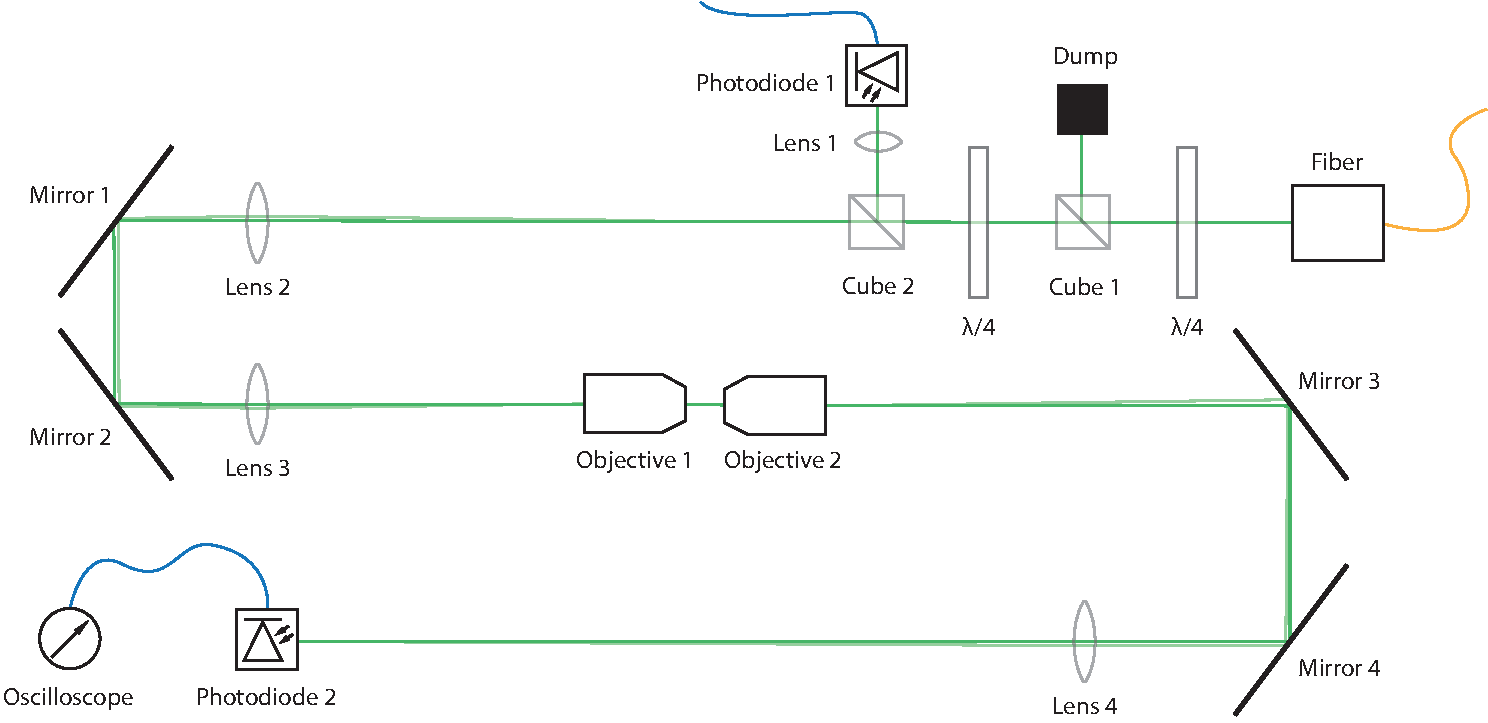
\includegraphics[width=\textwidth]{../media/setup/intensity-control.pdf}
  \caption{Optical setup and intensity detection. The beam hits Photodiode 2
    which is connected to the oscilloscope.
  }\label{fig:intensity_control_setup}
\end{figure}
In order to to estimate the error contribution due to imperfect intensity
regulation, we will conduct a short- and a long-term measurement of the
stabilized intensity. Technically a typical photodiode measurement takes about
a fraction of a millisecond, yet we can decide on different intervals between
the measurements in order to separate short-term from long-term trends like
the ones noted in the uncontrolled meausrement.
\Cref{tab:intensity_control_times} summarizes the different time scales for
the conducted short- and long-term measurement of the intensity control.
\begin{table}[htb]
  \centering
  \begin{tabular}{cccc}
    \toprule
    & Short & Long & \gls{aod} \\
    \midrule
    Interval &
    \SI{10}{\second} &
    \SI{120}{\second} &
    \SI{3}{\second} \\
    Duration &
    \SI{1}{\hour} &
    \SI{16}{\hour} &
    \SI{<2}{\hour} \\
    \bottomrule
  \end{tabular}
  \caption{Interval and duration times of the short- and long-term measurement
    as well as a typical \gls{aod} frequency sweep measurement.
  }\label{tab:intensity_control_times}
\end{table}
The voltage time series for both intensity control measurements are presented
in \Cref{fig:intensity_control}. The outlier at about 22:45 h was caused by
accidently interfering with the setup during measurement. Beside of that
incident the long-term intensity seems stable. On a smaller timescale we see
that the intensity evolution performs periodic oscillations.
\begin{table}[htb]
  \centering
  \begin{tabular}{lcccc}
    \toprule
    Measure & Not-Stabilized & Long & Short & \gls{aod} \\
    \midrule
    Mean $\mu$ &
    \SI{8.45}{\volt} &
    \SI{6.79}{\volt} &
    \SI{6.79}{\volt} &
    \SI{1.95}{\volt} \\
    Minimum &
    \SI{7.43}{\volt} &
    \SI{4.88}{\volt} &
    \SI{6.77}{\volt} &
    \SI{0.00}{\volt} \\
    Maximum &
    \SI{6.82}{\volt} &
    \SI{6.86}{\volt} &
    \SI{6.82}{\volt} &
    \SI{9.08}{\volt} \\
    Standard Deviation $\sigma$ &
    \SI{0.49}{\volt} &
    \SI{0.09}{\volt} &
    \SI{0.01}{\volt} &
    \SI{0.54}{\volt} \\
    Relative Standard Deviation $\sigma/\mu$ &
    \SI{5.75}{\percent} &
    \SI{1.35}{\percent} &
    \SI{0.19}{\percent} &
    \SI{27.69}{\percent} \\
    \bottomrule
  \end{tabular}
  \caption{Descriptive statistics of not-stabilized and actively stabilized
    short- and long-term intensity evolutions as well as a typical \gls{aod}
    frequency sweep measurement for comparison.
  }\label{tab:intensity_control_statistics}
\end{table}
Overall we can confirm that the intensity control loop successfully holds the
intensity mean, though with small oscillations. In order to estimate the
relevance of these small oscillations of the controlled intensity for later
measurements, we performed a measurement of the intensity variations introduced
by the \gls{aod} subject to constant frequency increments for comparison.
\Cref{tab:intensity_control_statistics} presents the statistics of said
intensity measurements.
\begin{figure}[htb]
  \centering
  \begin{adjustbox}{width=\textwidth}
    %% Creator: Matplotlib, PGF backend
%%
%% To include the figure in your LaTeX document, write
%%   \input{<filename>.pgf}
%%
%% Make sure the required packages are loaded in your preamble
%%   \usepackage{pgf}
%%
%% Figures using additional raster images can only be included by \input if
%% they are in the same directory as the main LaTeX file. For loading figures
%% from other directories you can use the `import` package
%%   \usepackage{import}
%% and then include the figures with
%%   \import{<path to file>}{<filename>.pgf}
%%
%% Matplotlib used the following preamble
%%   \usepackage{amsmath}\usepackage{siunitx}\usepackage{lmodern}
%%   \usepackage{fontspec}
%%
\begingroup%
\makeatletter%
\begin{pgfpicture}%
\pgfpathrectangle{\pgfpointorigin}{\pgfqpoint{12.000000in}{6.000000in}}%
\pgfusepath{use as bounding box, clip}%
\begin{pgfscope}%
\pgfsetbuttcap%
\pgfsetmiterjoin%
\pgfsetlinewidth{0.000000pt}%
\definecolor{currentstroke}{rgb}{1.000000,1.000000,1.000000}%
\pgfsetstrokecolor{currentstroke}%
\pgfsetdash{}{0pt}%
\pgfpathmoveto{\pgfqpoint{0.000000in}{0.000000in}}%
\pgfpathlineto{\pgfqpoint{12.000000in}{0.000000in}}%
\pgfpathlineto{\pgfqpoint{12.000000in}{6.000000in}}%
\pgfpathlineto{\pgfqpoint{0.000000in}{6.000000in}}%
\pgfpathclose%
\pgfusepath{}%
\end{pgfscope}%
\begin{pgfscope}%
\pgfsetbuttcap%
\pgfsetmiterjoin%
\definecolor{currentfill}{rgb}{1.000000,1.000000,1.000000}%
\pgfsetfillcolor{currentfill}%
\pgfsetlinewidth{0.000000pt}%
\definecolor{currentstroke}{rgb}{0.000000,0.000000,0.000000}%
\pgfsetstrokecolor{currentstroke}%
\pgfsetstrokeopacity{0.000000}%
\pgfsetdash{}{0pt}%
\pgfpathmoveto{\pgfqpoint{1.500000in}{3.120000in}}%
\pgfpathlineto{\pgfqpoint{6.036585in}{3.120000in}}%
\pgfpathlineto{\pgfqpoint{6.036585in}{5.520000in}}%
\pgfpathlineto{\pgfqpoint{1.500000in}{5.520000in}}%
\pgfpathclose%
\pgfusepath{fill}%
\end{pgfscope}%
\begin{pgfscope}%
\pgfpathrectangle{\pgfqpoint{1.500000in}{3.120000in}}{\pgfqpoint{4.536585in}{2.400000in}}%
\pgfusepath{clip}%
\pgfsetbuttcap%
\pgfsetroundjoin%
\definecolor{currentfill}{rgb}{0.121569,0.466667,0.705882}%
\pgfsetfillcolor{currentfill}%
\pgfsetlinewidth{1.003750pt}%
\definecolor{currentstroke}{rgb}{0.121569,0.466667,0.705882}%
\pgfsetstrokecolor{currentstroke}%
\pgfsetdash{}{0pt}%
\pgfpathmoveto{\pgfqpoint{1.707880in}{5.319339in}}%
\pgfpathcurveto{\pgfqpoint{1.715247in}{5.319339in}}{\pgfqpoint{1.722313in}{5.322266in}}{\pgfqpoint{1.727522in}{5.327475in}}%
\pgfpathcurveto{\pgfqpoint{1.732731in}{5.332684in}}{\pgfqpoint{1.735658in}{5.339750in}}{\pgfqpoint{1.735658in}{5.347117in}}%
\pgfpathcurveto{\pgfqpoint{1.735658in}{5.354484in}}{\pgfqpoint{1.732731in}{5.361550in}}{\pgfqpoint{1.727522in}{5.366759in}}%
\pgfpathcurveto{\pgfqpoint{1.722313in}{5.371968in}}{\pgfqpoint{1.715247in}{5.374895in}}{\pgfqpoint{1.707880in}{5.374895in}}%
\pgfpathcurveto{\pgfqpoint{1.700513in}{5.374895in}}{\pgfqpoint{1.693447in}{5.371968in}}{\pgfqpoint{1.688238in}{5.366759in}}%
\pgfpathcurveto{\pgfqpoint{1.683029in}{5.361550in}}{\pgfqpoint{1.680102in}{5.354484in}}{\pgfqpoint{1.680102in}{5.347117in}}%
\pgfpathcurveto{\pgfqpoint{1.680102in}{5.339750in}}{\pgfqpoint{1.683029in}{5.332684in}}{\pgfqpoint{1.688238in}{5.327475in}}%
\pgfpathcurveto{\pgfqpoint{1.693447in}{5.322266in}}{\pgfqpoint{1.700513in}{5.319339in}}{\pgfqpoint{1.707880in}{5.319339in}}%
\pgfpathclose%
\pgfusepath{stroke,fill}%
\end{pgfscope}%
\begin{pgfscope}%
\pgfpathrectangle{\pgfqpoint{1.500000in}{3.120000in}}{\pgfqpoint{4.536585in}{2.400000in}}%
\pgfusepath{clip}%
\pgfsetbuttcap%
\pgfsetroundjoin%
\definecolor{currentfill}{rgb}{0.121569,0.466667,0.705882}%
\pgfsetfillcolor{currentfill}%
\pgfsetlinewidth{1.003750pt}%
\definecolor{currentstroke}{rgb}{0.121569,0.466667,0.705882}%
\pgfsetstrokecolor{currentstroke}%
\pgfsetdash{}{0pt}%
\pgfpathmoveto{\pgfqpoint{1.717066in}{5.295073in}}%
\pgfpathcurveto{\pgfqpoint{1.724433in}{5.295073in}}{\pgfqpoint{1.731499in}{5.297999in}}{\pgfqpoint{1.736708in}{5.303208in}}%
\pgfpathcurveto{\pgfqpoint{1.741917in}{5.308418in}}{\pgfqpoint{1.744844in}{5.315484in}}{\pgfqpoint{1.744844in}{5.322850in}}%
\pgfpathcurveto{\pgfqpoint{1.744844in}{5.330217in}}{\pgfqpoint{1.741917in}{5.337283in}}{\pgfqpoint{1.736708in}{5.342492in}}%
\pgfpathcurveto{\pgfqpoint{1.731499in}{5.347701in}}{\pgfqpoint{1.724433in}{5.350628in}}{\pgfqpoint{1.717066in}{5.350628in}}%
\pgfpathcurveto{\pgfqpoint{1.709699in}{5.350628in}}{\pgfqpoint{1.702633in}{5.347701in}}{\pgfqpoint{1.697424in}{5.342492in}}%
\pgfpathcurveto{\pgfqpoint{1.692215in}{5.337283in}}{\pgfqpoint{1.689288in}{5.330217in}}{\pgfqpoint{1.689288in}{5.322850in}}%
\pgfpathcurveto{\pgfqpoint{1.689288in}{5.315484in}}{\pgfqpoint{1.692215in}{5.308418in}}{\pgfqpoint{1.697424in}{5.303208in}}%
\pgfpathcurveto{\pgfqpoint{1.702633in}{5.297999in}}{\pgfqpoint{1.709699in}{5.295073in}}{\pgfqpoint{1.717066in}{5.295073in}}%
\pgfpathclose%
\pgfusepath{stroke,fill}%
\end{pgfscope}%
\begin{pgfscope}%
\pgfpathrectangle{\pgfqpoint{1.500000in}{3.120000in}}{\pgfqpoint{4.536585in}{2.400000in}}%
\pgfusepath{clip}%
\pgfsetbuttcap%
\pgfsetroundjoin%
\definecolor{currentfill}{rgb}{0.121569,0.466667,0.705882}%
\pgfsetfillcolor{currentfill}%
\pgfsetlinewidth{1.003750pt}%
\definecolor{currentstroke}{rgb}{0.121569,0.466667,0.705882}%
\pgfsetstrokecolor{currentstroke}%
\pgfsetdash{}{0pt}%
\pgfpathmoveto{\pgfqpoint{1.726252in}{5.298408in}}%
\pgfpathcurveto{\pgfqpoint{1.733619in}{5.298408in}}{\pgfqpoint{1.740685in}{5.301334in}}{\pgfqpoint{1.745894in}{5.306544in}}%
\pgfpathcurveto{\pgfqpoint{1.751103in}{5.311753in}}{\pgfqpoint{1.754030in}{5.318819in}}{\pgfqpoint{1.754030in}{5.326185in}}%
\pgfpathcurveto{\pgfqpoint{1.754030in}{5.333552in}}{\pgfqpoint{1.751103in}{5.340618in}}{\pgfqpoint{1.745894in}{5.345827in}}%
\pgfpathcurveto{\pgfqpoint{1.740685in}{5.351036in}}{\pgfqpoint{1.733619in}{5.353963in}}{\pgfqpoint{1.726252in}{5.353963in}}%
\pgfpathcurveto{\pgfqpoint{1.718886in}{5.353963in}}{\pgfqpoint{1.711819in}{5.351036in}}{\pgfqpoint{1.706610in}{5.345827in}}%
\pgfpathcurveto{\pgfqpoint{1.701401in}{5.340618in}}{\pgfqpoint{1.698474in}{5.333552in}}{\pgfqpoint{1.698474in}{5.326185in}}%
\pgfpathcurveto{\pgfqpoint{1.698474in}{5.318819in}}{\pgfqpoint{1.701401in}{5.311753in}}{\pgfqpoint{1.706610in}{5.306544in}}%
\pgfpathcurveto{\pgfqpoint{1.711819in}{5.301334in}}{\pgfqpoint{1.718886in}{5.298408in}}{\pgfqpoint{1.726252in}{5.298408in}}%
\pgfpathclose%
\pgfusepath{stroke,fill}%
\end{pgfscope}%
\begin{pgfscope}%
\pgfpathrectangle{\pgfqpoint{1.500000in}{3.120000in}}{\pgfqpoint{4.536585in}{2.400000in}}%
\pgfusepath{clip}%
\pgfsetbuttcap%
\pgfsetroundjoin%
\definecolor{currentfill}{rgb}{0.121569,0.466667,0.705882}%
\pgfsetfillcolor{currentfill}%
\pgfsetlinewidth{1.003750pt}%
\definecolor{currentstroke}{rgb}{0.121569,0.466667,0.705882}%
\pgfsetstrokecolor{currentstroke}%
\pgfsetdash{}{0pt}%
\pgfpathmoveto{\pgfqpoint{1.735438in}{5.295706in}}%
\pgfpathcurveto{\pgfqpoint{1.742805in}{5.295706in}}{\pgfqpoint{1.749871in}{5.298632in}}{\pgfqpoint{1.755080in}{5.303841in}}%
\pgfpathcurveto{\pgfqpoint{1.760289in}{5.309051in}}{\pgfqpoint{1.763216in}{5.316117in}}{\pgfqpoint{1.763216in}{5.323483in}}%
\pgfpathcurveto{\pgfqpoint{1.763216in}{5.330850in}}{\pgfqpoint{1.760289in}{5.337916in}}{\pgfqpoint{1.755080in}{5.343125in}}%
\pgfpathcurveto{\pgfqpoint{1.749871in}{5.348334in}}{\pgfqpoint{1.742805in}{5.351261in}}{\pgfqpoint{1.735438in}{5.351261in}}%
\pgfpathcurveto{\pgfqpoint{1.728072in}{5.351261in}}{\pgfqpoint{1.721006in}{5.348334in}}{\pgfqpoint{1.715797in}{5.343125in}}%
\pgfpathcurveto{\pgfqpoint{1.710587in}{5.337916in}}{\pgfqpoint{1.707661in}{5.330850in}}{\pgfqpoint{1.707661in}{5.323483in}}%
\pgfpathcurveto{\pgfqpoint{1.707661in}{5.316117in}}{\pgfqpoint{1.710587in}{5.309051in}}{\pgfqpoint{1.715797in}{5.303841in}}%
\pgfpathcurveto{\pgfqpoint{1.721006in}{5.298632in}}{\pgfqpoint{1.728072in}{5.295706in}}{\pgfqpoint{1.735438in}{5.295706in}}%
\pgfpathclose%
\pgfusepath{stroke,fill}%
\end{pgfscope}%
\begin{pgfscope}%
\pgfpathrectangle{\pgfqpoint{1.500000in}{3.120000in}}{\pgfqpoint{4.536585in}{2.400000in}}%
\pgfusepath{clip}%
\pgfsetbuttcap%
\pgfsetroundjoin%
\definecolor{currentfill}{rgb}{0.121569,0.466667,0.705882}%
\pgfsetfillcolor{currentfill}%
\pgfsetlinewidth{1.003750pt}%
\definecolor{currentstroke}{rgb}{0.121569,0.466667,0.705882}%
\pgfsetstrokecolor{currentstroke}%
\pgfsetdash{}{0pt}%
\pgfpathmoveto{\pgfqpoint{1.744625in}{5.292689in}}%
\pgfpathcurveto{\pgfqpoint{1.751991in}{5.292689in}}{\pgfqpoint{1.759057in}{5.295616in}}{\pgfqpoint{1.764266in}{5.300825in}}%
\pgfpathcurveto{\pgfqpoint{1.769475in}{5.306034in}}{\pgfqpoint{1.772402in}{5.313100in}}{\pgfqpoint{1.772402in}{5.320467in}}%
\pgfpathcurveto{\pgfqpoint{1.772402in}{5.327834in}}{\pgfqpoint{1.769475in}{5.334900in}}{\pgfqpoint{1.764266in}{5.340109in}}%
\pgfpathcurveto{\pgfqpoint{1.759057in}{5.345318in}}{\pgfqpoint{1.751991in}{5.348245in}}{\pgfqpoint{1.744625in}{5.348245in}}%
\pgfpathcurveto{\pgfqpoint{1.737258in}{5.348245in}}{\pgfqpoint{1.730192in}{5.345318in}}{\pgfqpoint{1.724983in}{5.340109in}}%
\pgfpathcurveto{\pgfqpoint{1.719774in}{5.334900in}}{\pgfqpoint{1.716847in}{5.327834in}}{\pgfqpoint{1.716847in}{5.320467in}}%
\pgfpathcurveto{\pgfqpoint{1.716847in}{5.313100in}}{\pgfqpoint{1.719774in}{5.306034in}}{\pgfqpoint{1.724983in}{5.300825in}}%
\pgfpathcurveto{\pgfqpoint{1.730192in}{5.295616in}}{\pgfqpoint{1.737258in}{5.292689in}}{\pgfqpoint{1.744625in}{5.292689in}}%
\pgfpathclose%
\pgfusepath{stroke,fill}%
\end{pgfscope}%
\begin{pgfscope}%
\pgfpathrectangle{\pgfqpoint{1.500000in}{3.120000in}}{\pgfqpoint{4.536585in}{2.400000in}}%
\pgfusepath{clip}%
\pgfsetbuttcap%
\pgfsetroundjoin%
\definecolor{currentfill}{rgb}{0.121569,0.466667,0.705882}%
\pgfsetfillcolor{currentfill}%
\pgfsetlinewidth{1.003750pt}%
\definecolor{currentstroke}{rgb}{0.121569,0.466667,0.705882}%
\pgfsetstrokecolor{currentstroke}%
\pgfsetdash{}{0pt}%
\pgfpathmoveto{\pgfqpoint{1.753811in}{5.304240in}}%
\pgfpathcurveto{\pgfqpoint{1.761177in}{5.304240in}}{\pgfqpoint{1.768243in}{5.307167in}}{\pgfqpoint{1.773452in}{5.312376in}}%
\pgfpathcurveto{\pgfqpoint{1.778662in}{5.317585in}}{\pgfqpoint{1.781588in}{5.324651in}}{\pgfqpoint{1.781588in}{5.332018in}}%
\pgfpathcurveto{\pgfqpoint{1.781588in}{5.339385in}}{\pgfqpoint{1.778662in}{5.346451in}}{\pgfqpoint{1.773452in}{5.351660in}}%
\pgfpathcurveto{\pgfqpoint{1.768243in}{5.356869in}}{\pgfqpoint{1.761177in}{5.359796in}}{\pgfqpoint{1.753811in}{5.359796in}}%
\pgfpathcurveto{\pgfqpoint{1.746444in}{5.359796in}}{\pgfqpoint{1.739378in}{5.356869in}}{\pgfqpoint{1.734169in}{5.351660in}}%
\pgfpathcurveto{\pgfqpoint{1.728960in}{5.346451in}}{\pgfqpoint{1.726033in}{5.339385in}}{\pgfqpoint{1.726033in}{5.332018in}}%
\pgfpathcurveto{\pgfqpoint{1.726033in}{5.324651in}}{\pgfqpoint{1.728960in}{5.317585in}}{\pgfqpoint{1.734169in}{5.312376in}}%
\pgfpathcurveto{\pgfqpoint{1.739378in}{5.307167in}}{\pgfqpoint{1.746444in}{5.304240in}}{\pgfqpoint{1.753811in}{5.304240in}}%
\pgfpathclose%
\pgfusepath{stroke,fill}%
\end{pgfscope}%
\begin{pgfscope}%
\pgfpathrectangle{\pgfqpoint{1.500000in}{3.120000in}}{\pgfqpoint{4.536585in}{2.400000in}}%
\pgfusepath{clip}%
\pgfsetbuttcap%
\pgfsetroundjoin%
\definecolor{currentfill}{rgb}{0.121569,0.466667,0.705882}%
\pgfsetfillcolor{currentfill}%
\pgfsetlinewidth{1.003750pt}%
\definecolor{currentstroke}{rgb}{0.121569,0.466667,0.705882}%
\pgfsetstrokecolor{currentstroke}%
\pgfsetdash{}{0pt}%
\pgfpathmoveto{\pgfqpoint{1.763067in}{5.328719in}}%
\pgfpathcurveto{\pgfqpoint{1.770434in}{5.328719in}}{\pgfqpoint{1.777500in}{5.331646in}}{\pgfqpoint{1.782709in}{5.336855in}}%
\pgfpathcurveto{\pgfqpoint{1.787918in}{5.342064in}}{\pgfqpoint{1.790845in}{5.349130in}}{\pgfqpoint{1.790845in}{5.356496in}}%
\pgfpathcurveto{\pgfqpoint{1.790845in}{5.363863in}}{\pgfqpoint{1.787918in}{5.370929in}}{\pgfqpoint{1.782709in}{5.376138in}}%
\pgfpathcurveto{\pgfqpoint{1.777500in}{5.381347in}}{\pgfqpoint{1.770434in}{5.384274in}}{\pgfqpoint{1.763067in}{5.384274in}}%
\pgfpathcurveto{\pgfqpoint{1.755701in}{5.384274in}}{\pgfqpoint{1.748635in}{5.381347in}}{\pgfqpoint{1.743426in}{5.376138in}}%
\pgfpathcurveto{\pgfqpoint{1.738216in}{5.370929in}}{\pgfqpoint{1.735290in}{5.363863in}}{\pgfqpoint{1.735290in}{5.356496in}}%
\pgfpathcurveto{\pgfqpoint{1.735290in}{5.349130in}}{\pgfqpoint{1.738216in}{5.342064in}}{\pgfqpoint{1.743426in}{5.336855in}}%
\pgfpathcurveto{\pgfqpoint{1.748635in}{5.331646in}}{\pgfqpoint{1.755701in}{5.328719in}}{\pgfqpoint{1.763067in}{5.328719in}}%
\pgfpathclose%
\pgfusepath{stroke,fill}%
\end{pgfscope}%
\begin{pgfscope}%
\pgfpathrectangle{\pgfqpoint{1.500000in}{3.120000in}}{\pgfqpoint{4.536585in}{2.400000in}}%
\pgfusepath{clip}%
\pgfsetbuttcap%
\pgfsetroundjoin%
\definecolor{currentfill}{rgb}{0.121569,0.466667,0.705882}%
\pgfsetfillcolor{currentfill}%
\pgfsetlinewidth{1.003750pt}%
\definecolor{currentstroke}{rgb}{0.121569,0.466667,0.705882}%
\pgfsetstrokecolor{currentstroke}%
\pgfsetdash{}{0pt}%
\pgfpathmoveto{\pgfqpoint{1.772254in}{5.331155in}}%
\pgfpathcurveto{\pgfqpoint{1.779620in}{5.331155in}}{\pgfqpoint{1.786686in}{5.334082in}}{\pgfqpoint{1.791895in}{5.339291in}}%
\pgfpathcurveto{\pgfqpoint{1.797104in}{5.344500in}}{\pgfqpoint{1.800031in}{5.351566in}}{\pgfqpoint{1.800031in}{5.358933in}}%
\pgfpathcurveto{\pgfqpoint{1.800031in}{5.366300in}}{\pgfqpoint{1.797104in}{5.373366in}}{\pgfqpoint{1.791895in}{5.378575in}}%
\pgfpathcurveto{\pgfqpoint{1.786686in}{5.383784in}}{\pgfqpoint{1.779620in}{5.386711in}}{\pgfqpoint{1.772254in}{5.386711in}}%
\pgfpathcurveto{\pgfqpoint{1.764887in}{5.386711in}}{\pgfqpoint{1.757821in}{5.383784in}}{\pgfqpoint{1.752612in}{5.378575in}}%
\pgfpathcurveto{\pgfqpoint{1.747403in}{5.373366in}}{\pgfqpoint{1.744476in}{5.366300in}}{\pgfqpoint{1.744476in}{5.358933in}}%
\pgfpathcurveto{\pgfqpoint{1.744476in}{5.351566in}}{\pgfqpoint{1.747403in}{5.344500in}}{\pgfqpoint{1.752612in}{5.339291in}}%
\pgfpathcurveto{\pgfqpoint{1.757821in}{5.334082in}}{\pgfqpoint{1.764887in}{5.331155in}}{\pgfqpoint{1.772254in}{5.331155in}}%
\pgfpathclose%
\pgfusepath{stroke,fill}%
\end{pgfscope}%
\begin{pgfscope}%
\pgfpathrectangle{\pgfqpoint{1.500000in}{3.120000in}}{\pgfqpoint{4.536585in}{2.400000in}}%
\pgfusepath{clip}%
\pgfsetbuttcap%
\pgfsetroundjoin%
\definecolor{currentfill}{rgb}{0.121569,0.466667,0.705882}%
\pgfsetfillcolor{currentfill}%
\pgfsetlinewidth{1.003750pt}%
\definecolor{currentstroke}{rgb}{0.121569,0.466667,0.705882}%
\pgfsetstrokecolor{currentstroke}%
\pgfsetdash{}{0pt}%
\pgfpathmoveto{\pgfqpoint{1.781440in}{5.354130in}}%
\pgfpathcurveto{\pgfqpoint{1.788806in}{5.354130in}}{\pgfqpoint{1.795872in}{5.357057in}}{\pgfqpoint{1.801082in}{5.362266in}}%
\pgfpathcurveto{\pgfqpoint{1.806291in}{5.367475in}}{\pgfqpoint{1.809217in}{5.374541in}}{\pgfqpoint{1.809217in}{5.381908in}}%
\pgfpathcurveto{\pgfqpoint{1.809217in}{5.389274in}}{\pgfqpoint{1.806291in}{5.396340in}}{\pgfqpoint{1.801082in}{5.401550in}}%
\pgfpathcurveto{\pgfqpoint{1.795872in}{5.406759in}}{\pgfqpoint{1.788806in}{5.409685in}}{\pgfqpoint{1.781440in}{5.409685in}}%
\pgfpathcurveto{\pgfqpoint{1.774073in}{5.409685in}}{\pgfqpoint{1.767007in}{5.406759in}}{\pgfqpoint{1.761798in}{5.401550in}}%
\pgfpathcurveto{\pgfqpoint{1.756589in}{5.396340in}}{\pgfqpoint{1.753662in}{5.389274in}}{\pgfqpoint{1.753662in}{5.381908in}}%
\pgfpathcurveto{\pgfqpoint{1.753662in}{5.374541in}}{\pgfqpoint{1.756589in}{5.367475in}}{\pgfqpoint{1.761798in}{5.362266in}}%
\pgfpathcurveto{\pgfqpoint{1.767007in}{5.357057in}}{\pgfqpoint{1.774073in}{5.354130in}}{\pgfqpoint{1.781440in}{5.354130in}}%
\pgfpathclose%
\pgfusepath{stroke,fill}%
\end{pgfscope}%
\begin{pgfscope}%
\pgfpathrectangle{\pgfqpoint{1.500000in}{3.120000in}}{\pgfqpoint{4.536585in}{2.400000in}}%
\pgfusepath{clip}%
\pgfsetbuttcap%
\pgfsetroundjoin%
\definecolor{currentfill}{rgb}{0.121569,0.466667,0.705882}%
\pgfsetfillcolor{currentfill}%
\pgfsetlinewidth{1.003750pt}%
\definecolor{currentstroke}{rgb}{0.121569,0.466667,0.705882}%
\pgfsetstrokecolor{currentstroke}%
\pgfsetdash{}{0pt}%
\pgfpathmoveto{\pgfqpoint{1.790626in}{5.356229in}}%
\pgfpathcurveto{\pgfqpoint{1.797993in}{5.356229in}}{\pgfqpoint{1.805059in}{5.359156in}}{\pgfqpoint{1.810268in}{5.364365in}}%
\pgfpathcurveto{\pgfqpoint{1.815477in}{5.369574in}}{\pgfqpoint{1.818404in}{5.376640in}}{\pgfqpoint{1.818404in}{5.384007in}}%
\pgfpathcurveto{\pgfqpoint{1.818404in}{5.391374in}}{\pgfqpoint{1.815477in}{5.398440in}}{\pgfqpoint{1.810268in}{5.403649in}}%
\pgfpathcurveto{\pgfqpoint{1.805059in}{5.408858in}}{\pgfqpoint{1.797993in}{5.411785in}}{\pgfqpoint{1.790626in}{5.411785in}}%
\pgfpathcurveto{\pgfqpoint{1.783259in}{5.411785in}}{\pgfqpoint{1.776193in}{5.408858in}}{\pgfqpoint{1.770984in}{5.403649in}}%
\pgfpathcurveto{\pgfqpoint{1.765775in}{5.398440in}}{\pgfqpoint{1.762848in}{5.391374in}}{\pgfqpoint{1.762848in}{5.384007in}}%
\pgfpathcurveto{\pgfqpoint{1.762848in}{5.376640in}}{\pgfqpoint{1.765775in}{5.369574in}}{\pgfqpoint{1.770984in}{5.364365in}}%
\pgfpathcurveto{\pgfqpoint{1.776193in}{5.359156in}}{\pgfqpoint{1.783259in}{5.356229in}}{\pgfqpoint{1.790626in}{5.356229in}}%
\pgfpathclose%
\pgfusepath{stroke,fill}%
\end{pgfscope}%
\begin{pgfscope}%
\pgfpathrectangle{\pgfqpoint{1.500000in}{3.120000in}}{\pgfqpoint{4.536585in}{2.400000in}}%
\pgfusepath{clip}%
\pgfsetbuttcap%
\pgfsetroundjoin%
\definecolor{currentfill}{rgb}{0.121569,0.466667,0.705882}%
\pgfsetfillcolor{currentfill}%
\pgfsetlinewidth{1.003750pt}%
\definecolor{currentstroke}{rgb}{0.121569,0.466667,0.705882}%
\pgfsetstrokecolor{currentstroke}%
\pgfsetdash{}{0pt}%
\pgfpathmoveto{\pgfqpoint{1.799812in}{5.340290in}}%
\pgfpathcurveto{\pgfqpoint{1.807179in}{5.340290in}}{\pgfqpoint{1.814245in}{5.343216in}}{\pgfqpoint{1.819454in}{5.348426in}}%
\pgfpathcurveto{\pgfqpoint{1.824663in}{5.353635in}}{\pgfqpoint{1.827590in}{5.360701in}}{\pgfqpoint{1.827590in}{5.368067in}}%
\pgfpathcurveto{\pgfqpoint{1.827590in}{5.375434in}}{\pgfqpoint{1.824663in}{5.382500in}}{\pgfqpoint{1.819454in}{5.387709in}}%
\pgfpathcurveto{\pgfqpoint{1.814245in}{5.392918in}}{\pgfqpoint{1.807179in}{5.395845in}}{\pgfqpoint{1.799812in}{5.395845in}}%
\pgfpathcurveto{\pgfqpoint{1.792445in}{5.395845in}}{\pgfqpoint{1.785379in}{5.392918in}}{\pgfqpoint{1.780170in}{5.387709in}}%
\pgfpathcurveto{\pgfqpoint{1.774961in}{5.382500in}}{\pgfqpoint{1.772034in}{5.375434in}}{\pgfqpoint{1.772034in}{5.368067in}}%
\pgfpathcurveto{\pgfqpoint{1.772034in}{5.360701in}}{\pgfqpoint{1.774961in}{5.353635in}}{\pgfqpoint{1.780170in}{5.348426in}}%
\pgfpathcurveto{\pgfqpoint{1.785379in}{5.343216in}}{\pgfqpoint{1.792445in}{5.340290in}}{\pgfqpoint{1.799812in}{5.340290in}}%
\pgfpathclose%
\pgfusepath{stroke,fill}%
\end{pgfscope}%
\begin{pgfscope}%
\pgfpathrectangle{\pgfqpoint{1.500000in}{3.120000in}}{\pgfqpoint{4.536585in}{2.400000in}}%
\pgfusepath{clip}%
\pgfsetbuttcap%
\pgfsetroundjoin%
\definecolor{currentfill}{rgb}{0.121569,0.466667,0.705882}%
\pgfsetfillcolor{currentfill}%
\pgfsetlinewidth{1.003750pt}%
\definecolor{currentstroke}{rgb}{0.121569,0.466667,0.705882}%
\pgfsetstrokecolor{currentstroke}%
\pgfsetdash{}{0pt}%
\pgfpathmoveto{\pgfqpoint{1.808998in}{5.316957in}}%
\pgfpathcurveto{\pgfqpoint{1.816365in}{5.316957in}}{\pgfqpoint{1.823431in}{5.319884in}}{\pgfqpoint{1.828640in}{5.325093in}}%
\pgfpathcurveto{\pgfqpoint{1.833849in}{5.330302in}}{\pgfqpoint{1.836776in}{5.337368in}}{\pgfqpoint{1.836776in}{5.344735in}}%
\pgfpathcurveto{\pgfqpoint{1.836776in}{5.352101in}}{\pgfqpoint{1.833849in}{5.359167in}}{\pgfqpoint{1.828640in}{5.364376in}}%
\pgfpathcurveto{\pgfqpoint{1.823431in}{5.369586in}}{\pgfqpoint{1.816365in}{5.372512in}}{\pgfqpoint{1.808998in}{5.372512in}}%
\pgfpathcurveto{\pgfqpoint{1.801631in}{5.372512in}}{\pgfqpoint{1.794565in}{5.369586in}}{\pgfqpoint{1.789356in}{5.364376in}}%
\pgfpathcurveto{\pgfqpoint{1.784147in}{5.359167in}}{\pgfqpoint{1.781220in}{5.352101in}}{\pgfqpoint{1.781220in}{5.344735in}}%
\pgfpathcurveto{\pgfqpoint{1.781220in}{5.337368in}}{\pgfqpoint{1.784147in}{5.330302in}}{\pgfqpoint{1.789356in}{5.325093in}}%
\pgfpathcurveto{\pgfqpoint{1.794565in}{5.319884in}}{\pgfqpoint{1.801631in}{5.316957in}}{\pgfqpoint{1.808998in}{5.316957in}}%
\pgfpathclose%
\pgfusepath{stroke,fill}%
\end{pgfscope}%
\begin{pgfscope}%
\pgfpathrectangle{\pgfqpoint{1.500000in}{3.120000in}}{\pgfqpoint{4.536585in}{2.400000in}}%
\pgfusepath{clip}%
\pgfsetbuttcap%
\pgfsetroundjoin%
\definecolor{currentfill}{rgb}{0.121569,0.466667,0.705882}%
\pgfsetfillcolor{currentfill}%
\pgfsetlinewidth{1.003750pt}%
\definecolor{currentstroke}{rgb}{0.121569,0.466667,0.705882}%
\pgfsetstrokecolor{currentstroke}%
\pgfsetdash{}{0pt}%
\pgfpathmoveto{\pgfqpoint{1.818255in}{5.304994in}}%
\pgfpathcurveto{\pgfqpoint{1.825622in}{5.304994in}}{\pgfqpoint{1.832688in}{5.307920in}}{\pgfqpoint{1.837897in}{5.313130in}}%
\pgfpathcurveto{\pgfqpoint{1.843106in}{5.318339in}}{\pgfqpoint{1.846033in}{5.325405in}}{\pgfqpoint{1.846033in}{5.332771in}}%
\pgfpathcurveto{\pgfqpoint{1.846033in}{5.340138in}}{\pgfqpoint{1.843106in}{5.347204in}}{\pgfqpoint{1.837897in}{5.352413in}}%
\pgfpathcurveto{\pgfqpoint{1.832688in}{5.357622in}}{\pgfqpoint{1.825622in}{5.360549in}}{\pgfqpoint{1.818255in}{5.360549in}}%
\pgfpathcurveto{\pgfqpoint{1.810888in}{5.360549in}}{\pgfqpoint{1.803822in}{5.357622in}}{\pgfqpoint{1.798613in}{5.352413in}}%
\pgfpathcurveto{\pgfqpoint{1.793404in}{5.347204in}}{\pgfqpoint{1.790477in}{5.340138in}}{\pgfqpoint{1.790477in}{5.332771in}}%
\pgfpathcurveto{\pgfqpoint{1.790477in}{5.325405in}}{\pgfqpoint{1.793404in}{5.318339in}}{\pgfqpoint{1.798613in}{5.313130in}}%
\pgfpathcurveto{\pgfqpoint{1.803822in}{5.307920in}}{\pgfqpoint{1.810888in}{5.304994in}}{\pgfqpoint{1.818255in}{5.304994in}}%
\pgfpathclose%
\pgfusepath{stroke,fill}%
\end{pgfscope}%
\begin{pgfscope}%
\pgfpathrectangle{\pgfqpoint{1.500000in}{3.120000in}}{\pgfqpoint{4.536585in}{2.400000in}}%
\pgfusepath{clip}%
\pgfsetbuttcap%
\pgfsetroundjoin%
\definecolor{currentfill}{rgb}{0.121569,0.466667,0.705882}%
\pgfsetfillcolor{currentfill}%
\pgfsetlinewidth{1.003750pt}%
\definecolor{currentstroke}{rgb}{0.121569,0.466667,0.705882}%
\pgfsetstrokecolor{currentstroke}%
\pgfsetdash{}{0pt}%
\pgfpathmoveto{\pgfqpoint{1.827441in}{5.287940in}}%
\pgfpathcurveto{\pgfqpoint{1.834808in}{5.287940in}}{\pgfqpoint{1.841874in}{5.290867in}}{\pgfqpoint{1.847083in}{5.296076in}}%
\pgfpathcurveto{\pgfqpoint{1.852292in}{5.301285in}}{\pgfqpoint{1.855219in}{5.308351in}}{\pgfqpoint{1.855219in}{5.315717in}}%
\pgfpathcurveto{\pgfqpoint{1.855219in}{5.323084in}}{\pgfqpoint{1.852292in}{5.330150in}}{\pgfqpoint{1.847083in}{5.335359in}}%
\pgfpathcurveto{\pgfqpoint{1.841874in}{5.340568in}}{\pgfqpoint{1.834808in}{5.343495in}}{\pgfqpoint{1.827441in}{5.343495in}}%
\pgfpathcurveto{\pgfqpoint{1.820074in}{5.343495in}}{\pgfqpoint{1.813008in}{5.340568in}}{\pgfqpoint{1.807799in}{5.335359in}}%
\pgfpathcurveto{\pgfqpoint{1.802590in}{5.330150in}}{\pgfqpoint{1.799663in}{5.323084in}}{\pgfqpoint{1.799663in}{5.315717in}}%
\pgfpathcurveto{\pgfqpoint{1.799663in}{5.308351in}}{\pgfqpoint{1.802590in}{5.301285in}}{\pgfqpoint{1.807799in}{5.296076in}}%
\pgfpathcurveto{\pgfqpoint{1.813008in}{5.290867in}}{\pgfqpoint{1.820074in}{5.287940in}}{\pgfqpoint{1.827441in}{5.287940in}}%
\pgfpathclose%
\pgfusepath{stroke,fill}%
\end{pgfscope}%
\begin{pgfscope}%
\pgfpathrectangle{\pgfqpoint{1.500000in}{3.120000in}}{\pgfqpoint{4.536585in}{2.400000in}}%
\pgfusepath{clip}%
\pgfsetbuttcap%
\pgfsetroundjoin%
\definecolor{currentfill}{rgb}{0.121569,0.466667,0.705882}%
\pgfsetfillcolor{currentfill}%
\pgfsetlinewidth{1.003750pt}%
\definecolor{currentstroke}{rgb}{0.121569,0.466667,0.705882}%
\pgfsetstrokecolor{currentstroke}%
\pgfsetdash{}{0pt}%
\pgfpathmoveto{\pgfqpoint{1.836627in}{5.293351in}}%
\pgfpathcurveto{\pgfqpoint{1.843994in}{5.293351in}}{\pgfqpoint{1.851060in}{5.296278in}}{\pgfqpoint{1.856269in}{5.301487in}}%
\pgfpathcurveto{\pgfqpoint{1.861478in}{5.306696in}}{\pgfqpoint{1.864405in}{5.313762in}}{\pgfqpoint{1.864405in}{5.321129in}}%
\pgfpathcurveto{\pgfqpoint{1.864405in}{5.328496in}}{\pgfqpoint{1.861478in}{5.335562in}}{\pgfqpoint{1.856269in}{5.340771in}}%
\pgfpathcurveto{\pgfqpoint{1.851060in}{5.345980in}}{\pgfqpoint{1.843994in}{5.348907in}}{\pgfqpoint{1.836627in}{5.348907in}}%
\pgfpathcurveto{\pgfqpoint{1.829260in}{5.348907in}}{\pgfqpoint{1.822194in}{5.345980in}}{\pgfqpoint{1.816985in}{5.340771in}}%
\pgfpathcurveto{\pgfqpoint{1.811776in}{5.335562in}}{\pgfqpoint{1.808849in}{5.328496in}}{\pgfqpoint{1.808849in}{5.321129in}}%
\pgfpathcurveto{\pgfqpoint{1.808849in}{5.313762in}}{\pgfqpoint{1.811776in}{5.306696in}}{\pgfqpoint{1.816985in}{5.301487in}}%
\pgfpathcurveto{\pgfqpoint{1.822194in}{5.296278in}}{\pgfqpoint{1.829260in}{5.293351in}}{\pgfqpoint{1.836627in}{5.293351in}}%
\pgfpathclose%
\pgfusepath{stroke,fill}%
\end{pgfscope}%
\begin{pgfscope}%
\pgfpathrectangle{\pgfqpoint{1.500000in}{3.120000in}}{\pgfqpoint{4.536585in}{2.400000in}}%
\pgfusepath{clip}%
\pgfsetbuttcap%
\pgfsetroundjoin%
\definecolor{currentfill}{rgb}{0.121569,0.466667,0.705882}%
\pgfsetfillcolor{currentfill}%
\pgfsetlinewidth{1.003750pt}%
\definecolor{currentstroke}{rgb}{0.121569,0.466667,0.705882}%
\pgfsetstrokecolor{currentstroke}%
\pgfsetdash{}{0pt}%
\pgfpathmoveto{\pgfqpoint{1.845813in}{5.295983in}}%
\pgfpathcurveto{\pgfqpoint{1.853180in}{5.295983in}}{\pgfqpoint{1.860246in}{5.298909in}}{\pgfqpoint{1.865455in}{5.304119in}}%
\pgfpathcurveto{\pgfqpoint{1.870664in}{5.309328in}}{\pgfqpoint{1.873591in}{5.316394in}}{\pgfqpoint{1.873591in}{5.323760in}}%
\pgfpathcurveto{\pgfqpoint{1.873591in}{5.331127in}}{\pgfqpoint{1.870664in}{5.338193in}}{\pgfqpoint{1.865455in}{5.343402in}}%
\pgfpathcurveto{\pgfqpoint{1.860246in}{5.348611in}}{\pgfqpoint{1.853180in}{5.351538in}}{\pgfqpoint{1.845813in}{5.351538in}}%
\pgfpathcurveto{\pgfqpoint{1.838446in}{5.351538in}}{\pgfqpoint{1.831380in}{5.348611in}}{\pgfqpoint{1.826171in}{5.343402in}}%
\pgfpathcurveto{\pgfqpoint{1.820962in}{5.338193in}}{\pgfqpoint{1.818035in}{5.331127in}}{\pgfqpoint{1.818035in}{5.323760in}}%
\pgfpathcurveto{\pgfqpoint{1.818035in}{5.316394in}}{\pgfqpoint{1.820962in}{5.309328in}}{\pgfqpoint{1.826171in}{5.304119in}}%
\pgfpathcurveto{\pgfqpoint{1.831380in}{5.298909in}}{\pgfqpoint{1.838446in}{5.295983in}}{\pgfqpoint{1.845813in}{5.295983in}}%
\pgfpathclose%
\pgfusepath{stroke,fill}%
\end{pgfscope}%
\begin{pgfscope}%
\pgfpathrectangle{\pgfqpoint{1.500000in}{3.120000in}}{\pgfqpoint{4.536585in}{2.400000in}}%
\pgfusepath{clip}%
\pgfsetbuttcap%
\pgfsetroundjoin%
\definecolor{currentfill}{rgb}{0.121569,0.466667,0.705882}%
\pgfsetfillcolor{currentfill}%
\pgfsetlinewidth{1.003750pt}%
\definecolor{currentstroke}{rgb}{0.121569,0.466667,0.705882}%
\pgfsetstrokecolor{currentstroke}%
\pgfsetdash{}{0pt}%
\pgfpathmoveto{\pgfqpoint{1.854999in}{5.311186in}}%
\pgfpathcurveto{\pgfqpoint{1.862366in}{5.311186in}}{\pgfqpoint{1.869432in}{5.314113in}}{\pgfqpoint{1.874641in}{5.319322in}}%
\pgfpathcurveto{\pgfqpoint{1.879850in}{5.324531in}}{\pgfqpoint{1.882777in}{5.331597in}}{\pgfqpoint{1.882777in}{5.338964in}}%
\pgfpathcurveto{\pgfqpoint{1.882777in}{5.346331in}}{\pgfqpoint{1.879850in}{5.353397in}}{\pgfqpoint{1.874641in}{5.358606in}}%
\pgfpathcurveto{\pgfqpoint{1.869432in}{5.363815in}}{\pgfqpoint{1.862366in}{5.366742in}}{\pgfqpoint{1.854999in}{5.366742in}}%
\pgfpathcurveto{\pgfqpoint{1.847633in}{5.366742in}}{\pgfqpoint{1.840567in}{5.363815in}}{\pgfqpoint{1.835357in}{5.358606in}}%
\pgfpathcurveto{\pgfqpoint{1.830148in}{5.353397in}}{\pgfqpoint{1.827222in}{5.346331in}}{\pgfqpoint{1.827222in}{5.338964in}}%
\pgfpathcurveto{\pgfqpoint{1.827222in}{5.331597in}}{\pgfqpoint{1.830148in}{5.324531in}}{\pgfqpoint{1.835357in}{5.319322in}}%
\pgfpathcurveto{\pgfqpoint{1.840567in}{5.314113in}}{\pgfqpoint{1.847633in}{5.311186in}}{\pgfqpoint{1.854999in}{5.311186in}}%
\pgfpathclose%
\pgfusepath{stroke,fill}%
\end{pgfscope}%
\begin{pgfscope}%
\pgfpathrectangle{\pgfqpoint{1.500000in}{3.120000in}}{\pgfqpoint{4.536585in}{2.400000in}}%
\pgfusepath{clip}%
\pgfsetbuttcap%
\pgfsetroundjoin%
\definecolor{currentfill}{rgb}{0.121569,0.466667,0.705882}%
\pgfsetfillcolor{currentfill}%
\pgfsetlinewidth{1.003750pt}%
\definecolor{currentstroke}{rgb}{0.121569,0.466667,0.705882}%
\pgfsetstrokecolor{currentstroke}%
\pgfsetdash{}{0pt}%
\pgfpathmoveto{\pgfqpoint{1.864185in}{5.311177in}}%
\pgfpathcurveto{\pgfqpoint{1.871552in}{5.311177in}}{\pgfqpoint{1.878618in}{5.314104in}}{\pgfqpoint{1.883827in}{5.319313in}}%
\pgfpathcurveto{\pgfqpoint{1.889036in}{5.324522in}}{\pgfqpoint{1.891963in}{5.331588in}}{\pgfqpoint{1.891963in}{5.338955in}}%
\pgfpathcurveto{\pgfqpoint{1.891963in}{5.346322in}}{\pgfqpoint{1.889036in}{5.353388in}}{\pgfqpoint{1.883827in}{5.358597in}}%
\pgfpathcurveto{\pgfqpoint{1.878618in}{5.363806in}}{\pgfqpoint{1.871552in}{5.366733in}}{\pgfqpoint{1.864185in}{5.366733in}}%
\pgfpathcurveto{\pgfqpoint{1.856819in}{5.366733in}}{\pgfqpoint{1.849753in}{5.363806in}}{\pgfqpoint{1.844544in}{5.358597in}}%
\pgfpathcurveto{\pgfqpoint{1.839335in}{5.353388in}}{\pgfqpoint{1.836408in}{5.346322in}}{\pgfqpoint{1.836408in}{5.338955in}}%
\pgfpathcurveto{\pgfqpoint{1.836408in}{5.331588in}}{\pgfqpoint{1.839335in}{5.324522in}}{\pgfqpoint{1.844544in}{5.319313in}}%
\pgfpathcurveto{\pgfqpoint{1.849753in}{5.314104in}}{\pgfqpoint{1.856819in}{5.311177in}}{\pgfqpoint{1.864185in}{5.311177in}}%
\pgfpathclose%
\pgfusepath{stroke,fill}%
\end{pgfscope}%
\begin{pgfscope}%
\pgfpathrectangle{\pgfqpoint{1.500000in}{3.120000in}}{\pgfqpoint{4.536585in}{2.400000in}}%
\pgfusepath{clip}%
\pgfsetbuttcap%
\pgfsetroundjoin%
\definecolor{currentfill}{rgb}{0.121569,0.466667,0.705882}%
\pgfsetfillcolor{currentfill}%
\pgfsetlinewidth{1.003750pt}%
\definecolor{currentstroke}{rgb}{0.121569,0.466667,0.705882}%
\pgfsetstrokecolor{currentstroke}%
\pgfsetdash{}{0pt}%
\pgfpathmoveto{\pgfqpoint{1.873442in}{5.339563in}}%
\pgfpathcurveto{\pgfqpoint{1.880809in}{5.339563in}}{\pgfqpoint{1.887875in}{5.342490in}}{\pgfqpoint{1.893084in}{5.347699in}}%
\pgfpathcurveto{\pgfqpoint{1.898293in}{5.352908in}}{\pgfqpoint{1.901220in}{5.359974in}}{\pgfqpoint{1.901220in}{5.367341in}}%
\pgfpathcurveto{\pgfqpoint{1.901220in}{5.374708in}}{\pgfqpoint{1.898293in}{5.381774in}}{\pgfqpoint{1.893084in}{5.386983in}}%
\pgfpathcurveto{\pgfqpoint{1.887875in}{5.392192in}}{\pgfqpoint{1.880809in}{5.395119in}}{\pgfqpoint{1.873442in}{5.395119in}}%
\pgfpathcurveto{\pgfqpoint{1.866076in}{5.395119in}}{\pgfqpoint{1.859009in}{5.392192in}}{\pgfqpoint{1.853800in}{5.386983in}}%
\pgfpathcurveto{\pgfqpoint{1.848591in}{5.381774in}}{\pgfqpoint{1.845664in}{5.374708in}}{\pgfqpoint{1.845664in}{5.367341in}}%
\pgfpathcurveto{\pgfqpoint{1.845664in}{5.359974in}}{\pgfqpoint{1.848591in}{5.352908in}}{\pgfqpoint{1.853800in}{5.347699in}}%
\pgfpathcurveto{\pgfqpoint{1.859009in}{5.342490in}}{\pgfqpoint{1.866076in}{5.339563in}}{\pgfqpoint{1.873442in}{5.339563in}}%
\pgfpathclose%
\pgfusepath{stroke,fill}%
\end{pgfscope}%
\begin{pgfscope}%
\pgfpathrectangle{\pgfqpoint{1.500000in}{3.120000in}}{\pgfqpoint{4.536585in}{2.400000in}}%
\pgfusepath{clip}%
\pgfsetbuttcap%
\pgfsetroundjoin%
\definecolor{currentfill}{rgb}{0.121569,0.466667,0.705882}%
\pgfsetfillcolor{currentfill}%
\pgfsetlinewidth{1.003750pt}%
\definecolor{currentstroke}{rgb}{0.121569,0.466667,0.705882}%
\pgfsetstrokecolor{currentstroke}%
\pgfsetdash{}{0pt}%
\pgfpathmoveto{\pgfqpoint{1.882628in}{5.343296in}}%
\pgfpathcurveto{\pgfqpoint{1.889995in}{5.343296in}}{\pgfqpoint{1.897061in}{5.346223in}}{\pgfqpoint{1.902270in}{5.351432in}}%
\pgfpathcurveto{\pgfqpoint{1.907479in}{5.356641in}}{\pgfqpoint{1.910406in}{5.363707in}}{\pgfqpoint{1.910406in}{5.371073in}}%
\pgfpathcurveto{\pgfqpoint{1.910406in}{5.378440in}}{\pgfqpoint{1.907479in}{5.385506in}}{\pgfqpoint{1.902270in}{5.390715in}}%
\pgfpathcurveto{\pgfqpoint{1.897061in}{5.395924in}}{\pgfqpoint{1.889995in}{5.398851in}}{\pgfqpoint{1.882628in}{5.398851in}}%
\pgfpathcurveto{\pgfqpoint{1.875262in}{5.398851in}}{\pgfqpoint{1.868196in}{5.395924in}}{\pgfqpoint{1.862987in}{5.390715in}}%
\pgfpathcurveto{\pgfqpoint{1.857777in}{5.385506in}}{\pgfqpoint{1.854851in}{5.378440in}}{\pgfqpoint{1.854851in}{5.371073in}}%
\pgfpathcurveto{\pgfqpoint{1.854851in}{5.363707in}}{\pgfqpoint{1.857777in}{5.356641in}}{\pgfqpoint{1.862987in}{5.351432in}}%
\pgfpathcurveto{\pgfqpoint{1.868196in}{5.346223in}}{\pgfqpoint{1.875262in}{5.343296in}}{\pgfqpoint{1.882628in}{5.343296in}}%
\pgfpathclose%
\pgfusepath{stroke,fill}%
\end{pgfscope}%
\begin{pgfscope}%
\pgfpathrectangle{\pgfqpoint{1.500000in}{3.120000in}}{\pgfqpoint{4.536585in}{2.400000in}}%
\pgfusepath{clip}%
\pgfsetbuttcap%
\pgfsetroundjoin%
\definecolor{currentfill}{rgb}{0.121569,0.466667,0.705882}%
\pgfsetfillcolor{currentfill}%
\pgfsetlinewidth{1.003750pt}%
\definecolor{currentstroke}{rgb}{0.121569,0.466667,0.705882}%
\pgfsetstrokecolor{currentstroke}%
\pgfsetdash{}{0pt}%
\pgfpathmoveto{\pgfqpoint{1.891815in}{5.328776in}}%
\pgfpathcurveto{\pgfqpoint{1.899181in}{5.328776in}}{\pgfqpoint{1.906247in}{5.331703in}}{\pgfqpoint{1.911456in}{5.336912in}}%
\pgfpathcurveto{\pgfqpoint{1.916665in}{5.342121in}}{\pgfqpoint{1.919592in}{5.349187in}}{\pgfqpoint{1.919592in}{5.356554in}}%
\pgfpathcurveto{\pgfqpoint{1.919592in}{5.363920in}}{\pgfqpoint{1.916665in}{5.370986in}}{\pgfqpoint{1.911456in}{5.376195in}}%
\pgfpathcurveto{\pgfqpoint{1.906247in}{5.381404in}}{\pgfqpoint{1.899181in}{5.384331in}}{\pgfqpoint{1.891815in}{5.384331in}}%
\pgfpathcurveto{\pgfqpoint{1.884448in}{5.384331in}}{\pgfqpoint{1.877382in}{5.381404in}}{\pgfqpoint{1.872173in}{5.376195in}}%
\pgfpathcurveto{\pgfqpoint{1.866964in}{5.370986in}}{\pgfqpoint{1.864037in}{5.363920in}}{\pgfqpoint{1.864037in}{5.356554in}}%
\pgfpathcurveto{\pgfqpoint{1.864037in}{5.349187in}}{\pgfqpoint{1.866964in}{5.342121in}}{\pgfqpoint{1.872173in}{5.336912in}}%
\pgfpathcurveto{\pgfqpoint{1.877382in}{5.331703in}}{\pgfqpoint{1.884448in}{5.328776in}}{\pgfqpoint{1.891815in}{5.328776in}}%
\pgfpathclose%
\pgfusepath{stroke,fill}%
\end{pgfscope}%
\begin{pgfscope}%
\pgfpathrectangle{\pgfqpoint{1.500000in}{3.120000in}}{\pgfqpoint{4.536585in}{2.400000in}}%
\pgfusepath{clip}%
\pgfsetbuttcap%
\pgfsetroundjoin%
\definecolor{currentfill}{rgb}{0.121569,0.466667,0.705882}%
\pgfsetfillcolor{currentfill}%
\pgfsetlinewidth{1.003750pt}%
\definecolor{currentstroke}{rgb}{0.121569,0.466667,0.705882}%
\pgfsetstrokecolor{currentstroke}%
\pgfsetdash{}{0pt}%
\pgfpathmoveto{\pgfqpoint{1.901001in}{5.312017in}}%
\pgfpathcurveto{\pgfqpoint{1.908367in}{5.312017in}}{\pgfqpoint{1.915433in}{5.314943in}}{\pgfqpoint{1.920642in}{5.320152in}}%
\pgfpathcurveto{\pgfqpoint{1.925852in}{5.325362in}}{\pgfqpoint{1.928778in}{5.332428in}}{\pgfqpoint{1.928778in}{5.339794in}}%
\pgfpathcurveto{\pgfqpoint{1.928778in}{5.347161in}}{\pgfqpoint{1.925852in}{5.354227in}}{\pgfqpoint{1.920642in}{5.359436in}}%
\pgfpathcurveto{\pgfqpoint{1.915433in}{5.364645in}}{\pgfqpoint{1.908367in}{5.367572in}}{\pgfqpoint{1.901001in}{5.367572in}}%
\pgfpathcurveto{\pgfqpoint{1.893634in}{5.367572in}}{\pgfqpoint{1.886568in}{5.364645in}}{\pgfqpoint{1.881359in}{5.359436in}}%
\pgfpathcurveto{\pgfqpoint{1.876150in}{5.354227in}}{\pgfqpoint{1.873223in}{5.347161in}}{\pgfqpoint{1.873223in}{5.339794in}}%
\pgfpathcurveto{\pgfqpoint{1.873223in}{5.332428in}}{\pgfqpoint{1.876150in}{5.325362in}}{\pgfqpoint{1.881359in}{5.320152in}}%
\pgfpathcurveto{\pgfqpoint{1.886568in}{5.314943in}}{\pgfqpoint{1.893634in}{5.312017in}}{\pgfqpoint{1.901001in}{5.312017in}}%
\pgfpathclose%
\pgfusepath{stroke,fill}%
\end{pgfscope}%
\begin{pgfscope}%
\pgfpathrectangle{\pgfqpoint{1.500000in}{3.120000in}}{\pgfqpoint{4.536585in}{2.400000in}}%
\pgfusepath{clip}%
\pgfsetbuttcap%
\pgfsetroundjoin%
\definecolor{currentfill}{rgb}{0.121569,0.466667,0.705882}%
\pgfsetfillcolor{currentfill}%
\pgfsetlinewidth{1.003750pt}%
\definecolor{currentstroke}{rgb}{0.121569,0.466667,0.705882}%
\pgfsetstrokecolor{currentstroke}%
\pgfsetdash{}{0pt}%
\pgfpathmoveto{\pgfqpoint{1.910187in}{5.300987in}}%
\pgfpathcurveto{\pgfqpoint{1.917554in}{5.300987in}}{\pgfqpoint{1.924620in}{5.303914in}}{\pgfqpoint{1.929829in}{5.309123in}}%
\pgfpathcurveto{\pgfqpoint{1.935038in}{5.314332in}}{\pgfqpoint{1.937965in}{5.321398in}}{\pgfqpoint{1.937965in}{5.328765in}}%
\pgfpathcurveto{\pgfqpoint{1.937965in}{5.336132in}}{\pgfqpoint{1.935038in}{5.343198in}}{\pgfqpoint{1.929829in}{5.348407in}}%
\pgfpathcurveto{\pgfqpoint{1.924620in}{5.353616in}}{\pgfqpoint{1.917554in}{5.356543in}}{\pgfqpoint{1.910187in}{5.356543in}}%
\pgfpathcurveto{\pgfqpoint{1.902820in}{5.356543in}}{\pgfqpoint{1.895754in}{5.353616in}}{\pgfqpoint{1.890545in}{5.348407in}}%
\pgfpathcurveto{\pgfqpoint{1.885336in}{5.343198in}}{\pgfqpoint{1.882409in}{5.336132in}}{\pgfqpoint{1.882409in}{5.328765in}}%
\pgfpathcurveto{\pgfqpoint{1.882409in}{5.321398in}}{\pgfqpoint{1.885336in}{5.314332in}}{\pgfqpoint{1.890545in}{5.309123in}}%
\pgfpathcurveto{\pgfqpoint{1.895754in}{5.303914in}}{\pgfqpoint{1.902820in}{5.300987in}}{\pgfqpoint{1.910187in}{5.300987in}}%
\pgfpathclose%
\pgfusepath{stroke,fill}%
\end{pgfscope}%
\begin{pgfscope}%
\pgfpathrectangle{\pgfqpoint{1.500000in}{3.120000in}}{\pgfqpoint{4.536585in}{2.400000in}}%
\pgfusepath{clip}%
\pgfsetbuttcap%
\pgfsetroundjoin%
\definecolor{currentfill}{rgb}{0.121569,0.466667,0.705882}%
\pgfsetfillcolor{currentfill}%
\pgfsetlinewidth{1.003750pt}%
\definecolor{currentstroke}{rgb}{0.121569,0.466667,0.705882}%
\pgfsetstrokecolor{currentstroke}%
\pgfsetdash{}{0pt}%
\pgfpathmoveto{\pgfqpoint{1.919373in}{5.294055in}}%
\pgfpathcurveto{\pgfqpoint{1.926740in}{5.294055in}}{\pgfqpoint{1.933806in}{5.296981in}}{\pgfqpoint{1.939015in}{5.302191in}}%
\pgfpathcurveto{\pgfqpoint{1.944224in}{5.307400in}}{\pgfqpoint{1.947151in}{5.314466in}}{\pgfqpoint{1.947151in}{5.321832in}}%
\pgfpathcurveto{\pgfqpoint{1.947151in}{5.329199in}}{\pgfqpoint{1.944224in}{5.336265in}}{\pgfqpoint{1.939015in}{5.341474in}}%
\pgfpathcurveto{\pgfqpoint{1.933806in}{5.346683in}}{\pgfqpoint{1.926740in}{5.349610in}}{\pgfqpoint{1.919373in}{5.349610in}}%
\pgfpathcurveto{\pgfqpoint{1.912006in}{5.349610in}}{\pgfqpoint{1.904940in}{5.346683in}}{\pgfqpoint{1.899731in}{5.341474in}}%
\pgfpathcurveto{\pgfqpoint{1.894522in}{5.336265in}}{\pgfqpoint{1.891595in}{5.329199in}}{\pgfqpoint{1.891595in}{5.321832in}}%
\pgfpathcurveto{\pgfqpoint{1.891595in}{5.314466in}}{\pgfqpoint{1.894522in}{5.307400in}}{\pgfqpoint{1.899731in}{5.302191in}}%
\pgfpathcurveto{\pgfqpoint{1.904940in}{5.296981in}}{\pgfqpoint{1.912006in}{5.294055in}}{\pgfqpoint{1.919373in}{5.294055in}}%
\pgfpathclose%
\pgfusepath{stroke,fill}%
\end{pgfscope}%
\begin{pgfscope}%
\pgfpathrectangle{\pgfqpoint{1.500000in}{3.120000in}}{\pgfqpoint{4.536585in}{2.400000in}}%
\pgfusepath{clip}%
\pgfsetbuttcap%
\pgfsetroundjoin%
\definecolor{currentfill}{rgb}{0.121569,0.466667,0.705882}%
\pgfsetfillcolor{currentfill}%
\pgfsetlinewidth{1.003750pt}%
\definecolor{currentstroke}{rgb}{0.121569,0.466667,0.705882}%
\pgfsetstrokecolor{currentstroke}%
\pgfsetdash{}{0pt}%
\pgfpathmoveto{\pgfqpoint{1.928630in}{5.280294in}}%
\pgfpathcurveto{\pgfqpoint{1.935996in}{5.280294in}}{\pgfqpoint{1.943062in}{5.283221in}}{\pgfqpoint{1.948272in}{5.288430in}}%
\pgfpathcurveto{\pgfqpoint{1.953481in}{5.293639in}}{\pgfqpoint{1.956407in}{5.300705in}}{\pgfqpoint{1.956407in}{5.308072in}}%
\pgfpathcurveto{\pgfqpoint{1.956407in}{5.315439in}}{\pgfqpoint{1.953481in}{5.322505in}}{\pgfqpoint{1.948272in}{5.327714in}}%
\pgfpathcurveto{\pgfqpoint{1.943062in}{5.332923in}}{\pgfqpoint{1.935996in}{5.335850in}}{\pgfqpoint{1.928630in}{5.335850in}}%
\pgfpathcurveto{\pgfqpoint{1.921263in}{5.335850in}}{\pgfqpoint{1.914197in}{5.332923in}}{\pgfqpoint{1.908988in}{5.327714in}}%
\pgfpathcurveto{\pgfqpoint{1.903779in}{5.322505in}}{\pgfqpoint{1.900852in}{5.315439in}}{\pgfqpoint{1.900852in}{5.308072in}}%
\pgfpathcurveto{\pgfqpoint{1.900852in}{5.300705in}}{\pgfqpoint{1.903779in}{5.293639in}}{\pgfqpoint{1.908988in}{5.288430in}}%
\pgfpathcurveto{\pgfqpoint{1.914197in}{5.283221in}}{\pgfqpoint{1.921263in}{5.280294in}}{\pgfqpoint{1.928630in}{5.280294in}}%
\pgfpathclose%
\pgfusepath{stroke,fill}%
\end{pgfscope}%
\begin{pgfscope}%
\pgfpathrectangle{\pgfqpoint{1.500000in}{3.120000in}}{\pgfqpoint{4.536585in}{2.400000in}}%
\pgfusepath{clip}%
\pgfsetbuttcap%
\pgfsetroundjoin%
\definecolor{currentfill}{rgb}{0.121569,0.466667,0.705882}%
\pgfsetfillcolor{currentfill}%
\pgfsetlinewidth{1.003750pt}%
\definecolor{currentstroke}{rgb}{0.121569,0.466667,0.705882}%
\pgfsetstrokecolor{currentstroke}%
\pgfsetdash{}{0pt}%
\pgfpathmoveto{\pgfqpoint{1.937816in}{5.269926in}}%
\pgfpathcurveto{\pgfqpoint{1.945183in}{5.269926in}}{\pgfqpoint{1.952249in}{5.272853in}}{\pgfqpoint{1.957458in}{5.278062in}}%
\pgfpathcurveto{\pgfqpoint{1.962667in}{5.283271in}}{\pgfqpoint{1.965594in}{5.290337in}}{\pgfqpoint{1.965594in}{5.297704in}}%
\pgfpathcurveto{\pgfqpoint{1.965594in}{5.305070in}}{\pgfqpoint{1.962667in}{5.312136in}}{\pgfqpoint{1.957458in}{5.317346in}}%
\pgfpathcurveto{\pgfqpoint{1.952249in}{5.322555in}}{\pgfqpoint{1.945183in}{5.325481in}}{\pgfqpoint{1.937816in}{5.325481in}}%
\pgfpathcurveto{\pgfqpoint{1.930449in}{5.325481in}}{\pgfqpoint{1.923383in}{5.322555in}}{\pgfqpoint{1.918174in}{5.317346in}}%
\pgfpathcurveto{\pgfqpoint{1.912965in}{5.312136in}}{\pgfqpoint{1.910038in}{5.305070in}}{\pgfqpoint{1.910038in}{5.297704in}}%
\pgfpathcurveto{\pgfqpoint{1.910038in}{5.290337in}}{\pgfqpoint{1.912965in}{5.283271in}}{\pgfqpoint{1.918174in}{5.278062in}}%
\pgfpathcurveto{\pgfqpoint{1.923383in}{5.272853in}}{\pgfqpoint{1.930449in}{5.269926in}}{\pgfqpoint{1.937816in}{5.269926in}}%
\pgfpathclose%
\pgfusepath{stroke,fill}%
\end{pgfscope}%
\begin{pgfscope}%
\pgfpathrectangle{\pgfqpoint{1.500000in}{3.120000in}}{\pgfqpoint{4.536585in}{2.400000in}}%
\pgfusepath{clip}%
\pgfsetbuttcap%
\pgfsetroundjoin%
\definecolor{currentfill}{rgb}{0.121569,0.466667,0.705882}%
\pgfsetfillcolor{currentfill}%
\pgfsetlinewidth{1.003750pt}%
\definecolor{currentstroke}{rgb}{0.121569,0.466667,0.705882}%
\pgfsetstrokecolor{currentstroke}%
\pgfsetdash{}{0pt}%
\pgfpathmoveto{\pgfqpoint{1.947002in}{5.274870in}}%
\pgfpathcurveto{\pgfqpoint{1.954369in}{5.274870in}}{\pgfqpoint{1.961435in}{5.277797in}}{\pgfqpoint{1.966644in}{5.283006in}}%
\pgfpathcurveto{\pgfqpoint{1.971853in}{5.288215in}}{\pgfqpoint{1.974780in}{5.295281in}}{\pgfqpoint{1.974780in}{5.302648in}}%
\pgfpathcurveto{\pgfqpoint{1.974780in}{5.310015in}}{\pgfqpoint{1.971853in}{5.317081in}}{\pgfqpoint{1.966644in}{5.322290in}}%
\pgfpathcurveto{\pgfqpoint{1.961435in}{5.327499in}}{\pgfqpoint{1.954369in}{5.330426in}}{\pgfqpoint{1.947002in}{5.330426in}}%
\pgfpathcurveto{\pgfqpoint{1.939635in}{5.330426in}}{\pgfqpoint{1.932569in}{5.327499in}}{\pgfqpoint{1.927360in}{5.322290in}}%
\pgfpathcurveto{\pgfqpoint{1.922151in}{5.317081in}}{\pgfqpoint{1.919224in}{5.310015in}}{\pgfqpoint{1.919224in}{5.302648in}}%
\pgfpathcurveto{\pgfqpoint{1.919224in}{5.295281in}}{\pgfqpoint{1.922151in}{5.288215in}}{\pgfqpoint{1.927360in}{5.283006in}}%
\pgfpathcurveto{\pgfqpoint{1.932569in}{5.277797in}}{\pgfqpoint{1.939635in}{5.274870in}}{\pgfqpoint{1.947002in}{5.274870in}}%
\pgfpathclose%
\pgfusepath{stroke,fill}%
\end{pgfscope}%
\begin{pgfscope}%
\pgfpathrectangle{\pgfqpoint{1.500000in}{3.120000in}}{\pgfqpoint{4.536585in}{2.400000in}}%
\pgfusepath{clip}%
\pgfsetbuttcap%
\pgfsetroundjoin%
\definecolor{currentfill}{rgb}{0.121569,0.466667,0.705882}%
\pgfsetfillcolor{currentfill}%
\pgfsetlinewidth{1.003750pt}%
\definecolor{currentstroke}{rgb}{0.121569,0.466667,0.705882}%
\pgfsetstrokecolor{currentstroke}%
\pgfsetdash{}{0pt}%
\pgfpathmoveto{\pgfqpoint{1.956188in}{5.290597in}}%
\pgfpathcurveto{\pgfqpoint{1.963555in}{5.290597in}}{\pgfqpoint{1.970621in}{5.293524in}}{\pgfqpoint{1.975830in}{5.298733in}}%
\pgfpathcurveto{\pgfqpoint{1.981039in}{5.303942in}}{\pgfqpoint{1.983966in}{5.311008in}}{\pgfqpoint{1.983966in}{5.318375in}}%
\pgfpathcurveto{\pgfqpoint{1.983966in}{5.325742in}}{\pgfqpoint{1.981039in}{5.332808in}}{\pgfqpoint{1.975830in}{5.338017in}}%
\pgfpathcurveto{\pgfqpoint{1.970621in}{5.343226in}}{\pgfqpoint{1.963555in}{5.346153in}}{\pgfqpoint{1.956188in}{5.346153in}}%
\pgfpathcurveto{\pgfqpoint{1.948821in}{5.346153in}}{\pgfqpoint{1.941755in}{5.343226in}}{\pgfqpoint{1.936546in}{5.338017in}}%
\pgfpathcurveto{\pgfqpoint{1.931337in}{5.332808in}}{\pgfqpoint{1.928410in}{5.325742in}}{\pgfqpoint{1.928410in}{5.318375in}}%
\pgfpathcurveto{\pgfqpoint{1.928410in}{5.311008in}}{\pgfqpoint{1.931337in}{5.303942in}}{\pgfqpoint{1.936546in}{5.298733in}}%
\pgfpathcurveto{\pgfqpoint{1.941755in}{5.293524in}}{\pgfqpoint{1.948821in}{5.290597in}}{\pgfqpoint{1.956188in}{5.290597in}}%
\pgfpathclose%
\pgfusepath{stroke,fill}%
\end{pgfscope}%
\begin{pgfscope}%
\pgfpathrectangle{\pgfqpoint{1.500000in}{3.120000in}}{\pgfqpoint{4.536585in}{2.400000in}}%
\pgfusepath{clip}%
\pgfsetbuttcap%
\pgfsetroundjoin%
\definecolor{currentfill}{rgb}{0.121569,0.466667,0.705882}%
\pgfsetfillcolor{currentfill}%
\pgfsetlinewidth{1.003750pt}%
\definecolor{currentstroke}{rgb}{0.121569,0.466667,0.705882}%
\pgfsetstrokecolor{currentstroke}%
\pgfsetdash{}{0pt}%
\pgfpathmoveto{\pgfqpoint{1.965374in}{5.300861in}}%
\pgfpathcurveto{\pgfqpoint{1.972741in}{5.300861in}}{\pgfqpoint{1.979807in}{5.303787in}}{\pgfqpoint{1.985016in}{5.308997in}}%
\pgfpathcurveto{\pgfqpoint{1.990225in}{5.314206in}}{\pgfqpoint{1.993152in}{5.321272in}}{\pgfqpoint{1.993152in}{5.328638in}}%
\pgfpathcurveto{\pgfqpoint{1.993152in}{5.336005in}}{\pgfqpoint{1.990225in}{5.343071in}}{\pgfqpoint{1.985016in}{5.348280in}}%
\pgfpathcurveto{\pgfqpoint{1.979807in}{5.353489in}}{\pgfqpoint{1.972741in}{5.356416in}}{\pgfqpoint{1.965374in}{5.356416in}}%
\pgfpathcurveto{\pgfqpoint{1.958007in}{5.356416in}}{\pgfqpoint{1.950941in}{5.353489in}}{\pgfqpoint{1.945732in}{5.348280in}}%
\pgfpathcurveto{\pgfqpoint{1.940523in}{5.343071in}}{\pgfqpoint{1.937596in}{5.336005in}}{\pgfqpoint{1.937596in}{5.328638in}}%
\pgfpathcurveto{\pgfqpoint{1.937596in}{5.321272in}}{\pgfqpoint{1.940523in}{5.314206in}}{\pgfqpoint{1.945732in}{5.308997in}}%
\pgfpathcurveto{\pgfqpoint{1.950941in}{5.303787in}}{\pgfqpoint{1.958007in}{5.300861in}}{\pgfqpoint{1.965374in}{5.300861in}}%
\pgfpathclose%
\pgfusepath{stroke,fill}%
\end{pgfscope}%
\begin{pgfscope}%
\pgfpathrectangle{\pgfqpoint{1.500000in}{3.120000in}}{\pgfqpoint{4.536585in}{2.400000in}}%
\pgfusepath{clip}%
\pgfsetbuttcap%
\pgfsetroundjoin%
\definecolor{currentfill}{rgb}{0.121569,0.466667,0.705882}%
\pgfsetfillcolor{currentfill}%
\pgfsetlinewidth{1.003750pt}%
\definecolor{currentstroke}{rgb}{0.121569,0.466667,0.705882}%
\pgfsetstrokecolor{currentstroke}%
\pgfsetdash{}{0pt}%
\pgfpathmoveto{\pgfqpoint{1.974560in}{5.319056in}}%
\pgfpathcurveto{\pgfqpoint{1.981927in}{5.319056in}}{\pgfqpoint{1.988993in}{5.321983in}}{\pgfqpoint{1.994202in}{5.327192in}}%
\pgfpathcurveto{\pgfqpoint{1.999411in}{5.332401in}}{\pgfqpoint{2.002338in}{5.339467in}}{\pgfqpoint{2.002338in}{5.346834in}}%
\pgfpathcurveto{\pgfqpoint{2.002338in}{5.354201in}}{\pgfqpoint{1.999411in}{5.361267in}}{\pgfqpoint{1.994202in}{5.366476in}}%
\pgfpathcurveto{\pgfqpoint{1.988993in}{5.371685in}}{\pgfqpoint{1.981927in}{5.374612in}}{\pgfqpoint{1.974560in}{5.374612in}}%
\pgfpathcurveto{\pgfqpoint{1.967194in}{5.374612in}}{\pgfqpoint{1.960128in}{5.371685in}}{\pgfqpoint{1.954918in}{5.366476in}}%
\pgfpathcurveto{\pgfqpoint{1.949709in}{5.361267in}}{\pgfqpoint{1.946783in}{5.354201in}}{\pgfqpoint{1.946783in}{5.346834in}}%
\pgfpathcurveto{\pgfqpoint{1.946783in}{5.339467in}}{\pgfqpoint{1.949709in}{5.332401in}}{\pgfqpoint{1.954918in}{5.327192in}}%
\pgfpathcurveto{\pgfqpoint{1.960128in}{5.321983in}}{\pgfqpoint{1.967194in}{5.319056in}}{\pgfqpoint{1.974560in}{5.319056in}}%
\pgfpathclose%
\pgfusepath{stroke,fill}%
\end{pgfscope}%
\begin{pgfscope}%
\pgfpathrectangle{\pgfqpoint{1.500000in}{3.120000in}}{\pgfqpoint{4.536585in}{2.400000in}}%
\pgfusepath{clip}%
\pgfsetbuttcap%
\pgfsetroundjoin%
\definecolor{currentfill}{rgb}{0.121569,0.466667,0.705882}%
\pgfsetfillcolor{currentfill}%
\pgfsetlinewidth{1.003750pt}%
\definecolor{currentstroke}{rgb}{0.121569,0.466667,0.705882}%
\pgfsetstrokecolor{currentstroke}%
\pgfsetdash{}{0pt}%
\pgfpathmoveto{\pgfqpoint{1.983817in}{5.323528in}}%
\pgfpathcurveto{\pgfqpoint{1.991184in}{5.323528in}}{\pgfqpoint{1.998250in}{5.326455in}}{\pgfqpoint{2.003459in}{5.331664in}}%
\pgfpathcurveto{\pgfqpoint{2.008668in}{5.336873in}}{\pgfqpoint{2.011595in}{5.343939in}}{\pgfqpoint{2.011595in}{5.351306in}}%
\pgfpathcurveto{\pgfqpoint{2.011595in}{5.358673in}}{\pgfqpoint{2.008668in}{5.365739in}}{\pgfqpoint{2.003459in}{5.370948in}}%
\pgfpathcurveto{\pgfqpoint{1.998250in}{5.376157in}}{\pgfqpoint{1.991184in}{5.379084in}}{\pgfqpoint{1.983817in}{5.379084in}}%
\pgfpathcurveto{\pgfqpoint{1.976450in}{5.379084in}}{\pgfqpoint{1.969384in}{5.376157in}}{\pgfqpoint{1.964175in}{5.370948in}}%
\pgfpathcurveto{\pgfqpoint{1.958966in}{5.365739in}}{\pgfqpoint{1.956039in}{5.358673in}}{\pgfqpoint{1.956039in}{5.351306in}}%
\pgfpathcurveto{\pgfqpoint{1.956039in}{5.343939in}}{\pgfqpoint{1.958966in}{5.336873in}}{\pgfqpoint{1.964175in}{5.331664in}}%
\pgfpathcurveto{\pgfqpoint{1.969384in}{5.326455in}}{\pgfqpoint{1.976450in}{5.323528in}}{\pgfqpoint{1.983817in}{5.323528in}}%
\pgfpathclose%
\pgfusepath{stroke,fill}%
\end{pgfscope}%
\begin{pgfscope}%
\pgfpathrectangle{\pgfqpoint{1.500000in}{3.120000in}}{\pgfqpoint{4.536585in}{2.400000in}}%
\pgfusepath{clip}%
\pgfsetbuttcap%
\pgfsetroundjoin%
\definecolor{currentfill}{rgb}{0.121569,0.466667,0.705882}%
\pgfsetfillcolor{currentfill}%
\pgfsetlinewidth{1.003750pt}%
\definecolor{currentstroke}{rgb}{0.121569,0.466667,0.705882}%
\pgfsetstrokecolor{currentstroke}%
\pgfsetdash{}{0pt}%
\pgfpathmoveto{\pgfqpoint{1.993003in}{5.329384in}}%
\pgfpathcurveto{\pgfqpoint{2.000370in}{5.329384in}}{\pgfqpoint{2.007436in}{5.332311in}}{\pgfqpoint{2.012645in}{5.337520in}}%
\pgfpathcurveto{\pgfqpoint{2.017854in}{5.342729in}}{\pgfqpoint{2.020781in}{5.349795in}}{\pgfqpoint{2.020781in}{5.357162in}}%
\pgfpathcurveto{\pgfqpoint{2.020781in}{5.364528in}}{\pgfqpoint{2.017854in}{5.371594in}}{\pgfqpoint{2.012645in}{5.376803in}}%
\pgfpathcurveto{\pgfqpoint{2.007436in}{5.382013in}}{\pgfqpoint{2.000370in}{5.384939in}}{\pgfqpoint{1.993003in}{5.384939in}}%
\pgfpathcurveto{\pgfqpoint{1.985636in}{5.384939in}}{\pgfqpoint{1.978570in}{5.382013in}}{\pgfqpoint{1.973361in}{5.376803in}}%
\pgfpathcurveto{\pgfqpoint{1.968152in}{5.371594in}}{\pgfqpoint{1.965225in}{5.364528in}}{\pgfqpoint{1.965225in}{5.357162in}}%
\pgfpathcurveto{\pgfqpoint{1.965225in}{5.349795in}}{\pgfqpoint{1.968152in}{5.342729in}}{\pgfqpoint{1.973361in}{5.337520in}}%
\pgfpathcurveto{\pgfqpoint{1.978570in}{5.332311in}}{\pgfqpoint{1.985636in}{5.329384in}}{\pgfqpoint{1.993003in}{5.329384in}}%
\pgfpathclose%
\pgfusepath{stroke,fill}%
\end{pgfscope}%
\begin{pgfscope}%
\pgfpathrectangle{\pgfqpoint{1.500000in}{3.120000in}}{\pgfqpoint{4.536585in}{2.400000in}}%
\pgfusepath{clip}%
\pgfsetbuttcap%
\pgfsetroundjoin%
\definecolor{currentfill}{rgb}{0.121569,0.466667,0.705882}%
\pgfsetfillcolor{currentfill}%
\pgfsetlinewidth{1.003750pt}%
\definecolor{currentstroke}{rgb}{0.121569,0.466667,0.705882}%
\pgfsetstrokecolor{currentstroke}%
\pgfsetdash{}{0pt}%
\pgfpathmoveto{\pgfqpoint{2.002189in}{5.298557in}}%
\pgfpathcurveto{\pgfqpoint{2.009556in}{5.298557in}}{\pgfqpoint{2.016622in}{5.301484in}}{\pgfqpoint{2.021831in}{5.306693in}}%
\pgfpathcurveto{\pgfqpoint{2.027040in}{5.311902in}}{\pgfqpoint{2.029967in}{5.318968in}}{\pgfqpoint{2.029967in}{5.326335in}}%
\pgfpathcurveto{\pgfqpoint{2.029967in}{5.333702in}}{\pgfqpoint{2.027040in}{5.340768in}}{\pgfqpoint{2.021831in}{5.345977in}}%
\pgfpathcurveto{\pgfqpoint{2.016622in}{5.351186in}}{\pgfqpoint{2.009556in}{5.354113in}}{\pgfqpoint{2.002189in}{5.354113in}}%
\pgfpathcurveto{\pgfqpoint{1.994823in}{5.354113in}}{\pgfqpoint{1.987757in}{5.351186in}}{\pgfqpoint{1.982547in}{5.345977in}}%
\pgfpathcurveto{\pgfqpoint{1.977338in}{5.340768in}}{\pgfqpoint{1.974412in}{5.333702in}}{\pgfqpoint{1.974412in}{5.326335in}}%
\pgfpathcurveto{\pgfqpoint{1.974412in}{5.318968in}}{\pgfqpoint{1.977338in}{5.311902in}}{\pgfqpoint{1.982547in}{5.306693in}}%
\pgfpathcurveto{\pgfqpoint{1.987757in}{5.301484in}}{\pgfqpoint{1.994823in}{5.298557in}}{\pgfqpoint{2.002189in}{5.298557in}}%
\pgfpathclose%
\pgfusepath{stroke,fill}%
\end{pgfscope}%
\begin{pgfscope}%
\pgfpathrectangle{\pgfqpoint{1.500000in}{3.120000in}}{\pgfqpoint{4.536585in}{2.400000in}}%
\pgfusepath{clip}%
\pgfsetbuttcap%
\pgfsetroundjoin%
\definecolor{currentfill}{rgb}{0.121569,0.466667,0.705882}%
\pgfsetfillcolor{currentfill}%
\pgfsetlinewidth{1.003750pt}%
\definecolor{currentstroke}{rgb}{0.121569,0.466667,0.705882}%
\pgfsetstrokecolor{currentstroke}%
\pgfsetdash{}{0pt}%
\pgfpathmoveto{\pgfqpoint{2.011375in}{5.290982in}}%
\pgfpathcurveto{\pgfqpoint{2.018742in}{5.290982in}}{\pgfqpoint{2.025808in}{5.293909in}}{\pgfqpoint{2.031017in}{5.299118in}}%
\pgfpathcurveto{\pgfqpoint{2.036226in}{5.304327in}}{\pgfqpoint{2.039153in}{5.311393in}}{\pgfqpoint{2.039153in}{5.318760in}}%
\pgfpathcurveto{\pgfqpoint{2.039153in}{5.326127in}}{\pgfqpoint{2.036226in}{5.333193in}}{\pgfqpoint{2.031017in}{5.338402in}}%
\pgfpathcurveto{\pgfqpoint{2.025808in}{5.343611in}}{\pgfqpoint{2.018742in}{5.346538in}}{\pgfqpoint{2.011375in}{5.346538in}}%
\pgfpathcurveto{\pgfqpoint{2.004009in}{5.346538in}}{\pgfqpoint{1.996943in}{5.343611in}}{\pgfqpoint{1.991734in}{5.338402in}}%
\pgfpathcurveto{\pgfqpoint{1.986525in}{5.333193in}}{\pgfqpoint{1.983598in}{5.326127in}}{\pgfqpoint{1.983598in}{5.318760in}}%
\pgfpathcurveto{\pgfqpoint{1.983598in}{5.311393in}}{\pgfqpoint{1.986525in}{5.304327in}}{\pgfqpoint{1.991734in}{5.299118in}}%
\pgfpathcurveto{\pgfqpoint{1.996943in}{5.293909in}}{\pgfqpoint{2.004009in}{5.290982in}}{\pgfqpoint{2.011375in}{5.290982in}}%
\pgfpathclose%
\pgfusepath{stroke,fill}%
\end{pgfscope}%
\begin{pgfscope}%
\pgfpathrectangle{\pgfqpoint{1.500000in}{3.120000in}}{\pgfqpoint{4.536585in}{2.400000in}}%
\pgfusepath{clip}%
\pgfsetbuttcap%
\pgfsetroundjoin%
\definecolor{currentfill}{rgb}{0.121569,0.466667,0.705882}%
\pgfsetfillcolor{currentfill}%
\pgfsetlinewidth{1.003750pt}%
\definecolor{currentstroke}{rgb}{0.121569,0.466667,0.705882}%
\pgfsetstrokecolor{currentstroke}%
\pgfsetdash{}{0pt}%
\pgfpathmoveto{\pgfqpoint{2.020562in}{5.283408in}}%
\pgfpathcurveto{\pgfqpoint{2.027928in}{5.283408in}}{\pgfqpoint{2.034994in}{5.286335in}}{\pgfqpoint{2.040203in}{5.291544in}}%
\pgfpathcurveto{\pgfqpoint{2.045413in}{5.296753in}}{\pgfqpoint{2.048339in}{5.303819in}}{\pgfqpoint{2.048339in}{5.311186in}}%
\pgfpathcurveto{\pgfqpoint{2.048339in}{5.318553in}}{\pgfqpoint{2.045413in}{5.325619in}}{\pgfqpoint{2.040203in}{5.330828in}}%
\pgfpathcurveto{\pgfqpoint{2.034994in}{5.336037in}}{\pgfqpoint{2.027928in}{5.338964in}}{\pgfqpoint{2.020562in}{5.338964in}}%
\pgfpathcurveto{\pgfqpoint{2.013195in}{5.338964in}}{\pgfqpoint{2.006129in}{5.336037in}}{\pgfqpoint{2.000920in}{5.330828in}}%
\pgfpathcurveto{\pgfqpoint{1.995711in}{5.325619in}}{\pgfqpoint{1.992784in}{5.318553in}}{\pgfqpoint{1.992784in}{5.311186in}}%
\pgfpathcurveto{\pgfqpoint{1.992784in}{5.303819in}}{\pgfqpoint{1.995711in}{5.296753in}}{\pgfqpoint{2.000920in}{5.291544in}}%
\pgfpathcurveto{\pgfqpoint{2.006129in}{5.286335in}}{\pgfqpoint{2.013195in}{5.283408in}}{\pgfqpoint{2.020562in}{5.283408in}}%
\pgfpathclose%
\pgfusepath{stroke,fill}%
\end{pgfscope}%
\begin{pgfscope}%
\pgfpathrectangle{\pgfqpoint{1.500000in}{3.120000in}}{\pgfqpoint{4.536585in}{2.400000in}}%
\pgfusepath{clip}%
\pgfsetbuttcap%
\pgfsetroundjoin%
\definecolor{currentfill}{rgb}{0.121569,0.466667,0.705882}%
\pgfsetfillcolor{currentfill}%
\pgfsetlinewidth{1.003750pt}%
\definecolor{currentstroke}{rgb}{0.121569,0.466667,0.705882}%
\pgfsetstrokecolor{currentstroke}%
\pgfsetdash{}{0pt}%
\pgfpathmoveto{\pgfqpoint{2.029748in}{5.271731in}}%
\pgfpathcurveto{\pgfqpoint{2.037114in}{5.271731in}}{\pgfqpoint{2.044180in}{5.274658in}}{\pgfqpoint{2.049390in}{5.279867in}}%
\pgfpathcurveto{\pgfqpoint{2.054599in}{5.285076in}}{\pgfqpoint{2.057526in}{5.292142in}}{\pgfqpoint{2.057526in}{5.299509in}}%
\pgfpathcurveto{\pgfqpoint{2.057526in}{5.306876in}}{\pgfqpoint{2.054599in}{5.313942in}}{\pgfqpoint{2.049390in}{5.319151in}}%
\pgfpathcurveto{\pgfqpoint{2.044180in}{5.324360in}}{\pgfqpoint{2.037114in}{5.327287in}}{\pgfqpoint{2.029748in}{5.327287in}}%
\pgfpathcurveto{\pgfqpoint{2.022381in}{5.327287in}}{\pgfqpoint{2.015315in}{5.324360in}}{\pgfqpoint{2.010106in}{5.319151in}}%
\pgfpathcurveto{\pgfqpoint{2.004897in}{5.313942in}}{\pgfqpoint{2.001970in}{5.306876in}}{\pgfqpoint{2.001970in}{5.299509in}}%
\pgfpathcurveto{\pgfqpoint{2.001970in}{5.292142in}}{\pgfqpoint{2.004897in}{5.285076in}}{\pgfqpoint{2.010106in}{5.279867in}}%
\pgfpathcurveto{\pgfqpoint{2.015315in}{5.274658in}}{\pgfqpoint{2.022381in}{5.271731in}}{\pgfqpoint{2.029748in}{5.271731in}}%
\pgfpathclose%
\pgfusepath{stroke,fill}%
\end{pgfscope}%
\begin{pgfscope}%
\pgfpathrectangle{\pgfqpoint{1.500000in}{3.120000in}}{\pgfqpoint{4.536585in}{2.400000in}}%
\pgfusepath{clip}%
\pgfsetbuttcap%
\pgfsetroundjoin%
\definecolor{currentfill}{rgb}{0.121569,0.466667,0.705882}%
\pgfsetfillcolor{currentfill}%
\pgfsetlinewidth{1.003750pt}%
\definecolor{currentstroke}{rgb}{0.121569,0.466667,0.705882}%
\pgfsetstrokecolor{currentstroke}%
\pgfsetdash{}{0pt}%
\pgfpathmoveto{\pgfqpoint{2.039005in}{5.270991in}}%
\pgfpathcurveto{\pgfqpoint{2.046371in}{5.270991in}}{\pgfqpoint{2.053437in}{5.273917in}}{\pgfqpoint{2.058646in}{5.279126in}}%
\pgfpathcurveto{\pgfqpoint{2.063855in}{5.284336in}}{\pgfqpoint{2.066782in}{5.291402in}}{\pgfqpoint{2.066782in}{5.298768in}}%
\pgfpathcurveto{\pgfqpoint{2.066782in}{5.306135in}}{\pgfqpoint{2.063855in}{5.313201in}}{\pgfqpoint{2.058646in}{5.318410in}}%
\pgfpathcurveto{\pgfqpoint{2.053437in}{5.323619in}}{\pgfqpoint{2.046371in}{5.326546in}}{\pgfqpoint{2.039005in}{5.326546in}}%
\pgfpathcurveto{\pgfqpoint{2.031638in}{5.326546in}}{\pgfqpoint{2.024572in}{5.323619in}}{\pgfqpoint{2.019363in}{5.318410in}}%
\pgfpathcurveto{\pgfqpoint{2.014154in}{5.313201in}}{\pgfqpoint{2.011227in}{5.306135in}}{\pgfqpoint{2.011227in}{5.298768in}}%
\pgfpathcurveto{\pgfqpoint{2.011227in}{5.291402in}}{\pgfqpoint{2.014154in}{5.284336in}}{\pgfqpoint{2.019363in}{5.279126in}}%
\pgfpathcurveto{\pgfqpoint{2.024572in}{5.273917in}}{\pgfqpoint{2.031638in}{5.270991in}}{\pgfqpoint{2.039005in}{5.270991in}}%
\pgfpathclose%
\pgfusepath{stroke,fill}%
\end{pgfscope}%
\begin{pgfscope}%
\pgfpathrectangle{\pgfqpoint{1.500000in}{3.120000in}}{\pgfqpoint{4.536585in}{2.400000in}}%
\pgfusepath{clip}%
\pgfsetbuttcap%
\pgfsetroundjoin%
\definecolor{currentfill}{rgb}{0.121569,0.466667,0.705882}%
\pgfsetfillcolor{currentfill}%
\pgfsetlinewidth{1.003750pt}%
\definecolor{currentstroke}{rgb}{0.121569,0.466667,0.705882}%
\pgfsetstrokecolor{currentstroke}%
\pgfsetdash{}{0pt}%
\pgfpathmoveto{\pgfqpoint{2.048191in}{5.278838in}}%
\pgfpathcurveto{\pgfqpoint{2.055557in}{5.278838in}}{\pgfqpoint{2.062623in}{5.281765in}}{\pgfqpoint{2.067832in}{5.286974in}}%
\pgfpathcurveto{\pgfqpoint{2.073042in}{5.292183in}}{\pgfqpoint{2.075968in}{5.299249in}}{\pgfqpoint{2.075968in}{5.306616in}}%
\pgfpathcurveto{\pgfqpoint{2.075968in}{5.313983in}}{\pgfqpoint{2.073042in}{5.321049in}}{\pgfqpoint{2.067832in}{5.326258in}}%
\pgfpathcurveto{\pgfqpoint{2.062623in}{5.331467in}}{\pgfqpoint{2.055557in}{5.334394in}}{\pgfqpoint{2.048191in}{5.334394in}}%
\pgfpathcurveto{\pgfqpoint{2.040824in}{5.334394in}}{\pgfqpoint{2.033758in}{5.331467in}}{\pgfqpoint{2.028549in}{5.326258in}}%
\pgfpathcurveto{\pgfqpoint{2.023340in}{5.321049in}}{\pgfqpoint{2.020413in}{5.313983in}}{\pgfqpoint{2.020413in}{5.306616in}}%
\pgfpathcurveto{\pgfqpoint{2.020413in}{5.299249in}}{\pgfqpoint{2.023340in}{5.292183in}}{\pgfqpoint{2.028549in}{5.286974in}}%
\pgfpathcurveto{\pgfqpoint{2.033758in}{5.281765in}}{\pgfqpoint{2.040824in}{5.278838in}}{\pgfqpoint{2.048191in}{5.278838in}}%
\pgfpathclose%
\pgfusepath{stroke,fill}%
\end{pgfscope}%
\begin{pgfscope}%
\pgfpathrectangle{\pgfqpoint{1.500000in}{3.120000in}}{\pgfqpoint{4.536585in}{2.400000in}}%
\pgfusepath{clip}%
\pgfsetbuttcap%
\pgfsetroundjoin%
\definecolor{currentfill}{rgb}{0.121569,0.466667,0.705882}%
\pgfsetfillcolor{currentfill}%
\pgfsetlinewidth{1.003750pt}%
\definecolor{currentstroke}{rgb}{0.121569,0.466667,0.705882}%
\pgfsetstrokecolor{currentstroke}%
\pgfsetdash{}{0pt}%
\pgfpathmoveto{\pgfqpoint{2.057377in}{5.289839in}}%
\pgfpathcurveto{\pgfqpoint{2.064744in}{5.289839in}}{\pgfqpoint{2.071810in}{5.292765in}}{\pgfqpoint{2.077019in}{5.297975in}}%
\pgfpathcurveto{\pgfqpoint{2.082228in}{5.303184in}}{\pgfqpoint{2.085155in}{5.310250in}}{\pgfqpoint{2.085155in}{5.317616in}}%
\pgfpathcurveto{\pgfqpoint{2.085155in}{5.324983in}}{\pgfqpoint{2.082228in}{5.332049in}}{\pgfqpoint{2.077019in}{5.337258in}}%
\pgfpathcurveto{\pgfqpoint{2.071810in}{5.342467in}}{\pgfqpoint{2.064744in}{5.345394in}}{\pgfqpoint{2.057377in}{5.345394in}}%
\pgfpathcurveto{\pgfqpoint{2.050010in}{5.345394in}}{\pgfqpoint{2.042944in}{5.342467in}}{\pgfqpoint{2.037735in}{5.337258in}}%
\pgfpathcurveto{\pgfqpoint{2.032526in}{5.332049in}}{\pgfqpoint{2.029599in}{5.324983in}}{\pgfqpoint{2.029599in}{5.317616in}}%
\pgfpathcurveto{\pgfqpoint{2.029599in}{5.310250in}}{\pgfqpoint{2.032526in}{5.303184in}}{\pgfqpoint{2.037735in}{5.297975in}}%
\pgfpathcurveto{\pgfqpoint{2.042944in}{5.292765in}}{\pgfqpoint{2.050010in}{5.289839in}}{\pgfqpoint{2.057377in}{5.289839in}}%
\pgfpathclose%
\pgfusepath{stroke,fill}%
\end{pgfscope}%
\begin{pgfscope}%
\pgfpathrectangle{\pgfqpoint{1.500000in}{3.120000in}}{\pgfqpoint{4.536585in}{2.400000in}}%
\pgfusepath{clip}%
\pgfsetbuttcap%
\pgfsetroundjoin%
\definecolor{currentfill}{rgb}{0.121569,0.466667,0.705882}%
\pgfsetfillcolor{currentfill}%
\pgfsetlinewidth{1.003750pt}%
\definecolor{currentstroke}{rgb}{0.121569,0.466667,0.705882}%
\pgfsetstrokecolor{currentstroke}%
\pgfsetdash{}{0pt}%
\pgfpathmoveto{\pgfqpoint{2.066563in}{5.307380in}}%
\pgfpathcurveto{\pgfqpoint{2.073930in}{5.307380in}}{\pgfqpoint{2.080996in}{5.310307in}}{\pgfqpoint{2.086205in}{5.315516in}}%
\pgfpathcurveto{\pgfqpoint{2.091414in}{5.320725in}}{\pgfqpoint{2.094341in}{5.327791in}}{\pgfqpoint{2.094341in}{5.335158in}}%
\pgfpathcurveto{\pgfqpoint{2.094341in}{5.342525in}}{\pgfqpoint{2.091414in}{5.349591in}}{\pgfqpoint{2.086205in}{5.354800in}}%
\pgfpathcurveto{\pgfqpoint{2.080996in}{5.360009in}}{\pgfqpoint{2.073930in}{5.362936in}}{\pgfqpoint{2.066563in}{5.362936in}}%
\pgfpathcurveto{\pgfqpoint{2.059196in}{5.362936in}}{\pgfqpoint{2.052130in}{5.360009in}}{\pgfqpoint{2.046921in}{5.354800in}}%
\pgfpathcurveto{\pgfqpoint{2.041712in}{5.349591in}}{\pgfqpoint{2.038785in}{5.342525in}}{\pgfqpoint{2.038785in}{5.335158in}}%
\pgfpathcurveto{\pgfqpoint{2.038785in}{5.327791in}}{\pgfqpoint{2.041712in}{5.320725in}}{\pgfqpoint{2.046921in}{5.315516in}}%
\pgfpathcurveto{\pgfqpoint{2.052130in}{5.310307in}}{\pgfqpoint{2.059196in}{5.307380in}}{\pgfqpoint{2.066563in}{5.307380in}}%
\pgfpathclose%
\pgfusepath{stroke,fill}%
\end{pgfscope}%
\begin{pgfscope}%
\pgfpathrectangle{\pgfqpoint{1.500000in}{3.120000in}}{\pgfqpoint{4.536585in}{2.400000in}}%
\pgfusepath{clip}%
\pgfsetbuttcap%
\pgfsetroundjoin%
\definecolor{currentfill}{rgb}{0.121569,0.466667,0.705882}%
\pgfsetfillcolor{currentfill}%
\pgfsetlinewidth{1.003750pt}%
\definecolor{currentstroke}{rgb}{0.121569,0.466667,0.705882}%
\pgfsetstrokecolor{currentstroke}%
\pgfsetdash{}{0pt}%
\pgfpathmoveto{\pgfqpoint{2.075749in}{5.322188in}}%
\pgfpathcurveto{\pgfqpoint{2.083116in}{5.322188in}}{\pgfqpoint{2.090182in}{5.325114in}}{\pgfqpoint{2.095391in}{5.330324in}}%
\pgfpathcurveto{\pgfqpoint{2.100600in}{5.335533in}}{\pgfqpoint{2.103527in}{5.342599in}}{\pgfqpoint{2.103527in}{5.349965in}}%
\pgfpathcurveto{\pgfqpoint{2.103527in}{5.357332in}}{\pgfqpoint{2.100600in}{5.364398in}}{\pgfqpoint{2.095391in}{5.369607in}}%
\pgfpathcurveto{\pgfqpoint{2.090182in}{5.374816in}}{\pgfqpoint{2.083116in}{5.377743in}}{\pgfqpoint{2.075749in}{5.377743in}}%
\pgfpathcurveto{\pgfqpoint{2.068382in}{5.377743in}}{\pgfqpoint{2.061316in}{5.374816in}}{\pgfqpoint{2.056107in}{5.369607in}}%
\pgfpathcurveto{\pgfqpoint{2.050898in}{5.364398in}}{\pgfqpoint{2.047971in}{5.357332in}}{\pgfqpoint{2.047971in}{5.349965in}}%
\pgfpathcurveto{\pgfqpoint{2.047971in}{5.342599in}}{\pgfqpoint{2.050898in}{5.335533in}}{\pgfqpoint{2.056107in}{5.330324in}}%
\pgfpathcurveto{\pgfqpoint{2.061316in}{5.325114in}}{\pgfqpoint{2.068382in}{5.322188in}}{\pgfqpoint{2.075749in}{5.322188in}}%
\pgfpathclose%
\pgfusepath{stroke,fill}%
\end{pgfscope}%
\begin{pgfscope}%
\pgfpathrectangle{\pgfqpoint{1.500000in}{3.120000in}}{\pgfqpoint{4.536585in}{2.400000in}}%
\pgfusepath{clip}%
\pgfsetbuttcap%
\pgfsetroundjoin%
\definecolor{currentfill}{rgb}{0.121569,0.466667,0.705882}%
\pgfsetfillcolor{currentfill}%
\pgfsetlinewidth{1.003750pt}%
\definecolor{currentstroke}{rgb}{0.121569,0.466667,0.705882}%
\pgfsetstrokecolor{currentstroke}%
\pgfsetdash{}{0pt}%
\pgfpathmoveto{\pgfqpoint{2.084935in}{5.306259in}}%
\pgfpathcurveto{\pgfqpoint{2.092302in}{5.306259in}}{\pgfqpoint{2.099368in}{5.309185in}}{\pgfqpoint{2.104577in}{5.314394in}}%
\pgfpathcurveto{\pgfqpoint{2.109786in}{5.319604in}}{\pgfqpoint{2.112713in}{5.326670in}}{\pgfqpoint{2.112713in}{5.334036in}}%
\pgfpathcurveto{\pgfqpoint{2.112713in}{5.341403in}}{\pgfqpoint{2.109786in}{5.348469in}}{\pgfqpoint{2.104577in}{5.353678in}}%
\pgfpathcurveto{\pgfqpoint{2.099368in}{5.358887in}}{\pgfqpoint{2.092302in}{5.361814in}}{\pgfqpoint{2.084935in}{5.361814in}}%
\pgfpathcurveto{\pgfqpoint{2.077568in}{5.361814in}}{\pgfqpoint{2.070502in}{5.358887in}}{\pgfqpoint{2.065293in}{5.353678in}}%
\pgfpathcurveto{\pgfqpoint{2.060084in}{5.348469in}}{\pgfqpoint{2.057157in}{5.341403in}}{\pgfqpoint{2.057157in}{5.334036in}}%
\pgfpathcurveto{\pgfqpoint{2.057157in}{5.326670in}}{\pgfqpoint{2.060084in}{5.319604in}}{\pgfqpoint{2.065293in}{5.314394in}}%
\pgfpathcurveto{\pgfqpoint{2.070502in}{5.309185in}}{\pgfqpoint{2.077568in}{5.306259in}}{\pgfqpoint{2.084935in}{5.306259in}}%
\pgfpathclose%
\pgfusepath{stroke,fill}%
\end{pgfscope}%
\begin{pgfscope}%
\pgfpathrectangle{\pgfqpoint{1.500000in}{3.120000in}}{\pgfqpoint{4.536585in}{2.400000in}}%
\pgfusepath{clip}%
\pgfsetbuttcap%
\pgfsetroundjoin%
\definecolor{currentfill}{rgb}{0.121569,0.466667,0.705882}%
\pgfsetfillcolor{currentfill}%
\pgfsetlinewidth{1.003750pt}%
\definecolor{currentstroke}{rgb}{0.121569,0.466667,0.705882}%
\pgfsetstrokecolor{currentstroke}%
\pgfsetdash{}{0pt}%
\pgfpathmoveto{\pgfqpoint{2.094192in}{5.301098in}}%
\pgfpathcurveto{\pgfqpoint{2.101559in}{5.301098in}}{\pgfqpoint{2.108625in}{5.304025in}}{\pgfqpoint{2.113834in}{5.309234in}}%
\pgfpathcurveto{\pgfqpoint{2.119043in}{5.314443in}}{\pgfqpoint{2.121970in}{5.321509in}}{\pgfqpoint{2.121970in}{5.328876in}}%
\pgfpathcurveto{\pgfqpoint{2.121970in}{5.336243in}}{\pgfqpoint{2.119043in}{5.343309in}}{\pgfqpoint{2.113834in}{5.348518in}}%
\pgfpathcurveto{\pgfqpoint{2.108625in}{5.353727in}}{\pgfqpoint{2.101559in}{5.356654in}}{\pgfqpoint{2.094192in}{5.356654in}}%
\pgfpathcurveto{\pgfqpoint{2.086825in}{5.356654in}}{\pgfqpoint{2.079759in}{5.353727in}}{\pgfqpoint{2.074550in}{5.348518in}}%
\pgfpathcurveto{\pgfqpoint{2.069341in}{5.343309in}}{\pgfqpoint{2.066414in}{5.336243in}}{\pgfqpoint{2.066414in}{5.328876in}}%
\pgfpathcurveto{\pgfqpoint{2.066414in}{5.321509in}}{\pgfqpoint{2.069341in}{5.314443in}}{\pgfqpoint{2.074550in}{5.309234in}}%
\pgfpathcurveto{\pgfqpoint{2.079759in}{5.304025in}}{\pgfqpoint{2.086825in}{5.301098in}}{\pgfqpoint{2.094192in}{5.301098in}}%
\pgfpathclose%
\pgfusepath{stroke,fill}%
\end{pgfscope}%
\begin{pgfscope}%
\pgfpathrectangle{\pgfqpoint{1.500000in}{3.120000in}}{\pgfqpoint{4.536585in}{2.400000in}}%
\pgfusepath{clip}%
\pgfsetbuttcap%
\pgfsetroundjoin%
\definecolor{currentfill}{rgb}{0.121569,0.466667,0.705882}%
\pgfsetfillcolor{currentfill}%
\pgfsetlinewidth{1.003750pt}%
\definecolor{currentstroke}{rgb}{0.121569,0.466667,0.705882}%
\pgfsetstrokecolor{currentstroke}%
\pgfsetdash{}{0pt}%
\pgfpathmoveto{\pgfqpoint{2.103378in}{5.278576in}}%
\pgfpathcurveto{\pgfqpoint{2.110745in}{5.278576in}}{\pgfqpoint{2.117811in}{5.281503in}}{\pgfqpoint{2.123020in}{5.286712in}}%
\pgfpathcurveto{\pgfqpoint{2.128229in}{5.291921in}}{\pgfqpoint{2.131156in}{5.298987in}}{\pgfqpoint{2.131156in}{5.306354in}}%
\pgfpathcurveto{\pgfqpoint{2.131156in}{5.313720in}}{\pgfqpoint{2.128229in}{5.320786in}}{\pgfqpoint{2.123020in}{5.325995in}}%
\pgfpathcurveto{\pgfqpoint{2.117811in}{5.331205in}}{\pgfqpoint{2.110745in}{5.334131in}}{\pgfqpoint{2.103378in}{5.334131in}}%
\pgfpathcurveto{\pgfqpoint{2.096011in}{5.334131in}}{\pgfqpoint{2.088945in}{5.331205in}}{\pgfqpoint{2.083736in}{5.325995in}}%
\pgfpathcurveto{\pgfqpoint{2.078527in}{5.320786in}}{\pgfqpoint{2.075600in}{5.313720in}}{\pgfqpoint{2.075600in}{5.306354in}}%
\pgfpathcurveto{\pgfqpoint{2.075600in}{5.298987in}}{\pgfqpoint{2.078527in}{5.291921in}}{\pgfqpoint{2.083736in}{5.286712in}}%
\pgfpathcurveto{\pgfqpoint{2.088945in}{5.281503in}}{\pgfqpoint{2.096011in}{5.278576in}}{\pgfqpoint{2.103378in}{5.278576in}}%
\pgfpathclose%
\pgfusepath{stroke,fill}%
\end{pgfscope}%
\begin{pgfscope}%
\pgfpathrectangle{\pgfqpoint{1.500000in}{3.120000in}}{\pgfqpoint{4.536585in}{2.400000in}}%
\pgfusepath{clip}%
\pgfsetbuttcap%
\pgfsetroundjoin%
\definecolor{currentfill}{rgb}{0.121569,0.466667,0.705882}%
\pgfsetfillcolor{currentfill}%
\pgfsetlinewidth{1.003750pt}%
\definecolor{currentstroke}{rgb}{0.121569,0.466667,0.705882}%
\pgfsetstrokecolor{currentstroke}%
\pgfsetdash{}{0pt}%
\pgfpathmoveto{\pgfqpoint{2.112564in}{5.278000in}}%
\pgfpathcurveto{\pgfqpoint{2.119931in}{5.278000in}}{\pgfqpoint{2.126997in}{5.280927in}}{\pgfqpoint{2.132206in}{5.286136in}}%
\pgfpathcurveto{\pgfqpoint{2.137415in}{5.291345in}}{\pgfqpoint{2.140342in}{5.298411in}}{\pgfqpoint{2.140342in}{5.305778in}}%
\pgfpathcurveto{\pgfqpoint{2.140342in}{5.313144in}}{\pgfqpoint{2.137415in}{5.320211in}}{\pgfqpoint{2.132206in}{5.325420in}}%
\pgfpathcurveto{\pgfqpoint{2.126997in}{5.330629in}}{\pgfqpoint{2.119931in}{5.333556in}}{\pgfqpoint{2.112564in}{5.333556in}}%
\pgfpathcurveto{\pgfqpoint{2.105197in}{5.333556in}}{\pgfqpoint{2.098131in}{5.330629in}}{\pgfqpoint{2.092922in}{5.325420in}}%
\pgfpathcurveto{\pgfqpoint{2.087713in}{5.320211in}}{\pgfqpoint{2.084786in}{5.313144in}}{\pgfqpoint{2.084786in}{5.305778in}}%
\pgfpathcurveto{\pgfqpoint{2.084786in}{5.298411in}}{\pgfqpoint{2.087713in}{5.291345in}}{\pgfqpoint{2.092922in}{5.286136in}}%
\pgfpathcurveto{\pgfqpoint{2.098131in}{5.280927in}}{\pgfqpoint{2.105197in}{5.278000in}}{\pgfqpoint{2.112564in}{5.278000in}}%
\pgfpathclose%
\pgfusepath{stroke,fill}%
\end{pgfscope}%
\begin{pgfscope}%
\pgfpathrectangle{\pgfqpoint{1.500000in}{3.120000in}}{\pgfqpoint{4.536585in}{2.400000in}}%
\pgfusepath{clip}%
\pgfsetbuttcap%
\pgfsetroundjoin%
\definecolor{currentfill}{rgb}{0.121569,0.466667,0.705882}%
\pgfsetfillcolor{currentfill}%
\pgfsetlinewidth{1.003750pt}%
\definecolor{currentstroke}{rgb}{0.121569,0.466667,0.705882}%
\pgfsetstrokecolor{currentstroke}%
\pgfsetdash{}{0pt}%
\pgfpathmoveto{\pgfqpoint{2.121750in}{5.268306in}}%
\pgfpathcurveto{\pgfqpoint{2.129117in}{5.268306in}}{\pgfqpoint{2.136183in}{5.271233in}}{\pgfqpoint{2.141392in}{5.276442in}}%
\pgfpathcurveto{\pgfqpoint{2.146601in}{5.281651in}}{\pgfqpoint{2.149528in}{5.288717in}}{\pgfqpoint{2.149528in}{5.296084in}}%
\pgfpathcurveto{\pgfqpoint{2.149528in}{5.303451in}}{\pgfqpoint{2.146601in}{5.310517in}}{\pgfqpoint{2.141392in}{5.315726in}}%
\pgfpathcurveto{\pgfqpoint{2.136183in}{5.320935in}}{\pgfqpoint{2.129117in}{5.323862in}}{\pgfqpoint{2.121750in}{5.323862in}}%
\pgfpathcurveto{\pgfqpoint{2.114384in}{5.323862in}}{\pgfqpoint{2.107318in}{5.320935in}}{\pgfqpoint{2.102108in}{5.315726in}}%
\pgfpathcurveto{\pgfqpoint{2.096899in}{5.310517in}}{\pgfqpoint{2.093973in}{5.303451in}}{\pgfqpoint{2.093973in}{5.296084in}}%
\pgfpathcurveto{\pgfqpoint{2.093973in}{5.288717in}}{\pgfqpoint{2.096899in}{5.281651in}}{\pgfqpoint{2.102108in}{5.276442in}}%
\pgfpathcurveto{\pgfqpoint{2.107318in}{5.271233in}}{\pgfqpoint{2.114384in}{5.268306in}}{\pgfqpoint{2.121750in}{5.268306in}}%
\pgfpathclose%
\pgfusepath{stroke,fill}%
\end{pgfscope}%
\begin{pgfscope}%
\pgfpathrectangle{\pgfqpoint{1.500000in}{3.120000in}}{\pgfqpoint{4.536585in}{2.400000in}}%
\pgfusepath{clip}%
\pgfsetbuttcap%
\pgfsetroundjoin%
\definecolor{currentfill}{rgb}{0.121569,0.466667,0.705882}%
\pgfsetfillcolor{currentfill}%
\pgfsetlinewidth{1.003750pt}%
\definecolor{currentstroke}{rgb}{0.121569,0.466667,0.705882}%
\pgfsetstrokecolor{currentstroke}%
\pgfsetdash{}{0pt}%
\pgfpathmoveto{\pgfqpoint{2.130936in}{5.276681in}}%
\pgfpathcurveto{\pgfqpoint{2.138303in}{5.276681in}}{\pgfqpoint{2.145369in}{5.279608in}}{\pgfqpoint{2.150578in}{5.284817in}}%
\pgfpathcurveto{\pgfqpoint{2.155787in}{5.290026in}}{\pgfqpoint{2.158714in}{5.297092in}}{\pgfqpoint{2.158714in}{5.304459in}}%
\pgfpathcurveto{\pgfqpoint{2.158714in}{5.311826in}}{\pgfqpoint{2.155787in}{5.318892in}}{\pgfqpoint{2.150578in}{5.324101in}}%
\pgfpathcurveto{\pgfqpoint{2.145369in}{5.329310in}}{\pgfqpoint{2.138303in}{5.332237in}}{\pgfqpoint{2.130936in}{5.332237in}}%
\pgfpathcurveto{\pgfqpoint{2.123570in}{5.332237in}}{\pgfqpoint{2.116504in}{5.329310in}}{\pgfqpoint{2.111295in}{5.324101in}}%
\pgfpathcurveto{\pgfqpoint{2.106085in}{5.318892in}}{\pgfqpoint{2.103159in}{5.311826in}}{\pgfqpoint{2.103159in}{5.304459in}}%
\pgfpathcurveto{\pgfqpoint{2.103159in}{5.297092in}}{\pgfqpoint{2.106085in}{5.290026in}}{\pgfqpoint{2.111295in}{5.284817in}}%
\pgfpathcurveto{\pgfqpoint{2.116504in}{5.279608in}}{\pgfqpoint{2.123570in}{5.276681in}}{\pgfqpoint{2.130936in}{5.276681in}}%
\pgfpathclose%
\pgfusepath{stroke,fill}%
\end{pgfscope}%
\begin{pgfscope}%
\pgfpathrectangle{\pgfqpoint{1.500000in}{3.120000in}}{\pgfqpoint{4.536585in}{2.400000in}}%
\pgfusepath{clip}%
\pgfsetbuttcap%
\pgfsetroundjoin%
\definecolor{currentfill}{rgb}{0.121569,0.466667,0.705882}%
\pgfsetfillcolor{currentfill}%
\pgfsetlinewidth{1.003750pt}%
\definecolor{currentstroke}{rgb}{0.121569,0.466667,0.705882}%
\pgfsetstrokecolor{currentstroke}%
\pgfsetdash{}{0pt}%
\pgfpathmoveto{\pgfqpoint{2.140123in}{5.269683in}}%
\pgfpathcurveto{\pgfqpoint{2.147489in}{5.269683in}}{\pgfqpoint{2.154555in}{5.272610in}}{\pgfqpoint{2.159764in}{5.277819in}}%
\pgfpathcurveto{\pgfqpoint{2.164973in}{5.283028in}}{\pgfqpoint{2.167900in}{5.290094in}}{\pgfqpoint{2.167900in}{5.297461in}}%
\pgfpathcurveto{\pgfqpoint{2.167900in}{5.304828in}}{\pgfqpoint{2.164973in}{5.311894in}}{\pgfqpoint{2.159764in}{5.317103in}}%
\pgfpathcurveto{\pgfqpoint{2.154555in}{5.322312in}}{\pgfqpoint{2.147489in}{5.325239in}}{\pgfqpoint{2.140123in}{5.325239in}}%
\pgfpathcurveto{\pgfqpoint{2.132756in}{5.325239in}}{\pgfqpoint{2.125690in}{5.322312in}}{\pgfqpoint{2.120481in}{5.317103in}}%
\pgfpathcurveto{\pgfqpoint{2.115272in}{5.311894in}}{\pgfqpoint{2.112345in}{5.304828in}}{\pgfqpoint{2.112345in}{5.297461in}}%
\pgfpathcurveto{\pgfqpoint{2.112345in}{5.290094in}}{\pgfqpoint{2.115272in}{5.283028in}}{\pgfqpoint{2.120481in}{5.277819in}}%
\pgfpathcurveto{\pgfqpoint{2.125690in}{5.272610in}}{\pgfqpoint{2.132756in}{5.269683in}}{\pgfqpoint{2.140123in}{5.269683in}}%
\pgfpathclose%
\pgfusepath{stroke,fill}%
\end{pgfscope}%
\begin{pgfscope}%
\pgfpathrectangle{\pgfqpoint{1.500000in}{3.120000in}}{\pgfqpoint{4.536585in}{2.400000in}}%
\pgfusepath{clip}%
\pgfsetbuttcap%
\pgfsetroundjoin%
\definecolor{currentfill}{rgb}{0.121569,0.466667,0.705882}%
\pgfsetfillcolor{currentfill}%
\pgfsetlinewidth{1.003750pt}%
\definecolor{currentstroke}{rgb}{0.121569,0.466667,0.705882}%
\pgfsetstrokecolor{currentstroke}%
\pgfsetdash{}{0pt}%
\pgfpathmoveto{\pgfqpoint{2.149379in}{5.290930in}}%
\pgfpathcurveto{\pgfqpoint{2.156746in}{5.290930in}}{\pgfqpoint{2.163812in}{5.293857in}}{\pgfqpoint{2.169021in}{5.299066in}}%
\pgfpathcurveto{\pgfqpoint{2.174230in}{5.304275in}}{\pgfqpoint{2.177157in}{5.311341in}}{\pgfqpoint{2.177157in}{5.318708in}}%
\pgfpathcurveto{\pgfqpoint{2.177157in}{5.326075in}}{\pgfqpoint{2.174230in}{5.333141in}}{\pgfqpoint{2.169021in}{5.338350in}}%
\pgfpathcurveto{\pgfqpoint{2.163812in}{5.343559in}}{\pgfqpoint{2.156746in}{5.346486in}}{\pgfqpoint{2.149379in}{5.346486in}}%
\pgfpathcurveto{\pgfqpoint{2.142013in}{5.346486in}}{\pgfqpoint{2.134947in}{5.343559in}}{\pgfqpoint{2.129737in}{5.338350in}}%
\pgfpathcurveto{\pgfqpoint{2.124528in}{5.333141in}}{\pgfqpoint{2.121602in}{5.326075in}}{\pgfqpoint{2.121602in}{5.318708in}}%
\pgfpathcurveto{\pgfqpoint{2.121602in}{5.311341in}}{\pgfqpoint{2.124528in}{5.304275in}}{\pgfqpoint{2.129737in}{5.299066in}}%
\pgfpathcurveto{\pgfqpoint{2.134947in}{5.293857in}}{\pgfqpoint{2.142013in}{5.290930in}}{\pgfqpoint{2.149379in}{5.290930in}}%
\pgfpathclose%
\pgfusepath{stroke,fill}%
\end{pgfscope}%
\begin{pgfscope}%
\pgfpathrectangle{\pgfqpoint{1.500000in}{3.120000in}}{\pgfqpoint{4.536585in}{2.400000in}}%
\pgfusepath{clip}%
\pgfsetbuttcap%
\pgfsetroundjoin%
\definecolor{currentfill}{rgb}{0.121569,0.466667,0.705882}%
\pgfsetfillcolor{currentfill}%
\pgfsetlinewidth{1.003750pt}%
\definecolor{currentstroke}{rgb}{0.121569,0.466667,0.705882}%
\pgfsetstrokecolor{currentstroke}%
\pgfsetdash{}{0pt}%
\pgfpathmoveto{\pgfqpoint{2.158565in}{5.311152in}}%
\pgfpathcurveto{\pgfqpoint{2.165932in}{5.311152in}}{\pgfqpoint{2.172998in}{5.314079in}}{\pgfqpoint{2.178207in}{5.319288in}}%
\pgfpathcurveto{\pgfqpoint{2.183416in}{5.324497in}}{\pgfqpoint{2.186343in}{5.331563in}}{\pgfqpoint{2.186343in}{5.338930in}}%
\pgfpathcurveto{\pgfqpoint{2.186343in}{5.346297in}}{\pgfqpoint{2.183416in}{5.353363in}}{\pgfqpoint{2.178207in}{5.358572in}}%
\pgfpathcurveto{\pgfqpoint{2.172998in}{5.363781in}}{\pgfqpoint{2.165932in}{5.366708in}}{\pgfqpoint{2.158565in}{5.366708in}}%
\pgfpathcurveto{\pgfqpoint{2.151199in}{5.366708in}}{\pgfqpoint{2.144133in}{5.363781in}}{\pgfqpoint{2.138924in}{5.358572in}}%
\pgfpathcurveto{\pgfqpoint{2.133715in}{5.353363in}}{\pgfqpoint{2.130788in}{5.346297in}}{\pgfqpoint{2.130788in}{5.338930in}}%
\pgfpathcurveto{\pgfqpoint{2.130788in}{5.331563in}}{\pgfqpoint{2.133715in}{5.324497in}}{\pgfqpoint{2.138924in}{5.319288in}}%
\pgfpathcurveto{\pgfqpoint{2.144133in}{5.314079in}}{\pgfqpoint{2.151199in}{5.311152in}}{\pgfqpoint{2.158565in}{5.311152in}}%
\pgfpathclose%
\pgfusepath{stroke,fill}%
\end{pgfscope}%
\begin{pgfscope}%
\pgfpathrectangle{\pgfqpoint{1.500000in}{3.120000in}}{\pgfqpoint{4.536585in}{2.400000in}}%
\pgfusepath{clip}%
\pgfsetbuttcap%
\pgfsetroundjoin%
\definecolor{currentfill}{rgb}{0.121569,0.466667,0.705882}%
\pgfsetfillcolor{currentfill}%
\pgfsetlinewidth{1.003750pt}%
\definecolor{currentstroke}{rgb}{0.121569,0.466667,0.705882}%
\pgfsetstrokecolor{currentstroke}%
\pgfsetdash{}{0pt}%
\pgfpathmoveto{\pgfqpoint{2.167752in}{5.307890in}}%
\pgfpathcurveto{\pgfqpoint{2.175118in}{5.307890in}}{\pgfqpoint{2.182184in}{5.310817in}}{\pgfqpoint{2.187393in}{5.316026in}}%
\pgfpathcurveto{\pgfqpoint{2.192603in}{5.321235in}}{\pgfqpoint{2.195529in}{5.328301in}}{\pgfqpoint{2.195529in}{5.335668in}}%
\pgfpathcurveto{\pgfqpoint{2.195529in}{5.343034in}}{\pgfqpoint{2.192603in}{5.350100in}}{\pgfqpoint{2.187393in}{5.355309in}}%
\pgfpathcurveto{\pgfqpoint{2.182184in}{5.360518in}}{\pgfqpoint{2.175118in}{5.363445in}}{\pgfqpoint{2.167752in}{5.363445in}}%
\pgfpathcurveto{\pgfqpoint{2.160385in}{5.363445in}}{\pgfqpoint{2.153319in}{5.360518in}}{\pgfqpoint{2.148110in}{5.355309in}}%
\pgfpathcurveto{\pgfqpoint{2.142901in}{5.350100in}}{\pgfqpoint{2.139974in}{5.343034in}}{\pgfqpoint{2.139974in}{5.335668in}}%
\pgfpathcurveto{\pgfqpoint{2.139974in}{5.328301in}}{\pgfqpoint{2.142901in}{5.321235in}}{\pgfqpoint{2.148110in}{5.316026in}}%
\pgfpathcurveto{\pgfqpoint{2.153319in}{5.310817in}}{\pgfqpoint{2.160385in}{5.307890in}}{\pgfqpoint{2.167752in}{5.307890in}}%
\pgfpathclose%
\pgfusepath{stroke,fill}%
\end{pgfscope}%
\begin{pgfscope}%
\pgfpathrectangle{\pgfqpoint{1.500000in}{3.120000in}}{\pgfqpoint{4.536585in}{2.400000in}}%
\pgfusepath{clip}%
\pgfsetbuttcap%
\pgfsetroundjoin%
\definecolor{currentfill}{rgb}{0.121569,0.466667,0.705882}%
\pgfsetfillcolor{currentfill}%
\pgfsetlinewidth{1.003750pt}%
\definecolor{currentstroke}{rgb}{0.121569,0.466667,0.705882}%
\pgfsetstrokecolor{currentstroke}%
\pgfsetdash{}{0pt}%
\pgfpathmoveto{\pgfqpoint{2.176938in}{5.303608in}}%
\pgfpathcurveto{\pgfqpoint{2.184304in}{5.303608in}}{\pgfqpoint{2.191370in}{5.306535in}}{\pgfqpoint{2.196580in}{5.311744in}}%
\pgfpathcurveto{\pgfqpoint{2.201789in}{5.316953in}}{\pgfqpoint{2.204716in}{5.324019in}}{\pgfqpoint{2.204716in}{5.331386in}}%
\pgfpathcurveto{\pgfqpoint{2.204716in}{5.338753in}}{\pgfqpoint{2.201789in}{5.345819in}}{\pgfqpoint{2.196580in}{5.351028in}}%
\pgfpathcurveto{\pgfqpoint{2.191370in}{5.356237in}}{\pgfqpoint{2.184304in}{5.359164in}}{\pgfqpoint{2.176938in}{5.359164in}}%
\pgfpathcurveto{\pgfqpoint{2.169571in}{5.359164in}}{\pgfqpoint{2.162505in}{5.356237in}}{\pgfqpoint{2.157296in}{5.351028in}}%
\pgfpathcurveto{\pgfqpoint{2.152087in}{5.345819in}}{\pgfqpoint{2.149160in}{5.338753in}}{\pgfqpoint{2.149160in}{5.331386in}}%
\pgfpathcurveto{\pgfqpoint{2.149160in}{5.324019in}}{\pgfqpoint{2.152087in}{5.316953in}}{\pgfqpoint{2.157296in}{5.311744in}}%
\pgfpathcurveto{\pgfqpoint{2.162505in}{5.306535in}}{\pgfqpoint{2.169571in}{5.303608in}}{\pgfqpoint{2.176938in}{5.303608in}}%
\pgfpathclose%
\pgfusepath{stroke,fill}%
\end{pgfscope}%
\begin{pgfscope}%
\pgfpathrectangle{\pgfqpoint{1.500000in}{3.120000in}}{\pgfqpoint{4.536585in}{2.400000in}}%
\pgfusepath{clip}%
\pgfsetbuttcap%
\pgfsetroundjoin%
\definecolor{currentfill}{rgb}{0.121569,0.466667,0.705882}%
\pgfsetfillcolor{currentfill}%
\pgfsetlinewidth{1.003750pt}%
\definecolor{currentstroke}{rgb}{0.121569,0.466667,0.705882}%
\pgfsetstrokecolor{currentstroke}%
\pgfsetdash{}{0pt}%
\pgfpathmoveto{\pgfqpoint{2.186124in}{5.299897in}}%
\pgfpathcurveto{\pgfqpoint{2.193491in}{5.299897in}}{\pgfqpoint{2.200557in}{5.302823in}}{\pgfqpoint{2.205766in}{5.308033in}}%
\pgfpathcurveto{\pgfqpoint{2.210975in}{5.313242in}}{\pgfqpoint{2.213902in}{5.320308in}}{\pgfqpoint{2.213902in}{5.327674in}}%
\pgfpathcurveto{\pgfqpoint{2.213902in}{5.335041in}}{\pgfqpoint{2.210975in}{5.342107in}}{\pgfqpoint{2.205766in}{5.347316in}}%
\pgfpathcurveto{\pgfqpoint{2.200557in}{5.352525in}}{\pgfqpoint{2.193491in}{5.355452in}}{\pgfqpoint{2.186124in}{5.355452in}}%
\pgfpathcurveto{\pgfqpoint{2.178757in}{5.355452in}}{\pgfqpoint{2.171691in}{5.352525in}}{\pgfqpoint{2.166482in}{5.347316in}}%
\pgfpathcurveto{\pgfqpoint{2.161273in}{5.342107in}}{\pgfqpoint{2.158346in}{5.335041in}}{\pgfqpoint{2.158346in}{5.327674in}}%
\pgfpathcurveto{\pgfqpoint{2.158346in}{5.320308in}}{\pgfqpoint{2.161273in}{5.313242in}}{\pgfqpoint{2.166482in}{5.308033in}}%
\pgfpathcurveto{\pgfqpoint{2.171691in}{5.302823in}}{\pgfqpoint{2.178757in}{5.299897in}}{\pgfqpoint{2.186124in}{5.299897in}}%
\pgfpathclose%
\pgfusepath{stroke,fill}%
\end{pgfscope}%
\begin{pgfscope}%
\pgfpathrectangle{\pgfqpoint{1.500000in}{3.120000in}}{\pgfqpoint{4.536585in}{2.400000in}}%
\pgfusepath{clip}%
\pgfsetbuttcap%
\pgfsetroundjoin%
\definecolor{currentfill}{rgb}{0.121569,0.466667,0.705882}%
\pgfsetfillcolor{currentfill}%
\pgfsetlinewidth{1.003750pt}%
\definecolor{currentstroke}{rgb}{0.121569,0.466667,0.705882}%
\pgfsetstrokecolor{currentstroke}%
\pgfsetdash{}{0pt}%
\pgfpathmoveto{\pgfqpoint{2.195310in}{5.289307in}}%
\pgfpathcurveto{\pgfqpoint{2.202677in}{5.289307in}}{\pgfqpoint{2.209743in}{5.292234in}}{\pgfqpoint{2.214952in}{5.297443in}}%
\pgfpathcurveto{\pgfqpoint{2.220161in}{5.302652in}}{\pgfqpoint{2.223088in}{5.309718in}}{\pgfqpoint{2.223088in}{5.317085in}}%
\pgfpathcurveto{\pgfqpoint{2.223088in}{5.324452in}}{\pgfqpoint{2.220161in}{5.331518in}}{\pgfqpoint{2.214952in}{5.336727in}}%
\pgfpathcurveto{\pgfqpoint{2.209743in}{5.341936in}}{\pgfqpoint{2.202677in}{5.344863in}}{\pgfqpoint{2.195310in}{5.344863in}}%
\pgfpathcurveto{\pgfqpoint{2.187943in}{5.344863in}}{\pgfqpoint{2.180877in}{5.341936in}}{\pgfqpoint{2.175668in}{5.336727in}}%
\pgfpathcurveto{\pgfqpoint{2.170459in}{5.331518in}}{\pgfqpoint{2.167532in}{5.324452in}}{\pgfqpoint{2.167532in}{5.317085in}}%
\pgfpathcurveto{\pgfqpoint{2.167532in}{5.309718in}}{\pgfqpoint{2.170459in}{5.302652in}}{\pgfqpoint{2.175668in}{5.297443in}}%
\pgfpathcurveto{\pgfqpoint{2.180877in}{5.292234in}}{\pgfqpoint{2.187943in}{5.289307in}}{\pgfqpoint{2.195310in}{5.289307in}}%
\pgfpathclose%
\pgfusepath{stroke,fill}%
\end{pgfscope}%
\begin{pgfscope}%
\pgfpathrectangle{\pgfqpoint{1.500000in}{3.120000in}}{\pgfqpoint{4.536585in}{2.400000in}}%
\pgfusepath{clip}%
\pgfsetbuttcap%
\pgfsetroundjoin%
\definecolor{currentfill}{rgb}{0.121569,0.466667,0.705882}%
\pgfsetfillcolor{currentfill}%
\pgfsetlinewidth{1.003750pt}%
\definecolor{currentstroke}{rgb}{0.121569,0.466667,0.705882}%
\pgfsetstrokecolor{currentstroke}%
\pgfsetdash{}{0pt}%
\pgfpathmoveto{\pgfqpoint{2.204567in}{5.289154in}}%
\pgfpathcurveto{\pgfqpoint{2.211934in}{5.289154in}}{\pgfqpoint{2.219000in}{5.292081in}}{\pgfqpoint{2.224209in}{5.297290in}}%
\pgfpathcurveto{\pgfqpoint{2.229418in}{5.302499in}}{\pgfqpoint{2.232345in}{5.309565in}}{\pgfqpoint{2.232345in}{5.316932in}}%
\pgfpathcurveto{\pgfqpoint{2.232345in}{5.324298in}}{\pgfqpoint{2.229418in}{5.331364in}}{\pgfqpoint{2.224209in}{5.336573in}}%
\pgfpathcurveto{\pgfqpoint{2.219000in}{5.341782in}}{\pgfqpoint{2.211934in}{5.344709in}}{\pgfqpoint{2.204567in}{5.344709in}}%
\pgfpathcurveto{\pgfqpoint{2.197200in}{5.344709in}}{\pgfqpoint{2.190134in}{5.341782in}}{\pgfqpoint{2.184925in}{5.336573in}}%
\pgfpathcurveto{\pgfqpoint{2.179716in}{5.331364in}}{\pgfqpoint{2.176789in}{5.324298in}}{\pgfqpoint{2.176789in}{5.316932in}}%
\pgfpathcurveto{\pgfqpoint{2.176789in}{5.309565in}}{\pgfqpoint{2.179716in}{5.302499in}}{\pgfqpoint{2.184925in}{5.297290in}}%
\pgfpathcurveto{\pgfqpoint{2.190134in}{5.292081in}}{\pgfqpoint{2.197200in}{5.289154in}}{\pgfqpoint{2.204567in}{5.289154in}}%
\pgfpathclose%
\pgfusepath{stroke,fill}%
\end{pgfscope}%
\begin{pgfscope}%
\pgfpathrectangle{\pgfqpoint{1.500000in}{3.120000in}}{\pgfqpoint{4.536585in}{2.400000in}}%
\pgfusepath{clip}%
\pgfsetbuttcap%
\pgfsetroundjoin%
\definecolor{currentfill}{rgb}{0.121569,0.466667,0.705882}%
\pgfsetfillcolor{currentfill}%
\pgfsetlinewidth{1.003750pt}%
\definecolor{currentstroke}{rgb}{0.121569,0.466667,0.705882}%
\pgfsetstrokecolor{currentstroke}%
\pgfsetdash{}{0pt}%
\pgfpathmoveto{\pgfqpoint{2.213753in}{5.280151in}}%
\pgfpathcurveto{\pgfqpoint{2.221120in}{5.280151in}}{\pgfqpoint{2.228186in}{5.283078in}}{\pgfqpoint{2.233395in}{5.288287in}}%
\pgfpathcurveto{\pgfqpoint{2.238604in}{5.293496in}}{\pgfqpoint{2.241531in}{5.300562in}}{\pgfqpoint{2.241531in}{5.307929in}}%
\pgfpathcurveto{\pgfqpoint{2.241531in}{5.315296in}}{\pgfqpoint{2.238604in}{5.322362in}}{\pgfqpoint{2.233395in}{5.327571in}}%
\pgfpathcurveto{\pgfqpoint{2.228186in}{5.332780in}}{\pgfqpoint{2.221120in}{5.335707in}}{\pgfqpoint{2.213753in}{5.335707in}}%
\pgfpathcurveto{\pgfqpoint{2.206386in}{5.335707in}}{\pgfqpoint{2.199320in}{5.332780in}}{\pgfqpoint{2.194111in}{5.327571in}}%
\pgfpathcurveto{\pgfqpoint{2.188902in}{5.322362in}}{\pgfqpoint{2.185975in}{5.315296in}}{\pgfqpoint{2.185975in}{5.307929in}}%
\pgfpathcurveto{\pgfqpoint{2.185975in}{5.300562in}}{\pgfqpoint{2.188902in}{5.293496in}}{\pgfqpoint{2.194111in}{5.288287in}}%
\pgfpathcurveto{\pgfqpoint{2.199320in}{5.283078in}}{\pgfqpoint{2.206386in}{5.280151in}}{\pgfqpoint{2.213753in}{5.280151in}}%
\pgfpathclose%
\pgfusepath{stroke,fill}%
\end{pgfscope}%
\begin{pgfscope}%
\pgfpathrectangle{\pgfqpoint{1.500000in}{3.120000in}}{\pgfqpoint{4.536585in}{2.400000in}}%
\pgfusepath{clip}%
\pgfsetbuttcap%
\pgfsetroundjoin%
\definecolor{currentfill}{rgb}{0.121569,0.466667,0.705882}%
\pgfsetfillcolor{currentfill}%
\pgfsetlinewidth{1.003750pt}%
\definecolor{currentstroke}{rgb}{0.121569,0.466667,0.705882}%
\pgfsetstrokecolor{currentstroke}%
\pgfsetdash{}{0pt}%
\pgfpathmoveto{\pgfqpoint{2.222939in}{5.276604in}}%
\pgfpathcurveto{\pgfqpoint{2.230306in}{5.276604in}}{\pgfqpoint{2.237372in}{5.279531in}}{\pgfqpoint{2.242581in}{5.284740in}}%
\pgfpathcurveto{\pgfqpoint{2.247790in}{5.289949in}}{\pgfqpoint{2.250717in}{5.297015in}}{\pgfqpoint{2.250717in}{5.304382in}}%
\pgfpathcurveto{\pgfqpoint{2.250717in}{5.311749in}}{\pgfqpoint{2.247790in}{5.318815in}}{\pgfqpoint{2.242581in}{5.324024in}}%
\pgfpathcurveto{\pgfqpoint{2.237372in}{5.329233in}}{\pgfqpoint{2.230306in}{5.332160in}}{\pgfqpoint{2.222939in}{5.332160in}}%
\pgfpathcurveto{\pgfqpoint{2.215572in}{5.332160in}}{\pgfqpoint{2.208506in}{5.329233in}}{\pgfqpoint{2.203297in}{5.324024in}}%
\pgfpathcurveto{\pgfqpoint{2.198088in}{5.318815in}}{\pgfqpoint{2.195161in}{5.311749in}}{\pgfqpoint{2.195161in}{5.304382in}}%
\pgfpathcurveto{\pgfqpoint{2.195161in}{5.297015in}}{\pgfqpoint{2.198088in}{5.289949in}}{\pgfqpoint{2.203297in}{5.284740in}}%
\pgfpathcurveto{\pgfqpoint{2.208506in}{5.279531in}}{\pgfqpoint{2.215572in}{5.276604in}}{\pgfqpoint{2.222939in}{5.276604in}}%
\pgfpathclose%
\pgfusepath{stroke,fill}%
\end{pgfscope}%
\begin{pgfscope}%
\pgfpathrectangle{\pgfqpoint{1.500000in}{3.120000in}}{\pgfqpoint{4.536585in}{2.400000in}}%
\pgfusepath{clip}%
\pgfsetbuttcap%
\pgfsetroundjoin%
\definecolor{currentfill}{rgb}{0.121569,0.466667,0.705882}%
\pgfsetfillcolor{currentfill}%
\pgfsetlinewidth{1.003750pt}%
\definecolor{currentstroke}{rgb}{0.121569,0.466667,0.705882}%
\pgfsetstrokecolor{currentstroke}%
\pgfsetdash{}{0pt}%
\pgfpathmoveto{\pgfqpoint{2.232125in}{5.281719in}}%
\pgfpathcurveto{\pgfqpoint{2.239492in}{5.281719in}}{\pgfqpoint{2.246558in}{5.284646in}}{\pgfqpoint{2.251767in}{5.289855in}}%
\pgfpathcurveto{\pgfqpoint{2.256976in}{5.295064in}}{\pgfqpoint{2.259903in}{5.302130in}}{\pgfqpoint{2.259903in}{5.309497in}}%
\pgfpathcurveto{\pgfqpoint{2.259903in}{5.316863in}}{\pgfqpoint{2.256976in}{5.323929in}}{\pgfqpoint{2.251767in}{5.329139in}}%
\pgfpathcurveto{\pgfqpoint{2.246558in}{5.334348in}}{\pgfqpoint{2.239492in}{5.337274in}}{\pgfqpoint{2.232125in}{5.337274in}}%
\pgfpathcurveto{\pgfqpoint{2.224758in}{5.337274in}}{\pgfqpoint{2.217692in}{5.334348in}}{\pgfqpoint{2.212483in}{5.329139in}}%
\pgfpathcurveto{\pgfqpoint{2.207274in}{5.323929in}}{\pgfqpoint{2.204347in}{5.316863in}}{\pgfqpoint{2.204347in}{5.309497in}}%
\pgfpathcurveto{\pgfqpoint{2.204347in}{5.302130in}}{\pgfqpoint{2.207274in}{5.295064in}}{\pgfqpoint{2.212483in}{5.289855in}}%
\pgfpathcurveto{\pgfqpoint{2.217692in}{5.284646in}}{\pgfqpoint{2.224758in}{5.281719in}}{\pgfqpoint{2.232125in}{5.281719in}}%
\pgfpathclose%
\pgfusepath{stroke,fill}%
\end{pgfscope}%
\begin{pgfscope}%
\pgfpathrectangle{\pgfqpoint{1.500000in}{3.120000in}}{\pgfqpoint{4.536585in}{2.400000in}}%
\pgfusepath{clip}%
\pgfsetbuttcap%
\pgfsetroundjoin%
\definecolor{currentfill}{rgb}{0.121569,0.466667,0.705882}%
\pgfsetfillcolor{currentfill}%
\pgfsetlinewidth{1.003750pt}%
\definecolor{currentstroke}{rgb}{0.121569,0.466667,0.705882}%
\pgfsetstrokecolor{currentstroke}%
\pgfsetdash{}{0pt}%
\pgfpathmoveto{\pgfqpoint{2.241311in}{5.264014in}}%
\pgfpathcurveto{\pgfqpoint{2.248678in}{5.264014in}}{\pgfqpoint{2.255744in}{5.266941in}}{\pgfqpoint{2.260953in}{5.272150in}}%
\pgfpathcurveto{\pgfqpoint{2.266162in}{5.277359in}}{\pgfqpoint{2.269089in}{5.284425in}}{\pgfqpoint{2.269089in}{5.291792in}}%
\pgfpathcurveto{\pgfqpoint{2.269089in}{5.299159in}}{\pgfqpoint{2.266162in}{5.306225in}}{\pgfqpoint{2.260953in}{5.311434in}}%
\pgfpathcurveto{\pgfqpoint{2.255744in}{5.316643in}}{\pgfqpoint{2.248678in}{5.319570in}}{\pgfqpoint{2.241311in}{5.319570in}}%
\pgfpathcurveto{\pgfqpoint{2.233945in}{5.319570in}}{\pgfqpoint{2.226878in}{5.316643in}}{\pgfqpoint{2.221669in}{5.311434in}}%
\pgfpathcurveto{\pgfqpoint{2.216460in}{5.306225in}}{\pgfqpoint{2.213533in}{5.299159in}}{\pgfqpoint{2.213533in}{5.291792in}}%
\pgfpathcurveto{\pgfqpoint{2.213533in}{5.284425in}}{\pgfqpoint{2.216460in}{5.277359in}}{\pgfqpoint{2.221669in}{5.272150in}}%
\pgfpathcurveto{\pgfqpoint{2.226878in}{5.266941in}}{\pgfqpoint{2.233945in}{5.264014in}}{\pgfqpoint{2.241311in}{5.264014in}}%
\pgfpathclose%
\pgfusepath{stroke,fill}%
\end{pgfscope}%
\begin{pgfscope}%
\pgfpathrectangle{\pgfqpoint{1.500000in}{3.120000in}}{\pgfqpoint{4.536585in}{2.400000in}}%
\pgfusepath{clip}%
\pgfsetbuttcap%
\pgfsetroundjoin%
\definecolor{currentfill}{rgb}{0.121569,0.466667,0.705882}%
\pgfsetfillcolor{currentfill}%
\pgfsetlinewidth{1.003750pt}%
\definecolor{currentstroke}{rgb}{0.121569,0.466667,0.705882}%
\pgfsetstrokecolor{currentstroke}%
\pgfsetdash{}{0pt}%
\pgfpathmoveto{\pgfqpoint{2.250497in}{5.286657in}}%
\pgfpathcurveto{\pgfqpoint{2.257864in}{5.286657in}}{\pgfqpoint{2.264930in}{5.289584in}}{\pgfqpoint{2.270139in}{5.294793in}}%
\pgfpathcurveto{\pgfqpoint{2.275348in}{5.300002in}}{\pgfqpoint{2.278275in}{5.307068in}}{\pgfqpoint{2.278275in}{5.314435in}}%
\pgfpathcurveto{\pgfqpoint{2.278275in}{5.321802in}}{\pgfqpoint{2.275348in}{5.328868in}}{\pgfqpoint{2.270139in}{5.334077in}}%
\pgfpathcurveto{\pgfqpoint{2.264930in}{5.339286in}}{\pgfqpoint{2.257864in}{5.342213in}}{\pgfqpoint{2.250497in}{5.342213in}}%
\pgfpathcurveto{\pgfqpoint{2.243131in}{5.342213in}}{\pgfqpoint{2.236065in}{5.339286in}}{\pgfqpoint{2.230856in}{5.334077in}}%
\pgfpathcurveto{\pgfqpoint{2.225646in}{5.328868in}}{\pgfqpoint{2.222720in}{5.321802in}}{\pgfqpoint{2.222720in}{5.314435in}}%
\pgfpathcurveto{\pgfqpoint{2.222720in}{5.307068in}}{\pgfqpoint{2.225646in}{5.300002in}}{\pgfqpoint{2.230856in}{5.294793in}}%
\pgfpathcurveto{\pgfqpoint{2.236065in}{5.289584in}}{\pgfqpoint{2.243131in}{5.286657in}}{\pgfqpoint{2.250497in}{5.286657in}}%
\pgfpathclose%
\pgfusepath{stroke,fill}%
\end{pgfscope}%
\begin{pgfscope}%
\pgfpathrectangle{\pgfqpoint{1.500000in}{3.120000in}}{\pgfqpoint{4.536585in}{2.400000in}}%
\pgfusepath{clip}%
\pgfsetbuttcap%
\pgfsetroundjoin%
\definecolor{currentfill}{rgb}{0.121569,0.466667,0.705882}%
\pgfsetfillcolor{currentfill}%
\pgfsetlinewidth{1.003750pt}%
\definecolor{currentstroke}{rgb}{0.121569,0.466667,0.705882}%
\pgfsetstrokecolor{currentstroke}%
\pgfsetdash{}{0pt}%
\pgfpathmoveto{\pgfqpoint{2.259754in}{5.289697in}}%
\pgfpathcurveto{\pgfqpoint{2.267121in}{5.289697in}}{\pgfqpoint{2.274187in}{5.292624in}}{\pgfqpoint{2.279396in}{5.297833in}}%
\pgfpathcurveto{\pgfqpoint{2.284605in}{5.303042in}}{\pgfqpoint{2.287532in}{5.310109in}}{\pgfqpoint{2.287532in}{5.317475in}}%
\pgfpathcurveto{\pgfqpoint{2.287532in}{5.324842in}}{\pgfqpoint{2.284605in}{5.331908in}}{\pgfqpoint{2.279396in}{5.337117in}}%
\pgfpathcurveto{\pgfqpoint{2.274187in}{5.342326in}}{\pgfqpoint{2.267121in}{5.345253in}}{\pgfqpoint{2.259754in}{5.345253in}}%
\pgfpathcurveto{\pgfqpoint{2.252387in}{5.345253in}}{\pgfqpoint{2.245321in}{5.342326in}}{\pgfqpoint{2.240112in}{5.337117in}}%
\pgfpathcurveto{\pgfqpoint{2.234903in}{5.331908in}}{\pgfqpoint{2.231976in}{5.324842in}}{\pgfqpoint{2.231976in}{5.317475in}}%
\pgfpathcurveto{\pgfqpoint{2.231976in}{5.310109in}}{\pgfqpoint{2.234903in}{5.303042in}}{\pgfqpoint{2.240112in}{5.297833in}}%
\pgfpathcurveto{\pgfqpoint{2.245321in}{5.292624in}}{\pgfqpoint{2.252387in}{5.289697in}}{\pgfqpoint{2.259754in}{5.289697in}}%
\pgfpathclose%
\pgfusepath{stroke,fill}%
\end{pgfscope}%
\begin{pgfscope}%
\pgfpathrectangle{\pgfqpoint{1.500000in}{3.120000in}}{\pgfqpoint{4.536585in}{2.400000in}}%
\pgfusepath{clip}%
\pgfsetbuttcap%
\pgfsetroundjoin%
\definecolor{currentfill}{rgb}{0.121569,0.466667,0.705882}%
\pgfsetfillcolor{currentfill}%
\pgfsetlinewidth{1.003750pt}%
\definecolor{currentstroke}{rgb}{0.121569,0.466667,0.705882}%
\pgfsetstrokecolor{currentstroke}%
\pgfsetdash{}{0pt}%
\pgfpathmoveto{\pgfqpoint{2.268940in}{5.302903in}}%
\pgfpathcurveto{\pgfqpoint{2.276307in}{5.302903in}}{\pgfqpoint{2.283373in}{5.305830in}}{\pgfqpoint{2.288582in}{5.311039in}}%
\pgfpathcurveto{\pgfqpoint{2.293791in}{5.316248in}}{\pgfqpoint{2.296718in}{5.323314in}}{\pgfqpoint{2.296718in}{5.330681in}}%
\pgfpathcurveto{\pgfqpoint{2.296718in}{5.338047in}}{\pgfqpoint{2.293791in}{5.345113in}}{\pgfqpoint{2.288582in}{5.350322in}}%
\pgfpathcurveto{\pgfqpoint{2.283373in}{5.355531in}}{\pgfqpoint{2.276307in}{5.358458in}}{\pgfqpoint{2.268940in}{5.358458in}}%
\pgfpathcurveto{\pgfqpoint{2.261574in}{5.358458in}}{\pgfqpoint{2.254508in}{5.355531in}}{\pgfqpoint{2.249298in}{5.350322in}}%
\pgfpathcurveto{\pgfqpoint{2.244089in}{5.345113in}}{\pgfqpoint{2.241163in}{5.338047in}}{\pgfqpoint{2.241163in}{5.330681in}}%
\pgfpathcurveto{\pgfqpoint{2.241163in}{5.323314in}}{\pgfqpoint{2.244089in}{5.316248in}}{\pgfqpoint{2.249298in}{5.311039in}}%
\pgfpathcurveto{\pgfqpoint{2.254508in}{5.305830in}}{\pgfqpoint{2.261574in}{5.302903in}}{\pgfqpoint{2.268940in}{5.302903in}}%
\pgfpathclose%
\pgfusepath{stroke,fill}%
\end{pgfscope}%
\begin{pgfscope}%
\pgfpathrectangle{\pgfqpoint{1.500000in}{3.120000in}}{\pgfqpoint{4.536585in}{2.400000in}}%
\pgfusepath{clip}%
\pgfsetbuttcap%
\pgfsetroundjoin%
\definecolor{currentfill}{rgb}{0.121569,0.466667,0.705882}%
\pgfsetfillcolor{currentfill}%
\pgfsetlinewidth{1.003750pt}%
\definecolor{currentstroke}{rgb}{0.121569,0.466667,0.705882}%
\pgfsetstrokecolor{currentstroke}%
\pgfsetdash{}{0pt}%
\pgfpathmoveto{\pgfqpoint{2.278126in}{5.305722in}}%
\pgfpathcurveto{\pgfqpoint{2.285493in}{5.305722in}}{\pgfqpoint{2.292559in}{5.308649in}}{\pgfqpoint{2.297768in}{5.313858in}}%
\pgfpathcurveto{\pgfqpoint{2.302977in}{5.319067in}}{\pgfqpoint{2.305904in}{5.326133in}}{\pgfqpoint{2.305904in}{5.333500in}}%
\pgfpathcurveto{\pgfqpoint{2.305904in}{5.340867in}}{\pgfqpoint{2.302977in}{5.347933in}}{\pgfqpoint{2.297768in}{5.353142in}}%
\pgfpathcurveto{\pgfqpoint{2.292559in}{5.358351in}}{\pgfqpoint{2.285493in}{5.361278in}}{\pgfqpoint{2.278126in}{5.361278in}}%
\pgfpathcurveto{\pgfqpoint{2.270760in}{5.361278in}}{\pgfqpoint{2.263694in}{5.358351in}}{\pgfqpoint{2.258485in}{5.353142in}}%
\pgfpathcurveto{\pgfqpoint{2.253275in}{5.347933in}}{\pgfqpoint{2.250349in}{5.340867in}}{\pgfqpoint{2.250349in}{5.333500in}}%
\pgfpathcurveto{\pgfqpoint{2.250349in}{5.326133in}}{\pgfqpoint{2.253275in}{5.319067in}}{\pgfqpoint{2.258485in}{5.313858in}}%
\pgfpathcurveto{\pgfqpoint{2.263694in}{5.308649in}}{\pgfqpoint{2.270760in}{5.305722in}}{\pgfqpoint{2.278126in}{5.305722in}}%
\pgfpathclose%
\pgfusepath{stroke,fill}%
\end{pgfscope}%
\begin{pgfscope}%
\pgfpathrectangle{\pgfqpoint{1.500000in}{3.120000in}}{\pgfqpoint{4.536585in}{2.400000in}}%
\pgfusepath{clip}%
\pgfsetbuttcap%
\pgfsetroundjoin%
\definecolor{currentfill}{rgb}{0.121569,0.466667,0.705882}%
\pgfsetfillcolor{currentfill}%
\pgfsetlinewidth{1.003750pt}%
\definecolor{currentstroke}{rgb}{0.121569,0.466667,0.705882}%
\pgfsetstrokecolor{currentstroke}%
\pgfsetdash{}{0pt}%
\pgfpathmoveto{\pgfqpoint{2.287313in}{5.293827in}}%
\pgfpathcurveto{\pgfqpoint{2.294679in}{5.293827in}}{\pgfqpoint{2.301745in}{5.296754in}}{\pgfqpoint{2.306954in}{5.301963in}}%
\pgfpathcurveto{\pgfqpoint{2.312163in}{5.307172in}}{\pgfqpoint{2.315090in}{5.314238in}}{\pgfqpoint{2.315090in}{5.321605in}}%
\pgfpathcurveto{\pgfqpoint{2.315090in}{5.328972in}}{\pgfqpoint{2.312163in}{5.336038in}}{\pgfqpoint{2.306954in}{5.341247in}}%
\pgfpathcurveto{\pgfqpoint{2.301745in}{5.346456in}}{\pgfqpoint{2.294679in}{5.349383in}}{\pgfqpoint{2.287313in}{5.349383in}}%
\pgfpathcurveto{\pgfqpoint{2.279946in}{5.349383in}}{\pgfqpoint{2.272880in}{5.346456in}}{\pgfqpoint{2.267671in}{5.341247in}}%
\pgfpathcurveto{\pgfqpoint{2.262462in}{5.336038in}}{\pgfqpoint{2.259535in}{5.328972in}}{\pgfqpoint{2.259535in}{5.321605in}}%
\pgfpathcurveto{\pgfqpoint{2.259535in}{5.314238in}}{\pgfqpoint{2.262462in}{5.307172in}}{\pgfqpoint{2.267671in}{5.301963in}}%
\pgfpathcurveto{\pgfqpoint{2.272880in}{5.296754in}}{\pgfqpoint{2.279946in}{5.293827in}}{\pgfqpoint{2.287313in}{5.293827in}}%
\pgfpathclose%
\pgfusepath{stroke,fill}%
\end{pgfscope}%
\begin{pgfscope}%
\pgfpathrectangle{\pgfqpoint{1.500000in}{3.120000in}}{\pgfqpoint{4.536585in}{2.400000in}}%
\pgfusepath{clip}%
\pgfsetbuttcap%
\pgfsetroundjoin%
\definecolor{currentfill}{rgb}{0.121569,0.466667,0.705882}%
\pgfsetfillcolor{currentfill}%
\pgfsetlinewidth{1.003750pt}%
\definecolor{currentstroke}{rgb}{0.121569,0.466667,0.705882}%
\pgfsetstrokecolor{currentstroke}%
\pgfsetdash{}{0pt}%
\pgfpathmoveto{\pgfqpoint{2.296499in}{5.281977in}}%
\pgfpathcurveto{\pgfqpoint{2.303865in}{5.281977in}}{\pgfqpoint{2.310931in}{5.284904in}}{\pgfqpoint{2.316141in}{5.290113in}}%
\pgfpathcurveto{\pgfqpoint{2.321350in}{5.295322in}}{\pgfqpoint{2.324276in}{5.302388in}}{\pgfqpoint{2.324276in}{5.309755in}}%
\pgfpathcurveto{\pgfqpoint{2.324276in}{5.317122in}}{\pgfqpoint{2.321350in}{5.324188in}}{\pgfqpoint{2.316141in}{5.329397in}}%
\pgfpathcurveto{\pgfqpoint{2.310931in}{5.334606in}}{\pgfqpoint{2.303865in}{5.337533in}}{\pgfqpoint{2.296499in}{5.337533in}}%
\pgfpathcurveto{\pgfqpoint{2.289132in}{5.337533in}}{\pgfqpoint{2.282066in}{5.334606in}}{\pgfqpoint{2.276857in}{5.329397in}}%
\pgfpathcurveto{\pgfqpoint{2.271648in}{5.324188in}}{\pgfqpoint{2.268721in}{5.317122in}}{\pgfqpoint{2.268721in}{5.309755in}}%
\pgfpathcurveto{\pgfqpoint{2.268721in}{5.302388in}}{\pgfqpoint{2.271648in}{5.295322in}}{\pgfqpoint{2.276857in}{5.290113in}}%
\pgfpathcurveto{\pgfqpoint{2.282066in}{5.284904in}}{\pgfqpoint{2.289132in}{5.281977in}}{\pgfqpoint{2.296499in}{5.281977in}}%
\pgfpathclose%
\pgfusepath{stroke,fill}%
\end{pgfscope}%
\begin{pgfscope}%
\pgfpathrectangle{\pgfqpoint{1.500000in}{3.120000in}}{\pgfqpoint{4.536585in}{2.400000in}}%
\pgfusepath{clip}%
\pgfsetbuttcap%
\pgfsetroundjoin%
\definecolor{currentfill}{rgb}{0.121569,0.466667,0.705882}%
\pgfsetfillcolor{currentfill}%
\pgfsetlinewidth{1.003750pt}%
\definecolor{currentstroke}{rgb}{0.121569,0.466667,0.705882}%
\pgfsetstrokecolor{currentstroke}%
\pgfsetdash{}{0pt}%
\pgfpathmoveto{\pgfqpoint{2.305685in}{5.277728in}}%
\pgfpathcurveto{\pgfqpoint{2.313052in}{5.277728in}}{\pgfqpoint{2.320118in}{5.280655in}}{\pgfqpoint{2.325327in}{5.285864in}}%
\pgfpathcurveto{\pgfqpoint{2.330536in}{5.291073in}}{\pgfqpoint{2.333463in}{5.298139in}}{\pgfqpoint{2.333463in}{5.305506in}}%
\pgfpathcurveto{\pgfqpoint{2.333463in}{5.312873in}}{\pgfqpoint{2.330536in}{5.319939in}}{\pgfqpoint{2.325327in}{5.325148in}}%
\pgfpathcurveto{\pgfqpoint{2.320118in}{5.330357in}}{\pgfqpoint{2.313052in}{5.333284in}}{\pgfqpoint{2.305685in}{5.333284in}}%
\pgfpathcurveto{\pgfqpoint{2.298318in}{5.333284in}}{\pgfqpoint{2.291252in}{5.330357in}}{\pgfqpoint{2.286043in}{5.325148in}}%
\pgfpathcurveto{\pgfqpoint{2.280834in}{5.319939in}}{\pgfqpoint{2.277907in}{5.312873in}}{\pgfqpoint{2.277907in}{5.305506in}}%
\pgfpathcurveto{\pgfqpoint{2.277907in}{5.298139in}}{\pgfqpoint{2.280834in}{5.291073in}}{\pgfqpoint{2.286043in}{5.285864in}}%
\pgfpathcurveto{\pgfqpoint{2.291252in}{5.280655in}}{\pgfqpoint{2.298318in}{5.277728in}}{\pgfqpoint{2.305685in}{5.277728in}}%
\pgfpathclose%
\pgfusepath{stroke,fill}%
\end{pgfscope}%
\begin{pgfscope}%
\pgfpathrectangle{\pgfqpoint{1.500000in}{3.120000in}}{\pgfqpoint{4.536585in}{2.400000in}}%
\pgfusepath{clip}%
\pgfsetbuttcap%
\pgfsetroundjoin%
\definecolor{currentfill}{rgb}{0.121569,0.466667,0.705882}%
\pgfsetfillcolor{currentfill}%
\pgfsetlinewidth{1.003750pt}%
\definecolor{currentstroke}{rgb}{0.121569,0.466667,0.705882}%
\pgfsetstrokecolor{currentstroke}%
\pgfsetdash{}{0pt}%
\pgfpathmoveto{\pgfqpoint{2.314942in}{5.280616in}}%
\pgfpathcurveto{\pgfqpoint{2.322308in}{5.280616in}}{\pgfqpoint{2.329374in}{5.283543in}}{\pgfqpoint{2.334583in}{5.288752in}}%
\pgfpathcurveto{\pgfqpoint{2.339793in}{5.293961in}}{\pgfqpoint{2.342719in}{5.301027in}}{\pgfqpoint{2.342719in}{5.308394in}}%
\pgfpathcurveto{\pgfqpoint{2.342719in}{5.315760in}}{\pgfqpoint{2.339793in}{5.322826in}}{\pgfqpoint{2.334583in}{5.328036in}}%
\pgfpathcurveto{\pgfqpoint{2.329374in}{5.333245in}}{\pgfqpoint{2.322308in}{5.336171in}}{\pgfqpoint{2.314942in}{5.336171in}}%
\pgfpathcurveto{\pgfqpoint{2.307575in}{5.336171in}}{\pgfqpoint{2.300509in}{5.333245in}}{\pgfqpoint{2.295300in}{5.328036in}}%
\pgfpathcurveto{\pgfqpoint{2.290091in}{5.322826in}}{\pgfqpoint{2.287164in}{5.315760in}}{\pgfqpoint{2.287164in}{5.308394in}}%
\pgfpathcurveto{\pgfqpoint{2.287164in}{5.301027in}}{\pgfqpoint{2.290091in}{5.293961in}}{\pgfqpoint{2.295300in}{5.288752in}}%
\pgfpathcurveto{\pgfqpoint{2.300509in}{5.283543in}}{\pgfqpoint{2.307575in}{5.280616in}}{\pgfqpoint{2.314942in}{5.280616in}}%
\pgfpathclose%
\pgfusepath{stroke,fill}%
\end{pgfscope}%
\begin{pgfscope}%
\pgfpathrectangle{\pgfqpoint{1.500000in}{3.120000in}}{\pgfqpoint{4.536585in}{2.400000in}}%
\pgfusepath{clip}%
\pgfsetbuttcap%
\pgfsetroundjoin%
\definecolor{currentfill}{rgb}{0.121569,0.466667,0.705882}%
\pgfsetfillcolor{currentfill}%
\pgfsetlinewidth{1.003750pt}%
\definecolor{currentstroke}{rgb}{0.121569,0.466667,0.705882}%
\pgfsetstrokecolor{currentstroke}%
\pgfsetdash{}{0pt}%
\pgfpathmoveto{\pgfqpoint{2.324128in}{5.278122in}}%
\pgfpathcurveto{\pgfqpoint{2.331494in}{5.278122in}}{\pgfqpoint{2.338560in}{5.281049in}}{\pgfqpoint{2.343770in}{5.286258in}}%
\pgfpathcurveto{\pgfqpoint{2.348979in}{5.291467in}}{\pgfqpoint{2.351906in}{5.298533in}}{\pgfqpoint{2.351906in}{5.305900in}}%
\pgfpathcurveto{\pgfqpoint{2.351906in}{5.313267in}}{\pgfqpoint{2.348979in}{5.320333in}}{\pgfqpoint{2.343770in}{5.325542in}}%
\pgfpathcurveto{\pgfqpoint{2.338560in}{5.330751in}}{\pgfqpoint{2.331494in}{5.333678in}}{\pgfqpoint{2.324128in}{5.333678in}}%
\pgfpathcurveto{\pgfqpoint{2.316761in}{5.333678in}}{\pgfqpoint{2.309695in}{5.330751in}}{\pgfqpoint{2.304486in}{5.325542in}}%
\pgfpathcurveto{\pgfqpoint{2.299277in}{5.320333in}}{\pgfqpoint{2.296350in}{5.313267in}}{\pgfqpoint{2.296350in}{5.305900in}}%
\pgfpathcurveto{\pgfqpoint{2.296350in}{5.298533in}}{\pgfqpoint{2.299277in}{5.291467in}}{\pgfqpoint{2.304486in}{5.286258in}}%
\pgfpathcurveto{\pgfqpoint{2.309695in}{5.281049in}}{\pgfqpoint{2.316761in}{5.278122in}}{\pgfqpoint{2.324128in}{5.278122in}}%
\pgfpathclose%
\pgfusepath{stroke,fill}%
\end{pgfscope}%
\begin{pgfscope}%
\pgfpathrectangle{\pgfqpoint{1.500000in}{3.120000in}}{\pgfqpoint{4.536585in}{2.400000in}}%
\pgfusepath{clip}%
\pgfsetbuttcap%
\pgfsetroundjoin%
\definecolor{currentfill}{rgb}{0.121569,0.466667,0.705882}%
\pgfsetfillcolor{currentfill}%
\pgfsetlinewidth{1.003750pt}%
\definecolor{currentstroke}{rgb}{0.121569,0.466667,0.705882}%
\pgfsetstrokecolor{currentstroke}%
\pgfsetdash{}{0pt}%
\pgfpathmoveto{\pgfqpoint{2.333314in}{5.272367in}}%
\pgfpathcurveto{\pgfqpoint{2.340681in}{5.272367in}}{\pgfqpoint{2.347747in}{5.275293in}}{\pgfqpoint{2.352956in}{5.280502in}}%
\pgfpathcurveto{\pgfqpoint{2.358165in}{5.285712in}}{\pgfqpoint{2.361092in}{5.292778in}}{\pgfqpoint{2.361092in}{5.300144in}}%
\pgfpathcurveto{\pgfqpoint{2.361092in}{5.307511in}}{\pgfqpoint{2.358165in}{5.314577in}}{\pgfqpoint{2.352956in}{5.319786in}}%
\pgfpathcurveto{\pgfqpoint{2.347747in}{5.324995in}}{\pgfqpoint{2.340681in}{5.327922in}}{\pgfqpoint{2.333314in}{5.327922in}}%
\pgfpathcurveto{\pgfqpoint{2.325947in}{5.327922in}}{\pgfqpoint{2.318881in}{5.324995in}}{\pgfqpoint{2.313672in}{5.319786in}}%
\pgfpathcurveto{\pgfqpoint{2.308463in}{5.314577in}}{\pgfqpoint{2.305536in}{5.307511in}}{\pgfqpoint{2.305536in}{5.300144in}}%
\pgfpathcurveto{\pgfqpoint{2.305536in}{5.292778in}}{\pgfqpoint{2.308463in}{5.285712in}}{\pgfqpoint{2.313672in}{5.280502in}}%
\pgfpathcurveto{\pgfqpoint{2.318881in}{5.275293in}}{\pgfqpoint{2.325947in}{5.272367in}}{\pgfqpoint{2.333314in}{5.272367in}}%
\pgfpathclose%
\pgfusepath{stroke,fill}%
\end{pgfscope}%
\begin{pgfscope}%
\pgfpathrectangle{\pgfqpoint{1.500000in}{3.120000in}}{\pgfqpoint{4.536585in}{2.400000in}}%
\pgfusepath{clip}%
\pgfsetbuttcap%
\pgfsetroundjoin%
\definecolor{currentfill}{rgb}{0.121569,0.466667,0.705882}%
\pgfsetfillcolor{currentfill}%
\pgfsetlinewidth{1.003750pt}%
\definecolor{currentstroke}{rgb}{0.121569,0.466667,0.705882}%
\pgfsetstrokecolor{currentstroke}%
\pgfsetdash{}{0pt}%
\pgfpathmoveto{\pgfqpoint{2.342500in}{5.275616in}}%
\pgfpathcurveto{\pgfqpoint{2.349867in}{5.275616in}}{\pgfqpoint{2.356933in}{5.278543in}}{\pgfqpoint{2.362142in}{5.283752in}}%
\pgfpathcurveto{\pgfqpoint{2.367351in}{5.288961in}}{\pgfqpoint{2.370278in}{5.296027in}}{\pgfqpoint{2.370278in}{5.303394in}}%
\pgfpathcurveto{\pgfqpoint{2.370278in}{5.310761in}}{\pgfqpoint{2.367351in}{5.317827in}}{\pgfqpoint{2.362142in}{5.323036in}}%
\pgfpathcurveto{\pgfqpoint{2.356933in}{5.328245in}}{\pgfqpoint{2.349867in}{5.331172in}}{\pgfqpoint{2.342500in}{5.331172in}}%
\pgfpathcurveto{\pgfqpoint{2.335133in}{5.331172in}}{\pgfqpoint{2.328067in}{5.328245in}}{\pgfqpoint{2.322858in}{5.323036in}}%
\pgfpathcurveto{\pgfqpoint{2.317649in}{5.317827in}}{\pgfqpoint{2.314722in}{5.310761in}}{\pgfqpoint{2.314722in}{5.303394in}}%
\pgfpathcurveto{\pgfqpoint{2.314722in}{5.296027in}}{\pgfqpoint{2.317649in}{5.288961in}}{\pgfqpoint{2.322858in}{5.283752in}}%
\pgfpathcurveto{\pgfqpoint{2.328067in}{5.278543in}}{\pgfqpoint{2.335133in}{5.275616in}}{\pgfqpoint{2.342500in}{5.275616in}}%
\pgfpathclose%
\pgfusepath{stroke,fill}%
\end{pgfscope}%
\begin{pgfscope}%
\pgfpathrectangle{\pgfqpoint{1.500000in}{3.120000in}}{\pgfqpoint{4.536585in}{2.400000in}}%
\pgfusepath{clip}%
\pgfsetbuttcap%
\pgfsetroundjoin%
\definecolor{currentfill}{rgb}{0.121569,0.466667,0.705882}%
\pgfsetfillcolor{currentfill}%
\pgfsetlinewidth{1.003750pt}%
\definecolor{currentstroke}{rgb}{0.121569,0.466667,0.705882}%
\pgfsetstrokecolor{currentstroke}%
\pgfsetdash{}{0pt}%
\pgfpathmoveto{\pgfqpoint{2.351686in}{5.273345in}}%
\pgfpathcurveto{\pgfqpoint{2.359053in}{5.273345in}}{\pgfqpoint{2.366119in}{5.276272in}}{\pgfqpoint{2.371328in}{5.281481in}}%
\pgfpathcurveto{\pgfqpoint{2.376537in}{5.286690in}}{\pgfqpoint{2.379464in}{5.293756in}}{\pgfqpoint{2.379464in}{5.301123in}}%
\pgfpathcurveto{\pgfqpoint{2.379464in}{5.308490in}}{\pgfqpoint{2.376537in}{5.315556in}}{\pgfqpoint{2.371328in}{5.320765in}}%
\pgfpathcurveto{\pgfqpoint{2.366119in}{5.325974in}}{\pgfqpoint{2.359053in}{5.328901in}}{\pgfqpoint{2.351686in}{5.328901in}}%
\pgfpathcurveto{\pgfqpoint{2.344319in}{5.328901in}}{\pgfqpoint{2.337253in}{5.325974in}}{\pgfqpoint{2.332044in}{5.320765in}}%
\pgfpathcurveto{\pgfqpoint{2.326835in}{5.315556in}}{\pgfqpoint{2.323908in}{5.308490in}}{\pgfqpoint{2.323908in}{5.301123in}}%
\pgfpathcurveto{\pgfqpoint{2.323908in}{5.293756in}}{\pgfqpoint{2.326835in}{5.286690in}}{\pgfqpoint{2.332044in}{5.281481in}}%
\pgfpathcurveto{\pgfqpoint{2.337253in}{5.276272in}}{\pgfqpoint{2.344319in}{5.273345in}}{\pgfqpoint{2.351686in}{5.273345in}}%
\pgfpathclose%
\pgfusepath{stroke,fill}%
\end{pgfscope}%
\begin{pgfscope}%
\pgfpathrectangle{\pgfqpoint{1.500000in}{3.120000in}}{\pgfqpoint{4.536585in}{2.400000in}}%
\pgfusepath{clip}%
\pgfsetbuttcap%
\pgfsetroundjoin%
\definecolor{currentfill}{rgb}{0.121569,0.466667,0.705882}%
\pgfsetfillcolor{currentfill}%
\pgfsetlinewidth{1.003750pt}%
\definecolor{currentstroke}{rgb}{0.121569,0.466667,0.705882}%
\pgfsetstrokecolor{currentstroke}%
\pgfsetdash{}{0pt}%
\pgfpathmoveto{\pgfqpoint{2.360872in}{5.286571in}}%
\pgfpathcurveto{\pgfqpoint{2.368239in}{5.286571in}}{\pgfqpoint{2.375305in}{5.289498in}}{\pgfqpoint{2.380514in}{5.294707in}}%
\pgfpathcurveto{\pgfqpoint{2.385723in}{5.299916in}}{\pgfqpoint{2.388650in}{5.306982in}}{\pgfqpoint{2.388650in}{5.314349in}}%
\pgfpathcurveto{\pgfqpoint{2.388650in}{5.321716in}}{\pgfqpoint{2.385723in}{5.328782in}}{\pgfqpoint{2.380514in}{5.333991in}}%
\pgfpathcurveto{\pgfqpoint{2.375305in}{5.339200in}}{\pgfqpoint{2.368239in}{5.342127in}}{\pgfqpoint{2.360872in}{5.342127in}}%
\pgfpathcurveto{\pgfqpoint{2.353505in}{5.342127in}}{\pgfqpoint{2.346439in}{5.339200in}}{\pgfqpoint{2.341230in}{5.333991in}}%
\pgfpathcurveto{\pgfqpoint{2.336021in}{5.328782in}}{\pgfqpoint{2.333094in}{5.321716in}}{\pgfqpoint{2.333094in}{5.314349in}}%
\pgfpathcurveto{\pgfqpoint{2.333094in}{5.306982in}}{\pgfqpoint{2.336021in}{5.299916in}}{\pgfqpoint{2.341230in}{5.294707in}}%
\pgfpathcurveto{\pgfqpoint{2.346439in}{5.289498in}}{\pgfqpoint{2.353505in}{5.286571in}}{\pgfqpoint{2.360872in}{5.286571in}}%
\pgfpathclose%
\pgfusepath{stroke,fill}%
\end{pgfscope}%
\begin{pgfscope}%
\pgfpathrectangle{\pgfqpoint{1.500000in}{3.120000in}}{\pgfqpoint{4.536585in}{2.400000in}}%
\pgfusepath{clip}%
\pgfsetbuttcap%
\pgfsetroundjoin%
\definecolor{currentfill}{rgb}{0.121569,0.466667,0.705882}%
\pgfsetfillcolor{currentfill}%
\pgfsetlinewidth{1.003750pt}%
\definecolor{currentstroke}{rgb}{0.121569,0.466667,0.705882}%
\pgfsetstrokecolor{currentstroke}%
\pgfsetdash{}{0pt}%
\pgfpathmoveto{\pgfqpoint{2.370129in}{5.285390in}}%
\pgfpathcurveto{\pgfqpoint{2.377496in}{5.285390in}}{\pgfqpoint{2.384562in}{5.288317in}}{\pgfqpoint{2.389771in}{5.293526in}}%
\pgfpathcurveto{\pgfqpoint{2.394980in}{5.298735in}}{\pgfqpoint{2.397907in}{5.305801in}}{\pgfqpoint{2.397907in}{5.313168in}}%
\pgfpathcurveto{\pgfqpoint{2.397907in}{5.320535in}}{\pgfqpoint{2.394980in}{5.327601in}}{\pgfqpoint{2.389771in}{5.332810in}}%
\pgfpathcurveto{\pgfqpoint{2.384562in}{5.338019in}}{\pgfqpoint{2.377496in}{5.340946in}}{\pgfqpoint{2.370129in}{5.340946in}}%
\pgfpathcurveto{\pgfqpoint{2.362762in}{5.340946in}}{\pgfqpoint{2.355696in}{5.338019in}}{\pgfqpoint{2.350487in}{5.332810in}}%
\pgfpathcurveto{\pgfqpoint{2.345278in}{5.327601in}}{\pgfqpoint{2.342351in}{5.320535in}}{\pgfqpoint{2.342351in}{5.313168in}}%
\pgfpathcurveto{\pgfqpoint{2.342351in}{5.305801in}}{\pgfqpoint{2.345278in}{5.298735in}}{\pgfqpoint{2.350487in}{5.293526in}}%
\pgfpathcurveto{\pgfqpoint{2.355696in}{5.288317in}}{\pgfqpoint{2.362762in}{5.285390in}}{\pgfqpoint{2.370129in}{5.285390in}}%
\pgfpathclose%
\pgfusepath{stroke,fill}%
\end{pgfscope}%
\begin{pgfscope}%
\pgfpathrectangle{\pgfqpoint{1.500000in}{3.120000in}}{\pgfqpoint{4.536585in}{2.400000in}}%
\pgfusepath{clip}%
\pgfsetbuttcap%
\pgfsetroundjoin%
\definecolor{currentfill}{rgb}{0.121569,0.466667,0.705882}%
\pgfsetfillcolor{currentfill}%
\pgfsetlinewidth{1.003750pt}%
\definecolor{currentstroke}{rgb}{0.121569,0.466667,0.705882}%
\pgfsetstrokecolor{currentstroke}%
\pgfsetdash{}{0pt}%
\pgfpathmoveto{\pgfqpoint{2.379315in}{5.304514in}}%
\pgfpathcurveto{\pgfqpoint{2.386682in}{5.304514in}}{\pgfqpoint{2.393748in}{5.307441in}}{\pgfqpoint{2.398957in}{5.312650in}}%
\pgfpathcurveto{\pgfqpoint{2.404166in}{5.317859in}}{\pgfqpoint{2.407093in}{5.324925in}}{\pgfqpoint{2.407093in}{5.332292in}}%
\pgfpathcurveto{\pgfqpoint{2.407093in}{5.339659in}}{\pgfqpoint{2.404166in}{5.346725in}}{\pgfqpoint{2.398957in}{5.351934in}}%
\pgfpathcurveto{\pgfqpoint{2.393748in}{5.357143in}}{\pgfqpoint{2.386682in}{5.360070in}}{\pgfqpoint{2.379315in}{5.360070in}}%
\pgfpathcurveto{\pgfqpoint{2.371948in}{5.360070in}}{\pgfqpoint{2.364882in}{5.357143in}}{\pgfqpoint{2.359673in}{5.351934in}}%
\pgfpathcurveto{\pgfqpoint{2.354464in}{5.346725in}}{\pgfqpoint{2.351537in}{5.339659in}}{\pgfqpoint{2.351537in}{5.332292in}}%
\pgfpathcurveto{\pgfqpoint{2.351537in}{5.324925in}}{\pgfqpoint{2.354464in}{5.317859in}}{\pgfqpoint{2.359673in}{5.312650in}}%
\pgfpathcurveto{\pgfqpoint{2.364882in}{5.307441in}}{\pgfqpoint{2.371948in}{5.304514in}}{\pgfqpoint{2.379315in}{5.304514in}}%
\pgfpathclose%
\pgfusepath{stroke,fill}%
\end{pgfscope}%
\begin{pgfscope}%
\pgfpathrectangle{\pgfqpoint{1.500000in}{3.120000in}}{\pgfqpoint{4.536585in}{2.400000in}}%
\pgfusepath{clip}%
\pgfsetbuttcap%
\pgfsetroundjoin%
\definecolor{currentfill}{rgb}{0.121569,0.466667,0.705882}%
\pgfsetfillcolor{currentfill}%
\pgfsetlinewidth{1.003750pt}%
\definecolor{currentstroke}{rgb}{0.121569,0.466667,0.705882}%
\pgfsetstrokecolor{currentstroke}%
\pgfsetdash{}{0pt}%
\pgfpathmoveto{\pgfqpoint{2.388501in}{5.310775in}}%
\pgfpathcurveto{\pgfqpoint{2.395868in}{5.310775in}}{\pgfqpoint{2.402934in}{5.313702in}}{\pgfqpoint{2.408143in}{5.318911in}}%
\pgfpathcurveto{\pgfqpoint{2.413352in}{5.324120in}}{\pgfqpoint{2.416279in}{5.331186in}}{\pgfqpoint{2.416279in}{5.338553in}}%
\pgfpathcurveto{\pgfqpoint{2.416279in}{5.345920in}}{\pgfqpoint{2.413352in}{5.352986in}}{\pgfqpoint{2.408143in}{5.358195in}}%
\pgfpathcurveto{\pgfqpoint{2.402934in}{5.363404in}}{\pgfqpoint{2.395868in}{5.366331in}}{\pgfqpoint{2.388501in}{5.366331in}}%
\pgfpathcurveto{\pgfqpoint{2.381135in}{5.366331in}}{\pgfqpoint{2.374068in}{5.363404in}}{\pgfqpoint{2.368859in}{5.358195in}}%
\pgfpathcurveto{\pgfqpoint{2.363650in}{5.352986in}}{\pgfqpoint{2.360723in}{5.345920in}}{\pgfqpoint{2.360723in}{5.338553in}}%
\pgfpathcurveto{\pgfqpoint{2.360723in}{5.331186in}}{\pgfqpoint{2.363650in}{5.324120in}}{\pgfqpoint{2.368859in}{5.318911in}}%
\pgfpathcurveto{\pgfqpoint{2.374068in}{5.313702in}}{\pgfqpoint{2.381135in}{5.310775in}}{\pgfqpoint{2.388501in}{5.310775in}}%
\pgfpathclose%
\pgfusepath{stroke,fill}%
\end{pgfscope}%
\begin{pgfscope}%
\pgfpathrectangle{\pgfqpoint{1.500000in}{3.120000in}}{\pgfqpoint{4.536585in}{2.400000in}}%
\pgfusepath{clip}%
\pgfsetbuttcap%
\pgfsetroundjoin%
\definecolor{currentfill}{rgb}{0.121569,0.466667,0.705882}%
\pgfsetfillcolor{currentfill}%
\pgfsetlinewidth{1.003750pt}%
\definecolor{currentstroke}{rgb}{0.121569,0.466667,0.705882}%
\pgfsetstrokecolor{currentstroke}%
\pgfsetdash{}{0pt}%
\pgfpathmoveto{\pgfqpoint{2.397687in}{5.317412in}}%
\pgfpathcurveto{\pgfqpoint{2.405054in}{5.317412in}}{\pgfqpoint{2.412120in}{5.320339in}}{\pgfqpoint{2.417329in}{5.325548in}}%
\pgfpathcurveto{\pgfqpoint{2.422538in}{5.330757in}}{\pgfqpoint{2.425465in}{5.337823in}}{\pgfqpoint{2.425465in}{5.345190in}}%
\pgfpathcurveto{\pgfqpoint{2.425465in}{5.352557in}}{\pgfqpoint{2.422538in}{5.359623in}}{\pgfqpoint{2.417329in}{5.364832in}}%
\pgfpathcurveto{\pgfqpoint{2.412120in}{5.370041in}}{\pgfqpoint{2.405054in}{5.372968in}}{\pgfqpoint{2.397687in}{5.372968in}}%
\pgfpathcurveto{\pgfqpoint{2.390321in}{5.372968in}}{\pgfqpoint{2.383255in}{5.370041in}}{\pgfqpoint{2.378046in}{5.364832in}}%
\pgfpathcurveto{\pgfqpoint{2.372836in}{5.359623in}}{\pgfqpoint{2.369910in}{5.352557in}}{\pgfqpoint{2.369910in}{5.345190in}}%
\pgfpathcurveto{\pgfqpoint{2.369910in}{5.337823in}}{\pgfqpoint{2.372836in}{5.330757in}}{\pgfqpoint{2.378046in}{5.325548in}}%
\pgfpathcurveto{\pgfqpoint{2.383255in}{5.320339in}}{\pgfqpoint{2.390321in}{5.317412in}}{\pgfqpoint{2.397687in}{5.317412in}}%
\pgfpathclose%
\pgfusepath{stroke,fill}%
\end{pgfscope}%
\begin{pgfscope}%
\pgfpathrectangle{\pgfqpoint{1.500000in}{3.120000in}}{\pgfqpoint{4.536585in}{2.400000in}}%
\pgfusepath{clip}%
\pgfsetbuttcap%
\pgfsetroundjoin%
\definecolor{currentfill}{rgb}{0.121569,0.466667,0.705882}%
\pgfsetfillcolor{currentfill}%
\pgfsetlinewidth{1.003750pt}%
\definecolor{currentstroke}{rgb}{0.121569,0.466667,0.705882}%
\pgfsetstrokecolor{currentstroke}%
\pgfsetdash{}{0pt}%
\pgfpathmoveto{\pgfqpoint{2.406874in}{5.316525in}}%
\pgfpathcurveto{\pgfqpoint{2.414240in}{5.316525in}}{\pgfqpoint{2.421306in}{5.319452in}}{\pgfqpoint{2.426515in}{5.324661in}}%
\pgfpathcurveto{\pgfqpoint{2.431724in}{5.329870in}}{\pgfqpoint{2.434651in}{5.336936in}}{\pgfqpoint{2.434651in}{5.344303in}}%
\pgfpathcurveto{\pgfqpoint{2.434651in}{5.351670in}}{\pgfqpoint{2.431724in}{5.358736in}}{\pgfqpoint{2.426515in}{5.363945in}}%
\pgfpathcurveto{\pgfqpoint{2.421306in}{5.369154in}}{\pgfqpoint{2.414240in}{5.372081in}}{\pgfqpoint{2.406874in}{5.372081in}}%
\pgfpathcurveto{\pgfqpoint{2.399507in}{5.372081in}}{\pgfqpoint{2.392441in}{5.369154in}}{\pgfqpoint{2.387232in}{5.363945in}}%
\pgfpathcurveto{\pgfqpoint{2.382023in}{5.358736in}}{\pgfqpoint{2.379096in}{5.351670in}}{\pgfqpoint{2.379096in}{5.344303in}}%
\pgfpathcurveto{\pgfqpoint{2.379096in}{5.336936in}}{\pgfqpoint{2.382023in}{5.329870in}}{\pgfqpoint{2.387232in}{5.324661in}}%
\pgfpathcurveto{\pgfqpoint{2.392441in}{5.319452in}}{\pgfqpoint{2.399507in}{5.316525in}}{\pgfqpoint{2.406874in}{5.316525in}}%
\pgfpathclose%
\pgfusepath{stroke,fill}%
\end{pgfscope}%
\begin{pgfscope}%
\pgfpathrectangle{\pgfqpoint{1.500000in}{3.120000in}}{\pgfqpoint{4.536585in}{2.400000in}}%
\pgfusepath{clip}%
\pgfsetbuttcap%
\pgfsetroundjoin%
\definecolor{currentfill}{rgb}{0.121569,0.466667,0.705882}%
\pgfsetfillcolor{currentfill}%
\pgfsetlinewidth{1.003750pt}%
\definecolor{currentstroke}{rgb}{0.121569,0.466667,0.705882}%
\pgfsetstrokecolor{currentstroke}%
\pgfsetdash{}{0pt}%
\pgfpathmoveto{\pgfqpoint{2.416060in}{5.295267in}}%
\pgfpathcurveto{\pgfqpoint{2.423426in}{5.295267in}}{\pgfqpoint{2.430492in}{5.298193in}}{\pgfqpoint{2.435701in}{5.303403in}}%
\pgfpathcurveto{\pgfqpoint{2.440911in}{5.308612in}}{\pgfqpoint{2.443837in}{5.315678in}}{\pgfqpoint{2.443837in}{5.323044in}}%
\pgfpathcurveto{\pgfqpoint{2.443837in}{5.330411in}}{\pgfqpoint{2.440911in}{5.337477in}}{\pgfqpoint{2.435701in}{5.342686in}}%
\pgfpathcurveto{\pgfqpoint{2.430492in}{5.347895in}}{\pgfqpoint{2.423426in}{5.350822in}}{\pgfqpoint{2.416060in}{5.350822in}}%
\pgfpathcurveto{\pgfqpoint{2.408693in}{5.350822in}}{\pgfqpoint{2.401627in}{5.347895in}}{\pgfqpoint{2.396418in}{5.342686in}}%
\pgfpathcurveto{\pgfqpoint{2.391209in}{5.337477in}}{\pgfqpoint{2.388282in}{5.330411in}}{\pgfqpoint{2.388282in}{5.323044in}}%
\pgfpathcurveto{\pgfqpoint{2.388282in}{5.315678in}}{\pgfqpoint{2.391209in}{5.308612in}}{\pgfqpoint{2.396418in}{5.303403in}}%
\pgfpathcurveto{\pgfqpoint{2.401627in}{5.298193in}}{\pgfqpoint{2.408693in}{5.295267in}}{\pgfqpoint{2.416060in}{5.295267in}}%
\pgfpathclose%
\pgfusepath{stroke,fill}%
\end{pgfscope}%
\begin{pgfscope}%
\pgfpathrectangle{\pgfqpoint{1.500000in}{3.120000in}}{\pgfqpoint{4.536585in}{2.400000in}}%
\pgfusepath{clip}%
\pgfsetbuttcap%
\pgfsetroundjoin%
\definecolor{currentfill}{rgb}{0.121569,0.466667,0.705882}%
\pgfsetfillcolor{currentfill}%
\pgfsetlinewidth{1.003750pt}%
\definecolor{currentstroke}{rgb}{0.121569,0.466667,0.705882}%
\pgfsetstrokecolor{currentstroke}%
\pgfsetdash{}{0pt}%
\pgfpathmoveto{\pgfqpoint{2.425316in}{5.282925in}}%
\pgfpathcurveto{\pgfqpoint{2.432683in}{5.282925in}}{\pgfqpoint{2.439749in}{5.285852in}}{\pgfqpoint{2.444958in}{5.291061in}}%
\pgfpathcurveto{\pgfqpoint{2.450167in}{5.296270in}}{\pgfqpoint{2.453094in}{5.303336in}}{\pgfqpoint{2.453094in}{5.310702in}}%
\pgfpathcurveto{\pgfqpoint{2.453094in}{5.318069in}}{\pgfqpoint{2.450167in}{5.325135in}}{\pgfqpoint{2.444958in}{5.330344in}}%
\pgfpathcurveto{\pgfqpoint{2.439749in}{5.335553in}}{\pgfqpoint{2.432683in}{5.338480in}}{\pgfqpoint{2.425316in}{5.338480in}}%
\pgfpathcurveto{\pgfqpoint{2.417950in}{5.338480in}}{\pgfqpoint{2.410884in}{5.335553in}}{\pgfqpoint{2.405675in}{5.330344in}}%
\pgfpathcurveto{\pgfqpoint{2.400465in}{5.325135in}}{\pgfqpoint{2.397539in}{5.318069in}}{\pgfqpoint{2.397539in}{5.310702in}}%
\pgfpathcurveto{\pgfqpoint{2.397539in}{5.303336in}}{\pgfqpoint{2.400465in}{5.296270in}}{\pgfqpoint{2.405675in}{5.291061in}}%
\pgfpathcurveto{\pgfqpoint{2.410884in}{5.285852in}}{\pgfqpoint{2.417950in}{5.282925in}}{\pgfqpoint{2.425316in}{5.282925in}}%
\pgfpathclose%
\pgfusepath{stroke,fill}%
\end{pgfscope}%
\begin{pgfscope}%
\pgfpathrectangle{\pgfqpoint{1.500000in}{3.120000in}}{\pgfqpoint{4.536585in}{2.400000in}}%
\pgfusepath{clip}%
\pgfsetbuttcap%
\pgfsetroundjoin%
\definecolor{currentfill}{rgb}{0.121569,0.466667,0.705882}%
\pgfsetfillcolor{currentfill}%
\pgfsetlinewidth{1.003750pt}%
\definecolor{currentstroke}{rgb}{0.121569,0.466667,0.705882}%
\pgfsetstrokecolor{currentstroke}%
\pgfsetdash{}{0pt}%
\pgfpathmoveto{\pgfqpoint{2.434503in}{5.301685in}}%
\pgfpathcurveto{\pgfqpoint{2.441869in}{5.301685in}}{\pgfqpoint{2.448935in}{5.304611in}}{\pgfqpoint{2.454144in}{5.309820in}}%
\pgfpathcurveto{\pgfqpoint{2.459353in}{5.315030in}}{\pgfqpoint{2.462280in}{5.322096in}}{\pgfqpoint{2.462280in}{5.329462in}}%
\pgfpathcurveto{\pgfqpoint{2.462280in}{5.336829in}}{\pgfqpoint{2.459353in}{5.343895in}}{\pgfqpoint{2.454144in}{5.349104in}}%
\pgfpathcurveto{\pgfqpoint{2.448935in}{5.354313in}}{\pgfqpoint{2.441869in}{5.357240in}}{\pgfqpoint{2.434503in}{5.357240in}}%
\pgfpathcurveto{\pgfqpoint{2.427136in}{5.357240in}}{\pgfqpoint{2.420070in}{5.354313in}}{\pgfqpoint{2.414861in}{5.349104in}}%
\pgfpathcurveto{\pgfqpoint{2.409652in}{5.343895in}}{\pgfqpoint{2.406725in}{5.336829in}}{\pgfqpoint{2.406725in}{5.329462in}}%
\pgfpathcurveto{\pgfqpoint{2.406725in}{5.322096in}}{\pgfqpoint{2.409652in}{5.315030in}}{\pgfqpoint{2.414861in}{5.309820in}}%
\pgfpathcurveto{\pgfqpoint{2.420070in}{5.304611in}}{\pgfqpoint{2.427136in}{5.301685in}}{\pgfqpoint{2.434503in}{5.301685in}}%
\pgfpathclose%
\pgfusepath{stroke,fill}%
\end{pgfscope}%
\begin{pgfscope}%
\pgfpathrectangle{\pgfqpoint{1.500000in}{3.120000in}}{\pgfqpoint{4.536585in}{2.400000in}}%
\pgfusepath{clip}%
\pgfsetbuttcap%
\pgfsetroundjoin%
\definecolor{currentfill}{rgb}{0.121569,0.466667,0.705882}%
\pgfsetfillcolor{currentfill}%
\pgfsetlinewidth{1.003750pt}%
\definecolor{currentstroke}{rgb}{0.121569,0.466667,0.705882}%
\pgfsetstrokecolor{currentstroke}%
\pgfsetdash{}{0pt}%
\pgfpathmoveto{\pgfqpoint{2.443689in}{5.289251in}}%
\pgfpathcurveto{\pgfqpoint{2.451055in}{5.289251in}}{\pgfqpoint{2.458121in}{5.292178in}}{\pgfqpoint{2.463331in}{5.297387in}}%
\pgfpathcurveto{\pgfqpoint{2.468540in}{5.302596in}}{\pgfqpoint{2.471466in}{5.309662in}}{\pgfqpoint{2.471466in}{5.317029in}}%
\pgfpathcurveto{\pgfqpoint{2.471466in}{5.324396in}}{\pgfqpoint{2.468540in}{5.331462in}}{\pgfqpoint{2.463331in}{5.336671in}}%
\pgfpathcurveto{\pgfqpoint{2.458121in}{5.341880in}}{\pgfqpoint{2.451055in}{5.344807in}}{\pgfqpoint{2.443689in}{5.344807in}}%
\pgfpathcurveto{\pgfqpoint{2.436322in}{5.344807in}}{\pgfqpoint{2.429256in}{5.341880in}}{\pgfqpoint{2.424047in}{5.336671in}}%
\pgfpathcurveto{\pgfqpoint{2.418838in}{5.331462in}}{\pgfqpoint{2.415911in}{5.324396in}}{\pgfqpoint{2.415911in}{5.317029in}}%
\pgfpathcurveto{\pgfqpoint{2.415911in}{5.309662in}}{\pgfqpoint{2.418838in}{5.302596in}}{\pgfqpoint{2.424047in}{5.297387in}}%
\pgfpathcurveto{\pgfqpoint{2.429256in}{5.292178in}}{\pgfqpoint{2.436322in}{5.289251in}}{\pgfqpoint{2.443689in}{5.289251in}}%
\pgfpathclose%
\pgfusepath{stroke,fill}%
\end{pgfscope}%
\begin{pgfscope}%
\pgfpathrectangle{\pgfqpoint{1.500000in}{3.120000in}}{\pgfqpoint{4.536585in}{2.400000in}}%
\pgfusepath{clip}%
\pgfsetbuttcap%
\pgfsetroundjoin%
\definecolor{currentfill}{rgb}{0.121569,0.466667,0.705882}%
\pgfsetfillcolor{currentfill}%
\pgfsetlinewidth{1.003750pt}%
\definecolor{currentstroke}{rgb}{0.121569,0.466667,0.705882}%
\pgfsetstrokecolor{currentstroke}%
\pgfsetdash{}{0pt}%
\pgfpathmoveto{\pgfqpoint{2.452875in}{5.274830in}}%
\pgfpathcurveto{\pgfqpoint{2.460242in}{5.274830in}}{\pgfqpoint{2.467308in}{5.277757in}}{\pgfqpoint{2.472517in}{5.282966in}}%
\pgfpathcurveto{\pgfqpoint{2.477726in}{5.288175in}}{\pgfqpoint{2.480653in}{5.295241in}}{\pgfqpoint{2.480653in}{5.302608in}}%
\pgfpathcurveto{\pgfqpoint{2.480653in}{5.309974in}}{\pgfqpoint{2.477726in}{5.317040in}}{\pgfqpoint{2.472517in}{5.322250in}}%
\pgfpathcurveto{\pgfqpoint{2.467308in}{5.327459in}}{\pgfqpoint{2.460242in}{5.330385in}}{\pgfqpoint{2.452875in}{5.330385in}}%
\pgfpathcurveto{\pgfqpoint{2.445508in}{5.330385in}}{\pgfqpoint{2.438442in}{5.327459in}}{\pgfqpoint{2.433233in}{5.322250in}}%
\pgfpathcurveto{\pgfqpoint{2.428024in}{5.317040in}}{\pgfqpoint{2.425097in}{5.309974in}}{\pgfqpoint{2.425097in}{5.302608in}}%
\pgfpathcurveto{\pgfqpoint{2.425097in}{5.295241in}}{\pgfqpoint{2.428024in}{5.288175in}}{\pgfqpoint{2.433233in}{5.282966in}}%
\pgfpathcurveto{\pgfqpoint{2.438442in}{5.277757in}}{\pgfqpoint{2.445508in}{5.274830in}}{\pgfqpoint{2.452875in}{5.274830in}}%
\pgfpathclose%
\pgfusepath{stroke,fill}%
\end{pgfscope}%
\begin{pgfscope}%
\pgfpathrectangle{\pgfqpoint{1.500000in}{3.120000in}}{\pgfqpoint{4.536585in}{2.400000in}}%
\pgfusepath{clip}%
\pgfsetbuttcap%
\pgfsetroundjoin%
\definecolor{currentfill}{rgb}{0.121569,0.466667,0.705882}%
\pgfsetfillcolor{currentfill}%
\pgfsetlinewidth{1.003750pt}%
\definecolor{currentstroke}{rgb}{0.121569,0.466667,0.705882}%
\pgfsetstrokecolor{currentstroke}%
\pgfsetdash{}{0pt}%
\pgfpathmoveto{\pgfqpoint{2.462061in}{5.273693in}}%
\pgfpathcurveto{\pgfqpoint{2.469428in}{5.273693in}}{\pgfqpoint{2.476494in}{5.276619in}}{\pgfqpoint{2.481703in}{5.281829in}}%
\pgfpathcurveto{\pgfqpoint{2.486912in}{5.287038in}}{\pgfqpoint{2.489839in}{5.294104in}}{\pgfqpoint{2.489839in}{5.301470in}}%
\pgfpathcurveto{\pgfqpoint{2.489839in}{5.308837in}}{\pgfqpoint{2.486912in}{5.315903in}}{\pgfqpoint{2.481703in}{5.321112in}}%
\pgfpathcurveto{\pgfqpoint{2.476494in}{5.326321in}}{\pgfqpoint{2.469428in}{5.329248in}}{\pgfqpoint{2.462061in}{5.329248in}}%
\pgfpathcurveto{\pgfqpoint{2.454694in}{5.329248in}}{\pgfqpoint{2.447628in}{5.326321in}}{\pgfqpoint{2.442419in}{5.321112in}}%
\pgfpathcurveto{\pgfqpoint{2.437210in}{5.315903in}}{\pgfqpoint{2.434283in}{5.308837in}}{\pgfqpoint{2.434283in}{5.301470in}}%
\pgfpathcurveto{\pgfqpoint{2.434283in}{5.294104in}}{\pgfqpoint{2.437210in}{5.287038in}}{\pgfqpoint{2.442419in}{5.281829in}}%
\pgfpathcurveto{\pgfqpoint{2.447628in}{5.276619in}}{\pgfqpoint{2.454694in}{5.273693in}}{\pgfqpoint{2.462061in}{5.273693in}}%
\pgfpathclose%
\pgfusepath{stroke,fill}%
\end{pgfscope}%
\begin{pgfscope}%
\pgfpathrectangle{\pgfqpoint{1.500000in}{3.120000in}}{\pgfqpoint{4.536585in}{2.400000in}}%
\pgfusepath{clip}%
\pgfsetbuttcap%
\pgfsetroundjoin%
\definecolor{currentfill}{rgb}{0.121569,0.466667,0.705882}%
\pgfsetfillcolor{currentfill}%
\pgfsetlinewidth{1.003750pt}%
\definecolor{currentstroke}{rgb}{0.121569,0.466667,0.705882}%
\pgfsetstrokecolor{currentstroke}%
\pgfsetdash{}{0pt}%
\pgfpathmoveto{\pgfqpoint{2.471247in}{5.282627in}}%
\pgfpathcurveto{\pgfqpoint{2.478614in}{5.282627in}}{\pgfqpoint{2.485680in}{5.285554in}}{\pgfqpoint{2.490889in}{5.290763in}}%
\pgfpathcurveto{\pgfqpoint{2.496098in}{5.295972in}}{\pgfqpoint{2.499025in}{5.303038in}}{\pgfqpoint{2.499025in}{5.310405in}}%
\pgfpathcurveto{\pgfqpoint{2.499025in}{5.317771in}}{\pgfqpoint{2.496098in}{5.324837in}}{\pgfqpoint{2.490889in}{5.330047in}}%
\pgfpathcurveto{\pgfqpoint{2.485680in}{5.335256in}}{\pgfqpoint{2.478614in}{5.338182in}}{\pgfqpoint{2.471247in}{5.338182in}}%
\pgfpathcurveto{\pgfqpoint{2.463880in}{5.338182in}}{\pgfqpoint{2.456814in}{5.335256in}}{\pgfqpoint{2.451605in}{5.330047in}}%
\pgfpathcurveto{\pgfqpoint{2.446396in}{5.324837in}}{\pgfqpoint{2.443469in}{5.317771in}}{\pgfqpoint{2.443469in}{5.310405in}}%
\pgfpathcurveto{\pgfqpoint{2.443469in}{5.303038in}}{\pgfqpoint{2.446396in}{5.295972in}}{\pgfqpoint{2.451605in}{5.290763in}}%
\pgfpathcurveto{\pgfqpoint{2.456814in}{5.285554in}}{\pgfqpoint{2.463880in}{5.282627in}}{\pgfqpoint{2.471247in}{5.282627in}}%
\pgfpathclose%
\pgfusepath{stroke,fill}%
\end{pgfscope}%
\begin{pgfscope}%
\pgfpathrectangle{\pgfqpoint{1.500000in}{3.120000in}}{\pgfqpoint{4.536585in}{2.400000in}}%
\pgfusepath{clip}%
\pgfsetbuttcap%
\pgfsetroundjoin%
\definecolor{currentfill}{rgb}{0.121569,0.466667,0.705882}%
\pgfsetfillcolor{currentfill}%
\pgfsetlinewidth{1.003750pt}%
\definecolor{currentstroke}{rgb}{0.121569,0.466667,0.705882}%
\pgfsetstrokecolor{currentstroke}%
\pgfsetdash{}{0pt}%
\pgfpathmoveto{\pgfqpoint{2.480504in}{5.284674in}}%
\pgfpathcurveto{\pgfqpoint{2.487871in}{5.284674in}}{\pgfqpoint{2.494937in}{5.287601in}}{\pgfqpoint{2.500146in}{5.292810in}}%
\pgfpathcurveto{\pgfqpoint{2.505355in}{5.298019in}}{\pgfqpoint{2.508282in}{5.305085in}}{\pgfqpoint{2.508282in}{5.312452in}}%
\pgfpathcurveto{\pgfqpoint{2.508282in}{5.319819in}}{\pgfqpoint{2.505355in}{5.326885in}}{\pgfqpoint{2.500146in}{5.332094in}}%
\pgfpathcurveto{\pgfqpoint{2.494937in}{5.337303in}}{\pgfqpoint{2.487871in}{5.340230in}}{\pgfqpoint{2.480504in}{5.340230in}}%
\pgfpathcurveto{\pgfqpoint{2.473137in}{5.340230in}}{\pgfqpoint{2.466071in}{5.337303in}}{\pgfqpoint{2.460862in}{5.332094in}}%
\pgfpathcurveto{\pgfqpoint{2.455653in}{5.326885in}}{\pgfqpoint{2.452726in}{5.319819in}}{\pgfqpoint{2.452726in}{5.312452in}}%
\pgfpathcurveto{\pgfqpoint{2.452726in}{5.305085in}}{\pgfqpoint{2.455653in}{5.298019in}}{\pgfqpoint{2.460862in}{5.292810in}}%
\pgfpathcurveto{\pgfqpoint{2.466071in}{5.287601in}}{\pgfqpoint{2.473137in}{5.284674in}}{\pgfqpoint{2.480504in}{5.284674in}}%
\pgfpathclose%
\pgfusepath{stroke,fill}%
\end{pgfscope}%
\begin{pgfscope}%
\pgfpathrectangle{\pgfqpoint{1.500000in}{3.120000in}}{\pgfqpoint{4.536585in}{2.400000in}}%
\pgfusepath{clip}%
\pgfsetbuttcap%
\pgfsetroundjoin%
\definecolor{currentfill}{rgb}{0.121569,0.466667,0.705882}%
\pgfsetfillcolor{currentfill}%
\pgfsetlinewidth{1.003750pt}%
\definecolor{currentstroke}{rgb}{0.121569,0.466667,0.705882}%
\pgfsetstrokecolor{currentstroke}%
\pgfsetdash{}{0pt}%
\pgfpathmoveto{\pgfqpoint{2.489690in}{5.275178in}}%
\pgfpathcurveto{\pgfqpoint{2.497057in}{5.275178in}}{\pgfqpoint{2.504123in}{5.278104in}}{\pgfqpoint{2.509332in}{5.283313in}}%
\pgfpathcurveto{\pgfqpoint{2.514541in}{5.288523in}}{\pgfqpoint{2.517468in}{5.295589in}}{\pgfqpoint{2.517468in}{5.302955in}}%
\pgfpathcurveto{\pgfqpoint{2.517468in}{5.310322in}}{\pgfqpoint{2.514541in}{5.317388in}}{\pgfqpoint{2.509332in}{5.322597in}}%
\pgfpathcurveto{\pgfqpoint{2.504123in}{5.327806in}}{\pgfqpoint{2.497057in}{5.330733in}}{\pgfqpoint{2.489690in}{5.330733in}}%
\pgfpathcurveto{\pgfqpoint{2.482323in}{5.330733in}}{\pgfqpoint{2.475257in}{5.327806in}}{\pgfqpoint{2.470048in}{5.322597in}}%
\pgfpathcurveto{\pgfqpoint{2.464839in}{5.317388in}}{\pgfqpoint{2.461912in}{5.310322in}}{\pgfqpoint{2.461912in}{5.302955in}}%
\pgfpathcurveto{\pgfqpoint{2.461912in}{5.295589in}}{\pgfqpoint{2.464839in}{5.288523in}}{\pgfqpoint{2.470048in}{5.283313in}}%
\pgfpathcurveto{\pgfqpoint{2.475257in}{5.278104in}}{\pgfqpoint{2.482323in}{5.275178in}}{\pgfqpoint{2.489690in}{5.275178in}}%
\pgfpathclose%
\pgfusepath{stroke,fill}%
\end{pgfscope}%
\begin{pgfscope}%
\pgfpathrectangle{\pgfqpoint{1.500000in}{3.120000in}}{\pgfqpoint{4.536585in}{2.400000in}}%
\pgfusepath{clip}%
\pgfsetbuttcap%
\pgfsetroundjoin%
\definecolor{currentfill}{rgb}{0.121569,0.466667,0.705882}%
\pgfsetfillcolor{currentfill}%
\pgfsetlinewidth{1.003750pt}%
\definecolor{currentstroke}{rgb}{0.121569,0.466667,0.705882}%
\pgfsetstrokecolor{currentstroke}%
\pgfsetdash{}{0pt}%
\pgfpathmoveto{\pgfqpoint{2.498876in}{5.277140in}}%
\pgfpathcurveto{\pgfqpoint{2.506243in}{5.277140in}}{\pgfqpoint{2.513309in}{5.280067in}}{\pgfqpoint{2.518518in}{5.285276in}}%
\pgfpathcurveto{\pgfqpoint{2.523727in}{5.290485in}}{\pgfqpoint{2.526654in}{5.297551in}}{\pgfqpoint{2.526654in}{5.304918in}}%
\pgfpathcurveto{\pgfqpoint{2.526654in}{5.312284in}}{\pgfqpoint{2.523727in}{5.319350in}}{\pgfqpoint{2.518518in}{5.324559in}}%
\pgfpathcurveto{\pgfqpoint{2.513309in}{5.329768in}}{\pgfqpoint{2.506243in}{5.332695in}}{\pgfqpoint{2.498876in}{5.332695in}}%
\pgfpathcurveto{\pgfqpoint{2.491509in}{5.332695in}}{\pgfqpoint{2.484443in}{5.329768in}}{\pgfqpoint{2.479234in}{5.324559in}}%
\pgfpathcurveto{\pgfqpoint{2.474025in}{5.319350in}}{\pgfqpoint{2.471098in}{5.312284in}}{\pgfqpoint{2.471098in}{5.304918in}}%
\pgfpathcurveto{\pgfqpoint{2.471098in}{5.297551in}}{\pgfqpoint{2.474025in}{5.290485in}}{\pgfqpoint{2.479234in}{5.285276in}}%
\pgfpathcurveto{\pgfqpoint{2.484443in}{5.280067in}}{\pgfqpoint{2.491509in}{5.277140in}}{\pgfqpoint{2.498876in}{5.277140in}}%
\pgfpathclose%
\pgfusepath{stroke,fill}%
\end{pgfscope}%
\begin{pgfscope}%
\pgfpathrectangle{\pgfqpoint{1.500000in}{3.120000in}}{\pgfqpoint{4.536585in}{2.400000in}}%
\pgfusepath{clip}%
\pgfsetbuttcap%
\pgfsetroundjoin%
\definecolor{currentfill}{rgb}{0.121569,0.466667,0.705882}%
\pgfsetfillcolor{currentfill}%
\pgfsetlinewidth{1.003750pt}%
\definecolor{currentstroke}{rgb}{0.121569,0.466667,0.705882}%
\pgfsetstrokecolor{currentstroke}%
\pgfsetdash{}{0pt}%
\pgfpathmoveto{\pgfqpoint{2.508062in}{5.273530in}}%
\pgfpathcurveto{\pgfqpoint{2.515429in}{5.273530in}}{\pgfqpoint{2.522495in}{5.276457in}}{\pgfqpoint{2.527704in}{5.281666in}}%
\pgfpathcurveto{\pgfqpoint{2.532913in}{5.286875in}}{\pgfqpoint{2.535840in}{5.293941in}}{\pgfqpoint{2.535840in}{5.301308in}}%
\pgfpathcurveto{\pgfqpoint{2.535840in}{5.308674in}}{\pgfqpoint{2.532913in}{5.315740in}}{\pgfqpoint{2.527704in}{5.320949in}}%
\pgfpathcurveto{\pgfqpoint{2.522495in}{5.326158in}}{\pgfqpoint{2.515429in}{5.329085in}}{\pgfqpoint{2.508062in}{5.329085in}}%
\pgfpathcurveto{\pgfqpoint{2.500695in}{5.329085in}}{\pgfqpoint{2.493629in}{5.326158in}}{\pgfqpoint{2.488420in}{5.320949in}}%
\pgfpathcurveto{\pgfqpoint{2.483211in}{5.315740in}}{\pgfqpoint{2.480284in}{5.308674in}}{\pgfqpoint{2.480284in}{5.301308in}}%
\pgfpathcurveto{\pgfqpoint{2.480284in}{5.293941in}}{\pgfqpoint{2.483211in}{5.286875in}}{\pgfqpoint{2.488420in}{5.281666in}}%
\pgfpathcurveto{\pgfqpoint{2.493629in}{5.276457in}}{\pgfqpoint{2.500695in}{5.273530in}}{\pgfqpoint{2.508062in}{5.273530in}}%
\pgfpathclose%
\pgfusepath{stroke,fill}%
\end{pgfscope}%
\begin{pgfscope}%
\pgfpathrectangle{\pgfqpoint{1.500000in}{3.120000in}}{\pgfqpoint{4.536585in}{2.400000in}}%
\pgfusepath{clip}%
\pgfsetbuttcap%
\pgfsetroundjoin%
\definecolor{currentfill}{rgb}{0.121569,0.466667,0.705882}%
\pgfsetfillcolor{currentfill}%
\pgfsetlinewidth{1.003750pt}%
\definecolor{currentstroke}{rgb}{0.121569,0.466667,0.705882}%
\pgfsetstrokecolor{currentstroke}%
\pgfsetdash{}{0pt}%
\pgfpathmoveto{\pgfqpoint{2.517248in}{5.277437in}}%
\pgfpathcurveto{\pgfqpoint{2.524615in}{5.277437in}}{\pgfqpoint{2.531681in}{5.280363in}}{\pgfqpoint{2.536890in}{5.285572in}}%
\pgfpathcurveto{\pgfqpoint{2.542099in}{5.290782in}}{\pgfqpoint{2.545026in}{5.297848in}}{\pgfqpoint{2.545026in}{5.305214in}}%
\pgfpathcurveto{\pgfqpoint{2.545026in}{5.312581in}}{\pgfqpoint{2.542099in}{5.319647in}}{\pgfqpoint{2.536890in}{5.324856in}}%
\pgfpathcurveto{\pgfqpoint{2.531681in}{5.330065in}}{\pgfqpoint{2.524615in}{5.332992in}}{\pgfqpoint{2.517248in}{5.332992in}}%
\pgfpathcurveto{\pgfqpoint{2.509882in}{5.332992in}}{\pgfqpoint{2.502816in}{5.330065in}}{\pgfqpoint{2.497606in}{5.324856in}}%
\pgfpathcurveto{\pgfqpoint{2.492397in}{5.319647in}}{\pgfqpoint{2.489471in}{5.312581in}}{\pgfqpoint{2.489471in}{5.305214in}}%
\pgfpathcurveto{\pgfqpoint{2.489471in}{5.297848in}}{\pgfqpoint{2.492397in}{5.290782in}}{\pgfqpoint{2.497606in}{5.285572in}}%
\pgfpathcurveto{\pgfqpoint{2.502816in}{5.280363in}}{\pgfqpoint{2.509882in}{5.277437in}}{\pgfqpoint{2.517248in}{5.277437in}}%
\pgfpathclose%
\pgfusepath{stroke,fill}%
\end{pgfscope}%
\begin{pgfscope}%
\pgfpathrectangle{\pgfqpoint{1.500000in}{3.120000in}}{\pgfqpoint{4.536585in}{2.400000in}}%
\pgfusepath{clip}%
\pgfsetbuttcap%
\pgfsetroundjoin%
\definecolor{currentfill}{rgb}{0.121569,0.466667,0.705882}%
\pgfsetfillcolor{currentfill}%
\pgfsetlinewidth{1.003750pt}%
\definecolor{currentstroke}{rgb}{0.121569,0.466667,0.705882}%
\pgfsetstrokecolor{currentstroke}%
\pgfsetdash{}{0pt}%
\pgfpathmoveto{\pgfqpoint{2.526434in}{5.299780in}}%
\pgfpathcurveto{\pgfqpoint{2.533801in}{5.299780in}}{\pgfqpoint{2.540867in}{5.302707in}}{\pgfqpoint{2.546076in}{5.307916in}}%
\pgfpathcurveto{\pgfqpoint{2.551285in}{5.313125in}}{\pgfqpoint{2.554212in}{5.320191in}}{\pgfqpoint{2.554212in}{5.327558in}}%
\pgfpathcurveto{\pgfqpoint{2.554212in}{5.334925in}}{\pgfqpoint{2.551285in}{5.341991in}}{\pgfqpoint{2.546076in}{5.347200in}}%
\pgfpathcurveto{\pgfqpoint{2.540867in}{5.352409in}}{\pgfqpoint{2.533801in}{5.355336in}}{\pgfqpoint{2.526434in}{5.355336in}}%
\pgfpathcurveto{\pgfqpoint{2.519068in}{5.355336in}}{\pgfqpoint{2.512002in}{5.352409in}}{\pgfqpoint{2.506793in}{5.347200in}}%
\pgfpathcurveto{\pgfqpoint{2.501584in}{5.341991in}}{\pgfqpoint{2.498657in}{5.334925in}}{\pgfqpoint{2.498657in}{5.327558in}}%
\pgfpathcurveto{\pgfqpoint{2.498657in}{5.320191in}}{\pgfqpoint{2.501584in}{5.313125in}}{\pgfqpoint{2.506793in}{5.307916in}}%
\pgfpathcurveto{\pgfqpoint{2.512002in}{5.302707in}}{\pgfqpoint{2.519068in}{5.299780in}}{\pgfqpoint{2.526434in}{5.299780in}}%
\pgfpathclose%
\pgfusepath{stroke,fill}%
\end{pgfscope}%
\begin{pgfscope}%
\pgfpathrectangle{\pgfqpoint{1.500000in}{3.120000in}}{\pgfqpoint{4.536585in}{2.400000in}}%
\pgfusepath{clip}%
\pgfsetbuttcap%
\pgfsetroundjoin%
\definecolor{currentfill}{rgb}{0.121569,0.466667,0.705882}%
\pgfsetfillcolor{currentfill}%
\pgfsetlinewidth{1.003750pt}%
\definecolor{currentstroke}{rgb}{0.121569,0.466667,0.705882}%
\pgfsetstrokecolor{currentstroke}%
\pgfsetdash{}{0pt}%
\pgfpathmoveto{\pgfqpoint{2.535691in}{5.299367in}}%
\pgfpathcurveto{\pgfqpoint{2.543058in}{5.299367in}}{\pgfqpoint{2.550124in}{5.302294in}}{\pgfqpoint{2.555333in}{5.307503in}}%
\pgfpathcurveto{\pgfqpoint{2.560542in}{5.312712in}}{\pgfqpoint{2.563469in}{5.319778in}}{\pgfqpoint{2.563469in}{5.327145in}}%
\pgfpathcurveto{\pgfqpoint{2.563469in}{5.334512in}}{\pgfqpoint{2.560542in}{5.341578in}}{\pgfqpoint{2.555333in}{5.346787in}}%
\pgfpathcurveto{\pgfqpoint{2.550124in}{5.351996in}}{\pgfqpoint{2.543058in}{5.354923in}}{\pgfqpoint{2.535691in}{5.354923in}}%
\pgfpathcurveto{\pgfqpoint{2.528325in}{5.354923in}}{\pgfqpoint{2.521258in}{5.351996in}}{\pgfqpoint{2.516049in}{5.346787in}}%
\pgfpathcurveto{\pgfqpoint{2.510840in}{5.341578in}}{\pgfqpoint{2.507913in}{5.334512in}}{\pgfqpoint{2.507913in}{5.327145in}}%
\pgfpathcurveto{\pgfqpoint{2.507913in}{5.319778in}}{\pgfqpoint{2.510840in}{5.312712in}}{\pgfqpoint{2.516049in}{5.307503in}}%
\pgfpathcurveto{\pgfqpoint{2.521258in}{5.302294in}}{\pgfqpoint{2.528325in}{5.299367in}}{\pgfqpoint{2.535691in}{5.299367in}}%
\pgfpathclose%
\pgfusepath{stroke,fill}%
\end{pgfscope}%
\begin{pgfscope}%
\pgfpathrectangle{\pgfqpoint{1.500000in}{3.120000in}}{\pgfqpoint{4.536585in}{2.400000in}}%
\pgfusepath{clip}%
\pgfsetbuttcap%
\pgfsetroundjoin%
\definecolor{currentfill}{rgb}{0.121569,0.466667,0.705882}%
\pgfsetfillcolor{currentfill}%
\pgfsetlinewidth{1.003750pt}%
\definecolor{currentstroke}{rgb}{0.121569,0.466667,0.705882}%
\pgfsetstrokecolor{currentstroke}%
\pgfsetdash{}{0pt}%
\pgfpathmoveto{\pgfqpoint{2.544877in}{5.302205in}}%
\pgfpathcurveto{\pgfqpoint{2.552244in}{5.302205in}}{\pgfqpoint{2.559310in}{5.305132in}}{\pgfqpoint{2.564519in}{5.310341in}}%
\pgfpathcurveto{\pgfqpoint{2.569728in}{5.315550in}}{\pgfqpoint{2.572655in}{5.322616in}}{\pgfqpoint{2.572655in}{5.329983in}}%
\pgfpathcurveto{\pgfqpoint{2.572655in}{5.337350in}}{\pgfqpoint{2.569728in}{5.344416in}}{\pgfqpoint{2.564519in}{5.349625in}}%
\pgfpathcurveto{\pgfqpoint{2.559310in}{5.354834in}}{\pgfqpoint{2.552244in}{5.357761in}}{\pgfqpoint{2.544877in}{5.357761in}}%
\pgfpathcurveto{\pgfqpoint{2.537511in}{5.357761in}}{\pgfqpoint{2.530445in}{5.354834in}}{\pgfqpoint{2.525236in}{5.349625in}}%
\pgfpathcurveto{\pgfqpoint{2.520026in}{5.344416in}}{\pgfqpoint{2.517100in}{5.337350in}}{\pgfqpoint{2.517100in}{5.329983in}}%
\pgfpathcurveto{\pgfqpoint{2.517100in}{5.322616in}}{\pgfqpoint{2.520026in}{5.315550in}}{\pgfqpoint{2.525236in}{5.310341in}}%
\pgfpathcurveto{\pgfqpoint{2.530445in}{5.305132in}}{\pgfqpoint{2.537511in}{5.302205in}}{\pgfqpoint{2.544877in}{5.302205in}}%
\pgfpathclose%
\pgfusepath{stroke,fill}%
\end{pgfscope}%
\begin{pgfscope}%
\pgfpathrectangle{\pgfqpoint{1.500000in}{3.120000in}}{\pgfqpoint{4.536585in}{2.400000in}}%
\pgfusepath{clip}%
\pgfsetbuttcap%
\pgfsetroundjoin%
\definecolor{currentfill}{rgb}{0.121569,0.466667,0.705882}%
\pgfsetfillcolor{currentfill}%
\pgfsetlinewidth{1.003750pt}%
\definecolor{currentstroke}{rgb}{0.121569,0.466667,0.705882}%
\pgfsetstrokecolor{currentstroke}%
\pgfsetdash{}{0pt}%
\pgfpathmoveto{\pgfqpoint{2.554064in}{5.294611in}}%
\pgfpathcurveto{\pgfqpoint{2.561430in}{5.294611in}}{\pgfqpoint{2.568496in}{5.297538in}}{\pgfqpoint{2.573705in}{5.302747in}}%
\pgfpathcurveto{\pgfqpoint{2.578914in}{5.307956in}}{\pgfqpoint{2.581841in}{5.315022in}}{\pgfqpoint{2.581841in}{5.322389in}}%
\pgfpathcurveto{\pgfqpoint{2.581841in}{5.329755in}}{\pgfqpoint{2.578914in}{5.336821in}}{\pgfqpoint{2.573705in}{5.342030in}}%
\pgfpathcurveto{\pgfqpoint{2.568496in}{5.347240in}}{\pgfqpoint{2.561430in}{5.350166in}}{\pgfqpoint{2.554064in}{5.350166in}}%
\pgfpathcurveto{\pgfqpoint{2.546697in}{5.350166in}}{\pgfqpoint{2.539631in}{5.347240in}}{\pgfqpoint{2.534422in}{5.342030in}}%
\pgfpathcurveto{\pgfqpoint{2.529213in}{5.336821in}}{\pgfqpoint{2.526286in}{5.329755in}}{\pgfqpoint{2.526286in}{5.322389in}}%
\pgfpathcurveto{\pgfqpoint{2.526286in}{5.315022in}}{\pgfqpoint{2.529213in}{5.307956in}}{\pgfqpoint{2.534422in}{5.302747in}}%
\pgfpathcurveto{\pgfqpoint{2.539631in}{5.297538in}}{\pgfqpoint{2.546697in}{5.294611in}}{\pgfqpoint{2.554064in}{5.294611in}}%
\pgfpathclose%
\pgfusepath{stroke,fill}%
\end{pgfscope}%
\begin{pgfscope}%
\pgfpathrectangle{\pgfqpoint{1.500000in}{3.120000in}}{\pgfqpoint{4.536585in}{2.400000in}}%
\pgfusepath{clip}%
\pgfsetbuttcap%
\pgfsetroundjoin%
\definecolor{currentfill}{rgb}{0.121569,0.466667,0.705882}%
\pgfsetfillcolor{currentfill}%
\pgfsetlinewidth{1.003750pt}%
\definecolor{currentstroke}{rgb}{0.121569,0.466667,0.705882}%
\pgfsetstrokecolor{currentstroke}%
\pgfsetdash{}{0pt}%
\pgfpathmoveto{\pgfqpoint{2.563250in}{5.274526in}}%
\pgfpathcurveto{\pgfqpoint{2.570616in}{5.274526in}}{\pgfqpoint{2.577682in}{5.277453in}}{\pgfqpoint{2.582891in}{5.282662in}}%
\pgfpathcurveto{\pgfqpoint{2.588101in}{5.287871in}}{\pgfqpoint{2.591027in}{5.294937in}}{\pgfqpoint{2.591027in}{5.302304in}}%
\pgfpathcurveto{\pgfqpoint{2.591027in}{5.309670in}}{\pgfqpoint{2.588101in}{5.316736in}}{\pgfqpoint{2.582891in}{5.321946in}}%
\pgfpathcurveto{\pgfqpoint{2.577682in}{5.327155in}}{\pgfqpoint{2.570616in}{5.330081in}}{\pgfqpoint{2.563250in}{5.330081in}}%
\pgfpathcurveto{\pgfqpoint{2.555883in}{5.330081in}}{\pgfqpoint{2.548817in}{5.327155in}}{\pgfqpoint{2.543608in}{5.321946in}}%
\pgfpathcurveto{\pgfqpoint{2.538399in}{5.316736in}}{\pgfqpoint{2.535472in}{5.309670in}}{\pgfqpoint{2.535472in}{5.302304in}}%
\pgfpathcurveto{\pgfqpoint{2.535472in}{5.294937in}}{\pgfqpoint{2.538399in}{5.287871in}}{\pgfqpoint{2.543608in}{5.282662in}}%
\pgfpathcurveto{\pgfqpoint{2.548817in}{5.277453in}}{\pgfqpoint{2.555883in}{5.274526in}}{\pgfqpoint{2.563250in}{5.274526in}}%
\pgfpathclose%
\pgfusepath{stroke,fill}%
\end{pgfscope}%
\begin{pgfscope}%
\pgfpathrectangle{\pgfqpoint{1.500000in}{3.120000in}}{\pgfqpoint{4.536585in}{2.400000in}}%
\pgfusepath{clip}%
\pgfsetbuttcap%
\pgfsetroundjoin%
\definecolor{currentfill}{rgb}{0.121569,0.466667,0.705882}%
\pgfsetfillcolor{currentfill}%
\pgfsetlinewidth{1.003750pt}%
\definecolor{currentstroke}{rgb}{0.121569,0.466667,0.705882}%
\pgfsetstrokecolor{currentstroke}%
\pgfsetdash{}{0pt}%
\pgfpathmoveto{\pgfqpoint{2.572436in}{5.274999in}}%
\pgfpathcurveto{\pgfqpoint{2.579803in}{5.274999in}}{\pgfqpoint{2.586869in}{5.277926in}}{\pgfqpoint{2.592078in}{5.283135in}}%
\pgfpathcurveto{\pgfqpoint{2.597287in}{5.288344in}}{\pgfqpoint{2.600214in}{5.295410in}}{\pgfqpoint{2.600214in}{5.302777in}}%
\pgfpathcurveto{\pgfqpoint{2.600214in}{5.310144in}}{\pgfqpoint{2.597287in}{5.317210in}}{\pgfqpoint{2.592078in}{5.322419in}}%
\pgfpathcurveto{\pgfqpoint{2.586869in}{5.327628in}}{\pgfqpoint{2.579803in}{5.330555in}}{\pgfqpoint{2.572436in}{5.330555in}}%
\pgfpathcurveto{\pgfqpoint{2.565069in}{5.330555in}}{\pgfqpoint{2.558003in}{5.327628in}}{\pgfqpoint{2.552794in}{5.322419in}}%
\pgfpathcurveto{\pgfqpoint{2.547585in}{5.317210in}}{\pgfqpoint{2.544658in}{5.310144in}}{\pgfqpoint{2.544658in}{5.302777in}}%
\pgfpathcurveto{\pgfqpoint{2.544658in}{5.295410in}}{\pgfqpoint{2.547585in}{5.288344in}}{\pgfqpoint{2.552794in}{5.283135in}}%
\pgfpathcurveto{\pgfqpoint{2.558003in}{5.277926in}}{\pgfqpoint{2.565069in}{5.274999in}}{\pgfqpoint{2.572436in}{5.274999in}}%
\pgfpathclose%
\pgfusepath{stroke,fill}%
\end{pgfscope}%
\begin{pgfscope}%
\pgfpathrectangle{\pgfqpoint{1.500000in}{3.120000in}}{\pgfqpoint{4.536585in}{2.400000in}}%
\pgfusepath{clip}%
\pgfsetbuttcap%
\pgfsetroundjoin%
\definecolor{currentfill}{rgb}{0.121569,0.466667,0.705882}%
\pgfsetfillcolor{currentfill}%
\pgfsetlinewidth{1.003750pt}%
\definecolor{currentstroke}{rgb}{0.121569,0.466667,0.705882}%
\pgfsetstrokecolor{currentstroke}%
\pgfsetdash{}{0pt}%
\pgfpathmoveto{\pgfqpoint{2.581622in}{5.276726in}}%
\pgfpathcurveto{\pgfqpoint{2.588989in}{5.276726in}}{\pgfqpoint{2.596055in}{5.279653in}}{\pgfqpoint{2.601264in}{5.284862in}}%
\pgfpathcurveto{\pgfqpoint{2.606473in}{5.290071in}}{\pgfqpoint{2.609400in}{5.297137in}}{\pgfqpoint{2.609400in}{5.304503in}}%
\pgfpathcurveto{\pgfqpoint{2.609400in}{5.311870in}}{\pgfqpoint{2.606473in}{5.318936in}}{\pgfqpoint{2.601264in}{5.324145in}}%
\pgfpathcurveto{\pgfqpoint{2.596055in}{5.329354in}}{\pgfqpoint{2.588989in}{5.332281in}}{\pgfqpoint{2.581622in}{5.332281in}}%
\pgfpathcurveto{\pgfqpoint{2.574255in}{5.332281in}}{\pgfqpoint{2.567189in}{5.329354in}}{\pgfqpoint{2.561980in}{5.324145in}}%
\pgfpathcurveto{\pgfqpoint{2.556771in}{5.318936in}}{\pgfqpoint{2.553844in}{5.311870in}}{\pgfqpoint{2.553844in}{5.304503in}}%
\pgfpathcurveto{\pgfqpoint{2.553844in}{5.297137in}}{\pgfqpoint{2.556771in}{5.290071in}}{\pgfqpoint{2.561980in}{5.284862in}}%
\pgfpathcurveto{\pgfqpoint{2.567189in}{5.279653in}}{\pgfqpoint{2.574255in}{5.276726in}}{\pgfqpoint{2.581622in}{5.276726in}}%
\pgfpathclose%
\pgfusepath{stroke,fill}%
\end{pgfscope}%
\begin{pgfscope}%
\pgfpathrectangle{\pgfqpoint{1.500000in}{3.120000in}}{\pgfqpoint{4.536585in}{2.400000in}}%
\pgfusepath{clip}%
\pgfsetbuttcap%
\pgfsetroundjoin%
\definecolor{currentfill}{rgb}{0.121569,0.466667,0.705882}%
\pgfsetfillcolor{currentfill}%
\pgfsetlinewidth{1.003750pt}%
\definecolor{currentstroke}{rgb}{0.121569,0.466667,0.705882}%
\pgfsetstrokecolor{currentstroke}%
\pgfsetdash{}{0pt}%
\pgfpathmoveto{\pgfqpoint{2.590879in}{5.283211in}}%
\pgfpathcurveto{\pgfqpoint{2.598245in}{5.283211in}}{\pgfqpoint{2.605311in}{5.286138in}}{\pgfqpoint{2.610521in}{5.291347in}}%
\pgfpathcurveto{\pgfqpoint{2.615730in}{5.296556in}}{\pgfqpoint{2.618656in}{5.303622in}}{\pgfqpoint{2.618656in}{5.310989in}}%
\pgfpathcurveto{\pgfqpoint{2.618656in}{5.318356in}}{\pgfqpoint{2.615730in}{5.325422in}}{\pgfqpoint{2.610521in}{5.330631in}}%
\pgfpathcurveto{\pgfqpoint{2.605311in}{5.335840in}}{\pgfqpoint{2.598245in}{5.338767in}}{\pgfqpoint{2.590879in}{5.338767in}}%
\pgfpathcurveto{\pgfqpoint{2.583512in}{5.338767in}}{\pgfqpoint{2.576446in}{5.335840in}}{\pgfqpoint{2.571237in}{5.330631in}}%
\pgfpathcurveto{\pgfqpoint{2.566028in}{5.325422in}}{\pgfqpoint{2.563101in}{5.318356in}}{\pgfqpoint{2.563101in}{5.310989in}}%
\pgfpathcurveto{\pgfqpoint{2.563101in}{5.303622in}}{\pgfqpoint{2.566028in}{5.296556in}}{\pgfqpoint{2.571237in}{5.291347in}}%
\pgfpathcurveto{\pgfqpoint{2.576446in}{5.286138in}}{\pgfqpoint{2.583512in}{5.283211in}}{\pgfqpoint{2.590879in}{5.283211in}}%
\pgfpathclose%
\pgfusepath{stroke,fill}%
\end{pgfscope}%
\begin{pgfscope}%
\pgfpathrectangle{\pgfqpoint{1.500000in}{3.120000in}}{\pgfqpoint{4.536585in}{2.400000in}}%
\pgfusepath{clip}%
\pgfsetbuttcap%
\pgfsetroundjoin%
\definecolor{currentfill}{rgb}{0.121569,0.466667,0.705882}%
\pgfsetfillcolor{currentfill}%
\pgfsetlinewidth{1.003750pt}%
\definecolor{currentstroke}{rgb}{0.121569,0.466667,0.705882}%
\pgfsetstrokecolor{currentstroke}%
\pgfsetdash{}{0pt}%
\pgfpathmoveto{\pgfqpoint{2.600065in}{5.285155in}}%
\pgfpathcurveto{\pgfqpoint{2.607432in}{5.285155in}}{\pgfqpoint{2.614498in}{5.288081in}}{\pgfqpoint{2.619707in}{5.293291in}}%
\pgfpathcurveto{\pgfqpoint{2.624916in}{5.298500in}}{\pgfqpoint{2.627843in}{5.305566in}}{\pgfqpoint{2.627843in}{5.312932in}}%
\pgfpathcurveto{\pgfqpoint{2.627843in}{5.320299in}}{\pgfqpoint{2.624916in}{5.327365in}}{\pgfqpoint{2.619707in}{5.332574in}}%
\pgfpathcurveto{\pgfqpoint{2.614498in}{5.337783in}}{\pgfqpoint{2.607432in}{5.340710in}}{\pgfqpoint{2.600065in}{5.340710in}}%
\pgfpathcurveto{\pgfqpoint{2.592698in}{5.340710in}}{\pgfqpoint{2.585632in}{5.337783in}}{\pgfqpoint{2.580423in}{5.332574in}}%
\pgfpathcurveto{\pgfqpoint{2.575214in}{5.327365in}}{\pgfqpoint{2.572287in}{5.320299in}}{\pgfqpoint{2.572287in}{5.312932in}}%
\pgfpathcurveto{\pgfqpoint{2.572287in}{5.305566in}}{\pgfqpoint{2.575214in}{5.298500in}}{\pgfqpoint{2.580423in}{5.293291in}}%
\pgfpathcurveto{\pgfqpoint{2.585632in}{5.288081in}}{\pgfqpoint{2.592698in}{5.285155in}}{\pgfqpoint{2.600065in}{5.285155in}}%
\pgfpathclose%
\pgfusepath{stroke,fill}%
\end{pgfscope}%
\begin{pgfscope}%
\pgfpathrectangle{\pgfqpoint{1.500000in}{3.120000in}}{\pgfqpoint{4.536585in}{2.400000in}}%
\pgfusepath{clip}%
\pgfsetbuttcap%
\pgfsetroundjoin%
\definecolor{currentfill}{rgb}{0.121569,0.466667,0.705882}%
\pgfsetfillcolor{currentfill}%
\pgfsetlinewidth{1.003750pt}%
\definecolor{currentstroke}{rgb}{0.121569,0.466667,0.705882}%
\pgfsetstrokecolor{currentstroke}%
\pgfsetdash{}{0pt}%
\pgfpathmoveto{\pgfqpoint{2.609251in}{5.278363in}}%
\pgfpathcurveto{\pgfqpoint{2.616618in}{5.278363in}}{\pgfqpoint{2.623684in}{5.281290in}}{\pgfqpoint{2.628893in}{5.286499in}}%
\pgfpathcurveto{\pgfqpoint{2.634102in}{5.291708in}}{\pgfqpoint{2.637029in}{5.298774in}}{\pgfqpoint{2.637029in}{5.306141in}}%
\pgfpathcurveto{\pgfqpoint{2.637029in}{5.313508in}}{\pgfqpoint{2.634102in}{5.320574in}}{\pgfqpoint{2.628893in}{5.325783in}}%
\pgfpathcurveto{\pgfqpoint{2.623684in}{5.330992in}}{\pgfqpoint{2.616618in}{5.333919in}}{\pgfqpoint{2.609251in}{5.333919in}}%
\pgfpathcurveto{\pgfqpoint{2.601884in}{5.333919in}}{\pgfqpoint{2.594818in}{5.330992in}}{\pgfqpoint{2.589609in}{5.325783in}}%
\pgfpathcurveto{\pgfqpoint{2.584400in}{5.320574in}}{\pgfqpoint{2.581473in}{5.313508in}}{\pgfqpoint{2.581473in}{5.306141in}}%
\pgfpathcurveto{\pgfqpoint{2.581473in}{5.298774in}}{\pgfqpoint{2.584400in}{5.291708in}}{\pgfqpoint{2.589609in}{5.286499in}}%
\pgfpathcurveto{\pgfqpoint{2.594818in}{5.281290in}}{\pgfqpoint{2.601884in}{5.278363in}}{\pgfqpoint{2.609251in}{5.278363in}}%
\pgfpathclose%
\pgfusepath{stroke,fill}%
\end{pgfscope}%
\begin{pgfscope}%
\pgfpathrectangle{\pgfqpoint{1.500000in}{3.120000in}}{\pgfqpoint{4.536585in}{2.400000in}}%
\pgfusepath{clip}%
\pgfsetbuttcap%
\pgfsetroundjoin%
\definecolor{currentfill}{rgb}{0.121569,0.466667,0.705882}%
\pgfsetfillcolor{currentfill}%
\pgfsetlinewidth{1.003750pt}%
\definecolor{currentstroke}{rgb}{0.121569,0.466667,0.705882}%
\pgfsetstrokecolor{currentstroke}%
\pgfsetdash{}{0pt}%
\pgfpathmoveto{\pgfqpoint{2.618437in}{5.277136in}}%
\pgfpathcurveto{\pgfqpoint{2.625804in}{5.277136in}}{\pgfqpoint{2.632870in}{5.280062in}}{\pgfqpoint{2.638079in}{5.285272in}}%
\pgfpathcurveto{\pgfqpoint{2.643288in}{5.290481in}}{\pgfqpoint{2.646215in}{5.297547in}}{\pgfqpoint{2.646215in}{5.304913in}}%
\pgfpathcurveto{\pgfqpoint{2.646215in}{5.312280in}}{\pgfqpoint{2.643288in}{5.319346in}}{\pgfqpoint{2.638079in}{5.324555in}}%
\pgfpathcurveto{\pgfqpoint{2.632870in}{5.329764in}}{\pgfqpoint{2.625804in}{5.332691in}}{\pgfqpoint{2.618437in}{5.332691in}}%
\pgfpathcurveto{\pgfqpoint{2.611070in}{5.332691in}}{\pgfqpoint{2.604004in}{5.329764in}}{\pgfqpoint{2.598795in}{5.324555in}}%
\pgfpathcurveto{\pgfqpoint{2.593586in}{5.319346in}}{\pgfqpoint{2.590659in}{5.312280in}}{\pgfqpoint{2.590659in}{5.304913in}}%
\pgfpathcurveto{\pgfqpoint{2.590659in}{5.297547in}}{\pgfqpoint{2.593586in}{5.290481in}}{\pgfqpoint{2.598795in}{5.285272in}}%
\pgfpathcurveto{\pgfqpoint{2.604004in}{5.280062in}}{\pgfqpoint{2.611070in}{5.277136in}}{\pgfqpoint{2.618437in}{5.277136in}}%
\pgfpathclose%
\pgfusepath{stroke,fill}%
\end{pgfscope}%
\begin{pgfscope}%
\pgfpathrectangle{\pgfqpoint{1.500000in}{3.120000in}}{\pgfqpoint{4.536585in}{2.400000in}}%
\pgfusepath{clip}%
\pgfsetbuttcap%
\pgfsetroundjoin%
\definecolor{currentfill}{rgb}{0.121569,0.466667,0.705882}%
\pgfsetfillcolor{currentfill}%
\pgfsetlinewidth{1.003750pt}%
\definecolor{currentstroke}{rgb}{0.121569,0.466667,0.705882}%
\pgfsetstrokecolor{currentstroke}%
\pgfsetdash{}{0pt}%
\pgfpathmoveto{\pgfqpoint{2.627623in}{5.293843in}}%
\pgfpathcurveto{\pgfqpoint{2.634990in}{5.293843in}}{\pgfqpoint{2.642056in}{5.296770in}}{\pgfqpoint{2.647265in}{5.301979in}}%
\pgfpathcurveto{\pgfqpoint{2.652474in}{5.307188in}}{\pgfqpoint{2.655401in}{5.314254in}}{\pgfqpoint{2.655401in}{5.321621in}}%
\pgfpathcurveto{\pgfqpoint{2.655401in}{5.328987in}}{\pgfqpoint{2.652474in}{5.336053in}}{\pgfqpoint{2.647265in}{5.341263in}}%
\pgfpathcurveto{\pgfqpoint{2.642056in}{5.346472in}}{\pgfqpoint{2.634990in}{5.349398in}}{\pgfqpoint{2.627623in}{5.349398in}}%
\pgfpathcurveto{\pgfqpoint{2.620256in}{5.349398in}}{\pgfqpoint{2.613190in}{5.346472in}}{\pgfqpoint{2.607981in}{5.341263in}}%
\pgfpathcurveto{\pgfqpoint{2.602772in}{5.336053in}}{\pgfqpoint{2.599845in}{5.328987in}}{\pgfqpoint{2.599845in}{5.321621in}}%
\pgfpathcurveto{\pgfqpoint{2.599845in}{5.314254in}}{\pgfqpoint{2.602772in}{5.307188in}}{\pgfqpoint{2.607981in}{5.301979in}}%
\pgfpathcurveto{\pgfqpoint{2.613190in}{5.296770in}}{\pgfqpoint{2.620256in}{5.293843in}}{\pgfqpoint{2.627623in}{5.293843in}}%
\pgfpathclose%
\pgfusepath{stroke,fill}%
\end{pgfscope}%
\begin{pgfscope}%
\pgfpathrectangle{\pgfqpoint{1.500000in}{3.120000in}}{\pgfqpoint{4.536585in}{2.400000in}}%
\pgfusepath{clip}%
\pgfsetbuttcap%
\pgfsetroundjoin%
\definecolor{currentfill}{rgb}{0.121569,0.466667,0.705882}%
\pgfsetfillcolor{currentfill}%
\pgfsetlinewidth{1.003750pt}%
\definecolor{currentstroke}{rgb}{0.121569,0.466667,0.705882}%
\pgfsetstrokecolor{currentstroke}%
\pgfsetdash{}{0pt}%
\pgfpathmoveto{\pgfqpoint{2.636880in}{5.296286in}}%
\pgfpathcurveto{\pgfqpoint{2.644247in}{5.296286in}}{\pgfqpoint{2.651313in}{5.299212in}}{\pgfqpoint{2.656522in}{5.304422in}}%
\pgfpathcurveto{\pgfqpoint{2.661731in}{5.309631in}}{\pgfqpoint{2.664658in}{5.316697in}}{\pgfqpoint{2.664658in}{5.324063in}}%
\pgfpathcurveto{\pgfqpoint{2.664658in}{5.331430in}}{\pgfqpoint{2.661731in}{5.338496in}}{\pgfqpoint{2.656522in}{5.343705in}}%
\pgfpathcurveto{\pgfqpoint{2.651313in}{5.348914in}}{\pgfqpoint{2.644247in}{5.351841in}}{\pgfqpoint{2.636880in}{5.351841in}}%
\pgfpathcurveto{\pgfqpoint{2.629513in}{5.351841in}}{\pgfqpoint{2.622447in}{5.348914in}}{\pgfqpoint{2.617238in}{5.343705in}}%
\pgfpathcurveto{\pgfqpoint{2.612029in}{5.338496in}}{\pgfqpoint{2.609102in}{5.331430in}}{\pgfqpoint{2.609102in}{5.324063in}}%
\pgfpathcurveto{\pgfqpoint{2.609102in}{5.316697in}}{\pgfqpoint{2.612029in}{5.309631in}}{\pgfqpoint{2.617238in}{5.304422in}}%
\pgfpathcurveto{\pgfqpoint{2.622447in}{5.299212in}}{\pgfqpoint{2.629513in}{5.296286in}}{\pgfqpoint{2.636880in}{5.296286in}}%
\pgfpathclose%
\pgfusepath{stroke,fill}%
\end{pgfscope}%
\begin{pgfscope}%
\pgfpathrectangle{\pgfqpoint{1.500000in}{3.120000in}}{\pgfqpoint{4.536585in}{2.400000in}}%
\pgfusepath{clip}%
\pgfsetbuttcap%
\pgfsetroundjoin%
\definecolor{currentfill}{rgb}{0.121569,0.466667,0.705882}%
\pgfsetfillcolor{currentfill}%
\pgfsetlinewidth{1.003750pt}%
\definecolor{currentstroke}{rgb}{0.121569,0.466667,0.705882}%
\pgfsetstrokecolor{currentstroke}%
\pgfsetdash{}{0pt}%
\pgfpathmoveto{\pgfqpoint{2.646066in}{5.304380in}}%
\pgfpathcurveto{\pgfqpoint{2.653433in}{5.304380in}}{\pgfqpoint{2.660499in}{5.307307in}}{\pgfqpoint{2.665708in}{5.312516in}}%
\pgfpathcurveto{\pgfqpoint{2.670917in}{5.317725in}}{\pgfqpoint{2.673844in}{5.324791in}}{\pgfqpoint{2.673844in}{5.332158in}}%
\pgfpathcurveto{\pgfqpoint{2.673844in}{5.339525in}}{\pgfqpoint{2.670917in}{5.346591in}}{\pgfqpoint{2.665708in}{5.351800in}}%
\pgfpathcurveto{\pgfqpoint{2.660499in}{5.357009in}}{\pgfqpoint{2.653433in}{5.359936in}}{\pgfqpoint{2.646066in}{5.359936in}}%
\pgfpathcurveto{\pgfqpoint{2.638699in}{5.359936in}}{\pgfqpoint{2.631633in}{5.357009in}}{\pgfqpoint{2.626424in}{5.351800in}}%
\pgfpathcurveto{\pgfqpoint{2.621215in}{5.346591in}}{\pgfqpoint{2.618288in}{5.339525in}}{\pgfqpoint{2.618288in}{5.332158in}}%
\pgfpathcurveto{\pgfqpoint{2.618288in}{5.324791in}}{\pgfqpoint{2.621215in}{5.317725in}}{\pgfqpoint{2.626424in}{5.312516in}}%
\pgfpathcurveto{\pgfqpoint{2.631633in}{5.307307in}}{\pgfqpoint{2.638699in}{5.304380in}}{\pgfqpoint{2.646066in}{5.304380in}}%
\pgfpathclose%
\pgfusepath{stroke,fill}%
\end{pgfscope}%
\begin{pgfscope}%
\pgfpathrectangle{\pgfqpoint{1.500000in}{3.120000in}}{\pgfqpoint{4.536585in}{2.400000in}}%
\pgfusepath{clip}%
\pgfsetbuttcap%
\pgfsetroundjoin%
\definecolor{currentfill}{rgb}{0.121569,0.466667,0.705882}%
\pgfsetfillcolor{currentfill}%
\pgfsetlinewidth{1.003750pt}%
\definecolor{currentstroke}{rgb}{0.121569,0.466667,0.705882}%
\pgfsetstrokecolor{currentstroke}%
\pgfsetdash{}{0pt}%
\pgfpathmoveto{\pgfqpoint{2.655252in}{5.296351in}}%
\pgfpathcurveto{\pgfqpoint{2.662619in}{5.296351in}}{\pgfqpoint{2.669685in}{5.299278in}}{\pgfqpoint{2.674894in}{5.304487in}}%
\pgfpathcurveto{\pgfqpoint{2.680103in}{5.309696in}}{\pgfqpoint{2.683030in}{5.316762in}}{\pgfqpoint{2.683030in}{5.324129in}}%
\pgfpathcurveto{\pgfqpoint{2.683030in}{5.331495in}}{\pgfqpoint{2.680103in}{5.338562in}}{\pgfqpoint{2.674894in}{5.343771in}}%
\pgfpathcurveto{\pgfqpoint{2.669685in}{5.348980in}}{\pgfqpoint{2.662619in}{5.351907in}}{\pgfqpoint{2.655252in}{5.351907in}}%
\pgfpathcurveto{\pgfqpoint{2.647885in}{5.351907in}}{\pgfqpoint{2.640819in}{5.348980in}}{\pgfqpoint{2.635610in}{5.343771in}}%
\pgfpathcurveto{\pgfqpoint{2.630401in}{5.338562in}}{\pgfqpoint{2.627474in}{5.331495in}}{\pgfqpoint{2.627474in}{5.324129in}}%
\pgfpathcurveto{\pgfqpoint{2.627474in}{5.316762in}}{\pgfqpoint{2.630401in}{5.309696in}}{\pgfqpoint{2.635610in}{5.304487in}}%
\pgfpathcurveto{\pgfqpoint{2.640819in}{5.299278in}}{\pgfqpoint{2.647885in}{5.296351in}}{\pgfqpoint{2.655252in}{5.296351in}}%
\pgfpathclose%
\pgfusepath{stroke,fill}%
\end{pgfscope}%
\begin{pgfscope}%
\pgfpathrectangle{\pgfqpoint{1.500000in}{3.120000in}}{\pgfqpoint{4.536585in}{2.400000in}}%
\pgfusepath{clip}%
\pgfsetbuttcap%
\pgfsetroundjoin%
\definecolor{currentfill}{rgb}{0.121569,0.466667,0.705882}%
\pgfsetfillcolor{currentfill}%
\pgfsetlinewidth{1.003750pt}%
\definecolor{currentstroke}{rgb}{0.121569,0.466667,0.705882}%
\pgfsetstrokecolor{currentstroke}%
\pgfsetdash{}{0pt}%
\pgfpathmoveto{\pgfqpoint{2.664438in}{5.288837in}}%
\pgfpathcurveto{\pgfqpoint{2.671805in}{5.288837in}}{\pgfqpoint{2.678871in}{5.291764in}}{\pgfqpoint{2.684080in}{5.296973in}}%
\pgfpathcurveto{\pgfqpoint{2.689289in}{5.302182in}}{\pgfqpoint{2.692216in}{5.309248in}}{\pgfqpoint{2.692216in}{5.316615in}}%
\pgfpathcurveto{\pgfqpoint{2.692216in}{5.323982in}}{\pgfqpoint{2.689289in}{5.331048in}}{\pgfqpoint{2.684080in}{5.336257in}}%
\pgfpathcurveto{\pgfqpoint{2.678871in}{5.341466in}}{\pgfqpoint{2.671805in}{5.344393in}}{\pgfqpoint{2.664438in}{5.344393in}}%
\pgfpathcurveto{\pgfqpoint{2.657072in}{5.344393in}}{\pgfqpoint{2.650006in}{5.341466in}}{\pgfqpoint{2.644796in}{5.336257in}}%
\pgfpathcurveto{\pgfqpoint{2.639587in}{5.331048in}}{\pgfqpoint{2.636661in}{5.323982in}}{\pgfqpoint{2.636661in}{5.316615in}}%
\pgfpathcurveto{\pgfqpoint{2.636661in}{5.309248in}}{\pgfqpoint{2.639587in}{5.302182in}}{\pgfqpoint{2.644796in}{5.296973in}}%
\pgfpathcurveto{\pgfqpoint{2.650006in}{5.291764in}}{\pgfqpoint{2.657072in}{5.288837in}}{\pgfqpoint{2.664438in}{5.288837in}}%
\pgfpathclose%
\pgfusepath{stroke,fill}%
\end{pgfscope}%
\begin{pgfscope}%
\pgfpathrectangle{\pgfqpoint{1.500000in}{3.120000in}}{\pgfqpoint{4.536585in}{2.400000in}}%
\pgfusepath{clip}%
\pgfsetbuttcap%
\pgfsetroundjoin%
\definecolor{currentfill}{rgb}{0.121569,0.466667,0.705882}%
\pgfsetfillcolor{currentfill}%
\pgfsetlinewidth{1.003750pt}%
\definecolor{currentstroke}{rgb}{0.121569,0.466667,0.705882}%
\pgfsetstrokecolor{currentstroke}%
\pgfsetdash{}{0pt}%
\pgfpathmoveto{\pgfqpoint{2.673624in}{5.284901in}}%
\pgfpathcurveto{\pgfqpoint{2.680991in}{5.284901in}}{\pgfqpoint{2.688057in}{5.287828in}}{\pgfqpoint{2.693266in}{5.293037in}}%
\pgfpathcurveto{\pgfqpoint{2.698475in}{5.298246in}}{\pgfqpoint{2.701402in}{5.305312in}}{\pgfqpoint{2.701402in}{5.312679in}}%
\pgfpathcurveto{\pgfqpoint{2.701402in}{5.320046in}}{\pgfqpoint{2.698475in}{5.327112in}}{\pgfqpoint{2.693266in}{5.332321in}}%
\pgfpathcurveto{\pgfqpoint{2.688057in}{5.337530in}}{\pgfqpoint{2.680991in}{5.340457in}}{\pgfqpoint{2.673624in}{5.340457in}}%
\pgfpathcurveto{\pgfqpoint{2.666258in}{5.340457in}}{\pgfqpoint{2.659192in}{5.337530in}}{\pgfqpoint{2.653983in}{5.332321in}}%
\pgfpathcurveto{\pgfqpoint{2.648774in}{5.327112in}}{\pgfqpoint{2.645847in}{5.320046in}}{\pgfqpoint{2.645847in}{5.312679in}}%
\pgfpathcurveto{\pgfqpoint{2.645847in}{5.305312in}}{\pgfqpoint{2.648774in}{5.298246in}}{\pgfqpoint{2.653983in}{5.293037in}}%
\pgfpathcurveto{\pgfqpoint{2.659192in}{5.287828in}}{\pgfqpoint{2.666258in}{5.284901in}}{\pgfqpoint{2.673624in}{5.284901in}}%
\pgfpathclose%
\pgfusepath{stroke,fill}%
\end{pgfscope}%
\begin{pgfscope}%
\pgfpathrectangle{\pgfqpoint{1.500000in}{3.120000in}}{\pgfqpoint{4.536585in}{2.400000in}}%
\pgfusepath{clip}%
\pgfsetbuttcap%
\pgfsetroundjoin%
\definecolor{currentfill}{rgb}{0.121569,0.466667,0.705882}%
\pgfsetfillcolor{currentfill}%
\pgfsetlinewidth{1.003750pt}%
\definecolor{currentstroke}{rgb}{0.121569,0.466667,0.705882}%
\pgfsetstrokecolor{currentstroke}%
\pgfsetdash{}{0pt}%
\pgfpathmoveto{\pgfqpoint{2.682811in}{5.273084in}}%
\pgfpathcurveto{\pgfqpoint{2.690177in}{5.273084in}}{\pgfqpoint{2.697243in}{5.276010in}}{\pgfqpoint{2.702452in}{5.281219in}}%
\pgfpathcurveto{\pgfqpoint{2.707662in}{5.286429in}}{\pgfqpoint{2.710588in}{5.293495in}}{\pgfqpoint{2.710588in}{5.300861in}}%
\pgfpathcurveto{\pgfqpoint{2.710588in}{5.308228in}}{\pgfqpoint{2.707662in}{5.315294in}}{\pgfqpoint{2.702452in}{5.320503in}}%
\pgfpathcurveto{\pgfqpoint{2.697243in}{5.325712in}}{\pgfqpoint{2.690177in}{5.328639in}}{\pgfqpoint{2.682811in}{5.328639in}}%
\pgfpathcurveto{\pgfqpoint{2.675444in}{5.328639in}}{\pgfqpoint{2.668378in}{5.325712in}}{\pgfqpoint{2.663169in}{5.320503in}}%
\pgfpathcurveto{\pgfqpoint{2.657960in}{5.315294in}}{\pgfqpoint{2.655033in}{5.308228in}}{\pgfqpoint{2.655033in}{5.300861in}}%
\pgfpathcurveto{\pgfqpoint{2.655033in}{5.293495in}}{\pgfqpoint{2.657960in}{5.286429in}}{\pgfqpoint{2.663169in}{5.281219in}}%
\pgfpathcurveto{\pgfqpoint{2.668378in}{5.276010in}}{\pgfqpoint{2.675444in}{5.273084in}}{\pgfqpoint{2.682811in}{5.273084in}}%
\pgfpathclose%
\pgfusepath{stroke,fill}%
\end{pgfscope}%
\begin{pgfscope}%
\pgfpathrectangle{\pgfqpoint{1.500000in}{3.120000in}}{\pgfqpoint{4.536585in}{2.400000in}}%
\pgfusepath{clip}%
\pgfsetbuttcap%
\pgfsetroundjoin%
\definecolor{currentfill}{rgb}{0.121569,0.466667,0.705882}%
\pgfsetfillcolor{currentfill}%
\pgfsetlinewidth{1.003750pt}%
\definecolor{currentstroke}{rgb}{0.121569,0.466667,0.705882}%
\pgfsetstrokecolor{currentstroke}%
\pgfsetdash{}{0pt}%
\pgfpathmoveto{\pgfqpoint{2.692067in}{5.274855in}}%
\pgfpathcurveto{\pgfqpoint{2.699434in}{5.274855in}}{\pgfqpoint{2.706500in}{5.277782in}}{\pgfqpoint{2.711709in}{5.282991in}}%
\pgfpathcurveto{\pgfqpoint{2.716918in}{5.288200in}}{\pgfqpoint{2.719845in}{5.295266in}}{\pgfqpoint{2.719845in}{5.302633in}}%
\pgfpathcurveto{\pgfqpoint{2.719845in}{5.309999in}}{\pgfqpoint{2.716918in}{5.317065in}}{\pgfqpoint{2.711709in}{5.322274in}}%
\pgfpathcurveto{\pgfqpoint{2.706500in}{5.327484in}}{\pgfqpoint{2.699434in}{5.330410in}}{\pgfqpoint{2.692067in}{5.330410in}}%
\pgfpathcurveto{\pgfqpoint{2.684701in}{5.330410in}}{\pgfqpoint{2.677635in}{5.327484in}}{\pgfqpoint{2.672426in}{5.322274in}}%
\pgfpathcurveto{\pgfqpoint{2.667216in}{5.317065in}}{\pgfqpoint{2.664290in}{5.309999in}}{\pgfqpoint{2.664290in}{5.302633in}}%
\pgfpathcurveto{\pgfqpoint{2.664290in}{5.295266in}}{\pgfqpoint{2.667216in}{5.288200in}}{\pgfqpoint{2.672426in}{5.282991in}}%
\pgfpathcurveto{\pgfqpoint{2.677635in}{5.277782in}}{\pgfqpoint{2.684701in}{5.274855in}}{\pgfqpoint{2.692067in}{5.274855in}}%
\pgfpathclose%
\pgfusepath{stroke,fill}%
\end{pgfscope}%
\begin{pgfscope}%
\pgfpathrectangle{\pgfqpoint{1.500000in}{3.120000in}}{\pgfqpoint{4.536585in}{2.400000in}}%
\pgfusepath{clip}%
\pgfsetbuttcap%
\pgfsetroundjoin%
\definecolor{currentfill}{rgb}{0.121569,0.466667,0.705882}%
\pgfsetfillcolor{currentfill}%
\pgfsetlinewidth{1.003750pt}%
\definecolor{currentstroke}{rgb}{0.121569,0.466667,0.705882}%
\pgfsetstrokecolor{currentstroke}%
\pgfsetdash{}{0pt}%
\pgfpathmoveto{\pgfqpoint{2.701254in}{5.275003in}}%
\pgfpathcurveto{\pgfqpoint{2.708620in}{5.275003in}}{\pgfqpoint{2.715686in}{5.277930in}}{\pgfqpoint{2.720895in}{5.283139in}}%
\pgfpathcurveto{\pgfqpoint{2.726104in}{5.288348in}}{\pgfqpoint{2.729031in}{5.295414in}}{\pgfqpoint{2.729031in}{5.302781in}}%
\pgfpathcurveto{\pgfqpoint{2.729031in}{5.310148in}}{\pgfqpoint{2.726104in}{5.317214in}}{\pgfqpoint{2.720895in}{5.322423in}}%
\pgfpathcurveto{\pgfqpoint{2.715686in}{5.327632in}}{\pgfqpoint{2.708620in}{5.330559in}}{\pgfqpoint{2.701254in}{5.330559in}}%
\pgfpathcurveto{\pgfqpoint{2.693887in}{5.330559in}}{\pgfqpoint{2.686821in}{5.327632in}}{\pgfqpoint{2.681612in}{5.322423in}}%
\pgfpathcurveto{\pgfqpoint{2.676403in}{5.317214in}}{\pgfqpoint{2.673476in}{5.310148in}}{\pgfqpoint{2.673476in}{5.302781in}}%
\pgfpathcurveto{\pgfqpoint{2.673476in}{5.295414in}}{\pgfqpoint{2.676403in}{5.288348in}}{\pgfqpoint{2.681612in}{5.283139in}}%
\pgfpathcurveto{\pgfqpoint{2.686821in}{5.277930in}}{\pgfqpoint{2.693887in}{5.275003in}}{\pgfqpoint{2.701254in}{5.275003in}}%
\pgfpathclose%
\pgfusepath{stroke,fill}%
\end{pgfscope}%
\begin{pgfscope}%
\pgfpathrectangle{\pgfqpoint{1.500000in}{3.120000in}}{\pgfqpoint{4.536585in}{2.400000in}}%
\pgfusepath{clip}%
\pgfsetbuttcap%
\pgfsetroundjoin%
\definecolor{currentfill}{rgb}{0.121569,0.466667,0.705882}%
\pgfsetfillcolor{currentfill}%
\pgfsetlinewidth{1.003750pt}%
\definecolor{currentstroke}{rgb}{0.121569,0.466667,0.705882}%
\pgfsetstrokecolor{currentstroke}%
\pgfsetdash{}{0pt}%
\pgfpathmoveto{\pgfqpoint{2.710440in}{5.276810in}}%
\pgfpathcurveto{\pgfqpoint{2.717806in}{5.276810in}}{\pgfqpoint{2.724872in}{5.279737in}}{\pgfqpoint{2.730081in}{5.284946in}}%
\pgfpathcurveto{\pgfqpoint{2.735291in}{5.290155in}}{\pgfqpoint{2.738217in}{5.297221in}}{\pgfqpoint{2.738217in}{5.304588in}}%
\pgfpathcurveto{\pgfqpoint{2.738217in}{5.311954in}}{\pgfqpoint{2.735291in}{5.319020in}}{\pgfqpoint{2.730081in}{5.324229in}}%
\pgfpathcurveto{\pgfqpoint{2.724872in}{5.329438in}}{\pgfqpoint{2.717806in}{5.332365in}}{\pgfqpoint{2.710440in}{5.332365in}}%
\pgfpathcurveto{\pgfqpoint{2.703073in}{5.332365in}}{\pgfqpoint{2.696007in}{5.329438in}}{\pgfqpoint{2.690798in}{5.324229in}}%
\pgfpathcurveto{\pgfqpoint{2.685589in}{5.319020in}}{\pgfqpoint{2.682662in}{5.311954in}}{\pgfqpoint{2.682662in}{5.304588in}}%
\pgfpathcurveto{\pgfqpoint{2.682662in}{5.297221in}}{\pgfqpoint{2.685589in}{5.290155in}}{\pgfqpoint{2.690798in}{5.284946in}}%
\pgfpathcurveto{\pgfqpoint{2.696007in}{5.279737in}}{\pgfqpoint{2.703073in}{5.276810in}}{\pgfqpoint{2.710440in}{5.276810in}}%
\pgfpathclose%
\pgfusepath{stroke,fill}%
\end{pgfscope}%
\begin{pgfscope}%
\pgfpathrectangle{\pgfqpoint{1.500000in}{3.120000in}}{\pgfqpoint{4.536585in}{2.400000in}}%
\pgfusepath{clip}%
\pgfsetbuttcap%
\pgfsetroundjoin%
\definecolor{currentfill}{rgb}{0.121569,0.466667,0.705882}%
\pgfsetfillcolor{currentfill}%
\pgfsetlinewidth{1.003750pt}%
\definecolor{currentstroke}{rgb}{0.121569,0.466667,0.705882}%
\pgfsetstrokecolor{currentstroke}%
\pgfsetdash{}{0pt}%
\pgfpathmoveto{\pgfqpoint{2.719626in}{5.279647in}}%
\pgfpathcurveto{\pgfqpoint{2.726993in}{5.279647in}}{\pgfqpoint{2.734059in}{5.282574in}}{\pgfqpoint{2.739268in}{5.287783in}}%
\pgfpathcurveto{\pgfqpoint{2.744477in}{5.292992in}}{\pgfqpoint{2.747404in}{5.300058in}}{\pgfqpoint{2.747404in}{5.307425in}}%
\pgfpathcurveto{\pgfqpoint{2.747404in}{5.314791in}}{\pgfqpoint{2.744477in}{5.321857in}}{\pgfqpoint{2.739268in}{5.327066in}}%
\pgfpathcurveto{\pgfqpoint{2.734059in}{5.332275in}}{\pgfqpoint{2.726993in}{5.335202in}}{\pgfqpoint{2.719626in}{5.335202in}}%
\pgfpathcurveto{\pgfqpoint{2.712259in}{5.335202in}}{\pgfqpoint{2.705193in}{5.332275in}}{\pgfqpoint{2.699984in}{5.327066in}}%
\pgfpathcurveto{\pgfqpoint{2.694775in}{5.321857in}}{\pgfqpoint{2.691848in}{5.314791in}}{\pgfqpoint{2.691848in}{5.307425in}}%
\pgfpathcurveto{\pgfqpoint{2.691848in}{5.300058in}}{\pgfqpoint{2.694775in}{5.292992in}}{\pgfqpoint{2.699984in}{5.287783in}}%
\pgfpathcurveto{\pgfqpoint{2.705193in}{5.282574in}}{\pgfqpoint{2.712259in}{5.279647in}}{\pgfqpoint{2.719626in}{5.279647in}}%
\pgfpathclose%
\pgfusepath{stroke,fill}%
\end{pgfscope}%
\begin{pgfscope}%
\pgfpathrectangle{\pgfqpoint{1.500000in}{3.120000in}}{\pgfqpoint{4.536585in}{2.400000in}}%
\pgfusepath{clip}%
\pgfsetbuttcap%
\pgfsetroundjoin%
\definecolor{currentfill}{rgb}{0.121569,0.466667,0.705882}%
\pgfsetfillcolor{currentfill}%
\pgfsetlinewidth{1.003750pt}%
\definecolor{currentstroke}{rgb}{0.121569,0.466667,0.705882}%
\pgfsetstrokecolor{currentstroke}%
\pgfsetdash{}{0pt}%
\pgfpathmoveto{\pgfqpoint{2.728812in}{5.274764in}}%
\pgfpathcurveto{\pgfqpoint{2.736179in}{5.274764in}}{\pgfqpoint{2.743245in}{5.277690in}}{\pgfqpoint{2.748454in}{5.282899in}}%
\pgfpathcurveto{\pgfqpoint{2.753663in}{5.288109in}}{\pgfqpoint{2.756590in}{5.295175in}}{\pgfqpoint{2.756590in}{5.302541in}}%
\pgfpathcurveto{\pgfqpoint{2.756590in}{5.309908in}}{\pgfqpoint{2.753663in}{5.316974in}}{\pgfqpoint{2.748454in}{5.322183in}}%
\pgfpathcurveto{\pgfqpoint{2.743245in}{5.327392in}}{\pgfqpoint{2.736179in}{5.330319in}}{\pgfqpoint{2.728812in}{5.330319in}}%
\pgfpathcurveto{\pgfqpoint{2.721445in}{5.330319in}}{\pgfqpoint{2.714379in}{5.327392in}}{\pgfqpoint{2.709170in}{5.322183in}}%
\pgfpathcurveto{\pgfqpoint{2.703961in}{5.316974in}}{\pgfqpoint{2.701034in}{5.309908in}}{\pgfqpoint{2.701034in}{5.302541in}}%
\pgfpathcurveto{\pgfqpoint{2.701034in}{5.295175in}}{\pgfqpoint{2.703961in}{5.288109in}}{\pgfqpoint{2.709170in}{5.282899in}}%
\pgfpathcurveto{\pgfqpoint{2.714379in}{5.277690in}}{\pgfqpoint{2.721445in}{5.274764in}}{\pgfqpoint{2.728812in}{5.274764in}}%
\pgfpathclose%
\pgfusepath{stroke,fill}%
\end{pgfscope}%
\begin{pgfscope}%
\pgfpathrectangle{\pgfqpoint{1.500000in}{3.120000in}}{\pgfqpoint{4.536585in}{2.400000in}}%
\pgfusepath{clip}%
\pgfsetbuttcap%
\pgfsetroundjoin%
\definecolor{currentfill}{rgb}{0.121569,0.466667,0.705882}%
\pgfsetfillcolor{currentfill}%
\pgfsetlinewidth{1.003750pt}%
\definecolor{currentstroke}{rgb}{0.121569,0.466667,0.705882}%
\pgfsetstrokecolor{currentstroke}%
\pgfsetdash{}{0pt}%
\pgfpathmoveto{\pgfqpoint{2.737998in}{5.295642in}}%
\pgfpathcurveto{\pgfqpoint{2.745365in}{5.295642in}}{\pgfqpoint{2.752431in}{5.298569in}}{\pgfqpoint{2.757640in}{5.303778in}}%
\pgfpathcurveto{\pgfqpoint{2.762849in}{5.308987in}}{\pgfqpoint{2.765776in}{5.316053in}}{\pgfqpoint{2.765776in}{5.323420in}}%
\pgfpathcurveto{\pgfqpoint{2.765776in}{5.330787in}}{\pgfqpoint{2.762849in}{5.337853in}}{\pgfqpoint{2.757640in}{5.343062in}}%
\pgfpathcurveto{\pgfqpoint{2.752431in}{5.348271in}}{\pgfqpoint{2.745365in}{5.351198in}}{\pgfqpoint{2.737998in}{5.351198in}}%
\pgfpathcurveto{\pgfqpoint{2.730631in}{5.351198in}}{\pgfqpoint{2.723565in}{5.348271in}}{\pgfqpoint{2.718356in}{5.343062in}}%
\pgfpathcurveto{\pgfqpoint{2.713147in}{5.337853in}}{\pgfqpoint{2.710220in}{5.330787in}}{\pgfqpoint{2.710220in}{5.323420in}}%
\pgfpathcurveto{\pgfqpoint{2.710220in}{5.316053in}}{\pgfqpoint{2.713147in}{5.308987in}}{\pgfqpoint{2.718356in}{5.303778in}}%
\pgfpathcurveto{\pgfqpoint{2.723565in}{5.298569in}}{\pgfqpoint{2.730631in}{5.295642in}}{\pgfqpoint{2.737998in}{5.295642in}}%
\pgfpathclose%
\pgfusepath{stroke,fill}%
\end{pgfscope}%
\begin{pgfscope}%
\pgfpathrectangle{\pgfqpoint{1.500000in}{3.120000in}}{\pgfqpoint{4.536585in}{2.400000in}}%
\pgfusepath{clip}%
\pgfsetbuttcap%
\pgfsetroundjoin%
\definecolor{currentfill}{rgb}{0.121569,0.466667,0.705882}%
\pgfsetfillcolor{currentfill}%
\pgfsetlinewidth{1.003750pt}%
\definecolor{currentstroke}{rgb}{0.121569,0.466667,0.705882}%
\pgfsetstrokecolor{currentstroke}%
\pgfsetdash{}{0pt}%
\pgfpathmoveto{\pgfqpoint{2.747255in}{5.318294in}}%
\pgfpathcurveto{\pgfqpoint{2.754622in}{5.318294in}}{\pgfqpoint{2.761688in}{5.321221in}}{\pgfqpoint{2.766897in}{5.326430in}}%
\pgfpathcurveto{\pgfqpoint{2.772106in}{5.331639in}}{\pgfqpoint{2.775033in}{5.338705in}}{\pgfqpoint{2.775033in}{5.346072in}}%
\pgfpathcurveto{\pgfqpoint{2.775033in}{5.353439in}}{\pgfqpoint{2.772106in}{5.360505in}}{\pgfqpoint{2.766897in}{5.365714in}}%
\pgfpathcurveto{\pgfqpoint{2.761688in}{5.370923in}}{\pgfqpoint{2.754622in}{5.373850in}}{\pgfqpoint{2.747255in}{5.373850in}}%
\pgfpathcurveto{\pgfqpoint{2.739888in}{5.373850in}}{\pgfqpoint{2.732822in}{5.370923in}}{\pgfqpoint{2.727613in}{5.365714in}}%
\pgfpathcurveto{\pgfqpoint{2.722404in}{5.360505in}}{\pgfqpoint{2.719477in}{5.353439in}}{\pgfqpoint{2.719477in}{5.346072in}}%
\pgfpathcurveto{\pgfqpoint{2.719477in}{5.338705in}}{\pgfqpoint{2.722404in}{5.331639in}}{\pgfqpoint{2.727613in}{5.326430in}}%
\pgfpathcurveto{\pgfqpoint{2.732822in}{5.321221in}}{\pgfqpoint{2.739888in}{5.318294in}}{\pgfqpoint{2.747255in}{5.318294in}}%
\pgfpathclose%
\pgfusepath{stroke,fill}%
\end{pgfscope}%
\begin{pgfscope}%
\pgfpathrectangle{\pgfqpoint{1.500000in}{3.120000in}}{\pgfqpoint{4.536585in}{2.400000in}}%
\pgfusepath{clip}%
\pgfsetbuttcap%
\pgfsetroundjoin%
\definecolor{currentfill}{rgb}{0.121569,0.466667,0.705882}%
\pgfsetfillcolor{currentfill}%
\pgfsetlinewidth{1.003750pt}%
\definecolor{currentstroke}{rgb}{0.121569,0.466667,0.705882}%
\pgfsetstrokecolor{currentstroke}%
\pgfsetdash{}{0pt}%
\pgfpathmoveto{\pgfqpoint{2.756441in}{5.316276in}}%
\pgfpathcurveto{\pgfqpoint{2.763808in}{5.316276in}}{\pgfqpoint{2.770874in}{5.319203in}}{\pgfqpoint{2.776083in}{5.324412in}}%
\pgfpathcurveto{\pgfqpoint{2.781292in}{5.329621in}}{\pgfqpoint{2.784219in}{5.336687in}}{\pgfqpoint{2.784219in}{5.344054in}}%
\pgfpathcurveto{\pgfqpoint{2.784219in}{5.351421in}}{\pgfqpoint{2.781292in}{5.358487in}}{\pgfqpoint{2.776083in}{5.363696in}}%
\pgfpathcurveto{\pgfqpoint{2.770874in}{5.368905in}}{\pgfqpoint{2.763808in}{5.371832in}}{\pgfqpoint{2.756441in}{5.371832in}}%
\pgfpathcurveto{\pgfqpoint{2.749074in}{5.371832in}}{\pgfqpoint{2.742008in}{5.368905in}}{\pgfqpoint{2.736799in}{5.363696in}}%
\pgfpathcurveto{\pgfqpoint{2.731590in}{5.358487in}}{\pgfqpoint{2.728663in}{5.351421in}}{\pgfqpoint{2.728663in}{5.344054in}}%
\pgfpathcurveto{\pgfqpoint{2.728663in}{5.336687in}}{\pgfqpoint{2.731590in}{5.329621in}}{\pgfqpoint{2.736799in}{5.324412in}}%
\pgfpathcurveto{\pgfqpoint{2.742008in}{5.319203in}}{\pgfqpoint{2.749074in}{5.316276in}}{\pgfqpoint{2.756441in}{5.316276in}}%
\pgfpathclose%
\pgfusepath{stroke,fill}%
\end{pgfscope}%
\begin{pgfscope}%
\pgfpathrectangle{\pgfqpoint{1.500000in}{3.120000in}}{\pgfqpoint{4.536585in}{2.400000in}}%
\pgfusepath{clip}%
\pgfsetbuttcap%
\pgfsetroundjoin%
\definecolor{currentfill}{rgb}{0.121569,0.466667,0.705882}%
\pgfsetfillcolor{currentfill}%
\pgfsetlinewidth{1.003750pt}%
\definecolor{currentstroke}{rgb}{0.121569,0.466667,0.705882}%
\pgfsetstrokecolor{currentstroke}%
\pgfsetdash{}{0pt}%
\pgfpathmoveto{\pgfqpoint{2.765627in}{5.302246in}}%
\pgfpathcurveto{\pgfqpoint{2.772994in}{5.302246in}}{\pgfqpoint{2.780060in}{5.305173in}}{\pgfqpoint{2.785269in}{5.310382in}}%
\pgfpathcurveto{\pgfqpoint{2.790478in}{5.315591in}}{\pgfqpoint{2.793405in}{5.322657in}}{\pgfqpoint{2.793405in}{5.330024in}}%
\pgfpathcurveto{\pgfqpoint{2.793405in}{5.337390in}}{\pgfqpoint{2.790478in}{5.344456in}}{\pgfqpoint{2.785269in}{5.349666in}}%
\pgfpathcurveto{\pgfqpoint{2.780060in}{5.354875in}}{\pgfqpoint{2.772994in}{5.357801in}}{\pgfqpoint{2.765627in}{5.357801in}}%
\pgfpathcurveto{\pgfqpoint{2.758260in}{5.357801in}}{\pgfqpoint{2.751194in}{5.354875in}}{\pgfqpoint{2.745985in}{5.349666in}}%
\pgfpathcurveto{\pgfqpoint{2.740776in}{5.344456in}}{\pgfqpoint{2.737849in}{5.337390in}}{\pgfqpoint{2.737849in}{5.330024in}}%
\pgfpathcurveto{\pgfqpoint{2.737849in}{5.322657in}}{\pgfqpoint{2.740776in}{5.315591in}}{\pgfqpoint{2.745985in}{5.310382in}}%
\pgfpathcurveto{\pgfqpoint{2.751194in}{5.305173in}}{\pgfqpoint{2.758260in}{5.302246in}}{\pgfqpoint{2.765627in}{5.302246in}}%
\pgfpathclose%
\pgfusepath{stroke,fill}%
\end{pgfscope}%
\begin{pgfscope}%
\pgfpathrectangle{\pgfqpoint{1.500000in}{3.120000in}}{\pgfqpoint{4.536585in}{2.400000in}}%
\pgfusepath{clip}%
\pgfsetbuttcap%
\pgfsetroundjoin%
\definecolor{currentfill}{rgb}{0.121569,0.466667,0.705882}%
\pgfsetfillcolor{currentfill}%
\pgfsetlinewidth{1.003750pt}%
\definecolor{currentstroke}{rgb}{0.121569,0.466667,0.705882}%
\pgfsetstrokecolor{currentstroke}%
\pgfsetdash{}{0pt}%
\pgfpathmoveto{\pgfqpoint{2.774813in}{5.295989in}}%
\pgfpathcurveto{\pgfqpoint{2.782180in}{5.295989in}}{\pgfqpoint{2.789246in}{5.298916in}}{\pgfqpoint{2.794455in}{5.304125in}}%
\pgfpathcurveto{\pgfqpoint{2.799664in}{5.309334in}}{\pgfqpoint{2.802591in}{5.316400in}}{\pgfqpoint{2.802591in}{5.323767in}}%
\pgfpathcurveto{\pgfqpoint{2.802591in}{5.331133in}}{\pgfqpoint{2.799664in}{5.338199in}}{\pgfqpoint{2.794455in}{5.343408in}}%
\pgfpathcurveto{\pgfqpoint{2.789246in}{5.348618in}}{\pgfqpoint{2.782180in}{5.351544in}}{\pgfqpoint{2.774813in}{5.351544in}}%
\pgfpathcurveto{\pgfqpoint{2.767446in}{5.351544in}}{\pgfqpoint{2.760380in}{5.348618in}}{\pgfqpoint{2.755171in}{5.343408in}}%
\pgfpathcurveto{\pgfqpoint{2.749962in}{5.338199in}}{\pgfqpoint{2.747035in}{5.331133in}}{\pgfqpoint{2.747035in}{5.323767in}}%
\pgfpathcurveto{\pgfqpoint{2.747035in}{5.316400in}}{\pgfqpoint{2.749962in}{5.309334in}}{\pgfqpoint{2.755171in}{5.304125in}}%
\pgfpathcurveto{\pgfqpoint{2.760380in}{5.298916in}}{\pgfqpoint{2.767446in}{5.295989in}}{\pgfqpoint{2.774813in}{5.295989in}}%
\pgfpathclose%
\pgfusepath{stroke,fill}%
\end{pgfscope}%
\begin{pgfscope}%
\pgfpathrectangle{\pgfqpoint{1.500000in}{3.120000in}}{\pgfqpoint{4.536585in}{2.400000in}}%
\pgfusepath{clip}%
\pgfsetbuttcap%
\pgfsetroundjoin%
\definecolor{currentfill}{rgb}{0.121569,0.466667,0.705882}%
\pgfsetfillcolor{currentfill}%
\pgfsetlinewidth{1.003750pt}%
\definecolor{currentstroke}{rgb}{0.121569,0.466667,0.705882}%
\pgfsetstrokecolor{currentstroke}%
\pgfsetdash{}{0pt}%
\pgfpathmoveto{\pgfqpoint{2.783999in}{5.289993in}}%
\pgfpathcurveto{\pgfqpoint{2.791366in}{5.289993in}}{\pgfqpoint{2.798432in}{5.292920in}}{\pgfqpoint{2.803641in}{5.298129in}}%
\pgfpathcurveto{\pgfqpoint{2.808850in}{5.303338in}}{\pgfqpoint{2.811777in}{5.310404in}}{\pgfqpoint{2.811777in}{5.317771in}}%
\pgfpathcurveto{\pgfqpoint{2.811777in}{5.325138in}}{\pgfqpoint{2.808850in}{5.332204in}}{\pgfqpoint{2.803641in}{5.337413in}}%
\pgfpathcurveto{\pgfqpoint{2.798432in}{5.342622in}}{\pgfqpoint{2.791366in}{5.345549in}}{\pgfqpoint{2.783999in}{5.345549in}}%
\pgfpathcurveto{\pgfqpoint{2.776633in}{5.345549in}}{\pgfqpoint{2.769567in}{5.342622in}}{\pgfqpoint{2.764357in}{5.337413in}}%
\pgfpathcurveto{\pgfqpoint{2.759148in}{5.332204in}}{\pgfqpoint{2.756222in}{5.325138in}}{\pgfqpoint{2.756222in}{5.317771in}}%
\pgfpathcurveto{\pgfqpoint{2.756222in}{5.310404in}}{\pgfqpoint{2.759148in}{5.303338in}}{\pgfqpoint{2.764357in}{5.298129in}}%
\pgfpathcurveto{\pgfqpoint{2.769567in}{5.292920in}}{\pgfqpoint{2.776633in}{5.289993in}}{\pgfqpoint{2.783999in}{5.289993in}}%
\pgfpathclose%
\pgfusepath{stroke,fill}%
\end{pgfscope}%
\begin{pgfscope}%
\pgfpathrectangle{\pgfqpoint{1.500000in}{3.120000in}}{\pgfqpoint{4.536585in}{2.400000in}}%
\pgfusepath{clip}%
\pgfsetbuttcap%
\pgfsetroundjoin%
\definecolor{currentfill}{rgb}{0.121569,0.466667,0.705882}%
\pgfsetfillcolor{currentfill}%
\pgfsetlinewidth{1.003750pt}%
\definecolor{currentstroke}{rgb}{0.121569,0.466667,0.705882}%
\pgfsetstrokecolor{currentstroke}%
\pgfsetdash{}{0pt}%
\pgfpathmoveto{\pgfqpoint{2.793256in}{5.275360in}}%
\pgfpathcurveto{\pgfqpoint{2.800623in}{5.275360in}}{\pgfqpoint{2.807689in}{5.278287in}}{\pgfqpoint{2.812898in}{5.283496in}}%
\pgfpathcurveto{\pgfqpoint{2.818107in}{5.288705in}}{\pgfqpoint{2.821034in}{5.295771in}}{\pgfqpoint{2.821034in}{5.303138in}}%
\pgfpathcurveto{\pgfqpoint{2.821034in}{5.310505in}}{\pgfqpoint{2.818107in}{5.317571in}}{\pgfqpoint{2.812898in}{5.322780in}}%
\pgfpathcurveto{\pgfqpoint{2.807689in}{5.327989in}}{\pgfqpoint{2.800623in}{5.330916in}}{\pgfqpoint{2.793256in}{5.330916in}}%
\pgfpathcurveto{\pgfqpoint{2.785889in}{5.330916in}}{\pgfqpoint{2.778823in}{5.327989in}}{\pgfqpoint{2.773614in}{5.322780in}}%
\pgfpathcurveto{\pgfqpoint{2.768405in}{5.317571in}}{\pgfqpoint{2.765478in}{5.310505in}}{\pgfqpoint{2.765478in}{5.303138in}}%
\pgfpathcurveto{\pgfqpoint{2.765478in}{5.295771in}}{\pgfqpoint{2.768405in}{5.288705in}}{\pgfqpoint{2.773614in}{5.283496in}}%
\pgfpathcurveto{\pgfqpoint{2.778823in}{5.278287in}}{\pgfqpoint{2.785889in}{5.275360in}}{\pgfqpoint{2.793256in}{5.275360in}}%
\pgfpathclose%
\pgfusepath{stroke,fill}%
\end{pgfscope}%
\begin{pgfscope}%
\pgfpathrectangle{\pgfqpoint{1.500000in}{3.120000in}}{\pgfqpoint{4.536585in}{2.400000in}}%
\pgfusepath{clip}%
\pgfsetbuttcap%
\pgfsetroundjoin%
\definecolor{currentfill}{rgb}{0.121569,0.466667,0.705882}%
\pgfsetfillcolor{currentfill}%
\pgfsetlinewidth{1.003750pt}%
\definecolor{currentstroke}{rgb}{0.121569,0.466667,0.705882}%
\pgfsetstrokecolor{currentstroke}%
\pgfsetdash{}{0pt}%
\pgfpathmoveto{\pgfqpoint{2.802442in}{5.277977in}}%
\pgfpathcurveto{\pgfqpoint{2.809809in}{5.277977in}}{\pgfqpoint{2.816875in}{5.280904in}}{\pgfqpoint{2.822084in}{5.286113in}}%
\pgfpathcurveto{\pgfqpoint{2.827293in}{5.291322in}}{\pgfqpoint{2.830220in}{5.298388in}}{\pgfqpoint{2.830220in}{5.305755in}}%
\pgfpathcurveto{\pgfqpoint{2.830220in}{5.313122in}}{\pgfqpoint{2.827293in}{5.320188in}}{\pgfqpoint{2.822084in}{5.325397in}}%
\pgfpathcurveto{\pgfqpoint{2.816875in}{5.330606in}}{\pgfqpoint{2.809809in}{5.333533in}}{\pgfqpoint{2.802442in}{5.333533in}}%
\pgfpathcurveto{\pgfqpoint{2.795075in}{5.333533in}}{\pgfqpoint{2.788009in}{5.330606in}}{\pgfqpoint{2.782800in}{5.325397in}}%
\pgfpathcurveto{\pgfqpoint{2.777591in}{5.320188in}}{\pgfqpoint{2.774664in}{5.313122in}}{\pgfqpoint{2.774664in}{5.305755in}}%
\pgfpathcurveto{\pgfqpoint{2.774664in}{5.298388in}}{\pgfqpoint{2.777591in}{5.291322in}}{\pgfqpoint{2.782800in}{5.286113in}}%
\pgfpathcurveto{\pgfqpoint{2.788009in}{5.280904in}}{\pgfqpoint{2.795075in}{5.277977in}}{\pgfqpoint{2.802442in}{5.277977in}}%
\pgfpathclose%
\pgfusepath{stroke,fill}%
\end{pgfscope}%
\begin{pgfscope}%
\pgfpathrectangle{\pgfqpoint{1.500000in}{3.120000in}}{\pgfqpoint{4.536585in}{2.400000in}}%
\pgfusepath{clip}%
\pgfsetbuttcap%
\pgfsetroundjoin%
\definecolor{currentfill}{rgb}{0.121569,0.466667,0.705882}%
\pgfsetfillcolor{currentfill}%
\pgfsetlinewidth{1.003750pt}%
\definecolor{currentstroke}{rgb}{0.121569,0.466667,0.705882}%
\pgfsetstrokecolor{currentstroke}%
\pgfsetdash{}{0pt}%
\pgfpathmoveto{\pgfqpoint{2.811628in}{3.375430in}}%
\pgfpathcurveto{\pgfqpoint{2.818995in}{3.375430in}}{\pgfqpoint{2.826061in}{3.378357in}}{\pgfqpoint{2.831270in}{3.383566in}}%
\pgfpathcurveto{\pgfqpoint{2.836479in}{3.388775in}}{\pgfqpoint{2.839406in}{3.395841in}}{\pgfqpoint{2.839406in}{3.403208in}}%
\pgfpathcurveto{\pgfqpoint{2.839406in}{3.410575in}}{\pgfqpoint{2.836479in}{3.417641in}}{\pgfqpoint{2.831270in}{3.422850in}}%
\pgfpathcurveto{\pgfqpoint{2.826061in}{3.428059in}}{\pgfqpoint{2.818995in}{3.430986in}}{\pgfqpoint{2.811628in}{3.430986in}}%
\pgfpathcurveto{\pgfqpoint{2.804262in}{3.430986in}}{\pgfqpoint{2.797196in}{3.428059in}}{\pgfqpoint{2.791986in}{3.422850in}}%
\pgfpathcurveto{\pgfqpoint{2.786777in}{3.417641in}}{\pgfqpoint{2.783851in}{3.410575in}}{\pgfqpoint{2.783851in}{3.403208in}}%
\pgfpathcurveto{\pgfqpoint{2.783851in}{3.395841in}}{\pgfqpoint{2.786777in}{3.388775in}}{\pgfqpoint{2.791986in}{3.383566in}}%
\pgfpathcurveto{\pgfqpoint{2.797196in}{3.378357in}}{\pgfqpoint{2.804262in}{3.375430in}}{\pgfqpoint{2.811628in}{3.375430in}}%
\pgfpathclose%
\pgfusepath{stroke,fill}%
\end{pgfscope}%
\begin{pgfscope}%
\pgfpathrectangle{\pgfqpoint{1.500000in}{3.120000in}}{\pgfqpoint{4.536585in}{2.400000in}}%
\pgfusepath{clip}%
\pgfsetbuttcap%
\pgfsetroundjoin%
\definecolor{currentfill}{rgb}{0.121569,0.466667,0.705882}%
\pgfsetfillcolor{currentfill}%
\pgfsetlinewidth{1.003750pt}%
\definecolor{currentstroke}{rgb}{0.121569,0.466667,0.705882}%
\pgfsetstrokecolor{currentstroke}%
\pgfsetdash{}{0pt}%
\pgfpathmoveto{\pgfqpoint{2.820814in}{5.164972in}}%
\pgfpathcurveto{\pgfqpoint{2.828181in}{5.164972in}}{\pgfqpoint{2.835247in}{5.167899in}}{\pgfqpoint{2.840456in}{5.173108in}}%
\pgfpathcurveto{\pgfqpoint{2.845665in}{5.178317in}}{\pgfqpoint{2.848592in}{5.185383in}}{\pgfqpoint{2.848592in}{5.192750in}}%
\pgfpathcurveto{\pgfqpoint{2.848592in}{5.200116in}}{\pgfqpoint{2.845665in}{5.207182in}}{\pgfqpoint{2.840456in}{5.212392in}}%
\pgfpathcurveto{\pgfqpoint{2.835247in}{5.217601in}}{\pgfqpoint{2.828181in}{5.220527in}}{\pgfqpoint{2.820814in}{5.220527in}}%
\pgfpathcurveto{\pgfqpoint{2.813448in}{5.220527in}}{\pgfqpoint{2.806382in}{5.217601in}}{\pgfqpoint{2.801173in}{5.212392in}}%
\pgfpathcurveto{\pgfqpoint{2.795964in}{5.207182in}}{\pgfqpoint{2.793037in}{5.200116in}}{\pgfqpoint{2.793037in}{5.192750in}}%
\pgfpathcurveto{\pgfqpoint{2.793037in}{5.185383in}}{\pgfqpoint{2.795964in}{5.178317in}}{\pgfqpoint{2.801173in}{5.173108in}}%
\pgfpathcurveto{\pgfqpoint{2.806382in}{5.167899in}}{\pgfqpoint{2.813448in}{5.164972in}}{\pgfqpoint{2.820814in}{5.164972in}}%
\pgfpathclose%
\pgfusepath{stroke,fill}%
\end{pgfscope}%
\begin{pgfscope}%
\pgfpathrectangle{\pgfqpoint{1.500000in}{3.120000in}}{\pgfqpoint{4.536585in}{2.400000in}}%
\pgfusepath{clip}%
\pgfsetbuttcap%
\pgfsetroundjoin%
\definecolor{currentfill}{rgb}{0.121569,0.466667,0.705882}%
\pgfsetfillcolor{currentfill}%
\pgfsetlinewidth{1.003750pt}%
\definecolor{currentstroke}{rgb}{0.121569,0.466667,0.705882}%
\pgfsetstrokecolor{currentstroke}%
\pgfsetdash{}{0pt}%
\pgfpathmoveto{\pgfqpoint{2.830001in}{5.291778in}}%
\pgfpathcurveto{\pgfqpoint{2.837367in}{5.291778in}}{\pgfqpoint{2.844433in}{5.294705in}}{\pgfqpoint{2.849642in}{5.299914in}}%
\pgfpathcurveto{\pgfqpoint{2.854852in}{5.305123in}}{\pgfqpoint{2.857778in}{5.312189in}}{\pgfqpoint{2.857778in}{5.319556in}}%
\pgfpathcurveto{\pgfqpoint{2.857778in}{5.326923in}}{\pgfqpoint{2.854852in}{5.333989in}}{\pgfqpoint{2.849642in}{5.339198in}}%
\pgfpathcurveto{\pgfqpoint{2.844433in}{5.344407in}}{\pgfqpoint{2.837367in}{5.347334in}}{\pgfqpoint{2.830001in}{5.347334in}}%
\pgfpathcurveto{\pgfqpoint{2.822634in}{5.347334in}}{\pgfqpoint{2.815568in}{5.344407in}}{\pgfqpoint{2.810359in}{5.339198in}}%
\pgfpathcurveto{\pgfqpoint{2.805150in}{5.333989in}}{\pgfqpoint{2.802223in}{5.326923in}}{\pgfqpoint{2.802223in}{5.319556in}}%
\pgfpathcurveto{\pgfqpoint{2.802223in}{5.312189in}}{\pgfqpoint{2.805150in}{5.305123in}}{\pgfqpoint{2.810359in}{5.299914in}}%
\pgfpathcurveto{\pgfqpoint{2.815568in}{5.294705in}}{\pgfqpoint{2.822634in}{5.291778in}}{\pgfqpoint{2.830001in}{5.291778in}}%
\pgfpathclose%
\pgfusepath{stroke,fill}%
\end{pgfscope}%
\begin{pgfscope}%
\pgfpathrectangle{\pgfqpoint{1.500000in}{3.120000in}}{\pgfqpoint{4.536585in}{2.400000in}}%
\pgfusepath{clip}%
\pgfsetbuttcap%
\pgfsetroundjoin%
\definecolor{currentfill}{rgb}{0.121569,0.466667,0.705882}%
\pgfsetfillcolor{currentfill}%
\pgfsetlinewidth{1.003750pt}%
\definecolor{currentstroke}{rgb}{0.121569,0.466667,0.705882}%
\pgfsetstrokecolor{currentstroke}%
\pgfsetdash{}{0pt}%
\pgfpathmoveto{\pgfqpoint{2.839187in}{5.311392in}}%
\pgfpathcurveto{\pgfqpoint{2.846553in}{5.311392in}}{\pgfqpoint{2.853620in}{5.314319in}}{\pgfqpoint{2.858829in}{5.319528in}}%
\pgfpathcurveto{\pgfqpoint{2.864038in}{5.324737in}}{\pgfqpoint{2.866965in}{5.331803in}}{\pgfqpoint{2.866965in}{5.339170in}}%
\pgfpathcurveto{\pgfqpoint{2.866965in}{5.346536in}}{\pgfqpoint{2.864038in}{5.353602in}}{\pgfqpoint{2.858829in}{5.358811in}}%
\pgfpathcurveto{\pgfqpoint{2.853620in}{5.364021in}}{\pgfqpoint{2.846553in}{5.366947in}}{\pgfqpoint{2.839187in}{5.366947in}}%
\pgfpathcurveto{\pgfqpoint{2.831820in}{5.366947in}}{\pgfqpoint{2.824754in}{5.364021in}}{\pgfqpoint{2.819545in}{5.358811in}}%
\pgfpathcurveto{\pgfqpoint{2.814336in}{5.353602in}}{\pgfqpoint{2.811409in}{5.346536in}}{\pgfqpoint{2.811409in}{5.339170in}}%
\pgfpathcurveto{\pgfqpoint{2.811409in}{5.331803in}}{\pgfqpoint{2.814336in}{5.324737in}}{\pgfqpoint{2.819545in}{5.319528in}}%
\pgfpathcurveto{\pgfqpoint{2.824754in}{5.314319in}}{\pgfqpoint{2.831820in}{5.311392in}}{\pgfqpoint{2.839187in}{5.311392in}}%
\pgfpathclose%
\pgfusepath{stroke,fill}%
\end{pgfscope}%
\begin{pgfscope}%
\pgfpathrectangle{\pgfqpoint{1.500000in}{3.120000in}}{\pgfqpoint{4.536585in}{2.400000in}}%
\pgfusepath{clip}%
\pgfsetbuttcap%
\pgfsetroundjoin%
\definecolor{currentfill}{rgb}{0.121569,0.466667,0.705882}%
\pgfsetfillcolor{currentfill}%
\pgfsetlinewidth{1.003750pt}%
\definecolor{currentstroke}{rgb}{0.121569,0.466667,0.705882}%
\pgfsetstrokecolor{currentstroke}%
\pgfsetdash{}{0pt}%
\pgfpathmoveto{\pgfqpoint{2.848444in}{5.315850in}}%
\pgfpathcurveto{\pgfqpoint{2.855810in}{5.315850in}}{\pgfqpoint{2.862876in}{5.318776in}}{\pgfqpoint{2.868085in}{5.323986in}}%
\pgfpathcurveto{\pgfqpoint{2.873294in}{5.329195in}}{\pgfqpoint{2.876221in}{5.336261in}}{\pgfqpoint{2.876221in}{5.343627in}}%
\pgfpathcurveto{\pgfqpoint{2.876221in}{5.350994in}}{\pgfqpoint{2.873294in}{5.358060in}}{\pgfqpoint{2.868085in}{5.363269in}}%
\pgfpathcurveto{\pgfqpoint{2.862876in}{5.368478in}}{\pgfqpoint{2.855810in}{5.371405in}}{\pgfqpoint{2.848444in}{5.371405in}}%
\pgfpathcurveto{\pgfqpoint{2.841077in}{5.371405in}}{\pgfqpoint{2.834011in}{5.368478in}}{\pgfqpoint{2.828802in}{5.363269in}}%
\pgfpathcurveto{\pgfqpoint{2.823593in}{5.358060in}}{\pgfqpoint{2.820666in}{5.350994in}}{\pgfqpoint{2.820666in}{5.343627in}}%
\pgfpathcurveto{\pgfqpoint{2.820666in}{5.336261in}}{\pgfqpoint{2.823593in}{5.329195in}}{\pgfqpoint{2.828802in}{5.323986in}}%
\pgfpathcurveto{\pgfqpoint{2.834011in}{5.318776in}}{\pgfqpoint{2.841077in}{5.315850in}}{\pgfqpoint{2.848444in}{5.315850in}}%
\pgfpathclose%
\pgfusepath{stroke,fill}%
\end{pgfscope}%
\begin{pgfscope}%
\pgfpathrectangle{\pgfqpoint{1.500000in}{3.120000in}}{\pgfqpoint{4.536585in}{2.400000in}}%
\pgfusepath{clip}%
\pgfsetbuttcap%
\pgfsetroundjoin%
\definecolor{currentfill}{rgb}{0.121569,0.466667,0.705882}%
\pgfsetfillcolor{currentfill}%
\pgfsetlinewidth{1.003750pt}%
\definecolor{currentstroke}{rgb}{0.121569,0.466667,0.705882}%
\pgfsetstrokecolor{currentstroke}%
\pgfsetdash{}{0pt}%
\pgfpathmoveto{\pgfqpoint{2.857630in}{5.332390in}}%
\pgfpathcurveto{\pgfqpoint{2.864996in}{5.332390in}}{\pgfqpoint{2.872062in}{5.335317in}}{\pgfqpoint{2.877271in}{5.340526in}}%
\pgfpathcurveto{\pgfqpoint{2.882481in}{5.345735in}}{\pgfqpoint{2.885407in}{5.352801in}}{\pgfqpoint{2.885407in}{5.360168in}}%
\pgfpathcurveto{\pgfqpoint{2.885407in}{5.367534in}}{\pgfqpoint{2.882481in}{5.374600in}}{\pgfqpoint{2.877271in}{5.379810in}}%
\pgfpathcurveto{\pgfqpoint{2.872062in}{5.385019in}}{\pgfqpoint{2.864996in}{5.387945in}}{\pgfqpoint{2.857630in}{5.387945in}}%
\pgfpathcurveto{\pgfqpoint{2.850263in}{5.387945in}}{\pgfqpoint{2.843197in}{5.385019in}}{\pgfqpoint{2.837988in}{5.379810in}}%
\pgfpathcurveto{\pgfqpoint{2.832779in}{5.374600in}}{\pgfqpoint{2.829852in}{5.367534in}}{\pgfqpoint{2.829852in}{5.360168in}}%
\pgfpathcurveto{\pgfqpoint{2.829852in}{5.352801in}}{\pgfqpoint{2.832779in}{5.345735in}}{\pgfqpoint{2.837988in}{5.340526in}}%
\pgfpathcurveto{\pgfqpoint{2.843197in}{5.335317in}}{\pgfqpoint{2.850263in}{5.332390in}}{\pgfqpoint{2.857630in}{5.332390in}}%
\pgfpathclose%
\pgfusepath{stroke,fill}%
\end{pgfscope}%
\begin{pgfscope}%
\pgfpathrectangle{\pgfqpoint{1.500000in}{3.120000in}}{\pgfqpoint{4.536585in}{2.400000in}}%
\pgfusepath{clip}%
\pgfsetbuttcap%
\pgfsetroundjoin%
\definecolor{currentfill}{rgb}{0.121569,0.466667,0.705882}%
\pgfsetfillcolor{currentfill}%
\pgfsetlinewidth{1.003750pt}%
\definecolor{currentstroke}{rgb}{0.121569,0.466667,0.705882}%
\pgfsetstrokecolor{currentstroke}%
\pgfsetdash{}{0pt}%
\pgfpathmoveto{\pgfqpoint{2.866816in}{5.342182in}}%
\pgfpathcurveto{\pgfqpoint{2.874183in}{5.342182in}}{\pgfqpoint{2.881249in}{5.345109in}}{\pgfqpoint{2.886458in}{5.350318in}}%
\pgfpathcurveto{\pgfqpoint{2.891667in}{5.355527in}}{\pgfqpoint{2.894594in}{5.362593in}}{\pgfqpoint{2.894594in}{5.369960in}}%
\pgfpathcurveto{\pgfqpoint{2.894594in}{5.377327in}}{\pgfqpoint{2.891667in}{5.384393in}}{\pgfqpoint{2.886458in}{5.389602in}}%
\pgfpathcurveto{\pgfqpoint{2.881249in}{5.394811in}}{\pgfqpoint{2.874183in}{5.397738in}}{\pgfqpoint{2.866816in}{5.397738in}}%
\pgfpathcurveto{\pgfqpoint{2.859449in}{5.397738in}}{\pgfqpoint{2.852383in}{5.394811in}}{\pgfqpoint{2.847174in}{5.389602in}}%
\pgfpathcurveto{\pgfqpoint{2.841965in}{5.384393in}}{\pgfqpoint{2.839038in}{5.377327in}}{\pgfqpoint{2.839038in}{5.369960in}}%
\pgfpathcurveto{\pgfqpoint{2.839038in}{5.362593in}}{\pgfqpoint{2.841965in}{5.355527in}}{\pgfqpoint{2.847174in}{5.350318in}}%
\pgfpathcurveto{\pgfqpoint{2.852383in}{5.345109in}}{\pgfqpoint{2.859449in}{5.342182in}}{\pgfqpoint{2.866816in}{5.342182in}}%
\pgfpathclose%
\pgfusepath{stroke,fill}%
\end{pgfscope}%
\begin{pgfscope}%
\pgfpathrectangle{\pgfqpoint{1.500000in}{3.120000in}}{\pgfqpoint{4.536585in}{2.400000in}}%
\pgfusepath{clip}%
\pgfsetbuttcap%
\pgfsetroundjoin%
\definecolor{currentfill}{rgb}{0.121569,0.466667,0.705882}%
\pgfsetfillcolor{currentfill}%
\pgfsetlinewidth{1.003750pt}%
\definecolor{currentstroke}{rgb}{0.121569,0.466667,0.705882}%
\pgfsetstrokecolor{currentstroke}%
\pgfsetdash{}{0pt}%
\pgfpathmoveto{\pgfqpoint{2.876002in}{5.348917in}}%
\pgfpathcurveto{\pgfqpoint{2.883369in}{5.348917in}}{\pgfqpoint{2.890435in}{5.351844in}}{\pgfqpoint{2.895644in}{5.357053in}}%
\pgfpathcurveto{\pgfqpoint{2.900853in}{5.362262in}}{\pgfqpoint{2.903780in}{5.369328in}}{\pgfqpoint{2.903780in}{5.376694in}}%
\pgfpathcurveto{\pgfqpoint{2.903780in}{5.384061in}}{\pgfqpoint{2.900853in}{5.391127in}}{\pgfqpoint{2.895644in}{5.396336in}}%
\pgfpathcurveto{\pgfqpoint{2.890435in}{5.401545in}}{\pgfqpoint{2.883369in}{5.404472in}}{\pgfqpoint{2.876002in}{5.404472in}}%
\pgfpathcurveto{\pgfqpoint{2.868635in}{5.404472in}}{\pgfqpoint{2.861569in}{5.401545in}}{\pgfqpoint{2.856360in}{5.396336in}}%
\pgfpathcurveto{\pgfqpoint{2.851151in}{5.391127in}}{\pgfqpoint{2.848224in}{5.384061in}}{\pgfqpoint{2.848224in}{5.376694in}}%
\pgfpathcurveto{\pgfqpoint{2.848224in}{5.369328in}}{\pgfqpoint{2.851151in}{5.362262in}}{\pgfqpoint{2.856360in}{5.357053in}}%
\pgfpathcurveto{\pgfqpoint{2.861569in}{5.351844in}}{\pgfqpoint{2.868635in}{5.348917in}}{\pgfqpoint{2.876002in}{5.348917in}}%
\pgfpathclose%
\pgfusepath{stroke,fill}%
\end{pgfscope}%
\begin{pgfscope}%
\pgfpathrectangle{\pgfqpoint{1.500000in}{3.120000in}}{\pgfqpoint{4.536585in}{2.400000in}}%
\pgfusepath{clip}%
\pgfsetbuttcap%
\pgfsetroundjoin%
\definecolor{currentfill}{rgb}{0.121569,0.466667,0.705882}%
\pgfsetfillcolor{currentfill}%
\pgfsetlinewidth{1.003750pt}%
\definecolor{currentstroke}{rgb}{0.121569,0.466667,0.705882}%
\pgfsetstrokecolor{currentstroke}%
\pgfsetdash{}{0pt}%
\pgfpathmoveto{\pgfqpoint{2.885188in}{5.345575in}}%
\pgfpathcurveto{\pgfqpoint{2.892555in}{5.345575in}}{\pgfqpoint{2.899621in}{5.348502in}}{\pgfqpoint{2.904830in}{5.353711in}}%
\pgfpathcurveto{\pgfqpoint{2.910039in}{5.358920in}}{\pgfqpoint{2.912966in}{5.365986in}}{\pgfqpoint{2.912966in}{5.373353in}}%
\pgfpathcurveto{\pgfqpoint{2.912966in}{5.380720in}}{\pgfqpoint{2.910039in}{5.387786in}}{\pgfqpoint{2.904830in}{5.392995in}}%
\pgfpathcurveto{\pgfqpoint{2.899621in}{5.398204in}}{\pgfqpoint{2.892555in}{5.401131in}}{\pgfqpoint{2.885188in}{5.401131in}}%
\pgfpathcurveto{\pgfqpoint{2.877821in}{5.401131in}}{\pgfqpoint{2.870755in}{5.398204in}}{\pgfqpoint{2.865546in}{5.392995in}}%
\pgfpathcurveto{\pgfqpoint{2.860337in}{5.387786in}}{\pgfqpoint{2.857410in}{5.380720in}}{\pgfqpoint{2.857410in}{5.373353in}}%
\pgfpathcurveto{\pgfqpoint{2.857410in}{5.365986in}}{\pgfqpoint{2.860337in}{5.358920in}}{\pgfqpoint{2.865546in}{5.353711in}}%
\pgfpathcurveto{\pgfqpoint{2.870755in}{5.348502in}}{\pgfqpoint{2.877821in}{5.345575in}}{\pgfqpoint{2.885188in}{5.345575in}}%
\pgfpathclose%
\pgfusepath{stroke,fill}%
\end{pgfscope}%
\begin{pgfscope}%
\pgfpathrectangle{\pgfqpoint{1.500000in}{3.120000in}}{\pgfqpoint{4.536585in}{2.400000in}}%
\pgfusepath{clip}%
\pgfsetbuttcap%
\pgfsetroundjoin%
\definecolor{currentfill}{rgb}{0.121569,0.466667,0.705882}%
\pgfsetfillcolor{currentfill}%
\pgfsetlinewidth{1.003750pt}%
\definecolor{currentstroke}{rgb}{0.121569,0.466667,0.705882}%
\pgfsetstrokecolor{currentstroke}%
\pgfsetdash{}{0pt}%
\pgfpathmoveto{\pgfqpoint{2.894374in}{5.336480in}}%
\pgfpathcurveto{\pgfqpoint{2.901741in}{5.336480in}}{\pgfqpoint{2.908807in}{5.339407in}}{\pgfqpoint{2.914016in}{5.344616in}}%
\pgfpathcurveto{\pgfqpoint{2.919225in}{5.349825in}}{\pgfqpoint{2.922152in}{5.356891in}}{\pgfqpoint{2.922152in}{5.364258in}}%
\pgfpathcurveto{\pgfqpoint{2.922152in}{5.371625in}}{\pgfqpoint{2.919225in}{5.378691in}}{\pgfqpoint{2.914016in}{5.383900in}}%
\pgfpathcurveto{\pgfqpoint{2.908807in}{5.389109in}}{\pgfqpoint{2.901741in}{5.392036in}}{\pgfqpoint{2.894374in}{5.392036in}}%
\pgfpathcurveto{\pgfqpoint{2.887007in}{5.392036in}}{\pgfqpoint{2.879941in}{5.389109in}}{\pgfqpoint{2.874732in}{5.383900in}}%
\pgfpathcurveto{\pgfqpoint{2.869523in}{5.378691in}}{\pgfqpoint{2.866596in}{5.371625in}}{\pgfqpoint{2.866596in}{5.364258in}}%
\pgfpathcurveto{\pgfqpoint{2.866596in}{5.356891in}}{\pgfqpoint{2.869523in}{5.349825in}}{\pgfqpoint{2.874732in}{5.344616in}}%
\pgfpathcurveto{\pgfqpoint{2.879941in}{5.339407in}}{\pgfqpoint{2.887007in}{5.336480in}}{\pgfqpoint{2.894374in}{5.336480in}}%
\pgfpathclose%
\pgfusepath{stroke,fill}%
\end{pgfscope}%
\begin{pgfscope}%
\pgfpathrectangle{\pgfqpoint{1.500000in}{3.120000in}}{\pgfqpoint{4.536585in}{2.400000in}}%
\pgfusepath{clip}%
\pgfsetbuttcap%
\pgfsetroundjoin%
\definecolor{currentfill}{rgb}{0.121569,0.466667,0.705882}%
\pgfsetfillcolor{currentfill}%
\pgfsetlinewidth{1.003750pt}%
\definecolor{currentstroke}{rgb}{0.121569,0.466667,0.705882}%
\pgfsetstrokecolor{currentstroke}%
\pgfsetdash{}{0pt}%
\pgfpathmoveto{\pgfqpoint{2.903560in}{5.340625in}}%
\pgfpathcurveto{\pgfqpoint{2.910927in}{5.340625in}}{\pgfqpoint{2.917993in}{5.343552in}}{\pgfqpoint{2.923202in}{5.348761in}}%
\pgfpathcurveto{\pgfqpoint{2.928411in}{5.353970in}}{\pgfqpoint{2.931338in}{5.361036in}}{\pgfqpoint{2.931338in}{5.368403in}}%
\pgfpathcurveto{\pgfqpoint{2.931338in}{5.375769in}}{\pgfqpoint{2.928411in}{5.382835in}}{\pgfqpoint{2.923202in}{5.388044in}}%
\pgfpathcurveto{\pgfqpoint{2.917993in}{5.393253in}}{\pgfqpoint{2.910927in}{5.396180in}}{\pgfqpoint{2.903560in}{5.396180in}}%
\pgfpathcurveto{\pgfqpoint{2.896194in}{5.396180in}}{\pgfqpoint{2.889127in}{5.393253in}}{\pgfqpoint{2.883918in}{5.388044in}}%
\pgfpathcurveto{\pgfqpoint{2.878709in}{5.382835in}}{\pgfqpoint{2.875782in}{5.375769in}}{\pgfqpoint{2.875782in}{5.368403in}}%
\pgfpathcurveto{\pgfqpoint{2.875782in}{5.361036in}}{\pgfqpoint{2.878709in}{5.353970in}}{\pgfqpoint{2.883918in}{5.348761in}}%
\pgfpathcurveto{\pgfqpoint{2.889127in}{5.343552in}}{\pgfqpoint{2.896194in}{5.340625in}}{\pgfqpoint{2.903560in}{5.340625in}}%
\pgfpathclose%
\pgfusepath{stroke,fill}%
\end{pgfscope}%
\begin{pgfscope}%
\pgfpathrectangle{\pgfqpoint{1.500000in}{3.120000in}}{\pgfqpoint{4.536585in}{2.400000in}}%
\pgfusepath{clip}%
\pgfsetbuttcap%
\pgfsetroundjoin%
\definecolor{currentfill}{rgb}{0.121569,0.466667,0.705882}%
\pgfsetfillcolor{currentfill}%
\pgfsetlinewidth{1.003750pt}%
\definecolor{currentstroke}{rgb}{0.121569,0.466667,0.705882}%
\pgfsetstrokecolor{currentstroke}%
\pgfsetdash{}{0pt}%
\pgfpathmoveto{\pgfqpoint{2.912817in}{5.331374in}}%
\pgfpathcurveto{\pgfqpoint{2.920184in}{5.331374in}}{\pgfqpoint{2.927250in}{5.334301in}}{\pgfqpoint{2.932459in}{5.339510in}}%
\pgfpathcurveto{\pgfqpoint{2.937668in}{5.344719in}}{\pgfqpoint{2.940595in}{5.351785in}}{\pgfqpoint{2.940595in}{5.359152in}}%
\pgfpathcurveto{\pgfqpoint{2.940595in}{5.366519in}}{\pgfqpoint{2.937668in}{5.373585in}}{\pgfqpoint{2.932459in}{5.378794in}}%
\pgfpathcurveto{\pgfqpoint{2.927250in}{5.384003in}}{\pgfqpoint{2.920184in}{5.386930in}}{\pgfqpoint{2.912817in}{5.386930in}}%
\pgfpathcurveto{\pgfqpoint{2.905450in}{5.386930in}}{\pgfqpoint{2.898384in}{5.384003in}}{\pgfqpoint{2.893175in}{5.378794in}}%
\pgfpathcurveto{\pgfqpoint{2.887966in}{5.373585in}}{\pgfqpoint{2.885039in}{5.366519in}}{\pgfqpoint{2.885039in}{5.359152in}}%
\pgfpathcurveto{\pgfqpoint{2.885039in}{5.351785in}}{\pgfqpoint{2.887966in}{5.344719in}}{\pgfqpoint{2.893175in}{5.339510in}}%
\pgfpathcurveto{\pgfqpoint{2.898384in}{5.334301in}}{\pgfqpoint{2.905450in}{5.331374in}}{\pgfqpoint{2.912817in}{5.331374in}}%
\pgfpathclose%
\pgfusepath{stroke,fill}%
\end{pgfscope}%
\begin{pgfscope}%
\pgfpathrectangle{\pgfqpoint{1.500000in}{3.120000in}}{\pgfqpoint{4.536585in}{2.400000in}}%
\pgfusepath{clip}%
\pgfsetbuttcap%
\pgfsetroundjoin%
\definecolor{currentfill}{rgb}{0.121569,0.466667,0.705882}%
\pgfsetfillcolor{currentfill}%
\pgfsetlinewidth{1.003750pt}%
\definecolor{currentstroke}{rgb}{0.121569,0.466667,0.705882}%
\pgfsetstrokecolor{currentstroke}%
\pgfsetdash{}{0pt}%
\pgfpathmoveto{\pgfqpoint{2.922003in}{5.324585in}}%
\pgfpathcurveto{\pgfqpoint{2.929370in}{5.324585in}}{\pgfqpoint{2.936436in}{5.327511in}}{\pgfqpoint{2.941645in}{5.332721in}}%
\pgfpathcurveto{\pgfqpoint{2.946854in}{5.337930in}}{\pgfqpoint{2.949781in}{5.344996in}}{\pgfqpoint{2.949781in}{5.352362in}}%
\pgfpathcurveto{\pgfqpoint{2.949781in}{5.359729in}}{\pgfqpoint{2.946854in}{5.366795in}}{\pgfqpoint{2.941645in}{5.372004in}}%
\pgfpathcurveto{\pgfqpoint{2.936436in}{5.377213in}}{\pgfqpoint{2.929370in}{5.380140in}}{\pgfqpoint{2.922003in}{5.380140in}}%
\pgfpathcurveto{\pgfqpoint{2.914636in}{5.380140in}}{\pgfqpoint{2.907570in}{5.377213in}}{\pgfqpoint{2.902361in}{5.372004in}}%
\pgfpathcurveto{\pgfqpoint{2.897152in}{5.366795in}}{\pgfqpoint{2.894225in}{5.359729in}}{\pgfqpoint{2.894225in}{5.352362in}}%
\pgfpathcurveto{\pgfqpoint{2.894225in}{5.344996in}}{\pgfqpoint{2.897152in}{5.337930in}}{\pgfqpoint{2.902361in}{5.332721in}}%
\pgfpathcurveto{\pgfqpoint{2.907570in}{5.327511in}}{\pgfqpoint{2.914636in}{5.324585in}}{\pgfqpoint{2.922003in}{5.324585in}}%
\pgfpathclose%
\pgfusepath{stroke,fill}%
\end{pgfscope}%
\begin{pgfscope}%
\pgfpathrectangle{\pgfqpoint{1.500000in}{3.120000in}}{\pgfqpoint{4.536585in}{2.400000in}}%
\pgfusepath{clip}%
\pgfsetbuttcap%
\pgfsetroundjoin%
\definecolor{currentfill}{rgb}{0.121569,0.466667,0.705882}%
\pgfsetfillcolor{currentfill}%
\pgfsetlinewidth{1.003750pt}%
\definecolor{currentstroke}{rgb}{0.121569,0.466667,0.705882}%
\pgfsetstrokecolor{currentstroke}%
\pgfsetdash{}{0pt}%
\pgfpathmoveto{\pgfqpoint{2.931189in}{5.313489in}}%
\pgfpathcurveto{\pgfqpoint{2.938556in}{5.313489in}}{\pgfqpoint{2.945622in}{5.316416in}}{\pgfqpoint{2.950831in}{5.321625in}}%
\pgfpathcurveto{\pgfqpoint{2.956040in}{5.326834in}}{\pgfqpoint{2.958967in}{5.333900in}}{\pgfqpoint{2.958967in}{5.341267in}}%
\pgfpathcurveto{\pgfqpoint{2.958967in}{5.348633in}}{\pgfqpoint{2.956040in}{5.355699in}}{\pgfqpoint{2.950831in}{5.360909in}}%
\pgfpathcurveto{\pgfqpoint{2.945622in}{5.366118in}}{\pgfqpoint{2.938556in}{5.369044in}}{\pgfqpoint{2.931189in}{5.369044in}}%
\pgfpathcurveto{\pgfqpoint{2.923823in}{5.369044in}}{\pgfqpoint{2.916757in}{5.366118in}}{\pgfqpoint{2.911547in}{5.360909in}}%
\pgfpathcurveto{\pgfqpoint{2.906338in}{5.355699in}}{\pgfqpoint{2.903412in}{5.348633in}}{\pgfqpoint{2.903412in}{5.341267in}}%
\pgfpathcurveto{\pgfqpoint{2.903412in}{5.333900in}}{\pgfqpoint{2.906338in}{5.326834in}}{\pgfqpoint{2.911547in}{5.321625in}}%
\pgfpathcurveto{\pgfqpoint{2.916757in}{5.316416in}}{\pgfqpoint{2.923823in}{5.313489in}}{\pgfqpoint{2.931189in}{5.313489in}}%
\pgfpathclose%
\pgfusepath{stroke,fill}%
\end{pgfscope}%
\begin{pgfscope}%
\pgfpathrectangle{\pgfqpoint{1.500000in}{3.120000in}}{\pgfqpoint{4.536585in}{2.400000in}}%
\pgfusepath{clip}%
\pgfsetbuttcap%
\pgfsetroundjoin%
\definecolor{currentfill}{rgb}{0.121569,0.466667,0.705882}%
\pgfsetfillcolor{currentfill}%
\pgfsetlinewidth{1.003750pt}%
\definecolor{currentstroke}{rgb}{0.121569,0.466667,0.705882}%
\pgfsetstrokecolor{currentstroke}%
\pgfsetdash{}{0pt}%
\pgfpathmoveto{\pgfqpoint{2.940375in}{5.318217in}}%
\pgfpathcurveto{\pgfqpoint{2.947742in}{5.318217in}}{\pgfqpoint{2.954808in}{5.321143in}}{\pgfqpoint{2.960017in}{5.326352in}}%
\pgfpathcurveto{\pgfqpoint{2.965226in}{5.331562in}}{\pgfqpoint{2.968153in}{5.338628in}}{\pgfqpoint{2.968153in}{5.345994in}}%
\pgfpathcurveto{\pgfqpoint{2.968153in}{5.353361in}}{\pgfqpoint{2.965226in}{5.360427in}}{\pgfqpoint{2.960017in}{5.365636in}}%
\pgfpathcurveto{\pgfqpoint{2.954808in}{5.370845in}}{\pgfqpoint{2.947742in}{5.373772in}}{\pgfqpoint{2.940375in}{5.373772in}}%
\pgfpathcurveto{\pgfqpoint{2.933009in}{5.373772in}}{\pgfqpoint{2.925943in}{5.370845in}}{\pgfqpoint{2.920734in}{5.365636in}}%
\pgfpathcurveto{\pgfqpoint{2.915524in}{5.360427in}}{\pgfqpoint{2.912598in}{5.353361in}}{\pgfqpoint{2.912598in}{5.345994in}}%
\pgfpathcurveto{\pgfqpoint{2.912598in}{5.338628in}}{\pgfqpoint{2.915524in}{5.331562in}}{\pgfqpoint{2.920734in}{5.326352in}}%
\pgfpathcurveto{\pgfqpoint{2.925943in}{5.321143in}}{\pgfqpoint{2.933009in}{5.318217in}}{\pgfqpoint{2.940375in}{5.318217in}}%
\pgfpathclose%
\pgfusepath{stroke,fill}%
\end{pgfscope}%
\begin{pgfscope}%
\pgfpathrectangle{\pgfqpoint{1.500000in}{3.120000in}}{\pgfqpoint{4.536585in}{2.400000in}}%
\pgfusepath{clip}%
\pgfsetbuttcap%
\pgfsetroundjoin%
\definecolor{currentfill}{rgb}{0.121569,0.466667,0.705882}%
\pgfsetfillcolor{currentfill}%
\pgfsetlinewidth{1.003750pt}%
\definecolor{currentstroke}{rgb}{0.121569,0.466667,0.705882}%
\pgfsetstrokecolor{currentstroke}%
\pgfsetdash{}{0pt}%
\pgfpathmoveto{\pgfqpoint{2.949562in}{5.299972in}}%
\pgfpathcurveto{\pgfqpoint{2.956928in}{5.299972in}}{\pgfqpoint{2.963994in}{5.302899in}}{\pgfqpoint{2.969203in}{5.308108in}}%
\pgfpathcurveto{\pgfqpoint{2.974412in}{5.313317in}}{\pgfqpoint{2.977339in}{5.320383in}}{\pgfqpoint{2.977339in}{5.327750in}}%
\pgfpathcurveto{\pgfqpoint{2.977339in}{5.335117in}}{\pgfqpoint{2.974412in}{5.342183in}}{\pgfqpoint{2.969203in}{5.347392in}}%
\pgfpathcurveto{\pgfqpoint{2.963994in}{5.352601in}}{\pgfqpoint{2.956928in}{5.355528in}}{\pgfqpoint{2.949562in}{5.355528in}}%
\pgfpathcurveto{\pgfqpoint{2.942195in}{5.355528in}}{\pgfqpoint{2.935129in}{5.352601in}}{\pgfqpoint{2.929920in}{5.347392in}}%
\pgfpathcurveto{\pgfqpoint{2.924711in}{5.342183in}}{\pgfqpoint{2.921784in}{5.335117in}}{\pgfqpoint{2.921784in}{5.327750in}}%
\pgfpathcurveto{\pgfqpoint{2.921784in}{5.320383in}}{\pgfqpoint{2.924711in}{5.313317in}}{\pgfqpoint{2.929920in}{5.308108in}}%
\pgfpathcurveto{\pgfqpoint{2.935129in}{5.302899in}}{\pgfqpoint{2.942195in}{5.299972in}}{\pgfqpoint{2.949562in}{5.299972in}}%
\pgfpathclose%
\pgfusepath{stroke,fill}%
\end{pgfscope}%
\begin{pgfscope}%
\pgfpathrectangle{\pgfqpoint{1.500000in}{3.120000in}}{\pgfqpoint{4.536585in}{2.400000in}}%
\pgfusepath{clip}%
\pgfsetbuttcap%
\pgfsetroundjoin%
\definecolor{currentfill}{rgb}{0.121569,0.466667,0.705882}%
\pgfsetfillcolor{currentfill}%
\pgfsetlinewidth{1.003750pt}%
\definecolor{currentstroke}{rgb}{0.121569,0.466667,0.705882}%
\pgfsetstrokecolor{currentstroke}%
\pgfsetdash{}{0pt}%
\pgfpathmoveto{\pgfqpoint{2.958748in}{5.294642in}}%
\pgfpathcurveto{\pgfqpoint{2.966114in}{5.294642in}}{\pgfqpoint{2.973180in}{5.297569in}}{\pgfqpoint{2.978390in}{5.302778in}}%
\pgfpathcurveto{\pgfqpoint{2.983599in}{5.307987in}}{\pgfqpoint{2.986525in}{5.315053in}}{\pgfqpoint{2.986525in}{5.322420in}}%
\pgfpathcurveto{\pgfqpoint{2.986525in}{5.329786in}}{\pgfqpoint{2.983599in}{5.336852in}}{\pgfqpoint{2.978390in}{5.342062in}}%
\pgfpathcurveto{\pgfqpoint{2.973180in}{5.347271in}}{\pgfqpoint{2.966114in}{5.350197in}}{\pgfqpoint{2.958748in}{5.350197in}}%
\pgfpathcurveto{\pgfqpoint{2.951381in}{5.350197in}}{\pgfqpoint{2.944315in}{5.347271in}}{\pgfqpoint{2.939106in}{5.342062in}}%
\pgfpathcurveto{\pgfqpoint{2.933897in}{5.336852in}}{\pgfqpoint{2.930970in}{5.329786in}}{\pgfqpoint{2.930970in}{5.322420in}}%
\pgfpathcurveto{\pgfqpoint{2.930970in}{5.315053in}}{\pgfqpoint{2.933897in}{5.307987in}}{\pgfqpoint{2.939106in}{5.302778in}}%
\pgfpathcurveto{\pgfqpoint{2.944315in}{5.297569in}}{\pgfqpoint{2.951381in}{5.294642in}}{\pgfqpoint{2.958748in}{5.294642in}}%
\pgfpathclose%
\pgfusepath{stroke,fill}%
\end{pgfscope}%
\begin{pgfscope}%
\pgfpathrectangle{\pgfqpoint{1.500000in}{3.120000in}}{\pgfqpoint{4.536585in}{2.400000in}}%
\pgfusepath{clip}%
\pgfsetbuttcap%
\pgfsetroundjoin%
\definecolor{currentfill}{rgb}{0.121569,0.466667,0.705882}%
\pgfsetfillcolor{currentfill}%
\pgfsetlinewidth{1.003750pt}%
\definecolor{currentstroke}{rgb}{0.121569,0.466667,0.705882}%
\pgfsetstrokecolor{currentstroke}%
\pgfsetdash{}{0pt}%
\pgfpathmoveto{\pgfqpoint{2.968004in}{5.289350in}}%
\pgfpathcurveto{\pgfqpoint{2.975371in}{5.289350in}}{\pgfqpoint{2.982437in}{5.292277in}}{\pgfqpoint{2.987646in}{5.297486in}}%
\pgfpathcurveto{\pgfqpoint{2.992855in}{5.302695in}}{\pgfqpoint{2.995782in}{5.309761in}}{\pgfqpoint{2.995782in}{5.317128in}}%
\pgfpathcurveto{\pgfqpoint{2.995782in}{5.324494in}}{\pgfqpoint{2.992855in}{5.331560in}}{\pgfqpoint{2.987646in}{5.336770in}}%
\pgfpathcurveto{\pgfqpoint{2.982437in}{5.341979in}}{\pgfqpoint{2.975371in}{5.344905in}}{\pgfqpoint{2.968004in}{5.344905in}}%
\pgfpathcurveto{\pgfqpoint{2.960638in}{5.344905in}}{\pgfqpoint{2.953572in}{5.341979in}}{\pgfqpoint{2.948363in}{5.336770in}}%
\pgfpathcurveto{\pgfqpoint{2.943154in}{5.331560in}}{\pgfqpoint{2.940227in}{5.324494in}}{\pgfqpoint{2.940227in}{5.317128in}}%
\pgfpathcurveto{\pgfqpoint{2.940227in}{5.309761in}}{\pgfqpoint{2.943154in}{5.302695in}}{\pgfqpoint{2.948363in}{5.297486in}}%
\pgfpathcurveto{\pgfqpoint{2.953572in}{5.292277in}}{\pgfqpoint{2.960638in}{5.289350in}}{\pgfqpoint{2.968004in}{5.289350in}}%
\pgfpathclose%
\pgfusepath{stroke,fill}%
\end{pgfscope}%
\begin{pgfscope}%
\pgfpathrectangle{\pgfqpoint{1.500000in}{3.120000in}}{\pgfqpoint{4.536585in}{2.400000in}}%
\pgfusepath{clip}%
\pgfsetbuttcap%
\pgfsetroundjoin%
\definecolor{currentfill}{rgb}{0.121569,0.466667,0.705882}%
\pgfsetfillcolor{currentfill}%
\pgfsetlinewidth{1.003750pt}%
\definecolor{currentstroke}{rgb}{0.121569,0.466667,0.705882}%
\pgfsetstrokecolor{currentstroke}%
\pgfsetdash{}{0pt}%
\pgfpathmoveto{\pgfqpoint{2.977191in}{5.285794in}}%
\pgfpathcurveto{\pgfqpoint{2.984557in}{5.285794in}}{\pgfqpoint{2.991623in}{5.288721in}}{\pgfqpoint{2.996832in}{5.293930in}}%
\pgfpathcurveto{\pgfqpoint{3.002042in}{5.299139in}}{\pgfqpoint{3.004968in}{5.306205in}}{\pgfqpoint{3.004968in}{5.313572in}}%
\pgfpathcurveto{\pgfqpoint{3.004968in}{5.320938in}}{\pgfqpoint{3.002042in}{5.328004in}}{\pgfqpoint{2.996832in}{5.333213in}}%
\pgfpathcurveto{\pgfqpoint{2.991623in}{5.338423in}}{\pgfqpoint{2.984557in}{5.341349in}}{\pgfqpoint{2.977191in}{5.341349in}}%
\pgfpathcurveto{\pgfqpoint{2.969824in}{5.341349in}}{\pgfqpoint{2.962758in}{5.338423in}}{\pgfqpoint{2.957549in}{5.333213in}}%
\pgfpathcurveto{\pgfqpoint{2.952340in}{5.328004in}}{\pgfqpoint{2.949413in}{5.320938in}}{\pgfqpoint{2.949413in}{5.313572in}}%
\pgfpathcurveto{\pgfqpoint{2.949413in}{5.306205in}}{\pgfqpoint{2.952340in}{5.299139in}}{\pgfqpoint{2.957549in}{5.293930in}}%
\pgfpathcurveto{\pgfqpoint{2.962758in}{5.288721in}}{\pgfqpoint{2.969824in}{5.285794in}}{\pgfqpoint{2.977191in}{5.285794in}}%
\pgfpathclose%
\pgfusepath{stroke,fill}%
\end{pgfscope}%
\begin{pgfscope}%
\pgfpathrectangle{\pgfqpoint{1.500000in}{3.120000in}}{\pgfqpoint{4.536585in}{2.400000in}}%
\pgfusepath{clip}%
\pgfsetbuttcap%
\pgfsetroundjoin%
\definecolor{currentfill}{rgb}{0.121569,0.466667,0.705882}%
\pgfsetfillcolor{currentfill}%
\pgfsetlinewidth{1.003750pt}%
\definecolor{currentstroke}{rgb}{0.121569,0.466667,0.705882}%
\pgfsetstrokecolor{currentstroke}%
\pgfsetdash{}{0pt}%
\pgfpathmoveto{\pgfqpoint{2.986377in}{5.295554in}}%
\pgfpathcurveto{\pgfqpoint{2.993743in}{5.295554in}}{\pgfqpoint{3.000810in}{5.298481in}}{\pgfqpoint{3.006019in}{5.303690in}}%
\pgfpathcurveto{\pgfqpoint{3.011228in}{5.308899in}}{\pgfqpoint{3.014155in}{5.315965in}}{\pgfqpoint{3.014155in}{5.323332in}}%
\pgfpathcurveto{\pgfqpoint{3.014155in}{5.330699in}}{\pgfqpoint{3.011228in}{5.337765in}}{\pgfqpoint{3.006019in}{5.342974in}}%
\pgfpathcurveto{\pgfqpoint{3.000810in}{5.348183in}}{\pgfqpoint{2.993743in}{5.351110in}}{\pgfqpoint{2.986377in}{5.351110in}}%
\pgfpathcurveto{\pgfqpoint{2.979010in}{5.351110in}}{\pgfqpoint{2.971944in}{5.348183in}}{\pgfqpoint{2.966735in}{5.342974in}}%
\pgfpathcurveto{\pgfqpoint{2.961526in}{5.337765in}}{\pgfqpoint{2.958599in}{5.330699in}}{\pgfqpoint{2.958599in}{5.323332in}}%
\pgfpathcurveto{\pgfqpoint{2.958599in}{5.315965in}}{\pgfqpoint{2.961526in}{5.308899in}}{\pgfqpoint{2.966735in}{5.303690in}}%
\pgfpathcurveto{\pgfqpoint{2.971944in}{5.298481in}}{\pgfqpoint{2.979010in}{5.295554in}}{\pgfqpoint{2.986377in}{5.295554in}}%
\pgfpathclose%
\pgfusepath{stroke,fill}%
\end{pgfscope}%
\begin{pgfscope}%
\pgfpathrectangle{\pgfqpoint{1.500000in}{3.120000in}}{\pgfqpoint{4.536585in}{2.400000in}}%
\pgfusepath{clip}%
\pgfsetbuttcap%
\pgfsetroundjoin%
\definecolor{currentfill}{rgb}{0.121569,0.466667,0.705882}%
\pgfsetfillcolor{currentfill}%
\pgfsetlinewidth{1.003750pt}%
\definecolor{currentstroke}{rgb}{0.121569,0.466667,0.705882}%
\pgfsetstrokecolor{currentstroke}%
\pgfsetdash{}{0pt}%
\pgfpathmoveto{\pgfqpoint{2.995563in}{5.304063in}}%
\pgfpathcurveto{\pgfqpoint{3.002930in}{5.304063in}}{\pgfqpoint{3.009996in}{5.306990in}}{\pgfqpoint{3.015205in}{5.312199in}}%
\pgfpathcurveto{\pgfqpoint{3.020414in}{5.317408in}}{\pgfqpoint{3.023341in}{5.324474in}}{\pgfqpoint{3.023341in}{5.331841in}}%
\pgfpathcurveto{\pgfqpoint{3.023341in}{5.339207in}}{\pgfqpoint{3.020414in}{5.346273in}}{\pgfqpoint{3.015205in}{5.351482in}}%
\pgfpathcurveto{\pgfqpoint{3.009996in}{5.356692in}}{\pgfqpoint{3.002930in}{5.359618in}}{\pgfqpoint{2.995563in}{5.359618in}}%
\pgfpathcurveto{\pgfqpoint{2.988196in}{5.359618in}}{\pgfqpoint{2.981130in}{5.356692in}}{\pgfqpoint{2.975921in}{5.351482in}}%
\pgfpathcurveto{\pgfqpoint{2.970712in}{5.346273in}}{\pgfqpoint{2.967785in}{5.339207in}}{\pgfqpoint{2.967785in}{5.331841in}}%
\pgfpathcurveto{\pgfqpoint{2.967785in}{5.324474in}}{\pgfqpoint{2.970712in}{5.317408in}}{\pgfqpoint{2.975921in}{5.312199in}}%
\pgfpathcurveto{\pgfqpoint{2.981130in}{5.306990in}}{\pgfqpoint{2.988196in}{5.304063in}}{\pgfqpoint{2.995563in}{5.304063in}}%
\pgfpathclose%
\pgfusepath{stroke,fill}%
\end{pgfscope}%
\begin{pgfscope}%
\pgfpathrectangle{\pgfqpoint{1.500000in}{3.120000in}}{\pgfqpoint{4.536585in}{2.400000in}}%
\pgfusepath{clip}%
\pgfsetbuttcap%
\pgfsetroundjoin%
\definecolor{currentfill}{rgb}{0.121569,0.466667,0.705882}%
\pgfsetfillcolor{currentfill}%
\pgfsetlinewidth{1.003750pt}%
\definecolor{currentstroke}{rgb}{0.121569,0.466667,0.705882}%
\pgfsetstrokecolor{currentstroke}%
\pgfsetdash{}{0pt}%
\pgfpathmoveto{\pgfqpoint{3.004749in}{5.324833in}}%
\pgfpathcurveto{\pgfqpoint{3.012116in}{5.324833in}}{\pgfqpoint{3.019182in}{5.327759in}}{\pgfqpoint{3.024391in}{5.332969in}}%
\pgfpathcurveto{\pgfqpoint{3.029600in}{5.338178in}}{\pgfqpoint{3.032527in}{5.345244in}}{\pgfqpoint{3.032527in}{5.352610in}}%
\pgfpathcurveto{\pgfqpoint{3.032527in}{5.359977in}}{\pgfqpoint{3.029600in}{5.367043in}}{\pgfqpoint{3.024391in}{5.372252in}}%
\pgfpathcurveto{\pgfqpoint{3.019182in}{5.377461in}}{\pgfqpoint{3.012116in}{5.380388in}}{\pgfqpoint{3.004749in}{5.380388in}}%
\pgfpathcurveto{\pgfqpoint{2.997382in}{5.380388in}}{\pgfqpoint{2.990316in}{5.377461in}}{\pgfqpoint{2.985107in}{5.372252in}}%
\pgfpathcurveto{\pgfqpoint{2.979898in}{5.367043in}}{\pgfqpoint{2.976971in}{5.359977in}}{\pgfqpoint{2.976971in}{5.352610in}}%
\pgfpathcurveto{\pgfqpoint{2.976971in}{5.345244in}}{\pgfqpoint{2.979898in}{5.338178in}}{\pgfqpoint{2.985107in}{5.332969in}}%
\pgfpathcurveto{\pgfqpoint{2.990316in}{5.327759in}}{\pgfqpoint{2.997382in}{5.324833in}}{\pgfqpoint{3.004749in}{5.324833in}}%
\pgfpathclose%
\pgfusepath{stroke,fill}%
\end{pgfscope}%
\begin{pgfscope}%
\pgfpathrectangle{\pgfqpoint{1.500000in}{3.120000in}}{\pgfqpoint{4.536585in}{2.400000in}}%
\pgfusepath{clip}%
\pgfsetbuttcap%
\pgfsetroundjoin%
\definecolor{currentfill}{rgb}{0.121569,0.466667,0.705882}%
\pgfsetfillcolor{currentfill}%
\pgfsetlinewidth{1.003750pt}%
\definecolor{currentstroke}{rgb}{0.121569,0.466667,0.705882}%
\pgfsetstrokecolor{currentstroke}%
\pgfsetdash{}{0pt}%
\pgfpathmoveto{\pgfqpoint{3.013935in}{5.325117in}}%
\pgfpathcurveto{\pgfqpoint{3.021302in}{5.325117in}}{\pgfqpoint{3.028368in}{5.328044in}}{\pgfqpoint{3.033577in}{5.333253in}}%
\pgfpathcurveto{\pgfqpoint{3.038786in}{5.338462in}}{\pgfqpoint{3.041713in}{5.345528in}}{\pgfqpoint{3.041713in}{5.352895in}}%
\pgfpathcurveto{\pgfqpoint{3.041713in}{5.360261in}}{\pgfqpoint{3.038786in}{5.367327in}}{\pgfqpoint{3.033577in}{5.372537in}}%
\pgfpathcurveto{\pgfqpoint{3.028368in}{5.377746in}}{\pgfqpoint{3.021302in}{5.380673in}}{\pgfqpoint{3.013935in}{5.380673in}}%
\pgfpathcurveto{\pgfqpoint{3.006568in}{5.380673in}}{\pgfqpoint{2.999502in}{5.377746in}}{\pgfqpoint{2.994293in}{5.372537in}}%
\pgfpathcurveto{\pgfqpoint{2.989084in}{5.367327in}}{\pgfqpoint{2.986157in}{5.360261in}}{\pgfqpoint{2.986157in}{5.352895in}}%
\pgfpathcurveto{\pgfqpoint{2.986157in}{5.345528in}}{\pgfqpoint{2.989084in}{5.338462in}}{\pgfqpoint{2.994293in}{5.333253in}}%
\pgfpathcurveto{\pgfqpoint{2.999502in}{5.328044in}}{\pgfqpoint{3.006568in}{5.325117in}}{\pgfqpoint{3.013935in}{5.325117in}}%
\pgfpathclose%
\pgfusepath{stroke,fill}%
\end{pgfscope}%
\begin{pgfscope}%
\pgfpathrectangle{\pgfqpoint{1.500000in}{3.120000in}}{\pgfqpoint{4.536585in}{2.400000in}}%
\pgfusepath{clip}%
\pgfsetbuttcap%
\pgfsetroundjoin%
\definecolor{currentfill}{rgb}{0.121569,0.466667,0.705882}%
\pgfsetfillcolor{currentfill}%
\pgfsetlinewidth{1.003750pt}%
\definecolor{currentstroke}{rgb}{0.121569,0.466667,0.705882}%
\pgfsetstrokecolor{currentstroke}%
\pgfsetdash{}{0pt}%
\pgfpathmoveto{\pgfqpoint{3.023192in}{5.301058in}}%
\pgfpathcurveto{\pgfqpoint{3.030559in}{5.301058in}}{\pgfqpoint{3.037625in}{5.303985in}}{\pgfqpoint{3.042834in}{5.309194in}}%
\pgfpathcurveto{\pgfqpoint{3.048043in}{5.314403in}}{\pgfqpoint{3.050970in}{5.321469in}}{\pgfqpoint{3.050970in}{5.328836in}}%
\pgfpathcurveto{\pgfqpoint{3.050970in}{5.336202in}}{\pgfqpoint{3.048043in}{5.343268in}}{\pgfqpoint{3.042834in}{5.348477in}}%
\pgfpathcurveto{\pgfqpoint{3.037625in}{5.353686in}}{\pgfqpoint{3.030559in}{5.356613in}}{\pgfqpoint{3.023192in}{5.356613in}}%
\pgfpathcurveto{\pgfqpoint{3.015825in}{5.356613in}}{\pgfqpoint{3.008759in}{5.353686in}}{\pgfqpoint{3.003550in}{5.348477in}}%
\pgfpathcurveto{\pgfqpoint{2.998341in}{5.343268in}}{\pgfqpoint{2.995414in}{5.336202in}}{\pgfqpoint{2.995414in}{5.328836in}}%
\pgfpathcurveto{\pgfqpoint{2.995414in}{5.321469in}}{\pgfqpoint{2.998341in}{5.314403in}}{\pgfqpoint{3.003550in}{5.309194in}}%
\pgfpathcurveto{\pgfqpoint{3.008759in}{5.303985in}}{\pgfqpoint{3.015825in}{5.301058in}}{\pgfqpoint{3.023192in}{5.301058in}}%
\pgfpathclose%
\pgfusepath{stroke,fill}%
\end{pgfscope}%
\begin{pgfscope}%
\pgfpathrectangle{\pgfqpoint{1.500000in}{3.120000in}}{\pgfqpoint{4.536585in}{2.400000in}}%
\pgfusepath{clip}%
\pgfsetbuttcap%
\pgfsetroundjoin%
\definecolor{currentfill}{rgb}{0.121569,0.466667,0.705882}%
\pgfsetfillcolor{currentfill}%
\pgfsetlinewidth{1.003750pt}%
\definecolor{currentstroke}{rgb}{0.121569,0.466667,0.705882}%
\pgfsetstrokecolor{currentstroke}%
\pgfsetdash{}{0pt}%
\pgfpathmoveto{\pgfqpoint{3.032378in}{5.300958in}}%
\pgfpathcurveto{\pgfqpoint{3.039745in}{5.300958in}}{\pgfqpoint{3.046811in}{5.303885in}}{\pgfqpoint{3.052020in}{5.309094in}}%
\pgfpathcurveto{\pgfqpoint{3.057229in}{5.314303in}}{\pgfqpoint{3.060156in}{5.321369in}}{\pgfqpoint{3.060156in}{5.328736in}}%
\pgfpathcurveto{\pgfqpoint{3.060156in}{5.336103in}}{\pgfqpoint{3.057229in}{5.343169in}}{\pgfqpoint{3.052020in}{5.348378in}}%
\pgfpathcurveto{\pgfqpoint{3.046811in}{5.353587in}}{\pgfqpoint{3.039745in}{5.356514in}}{\pgfqpoint{3.032378in}{5.356514in}}%
\pgfpathcurveto{\pgfqpoint{3.025011in}{5.356514in}}{\pgfqpoint{3.017945in}{5.353587in}}{\pgfqpoint{3.012736in}{5.348378in}}%
\pgfpathcurveto{\pgfqpoint{3.007527in}{5.343169in}}{\pgfqpoint{3.004600in}{5.336103in}}{\pgfqpoint{3.004600in}{5.328736in}}%
\pgfpathcurveto{\pgfqpoint{3.004600in}{5.321369in}}{\pgfqpoint{3.007527in}{5.314303in}}{\pgfqpoint{3.012736in}{5.309094in}}%
\pgfpathcurveto{\pgfqpoint{3.017945in}{5.303885in}}{\pgfqpoint{3.025011in}{5.300958in}}{\pgfqpoint{3.032378in}{5.300958in}}%
\pgfpathclose%
\pgfusepath{stroke,fill}%
\end{pgfscope}%
\begin{pgfscope}%
\pgfpathrectangle{\pgfqpoint{1.500000in}{3.120000in}}{\pgfqpoint{4.536585in}{2.400000in}}%
\pgfusepath{clip}%
\pgfsetbuttcap%
\pgfsetroundjoin%
\definecolor{currentfill}{rgb}{0.121569,0.466667,0.705882}%
\pgfsetfillcolor{currentfill}%
\pgfsetlinewidth{1.003750pt}%
\definecolor{currentstroke}{rgb}{0.121569,0.466667,0.705882}%
\pgfsetstrokecolor{currentstroke}%
\pgfsetdash{}{0pt}%
\pgfpathmoveto{\pgfqpoint{3.041564in}{5.295839in}}%
\pgfpathcurveto{\pgfqpoint{3.048931in}{5.295839in}}{\pgfqpoint{3.055997in}{5.298766in}}{\pgfqpoint{3.061206in}{5.303975in}}%
\pgfpathcurveto{\pgfqpoint{3.066415in}{5.309184in}}{\pgfqpoint{3.069342in}{5.316250in}}{\pgfqpoint{3.069342in}{5.323617in}}%
\pgfpathcurveto{\pgfqpoint{3.069342in}{5.330984in}}{\pgfqpoint{3.066415in}{5.338050in}}{\pgfqpoint{3.061206in}{5.343259in}}%
\pgfpathcurveto{\pgfqpoint{3.055997in}{5.348468in}}{\pgfqpoint{3.048931in}{5.351395in}}{\pgfqpoint{3.041564in}{5.351395in}}%
\pgfpathcurveto{\pgfqpoint{3.034197in}{5.351395in}}{\pgfqpoint{3.027131in}{5.348468in}}{\pgfqpoint{3.021922in}{5.343259in}}%
\pgfpathcurveto{\pgfqpoint{3.016713in}{5.338050in}}{\pgfqpoint{3.013786in}{5.330984in}}{\pgfqpoint{3.013786in}{5.323617in}}%
\pgfpathcurveto{\pgfqpoint{3.013786in}{5.316250in}}{\pgfqpoint{3.016713in}{5.309184in}}{\pgfqpoint{3.021922in}{5.303975in}}%
\pgfpathcurveto{\pgfqpoint{3.027131in}{5.298766in}}{\pgfqpoint{3.034197in}{5.295839in}}{\pgfqpoint{3.041564in}{5.295839in}}%
\pgfpathclose%
\pgfusepath{stroke,fill}%
\end{pgfscope}%
\begin{pgfscope}%
\pgfpathrectangle{\pgfqpoint{1.500000in}{3.120000in}}{\pgfqpoint{4.536585in}{2.400000in}}%
\pgfusepath{clip}%
\pgfsetbuttcap%
\pgfsetroundjoin%
\definecolor{currentfill}{rgb}{0.121569,0.466667,0.705882}%
\pgfsetfillcolor{currentfill}%
\pgfsetlinewidth{1.003750pt}%
\definecolor{currentstroke}{rgb}{0.121569,0.466667,0.705882}%
\pgfsetstrokecolor{currentstroke}%
\pgfsetdash{}{0pt}%
\pgfpathmoveto{\pgfqpoint{3.050750in}{5.281953in}}%
\pgfpathcurveto{\pgfqpoint{3.058117in}{5.281953in}}{\pgfqpoint{3.065183in}{5.284880in}}{\pgfqpoint{3.070392in}{5.290089in}}%
\pgfpathcurveto{\pgfqpoint{3.075601in}{5.295298in}}{\pgfqpoint{3.078528in}{5.302364in}}{\pgfqpoint{3.078528in}{5.309731in}}%
\pgfpathcurveto{\pgfqpoint{3.078528in}{5.317098in}}{\pgfqpoint{3.075601in}{5.324164in}}{\pgfqpoint{3.070392in}{5.329373in}}%
\pgfpathcurveto{\pgfqpoint{3.065183in}{5.334582in}}{\pgfqpoint{3.058117in}{5.337509in}}{\pgfqpoint{3.050750in}{5.337509in}}%
\pgfpathcurveto{\pgfqpoint{3.043384in}{5.337509in}}{\pgfqpoint{3.036317in}{5.334582in}}{\pgfqpoint{3.031108in}{5.329373in}}%
\pgfpathcurveto{\pgfqpoint{3.025899in}{5.324164in}}{\pgfqpoint{3.022972in}{5.317098in}}{\pgfqpoint{3.022972in}{5.309731in}}%
\pgfpathcurveto{\pgfqpoint{3.022972in}{5.302364in}}{\pgfqpoint{3.025899in}{5.295298in}}{\pgfqpoint{3.031108in}{5.290089in}}%
\pgfpathcurveto{\pgfqpoint{3.036317in}{5.284880in}}{\pgfqpoint{3.043384in}{5.281953in}}{\pgfqpoint{3.050750in}{5.281953in}}%
\pgfpathclose%
\pgfusepath{stroke,fill}%
\end{pgfscope}%
\begin{pgfscope}%
\pgfpathrectangle{\pgfqpoint{1.500000in}{3.120000in}}{\pgfqpoint{4.536585in}{2.400000in}}%
\pgfusepath{clip}%
\pgfsetbuttcap%
\pgfsetroundjoin%
\definecolor{currentfill}{rgb}{0.121569,0.466667,0.705882}%
\pgfsetfillcolor{currentfill}%
\pgfsetlinewidth{1.003750pt}%
\definecolor{currentstroke}{rgb}{0.121569,0.466667,0.705882}%
\pgfsetstrokecolor{currentstroke}%
\pgfsetdash{}{0pt}%
\pgfpathmoveto{\pgfqpoint{3.059936in}{5.265013in}}%
\pgfpathcurveto{\pgfqpoint{3.067303in}{5.265013in}}{\pgfqpoint{3.074369in}{5.267939in}}{\pgfqpoint{3.079578in}{5.273149in}}%
\pgfpathcurveto{\pgfqpoint{3.084787in}{5.278358in}}{\pgfqpoint{3.087714in}{5.285424in}}{\pgfqpoint{3.087714in}{5.292790in}}%
\pgfpathcurveto{\pgfqpoint{3.087714in}{5.300157in}}{\pgfqpoint{3.084787in}{5.307223in}}{\pgfqpoint{3.079578in}{5.312432in}}%
\pgfpathcurveto{\pgfqpoint{3.074369in}{5.317641in}}{\pgfqpoint{3.067303in}{5.320568in}}{\pgfqpoint{3.059936in}{5.320568in}}%
\pgfpathcurveto{\pgfqpoint{3.052570in}{5.320568in}}{\pgfqpoint{3.045504in}{5.317641in}}{\pgfqpoint{3.040295in}{5.312432in}}%
\pgfpathcurveto{\pgfqpoint{3.035085in}{5.307223in}}{\pgfqpoint{3.032159in}{5.300157in}}{\pgfqpoint{3.032159in}{5.292790in}}%
\pgfpathcurveto{\pgfqpoint{3.032159in}{5.285424in}}{\pgfqpoint{3.035085in}{5.278358in}}{\pgfqpoint{3.040295in}{5.273149in}}%
\pgfpathcurveto{\pgfqpoint{3.045504in}{5.267939in}}{\pgfqpoint{3.052570in}{5.265013in}}{\pgfqpoint{3.059936in}{5.265013in}}%
\pgfpathclose%
\pgfusepath{stroke,fill}%
\end{pgfscope}%
\begin{pgfscope}%
\pgfpathrectangle{\pgfqpoint{1.500000in}{3.120000in}}{\pgfqpoint{4.536585in}{2.400000in}}%
\pgfusepath{clip}%
\pgfsetbuttcap%
\pgfsetroundjoin%
\definecolor{currentfill}{rgb}{0.121569,0.466667,0.705882}%
\pgfsetfillcolor{currentfill}%
\pgfsetlinewidth{1.003750pt}%
\definecolor{currentstroke}{rgb}{0.121569,0.466667,0.705882}%
\pgfsetstrokecolor{currentstroke}%
\pgfsetdash{}{0pt}%
\pgfpathmoveto{\pgfqpoint{3.069123in}{5.271216in}}%
\pgfpathcurveto{\pgfqpoint{3.076489in}{5.271216in}}{\pgfqpoint{3.083555in}{5.274143in}}{\pgfqpoint{3.088764in}{5.279352in}}%
\pgfpathcurveto{\pgfqpoint{3.093973in}{5.284561in}}{\pgfqpoint{3.096900in}{5.291627in}}{\pgfqpoint{3.096900in}{5.298994in}}%
\pgfpathcurveto{\pgfqpoint{3.096900in}{5.306360in}}{\pgfqpoint{3.093973in}{5.313426in}}{\pgfqpoint{3.088764in}{5.318635in}}%
\pgfpathcurveto{\pgfqpoint{3.083555in}{5.323844in}}{\pgfqpoint{3.076489in}{5.326771in}}{\pgfqpoint{3.069123in}{5.326771in}}%
\pgfpathcurveto{\pgfqpoint{3.061756in}{5.326771in}}{\pgfqpoint{3.054690in}{5.323844in}}{\pgfqpoint{3.049481in}{5.318635in}}%
\pgfpathcurveto{\pgfqpoint{3.044272in}{5.313426in}}{\pgfqpoint{3.041345in}{5.306360in}}{\pgfqpoint{3.041345in}{5.298994in}}%
\pgfpathcurveto{\pgfqpoint{3.041345in}{5.291627in}}{\pgfqpoint{3.044272in}{5.284561in}}{\pgfqpoint{3.049481in}{5.279352in}}%
\pgfpathcurveto{\pgfqpoint{3.054690in}{5.274143in}}{\pgfqpoint{3.061756in}{5.271216in}}{\pgfqpoint{3.069123in}{5.271216in}}%
\pgfpathclose%
\pgfusepath{stroke,fill}%
\end{pgfscope}%
\begin{pgfscope}%
\pgfpathrectangle{\pgfqpoint{1.500000in}{3.120000in}}{\pgfqpoint{4.536585in}{2.400000in}}%
\pgfusepath{clip}%
\pgfsetbuttcap%
\pgfsetroundjoin%
\definecolor{currentfill}{rgb}{0.121569,0.466667,0.705882}%
\pgfsetfillcolor{currentfill}%
\pgfsetlinewidth{1.003750pt}%
\definecolor{currentstroke}{rgb}{0.121569,0.466667,0.705882}%
\pgfsetstrokecolor{currentstroke}%
\pgfsetdash{}{0pt}%
\pgfpathmoveto{\pgfqpoint{3.078379in}{5.295060in}}%
\pgfpathcurveto{\pgfqpoint{3.085746in}{5.295060in}}{\pgfqpoint{3.092812in}{5.297987in}}{\pgfqpoint{3.098021in}{5.303196in}}%
\pgfpathcurveto{\pgfqpoint{3.103230in}{5.308405in}}{\pgfqpoint{3.106157in}{5.315471in}}{\pgfqpoint{3.106157in}{5.322838in}}%
\pgfpathcurveto{\pgfqpoint{3.106157in}{5.330205in}}{\pgfqpoint{3.103230in}{5.337271in}}{\pgfqpoint{3.098021in}{5.342480in}}%
\pgfpathcurveto{\pgfqpoint{3.092812in}{5.347689in}}{\pgfqpoint{3.085746in}{5.350616in}}{\pgfqpoint{3.078379in}{5.350616in}}%
\pgfpathcurveto{\pgfqpoint{3.071013in}{5.350616in}}{\pgfqpoint{3.063947in}{5.347689in}}{\pgfqpoint{3.058737in}{5.342480in}}%
\pgfpathcurveto{\pgfqpoint{3.053528in}{5.337271in}}{\pgfqpoint{3.050602in}{5.330205in}}{\pgfqpoint{3.050602in}{5.322838in}}%
\pgfpathcurveto{\pgfqpoint{3.050602in}{5.315471in}}{\pgfqpoint{3.053528in}{5.308405in}}{\pgfqpoint{3.058737in}{5.303196in}}%
\pgfpathcurveto{\pgfqpoint{3.063947in}{5.297987in}}{\pgfqpoint{3.071013in}{5.295060in}}{\pgfqpoint{3.078379in}{5.295060in}}%
\pgfpathclose%
\pgfusepath{stroke,fill}%
\end{pgfscope}%
\begin{pgfscope}%
\pgfpathrectangle{\pgfqpoint{1.500000in}{3.120000in}}{\pgfqpoint{4.536585in}{2.400000in}}%
\pgfusepath{clip}%
\pgfsetbuttcap%
\pgfsetroundjoin%
\definecolor{currentfill}{rgb}{0.121569,0.466667,0.705882}%
\pgfsetfillcolor{currentfill}%
\pgfsetlinewidth{1.003750pt}%
\definecolor{currentstroke}{rgb}{0.121569,0.466667,0.705882}%
\pgfsetstrokecolor{currentstroke}%
\pgfsetdash{}{0pt}%
\pgfpathmoveto{\pgfqpoint{3.087565in}{5.318878in}}%
\pgfpathcurveto{\pgfqpoint{3.094932in}{5.318878in}}{\pgfqpoint{3.101998in}{5.321804in}}{\pgfqpoint{3.107207in}{5.327013in}}%
\pgfpathcurveto{\pgfqpoint{3.112416in}{5.332223in}}{\pgfqpoint{3.115343in}{5.339289in}}{\pgfqpoint{3.115343in}{5.346655in}}%
\pgfpathcurveto{\pgfqpoint{3.115343in}{5.354022in}}{\pgfqpoint{3.112416in}{5.361088in}}{\pgfqpoint{3.107207in}{5.366297in}}%
\pgfpathcurveto{\pgfqpoint{3.101998in}{5.371506in}}{\pgfqpoint{3.094932in}{5.374433in}}{\pgfqpoint{3.087565in}{5.374433in}}%
\pgfpathcurveto{\pgfqpoint{3.080199in}{5.374433in}}{\pgfqpoint{3.073133in}{5.371506in}}{\pgfqpoint{3.067924in}{5.366297in}}%
\pgfpathcurveto{\pgfqpoint{3.062714in}{5.361088in}}{\pgfqpoint{3.059788in}{5.354022in}}{\pgfqpoint{3.059788in}{5.346655in}}%
\pgfpathcurveto{\pgfqpoint{3.059788in}{5.339289in}}{\pgfqpoint{3.062714in}{5.332223in}}{\pgfqpoint{3.067924in}{5.327013in}}%
\pgfpathcurveto{\pgfqpoint{3.073133in}{5.321804in}}{\pgfqpoint{3.080199in}{5.318878in}}{\pgfqpoint{3.087565in}{5.318878in}}%
\pgfpathclose%
\pgfusepath{stroke,fill}%
\end{pgfscope}%
\begin{pgfscope}%
\pgfpathrectangle{\pgfqpoint{1.500000in}{3.120000in}}{\pgfqpoint{4.536585in}{2.400000in}}%
\pgfusepath{clip}%
\pgfsetbuttcap%
\pgfsetroundjoin%
\definecolor{currentfill}{rgb}{0.121569,0.466667,0.705882}%
\pgfsetfillcolor{currentfill}%
\pgfsetlinewidth{1.003750pt}%
\definecolor{currentstroke}{rgb}{0.121569,0.466667,0.705882}%
\pgfsetstrokecolor{currentstroke}%
\pgfsetdash{}{0pt}%
\pgfpathmoveto{\pgfqpoint{3.096752in}{5.318755in}}%
\pgfpathcurveto{\pgfqpoint{3.104118in}{5.318755in}}{\pgfqpoint{3.111184in}{5.321682in}}{\pgfqpoint{3.116393in}{5.326891in}}%
\pgfpathcurveto{\pgfqpoint{3.121602in}{5.332100in}}{\pgfqpoint{3.124529in}{5.339166in}}{\pgfqpoint{3.124529in}{5.346533in}}%
\pgfpathcurveto{\pgfqpoint{3.124529in}{5.353900in}}{\pgfqpoint{3.121602in}{5.360966in}}{\pgfqpoint{3.116393in}{5.366175in}}%
\pgfpathcurveto{\pgfqpoint{3.111184in}{5.371384in}}{\pgfqpoint{3.104118in}{5.374311in}}{\pgfqpoint{3.096752in}{5.374311in}}%
\pgfpathcurveto{\pgfqpoint{3.089385in}{5.374311in}}{\pgfqpoint{3.082319in}{5.371384in}}{\pgfqpoint{3.077110in}{5.366175in}}%
\pgfpathcurveto{\pgfqpoint{3.071901in}{5.360966in}}{\pgfqpoint{3.068974in}{5.353900in}}{\pgfqpoint{3.068974in}{5.346533in}}%
\pgfpathcurveto{\pgfqpoint{3.068974in}{5.339166in}}{\pgfqpoint{3.071901in}{5.332100in}}{\pgfqpoint{3.077110in}{5.326891in}}%
\pgfpathcurveto{\pgfqpoint{3.082319in}{5.321682in}}{\pgfqpoint{3.089385in}{5.318755in}}{\pgfqpoint{3.096752in}{5.318755in}}%
\pgfpathclose%
\pgfusepath{stroke,fill}%
\end{pgfscope}%
\begin{pgfscope}%
\pgfpathrectangle{\pgfqpoint{1.500000in}{3.120000in}}{\pgfqpoint{4.536585in}{2.400000in}}%
\pgfusepath{clip}%
\pgfsetbuttcap%
\pgfsetroundjoin%
\definecolor{currentfill}{rgb}{0.121569,0.466667,0.705882}%
\pgfsetfillcolor{currentfill}%
\pgfsetlinewidth{1.003750pt}%
\definecolor{currentstroke}{rgb}{0.121569,0.466667,0.705882}%
\pgfsetstrokecolor{currentstroke}%
\pgfsetdash{}{0pt}%
\pgfpathmoveto{\pgfqpoint{3.105938in}{5.300262in}}%
\pgfpathcurveto{\pgfqpoint{3.113304in}{5.300262in}}{\pgfqpoint{3.120370in}{5.303189in}}{\pgfqpoint{3.125580in}{5.308398in}}%
\pgfpathcurveto{\pgfqpoint{3.130789in}{5.313607in}}{\pgfqpoint{3.133715in}{5.320673in}}{\pgfqpoint{3.133715in}{5.328040in}}%
\pgfpathcurveto{\pgfqpoint{3.133715in}{5.335406in}}{\pgfqpoint{3.130789in}{5.342472in}}{\pgfqpoint{3.125580in}{5.347682in}}%
\pgfpathcurveto{\pgfqpoint{3.120370in}{5.352891in}}{\pgfqpoint{3.113304in}{5.355817in}}{\pgfqpoint{3.105938in}{5.355817in}}%
\pgfpathcurveto{\pgfqpoint{3.098571in}{5.355817in}}{\pgfqpoint{3.091505in}{5.352891in}}{\pgfqpoint{3.086296in}{5.347682in}}%
\pgfpathcurveto{\pgfqpoint{3.081087in}{5.342472in}}{\pgfqpoint{3.078160in}{5.335406in}}{\pgfqpoint{3.078160in}{5.328040in}}%
\pgfpathcurveto{\pgfqpoint{3.078160in}{5.320673in}}{\pgfqpoint{3.081087in}{5.313607in}}{\pgfqpoint{3.086296in}{5.308398in}}%
\pgfpathcurveto{\pgfqpoint{3.091505in}{5.303189in}}{\pgfqpoint{3.098571in}{5.300262in}}{\pgfqpoint{3.105938in}{5.300262in}}%
\pgfpathclose%
\pgfusepath{stroke,fill}%
\end{pgfscope}%
\begin{pgfscope}%
\pgfpathrectangle{\pgfqpoint{1.500000in}{3.120000in}}{\pgfqpoint{4.536585in}{2.400000in}}%
\pgfusepath{clip}%
\pgfsetbuttcap%
\pgfsetroundjoin%
\definecolor{currentfill}{rgb}{0.121569,0.466667,0.705882}%
\pgfsetfillcolor{currentfill}%
\pgfsetlinewidth{1.003750pt}%
\definecolor{currentstroke}{rgb}{0.121569,0.466667,0.705882}%
\pgfsetstrokecolor{currentstroke}%
\pgfsetdash{}{0pt}%
\pgfpathmoveto{\pgfqpoint{3.115194in}{5.303011in}}%
\pgfpathcurveto{\pgfqpoint{3.122561in}{5.303011in}}{\pgfqpoint{3.129627in}{5.305937in}}{\pgfqpoint{3.134836in}{5.311147in}}%
\pgfpathcurveto{\pgfqpoint{3.140045in}{5.316356in}}{\pgfqpoint{3.142972in}{5.323422in}}{\pgfqpoint{3.142972in}{5.330788in}}%
\pgfpathcurveto{\pgfqpoint{3.142972in}{5.338155in}}{\pgfqpoint{3.140045in}{5.345221in}}{\pgfqpoint{3.134836in}{5.350430in}}%
\pgfpathcurveto{\pgfqpoint{3.129627in}{5.355639in}}{\pgfqpoint{3.122561in}{5.358566in}}{\pgfqpoint{3.115194in}{5.358566in}}%
\pgfpathcurveto{\pgfqpoint{3.107828in}{5.358566in}}{\pgfqpoint{3.100762in}{5.355639in}}{\pgfqpoint{3.095553in}{5.350430in}}%
\pgfpathcurveto{\pgfqpoint{3.090344in}{5.345221in}}{\pgfqpoint{3.087417in}{5.338155in}}{\pgfqpoint{3.087417in}{5.330788in}}%
\pgfpathcurveto{\pgfqpoint{3.087417in}{5.323422in}}{\pgfqpoint{3.090344in}{5.316356in}}{\pgfqpoint{3.095553in}{5.311147in}}%
\pgfpathcurveto{\pgfqpoint{3.100762in}{5.305937in}}{\pgfqpoint{3.107828in}{5.303011in}}{\pgfqpoint{3.115194in}{5.303011in}}%
\pgfpathclose%
\pgfusepath{stroke,fill}%
\end{pgfscope}%
\begin{pgfscope}%
\pgfpathrectangle{\pgfqpoint{1.500000in}{3.120000in}}{\pgfqpoint{4.536585in}{2.400000in}}%
\pgfusepath{clip}%
\pgfsetbuttcap%
\pgfsetroundjoin%
\definecolor{currentfill}{rgb}{0.121569,0.466667,0.705882}%
\pgfsetfillcolor{currentfill}%
\pgfsetlinewidth{1.003750pt}%
\definecolor{currentstroke}{rgb}{0.121569,0.466667,0.705882}%
\pgfsetstrokecolor{currentstroke}%
\pgfsetdash{}{0pt}%
\pgfpathmoveto{\pgfqpoint{3.124381in}{5.283383in}}%
\pgfpathcurveto{\pgfqpoint{3.131747in}{5.283383in}}{\pgfqpoint{3.138813in}{5.286310in}}{\pgfqpoint{3.144022in}{5.291519in}}%
\pgfpathcurveto{\pgfqpoint{3.149232in}{5.296728in}}{\pgfqpoint{3.152158in}{5.303794in}}{\pgfqpoint{3.152158in}{5.311161in}}%
\pgfpathcurveto{\pgfqpoint{3.152158in}{5.318528in}}{\pgfqpoint{3.149232in}{5.325594in}}{\pgfqpoint{3.144022in}{5.330803in}}%
\pgfpathcurveto{\pgfqpoint{3.138813in}{5.336012in}}{\pgfqpoint{3.131747in}{5.338939in}}{\pgfqpoint{3.124381in}{5.338939in}}%
\pgfpathcurveto{\pgfqpoint{3.117014in}{5.338939in}}{\pgfqpoint{3.109948in}{5.336012in}}{\pgfqpoint{3.104739in}{5.330803in}}%
\pgfpathcurveto{\pgfqpoint{3.099530in}{5.325594in}}{\pgfqpoint{3.096603in}{5.318528in}}{\pgfqpoint{3.096603in}{5.311161in}}%
\pgfpathcurveto{\pgfqpoint{3.096603in}{5.303794in}}{\pgfqpoint{3.099530in}{5.296728in}}{\pgfqpoint{3.104739in}{5.291519in}}%
\pgfpathcurveto{\pgfqpoint{3.109948in}{5.286310in}}{\pgfqpoint{3.117014in}{5.283383in}}{\pgfqpoint{3.124381in}{5.283383in}}%
\pgfpathclose%
\pgfusepath{stroke,fill}%
\end{pgfscope}%
\begin{pgfscope}%
\pgfpathrectangle{\pgfqpoint{1.500000in}{3.120000in}}{\pgfqpoint{4.536585in}{2.400000in}}%
\pgfusepath{clip}%
\pgfsetbuttcap%
\pgfsetroundjoin%
\definecolor{currentfill}{rgb}{0.121569,0.466667,0.705882}%
\pgfsetfillcolor{currentfill}%
\pgfsetlinewidth{1.003750pt}%
\definecolor{currentstroke}{rgb}{0.121569,0.466667,0.705882}%
\pgfsetstrokecolor{currentstroke}%
\pgfsetdash{}{0pt}%
\pgfpathmoveto{\pgfqpoint{3.133567in}{5.288736in}}%
\pgfpathcurveto{\pgfqpoint{3.140933in}{5.288736in}}{\pgfqpoint{3.148000in}{5.291662in}}{\pgfqpoint{3.153209in}{5.296872in}}%
\pgfpathcurveto{\pgfqpoint{3.158418in}{5.302081in}}{\pgfqpoint{3.161345in}{5.309147in}}{\pgfqpoint{3.161345in}{5.316513in}}%
\pgfpathcurveto{\pgfqpoint{3.161345in}{5.323880in}}{\pgfqpoint{3.158418in}{5.330946in}}{\pgfqpoint{3.153209in}{5.336155in}}%
\pgfpathcurveto{\pgfqpoint{3.148000in}{5.341364in}}{\pgfqpoint{3.140933in}{5.344291in}}{\pgfqpoint{3.133567in}{5.344291in}}%
\pgfpathcurveto{\pgfqpoint{3.126200in}{5.344291in}}{\pgfqpoint{3.119134in}{5.341364in}}{\pgfqpoint{3.113925in}{5.336155in}}%
\pgfpathcurveto{\pgfqpoint{3.108716in}{5.330946in}}{\pgfqpoint{3.105789in}{5.323880in}}{\pgfqpoint{3.105789in}{5.316513in}}%
\pgfpathcurveto{\pgfqpoint{3.105789in}{5.309147in}}{\pgfqpoint{3.108716in}{5.302081in}}{\pgfqpoint{3.113925in}{5.296872in}}%
\pgfpathcurveto{\pgfqpoint{3.119134in}{5.291662in}}{\pgfqpoint{3.126200in}{5.288736in}}{\pgfqpoint{3.133567in}{5.288736in}}%
\pgfpathclose%
\pgfusepath{stroke,fill}%
\end{pgfscope}%
\begin{pgfscope}%
\pgfpathrectangle{\pgfqpoint{1.500000in}{3.120000in}}{\pgfqpoint{4.536585in}{2.400000in}}%
\pgfusepath{clip}%
\pgfsetbuttcap%
\pgfsetroundjoin%
\definecolor{currentfill}{rgb}{0.121569,0.466667,0.705882}%
\pgfsetfillcolor{currentfill}%
\pgfsetlinewidth{1.003750pt}%
\definecolor{currentstroke}{rgb}{0.121569,0.466667,0.705882}%
\pgfsetstrokecolor{currentstroke}%
\pgfsetdash{}{0pt}%
\pgfpathmoveto{\pgfqpoint{3.142753in}{5.274493in}}%
\pgfpathcurveto{\pgfqpoint{3.150120in}{5.274493in}}{\pgfqpoint{3.157186in}{5.277420in}}{\pgfqpoint{3.162395in}{5.282629in}}%
\pgfpathcurveto{\pgfqpoint{3.167604in}{5.287838in}}{\pgfqpoint{3.170531in}{5.294904in}}{\pgfqpoint{3.170531in}{5.302270in}}%
\pgfpathcurveto{\pgfqpoint{3.170531in}{5.309637in}}{\pgfqpoint{3.167604in}{5.316703in}}{\pgfqpoint{3.162395in}{5.321912in}}%
\pgfpathcurveto{\pgfqpoint{3.157186in}{5.327121in}}{\pgfqpoint{3.150120in}{5.330048in}}{\pgfqpoint{3.142753in}{5.330048in}}%
\pgfpathcurveto{\pgfqpoint{3.135386in}{5.330048in}}{\pgfqpoint{3.128320in}{5.327121in}}{\pgfqpoint{3.123111in}{5.321912in}}%
\pgfpathcurveto{\pgfqpoint{3.117902in}{5.316703in}}{\pgfqpoint{3.114975in}{5.309637in}}{\pgfqpoint{3.114975in}{5.302270in}}%
\pgfpathcurveto{\pgfqpoint{3.114975in}{5.294904in}}{\pgfqpoint{3.117902in}{5.287838in}}{\pgfqpoint{3.123111in}{5.282629in}}%
\pgfpathcurveto{\pgfqpoint{3.128320in}{5.277420in}}{\pgfqpoint{3.135386in}{5.274493in}}{\pgfqpoint{3.142753in}{5.274493in}}%
\pgfpathclose%
\pgfusepath{stroke,fill}%
\end{pgfscope}%
\begin{pgfscope}%
\pgfpathrectangle{\pgfqpoint{1.500000in}{3.120000in}}{\pgfqpoint{4.536585in}{2.400000in}}%
\pgfusepath{clip}%
\pgfsetbuttcap%
\pgfsetroundjoin%
\definecolor{currentfill}{rgb}{0.121569,0.466667,0.705882}%
\pgfsetfillcolor{currentfill}%
\pgfsetlinewidth{1.003750pt}%
\definecolor{currentstroke}{rgb}{0.121569,0.466667,0.705882}%
\pgfsetstrokecolor{currentstroke}%
\pgfsetdash{}{0pt}%
\pgfpathmoveto{\pgfqpoint{3.151939in}{5.274504in}}%
\pgfpathcurveto{\pgfqpoint{3.159306in}{5.274504in}}{\pgfqpoint{3.166372in}{5.277431in}}{\pgfqpoint{3.171581in}{5.282640in}}%
\pgfpathcurveto{\pgfqpoint{3.176790in}{5.287849in}}{\pgfqpoint{3.179717in}{5.294915in}}{\pgfqpoint{3.179717in}{5.302282in}}%
\pgfpathcurveto{\pgfqpoint{3.179717in}{5.309649in}}{\pgfqpoint{3.176790in}{5.316715in}}{\pgfqpoint{3.171581in}{5.321924in}}%
\pgfpathcurveto{\pgfqpoint{3.166372in}{5.327133in}}{\pgfqpoint{3.159306in}{5.330060in}}{\pgfqpoint{3.151939in}{5.330060in}}%
\pgfpathcurveto{\pgfqpoint{3.144572in}{5.330060in}}{\pgfqpoint{3.137506in}{5.327133in}}{\pgfqpoint{3.132297in}{5.321924in}}%
\pgfpathcurveto{\pgfqpoint{3.127088in}{5.316715in}}{\pgfqpoint{3.124161in}{5.309649in}}{\pgfqpoint{3.124161in}{5.302282in}}%
\pgfpathcurveto{\pgfqpoint{3.124161in}{5.294915in}}{\pgfqpoint{3.127088in}{5.287849in}}{\pgfqpoint{3.132297in}{5.282640in}}%
\pgfpathcurveto{\pgfqpoint{3.137506in}{5.277431in}}{\pgfqpoint{3.144572in}{5.274504in}}{\pgfqpoint{3.151939in}{5.274504in}}%
\pgfpathclose%
\pgfusepath{stroke,fill}%
\end{pgfscope}%
\begin{pgfscope}%
\pgfpathrectangle{\pgfqpoint{1.500000in}{3.120000in}}{\pgfqpoint{4.536585in}{2.400000in}}%
\pgfusepath{clip}%
\pgfsetbuttcap%
\pgfsetroundjoin%
\definecolor{currentfill}{rgb}{0.121569,0.466667,0.705882}%
\pgfsetfillcolor{currentfill}%
\pgfsetlinewidth{1.003750pt}%
\definecolor{currentstroke}{rgb}{0.121569,0.466667,0.705882}%
\pgfsetstrokecolor{currentstroke}%
\pgfsetdash{}{0pt}%
\pgfpathmoveto{\pgfqpoint{3.161125in}{5.269159in}}%
\pgfpathcurveto{\pgfqpoint{3.168492in}{5.269159in}}{\pgfqpoint{3.175558in}{5.272086in}}{\pgfqpoint{3.180767in}{5.277295in}}%
\pgfpathcurveto{\pgfqpoint{3.185976in}{5.282504in}}{\pgfqpoint{3.188903in}{5.289570in}}{\pgfqpoint{3.188903in}{5.296937in}}%
\pgfpathcurveto{\pgfqpoint{3.188903in}{5.304304in}}{\pgfqpoint{3.185976in}{5.311370in}}{\pgfqpoint{3.180767in}{5.316579in}}%
\pgfpathcurveto{\pgfqpoint{3.175558in}{5.321788in}}{\pgfqpoint{3.168492in}{5.324715in}}{\pgfqpoint{3.161125in}{5.324715in}}%
\pgfpathcurveto{\pgfqpoint{3.153758in}{5.324715in}}{\pgfqpoint{3.146692in}{5.321788in}}{\pgfqpoint{3.141483in}{5.316579in}}%
\pgfpathcurveto{\pgfqpoint{3.136274in}{5.311370in}}{\pgfqpoint{3.133347in}{5.304304in}}{\pgfqpoint{3.133347in}{5.296937in}}%
\pgfpathcurveto{\pgfqpoint{3.133347in}{5.289570in}}{\pgfqpoint{3.136274in}{5.282504in}}{\pgfqpoint{3.141483in}{5.277295in}}%
\pgfpathcurveto{\pgfqpoint{3.146692in}{5.272086in}}{\pgfqpoint{3.153758in}{5.269159in}}{\pgfqpoint{3.161125in}{5.269159in}}%
\pgfpathclose%
\pgfusepath{stroke,fill}%
\end{pgfscope}%
\begin{pgfscope}%
\pgfpathrectangle{\pgfqpoint{1.500000in}{3.120000in}}{\pgfqpoint{4.536585in}{2.400000in}}%
\pgfusepath{clip}%
\pgfsetbuttcap%
\pgfsetroundjoin%
\definecolor{currentfill}{rgb}{0.121569,0.466667,0.705882}%
\pgfsetfillcolor{currentfill}%
\pgfsetlinewidth{1.003750pt}%
\definecolor{currentstroke}{rgb}{0.121569,0.466667,0.705882}%
\pgfsetstrokecolor{currentstroke}%
\pgfsetdash{}{0pt}%
\pgfpathmoveto{\pgfqpoint{3.170382in}{5.270097in}}%
\pgfpathcurveto{\pgfqpoint{3.177749in}{5.270097in}}{\pgfqpoint{3.184815in}{5.273024in}}{\pgfqpoint{3.190024in}{5.278233in}}%
\pgfpathcurveto{\pgfqpoint{3.195233in}{5.283442in}}{\pgfqpoint{3.198160in}{5.290508in}}{\pgfqpoint{3.198160in}{5.297875in}}%
\pgfpathcurveto{\pgfqpoint{3.198160in}{5.305242in}}{\pgfqpoint{3.195233in}{5.312308in}}{\pgfqpoint{3.190024in}{5.317517in}}%
\pgfpathcurveto{\pgfqpoint{3.184815in}{5.322726in}}{\pgfqpoint{3.177749in}{5.325653in}}{\pgfqpoint{3.170382in}{5.325653in}}%
\pgfpathcurveto{\pgfqpoint{3.163015in}{5.325653in}}{\pgfqpoint{3.155949in}{5.322726in}}{\pgfqpoint{3.150740in}{5.317517in}}%
\pgfpathcurveto{\pgfqpoint{3.145531in}{5.312308in}}{\pgfqpoint{3.142604in}{5.305242in}}{\pgfqpoint{3.142604in}{5.297875in}}%
\pgfpathcurveto{\pgfqpoint{3.142604in}{5.290508in}}{\pgfqpoint{3.145531in}{5.283442in}}{\pgfqpoint{3.150740in}{5.278233in}}%
\pgfpathcurveto{\pgfqpoint{3.155949in}{5.273024in}}{\pgfqpoint{3.163015in}{5.270097in}}{\pgfqpoint{3.170382in}{5.270097in}}%
\pgfpathclose%
\pgfusepath{stroke,fill}%
\end{pgfscope}%
\begin{pgfscope}%
\pgfpathrectangle{\pgfqpoint{1.500000in}{3.120000in}}{\pgfqpoint{4.536585in}{2.400000in}}%
\pgfusepath{clip}%
\pgfsetbuttcap%
\pgfsetroundjoin%
\definecolor{currentfill}{rgb}{0.121569,0.466667,0.705882}%
\pgfsetfillcolor{currentfill}%
\pgfsetlinewidth{1.003750pt}%
\definecolor{currentstroke}{rgb}{0.121569,0.466667,0.705882}%
\pgfsetstrokecolor{currentstroke}%
\pgfsetdash{}{0pt}%
\pgfpathmoveto{\pgfqpoint{3.179568in}{5.274158in}}%
\pgfpathcurveto{\pgfqpoint{3.186935in}{5.274158in}}{\pgfqpoint{3.194001in}{5.277084in}}{\pgfqpoint{3.199210in}{5.282293in}}%
\pgfpathcurveto{\pgfqpoint{3.204419in}{5.287503in}}{\pgfqpoint{3.207346in}{5.294569in}}{\pgfqpoint{3.207346in}{5.301935in}}%
\pgfpathcurveto{\pgfqpoint{3.207346in}{5.309302in}}{\pgfqpoint{3.204419in}{5.316368in}}{\pgfqpoint{3.199210in}{5.321577in}}%
\pgfpathcurveto{\pgfqpoint{3.194001in}{5.326786in}}{\pgfqpoint{3.186935in}{5.329713in}}{\pgfqpoint{3.179568in}{5.329713in}}%
\pgfpathcurveto{\pgfqpoint{3.172201in}{5.329713in}}{\pgfqpoint{3.165135in}{5.326786in}}{\pgfqpoint{3.159926in}{5.321577in}}%
\pgfpathcurveto{\pgfqpoint{3.154717in}{5.316368in}}{\pgfqpoint{3.151790in}{5.309302in}}{\pgfqpoint{3.151790in}{5.301935in}}%
\pgfpathcurveto{\pgfqpoint{3.151790in}{5.294569in}}{\pgfqpoint{3.154717in}{5.287503in}}{\pgfqpoint{3.159926in}{5.282293in}}%
\pgfpathcurveto{\pgfqpoint{3.165135in}{5.277084in}}{\pgfqpoint{3.172201in}{5.274158in}}{\pgfqpoint{3.179568in}{5.274158in}}%
\pgfpathclose%
\pgfusepath{stroke,fill}%
\end{pgfscope}%
\begin{pgfscope}%
\pgfpathrectangle{\pgfqpoint{1.500000in}{3.120000in}}{\pgfqpoint{4.536585in}{2.400000in}}%
\pgfusepath{clip}%
\pgfsetbuttcap%
\pgfsetroundjoin%
\definecolor{currentfill}{rgb}{0.121569,0.466667,0.705882}%
\pgfsetfillcolor{currentfill}%
\pgfsetlinewidth{1.003750pt}%
\definecolor{currentstroke}{rgb}{0.121569,0.466667,0.705882}%
\pgfsetstrokecolor{currentstroke}%
\pgfsetdash{}{0pt}%
\pgfpathmoveto{\pgfqpoint{3.188754in}{5.278454in}}%
\pgfpathcurveto{\pgfqpoint{3.196121in}{5.278454in}}{\pgfqpoint{3.203187in}{5.281381in}}{\pgfqpoint{3.208396in}{5.286590in}}%
\pgfpathcurveto{\pgfqpoint{3.213605in}{5.291799in}}{\pgfqpoint{3.216532in}{5.298865in}}{\pgfqpoint{3.216532in}{5.306232in}}%
\pgfpathcurveto{\pgfqpoint{3.216532in}{5.313599in}}{\pgfqpoint{3.213605in}{5.320665in}}{\pgfqpoint{3.208396in}{5.325874in}}%
\pgfpathcurveto{\pgfqpoint{3.203187in}{5.331083in}}{\pgfqpoint{3.196121in}{5.334010in}}{\pgfqpoint{3.188754in}{5.334010in}}%
\pgfpathcurveto{\pgfqpoint{3.181387in}{5.334010in}}{\pgfqpoint{3.174321in}{5.331083in}}{\pgfqpoint{3.169112in}{5.325874in}}%
\pgfpathcurveto{\pgfqpoint{3.163903in}{5.320665in}}{\pgfqpoint{3.160976in}{5.313599in}}{\pgfqpoint{3.160976in}{5.306232in}}%
\pgfpathcurveto{\pgfqpoint{3.160976in}{5.298865in}}{\pgfqpoint{3.163903in}{5.291799in}}{\pgfqpoint{3.169112in}{5.286590in}}%
\pgfpathcurveto{\pgfqpoint{3.174321in}{5.281381in}}{\pgfqpoint{3.181387in}{5.278454in}}{\pgfqpoint{3.188754in}{5.278454in}}%
\pgfpathclose%
\pgfusepath{stroke,fill}%
\end{pgfscope}%
\begin{pgfscope}%
\pgfpathrectangle{\pgfqpoint{1.500000in}{3.120000in}}{\pgfqpoint{4.536585in}{2.400000in}}%
\pgfusepath{clip}%
\pgfsetbuttcap%
\pgfsetroundjoin%
\definecolor{currentfill}{rgb}{0.121569,0.466667,0.705882}%
\pgfsetfillcolor{currentfill}%
\pgfsetlinewidth{1.003750pt}%
\definecolor{currentstroke}{rgb}{0.121569,0.466667,0.705882}%
\pgfsetstrokecolor{currentstroke}%
\pgfsetdash{}{0pt}%
\pgfpathmoveto{\pgfqpoint{3.197940in}{5.279632in}}%
\pgfpathcurveto{\pgfqpoint{3.205307in}{5.279632in}}{\pgfqpoint{3.212373in}{5.282559in}}{\pgfqpoint{3.217582in}{5.287768in}}%
\pgfpathcurveto{\pgfqpoint{3.222791in}{5.292977in}}{\pgfqpoint{3.225718in}{5.300043in}}{\pgfqpoint{3.225718in}{5.307410in}}%
\pgfpathcurveto{\pgfqpoint{3.225718in}{5.314777in}}{\pgfqpoint{3.222791in}{5.321843in}}{\pgfqpoint{3.217582in}{5.327052in}}%
\pgfpathcurveto{\pgfqpoint{3.212373in}{5.332261in}}{\pgfqpoint{3.205307in}{5.335188in}}{\pgfqpoint{3.197940in}{5.335188in}}%
\pgfpathcurveto{\pgfqpoint{3.190574in}{5.335188in}}{\pgfqpoint{3.183507in}{5.332261in}}{\pgfqpoint{3.178298in}{5.327052in}}%
\pgfpathcurveto{\pgfqpoint{3.173089in}{5.321843in}}{\pgfqpoint{3.170162in}{5.314777in}}{\pgfqpoint{3.170162in}{5.307410in}}%
\pgfpathcurveto{\pgfqpoint{3.170162in}{5.300043in}}{\pgfqpoint{3.173089in}{5.292977in}}{\pgfqpoint{3.178298in}{5.287768in}}%
\pgfpathcurveto{\pgfqpoint{3.183507in}{5.282559in}}{\pgfqpoint{3.190574in}{5.279632in}}{\pgfqpoint{3.197940in}{5.279632in}}%
\pgfpathclose%
\pgfusepath{stroke,fill}%
\end{pgfscope}%
\begin{pgfscope}%
\pgfpathrectangle{\pgfqpoint{1.500000in}{3.120000in}}{\pgfqpoint{4.536585in}{2.400000in}}%
\pgfusepath{clip}%
\pgfsetbuttcap%
\pgfsetroundjoin%
\definecolor{currentfill}{rgb}{0.121569,0.466667,0.705882}%
\pgfsetfillcolor{currentfill}%
\pgfsetlinewidth{1.003750pt}%
\definecolor{currentstroke}{rgb}{0.121569,0.466667,0.705882}%
\pgfsetstrokecolor{currentstroke}%
\pgfsetdash{}{0pt}%
\pgfpathmoveto{\pgfqpoint{3.207126in}{5.292747in}}%
\pgfpathcurveto{\pgfqpoint{3.214493in}{5.292747in}}{\pgfqpoint{3.221559in}{5.295674in}}{\pgfqpoint{3.226768in}{5.300883in}}%
\pgfpathcurveto{\pgfqpoint{3.231977in}{5.306092in}}{\pgfqpoint{3.234904in}{5.313158in}}{\pgfqpoint{3.234904in}{5.320525in}}%
\pgfpathcurveto{\pgfqpoint{3.234904in}{5.327892in}}{\pgfqpoint{3.231977in}{5.334958in}}{\pgfqpoint{3.226768in}{5.340167in}}%
\pgfpathcurveto{\pgfqpoint{3.221559in}{5.345376in}}{\pgfqpoint{3.214493in}{5.348303in}}{\pgfqpoint{3.207126in}{5.348303in}}%
\pgfpathcurveto{\pgfqpoint{3.199760in}{5.348303in}}{\pgfqpoint{3.192694in}{5.345376in}}{\pgfqpoint{3.187485in}{5.340167in}}%
\pgfpathcurveto{\pgfqpoint{3.182275in}{5.334958in}}{\pgfqpoint{3.179349in}{5.327892in}}{\pgfqpoint{3.179349in}{5.320525in}}%
\pgfpathcurveto{\pgfqpoint{3.179349in}{5.313158in}}{\pgfqpoint{3.182275in}{5.306092in}}{\pgfqpoint{3.187485in}{5.300883in}}%
\pgfpathcurveto{\pgfqpoint{3.192694in}{5.295674in}}{\pgfqpoint{3.199760in}{5.292747in}}{\pgfqpoint{3.207126in}{5.292747in}}%
\pgfpathclose%
\pgfusepath{stroke,fill}%
\end{pgfscope}%
\begin{pgfscope}%
\pgfpathrectangle{\pgfqpoint{1.500000in}{3.120000in}}{\pgfqpoint{4.536585in}{2.400000in}}%
\pgfusepath{clip}%
\pgfsetbuttcap%
\pgfsetroundjoin%
\definecolor{currentfill}{rgb}{0.121569,0.466667,0.705882}%
\pgfsetfillcolor{currentfill}%
\pgfsetlinewidth{1.003750pt}%
\definecolor{currentstroke}{rgb}{0.121569,0.466667,0.705882}%
\pgfsetstrokecolor{currentstroke}%
\pgfsetdash{}{0pt}%
\pgfpathmoveto{\pgfqpoint{3.216313in}{5.309710in}}%
\pgfpathcurveto{\pgfqpoint{3.223679in}{5.309710in}}{\pgfqpoint{3.230745in}{5.312637in}}{\pgfqpoint{3.235954in}{5.317846in}}%
\pgfpathcurveto{\pgfqpoint{3.241163in}{5.323055in}}{\pgfqpoint{3.244090in}{5.330121in}}{\pgfqpoint{3.244090in}{5.337488in}}%
\pgfpathcurveto{\pgfqpoint{3.244090in}{5.344854in}}{\pgfqpoint{3.241163in}{5.351920in}}{\pgfqpoint{3.235954in}{5.357129in}}%
\pgfpathcurveto{\pgfqpoint{3.230745in}{5.362338in}}{\pgfqpoint{3.223679in}{5.365265in}}{\pgfqpoint{3.216313in}{5.365265in}}%
\pgfpathcurveto{\pgfqpoint{3.208946in}{5.365265in}}{\pgfqpoint{3.201880in}{5.362338in}}{\pgfqpoint{3.196671in}{5.357129in}}%
\pgfpathcurveto{\pgfqpoint{3.191462in}{5.351920in}}{\pgfqpoint{3.188535in}{5.344854in}}{\pgfqpoint{3.188535in}{5.337488in}}%
\pgfpathcurveto{\pgfqpoint{3.188535in}{5.330121in}}{\pgfqpoint{3.191462in}{5.323055in}}{\pgfqpoint{3.196671in}{5.317846in}}%
\pgfpathcurveto{\pgfqpoint{3.201880in}{5.312637in}}{\pgfqpoint{3.208946in}{5.309710in}}{\pgfqpoint{3.216313in}{5.309710in}}%
\pgfpathclose%
\pgfusepath{stroke,fill}%
\end{pgfscope}%
\begin{pgfscope}%
\pgfpathrectangle{\pgfqpoint{1.500000in}{3.120000in}}{\pgfqpoint{4.536585in}{2.400000in}}%
\pgfusepath{clip}%
\pgfsetbuttcap%
\pgfsetroundjoin%
\definecolor{currentfill}{rgb}{0.121569,0.466667,0.705882}%
\pgfsetfillcolor{currentfill}%
\pgfsetlinewidth{1.003750pt}%
\definecolor{currentstroke}{rgb}{0.121569,0.466667,0.705882}%
\pgfsetstrokecolor{currentstroke}%
\pgfsetdash{}{0pt}%
\pgfpathmoveto{\pgfqpoint{3.225569in}{5.312048in}}%
\pgfpathcurveto{\pgfqpoint{3.232936in}{5.312048in}}{\pgfqpoint{3.240002in}{5.314974in}}{\pgfqpoint{3.245211in}{5.320184in}}%
\pgfpathcurveto{\pgfqpoint{3.250420in}{5.325393in}}{\pgfqpoint{3.253347in}{5.332459in}}{\pgfqpoint{3.253347in}{5.339825in}}%
\pgfpathcurveto{\pgfqpoint{3.253347in}{5.347192in}}{\pgfqpoint{3.250420in}{5.354258in}}{\pgfqpoint{3.245211in}{5.359467in}}%
\pgfpathcurveto{\pgfqpoint{3.240002in}{5.364676in}}{\pgfqpoint{3.232936in}{5.367603in}}{\pgfqpoint{3.225569in}{5.367603in}}%
\pgfpathcurveto{\pgfqpoint{3.218203in}{5.367603in}}{\pgfqpoint{3.211137in}{5.364676in}}{\pgfqpoint{3.205927in}{5.359467in}}%
\pgfpathcurveto{\pgfqpoint{3.200718in}{5.354258in}}{\pgfqpoint{3.197792in}{5.347192in}}{\pgfqpoint{3.197792in}{5.339825in}}%
\pgfpathcurveto{\pgfqpoint{3.197792in}{5.332459in}}{\pgfqpoint{3.200718in}{5.325393in}}{\pgfqpoint{3.205927in}{5.320184in}}%
\pgfpathcurveto{\pgfqpoint{3.211137in}{5.314974in}}{\pgfqpoint{3.218203in}{5.312048in}}{\pgfqpoint{3.225569in}{5.312048in}}%
\pgfpathclose%
\pgfusepath{stroke,fill}%
\end{pgfscope}%
\begin{pgfscope}%
\pgfpathrectangle{\pgfqpoint{1.500000in}{3.120000in}}{\pgfqpoint{4.536585in}{2.400000in}}%
\pgfusepath{clip}%
\pgfsetbuttcap%
\pgfsetroundjoin%
\definecolor{currentfill}{rgb}{0.121569,0.466667,0.705882}%
\pgfsetfillcolor{currentfill}%
\pgfsetlinewidth{1.003750pt}%
\definecolor{currentstroke}{rgb}{0.121569,0.466667,0.705882}%
\pgfsetstrokecolor{currentstroke}%
\pgfsetdash{}{0pt}%
\pgfpathmoveto{\pgfqpoint{3.234755in}{5.298817in}}%
\pgfpathcurveto{\pgfqpoint{3.242122in}{5.298817in}}{\pgfqpoint{3.249188in}{5.301744in}}{\pgfqpoint{3.254397in}{5.306953in}}%
\pgfpathcurveto{\pgfqpoint{3.259606in}{5.312162in}}{\pgfqpoint{3.262533in}{5.319229in}}{\pgfqpoint{3.262533in}{5.326595in}}%
\pgfpathcurveto{\pgfqpoint{3.262533in}{5.333962in}}{\pgfqpoint{3.259606in}{5.341028in}}{\pgfqpoint{3.254397in}{5.346237in}}%
\pgfpathcurveto{\pgfqpoint{3.249188in}{5.351446in}}{\pgfqpoint{3.242122in}{5.354373in}}{\pgfqpoint{3.234755in}{5.354373in}}%
\pgfpathcurveto{\pgfqpoint{3.227389in}{5.354373in}}{\pgfqpoint{3.220323in}{5.351446in}}{\pgfqpoint{3.215114in}{5.346237in}}%
\pgfpathcurveto{\pgfqpoint{3.209904in}{5.341028in}}{\pgfqpoint{3.206978in}{5.333962in}}{\pgfqpoint{3.206978in}{5.326595in}}%
\pgfpathcurveto{\pgfqpoint{3.206978in}{5.319229in}}{\pgfqpoint{3.209904in}{5.312162in}}{\pgfqpoint{3.215114in}{5.306953in}}%
\pgfpathcurveto{\pgfqpoint{3.220323in}{5.301744in}}{\pgfqpoint{3.227389in}{5.298817in}}{\pgfqpoint{3.234755in}{5.298817in}}%
\pgfpathclose%
\pgfusepath{stroke,fill}%
\end{pgfscope}%
\begin{pgfscope}%
\pgfpathrectangle{\pgfqpoint{1.500000in}{3.120000in}}{\pgfqpoint{4.536585in}{2.400000in}}%
\pgfusepath{clip}%
\pgfsetbuttcap%
\pgfsetroundjoin%
\definecolor{currentfill}{rgb}{0.121569,0.466667,0.705882}%
\pgfsetfillcolor{currentfill}%
\pgfsetlinewidth{1.003750pt}%
\definecolor{currentstroke}{rgb}{0.121569,0.466667,0.705882}%
\pgfsetstrokecolor{currentstroke}%
\pgfsetdash{}{0pt}%
\pgfpathmoveto{\pgfqpoint{3.243942in}{5.293604in}}%
\pgfpathcurveto{\pgfqpoint{3.251308in}{5.293604in}}{\pgfqpoint{3.258374in}{5.296531in}}{\pgfqpoint{3.263583in}{5.301740in}}%
\pgfpathcurveto{\pgfqpoint{3.268792in}{5.306949in}}{\pgfqpoint{3.271719in}{5.314015in}}{\pgfqpoint{3.271719in}{5.321382in}}%
\pgfpathcurveto{\pgfqpoint{3.271719in}{5.328749in}}{\pgfqpoint{3.268792in}{5.335815in}}{\pgfqpoint{3.263583in}{5.341024in}}%
\pgfpathcurveto{\pgfqpoint{3.258374in}{5.346233in}}{\pgfqpoint{3.251308in}{5.349160in}}{\pgfqpoint{3.243942in}{5.349160in}}%
\pgfpathcurveto{\pgfqpoint{3.236575in}{5.349160in}}{\pgfqpoint{3.229509in}{5.346233in}}{\pgfqpoint{3.224300in}{5.341024in}}%
\pgfpathcurveto{\pgfqpoint{3.219091in}{5.335815in}}{\pgfqpoint{3.216164in}{5.328749in}}{\pgfqpoint{3.216164in}{5.321382in}}%
\pgfpathcurveto{\pgfqpoint{3.216164in}{5.314015in}}{\pgfqpoint{3.219091in}{5.306949in}}{\pgfqpoint{3.224300in}{5.301740in}}%
\pgfpathcurveto{\pgfqpoint{3.229509in}{5.296531in}}{\pgfqpoint{3.236575in}{5.293604in}}{\pgfqpoint{3.243942in}{5.293604in}}%
\pgfpathclose%
\pgfusepath{stroke,fill}%
\end{pgfscope}%
\begin{pgfscope}%
\pgfpathrectangle{\pgfqpoint{1.500000in}{3.120000in}}{\pgfqpoint{4.536585in}{2.400000in}}%
\pgfusepath{clip}%
\pgfsetbuttcap%
\pgfsetroundjoin%
\definecolor{currentfill}{rgb}{0.121569,0.466667,0.705882}%
\pgfsetfillcolor{currentfill}%
\pgfsetlinewidth{1.003750pt}%
\definecolor{currentstroke}{rgb}{0.121569,0.466667,0.705882}%
\pgfsetstrokecolor{currentstroke}%
\pgfsetdash{}{0pt}%
\pgfpathmoveto{\pgfqpoint{3.253128in}{5.285409in}}%
\pgfpathcurveto{\pgfqpoint{3.260494in}{5.285409in}}{\pgfqpoint{3.267560in}{5.288336in}}{\pgfqpoint{3.272770in}{5.293545in}}%
\pgfpathcurveto{\pgfqpoint{3.277979in}{5.298754in}}{\pgfqpoint{3.280905in}{5.305820in}}{\pgfqpoint{3.280905in}{5.313187in}}%
\pgfpathcurveto{\pgfqpoint{3.280905in}{5.320553in}}{\pgfqpoint{3.277979in}{5.327619in}}{\pgfqpoint{3.272770in}{5.332828in}}%
\pgfpathcurveto{\pgfqpoint{3.267560in}{5.338038in}}{\pgfqpoint{3.260494in}{5.340964in}}{\pgfqpoint{3.253128in}{5.340964in}}%
\pgfpathcurveto{\pgfqpoint{3.245761in}{5.340964in}}{\pgfqpoint{3.238695in}{5.338038in}}{\pgfqpoint{3.233486in}{5.332828in}}%
\pgfpathcurveto{\pgfqpoint{3.228277in}{5.327619in}}{\pgfqpoint{3.225350in}{5.320553in}}{\pgfqpoint{3.225350in}{5.313187in}}%
\pgfpathcurveto{\pgfqpoint{3.225350in}{5.305820in}}{\pgfqpoint{3.228277in}{5.298754in}}{\pgfqpoint{3.233486in}{5.293545in}}%
\pgfpathcurveto{\pgfqpoint{3.238695in}{5.288336in}}{\pgfqpoint{3.245761in}{5.285409in}}{\pgfqpoint{3.253128in}{5.285409in}}%
\pgfpathclose%
\pgfusepath{stroke,fill}%
\end{pgfscope}%
\begin{pgfscope}%
\pgfpathrectangle{\pgfqpoint{1.500000in}{3.120000in}}{\pgfqpoint{4.536585in}{2.400000in}}%
\pgfusepath{clip}%
\pgfsetbuttcap%
\pgfsetroundjoin%
\definecolor{currentfill}{rgb}{0.121569,0.466667,0.705882}%
\pgfsetfillcolor{currentfill}%
\pgfsetlinewidth{1.003750pt}%
\definecolor{currentstroke}{rgb}{0.121569,0.466667,0.705882}%
\pgfsetstrokecolor{currentstroke}%
\pgfsetdash{}{0pt}%
\pgfpathmoveto{\pgfqpoint{3.262314in}{5.279399in}}%
\pgfpathcurveto{\pgfqpoint{3.269681in}{5.279399in}}{\pgfqpoint{3.276747in}{5.282326in}}{\pgfqpoint{3.281956in}{5.287535in}}%
\pgfpathcurveto{\pgfqpoint{3.287165in}{5.292744in}}{\pgfqpoint{3.290092in}{5.299810in}}{\pgfqpoint{3.290092in}{5.307177in}}%
\pgfpathcurveto{\pgfqpoint{3.290092in}{5.314543in}}{\pgfqpoint{3.287165in}{5.321609in}}{\pgfqpoint{3.281956in}{5.326818in}}%
\pgfpathcurveto{\pgfqpoint{3.276747in}{5.332027in}}{\pgfqpoint{3.269681in}{5.334954in}}{\pgfqpoint{3.262314in}{5.334954in}}%
\pgfpathcurveto{\pgfqpoint{3.254947in}{5.334954in}}{\pgfqpoint{3.247881in}{5.332027in}}{\pgfqpoint{3.242672in}{5.326818in}}%
\pgfpathcurveto{\pgfqpoint{3.237463in}{5.321609in}}{\pgfqpoint{3.234536in}{5.314543in}}{\pgfqpoint{3.234536in}{5.307177in}}%
\pgfpathcurveto{\pgfqpoint{3.234536in}{5.299810in}}{\pgfqpoint{3.237463in}{5.292744in}}{\pgfqpoint{3.242672in}{5.287535in}}%
\pgfpathcurveto{\pgfqpoint{3.247881in}{5.282326in}}{\pgfqpoint{3.254947in}{5.279399in}}{\pgfqpoint{3.262314in}{5.279399in}}%
\pgfpathclose%
\pgfusepath{stroke,fill}%
\end{pgfscope}%
\begin{pgfscope}%
\pgfpathrectangle{\pgfqpoint{1.500000in}{3.120000in}}{\pgfqpoint{4.536585in}{2.400000in}}%
\pgfusepath{clip}%
\pgfsetbuttcap%
\pgfsetroundjoin%
\definecolor{currentfill}{rgb}{0.121569,0.466667,0.705882}%
\pgfsetfillcolor{currentfill}%
\pgfsetlinewidth{1.003750pt}%
\definecolor{currentstroke}{rgb}{0.121569,0.466667,0.705882}%
\pgfsetstrokecolor{currentstroke}%
\pgfsetdash{}{0pt}%
\pgfpathmoveto{\pgfqpoint{3.271500in}{5.278450in}}%
\pgfpathcurveto{\pgfqpoint{3.278867in}{5.278450in}}{\pgfqpoint{3.285933in}{5.281377in}}{\pgfqpoint{3.291142in}{5.286586in}}%
\pgfpathcurveto{\pgfqpoint{3.296351in}{5.291795in}}{\pgfqpoint{3.299278in}{5.298861in}}{\pgfqpoint{3.299278in}{5.306228in}}%
\pgfpathcurveto{\pgfqpoint{3.299278in}{5.313595in}}{\pgfqpoint{3.296351in}{5.320661in}}{\pgfqpoint{3.291142in}{5.325870in}}%
\pgfpathcurveto{\pgfqpoint{3.285933in}{5.331079in}}{\pgfqpoint{3.278867in}{5.334006in}}{\pgfqpoint{3.271500in}{5.334006in}}%
\pgfpathcurveto{\pgfqpoint{3.264133in}{5.334006in}}{\pgfqpoint{3.257067in}{5.331079in}}{\pgfqpoint{3.251858in}{5.325870in}}%
\pgfpathcurveto{\pgfqpoint{3.246649in}{5.320661in}}{\pgfqpoint{3.243722in}{5.313595in}}{\pgfqpoint{3.243722in}{5.306228in}}%
\pgfpathcurveto{\pgfqpoint{3.243722in}{5.298861in}}{\pgfqpoint{3.246649in}{5.291795in}}{\pgfqpoint{3.251858in}{5.286586in}}%
\pgfpathcurveto{\pgfqpoint{3.257067in}{5.281377in}}{\pgfqpoint{3.264133in}{5.278450in}}{\pgfqpoint{3.271500in}{5.278450in}}%
\pgfpathclose%
\pgfusepath{stroke,fill}%
\end{pgfscope}%
\begin{pgfscope}%
\pgfpathrectangle{\pgfqpoint{1.500000in}{3.120000in}}{\pgfqpoint{4.536585in}{2.400000in}}%
\pgfusepath{clip}%
\pgfsetbuttcap%
\pgfsetroundjoin%
\definecolor{currentfill}{rgb}{0.121569,0.466667,0.705882}%
\pgfsetfillcolor{currentfill}%
\pgfsetlinewidth{1.003750pt}%
\definecolor{currentstroke}{rgb}{0.121569,0.466667,0.705882}%
\pgfsetstrokecolor{currentstroke}%
\pgfsetdash{}{0pt}%
\pgfpathmoveto{\pgfqpoint{3.280757in}{5.275950in}}%
\pgfpathcurveto{\pgfqpoint{3.288123in}{5.275950in}}{\pgfqpoint{3.295189in}{5.278876in}}{\pgfqpoint{3.300399in}{5.284085in}}%
\pgfpathcurveto{\pgfqpoint{3.305608in}{5.289295in}}{\pgfqpoint{3.308535in}{5.296361in}}{\pgfqpoint{3.308535in}{5.303727in}}%
\pgfpathcurveto{\pgfqpoint{3.308535in}{5.311094in}}{\pgfqpoint{3.305608in}{5.318160in}}{\pgfqpoint{3.300399in}{5.323369in}}%
\pgfpathcurveto{\pgfqpoint{3.295189in}{5.328578in}}{\pgfqpoint{3.288123in}{5.331505in}}{\pgfqpoint{3.280757in}{5.331505in}}%
\pgfpathcurveto{\pgfqpoint{3.273390in}{5.331505in}}{\pgfqpoint{3.266324in}{5.328578in}}{\pgfqpoint{3.261115in}{5.323369in}}%
\pgfpathcurveto{\pgfqpoint{3.255906in}{5.318160in}}{\pgfqpoint{3.252979in}{5.311094in}}{\pgfqpoint{3.252979in}{5.303727in}}%
\pgfpathcurveto{\pgfqpoint{3.252979in}{5.296361in}}{\pgfqpoint{3.255906in}{5.289295in}}{\pgfqpoint{3.261115in}{5.284085in}}%
\pgfpathcurveto{\pgfqpoint{3.266324in}{5.278876in}}{\pgfqpoint{3.273390in}{5.275950in}}{\pgfqpoint{3.280757in}{5.275950in}}%
\pgfpathclose%
\pgfusepath{stroke,fill}%
\end{pgfscope}%
\begin{pgfscope}%
\pgfpathrectangle{\pgfqpoint{1.500000in}{3.120000in}}{\pgfqpoint{4.536585in}{2.400000in}}%
\pgfusepath{clip}%
\pgfsetbuttcap%
\pgfsetroundjoin%
\definecolor{currentfill}{rgb}{0.121569,0.466667,0.705882}%
\pgfsetfillcolor{currentfill}%
\pgfsetlinewidth{1.003750pt}%
\definecolor{currentstroke}{rgb}{0.121569,0.466667,0.705882}%
\pgfsetstrokecolor{currentstroke}%
\pgfsetdash{}{0pt}%
\pgfpathmoveto{\pgfqpoint{3.289943in}{5.274349in}}%
\pgfpathcurveto{\pgfqpoint{3.297310in}{5.274349in}}{\pgfqpoint{3.304376in}{5.277276in}}{\pgfqpoint{3.309585in}{5.282485in}}%
\pgfpathcurveto{\pgfqpoint{3.314794in}{5.287694in}}{\pgfqpoint{3.317721in}{5.294761in}}{\pgfqpoint{3.317721in}{5.302127in}}%
\pgfpathcurveto{\pgfqpoint{3.317721in}{5.309494in}}{\pgfqpoint{3.314794in}{5.316560in}}{\pgfqpoint{3.309585in}{5.321769in}}%
\pgfpathcurveto{\pgfqpoint{3.304376in}{5.326978in}}{\pgfqpoint{3.297310in}{5.329905in}}{\pgfqpoint{3.289943in}{5.329905in}}%
\pgfpathcurveto{\pgfqpoint{3.282576in}{5.329905in}}{\pgfqpoint{3.275510in}{5.326978in}}{\pgfqpoint{3.270301in}{5.321769in}}%
\pgfpathcurveto{\pgfqpoint{3.265092in}{5.316560in}}{\pgfqpoint{3.262165in}{5.309494in}}{\pgfqpoint{3.262165in}{5.302127in}}%
\pgfpathcurveto{\pgfqpoint{3.262165in}{5.294761in}}{\pgfqpoint{3.265092in}{5.287694in}}{\pgfqpoint{3.270301in}{5.282485in}}%
\pgfpathcurveto{\pgfqpoint{3.275510in}{5.277276in}}{\pgfqpoint{3.282576in}{5.274349in}}{\pgfqpoint{3.289943in}{5.274349in}}%
\pgfpathclose%
\pgfusepath{stroke,fill}%
\end{pgfscope}%
\begin{pgfscope}%
\pgfpathrectangle{\pgfqpoint{1.500000in}{3.120000in}}{\pgfqpoint{4.536585in}{2.400000in}}%
\pgfusepath{clip}%
\pgfsetbuttcap%
\pgfsetroundjoin%
\definecolor{currentfill}{rgb}{0.121569,0.466667,0.705882}%
\pgfsetfillcolor{currentfill}%
\pgfsetlinewidth{1.003750pt}%
\definecolor{currentstroke}{rgb}{0.121569,0.466667,0.705882}%
\pgfsetstrokecolor{currentstroke}%
\pgfsetdash{}{0pt}%
\pgfpathmoveto{\pgfqpoint{3.299129in}{5.272278in}}%
\pgfpathcurveto{\pgfqpoint{3.306496in}{5.272278in}}{\pgfqpoint{3.313562in}{5.275205in}}{\pgfqpoint{3.318771in}{5.280414in}}%
\pgfpathcurveto{\pgfqpoint{3.323980in}{5.285623in}}{\pgfqpoint{3.326907in}{5.292689in}}{\pgfqpoint{3.326907in}{5.300056in}}%
\pgfpathcurveto{\pgfqpoint{3.326907in}{5.307423in}}{\pgfqpoint{3.323980in}{5.314489in}}{\pgfqpoint{3.318771in}{5.319698in}}%
\pgfpathcurveto{\pgfqpoint{3.313562in}{5.324907in}}{\pgfqpoint{3.306496in}{5.327834in}}{\pgfqpoint{3.299129in}{5.327834in}}%
\pgfpathcurveto{\pgfqpoint{3.291762in}{5.327834in}}{\pgfqpoint{3.284696in}{5.324907in}}{\pgfqpoint{3.279487in}{5.319698in}}%
\pgfpathcurveto{\pgfqpoint{3.274278in}{5.314489in}}{\pgfqpoint{3.271351in}{5.307423in}}{\pgfqpoint{3.271351in}{5.300056in}}%
\pgfpathcurveto{\pgfqpoint{3.271351in}{5.292689in}}{\pgfqpoint{3.274278in}{5.285623in}}{\pgfqpoint{3.279487in}{5.280414in}}%
\pgfpathcurveto{\pgfqpoint{3.284696in}{5.275205in}}{\pgfqpoint{3.291762in}{5.272278in}}{\pgfqpoint{3.299129in}{5.272278in}}%
\pgfpathclose%
\pgfusepath{stroke,fill}%
\end{pgfscope}%
\begin{pgfscope}%
\pgfpathrectangle{\pgfqpoint{1.500000in}{3.120000in}}{\pgfqpoint{4.536585in}{2.400000in}}%
\pgfusepath{clip}%
\pgfsetbuttcap%
\pgfsetroundjoin%
\definecolor{currentfill}{rgb}{0.121569,0.466667,0.705882}%
\pgfsetfillcolor{currentfill}%
\pgfsetlinewidth{1.003750pt}%
\definecolor{currentstroke}{rgb}{0.121569,0.466667,0.705882}%
\pgfsetstrokecolor{currentstroke}%
\pgfsetdash{}{0pt}%
\pgfpathmoveto{\pgfqpoint{3.308315in}{5.267656in}}%
\pgfpathcurveto{\pgfqpoint{3.315682in}{5.267656in}}{\pgfqpoint{3.322748in}{5.270582in}}{\pgfqpoint{3.327957in}{5.275791in}}%
\pgfpathcurveto{\pgfqpoint{3.333166in}{5.281001in}}{\pgfqpoint{3.336093in}{5.288067in}}{\pgfqpoint{3.336093in}{5.295433in}}%
\pgfpathcurveto{\pgfqpoint{3.336093in}{5.302800in}}{\pgfqpoint{3.333166in}{5.309866in}}{\pgfqpoint{3.327957in}{5.315075in}}%
\pgfpathcurveto{\pgfqpoint{3.322748in}{5.320284in}}{\pgfqpoint{3.315682in}{5.323211in}}{\pgfqpoint{3.308315in}{5.323211in}}%
\pgfpathcurveto{\pgfqpoint{3.300948in}{5.323211in}}{\pgfqpoint{3.293882in}{5.320284in}}{\pgfqpoint{3.288673in}{5.315075in}}%
\pgfpathcurveto{\pgfqpoint{3.283464in}{5.309866in}}{\pgfqpoint{3.280537in}{5.302800in}}{\pgfqpoint{3.280537in}{5.295433in}}%
\pgfpathcurveto{\pgfqpoint{3.280537in}{5.288067in}}{\pgfqpoint{3.283464in}{5.281001in}}{\pgfqpoint{3.288673in}{5.275791in}}%
\pgfpathcurveto{\pgfqpoint{3.293882in}{5.270582in}}{\pgfqpoint{3.300948in}{5.267656in}}{\pgfqpoint{3.308315in}{5.267656in}}%
\pgfpathclose%
\pgfusepath{stroke,fill}%
\end{pgfscope}%
\begin{pgfscope}%
\pgfpathrectangle{\pgfqpoint{1.500000in}{3.120000in}}{\pgfqpoint{4.536585in}{2.400000in}}%
\pgfusepath{clip}%
\pgfsetbuttcap%
\pgfsetroundjoin%
\definecolor{currentfill}{rgb}{0.121569,0.466667,0.705882}%
\pgfsetfillcolor{currentfill}%
\pgfsetlinewidth{1.003750pt}%
\definecolor{currentstroke}{rgb}{0.121569,0.466667,0.705882}%
\pgfsetstrokecolor{currentstroke}%
\pgfsetdash{}{0pt}%
\pgfpathmoveto{\pgfqpoint{3.317501in}{5.265792in}}%
\pgfpathcurveto{\pgfqpoint{3.324868in}{5.265792in}}{\pgfqpoint{3.331934in}{5.268719in}}{\pgfqpoint{3.337143in}{5.273928in}}%
\pgfpathcurveto{\pgfqpoint{3.342352in}{5.279137in}}{\pgfqpoint{3.345279in}{5.286203in}}{\pgfqpoint{3.345279in}{5.293570in}}%
\pgfpathcurveto{\pgfqpoint{3.345279in}{5.300936in}}{\pgfqpoint{3.342352in}{5.308002in}}{\pgfqpoint{3.337143in}{5.313212in}}%
\pgfpathcurveto{\pgfqpoint{3.331934in}{5.318421in}}{\pgfqpoint{3.324868in}{5.321347in}}{\pgfqpoint{3.317501in}{5.321347in}}%
\pgfpathcurveto{\pgfqpoint{3.310134in}{5.321347in}}{\pgfqpoint{3.303068in}{5.318421in}}{\pgfqpoint{3.297859in}{5.313212in}}%
\pgfpathcurveto{\pgfqpoint{3.292650in}{5.308002in}}{\pgfqpoint{3.289723in}{5.300936in}}{\pgfqpoint{3.289723in}{5.293570in}}%
\pgfpathcurveto{\pgfqpoint{3.289723in}{5.286203in}}{\pgfqpoint{3.292650in}{5.279137in}}{\pgfqpoint{3.297859in}{5.273928in}}%
\pgfpathcurveto{\pgfqpoint{3.303068in}{5.268719in}}{\pgfqpoint{3.310134in}{5.265792in}}{\pgfqpoint{3.317501in}{5.265792in}}%
\pgfpathclose%
\pgfusepath{stroke,fill}%
\end{pgfscope}%
\begin{pgfscope}%
\pgfpathrectangle{\pgfqpoint{1.500000in}{3.120000in}}{\pgfqpoint{4.536585in}{2.400000in}}%
\pgfusepath{clip}%
\pgfsetbuttcap%
\pgfsetroundjoin%
\definecolor{currentfill}{rgb}{0.121569,0.466667,0.705882}%
\pgfsetfillcolor{currentfill}%
\pgfsetlinewidth{1.003750pt}%
\definecolor{currentstroke}{rgb}{0.121569,0.466667,0.705882}%
\pgfsetstrokecolor{currentstroke}%
\pgfsetdash{}{0pt}%
\pgfpathmoveto{\pgfqpoint{3.326687in}{5.265609in}}%
\pgfpathcurveto{\pgfqpoint{3.334054in}{5.265609in}}{\pgfqpoint{3.341120in}{5.268536in}}{\pgfqpoint{3.346329in}{5.273745in}}%
\pgfpathcurveto{\pgfqpoint{3.351538in}{5.278954in}}{\pgfqpoint{3.354465in}{5.286020in}}{\pgfqpoint{3.354465in}{5.293387in}}%
\pgfpathcurveto{\pgfqpoint{3.354465in}{5.300754in}}{\pgfqpoint{3.351538in}{5.307820in}}{\pgfqpoint{3.346329in}{5.313029in}}%
\pgfpathcurveto{\pgfqpoint{3.341120in}{5.318238in}}{\pgfqpoint{3.334054in}{5.321165in}}{\pgfqpoint{3.326687in}{5.321165in}}%
\pgfpathcurveto{\pgfqpoint{3.319321in}{5.321165in}}{\pgfqpoint{3.312255in}{5.318238in}}{\pgfqpoint{3.307045in}{5.313029in}}%
\pgfpathcurveto{\pgfqpoint{3.301836in}{5.307820in}}{\pgfqpoint{3.298910in}{5.300754in}}{\pgfqpoint{3.298910in}{5.293387in}}%
\pgfpathcurveto{\pgfqpoint{3.298910in}{5.286020in}}{\pgfqpoint{3.301836in}{5.278954in}}{\pgfqpoint{3.307045in}{5.273745in}}%
\pgfpathcurveto{\pgfqpoint{3.312255in}{5.268536in}}{\pgfqpoint{3.319321in}{5.265609in}}{\pgfqpoint{3.326687in}{5.265609in}}%
\pgfpathclose%
\pgfusepath{stroke,fill}%
\end{pgfscope}%
\begin{pgfscope}%
\pgfpathrectangle{\pgfqpoint{1.500000in}{3.120000in}}{\pgfqpoint{4.536585in}{2.400000in}}%
\pgfusepath{clip}%
\pgfsetbuttcap%
\pgfsetroundjoin%
\definecolor{currentfill}{rgb}{0.121569,0.466667,0.705882}%
\pgfsetfillcolor{currentfill}%
\pgfsetlinewidth{1.003750pt}%
\definecolor{currentstroke}{rgb}{0.121569,0.466667,0.705882}%
\pgfsetstrokecolor{currentstroke}%
\pgfsetdash{}{0pt}%
\pgfpathmoveto{\pgfqpoint{3.335944in}{5.263942in}}%
\pgfpathcurveto{\pgfqpoint{3.343311in}{5.263942in}}{\pgfqpoint{3.350377in}{5.266869in}}{\pgfqpoint{3.355586in}{5.272078in}}%
\pgfpathcurveto{\pgfqpoint{3.360795in}{5.277287in}}{\pgfqpoint{3.363722in}{5.284353in}}{\pgfqpoint{3.363722in}{5.291720in}}%
\pgfpathcurveto{\pgfqpoint{3.363722in}{5.299086in}}{\pgfqpoint{3.360795in}{5.306152in}}{\pgfqpoint{3.355586in}{5.311361in}}%
\pgfpathcurveto{\pgfqpoint{3.350377in}{5.316570in}}{\pgfqpoint{3.343311in}{5.319497in}}{\pgfqpoint{3.335944in}{5.319497in}}%
\pgfpathcurveto{\pgfqpoint{3.328577in}{5.319497in}}{\pgfqpoint{3.321511in}{5.316570in}}{\pgfqpoint{3.316302in}{5.311361in}}%
\pgfpathcurveto{\pgfqpoint{3.311093in}{5.306152in}}{\pgfqpoint{3.308166in}{5.299086in}}{\pgfqpoint{3.308166in}{5.291720in}}%
\pgfpathcurveto{\pgfqpoint{3.308166in}{5.284353in}}{\pgfqpoint{3.311093in}{5.277287in}}{\pgfqpoint{3.316302in}{5.272078in}}%
\pgfpathcurveto{\pgfqpoint{3.321511in}{5.266869in}}{\pgfqpoint{3.328577in}{5.263942in}}{\pgfqpoint{3.335944in}{5.263942in}}%
\pgfpathclose%
\pgfusepath{stroke,fill}%
\end{pgfscope}%
\begin{pgfscope}%
\pgfpathrectangle{\pgfqpoint{1.500000in}{3.120000in}}{\pgfqpoint{4.536585in}{2.400000in}}%
\pgfusepath{clip}%
\pgfsetbuttcap%
\pgfsetroundjoin%
\definecolor{currentfill}{rgb}{0.121569,0.466667,0.705882}%
\pgfsetfillcolor{currentfill}%
\pgfsetlinewidth{1.003750pt}%
\definecolor{currentstroke}{rgb}{0.121569,0.466667,0.705882}%
\pgfsetstrokecolor{currentstroke}%
\pgfsetdash{}{0pt}%
\pgfpathmoveto{\pgfqpoint{3.345130in}{5.283130in}}%
\pgfpathcurveto{\pgfqpoint{3.352497in}{5.283130in}}{\pgfqpoint{3.359563in}{5.286057in}}{\pgfqpoint{3.364772in}{5.291266in}}%
\pgfpathcurveto{\pgfqpoint{3.369981in}{5.296475in}}{\pgfqpoint{3.372908in}{5.303541in}}{\pgfqpoint{3.372908in}{5.310908in}}%
\pgfpathcurveto{\pgfqpoint{3.372908in}{5.318275in}}{\pgfqpoint{3.369981in}{5.325341in}}{\pgfqpoint{3.364772in}{5.330550in}}%
\pgfpathcurveto{\pgfqpoint{3.359563in}{5.335759in}}{\pgfqpoint{3.352497in}{5.338686in}}{\pgfqpoint{3.345130in}{5.338686in}}%
\pgfpathcurveto{\pgfqpoint{3.337764in}{5.338686in}}{\pgfqpoint{3.330697in}{5.335759in}}{\pgfqpoint{3.325488in}{5.330550in}}%
\pgfpathcurveto{\pgfqpoint{3.320279in}{5.325341in}}{\pgfqpoint{3.317352in}{5.318275in}}{\pgfqpoint{3.317352in}{5.310908in}}%
\pgfpathcurveto{\pgfqpoint{3.317352in}{5.303541in}}{\pgfqpoint{3.320279in}{5.296475in}}{\pgfqpoint{3.325488in}{5.291266in}}%
\pgfpathcurveto{\pgfqpoint{3.330697in}{5.286057in}}{\pgfqpoint{3.337764in}{5.283130in}}{\pgfqpoint{3.345130in}{5.283130in}}%
\pgfpathclose%
\pgfusepath{stroke,fill}%
\end{pgfscope}%
\begin{pgfscope}%
\pgfpathrectangle{\pgfqpoint{1.500000in}{3.120000in}}{\pgfqpoint{4.536585in}{2.400000in}}%
\pgfusepath{clip}%
\pgfsetbuttcap%
\pgfsetroundjoin%
\definecolor{currentfill}{rgb}{0.121569,0.466667,0.705882}%
\pgfsetfillcolor{currentfill}%
\pgfsetlinewidth{1.003750pt}%
\definecolor{currentstroke}{rgb}{0.121569,0.466667,0.705882}%
\pgfsetstrokecolor{currentstroke}%
\pgfsetdash{}{0pt}%
\pgfpathmoveto{\pgfqpoint{3.354316in}{5.295973in}}%
\pgfpathcurveto{\pgfqpoint{3.361683in}{5.295973in}}{\pgfqpoint{3.368749in}{5.298900in}}{\pgfqpoint{3.373958in}{5.304109in}}%
\pgfpathcurveto{\pgfqpoint{3.379167in}{5.309318in}}{\pgfqpoint{3.382094in}{5.316384in}}{\pgfqpoint{3.382094in}{5.323751in}}%
\pgfpathcurveto{\pgfqpoint{3.382094in}{5.331118in}}{\pgfqpoint{3.379167in}{5.338184in}}{\pgfqpoint{3.373958in}{5.343393in}}%
\pgfpathcurveto{\pgfqpoint{3.368749in}{5.348602in}}{\pgfqpoint{3.361683in}{5.351529in}}{\pgfqpoint{3.354316in}{5.351529in}}%
\pgfpathcurveto{\pgfqpoint{3.346950in}{5.351529in}}{\pgfqpoint{3.339884in}{5.348602in}}{\pgfqpoint{3.334675in}{5.343393in}}%
\pgfpathcurveto{\pgfqpoint{3.329465in}{5.338184in}}{\pgfqpoint{3.326539in}{5.331118in}}{\pgfqpoint{3.326539in}{5.323751in}}%
\pgfpathcurveto{\pgfqpoint{3.326539in}{5.316384in}}{\pgfqpoint{3.329465in}{5.309318in}}{\pgfqpoint{3.334675in}{5.304109in}}%
\pgfpathcurveto{\pgfqpoint{3.339884in}{5.298900in}}{\pgfqpoint{3.346950in}{5.295973in}}{\pgfqpoint{3.354316in}{5.295973in}}%
\pgfpathclose%
\pgfusepath{stroke,fill}%
\end{pgfscope}%
\begin{pgfscope}%
\pgfpathrectangle{\pgfqpoint{1.500000in}{3.120000in}}{\pgfqpoint{4.536585in}{2.400000in}}%
\pgfusepath{clip}%
\pgfsetbuttcap%
\pgfsetroundjoin%
\definecolor{currentfill}{rgb}{0.121569,0.466667,0.705882}%
\pgfsetfillcolor{currentfill}%
\pgfsetlinewidth{1.003750pt}%
\definecolor{currentstroke}{rgb}{0.121569,0.466667,0.705882}%
\pgfsetstrokecolor{currentstroke}%
\pgfsetdash{}{0pt}%
\pgfpathmoveto{\pgfqpoint{3.363503in}{5.295620in}}%
\pgfpathcurveto{\pgfqpoint{3.370869in}{5.295620in}}{\pgfqpoint{3.377935in}{5.298547in}}{\pgfqpoint{3.383144in}{5.303756in}}%
\pgfpathcurveto{\pgfqpoint{3.388353in}{5.308965in}}{\pgfqpoint{3.391280in}{5.316031in}}{\pgfqpoint{3.391280in}{5.323398in}}%
\pgfpathcurveto{\pgfqpoint{3.391280in}{5.330765in}}{\pgfqpoint{3.388353in}{5.337831in}}{\pgfqpoint{3.383144in}{5.343040in}}%
\pgfpathcurveto{\pgfqpoint{3.377935in}{5.348249in}}{\pgfqpoint{3.370869in}{5.351176in}}{\pgfqpoint{3.363503in}{5.351176in}}%
\pgfpathcurveto{\pgfqpoint{3.356136in}{5.351176in}}{\pgfqpoint{3.349070in}{5.348249in}}{\pgfqpoint{3.343861in}{5.343040in}}%
\pgfpathcurveto{\pgfqpoint{3.338652in}{5.337831in}}{\pgfqpoint{3.335725in}{5.330765in}}{\pgfqpoint{3.335725in}{5.323398in}}%
\pgfpathcurveto{\pgfqpoint{3.335725in}{5.316031in}}{\pgfqpoint{3.338652in}{5.308965in}}{\pgfqpoint{3.343861in}{5.303756in}}%
\pgfpathcurveto{\pgfqpoint{3.349070in}{5.298547in}}{\pgfqpoint{3.356136in}{5.295620in}}{\pgfqpoint{3.363503in}{5.295620in}}%
\pgfpathclose%
\pgfusepath{stroke,fill}%
\end{pgfscope}%
\begin{pgfscope}%
\pgfpathrectangle{\pgfqpoint{1.500000in}{3.120000in}}{\pgfqpoint{4.536585in}{2.400000in}}%
\pgfusepath{clip}%
\pgfsetbuttcap%
\pgfsetroundjoin%
\definecolor{currentfill}{rgb}{0.121569,0.466667,0.705882}%
\pgfsetfillcolor{currentfill}%
\pgfsetlinewidth{1.003750pt}%
\definecolor{currentstroke}{rgb}{0.121569,0.466667,0.705882}%
\pgfsetstrokecolor{currentstroke}%
\pgfsetdash{}{0pt}%
\pgfpathmoveto{\pgfqpoint{3.372689in}{5.297264in}}%
\pgfpathcurveto{\pgfqpoint{3.380055in}{5.297264in}}{\pgfqpoint{3.387121in}{5.300191in}}{\pgfqpoint{3.392331in}{5.305400in}}%
\pgfpathcurveto{\pgfqpoint{3.397540in}{5.310609in}}{\pgfqpoint{3.400466in}{5.317675in}}{\pgfqpoint{3.400466in}{5.325042in}}%
\pgfpathcurveto{\pgfqpoint{3.400466in}{5.332409in}}{\pgfqpoint{3.397540in}{5.339475in}}{\pgfqpoint{3.392331in}{5.344684in}}%
\pgfpathcurveto{\pgfqpoint{3.387121in}{5.349893in}}{\pgfqpoint{3.380055in}{5.352820in}}{\pgfqpoint{3.372689in}{5.352820in}}%
\pgfpathcurveto{\pgfqpoint{3.365322in}{5.352820in}}{\pgfqpoint{3.358256in}{5.349893in}}{\pgfqpoint{3.353047in}{5.344684in}}%
\pgfpathcurveto{\pgfqpoint{3.347838in}{5.339475in}}{\pgfqpoint{3.344911in}{5.332409in}}{\pgfqpoint{3.344911in}{5.325042in}}%
\pgfpathcurveto{\pgfqpoint{3.344911in}{5.317675in}}{\pgfqpoint{3.347838in}{5.310609in}}{\pgfqpoint{3.353047in}{5.305400in}}%
\pgfpathcurveto{\pgfqpoint{3.358256in}{5.300191in}}{\pgfqpoint{3.365322in}{5.297264in}}{\pgfqpoint{3.372689in}{5.297264in}}%
\pgfpathclose%
\pgfusepath{stroke,fill}%
\end{pgfscope}%
\begin{pgfscope}%
\pgfpathrectangle{\pgfqpoint{1.500000in}{3.120000in}}{\pgfqpoint{4.536585in}{2.400000in}}%
\pgfusepath{clip}%
\pgfsetbuttcap%
\pgfsetroundjoin%
\definecolor{currentfill}{rgb}{0.121569,0.466667,0.705882}%
\pgfsetfillcolor{currentfill}%
\pgfsetlinewidth{1.003750pt}%
\definecolor{currentstroke}{rgb}{0.121569,0.466667,0.705882}%
\pgfsetstrokecolor{currentstroke}%
\pgfsetdash{}{0pt}%
\pgfpathmoveto{\pgfqpoint{3.381875in}{5.294654in}}%
\pgfpathcurveto{\pgfqpoint{3.389242in}{5.294654in}}{\pgfqpoint{3.396308in}{5.297581in}}{\pgfqpoint{3.401517in}{5.302790in}}%
\pgfpathcurveto{\pgfqpoint{3.406726in}{5.307999in}}{\pgfqpoint{3.409653in}{5.315065in}}{\pgfqpoint{3.409653in}{5.322432in}}%
\pgfpathcurveto{\pgfqpoint{3.409653in}{5.329799in}}{\pgfqpoint{3.406726in}{5.336865in}}{\pgfqpoint{3.401517in}{5.342074in}}%
\pgfpathcurveto{\pgfqpoint{3.396308in}{5.347283in}}{\pgfqpoint{3.389242in}{5.350210in}}{\pgfqpoint{3.381875in}{5.350210in}}%
\pgfpathcurveto{\pgfqpoint{3.374508in}{5.350210in}}{\pgfqpoint{3.367442in}{5.347283in}}{\pgfqpoint{3.362233in}{5.342074in}}%
\pgfpathcurveto{\pgfqpoint{3.357024in}{5.336865in}}{\pgfqpoint{3.354097in}{5.329799in}}{\pgfqpoint{3.354097in}{5.322432in}}%
\pgfpathcurveto{\pgfqpoint{3.354097in}{5.315065in}}{\pgfqpoint{3.357024in}{5.307999in}}{\pgfqpoint{3.362233in}{5.302790in}}%
\pgfpathcurveto{\pgfqpoint{3.367442in}{5.297581in}}{\pgfqpoint{3.374508in}{5.294654in}}{\pgfqpoint{3.381875in}{5.294654in}}%
\pgfpathclose%
\pgfusepath{stroke,fill}%
\end{pgfscope}%
\begin{pgfscope}%
\pgfpathrectangle{\pgfqpoint{1.500000in}{3.120000in}}{\pgfqpoint{4.536585in}{2.400000in}}%
\pgfusepath{clip}%
\pgfsetbuttcap%
\pgfsetroundjoin%
\definecolor{currentfill}{rgb}{0.121569,0.466667,0.705882}%
\pgfsetfillcolor{currentfill}%
\pgfsetlinewidth{1.003750pt}%
\definecolor{currentstroke}{rgb}{0.121569,0.466667,0.705882}%
\pgfsetstrokecolor{currentstroke}%
\pgfsetdash{}{0pt}%
\pgfpathmoveto{\pgfqpoint{3.391132in}{5.287622in}}%
\pgfpathcurveto{\pgfqpoint{3.398498in}{5.287622in}}{\pgfqpoint{3.405564in}{5.290549in}}{\pgfqpoint{3.410773in}{5.295758in}}%
\pgfpathcurveto{\pgfqpoint{3.415982in}{5.300967in}}{\pgfqpoint{3.418909in}{5.308033in}}{\pgfqpoint{3.418909in}{5.315400in}}%
\pgfpathcurveto{\pgfqpoint{3.418909in}{5.322767in}}{\pgfqpoint{3.415982in}{5.329833in}}{\pgfqpoint{3.410773in}{5.335042in}}%
\pgfpathcurveto{\pgfqpoint{3.405564in}{5.340251in}}{\pgfqpoint{3.398498in}{5.343178in}}{\pgfqpoint{3.391132in}{5.343178in}}%
\pgfpathcurveto{\pgfqpoint{3.383765in}{5.343178in}}{\pgfqpoint{3.376699in}{5.340251in}}{\pgfqpoint{3.371490in}{5.335042in}}%
\pgfpathcurveto{\pgfqpoint{3.366281in}{5.329833in}}{\pgfqpoint{3.363354in}{5.322767in}}{\pgfqpoint{3.363354in}{5.315400in}}%
\pgfpathcurveto{\pgfqpoint{3.363354in}{5.308033in}}{\pgfqpoint{3.366281in}{5.300967in}}{\pgfqpoint{3.371490in}{5.295758in}}%
\pgfpathcurveto{\pgfqpoint{3.376699in}{5.290549in}}{\pgfqpoint{3.383765in}{5.287622in}}{\pgfqpoint{3.391132in}{5.287622in}}%
\pgfpathclose%
\pgfusepath{stroke,fill}%
\end{pgfscope}%
\begin{pgfscope}%
\pgfpathrectangle{\pgfqpoint{1.500000in}{3.120000in}}{\pgfqpoint{4.536585in}{2.400000in}}%
\pgfusepath{clip}%
\pgfsetbuttcap%
\pgfsetroundjoin%
\definecolor{currentfill}{rgb}{0.121569,0.466667,0.705882}%
\pgfsetfillcolor{currentfill}%
\pgfsetlinewidth{1.003750pt}%
\definecolor{currentstroke}{rgb}{0.121569,0.466667,0.705882}%
\pgfsetstrokecolor{currentstroke}%
\pgfsetdash{}{0pt}%
\pgfpathmoveto{\pgfqpoint{3.400318in}{5.279242in}}%
\pgfpathcurveto{\pgfqpoint{3.407684in}{5.279242in}}{\pgfqpoint{3.414750in}{5.282169in}}{\pgfqpoint{3.419960in}{5.287378in}}%
\pgfpathcurveto{\pgfqpoint{3.425169in}{5.292587in}}{\pgfqpoint{3.428095in}{5.299653in}}{\pgfqpoint{3.428095in}{5.307020in}}%
\pgfpathcurveto{\pgfqpoint{3.428095in}{5.314387in}}{\pgfqpoint{3.425169in}{5.321453in}}{\pgfqpoint{3.419960in}{5.326662in}}%
\pgfpathcurveto{\pgfqpoint{3.414750in}{5.331871in}}{\pgfqpoint{3.407684in}{5.334798in}}{\pgfqpoint{3.400318in}{5.334798in}}%
\pgfpathcurveto{\pgfqpoint{3.392951in}{5.334798in}}{\pgfqpoint{3.385885in}{5.331871in}}{\pgfqpoint{3.380676in}{5.326662in}}%
\pgfpathcurveto{\pgfqpoint{3.375467in}{5.321453in}}{\pgfqpoint{3.372540in}{5.314387in}}{\pgfqpoint{3.372540in}{5.307020in}}%
\pgfpathcurveto{\pgfqpoint{3.372540in}{5.299653in}}{\pgfqpoint{3.375467in}{5.292587in}}{\pgfqpoint{3.380676in}{5.287378in}}%
\pgfpathcurveto{\pgfqpoint{3.385885in}{5.282169in}}{\pgfqpoint{3.392951in}{5.279242in}}{\pgfqpoint{3.400318in}{5.279242in}}%
\pgfpathclose%
\pgfusepath{stroke,fill}%
\end{pgfscope}%
\begin{pgfscope}%
\pgfpathrectangle{\pgfqpoint{1.500000in}{3.120000in}}{\pgfqpoint{4.536585in}{2.400000in}}%
\pgfusepath{clip}%
\pgfsetbuttcap%
\pgfsetroundjoin%
\definecolor{currentfill}{rgb}{0.121569,0.466667,0.705882}%
\pgfsetfillcolor{currentfill}%
\pgfsetlinewidth{1.003750pt}%
\definecolor{currentstroke}{rgb}{0.121569,0.466667,0.705882}%
\pgfsetstrokecolor{currentstroke}%
\pgfsetdash{}{0pt}%
\pgfpathmoveto{\pgfqpoint{3.409504in}{5.272164in}}%
\pgfpathcurveto{\pgfqpoint{3.416871in}{5.272164in}}{\pgfqpoint{3.423937in}{5.275091in}}{\pgfqpoint{3.429146in}{5.280300in}}%
\pgfpathcurveto{\pgfqpoint{3.434355in}{5.285509in}}{\pgfqpoint{3.437282in}{5.292575in}}{\pgfqpoint{3.437282in}{5.299942in}}%
\pgfpathcurveto{\pgfqpoint{3.437282in}{5.307309in}}{\pgfqpoint{3.434355in}{5.314375in}}{\pgfqpoint{3.429146in}{5.319584in}}%
\pgfpathcurveto{\pgfqpoint{3.423937in}{5.324793in}}{\pgfqpoint{3.416871in}{5.327720in}}{\pgfqpoint{3.409504in}{5.327720in}}%
\pgfpathcurveto{\pgfqpoint{3.402137in}{5.327720in}}{\pgfqpoint{3.395071in}{5.324793in}}{\pgfqpoint{3.389862in}{5.319584in}}%
\pgfpathcurveto{\pgfqpoint{3.384653in}{5.314375in}}{\pgfqpoint{3.381726in}{5.307309in}}{\pgfqpoint{3.381726in}{5.299942in}}%
\pgfpathcurveto{\pgfqpoint{3.381726in}{5.292575in}}{\pgfqpoint{3.384653in}{5.285509in}}{\pgfqpoint{3.389862in}{5.280300in}}%
\pgfpathcurveto{\pgfqpoint{3.395071in}{5.275091in}}{\pgfqpoint{3.402137in}{5.272164in}}{\pgfqpoint{3.409504in}{5.272164in}}%
\pgfpathclose%
\pgfusepath{stroke,fill}%
\end{pgfscope}%
\begin{pgfscope}%
\pgfpathrectangle{\pgfqpoint{1.500000in}{3.120000in}}{\pgfqpoint{4.536585in}{2.400000in}}%
\pgfusepath{clip}%
\pgfsetbuttcap%
\pgfsetroundjoin%
\definecolor{currentfill}{rgb}{0.121569,0.466667,0.705882}%
\pgfsetfillcolor{currentfill}%
\pgfsetlinewidth{1.003750pt}%
\definecolor{currentstroke}{rgb}{0.121569,0.466667,0.705882}%
\pgfsetstrokecolor{currentstroke}%
\pgfsetdash{}{0pt}%
\pgfpathmoveto{\pgfqpoint{3.418690in}{5.279775in}}%
\pgfpathcurveto{\pgfqpoint{3.426057in}{5.279775in}}{\pgfqpoint{3.433123in}{5.282702in}}{\pgfqpoint{3.438332in}{5.287911in}}%
\pgfpathcurveto{\pgfqpoint{3.443541in}{5.293120in}}{\pgfqpoint{3.446468in}{5.300186in}}{\pgfqpoint{3.446468in}{5.307553in}}%
\pgfpathcurveto{\pgfqpoint{3.446468in}{5.314920in}}{\pgfqpoint{3.443541in}{5.321986in}}{\pgfqpoint{3.438332in}{5.327195in}}%
\pgfpathcurveto{\pgfqpoint{3.433123in}{5.332404in}}{\pgfqpoint{3.426057in}{5.335331in}}{\pgfqpoint{3.418690in}{5.335331in}}%
\pgfpathcurveto{\pgfqpoint{3.411323in}{5.335331in}}{\pgfqpoint{3.404257in}{5.332404in}}{\pgfqpoint{3.399048in}{5.327195in}}%
\pgfpathcurveto{\pgfqpoint{3.393839in}{5.321986in}}{\pgfqpoint{3.390912in}{5.314920in}}{\pgfqpoint{3.390912in}{5.307553in}}%
\pgfpathcurveto{\pgfqpoint{3.390912in}{5.300186in}}{\pgfqpoint{3.393839in}{5.293120in}}{\pgfqpoint{3.399048in}{5.287911in}}%
\pgfpathcurveto{\pgfqpoint{3.404257in}{5.282702in}}{\pgfqpoint{3.411323in}{5.279775in}}{\pgfqpoint{3.418690in}{5.279775in}}%
\pgfpathclose%
\pgfusepath{stroke,fill}%
\end{pgfscope}%
\begin{pgfscope}%
\pgfpathrectangle{\pgfqpoint{1.500000in}{3.120000in}}{\pgfqpoint{4.536585in}{2.400000in}}%
\pgfusepath{clip}%
\pgfsetbuttcap%
\pgfsetroundjoin%
\definecolor{currentfill}{rgb}{0.121569,0.466667,0.705882}%
\pgfsetfillcolor{currentfill}%
\pgfsetlinewidth{1.003750pt}%
\definecolor{currentstroke}{rgb}{0.121569,0.466667,0.705882}%
\pgfsetstrokecolor{currentstroke}%
\pgfsetdash{}{0pt}%
\pgfpathmoveto{\pgfqpoint{3.427876in}{5.274407in}}%
\pgfpathcurveto{\pgfqpoint{3.435243in}{5.274407in}}{\pgfqpoint{3.442309in}{5.277333in}}{\pgfqpoint{3.447518in}{5.282542in}}%
\pgfpathcurveto{\pgfqpoint{3.452727in}{5.287752in}}{\pgfqpoint{3.455654in}{5.294818in}}{\pgfqpoint{3.455654in}{5.302184in}}%
\pgfpathcurveto{\pgfqpoint{3.455654in}{5.309551in}}{\pgfqpoint{3.452727in}{5.316617in}}{\pgfqpoint{3.447518in}{5.321826in}}%
\pgfpathcurveto{\pgfqpoint{3.442309in}{5.327035in}}{\pgfqpoint{3.435243in}{5.329962in}}{\pgfqpoint{3.427876in}{5.329962in}}%
\pgfpathcurveto{\pgfqpoint{3.420509in}{5.329962in}}{\pgfqpoint{3.413443in}{5.327035in}}{\pgfqpoint{3.408234in}{5.321826in}}%
\pgfpathcurveto{\pgfqpoint{3.403025in}{5.316617in}}{\pgfqpoint{3.400098in}{5.309551in}}{\pgfqpoint{3.400098in}{5.302184in}}%
\pgfpathcurveto{\pgfqpoint{3.400098in}{5.294818in}}{\pgfqpoint{3.403025in}{5.287752in}}{\pgfqpoint{3.408234in}{5.282542in}}%
\pgfpathcurveto{\pgfqpoint{3.413443in}{5.277333in}}{\pgfqpoint{3.420509in}{5.274407in}}{\pgfqpoint{3.427876in}{5.274407in}}%
\pgfpathclose%
\pgfusepath{stroke,fill}%
\end{pgfscope}%
\begin{pgfscope}%
\pgfpathrectangle{\pgfqpoint{1.500000in}{3.120000in}}{\pgfqpoint{4.536585in}{2.400000in}}%
\pgfusepath{clip}%
\pgfsetbuttcap%
\pgfsetroundjoin%
\definecolor{currentfill}{rgb}{0.121569,0.466667,0.705882}%
\pgfsetfillcolor{currentfill}%
\pgfsetlinewidth{1.003750pt}%
\definecolor{currentstroke}{rgb}{0.121569,0.466667,0.705882}%
\pgfsetstrokecolor{currentstroke}%
\pgfsetdash{}{0pt}%
\pgfpathmoveto{\pgfqpoint{3.437062in}{5.271194in}}%
\pgfpathcurveto{\pgfqpoint{3.444429in}{5.271194in}}{\pgfqpoint{3.451495in}{5.274121in}}{\pgfqpoint{3.456704in}{5.279330in}}%
\pgfpathcurveto{\pgfqpoint{3.461913in}{5.284539in}}{\pgfqpoint{3.464840in}{5.291605in}}{\pgfqpoint{3.464840in}{5.298972in}}%
\pgfpathcurveto{\pgfqpoint{3.464840in}{5.306338in}}{\pgfqpoint{3.461913in}{5.313405in}}{\pgfqpoint{3.456704in}{5.318614in}}%
\pgfpathcurveto{\pgfqpoint{3.451495in}{5.323823in}}{\pgfqpoint{3.444429in}{5.326750in}}{\pgfqpoint{3.437062in}{5.326750in}}%
\pgfpathcurveto{\pgfqpoint{3.429695in}{5.326750in}}{\pgfqpoint{3.422629in}{5.323823in}}{\pgfqpoint{3.417420in}{5.318614in}}%
\pgfpathcurveto{\pgfqpoint{3.412211in}{5.313405in}}{\pgfqpoint{3.409284in}{5.306338in}}{\pgfqpoint{3.409284in}{5.298972in}}%
\pgfpathcurveto{\pgfqpoint{3.409284in}{5.291605in}}{\pgfqpoint{3.412211in}{5.284539in}}{\pgfqpoint{3.417420in}{5.279330in}}%
\pgfpathcurveto{\pgfqpoint{3.422629in}{5.274121in}}{\pgfqpoint{3.429695in}{5.271194in}}{\pgfqpoint{3.437062in}{5.271194in}}%
\pgfpathclose%
\pgfusepath{stroke,fill}%
\end{pgfscope}%
\begin{pgfscope}%
\pgfpathrectangle{\pgfqpoint{1.500000in}{3.120000in}}{\pgfqpoint{4.536585in}{2.400000in}}%
\pgfusepath{clip}%
\pgfsetbuttcap%
\pgfsetroundjoin%
\definecolor{currentfill}{rgb}{0.121569,0.466667,0.705882}%
\pgfsetfillcolor{currentfill}%
\pgfsetlinewidth{1.003750pt}%
\definecolor{currentstroke}{rgb}{0.121569,0.466667,0.705882}%
\pgfsetstrokecolor{currentstroke}%
\pgfsetdash{}{0pt}%
\pgfpathmoveto{\pgfqpoint{3.446319in}{5.264059in}}%
\pgfpathcurveto{\pgfqpoint{3.453686in}{5.264059in}}{\pgfqpoint{3.460752in}{5.266986in}}{\pgfqpoint{3.465961in}{5.272195in}}%
\pgfpathcurveto{\pgfqpoint{3.471170in}{5.277404in}}{\pgfqpoint{3.474097in}{5.284470in}}{\pgfqpoint{3.474097in}{5.291837in}}%
\pgfpathcurveto{\pgfqpoint{3.474097in}{5.299204in}}{\pgfqpoint{3.471170in}{5.306270in}}{\pgfqpoint{3.465961in}{5.311479in}}%
\pgfpathcurveto{\pgfqpoint{3.460752in}{5.316688in}}{\pgfqpoint{3.453686in}{5.319615in}}{\pgfqpoint{3.446319in}{5.319615in}}%
\pgfpathcurveto{\pgfqpoint{3.438952in}{5.319615in}}{\pgfqpoint{3.431886in}{5.316688in}}{\pgfqpoint{3.426677in}{5.311479in}}%
\pgfpathcurveto{\pgfqpoint{3.421468in}{5.306270in}}{\pgfqpoint{3.418541in}{5.299204in}}{\pgfqpoint{3.418541in}{5.291837in}}%
\pgfpathcurveto{\pgfqpoint{3.418541in}{5.284470in}}{\pgfqpoint{3.421468in}{5.277404in}}{\pgfqpoint{3.426677in}{5.272195in}}%
\pgfpathcurveto{\pgfqpoint{3.431886in}{5.266986in}}{\pgfqpoint{3.438952in}{5.264059in}}{\pgfqpoint{3.446319in}{5.264059in}}%
\pgfpathclose%
\pgfusepath{stroke,fill}%
\end{pgfscope}%
\begin{pgfscope}%
\pgfpathrectangle{\pgfqpoint{1.500000in}{3.120000in}}{\pgfqpoint{4.536585in}{2.400000in}}%
\pgfusepath{clip}%
\pgfsetbuttcap%
\pgfsetroundjoin%
\definecolor{currentfill}{rgb}{0.121569,0.466667,0.705882}%
\pgfsetfillcolor{currentfill}%
\pgfsetlinewidth{1.003750pt}%
\definecolor{currentstroke}{rgb}{0.121569,0.466667,0.705882}%
\pgfsetstrokecolor{currentstroke}%
\pgfsetdash{}{0pt}%
\pgfpathmoveto{\pgfqpoint{3.455505in}{5.277248in}}%
\pgfpathcurveto{\pgfqpoint{3.462872in}{5.277248in}}{\pgfqpoint{3.469938in}{5.280174in}}{\pgfqpoint{3.475147in}{5.285384in}}%
\pgfpathcurveto{\pgfqpoint{3.480356in}{5.290593in}}{\pgfqpoint{3.483283in}{5.297659in}}{\pgfqpoint{3.483283in}{5.305025in}}%
\pgfpathcurveto{\pgfqpoint{3.483283in}{5.312392in}}{\pgfqpoint{3.480356in}{5.319458in}}{\pgfqpoint{3.475147in}{5.324667in}}%
\pgfpathcurveto{\pgfqpoint{3.469938in}{5.329876in}}{\pgfqpoint{3.462872in}{5.332803in}}{\pgfqpoint{3.455505in}{5.332803in}}%
\pgfpathcurveto{\pgfqpoint{3.448138in}{5.332803in}}{\pgfqpoint{3.441072in}{5.329876in}}{\pgfqpoint{3.435863in}{5.324667in}}%
\pgfpathcurveto{\pgfqpoint{3.430654in}{5.319458in}}{\pgfqpoint{3.427727in}{5.312392in}}{\pgfqpoint{3.427727in}{5.305025in}}%
\pgfpathcurveto{\pgfqpoint{3.427727in}{5.297659in}}{\pgfqpoint{3.430654in}{5.290593in}}{\pgfqpoint{3.435863in}{5.285384in}}%
\pgfpathcurveto{\pgfqpoint{3.441072in}{5.280174in}}{\pgfqpoint{3.448138in}{5.277248in}}{\pgfqpoint{3.455505in}{5.277248in}}%
\pgfpathclose%
\pgfusepath{stroke,fill}%
\end{pgfscope}%
\begin{pgfscope}%
\pgfpathrectangle{\pgfqpoint{1.500000in}{3.120000in}}{\pgfqpoint{4.536585in}{2.400000in}}%
\pgfusepath{clip}%
\pgfsetbuttcap%
\pgfsetroundjoin%
\definecolor{currentfill}{rgb}{0.121569,0.466667,0.705882}%
\pgfsetfillcolor{currentfill}%
\pgfsetlinewidth{1.003750pt}%
\definecolor{currentstroke}{rgb}{0.121569,0.466667,0.705882}%
\pgfsetstrokecolor{currentstroke}%
\pgfsetdash{}{0pt}%
\pgfpathmoveto{\pgfqpoint{3.464691in}{5.277086in}}%
\pgfpathcurveto{\pgfqpoint{3.472058in}{5.277086in}}{\pgfqpoint{3.479124in}{5.280013in}}{\pgfqpoint{3.484333in}{5.285222in}}%
\pgfpathcurveto{\pgfqpoint{3.489542in}{5.290431in}}{\pgfqpoint{3.492469in}{5.297497in}}{\pgfqpoint{3.492469in}{5.304864in}}%
\pgfpathcurveto{\pgfqpoint{3.492469in}{5.312230in}}{\pgfqpoint{3.489542in}{5.319296in}}{\pgfqpoint{3.484333in}{5.324505in}}%
\pgfpathcurveto{\pgfqpoint{3.479124in}{5.329714in}}{\pgfqpoint{3.472058in}{5.332641in}}{\pgfqpoint{3.464691in}{5.332641in}}%
\pgfpathcurveto{\pgfqpoint{3.457324in}{5.332641in}}{\pgfqpoint{3.450258in}{5.329714in}}{\pgfqpoint{3.445049in}{5.324505in}}%
\pgfpathcurveto{\pgfqpoint{3.439840in}{5.319296in}}{\pgfqpoint{3.436913in}{5.312230in}}{\pgfqpoint{3.436913in}{5.304864in}}%
\pgfpathcurveto{\pgfqpoint{3.436913in}{5.297497in}}{\pgfqpoint{3.439840in}{5.290431in}}{\pgfqpoint{3.445049in}{5.285222in}}%
\pgfpathcurveto{\pgfqpoint{3.450258in}{5.280013in}}{\pgfqpoint{3.457324in}{5.277086in}}{\pgfqpoint{3.464691in}{5.277086in}}%
\pgfpathclose%
\pgfusepath{stroke,fill}%
\end{pgfscope}%
\begin{pgfscope}%
\pgfpathrectangle{\pgfqpoint{1.500000in}{3.120000in}}{\pgfqpoint{4.536585in}{2.400000in}}%
\pgfusepath{clip}%
\pgfsetbuttcap%
\pgfsetroundjoin%
\definecolor{currentfill}{rgb}{0.121569,0.466667,0.705882}%
\pgfsetfillcolor{currentfill}%
\pgfsetlinewidth{1.003750pt}%
\definecolor{currentstroke}{rgb}{0.121569,0.466667,0.705882}%
\pgfsetstrokecolor{currentstroke}%
\pgfsetdash{}{0pt}%
\pgfpathmoveto{\pgfqpoint{3.473877in}{5.285225in}}%
\pgfpathcurveto{\pgfqpoint{3.481244in}{5.285225in}}{\pgfqpoint{3.488310in}{5.288152in}}{\pgfqpoint{3.493519in}{5.293361in}}%
\pgfpathcurveto{\pgfqpoint{3.498728in}{5.298570in}}{\pgfqpoint{3.501655in}{5.305636in}}{\pgfqpoint{3.501655in}{5.313003in}}%
\pgfpathcurveto{\pgfqpoint{3.501655in}{5.320370in}}{\pgfqpoint{3.498728in}{5.327436in}}{\pgfqpoint{3.493519in}{5.332645in}}%
\pgfpathcurveto{\pgfqpoint{3.488310in}{5.337854in}}{\pgfqpoint{3.481244in}{5.340781in}}{\pgfqpoint{3.473877in}{5.340781in}}%
\pgfpathcurveto{\pgfqpoint{3.466511in}{5.340781in}}{\pgfqpoint{3.459445in}{5.337854in}}{\pgfqpoint{3.454235in}{5.332645in}}%
\pgfpathcurveto{\pgfqpoint{3.449026in}{5.327436in}}{\pgfqpoint{3.446100in}{5.320370in}}{\pgfqpoint{3.446100in}{5.313003in}}%
\pgfpathcurveto{\pgfqpoint{3.446100in}{5.305636in}}{\pgfqpoint{3.449026in}{5.298570in}}{\pgfqpoint{3.454235in}{5.293361in}}%
\pgfpathcurveto{\pgfqpoint{3.459445in}{5.288152in}}{\pgfqpoint{3.466511in}{5.285225in}}{\pgfqpoint{3.473877in}{5.285225in}}%
\pgfpathclose%
\pgfusepath{stroke,fill}%
\end{pgfscope}%
\begin{pgfscope}%
\pgfpathrectangle{\pgfqpoint{1.500000in}{3.120000in}}{\pgfqpoint{4.536585in}{2.400000in}}%
\pgfusepath{clip}%
\pgfsetbuttcap%
\pgfsetroundjoin%
\definecolor{currentfill}{rgb}{0.121569,0.466667,0.705882}%
\pgfsetfillcolor{currentfill}%
\pgfsetlinewidth{1.003750pt}%
\definecolor{currentstroke}{rgb}{0.121569,0.466667,0.705882}%
\pgfsetstrokecolor{currentstroke}%
\pgfsetdash{}{0pt}%
\pgfpathmoveto{\pgfqpoint{3.483063in}{5.295750in}}%
\pgfpathcurveto{\pgfqpoint{3.490430in}{5.295750in}}{\pgfqpoint{3.497496in}{5.298677in}}{\pgfqpoint{3.502705in}{5.303886in}}%
\pgfpathcurveto{\pgfqpoint{3.507914in}{5.309095in}}{\pgfqpoint{3.510841in}{5.316161in}}{\pgfqpoint{3.510841in}{5.323528in}}%
\pgfpathcurveto{\pgfqpoint{3.510841in}{5.330895in}}{\pgfqpoint{3.507914in}{5.337961in}}{\pgfqpoint{3.502705in}{5.343170in}}%
\pgfpathcurveto{\pgfqpoint{3.497496in}{5.348379in}}{\pgfqpoint{3.490430in}{5.351306in}}{\pgfqpoint{3.483063in}{5.351306in}}%
\pgfpathcurveto{\pgfqpoint{3.475697in}{5.351306in}}{\pgfqpoint{3.468631in}{5.348379in}}{\pgfqpoint{3.463422in}{5.343170in}}%
\pgfpathcurveto{\pgfqpoint{3.458213in}{5.337961in}}{\pgfqpoint{3.455286in}{5.330895in}}{\pgfqpoint{3.455286in}{5.323528in}}%
\pgfpathcurveto{\pgfqpoint{3.455286in}{5.316161in}}{\pgfqpoint{3.458213in}{5.309095in}}{\pgfqpoint{3.463422in}{5.303886in}}%
\pgfpathcurveto{\pgfqpoint{3.468631in}{5.298677in}}{\pgfqpoint{3.475697in}{5.295750in}}{\pgfqpoint{3.483063in}{5.295750in}}%
\pgfpathclose%
\pgfusepath{stroke,fill}%
\end{pgfscope}%
\begin{pgfscope}%
\pgfpathrectangle{\pgfqpoint{1.500000in}{3.120000in}}{\pgfqpoint{4.536585in}{2.400000in}}%
\pgfusepath{clip}%
\pgfsetbuttcap%
\pgfsetroundjoin%
\definecolor{currentfill}{rgb}{0.121569,0.466667,0.705882}%
\pgfsetfillcolor{currentfill}%
\pgfsetlinewidth{1.003750pt}%
\definecolor{currentstroke}{rgb}{0.121569,0.466667,0.705882}%
\pgfsetstrokecolor{currentstroke}%
\pgfsetdash{}{0pt}%
\pgfpathmoveto{\pgfqpoint{3.492250in}{5.287085in}}%
\pgfpathcurveto{\pgfqpoint{3.499616in}{5.287085in}}{\pgfqpoint{3.506682in}{5.290012in}}{\pgfqpoint{3.511891in}{5.295221in}}%
\pgfpathcurveto{\pgfqpoint{3.517101in}{5.300430in}}{\pgfqpoint{3.520027in}{5.307496in}}{\pgfqpoint{3.520027in}{5.314862in}}%
\pgfpathcurveto{\pgfqpoint{3.520027in}{5.322229in}}{\pgfqpoint{3.517101in}{5.329295in}}{\pgfqpoint{3.511891in}{5.334504in}}%
\pgfpathcurveto{\pgfqpoint{3.506682in}{5.339713in}}{\pgfqpoint{3.499616in}{5.342640in}}{\pgfqpoint{3.492250in}{5.342640in}}%
\pgfpathcurveto{\pgfqpoint{3.484883in}{5.342640in}}{\pgfqpoint{3.477817in}{5.339713in}}{\pgfqpoint{3.472608in}{5.334504in}}%
\pgfpathcurveto{\pgfqpoint{3.467399in}{5.329295in}}{\pgfqpoint{3.464472in}{5.322229in}}{\pgfqpoint{3.464472in}{5.314862in}}%
\pgfpathcurveto{\pgfqpoint{3.464472in}{5.307496in}}{\pgfqpoint{3.467399in}{5.300430in}}{\pgfqpoint{3.472608in}{5.295221in}}%
\pgfpathcurveto{\pgfqpoint{3.477817in}{5.290012in}}{\pgfqpoint{3.484883in}{5.287085in}}{\pgfqpoint{3.492250in}{5.287085in}}%
\pgfpathclose%
\pgfusepath{stroke,fill}%
\end{pgfscope}%
\begin{pgfscope}%
\pgfpathrectangle{\pgfqpoint{1.500000in}{3.120000in}}{\pgfqpoint{4.536585in}{2.400000in}}%
\pgfusepath{clip}%
\pgfsetbuttcap%
\pgfsetroundjoin%
\definecolor{currentfill}{rgb}{0.121569,0.466667,0.705882}%
\pgfsetfillcolor{currentfill}%
\pgfsetlinewidth{1.003750pt}%
\definecolor{currentstroke}{rgb}{0.121569,0.466667,0.705882}%
\pgfsetstrokecolor{currentstroke}%
\pgfsetdash{}{0pt}%
\pgfpathmoveto{\pgfqpoint{3.501506in}{5.297138in}}%
\pgfpathcurveto{\pgfqpoint{3.508873in}{5.297138in}}{\pgfqpoint{3.515939in}{5.300064in}}{\pgfqpoint{3.521148in}{5.305273in}}%
\pgfpathcurveto{\pgfqpoint{3.526357in}{5.310483in}}{\pgfqpoint{3.529284in}{5.317549in}}{\pgfqpoint{3.529284in}{5.324915in}}%
\pgfpathcurveto{\pgfqpoint{3.529284in}{5.332282in}}{\pgfqpoint{3.526357in}{5.339348in}}{\pgfqpoint{3.521148in}{5.344557in}}%
\pgfpathcurveto{\pgfqpoint{3.515939in}{5.349766in}}{\pgfqpoint{3.508873in}{5.352693in}}{\pgfqpoint{3.501506in}{5.352693in}}%
\pgfpathcurveto{\pgfqpoint{3.494140in}{5.352693in}}{\pgfqpoint{3.487074in}{5.349766in}}{\pgfqpoint{3.481865in}{5.344557in}}%
\pgfpathcurveto{\pgfqpoint{3.476655in}{5.339348in}}{\pgfqpoint{3.473729in}{5.332282in}}{\pgfqpoint{3.473729in}{5.324915in}}%
\pgfpathcurveto{\pgfqpoint{3.473729in}{5.317549in}}{\pgfqpoint{3.476655in}{5.310483in}}{\pgfqpoint{3.481865in}{5.305273in}}%
\pgfpathcurveto{\pgfqpoint{3.487074in}{5.300064in}}{\pgfqpoint{3.494140in}{5.297138in}}{\pgfqpoint{3.501506in}{5.297138in}}%
\pgfpathclose%
\pgfusepath{stroke,fill}%
\end{pgfscope}%
\begin{pgfscope}%
\pgfpathrectangle{\pgfqpoint{1.500000in}{3.120000in}}{\pgfqpoint{4.536585in}{2.400000in}}%
\pgfusepath{clip}%
\pgfsetbuttcap%
\pgfsetroundjoin%
\definecolor{currentfill}{rgb}{0.121569,0.466667,0.705882}%
\pgfsetfillcolor{currentfill}%
\pgfsetlinewidth{1.003750pt}%
\definecolor{currentstroke}{rgb}{0.121569,0.466667,0.705882}%
\pgfsetstrokecolor{currentstroke}%
\pgfsetdash{}{0pt}%
\pgfpathmoveto{\pgfqpoint{3.510693in}{5.276677in}}%
\pgfpathcurveto{\pgfqpoint{3.518059in}{5.276677in}}{\pgfqpoint{3.525125in}{5.279604in}}{\pgfqpoint{3.530334in}{5.284813in}}%
\pgfpathcurveto{\pgfqpoint{3.535543in}{5.290022in}}{\pgfqpoint{3.538470in}{5.297088in}}{\pgfqpoint{3.538470in}{5.304455in}}%
\pgfpathcurveto{\pgfqpoint{3.538470in}{5.311821in}}{\pgfqpoint{3.535543in}{5.318887in}}{\pgfqpoint{3.530334in}{5.324097in}}%
\pgfpathcurveto{\pgfqpoint{3.525125in}{5.329306in}}{\pgfqpoint{3.518059in}{5.332233in}}{\pgfqpoint{3.510693in}{5.332233in}}%
\pgfpathcurveto{\pgfqpoint{3.503326in}{5.332233in}}{\pgfqpoint{3.496260in}{5.329306in}}{\pgfqpoint{3.491051in}{5.324097in}}%
\pgfpathcurveto{\pgfqpoint{3.485842in}{5.318887in}}{\pgfqpoint{3.482915in}{5.311821in}}{\pgfqpoint{3.482915in}{5.304455in}}%
\pgfpathcurveto{\pgfqpoint{3.482915in}{5.297088in}}{\pgfqpoint{3.485842in}{5.290022in}}{\pgfqpoint{3.491051in}{5.284813in}}%
\pgfpathcurveto{\pgfqpoint{3.496260in}{5.279604in}}{\pgfqpoint{3.503326in}{5.276677in}}{\pgfqpoint{3.510693in}{5.276677in}}%
\pgfpathclose%
\pgfusepath{stroke,fill}%
\end{pgfscope}%
\begin{pgfscope}%
\pgfpathrectangle{\pgfqpoint{1.500000in}{3.120000in}}{\pgfqpoint{4.536585in}{2.400000in}}%
\pgfusepath{clip}%
\pgfsetbuttcap%
\pgfsetroundjoin%
\definecolor{currentfill}{rgb}{0.121569,0.466667,0.705882}%
\pgfsetfillcolor{currentfill}%
\pgfsetlinewidth{1.003750pt}%
\definecolor{currentstroke}{rgb}{0.121569,0.466667,0.705882}%
\pgfsetstrokecolor{currentstroke}%
\pgfsetdash{}{0pt}%
\pgfpathmoveto{\pgfqpoint{3.519879in}{5.272544in}}%
\pgfpathcurveto{\pgfqpoint{3.527245in}{5.272544in}}{\pgfqpoint{3.534311in}{5.275471in}}{\pgfqpoint{3.539520in}{5.280680in}}%
\pgfpathcurveto{\pgfqpoint{3.544730in}{5.285889in}}{\pgfqpoint{3.547656in}{5.292955in}}{\pgfqpoint{3.547656in}{5.300322in}}%
\pgfpathcurveto{\pgfqpoint{3.547656in}{5.307688in}}{\pgfqpoint{3.544730in}{5.314755in}}{\pgfqpoint{3.539520in}{5.319964in}}%
\pgfpathcurveto{\pgfqpoint{3.534311in}{5.325173in}}{\pgfqpoint{3.527245in}{5.328100in}}{\pgfqpoint{3.519879in}{5.328100in}}%
\pgfpathcurveto{\pgfqpoint{3.512512in}{5.328100in}}{\pgfqpoint{3.505446in}{5.325173in}}{\pgfqpoint{3.500237in}{5.319964in}}%
\pgfpathcurveto{\pgfqpoint{3.495028in}{5.314755in}}{\pgfqpoint{3.492101in}{5.307688in}}{\pgfqpoint{3.492101in}{5.300322in}}%
\pgfpathcurveto{\pgfqpoint{3.492101in}{5.292955in}}{\pgfqpoint{3.495028in}{5.285889in}}{\pgfqpoint{3.500237in}{5.280680in}}%
\pgfpathcurveto{\pgfqpoint{3.505446in}{5.275471in}}{\pgfqpoint{3.512512in}{5.272544in}}{\pgfqpoint{3.519879in}{5.272544in}}%
\pgfpathclose%
\pgfusepath{stroke,fill}%
\end{pgfscope}%
\begin{pgfscope}%
\pgfpathrectangle{\pgfqpoint{1.500000in}{3.120000in}}{\pgfqpoint{4.536585in}{2.400000in}}%
\pgfusepath{clip}%
\pgfsetbuttcap%
\pgfsetroundjoin%
\definecolor{currentfill}{rgb}{0.121569,0.466667,0.705882}%
\pgfsetfillcolor{currentfill}%
\pgfsetlinewidth{1.003750pt}%
\definecolor{currentstroke}{rgb}{0.121569,0.466667,0.705882}%
\pgfsetstrokecolor{currentstroke}%
\pgfsetdash{}{0pt}%
\pgfpathmoveto{\pgfqpoint{3.529065in}{5.268268in}}%
\pgfpathcurveto{\pgfqpoint{3.536432in}{5.268268in}}{\pgfqpoint{3.543498in}{5.271195in}}{\pgfqpoint{3.548707in}{5.276404in}}%
\pgfpathcurveto{\pgfqpoint{3.553916in}{5.281613in}}{\pgfqpoint{3.556843in}{5.288679in}}{\pgfqpoint{3.556843in}{5.296046in}}%
\pgfpathcurveto{\pgfqpoint{3.556843in}{5.303412in}}{\pgfqpoint{3.553916in}{5.310478in}}{\pgfqpoint{3.548707in}{5.315687in}}%
\pgfpathcurveto{\pgfqpoint{3.543498in}{5.320896in}}{\pgfqpoint{3.536432in}{5.323823in}}{\pgfqpoint{3.529065in}{5.323823in}}%
\pgfpathcurveto{\pgfqpoint{3.521698in}{5.323823in}}{\pgfqpoint{3.514632in}{5.320896in}}{\pgfqpoint{3.509423in}{5.315687in}}%
\pgfpathcurveto{\pgfqpoint{3.504214in}{5.310478in}}{\pgfqpoint{3.501287in}{5.303412in}}{\pgfqpoint{3.501287in}{5.296046in}}%
\pgfpathcurveto{\pgfqpoint{3.501287in}{5.288679in}}{\pgfqpoint{3.504214in}{5.281613in}}{\pgfqpoint{3.509423in}{5.276404in}}%
\pgfpathcurveto{\pgfqpoint{3.514632in}{5.271195in}}{\pgfqpoint{3.521698in}{5.268268in}}{\pgfqpoint{3.529065in}{5.268268in}}%
\pgfpathclose%
\pgfusepath{stroke,fill}%
\end{pgfscope}%
\begin{pgfscope}%
\pgfpathrectangle{\pgfqpoint{1.500000in}{3.120000in}}{\pgfqpoint{4.536585in}{2.400000in}}%
\pgfusepath{clip}%
\pgfsetbuttcap%
\pgfsetroundjoin%
\definecolor{currentfill}{rgb}{0.121569,0.466667,0.705882}%
\pgfsetfillcolor{currentfill}%
\pgfsetlinewidth{1.003750pt}%
\definecolor{currentstroke}{rgb}{0.121569,0.466667,0.705882}%
\pgfsetstrokecolor{currentstroke}%
\pgfsetdash{}{0pt}%
\pgfpathmoveto{\pgfqpoint{3.538251in}{5.271562in}}%
\pgfpathcurveto{\pgfqpoint{3.545618in}{5.271562in}}{\pgfqpoint{3.552684in}{5.274489in}}{\pgfqpoint{3.557893in}{5.279698in}}%
\pgfpathcurveto{\pgfqpoint{3.563102in}{5.284907in}}{\pgfqpoint{3.566029in}{5.291973in}}{\pgfqpoint{3.566029in}{5.299340in}}%
\pgfpathcurveto{\pgfqpoint{3.566029in}{5.306707in}}{\pgfqpoint{3.563102in}{5.313773in}}{\pgfqpoint{3.557893in}{5.318982in}}%
\pgfpathcurveto{\pgfqpoint{3.552684in}{5.324191in}}{\pgfqpoint{3.545618in}{5.327118in}}{\pgfqpoint{3.538251in}{5.327118in}}%
\pgfpathcurveto{\pgfqpoint{3.530884in}{5.327118in}}{\pgfqpoint{3.523818in}{5.324191in}}{\pgfqpoint{3.518609in}{5.318982in}}%
\pgfpathcurveto{\pgfqpoint{3.513400in}{5.313773in}}{\pgfqpoint{3.510473in}{5.306707in}}{\pgfqpoint{3.510473in}{5.299340in}}%
\pgfpathcurveto{\pgfqpoint{3.510473in}{5.291973in}}{\pgfqpoint{3.513400in}{5.284907in}}{\pgfqpoint{3.518609in}{5.279698in}}%
\pgfpathcurveto{\pgfqpoint{3.523818in}{5.274489in}}{\pgfqpoint{3.530884in}{5.271562in}}{\pgfqpoint{3.538251in}{5.271562in}}%
\pgfpathclose%
\pgfusepath{stroke,fill}%
\end{pgfscope}%
\begin{pgfscope}%
\pgfpathrectangle{\pgfqpoint{1.500000in}{3.120000in}}{\pgfqpoint{4.536585in}{2.400000in}}%
\pgfusepath{clip}%
\pgfsetbuttcap%
\pgfsetroundjoin%
\definecolor{currentfill}{rgb}{0.121569,0.466667,0.705882}%
\pgfsetfillcolor{currentfill}%
\pgfsetlinewidth{1.003750pt}%
\definecolor{currentstroke}{rgb}{0.121569,0.466667,0.705882}%
\pgfsetstrokecolor{currentstroke}%
\pgfsetdash{}{0pt}%
\pgfpathmoveto{\pgfqpoint{3.547437in}{5.282356in}}%
\pgfpathcurveto{\pgfqpoint{3.554804in}{5.282356in}}{\pgfqpoint{3.561870in}{5.285283in}}{\pgfqpoint{3.567079in}{5.290492in}}%
\pgfpathcurveto{\pgfqpoint{3.572288in}{5.295701in}}{\pgfqpoint{3.575215in}{5.302767in}}{\pgfqpoint{3.575215in}{5.310134in}}%
\pgfpathcurveto{\pgfqpoint{3.575215in}{5.317501in}}{\pgfqpoint{3.572288in}{5.324567in}}{\pgfqpoint{3.567079in}{5.329776in}}%
\pgfpathcurveto{\pgfqpoint{3.561870in}{5.334985in}}{\pgfqpoint{3.554804in}{5.337912in}}{\pgfqpoint{3.547437in}{5.337912in}}%
\pgfpathcurveto{\pgfqpoint{3.540070in}{5.337912in}}{\pgfqpoint{3.533004in}{5.334985in}}{\pgfqpoint{3.527795in}{5.329776in}}%
\pgfpathcurveto{\pgfqpoint{3.522586in}{5.324567in}}{\pgfqpoint{3.519659in}{5.317501in}}{\pgfqpoint{3.519659in}{5.310134in}}%
\pgfpathcurveto{\pgfqpoint{3.519659in}{5.302767in}}{\pgfqpoint{3.522586in}{5.295701in}}{\pgfqpoint{3.527795in}{5.290492in}}%
\pgfpathcurveto{\pgfqpoint{3.533004in}{5.285283in}}{\pgfqpoint{3.540070in}{5.282356in}}{\pgfqpoint{3.547437in}{5.282356in}}%
\pgfpathclose%
\pgfusepath{stroke,fill}%
\end{pgfscope}%
\begin{pgfscope}%
\pgfpathrectangle{\pgfqpoint{1.500000in}{3.120000in}}{\pgfqpoint{4.536585in}{2.400000in}}%
\pgfusepath{clip}%
\pgfsetbuttcap%
\pgfsetroundjoin%
\definecolor{currentfill}{rgb}{0.121569,0.466667,0.705882}%
\pgfsetfillcolor{currentfill}%
\pgfsetlinewidth{1.003750pt}%
\definecolor{currentstroke}{rgb}{0.121569,0.466667,0.705882}%
\pgfsetstrokecolor{currentstroke}%
\pgfsetdash{}{0pt}%
\pgfpathmoveto{\pgfqpoint{3.556694in}{5.296739in}}%
\pgfpathcurveto{\pgfqpoint{3.564061in}{5.296739in}}{\pgfqpoint{3.571127in}{5.299666in}}{\pgfqpoint{3.576336in}{5.304875in}}%
\pgfpathcurveto{\pgfqpoint{3.581545in}{5.310084in}}{\pgfqpoint{3.584472in}{5.317150in}}{\pgfqpoint{3.584472in}{5.324517in}}%
\pgfpathcurveto{\pgfqpoint{3.584472in}{5.331884in}}{\pgfqpoint{3.581545in}{5.338950in}}{\pgfqpoint{3.576336in}{5.344159in}}%
\pgfpathcurveto{\pgfqpoint{3.571127in}{5.349368in}}{\pgfqpoint{3.564061in}{5.352295in}}{\pgfqpoint{3.556694in}{5.352295in}}%
\pgfpathcurveto{\pgfqpoint{3.549327in}{5.352295in}}{\pgfqpoint{3.542261in}{5.349368in}}{\pgfqpoint{3.537052in}{5.344159in}}%
\pgfpathcurveto{\pgfqpoint{3.531843in}{5.338950in}}{\pgfqpoint{3.528916in}{5.331884in}}{\pgfqpoint{3.528916in}{5.324517in}}%
\pgfpathcurveto{\pgfqpoint{3.528916in}{5.317150in}}{\pgfqpoint{3.531843in}{5.310084in}}{\pgfqpoint{3.537052in}{5.304875in}}%
\pgfpathcurveto{\pgfqpoint{3.542261in}{5.299666in}}{\pgfqpoint{3.549327in}{5.296739in}}{\pgfqpoint{3.556694in}{5.296739in}}%
\pgfpathclose%
\pgfusepath{stroke,fill}%
\end{pgfscope}%
\begin{pgfscope}%
\pgfpathrectangle{\pgfqpoint{1.500000in}{3.120000in}}{\pgfqpoint{4.536585in}{2.400000in}}%
\pgfusepath{clip}%
\pgfsetbuttcap%
\pgfsetroundjoin%
\definecolor{currentfill}{rgb}{0.121569,0.466667,0.705882}%
\pgfsetfillcolor{currentfill}%
\pgfsetlinewidth{1.003750pt}%
\definecolor{currentstroke}{rgb}{0.121569,0.466667,0.705882}%
\pgfsetstrokecolor{currentstroke}%
\pgfsetdash{}{0pt}%
\pgfpathmoveto{\pgfqpoint{3.565880in}{5.303905in}}%
\pgfpathcurveto{\pgfqpoint{3.573247in}{5.303905in}}{\pgfqpoint{3.580313in}{5.306832in}}{\pgfqpoint{3.585522in}{5.312041in}}%
\pgfpathcurveto{\pgfqpoint{3.590731in}{5.317250in}}{\pgfqpoint{3.593658in}{5.324316in}}{\pgfqpoint{3.593658in}{5.331683in}}%
\pgfpathcurveto{\pgfqpoint{3.593658in}{5.339050in}}{\pgfqpoint{3.590731in}{5.346116in}}{\pgfqpoint{3.585522in}{5.351325in}}%
\pgfpathcurveto{\pgfqpoint{3.580313in}{5.356534in}}{\pgfqpoint{3.573247in}{5.359461in}}{\pgfqpoint{3.565880in}{5.359461in}}%
\pgfpathcurveto{\pgfqpoint{3.558513in}{5.359461in}}{\pgfqpoint{3.551447in}{5.356534in}}{\pgfqpoint{3.546238in}{5.351325in}}%
\pgfpathcurveto{\pgfqpoint{3.541029in}{5.346116in}}{\pgfqpoint{3.538102in}{5.339050in}}{\pgfqpoint{3.538102in}{5.331683in}}%
\pgfpathcurveto{\pgfqpoint{3.538102in}{5.324316in}}{\pgfqpoint{3.541029in}{5.317250in}}{\pgfqpoint{3.546238in}{5.312041in}}%
\pgfpathcurveto{\pgfqpoint{3.551447in}{5.306832in}}{\pgfqpoint{3.558513in}{5.303905in}}{\pgfqpoint{3.565880in}{5.303905in}}%
\pgfpathclose%
\pgfusepath{stroke,fill}%
\end{pgfscope}%
\begin{pgfscope}%
\pgfpathrectangle{\pgfqpoint{1.500000in}{3.120000in}}{\pgfqpoint{4.536585in}{2.400000in}}%
\pgfusepath{clip}%
\pgfsetbuttcap%
\pgfsetroundjoin%
\definecolor{currentfill}{rgb}{0.121569,0.466667,0.705882}%
\pgfsetfillcolor{currentfill}%
\pgfsetlinewidth{1.003750pt}%
\definecolor{currentstroke}{rgb}{0.121569,0.466667,0.705882}%
\pgfsetstrokecolor{currentstroke}%
\pgfsetdash{}{0pt}%
\pgfpathmoveto{\pgfqpoint{3.575066in}{5.292928in}}%
\pgfpathcurveto{\pgfqpoint{3.582433in}{5.292928in}}{\pgfqpoint{3.589499in}{5.295855in}}{\pgfqpoint{3.594708in}{5.301064in}}%
\pgfpathcurveto{\pgfqpoint{3.599917in}{5.306273in}}{\pgfqpoint{3.602844in}{5.313339in}}{\pgfqpoint{3.602844in}{5.320706in}}%
\pgfpathcurveto{\pgfqpoint{3.602844in}{5.328072in}}{\pgfqpoint{3.599917in}{5.335138in}}{\pgfqpoint{3.594708in}{5.340347in}}%
\pgfpathcurveto{\pgfqpoint{3.589499in}{5.345556in}}{\pgfqpoint{3.582433in}{5.348483in}}{\pgfqpoint{3.575066in}{5.348483in}}%
\pgfpathcurveto{\pgfqpoint{3.567699in}{5.348483in}}{\pgfqpoint{3.560633in}{5.345556in}}{\pgfqpoint{3.555424in}{5.340347in}}%
\pgfpathcurveto{\pgfqpoint{3.550215in}{5.335138in}}{\pgfqpoint{3.547288in}{5.328072in}}{\pgfqpoint{3.547288in}{5.320706in}}%
\pgfpathcurveto{\pgfqpoint{3.547288in}{5.313339in}}{\pgfqpoint{3.550215in}{5.306273in}}{\pgfqpoint{3.555424in}{5.301064in}}%
\pgfpathcurveto{\pgfqpoint{3.560633in}{5.295855in}}{\pgfqpoint{3.567699in}{5.292928in}}{\pgfqpoint{3.575066in}{5.292928in}}%
\pgfpathclose%
\pgfusepath{stroke,fill}%
\end{pgfscope}%
\begin{pgfscope}%
\pgfpathrectangle{\pgfqpoint{1.500000in}{3.120000in}}{\pgfqpoint{4.536585in}{2.400000in}}%
\pgfusepath{clip}%
\pgfsetbuttcap%
\pgfsetroundjoin%
\definecolor{currentfill}{rgb}{0.121569,0.466667,0.705882}%
\pgfsetfillcolor{currentfill}%
\pgfsetlinewidth{1.003750pt}%
\definecolor{currentstroke}{rgb}{0.121569,0.466667,0.705882}%
\pgfsetstrokecolor{currentstroke}%
\pgfsetdash{}{0pt}%
\pgfpathmoveto{\pgfqpoint{3.584252in}{5.283228in}}%
\pgfpathcurveto{\pgfqpoint{3.591619in}{5.283228in}}{\pgfqpoint{3.598685in}{5.286155in}}{\pgfqpoint{3.603894in}{5.291364in}}%
\pgfpathcurveto{\pgfqpoint{3.609103in}{5.296573in}}{\pgfqpoint{3.612030in}{5.303639in}}{\pgfqpoint{3.612030in}{5.311005in}}%
\pgfpathcurveto{\pgfqpoint{3.612030in}{5.318372in}}{\pgfqpoint{3.609103in}{5.325438in}}{\pgfqpoint{3.603894in}{5.330647in}}%
\pgfpathcurveto{\pgfqpoint{3.598685in}{5.335856in}}{\pgfqpoint{3.591619in}{5.338783in}}{\pgfqpoint{3.584252in}{5.338783in}}%
\pgfpathcurveto{\pgfqpoint{3.576885in}{5.338783in}}{\pgfqpoint{3.569819in}{5.335856in}}{\pgfqpoint{3.564610in}{5.330647in}}%
\pgfpathcurveto{\pgfqpoint{3.559401in}{5.325438in}}{\pgfqpoint{3.556474in}{5.318372in}}{\pgfqpoint{3.556474in}{5.311005in}}%
\pgfpathcurveto{\pgfqpoint{3.556474in}{5.303639in}}{\pgfqpoint{3.559401in}{5.296573in}}{\pgfqpoint{3.564610in}{5.291364in}}%
\pgfpathcurveto{\pgfqpoint{3.569819in}{5.286155in}}{\pgfqpoint{3.576885in}{5.283228in}}{\pgfqpoint{3.584252in}{5.283228in}}%
\pgfpathclose%
\pgfusepath{stroke,fill}%
\end{pgfscope}%
\begin{pgfscope}%
\pgfpathrectangle{\pgfqpoint{1.500000in}{3.120000in}}{\pgfqpoint{4.536585in}{2.400000in}}%
\pgfusepath{clip}%
\pgfsetbuttcap%
\pgfsetroundjoin%
\definecolor{currentfill}{rgb}{0.121569,0.466667,0.705882}%
\pgfsetfillcolor{currentfill}%
\pgfsetlinewidth{1.003750pt}%
\definecolor{currentstroke}{rgb}{0.121569,0.466667,0.705882}%
\pgfsetstrokecolor{currentstroke}%
\pgfsetdash{}{0pt}%
\pgfpathmoveto{\pgfqpoint{3.593438in}{5.263591in}}%
\pgfpathcurveto{\pgfqpoint{3.600805in}{5.263591in}}{\pgfqpoint{3.607871in}{5.266518in}}{\pgfqpoint{3.613080in}{5.271727in}}%
\pgfpathcurveto{\pgfqpoint{3.618289in}{5.276936in}}{\pgfqpoint{3.621216in}{5.284002in}}{\pgfqpoint{3.621216in}{5.291369in}}%
\pgfpathcurveto{\pgfqpoint{3.621216in}{5.298736in}}{\pgfqpoint{3.618289in}{5.305802in}}{\pgfqpoint{3.613080in}{5.311011in}}%
\pgfpathcurveto{\pgfqpoint{3.607871in}{5.316220in}}{\pgfqpoint{3.600805in}{5.319147in}}{\pgfqpoint{3.593438in}{5.319147in}}%
\pgfpathcurveto{\pgfqpoint{3.586072in}{5.319147in}}{\pgfqpoint{3.579006in}{5.316220in}}{\pgfqpoint{3.573796in}{5.311011in}}%
\pgfpathcurveto{\pgfqpoint{3.568587in}{5.305802in}}{\pgfqpoint{3.565661in}{5.298736in}}{\pgfqpoint{3.565661in}{5.291369in}}%
\pgfpathcurveto{\pgfqpoint{3.565661in}{5.284002in}}{\pgfqpoint{3.568587in}{5.276936in}}{\pgfqpoint{3.573796in}{5.271727in}}%
\pgfpathcurveto{\pgfqpoint{3.579006in}{5.266518in}}{\pgfqpoint{3.586072in}{5.263591in}}{\pgfqpoint{3.593438in}{5.263591in}}%
\pgfpathclose%
\pgfusepath{stroke,fill}%
\end{pgfscope}%
\begin{pgfscope}%
\pgfpathrectangle{\pgfqpoint{1.500000in}{3.120000in}}{\pgfqpoint{4.536585in}{2.400000in}}%
\pgfusepath{clip}%
\pgfsetbuttcap%
\pgfsetroundjoin%
\definecolor{currentfill}{rgb}{0.121569,0.466667,0.705882}%
\pgfsetfillcolor{currentfill}%
\pgfsetlinewidth{1.003750pt}%
\definecolor{currentstroke}{rgb}{0.121569,0.466667,0.705882}%
\pgfsetstrokecolor{currentstroke}%
\pgfsetdash{}{0pt}%
\pgfpathmoveto{\pgfqpoint{3.602624in}{5.267750in}}%
\pgfpathcurveto{\pgfqpoint{3.609991in}{5.267750in}}{\pgfqpoint{3.617057in}{5.270677in}}{\pgfqpoint{3.622266in}{5.275886in}}%
\pgfpathcurveto{\pgfqpoint{3.627475in}{5.281095in}}{\pgfqpoint{3.630402in}{5.288161in}}{\pgfqpoint{3.630402in}{5.295528in}}%
\pgfpathcurveto{\pgfqpoint{3.630402in}{5.302894in}}{\pgfqpoint{3.627475in}{5.309961in}}{\pgfqpoint{3.622266in}{5.315170in}}%
\pgfpathcurveto{\pgfqpoint{3.617057in}{5.320379in}}{\pgfqpoint{3.609991in}{5.323306in}}{\pgfqpoint{3.602624in}{5.323306in}}%
\pgfpathcurveto{\pgfqpoint{3.595258in}{5.323306in}}{\pgfqpoint{3.588192in}{5.320379in}}{\pgfqpoint{3.582983in}{5.315170in}}%
\pgfpathcurveto{\pgfqpoint{3.577774in}{5.309961in}}{\pgfqpoint{3.574847in}{5.302894in}}{\pgfqpoint{3.574847in}{5.295528in}}%
\pgfpathcurveto{\pgfqpoint{3.574847in}{5.288161in}}{\pgfqpoint{3.577774in}{5.281095in}}{\pgfqpoint{3.582983in}{5.275886in}}%
\pgfpathcurveto{\pgfqpoint{3.588192in}{5.270677in}}{\pgfqpoint{3.595258in}{5.267750in}}{\pgfqpoint{3.602624in}{5.267750in}}%
\pgfpathclose%
\pgfusepath{stroke,fill}%
\end{pgfscope}%
\begin{pgfscope}%
\pgfpathrectangle{\pgfqpoint{1.500000in}{3.120000in}}{\pgfqpoint{4.536585in}{2.400000in}}%
\pgfusepath{clip}%
\pgfsetbuttcap%
\pgfsetroundjoin%
\definecolor{currentfill}{rgb}{0.121569,0.466667,0.705882}%
\pgfsetfillcolor{currentfill}%
\pgfsetlinewidth{1.003750pt}%
\definecolor{currentstroke}{rgb}{0.121569,0.466667,0.705882}%
\pgfsetstrokecolor{currentstroke}%
\pgfsetdash{}{0pt}%
\pgfpathmoveto{\pgfqpoint{3.611881in}{5.265840in}}%
\pgfpathcurveto{\pgfqpoint{3.619248in}{5.265840in}}{\pgfqpoint{3.626314in}{5.268766in}}{\pgfqpoint{3.631523in}{5.273976in}}%
\pgfpathcurveto{\pgfqpoint{3.636732in}{5.279185in}}{\pgfqpoint{3.639659in}{5.286251in}}{\pgfqpoint{3.639659in}{5.293617in}}%
\pgfpathcurveto{\pgfqpoint{3.639659in}{5.300984in}}{\pgfqpoint{3.636732in}{5.308050in}}{\pgfqpoint{3.631523in}{5.313259in}}%
\pgfpathcurveto{\pgfqpoint{3.626314in}{5.318468in}}{\pgfqpoint{3.619248in}{5.321395in}}{\pgfqpoint{3.611881in}{5.321395in}}%
\pgfpathcurveto{\pgfqpoint{3.604514in}{5.321395in}}{\pgfqpoint{3.597448in}{5.318468in}}{\pgfqpoint{3.592239in}{5.313259in}}%
\pgfpathcurveto{\pgfqpoint{3.587030in}{5.308050in}}{\pgfqpoint{3.584103in}{5.300984in}}{\pgfqpoint{3.584103in}{5.293617in}}%
\pgfpathcurveto{\pgfqpoint{3.584103in}{5.286251in}}{\pgfqpoint{3.587030in}{5.279185in}}{\pgfqpoint{3.592239in}{5.273976in}}%
\pgfpathcurveto{\pgfqpoint{3.597448in}{5.268766in}}{\pgfqpoint{3.604514in}{5.265840in}}{\pgfqpoint{3.611881in}{5.265840in}}%
\pgfpathclose%
\pgfusepath{stroke,fill}%
\end{pgfscope}%
\begin{pgfscope}%
\pgfpathrectangle{\pgfqpoint{1.500000in}{3.120000in}}{\pgfqpoint{4.536585in}{2.400000in}}%
\pgfusepath{clip}%
\pgfsetbuttcap%
\pgfsetroundjoin%
\definecolor{currentfill}{rgb}{0.121569,0.466667,0.705882}%
\pgfsetfillcolor{currentfill}%
\pgfsetlinewidth{1.003750pt}%
\definecolor{currentstroke}{rgb}{0.121569,0.466667,0.705882}%
\pgfsetstrokecolor{currentstroke}%
\pgfsetdash{}{0pt}%
\pgfpathmoveto{\pgfqpoint{3.621067in}{5.275696in}}%
\pgfpathcurveto{\pgfqpoint{3.628434in}{5.275696in}}{\pgfqpoint{3.635500in}{5.278623in}}{\pgfqpoint{3.640709in}{5.283832in}}%
\pgfpathcurveto{\pgfqpoint{3.645918in}{5.289041in}}{\pgfqpoint{3.648845in}{5.296107in}}{\pgfqpoint{3.648845in}{5.303474in}}%
\pgfpathcurveto{\pgfqpoint{3.648845in}{5.310841in}}{\pgfqpoint{3.645918in}{5.317907in}}{\pgfqpoint{3.640709in}{5.323116in}}%
\pgfpathcurveto{\pgfqpoint{3.635500in}{5.328325in}}{\pgfqpoint{3.628434in}{5.331252in}}{\pgfqpoint{3.621067in}{5.331252in}}%
\pgfpathcurveto{\pgfqpoint{3.613701in}{5.331252in}}{\pgfqpoint{3.606635in}{5.328325in}}{\pgfqpoint{3.601425in}{5.323116in}}%
\pgfpathcurveto{\pgfqpoint{3.596216in}{5.317907in}}{\pgfqpoint{3.593290in}{5.310841in}}{\pgfqpoint{3.593290in}{5.303474in}}%
\pgfpathcurveto{\pgfqpoint{3.593290in}{5.296107in}}{\pgfqpoint{3.596216in}{5.289041in}}{\pgfqpoint{3.601425in}{5.283832in}}%
\pgfpathcurveto{\pgfqpoint{3.606635in}{5.278623in}}{\pgfqpoint{3.613701in}{5.275696in}}{\pgfqpoint{3.621067in}{5.275696in}}%
\pgfpathclose%
\pgfusepath{stroke,fill}%
\end{pgfscope}%
\begin{pgfscope}%
\pgfpathrectangle{\pgfqpoint{1.500000in}{3.120000in}}{\pgfqpoint{4.536585in}{2.400000in}}%
\pgfusepath{clip}%
\pgfsetbuttcap%
\pgfsetroundjoin%
\definecolor{currentfill}{rgb}{0.121569,0.466667,0.705882}%
\pgfsetfillcolor{currentfill}%
\pgfsetlinewidth{1.003750pt}%
\definecolor{currentstroke}{rgb}{0.121569,0.466667,0.705882}%
\pgfsetstrokecolor{currentstroke}%
\pgfsetdash{}{0pt}%
\pgfpathmoveto{\pgfqpoint{3.630253in}{5.272016in}}%
\pgfpathcurveto{\pgfqpoint{3.637620in}{5.272016in}}{\pgfqpoint{3.644686in}{5.274943in}}{\pgfqpoint{3.649895in}{5.280152in}}%
\pgfpathcurveto{\pgfqpoint{3.655104in}{5.285361in}}{\pgfqpoint{3.658031in}{5.292427in}}{\pgfqpoint{3.658031in}{5.299794in}}%
\pgfpathcurveto{\pgfqpoint{3.658031in}{5.307160in}}{\pgfqpoint{3.655104in}{5.314226in}}{\pgfqpoint{3.649895in}{5.319435in}}%
\pgfpathcurveto{\pgfqpoint{3.644686in}{5.324644in}}{\pgfqpoint{3.637620in}{5.327571in}}{\pgfqpoint{3.630253in}{5.327571in}}%
\pgfpathcurveto{\pgfqpoint{3.622887in}{5.327571in}}{\pgfqpoint{3.615821in}{5.324644in}}{\pgfqpoint{3.610612in}{5.319435in}}%
\pgfpathcurveto{\pgfqpoint{3.605403in}{5.314226in}}{\pgfqpoint{3.602476in}{5.307160in}}{\pgfqpoint{3.602476in}{5.299794in}}%
\pgfpathcurveto{\pgfqpoint{3.602476in}{5.292427in}}{\pgfqpoint{3.605403in}{5.285361in}}{\pgfqpoint{3.610612in}{5.280152in}}%
\pgfpathcurveto{\pgfqpoint{3.615821in}{5.274943in}}{\pgfqpoint{3.622887in}{5.272016in}}{\pgfqpoint{3.630253in}{5.272016in}}%
\pgfpathclose%
\pgfusepath{stroke,fill}%
\end{pgfscope}%
\begin{pgfscope}%
\pgfpathrectangle{\pgfqpoint{1.500000in}{3.120000in}}{\pgfqpoint{4.536585in}{2.400000in}}%
\pgfusepath{clip}%
\pgfsetbuttcap%
\pgfsetroundjoin%
\definecolor{currentfill}{rgb}{0.121569,0.466667,0.705882}%
\pgfsetfillcolor{currentfill}%
\pgfsetlinewidth{1.003750pt}%
\definecolor{currentstroke}{rgb}{0.121569,0.466667,0.705882}%
\pgfsetstrokecolor{currentstroke}%
\pgfsetdash{}{0pt}%
\pgfpathmoveto{\pgfqpoint{3.639440in}{5.268768in}}%
\pgfpathcurveto{\pgfqpoint{3.646806in}{5.268768in}}{\pgfqpoint{3.653872in}{5.271695in}}{\pgfqpoint{3.659081in}{5.276904in}}%
\pgfpathcurveto{\pgfqpoint{3.664291in}{5.282113in}}{\pgfqpoint{3.667217in}{5.289179in}}{\pgfqpoint{3.667217in}{5.296546in}}%
\pgfpathcurveto{\pgfqpoint{3.667217in}{5.303912in}}{\pgfqpoint{3.664291in}{5.310978in}}{\pgfqpoint{3.659081in}{5.316188in}}%
\pgfpathcurveto{\pgfqpoint{3.653872in}{5.321397in}}{\pgfqpoint{3.646806in}{5.324323in}}{\pgfqpoint{3.639440in}{5.324323in}}%
\pgfpathcurveto{\pgfqpoint{3.632073in}{5.324323in}}{\pgfqpoint{3.625007in}{5.321397in}}{\pgfqpoint{3.619798in}{5.316188in}}%
\pgfpathcurveto{\pgfqpoint{3.614589in}{5.310978in}}{\pgfqpoint{3.611662in}{5.303912in}}{\pgfqpoint{3.611662in}{5.296546in}}%
\pgfpathcurveto{\pgfqpoint{3.611662in}{5.289179in}}{\pgfqpoint{3.614589in}{5.282113in}}{\pgfqpoint{3.619798in}{5.276904in}}%
\pgfpathcurveto{\pgfqpoint{3.625007in}{5.271695in}}{\pgfqpoint{3.632073in}{5.268768in}}{\pgfqpoint{3.639440in}{5.268768in}}%
\pgfpathclose%
\pgfusepath{stroke,fill}%
\end{pgfscope}%
\begin{pgfscope}%
\pgfpathrectangle{\pgfqpoint{1.500000in}{3.120000in}}{\pgfqpoint{4.536585in}{2.400000in}}%
\pgfusepath{clip}%
\pgfsetbuttcap%
\pgfsetroundjoin%
\definecolor{currentfill}{rgb}{0.121569,0.466667,0.705882}%
\pgfsetfillcolor{currentfill}%
\pgfsetlinewidth{1.003750pt}%
\definecolor{currentstroke}{rgb}{0.121569,0.466667,0.705882}%
\pgfsetstrokecolor{currentstroke}%
\pgfsetdash{}{0pt}%
\pgfpathmoveto{\pgfqpoint{3.648626in}{5.273414in}}%
\pgfpathcurveto{\pgfqpoint{3.655992in}{5.273414in}}{\pgfqpoint{3.663059in}{5.276340in}}{\pgfqpoint{3.668268in}{5.281549in}}%
\pgfpathcurveto{\pgfqpoint{3.673477in}{5.286759in}}{\pgfqpoint{3.676404in}{5.293825in}}{\pgfqpoint{3.676404in}{5.301191in}}%
\pgfpathcurveto{\pgfqpoint{3.676404in}{5.308558in}}{\pgfqpoint{3.673477in}{5.315624in}}{\pgfqpoint{3.668268in}{5.320833in}}%
\pgfpathcurveto{\pgfqpoint{3.663059in}{5.326042in}}{\pgfqpoint{3.655992in}{5.328969in}}{\pgfqpoint{3.648626in}{5.328969in}}%
\pgfpathcurveto{\pgfqpoint{3.641259in}{5.328969in}}{\pgfqpoint{3.634193in}{5.326042in}}{\pgfqpoint{3.628984in}{5.320833in}}%
\pgfpathcurveto{\pgfqpoint{3.623775in}{5.315624in}}{\pgfqpoint{3.620848in}{5.308558in}}{\pgfqpoint{3.620848in}{5.301191in}}%
\pgfpathcurveto{\pgfqpoint{3.620848in}{5.293825in}}{\pgfqpoint{3.623775in}{5.286759in}}{\pgfqpoint{3.628984in}{5.281549in}}%
\pgfpathcurveto{\pgfqpoint{3.634193in}{5.276340in}}{\pgfqpoint{3.641259in}{5.273414in}}{\pgfqpoint{3.648626in}{5.273414in}}%
\pgfpathclose%
\pgfusepath{stroke,fill}%
\end{pgfscope}%
\begin{pgfscope}%
\pgfpathrectangle{\pgfqpoint{1.500000in}{3.120000in}}{\pgfqpoint{4.536585in}{2.400000in}}%
\pgfusepath{clip}%
\pgfsetbuttcap%
\pgfsetroundjoin%
\definecolor{currentfill}{rgb}{0.121569,0.466667,0.705882}%
\pgfsetfillcolor{currentfill}%
\pgfsetlinewidth{1.003750pt}%
\definecolor{currentstroke}{rgb}{0.121569,0.466667,0.705882}%
\pgfsetstrokecolor{currentstroke}%
\pgfsetdash{}{0pt}%
\pgfpathmoveto{\pgfqpoint{3.657812in}{5.282956in}}%
\pgfpathcurveto{\pgfqpoint{3.665179in}{5.282956in}}{\pgfqpoint{3.672245in}{5.285883in}}{\pgfqpoint{3.677454in}{5.291092in}}%
\pgfpathcurveto{\pgfqpoint{3.682663in}{5.296301in}}{\pgfqpoint{3.685590in}{5.303367in}}{\pgfqpoint{3.685590in}{5.310734in}}%
\pgfpathcurveto{\pgfqpoint{3.685590in}{5.318100in}}{\pgfqpoint{3.682663in}{5.325166in}}{\pgfqpoint{3.677454in}{5.330375in}}%
\pgfpathcurveto{\pgfqpoint{3.672245in}{5.335585in}}{\pgfqpoint{3.665179in}{5.338511in}}{\pgfqpoint{3.657812in}{5.338511in}}%
\pgfpathcurveto{\pgfqpoint{3.650445in}{5.338511in}}{\pgfqpoint{3.643379in}{5.335585in}}{\pgfqpoint{3.638170in}{5.330375in}}%
\pgfpathcurveto{\pgfqpoint{3.632961in}{5.325166in}}{\pgfqpoint{3.630034in}{5.318100in}}{\pgfqpoint{3.630034in}{5.310734in}}%
\pgfpathcurveto{\pgfqpoint{3.630034in}{5.303367in}}{\pgfqpoint{3.632961in}{5.296301in}}{\pgfqpoint{3.638170in}{5.291092in}}%
\pgfpathcurveto{\pgfqpoint{3.643379in}{5.285883in}}{\pgfqpoint{3.650445in}{5.282956in}}{\pgfqpoint{3.657812in}{5.282956in}}%
\pgfpathclose%
\pgfusepath{stroke,fill}%
\end{pgfscope}%
\begin{pgfscope}%
\pgfpathrectangle{\pgfqpoint{1.500000in}{3.120000in}}{\pgfqpoint{4.536585in}{2.400000in}}%
\pgfusepath{clip}%
\pgfsetbuttcap%
\pgfsetroundjoin%
\definecolor{currentfill}{rgb}{0.121569,0.466667,0.705882}%
\pgfsetfillcolor{currentfill}%
\pgfsetlinewidth{1.003750pt}%
\definecolor{currentstroke}{rgb}{0.121569,0.466667,0.705882}%
\pgfsetstrokecolor{currentstroke}%
\pgfsetdash{}{0pt}%
\pgfpathmoveto{\pgfqpoint{3.667069in}{5.306062in}}%
\pgfpathcurveto{\pgfqpoint{3.674435in}{5.306062in}}{\pgfqpoint{3.681501in}{5.308989in}}{\pgfqpoint{3.686710in}{5.314198in}}%
\pgfpathcurveto{\pgfqpoint{3.691920in}{5.319407in}}{\pgfqpoint{3.694846in}{5.326473in}}{\pgfqpoint{3.694846in}{5.333840in}}%
\pgfpathcurveto{\pgfqpoint{3.694846in}{5.341207in}}{\pgfqpoint{3.691920in}{5.348273in}}{\pgfqpoint{3.686710in}{5.353482in}}%
\pgfpathcurveto{\pgfqpoint{3.681501in}{5.358691in}}{\pgfqpoint{3.674435in}{5.361618in}}{\pgfqpoint{3.667069in}{5.361618in}}%
\pgfpathcurveto{\pgfqpoint{3.659702in}{5.361618in}}{\pgfqpoint{3.652636in}{5.358691in}}{\pgfqpoint{3.647427in}{5.353482in}}%
\pgfpathcurveto{\pgfqpoint{3.642218in}{5.348273in}}{\pgfqpoint{3.639291in}{5.341207in}}{\pgfqpoint{3.639291in}{5.333840in}}%
\pgfpathcurveto{\pgfqpoint{3.639291in}{5.326473in}}{\pgfqpoint{3.642218in}{5.319407in}}{\pgfqpoint{3.647427in}{5.314198in}}%
\pgfpathcurveto{\pgfqpoint{3.652636in}{5.308989in}}{\pgfqpoint{3.659702in}{5.306062in}}{\pgfqpoint{3.667069in}{5.306062in}}%
\pgfpathclose%
\pgfusepath{stroke,fill}%
\end{pgfscope}%
\begin{pgfscope}%
\pgfpathrectangle{\pgfqpoint{1.500000in}{3.120000in}}{\pgfqpoint{4.536585in}{2.400000in}}%
\pgfusepath{clip}%
\pgfsetbuttcap%
\pgfsetroundjoin%
\definecolor{currentfill}{rgb}{0.121569,0.466667,0.705882}%
\pgfsetfillcolor{currentfill}%
\pgfsetlinewidth{1.003750pt}%
\definecolor{currentstroke}{rgb}{0.121569,0.466667,0.705882}%
\pgfsetstrokecolor{currentstroke}%
\pgfsetdash{}{0pt}%
\pgfpathmoveto{\pgfqpoint{3.676255in}{5.315651in}}%
\pgfpathcurveto{\pgfqpoint{3.683622in}{5.315651in}}{\pgfqpoint{3.690688in}{5.318578in}}{\pgfqpoint{3.695897in}{5.323787in}}%
\pgfpathcurveto{\pgfqpoint{3.701106in}{5.328996in}}{\pgfqpoint{3.704033in}{5.336062in}}{\pgfqpoint{3.704033in}{5.343429in}}%
\pgfpathcurveto{\pgfqpoint{3.704033in}{5.350796in}}{\pgfqpoint{3.701106in}{5.357862in}}{\pgfqpoint{3.695897in}{5.363071in}}%
\pgfpathcurveto{\pgfqpoint{3.690688in}{5.368280in}}{\pgfqpoint{3.683622in}{5.371207in}}{\pgfqpoint{3.676255in}{5.371207in}}%
\pgfpathcurveto{\pgfqpoint{3.668888in}{5.371207in}}{\pgfqpoint{3.661822in}{5.368280in}}{\pgfqpoint{3.656613in}{5.363071in}}%
\pgfpathcurveto{\pgfqpoint{3.651404in}{5.357862in}}{\pgfqpoint{3.648477in}{5.350796in}}{\pgfqpoint{3.648477in}{5.343429in}}%
\pgfpathcurveto{\pgfqpoint{3.648477in}{5.336062in}}{\pgfqpoint{3.651404in}{5.328996in}}{\pgfqpoint{3.656613in}{5.323787in}}%
\pgfpathcurveto{\pgfqpoint{3.661822in}{5.318578in}}{\pgfqpoint{3.668888in}{5.315651in}}{\pgfqpoint{3.676255in}{5.315651in}}%
\pgfpathclose%
\pgfusepath{stroke,fill}%
\end{pgfscope}%
\begin{pgfscope}%
\pgfpathrectangle{\pgfqpoint{1.500000in}{3.120000in}}{\pgfqpoint{4.536585in}{2.400000in}}%
\pgfusepath{clip}%
\pgfsetbuttcap%
\pgfsetroundjoin%
\definecolor{currentfill}{rgb}{0.121569,0.466667,0.705882}%
\pgfsetfillcolor{currentfill}%
\pgfsetlinewidth{1.003750pt}%
\definecolor{currentstroke}{rgb}{0.121569,0.466667,0.705882}%
\pgfsetstrokecolor{currentstroke}%
\pgfsetdash{}{0pt}%
\pgfpathmoveto{\pgfqpoint{3.685441in}{5.303150in}}%
\pgfpathcurveto{\pgfqpoint{3.692808in}{5.303150in}}{\pgfqpoint{3.699874in}{5.306077in}}{\pgfqpoint{3.705083in}{5.311286in}}%
\pgfpathcurveto{\pgfqpoint{3.710292in}{5.316495in}}{\pgfqpoint{3.713219in}{5.323561in}}{\pgfqpoint{3.713219in}{5.330927in}}%
\pgfpathcurveto{\pgfqpoint{3.713219in}{5.338294in}}{\pgfqpoint{3.710292in}{5.345360in}}{\pgfqpoint{3.705083in}{5.350569in}}%
\pgfpathcurveto{\pgfqpoint{3.699874in}{5.355778in}}{\pgfqpoint{3.692808in}{5.358705in}}{\pgfqpoint{3.685441in}{5.358705in}}%
\pgfpathcurveto{\pgfqpoint{3.678074in}{5.358705in}}{\pgfqpoint{3.671008in}{5.355778in}}{\pgfqpoint{3.665799in}{5.350569in}}%
\pgfpathcurveto{\pgfqpoint{3.660590in}{5.345360in}}{\pgfqpoint{3.657663in}{5.338294in}}{\pgfqpoint{3.657663in}{5.330927in}}%
\pgfpathcurveto{\pgfqpoint{3.657663in}{5.323561in}}{\pgfqpoint{3.660590in}{5.316495in}}{\pgfqpoint{3.665799in}{5.311286in}}%
\pgfpathcurveto{\pgfqpoint{3.671008in}{5.306077in}}{\pgfqpoint{3.678074in}{5.303150in}}{\pgfqpoint{3.685441in}{5.303150in}}%
\pgfpathclose%
\pgfusepath{stroke,fill}%
\end{pgfscope}%
\begin{pgfscope}%
\pgfpathrectangle{\pgfqpoint{1.500000in}{3.120000in}}{\pgfqpoint{4.536585in}{2.400000in}}%
\pgfusepath{clip}%
\pgfsetbuttcap%
\pgfsetroundjoin%
\definecolor{currentfill}{rgb}{0.121569,0.466667,0.705882}%
\pgfsetfillcolor{currentfill}%
\pgfsetlinewidth{1.003750pt}%
\definecolor{currentstroke}{rgb}{0.121569,0.466667,0.705882}%
\pgfsetstrokecolor{currentstroke}%
\pgfsetdash{}{0pt}%
\pgfpathmoveto{\pgfqpoint{3.694627in}{5.300953in}}%
\pgfpathcurveto{\pgfqpoint{3.701994in}{5.300953in}}{\pgfqpoint{3.709060in}{5.303880in}}{\pgfqpoint{3.714269in}{5.309089in}}%
\pgfpathcurveto{\pgfqpoint{3.719478in}{5.314298in}}{\pgfqpoint{3.722405in}{5.321364in}}{\pgfqpoint{3.722405in}{5.328731in}}%
\pgfpathcurveto{\pgfqpoint{3.722405in}{5.336098in}}{\pgfqpoint{3.719478in}{5.343164in}}{\pgfqpoint{3.714269in}{5.348373in}}%
\pgfpathcurveto{\pgfqpoint{3.709060in}{5.353582in}}{\pgfqpoint{3.701994in}{5.356509in}}{\pgfqpoint{3.694627in}{5.356509in}}%
\pgfpathcurveto{\pgfqpoint{3.687260in}{5.356509in}}{\pgfqpoint{3.680194in}{5.353582in}}{\pgfqpoint{3.674985in}{5.348373in}}%
\pgfpathcurveto{\pgfqpoint{3.669776in}{5.343164in}}{\pgfqpoint{3.666849in}{5.336098in}}{\pgfqpoint{3.666849in}{5.328731in}}%
\pgfpathcurveto{\pgfqpoint{3.666849in}{5.321364in}}{\pgfqpoint{3.669776in}{5.314298in}}{\pgfqpoint{3.674985in}{5.309089in}}%
\pgfpathcurveto{\pgfqpoint{3.680194in}{5.303880in}}{\pgfqpoint{3.687260in}{5.300953in}}{\pgfqpoint{3.694627in}{5.300953in}}%
\pgfpathclose%
\pgfusepath{stroke,fill}%
\end{pgfscope}%
\begin{pgfscope}%
\pgfpathrectangle{\pgfqpoint{1.500000in}{3.120000in}}{\pgfqpoint{4.536585in}{2.400000in}}%
\pgfusepath{clip}%
\pgfsetbuttcap%
\pgfsetroundjoin%
\definecolor{currentfill}{rgb}{0.121569,0.466667,0.705882}%
\pgfsetfillcolor{currentfill}%
\pgfsetlinewidth{1.003750pt}%
\definecolor{currentstroke}{rgb}{0.121569,0.466667,0.705882}%
\pgfsetstrokecolor{currentstroke}%
\pgfsetdash{}{0pt}%
\pgfpathmoveto{\pgfqpoint{3.703813in}{5.284359in}}%
\pgfpathcurveto{\pgfqpoint{3.711180in}{5.284359in}}{\pgfqpoint{3.718246in}{5.287286in}}{\pgfqpoint{3.723455in}{5.292495in}}%
\pgfpathcurveto{\pgfqpoint{3.728664in}{5.297704in}}{\pgfqpoint{3.731591in}{5.304770in}}{\pgfqpoint{3.731591in}{5.312137in}}%
\pgfpathcurveto{\pgfqpoint{3.731591in}{5.319503in}}{\pgfqpoint{3.728664in}{5.326569in}}{\pgfqpoint{3.723455in}{5.331778in}}%
\pgfpathcurveto{\pgfqpoint{3.718246in}{5.336987in}}{\pgfqpoint{3.711180in}{5.339914in}}{\pgfqpoint{3.703813in}{5.339914in}}%
\pgfpathcurveto{\pgfqpoint{3.696446in}{5.339914in}}{\pgfqpoint{3.689380in}{5.336987in}}{\pgfqpoint{3.684171in}{5.331778in}}%
\pgfpathcurveto{\pgfqpoint{3.678962in}{5.326569in}}{\pgfqpoint{3.676035in}{5.319503in}}{\pgfqpoint{3.676035in}{5.312137in}}%
\pgfpathcurveto{\pgfqpoint{3.676035in}{5.304770in}}{\pgfqpoint{3.678962in}{5.297704in}}{\pgfqpoint{3.684171in}{5.292495in}}%
\pgfpathcurveto{\pgfqpoint{3.689380in}{5.287286in}}{\pgfqpoint{3.696446in}{5.284359in}}{\pgfqpoint{3.703813in}{5.284359in}}%
\pgfpathclose%
\pgfusepath{stroke,fill}%
\end{pgfscope}%
\begin{pgfscope}%
\pgfpathrectangle{\pgfqpoint{1.500000in}{3.120000in}}{\pgfqpoint{4.536585in}{2.400000in}}%
\pgfusepath{clip}%
\pgfsetbuttcap%
\pgfsetroundjoin%
\definecolor{currentfill}{rgb}{0.121569,0.466667,0.705882}%
\pgfsetfillcolor{currentfill}%
\pgfsetlinewidth{1.003750pt}%
\definecolor{currentstroke}{rgb}{0.121569,0.466667,0.705882}%
\pgfsetstrokecolor{currentstroke}%
\pgfsetdash{}{0pt}%
\pgfpathmoveto{\pgfqpoint{3.713070in}{5.284801in}}%
\pgfpathcurveto{\pgfqpoint{3.720437in}{5.284801in}}{\pgfqpoint{3.727503in}{5.287728in}}{\pgfqpoint{3.732712in}{5.292937in}}%
\pgfpathcurveto{\pgfqpoint{3.737921in}{5.298146in}}{\pgfqpoint{3.740848in}{5.305212in}}{\pgfqpoint{3.740848in}{5.312579in}}%
\pgfpathcurveto{\pgfqpoint{3.740848in}{5.319945in}}{\pgfqpoint{3.737921in}{5.327011in}}{\pgfqpoint{3.732712in}{5.332220in}}%
\pgfpathcurveto{\pgfqpoint{3.727503in}{5.337429in}}{\pgfqpoint{3.720437in}{5.340356in}}{\pgfqpoint{3.713070in}{5.340356in}}%
\pgfpathcurveto{\pgfqpoint{3.705703in}{5.340356in}}{\pgfqpoint{3.698637in}{5.337429in}}{\pgfqpoint{3.693428in}{5.332220in}}%
\pgfpathcurveto{\pgfqpoint{3.688219in}{5.327011in}}{\pgfqpoint{3.685292in}{5.319945in}}{\pgfqpoint{3.685292in}{5.312579in}}%
\pgfpathcurveto{\pgfqpoint{3.685292in}{5.305212in}}{\pgfqpoint{3.688219in}{5.298146in}}{\pgfqpoint{3.693428in}{5.292937in}}%
\pgfpathcurveto{\pgfqpoint{3.698637in}{5.287728in}}{\pgfqpoint{3.705703in}{5.284801in}}{\pgfqpoint{3.713070in}{5.284801in}}%
\pgfpathclose%
\pgfusepath{stroke,fill}%
\end{pgfscope}%
\begin{pgfscope}%
\pgfpathrectangle{\pgfqpoint{1.500000in}{3.120000in}}{\pgfqpoint{4.536585in}{2.400000in}}%
\pgfusepath{clip}%
\pgfsetbuttcap%
\pgfsetroundjoin%
\definecolor{currentfill}{rgb}{0.121569,0.466667,0.705882}%
\pgfsetfillcolor{currentfill}%
\pgfsetlinewidth{1.003750pt}%
\definecolor{currentstroke}{rgb}{0.121569,0.466667,0.705882}%
\pgfsetstrokecolor{currentstroke}%
\pgfsetdash{}{0pt}%
\pgfpathmoveto{\pgfqpoint{3.722256in}{5.269498in}}%
\pgfpathcurveto{\pgfqpoint{3.729623in}{5.269498in}}{\pgfqpoint{3.736689in}{5.272425in}}{\pgfqpoint{3.741898in}{5.277634in}}%
\pgfpathcurveto{\pgfqpoint{3.747107in}{5.282843in}}{\pgfqpoint{3.750034in}{5.289909in}}{\pgfqpoint{3.750034in}{5.297276in}}%
\pgfpathcurveto{\pgfqpoint{3.750034in}{5.304643in}}{\pgfqpoint{3.747107in}{5.311709in}}{\pgfqpoint{3.741898in}{5.316918in}}%
\pgfpathcurveto{\pgfqpoint{3.736689in}{5.322127in}}{\pgfqpoint{3.729623in}{5.325054in}}{\pgfqpoint{3.722256in}{5.325054in}}%
\pgfpathcurveto{\pgfqpoint{3.714889in}{5.325054in}}{\pgfqpoint{3.707823in}{5.322127in}}{\pgfqpoint{3.702614in}{5.316918in}}%
\pgfpathcurveto{\pgfqpoint{3.697405in}{5.311709in}}{\pgfqpoint{3.694478in}{5.304643in}}{\pgfqpoint{3.694478in}{5.297276in}}%
\pgfpathcurveto{\pgfqpoint{3.694478in}{5.289909in}}{\pgfqpoint{3.697405in}{5.282843in}}{\pgfqpoint{3.702614in}{5.277634in}}%
\pgfpathcurveto{\pgfqpoint{3.707823in}{5.272425in}}{\pgfqpoint{3.714889in}{5.269498in}}{\pgfqpoint{3.722256in}{5.269498in}}%
\pgfpathclose%
\pgfusepath{stroke,fill}%
\end{pgfscope}%
\begin{pgfscope}%
\pgfpathrectangle{\pgfqpoint{1.500000in}{3.120000in}}{\pgfqpoint{4.536585in}{2.400000in}}%
\pgfusepath{clip}%
\pgfsetbuttcap%
\pgfsetroundjoin%
\definecolor{currentfill}{rgb}{0.121569,0.466667,0.705882}%
\pgfsetfillcolor{currentfill}%
\pgfsetlinewidth{1.003750pt}%
\definecolor{currentstroke}{rgb}{0.121569,0.466667,0.705882}%
\pgfsetstrokecolor{currentstroke}%
\pgfsetdash{}{0pt}%
\pgfpathmoveto{\pgfqpoint{3.731442in}{5.271197in}}%
\pgfpathcurveto{\pgfqpoint{3.738809in}{5.271197in}}{\pgfqpoint{3.745875in}{5.274124in}}{\pgfqpoint{3.751084in}{5.279333in}}%
\pgfpathcurveto{\pgfqpoint{3.756293in}{5.284542in}}{\pgfqpoint{3.759220in}{5.291608in}}{\pgfqpoint{3.759220in}{5.298975in}}%
\pgfpathcurveto{\pgfqpoint{3.759220in}{5.306342in}}{\pgfqpoint{3.756293in}{5.313408in}}{\pgfqpoint{3.751084in}{5.318617in}}%
\pgfpathcurveto{\pgfqpoint{3.745875in}{5.323826in}}{\pgfqpoint{3.738809in}{5.326753in}}{\pgfqpoint{3.731442in}{5.326753in}}%
\pgfpathcurveto{\pgfqpoint{3.724075in}{5.326753in}}{\pgfqpoint{3.717009in}{5.323826in}}{\pgfqpoint{3.711800in}{5.318617in}}%
\pgfpathcurveto{\pgfqpoint{3.706591in}{5.313408in}}{\pgfqpoint{3.703664in}{5.306342in}}{\pgfqpoint{3.703664in}{5.298975in}}%
\pgfpathcurveto{\pgfqpoint{3.703664in}{5.291608in}}{\pgfqpoint{3.706591in}{5.284542in}}{\pgfqpoint{3.711800in}{5.279333in}}%
\pgfpathcurveto{\pgfqpoint{3.717009in}{5.274124in}}{\pgfqpoint{3.724075in}{5.271197in}}{\pgfqpoint{3.731442in}{5.271197in}}%
\pgfpathclose%
\pgfusepath{stroke,fill}%
\end{pgfscope}%
\begin{pgfscope}%
\pgfpathrectangle{\pgfqpoint{1.500000in}{3.120000in}}{\pgfqpoint{4.536585in}{2.400000in}}%
\pgfusepath{clip}%
\pgfsetbuttcap%
\pgfsetroundjoin%
\definecolor{currentfill}{rgb}{0.121569,0.466667,0.705882}%
\pgfsetfillcolor{currentfill}%
\pgfsetlinewidth{1.003750pt}%
\definecolor{currentstroke}{rgb}{0.121569,0.466667,0.705882}%
\pgfsetstrokecolor{currentstroke}%
\pgfsetdash{}{0pt}%
\pgfpathmoveto{\pgfqpoint{3.740628in}{5.281350in}}%
\pgfpathcurveto{\pgfqpoint{3.747995in}{5.281350in}}{\pgfqpoint{3.755061in}{5.284276in}}{\pgfqpoint{3.760270in}{5.289485in}}%
\pgfpathcurveto{\pgfqpoint{3.765479in}{5.294695in}}{\pgfqpoint{3.768406in}{5.301761in}}{\pgfqpoint{3.768406in}{5.309127in}}%
\pgfpathcurveto{\pgfqpoint{3.768406in}{5.316494in}}{\pgfqpoint{3.765479in}{5.323560in}}{\pgfqpoint{3.760270in}{5.328769in}}%
\pgfpathcurveto{\pgfqpoint{3.755061in}{5.333978in}}{\pgfqpoint{3.747995in}{5.336905in}}{\pgfqpoint{3.740628in}{5.336905in}}%
\pgfpathcurveto{\pgfqpoint{3.733262in}{5.336905in}}{\pgfqpoint{3.726196in}{5.333978in}}{\pgfqpoint{3.720986in}{5.328769in}}%
\pgfpathcurveto{\pgfqpoint{3.715777in}{5.323560in}}{\pgfqpoint{3.712851in}{5.316494in}}{\pgfqpoint{3.712851in}{5.309127in}}%
\pgfpathcurveto{\pgfqpoint{3.712851in}{5.301761in}}{\pgfqpoint{3.715777in}{5.294695in}}{\pgfqpoint{3.720986in}{5.289485in}}%
\pgfpathcurveto{\pgfqpoint{3.726196in}{5.284276in}}{\pgfqpoint{3.733262in}{5.281350in}}{\pgfqpoint{3.740628in}{5.281350in}}%
\pgfpathclose%
\pgfusepath{stroke,fill}%
\end{pgfscope}%
\begin{pgfscope}%
\pgfpathrectangle{\pgfqpoint{1.500000in}{3.120000in}}{\pgfqpoint{4.536585in}{2.400000in}}%
\pgfusepath{clip}%
\pgfsetbuttcap%
\pgfsetroundjoin%
\definecolor{currentfill}{rgb}{0.121569,0.466667,0.705882}%
\pgfsetfillcolor{currentfill}%
\pgfsetlinewidth{1.003750pt}%
\definecolor{currentstroke}{rgb}{0.121569,0.466667,0.705882}%
\pgfsetstrokecolor{currentstroke}%
\pgfsetdash{}{0pt}%
\pgfpathmoveto{\pgfqpoint{3.749814in}{5.278209in}}%
\pgfpathcurveto{\pgfqpoint{3.757181in}{5.278209in}}{\pgfqpoint{3.764247in}{5.281135in}}{\pgfqpoint{3.769456in}{5.286344in}}%
\pgfpathcurveto{\pgfqpoint{3.774665in}{5.291554in}}{\pgfqpoint{3.777592in}{5.298620in}}{\pgfqpoint{3.777592in}{5.305986in}}%
\pgfpathcurveto{\pgfqpoint{3.777592in}{5.313353in}}{\pgfqpoint{3.774665in}{5.320419in}}{\pgfqpoint{3.769456in}{5.325628in}}%
\pgfpathcurveto{\pgfqpoint{3.764247in}{5.330837in}}{\pgfqpoint{3.757181in}{5.333764in}}{\pgfqpoint{3.749814in}{5.333764in}}%
\pgfpathcurveto{\pgfqpoint{3.742448in}{5.333764in}}{\pgfqpoint{3.735382in}{5.330837in}}{\pgfqpoint{3.730173in}{5.325628in}}%
\pgfpathcurveto{\pgfqpoint{3.724964in}{5.320419in}}{\pgfqpoint{3.722037in}{5.313353in}}{\pgfqpoint{3.722037in}{5.305986in}}%
\pgfpathcurveto{\pgfqpoint{3.722037in}{5.298620in}}{\pgfqpoint{3.724964in}{5.291554in}}{\pgfqpoint{3.730173in}{5.286344in}}%
\pgfpathcurveto{\pgfqpoint{3.735382in}{5.281135in}}{\pgfqpoint{3.742448in}{5.278209in}}{\pgfqpoint{3.749814in}{5.278209in}}%
\pgfpathclose%
\pgfusepath{stroke,fill}%
\end{pgfscope}%
\begin{pgfscope}%
\pgfpathrectangle{\pgfqpoint{1.500000in}{3.120000in}}{\pgfqpoint{4.536585in}{2.400000in}}%
\pgfusepath{clip}%
\pgfsetbuttcap%
\pgfsetroundjoin%
\definecolor{currentfill}{rgb}{0.121569,0.466667,0.705882}%
\pgfsetfillcolor{currentfill}%
\pgfsetlinewidth{1.003750pt}%
\definecolor{currentstroke}{rgb}{0.121569,0.466667,0.705882}%
\pgfsetstrokecolor{currentstroke}%
\pgfsetdash{}{0pt}%
\pgfpathmoveto{\pgfqpoint{3.759071in}{5.273794in}}%
\pgfpathcurveto{\pgfqpoint{3.766438in}{5.273794in}}{\pgfqpoint{3.773504in}{5.276721in}}{\pgfqpoint{3.778713in}{5.281930in}}%
\pgfpathcurveto{\pgfqpoint{3.783922in}{5.287139in}}{\pgfqpoint{3.786849in}{5.294205in}}{\pgfqpoint{3.786849in}{5.301572in}}%
\pgfpathcurveto{\pgfqpoint{3.786849in}{5.308939in}}{\pgfqpoint{3.783922in}{5.316005in}}{\pgfqpoint{3.778713in}{5.321214in}}%
\pgfpathcurveto{\pgfqpoint{3.773504in}{5.326423in}}{\pgfqpoint{3.766438in}{5.329350in}}{\pgfqpoint{3.759071in}{5.329350in}}%
\pgfpathcurveto{\pgfqpoint{3.751704in}{5.329350in}}{\pgfqpoint{3.744638in}{5.326423in}}{\pgfqpoint{3.739429in}{5.321214in}}%
\pgfpathcurveto{\pgfqpoint{3.734220in}{5.316005in}}{\pgfqpoint{3.731293in}{5.308939in}}{\pgfqpoint{3.731293in}{5.301572in}}%
\pgfpathcurveto{\pgfqpoint{3.731293in}{5.294205in}}{\pgfqpoint{3.734220in}{5.287139in}}{\pgfqpoint{3.739429in}{5.281930in}}%
\pgfpathcurveto{\pgfqpoint{3.744638in}{5.276721in}}{\pgfqpoint{3.751704in}{5.273794in}}{\pgfqpoint{3.759071in}{5.273794in}}%
\pgfpathclose%
\pgfusepath{stroke,fill}%
\end{pgfscope}%
\begin{pgfscope}%
\pgfpathrectangle{\pgfqpoint{1.500000in}{3.120000in}}{\pgfqpoint{4.536585in}{2.400000in}}%
\pgfusepath{clip}%
\pgfsetbuttcap%
\pgfsetroundjoin%
\definecolor{currentfill}{rgb}{0.121569,0.466667,0.705882}%
\pgfsetfillcolor{currentfill}%
\pgfsetlinewidth{1.003750pt}%
\definecolor{currentstroke}{rgb}{0.121569,0.466667,0.705882}%
\pgfsetstrokecolor{currentstroke}%
\pgfsetdash{}{0pt}%
\pgfpathmoveto{\pgfqpoint{3.768257in}{5.272904in}}%
\pgfpathcurveto{\pgfqpoint{3.775624in}{5.272904in}}{\pgfqpoint{3.782690in}{5.275831in}}{\pgfqpoint{3.787899in}{5.281040in}}%
\pgfpathcurveto{\pgfqpoint{3.793108in}{5.286249in}}{\pgfqpoint{3.796035in}{5.293315in}}{\pgfqpoint{3.796035in}{5.300682in}}%
\pgfpathcurveto{\pgfqpoint{3.796035in}{5.308049in}}{\pgfqpoint{3.793108in}{5.315115in}}{\pgfqpoint{3.787899in}{5.320324in}}%
\pgfpathcurveto{\pgfqpoint{3.782690in}{5.325533in}}{\pgfqpoint{3.775624in}{5.328460in}}{\pgfqpoint{3.768257in}{5.328460in}}%
\pgfpathcurveto{\pgfqpoint{3.760891in}{5.328460in}}{\pgfqpoint{3.753825in}{5.325533in}}{\pgfqpoint{3.748615in}{5.320324in}}%
\pgfpathcurveto{\pgfqpoint{3.743406in}{5.315115in}}{\pgfqpoint{3.740480in}{5.308049in}}{\pgfqpoint{3.740480in}{5.300682in}}%
\pgfpathcurveto{\pgfqpoint{3.740480in}{5.293315in}}{\pgfqpoint{3.743406in}{5.286249in}}{\pgfqpoint{3.748615in}{5.281040in}}%
\pgfpathcurveto{\pgfqpoint{3.753825in}{5.275831in}}{\pgfqpoint{3.760891in}{5.272904in}}{\pgfqpoint{3.768257in}{5.272904in}}%
\pgfpathclose%
\pgfusepath{stroke,fill}%
\end{pgfscope}%
\begin{pgfscope}%
\pgfpathrectangle{\pgfqpoint{1.500000in}{3.120000in}}{\pgfqpoint{4.536585in}{2.400000in}}%
\pgfusepath{clip}%
\pgfsetbuttcap%
\pgfsetroundjoin%
\definecolor{currentfill}{rgb}{0.121569,0.466667,0.705882}%
\pgfsetfillcolor{currentfill}%
\pgfsetlinewidth{1.003750pt}%
\definecolor{currentstroke}{rgb}{0.121569,0.466667,0.705882}%
\pgfsetstrokecolor{currentstroke}%
\pgfsetdash{}{0pt}%
\pgfpathmoveto{\pgfqpoint{3.777443in}{5.280319in}}%
\pgfpathcurveto{\pgfqpoint{3.784810in}{5.280319in}}{\pgfqpoint{3.791876in}{5.283246in}}{\pgfqpoint{3.797085in}{5.288455in}}%
\pgfpathcurveto{\pgfqpoint{3.802294in}{5.293664in}}{\pgfqpoint{3.805221in}{5.300730in}}{\pgfqpoint{3.805221in}{5.308097in}}%
\pgfpathcurveto{\pgfqpoint{3.805221in}{5.315464in}}{\pgfqpoint{3.802294in}{5.322530in}}{\pgfqpoint{3.797085in}{5.327739in}}%
\pgfpathcurveto{\pgfqpoint{3.791876in}{5.332948in}}{\pgfqpoint{3.784810in}{5.335875in}}{\pgfqpoint{3.777443in}{5.335875in}}%
\pgfpathcurveto{\pgfqpoint{3.770077in}{5.335875in}}{\pgfqpoint{3.763011in}{5.332948in}}{\pgfqpoint{3.757802in}{5.327739in}}%
\pgfpathcurveto{\pgfqpoint{3.752593in}{5.322530in}}{\pgfqpoint{3.749666in}{5.315464in}}{\pgfqpoint{3.749666in}{5.308097in}}%
\pgfpathcurveto{\pgfqpoint{3.749666in}{5.300730in}}{\pgfqpoint{3.752593in}{5.293664in}}{\pgfqpoint{3.757802in}{5.288455in}}%
\pgfpathcurveto{\pgfqpoint{3.763011in}{5.283246in}}{\pgfqpoint{3.770077in}{5.280319in}}{\pgfqpoint{3.777443in}{5.280319in}}%
\pgfpathclose%
\pgfusepath{stroke,fill}%
\end{pgfscope}%
\begin{pgfscope}%
\pgfpathrectangle{\pgfqpoint{1.500000in}{3.120000in}}{\pgfqpoint{4.536585in}{2.400000in}}%
\pgfusepath{clip}%
\pgfsetbuttcap%
\pgfsetroundjoin%
\definecolor{currentfill}{rgb}{0.121569,0.466667,0.705882}%
\pgfsetfillcolor{currentfill}%
\pgfsetlinewidth{1.003750pt}%
\definecolor{currentstroke}{rgb}{0.121569,0.466667,0.705882}%
\pgfsetstrokecolor{currentstroke}%
\pgfsetdash{}{0pt}%
\pgfpathmoveto{\pgfqpoint{3.786630in}{5.297535in}}%
\pgfpathcurveto{\pgfqpoint{3.793996in}{5.297535in}}{\pgfqpoint{3.801062in}{5.300462in}}{\pgfqpoint{3.806271in}{5.305671in}}%
\pgfpathcurveto{\pgfqpoint{3.811481in}{5.310880in}}{\pgfqpoint{3.814407in}{5.317946in}}{\pgfqpoint{3.814407in}{5.325313in}}%
\pgfpathcurveto{\pgfqpoint{3.814407in}{5.332679in}}{\pgfqpoint{3.811481in}{5.339745in}}{\pgfqpoint{3.806271in}{5.344955in}}%
\pgfpathcurveto{\pgfqpoint{3.801062in}{5.350164in}}{\pgfqpoint{3.793996in}{5.353090in}}{\pgfqpoint{3.786630in}{5.353090in}}%
\pgfpathcurveto{\pgfqpoint{3.779263in}{5.353090in}}{\pgfqpoint{3.772197in}{5.350164in}}{\pgfqpoint{3.766988in}{5.344955in}}%
\pgfpathcurveto{\pgfqpoint{3.761779in}{5.339745in}}{\pgfqpoint{3.758852in}{5.332679in}}{\pgfqpoint{3.758852in}{5.325313in}}%
\pgfpathcurveto{\pgfqpoint{3.758852in}{5.317946in}}{\pgfqpoint{3.761779in}{5.310880in}}{\pgfqpoint{3.766988in}{5.305671in}}%
\pgfpathcurveto{\pgfqpoint{3.772197in}{5.300462in}}{\pgfqpoint{3.779263in}{5.297535in}}{\pgfqpoint{3.786630in}{5.297535in}}%
\pgfpathclose%
\pgfusepath{stroke,fill}%
\end{pgfscope}%
\begin{pgfscope}%
\pgfpathrectangle{\pgfqpoint{1.500000in}{3.120000in}}{\pgfqpoint{4.536585in}{2.400000in}}%
\pgfusepath{clip}%
\pgfsetbuttcap%
\pgfsetroundjoin%
\definecolor{currentfill}{rgb}{0.121569,0.466667,0.705882}%
\pgfsetfillcolor{currentfill}%
\pgfsetlinewidth{1.003750pt}%
\definecolor{currentstroke}{rgb}{0.121569,0.466667,0.705882}%
\pgfsetstrokecolor{currentstroke}%
\pgfsetdash{}{0pt}%
\pgfpathmoveto{\pgfqpoint{3.795886in}{5.310690in}}%
\pgfpathcurveto{\pgfqpoint{3.803253in}{5.310690in}}{\pgfqpoint{3.810319in}{5.313617in}}{\pgfqpoint{3.815528in}{5.318826in}}%
\pgfpathcurveto{\pgfqpoint{3.820737in}{5.324035in}}{\pgfqpoint{3.823664in}{5.331101in}}{\pgfqpoint{3.823664in}{5.338468in}}%
\pgfpathcurveto{\pgfqpoint{3.823664in}{5.345835in}}{\pgfqpoint{3.820737in}{5.352901in}}{\pgfqpoint{3.815528in}{5.358110in}}%
\pgfpathcurveto{\pgfqpoint{3.810319in}{5.363319in}}{\pgfqpoint{3.803253in}{5.366246in}}{\pgfqpoint{3.795886in}{5.366246in}}%
\pgfpathcurveto{\pgfqpoint{3.788520in}{5.366246in}}{\pgfqpoint{3.781454in}{5.363319in}}{\pgfqpoint{3.776245in}{5.358110in}}%
\pgfpathcurveto{\pgfqpoint{3.771035in}{5.352901in}}{\pgfqpoint{3.768109in}{5.345835in}}{\pgfqpoint{3.768109in}{5.338468in}}%
\pgfpathcurveto{\pgfqpoint{3.768109in}{5.331101in}}{\pgfqpoint{3.771035in}{5.324035in}}{\pgfqpoint{3.776245in}{5.318826in}}%
\pgfpathcurveto{\pgfqpoint{3.781454in}{5.313617in}}{\pgfqpoint{3.788520in}{5.310690in}}{\pgfqpoint{3.795886in}{5.310690in}}%
\pgfpathclose%
\pgfusepath{stroke,fill}%
\end{pgfscope}%
\begin{pgfscope}%
\pgfpathrectangle{\pgfqpoint{1.500000in}{3.120000in}}{\pgfqpoint{4.536585in}{2.400000in}}%
\pgfusepath{clip}%
\pgfsetbuttcap%
\pgfsetroundjoin%
\definecolor{currentfill}{rgb}{0.121569,0.466667,0.705882}%
\pgfsetfillcolor{currentfill}%
\pgfsetlinewidth{1.003750pt}%
\definecolor{currentstroke}{rgb}{0.121569,0.466667,0.705882}%
\pgfsetstrokecolor{currentstroke}%
\pgfsetdash{}{0pt}%
\pgfpathmoveto{\pgfqpoint{3.805073in}{5.304745in}}%
\pgfpathcurveto{\pgfqpoint{3.812439in}{5.304745in}}{\pgfqpoint{3.819505in}{5.307671in}}{\pgfqpoint{3.824714in}{5.312881in}}%
\pgfpathcurveto{\pgfqpoint{3.829923in}{5.318090in}}{\pgfqpoint{3.832850in}{5.325156in}}{\pgfqpoint{3.832850in}{5.332522in}}%
\pgfpathcurveto{\pgfqpoint{3.832850in}{5.339889in}}{\pgfqpoint{3.829923in}{5.346955in}}{\pgfqpoint{3.824714in}{5.352164in}}%
\pgfpathcurveto{\pgfqpoint{3.819505in}{5.357373in}}{\pgfqpoint{3.812439in}{5.360300in}}{\pgfqpoint{3.805073in}{5.360300in}}%
\pgfpathcurveto{\pgfqpoint{3.797706in}{5.360300in}}{\pgfqpoint{3.790640in}{5.357373in}}{\pgfqpoint{3.785431in}{5.352164in}}%
\pgfpathcurveto{\pgfqpoint{3.780222in}{5.346955in}}{\pgfqpoint{3.777295in}{5.339889in}}{\pgfqpoint{3.777295in}{5.332522in}}%
\pgfpathcurveto{\pgfqpoint{3.777295in}{5.325156in}}{\pgfqpoint{3.780222in}{5.318090in}}{\pgfqpoint{3.785431in}{5.312881in}}%
\pgfpathcurveto{\pgfqpoint{3.790640in}{5.307671in}}{\pgfqpoint{3.797706in}{5.304745in}}{\pgfqpoint{3.805073in}{5.304745in}}%
\pgfpathclose%
\pgfusepath{stroke,fill}%
\end{pgfscope}%
\begin{pgfscope}%
\pgfpathrectangle{\pgfqpoint{1.500000in}{3.120000in}}{\pgfqpoint{4.536585in}{2.400000in}}%
\pgfusepath{clip}%
\pgfsetbuttcap%
\pgfsetroundjoin%
\definecolor{currentfill}{rgb}{0.121569,0.466667,0.705882}%
\pgfsetfillcolor{currentfill}%
\pgfsetlinewidth{1.003750pt}%
\definecolor{currentstroke}{rgb}{0.121569,0.466667,0.705882}%
\pgfsetstrokecolor{currentstroke}%
\pgfsetdash{}{0pt}%
\pgfpathmoveto{\pgfqpoint{3.814259in}{5.302403in}}%
\pgfpathcurveto{\pgfqpoint{3.821625in}{5.302403in}}{\pgfqpoint{3.828691in}{5.305329in}}{\pgfqpoint{3.833900in}{5.310539in}}%
\pgfpathcurveto{\pgfqpoint{3.839110in}{5.315748in}}{\pgfqpoint{3.842036in}{5.322814in}}{\pgfqpoint{3.842036in}{5.330180in}}%
\pgfpathcurveto{\pgfqpoint{3.842036in}{5.337547in}}{\pgfqpoint{3.839110in}{5.344613in}}{\pgfqpoint{3.833900in}{5.349822in}}%
\pgfpathcurveto{\pgfqpoint{3.828691in}{5.355031in}}{\pgfqpoint{3.821625in}{5.357958in}}{\pgfqpoint{3.814259in}{5.357958in}}%
\pgfpathcurveto{\pgfqpoint{3.806892in}{5.357958in}}{\pgfqpoint{3.799826in}{5.355031in}}{\pgfqpoint{3.794617in}{5.349822in}}%
\pgfpathcurveto{\pgfqpoint{3.789408in}{5.344613in}}{\pgfqpoint{3.786481in}{5.337547in}}{\pgfqpoint{3.786481in}{5.330180in}}%
\pgfpathcurveto{\pgfqpoint{3.786481in}{5.322814in}}{\pgfqpoint{3.789408in}{5.315748in}}{\pgfqpoint{3.794617in}{5.310539in}}%
\pgfpathcurveto{\pgfqpoint{3.799826in}{5.305329in}}{\pgfqpoint{3.806892in}{5.302403in}}{\pgfqpoint{3.814259in}{5.302403in}}%
\pgfpathclose%
\pgfusepath{stroke,fill}%
\end{pgfscope}%
\begin{pgfscope}%
\pgfpathrectangle{\pgfqpoint{1.500000in}{3.120000in}}{\pgfqpoint{4.536585in}{2.400000in}}%
\pgfusepath{clip}%
\pgfsetbuttcap%
\pgfsetroundjoin%
\definecolor{currentfill}{rgb}{0.121569,0.466667,0.705882}%
\pgfsetfillcolor{currentfill}%
\pgfsetlinewidth{1.003750pt}%
\definecolor{currentstroke}{rgb}{0.121569,0.466667,0.705882}%
\pgfsetstrokecolor{currentstroke}%
\pgfsetdash{}{0pt}%
\pgfpathmoveto{\pgfqpoint{3.823445in}{5.293176in}}%
\pgfpathcurveto{\pgfqpoint{3.830812in}{5.293176in}}{\pgfqpoint{3.837878in}{5.296103in}}{\pgfqpoint{3.843087in}{5.301312in}}%
\pgfpathcurveto{\pgfqpoint{3.848296in}{5.306521in}}{\pgfqpoint{3.851223in}{5.313587in}}{\pgfqpoint{3.851223in}{5.320954in}}%
\pgfpathcurveto{\pgfqpoint{3.851223in}{5.328320in}}{\pgfqpoint{3.848296in}{5.335386in}}{\pgfqpoint{3.843087in}{5.340595in}}%
\pgfpathcurveto{\pgfqpoint{3.837878in}{5.345804in}}{\pgfqpoint{3.830812in}{5.348731in}}{\pgfqpoint{3.823445in}{5.348731in}}%
\pgfpathcurveto{\pgfqpoint{3.816078in}{5.348731in}}{\pgfqpoint{3.809012in}{5.345804in}}{\pgfqpoint{3.803803in}{5.340595in}}%
\pgfpathcurveto{\pgfqpoint{3.798594in}{5.335386in}}{\pgfqpoint{3.795667in}{5.328320in}}{\pgfqpoint{3.795667in}{5.320954in}}%
\pgfpathcurveto{\pgfqpoint{3.795667in}{5.313587in}}{\pgfqpoint{3.798594in}{5.306521in}}{\pgfqpoint{3.803803in}{5.301312in}}%
\pgfpathcurveto{\pgfqpoint{3.809012in}{5.296103in}}{\pgfqpoint{3.816078in}{5.293176in}}{\pgfqpoint{3.823445in}{5.293176in}}%
\pgfpathclose%
\pgfusepath{stroke,fill}%
\end{pgfscope}%
\begin{pgfscope}%
\pgfpathrectangle{\pgfqpoint{1.500000in}{3.120000in}}{\pgfqpoint{4.536585in}{2.400000in}}%
\pgfusepath{clip}%
\pgfsetbuttcap%
\pgfsetroundjoin%
\definecolor{currentfill}{rgb}{0.121569,0.466667,0.705882}%
\pgfsetfillcolor{currentfill}%
\pgfsetlinewidth{1.003750pt}%
\definecolor{currentstroke}{rgb}{0.121569,0.466667,0.705882}%
\pgfsetstrokecolor{currentstroke}%
\pgfsetdash{}{0pt}%
\pgfpathmoveto{\pgfqpoint{3.832631in}{5.298119in}}%
\pgfpathcurveto{\pgfqpoint{3.839998in}{5.298119in}}{\pgfqpoint{3.847064in}{5.301046in}}{\pgfqpoint{3.852273in}{5.306255in}}%
\pgfpathcurveto{\pgfqpoint{3.857482in}{5.311464in}}{\pgfqpoint{3.860409in}{5.318530in}}{\pgfqpoint{3.860409in}{5.325897in}}%
\pgfpathcurveto{\pgfqpoint{3.860409in}{5.333264in}}{\pgfqpoint{3.857482in}{5.340330in}}{\pgfqpoint{3.852273in}{5.345539in}}%
\pgfpathcurveto{\pgfqpoint{3.847064in}{5.350748in}}{\pgfqpoint{3.839998in}{5.353675in}}{\pgfqpoint{3.832631in}{5.353675in}}%
\pgfpathcurveto{\pgfqpoint{3.825264in}{5.353675in}}{\pgfqpoint{3.818198in}{5.350748in}}{\pgfqpoint{3.812989in}{5.345539in}}%
\pgfpathcurveto{\pgfqpoint{3.807780in}{5.340330in}}{\pgfqpoint{3.804853in}{5.333264in}}{\pgfqpoint{3.804853in}{5.325897in}}%
\pgfpathcurveto{\pgfqpoint{3.804853in}{5.318530in}}{\pgfqpoint{3.807780in}{5.311464in}}{\pgfqpoint{3.812989in}{5.306255in}}%
\pgfpathcurveto{\pgfqpoint{3.818198in}{5.301046in}}{\pgfqpoint{3.825264in}{5.298119in}}{\pgfqpoint{3.832631in}{5.298119in}}%
\pgfpathclose%
\pgfusepath{stroke,fill}%
\end{pgfscope}%
\begin{pgfscope}%
\pgfpathrectangle{\pgfqpoint{1.500000in}{3.120000in}}{\pgfqpoint{4.536585in}{2.400000in}}%
\pgfusepath{clip}%
\pgfsetbuttcap%
\pgfsetroundjoin%
\definecolor{currentfill}{rgb}{0.121569,0.466667,0.705882}%
\pgfsetfillcolor{currentfill}%
\pgfsetlinewidth{1.003750pt}%
\definecolor{currentstroke}{rgb}{0.121569,0.466667,0.705882}%
\pgfsetstrokecolor{currentstroke}%
\pgfsetdash{}{0pt}%
\pgfpathmoveto{\pgfqpoint{3.841817in}{5.284583in}}%
\pgfpathcurveto{\pgfqpoint{3.849184in}{5.284583in}}{\pgfqpoint{3.856250in}{5.287510in}}{\pgfqpoint{3.861459in}{5.292719in}}%
\pgfpathcurveto{\pgfqpoint{3.866668in}{5.297928in}}{\pgfqpoint{3.869595in}{5.304994in}}{\pgfqpoint{3.869595in}{5.312361in}}%
\pgfpathcurveto{\pgfqpoint{3.869595in}{5.319727in}}{\pgfqpoint{3.866668in}{5.326793in}}{\pgfqpoint{3.861459in}{5.332003in}}%
\pgfpathcurveto{\pgfqpoint{3.856250in}{5.337212in}}{\pgfqpoint{3.849184in}{5.340138in}}{\pgfqpoint{3.841817in}{5.340138in}}%
\pgfpathcurveto{\pgfqpoint{3.834450in}{5.340138in}}{\pgfqpoint{3.827384in}{5.337212in}}{\pgfqpoint{3.822175in}{5.332003in}}%
\pgfpathcurveto{\pgfqpoint{3.816966in}{5.326793in}}{\pgfqpoint{3.814039in}{5.319727in}}{\pgfqpoint{3.814039in}{5.312361in}}%
\pgfpathcurveto{\pgfqpoint{3.814039in}{5.304994in}}{\pgfqpoint{3.816966in}{5.297928in}}{\pgfqpoint{3.822175in}{5.292719in}}%
\pgfpathcurveto{\pgfqpoint{3.827384in}{5.287510in}}{\pgfqpoint{3.834450in}{5.284583in}}{\pgfqpoint{3.841817in}{5.284583in}}%
\pgfpathclose%
\pgfusepath{stroke,fill}%
\end{pgfscope}%
\begin{pgfscope}%
\pgfpathrectangle{\pgfqpoint{1.500000in}{3.120000in}}{\pgfqpoint{4.536585in}{2.400000in}}%
\pgfusepath{clip}%
\pgfsetbuttcap%
\pgfsetroundjoin%
\definecolor{currentfill}{rgb}{0.121569,0.466667,0.705882}%
\pgfsetfillcolor{currentfill}%
\pgfsetlinewidth{1.003750pt}%
\definecolor{currentstroke}{rgb}{0.121569,0.466667,0.705882}%
\pgfsetstrokecolor{currentstroke}%
\pgfsetdash{}{0pt}%
\pgfpathmoveto{\pgfqpoint{3.851074in}{5.285994in}}%
\pgfpathcurveto{\pgfqpoint{3.858441in}{5.285994in}}{\pgfqpoint{3.865507in}{5.288921in}}{\pgfqpoint{3.870716in}{5.294130in}}%
\pgfpathcurveto{\pgfqpoint{3.875925in}{5.299339in}}{\pgfqpoint{3.878852in}{5.306405in}}{\pgfqpoint{3.878852in}{5.313772in}}%
\pgfpathcurveto{\pgfqpoint{3.878852in}{5.321139in}}{\pgfqpoint{3.875925in}{5.328205in}}{\pgfqpoint{3.870716in}{5.333414in}}%
\pgfpathcurveto{\pgfqpoint{3.865507in}{5.338623in}}{\pgfqpoint{3.858441in}{5.341550in}}{\pgfqpoint{3.851074in}{5.341550in}}%
\pgfpathcurveto{\pgfqpoint{3.843707in}{5.341550in}}{\pgfqpoint{3.836641in}{5.338623in}}{\pgfqpoint{3.831432in}{5.333414in}}%
\pgfpathcurveto{\pgfqpoint{3.826223in}{5.328205in}}{\pgfqpoint{3.823296in}{5.321139in}}{\pgfqpoint{3.823296in}{5.313772in}}%
\pgfpathcurveto{\pgfqpoint{3.823296in}{5.306405in}}{\pgfqpoint{3.826223in}{5.299339in}}{\pgfqpoint{3.831432in}{5.294130in}}%
\pgfpathcurveto{\pgfqpoint{3.836641in}{5.288921in}}{\pgfqpoint{3.843707in}{5.285994in}}{\pgfqpoint{3.851074in}{5.285994in}}%
\pgfpathclose%
\pgfusepath{stroke,fill}%
\end{pgfscope}%
\begin{pgfscope}%
\pgfpathrectangle{\pgfqpoint{1.500000in}{3.120000in}}{\pgfqpoint{4.536585in}{2.400000in}}%
\pgfusepath{clip}%
\pgfsetbuttcap%
\pgfsetroundjoin%
\definecolor{currentfill}{rgb}{0.121569,0.466667,0.705882}%
\pgfsetfillcolor{currentfill}%
\pgfsetlinewidth{1.003750pt}%
\definecolor{currentstroke}{rgb}{0.121569,0.466667,0.705882}%
\pgfsetstrokecolor{currentstroke}%
\pgfsetdash{}{0pt}%
\pgfpathmoveto{\pgfqpoint{3.860260in}{5.286729in}}%
\pgfpathcurveto{\pgfqpoint{3.867627in}{5.286729in}}{\pgfqpoint{3.874693in}{5.289656in}}{\pgfqpoint{3.879902in}{5.294865in}}%
\pgfpathcurveto{\pgfqpoint{3.885111in}{5.300074in}}{\pgfqpoint{3.888038in}{5.307140in}}{\pgfqpoint{3.888038in}{5.314507in}}%
\pgfpathcurveto{\pgfqpoint{3.888038in}{5.321873in}}{\pgfqpoint{3.885111in}{5.328939in}}{\pgfqpoint{3.879902in}{5.334148in}}%
\pgfpathcurveto{\pgfqpoint{3.874693in}{5.339357in}}{\pgfqpoint{3.867627in}{5.342284in}}{\pgfqpoint{3.860260in}{5.342284in}}%
\pgfpathcurveto{\pgfqpoint{3.852893in}{5.342284in}}{\pgfqpoint{3.845827in}{5.339357in}}{\pgfqpoint{3.840618in}{5.334148in}}%
\pgfpathcurveto{\pgfqpoint{3.835409in}{5.328939in}}{\pgfqpoint{3.832482in}{5.321873in}}{\pgfqpoint{3.832482in}{5.314507in}}%
\pgfpathcurveto{\pgfqpoint{3.832482in}{5.307140in}}{\pgfqpoint{3.835409in}{5.300074in}}{\pgfqpoint{3.840618in}{5.294865in}}%
\pgfpathcurveto{\pgfqpoint{3.845827in}{5.289656in}}{\pgfqpoint{3.852893in}{5.286729in}}{\pgfqpoint{3.860260in}{5.286729in}}%
\pgfpathclose%
\pgfusepath{stroke,fill}%
\end{pgfscope}%
\begin{pgfscope}%
\pgfpathrectangle{\pgfqpoint{1.500000in}{3.120000in}}{\pgfqpoint{4.536585in}{2.400000in}}%
\pgfusepath{clip}%
\pgfsetbuttcap%
\pgfsetroundjoin%
\definecolor{currentfill}{rgb}{0.121569,0.466667,0.705882}%
\pgfsetfillcolor{currentfill}%
\pgfsetlinewidth{1.003750pt}%
\definecolor{currentstroke}{rgb}{0.121569,0.466667,0.705882}%
\pgfsetstrokecolor{currentstroke}%
\pgfsetdash{}{0pt}%
\pgfpathmoveto{\pgfqpoint{3.869446in}{5.275520in}}%
\pgfpathcurveto{\pgfqpoint{3.876813in}{5.275520in}}{\pgfqpoint{3.883879in}{5.278447in}}{\pgfqpoint{3.889088in}{5.283656in}}%
\pgfpathcurveto{\pgfqpoint{3.894297in}{5.288865in}}{\pgfqpoint{3.897224in}{5.295931in}}{\pgfqpoint{3.897224in}{5.303298in}}%
\pgfpathcurveto{\pgfqpoint{3.897224in}{5.310664in}}{\pgfqpoint{3.894297in}{5.317731in}}{\pgfqpoint{3.889088in}{5.322940in}}%
\pgfpathcurveto{\pgfqpoint{3.883879in}{5.328149in}}{\pgfqpoint{3.876813in}{5.331076in}}{\pgfqpoint{3.869446in}{5.331076in}}%
\pgfpathcurveto{\pgfqpoint{3.862079in}{5.331076in}}{\pgfqpoint{3.855013in}{5.328149in}}{\pgfqpoint{3.849804in}{5.322940in}}%
\pgfpathcurveto{\pgfqpoint{3.844595in}{5.317731in}}{\pgfqpoint{3.841668in}{5.310664in}}{\pgfqpoint{3.841668in}{5.303298in}}%
\pgfpathcurveto{\pgfqpoint{3.841668in}{5.295931in}}{\pgfqpoint{3.844595in}{5.288865in}}{\pgfqpoint{3.849804in}{5.283656in}}%
\pgfpathcurveto{\pgfqpoint{3.855013in}{5.278447in}}{\pgfqpoint{3.862079in}{5.275520in}}{\pgfqpoint{3.869446in}{5.275520in}}%
\pgfpathclose%
\pgfusepath{stroke,fill}%
\end{pgfscope}%
\begin{pgfscope}%
\pgfpathrectangle{\pgfqpoint{1.500000in}{3.120000in}}{\pgfqpoint{4.536585in}{2.400000in}}%
\pgfusepath{clip}%
\pgfsetbuttcap%
\pgfsetroundjoin%
\definecolor{currentfill}{rgb}{0.121569,0.466667,0.705882}%
\pgfsetfillcolor{currentfill}%
\pgfsetlinewidth{1.003750pt}%
\definecolor{currentstroke}{rgb}{0.121569,0.466667,0.705882}%
\pgfsetstrokecolor{currentstroke}%
\pgfsetdash{}{0pt}%
\pgfpathmoveto{\pgfqpoint{3.878632in}{5.280992in}}%
\pgfpathcurveto{\pgfqpoint{3.885999in}{5.280992in}}{\pgfqpoint{3.893065in}{5.283918in}}{\pgfqpoint{3.898274in}{5.289127in}}%
\pgfpathcurveto{\pgfqpoint{3.903483in}{5.294337in}}{\pgfqpoint{3.906410in}{5.301403in}}{\pgfqpoint{3.906410in}{5.308769in}}%
\pgfpathcurveto{\pgfqpoint{3.906410in}{5.316136in}}{\pgfqpoint{3.903483in}{5.323202in}}{\pgfqpoint{3.898274in}{5.328411in}}%
\pgfpathcurveto{\pgfqpoint{3.893065in}{5.333620in}}{\pgfqpoint{3.885999in}{5.336547in}}{\pgfqpoint{3.878632in}{5.336547in}}%
\pgfpathcurveto{\pgfqpoint{3.871265in}{5.336547in}}{\pgfqpoint{3.864199in}{5.333620in}}{\pgfqpoint{3.858990in}{5.328411in}}%
\pgfpathcurveto{\pgfqpoint{3.853781in}{5.323202in}}{\pgfqpoint{3.850854in}{5.316136in}}{\pgfqpoint{3.850854in}{5.308769in}}%
\pgfpathcurveto{\pgfqpoint{3.850854in}{5.301403in}}{\pgfqpoint{3.853781in}{5.294337in}}{\pgfqpoint{3.858990in}{5.289127in}}%
\pgfpathcurveto{\pgfqpoint{3.864199in}{5.283918in}}{\pgfqpoint{3.871265in}{5.280992in}}{\pgfqpoint{3.878632in}{5.280992in}}%
\pgfpathclose%
\pgfusepath{stroke,fill}%
\end{pgfscope}%
\begin{pgfscope}%
\pgfpathrectangle{\pgfqpoint{1.500000in}{3.120000in}}{\pgfqpoint{4.536585in}{2.400000in}}%
\pgfusepath{clip}%
\pgfsetbuttcap%
\pgfsetroundjoin%
\definecolor{currentfill}{rgb}{0.121569,0.466667,0.705882}%
\pgfsetfillcolor{currentfill}%
\pgfsetlinewidth{1.003750pt}%
\definecolor{currentstroke}{rgb}{0.121569,0.466667,0.705882}%
\pgfsetstrokecolor{currentstroke}%
\pgfsetdash{}{0pt}%
\pgfpathmoveto{\pgfqpoint{3.887818in}{5.281344in}}%
\pgfpathcurveto{\pgfqpoint{3.895185in}{5.281344in}}{\pgfqpoint{3.902251in}{5.284271in}}{\pgfqpoint{3.907460in}{5.289480in}}%
\pgfpathcurveto{\pgfqpoint{3.912669in}{5.294689in}}{\pgfqpoint{3.915596in}{5.301755in}}{\pgfqpoint{3.915596in}{5.309122in}}%
\pgfpathcurveto{\pgfqpoint{3.915596in}{5.316489in}}{\pgfqpoint{3.912669in}{5.323555in}}{\pgfqpoint{3.907460in}{5.328764in}}%
\pgfpathcurveto{\pgfqpoint{3.902251in}{5.333973in}}{\pgfqpoint{3.895185in}{5.336900in}}{\pgfqpoint{3.887818in}{5.336900in}}%
\pgfpathcurveto{\pgfqpoint{3.880452in}{5.336900in}}{\pgfqpoint{3.873386in}{5.333973in}}{\pgfqpoint{3.868176in}{5.328764in}}%
\pgfpathcurveto{\pgfqpoint{3.862967in}{5.323555in}}{\pgfqpoint{3.860041in}{5.316489in}}{\pgfqpoint{3.860041in}{5.309122in}}%
\pgfpathcurveto{\pgfqpoint{3.860041in}{5.301755in}}{\pgfqpoint{3.862967in}{5.294689in}}{\pgfqpoint{3.868176in}{5.289480in}}%
\pgfpathcurveto{\pgfqpoint{3.873386in}{5.284271in}}{\pgfqpoint{3.880452in}{5.281344in}}{\pgfqpoint{3.887818in}{5.281344in}}%
\pgfpathclose%
\pgfusepath{stroke,fill}%
\end{pgfscope}%
\begin{pgfscope}%
\pgfpathrectangle{\pgfqpoint{1.500000in}{3.120000in}}{\pgfqpoint{4.536585in}{2.400000in}}%
\pgfusepath{clip}%
\pgfsetbuttcap%
\pgfsetroundjoin%
\definecolor{currentfill}{rgb}{0.121569,0.466667,0.705882}%
\pgfsetfillcolor{currentfill}%
\pgfsetlinewidth{1.003750pt}%
\definecolor{currentstroke}{rgb}{0.121569,0.466667,0.705882}%
\pgfsetstrokecolor{currentstroke}%
\pgfsetdash{}{0pt}%
\pgfpathmoveto{\pgfqpoint{3.897004in}{5.279259in}}%
\pgfpathcurveto{\pgfqpoint{3.904371in}{5.279259in}}{\pgfqpoint{3.911437in}{5.282185in}}{\pgfqpoint{3.916646in}{5.287395in}}%
\pgfpathcurveto{\pgfqpoint{3.921855in}{5.292604in}}{\pgfqpoint{3.924782in}{5.299670in}}{\pgfqpoint{3.924782in}{5.307036in}}%
\pgfpathcurveto{\pgfqpoint{3.924782in}{5.314403in}}{\pgfqpoint{3.921855in}{5.321469in}}{\pgfqpoint{3.916646in}{5.326678in}}%
\pgfpathcurveto{\pgfqpoint{3.911437in}{5.331887in}}{\pgfqpoint{3.904371in}{5.334814in}}{\pgfqpoint{3.897004in}{5.334814in}}%
\pgfpathcurveto{\pgfqpoint{3.889638in}{5.334814in}}{\pgfqpoint{3.882572in}{5.331887in}}{\pgfqpoint{3.877363in}{5.326678in}}%
\pgfpathcurveto{\pgfqpoint{3.872154in}{5.321469in}}{\pgfqpoint{3.869227in}{5.314403in}}{\pgfqpoint{3.869227in}{5.307036in}}%
\pgfpathcurveto{\pgfqpoint{3.869227in}{5.299670in}}{\pgfqpoint{3.872154in}{5.292604in}}{\pgfqpoint{3.877363in}{5.287395in}}%
\pgfpathcurveto{\pgfqpoint{3.882572in}{5.282185in}}{\pgfqpoint{3.889638in}{5.279259in}}{\pgfqpoint{3.897004in}{5.279259in}}%
\pgfpathclose%
\pgfusepath{stroke,fill}%
\end{pgfscope}%
\begin{pgfscope}%
\pgfpathrectangle{\pgfqpoint{1.500000in}{3.120000in}}{\pgfqpoint{4.536585in}{2.400000in}}%
\pgfusepath{clip}%
\pgfsetbuttcap%
\pgfsetroundjoin%
\definecolor{currentfill}{rgb}{0.121569,0.466667,0.705882}%
\pgfsetfillcolor{currentfill}%
\pgfsetlinewidth{1.003750pt}%
\definecolor{currentstroke}{rgb}{0.121569,0.466667,0.705882}%
\pgfsetstrokecolor{currentstroke}%
\pgfsetdash{}{0pt}%
\pgfpathmoveto{\pgfqpoint{3.906261in}{5.266464in}}%
\pgfpathcurveto{\pgfqpoint{3.913628in}{5.266464in}}{\pgfqpoint{3.920694in}{5.269391in}}{\pgfqpoint{3.925903in}{5.274600in}}%
\pgfpathcurveto{\pgfqpoint{3.931112in}{5.279809in}}{\pgfqpoint{3.934039in}{5.286875in}}{\pgfqpoint{3.934039in}{5.294242in}}%
\pgfpathcurveto{\pgfqpoint{3.934039in}{5.301609in}}{\pgfqpoint{3.931112in}{5.308675in}}{\pgfqpoint{3.925903in}{5.313884in}}%
\pgfpathcurveto{\pgfqpoint{3.920694in}{5.319093in}}{\pgfqpoint{3.913628in}{5.322020in}}{\pgfqpoint{3.906261in}{5.322020in}}%
\pgfpathcurveto{\pgfqpoint{3.898894in}{5.322020in}}{\pgfqpoint{3.891828in}{5.319093in}}{\pgfqpoint{3.886619in}{5.313884in}}%
\pgfpathcurveto{\pgfqpoint{3.881410in}{5.308675in}}{\pgfqpoint{3.878483in}{5.301609in}}{\pgfqpoint{3.878483in}{5.294242in}}%
\pgfpathcurveto{\pgfqpoint{3.878483in}{5.286875in}}{\pgfqpoint{3.881410in}{5.279809in}}{\pgfqpoint{3.886619in}{5.274600in}}%
\pgfpathcurveto{\pgfqpoint{3.891828in}{5.269391in}}{\pgfqpoint{3.898894in}{5.266464in}}{\pgfqpoint{3.906261in}{5.266464in}}%
\pgfpathclose%
\pgfusepath{stroke,fill}%
\end{pgfscope}%
\begin{pgfscope}%
\pgfpathrectangle{\pgfqpoint{1.500000in}{3.120000in}}{\pgfqpoint{4.536585in}{2.400000in}}%
\pgfusepath{clip}%
\pgfsetbuttcap%
\pgfsetroundjoin%
\definecolor{currentfill}{rgb}{0.121569,0.466667,0.705882}%
\pgfsetfillcolor{currentfill}%
\pgfsetlinewidth{1.003750pt}%
\definecolor{currentstroke}{rgb}{0.121569,0.466667,0.705882}%
\pgfsetstrokecolor{currentstroke}%
\pgfsetdash{}{0pt}%
\pgfpathmoveto{\pgfqpoint{3.915447in}{5.273974in}}%
\pgfpathcurveto{\pgfqpoint{3.922814in}{5.273974in}}{\pgfqpoint{3.929880in}{5.276901in}}{\pgfqpoint{3.935089in}{5.282110in}}%
\pgfpathcurveto{\pgfqpoint{3.940298in}{5.287319in}}{\pgfqpoint{3.943225in}{5.294385in}}{\pgfqpoint{3.943225in}{5.301752in}}%
\pgfpathcurveto{\pgfqpoint{3.943225in}{5.309118in}}{\pgfqpoint{3.940298in}{5.316184in}}{\pgfqpoint{3.935089in}{5.321393in}}%
\pgfpathcurveto{\pgfqpoint{3.929880in}{5.326603in}}{\pgfqpoint{3.922814in}{5.329529in}}{\pgfqpoint{3.915447in}{5.329529in}}%
\pgfpathcurveto{\pgfqpoint{3.908081in}{5.329529in}}{\pgfqpoint{3.901015in}{5.326603in}}{\pgfqpoint{3.895805in}{5.321393in}}%
\pgfpathcurveto{\pgfqpoint{3.890596in}{5.316184in}}{\pgfqpoint{3.887670in}{5.309118in}}{\pgfqpoint{3.887670in}{5.301752in}}%
\pgfpathcurveto{\pgfqpoint{3.887670in}{5.294385in}}{\pgfqpoint{3.890596in}{5.287319in}}{\pgfqpoint{3.895805in}{5.282110in}}%
\pgfpathcurveto{\pgfqpoint{3.901015in}{5.276901in}}{\pgfqpoint{3.908081in}{5.273974in}}{\pgfqpoint{3.915447in}{5.273974in}}%
\pgfpathclose%
\pgfusepath{stroke,fill}%
\end{pgfscope}%
\begin{pgfscope}%
\pgfpathrectangle{\pgfqpoint{1.500000in}{3.120000in}}{\pgfqpoint{4.536585in}{2.400000in}}%
\pgfusepath{clip}%
\pgfsetbuttcap%
\pgfsetroundjoin%
\definecolor{currentfill}{rgb}{0.121569,0.466667,0.705882}%
\pgfsetfillcolor{currentfill}%
\pgfsetlinewidth{1.003750pt}%
\definecolor{currentstroke}{rgb}{0.121569,0.466667,0.705882}%
\pgfsetstrokecolor{currentstroke}%
\pgfsetdash{}{0pt}%
\pgfpathmoveto{\pgfqpoint{3.924633in}{5.280860in}}%
\pgfpathcurveto{\pgfqpoint{3.932000in}{5.280860in}}{\pgfqpoint{3.939066in}{5.283787in}}{\pgfqpoint{3.944275in}{5.288996in}}%
\pgfpathcurveto{\pgfqpoint{3.949484in}{5.294205in}}{\pgfqpoint{3.952411in}{5.301271in}}{\pgfqpoint{3.952411in}{5.308638in}}%
\pgfpathcurveto{\pgfqpoint{3.952411in}{5.316004in}}{\pgfqpoint{3.949484in}{5.323070in}}{\pgfqpoint{3.944275in}{5.328279in}}%
\pgfpathcurveto{\pgfqpoint{3.939066in}{5.333488in}}{\pgfqpoint{3.932000in}{5.336415in}}{\pgfqpoint{3.924633in}{5.336415in}}%
\pgfpathcurveto{\pgfqpoint{3.917267in}{5.336415in}}{\pgfqpoint{3.910201in}{5.333488in}}{\pgfqpoint{3.904992in}{5.328279in}}%
\pgfpathcurveto{\pgfqpoint{3.899783in}{5.323070in}}{\pgfqpoint{3.896856in}{5.316004in}}{\pgfqpoint{3.896856in}{5.308638in}}%
\pgfpathcurveto{\pgfqpoint{3.896856in}{5.301271in}}{\pgfqpoint{3.899783in}{5.294205in}}{\pgfqpoint{3.904992in}{5.288996in}}%
\pgfpathcurveto{\pgfqpoint{3.910201in}{5.283787in}}{\pgfqpoint{3.917267in}{5.280860in}}{\pgfqpoint{3.924633in}{5.280860in}}%
\pgfpathclose%
\pgfusepath{stroke,fill}%
\end{pgfscope}%
\begin{pgfscope}%
\pgfpathrectangle{\pgfqpoint{1.500000in}{3.120000in}}{\pgfqpoint{4.536585in}{2.400000in}}%
\pgfusepath{clip}%
\pgfsetbuttcap%
\pgfsetroundjoin%
\definecolor{currentfill}{rgb}{0.121569,0.466667,0.705882}%
\pgfsetfillcolor{currentfill}%
\pgfsetlinewidth{1.003750pt}%
\definecolor{currentstroke}{rgb}{0.121569,0.466667,0.705882}%
\pgfsetstrokecolor{currentstroke}%
\pgfsetdash{}{0pt}%
\pgfpathmoveto{\pgfqpoint{3.933820in}{5.301615in}}%
\pgfpathcurveto{\pgfqpoint{3.941186in}{5.301615in}}{\pgfqpoint{3.948252in}{5.304542in}}{\pgfqpoint{3.953461in}{5.309751in}}%
\pgfpathcurveto{\pgfqpoint{3.958671in}{5.314960in}}{\pgfqpoint{3.961597in}{5.322026in}}{\pgfqpoint{3.961597in}{5.329393in}}%
\pgfpathcurveto{\pgfqpoint{3.961597in}{5.336760in}}{\pgfqpoint{3.958671in}{5.343826in}}{\pgfqpoint{3.953461in}{5.349035in}}%
\pgfpathcurveto{\pgfqpoint{3.948252in}{5.354244in}}{\pgfqpoint{3.941186in}{5.357171in}}{\pgfqpoint{3.933820in}{5.357171in}}%
\pgfpathcurveto{\pgfqpoint{3.926453in}{5.357171in}}{\pgfqpoint{3.919387in}{5.354244in}}{\pgfqpoint{3.914178in}{5.349035in}}%
\pgfpathcurveto{\pgfqpoint{3.908969in}{5.343826in}}{\pgfqpoint{3.906042in}{5.336760in}}{\pgfqpoint{3.906042in}{5.329393in}}%
\pgfpathcurveto{\pgfqpoint{3.906042in}{5.322026in}}{\pgfqpoint{3.908969in}{5.314960in}}{\pgfqpoint{3.914178in}{5.309751in}}%
\pgfpathcurveto{\pgfqpoint{3.919387in}{5.304542in}}{\pgfqpoint{3.926453in}{5.301615in}}{\pgfqpoint{3.933820in}{5.301615in}}%
\pgfpathclose%
\pgfusepath{stroke,fill}%
\end{pgfscope}%
\begin{pgfscope}%
\pgfpathrectangle{\pgfqpoint{1.500000in}{3.120000in}}{\pgfqpoint{4.536585in}{2.400000in}}%
\pgfusepath{clip}%
\pgfsetbuttcap%
\pgfsetroundjoin%
\definecolor{currentfill}{rgb}{0.121569,0.466667,0.705882}%
\pgfsetfillcolor{currentfill}%
\pgfsetlinewidth{1.003750pt}%
\definecolor{currentstroke}{rgb}{0.121569,0.466667,0.705882}%
\pgfsetstrokecolor{currentstroke}%
\pgfsetdash{}{0pt}%
\pgfpathmoveto{\pgfqpoint{3.943006in}{5.305763in}}%
\pgfpathcurveto{\pgfqpoint{3.950372in}{5.305763in}}{\pgfqpoint{3.957439in}{5.308689in}}{\pgfqpoint{3.962648in}{5.313898in}}%
\pgfpathcurveto{\pgfqpoint{3.967857in}{5.319108in}}{\pgfqpoint{3.970784in}{5.326174in}}{\pgfqpoint{3.970784in}{5.333540in}}%
\pgfpathcurveto{\pgfqpoint{3.970784in}{5.340907in}}{\pgfqpoint{3.967857in}{5.347973in}}{\pgfqpoint{3.962648in}{5.353182in}}%
\pgfpathcurveto{\pgfqpoint{3.957439in}{5.358391in}}{\pgfqpoint{3.950372in}{5.361318in}}{\pgfqpoint{3.943006in}{5.361318in}}%
\pgfpathcurveto{\pgfqpoint{3.935639in}{5.361318in}}{\pgfqpoint{3.928573in}{5.358391in}}{\pgfqpoint{3.923364in}{5.353182in}}%
\pgfpathcurveto{\pgfqpoint{3.918155in}{5.347973in}}{\pgfqpoint{3.915228in}{5.340907in}}{\pgfqpoint{3.915228in}{5.333540in}}%
\pgfpathcurveto{\pgfqpoint{3.915228in}{5.326174in}}{\pgfqpoint{3.918155in}{5.319108in}}{\pgfqpoint{3.923364in}{5.313898in}}%
\pgfpathcurveto{\pgfqpoint{3.928573in}{5.308689in}}{\pgfqpoint{3.935639in}{5.305763in}}{\pgfqpoint{3.943006in}{5.305763in}}%
\pgfpathclose%
\pgfusepath{stroke,fill}%
\end{pgfscope}%
\begin{pgfscope}%
\pgfpathrectangle{\pgfqpoint{1.500000in}{3.120000in}}{\pgfqpoint{4.536585in}{2.400000in}}%
\pgfusepath{clip}%
\pgfsetbuttcap%
\pgfsetroundjoin%
\definecolor{currentfill}{rgb}{0.121569,0.466667,0.705882}%
\pgfsetfillcolor{currentfill}%
\pgfsetlinewidth{1.003750pt}%
\definecolor{currentstroke}{rgb}{0.121569,0.466667,0.705882}%
\pgfsetstrokecolor{currentstroke}%
\pgfsetdash{}{0pt}%
\pgfpathmoveto{\pgfqpoint{3.952192in}{5.311655in}}%
\pgfpathcurveto{\pgfqpoint{3.959559in}{5.311655in}}{\pgfqpoint{3.966625in}{5.314582in}}{\pgfqpoint{3.971834in}{5.319791in}}%
\pgfpathcurveto{\pgfqpoint{3.977043in}{5.325000in}}{\pgfqpoint{3.979970in}{5.332066in}}{\pgfqpoint{3.979970in}{5.339433in}}%
\pgfpathcurveto{\pgfqpoint{3.979970in}{5.346800in}}{\pgfqpoint{3.977043in}{5.353866in}}{\pgfqpoint{3.971834in}{5.359075in}}%
\pgfpathcurveto{\pgfqpoint{3.966625in}{5.364284in}}{\pgfqpoint{3.959559in}{5.367211in}}{\pgfqpoint{3.952192in}{5.367211in}}%
\pgfpathcurveto{\pgfqpoint{3.944825in}{5.367211in}}{\pgfqpoint{3.937759in}{5.364284in}}{\pgfqpoint{3.932550in}{5.359075in}}%
\pgfpathcurveto{\pgfqpoint{3.927341in}{5.353866in}}{\pgfqpoint{3.924414in}{5.346800in}}{\pgfqpoint{3.924414in}{5.339433in}}%
\pgfpathcurveto{\pgfqpoint{3.924414in}{5.332066in}}{\pgfqpoint{3.927341in}{5.325000in}}{\pgfqpoint{3.932550in}{5.319791in}}%
\pgfpathcurveto{\pgfqpoint{3.937759in}{5.314582in}}{\pgfqpoint{3.944825in}{5.311655in}}{\pgfqpoint{3.952192in}{5.311655in}}%
\pgfpathclose%
\pgfusepath{stroke,fill}%
\end{pgfscope}%
\begin{pgfscope}%
\pgfpathrectangle{\pgfqpoint{1.500000in}{3.120000in}}{\pgfqpoint{4.536585in}{2.400000in}}%
\pgfusepath{clip}%
\pgfsetbuttcap%
\pgfsetroundjoin%
\definecolor{currentfill}{rgb}{0.121569,0.466667,0.705882}%
\pgfsetfillcolor{currentfill}%
\pgfsetlinewidth{1.003750pt}%
\definecolor{currentstroke}{rgb}{0.121569,0.466667,0.705882}%
\pgfsetstrokecolor{currentstroke}%
\pgfsetdash{}{0pt}%
\pgfpathmoveto{\pgfqpoint{3.961449in}{5.298177in}}%
\pgfpathcurveto{\pgfqpoint{3.968815in}{5.298177in}}{\pgfqpoint{3.975881in}{5.301104in}}{\pgfqpoint{3.981090in}{5.306313in}}%
\pgfpathcurveto{\pgfqpoint{3.986300in}{5.311522in}}{\pgfqpoint{3.989226in}{5.318588in}}{\pgfqpoint{3.989226in}{5.325955in}}%
\pgfpathcurveto{\pgfqpoint{3.989226in}{5.333322in}}{\pgfqpoint{3.986300in}{5.340388in}}{\pgfqpoint{3.981090in}{5.345597in}}%
\pgfpathcurveto{\pgfqpoint{3.975881in}{5.350806in}}{\pgfqpoint{3.968815in}{5.353733in}}{\pgfqpoint{3.961449in}{5.353733in}}%
\pgfpathcurveto{\pgfqpoint{3.954082in}{5.353733in}}{\pgfqpoint{3.947016in}{5.350806in}}{\pgfqpoint{3.941807in}{5.345597in}}%
\pgfpathcurveto{\pgfqpoint{3.936598in}{5.340388in}}{\pgfqpoint{3.933671in}{5.333322in}}{\pgfqpoint{3.933671in}{5.325955in}}%
\pgfpathcurveto{\pgfqpoint{3.933671in}{5.318588in}}{\pgfqpoint{3.936598in}{5.311522in}}{\pgfqpoint{3.941807in}{5.306313in}}%
\pgfpathcurveto{\pgfqpoint{3.947016in}{5.301104in}}{\pgfqpoint{3.954082in}{5.298177in}}{\pgfqpoint{3.961449in}{5.298177in}}%
\pgfpathclose%
\pgfusepath{stroke,fill}%
\end{pgfscope}%
\begin{pgfscope}%
\pgfpathrectangle{\pgfqpoint{1.500000in}{3.120000in}}{\pgfqpoint{4.536585in}{2.400000in}}%
\pgfusepath{clip}%
\pgfsetbuttcap%
\pgfsetroundjoin%
\definecolor{currentfill}{rgb}{0.121569,0.466667,0.705882}%
\pgfsetfillcolor{currentfill}%
\pgfsetlinewidth{1.003750pt}%
\definecolor{currentstroke}{rgb}{0.121569,0.466667,0.705882}%
\pgfsetstrokecolor{currentstroke}%
\pgfsetdash{}{0pt}%
\pgfpathmoveto{\pgfqpoint{3.970635in}{5.291408in}}%
\pgfpathcurveto{\pgfqpoint{3.978002in}{5.291408in}}{\pgfqpoint{3.985068in}{5.294334in}}{\pgfqpoint{3.990277in}{5.299543in}}%
\pgfpathcurveto{\pgfqpoint{3.995486in}{5.304753in}}{\pgfqpoint{3.998413in}{5.311819in}}{\pgfqpoint{3.998413in}{5.319185in}}%
\pgfpathcurveto{\pgfqpoint{3.998413in}{5.326552in}}{\pgfqpoint{3.995486in}{5.333618in}}{\pgfqpoint{3.990277in}{5.338827in}}%
\pgfpathcurveto{\pgfqpoint{3.985068in}{5.344036in}}{\pgfqpoint{3.978002in}{5.346963in}}{\pgfqpoint{3.970635in}{5.346963in}}%
\pgfpathcurveto{\pgfqpoint{3.963268in}{5.346963in}}{\pgfqpoint{3.956202in}{5.344036in}}{\pgfqpoint{3.950993in}{5.338827in}}%
\pgfpathcurveto{\pgfqpoint{3.945784in}{5.333618in}}{\pgfqpoint{3.942857in}{5.326552in}}{\pgfqpoint{3.942857in}{5.319185in}}%
\pgfpathcurveto{\pgfqpoint{3.942857in}{5.311819in}}{\pgfqpoint{3.945784in}{5.304753in}}{\pgfqpoint{3.950993in}{5.299543in}}%
\pgfpathcurveto{\pgfqpoint{3.956202in}{5.294334in}}{\pgfqpoint{3.963268in}{5.291408in}}{\pgfqpoint{3.970635in}{5.291408in}}%
\pgfpathclose%
\pgfusepath{stroke,fill}%
\end{pgfscope}%
\begin{pgfscope}%
\pgfpathrectangle{\pgfqpoint{1.500000in}{3.120000in}}{\pgfqpoint{4.536585in}{2.400000in}}%
\pgfusepath{clip}%
\pgfsetbuttcap%
\pgfsetroundjoin%
\definecolor{currentfill}{rgb}{0.121569,0.466667,0.705882}%
\pgfsetfillcolor{currentfill}%
\pgfsetlinewidth{1.003750pt}%
\definecolor{currentstroke}{rgb}{0.121569,0.466667,0.705882}%
\pgfsetstrokecolor{currentstroke}%
\pgfsetdash{}{0pt}%
\pgfpathmoveto{\pgfqpoint{3.979821in}{5.284831in}}%
\pgfpathcurveto{\pgfqpoint{3.987188in}{5.284831in}}{\pgfqpoint{3.994254in}{5.287758in}}{\pgfqpoint{3.999463in}{5.292967in}}%
\pgfpathcurveto{\pgfqpoint{4.004672in}{5.298176in}}{\pgfqpoint{4.007599in}{5.305242in}}{\pgfqpoint{4.007599in}{5.312609in}}%
\pgfpathcurveto{\pgfqpoint{4.007599in}{5.319975in}}{\pgfqpoint{4.004672in}{5.327041in}}{\pgfqpoint{3.999463in}{5.332251in}}%
\pgfpathcurveto{\pgfqpoint{3.994254in}{5.337460in}}{\pgfqpoint{3.987188in}{5.340386in}}{\pgfqpoint{3.979821in}{5.340386in}}%
\pgfpathcurveto{\pgfqpoint{3.972454in}{5.340386in}}{\pgfqpoint{3.965388in}{5.337460in}}{\pgfqpoint{3.960179in}{5.332251in}}%
\pgfpathcurveto{\pgfqpoint{3.954970in}{5.327041in}}{\pgfqpoint{3.952043in}{5.319975in}}{\pgfqpoint{3.952043in}{5.312609in}}%
\pgfpathcurveto{\pgfqpoint{3.952043in}{5.305242in}}{\pgfqpoint{3.954970in}{5.298176in}}{\pgfqpoint{3.960179in}{5.292967in}}%
\pgfpathcurveto{\pgfqpoint{3.965388in}{5.287758in}}{\pgfqpoint{3.972454in}{5.284831in}}{\pgfqpoint{3.979821in}{5.284831in}}%
\pgfpathclose%
\pgfusepath{stroke,fill}%
\end{pgfscope}%
\begin{pgfscope}%
\pgfpathrectangle{\pgfqpoint{1.500000in}{3.120000in}}{\pgfqpoint{4.536585in}{2.400000in}}%
\pgfusepath{clip}%
\pgfsetbuttcap%
\pgfsetroundjoin%
\definecolor{currentfill}{rgb}{0.121569,0.466667,0.705882}%
\pgfsetfillcolor{currentfill}%
\pgfsetlinewidth{1.003750pt}%
\definecolor{currentstroke}{rgb}{0.121569,0.466667,0.705882}%
\pgfsetstrokecolor{currentstroke}%
\pgfsetdash{}{0pt}%
\pgfpathmoveto{\pgfqpoint{3.989007in}{5.274380in}}%
\pgfpathcurveto{\pgfqpoint{3.996374in}{5.274380in}}{\pgfqpoint{4.003440in}{5.277306in}}{\pgfqpoint{4.008649in}{5.282515in}}%
\pgfpathcurveto{\pgfqpoint{4.013858in}{5.287725in}}{\pgfqpoint{4.016785in}{5.294791in}}{\pgfqpoint{4.016785in}{5.302157in}}%
\pgfpathcurveto{\pgfqpoint{4.016785in}{5.309524in}}{\pgfqpoint{4.013858in}{5.316590in}}{\pgfqpoint{4.008649in}{5.321799in}}%
\pgfpathcurveto{\pgfqpoint{4.003440in}{5.327008in}}{\pgfqpoint{3.996374in}{5.329935in}}{\pgfqpoint{3.989007in}{5.329935in}}%
\pgfpathcurveto{\pgfqpoint{3.981640in}{5.329935in}}{\pgfqpoint{3.974574in}{5.327008in}}{\pgfqpoint{3.969365in}{5.321799in}}%
\pgfpathcurveto{\pgfqpoint{3.964156in}{5.316590in}}{\pgfqpoint{3.961229in}{5.309524in}}{\pgfqpoint{3.961229in}{5.302157in}}%
\pgfpathcurveto{\pgfqpoint{3.961229in}{5.294791in}}{\pgfqpoint{3.964156in}{5.287725in}}{\pgfqpoint{3.969365in}{5.282515in}}%
\pgfpathcurveto{\pgfqpoint{3.974574in}{5.277306in}}{\pgfqpoint{3.981640in}{5.274380in}}{\pgfqpoint{3.989007in}{5.274380in}}%
\pgfpathclose%
\pgfusepath{stroke,fill}%
\end{pgfscope}%
\begin{pgfscope}%
\pgfpathrectangle{\pgfqpoint{1.500000in}{3.120000in}}{\pgfqpoint{4.536585in}{2.400000in}}%
\pgfusepath{clip}%
\pgfsetbuttcap%
\pgfsetroundjoin%
\definecolor{currentfill}{rgb}{0.121569,0.466667,0.705882}%
\pgfsetfillcolor{currentfill}%
\pgfsetlinewidth{1.003750pt}%
\definecolor{currentstroke}{rgb}{0.121569,0.466667,0.705882}%
\pgfsetstrokecolor{currentstroke}%
\pgfsetdash{}{0pt}%
\pgfpathmoveto{\pgfqpoint{3.998264in}{5.278876in}}%
\pgfpathcurveto{\pgfqpoint{4.005631in}{5.278876in}}{\pgfqpoint{4.012697in}{5.281803in}}{\pgfqpoint{4.017906in}{5.287012in}}%
\pgfpathcurveto{\pgfqpoint{4.023115in}{5.292221in}}{\pgfqpoint{4.026042in}{5.299287in}}{\pgfqpoint{4.026042in}{5.306654in}}%
\pgfpathcurveto{\pgfqpoint{4.026042in}{5.314020in}}{\pgfqpoint{4.023115in}{5.321086in}}{\pgfqpoint{4.017906in}{5.326295in}}%
\pgfpathcurveto{\pgfqpoint{4.012697in}{5.331504in}}{\pgfqpoint{4.005631in}{5.334431in}}{\pgfqpoint{3.998264in}{5.334431in}}%
\pgfpathcurveto{\pgfqpoint{3.990897in}{5.334431in}}{\pgfqpoint{3.983831in}{5.331504in}}{\pgfqpoint{3.978622in}{5.326295in}}%
\pgfpathcurveto{\pgfqpoint{3.973413in}{5.321086in}}{\pgfqpoint{3.970486in}{5.314020in}}{\pgfqpoint{3.970486in}{5.306654in}}%
\pgfpathcurveto{\pgfqpoint{3.970486in}{5.299287in}}{\pgfqpoint{3.973413in}{5.292221in}}{\pgfqpoint{3.978622in}{5.287012in}}%
\pgfpathcurveto{\pgfqpoint{3.983831in}{5.281803in}}{\pgfqpoint{3.990897in}{5.278876in}}{\pgfqpoint{3.998264in}{5.278876in}}%
\pgfpathclose%
\pgfusepath{stroke,fill}%
\end{pgfscope}%
\begin{pgfscope}%
\pgfpathrectangle{\pgfqpoint{1.500000in}{3.120000in}}{\pgfqpoint{4.536585in}{2.400000in}}%
\pgfusepath{clip}%
\pgfsetbuttcap%
\pgfsetroundjoin%
\definecolor{currentfill}{rgb}{0.121569,0.466667,0.705882}%
\pgfsetfillcolor{currentfill}%
\pgfsetlinewidth{1.003750pt}%
\definecolor{currentstroke}{rgb}{0.121569,0.466667,0.705882}%
\pgfsetstrokecolor{currentstroke}%
\pgfsetdash{}{0pt}%
\pgfpathmoveto{\pgfqpoint{4.007450in}{5.271966in}}%
\pgfpathcurveto{\pgfqpoint{4.014817in}{5.271966in}}{\pgfqpoint{4.021883in}{5.274893in}}{\pgfqpoint{4.027092in}{5.280102in}}%
\pgfpathcurveto{\pgfqpoint{4.032301in}{5.285311in}}{\pgfqpoint{4.035228in}{5.292377in}}{\pgfqpoint{4.035228in}{5.299744in}}%
\pgfpathcurveto{\pgfqpoint{4.035228in}{5.307111in}}{\pgfqpoint{4.032301in}{5.314177in}}{\pgfqpoint{4.027092in}{5.319386in}}%
\pgfpathcurveto{\pgfqpoint{4.021883in}{5.324595in}}{\pgfqpoint{4.014817in}{5.327522in}}{\pgfqpoint{4.007450in}{5.327522in}}%
\pgfpathcurveto{\pgfqpoint{4.000083in}{5.327522in}}{\pgfqpoint{3.993017in}{5.324595in}}{\pgfqpoint{3.987808in}{5.319386in}}%
\pgfpathcurveto{\pgfqpoint{3.982599in}{5.314177in}}{\pgfqpoint{3.979672in}{5.307111in}}{\pgfqpoint{3.979672in}{5.299744in}}%
\pgfpathcurveto{\pgfqpoint{3.979672in}{5.292377in}}{\pgfqpoint{3.982599in}{5.285311in}}{\pgfqpoint{3.987808in}{5.280102in}}%
\pgfpathcurveto{\pgfqpoint{3.993017in}{5.274893in}}{\pgfqpoint{4.000083in}{5.271966in}}{\pgfqpoint{4.007450in}{5.271966in}}%
\pgfpathclose%
\pgfusepath{stroke,fill}%
\end{pgfscope}%
\begin{pgfscope}%
\pgfpathrectangle{\pgfqpoint{1.500000in}{3.120000in}}{\pgfqpoint{4.536585in}{2.400000in}}%
\pgfusepath{clip}%
\pgfsetbuttcap%
\pgfsetroundjoin%
\definecolor{currentfill}{rgb}{0.121569,0.466667,0.705882}%
\pgfsetfillcolor{currentfill}%
\pgfsetlinewidth{1.003750pt}%
\definecolor{currentstroke}{rgb}{0.121569,0.466667,0.705882}%
\pgfsetstrokecolor{currentstroke}%
\pgfsetdash{}{0pt}%
\pgfpathmoveto{\pgfqpoint{4.016636in}{5.272877in}}%
\pgfpathcurveto{\pgfqpoint{4.024003in}{5.272877in}}{\pgfqpoint{4.031069in}{5.275804in}}{\pgfqpoint{4.036278in}{5.281013in}}%
\pgfpathcurveto{\pgfqpoint{4.041487in}{5.286222in}}{\pgfqpoint{4.044414in}{5.293288in}}{\pgfqpoint{4.044414in}{5.300655in}}%
\pgfpathcurveto{\pgfqpoint{4.044414in}{5.308022in}}{\pgfqpoint{4.041487in}{5.315088in}}{\pgfqpoint{4.036278in}{5.320297in}}%
\pgfpathcurveto{\pgfqpoint{4.031069in}{5.325506in}}{\pgfqpoint{4.024003in}{5.328433in}}{\pgfqpoint{4.016636in}{5.328433in}}%
\pgfpathcurveto{\pgfqpoint{4.009269in}{5.328433in}}{\pgfqpoint{4.002203in}{5.325506in}}{\pgfqpoint{3.996994in}{5.320297in}}%
\pgfpathcurveto{\pgfqpoint{3.991785in}{5.315088in}}{\pgfqpoint{3.988858in}{5.308022in}}{\pgfqpoint{3.988858in}{5.300655in}}%
\pgfpathcurveto{\pgfqpoint{3.988858in}{5.293288in}}{\pgfqpoint{3.991785in}{5.286222in}}{\pgfqpoint{3.996994in}{5.281013in}}%
\pgfpathcurveto{\pgfqpoint{4.002203in}{5.275804in}}{\pgfqpoint{4.009269in}{5.272877in}}{\pgfqpoint{4.016636in}{5.272877in}}%
\pgfpathclose%
\pgfusepath{stroke,fill}%
\end{pgfscope}%
\begin{pgfscope}%
\pgfpathrectangle{\pgfqpoint{1.500000in}{3.120000in}}{\pgfqpoint{4.536585in}{2.400000in}}%
\pgfusepath{clip}%
\pgfsetbuttcap%
\pgfsetroundjoin%
\definecolor{currentfill}{rgb}{0.121569,0.466667,0.705882}%
\pgfsetfillcolor{currentfill}%
\pgfsetlinewidth{1.003750pt}%
\definecolor{currentstroke}{rgb}{0.121569,0.466667,0.705882}%
\pgfsetstrokecolor{currentstroke}%
\pgfsetdash{}{0pt}%
\pgfpathmoveto{\pgfqpoint{4.025822in}{5.271857in}}%
\pgfpathcurveto{\pgfqpoint{4.033189in}{5.271857in}}{\pgfqpoint{4.040255in}{5.274784in}}{\pgfqpoint{4.045464in}{5.279993in}}%
\pgfpathcurveto{\pgfqpoint{4.050673in}{5.285202in}}{\pgfqpoint{4.053600in}{5.292268in}}{\pgfqpoint{4.053600in}{5.299635in}}%
\pgfpathcurveto{\pgfqpoint{4.053600in}{5.307002in}}{\pgfqpoint{4.050673in}{5.314068in}}{\pgfqpoint{4.045464in}{5.319277in}}%
\pgfpathcurveto{\pgfqpoint{4.040255in}{5.324486in}}{\pgfqpoint{4.033189in}{5.327413in}}{\pgfqpoint{4.025822in}{5.327413in}}%
\pgfpathcurveto{\pgfqpoint{4.018455in}{5.327413in}}{\pgfqpoint{4.011389in}{5.324486in}}{\pgfqpoint{4.006180in}{5.319277in}}%
\pgfpathcurveto{\pgfqpoint{4.000971in}{5.314068in}}{\pgfqpoint{3.998044in}{5.307002in}}{\pgfqpoint{3.998044in}{5.299635in}}%
\pgfpathcurveto{\pgfqpoint{3.998044in}{5.292268in}}{\pgfqpoint{4.000971in}{5.285202in}}{\pgfqpoint{4.006180in}{5.279993in}}%
\pgfpathcurveto{\pgfqpoint{4.011389in}{5.274784in}}{\pgfqpoint{4.018455in}{5.271857in}}{\pgfqpoint{4.025822in}{5.271857in}}%
\pgfpathclose%
\pgfusepath{stroke,fill}%
\end{pgfscope}%
\begin{pgfscope}%
\pgfpathrectangle{\pgfqpoint{1.500000in}{3.120000in}}{\pgfqpoint{4.536585in}{2.400000in}}%
\pgfusepath{clip}%
\pgfsetbuttcap%
\pgfsetroundjoin%
\definecolor{currentfill}{rgb}{0.121569,0.466667,0.705882}%
\pgfsetfillcolor{currentfill}%
\pgfsetlinewidth{1.003750pt}%
\definecolor{currentstroke}{rgb}{0.121569,0.466667,0.705882}%
\pgfsetstrokecolor{currentstroke}%
\pgfsetdash{}{0pt}%
\pgfpathmoveto{\pgfqpoint{4.035008in}{5.272649in}}%
\pgfpathcurveto{\pgfqpoint{4.042375in}{5.272649in}}{\pgfqpoint{4.049441in}{5.275576in}}{\pgfqpoint{4.054650in}{5.280785in}}%
\pgfpathcurveto{\pgfqpoint{4.059859in}{5.285994in}}{\pgfqpoint{4.062786in}{5.293060in}}{\pgfqpoint{4.062786in}{5.300427in}}%
\pgfpathcurveto{\pgfqpoint{4.062786in}{5.307793in}}{\pgfqpoint{4.059859in}{5.314859in}}{\pgfqpoint{4.054650in}{5.320068in}}%
\pgfpathcurveto{\pgfqpoint{4.049441in}{5.325277in}}{\pgfqpoint{4.042375in}{5.328204in}}{\pgfqpoint{4.035008in}{5.328204in}}%
\pgfpathcurveto{\pgfqpoint{4.027642in}{5.328204in}}{\pgfqpoint{4.020576in}{5.325277in}}{\pgfqpoint{4.015366in}{5.320068in}}%
\pgfpathcurveto{\pgfqpoint{4.010157in}{5.314859in}}{\pgfqpoint{4.007231in}{5.307793in}}{\pgfqpoint{4.007231in}{5.300427in}}%
\pgfpathcurveto{\pgfqpoint{4.007231in}{5.293060in}}{\pgfqpoint{4.010157in}{5.285994in}}{\pgfqpoint{4.015366in}{5.280785in}}%
\pgfpathcurveto{\pgfqpoint{4.020576in}{5.275576in}}{\pgfqpoint{4.027642in}{5.272649in}}{\pgfqpoint{4.035008in}{5.272649in}}%
\pgfpathclose%
\pgfusepath{stroke,fill}%
\end{pgfscope}%
\begin{pgfscope}%
\pgfpathrectangle{\pgfqpoint{1.500000in}{3.120000in}}{\pgfqpoint{4.536585in}{2.400000in}}%
\pgfusepath{clip}%
\pgfsetbuttcap%
\pgfsetroundjoin%
\definecolor{currentfill}{rgb}{0.121569,0.466667,0.705882}%
\pgfsetfillcolor{currentfill}%
\pgfsetlinewidth{1.003750pt}%
\definecolor{currentstroke}{rgb}{0.121569,0.466667,0.705882}%
\pgfsetstrokecolor{currentstroke}%
\pgfsetdash{}{0pt}%
\pgfpathmoveto{\pgfqpoint{4.044194in}{5.269838in}}%
\pgfpathcurveto{\pgfqpoint{4.051561in}{5.269838in}}{\pgfqpoint{4.058627in}{5.272765in}}{\pgfqpoint{4.063836in}{5.277974in}}%
\pgfpathcurveto{\pgfqpoint{4.069045in}{5.283183in}}{\pgfqpoint{4.071972in}{5.290249in}}{\pgfqpoint{4.071972in}{5.297616in}}%
\pgfpathcurveto{\pgfqpoint{4.071972in}{5.304982in}}{\pgfqpoint{4.069045in}{5.312048in}}{\pgfqpoint{4.063836in}{5.317257in}}%
\pgfpathcurveto{\pgfqpoint{4.058627in}{5.322466in}}{\pgfqpoint{4.051561in}{5.325393in}}{\pgfqpoint{4.044194in}{5.325393in}}%
\pgfpathcurveto{\pgfqpoint{4.036828in}{5.325393in}}{\pgfqpoint{4.029762in}{5.322466in}}{\pgfqpoint{4.024553in}{5.317257in}}%
\pgfpathcurveto{\pgfqpoint{4.019344in}{5.312048in}}{\pgfqpoint{4.016417in}{5.304982in}}{\pgfqpoint{4.016417in}{5.297616in}}%
\pgfpathcurveto{\pgfqpoint{4.016417in}{5.290249in}}{\pgfqpoint{4.019344in}{5.283183in}}{\pgfqpoint{4.024553in}{5.277974in}}%
\pgfpathcurveto{\pgfqpoint{4.029762in}{5.272765in}}{\pgfqpoint{4.036828in}{5.269838in}}{\pgfqpoint{4.044194in}{5.269838in}}%
\pgfpathclose%
\pgfusepath{stroke,fill}%
\end{pgfscope}%
\begin{pgfscope}%
\pgfpathrectangle{\pgfqpoint{1.500000in}{3.120000in}}{\pgfqpoint{4.536585in}{2.400000in}}%
\pgfusepath{clip}%
\pgfsetbuttcap%
\pgfsetroundjoin%
\definecolor{currentfill}{rgb}{0.121569,0.466667,0.705882}%
\pgfsetfillcolor{currentfill}%
\pgfsetlinewidth{1.003750pt}%
\definecolor{currentstroke}{rgb}{0.121569,0.466667,0.705882}%
\pgfsetstrokecolor{currentstroke}%
\pgfsetdash{}{0pt}%
\pgfpathmoveto{\pgfqpoint{4.053451in}{5.266742in}}%
\pgfpathcurveto{\pgfqpoint{4.060818in}{5.266742in}}{\pgfqpoint{4.067884in}{5.269669in}}{\pgfqpoint{4.073093in}{5.274878in}}%
\pgfpathcurveto{\pgfqpoint{4.078302in}{5.280087in}}{\pgfqpoint{4.081229in}{5.287153in}}{\pgfqpoint{4.081229in}{5.294520in}}%
\pgfpathcurveto{\pgfqpoint{4.081229in}{5.301887in}}{\pgfqpoint{4.078302in}{5.308953in}}{\pgfqpoint{4.073093in}{5.314162in}}%
\pgfpathcurveto{\pgfqpoint{4.067884in}{5.319371in}}{\pgfqpoint{4.060818in}{5.322298in}}{\pgfqpoint{4.053451in}{5.322298in}}%
\pgfpathcurveto{\pgfqpoint{4.046084in}{5.322298in}}{\pgfqpoint{4.039018in}{5.319371in}}{\pgfqpoint{4.033809in}{5.314162in}}%
\pgfpathcurveto{\pgfqpoint{4.028600in}{5.308953in}}{\pgfqpoint{4.025673in}{5.301887in}}{\pgfqpoint{4.025673in}{5.294520in}}%
\pgfpathcurveto{\pgfqpoint{4.025673in}{5.287153in}}{\pgfqpoint{4.028600in}{5.280087in}}{\pgfqpoint{4.033809in}{5.274878in}}%
\pgfpathcurveto{\pgfqpoint{4.039018in}{5.269669in}}{\pgfqpoint{4.046084in}{5.266742in}}{\pgfqpoint{4.053451in}{5.266742in}}%
\pgfpathclose%
\pgfusepath{stroke,fill}%
\end{pgfscope}%
\begin{pgfscope}%
\pgfpathrectangle{\pgfqpoint{1.500000in}{3.120000in}}{\pgfqpoint{4.536585in}{2.400000in}}%
\pgfusepath{clip}%
\pgfsetbuttcap%
\pgfsetroundjoin%
\definecolor{currentfill}{rgb}{0.121569,0.466667,0.705882}%
\pgfsetfillcolor{currentfill}%
\pgfsetlinewidth{1.003750pt}%
\definecolor{currentstroke}{rgb}{0.121569,0.466667,0.705882}%
\pgfsetstrokecolor{currentstroke}%
\pgfsetdash{}{0pt}%
\pgfpathmoveto{\pgfqpoint{4.062637in}{5.278543in}}%
\pgfpathcurveto{\pgfqpoint{4.070004in}{5.278543in}}{\pgfqpoint{4.077070in}{5.281469in}}{\pgfqpoint{4.082279in}{5.286679in}}%
\pgfpathcurveto{\pgfqpoint{4.087488in}{5.291888in}}{\pgfqpoint{4.090415in}{5.298954in}}{\pgfqpoint{4.090415in}{5.306320in}}%
\pgfpathcurveto{\pgfqpoint{4.090415in}{5.313687in}}{\pgfqpoint{4.087488in}{5.320753in}}{\pgfqpoint{4.082279in}{5.325962in}}%
\pgfpathcurveto{\pgfqpoint{4.077070in}{5.331171in}}{\pgfqpoint{4.070004in}{5.334098in}}{\pgfqpoint{4.062637in}{5.334098in}}%
\pgfpathcurveto{\pgfqpoint{4.055271in}{5.334098in}}{\pgfqpoint{4.048205in}{5.331171in}}{\pgfqpoint{4.042995in}{5.325962in}}%
\pgfpathcurveto{\pgfqpoint{4.037786in}{5.320753in}}{\pgfqpoint{4.034860in}{5.313687in}}{\pgfqpoint{4.034860in}{5.306320in}}%
\pgfpathcurveto{\pgfqpoint{4.034860in}{5.298954in}}{\pgfqpoint{4.037786in}{5.291888in}}{\pgfqpoint{4.042995in}{5.286679in}}%
\pgfpathcurveto{\pgfqpoint{4.048205in}{5.281469in}}{\pgfqpoint{4.055271in}{5.278543in}}{\pgfqpoint{4.062637in}{5.278543in}}%
\pgfpathclose%
\pgfusepath{stroke,fill}%
\end{pgfscope}%
\begin{pgfscope}%
\pgfpathrectangle{\pgfqpoint{1.500000in}{3.120000in}}{\pgfqpoint{4.536585in}{2.400000in}}%
\pgfusepath{clip}%
\pgfsetbuttcap%
\pgfsetroundjoin%
\definecolor{currentfill}{rgb}{0.121569,0.466667,0.705882}%
\pgfsetfillcolor{currentfill}%
\pgfsetlinewidth{1.003750pt}%
\definecolor{currentstroke}{rgb}{0.121569,0.466667,0.705882}%
\pgfsetstrokecolor{currentstroke}%
\pgfsetdash{}{0pt}%
\pgfpathmoveto{\pgfqpoint{4.071823in}{5.280653in}}%
\pgfpathcurveto{\pgfqpoint{4.079190in}{5.280653in}}{\pgfqpoint{4.086256in}{5.283580in}}{\pgfqpoint{4.091465in}{5.288789in}}%
\pgfpathcurveto{\pgfqpoint{4.096674in}{5.293998in}}{\pgfqpoint{4.099601in}{5.301064in}}{\pgfqpoint{4.099601in}{5.308431in}}%
\pgfpathcurveto{\pgfqpoint{4.099601in}{5.315798in}}{\pgfqpoint{4.096674in}{5.322864in}}{\pgfqpoint{4.091465in}{5.328073in}}%
\pgfpathcurveto{\pgfqpoint{4.086256in}{5.333282in}}{\pgfqpoint{4.079190in}{5.336209in}}{\pgfqpoint{4.071823in}{5.336209in}}%
\pgfpathcurveto{\pgfqpoint{4.064457in}{5.336209in}}{\pgfqpoint{4.057391in}{5.333282in}}{\pgfqpoint{4.052182in}{5.328073in}}%
\pgfpathcurveto{\pgfqpoint{4.046973in}{5.322864in}}{\pgfqpoint{4.044046in}{5.315798in}}{\pgfqpoint{4.044046in}{5.308431in}}%
\pgfpathcurveto{\pgfqpoint{4.044046in}{5.301064in}}{\pgfqpoint{4.046973in}{5.293998in}}{\pgfqpoint{4.052182in}{5.288789in}}%
\pgfpathcurveto{\pgfqpoint{4.057391in}{5.283580in}}{\pgfqpoint{4.064457in}{5.280653in}}{\pgfqpoint{4.071823in}{5.280653in}}%
\pgfpathclose%
\pgfusepath{stroke,fill}%
\end{pgfscope}%
\begin{pgfscope}%
\pgfpathrectangle{\pgfqpoint{1.500000in}{3.120000in}}{\pgfqpoint{4.536585in}{2.400000in}}%
\pgfusepath{clip}%
\pgfsetbuttcap%
\pgfsetroundjoin%
\definecolor{currentfill}{rgb}{0.121569,0.466667,0.705882}%
\pgfsetfillcolor{currentfill}%
\pgfsetlinewidth{1.003750pt}%
\definecolor{currentstroke}{rgb}{0.121569,0.466667,0.705882}%
\pgfsetstrokecolor{currentstroke}%
\pgfsetdash{}{0pt}%
\pgfpathmoveto{\pgfqpoint{4.081010in}{5.294472in}}%
\pgfpathcurveto{\pgfqpoint{4.088376in}{5.294472in}}{\pgfqpoint{4.095442in}{5.297399in}}{\pgfqpoint{4.100651in}{5.302608in}}%
\pgfpathcurveto{\pgfqpoint{4.105861in}{5.307817in}}{\pgfqpoint{4.108787in}{5.314883in}}{\pgfqpoint{4.108787in}{5.322250in}}%
\pgfpathcurveto{\pgfqpoint{4.108787in}{5.329616in}}{\pgfqpoint{4.105861in}{5.336682in}}{\pgfqpoint{4.100651in}{5.341891in}}%
\pgfpathcurveto{\pgfqpoint{4.095442in}{5.347100in}}{\pgfqpoint{4.088376in}{5.350027in}}{\pgfqpoint{4.081010in}{5.350027in}}%
\pgfpathcurveto{\pgfqpoint{4.073643in}{5.350027in}}{\pgfqpoint{4.066577in}{5.347100in}}{\pgfqpoint{4.061368in}{5.341891in}}%
\pgfpathcurveto{\pgfqpoint{4.056159in}{5.336682in}}{\pgfqpoint{4.053232in}{5.329616in}}{\pgfqpoint{4.053232in}{5.322250in}}%
\pgfpathcurveto{\pgfqpoint{4.053232in}{5.314883in}}{\pgfqpoint{4.056159in}{5.307817in}}{\pgfqpoint{4.061368in}{5.302608in}}%
\pgfpathcurveto{\pgfqpoint{4.066577in}{5.297399in}}{\pgfqpoint{4.073643in}{5.294472in}}{\pgfqpoint{4.081010in}{5.294472in}}%
\pgfpathclose%
\pgfusepath{stroke,fill}%
\end{pgfscope}%
\begin{pgfscope}%
\pgfpathrectangle{\pgfqpoint{1.500000in}{3.120000in}}{\pgfqpoint{4.536585in}{2.400000in}}%
\pgfusepath{clip}%
\pgfsetbuttcap%
\pgfsetroundjoin%
\definecolor{currentfill}{rgb}{0.121569,0.466667,0.705882}%
\pgfsetfillcolor{currentfill}%
\pgfsetlinewidth{1.003750pt}%
\definecolor{currentstroke}{rgb}{0.121569,0.466667,0.705882}%
\pgfsetstrokecolor{currentstroke}%
\pgfsetdash{}{0pt}%
\pgfpathmoveto{\pgfqpoint{4.090196in}{5.290178in}}%
\pgfpathcurveto{\pgfqpoint{4.097562in}{5.290178in}}{\pgfqpoint{4.104629in}{5.293105in}}{\pgfqpoint{4.109838in}{5.298314in}}%
\pgfpathcurveto{\pgfqpoint{4.115047in}{5.303523in}}{\pgfqpoint{4.117974in}{5.310589in}}{\pgfqpoint{4.117974in}{5.317956in}}%
\pgfpathcurveto{\pgfqpoint{4.117974in}{5.325322in}}{\pgfqpoint{4.115047in}{5.332388in}}{\pgfqpoint{4.109838in}{5.337598in}}%
\pgfpathcurveto{\pgfqpoint{4.104629in}{5.342807in}}{\pgfqpoint{4.097562in}{5.345733in}}{\pgfqpoint{4.090196in}{5.345733in}}%
\pgfpathcurveto{\pgfqpoint{4.082829in}{5.345733in}}{\pgfqpoint{4.075763in}{5.342807in}}{\pgfqpoint{4.070554in}{5.337598in}}%
\pgfpathcurveto{\pgfqpoint{4.065345in}{5.332388in}}{\pgfqpoint{4.062418in}{5.325322in}}{\pgfqpoint{4.062418in}{5.317956in}}%
\pgfpathcurveto{\pgfqpoint{4.062418in}{5.310589in}}{\pgfqpoint{4.065345in}{5.303523in}}{\pgfqpoint{4.070554in}{5.298314in}}%
\pgfpathcurveto{\pgfqpoint{4.075763in}{5.293105in}}{\pgfqpoint{4.082829in}{5.290178in}}{\pgfqpoint{4.090196in}{5.290178in}}%
\pgfpathclose%
\pgfusepath{stroke,fill}%
\end{pgfscope}%
\begin{pgfscope}%
\pgfpathrectangle{\pgfqpoint{1.500000in}{3.120000in}}{\pgfqpoint{4.536585in}{2.400000in}}%
\pgfusepath{clip}%
\pgfsetbuttcap%
\pgfsetroundjoin%
\definecolor{currentfill}{rgb}{0.121569,0.466667,0.705882}%
\pgfsetfillcolor{currentfill}%
\pgfsetlinewidth{1.003750pt}%
\definecolor{currentstroke}{rgb}{0.121569,0.466667,0.705882}%
\pgfsetstrokecolor{currentstroke}%
\pgfsetdash{}{0pt}%
\pgfpathmoveto{\pgfqpoint{4.099382in}{5.290369in}}%
\pgfpathcurveto{\pgfqpoint{4.106749in}{5.290369in}}{\pgfqpoint{4.113815in}{5.293296in}}{\pgfqpoint{4.119024in}{5.298505in}}%
\pgfpathcurveto{\pgfqpoint{4.124233in}{5.303714in}}{\pgfqpoint{4.127160in}{5.310780in}}{\pgfqpoint{4.127160in}{5.318147in}}%
\pgfpathcurveto{\pgfqpoint{4.127160in}{5.325513in}}{\pgfqpoint{4.124233in}{5.332579in}}{\pgfqpoint{4.119024in}{5.337788in}}%
\pgfpathcurveto{\pgfqpoint{4.113815in}{5.342998in}}{\pgfqpoint{4.106749in}{5.345924in}}{\pgfqpoint{4.099382in}{5.345924in}}%
\pgfpathcurveto{\pgfqpoint{4.092015in}{5.345924in}}{\pgfqpoint{4.084949in}{5.342998in}}{\pgfqpoint{4.079740in}{5.337788in}}%
\pgfpathcurveto{\pgfqpoint{4.074531in}{5.332579in}}{\pgfqpoint{4.071604in}{5.325513in}}{\pgfqpoint{4.071604in}{5.318147in}}%
\pgfpathcurveto{\pgfqpoint{4.071604in}{5.310780in}}{\pgfqpoint{4.074531in}{5.303714in}}{\pgfqpoint{4.079740in}{5.298505in}}%
\pgfpathcurveto{\pgfqpoint{4.084949in}{5.293296in}}{\pgfqpoint{4.092015in}{5.290369in}}{\pgfqpoint{4.099382in}{5.290369in}}%
\pgfpathclose%
\pgfusepath{stroke,fill}%
\end{pgfscope}%
\begin{pgfscope}%
\pgfpathrectangle{\pgfqpoint{1.500000in}{3.120000in}}{\pgfqpoint{4.536585in}{2.400000in}}%
\pgfusepath{clip}%
\pgfsetbuttcap%
\pgfsetroundjoin%
\definecolor{currentfill}{rgb}{0.121569,0.466667,0.705882}%
\pgfsetfillcolor{currentfill}%
\pgfsetlinewidth{1.003750pt}%
\definecolor{currentstroke}{rgb}{0.121569,0.466667,0.705882}%
\pgfsetstrokecolor{currentstroke}%
\pgfsetdash{}{0pt}%
\pgfpathmoveto{\pgfqpoint{4.108639in}{5.281000in}}%
\pgfpathcurveto{\pgfqpoint{4.116005in}{5.281000in}}{\pgfqpoint{4.123071in}{5.283927in}}{\pgfqpoint{4.128280in}{5.289136in}}%
\pgfpathcurveto{\pgfqpoint{4.133490in}{5.294345in}}{\pgfqpoint{4.136416in}{5.301411in}}{\pgfqpoint{4.136416in}{5.308778in}}%
\pgfpathcurveto{\pgfqpoint{4.136416in}{5.316144in}}{\pgfqpoint{4.133490in}{5.323210in}}{\pgfqpoint{4.128280in}{5.328419in}}%
\pgfpathcurveto{\pgfqpoint{4.123071in}{5.333629in}}{\pgfqpoint{4.116005in}{5.336555in}}{\pgfqpoint{4.108639in}{5.336555in}}%
\pgfpathcurveto{\pgfqpoint{4.101272in}{5.336555in}}{\pgfqpoint{4.094206in}{5.333629in}}{\pgfqpoint{4.088997in}{5.328419in}}%
\pgfpathcurveto{\pgfqpoint{4.083788in}{5.323210in}}{\pgfqpoint{4.080861in}{5.316144in}}{\pgfqpoint{4.080861in}{5.308778in}}%
\pgfpathcurveto{\pgfqpoint{4.080861in}{5.301411in}}{\pgfqpoint{4.083788in}{5.294345in}}{\pgfqpoint{4.088997in}{5.289136in}}%
\pgfpathcurveto{\pgfqpoint{4.094206in}{5.283927in}}{\pgfqpoint{4.101272in}{5.281000in}}{\pgfqpoint{4.108639in}{5.281000in}}%
\pgfpathclose%
\pgfusepath{stroke,fill}%
\end{pgfscope}%
\begin{pgfscope}%
\pgfpathrectangle{\pgfqpoint{1.500000in}{3.120000in}}{\pgfqpoint{4.536585in}{2.400000in}}%
\pgfusepath{clip}%
\pgfsetbuttcap%
\pgfsetroundjoin%
\definecolor{currentfill}{rgb}{0.121569,0.466667,0.705882}%
\pgfsetfillcolor{currentfill}%
\pgfsetlinewidth{1.003750pt}%
\definecolor{currentstroke}{rgb}{0.121569,0.466667,0.705882}%
\pgfsetstrokecolor{currentstroke}%
\pgfsetdash{}{0pt}%
\pgfpathmoveto{\pgfqpoint{4.117825in}{5.271999in}}%
\pgfpathcurveto{\pgfqpoint{4.125192in}{5.271999in}}{\pgfqpoint{4.132258in}{5.274926in}}{\pgfqpoint{4.137467in}{5.280135in}}%
\pgfpathcurveto{\pgfqpoint{4.142676in}{5.285344in}}{\pgfqpoint{4.145603in}{5.292410in}}{\pgfqpoint{4.145603in}{5.299777in}}%
\pgfpathcurveto{\pgfqpoint{4.145603in}{5.307144in}}{\pgfqpoint{4.142676in}{5.314210in}}{\pgfqpoint{4.137467in}{5.319419in}}%
\pgfpathcurveto{\pgfqpoint{4.132258in}{5.324628in}}{\pgfqpoint{4.125192in}{5.327555in}}{\pgfqpoint{4.117825in}{5.327555in}}%
\pgfpathcurveto{\pgfqpoint{4.110458in}{5.327555in}}{\pgfqpoint{4.103392in}{5.324628in}}{\pgfqpoint{4.098183in}{5.319419in}}%
\pgfpathcurveto{\pgfqpoint{4.092974in}{5.314210in}}{\pgfqpoint{4.090047in}{5.307144in}}{\pgfqpoint{4.090047in}{5.299777in}}%
\pgfpathcurveto{\pgfqpoint{4.090047in}{5.292410in}}{\pgfqpoint{4.092974in}{5.285344in}}{\pgfqpoint{4.098183in}{5.280135in}}%
\pgfpathcurveto{\pgfqpoint{4.103392in}{5.274926in}}{\pgfqpoint{4.110458in}{5.271999in}}{\pgfqpoint{4.117825in}{5.271999in}}%
\pgfpathclose%
\pgfusepath{stroke,fill}%
\end{pgfscope}%
\begin{pgfscope}%
\pgfpathrectangle{\pgfqpoint{1.500000in}{3.120000in}}{\pgfqpoint{4.536585in}{2.400000in}}%
\pgfusepath{clip}%
\pgfsetbuttcap%
\pgfsetroundjoin%
\definecolor{currentfill}{rgb}{0.121569,0.466667,0.705882}%
\pgfsetfillcolor{currentfill}%
\pgfsetlinewidth{1.003750pt}%
\definecolor{currentstroke}{rgb}{0.121569,0.466667,0.705882}%
\pgfsetstrokecolor{currentstroke}%
\pgfsetdash{}{0pt}%
\pgfpathmoveto{\pgfqpoint{4.127011in}{5.265561in}}%
\pgfpathcurveto{\pgfqpoint{4.134378in}{5.265561in}}{\pgfqpoint{4.141444in}{5.268487in}}{\pgfqpoint{4.146653in}{5.273696in}}%
\pgfpathcurveto{\pgfqpoint{4.151862in}{5.278906in}}{\pgfqpoint{4.154789in}{5.285972in}}{\pgfqpoint{4.154789in}{5.293338in}}%
\pgfpathcurveto{\pgfqpoint{4.154789in}{5.300705in}}{\pgfqpoint{4.151862in}{5.307771in}}{\pgfqpoint{4.146653in}{5.312980in}}%
\pgfpathcurveto{\pgfqpoint{4.141444in}{5.318189in}}{\pgfqpoint{4.134378in}{5.321116in}}{\pgfqpoint{4.127011in}{5.321116in}}%
\pgfpathcurveto{\pgfqpoint{4.119644in}{5.321116in}}{\pgfqpoint{4.112578in}{5.318189in}}{\pgfqpoint{4.107369in}{5.312980in}}%
\pgfpathcurveto{\pgfqpoint{4.102160in}{5.307771in}}{\pgfqpoint{4.099233in}{5.300705in}}{\pgfqpoint{4.099233in}{5.293338in}}%
\pgfpathcurveto{\pgfqpoint{4.099233in}{5.285972in}}{\pgfqpoint{4.102160in}{5.278906in}}{\pgfqpoint{4.107369in}{5.273696in}}%
\pgfpathcurveto{\pgfqpoint{4.112578in}{5.268487in}}{\pgfqpoint{4.119644in}{5.265561in}}{\pgfqpoint{4.127011in}{5.265561in}}%
\pgfpathclose%
\pgfusepath{stroke,fill}%
\end{pgfscope}%
\begin{pgfscope}%
\pgfpathrectangle{\pgfqpoint{1.500000in}{3.120000in}}{\pgfqpoint{4.536585in}{2.400000in}}%
\pgfusepath{clip}%
\pgfsetbuttcap%
\pgfsetroundjoin%
\definecolor{currentfill}{rgb}{0.121569,0.466667,0.705882}%
\pgfsetfillcolor{currentfill}%
\pgfsetlinewidth{1.003750pt}%
\definecolor{currentstroke}{rgb}{0.121569,0.466667,0.705882}%
\pgfsetstrokecolor{currentstroke}%
\pgfsetdash{}{0pt}%
\pgfpathmoveto{\pgfqpoint{4.136197in}{5.267320in}}%
\pgfpathcurveto{\pgfqpoint{4.143564in}{5.267320in}}{\pgfqpoint{4.150630in}{5.270247in}}{\pgfqpoint{4.155839in}{5.275456in}}%
\pgfpathcurveto{\pgfqpoint{4.161048in}{5.280665in}}{\pgfqpoint{4.163975in}{5.287731in}}{\pgfqpoint{4.163975in}{5.295098in}}%
\pgfpathcurveto{\pgfqpoint{4.163975in}{5.302465in}}{\pgfqpoint{4.161048in}{5.309531in}}{\pgfqpoint{4.155839in}{5.314740in}}%
\pgfpathcurveto{\pgfqpoint{4.150630in}{5.319949in}}{\pgfqpoint{4.143564in}{5.322876in}}{\pgfqpoint{4.136197in}{5.322876in}}%
\pgfpathcurveto{\pgfqpoint{4.128830in}{5.322876in}}{\pgfqpoint{4.121764in}{5.319949in}}{\pgfqpoint{4.116555in}{5.314740in}}%
\pgfpathcurveto{\pgfqpoint{4.111346in}{5.309531in}}{\pgfqpoint{4.108419in}{5.302465in}}{\pgfqpoint{4.108419in}{5.295098in}}%
\pgfpathcurveto{\pgfqpoint{4.108419in}{5.287731in}}{\pgfqpoint{4.111346in}{5.280665in}}{\pgfqpoint{4.116555in}{5.275456in}}%
\pgfpathcurveto{\pgfqpoint{4.121764in}{5.270247in}}{\pgfqpoint{4.128830in}{5.267320in}}{\pgfqpoint{4.136197in}{5.267320in}}%
\pgfpathclose%
\pgfusepath{stroke,fill}%
\end{pgfscope}%
\begin{pgfscope}%
\pgfpathrectangle{\pgfqpoint{1.500000in}{3.120000in}}{\pgfqpoint{4.536585in}{2.400000in}}%
\pgfusepath{clip}%
\pgfsetbuttcap%
\pgfsetroundjoin%
\definecolor{currentfill}{rgb}{0.121569,0.466667,0.705882}%
\pgfsetfillcolor{currentfill}%
\pgfsetlinewidth{1.003750pt}%
\definecolor{currentstroke}{rgb}{0.121569,0.466667,0.705882}%
\pgfsetstrokecolor{currentstroke}%
\pgfsetdash{}{0pt}%
\pgfpathmoveto{\pgfqpoint{4.145383in}{5.281492in}}%
\pgfpathcurveto{\pgfqpoint{4.152750in}{5.281492in}}{\pgfqpoint{4.159816in}{5.284419in}}{\pgfqpoint{4.165025in}{5.289628in}}%
\pgfpathcurveto{\pgfqpoint{4.170234in}{5.294837in}}{\pgfqpoint{4.173161in}{5.301903in}}{\pgfqpoint{4.173161in}{5.309269in}}%
\pgfpathcurveto{\pgfqpoint{4.173161in}{5.316636in}}{\pgfqpoint{4.170234in}{5.323702in}}{\pgfqpoint{4.165025in}{5.328911in}}%
\pgfpathcurveto{\pgfqpoint{4.159816in}{5.334120in}}{\pgfqpoint{4.152750in}{5.337047in}}{\pgfqpoint{4.145383in}{5.337047in}}%
\pgfpathcurveto{\pgfqpoint{4.138016in}{5.337047in}}{\pgfqpoint{4.130950in}{5.334120in}}{\pgfqpoint{4.125741in}{5.328911in}}%
\pgfpathcurveto{\pgfqpoint{4.120532in}{5.323702in}}{\pgfqpoint{4.117605in}{5.316636in}}{\pgfqpoint{4.117605in}{5.309269in}}%
\pgfpathcurveto{\pgfqpoint{4.117605in}{5.301903in}}{\pgfqpoint{4.120532in}{5.294837in}}{\pgfqpoint{4.125741in}{5.289628in}}%
\pgfpathcurveto{\pgfqpoint{4.130950in}{5.284419in}}{\pgfqpoint{4.138016in}{5.281492in}}{\pgfqpoint{4.145383in}{5.281492in}}%
\pgfpathclose%
\pgfusepath{stroke,fill}%
\end{pgfscope}%
\begin{pgfscope}%
\pgfpathrectangle{\pgfqpoint{1.500000in}{3.120000in}}{\pgfqpoint{4.536585in}{2.400000in}}%
\pgfusepath{clip}%
\pgfsetbuttcap%
\pgfsetroundjoin%
\definecolor{currentfill}{rgb}{0.121569,0.466667,0.705882}%
\pgfsetfillcolor{currentfill}%
\pgfsetlinewidth{1.003750pt}%
\definecolor{currentstroke}{rgb}{0.121569,0.466667,0.705882}%
\pgfsetstrokecolor{currentstroke}%
\pgfsetdash{}{0pt}%
\pgfpathmoveto{\pgfqpoint{4.154569in}{5.268675in}}%
\pgfpathcurveto{\pgfqpoint{4.161936in}{5.268675in}}{\pgfqpoint{4.169002in}{5.271601in}}{\pgfqpoint{4.174211in}{5.276810in}}%
\pgfpathcurveto{\pgfqpoint{4.179420in}{5.282020in}}{\pgfqpoint{4.182347in}{5.289086in}}{\pgfqpoint{4.182347in}{5.296452in}}%
\pgfpathcurveto{\pgfqpoint{4.182347in}{5.303819in}}{\pgfqpoint{4.179420in}{5.310885in}}{\pgfqpoint{4.174211in}{5.316094in}}%
\pgfpathcurveto{\pgfqpoint{4.169002in}{5.321303in}}{\pgfqpoint{4.161936in}{5.324230in}}{\pgfqpoint{4.154569in}{5.324230in}}%
\pgfpathcurveto{\pgfqpoint{4.147203in}{5.324230in}}{\pgfqpoint{4.140136in}{5.321303in}}{\pgfqpoint{4.134927in}{5.316094in}}%
\pgfpathcurveto{\pgfqpoint{4.129718in}{5.310885in}}{\pgfqpoint{4.126791in}{5.303819in}}{\pgfqpoint{4.126791in}{5.296452in}}%
\pgfpathcurveto{\pgfqpoint{4.126791in}{5.289086in}}{\pgfqpoint{4.129718in}{5.282020in}}{\pgfqpoint{4.134927in}{5.276810in}}%
\pgfpathcurveto{\pgfqpoint{4.140136in}{5.271601in}}{\pgfqpoint{4.147203in}{5.268675in}}{\pgfqpoint{4.154569in}{5.268675in}}%
\pgfpathclose%
\pgfusepath{stroke,fill}%
\end{pgfscope}%
\begin{pgfscope}%
\pgfpathrectangle{\pgfqpoint{1.500000in}{3.120000in}}{\pgfqpoint{4.536585in}{2.400000in}}%
\pgfusepath{clip}%
\pgfsetbuttcap%
\pgfsetroundjoin%
\definecolor{currentfill}{rgb}{0.121569,0.466667,0.705882}%
\pgfsetfillcolor{currentfill}%
\pgfsetlinewidth{1.003750pt}%
\definecolor{currentstroke}{rgb}{0.121569,0.466667,0.705882}%
\pgfsetstrokecolor{currentstroke}%
\pgfsetdash{}{0pt}%
\pgfpathmoveto{\pgfqpoint{4.163826in}{5.270700in}}%
\pgfpathcurveto{\pgfqpoint{4.171193in}{5.270700in}}{\pgfqpoint{4.178259in}{5.273627in}}{\pgfqpoint{4.183468in}{5.278836in}}%
\pgfpathcurveto{\pgfqpoint{4.188677in}{5.284045in}}{\pgfqpoint{4.191604in}{5.291111in}}{\pgfqpoint{4.191604in}{5.298478in}}%
\pgfpathcurveto{\pgfqpoint{4.191604in}{5.305845in}}{\pgfqpoint{4.188677in}{5.312911in}}{\pgfqpoint{4.183468in}{5.318120in}}%
\pgfpathcurveto{\pgfqpoint{4.178259in}{5.323329in}}{\pgfqpoint{4.171193in}{5.326256in}}{\pgfqpoint{4.163826in}{5.326256in}}%
\pgfpathcurveto{\pgfqpoint{4.156459in}{5.326256in}}{\pgfqpoint{4.149393in}{5.323329in}}{\pgfqpoint{4.144184in}{5.318120in}}%
\pgfpathcurveto{\pgfqpoint{4.138975in}{5.312911in}}{\pgfqpoint{4.136048in}{5.305845in}}{\pgfqpoint{4.136048in}{5.298478in}}%
\pgfpathcurveto{\pgfqpoint{4.136048in}{5.291111in}}{\pgfqpoint{4.138975in}{5.284045in}}{\pgfqpoint{4.144184in}{5.278836in}}%
\pgfpathcurveto{\pgfqpoint{4.149393in}{5.273627in}}{\pgfqpoint{4.156459in}{5.270700in}}{\pgfqpoint{4.163826in}{5.270700in}}%
\pgfpathclose%
\pgfusepath{stroke,fill}%
\end{pgfscope}%
\begin{pgfscope}%
\pgfpathrectangle{\pgfqpoint{1.500000in}{3.120000in}}{\pgfqpoint{4.536585in}{2.400000in}}%
\pgfusepath{clip}%
\pgfsetbuttcap%
\pgfsetroundjoin%
\definecolor{currentfill}{rgb}{0.121569,0.466667,0.705882}%
\pgfsetfillcolor{currentfill}%
\pgfsetlinewidth{1.003750pt}%
\definecolor{currentstroke}{rgb}{0.121569,0.466667,0.705882}%
\pgfsetstrokecolor{currentstroke}%
\pgfsetdash{}{0pt}%
\pgfpathmoveto{\pgfqpoint{4.173012in}{5.274236in}}%
\pgfpathcurveto{\pgfqpoint{4.180379in}{5.274236in}}{\pgfqpoint{4.187445in}{5.277163in}}{\pgfqpoint{4.192654in}{5.282372in}}%
\pgfpathcurveto{\pgfqpoint{4.197863in}{5.287581in}}{\pgfqpoint{4.200790in}{5.294647in}}{\pgfqpoint{4.200790in}{5.302014in}}%
\pgfpathcurveto{\pgfqpoint{4.200790in}{5.309381in}}{\pgfqpoint{4.197863in}{5.316447in}}{\pgfqpoint{4.192654in}{5.321656in}}%
\pgfpathcurveto{\pgfqpoint{4.187445in}{5.326865in}}{\pgfqpoint{4.180379in}{5.329792in}}{\pgfqpoint{4.173012in}{5.329792in}}%
\pgfpathcurveto{\pgfqpoint{4.165645in}{5.329792in}}{\pgfqpoint{4.158579in}{5.326865in}}{\pgfqpoint{4.153370in}{5.321656in}}%
\pgfpathcurveto{\pgfqpoint{4.148161in}{5.316447in}}{\pgfqpoint{4.145234in}{5.309381in}}{\pgfqpoint{4.145234in}{5.302014in}}%
\pgfpathcurveto{\pgfqpoint{4.145234in}{5.294647in}}{\pgfqpoint{4.148161in}{5.287581in}}{\pgfqpoint{4.153370in}{5.282372in}}%
\pgfpathcurveto{\pgfqpoint{4.158579in}{5.277163in}}{\pgfqpoint{4.165645in}{5.274236in}}{\pgfqpoint{4.173012in}{5.274236in}}%
\pgfpathclose%
\pgfusepath{stroke,fill}%
\end{pgfscope}%
\begin{pgfscope}%
\pgfpathrectangle{\pgfqpoint{1.500000in}{3.120000in}}{\pgfqpoint{4.536585in}{2.400000in}}%
\pgfusepath{clip}%
\pgfsetbuttcap%
\pgfsetroundjoin%
\definecolor{currentfill}{rgb}{0.121569,0.466667,0.705882}%
\pgfsetfillcolor{currentfill}%
\pgfsetlinewidth{1.003750pt}%
\definecolor{currentstroke}{rgb}{0.121569,0.466667,0.705882}%
\pgfsetstrokecolor{currentstroke}%
\pgfsetdash{}{0pt}%
\pgfpathmoveto{\pgfqpoint{4.182198in}{5.285669in}}%
\pgfpathcurveto{\pgfqpoint{4.189565in}{5.285669in}}{\pgfqpoint{4.196631in}{5.288596in}}{\pgfqpoint{4.201840in}{5.293805in}}%
\pgfpathcurveto{\pgfqpoint{4.207049in}{5.299014in}}{\pgfqpoint{4.209976in}{5.306080in}}{\pgfqpoint{4.209976in}{5.313447in}}%
\pgfpathcurveto{\pgfqpoint{4.209976in}{5.320814in}}{\pgfqpoint{4.207049in}{5.327880in}}{\pgfqpoint{4.201840in}{5.333089in}}%
\pgfpathcurveto{\pgfqpoint{4.196631in}{5.338298in}}{\pgfqpoint{4.189565in}{5.341225in}}{\pgfqpoint{4.182198in}{5.341225in}}%
\pgfpathcurveto{\pgfqpoint{4.174832in}{5.341225in}}{\pgfqpoint{4.167766in}{5.338298in}}{\pgfqpoint{4.162556in}{5.333089in}}%
\pgfpathcurveto{\pgfqpoint{4.157347in}{5.327880in}}{\pgfqpoint{4.154421in}{5.320814in}}{\pgfqpoint{4.154421in}{5.313447in}}%
\pgfpathcurveto{\pgfqpoint{4.154421in}{5.306080in}}{\pgfqpoint{4.157347in}{5.299014in}}{\pgfqpoint{4.162556in}{5.293805in}}%
\pgfpathcurveto{\pgfqpoint{4.167766in}{5.288596in}}{\pgfqpoint{4.174832in}{5.285669in}}{\pgfqpoint{4.182198in}{5.285669in}}%
\pgfpathclose%
\pgfusepath{stroke,fill}%
\end{pgfscope}%
\begin{pgfscope}%
\pgfpathrectangle{\pgfqpoint{1.500000in}{3.120000in}}{\pgfqpoint{4.536585in}{2.400000in}}%
\pgfusepath{clip}%
\pgfsetbuttcap%
\pgfsetroundjoin%
\definecolor{currentfill}{rgb}{0.121569,0.466667,0.705882}%
\pgfsetfillcolor{currentfill}%
\pgfsetlinewidth{1.003750pt}%
\definecolor{currentstroke}{rgb}{0.121569,0.466667,0.705882}%
\pgfsetstrokecolor{currentstroke}%
\pgfsetdash{}{0pt}%
\pgfpathmoveto{\pgfqpoint{4.191384in}{5.296648in}}%
\pgfpathcurveto{\pgfqpoint{4.198751in}{5.296648in}}{\pgfqpoint{4.205817in}{5.299575in}}{\pgfqpoint{4.211026in}{5.304784in}}%
\pgfpathcurveto{\pgfqpoint{4.216235in}{5.309993in}}{\pgfqpoint{4.219162in}{5.317059in}}{\pgfqpoint{4.219162in}{5.324426in}}%
\pgfpathcurveto{\pgfqpoint{4.219162in}{5.331792in}}{\pgfqpoint{4.216235in}{5.338858in}}{\pgfqpoint{4.211026in}{5.344067in}}%
\pgfpathcurveto{\pgfqpoint{4.205817in}{5.349276in}}{\pgfqpoint{4.198751in}{5.352203in}}{\pgfqpoint{4.191384in}{5.352203in}}%
\pgfpathcurveto{\pgfqpoint{4.184018in}{5.352203in}}{\pgfqpoint{4.176952in}{5.349276in}}{\pgfqpoint{4.171743in}{5.344067in}}%
\pgfpathcurveto{\pgfqpoint{4.166533in}{5.338858in}}{\pgfqpoint{4.163607in}{5.331792in}}{\pgfqpoint{4.163607in}{5.324426in}}%
\pgfpathcurveto{\pgfqpoint{4.163607in}{5.317059in}}{\pgfqpoint{4.166533in}{5.309993in}}{\pgfqpoint{4.171743in}{5.304784in}}%
\pgfpathcurveto{\pgfqpoint{4.176952in}{5.299575in}}{\pgfqpoint{4.184018in}{5.296648in}}{\pgfqpoint{4.191384in}{5.296648in}}%
\pgfpathclose%
\pgfusepath{stroke,fill}%
\end{pgfscope}%
\begin{pgfscope}%
\pgfpathrectangle{\pgfqpoint{1.500000in}{3.120000in}}{\pgfqpoint{4.536585in}{2.400000in}}%
\pgfusepath{clip}%
\pgfsetbuttcap%
\pgfsetroundjoin%
\definecolor{currentfill}{rgb}{0.121569,0.466667,0.705882}%
\pgfsetfillcolor{currentfill}%
\pgfsetlinewidth{1.003750pt}%
\definecolor{currentstroke}{rgb}{0.121569,0.466667,0.705882}%
\pgfsetstrokecolor{currentstroke}%
\pgfsetdash{}{0pt}%
\pgfpathmoveto{\pgfqpoint{4.200571in}{5.280811in}}%
\pgfpathcurveto{\pgfqpoint{4.207937in}{5.280811in}}{\pgfqpoint{4.215003in}{5.283738in}}{\pgfqpoint{4.220212in}{5.288947in}}%
\pgfpathcurveto{\pgfqpoint{4.225421in}{5.294156in}}{\pgfqpoint{4.228348in}{5.301222in}}{\pgfqpoint{4.228348in}{5.308589in}}%
\pgfpathcurveto{\pgfqpoint{4.228348in}{5.315956in}}{\pgfqpoint{4.225421in}{5.323022in}}{\pgfqpoint{4.220212in}{5.328231in}}%
\pgfpathcurveto{\pgfqpoint{4.215003in}{5.333440in}}{\pgfqpoint{4.207937in}{5.336367in}}{\pgfqpoint{4.200571in}{5.336367in}}%
\pgfpathcurveto{\pgfqpoint{4.193204in}{5.336367in}}{\pgfqpoint{4.186138in}{5.333440in}}{\pgfqpoint{4.180929in}{5.328231in}}%
\pgfpathcurveto{\pgfqpoint{4.175720in}{5.323022in}}{\pgfqpoint{4.172793in}{5.315956in}}{\pgfqpoint{4.172793in}{5.308589in}}%
\pgfpathcurveto{\pgfqpoint{4.172793in}{5.301222in}}{\pgfqpoint{4.175720in}{5.294156in}}{\pgfqpoint{4.180929in}{5.288947in}}%
\pgfpathcurveto{\pgfqpoint{4.186138in}{5.283738in}}{\pgfqpoint{4.193204in}{5.280811in}}{\pgfqpoint{4.200571in}{5.280811in}}%
\pgfpathclose%
\pgfusepath{stroke,fill}%
\end{pgfscope}%
\begin{pgfscope}%
\pgfpathrectangle{\pgfqpoint{1.500000in}{3.120000in}}{\pgfqpoint{4.536585in}{2.400000in}}%
\pgfusepath{clip}%
\pgfsetbuttcap%
\pgfsetroundjoin%
\definecolor{currentfill}{rgb}{0.121569,0.466667,0.705882}%
\pgfsetfillcolor{currentfill}%
\pgfsetlinewidth{1.003750pt}%
\definecolor{currentstroke}{rgb}{0.121569,0.466667,0.705882}%
\pgfsetstrokecolor{currentstroke}%
\pgfsetdash{}{0pt}%
\pgfpathmoveto{\pgfqpoint{4.209757in}{5.281747in}}%
\pgfpathcurveto{\pgfqpoint{4.217123in}{5.281747in}}{\pgfqpoint{4.224189in}{5.284674in}}{\pgfqpoint{4.229399in}{5.289883in}}%
\pgfpathcurveto{\pgfqpoint{4.234608in}{5.295092in}}{\pgfqpoint{4.237534in}{5.302158in}}{\pgfqpoint{4.237534in}{5.309525in}}%
\pgfpathcurveto{\pgfqpoint{4.237534in}{5.316891in}}{\pgfqpoint{4.234608in}{5.323957in}}{\pgfqpoint{4.229399in}{5.329167in}}%
\pgfpathcurveto{\pgfqpoint{4.224189in}{5.334376in}}{\pgfqpoint{4.217123in}{5.337303in}}{\pgfqpoint{4.209757in}{5.337303in}}%
\pgfpathcurveto{\pgfqpoint{4.202390in}{5.337303in}}{\pgfqpoint{4.195324in}{5.334376in}}{\pgfqpoint{4.190115in}{5.329167in}}%
\pgfpathcurveto{\pgfqpoint{4.184906in}{5.323957in}}{\pgfqpoint{4.181979in}{5.316891in}}{\pgfqpoint{4.181979in}{5.309525in}}%
\pgfpathcurveto{\pgfqpoint{4.181979in}{5.302158in}}{\pgfqpoint{4.184906in}{5.295092in}}{\pgfqpoint{4.190115in}{5.289883in}}%
\pgfpathcurveto{\pgfqpoint{4.195324in}{5.284674in}}{\pgfqpoint{4.202390in}{5.281747in}}{\pgfqpoint{4.209757in}{5.281747in}}%
\pgfpathclose%
\pgfusepath{stroke,fill}%
\end{pgfscope}%
\begin{pgfscope}%
\pgfpathrectangle{\pgfqpoint{1.500000in}{3.120000in}}{\pgfqpoint{4.536585in}{2.400000in}}%
\pgfusepath{clip}%
\pgfsetbuttcap%
\pgfsetroundjoin%
\definecolor{currentfill}{rgb}{0.121569,0.466667,0.705882}%
\pgfsetfillcolor{currentfill}%
\pgfsetlinewidth{1.003750pt}%
\definecolor{currentstroke}{rgb}{0.121569,0.466667,0.705882}%
\pgfsetstrokecolor{currentstroke}%
\pgfsetdash{}{0pt}%
\pgfpathmoveto{\pgfqpoint{4.219013in}{5.282753in}}%
\pgfpathcurveto{\pgfqpoint{4.226380in}{5.282753in}}{\pgfqpoint{4.233446in}{5.285680in}}{\pgfqpoint{4.238655in}{5.290889in}}%
\pgfpathcurveto{\pgfqpoint{4.243864in}{5.296098in}}{\pgfqpoint{4.246791in}{5.303165in}}{\pgfqpoint{4.246791in}{5.310531in}}%
\pgfpathcurveto{\pgfqpoint{4.246791in}{5.317898in}}{\pgfqpoint{4.243864in}{5.324964in}}{\pgfqpoint{4.238655in}{5.330173in}}%
\pgfpathcurveto{\pgfqpoint{4.233446in}{5.335382in}}{\pgfqpoint{4.226380in}{5.338309in}}{\pgfqpoint{4.219013in}{5.338309in}}%
\pgfpathcurveto{\pgfqpoint{4.211647in}{5.338309in}}{\pgfqpoint{4.204581in}{5.335382in}}{\pgfqpoint{4.199372in}{5.330173in}}%
\pgfpathcurveto{\pgfqpoint{4.194163in}{5.324964in}}{\pgfqpoint{4.191236in}{5.317898in}}{\pgfqpoint{4.191236in}{5.310531in}}%
\pgfpathcurveto{\pgfqpoint{4.191236in}{5.303165in}}{\pgfqpoint{4.194163in}{5.296098in}}{\pgfqpoint{4.199372in}{5.290889in}}%
\pgfpathcurveto{\pgfqpoint{4.204581in}{5.285680in}}{\pgfqpoint{4.211647in}{5.282753in}}{\pgfqpoint{4.219013in}{5.282753in}}%
\pgfpathclose%
\pgfusepath{stroke,fill}%
\end{pgfscope}%
\begin{pgfscope}%
\pgfpathrectangle{\pgfqpoint{1.500000in}{3.120000in}}{\pgfqpoint{4.536585in}{2.400000in}}%
\pgfusepath{clip}%
\pgfsetbuttcap%
\pgfsetroundjoin%
\definecolor{currentfill}{rgb}{0.121569,0.466667,0.705882}%
\pgfsetfillcolor{currentfill}%
\pgfsetlinewidth{1.003750pt}%
\definecolor{currentstroke}{rgb}{0.121569,0.466667,0.705882}%
\pgfsetstrokecolor{currentstroke}%
\pgfsetdash{}{0pt}%
\pgfpathmoveto{\pgfqpoint{4.228200in}{5.287895in}}%
\pgfpathcurveto{\pgfqpoint{4.235566in}{5.287895in}}{\pgfqpoint{4.242632in}{5.290822in}}{\pgfqpoint{4.247841in}{5.296031in}}%
\pgfpathcurveto{\pgfqpoint{4.253051in}{5.301240in}}{\pgfqpoint{4.255977in}{5.308306in}}{\pgfqpoint{4.255977in}{5.315673in}}%
\pgfpathcurveto{\pgfqpoint{4.255977in}{5.323040in}}{\pgfqpoint{4.253051in}{5.330106in}}{\pgfqpoint{4.247841in}{5.335315in}}%
\pgfpathcurveto{\pgfqpoint{4.242632in}{5.340524in}}{\pgfqpoint{4.235566in}{5.343451in}}{\pgfqpoint{4.228200in}{5.343451in}}%
\pgfpathcurveto{\pgfqpoint{4.220833in}{5.343451in}}{\pgfqpoint{4.213767in}{5.340524in}}{\pgfqpoint{4.208558in}{5.335315in}}%
\pgfpathcurveto{\pgfqpoint{4.203349in}{5.330106in}}{\pgfqpoint{4.200422in}{5.323040in}}{\pgfqpoint{4.200422in}{5.315673in}}%
\pgfpathcurveto{\pgfqpoint{4.200422in}{5.308306in}}{\pgfqpoint{4.203349in}{5.301240in}}{\pgfqpoint{4.208558in}{5.296031in}}%
\pgfpathcurveto{\pgfqpoint{4.213767in}{5.290822in}}{\pgfqpoint{4.220833in}{5.287895in}}{\pgfqpoint{4.228200in}{5.287895in}}%
\pgfpathclose%
\pgfusepath{stroke,fill}%
\end{pgfscope}%
\begin{pgfscope}%
\pgfpathrectangle{\pgfqpoint{1.500000in}{3.120000in}}{\pgfqpoint{4.536585in}{2.400000in}}%
\pgfusepath{clip}%
\pgfsetbuttcap%
\pgfsetroundjoin%
\definecolor{currentfill}{rgb}{0.121569,0.466667,0.705882}%
\pgfsetfillcolor{currentfill}%
\pgfsetlinewidth{1.003750pt}%
\definecolor{currentstroke}{rgb}{0.121569,0.466667,0.705882}%
\pgfsetstrokecolor{currentstroke}%
\pgfsetdash{}{0pt}%
\pgfpathmoveto{\pgfqpoint{4.237386in}{5.272243in}}%
\pgfpathcurveto{\pgfqpoint{4.244752in}{5.272243in}}{\pgfqpoint{4.251819in}{5.275170in}}{\pgfqpoint{4.257028in}{5.280379in}}%
\pgfpathcurveto{\pgfqpoint{4.262237in}{5.285588in}}{\pgfqpoint{4.265164in}{5.292654in}}{\pgfqpoint{4.265164in}{5.300021in}}%
\pgfpathcurveto{\pgfqpoint{4.265164in}{5.307388in}}{\pgfqpoint{4.262237in}{5.314454in}}{\pgfqpoint{4.257028in}{5.319663in}}%
\pgfpathcurveto{\pgfqpoint{4.251819in}{5.324872in}}{\pgfqpoint{4.244752in}{5.327799in}}{\pgfqpoint{4.237386in}{5.327799in}}%
\pgfpathcurveto{\pgfqpoint{4.230019in}{5.327799in}}{\pgfqpoint{4.222953in}{5.324872in}}{\pgfqpoint{4.217744in}{5.319663in}}%
\pgfpathcurveto{\pgfqpoint{4.212535in}{5.314454in}}{\pgfqpoint{4.209608in}{5.307388in}}{\pgfqpoint{4.209608in}{5.300021in}}%
\pgfpathcurveto{\pgfqpoint{4.209608in}{5.292654in}}{\pgfqpoint{4.212535in}{5.285588in}}{\pgfqpoint{4.217744in}{5.280379in}}%
\pgfpathcurveto{\pgfqpoint{4.222953in}{5.275170in}}{\pgfqpoint{4.230019in}{5.272243in}}{\pgfqpoint{4.237386in}{5.272243in}}%
\pgfpathclose%
\pgfusepath{stroke,fill}%
\end{pgfscope}%
\begin{pgfscope}%
\pgfpathrectangle{\pgfqpoint{1.500000in}{3.120000in}}{\pgfqpoint{4.536585in}{2.400000in}}%
\pgfusepath{clip}%
\pgfsetbuttcap%
\pgfsetroundjoin%
\definecolor{currentfill}{rgb}{0.121569,0.466667,0.705882}%
\pgfsetfillcolor{currentfill}%
\pgfsetlinewidth{1.003750pt}%
\definecolor{currentstroke}{rgb}{0.121569,0.466667,0.705882}%
\pgfsetstrokecolor{currentstroke}%
\pgfsetdash{}{0pt}%
\pgfpathmoveto{\pgfqpoint{4.246572in}{5.282825in}}%
\pgfpathcurveto{\pgfqpoint{4.253939in}{5.282825in}}{\pgfqpoint{4.261005in}{5.285752in}}{\pgfqpoint{4.266214in}{5.290961in}}%
\pgfpathcurveto{\pgfqpoint{4.271423in}{5.296170in}}{\pgfqpoint{4.274350in}{5.303236in}}{\pgfqpoint{4.274350in}{5.310603in}}%
\pgfpathcurveto{\pgfqpoint{4.274350in}{5.317970in}}{\pgfqpoint{4.271423in}{5.325036in}}{\pgfqpoint{4.266214in}{5.330245in}}%
\pgfpathcurveto{\pgfqpoint{4.261005in}{5.335454in}}{\pgfqpoint{4.253939in}{5.338381in}}{\pgfqpoint{4.246572in}{5.338381in}}%
\pgfpathcurveto{\pgfqpoint{4.239205in}{5.338381in}}{\pgfqpoint{4.232139in}{5.335454in}}{\pgfqpoint{4.226930in}{5.330245in}}%
\pgfpathcurveto{\pgfqpoint{4.221721in}{5.325036in}}{\pgfqpoint{4.218794in}{5.317970in}}{\pgfqpoint{4.218794in}{5.310603in}}%
\pgfpathcurveto{\pgfqpoint{4.218794in}{5.303236in}}{\pgfqpoint{4.221721in}{5.296170in}}{\pgfqpoint{4.226930in}{5.290961in}}%
\pgfpathcurveto{\pgfqpoint{4.232139in}{5.285752in}}{\pgfqpoint{4.239205in}{5.282825in}}{\pgfqpoint{4.246572in}{5.282825in}}%
\pgfpathclose%
\pgfusepath{stroke,fill}%
\end{pgfscope}%
\begin{pgfscope}%
\pgfpathrectangle{\pgfqpoint{1.500000in}{3.120000in}}{\pgfqpoint{4.536585in}{2.400000in}}%
\pgfusepath{clip}%
\pgfsetbuttcap%
\pgfsetroundjoin%
\definecolor{currentfill}{rgb}{0.121569,0.466667,0.705882}%
\pgfsetfillcolor{currentfill}%
\pgfsetlinewidth{1.003750pt}%
\definecolor{currentstroke}{rgb}{0.121569,0.466667,0.705882}%
\pgfsetstrokecolor{currentstroke}%
\pgfsetdash{}{0pt}%
\pgfpathmoveto{\pgfqpoint{4.255758in}{5.276975in}}%
\pgfpathcurveto{\pgfqpoint{4.263125in}{5.276975in}}{\pgfqpoint{4.270191in}{5.279902in}}{\pgfqpoint{4.275400in}{5.285111in}}%
\pgfpathcurveto{\pgfqpoint{4.280609in}{5.290320in}}{\pgfqpoint{4.283536in}{5.297386in}}{\pgfqpoint{4.283536in}{5.304753in}}%
\pgfpathcurveto{\pgfqpoint{4.283536in}{5.312119in}}{\pgfqpoint{4.280609in}{5.319185in}}{\pgfqpoint{4.275400in}{5.324394in}}%
\pgfpathcurveto{\pgfqpoint{4.270191in}{5.329603in}}{\pgfqpoint{4.263125in}{5.332530in}}{\pgfqpoint{4.255758in}{5.332530in}}%
\pgfpathcurveto{\pgfqpoint{4.248391in}{5.332530in}}{\pgfqpoint{4.241325in}{5.329603in}}{\pgfqpoint{4.236116in}{5.324394in}}%
\pgfpathcurveto{\pgfqpoint{4.230907in}{5.319185in}}{\pgfqpoint{4.227980in}{5.312119in}}{\pgfqpoint{4.227980in}{5.304753in}}%
\pgfpathcurveto{\pgfqpoint{4.227980in}{5.297386in}}{\pgfqpoint{4.230907in}{5.290320in}}{\pgfqpoint{4.236116in}{5.285111in}}%
\pgfpathcurveto{\pgfqpoint{4.241325in}{5.279902in}}{\pgfqpoint{4.248391in}{5.276975in}}{\pgfqpoint{4.255758in}{5.276975in}}%
\pgfpathclose%
\pgfusepath{stroke,fill}%
\end{pgfscope}%
\begin{pgfscope}%
\pgfpathrectangle{\pgfqpoint{1.500000in}{3.120000in}}{\pgfqpoint{4.536585in}{2.400000in}}%
\pgfusepath{clip}%
\pgfsetbuttcap%
\pgfsetroundjoin%
\definecolor{currentfill}{rgb}{0.121569,0.466667,0.705882}%
\pgfsetfillcolor{currentfill}%
\pgfsetlinewidth{1.003750pt}%
\definecolor{currentstroke}{rgb}{0.121569,0.466667,0.705882}%
\pgfsetstrokecolor{currentstroke}%
\pgfsetdash{}{0pt}%
\pgfpathmoveto{\pgfqpoint{4.264944in}{5.277716in}}%
\pgfpathcurveto{\pgfqpoint{4.272311in}{5.277716in}}{\pgfqpoint{4.279377in}{5.280642in}}{\pgfqpoint{4.284586in}{5.285852in}}%
\pgfpathcurveto{\pgfqpoint{4.289795in}{5.291061in}}{\pgfqpoint{4.292722in}{5.298127in}}{\pgfqpoint{4.292722in}{5.305493in}}%
\pgfpathcurveto{\pgfqpoint{4.292722in}{5.312860in}}{\pgfqpoint{4.289795in}{5.319926in}}{\pgfqpoint{4.284586in}{5.325135in}}%
\pgfpathcurveto{\pgfqpoint{4.279377in}{5.330344in}}{\pgfqpoint{4.272311in}{5.333271in}}{\pgfqpoint{4.264944in}{5.333271in}}%
\pgfpathcurveto{\pgfqpoint{4.257577in}{5.333271in}}{\pgfqpoint{4.250511in}{5.330344in}}{\pgfqpoint{4.245302in}{5.325135in}}%
\pgfpathcurveto{\pgfqpoint{4.240093in}{5.319926in}}{\pgfqpoint{4.237166in}{5.312860in}}{\pgfqpoint{4.237166in}{5.305493in}}%
\pgfpathcurveto{\pgfqpoint{4.237166in}{5.298127in}}{\pgfqpoint{4.240093in}{5.291061in}}{\pgfqpoint{4.245302in}{5.285852in}}%
\pgfpathcurveto{\pgfqpoint{4.250511in}{5.280642in}}{\pgfqpoint{4.257577in}{5.277716in}}{\pgfqpoint{4.264944in}{5.277716in}}%
\pgfpathclose%
\pgfusepath{stroke,fill}%
\end{pgfscope}%
\begin{pgfscope}%
\pgfpathrectangle{\pgfqpoint{1.500000in}{3.120000in}}{\pgfqpoint{4.536585in}{2.400000in}}%
\pgfusepath{clip}%
\pgfsetbuttcap%
\pgfsetroundjoin%
\definecolor{currentfill}{rgb}{0.121569,0.466667,0.705882}%
\pgfsetfillcolor{currentfill}%
\pgfsetlinewidth{1.003750pt}%
\definecolor{currentstroke}{rgb}{0.121569,0.466667,0.705882}%
\pgfsetstrokecolor{currentstroke}%
\pgfsetdash{}{0pt}%
\pgfpathmoveto{\pgfqpoint{4.274201in}{5.273617in}}%
\pgfpathcurveto{\pgfqpoint{4.281568in}{5.273617in}}{\pgfqpoint{4.288634in}{5.276544in}}{\pgfqpoint{4.293843in}{5.281753in}}%
\pgfpathcurveto{\pgfqpoint{4.299052in}{5.286962in}}{\pgfqpoint{4.301979in}{5.294028in}}{\pgfqpoint{4.301979in}{5.301395in}}%
\pgfpathcurveto{\pgfqpoint{4.301979in}{5.308761in}}{\pgfqpoint{4.299052in}{5.315827in}}{\pgfqpoint{4.293843in}{5.321037in}}%
\pgfpathcurveto{\pgfqpoint{4.288634in}{5.326246in}}{\pgfqpoint{4.281568in}{5.329172in}}{\pgfqpoint{4.274201in}{5.329172in}}%
\pgfpathcurveto{\pgfqpoint{4.266834in}{5.329172in}}{\pgfqpoint{4.259768in}{5.326246in}}{\pgfqpoint{4.254559in}{5.321037in}}%
\pgfpathcurveto{\pgfqpoint{4.249350in}{5.315827in}}{\pgfqpoint{4.246423in}{5.308761in}}{\pgfqpoint{4.246423in}{5.301395in}}%
\pgfpathcurveto{\pgfqpoint{4.246423in}{5.294028in}}{\pgfqpoint{4.249350in}{5.286962in}}{\pgfqpoint{4.254559in}{5.281753in}}%
\pgfpathcurveto{\pgfqpoint{4.259768in}{5.276544in}}{\pgfqpoint{4.266834in}{5.273617in}}{\pgfqpoint{4.274201in}{5.273617in}}%
\pgfpathclose%
\pgfusepath{stroke,fill}%
\end{pgfscope}%
\begin{pgfscope}%
\pgfpathrectangle{\pgfqpoint{1.500000in}{3.120000in}}{\pgfqpoint{4.536585in}{2.400000in}}%
\pgfusepath{clip}%
\pgfsetbuttcap%
\pgfsetroundjoin%
\definecolor{currentfill}{rgb}{0.121569,0.466667,0.705882}%
\pgfsetfillcolor{currentfill}%
\pgfsetlinewidth{1.003750pt}%
\definecolor{currentstroke}{rgb}{0.121569,0.466667,0.705882}%
\pgfsetstrokecolor{currentstroke}%
\pgfsetdash{}{0pt}%
\pgfpathmoveto{\pgfqpoint{4.283387in}{5.265170in}}%
\pgfpathcurveto{\pgfqpoint{4.290754in}{5.265170in}}{\pgfqpoint{4.297820in}{5.268097in}}{\pgfqpoint{4.303029in}{5.273306in}}%
\pgfpathcurveto{\pgfqpoint{4.308238in}{5.278515in}}{\pgfqpoint{4.311165in}{5.285581in}}{\pgfqpoint{4.311165in}{5.292948in}}%
\pgfpathcurveto{\pgfqpoint{4.311165in}{5.300315in}}{\pgfqpoint{4.308238in}{5.307381in}}{\pgfqpoint{4.303029in}{5.312590in}}%
\pgfpathcurveto{\pgfqpoint{4.297820in}{5.317799in}}{\pgfqpoint{4.290754in}{5.320726in}}{\pgfqpoint{4.283387in}{5.320726in}}%
\pgfpathcurveto{\pgfqpoint{4.276020in}{5.320726in}}{\pgfqpoint{4.268954in}{5.317799in}}{\pgfqpoint{4.263745in}{5.312590in}}%
\pgfpathcurveto{\pgfqpoint{4.258536in}{5.307381in}}{\pgfqpoint{4.255609in}{5.300315in}}{\pgfqpoint{4.255609in}{5.292948in}}%
\pgfpathcurveto{\pgfqpoint{4.255609in}{5.285581in}}{\pgfqpoint{4.258536in}{5.278515in}}{\pgfqpoint{4.263745in}{5.273306in}}%
\pgfpathcurveto{\pgfqpoint{4.268954in}{5.268097in}}{\pgfqpoint{4.276020in}{5.265170in}}{\pgfqpoint{4.283387in}{5.265170in}}%
\pgfpathclose%
\pgfusepath{stroke,fill}%
\end{pgfscope}%
\begin{pgfscope}%
\pgfpathrectangle{\pgfqpoint{1.500000in}{3.120000in}}{\pgfqpoint{4.536585in}{2.400000in}}%
\pgfusepath{clip}%
\pgfsetbuttcap%
\pgfsetroundjoin%
\definecolor{currentfill}{rgb}{0.121569,0.466667,0.705882}%
\pgfsetfillcolor{currentfill}%
\pgfsetlinewidth{1.003750pt}%
\definecolor{currentstroke}{rgb}{0.121569,0.466667,0.705882}%
\pgfsetstrokecolor{currentstroke}%
\pgfsetdash{}{0pt}%
\pgfpathmoveto{\pgfqpoint{4.292573in}{5.271868in}}%
\pgfpathcurveto{\pgfqpoint{4.299940in}{5.271868in}}{\pgfqpoint{4.307006in}{5.274795in}}{\pgfqpoint{4.312215in}{5.280004in}}%
\pgfpathcurveto{\pgfqpoint{4.317424in}{5.285213in}}{\pgfqpoint{4.320351in}{5.292279in}}{\pgfqpoint{4.320351in}{5.299646in}}%
\pgfpathcurveto{\pgfqpoint{4.320351in}{5.307013in}}{\pgfqpoint{4.317424in}{5.314079in}}{\pgfqpoint{4.312215in}{5.319288in}}%
\pgfpathcurveto{\pgfqpoint{4.307006in}{5.324497in}}{\pgfqpoint{4.299940in}{5.327424in}}{\pgfqpoint{4.292573in}{5.327424in}}%
\pgfpathcurveto{\pgfqpoint{4.285206in}{5.327424in}}{\pgfqpoint{4.278140in}{5.324497in}}{\pgfqpoint{4.272931in}{5.319288in}}%
\pgfpathcurveto{\pgfqpoint{4.267722in}{5.314079in}}{\pgfqpoint{4.264795in}{5.307013in}}{\pgfqpoint{4.264795in}{5.299646in}}%
\pgfpathcurveto{\pgfqpoint{4.264795in}{5.292279in}}{\pgfqpoint{4.267722in}{5.285213in}}{\pgfqpoint{4.272931in}{5.280004in}}%
\pgfpathcurveto{\pgfqpoint{4.278140in}{5.274795in}}{\pgfqpoint{4.285206in}{5.271868in}}{\pgfqpoint{4.292573in}{5.271868in}}%
\pgfpathclose%
\pgfusepath{stroke,fill}%
\end{pgfscope}%
\begin{pgfscope}%
\pgfpathrectangle{\pgfqpoint{1.500000in}{3.120000in}}{\pgfqpoint{4.536585in}{2.400000in}}%
\pgfusepath{clip}%
\pgfsetbuttcap%
\pgfsetroundjoin%
\definecolor{currentfill}{rgb}{0.121569,0.466667,0.705882}%
\pgfsetfillcolor{currentfill}%
\pgfsetlinewidth{1.003750pt}%
\definecolor{currentstroke}{rgb}{0.121569,0.466667,0.705882}%
\pgfsetstrokecolor{currentstroke}%
\pgfsetdash{}{0pt}%
\pgfpathmoveto{\pgfqpoint{4.301759in}{5.271716in}}%
\pgfpathcurveto{\pgfqpoint{4.309126in}{5.271716in}}{\pgfqpoint{4.316192in}{5.274643in}}{\pgfqpoint{4.321401in}{5.279852in}}%
\pgfpathcurveto{\pgfqpoint{4.326610in}{5.285061in}}{\pgfqpoint{4.329537in}{5.292127in}}{\pgfqpoint{4.329537in}{5.299494in}}%
\pgfpathcurveto{\pgfqpoint{4.329537in}{5.306860in}}{\pgfqpoint{4.326610in}{5.313926in}}{\pgfqpoint{4.321401in}{5.319136in}}%
\pgfpathcurveto{\pgfqpoint{4.316192in}{5.324345in}}{\pgfqpoint{4.309126in}{5.327271in}}{\pgfqpoint{4.301759in}{5.327271in}}%
\pgfpathcurveto{\pgfqpoint{4.294393in}{5.327271in}}{\pgfqpoint{4.287326in}{5.324345in}}{\pgfqpoint{4.282117in}{5.319136in}}%
\pgfpathcurveto{\pgfqpoint{4.276908in}{5.313926in}}{\pgfqpoint{4.273981in}{5.306860in}}{\pgfqpoint{4.273981in}{5.299494in}}%
\pgfpathcurveto{\pgfqpoint{4.273981in}{5.292127in}}{\pgfqpoint{4.276908in}{5.285061in}}{\pgfqpoint{4.282117in}{5.279852in}}%
\pgfpathcurveto{\pgfqpoint{4.287326in}{5.274643in}}{\pgfqpoint{4.294393in}{5.271716in}}{\pgfqpoint{4.301759in}{5.271716in}}%
\pgfpathclose%
\pgfusepath{stroke,fill}%
\end{pgfscope}%
\begin{pgfscope}%
\pgfpathrectangle{\pgfqpoint{1.500000in}{3.120000in}}{\pgfqpoint{4.536585in}{2.400000in}}%
\pgfusepath{clip}%
\pgfsetbuttcap%
\pgfsetroundjoin%
\definecolor{currentfill}{rgb}{0.121569,0.466667,0.705882}%
\pgfsetfillcolor{currentfill}%
\pgfsetlinewidth{1.003750pt}%
\definecolor{currentstroke}{rgb}{0.121569,0.466667,0.705882}%
\pgfsetstrokecolor{currentstroke}%
\pgfsetdash{}{0pt}%
\pgfpathmoveto{\pgfqpoint{4.310945in}{5.283945in}}%
\pgfpathcurveto{\pgfqpoint{4.318312in}{5.283945in}}{\pgfqpoint{4.325378in}{5.286872in}}{\pgfqpoint{4.330587in}{5.292081in}}%
\pgfpathcurveto{\pgfqpoint{4.335796in}{5.297290in}}{\pgfqpoint{4.338723in}{5.304356in}}{\pgfqpoint{4.338723in}{5.311722in}}%
\pgfpathcurveto{\pgfqpoint{4.338723in}{5.319089in}}{\pgfqpoint{4.335796in}{5.326155in}}{\pgfqpoint{4.330587in}{5.331364in}}%
\pgfpathcurveto{\pgfqpoint{4.325378in}{5.336573in}}{\pgfqpoint{4.318312in}{5.339500in}}{\pgfqpoint{4.310945in}{5.339500in}}%
\pgfpathcurveto{\pgfqpoint{4.303579in}{5.339500in}}{\pgfqpoint{4.296513in}{5.336573in}}{\pgfqpoint{4.291304in}{5.331364in}}%
\pgfpathcurveto{\pgfqpoint{4.286094in}{5.326155in}}{\pgfqpoint{4.283168in}{5.319089in}}{\pgfqpoint{4.283168in}{5.311722in}}%
\pgfpathcurveto{\pgfqpoint{4.283168in}{5.304356in}}{\pgfqpoint{4.286094in}{5.297290in}}{\pgfqpoint{4.291304in}{5.292081in}}%
\pgfpathcurveto{\pgfqpoint{4.296513in}{5.286872in}}{\pgfqpoint{4.303579in}{5.283945in}}{\pgfqpoint{4.310945in}{5.283945in}}%
\pgfpathclose%
\pgfusepath{stroke,fill}%
\end{pgfscope}%
\begin{pgfscope}%
\pgfpathrectangle{\pgfqpoint{1.500000in}{3.120000in}}{\pgfqpoint{4.536585in}{2.400000in}}%
\pgfusepath{clip}%
\pgfsetbuttcap%
\pgfsetroundjoin%
\definecolor{currentfill}{rgb}{0.121569,0.466667,0.705882}%
\pgfsetfillcolor{currentfill}%
\pgfsetlinewidth{1.003750pt}%
\definecolor{currentstroke}{rgb}{0.121569,0.466667,0.705882}%
\pgfsetstrokecolor{currentstroke}%
\pgfsetdash{}{0pt}%
\pgfpathmoveto{\pgfqpoint{4.320132in}{5.282513in}}%
\pgfpathcurveto{\pgfqpoint{4.327498in}{5.282513in}}{\pgfqpoint{4.334564in}{5.285440in}}{\pgfqpoint{4.339773in}{5.290649in}}%
\pgfpathcurveto{\pgfqpoint{4.344982in}{5.295858in}}{\pgfqpoint{4.347909in}{5.302924in}}{\pgfqpoint{4.347909in}{5.310291in}}%
\pgfpathcurveto{\pgfqpoint{4.347909in}{5.317657in}}{\pgfqpoint{4.344982in}{5.324723in}}{\pgfqpoint{4.339773in}{5.329932in}}%
\pgfpathcurveto{\pgfqpoint{4.334564in}{5.335141in}}{\pgfqpoint{4.327498in}{5.338068in}}{\pgfqpoint{4.320132in}{5.338068in}}%
\pgfpathcurveto{\pgfqpoint{4.312765in}{5.338068in}}{\pgfqpoint{4.305699in}{5.335141in}}{\pgfqpoint{4.300490in}{5.329932in}}%
\pgfpathcurveto{\pgfqpoint{4.295281in}{5.324723in}}{\pgfqpoint{4.292354in}{5.317657in}}{\pgfqpoint{4.292354in}{5.310291in}}%
\pgfpathcurveto{\pgfqpoint{4.292354in}{5.302924in}}{\pgfqpoint{4.295281in}{5.295858in}}{\pgfqpoint{4.300490in}{5.290649in}}%
\pgfpathcurveto{\pgfqpoint{4.305699in}{5.285440in}}{\pgfqpoint{4.312765in}{5.282513in}}{\pgfqpoint{4.320132in}{5.282513in}}%
\pgfpathclose%
\pgfusepath{stroke,fill}%
\end{pgfscope}%
\begin{pgfscope}%
\pgfpathrectangle{\pgfqpoint{1.500000in}{3.120000in}}{\pgfqpoint{4.536585in}{2.400000in}}%
\pgfusepath{clip}%
\pgfsetbuttcap%
\pgfsetroundjoin%
\definecolor{currentfill}{rgb}{0.121569,0.466667,0.705882}%
\pgfsetfillcolor{currentfill}%
\pgfsetlinewidth{1.003750pt}%
\definecolor{currentstroke}{rgb}{0.121569,0.466667,0.705882}%
\pgfsetstrokecolor{currentstroke}%
\pgfsetdash{}{0pt}%
\pgfpathmoveto{\pgfqpoint{4.329388in}{5.285996in}}%
\pgfpathcurveto{\pgfqpoint{4.336755in}{5.285996in}}{\pgfqpoint{4.343821in}{5.288923in}}{\pgfqpoint{4.349030in}{5.294132in}}%
\pgfpathcurveto{\pgfqpoint{4.354239in}{5.299341in}}{\pgfqpoint{4.357166in}{5.306407in}}{\pgfqpoint{4.357166in}{5.313774in}}%
\pgfpathcurveto{\pgfqpoint{4.357166in}{5.321141in}}{\pgfqpoint{4.354239in}{5.328207in}}{\pgfqpoint{4.349030in}{5.333416in}}%
\pgfpathcurveto{\pgfqpoint{4.343821in}{5.338625in}}{\pgfqpoint{4.336755in}{5.341552in}}{\pgfqpoint{4.329388in}{5.341552in}}%
\pgfpathcurveto{\pgfqpoint{4.322022in}{5.341552in}}{\pgfqpoint{4.314956in}{5.338625in}}{\pgfqpoint{4.309746in}{5.333416in}}%
\pgfpathcurveto{\pgfqpoint{4.304537in}{5.328207in}}{\pgfqpoint{4.301611in}{5.321141in}}{\pgfqpoint{4.301611in}{5.313774in}}%
\pgfpathcurveto{\pgfqpoint{4.301611in}{5.306407in}}{\pgfqpoint{4.304537in}{5.299341in}}{\pgfqpoint{4.309746in}{5.294132in}}%
\pgfpathcurveto{\pgfqpoint{4.314956in}{5.288923in}}{\pgfqpoint{4.322022in}{5.285996in}}{\pgfqpoint{4.329388in}{5.285996in}}%
\pgfpathclose%
\pgfusepath{stroke,fill}%
\end{pgfscope}%
\begin{pgfscope}%
\pgfpathrectangle{\pgfqpoint{1.500000in}{3.120000in}}{\pgfqpoint{4.536585in}{2.400000in}}%
\pgfusepath{clip}%
\pgfsetbuttcap%
\pgfsetroundjoin%
\definecolor{currentfill}{rgb}{0.121569,0.466667,0.705882}%
\pgfsetfillcolor{currentfill}%
\pgfsetlinewidth{1.003750pt}%
\definecolor{currentstroke}{rgb}{0.121569,0.466667,0.705882}%
\pgfsetstrokecolor{currentstroke}%
\pgfsetdash{}{0pt}%
\pgfpathmoveto{\pgfqpoint{4.338574in}{5.287358in}}%
\pgfpathcurveto{\pgfqpoint{4.345941in}{5.287358in}}{\pgfqpoint{4.353007in}{5.290284in}}{\pgfqpoint{4.358216in}{5.295493in}}%
\pgfpathcurveto{\pgfqpoint{4.363425in}{5.300703in}}{\pgfqpoint{4.366352in}{5.307769in}}{\pgfqpoint{4.366352in}{5.315135in}}%
\pgfpathcurveto{\pgfqpoint{4.366352in}{5.322502in}}{\pgfqpoint{4.363425in}{5.329568in}}{\pgfqpoint{4.358216in}{5.334777in}}%
\pgfpathcurveto{\pgfqpoint{4.353007in}{5.339986in}}{\pgfqpoint{4.345941in}{5.342913in}}{\pgfqpoint{4.338574in}{5.342913in}}%
\pgfpathcurveto{\pgfqpoint{4.331208in}{5.342913in}}{\pgfqpoint{4.324142in}{5.339986in}}{\pgfqpoint{4.318933in}{5.334777in}}%
\pgfpathcurveto{\pgfqpoint{4.313723in}{5.329568in}}{\pgfqpoint{4.310797in}{5.322502in}}{\pgfqpoint{4.310797in}{5.315135in}}%
\pgfpathcurveto{\pgfqpoint{4.310797in}{5.307769in}}{\pgfqpoint{4.313723in}{5.300703in}}{\pgfqpoint{4.318933in}{5.295493in}}%
\pgfpathcurveto{\pgfqpoint{4.324142in}{5.290284in}}{\pgfqpoint{4.331208in}{5.287358in}}{\pgfqpoint{4.338574in}{5.287358in}}%
\pgfpathclose%
\pgfusepath{stroke,fill}%
\end{pgfscope}%
\begin{pgfscope}%
\pgfpathrectangle{\pgfqpoint{1.500000in}{3.120000in}}{\pgfqpoint{4.536585in}{2.400000in}}%
\pgfusepath{clip}%
\pgfsetbuttcap%
\pgfsetroundjoin%
\definecolor{currentfill}{rgb}{0.121569,0.466667,0.705882}%
\pgfsetfillcolor{currentfill}%
\pgfsetlinewidth{1.003750pt}%
\definecolor{currentstroke}{rgb}{0.121569,0.466667,0.705882}%
\pgfsetstrokecolor{currentstroke}%
\pgfsetdash{}{0pt}%
\pgfpathmoveto{\pgfqpoint{4.347761in}{5.274349in}}%
\pgfpathcurveto{\pgfqpoint{4.355127in}{5.274349in}}{\pgfqpoint{4.362193in}{5.277276in}}{\pgfqpoint{4.367402in}{5.282485in}}%
\pgfpathcurveto{\pgfqpoint{4.372611in}{5.287694in}}{\pgfqpoint{4.375538in}{5.294761in}}{\pgfqpoint{4.375538in}{5.302127in}}%
\pgfpathcurveto{\pgfqpoint{4.375538in}{5.309494in}}{\pgfqpoint{4.372611in}{5.316560in}}{\pgfqpoint{4.367402in}{5.321769in}}%
\pgfpathcurveto{\pgfqpoint{4.362193in}{5.326978in}}{\pgfqpoint{4.355127in}{5.329905in}}{\pgfqpoint{4.347761in}{5.329905in}}%
\pgfpathcurveto{\pgfqpoint{4.340394in}{5.329905in}}{\pgfqpoint{4.333328in}{5.326978in}}{\pgfqpoint{4.328119in}{5.321769in}}%
\pgfpathcurveto{\pgfqpoint{4.322910in}{5.316560in}}{\pgfqpoint{4.319983in}{5.309494in}}{\pgfqpoint{4.319983in}{5.302127in}}%
\pgfpathcurveto{\pgfqpoint{4.319983in}{5.294761in}}{\pgfqpoint{4.322910in}{5.287694in}}{\pgfqpoint{4.328119in}{5.282485in}}%
\pgfpathcurveto{\pgfqpoint{4.333328in}{5.277276in}}{\pgfqpoint{4.340394in}{5.274349in}}{\pgfqpoint{4.347761in}{5.274349in}}%
\pgfpathclose%
\pgfusepath{stroke,fill}%
\end{pgfscope}%
\begin{pgfscope}%
\pgfpathrectangle{\pgfqpoint{1.500000in}{3.120000in}}{\pgfqpoint{4.536585in}{2.400000in}}%
\pgfusepath{clip}%
\pgfsetbuttcap%
\pgfsetroundjoin%
\definecolor{currentfill}{rgb}{0.121569,0.466667,0.705882}%
\pgfsetfillcolor{currentfill}%
\pgfsetlinewidth{1.003750pt}%
\definecolor{currentstroke}{rgb}{0.121569,0.466667,0.705882}%
\pgfsetstrokecolor{currentstroke}%
\pgfsetdash{}{0pt}%
\pgfpathmoveto{\pgfqpoint{4.356947in}{5.274889in}}%
\pgfpathcurveto{\pgfqpoint{4.364313in}{5.274889in}}{\pgfqpoint{4.371379in}{5.277816in}}{\pgfqpoint{4.376589in}{5.283025in}}%
\pgfpathcurveto{\pgfqpoint{4.381798in}{5.288234in}}{\pgfqpoint{4.384724in}{5.295300in}}{\pgfqpoint{4.384724in}{5.302667in}}%
\pgfpathcurveto{\pgfqpoint{4.384724in}{5.310034in}}{\pgfqpoint{4.381798in}{5.317100in}}{\pgfqpoint{4.376589in}{5.322309in}}%
\pgfpathcurveto{\pgfqpoint{4.371379in}{5.327518in}}{\pgfqpoint{4.364313in}{5.330445in}}{\pgfqpoint{4.356947in}{5.330445in}}%
\pgfpathcurveto{\pgfqpoint{4.349580in}{5.330445in}}{\pgfqpoint{4.342514in}{5.327518in}}{\pgfqpoint{4.337305in}{5.322309in}}%
\pgfpathcurveto{\pgfqpoint{4.332096in}{5.317100in}}{\pgfqpoint{4.329169in}{5.310034in}}{\pgfqpoint{4.329169in}{5.302667in}}%
\pgfpathcurveto{\pgfqpoint{4.329169in}{5.295300in}}{\pgfqpoint{4.332096in}{5.288234in}}{\pgfqpoint{4.337305in}{5.283025in}}%
\pgfpathcurveto{\pgfqpoint{4.342514in}{5.277816in}}{\pgfqpoint{4.349580in}{5.274889in}}{\pgfqpoint{4.356947in}{5.274889in}}%
\pgfpathclose%
\pgfusepath{stroke,fill}%
\end{pgfscope}%
\begin{pgfscope}%
\pgfpathrectangle{\pgfqpoint{1.500000in}{3.120000in}}{\pgfqpoint{4.536585in}{2.400000in}}%
\pgfusepath{clip}%
\pgfsetbuttcap%
\pgfsetroundjoin%
\definecolor{currentfill}{rgb}{0.121569,0.466667,0.705882}%
\pgfsetfillcolor{currentfill}%
\pgfsetlinewidth{1.003750pt}%
\definecolor{currentstroke}{rgb}{0.121569,0.466667,0.705882}%
\pgfsetstrokecolor{currentstroke}%
\pgfsetdash{}{0pt}%
\pgfpathmoveto{\pgfqpoint{4.366133in}{5.290123in}}%
\pgfpathcurveto{\pgfqpoint{4.373500in}{5.290123in}}{\pgfqpoint{4.380566in}{5.293050in}}{\pgfqpoint{4.385775in}{5.298259in}}%
\pgfpathcurveto{\pgfqpoint{4.390984in}{5.303468in}}{\pgfqpoint{4.393911in}{5.310534in}}{\pgfqpoint{4.393911in}{5.317901in}}%
\pgfpathcurveto{\pgfqpoint{4.393911in}{5.325267in}}{\pgfqpoint{4.390984in}{5.332333in}}{\pgfqpoint{4.385775in}{5.337543in}}%
\pgfpathcurveto{\pgfqpoint{4.380566in}{5.342752in}}{\pgfqpoint{4.373500in}{5.345678in}}{\pgfqpoint{4.366133in}{5.345678in}}%
\pgfpathcurveto{\pgfqpoint{4.358766in}{5.345678in}}{\pgfqpoint{4.351700in}{5.342752in}}{\pgfqpoint{4.346491in}{5.337543in}}%
\pgfpathcurveto{\pgfqpoint{4.341282in}{5.332333in}}{\pgfqpoint{4.338355in}{5.325267in}}{\pgfqpoint{4.338355in}{5.317901in}}%
\pgfpathcurveto{\pgfqpoint{4.338355in}{5.310534in}}{\pgfqpoint{4.341282in}{5.303468in}}{\pgfqpoint{4.346491in}{5.298259in}}%
\pgfpathcurveto{\pgfqpoint{4.351700in}{5.293050in}}{\pgfqpoint{4.358766in}{5.290123in}}{\pgfqpoint{4.366133in}{5.290123in}}%
\pgfpathclose%
\pgfusepath{stroke,fill}%
\end{pgfscope}%
\begin{pgfscope}%
\pgfpathrectangle{\pgfqpoint{1.500000in}{3.120000in}}{\pgfqpoint{4.536585in}{2.400000in}}%
\pgfusepath{clip}%
\pgfsetbuttcap%
\pgfsetroundjoin%
\definecolor{currentfill}{rgb}{0.121569,0.466667,0.705882}%
\pgfsetfillcolor{currentfill}%
\pgfsetlinewidth{1.003750pt}%
\definecolor{currentstroke}{rgb}{0.121569,0.466667,0.705882}%
\pgfsetstrokecolor{currentstroke}%
\pgfsetdash{}{0pt}%
\pgfpathmoveto{\pgfqpoint{4.375319in}{5.289181in}}%
\pgfpathcurveto{\pgfqpoint{4.382686in}{5.289181in}}{\pgfqpoint{4.389752in}{5.292108in}}{\pgfqpoint{4.394961in}{5.297317in}}%
\pgfpathcurveto{\pgfqpoint{4.400170in}{5.302526in}}{\pgfqpoint{4.403097in}{5.309592in}}{\pgfqpoint{4.403097in}{5.316959in}}%
\pgfpathcurveto{\pgfqpoint{4.403097in}{5.324325in}}{\pgfqpoint{4.400170in}{5.331391in}}{\pgfqpoint{4.394961in}{5.336600in}}%
\pgfpathcurveto{\pgfqpoint{4.389752in}{5.341809in}}{\pgfqpoint{4.382686in}{5.344736in}}{\pgfqpoint{4.375319in}{5.344736in}}%
\pgfpathcurveto{\pgfqpoint{4.367952in}{5.344736in}}{\pgfqpoint{4.360886in}{5.341809in}}{\pgfqpoint{4.355677in}{5.336600in}}%
\pgfpathcurveto{\pgfqpoint{4.350468in}{5.331391in}}{\pgfqpoint{4.347541in}{5.324325in}}{\pgfqpoint{4.347541in}{5.316959in}}%
\pgfpathcurveto{\pgfqpoint{4.347541in}{5.309592in}}{\pgfqpoint{4.350468in}{5.302526in}}{\pgfqpoint{4.355677in}{5.297317in}}%
\pgfpathcurveto{\pgfqpoint{4.360886in}{5.292108in}}{\pgfqpoint{4.367952in}{5.289181in}}{\pgfqpoint{4.375319in}{5.289181in}}%
\pgfpathclose%
\pgfusepath{stroke,fill}%
\end{pgfscope}%
\begin{pgfscope}%
\pgfpathrectangle{\pgfqpoint{1.500000in}{3.120000in}}{\pgfqpoint{4.536585in}{2.400000in}}%
\pgfusepath{clip}%
\pgfsetbuttcap%
\pgfsetroundjoin%
\definecolor{currentfill}{rgb}{0.121569,0.466667,0.705882}%
\pgfsetfillcolor{currentfill}%
\pgfsetlinewidth{1.003750pt}%
\definecolor{currentstroke}{rgb}{0.121569,0.466667,0.705882}%
\pgfsetstrokecolor{currentstroke}%
\pgfsetdash{}{0pt}%
\pgfpathmoveto{\pgfqpoint{4.384576in}{5.286670in}}%
\pgfpathcurveto{\pgfqpoint{4.391942in}{5.286670in}}{\pgfqpoint{4.399009in}{5.289596in}}{\pgfqpoint{4.404218in}{5.294806in}}%
\pgfpathcurveto{\pgfqpoint{4.409427in}{5.300015in}}{\pgfqpoint{4.412354in}{5.307081in}}{\pgfqpoint{4.412354in}{5.314447in}}%
\pgfpathcurveto{\pgfqpoint{4.412354in}{5.321814in}}{\pgfqpoint{4.409427in}{5.328880in}}{\pgfqpoint{4.404218in}{5.334089in}}%
\pgfpathcurveto{\pgfqpoint{4.399009in}{5.339298in}}{\pgfqpoint{4.391942in}{5.342225in}}{\pgfqpoint{4.384576in}{5.342225in}}%
\pgfpathcurveto{\pgfqpoint{4.377209in}{5.342225in}}{\pgfqpoint{4.370143in}{5.339298in}}{\pgfqpoint{4.364934in}{5.334089in}}%
\pgfpathcurveto{\pgfqpoint{4.359725in}{5.328880in}}{\pgfqpoint{4.356798in}{5.321814in}}{\pgfqpoint{4.356798in}{5.314447in}}%
\pgfpathcurveto{\pgfqpoint{4.356798in}{5.307081in}}{\pgfqpoint{4.359725in}{5.300015in}}{\pgfqpoint{4.364934in}{5.294806in}}%
\pgfpathcurveto{\pgfqpoint{4.370143in}{5.289596in}}{\pgfqpoint{4.377209in}{5.286670in}}{\pgfqpoint{4.384576in}{5.286670in}}%
\pgfpathclose%
\pgfusepath{stroke,fill}%
\end{pgfscope}%
\begin{pgfscope}%
\pgfpathrectangle{\pgfqpoint{1.500000in}{3.120000in}}{\pgfqpoint{4.536585in}{2.400000in}}%
\pgfusepath{clip}%
\pgfsetbuttcap%
\pgfsetroundjoin%
\definecolor{currentfill}{rgb}{0.121569,0.466667,0.705882}%
\pgfsetfillcolor{currentfill}%
\pgfsetlinewidth{1.003750pt}%
\definecolor{currentstroke}{rgb}{0.121569,0.466667,0.705882}%
\pgfsetstrokecolor{currentstroke}%
\pgfsetdash{}{0pt}%
\pgfpathmoveto{\pgfqpoint{4.393762in}{5.278281in}}%
\pgfpathcurveto{\pgfqpoint{4.401129in}{5.278281in}}{\pgfqpoint{4.408195in}{5.281208in}}{\pgfqpoint{4.413404in}{5.286417in}}%
\pgfpathcurveto{\pgfqpoint{4.418613in}{5.291626in}}{\pgfqpoint{4.421540in}{5.298692in}}{\pgfqpoint{4.421540in}{5.306059in}}%
\pgfpathcurveto{\pgfqpoint{4.421540in}{5.313426in}}{\pgfqpoint{4.418613in}{5.320492in}}{\pgfqpoint{4.413404in}{5.325701in}}%
\pgfpathcurveto{\pgfqpoint{4.408195in}{5.330910in}}{\pgfqpoint{4.401129in}{5.333837in}}{\pgfqpoint{4.393762in}{5.333837in}}%
\pgfpathcurveto{\pgfqpoint{4.386395in}{5.333837in}}{\pgfqpoint{4.379329in}{5.330910in}}{\pgfqpoint{4.374120in}{5.325701in}}%
\pgfpathcurveto{\pgfqpoint{4.368911in}{5.320492in}}{\pgfqpoint{4.365984in}{5.313426in}}{\pgfqpoint{4.365984in}{5.306059in}}%
\pgfpathcurveto{\pgfqpoint{4.365984in}{5.298692in}}{\pgfqpoint{4.368911in}{5.291626in}}{\pgfqpoint{4.374120in}{5.286417in}}%
\pgfpathcurveto{\pgfqpoint{4.379329in}{5.281208in}}{\pgfqpoint{4.386395in}{5.278281in}}{\pgfqpoint{4.393762in}{5.278281in}}%
\pgfpathclose%
\pgfusepath{stroke,fill}%
\end{pgfscope}%
\begin{pgfscope}%
\pgfpathrectangle{\pgfqpoint{1.500000in}{3.120000in}}{\pgfqpoint{4.536585in}{2.400000in}}%
\pgfusepath{clip}%
\pgfsetbuttcap%
\pgfsetroundjoin%
\definecolor{currentfill}{rgb}{0.121569,0.466667,0.705882}%
\pgfsetfillcolor{currentfill}%
\pgfsetlinewidth{1.003750pt}%
\definecolor{currentstroke}{rgb}{0.121569,0.466667,0.705882}%
\pgfsetstrokecolor{currentstroke}%
\pgfsetdash{}{0pt}%
\pgfpathmoveto{\pgfqpoint{4.402948in}{5.274146in}}%
\pgfpathcurveto{\pgfqpoint{4.410315in}{5.274146in}}{\pgfqpoint{4.417381in}{5.277073in}}{\pgfqpoint{4.422590in}{5.282282in}}%
\pgfpathcurveto{\pgfqpoint{4.427799in}{5.287491in}}{\pgfqpoint{4.430726in}{5.294557in}}{\pgfqpoint{4.430726in}{5.301924in}}%
\pgfpathcurveto{\pgfqpoint{4.430726in}{5.309291in}}{\pgfqpoint{4.427799in}{5.316357in}}{\pgfqpoint{4.422590in}{5.321566in}}%
\pgfpathcurveto{\pgfqpoint{4.417381in}{5.326775in}}{\pgfqpoint{4.410315in}{5.329702in}}{\pgfqpoint{4.402948in}{5.329702in}}%
\pgfpathcurveto{\pgfqpoint{4.395581in}{5.329702in}}{\pgfqpoint{4.388515in}{5.326775in}}{\pgfqpoint{4.383306in}{5.321566in}}%
\pgfpathcurveto{\pgfqpoint{4.378097in}{5.316357in}}{\pgfqpoint{4.375170in}{5.309291in}}{\pgfqpoint{4.375170in}{5.301924in}}%
\pgfpathcurveto{\pgfqpoint{4.375170in}{5.294557in}}{\pgfqpoint{4.378097in}{5.287491in}}{\pgfqpoint{4.383306in}{5.282282in}}%
\pgfpathcurveto{\pgfqpoint{4.388515in}{5.277073in}}{\pgfqpoint{4.395581in}{5.274146in}}{\pgfqpoint{4.402948in}{5.274146in}}%
\pgfpathclose%
\pgfusepath{stroke,fill}%
\end{pgfscope}%
\begin{pgfscope}%
\pgfpathrectangle{\pgfqpoint{1.500000in}{3.120000in}}{\pgfqpoint{4.536585in}{2.400000in}}%
\pgfusepath{clip}%
\pgfsetbuttcap%
\pgfsetroundjoin%
\definecolor{currentfill}{rgb}{0.121569,0.466667,0.705882}%
\pgfsetfillcolor{currentfill}%
\pgfsetlinewidth{1.003750pt}%
\definecolor{currentstroke}{rgb}{0.121569,0.466667,0.705882}%
\pgfsetstrokecolor{currentstroke}%
\pgfsetdash{}{0pt}%
\pgfpathmoveto{\pgfqpoint{4.412134in}{5.281582in}}%
\pgfpathcurveto{\pgfqpoint{4.419501in}{5.281582in}}{\pgfqpoint{4.426567in}{5.284509in}}{\pgfqpoint{4.431776in}{5.289718in}}%
\pgfpathcurveto{\pgfqpoint{4.436985in}{5.294927in}}{\pgfqpoint{4.439912in}{5.301993in}}{\pgfqpoint{4.439912in}{5.309360in}}%
\pgfpathcurveto{\pgfqpoint{4.439912in}{5.316726in}}{\pgfqpoint{4.436985in}{5.323793in}}{\pgfqpoint{4.431776in}{5.329002in}}%
\pgfpathcurveto{\pgfqpoint{4.426567in}{5.334211in}}{\pgfqpoint{4.419501in}{5.337138in}}{\pgfqpoint{4.412134in}{5.337138in}}%
\pgfpathcurveto{\pgfqpoint{4.404767in}{5.337138in}}{\pgfqpoint{4.397701in}{5.334211in}}{\pgfqpoint{4.392492in}{5.329002in}}%
\pgfpathcurveto{\pgfqpoint{4.387283in}{5.323793in}}{\pgfqpoint{4.384356in}{5.316726in}}{\pgfqpoint{4.384356in}{5.309360in}}%
\pgfpathcurveto{\pgfqpoint{4.384356in}{5.301993in}}{\pgfqpoint{4.387283in}{5.294927in}}{\pgfqpoint{4.392492in}{5.289718in}}%
\pgfpathcurveto{\pgfqpoint{4.397701in}{5.284509in}}{\pgfqpoint{4.404767in}{5.281582in}}{\pgfqpoint{4.412134in}{5.281582in}}%
\pgfpathclose%
\pgfusepath{stroke,fill}%
\end{pgfscope}%
\begin{pgfscope}%
\pgfpathrectangle{\pgfqpoint{1.500000in}{3.120000in}}{\pgfqpoint{4.536585in}{2.400000in}}%
\pgfusepath{clip}%
\pgfsetbuttcap%
\pgfsetroundjoin%
\definecolor{currentfill}{rgb}{0.121569,0.466667,0.705882}%
\pgfsetfillcolor{currentfill}%
\pgfsetlinewidth{1.003750pt}%
\definecolor{currentstroke}{rgb}{0.121569,0.466667,0.705882}%
\pgfsetstrokecolor{currentstroke}%
\pgfsetdash{}{0pt}%
\pgfpathmoveto{\pgfqpoint{4.421391in}{5.280341in}}%
\pgfpathcurveto{\pgfqpoint{4.428758in}{5.280341in}}{\pgfqpoint{4.435824in}{5.283268in}}{\pgfqpoint{4.441033in}{5.288477in}}%
\pgfpathcurveto{\pgfqpoint{4.446242in}{5.293686in}}{\pgfqpoint{4.449169in}{5.300752in}}{\pgfqpoint{4.449169in}{5.308119in}}%
\pgfpathcurveto{\pgfqpoint{4.449169in}{5.315485in}}{\pgfqpoint{4.446242in}{5.322551in}}{\pgfqpoint{4.441033in}{5.327761in}}%
\pgfpathcurveto{\pgfqpoint{4.435824in}{5.332970in}}{\pgfqpoint{4.428758in}{5.335896in}}{\pgfqpoint{4.421391in}{5.335896in}}%
\pgfpathcurveto{\pgfqpoint{4.414024in}{5.335896in}}{\pgfqpoint{4.406958in}{5.332970in}}{\pgfqpoint{4.401749in}{5.327761in}}%
\pgfpathcurveto{\pgfqpoint{4.396540in}{5.322551in}}{\pgfqpoint{4.393613in}{5.315485in}}{\pgfqpoint{4.393613in}{5.308119in}}%
\pgfpathcurveto{\pgfqpoint{4.393613in}{5.300752in}}{\pgfqpoint{4.396540in}{5.293686in}}{\pgfqpoint{4.401749in}{5.288477in}}%
\pgfpathcurveto{\pgfqpoint{4.406958in}{5.283268in}}{\pgfqpoint{4.414024in}{5.280341in}}{\pgfqpoint{4.421391in}{5.280341in}}%
\pgfpathclose%
\pgfusepath{stroke,fill}%
\end{pgfscope}%
\begin{pgfscope}%
\pgfpathrectangle{\pgfqpoint{1.500000in}{3.120000in}}{\pgfqpoint{4.536585in}{2.400000in}}%
\pgfusepath{clip}%
\pgfsetbuttcap%
\pgfsetroundjoin%
\definecolor{currentfill}{rgb}{0.121569,0.466667,0.705882}%
\pgfsetfillcolor{currentfill}%
\pgfsetlinewidth{1.003750pt}%
\definecolor{currentstroke}{rgb}{0.121569,0.466667,0.705882}%
\pgfsetstrokecolor{currentstroke}%
\pgfsetdash{}{0pt}%
\pgfpathmoveto{\pgfqpoint{4.430577in}{5.284760in}}%
\pgfpathcurveto{\pgfqpoint{4.437944in}{5.284760in}}{\pgfqpoint{4.445010in}{5.287687in}}{\pgfqpoint{4.450219in}{5.292896in}}%
\pgfpathcurveto{\pgfqpoint{4.455428in}{5.298105in}}{\pgfqpoint{4.458355in}{5.305171in}}{\pgfqpoint{4.458355in}{5.312538in}}%
\pgfpathcurveto{\pgfqpoint{4.458355in}{5.319905in}}{\pgfqpoint{4.455428in}{5.326971in}}{\pgfqpoint{4.450219in}{5.332180in}}%
\pgfpathcurveto{\pgfqpoint{4.445010in}{5.337389in}}{\pgfqpoint{4.437944in}{5.340316in}}{\pgfqpoint{4.430577in}{5.340316in}}%
\pgfpathcurveto{\pgfqpoint{4.423210in}{5.340316in}}{\pgfqpoint{4.416144in}{5.337389in}}{\pgfqpoint{4.410935in}{5.332180in}}%
\pgfpathcurveto{\pgfqpoint{4.405726in}{5.326971in}}{\pgfqpoint{4.402799in}{5.319905in}}{\pgfqpoint{4.402799in}{5.312538in}}%
\pgfpathcurveto{\pgfqpoint{4.402799in}{5.305171in}}{\pgfqpoint{4.405726in}{5.298105in}}{\pgfqpoint{4.410935in}{5.292896in}}%
\pgfpathcurveto{\pgfqpoint{4.416144in}{5.287687in}}{\pgfqpoint{4.423210in}{5.284760in}}{\pgfqpoint{4.430577in}{5.284760in}}%
\pgfpathclose%
\pgfusepath{stroke,fill}%
\end{pgfscope}%
\begin{pgfscope}%
\pgfpathrectangle{\pgfqpoint{1.500000in}{3.120000in}}{\pgfqpoint{4.536585in}{2.400000in}}%
\pgfusepath{clip}%
\pgfsetbuttcap%
\pgfsetroundjoin%
\definecolor{currentfill}{rgb}{0.121569,0.466667,0.705882}%
\pgfsetfillcolor{currentfill}%
\pgfsetlinewidth{1.003750pt}%
\definecolor{currentstroke}{rgb}{0.121569,0.466667,0.705882}%
\pgfsetstrokecolor{currentstroke}%
\pgfsetdash{}{0pt}%
\pgfpathmoveto{\pgfqpoint{4.439763in}{5.279529in}}%
\pgfpathcurveto{\pgfqpoint{4.447130in}{5.279529in}}{\pgfqpoint{4.454196in}{5.282456in}}{\pgfqpoint{4.459405in}{5.287665in}}%
\pgfpathcurveto{\pgfqpoint{4.464614in}{5.292874in}}{\pgfqpoint{4.467541in}{5.299940in}}{\pgfqpoint{4.467541in}{5.307307in}}%
\pgfpathcurveto{\pgfqpoint{4.467541in}{5.314674in}}{\pgfqpoint{4.464614in}{5.321740in}}{\pgfqpoint{4.459405in}{5.326949in}}%
\pgfpathcurveto{\pgfqpoint{4.454196in}{5.332158in}}{\pgfqpoint{4.447130in}{5.335085in}}{\pgfqpoint{4.439763in}{5.335085in}}%
\pgfpathcurveto{\pgfqpoint{4.432396in}{5.335085in}}{\pgfqpoint{4.425330in}{5.332158in}}{\pgfqpoint{4.420121in}{5.326949in}}%
\pgfpathcurveto{\pgfqpoint{4.414912in}{5.321740in}}{\pgfqpoint{4.411985in}{5.314674in}}{\pgfqpoint{4.411985in}{5.307307in}}%
\pgfpathcurveto{\pgfqpoint{4.411985in}{5.299940in}}{\pgfqpoint{4.414912in}{5.292874in}}{\pgfqpoint{4.420121in}{5.287665in}}%
\pgfpathcurveto{\pgfqpoint{4.425330in}{5.282456in}}{\pgfqpoint{4.432396in}{5.279529in}}{\pgfqpoint{4.439763in}{5.279529in}}%
\pgfpathclose%
\pgfusepath{stroke,fill}%
\end{pgfscope}%
\begin{pgfscope}%
\pgfpathrectangle{\pgfqpoint{1.500000in}{3.120000in}}{\pgfqpoint{4.536585in}{2.400000in}}%
\pgfusepath{clip}%
\pgfsetbuttcap%
\pgfsetroundjoin%
\definecolor{currentfill}{rgb}{0.121569,0.466667,0.705882}%
\pgfsetfillcolor{currentfill}%
\pgfsetlinewidth{1.003750pt}%
\definecolor{currentstroke}{rgb}{0.121569,0.466667,0.705882}%
\pgfsetstrokecolor{currentstroke}%
\pgfsetdash{}{0pt}%
\pgfpathmoveto{\pgfqpoint{4.448949in}{5.279736in}}%
\pgfpathcurveto{\pgfqpoint{4.456316in}{5.279736in}}{\pgfqpoint{4.463382in}{5.282663in}}{\pgfqpoint{4.468591in}{5.287872in}}%
\pgfpathcurveto{\pgfqpoint{4.473800in}{5.293081in}}{\pgfqpoint{4.476727in}{5.300147in}}{\pgfqpoint{4.476727in}{5.307514in}}%
\pgfpathcurveto{\pgfqpoint{4.476727in}{5.314880in}}{\pgfqpoint{4.473800in}{5.321947in}}{\pgfqpoint{4.468591in}{5.327156in}}%
\pgfpathcurveto{\pgfqpoint{4.463382in}{5.332365in}}{\pgfqpoint{4.456316in}{5.335292in}}{\pgfqpoint{4.448949in}{5.335292in}}%
\pgfpathcurveto{\pgfqpoint{4.441583in}{5.335292in}}{\pgfqpoint{4.434516in}{5.332365in}}{\pgfqpoint{4.429307in}{5.327156in}}%
\pgfpathcurveto{\pgfqpoint{4.424098in}{5.321947in}}{\pgfqpoint{4.421171in}{5.314880in}}{\pgfqpoint{4.421171in}{5.307514in}}%
\pgfpathcurveto{\pgfqpoint{4.421171in}{5.300147in}}{\pgfqpoint{4.424098in}{5.293081in}}{\pgfqpoint{4.429307in}{5.287872in}}%
\pgfpathcurveto{\pgfqpoint{4.434516in}{5.282663in}}{\pgfqpoint{4.441583in}{5.279736in}}{\pgfqpoint{4.448949in}{5.279736in}}%
\pgfpathclose%
\pgfusepath{stroke,fill}%
\end{pgfscope}%
\begin{pgfscope}%
\pgfpathrectangle{\pgfqpoint{1.500000in}{3.120000in}}{\pgfqpoint{4.536585in}{2.400000in}}%
\pgfusepath{clip}%
\pgfsetbuttcap%
\pgfsetroundjoin%
\definecolor{currentfill}{rgb}{0.121569,0.466667,0.705882}%
\pgfsetfillcolor{currentfill}%
\pgfsetlinewidth{1.003750pt}%
\definecolor{currentstroke}{rgb}{0.121569,0.466667,0.705882}%
\pgfsetstrokecolor{currentstroke}%
\pgfsetdash{}{0pt}%
\pgfpathmoveto{\pgfqpoint{4.458135in}{5.288677in}}%
\pgfpathcurveto{\pgfqpoint{4.465502in}{5.288677in}}{\pgfqpoint{4.472568in}{5.291604in}}{\pgfqpoint{4.477777in}{5.296813in}}%
\pgfpathcurveto{\pgfqpoint{4.482986in}{5.302022in}}{\pgfqpoint{4.485913in}{5.309088in}}{\pgfqpoint{4.485913in}{5.316455in}}%
\pgfpathcurveto{\pgfqpoint{4.485913in}{5.323822in}}{\pgfqpoint{4.482986in}{5.330888in}}{\pgfqpoint{4.477777in}{5.336097in}}%
\pgfpathcurveto{\pgfqpoint{4.472568in}{5.341306in}}{\pgfqpoint{4.465502in}{5.344233in}}{\pgfqpoint{4.458135in}{5.344233in}}%
\pgfpathcurveto{\pgfqpoint{4.450769in}{5.344233in}}{\pgfqpoint{4.443703in}{5.341306in}}{\pgfqpoint{4.438494in}{5.336097in}}%
\pgfpathcurveto{\pgfqpoint{4.433284in}{5.330888in}}{\pgfqpoint{4.430358in}{5.323822in}}{\pgfqpoint{4.430358in}{5.316455in}}%
\pgfpathcurveto{\pgfqpoint{4.430358in}{5.309088in}}{\pgfqpoint{4.433284in}{5.302022in}}{\pgfqpoint{4.438494in}{5.296813in}}%
\pgfpathcurveto{\pgfqpoint{4.443703in}{5.291604in}}{\pgfqpoint{4.450769in}{5.288677in}}{\pgfqpoint{4.458135in}{5.288677in}}%
\pgfpathclose%
\pgfusepath{stroke,fill}%
\end{pgfscope}%
\begin{pgfscope}%
\pgfpathrectangle{\pgfqpoint{1.500000in}{3.120000in}}{\pgfqpoint{4.536585in}{2.400000in}}%
\pgfusepath{clip}%
\pgfsetbuttcap%
\pgfsetroundjoin%
\definecolor{currentfill}{rgb}{0.121569,0.466667,0.705882}%
\pgfsetfillcolor{currentfill}%
\pgfsetlinewidth{1.003750pt}%
\definecolor{currentstroke}{rgb}{0.121569,0.466667,0.705882}%
\pgfsetstrokecolor{currentstroke}%
\pgfsetdash{}{0pt}%
\pgfpathmoveto{\pgfqpoint{4.467322in}{5.292838in}}%
\pgfpathcurveto{\pgfqpoint{4.474688in}{5.292838in}}{\pgfqpoint{4.481754in}{5.295765in}}{\pgfqpoint{4.486963in}{5.300974in}}%
\pgfpathcurveto{\pgfqpoint{4.492172in}{5.306183in}}{\pgfqpoint{4.495099in}{5.313250in}}{\pgfqpoint{4.495099in}{5.320616in}}%
\pgfpathcurveto{\pgfqpoint{4.495099in}{5.327983in}}{\pgfqpoint{4.492172in}{5.335049in}}{\pgfqpoint{4.486963in}{5.340258in}}%
\pgfpathcurveto{\pgfqpoint{4.481754in}{5.345467in}}{\pgfqpoint{4.474688in}{5.348394in}}{\pgfqpoint{4.467322in}{5.348394in}}%
\pgfpathcurveto{\pgfqpoint{4.459955in}{5.348394in}}{\pgfqpoint{4.452889in}{5.345467in}}{\pgfqpoint{4.447680in}{5.340258in}}%
\pgfpathcurveto{\pgfqpoint{4.442471in}{5.335049in}}{\pgfqpoint{4.439544in}{5.327983in}}{\pgfqpoint{4.439544in}{5.320616in}}%
\pgfpathcurveto{\pgfqpoint{4.439544in}{5.313250in}}{\pgfqpoint{4.442471in}{5.306183in}}{\pgfqpoint{4.447680in}{5.300974in}}%
\pgfpathcurveto{\pgfqpoint{4.452889in}{5.295765in}}{\pgfqpoint{4.459955in}{5.292838in}}{\pgfqpoint{4.467322in}{5.292838in}}%
\pgfpathclose%
\pgfusepath{stroke,fill}%
\end{pgfscope}%
\begin{pgfscope}%
\pgfpathrectangle{\pgfqpoint{1.500000in}{3.120000in}}{\pgfqpoint{4.536585in}{2.400000in}}%
\pgfusepath{clip}%
\pgfsetbuttcap%
\pgfsetroundjoin%
\definecolor{currentfill}{rgb}{0.121569,0.466667,0.705882}%
\pgfsetfillcolor{currentfill}%
\pgfsetlinewidth{1.003750pt}%
\definecolor{currentstroke}{rgb}{0.121569,0.466667,0.705882}%
\pgfsetstrokecolor{currentstroke}%
\pgfsetdash{}{0pt}%
\pgfpathmoveto{\pgfqpoint{4.476578in}{5.299407in}}%
\pgfpathcurveto{\pgfqpoint{4.483945in}{5.299407in}}{\pgfqpoint{4.491011in}{5.302334in}}{\pgfqpoint{4.496220in}{5.307543in}}%
\pgfpathcurveto{\pgfqpoint{4.501429in}{5.312752in}}{\pgfqpoint{4.504356in}{5.319818in}}{\pgfqpoint{4.504356in}{5.327185in}}%
\pgfpathcurveto{\pgfqpoint{4.504356in}{5.334551in}}{\pgfqpoint{4.501429in}{5.341617in}}{\pgfqpoint{4.496220in}{5.346827in}}%
\pgfpathcurveto{\pgfqpoint{4.491011in}{5.352036in}}{\pgfqpoint{4.483945in}{5.354962in}}{\pgfqpoint{4.476578in}{5.354962in}}%
\pgfpathcurveto{\pgfqpoint{4.469212in}{5.354962in}}{\pgfqpoint{4.462146in}{5.352036in}}{\pgfqpoint{4.456936in}{5.346827in}}%
\pgfpathcurveto{\pgfqpoint{4.451727in}{5.341617in}}{\pgfqpoint{4.448801in}{5.334551in}}{\pgfqpoint{4.448801in}{5.327185in}}%
\pgfpathcurveto{\pgfqpoint{4.448801in}{5.319818in}}{\pgfqpoint{4.451727in}{5.312752in}}{\pgfqpoint{4.456936in}{5.307543in}}%
\pgfpathcurveto{\pgfqpoint{4.462146in}{5.302334in}}{\pgfqpoint{4.469212in}{5.299407in}}{\pgfqpoint{4.476578in}{5.299407in}}%
\pgfpathclose%
\pgfusepath{stroke,fill}%
\end{pgfscope}%
\begin{pgfscope}%
\pgfpathrectangle{\pgfqpoint{1.500000in}{3.120000in}}{\pgfqpoint{4.536585in}{2.400000in}}%
\pgfusepath{clip}%
\pgfsetbuttcap%
\pgfsetroundjoin%
\definecolor{currentfill}{rgb}{0.121569,0.466667,0.705882}%
\pgfsetfillcolor{currentfill}%
\pgfsetlinewidth{1.003750pt}%
\definecolor{currentstroke}{rgb}{0.121569,0.466667,0.705882}%
\pgfsetstrokecolor{currentstroke}%
\pgfsetdash{}{0pt}%
\pgfpathmoveto{\pgfqpoint{4.485764in}{5.283960in}}%
\pgfpathcurveto{\pgfqpoint{4.493131in}{5.283960in}}{\pgfqpoint{4.500197in}{5.286887in}}{\pgfqpoint{4.505406in}{5.292096in}}%
\pgfpathcurveto{\pgfqpoint{4.510615in}{5.297305in}}{\pgfqpoint{4.513542in}{5.304371in}}{\pgfqpoint{4.513542in}{5.311738in}}%
\pgfpathcurveto{\pgfqpoint{4.513542in}{5.319105in}}{\pgfqpoint{4.510615in}{5.326171in}}{\pgfqpoint{4.505406in}{5.331380in}}%
\pgfpathcurveto{\pgfqpoint{4.500197in}{5.336589in}}{\pgfqpoint{4.493131in}{5.339516in}}{\pgfqpoint{4.485764in}{5.339516in}}%
\pgfpathcurveto{\pgfqpoint{4.478398in}{5.339516in}}{\pgfqpoint{4.471332in}{5.336589in}}{\pgfqpoint{4.466123in}{5.331380in}}%
\pgfpathcurveto{\pgfqpoint{4.460913in}{5.326171in}}{\pgfqpoint{4.457987in}{5.319105in}}{\pgfqpoint{4.457987in}{5.311738in}}%
\pgfpathcurveto{\pgfqpoint{4.457987in}{5.304371in}}{\pgfqpoint{4.460913in}{5.297305in}}{\pgfqpoint{4.466123in}{5.292096in}}%
\pgfpathcurveto{\pgfqpoint{4.471332in}{5.286887in}}{\pgfqpoint{4.478398in}{5.283960in}}{\pgfqpoint{4.485764in}{5.283960in}}%
\pgfpathclose%
\pgfusepath{stroke,fill}%
\end{pgfscope}%
\begin{pgfscope}%
\pgfpathrectangle{\pgfqpoint{1.500000in}{3.120000in}}{\pgfqpoint{4.536585in}{2.400000in}}%
\pgfusepath{clip}%
\pgfsetbuttcap%
\pgfsetroundjoin%
\definecolor{currentfill}{rgb}{0.121569,0.466667,0.705882}%
\pgfsetfillcolor{currentfill}%
\pgfsetlinewidth{1.003750pt}%
\definecolor{currentstroke}{rgb}{0.121569,0.466667,0.705882}%
\pgfsetstrokecolor{currentstroke}%
\pgfsetdash{}{0pt}%
\pgfpathmoveto{\pgfqpoint{4.494951in}{5.275404in}}%
\pgfpathcurveto{\pgfqpoint{4.502317in}{5.275404in}}{\pgfqpoint{4.509383in}{5.278331in}}{\pgfqpoint{4.514592in}{5.283540in}}%
\pgfpathcurveto{\pgfqpoint{4.519801in}{5.288749in}}{\pgfqpoint{4.522728in}{5.295815in}}{\pgfqpoint{4.522728in}{5.303182in}}%
\pgfpathcurveto{\pgfqpoint{4.522728in}{5.310548in}}{\pgfqpoint{4.519801in}{5.317614in}}{\pgfqpoint{4.514592in}{5.322823in}}%
\pgfpathcurveto{\pgfqpoint{4.509383in}{5.328032in}}{\pgfqpoint{4.502317in}{5.330959in}}{\pgfqpoint{4.494951in}{5.330959in}}%
\pgfpathcurveto{\pgfqpoint{4.487584in}{5.330959in}}{\pgfqpoint{4.480518in}{5.328032in}}{\pgfqpoint{4.475309in}{5.322823in}}%
\pgfpathcurveto{\pgfqpoint{4.470100in}{5.317614in}}{\pgfqpoint{4.467173in}{5.310548in}}{\pgfqpoint{4.467173in}{5.303182in}}%
\pgfpathcurveto{\pgfqpoint{4.467173in}{5.295815in}}{\pgfqpoint{4.470100in}{5.288749in}}{\pgfqpoint{4.475309in}{5.283540in}}%
\pgfpathcurveto{\pgfqpoint{4.480518in}{5.278331in}}{\pgfqpoint{4.487584in}{5.275404in}}{\pgfqpoint{4.494951in}{5.275404in}}%
\pgfpathclose%
\pgfusepath{stroke,fill}%
\end{pgfscope}%
\begin{pgfscope}%
\pgfpathrectangle{\pgfqpoint{1.500000in}{3.120000in}}{\pgfqpoint{4.536585in}{2.400000in}}%
\pgfusepath{clip}%
\pgfsetbuttcap%
\pgfsetroundjoin%
\definecolor{currentfill}{rgb}{0.121569,0.466667,0.705882}%
\pgfsetfillcolor{currentfill}%
\pgfsetlinewidth{1.003750pt}%
\definecolor{currentstroke}{rgb}{0.121569,0.466667,0.705882}%
\pgfsetstrokecolor{currentstroke}%
\pgfsetdash{}{0pt}%
\pgfpathmoveto{\pgfqpoint{4.504137in}{5.277327in}}%
\pgfpathcurveto{\pgfqpoint{4.511503in}{5.277327in}}{\pgfqpoint{4.518569in}{5.280253in}}{\pgfqpoint{4.523779in}{5.285462in}}%
\pgfpathcurveto{\pgfqpoint{4.528988in}{5.290672in}}{\pgfqpoint{4.531914in}{5.297738in}}{\pgfqpoint{4.531914in}{5.305104in}}%
\pgfpathcurveto{\pgfqpoint{4.531914in}{5.312471in}}{\pgfqpoint{4.528988in}{5.319537in}}{\pgfqpoint{4.523779in}{5.324746in}}%
\pgfpathcurveto{\pgfqpoint{4.518569in}{5.329955in}}{\pgfqpoint{4.511503in}{5.332882in}}{\pgfqpoint{4.504137in}{5.332882in}}%
\pgfpathcurveto{\pgfqpoint{4.496770in}{5.332882in}}{\pgfqpoint{4.489704in}{5.329955in}}{\pgfqpoint{4.484495in}{5.324746in}}%
\pgfpathcurveto{\pgfqpoint{4.479286in}{5.319537in}}{\pgfqpoint{4.476359in}{5.312471in}}{\pgfqpoint{4.476359in}{5.305104in}}%
\pgfpathcurveto{\pgfqpoint{4.476359in}{5.297738in}}{\pgfqpoint{4.479286in}{5.290672in}}{\pgfqpoint{4.484495in}{5.285462in}}%
\pgfpathcurveto{\pgfqpoint{4.489704in}{5.280253in}}{\pgfqpoint{4.496770in}{5.277327in}}{\pgfqpoint{4.504137in}{5.277327in}}%
\pgfpathclose%
\pgfusepath{stroke,fill}%
\end{pgfscope}%
\begin{pgfscope}%
\pgfpathrectangle{\pgfqpoint{1.500000in}{3.120000in}}{\pgfqpoint{4.536585in}{2.400000in}}%
\pgfusepath{clip}%
\pgfsetbuttcap%
\pgfsetroundjoin%
\definecolor{currentfill}{rgb}{0.121569,0.466667,0.705882}%
\pgfsetfillcolor{currentfill}%
\pgfsetlinewidth{1.003750pt}%
\definecolor{currentstroke}{rgb}{0.121569,0.466667,0.705882}%
\pgfsetstrokecolor{currentstroke}%
\pgfsetdash{}{0pt}%
\pgfpathmoveto{\pgfqpoint{4.513323in}{5.275234in}}%
\pgfpathcurveto{\pgfqpoint{4.520690in}{5.275234in}}{\pgfqpoint{4.527756in}{5.278160in}}{\pgfqpoint{4.532965in}{5.283369in}}%
\pgfpathcurveto{\pgfqpoint{4.538174in}{5.288579in}}{\pgfqpoint{4.541101in}{5.295645in}}{\pgfqpoint{4.541101in}{5.303011in}}%
\pgfpathcurveto{\pgfqpoint{4.541101in}{5.310378in}}{\pgfqpoint{4.538174in}{5.317444in}}{\pgfqpoint{4.532965in}{5.322653in}}%
\pgfpathcurveto{\pgfqpoint{4.527756in}{5.327862in}}{\pgfqpoint{4.520690in}{5.330789in}}{\pgfqpoint{4.513323in}{5.330789in}}%
\pgfpathcurveto{\pgfqpoint{4.505956in}{5.330789in}}{\pgfqpoint{4.498890in}{5.327862in}}{\pgfqpoint{4.493681in}{5.322653in}}%
\pgfpathcurveto{\pgfqpoint{4.488472in}{5.317444in}}{\pgfqpoint{4.485545in}{5.310378in}}{\pgfqpoint{4.485545in}{5.303011in}}%
\pgfpathcurveto{\pgfqpoint{4.485545in}{5.295645in}}{\pgfqpoint{4.488472in}{5.288579in}}{\pgfqpoint{4.493681in}{5.283369in}}%
\pgfpathcurveto{\pgfqpoint{4.498890in}{5.278160in}}{\pgfqpoint{4.505956in}{5.275234in}}{\pgfqpoint{4.513323in}{5.275234in}}%
\pgfpathclose%
\pgfusepath{stroke,fill}%
\end{pgfscope}%
\begin{pgfscope}%
\pgfpathrectangle{\pgfqpoint{1.500000in}{3.120000in}}{\pgfqpoint{4.536585in}{2.400000in}}%
\pgfusepath{clip}%
\pgfsetbuttcap%
\pgfsetroundjoin%
\definecolor{currentfill}{rgb}{0.121569,0.466667,0.705882}%
\pgfsetfillcolor{currentfill}%
\pgfsetlinewidth{1.003750pt}%
\definecolor{currentstroke}{rgb}{0.121569,0.466667,0.705882}%
\pgfsetstrokecolor{currentstroke}%
\pgfsetdash{}{0pt}%
\pgfpathmoveto{\pgfqpoint{4.522509in}{5.263323in}}%
\pgfpathcurveto{\pgfqpoint{4.529876in}{5.263323in}}{\pgfqpoint{4.536942in}{5.266250in}}{\pgfqpoint{4.542151in}{5.271459in}}%
\pgfpathcurveto{\pgfqpoint{4.547360in}{5.276668in}}{\pgfqpoint{4.550287in}{5.283734in}}{\pgfqpoint{4.550287in}{5.291101in}}%
\pgfpathcurveto{\pgfqpoint{4.550287in}{5.298468in}}{\pgfqpoint{4.547360in}{5.305534in}}{\pgfqpoint{4.542151in}{5.310743in}}%
\pgfpathcurveto{\pgfqpoint{4.536942in}{5.315952in}}{\pgfqpoint{4.529876in}{5.318879in}}{\pgfqpoint{4.522509in}{5.318879in}}%
\pgfpathcurveto{\pgfqpoint{4.515142in}{5.318879in}}{\pgfqpoint{4.508076in}{5.315952in}}{\pgfqpoint{4.502867in}{5.310743in}}%
\pgfpathcurveto{\pgfqpoint{4.497658in}{5.305534in}}{\pgfqpoint{4.494731in}{5.298468in}}{\pgfqpoint{4.494731in}{5.291101in}}%
\pgfpathcurveto{\pgfqpoint{4.494731in}{5.283734in}}{\pgfqpoint{4.497658in}{5.276668in}}{\pgfqpoint{4.502867in}{5.271459in}}%
\pgfpathcurveto{\pgfqpoint{4.508076in}{5.266250in}}{\pgfqpoint{4.515142in}{5.263323in}}{\pgfqpoint{4.522509in}{5.263323in}}%
\pgfpathclose%
\pgfusepath{stroke,fill}%
\end{pgfscope}%
\begin{pgfscope}%
\pgfpathrectangle{\pgfqpoint{1.500000in}{3.120000in}}{\pgfqpoint{4.536585in}{2.400000in}}%
\pgfusepath{clip}%
\pgfsetbuttcap%
\pgfsetroundjoin%
\definecolor{currentfill}{rgb}{0.121569,0.466667,0.705882}%
\pgfsetfillcolor{currentfill}%
\pgfsetlinewidth{1.003750pt}%
\definecolor{currentstroke}{rgb}{0.121569,0.466667,0.705882}%
\pgfsetstrokecolor{currentstroke}%
\pgfsetdash{}{0pt}%
\pgfpathmoveto{\pgfqpoint{4.531766in}{5.277934in}}%
\pgfpathcurveto{\pgfqpoint{4.539132in}{5.277934in}}{\pgfqpoint{4.546198in}{5.280860in}}{\pgfqpoint{4.551408in}{5.286069in}}%
\pgfpathcurveto{\pgfqpoint{4.556617in}{5.291279in}}{\pgfqpoint{4.559544in}{5.298345in}}{\pgfqpoint{4.559544in}{5.305711in}}%
\pgfpathcurveto{\pgfqpoint{4.559544in}{5.313078in}}{\pgfqpoint{4.556617in}{5.320144in}}{\pgfqpoint{4.551408in}{5.325353in}}%
\pgfpathcurveto{\pgfqpoint{4.546198in}{5.330562in}}{\pgfqpoint{4.539132in}{5.333489in}}{\pgfqpoint{4.531766in}{5.333489in}}%
\pgfpathcurveto{\pgfqpoint{4.524399in}{5.333489in}}{\pgfqpoint{4.517333in}{5.330562in}}{\pgfqpoint{4.512124in}{5.325353in}}%
\pgfpathcurveto{\pgfqpoint{4.506915in}{5.320144in}}{\pgfqpoint{4.503988in}{5.313078in}}{\pgfqpoint{4.503988in}{5.305711in}}%
\pgfpathcurveto{\pgfqpoint{4.503988in}{5.298345in}}{\pgfqpoint{4.506915in}{5.291279in}}{\pgfqpoint{4.512124in}{5.286069in}}%
\pgfpathcurveto{\pgfqpoint{4.517333in}{5.280860in}}{\pgfqpoint{4.524399in}{5.277934in}}{\pgfqpoint{4.531766in}{5.277934in}}%
\pgfpathclose%
\pgfusepath{stroke,fill}%
\end{pgfscope}%
\begin{pgfscope}%
\pgfpathrectangle{\pgfqpoint{1.500000in}{3.120000in}}{\pgfqpoint{4.536585in}{2.400000in}}%
\pgfusepath{clip}%
\pgfsetbuttcap%
\pgfsetroundjoin%
\definecolor{currentfill}{rgb}{0.121569,0.466667,0.705882}%
\pgfsetfillcolor{currentfill}%
\pgfsetlinewidth{1.003750pt}%
\definecolor{currentstroke}{rgb}{0.121569,0.466667,0.705882}%
\pgfsetstrokecolor{currentstroke}%
\pgfsetdash{}{0pt}%
\pgfpathmoveto{\pgfqpoint{4.540952in}{5.286592in}}%
\pgfpathcurveto{\pgfqpoint{4.548319in}{5.286592in}}{\pgfqpoint{4.555385in}{5.289519in}}{\pgfqpoint{4.560594in}{5.294728in}}%
\pgfpathcurveto{\pgfqpoint{4.565803in}{5.299937in}}{\pgfqpoint{4.568730in}{5.307003in}}{\pgfqpoint{4.568730in}{5.314370in}}%
\pgfpathcurveto{\pgfqpoint{4.568730in}{5.321736in}}{\pgfqpoint{4.565803in}{5.328802in}}{\pgfqpoint{4.560594in}{5.334011in}}%
\pgfpathcurveto{\pgfqpoint{4.555385in}{5.339220in}}{\pgfqpoint{4.548319in}{5.342147in}}{\pgfqpoint{4.540952in}{5.342147in}}%
\pgfpathcurveto{\pgfqpoint{4.533585in}{5.342147in}}{\pgfqpoint{4.526519in}{5.339220in}}{\pgfqpoint{4.521310in}{5.334011in}}%
\pgfpathcurveto{\pgfqpoint{4.516101in}{5.328802in}}{\pgfqpoint{4.513174in}{5.321736in}}{\pgfqpoint{4.513174in}{5.314370in}}%
\pgfpathcurveto{\pgfqpoint{4.513174in}{5.307003in}}{\pgfqpoint{4.516101in}{5.299937in}}{\pgfqpoint{4.521310in}{5.294728in}}%
\pgfpathcurveto{\pgfqpoint{4.526519in}{5.289519in}}{\pgfqpoint{4.533585in}{5.286592in}}{\pgfqpoint{4.540952in}{5.286592in}}%
\pgfpathclose%
\pgfusepath{stroke,fill}%
\end{pgfscope}%
\begin{pgfscope}%
\pgfpathrectangle{\pgfqpoint{1.500000in}{3.120000in}}{\pgfqpoint{4.536585in}{2.400000in}}%
\pgfusepath{clip}%
\pgfsetbuttcap%
\pgfsetroundjoin%
\definecolor{currentfill}{rgb}{0.121569,0.466667,0.705882}%
\pgfsetfillcolor{currentfill}%
\pgfsetlinewidth{1.003750pt}%
\definecolor{currentstroke}{rgb}{0.121569,0.466667,0.705882}%
\pgfsetstrokecolor{currentstroke}%
\pgfsetdash{}{0pt}%
\pgfpathmoveto{\pgfqpoint{4.550138in}{5.292757in}}%
\pgfpathcurveto{\pgfqpoint{4.557505in}{5.292757in}}{\pgfqpoint{4.564571in}{5.295683in}}{\pgfqpoint{4.569780in}{5.300892in}}%
\pgfpathcurveto{\pgfqpoint{4.574989in}{5.306102in}}{\pgfqpoint{4.577916in}{5.313168in}}{\pgfqpoint{4.577916in}{5.320534in}}%
\pgfpathcurveto{\pgfqpoint{4.577916in}{5.327901in}}{\pgfqpoint{4.574989in}{5.334967in}}{\pgfqpoint{4.569780in}{5.340176in}}%
\pgfpathcurveto{\pgfqpoint{4.564571in}{5.345385in}}{\pgfqpoint{4.557505in}{5.348312in}}{\pgfqpoint{4.550138in}{5.348312in}}%
\pgfpathcurveto{\pgfqpoint{4.542771in}{5.348312in}}{\pgfqpoint{4.535705in}{5.345385in}}{\pgfqpoint{4.530496in}{5.340176in}}%
\pgfpathcurveto{\pgfqpoint{4.525287in}{5.334967in}}{\pgfqpoint{4.522360in}{5.327901in}}{\pgfqpoint{4.522360in}{5.320534in}}%
\pgfpathcurveto{\pgfqpoint{4.522360in}{5.313168in}}{\pgfqpoint{4.525287in}{5.306102in}}{\pgfqpoint{4.530496in}{5.300892in}}%
\pgfpathcurveto{\pgfqpoint{4.535705in}{5.295683in}}{\pgfqpoint{4.542771in}{5.292757in}}{\pgfqpoint{4.550138in}{5.292757in}}%
\pgfpathclose%
\pgfusepath{stroke,fill}%
\end{pgfscope}%
\begin{pgfscope}%
\pgfpathrectangle{\pgfqpoint{1.500000in}{3.120000in}}{\pgfqpoint{4.536585in}{2.400000in}}%
\pgfusepath{clip}%
\pgfsetbuttcap%
\pgfsetroundjoin%
\definecolor{currentfill}{rgb}{0.121569,0.466667,0.705882}%
\pgfsetfillcolor{currentfill}%
\pgfsetlinewidth{1.003750pt}%
\definecolor{currentstroke}{rgb}{0.121569,0.466667,0.705882}%
\pgfsetstrokecolor{currentstroke}%
\pgfsetdash{}{0pt}%
\pgfpathmoveto{\pgfqpoint{4.559324in}{5.292120in}}%
\pgfpathcurveto{\pgfqpoint{4.566691in}{5.292120in}}{\pgfqpoint{4.573757in}{5.295047in}}{\pgfqpoint{4.578966in}{5.300256in}}%
\pgfpathcurveto{\pgfqpoint{4.584175in}{5.305465in}}{\pgfqpoint{4.587102in}{5.312531in}}{\pgfqpoint{4.587102in}{5.319898in}}%
\pgfpathcurveto{\pgfqpoint{4.587102in}{5.327265in}}{\pgfqpoint{4.584175in}{5.334331in}}{\pgfqpoint{4.578966in}{5.339540in}}%
\pgfpathcurveto{\pgfqpoint{4.573757in}{5.344749in}}{\pgfqpoint{4.566691in}{5.347676in}}{\pgfqpoint{4.559324in}{5.347676in}}%
\pgfpathcurveto{\pgfqpoint{4.551957in}{5.347676in}}{\pgfqpoint{4.544891in}{5.344749in}}{\pgfqpoint{4.539682in}{5.339540in}}%
\pgfpathcurveto{\pgfqpoint{4.534473in}{5.334331in}}{\pgfqpoint{4.531546in}{5.327265in}}{\pgfqpoint{4.531546in}{5.319898in}}%
\pgfpathcurveto{\pgfqpoint{4.531546in}{5.312531in}}{\pgfqpoint{4.534473in}{5.305465in}}{\pgfqpoint{4.539682in}{5.300256in}}%
\pgfpathcurveto{\pgfqpoint{4.544891in}{5.295047in}}{\pgfqpoint{4.551957in}{5.292120in}}{\pgfqpoint{4.559324in}{5.292120in}}%
\pgfpathclose%
\pgfusepath{stroke,fill}%
\end{pgfscope}%
\begin{pgfscope}%
\pgfpathrectangle{\pgfqpoint{1.500000in}{3.120000in}}{\pgfqpoint{4.536585in}{2.400000in}}%
\pgfusepath{clip}%
\pgfsetbuttcap%
\pgfsetroundjoin%
\definecolor{currentfill}{rgb}{0.121569,0.466667,0.705882}%
\pgfsetfillcolor{currentfill}%
\pgfsetlinewidth{1.003750pt}%
\definecolor{currentstroke}{rgb}{0.121569,0.466667,0.705882}%
\pgfsetstrokecolor{currentstroke}%
\pgfsetdash{}{0pt}%
\pgfpathmoveto{\pgfqpoint{4.568510in}{5.280742in}}%
\pgfpathcurveto{\pgfqpoint{4.575877in}{5.280742in}}{\pgfqpoint{4.582943in}{5.283669in}}{\pgfqpoint{4.588152in}{5.288878in}}%
\pgfpathcurveto{\pgfqpoint{4.593361in}{5.294087in}}{\pgfqpoint{4.596288in}{5.301154in}}{\pgfqpoint{4.596288in}{5.308520in}}%
\pgfpathcurveto{\pgfqpoint{4.596288in}{5.315887in}}{\pgfqpoint{4.593361in}{5.322953in}}{\pgfqpoint{4.588152in}{5.328162in}}%
\pgfpathcurveto{\pgfqpoint{4.582943in}{5.333371in}}{\pgfqpoint{4.575877in}{5.336298in}}{\pgfqpoint{4.568510in}{5.336298in}}%
\pgfpathcurveto{\pgfqpoint{4.561143in}{5.336298in}}{\pgfqpoint{4.554077in}{5.333371in}}{\pgfqpoint{4.548868in}{5.328162in}}%
\pgfpathcurveto{\pgfqpoint{4.543659in}{5.322953in}}{\pgfqpoint{4.540732in}{5.315887in}}{\pgfqpoint{4.540732in}{5.308520in}}%
\pgfpathcurveto{\pgfqpoint{4.540732in}{5.301154in}}{\pgfqpoint{4.543659in}{5.294087in}}{\pgfqpoint{4.548868in}{5.288878in}}%
\pgfpathcurveto{\pgfqpoint{4.554077in}{5.283669in}}{\pgfqpoint{4.561143in}{5.280742in}}{\pgfqpoint{4.568510in}{5.280742in}}%
\pgfpathclose%
\pgfusepath{stroke,fill}%
\end{pgfscope}%
\begin{pgfscope}%
\pgfpathrectangle{\pgfqpoint{1.500000in}{3.120000in}}{\pgfqpoint{4.536585in}{2.400000in}}%
\pgfusepath{clip}%
\pgfsetbuttcap%
\pgfsetroundjoin%
\definecolor{currentfill}{rgb}{0.121569,0.466667,0.705882}%
\pgfsetfillcolor{currentfill}%
\pgfsetlinewidth{1.003750pt}%
\definecolor{currentstroke}{rgb}{0.121569,0.466667,0.705882}%
\pgfsetstrokecolor{currentstroke}%
\pgfsetdash{}{0pt}%
\pgfpathmoveto{\pgfqpoint{4.577696in}{5.276324in}}%
\pgfpathcurveto{\pgfqpoint{4.585063in}{5.276324in}}{\pgfqpoint{4.592129in}{5.279251in}}{\pgfqpoint{4.597338in}{5.284460in}}%
\pgfpathcurveto{\pgfqpoint{4.602547in}{5.289669in}}{\pgfqpoint{4.605474in}{5.296735in}}{\pgfqpoint{4.605474in}{5.304102in}}%
\pgfpathcurveto{\pgfqpoint{4.605474in}{5.311469in}}{\pgfqpoint{4.602547in}{5.318535in}}{\pgfqpoint{4.597338in}{5.323744in}}%
\pgfpathcurveto{\pgfqpoint{4.592129in}{5.328953in}}{\pgfqpoint{4.585063in}{5.331880in}}{\pgfqpoint{4.577696in}{5.331880in}}%
\pgfpathcurveto{\pgfqpoint{4.570330in}{5.331880in}}{\pgfqpoint{4.563264in}{5.328953in}}{\pgfqpoint{4.558054in}{5.323744in}}%
\pgfpathcurveto{\pgfqpoint{4.552845in}{5.318535in}}{\pgfqpoint{4.549919in}{5.311469in}}{\pgfqpoint{4.549919in}{5.304102in}}%
\pgfpathcurveto{\pgfqpoint{4.549919in}{5.296735in}}{\pgfqpoint{4.552845in}{5.289669in}}{\pgfqpoint{4.558054in}{5.284460in}}%
\pgfpathcurveto{\pgfqpoint{4.563264in}{5.279251in}}{\pgfqpoint{4.570330in}{5.276324in}}{\pgfqpoint{4.577696in}{5.276324in}}%
\pgfpathclose%
\pgfusepath{stroke,fill}%
\end{pgfscope}%
\begin{pgfscope}%
\pgfpathrectangle{\pgfqpoint{1.500000in}{3.120000in}}{\pgfqpoint{4.536585in}{2.400000in}}%
\pgfusepath{clip}%
\pgfsetbuttcap%
\pgfsetroundjoin%
\definecolor{currentfill}{rgb}{0.121569,0.466667,0.705882}%
\pgfsetfillcolor{currentfill}%
\pgfsetlinewidth{1.003750pt}%
\definecolor{currentstroke}{rgb}{0.121569,0.466667,0.705882}%
\pgfsetstrokecolor{currentstroke}%
\pgfsetdash{}{0pt}%
\pgfpathmoveto{\pgfqpoint{4.586953in}{5.275261in}}%
\pgfpathcurveto{\pgfqpoint{4.594320in}{5.275261in}}{\pgfqpoint{4.601386in}{5.278187in}}{\pgfqpoint{4.606595in}{5.283396in}}%
\pgfpathcurveto{\pgfqpoint{4.611804in}{5.288606in}}{\pgfqpoint{4.614731in}{5.295672in}}{\pgfqpoint{4.614731in}{5.303038in}}%
\pgfpathcurveto{\pgfqpoint{4.614731in}{5.310405in}}{\pgfqpoint{4.611804in}{5.317471in}}{\pgfqpoint{4.606595in}{5.322680in}}%
\pgfpathcurveto{\pgfqpoint{4.601386in}{5.327889in}}{\pgfqpoint{4.594320in}{5.330816in}}{\pgfqpoint{4.586953in}{5.330816in}}%
\pgfpathcurveto{\pgfqpoint{4.579586in}{5.330816in}}{\pgfqpoint{4.572520in}{5.327889in}}{\pgfqpoint{4.567311in}{5.322680in}}%
\pgfpathcurveto{\pgfqpoint{4.562102in}{5.317471in}}{\pgfqpoint{4.559175in}{5.310405in}}{\pgfqpoint{4.559175in}{5.303038in}}%
\pgfpathcurveto{\pgfqpoint{4.559175in}{5.295672in}}{\pgfqpoint{4.562102in}{5.288606in}}{\pgfqpoint{4.567311in}{5.283396in}}%
\pgfpathcurveto{\pgfqpoint{4.572520in}{5.278187in}}{\pgfqpoint{4.579586in}{5.275261in}}{\pgfqpoint{4.586953in}{5.275261in}}%
\pgfpathclose%
\pgfusepath{stroke,fill}%
\end{pgfscope}%
\begin{pgfscope}%
\pgfpathrectangle{\pgfqpoint{1.500000in}{3.120000in}}{\pgfqpoint{4.536585in}{2.400000in}}%
\pgfusepath{clip}%
\pgfsetbuttcap%
\pgfsetroundjoin%
\definecolor{currentfill}{rgb}{0.121569,0.466667,0.705882}%
\pgfsetfillcolor{currentfill}%
\pgfsetlinewidth{1.003750pt}%
\definecolor{currentstroke}{rgb}{0.121569,0.466667,0.705882}%
\pgfsetstrokecolor{currentstroke}%
\pgfsetdash{}{0pt}%
\pgfpathmoveto{\pgfqpoint{4.596139in}{5.278931in}}%
\pgfpathcurveto{\pgfqpoint{4.603506in}{5.278931in}}{\pgfqpoint{4.610572in}{5.281858in}}{\pgfqpoint{4.615781in}{5.287067in}}%
\pgfpathcurveto{\pgfqpoint{4.620990in}{5.292276in}}{\pgfqpoint{4.623917in}{5.299342in}}{\pgfqpoint{4.623917in}{5.306709in}}%
\pgfpathcurveto{\pgfqpoint{4.623917in}{5.314075in}}{\pgfqpoint{4.620990in}{5.321141in}}{\pgfqpoint{4.615781in}{5.326350in}}%
\pgfpathcurveto{\pgfqpoint{4.610572in}{5.331559in}}{\pgfqpoint{4.603506in}{5.334486in}}{\pgfqpoint{4.596139in}{5.334486in}}%
\pgfpathcurveto{\pgfqpoint{4.588773in}{5.334486in}}{\pgfqpoint{4.581706in}{5.331559in}}{\pgfqpoint{4.576497in}{5.326350in}}%
\pgfpathcurveto{\pgfqpoint{4.571288in}{5.321141in}}{\pgfqpoint{4.568361in}{5.314075in}}{\pgfqpoint{4.568361in}{5.306709in}}%
\pgfpathcurveto{\pgfqpoint{4.568361in}{5.299342in}}{\pgfqpoint{4.571288in}{5.292276in}}{\pgfqpoint{4.576497in}{5.287067in}}%
\pgfpathcurveto{\pgfqpoint{4.581706in}{5.281858in}}{\pgfqpoint{4.588773in}{5.278931in}}{\pgfqpoint{4.596139in}{5.278931in}}%
\pgfpathclose%
\pgfusepath{stroke,fill}%
\end{pgfscope}%
\begin{pgfscope}%
\pgfpathrectangle{\pgfqpoint{1.500000in}{3.120000in}}{\pgfqpoint{4.536585in}{2.400000in}}%
\pgfusepath{clip}%
\pgfsetbuttcap%
\pgfsetroundjoin%
\definecolor{currentfill}{rgb}{0.121569,0.466667,0.705882}%
\pgfsetfillcolor{currentfill}%
\pgfsetlinewidth{1.003750pt}%
\definecolor{currentstroke}{rgb}{0.121569,0.466667,0.705882}%
\pgfsetstrokecolor{currentstroke}%
\pgfsetdash{}{0pt}%
\pgfpathmoveto{\pgfqpoint{4.605325in}{5.282890in}}%
\pgfpathcurveto{\pgfqpoint{4.612692in}{5.282890in}}{\pgfqpoint{4.619758in}{5.285817in}}{\pgfqpoint{4.624967in}{5.291026in}}%
\pgfpathcurveto{\pgfqpoint{4.630176in}{5.296235in}}{\pgfqpoint{4.633103in}{5.303301in}}{\pgfqpoint{4.633103in}{5.310668in}}%
\pgfpathcurveto{\pgfqpoint{4.633103in}{5.318035in}}{\pgfqpoint{4.630176in}{5.325101in}}{\pgfqpoint{4.624967in}{5.330310in}}%
\pgfpathcurveto{\pgfqpoint{4.619758in}{5.335519in}}{\pgfqpoint{4.612692in}{5.338446in}}{\pgfqpoint{4.605325in}{5.338446in}}%
\pgfpathcurveto{\pgfqpoint{4.597959in}{5.338446in}}{\pgfqpoint{4.590893in}{5.335519in}}{\pgfqpoint{4.585684in}{5.330310in}}%
\pgfpathcurveto{\pgfqpoint{4.580474in}{5.325101in}}{\pgfqpoint{4.577548in}{5.318035in}}{\pgfqpoint{4.577548in}{5.310668in}}%
\pgfpathcurveto{\pgfqpoint{4.577548in}{5.303301in}}{\pgfqpoint{4.580474in}{5.296235in}}{\pgfqpoint{4.585684in}{5.291026in}}%
\pgfpathcurveto{\pgfqpoint{4.590893in}{5.285817in}}{\pgfqpoint{4.597959in}{5.282890in}}{\pgfqpoint{4.605325in}{5.282890in}}%
\pgfpathclose%
\pgfusepath{stroke,fill}%
\end{pgfscope}%
\begin{pgfscope}%
\pgfpathrectangle{\pgfqpoint{1.500000in}{3.120000in}}{\pgfqpoint{4.536585in}{2.400000in}}%
\pgfusepath{clip}%
\pgfsetbuttcap%
\pgfsetroundjoin%
\definecolor{currentfill}{rgb}{0.121569,0.466667,0.705882}%
\pgfsetfillcolor{currentfill}%
\pgfsetlinewidth{1.003750pt}%
\definecolor{currentstroke}{rgb}{0.121569,0.466667,0.705882}%
\pgfsetstrokecolor{currentstroke}%
\pgfsetdash{}{0pt}%
\pgfpathmoveto{\pgfqpoint{4.614512in}{5.295427in}}%
\pgfpathcurveto{\pgfqpoint{4.621878in}{5.295427in}}{\pgfqpoint{4.628944in}{5.298354in}}{\pgfqpoint{4.634153in}{5.303563in}}%
\pgfpathcurveto{\pgfqpoint{4.639362in}{5.308772in}}{\pgfqpoint{4.642289in}{5.315838in}}{\pgfqpoint{4.642289in}{5.323205in}}%
\pgfpathcurveto{\pgfqpoint{4.642289in}{5.330572in}}{\pgfqpoint{4.639362in}{5.337638in}}{\pgfqpoint{4.634153in}{5.342847in}}%
\pgfpathcurveto{\pgfqpoint{4.628944in}{5.348056in}}{\pgfqpoint{4.621878in}{5.350983in}}{\pgfqpoint{4.614512in}{5.350983in}}%
\pgfpathcurveto{\pgfqpoint{4.607145in}{5.350983in}}{\pgfqpoint{4.600079in}{5.348056in}}{\pgfqpoint{4.594870in}{5.342847in}}%
\pgfpathcurveto{\pgfqpoint{4.589661in}{5.337638in}}{\pgfqpoint{4.586734in}{5.330572in}}{\pgfqpoint{4.586734in}{5.323205in}}%
\pgfpathcurveto{\pgfqpoint{4.586734in}{5.315838in}}{\pgfqpoint{4.589661in}{5.308772in}}{\pgfqpoint{4.594870in}{5.303563in}}%
\pgfpathcurveto{\pgfqpoint{4.600079in}{5.298354in}}{\pgfqpoint{4.607145in}{5.295427in}}{\pgfqpoint{4.614512in}{5.295427in}}%
\pgfpathclose%
\pgfusepath{stroke,fill}%
\end{pgfscope}%
\begin{pgfscope}%
\pgfpathrectangle{\pgfqpoint{1.500000in}{3.120000in}}{\pgfqpoint{4.536585in}{2.400000in}}%
\pgfusepath{clip}%
\pgfsetbuttcap%
\pgfsetroundjoin%
\definecolor{currentfill}{rgb}{0.121569,0.466667,0.705882}%
\pgfsetfillcolor{currentfill}%
\pgfsetlinewidth{1.003750pt}%
\definecolor{currentstroke}{rgb}{0.121569,0.466667,0.705882}%
\pgfsetstrokecolor{currentstroke}%
\pgfsetdash{}{0pt}%
\pgfpathmoveto{\pgfqpoint{4.623698in}{5.288483in}}%
\pgfpathcurveto{\pgfqpoint{4.631064in}{5.288483in}}{\pgfqpoint{4.638130in}{5.291410in}}{\pgfqpoint{4.643340in}{5.296619in}}%
\pgfpathcurveto{\pgfqpoint{4.648549in}{5.301828in}}{\pgfqpoint{4.651475in}{5.308894in}}{\pgfqpoint{4.651475in}{5.316261in}}%
\pgfpathcurveto{\pgfqpoint{4.651475in}{5.323628in}}{\pgfqpoint{4.648549in}{5.330694in}}{\pgfqpoint{4.643340in}{5.335903in}}%
\pgfpathcurveto{\pgfqpoint{4.638130in}{5.341112in}}{\pgfqpoint{4.631064in}{5.344039in}}{\pgfqpoint{4.623698in}{5.344039in}}%
\pgfpathcurveto{\pgfqpoint{4.616331in}{5.344039in}}{\pgfqpoint{4.609265in}{5.341112in}}{\pgfqpoint{4.604056in}{5.335903in}}%
\pgfpathcurveto{\pgfqpoint{4.598847in}{5.330694in}}{\pgfqpoint{4.595920in}{5.323628in}}{\pgfqpoint{4.595920in}{5.316261in}}%
\pgfpathcurveto{\pgfqpoint{4.595920in}{5.308894in}}{\pgfqpoint{4.598847in}{5.301828in}}{\pgfqpoint{4.604056in}{5.296619in}}%
\pgfpathcurveto{\pgfqpoint{4.609265in}{5.291410in}}{\pgfqpoint{4.616331in}{5.288483in}}{\pgfqpoint{4.623698in}{5.288483in}}%
\pgfpathclose%
\pgfusepath{stroke,fill}%
\end{pgfscope}%
\begin{pgfscope}%
\pgfpathrectangle{\pgfqpoint{1.500000in}{3.120000in}}{\pgfqpoint{4.536585in}{2.400000in}}%
\pgfusepath{clip}%
\pgfsetbuttcap%
\pgfsetroundjoin%
\definecolor{currentfill}{rgb}{0.121569,0.466667,0.705882}%
\pgfsetfillcolor{currentfill}%
\pgfsetlinewidth{1.003750pt}%
\definecolor{currentstroke}{rgb}{0.121569,0.466667,0.705882}%
\pgfsetstrokecolor{currentstroke}%
\pgfsetdash{}{0pt}%
\pgfpathmoveto{\pgfqpoint{4.632884in}{5.270752in}}%
\pgfpathcurveto{\pgfqpoint{4.640251in}{5.270752in}}{\pgfqpoint{4.647317in}{5.273679in}}{\pgfqpoint{4.652526in}{5.278888in}}%
\pgfpathcurveto{\pgfqpoint{4.657735in}{5.284097in}}{\pgfqpoint{4.660662in}{5.291163in}}{\pgfqpoint{4.660662in}{5.298530in}}%
\pgfpathcurveto{\pgfqpoint{4.660662in}{5.305896in}}{\pgfqpoint{4.657735in}{5.312962in}}{\pgfqpoint{4.652526in}{5.318172in}}%
\pgfpathcurveto{\pgfqpoint{4.647317in}{5.323381in}}{\pgfqpoint{4.640251in}{5.326307in}}{\pgfqpoint{4.632884in}{5.326307in}}%
\pgfpathcurveto{\pgfqpoint{4.625517in}{5.326307in}}{\pgfqpoint{4.618451in}{5.323381in}}{\pgfqpoint{4.613242in}{5.318172in}}%
\pgfpathcurveto{\pgfqpoint{4.608033in}{5.312962in}}{\pgfqpoint{4.605106in}{5.305896in}}{\pgfqpoint{4.605106in}{5.298530in}}%
\pgfpathcurveto{\pgfqpoint{4.605106in}{5.291163in}}{\pgfqpoint{4.608033in}{5.284097in}}{\pgfqpoint{4.613242in}{5.278888in}}%
\pgfpathcurveto{\pgfqpoint{4.618451in}{5.273679in}}{\pgfqpoint{4.625517in}{5.270752in}}{\pgfqpoint{4.632884in}{5.270752in}}%
\pgfpathclose%
\pgfusepath{stroke,fill}%
\end{pgfscope}%
\begin{pgfscope}%
\pgfpathrectangle{\pgfqpoint{1.500000in}{3.120000in}}{\pgfqpoint{4.536585in}{2.400000in}}%
\pgfusepath{clip}%
\pgfsetbuttcap%
\pgfsetroundjoin%
\definecolor{currentfill}{rgb}{0.121569,0.466667,0.705882}%
\pgfsetfillcolor{currentfill}%
\pgfsetlinewidth{1.003750pt}%
\definecolor{currentstroke}{rgb}{0.121569,0.466667,0.705882}%
\pgfsetstrokecolor{currentstroke}%
\pgfsetdash{}{0pt}%
\pgfpathmoveto{\pgfqpoint{4.642141in}{5.278186in}}%
\pgfpathcurveto{\pgfqpoint{4.649507in}{5.278186in}}{\pgfqpoint{4.656573in}{5.281113in}}{\pgfqpoint{4.661782in}{5.286322in}}%
\pgfpathcurveto{\pgfqpoint{4.666991in}{5.291531in}}{\pgfqpoint{4.669918in}{5.298597in}}{\pgfqpoint{4.669918in}{5.305963in}}%
\pgfpathcurveto{\pgfqpoint{4.669918in}{5.313330in}}{\pgfqpoint{4.666991in}{5.320396in}}{\pgfqpoint{4.661782in}{5.325605in}}%
\pgfpathcurveto{\pgfqpoint{4.656573in}{5.330814in}}{\pgfqpoint{4.649507in}{5.333741in}}{\pgfqpoint{4.642141in}{5.333741in}}%
\pgfpathcurveto{\pgfqpoint{4.634774in}{5.333741in}}{\pgfqpoint{4.627708in}{5.330814in}}{\pgfqpoint{4.622499in}{5.325605in}}%
\pgfpathcurveto{\pgfqpoint{4.617290in}{5.320396in}}{\pgfqpoint{4.614363in}{5.313330in}}{\pgfqpoint{4.614363in}{5.305963in}}%
\pgfpathcurveto{\pgfqpoint{4.614363in}{5.298597in}}{\pgfqpoint{4.617290in}{5.291531in}}{\pgfqpoint{4.622499in}{5.286322in}}%
\pgfpathcurveto{\pgfqpoint{4.627708in}{5.281113in}}{\pgfqpoint{4.634774in}{5.278186in}}{\pgfqpoint{4.642141in}{5.278186in}}%
\pgfpathclose%
\pgfusepath{stroke,fill}%
\end{pgfscope}%
\begin{pgfscope}%
\pgfpathrectangle{\pgfqpoint{1.500000in}{3.120000in}}{\pgfqpoint{4.536585in}{2.400000in}}%
\pgfusepath{clip}%
\pgfsetbuttcap%
\pgfsetroundjoin%
\definecolor{currentfill}{rgb}{0.121569,0.466667,0.705882}%
\pgfsetfillcolor{currentfill}%
\pgfsetlinewidth{1.003750pt}%
\definecolor{currentstroke}{rgb}{0.121569,0.466667,0.705882}%
\pgfsetstrokecolor{currentstroke}%
\pgfsetdash{}{0pt}%
\pgfpathmoveto{\pgfqpoint{4.651327in}{5.286410in}}%
\pgfpathcurveto{\pgfqpoint{4.658693in}{5.286410in}}{\pgfqpoint{4.665759in}{5.289337in}}{\pgfqpoint{4.670969in}{5.294546in}}%
\pgfpathcurveto{\pgfqpoint{4.676178in}{5.299755in}}{\pgfqpoint{4.679104in}{5.306821in}}{\pgfqpoint{4.679104in}{5.314188in}}%
\pgfpathcurveto{\pgfqpoint{4.679104in}{5.321555in}}{\pgfqpoint{4.676178in}{5.328621in}}{\pgfqpoint{4.670969in}{5.333830in}}%
\pgfpathcurveto{\pgfqpoint{4.665759in}{5.339039in}}{\pgfqpoint{4.658693in}{5.341966in}}{\pgfqpoint{4.651327in}{5.341966in}}%
\pgfpathcurveto{\pgfqpoint{4.643960in}{5.341966in}}{\pgfqpoint{4.636894in}{5.339039in}}{\pgfqpoint{4.631685in}{5.333830in}}%
\pgfpathcurveto{\pgfqpoint{4.626476in}{5.328621in}}{\pgfqpoint{4.623549in}{5.321555in}}{\pgfqpoint{4.623549in}{5.314188in}}%
\pgfpathcurveto{\pgfqpoint{4.623549in}{5.306821in}}{\pgfqpoint{4.626476in}{5.299755in}}{\pgfqpoint{4.631685in}{5.294546in}}%
\pgfpathcurveto{\pgfqpoint{4.636894in}{5.289337in}}{\pgfqpoint{4.643960in}{5.286410in}}{\pgfqpoint{4.651327in}{5.286410in}}%
\pgfpathclose%
\pgfusepath{stroke,fill}%
\end{pgfscope}%
\begin{pgfscope}%
\pgfpathrectangle{\pgfqpoint{1.500000in}{3.120000in}}{\pgfqpoint{4.536585in}{2.400000in}}%
\pgfusepath{clip}%
\pgfsetbuttcap%
\pgfsetroundjoin%
\definecolor{currentfill}{rgb}{0.121569,0.466667,0.705882}%
\pgfsetfillcolor{currentfill}%
\pgfsetlinewidth{1.003750pt}%
\definecolor{currentstroke}{rgb}{0.121569,0.466667,0.705882}%
\pgfsetstrokecolor{currentstroke}%
\pgfsetdash{}{0pt}%
\pgfpathmoveto{\pgfqpoint{4.660513in}{5.290718in}}%
\pgfpathcurveto{\pgfqpoint{4.667880in}{5.290718in}}{\pgfqpoint{4.674946in}{5.293644in}}{\pgfqpoint{4.680155in}{5.298853in}}%
\pgfpathcurveto{\pgfqpoint{4.685364in}{5.304063in}}{\pgfqpoint{4.688291in}{5.311129in}}{\pgfqpoint{4.688291in}{5.318495in}}%
\pgfpathcurveto{\pgfqpoint{4.688291in}{5.325862in}}{\pgfqpoint{4.685364in}{5.332928in}}{\pgfqpoint{4.680155in}{5.338137in}}%
\pgfpathcurveto{\pgfqpoint{4.674946in}{5.343346in}}{\pgfqpoint{4.667880in}{5.346273in}}{\pgfqpoint{4.660513in}{5.346273in}}%
\pgfpathcurveto{\pgfqpoint{4.653146in}{5.346273in}}{\pgfqpoint{4.646080in}{5.343346in}}{\pgfqpoint{4.640871in}{5.338137in}}%
\pgfpathcurveto{\pgfqpoint{4.635662in}{5.332928in}}{\pgfqpoint{4.632735in}{5.325862in}}{\pgfqpoint{4.632735in}{5.318495in}}%
\pgfpathcurveto{\pgfqpoint{4.632735in}{5.311129in}}{\pgfqpoint{4.635662in}{5.304063in}}{\pgfqpoint{4.640871in}{5.298853in}}%
\pgfpathcurveto{\pgfqpoint{4.646080in}{5.293644in}}{\pgfqpoint{4.653146in}{5.290718in}}{\pgfqpoint{4.660513in}{5.290718in}}%
\pgfpathclose%
\pgfusepath{stroke,fill}%
\end{pgfscope}%
\begin{pgfscope}%
\pgfpathrectangle{\pgfqpoint{1.500000in}{3.120000in}}{\pgfqpoint{4.536585in}{2.400000in}}%
\pgfusepath{clip}%
\pgfsetbuttcap%
\pgfsetroundjoin%
\definecolor{currentfill}{rgb}{0.121569,0.466667,0.705882}%
\pgfsetfillcolor{currentfill}%
\pgfsetlinewidth{1.003750pt}%
\definecolor{currentstroke}{rgb}{0.121569,0.466667,0.705882}%
\pgfsetstrokecolor{currentstroke}%
\pgfsetdash{}{0pt}%
\pgfpathmoveto{\pgfqpoint{4.669699in}{5.288946in}}%
\pgfpathcurveto{\pgfqpoint{4.677066in}{5.288946in}}{\pgfqpoint{4.684132in}{5.291873in}}{\pgfqpoint{4.689341in}{5.297082in}}%
\pgfpathcurveto{\pgfqpoint{4.694550in}{5.302291in}}{\pgfqpoint{4.697477in}{5.309357in}}{\pgfqpoint{4.697477in}{5.316724in}}%
\pgfpathcurveto{\pgfqpoint{4.697477in}{5.324091in}}{\pgfqpoint{4.694550in}{5.331157in}}{\pgfqpoint{4.689341in}{5.336366in}}%
\pgfpathcurveto{\pgfqpoint{4.684132in}{5.341575in}}{\pgfqpoint{4.677066in}{5.344502in}}{\pgfqpoint{4.669699in}{5.344502in}}%
\pgfpathcurveto{\pgfqpoint{4.662332in}{5.344502in}}{\pgfqpoint{4.655266in}{5.341575in}}{\pgfqpoint{4.650057in}{5.336366in}}%
\pgfpathcurveto{\pgfqpoint{4.644848in}{5.331157in}}{\pgfqpoint{4.641921in}{5.324091in}}{\pgfqpoint{4.641921in}{5.316724in}}%
\pgfpathcurveto{\pgfqpoint{4.641921in}{5.309357in}}{\pgfqpoint{4.644848in}{5.302291in}}{\pgfqpoint{4.650057in}{5.297082in}}%
\pgfpathcurveto{\pgfqpoint{4.655266in}{5.291873in}}{\pgfqpoint{4.662332in}{5.288946in}}{\pgfqpoint{4.669699in}{5.288946in}}%
\pgfpathclose%
\pgfusepath{stroke,fill}%
\end{pgfscope}%
\begin{pgfscope}%
\pgfpathrectangle{\pgfqpoint{1.500000in}{3.120000in}}{\pgfqpoint{4.536585in}{2.400000in}}%
\pgfusepath{clip}%
\pgfsetbuttcap%
\pgfsetroundjoin%
\definecolor{currentfill}{rgb}{0.121569,0.466667,0.705882}%
\pgfsetfillcolor{currentfill}%
\pgfsetlinewidth{1.003750pt}%
\definecolor{currentstroke}{rgb}{0.121569,0.466667,0.705882}%
\pgfsetstrokecolor{currentstroke}%
\pgfsetdash{}{0pt}%
\pgfpathmoveto{\pgfqpoint{4.678885in}{5.285453in}}%
\pgfpathcurveto{\pgfqpoint{4.686252in}{5.285453in}}{\pgfqpoint{4.693318in}{5.288380in}}{\pgfqpoint{4.698527in}{5.293589in}}%
\pgfpathcurveto{\pgfqpoint{4.703736in}{5.298798in}}{\pgfqpoint{4.706663in}{5.305864in}}{\pgfqpoint{4.706663in}{5.313231in}}%
\pgfpathcurveto{\pgfqpoint{4.706663in}{5.320598in}}{\pgfqpoint{4.703736in}{5.327664in}}{\pgfqpoint{4.698527in}{5.332873in}}%
\pgfpathcurveto{\pgfqpoint{4.693318in}{5.338082in}}{\pgfqpoint{4.686252in}{5.341009in}}{\pgfqpoint{4.678885in}{5.341009in}}%
\pgfpathcurveto{\pgfqpoint{4.671518in}{5.341009in}}{\pgfqpoint{4.664452in}{5.338082in}}{\pgfqpoint{4.659243in}{5.332873in}}%
\pgfpathcurveto{\pgfqpoint{4.654034in}{5.327664in}}{\pgfqpoint{4.651107in}{5.320598in}}{\pgfqpoint{4.651107in}{5.313231in}}%
\pgfpathcurveto{\pgfqpoint{4.651107in}{5.305864in}}{\pgfqpoint{4.654034in}{5.298798in}}{\pgfqpoint{4.659243in}{5.293589in}}%
\pgfpathcurveto{\pgfqpoint{4.664452in}{5.288380in}}{\pgfqpoint{4.671518in}{5.285453in}}{\pgfqpoint{4.678885in}{5.285453in}}%
\pgfpathclose%
\pgfusepath{stroke,fill}%
\end{pgfscope}%
\begin{pgfscope}%
\pgfpathrectangle{\pgfqpoint{1.500000in}{3.120000in}}{\pgfqpoint{4.536585in}{2.400000in}}%
\pgfusepath{clip}%
\pgfsetbuttcap%
\pgfsetroundjoin%
\definecolor{currentfill}{rgb}{0.121569,0.466667,0.705882}%
\pgfsetfillcolor{currentfill}%
\pgfsetlinewidth{1.003750pt}%
\definecolor{currentstroke}{rgb}{0.121569,0.466667,0.705882}%
\pgfsetstrokecolor{currentstroke}%
\pgfsetdash{}{0pt}%
\pgfpathmoveto{\pgfqpoint{4.688071in}{5.282318in}}%
\pgfpathcurveto{\pgfqpoint{4.695438in}{5.282318in}}{\pgfqpoint{4.702504in}{5.285245in}}{\pgfqpoint{4.707713in}{5.290454in}}%
\pgfpathcurveto{\pgfqpoint{4.712922in}{5.295663in}}{\pgfqpoint{4.715849in}{5.302729in}}{\pgfqpoint{4.715849in}{5.310095in}}%
\pgfpathcurveto{\pgfqpoint{4.715849in}{5.317462in}}{\pgfqpoint{4.712922in}{5.324528in}}{\pgfqpoint{4.707713in}{5.329737in}}%
\pgfpathcurveto{\pgfqpoint{4.702504in}{5.334946in}}{\pgfqpoint{4.695438in}{5.337873in}}{\pgfqpoint{4.688071in}{5.337873in}}%
\pgfpathcurveto{\pgfqpoint{4.680704in}{5.337873in}}{\pgfqpoint{4.673638in}{5.334946in}}{\pgfqpoint{4.668429in}{5.329737in}}%
\pgfpathcurveto{\pgfqpoint{4.663220in}{5.324528in}}{\pgfqpoint{4.660293in}{5.317462in}}{\pgfqpoint{4.660293in}{5.310095in}}%
\pgfpathcurveto{\pgfqpoint{4.660293in}{5.302729in}}{\pgfqpoint{4.663220in}{5.295663in}}{\pgfqpoint{4.668429in}{5.290454in}}%
\pgfpathcurveto{\pgfqpoint{4.673638in}{5.285245in}}{\pgfqpoint{4.680704in}{5.282318in}}{\pgfqpoint{4.688071in}{5.282318in}}%
\pgfpathclose%
\pgfusepath{stroke,fill}%
\end{pgfscope}%
\begin{pgfscope}%
\pgfpathrectangle{\pgfqpoint{1.500000in}{3.120000in}}{\pgfqpoint{4.536585in}{2.400000in}}%
\pgfusepath{clip}%
\pgfsetbuttcap%
\pgfsetroundjoin%
\definecolor{currentfill}{rgb}{0.121569,0.466667,0.705882}%
\pgfsetfillcolor{currentfill}%
\pgfsetlinewidth{1.003750pt}%
\definecolor{currentstroke}{rgb}{0.121569,0.466667,0.705882}%
\pgfsetstrokecolor{currentstroke}%
\pgfsetdash{}{0pt}%
\pgfpathmoveto{\pgfqpoint{4.697328in}{5.274408in}}%
\pgfpathcurveto{\pgfqpoint{4.704695in}{5.274408in}}{\pgfqpoint{4.711761in}{5.277334in}}{\pgfqpoint{4.716970in}{5.282544in}}%
\pgfpathcurveto{\pgfqpoint{4.722179in}{5.287753in}}{\pgfqpoint{4.725106in}{5.294819in}}{\pgfqpoint{4.725106in}{5.302185in}}%
\pgfpathcurveto{\pgfqpoint{4.725106in}{5.309552in}}{\pgfqpoint{4.722179in}{5.316618in}}{\pgfqpoint{4.716970in}{5.321827in}}%
\pgfpathcurveto{\pgfqpoint{4.711761in}{5.327036in}}{\pgfqpoint{4.704695in}{5.329963in}}{\pgfqpoint{4.697328in}{5.329963in}}%
\pgfpathcurveto{\pgfqpoint{4.689961in}{5.329963in}}{\pgfqpoint{4.682895in}{5.327036in}}{\pgfqpoint{4.677686in}{5.321827in}}%
\pgfpathcurveto{\pgfqpoint{4.672477in}{5.316618in}}{\pgfqpoint{4.669550in}{5.309552in}}{\pgfqpoint{4.669550in}{5.302185in}}%
\pgfpathcurveto{\pgfqpoint{4.669550in}{5.294819in}}{\pgfqpoint{4.672477in}{5.287753in}}{\pgfqpoint{4.677686in}{5.282544in}}%
\pgfpathcurveto{\pgfqpoint{4.682895in}{5.277334in}}{\pgfqpoint{4.689961in}{5.274408in}}{\pgfqpoint{4.697328in}{5.274408in}}%
\pgfpathclose%
\pgfusepath{stroke,fill}%
\end{pgfscope}%
\begin{pgfscope}%
\pgfpathrectangle{\pgfqpoint{1.500000in}{3.120000in}}{\pgfqpoint{4.536585in}{2.400000in}}%
\pgfusepath{clip}%
\pgfsetbuttcap%
\pgfsetroundjoin%
\definecolor{currentfill}{rgb}{0.121569,0.466667,0.705882}%
\pgfsetfillcolor{currentfill}%
\pgfsetlinewidth{1.003750pt}%
\definecolor{currentstroke}{rgb}{0.121569,0.466667,0.705882}%
\pgfsetstrokecolor{currentstroke}%
\pgfsetdash{}{0pt}%
\pgfpathmoveto{\pgfqpoint{4.706514in}{5.282322in}}%
\pgfpathcurveto{\pgfqpoint{4.713881in}{5.282322in}}{\pgfqpoint{4.720947in}{5.285249in}}{\pgfqpoint{4.726156in}{5.290458in}}%
\pgfpathcurveto{\pgfqpoint{4.731365in}{5.295667in}}{\pgfqpoint{4.734292in}{5.302733in}}{\pgfqpoint{4.734292in}{5.310100in}}%
\pgfpathcurveto{\pgfqpoint{4.734292in}{5.317466in}}{\pgfqpoint{4.731365in}{5.324532in}}{\pgfqpoint{4.726156in}{5.329741in}}%
\pgfpathcurveto{\pgfqpoint{4.720947in}{5.334951in}}{\pgfqpoint{4.713881in}{5.337877in}}{\pgfqpoint{4.706514in}{5.337877in}}%
\pgfpathcurveto{\pgfqpoint{4.699147in}{5.337877in}}{\pgfqpoint{4.692081in}{5.334951in}}{\pgfqpoint{4.686872in}{5.329741in}}%
\pgfpathcurveto{\pgfqpoint{4.681663in}{5.324532in}}{\pgfqpoint{4.678736in}{5.317466in}}{\pgfqpoint{4.678736in}{5.310100in}}%
\pgfpathcurveto{\pgfqpoint{4.678736in}{5.302733in}}{\pgfqpoint{4.681663in}{5.295667in}}{\pgfqpoint{4.686872in}{5.290458in}}%
\pgfpathcurveto{\pgfqpoint{4.692081in}{5.285249in}}{\pgfqpoint{4.699147in}{5.282322in}}{\pgfqpoint{4.706514in}{5.282322in}}%
\pgfpathclose%
\pgfusepath{stroke,fill}%
\end{pgfscope}%
\begin{pgfscope}%
\pgfpathrectangle{\pgfqpoint{1.500000in}{3.120000in}}{\pgfqpoint{4.536585in}{2.400000in}}%
\pgfusepath{clip}%
\pgfsetbuttcap%
\pgfsetroundjoin%
\definecolor{currentfill}{rgb}{0.121569,0.466667,0.705882}%
\pgfsetfillcolor{currentfill}%
\pgfsetlinewidth{1.003750pt}%
\definecolor{currentstroke}{rgb}{0.121569,0.466667,0.705882}%
\pgfsetstrokecolor{currentstroke}%
\pgfsetdash{}{0pt}%
\pgfpathmoveto{\pgfqpoint{4.715700in}{5.282472in}}%
\pgfpathcurveto{\pgfqpoint{4.723067in}{5.282472in}}{\pgfqpoint{4.730133in}{5.285399in}}{\pgfqpoint{4.735342in}{5.290608in}}%
\pgfpathcurveto{\pgfqpoint{4.740551in}{5.295817in}}{\pgfqpoint{4.743478in}{5.302883in}}{\pgfqpoint{4.743478in}{5.310250in}}%
\pgfpathcurveto{\pgfqpoint{4.743478in}{5.317617in}}{\pgfqpoint{4.740551in}{5.324683in}}{\pgfqpoint{4.735342in}{5.329892in}}%
\pgfpathcurveto{\pgfqpoint{4.730133in}{5.335101in}}{\pgfqpoint{4.723067in}{5.338028in}}{\pgfqpoint{4.715700in}{5.338028in}}%
\pgfpathcurveto{\pgfqpoint{4.708333in}{5.338028in}}{\pgfqpoint{4.701267in}{5.335101in}}{\pgfqpoint{4.696058in}{5.329892in}}%
\pgfpathcurveto{\pgfqpoint{4.690849in}{5.324683in}}{\pgfqpoint{4.687922in}{5.317617in}}{\pgfqpoint{4.687922in}{5.310250in}}%
\pgfpathcurveto{\pgfqpoint{4.687922in}{5.302883in}}{\pgfqpoint{4.690849in}{5.295817in}}{\pgfqpoint{4.696058in}{5.290608in}}%
\pgfpathcurveto{\pgfqpoint{4.701267in}{5.285399in}}{\pgfqpoint{4.708333in}{5.282472in}}{\pgfqpoint{4.715700in}{5.282472in}}%
\pgfpathclose%
\pgfusepath{stroke,fill}%
\end{pgfscope}%
\begin{pgfscope}%
\pgfpathrectangle{\pgfqpoint{1.500000in}{3.120000in}}{\pgfqpoint{4.536585in}{2.400000in}}%
\pgfusepath{clip}%
\pgfsetbuttcap%
\pgfsetroundjoin%
\definecolor{currentfill}{rgb}{0.121569,0.466667,0.705882}%
\pgfsetfillcolor{currentfill}%
\pgfsetlinewidth{1.003750pt}%
\definecolor{currentstroke}{rgb}{0.121569,0.466667,0.705882}%
\pgfsetstrokecolor{currentstroke}%
\pgfsetdash{}{0pt}%
\pgfpathmoveto{\pgfqpoint{4.724886in}{5.283578in}}%
\pgfpathcurveto{\pgfqpoint{4.732253in}{5.283578in}}{\pgfqpoint{4.739319in}{5.286505in}}{\pgfqpoint{4.744528in}{5.291714in}}%
\pgfpathcurveto{\pgfqpoint{4.749737in}{5.296923in}}{\pgfqpoint{4.752664in}{5.303989in}}{\pgfqpoint{4.752664in}{5.311356in}}%
\pgfpathcurveto{\pgfqpoint{4.752664in}{5.318723in}}{\pgfqpoint{4.749737in}{5.325789in}}{\pgfqpoint{4.744528in}{5.330998in}}%
\pgfpathcurveto{\pgfqpoint{4.739319in}{5.336207in}}{\pgfqpoint{4.732253in}{5.339134in}}{\pgfqpoint{4.724886in}{5.339134in}}%
\pgfpathcurveto{\pgfqpoint{4.717520in}{5.339134in}}{\pgfqpoint{4.710454in}{5.336207in}}{\pgfqpoint{4.705244in}{5.330998in}}%
\pgfpathcurveto{\pgfqpoint{4.700035in}{5.325789in}}{\pgfqpoint{4.697109in}{5.318723in}}{\pgfqpoint{4.697109in}{5.311356in}}%
\pgfpathcurveto{\pgfqpoint{4.697109in}{5.303989in}}{\pgfqpoint{4.700035in}{5.296923in}}{\pgfqpoint{4.705244in}{5.291714in}}%
\pgfpathcurveto{\pgfqpoint{4.710454in}{5.286505in}}{\pgfqpoint{4.717520in}{5.283578in}}{\pgfqpoint{4.724886in}{5.283578in}}%
\pgfpathclose%
\pgfusepath{stroke,fill}%
\end{pgfscope}%
\begin{pgfscope}%
\pgfpathrectangle{\pgfqpoint{1.500000in}{3.120000in}}{\pgfqpoint{4.536585in}{2.400000in}}%
\pgfusepath{clip}%
\pgfsetbuttcap%
\pgfsetroundjoin%
\definecolor{currentfill}{rgb}{0.121569,0.466667,0.705882}%
\pgfsetfillcolor{currentfill}%
\pgfsetlinewidth{1.003750pt}%
\definecolor{currentstroke}{rgb}{0.121569,0.466667,0.705882}%
\pgfsetstrokecolor{currentstroke}%
\pgfsetdash{}{0pt}%
\pgfpathmoveto{\pgfqpoint{4.734072in}{5.293297in}}%
\pgfpathcurveto{\pgfqpoint{4.741439in}{5.293297in}}{\pgfqpoint{4.748505in}{5.296224in}}{\pgfqpoint{4.753714in}{5.301433in}}%
\pgfpathcurveto{\pgfqpoint{4.758923in}{5.306642in}}{\pgfqpoint{4.761850in}{5.313708in}}{\pgfqpoint{4.761850in}{5.321075in}}%
\pgfpathcurveto{\pgfqpoint{4.761850in}{5.328442in}}{\pgfqpoint{4.758923in}{5.335508in}}{\pgfqpoint{4.753714in}{5.340717in}}%
\pgfpathcurveto{\pgfqpoint{4.748505in}{5.345926in}}{\pgfqpoint{4.741439in}{5.348853in}}{\pgfqpoint{4.734072in}{5.348853in}}%
\pgfpathcurveto{\pgfqpoint{4.726706in}{5.348853in}}{\pgfqpoint{4.719640in}{5.345926in}}{\pgfqpoint{4.714431in}{5.340717in}}%
\pgfpathcurveto{\pgfqpoint{4.709222in}{5.335508in}}{\pgfqpoint{4.706295in}{5.328442in}}{\pgfqpoint{4.706295in}{5.321075in}}%
\pgfpathcurveto{\pgfqpoint{4.706295in}{5.313708in}}{\pgfqpoint{4.709222in}{5.306642in}}{\pgfqpoint{4.714431in}{5.301433in}}%
\pgfpathcurveto{\pgfqpoint{4.719640in}{5.296224in}}{\pgfqpoint{4.726706in}{5.293297in}}{\pgfqpoint{4.734072in}{5.293297in}}%
\pgfpathclose%
\pgfusepath{stroke,fill}%
\end{pgfscope}%
\begin{pgfscope}%
\pgfpathrectangle{\pgfqpoint{1.500000in}{3.120000in}}{\pgfqpoint{4.536585in}{2.400000in}}%
\pgfusepath{clip}%
\pgfsetbuttcap%
\pgfsetroundjoin%
\definecolor{currentfill}{rgb}{0.121569,0.466667,0.705882}%
\pgfsetfillcolor{currentfill}%
\pgfsetlinewidth{1.003750pt}%
\definecolor{currentstroke}{rgb}{0.121569,0.466667,0.705882}%
\pgfsetstrokecolor{currentstroke}%
\pgfsetdash{}{0pt}%
\pgfpathmoveto{\pgfqpoint{4.743259in}{5.302149in}}%
\pgfpathcurveto{\pgfqpoint{4.750625in}{5.302149in}}{\pgfqpoint{4.757691in}{5.305076in}}{\pgfqpoint{4.762900in}{5.310285in}}%
\pgfpathcurveto{\pgfqpoint{4.768110in}{5.315494in}}{\pgfqpoint{4.771036in}{5.322560in}}{\pgfqpoint{4.771036in}{5.329927in}}%
\pgfpathcurveto{\pgfqpoint{4.771036in}{5.337294in}}{\pgfqpoint{4.768110in}{5.344360in}}{\pgfqpoint{4.762900in}{5.349569in}}%
\pgfpathcurveto{\pgfqpoint{4.757691in}{5.354778in}}{\pgfqpoint{4.750625in}{5.357705in}}{\pgfqpoint{4.743259in}{5.357705in}}%
\pgfpathcurveto{\pgfqpoint{4.735892in}{5.357705in}}{\pgfqpoint{4.728826in}{5.354778in}}{\pgfqpoint{4.723617in}{5.349569in}}%
\pgfpathcurveto{\pgfqpoint{4.718408in}{5.344360in}}{\pgfqpoint{4.715481in}{5.337294in}}{\pgfqpoint{4.715481in}{5.329927in}}%
\pgfpathcurveto{\pgfqpoint{4.715481in}{5.322560in}}{\pgfqpoint{4.718408in}{5.315494in}}{\pgfqpoint{4.723617in}{5.310285in}}%
\pgfpathcurveto{\pgfqpoint{4.728826in}{5.305076in}}{\pgfqpoint{4.735892in}{5.302149in}}{\pgfqpoint{4.743259in}{5.302149in}}%
\pgfpathclose%
\pgfusepath{stroke,fill}%
\end{pgfscope}%
\begin{pgfscope}%
\pgfpathrectangle{\pgfqpoint{1.500000in}{3.120000in}}{\pgfqpoint{4.536585in}{2.400000in}}%
\pgfusepath{clip}%
\pgfsetbuttcap%
\pgfsetroundjoin%
\definecolor{currentfill}{rgb}{0.121569,0.466667,0.705882}%
\pgfsetfillcolor{currentfill}%
\pgfsetlinewidth{1.003750pt}%
\definecolor{currentstroke}{rgb}{0.121569,0.466667,0.705882}%
\pgfsetstrokecolor{currentstroke}%
\pgfsetdash{}{0pt}%
\pgfpathmoveto{\pgfqpoint{4.752515in}{5.287870in}}%
\pgfpathcurveto{\pgfqpoint{4.759882in}{5.287870in}}{\pgfqpoint{4.766948in}{5.290797in}}{\pgfqpoint{4.772157in}{5.296006in}}%
\pgfpathcurveto{\pgfqpoint{4.777366in}{5.301215in}}{\pgfqpoint{4.780293in}{5.308281in}}{\pgfqpoint{4.780293in}{5.315648in}}%
\pgfpathcurveto{\pgfqpoint{4.780293in}{5.323015in}}{\pgfqpoint{4.777366in}{5.330081in}}{\pgfqpoint{4.772157in}{5.335290in}}%
\pgfpathcurveto{\pgfqpoint{4.766948in}{5.340499in}}{\pgfqpoint{4.759882in}{5.343426in}}{\pgfqpoint{4.752515in}{5.343426in}}%
\pgfpathcurveto{\pgfqpoint{4.745149in}{5.343426in}}{\pgfqpoint{4.738083in}{5.340499in}}{\pgfqpoint{4.732874in}{5.335290in}}%
\pgfpathcurveto{\pgfqpoint{4.727664in}{5.330081in}}{\pgfqpoint{4.724738in}{5.323015in}}{\pgfqpoint{4.724738in}{5.315648in}}%
\pgfpathcurveto{\pgfqpoint{4.724738in}{5.308281in}}{\pgfqpoint{4.727664in}{5.301215in}}{\pgfqpoint{4.732874in}{5.296006in}}%
\pgfpathcurveto{\pgfqpoint{4.738083in}{5.290797in}}{\pgfqpoint{4.745149in}{5.287870in}}{\pgfqpoint{4.752515in}{5.287870in}}%
\pgfpathclose%
\pgfusepath{stroke,fill}%
\end{pgfscope}%
\begin{pgfscope}%
\pgfpathrectangle{\pgfqpoint{1.500000in}{3.120000in}}{\pgfqpoint{4.536585in}{2.400000in}}%
\pgfusepath{clip}%
\pgfsetbuttcap%
\pgfsetroundjoin%
\definecolor{currentfill}{rgb}{0.121569,0.466667,0.705882}%
\pgfsetfillcolor{currentfill}%
\pgfsetlinewidth{1.003750pt}%
\definecolor{currentstroke}{rgb}{0.121569,0.466667,0.705882}%
\pgfsetstrokecolor{currentstroke}%
\pgfsetdash{}{0pt}%
\pgfpathmoveto{\pgfqpoint{4.761702in}{5.283200in}}%
\pgfpathcurveto{\pgfqpoint{4.769068in}{5.283200in}}{\pgfqpoint{4.776134in}{5.286127in}}{\pgfqpoint{4.781343in}{5.291336in}}%
\pgfpathcurveto{\pgfqpoint{4.786552in}{5.296545in}}{\pgfqpoint{4.789479in}{5.303611in}}{\pgfqpoint{4.789479in}{5.310977in}}%
\pgfpathcurveto{\pgfqpoint{4.789479in}{5.318344in}}{\pgfqpoint{4.786552in}{5.325410in}}{\pgfqpoint{4.781343in}{5.330619in}}%
\pgfpathcurveto{\pgfqpoint{4.776134in}{5.335828in}}{\pgfqpoint{4.769068in}{5.338755in}}{\pgfqpoint{4.761702in}{5.338755in}}%
\pgfpathcurveto{\pgfqpoint{4.754335in}{5.338755in}}{\pgfqpoint{4.747269in}{5.335828in}}{\pgfqpoint{4.742060in}{5.330619in}}%
\pgfpathcurveto{\pgfqpoint{4.736851in}{5.325410in}}{\pgfqpoint{4.733924in}{5.318344in}}{\pgfqpoint{4.733924in}{5.310977in}}%
\pgfpathcurveto{\pgfqpoint{4.733924in}{5.303611in}}{\pgfqpoint{4.736851in}{5.296545in}}{\pgfqpoint{4.742060in}{5.291336in}}%
\pgfpathcurveto{\pgfqpoint{4.747269in}{5.286127in}}{\pgfqpoint{4.754335in}{5.283200in}}{\pgfqpoint{4.761702in}{5.283200in}}%
\pgfpathclose%
\pgfusepath{stroke,fill}%
\end{pgfscope}%
\begin{pgfscope}%
\pgfpathrectangle{\pgfqpoint{1.500000in}{3.120000in}}{\pgfqpoint{4.536585in}{2.400000in}}%
\pgfusepath{clip}%
\pgfsetbuttcap%
\pgfsetroundjoin%
\definecolor{currentfill}{rgb}{0.121569,0.466667,0.705882}%
\pgfsetfillcolor{currentfill}%
\pgfsetlinewidth{1.003750pt}%
\definecolor{currentstroke}{rgb}{0.121569,0.466667,0.705882}%
\pgfsetstrokecolor{currentstroke}%
\pgfsetdash{}{0pt}%
\pgfpathmoveto{\pgfqpoint{4.770888in}{5.288670in}}%
\pgfpathcurveto{\pgfqpoint{4.778254in}{5.288670in}}{\pgfqpoint{4.785320in}{5.291597in}}{\pgfqpoint{4.790529in}{5.296806in}}%
\pgfpathcurveto{\pgfqpoint{4.795739in}{5.302015in}}{\pgfqpoint{4.798665in}{5.309081in}}{\pgfqpoint{4.798665in}{5.316448in}}%
\pgfpathcurveto{\pgfqpoint{4.798665in}{5.323815in}}{\pgfqpoint{4.795739in}{5.330881in}}{\pgfqpoint{4.790529in}{5.336090in}}%
\pgfpathcurveto{\pgfqpoint{4.785320in}{5.341299in}}{\pgfqpoint{4.778254in}{5.344226in}}{\pgfqpoint{4.770888in}{5.344226in}}%
\pgfpathcurveto{\pgfqpoint{4.763521in}{5.344226in}}{\pgfqpoint{4.756455in}{5.341299in}}{\pgfqpoint{4.751246in}{5.336090in}}%
\pgfpathcurveto{\pgfqpoint{4.746037in}{5.330881in}}{\pgfqpoint{4.743110in}{5.323815in}}{\pgfqpoint{4.743110in}{5.316448in}}%
\pgfpathcurveto{\pgfqpoint{4.743110in}{5.309081in}}{\pgfqpoint{4.746037in}{5.302015in}}{\pgfqpoint{4.751246in}{5.296806in}}%
\pgfpathcurveto{\pgfqpoint{4.756455in}{5.291597in}}{\pgfqpoint{4.763521in}{5.288670in}}{\pgfqpoint{4.770888in}{5.288670in}}%
\pgfpathclose%
\pgfusepath{stroke,fill}%
\end{pgfscope}%
\begin{pgfscope}%
\pgfpathrectangle{\pgfqpoint{1.500000in}{3.120000in}}{\pgfqpoint{4.536585in}{2.400000in}}%
\pgfusepath{clip}%
\pgfsetbuttcap%
\pgfsetroundjoin%
\definecolor{currentfill}{rgb}{0.121569,0.466667,0.705882}%
\pgfsetfillcolor{currentfill}%
\pgfsetlinewidth{1.003750pt}%
\definecolor{currentstroke}{rgb}{0.121569,0.466667,0.705882}%
\pgfsetstrokecolor{currentstroke}%
\pgfsetdash{}{0pt}%
\pgfpathmoveto{\pgfqpoint{4.780074in}{5.282602in}}%
\pgfpathcurveto{\pgfqpoint{4.787441in}{5.282602in}}{\pgfqpoint{4.794507in}{5.285529in}}{\pgfqpoint{4.799716in}{5.290738in}}%
\pgfpathcurveto{\pgfqpoint{4.804925in}{5.295947in}}{\pgfqpoint{4.807852in}{5.303013in}}{\pgfqpoint{4.807852in}{5.310380in}}%
\pgfpathcurveto{\pgfqpoint{4.807852in}{5.317747in}}{\pgfqpoint{4.804925in}{5.324813in}}{\pgfqpoint{4.799716in}{5.330022in}}%
\pgfpathcurveto{\pgfqpoint{4.794507in}{5.335231in}}{\pgfqpoint{4.787441in}{5.338158in}}{\pgfqpoint{4.780074in}{5.338158in}}%
\pgfpathcurveto{\pgfqpoint{4.772707in}{5.338158in}}{\pgfqpoint{4.765641in}{5.335231in}}{\pgfqpoint{4.760432in}{5.330022in}}%
\pgfpathcurveto{\pgfqpoint{4.755223in}{5.324813in}}{\pgfqpoint{4.752296in}{5.317747in}}{\pgfqpoint{4.752296in}{5.310380in}}%
\pgfpathcurveto{\pgfqpoint{4.752296in}{5.303013in}}{\pgfqpoint{4.755223in}{5.295947in}}{\pgfqpoint{4.760432in}{5.290738in}}%
\pgfpathcurveto{\pgfqpoint{4.765641in}{5.285529in}}{\pgfqpoint{4.772707in}{5.282602in}}{\pgfqpoint{4.780074in}{5.282602in}}%
\pgfpathclose%
\pgfusepath{stroke,fill}%
\end{pgfscope}%
\begin{pgfscope}%
\pgfpathrectangle{\pgfqpoint{1.500000in}{3.120000in}}{\pgfqpoint{4.536585in}{2.400000in}}%
\pgfusepath{clip}%
\pgfsetbuttcap%
\pgfsetroundjoin%
\definecolor{currentfill}{rgb}{0.121569,0.466667,0.705882}%
\pgfsetfillcolor{currentfill}%
\pgfsetlinewidth{1.003750pt}%
\definecolor{currentstroke}{rgb}{0.121569,0.466667,0.705882}%
\pgfsetstrokecolor{currentstroke}%
\pgfsetdash{}{0pt}%
\pgfpathmoveto{\pgfqpoint{4.789260in}{5.282008in}}%
\pgfpathcurveto{\pgfqpoint{4.796627in}{5.282008in}}{\pgfqpoint{4.803693in}{5.284935in}}{\pgfqpoint{4.808902in}{5.290144in}}%
\pgfpathcurveto{\pgfqpoint{4.814111in}{5.295353in}}{\pgfqpoint{4.817038in}{5.302419in}}{\pgfqpoint{4.817038in}{5.309786in}}%
\pgfpathcurveto{\pgfqpoint{4.817038in}{5.317153in}}{\pgfqpoint{4.814111in}{5.324219in}}{\pgfqpoint{4.808902in}{5.329428in}}%
\pgfpathcurveto{\pgfqpoint{4.803693in}{5.334637in}}{\pgfqpoint{4.796627in}{5.337564in}}{\pgfqpoint{4.789260in}{5.337564in}}%
\pgfpathcurveto{\pgfqpoint{4.781893in}{5.337564in}}{\pgfqpoint{4.774827in}{5.334637in}}{\pgfqpoint{4.769618in}{5.329428in}}%
\pgfpathcurveto{\pgfqpoint{4.764409in}{5.324219in}}{\pgfqpoint{4.761482in}{5.317153in}}{\pgfqpoint{4.761482in}{5.309786in}}%
\pgfpathcurveto{\pgfqpoint{4.761482in}{5.302419in}}{\pgfqpoint{4.764409in}{5.295353in}}{\pgfqpoint{4.769618in}{5.290144in}}%
\pgfpathcurveto{\pgfqpoint{4.774827in}{5.284935in}}{\pgfqpoint{4.781893in}{5.282008in}}{\pgfqpoint{4.789260in}{5.282008in}}%
\pgfpathclose%
\pgfusepath{stroke,fill}%
\end{pgfscope}%
\begin{pgfscope}%
\pgfpathrectangle{\pgfqpoint{1.500000in}{3.120000in}}{\pgfqpoint{4.536585in}{2.400000in}}%
\pgfusepath{clip}%
\pgfsetbuttcap%
\pgfsetroundjoin%
\definecolor{currentfill}{rgb}{0.121569,0.466667,0.705882}%
\pgfsetfillcolor{currentfill}%
\pgfsetlinewidth{1.003750pt}%
\definecolor{currentstroke}{rgb}{0.121569,0.466667,0.705882}%
\pgfsetstrokecolor{currentstroke}%
\pgfsetdash{}{0pt}%
\pgfpathmoveto{\pgfqpoint{4.798446in}{5.284166in}}%
\pgfpathcurveto{\pgfqpoint{4.805813in}{5.284166in}}{\pgfqpoint{4.812879in}{5.287093in}}{\pgfqpoint{4.818088in}{5.292302in}}%
\pgfpathcurveto{\pgfqpoint{4.823297in}{5.297511in}}{\pgfqpoint{4.826224in}{5.304577in}}{\pgfqpoint{4.826224in}{5.311944in}}%
\pgfpathcurveto{\pgfqpoint{4.826224in}{5.319310in}}{\pgfqpoint{4.823297in}{5.326376in}}{\pgfqpoint{4.818088in}{5.331585in}}%
\pgfpathcurveto{\pgfqpoint{4.812879in}{5.336794in}}{\pgfqpoint{4.805813in}{5.339721in}}{\pgfqpoint{4.798446in}{5.339721in}}%
\pgfpathcurveto{\pgfqpoint{4.791079in}{5.339721in}}{\pgfqpoint{4.784013in}{5.336794in}}{\pgfqpoint{4.778804in}{5.331585in}}%
\pgfpathcurveto{\pgfqpoint{4.773595in}{5.326376in}}{\pgfqpoint{4.770668in}{5.319310in}}{\pgfqpoint{4.770668in}{5.311944in}}%
\pgfpathcurveto{\pgfqpoint{4.770668in}{5.304577in}}{\pgfqpoint{4.773595in}{5.297511in}}{\pgfqpoint{4.778804in}{5.292302in}}%
\pgfpathcurveto{\pgfqpoint{4.784013in}{5.287093in}}{\pgfqpoint{4.791079in}{5.284166in}}{\pgfqpoint{4.798446in}{5.284166in}}%
\pgfpathclose%
\pgfusepath{stroke,fill}%
\end{pgfscope}%
\begin{pgfscope}%
\pgfpathrectangle{\pgfqpoint{1.500000in}{3.120000in}}{\pgfqpoint{4.536585in}{2.400000in}}%
\pgfusepath{clip}%
\pgfsetbuttcap%
\pgfsetroundjoin%
\definecolor{currentfill}{rgb}{0.121569,0.466667,0.705882}%
\pgfsetfillcolor{currentfill}%
\pgfsetlinewidth{1.003750pt}%
\definecolor{currentstroke}{rgb}{0.121569,0.466667,0.705882}%
\pgfsetstrokecolor{currentstroke}%
\pgfsetdash{}{0pt}%
\pgfpathmoveto{\pgfqpoint{4.807703in}{5.284617in}}%
\pgfpathcurveto{\pgfqpoint{4.815070in}{5.284617in}}{\pgfqpoint{4.822136in}{5.287544in}}{\pgfqpoint{4.827345in}{5.292753in}}%
\pgfpathcurveto{\pgfqpoint{4.832554in}{5.297962in}}{\pgfqpoint{4.835481in}{5.305028in}}{\pgfqpoint{4.835481in}{5.312395in}}%
\pgfpathcurveto{\pgfqpoint{4.835481in}{5.319762in}}{\pgfqpoint{4.832554in}{5.326828in}}{\pgfqpoint{4.827345in}{5.332037in}}%
\pgfpathcurveto{\pgfqpoint{4.822136in}{5.337246in}}{\pgfqpoint{4.815070in}{5.340173in}}{\pgfqpoint{4.807703in}{5.340173in}}%
\pgfpathcurveto{\pgfqpoint{4.800336in}{5.340173in}}{\pgfqpoint{4.793270in}{5.337246in}}{\pgfqpoint{4.788061in}{5.332037in}}%
\pgfpathcurveto{\pgfqpoint{4.782852in}{5.326828in}}{\pgfqpoint{4.779925in}{5.319762in}}{\pgfqpoint{4.779925in}{5.312395in}}%
\pgfpathcurveto{\pgfqpoint{4.779925in}{5.305028in}}{\pgfqpoint{4.782852in}{5.297962in}}{\pgfqpoint{4.788061in}{5.292753in}}%
\pgfpathcurveto{\pgfqpoint{4.793270in}{5.287544in}}{\pgfqpoint{4.800336in}{5.284617in}}{\pgfqpoint{4.807703in}{5.284617in}}%
\pgfpathclose%
\pgfusepath{stroke,fill}%
\end{pgfscope}%
\begin{pgfscope}%
\pgfpathrectangle{\pgfqpoint{1.500000in}{3.120000in}}{\pgfqpoint{4.536585in}{2.400000in}}%
\pgfusepath{clip}%
\pgfsetbuttcap%
\pgfsetroundjoin%
\definecolor{currentfill}{rgb}{0.121569,0.466667,0.705882}%
\pgfsetfillcolor{currentfill}%
\pgfsetlinewidth{1.003750pt}%
\definecolor{currentstroke}{rgb}{0.121569,0.466667,0.705882}%
\pgfsetstrokecolor{currentstroke}%
\pgfsetdash{}{0pt}%
\pgfpathmoveto{\pgfqpoint{4.816889in}{5.273655in}}%
\pgfpathcurveto{\pgfqpoint{4.824256in}{5.273655in}}{\pgfqpoint{4.831322in}{5.276582in}}{\pgfqpoint{4.836531in}{5.281791in}}%
\pgfpathcurveto{\pgfqpoint{4.841740in}{5.287000in}}{\pgfqpoint{4.844667in}{5.294066in}}{\pgfqpoint{4.844667in}{5.301433in}}%
\pgfpathcurveto{\pgfqpoint{4.844667in}{5.308800in}}{\pgfqpoint{4.841740in}{5.315866in}}{\pgfqpoint{4.836531in}{5.321075in}}%
\pgfpathcurveto{\pgfqpoint{4.831322in}{5.326284in}}{\pgfqpoint{4.824256in}{5.329211in}}{\pgfqpoint{4.816889in}{5.329211in}}%
\pgfpathcurveto{\pgfqpoint{4.809522in}{5.329211in}}{\pgfqpoint{4.802456in}{5.326284in}}{\pgfqpoint{4.797247in}{5.321075in}}%
\pgfpathcurveto{\pgfqpoint{4.792038in}{5.315866in}}{\pgfqpoint{4.789111in}{5.308800in}}{\pgfqpoint{4.789111in}{5.301433in}}%
\pgfpathcurveto{\pgfqpoint{4.789111in}{5.294066in}}{\pgfqpoint{4.792038in}{5.287000in}}{\pgfqpoint{4.797247in}{5.281791in}}%
\pgfpathcurveto{\pgfqpoint{4.802456in}{5.276582in}}{\pgfqpoint{4.809522in}{5.273655in}}{\pgfqpoint{4.816889in}{5.273655in}}%
\pgfpathclose%
\pgfusepath{stroke,fill}%
\end{pgfscope}%
\begin{pgfscope}%
\pgfpathrectangle{\pgfqpoint{1.500000in}{3.120000in}}{\pgfqpoint{4.536585in}{2.400000in}}%
\pgfusepath{clip}%
\pgfsetbuttcap%
\pgfsetroundjoin%
\definecolor{currentfill}{rgb}{0.121569,0.466667,0.705882}%
\pgfsetfillcolor{currentfill}%
\pgfsetlinewidth{1.003750pt}%
\definecolor{currentstroke}{rgb}{0.121569,0.466667,0.705882}%
\pgfsetstrokecolor{currentstroke}%
\pgfsetdash{}{0pt}%
\pgfpathmoveto{\pgfqpoint{4.826075in}{5.274368in}}%
\pgfpathcurveto{\pgfqpoint{4.833442in}{5.274368in}}{\pgfqpoint{4.840508in}{5.277295in}}{\pgfqpoint{4.845717in}{5.282504in}}%
\pgfpathcurveto{\pgfqpoint{4.850926in}{5.287713in}}{\pgfqpoint{4.853853in}{5.294779in}}{\pgfqpoint{4.853853in}{5.302146in}}%
\pgfpathcurveto{\pgfqpoint{4.853853in}{5.309513in}}{\pgfqpoint{4.850926in}{5.316579in}}{\pgfqpoint{4.845717in}{5.321788in}}%
\pgfpathcurveto{\pgfqpoint{4.840508in}{5.326997in}}{\pgfqpoint{4.833442in}{5.329924in}}{\pgfqpoint{4.826075in}{5.329924in}}%
\pgfpathcurveto{\pgfqpoint{4.818708in}{5.329924in}}{\pgfqpoint{4.811642in}{5.326997in}}{\pgfqpoint{4.806433in}{5.321788in}}%
\pgfpathcurveto{\pgfqpoint{4.801224in}{5.316579in}}{\pgfqpoint{4.798297in}{5.309513in}}{\pgfqpoint{4.798297in}{5.302146in}}%
\pgfpathcurveto{\pgfqpoint{4.798297in}{5.294779in}}{\pgfqpoint{4.801224in}{5.287713in}}{\pgfqpoint{4.806433in}{5.282504in}}%
\pgfpathcurveto{\pgfqpoint{4.811642in}{5.277295in}}{\pgfqpoint{4.818708in}{5.274368in}}{\pgfqpoint{4.826075in}{5.274368in}}%
\pgfpathclose%
\pgfusepath{stroke,fill}%
\end{pgfscope}%
\begin{pgfscope}%
\pgfpathrectangle{\pgfqpoint{1.500000in}{3.120000in}}{\pgfqpoint{4.536585in}{2.400000in}}%
\pgfusepath{clip}%
\pgfsetbuttcap%
\pgfsetroundjoin%
\definecolor{currentfill}{rgb}{0.121569,0.466667,0.705882}%
\pgfsetfillcolor{currentfill}%
\pgfsetlinewidth{1.003750pt}%
\definecolor{currentstroke}{rgb}{0.121569,0.466667,0.705882}%
\pgfsetstrokecolor{currentstroke}%
\pgfsetdash{}{0pt}%
\pgfpathmoveto{\pgfqpoint{4.835261in}{5.278088in}}%
\pgfpathcurveto{\pgfqpoint{4.842628in}{5.278088in}}{\pgfqpoint{4.849694in}{5.281015in}}{\pgfqpoint{4.854903in}{5.286224in}}%
\pgfpathcurveto{\pgfqpoint{4.860112in}{5.291433in}}{\pgfqpoint{4.863039in}{5.298499in}}{\pgfqpoint{4.863039in}{5.305866in}}%
\pgfpathcurveto{\pgfqpoint{4.863039in}{5.313233in}}{\pgfqpoint{4.860112in}{5.320299in}}{\pgfqpoint{4.854903in}{5.325508in}}%
\pgfpathcurveto{\pgfqpoint{4.849694in}{5.330717in}}{\pgfqpoint{4.842628in}{5.333644in}}{\pgfqpoint{4.835261in}{5.333644in}}%
\pgfpathcurveto{\pgfqpoint{4.827894in}{5.333644in}}{\pgfqpoint{4.820828in}{5.330717in}}{\pgfqpoint{4.815619in}{5.325508in}}%
\pgfpathcurveto{\pgfqpoint{4.810410in}{5.320299in}}{\pgfqpoint{4.807483in}{5.313233in}}{\pgfqpoint{4.807483in}{5.305866in}}%
\pgfpathcurveto{\pgfqpoint{4.807483in}{5.298499in}}{\pgfqpoint{4.810410in}{5.291433in}}{\pgfqpoint{4.815619in}{5.286224in}}%
\pgfpathcurveto{\pgfqpoint{4.820828in}{5.281015in}}{\pgfqpoint{4.827894in}{5.278088in}}{\pgfqpoint{4.835261in}{5.278088in}}%
\pgfpathclose%
\pgfusepath{stroke,fill}%
\end{pgfscope}%
\begin{pgfscope}%
\pgfpathrectangle{\pgfqpoint{1.500000in}{3.120000in}}{\pgfqpoint{4.536585in}{2.400000in}}%
\pgfusepath{clip}%
\pgfsetbuttcap%
\pgfsetroundjoin%
\definecolor{currentfill}{rgb}{0.121569,0.466667,0.705882}%
\pgfsetfillcolor{currentfill}%
\pgfsetlinewidth{1.003750pt}%
\definecolor{currentstroke}{rgb}{0.121569,0.466667,0.705882}%
\pgfsetstrokecolor{currentstroke}%
\pgfsetdash{}{0pt}%
\pgfpathmoveto{\pgfqpoint{4.844447in}{5.284890in}}%
\pgfpathcurveto{\pgfqpoint{4.851814in}{5.284890in}}{\pgfqpoint{4.858880in}{5.287817in}}{\pgfqpoint{4.864089in}{5.293026in}}%
\pgfpathcurveto{\pgfqpoint{4.869298in}{5.298235in}}{\pgfqpoint{4.872225in}{5.305301in}}{\pgfqpoint{4.872225in}{5.312668in}}%
\pgfpathcurveto{\pgfqpoint{4.872225in}{5.320035in}}{\pgfqpoint{4.869298in}{5.327101in}}{\pgfqpoint{4.864089in}{5.332310in}}%
\pgfpathcurveto{\pgfqpoint{4.858880in}{5.337519in}}{\pgfqpoint{4.851814in}{5.340446in}}{\pgfqpoint{4.844447in}{5.340446in}}%
\pgfpathcurveto{\pgfqpoint{4.837081in}{5.340446in}}{\pgfqpoint{4.830015in}{5.337519in}}{\pgfqpoint{4.824805in}{5.332310in}}%
\pgfpathcurveto{\pgfqpoint{4.819596in}{5.327101in}}{\pgfqpoint{4.816670in}{5.320035in}}{\pgfqpoint{4.816670in}{5.312668in}}%
\pgfpathcurveto{\pgfqpoint{4.816670in}{5.305301in}}{\pgfqpoint{4.819596in}{5.298235in}}{\pgfqpoint{4.824805in}{5.293026in}}%
\pgfpathcurveto{\pgfqpoint{4.830015in}{5.287817in}}{\pgfqpoint{4.837081in}{5.284890in}}{\pgfqpoint{4.844447in}{5.284890in}}%
\pgfpathclose%
\pgfusepath{stroke,fill}%
\end{pgfscope}%
\begin{pgfscope}%
\pgfpathrectangle{\pgfqpoint{1.500000in}{3.120000in}}{\pgfqpoint{4.536585in}{2.400000in}}%
\pgfusepath{clip}%
\pgfsetbuttcap%
\pgfsetroundjoin%
\definecolor{currentfill}{rgb}{0.121569,0.466667,0.705882}%
\pgfsetfillcolor{currentfill}%
\pgfsetlinewidth{1.003750pt}%
\definecolor{currentstroke}{rgb}{0.121569,0.466667,0.705882}%
\pgfsetstrokecolor{currentstroke}%
\pgfsetdash{}{0pt}%
\pgfpathmoveto{\pgfqpoint{4.853704in}{5.280699in}}%
\pgfpathcurveto{\pgfqpoint{4.861071in}{5.280699in}}{\pgfqpoint{4.868137in}{5.283626in}}{\pgfqpoint{4.873346in}{5.288835in}}%
\pgfpathcurveto{\pgfqpoint{4.878555in}{5.294044in}}{\pgfqpoint{4.881482in}{5.301110in}}{\pgfqpoint{4.881482in}{5.308477in}}%
\pgfpathcurveto{\pgfqpoint{4.881482in}{5.315843in}}{\pgfqpoint{4.878555in}{5.322909in}}{\pgfqpoint{4.873346in}{5.328119in}}%
\pgfpathcurveto{\pgfqpoint{4.868137in}{5.333328in}}{\pgfqpoint{4.861071in}{5.336254in}}{\pgfqpoint{4.853704in}{5.336254in}}%
\pgfpathcurveto{\pgfqpoint{4.846337in}{5.336254in}}{\pgfqpoint{4.839271in}{5.333328in}}{\pgfqpoint{4.834062in}{5.328119in}}%
\pgfpathcurveto{\pgfqpoint{4.828853in}{5.322909in}}{\pgfqpoint{4.825926in}{5.315843in}}{\pgfqpoint{4.825926in}{5.308477in}}%
\pgfpathcurveto{\pgfqpoint{4.825926in}{5.301110in}}{\pgfqpoint{4.828853in}{5.294044in}}{\pgfqpoint{4.834062in}{5.288835in}}%
\pgfpathcurveto{\pgfqpoint{4.839271in}{5.283626in}}{\pgfqpoint{4.846337in}{5.280699in}}{\pgfqpoint{4.853704in}{5.280699in}}%
\pgfpathclose%
\pgfusepath{stroke,fill}%
\end{pgfscope}%
\begin{pgfscope}%
\pgfpathrectangle{\pgfqpoint{1.500000in}{3.120000in}}{\pgfqpoint{4.536585in}{2.400000in}}%
\pgfusepath{clip}%
\pgfsetbuttcap%
\pgfsetroundjoin%
\definecolor{currentfill}{rgb}{0.121569,0.466667,0.705882}%
\pgfsetfillcolor{currentfill}%
\pgfsetlinewidth{1.003750pt}%
\definecolor{currentstroke}{rgb}{0.121569,0.466667,0.705882}%
\pgfsetstrokecolor{currentstroke}%
\pgfsetdash{}{0pt}%
\pgfpathmoveto{\pgfqpoint{4.862890in}{5.275382in}}%
\pgfpathcurveto{\pgfqpoint{4.870257in}{5.275382in}}{\pgfqpoint{4.877323in}{5.278309in}}{\pgfqpoint{4.882532in}{5.283518in}}%
\pgfpathcurveto{\pgfqpoint{4.887741in}{5.288727in}}{\pgfqpoint{4.890668in}{5.295793in}}{\pgfqpoint{4.890668in}{5.303160in}}%
\pgfpathcurveto{\pgfqpoint{4.890668in}{5.310526in}}{\pgfqpoint{4.887741in}{5.317592in}}{\pgfqpoint{4.882532in}{5.322802in}}%
\pgfpathcurveto{\pgfqpoint{4.877323in}{5.328011in}}{\pgfqpoint{4.870257in}{5.330938in}}{\pgfqpoint{4.862890in}{5.330938in}}%
\pgfpathcurveto{\pgfqpoint{4.855523in}{5.330938in}}{\pgfqpoint{4.848457in}{5.328011in}}{\pgfqpoint{4.843248in}{5.322802in}}%
\pgfpathcurveto{\pgfqpoint{4.838039in}{5.317592in}}{\pgfqpoint{4.835112in}{5.310526in}}{\pgfqpoint{4.835112in}{5.303160in}}%
\pgfpathcurveto{\pgfqpoint{4.835112in}{5.295793in}}{\pgfqpoint{4.838039in}{5.288727in}}{\pgfqpoint{4.843248in}{5.283518in}}%
\pgfpathcurveto{\pgfqpoint{4.848457in}{5.278309in}}{\pgfqpoint{4.855523in}{5.275382in}}{\pgfqpoint{4.862890in}{5.275382in}}%
\pgfpathclose%
\pgfusepath{stroke,fill}%
\end{pgfscope}%
\begin{pgfscope}%
\pgfpathrectangle{\pgfqpoint{1.500000in}{3.120000in}}{\pgfqpoint{4.536585in}{2.400000in}}%
\pgfusepath{clip}%
\pgfsetbuttcap%
\pgfsetroundjoin%
\definecolor{currentfill}{rgb}{0.121569,0.466667,0.705882}%
\pgfsetfillcolor{currentfill}%
\pgfsetlinewidth{1.003750pt}%
\definecolor{currentstroke}{rgb}{0.121569,0.466667,0.705882}%
\pgfsetstrokecolor{currentstroke}%
\pgfsetdash{}{0pt}%
\pgfpathmoveto{\pgfqpoint{4.872076in}{5.279865in}}%
\pgfpathcurveto{\pgfqpoint{4.879443in}{5.279865in}}{\pgfqpoint{4.886509in}{5.282791in}}{\pgfqpoint{4.891718in}{5.288001in}}%
\pgfpathcurveto{\pgfqpoint{4.896927in}{5.293210in}}{\pgfqpoint{4.899854in}{5.300276in}}{\pgfqpoint{4.899854in}{5.307642in}}%
\pgfpathcurveto{\pgfqpoint{4.899854in}{5.315009in}}{\pgfqpoint{4.896927in}{5.322075in}}{\pgfqpoint{4.891718in}{5.327284in}}%
\pgfpathcurveto{\pgfqpoint{4.886509in}{5.332493in}}{\pgfqpoint{4.879443in}{5.335420in}}{\pgfqpoint{4.872076in}{5.335420in}}%
\pgfpathcurveto{\pgfqpoint{4.864710in}{5.335420in}}{\pgfqpoint{4.857644in}{5.332493in}}{\pgfqpoint{4.852434in}{5.327284in}}%
\pgfpathcurveto{\pgfqpoint{4.847225in}{5.322075in}}{\pgfqpoint{4.844299in}{5.315009in}}{\pgfqpoint{4.844299in}{5.307642in}}%
\pgfpathcurveto{\pgfqpoint{4.844299in}{5.300276in}}{\pgfqpoint{4.847225in}{5.293210in}}{\pgfqpoint{4.852434in}{5.288001in}}%
\pgfpathcurveto{\pgfqpoint{4.857644in}{5.282791in}}{\pgfqpoint{4.864710in}{5.279865in}}{\pgfqpoint{4.872076in}{5.279865in}}%
\pgfpathclose%
\pgfusepath{stroke,fill}%
\end{pgfscope}%
\begin{pgfscope}%
\pgfpathrectangle{\pgfqpoint{1.500000in}{3.120000in}}{\pgfqpoint{4.536585in}{2.400000in}}%
\pgfusepath{clip}%
\pgfsetbuttcap%
\pgfsetroundjoin%
\definecolor{currentfill}{rgb}{0.121569,0.466667,0.705882}%
\pgfsetfillcolor{currentfill}%
\pgfsetlinewidth{1.003750pt}%
\definecolor{currentstroke}{rgb}{0.121569,0.466667,0.705882}%
\pgfsetstrokecolor{currentstroke}%
\pgfsetdash{}{0pt}%
\pgfpathmoveto{\pgfqpoint{4.881262in}{5.283492in}}%
\pgfpathcurveto{\pgfqpoint{4.888629in}{5.283492in}}{\pgfqpoint{4.895695in}{5.286419in}}{\pgfqpoint{4.900904in}{5.291628in}}%
\pgfpathcurveto{\pgfqpoint{4.906113in}{5.296837in}}{\pgfqpoint{4.909040in}{5.303903in}}{\pgfqpoint{4.909040in}{5.311270in}}%
\pgfpathcurveto{\pgfqpoint{4.909040in}{5.318637in}}{\pgfqpoint{4.906113in}{5.325703in}}{\pgfqpoint{4.900904in}{5.330912in}}%
\pgfpathcurveto{\pgfqpoint{4.895695in}{5.336121in}}{\pgfqpoint{4.888629in}{5.339048in}}{\pgfqpoint{4.881262in}{5.339048in}}%
\pgfpathcurveto{\pgfqpoint{4.873896in}{5.339048in}}{\pgfqpoint{4.866830in}{5.336121in}}{\pgfqpoint{4.861621in}{5.330912in}}%
\pgfpathcurveto{\pgfqpoint{4.856412in}{5.325703in}}{\pgfqpoint{4.853485in}{5.318637in}}{\pgfqpoint{4.853485in}{5.311270in}}%
\pgfpathcurveto{\pgfqpoint{4.853485in}{5.303903in}}{\pgfqpoint{4.856412in}{5.296837in}}{\pgfqpoint{4.861621in}{5.291628in}}%
\pgfpathcurveto{\pgfqpoint{4.866830in}{5.286419in}}{\pgfqpoint{4.873896in}{5.283492in}}{\pgfqpoint{4.881262in}{5.283492in}}%
\pgfpathclose%
\pgfusepath{stroke,fill}%
\end{pgfscope}%
\begin{pgfscope}%
\pgfpathrectangle{\pgfqpoint{1.500000in}{3.120000in}}{\pgfqpoint{4.536585in}{2.400000in}}%
\pgfusepath{clip}%
\pgfsetbuttcap%
\pgfsetroundjoin%
\definecolor{currentfill}{rgb}{0.121569,0.466667,0.705882}%
\pgfsetfillcolor{currentfill}%
\pgfsetlinewidth{1.003750pt}%
\definecolor{currentstroke}{rgb}{0.121569,0.466667,0.705882}%
\pgfsetstrokecolor{currentstroke}%
\pgfsetdash{}{0pt}%
\pgfpathmoveto{\pgfqpoint{4.890449in}{5.291669in}}%
\pgfpathcurveto{\pgfqpoint{4.897815in}{5.291669in}}{\pgfqpoint{4.904881in}{5.294596in}}{\pgfqpoint{4.910090in}{5.299805in}}%
\pgfpathcurveto{\pgfqpoint{4.915300in}{5.305014in}}{\pgfqpoint{4.918226in}{5.312080in}}{\pgfqpoint{4.918226in}{5.319447in}}%
\pgfpathcurveto{\pgfqpoint{4.918226in}{5.326814in}}{\pgfqpoint{4.915300in}{5.333880in}}{\pgfqpoint{4.910090in}{5.339089in}}%
\pgfpathcurveto{\pgfqpoint{4.904881in}{5.344298in}}{\pgfqpoint{4.897815in}{5.347225in}}{\pgfqpoint{4.890449in}{5.347225in}}%
\pgfpathcurveto{\pgfqpoint{4.883082in}{5.347225in}}{\pgfqpoint{4.876016in}{5.344298in}}{\pgfqpoint{4.870807in}{5.339089in}}%
\pgfpathcurveto{\pgfqpoint{4.865598in}{5.333880in}}{\pgfqpoint{4.862671in}{5.326814in}}{\pgfqpoint{4.862671in}{5.319447in}}%
\pgfpathcurveto{\pgfqpoint{4.862671in}{5.312080in}}{\pgfqpoint{4.865598in}{5.305014in}}{\pgfqpoint{4.870807in}{5.299805in}}%
\pgfpathcurveto{\pgfqpoint{4.876016in}{5.294596in}}{\pgfqpoint{4.883082in}{5.291669in}}{\pgfqpoint{4.890449in}{5.291669in}}%
\pgfpathclose%
\pgfusepath{stroke,fill}%
\end{pgfscope}%
\begin{pgfscope}%
\pgfpathrectangle{\pgfqpoint{1.500000in}{3.120000in}}{\pgfqpoint{4.536585in}{2.400000in}}%
\pgfusepath{clip}%
\pgfsetbuttcap%
\pgfsetroundjoin%
\definecolor{currentfill}{rgb}{0.121569,0.466667,0.705882}%
\pgfsetfillcolor{currentfill}%
\pgfsetlinewidth{1.003750pt}%
\definecolor{currentstroke}{rgb}{0.121569,0.466667,0.705882}%
\pgfsetstrokecolor{currentstroke}%
\pgfsetdash{}{0pt}%
\pgfpathmoveto{\pgfqpoint{4.899635in}{5.288993in}}%
\pgfpathcurveto{\pgfqpoint{4.907001in}{5.288993in}}{\pgfqpoint{4.914068in}{5.291920in}}{\pgfqpoint{4.919277in}{5.297129in}}%
\pgfpathcurveto{\pgfqpoint{4.924486in}{5.302338in}}{\pgfqpoint{4.927413in}{5.309404in}}{\pgfqpoint{4.927413in}{5.316771in}}%
\pgfpathcurveto{\pgfqpoint{4.927413in}{5.324137in}}{\pgfqpoint{4.924486in}{5.331203in}}{\pgfqpoint{4.919277in}{5.336413in}}%
\pgfpathcurveto{\pgfqpoint{4.914068in}{5.341622in}}{\pgfqpoint{4.907001in}{5.344548in}}{\pgfqpoint{4.899635in}{5.344548in}}%
\pgfpathcurveto{\pgfqpoint{4.892268in}{5.344548in}}{\pgfqpoint{4.885202in}{5.341622in}}{\pgfqpoint{4.879993in}{5.336413in}}%
\pgfpathcurveto{\pgfqpoint{4.874784in}{5.331203in}}{\pgfqpoint{4.871857in}{5.324137in}}{\pgfqpoint{4.871857in}{5.316771in}}%
\pgfpathcurveto{\pgfqpoint{4.871857in}{5.309404in}}{\pgfqpoint{4.874784in}{5.302338in}}{\pgfqpoint{4.879993in}{5.297129in}}%
\pgfpathcurveto{\pgfqpoint{4.885202in}{5.291920in}}{\pgfqpoint{4.892268in}{5.288993in}}{\pgfqpoint{4.899635in}{5.288993in}}%
\pgfpathclose%
\pgfusepath{stroke,fill}%
\end{pgfscope}%
\begin{pgfscope}%
\pgfpathrectangle{\pgfqpoint{1.500000in}{3.120000in}}{\pgfqpoint{4.536585in}{2.400000in}}%
\pgfusepath{clip}%
\pgfsetbuttcap%
\pgfsetroundjoin%
\definecolor{currentfill}{rgb}{0.121569,0.466667,0.705882}%
\pgfsetfillcolor{currentfill}%
\pgfsetlinewidth{1.003750pt}%
\definecolor{currentstroke}{rgb}{0.121569,0.466667,0.705882}%
\pgfsetstrokecolor{currentstroke}%
\pgfsetdash{}{0pt}%
\pgfpathmoveto{\pgfqpoint{4.908892in}{5.283196in}}%
\pgfpathcurveto{\pgfqpoint{4.916258in}{5.283196in}}{\pgfqpoint{4.923324in}{5.286122in}}{\pgfqpoint{4.928533in}{5.291331in}}%
\pgfpathcurveto{\pgfqpoint{4.933742in}{5.296541in}}{\pgfqpoint{4.936669in}{5.303607in}}{\pgfqpoint{4.936669in}{5.310973in}}%
\pgfpathcurveto{\pgfqpoint{4.936669in}{5.318340in}}{\pgfqpoint{4.933742in}{5.325406in}}{\pgfqpoint{4.928533in}{5.330615in}}%
\pgfpathcurveto{\pgfqpoint{4.923324in}{5.335824in}}{\pgfqpoint{4.916258in}{5.338751in}}{\pgfqpoint{4.908892in}{5.338751in}}%
\pgfpathcurveto{\pgfqpoint{4.901525in}{5.338751in}}{\pgfqpoint{4.894459in}{5.335824in}}{\pgfqpoint{4.889250in}{5.330615in}}%
\pgfpathcurveto{\pgfqpoint{4.884041in}{5.325406in}}{\pgfqpoint{4.881114in}{5.318340in}}{\pgfqpoint{4.881114in}{5.310973in}}%
\pgfpathcurveto{\pgfqpoint{4.881114in}{5.303607in}}{\pgfqpoint{4.884041in}{5.296541in}}{\pgfqpoint{4.889250in}{5.291331in}}%
\pgfpathcurveto{\pgfqpoint{4.894459in}{5.286122in}}{\pgfqpoint{4.901525in}{5.283196in}}{\pgfqpoint{4.908892in}{5.283196in}}%
\pgfpathclose%
\pgfusepath{stroke,fill}%
\end{pgfscope}%
\begin{pgfscope}%
\pgfpathrectangle{\pgfqpoint{1.500000in}{3.120000in}}{\pgfqpoint{4.536585in}{2.400000in}}%
\pgfusepath{clip}%
\pgfsetbuttcap%
\pgfsetroundjoin%
\definecolor{currentfill}{rgb}{0.121569,0.466667,0.705882}%
\pgfsetfillcolor{currentfill}%
\pgfsetlinewidth{1.003750pt}%
\definecolor{currentstroke}{rgb}{0.121569,0.466667,0.705882}%
\pgfsetstrokecolor{currentstroke}%
\pgfsetdash{}{0pt}%
\pgfpathmoveto{\pgfqpoint{4.918078in}{5.281434in}}%
\pgfpathcurveto{\pgfqpoint{4.925444in}{5.281434in}}{\pgfqpoint{4.932510in}{5.284360in}}{\pgfqpoint{4.937719in}{5.289569in}}%
\pgfpathcurveto{\pgfqpoint{4.942929in}{5.294779in}}{\pgfqpoint{4.945855in}{5.301845in}}{\pgfqpoint{4.945855in}{5.309211in}}%
\pgfpathcurveto{\pgfqpoint{4.945855in}{5.316578in}}{\pgfqpoint{4.942929in}{5.323644in}}{\pgfqpoint{4.937719in}{5.328853in}}%
\pgfpathcurveto{\pgfqpoint{4.932510in}{5.334062in}}{\pgfqpoint{4.925444in}{5.336989in}}{\pgfqpoint{4.918078in}{5.336989in}}%
\pgfpathcurveto{\pgfqpoint{4.910711in}{5.336989in}}{\pgfqpoint{4.903645in}{5.334062in}}{\pgfqpoint{4.898436in}{5.328853in}}%
\pgfpathcurveto{\pgfqpoint{4.893227in}{5.323644in}}{\pgfqpoint{4.890300in}{5.316578in}}{\pgfqpoint{4.890300in}{5.309211in}}%
\pgfpathcurveto{\pgfqpoint{4.890300in}{5.301845in}}{\pgfqpoint{4.893227in}{5.294779in}}{\pgfqpoint{4.898436in}{5.289569in}}%
\pgfpathcurveto{\pgfqpoint{4.903645in}{5.284360in}}{\pgfqpoint{4.910711in}{5.281434in}}{\pgfqpoint{4.918078in}{5.281434in}}%
\pgfpathclose%
\pgfusepath{stroke,fill}%
\end{pgfscope}%
\begin{pgfscope}%
\pgfpathrectangle{\pgfqpoint{1.500000in}{3.120000in}}{\pgfqpoint{4.536585in}{2.400000in}}%
\pgfusepath{clip}%
\pgfsetbuttcap%
\pgfsetroundjoin%
\definecolor{currentfill}{rgb}{0.121569,0.466667,0.705882}%
\pgfsetfillcolor{currentfill}%
\pgfsetlinewidth{1.003750pt}%
\definecolor{currentstroke}{rgb}{0.121569,0.466667,0.705882}%
\pgfsetstrokecolor{currentstroke}%
\pgfsetdash{}{0pt}%
\pgfpathmoveto{\pgfqpoint{4.927264in}{5.275553in}}%
\pgfpathcurveto{\pgfqpoint{4.934631in}{5.275553in}}{\pgfqpoint{4.941697in}{5.278480in}}{\pgfqpoint{4.946906in}{5.283689in}}%
\pgfpathcurveto{\pgfqpoint{4.952115in}{5.288898in}}{\pgfqpoint{4.955042in}{5.295964in}}{\pgfqpoint{4.955042in}{5.303331in}}%
\pgfpathcurveto{\pgfqpoint{4.955042in}{5.310698in}}{\pgfqpoint{4.952115in}{5.317764in}}{\pgfqpoint{4.946906in}{5.322973in}}%
\pgfpathcurveto{\pgfqpoint{4.941697in}{5.328182in}}{\pgfqpoint{4.934631in}{5.331109in}}{\pgfqpoint{4.927264in}{5.331109in}}%
\pgfpathcurveto{\pgfqpoint{4.919897in}{5.331109in}}{\pgfqpoint{4.912831in}{5.328182in}}{\pgfqpoint{4.907622in}{5.322973in}}%
\pgfpathcurveto{\pgfqpoint{4.902413in}{5.317764in}}{\pgfqpoint{4.899486in}{5.310698in}}{\pgfqpoint{4.899486in}{5.303331in}}%
\pgfpathcurveto{\pgfqpoint{4.899486in}{5.295964in}}{\pgfqpoint{4.902413in}{5.288898in}}{\pgfqpoint{4.907622in}{5.283689in}}%
\pgfpathcurveto{\pgfqpoint{4.912831in}{5.278480in}}{\pgfqpoint{4.919897in}{5.275553in}}{\pgfqpoint{4.927264in}{5.275553in}}%
\pgfpathclose%
\pgfusepath{stroke,fill}%
\end{pgfscope}%
\begin{pgfscope}%
\pgfpathrectangle{\pgfqpoint{1.500000in}{3.120000in}}{\pgfqpoint{4.536585in}{2.400000in}}%
\pgfusepath{clip}%
\pgfsetbuttcap%
\pgfsetroundjoin%
\definecolor{currentfill}{rgb}{0.121569,0.466667,0.705882}%
\pgfsetfillcolor{currentfill}%
\pgfsetlinewidth{1.003750pt}%
\definecolor{currentstroke}{rgb}{0.121569,0.466667,0.705882}%
\pgfsetstrokecolor{currentstroke}%
\pgfsetdash{}{0pt}%
\pgfpathmoveto{\pgfqpoint{4.936450in}{5.291689in}}%
\pgfpathcurveto{\pgfqpoint{4.943817in}{5.291689in}}{\pgfqpoint{4.950883in}{5.294616in}}{\pgfqpoint{4.956092in}{5.299825in}}%
\pgfpathcurveto{\pgfqpoint{4.961301in}{5.305034in}}{\pgfqpoint{4.964228in}{5.312100in}}{\pgfqpoint{4.964228in}{5.319467in}}%
\pgfpathcurveto{\pgfqpoint{4.964228in}{5.326833in}}{\pgfqpoint{4.961301in}{5.333899in}}{\pgfqpoint{4.956092in}{5.339108in}}%
\pgfpathcurveto{\pgfqpoint{4.950883in}{5.344317in}}{\pgfqpoint{4.943817in}{5.347244in}}{\pgfqpoint{4.936450in}{5.347244in}}%
\pgfpathcurveto{\pgfqpoint{4.929083in}{5.347244in}}{\pgfqpoint{4.922017in}{5.344317in}}{\pgfqpoint{4.916808in}{5.339108in}}%
\pgfpathcurveto{\pgfqpoint{4.911599in}{5.333899in}}{\pgfqpoint{4.908672in}{5.326833in}}{\pgfqpoint{4.908672in}{5.319467in}}%
\pgfpathcurveto{\pgfqpoint{4.908672in}{5.312100in}}{\pgfqpoint{4.911599in}{5.305034in}}{\pgfqpoint{4.916808in}{5.299825in}}%
\pgfpathcurveto{\pgfqpoint{4.922017in}{5.294616in}}{\pgfqpoint{4.929083in}{5.291689in}}{\pgfqpoint{4.936450in}{5.291689in}}%
\pgfpathclose%
\pgfusepath{stroke,fill}%
\end{pgfscope}%
\begin{pgfscope}%
\pgfpathrectangle{\pgfqpoint{1.500000in}{3.120000in}}{\pgfqpoint{4.536585in}{2.400000in}}%
\pgfusepath{clip}%
\pgfsetbuttcap%
\pgfsetroundjoin%
\definecolor{currentfill}{rgb}{0.121569,0.466667,0.705882}%
\pgfsetfillcolor{currentfill}%
\pgfsetlinewidth{1.003750pt}%
\definecolor{currentstroke}{rgb}{0.121569,0.466667,0.705882}%
\pgfsetstrokecolor{currentstroke}%
\pgfsetdash{}{0pt}%
\pgfpathmoveto{\pgfqpoint{4.945636in}{5.295857in}}%
\pgfpathcurveto{\pgfqpoint{4.953003in}{5.295857in}}{\pgfqpoint{4.960069in}{5.298784in}}{\pgfqpoint{4.965278in}{5.303993in}}%
\pgfpathcurveto{\pgfqpoint{4.970487in}{5.309202in}}{\pgfqpoint{4.973414in}{5.316268in}}{\pgfqpoint{4.973414in}{5.323635in}}%
\pgfpathcurveto{\pgfqpoint{4.973414in}{5.331002in}}{\pgfqpoint{4.970487in}{5.338068in}}{\pgfqpoint{4.965278in}{5.343277in}}%
\pgfpathcurveto{\pgfqpoint{4.960069in}{5.348486in}}{\pgfqpoint{4.953003in}{5.351413in}}{\pgfqpoint{4.945636in}{5.351413in}}%
\pgfpathcurveto{\pgfqpoint{4.938269in}{5.351413in}}{\pgfqpoint{4.931203in}{5.348486in}}{\pgfqpoint{4.925994in}{5.343277in}}%
\pgfpathcurveto{\pgfqpoint{4.920785in}{5.338068in}}{\pgfqpoint{4.917858in}{5.331002in}}{\pgfqpoint{4.917858in}{5.323635in}}%
\pgfpathcurveto{\pgfqpoint{4.917858in}{5.316268in}}{\pgfqpoint{4.920785in}{5.309202in}}{\pgfqpoint{4.925994in}{5.303993in}}%
\pgfpathcurveto{\pgfqpoint{4.931203in}{5.298784in}}{\pgfqpoint{4.938269in}{5.295857in}}{\pgfqpoint{4.945636in}{5.295857in}}%
\pgfpathclose%
\pgfusepath{stroke,fill}%
\end{pgfscope}%
\begin{pgfscope}%
\pgfpathrectangle{\pgfqpoint{1.500000in}{3.120000in}}{\pgfqpoint{4.536585in}{2.400000in}}%
\pgfusepath{clip}%
\pgfsetbuttcap%
\pgfsetroundjoin%
\definecolor{currentfill}{rgb}{0.121569,0.466667,0.705882}%
\pgfsetfillcolor{currentfill}%
\pgfsetlinewidth{1.003750pt}%
\definecolor{currentstroke}{rgb}{0.121569,0.466667,0.705882}%
\pgfsetstrokecolor{currentstroke}%
\pgfsetdash{}{0pt}%
\pgfpathmoveto{\pgfqpoint{4.954822in}{5.305439in}}%
\pgfpathcurveto{\pgfqpoint{4.962189in}{5.305439in}}{\pgfqpoint{4.969255in}{5.308366in}}{\pgfqpoint{4.974464in}{5.313575in}}%
\pgfpathcurveto{\pgfqpoint{4.979673in}{5.318784in}}{\pgfqpoint{4.982600in}{5.325850in}}{\pgfqpoint{4.982600in}{5.333217in}}%
\pgfpathcurveto{\pgfqpoint{4.982600in}{5.340583in}}{\pgfqpoint{4.979673in}{5.347649in}}{\pgfqpoint{4.974464in}{5.352858in}}%
\pgfpathcurveto{\pgfqpoint{4.969255in}{5.358067in}}{\pgfqpoint{4.962189in}{5.360994in}}{\pgfqpoint{4.954822in}{5.360994in}}%
\pgfpathcurveto{\pgfqpoint{4.947455in}{5.360994in}}{\pgfqpoint{4.940389in}{5.358067in}}{\pgfqpoint{4.935180in}{5.352858in}}%
\pgfpathcurveto{\pgfqpoint{4.929971in}{5.347649in}}{\pgfqpoint{4.927044in}{5.340583in}}{\pgfqpoint{4.927044in}{5.333217in}}%
\pgfpathcurveto{\pgfqpoint{4.927044in}{5.325850in}}{\pgfqpoint{4.929971in}{5.318784in}}{\pgfqpoint{4.935180in}{5.313575in}}%
\pgfpathcurveto{\pgfqpoint{4.940389in}{5.308366in}}{\pgfqpoint{4.947455in}{5.305439in}}{\pgfqpoint{4.954822in}{5.305439in}}%
\pgfpathclose%
\pgfusepath{stroke,fill}%
\end{pgfscope}%
\begin{pgfscope}%
\pgfpathrectangle{\pgfqpoint{1.500000in}{3.120000in}}{\pgfqpoint{4.536585in}{2.400000in}}%
\pgfusepath{clip}%
\pgfsetbuttcap%
\pgfsetroundjoin%
\definecolor{currentfill}{rgb}{0.121569,0.466667,0.705882}%
\pgfsetfillcolor{currentfill}%
\pgfsetlinewidth{1.003750pt}%
\definecolor{currentstroke}{rgb}{0.121569,0.466667,0.705882}%
\pgfsetstrokecolor{currentstroke}%
\pgfsetdash{}{0pt}%
\pgfpathmoveto{\pgfqpoint{4.964079in}{5.291651in}}%
\pgfpathcurveto{\pgfqpoint{4.971446in}{5.291651in}}{\pgfqpoint{4.978512in}{5.294578in}}{\pgfqpoint{4.983721in}{5.299787in}}%
\pgfpathcurveto{\pgfqpoint{4.988930in}{5.304996in}}{\pgfqpoint{4.991857in}{5.312062in}}{\pgfqpoint{4.991857in}{5.319429in}}%
\pgfpathcurveto{\pgfqpoint{4.991857in}{5.326796in}}{\pgfqpoint{4.988930in}{5.333862in}}{\pgfqpoint{4.983721in}{5.339071in}}%
\pgfpathcurveto{\pgfqpoint{4.978512in}{5.344280in}}{\pgfqpoint{4.971446in}{5.347207in}}{\pgfqpoint{4.964079in}{5.347207in}}%
\pgfpathcurveto{\pgfqpoint{4.956712in}{5.347207in}}{\pgfqpoint{4.949646in}{5.344280in}}{\pgfqpoint{4.944437in}{5.339071in}}%
\pgfpathcurveto{\pgfqpoint{4.939228in}{5.333862in}}{\pgfqpoint{4.936301in}{5.326796in}}{\pgfqpoint{4.936301in}{5.319429in}}%
\pgfpathcurveto{\pgfqpoint{4.936301in}{5.312062in}}{\pgfqpoint{4.939228in}{5.304996in}}{\pgfqpoint{4.944437in}{5.299787in}}%
\pgfpathcurveto{\pgfqpoint{4.949646in}{5.294578in}}{\pgfqpoint{4.956712in}{5.291651in}}{\pgfqpoint{4.964079in}{5.291651in}}%
\pgfpathclose%
\pgfusepath{stroke,fill}%
\end{pgfscope}%
\begin{pgfscope}%
\pgfpathrectangle{\pgfqpoint{1.500000in}{3.120000in}}{\pgfqpoint{4.536585in}{2.400000in}}%
\pgfusepath{clip}%
\pgfsetbuttcap%
\pgfsetroundjoin%
\definecolor{currentfill}{rgb}{0.121569,0.466667,0.705882}%
\pgfsetfillcolor{currentfill}%
\pgfsetlinewidth{1.003750pt}%
\definecolor{currentstroke}{rgb}{0.121569,0.466667,0.705882}%
\pgfsetstrokecolor{currentstroke}%
\pgfsetdash{}{0pt}%
\pgfpathmoveto{\pgfqpoint{4.973265in}{5.276365in}}%
\pgfpathcurveto{\pgfqpoint{4.980632in}{5.276365in}}{\pgfqpoint{4.987698in}{5.279291in}}{\pgfqpoint{4.992907in}{5.284501in}}%
\pgfpathcurveto{\pgfqpoint{4.998116in}{5.289710in}}{\pgfqpoint{5.001043in}{5.296776in}}{\pgfqpoint{5.001043in}{5.304142in}}%
\pgfpathcurveto{\pgfqpoint{5.001043in}{5.311509in}}{\pgfqpoint{4.998116in}{5.318575in}}{\pgfqpoint{4.992907in}{5.323784in}}%
\pgfpathcurveto{\pgfqpoint{4.987698in}{5.328993in}}{\pgfqpoint{4.980632in}{5.331920in}}{\pgfqpoint{4.973265in}{5.331920in}}%
\pgfpathcurveto{\pgfqpoint{4.965898in}{5.331920in}}{\pgfqpoint{4.958832in}{5.328993in}}{\pgfqpoint{4.953623in}{5.323784in}}%
\pgfpathcurveto{\pgfqpoint{4.948414in}{5.318575in}}{\pgfqpoint{4.945487in}{5.311509in}}{\pgfqpoint{4.945487in}{5.304142in}}%
\pgfpathcurveto{\pgfqpoint{4.945487in}{5.296776in}}{\pgfqpoint{4.948414in}{5.289710in}}{\pgfqpoint{4.953623in}{5.284501in}}%
\pgfpathcurveto{\pgfqpoint{4.958832in}{5.279291in}}{\pgfqpoint{4.965898in}{5.276365in}}{\pgfqpoint{4.973265in}{5.276365in}}%
\pgfpathclose%
\pgfusepath{stroke,fill}%
\end{pgfscope}%
\begin{pgfscope}%
\pgfpathrectangle{\pgfqpoint{1.500000in}{3.120000in}}{\pgfqpoint{4.536585in}{2.400000in}}%
\pgfusepath{clip}%
\pgfsetbuttcap%
\pgfsetroundjoin%
\definecolor{currentfill}{rgb}{0.121569,0.466667,0.705882}%
\pgfsetfillcolor{currentfill}%
\pgfsetlinewidth{1.003750pt}%
\definecolor{currentstroke}{rgb}{0.121569,0.466667,0.705882}%
\pgfsetstrokecolor{currentstroke}%
\pgfsetdash{}{0pt}%
\pgfpathmoveto{\pgfqpoint{4.982451in}{5.284374in}}%
\pgfpathcurveto{\pgfqpoint{4.989818in}{5.284374in}}{\pgfqpoint{4.996884in}{5.287301in}}{\pgfqpoint{5.002093in}{5.292510in}}%
\pgfpathcurveto{\pgfqpoint{5.007302in}{5.297719in}}{\pgfqpoint{5.010229in}{5.304785in}}{\pgfqpoint{5.010229in}{5.312152in}}%
\pgfpathcurveto{\pgfqpoint{5.010229in}{5.319519in}}{\pgfqpoint{5.007302in}{5.326585in}}{\pgfqpoint{5.002093in}{5.331794in}}%
\pgfpathcurveto{\pgfqpoint{4.996884in}{5.337003in}}{\pgfqpoint{4.989818in}{5.339930in}}{\pgfqpoint{4.982451in}{5.339930in}}%
\pgfpathcurveto{\pgfqpoint{4.975084in}{5.339930in}}{\pgfqpoint{4.968018in}{5.337003in}}{\pgfqpoint{4.962809in}{5.331794in}}%
\pgfpathcurveto{\pgfqpoint{4.957600in}{5.326585in}}{\pgfqpoint{4.954673in}{5.319519in}}{\pgfqpoint{4.954673in}{5.312152in}}%
\pgfpathcurveto{\pgfqpoint{4.954673in}{5.304785in}}{\pgfqpoint{4.957600in}{5.297719in}}{\pgfqpoint{4.962809in}{5.292510in}}%
\pgfpathcurveto{\pgfqpoint{4.968018in}{5.287301in}}{\pgfqpoint{4.975084in}{5.284374in}}{\pgfqpoint{4.982451in}{5.284374in}}%
\pgfpathclose%
\pgfusepath{stroke,fill}%
\end{pgfscope}%
\begin{pgfscope}%
\pgfpathrectangle{\pgfqpoint{1.500000in}{3.120000in}}{\pgfqpoint{4.536585in}{2.400000in}}%
\pgfusepath{clip}%
\pgfsetbuttcap%
\pgfsetroundjoin%
\definecolor{currentfill}{rgb}{0.121569,0.466667,0.705882}%
\pgfsetfillcolor{currentfill}%
\pgfsetlinewidth{1.003750pt}%
\definecolor{currentstroke}{rgb}{0.121569,0.466667,0.705882}%
\pgfsetstrokecolor{currentstroke}%
\pgfsetdash{}{0pt}%
\pgfpathmoveto{\pgfqpoint{4.991637in}{5.292819in}}%
\pgfpathcurveto{\pgfqpoint{4.999004in}{5.292819in}}{\pgfqpoint{5.006070in}{5.295746in}}{\pgfqpoint{5.011279in}{5.300955in}}%
\pgfpathcurveto{\pgfqpoint{5.016488in}{5.306164in}}{\pgfqpoint{5.019415in}{5.313230in}}{\pgfqpoint{5.019415in}{5.320597in}}%
\pgfpathcurveto{\pgfqpoint{5.019415in}{5.327963in}}{\pgfqpoint{5.016488in}{5.335029in}}{\pgfqpoint{5.011279in}{5.340238in}}%
\pgfpathcurveto{\pgfqpoint{5.006070in}{5.345447in}}{\pgfqpoint{4.999004in}{5.348374in}}{\pgfqpoint{4.991637in}{5.348374in}}%
\pgfpathcurveto{\pgfqpoint{4.984271in}{5.348374in}}{\pgfqpoint{4.977205in}{5.345447in}}{\pgfqpoint{4.971995in}{5.340238in}}%
\pgfpathcurveto{\pgfqpoint{4.966786in}{5.335029in}}{\pgfqpoint{4.963860in}{5.327963in}}{\pgfqpoint{4.963860in}{5.320597in}}%
\pgfpathcurveto{\pgfqpoint{4.963860in}{5.313230in}}{\pgfqpoint{4.966786in}{5.306164in}}{\pgfqpoint{4.971995in}{5.300955in}}%
\pgfpathcurveto{\pgfqpoint{4.977205in}{5.295746in}}{\pgfqpoint{4.984271in}{5.292819in}}{\pgfqpoint{4.991637in}{5.292819in}}%
\pgfpathclose%
\pgfusepath{stroke,fill}%
\end{pgfscope}%
\begin{pgfscope}%
\pgfpathrectangle{\pgfqpoint{1.500000in}{3.120000in}}{\pgfqpoint{4.536585in}{2.400000in}}%
\pgfusepath{clip}%
\pgfsetbuttcap%
\pgfsetroundjoin%
\definecolor{currentfill}{rgb}{0.121569,0.466667,0.705882}%
\pgfsetfillcolor{currentfill}%
\pgfsetlinewidth{1.003750pt}%
\definecolor{currentstroke}{rgb}{0.121569,0.466667,0.705882}%
\pgfsetstrokecolor{currentstroke}%
\pgfsetdash{}{0pt}%
\pgfpathmoveto{\pgfqpoint{5.000823in}{5.287722in}}%
\pgfpathcurveto{\pgfqpoint{5.008190in}{5.287722in}}{\pgfqpoint{5.015256in}{5.290649in}}{\pgfqpoint{5.020465in}{5.295858in}}%
\pgfpathcurveto{\pgfqpoint{5.025674in}{5.301067in}}{\pgfqpoint{5.028601in}{5.308133in}}{\pgfqpoint{5.028601in}{5.315500in}}%
\pgfpathcurveto{\pgfqpoint{5.028601in}{5.322866in}}{\pgfqpoint{5.025674in}{5.329932in}}{\pgfqpoint{5.020465in}{5.335141in}}%
\pgfpathcurveto{\pgfqpoint{5.015256in}{5.340351in}}{\pgfqpoint{5.008190in}{5.343277in}}{\pgfqpoint{5.000823in}{5.343277in}}%
\pgfpathcurveto{\pgfqpoint{4.993457in}{5.343277in}}{\pgfqpoint{4.986391in}{5.340351in}}{\pgfqpoint{4.981182in}{5.335141in}}%
\pgfpathcurveto{\pgfqpoint{4.975973in}{5.329932in}}{\pgfqpoint{4.973046in}{5.322866in}}{\pgfqpoint{4.973046in}{5.315500in}}%
\pgfpathcurveto{\pgfqpoint{4.973046in}{5.308133in}}{\pgfqpoint{4.975973in}{5.301067in}}{\pgfqpoint{4.981182in}{5.295858in}}%
\pgfpathcurveto{\pgfqpoint{4.986391in}{5.290649in}}{\pgfqpoint{4.993457in}{5.287722in}}{\pgfqpoint{5.000823in}{5.287722in}}%
\pgfpathclose%
\pgfusepath{stroke,fill}%
\end{pgfscope}%
\begin{pgfscope}%
\pgfpathrectangle{\pgfqpoint{1.500000in}{3.120000in}}{\pgfqpoint{4.536585in}{2.400000in}}%
\pgfusepath{clip}%
\pgfsetbuttcap%
\pgfsetroundjoin%
\definecolor{currentfill}{rgb}{0.121569,0.466667,0.705882}%
\pgfsetfillcolor{currentfill}%
\pgfsetlinewidth{1.003750pt}%
\definecolor{currentstroke}{rgb}{0.121569,0.466667,0.705882}%
\pgfsetstrokecolor{currentstroke}%
\pgfsetdash{}{0pt}%
\pgfpathmoveto{\pgfqpoint{5.010010in}{5.304039in}}%
\pgfpathcurveto{\pgfqpoint{5.017376in}{5.304039in}}{\pgfqpoint{5.024442in}{5.306966in}}{\pgfqpoint{5.029651in}{5.312175in}}%
\pgfpathcurveto{\pgfqpoint{5.034860in}{5.317384in}}{\pgfqpoint{5.037787in}{5.324450in}}{\pgfqpoint{5.037787in}{5.331817in}}%
\pgfpathcurveto{\pgfqpoint{5.037787in}{5.339184in}}{\pgfqpoint{5.034860in}{5.346250in}}{\pgfqpoint{5.029651in}{5.351459in}}%
\pgfpathcurveto{\pgfqpoint{5.024442in}{5.356668in}}{\pgfqpoint{5.017376in}{5.359595in}}{\pgfqpoint{5.010010in}{5.359595in}}%
\pgfpathcurveto{\pgfqpoint{5.002643in}{5.359595in}}{\pgfqpoint{4.995577in}{5.356668in}}{\pgfqpoint{4.990368in}{5.351459in}}%
\pgfpathcurveto{\pgfqpoint{4.985159in}{5.346250in}}{\pgfqpoint{4.982232in}{5.339184in}}{\pgfqpoint{4.982232in}{5.331817in}}%
\pgfpathcurveto{\pgfqpoint{4.982232in}{5.324450in}}{\pgfqpoint{4.985159in}{5.317384in}}{\pgfqpoint{4.990368in}{5.312175in}}%
\pgfpathcurveto{\pgfqpoint{4.995577in}{5.306966in}}{\pgfqpoint{5.002643in}{5.304039in}}{\pgfqpoint{5.010010in}{5.304039in}}%
\pgfpathclose%
\pgfusepath{stroke,fill}%
\end{pgfscope}%
\begin{pgfscope}%
\pgfpathrectangle{\pgfqpoint{1.500000in}{3.120000in}}{\pgfqpoint{4.536585in}{2.400000in}}%
\pgfusepath{clip}%
\pgfsetbuttcap%
\pgfsetroundjoin%
\definecolor{currentfill}{rgb}{0.121569,0.466667,0.705882}%
\pgfsetfillcolor{currentfill}%
\pgfsetlinewidth{1.003750pt}%
\definecolor{currentstroke}{rgb}{0.121569,0.466667,0.705882}%
\pgfsetstrokecolor{currentstroke}%
\pgfsetdash{}{0pt}%
\pgfpathmoveto{\pgfqpoint{5.019266in}{5.288745in}}%
\pgfpathcurveto{\pgfqpoint{5.026633in}{5.288745in}}{\pgfqpoint{5.033699in}{5.291672in}}{\pgfqpoint{5.038908in}{5.296881in}}%
\pgfpathcurveto{\pgfqpoint{5.044117in}{5.302090in}}{\pgfqpoint{5.047044in}{5.309156in}}{\pgfqpoint{5.047044in}{5.316523in}}%
\pgfpathcurveto{\pgfqpoint{5.047044in}{5.323889in}}{\pgfqpoint{5.044117in}{5.330955in}}{\pgfqpoint{5.038908in}{5.336165in}}%
\pgfpathcurveto{\pgfqpoint{5.033699in}{5.341374in}}{\pgfqpoint{5.026633in}{5.344300in}}{\pgfqpoint{5.019266in}{5.344300in}}%
\pgfpathcurveto{\pgfqpoint{5.011900in}{5.344300in}}{\pgfqpoint{5.004834in}{5.341374in}}{\pgfqpoint{4.999624in}{5.336165in}}%
\pgfpathcurveto{\pgfqpoint{4.994415in}{5.330955in}}{\pgfqpoint{4.991489in}{5.323889in}}{\pgfqpoint{4.991489in}{5.316523in}}%
\pgfpathcurveto{\pgfqpoint{4.991489in}{5.309156in}}{\pgfqpoint{4.994415in}{5.302090in}}{\pgfqpoint{4.999624in}{5.296881in}}%
\pgfpathcurveto{\pgfqpoint{5.004834in}{5.291672in}}{\pgfqpoint{5.011900in}{5.288745in}}{\pgfqpoint{5.019266in}{5.288745in}}%
\pgfpathclose%
\pgfusepath{stroke,fill}%
\end{pgfscope}%
\begin{pgfscope}%
\pgfpathrectangle{\pgfqpoint{1.500000in}{3.120000in}}{\pgfqpoint{4.536585in}{2.400000in}}%
\pgfusepath{clip}%
\pgfsetbuttcap%
\pgfsetroundjoin%
\definecolor{currentfill}{rgb}{0.121569,0.466667,0.705882}%
\pgfsetfillcolor{currentfill}%
\pgfsetlinewidth{1.003750pt}%
\definecolor{currentstroke}{rgb}{0.121569,0.466667,0.705882}%
\pgfsetstrokecolor{currentstroke}%
\pgfsetdash{}{0pt}%
\pgfpathmoveto{\pgfqpoint{5.028452in}{5.280010in}}%
\pgfpathcurveto{\pgfqpoint{5.035819in}{5.280010in}}{\pgfqpoint{5.042885in}{5.282937in}}{\pgfqpoint{5.048094in}{5.288146in}}%
\pgfpathcurveto{\pgfqpoint{5.053303in}{5.293355in}}{\pgfqpoint{5.056230in}{5.300421in}}{\pgfqpoint{5.056230in}{5.307788in}}%
\pgfpathcurveto{\pgfqpoint{5.056230in}{5.315154in}}{\pgfqpoint{5.053303in}{5.322220in}}{\pgfqpoint{5.048094in}{5.327430in}}%
\pgfpathcurveto{\pgfqpoint{5.042885in}{5.332639in}}{\pgfqpoint{5.035819in}{5.335565in}}{\pgfqpoint{5.028452in}{5.335565in}}%
\pgfpathcurveto{\pgfqpoint{5.021086in}{5.335565in}}{\pgfqpoint{5.014020in}{5.332639in}}{\pgfqpoint{5.008811in}{5.327430in}}%
\pgfpathcurveto{\pgfqpoint{5.003602in}{5.322220in}}{\pgfqpoint{5.000675in}{5.315154in}}{\pgfqpoint{5.000675in}{5.307788in}}%
\pgfpathcurveto{\pgfqpoint{5.000675in}{5.300421in}}{\pgfqpoint{5.003602in}{5.293355in}}{\pgfqpoint{5.008811in}{5.288146in}}%
\pgfpathcurveto{\pgfqpoint{5.014020in}{5.282937in}}{\pgfqpoint{5.021086in}{5.280010in}}{\pgfqpoint{5.028452in}{5.280010in}}%
\pgfpathclose%
\pgfusepath{stroke,fill}%
\end{pgfscope}%
\begin{pgfscope}%
\pgfpathrectangle{\pgfqpoint{1.500000in}{3.120000in}}{\pgfqpoint{4.536585in}{2.400000in}}%
\pgfusepath{clip}%
\pgfsetbuttcap%
\pgfsetroundjoin%
\definecolor{currentfill}{rgb}{0.121569,0.466667,0.705882}%
\pgfsetfillcolor{currentfill}%
\pgfsetlinewidth{1.003750pt}%
\definecolor{currentstroke}{rgb}{0.121569,0.466667,0.705882}%
\pgfsetstrokecolor{currentstroke}%
\pgfsetdash{}{0pt}%
\pgfpathmoveto{\pgfqpoint{5.037639in}{5.288878in}}%
\pgfpathcurveto{\pgfqpoint{5.045005in}{5.288878in}}{\pgfqpoint{5.052071in}{5.291805in}}{\pgfqpoint{5.057280in}{5.297014in}}%
\pgfpathcurveto{\pgfqpoint{5.062490in}{5.302223in}}{\pgfqpoint{5.065416in}{5.309289in}}{\pgfqpoint{5.065416in}{5.316656in}}%
\pgfpathcurveto{\pgfqpoint{5.065416in}{5.324022in}}{\pgfqpoint{5.062490in}{5.331088in}}{\pgfqpoint{5.057280in}{5.336297in}}%
\pgfpathcurveto{\pgfqpoint{5.052071in}{5.341506in}}{\pgfqpoint{5.045005in}{5.344433in}}{\pgfqpoint{5.037639in}{5.344433in}}%
\pgfpathcurveto{\pgfqpoint{5.030272in}{5.344433in}}{\pgfqpoint{5.023206in}{5.341506in}}{\pgfqpoint{5.017997in}{5.336297in}}%
\pgfpathcurveto{\pgfqpoint{5.012788in}{5.331088in}}{\pgfqpoint{5.009861in}{5.324022in}}{\pgfqpoint{5.009861in}{5.316656in}}%
\pgfpathcurveto{\pgfqpoint{5.009861in}{5.309289in}}{\pgfqpoint{5.012788in}{5.302223in}}{\pgfqpoint{5.017997in}{5.297014in}}%
\pgfpathcurveto{\pgfqpoint{5.023206in}{5.291805in}}{\pgfqpoint{5.030272in}{5.288878in}}{\pgfqpoint{5.037639in}{5.288878in}}%
\pgfpathclose%
\pgfusepath{stroke,fill}%
\end{pgfscope}%
\begin{pgfscope}%
\pgfpathrectangle{\pgfqpoint{1.500000in}{3.120000in}}{\pgfqpoint{4.536585in}{2.400000in}}%
\pgfusepath{clip}%
\pgfsetbuttcap%
\pgfsetroundjoin%
\definecolor{currentfill}{rgb}{0.121569,0.466667,0.705882}%
\pgfsetfillcolor{currentfill}%
\pgfsetlinewidth{1.003750pt}%
\definecolor{currentstroke}{rgb}{0.121569,0.466667,0.705882}%
\pgfsetstrokecolor{currentstroke}%
\pgfsetdash{}{0pt}%
\pgfpathmoveto{\pgfqpoint{5.046825in}{5.300854in}}%
\pgfpathcurveto{\pgfqpoint{5.054191in}{5.300854in}}{\pgfqpoint{5.061258in}{5.303781in}}{\pgfqpoint{5.066467in}{5.308990in}}%
\pgfpathcurveto{\pgfqpoint{5.071676in}{5.314199in}}{\pgfqpoint{5.074603in}{5.321265in}}{\pgfqpoint{5.074603in}{5.328632in}}%
\pgfpathcurveto{\pgfqpoint{5.074603in}{5.335999in}}{\pgfqpoint{5.071676in}{5.343065in}}{\pgfqpoint{5.066467in}{5.348274in}}%
\pgfpathcurveto{\pgfqpoint{5.061258in}{5.353483in}}{\pgfqpoint{5.054191in}{5.356410in}}{\pgfqpoint{5.046825in}{5.356410in}}%
\pgfpathcurveto{\pgfqpoint{5.039458in}{5.356410in}}{\pgfqpoint{5.032392in}{5.353483in}}{\pgfqpoint{5.027183in}{5.348274in}}%
\pgfpathcurveto{\pgfqpoint{5.021974in}{5.343065in}}{\pgfqpoint{5.019047in}{5.335999in}}{\pgfqpoint{5.019047in}{5.328632in}}%
\pgfpathcurveto{\pgfqpoint{5.019047in}{5.321265in}}{\pgfqpoint{5.021974in}{5.314199in}}{\pgfqpoint{5.027183in}{5.308990in}}%
\pgfpathcurveto{\pgfqpoint{5.032392in}{5.303781in}}{\pgfqpoint{5.039458in}{5.300854in}}{\pgfqpoint{5.046825in}{5.300854in}}%
\pgfpathclose%
\pgfusepath{stroke,fill}%
\end{pgfscope}%
\begin{pgfscope}%
\pgfpathrectangle{\pgfqpoint{1.500000in}{3.120000in}}{\pgfqpoint{4.536585in}{2.400000in}}%
\pgfusepath{clip}%
\pgfsetbuttcap%
\pgfsetroundjoin%
\definecolor{currentfill}{rgb}{0.121569,0.466667,0.705882}%
\pgfsetfillcolor{currentfill}%
\pgfsetlinewidth{1.003750pt}%
\definecolor{currentstroke}{rgb}{0.121569,0.466667,0.705882}%
\pgfsetstrokecolor{currentstroke}%
\pgfsetdash{}{0pt}%
\pgfpathmoveto{\pgfqpoint{5.056011in}{5.290585in}}%
\pgfpathcurveto{\pgfqpoint{5.063378in}{5.290585in}}{\pgfqpoint{5.070444in}{5.293512in}}{\pgfqpoint{5.075653in}{5.298721in}}%
\pgfpathcurveto{\pgfqpoint{5.080862in}{5.303930in}}{\pgfqpoint{5.083789in}{5.310996in}}{\pgfqpoint{5.083789in}{5.318362in}}%
\pgfpathcurveto{\pgfqpoint{5.083789in}{5.325729in}}{\pgfqpoint{5.080862in}{5.332795in}}{\pgfqpoint{5.075653in}{5.338004in}}%
\pgfpathcurveto{\pgfqpoint{5.070444in}{5.343213in}}{\pgfqpoint{5.063378in}{5.346140in}}{\pgfqpoint{5.056011in}{5.346140in}}%
\pgfpathcurveto{\pgfqpoint{5.048644in}{5.346140in}}{\pgfqpoint{5.041578in}{5.343213in}}{\pgfqpoint{5.036369in}{5.338004in}}%
\pgfpathcurveto{\pgfqpoint{5.031160in}{5.332795in}}{\pgfqpoint{5.028233in}{5.325729in}}{\pgfqpoint{5.028233in}{5.318362in}}%
\pgfpathcurveto{\pgfqpoint{5.028233in}{5.310996in}}{\pgfqpoint{5.031160in}{5.303930in}}{\pgfqpoint{5.036369in}{5.298721in}}%
\pgfpathcurveto{\pgfqpoint{5.041578in}{5.293512in}}{\pgfqpoint{5.048644in}{5.290585in}}{\pgfqpoint{5.056011in}{5.290585in}}%
\pgfpathclose%
\pgfusepath{stroke,fill}%
\end{pgfscope}%
\begin{pgfscope}%
\pgfpathrectangle{\pgfqpoint{1.500000in}{3.120000in}}{\pgfqpoint{4.536585in}{2.400000in}}%
\pgfusepath{clip}%
\pgfsetbuttcap%
\pgfsetroundjoin%
\definecolor{currentfill}{rgb}{0.121569,0.466667,0.705882}%
\pgfsetfillcolor{currentfill}%
\pgfsetlinewidth{1.003750pt}%
\definecolor{currentstroke}{rgb}{0.121569,0.466667,0.705882}%
\pgfsetstrokecolor{currentstroke}%
\pgfsetdash{}{0pt}%
\pgfpathmoveto{\pgfqpoint{5.065197in}{5.287925in}}%
\pgfpathcurveto{\pgfqpoint{5.072564in}{5.287925in}}{\pgfqpoint{5.079630in}{5.290852in}}{\pgfqpoint{5.084839in}{5.296061in}}%
\pgfpathcurveto{\pgfqpoint{5.090048in}{5.301270in}}{\pgfqpoint{5.092975in}{5.308336in}}{\pgfqpoint{5.092975in}{5.315703in}}%
\pgfpathcurveto{\pgfqpoint{5.092975in}{5.323070in}}{\pgfqpoint{5.090048in}{5.330136in}}{\pgfqpoint{5.084839in}{5.335345in}}%
\pgfpathcurveto{\pgfqpoint{5.079630in}{5.340554in}}{\pgfqpoint{5.072564in}{5.343481in}}{\pgfqpoint{5.065197in}{5.343481in}}%
\pgfpathcurveto{\pgfqpoint{5.057830in}{5.343481in}}{\pgfqpoint{5.050764in}{5.340554in}}{\pgfqpoint{5.045555in}{5.335345in}}%
\pgfpathcurveto{\pgfqpoint{5.040346in}{5.330136in}}{\pgfqpoint{5.037419in}{5.323070in}}{\pgfqpoint{5.037419in}{5.315703in}}%
\pgfpathcurveto{\pgfqpoint{5.037419in}{5.308336in}}{\pgfqpoint{5.040346in}{5.301270in}}{\pgfqpoint{5.045555in}{5.296061in}}%
\pgfpathcurveto{\pgfqpoint{5.050764in}{5.290852in}}{\pgfqpoint{5.057830in}{5.287925in}}{\pgfqpoint{5.065197in}{5.287925in}}%
\pgfpathclose%
\pgfusepath{stroke,fill}%
\end{pgfscope}%
\begin{pgfscope}%
\pgfpathrectangle{\pgfqpoint{1.500000in}{3.120000in}}{\pgfqpoint{4.536585in}{2.400000in}}%
\pgfusepath{clip}%
\pgfsetbuttcap%
\pgfsetroundjoin%
\definecolor{currentfill}{rgb}{0.121569,0.466667,0.705882}%
\pgfsetfillcolor{currentfill}%
\pgfsetlinewidth{1.003750pt}%
\definecolor{currentstroke}{rgb}{0.121569,0.466667,0.705882}%
\pgfsetstrokecolor{currentstroke}%
\pgfsetdash{}{0pt}%
\pgfpathmoveto{\pgfqpoint{5.074454in}{5.281131in}}%
\pgfpathcurveto{\pgfqpoint{5.081821in}{5.281131in}}{\pgfqpoint{5.088887in}{5.284057in}}{\pgfqpoint{5.094096in}{5.289267in}}%
\pgfpathcurveto{\pgfqpoint{5.099305in}{5.294476in}}{\pgfqpoint{5.102232in}{5.301542in}}{\pgfqpoint{5.102232in}{5.308908in}}%
\pgfpathcurveto{\pgfqpoint{5.102232in}{5.316275in}}{\pgfqpoint{5.099305in}{5.323341in}}{\pgfqpoint{5.094096in}{5.328550in}}%
\pgfpathcurveto{\pgfqpoint{5.088887in}{5.333759in}}{\pgfqpoint{5.081821in}{5.336686in}}{\pgfqpoint{5.074454in}{5.336686in}}%
\pgfpathcurveto{\pgfqpoint{5.067087in}{5.336686in}}{\pgfqpoint{5.060021in}{5.333759in}}{\pgfqpoint{5.054812in}{5.328550in}}%
\pgfpathcurveto{\pgfqpoint{5.049603in}{5.323341in}}{\pgfqpoint{5.046676in}{5.316275in}}{\pgfqpoint{5.046676in}{5.308908in}}%
\pgfpathcurveto{\pgfqpoint{5.046676in}{5.301542in}}{\pgfqpoint{5.049603in}{5.294476in}}{\pgfqpoint{5.054812in}{5.289267in}}%
\pgfpathcurveto{\pgfqpoint{5.060021in}{5.284057in}}{\pgfqpoint{5.067087in}{5.281131in}}{\pgfqpoint{5.074454in}{5.281131in}}%
\pgfpathclose%
\pgfusepath{stroke,fill}%
\end{pgfscope}%
\begin{pgfscope}%
\pgfpathrectangle{\pgfqpoint{1.500000in}{3.120000in}}{\pgfqpoint{4.536585in}{2.400000in}}%
\pgfusepath{clip}%
\pgfsetbuttcap%
\pgfsetroundjoin%
\definecolor{currentfill}{rgb}{0.121569,0.466667,0.705882}%
\pgfsetfillcolor{currentfill}%
\pgfsetlinewidth{1.003750pt}%
\definecolor{currentstroke}{rgb}{0.121569,0.466667,0.705882}%
\pgfsetstrokecolor{currentstroke}%
\pgfsetdash{}{0pt}%
\pgfpathmoveto{\pgfqpoint{5.083640in}{5.290119in}}%
\pgfpathcurveto{\pgfqpoint{5.091007in}{5.290119in}}{\pgfqpoint{5.098073in}{5.293046in}}{\pgfqpoint{5.103282in}{5.298255in}}%
\pgfpathcurveto{\pgfqpoint{5.108491in}{5.303464in}}{\pgfqpoint{5.111418in}{5.310530in}}{\pgfqpoint{5.111418in}{5.317897in}}%
\pgfpathcurveto{\pgfqpoint{5.111418in}{5.325263in}}{\pgfqpoint{5.108491in}{5.332329in}}{\pgfqpoint{5.103282in}{5.337538in}}%
\pgfpathcurveto{\pgfqpoint{5.098073in}{5.342747in}}{\pgfqpoint{5.091007in}{5.345674in}}{\pgfqpoint{5.083640in}{5.345674in}}%
\pgfpathcurveto{\pgfqpoint{5.076273in}{5.345674in}}{\pgfqpoint{5.069207in}{5.342747in}}{\pgfqpoint{5.063998in}{5.337538in}}%
\pgfpathcurveto{\pgfqpoint{5.058789in}{5.332329in}}{\pgfqpoint{5.055862in}{5.325263in}}{\pgfqpoint{5.055862in}{5.317897in}}%
\pgfpathcurveto{\pgfqpoint{5.055862in}{5.310530in}}{\pgfqpoint{5.058789in}{5.303464in}}{\pgfqpoint{5.063998in}{5.298255in}}%
\pgfpathcurveto{\pgfqpoint{5.069207in}{5.293046in}}{\pgfqpoint{5.076273in}{5.290119in}}{\pgfqpoint{5.083640in}{5.290119in}}%
\pgfpathclose%
\pgfusepath{stroke,fill}%
\end{pgfscope}%
\begin{pgfscope}%
\pgfpathrectangle{\pgfqpoint{1.500000in}{3.120000in}}{\pgfqpoint{4.536585in}{2.400000in}}%
\pgfusepath{clip}%
\pgfsetbuttcap%
\pgfsetroundjoin%
\definecolor{currentfill}{rgb}{0.121569,0.466667,0.705882}%
\pgfsetfillcolor{currentfill}%
\pgfsetlinewidth{1.003750pt}%
\definecolor{currentstroke}{rgb}{0.121569,0.466667,0.705882}%
\pgfsetstrokecolor{currentstroke}%
\pgfsetdash{}{0pt}%
\pgfpathmoveto{\pgfqpoint{5.092826in}{5.284361in}}%
\pgfpathcurveto{\pgfqpoint{5.100193in}{5.284361in}}{\pgfqpoint{5.107259in}{5.287288in}}{\pgfqpoint{5.112468in}{5.292497in}}%
\pgfpathcurveto{\pgfqpoint{5.117677in}{5.297706in}}{\pgfqpoint{5.120604in}{5.304772in}}{\pgfqpoint{5.120604in}{5.312139in}}%
\pgfpathcurveto{\pgfqpoint{5.120604in}{5.319505in}}{\pgfqpoint{5.117677in}{5.326571in}}{\pgfqpoint{5.112468in}{5.331780in}}%
\pgfpathcurveto{\pgfqpoint{5.107259in}{5.336990in}}{\pgfqpoint{5.100193in}{5.339916in}}{\pgfqpoint{5.092826in}{5.339916in}}%
\pgfpathcurveto{\pgfqpoint{5.085459in}{5.339916in}}{\pgfqpoint{5.078393in}{5.336990in}}{\pgfqpoint{5.073184in}{5.331780in}}%
\pgfpathcurveto{\pgfqpoint{5.067975in}{5.326571in}}{\pgfqpoint{5.065048in}{5.319505in}}{\pgfqpoint{5.065048in}{5.312139in}}%
\pgfpathcurveto{\pgfqpoint{5.065048in}{5.304772in}}{\pgfqpoint{5.067975in}{5.297706in}}{\pgfqpoint{5.073184in}{5.292497in}}%
\pgfpathcurveto{\pgfqpoint{5.078393in}{5.287288in}}{\pgfqpoint{5.085459in}{5.284361in}}{\pgfqpoint{5.092826in}{5.284361in}}%
\pgfpathclose%
\pgfusepath{stroke,fill}%
\end{pgfscope}%
\begin{pgfscope}%
\pgfpathrectangle{\pgfqpoint{1.500000in}{3.120000in}}{\pgfqpoint{4.536585in}{2.400000in}}%
\pgfusepath{clip}%
\pgfsetbuttcap%
\pgfsetroundjoin%
\definecolor{currentfill}{rgb}{0.121569,0.466667,0.705882}%
\pgfsetfillcolor{currentfill}%
\pgfsetlinewidth{1.003750pt}%
\definecolor{currentstroke}{rgb}{0.121569,0.466667,0.705882}%
\pgfsetstrokecolor{currentstroke}%
\pgfsetdash{}{0pt}%
\pgfpathmoveto{\pgfqpoint{5.102012in}{5.283478in}}%
\pgfpathcurveto{\pgfqpoint{5.109379in}{5.283478in}}{\pgfqpoint{5.116445in}{5.286405in}}{\pgfqpoint{5.121654in}{5.291614in}}%
\pgfpathcurveto{\pgfqpoint{5.126863in}{5.296823in}}{\pgfqpoint{5.129790in}{5.303889in}}{\pgfqpoint{5.129790in}{5.311256in}}%
\pgfpathcurveto{\pgfqpoint{5.129790in}{5.318622in}}{\pgfqpoint{5.126863in}{5.325688in}}{\pgfqpoint{5.121654in}{5.330897in}}%
\pgfpathcurveto{\pgfqpoint{5.116445in}{5.336106in}}{\pgfqpoint{5.109379in}{5.339033in}}{\pgfqpoint{5.102012in}{5.339033in}}%
\pgfpathcurveto{\pgfqpoint{5.094645in}{5.339033in}}{\pgfqpoint{5.087579in}{5.336106in}}{\pgfqpoint{5.082370in}{5.330897in}}%
\pgfpathcurveto{\pgfqpoint{5.077161in}{5.325688in}}{\pgfqpoint{5.074234in}{5.318622in}}{\pgfqpoint{5.074234in}{5.311256in}}%
\pgfpathcurveto{\pgfqpoint{5.074234in}{5.303889in}}{\pgfqpoint{5.077161in}{5.296823in}}{\pgfqpoint{5.082370in}{5.291614in}}%
\pgfpathcurveto{\pgfqpoint{5.087579in}{5.286405in}}{\pgfqpoint{5.094645in}{5.283478in}}{\pgfqpoint{5.102012in}{5.283478in}}%
\pgfpathclose%
\pgfusepath{stroke,fill}%
\end{pgfscope}%
\begin{pgfscope}%
\pgfpathrectangle{\pgfqpoint{1.500000in}{3.120000in}}{\pgfqpoint{4.536585in}{2.400000in}}%
\pgfusepath{clip}%
\pgfsetbuttcap%
\pgfsetroundjoin%
\definecolor{currentfill}{rgb}{0.121569,0.466667,0.705882}%
\pgfsetfillcolor{currentfill}%
\pgfsetlinewidth{1.003750pt}%
\definecolor{currentstroke}{rgb}{0.121569,0.466667,0.705882}%
\pgfsetstrokecolor{currentstroke}%
\pgfsetdash{}{0pt}%
\pgfpathmoveto{\pgfqpoint{5.111198in}{5.282196in}}%
\pgfpathcurveto{\pgfqpoint{5.118565in}{5.282196in}}{\pgfqpoint{5.125631in}{5.285123in}}{\pgfqpoint{5.130840in}{5.290332in}}%
\pgfpathcurveto{\pgfqpoint{5.136049in}{5.295541in}}{\pgfqpoint{5.138976in}{5.302607in}}{\pgfqpoint{5.138976in}{5.309974in}}%
\pgfpathcurveto{\pgfqpoint{5.138976in}{5.317341in}}{\pgfqpoint{5.136049in}{5.324407in}}{\pgfqpoint{5.130840in}{5.329616in}}%
\pgfpathcurveto{\pgfqpoint{5.125631in}{5.334825in}}{\pgfqpoint{5.118565in}{5.337752in}}{\pgfqpoint{5.111198in}{5.337752in}}%
\pgfpathcurveto{\pgfqpoint{5.103832in}{5.337752in}}{\pgfqpoint{5.096765in}{5.334825in}}{\pgfqpoint{5.091556in}{5.329616in}}%
\pgfpathcurveto{\pgfqpoint{5.086347in}{5.324407in}}{\pgfqpoint{5.083420in}{5.317341in}}{\pgfqpoint{5.083420in}{5.309974in}}%
\pgfpathcurveto{\pgfqpoint{5.083420in}{5.302607in}}{\pgfqpoint{5.086347in}{5.295541in}}{\pgfqpoint{5.091556in}{5.290332in}}%
\pgfpathcurveto{\pgfqpoint{5.096765in}{5.285123in}}{\pgfqpoint{5.103832in}{5.282196in}}{\pgfqpoint{5.111198in}{5.282196in}}%
\pgfpathclose%
\pgfusepath{stroke,fill}%
\end{pgfscope}%
\begin{pgfscope}%
\pgfpathrectangle{\pgfqpoint{1.500000in}{3.120000in}}{\pgfqpoint{4.536585in}{2.400000in}}%
\pgfusepath{clip}%
\pgfsetbuttcap%
\pgfsetroundjoin%
\definecolor{currentfill}{rgb}{0.121569,0.466667,0.705882}%
\pgfsetfillcolor{currentfill}%
\pgfsetlinewidth{1.003750pt}%
\definecolor{currentstroke}{rgb}{0.121569,0.466667,0.705882}%
\pgfsetstrokecolor{currentstroke}%
\pgfsetdash{}{0pt}%
\pgfpathmoveto{\pgfqpoint{5.120384in}{5.275727in}}%
\pgfpathcurveto{\pgfqpoint{5.127751in}{5.275727in}}{\pgfqpoint{5.134817in}{5.278654in}}{\pgfqpoint{5.140026in}{5.283863in}}%
\pgfpathcurveto{\pgfqpoint{5.145235in}{5.289072in}}{\pgfqpoint{5.148162in}{5.296139in}}{\pgfqpoint{5.148162in}{5.303505in}}%
\pgfpathcurveto{\pgfqpoint{5.148162in}{5.310872in}}{\pgfqpoint{5.145235in}{5.317938in}}{\pgfqpoint{5.140026in}{5.323147in}}%
\pgfpathcurveto{\pgfqpoint{5.134817in}{5.328356in}}{\pgfqpoint{5.127751in}{5.331283in}}{\pgfqpoint{5.120384in}{5.331283in}}%
\pgfpathcurveto{\pgfqpoint{5.113018in}{5.331283in}}{\pgfqpoint{5.105952in}{5.328356in}}{\pgfqpoint{5.100743in}{5.323147in}}%
\pgfpathcurveto{\pgfqpoint{5.095533in}{5.317938in}}{\pgfqpoint{5.092607in}{5.310872in}}{\pgfqpoint{5.092607in}{5.303505in}}%
\pgfpathcurveto{\pgfqpoint{5.092607in}{5.296139in}}{\pgfqpoint{5.095533in}{5.289072in}}{\pgfqpoint{5.100743in}{5.283863in}}%
\pgfpathcurveto{\pgfqpoint{5.105952in}{5.278654in}}{\pgfqpoint{5.113018in}{5.275727in}}{\pgfqpoint{5.120384in}{5.275727in}}%
\pgfpathclose%
\pgfusepath{stroke,fill}%
\end{pgfscope}%
\begin{pgfscope}%
\pgfpathrectangle{\pgfqpoint{1.500000in}{3.120000in}}{\pgfqpoint{4.536585in}{2.400000in}}%
\pgfusepath{clip}%
\pgfsetbuttcap%
\pgfsetroundjoin%
\definecolor{currentfill}{rgb}{0.121569,0.466667,0.705882}%
\pgfsetfillcolor{currentfill}%
\pgfsetlinewidth{1.003750pt}%
\definecolor{currentstroke}{rgb}{0.121569,0.466667,0.705882}%
\pgfsetstrokecolor{currentstroke}%
\pgfsetdash{}{0pt}%
\pgfpathmoveto{\pgfqpoint{5.129641in}{5.280102in}}%
\pgfpathcurveto{\pgfqpoint{5.137008in}{5.280102in}}{\pgfqpoint{5.144074in}{5.283029in}}{\pgfqpoint{5.149283in}{5.288238in}}%
\pgfpathcurveto{\pgfqpoint{5.154492in}{5.293447in}}{\pgfqpoint{5.157419in}{5.300513in}}{\pgfqpoint{5.157419in}{5.307880in}}%
\pgfpathcurveto{\pgfqpoint{5.157419in}{5.315247in}}{\pgfqpoint{5.154492in}{5.322313in}}{\pgfqpoint{5.149283in}{5.327522in}}%
\pgfpathcurveto{\pgfqpoint{5.144074in}{5.332731in}}{\pgfqpoint{5.137008in}{5.335658in}}{\pgfqpoint{5.129641in}{5.335658in}}%
\pgfpathcurveto{\pgfqpoint{5.122274in}{5.335658in}}{\pgfqpoint{5.115208in}{5.332731in}}{\pgfqpoint{5.109999in}{5.327522in}}%
\pgfpathcurveto{\pgfqpoint{5.104790in}{5.322313in}}{\pgfqpoint{5.101863in}{5.315247in}}{\pgfqpoint{5.101863in}{5.307880in}}%
\pgfpathcurveto{\pgfqpoint{5.101863in}{5.300513in}}{\pgfqpoint{5.104790in}{5.293447in}}{\pgfqpoint{5.109999in}{5.288238in}}%
\pgfpathcurveto{\pgfqpoint{5.115208in}{5.283029in}}{\pgfqpoint{5.122274in}{5.280102in}}{\pgfqpoint{5.129641in}{5.280102in}}%
\pgfpathclose%
\pgfusepath{stroke,fill}%
\end{pgfscope}%
\begin{pgfscope}%
\pgfpathrectangle{\pgfqpoint{1.500000in}{3.120000in}}{\pgfqpoint{4.536585in}{2.400000in}}%
\pgfusepath{clip}%
\pgfsetbuttcap%
\pgfsetroundjoin%
\definecolor{currentfill}{rgb}{0.121569,0.466667,0.705882}%
\pgfsetfillcolor{currentfill}%
\pgfsetlinewidth{1.003750pt}%
\definecolor{currentstroke}{rgb}{0.121569,0.466667,0.705882}%
\pgfsetstrokecolor{currentstroke}%
\pgfsetdash{}{0pt}%
\pgfpathmoveto{\pgfqpoint{5.138827in}{5.281786in}}%
\pgfpathcurveto{\pgfqpoint{5.146194in}{5.281786in}}{\pgfqpoint{5.153260in}{5.284713in}}{\pgfqpoint{5.158469in}{5.289922in}}%
\pgfpathcurveto{\pgfqpoint{5.163678in}{5.295131in}}{\pgfqpoint{5.166605in}{5.302197in}}{\pgfqpoint{5.166605in}{5.309564in}}%
\pgfpathcurveto{\pgfqpoint{5.166605in}{5.316931in}}{\pgfqpoint{5.163678in}{5.323997in}}{\pgfqpoint{5.158469in}{5.329206in}}%
\pgfpathcurveto{\pgfqpoint{5.153260in}{5.334415in}}{\pgfqpoint{5.146194in}{5.337342in}}{\pgfqpoint{5.138827in}{5.337342in}}%
\pgfpathcurveto{\pgfqpoint{5.131461in}{5.337342in}}{\pgfqpoint{5.124395in}{5.334415in}}{\pgfqpoint{5.119185in}{5.329206in}}%
\pgfpathcurveto{\pgfqpoint{5.113976in}{5.323997in}}{\pgfqpoint{5.111050in}{5.316931in}}{\pgfqpoint{5.111050in}{5.309564in}}%
\pgfpathcurveto{\pgfqpoint{5.111050in}{5.302197in}}{\pgfqpoint{5.113976in}{5.295131in}}{\pgfqpoint{5.119185in}{5.289922in}}%
\pgfpathcurveto{\pgfqpoint{5.124395in}{5.284713in}}{\pgfqpoint{5.131461in}{5.281786in}}{\pgfqpoint{5.138827in}{5.281786in}}%
\pgfpathclose%
\pgfusepath{stroke,fill}%
\end{pgfscope}%
\begin{pgfscope}%
\pgfpathrectangle{\pgfqpoint{1.500000in}{3.120000in}}{\pgfqpoint{4.536585in}{2.400000in}}%
\pgfusepath{clip}%
\pgfsetbuttcap%
\pgfsetroundjoin%
\definecolor{currentfill}{rgb}{0.121569,0.466667,0.705882}%
\pgfsetfillcolor{currentfill}%
\pgfsetlinewidth{1.003750pt}%
\definecolor{currentstroke}{rgb}{0.121569,0.466667,0.705882}%
\pgfsetstrokecolor{currentstroke}%
\pgfsetdash{}{0pt}%
\pgfpathmoveto{\pgfqpoint{5.148013in}{5.285962in}}%
\pgfpathcurveto{\pgfqpoint{5.155380in}{5.285962in}}{\pgfqpoint{5.162446in}{5.288889in}}{\pgfqpoint{5.167655in}{5.294098in}}%
\pgfpathcurveto{\pgfqpoint{5.172864in}{5.299307in}}{\pgfqpoint{5.175791in}{5.306373in}}{\pgfqpoint{5.175791in}{5.313740in}}%
\pgfpathcurveto{\pgfqpoint{5.175791in}{5.321106in}}{\pgfqpoint{5.172864in}{5.328172in}}{\pgfqpoint{5.167655in}{5.333382in}}%
\pgfpathcurveto{\pgfqpoint{5.162446in}{5.338591in}}{\pgfqpoint{5.155380in}{5.341517in}}{\pgfqpoint{5.148013in}{5.341517in}}%
\pgfpathcurveto{\pgfqpoint{5.140647in}{5.341517in}}{\pgfqpoint{5.133581in}{5.338591in}}{\pgfqpoint{5.128372in}{5.333382in}}%
\pgfpathcurveto{\pgfqpoint{5.123163in}{5.328172in}}{\pgfqpoint{5.120236in}{5.321106in}}{\pgfqpoint{5.120236in}{5.313740in}}%
\pgfpathcurveto{\pgfqpoint{5.120236in}{5.306373in}}{\pgfqpoint{5.123163in}{5.299307in}}{\pgfqpoint{5.128372in}{5.294098in}}%
\pgfpathcurveto{\pgfqpoint{5.133581in}{5.288889in}}{\pgfqpoint{5.140647in}{5.285962in}}{\pgfqpoint{5.148013in}{5.285962in}}%
\pgfpathclose%
\pgfusepath{stroke,fill}%
\end{pgfscope}%
\begin{pgfscope}%
\pgfpathrectangle{\pgfqpoint{1.500000in}{3.120000in}}{\pgfqpoint{4.536585in}{2.400000in}}%
\pgfusepath{clip}%
\pgfsetbuttcap%
\pgfsetroundjoin%
\definecolor{currentfill}{rgb}{0.121569,0.466667,0.705882}%
\pgfsetfillcolor{currentfill}%
\pgfsetlinewidth{1.003750pt}%
\definecolor{currentstroke}{rgb}{0.121569,0.466667,0.705882}%
\pgfsetstrokecolor{currentstroke}%
\pgfsetdash{}{0pt}%
\pgfpathmoveto{\pgfqpoint{5.157200in}{5.291840in}}%
\pgfpathcurveto{\pgfqpoint{5.164566in}{5.291840in}}{\pgfqpoint{5.171632in}{5.294767in}}{\pgfqpoint{5.176841in}{5.299976in}}%
\pgfpathcurveto{\pgfqpoint{5.182050in}{5.305185in}}{\pgfqpoint{5.184977in}{5.312251in}}{\pgfqpoint{5.184977in}{5.319618in}}%
\pgfpathcurveto{\pgfqpoint{5.184977in}{5.326985in}}{\pgfqpoint{5.182050in}{5.334051in}}{\pgfqpoint{5.176841in}{5.339260in}}%
\pgfpathcurveto{\pgfqpoint{5.171632in}{5.344469in}}{\pgfqpoint{5.164566in}{5.347396in}}{\pgfqpoint{5.157200in}{5.347396in}}%
\pgfpathcurveto{\pgfqpoint{5.149833in}{5.347396in}}{\pgfqpoint{5.142767in}{5.344469in}}{\pgfqpoint{5.137558in}{5.339260in}}%
\pgfpathcurveto{\pgfqpoint{5.132349in}{5.334051in}}{\pgfqpoint{5.129422in}{5.326985in}}{\pgfqpoint{5.129422in}{5.319618in}}%
\pgfpathcurveto{\pgfqpoint{5.129422in}{5.312251in}}{\pgfqpoint{5.132349in}{5.305185in}}{\pgfqpoint{5.137558in}{5.299976in}}%
\pgfpathcurveto{\pgfqpoint{5.142767in}{5.294767in}}{\pgfqpoint{5.149833in}{5.291840in}}{\pgfqpoint{5.157200in}{5.291840in}}%
\pgfpathclose%
\pgfusepath{stroke,fill}%
\end{pgfscope}%
\begin{pgfscope}%
\pgfpathrectangle{\pgfqpoint{1.500000in}{3.120000in}}{\pgfqpoint{4.536585in}{2.400000in}}%
\pgfusepath{clip}%
\pgfsetbuttcap%
\pgfsetroundjoin%
\definecolor{currentfill}{rgb}{0.121569,0.466667,0.705882}%
\pgfsetfillcolor{currentfill}%
\pgfsetlinewidth{1.003750pt}%
\definecolor{currentstroke}{rgb}{0.121569,0.466667,0.705882}%
\pgfsetstrokecolor{currentstroke}%
\pgfsetdash{}{0pt}%
\pgfpathmoveto{\pgfqpoint{5.166386in}{5.279910in}}%
\pgfpathcurveto{\pgfqpoint{5.173752in}{5.279910in}}{\pgfqpoint{5.180818in}{5.282837in}}{\pgfqpoint{5.186028in}{5.288046in}}%
\pgfpathcurveto{\pgfqpoint{5.191237in}{5.293255in}}{\pgfqpoint{5.194163in}{5.300321in}}{\pgfqpoint{5.194163in}{5.307688in}}%
\pgfpathcurveto{\pgfqpoint{5.194163in}{5.315055in}}{\pgfqpoint{5.191237in}{5.322121in}}{\pgfqpoint{5.186028in}{5.327330in}}%
\pgfpathcurveto{\pgfqpoint{5.180818in}{5.332539in}}{\pgfqpoint{5.173752in}{5.335466in}}{\pgfqpoint{5.166386in}{5.335466in}}%
\pgfpathcurveto{\pgfqpoint{5.159019in}{5.335466in}}{\pgfqpoint{5.151953in}{5.332539in}}{\pgfqpoint{5.146744in}{5.327330in}}%
\pgfpathcurveto{\pgfqpoint{5.141535in}{5.322121in}}{\pgfqpoint{5.138608in}{5.315055in}}{\pgfqpoint{5.138608in}{5.307688in}}%
\pgfpathcurveto{\pgfqpoint{5.138608in}{5.300321in}}{\pgfqpoint{5.141535in}{5.293255in}}{\pgfqpoint{5.146744in}{5.288046in}}%
\pgfpathcurveto{\pgfqpoint{5.151953in}{5.282837in}}{\pgfqpoint{5.159019in}{5.279910in}}{\pgfqpoint{5.166386in}{5.279910in}}%
\pgfpathclose%
\pgfusepath{stroke,fill}%
\end{pgfscope}%
\begin{pgfscope}%
\pgfpathrectangle{\pgfqpoint{1.500000in}{3.120000in}}{\pgfqpoint{4.536585in}{2.400000in}}%
\pgfusepath{clip}%
\pgfsetbuttcap%
\pgfsetroundjoin%
\definecolor{currentfill}{rgb}{0.121569,0.466667,0.705882}%
\pgfsetfillcolor{currentfill}%
\pgfsetlinewidth{1.003750pt}%
\definecolor{currentstroke}{rgb}{0.121569,0.466667,0.705882}%
\pgfsetstrokecolor{currentstroke}%
\pgfsetdash{}{0pt}%
\pgfpathmoveto{\pgfqpoint{5.175572in}{5.282158in}}%
\pgfpathcurveto{\pgfqpoint{5.182939in}{5.282158in}}{\pgfqpoint{5.190005in}{5.285085in}}{\pgfqpoint{5.195214in}{5.290294in}}%
\pgfpathcurveto{\pgfqpoint{5.200423in}{5.295503in}}{\pgfqpoint{5.203350in}{5.302569in}}{\pgfqpoint{5.203350in}{5.309936in}}%
\pgfpathcurveto{\pgfqpoint{5.203350in}{5.317302in}}{\pgfqpoint{5.200423in}{5.324368in}}{\pgfqpoint{5.195214in}{5.329577in}}%
\pgfpathcurveto{\pgfqpoint{5.190005in}{5.334787in}}{\pgfqpoint{5.182939in}{5.337713in}}{\pgfqpoint{5.175572in}{5.337713in}}%
\pgfpathcurveto{\pgfqpoint{5.168205in}{5.337713in}}{\pgfqpoint{5.161139in}{5.334787in}}{\pgfqpoint{5.155930in}{5.329577in}}%
\pgfpathcurveto{\pgfqpoint{5.150721in}{5.324368in}}{\pgfqpoint{5.147794in}{5.317302in}}{\pgfqpoint{5.147794in}{5.309936in}}%
\pgfpathcurveto{\pgfqpoint{5.147794in}{5.302569in}}{\pgfqpoint{5.150721in}{5.295503in}}{\pgfqpoint{5.155930in}{5.290294in}}%
\pgfpathcurveto{\pgfqpoint{5.161139in}{5.285085in}}{\pgfqpoint{5.168205in}{5.282158in}}{\pgfqpoint{5.175572in}{5.282158in}}%
\pgfpathclose%
\pgfusepath{stroke,fill}%
\end{pgfscope}%
\begin{pgfscope}%
\pgfpathrectangle{\pgfqpoint{1.500000in}{3.120000in}}{\pgfqpoint{4.536585in}{2.400000in}}%
\pgfusepath{clip}%
\pgfsetbuttcap%
\pgfsetroundjoin%
\definecolor{currentfill}{rgb}{0.121569,0.466667,0.705882}%
\pgfsetfillcolor{currentfill}%
\pgfsetlinewidth{1.003750pt}%
\definecolor{currentstroke}{rgb}{0.121569,0.466667,0.705882}%
\pgfsetstrokecolor{currentstroke}%
\pgfsetdash{}{0pt}%
\pgfpathmoveto{\pgfqpoint{5.184829in}{5.296410in}}%
\pgfpathcurveto{\pgfqpoint{5.192195in}{5.296410in}}{\pgfqpoint{5.199261in}{5.299337in}}{\pgfqpoint{5.204470in}{5.304546in}}%
\pgfpathcurveto{\pgfqpoint{5.209680in}{5.309755in}}{\pgfqpoint{5.212606in}{5.316821in}}{\pgfqpoint{5.212606in}{5.324188in}}%
\pgfpathcurveto{\pgfqpoint{5.212606in}{5.331555in}}{\pgfqpoint{5.209680in}{5.338621in}}{\pgfqpoint{5.204470in}{5.343830in}}%
\pgfpathcurveto{\pgfqpoint{5.199261in}{5.349039in}}{\pgfqpoint{5.192195in}{5.351966in}}{\pgfqpoint{5.184829in}{5.351966in}}%
\pgfpathcurveto{\pgfqpoint{5.177462in}{5.351966in}}{\pgfqpoint{5.170396in}{5.349039in}}{\pgfqpoint{5.165187in}{5.343830in}}%
\pgfpathcurveto{\pgfqpoint{5.159978in}{5.338621in}}{\pgfqpoint{5.157051in}{5.331555in}}{\pgfqpoint{5.157051in}{5.324188in}}%
\pgfpathcurveto{\pgfqpoint{5.157051in}{5.316821in}}{\pgfqpoint{5.159978in}{5.309755in}}{\pgfqpoint{5.165187in}{5.304546in}}%
\pgfpathcurveto{\pgfqpoint{5.170396in}{5.299337in}}{\pgfqpoint{5.177462in}{5.296410in}}{\pgfqpoint{5.184829in}{5.296410in}}%
\pgfpathclose%
\pgfusepath{stroke,fill}%
\end{pgfscope}%
\begin{pgfscope}%
\pgfpathrectangle{\pgfqpoint{1.500000in}{3.120000in}}{\pgfqpoint{4.536585in}{2.400000in}}%
\pgfusepath{clip}%
\pgfsetbuttcap%
\pgfsetroundjoin%
\definecolor{currentfill}{rgb}{0.121569,0.466667,0.705882}%
\pgfsetfillcolor{currentfill}%
\pgfsetlinewidth{1.003750pt}%
\definecolor{currentstroke}{rgb}{0.121569,0.466667,0.705882}%
\pgfsetstrokecolor{currentstroke}%
\pgfsetdash{}{0pt}%
\pgfpathmoveto{\pgfqpoint{5.194015in}{5.296805in}}%
\pgfpathcurveto{\pgfqpoint{5.201381in}{5.296805in}}{\pgfqpoint{5.208448in}{5.299732in}}{\pgfqpoint{5.213657in}{5.304941in}}%
\pgfpathcurveto{\pgfqpoint{5.218866in}{5.310150in}}{\pgfqpoint{5.221793in}{5.317216in}}{\pgfqpoint{5.221793in}{5.324583in}}%
\pgfpathcurveto{\pgfqpoint{5.221793in}{5.331950in}}{\pgfqpoint{5.218866in}{5.339016in}}{\pgfqpoint{5.213657in}{5.344225in}}%
\pgfpathcurveto{\pgfqpoint{5.208448in}{5.349434in}}{\pgfqpoint{5.201381in}{5.352361in}}{\pgfqpoint{5.194015in}{5.352361in}}%
\pgfpathcurveto{\pgfqpoint{5.186648in}{5.352361in}}{\pgfqpoint{5.179582in}{5.349434in}}{\pgfqpoint{5.174373in}{5.344225in}}%
\pgfpathcurveto{\pgfqpoint{5.169164in}{5.339016in}}{\pgfqpoint{5.166237in}{5.331950in}}{\pgfqpoint{5.166237in}{5.324583in}}%
\pgfpathcurveto{\pgfqpoint{5.166237in}{5.317216in}}{\pgfqpoint{5.169164in}{5.310150in}}{\pgfqpoint{5.174373in}{5.304941in}}%
\pgfpathcurveto{\pgfqpoint{5.179582in}{5.299732in}}{\pgfqpoint{5.186648in}{5.296805in}}{\pgfqpoint{5.194015in}{5.296805in}}%
\pgfpathclose%
\pgfusepath{stroke,fill}%
\end{pgfscope}%
\begin{pgfscope}%
\pgfpathrectangle{\pgfqpoint{1.500000in}{3.120000in}}{\pgfqpoint{4.536585in}{2.400000in}}%
\pgfusepath{clip}%
\pgfsetbuttcap%
\pgfsetroundjoin%
\definecolor{currentfill}{rgb}{0.121569,0.466667,0.705882}%
\pgfsetfillcolor{currentfill}%
\pgfsetlinewidth{1.003750pt}%
\definecolor{currentstroke}{rgb}{0.121569,0.466667,0.705882}%
\pgfsetstrokecolor{currentstroke}%
\pgfsetdash{}{0pt}%
\pgfpathmoveto{\pgfqpoint{5.203201in}{5.281604in}}%
\pgfpathcurveto{\pgfqpoint{5.210568in}{5.281604in}}{\pgfqpoint{5.217634in}{5.284531in}}{\pgfqpoint{5.222843in}{5.289740in}}%
\pgfpathcurveto{\pgfqpoint{5.228052in}{5.294949in}}{\pgfqpoint{5.230979in}{5.302015in}}{\pgfqpoint{5.230979in}{5.309382in}}%
\pgfpathcurveto{\pgfqpoint{5.230979in}{5.316748in}}{\pgfqpoint{5.228052in}{5.323814in}}{\pgfqpoint{5.222843in}{5.329023in}}%
\pgfpathcurveto{\pgfqpoint{5.217634in}{5.334232in}}{\pgfqpoint{5.210568in}{5.337159in}}{\pgfqpoint{5.203201in}{5.337159in}}%
\pgfpathcurveto{\pgfqpoint{5.195834in}{5.337159in}}{\pgfqpoint{5.188768in}{5.334232in}}{\pgfqpoint{5.183559in}{5.329023in}}%
\pgfpathcurveto{\pgfqpoint{5.178350in}{5.323814in}}{\pgfqpoint{5.175423in}{5.316748in}}{\pgfqpoint{5.175423in}{5.309382in}}%
\pgfpathcurveto{\pgfqpoint{5.175423in}{5.302015in}}{\pgfqpoint{5.178350in}{5.294949in}}{\pgfqpoint{5.183559in}{5.289740in}}%
\pgfpathcurveto{\pgfqpoint{5.188768in}{5.284531in}}{\pgfqpoint{5.195834in}{5.281604in}}{\pgfqpoint{5.203201in}{5.281604in}}%
\pgfpathclose%
\pgfusepath{stroke,fill}%
\end{pgfscope}%
\begin{pgfscope}%
\pgfpathrectangle{\pgfqpoint{1.500000in}{3.120000in}}{\pgfqpoint{4.536585in}{2.400000in}}%
\pgfusepath{clip}%
\pgfsetbuttcap%
\pgfsetroundjoin%
\definecolor{currentfill}{rgb}{0.121569,0.466667,0.705882}%
\pgfsetfillcolor{currentfill}%
\pgfsetlinewidth{1.003750pt}%
\definecolor{currentstroke}{rgb}{0.121569,0.466667,0.705882}%
\pgfsetstrokecolor{currentstroke}%
\pgfsetdash{}{0pt}%
\pgfpathmoveto{\pgfqpoint{5.212387in}{5.274239in}}%
\pgfpathcurveto{\pgfqpoint{5.219754in}{5.274239in}}{\pgfqpoint{5.226820in}{5.277166in}}{\pgfqpoint{5.232029in}{5.282375in}}%
\pgfpathcurveto{\pgfqpoint{5.237238in}{5.287584in}}{\pgfqpoint{5.240165in}{5.294651in}}{\pgfqpoint{5.240165in}{5.302017in}}%
\pgfpathcurveto{\pgfqpoint{5.240165in}{5.309384in}}{\pgfqpoint{5.237238in}{5.316450in}}{\pgfqpoint{5.232029in}{5.321659in}}%
\pgfpathcurveto{\pgfqpoint{5.226820in}{5.326868in}}{\pgfqpoint{5.219754in}{5.329795in}}{\pgfqpoint{5.212387in}{5.329795in}}%
\pgfpathcurveto{\pgfqpoint{5.205020in}{5.329795in}}{\pgfqpoint{5.197954in}{5.326868in}}{\pgfqpoint{5.192745in}{5.321659in}}%
\pgfpathcurveto{\pgfqpoint{5.187536in}{5.316450in}}{\pgfqpoint{5.184609in}{5.309384in}}{\pgfqpoint{5.184609in}{5.302017in}}%
\pgfpathcurveto{\pgfqpoint{5.184609in}{5.294651in}}{\pgfqpoint{5.187536in}{5.287584in}}{\pgfqpoint{5.192745in}{5.282375in}}%
\pgfpathcurveto{\pgfqpoint{5.197954in}{5.277166in}}{\pgfqpoint{5.205020in}{5.274239in}}{\pgfqpoint{5.212387in}{5.274239in}}%
\pgfpathclose%
\pgfusepath{stroke,fill}%
\end{pgfscope}%
\begin{pgfscope}%
\pgfpathrectangle{\pgfqpoint{1.500000in}{3.120000in}}{\pgfqpoint{4.536585in}{2.400000in}}%
\pgfusepath{clip}%
\pgfsetbuttcap%
\pgfsetroundjoin%
\definecolor{currentfill}{rgb}{0.121569,0.466667,0.705882}%
\pgfsetfillcolor{currentfill}%
\pgfsetlinewidth{1.003750pt}%
\definecolor{currentstroke}{rgb}{0.121569,0.466667,0.705882}%
\pgfsetstrokecolor{currentstroke}%
\pgfsetdash{}{0pt}%
\pgfpathmoveto{\pgfqpoint{5.221573in}{5.274484in}}%
\pgfpathcurveto{\pgfqpoint{5.228940in}{5.274484in}}{\pgfqpoint{5.236006in}{5.277411in}}{\pgfqpoint{5.241215in}{5.282620in}}%
\pgfpathcurveto{\pgfqpoint{5.246424in}{5.287829in}}{\pgfqpoint{5.249351in}{5.294895in}}{\pgfqpoint{5.249351in}{5.302262in}}%
\pgfpathcurveto{\pgfqpoint{5.249351in}{5.309629in}}{\pgfqpoint{5.246424in}{5.316695in}}{\pgfqpoint{5.241215in}{5.321904in}}%
\pgfpathcurveto{\pgfqpoint{5.236006in}{5.327113in}}{\pgfqpoint{5.228940in}{5.330040in}}{\pgfqpoint{5.221573in}{5.330040in}}%
\pgfpathcurveto{\pgfqpoint{5.214206in}{5.330040in}}{\pgfqpoint{5.207140in}{5.327113in}}{\pgfqpoint{5.201931in}{5.321904in}}%
\pgfpathcurveto{\pgfqpoint{5.196722in}{5.316695in}}{\pgfqpoint{5.193795in}{5.309629in}}{\pgfqpoint{5.193795in}{5.302262in}}%
\pgfpathcurveto{\pgfqpoint{5.193795in}{5.294895in}}{\pgfqpoint{5.196722in}{5.287829in}}{\pgfqpoint{5.201931in}{5.282620in}}%
\pgfpathcurveto{\pgfqpoint{5.207140in}{5.277411in}}{\pgfqpoint{5.214206in}{5.274484in}}{\pgfqpoint{5.221573in}{5.274484in}}%
\pgfpathclose%
\pgfusepath{stroke,fill}%
\end{pgfscope}%
\begin{pgfscope}%
\pgfpathrectangle{\pgfqpoint{1.500000in}{3.120000in}}{\pgfqpoint{4.536585in}{2.400000in}}%
\pgfusepath{clip}%
\pgfsetbuttcap%
\pgfsetroundjoin%
\definecolor{currentfill}{rgb}{0.121569,0.466667,0.705882}%
\pgfsetfillcolor{currentfill}%
\pgfsetlinewidth{1.003750pt}%
\definecolor{currentstroke}{rgb}{0.121569,0.466667,0.705882}%
\pgfsetstrokecolor{currentstroke}%
\pgfsetdash{}{0pt}%
\pgfpathmoveto{\pgfqpoint{5.230830in}{5.272387in}}%
\pgfpathcurveto{\pgfqpoint{5.238197in}{5.272387in}}{\pgfqpoint{5.245263in}{5.275314in}}{\pgfqpoint{5.250472in}{5.280523in}}%
\pgfpathcurveto{\pgfqpoint{5.255681in}{5.285732in}}{\pgfqpoint{5.258608in}{5.292798in}}{\pgfqpoint{5.258608in}{5.300165in}}%
\pgfpathcurveto{\pgfqpoint{5.258608in}{5.307532in}}{\pgfqpoint{5.255681in}{5.314598in}}{\pgfqpoint{5.250472in}{5.319807in}}%
\pgfpathcurveto{\pgfqpoint{5.245263in}{5.325016in}}{\pgfqpoint{5.238197in}{5.327943in}}{\pgfqpoint{5.230830in}{5.327943in}}%
\pgfpathcurveto{\pgfqpoint{5.223463in}{5.327943in}}{\pgfqpoint{5.216397in}{5.325016in}}{\pgfqpoint{5.211188in}{5.319807in}}%
\pgfpathcurveto{\pgfqpoint{5.205979in}{5.314598in}}{\pgfqpoint{5.203052in}{5.307532in}}{\pgfqpoint{5.203052in}{5.300165in}}%
\pgfpathcurveto{\pgfqpoint{5.203052in}{5.292798in}}{\pgfqpoint{5.205979in}{5.285732in}}{\pgfqpoint{5.211188in}{5.280523in}}%
\pgfpathcurveto{\pgfqpoint{5.216397in}{5.275314in}}{\pgfqpoint{5.223463in}{5.272387in}}{\pgfqpoint{5.230830in}{5.272387in}}%
\pgfpathclose%
\pgfusepath{stroke,fill}%
\end{pgfscope}%
\begin{pgfscope}%
\pgfpathrectangle{\pgfqpoint{1.500000in}{3.120000in}}{\pgfqpoint{4.536585in}{2.400000in}}%
\pgfusepath{clip}%
\pgfsetbuttcap%
\pgfsetroundjoin%
\definecolor{currentfill}{rgb}{0.121569,0.466667,0.705882}%
\pgfsetfillcolor{currentfill}%
\pgfsetlinewidth{1.003750pt}%
\definecolor{currentstroke}{rgb}{0.121569,0.466667,0.705882}%
\pgfsetstrokecolor{currentstroke}%
\pgfsetdash{}{0pt}%
\pgfpathmoveto{\pgfqpoint{5.240016in}{5.273601in}}%
\pgfpathcurveto{\pgfqpoint{5.247383in}{5.273601in}}{\pgfqpoint{5.254449in}{5.276528in}}{\pgfqpoint{5.259658in}{5.281737in}}%
\pgfpathcurveto{\pgfqpoint{5.264867in}{5.286946in}}{\pgfqpoint{5.267794in}{5.294012in}}{\pgfqpoint{5.267794in}{5.301379in}}%
\pgfpathcurveto{\pgfqpoint{5.267794in}{5.308746in}}{\pgfqpoint{5.264867in}{5.315812in}}{\pgfqpoint{5.259658in}{5.321021in}}%
\pgfpathcurveto{\pgfqpoint{5.254449in}{5.326230in}}{\pgfqpoint{5.247383in}{5.329157in}}{\pgfqpoint{5.240016in}{5.329157in}}%
\pgfpathcurveto{\pgfqpoint{5.232649in}{5.329157in}}{\pgfqpoint{5.225583in}{5.326230in}}{\pgfqpoint{5.220374in}{5.321021in}}%
\pgfpathcurveto{\pgfqpoint{5.215165in}{5.315812in}}{\pgfqpoint{5.212238in}{5.308746in}}{\pgfqpoint{5.212238in}{5.301379in}}%
\pgfpathcurveto{\pgfqpoint{5.212238in}{5.294012in}}{\pgfqpoint{5.215165in}{5.286946in}}{\pgfqpoint{5.220374in}{5.281737in}}%
\pgfpathcurveto{\pgfqpoint{5.225583in}{5.276528in}}{\pgfqpoint{5.232649in}{5.273601in}}{\pgfqpoint{5.240016in}{5.273601in}}%
\pgfpathclose%
\pgfusepath{stroke,fill}%
\end{pgfscope}%
\begin{pgfscope}%
\pgfpathrectangle{\pgfqpoint{1.500000in}{3.120000in}}{\pgfqpoint{4.536585in}{2.400000in}}%
\pgfusepath{clip}%
\pgfsetbuttcap%
\pgfsetroundjoin%
\definecolor{currentfill}{rgb}{0.121569,0.466667,0.705882}%
\pgfsetfillcolor{currentfill}%
\pgfsetlinewidth{1.003750pt}%
\definecolor{currentstroke}{rgb}{0.121569,0.466667,0.705882}%
\pgfsetstrokecolor{currentstroke}%
\pgfsetdash{}{0pt}%
\pgfpathmoveto{\pgfqpoint{5.249202in}{5.283807in}}%
\pgfpathcurveto{\pgfqpoint{5.256569in}{5.283807in}}{\pgfqpoint{5.263635in}{5.286734in}}{\pgfqpoint{5.268844in}{5.291943in}}%
\pgfpathcurveto{\pgfqpoint{5.274053in}{5.297152in}}{\pgfqpoint{5.276980in}{5.304218in}}{\pgfqpoint{5.276980in}{5.311584in}}%
\pgfpathcurveto{\pgfqpoint{5.276980in}{5.318951in}}{\pgfqpoint{5.274053in}{5.326017in}}{\pgfqpoint{5.268844in}{5.331226in}}%
\pgfpathcurveto{\pgfqpoint{5.263635in}{5.336435in}}{\pgfqpoint{5.256569in}{5.339362in}}{\pgfqpoint{5.249202in}{5.339362in}}%
\pgfpathcurveto{\pgfqpoint{5.241835in}{5.339362in}}{\pgfqpoint{5.234769in}{5.336435in}}{\pgfqpoint{5.229560in}{5.331226in}}%
\pgfpathcurveto{\pgfqpoint{5.224351in}{5.326017in}}{\pgfqpoint{5.221424in}{5.318951in}}{\pgfqpoint{5.221424in}{5.311584in}}%
\pgfpathcurveto{\pgfqpoint{5.221424in}{5.304218in}}{\pgfqpoint{5.224351in}{5.297152in}}{\pgfqpoint{5.229560in}{5.291943in}}%
\pgfpathcurveto{\pgfqpoint{5.234769in}{5.286734in}}{\pgfqpoint{5.241835in}{5.283807in}}{\pgfqpoint{5.249202in}{5.283807in}}%
\pgfpathclose%
\pgfusepath{stroke,fill}%
\end{pgfscope}%
\begin{pgfscope}%
\pgfpathrectangle{\pgfqpoint{1.500000in}{3.120000in}}{\pgfqpoint{4.536585in}{2.400000in}}%
\pgfusepath{clip}%
\pgfsetbuttcap%
\pgfsetroundjoin%
\definecolor{currentfill}{rgb}{0.121569,0.466667,0.705882}%
\pgfsetfillcolor{currentfill}%
\pgfsetlinewidth{1.003750pt}%
\definecolor{currentstroke}{rgb}{0.121569,0.466667,0.705882}%
\pgfsetstrokecolor{currentstroke}%
\pgfsetdash{}{0pt}%
\pgfpathmoveto{\pgfqpoint{5.258388in}{5.273768in}}%
\pgfpathcurveto{\pgfqpoint{5.265755in}{5.273768in}}{\pgfqpoint{5.272821in}{5.276695in}}{\pgfqpoint{5.278030in}{5.281904in}}%
\pgfpathcurveto{\pgfqpoint{5.283239in}{5.287113in}}{\pgfqpoint{5.286166in}{5.294179in}}{\pgfqpoint{5.286166in}{5.301546in}}%
\pgfpathcurveto{\pgfqpoint{5.286166in}{5.308913in}}{\pgfqpoint{5.283239in}{5.315979in}}{\pgfqpoint{5.278030in}{5.321188in}}%
\pgfpathcurveto{\pgfqpoint{5.272821in}{5.326397in}}{\pgfqpoint{5.265755in}{5.329324in}}{\pgfqpoint{5.258388in}{5.329324in}}%
\pgfpathcurveto{\pgfqpoint{5.251022in}{5.329324in}}{\pgfqpoint{5.243955in}{5.326397in}}{\pgfqpoint{5.238746in}{5.321188in}}%
\pgfpathcurveto{\pgfqpoint{5.233537in}{5.315979in}}{\pgfqpoint{5.230610in}{5.308913in}}{\pgfqpoint{5.230610in}{5.301546in}}%
\pgfpathcurveto{\pgfqpoint{5.230610in}{5.294179in}}{\pgfqpoint{5.233537in}{5.287113in}}{\pgfqpoint{5.238746in}{5.281904in}}%
\pgfpathcurveto{\pgfqpoint{5.243955in}{5.276695in}}{\pgfqpoint{5.251022in}{5.273768in}}{\pgfqpoint{5.258388in}{5.273768in}}%
\pgfpathclose%
\pgfusepath{stroke,fill}%
\end{pgfscope}%
\begin{pgfscope}%
\pgfpathrectangle{\pgfqpoint{1.500000in}{3.120000in}}{\pgfqpoint{4.536585in}{2.400000in}}%
\pgfusepath{clip}%
\pgfsetbuttcap%
\pgfsetroundjoin%
\definecolor{currentfill}{rgb}{0.121569,0.466667,0.705882}%
\pgfsetfillcolor{currentfill}%
\pgfsetlinewidth{1.003750pt}%
\definecolor{currentstroke}{rgb}{0.121569,0.466667,0.705882}%
\pgfsetstrokecolor{currentstroke}%
\pgfsetdash{}{0pt}%
\pgfpathmoveto{\pgfqpoint{5.267574in}{5.283963in}}%
\pgfpathcurveto{\pgfqpoint{5.274941in}{5.283963in}}{\pgfqpoint{5.282007in}{5.286890in}}{\pgfqpoint{5.287216in}{5.292099in}}%
\pgfpathcurveto{\pgfqpoint{5.292425in}{5.297308in}}{\pgfqpoint{5.295352in}{5.304374in}}{\pgfqpoint{5.295352in}{5.311741in}}%
\pgfpathcurveto{\pgfqpoint{5.295352in}{5.319108in}}{\pgfqpoint{5.292425in}{5.326174in}}{\pgfqpoint{5.287216in}{5.331383in}}%
\pgfpathcurveto{\pgfqpoint{5.282007in}{5.336592in}}{\pgfqpoint{5.274941in}{5.339519in}}{\pgfqpoint{5.267574in}{5.339519in}}%
\pgfpathcurveto{\pgfqpoint{5.260208in}{5.339519in}}{\pgfqpoint{5.253142in}{5.336592in}}{\pgfqpoint{5.247933in}{5.331383in}}%
\pgfpathcurveto{\pgfqpoint{5.242723in}{5.326174in}}{\pgfqpoint{5.239797in}{5.319108in}}{\pgfqpoint{5.239797in}{5.311741in}}%
\pgfpathcurveto{\pgfqpoint{5.239797in}{5.304374in}}{\pgfqpoint{5.242723in}{5.297308in}}{\pgfqpoint{5.247933in}{5.292099in}}%
\pgfpathcurveto{\pgfqpoint{5.253142in}{5.286890in}}{\pgfqpoint{5.260208in}{5.283963in}}{\pgfqpoint{5.267574in}{5.283963in}}%
\pgfpathclose%
\pgfusepath{stroke,fill}%
\end{pgfscope}%
\begin{pgfscope}%
\pgfpathrectangle{\pgfqpoint{1.500000in}{3.120000in}}{\pgfqpoint{4.536585in}{2.400000in}}%
\pgfusepath{clip}%
\pgfsetbuttcap%
\pgfsetroundjoin%
\definecolor{currentfill}{rgb}{0.121569,0.466667,0.705882}%
\pgfsetfillcolor{currentfill}%
\pgfsetlinewidth{1.003750pt}%
\definecolor{currentstroke}{rgb}{0.121569,0.466667,0.705882}%
\pgfsetstrokecolor{currentstroke}%
\pgfsetdash{}{0pt}%
\pgfpathmoveto{\pgfqpoint{5.276761in}{5.295066in}}%
\pgfpathcurveto{\pgfqpoint{5.284127in}{5.295066in}}{\pgfqpoint{5.291193in}{5.297993in}}{\pgfqpoint{5.296402in}{5.303202in}}%
\pgfpathcurveto{\pgfqpoint{5.301611in}{5.308411in}}{\pgfqpoint{5.304538in}{5.315477in}}{\pgfqpoint{5.304538in}{5.322844in}}%
\pgfpathcurveto{\pgfqpoint{5.304538in}{5.330211in}}{\pgfqpoint{5.301611in}{5.337277in}}{\pgfqpoint{5.296402in}{5.342486in}}%
\pgfpathcurveto{\pgfqpoint{5.291193in}{5.347695in}}{\pgfqpoint{5.284127in}{5.350622in}}{\pgfqpoint{5.276761in}{5.350622in}}%
\pgfpathcurveto{\pgfqpoint{5.269394in}{5.350622in}}{\pgfqpoint{5.262328in}{5.347695in}}{\pgfqpoint{5.257119in}{5.342486in}}%
\pgfpathcurveto{\pgfqpoint{5.251910in}{5.337277in}}{\pgfqpoint{5.248983in}{5.330211in}}{\pgfqpoint{5.248983in}{5.322844in}}%
\pgfpathcurveto{\pgfqpoint{5.248983in}{5.315477in}}{\pgfqpoint{5.251910in}{5.308411in}}{\pgfqpoint{5.257119in}{5.303202in}}%
\pgfpathcurveto{\pgfqpoint{5.262328in}{5.297993in}}{\pgfqpoint{5.269394in}{5.295066in}}{\pgfqpoint{5.276761in}{5.295066in}}%
\pgfpathclose%
\pgfusepath{stroke,fill}%
\end{pgfscope}%
\begin{pgfscope}%
\pgfpathrectangle{\pgfqpoint{1.500000in}{3.120000in}}{\pgfqpoint{4.536585in}{2.400000in}}%
\pgfusepath{clip}%
\pgfsetbuttcap%
\pgfsetroundjoin%
\definecolor{currentfill}{rgb}{0.121569,0.466667,0.705882}%
\pgfsetfillcolor{currentfill}%
\pgfsetlinewidth{1.003750pt}%
\definecolor{currentstroke}{rgb}{0.121569,0.466667,0.705882}%
\pgfsetstrokecolor{currentstroke}%
\pgfsetdash{}{0pt}%
\pgfpathmoveto{\pgfqpoint{5.286017in}{5.290114in}}%
\pgfpathcurveto{\pgfqpoint{5.293384in}{5.290114in}}{\pgfqpoint{5.300450in}{5.293040in}}{\pgfqpoint{5.305659in}{5.298250in}}%
\pgfpathcurveto{\pgfqpoint{5.310868in}{5.303459in}}{\pgfqpoint{5.313795in}{5.310525in}}{\pgfqpoint{5.313795in}{5.317891in}}%
\pgfpathcurveto{\pgfqpoint{5.313795in}{5.325258in}}{\pgfqpoint{5.310868in}{5.332324in}}{\pgfqpoint{5.305659in}{5.337533in}}%
\pgfpathcurveto{\pgfqpoint{5.300450in}{5.342742in}}{\pgfqpoint{5.293384in}{5.345669in}}{\pgfqpoint{5.286017in}{5.345669in}}%
\pgfpathcurveto{\pgfqpoint{5.278651in}{5.345669in}}{\pgfqpoint{5.271585in}{5.342742in}}{\pgfqpoint{5.266375in}{5.337533in}}%
\pgfpathcurveto{\pgfqpoint{5.261166in}{5.332324in}}{\pgfqpoint{5.258240in}{5.325258in}}{\pgfqpoint{5.258240in}{5.317891in}}%
\pgfpathcurveto{\pgfqpoint{5.258240in}{5.310525in}}{\pgfqpoint{5.261166in}{5.303459in}}{\pgfqpoint{5.266375in}{5.298250in}}%
\pgfpathcurveto{\pgfqpoint{5.271585in}{5.293040in}}{\pgfqpoint{5.278651in}{5.290114in}}{\pgfqpoint{5.286017in}{5.290114in}}%
\pgfpathclose%
\pgfusepath{stroke,fill}%
\end{pgfscope}%
\begin{pgfscope}%
\pgfpathrectangle{\pgfqpoint{1.500000in}{3.120000in}}{\pgfqpoint{4.536585in}{2.400000in}}%
\pgfusepath{clip}%
\pgfsetbuttcap%
\pgfsetroundjoin%
\definecolor{currentfill}{rgb}{0.121569,0.466667,0.705882}%
\pgfsetfillcolor{currentfill}%
\pgfsetlinewidth{1.003750pt}%
\definecolor{currentstroke}{rgb}{0.121569,0.466667,0.705882}%
\pgfsetstrokecolor{currentstroke}%
\pgfsetdash{}{0pt}%
\pgfpathmoveto{\pgfqpoint{5.295203in}{5.284934in}}%
\pgfpathcurveto{\pgfqpoint{5.302570in}{5.284934in}}{\pgfqpoint{5.309636in}{5.287860in}}{\pgfqpoint{5.314845in}{5.293070in}}%
\pgfpathcurveto{\pgfqpoint{5.320054in}{5.298279in}}{\pgfqpoint{5.322981in}{5.305345in}}{\pgfqpoint{5.322981in}{5.312711in}}%
\pgfpathcurveto{\pgfqpoint{5.322981in}{5.320078in}}{\pgfqpoint{5.320054in}{5.327144in}}{\pgfqpoint{5.314845in}{5.332353in}}%
\pgfpathcurveto{\pgfqpoint{5.309636in}{5.337562in}}{\pgfqpoint{5.302570in}{5.340489in}}{\pgfqpoint{5.295203in}{5.340489in}}%
\pgfpathcurveto{\pgfqpoint{5.287837in}{5.340489in}}{\pgfqpoint{5.280771in}{5.337562in}}{\pgfqpoint{5.275562in}{5.332353in}}%
\pgfpathcurveto{\pgfqpoint{5.270353in}{5.327144in}}{\pgfqpoint{5.267426in}{5.320078in}}{\pgfqpoint{5.267426in}{5.312711in}}%
\pgfpathcurveto{\pgfqpoint{5.267426in}{5.305345in}}{\pgfqpoint{5.270353in}{5.298279in}}{\pgfqpoint{5.275562in}{5.293070in}}%
\pgfpathcurveto{\pgfqpoint{5.280771in}{5.287860in}}{\pgfqpoint{5.287837in}{5.284934in}}{\pgfqpoint{5.295203in}{5.284934in}}%
\pgfpathclose%
\pgfusepath{stroke,fill}%
\end{pgfscope}%
\begin{pgfscope}%
\pgfpathrectangle{\pgfqpoint{1.500000in}{3.120000in}}{\pgfqpoint{4.536585in}{2.400000in}}%
\pgfusepath{clip}%
\pgfsetbuttcap%
\pgfsetroundjoin%
\definecolor{currentfill}{rgb}{0.121569,0.466667,0.705882}%
\pgfsetfillcolor{currentfill}%
\pgfsetlinewidth{1.003750pt}%
\definecolor{currentstroke}{rgb}{0.121569,0.466667,0.705882}%
\pgfsetstrokecolor{currentstroke}%
\pgfsetdash{}{0pt}%
\pgfpathmoveto{\pgfqpoint{5.304390in}{5.276477in}}%
\pgfpathcurveto{\pgfqpoint{5.311756in}{5.276477in}}{\pgfqpoint{5.318822in}{5.279404in}}{\pgfqpoint{5.324031in}{5.284613in}}%
\pgfpathcurveto{\pgfqpoint{5.329240in}{5.289822in}}{\pgfqpoint{5.332167in}{5.296888in}}{\pgfqpoint{5.332167in}{5.304254in}}%
\pgfpathcurveto{\pgfqpoint{5.332167in}{5.311621in}}{\pgfqpoint{5.329240in}{5.318687in}}{\pgfqpoint{5.324031in}{5.323896in}}%
\pgfpathcurveto{\pgfqpoint{5.318822in}{5.329105in}}{\pgfqpoint{5.311756in}{5.332032in}}{\pgfqpoint{5.304390in}{5.332032in}}%
\pgfpathcurveto{\pgfqpoint{5.297023in}{5.332032in}}{\pgfqpoint{5.289957in}{5.329105in}}{\pgfqpoint{5.284748in}{5.323896in}}%
\pgfpathcurveto{\pgfqpoint{5.279539in}{5.318687in}}{\pgfqpoint{5.276612in}{5.311621in}}{\pgfqpoint{5.276612in}{5.304254in}}%
\pgfpathcurveto{\pgfqpoint{5.276612in}{5.296888in}}{\pgfqpoint{5.279539in}{5.289822in}}{\pgfqpoint{5.284748in}{5.284613in}}%
\pgfpathcurveto{\pgfqpoint{5.289957in}{5.279404in}}{\pgfqpoint{5.297023in}{5.276477in}}{\pgfqpoint{5.304390in}{5.276477in}}%
\pgfpathclose%
\pgfusepath{stroke,fill}%
\end{pgfscope}%
\begin{pgfscope}%
\pgfpathrectangle{\pgfqpoint{1.500000in}{3.120000in}}{\pgfqpoint{4.536585in}{2.400000in}}%
\pgfusepath{clip}%
\pgfsetbuttcap%
\pgfsetroundjoin%
\definecolor{currentfill}{rgb}{0.121569,0.466667,0.705882}%
\pgfsetfillcolor{currentfill}%
\pgfsetlinewidth{1.003750pt}%
\definecolor{currentstroke}{rgb}{0.121569,0.466667,0.705882}%
\pgfsetstrokecolor{currentstroke}%
\pgfsetdash{}{0pt}%
\pgfpathmoveto{\pgfqpoint{5.313576in}{5.273587in}}%
\pgfpathcurveto{\pgfqpoint{5.320942in}{5.273587in}}{\pgfqpoint{5.328008in}{5.276514in}}{\pgfqpoint{5.333218in}{5.281723in}}%
\pgfpathcurveto{\pgfqpoint{5.338427in}{5.286932in}}{\pgfqpoint{5.341353in}{5.293998in}}{\pgfqpoint{5.341353in}{5.301365in}}%
\pgfpathcurveto{\pgfqpoint{5.341353in}{5.308731in}}{\pgfqpoint{5.338427in}{5.315797in}}{\pgfqpoint{5.333218in}{5.321006in}}%
\pgfpathcurveto{\pgfqpoint{5.328008in}{5.326216in}}{\pgfqpoint{5.320942in}{5.329142in}}{\pgfqpoint{5.313576in}{5.329142in}}%
\pgfpathcurveto{\pgfqpoint{5.306209in}{5.329142in}}{\pgfqpoint{5.299143in}{5.326216in}}{\pgfqpoint{5.293934in}{5.321006in}}%
\pgfpathcurveto{\pgfqpoint{5.288725in}{5.315797in}}{\pgfqpoint{5.285798in}{5.308731in}}{\pgfqpoint{5.285798in}{5.301365in}}%
\pgfpathcurveto{\pgfqpoint{5.285798in}{5.293998in}}{\pgfqpoint{5.288725in}{5.286932in}}{\pgfqpoint{5.293934in}{5.281723in}}%
\pgfpathcurveto{\pgfqpoint{5.299143in}{5.276514in}}{\pgfqpoint{5.306209in}{5.273587in}}{\pgfqpoint{5.313576in}{5.273587in}}%
\pgfpathclose%
\pgfusepath{stroke,fill}%
\end{pgfscope}%
\begin{pgfscope}%
\pgfpathrectangle{\pgfqpoint{1.500000in}{3.120000in}}{\pgfqpoint{4.536585in}{2.400000in}}%
\pgfusepath{clip}%
\pgfsetbuttcap%
\pgfsetroundjoin%
\definecolor{currentfill}{rgb}{0.121569,0.466667,0.705882}%
\pgfsetfillcolor{currentfill}%
\pgfsetlinewidth{1.003750pt}%
\definecolor{currentstroke}{rgb}{0.121569,0.466667,0.705882}%
\pgfsetstrokecolor{currentstroke}%
\pgfsetdash{}{0pt}%
\pgfpathmoveto{\pgfqpoint{5.322762in}{5.290017in}}%
\pgfpathcurveto{\pgfqpoint{5.330129in}{5.290017in}}{\pgfqpoint{5.337195in}{5.292944in}}{\pgfqpoint{5.342404in}{5.298153in}}%
\pgfpathcurveto{\pgfqpoint{5.347613in}{5.303362in}}{\pgfqpoint{5.350540in}{5.310428in}}{\pgfqpoint{5.350540in}{5.317795in}}%
\pgfpathcurveto{\pgfqpoint{5.350540in}{5.325162in}}{\pgfqpoint{5.347613in}{5.332228in}}{\pgfqpoint{5.342404in}{5.337437in}}%
\pgfpathcurveto{\pgfqpoint{5.337195in}{5.342646in}}{\pgfqpoint{5.330129in}{5.345573in}}{\pgfqpoint{5.322762in}{5.345573in}}%
\pgfpathcurveto{\pgfqpoint{5.315395in}{5.345573in}}{\pgfqpoint{5.308329in}{5.342646in}}{\pgfqpoint{5.303120in}{5.337437in}}%
\pgfpathcurveto{\pgfqpoint{5.297911in}{5.332228in}}{\pgfqpoint{5.294984in}{5.325162in}}{\pgfqpoint{5.294984in}{5.317795in}}%
\pgfpathcurveto{\pgfqpoint{5.294984in}{5.310428in}}{\pgfqpoint{5.297911in}{5.303362in}}{\pgfqpoint{5.303120in}{5.298153in}}%
\pgfpathcurveto{\pgfqpoint{5.308329in}{5.292944in}}{\pgfqpoint{5.315395in}{5.290017in}}{\pgfqpoint{5.322762in}{5.290017in}}%
\pgfpathclose%
\pgfusepath{stroke,fill}%
\end{pgfscope}%
\begin{pgfscope}%
\pgfpathrectangle{\pgfqpoint{1.500000in}{3.120000in}}{\pgfqpoint{4.536585in}{2.400000in}}%
\pgfusepath{clip}%
\pgfsetbuttcap%
\pgfsetroundjoin%
\definecolor{currentfill}{rgb}{0.121569,0.466667,0.705882}%
\pgfsetfillcolor{currentfill}%
\pgfsetlinewidth{1.003750pt}%
\definecolor{currentstroke}{rgb}{0.121569,0.466667,0.705882}%
\pgfsetstrokecolor{currentstroke}%
\pgfsetdash{}{0pt}%
\pgfpathmoveto{\pgfqpoint{5.331948in}{5.299361in}}%
\pgfpathcurveto{\pgfqpoint{5.339315in}{5.299361in}}{\pgfqpoint{5.346381in}{5.302288in}}{\pgfqpoint{5.351590in}{5.307497in}}%
\pgfpathcurveto{\pgfqpoint{5.356799in}{5.312706in}}{\pgfqpoint{5.359726in}{5.319772in}}{\pgfqpoint{5.359726in}{5.327139in}}%
\pgfpathcurveto{\pgfqpoint{5.359726in}{5.334506in}}{\pgfqpoint{5.356799in}{5.341572in}}{\pgfqpoint{5.351590in}{5.346781in}}%
\pgfpathcurveto{\pgfqpoint{5.346381in}{5.351990in}}{\pgfqpoint{5.339315in}{5.354917in}}{\pgfqpoint{5.331948in}{5.354917in}}%
\pgfpathcurveto{\pgfqpoint{5.324581in}{5.354917in}}{\pgfqpoint{5.317515in}{5.351990in}}{\pgfqpoint{5.312306in}{5.346781in}}%
\pgfpathcurveto{\pgfqpoint{5.307097in}{5.341572in}}{\pgfqpoint{5.304170in}{5.334506in}}{\pgfqpoint{5.304170in}{5.327139in}}%
\pgfpathcurveto{\pgfqpoint{5.304170in}{5.319772in}}{\pgfqpoint{5.307097in}{5.312706in}}{\pgfqpoint{5.312306in}{5.307497in}}%
\pgfpathcurveto{\pgfqpoint{5.317515in}{5.302288in}}{\pgfqpoint{5.324581in}{5.299361in}}{\pgfqpoint{5.331948in}{5.299361in}}%
\pgfpathclose%
\pgfusepath{stroke,fill}%
\end{pgfscope}%
\begin{pgfscope}%
\pgfpathrectangle{\pgfqpoint{1.500000in}{3.120000in}}{\pgfqpoint{4.536585in}{2.400000in}}%
\pgfusepath{clip}%
\pgfsetbuttcap%
\pgfsetroundjoin%
\definecolor{currentfill}{rgb}{0.121569,0.466667,0.705882}%
\pgfsetfillcolor{currentfill}%
\pgfsetlinewidth{1.003750pt}%
\definecolor{currentstroke}{rgb}{0.121569,0.466667,0.705882}%
\pgfsetstrokecolor{currentstroke}%
\pgfsetdash{}{0pt}%
\pgfpathmoveto{\pgfqpoint{5.341205in}{5.301833in}}%
\pgfpathcurveto{\pgfqpoint{5.348571in}{5.301833in}}{\pgfqpoint{5.355638in}{5.304760in}}{\pgfqpoint{5.360847in}{5.309969in}}%
\pgfpathcurveto{\pgfqpoint{5.366056in}{5.315178in}}{\pgfqpoint{5.368983in}{5.322244in}}{\pgfqpoint{5.368983in}{5.329611in}}%
\pgfpathcurveto{\pgfqpoint{5.368983in}{5.336977in}}{\pgfqpoint{5.366056in}{5.344043in}}{\pgfqpoint{5.360847in}{5.349253in}}%
\pgfpathcurveto{\pgfqpoint{5.355638in}{5.354462in}}{\pgfqpoint{5.348571in}{5.357388in}}{\pgfqpoint{5.341205in}{5.357388in}}%
\pgfpathcurveto{\pgfqpoint{5.333838in}{5.357388in}}{\pgfqpoint{5.326772in}{5.354462in}}{\pgfqpoint{5.321563in}{5.349253in}}%
\pgfpathcurveto{\pgfqpoint{5.316354in}{5.344043in}}{\pgfqpoint{5.313427in}{5.336977in}}{\pgfqpoint{5.313427in}{5.329611in}}%
\pgfpathcurveto{\pgfqpoint{5.313427in}{5.322244in}}{\pgfqpoint{5.316354in}{5.315178in}}{\pgfqpoint{5.321563in}{5.309969in}}%
\pgfpathcurveto{\pgfqpoint{5.326772in}{5.304760in}}{\pgfqpoint{5.333838in}{5.301833in}}{\pgfqpoint{5.341205in}{5.301833in}}%
\pgfpathclose%
\pgfusepath{stroke,fill}%
\end{pgfscope}%
\begin{pgfscope}%
\pgfpathrectangle{\pgfqpoint{1.500000in}{3.120000in}}{\pgfqpoint{4.536585in}{2.400000in}}%
\pgfusepath{clip}%
\pgfsetbuttcap%
\pgfsetroundjoin%
\definecolor{currentfill}{rgb}{0.121569,0.466667,0.705882}%
\pgfsetfillcolor{currentfill}%
\pgfsetlinewidth{1.003750pt}%
\definecolor{currentstroke}{rgb}{0.121569,0.466667,0.705882}%
\pgfsetstrokecolor{currentstroke}%
\pgfsetdash{}{0pt}%
\pgfpathmoveto{\pgfqpoint{5.350391in}{5.302278in}}%
\pgfpathcurveto{\pgfqpoint{5.357758in}{5.302278in}}{\pgfqpoint{5.364824in}{5.305205in}}{\pgfqpoint{5.370033in}{5.310414in}}%
\pgfpathcurveto{\pgfqpoint{5.375242in}{5.315623in}}{\pgfqpoint{5.378169in}{5.322689in}}{\pgfqpoint{5.378169in}{5.330056in}}%
\pgfpathcurveto{\pgfqpoint{5.378169in}{5.337423in}}{\pgfqpoint{5.375242in}{5.344489in}}{\pgfqpoint{5.370033in}{5.349698in}}%
\pgfpathcurveto{\pgfqpoint{5.364824in}{5.354907in}}{\pgfqpoint{5.357758in}{5.357834in}}{\pgfqpoint{5.350391in}{5.357834in}}%
\pgfpathcurveto{\pgfqpoint{5.343024in}{5.357834in}}{\pgfqpoint{5.335958in}{5.354907in}}{\pgfqpoint{5.330749in}{5.349698in}}%
\pgfpathcurveto{\pgfqpoint{5.325540in}{5.344489in}}{\pgfqpoint{5.322613in}{5.337423in}}{\pgfqpoint{5.322613in}{5.330056in}}%
\pgfpathcurveto{\pgfqpoint{5.322613in}{5.322689in}}{\pgfqpoint{5.325540in}{5.315623in}}{\pgfqpoint{5.330749in}{5.310414in}}%
\pgfpathcurveto{\pgfqpoint{5.335958in}{5.305205in}}{\pgfqpoint{5.343024in}{5.302278in}}{\pgfqpoint{5.350391in}{5.302278in}}%
\pgfpathclose%
\pgfusepath{stroke,fill}%
\end{pgfscope}%
\begin{pgfscope}%
\pgfpathrectangle{\pgfqpoint{1.500000in}{3.120000in}}{\pgfqpoint{4.536585in}{2.400000in}}%
\pgfusepath{clip}%
\pgfsetbuttcap%
\pgfsetroundjoin%
\definecolor{currentfill}{rgb}{0.121569,0.466667,0.705882}%
\pgfsetfillcolor{currentfill}%
\pgfsetlinewidth{1.003750pt}%
\definecolor{currentstroke}{rgb}{0.121569,0.466667,0.705882}%
\pgfsetstrokecolor{currentstroke}%
\pgfsetdash{}{0pt}%
\pgfpathmoveto{\pgfqpoint{5.359577in}{5.287376in}}%
\pgfpathcurveto{\pgfqpoint{5.366944in}{5.287376in}}{\pgfqpoint{5.374010in}{5.290303in}}{\pgfqpoint{5.379219in}{5.295512in}}%
\pgfpathcurveto{\pgfqpoint{5.384428in}{5.300721in}}{\pgfqpoint{5.387355in}{5.307787in}}{\pgfqpoint{5.387355in}{5.315154in}}%
\pgfpathcurveto{\pgfqpoint{5.387355in}{5.322521in}}{\pgfqpoint{5.384428in}{5.329587in}}{\pgfqpoint{5.379219in}{5.334796in}}%
\pgfpathcurveto{\pgfqpoint{5.374010in}{5.340005in}}{\pgfqpoint{5.366944in}{5.342932in}}{\pgfqpoint{5.359577in}{5.342932in}}%
\pgfpathcurveto{\pgfqpoint{5.352210in}{5.342932in}}{\pgfqpoint{5.345144in}{5.340005in}}{\pgfqpoint{5.339935in}{5.334796in}}%
\pgfpathcurveto{\pgfqpoint{5.334726in}{5.329587in}}{\pgfqpoint{5.331799in}{5.322521in}}{\pgfqpoint{5.331799in}{5.315154in}}%
\pgfpathcurveto{\pgfqpoint{5.331799in}{5.307787in}}{\pgfqpoint{5.334726in}{5.300721in}}{\pgfqpoint{5.339935in}{5.295512in}}%
\pgfpathcurveto{\pgfqpoint{5.345144in}{5.290303in}}{\pgfqpoint{5.352210in}{5.287376in}}{\pgfqpoint{5.359577in}{5.287376in}}%
\pgfpathclose%
\pgfusepath{stroke,fill}%
\end{pgfscope}%
\begin{pgfscope}%
\pgfpathrectangle{\pgfqpoint{1.500000in}{3.120000in}}{\pgfqpoint{4.536585in}{2.400000in}}%
\pgfusepath{clip}%
\pgfsetbuttcap%
\pgfsetroundjoin%
\definecolor{currentfill}{rgb}{0.121569,0.466667,0.705882}%
\pgfsetfillcolor{currentfill}%
\pgfsetlinewidth{1.003750pt}%
\definecolor{currentstroke}{rgb}{0.121569,0.466667,0.705882}%
\pgfsetstrokecolor{currentstroke}%
\pgfsetdash{}{0pt}%
\pgfpathmoveto{\pgfqpoint{5.368763in}{5.281137in}}%
\pgfpathcurveto{\pgfqpoint{5.376130in}{5.281137in}}{\pgfqpoint{5.383196in}{5.284064in}}{\pgfqpoint{5.388405in}{5.289273in}}%
\pgfpathcurveto{\pgfqpoint{5.393614in}{5.294482in}}{\pgfqpoint{5.396541in}{5.301548in}}{\pgfqpoint{5.396541in}{5.308915in}}%
\pgfpathcurveto{\pgfqpoint{5.396541in}{5.316281in}}{\pgfqpoint{5.393614in}{5.323347in}}{\pgfqpoint{5.388405in}{5.328556in}}%
\pgfpathcurveto{\pgfqpoint{5.383196in}{5.333766in}}{\pgfqpoint{5.376130in}{5.336692in}}{\pgfqpoint{5.368763in}{5.336692in}}%
\pgfpathcurveto{\pgfqpoint{5.361396in}{5.336692in}}{\pgfqpoint{5.354330in}{5.333766in}}{\pgfqpoint{5.349121in}{5.328556in}}%
\pgfpathcurveto{\pgfqpoint{5.343912in}{5.323347in}}{\pgfqpoint{5.340985in}{5.316281in}}{\pgfqpoint{5.340985in}{5.308915in}}%
\pgfpathcurveto{\pgfqpoint{5.340985in}{5.301548in}}{\pgfqpoint{5.343912in}{5.294482in}}{\pgfqpoint{5.349121in}{5.289273in}}%
\pgfpathcurveto{\pgfqpoint{5.354330in}{5.284064in}}{\pgfqpoint{5.361396in}{5.281137in}}{\pgfqpoint{5.368763in}{5.281137in}}%
\pgfpathclose%
\pgfusepath{stroke,fill}%
\end{pgfscope}%
\begin{pgfscope}%
\pgfpathrectangle{\pgfqpoint{1.500000in}{3.120000in}}{\pgfqpoint{4.536585in}{2.400000in}}%
\pgfusepath{clip}%
\pgfsetbuttcap%
\pgfsetroundjoin%
\definecolor{currentfill}{rgb}{0.121569,0.466667,0.705882}%
\pgfsetfillcolor{currentfill}%
\pgfsetlinewidth{1.003750pt}%
\definecolor{currentstroke}{rgb}{0.121569,0.466667,0.705882}%
\pgfsetstrokecolor{currentstroke}%
\pgfsetdash{}{0pt}%
\pgfpathmoveto{\pgfqpoint{5.377949in}{5.281835in}}%
\pgfpathcurveto{\pgfqpoint{5.385316in}{5.281835in}}{\pgfqpoint{5.392382in}{5.284762in}}{\pgfqpoint{5.397591in}{5.289971in}}%
\pgfpathcurveto{\pgfqpoint{5.402800in}{5.295180in}}{\pgfqpoint{5.405727in}{5.302246in}}{\pgfqpoint{5.405727in}{5.309613in}}%
\pgfpathcurveto{\pgfqpoint{5.405727in}{5.316980in}}{\pgfqpoint{5.402800in}{5.324046in}}{\pgfqpoint{5.397591in}{5.329255in}}%
\pgfpathcurveto{\pgfqpoint{5.392382in}{5.334464in}}{\pgfqpoint{5.385316in}{5.337391in}}{\pgfqpoint{5.377949in}{5.337391in}}%
\pgfpathcurveto{\pgfqpoint{5.370582in}{5.337391in}}{\pgfqpoint{5.363516in}{5.334464in}}{\pgfqpoint{5.358307in}{5.329255in}}%
\pgfpathcurveto{\pgfqpoint{5.353098in}{5.324046in}}{\pgfqpoint{5.350171in}{5.316980in}}{\pgfqpoint{5.350171in}{5.309613in}}%
\pgfpathcurveto{\pgfqpoint{5.350171in}{5.302246in}}{\pgfqpoint{5.353098in}{5.295180in}}{\pgfqpoint{5.358307in}{5.289971in}}%
\pgfpathcurveto{\pgfqpoint{5.363516in}{5.284762in}}{\pgfqpoint{5.370582in}{5.281835in}}{\pgfqpoint{5.377949in}{5.281835in}}%
\pgfpathclose%
\pgfusepath{stroke,fill}%
\end{pgfscope}%
\begin{pgfscope}%
\pgfpathrectangle{\pgfqpoint{1.500000in}{3.120000in}}{\pgfqpoint{4.536585in}{2.400000in}}%
\pgfusepath{clip}%
\pgfsetbuttcap%
\pgfsetroundjoin%
\definecolor{currentfill}{rgb}{0.121569,0.466667,0.705882}%
\pgfsetfillcolor{currentfill}%
\pgfsetlinewidth{1.003750pt}%
\definecolor{currentstroke}{rgb}{0.121569,0.466667,0.705882}%
\pgfsetstrokecolor{currentstroke}%
\pgfsetdash{}{0pt}%
\pgfpathmoveto{\pgfqpoint{5.387135in}{5.281531in}}%
\pgfpathcurveto{\pgfqpoint{5.394502in}{5.281531in}}{\pgfqpoint{5.401568in}{5.284458in}}{\pgfqpoint{5.406777in}{5.289667in}}%
\pgfpathcurveto{\pgfqpoint{5.411986in}{5.294876in}}{\pgfqpoint{5.414913in}{5.301942in}}{\pgfqpoint{5.414913in}{5.309309in}}%
\pgfpathcurveto{\pgfqpoint{5.414913in}{5.316676in}}{\pgfqpoint{5.411986in}{5.323742in}}{\pgfqpoint{5.406777in}{5.328951in}}%
\pgfpathcurveto{\pgfqpoint{5.401568in}{5.334160in}}{\pgfqpoint{5.394502in}{5.337087in}}{\pgfqpoint{5.387135in}{5.337087in}}%
\pgfpathcurveto{\pgfqpoint{5.379769in}{5.337087in}}{\pgfqpoint{5.372703in}{5.334160in}}{\pgfqpoint{5.367494in}{5.328951in}}%
\pgfpathcurveto{\pgfqpoint{5.362284in}{5.323742in}}{\pgfqpoint{5.359358in}{5.316676in}}{\pgfqpoint{5.359358in}{5.309309in}}%
\pgfpathcurveto{\pgfqpoint{5.359358in}{5.301942in}}{\pgfqpoint{5.362284in}{5.294876in}}{\pgfqpoint{5.367494in}{5.289667in}}%
\pgfpathcurveto{\pgfqpoint{5.372703in}{5.284458in}}{\pgfqpoint{5.379769in}{5.281531in}}{\pgfqpoint{5.387135in}{5.281531in}}%
\pgfpathclose%
\pgfusepath{stroke,fill}%
\end{pgfscope}%
\begin{pgfscope}%
\pgfpathrectangle{\pgfqpoint{1.500000in}{3.120000in}}{\pgfqpoint{4.536585in}{2.400000in}}%
\pgfusepath{clip}%
\pgfsetbuttcap%
\pgfsetroundjoin%
\definecolor{currentfill}{rgb}{0.121569,0.466667,0.705882}%
\pgfsetfillcolor{currentfill}%
\pgfsetlinewidth{1.003750pt}%
\definecolor{currentstroke}{rgb}{0.121569,0.466667,0.705882}%
\pgfsetstrokecolor{currentstroke}%
\pgfsetdash{}{0pt}%
\pgfpathmoveto{\pgfqpoint{5.396392in}{5.281640in}}%
\pgfpathcurveto{\pgfqpoint{5.403759in}{5.281640in}}{\pgfqpoint{5.410825in}{5.284567in}}{\pgfqpoint{5.416034in}{5.289776in}}%
\pgfpathcurveto{\pgfqpoint{5.421243in}{5.294985in}}{\pgfqpoint{5.424170in}{5.302051in}}{\pgfqpoint{5.424170in}{5.309418in}}%
\pgfpathcurveto{\pgfqpoint{5.424170in}{5.316785in}}{\pgfqpoint{5.421243in}{5.323851in}}{\pgfqpoint{5.416034in}{5.329060in}}%
\pgfpathcurveto{\pgfqpoint{5.410825in}{5.334269in}}{\pgfqpoint{5.403759in}{5.337196in}}{\pgfqpoint{5.396392in}{5.337196in}}%
\pgfpathcurveto{\pgfqpoint{5.389025in}{5.337196in}}{\pgfqpoint{5.381959in}{5.334269in}}{\pgfqpoint{5.376750in}{5.329060in}}%
\pgfpathcurveto{\pgfqpoint{5.371541in}{5.323851in}}{\pgfqpoint{5.368614in}{5.316785in}}{\pgfqpoint{5.368614in}{5.309418in}}%
\pgfpathcurveto{\pgfqpoint{5.368614in}{5.302051in}}{\pgfqpoint{5.371541in}{5.294985in}}{\pgfqpoint{5.376750in}{5.289776in}}%
\pgfpathcurveto{\pgfqpoint{5.381959in}{5.284567in}}{\pgfqpoint{5.389025in}{5.281640in}}{\pgfqpoint{5.396392in}{5.281640in}}%
\pgfpathclose%
\pgfusepath{stroke,fill}%
\end{pgfscope}%
\begin{pgfscope}%
\pgfpathrectangle{\pgfqpoint{1.500000in}{3.120000in}}{\pgfqpoint{4.536585in}{2.400000in}}%
\pgfusepath{clip}%
\pgfsetbuttcap%
\pgfsetroundjoin%
\definecolor{currentfill}{rgb}{0.121569,0.466667,0.705882}%
\pgfsetfillcolor{currentfill}%
\pgfsetlinewidth{1.003750pt}%
\definecolor{currentstroke}{rgb}{0.121569,0.466667,0.705882}%
\pgfsetstrokecolor{currentstroke}%
\pgfsetdash{}{0pt}%
\pgfpathmoveto{\pgfqpoint{5.405578in}{5.275696in}}%
\pgfpathcurveto{\pgfqpoint{5.412945in}{5.275696in}}{\pgfqpoint{5.420011in}{5.278623in}}{\pgfqpoint{5.425220in}{5.283832in}}%
\pgfpathcurveto{\pgfqpoint{5.430429in}{5.289041in}}{\pgfqpoint{5.433356in}{5.296107in}}{\pgfqpoint{5.433356in}{5.303474in}}%
\pgfpathcurveto{\pgfqpoint{5.433356in}{5.310841in}}{\pgfqpoint{5.430429in}{5.317907in}}{\pgfqpoint{5.425220in}{5.323116in}}%
\pgfpathcurveto{\pgfqpoint{5.420011in}{5.328325in}}{\pgfqpoint{5.412945in}{5.331252in}}{\pgfqpoint{5.405578in}{5.331252in}}%
\pgfpathcurveto{\pgfqpoint{5.398212in}{5.331252in}}{\pgfqpoint{5.391145in}{5.328325in}}{\pgfqpoint{5.385936in}{5.323116in}}%
\pgfpathcurveto{\pgfqpoint{5.380727in}{5.317907in}}{\pgfqpoint{5.377800in}{5.310841in}}{\pgfqpoint{5.377800in}{5.303474in}}%
\pgfpathcurveto{\pgfqpoint{5.377800in}{5.296107in}}{\pgfqpoint{5.380727in}{5.289041in}}{\pgfqpoint{5.385936in}{5.283832in}}%
\pgfpathcurveto{\pgfqpoint{5.391145in}{5.278623in}}{\pgfqpoint{5.398212in}{5.275696in}}{\pgfqpoint{5.405578in}{5.275696in}}%
\pgfpathclose%
\pgfusepath{stroke,fill}%
\end{pgfscope}%
\begin{pgfscope}%
\pgfpathrectangle{\pgfqpoint{1.500000in}{3.120000in}}{\pgfqpoint{4.536585in}{2.400000in}}%
\pgfusepath{clip}%
\pgfsetbuttcap%
\pgfsetroundjoin%
\definecolor{currentfill}{rgb}{0.121569,0.466667,0.705882}%
\pgfsetfillcolor{currentfill}%
\pgfsetlinewidth{1.003750pt}%
\definecolor{currentstroke}{rgb}{0.121569,0.466667,0.705882}%
\pgfsetstrokecolor{currentstroke}%
\pgfsetdash{}{0pt}%
\pgfpathmoveto{\pgfqpoint{5.414764in}{5.277501in}}%
\pgfpathcurveto{\pgfqpoint{5.422131in}{5.277501in}}{\pgfqpoint{5.429197in}{5.280428in}}{\pgfqpoint{5.434406in}{5.285637in}}%
\pgfpathcurveto{\pgfqpoint{5.439615in}{5.290846in}}{\pgfqpoint{5.442542in}{5.297912in}}{\pgfqpoint{5.442542in}{5.305279in}}%
\pgfpathcurveto{\pgfqpoint{5.442542in}{5.312645in}}{\pgfqpoint{5.439615in}{5.319711in}}{\pgfqpoint{5.434406in}{5.324920in}}%
\pgfpathcurveto{\pgfqpoint{5.429197in}{5.330130in}}{\pgfqpoint{5.422131in}{5.333056in}}{\pgfqpoint{5.414764in}{5.333056in}}%
\pgfpathcurveto{\pgfqpoint{5.407398in}{5.333056in}}{\pgfqpoint{5.400332in}{5.330130in}}{\pgfqpoint{5.395123in}{5.324920in}}%
\pgfpathcurveto{\pgfqpoint{5.389913in}{5.319711in}}{\pgfqpoint{5.386987in}{5.312645in}}{\pgfqpoint{5.386987in}{5.305279in}}%
\pgfpathcurveto{\pgfqpoint{5.386987in}{5.297912in}}{\pgfqpoint{5.389913in}{5.290846in}}{\pgfqpoint{5.395123in}{5.285637in}}%
\pgfpathcurveto{\pgfqpoint{5.400332in}{5.280428in}}{\pgfqpoint{5.407398in}{5.277501in}}{\pgfqpoint{5.414764in}{5.277501in}}%
\pgfpathclose%
\pgfusepath{stroke,fill}%
\end{pgfscope}%
\begin{pgfscope}%
\pgfpathrectangle{\pgfqpoint{1.500000in}{3.120000in}}{\pgfqpoint{4.536585in}{2.400000in}}%
\pgfusepath{clip}%
\pgfsetbuttcap%
\pgfsetroundjoin%
\definecolor{currentfill}{rgb}{0.121569,0.466667,0.705882}%
\pgfsetfillcolor{currentfill}%
\pgfsetlinewidth{1.003750pt}%
\definecolor{currentstroke}{rgb}{0.121569,0.466667,0.705882}%
\pgfsetstrokecolor{currentstroke}%
\pgfsetdash{}{0pt}%
\pgfpathmoveto{\pgfqpoint{5.423951in}{5.280313in}}%
\pgfpathcurveto{\pgfqpoint{5.431317in}{5.280313in}}{\pgfqpoint{5.438383in}{5.283240in}}{\pgfqpoint{5.443592in}{5.288449in}}%
\pgfpathcurveto{\pgfqpoint{5.448801in}{5.293658in}}{\pgfqpoint{5.451728in}{5.300724in}}{\pgfqpoint{5.451728in}{5.308091in}}%
\pgfpathcurveto{\pgfqpoint{5.451728in}{5.315457in}}{\pgfqpoint{5.448801in}{5.322523in}}{\pgfqpoint{5.443592in}{5.327733in}}%
\pgfpathcurveto{\pgfqpoint{5.438383in}{5.332942in}}{\pgfqpoint{5.431317in}{5.335868in}}{\pgfqpoint{5.423951in}{5.335868in}}%
\pgfpathcurveto{\pgfqpoint{5.416584in}{5.335868in}}{\pgfqpoint{5.409518in}{5.332942in}}{\pgfqpoint{5.404309in}{5.327733in}}%
\pgfpathcurveto{\pgfqpoint{5.399100in}{5.322523in}}{\pgfqpoint{5.396173in}{5.315457in}}{\pgfqpoint{5.396173in}{5.308091in}}%
\pgfpathcurveto{\pgfqpoint{5.396173in}{5.300724in}}{\pgfqpoint{5.399100in}{5.293658in}}{\pgfqpoint{5.404309in}{5.288449in}}%
\pgfpathcurveto{\pgfqpoint{5.409518in}{5.283240in}}{\pgfqpoint{5.416584in}{5.280313in}}{\pgfqpoint{5.423951in}{5.280313in}}%
\pgfpathclose%
\pgfusepath{stroke,fill}%
\end{pgfscope}%
\begin{pgfscope}%
\pgfpathrectangle{\pgfqpoint{1.500000in}{3.120000in}}{\pgfqpoint{4.536585in}{2.400000in}}%
\pgfusepath{clip}%
\pgfsetbuttcap%
\pgfsetroundjoin%
\definecolor{currentfill}{rgb}{0.121569,0.466667,0.705882}%
\pgfsetfillcolor{currentfill}%
\pgfsetlinewidth{1.003750pt}%
\definecolor{currentstroke}{rgb}{0.121569,0.466667,0.705882}%
\pgfsetstrokecolor{currentstroke}%
\pgfsetdash{}{0pt}%
\pgfpathmoveto{\pgfqpoint{5.433137in}{5.272389in}}%
\pgfpathcurveto{\pgfqpoint{5.440503in}{5.272389in}}{\pgfqpoint{5.447569in}{5.275316in}}{\pgfqpoint{5.452779in}{5.280525in}}%
\pgfpathcurveto{\pgfqpoint{5.457988in}{5.285734in}}{\pgfqpoint{5.460914in}{5.292800in}}{\pgfqpoint{5.460914in}{5.300167in}}%
\pgfpathcurveto{\pgfqpoint{5.460914in}{5.307534in}}{\pgfqpoint{5.457988in}{5.314600in}}{\pgfqpoint{5.452779in}{5.319809in}}%
\pgfpathcurveto{\pgfqpoint{5.447569in}{5.325018in}}{\pgfqpoint{5.440503in}{5.327945in}}{\pgfqpoint{5.433137in}{5.327945in}}%
\pgfpathcurveto{\pgfqpoint{5.425770in}{5.327945in}}{\pgfqpoint{5.418704in}{5.325018in}}{\pgfqpoint{5.413495in}{5.319809in}}%
\pgfpathcurveto{\pgfqpoint{5.408286in}{5.314600in}}{\pgfqpoint{5.405359in}{5.307534in}}{\pgfqpoint{5.405359in}{5.300167in}}%
\pgfpathcurveto{\pgfqpoint{5.405359in}{5.292800in}}{\pgfqpoint{5.408286in}{5.285734in}}{\pgfqpoint{5.413495in}{5.280525in}}%
\pgfpathcurveto{\pgfqpoint{5.418704in}{5.275316in}}{\pgfqpoint{5.425770in}{5.272389in}}{\pgfqpoint{5.433137in}{5.272389in}}%
\pgfpathclose%
\pgfusepath{stroke,fill}%
\end{pgfscope}%
\begin{pgfscope}%
\pgfpathrectangle{\pgfqpoint{1.500000in}{3.120000in}}{\pgfqpoint{4.536585in}{2.400000in}}%
\pgfusepath{clip}%
\pgfsetbuttcap%
\pgfsetroundjoin%
\definecolor{currentfill}{rgb}{0.121569,0.466667,0.705882}%
\pgfsetfillcolor{currentfill}%
\pgfsetlinewidth{1.003750pt}%
\definecolor{currentstroke}{rgb}{0.121569,0.466667,0.705882}%
\pgfsetstrokecolor{currentstroke}%
\pgfsetdash{}{0pt}%
\pgfpathmoveto{\pgfqpoint{5.442323in}{5.278267in}}%
\pgfpathcurveto{\pgfqpoint{5.449690in}{5.278267in}}{\pgfqpoint{5.456756in}{5.281193in}}{\pgfqpoint{5.461965in}{5.286403in}}%
\pgfpathcurveto{\pgfqpoint{5.467174in}{5.291612in}}{\pgfqpoint{5.470101in}{5.298678in}}{\pgfqpoint{5.470101in}{5.306044in}}%
\pgfpathcurveto{\pgfqpoint{5.470101in}{5.313411in}}{\pgfqpoint{5.467174in}{5.320477in}}{\pgfqpoint{5.461965in}{5.325686in}}%
\pgfpathcurveto{\pgfqpoint{5.456756in}{5.330895in}}{\pgfqpoint{5.449690in}{5.333822in}}{\pgfqpoint{5.442323in}{5.333822in}}%
\pgfpathcurveto{\pgfqpoint{5.434956in}{5.333822in}}{\pgfqpoint{5.427890in}{5.330895in}}{\pgfqpoint{5.422681in}{5.325686in}}%
\pgfpathcurveto{\pgfqpoint{5.417472in}{5.320477in}}{\pgfqpoint{5.414545in}{5.313411in}}{\pgfqpoint{5.414545in}{5.306044in}}%
\pgfpathcurveto{\pgfqpoint{5.414545in}{5.298678in}}{\pgfqpoint{5.417472in}{5.291612in}}{\pgfqpoint{5.422681in}{5.286403in}}%
\pgfpathcurveto{\pgfqpoint{5.427890in}{5.281193in}}{\pgfqpoint{5.434956in}{5.278267in}}{\pgfqpoint{5.442323in}{5.278267in}}%
\pgfpathclose%
\pgfusepath{stroke,fill}%
\end{pgfscope}%
\begin{pgfscope}%
\pgfpathrectangle{\pgfqpoint{1.500000in}{3.120000in}}{\pgfqpoint{4.536585in}{2.400000in}}%
\pgfusepath{clip}%
\pgfsetbuttcap%
\pgfsetroundjoin%
\definecolor{currentfill}{rgb}{0.121569,0.466667,0.705882}%
\pgfsetfillcolor{currentfill}%
\pgfsetlinewidth{1.003750pt}%
\definecolor{currentstroke}{rgb}{0.121569,0.466667,0.705882}%
\pgfsetstrokecolor{currentstroke}%
\pgfsetdash{}{0pt}%
\pgfpathmoveto{\pgfqpoint{5.451580in}{5.271474in}}%
\pgfpathcurveto{\pgfqpoint{5.458946in}{5.271474in}}{\pgfqpoint{5.466012in}{5.274401in}}{\pgfqpoint{5.471221in}{5.279610in}}%
\pgfpathcurveto{\pgfqpoint{5.476430in}{5.284819in}}{\pgfqpoint{5.479357in}{5.291885in}}{\pgfqpoint{5.479357in}{5.299252in}}%
\pgfpathcurveto{\pgfqpoint{5.479357in}{5.306619in}}{\pgfqpoint{5.476430in}{5.313685in}}{\pgfqpoint{5.471221in}{5.318894in}}%
\pgfpathcurveto{\pgfqpoint{5.466012in}{5.324103in}}{\pgfqpoint{5.458946in}{5.327030in}}{\pgfqpoint{5.451580in}{5.327030in}}%
\pgfpathcurveto{\pgfqpoint{5.444213in}{5.327030in}}{\pgfqpoint{5.437147in}{5.324103in}}{\pgfqpoint{5.431938in}{5.318894in}}%
\pgfpathcurveto{\pgfqpoint{5.426729in}{5.313685in}}{\pgfqpoint{5.423802in}{5.306619in}}{\pgfqpoint{5.423802in}{5.299252in}}%
\pgfpathcurveto{\pgfqpoint{5.423802in}{5.291885in}}{\pgfqpoint{5.426729in}{5.284819in}}{\pgfqpoint{5.431938in}{5.279610in}}%
\pgfpathcurveto{\pgfqpoint{5.437147in}{5.274401in}}{\pgfqpoint{5.444213in}{5.271474in}}{\pgfqpoint{5.451580in}{5.271474in}}%
\pgfpathclose%
\pgfusepath{stroke,fill}%
\end{pgfscope}%
\begin{pgfscope}%
\pgfpathrectangle{\pgfqpoint{1.500000in}{3.120000in}}{\pgfqpoint{4.536585in}{2.400000in}}%
\pgfusepath{clip}%
\pgfsetbuttcap%
\pgfsetroundjoin%
\definecolor{currentfill}{rgb}{0.121569,0.466667,0.705882}%
\pgfsetfillcolor{currentfill}%
\pgfsetlinewidth{1.003750pt}%
\definecolor{currentstroke}{rgb}{0.121569,0.466667,0.705882}%
\pgfsetstrokecolor{currentstroke}%
\pgfsetdash{}{0pt}%
\pgfpathmoveto{\pgfqpoint{5.460766in}{5.272296in}}%
\pgfpathcurveto{\pgfqpoint{5.468132in}{5.272296in}}{\pgfqpoint{5.475198in}{5.275223in}}{\pgfqpoint{5.480408in}{5.280432in}}%
\pgfpathcurveto{\pgfqpoint{5.485617in}{5.285641in}}{\pgfqpoint{5.488543in}{5.292707in}}{\pgfqpoint{5.488543in}{5.300074in}}%
\pgfpathcurveto{\pgfqpoint{5.488543in}{5.307440in}}{\pgfqpoint{5.485617in}{5.314507in}}{\pgfqpoint{5.480408in}{5.319716in}}%
\pgfpathcurveto{\pgfqpoint{5.475198in}{5.324925in}}{\pgfqpoint{5.468132in}{5.327852in}}{\pgfqpoint{5.460766in}{5.327852in}}%
\pgfpathcurveto{\pgfqpoint{5.453399in}{5.327852in}}{\pgfqpoint{5.446333in}{5.324925in}}{\pgfqpoint{5.441124in}{5.319716in}}%
\pgfpathcurveto{\pgfqpoint{5.435915in}{5.314507in}}{\pgfqpoint{5.432988in}{5.307440in}}{\pgfqpoint{5.432988in}{5.300074in}}%
\pgfpathcurveto{\pgfqpoint{5.432988in}{5.292707in}}{\pgfqpoint{5.435915in}{5.285641in}}{\pgfqpoint{5.441124in}{5.280432in}}%
\pgfpathcurveto{\pgfqpoint{5.446333in}{5.275223in}}{\pgfqpoint{5.453399in}{5.272296in}}{\pgfqpoint{5.460766in}{5.272296in}}%
\pgfpathclose%
\pgfusepath{stroke,fill}%
\end{pgfscope}%
\begin{pgfscope}%
\pgfpathrectangle{\pgfqpoint{1.500000in}{3.120000in}}{\pgfqpoint{4.536585in}{2.400000in}}%
\pgfusepath{clip}%
\pgfsetbuttcap%
\pgfsetroundjoin%
\definecolor{currentfill}{rgb}{0.121569,0.466667,0.705882}%
\pgfsetfillcolor{currentfill}%
\pgfsetlinewidth{1.003750pt}%
\definecolor{currentstroke}{rgb}{0.121569,0.466667,0.705882}%
\pgfsetstrokecolor{currentstroke}%
\pgfsetdash{}{0pt}%
\pgfpathmoveto{\pgfqpoint{5.469952in}{5.270566in}}%
\pgfpathcurveto{\pgfqpoint{5.477319in}{5.270566in}}{\pgfqpoint{5.484385in}{5.273493in}}{\pgfqpoint{5.489594in}{5.278702in}}%
\pgfpathcurveto{\pgfqpoint{5.494803in}{5.283911in}}{\pgfqpoint{5.497730in}{5.290977in}}{\pgfqpoint{5.497730in}{5.298344in}}%
\pgfpathcurveto{\pgfqpoint{5.497730in}{5.305711in}}{\pgfqpoint{5.494803in}{5.312777in}}{\pgfqpoint{5.489594in}{5.317986in}}%
\pgfpathcurveto{\pgfqpoint{5.484385in}{5.323195in}}{\pgfqpoint{5.477319in}{5.326122in}}{\pgfqpoint{5.469952in}{5.326122in}}%
\pgfpathcurveto{\pgfqpoint{5.462585in}{5.326122in}}{\pgfqpoint{5.455519in}{5.323195in}}{\pgfqpoint{5.450310in}{5.317986in}}%
\pgfpathcurveto{\pgfqpoint{5.445101in}{5.312777in}}{\pgfqpoint{5.442174in}{5.305711in}}{\pgfqpoint{5.442174in}{5.298344in}}%
\pgfpathcurveto{\pgfqpoint{5.442174in}{5.290977in}}{\pgfqpoint{5.445101in}{5.283911in}}{\pgfqpoint{5.450310in}{5.278702in}}%
\pgfpathcurveto{\pgfqpoint{5.455519in}{5.273493in}}{\pgfqpoint{5.462585in}{5.270566in}}{\pgfqpoint{5.469952in}{5.270566in}}%
\pgfpathclose%
\pgfusepath{stroke,fill}%
\end{pgfscope}%
\begin{pgfscope}%
\pgfpathrectangle{\pgfqpoint{1.500000in}{3.120000in}}{\pgfqpoint{4.536585in}{2.400000in}}%
\pgfusepath{clip}%
\pgfsetbuttcap%
\pgfsetroundjoin%
\definecolor{currentfill}{rgb}{0.121569,0.466667,0.705882}%
\pgfsetfillcolor{currentfill}%
\pgfsetlinewidth{1.003750pt}%
\definecolor{currentstroke}{rgb}{0.121569,0.466667,0.705882}%
\pgfsetstrokecolor{currentstroke}%
\pgfsetdash{}{0pt}%
\pgfpathmoveto{\pgfqpoint{5.479138in}{5.273258in}}%
\pgfpathcurveto{\pgfqpoint{5.486505in}{5.273258in}}{\pgfqpoint{5.493571in}{5.276185in}}{\pgfqpoint{5.498780in}{5.281394in}}%
\pgfpathcurveto{\pgfqpoint{5.503989in}{5.286603in}}{\pgfqpoint{5.506916in}{5.293669in}}{\pgfqpoint{5.506916in}{5.301036in}}%
\pgfpathcurveto{\pgfqpoint{5.506916in}{5.308402in}}{\pgfqpoint{5.503989in}{5.315468in}}{\pgfqpoint{5.498780in}{5.320677in}}%
\pgfpathcurveto{\pgfqpoint{5.493571in}{5.325887in}}{\pgfqpoint{5.486505in}{5.328813in}}{\pgfqpoint{5.479138in}{5.328813in}}%
\pgfpathcurveto{\pgfqpoint{5.471771in}{5.328813in}}{\pgfqpoint{5.464705in}{5.325887in}}{\pgfqpoint{5.459496in}{5.320677in}}%
\pgfpathcurveto{\pgfqpoint{5.454287in}{5.315468in}}{\pgfqpoint{5.451360in}{5.308402in}}{\pgfqpoint{5.451360in}{5.301036in}}%
\pgfpathcurveto{\pgfqpoint{5.451360in}{5.293669in}}{\pgfqpoint{5.454287in}{5.286603in}}{\pgfqpoint{5.459496in}{5.281394in}}%
\pgfpathcurveto{\pgfqpoint{5.464705in}{5.276185in}}{\pgfqpoint{5.471771in}{5.273258in}}{\pgfqpoint{5.479138in}{5.273258in}}%
\pgfpathclose%
\pgfusepath{stroke,fill}%
\end{pgfscope}%
\begin{pgfscope}%
\pgfpathrectangle{\pgfqpoint{1.500000in}{3.120000in}}{\pgfqpoint{4.536585in}{2.400000in}}%
\pgfusepath{clip}%
\pgfsetbuttcap%
\pgfsetroundjoin%
\definecolor{currentfill}{rgb}{0.121569,0.466667,0.705882}%
\pgfsetfillcolor{currentfill}%
\pgfsetlinewidth{1.003750pt}%
\definecolor{currentstroke}{rgb}{0.121569,0.466667,0.705882}%
\pgfsetstrokecolor{currentstroke}%
\pgfsetdash{}{0pt}%
\pgfpathmoveto{\pgfqpoint{5.488324in}{5.269716in}}%
\pgfpathcurveto{\pgfqpoint{5.495691in}{5.269716in}}{\pgfqpoint{5.502757in}{5.272643in}}{\pgfqpoint{5.507966in}{5.277852in}}%
\pgfpathcurveto{\pgfqpoint{5.513175in}{5.283061in}}{\pgfqpoint{5.516102in}{5.290127in}}{\pgfqpoint{5.516102in}{5.297494in}}%
\pgfpathcurveto{\pgfqpoint{5.516102in}{5.304861in}}{\pgfqpoint{5.513175in}{5.311927in}}{\pgfqpoint{5.507966in}{5.317136in}}%
\pgfpathcurveto{\pgfqpoint{5.502757in}{5.322345in}}{\pgfqpoint{5.495691in}{5.325272in}}{\pgfqpoint{5.488324in}{5.325272in}}%
\pgfpathcurveto{\pgfqpoint{5.480957in}{5.325272in}}{\pgfqpoint{5.473891in}{5.322345in}}{\pgfqpoint{5.468682in}{5.317136in}}%
\pgfpathcurveto{\pgfqpoint{5.463473in}{5.311927in}}{\pgfqpoint{5.460546in}{5.304861in}}{\pgfqpoint{5.460546in}{5.297494in}}%
\pgfpathcurveto{\pgfqpoint{5.460546in}{5.290127in}}{\pgfqpoint{5.463473in}{5.283061in}}{\pgfqpoint{5.468682in}{5.277852in}}%
\pgfpathcurveto{\pgfqpoint{5.473891in}{5.272643in}}{\pgfqpoint{5.480957in}{5.269716in}}{\pgfqpoint{5.488324in}{5.269716in}}%
\pgfpathclose%
\pgfusepath{stroke,fill}%
\end{pgfscope}%
\begin{pgfscope}%
\pgfpathrectangle{\pgfqpoint{1.500000in}{3.120000in}}{\pgfqpoint{4.536585in}{2.400000in}}%
\pgfusepath{clip}%
\pgfsetbuttcap%
\pgfsetroundjoin%
\definecolor{currentfill}{rgb}{0.121569,0.466667,0.705882}%
\pgfsetfillcolor{currentfill}%
\pgfsetlinewidth{1.003750pt}%
\definecolor{currentstroke}{rgb}{0.121569,0.466667,0.705882}%
\pgfsetstrokecolor{currentstroke}%
\pgfsetdash{}{0pt}%
\pgfpathmoveto{\pgfqpoint{5.497510in}{5.275787in}}%
\pgfpathcurveto{\pgfqpoint{5.504877in}{5.275787in}}{\pgfqpoint{5.511943in}{5.278713in}}{\pgfqpoint{5.517152in}{5.283923in}}%
\pgfpathcurveto{\pgfqpoint{5.522361in}{5.289132in}}{\pgfqpoint{5.525288in}{5.296198in}}{\pgfqpoint{5.525288in}{5.303564in}}%
\pgfpathcurveto{\pgfqpoint{5.525288in}{5.310931in}}{\pgfqpoint{5.522361in}{5.317997in}}{\pgfqpoint{5.517152in}{5.323206in}}%
\pgfpathcurveto{\pgfqpoint{5.511943in}{5.328415in}}{\pgfqpoint{5.504877in}{5.331342in}}{\pgfqpoint{5.497510in}{5.331342in}}%
\pgfpathcurveto{\pgfqpoint{5.490143in}{5.331342in}}{\pgfqpoint{5.483077in}{5.328415in}}{\pgfqpoint{5.477868in}{5.323206in}}%
\pgfpathcurveto{\pgfqpoint{5.472659in}{5.317997in}}{\pgfqpoint{5.469732in}{5.310931in}}{\pgfqpoint{5.469732in}{5.303564in}}%
\pgfpathcurveto{\pgfqpoint{5.469732in}{5.296198in}}{\pgfqpoint{5.472659in}{5.289132in}}{\pgfqpoint{5.477868in}{5.283923in}}%
\pgfpathcurveto{\pgfqpoint{5.483077in}{5.278713in}}{\pgfqpoint{5.490143in}{5.275787in}}{\pgfqpoint{5.497510in}{5.275787in}}%
\pgfpathclose%
\pgfusepath{stroke,fill}%
\end{pgfscope}%
\begin{pgfscope}%
\pgfpathrectangle{\pgfqpoint{1.500000in}{3.120000in}}{\pgfqpoint{4.536585in}{2.400000in}}%
\pgfusepath{clip}%
\pgfsetbuttcap%
\pgfsetroundjoin%
\definecolor{currentfill}{rgb}{0.121569,0.466667,0.705882}%
\pgfsetfillcolor{currentfill}%
\pgfsetlinewidth{1.003750pt}%
\definecolor{currentstroke}{rgb}{0.121569,0.466667,0.705882}%
\pgfsetstrokecolor{currentstroke}%
\pgfsetdash{}{0pt}%
\pgfpathmoveto{\pgfqpoint{5.506767in}{5.268941in}}%
\pgfpathcurveto{\pgfqpoint{5.514134in}{5.268941in}}{\pgfqpoint{5.521200in}{5.271868in}}{\pgfqpoint{5.526409in}{5.277077in}}%
\pgfpathcurveto{\pgfqpoint{5.531618in}{5.282286in}}{\pgfqpoint{5.534545in}{5.289352in}}{\pgfqpoint{5.534545in}{5.296719in}}%
\pgfpathcurveto{\pgfqpoint{5.534545in}{5.304086in}}{\pgfqpoint{5.531618in}{5.311152in}}{\pgfqpoint{5.526409in}{5.316361in}}%
\pgfpathcurveto{\pgfqpoint{5.521200in}{5.321570in}}{\pgfqpoint{5.514134in}{5.324497in}}{\pgfqpoint{5.506767in}{5.324497in}}%
\pgfpathcurveto{\pgfqpoint{5.499400in}{5.324497in}}{\pgfqpoint{5.492334in}{5.321570in}}{\pgfqpoint{5.487125in}{5.316361in}}%
\pgfpathcurveto{\pgfqpoint{5.481916in}{5.311152in}}{\pgfqpoint{5.478989in}{5.304086in}}{\pgfqpoint{5.478989in}{5.296719in}}%
\pgfpathcurveto{\pgfqpoint{5.478989in}{5.289352in}}{\pgfqpoint{5.481916in}{5.282286in}}{\pgfqpoint{5.487125in}{5.277077in}}%
\pgfpathcurveto{\pgfqpoint{5.492334in}{5.271868in}}{\pgfqpoint{5.499400in}{5.268941in}}{\pgfqpoint{5.506767in}{5.268941in}}%
\pgfpathclose%
\pgfusepath{stroke,fill}%
\end{pgfscope}%
\begin{pgfscope}%
\pgfpathrectangle{\pgfqpoint{1.500000in}{3.120000in}}{\pgfqpoint{4.536585in}{2.400000in}}%
\pgfusepath{clip}%
\pgfsetbuttcap%
\pgfsetroundjoin%
\definecolor{currentfill}{rgb}{0.121569,0.466667,0.705882}%
\pgfsetfillcolor{currentfill}%
\pgfsetlinewidth{1.003750pt}%
\definecolor{currentstroke}{rgb}{0.121569,0.466667,0.705882}%
\pgfsetstrokecolor{currentstroke}%
\pgfsetdash{}{0pt}%
\pgfpathmoveto{\pgfqpoint{5.515953in}{5.265780in}}%
\pgfpathcurveto{\pgfqpoint{5.523320in}{5.265780in}}{\pgfqpoint{5.530386in}{5.268707in}}{\pgfqpoint{5.535595in}{5.273916in}}%
\pgfpathcurveto{\pgfqpoint{5.540804in}{5.279125in}}{\pgfqpoint{5.543731in}{5.286192in}}{\pgfqpoint{5.543731in}{5.293558in}}%
\pgfpathcurveto{\pgfqpoint{5.543731in}{5.300925in}}{\pgfqpoint{5.540804in}{5.307991in}}{\pgfqpoint{5.535595in}{5.313200in}}%
\pgfpathcurveto{\pgfqpoint{5.530386in}{5.318409in}}{\pgfqpoint{5.523320in}{5.321336in}}{\pgfqpoint{5.515953in}{5.321336in}}%
\pgfpathcurveto{\pgfqpoint{5.508586in}{5.321336in}}{\pgfqpoint{5.501520in}{5.318409in}}{\pgfqpoint{5.496311in}{5.313200in}}%
\pgfpathcurveto{\pgfqpoint{5.491102in}{5.307991in}}{\pgfqpoint{5.488175in}{5.300925in}}{\pgfqpoint{5.488175in}{5.293558in}}%
\pgfpathcurveto{\pgfqpoint{5.488175in}{5.286192in}}{\pgfqpoint{5.491102in}{5.279125in}}{\pgfqpoint{5.496311in}{5.273916in}}%
\pgfpathcurveto{\pgfqpoint{5.501520in}{5.268707in}}{\pgfqpoint{5.508586in}{5.265780in}}{\pgfqpoint{5.515953in}{5.265780in}}%
\pgfpathclose%
\pgfusepath{stroke,fill}%
\end{pgfscope}%
\begin{pgfscope}%
\pgfpathrectangle{\pgfqpoint{1.500000in}{3.120000in}}{\pgfqpoint{4.536585in}{2.400000in}}%
\pgfusepath{clip}%
\pgfsetbuttcap%
\pgfsetroundjoin%
\definecolor{currentfill}{rgb}{0.121569,0.466667,0.705882}%
\pgfsetfillcolor{currentfill}%
\pgfsetlinewidth{1.003750pt}%
\definecolor{currentstroke}{rgb}{0.121569,0.466667,0.705882}%
\pgfsetstrokecolor{currentstroke}%
\pgfsetdash{}{0pt}%
\pgfpathmoveto{\pgfqpoint{5.525139in}{5.269090in}}%
\pgfpathcurveto{\pgfqpoint{5.532506in}{5.269090in}}{\pgfqpoint{5.539572in}{5.272016in}}{\pgfqpoint{5.544781in}{5.277226in}}%
\pgfpathcurveto{\pgfqpoint{5.549990in}{5.282435in}}{\pgfqpoint{5.552917in}{5.289501in}}{\pgfqpoint{5.552917in}{5.296867in}}%
\pgfpathcurveto{\pgfqpoint{5.552917in}{5.304234in}}{\pgfqpoint{5.549990in}{5.311300in}}{\pgfqpoint{5.544781in}{5.316509in}}%
\pgfpathcurveto{\pgfqpoint{5.539572in}{5.321718in}}{\pgfqpoint{5.532506in}{5.324645in}}{\pgfqpoint{5.525139in}{5.324645in}}%
\pgfpathcurveto{\pgfqpoint{5.517772in}{5.324645in}}{\pgfqpoint{5.510706in}{5.321718in}}{\pgfqpoint{5.505497in}{5.316509in}}%
\pgfpathcurveto{\pgfqpoint{5.500288in}{5.311300in}}{\pgfqpoint{5.497361in}{5.304234in}}{\pgfqpoint{5.497361in}{5.296867in}}%
\pgfpathcurveto{\pgfqpoint{5.497361in}{5.289501in}}{\pgfqpoint{5.500288in}{5.282435in}}{\pgfqpoint{5.505497in}{5.277226in}}%
\pgfpathcurveto{\pgfqpoint{5.510706in}{5.272016in}}{\pgfqpoint{5.517772in}{5.269090in}}{\pgfqpoint{5.525139in}{5.269090in}}%
\pgfpathclose%
\pgfusepath{stroke,fill}%
\end{pgfscope}%
\begin{pgfscope}%
\pgfpathrectangle{\pgfqpoint{1.500000in}{3.120000in}}{\pgfqpoint{4.536585in}{2.400000in}}%
\pgfusepath{clip}%
\pgfsetbuttcap%
\pgfsetroundjoin%
\definecolor{currentfill}{rgb}{0.121569,0.466667,0.705882}%
\pgfsetfillcolor{currentfill}%
\pgfsetlinewidth{1.003750pt}%
\definecolor{currentstroke}{rgb}{0.121569,0.466667,0.705882}%
\pgfsetstrokecolor{currentstroke}%
\pgfsetdash{}{0pt}%
\pgfpathmoveto{\pgfqpoint{5.534325in}{5.272351in}}%
\pgfpathcurveto{\pgfqpoint{5.541692in}{5.272351in}}{\pgfqpoint{5.548758in}{5.275278in}}{\pgfqpoint{5.553967in}{5.280487in}}%
\pgfpathcurveto{\pgfqpoint{5.559176in}{5.285696in}}{\pgfqpoint{5.562103in}{5.292762in}}{\pgfqpoint{5.562103in}{5.300129in}}%
\pgfpathcurveto{\pgfqpoint{5.562103in}{5.307495in}}{\pgfqpoint{5.559176in}{5.314561in}}{\pgfqpoint{5.553967in}{5.319771in}}%
\pgfpathcurveto{\pgfqpoint{5.548758in}{5.324980in}}{\pgfqpoint{5.541692in}{5.327907in}}{\pgfqpoint{5.534325in}{5.327907in}}%
\pgfpathcurveto{\pgfqpoint{5.526959in}{5.327907in}}{\pgfqpoint{5.519893in}{5.324980in}}{\pgfqpoint{5.514684in}{5.319771in}}%
\pgfpathcurveto{\pgfqpoint{5.509474in}{5.314561in}}{\pgfqpoint{5.506548in}{5.307495in}}{\pgfqpoint{5.506548in}{5.300129in}}%
\pgfpathcurveto{\pgfqpoint{5.506548in}{5.292762in}}{\pgfqpoint{5.509474in}{5.285696in}}{\pgfqpoint{5.514684in}{5.280487in}}%
\pgfpathcurveto{\pgfqpoint{5.519893in}{5.275278in}}{\pgfqpoint{5.526959in}{5.272351in}}{\pgfqpoint{5.534325in}{5.272351in}}%
\pgfpathclose%
\pgfusepath{stroke,fill}%
\end{pgfscope}%
\begin{pgfscope}%
\pgfpathrectangle{\pgfqpoint{1.500000in}{3.120000in}}{\pgfqpoint{4.536585in}{2.400000in}}%
\pgfusepath{clip}%
\pgfsetbuttcap%
\pgfsetroundjoin%
\definecolor{currentfill}{rgb}{0.121569,0.466667,0.705882}%
\pgfsetfillcolor{currentfill}%
\pgfsetlinewidth{1.003750pt}%
\definecolor{currentstroke}{rgb}{0.121569,0.466667,0.705882}%
\pgfsetstrokecolor{currentstroke}%
\pgfsetdash{}{0pt}%
\pgfpathmoveto{\pgfqpoint{5.543511in}{5.269070in}}%
\pgfpathcurveto{\pgfqpoint{5.550878in}{5.269070in}}{\pgfqpoint{5.557944in}{5.271997in}}{\pgfqpoint{5.563153in}{5.277206in}}%
\pgfpathcurveto{\pgfqpoint{5.568362in}{5.282415in}}{\pgfqpoint{5.571289in}{5.289481in}}{\pgfqpoint{5.571289in}{5.296848in}}%
\pgfpathcurveto{\pgfqpoint{5.571289in}{5.304214in}}{\pgfqpoint{5.568362in}{5.311280in}}{\pgfqpoint{5.563153in}{5.316489in}}%
\pgfpathcurveto{\pgfqpoint{5.557944in}{5.321699in}}{\pgfqpoint{5.550878in}{5.324625in}}{\pgfqpoint{5.543511in}{5.324625in}}%
\pgfpathcurveto{\pgfqpoint{5.536145in}{5.324625in}}{\pgfqpoint{5.529079in}{5.321699in}}{\pgfqpoint{5.523870in}{5.316489in}}%
\pgfpathcurveto{\pgfqpoint{5.518661in}{5.311280in}}{\pgfqpoint{5.515734in}{5.304214in}}{\pgfqpoint{5.515734in}{5.296848in}}%
\pgfpathcurveto{\pgfqpoint{5.515734in}{5.289481in}}{\pgfqpoint{5.518661in}{5.282415in}}{\pgfqpoint{5.523870in}{5.277206in}}%
\pgfpathcurveto{\pgfqpoint{5.529079in}{5.271997in}}{\pgfqpoint{5.536145in}{5.269070in}}{\pgfqpoint{5.543511in}{5.269070in}}%
\pgfpathclose%
\pgfusepath{stroke,fill}%
\end{pgfscope}%
\begin{pgfscope}%
\pgfpathrectangle{\pgfqpoint{1.500000in}{3.120000in}}{\pgfqpoint{4.536585in}{2.400000in}}%
\pgfusepath{clip}%
\pgfsetbuttcap%
\pgfsetroundjoin%
\definecolor{currentfill}{rgb}{0.121569,0.466667,0.705882}%
\pgfsetfillcolor{currentfill}%
\pgfsetlinewidth{1.003750pt}%
\definecolor{currentstroke}{rgb}{0.121569,0.466667,0.705882}%
\pgfsetstrokecolor{currentstroke}%
\pgfsetdash{}{0pt}%
\pgfpathmoveto{\pgfqpoint{5.552698in}{5.274133in}}%
\pgfpathcurveto{\pgfqpoint{5.560064in}{5.274133in}}{\pgfqpoint{5.567130in}{5.277059in}}{\pgfqpoint{5.572339in}{5.282269in}}%
\pgfpathcurveto{\pgfqpoint{5.577549in}{5.287478in}}{\pgfqpoint{5.580475in}{5.294544in}}{\pgfqpoint{5.580475in}{5.301910in}}%
\pgfpathcurveto{\pgfqpoint{5.580475in}{5.309277in}}{\pgfqpoint{5.577549in}{5.316343in}}{\pgfqpoint{5.572339in}{5.321552in}}%
\pgfpathcurveto{\pgfqpoint{5.567130in}{5.326761in}}{\pgfqpoint{5.560064in}{5.329688in}}{\pgfqpoint{5.552698in}{5.329688in}}%
\pgfpathcurveto{\pgfqpoint{5.545331in}{5.329688in}}{\pgfqpoint{5.538265in}{5.326761in}}{\pgfqpoint{5.533056in}{5.321552in}}%
\pgfpathcurveto{\pgfqpoint{5.527847in}{5.316343in}}{\pgfqpoint{5.524920in}{5.309277in}}{\pgfqpoint{5.524920in}{5.301910in}}%
\pgfpathcurveto{\pgfqpoint{5.524920in}{5.294544in}}{\pgfqpoint{5.527847in}{5.287478in}}{\pgfqpoint{5.533056in}{5.282269in}}%
\pgfpathcurveto{\pgfqpoint{5.538265in}{5.277059in}}{\pgfqpoint{5.545331in}{5.274133in}}{\pgfqpoint{5.552698in}{5.274133in}}%
\pgfpathclose%
\pgfusepath{stroke,fill}%
\end{pgfscope}%
\begin{pgfscope}%
\pgfpathrectangle{\pgfqpoint{1.500000in}{3.120000in}}{\pgfqpoint{4.536585in}{2.400000in}}%
\pgfusepath{clip}%
\pgfsetbuttcap%
\pgfsetroundjoin%
\definecolor{currentfill}{rgb}{0.121569,0.466667,0.705882}%
\pgfsetfillcolor{currentfill}%
\pgfsetlinewidth{1.003750pt}%
\definecolor{currentstroke}{rgb}{0.121569,0.466667,0.705882}%
\pgfsetstrokecolor{currentstroke}%
\pgfsetdash{}{0pt}%
\pgfpathmoveto{\pgfqpoint{5.561954in}{5.276176in}}%
\pgfpathcurveto{\pgfqpoint{5.569321in}{5.276176in}}{\pgfqpoint{5.576387in}{5.279103in}}{\pgfqpoint{5.581596in}{5.284312in}}%
\pgfpathcurveto{\pgfqpoint{5.586805in}{5.289521in}}{\pgfqpoint{5.589732in}{5.296587in}}{\pgfqpoint{5.589732in}{5.303954in}}%
\pgfpathcurveto{\pgfqpoint{5.589732in}{5.311320in}}{\pgfqpoint{5.586805in}{5.318386in}}{\pgfqpoint{5.581596in}{5.323595in}}%
\pgfpathcurveto{\pgfqpoint{5.576387in}{5.328804in}}{\pgfqpoint{5.569321in}{5.331731in}}{\pgfqpoint{5.561954in}{5.331731in}}%
\pgfpathcurveto{\pgfqpoint{5.554588in}{5.331731in}}{\pgfqpoint{5.547522in}{5.328804in}}{\pgfqpoint{5.542313in}{5.323595in}}%
\pgfpathcurveto{\pgfqpoint{5.537103in}{5.318386in}}{\pgfqpoint{5.534177in}{5.311320in}}{\pgfqpoint{5.534177in}{5.303954in}}%
\pgfpathcurveto{\pgfqpoint{5.534177in}{5.296587in}}{\pgfqpoint{5.537103in}{5.289521in}}{\pgfqpoint{5.542313in}{5.284312in}}%
\pgfpathcurveto{\pgfqpoint{5.547522in}{5.279103in}}{\pgfqpoint{5.554588in}{5.276176in}}{\pgfqpoint{5.561954in}{5.276176in}}%
\pgfpathclose%
\pgfusepath{stroke,fill}%
\end{pgfscope}%
\begin{pgfscope}%
\pgfpathrectangle{\pgfqpoint{1.500000in}{3.120000in}}{\pgfqpoint{4.536585in}{2.400000in}}%
\pgfusepath{clip}%
\pgfsetbuttcap%
\pgfsetroundjoin%
\definecolor{currentfill}{rgb}{0.121569,0.466667,0.705882}%
\pgfsetfillcolor{currentfill}%
\pgfsetlinewidth{1.003750pt}%
\definecolor{currentstroke}{rgb}{0.121569,0.466667,0.705882}%
\pgfsetstrokecolor{currentstroke}%
\pgfsetdash{}{0pt}%
\pgfpathmoveto{\pgfqpoint{5.571141in}{5.277775in}}%
\pgfpathcurveto{\pgfqpoint{5.578507in}{5.277775in}}{\pgfqpoint{5.585573in}{5.280702in}}{\pgfqpoint{5.590782in}{5.285911in}}%
\pgfpathcurveto{\pgfqpoint{5.595991in}{5.291120in}}{\pgfqpoint{5.598918in}{5.298186in}}{\pgfqpoint{5.598918in}{5.305553in}}%
\pgfpathcurveto{\pgfqpoint{5.598918in}{5.312919in}}{\pgfqpoint{5.595991in}{5.319985in}}{\pgfqpoint{5.590782in}{5.325194in}}%
\pgfpathcurveto{\pgfqpoint{5.585573in}{5.330404in}}{\pgfqpoint{5.578507in}{5.333330in}}{\pgfqpoint{5.571141in}{5.333330in}}%
\pgfpathcurveto{\pgfqpoint{5.563774in}{5.333330in}}{\pgfqpoint{5.556708in}{5.330404in}}{\pgfqpoint{5.551499in}{5.325194in}}%
\pgfpathcurveto{\pgfqpoint{5.546290in}{5.319985in}}{\pgfqpoint{5.543363in}{5.312919in}}{\pgfqpoint{5.543363in}{5.305553in}}%
\pgfpathcurveto{\pgfqpoint{5.543363in}{5.298186in}}{\pgfqpoint{5.546290in}{5.291120in}}{\pgfqpoint{5.551499in}{5.285911in}}%
\pgfpathcurveto{\pgfqpoint{5.556708in}{5.280702in}}{\pgfqpoint{5.563774in}{5.277775in}}{\pgfqpoint{5.571141in}{5.277775in}}%
\pgfpathclose%
\pgfusepath{stroke,fill}%
\end{pgfscope}%
\begin{pgfscope}%
\pgfpathrectangle{\pgfqpoint{1.500000in}{3.120000in}}{\pgfqpoint{4.536585in}{2.400000in}}%
\pgfusepath{clip}%
\pgfsetbuttcap%
\pgfsetroundjoin%
\definecolor{currentfill}{rgb}{0.121569,0.466667,0.705882}%
\pgfsetfillcolor{currentfill}%
\pgfsetlinewidth{1.003750pt}%
\definecolor{currentstroke}{rgb}{0.121569,0.466667,0.705882}%
\pgfsetstrokecolor{currentstroke}%
\pgfsetdash{}{0pt}%
\pgfpathmoveto{\pgfqpoint{5.580327in}{5.280990in}}%
\pgfpathcurveto{\pgfqpoint{5.587693in}{5.280990in}}{\pgfqpoint{5.594759in}{5.283917in}}{\pgfqpoint{5.599969in}{5.289126in}}%
\pgfpathcurveto{\pgfqpoint{5.605178in}{5.294335in}}{\pgfqpoint{5.608104in}{5.301402in}}{\pgfqpoint{5.608104in}{5.308768in}}%
\pgfpathcurveto{\pgfqpoint{5.608104in}{5.316135in}}{\pgfqpoint{5.605178in}{5.323201in}}{\pgfqpoint{5.599969in}{5.328410in}}%
\pgfpathcurveto{\pgfqpoint{5.594759in}{5.333619in}}{\pgfqpoint{5.587693in}{5.336546in}}{\pgfqpoint{5.580327in}{5.336546in}}%
\pgfpathcurveto{\pgfqpoint{5.572960in}{5.336546in}}{\pgfqpoint{5.565894in}{5.333619in}}{\pgfqpoint{5.560685in}{5.328410in}}%
\pgfpathcurveto{\pgfqpoint{5.555476in}{5.323201in}}{\pgfqpoint{5.552549in}{5.316135in}}{\pgfqpoint{5.552549in}{5.308768in}}%
\pgfpathcurveto{\pgfqpoint{5.552549in}{5.301402in}}{\pgfqpoint{5.555476in}{5.294335in}}{\pgfqpoint{5.560685in}{5.289126in}}%
\pgfpathcurveto{\pgfqpoint{5.565894in}{5.283917in}}{\pgfqpoint{5.572960in}{5.280990in}}{\pgfqpoint{5.580327in}{5.280990in}}%
\pgfpathclose%
\pgfusepath{stroke,fill}%
\end{pgfscope}%
\begin{pgfscope}%
\pgfpathrectangle{\pgfqpoint{1.500000in}{3.120000in}}{\pgfqpoint{4.536585in}{2.400000in}}%
\pgfusepath{clip}%
\pgfsetbuttcap%
\pgfsetroundjoin%
\definecolor{currentfill}{rgb}{0.121569,0.466667,0.705882}%
\pgfsetfillcolor{currentfill}%
\pgfsetlinewidth{1.003750pt}%
\definecolor{currentstroke}{rgb}{0.121569,0.466667,0.705882}%
\pgfsetstrokecolor{currentstroke}%
\pgfsetdash{}{0pt}%
\pgfpathmoveto{\pgfqpoint{5.589513in}{5.293392in}}%
\pgfpathcurveto{\pgfqpoint{5.596880in}{5.293392in}}{\pgfqpoint{5.603946in}{5.296318in}}{\pgfqpoint{5.609155in}{5.301527in}}%
\pgfpathcurveto{\pgfqpoint{5.614364in}{5.306737in}}{\pgfqpoint{5.617291in}{5.313803in}}{\pgfqpoint{5.617291in}{5.321169in}}%
\pgfpathcurveto{\pgfqpoint{5.617291in}{5.328536in}}{\pgfqpoint{5.614364in}{5.335602in}}{\pgfqpoint{5.609155in}{5.340811in}}%
\pgfpathcurveto{\pgfqpoint{5.603946in}{5.346020in}}{\pgfqpoint{5.596880in}{5.348947in}}{\pgfqpoint{5.589513in}{5.348947in}}%
\pgfpathcurveto{\pgfqpoint{5.582146in}{5.348947in}}{\pgfqpoint{5.575080in}{5.346020in}}{\pgfqpoint{5.569871in}{5.340811in}}%
\pgfpathcurveto{\pgfqpoint{5.564662in}{5.335602in}}{\pgfqpoint{5.561735in}{5.328536in}}{\pgfqpoint{5.561735in}{5.321169in}}%
\pgfpathcurveto{\pgfqpoint{5.561735in}{5.313803in}}{\pgfqpoint{5.564662in}{5.306737in}}{\pgfqpoint{5.569871in}{5.301527in}}%
\pgfpathcurveto{\pgfqpoint{5.575080in}{5.296318in}}{\pgfqpoint{5.582146in}{5.293392in}}{\pgfqpoint{5.589513in}{5.293392in}}%
\pgfpathclose%
\pgfusepath{stroke,fill}%
\end{pgfscope}%
\begin{pgfscope}%
\pgfpathrectangle{\pgfqpoint{1.500000in}{3.120000in}}{\pgfqpoint{4.536585in}{2.400000in}}%
\pgfusepath{clip}%
\pgfsetbuttcap%
\pgfsetroundjoin%
\definecolor{currentfill}{rgb}{0.121569,0.466667,0.705882}%
\pgfsetfillcolor{currentfill}%
\pgfsetlinewidth{1.003750pt}%
\definecolor{currentstroke}{rgb}{0.121569,0.466667,0.705882}%
\pgfsetstrokecolor{currentstroke}%
\pgfsetdash{}{0pt}%
\pgfpathmoveto{\pgfqpoint{5.598699in}{5.297309in}}%
\pgfpathcurveto{\pgfqpoint{5.606066in}{5.297309in}}{\pgfqpoint{5.613132in}{5.300236in}}{\pgfqpoint{5.618341in}{5.305445in}}%
\pgfpathcurveto{\pgfqpoint{5.623550in}{5.310654in}}{\pgfqpoint{5.626477in}{5.317720in}}{\pgfqpoint{5.626477in}{5.325086in}}%
\pgfpathcurveto{\pgfqpoint{5.626477in}{5.332453in}}{\pgfqpoint{5.623550in}{5.339519in}}{\pgfqpoint{5.618341in}{5.344728in}}%
\pgfpathcurveto{\pgfqpoint{5.613132in}{5.349937in}}{\pgfqpoint{5.606066in}{5.352864in}}{\pgfqpoint{5.598699in}{5.352864in}}%
\pgfpathcurveto{\pgfqpoint{5.591332in}{5.352864in}}{\pgfqpoint{5.584266in}{5.349937in}}{\pgfqpoint{5.579057in}{5.344728in}}%
\pgfpathcurveto{\pgfqpoint{5.573848in}{5.339519in}}{\pgfqpoint{5.570921in}{5.332453in}}{\pgfqpoint{5.570921in}{5.325086in}}%
\pgfpathcurveto{\pgfqpoint{5.570921in}{5.317720in}}{\pgfqpoint{5.573848in}{5.310654in}}{\pgfqpoint{5.579057in}{5.305445in}}%
\pgfpathcurveto{\pgfqpoint{5.584266in}{5.300236in}}{\pgfqpoint{5.591332in}{5.297309in}}{\pgfqpoint{5.598699in}{5.297309in}}%
\pgfpathclose%
\pgfusepath{stroke,fill}%
\end{pgfscope}%
\begin{pgfscope}%
\pgfpathrectangle{\pgfqpoint{1.500000in}{3.120000in}}{\pgfqpoint{4.536585in}{2.400000in}}%
\pgfusepath{clip}%
\pgfsetbuttcap%
\pgfsetroundjoin%
\definecolor{currentfill}{rgb}{0.121569,0.466667,0.705882}%
\pgfsetfillcolor{currentfill}%
\pgfsetlinewidth{1.003750pt}%
\definecolor{currentstroke}{rgb}{0.121569,0.466667,0.705882}%
\pgfsetstrokecolor{currentstroke}%
\pgfsetdash{}{0pt}%
\pgfpathmoveto{\pgfqpoint{5.607885in}{5.295829in}}%
\pgfpathcurveto{\pgfqpoint{5.615252in}{5.295829in}}{\pgfqpoint{5.622318in}{5.298756in}}{\pgfqpoint{5.627527in}{5.303965in}}%
\pgfpathcurveto{\pgfqpoint{5.632736in}{5.309174in}}{\pgfqpoint{5.635663in}{5.316240in}}{\pgfqpoint{5.635663in}{5.323607in}}%
\pgfpathcurveto{\pgfqpoint{5.635663in}{5.330974in}}{\pgfqpoint{5.632736in}{5.338040in}}{\pgfqpoint{5.627527in}{5.343249in}}%
\pgfpathcurveto{\pgfqpoint{5.622318in}{5.348458in}}{\pgfqpoint{5.615252in}{5.351385in}}{\pgfqpoint{5.607885in}{5.351385in}}%
\pgfpathcurveto{\pgfqpoint{5.600518in}{5.351385in}}{\pgfqpoint{5.593452in}{5.348458in}}{\pgfqpoint{5.588243in}{5.343249in}}%
\pgfpathcurveto{\pgfqpoint{5.583034in}{5.338040in}}{\pgfqpoint{5.580107in}{5.330974in}}{\pgfqpoint{5.580107in}{5.323607in}}%
\pgfpathcurveto{\pgfqpoint{5.580107in}{5.316240in}}{\pgfqpoint{5.583034in}{5.309174in}}{\pgfqpoint{5.588243in}{5.303965in}}%
\pgfpathcurveto{\pgfqpoint{5.593452in}{5.298756in}}{\pgfqpoint{5.600518in}{5.295829in}}{\pgfqpoint{5.607885in}{5.295829in}}%
\pgfpathclose%
\pgfusepath{stroke,fill}%
\end{pgfscope}%
\begin{pgfscope}%
\pgfpathrectangle{\pgfqpoint{1.500000in}{3.120000in}}{\pgfqpoint{4.536585in}{2.400000in}}%
\pgfusepath{clip}%
\pgfsetbuttcap%
\pgfsetroundjoin%
\definecolor{currentfill}{rgb}{0.121569,0.466667,0.705882}%
\pgfsetfillcolor{currentfill}%
\pgfsetlinewidth{1.003750pt}%
\definecolor{currentstroke}{rgb}{0.121569,0.466667,0.705882}%
\pgfsetstrokecolor{currentstroke}%
\pgfsetdash{}{0pt}%
\pgfpathmoveto{\pgfqpoint{5.617142in}{5.298747in}}%
\pgfpathcurveto{\pgfqpoint{5.624509in}{5.298747in}}{\pgfqpoint{5.631575in}{5.301674in}}{\pgfqpoint{5.636784in}{5.306883in}}%
\pgfpathcurveto{\pgfqpoint{5.641993in}{5.312092in}}{\pgfqpoint{5.644920in}{5.319158in}}{\pgfqpoint{5.644920in}{5.326525in}}%
\pgfpathcurveto{\pgfqpoint{5.644920in}{5.333891in}}{\pgfqpoint{5.641993in}{5.340957in}}{\pgfqpoint{5.636784in}{5.346167in}}%
\pgfpathcurveto{\pgfqpoint{5.631575in}{5.351376in}}{\pgfqpoint{5.624509in}{5.354302in}}{\pgfqpoint{5.617142in}{5.354302in}}%
\pgfpathcurveto{\pgfqpoint{5.609775in}{5.354302in}}{\pgfqpoint{5.602709in}{5.351376in}}{\pgfqpoint{5.597500in}{5.346167in}}%
\pgfpathcurveto{\pgfqpoint{5.592291in}{5.340957in}}{\pgfqpoint{5.589364in}{5.333891in}}{\pgfqpoint{5.589364in}{5.326525in}}%
\pgfpathcurveto{\pgfqpoint{5.589364in}{5.319158in}}{\pgfqpoint{5.592291in}{5.312092in}}{\pgfqpoint{5.597500in}{5.306883in}}%
\pgfpathcurveto{\pgfqpoint{5.602709in}{5.301674in}}{\pgfqpoint{5.609775in}{5.298747in}}{\pgfqpoint{5.617142in}{5.298747in}}%
\pgfpathclose%
\pgfusepath{stroke,fill}%
\end{pgfscope}%
\begin{pgfscope}%
\pgfpathrectangle{\pgfqpoint{1.500000in}{3.120000in}}{\pgfqpoint{4.536585in}{2.400000in}}%
\pgfusepath{clip}%
\pgfsetbuttcap%
\pgfsetroundjoin%
\definecolor{currentfill}{rgb}{0.121569,0.466667,0.705882}%
\pgfsetfillcolor{currentfill}%
\pgfsetlinewidth{1.003750pt}%
\definecolor{currentstroke}{rgb}{0.121569,0.466667,0.705882}%
\pgfsetstrokecolor{currentstroke}%
\pgfsetdash{}{0pt}%
\pgfpathmoveto{\pgfqpoint{5.626328in}{5.289877in}}%
\pgfpathcurveto{\pgfqpoint{5.633695in}{5.289877in}}{\pgfqpoint{5.640761in}{5.292804in}}{\pgfqpoint{5.645970in}{5.298013in}}%
\pgfpathcurveto{\pgfqpoint{5.651179in}{5.303222in}}{\pgfqpoint{5.654106in}{5.310288in}}{\pgfqpoint{5.654106in}{5.317655in}}%
\pgfpathcurveto{\pgfqpoint{5.654106in}{5.325022in}}{\pgfqpoint{5.651179in}{5.332088in}}{\pgfqpoint{5.645970in}{5.337297in}}%
\pgfpathcurveto{\pgfqpoint{5.640761in}{5.342506in}}{\pgfqpoint{5.633695in}{5.345433in}}{\pgfqpoint{5.626328in}{5.345433in}}%
\pgfpathcurveto{\pgfqpoint{5.618961in}{5.345433in}}{\pgfqpoint{5.611895in}{5.342506in}}{\pgfqpoint{5.606686in}{5.337297in}}%
\pgfpathcurveto{\pgfqpoint{5.601477in}{5.332088in}}{\pgfqpoint{5.598550in}{5.325022in}}{\pgfqpoint{5.598550in}{5.317655in}}%
\pgfpathcurveto{\pgfqpoint{5.598550in}{5.310288in}}{\pgfqpoint{5.601477in}{5.303222in}}{\pgfqpoint{5.606686in}{5.298013in}}%
\pgfpathcurveto{\pgfqpoint{5.611895in}{5.292804in}}{\pgfqpoint{5.618961in}{5.289877in}}{\pgfqpoint{5.626328in}{5.289877in}}%
\pgfpathclose%
\pgfusepath{stroke,fill}%
\end{pgfscope}%
\begin{pgfscope}%
\pgfpathrectangle{\pgfqpoint{1.500000in}{3.120000in}}{\pgfqpoint{4.536585in}{2.400000in}}%
\pgfusepath{clip}%
\pgfsetbuttcap%
\pgfsetroundjoin%
\definecolor{currentfill}{rgb}{0.121569,0.466667,0.705882}%
\pgfsetfillcolor{currentfill}%
\pgfsetlinewidth{1.003750pt}%
\definecolor{currentstroke}{rgb}{0.121569,0.466667,0.705882}%
\pgfsetstrokecolor{currentstroke}%
\pgfsetdash{}{0pt}%
\pgfpathmoveto{\pgfqpoint{5.635514in}{5.282022in}}%
\pgfpathcurveto{\pgfqpoint{5.642881in}{5.282022in}}{\pgfqpoint{5.649947in}{5.284949in}}{\pgfqpoint{5.655156in}{5.290158in}}%
\pgfpathcurveto{\pgfqpoint{5.660365in}{5.295367in}}{\pgfqpoint{5.663292in}{5.302433in}}{\pgfqpoint{5.663292in}{5.309800in}}%
\pgfpathcurveto{\pgfqpoint{5.663292in}{5.317166in}}{\pgfqpoint{5.660365in}{5.324232in}}{\pgfqpoint{5.655156in}{5.329442in}}%
\pgfpathcurveto{\pgfqpoint{5.649947in}{5.334651in}}{\pgfqpoint{5.642881in}{5.337577in}}{\pgfqpoint{5.635514in}{5.337577in}}%
\pgfpathcurveto{\pgfqpoint{5.628147in}{5.337577in}}{\pgfqpoint{5.621081in}{5.334651in}}{\pgfqpoint{5.615872in}{5.329442in}}%
\pgfpathcurveto{\pgfqpoint{5.610663in}{5.324232in}}{\pgfqpoint{5.607736in}{5.317166in}}{\pgfqpoint{5.607736in}{5.309800in}}%
\pgfpathcurveto{\pgfqpoint{5.607736in}{5.302433in}}{\pgfqpoint{5.610663in}{5.295367in}}{\pgfqpoint{5.615872in}{5.290158in}}%
\pgfpathcurveto{\pgfqpoint{5.621081in}{5.284949in}}{\pgfqpoint{5.628147in}{5.282022in}}{\pgfqpoint{5.635514in}{5.282022in}}%
\pgfpathclose%
\pgfusepath{stroke,fill}%
\end{pgfscope}%
\begin{pgfscope}%
\pgfpathrectangle{\pgfqpoint{1.500000in}{3.120000in}}{\pgfqpoint{4.536585in}{2.400000in}}%
\pgfusepath{clip}%
\pgfsetbuttcap%
\pgfsetroundjoin%
\definecolor{currentfill}{rgb}{0.121569,0.466667,0.705882}%
\pgfsetfillcolor{currentfill}%
\pgfsetlinewidth{1.003750pt}%
\definecolor{currentstroke}{rgb}{0.121569,0.466667,0.705882}%
\pgfsetstrokecolor{currentstroke}%
\pgfsetdash{}{0pt}%
\pgfpathmoveto{\pgfqpoint{5.644700in}{5.275270in}}%
\pgfpathcurveto{\pgfqpoint{5.652067in}{5.275270in}}{\pgfqpoint{5.659133in}{5.278197in}}{\pgfqpoint{5.664342in}{5.283406in}}%
\pgfpathcurveto{\pgfqpoint{5.669551in}{5.288615in}}{\pgfqpoint{5.672478in}{5.295681in}}{\pgfqpoint{5.672478in}{5.303048in}}%
\pgfpathcurveto{\pgfqpoint{5.672478in}{5.310414in}}{\pgfqpoint{5.669551in}{5.317480in}}{\pgfqpoint{5.664342in}{5.322690in}}%
\pgfpathcurveto{\pgfqpoint{5.659133in}{5.327899in}}{\pgfqpoint{5.652067in}{5.330825in}}{\pgfqpoint{5.644700in}{5.330825in}}%
\pgfpathcurveto{\pgfqpoint{5.637333in}{5.330825in}}{\pgfqpoint{5.630267in}{5.327899in}}{\pgfqpoint{5.625058in}{5.322690in}}%
\pgfpathcurveto{\pgfqpoint{5.619849in}{5.317480in}}{\pgfqpoint{5.616922in}{5.310414in}}{\pgfqpoint{5.616922in}{5.303048in}}%
\pgfpathcurveto{\pgfqpoint{5.616922in}{5.295681in}}{\pgfqpoint{5.619849in}{5.288615in}}{\pgfqpoint{5.625058in}{5.283406in}}%
\pgfpathcurveto{\pgfqpoint{5.630267in}{5.278197in}}{\pgfqpoint{5.637333in}{5.275270in}}{\pgfqpoint{5.644700in}{5.275270in}}%
\pgfpathclose%
\pgfusepath{stroke,fill}%
\end{pgfscope}%
\begin{pgfscope}%
\pgfpathrectangle{\pgfqpoint{1.500000in}{3.120000in}}{\pgfqpoint{4.536585in}{2.400000in}}%
\pgfusepath{clip}%
\pgfsetbuttcap%
\pgfsetroundjoin%
\definecolor{currentfill}{rgb}{0.121569,0.466667,0.705882}%
\pgfsetfillcolor{currentfill}%
\pgfsetlinewidth{1.003750pt}%
\definecolor{currentstroke}{rgb}{0.121569,0.466667,0.705882}%
\pgfsetstrokecolor{currentstroke}%
\pgfsetdash{}{0pt}%
\pgfpathmoveto{\pgfqpoint{5.653957in}{5.268785in}}%
\pgfpathcurveto{\pgfqpoint{5.661324in}{5.268785in}}{\pgfqpoint{5.668390in}{5.271711in}}{\pgfqpoint{5.673599in}{5.276920in}}%
\pgfpathcurveto{\pgfqpoint{5.678808in}{5.282130in}}{\pgfqpoint{5.681735in}{5.289196in}}{\pgfqpoint{5.681735in}{5.296562in}}%
\pgfpathcurveto{\pgfqpoint{5.681735in}{5.303929in}}{\pgfqpoint{5.678808in}{5.310995in}}{\pgfqpoint{5.673599in}{5.316204in}}%
\pgfpathcurveto{\pgfqpoint{5.668390in}{5.321413in}}{\pgfqpoint{5.661324in}{5.324340in}}{\pgfqpoint{5.653957in}{5.324340in}}%
\pgfpathcurveto{\pgfqpoint{5.646590in}{5.324340in}}{\pgfqpoint{5.639524in}{5.321413in}}{\pgfqpoint{5.634315in}{5.316204in}}%
\pgfpathcurveto{\pgfqpoint{5.629106in}{5.310995in}}{\pgfqpoint{5.626179in}{5.303929in}}{\pgfqpoint{5.626179in}{5.296562in}}%
\pgfpathcurveto{\pgfqpoint{5.626179in}{5.289196in}}{\pgfqpoint{5.629106in}{5.282130in}}{\pgfqpoint{5.634315in}{5.276920in}}%
\pgfpathcurveto{\pgfqpoint{5.639524in}{5.271711in}}{\pgfqpoint{5.646590in}{5.268785in}}{\pgfqpoint{5.653957in}{5.268785in}}%
\pgfpathclose%
\pgfusepath{stroke,fill}%
\end{pgfscope}%
\begin{pgfscope}%
\pgfpathrectangle{\pgfqpoint{1.500000in}{3.120000in}}{\pgfqpoint{4.536585in}{2.400000in}}%
\pgfusepath{clip}%
\pgfsetbuttcap%
\pgfsetroundjoin%
\definecolor{currentfill}{rgb}{0.121569,0.466667,0.705882}%
\pgfsetfillcolor{currentfill}%
\pgfsetlinewidth{1.003750pt}%
\definecolor{currentstroke}{rgb}{0.121569,0.466667,0.705882}%
\pgfsetstrokecolor{currentstroke}%
\pgfsetdash{}{0pt}%
\pgfpathmoveto{\pgfqpoint{5.663143in}{5.272093in}}%
\pgfpathcurveto{\pgfqpoint{5.670510in}{5.272093in}}{\pgfqpoint{5.677576in}{5.275019in}}{\pgfqpoint{5.682785in}{5.280228in}}%
\pgfpathcurveto{\pgfqpoint{5.687994in}{5.285438in}}{\pgfqpoint{5.690921in}{5.292504in}}{\pgfqpoint{5.690921in}{5.299870in}}%
\pgfpathcurveto{\pgfqpoint{5.690921in}{5.307237in}}{\pgfqpoint{5.687994in}{5.314303in}}{\pgfqpoint{5.682785in}{5.319512in}}%
\pgfpathcurveto{\pgfqpoint{5.677576in}{5.324721in}}{\pgfqpoint{5.670510in}{5.327648in}}{\pgfqpoint{5.663143in}{5.327648in}}%
\pgfpathcurveto{\pgfqpoint{5.655776in}{5.327648in}}{\pgfqpoint{5.648710in}{5.324721in}}{\pgfqpoint{5.643501in}{5.319512in}}%
\pgfpathcurveto{\pgfqpoint{5.638292in}{5.314303in}}{\pgfqpoint{5.635365in}{5.307237in}}{\pgfqpoint{5.635365in}{5.299870in}}%
\pgfpathcurveto{\pgfqpoint{5.635365in}{5.292504in}}{\pgfqpoint{5.638292in}{5.285438in}}{\pgfqpoint{5.643501in}{5.280228in}}%
\pgfpathcurveto{\pgfqpoint{5.648710in}{5.275019in}}{\pgfqpoint{5.655776in}{5.272093in}}{\pgfqpoint{5.663143in}{5.272093in}}%
\pgfpathclose%
\pgfusepath{stroke,fill}%
\end{pgfscope}%
\begin{pgfscope}%
\pgfpathrectangle{\pgfqpoint{1.500000in}{3.120000in}}{\pgfqpoint{4.536585in}{2.400000in}}%
\pgfusepath{clip}%
\pgfsetbuttcap%
\pgfsetroundjoin%
\definecolor{currentfill}{rgb}{0.121569,0.466667,0.705882}%
\pgfsetfillcolor{currentfill}%
\pgfsetlinewidth{1.003750pt}%
\definecolor{currentstroke}{rgb}{0.121569,0.466667,0.705882}%
\pgfsetstrokecolor{currentstroke}%
\pgfsetdash{}{0pt}%
\pgfpathmoveto{\pgfqpoint{5.672329in}{5.274660in}}%
\pgfpathcurveto{\pgfqpoint{5.679696in}{5.274660in}}{\pgfqpoint{5.686762in}{5.277587in}}{\pgfqpoint{5.691971in}{5.282796in}}%
\pgfpathcurveto{\pgfqpoint{5.697180in}{5.288005in}}{\pgfqpoint{5.700107in}{5.295071in}}{\pgfqpoint{5.700107in}{5.302438in}}%
\pgfpathcurveto{\pgfqpoint{5.700107in}{5.309804in}}{\pgfqpoint{5.697180in}{5.316870in}}{\pgfqpoint{5.691971in}{5.322079in}}%
\pgfpathcurveto{\pgfqpoint{5.686762in}{5.327288in}}{\pgfqpoint{5.679696in}{5.330215in}}{\pgfqpoint{5.672329in}{5.330215in}}%
\pgfpathcurveto{\pgfqpoint{5.664962in}{5.330215in}}{\pgfqpoint{5.657896in}{5.327288in}}{\pgfqpoint{5.652687in}{5.322079in}}%
\pgfpathcurveto{\pgfqpoint{5.647478in}{5.316870in}}{\pgfqpoint{5.644551in}{5.309804in}}{\pgfqpoint{5.644551in}{5.302438in}}%
\pgfpathcurveto{\pgfqpoint{5.644551in}{5.295071in}}{\pgfqpoint{5.647478in}{5.288005in}}{\pgfqpoint{5.652687in}{5.282796in}}%
\pgfpathcurveto{\pgfqpoint{5.657896in}{5.277587in}}{\pgfqpoint{5.664962in}{5.274660in}}{\pgfqpoint{5.672329in}{5.274660in}}%
\pgfpathclose%
\pgfusepath{stroke,fill}%
\end{pgfscope}%
\begin{pgfscope}%
\pgfpathrectangle{\pgfqpoint{1.500000in}{3.120000in}}{\pgfqpoint{4.536585in}{2.400000in}}%
\pgfusepath{clip}%
\pgfsetbuttcap%
\pgfsetroundjoin%
\definecolor{currentfill}{rgb}{0.121569,0.466667,0.705882}%
\pgfsetfillcolor{currentfill}%
\pgfsetlinewidth{1.003750pt}%
\definecolor{currentstroke}{rgb}{0.121569,0.466667,0.705882}%
\pgfsetstrokecolor{currentstroke}%
\pgfsetdash{}{0pt}%
\pgfpathmoveto{\pgfqpoint{5.681515in}{5.275151in}}%
\pgfpathcurveto{\pgfqpoint{5.688882in}{5.275151in}}{\pgfqpoint{5.695948in}{5.278077in}}{\pgfqpoint{5.701157in}{5.283286in}}%
\pgfpathcurveto{\pgfqpoint{5.706366in}{5.288496in}}{\pgfqpoint{5.709293in}{5.295562in}}{\pgfqpoint{5.709293in}{5.302928in}}%
\pgfpathcurveto{\pgfqpoint{5.709293in}{5.310295in}}{\pgfqpoint{5.706366in}{5.317361in}}{\pgfqpoint{5.701157in}{5.322570in}}%
\pgfpathcurveto{\pgfqpoint{5.695948in}{5.327779in}}{\pgfqpoint{5.688882in}{5.330706in}}{\pgfqpoint{5.681515in}{5.330706in}}%
\pgfpathcurveto{\pgfqpoint{5.674149in}{5.330706in}}{\pgfqpoint{5.667083in}{5.327779in}}{\pgfqpoint{5.661873in}{5.322570in}}%
\pgfpathcurveto{\pgfqpoint{5.656664in}{5.317361in}}{\pgfqpoint{5.653738in}{5.310295in}}{\pgfqpoint{5.653738in}{5.302928in}}%
\pgfpathcurveto{\pgfqpoint{5.653738in}{5.295562in}}{\pgfqpoint{5.656664in}{5.288496in}}{\pgfqpoint{5.661873in}{5.283286in}}%
\pgfpathcurveto{\pgfqpoint{5.667083in}{5.278077in}}{\pgfqpoint{5.674149in}{5.275151in}}{\pgfqpoint{5.681515in}{5.275151in}}%
\pgfpathclose%
\pgfusepath{stroke,fill}%
\end{pgfscope}%
\begin{pgfscope}%
\pgfpathrectangle{\pgfqpoint{1.500000in}{3.120000in}}{\pgfqpoint{4.536585in}{2.400000in}}%
\pgfusepath{clip}%
\pgfsetbuttcap%
\pgfsetroundjoin%
\definecolor{currentfill}{rgb}{0.121569,0.466667,0.705882}%
\pgfsetfillcolor{currentfill}%
\pgfsetlinewidth{1.003750pt}%
\definecolor{currentstroke}{rgb}{0.121569,0.466667,0.705882}%
\pgfsetstrokecolor{currentstroke}%
\pgfsetdash{}{0pt}%
\pgfpathmoveto{\pgfqpoint{5.690772in}{5.268703in}}%
\pgfpathcurveto{\pgfqpoint{5.698139in}{5.268703in}}{\pgfqpoint{5.705205in}{5.271629in}}{\pgfqpoint{5.710414in}{5.276838in}}%
\pgfpathcurveto{\pgfqpoint{5.715623in}{5.282048in}}{\pgfqpoint{5.718550in}{5.289114in}}{\pgfqpoint{5.718550in}{5.296480in}}%
\pgfpathcurveto{\pgfqpoint{5.718550in}{5.303847in}}{\pgfqpoint{5.715623in}{5.310913in}}{\pgfqpoint{5.710414in}{5.316122in}}%
\pgfpathcurveto{\pgfqpoint{5.705205in}{5.321331in}}{\pgfqpoint{5.698139in}{5.324258in}}{\pgfqpoint{5.690772in}{5.324258in}}%
\pgfpathcurveto{\pgfqpoint{5.683405in}{5.324258in}}{\pgfqpoint{5.676339in}{5.321331in}}{\pgfqpoint{5.671130in}{5.316122in}}%
\pgfpathcurveto{\pgfqpoint{5.665921in}{5.310913in}}{\pgfqpoint{5.662994in}{5.303847in}}{\pgfqpoint{5.662994in}{5.296480in}}%
\pgfpathcurveto{\pgfqpoint{5.662994in}{5.289114in}}{\pgfqpoint{5.665921in}{5.282048in}}{\pgfqpoint{5.671130in}{5.276838in}}%
\pgfpathcurveto{\pgfqpoint{5.676339in}{5.271629in}}{\pgfqpoint{5.683405in}{5.268703in}}{\pgfqpoint{5.690772in}{5.268703in}}%
\pgfpathclose%
\pgfusepath{stroke,fill}%
\end{pgfscope}%
\begin{pgfscope}%
\pgfpathrectangle{\pgfqpoint{1.500000in}{3.120000in}}{\pgfqpoint{4.536585in}{2.400000in}}%
\pgfusepath{clip}%
\pgfsetbuttcap%
\pgfsetroundjoin%
\definecolor{currentfill}{rgb}{0.121569,0.466667,0.705882}%
\pgfsetfillcolor{currentfill}%
\pgfsetlinewidth{1.003750pt}%
\definecolor{currentstroke}{rgb}{0.121569,0.466667,0.705882}%
\pgfsetstrokecolor{currentstroke}%
\pgfsetdash{}{0pt}%
\pgfpathmoveto{\pgfqpoint{5.699958in}{5.269868in}}%
\pgfpathcurveto{\pgfqpoint{5.707325in}{5.269868in}}{\pgfqpoint{5.714391in}{5.272795in}}{\pgfqpoint{5.719600in}{5.278004in}}%
\pgfpathcurveto{\pgfqpoint{5.724809in}{5.283213in}}{\pgfqpoint{5.727736in}{5.290279in}}{\pgfqpoint{5.727736in}{5.297646in}}%
\pgfpathcurveto{\pgfqpoint{5.727736in}{5.305012in}}{\pgfqpoint{5.724809in}{5.312078in}}{\pgfqpoint{5.719600in}{5.317287in}}%
\pgfpathcurveto{\pgfqpoint{5.714391in}{5.322497in}}{\pgfqpoint{5.707325in}{5.325423in}}{\pgfqpoint{5.699958in}{5.325423in}}%
\pgfpathcurveto{\pgfqpoint{5.692592in}{5.325423in}}{\pgfqpoint{5.685525in}{5.322497in}}{\pgfqpoint{5.680316in}{5.317287in}}%
\pgfpathcurveto{\pgfqpoint{5.675107in}{5.312078in}}{\pgfqpoint{5.672180in}{5.305012in}}{\pgfqpoint{5.672180in}{5.297646in}}%
\pgfpathcurveto{\pgfqpoint{5.672180in}{5.290279in}}{\pgfqpoint{5.675107in}{5.283213in}}{\pgfqpoint{5.680316in}{5.278004in}}%
\pgfpathcurveto{\pgfqpoint{5.685525in}{5.272795in}}{\pgfqpoint{5.692592in}{5.269868in}}{\pgfqpoint{5.699958in}{5.269868in}}%
\pgfpathclose%
\pgfusepath{stroke,fill}%
\end{pgfscope}%
\begin{pgfscope}%
\pgfpathrectangle{\pgfqpoint{1.500000in}{3.120000in}}{\pgfqpoint{4.536585in}{2.400000in}}%
\pgfusepath{clip}%
\pgfsetbuttcap%
\pgfsetroundjoin%
\definecolor{currentfill}{rgb}{0.121569,0.466667,0.705882}%
\pgfsetfillcolor{currentfill}%
\pgfsetlinewidth{1.003750pt}%
\definecolor{currentstroke}{rgb}{0.121569,0.466667,0.705882}%
\pgfsetstrokecolor{currentstroke}%
\pgfsetdash{}{0pt}%
\pgfpathmoveto{\pgfqpoint{5.709144in}{5.282216in}}%
\pgfpathcurveto{\pgfqpoint{5.716511in}{5.282216in}}{\pgfqpoint{5.723577in}{5.285143in}}{\pgfqpoint{5.728786in}{5.290352in}}%
\pgfpathcurveto{\pgfqpoint{5.733995in}{5.295561in}}{\pgfqpoint{5.736922in}{5.302627in}}{\pgfqpoint{5.736922in}{5.309994in}}%
\pgfpathcurveto{\pgfqpoint{5.736922in}{5.317361in}}{\pgfqpoint{5.733995in}{5.324427in}}{\pgfqpoint{5.728786in}{5.329636in}}%
\pgfpathcurveto{\pgfqpoint{5.723577in}{5.334845in}}{\pgfqpoint{5.716511in}{5.337772in}}{\pgfqpoint{5.709144in}{5.337772in}}%
\pgfpathcurveto{\pgfqpoint{5.701778in}{5.337772in}}{\pgfqpoint{5.694712in}{5.334845in}}{\pgfqpoint{5.689503in}{5.329636in}}%
\pgfpathcurveto{\pgfqpoint{5.684293in}{5.324427in}}{\pgfqpoint{5.681367in}{5.317361in}}{\pgfqpoint{5.681367in}{5.309994in}}%
\pgfpathcurveto{\pgfqpoint{5.681367in}{5.302627in}}{\pgfqpoint{5.684293in}{5.295561in}}{\pgfqpoint{5.689503in}{5.290352in}}%
\pgfpathcurveto{\pgfqpoint{5.694712in}{5.285143in}}{\pgfqpoint{5.701778in}{5.282216in}}{\pgfqpoint{5.709144in}{5.282216in}}%
\pgfpathclose%
\pgfusepath{stroke,fill}%
\end{pgfscope}%
\begin{pgfscope}%
\pgfpathrectangle{\pgfqpoint{1.500000in}{3.120000in}}{\pgfqpoint{4.536585in}{2.400000in}}%
\pgfusepath{clip}%
\pgfsetbuttcap%
\pgfsetroundjoin%
\definecolor{currentfill}{rgb}{0.121569,0.466667,0.705882}%
\pgfsetfillcolor{currentfill}%
\pgfsetlinewidth{1.003750pt}%
\definecolor{currentstroke}{rgb}{0.121569,0.466667,0.705882}%
\pgfsetstrokecolor{currentstroke}%
\pgfsetdash{}{0pt}%
\pgfpathmoveto{\pgfqpoint{5.718331in}{5.302122in}}%
\pgfpathcurveto{\pgfqpoint{5.725697in}{5.302122in}}{\pgfqpoint{5.732763in}{5.305049in}}{\pgfqpoint{5.737972in}{5.310258in}}%
\pgfpathcurveto{\pgfqpoint{5.743181in}{5.315467in}}{\pgfqpoint{5.746108in}{5.322533in}}{\pgfqpoint{5.746108in}{5.329900in}}%
\pgfpathcurveto{\pgfqpoint{5.746108in}{5.337267in}}{\pgfqpoint{5.743181in}{5.344333in}}{\pgfqpoint{5.737972in}{5.349542in}}%
\pgfpathcurveto{\pgfqpoint{5.732763in}{5.354751in}}{\pgfqpoint{5.725697in}{5.357678in}}{\pgfqpoint{5.718331in}{5.357678in}}%
\pgfpathcurveto{\pgfqpoint{5.710964in}{5.357678in}}{\pgfqpoint{5.703898in}{5.354751in}}{\pgfqpoint{5.698689in}{5.349542in}}%
\pgfpathcurveto{\pgfqpoint{5.693480in}{5.344333in}}{\pgfqpoint{5.690553in}{5.337267in}}{\pgfqpoint{5.690553in}{5.329900in}}%
\pgfpathcurveto{\pgfqpoint{5.690553in}{5.322533in}}{\pgfqpoint{5.693480in}{5.315467in}}{\pgfqpoint{5.698689in}{5.310258in}}%
\pgfpathcurveto{\pgfqpoint{5.703898in}{5.305049in}}{\pgfqpoint{5.710964in}{5.302122in}}{\pgfqpoint{5.718331in}{5.302122in}}%
\pgfpathclose%
\pgfusepath{stroke,fill}%
\end{pgfscope}%
\begin{pgfscope}%
\pgfpathrectangle{\pgfqpoint{1.500000in}{3.120000in}}{\pgfqpoint{4.536585in}{2.400000in}}%
\pgfusepath{clip}%
\pgfsetbuttcap%
\pgfsetroundjoin%
\definecolor{currentfill}{rgb}{0.121569,0.466667,0.705882}%
\pgfsetfillcolor{currentfill}%
\pgfsetlinewidth{1.003750pt}%
\definecolor{currentstroke}{rgb}{0.121569,0.466667,0.705882}%
\pgfsetstrokecolor{currentstroke}%
\pgfsetdash{}{0pt}%
\pgfpathmoveto{\pgfqpoint{5.727517in}{5.288906in}}%
\pgfpathcurveto{\pgfqpoint{5.734883in}{5.288906in}}{\pgfqpoint{5.741949in}{5.291833in}}{\pgfqpoint{5.747159in}{5.297042in}}%
\pgfpathcurveto{\pgfqpoint{5.752368in}{5.302251in}}{\pgfqpoint{5.755294in}{5.309317in}}{\pgfqpoint{5.755294in}{5.316684in}}%
\pgfpathcurveto{\pgfqpoint{5.755294in}{5.324050in}}{\pgfqpoint{5.752368in}{5.331116in}}{\pgfqpoint{5.747159in}{5.336325in}}%
\pgfpathcurveto{\pgfqpoint{5.741949in}{5.341534in}}{\pgfqpoint{5.734883in}{5.344461in}}{\pgfqpoint{5.727517in}{5.344461in}}%
\pgfpathcurveto{\pgfqpoint{5.720150in}{5.344461in}}{\pgfqpoint{5.713084in}{5.341534in}}{\pgfqpoint{5.707875in}{5.336325in}}%
\pgfpathcurveto{\pgfqpoint{5.702666in}{5.331116in}}{\pgfqpoint{5.699739in}{5.324050in}}{\pgfqpoint{5.699739in}{5.316684in}}%
\pgfpathcurveto{\pgfqpoint{5.699739in}{5.309317in}}{\pgfqpoint{5.702666in}{5.302251in}}{\pgfqpoint{5.707875in}{5.297042in}}%
\pgfpathcurveto{\pgfqpoint{5.713084in}{5.291833in}}{\pgfqpoint{5.720150in}{5.288906in}}{\pgfqpoint{5.727517in}{5.288906in}}%
\pgfpathclose%
\pgfusepath{stroke,fill}%
\end{pgfscope}%
\begin{pgfscope}%
\pgfpathrectangle{\pgfqpoint{1.500000in}{3.120000in}}{\pgfqpoint{4.536585in}{2.400000in}}%
\pgfusepath{clip}%
\pgfsetbuttcap%
\pgfsetroundjoin%
\definecolor{currentfill}{rgb}{0.121569,0.466667,0.705882}%
\pgfsetfillcolor{currentfill}%
\pgfsetlinewidth{1.003750pt}%
\definecolor{currentstroke}{rgb}{0.121569,0.466667,0.705882}%
\pgfsetstrokecolor{currentstroke}%
\pgfsetdash{}{0pt}%
\pgfpathmoveto{\pgfqpoint{5.736703in}{5.282422in}}%
\pgfpathcurveto{\pgfqpoint{5.744070in}{5.282422in}}{\pgfqpoint{5.751136in}{5.285349in}}{\pgfqpoint{5.756345in}{5.290558in}}%
\pgfpathcurveto{\pgfqpoint{5.761554in}{5.295767in}}{\pgfqpoint{5.764481in}{5.302833in}}{\pgfqpoint{5.764481in}{5.310200in}}%
\pgfpathcurveto{\pgfqpoint{5.764481in}{5.317567in}}{\pgfqpoint{5.761554in}{5.324633in}}{\pgfqpoint{5.756345in}{5.329842in}}%
\pgfpathcurveto{\pgfqpoint{5.751136in}{5.335051in}}{\pgfqpoint{5.744070in}{5.337978in}}{\pgfqpoint{5.736703in}{5.337978in}}%
\pgfpathcurveto{\pgfqpoint{5.729336in}{5.337978in}}{\pgfqpoint{5.722270in}{5.335051in}}{\pgfqpoint{5.717061in}{5.329842in}}%
\pgfpathcurveto{\pgfqpoint{5.711852in}{5.324633in}}{\pgfqpoint{5.708925in}{5.317567in}}{\pgfqpoint{5.708925in}{5.310200in}}%
\pgfpathcurveto{\pgfqpoint{5.708925in}{5.302833in}}{\pgfqpoint{5.711852in}{5.295767in}}{\pgfqpoint{5.717061in}{5.290558in}}%
\pgfpathcurveto{\pgfqpoint{5.722270in}{5.285349in}}{\pgfqpoint{5.729336in}{5.282422in}}{\pgfqpoint{5.736703in}{5.282422in}}%
\pgfpathclose%
\pgfusepath{stroke,fill}%
\end{pgfscope}%
\begin{pgfscope}%
\pgfpathrectangle{\pgfqpoint{1.500000in}{3.120000in}}{\pgfqpoint{4.536585in}{2.400000in}}%
\pgfusepath{clip}%
\pgfsetbuttcap%
\pgfsetroundjoin%
\definecolor{currentfill}{rgb}{0.121569,0.466667,0.705882}%
\pgfsetfillcolor{currentfill}%
\pgfsetlinewidth{1.003750pt}%
\definecolor{currentstroke}{rgb}{0.121569,0.466667,0.705882}%
\pgfsetstrokecolor{currentstroke}%
\pgfsetdash{}{0pt}%
\pgfpathmoveto{\pgfqpoint{5.745960in}{5.274214in}}%
\pgfpathcurveto{\pgfqpoint{5.753326in}{5.274214in}}{\pgfqpoint{5.760392in}{5.277140in}}{\pgfqpoint{5.765601in}{5.282349in}}%
\pgfpathcurveto{\pgfqpoint{5.770810in}{5.287559in}}{\pgfqpoint{5.773737in}{5.294625in}}{\pgfqpoint{5.773737in}{5.301991in}}%
\pgfpathcurveto{\pgfqpoint{5.773737in}{5.309358in}}{\pgfqpoint{5.770810in}{5.316424in}}{\pgfqpoint{5.765601in}{5.321633in}}%
\pgfpathcurveto{\pgfqpoint{5.760392in}{5.326842in}}{\pgfqpoint{5.753326in}{5.329769in}}{\pgfqpoint{5.745960in}{5.329769in}}%
\pgfpathcurveto{\pgfqpoint{5.738593in}{5.329769in}}{\pgfqpoint{5.731527in}{5.326842in}}{\pgfqpoint{5.726318in}{5.321633in}}%
\pgfpathcurveto{\pgfqpoint{5.721109in}{5.316424in}}{\pgfqpoint{5.718182in}{5.309358in}}{\pgfqpoint{5.718182in}{5.301991in}}%
\pgfpathcurveto{\pgfqpoint{5.718182in}{5.294625in}}{\pgfqpoint{5.721109in}{5.287559in}}{\pgfqpoint{5.726318in}{5.282349in}}%
\pgfpathcurveto{\pgfqpoint{5.731527in}{5.277140in}}{\pgfqpoint{5.738593in}{5.274214in}}{\pgfqpoint{5.745960in}{5.274214in}}%
\pgfpathclose%
\pgfusepath{stroke,fill}%
\end{pgfscope}%
\begin{pgfscope}%
\pgfpathrectangle{\pgfqpoint{1.500000in}{3.120000in}}{\pgfqpoint{4.536585in}{2.400000in}}%
\pgfusepath{clip}%
\pgfsetbuttcap%
\pgfsetroundjoin%
\definecolor{currentfill}{rgb}{0.121569,0.466667,0.705882}%
\pgfsetfillcolor{currentfill}%
\pgfsetlinewidth{1.003750pt}%
\definecolor{currentstroke}{rgb}{0.121569,0.466667,0.705882}%
\pgfsetstrokecolor{currentstroke}%
\pgfsetdash{}{0pt}%
\pgfpathmoveto{\pgfqpoint{5.755146in}{5.271508in}}%
\pgfpathcurveto{\pgfqpoint{5.762512in}{5.271508in}}{\pgfqpoint{5.769578in}{5.274435in}}{\pgfqpoint{5.774788in}{5.279644in}}%
\pgfpathcurveto{\pgfqpoint{5.779997in}{5.284853in}}{\pgfqpoint{5.782923in}{5.291919in}}{\pgfqpoint{5.782923in}{5.299286in}}%
\pgfpathcurveto{\pgfqpoint{5.782923in}{5.306653in}}{\pgfqpoint{5.779997in}{5.313719in}}{\pgfqpoint{5.774788in}{5.318928in}}%
\pgfpathcurveto{\pgfqpoint{5.769578in}{5.324137in}}{\pgfqpoint{5.762512in}{5.327064in}}{\pgfqpoint{5.755146in}{5.327064in}}%
\pgfpathcurveto{\pgfqpoint{5.747779in}{5.327064in}}{\pgfqpoint{5.740713in}{5.324137in}}{\pgfqpoint{5.735504in}{5.318928in}}%
\pgfpathcurveto{\pgfqpoint{5.730295in}{5.313719in}}{\pgfqpoint{5.727368in}{5.306653in}}{\pgfqpoint{5.727368in}{5.299286in}}%
\pgfpathcurveto{\pgfqpoint{5.727368in}{5.291919in}}{\pgfqpoint{5.730295in}{5.284853in}}{\pgfqpoint{5.735504in}{5.279644in}}%
\pgfpathcurveto{\pgfqpoint{5.740713in}{5.274435in}}{\pgfqpoint{5.747779in}{5.271508in}}{\pgfqpoint{5.755146in}{5.271508in}}%
\pgfpathclose%
\pgfusepath{stroke,fill}%
\end{pgfscope}%
\begin{pgfscope}%
\pgfpathrectangle{\pgfqpoint{1.500000in}{3.120000in}}{\pgfqpoint{4.536585in}{2.400000in}}%
\pgfusepath{clip}%
\pgfsetbuttcap%
\pgfsetroundjoin%
\definecolor{currentfill}{rgb}{0.121569,0.466667,0.705882}%
\pgfsetfillcolor{currentfill}%
\pgfsetlinewidth{1.003750pt}%
\definecolor{currentstroke}{rgb}{0.121569,0.466667,0.705882}%
\pgfsetstrokecolor{currentstroke}%
\pgfsetdash{}{0pt}%
\pgfpathmoveto{\pgfqpoint{5.764332in}{5.280654in}}%
\pgfpathcurveto{\pgfqpoint{5.771699in}{5.280654in}}{\pgfqpoint{5.778765in}{5.283581in}}{\pgfqpoint{5.783974in}{5.288790in}}%
\pgfpathcurveto{\pgfqpoint{5.789183in}{5.293999in}}{\pgfqpoint{5.792110in}{5.301065in}}{\pgfqpoint{5.792110in}{5.308432in}}%
\pgfpathcurveto{\pgfqpoint{5.792110in}{5.315799in}}{\pgfqpoint{5.789183in}{5.322865in}}{\pgfqpoint{5.783974in}{5.328074in}}%
\pgfpathcurveto{\pgfqpoint{5.778765in}{5.333283in}}{\pgfqpoint{5.771699in}{5.336210in}}{\pgfqpoint{5.764332in}{5.336210in}}%
\pgfpathcurveto{\pgfqpoint{5.756965in}{5.336210in}}{\pgfqpoint{5.749899in}{5.333283in}}{\pgfqpoint{5.744690in}{5.328074in}}%
\pgfpathcurveto{\pgfqpoint{5.739481in}{5.322865in}}{\pgfqpoint{5.736554in}{5.315799in}}{\pgfqpoint{5.736554in}{5.308432in}}%
\pgfpathcurveto{\pgfqpoint{5.736554in}{5.301065in}}{\pgfqpoint{5.739481in}{5.293999in}}{\pgfqpoint{5.744690in}{5.288790in}}%
\pgfpathcurveto{\pgfqpoint{5.749899in}{5.283581in}}{\pgfqpoint{5.756965in}{5.280654in}}{\pgfqpoint{5.764332in}{5.280654in}}%
\pgfpathclose%
\pgfusepath{stroke,fill}%
\end{pgfscope}%
\begin{pgfscope}%
\pgfpathrectangle{\pgfqpoint{1.500000in}{3.120000in}}{\pgfqpoint{4.536585in}{2.400000in}}%
\pgfusepath{clip}%
\pgfsetbuttcap%
\pgfsetroundjoin%
\definecolor{currentfill}{rgb}{0.121569,0.466667,0.705882}%
\pgfsetfillcolor{currentfill}%
\pgfsetlinewidth{1.003750pt}%
\definecolor{currentstroke}{rgb}{0.121569,0.466667,0.705882}%
\pgfsetstrokecolor{currentstroke}%
\pgfsetdash{}{0pt}%
\pgfpathmoveto{\pgfqpoint{5.773518in}{5.273136in}}%
\pgfpathcurveto{\pgfqpoint{5.780885in}{5.273136in}}{\pgfqpoint{5.787951in}{5.276063in}}{\pgfqpoint{5.793160in}{5.281272in}}%
\pgfpathcurveto{\pgfqpoint{5.798369in}{5.286481in}}{\pgfqpoint{5.801296in}{5.293547in}}{\pgfqpoint{5.801296in}{5.300914in}}%
\pgfpathcurveto{\pgfqpoint{5.801296in}{5.308281in}}{\pgfqpoint{5.798369in}{5.315347in}}{\pgfqpoint{5.793160in}{5.320556in}}%
\pgfpathcurveto{\pgfqpoint{5.787951in}{5.325765in}}{\pgfqpoint{5.780885in}{5.328692in}}{\pgfqpoint{5.773518in}{5.328692in}}%
\pgfpathcurveto{\pgfqpoint{5.766151in}{5.328692in}}{\pgfqpoint{5.759085in}{5.325765in}}{\pgfqpoint{5.753876in}{5.320556in}}%
\pgfpathcurveto{\pgfqpoint{5.748667in}{5.315347in}}{\pgfqpoint{5.745740in}{5.308281in}}{\pgfqpoint{5.745740in}{5.300914in}}%
\pgfpathcurveto{\pgfqpoint{5.745740in}{5.293547in}}{\pgfqpoint{5.748667in}{5.286481in}}{\pgfqpoint{5.753876in}{5.281272in}}%
\pgfpathcurveto{\pgfqpoint{5.759085in}{5.276063in}}{\pgfqpoint{5.766151in}{5.273136in}}{\pgfqpoint{5.773518in}{5.273136in}}%
\pgfpathclose%
\pgfusepath{stroke,fill}%
\end{pgfscope}%
\begin{pgfscope}%
\pgfpathrectangle{\pgfqpoint{1.500000in}{3.120000in}}{\pgfqpoint{4.536585in}{2.400000in}}%
\pgfusepath{clip}%
\pgfsetbuttcap%
\pgfsetroundjoin%
\definecolor{currentfill}{rgb}{0.121569,0.466667,0.705882}%
\pgfsetfillcolor{currentfill}%
\pgfsetlinewidth{1.003750pt}%
\definecolor{currentstroke}{rgb}{0.121569,0.466667,0.705882}%
\pgfsetstrokecolor{currentstroke}%
\pgfsetdash{}{0pt}%
\pgfpathmoveto{\pgfqpoint{5.782704in}{5.272818in}}%
\pgfpathcurveto{\pgfqpoint{5.790071in}{5.272818in}}{\pgfqpoint{5.797137in}{5.275745in}}{\pgfqpoint{5.802346in}{5.280954in}}%
\pgfpathcurveto{\pgfqpoint{5.807555in}{5.286163in}}{\pgfqpoint{5.810482in}{5.293229in}}{\pgfqpoint{5.810482in}{5.300596in}}%
\pgfpathcurveto{\pgfqpoint{5.810482in}{5.307962in}}{\pgfqpoint{5.807555in}{5.315028in}}{\pgfqpoint{5.802346in}{5.320238in}}%
\pgfpathcurveto{\pgfqpoint{5.797137in}{5.325447in}}{\pgfqpoint{5.790071in}{5.328373in}}{\pgfqpoint{5.782704in}{5.328373in}}%
\pgfpathcurveto{\pgfqpoint{5.775337in}{5.328373in}}{\pgfqpoint{5.768271in}{5.325447in}}{\pgfqpoint{5.763062in}{5.320238in}}%
\pgfpathcurveto{\pgfqpoint{5.757853in}{5.315028in}}{\pgfqpoint{5.754926in}{5.307962in}}{\pgfqpoint{5.754926in}{5.300596in}}%
\pgfpathcurveto{\pgfqpoint{5.754926in}{5.293229in}}{\pgfqpoint{5.757853in}{5.286163in}}{\pgfqpoint{5.763062in}{5.280954in}}%
\pgfpathcurveto{\pgfqpoint{5.768271in}{5.275745in}}{\pgfqpoint{5.775337in}{5.272818in}}{\pgfqpoint{5.782704in}{5.272818in}}%
\pgfpathclose%
\pgfusepath{stroke,fill}%
\end{pgfscope}%
\begin{pgfscope}%
\pgfpathrectangle{\pgfqpoint{1.500000in}{3.120000in}}{\pgfqpoint{4.536585in}{2.400000in}}%
\pgfusepath{clip}%
\pgfsetbuttcap%
\pgfsetroundjoin%
\definecolor{currentfill}{rgb}{0.121569,0.466667,0.705882}%
\pgfsetfillcolor{currentfill}%
\pgfsetlinewidth{1.003750pt}%
\definecolor{currentstroke}{rgb}{0.121569,0.466667,0.705882}%
\pgfsetstrokecolor{currentstroke}%
\pgfsetdash{}{0pt}%
\pgfpathmoveto{\pgfqpoint{5.791890in}{5.281614in}}%
\pgfpathcurveto{\pgfqpoint{5.799257in}{5.281614in}}{\pgfqpoint{5.806323in}{5.284541in}}{\pgfqpoint{5.811532in}{5.289750in}}%
\pgfpathcurveto{\pgfqpoint{5.816741in}{5.294959in}}{\pgfqpoint{5.819668in}{5.302025in}}{\pgfqpoint{5.819668in}{5.309392in}}%
\pgfpathcurveto{\pgfqpoint{5.819668in}{5.316759in}}{\pgfqpoint{5.816741in}{5.323825in}}{\pgfqpoint{5.811532in}{5.329034in}}%
\pgfpathcurveto{\pgfqpoint{5.806323in}{5.334243in}}{\pgfqpoint{5.799257in}{5.337170in}}{\pgfqpoint{5.791890in}{5.337170in}}%
\pgfpathcurveto{\pgfqpoint{5.784523in}{5.337170in}}{\pgfqpoint{5.777457in}{5.334243in}}{\pgfqpoint{5.772248in}{5.329034in}}%
\pgfpathcurveto{\pgfqpoint{5.767039in}{5.323825in}}{\pgfqpoint{5.764112in}{5.316759in}}{\pgfqpoint{5.764112in}{5.309392in}}%
\pgfpathcurveto{\pgfqpoint{5.764112in}{5.302025in}}{\pgfqpoint{5.767039in}{5.294959in}}{\pgfqpoint{5.772248in}{5.289750in}}%
\pgfpathcurveto{\pgfqpoint{5.777457in}{5.284541in}}{\pgfqpoint{5.784523in}{5.281614in}}{\pgfqpoint{5.791890in}{5.281614in}}%
\pgfpathclose%
\pgfusepath{stroke,fill}%
\end{pgfscope}%
\begin{pgfscope}%
\pgfpathrectangle{\pgfqpoint{1.500000in}{3.120000in}}{\pgfqpoint{4.536585in}{2.400000in}}%
\pgfusepath{clip}%
\pgfsetbuttcap%
\pgfsetroundjoin%
\definecolor{currentfill}{rgb}{0.121569,0.466667,0.705882}%
\pgfsetfillcolor{currentfill}%
\pgfsetlinewidth{1.003750pt}%
\definecolor{currentstroke}{rgb}{0.121569,0.466667,0.705882}%
\pgfsetstrokecolor{currentstroke}%
\pgfsetdash{}{0pt}%
\pgfpathmoveto{\pgfqpoint{5.801147in}{5.282315in}}%
\pgfpathcurveto{\pgfqpoint{5.808514in}{5.282315in}}{\pgfqpoint{5.815580in}{5.285241in}}{\pgfqpoint{5.820789in}{5.290450in}}%
\pgfpathcurveto{\pgfqpoint{5.825998in}{5.295660in}}{\pgfqpoint{5.828925in}{5.302726in}}{\pgfqpoint{5.828925in}{5.310092in}}%
\pgfpathcurveto{\pgfqpoint{5.828925in}{5.317459in}}{\pgfqpoint{5.825998in}{5.324525in}}{\pgfqpoint{5.820789in}{5.329734in}}%
\pgfpathcurveto{\pgfqpoint{5.815580in}{5.334943in}}{\pgfqpoint{5.808514in}{5.337870in}}{\pgfqpoint{5.801147in}{5.337870in}}%
\pgfpathcurveto{\pgfqpoint{5.793780in}{5.337870in}}{\pgfqpoint{5.786714in}{5.334943in}}{\pgfqpoint{5.781505in}{5.329734in}}%
\pgfpathcurveto{\pgfqpoint{5.776296in}{5.324525in}}{\pgfqpoint{5.773369in}{5.317459in}}{\pgfqpoint{5.773369in}{5.310092in}}%
\pgfpathcurveto{\pgfqpoint{5.773369in}{5.302726in}}{\pgfqpoint{5.776296in}{5.295660in}}{\pgfqpoint{5.781505in}{5.290450in}}%
\pgfpathcurveto{\pgfqpoint{5.786714in}{5.285241in}}{\pgfqpoint{5.793780in}{5.282315in}}{\pgfqpoint{5.801147in}{5.282315in}}%
\pgfpathclose%
\pgfusepath{stroke,fill}%
\end{pgfscope}%
\begin{pgfscope}%
\pgfpathrectangle{\pgfqpoint{1.500000in}{3.120000in}}{\pgfqpoint{4.536585in}{2.400000in}}%
\pgfusepath{clip}%
\pgfsetbuttcap%
\pgfsetroundjoin%
\definecolor{currentfill}{rgb}{0.121569,0.466667,0.705882}%
\pgfsetfillcolor{currentfill}%
\pgfsetlinewidth{1.003750pt}%
\definecolor{currentstroke}{rgb}{0.121569,0.466667,0.705882}%
\pgfsetstrokecolor{currentstroke}%
\pgfsetdash{}{0pt}%
\pgfpathmoveto{\pgfqpoint{5.810333in}{5.288167in}}%
\pgfpathcurveto{\pgfqpoint{5.817700in}{5.288167in}}{\pgfqpoint{5.824766in}{5.291094in}}{\pgfqpoint{5.829975in}{5.296303in}}%
\pgfpathcurveto{\pgfqpoint{5.835184in}{5.301512in}}{\pgfqpoint{5.838111in}{5.308578in}}{\pgfqpoint{5.838111in}{5.315945in}}%
\pgfpathcurveto{\pgfqpoint{5.838111in}{5.323311in}}{\pgfqpoint{5.835184in}{5.330377in}}{\pgfqpoint{5.829975in}{5.335587in}}%
\pgfpathcurveto{\pgfqpoint{5.824766in}{5.340796in}}{\pgfqpoint{5.817700in}{5.343722in}}{\pgfqpoint{5.810333in}{5.343722in}}%
\pgfpathcurveto{\pgfqpoint{5.802966in}{5.343722in}}{\pgfqpoint{5.795900in}{5.340796in}}{\pgfqpoint{5.790691in}{5.335587in}}%
\pgfpathcurveto{\pgfqpoint{5.785482in}{5.330377in}}{\pgfqpoint{5.782555in}{5.323311in}}{\pgfqpoint{5.782555in}{5.315945in}}%
\pgfpathcurveto{\pgfqpoint{5.782555in}{5.308578in}}{\pgfqpoint{5.785482in}{5.301512in}}{\pgfqpoint{5.790691in}{5.296303in}}%
\pgfpathcurveto{\pgfqpoint{5.795900in}{5.291094in}}{\pgfqpoint{5.802966in}{5.288167in}}{\pgfqpoint{5.810333in}{5.288167in}}%
\pgfpathclose%
\pgfusepath{stroke,fill}%
\end{pgfscope}%
\begin{pgfscope}%
\pgfpathrectangle{\pgfqpoint{1.500000in}{3.120000in}}{\pgfqpoint{4.536585in}{2.400000in}}%
\pgfusepath{clip}%
\pgfsetbuttcap%
\pgfsetroundjoin%
\definecolor{currentfill}{rgb}{0.121569,0.466667,0.705882}%
\pgfsetfillcolor{currentfill}%
\pgfsetlinewidth{1.003750pt}%
\definecolor{currentstroke}{rgb}{0.121569,0.466667,0.705882}%
\pgfsetstrokecolor{currentstroke}%
\pgfsetdash{}{0pt}%
\pgfpathmoveto{\pgfqpoint{5.819519in}{5.274286in}}%
\pgfpathcurveto{\pgfqpoint{5.826886in}{5.274286in}}{\pgfqpoint{5.833952in}{5.277213in}}{\pgfqpoint{5.839161in}{5.282422in}}%
\pgfpathcurveto{\pgfqpoint{5.844370in}{5.287631in}}{\pgfqpoint{5.847297in}{5.294697in}}{\pgfqpoint{5.847297in}{5.302064in}}%
\pgfpathcurveto{\pgfqpoint{5.847297in}{5.309431in}}{\pgfqpoint{5.844370in}{5.316497in}}{\pgfqpoint{5.839161in}{5.321706in}}%
\pgfpathcurveto{\pgfqpoint{5.833952in}{5.326915in}}{\pgfqpoint{5.826886in}{5.329842in}}{\pgfqpoint{5.819519in}{5.329842in}}%
\pgfpathcurveto{\pgfqpoint{5.812152in}{5.329842in}}{\pgfqpoint{5.805086in}{5.326915in}}{\pgfqpoint{5.799877in}{5.321706in}}%
\pgfpathcurveto{\pgfqpoint{5.794668in}{5.316497in}}{\pgfqpoint{5.791741in}{5.309431in}}{\pgfqpoint{5.791741in}{5.302064in}}%
\pgfpathcurveto{\pgfqpoint{5.791741in}{5.294697in}}{\pgfqpoint{5.794668in}{5.287631in}}{\pgfqpoint{5.799877in}{5.282422in}}%
\pgfpathcurveto{\pgfqpoint{5.805086in}{5.277213in}}{\pgfqpoint{5.812152in}{5.274286in}}{\pgfqpoint{5.819519in}{5.274286in}}%
\pgfpathclose%
\pgfusepath{stroke,fill}%
\end{pgfscope}%
\begin{pgfscope}%
\pgfpathrectangle{\pgfqpoint{1.500000in}{3.120000in}}{\pgfqpoint{4.536585in}{2.400000in}}%
\pgfusepath{clip}%
\pgfsetbuttcap%
\pgfsetroundjoin%
\definecolor{currentfill}{rgb}{0.121569,0.466667,0.705882}%
\pgfsetfillcolor{currentfill}%
\pgfsetlinewidth{1.003750pt}%
\definecolor{currentstroke}{rgb}{0.121569,0.466667,0.705882}%
\pgfsetstrokecolor{currentstroke}%
\pgfsetdash{}{0pt}%
\pgfpathmoveto{\pgfqpoint{5.828705in}{5.265463in}}%
\pgfpathcurveto{\pgfqpoint{5.836072in}{5.265463in}}{\pgfqpoint{5.843138in}{5.268390in}}{\pgfqpoint{5.848347in}{5.273599in}}%
\pgfpathcurveto{\pgfqpoint{5.853556in}{5.278808in}}{\pgfqpoint{5.856483in}{5.285874in}}{\pgfqpoint{5.856483in}{5.293241in}}%
\pgfpathcurveto{\pgfqpoint{5.856483in}{5.300607in}}{\pgfqpoint{5.853556in}{5.307674in}}{\pgfqpoint{5.848347in}{5.312883in}}%
\pgfpathcurveto{\pgfqpoint{5.843138in}{5.318092in}}{\pgfqpoint{5.836072in}{5.321019in}}{\pgfqpoint{5.828705in}{5.321019in}}%
\pgfpathcurveto{\pgfqpoint{5.821339in}{5.321019in}}{\pgfqpoint{5.814273in}{5.318092in}}{\pgfqpoint{5.809063in}{5.312883in}}%
\pgfpathcurveto{\pgfqpoint{5.803854in}{5.307674in}}{\pgfqpoint{5.800928in}{5.300607in}}{\pgfqpoint{5.800928in}{5.293241in}}%
\pgfpathcurveto{\pgfqpoint{5.800928in}{5.285874in}}{\pgfqpoint{5.803854in}{5.278808in}}{\pgfqpoint{5.809063in}{5.273599in}}%
\pgfpathcurveto{\pgfqpoint{5.814273in}{5.268390in}}{\pgfqpoint{5.821339in}{5.265463in}}{\pgfqpoint{5.828705in}{5.265463in}}%
\pgfpathclose%
\pgfusepath{stroke,fill}%
\end{pgfscope}%
\begin{pgfscope}%
\pgfsetbuttcap%
\pgfsetroundjoin%
\definecolor{currentfill}{rgb}{0.000000,0.000000,0.000000}%
\pgfsetfillcolor{currentfill}%
\pgfsetlinewidth{1.003750pt}%
\definecolor{currentstroke}{rgb}{0.000000,0.000000,0.000000}%
\pgfsetstrokecolor{currentstroke}%
\pgfsetdash{}{0pt}%
\pgfsys@defobject{currentmarker}{\pgfqpoint{0.000000in}{0.000000in}}{\pgfqpoint{0.000000in}{0.055556in}}{%
\pgfpathmoveto{\pgfqpoint{0.000000in}{0.000000in}}%
\pgfpathlineto{\pgfqpoint{0.000000in}{0.055556in}}%
\pgfusepath{stroke,fill}%
}%
\begin{pgfscope}%
\pgfsys@transformshift{1.707880in}{3.120000in}%
\pgfsys@useobject{currentmarker}{}%
\end{pgfscope}%
\end{pgfscope}%
\begin{pgfscope}%
\pgfsetbuttcap%
\pgfsetroundjoin%
\definecolor{currentfill}{rgb}{0.000000,0.000000,0.000000}%
\pgfsetfillcolor{currentfill}%
\pgfsetlinewidth{1.003750pt}%
\definecolor{currentstroke}{rgb}{0.000000,0.000000,0.000000}%
\pgfsetstrokecolor{currentstroke}%
\pgfsetdash{}{0pt}%
\pgfsys@defobject{currentmarker}{\pgfqpoint{0.000000in}{-0.055556in}}{\pgfqpoint{0.000000in}{0.000000in}}{%
\pgfpathmoveto{\pgfqpoint{0.000000in}{0.000000in}}%
\pgfpathlineto{\pgfqpoint{0.000000in}{-0.055556in}}%
\pgfusepath{stroke,fill}%
}%
\begin{pgfscope}%
\pgfsys@transformshift{1.707880in}{5.520000in}%
\pgfsys@useobject{currentmarker}{}%
\end{pgfscope}%
\end{pgfscope}%
\begin{pgfscope}%
\pgfsetbuttcap%
\pgfsetroundjoin%
\definecolor{currentfill}{rgb}{0.000000,0.000000,0.000000}%
\pgfsetfillcolor{currentfill}%
\pgfsetlinewidth{1.003750pt}%
\definecolor{currentstroke}{rgb}{0.000000,0.000000,0.000000}%
\pgfsetstrokecolor{currentstroke}%
\pgfsetdash{}{0pt}%
\pgfsys@defobject{currentmarker}{\pgfqpoint{0.000000in}{0.000000in}}{\pgfqpoint{0.000000in}{0.055556in}}{%
\pgfpathmoveto{\pgfqpoint{0.000000in}{0.000000in}}%
\pgfpathlineto{\pgfqpoint{0.000000in}{0.055556in}}%
\pgfusepath{stroke,fill}%
}%
\begin{pgfscope}%
\pgfsys@transformshift{2.216650in}{3.120000in}%
\pgfsys@useobject{currentmarker}{}%
\end{pgfscope}%
\end{pgfscope}%
\begin{pgfscope}%
\pgfsetbuttcap%
\pgfsetroundjoin%
\definecolor{currentfill}{rgb}{0.000000,0.000000,0.000000}%
\pgfsetfillcolor{currentfill}%
\pgfsetlinewidth{1.003750pt}%
\definecolor{currentstroke}{rgb}{0.000000,0.000000,0.000000}%
\pgfsetstrokecolor{currentstroke}%
\pgfsetdash{}{0pt}%
\pgfsys@defobject{currentmarker}{\pgfqpoint{0.000000in}{-0.055556in}}{\pgfqpoint{0.000000in}{0.000000in}}{%
\pgfpathmoveto{\pgfqpoint{0.000000in}{0.000000in}}%
\pgfpathlineto{\pgfqpoint{0.000000in}{-0.055556in}}%
\pgfusepath{stroke,fill}%
}%
\begin{pgfscope}%
\pgfsys@transformshift{2.216650in}{5.520000in}%
\pgfsys@useobject{currentmarker}{}%
\end{pgfscope}%
\end{pgfscope}%
\begin{pgfscope}%
\pgfsetbuttcap%
\pgfsetroundjoin%
\definecolor{currentfill}{rgb}{0.000000,0.000000,0.000000}%
\pgfsetfillcolor{currentfill}%
\pgfsetlinewidth{1.003750pt}%
\definecolor{currentstroke}{rgb}{0.000000,0.000000,0.000000}%
\pgfsetstrokecolor{currentstroke}%
\pgfsetdash{}{0pt}%
\pgfsys@defobject{currentmarker}{\pgfqpoint{0.000000in}{0.000000in}}{\pgfqpoint{0.000000in}{0.055556in}}{%
\pgfpathmoveto{\pgfqpoint{0.000000in}{0.000000in}}%
\pgfpathlineto{\pgfqpoint{0.000000in}{0.055556in}}%
\pgfusepath{stroke,fill}%
}%
\begin{pgfscope}%
\pgfsys@transformshift{2.725420in}{3.120000in}%
\pgfsys@useobject{currentmarker}{}%
\end{pgfscope}%
\end{pgfscope}%
\begin{pgfscope}%
\pgfsetbuttcap%
\pgfsetroundjoin%
\definecolor{currentfill}{rgb}{0.000000,0.000000,0.000000}%
\pgfsetfillcolor{currentfill}%
\pgfsetlinewidth{1.003750pt}%
\definecolor{currentstroke}{rgb}{0.000000,0.000000,0.000000}%
\pgfsetstrokecolor{currentstroke}%
\pgfsetdash{}{0pt}%
\pgfsys@defobject{currentmarker}{\pgfqpoint{0.000000in}{-0.055556in}}{\pgfqpoint{0.000000in}{0.000000in}}{%
\pgfpathmoveto{\pgfqpoint{0.000000in}{0.000000in}}%
\pgfpathlineto{\pgfqpoint{0.000000in}{-0.055556in}}%
\pgfusepath{stroke,fill}%
}%
\begin{pgfscope}%
\pgfsys@transformshift{2.725420in}{5.520000in}%
\pgfsys@useobject{currentmarker}{}%
\end{pgfscope}%
\end{pgfscope}%
\begin{pgfscope}%
\pgfsetbuttcap%
\pgfsetroundjoin%
\definecolor{currentfill}{rgb}{0.000000,0.000000,0.000000}%
\pgfsetfillcolor{currentfill}%
\pgfsetlinewidth{1.003750pt}%
\definecolor{currentstroke}{rgb}{0.000000,0.000000,0.000000}%
\pgfsetstrokecolor{currentstroke}%
\pgfsetdash{}{0pt}%
\pgfsys@defobject{currentmarker}{\pgfqpoint{0.000000in}{0.000000in}}{\pgfqpoint{0.000000in}{0.055556in}}{%
\pgfpathmoveto{\pgfqpoint{0.000000in}{0.000000in}}%
\pgfpathlineto{\pgfqpoint{0.000000in}{0.055556in}}%
\pgfusepath{stroke,fill}%
}%
\begin{pgfscope}%
\pgfsys@transformshift{3.234190in}{3.120000in}%
\pgfsys@useobject{currentmarker}{}%
\end{pgfscope}%
\end{pgfscope}%
\begin{pgfscope}%
\pgfsetbuttcap%
\pgfsetroundjoin%
\definecolor{currentfill}{rgb}{0.000000,0.000000,0.000000}%
\pgfsetfillcolor{currentfill}%
\pgfsetlinewidth{1.003750pt}%
\definecolor{currentstroke}{rgb}{0.000000,0.000000,0.000000}%
\pgfsetstrokecolor{currentstroke}%
\pgfsetdash{}{0pt}%
\pgfsys@defobject{currentmarker}{\pgfqpoint{0.000000in}{-0.055556in}}{\pgfqpoint{0.000000in}{0.000000in}}{%
\pgfpathmoveto{\pgfqpoint{0.000000in}{0.000000in}}%
\pgfpathlineto{\pgfqpoint{0.000000in}{-0.055556in}}%
\pgfusepath{stroke,fill}%
}%
\begin{pgfscope}%
\pgfsys@transformshift{3.234190in}{5.520000in}%
\pgfsys@useobject{currentmarker}{}%
\end{pgfscope}%
\end{pgfscope}%
\begin{pgfscope}%
\pgfsetbuttcap%
\pgfsetroundjoin%
\definecolor{currentfill}{rgb}{0.000000,0.000000,0.000000}%
\pgfsetfillcolor{currentfill}%
\pgfsetlinewidth{1.003750pt}%
\definecolor{currentstroke}{rgb}{0.000000,0.000000,0.000000}%
\pgfsetstrokecolor{currentstroke}%
\pgfsetdash{}{0pt}%
\pgfsys@defobject{currentmarker}{\pgfqpoint{0.000000in}{0.000000in}}{\pgfqpoint{0.000000in}{0.055556in}}{%
\pgfpathmoveto{\pgfqpoint{0.000000in}{0.000000in}}%
\pgfpathlineto{\pgfqpoint{0.000000in}{0.055556in}}%
\pgfusepath{stroke,fill}%
}%
\begin{pgfscope}%
\pgfsys@transformshift{3.742960in}{3.120000in}%
\pgfsys@useobject{currentmarker}{}%
\end{pgfscope}%
\end{pgfscope}%
\begin{pgfscope}%
\pgfsetbuttcap%
\pgfsetroundjoin%
\definecolor{currentfill}{rgb}{0.000000,0.000000,0.000000}%
\pgfsetfillcolor{currentfill}%
\pgfsetlinewidth{1.003750pt}%
\definecolor{currentstroke}{rgb}{0.000000,0.000000,0.000000}%
\pgfsetstrokecolor{currentstroke}%
\pgfsetdash{}{0pt}%
\pgfsys@defobject{currentmarker}{\pgfqpoint{0.000000in}{-0.055556in}}{\pgfqpoint{0.000000in}{0.000000in}}{%
\pgfpathmoveto{\pgfqpoint{0.000000in}{0.000000in}}%
\pgfpathlineto{\pgfqpoint{0.000000in}{-0.055556in}}%
\pgfusepath{stroke,fill}%
}%
\begin{pgfscope}%
\pgfsys@transformshift{3.742960in}{5.520000in}%
\pgfsys@useobject{currentmarker}{}%
\end{pgfscope}%
\end{pgfscope}%
\begin{pgfscope}%
\pgfsetbuttcap%
\pgfsetroundjoin%
\definecolor{currentfill}{rgb}{0.000000,0.000000,0.000000}%
\pgfsetfillcolor{currentfill}%
\pgfsetlinewidth{1.003750pt}%
\definecolor{currentstroke}{rgb}{0.000000,0.000000,0.000000}%
\pgfsetstrokecolor{currentstroke}%
\pgfsetdash{}{0pt}%
\pgfsys@defobject{currentmarker}{\pgfqpoint{0.000000in}{0.000000in}}{\pgfqpoint{0.000000in}{0.055556in}}{%
\pgfpathmoveto{\pgfqpoint{0.000000in}{0.000000in}}%
\pgfpathlineto{\pgfqpoint{0.000000in}{0.055556in}}%
\pgfusepath{stroke,fill}%
}%
\begin{pgfscope}%
\pgfsys@transformshift{4.251730in}{3.120000in}%
\pgfsys@useobject{currentmarker}{}%
\end{pgfscope}%
\end{pgfscope}%
\begin{pgfscope}%
\pgfsetbuttcap%
\pgfsetroundjoin%
\definecolor{currentfill}{rgb}{0.000000,0.000000,0.000000}%
\pgfsetfillcolor{currentfill}%
\pgfsetlinewidth{1.003750pt}%
\definecolor{currentstroke}{rgb}{0.000000,0.000000,0.000000}%
\pgfsetstrokecolor{currentstroke}%
\pgfsetdash{}{0pt}%
\pgfsys@defobject{currentmarker}{\pgfqpoint{0.000000in}{-0.055556in}}{\pgfqpoint{0.000000in}{0.000000in}}{%
\pgfpathmoveto{\pgfqpoint{0.000000in}{0.000000in}}%
\pgfpathlineto{\pgfqpoint{0.000000in}{-0.055556in}}%
\pgfusepath{stroke,fill}%
}%
\begin{pgfscope}%
\pgfsys@transformshift{4.251730in}{5.520000in}%
\pgfsys@useobject{currentmarker}{}%
\end{pgfscope}%
\end{pgfscope}%
\begin{pgfscope}%
\pgfsetbuttcap%
\pgfsetroundjoin%
\definecolor{currentfill}{rgb}{0.000000,0.000000,0.000000}%
\pgfsetfillcolor{currentfill}%
\pgfsetlinewidth{1.003750pt}%
\definecolor{currentstroke}{rgb}{0.000000,0.000000,0.000000}%
\pgfsetstrokecolor{currentstroke}%
\pgfsetdash{}{0pt}%
\pgfsys@defobject{currentmarker}{\pgfqpoint{0.000000in}{0.000000in}}{\pgfqpoint{0.000000in}{0.055556in}}{%
\pgfpathmoveto{\pgfqpoint{0.000000in}{0.000000in}}%
\pgfpathlineto{\pgfqpoint{0.000000in}{0.055556in}}%
\pgfusepath{stroke,fill}%
}%
\begin{pgfscope}%
\pgfsys@transformshift{4.760500in}{3.120000in}%
\pgfsys@useobject{currentmarker}{}%
\end{pgfscope}%
\end{pgfscope}%
\begin{pgfscope}%
\pgfsetbuttcap%
\pgfsetroundjoin%
\definecolor{currentfill}{rgb}{0.000000,0.000000,0.000000}%
\pgfsetfillcolor{currentfill}%
\pgfsetlinewidth{1.003750pt}%
\definecolor{currentstroke}{rgb}{0.000000,0.000000,0.000000}%
\pgfsetstrokecolor{currentstroke}%
\pgfsetdash{}{0pt}%
\pgfsys@defobject{currentmarker}{\pgfqpoint{0.000000in}{-0.055556in}}{\pgfqpoint{0.000000in}{0.000000in}}{%
\pgfpathmoveto{\pgfqpoint{0.000000in}{0.000000in}}%
\pgfpathlineto{\pgfqpoint{0.000000in}{-0.055556in}}%
\pgfusepath{stroke,fill}%
}%
\begin{pgfscope}%
\pgfsys@transformshift{4.760500in}{5.520000in}%
\pgfsys@useobject{currentmarker}{}%
\end{pgfscope}%
\end{pgfscope}%
\begin{pgfscope}%
\pgfsetbuttcap%
\pgfsetroundjoin%
\definecolor{currentfill}{rgb}{0.000000,0.000000,0.000000}%
\pgfsetfillcolor{currentfill}%
\pgfsetlinewidth{1.003750pt}%
\definecolor{currentstroke}{rgb}{0.000000,0.000000,0.000000}%
\pgfsetstrokecolor{currentstroke}%
\pgfsetdash{}{0pt}%
\pgfsys@defobject{currentmarker}{\pgfqpoint{0.000000in}{0.000000in}}{\pgfqpoint{0.000000in}{0.055556in}}{%
\pgfpathmoveto{\pgfqpoint{0.000000in}{0.000000in}}%
\pgfpathlineto{\pgfqpoint{0.000000in}{0.055556in}}%
\pgfusepath{stroke,fill}%
}%
\begin{pgfscope}%
\pgfsys@transformshift{5.269270in}{3.120000in}%
\pgfsys@useobject{currentmarker}{}%
\end{pgfscope}%
\end{pgfscope}%
\begin{pgfscope}%
\pgfsetbuttcap%
\pgfsetroundjoin%
\definecolor{currentfill}{rgb}{0.000000,0.000000,0.000000}%
\pgfsetfillcolor{currentfill}%
\pgfsetlinewidth{1.003750pt}%
\definecolor{currentstroke}{rgb}{0.000000,0.000000,0.000000}%
\pgfsetstrokecolor{currentstroke}%
\pgfsetdash{}{0pt}%
\pgfsys@defobject{currentmarker}{\pgfqpoint{0.000000in}{-0.055556in}}{\pgfqpoint{0.000000in}{0.000000in}}{%
\pgfpathmoveto{\pgfqpoint{0.000000in}{0.000000in}}%
\pgfpathlineto{\pgfqpoint{0.000000in}{-0.055556in}}%
\pgfusepath{stroke,fill}%
}%
\begin{pgfscope}%
\pgfsys@transformshift{5.269270in}{5.520000in}%
\pgfsys@useobject{currentmarker}{}%
\end{pgfscope}%
\end{pgfscope}%
\begin{pgfscope}%
\pgfsetbuttcap%
\pgfsetroundjoin%
\definecolor{currentfill}{rgb}{0.000000,0.000000,0.000000}%
\pgfsetfillcolor{currentfill}%
\pgfsetlinewidth{1.003750pt}%
\definecolor{currentstroke}{rgb}{0.000000,0.000000,0.000000}%
\pgfsetstrokecolor{currentstroke}%
\pgfsetdash{}{0pt}%
\pgfsys@defobject{currentmarker}{\pgfqpoint{0.000000in}{0.000000in}}{\pgfqpoint{0.000000in}{0.055556in}}{%
\pgfpathmoveto{\pgfqpoint{0.000000in}{0.000000in}}%
\pgfpathlineto{\pgfqpoint{0.000000in}{0.055556in}}%
\pgfusepath{stroke,fill}%
}%
\begin{pgfscope}%
\pgfsys@transformshift{5.778040in}{3.120000in}%
\pgfsys@useobject{currentmarker}{}%
\end{pgfscope}%
\end{pgfscope}%
\begin{pgfscope}%
\pgfsetbuttcap%
\pgfsetroundjoin%
\definecolor{currentfill}{rgb}{0.000000,0.000000,0.000000}%
\pgfsetfillcolor{currentfill}%
\pgfsetlinewidth{1.003750pt}%
\definecolor{currentstroke}{rgb}{0.000000,0.000000,0.000000}%
\pgfsetstrokecolor{currentstroke}%
\pgfsetdash{}{0pt}%
\pgfsys@defobject{currentmarker}{\pgfqpoint{0.000000in}{-0.055556in}}{\pgfqpoint{0.000000in}{0.000000in}}{%
\pgfpathmoveto{\pgfqpoint{0.000000in}{0.000000in}}%
\pgfpathlineto{\pgfqpoint{0.000000in}{-0.055556in}}%
\pgfusepath{stroke,fill}%
}%
\begin{pgfscope}%
\pgfsys@transformshift{5.778040in}{5.520000in}%
\pgfsys@useobject{currentmarker}{}%
\end{pgfscope}%
\end{pgfscope}%
\begin{pgfscope}%
\pgfsetbuttcap%
\pgfsetroundjoin%
\definecolor{currentfill}{rgb}{0.000000,0.000000,0.000000}%
\pgfsetfillcolor{currentfill}%
\pgfsetlinewidth{1.003750pt}%
\definecolor{currentstroke}{rgb}{0.000000,0.000000,0.000000}%
\pgfsetstrokecolor{currentstroke}%
\pgfsetdash{}{0pt}%
\pgfsys@defobject{currentmarker}{\pgfqpoint{0.000000in}{0.000000in}}{\pgfqpoint{0.055556in}{0.000000in}}{%
\pgfpathmoveto{\pgfqpoint{0.000000in}{0.000000in}}%
\pgfpathlineto{\pgfqpoint{0.055556in}{0.000000in}}%
\pgfusepath{stroke,fill}%
}%
\begin{pgfscope}%
\pgfsys@transformshift{1.500000in}{3.520000in}%
\pgfsys@useobject{currentmarker}{}%
\end{pgfscope}%
\end{pgfscope}%
\begin{pgfscope}%
\pgfsetbuttcap%
\pgfsetroundjoin%
\definecolor{currentfill}{rgb}{0.000000,0.000000,0.000000}%
\pgfsetfillcolor{currentfill}%
\pgfsetlinewidth{1.003750pt}%
\definecolor{currentstroke}{rgb}{0.000000,0.000000,0.000000}%
\pgfsetstrokecolor{currentstroke}%
\pgfsetdash{}{0pt}%
\pgfsys@defobject{currentmarker}{\pgfqpoint{-0.055556in}{0.000000in}}{\pgfqpoint{0.000000in}{0.000000in}}{%
\pgfpathmoveto{\pgfqpoint{0.000000in}{0.000000in}}%
\pgfpathlineto{\pgfqpoint{-0.055556in}{0.000000in}}%
\pgfusepath{stroke,fill}%
}%
\begin{pgfscope}%
\pgfsys@transformshift{6.036585in}{3.520000in}%
\pgfsys@useobject{currentmarker}{}%
\end{pgfscope}%
\end{pgfscope}%
\begin{pgfscope}%
\pgftext[x=1.225308in,y=3.471806in,left,base]{\fontsize{10.000000}{12.000000}\selectfont \(\displaystyle 5.0\)}%
\end{pgfscope}%
\begin{pgfscope}%
\pgfsetbuttcap%
\pgfsetroundjoin%
\definecolor{currentfill}{rgb}{0.000000,0.000000,0.000000}%
\pgfsetfillcolor{currentfill}%
\pgfsetlinewidth{1.003750pt}%
\definecolor{currentstroke}{rgb}{0.000000,0.000000,0.000000}%
\pgfsetstrokecolor{currentstroke}%
\pgfsetdash{}{0pt}%
\pgfsys@defobject{currentmarker}{\pgfqpoint{0.000000in}{0.000000in}}{\pgfqpoint{0.055556in}{0.000000in}}{%
\pgfpathmoveto{\pgfqpoint{0.000000in}{0.000000in}}%
\pgfpathlineto{\pgfqpoint{0.055556in}{0.000000in}}%
\pgfusepath{stroke,fill}%
}%
\begin{pgfscope}%
\pgfsys@transformshift{1.500000in}{4.020000in}%
\pgfsys@useobject{currentmarker}{}%
\end{pgfscope}%
\end{pgfscope}%
\begin{pgfscope}%
\pgfsetbuttcap%
\pgfsetroundjoin%
\definecolor{currentfill}{rgb}{0.000000,0.000000,0.000000}%
\pgfsetfillcolor{currentfill}%
\pgfsetlinewidth{1.003750pt}%
\definecolor{currentstroke}{rgb}{0.000000,0.000000,0.000000}%
\pgfsetstrokecolor{currentstroke}%
\pgfsetdash{}{0pt}%
\pgfsys@defobject{currentmarker}{\pgfqpoint{-0.055556in}{0.000000in}}{\pgfqpoint{0.000000in}{0.000000in}}{%
\pgfpathmoveto{\pgfqpoint{0.000000in}{0.000000in}}%
\pgfpathlineto{\pgfqpoint{-0.055556in}{0.000000in}}%
\pgfusepath{stroke,fill}%
}%
\begin{pgfscope}%
\pgfsys@transformshift{6.036585in}{4.020000in}%
\pgfsys@useobject{currentmarker}{}%
\end{pgfscope}%
\end{pgfscope}%
\begin{pgfscope}%
\pgftext[x=1.225308in,y=3.971806in,left,base]{\fontsize{10.000000}{12.000000}\selectfont \(\displaystyle 5.5\)}%
\end{pgfscope}%
\begin{pgfscope}%
\pgfsetbuttcap%
\pgfsetroundjoin%
\definecolor{currentfill}{rgb}{0.000000,0.000000,0.000000}%
\pgfsetfillcolor{currentfill}%
\pgfsetlinewidth{1.003750pt}%
\definecolor{currentstroke}{rgb}{0.000000,0.000000,0.000000}%
\pgfsetstrokecolor{currentstroke}%
\pgfsetdash{}{0pt}%
\pgfsys@defobject{currentmarker}{\pgfqpoint{0.000000in}{0.000000in}}{\pgfqpoint{0.055556in}{0.000000in}}{%
\pgfpathmoveto{\pgfqpoint{0.000000in}{0.000000in}}%
\pgfpathlineto{\pgfqpoint{0.055556in}{0.000000in}}%
\pgfusepath{stroke,fill}%
}%
\begin{pgfscope}%
\pgfsys@transformshift{1.500000in}{4.520000in}%
\pgfsys@useobject{currentmarker}{}%
\end{pgfscope}%
\end{pgfscope}%
\begin{pgfscope}%
\pgfsetbuttcap%
\pgfsetroundjoin%
\definecolor{currentfill}{rgb}{0.000000,0.000000,0.000000}%
\pgfsetfillcolor{currentfill}%
\pgfsetlinewidth{1.003750pt}%
\definecolor{currentstroke}{rgb}{0.000000,0.000000,0.000000}%
\pgfsetstrokecolor{currentstroke}%
\pgfsetdash{}{0pt}%
\pgfsys@defobject{currentmarker}{\pgfqpoint{-0.055556in}{0.000000in}}{\pgfqpoint{0.000000in}{0.000000in}}{%
\pgfpathmoveto{\pgfqpoint{0.000000in}{0.000000in}}%
\pgfpathlineto{\pgfqpoint{-0.055556in}{0.000000in}}%
\pgfusepath{stroke,fill}%
}%
\begin{pgfscope}%
\pgfsys@transformshift{6.036585in}{4.520000in}%
\pgfsys@useobject{currentmarker}{}%
\end{pgfscope}%
\end{pgfscope}%
\begin{pgfscope}%
\pgftext[x=1.225308in,y=4.471806in,left,base]{\fontsize{10.000000}{12.000000}\selectfont \(\displaystyle 6.0\)}%
\end{pgfscope}%
\begin{pgfscope}%
\pgfsetbuttcap%
\pgfsetroundjoin%
\definecolor{currentfill}{rgb}{0.000000,0.000000,0.000000}%
\pgfsetfillcolor{currentfill}%
\pgfsetlinewidth{1.003750pt}%
\definecolor{currentstroke}{rgb}{0.000000,0.000000,0.000000}%
\pgfsetstrokecolor{currentstroke}%
\pgfsetdash{}{0pt}%
\pgfsys@defobject{currentmarker}{\pgfqpoint{0.000000in}{0.000000in}}{\pgfqpoint{0.055556in}{0.000000in}}{%
\pgfpathmoveto{\pgfqpoint{0.000000in}{0.000000in}}%
\pgfpathlineto{\pgfqpoint{0.055556in}{0.000000in}}%
\pgfusepath{stroke,fill}%
}%
\begin{pgfscope}%
\pgfsys@transformshift{1.500000in}{5.020000in}%
\pgfsys@useobject{currentmarker}{}%
\end{pgfscope}%
\end{pgfscope}%
\begin{pgfscope}%
\pgfsetbuttcap%
\pgfsetroundjoin%
\definecolor{currentfill}{rgb}{0.000000,0.000000,0.000000}%
\pgfsetfillcolor{currentfill}%
\pgfsetlinewidth{1.003750pt}%
\definecolor{currentstroke}{rgb}{0.000000,0.000000,0.000000}%
\pgfsetstrokecolor{currentstroke}%
\pgfsetdash{}{0pt}%
\pgfsys@defobject{currentmarker}{\pgfqpoint{-0.055556in}{0.000000in}}{\pgfqpoint{0.000000in}{0.000000in}}{%
\pgfpathmoveto{\pgfqpoint{0.000000in}{0.000000in}}%
\pgfpathlineto{\pgfqpoint{-0.055556in}{0.000000in}}%
\pgfusepath{stroke,fill}%
}%
\begin{pgfscope}%
\pgfsys@transformshift{6.036585in}{5.020000in}%
\pgfsys@useobject{currentmarker}{}%
\end{pgfscope}%
\end{pgfscope}%
\begin{pgfscope}%
\pgftext[x=1.225308in,y=4.971806in,left,base]{\fontsize{10.000000}{12.000000}\selectfont \(\displaystyle 6.5\)}%
\end{pgfscope}%
\begin{pgfscope}%
\pgfsetbuttcap%
\pgfsetroundjoin%
\definecolor{currentfill}{rgb}{0.000000,0.000000,0.000000}%
\pgfsetfillcolor{currentfill}%
\pgfsetlinewidth{1.003750pt}%
\definecolor{currentstroke}{rgb}{0.000000,0.000000,0.000000}%
\pgfsetstrokecolor{currentstroke}%
\pgfsetdash{}{0pt}%
\pgfsys@defobject{currentmarker}{\pgfqpoint{0.000000in}{0.000000in}}{\pgfqpoint{0.055556in}{0.000000in}}{%
\pgfpathmoveto{\pgfqpoint{0.000000in}{0.000000in}}%
\pgfpathlineto{\pgfqpoint{0.055556in}{0.000000in}}%
\pgfusepath{stroke,fill}%
}%
\begin{pgfscope}%
\pgfsys@transformshift{1.500000in}{5.520000in}%
\pgfsys@useobject{currentmarker}{}%
\end{pgfscope}%
\end{pgfscope}%
\begin{pgfscope}%
\pgfsetbuttcap%
\pgfsetroundjoin%
\definecolor{currentfill}{rgb}{0.000000,0.000000,0.000000}%
\pgfsetfillcolor{currentfill}%
\pgfsetlinewidth{1.003750pt}%
\definecolor{currentstroke}{rgb}{0.000000,0.000000,0.000000}%
\pgfsetstrokecolor{currentstroke}%
\pgfsetdash{}{0pt}%
\pgfsys@defobject{currentmarker}{\pgfqpoint{-0.055556in}{0.000000in}}{\pgfqpoint{0.000000in}{0.000000in}}{%
\pgfpathmoveto{\pgfqpoint{0.000000in}{0.000000in}}%
\pgfpathlineto{\pgfqpoint{-0.055556in}{0.000000in}}%
\pgfusepath{stroke,fill}%
}%
\begin{pgfscope}%
\pgfsys@transformshift{6.036585in}{5.520000in}%
\pgfsys@useobject{currentmarker}{}%
\end{pgfscope}%
\end{pgfscope}%
\begin{pgfscope}%
\pgftext[x=1.225308in,y=5.471806in,left,base]{\fontsize{10.000000}{12.000000}\selectfont \(\displaystyle 7.0\)}%
\end{pgfscope}%
\begin{pgfscope}%
\pgfsetbuttcap%
\pgfsetroundjoin%
\definecolor{currentfill}{rgb}{0.000000,0.000000,0.000000}%
\pgfsetfillcolor{currentfill}%
\pgfsetlinewidth{0.501875pt}%
\definecolor{currentstroke}{rgb}{0.000000,0.000000,0.000000}%
\pgfsetstrokecolor{currentstroke}%
\pgfsetdash{}{0pt}%
\pgfsys@defobject{currentmarker}{\pgfqpoint{0.000000in}{0.000000in}}{\pgfqpoint{0.027778in}{0.000000in}}{%
\pgfpathmoveto{\pgfqpoint{0.000000in}{0.000000in}}%
\pgfpathlineto{\pgfqpoint{0.027778in}{0.000000in}}%
\pgfusepath{stroke,fill}%
}%
\begin{pgfscope}%
\pgfsys@transformshift{1.500000in}{3.120000in}%
\pgfsys@useobject{currentmarker}{}%
\end{pgfscope}%
\end{pgfscope}%
\begin{pgfscope}%
\pgfsetbuttcap%
\pgfsetroundjoin%
\definecolor{currentfill}{rgb}{0.000000,0.000000,0.000000}%
\pgfsetfillcolor{currentfill}%
\pgfsetlinewidth{0.501875pt}%
\definecolor{currentstroke}{rgb}{0.000000,0.000000,0.000000}%
\pgfsetstrokecolor{currentstroke}%
\pgfsetdash{}{0pt}%
\pgfsys@defobject{currentmarker}{\pgfqpoint{-0.027778in}{0.000000in}}{\pgfqpoint{0.000000in}{0.000000in}}{%
\pgfpathmoveto{\pgfqpoint{0.000000in}{0.000000in}}%
\pgfpathlineto{\pgfqpoint{-0.027778in}{0.000000in}}%
\pgfusepath{stroke,fill}%
}%
\begin{pgfscope}%
\pgfsys@transformshift{6.036585in}{3.120000in}%
\pgfsys@useobject{currentmarker}{}%
\end{pgfscope}%
\end{pgfscope}%
\begin{pgfscope}%
\pgfsetbuttcap%
\pgfsetroundjoin%
\definecolor{currentfill}{rgb}{0.000000,0.000000,0.000000}%
\pgfsetfillcolor{currentfill}%
\pgfsetlinewidth{0.501875pt}%
\definecolor{currentstroke}{rgb}{0.000000,0.000000,0.000000}%
\pgfsetstrokecolor{currentstroke}%
\pgfsetdash{}{0pt}%
\pgfsys@defobject{currentmarker}{\pgfqpoint{0.000000in}{0.000000in}}{\pgfqpoint{0.027778in}{0.000000in}}{%
\pgfpathmoveto{\pgfqpoint{0.000000in}{0.000000in}}%
\pgfpathlineto{\pgfqpoint{0.027778in}{0.000000in}}%
\pgfusepath{stroke,fill}%
}%
\begin{pgfscope}%
\pgfsys@transformshift{1.500000in}{3.220000in}%
\pgfsys@useobject{currentmarker}{}%
\end{pgfscope}%
\end{pgfscope}%
\begin{pgfscope}%
\pgfsetbuttcap%
\pgfsetroundjoin%
\definecolor{currentfill}{rgb}{0.000000,0.000000,0.000000}%
\pgfsetfillcolor{currentfill}%
\pgfsetlinewidth{0.501875pt}%
\definecolor{currentstroke}{rgb}{0.000000,0.000000,0.000000}%
\pgfsetstrokecolor{currentstroke}%
\pgfsetdash{}{0pt}%
\pgfsys@defobject{currentmarker}{\pgfqpoint{-0.027778in}{0.000000in}}{\pgfqpoint{0.000000in}{0.000000in}}{%
\pgfpathmoveto{\pgfqpoint{0.000000in}{0.000000in}}%
\pgfpathlineto{\pgfqpoint{-0.027778in}{0.000000in}}%
\pgfusepath{stroke,fill}%
}%
\begin{pgfscope}%
\pgfsys@transformshift{6.036585in}{3.220000in}%
\pgfsys@useobject{currentmarker}{}%
\end{pgfscope}%
\end{pgfscope}%
\begin{pgfscope}%
\pgfsetbuttcap%
\pgfsetroundjoin%
\definecolor{currentfill}{rgb}{0.000000,0.000000,0.000000}%
\pgfsetfillcolor{currentfill}%
\pgfsetlinewidth{0.501875pt}%
\definecolor{currentstroke}{rgb}{0.000000,0.000000,0.000000}%
\pgfsetstrokecolor{currentstroke}%
\pgfsetdash{}{0pt}%
\pgfsys@defobject{currentmarker}{\pgfqpoint{0.000000in}{0.000000in}}{\pgfqpoint{0.027778in}{0.000000in}}{%
\pgfpathmoveto{\pgfqpoint{0.000000in}{0.000000in}}%
\pgfpathlineto{\pgfqpoint{0.027778in}{0.000000in}}%
\pgfusepath{stroke,fill}%
}%
\begin{pgfscope}%
\pgfsys@transformshift{1.500000in}{3.320000in}%
\pgfsys@useobject{currentmarker}{}%
\end{pgfscope}%
\end{pgfscope}%
\begin{pgfscope}%
\pgfsetbuttcap%
\pgfsetroundjoin%
\definecolor{currentfill}{rgb}{0.000000,0.000000,0.000000}%
\pgfsetfillcolor{currentfill}%
\pgfsetlinewidth{0.501875pt}%
\definecolor{currentstroke}{rgb}{0.000000,0.000000,0.000000}%
\pgfsetstrokecolor{currentstroke}%
\pgfsetdash{}{0pt}%
\pgfsys@defobject{currentmarker}{\pgfqpoint{-0.027778in}{0.000000in}}{\pgfqpoint{0.000000in}{0.000000in}}{%
\pgfpathmoveto{\pgfqpoint{0.000000in}{0.000000in}}%
\pgfpathlineto{\pgfqpoint{-0.027778in}{0.000000in}}%
\pgfusepath{stroke,fill}%
}%
\begin{pgfscope}%
\pgfsys@transformshift{6.036585in}{3.320000in}%
\pgfsys@useobject{currentmarker}{}%
\end{pgfscope}%
\end{pgfscope}%
\begin{pgfscope}%
\pgfsetbuttcap%
\pgfsetroundjoin%
\definecolor{currentfill}{rgb}{0.000000,0.000000,0.000000}%
\pgfsetfillcolor{currentfill}%
\pgfsetlinewidth{0.501875pt}%
\definecolor{currentstroke}{rgb}{0.000000,0.000000,0.000000}%
\pgfsetstrokecolor{currentstroke}%
\pgfsetdash{}{0pt}%
\pgfsys@defobject{currentmarker}{\pgfqpoint{0.000000in}{0.000000in}}{\pgfqpoint{0.027778in}{0.000000in}}{%
\pgfpathmoveto{\pgfqpoint{0.000000in}{0.000000in}}%
\pgfpathlineto{\pgfqpoint{0.027778in}{0.000000in}}%
\pgfusepath{stroke,fill}%
}%
\begin{pgfscope}%
\pgfsys@transformshift{1.500000in}{3.420000in}%
\pgfsys@useobject{currentmarker}{}%
\end{pgfscope}%
\end{pgfscope}%
\begin{pgfscope}%
\pgfsetbuttcap%
\pgfsetroundjoin%
\definecolor{currentfill}{rgb}{0.000000,0.000000,0.000000}%
\pgfsetfillcolor{currentfill}%
\pgfsetlinewidth{0.501875pt}%
\definecolor{currentstroke}{rgb}{0.000000,0.000000,0.000000}%
\pgfsetstrokecolor{currentstroke}%
\pgfsetdash{}{0pt}%
\pgfsys@defobject{currentmarker}{\pgfqpoint{-0.027778in}{0.000000in}}{\pgfqpoint{0.000000in}{0.000000in}}{%
\pgfpathmoveto{\pgfqpoint{0.000000in}{0.000000in}}%
\pgfpathlineto{\pgfqpoint{-0.027778in}{0.000000in}}%
\pgfusepath{stroke,fill}%
}%
\begin{pgfscope}%
\pgfsys@transformshift{6.036585in}{3.420000in}%
\pgfsys@useobject{currentmarker}{}%
\end{pgfscope}%
\end{pgfscope}%
\begin{pgfscope}%
\pgfsetbuttcap%
\pgfsetroundjoin%
\definecolor{currentfill}{rgb}{0.000000,0.000000,0.000000}%
\pgfsetfillcolor{currentfill}%
\pgfsetlinewidth{0.501875pt}%
\definecolor{currentstroke}{rgb}{0.000000,0.000000,0.000000}%
\pgfsetstrokecolor{currentstroke}%
\pgfsetdash{}{0pt}%
\pgfsys@defobject{currentmarker}{\pgfqpoint{0.000000in}{0.000000in}}{\pgfqpoint{0.027778in}{0.000000in}}{%
\pgfpathmoveto{\pgfqpoint{0.000000in}{0.000000in}}%
\pgfpathlineto{\pgfqpoint{0.027778in}{0.000000in}}%
\pgfusepath{stroke,fill}%
}%
\begin{pgfscope}%
\pgfsys@transformshift{1.500000in}{3.620000in}%
\pgfsys@useobject{currentmarker}{}%
\end{pgfscope}%
\end{pgfscope}%
\begin{pgfscope}%
\pgfsetbuttcap%
\pgfsetroundjoin%
\definecolor{currentfill}{rgb}{0.000000,0.000000,0.000000}%
\pgfsetfillcolor{currentfill}%
\pgfsetlinewidth{0.501875pt}%
\definecolor{currentstroke}{rgb}{0.000000,0.000000,0.000000}%
\pgfsetstrokecolor{currentstroke}%
\pgfsetdash{}{0pt}%
\pgfsys@defobject{currentmarker}{\pgfqpoint{-0.027778in}{0.000000in}}{\pgfqpoint{0.000000in}{0.000000in}}{%
\pgfpathmoveto{\pgfqpoint{0.000000in}{0.000000in}}%
\pgfpathlineto{\pgfqpoint{-0.027778in}{0.000000in}}%
\pgfusepath{stroke,fill}%
}%
\begin{pgfscope}%
\pgfsys@transformshift{6.036585in}{3.620000in}%
\pgfsys@useobject{currentmarker}{}%
\end{pgfscope}%
\end{pgfscope}%
\begin{pgfscope}%
\pgfsetbuttcap%
\pgfsetroundjoin%
\definecolor{currentfill}{rgb}{0.000000,0.000000,0.000000}%
\pgfsetfillcolor{currentfill}%
\pgfsetlinewidth{0.501875pt}%
\definecolor{currentstroke}{rgb}{0.000000,0.000000,0.000000}%
\pgfsetstrokecolor{currentstroke}%
\pgfsetdash{}{0pt}%
\pgfsys@defobject{currentmarker}{\pgfqpoint{0.000000in}{0.000000in}}{\pgfqpoint{0.027778in}{0.000000in}}{%
\pgfpathmoveto{\pgfqpoint{0.000000in}{0.000000in}}%
\pgfpathlineto{\pgfqpoint{0.027778in}{0.000000in}}%
\pgfusepath{stroke,fill}%
}%
\begin{pgfscope}%
\pgfsys@transformshift{1.500000in}{3.720000in}%
\pgfsys@useobject{currentmarker}{}%
\end{pgfscope}%
\end{pgfscope}%
\begin{pgfscope}%
\pgfsetbuttcap%
\pgfsetroundjoin%
\definecolor{currentfill}{rgb}{0.000000,0.000000,0.000000}%
\pgfsetfillcolor{currentfill}%
\pgfsetlinewidth{0.501875pt}%
\definecolor{currentstroke}{rgb}{0.000000,0.000000,0.000000}%
\pgfsetstrokecolor{currentstroke}%
\pgfsetdash{}{0pt}%
\pgfsys@defobject{currentmarker}{\pgfqpoint{-0.027778in}{0.000000in}}{\pgfqpoint{0.000000in}{0.000000in}}{%
\pgfpathmoveto{\pgfqpoint{0.000000in}{0.000000in}}%
\pgfpathlineto{\pgfqpoint{-0.027778in}{0.000000in}}%
\pgfusepath{stroke,fill}%
}%
\begin{pgfscope}%
\pgfsys@transformshift{6.036585in}{3.720000in}%
\pgfsys@useobject{currentmarker}{}%
\end{pgfscope}%
\end{pgfscope}%
\begin{pgfscope}%
\pgfsetbuttcap%
\pgfsetroundjoin%
\definecolor{currentfill}{rgb}{0.000000,0.000000,0.000000}%
\pgfsetfillcolor{currentfill}%
\pgfsetlinewidth{0.501875pt}%
\definecolor{currentstroke}{rgb}{0.000000,0.000000,0.000000}%
\pgfsetstrokecolor{currentstroke}%
\pgfsetdash{}{0pt}%
\pgfsys@defobject{currentmarker}{\pgfqpoint{0.000000in}{0.000000in}}{\pgfqpoint{0.027778in}{0.000000in}}{%
\pgfpathmoveto{\pgfqpoint{0.000000in}{0.000000in}}%
\pgfpathlineto{\pgfqpoint{0.027778in}{0.000000in}}%
\pgfusepath{stroke,fill}%
}%
\begin{pgfscope}%
\pgfsys@transformshift{1.500000in}{3.820000in}%
\pgfsys@useobject{currentmarker}{}%
\end{pgfscope}%
\end{pgfscope}%
\begin{pgfscope}%
\pgfsetbuttcap%
\pgfsetroundjoin%
\definecolor{currentfill}{rgb}{0.000000,0.000000,0.000000}%
\pgfsetfillcolor{currentfill}%
\pgfsetlinewidth{0.501875pt}%
\definecolor{currentstroke}{rgb}{0.000000,0.000000,0.000000}%
\pgfsetstrokecolor{currentstroke}%
\pgfsetdash{}{0pt}%
\pgfsys@defobject{currentmarker}{\pgfqpoint{-0.027778in}{0.000000in}}{\pgfqpoint{0.000000in}{0.000000in}}{%
\pgfpathmoveto{\pgfqpoint{0.000000in}{0.000000in}}%
\pgfpathlineto{\pgfqpoint{-0.027778in}{0.000000in}}%
\pgfusepath{stroke,fill}%
}%
\begin{pgfscope}%
\pgfsys@transformshift{6.036585in}{3.820000in}%
\pgfsys@useobject{currentmarker}{}%
\end{pgfscope}%
\end{pgfscope}%
\begin{pgfscope}%
\pgfsetbuttcap%
\pgfsetroundjoin%
\definecolor{currentfill}{rgb}{0.000000,0.000000,0.000000}%
\pgfsetfillcolor{currentfill}%
\pgfsetlinewidth{0.501875pt}%
\definecolor{currentstroke}{rgb}{0.000000,0.000000,0.000000}%
\pgfsetstrokecolor{currentstroke}%
\pgfsetdash{}{0pt}%
\pgfsys@defobject{currentmarker}{\pgfqpoint{0.000000in}{0.000000in}}{\pgfqpoint{0.027778in}{0.000000in}}{%
\pgfpathmoveto{\pgfqpoint{0.000000in}{0.000000in}}%
\pgfpathlineto{\pgfqpoint{0.027778in}{0.000000in}}%
\pgfusepath{stroke,fill}%
}%
\begin{pgfscope}%
\pgfsys@transformshift{1.500000in}{3.920000in}%
\pgfsys@useobject{currentmarker}{}%
\end{pgfscope}%
\end{pgfscope}%
\begin{pgfscope}%
\pgfsetbuttcap%
\pgfsetroundjoin%
\definecolor{currentfill}{rgb}{0.000000,0.000000,0.000000}%
\pgfsetfillcolor{currentfill}%
\pgfsetlinewidth{0.501875pt}%
\definecolor{currentstroke}{rgb}{0.000000,0.000000,0.000000}%
\pgfsetstrokecolor{currentstroke}%
\pgfsetdash{}{0pt}%
\pgfsys@defobject{currentmarker}{\pgfqpoint{-0.027778in}{0.000000in}}{\pgfqpoint{0.000000in}{0.000000in}}{%
\pgfpathmoveto{\pgfqpoint{0.000000in}{0.000000in}}%
\pgfpathlineto{\pgfqpoint{-0.027778in}{0.000000in}}%
\pgfusepath{stroke,fill}%
}%
\begin{pgfscope}%
\pgfsys@transformshift{6.036585in}{3.920000in}%
\pgfsys@useobject{currentmarker}{}%
\end{pgfscope}%
\end{pgfscope}%
\begin{pgfscope}%
\pgfsetbuttcap%
\pgfsetroundjoin%
\definecolor{currentfill}{rgb}{0.000000,0.000000,0.000000}%
\pgfsetfillcolor{currentfill}%
\pgfsetlinewidth{0.501875pt}%
\definecolor{currentstroke}{rgb}{0.000000,0.000000,0.000000}%
\pgfsetstrokecolor{currentstroke}%
\pgfsetdash{}{0pt}%
\pgfsys@defobject{currentmarker}{\pgfqpoint{0.000000in}{0.000000in}}{\pgfqpoint{0.027778in}{0.000000in}}{%
\pgfpathmoveto{\pgfqpoint{0.000000in}{0.000000in}}%
\pgfpathlineto{\pgfqpoint{0.027778in}{0.000000in}}%
\pgfusepath{stroke,fill}%
}%
\begin{pgfscope}%
\pgfsys@transformshift{1.500000in}{4.120000in}%
\pgfsys@useobject{currentmarker}{}%
\end{pgfscope}%
\end{pgfscope}%
\begin{pgfscope}%
\pgfsetbuttcap%
\pgfsetroundjoin%
\definecolor{currentfill}{rgb}{0.000000,0.000000,0.000000}%
\pgfsetfillcolor{currentfill}%
\pgfsetlinewidth{0.501875pt}%
\definecolor{currentstroke}{rgb}{0.000000,0.000000,0.000000}%
\pgfsetstrokecolor{currentstroke}%
\pgfsetdash{}{0pt}%
\pgfsys@defobject{currentmarker}{\pgfqpoint{-0.027778in}{0.000000in}}{\pgfqpoint{0.000000in}{0.000000in}}{%
\pgfpathmoveto{\pgfqpoint{0.000000in}{0.000000in}}%
\pgfpathlineto{\pgfqpoint{-0.027778in}{0.000000in}}%
\pgfusepath{stroke,fill}%
}%
\begin{pgfscope}%
\pgfsys@transformshift{6.036585in}{4.120000in}%
\pgfsys@useobject{currentmarker}{}%
\end{pgfscope}%
\end{pgfscope}%
\begin{pgfscope}%
\pgfsetbuttcap%
\pgfsetroundjoin%
\definecolor{currentfill}{rgb}{0.000000,0.000000,0.000000}%
\pgfsetfillcolor{currentfill}%
\pgfsetlinewidth{0.501875pt}%
\definecolor{currentstroke}{rgb}{0.000000,0.000000,0.000000}%
\pgfsetstrokecolor{currentstroke}%
\pgfsetdash{}{0pt}%
\pgfsys@defobject{currentmarker}{\pgfqpoint{0.000000in}{0.000000in}}{\pgfqpoint{0.027778in}{0.000000in}}{%
\pgfpathmoveto{\pgfqpoint{0.000000in}{0.000000in}}%
\pgfpathlineto{\pgfqpoint{0.027778in}{0.000000in}}%
\pgfusepath{stroke,fill}%
}%
\begin{pgfscope}%
\pgfsys@transformshift{1.500000in}{4.220000in}%
\pgfsys@useobject{currentmarker}{}%
\end{pgfscope}%
\end{pgfscope}%
\begin{pgfscope}%
\pgfsetbuttcap%
\pgfsetroundjoin%
\definecolor{currentfill}{rgb}{0.000000,0.000000,0.000000}%
\pgfsetfillcolor{currentfill}%
\pgfsetlinewidth{0.501875pt}%
\definecolor{currentstroke}{rgb}{0.000000,0.000000,0.000000}%
\pgfsetstrokecolor{currentstroke}%
\pgfsetdash{}{0pt}%
\pgfsys@defobject{currentmarker}{\pgfqpoint{-0.027778in}{0.000000in}}{\pgfqpoint{0.000000in}{0.000000in}}{%
\pgfpathmoveto{\pgfqpoint{0.000000in}{0.000000in}}%
\pgfpathlineto{\pgfqpoint{-0.027778in}{0.000000in}}%
\pgfusepath{stroke,fill}%
}%
\begin{pgfscope}%
\pgfsys@transformshift{6.036585in}{4.220000in}%
\pgfsys@useobject{currentmarker}{}%
\end{pgfscope}%
\end{pgfscope}%
\begin{pgfscope}%
\pgfsetbuttcap%
\pgfsetroundjoin%
\definecolor{currentfill}{rgb}{0.000000,0.000000,0.000000}%
\pgfsetfillcolor{currentfill}%
\pgfsetlinewidth{0.501875pt}%
\definecolor{currentstroke}{rgb}{0.000000,0.000000,0.000000}%
\pgfsetstrokecolor{currentstroke}%
\pgfsetdash{}{0pt}%
\pgfsys@defobject{currentmarker}{\pgfqpoint{0.000000in}{0.000000in}}{\pgfqpoint{0.027778in}{0.000000in}}{%
\pgfpathmoveto{\pgfqpoint{0.000000in}{0.000000in}}%
\pgfpathlineto{\pgfqpoint{0.027778in}{0.000000in}}%
\pgfusepath{stroke,fill}%
}%
\begin{pgfscope}%
\pgfsys@transformshift{1.500000in}{4.320000in}%
\pgfsys@useobject{currentmarker}{}%
\end{pgfscope}%
\end{pgfscope}%
\begin{pgfscope}%
\pgfsetbuttcap%
\pgfsetroundjoin%
\definecolor{currentfill}{rgb}{0.000000,0.000000,0.000000}%
\pgfsetfillcolor{currentfill}%
\pgfsetlinewidth{0.501875pt}%
\definecolor{currentstroke}{rgb}{0.000000,0.000000,0.000000}%
\pgfsetstrokecolor{currentstroke}%
\pgfsetdash{}{0pt}%
\pgfsys@defobject{currentmarker}{\pgfqpoint{-0.027778in}{0.000000in}}{\pgfqpoint{0.000000in}{0.000000in}}{%
\pgfpathmoveto{\pgfqpoint{0.000000in}{0.000000in}}%
\pgfpathlineto{\pgfqpoint{-0.027778in}{0.000000in}}%
\pgfusepath{stroke,fill}%
}%
\begin{pgfscope}%
\pgfsys@transformshift{6.036585in}{4.320000in}%
\pgfsys@useobject{currentmarker}{}%
\end{pgfscope}%
\end{pgfscope}%
\begin{pgfscope}%
\pgfsetbuttcap%
\pgfsetroundjoin%
\definecolor{currentfill}{rgb}{0.000000,0.000000,0.000000}%
\pgfsetfillcolor{currentfill}%
\pgfsetlinewidth{0.501875pt}%
\definecolor{currentstroke}{rgb}{0.000000,0.000000,0.000000}%
\pgfsetstrokecolor{currentstroke}%
\pgfsetdash{}{0pt}%
\pgfsys@defobject{currentmarker}{\pgfqpoint{0.000000in}{0.000000in}}{\pgfqpoint{0.027778in}{0.000000in}}{%
\pgfpathmoveto{\pgfqpoint{0.000000in}{0.000000in}}%
\pgfpathlineto{\pgfqpoint{0.027778in}{0.000000in}}%
\pgfusepath{stroke,fill}%
}%
\begin{pgfscope}%
\pgfsys@transformshift{1.500000in}{4.420000in}%
\pgfsys@useobject{currentmarker}{}%
\end{pgfscope}%
\end{pgfscope}%
\begin{pgfscope}%
\pgfsetbuttcap%
\pgfsetroundjoin%
\definecolor{currentfill}{rgb}{0.000000,0.000000,0.000000}%
\pgfsetfillcolor{currentfill}%
\pgfsetlinewidth{0.501875pt}%
\definecolor{currentstroke}{rgb}{0.000000,0.000000,0.000000}%
\pgfsetstrokecolor{currentstroke}%
\pgfsetdash{}{0pt}%
\pgfsys@defobject{currentmarker}{\pgfqpoint{-0.027778in}{0.000000in}}{\pgfqpoint{0.000000in}{0.000000in}}{%
\pgfpathmoveto{\pgfqpoint{0.000000in}{0.000000in}}%
\pgfpathlineto{\pgfqpoint{-0.027778in}{0.000000in}}%
\pgfusepath{stroke,fill}%
}%
\begin{pgfscope}%
\pgfsys@transformshift{6.036585in}{4.420000in}%
\pgfsys@useobject{currentmarker}{}%
\end{pgfscope}%
\end{pgfscope}%
\begin{pgfscope}%
\pgfsetbuttcap%
\pgfsetroundjoin%
\definecolor{currentfill}{rgb}{0.000000,0.000000,0.000000}%
\pgfsetfillcolor{currentfill}%
\pgfsetlinewidth{0.501875pt}%
\definecolor{currentstroke}{rgb}{0.000000,0.000000,0.000000}%
\pgfsetstrokecolor{currentstroke}%
\pgfsetdash{}{0pt}%
\pgfsys@defobject{currentmarker}{\pgfqpoint{0.000000in}{0.000000in}}{\pgfqpoint{0.027778in}{0.000000in}}{%
\pgfpathmoveto{\pgfqpoint{0.000000in}{0.000000in}}%
\pgfpathlineto{\pgfqpoint{0.027778in}{0.000000in}}%
\pgfusepath{stroke,fill}%
}%
\begin{pgfscope}%
\pgfsys@transformshift{1.500000in}{4.620000in}%
\pgfsys@useobject{currentmarker}{}%
\end{pgfscope}%
\end{pgfscope}%
\begin{pgfscope}%
\pgfsetbuttcap%
\pgfsetroundjoin%
\definecolor{currentfill}{rgb}{0.000000,0.000000,0.000000}%
\pgfsetfillcolor{currentfill}%
\pgfsetlinewidth{0.501875pt}%
\definecolor{currentstroke}{rgb}{0.000000,0.000000,0.000000}%
\pgfsetstrokecolor{currentstroke}%
\pgfsetdash{}{0pt}%
\pgfsys@defobject{currentmarker}{\pgfqpoint{-0.027778in}{0.000000in}}{\pgfqpoint{0.000000in}{0.000000in}}{%
\pgfpathmoveto{\pgfqpoint{0.000000in}{0.000000in}}%
\pgfpathlineto{\pgfqpoint{-0.027778in}{0.000000in}}%
\pgfusepath{stroke,fill}%
}%
\begin{pgfscope}%
\pgfsys@transformshift{6.036585in}{4.620000in}%
\pgfsys@useobject{currentmarker}{}%
\end{pgfscope}%
\end{pgfscope}%
\begin{pgfscope}%
\pgfsetbuttcap%
\pgfsetroundjoin%
\definecolor{currentfill}{rgb}{0.000000,0.000000,0.000000}%
\pgfsetfillcolor{currentfill}%
\pgfsetlinewidth{0.501875pt}%
\definecolor{currentstroke}{rgb}{0.000000,0.000000,0.000000}%
\pgfsetstrokecolor{currentstroke}%
\pgfsetdash{}{0pt}%
\pgfsys@defobject{currentmarker}{\pgfqpoint{0.000000in}{0.000000in}}{\pgfqpoint{0.027778in}{0.000000in}}{%
\pgfpathmoveto{\pgfqpoint{0.000000in}{0.000000in}}%
\pgfpathlineto{\pgfqpoint{0.027778in}{0.000000in}}%
\pgfusepath{stroke,fill}%
}%
\begin{pgfscope}%
\pgfsys@transformshift{1.500000in}{4.720000in}%
\pgfsys@useobject{currentmarker}{}%
\end{pgfscope}%
\end{pgfscope}%
\begin{pgfscope}%
\pgfsetbuttcap%
\pgfsetroundjoin%
\definecolor{currentfill}{rgb}{0.000000,0.000000,0.000000}%
\pgfsetfillcolor{currentfill}%
\pgfsetlinewidth{0.501875pt}%
\definecolor{currentstroke}{rgb}{0.000000,0.000000,0.000000}%
\pgfsetstrokecolor{currentstroke}%
\pgfsetdash{}{0pt}%
\pgfsys@defobject{currentmarker}{\pgfqpoint{-0.027778in}{0.000000in}}{\pgfqpoint{0.000000in}{0.000000in}}{%
\pgfpathmoveto{\pgfqpoint{0.000000in}{0.000000in}}%
\pgfpathlineto{\pgfqpoint{-0.027778in}{0.000000in}}%
\pgfusepath{stroke,fill}%
}%
\begin{pgfscope}%
\pgfsys@transformshift{6.036585in}{4.720000in}%
\pgfsys@useobject{currentmarker}{}%
\end{pgfscope}%
\end{pgfscope}%
\begin{pgfscope}%
\pgfsetbuttcap%
\pgfsetroundjoin%
\definecolor{currentfill}{rgb}{0.000000,0.000000,0.000000}%
\pgfsetfillcolor{currentfill}%
\pgfsetlinewidth{0.501875pt}%
\definecolor{currentstroke}{rgb}{0.000000,0.000000,0.000000}%
\pgfsetstrokecolor{currentstroke}%
\pgfsetdash{}{0pt}%
\pgfsys@defobject{currentmarker}{\pgfqpoint{0.000000in}{0.000000in}}{\pgfqpoint{0.027778in}{0.000000in}}{%
\pgfpathmoveto{\pgfqpoint{0.000000in}{0.000000in}}%
\pgfpathlineto{\pgfqpoint{0.027778in}{0.000000in}}%
\pgfusepath{stroke,fill}%
}%
\begin{pgfscope}%
\pgfsys@transformshift{1.500000in}{4.820000in}%
\pgfsys@useobject{currentmarker}{}%
\end{pgfscope}%
\end{pgfscope}%
\begin{pgfscope}%
\pgfsetbuttcap%
\pgfsetroundjoin%
\definecolor{currentfill}{rgb}{0.000000,0.000000,0.000000}%
\pgfsetfillcolor{currentfill}%
\pgfsetlinewidth{0.501875pt}%
\definecolor{currentstroke}{rgb}{0.000000,0.000000,0.000000}%
\pgfsetstrokecolor{currentstroke}%
\pgfsetdash{}{0pt}%
\pgfsys@defobject{currentmarker}{\pgfqpoint{-0.027778in}{0.000000in}}{\pgfqpoint{0.000000in}{0.000000in}}{%
\pgfpathmoveto{\pgfqpoint{0.000000in}{0.000000in}}%
\pgfpathlineto{\pgfqpoint{-0.027778in}{0.000000in}}%
\pgfusepath{stroke,fill}%
}%
\begin{pgfscope}%
\pgfsys@transformshift{6.036585in}{4.820000in}%
\pgfsys@useobject{currentmarker}{}%
\end{pgfscope}%
\end{pgfscope}%
\begin{pgfscope}%
\pgfsetbuttcap%
\pgfsetroundjoin%
\definecolor{currentfill}{rgb}{0.000000,0.000000,0.000000}%
\pgfsetfillcolor{currentfill}%
\pgfsetlinewidth{0.501875pt}%
\definecolor{currentstroke}{rgb}{0.000000,0.000000,0.000000}%
\pgfsetstrokecolor{currentstroke}%
\pgfsetdash{}{0pt}%
\pgfsys@defobject{currentmarker}{\pgfqpoint{0.000000in}{0.000000in}}{\pgfqpoint{0.027778in}{0.000000in}}{%
\pgfpathmoveto{\pgfqpoint{0.000000in}{0.000000in}}%
\pgfpathlineto{\pgfqpoint{0.027778in}{0.000000in}}%
\pgfusepath{stroke,fill}%
}%
\begin{pgfscope}%
\pgfsys@transformshift{1.500000in}{4.920000in}%
\pgfsys@useobject{currentmarker}{}%
\end{pgfscope}%
\end{pgfscope}%
\begin{pgfscope}%
\pgfsetbuttcap%
\pgfsetroundjoin%
\definecolor{currentfill}{rgb}{0.000000,0.000000,0.000000}%
\pgfsetfillcolor{currentfill}%
\pgfsetlinewidth{0.501875pt}%
\definecolor{currentstroke}{rgb}{0.000000,0.000000,0.000000}%
\pgfsetstrokecolor{currentstroke}%
\pgfsetdash{}{0pt}%
\pgfsys@defobject{currentmarker}{\pgfqpoint{-0.027778in}{0.000000in}}{\pgfqpoint{0.000000in}{0.000000in}}{%
\pgfpathmoveto{\pgfqpoint{0.000000in}{0.000000in}}%
\pgfpathlineto{\pgfqpoint{-0.027778in}{0.000000in}}%
\pgfusepath{stroke,fill}%
}%
\begin{pgfscope}%
\pgfsys@transformshift{6.036585in}{4.920000in}%
\pgfsys@useobject{currentmarker}{}%
\end{pgfscope}%
\end{pgfscope}%
\begin{pgfscope}%
\pgfsetbuttcap%
\pgfsetroundjoin%
\definecolor{currentfill}{rgb}{0.000000,0.000000,0.000000}%
\pgfsetfillcolor{currentfill}%
\pgfsetlinewidth{0.501875pt}%
\definecolor{currentstroke}{rgb}{0.000000,0.000000,0.000000}%
\pgfsetstrokecolor{currentstroke}%
\pgfsetdash{}{0pt}%
\pgfsys@defobject{currentmarker}{\pgfqpoint{0.000000in}{0.000000in}}{\pgfqpoint{0.027778in}{0.000000in}}{%
\pgfpathmoveto{\pgfqpoint{0.000000in}{0.000000in}}%
\pgfpathlineto{\pgfqpoint{0.027778in}{0.000000in}}%
\pgfusepath{stroke,fill}%
}%
\begin{pgfscope}%
\pgfsys@transformshift{1.500000in}{5.120000in}%
\pgfsys@useobject{currentmarker}{}%
\end{pgfscope}%
\end{pgfscope}%
\begin{pgfscope}%
\pgfsetbuttcap%
\pgfsetroundjoin%
\definecolor{currentfill}{rgb}{0.000000,0.000000,0.000000}%
\pgfsetfillcolor{currentfill}%
\pgfsetlinewidth{0.501875pt}%
\definecolor{currentstroke}{rgb}{0.000000,0.000000,0.000000}%
\pgfsetstrokecolor{currentstroke}%
\pgfsetdash{}{0pt}%
\pgfsys@defobject{currentmarker}{\pgfqpoint{-0.027778in}{0.000000in}}{\pgfqpoint{0.000000in}{0.000000in}}{%
\pgfpathmoveto{\pgfqpoint{0.000000in}{0.000000in}}%
\pgfpathlineto{\pgfqpoint{-0.027778in}{0.000000in}}%
\pgfusepath{stroke,fill}%
}%
\begin{pgfscope}%
\pgfsys@transformshift{6.036585in}{5.120000in}%
\pgfsys@useobject{currentmarker}{}%
\end{pgfscope}%
\end{pgfscope}%
\begin{pgfscope}%
\pgfsetbuttcap%
\pgfsetroundjoin%
\definecolor{currentfill}{rgb}{0.000000,0.000000,0.000000}%
\pgfsetfillcolor{currentfill}%
\pgfsetlinewidth{0.501875pt}%
\definecolor{currentstroke}{rgb}{0.000000,0.000000,0.000000}%
\pgfsetstrokecolor{currentstroke}%
\pgfsetdash{}{0pt}%
\pgfsys@defobject{currentmarker}{\pgfqpoint{0.000000in}{0.000000in}}{\pgfqpoint{0.027778in}{0.000000in}}{%
\pgfpathmoveto{\pgfqpoint{0.000000in}{0.000000in}}%
\pgfpathlineto{\pgfqpoint{0.027778in}{0.000000in}}%
\pgfusepath{stroke,fill}%
}%
\begin{pgfscope}%
\pgfsys@transformshift{1.500000in}{5.220000in}%
\pgfsys@useobject{currentmarker}{}%
\end{pgfscope}%
\end{pgfscope}%
\begin{pgfscope}%
\pgfsetbuttcap%
\pgfsetroundjoin%
\definecolor{currentfill}{rgb}{0.000000,0.000000,0.000000}%
\pgfsetfillcolor{currentfill}%
\pgfsetlinewidth{0.501875pt}%
\definecolor{currentstroke}{rgb}{0.000000,0.000000,0.000000}%
\pgfsetstrokecolor{currentstroke}%
\pgfsetdash{}{0pt}%
\pgfsys@defobject{currentmarker}{\pgfqpoint{-0.027778in}{0.000000in}}{\pgfqpoint{0.000000in}{0.000000in}}{%
\pgfpathmoveto{\pgfqpoint{0.000000in}{0.000000in}}%
\pgfpathlineto{\pgfqpoint{-0.027778in}{0.000000in}}%
\pgfusepath{stroke,fill}%
}%
\begin{pgfscope}%
\pgfsys@transformshift{6.036585in}{5.220000in}%
\pgfsys@useobject{currentmarker}{}%
\end{pgfscope}%
\end{pgfscope}%
\begin{pgfscope}%
\pgfsetbuttcap%
\pgfsetroundjoin%
\definecolor{currentfill}{rgb}{0.000000,0.000000,0.000000}%
\pgfsetfillcolor{currentfill}%
\pgfsetlinewidth{0.501875pt}%
\definecolor{currentstroke}{rgb}{0.000000,0.000000,0.000000}%
\pgfsetstrokecolor{currentstroke}%
\pgfsetdash{}{0pt}%
\pgfsys@defobject{currentmarker}{\pgfqpoint{0.000000in}{0.000000in}}{\pgfqpoint{0.027778in}{0.000000in}}{%
\pgfpathmoveto{\pgfqpoint{0.000000in}{0.000000in}}%
\pgfpathlineto{\pgfqpoint{0.027778in}{0.000000in}}%
\pgfusepath{stroke,fill}%
}%
\begin{pgfscope}%
\pgfsys@transformshift{1.500000in}{5.320000in}%
\pgfsys@useobject{currentmarker}{}%
\end{pgfscope}%
\end{pgfscope}%
\begin{pgfscope}%
\pgfsetbuttcap%
\pgfsetroundjoin%
\definecolor{currentfill}{rgb}{0.000000,0.000000,0.000000}%
\pgfsetfillcolor{currentfill}%
\pgfsetlinewidth{0.501875pt}%
\definecolor{currentstroke}{rgb}{0.000000,0.000000,0.000000}%
\pgfsetstrokecolor{currentstroke}%
\pgfsetdash{}{0pt}%
\pgfsys@defobject{currentmarker}{\pgfqpoint{-0.027778in}{0.000000in}}{\pgfqpoint{0.000000in}{0.000000in}}{%
\pgfpathmoveto{\pgfqpoint{0.000000in}{0.000000in}}%
\pgfpathlineto{\pgfqpoint{-0.027778in}{0.000000in}}%
\pgfusepath{stroke,fill}%
}%
\begin{pgfscope}%
\pgfsys@transformshift{6.036585in}{5.320000in}%
\pgfsys@useobject{currentmarker}{}%
\end{pgfscope}%
\end{pgfscope}%
\begin{pgfscope}%
\pgfsetbuttcap%
\pgfsetroundjoin%
\definecolor{currentfill}{rgb}{0.000000,0.000000,0.000000}%
\pgfsetfillcolor{currentfill}%
\pgfsetlinewidth{0.501875pt}%
\definecolor{currentstroke}{rgb}{0.000000,0.000000,0.000000}%
\pgfsetstrokecolor{currentstroke}%
\pgfsetdash{}{0pt}%
\pgfsys@defobject{currentmarker}{\pgfqpoint{0.000000in}{0.000000in}}{\pgfqpoint{0.027778in}{0.000000in}}{%
\pgfpathmoveto{\pgfqpoint{0.000000in}{0.000000in}}%
\pgfpathlineto{\pgfqpoint{0.027778in}{0.000000in}}%
\pgfusepath{stroke,fill}%
}%
\begin{pgfscope}%
\pgfsys@transformshift{1.500000in}{5.420000in}%
\pgfsys@useobject{currentmarker}{}%
\end{pgfscope}%
\end{pgfscope}%
\begin{pgfscope}%
\pgfsetbuttcap%
\pgfsetroundjoin%
\definecolor{currentfill}{rgb}{0.000000,0.000000,0.000000}%
\pgfsetfillcolor{currentfill}%
\pgfsetlinewidth{0.501875pt}%
\definecolor{currentstroke}{rgb}{0.000000,0.000000,0.000000}%
\pgfsetstrokecolor{currentstroke}%
\pgfsetdash{}{0pt}%
\pgfsys@defobject{currentmarker}{\pgfqpoint{-0.027778in}{0.000000in}}{\pgfqpoint{0.000000in}{0.000000in}}{%
\pgfpathmoveto{\pgfqpoint{0.000000in}{0.000000in}}%
\pgfpathlineto{\pgfqpoint{-0.027778in}{0.000000in}}%
\pgfusepath{stroke,fill}%
}%
\begin{pgfscope}%
\pgfsys@transformshift{6.036585in}{5.420000in}%
\pgfsys@useobject{currentmarker}{}%
\end{pgfscope}%
\end{pgfscope}%
\begin{pgfscope}%
\pgftext[x=1.086420in,y=4.320000in,,bottom,rotate=90.000000]{\fontsize{16.000000}{19.200000}\selectfont Intensity (\si{\volt})}%
\end{pgfscope}%
\begin{pgfscope}%
\pgfsetrectcap%
\pgfsetmiterjoin%
\pgfsetlinewidth{1.003750pt}%
\definecolor{currentstroke}{rgb}{0.000000,0.000000,0.000000}%
\pgfsetstrokecolor{currentstroke}%
\pgfsetdash{}{0pt}%
\pgfpathmoveto{\pgfqpoint{1.500000in}{3.120000in}}%
\pgfpathlineto{\pgfqpoint{1.500000in}{5.520000in}}%
\pgfusepath{stroke}%
\end{pgfscope}%
\begin{pgfscope}%
\pgfsetrectcap%
\pgfsetmiterjoin%
\pgfsetlinewidth{1.003750pt}%
\definecolor{currentstroke}{rgb}{0.000000,0.000000,0.000000}%
\pgfsetstrokecolor{currentstroke}%
\pgfsetdash{}{0pt}%
\pgfpathmoveto{\pgfqpoint{6.036585in}{3.120000in}}%
\pgfpathlineto{\pgfqpoint{6.036585in}{5.520000in}}%
\pgfusepath{stroke}%
\end{pgfscope}%
\begin{pgfscope}%
\pgfsetrectcap%
\pgfsetmiterjoin%
\pgfsetlinewidth{1.003750pt}%
\definecolor{currentstroke}{rgb}{0.000000,0.000000,0.000000}%
\pgfsetstrokecolor{currentstroke}%
\pgfsetdash{}{0pt}%
\pgfpathmoveto{\pgfqpoint{1.500000in}{3.120000in}}%
\pgfpathlineto{\pgfqpoint{6.036585in}{3.120000in}}%
\pgfusepath{stroke}%
\end{pgfscope}%
\begin{pgfscope}%
\pgfsetrectcap%
\pgfsetmiterjoin%
\pgfsetlinewidth{1.003750pt}%
\definecolor{currentstroke}{rgb}{0.000000,0.000000,0.000000}%
\pgfsetstrokecolor{currentstroke}%
\pgfsetdash{}{0pt}%
\pgfpathmoveto{\pgfqpoint{1.500000in}{5.520000in}}%
\pgfpathlineto{\pgfqpoint{6.036585in}{5.520000in}}%
\pgfusepath{stroke}%
\end{pgfscope}%
\begin{pgfscope}%
\pgftext[x=3.768293in,y=5.797778in,,base]{\fontsize{16.000000}{19.200000}\selectfont Long-term}%
\end{pgfscope}%
\begin{pgfscope}%
\pgfsetbuttcap%
\pgfsetmiterjoin%
\definecolor{currentfill}{rgb}{1.000000,1.000000,1.000000}%
\pgfsetfillcolor{currentfill}%
\pgfsetlinewidth{0.000000pt}%
\definecolor{currentstroke}{rgb}{0.000000,0.000000,0.000000}%
\pgfsetstrokecolor{currentstroke}%
\pgfsetstrokeopacity{0.000000}%
\pgfsetdash{}{0pt}%
\pgfpathmoveto{\pgfqpoint{6.263415in}{3.120000in}}%
\pgfpathlineto{\pgfqpoint{10.800000in}{3.120000in}}%
\pgfpathlineto{\pgfqpoint{10.800000in}{5.520000in}}%
\pgfpathlineto{\pgfqpoint{6.263415in}{5.520000in}}%
\pgfpathclose%
\pgfusepath{fill}%
\end{pgfscope}%
\begin{pgfscope}%
\pgfpathrectangle{\pgfqpoint{6.263415in}{3.120000in}}{\pgfqpoint{4.536585in}{2.400000in}}%
\pgfusepath{clip}%
\pgfsetbuttcap%
\pgfsetroundjoin%
\definecolor{currentfill}{rgb}{0.121569,0.466667,0.705882}%
\pgfsetfillcolor{currentfill}%
\pgfsetlinewidth{1.003750pt}%
\definecolor{currentstroke}{rgb}{0.121569,0.466667,0.705882}%
\pgfsetstrokecolor{currentstroke}%
\pgfsetdash{}{0pt}%
\pgfpathmoveto{\pgfqpoint{6.469907in}{5.264021in}}%
\pgfpathcurveto{\pgfqpoint{6.477274in}{5.264021in}}{\pgfqpoint{6.484340in}{5.266947in}}{\pgfqpoint{6.489549in}{5.272157in}}%
\pgfpathcurveto{\pgfqpoint{6.494758in}{5.277366in}}{\pgfqpoint{6.497685in}{5.284432in}}{\pgfqpoint{6.497685in}{5.291798in}}%
\pgfpathcurveto{\pgfqpoint{6.497685in}{5.299165in}}{\pgfqpoint{6.494758in}{5.306231in}}{\pgfqpoint{6.489549in}{5.311440in}}%
\pgfpathcurveto{\pgfqpoint{6.484340in}{5.316649in}}{\pgfqpoint{6.477274in}{5.319576in}}{\pgfqpoint{6.469907in}{5.319576in}}%
\pgfpathcurveto{\pgfqpoint{6.462540in}{5.319576in}}{\pgfqpoint{6.455474in}{5.316649in}}{\pgfqpoint{6.450265in}{5.311440in}}%
\pgfpathcurveto{\pgfqpoint{6.445056in}{5.306231in}}{\pgfqpoint{6.442129in}{5.299165in}}{\pgfqpoint{6.442129in}{5.291798in}}%
\pgfpathcurveto{\pgfqpoint{6.442129in}{5.284432in}}{\pgfqpoint{6.445056in}{5.277366in}}{\pgfqpoint{6.450265in}{5.272157in}}%
\pgfpathcurveto{\pgfqpoint{6.455474in}{5.266947in}}{\pgfqpoint{6.462540in}{5.264021in}}{\pgfqpoint{6.469907in}{5.264021in}}%
\pgfpathclose%
\pgfusepath{stroke,fill}%
\end{pgfscope}%
\begin{pgfscope}%
\pgfpathrectangle{\pgfqpoint{6.263415in}{3.120000in}}{\pgfqpoint{4.536585in}{2.400000in}}%
\pgfusepath{clip}%
\pgfsetbuttcap%
\pgfsetroundjoin%
\definecolor{currentfill}{rgb}{0.121569,0.466667,0.705882}%
\pgfsetfillcolor{currentfill}%
\pgfsetlinewidth{1.003750pt}%
\definecolor{currentstroke}{rgb}{0.121569,0.466667,0.705882}%
\pgfsetstrokecolor{currentstroke}%
\pgfsetdash{}{0pt}%
\pgfpathmoveto{\pgfqpoint{6.477115in}{5.263884in}}%
\pgfpathcurveto{\pgfqpoint{6.484482in}{5.263884in}}{\pgfqpoint{6.491548in}{5.266810in}}{\pgfqpoint{6.496757in}{5.272020in}}%
\pgfpathcurveto{\pgfqpoint{6.501966in}{5.277229in}}{\pgfqpoint{6.504893in}{5.284295in}}{\pgfqpoint{6.504893in}{5.291661in}}%
\pgfpathcurveto{\pgfqpoint{6.504893in}{5.299028in}}{\pgfqpoint{6.501966in}{5.306094in}}{\pgfqpoint{6.496757in}{5.311303in}}%
\pgfpathcurveto{\pgfqpoint{6.491548in}{5.316512in}}{\pgfqpoint{6.484482in}{5.319439in}}{\pgfqpoint{6.477115in}{5.319439in}}%
\pgfpathcurveto{\pgfqpoint{6.469748in}{5.319439in}}{\pgfqpoint{6.462682in}{5.316512in}}{\pgfqpoint{6.457473in}{5.311303in}}%
\pgfpathcurveto{\pgfqpoint{6.452264in}{5.306094in}}{\pgfqpoint{6.449337in}{5.299028in}}{\pgfqpoint{6.449337in}{5.291661in}}%
\pgfpathcurveto{\pgfqpoint{6.449337in}{5.284295in}}{\pgfqpoint{6.452264in}{5.277229in}}{\pgfqpoint{6.457473in}{5.272020in}}%
\pgfpathcurveto{\pgfqpoint{6.462682in}{5.266810in}}{\pgfqpoint{6.469748in}{5.263884in}}{\pgfqpoint{6.477115in}{5.263884in}}%
\pgfpathclose%
\pgfusepath{stroke,fill}%
\end{pgfscope}%
\begin{pgfscope}%
\pgfpathrectangle{\pgfqpoint{6.263415in}{3.120000in}}{\pgfqpoint{4.536585in}{2.400000in}}%
\pgfusepath{clip}%
\pgfsetbuttcap%
\pgfsetroundjoin%
\definecolor{currentfill}{rgb}{0.121569,0.466667,0.705882}%
\pgfsetfillcolor{currentfill}%
\pgfsetlinewidth{1.003750pt}%
\definecolor{currentstroke}{rgb}{0.121569,0.466667,0.705882}%
\pgfsetstrokecolor{currentstroke}%
\pgfsetdash{}{0pt}%
\pgfpathmoveto{\pgfqpoint{6.484323in}{5.262843in}}%
\pgfpathcurveto{\pgfqpoint{6.491690in}{5.262843in}}{\pgfqpoint{6.498756in}{5.265770in}}{\pgfqpoint{6.503965in}{5.270979in}}%
\pgfpathcurveto{\pgfqpoint{6.509174in}{5.276188in}}{\pgfqpoint{6.512101in}{5.283254in}}{\pgfqpoint{6.512101in}{5.290621in}}%
\pgfpathcurveto{\pgfqpoint{6.512101in}{5.297987in}}{\pgfqpoint{6.509174in}{5.305053in}}{\pgfqpoint{6.503965in}{5.310263in}}%
\pgfpathcurveto{\pgfqpoint{6.498756in}{5.315472in}}{\pgfqpoint{6.491690in}{5.318398in}}{\pgfqpoint{6.484323in}{5.318398in}}%
\pgfpathcurveto{\pgfqpoint{6.476956in}{5.318398in}}{\pgfqpoint{6.469890in}{5.315472in}}{\pgfqpoint{6.464681in}{5.310263in}}%
\pgfpathcurveto{\pgfqpoint{6.459472in}{5.305053in}}{\pgfqpoint{6.456545in}{5.297987in}}{\pgfqpoint{6.456545in}{5.290621in}}%
\pgfpathcurveto{\pgfqpoint{6.456545in}{5.283254in}}{\pgfqpoint{6.459472in}{5.276188in}}{\pgfqpoint{6.464681in}{5.270979in}}%
\pgfpathcurveto{\pgfqpoint{6.469890in}{5.265770in}}{\pgfqpoint{6.476956in}{5.262843in}}{\pgfqpoint{6.484323in}{5.262843in}}%
\pgfpathclose%
\pgfusepath{stroke,fill}%
\end{pgfscope}%
\begin{pgfscope}%
\pgfpathrectangle{\pgfqpoint{6.263415in}{3.120000in}}{\pgfqpoint{4.536585in}{2.400000in}}%
\pgfusepath{clip}%
\pgfsetbuttcap%
\pgfsetroundjoin%
\definecolor{currentfill}{rgb}{0.121569,0.466667,0.705882}%
\pgfsetfillcolor{currentfill}%
\pgfsetlinewidth{1.003750pt}%
\definecolor{currentstroke}{rgb}{0.121569,0.466667,0.705882}%
\pgfsetstrokecolor{currentstroke}%
\pgfsetdash{}{0pt}%
\pgfpathmoveto{\pgfqpoint{6.491531in}{5.267404in}}%
\pgfpathcurveto{\pgfqpoint{6.498897in}{5.267404in}}{\pgfqpoint{6.505964in}{5.270331in}}{\pgfqpoint{6.511173in}{5.275540in}}%
\pgfpathcurveto{\pgfqpoint{6.516382in}{5.280749in}}{\pgfqpoint{6.519309in}{5.287815in}}{\pgfqpoint{6.519309in}{5.295182in}}%
\pgfpathcurveto{\pgfqpoint{6.519309in}{5.302549in}}{\pgfqpoint{6.516382in}{5.309615in}}{\pgfqpoint{6.511173in}{5.314824in}}%
\pgfpathcurveto{\pgfqpoint{6.505964in}{5.320033in}}{\pgfqpoint{6.498897in}{5.322960in}}{\pgfqpoint{6.491531in}{5.322960in}}%
\pgfpathcurveto{\pgfqpoint{6.484164in}{5.322960in}}{\pgfqpoint{6.477098in}{5.320033in}}{\pgfqpoint{6.471889in}{5.314824in}}%
\pgfpathcurveto{\pgfqpoint{6.466680in}{5.309615in}}{\pgfqpoint{6.463753in}{5.302549in}}{\pgfqpoint{6.463753in}{5.295182in}}%
\pgfpathcurveto{\pgfqpoint{6.463753in}{5.287815in}}{\pgfqpoint{6.466680in}{5.280749in}}{\pgfqpoint{6.471889in}{5.275540in}}%
\pgfpathcurveto{\pgfqpoint{6.477098in}{5.270331in}}{\pgfqpoint{6.484164in}{5.267404in}}{\pgfqpoint{6.491531in}{5.267404in}}%
\pgfpathclose%
\pgfusepath{stroke,fill}%
\end{pgfscope}%
\begin{pgfscope}%
\pgfpathrectangle{\pgfqpoint{6.263415in}{3.120000in}}{\pgfqpoint{4.536585in}{2.400000in}}%
\pgfusepath{clip}%
\pgfsetbuttcap%
\pgfsetroundjoin%
\definecolor{currentfill}{rgb}{0.121569,0.466667,0.705882}%
\pgfsetfillcolor{currentfill}%
\pgfsetlinewidth{1.003750pt}%
\definecolor{currentstroke}{rgb}{0.121569,0.466667,0.705882}%
\pgfsetstrokecolor{currentstroke}%
\pgfsetdash{}{0pt}%
\pgfpathmoveto{\pgfqpoint{6.498739in}{5.270654in}}%
\pgfpathcurveto{\pgfqpoint{6.506105in}{5.270654in}}{\pgfqpoint{6.513171in}{5.273581in}}{\pgfqpoint{6.518380in}{5.278790in}}%
\pgfpathcurveto{\pgfqpoint{6.523589in}{5.283999in}}{\pgfqpoint{6.526516in}{5.291065in}}{\pgfqpoint{6.526516in}{5.298432in}}%
\pgfpathcurveto{\pgfqpoint{6.526516in}{5.305799in}}{\pgfqpoint{6.523589in}{5.312865in}}{\pgfqpoint{6.518380in}{5.318074in}}%
\pgfpathcurveto{\pgfqpoint{6.513171in}{5.323283in}}{\pgfqpoint{6.506105in}{5.326210in}}{\pgfqpoint{6.498739in}{5.326210in}}%
\pgfpathcurveto{\pgfqpoint{6.491372in}{5.326210in}}{\pgfqpoint{6.484306in}{5.323283in}}{\pgfqpoint{6.479097in}{5.318074in}}%
\pgfpathcurveto{\pgfqpoint{6.473888in}{5.312865in}}{\pgfqpoint{6.470961in}{5.305799in}}{\pgfqpoint{6.470961in}{5.298432in}}%
\pgfpathcurveto{\pgfqpoint{6.470961in}{5.291065in}}{\pgfqpoint{6.473888in}{5.283999in}}{\pgfqpoint{6.479097in}{5.278790in}}%
\pgfpathcurveto{\pgfqpoint{6.484306in}{5.273581in}}{\pgfqpoint{6.491372in}{5.270654in}}{\pgfqpoint{6.498739in}{5.270654in}}%
\pgfpathclose%
\pgfusepath{stroke,fill}%
\end{pgfscope}%
\begin{pgfscope}%
\pgfpathrectangle{\pgfqpoint{6.263415in}{3.120000in}}{\pgfqpoint{4.536585in}{2.400000in}}%
\pgfusepath{clip}%
\pgfsetbuttcap%
\pgfsetroundjoin%
\definecolor{currentfill}{rgb}{0.121569,0.466667,0.705882}%
\pgfsetfillcolor{currentfill}%
\pgfsetlinewidth{1.003750pt}%
\definecolor{currentstroke}{rgb}{0.121569,0.466667,0.705882}%
\pgfsetstrokecolor{currentstroke}%
\pgfsetdash{}{0pt}%
\pgfpathmoveto{\pgfqpoint{6.505946in}{5.270083in}}%
\pgfpathcurveto{\pgfqpoint{6.513313in}{5.270083in}}{\pgfqpoint{6.520379in}{5.273009in}}{\pgfqpoint{6.525588in}{5.278219in}}%
\pgfpathcurveto{\pgfqpoint{6.530797in}{5.283428in}}{\pgfqpoint{6.533724in}{5.290494in}}{\pgfqpoint{6.533724in}{5.297860in}}%
\pgfpathcurveto{\pgfqpoint{6.533724in}{5.305227in}}{\pgfqpoint{6.530797in}{5.312293in}}{\pgfqpoint{6.525588in}{5.317502in}}%
\pgfpathcurveto{\pgfqpoint{6.520379in}{5.322711in}}{\pgfqpoint{6.513313in}{5.325638in}}{\pgfqpoint{6.505946in}{5.325638in}}%
\pgfpathcurveto{\pgfqpoint{6.498580in}{5.325638in}}{\pgfqpoint{6.491514in}{5.322711in}}{\pgfqpoint{6.486305in}{5.317502in}}%
\pgfpathcurveto{\pgfqpoint{6.481095in}{5.312293in}}{\pgfqpoint{6.478169in}{5.305227in}}{\pgfqpoint{6.478169in}{5.297860in}}%
\pgfpathcurveto{\pgfqpoint{6.478169in}{5.290494in}}{\pgfqpoint{6.481095in}{5.283428in}}{\pgfqpoint{6.486305in}{5.278219in}}%
\pgfpathcurveto{\pgfqpoint{6.491514in}{5.273009in}}{\pgfqpoint{6.498580in}{5.270083in}}{\pgfqpoint{6.505946in}{5.270083in}}%
\pgfpathclose%
\pgfusepath{stroke,fill}%
\end{pgfscope}%
\begin{pgfscope}%
\pgfpathrectangle{\pgfqpoint{6.263415in}{3.120000in}}{\pgfqpoint{4.536585in}{2.400000in}}%
\pgfusepath{clip}%
\pgfsetbuttcap%
\pgfsetroundjoin%
\definecolor{currentfill}{rgb}{0.121569,0.466667,0.705882}%
\pgfsetfillcolor{currentfill}%
\pgfsetlinewidth{1.003750pt}%
\definecolor{currentstroke}{rgb}{0.121569,0.466667,0.705882}%
\pgfsetstrokecolor{currentstroke}%
\pgfsetdash{}{0pt}%
\pgfpathmoveto{\pgfqpoint{6.513875in}{5.265707in}}%
\pgfpathcurveto{\pgfqpoint{6.521242in}{5.265707in}}{\pgfqpoint{6.528308in}{5.268634in}}{\pgfqpoint{6.533517in}{5.273843in}}%
\pgfpathcurveto{\pgfqpoint{6.538726in}{5.279052in}}{\pgfqpoint{6.541653in}{5.286118in}}{\pgfqpoint{6.541653in}{5.293485in}}%
\pgfpathcurveto{\pgfqpoint{6.541653in}{5.300851in}}{\pgfqpoint{6.538726in}{5.307917in}}{\pgfqpoint{6.533517in}{5.313126in}}%
\pgfpathcurveto{\pgfqpoint{6.528308in}{5.318336in}}{\pgfqpoint{6.521242in}{5.321262in}}{\pgfqpoint{6.513875in}{5.321262in}}%
\pgfpathcurveto{\pgfqpoint{6.506508in}{5.321262in}}{\pgfqpoint{6.499442in}{5.318336in}}{\pgfqpoint{6.494233in}{5.313126in}}%
\pgfpathcurveto{\pgfqpoint{6.489024in}{5.307917in}}{\pgfqpoint{6.486097in}{5.300851in}}{\pgfqpoint{6.486097in}{5.293485in}}%
\pgfpathcurveto{\pgfqpoint{6.486097in}{5.286118in}}{\pgfqpoint{6.489024in}{5.279052in}}{\pgfqpoint{6.494233in}{5.273843in}}%
\pgfpathcurveto{\pgfqpoint{6.499442in}{5.268634in}}{\pgfqpoint{6.506508in}{5.265707in}}{\pgfqpoint{6.513875in}{5.265707in}}%
\pgfpathclose%
\pgfusepath{stroke,fill}%
\end{pgfscope}%
\begin{pgfscope}%
\pgfpathrectangle{\pgfqpoint{6.263415in}{3.120000in}}{\pgfqpoint{4.536585in}{2.400000in}}%
\pgfusepath{clip}%
\pgfsetbuttcap%
\pgfsetroundjoin%
\definecolor{currentfill}{rgb}{0.121569,0.466667,0.705882}%
\pgfsetfillcolor{currentfill}%
\pgfsetlinewidth{1.003750pt}%
\definecolor{currentstroke}{rgb}{0.121569,0.466667,0.705882}%
\pgfsetstrokecolor{currentstroke}%
\pgfsetdash{}{0pt}%
\pgfpathmoveto{\pgfqpoint{6.521083in}{5.267997in}}%
\pgfpathcurveto{\pgfqpoint{6.528450in}{5.267997in}}{\pgfqpoint{6.535516in}{5.270924in}}{\pgfqpoint{6.540725in}{5.276133in}}%
\pgfpathcurveto{\pgfqpoint{6.545934in}{5.281342in}}{\pgfqpoint{6.548861in}{5.288408in}}{\pgfqpoint{6.548861in}{5.295775in}}%
\pgfpathcurveto{\pgfqpoint{6.548861in}{5.303141in}}{\pgfqpoint{6.545934in}{5.310207in}}{\pgfqpoint{6.540725in}{5.315417in}}%
\pgfpathcurveto{\pgfqpoint{6.535516in}{5.320626in}}{\pgfqpoint{6.528450in}{5.323552in}}{\pgfqpoint{6.521083in}{5.323552in}}%
\pgfpathcurveto{\pgfqpoint{6.513716in}{5.323552in}}{\pgfqpoint{6.506650in}{5.320626in}}{\pgfqpoint{6.501441in}{5.315417in}}%
\pgfpathcurveto{\pgfqpoint{6.496232in}{5.310207in}}{\pgfqpoint{6.493305in}{5.303141in}}{\pgfqpoint{6.493305in}{5.295775in}}%
\pgfpathcurveto{\pgfqpoint{6.493305in}{5.288408in}}{\pgfqpoint{6.496232in}{5.281342in}}{\pgfqpoint{6.501441in}{5.276133in}}%
\pgfpathcurveto{\pgfqpoint{6.506650in}{5.270924in}}{\pgfqpoint{6.513716in}{5.267997in}}{\pgfqpoint{6.521083in}{5.267997in}}%
\pgfpathclose%
\pgfusepath{stroke,fill}%
\end{pgfscope}%
\begin{pgfscope}%
\pgfpathrectangle{\pgfqpoint{6.263415in}{3.120000in}}{\pgfqpoint{4.536585in}{2.400000in}}%
\pgfusepath{clip}%
\pgfsetbuttcap%
\pgfsetroundjoin%
\definecolor{currentfill}{rgb}{0.121569,0.466667,0.705882}%
\pgfsetfillcolor{currentfill}%
\pgfsetlinewidth{1.003750pt}%
\definecolor{currentstroke}{rgb}{0.121569,0.466667,0.705882}%
\pgfsetstrokecolor{currentstroke}%
\pgfsetdash{}{0pt}%
\pgfpathmoveto{\pgfqpoint{6.528291in}{5.269766in}}%
\pgfpathcurveto{\pgfqpoint{6.535657in}{5.269766in}}{\pgfqpoint{6.542723in}{5.272693in}}{\pgfqpoint{6.547933in}{5.277902in}}%
\pgfpathcurveto{\pgfqpoint{6.553142in}{5.283111in}}{\pgfqpoint{6.556068in}{5.290177in}}{\pgfqpoint{6.556068in}{5.297544in}}%
\pgfpathcurveto{\pgfqpoint{6.556068in}{5.304911in}}{\pgfqpoint{6.553142in}{5.311977in}}{\pgfqpoint{6.547933in}{5.317186in}}%
\pgfpathcurveto{\pgfqpoint{6.542723in}{5.322395in}}{\pgfqpoint{6.535657in}{5.325322in}}{\pgfqpoint{6.528291in}{5.325322in}}%
\pgfpathcurveto{\pgfqpoint{6.520924in}{5.325322in}}{\pgfqpoint{6.513858in}{5.322395in}}{\pgfqpoint{6.508649in}{5.317186in}}%
\pgfpathcurveto{\pgfqpoint{6.503440in}{5.311977in}}{\pgfqpoint{6.500513in}{5.304911in}}{\pgfqpoint{6.500513in}{5.297544in}}%
\pgfpathcurveto{\pgfqpoint{6.500513in}{5.290177in}}{\pgfqpoint{6.503440in}{5.283111in}}{\pgfqpoint{6.508649in}{5.277902in}}%
\pgfpathcurveto{\pgfqpoint{6.513858in}{5.272693in}}{\pgfqpoint{6.520924in}{5.269766in}}{\pgfqpoint{6.528291in}{5.269766in}}%
\pgfpathclose%
\pgfusepath{stroke,fill}%
\end{pgfscope}%
\begin{pgfscope}%
\pgfpathrectangle{\pgfqpoint{6.263415in}{3.120000in}}{\pgfqpoint{4.536585in}{2.400000in}}%
\pgfusepath{clip}%
\pgfsetbuttcap%
\pgfsetroundjoin%
\definecolor{currentfill}{rgb}{0.121569,0.466667,0.705882}%
\pgfsetfillcolor{currentfill}%
\pgfsetlinewidth{1.003750pt}%
\definecolor{currentstroke}{rgb}{0.121569,0.466667,0.705882}%
\pgfsetstrokecolor{currentstroke}%
\pgfsetdash{}{0pt}%
\pgfpathmoveto{\pgfqpoint{6.535499in}{5.268661in}}%
\pgfpathcurveto{\pgfqpoint{6.542865in}{5.268661in}}{\pgfqpoint{6.549931in}{5.271588in}}{\pgfqpoint{6.555140in}{5.276797in}}%
\pgfpathcurveto{\pgfqpoint{6.560349in}{5.282006in}}{\pgfqpoint{6.563276in}{5.289072in}}{\pgfqpoint{6.563276in}{5.296439in}}%
\pgfpathcurveto{\pgfqpoint{6.563276in}{5.303806in}}{\pgfqpoint{6.560349in}{5.310872in}}{\pgfqpoint{6.555140in}{5.316081in}}%
\pgfpathcurveto{\pgfqpoint{6.549931in}{5.321290in}}{\pgfqpoint{6.542865in}{5.324217in}}{\pgfqpoint{6.535499in}{5.324217in}}%
\pgfpathcurveto{\pgfqpoint{6.528132in}{5.324217in}}{\pgfqpoint{6.521066in}{5.321290in}}{\pgfqpoint{6.515857in}{5.316081in}}%
\pgfpathcurveto{\pgfqpoint{6.510648in}{5.310872in}}{\pgfqpoint{6.507721in}{5.303806in}}{\pgfqpoint{6.507721in}{5.296439in}}%
\pgfpathcurveto{\pgfqpoint{6.507721in}{5.289072in}}{\pgfqpoint{6.510648in}{5.282006in}}{\pgfqpoint{6.515857in}{5.276797in}}%
\pgfpathcurveto{\pgfqpoint{6.521066in}{5.271588in}}{\pgfqpoint{6.528132in}{5.268661in}}{\pgfqpoint{6.535499in}{5.268661in}}%
\pgfpathclose%
\pgfusepath{stroke,fill}%
\end{pgfscope}%
\begin{pgfscope}%
\pgfpathrectangle{\pgfqpoint{6.263415in}{3.120000in}}{\pgfqpoint{4.536585in}{2.400000in}}%
\pgfusepath{clip}%
\pgfsetbuttcap%
\pgfsetroundjoin%
\definecolor{currentfill}{rgb}{0.121569,0.466667,0.705882}%
\pgfsetfillcolor{currentfill}%
\pgfsetlinewidth{1.003750pt}%
\definecolor{currentstroke}{rgb}{0.121569,0.466667,0.705882}%
\pgfsetstrokecolor{currentstroke}%
\pgfsetdash{}{0pt}%
\pgfpathmoveto{\pgfqpoint{6.543427in}{5.266223in}}%
\pgfpathcurveto{\pgfqpoint{6.550794in}{5.266223in}}{\pgfqpoint{6.557860in}{5.269149in}}{\pgfqpoint{6.563069in}{5.274358in}}%
\pgfpathcurveto{\pgfqpoint{6.568278in}{5.279568in}}{\pgfqpoint{6.571205in}{5.286634in}}{\pgfqpoint{6.571205in}{5.294000in}}%
\pgfpathcurveto{\pgfqpoint{6.571205in}{5.301367in}}{\pgfqpoint{6.568278in}{5.308433in}}{\pgfqpoint{6.563069in}{5.313642in}}%
\pgfpathcurveto{\pgfqpoint{6.557860in}{5.318851in}}{\pgfqpoint{6.550794in}{5.321778in}}{\pgfqpoint{6.543427in}{5.321778in}}%
\pgfpathcurveto{\pgfqpoint{6.536060in}{5.321778in}}{\pgfqpoint{6.528994in}{5.318851in}}{\pgfqpoint{6.523785in}{5.313642in}}%
\pgfpathcurveto{\pgfqpoint{6.518576in}{5.308433in}}{\pgfqpoint{6.515649in}{5.301367in}}{\pgfqpoint{6.515649in}{5.294000in}}%
\pgfpathcurveto{\pgfqpoint{6.515649in}{5.286634in}}{\pgfqpoint{6.518576in}{5.279568in}}{\pgfqpoint{6.523785in}{5.274358in}}%
\pgfpathcurveto{\pgfqpoint{6.528994in}{5.269149in}}{\pgfqpoint{6.536060in}{5.266223in}}{\pgfqpoint{6.543427in}{5.266223in}}%
\pgfpathclose%
\pgfusepath{stroke,fill}%
\end{pgfscope}%
\begin{pgfscope}%
\pgfpathrectangle{\pgfqpoint{6.263415in}{3.120000in}}{\pgfqpoint{4.536585in}{2.400000in}}%
\pgfusepath{clip}%
\pgfsetbuttcap%
\pgfsetroundjoin%
\definecolor{currentfill}{rgb}{0.121569,0.466667,0.705882}%
\pgfsetfillcolor{currentfill}%
\pgfsetlinewidth{1.003750pt}%
\definecolor{currentstroke}{rgb}{0.121569,0.466667,0.705882}%
\pgfsetstrokecolor{currentstroke}%
\pgfsetdash{}{0pt}%
\pgfpathmoveto{\pgfqpoint{6.550635in}{5.267488in}}%
\pgfpathcurveto{\pgfqpoint{6.558002in}{5.267488in}}{\pgfqpoint{6.565068in}{5.270415in}}{\pgfqpoint{6.570277in}{5.275624in}}%
\pgfpathcurveto{\pgfqpoint{6.575486in}{5.280833in}}{\pgfqpoint{6.578413in}{5.287899in}}{\pgfqpoint{6.578413in}{5.295266in}}%
\pgfpathcurveto{\pgfqpoint{6.578413in}{5.302633in}}{\pgfqpoint{6.575486in}{5.309699in}}{\pgfqpoint{6.570277in}{5.314908in}}%
\pgfpathcurveto{\pgfqpoint{6.565068in}{5.320117in}}{\pgfqpoint{6.558002in}{5.323044in}}{\pgfqpoint{6.550635in}{5.323044in}}%
\pgfpathcurveto{\pgfqpoint{6.543268in}{5.323044in}}{\pgfqpoint{6.536202in}{5.320117in}}{\pgfqpoint{6.530993in}{5.314908in}}%
\pgfpathcurveto{\pgfqpoint{6.525784in}{5.309699in}}{\pgfqpoint{6.522857in}{5.302633in}}{\pgfqpoint{6.522857in}{5.295266in}}%
\pgfpathcurveto{\pgfqpoint{6.522857in}{5.287899in}}{\pgfqpoint{6.525784in}{5.280833in}}{\pgfqpoint{6.530993in}{5.275624in}}%
\pgfpathcurveto{\pgfqpoint{6.536202in}{5.270415in}}{\pgfqpoint{6.543268in}{5.267488in}}{\pgfqpoint{6.550635in}{5.267488in}}%
\pgfpathclose%
\pgfusepath{stroke,fill}%
\end{pgfscope}%
\begin{pgfscope}%
\pgfpathrectangle{\pgfqpoint{6.263415in}{3.120000in}}{\pgfqpoint{4.536585in}{2.400000in}}%
\pgfusepath{clip}%
\pgfsetbuttcap%
\pgfsetroundjoin%
\definecolor{currentfill}{rgb}{0.121569,0.466667,0.705882}%
\pgfsetfillcolor{currentfill}%
\pgfsetlinewidth{1.003750pt}%
\definecolor{currentstroke}{rgb}{0.121569,0.466667,0.705882}%
\pgfsetstrokecolor{currentstroke}%
\pgfsetdash{}{0pt}%
\pgfpathmoveto{\pgfqpoint{6.557843in}{5.264769in}}%
\pgfpathcurveto{\pgfqpoint{6.565210in}{5.264769in}}{\pgfqpoint{6.572276in}{5.267696in}}{\pgfqpoint{6.577485in}{5.272905in}}%
\pgfpathcurveto{\pgfqpoint{6.582694in}{5.278114in}}{\pgfqpoint{6.585621in}{5.285180in}}{\pgfqpoint{6.585621in}{5.292547in}}%
\pgfpathcurveto{\pgfqpoint{6.585621in}{5.299913in}}{\pgfqpoint{6.582694in}{5.306979in}}{\pgfqpoint{6.577485in}{5.312188in}}%
\pgfpathcurveto{\pgfqpoint{6.572276in}{5.317397in}}{\pgfqpoint{6.565210in}{5.320324in}}{\pgfqpoint{6.557843in}{5.320324in}}%
\pgfpathcurveto{\pgfqpoint{6.550476in}{5.320324in}}{\pgfqpoint{6.543410in}{5.317397in}}{\pgfqpoint{6.538201in}{5.312188in}}%
\pgfpathcurveto{\pgfqpoint{6.532992in}{5.306979in}}{\pgfqpoint{6.530065in}{5.299913in}}{\pgfqpoint{6.530065in}{5.292547in}}%
\pgfpathcurveto{\pgfqpoint{6.530065in}{5.285180in}}{\pgfqpoint{6.532992in}{5.278114in}}{\pgfqpoint{6.538201in}{5.272905in}}%
\pgfpathcurveto{\pgfqpoint{6.543410in}{5.267696in}}{\pgfqpoint{6.550476in}{5.264769in}}{\pgfqpoint{6.557843in}{5.264769in}}%
\pgfpathclose%
\pgfusepath{stroke,fill}%
\end{pgfscope}%
\begin{pgfscope}%
\pgfpathrectangle{\pgfqpoint{6.263415in}{3.120000in}}{\pgfqpoint{4.536585in}{2.400000in}}%
\pgfusepath{clip}%
\pgfsetbuttcap%
\pgfsetroundjoin%
\definecolor{currentfill}{rgb}{0.121569,0.466667,0.705882}%
\pgfsetfillcolor{currentfill}%
\pgfsetlinewidth{1.003750pt}%
\definecolor{currentstroke}{rgb}{0.121569,0.466667,0.705882}%
\pgfsetstrokecolor{currentstroke}%
\pgfsetdash{}{0pt}%
\pgfpathmoveto{\pgfqpoint{6.565051in}{5.266302in}}%
\pgfpathcurveto{\pgfqpoint{6.572417in}{5.266302in}}{\pgfqpoint{6.579483in}{5.269229in}}{\pgfqpoint{6.584692in}{5.274438in}}%
\pgfpathcurveto{\pgfqpoint{6.589902in}{5.279647in}}{\pgfqpoint{6.592828in}{5.286713in}}{\pgfqpoint{6.592828in}{5.294080in}}%
\pgfpathcurveto{\pgfqpoint{6.592828in}{5.301447in}}{\pgfqpoint{6.589902in}{5.308513in}}{\pgfqpoint{6.584692in}{5.313722in}}%
\pgfpathcurveto{\pgfqpoint{6.579483in}{5.318931in}}{\pgfqpoint{6.572417in}{5.321858in}}{\pgfqpoint{6.565051in}{5.321858in}}%
\pgfpathcurveto{\pgfqpoint{6.557684in}{5.321858in}}{\pgfqpoint{6.550618in}{5.318931in}}{\pgfqpoint{6.545409in}{5.313722in}}%
\pgfpathcurveto{\pgfqpoint{6.540200in}{5.308513in}}{\pgfqpoint{6.537273in}{5.301447in}}{\pgfqpoint{6.537273in}{5.294080in}}%
\pgfpathcurveto{\pgfqpoint{6.537273in}{5.286713in}}{\pgfqpoint{6.540200in}{5.279647in}}{\pgfqpoint{6.545409in}{5.274438in}}%
\pgfpathcurveto{\pgfqpoint{6.550618in}{5.269229in}}{\pgfqpoint{6.557684in}{5.266302in}}{\pgfqpoint{6.565051in}{5.266302in}}%
\pgfpathclose%
\pgfusepath{stroke,fill}%
\end{pgfscope}%
\begin{pgfscope}%
\pgfpathrectangle{\pgfqpoint{6.263415in}{3.120000in}}{\pgfqpoint{4.536585in}{2.400000in}}%
\pgfusepath{clip}%
\pgfsetbuttcap%
\pgfsetroundjoin%
\definecolor{currentfill}{rgb}{0.121569,0.466667,0.705882}%
\pgfsetfillcolor{currentfill}%
\pgfsetlinewidth{1.003750pt}%
\definecolor{currentstroke}{rgb}{0.121569,0.466667,0.705882}%
\pgfsetstrokecolor{currentstroke}%
\pgfsetdash{}{0pt}%
\pgfpathmoveto{\pgfqpoint{6.572258in}{5.262881in}}%
\pgfpathcurveto{\pgfqpoint{6.579625in}{5.262881in}}{\pgfqpoint{6.586691in}{5.265808in}}{\pgfqpoint{6.591900in}{5.271017in}}%
\pgfpathcurveto{\pgfqpoint{6.597109in}{5.276226in}}{\pgfqpoint{6.600036in}{5.283292in}}{\pgfqpoint{6.600036in}{5.290659in}}%
\pgfpathcurveto{\pgfqpoint{6.600036in}{5.298026in}}{\pgfqpoint{6.597109in}{5.305092in}}{\pgfqpoint{6.591900in}{5.310301in}}%
\pgfpathcurveto{\pgfqpoint{6.586691in}{5.315510in}}{\pgfqpoint{6.579625in}{5.318437in}}{\pgfqpoint{6.572258in}{5.318437in}}%
\pgfpathcurveto{\pgfqpoint{6.564892in}{5.318437in}}{\pgfqpoint{6.557826in}{5.315510in}}{\pgfqpoint{6.552617in}{5.310301in}}%
\pgfpathcurveto{\pgfqpoint{6.547408in}{5.305092in}}{\pgfqpoint{6.544481in}{5.298026in}}{\pgfqpoint{6.544481in}{5.290659in}}%
\pgfpathcurveto{\pgfqpoint{6.544481in}{5.283292in}}{\pgfqpoint{6.547408in}{5.276226in}}{\pgfqpoint{6.552617in}{5.271017in}}%
\pgfpathcurveto{\pgfqpoint{6.557826in}{5.265808in}}{\pgfqpoint{6.564892in}{5.262881in}}{\pgfqpoint{6.572258in}{5.262881in}}%
\pgfpathclose%
\pgfusepath{stroke,fill}%
\end{pgfscope}%
\begin{pgfscope}%
\pgfpathrectangle{\pgfqpoint{6.263415in}{3.120000in}}{\pgfqpoint{4.536585in}{2.400000in}}%
\pgfusepath{clip}%
\pgfsetbuttcap%
\pgfsetroundjoin%
\definecolor{currentfill}{rgb}{0.121569,0.466667,0.705882}%
\pgfsetfillcolor{currentfill}%
\pgfsetlinewidth{1.003750pt}%
\definecolor{currentstroke}{rgb}{0.121569,0.466667,0.705882}%
\pgfsetstrokecolor{currentstroke}%
\pgfsetdash{}{0pt}%
\pgfpathmoveto{\pgfqpoint{6.579466in}{5.263400in}}%
\pgfpathcurveto{\pgfqpoint{6.586833in}{5.263400in}}{\pgfqpoint{6.593899in}{5.266327in}}{\pgfqpoint{6.599108in}{5.271536in}}%
\pgfpathcurveto{\pgfqpoint{6.604317in}{5.276745in}}{\pgfqpoint{6.607244in}{5.283811in}}{\pgfqpoint{6.607244in}{5.291178in}}%
\pgfpathcurveto{\pgfqpoint{6.607244in}{5.298545in}}{\pgfqpoint{6.604317in}{5.305611in}}{\pgfqpoint{6.599108in}{5.310820in}}%
\pgfpathcurveto{\pgfqpoint{6.593899in}{5.316029in}}{\pgfqpoint{6.586833in}{5.318956in}}{\pgfqpoint{6.579466in}{5.318956in}}%
\pgfpathcurveto{\pgfqpoint{6.572100in}{5.318956in}}{\pgfqpoint{6.565033in}{5.316029in}}{\pgfqpoint{6.559824in}{5.310820in}}%
\pgfpathcurveto{\pgfqpoint{6.554615in}{5.305611in}}{\pgfqpoint{6.551688in}{5.298545in}}{\pgfqpoint{6.551688in}{5.291178in}}%
\pgfpathcurveto{\pgfqpoint{6.551688in}{5.283811in}}{\pgfqpoint{6.554615in}{5.276745in}}{\pgfqpoint{6.559824in}{5.271536in}}%
\pgfpathcurveto{\pgfqpoint{6.565033in}{5.266327in}}{\pgfqpoint{6.572100in}{5.263400in}}{\pgfqpoint{6.579466in}{5.263400in}}%
\pgfpathclose%
\pgfusepath{stroke,fill}%
\end{pgfscope}%
\begin{pgfscope}%
\pgfpathrectangle{\pgfqpoint{6.263415in}{3.120000in}}{\pgfqpoint{4.536585in}{2.400000in}}%
\pgfusepath{clip}%
\pgfsetbuttcap%
\pgfsetroundjoin%
\definecolor{currentfill}{rgb}{0.121569,0.466667,0.705882}%
\pgfsetfillcolor{currentfill}%
\pgfsetlinewidth{1.003750pt}%
\definecolor{currentstroke}{rgb}{0.121569,0.466667,0.705882}%
\pgfsetstrokecolor{currentstroke}%
\pgfsetdash{}{0pt}%
\pgfpathmoveto{\pgfqpoint{6.587395in}{5.266519in}}%
\pgfpathcurveto{\pgfqpoint{6.594762in}{5.266519in}}{\pgfqpoint{6.601828in}{5.269446in}}{\pgfqpoint{6.607037in}{5.274655in}}%
\pgfpathcurveto{\pgfqpoint{6.612246in}{5.279864in}}{\pgfqpoint{6.615173in}{5.286930in}}{\pgfqpoint{6.615173in}{5.294297in}}%
\pgfpathcurveto{\pgfqpoint{6.615173in}{5.301664in}}{\pgfqpoint{6.612246in}{5.308730in}}{\pgfqpoint{6.607037in}{5.313939in}}%
\pgfpathcurveto{\pgfqpoint{6.601828in}{5.319148in}}{\pgfqpoint{6.594762in}{5.322075in}}{\pgfqpoint{6.587395in}{5.322075in}}%
\pgfpathcurveto{\pgfqpoint{6.580028in}{5.322075in}}{\pgfqpoint{6.572962in}{5.319148in}}{\pgfqpoint{6.567753in}{5.313939in}}%
\pgfpathcurveto{\pgfqpoint{6.562544in}{5.308730in}}{\pgfqpoint{6.559617in}{5.301664in}}{\pgfqpoint{6.559617in}{5.294297in}}%
\pgfpathcurveto{\pgfqpoint{6.559617in}{5.286930in}}{\pgfqpoint{6.562544in}{5.279864in}}{\pgfqpoint{6.567753in}{5.274655in}}%
\pgfpathcurveto{\pgfqpoint{6.572962in}{5.269446in}}{\pgfqpoint{6.580028in}{5.266519in}}{\pgfqpoint{6.587395in}{5.266519in}}%
\pgfpathclose%
\pgfusepath{stroke,fill}%
\end{pgfscope}%
\begin{pgfscope}%
\pgfpathrectangle{\pgfqpoint{6.263415in}{3.120000in}}{\pgfqpoint{4.536585in}{2.400000in}}%
\pgfusepath{clip}%
\pgfsetbuttcap%
\pgfsetroundjoin%
\definecolor{currentfill}{rgb}{0.121569,0.466667,0.705882}%
\pgfsetfillcolor{currentfill}%
\pgfsetlinewidth{1.003750pt}%
\definecolor{currentstroke}{rgb}{0.121569,0.466667,0.705882}%
\pgfsetstrokecolor{currentstroke}%
\pgfsetdash{}{0pt}%
\pgfpathmoveto{\pgfqpoint{6.594603in}{5.265819in}}%
\pgfpathcurveto{\pgfqpoint{6.601969in}{5.265819in}}{\pgfqpoint{6.609035in}{5.268746in}}{\pgfqpoint{6.614245in}{5.273955in}}%
\pgfpathcurveto{\pgfqpoint{6.619454in}{5.279164in}}{\pgfqpoint{6.622380in}{5.286230in}}{\pgfqpoint{6.622380in}{5.293597in}}%
\pgfpathcurveto{\pgfqpoint{6.622380in}{5.300963in}}{\pgfqpoint{6.619454in}{5.308029in}}{\pgfqpoint{6.614245in}{5.313239in}}%
\pgfpathcurveto{\pgfqpoint{6.609035in}{5.318448in}}{\pgfqpoint{6.601969in}{5.321374in}}{\pgfqpoint{6.594603in}{5.321374in}}%
\pgfpathcurveto{\pgfqpoint{6.587236in}{5.321374in}}{\pgfqpoint{6.580170in}{5.318448in}}{\pgfqpoint{6.574961in}{5.313239in}}%
\pgfpathcurveto{\pgfqpoint{6.569752in}{5.308029in}}{\pgfqpoint{6.566825in}{5.300963in}}{\pgfqpoint{6.566825in}{5.293597in}}%
\pgfpathcurveto{\pgfqpoint{6.566825in}{5.286230in}}{\pgfqpoint{6.569752in}{5.279164in}}{\pgfqpoint{6.574961in}{5.273955in}}%
\pgfpathcurveto{\pgfqpoint{6.580170in}{5.268746in}}{\pgfqpoint{6.587236in}{5.265819in}}{\pgfqpoint{6.594603in}{5.265819in}}%
\pgfpathclose%
\pgfusepath{stroke,fill}%
\end{pgfscope}%
\begin{pgfscope}%
\pgfpathrectangle{\pgfqpoint{6.263415in}{3.120000in}}{\pgfqpoint{4.536585in}{2.400000in}}%
\pgfusepath{clip}%
\pgfsetbuttcap%
\pgfsetroundjoin%
\definecolor{currentfill}{rgb}{0.121569,0.466667,0.705882}%
\pgfsetfillcolor{currentfill}%
\pgfsetlinewidth{1.003750pt}%
\definecolor{currentstroke}{rgb}{0.121569,0.466667,0.705882}%
\pgfsetstrokecolor{currentstroke}%
\pgfsetdash{}{0pt}%
\pgfpathmoveto{\pgfqpoint{6.601811in}{5.264760in}}%
\pgfpathcurveto{\pgfqpoint{6.609177in}{5.264760in}}{\pgfqpoint{6.616243in}{5.267687in}}{\pgfqpoint{6.621452in}{5.272896in}}%
\pgfpathcurveto{\pgfqpoint{6.626661in}{5.278105in}}{\pgfqpoint{6.629588in}{5.285171in}}{\pgfqpoint{6.629588in}{5.292538in}}%
\pgfpathcurveto{\pgfqpoint{6.629588in}{5.299905in}}{\pgfqpoint{6.626661in}{5.306971in}}{\pgfqpoint{6.621452in}{5.312180in}}%
\pgfpathcurveto{\pgfqpoint{6.616243in}{5.317389in}}{\pgfqpoint{6.609177in}{5.320316in}}{\pgfqpoint{6.601811in}{5.320316in}}%
\pgfpathcurveto{\pgfqpoint{6.594444in}{5.320316in}}{\pgfqpoint{6.587378in}{5.317389in}}{\pgfqpoint{6.582169in}{5.312180in}}%
\pgfpathcurveto{\pgfqpoint{6.576960in}{5.306971in}}{\pgfqpoint{6.574033in}{5.299905in}}{\pgfqpoint{6.574033in}{5.292538in}}%
\pgfpathcurveto{\pgfqpoint{6.574033in}{5.285171in}}{\pgfqpoint{6.576960in}{5.278105in}}{\pgfqpoint{6.582169in}{5.272896in}}%
\pgfpathcurveto{\pgfqpoint{6.587378in}{5.267687in}}{\pgfqpoint{6.594444in}{5.264760in}}{\pgfqpoint{6.601811in}{5.264760in}}%
\pgfpathclose%
\pgfusepath{stroke,fill}%
\end{pgfscope}%
\begin{pgfscope}%
\pgfpathrectangle{\pgfqpoint{6.263415in}{3.120000in}}{\pgfqpoint{4.536585in}{2.400000in}}%
\pgfusepath{clip}%
\pgfsetbuttcap%
\pgfsetroundjoin%
\definecolor{currentfill}{rgb}{0.121569,0.466667,0.705882}%
\pgfsetfillcolor{currentfill}%
\pgfsetlinewidth{1.003750pt}%
\definecolor{currentstroke}{rgb}{0.121569,0.466667,0.705882}%
\pgfsetstrokecolor{currentstroke}%
\pgfsetdash{}{0pt}%
\pgfpathmoveto{\pgfqpoint{6.609018in}{5.262817in}}%
\pgfpathcurveto{\pgfqpoint{6.616385in}{5.262817in}}{\pgfqpoint{6.623451in}{5.265744in}}{\pgfqpoint{6.628660in}{5.270953in}}%
\pgfpathcurveto{\pgfqpoint{6.633869in}{5.276162in}}{\pgfqpoint{6.636796in}{5.283228in}}{\pgfqpoint{6.636796in}{5.290595in}}%
\pgfpathcurveto{\pgfqpoint{6.636796in}{5.297961in}}{\pgfqpoint{6.633869in}{5.305027in}}{\pgfqpoint{6.628660in}{5.310237in}}%
\pgfpathcurveto{\pgfqpoint{6.623451in}{5.315446in}}{\pgfqpoint{6.616385in}{5.318372in}}{\pgfqpoint{6.609018in}{5.318372in}}%
\pgfpathcurveto{\pgfqpoint{6.601652in}{5.318372in}}{\pgfqpoint{6.594586in}{5.315446in}}{\pgfqpoint{6.589377in}{5.310237in}}%
\pgfpathcurveto{\pgfqpoint{6.584167in}{5.305027in}}{\pgfqpoint{6.581241in}{5.297961in}}{\pgfqpoint{6.581241in}{5.290595in}}%
\pgfpathcurveto{\pgfqpoint{6.581241in}{5.283228in}}{\pgfqpoint{6.584167in}{5.276162in}}{\pgfqpoint{6.589377in}{5.270953in}}%
\pgfpathcurveto{\pgfqpoint{6.594586in}{5.265744in}}{\pgfqpoint{6.601652in}{5.262817in}}{\pgfqpoint{6.609018in}{5.262817in}}%
\pgfpathclose%
\pgfusepath{stroke,fill}%
\end{pgfscope}%
\begin{pgfscope}%
\pgfpathrectangle{\pgfqpoint{6.263415in}{3.120000in}}{\pgfqpoint{4.536585in}{2.400000in}}%
\pgfusepath{clip}%
\pgfsetbuttcap%
\pgfsetroundjoin%
\definecolor{currentfill}{rgb}{0.121569,0.466667,0.705882}%
\pgfsetfillcolor{currentfill}%
\pgfsetlinewidth{1.003750pt}%
\definecolor{currentstroke}{rgb}{0.121569,0.466667,0.705882}%
\pgfsetstrokecolor{currentstroke}%
\pgfsetdash{}{0pt}%
\pgfpathmoveto{\pgfqpoint{6.616226in}{5.260404in}}%
\pgfpathcurveto{\pgfqpoint{6.623593in}{5.260404in}}{\pgfqpoint{6.630659in}{5.263331in}}{\pgfqpoint{6.635868in}{5.268540in}}%
\pgfpathcurveto{\pgfqpoint{6.641077in}{5.273749in}}{\pgfqpoint{6.644004in}{5.280815in}}{\pgfqpoint{6.644004in}{5.288182in}}%
\pgfpathcurveto{\pgfqpoint{6.644004in}{5.295549in}}{\pgfqpoint{6.641077in}{5.302615in}}{\pgfqpoint{6.635868in}{5.307824in}}%
\pgfpathcurveto{\pgfqpoint{6.630659in}{5.313033in}}{\pgfqpoint{6.623593in}{5.315960in}}{\pgfqpoint{6.616226in}{5.315960in}}%
\pgfpathcurveto{\pgfqpoint{6.608859in}{5.315960in}}{\pgfqpoint{6.601793in}{5.313033in}}{\pgfqpoint{6.596584in}{5.307824in}}%
\pgfpathcurveto{\pgfqpoint{6.591375in}{5.302615in}}{\pgfqpoint{6.588448in}{5.295549in}}{\pgfqpoint{6.588448in}{5.288182in}}%
\pgfpathcurveto{\pgfqpoint{6.588448in}{5.280815in}}{\pgfqpoint{6.591375in}{5.273749in}}{\pgfqpoint{6.596584in}{5.268540in}}%
\pgfpathcurveto{\pgfqpoint{6.601793in}{5.263331in}}{\pgfqpoint{6.608859in}{5.260404in}}{\pgfqpoint{6.616226in}{5.260404in}}%
\pgfpathclose%
\pgfusepath{stroke,fill}%
\end{pgfscope}%
\begin{pgfscope}%
\pgfpathrectangle{\pgfqpoint{6.263415in}{3.120000in}}{\pgfqpoint{4.536585in}{2.400000in}}%
\pgfusepath{clip}%
\pgfsetbuttcap%
\pgfsetroundjoin%
\definecolor{currentfill}{rgb}{0.121569,0.466667,0.705882}%
\pgfsetfillcolor{currentfill}%
\pgfsetlinewidth{1.003750pt}%
\definecolor{currentstroke}{rgb}{0.121569,0.466667,0.705882}%
\pgfsetstrokecolor{currentstroke}%
\pgfsetdash{}{0pt}%
\pgfpathmoveto{\pgfqpoint{6.623434in}{5.263436in}}%
\pgfpathcurveto{\pgfqpoint{6.630801in}{5.263436in}}{\pgfqpoint{6.637867in}{5.266363in}}{\pgfqpoint{6.643076in}{5.271572in}}%
\pgfpathcurveto{\pgfqpoint{6.648285in}{5.276781in}}{\pgfqpoint{6.651212in}{5.283847in}}{\pgfqpoint{6.651212in}{5.291214in}}%
\pgfpathcurveto{\pgfqpoint{6.651212in}{5.298581in}}{\pgfqpoint{6.648285in}{5.305647in}}{\pgfqpoint{6.643076in}{5.310856in}}%
\pgfpathcurveto{\pgfqpoint{6.637867in}{5.316065in}}{\pgfqpoint{6.630801in}{5.318992in}}{\pgfqpoint{6.623434in}{5.318992in}}%
\pgfpathcurveto{\pgfqpoint{6.616067in}{5.318992in}}{\pgfqpoint{6.609001in}{5.316065in}}{\pgfqpoint{6.603792in}{5.310856in}}%
\pgfpathcurveto{\pgfqpoint{6.598583in}{5.305647in}}{\pgfqpoint{6.595656in}{5.298581in}}{\pgfqpoint{6.595656in}{5.291214in}}%
\pgfpathcurveto{\pgfqpoint{6.595656in}{5.283847in}}{\pgfqpoint{6.598583in}{5.276781in}}{\pgfqpoint{6.603792in}{5.271572in}}%
\pgfpathcurveto{\pgfqpoint{6.609001in}{5.266363in}}{\pgfqpoint{6.616067in}{5.263436in}}{\pgfqpoint{6.623434in}{5.263436in}}%
\pgfpathclose%
\pgfusepath{stroke,fill}%
\end{pgfscope}%
\begin{pgfscope}%
\pgfpathrectangle{\pgfqpoint{6.263415in}{3.120000in}}{\pgfqpoint{4.536585in}{2.400000in}}%
\pgfusepath{clip}%
\pgfsetbuttcap%
\pgfsetroundjoin%
\definecolor{currentfill}{rgb}{0.121569,0.466667,0.705882}%
\pgfsetfillcolor{currentfill}%
\pgfsetlinewidth{1.003750pt}%
\definecolor{currentstroke}{rgb}{0.121569,0.466667,0.705882}%
\pgfsetstrokecolor{currentstroke}%
\pgfsetdash{}{0pt}%
\pgfpathmoveto{\pgfqpoint{6.631363in}{5.267870in}}%
\pgfpathcurveto{\pgfqpoint{6.638729in}{5.267870in}}{\pgfqpoint{6.645795in}{5.270797in}}{\pgfqpoint{6.651005in}{5.276006in}}%
\pgfpathcurveto{\pgfqpoint{6.656214in}{5.281215in}}{\pgfqpoint{6.659140in}{5.288281in}}{\pgfqpoint{6.659140in}{5.295648in}}%
\pgfpathcurveto{\pgfqpoint{6.659140in}{5.303015in}}{\pgfqpoint{6.656214in}{5.310081in}}{\pgfqpoint{6.651005in}{5.315290in}}%
\pgfpathcurveto{\pgfqpoint{6.645795in}{5.320499in}}{\pgfqpoint{6.638729in}{5.323426in}}{\pgfqpoint{6.631363in}{5.323426in}}%
\pgfpathcurveto{\pgfqpoint{6.623996in}{5.323426in}}{\pgfqpoint{6.616930in}{5.320499in}}{\pgfqpoint{6.611721in}{5.315290in}}%
\pgfpathcurveto{\pgfqpoint{6.606512in}{5.310081in}}{\pgfqpoint{6.603585in}{5.303015in}}{\pgfqpoint{6.603585in}{5.295648in}}%
\pgfpathcurveto{\pgfqpoint{6.603585in}{5.288281in}}{\pgfqpoint{6.606512in}{5.281215in}}{\pgfqpoint{6.611721in}{5.276006in}}%
\pgfpathcurveto{\pgfqpoint{6.616930in}{5.270797in}}{\pgfqpoint{6.623996in}{5.267870in}}{\pgfqpoint{6.631363in}{5.267870in}}%
\pgfpathclose%
\pgfusepath{stroke,fill}%
\end{pgfscope}%
\begin{pgfscope}%
\pgfpathrectangle{\pgfqpoint{6.263415in}{3.120000in}}{\pgfqpoint{4.536585in}{2.400000in}}%
\pgfusepath{clip}%
\pgfsetbuttcap%
\pgfsetroundjoin%
\definecolor{currentfill}{rgb}{0.121569,0.466667,0.705882}%
\pgfsetfillcolor{currentfill}%
\pgfsetlinewidth{1.003750pt}%
\definecolor{currentstroke}{rgb}{0.121569,0.466667,0.705882}%
\pgfsetstrokecolor{currentstroke}%
\pgfsetdash{}{0pt}%
\pgfpathmoveto{\pgfqpoint{6.638570in}{5.272607in}}%
\pgfpathcurveto{\pgfqpoint{6.645937in}{5.272607in}}{\pgfqpoint{6.653003in}{5.275534in}}{\pgfqpoint{6.658212in}{5.280743in}}%
\pgfpathcurveto{\pgfqpoint{6.663421in}{5.285952in}}{\pgfqpoint{6.666348in}{5.293018in}}{\pgfqpoint{6.666348in}{5.300385in}}%
\pgfpathcurveto{\pgfqpoint{6.666348in}{5.307752in}}{\pgfqpoint{6.663421in}{5.314818in}}{\pgfqpoint{6.658212in}{5.320027in}}%
\pgfpathcurveto{\pgfqpoint{6.653003in}{5.325236in}}{\pgfqpoint{6.645937in}{5.328163in}}{\pgfqpoint{6.638570in}{5.328163in}}%
\pgfpathcurveto{\pgfqpoint{6.631204in}{5.328163in}}{\pgfqpoint{6.624138in}{5.325236in}}{\pgfqpoint{6.618929in}{5.320027in}}%
\pgfpathcurveto{\pgfqpoint{6.613720in}{5.314818in}}{\pgfqpoint{6.610793in}{5.307752in}}{\pgfqpoint{6.610793in}{5.300385in}}%
\pgfpathcurveto{\pgfqpoint{6.610793in}{5.293018in}}{\pgfqpoint{6.613720in}{5.285952in}}{\pgfqpoint{6.618929in}{5.280743in}}%
\pgfpathcurveto{\pgfqpoint{6.624138in}{5.275534in}}{\pgfqpoint{6.631204in}{5.272607in}}{\pgfqpoint{6.638570in}{5.272607in}}%
\pgfpathclose%
\pgfusepath{stroke,fill}%
\end{pgfscope}%
\begin{pgfscope}%
\pgfpathrectangle{\pgfqpoint{6.263415in}{3.120000in}}{\pgfqpoint{4.536585in}{2.400000in}}%
\pgfusepath{clip}%
\pgfsetbuttcap%
\pgfsetroundjoin%
\definecolor{currentfill}{rgb}{0.121569,0.466667,0.705882}%
\pgfsetfillcolor{currentfill}%
\pgfsetlinewidth{1.003750pt}%
\definecolor{currentstroke}{rgb}{0.121569,0.466667,0.705882}%
\pgfsetstrokecolor{currentstroke}%
\pgfsetdash{}{0pt}%
\pgfpathmoveto{\pgfqpoint{6.645778in}{5.267002in}}%
\pgfpathcurveto{\pgfqpoint{6.653145in}{5.267002in}}{\pgfqpoint{6.660211in}{5.269929in}}{\pgfqpoint{6.665420in}{5.275138in}}%
\pgfpathcurveto{\pgfqpoint{6.670629in}{5.280347in}}{\pgfqpoint{6.673556in}{5.287413in}}{\pgfqpoint{6.673556in}{5.294780in}}%
\pgfpathcurveto{\pgfqpoint{6.673556in}{5.302146in}}{\pgfqpoint{6.670629in}{5.309212in}}{\pgfqpoint{6.665420in}{5.314421in}}%
\pgfpathcurveto{\pgfqpoint{6.660211in}{5.319631in}}{\pgfqpoint{6.653145in}{5.322557in}}{\pgfqpoint{6.645778in}{5.322557in}}%
\pgfpathcurveto{\pgfqpoint{6.638412in}{5.322557in}}{\pgfqpoint{6.631346in}{5.319631in}}{\pgfqpoint{6.626136in}{5.314421in}}%
\pgfpathcurveto{\pgfqpoint{6.620927in}{5.309212in}}{\pgfqpoint{6.618001in}{5.302146in}}{\pgfqpoint{6.618001in}{5.294780in}}%
\pgfpathcurveto{\pgfqpoint{6.618001in}{5.287413in}}{\pgfqpoint{6.620927in}{5.280347in}}{\pgfqpoint{6.626136in}{5.275138in}}%
\pgfpathcurveto{\pgfqpoint{6.631346in}{5.269929in}}{\pgfqpoint{6.638412in}{5.267002in}}{\pgfqpoint{6.645778in}{5.267002in}}%
\pgfpathclose%
\pgfusepath{stroke,fill}%
\end{pgfscope}%
\begin{pgfscope}%
\pgfpathrectangle{\pgfqpoint{6.263415in}{3.120000in}}{\pgfqpoint{4.536585in}{2.400000in}}%
\pgfusepath{clip}%
\pgfsetbuttcap%
\pgfsetroundjoin%
\definecolor{currentfill}{rgb}{0.121569,0.466667,0.705882}%
\pgfsetfillcolor{currentfill}%
\pgfsetlinewidth{1.003750pt}%
\definecolor{currentstroke}{rgb}{0.121569,0.466667,0.705882}%
\pgfsetstrokecolor{currentstroke}%
\pgfsetdash{}{0pt}%
\pgfpathmoveto{\pgfqpoint{6.652986in}{5.269045in}}%
\pgfpathcurveto{\pgfqpoint{6.660353in}{5.269045in}}{\pgfqpoint{6.667419in}{5.271972in}}{\pgfqpoint{6.672628in}{5.277181in}}%
\pgfpathcurveto{\pgfqpoint{6.677837in}{5.282390in}}{\pgfqpoint{6.680764in}{5.289456in}}{\pgfqpoint{6.680764in}{5.296823in}}%
\pgfpathcurveto{\pgfqpoint{6.680764in}{5.304189in}}{\pgfqpoint{6.677837in}{5.311256in}}{\pgfqpoint{6.672628in}{5.316465in}}%
\pgfpathcurveto{\pgfqpoint{6.667419in}{5.321674in}}{\pgfqpoint{6.660353in}{5.324601in}}{\pgfqpoint{6.652986in}{5.324601in}}%
\pgfpathcurveto{\pgfqpoint{6.645619in}{5.324601in}}{\pgfqpoint{6.638553in}{5.321674in}}{\pgfqpoint{6.633344in}{5.316465in}}%
\pgfpathcurveto{\pgfqpoint{6.628135in}{5.311256in}}{\pgfqpoint{6.625208in}{5.304189in}}{\pgfqpoint{6.625208in}{5.296823in}}%
\pgfpathcurveto{\pgfqpoint{6.625208in}{5.289456in}}{\pgfqpoint{6.628135in}{5.282390in}}{\pgfqpoint{6.633344in}{5.277181in}}%
\pgfpathcurveto{\pgfqpoint{6.638553in}{5.271972in}}{\pgfqpoint{6.645619in}{5.269045in}}{\pgfqpoint{6.652986in}{5.269045in}}%
\pgfpathclose%
\pgfusepath{stroke,fill}%
\end{pgfscope}%
\begin{pgfscope}%
\pgfpathrectangle{\pgfqpoint{6.263415in}{3.120000in}}{\pgfqpoint{4.536585in}{2.400000in}}%
\pgfusepath{clip}%
\pgfsetbuttcap%
\pgfsetroundjoin%
\definecolor{currentfill}{rgb}{0.121569,0.466667,0.705882}%
\pgfsetfillcolor{currentfill}%
\pgfsetlinewidth{1.003750pt}%
\definecolor{currentstroke}{rgb}{0.121569,0.466667,0.705882}%
\pgfsetstrokecolor{currentstroke}%
\pgfsetdash{}{0pt}%
\pgfpathmoveto{\pgfqpoint{6.660194in}{5.270109in}}%
\pgfpathcurveto{\pgfqpoint{6.667561in}{5.270109in}}{\pgfqpoint{6.674627in}{5.273035in}}{\pgfqpoint{6.679836in}{5.278244in}}%
\pgfpathcurveto{\pgfqpoint{6.685045in}{5.283454in}}{\pgfqpoint{6.687972in}{5.290520in}}{\pgfqpoint{6.687972in}{5.297886in}}%
\pgfpathcurveto{\pgfqpoint{6.687972in}{5.305253in}}{\pgfqpoint{6.685045in}{5.312319in}}{\pgfqpoint{6.679836in}{5.317528in}}%
\pgfpathcurveto{\pgfqpoint{6.674627in}{5.322737in}}{\pgfqpoint{6.667561in}{5.325664in}}{\pgfqpoint{6.660194in}{5.325664in}}%
\pgfpathcurveto{\pgfqpoint{6.652827in}{5.325664in}}{\pgfqpoint{6.645761in}{5.322737in}}{\pgfqpoint{6.640552in}{5.317528in}}%
\pgfpathcurveto{\pgfqpoint{6.635343in}{5.312319in}}{\pgfqpoint{6.632416in}{5.305253in}}{\pgfqpoint{6.632416in}{5.297886in}}%
\pgfpathcurveto{\pgfqpoint{6.632416in}{5.290520in}}{\pgfqpoint{6.635343in}{5.283454in}}{\pgfqpoint{6.640552in}{5.278244in}}%
\pgfpathcurveto{\pgfqpoint{6.645761in}{5.273035in}}{\pgfqpoint{6.652827in}{5.270109in}}{\pgfqpoint{6.660194in}{5.270109in}}%
\pgfpathclose%
\pgfusepath{stroke,fill}%
\end{pgfscope}%
\begin{pgfscope}%
\pgfpathrectangle{\pgfqpoint{6.263415in}{3.120000in}}{\pgfqpoint{4.536585in}{2.400000in}}%
\pgfusepath{clip}%
\pgfsetbuttcap%
\pgfsetroundjoin%
\definecolor{currentfill}{rgb}{0.121569,0.466667,0.705882}%
\pgfsetfillcolor{currentfill}%
\pgfsetlinewidth{1.003750pt}%
\definecolor{currentstroke}{rgb}{0.121569,0.466667,0.705882}%
\pgfsetstrokecolor{currentstroke}%
\pgfsetdash{}{0pt}%
\pgfpathmoveto{\pgfqpoint{6.667402in}{5.262710in}}%
\pgfpathcurveto{\pgfqpoint{6.674769in}{5.262710in}}{\pgfqpoint{6.681835in}{5.265637in}}{\pgfqpoint{6.687044in}{5.270846in}}%
\pgfpathcurveto{\pgfqpoint{6.692253in}{5.276055in}}{\pgfqpoint{6.695180in}{5.283121in}}{\pgfqpoint{6.695180in}{5.290488in}}%
\pgfpathcurveto{\pgfqpoint{6.695180in}{5.297855in}}{\pgfqpoint{6.692253in}{5.304921in}}{\pgfqpoint{6.687044in}{5.310130in}}%
\pgfpathcurveto{\pgfqpoint{6.681835in}{5.315339in}}{\pgfqpoint{6.674769in}{5.318266in}}{\pgfqpoint{6.667402in}{5.318266in}}%
\pgfpathcurveto{\pgfqpoint{6.660035in}{5.318266in}}{\pgfqpoint{6.652969in}{5.315339in}}{\pgfqpoint{6.647760in}{5.310130in}}%
\pgfpathcurveto{\pgfqpoint{6.642551in}{5.304921in}}{\pgfqpoint{6.639624in}{5.297855in}}{\pgfqpoint{6.639624in}{5.290488in}}%
\pgfpathcurveto{\pgfqpoint{6.639624in}{5.283121in}}{\pgfqpoint{6.642551in}{5.276055in}}{\pgfqpoint{6.647760in}{5.270846in}}%
\pgfpathcurveto{\pgfqpoint{6.652969in}{5.265637in}}{\pgfqpoint{6.660035in}{5.262710in}}{\pgfqpoint{6.667402in}{5.262710in}}%
\pgfpathclose%
\pgfusepath{stroke,fill}%
\end{pgfscope}%
\begin{pgfscope}%
\pgfpathrectangle{\pgfqpoint{6.263415in}{3.120000in}}{\pgfqpoint{4.536585in}{2.400000in}}%
\pgfusepath{clip}%
\pgfsetbuttcap%
\pgfsetroundjoin%
\definecolor{currentfill}{rgb}{0.121569,0.466667,0.705882}%
\pgfsetfillcolor{currentfill}%
\pgfsetlinewidth{1.003750pt}%
\definecolor{currentstroke}{rgb}{0.121569,0.466667,0.705882}%
\pgfsetstrokecolor{currentstroke}%
\pgfsetdash{}{0pt}%
\pgfpathmoveto{\pgfqpoint{6.675330in}{5.263826in}}%
\pgfpathcurveto{\pgfqpoint{6.682697in}{5.263826in}}{\pgfqpoint{6.689763in}{5.266752in}}{\pgfqpoint{6.694972in}{5.271961in}}%
\pgfpathcurveto{\pgfqpoint{6.700181in}{5.277171in}}{\pgfqpoint{6.703108in}{5.284237in}}{\pgfqpoint{6.703108in}{5.291603in}}%
\pgfpathcurveto{\pgfqpoint{6.703108in}{5.298970in}}{\pgfqpoint{6.700181in}{5.306036in}}{\pgfqpoint{6.694972in}{5.311245in}}%
\pgfpathcurveto{\pgfqpoint{6.689763in}{5.316454in}}{\pgfqpoint{6.682697in}{5.319381in}}{\pgfqpoint{6.675330in}{5.319381in}}%
\pgfpathcurveto{\pgfqpoint{6.667964in}{5.319381in}}{\pgfqpoint{6.660898in}{5.316454in}}{\pgfqpoint{6.655689in}{5.311245in}}%
\pgfpathcurveto{\pgfqpoint{6.650479in}{5.306036in}}{\pgfqpoint{6.647553in}{5.298970in}}{\pgfqpoint{6.647553in}{5.291603in}}%
\pgfpathcurveto{\pgfqpoint{6.647553in}{5.284237in}}{\pgfqpoint{6.650479in}{5.277171in}}{\pgfqpoint{6.655689in}{5.271961in}}%
\pgfpathcurveto{\pgfqpoint{6.660898in}{5.266752in}}{\pgfqpoint{6.667964in}{5.263826in}}{\pgfqpoint{6.675330in}{5.263826in}}%
\pgfpathclose%
\pgfusepath{stroke,fill}%
\end{pgfscope}%
\begin{pgfscope}%
\pgfpathrectangle{\pgfqpoint{6.263415in}{3.120000in}}{\pgfqpoint{4.536585in}{2.400000in}}%
\pgfusepath{clip}%
\pgfsetbuttcap%
\pgfsetroundjoin%
\definecolor{currentfill}{rgb}{0.121569,0.466667,0.705882}%
\pgfsetfillcolor{currentfill}%
\pgfsetlinewidth{1.003750pt}%
\definecolor{currentstroke}{rgb}{0.121569,0.466667,0.705882}%
\pgfsetstrokecolor{currentstroke}%
\pgfsetdash{}{0pt}%
\pgfpathmoveto{\pgfqpoint{6.682538in}{5.266747in}}%
\pgfpathcurveto{\pgfqpoint{6.689905in}{5.266747in}}{\pgfqpoint{6.696971in}{5.269673in}}{\pgfqpoint{6.702180in}{5.274882in}}%
\pgfpathcurveto{\pgfqpoint{6.707389in}{5.280092in}}{\pgfqpoint{6.710316in}{5.287158in}}{\pgfqpoint{6.710316in}{5.294524in}}%
\pgfpathcurveto{\pgfqpoint{6.710316in}{5.301891in}}{\pgfqpoint{6.707389in}{5.308957in}}{\pgfqpoint{6.702180in}{5.314166in}}%
\pgfpathcurveto{\pgfqpoint{6.696971in}{5.319375in}}{\pgfqpoint{6.689905in}{5.322302in}}{\pgfqpoint{6.682538in}{5.322302in}}%
\pgfpathcurveto{\pgfqpoint{6.675172in}{5.322302in}}{\pgfqpoint{6.668105in}{5.319375in}}{\pgfqpoint{6.662896in}{5.314166in}}%
\pgfpathcurveto{\pgfqpoint{6.657687in}{5.308957in}}{\pgfqpoint{6.654760in}{5.301891in}}{\pgfqpoint{6.654760in}{5.294524in}}%
\pgfpathcurveto{\pgfqpoint{6.654760in}{5.287158in}}{\pgfqpoint{6.657687in}{5.280092in}}{\pgfqpoint{6.662896in}{5.274882in}}%
\pgfpathcurveto{\pgfqpoint{6.668105in}{5.269673in}}{\pgfqpoint{6.675172in}{5.266747in}}{\pgfqpoint{6.682538in}{5.266747in}}%
\pgfpathclose%
\pgfusepath{stroke,fill}%
\end{pgfscope}%
\begin{pgfscope}%
\pgfpathrectangle{\pgfqpoint{6.263415in}{3.120000in}}{\pgfqpoint{4.536585in}{2.400000in}}%
\pgfusepath{clip}%
\pgfsetbuttcap%
\pgfsetroundjoin%
\definecolor{currentfill}{rgb}{0.121569,0.466667,0.705882}%
\pgfsetfillcolor{currentfill}%
\pgfsetlinewidth{1.003750pt}%
\definecolor{currentstroke}{rgb}{0.121569,0.466667,0.705882}%
\pgfsetstrokecolor{currentstroke}%
\pgfsetdash{}{0pt}%
\pgfpathmoveto{\pgfqpoint{6.690467in}{5.270366in}}%
\pgfpathcurveto{\pgfqpoint{6.697834in}{5.270366in}}{\pgfqpoint{6.704900in}{5.273293in}}{\pgfqpoint{6.710109in}{5.278502in}}%
\pgfpathcurveto{\pgfqpoint{6.715318in}{5.283711in}}{\pgfqpoint{6.718245in}{5.290777in}}{\pgfqpoint{6.718245in}{5.298144in}}%
\pgfpathcurveto{\pgfqpoint{6.718245in}{5.305510in}}{\pgfqpoint{6.715318in}{5.312576in}}{\pgfqpoint{6.710109in}{5.317786in}}%
\pgfpathcurveto{\pgfqpoint{6.704900in}{5.322995in}}{\pgfqpoint{6.697834in}{5.325921in}}{\pgfqpoint{6.690467in}{5.325921in}}%
\pgfpathcurveto{\pgfqpoint{6.683100in}{5.325921in}}{\pgfqpoint{6.676034in}{5.322995in}}{\pgfqpoint{6.670825in}{5.317786in}}%
\pgfpathcurveto{\pgfqpoint{6.665616in}{5.312576in}}{\pgfqpoint{6.662689in}{5.305510in}}{\pgfqpoint{6.662689in}{5.298144in}}%
\pgfpathcurveto{\pgfqpoint{6.662689in}{5.290777in}}{\pgfqpoint{6.665616in}{5.283711in}}{\pgfqpoint{6.670825in}{5.278502in}}%
\pgfpathcurveto{\pgfqpoint{6.676034in}{5.273293in}}{\pgfqpoint{6.683100in}{5.270366in}}{\pgfqpoint{6.690467in}{5.270366in}}%
\pgfpathclose%
\pgfusepath{stroke,fill}%
\end{pgfscope}%
\begin{pgfscope}%
\pgfpathrectangle{\pgfqpoint{6.263415in}{3.120000in}}{\pgfqpoint{4.536585in}{2.400000in}}%
\pgfusepath{clip}%
\pgfsetbuttcap%
\pgfsetroundjoin%
\definecolor{currentfill}{rgb}{0.121569,0.466667,0.705882}%
\pgfsetfillcolor{currentfill}%
\pgfsetlinewidth{1.003750pt}%
\definecolor{currentstroke}{rgb}{0.121569,0.466667,0.705882}%
\pgfsetstrokecolor{currentstroke}%
\pgfsetdash{}{0pt}%
\pgfpathmoveto{\pgfqpoint{6.697675in}{5.262859in}}%
\pgfpathcurveto{\pgfqpoint{6.705041in}{5.262859in}}{\pgfqpoint{6.712107in}{5.265786in}}{\pgfqpoint{6.717317in}{5.270995in}}%
\pgfpathcurveto{\pgfqpoint{6.722526in}{5.276204in}}{\pgfqpoint{6.725452in}{5.283271in}}{\pgfqpoint{6.725452in}{5.290637in}}%
\pgfpathcurveto{\pgfqpoint{6.725452in}{5.298004in}}{\pgfqpoint{6.722526in}{5.305070in}}{\pgfqpoint{6.717317in}{5.310279in}}%
\pgfpathcurveto{\pgfqpoint{6.712107in}{5.315488in}}{\pgfqpoint{6.705041in}{5.318415in}}{\pgfqpoint{6.697675in}{5.318415in}}%
\pgfpathcurveto{\pgfqpoint{6.690308in}{5.318415in}}{\pgfqpoint{6.683242in}{5.315488in}}{\pgfqpoint{6.678033in}{5.310279in}}%
\pgfpathcurveto{\pgfqpoint{6.672824in}{5.305070in}}{\pgfqpoint{6.669897in}{5.298004in}}{\pgfqpoint{6.669897in}{5.290637in}}%
\pgfpathcurveto{\pgfqpoint{6.669897in}{5.283271in}}{\pgfqpoint{6.672824in}{5.276204in}}{\pgfqpoint{6.678033in}{5.270995in}}%
\pgfpathcurveto{\pgfqpoint{6.683242in}{5.265786in}}{\pgfqpoint{6.690308in}{5.262859in}}{\pgfqpoint{6.697675in}{5.262859in}}%
\pgfpathclose%
\pgfusepath{stroke,fill}%
\end{pgfscope}%
\begin{pgfscope}%
\pgfpathrectangle{\pgfqpoint{6.263415in}{3.120000in}}{\pgfqpoint{4.536585in}{2.400000in}}%
\pgfusepath{clip}%
\pgfsetbuttcap%
\pgfsetroundjoin%
\definecolor{currentfill}{rgb}{0.121569,0.466667,0.705882}%
\pgfsetfillcolor{currentfill}%
\pgfsetlinewidth{1.003750pt}%
\definecolor{currentstroke}{rgb}{0.121569,0.466667,0.705882}%
\pgfsetstrokecolor{currentstroke}%
\pgfsetdash{}{0pt}%
\pgfpathmoveto{\pgfqpoint{6.704883in}{5.263366in}}%
\pgfpathcurveto{\pgfqpoint{6.712249in}{5.263366in}}{\pgfqpoint{6.719315in}{5.266293in}}{\pgfqpoint{6.724524in}{5.271502in}}%
\pgfpathcurveto{\pgfqpoint{6.729733in}{5.276711in}}{\pgfqpoint{6.732660in}{5.283777in}}{\pgfqpoint{6.732660in}{5.291144in}}%
\pgfpathcurveto{\pgfqpoint{6.732660in}{5.298510in}}{\pgfqpoint{6.729733in}{5.305576in}}{\pgfqpoint{6.724524in}{5.310785in}}%
\pgfpathcurveto{\pgfqpoint{6.719315in}{5.315995in}}{\pgfqpoint{6.712249in}{5.318921in}}{\pgfqpoint{6.704883in}{5.318921in}}%
\pgfpathcurveto{\pgfqpoint{6.697516in}{5.318921in}}{\pgfqpoint{6.690450in}{5.315995in}}{\pgfqpoint{6.685241in}{5.310785in}}%
\pgfpathcurveto{\pgfqpoint{6.680032in}{5.305576in}}{\pgfqpoint{6.677105in}{5.298510in}}{\pgfqpoint{6.677105in}{5.291144in}}%
\pgfpathcurveto{\pgfqpoint{6.677105in}{5.283777in}}{\pgfqpoint{6.680032in}{5.276711in}}{\pgfqpoint{6.685241in}{5.271502in}}%
\pgfpathcurveto{\pgfqpoint{6.690450in}{5.266293in}}{\pgfqpoint{6.697516in}{5.263366in}}{\pgfqpoint{6.704883in}{5.263366in}}%
\pgfpathclose%
\pgfusepath{stroke,fill}%
\end{pgfscope}%
\begin{pgfscope}%
\pgfpathrectangle{\pgfqpoint{6.263415in}{3.120000in}}{\pgfqpoint{4.536585in}{2.400000in}}%
\pgfusepath{clip}%
\pgfsetbuttcap%
\pgfsetroundjoin%
\definecolor{currentfill}{rgb}{0.121569,0.466667,0.705882}%
\pgfsetfillcolor{currentfill}%
\pgfsetlinewidth{1.003750pt}%
\definecolor{currentstroke}{rgb}{0.121569,0.466667,0.705882}%
\pgfsetstrokecolor{currentstroke}%
\pgfsetdash{}{0pt}%
\pgfpathmoveto{\pgfqpoint{6.712090in}{5.264484in}}%
\pgfpathcurveto{\pgfqpoint{6.719457in}{5.264484in}}{\pgfqpoint{6.726523in}{5.267411in}}{\pgfqpoint{6.731732in}{5.272620in}}%
\pgfpathcurveto{\pgfqpoint{6.736941in}{5.277829in}}{\pgfqpoint{6.739868in}{5.284895in}}{\pgfqpoint{6.739868in}{5.292262in}}%
\pgfpathcurveto{\pgfqpoint{6.739868in}{5.299629in}}{\pgfqpoint{6.736941in}{5.306695in}}{\pgfqpoint{6.731732in}{5.311904in}}%
\pgfpathcurveto{\pgfqpoint{6.726523in}{5.317113in}}{\pgfqpoint{6.719457in}{5.320040in}}{\pgfqpoint{6.712090in}{5.320040in}}%
\pgfpathcurveto{\pgfqpoint{6.704724in}{5.320040in}}{\pgfqpoint{6.697658in}{5.317113in}}{\pgfqpoint{6.692449in}{5.311904in}}%
\pgfpathcurveto{\pgfqpoint{6.687239in}{5.306695in}}{\pgfqpoint{6.684313in}{5.299629in}}{\pgfqpoint{6.684313in}{5.292262in}}%
\pgfpathcurveto{\pgfqpoint{6.684313in}{5.284895in}}{\pgfqpoint{6.687239in}{5.277829in}}{\pgfqpoint{6.692449in}{5.272620in}}%
\pgfpathcurveto{\pgfqpoint{6.697658in}{5.267411in}}{\pgfqpoint{6.704724in}{5.264484in}}{\pgfqpoint{6.712090in}{5.264484in}}%
\pgfpathclose%
\pgfusepath{stroke,fill}%
\end{pgfscope}%
\begin{pgfscope}%
\pgfpathrectangle{\pgfqpoint{6.263415in}{3.120000in}}{\pgfqpoint{4.536585in}{2.400000in}}%
\pgfusepath{clip}%
\pgfsetbuttcap%
\pgfsetroundjoin%
\definecolor{currentfill}{rgb}{0.121569,0.466667,0.705882}%
\pgfsetfillcolor{currentfill}%
\pgfsetlinewidth{1.003750pt}%
\definecolor{currentstroke}{rgb}{0.121569,0.466667,0.705882}%
\pgfsetstrokecolor{currentstroke}%
\pgfsetdash{}{0pt}%
\pgfpathmoveto{\pgfqpoint{6.719298in}{5.271713in}}%
\pgfpathcurveto{\pgfqpoint{6.726665in}{5.271713in}}{\pgfqpoint{6.733731in}{5.274640in}}{\pgfqpoint{6.738940in}{5.279849in}}%
\pgfpathcurveto{\pgfqpoint{6.744149in}{5.285058in}}{\pgfqpoint{6.747076in}{5.292124in}}{\pgfqpoint{6.747076in}{5.299491in}}%
\pgfpathcurveto{\pgfqpoint{6.747076in}{5.306857in}}{\pgfqpoint{6.744149in}{5.313923in}}{\pgfqpoint{6.738940in}{5.319132in}}%
\pgfpathcurveto{\pgfqpoint{6.733731in}{5.324341in}}{\pgfqpoint{6.726665in}{5.327268in}}{\pgfqpoint{6.719298in}{5.327268in}}%
\pgfpathcurveto{\pgfqpoint{6.711931in}{5.327268in}}{\pgfqpoint{6.704865in}{5.324341in}}{\pgfqpoint{6.699656in}{5.319132in}}%
\pgfpathcurveto{\pgfqpoint{6.694447in}{5.313923in}}{\pgfqpoint{6.691520in}{5.306857in}}{\pgfqpoint{6.691520in}{5.299491in}}%
\pgfpathcurveto{\pgfqpoint{6.691520in}{5.292124in}}{\pgfqpoint{6.694447in}{5.285058in}}{\pgfqpoint{6.699656in}{5.279849in}}%
\pgfpathcurveto{\pgfqpoint{6.704865in}{5.274640in}}{\pgfqpoint{6.711931in}{5.271713in}}{\pgfqpoint{6.719298in}{5.271713in}}%
\pgfpathclose%
\pgfusepath{stroke,fill}%
\end{pgfscope}%
\begin{pgfscope}%
\pgfpathrectangle{\pgfqpoint{6.263415in}{3.120000in}}{\pgfqpoint{4.536585in}{2.400000in}}%
\pgfusepath{clip}%
\pgfsetbuttcap%
\pgfsetroundjoin%
\definecolor{currentfill}{rgb}{0.121569,0.466667,0.705882}%
\pgfsetfillcolor{currentfill}%
\pgfsetlinewidth{1.003750pt}%
\definecolor{currentstroke}{rgb}{0.121569,0.466667,0.705882}%
\pgfsetstrokecolor{currentstroke}%
\pgfsetdash{}{0pt}%
\pgfpathmoveto{\pgfqpoint{6.726506in}{5.275610in}}%
\pgfpathcurveto{\pgfqpoint{6.733873in}{5.275610in}}{\pgfqpoint{6.740939in}{5.278537in}}{\pgfqpoint{6.746148in}{5.283746in}}%
\pgfpathcurveto{\pgfqpoint{6.751357in}{5.288955in}}{\pgfqpoint{6.754284in}{5.296021in}}{\pgfqpoint{6.754284in}{5.303388in}}%
\pgfpathcurveto{\pgfqpoint{6.754284in}{5.310755in}}{\pgfqpoint{6.751357in}{5.317821in}}{\pgfqpoint{6.746148in}{5.323030in}}%
\pgfpathcurveto{\pgfqpoint{6.740939in}{5.328239in}}{\pgfqpoint{6.733873in}{5.331166in}}{\pgfqpoint{6.726506in}{5.331166in}}%
\pgfpathcurveto{\pgfqpoint{6.719139in}{5.331166in}}{\pgfqpoint{6.712073in}{5.328239in}}{\pgfqpoint{6.706864in}{5.323030in}}%
\pgfpathcurveto{\pgfqpoint{6.701655in}{5.317821in}}{\pgfqpoint{6.698728in}{5.310755in}}{\pgfqpoint{6.698728in}{5.303388in}}%
\pgfpathcurveto{\pgfqpoint{6.698728in}{5.296021in}}{\pgfqpoint{6.701655in}{5.288955in}}{\pgfqpoint{6.706864in}{5.283746in}}%
\pgfpathcurveto{\pgfqpoint{6.712073in}{5.278537in}}{\pgfqpoint{6.719139in}{5.275610in}}{\pgfqpoint{6.726506in}{5.275610in}}%
\pgfpathclose%
\pgfusepath{stroke,fill}%
\end{pgfscope}%
\begin{pgfscope}%
\pgfpathrectangle{\pgfqpoint{6.263415in}{3.120000in}}{\pgfqpoint{4.536585in}{2.400000in}}%
\pgfusepath{clip}%
\pgfsetbuttcap%
\pgfsetroundjoin%
\definecolor{currentfill}{rgb}{0.121569,0.466667,0.705882}%
\pgfsetfillcolor{currentfill}%
\pgfsetlinewidth{1.003750pt}%
\definecolor{currentstroke}{rgb}{0.121569,0.466667,0.705882}%
\pgfsetstrokecolor{currentstroke}%
\pgfsetdash{}{0pt}%
\pgfpathmoveto{\pgfqpoint{6.734435in}{5.273151in}}%
\pgfpathcurveto{\pgfqpoint{6.741801in}{5.273151in}}{\pgfqpoint{6.748867in}{5.276078in}}{\pgfqpoint{6.754076in}{5.281287in}}%
\pgfpathcurveto{\pgfqpoint{6.759286in}{5.286496in}}{\pgfqpoint{6.762212in}{5.293562in}}{\pgfqpoint{6.762212in}{5.300929in}}%
\pgfpathcurveto{\pgfqpoint{6.762212in}{5.308296in}}{\pgfqpoint{6.759286in}{5.315362in}}{\pgfqpoint{6.754076in}{5.320571in}}%
\pgfpathcurveto{\pgfqpoint{6.748867in}{5.325780in}}{\pgfqpoint{6.741801in}{5.328707in}}{\pgfqpoint{6.734435in}{5.328707in}}%
\pgfpathcurveto{\pgfqpoint{6.727068in}{5.328707in}}{\pgfqpoint{6.720002in}{5.325780in}}{\pgfqpoint{6.714793in}{5.320571in}}%
\pgfpathcurveto{\pgfqpoint{6.709584in}{5.315362in}}{\pgfqpoint{6.706657in}{5.308296in}}{\pgfqpoint{6.706657in}{5.300929in}}%
\pgfpathcurveto{\pgfqpoint{6.706657in}{5.293562in}}{\pgfqpoint{6.709584in}{5.286496in}}{\pgfqpoint{6.714793in}{5.281287in}}%
\pgfpathcurveto{\pgfqpoint{6.720002in}{5.276078in}}{\pgfqpoint{6.727068in}{5.273151in}}{\pgfqpoint{6.734435in}{5.273151in}}%
\pgfpathclose%
\pgfusepath{stroke,fill}%
\end{pgfscope}%
\begin{pgfscope}%
\pgfpathrectangle{\pgfqpoint{6.263415in}{3.120000in}}{\pgfqpoint{4.536585in}{2.400000in}}%
\pgfusepath{clip}%
\pgfsetbuttcap%
\pgfsetroundjoin%
\definecolor{currentfill}{rgb}{0.121569,0.466667,0.705882}%
\pgfsetfillcolor{currentfill}%
\pgfsetlinewidth{1.003750pt}%
\definecolor{currentstroke}{rgb}{0.121569,0.466667,0.705882}%
\pgfsetstrokecolor{currentstroke}%
\pgfsetdash{}{0pt}%
\pgfpathmoveto{\pgfqpoint{6.741642in}{5.277607in}}%
\pgfpathcurveto{\pgfqpoint{6.749009in}{5.277607in}}{\pgfqpoint{6.756075in}{5.280534in}}{\pgfqpoint{6.761284in}{5.285743in}}%
\pgfpathcurveto{\pgfqpoint{6.766493in}{5.290952in}}{\pgfqpoint{6.769420in}{5.298018in}}{\pgfqpoint{6.769420in}{5.305384in}}%
\pgfpathcurveto{\pgfqpoint{6.769420in}{5.312751in}}{\pgfqpoint{6.766493in}{5.319817in}}{\pgfqpoint{6.761284in}{5.325026in}}%
\pgfpathcurveto{\pgfqpoint{6.756075in}{5.330235in}}{\pgfqpoint{6.749009in}{5.333162in}}{\pgfqpoint{6.741642in}{5.333162in}}%
\pgfpathcurveto{\pgfqpoint{6.734276in}{5.333162in}}{\pgfqpoint{6.727210in}{5.330235in}}{\pgfqpoint{6.722001in}{5.325026in}}%
\pgfpathcurveto{\pgfqpoint{6.716792in}{5.319817in}}{\pgfqpoint{6.713865in}{5.312751in}}{\pgfqpoint{6.713865in}{5.305384in}}%
\pgfpathcurveto{\pgfqpoint{6.713865in}{5.298018in}}{\pgfqpoint{6.716792in}{5.290952in}}{\pgfqpoint{6.722001in}{5.285743in}}%
\pgfpathcurveto{\pgfqpoint{6.727210in}{5.280534in}}{\pgfqpoint{6.734276in}{5.277607in}}{\pgfqpoint{6.741642in}{5.277607in}}%
\pgfpathclose%
\pgfusepath{stroke,fill}%
\end{pgfscope}%
\begin{pgfscope}%
\pgfpathrectangle{\pgfqpoint{6.263415in}{3.120000in}}{\pgfqpoint{4.536585in}{2.400000in}}%
\pgfusepath{clip}%
\pgfsetbuttcap%
\pgfsetroundjoin%
\definecolor{currentfill}{rgb}{0.121569,0.466667,0.705882}%
\pgfsetfillcolor{currentfill}%
\pgfsetlinewidth{1.003750pt}%
\definecolor{currentstroke}{rgb}{0.121569,0.466667,0.705882}%
\pgfsetstrokecolor{currentstroke}%
\pgfsetdash{}{0pt}%
\pgfpathmoveto{\pgfqpoint{6.748850in}{5.277648in}}%
\pgfpathcurveto{\pgfqpoint{6.756217in}{5.277648in}}{\pgfqpoint{6.763283in}{5.280575in}}{\pgfqpoint{6.768492in}{5.285784in}}%
\pgfpathcurveto{\pgfqpoint{6.773701in}{5.290993in}}{\pgfqpoint{6.776628in}{5.298059in}}{\pgfqpoint{6.776628in}{5.305426in}}%
\pgfpathcurveto{\pgfqpoint{6.776628in}{5.312793in}}{\pgfqpoint{6.773701in}{5.319859in}}{\pgfqpoint{6.768492in}{5.325068in}}%
\pgfpathcurveto{\pgfqpoint{6.763283in}{5.330277in}}{\pgfqpoint{6.756217in}{5.333204in}}{\pgfqpoint{6.748850in}{5.333204in}}%
\pgfpathcurveto{\pgfqpoint{6.741484in}{5.333204in}}{\pgfqpoint{6.734418in}{5.330277in}}{\pgfqpoint{6.729208in}{5.325068in}}%
\pgfpathcurveto{\pgfqpoint{6.723999in}{5.319859in}}{\pgfqpoint{6.721073in}{5.312793in}}{\pgfqpoint{6.721073in}{5.305426in}}%
\pgfpathcurveto{\pgfqpoint{6.721073in}{5.298059in}}{\pgfqpoint{6.723999in}{5.290993in}}{\pgfqpoint{6.729208in}{5.285784in}}%
\pgfpathcurveto{\pgfqpoint{6.734418in}{5.280575in}}{\pgfqpoint{6.741484in}{5.277648in}}{\pgfqpoint{6.748850in}{5.277648in}}%
\pgfpathclose%
\pgfusepath{stroke,fill}%
\end{pgfscope}%
\begin{pgfscope}%
\pgfpathrectangle{\pgfqpoint{6.263415in}{3.120000in}}{\pgfqpoint{4.536585in}{2.400000in}}%
\pgfusepath{clip}%
\pgfsetbuttcap%
\pgfsetroundjoin%
\definecolor{currentfill}{rgb}{0.121569,0.466667,0.705882}%
\pgfsetfillcolor{currentfill}%
\pgfsetlinewidth{1.003750pt}%
\definecolor{currentstroke}{rgb}{0.121569,0.466667,0.705882}%
\pgfsetstrokecolor{currentstroke}%
\pgfsetdash{}{0pt}%
\pgfpathmoveto{\pgfqpoint{6.756058in}{5.273346in}}%
\pgfpathcurveto{\pgfqpoint{6.763425in}{5.273346in}}{\pgfqpoint{6.770491in}{5.276273in}}{\pgfqpoint{6.775700in}{5.281482in}}%
\pgfpathcurveto{\pgfqpoint{6.780909in}{5.286691in}}{\pgfqpoint{6.783836in}{5.293757in}}{\pgfqpoint{6.783836in}{5.301124in}}%
\pgfpathcurveto{\pgfqpoint{6.783836in}{5.308491in}}{\pgfqpoint{6.780909in}{5.315557in}}{\pgfqpoint{6.775700in}{5.320766in}}%
\pgfpathcurveto{\pgfqpoint{6.770491in}{5.325975in}}{\pgfqpoint{6.763425in}{5.328902in}}{\pgfqpoint{6.756058in}{5.328902in}}%
\pgfpathcurveto{\pgfqpoint{6.748691in}{5.328902in}}{\pgfqpoint{6.741625in}{5.325975in}}{\pgfqpoint{6.736416in}{5.320766in}}%
\pgfpathcurveto{\pgfqpoint{6.731207in}{5.315557in}}{\pgfqpoint{6.728280in}{5.308491in}}{\pgfqpoint{6.728280in}{5.301124in}}%
\pgfpathcurveto{\pgfqpoint{6.728280in}{5.293757in}}{\pgfqpoint{6.731207in}{5.286691in}}{\pgfqpoint{6.736416in}{5.281482in}}%
\pgfpathcurveto{\pgfqpoint{6.741625in}{5.276273in}}{\pgfqpoint{6.748691in}{5.273346in}}{\pgfqpoint{6.756058in}{5.273346in}}%
\pgfpathclose%
\pgfusepath{stroke,fill}%
\end{pgfscope}%
\begin{pgfscope}%
\pgfpathrectangle{\pgfqpoint{6.263415in}{3.120000in}}{\pgfqpoint{4.536585in}{2.400000in}}%
\pgfusepath{clip}%
\pgfsetbuttcap%
\pgfsetroundjoin%
\definecolor{currentfill}{rgb}{0.121569,0.466667,0.705882}%
\pgfsetfillcolor{currentfill}%
\pgfsetlinewidth{1.003750pt}%
\definecolor{currentstroke}{rgb}{0.121569,0.466667,0.705882}%
\pgfsetstrokecolor{currentstroke}%
\pgfsetdash{}{0pt}%
\pgfpathmoveto{\pgfqpoint{6.763266in}{5.272286in}}%
\pgfpathcurveto{\pgfqpoint{6.770633in}{5.272286in}}{\pgfqpoint{6.777699in}{5.275212in}}{\pgfqpoint{6.782908in}{5.280421in}}%
\pgfpathcurveto{\pgfqpoint{6.788117in}{5.285631in}}{\pgfqpoint{6.791044in}{5.292697in}}{\pgfqpoint{6.791044in}{5.300063in}}%
\pgfpathcurveto{\pgfqpoint{6.791044in}{5.307430in}}{\pgfqpoint{6.788117in}{5.314496in}}{\pgfqpoint{6.782908in}{5.319705in}}%
\pgfpathcurveto{\pgfqpoint{6.777699in}{5.324914in}}{\pgfqpoint{6.770633in}{5.327841in}}{\pgfqpoint{6.763266in}{5.327841in}}%
\pgfpathcurveto{\pgfqpoint{6.755899in}{5.327841in}}{\pgfqpoint{6.748833in}{5.324914in}}{\pgfqpoint{6.743624in}{5.319705in}}%
\pgfpathcurveto{\pgfqpoint{6.738415in}{5.314496in}}{\pgfqpoint{6.735488in}{5.307430in}}{\pgfqpoint{6.735488in}{5.300063in}}%
\pgfpathcurveto{\pgfqpoint{6.735488in}{5.292697in}}{\pgfqpoint{6.738415in}{5.285631in}}{\pgfqpoint{6.743624in}{5.280421in}}%
\pgfpathcurveto{\pgfqpoint{6.748833in}{5.275212in}}{\pgfqpoint{6.755899in}{5.272286in}}{\pgfqpoint{6.763266in}{5.272286in}}%
\pgfpathclose%
\pgfusepath{stroke,fill}%
\end{pgfscope}%
\begin{pgfscope}%
\pgfpathrectangle{\pgfqpoint{6.263415in}{3.120000in}}{\pgfqpoint{4.536585in}{2.400000in}}%
\pgfusepath{clip}%
\pgfsetbuttcap%
\pgfsetroundjoin%
\definecolor{currentfill}{rgb}{0.121569,0.466667,0.705882}%
\pgfsetfillcolor{currentfill}%
\pgfsetlinewidth{1.003750pt}%
\definecolor{currentstroke}{rgb}{0.121569,0.466667,0.705882}%
\pgfsetstrokecolor{currentstroke}%
\pgfsetdash{}{0pt}%
\pgfpathmoveto{\pgfqpoint{6.770474in}{5.275874in}}%
\pgfpathcurveto{\pgfqpoint{6.777841in}{5.275874in}}{\pgfqpoint{6.784907in}{5.278801in}}{\pgfqpoint{6.790116in}{5.284010in}}%
\pgfpathcurveto{\pgfqpoint{6.795325in}{5.289219in}}{\pgfqpoint{6.798252in}{5.296285in}}{\pgfqpoint{6.798252in}{5.303652in}}%
\pgfpathcurveto{\pgfqpoint{6.798252in}{5.311018in}}{\pgfqpoint{6.795325in}{5.318084in}}{\pgfqpoint{6.790116in}{5.323293in}}%
\pgfpathcurveto{\pgfqpoint{6.784907in}{5.328503in}}{\pgfqpoint{6.777841in}{5.331429in}}{\pgfqpoint{6.770474in}{5.331429in}}%
\pgfpathcurveto{\pgfqpoint{6.763107in}{5.331429in}}{\pgfqpoint{6.756041in}{5.328503in}}{\pgfqpoint{6.750832in}{5.323293in}}%
\pgfpathcurveto{\pgfqpoint{6.745623in}{5.318084in}}{\pgfqpoint{6.742696in}{5.311018in}}{\pgfqpoint{6.742696in}{5.303652in}}%
\pgfpathcurveto{\pgfqpoint{6.742696in}{5.296285in}}{\pgfqpoint{6.745623in}{5.289219in}}{\pgfqpoint{6.750832in}{5.284010in}}%
\pgfpathcurveto{\pgfqpoint{6.756041in}{5.278801in}}{\pgfqpoint{6.763107in}{5.275874in}}{\pgfqpoint{6.770474in}{5.275874in}}%
\pgfpathclose%
\pgfusepath{stroke,fill}%
\end{pgfscope}%
\begin{pgfscope}%
\pgfpathrectangle{\pgfqpoint{6.263415in}{3.120000in}}{\pgfqpoint{4.536585in}{2.400000in}}%
\pgfusepath{clip}%
\pgfsetbuttcap%
\pgfsetroundjoin%
\definecolor{currentfill}{rgb}{0.121569,0.466667,0.705882}%
\pgfsetfillcolor{currentfill}%
\pgfsetlinewidth{1.003750pt}%
\definecolor{currentstroke}{rgb}{0.121569,0.466667,0.705882}%
\pgfsetstrokecolor{currentstroke}%
\pgfsetdash{}{0pt}%
\pgfpathmoveto{\pgfqpoint{6.778402in}{5.281866in}}%
\pgfpathcurveto{\pgfqpoint{6.785769in}{5.281866in}}{\pgfqpoint{6.792835in}{5.284793in}}{\pgfqpoint{6.798044in}{5.290002in}}%
\pgfpathcurveto{\pgfqpoint{6.803253in}{5.295211in}}{\pgfqpoint{6.806180in}{5.302277in}}{\pgfqpoint{6.806180in}{5.309644in}}%
\pgfpathcurveto{\pgfqpoint{6.806180in}{5.317011in}}{\pgfqpoint{6.803253in}{5.324077in}}{\pgfqpoint{6.798044in}{5.329286in}}%
\pgfpathcurveto{\pgfqpoint{6.792835in}{5.334495in}}{\pgfqpoint{6.785769in}{5.337422in}}{\pgfqpoint{6.778402in}{5.337422in}}%
\pgfpathcurveto{\pgfqpoint{6.771036in}{5.337422in}}{\pgfqpoint{6.763970in}{5.334495in}}{\pgfqpoint{6.758761in}{5.329286in}}%
\pgfpathcurveto{\pgfqpoint{6.753551in}{5.324077in}}{\pgfqpoint{6.750625in}{5.317011in}}{\pgfqpoint{6.750625in}{5.309644in}}%
\pgfpathcurveto{\pgfqpoint{6.750625in}{5.302277in}}{\pgfqpoint{6.753551in}{5.295211in}}{\pgfqpoint{6.758761in}{5.290002in}}%
\pgfpathcurveto{\pgfqpoint{6.763970in}{5.284793in}}{\pgfqpoint{6.771036in}{5.281866in}}{\pgfqpoint{6.778402in}{5.281866in}}%
\pgfpathclose%
\pgfusepath{stroke,fill}%
\end{pgfscope}%
\begin{pgfscope}%
\pgfpathrectangle{\pgfqpoint{6.263415in}{3.120000in}}{\pgfqpoint{4.536585in}{2.400000in}}%
\pgfusepath{clip}%
\pgfsetbuttcap%
\pgfsetroundjoin%
\definecolor{currentfill}{rgb}{0.121569,0.466667,0.705882}%
\pgfsetfillcolor{currentfill}%
\pgfsetlinewidth{1.003750pt}%
\definecolor{currentstroke}{rgb}{0.121569,0.466667,0.705882}%
\pgfsetstrokecolor{currentstroke}%
\pgfsetdash{}{0pt}%
\pgfpathmoveto{\pgfqpoint{6.785610in}{5.282476in}}%
\pgfpathcurveto{\pgfqpoint{6.792977in}{5.282476in}}{\pgfqpoint{6.800043in}{5.285403in}}{\pgfqpoint{6.805252in}{5.290612in}}%
\pgfpathcurveto{\pgfqpoint{6.810461in}{5.295821in}}{\pgfqpoint{6.813388in}{5.302887in}}{\pgfqpoint{6.813388in}{5.310254in}}%
\pgfpathcurveto{\pgfqpoint{6.813388in}{5.317621in}}{\pgfqpoint{6.810461in}{5.324687in}}{\pgfqpoint{6.805252in}{5.329896in}}%
\pgfpathcurveto{\pgfqpoint{6.800043in}{5.335105in}}{\pgfqpoint{6.792977in}{5.338032in}}{\pgfqpoint{6.785610in}{5.338032in}}%
\pgfpathcurveto{\pgfqpoint{6.778243in}{5.338032in}}{\pgfqpoint{6.771177in}{5.335105in}}{\pgfqpoint{6.765968in}{5.329896in}}%
\pgfpathcurveto{\pgfqpoint{6.760759in}{5.324687in}}{\pgfqpoint{6.757832in}{5.317621in}}{\pgfqpoint{6.757832in}{5.310254in}}%
\pgfpathcurveto{\pgfqpoint{6.757832in}{5.302887in}}{\pgfqpoint{6.760759in}{5.295821in}}{\pgfqpoint{6.765968in}{5.290612in}}%
\pgfpathcurveto{\pgfqpoint{6.771177in}{5.285403in}}{\pgfqpoint{6.778243in}{5.282476in}}{\pgfqpoint{6.785610in}{5.282476in}}%
\pgfpathclose%
\pgfusepath{stroke,fill}%
\end{pgfscope}%
\begin{pgfscope}%
\pgfpathrectangle{\pgfqpoint{6.263415in}{3.120000in}}{\pgfqpoint{4.536585in}{2.400000in}}%
\pgfusepath{clip}%
\pgfsetbuttcap%
\pgfsetroundjoin%
\definecolor{currentfill}{rgb}{0.121569,0.466667,0.705882}%
\pgfsetfillcolor{currentfill}%
\pgfsetlinewidth{1.003750pt}%
\definecolor{currentstroke}{rgb}{0.121569,0.466667,0.705882}%
\pgfsetstrokecolor{currentstroke}%
\pgfsetdash{}{0pt}%
\pgfpathmoveto{\pgfqpoint{6.792818in}{5.281564in}}%
\pgfpathcurveto{\pgfqpoint{6.800185in}{5.281564in}}{\pgfqpoint{6.807251in}{5.284491in}}{\pgfqpoint{6.812460in}{5.289700in}}%
\pgfpathcurveto{\pgfqpoint{6.817669in}{5.294909in}}{\pgfqpoint{6.820596in}{5.301975in}}{\pgfqpoint{6.820596in}{5.309342in}}%
\pgfpathcurveto{\pgfqpoint{6.820596in}{5.316709in}}{\pgfqpoint{6.817669in}{5.323775in}}{\pgfqpoint{6.812460in}{5.328984in}}%
\pgfpathcurveto{\pgfqpoint{6.807251in}{5.334193in}}{\pgfqpoint{6.800185in}{5.337120in}}{\pgfqpoint{6.792818in}{5.337120in}}%
\pgfpathcurveto{\pgfqpoint{6.785451in}{5.337120in}}{\pgfqpoint{6.778385in}{5.334193in}}{\pgfqpoint{6.773176in}{5.328984in}}%
\pgfpathcurveto{\pgfqpoint{6.767967in}{5.323775in}}{\pgfqpoint{6.765040in}{5.316709in}}{\pgfqpoint{6.765040in}{5.309342in}}%
\pgfpathcurveto{\pgfqpoint{6.765040in}{5.301975in}}{\pgfqpoint{6.767967in}{5.294909in}}{\pgfqpoint{6.773176in}{5.289700in}}%
\pgfpathcurveto{\pgfqpoint{6.778385in}{5.284491in}}{\pgfqpoint{6.785451in}{5.281564in}}{\pgfqpoint{6.792818in}{5.281564in}}%
\pgfpathclose%
\pgfusepath{stroke,fill}%
\end{pgfscope}%
\begin{pgfscope}%
\pgfpathrectangle{\pgfqpoint{6.263415in}{3.120000in}}{\pgfqpoint{4.536585in}{2.400000in}}%
\pgfusepath{clip}%
\pgfsetbuttcap%
\pgfsetroundjoin%
\definecolor{currentfill}{rgb}{0.121569,0.466667,0.705882}%
\pgfsetfillcolor{currentfill}%
\pgfsetlinewidth{1.003750pt}%
\definecolor{currentstroke}{rgb}{0.121569,0.466667,0.705882}%
\pgfsetstrokecolor{currentstroke}%
\pgfsetdash{}{0pt}%
\pgfpathmoveto{\pgfqpoint{6.800026in}{5.287732in}}%
\pgfpathcurveto{\pgfqpoint{6.807393in}{5.287732in}}{\pgfqpoint{6.814459in}{5.290659in}}{\pgfqpoint{6.819668in}{5.295868in}}%
\pgfpathcurveto{\pgfqpoint{6.824877in}{5.301077in}}{\pgfqpoint{6.827804in}{5.308143in}}{\pgfqpoint{6.827804in}{5.315510in}}%
\pgfpathcurveto{\pgfqpoint{6.827804in}{5.322877in}}{\pgfqpoint{6.824877in}{5.329943in}}{\pgfqpoint{6.819668in}{5.335152in}}%
\pgfpathcurveto{\pgfqpoint{6.814459in}{5.340361in}}{\pgfqpoint{6.807393in}{5.343288in}}{\pgfqpoint{6.800026in}{5.343288in}}%
\pgfpathcurveto{\pgfqpoint{6.792659in}{5.343288in}}{\pgfqpoint{6.785593in}{5.340361in}}{\pgfqpoint{6.780384in}{5.335152in}}%
\pgfpathcurveto{\pgfqpoint{6.775175in}{5.329943in}}{\pgfqpoint{6.772248in}{5.322877in}}{\pgfqpoint{6.772248in}{5.315510in}}%
\pgfpathcurveto{\pgfqpoint{6.772248in}{5.308143in}}{\pgfqpoint{6.775175in}{5.301077in}}{\pgfqpoint{6.780384in}{5.295868in}}%
\pgfpathcurveto{\pgfqpoint{6.785593in}{5.290659in}}{\pgfqpoint{6.792659in}{5.287732in}}{\pgfqpoint{6.800026in}{5.287732in}}%
\pgfpathclose%
\pgfusepath{stroke,fill}%
\end{pgfscope}%
\begin{pgfscope}%
\pgfpathrectangle{\pgfqpoint{6.263415in}{3.120000in}}{\pgfqpoint{4.536585in}{2.400000in}}%
\pgfusepath{clip}%
\pgfsetbuttcap%
\pgfsetroundjoin%
\definecolor{currentfill}{rgb}{0.121569,0.466667,0.705882}%
\pgfsetfillcolor{currentfill}%
\pgfsetlinewidth{1.003750pt}%
\definecolor{currentstroke}{rgb}{0.121569,0.466667,0.705882}%
\pgfsetstrokecolor{currentstroke}%
\pgfsetdash{}{0pt}%
\pgfpathmoveto{\pgfqpoint{6.807234in}{5.286120in}}%
\pgfpathcurveto{\pgfqpoint{6.814600in}{5.286120in}}{\pgfqpoint{6.821667in}{5.289046in}}{\pgfqpoint{6.826876in}{5.294256in}}%
\pgfpathcurveto{\pgfqpoint{6.832085in}{5.299465in}}{\pgfqpoint{6.835012in}{5.306531in}}{\pgfqpoint{6.835012in}{5.313897in}}%
\pgfpathcurveto{\pgfqpoint{6.835012in}{5.321264in}}{\pgfqpoint{6.832085in}{5.328330in}}{\pgfqpoint{6.826876in}{5.333539in}}%
\pgfpathcurveto{\pgfqpoint{6.821667in}{5.338748in}}{\pgfqpoint{6.814600in}{5.341675in}}{\pgfqpoint{6.807234in}{5.341675in}}%
\pgfpathcurveto{\pgfqpoint{6.799867in}{5.341675in}}{\pgfqpoint{6.792801in}{5.338748in}}{\pgfqpoint{6.787592in}{5.333539in}}%
\pgfpathcurveto{\pgfqpoint{6.782383in}{5.328330in}}{\pgfqpoint{6.779456in}{5.321264in}}{\pgfqpoint{6.779456in}{5.313897in}}%
\pgfpathcurveto{\pgfqpoint{6.779456in}{5.306531in}}{\pgfqpoint{6.782383in}{5.299465in}}{\pgfqpoint{6.787592in}{5.294256in}}%
\pgfpathcurveto{\pgfqpoint{6.792801in}{5.289046in}}{\pgfqpoint{6.799867in}{5.286120in}}{\pgfqpoint{6.807234in}{5.286120in}}%
\pgfpathclose%
\pgfusepath{stroke,fill}%
\end{pgfscope}%
\begin{pgfscope}%
\pgfpathrectangle{\pgfqpoint{6.263415in}{3.120000in}}{\pgfqpoint{4.536585in}{2.400000in}}%
\pgfusepath{clip}%
\pgfsetbuttcap%
\pgfsetroundjoin%
\definecolor{currentfill}{rgb}{0.121569,0.466667,0.705882}%
\pgfsetfillcolor{currentfill}%
\pgfsetlinewidth{1.003750pt}%
\definecolor{currentstroke}{rgb}{0.121569,0.466667,0.705882}%
\pgfsetstrokecolor{currentstroke}%
\pgfsetdash{}{0pt}%
\pgfpathmoveto{\pgfqpoint{6.814442in}{5.286656in}}%
\pgfpathcurveto{\pgfqpoint{6.821808in}{5.286656in}}{\pgfqpoint{6.828874in}{5.289583in}}{\pgfqpoint{6.834083in}{5.294792in}}%
\pgfpathcurveto{\pgfqpoint{6.839293in}{5.300001in}}{\pgfqpoint{6.842219in}{5.307067in}}{\pgfqpoint{6.842219in}{5.314434in}}%
\pgfpathcurveto{\pgfqpoint{6.842219in}{5.321801in}}{\pgfqpoint{6.839293in}{5.328867in}}{\pgfqpoint{6.834083in}{5.334076in}}%
\pgfpathcurveto{\pgfqpoint{6.828874in}{5.339285in}}{\pgfqpoint{6.821808in}{5.342212in}}{\pgfqpoint{6.814442in}{5.342212in}}%
\pgfpathcurveto{\pgfqpoint{6.807075in}{5.342212in}}{\pgfqpoint{6.800009in}{5.339285in}}{\pgfqpoint{6.794800in}{5.334076in}}%
\pgfpathcurveto{\pgfqpoint{6.789591in}{5.328867in}}{\pgfqpoint{6.786664in}{5.321801in}}{\pgfqpoint{6.786664in}{5.314434in}}%
\pgfpathcurveto{\pgfqpoint{6.786664in}{5.307067in}}{\pgfqpoint{6.789591in}{5.300001in}}{\pgfqpoint{6.794800in}{5.294792in}}%
\pgfpathcurveto{\pgfqpoint{6.800009in}{5.289583in}}{\pgfqpoint{6.807075in}{5.286656in}}{\pgfqpoint{6.814442in}{5.286656in}}%
\pgfpathclose%
\pgfusepath{stroke,fill}%
\end{pgfscope}%
\begin{pgfscope}%
\pgfpathrectangle{\pgfqpoint{6.263415in}{3.120000in}}{\pgfqpoint{4.536585in}{2.400000in}}%
\pgfusepath{clip}%
\pgfsetbuttcap%
\pgfsetroundjoin%
\definecolor{currentfill}{rgb}{0.121569,0.466667,0.705882}%
\pgfsetfillcolor{currentfill}%
\pgfsetlinewidth{1.003750pt}%
\definecolor{currentstroke}{rgb}{0.121569,0.466667,0.705882}%
\pgfsetstrokecolor{currentstroke}%
\pgfsetdash{}{0pt}%
\pgfpathmoveto{\pgfqpoint{6.822370in}{5.282425in}}%
\pgfpathcurveto{\pgfqpoint{6.829737in}{5.282425in}}{\pgfqpoint{6.836803in}{5.285351in}}{\pgfqpoint{6.842012in}{5.290560in}}%
\pgfpathcurveto{\pgfqpoint{6.847221in}{5.295770in}}{\pgfqpoint{6.850148in}{5.302836in}}{\pgfqpoint{6.850148in}{5.310202in}}%
\pgfpathcurveto{\pgfqpoint{6.850148in}{5.317569in}}{\pgfqpoint{6.847221in}{5.324635in}}{\pgfqpoint{6.842012in}{5.329844in}}%
\pgfpathcurveto{\pgfqpoint{6.836803in}{5.335053in}}{\pgfqpoint{6.829737in}{5.337980in}}{\pgfqpoint{6.822370in}{5.337980in}}%
\pgfpathcurveto{\pgfqpoint{6.815003in}{5.337980in}}{\pgfqpoint{6.807937in}{5.335053in}}{\pgfqpoint{6.802728in}{5.329844in}}%
\pgfpathcurveto{\pgfqpoint{6.797519in}{5.324635in}}{\pgfqpoint{6.794592in}{5.317569in}}{\pgfqpoint{6.794592in}{5.310202in}}%
\pgfpathcurveto{\pgfqpoint{6.794592in}{5.302836in}}{\pgfqpoint{6.797519in}{5.295770in}}{\pgfqpoint{6.802728in}{5.290560in}}%
\pgfpathcurveto{\pgfqpoint{6.807937in}{5.285351in}}{\pgfqpoint{6.815003in}{5.282425in}}{\pgfqpoint{6.822370in}{5.282425in}}%
\pgfpathclose%
\pgfusepath{stroke,fill}%
\end{pgfscope}%
\begin{pgfscope}%
\pgfpathrectangle{\pgfqpoint{6.263415in}{3.120000in}}{\pgfqpoint{4.536585in}{2.400000in}}%
\pgfusepath{clip}%
\pgfsetbuttcap%
\pgfsetroundjoin%
\definecolor{currentfill}{rgb}{0.121569,0.466667,0.705882}%
\pgfsetfillcolor{currentfill}%
\pgfsetlinewidth{1.003750pt}%
\definecolor{currentstroke}{rgb}{0.121569,0.466667,0.705882}%
\pgfsetstrokecolor{currentstroke}%
\pgfsetdash{}{0pt}%
\pgfpathmoveto{\pgfqpoint{6.829578in}{5.281752in}}%
\pgfpathcurveto{\pgfqpoint{6.836945in}{5.281752in}}{\pgfqpoint{6.844011in}{5.284679in}}{\pgfqpoint{6.849220in}{5.289888in}}%
\pgfpathcurveto{\pgfqpoint{6.854429in}{5.295097in}}{\pgfqpoint{6.857356in}{5.302163in}}{\pgfqpoint{6.857356in}{5.309530in}}%
\pgfpathcurveto{\pgfqpoint{6.857356in}{5.316897in}}{\pgfqpoint{6.854429in}{5.323963in}}{\pgfqpoint{6.849220in}{5.329172in}}%
\pgfpathcurveto{\pgfqpoint{6.844011in}{5.334381in}}{\pgfqpoint{6.836945in}{5.337308in}}{\pgfqpoint{6.829578in}{5.337308in}}%
\pgfpathcurveto{\pgfqpoint{6.822211in}{5.337308in}}{\pgfqpoint{6.815145in}{5.334381in}}{\pgfqpoint{6.809936in}{5.329172in}}%
\pgfpathcurveto{\pgfqpoint{6.804727in}{5.323963in}}{\pgfqpoint{6.801800in}{5.316897in}}{\pgfqpoint{6.801800in}{5.309530in}}%
\pgfpathcurveto{\pgfqpoint{6.801800in}{5.302163in}}{\pgfqpoint{6.804727in}{5.295097in}}{\pgfqpoint{6.809936in}{5.289888in}}%
\pgfpathcurveto{\pgfqpoint{6.815145in}{5.284679in}}{\pgfqpoint{6.822211in}{5.281752in}}{\pgfqpoint{6.829578in}{5.281752in}}%
\pgfpathclose%
\pgfusepath{stroke,fill}%
\end{pgfscope}%
\begin{pgfscope}%
\pgfpathrectangle{\pgfqpoint{6.263415in}{3.120000in}}{\pgfqpoint{4.536585in}{2.400000in}}%
\pgfusepath{clip}%
\pgfsetbuttcap%
\pgfsetroundjoin%
\definecolor{currentfill}{rgb}{0.121569,0.466667,0.705882}%
\pgfsetfillcolor{currentfill}%
\pgfsetlinewidth{1.003750pt}%
\definecolor{currentstroke}{rgb}{0.121569,0.466667,0.705882}%
\pgfsetstrokecolor{currentstroke}%
\pgfsetdash{}{0pt}%
\pgfpathmoveto{\pgfqpoint{6.836786in}{5.284896in}}%
\pgfpathcurveto{\pgfqpoint{6.844153in}{5.284896in}}{\pgfqpoint{6.851219in}{5.287823in}}{\pgfqpoint{6.856428in}{5.293032in}}%
\pgfpathcurveto{\pgfqpoint{6.861637in}{5.298241in}}{\pgfqpoint{6.864564in}{5.305307in}}{\pgfqpoint{6.864564in}{5.312674in}}%
\pgfpathcurveto{\pgfqpoint{6.864564in}{5.320041in}}{\pgfqpoint{6.861637in}{5.327107in}}{\pgfqpoint{6.856428in}{5.332316in}}%
\pgfpathcurveto{\pgfqpoint{6.851219in}{5.337525in}}{\pgfqpoint{6.844153in}{5.340452in}}{\pgfqpoint{6.836786in}{5.340452in}}%
\pgfpathcurveto{\pgfqpoint{6.829419in}{5.340452in}}{\pgfqpoint{6.822353in}{5.337525in}}{\pgfqpoint{6.817144in}{5.332316in}}%
\pgfpathcurveto{\pgfqpoint{6.811935in}{5.327107in}}{\pgfqpoint{6.809008in}{5.320041in}}{\pgfqpoint{6.809008in}{5.312674in}}%
\pgfpathcurveto{\pgfqpoint{6.809008in}{5.305307in}}{\pgfqpoint{6.811935in}{5.298241in}}{\pgfqpoint{6.817144in}{5.293032in}}%
\pgfpathcurveto{\pgfqpoint{6.822353in}{5.287823in}}{\pgfqpoint{6.829419in}{5.284896in}}{\pgfqpoint{6.836786in}{5.284896in}}%
\pgfpathclose%
\pgfusepath{stroke,fill}%
\end{pgfscope}%
\begin{pgfscope}%
\pgfpathrectangle{\pgfqpoint{6.263415in}{3.120000in}}{\pgfqpoint{4.536585in}{2.400000in}}%
\pgfusepath{clip}%
\pgfsetbuttcap%
\pgfsetroundjoin%
\definecolor{currentfill}{rgb}{0.121569,0.466667,0.705882}%
\pgfsetfillcolor{currentfill}%
\pgfsetlinewidth{1.003750pt}%
\definecolor{currentstroke}{rgb}{0.121569,0.466667,0.705882}%
\pgfsetstrokecolor{currentstroke}%
\pgfsetdash{}{0pt}%
\pgfpathmoveto{\pgfqpoint{6.843994in}{5.285927in}}%
\pgfpathcurveto{\pgfqpoint{6.851360in}{5.285927in}}{\pgfqpoint{6.858426in}{5.288853in}}{\pgfqpoint{6.863636in}{5.294063in}}%
\pgfpathcurveto{\pgfqpoint{6.868845in}{5.299272in}}{\pgfqpoint{6.871771in}{5.306338in}}{\pgfqpoint{6.871771in}{5.313704in}}%
\pgfpathcurveto{\pgfqpoint{6.871771in}{5.321071in}}{\pgfqpoint{6.868845in}{5.328137in}}{\pgfqpoint{6.863636in}{5.333346in}}%
\pgfpathcurveto{\pgfqpoint{6.858426in}{5.338555in}}{\pgfqpoint{6.851360in}{5.341482in}}{\pgfqpoint{6.843994in}{5.341482in}}%
\pgfpathcurveto{\pgfqpoint{6.836627in}{5.341482in}}{\pgfqpoint{6.829561in}{5.338555in}}{\pgfqpoint{6.824352in}{5.333346in}}%
\pgfpathcurveto{\pgfqpoint{6.819143in}{5.328137in}}{\pgfqpoint{6.816216in}{5.321071in}}{\pgfqpoint{6.816216in}{5.313704in}}%
\pgfpathcurveto{\pgfqpoint{6.816216in}{5.306338in}}{\pgfqpoint{6.819143in}{5.299272in}}{\pgfqpoint{6.824352in}{5.294063in}}%
\pgfpathcurveto{\pgfqpoint{6.829561in}{5.288853in}}{\pgfqpoint{6.836627in}{5.285927in}}{\pgfqpoint{6.843994in}{5.285927in}}%
\pgfpathclose%
\pgfusepath{stroke,fill}%
\end{pgfscope}%
\begin{pgfscope}%
\pgfpathrectangle{\pgfqpoint{6.263415in}{3.120000in}}{\pgfqpoint{4.536585in}{2.400000in}}%
\pgfusepath{clip}%
\pgfsetbuttcap%
\pgfsetroundjoin%
\definecolor{currentfill}{rgb}{0.121569,0.466667,0.705882}%
\pgfsetfillcolor{currentfill}%
\pgfsetlinewidth{1.003750pt}%
\definecolor{currentstroke}{rgb}{0.121569,0.466667,0.705882}%
\pgfsetstrokecolor{currentstroke}%
\pgfsetdash{}{0pt}%
\pgfpathmoveto{\pgfqpoint{6.851202in}{5.290066in}}%
\pgfpathcurveto{\pgfqpoint{6.858568in}{5.290066in}}{\pgfqpoint{6.865634in}{5.292993in}}{\pgfqpoint{6.870843in}{5.298202in}}%
\pgfpathcurveto{\pgfqpoint{6.876052in}{5.303411in}}{\pgfqpoint{6.878979in}{5.310477in}}{\pgfqpoint{6.878979in}{5.317844in}}%
\pgfpathcurveto{\pgfqpoint{6.878979in}{5.325210in}}{\pgfqpoint{6.876052in}{5.332276in}}{\pgfqpoint{6.870843in}{5.337485in}}%
\pgfpathcurveto{\pgfqpoint{6.865634in}{5.342695in}}{\pgfqpoint{6.858568in}{5.345621in}}{\pgfqpoint{6.851202in}{5.345621in}}%
\pgfpathcurveto{\pgfqpoint{6.843835in}{5.345621in}}{\pgfqpoint{6.836769in}{5.342695in}}{\pgfqpoint{6.831560in}{5.337485in}}%
\pgfpathcurveto{\pgfqpoint{6.826351in}{5.332276in}}{\pgfqpoint{6.823424in}{5.325210in}}{\pgfqpoint{6.823424in}{5.317844in}}%
\pgfpathcurveto{\pgfqpoint{6.823424in}{5.310477in}}{\pgfqpoint{6.826351in}{5.303411in}}{\pgfqpoint{6.831560in}{5.298202in}}%
\pgfpathcurveto{\pgfqpoint{6.836769in}{5.292993in}}{\pgfqpoint{6.843835in}{5.290066in}}{\pgfqpoint{6.851202in}{5.290066in}}%
\pgfpathclose%
\pgfusepath{stroke,fill}%
\end{pgfscope}%
\begin{pgfscope}%
\pgfpathrectangle{\pgfqpoint{6.263415in}{3.120000in}}{\pgfqpoint{4.536585in}{2.400000in}}%
\pgfusepath{clip}%
\pgfsetbuttcap%
\pgfsetroundjoin%
\definecolor{currentfill}{rgb}{0.121569,0.466667,0.705882}%
\pgfsetfillcolor{currentfill}%
\pgfsetlinewidth{1.003750pt}%
\definecolor{currentstroke}{rgb}{0.121569,0.466667,0.705882}%
\pgfsetstrokecolor{currentstroke}%
\pgfsetdash{}{0pt}%
\pgfpathmoveto{\pgfqpoint{6.858409in}{5.289762in}}%
\pgfpathcurveto{\pgfqpoint{6.865776in}{5.289762in}}{\pgfqpoint{6.872842in}{5.292689in}}{\pgfqpoint{6.878051in}{5.297898in}}%
\pgfpathcurveto{\pgfqpoint{6.883260in}{5.303107in}}{\pgfqpoint{6.886187in}{5.310173in}}{\pgfqpoint{6.886187in}{5.317540in}}%
\pgfpathcurveto{\pgfqpoint{6.886187in}{5.324906in}}{\pgfqpoint{6.883260in}{5.331972in}}{\pgfqpoint{6.878051in}{5.337181in}}%
\pgfpathcurveto{\pgfqpoint{6.872842in}{5.342391in}}{\pgfqpoint{6.865776in}{5.345317in}}{\pgfqpoint{6.858409in}{5.345317in}}%
\pgfpathcurveto{\pgfqpoint{6.851043in}{5.345317in}}{\pgfqpoint{6.843977in}{5.342391in}}{\pgfqpoint{6.838767in}{5.337181in}}%
\pgfpathcurveto{\pgfqpoint{6.833558in}{5.331972in}}{\pgfqpoint{6.830632in}{5.324906in}}{\pgfqpoint{6.830632in}{5.317540in}}%
\pgfpathcurveto{\pgfqpoint{6.830632in}{5.310173in}}{\pgfqpoint{6.833558in}{5.303107in}}{\pgfqpoint{6.838767in}{5.297898in}}%
\pgfpathcurveto{\pgfqpoint{6.843977in}{5.292689in}}{\pgfqpoint{6.851043in}{5.289762in}}{\pgfqpoint{6.858409in}{5.289762in}}%
\pgfpathclose%
\pgfusepath{stroke,fill}%
\end{pgfscope}%
\begin{pgfscope}%
\pgfpathrectangle{\pgfqpoint{6.263415in}{3.120000in}}{\pgfqpoint{4.536585in}{2.400000in}}%
\pgfusepath{clip}%
\pgfsetbuttcap%
\pgfsetroundjoin%
\definecolor{currentfill}{rgb}{0.121569,0.466667,0.705882}%
\pgfsetfillcolor{currentfill}%
\pgfsetlinewidth{1.003750pt}%
\definecolor{currentstroke}{rgb}{0.121569,0.466667,0.705882}%
\pgfsetstrokecolor{currentstroke}%
\pgfsetdash{}{0pt}%
\pgfpathmoveto{\pgfqpoint{6.866338in}{5.288915in}}%
\pgfpathcurveto{\pgfqpoint{6.873705in}{5.288915in}}{\pgfqpoint{6.880771in}{5.291842in}}{\pgfqpoint{6.885980in}{5.297051in}}%
\pgfpathcurveto{\pgfqpoint{6.891189in}{5.302260in}}{\pgfqpoint{6.894116in}{5.309326in}}{\pgfqpoint{6.894116in}{5.316693in}}%
\pgfpathcurveto{\pgfqpoint{6.894116in}{5.324060in}}{\pgfqpoint{6.891189in}{5.331126in}}{\pgfqpoint{6.885980in}{5.336335in}}%
\pgfpathcurveto{\pgfqpoint{6.880771in}{5.341544in}}{\pgfqpoint{6.873705in}{5.344471in}}{\pgfqpoint{6.866338in}{5.344471in}}%
\pgfpathcurveto{\pgfqpoint{6.858971in}{5.344471in}}{\pgfqpoint{6.851905in}{5.341544in}}{\pgfqpoint{6.846696in}{5.336335in}}%
\pgfpathcurveto{\pgfqpoint{6.841487in}{5.331126in}}{\pgfqpoint{6.838560in}{5.324060in}}{\pgfqpoint{6.838560in}{5.316693in}}%
\pgfpathcurveto{\pgfqpoint{6.838560in}{5.309326in}}{\pgfqpoint{6.841487in}{5.302260in}}{\pgfqpoint{6.846696in}{5.297051in}}%
\pgfpathcurveto{\pgfqpoint{6.851905in}{5.291842in}}{\pgfqpoint{6.858971in}{5.288915in}}{\pgfqpoint{6.866338in}{5.288915in}}%
\pgfpathclose%
\pgfusepath{stroke,fill}%
\end{pgfscope}%
\begin{pgfscope}%
\pgfpathrectangle{\pgfqpoint{6.263415in}{3.120000in}}{\pgfqpoint{4.536585in}{2.400000in}}%
\pgfusepath{clip}%
\pgfsetbuttcap%
\pgfsetroundjoin%
\definecolor{currentfill}{rgb}{0.121569,0.466667,0.705882}%
\pgfsetfillcolor{currentfill}%
\pgfsetlinewidth{1.003750pt}%
\definecolor{currentstroke}{rgb}{0.121569,0.466667,0.705882}%
\pgfsetstrokecolor{currentstroke}%
\pgfsetdash{}{0pt}%
\pgfpathmoveto{\pgfqpoint{6.873546in}{5.289067in}}%
\pgfpathcurveto{\pgfqpoint{6.880913in}{5.289067in}}{\pgfqpoint{6.887979in}{5.291993in}}{\pgfqpoint{6.893188in}{5.297203in}}%
\pgfpathcurveto{\pgfqpoint{6.898397in}{5.302412in}}{\pgfqpoint{6.901324in}{5.309478in}}{\pgfqpoint{6.901324in}{5.316844in}}%
\pgfpathcurveto{\pgfqpoint{6.901324in}{5.324211in}}{\pgfqpoint{6.898397in}{5.331277in}}{\pgfqpoint{6.893188in}{5.336486in}}%
\pgfpathcurveto{\pgfqpoint{6.887979in}{5.341695in}}{\pgfqpoint{6.880913in}{5.344622in}}{\pgfqpoint{6.873546in}{5.344622in}}%
\pgfpathcurveto{\pgfqpoint{6.866179in}{5.344622in}}{\pgfqpoint{6.859113in}{5.341695in}}{\pgfqpoint{6.853904in}{5.336486in}}%
\pgfpathcurveto{\pgfqpoint{6.848695in}{5.331277in}}{\pgfqpoint{6.845768in}{5.324211in}}{\pgfqpoint{6.845768in}{5.316844in}}%
\pgfpathcurveto{\pgfqpoint{6.845768in}{5.309478in}}{\pgfqpoint{6.848695in}{5.302412in}}{\pgfqpoint{6.853904in}{5.297203in}}%
\pgfpathcurveto{\pgfqpoint{6.859113in}{5.291993in}}{\pgfqpoint{6.866179in}{5.289067in}}{\pgfqpoint{6.873546in}{5.289067in}}%
\pgfpathclose%
\pgfusepath{stroke,fill}%
\end{pgfscope}%
\begin{pgfscope}%
\pgfpathrectangle{\pgfqpoint{6.263415in}{3.120000in}}{\pgfqpoint{4.536585in}{2.400000in}}%
\pgfusepath{clip}%
\pgfsetbuttcap%
\pgfsetroundjoin%
\definecolor{currentfill}{rgb}{0.121569,0.466667,0.705882}%
\pgfsetfillcolor{currentfill}%
\pgfsetlinewidth{1.003750pt}%
\definecolor{currentstroke}{rgb}{0.121569,0.466667,0.705882}%
\pgfsetstrokecolor{currentstroke}%
\pgfsetdash{}{0pt}%
\pgfpathmoveto{\pgfqpoint{6.880754in}{5.292516in}}%
\pgfpathcurveto{\pgfqpoint{6.888120in}{5.292516in}}{\pgfqpoint{6.895186in}{5.295443in}}{\pgfqpoint{6.900395in}{5.300652in}}%
\pgfpathcurveto{\pgfqpoint{6.905605in}{5.305861in}}{\pgfqpoint{6.908531in}{5.312927in}}{\pgfqpoint{6.908531in}{5.320294in}}%
\pgfpathcurveto{\pgfqpoint{6.908531in}{5.327660in}}{\pgfqpoint{6.905605in}{5.334726in}}{\pgfqpoint{6.900395in}{5.339935in}}%
\pgfpathcurveto{\pgfqpoint{6.895186in}{5.345144in}}{\pgfqpoint{6.888120in}{5.348071in}}{\pgfqpoint{6.880754in}{5.348071in}}%
\pgfpathcurveto{\pgfqpoint{6.873387in}{5.348071in}}{\pgfqpoint{6.866321in}{5.345144in}}{\pgfqpoint{6.861112in}{5.339935in}}%
\pgfpathcurveto{\pgfqpoint{6.855903in}{5.334726in}}{\pgfqpoint{6.852976in}{5.327660in}}{\pgfqpoint{6.852976in}{5.320294in}}%
\pgfpathcurveto{\pgfqpoint{6.852976in}{5.312927in}}{\pgfqpoint{6.855903in}{5.305861in}}{\pgfqpoint{6.861112in}{5.300652in}}%
\pgfpathcurveto{\pgfqpoint{6.866321in}{5.295443in}}{\pgfqpoint{6.873387in}{5.292516in}}{\pgfqpoint{6.880754in}{5.292516in}}%
\pgfpathclose%
\pgfusepath{stroke,fill}%
\end{pgfscope}%
\begin{pgfscope}%
\pgfpathrectangle{\pgfqpoint{6.263415in}{3.120000in}}{\pgfqpoint{4.536585in}{2.400000in}}%
\pgfusepath{clip}%
\pgfsetbuttcap%
\pgfsetroundjoin%
\definecolor{currentfill}{rgb}{0.121569,0.466667,0.705882}%
\pgfsetfillcolor{currentfill}%
\pgfsetlinewidth{1.003750pt}%
\definecolor{currentstroke}{rgb}{0.121569,0.466667,0.705882}%
\pgfsetstrokecolor{currentstroke}%
\pgfsetdash{}{0pt}%
\pgfpathmoveto{\pgfqpoint{6.887961in}{5.292028in}}%
\pgfpathcurveto{\pgfqpoint{6.895328in}{5.292028in}}{\pgfqpoint{6.902394in}{5.294955in}}{\pgfqpoint{6.907603in}{5.300164in}}%
\pgfpathcurveto{\pgfqpoint{6.912812in}{5.305373in}}{\pgfqpoint{6.915739in}{5.312439in}}{\pgfqpoint{6.915739in}{5.319806in}}%
\pgfpathcurveto{\pgfqpoint{6.915739in}{5.327173in}}{\pgfqpoint{6.912812in}{5.334239in}}{\pgfqpoint{6.907603in}{5.339448in}}%
\pgfpathcurveto{\pgfqpoint{6.902394in}{5.344657in}}{\pgfqpoint{6.895328in}{5.347584in}}{\pgfqpoint{6.887961in}{5.347584in}}%
\pgfpathcurveto{\pgfqpoint{6.880595in}{5.347584in}}{\pgfqpoint{6.873529in}{5.344657in}}{\pgfqpoint{6.868320in}{5.339448in}}%
\pgfpathcurveto{\pgfqpoint{6.863111in}{5.334239in}}{\pgfqpoint{6.860184in}{5.327173in}}{\pgfqpoint{6.860184in}{5.319806in}}%
\pgfpathcurveto{\pgfqpoint{6.860184in}{5.312439in}}{\pgfqpoint{6.863111in}{5.305373in}}{\pgfqpoint{6.868320in}{5.300164in}}%
\pgfpathcurveto{\pgfqpoint{6.873529in}{5.294955in}}{\pgfqpoint{6.880595in}{5.292028in}}{\pgfqpoint{6.887961in}{5.292028in}}%
\pgfpathclose%
\pgfusepath{stroke,fill}%
\end{pgfscope}%
\begin{pgfscope}%
\pgfpathrectangle{\pgfqpoint{6.263415in}{3.120000in}}{\pgfqpoint{4.536585in}{2.400000in}}%
\pgfusepath{clip}%
\pgfsetbuttcap%
\pgfsetroundjoin%
\definecolor{currentfill}{rgb}{0.121569,0.466667,0.705882}%
\pgfsetfillcolor{currentfill}%
\pgfsetlinewidth{1.003750pt}%
\definecolor{currentstroke}{rgb}{0.121569,0.466667,0.705882}%
\pgfsetstrokecolor{currentstroke}%
\pgfsetdash{}{0pt}%
\pgfpathmoveto{\pgfqpoint{6.895169in}{5.286197in}}%
\pgfpathcurveto{\pgfqpoint{6.902536in}{5.286197in}}{\pgfqpoint{6.909602in}{5.289124in}}{\pgfqpoint{6.914811in}{5.294333in}}%
\pgfpathcurveto{\pgfqpoint{6.920020in}{5.299542in}}{\pgfqpoint{6.922947in}{5.306608in}}{\pgfqpoint{6.922947in}{5.313975in}}%
\pgfpathcurveto{\pgfqpoint{6.922947in}{5.321342in}}{\pgfqpoint{6.920020in}{5.328408in}}{\pgfqpoint{6.914811in}{5.333617in}}%
\pgfpathcurveto{\pgfqpoint{6.909602in}{5.338826in}}{\pgfqpoint{6.902536in}{5.341753in}}{\pgfqpoint{6.895169in}{5.341753in}}%
\pgfpathcurveto{\pgfqpoint{6.887803in}{5.341753in}}{\pgfqpoint{6.880736in}{5.338826in}}{\pgfqpoint{6.875527in}{5.333617in}}%
\pgfpathcurveto{\pgfqpoint{6.870318in}{5.328408in}}{\pgfqpoint{6.867391in}{5.321342in}}{\pgfqpoint{6.867391in}{5.313975in}}%
\pgfpathcurveto{\pgfqpoint{6.867391in}{5.306608in}}{\pgfqpoint{6.870318in}{5.299542in}}{\pgfqpoint{6.875527in}{5.294333in}}%
\pgfpathcurveto{\pgfqpoint{6.880736in}{5.289124in}}{\pgfqpoint{6.887803in}{5.286197in}}{\pgfqpoint{6.895169in}{5.286197in}}%
\pgfpathclose%
\pgfusepath{stroke,fill}%
\end{pgfscope}%
\begin{pgfscope}%
\pgfpathrectangle{\pgfqpoint{6.263415in}{3.120000in}}{\pgfqpoint{4.536585in}{2.400000in}}%
\pgfusepath{clip}%
\pgfsetbuttcap%
\pgfsetroundjoin%
\definecolor{currentfill}{rgb}{0.121569,0.466667,0.705882}%
\pgfsetfillcolor{currentfill}%
\pgfsetlinewidth{1.003750pt}%
\definecolor{currentstroke}{rgb}{0.121569,0.466667,0.705882}%
\pgfsetstrokecolor{currentstroke}%
\pgfsetdash{}{0pt}%
\pgfpathmoveto{\pgfqpoint{6.902377in}{5.283976in}}%
\pgfpathcurveto{\pgfqpoint{6.909744in}{5.283976in}}{\pgfqpoint{6.916810in}{5.286903in}}{\pgfqpoint{6.922019in}{5.292112in}}%
\pgfpathcurveto{\pgfqpoint{6.927228in}{5.297321in}}{\pgfqpoint{6.930155in}{5.304387in}}{\pgfqpoint{6.930155in}{5.311754in}}%
\pgfpathcurveto{\pgfqpoint{6.930155in}{5.319120in}}{\pgfqpoint{6.927228in}{5.326186in}}{\pgfqpoint{6.922019in}{5.331395in}}%
\pgfpathcurveto{\pgfqpoint{6.916810in}{5.336605in}}{\pgfqpoint{6.909744in}{5.339531in}}{\pgfqpoint{6.902377in}{5.339531in}}%
\pgfpathcurveto{\pgfqpoint{6.895010in}{5.339531in}}{\pgfqpoint{6.887944in}{5.336605in}}{\pgfqpoint{6.882735in}{5.331395in}}%
\pgfpathcurveto{\pgfqpoint{6.877526in}{5.326186in}}{\pgfqpoint{6.874599in}{5.319120in}}{\pgfqpoint{6.874599in}{5.311754in}}%
\pgfpathcurveto{\pgfqpoint{6.874599in}{5.304387in}}{\pgfqpoint{6.877526in}{5.297321in}}{\pgfqpoint{6.882735in}{5.292112in}}%
\pgfpathcurveto{\pgfqpoint{6.887944in}{5.286903in}}{\pgfqpoint{6.895010in}{5.283976in}}{\pgfqpoint{6.902377in}{5.283976in}}%
\pgfpathclose%
\pgfusepath{stroke,fill}%
\end{pgfscope}%
\begin{pgfscope}%
\pgfpathrectangle{\pgfqpoint{6.263415in}{3.120000in}}{\pgfqpoint{4.536585in}{2.400000in}}%
\pgfusepath{clip}%
\pgfsetbuttcap%
\pgfsetroundjoin%
\definecolor{currentfill}{rgb}{0.121569,0.466667,0.705882}%
\pgfsetfillcolor{currentfill}%
\pgfsetlinewidth{1.003750pt}%
\definecolor{currentstroke}{rgb}{0.121569,0.466667,0.705882}%
\pgfsetstrokecolor{currentstroke}%
\pgfsetdash{}{0pt}%
\pgfpathmoveto{\pgfqpoint{6.910306in}{5.281041in}}%
\pgfpathcurveto{\pgfqpoint{6.917672in}{5.281041in}}{\pgfqpoint{6.924738in}{5.283968in}}{\pgfqpoint{6.929948in}{5.289177in}}%
\pgfpathcurveto{\pgfqpoint{6.935157in}{5.294386in}}{\pgfqpoint{6.938083in}{5.301452in}}{\pgfqpoint{6.938083in}{5.308819in}}%
\pgfpathcurveto{\pgfqpoint{6.938083in}{5.316186in}}{\pgfqpoint{6.935157in}{5.323252in}}{\pgfqpoint{6.929948in}{5.328461in}}%
\pgfpathcurveto{\pgfqpoint{6.924738in}{5.333670in}}{\pgfqpoint{6.917672in}{5.336597in}}{\pgfqpoint{6.910306in}{5.336597in}}%
\pgfpathcurveto{\pgfqpoint{6.902939in}{5.336597in}}{\pgfqpoint{6.895873in}{5.333670in}}{\pgfqpoint{6.890664in}{5.328461in}}%
\pgfpathcurveto{\pgfqpoint{6.885455in}{5.323252in}}{\pgfqpoint{6.882528in}{5.316186in}}{\pgfqpoint{6.882528in}{5.308819in}}%
\pgfpathcurveto{\pgfqpoint{6.882528in}{5.301452in}}{\pgfqpoint{6.885455in}{5.294386in}}{\pgfqpoint{6.890664in}{5.289177in}}%
\pgfpathcurveto{\pgfqpoint{6.895873in}{5.283968in}}{\pgfqpoint{6.902939in}{5.281041in}}{\pgfqpoint{6.910306in}{5.281041in}}%
\pgfpathclose%
\pgfusepath{stroke,fill}%
\end{pgfscope}%
\begin{pgfscope}%
\pgfpathrectangle{\pgfqpoint{6.263415in}{3.120000in}}{\pgfqpoint{4.536585in}{2.400000in}}%
\pgfusepath{clip}%
\pgfsetbuttcap%
\pgfsetroundjoin%
\definecolor{currentfill}{rgb}{0.121569,0.466667,0.705882}%
\pgfsetfillcolor{currentfill}%
\pgfsetlinewidth{1.003750pt}%
\definecolor{currentstroke}{rgb}{0.121569,0.466667,0.705882}%
\pgfsetstrokecolor{currentstroke}%
\pgfsetdash{}{0pt}%
\pgfpathmoveto{\pgfqpoint{6.917514in}{5.283888in}}%
\pgfpathcurveto{\pgfqpoint{6.924880in}{5.283888in}}{\pgfqpoint{6.931946in}{5.286814in}}{\pgfqpoint{6.937155in}{5.292024in}}%
\pgfpathcurveto{\pgfqpoint{6.942364in}{5.297233in}}{\pgfqpoint{6.945291in}{5.304299in}}{\pgfqpoint{6.945291in}{5.311665in}}%
\pgfpathcurveto{\pgfqpoint{6.945291in}{5.319032in}}{\pgfqpoint{6.942364in}{5.326098in}}{\pgfqpoint{6.937155in}{5.331307in}}%
\pgfpathcurveto{\pgfqpoint{6.931946in}{5.336516in}}{\pgfqpoint{6.924880in}{5.339443in}}{\pgfqpoint{6.917514in}{5.339443in}}%
\pgfpathcurveto{\pgfqpoint{6.910147in}{5.339443in}}{\pgfqpoint{6.903081in}{5.336516in}}{\pgfqpoint{6.897872in}{5.331307in}}%
\pgfpathcurveto{\pgfqpoint{6.892663in}{5.326098in}}{\pgfqpoint{6.889736in}{5.319032in}}{\pgfqpoint{6.889736in}{5.311665in}}%
\pgfpathcurveto{\pgfqpoint{6.889736in}{5.304299in}}{\pgfqpoint{6.892663in}{5.297233in}}{\pgfqpoint{6.897872in}{5.292024in}}%
\pgfpathcurveto{\pgfqpoint{6.903081in}{5.286814in}}{\pgfqpoint{6.910147in}{5.283888in}}{\pgfqpoint{6.917514in}{5.283888in}}%
\pgfpathclose%
\pgfusepath{stroke,fill}%
\end{pgfscope}%
\begin{pgfscope}%
\pgfpathrectangle{\pgfqpoint{6.263415in}{3.120000in}}{\pgfqpoint{4.536585in}{2.400000in}}%
\pgfusepath{clip}%
\pgfsetbuttcap%
\pgfsetroundjoin%
\definecolor{currentfill}{rgb}{0.121569,0.466667,0.705882}%
\pgfsetfillcolor{currentfill}%
\pgfsetlinewidth{1.003750pt}%
\definecolor{currentstroke}{rgb}{0.121569,0.466667,0.705882}%
\pgfsetstrokecolor{currentstroke}%
\pgfsetdash{}{0pt}%
\pgfpathmoveto{\pgfqpoint{6.924721in}{5.285320in}}%
\pgfpathcurveto{\pgfqpoint{6.932088in}{5.285320in}}{\pgfqpoint{6.939154in}{5.288246in}}{\pgfqpoint{6.944363in}{5.293456in}}%
\pgfpathcurveto{\pgfqpoint{6.949572in}{5.298665in}}{\pgfqpoint{6.952499in}{5.305731in}}{\pgfqpoint{6.952499in}{5.313097in}}%
\pgfpathcurveto{\pgfqpoint{6.952499in}{5.320464in}}{\pgfqpoint{6.949572in}{5.327530in}}{\pgfqpoint{6.944363in}{5.332739in}}%
\pgfpathcurveto{\pgfqpoint{6.939154in}{5.337948in}}{\pgfqpoint{6.932088in}{5.340875in}}{\pgfqpoint{6.924721in}{5.340875in}}%
\pgfpathcurveto{\pgfqpoint{6.917355in}{5.340875in}}{\pgfqpoint{6.910289in}{5.337948in}}{\pgfqpoint{6.905080in}{5.332739in}}%
\pgfpathcurveto{\pgfqpoint{6.899870in}{5.327530in}}{\pgfqpoint{6.896944in}{5.320464in}}{\pgfqpoint{6.896944in}{5.313097in}}%
\pgfpathcurveto{\pgfqpoint{6.896944in}{5.305731in}}{\pgfqpoint{6.899870in}{5.298665in}}{\pgfqpoint{6.905080in}{5.293456in}}%
\pgfpathcurveto{\pgfqpoint{6.910289in}{5.288246in}}{\pgfqpoint{6.917355in}{5.285320in}}{\pgfqpoint{6.924721in}{5.285320in}}%
\pgfpathclose%
\pgfusepath{stroke,fill}%
\end{pgfscope}%
\begin{pgfscope}%
\pgfpathrectangle{\pgfqpoint{6.263415in}{3.120000in}}{\pgfqpoint{4.536585in}{2.400000in}}%
\pgfusepath{clip}%
\pgfsetbuttcap%
\pgfsetroundjoin%
\definecolor{currentfill}{rgb}{0.121569,0.466667,0.705882}%
\pgfsetfillcolor{currentfill}%
\pgfsetlinewidth{1.003750pt}%
\definecolor{currentstroke}{rgb}{0.121569,0.466667,0.705882}%
\pgfsetstrokecolor{currentstroke}%
\pgfsetdash{}{0pt}%
\pgfpathmoveto{\pgfqpoint{6.931929in}{5.286977in}}%
\pgfpathcurveto{\pgfqpoint{6.939296in}{5.286977in}}{\pgfqpoint{6.946362in}{5.289904in}}{\pgfqpoint{6.951571in}{5.295113in}}%
\pgfpathcurveto{\pgfqpoint{6.956780in}{5.300322in}}{\pgfqpoint{6.959707in}{5.307388in}}{\pgfqpoint{6.959707in}{5.314755in}}%
\pgfpathcurveto{\pgfqpoint{6.959707in}{5.322121in}}{\pgfqpoint{6.956780in}{5.329187in}}{\pgfqpoint{6.951571in}{5.334396in}}%
\pgfpathcurveto{\pgfqpoint{6.946362in}{5.339605in}}{\pgfqpoint{6.939296in}{5.342532in}}{\pgfqpoint{6.931929in}{5.342532in}}%
\pgfpathcurveto{\pgfqpoint{6.924562in}{5.342532in}}{\pgfqpoint{6.917496in}{5.339605in}}{\pgfqpoint{6.912287in}{5.334396in}}%
\pgfpathcurveto{\pgfqpoint{6.907078in}{5.329187in}}{\pgfqpoint{6.904151in}{5.322121in}}{\pgfqpoint{6.904151in}{5.314755in}}%
\pgfpathcurveto{\pgfqpoint{6.904151in}{5.307388in}}{\pgfqpoint{6.907078in}{5.300322in}}{\pgfqpoint{6.912287in}{5.295113in}}%
\pgfpathcurveto{\pgfqpoint{6.917496in}{5.289904in}}{\pgfqpoint{6.924562in}{5.286977in}}{\pgfqpoint{6.931929in}{5.286977in}}%
\pgfpathclose%
\pgfusepath{stroke,fill}%
\end{pgfscope}%
\begin{pgfscope}%
\pgfpathrectangle{\pgfqpoint{6.263415in}{3.120000in}}{\pgfqpoint{4.536585in}{2.400000in}}%
\pgfusepath{clip}%
\pgfsetbuttcap%
\pgfsetroundjoin%
\definecolor{currentfill}{rgb}{0.121569,0.466667,0.705882}%
\pgfsetfillcolor{currentfill}%
\pgfsetlinewidth{1.003750pt}%
\definecolor{currentstroke}{rgb}{0.121569,0.466667,0.705882}%
\pgfsetstrokecolor{currentstroke}%
\pgfsetdash{}{0pt}%
\pgfpathmoveto{\pgfqpoint{6.939137in}{5.287871in}}%
\pgfpathcurveto{\pgfqpoint{6.946504in}{5.287871in}}{\pgfqpoint{6.953570in}{5.290798in}}{\pgfqpoint{6.958779in}{5.296007in}}%
\pgfpathcurveto{\pgfqpoint{6.963988in}{5.301216in}}{\pgfqpoint{6.966915in}{5.308282in}}{\pgfqpoint{6.966915in}{5.315649in}}%
\pgfpathcurveto{\pgfqpoint{6.966915in}{5.323016in}}{\pgfqpoint{6.963988in}{5.330082in}}{\pgfqpoint{6.958779in}{5.335291in}}%
\pgfpathcurveto{\pgfqpoint{6.953570in}{5.340500in}}{\pgfqpoint{6.946504in}{5.343427in}}{\pgfqpoint{6.939137in}{5.343427in}}%
\pgfpathcurveto{\pgfqpoint{6.931770in}{5.343427in}}{\pgfqpoint{6.924704in}{5.340500in}}{\pgfqpoint{6.919495in}{5.335291in}}%
\pgfpathcurveto{\pgfqpoint{6.914286in}{5.330082in}}{\pgfqpoint{6.911359in}{5.323016in}}{\pgfqpoint{6.911359in}{5.315649in}}%
\pgfpathcurveto{\pgfqpoint{6.911359in}{5.308282in}}{\pgfqpoint{6.914286in}{5.301216in}}{\pgfqpoint{6.919495in}{5.296007in}}%
\pgfpathcurveto{\pgfqpoint{6.924704in}{5.290798in}}{\pgfqpoint{6.931770in}{5.287871in}}{\pgfqpoint{6.939137in}{5.287871in}}%
\pgfpathclose%
\pgfusepath{stroke,fill}%
\end{pgfscope}%
\begin{pgfscope}%
\pgfpathrectangle{\pgfqpoint{6.263415in}{3.120000in}}{\pgfqpoint{4.536585in}{2.400000in}}%
\pgfusepath{clip}%
\pgfsetbuttcap%
\pgfsetroundjoin%
\definecolor{currentfill}{rgb}{0.121569,0.466667,0.705882}%
\pgfsetfillcolor{currentfill}%
\pgfsetlinewidth{1.003750pt}%
\definecolor{currentstroke}{rgb}{0.121569,0.466667,0.705882}%
\pgfsetstrokecolor{currentstroke}%
\pgfsetdash{}{0pt}%
\pgfpathmoveto{\pgfqpoint{6.946345in}{5.280793in}}%
\pgfpathcurveto{\pgfqpoint{6.953712in}{5.280793in}}{\pgfqpoint{6.960778in}{5.283720in}}{\pgfqpoint{6.965987in}{5.288929in}}%
\pgfpathcurveto{\pgfqpoint{6.971196in}{5.294138in}}{\pgfqpoint{6.974123in}{5.301204in}}{\pgfqpoint{6.974123in}{5.308571in}}%
\pgfpathcurveto{\pgfqpoint{6.974123in}{5.315938in}}{\pgfqpoint{6.971196in}{5.323004in}}{\pgfqpoint{6.965987in}{5.328213in}}%
\pgfpathcurveto{\pgfqpoint{6.960778in}{5.333422in}}{\pgfqpoint{6.953712in}{5.336349in}}{\pgfqpoint{6.946345in}{5.336349in}}%
\pgfpathcurveto{\pgfqpoint{6.938978in}{5.336349in}}{\pgfqpoint{6.931912in}{5.333422in}}{\pgfqpoint{6.926703in}{5.328213in}}%
\pgfpathcurveto{\pgfqpoint{6.921494in}{5.323004in}}{\pgfqpoint{6.918567in}{5.315938in}}{\pgfqpoint{6.918567in}{5.308571in}}%
\pgfpathcurveto{\pgfqpoint{6.918567in}{5.301204in}}{\pgfqpoint{6.921494in}{5.294138in}}{\pgfqpoint{6.926703in}{5.288929in}}%
\pgfpathcurveto{\pgfqpoint{6.931912in}{5.283720in}}{\pgfqpoint{6.938978in}{5.280793in}}{\pgfqpoint{6.946345in}{5.280793in}}%
\pgfpathclose%
\pgfusepath{stroke,fill}%
\end{pgfscope}%
\begin{pgfscope}%
\pgfpathrectangle{\pgfqpoint{6.263415in}{3.120000in}}{\pgfqpoint{4.536585in}{2.400000in}}%
\pgfusepath{clip}%
\pgfsetbuttcap%
\pgfsetroundjoin%
\definecolor{currentfill}{rgb}{0.121569,0.466667,0.705882}%
\pgfsetfillcolor{currentfill}%
\pgfsetlinewidth{1.003750pt}%
\definecolor{currentstroke}{rgb}{0.121569,0.466667,0.705882}%
\pgfsetstrokecolor{currentstroke}%
\pgfsetdash{}{0pt}%
\pgfpathmoveto{\pgfqpoint{6.954273in}{5.280876in}}%
\pgfpathcurveto{\pgfqpoint{6.961640in}{5.280876in}}{\pgfqpoint{6.968706in}{5.283803in}}{\pgfqpoint{6.973915in}{5.289012in}}%
\pgfpathcurveto{\pgfqpoint{6.979124in}{5.294221in}}{\pgfqpoint{6.982051in}{5.301287in}}{\pgfqpoint{6.982051in}{5.308654in}}%
\pgfpathcurveto{\pgfqpoint{6.982051in}{5.316021in}}{\pgfqpoint{6.979124in}{5.323087in}}{\pgfqpoint{6.973915in}{5.328296in}}%
\pgfpathcurveto{\pgfqpoint{6.968706in}{5.333505in}}{\pgfqpoint{6.961640in}{5.336432in}}{\pgfqpoint{6.954273in}{5.336432in}}%
\pgfpathcurveto{\pgfqpoint{6.946907in}{5.336432in}}{\pgfqpoint{6.939841in}{5.333505in}}{\pgfqpoint{6.934632in}{5.328296in}}%
\pgfpathcurveto{\pgfqpoint{6.929423in}{5.323087in}}{\pgfqpoint{6.926496in}{5.316021in}}{\pgfqpoint{6.926496in}{5.308654in}}%
\pgfpathcurveto{\pgfqpoint{6.926496in}{5.301287in}}{\pgfqpoint{6.929423in}{5.294221in}}{\pgfqpoint{6.934632in}{5.289012in}}%
\pgfpathcurveto{\pgfqpoint{6.939841in}{5.283803in}}{\pgfqpoint{6.946907in}{5.280876in}}{\pgfqpoint{6.954273in}{5.280876in}}%
\pgfpathclose%
\pgfusepath{stroke,fill}%
\end{pgfscope}%
\begin{pgfscope}%
\pgfpathrectangle{\pgfqpoint{6.263415in}{3.120000in}}{\pgfqpoint{4.536585in}{2.400000in}}%
\pgfusepath{clip}%
\pgfsetbuttcap%
\pgfsetroundjoin%
\definecolor{currentfill}{rgb}{0.121569,0.466667,0.705882}%
\pgfsetfillcolor{currentfill}%
\pgfsetlinewidth{1.003750pt}%
\definecolor{currentstroke}{rgb}{0.121569,0.466667,0.705882}%
\pgfsetstrokecolor{currentstroke}%
\pgfsetdash{}{0pt}%
\pgfpathmoveto{\pgfqpoint{6.961481in}{5.279010in}}%
\pgfpathcurveto{\pgfqpoint{6.968848in}{5.279010in}}{\pgfqpoint{6.975914in}{5.281936in}}{\pgfqpoint{6.981123in}{5.287146in}}%
\pgfpathcurveto{\pgfqpoint{6.986332in}{5.292355in}}{\pgfqpoint{6.989259in}{5.299421in}}{\pgfqpoint{6.989259in}{5.306787in}}%
\pgfpathcurveto{\pgfqpoint{6.989259in}{5.314154in}}{\pgfqpoint{6.986332in}{5.321220in}}{\pgfqpoint{6.981123in}{5.326429in}}%
\pgfpathcurveto{\pgfqpoint{6.975914in}{5.331638in}}{\pgfqpoint{6.968848in}{5.334565in}}{\pgfqpoint{6.961481in}{5.334565in}}%
\pgfpathcurveto{\pgfqpoint{6.954115in}{5.334565in}}{\pgfqpoint{6.947049in}{5.331638in}}{\pgfqpoint{6.941839in}{5.326429in}}%
\pgfpathcurveto{\pgfqpoint{6.936630in}{5.321220in}}{\pgfqpoint{6.933704in}{5.314154in}}{\pgfqpoint{6.933704in}{5.306787in}}%
\pgfpathcurveto{\pgfqpoint{6.933704in}{5.299421in}}{\pgfqpoint{6.936630in}{5.292355in}}{\pgfqpoint{6.941839in}{5.287146in}}%
\pgfpathcurveto{\pgfqpoint{6.947049in}{5.281936in}}{\pgfqpoint{6.954115in}{5.279010in}}{\pgfqpoint{6.961481in}{5.279010in}}%
\pgfpathclose%
\pgfusepath{stroke,fill}%
\end{pgfscope}%
\begin{pgfscope}%
\pgfpathrectangle{\pgfqpoint{6.263415in}{3.120000in}}{\pgfqpoint{4.536585in}{2.400000in}}%
\pgfusepath{clip}%
\pgfsetbuttcap%
\pgfsetroundjoin%
\definecolor{currentfill}{rgb}{0.121569,0.466667,0.705882}%
\pgfsetfillcolor{currentfill}%
\pgfsetlinewidth{1.003750pt}%
\definecolor{currentstroke}{rgb}{0.121569,0.466667,0.705882}%
\pgfsetstrokecolor{currentstroke}%
\pgfsetdash{}{0pt}%
\pgfpathmoveto{\pgfqpoint{6.968689in}{5.282845in}}%
\pgfpathcurveto{\pgfqpoint{6.976056in}{5.282845in}}{\pgfqpoint{6.983122in}{5.285772in}}{\pgfqpoint{6.988331in}{5.290981in}}%
\pgfpathcurveto{\pgfqpoint{6.993540in}{5.296190in}}{\pgfqpoint{6.996467in}{5.303256in}}{\pgfqpoint{6.996467in}{5.310623in}}%
\pgfpathcurveto{\pgfqpoint{6.996467in}{5.317989in}}{\pgfqpoint{6.993540in}{5.325055in}}{\pgfqpoint{6.988331in}{5.330264in}}%
\pgfpathcurveto{\pgfqpoint{6.983122in}{5.335474in}}{\pgfqpoint{6.976056in}{5.338400in}}{\pgfqpoint{6.968689in}{5.338400in}}%
\pgfpathcurveto{\pgfqpoint{6.961322in}{5.338400in}}{\pgfqpoint{6.954256in}{5.335474in}}{\pgfqpoint{6.949047in}{5.330264in}}%
\pgfpathcurveto{\pgfqpoint{6.943838in}{5.325055in}}{\pgfqpoint{6.940911in}{5.317989in}}{\pgfqpoint{6.940911in}{5.310623in}}%
\pgfpathcurveto{\pgfqpoint{6.940911in}{5.303256in}}{\pgfqpoint{6.943838in}{5.296190in}}{\pgfqpoint{6.949047in}{5.290981in}}%
\pgfpathcurveto{\pgfqpoint{6.954256in}{5.285772in}}{\pgfqpoint{6.961322in}{5.282845in}}{\pgfqpoint{6.968689in}{5.282845in}}%
\pgfpathclose%
\pgfusepath{stroke,fill}%
\end{pgfscope}%
\begin{pgfscope}%
\pgfpathrectangle{\pgfqpoint{6.263415in}{3.120000in}}{\pgfqpoint{4.536585in}{2.400000in}}%
\pgfusepath{clip}%
\pgfsetbuttcap%
\pgfsetroundjoin%
\definecolor{currentfill}{rgb}{0.121569,0.466667,0.705882}%
\pgfsetfillcolor{currentfill}%
\pgfsetlinewidth{1.003750pt}%
\definecolor{currentstroke}{rgb}{0.121569,0.466667,0.705882}%
\pgfsetstrokecolor{currentstroke}%
\pgfsetdash{}{0pt}%
\pgfpathmoveto{\pgfqpoint{6.975897in}{5.284465in}}%
\pgfpathcurveto{\pgfqpoint{6.983264in}{5.284465in}}{\pgfqpoint{6.990330in}{5.287391in}}{\pgfqpoint{6.995539in}{5.292600in}}%
\pgfpathcurveto{\pgfqpoint{7.000748in}{5.297810in}}{\pgfqpoint{7.003675in}{5.304876in}}{\pgfqpoint{7.003675in}{5.312242in}}%
\pgfpathcurveto{\pgfqpoint{7.003675in}{5.319609in}}{\pgfqpoint{7.000748in}{5.326675in}}{\pgfqpoint{6.995539in}{5.331884in}}%
\pgfpathcurveto{\pgfqpoint{6.990330in}{5.337093in}}{\pgfqpoint{6.983264in}{5.340020in}}{\pgfqpoint{6.975897in}{5.340020in}}%
\pgfpathcurveto{\pgfqpoint{6.968530in}{5.340020in}}{\pgfqpoint{6.961464in}{5.337093in}}{\pgfqpoint{6.956255in}{5.331884in}}%
\pgfpathcurveto{\pgfqpoint{6.951046in}{5.326675in}}{\pgfqpoint{6.948119in}{5.319609in}}{\pgfqpoint{6.948119in}{5.312242in}}%
\pgfpathcurveto{\pgfqpoint{6.948119in}{5.304876in}}{\pgfqpoint{6.951046in}{5.297810in}}{\pgfqpoint{6.956255in}{5.292600in}}%
\pgfpathcurveto{\pgfqpoint{6.961464in}{5.287391in}}{\pgfqpoint{6.968530in}{5.284465in}}{\pgfqpoint{6.975897in}{5.284465in}}%
\pgfpathclose%
\pgfusepath{stroke,fill}%
\end{pgfscope}%
\begin{pgfscope}%
\pgfpathrectangle{\pgfqpoint{6.263415in}{3.120000in}}{\pgfqpoint{4.536585in}{2.400000in}}%
\pgfusepath{clip}%
\pgfsetbuttcap%
\pgfsetroundjoin%
\definecolor{currentfill}{rgb}{0.121569,0.466667,0.705882}%
\pgfsetfillcolor{currentfill}%
\pgfsetlinewidth{1.003750pt}%
\definecolor{currentstroke}{rgb}{0.121569,0.466667,0.705882}%
\pgfsetstrokecolor{currentstroke}%
\pgfsetdash{}{0pt}%
\pgfpathmoveto{\pgfqpoint{6.983105in}{5.284840in}}%
\pgfpathcurveto{\pgfqpoint{6.990472in}{5.284840in}}{\pgfqpoint{6.997538in}{5.287767in}}{\pgfqpoint{7.002747in}{5.292976in}}%
\pgfpathcurveto{\pgfqpoint{7.007956in}{5.298185in}}{\pgfqpoint{7.010883in}{5.305251in}}{\pgfqpoint{7.010883in}{5.312618in}}%
\pgfpathcurveto{\pgfqpoint{7.010883in}{5.319985in}}{\pgfqpoint{7.007956in}{5.327051in}}{\pgfqpoint{7.002747in}{5.332260in}}%
\pgfpathcurveto{\pgfqpoint{6.997538in}{5.337469in}}{\pgfqpoint{6.990472in}{5.340396in}}{\pgfqpoint{6.983105in}{5.340396in}}%
\pgfpathcurveto{\pgfqpoint{6.975738in}{5.340396in}}{\pgfqpoint{6.968672in}{5.337469in}}{\pgfqpoint{6.963463in}{5.332260in}}%
\pgfpathcurveto{\pgfqpoint{6.958254in}{5.327051in}}{\pgfqpoint{6.955327in}{5.319985in}}{\pgfqpoint{6.955327in}{5.312618in}}%
\pgfpathcurveto{\pgfqpoint{6.955327in}{5.305251in}}{\pgfqpoint{6.958254in}{5.298185in}}{\pgfqpoint{6.963463in}{5.292976in}}%
\pgfpathcurveto{\pgfqpoint{6.968672in}{5.287767in}}{\pgfqpoint{6.975738in}{5.284840in}}{\pgfqpoint{6.983105in}{5.284840in}}%
\pgfpathclose%
\pgfusepath{stroke,fill}%
\end{pgfscope}%
\begin{pgfscope}%
\pgfpathrectangle{\pgfqpoint{6.263415in}{3.120000in}}{\pgfqpoint{4.536585in}{2.400000in}}%
\pgfusepath{clip}%
\pgfsetbuttcap%
\pgfsetroundjoin%
\definecolor{currentfill}{rgb}{0.121569,0.466667,0.705882}%
\pgfsetfillcolor{currentfill}%
\pgfsetlinewidth{1.003750pt}%
\definecolor{currentstroke}{rgb}{0.121569,0.466667,0.705882}%
\pgfsetstrokecolor{currentstroke}%
\pgfsetdash{}{0pt}%
\pgfpathmoveto{\pgfqpoint{6.991033in}{5.283382in}}%
\pgfpathcurveto{\pgfqpoint{6.998400in}{5.283382in}}{\pgfqpoint{7.005466in}{5.286309in}}{\pgfqpoint{7.010675in}{5.291518in}}%
\pgfpathcurveto{\pgfqpoint{7.015884in}{5.296727in}}{\pgfqpoint{7.018811in}{5.303793in}}{\pgfqpoint{7.018811in}{5.311160in}}%
\pgfpathcurveto{\pgfqpoint{7.018811in}{5.318527in}}{\pgfqpoint{7.015884in}{5.325593in}}{\pgfqpoint{7.010675in}{5.330802in}}%
\pgfpathcurveto{\pgfqpoint{7.005466in}{5.336011in}}{\pgfqpoint{6.998400in}{5.338938in}}{\pgfqpoint{6.991033in}{5.338938in}}%
\pgfpathcurveto{\pgfqpoint{6.983667in}{5.338938in}}{\pgfqpoint{6.976601in}{5.336011in}}{\pgfqpoint{6.971392in}{5.330802in}}%
\pgfpathcurveto{\pgfqpoint{6.966182in}{5.325593in}}{\pgfqpoint{6.963256in}{5.318527in}}{\pgfqpoint{6.963256in}{5.311160in}}%
\pgfpathcurveto{\pgfqpoint{6.963256in}{5.303793in}}{\pgfqpoint{6.966182in}{5.296727in}}{\pgfqpoint{6.971392in}{5.291518in}}%
\pgfpathcurveto{\pgfqpoint{6.976601in}{5.286309in}}{\pgfqpoint{6.983667in}{5.283382in}}{\pgfqpoint{6.991033in}{5.283382in}}%
\pgfpathclose%
\pgfusepath{stroke,fill}%
\end{pgfscope}%
\begin{pgfscope}%
\pgfpathrectangle{\pgfqpoint{6.263415in}{3.120000in}}{\pgfqpoint{4.536585in}{2.400000in}}%
\pgfusepath{clip}%
\pgfsetbuttcap%
\pgfsetroundjoin%
\definecolor{currentfill}{rgb}{0.121569,0.466667,0.705882}%
\pgfsetfillcolor{currentfill}%
\pgfsetlinewidth{1.003750pt}%
\definecolor{currentstroke}{rgb}{0.121569,0.466667,0.705882}%
\pgfsetstrokecolor{currentstroke}%
\pgfsetdash{}{0pt}%
\pgfpathmoveto{\pgfqpoint{6.998241in}{5.283877in}}%
\pgfpathcurveto{\pgfqpoint{7.005608in}{5.283877in}}{\pgfqpoint{7.012674in}{5.286804in}}{\pgfqpoint{7.017883in}{5.292013in}}%
\pgfpathcurveto{\pgfqpoint{7.023092in}{5.297222in}}{\pgfqpoint{7.026019in}{5.304288in}}{\pgfqpoint{7.026019in}{5.311655in}}%
\pgfpathcurveto{\pgfqpoint{7.026019in}{5.319022in}}{\pgfqpoint{7.023092in}{5.326088in}}{\pgfqpoint{7.017883in}{5.331297in}}%
\pgfpathcurveto{\pgfqpoint{7.012674in}{5.336506in}}{\pgfqpoint{7.005608in}{5.339433in}}{\pgfqpoint{6.998241in}{5.339433in}}%
\pgfpathcurveto{\pgfqpoint{6.990875in}{5.339433in}}{\pgfqpoint{6.983808in}{5.336506in}}{\pgfqpoint{6.978599in}{5.331297in}}%
\pgfpathcurveto{\pgfqpoint{6.973390in}{5.326088in}}{\pgfqpoint{6.970463in}{5.319022in}}{\pgfqpoint{6.970463in}{5.311655in}}%
\pgfpathcurveto{\pgfqpoint{6.970463in}{5.304288in}}{\pgfqpoint{6.973390in}{5.297222in}}{\pgfqpoint{6.978599in}{5.292013in}}%
\pgfpathcurveto{\pgfqpoint{6.983808in}{5.286804in}}{\pgfqpoint{6.990875in}{5.283877in}}{\pgfqpoint{6.998241in}{5.283877in}}%
\pgfpathclose%
\pgfusepath{stroke,fill}%
\end{pgfscope}%
\begin{pgfscope}%
\pgfpathrectangle{\pgfqpoint{6.263415in}{3.120000in}}{\pgfqpoint{4.536585in}{2.400000in}}%
\pgfusepath{clip}%
\pgfsetbuttcap%
\pgfsetroundjoin%
\definecolor{currentfill}{rgb}{0.121569,0.466667,0.705882}%
\pgfsetfillcolor{currentfill}%
\pgfsetlinewidth{1.003750pt}%
\definecolor{currentstroke}{rgb}{0.121569,0.466667,0.705882}%
\pgfsetstrokecolor{currentstroke}%
\pgfsetdash{}{0pt}%
\pgfpathmoveto{\pgfqpoint{7.005449in}{5.280922in}}%
\pgfpathcurveto{\pgfqpoint{7.012816in}{5.280922in}}{\pgfqpoint{7.019882in}{5.283849in}}{\pgfqpoint{7.025091in}{5.289058in}}%
\pgfpathcurveto{\pgfqpoint{7.030300in}{5.294267in}}{\pgfqpoint{7.033227in}{5.301333in}}{\pgfqpoint{7.033227in}{5.308700in}}%
\pgfpathcurveto{\pgfqpoint{7.033227in}{5.316067in}}{\pgfqpoint{7.030300in}{5.323133in}}{\pgfqpoint{7.025091in}{5.328342in}}%
\pgfpathcurveto{\pgfqpoint{7.019882in}{5.333551in}}{\pgfqpoint{7.012816in}{5.336478in}}{\pgfqpoint{7.005449in}{5.336478in}}%
\pgfpathcurveto{\pgfqpoint{6.998082in}{5.336478in}}{\pgfqpoint{6.991016in}{5.333551in}}{\pgfqpoint{6.985807in}{5.328342in}}%
\pgfpathcurveto{\pgfqpoint{6.980598in}{5.323133in}}{\pgfqpoint{6.977671in}{5.316067in}}{\pgfqpoint{6.977671in}{5.308700in}}%
\pgfpathcurveto{\pgfqpoint{6.977671in}{5.301333in}}{\pgfqpoint{6.980598in}{5.294267in}}{\pgfqpoint{6.985807in}{5.289058in}}%
\pgfpathcurveto{\pgfqpoint{6.991016in}{5.283849in}}{\pgfqpoint{6.998082in}{5.280922in}}{\pgfqpoint{7.005449in}{5.280922in}}%
\pgfpathclose%
\pgfusepath{stroke,fill}%
\end{pgfscope}%
\begin{pgfscope}%
\pgfpathrectangle{\pgfqpoint{6.263415in}{3.120000in}}{\pgfqpoint{4.536585in}{2.400000in}}%
\pgfusepath{clip}%
\pgfsetbuttcap%
\pgfsetroundjoin%
\definecolor{currentfill}{rgb}{0.121569,0.466667,0.705882}%
\pgfsetfillcolor{currentfill}%
\pgfsetlinewidth{1.003750pt}%
\definecolor{currentstroke}{rgb}{0.121569,0.466667,0.705882}%
\pgfsetstrokecolor{currentstroke}%
\pgfsetdash{}{0pt}%
\pgfpathmoveto{\pgfqpoint{7.012657in}{5.283395in}}%
\pgfpathcurveto{\pgfqpoint{7.020024in}{5.283395in}}{\pgfqpoint{7.027090in}{5.286322in}}{\pgfqpoint{7.032299in}{5.291531in}}%
\pgfpathcurveto{\pgfqpoint{7.037508in}{5.296740in}}{\pgfqpoint{7.040435in}{5.303806in}}{\pgfqpoint{7.040435in}{5.311173in}}%
\pgfpathcurveto{\pgfqpoint{7.040435in}{5.318539in}}{\pgfqpoint{7.037508in}{5.325605in}}{\pgfqpoint{7.032299in}{5.330814in}}%
\pgfpathcurveto{\pgfqpoint{7.027090in}{5.336023in}}{\pgfqpoint{7.020024in}{5.338950in}}{\pgfqpoint{7.012657in}{5.338950in}}%
\pgfpathcurveto{\pgfqpoint{7.005290in}{5.338950in}}{\pgfqpoint{6.998224in}{5.336023in}}{\pgfqpoint{6.993015in}{5.330814in}}%
\pgfpathcurveto{\pgfqpoint{6.987806in}{5.325605in}}{\pgfqpoint{6.984879in}{5.318539in}}{\pgfqpoint{6.984879in}{5.311173in}}%
\pgfpathcurveto{\pgfqpoint{6.984879in}{5.303806in}}{\pgfqpoint{6.987806in}{5.296740in}}{\pgfqpoint{6.993015in}{5.291531in}}%
\pgfpathcurveto{\pgfqpoint{6.998224in}{5.286322in}}{\pgfqpoint{7.005290in}{5.283395in}}{\pgfqpoint{7.012657in}{5.283395in}}%
\pgfpathclose%
\pgfusepath{stroke,fill}%
\end{pgfscope}%
\begin{pgfscope}%
\pgfpathrectangle{\pgfqpoint{6.263415in}{3.120000in}}{\pgfqpoint{4.536585in}{2.400000in}}%
\pgfusepath{clip}%
\pgfsetbuttcap%
\pgfsetroundjoin%
\definecolor{currentfill}{rgb}{0.121569,0.466667,0.705882}%
\pgfsetfillcolor{currentfill}%
\pgfsetlinewidth{1.003750pt}%
\definecolor{currentstroke}{rgb}{0.121569,0.466667,0.705882}%
\pgfsetstrokecolor{currentstroke}%
\pgfsetdash{}{0pt}%
\pgfpathmoveto{\pgfqpoint{7.019865in}{5.283055in}}%
\pgfpathcurveto{\pgfqpoint{7.027232in}{5.283055in}}{\pgfqpoint{7.034298in}{5.285982in}}{\pgfqpoint{7.039507in}{5.291191in}}%
\pgfpathcurveto{\pgfqpoint{7.044716in}{5.296400in}}{\pgfqpoint{7.047643in}{5.303466in}}{\pgfqpoint{7.047643in}{5.310833in}}%
\pgfpathcurveto{\pgfqpoint{7.047643in}{5.318200in}}{\pgfqpoint{7.044716in}{5.325266in}}{\pgfqpoint{7.039507in}{5.330475in}}%
\pgfpathcurveto{\pgfqpoint{7.034298in}{5.335684in}}{\pgfqpoint{7.027232in}{5.338611in}}{\pgfqpoint{7.019865in}{5.338611in}}%
\pgfpathcurveto{\pgfqpoint{7.012498in}{5.338611in}}{\pgfqpoint{7.005432in}{5.335684in}}{\pgfqpoint{7.000223in}{5.330475in}}%
\pgfpathcurveto{\pgfqpoint{6.995014in}{5.325266in}}{\pgfqpoint{6.992087in}{5.318200in}}{\pgfqpoint{6.992087in}{5.310833in}}%
\pgfpathcurveto{\pgfqpoint{6.992087in}{5.303466in}}{\pgfqpoint{6.995014in}{5.296400in}}{\pgfqpoint{7.000223in}{5.291191in}}%
\pgfpathcurveto{\pgfqpoint{7.005432in}{5.285982in}}{\pgfqpoint{7.012498in}{5.283055in}}{\pgfqpoint{7.019865in}{5.283055in}}%
\pgfpathclose%
\pgfusepath{stroke,fill}%
\end{pgfscope}%
\begin{pgfscope}%
\pgfpathrectangle{\pgfqpoint{6.263415in}{3.120000in}}{\pgfqpoint{4.536585in}{2.400000in}}%
\pgfusepath{clip}%
\pgfsetbuttcap%
\pgfsetroundjoin%
\definecolor{currentfill}{rgb}{0.121569,0.466667,0.705882}%
\pgfsetfillcolor{currentfill}%
\pgfsetlinewidth{1.003750pt}%
\definecolor{currentstroke}{rgb}{0.121569,0.466667,0.705882}%
\pgfsetstrokecolor{currentstroke}%
\pgfsetdash{}{0pt}%
\pgfpathmoveto{\pgfqpoint{7.027073in}{5.287153in}}%
\pgfpathcurveto{\pgfqpoint{7.034439in}{5.287153in}}{\pgfqpoint{7.041505in}{5.290080in}}{\pgfqpoint{7.046714in}{5.295289in}}%
\pgfpathcurveto{\pgfqpoint{7.051924in}{5.300498in}}{\pgfqpoint{7.054850in}{5.307564in}}{\pgfqpoint{7.054850in}{5.314931in}}%
\pgfpathcurveto{\pgfqpoint{7.054850in}{5.322298in}}{\pgfqpoint{7.051924in}{5.329364in}}{\pgfqpoint{7.046714in}{5.334573in}}%
\pgfpathcurveto{\pgfqpoint{7.041505in}{5.339782in}}{\pgfqpoint{7.034439in}{5.342709in}}{\pgfqpoint{7.027073in}{5.342709in}}%
\pgfpathcurveto{\pgfqpoint{7.019706in}{5.342709in}}{\pgfqpoint{7.012640in}{5.339782in}}{\pgfqpoint{7.007431in}{5.334573in}}%
\pgfpathcurveto{\pgfqpoint{7.002222in}{5.329364in}}{\pgfqpoint{6.999295in}{5.322298in}}{\pgfqpoint{6.999295in}{5.314931in}}%
\pgfpathcurveto{\pgfqpoint{6.999295in}{5.307564in}}{\pgfqpoint{7.002222in}{5.300498in}}{\pgfqpoint{7.007431in}{5.295289in}}%
\pgfpathcurveto{\pgfqpoint{7.012640in}{5.290080in}}{\pgfqpoint{7.019706in}{5.287153in}}{\pgfqpoint{7.027073in}{5.287153in}}%
\pgfpathclose%
\pgfusepath{stroke,fill}%
\end{pgfscope}%
\begin{pgfscope}%
\pgfpathrectangle{\pgfqpoint{6.263415in}{3.120000in}}{\pgfqpoint{4.536585in}{2.400000in}}%
\pgfusepath{clip}%
\pgfsetbuttcap%
\pgfsetroundjoin%
\definecolor{currentfill}{rgb}{0.121569,0.466667,0.705882}%
\pgfsetfillcolor{currentfill}%
\pgfsetlinewidth{1.003750pt}%
\definecolor{currentstroke}{rgb}{0.121569,0.466667,0.705882}%
\pgfsetstrokecolor{currentstroke}%
\pgfsetdash{}{0pt}%
\pgfpathmoveto{\pgfqpoint{7.035001in}{5.284584in}}%
\pgfpathcurveto{\pgfqpoint{7.042368in}{5.284584in}}{\pgfqpoint{7.049434in}{5.287511in}}{\pgfqpoint{7.054643in}{5.292720in}}%
\pgfpathcurveto{\pgfqpoint{7.059852in}{5.297929in}}{\pgfqpoint{7.062779in}{5.304995in}}{\pgfqpoint{7.062779in}{5.312362in}}%
\pgfpathcurveto{\pgfqpoint{7.062779in}{5.319728in}}{\pgfqpoint{7.059852in}{5.326794in}}{\pgfqpoint{7.054643in}{5.332004in}}%
\pgfpathcurveto{\pgfqpoint{7.049434in}{5.337213in}}{\pgfqpoint{7.042368in}{5.340139in}}{\pgfqpoint{7.035001in}{5.340139in}}%
\pgfpathcurveto{\pgfqpoint{7.027634in}{5.340139in}}{\pgfqpoint{7.020568in}{5.337213in}}{\pgfqpoint{7.015359in}{5.332004in}}%
\pgfpathcurveto{\pgfqpoint{7.010150in}{5.326794in}}{\pgfqpoint{7.007223in}{5.319728in}}{\pgfqpoint{7.007223in}{5.312362in}}%
\pgfpathcurveto{\pgfqpoint{7.007223in}{5.304995in}}{\pgfqpoint{7.010150in}{5.297929in}}{\pgfqpoint{7.015359in}{5.292720in}}%
\pgfpathcurveto{\pgfqpoint{7.020568in}{5.287511in}}{\pgfqpoint{7.027634in}{5.284584in}}{\pgfqpoint{7.035001in}{5.284584in}}%
\pgfpathclose%
\pgfusepath{stroke,fill}%
\end{pgfscope}%
\begin{pgfscope}%
\pgfpathrectangle{\pgfqpoint{6.263415in}{3.120000in}}{\pgfqpoint{4.536585in}{2.400000in}}%
\pgfusepath{clip}%
\pgfsetbuttcap%
\pgfsetroundjoin%
\definecolor{currentfill}{rgb}{0.121569,0.466667,0.705882}%
\pgfsetfillcolor{currentfill}%
\pgfsetlinewidth{1.003750pt}%
\definecolor{currentstroke}{rgb}{0.121569,0.466667,0.705882}%
\pgfsetstrokecolor{currentstroke}%
\pgfsetdash{}{0pt}%
\pgfpathmoveto{\pgfqpoint{7.042209in}{5.284592in}}%
\pgfpathcurveto{\pgfqpoint{7.049576in}{5.284592in}}{\pgfqpoint{7.056642in}{5.287519in}}{\pgfqpoint{7.061851in}{5.292728in}}%
\pgfpathcurveto{\pgfqpoint{7.067060in}{5.297937in}}{\pgfqpoint{7.069987in}{5.305003in}}{\pgfqpoint{7.069987in}{5.312370in}}%
\pgfpathcurveto{\pgfqpoint{7.069987in}{5.319737in}}{\pgfqpoint{7.067060in}{5.326803in}}{\pgfqpoint{7.061851in}{5.332012in}}%
\pgfpathcurveto{\pgfqpoint{7.056642in}{5.337221in}}{\pgfqpoint{7.049576in}{5.340148in}}{\pgfqpoint{7.042209in}{5.340148in}}%
\pgfpathcurveto{\pgfqpoint{7.034842in}{5.340148in}}{\pgfqpoint{7.027776in}{5.337221in}}{\pgfqpoint{7.022567in}{5.332012in}}%
\pgfpathcurveto{\pgfqpoint{7.017358in}{5.326803in}}{\pgfqpoint{7.014431in}{5.319737in}}{\pgfqpoint{7.014431in}{5.312370in}}%
\pgfpathcurveto{\pgfqpoint{7.014431in}{5.305003in}}{\pgfqpoint{7.017358in}{5.297937in}}{\pgfqpoint{7.022567in}{5.292728in}}%
\pgfpathcurveto{\pgfqpoint{7.027776in}{5.287519in}}{\pgfqpoint{7.034842in}{5.284592in}}{\pgfqpoint{7.042209in}{5.284592in}}%
\pgfpathclose%
\pgfusepath{stroke,fill}%
\end{pgfscope}%
\begin{pgfscope}%
\pgfpathrectangle{\pgfqpoint{6.263415in}{3.120000in}}{\pgfqpoint{4.536585in}{2.400000in}}%
\pgfusepath{clip}%
\pgfsetbuttcap%
\pgfsetroundjoin%
\definecolor{currentfill}{rgb}{0.121569,0.466667,0.705882}%
\pgfsetfillcolor{currentfill}%
\pgfsetlinewidth{1.003750pt}%
\definecolor{currentstroke}{rgb}{0.121569,0.466667,0.705882}%
\pgfsetstrokecolor{currentstroke}%
\pgfsetdash{}{0pt}%
\pgfpathmoveto{\pgfqpoint{7.049417in}{5.282895in}}%
\pgfpathcurveto{\pgfqpoint{7.056784in}{5.282895in}}{\pgfqpoint{7.063850in}{5.285821in}}{\pgfqpoint{7.069059in}{5.291031in}}%
\pgfpathcurveto{\pgfqpoint{7.074268in}{5.296240in}}{\pgfqpoint{7.077195in}{5.303306in}}{\pgfqpoint{7.077195in}{5.310672in}}%
\pgfpathcurveto{\pgfqpoint{7.077195in}{5.318039in}}{\pgfqpoint{7.074268in}{5.325105in}}{\pgfqpoint{7.069059in}{5.330314in}}%
\pgfpathcurveto{\pgfqpoint{7.063850in}{5.335523in}}{\pgfqpoint{7.056784in}{5.338450in}}{\pgfqpoint{7.049417in}{5.338450in}}%
\pgfpathcurveto{\pgfqpoint{7.042050in}{5.338450in}}{\pgfqpoint{7.034984in}{5.335523in}}{\pgfqpoint{7.029775in}{5.330314in}}%
\pgfpathcurveto{\pgfqpoint{7.024566in}{5.325105in}}{\pgfqpoint{7.021639in}{5.318039in}}{\pgfqpoint{7.021639in}{5.310672in}}%
\pgfpathcurveto{\pgfqpoint{7.021639in}{5.303306in}}{\pgfqpoint{7.024566in}{5.296240in}}{\pgfqpoint{7.029775in}{5.291031in}}%
\pgfpathcurveto{\pgfqpoint{7.034984in}{5.285821in}}{\pgfqpoint{7.042050in}{5.282895in}}{\pgfqpoint{7.049417in}{5.282895in}}%
\pgfpathclose%
\pgfusepath{stroke,fill}%
\end{pgfscope}%
\begin{pgfscope}%
\pgfpathrectangle{\pgfqpoint{6.263415in}{3.120000in}}{\pgfqpoint{4.536585in}{2.400000in}}%
\pgfusepath{clip}%
\pgfsetbuttcap%
\pgfsetroundjoin%
\definecolor{currentfill}{rgb}{0.121569,0.466667,0.705882}%
\pgfsetfillcolor{currentfill}%
\pgfsetlinewidth{1.003750pt}%
\definecolor{currentstroke}{rgb}{0.121569,0.466667,0.705882}%
\pgfsetstrokecolor{currentstroke}%
\pgfsetdash{}{0pt}%
\pgfpathmoveto{\pgfqpoint{7.056625in}{5.279816in}}%
\pgfpathcurveto{\pgfqpoint{7.063991in}{5.279816in}}{\pgfqpoint{7.071057in}{5.282743in}}{\pgfqpoint{7.076267in}{5.287952in}}%
\pgfpathcurveto{\pgfqpoint{7.081476in}{5.293161in}}{\pgfqpoint{7.084402in}{5.300227in}}{\pgfqpoint{7.084402in}{5.307594in}}%
\pgfpathcurveto{\pgfqpoint{7.084402in}{5.314960in}}{\pgfqpoint{7.081476in}{5.322026in}}{\pgfqpoint{7.076267in}{5.327235in}}%
\pgfpathcurveto{\pgfqpoint{7.071057in}{5.332445in}}{\pgfqpoint{7.063991in}{5.335371in}}{\pgfqpoint{7.056625in}{5.335371in}}%
\pgfpathcurveto{\pgfqpoint{7.049258in}{5.335371in}}{\pgfqpoint{7.042192in}{5.332445in}}{\pgfqpoint{7.036983in}{5.327235in}}%
\pgfpathcurveto{\pgfqpoint{7.031774in}{5.322026in}}{\pgfqpoint{7.028847in}{5.314960in}}{\pgfqpoint{7.028847in}{5.307594in}}%
\pgfpathcurveto{\pgfqpoint{7.028847in}{5.300227in}}{\pgfqpoint{7.031774in}{5.293161in}}{\pgfqpoint{7.036983in}{5.287952in}}%
\pgfpathcurveto{\pgfqpoint{7.042192in}{5.282743in}}{\pgfqpoint{7.049258in}{5.279816in}}{\pgfqpoint{7.056625in}{5.279816in}}%
\pgfpathclose%
\pgfusepath{stroke,fill}%
\end{pgfscope}%
\begin{pgfscope}%
\pgfpathrectangle{\pgfqpoint{6.263415in}{3.120000in}}{\pgfqpoint{4.536585in}{2.400000in}}%
\pgfusepath{clip}%
\pgfsetbuttcap%
\pgfsetroundjoin%
\definecolor{currentfill}{rgb}{0.121569,0.466667,0.705882}%
\pgfsetfillcolor{currentfill}%
\pgfsetlinewidth{1.003750pt}%
\definecolor{currentstroke}{rgb}{0.121569,0.466667,0.705882}%
\pgfsetstrokecolor{currentstroke}%
\pgfsetdash{}{0pt}%
\pgfpathmoveto{\pgfqpoint{7.063833in}{5.278969in}}%
\pgfpathcurveto{\pgfqpoint{7.071199in}{5.278969in}}{\pgfqpoint{7.078265in}{5.281896in}}{\pgfqpoint{7.083474in}{5.287105in}}%
\pgfpathcurveto{\pgfqpoint{7.088683in}{5.292314in}}{\pgfqpoint{7.091610in}{5.299380in}}{\pgfqpoint{7.091610in}{5.306747in}}%
\pgfpathcurveto{\pgfqpoint{7.091610in}{5.314114in}}{\pgfqpoint{7.088683in}{5.321180in}}{\pgfqpoint{7.083474in}{5.326389in}}%
\pgfpathcurveto{\pgfqpoint{7.078265in}{5.331598in}}{\pgfqpoint{7.071199in}{5.334525in}}{\pgfqpoint{7.063833in}{5.334525in}}%
\pgfpathcurveto{\pgfqpoint{7.056466in}{5.334525in}}{\pgfqpoint{7.049400in}{5.331598in}}{\pgfqpoint{7.044191in}{5.326389in}}%
\pgfpathcurveto{\pgfqpoint{7.038982in}{5.321180in}}{\pgfqpoint{7.036055in}{5.314114in}}{\pgfqpoint{7.036055in}{5.306747in}}%
\pgfpathcurveto{\pgfqpoint{7.036055in}{5.299380in}}{\pgfqpoint{7.038982in}{5.292314in}}{\pgfqpoint{7.044191in}{5.287105in}}%
\pgfpathcurveto{\pgfqpoint{7.049400in}{5.281896in}}{\pgfqpoint{7.056466in}{5.278969in}}{\pgfqpoint{7.063833in}{5.278969in}}%
\pgfpathclose%
\pgfusepath{stroke,fill}%
\end{pgfscope}%
\begin{pgfscope}%
\pgfpathrectangle{\pgfqpoint{6.263415in}{3.120000in}}{\pgfqpoint{4.536585in}{2.400000in}}%
\pgfusepath{clip}%
\pgfsetbuttcap%
\pgfsetroundjoin%
\definecolor{currentfill}{rgb}{0.121569,0.466667,0.705882}%
\pgfsetfillcolor{currentfill}%
\pgfsetlinewidth{1.003750pt}%
\definecolor{currentstroke}{rgb}{0.121569,0.466667,0.705882}%
\pgfsetstrokecolor{currentstroke}%
\pgfsetdash{}{0pt}%
\pgfpathmoveto{\pgfqpoint{7.071040in}{5.280959in}}%
\pgfpathcurveto{\pgfqpoint{7.078407in}{5.280959in}}{\pgfqpoint{7.085473in}{5.283886in}}{\pgfqpoint{7.090682in}{5.289095in}}%
\pgfpathcurveto{\pgfqpoint{7.095891in}{5.294304in}}{\pgfqpoint{7.098818in}{5.301370in}}{\pgfqpoint{7.098818in}{5.308737in}}%
\pgfpathcurveto{\pgfqpoint{7.098818in}{5.316104in}}{\pgfqpoint{7.095891in}{5.323170in}}{\pgfqpoint{7.090682in}{5.328379in}}%
\pgfpathcurveto{\pgfqpoint{7.085473in}{5.333588in}}{\pgfqpoint{7.078407in}{5.336515in}}{\pgfqpoint{7.071040in}{5.336515in}}%
\pgfpathcurveto{\pgfqpoint{7.063674in}{5.336515in}}{\pgfqpoint{7.056608in}{5.333588in}}{\pgfqpoint{7.051398in}{5.328379in}}%
\pgfpathcurveto{\pgfqpoint{7.046189in}{5.323170in}}{\pgfqpoint{7.043263in}{5.316104in}}{\pgfqpoint{7.043263in}{5.308737in}}%
\pgfpathcurveto{\pgfqpoint{7.043263in}{5.301370in}}{\pgfqpoint{7.046189in}{5.294304in}}{\pgfqpoint{7.051398in}{5.289095in}}%
\pgfpathcurveto{\pgfqpoint{7.056608in}{5.283886in}}{\pgfqpoint{7.063674in}{5.280959in}}{\pgfqpoint{7.071040in}{5.280959in}}%
\pgfpathclose%
\pgfusepath{stroke,fill}%
\end{pgfscope}%
\begin{pgfscope}%
\pgfpathrectangle{\pgfqpoint{6.263415in}{3.120000in}}{\pgfqpoint{4.536585in}{2.400000in}}%
\pgfusepath{clip}%
\pgfsetbuttcap%
\pgfsetroundjoin%
\definecolor{currentfill}{rgb}{0.121569,0.466667,0.705882}%
\pgfsetfillcolor{currentfill}%
\pgfsetlinewidth{1.003750pt}%
\definecolor{currentstroke}{rgb}{0.121569,0.466667,0.705882}%
\pgfsetstrokecolor{currentstroke}%
\pgfsetdash{}{0pt}%
\pgfpathmoveto{\pgfqpoint{7.078969in}{5.285286in}}%
\pgfpathcurveto{\pgfqpoint{7.086336in}{5.285286in}}{\pgfqpoint{7.093402in}{5.288213in}}{\pgfqpoint{7.098611in}{5.293422in}}%
\pgfpathcurveto{\pgfqpoint{7.103820in}{5.298631in}}{\pgfqpoint{7.106747in}{5.305697in}}{\pgfqpoint{7.106747in}{5.313064in}}%
\pgfpathcurveto{\pgfqpoint{7.106747in}{5.320431in}}{\pgfqpoint{7.103820in}{5.327497in}}{\pgfqpoint{7.098611in}{5.332706in}}%
\pgfpathcurveto{\pgfqpoint{7.093402in}{5.337915in}}{\pgfqpoint{7.086336in}{5.340842in}}{\pgfqpoint{7.078969in}{5.340842in}}%
\pgfpathcurveto{\pgfqpoint{7.071602in}{5.340842in}}{\pgfqpoint{7.064536in}{5.337915in}}{\pgfqpoint{7.059327in}{5.332706in}}%
\pgfpathcurveto{\pgfqpoint{7.054118in}{5.327497in}}{\pgfqpoint{7.051191in}{5.320431in}}{\pgfqpoint{7.051191in}{5.313064in}}%
\pgfpathcurveto{\pgfqpoint{7.051191in}{5.305697in}}{\pgfqpoint{7.054118in}{5.298631in}}{\pgfqpoint{7.059327in}{5.293422in}}%
\pgfpathcurveto{\pgfqpoint{7.064536in}{5.288213in}}{\pgfqpoint{7.071602in}{5.285286in}}{\pgfqpoint{7.078969in}{5.285286in}}%
\pgfpathclose%
\pgfusepath{stroke,fill}%
\end{pgfscope}%
\begin{pgfscope}%
\pgfpathrectangle{\pgfqpoint{6.263415in}{3.120000in}}{\pgfqpoint{4.536585in}{2.400000in}}%
\pgfusepath{clip}%
\pgfsetbuttcap%
\pgfsetroundjoin%
\definecolor{currentfill}{rgb}{0.121569,0.466667,0.705882}%
\pgfsetfillcolor{currentfill}%
\pgfsetlinewidth{1.003750pt}%
\definecolor{currentstroke}{rgb}{0.121569,0.466667,0.705882}%
\pgfsetstrokecolor{currentstroke}%
\pgfsetdash{}{0pt}%
\pgfpathmoveto{\pgfqpoint{7.086177in}{5.284205in}}%
\pgfpathcurveto{\pgfqpoint{7.093544in}{5.284205in}}{\pgfqpoint{7.100610in}{5.287132in}}{\pgfqpoint{7.105819in}{5.292341in}}%
\pgfpathcurveto{\pgfqpoint{7.111028in}{5.297550in}}{\pgfqpoint{7.113955in}{5.304616in}}{\pgfqpoint{7.113955in}{5.311983in}}%
\pgfpathcurveto{\pgfqpoint{7.113955in}{5.319350in}}{\pgfqpoint{7.111028in}{5.326416in}}{\pgfqpoint{7.105819in}{5.331625in}}%
\pgfpathcurveto{\pgfqpoint{7.100610in}{5.336834in}}{\pgfqpoint{7.093544in}{5.339761in}}{\pgfqpoint{7.086177in}{5.339761in}}%
\pgfpathcurveto{\pgfqpoint{7.078810in}{5.339761in}}{\pgfqpoint{7.071744in}{5.336834in}}{\pgfqpoint{7.066535in}{5.331625in}}%
\pgfpathcurveto{\pgfqpoint{7.061326in}{5.326416in}}{\pgfqpoint{7.058399in}{5.319350in}}{\pgfqpoint{7.058399in}{5.311983in}}%
\pgfpathcurveto{\pgfqpoint{7.058399in}{5.304616in}}{\pgfqpoint{7.061326in}{5.297550in}}{\pgfqpoint{7.066535in}{5.292341in}}%
\pgfpathcurveto{\pgfqpoint{7.071744in}{5.287132in}}{\pgfqpoint{7.078810in}{5.284205in}}{\pgfqpoint{7.086177in}{5.284205in}}%
\pgfpathclose%
\pgfusepath{stroke,fill}%
\end{pgfscope}%
\begin{pgfscope}%
\pgfpathrectangle{\pgfqpoint{6.263415in}{3.120000in}}{\pgfqpoint{4.536585in}{2.400000in}}%
\pgfusepath{clip}%
\pgfsetbuttcap%
\pgfsetroundjoin%
\definecolor{currentfill}{rgb}{0.121569,0.466667,0.705882}%
\pgfsetfillcolor{currentfill}%
\pgfsetlinewidth{1.003750pt}%
\definecolor{currentstroke}{rgb}{0.121569,0.466667,0.705882}%
\pgfsetstrokecolor{currentstroke}%
\pgfsetdash{}{0pt}%
\pgfpathmoveto{\pgfqpoint{7.093385in}{5.279892in}}%
\pgfpathcurveto{\pgfqpoint{7.100751in}{5.279892in}}{\pgfqpoint{7.107817in}{5.282818in}}{\pgfqpoint{7.113026in}{5.288028in}}%
\pgfpathcurveto{\pgfqpoint{7.118236in}{5.293237in}}{\pgfqpoint{7.121162in}{5.300303in}}{\pgfqpoint{7.121162in}{5.307669in}}%
\pgfpathcurveto{\pgfqpoint{7.121162in}{5.315036in}}{\pgfqpoint{7.118236in}{5.322102in}}{\pgfqpoint{7.113026in}{5.327311in}}%
\pgfpathcurveto{\pgfqpoint{7.107817in}{5.332520in}}{\pgfqpoint{7.100751in}{5.335447in}}{\pgfqpoint{7.093385in}{5.335447in}}%
\pgfpathcurveto{\pgfqpoint{7.086018in}{5.335447in}}{\pgfqpoint{7.078952in}{5.332520in}}{\pgfqpoint{7.073743in}{5.327311in}}%
\pgfpathcurveto{\pgfqpoint{7.068534in}{5.322102in}}{\pgfqpoint{7.065607in}{5.315036in}}{\pgfqpoint{7.065607in}{5.307669in}}%
\pgfpathcurveto{\pgfqpoint{7.065607in}{5.300303in}}{\pgfqpoint{7.068534in}{5.293237in}}{\pgfqpoint{7.073743in}{5.288028in}}%
\pgfpathcurveto{\pgfqpoint{7.078952in}{5.282818in}}{\pgfqpoint{7.086018in}{5.279892in}}{\pgfqpoint{7.093385in}{5.279892in}}%
\pgfpathclose%
\pgfusepath{stroke,fill}%
\end{pgfscope}%
\begin{pgfscope}%
\pgfpathrectangle{\pgfqpoint{6.263415in}{3.120000in}}{\pgfqpoint{4.536585in}{2.400000in}}%
\pgfusepath{clip}%
\pgfsetbuttcap%
\pgfsetroundjoin%
\definecolor{currentfill}{rgb}{0.121569,0.466667,0.705882}%
\pgfsetfillcolor{currentfill}%
\pgfsetlinewidth{1.003750pt}%
\definecolor{currentstroke}{rgb}{0.121569,0.466667,0.705882}%
\pgfsetstrokecolor{currentstroke}%
\pgfsetdash{}{0pt}%
\pgfpathmoveto{\pgfqpoint{7.100592in}{5.274280in}}%
\pgfpathcurveto{\pgfqpoint{7.107959in}{5.274280in}}{\pgfqpoint{7.115025in}{5.277207in}}{\pgfqpoint{7.120234in}{5.282416in}}%
\pgfpathcurveto{\pgfqpoint{7.125443in}{5.287625in}}{\pgfqpoint{7.128370in}{5.294691in}}{\pgfqpoint{7.128370in}{5.302058in}}%
\pgfpathcurveto{\pgfqpoint{7.128370in}{5.309424in}}{\pgfqpoint{7.125443in}{5.316491in}}{\pgfqpoint{7.120234in}{5.321700in}}%
\pgfpathcurveto{\pgfqpoint{7.115025in}{5.326909in}}{\pgfqpoint{7.107959in}{5.329836in}}{\pgfqpoint{7.100592in}{5.329836in}}%
\pgfpathcurveto{\pgfqpoint{7.093226in}{5.329836in}}{\pgfqpoint{7.086160in}{5.326909in}}{\pgfqpoint{7.080951in}{5.321700in}}%
\pgfpathcurveto{\pgfqpoint{7.075742in}{5.316491in}}{\pgfqpoint{7.072815in}{5.309424in}}{\pgfqpoint{7.072815in}{5.302058in}}%
\pgfpathcurveto{\pgfqpoint{7.072815in}{5.294691in}}{\pgfqpoint{7.075742in}{5.287625in}}{\pgfqpoint{7.080951in}{5.282416in}}%
\pgfpathcurveto{\pgfqpoint{7.086160in}{5.277207in}}{\pgfqpoint{7.093226in}{5.274280in}}{\pgfqpoint{7.100592in}{5.274280in}}%
\pgfpathclose%
\pgfusepath{stroke,fill}%
\end{pgfscope}%
\begin{pgfscope}%
\pgfpathrectangle{\pgfqpoint{6.263415in}{3.120000in}}{\pgfqpoint{4.536585in}{2.400000in}}%
\pgfusepath{clip}%
\pgfsetbuttcap%
\pgfsetroundjoin%
\definecolor{currentfill}{rgb}{0.121569,0.466667,0.705882}%
\pgfsetfillcolor{currentfill}%
\pgfsetlinewidth{1.003750pt}%
\definecolor{currentstroke}{rgb}{0.121569,0.466667,0.705882}%
\pgfsetstrokecolor{currentstroke}%
\pgfsetdash{}{0pt}%
\pgfpathmoveto{\pgfqpoint{7.107800in}{5.274917in}}%
\pgfpathcurveto{\pgfqpoint{7.115167in}{5.274917in}}{\pgfqpoint{7.122233in}{5.277844in}}{\pgfqpoint{7.127442in}{5.283053in}}%
\pgfpathcurveto{\pgfqpoint{7.132651in}{5.288262in}}{\pgfqpoint{7.135578in}{5.295328in}}{\pgfqpoint{7.135578in}{5.302695in}}%
\pgfpathcurveto{\pgfqpoint{7.135578in}{5.310062in}}{\pgfqpoint{7.132651in}{5.317128in}}{\pgfqpoint{7.127442in}{5.322337in}}%
\pgfpathcurveto{\pgfqpoint{7.122233in}{5.327546in}}{\pgfqpoint{7.115167in}{5.330473in}}{\pgfqpoint{7.107800in}{5.330473in}}%
\pgfpathcurveto{\pgfqpoint{7.100434in}{5.330473in}}{\pgfqpoint{7.093368in}{5.327546in}}{\pgfqpoint{7.088158in}{5.322337in}}%
\pgfpathcurveto{\pgfqpoint{7.082949in}{5.317128in}}{\pgfqpoint{7.080023in}{5.310062in}}{\pgfqpoint{7.080023in}{5.302695in}}%
\pgfpathcurveto{\pgfqpoint{7.080023in}{5.295328in}}{\pgfqpoint{7.082949in}{5.288262in}}{\pgfqpoint{7.088158in}{5.283053in}}%
\pgfpathcurveto{\pgfqpoint{7.093368in}{5.277844in}}{\pgfqpoint{7.100434in}{5.274917in}}{\pgfqpoint{7.107800in}{5.274917in}}%
\pgfpathclose%
\pgfusepath{stroke,fill}%
\end{pgfscope}%
\begin{pgfscope}%
\pgfpathrectangle{\pgfqpoint{6.263415in}{3.120000in}}{\pgfqpoint{4.536585in}{2.400000in}}%
\pgfusepath{clip}%
\pgfsetbuttcap%
\pgfsetroundjoin%
\definecolor{currentfill}{rgb}{0.121569,0.466667,0.705882}%
\pgfsetfillcolor{currentfill}%
\pgfsetlinewidth{1.003750pt}%
\definecolor{currentstroke}{rgb}{0.121569,0.466667,0.705882}%
\pgfsetstrokecolor{currentstroke}%
\pgfsetdash{}{0pt}%
\pgfpathmoveto{\pgfqpoint{7.115008in}{5.273878in}}%
\pgfpathcurveto{\pgfqpoint{7.122375in}{5.273878in}}{\pgfqpoint{7.129441in}{5.276805in}}{\pgfqpoint{7.134650in}{5.282014in}}%
\pgfpathcurveto{\pgfqpoint{7.139859in}{5.287223in}}{\pgfqpoint{7.142786in}{5.294289in}}{\pgfqpoint{7.142786in}{5.301656in}}%
\pgfpathcurveto{\pgfqpoint{7.142786in}{5.309023in}}{\pgfqpoint{7.139859in}{5.316089in}}{\pgfqpoint{7.134650in}{5.321298in}}%
\pgfpathcurveto{\pgfqpoint{7.129441in}{5.326507in}}{\pgfqpoint{7.122375in}{5.329434in}}{\pgfqpoint{7.115008in}{5.329434in}}%
\pgfpathcurveto{\pgfqpoint{7.107641in}{5.329434in}}{\pgfqpoint{7.100575in}{5.326507in}}{\pgfqpoint{7.095366in}{5.321298in}}%
\pgfpathcurveto{\pgfqpoint{7.090157in}{5.316089in}}{\pgfqpoint{7.087230in}{5.309023in}}{\pgfqpoint{7.087230in}{5.301656in}}%
\pgfpathcurveto{\pgfqpoint{7.087230in}{5.294289in}}{\pgfqpoint{7.090157in}{5.287223in}}{\pgfqpoint{7.095366in}{5.282014in}}%
\pgfpathcurveto{\pgfqpoint{7.100575in}{5.276805in}}{\pgfqpoint{7.107641in}{5.273878in}}{\pgfqpoint{7.115008in}{5.273878in}}%
\pgfpathclose%
\pgfusepath{stroke,fill}%
\end{pgfscope}%
\begin{pgfscope}%
\pgfpathrectangle{\pgfqpoint{6.263415in}{3.120000in}}{\pgfqpoint{4.536585in}{2.400000in}}%
\pgfusepath{clip}%
\pgfsetbuttcap%
\pgfsetroundjoin%
\definecolor{currentfill}{rgb}{0.121569,0.466667,0.705882}%
\pgfsetfillcolor{currentfill}%
\pgfsetlinewidth{1.003750pt}%
\definecolor{currentstroke}{rgb}{0.121569,0.466667,0.705882}%
\pgfsetstrokecolor{currentstroke}%
\pgfsetdash{}{0pt}%
\pgfpathmoveto{\pgfqpoint{7.122937in}{5.270623in}}%
\pgfpathcurveto{\pgfqpoint{7.130303in}{5.270623in}}{\pgfqpoint{7.137370in}{5.273550in}}{\pgfqpoint{7.142579in}{5.278759in}}%
\pgfpathcurveto{\pgfqpoint{7.147788in}{5.283968in}}{\pgfqpoint{7.150715in}{5.291034in}}{\pgfqpoint{7.150715in}{5.298401in}}%
\pgfpathcurveto{\pgfqpoint{7.150715in}{5.305768in}}{\pgfqpoint{7.147788in}{5.312834in}}{\pgfqpoint{7.142579in}{5.318043in}}%
\pgfpathcurveto{\pgfqpoint{7.137370in}{5.323252in}}{\pgfqpoint{7.130303in}{5.326179in}}{\pgfqpoint{7.122937in}{5.326179in}}%
\pgfpathcurveto{\pgfqpoint{7.115570in}{5.326179in}}{\pgfqpoint{7.108504in}{5.323252in}}{\pgfqpoint{7.103295in}{5.318043in}}%
\pgfpathcurveto{\pgfqpoint{7.098086in}{5.312834in}}{\pgfqpoint{7.095159in}{5.305768in}}{\pgfqpoint{7.095159in}{5.298401in}}%
\pgfpathcurveto{\pgfqpoint{7.095159in}{5.291034in}}{\pgfqpoint{7.098086in}{5.283968in}}{\pgfqpoint{7.103295in}{5.278759in}}%
\pgfpathcurveto{\pgfqpoint{7.108504in}{5.273550in}}{\pgfqpoint{7.115570in}{5.270623in}}{\pgfqpoint{7.122937in}{5.270623in}}%
\pgfpathclose%
\pgfusepath{stroke,fill}%
\end{pgfscope}%
\begin{pgfscope}%
\pgfpathrectangle{\pgfqpoint{6.263415in}{3.120000in}}{\pgfqpoint{4.536585in}{2.400000in}}%
\pgfusepath{clip}%
\pgfsetbuttcap%
\pgfsetroundjoin%
\definecolor{currentfill}{rgb}{0.121569,0.466667,0.705882}%
\pgfsetfillcolor{currentfill}%
\pgfsetlinewidth{1.003750pt}%
\definecolor{currentstroke}{rgb}{0.121569,0.466667,0.705882}%
\pgfsetstrokecolor{currentstroke}%
\pgfsetdash{}{0pt}%
\pgfpathmoveto{\pgfqpoint{7.130145in}{5.269206in}}%
\pgfpathcurveto{\pgfqpoint{7.137511in}{5.269206in}}{\pgfqpoint{7.144577in}{5.272133in}}{\pgfqpoint{7.149786in}{5.277342in}}%
\pgfpathcurveto{\pgfqpoint{7.154996in}{5.282551in}}{\pgfqpoint{7.157922in}{5.289617in}}{\pgfqpoint{7.157922in}{5.296984in}}%
\pgfpathcurveto{\pgfqpoint{7.157922in}{5.304350in}}{\pgfqpoint{7.154996in}{5.311416in}}{\pgfqpoint{7.149786in}{5.316625in}}%
\pgfpathcurveto{\pgfqpoint{7.144577in}{5.321835in}}{\pgfqpoint{7.137511in}{5.324761in}}{\pgfqpoint{7.130145in}{5.324761in}}%
\pgfpathcurveto{\pgfqpoint{7.122778in}{5.324761in}}{\pgfqpoint{7.115712in}{5.321835in}}{\pgfqpoint{7.110503in}{5.316625in}}%
\pgfpathcurveto{\pgfqpoint{7.105294in}{5.311416in}}{\pgfqpoint{7.102367in}{5.304350in}}{\pgfqpoint{7.102367in}{5.296984in}}%
\pgfpathcurveto{\pgfqpoint{7.102367in}{5.289617in}}{\pgfqpoint{7.105294in}{5.282551in}}{\pgfqpoint{7.110503in}{5.277342in}}%
\pgfpathcurveto{\pgfqpoint{7.115712in}{5.272133in}}{\pgfqpoint{7.122778in}{5.269206in}}{\pgfqpoint{7.130145in}{5.269206in}}%
\pgfpathclose%
\pgfusepath{stroke,fill}%
\end{pgfscope}%
\begin{pgfscope}%
\pgfpathrectangle{\pgfqpoint{6.263415in}{3.120000in}}{\pgfqpoint{4.536585in}{2.400000in}}%
\pgfusepath{clip}%
\pgfsetbuttcap%
\pgfsetroundjoin%
\definecolor{currentfill}{rgb}{0.121569,0.466667,0.705882}%
\pgfsetfillcolor{currentfill}%
\pgfsetlinewidth{1.003750pt}%
\definecolor{currentstroke}{rgb}{0.121569,0.466667,0.705882}%
\pgfsetstrokecolor{currentstroke}%
\pgfsetdash{}{0pt}%
\pgfpathmoveto{\pgfqpoint{7.137352in}{5.265679in}}%
\pgfpathcurveto{\pgfqpoint{7.144719in}{5.265679in}}{\pgfqpoint{7.151785in}{5.268606in}}{\pgfqpoint{7.156994in}{5.273815in}}%
\pgfpathcurveto{\pgfqpoint{7.162203in}{5.279024in}}{\pgfqpoint{7.165130in}{5.286090in}}{\pgfqpoint{7.165130in}{5.293457in}}%
\pgfpathcurveto{\pgfqpoint{7.165130in}{5.300823in}}{\pgfqpoint{7.162203in}{5.307889in}}{\pgfqpoint{7.156994in}{5.313098in}}%
\pgfpathcurveto{\pgfqpoint{7.151785in}{5.318308in}}{\pgfqpoint{7.144719in}{5.321234in}}{\pgfqpoint{7.137352in}{5.321234in}}%
\pgfpathcurveto{\pgfqpoint{7.129986in}{5.321234in}}{\pgfqpoint{7.122920in}{5.318308in}}{\pgfqpoint{7.117711in}{5.313098in}}%
\pgfpathcurveto{\pgfqpoint{7.112501in}{5.307889in}}{\pgfqpoint{7.109575in}{5.300823in}}{\pgfqpoint{7.109575in}{5.293457in}}%
\pgfpathcurveto{\pgfqpoint{7.109575in}{5.286090in}}{\pgfqpoint{7.112501in}{5.279024in}}{\pgfqpoint{7.117711in}{5.273815in}}%
\pgfpathcurveto{\pgfqpoint{7.122920in}{5.268606in}}{\pgfqpoint{7.129986in}{5.265679in}}{\pgfqpoint{7.137352in}{5.265679in}}%
\pgfpathclose%
\pgfusepath{stroke,fill}%
\end{pgfscope}%
\begin{pgfscope}%
\pgfpathrectangle{\pgfqpoint{6.263415in}{3.120000in}}{\pgfqpoint{4.536585in}{2.400000in}}%
\pgfusepath{clip}%
\pgfsetbuttcap%
\pgfsetroundjoin%
\definecolor{currentfill}{rgb}{0.121569,0.466667,0.705882}%
\pgfsetfillcolor{currentfill}%
\pgfsetlinewidth{1.003750pt}%
\definecolor{currentstroke}{rgb}{0.121569,0.466667,0.705882}%
\pgfsetstrokecolor{currentstroke}%
\pgfsetdash{}{0pt}%
\pgfpathmoveto{\pgfqpoint{7.144560in}{5.267304in}}%
\pgfpathcurveto{\pgfqpoint{7.151927in}{5.267304in}}{\pgfqpoint{7.158993in}{5.270231in}}{\pgfqpoint{7.164202in}{5.275440in}}%
\pgfpathcurveto{\pgfqpoint{7.169411in}{5.280649in}}{\pgfqpoint{7.172338in}{5.287715in}}{\pgfqpoint{7.172338in}{5.295082in}}%
\pgfpathcurveto{\pgfqpoint{7.172338in}{5.302448in}}{\pgfqpoint{7.169411in}{5.309514in}}{\pgfqpoint{7.164202in}{5.314723in}}%
\pgfpathcurveto{\pgfqpoint{7.158993in}{5.319932in}}{\pgfqpoint{7.151927in}{5.322859in}}{\pgfqpoint{7.144560in}{5.322859in}}%
\pgfpathcurveto{\pgfqpoint{7.137193in}{5.322859in}}{\pgfqpoint{7.130127in}{5.319932in}}{\pgfqpoint{7.124918in}{5.314723in}}%
\pgfpathcurveto{\pgfqpoint{7.119709in}{5.309514in}}{\pgfqpoint{7.116782in}{5.302448in}}{\pgfqpoint{7.116782in}{5.295082in}}%
\pgfpathcurveto{\pgfqpoint{7.116782in}{5.287715in}}{\pgfqpoint{7.119709in}{5.280649in}}{\pgfqpoint{7.124918in}{5.275440in}}%
\pgfpathcurveto{\pgfqpoint{7.130127in}{5.270231in}}{\pgfqpoint{7.137193in}{5.267304in}}{\pgfqpoint{7.144560in}{5.267304in}}%
\pgfpathclose%
\pgfusepath{stroke,fill}%
\end{pgfscope}%
\begin{pgfscope}%
\pgfpathrectangle{\pgfqpoint{6.263415in}{3.120000in}}{\pgfqpoint{4.536585in}{2.400000in}}%
\pgfusepath{clip}%
\pgfsetbuttcap%
\pgfsetroundjoin%
\definecolor{currentfill}{rgb}{0.121569,0.466667,0.705882}%
\pgfsetfillcolor{currentfill}%
\pgfsetlinewidth{1.003750pt}%
\definecolor{currentstroke}{rgb}{0.121569,0.466667,0.705882}%
\pgfsetstrokecolor{currentstroke}%
\pgfsetdash{}{0pt}%
\pgfpathmoveto{\pgfqpoint{7.151768in}{5.266867in}}%
\pgfpathcurveto{\pgfqpoint{7.159135in}{5.266867in}}{\pgfqpoint{7.166201in}{5.269794in}}{\pgfqpoint{7.171410in}{5.275003in}}%
\pgfpathcurveto{\pgfqpoint{7.176619in}{5.280212in}}{\pgfqpoint{7.179546in}{5.287278in}}{\pgfqpoint{7.179546in}{5.294645in}}%
\pgfpathcurveto{\pgfqpoint{7.179546in}{5.302011in}}{\pgfqpoint{7.176619in}{5.309077in}}{\pgfqpoint{7.171410in}{5.314287in}}%
\pgfpathcurveto{\pgfqpoint{7.166201in}{5.319496in}}{\pgfqpoint{7.159135in}{5.322422in}}{\pgfqpoint{7.151768in}{5.322422in}}%
\pgfpathcurveto{\pgfqpoint{7.144401in}{5.322422in}}{\pgfqpoint{7.137335in}{5.319496in}}{\pgfqpoint{7.132126in}{5.314287in}}%
\pgfpathcurveto{\pgfqpoint{7.126917in}{5.309077in}}{\pgfqpoint{7.123990in}{5.302011in}}{\pgfqpoint{7.123990in}{5.294645in}}%
\pgfpathcurveto{\pgfqpoint{7.123990in}{5.287278in}}{\pgfqpoint{7.126917in}{5.280212in}}{\pgfqpoint{7.132126in}{5.275003in}}%
\pgfpathcurveto{\pgfqpoint{7.137335in}{5.269794in}}{\pgfqpoint{7.144401in}{5.266867in}}{\pgfqpoint{7.151768in}{5.266867in}}%
\pgfpathclose%
\pgfusepath{stroke,fill}%
\end{pgfscope}%
\begin{pgfscope}%
\pgfpathrectangle{\pgfqpoint{6.263415in}{3.120000in}}{\pgfqpoint{4.536585in}{2.400000in}}%
\pgfusepath{clip}%
\pgfsetbuttcap%
\pgfsetroundjoin%
\definecolor{currentfill}{rgb}{0.121569,0.466667,0.705882}%
\pgfsetfillcolor{currentfill}%
\pgfsetlinewidth{1.003750pt}%
\definecolor{currentstroke}{rgb}{0.121569,0.466667,0.705882}%
\pgfsetstrokecolor{currentstroke}%
\pgfsetdash{}{0pt}%
\pgfpathmoveto{\pgfqpoint{7.158976in}{5.268660in}}%
\pgfpathcurveto{\pgfqpoint{7.166343in}{5.268660in}}{\pgfqpoint{7.173409in}{5.271587in}}{\pgfqpoint{7.178618in}{5.276796in}}%
\pgfpathcurveto{\pgfqpoint{7.183827in}{5.282005in}}{\pgfqpoint{7.186754in}{5.289071in}}{\pgfqpoint{7.186754in}{5.296438in}}%
\pgfpathcurveto{\pgfqpoint{7.186754in}{5.303805in}}{\pgfqpoint{7.183827in}{5.310871in}}{\pgfqpoint{7.178618in}{5.316080in}}%
\pgfpathcurveto{\pgfqpoint{7.173409in}{5.321289in}}{\pgfqpoint{7.166343in}{5.324216in}}{\pgfqpoint{7.158976in}{5.324216in}}%
\pgfpathcurveto{\pgfqpoint{7.151609in}{5.324216in}}{\pgfqpoint{7.144543in}{5.321289in}}{\pgfqpoint{7.139334in}{5.316080in}}%
\pgfpathcurveto{\pgfqpoint{7.134125in}{5.310871in}}{\pgfqpoint{7.131198in}{5.303805in}}{\pgfqpoint{7.131198in}{5.296438in}}%
\pgfpathcurveto{\pgfqpoint{7.131198in}{5.289071in}}{\pgfqpoint{7.134125in}{5.282005in}}{\pgfqpoint{7.139334in}{5.276796in}}%
\pgfpathcurveto{\pgfqpoint{7.144543in}{5.271587in}}{\pgfqpoint{7.151609in}{5.268660in}}{\pgfqpoint{7.158976in}{5.268660in}}%
\pgfpathclose%
\pgfusepath{stroke,fill}%
\end{pgfscope}%
\begin{pgfscope}%
\pgfpathrectangle{\pgfqpoint{6.263415in}{3.120000in}}{\pgfqpoint{4.536585in}{2.400000in}}%
\pgfusepath{clip}%
\pgfsetbuttcap%
\pgfsetroundjoin%
\definecolor{currentfill}{rgb}{0.121569,0.466667,0.705882}%
\pgfsetfillcolor{currentfill}%
\pgfsetlinewidth{1.003750pt}%
\definecolor{currentstroke}{rgb}{0.121569,0.466667,0.705882}%
\pgfsetstrokecolor{currentstroke}%
\pgfsetdash{}{0pt}%
\pgfpathmoveto{\pgfqpoint{7.166905in}{5.270246in}}%
\pgfpathcurveto{\pgfqpoint{7.174271in}{5.270246in}}{\pgfqpoint{7.181337in}{5.273172in}}{\pgfqpoint{7.186546in}{5.278381in}}%
\pgfpathcurveto{\pgfqpoint{7.191755in}{5.283591in}}{\pgfqpoint{7.194682in}{5.290657in}}{\pgfqpoint{7.194682in}{5.298023in}}%
\pgfpathcurveto{\pgfqpoint{7.194682in}{5.305390in}}{\pgfqpoint{7.191755in}{5.312456in}}{\pgfqpoint{7.186546in}{5.317665in}}%
\pgfpathcurveto{\pgfqpoint{7.181337in}{5.322874in}}{\pgfqpoint{7.174271in}{5.325801in}}{\pgfqpoint{7.166905in}{5.325801in}}%
\pgfpathcurveto{\pgfqpoint{7.159538in}{5.325801in}}{\pgfqpoint{7.152472in}{5.322874in}}{\pgfqpoint{7.147263in}{5.317665in}}%
\pgfpathcurveto{\pgfqpoint{7.142054in}{5.312456in}}{\pgfqpoint{7.139127in}{5.305390in}}{\pgfqpoint{7.139127in}{5.298023in}}%
\pgfpathcurveto{\pgfqpoint{7.139127in}{5.290657in}}{\pgfqpoint{7.142054in}{5.283591in}}{\pgfqpoint{7.147263in}{5.278381in}}%
\pgfpathcurveto{\pgfqpoint{7.152472in}{5.273172in}}{\pgfqpoint{7.159538in}{5.270246in}}{\pgfqpoint{7.166905in}{5.270246in}}%
\pgfpathclose%
\pgfusepath{stroke,fill}%
\end{pgfscope}%
\begin{pgfscope}%
\pgfpathrectangle{\pgfqpoint{6.263415in}{3.120000in}}{\pgfqpoint{4.536585in}{2.400000in}}%
\pgfusepath{clip}%
\pgfsetbuttcap%
\pgfsetroundjoin%
\definecolor{currentfill}{rgb}{0.121569,0.466667,0.705882}%
\pgfsetfillcolor{currentfill}%
\pgfsetlinewidth{1.003750pt}%
\definecolor{currentstroke}{rgb}{0.121569,0.466667,0.705882}%
\pgfsetstrokecolor{currentstroke}%
\pgfsetdash{}{0pt}%
\pgfpathmoveto{\pgfqpoint{7.174112in}{5.269459in}}%
\pgfpathcurveto{\pgfqpoint{7.181479in}{5.269459in}}{\pgfqpoint{7.188545in}{5.272386in}}{\pgfqpoint{7.193754in}{5.277595in}}%
\pgfpathcurveto{\pgfqpoint{7.198963in}{5.282804in}}{\pgfqpoint{7.201890in}{5.289870in}}{\pgfqpoint{7.201890in}{5.297237in}}%
\pgfpathcurveto{\pgfqpoint{7.201890in}{5.304604in}}{\pgfqpoint{7.198963in}{5.311670in}}{\pgfqpoint{7.193754in}{5.316879in}}%
\pgfpathcurveto{\pgfqpoint{7.188545in}{5.322088in}}{\pgfqpoint{7.181479in}{5.325015in}}{\pgfqpoint{7.174112in}{5.325015in}}%
\pgfpathcurveto{\pgfqpoint{7.166746in}{5.325015in}}{\pgfqpoint{7.159680in}{5.322088in}}{\pgfqpoint{7.154470in}{5.316879in}}%
\pgfpathcurveto{\pgfqpoint{7.149261in}{5.311670in}}{\pgfqpoint{7.146335in}{5.304604in}}{\pgfqpoint{7.146335in}{5.297237in}}%
\pgfpathcurveto{\pgfqpoint{7.146335in}{5.289870in}}{\pgfqpoint{7.149261in}{5.282804in}}{\pgfqpoint{7.154470in}{5.277595in}}%
\pgfpathcurveto{\pgfqpoint{7.159680in}{5.272386in}}{\pgfqpoint{7.166746in}{5.269459in}}{\pgfqpoint{7.174112in}{5.269459in}}%
\pgfpathclose%
\pgfusepath{stroke,fill}%
\end{pgfscope}%
\begin{pgfscope}%
\pgfpathrectangle{\pgfqpoint{6.263415in}{3.120000in}}{\pgfqpoint{4.536585in}{2.400000in}}%
\pgfusepath{clip}%
\pgfsetbuttcap%
\pgfsetroundjoin%
\definecolor{currentfill}{rgb}{0.121569,0.466667,0.705882}%
\pgfsetfillcolor{currentfill}%
\pgfsetlinewidth{1.003750pt}%
\definecolor{currentstroke}{rgb}{0.121569,0.466667,0.705882}%
\pgfsetstrokecolor{currentstroke}%
\pgfsetdash{}{0pt}%
\pgfpathmoveto{\pgfqpoint{7.181320in}{5.273497in}}%
\pgfpathcurveto{\pgfqpoint{7.188687in}{5.273497in}}{\pgfqpoint{7.195753in}{5.276423in}}{\pgfqpoint{7.200962in}{5.281632in}}%
\pgfpathcurveto{\pgfqpoint{7.206171in}{5.286842in}}{\pgfqpoint{7.209098in}{5.293908in}}{\pgfqpoint{7.209098in}{5.301274in}}%
\pgfpathcurveto{\pgfqpoint{7.209098in}{5.308641in}}{\pgfqpoint{7.206171in}{5.315707in}}{\pgfqpoint{7.200962in}{5.320916in}}%
\pgfpathcurveto{\pgfqpoint{7.195753in}{5.326125in}}{\pgfqpoint{7.188687in}{5.329052in}}{\pgfqpoint{7.181320in}{5.329052in}}%
\pgfpathcurveto{\pgfqpoint{7.173953in}{5.329052in}}{\pgfqpoint{7.166887in}{5.326125in}}{\pgfqpoint{7.161678in}{5.320916in}}%
\pgfpathcurveto{\pgfqpoint{7.156469in}{5.315707in}}{\pgfqpoint{7.153542in}{5.308641in}}{\pgfqpoint{7.153542in}{5.301274in}}%
\pgfpathcurveto{\pgfqpoint{7.153542in}{5.293908in}}{\pgfqpoint{7.156469in}{5.286842in}}{\pgfqpoint{7.161678in}{5.281632in}}%
\pgfpathcurveto{\pgfqpoint{7.166887in}{5.276423in}}{\pgfqpoint{7.173953in}{5.273497in}}{\pgfqpoint{7.181320in}{5.273497in}}%
\pgfpathclose%
\pgfusepath{stroke,fill}%
\end{pgfscope}%
\begin{pgfscope}%
\pgfpathrectangle{\pgfqpoint{6.263415in}{3.120000in}}{\pgfqpoint{4.536585in}{2.400000in}}%
\pgfusepath{clip}%
\pgfsetbuttcap%
\pgfsetroundjoin%
\definecolor{currentfill}{rgb}{0.121569,0.466667,0.705882}%
\pgfsetfillcolor{currentfill}%
\pgfsetlinewidth{1.003750pt}%
\definecolor{currentstroke}{rgb}{0.121569,0.466667,0.705882}%
\pgfsetstrokecolor{currentstroke}%
\pgfsetdash{}{0pt}%
\pgfpathmoveto{\pgfqpoint{7.188528in}{5.273202in}}%
\pgfpathcurveto{\pgfqpoint{7.195895in}{5.273202in}}{\pgfqpoint{7.202961in}{5.276129in}}{\pgfqpoint{7.208170in}{5.281338in}}%
\pgfpathcurveto{\pgfqpoint{7.213379in}{5.286547in}}{\pgfqpoint{7.216306in}{5.293613in}}{\pgfqpoint{7.216306in}{5.300980in}}%
\pgfpathcurveto{\pgfqpoint{7.216306in}{5.308346in}}{\pgfqpoint{7.213379in}{5.315412in}}{\pgfqpoint{7.208170in}{5.320621in}}%
\pgfpathcurveto{\pgfqpoint{7.202961in}{5.325831in}}{\pgfqpoint{7.195895in}{5.328757in}}{\pgfqpoint{7.188528in}{5.328757in}}%
\pgfpathcurveto{\pgfqpoint{7.181161in}{5.328757in}}{\pgfqpoint{7.174095in}{5.325831in}}{\pgfqpoint{7.168886in}{5.320621in}}%
\pgfpathcurveto{\pgfqpoint{7.163677in}{5.315412in}}{\pgfqpoint{7.160750in}{5.308346in}}{\pgfqpoint{7.160750in}{5.300980in}}%
\pgfpathcurveto{\pgfqpoint{7.160750in}{5.293613in}}{\pgfqpoint{7.163677in}{5.286547in}}{\pgfqpoint{7.168886in}{5.281338in}}%
\pgfpathcurveto{\pgfqpoint{7.174095in}{5.276129in}}{\pgfqpoint{7.181161in}{5.273202in}}{\pgfqpoint{7.188528in}{5.273202in}}%
\pgfpathclose%
\pgfusepath{stroke,fill}%
\end{pgfscope}%
\begin{pgfscope}%
\pgfpathrectangle{\pgfqpoint{6.263415in}{3.120000in}}{\pgfqpoint{4.536585in}{2.400000in}}%
\pgfusepath{clip}%
\pgfsetbuttcap%
\pgfsetroundjoin%
\definecolor{currentfill}{rgb}{0.121569,0.466667,0.705882}%
\pgfsetfillcolor{currentfill}%
\pgfsetlinewidth{1.003750pt}%
\definecolor{currentstroke}{rgb}{0.121569,0.466667,0.705882}%
\pgfsetstrokecolor{currentstroke}%
\pgfsetdash{}{0pt}%
\pgfpathmoveto{\pgfqpoint{7.195736in}{5.269255in}}%
\pgfpathcurveto{\pgfqpoint{7.203103in}{5.269255in}}{\pgfqpoint{7.210169in}{5.272181in}}{\pgfqpoint{7.215378in}{5.277390in}}%
\pgfpathcurveto{\pgfqpoint{7.220587in}{5.282600in}}{\pgfqpoint{7.223514in}{5.289666in}}{\pgfqpoint{7.223514in}{5.297032in}}%
\pgfpathcurveto{\pgfqpoint{7.223514in}{5.304399in}}{\pgfqpoint{7.220587in}{5.311465in}}{\pgfqpoint{7.215378in}{5.316674in}}%
\pgfpathcurveto{\pgfqpoint{7.210169in}{5.321883in}}{\pgfqpoint{7.203103in}{5.324810in}}{\pgfqpoint{7.195736in}{5.324810in}}%
\pgfpathcurveto{\pgfqpoint{7.188369in}{5.324810in}}{\pgfqpoint{7.181303in}{5.321883in}}{\pgfqpoint{7.176094in}{5.316674in}}%
\pgfpathcurveto{\pgfqpoint{7.170885in}{5.311465in}}{\pgfqpoint{7.167958in}{5.304399in}}{\pgfqpoint{7.167958in}{5.297032in}}%
\pgfpathcurveto{\pgfqpoint{7.167958in}{5.289666in}}{\pgfqpoint{7.170885in}{5.282600in}}{\pgfqpoint{7.176094in}{5.277390in}}%
\pgfpathcurveto{\pgfqpoint{7.181303in}{5.272181in}}{\pgfqpoint{7.188369in}{5.269255in}}{\pgfqpoint{7.195736in}{5.269255in}}%
\pgfpathclose%
\pgfusepath{stroke,fill}%
\end{pgfscope}%
\begin{pgfscope}%
\pgfpathrectangle{\pgfqpoint{6.263415in}{3.120000in}}{\pgfqpoint{4.536585in}{2.400000in}}%
\pgfusepath{clip}%
\pgfsetbuttcap%
\pgfsetroundjoin%
\definecolor{currentfill}{rgb}{0.121569,0.466667,0.705882}%
\pgfsetfillcolor{currentfill}%
\pgfsetlinewidth{1.003750pt}%
\definecolor{currentstroke}{rgb}{0.121569,0.466667,0.705882}%
\pgfsetstrokecolor{currentstroke}%
\pgfsetdash{}{0pt}%
\pgfpathmoveto{\pgfqpoint{7.202944in}{5.268010in}}%
\pgfpathcurveto{\pgfqpoint{7.210310in}{5.268010in}}{\pgfqpoint{7.217376in}{5.270937in}}{\pgfqpoint{7.222586in}{5.276146in}}%
\pgfpathcurveto{\pgfqpoint{7.227795in}{5.281355in}}{\pgfqpoint{7.230721in}{5.288421in}}{\pgfqpoint{7.230721in}{5.295788in}}%
\pgfpathcurveto{\pgfqpoint{7.230721in}{5.303155in}}{\pgfqpoint{7.227795in}{5.310221in}}{\pgfqpoint{7.222586in}{5.315430in}}%
\pgfpathcurveto{\pgfqpoint{7.217376in}{5.320639in}}{\pgfqpoint{7.210310in}{5.323566in}}{\pgfqpoint{7.202944in}{5.323566in}}%
\pgfpathcurveto{\pgfqpoint{7.195577in}{5.323566in}}{\pgfqpoint{7.188511in}{5.320639in}}{\pgfqpoint{7.183302in}{5.315430in}}%
\pgfpathcurveto{\pgfqpoint{7.178093in}{5.310221in}}{\pgfqpoint{7.175166in}{5.303155in}}{\pgfqpoint{7.175166in}{5.295788in}}%
\pgfpathcurveto{\pgfqpoint{7.175166in}{5.288421in}}{\pgfqpoint{7.178093in}{5.281355in}}{\pgfqpoint{7.183302in}{5.276146in}}%
\pgfpathcurveto{\pgfqpoint{7.188511in}{5.270937in}}{\pgfqpoint{7.195577in}{5.268010in}}{\pgfqpoint{7.202944in}{5.268010in}}%
\pgfpathclose%
\pgfusepath{stroke,fill}%
\end{pgfscope}%
\begin{pgfscope}%
\pgfpathrectangle{\pgfqpoint{6.263415in}{3.120000in}}{\pgfqpoint{4.536585in}{2.400000in}}%
\pgfusepath{clip}%
\pgfsetbuttcap%
\pgfsetroundjoin%
\definecolor{currentfill}{rgb}{0.121569,0.466667,0.705882}%
\pgfsetfillcolor{currentfill}%
\pgfsetlinewidth{1.003750pt}%
\definecolor{currentstroke}{rgb}{0.121569,0.466667,0.705882}%
\pgfsetstrokecolor{currentstroke}%
\pgfsetdash{}{0pt}%
\pgfpathmoveto{\pgfqpoint{7.210872in}{5.268505in}}%
\pgfpathcurveto{\pgfqpoint{7.218239in}{5.268505in}}{\pgfqpoint{7.225305in}{5.271432in}}{\pgfqpoint{7.230514in}{5.276641in}}%
\pgfpathcurveto{\pgfqpoint{7.235723in}{5.281850in}}{\pgfqpoint{7.238650in}{5.288916in}}{\pgfqpoint{7.238650in}{5.296283in}}%
\pgfpathcurveto{\pgfqpoint{7.238650in}{5.303650in}}{\pgfqpoint{7.235723in}{5.310716in}}{\pgfqpoint{7.230514in}{5.315925in}}%
\pgfpathcurveto{\pgfqpoint{7.225305in}{5.321134in}}{\pgfqpoint{7.218239in}{5.324061in}}{\pgfqpoint{7.210872in}{5.324061in}}%
\pgfpathcurveto{\pgfqpoint{7.203506in}{5.324061in}}{\pgfqpoint{7.196439in}{5.321134in}}{\pgfqpoint{7.191230in}{5.315925in}}%
\pgfpathcurveto{\pgfqpoint{7.186021in}{5.310716in}}{\pgfqpoint{7.183094in}{5.303650in}}{\pgfqpoint{7.183094in}{5.296283in}}%
\pgfpathcurveto{\pgfqpoint{7.183094in}{5.288916in}}{\pgfqpoint{7.186021in}{5.281850in}}{\pgfqpoint{7.191230in}{5.276641in}}%
\pgfpathcurveto{\pgfqpoint{7.196439in}{5.271432in}}{\pgfqpoint{7.203506in}{5.268505in}}{\pgfqpoint{7.210872in}{5.268505in}}%
\pgfpathclose%
\pgfusepath{stroke,fill}%
\end{pgfscope}%
\begin{pgfscope}%
\pgfpathrectangle{\pgfqpoint{6.263415in}{3.120000in}}{\pgfqpoint{4.536585in}{2.400000in}}%
\pgfusepath{clip}%
\pgfsetbuttcap%
\pgfsetroundjoin%
\definecolor{currentfill}{rgb}{0.121569,0.466667,0.705882}%
\pgfsetfillcolor{currentfill}%
\pgfsetlinewidth{1.003750pt}%
\definecolor{currentstroke}{rgb}{0.121569,0.466667,0.705882}%
\pgfsetstrokecolor{currentstroke}%
\pgfsetdash{}{0pt}%
\pgfpathmoveto{\pgfqpoint{7.218080in}{5.265130in}}%
\pgfpathcurveto{\pgfqpoint{7.225447in}{5.265130in}}{\pgfqpoint{7.232513in}{5.268057in}}{\pgfqpoint{7.237722in}{5.273266in}}%
\pgfpathcurveto{\pgfqpoint{7.242931in}{5.278475in}}{\pgfqpoint{7.245858in}{5.285541in}}{\pgfqpoint{7.245858in}{5.292908in}}%
\pgfpathcurveto{\pgfqpoint{7.245858in}{5.300274in}}{\pgfqpoint{7.242931in}{5.307340in}}{\pgfqpoint{7.237722in}{5.312550in}}%
\pgfpathcurveto{\pgfqpoint{7.232513in}{5.317759in}}{\pgfqpoint{7.225447in}{5.320685in}}{\pgfqpoint{7.218080in}{5.320685in}}%
\pgfpathcurveto{\pgfqpoint{7.210713in}{5.320685in}}{\pgfqpoint{7.203647in}{5.317759in}}{\pgfqpoint{7.198438in}{5.312550in}}%
\pgfpathcurveto{\pgfqpoint{7.193229in}{5.307340in}}{\pgfqpoint{7.190302in}{5.300274in}}{\pgfqpoint{7.190302in}{5.292908in}}%
\pgfpathcurveto{\pgfqpoint{7.190302in}{5.285541in}}{\pgfqpoint{7.193229in}{5.278475in}}{\pgfqpoint{7.198438in}{5.273266in}}%
\pgfpathcurveto{\pgfqpoint{7.203647in}{5.268057in}}{\pgfqpoint{7.210713in}{5.265130in}}{\pgfqpoint{7.218080in}{5.265130in}}%
\pgfpathclose%
\pgfusepath{stroke,fill}%
\end{pgfscope}%
\begin{pgfscope}%
\pgfpathrectangle{\pgfqpoint{6.263415in}{3.120000in}}{\pgfqpoint{4.536585in}{2.400000in}}%
\pgfusepath{clip}%
\pgfsetbuttcap%
\pgfsetroundjoin%
\definecolor{currentfill}{rgb}{0.121569,0.466667,0.705882}%
\pgfsetfillcolor{currentfill}%
\pgfsetlinewidth{1.003750pt}%
\definecolor{currentstroke}{rgb}{0.121569,0.466667,0.705882}%
\pgfsetstrokecolor{currentstroke}%
\pgfsetdash{}{0pt}%
\pgfpathmoveto{\pgfqpoint{7.225288in}{5.265300in}}%
\pgfpathcurveto{\pgfqpoint{7.232655in}{5.265300in}}{\pgfqpoint{7.239721in}{5.268227in}}{\pgfqpoint{7.244930in}{5.273436in}}%
\pgfpathcurveto{\pgfqpoint{7.250139in}{5.278645in}}{\pgfqpoint{7.253066in}{5.285711in}}{\pgfqpoint{7.253066in}{5.293078in}}%
\pgfpathcurveto{\pgfqpoint{7.253066in}{5.300445in}}{\pgfqpoint{7.250139in}{5.307511in}}{\pgfqpoint{7.244930in}{5.312720in}}%
\pgfpathcurveto{\pgfqpoint{7.239721in}{5.317929in}}{\pgfqpoint{7.232655in}{5.320856in}}{\pgfqpoint{7.225288in}{5.320856in}}%
\pgfpathcurveto{\pgfqpoint{7.217921in}{5.320856in}}{\pgfqpoint{7.210855in}{5.317929in}}{\pgfqpoint{7.205646in}{5.312720in}}%
\pgfpathcurveto{\pgfqpoint{7.200437in}{5.307511in}}{\pgfqpoint{7.197510in}{5.300445in}}{\pgfqpoint{7.197510in}{5.293078in}}%
\pgfpathcurveto{\pgfqpoint{7.197510in}{5.285711in}}{\pgfqpoint{7.200437in}{5.278645in}}{\pgfqpoint{7.205646in}{5.273436in}}%
\pgfpathcurveto{\pgfqpoint{7.210855in}{5.268227in}}{\pgfqpoint{7.217921in}{5.265300in}}{\pgfqpoint{7.225288in}{5.265300in}}%
\pgfpathclose%
\pgfusepath{stroke,fill}%
\end{pgfscope}%
\begin{pgfscope}%
\pgfpathrectangle{\pgfqpoint{6.263415in}{3.120000in}}{\pgfqpoint{4.536585in}{2.400000in}}%
\pgfusepath{clip}%
\pgfsetbuttcap%
\pgfsetroundjoin%
\definecolor{currentfill}{rgb}{0.121569,0.466667,0.705882}%
\pgfsetfillcolor{currentfill}%
\pgfsetlinewidth{1.003750pt}%
\definecolor{currentstroke}{rgb}{0.121569,0.466667,0.705882}%
\pgfsetstrokecolor{currentstroke}%
\pgfsetdash{}{0pt}%
\pgfpathmoveto{\pgfqpoint{7.232496in}{5.263832in}}%
\pgfpathcurveto{\pgfqpoint{7.239863in}{5.263832in}}{\pgfqpoint{7.246929in}{5.266759in}}{\pgfqpoint{7.252138in}{5.271968in}}%
\pgfpathcurveto{\pgfqpoint{7.257347in}{5.277177in}}{\pgfqpoint{7.260274in}{5.284243in}}{\pgfqpoint{7.260274in}{5.291610in}}%
\pgfpathcurveto{\pgfqpoint{7.260274in}{5.298976in}}{\pgfqpoint{7.257347in}{5.306042in}}{\pgfqpoint{7.252138in}{5.311251in}}%
\pgfpathcurveto{\pgfqpoint{7.246929in}{5.316460in}}{\pgfqpoint{7.239863in}{5.319387in}}{\pgfqpoint{7.232496in}{5.319387in}}%
\pgfpathcurveto{\pgfqpoint{7.225129in}{5.319387in}}{\pgfqpoint{7.218063in}{5.316460in}}{\pgfqpoint{7.212854in}{5.311251in}}%
\pgfpathcurveto{\pgfqpoint{7.207645in}{5.306042in}}{\pgfqpoint{7.204718in}{5.298976in}}{\pgfqpoint{7.204718in}{5.291610in}}%
\pgfpathcurveto{\pgfqpoint{7.204718in}{5.284243in}}{\pgfqpoint{7.207645in}{5.277177in}}{\pgfqpoint{7.212854in}{5.271968in}}%
\pgfpathcurveto{\pgfqpoint{7.218063in}{5.266759in}}{\pgfqpoint{7.225129in}{5.263832in}}{\pgfqpoint{7.232496in}{5.263832in}}%
\pgfpathclose%
\pgfusepath{stroke,fill}%
\end{pgfscope}%
\begin{pgfscope}%
\pgfpathrectangle{\pgfqpoint{6.263415in}{3.120000in}}{\pgfqpoint{4.536585in}{2.400000in}}%
\pgfusepath{clip}%
\pgfsetbuttcap%
\pgfsetroundjoin%
\definecolor{currentfill}{rgb}{0.121569,0.466667,0.705882}%
\pgfsetfillcolor{currentfill}%
\pgfsetlinewidth{1.003750pt}%
\definecolor{currentstroke}{rgb}{0.121569,0.466667,0.705882}%
\pgfsetstrokecolor{currentstroke}%
\pgfsetdash{}{0pt}%
\pgfpathmoveto{\pgfqpoint{7.239704in}{5.265922in}}%
\pgfpathcurveto{\pgfqpoint{7.247070in}{5.265922in}}{\pgfqpoint{7.254136in}{5.268848in}}{\pgfqpoint{7.259345in}{5.274058in}}%
\pgfpathcurveto{\pgfqpoint{7.264555in}{5.279267in}}{\pgfqpoint{7.267481in}{5.286333in}}{\pgfqpoint{7.267481in}{5.293699in}}%
\pgfpathcurveto{\pgfqpoint{7.267481in}{5.301066in}}{\pgfqpoint{7.264555in}{5.308132in}}{\pgfqpoint{7.259345in}{5.313341in}}%
\pgfpathcurveto{\pgfqpoint{7.254136in}{5.318550in}}{\pgfqpoint{7.247070in}{5.321477in}}{\pgfqpoint{7.239704in}{5.321477in}}%
\pgfpathcurveto{\pgfqpoint{7.232337in}{5.321477in}}{\pgfqpoint{7.225271in}{5.318550in}}{\pgfqpoint{7.220062in}{5.313341in}}%
\pgfpathcurveto{\pgfqpoint{7.214853in}{5.308132in}}{\pgfqpoint{7.211926in}{5.301066in}}{\pgfqpoint{7.211926in}{5.293699in}}%
\pgfpathcurveto{\pgfqpoint{7.211926in}{5.286333in}}{\pgfqpoint{7.214853in}{5.279267in}}{\pgfqpoint{7.220062in}{5.274058in}}%
\pgfpathcurveto{\pgfqpoint{7.225271in}{5.268848in}}{\pgfqpoint{7.232337in}{5.265922in}}{\pgfqpoint{7.239704in}{5.265922in}}%
\pgfpathclose%
\pgfusepath{stroke,fill}%
\end{pgfscope}%
\begin{pgfscope}%
\pgfpathrectangle{\pgfqpoint{6.263415in}{3.120000in}}{\pgfqpoint{4.536585in}{2.400000in}}%
\pgfusepath{clip}%
\pgfsetbuttcap%
\pgfsetroundjoin%
\definecolor{currentfill}{rgb}{0.121569,0.466667,0.705882}%
\pgfsetfillcolor{currentfill}%
\pgfsetlinewidth{1.003750pt}%
\definecolor{currentstroke}{rgb}{0.121569,0.466667,0.705882}%
\pgfsetstrokecolor{currentstroke}%
\pgfsetdash{}{0pt}%
\pgfpathmoveto{\pgfqpoint{7.246911in}{5.265028in}}%
\pgfpathcurveto{\pgfqpoint{7.254278in}{5.265028in}}{\pgfqpoint{7.261344in}{5.267955in}}{\pgfqpoint{7.266553in}{5.273164in}}%
\pgfpathcurveto{\pgfqpoint{7.271762in}{5.278373in}}{\pgfqpoint{7.274689in}{5.285439in}}{\pgfqpoint{7.274689in}{5.292806in}}%
\pgfpathcurveto{\pgfqpoint{7.274689in}{5.300173in}}{\pgfqpoint{7.271762in}{5.307239in}}{\pgfqpoint{7.266553in}{5.312448in}}%
\pgfpathcurveto{\pgfqpoint{7.261344in}{5.317657in}}{\pgfqpoint{7.254278in}{5.320584in}}{\pgfqpoint{7.246911in}{5.320584in}}%
\pgfpathcurveto{\pgfqpoint{7.239545in}{5.320584in}}{\pgfqpoint{7.232479in}{5.317657in}}{\pgfqpoint{7.227270in}{5.312448in}}%
\pgfpathcurveto{\pgfqpoint{7.222060in}{5.307239in}}{\pgfqpoint{7.219134in}{5.300173in}}{\pgfqpoint{7.219134in}{5.292806in}}%
\pgfpathcurveto{\pgfqpoint{7.219134in}{5.285439in}}{\pgfqpoint{7.222060in}{5.278373in}}{\pgfqpoint{7.227270in}{5.273164in}}%
\pgfpathcurveto{\pgfqpoint{7.232479in}{5.267955in}}{\pgfqpoint{7.239545in}{5.265028in}}{\pgfqpoint{7.246911in}{5.265028in}}%
\pgfpathclose%
\pgfusepath{stroke,fill}%
\end{pgfscope}%
\begin{pgfscope}%
\pgfpathrectangle{\pgfqpoint{6.263415in}{3.120000in}}{\pgfqpoint{4.536585in}{2.400000in}}%
\pgfusepath{clip}%
\pgfsetbuttcap%
\pgfsetroundjoin%
\definecolor{currentfill}{rgb}{0.121569,0.466667,0.705882}%
\pgfsetfillcolor{currentfill}%
\pgfsetlinewidth{1.003750pt}%
\definecolor{currentstroke}{rgb}{0.121569,0.466667,0.705882}%
\pgfsetstrokecolor{currentstroke}%
\pgfsetdash{}{0pt}%
\pgfpathmoveto{\pgfqpoint{7.254840in}{5.266756in}}%
\pgfpathcurveto{\pgfqpoint{7.262207in}{5.266756in}}{\pgfqpoint{7.269273in}{5.269683in}}{\pgfqpoint{7.274482in}{5.274892in}}%
\pgfpathcurveto{\pgfqpoint{7.279691in}{5.280101in}}{\pgfqpoint{7.282618in}{5.287167in}}{\pgfqpoint{7.282618in}{5.294534in}}%
\pgfpathcurveto{\pgfqpoint{7.282618in}{5.301900in}}{\pgfqpoint{7.279691in}{5.308966in}}{\pgfqpoint{7.274482in}{5.314176in}}%
\pgfpathcurveto{\pgfqpoint{7.269273in}{5.319385in}}{\pgfqpoint{7.262207in}{5.322311in}}{\pgfqpoint{7.254840in}{5.322311in}}%
\pgfpathcurveto{\pgfqpoint{7.247473in}{5.322311in}}{\pgfqpoint{7.240407in}{5.319385in}}{\pgfqpoint{7.235198in}{5.314176in}}%
\pgfpathcurveto{\pgfqpoint{7.229989in}{5.308966in}}{\pgfqpoint{7.227062in}{5.301900in}}{\pgfqpoint{7.227062in}{5.294534in}}%
\pgfpathcurveto{\pgfqpoint{7.227062in}{5.287167in}}{\pgfqpoint{7.229989in}{5.280101in}}{\pgfqpoint{7.235198in}{5.274892in}}%
\pgfpathcurveto{\pgfqpoint{7.240407in}{5.269683in}}{\pgfqpoint{7.247473in}{5.266756in}}{\pgfqpoint{7.254840in}{5.266756in}}%
\pgfpathclose%
\pgfusepath{stroke,fill}%
\end{pgfscope}%
\begin{pgfscope}%
\pgfpathrectangle{\pgfqpoint{6.263415in}{3.120000in}}{\pgfqpoint{4.536585in}{2.400000in}}%
\pgfusepath{clip}%
\pgfsetbuttcap%
\pgfsetroundjoin%
\definecolor{currentfill}{rgb}{0.121569,0.466667,0.705882}%
\pgfsetfillcolor{currentfill}%
\pgfsetlinewidth{1.003750pt}%
\definecolor{currentstroke}{rgb}{0.121569,0.466667,0.705882}%
\pgfsetstrokecolor{currentstroke}%
\pgfsetdash{}{0pt}%
\pgfpathmoveto{\pgfqpoint{7.262048in}{5.263317in}}%
\pgfpathcurveto{\pgfqpoint{7.269415in}{5.263317in}}{\pgfqpoint{7.276481in}{5.266244in}}{\pgfqpoint{7.281690in}{5.271453in}}%
\pgfpathcurveto{\pgfqpoint{7.286899in}{5.276662in}}{\pgfqpoint{7.289826in}{5.283728in}}{\pgfqpoint{7.289826in}{5.291095in}}%
\pgfpathcurveto{\pgfqpoint{7.289826in}{5.298462in}}{\pgfqpoint{7.286899in}{5.305528in}}{\pgfqpoint{7.281690in}{5.310737in}}%
\pgfpathcurveto{\pgfqpoint{7.276481in}{5.315946in}}{\pgfqpoint{7.269415in}{5.318873in}}{\pgfqpoint{7.262048in}{5.318873in}}%
\pgfpathcurveto{\pgfqpoint{7.254681in}{5.318873in}}{\pgfqpoint{7.247615in}{5.315946in}}{\pgfqpoint{7.242406in}{5.310737in}}%
\pgfpathcurveto{\pgfqpoint{7.237197in}{5.305528in}}{\pgfqpoint{7.234270in}{5.298462in}}{\pgfqpoint{7.234270in}{5.291095in}}%
\pgfpathcurveto{\pgfqpoint{7.234270in}{5.283728in}}{\pgfqpoint{7.237197in}{5.276662in}}{\pgfqpoint{7.242406in}{5.271453in}}%
\pgfpathcurveto{\pgfqpoint{7.247615in}{5.266244in}}{\pgfqpoint{7.254681in}{5.263317in}}{\pgfqpoint{7.262048in}{5.263317in}}%
\pgfpathclose%
\pgfusepath{stroke,fill}%
\end{pgfscope}%
\begin{pgfscope}%
\pgfpathrectangle{\pgfqpoint{6.263415in}{3.120000in}}{\pgfqpoint{4.536585in}{2.400000in}}%
\pgfusepath{clip}%
\pgfsetbuttcap%
\pgfsetroundjoin%
\definecolor{currentfill}{rgb}{0.121569,0.466667,0.705882}%
\pgfsetfillcolor{currentfill}%
\pgfsetlinewidth{1.003750pt}%
\definecolor{currentstroke}{rgb}{0.121569,0.466667,0.705882}%
\pgfsetstrokecolor{currentstroke}%
\pgfsetdash{}{0pt}%
\pgfpathmoveto{\pgfqpoint{7.269256in}{5.266179in}}%
\pgfpathcurveto{\pgfqpoint{7.276622in}{5.266179in}}{\pgfqpoint{7.283688in}{5.269106in}}{\pgfqpoint{7.288898in}{5.274315in}}%
\pgfpathcurveto{\pgfqpoint{7.294107in}{5.279524in}}{\pgfqpoint{7.297033in}{5.286590in}}{\pgfqpoint{7.297033in}{5.293957in}}%
\pgfpathcurveto{\pgfqpoint{7.297033in}{5.301323in}}{\pgfqpoint{7.294107in}{5.308390in}}{\pgfqpoint{7.288898in}{5.313599in}}%
\pgfpathcurveto{\pgfqpoint{7.283688in}{5.318808in}}{\pgfqpoint{7.276622in}{5.321735in}}{\pgfqpoint{7.269256in}{5.321735in}}%
\pgfpathcurveto{\pgfqpoint{7.261889in}{5.321735in}}{\pgfqpoint{7.254823in}{5.318808in}}{\pgfqpoint{7.249614in}{5.313599in}}%
\pgfpathcurveto{\pgfqpoint{7.244405in}{5.308390in}}{\pgfqpoint{7.241478in}{5.301323in}}{\pgfqpoint{7.241478in}{5.293957in}}%
\pgfpathcurveto{\pgfqpoint{7.241478in}{5.286590in}}{\pgfqpoint{7.244405in}{5.279524in}}{\pgfqpoint{7.249614in}{5.274315in}}%
\pgfpathcurveto{\pgfqpoint{7.254823in}{5.269106in}}{\pgfqpoint{7.261889in}{5.266179in}}{\pgfqpoint{7.269256in}{5.266179in}}%
\pgfpathclose%
\pgfusepath{stroke,fill}%
\end{pgfscope}%
\begin{pgfscope}%
\pgfpathrectangle{\pgfqpoint{6.263415in}{3.120000in}}{\pgfqpoint{4.536585in}{2.400000in}}%
\pgfusepath{clip}%
\pgfsetbuttcap%
\pgfsetroundjoin%
\definecolor{currentfill}{rgb}{0.121569,0.466667,0.705882}%
\pgfsetfillcolor{currentfill}%
\pgfsetlinewidth{1.003750pt}%
\definecolor{currentstroke}{rgb}{0.121569,0.466667,0.705882}%
\pgfsetstrokecolor{currentstroke}%
\pgfsetdash{}{0pt}%
\pgfpathmoveto{\pgfqpoint{7.276464in}{5.263504in}}%
\pgfpathcurveto{\pgfqpoint{7.283830in}{5.263504in}}{\pgfqpoint{7.290896in}{5.266431in}}{\pgfqpoint{7.296105in}{5.271640in}}%
\pgfpathcurveto{\pgfqpoint{7.301314in}{5.276849in}}{\pgfqpoint{7.304241in}{5.283915in}}{\pgfqpoint{7.304241in}{5.291282in}}%
\pgfpathcurveto{\pgfqpoint{7.304241in}{5.298648in}}{\pgfqpoint{7.301314in}{5.305714in}}{\pgfqpoint{7.296105in}{5.310923in}}%
\pgfpathcurveto{\pgfqpoint{7.290896in}{5.316133in}}{\pgfqpoint{7.283830in}{5.319059in}}{\pgfqpoint{7.276464in}{5.319059in}}%
\pgfpathcurveto{\pgfqpoint{7.269097in}{5.319059in}}{\pgfqpoint{7.262031in}{5.316133in}}{\pgfqpoint{7.256822in}{5.310923in}}%
\pgfpathcurveto{\pgfqpoint{7.251613in}{5.305714in}}{\pgfqpoint{7.248686in}{5.298648in}}{\pgfqpoint{7.248686in}{5.291282in}}%
\pgfpathcurveto{\pgfqpoint{7.248686in}{5.283915in}}{\pgfqpoint{7.251613in}{5.276849in}}{\pgfqpoint{7.256822in}{5.271640in}}%
\pgfpathcurveto{\pgfqpoint{7.262031in}{5.266431in}}{\pgfqpoint{7.269097in}{5.263504in}}{\pgfqpoint{7.276464in}{5.263504in}}%
\pgfpathclose%
\pgfusepath{stroke,fill}%
\end{pgfscope}%
\begin{pgfscope}%
\pgfpathrectangle{\pgfqpoint{6.263415in}{3.120000in}}{\pgfqpoint{4.536585in}{2.400000in}}%
\pgfusepath{clip}%
\pgfsetbuttcap%
\pgfsetroundjoin%
\definecolor{currentfill}{rgb}{0.121569,0.466667,0.705882}%
\pgfsetfillcolor{currentfill}%
\pgfsetlinewidth{1.003750pt}%
\definecolor{currentstroke}{rgb}{0.121569,0.466667,0.705882}%
\pgfsetstrokecolor{currentstroke}%
\pgfsetdash{}{0pt}%
\pgfpathmoveto{\pgfqpoint{7.283671in}{5.264961in}}%
\pgfpathcurveto{\pgfqpoint{7.291038in}{5.264961in}}{\pgfqpoint{7.298104in}{5.267888in}}{\pgfqpoint{7.303313in}{5.273097in}}%
\pgfpathcurveto{\pgfqpoint{7.308522in}{5.278306in}}{\pgfqpoint{7.311449in}{5.285372in}}{\pgfqpoint{7.311449in}{5.292739in}}%
\pgfpathcurveto{\pgfqpoint{7.311449in}{5.300105in}}{\pgfqpoint{7.308522in}{5.307171in}}{\pgfqpoint{7.303313in}{5.312380in}}%
\pgfpathcurveto{\pgfqpoint{7.298104in}{5.317589in}}{\pgfqpoint{7.291038in}{5.320516in}}{\pgfqpoint{7.283671in}{5.320516in}}%
\pgfpathcurveto{\pgfqpoint{7.276305in}{5.320516in}}{\pgfqpoint{7.269239in}{5.317589in}}{\pgfqpoint{7.264030in}{5.312380in}}%
\pgfpathcurveto{\pgfqpoint{7.258820in}{5.307171in}}{\pgfqpoint{7.255894in}{5.300105in}}{\pgfqpoint{7.255894in}{5.292739in}}%
\pgfpathcurveto{\pgfqpoint{7.255894in}{5.285372in}}{\pgfqpoint{7.258820in}{5.278306in}}{\pgfqpoint{7.264030in}{5.273097in}}%
\pgfpathcurveto{\pgfqpoint{7.269239in}{5.267888in}}{\pgfqpoint{7.276305in}{5.264961in}}{\pgfqpoint{7.283671in}{5.264961in}}%
\pgfpathclose%
\pgfusepath{stroke,fill}%
\end{pgfscope}%
\begin{pgfscope}%
\pgfpathrectangle{\pgfqpoint{6.263415in}{3.120000in}}{\pgfqpoint{4.536585in}{2.400000in}}%
\pgfusepath{clip}%
\pgfsetbuttcap%
\pgfsetroundjoin%
\definecolor{currentfill}{rgb}{0.121569,0.466667,0.705882}%
\pgfsetfillcolor{currentfill}%
\pgfsetlinewidth{1.003750pt}%
\definecolor{currentstroke}{rgb}{0.121569,0.466667,0.705882}%
\pgfsetstrokecolor{currentstroke}%
\pgfsetdash{}{0pt}%
\pgfpathmoveto{\pgfqpoint{7.291600in}{5.265095in}}%
\pgfpathcurveto{\pgfqpoint{7.298967in}{5.265095in}}{\pgfqpoint{7.306033in}{5.268021in}}{\pgfqpoint{7.311242in}{5.273231in}}%
\pgfpathcurveto{\pgfqpoint{7.316451in}{5.278440in}}{\pgfqpoint{7.319378in}{5.285506in}}{\pgfqpoint{7.319378in}{5.292872in}}%
\pgfpathcurveto{\pgfqpoint{7.319378in}{5.300239in}}{\pgfqpoint{7.316451in}{5.307305in}}{\pgfqpoint{7.311242in}{5.312514in}}%
\pgfpathcurveto{\pgfqpoint{7.306033in}{5.317723in}}{\pgfqpoint{7.298967in}{5.320650in}}{\pgfqpoint{7.291600in}{5.320650in}}%
\pgfpathcurveto{\pgfqpoint{7.284233in}{5.320650in}}{\pgfqpoint{7.277167in}{5.317723in}}{\pgfqpoint{7.271958in}{5.312514in}}%
\pgfpathcurveto{\pgfqpoint{7.266749in}{5.307305in}}{\pgfqpoint{7.263822in}{5.300239in}}{\pgfqpoint{7.263822in}{5.292872in}}%
\pgfpathcurveto{\pgfqpoint{7.263822in}{5.285506in}}{\pgfqpoint{7.266749in}{5.278440in}}{\pgfqpoint{7.271958in}{5.273231in}}%
\pgfpathcurveto{\pgfqpoint{7.277167in}{5.268021in}}{\pgfqpoint{7.284233in}{5.265095in}}{\pgfqpoint{7.291600in}{5.265095in}}%
\pgfpathclose%
\pgfusepath{stroke,fill}%
\end{pgfscope}%
\begin{pgfscope}%
\pgfpathrectangle{\pgfqpoint{6.263415in}{3.120000in}}{\pgfqpoint{4.536585in}{2.400000in}}%
\pgfusepath{clip}%
\pgfsetbuttcap%
\pgfsetroundjoin%
\definecolor{currentfill}{rgb}{0.121569,0.466667,0.705882}%
\pgfsetfillcolor{currentfill}%
\pgfsetlinewidth{1.003750pt}%
\definecolor{currentstroke}{rgb}{0.121569,0.466667,0.705882}%
\pgfsetstrokecolor{currentstroke}%
\pgfsetdash{}{0pt}%
\pgfpathmoveto{\pgfqpoint{7.298808in}{5.265611in}}%
\pgfpathcurveto{\pgfqpoint{7.306175in}{5.265611in}}{\pgfqpoint{7.313241in}{5.268538in}}{\pgfqpoint{7.318450in}{5.273747in}}%
\pgfpathcurveto{\pgfqpoint{7.323659in}{5.278956in}}{\pgfqpoint{7.326586in}{5.286022in}}{\pgfqpoint{7.326586in}{5.293389in}}%
\pgfpathcurveto{\pgfqpoint{7.326586in}{5.300756in}}{\pgfqpoint{7.323659in}{5.307822in}}{\pgfqpoint{7.318450in}{5.313031in}}%
\pgfpathcurveto{\pgfqpoint{7.313241in}{5.318240in}}{\pgfqpoint{7.306175in}{5.321167in}}{\pgfqpoint{7.298808in}{5.321167in}}%
\pgfpathcurveto{\pgfqpoint{7.291441in}{5.321167in}}{\pgfqpoint{7.284375in}{5.318240in}}{\pgfqpoint{7.279166in}{5.313031in}}%
\pgfpathcurveto{\pgfqpoint{7.273957in}{5.307822in}}{\pgfqpoint{7.271030in}{5.300756in}}{\pgfqpoint{7.271030in}{5.293389in}}%
\pgfpathcurveto{\pgfqpoint{7.271030in}{5.286022in}}{\pgfqpoint{7.273957in}{5.278956in}}{\pgfqpoint{7.279166in}{5.273747in}}%
\pgfpathcurveto{\pgfqpoint{7.284375in}{5.268538in}}{\pgfqpoint{7.291441in}{5.265611in}}{\pgfqpoint{7.298808in}{5.265611in}}%
\pgfpathclose%
\pgfusepath{stroke,fill}%
\end{pgfscope}%
\begin{pgfscope}%
\pgfpathrectangle{\pgfqpoint{6.263415in}{3.120000in}}{\pgfqpoint{4.536585in}{2.400000in}}%
\pgfusepath{clip}%
\pgfsetbuttcap%
\pgfsetroundjoin%
\definecolor{currentfill}{rgb}{0.121569,0.466667,0.705882}%
\pgfsetfillcolor{currentfill}%
\pgfsetlinewidth{1.003750pt}%
\definecolor{currentstroke}{rgb}{0.121569,0.466667,0.705882}%
\pgfsetstrokecolor{currentstroke}%
\pgfsetdash{}{0pt}%
\pgfpathmoveto{\pgfqpoint{7.306016in}{5.264645in}}%
\pgfpathcurveto{\pgfqpoint{7.313382in}{5.264645in}}{\pgfqpoint{7.320448in}{5.267572in}}{\pgfqpoint{7.325657in}{5.272781in}}%
\pgfpathcurveto{\pgfqpoint{7.330867in}{5.277990in}}{\pgfqpoint{7.333793in}{5.285056in}}{\pgfqpoint{7.333793in}{5.292423in}}%
\pgfpathcurveto{\pgfqpoint{7.333793in}{5.299790in}}{\pgfqpoint{7.330867in}{5.306856in}}{\pgfqpoint{7.325657in}{5.312065in}}%
\pgfpathcurveto{\pgfqpoint{7.320448in}{5.317274in}}{\pgfqpoint{7.313382in}{5.320201in}}{\pgfqpoint{7.306016in}{5.320201in}}%
\pgfpathcurveto{\pgfqpoint{7.298649in}{5.320201in}}{\pgfqpoint{7.291583in}{5.317274in}}{\pgfqpoint{7.286374in}{5.312065in}}%
\pgfpathcurveto{\pgfqpoint{7.281165in}{5.306856in}}{\pgfqpoint{7.278238in}{5.299790in}}{\pgfqpoint{7.278238in}{5.292423in}}%
\pgfpathcurveto{\pgfqpoint{7.278238in}{5.285056in}}{\pgfqpoint{7.281165in}{5.277990in}}{\pgfqpoint{7.286374in}{5.272781in}}%
\pgfpathcurveto{\pgfqpoint{7.291583in}{5.267572in}}{\pgfqpoint{7.298649in}{5.264645in}}{\pgfqpoint{7.306016in}{5.264645in}}%
\pgfpathclose%
\pgfusepath{stroke,fill}%
\end{pgfscope}%
\begin{pgfscope}%
\pgfpathrectangle{\pgfqpoint{6.263415in}{3.120000in}}{\pgfqpoint{4.536585in}{2.400000in}}%
\pgfusepath{clip}%
\pgfsetbuttcap%
\pgfsetroundjoin%
\definecolor{currentfill}{rgb}{0.121569,0.466667,0.705882}%
\pgfsetfillcolor{currentfill}%
\pgfsetlinewidth{1.003750pt}%
\definecolor{currentstroke}{rgb}{0.121569,0.466667,0.705882}%
\pgfsetstrokecolor{currentstroke}%
\pgfsetdash{}{0pt}%
\pgfpathmoveto{\pgfqpoint{7.313223in}{5.266371in}}%
\pgfpathcurveto{\pgfqpoint{7.320590in}{5.266371in}}{\pgfqpoint{7.327656in}{5.269298in}}{\pgfqpoint{7.332865in}{5.274507in}}%
\pgfpathcurveto{\pgfqpoint{7.338074in}{5.279716in}}{\pgfqpoint{7.341001in}{5.286782in}}{\pgfqpoint{7.341001in}{5.294149in}}%
\pgfpathcurveto{\pgfqpoint{7.341001in}{5.301515in}}{\pgfqpoint{7.338074in}{5.308581in}}{\pgfqpoint{7.332865in}{5.313791in}}%
\pgfpathcurveto{\pgfqpoint{7.327656in}{5.319000in}}{\pgfqpoint{7.320590in}{5.321926in}}{\pgfqpoint{7.313223in}{5.321926in}}%
\pgfpathcurveto{\pgfqpoint{7.305857in}{5.321926in}}{\pgfqpoint{7.298791in}{5.319000in}}{\pgfqpoint{7.293582in}{5.313791in}}%
\pgfpathcurveto{\pgfqpoint{7.288373in}{5.308581in}}{\pgfqpoint{7.285446in}{5.301515in}}{\pgfqpoint{7.285446in}{5.294149in}}%
\pgfpathcurveto{\pgfqpoint{7.285446in}{5.286782in}}{\pgfqpoint{7.288373in}{5.279716in}}{\pgfqpoint{7.293582in}{5.274507in}}%
\pgfpathcurveto{\pgfqpoint{7.298791in}{5.269298in}}{\pgfqpoint{7.305857in}{5.266371in}}{\pgfqpoint{7.313223in}{5.266371in}}%
\pgfpathclose%
\pgfusepath{stroke,fill}%
\end{pgfscope}%
\begin{pgfscope}%
\pgfpathrectangle{\pgfqpoint{6.263415in}{3.120000in}}{\pgfqpoint{4.536585in}{2.400000in}}%
\pgfusepath{clip}%
\pgfsetbuttcap%
\pgfsetroundjoin%
\definecolor{currentfill}{rgb}{0.121569,0.466667,0.705882}%
\pgfsetfillcolor{currentfill}%
\pgfsetlinewidth{1.003750pt}%
\definecolor{currentstroke}{rgb}{0.121569,0.466667,0.705882}%
\pgfsetstrokecolor{currentstroke}%
\pgfsetdash{}{0pt}%
\pgfpathmoveto{\pgfqpoint{7.320431in}{5.262204in}}%
\pgfpathcurveto{\pgfqpoint{7.327798in}{5.262204in}}{\pgfqpoint{7.334864in}{5.265131in}}{\pgfqpoint{7.340073in}{5.270340in}}%
\pgfpathcurveto{\pgfqpoint{7.345282in}{5.275549in}}{\pgfqpoint{7.348209in}{5.282615in}}{\pgfqpoint{7.348209in}{5.289981in}}%
\pgfpathcurveto{\pgfqpoint{7.348209in}{5.297348in}}{\pgfqpoint{7.345282in}{5.304414in}}{\pgfqpoint{7.340073in}{5.309623in}}%
\pgfpathcurveto{\pgfqpoint{7.334864in}{5.314832in}}{\pgfqpoint{7.327798in}{5.317759in}}{\pgfqpoint{7.320431in}{5.317759in}}%
\pgfpathcurveto{\pgfqpoint{7.313065in}{5.317759in}}{\pgfqpoint{7.305999in}{5.314832in}}{\pgfqpoint{7.300789in}{5.309623in}}%
\pgfpathcurveto{\pgfqpoint{7.295580in}{5.304414in}}{\pgfqpoint{7.292654in}{5.297348in}}{\pgfqpoint{7.292654in}{5.289981in}}%
\pgfpathcurveto{\pgfqpoint{7.292654in}{5.282615in}}{\pgfqpoint{7.295580in}{5.275549in}}{\pgfqpoint{7.300789in}{5.270340in}}%
\pgfpathcurveto{\pgfqpoint{7.305999in}{5.265131in}}{\pgfqpoint{7.313065in}{5.262204in}}{\pgfqpoint{7.320431in}{5.262204in}}%
\pgfpathclose%
\pgfusepath{stroke,fill}%
\end{pgfscope}%
\begin{pgfscope}%
\pgfpathrectangle{\pgfqpoint{6.263415in}{3.120000in}}{\pgfqpoint{4.536585in}{2.400000in}}%
\pgfusepath{clip}%
\pgfsetbuttcap%
\pgfsetroundjoin%
\definecolor{currentfill}{rgb}{0.121569,0.466667,0.705882}%
\pgfsetfillcolor{currentfill}%
\pgfsetlinewidth{1.003750pt}%
\definecolor{currentstroke}{rgb}{0.121569,0.466667,0.705882}%
\pgfsetstrokecolor{currentstroke}%
\pgfsetdash{}{0pt}%
\pgfpathmoveto{\pgfqpoint{7.328360in}{5.263916in}}%
\pgfpathcurveto{\pgfqpoint{7.335727in}{5.263916in}}{\pgfqpoint{7.342793in}{5.266843in}}{\pgfqpoint{7.348002in}{5.272052in}}%
\pgfpathcurveto{\pgfqpoint{7.353211in}{5.277261in}}{\pgfqpoint{7.356138in}{5.284327in}}{\pgfqpoint{7.356138in}{5.291694in}}%
\pgfpathcurveto{\pgfqpoint{7.356138in}{5.299060in}}{\pgfqpoint{7.353211in}{5.306126in}}{\pgfqpoint{7.348002in}{5.311335in}}%
\pgfpathcurveto{\pgfqpoint{7.342793in}{5.316545in}}{\pgfqpoint{7.335727in}{5.319471in}}{\pgfqpoint{7.328360in}{5.319471in}}%
\pgfpathcurveto{\pgfqpoint{7.320993in}{5.319471in}}{\pgfqpoint{7.313927in}{5.316545in}}{\pgfqpoint{7.308718in}{5.311335in}}%
\pgfpathcurveto{\pgfqpoint{7.303509in}{5.306126in}}{\pgfqpoint{7.300582in}{5.299060in}}{\pgfqpoint{7.300582in}{5.291694in}}%
\pgfpathcurveto{\pgfqpoint{7.300582in}{5.284327in}}{\pgfqpoint{7.303509in}{5.277261in}}{\pgfqpoint{7.308718in}{5.272052in}}%
\pgfpathcurveto{\pgfqpoint{7.313927in}{5.266843in}}{\pgfqpoint{7.320993in}{5.263916in}}{\pgfqpoint{7.328360in}{5.263916in}}%
\pgfpathclose%
\pgfusepath{stroke,fill}%
\end{pgfscope}%
\begin{pgfscope}%
\pgfpathrectangle{\pgfqpoint{6.263415in}{3.120000in}}{\pgfqpoint{4.536585in}{2.400000in}}%
\pgfusepath{clip}%
\pgfsetbuttcap%
\pgfsetroundjoin%
\definecolor{currentfill}{rgb}{0.121569,0.466667,0.705882}%
\pgfsetfillcolor{currentfill}%
\pgfsetlinewidth{1.003750pt}%
\definecolor{currentstroke}{rgb}{0.121569,0.466667,0.705882}%
\pgfsetstrokecolor{currentstroke}%
\pgfsetdash{}{0pt}%
\pgfpathmoveto{\pgfqpoint{7.335568in}{5.266206in}}%
\pgfpathcurveto{\pgfqpoint{7.342935in}{5.266206in}}{\pgfqpoint{7.350001in}{5.269133in}}{\pgfqpoint{7.355210in}{5.274342in}}%
\pgfpathcurveto{\pgfqpoint{7.360419in}{5.279551in}}{\pgfqpoint{7.363346in}{5.286617in}}{\pgfqpoint{7.363346in}{5.293984in}}%
\pgfpathcurveto{\pgfqpoint{7.363346in}{5.301350in}}{\pgfqpoint{7.360419in}{5.308416in}}{\pgfqpoint{7.355210in}{5.313626in}}%
\pgfpathcurveto{\pgfqpoint{7.350001in}{5.318835in}}{\pgfqpoint{7.342935in}{5.321761in}}{\pgfqpoint{7.335568in}{5.321761in}}%
\pgfpathcurveto{\pgfqpoint{7.328201in}{5.321761in}}{\pgfqpoint{7.321135in}{5.318835in}}{\pgfqpoint{7.315926in}{5.313626in}}%
\pgfpathcurveto{\pgfqpoint{7.310717in}{5.308416in}}{\pgfqpoint{7.307790in}{5.301350in}}{\pgfqpoint{7.307790in}{5.293984in}}%
\pgfpathcurveto{\pgfqpoint{7.307790in}{5.286617in}}{\pgfqpoint{7.310717in}{5.279551in}}{\pgfqpoint{7.315926in}{5.274342in}}%
\pgfpathcurveto{\pgfqpoint{7.321135in}{5.269133in}}{\pgfqpoint{7.328201in}{5.266206in}}{\pgfqpoint{7.335568in}{5.266206in}}%
\pgfpathclose%
\pgfusepath{stroke,fill}%
\end{pgfscope}%
\begin{pgfscope}%
\pgfpathrectangle{\pgfqpoint{6.263415in}{3.120000in}}{\pgfqpoint{4.536585in}{2.400000in}}%
\pgfusepath{clip}%
\pgfsetbuttcap%
\pgfsetroundjoin%
\definecolor{currentfill}{rgb}{0.121569,0.466667,0.705882}%
\pgfsetfillcolor{currentfill}%
\pgfsetlinewidth{1.003750pt}%
\definecolor{currentstroke}{rgb}{0.121569,0.466667,0.705882}%
\pgfsetstrokecolor{currentstroke}%
\pgfsetdash{}{0pt}%
\pgfpathmoveto{\pgfqpoint{7.342776in}{5.271749in}}%
\pgfpathcurveto{\pgfqpoint{7.350142in}{5.271749in}}{\pgfqpoint{7.357208in}{5.274676in}}{\pgfqpoint{7.362417in}{5.279885in}}%
\pgfpathcurveto{\pgfqpoint{7.367627in}{5.285094in}}{\pgfqpoint{7.370553in}{5.292160in}}{\pgfqpoint{7.370553in}{5.299527in}}%
\pgfpathcurveto{\pgfqpoint{7.370553in}{5.306894in}}{\pgfqpoint{7.367627in}{5.313960in}}{\pgfqpoint{7.362417in}{5.319169in}}%
\pgfpathcurveto{\pgfqpoint{7.357208in}{5.324378in}}{\pgfqpoint{7.350142in}{5.327305in}}{\pgfqpoint{7.342776in}{5.327305in}}%
\pgfpathcurveto{\pgfqpoint{7.335409in}{5.327305in}}{\pgfqpoint{7.328343in}{5.324378in}}{\pgfqpoint{7.323134in}{5.319169in}}%
\pgfpathcurveto{\pgfqpoint{7.317925in}{5.313960in}}{\pgfqpoint{7.314998in}{5.306894in}}{\pgfqpoint{7.314998in}{5.299527in}}%
\pgfpathcurveto{\pgfqpoint{7.314998in}{5.292160in}}{\pgfqpoint{7.317925in}{5.285094in}}{\pgfqpoint{7.323134in}{5.279885in}}%
\pgfpathcurveto{\pgfqpoint{7.328343in}{5.274676in}}{\pgfqpoint{7.335409in}{5.271749in}}{\pgfqpoint{7.342776in}{5.271749in}}%
\pgfpathclose%
\pgfusepath{stroke,fill}%
\end{pgfscope}%
\begin{pgfscope}%
\pgfpathrectangle{\pgfqpoint{6.263415in}{3.120000in}}{\pgfqpoint{4.536585in}{2.400000in}}%
\pgfusepath{clip}%
\pgfsetbuttcap%
\pgfsetroundjoin%
\definecolor{currentfill}{rgb}{0.121569,0.466667,0.705882}%
\pgfsetfillcolor{currentfill}%
\pgfsetlinewidth{1.003750pt}%
\definecolor{currentstroke}{rgb}{0.121569,0.466667,0.705882}%
\pgfsetstrokecolor{currentstroke}%
\pgfsetdash{}{0pt}%
\pgfpathmoveto{\pgfqpoint{7.349983in}{5.270753in}}%
\pgfpathcurveto{\pgfqpoint{7.357350in}{5.270753in}}{\pgfqpoint{7.364416in}{5.273680in}}{\pgfqpoint{7.369625in}{5.278889in}}%
\pgfpathcurveto{\pgfqpoint{7.374834in}{5.284098in}}{\pgfqpoint{7.377761in}{5.291164in}}{\pgfqpoint{7.377761in}{5.298531in}}%
\pgfpathcurveto{\pgfqpoint{7.377761in}{5.305897in}}{\pgfqpoint{7.374834in}{5.312964in}}{\pgfqpoint{7.369625in}{5.318173in}}%
\pgfpathcurveto{\pgfqpoint{7.364416in}{5.323382in}}{\pgfqpoint{7.357350in}{5.326309in}}{\pgfqpoint{7.349983in}{5.326309in}}%
\pgfpathcurveto{\pgfqpoint{7.342617in}{5.326309in}}{\pgfqpoint{7.335551in}{5.323382in}}{\pgfqpoint{7.330342in}{5.318173in}}%
\pgfpathcurveto{\pgfqpoint{7.325132in}{5.312964in}}{\pgfqpoint{7.322206in}{5.305897in}}{\pgfqpoint{7.322206in}{5.298531in}}%
\pgfpathcurveto{\pgfqpoint{7.322206in}{5.291164in}}{\pgfqpoint{7.325132in}{5.284098in}}{\pgfqpoint{7.330342in}{5.278889in}}%
\pgfpathcurveto{\pgfqpoint{7.335551in}{5.273680in}}{\pgfqpoint{7.342617in}{5.270753in}}{\pgfqpoint{7.349983in}{5.270753in}}%
\pgfpathclose%
\pgfusepath{stroke,fill}%
\end{pgfscope}%
\begin{pgfscope}%
\pgfpathrectangle{\pgfqpoint{6.263415in}{3.120000in}}{\pgfqpoint{4.536585in}{2.400000in}}%
\pgfusepath{clip}%
\pgfsetbuttcap%
\pgfsetroundjoin%
\definecolor{currentfill}{rgb}{0.121569,0.466667,0.705882}%
\pgfsetfillcolor{currentfill}%
\pgfsetlinewidth{1.003750pt}%
\definecolor{currentstroke}{rgb}{0.121569,0.466667,0.705882}%
\pgfsetstrokecolor{currentstroke}%
\pgfsetdash{}{0pt}%
\pgfpathmoveto{\pgfqpoint{7.357191in}{5.272860in}}%
\pgfpathcurveto{\pgfqpoint{7.364558in}{5.272860in}}{\pgfqpoint{7.371624in}{5.275787in}}{\pgfqpoint{7.376833in}{5.280996in}}%
\pgfpathcurveto{\pgfqpoint{7.382042in}{5.286205in}}{\pgfqpoint{7.384969in}{5.293271in}}{\pgfqpoint{7.384969in}{5.300638in}}%
\pgfpathcurveto{\pgfqpoint{7.384969in}{5.308005in}}{\pgfqpoint{7.382042in}{5.315071in}}{\pgfqpoint{7.376833in}{5.320280in}}%
\pgfpathcurveto{\pgfqpoint{7.371624in}{5.325489in}}{\pgfqpoint{7.364558in}{5.328416in}}{\pgfqpoint{7.357191in}{5.328416in}}%
\pgfpathcurveto{\pgfqpoint{7.349824in}{5.328416in}}{\pgfqpoint{7.342758in}{5.325489in}}{\pgfqpoint{7.337549in}{5.320280in}}%
\pgfpathcurveto{\pgfqpoint{7.332340in}{5.315071in}}{\pgfqpoint{7.329413in}{5.308005in}}{\pgfqpoint{7.329413in}{5.300638in}}%
\pgfpathcurveto{\pgfqpoint{7.329413in}{5.293271in}}{\pgfqpoint{7.332340in}{5.286205in}}{\pgfqpoint{7.337549in}{5.280996in}}%
\pgfpathcurveto{\pgfqpoint{7.342758in}{5.275787in}}{\pgfqpoint{7.349824in}{5.272860in}}{\pgfqpoint{7.357191in}{5.272860in}}%
\pgfpathclose%
\pgfusepath{stroke,fill}%
\end{pgfscope}%
\begin{pgfscope}%
\pgfpathrectangle{\pgfqpoint{6.263415in}{3.120000in}}{\pgfqpoint{4.536585in}{2.400000in}}%
\pgfusepath{clip}%
\pgfsetbuttcap%
\pgfsetroundjoin%
\definecolor{currentfill}{rgb}{0.121569,0.466667,0.705882}%
\pgfsetfillcolor{currentfill}%
\pgfsetlinewidth{1.003750pt}%
\definecolor{currentstroke}{rgb}{0.121569,0.466667,0.705882}%
\pgfsetstrokecolor{currentstroke}%
\pgfsetdash{}{0pt}%
\pgfpathmoveto{\pgfqpoint{7.364399in}{5.275343in}}%
\pgfpathcurveto{\pgfqpoint{7.371766in}{5.275343in}}{\pgfqpoint{7.378832in}{5.278269in}}{\pgfqpoint{7.384041in}{5.283478in}}%
\pgfpathcurveto{\pgfqpoint{7.389250in}{5.288688in}}{\pgfqpoint{7.392177in}{5.295754in}}{\pgfqpoint{7.392177in}{5.303120in}}%
\pgfpathcurveto{\pgfqpoint{7.392177in}{5.310487in}}{\pgfqpoint{7.389250in}{5.317553in}}{\pgfqpoint{7.384041in}{5.322762in}}%
\pgfpathcurveto{\pgfqpoint{7.378832in}{5.327971in}}{\pgfqpoint{7.371766in}{5.330898in}}{\pgfqpoint{7.364399in}{5.330898in}}%
\pgfpathcurveto{\pgfqpoint{7.357032in}{5.330898in}}{\pgfqpoint{7.349966in}{5.327971in}}{\pgfqpoint{7.344757in}{5.322762in}}%
\pgfpathcurveto{\pgfqpoint{7.339548in}{5.317553in}}{\pgfqpoint{7.336621in}{5.310487in}}{\pgfqpoint{7.336621in}{5.303120in}}%
\pgfpathcurveto{\pgfqpoint{7.336621in}{5.295754in}}{\pgfqpoint{7.339548in}{5.288688in}}{\pgfqpoint{7.344757in}{5.283478in}}%
\pgfpathcurveto{\pgfqpoint{7.349966in}{5.278269in}}{\pgfqpoint{7.357032in}{5.275343in}}{\pgfqpoint{7.364399in}{5.275343in}}%
\pgfpathclose%
\pgfusepath{stroke,fill}%
\end{pgfscope}%
\begin{pgfscope}%
\pgfpathrectangle{\pgfqpoint{6.263415in}{3.120000in}}{\pgfqpoint{4.536585in}{2.400000in}}%
\pgfusepath{clip}%
\pgfsetbuttcap%
\pgfsetroundjoin%
\definecolor{currentfill}{rgb}{0.121569,0.466667,0.705882}%
\pgfsetfillcolor{currentfill}%
\pgfsetlinewidth{1.003750pt}%
\definecolor{currentstroke}{rgb}{0.121569,0.466667,0.705882}%
\pgfsetstrokecolor{currentstroke}%
\pgfsetdash{}{0pt}%
\pgfpathmoveto{\pgfqpoint{7.372328in}{5.273107in}}%
\pgfpathcurveto{\pgfqpoint{7.379694in}{5.273107in}}{\pgfqpoint{7.386760in}{5.276034in}}{\pgfqpoint{7.391970in}{5.281243in}}%
\pgfpathcurveto{\pgfqpoint{7.397179in}{5.286452in}}{\pgfqpoint{7.400105in}{5.293518in}}{\pgfqpoint{7.400105in}{5.300885in}}%
\pgfpathcurveto{\pgfqpoint{7.400105in}{5.308252in}}{\pgfqpoint{7.397179in}{5.315318in}}{\pgfqpoint{7.391970in}{5.320527in}}%
\pgfpathcurveto{\pgfqpoint{7.386760in}{5.325736in}}{\pgfqpoint{7.379694in}{5.328663in}}{\pgfqpoint{7.372328in}{5.328663in}}%
\pgfpathcurveto{\pgfqpoint{7.364961in}{5.328663in}}{\pgfqpoint{7.357895in}{5.325736in}}{\pgfqpoint{7.352686in}{5.320527in}}%
\pgfpathcurveto{\pgfqpoint{7.347477in}{5.315318in}}{\pgfqpoint{7.344550in}{5.308252in}}{\pgfqpoint{7.344550in}{5.300885in}}%
\pgfpathcurveto{\pgfqpoint{7.344550in}{5.293518in}}{\pgfqpoint{7.347477in}{5.286452in}}{\pgfqpoint{7.352686in}{5.281243in}}%
\pgfpathcurveto{\pgfqpoint{7.357895in}{5.276034in}}{\pgfqpoint{7.364961in}{5.273107in}}{\pgfqpoint{7.372328in}{5.273107in}}%
\pgfpathclose%
\pgfusepath{stroke,fill}%
\end{pgfscope}%
\begin{pgfscope}%
\pgfpathrectangle{\pgfqpoint{6.263415in}{3.120000in}}{\pgfqpoint{4.536585in}{2.400000in}}%
\pgfusepath{clip}%
\pgfsetbuttcap%
\pgfsetroundjoin%
\definecolor{currentfill}{rgb}{0.121569,0.466667,0.705882}%
\pgfsetfillcolor{currentfill}%
\pgfsetlinewidth{1.003750pt}%
\definecolor{currentstroke}{rgb}{0.121569,0.466667,0.705882}%
\pgfsetstrokecolor{currentstroke}%
\pgfsetdash{}{0pt}%
\pgfpathmoveto{\pgfqpoint{7.379536in}{5.274397in}}%
\pgfpathcurveto{\pgfqpoint{7.386902in}{5.274397in}}{\pgfqpoint{7.393968in}{5.277324in}}{\pgfqpoint{7.399177in}{5.282533in}}%
\pgfpathcurveto{\pgfqpoint{7.404386in}{5.287742in}}{\pgfqpoint{7.407313in}{5.294808in}}{\pgfqpoint{7.407313in}{5.302175in}}%
\pgfpathcurveto{\pgfqpoint{7.407313in}{5.309542in}}{\pgfqpoint{7.404386in}{5.316608in}}{\pgfqpoint{7.399177in}{5.321817in}}%
\pgfpathcurveto{\pgfqpoint{7.393968in}{5.327026in}}{\pgfqpoint{7.386902in}{5.329953in}}{\pgfqpoint{7.379536in}{5.329953in}}%
\pgfpathcurveto{\pgfqpoint{7.372169in}{5.329953in}}{\pgfqpoint{7.365103in}{5.327026in}}{\pgfqpoint{7.359894in}{5.321817in}}%
\pgfpathcurveto{\pgfqpoint{7.354685in}{5.316608in}}{\pgfqpoint{7.351758in}{5.309542in}}{\pgfqpoint{7.351758in}{5.302175in}}%
\pgfpathcurveto{\pgfqpoint{7.351758in}{5.294808in}}{\pgfqpoint{7.354685in}{5.287742in}}{\pgfqpoint{7.359894in}{5.282533in}}%
\pgfpathcurveto{\pgfqpoint{7.365103in}{5.277324in}}{\pgfqpoint{7.372169in}{5.274397in}}{\pgfqpoint{7.379536in}{5.274397in}}%
\pgfpathclose%
\pgfusepath{stroke,fill}%
\end{pgfscope}%
\begin{pgfscope}%
\pgfpathrectangle{\pgfqpoint{6.263415in}{3.120000in}}{\pgfqpoint{4.536585in}{2.400000in}}%
\pgfusepath{clip}%
\pgfsetbuttcap%
\pgfsetroundjoin%
\definecolor{currentfill}{rgb}{0.121569,0.466667,0.705882}%
\pgfsetfillcolor{currentfill}%
\pgfsetlinewidth{1.003750pt}%
\definecolor{currentstroke}{rgb}{0.121569,0.466667,0.705882}%
\pgfsetstrokecolor{currentstroke}%
\pgfsetdash{}{0pt}%
\pgfpathmoveto{\pgfqpoint{7.386743in}{5.271610in}}%
\pgfpathcurveto{\pgfqpoint{7.394110in}{5.271610in}}{\pgfqpoint{7.401176in}{5.274537in}}{\pgfqpoint{7.406385in}{5.279746in}}%
\pgfpathcurveto{\pgfqpoint{7.411594in}{5.284955in}}{\pgfqpoint{7.414521in}{5.292021in}}{\pgfqpoint{7.414521in}{5.299388in}}%
\pgfpathcurveto{\pgfqpoint{7.414521in}{5.306755in}}{\pgfqpoint{7.411594in}{5.313821in}}{\pgfqpoint{7.406385in}{5.319030in}}%
\pgfpathcurveto{\pgfqpoint{7.401176in}{5.324239in}}{\pgfqpoint{7.394110in}{5.327166in}}{\pgfqpoint{7.386743in}{5.327166in}}%
\pgfpathcurveto{\pgfqpoint{7.379377in}{5.327166in}}{\pgfqpoint{7.372311in}{5.324239in}}{\pgfqpoint{7.367101in}{5.319030in}}%
\pgfpathcurveto{\pgfqpoint{7.361892in}{5.313821in}}{\pgfqpoint{7.358966in}{5.306755in}}{\pgfqpoint{7.358966in}{5.299388in}}%
\pgfpathcurveto{\pgfqpoint{7.358966in}{5.292021in}}{\pgfqpoint{7.361892in}{5.284955in}}{\pgfqpoint{7.367101in}{5.279746in}}%
\pgfpathcurveto{\pgfqpoint{7.372311in}{5.274537in}}{\pgfqpoint{7.379377in}{5.271610in}}{\pgfqpoint{7.386743in}{5.271610in}}%
\pgfpathclose%
\pgfusepath{stroke,fill}%
\end{pgfscope}%
\begin{pgfscope}%
\pgfpathrectangle{\pgfqpoint{6.263415in}{3.120000in}}{\pgfqpoint{4.536585in}{2.400000in}}%
\pgfusepath{clip}%
\pgfsetbuttcap%
\pgfsetroundjoin%
\definecolor{currentfill}{rgb}{0.121569,0.466667,0.705882}%
\pgfsetfillcolor{currentfill}%
\pgfsetlinewidth{1.003750pt}%
\definecolor{currentstroke}{rgb}{0.121569,0.466667,0.705882}%
\pgfsetstrokecolor{currentstroke}%
\pgfsetdash{}{0pt}%
\pgfpathmoveto{\pgfqpoint{7.393951in}{5.266862in}}%
\pgfpathcurveto{\pgfqpoint{7.401318in}{5.266862in}}{\pgfqpoint{7.408384in}{5.269789in}}{\pgfqpoint{7.413593in}{5.274998in}}%
\pgfpathcurveto{\pgfqpoint{7.418802in}{5.280207in}}{\pgfqpoint{7.421729in}{5.287273in}}{\pgfqpoint{7.421729in}{5.294640in}}%
\pgfpathcurveto{\pgfqpoint{7.421729in}{5.302006in}}{\pgfqpoint{7.418802in}{5.309072in}}{\pgfqpoint{7.413593in}{5.314281in}}%
\pgfpathcurveto{\pgfqpoint{7.408384in}{5.319490in}}{\pgfqpoint{7.401318in}{5.322417in}}{\pgfqpoint{7.393951in}{5.322417in}}%
\pgfpathcurveto{\pgfqpoint{7.386584in}{5.322417in}}{\pgfqpoint{7.379518in}{5.319490in}}{\pgfqpoint{7.374309in}{5.314281in}}%
\pgfpathcurveto{\pgfqpoint{7.369100in}{5.309072in}}{\pgfqpoint{7.366173in}{5.302006in}}{\pgfqpoint{7.366173in}{5.294640in}}%
\pgfpathcurveto{\pgfqpoint{7.366173in}{5.287273in}}{\pgfqpoint{7.369100in}{5.280207in}}{\pgfqpoint{7.374309in}{5.274998in}}%
\pgfpathcurveto{\pgfqpoint{7.379518in}{5.269789in}}{\pgfqpoint{7.386584in}{5.266862in}}{\pgfqpoint{7.393951in}{5.266862in}}%
\pgfpathclose%
\pgfusepath{stroke,fill}%
\end{pgfscope}%
\begin{pgfscope}%
\pgfpathrectangle{\pgfqpoint{6.263415in}{3.120000in}}{\pgfqpoint{4.536585in}{2.400000in}}%
\pgfusepath{clip}%
\pgfsetbuttcap%
\pgfsetroundjoin%
\definecolor{currentfill}{rgb}{0.121569,0.466667,0.705882}%
\pgfsetfillcolor{currentfill}%
\pgfsetlinewidth{1.003750pt}%
\definecolor{currentstroke}{rgb}{0.121569,0.466667,0.705882}%
\pgfsetstrokecolor{currentstroke}%
\pgfsetdash{}{0pt}%
\pgfpathmoveto{\pgfqpoint{7.401159in}{5.263790in}}%
\pgfpathcurveto{\pgfqpoint{7.408526in}{5.263790in}}{\pgfqpoint{7.415592in}{5.266717in}}{\pgfqpoint{7.420801in}{5.271926in}}%
\pgfpathcurveto{\pgfqpoint{7.426010in}{5.277135in}}{\pgfqpoint{7.428937in}{5.284201in}}{\pgfqpoint{7.428937in}{5.291568in}}%
\pgfpathcurveto{\pgfqpoint{7.428937in}{5.298935in}}{\pgfqpoint{7.426010in}{5.306001in}}{\pgfqpoint{7.420801in}{5.311210in}}%
\pgfpathcurveto{\pgfqpoint{7.415592in}{5.316419in}}{\pgfqpoint{7.408526in}{5.319346in}}{\pgfqpoint{7.401159in}{5.319346in}}%
\pgfpathcurveto{\pgfqpoint{7.393792in}{5.319346in}}{\pgfqpoint{7.386726in}{5.316419in}}{\pgfqpoint{7.381517in}{5.311210in}}%
\pgfpathcurveto{\pgfqpoint{7.376308in}{5.306001in}}{\pgfqpoint{7.373381in}{5.298935in}}{\pgfqpoint{7.373381in}{5.291568in}}%
\pgfpathcurveto{\pgfqpoint{7.373381in}{5.284201in}}{\pgfqpoint{7.376308in}{5.277135in}}{\pgfqpoint{7.381517in}{5.271926in}}%
\pgfpathcurveto{\pgfqpoint{7.386726in}{5.266717in}}{\pgfqpoint{7.393792in}{5.263790in}}{\pgfqpoint{7.401159in}{5.263790in}}%
\pgfpathclose%
\pgfusepath{stroke,fill}%
\end{pgfscope}%
\begin{pgfscope}%
\pgfpathrectangle{\pgfqpoint{6.263415in}{3.120000in}}{\pgfqpoint{4.536585in}{2.400000in}}%
\pgfusepath{clip}%
\pgfsetbuttcap%
\pgfsetroundjoin%
\definecolor{currentfill}{rgb}{0.121569,0.466667,0.705882}%
\pgfsetfillcolor{currentfill}%
\pgfsetlinewidth{1.003750pt}%
\definecolor{currentstroke}{rgb}{0.121569,0.466667,0.705882}%
\pgfsetstrokecolor{currentstroke}%
\pgfsetdash{}{0pt}%
\pgfpathmoveto{\pgfqpoint{7.408367in}{5.266850in}}%
\pgfpathcurveto{\pgfqpoint{7.415734in}{5.266850in}}{\pgfqpoint{7.422800in}{5.269777in}}{\pgfqpoint{7.428009in}{5.274986in}}%
\pgfpathcurveto{\pgfqpoint{7.433218in}{5.280195in}}{\pgfqpoint{7.436145in}{5.287261in}}{\pgfqpoint{7.436145in}{5.294628in}}%
\pgfpathcurveto{\pgfqpoint{7.436145in}{5.301995in}}{\pgfqpoint{7.433218in}{5.309061in}}{\pgfqpoint{7.428009in}{5.314270in}}%
\pgfpathcurveto{\pgfqpoint{7.422800in}{5.319479in}}{\pgfqpoint{7.415734in}{5.322406in}}{\pgfqpoint{7.408367in}{5.322406in}}%
\pgfpathcurveto{\pgfqpoint{7.401000in}{5.322406in}}{\pgfqpoint{7.393934in}{5.319479in}}{\pgfqpoint{7.388725in}{5.314270in}}%
\pgfpathcurveto{\pgfqpoint{7.383516in}{5.309061in}}{\pgfqpoint{7.380589in}{5.301995in}}{\pgfqpoint{7.380589in}{5.294628in}}%
\pgfpathcurveto{\pgfqpoint{7.380589in}{5.287261in}}{\pgfqpoint{7.383516in}{5.280195in}}{\pgfqpoint{7.388725in}{5.274986in}}%
\pgfpathcurveto{\pgfqpoint{7.393934in}{5.269777in}}{\pgfqpoint{7.401000in}{5.266850in}}{\pgfqpoint{7.408367in}{5.266850in}}%
\pgfpathclose%
\pgfusepath{stroke,fill}%
\end{pgfscope}%
\begin{pgfscope}%
\pgfpathrectangle{\pgfqpoint{6.263415in}{3.120000in}}{\pgfqpoint{4.536585in}{2.400000in}}%
\pgfusepath{clip}%
\pgfsetbuttcap%
\pgfsetroundjoin%
\definecolor{currentfill}{rgb}{0.121569,0.466667,0.705882}%
\pgfsetfillcolor{currentfill}%
\pgfsetlinewidth{1.003750pt}%
\definecolor{currentstroke}{rgb}{0.121569,0.466667,0.705882}%
\pgfsetstrokecolor{currentstroke}%
\pgfsetdash{}{0pt}%
\pgfpathmoveto{\pgfqpoint{7.416295in}{5.266719in}}%
\pgfpathcurveto{\pgfqpoint{7.423662in}{5.266719in}}{\pgfqpoint{7.430728in}{5.269645in}}{\pgfqpoint{7.435937in}{5.274854in}}%
\pgfpathcurveto{\pgfqpoint{7.441146in}{5.280064in}}{\pgfqpoint{7.444073in}{5.287130in}}{\pgfqpoint{7.444073in}{5.294496in}}%
\pgfpathcurveto{\pgfqpoint{7.444073in}{5.301863in}}{\pgfqpoint{7.441146in}{5.308929in}}{\pgfqpoint{7.435937in}{5.314138in}}%
\pgfpathcurveto{\pgfqpoint{7.430728in}{5.319347in}}{\pgfqpoint{7.423662in}{5.322274in}}{\pgfqpoint{7.416295in}{5.322274in}}%
\pgfpathcurveto{\pgfqpoint{7.408929in}{5.322274in}}{\pgfqpoint{7.401863in}{5.319347in}}{\pgfqpoint{7.396654in}{5.314138in}}%
\pgfpathcurveto{\pgfqpoint{7.391445in}{5.308929in}}{\pgfqpoint{7.388518in}{5.301863in}}{\pgfqpoint{7.388518in}{5.294496in}}%
\pgfpathcurveto{\pgfqpoint{7.388518in}{5.287130in}}{\pgfqpoint{7.391445in}{5.280064in}}{\pgfqpoint{7.396654in}{5.274854in}}%
\pgfpathcurveto{\pgfqpoint{7.401863in}{5.269645in}}{\pgfqpoint{7.408929in}{5.266719in}}{\pgfqpoint{7.416295in}{5.266719in}}%
\pgfpathclose%
\pgfusepath{stroke,fill}%
\end{pgfscope}%
\begin{pgfscope}%
\pgfpathrectangle{\pgfqpoint{6.263415in}{3.120000in}}{\pgfqpoint{4.536585in}{2.400000in}}%
\pgfusepath{clip}%
\pgfsetbuttcap%
\pgfsetroundjoin%
\definecolor{currentfill}{rgb}{0.121569,0.466667,0.705882}%
\pgfsetfillcolor{currentfill}%
\pgfsetlinewidth{1.003750pt}%
\definecolor{currentstroke}{rgb}{0.121569,0.466667,0.705882}%
\pgfsetstrokecolor{currentstroke}%
\pgfsetdash{}{0pt}%
\pgfpathmoveto{\pgfqpoint{7.423503in}{5.267305in}}%
\pgfpathcurveto{\pgfqpoint{7.430870in}{5.267305in}}{\pgfqpoint{7.437936in}{5.270232in}}{\pgfqpoint{7.443145in}{5.275441in}}%
\pgfpathcurveto{\pgfqpoint{7.448354in}{5.280650in}}{\pgfqpoint{7.451281in}{5.287716in}}{\pgfqpoint{7.451281in}{5.295083in}}%
\pgfpathcurveto{\pgfqpoint{7.451281in}{5.302449in}}{\pgfqpoint{7.448354in}{5.309515in}}{\pgfqpoint{7.443145in}{5.314724in}}%
\pgfpathcurveto{\pgfqpoint{7.437936in}{5.319934in}}{\pgfqpoint{7.430870in}{5.322860in}}{\pgfqpoint{7.423503in}{5.322860in}}%
\pgfpathcurveto{\pgfqpoint{7.416137in}{5.322860in}}{\pgfqpoint{7.409071in}{5.319934in}}{\pgfqpoint{7.403861in}{5.314724in}}%
\pgfpathcurveto{\pgfqpoint{7.398652in}{5.309515in}}{\pgfqpoint{7.395726in}{5.302449in}}{\pgfqpoint{7.395726in}{5.295083in}}%
\pgfpathcurveto{\pgfqpoint{7.395726in}{5.287716in}}{\pgfqpoint{7.398652in}{5.280650in}}{\pgfqpoint{7.403861in}{5.275441in}}%
\pgfpathcurveto{\pgfqpoint{7.409071in}{5.270232in}}{\pgfqpoint{7.416137in}{5.267305in}}{\pgfqpoint{7.423503in}{5.267305in}}%
\pgfpathclose%
\pgfusepath{stroke,fill}%
\end{pgfscope}%
\begin{pgfscope}%
\pgfpathrectangle{\pgfqpoint{6.263415in}{3.120000in}}{\pgfqpoint{4.536585in}{2.400000in}}%
\pgfusepath{clip}%
\pgfsetbuttcap%
\pgfsetroundjoin%
\definecolor{currentfill}{rgb}{0.121569,0.466667,0.705882}%
\pgfsetfillcolor{currentfill}%
\pgfsetlinewidth{1.003750pt}%
\definecolor{currentstroke}{rgb}{0.121569,0.466667,0.705882}%
\pgfsetstrokecolor{currentstroke}%
\pgfsetdash{}{0pt}%
\pgfpathmoveto{\pgfqpoint{7.430711in}{5.265095in}}%
\pgfpathcurveto{\pgfqpoint{7.438078in}{5.265095in}}{\pgfqpoint{7.445144in}{5.268021in}}{\pgfqpoint{7.450353in}{5.273231in}}%
\pgfpathcurveto{\pgfqpoint{7.455562in}{5.278440in}}{\pgfqpoint{7.458489in}{5.285506in}}{\pgfqpoint{7.458489in}{5.292872in}}%
\pgfpathcurveto{\pgfqpoint{7.458489in}{5.300239in}}{\pgfqpoint{7.455562in}{5.307305in}}{\pgfqpoint{7.450353in}{5.312514in}}%
\pgfpathcurveto{\pgfqpoint{7.445144in}{5.317723in}}{\pgfqpoint{7.438078in}{5.320650in}}{\pgfqpoint{7.430711in}{5.320650in}}%
\pgfpathcurveto{\pgfqpoint{7.423344in}{5.320650in}}{\pgfqpoint{7.416278in}{5.317723in}}{\pgfqpoint{7.411069in}{5.312514in}}%
\pgfpathcurveto{\pgfqpoint{7.405860in}{5.307305in}}{\pgfqpoint{7.402933in}{5.300239in}}{\pgfqpoint{7.402933in}{5.292872in}}%
\pgfpathcurveto{\pgfqpoint{7.402933in}{5.285506in}}{\pgfqpoint{7.405860in}{5.278440in}}{\pgfqpoint{7.411069in}{5.273231in}}%
\pgfpathcurveto{\pgfqpoint{7.416278in}{5.268021in}}{\pgfqpoint{7.423344in}{5.265095in}}{\pgfqpoint{7.430711in}{5.265095in}}%
\pgfpathclose%
\pgfusepath{stroke,fill}%
\end{pgfscope}%
\begin{pgfscope}%
\pgfpathrectangle{\pgfqpoint{6.263415in}{3.120000in}}{\pgfqpoint{4.536585in}{2.400000in}}%
\pgfusepath{clip}%
\pgfsetbuttcap%
\pgfsetroundjoin%
\definecolor{currentfill}{rgb}{0.121569,0.466667,0.705882}%
\pgfsetfillcolor{currentfill}%
\pgfsetlinewidth{1.003750pt}%
\definecolor{currentstroke}{rgb}{0.121569,0.466667,0.705882}%
\pgfsetstrokecolor{currentstroke}%
\pgfsetdash{}{0pt}%
\pgfpathmoveto{\pgfqpoint{7.437919in}{5.269438in}}%
\pgfpathcurveto{\pgfqpoint{7.445286in}{5.269438in}}{\pgfqpoint{7.452352in}{5.272365in}}{\pgfqpoint{7.457561in}{5.277574in}}%
\pgfpathcurveto{\pgfqpoint{7.462770in}{5.282783in}}{\pgfqpoint{7.465697in}{5.289849in}}{\pgfqpoint{7.465697in}{5.297216in}}%
\pgfpathcurveto{\pgfqpoint{7.465697in}{5.304583in}}{\pgfqpoint{7.462770in}{5.311649in}}{\pgfqpoint{7.457561in}{5.316858in}}%
\pgfpathcurveto{\pgfqpoint{7.452352in}{5.322067in}}{\pgfqpoint{7.445286in}{5.324994in}}{\pgfqpoint{7.437919in}{5.324994in}}%
\pgfpathcurveto{\pgfqpoint{7.430552in}{5.324994in}}{\pgfqpoint{7.423486in}{5.322067in}}{\pgfqpoint{7.418277in}{5.316858in}}%
\pgfpathcurveto{\pgfqpoint{7.413068in}{5.311649in}}{\pgfqpoint{7.410141in}{5.304583in}}{\pgfqpoint{7.410141in}{5.297216in}}%
\pgfpathcurveto{\pgfqpoint{7.410141in}{5.289849in}}{\pgfqpoint{7.413068in}{5.282783in}}{\pgfqpoint{7.418277in}{5.277574in}}%
\pgfpathcurveto{\pgfqpoint{7.423486in}{5.272365in}}{\pgfqpoint{7.430552in}{5.269438in}}{\pgfqpoint{7.437919in}{5.269438in}}%
\pgfpathclose%
\pgfusepath{stroke,fill}%
\end{pgfscope}%
\begin{pgfscope}%
\pgfpathrectangle{\pgfqpoint{6.263415in}{3.120000in}}{\pgfqpoint{4.536585in}{2.400000in}}%
\pgfusepath{clip}%
\pgfsetbuttcap%
\pgfsetroundjoin%
\definecolor{currentfill}{rgb}{0.121569,0.466667,0.705882}%
\pgfsetfillcolor{currentfill}%
\pgfsetlinewidth{1.003750pt}%
\definecolor{currentstroke}{rgb}{0.121569,0.466667,0.705882}%
\pgfsetstrokecolor{currentstroke}%
\pgfsetdash{}{0pt}%
\pgfpathmoveto{\pgfqpoint{7.445127in}{5.271411in}}%
\pgfpathcurveto{\pgfqpoint{7.452494in}{5.271411in}}{\pgfqpoint{7.459560in}{5.274338in}}{\pgfqpoint{7.464769in}{5.279547in}}%
\pgfpathcurveto{\pgfqpoint{7.469978in}{5.284756in}}{\pgfqpoint{7.472905in}{5.291822in}}{\pgfqpoint{7.472905in}{5.299189in}}%
\pgfpathcurveto{\pgfqpoint{7.472905in}{5.306555in}}{\pgfqpoint{7.469978in}{5.313621in}}{\pgfqpoint{7.464769in}{5.318830in}}%
\pgfpathcurveto{\pgfqpoint{7.459560in}{5.324040in}}{\pgfqpoint{7.452494in}{5.326966in}}{\pgfqpoint{7.445127in}{5.326966in}}%
\pgfpathcurveto{\pgfqpoint{7.437760in}{5.326966in}}{\pgfqpoint{7.430694in}{5.324040in}}{\pgfqpoint{7.425485in}{5.318830in}}%
\pgfpathcurveto{\pgfqpoint{7.420276in}{5.313621in}}{\pgfqpoint{7.417349in}{5.306555in}}{\pgfqpoint{7.417349in}{5.299189in}}%
\pgfpathcurveto{\pgfqpoint{7.417349in}{5.291822in}}{\pgfqpoint{7.420276in}{5.284756in}}{\pgfqpoint{7.425485in}{5.279547in}}%
\pgfpathcurveto{\pgfqpoint{7.430694in}{5.274338in}}{\pgfqpoint{7.437760in}{5.271411in}}{\pgfqpoint{7.445127in}{5.271411in}}%
\pgfpathclose%
\pgfusepath{stroke,fill}%
\end{pgfscope}%
\begin{pgfscope}%
\pgfpathrectangle{\pgfqpoint{6.263415in}{3.120000in}}{\pgfqpoint{4.536585in}{2.400000in}}%
\pgfusepath{clip}%
\pgfsetbuttcap%
\pgfsetroundjoin%
\definecolor{currentfill}{rgb}{0.121569,0.466667,0.705882}%
\pgfsetfillcolor{currentfill}%
\pgfsetlinewidth{1.003750pt}%
\definecolor{currentstroke}{rgb}{0.121569,0.466667,0.705882}%
\pgfsetstrokecolor{currentstroke}%
\pgfsetdash{}{0pt}%
\pgfpathmoveto{\pgfqpoint{7.453055in}{5.270195in}}%
\pgfpathcurveto{\pgfqpoint{7.460422in}{5.270195in}}{\pgfqpoint{7.467488in}{5.273122in}}{\pgfqpoint{7.472697in}{5.278331in}}%
\pgfpathcurveto{\pgfqpoint{7.477906in}{5.283540in}}{\pgfqpoint{7.480833in}{5.290606in}}{\pgfqpoint{7.480833in}{5.297972in}}%
\pgfpathcurveto{\pgfqpoint{7.480833in}{5.305339in}}{\pgfqpoint{7.477906in}{5.312405in}}{\pgfqpoint{7.472697in}{5.317614in}}%
\pgfpathcurveto{\pgfqpoint{7.467488in}{5.322823in}}{\pgfqpoint{7.460422in}{5.325750in}}{\pgfqpoint{7.453055in}{5.325750in}}%
\pgfpathcurveto{\pgfqpoint{7.445689in}{5.325750in}}{\pgfqpoint{7.438623in}{5.322823in}}{\pgfqpoint{7.433414in}{5.317614in}}%
\pgfpathcurveto{\pgfqpoint{7.428204in}{5.312405in}}{\pgfqpoint{7.425278in}{5.305339in}}{\pgfqpoint{7.425278in}{5.297972in}}%
\pgfpathcurveto{\pgfqpoint{7.425278in}{5.290606in}}{\pgfqpoint{7.428204in}{5.283540in}}{\pgfqpoint{7.433414in}{5.278331in}}%
\pgfpathcurveto{\pgfqpoint{7.438623in}{5.273122in}}{\pgfqpoint{7.445689in}{5.270195in}}{\pgfqpoint{7.453055in}{5.270195in}}%
\pgfpathclose%
\pgfusepath{stroke,fill}%
\end{pgfscope}%
\begin{pgfscope}%
\pgfpathrectangle{\pgfqpoint{6.263415in}{3.120000in}}{\pgfqpoint{4.536585in}{2.400000in}}%
\pgfusepath{clip}%
\pgfsetbuttcap%
\pgfsetroundjoin%
\definecolor{currentfill}{rgb}{0.121569,0.466667,0.705882}%
\pgfsetfillcolor{currentfill}%
\pgfsetlinewidth{1.003750pt}%
\definecolor{currentstroke}{rgb}{0.121569,0.466667,0.705882}%
\pgfsetstrokecolor{currentstroke}%
\pgfsetdash{}{0pt}%
\pgfpathmoveto{\pgfqpoint{7.460263in}{5.270655in}}%
\pgfpathcurveto{\pgfqpoint{7.467630in}{5.270655in}}{\pgfqpoint{7.474696in}{5.273582in}}{\pgfqpoint{7.479905in}{5.278791in}}%
\pgfpathcurveto{\pgfqpoint{7.485114in}{5.284000in}}{\pgfqpoint{7.488041in}{5.291066in}}{\pgfqpoint{7.488041in}{5.298433in}}%
\pgfpathcurveto{\pgfqpoint{7.488041in}{5.305800in}}{\pgfqpoint{7.485114in}{5.312866in}}{\pgfqpoint{7.479905in}{5.318075in}}%
\pgfpathcurveto{\pgfqpoint{7.474696in}{5.323284in}}{\pgfqpoint{7.467630in}{5.326211in}}{\pgfqpoint{7.460263in}{5.326211in}}%
\pgfpathcurveto{\pgfqpoint{7.452896in}{5.326211in}}{\pgfqpoint{7.445830in}{5.323284in}}{\pgfqpoint{7.440621in}{5.318075in}}%
\pgfpathcurveto{\pgfqpoint{7.435412in}{5.312866in}}{\pgfqpoint{7.432485in}{5.305800in}}{\pgfqpoint{7.432485in}{5.298433in}}%
\pgfpathcurveto{\pgfqpoint{7.432485in}{5.291066in}}{\pgfqpoint{7.435412in}{5.284000in}}{\pgfqpoint{7.440621in}{5.278791in}}%
\pgfpathcurveto{\pgfqpoint{7.445830in}{5.273582in}}{\pgfqpoint{7.452896in}{5.270655in}}{\pgfqpoint{7.460263in}{5.270655in}}%
\pgfpathclose%
\pgfusepath{stroke,fill}%
\end{pgfscope}%
\begin{pgfscope}%
\pgfpathrectangle{\pgfqpoint{6.263415in}{3.120000in}}{\pgfqpoint{4.536585in}{2.400000in}}%
\pgfusepath{clip}%
\pgfsetbuttcap%
\pgfsetroundjoin%
\definecolor{currentfill}{rgb}{0.121569,0.466667,0.705882}%
\pgfsetfillcolor{currentfill}%
\pgfsetlinewidth{1.003750pt}%
\definecolor{currentstroke}{rgb}{0.121569,0.466667,0.705882}%
\pgfsetstrokecolor{currentstroke}%
\pgfsetdash{}{0pt}%
\pgfpathmoveto{\pgfqpoint{7.467471in}{5.270595in}}%
\pgfpathcurveto{\pgfqpoint{7.474838in}{5.270595in}}{\pgfqpoint{7.481904in}{5.273522in}}{\pgfqpoint{7.487113in}{5.278731in}}%
\pgfpathcurveto{\pgfqpoint{7.492322in}{5.283940in}}{\pgfqpoint{7.495249in}{5.291006in}}{\pgfqpoint{7.495249in}{5.298373in}}%
\pgfpathcurveto{\pgfqpoint{7.495249in}{5.305740in}}{\pgfqpoint{7.492322in}{5.312806in}}{\pgfqpoint{7.487113in}{5.318015in}}%
\pgfpathcurveto{\pgfqpoint{7.481904in}{5.323224in}}{\pgfqpoint{7.474838in}{5.326151in}}{\pgfqpoint{7.467471in}{5.326151in}}%
\pgfpathcurveto{\pgfqpoint{7.460104in}{5.326151in}}{\pgfqpoint{7.453038in}{5.323224in}}{\pgfqpoint{7.447829in}{5.318015in}}%
\pgfpathcurveto{\pgfqpoint{7.442620in}{5.312806in}}{\pgfqpoint{7.439693in}{5.305740in}}{\pgfqpoint{7.439693in}{5.298373in}}%
\pgfpathcurveto{\pgfqpoint{7.439693in}{5.291006in}}{\pgfqpoint{7.442620in}{5.283940in}}{\pgfqpoint{7.447829in}{5.278731in}}%
\pgfpathcurveto{\pgfqpoint{7.453038in}{5.273522in}}{\pgfqpoint{7.460104in}{5.270595in}}{\pgfqpoint{7.467471in}{5.270595in}}%
\pgfpathclose%
\pgfusepath{stroke,fill}%
\end{pgfscope}%
\begin{pgfscope}%
\pgfpathrectangle{\pgfqpoint{6.263415in}{3.120000in}}{\pgfqpoint{4.536585in}{2.400000in}}%
\pgfusepath{clip}%
\pgfsetbuttcap%
\pgfsetroundjoin%
\definecolor{currentfill}{rgb}{0.121569,0.466667,0.705882}%
\pgfsetfillcolor{currentfill}%
\pgfsetlinewidth{1.003750pt}%
\definecolor{currentstroke}{rgb}{0.121569,0.466667,0.705882}%
\pgfsetstrokecolor{currentstroke}%
\pgfsetdash{}{0pt}%
\pgfpathmoveto{\pgfqpoint{7.474679in}{5.272412in}}%
\pgfpathcurveto{\pgfqpoint{7.482046in}{5.272412in}}{\pgfqpoint{7.489112in}{5.275339in}}{\pgfqpoint{7.494321in}{5.280548in}}%
\pgfpathcurveto{\pgfqpoint{7.499530in}{5.285757in}}{\pgfqpoint{7.502457in}{5.292823in}}{\pgfqpoint{7.502457in}{5.300190in}}%
\pgfpathcurveto{\pgfqpoint{7.502457in}{5.307557in}}{\pgfqpoint{7.499530in}{5.314623in}}{\pgfqpoint{7.494321in}{5.319832in}}%
\pgfpathcurveto{\pgfqpoint{7.489112in}{5.325041in}}{\pgfqpoint{7.482046in}{5.327968in}}{\pgfqpoint{7.474679in}{5.327968in}}%
\pgfpathcurveto{\pgfqpoint{7.467312in}{5.327968in}}{\pgfqpoint{7.460246in}{5.325041in}}{\pgfqpoint{7.455037in}{5.319832in}}%
\pgfpathcurveto{\pgfqpoint{7.449828in}{5.314623in}}{\pgfqpoint{7.446901in}{5.307557in}}{\pgfqpoint{7.446901in}{5.300190in}}%
\pgfpathcurveto{\pgfqpoint{7.446901in}{5.292823in}}{\pgfqpoint{7.449828in}{5.285757in}}{\pgfqpoint{7.455037in}{5.280548in}}%
\pgfpathcurveto{\pgfqpoint{7.460246in}{5.275339in}}{\pgfqpoint{7.467312in}{5.272412in}}{\pgfqpoint{7.474679in}{5.272412in}}%
\pgfpathclose%
\pgfusepath{stroke,fill}%
\end{pgfscope}%
\begin{pgfscope}%
\pgfpathrectangle{\pgfqpoint{6.263415in}{3.120000in}}{\pgfqpoint{4.536585in}{2.400000in}}%
\pgfusepath{clip}%
\pgfsetbuttcap%
\pgfsetroundjoin%
\definecolor{currentfill}{rgb}{0.121569,0.466667,0.705882}%
\pgfsetfillcolor{currentfill}%
\pgfsetlinewidth{1.003750pt}%
\definecolor{currentstroke}{rgb}{0.121569,0.466667,0.705882}%
\pgfsetstrokecolor{currentstroke}%
\pgfsetdash{}{0pt}%
\pgfpathmoveto{\pgfqpoint{7.481887in}{5.271365in}}%
\pgfpathcurveto{\pgfqpoint{7.489253in}{5.271365in}}{\pgfqpoint{7.496319in}{5.274292in}}{\pgfqpoint{7.501529in}{5.279501in}}%
\pgfpathcurveto{\pgfqpoint{7.506738in}{5.284710in}}{\pgfqpoint{7.509664in}{5.291776in}}{\pgfqpoint{7.509664in}{5.299143in}}%
\pgfpathcurveto{\pgfqpoint{7.509664in}{5.306510in}}{\pgfqpoint{7.506738in}{5.313576in}}{\pgfqpoint{7.501529in}{5.318785in}}%
\pgfpathcurveto{\pgfqpoint{7.496319in}{5.323994in}}{\pgfqpoint{7.489253in}{5.326921in}}{\pgfqpoint{7.481887in}{5.326921in}}%
\pgfpathcurveto{\pgfqpoint{7.474520in}{5.326921in}}{\pgfqpoint{7.467454in}{5.323994in}}{\pgfqpoint{7.462245in}{5.318785in}}%
\pgfpathcurveto{\pgfqpoint{7.457036in}{5.313576in}}{\pgfqpoint{7.454109in}{5.306510in}}{\pgfqpoint{7.454109in}{5.299143in}}%
\pgfpathcurveto{\pgfqpoint{7.454109in}{5.291776in}}{\pgfqpoint{7.457036in}{5.284710in}}{\pgfqpoint{7.462245in}{5.279501in}}%
\pgfpathcurveto{\pgfqpoint{7.467454in}{5.274292in}}{\pgfqpoint{7.474520in}{5.271365in}}{\pgfqpoint{7.481887in}{5.271365in}}%
\pgfpathclose%
\pgfusepath{stroke,fill}%
\end{pgfscope}%
\begin{pgfscope}%
\pgfpathrectangle{\pgfqpoint{6.263415in}{3.120000in}}{\pgfqpoint{4.536585in}{2.400000in}}%
\pgfusepath{clip}%
\pgfsetbuttcap%
\pgfsetroundjoin%
\definecolor{currentfill}{rgb}{0.121569,0.466667,0.705882}%
\pgfsetfillcolor{currentfill}%
\pgfsetlinewidth{1.003750pt}%
\definecolor{currentstroke}{rgb}{0.121569,0.466667,0.705882}%
\pgfsetstrokecolor{currentstroke}%
\pgfsetdash{}{0pt}%
\pgfpathmoveto{\pgfqpoint{7.489095in}{5.274940in}}%
\pgfpathcurveto{\pgfqpoint{7.496461in}{5.274940in}}{\pgfqpoint{7.503527in}{5.277867in}}{\pgfqpoint{7.508736in}{5.283076in}}%
\pgfpathcurveto{\pgfqpoint{7.513945in}{5.288285in}}{\pgfqpoint{7.516872in}{5.295351in}}{\pgfqpoint{7.516872in}{5.302718in}}%
\pgfpathcurveto{\pgfqpoint{7.516872in}{5.310084in}}{\pgfqpoint{7.513945in}{5.317150in}}{\pgfqpoint{7.508736in}{5.322360in}}%
\pgfpathcurveto{\pgfqpoint{7.503527in}{5.327569in}}{\pgfqpoint{7.496461in}{5.330495in}}{\pgfqpoint{7.489095in}{5.330495in}}%
\pgfpathcurveto{\pgfqpoint{7.481728in}{5.330495in}}{\pgfqpoint{7.474662in}{5.327569in}}{\pgfqpoint{7.469453in}{5.322360in}}%
\pgfpathcurveto{\pgfqpoint{7.464244in}{5.317150in}}{\pgfqpoint{7.461317in}{5.310084in}}{\pgfqpoint{7.461317in}{5.302718in}}%
\pgfpathcurveto{\pgfqpoint{7.461317in}{5.295351in}}{\pgfqpoint{7.464244in}{5.288285in}}{\pgfqpoint{7.469453in}{5.283076in}}%
\pgfpathcurveto{\pgfqpoint{7.474662in}{5.277867in}}{\pgfqpoint{7.481728in}{5.274940in}}{\pgfqpoint{7.489095in}{5.274940in}}%
\pgfpathclose%
\pgfusepath{stroke,fill}%
\end{pgfscope}%
\begin{pgfscope}%
\pgfpathrectangle{\pgfqpoint{6.263415in}{3.120000in}}{\pgfqpoint{4.536585in}{2.400000in}}%
\pgfusepath{clip}%
\pgfsetbuttcap%
\pgfsetroundjoin%
\definecolor{currentfill}{rgb}{0.121569,0.466667,0.705882}%
\pgfsetfillcolor{currentfill}%
\pgfsetlinewidth{1.003750pt}%
\definecolor{currentstroke}{rgb}{0.121569,0.466667,0.705882}%
\pgfsetstrokecolor{currentstroke}%
\pgfsetdash{}{0pt}%
\pgfpathmoveto{\pgfqpoint{7.497023in}{5.277130in}}%
\pgfpathcurveto{\pgfqpoint{7.504390in}{5.277130in}}{\pgfqpoint{7.511456in}{5.280057in}}{\pgfqpoint{7.516665in}{5.285266in}}%
\pgfpathcurveto{\pgfqpoint{7.521874in}{5.290475in}}{\pgfqpoint{7.524801in}{5.297541in}}{\pgfqpoint{7.524801in}{5.304908in}}%
\pgfpathcurveto{\pgfqpoint{7.524801in}{5.312275in}}{\pgfqpoint{7.521874in}{5.319341in}}{\pgfqpoint{7.516665in}{5.324550in}}%
\pgfpathcurveto{\pgfqpoint{7.511456in}{5.329759in}}{\pgfqpoint{7.504390in}{5.332686in}}{\pgfqpoint{7.497023in}{5.332686in}}%
\pgfpathcurveto{\pgfqpoint{7.489656in}{5.332686in}}{\pgfqpoint{7.482590in}{5.329759in}}{\pgfqpoint{7.477381in}{5.324550in}}%
\pgfpathcurveto{\pgfqpoint{7.472172in}{5.319341in}}{\pgfqpoint{7.469245in}{5.312275in}}{\pgfqpoint{7.469245in}{5.304908in}}%
\pgfpathcurveto{\pgfqpoint{7.469245in}{5.297541in}}{\pgfqpoint{7.472172in}{5.290475in}}{\pgfqpoint{7.477381in}{5.285266in}}%
\pgfpathcurveto{\pgfqpoint{7.482590in}{5.280057in}}{\pgfqpoint{7.489656in}{5.277130in}}{\pgfqpoint{7.497023in}{5.277130in}}%
\pgfpathclose%
\pgfusepath{stroke,fill}%
\end{pgfscope}%
\begin{pgfscope}%
\pgfpathrectangle{\pgfqpoint{6.263415in}{3.120000in}}{\pgfqpoint{4.536585in}{2.400000in}}%
\pgfusepath{clip}%
\pgfsetbuttcap%
\pgfsetroundjoin%
\definecolor{currentfill}{rgb}{0.121569,0.466667,0.705882}%
\pgfsetfillcolor{currentfill}%
\pgfsetlinewidth{1.003750pt}%
\definecolor{currentstroke}{rgb}{0.121569,0.466667,0.705882}%
\pgfsetstrokecolor{currentstroke}%
\pgfsetdash{}{0pt}%
\pgfpathmoveto{\pgfqpoint{7.504231in}{5.275688in}}%
\pgfpathcurveto{\pgfqpoint{7.511598in}{5.275688in}}{\pgfqpoint{7.518664in}{5.278615in}}{\pgfqpoint{7.523873in}{5.283824in}}%
\pgfpathcurveto{\pgfqpoint{7.529082in}{5.289033in}}{\pgfqpoint{7.532009in}{5.296099in}}{\pgfqpoint{7.532009in}{5.303466in}}%
\pgfpathcurveto{\pgfqpoint{7.532009in}{5.310833in}}{\pgfqpoint{7.529082in}{5.317899in}}{\pgfqpoint{7.523873in}{5.323108in}}%
\pgfpathcurveto{\pgfqpoint{7.518664in}{5.328317in}}{\pgfqpoint{7.511598in}{5.331244in}}{\pgfqpoint{7.504231in}{5.331244in}}%
\pgfpathcurveto{\pgfqpoint{7.496864in}{5.331244in}}{\pgfqpoint{7.489798in}{5.328317in}}{\pgfqpoint{7.484589in}{5.323108in}}%
\pgfpathcurveto{\pgfqpoint{7.479380in}{5.317899in}}{\pgfqpoint{7.476453in}{5.310833in}}{\pgfqpoint{7.476453in}{5.303466in}}%
\pgfpathcurveto{\pgfqpoint{7.476453in}{5.296099in}}{\pgfqpoint{7.479380in}{5.289033in}}{\pgfqpoint{7.484589in}{5.283824in}}%
\pgfpathcurveto{\pgfqpoint{7.489798in}{5.278615in}}{\pgfqpoint{7.496864in}{5.275688in}}{\pgfqpoint{7.504231in}{5.275688in}}%
\pgfpathclose%
\pgfusepath{stroke,fill}%
\end{pgfscope}%
\begin{pgfscope}%
\pgfpathrectangle{\pgfqpoint{6.263415in}{3.120000in}}{\pgfqpoint{4.536585in}{2.400000in}}%
\pgfusepath{clip}%
\pgfsetbuttcap%
\pgfsetroundjoin%
\definecolor{currentfill}{rgb}{0.121569,0.466667,0.705882}%
\pgfsetfillcolor{currentfill}%
\pgfsetlinewidth{1.003750pt}%
\definecolor{currentstroke}{rgb}{0.121569,0.466667,0.705882}%
\pgfsetstrokecolor{currentstroke}%
\pgfsetdash{}{0pt}%
\pgfpathmoveto{\pgfqpoint{7.511439in}{5.275575in}}%
\pgfpathcurveto{\pgfqpoint{7.518806in}{5.275575in}}{\pgfqpoint{7.525872in}{5.278502in}}{\pgfqpoint{7.531081in}{5.283711in}}%
\pgfpathcurveto{\pgfqpoint{7.536290in}{5.288920in}}{\pgfqpoint{7.539217in}{5.295986in}}{\pgfqpoint{7.539217in}{5.303353in}}%
\pgfpathcurveto{\pgfqpoint{7.539217in}{5.310719in}}{\pgfqpoint{7.536290in}{5.317786in}}{\pgfqpoint{7.531081in}{5.322995in}}%
\pgfpathcurveto{\pgfqpoint{7.525872in}{5.328204in}}{\pgfqpoint{7.518806in}{5.331131in}}{\pgfqpoint{7.511439in}{5.331131in}}%
\pgfpathcurveto{\pgfqpoint{7.504072in}{5.331131in}}{\pgfqpoint{7.497006in}{5.328204in}}{\pgfqpoint{7.491797in}{5.322995in}}%
\pgfpathcurveto{\pgfqpoint{7.486588in}{5.317786in}}{\pgfqpoint{7.483661in}{5.310719in}}{\pgfqpoint{7.483661in}{5.303353in}}%
\pgfpathcurveto{\pgfqpoint{7.483661in}{5.295986in}}{\pgfqpoint{7.486588in}{5.288920in}}{\pgfqpoint{7.491797in}{5.283711in}}%
\pgfpathcurveto{\pgfqpoint{7.497006in}{5.278502in}}{\pgfqpoint{7.504072in}{5.275575in}}{\pgfqpoint{7.511439in}{5.275575in}}%
\pgfpathclose%
\pgfusepath{stroke,fill}%
\end{pgfscope}%
\begin{pgfscope}%
\pgfpathrectangle{\pgfqpoint{6.263415in}{3.120000in}}{\pgfqpoint{4.536585in}{2.400000in}}%
\pgfusepath{clip}%
\pgfsetbuttcap%
\pgfsetroundjoin%
\definecolor{currentfill}{rgb}{0.121569,0.466667,0.705882}%
\pgfsetfillcolor{currentfill}%
\pgfsetlinewidth{1.003750pt}%
\definecolor{currentstroke}{rgb}{0.121569,0.466667,0.705882}%
\pgfsetstrokecolor{currentstroke}%
\pgfsetdash{}{0pt}%
\pgfpathmoveto{\pgfqpoint{7.518647in}{5.275400in}}%
\pgfpathcurveto{\pgfqpoint{7.526013in}{5.275400in}}{\pgfqpoint{7.533079in}{5.278326in}}{\pgfqpoint{7.538289in}{5.283536in}}%
\pgfpathcurveto{\pgfqpoint{7.543498in}{5.288745in}}{\pgfqpoint{7.546424in}{5.295811in}}{\pgfqpoint{7.546424in}{5.303177in}}%
\pgfpathcurveto{\pgfqpoint{7.546424in}{5.310544in}}{\pgfqpoint{7.543498in}{5.317610in}}{\pgfqpoint{7.538289in}{5.322819in}}%
\pgfpathcurveto{\pgfqpoint{7.533079in}{5.328028in}}{\pgfqpoint{7.526013in}{5.330955in}}{\pgfqpoint{7.518647in}{5.330955in}}%
\pgfpathcurveto{\pgfqpoint{7.511280in}{5.330955in}}{\pgfqpoint{7.504214in}{5.328028in}}{\pgfqpoint{7.499005in}{5.322819in}}%
\pgfpathcurveto{\pgfqpoint{7.493796in}{5.317610in}}{\pgfqpoint{7.490869in}{5.310544in}}{\pgfqpoint{7.490869in}{5.303177in}}%
\pgfpathcurveto{\pgfqpoint{7.490869in}{5.295811in}}{\pgfqpoint{7.493796in}{5.288745in}}{\pgfqpoint{7.499005in}{5.283536in}}%
\pgfpathcurveto{\pgfqpoint{7.504214in}{5.278326in}}{\pgfqpoint{7.511280in}{5.275400in}}{\pgfqpoint{7.518647in}{5.275400in}}%
\pgfpathclose%
\pgfusepath{stroke,fill}%
\end{pgfscope}%
\begin{pgfscope}%
\pgfpathrectangle{\pgfqpoint{6.263415in}{3.120000in}}{\pgfqpoint{4.536585in}{2.400000in}}%
\pgfusepath{clip}%
\pgfsetbuttcap%
\pgfsetroundjoin%
\definecolor{currentfill}{rgb}{0.121569,0.466667,0.705882}%
\pgfsetfillcolor{currentfill}%
\pgfsetlinewidth{1.003750pt}%
\definecolor{currentstroke}{rgb}{0.121569,0.466667,0.705882}%
\pgfsetstrokecolor{currentstroke}%
\pgfsetdash{}{0pt}%
\pgfpathmoveto{\pgfqpoint{7.525854in}{5.275388in}}%
\pgfpathcurveto{\pgfqpoint{7.533221in}{5.275388in}}{\pgfqpoint{7.540287in}{5.278315in}}{\pgfqpoint{7.545496in}{5.283524in}}%
\pgfpathcurveto{\pgfqpoint{7.550705in}{5.288733in}}{\pgfqpoint{7.553632in}{5.295799in}}{\pgfqpoint{7.553632in}{5.303166in}}%
\pgfpathcurveto{\pgfqpoint{7.553632in}{5.310533in}}{\pgfqpoint{7.550705in}{5.317599in}}{\pgfqpoint{7.545496in}{5.322808in}}%
\pgfpathcurveto{\pgfqpoint{7.540287in}{5.328017in}}{\pgfqpoint{7.533221in}{5.330944in}}{\pgfqpoint{7.525854in}{5.330944in}}%
\pgfpathcurveto{\pgfqpoint{7.518488in}{5.330944in}}{\pgfqpoint{7.511422in}{5.328017in}}{\pgfqpoint{7.506213in}{5.322808in}}%
\pgfpathcurveto{\pgfqpoint{7.501004in}{5.317599in}}{\pgfqpoint{7.498077in}{5.310533in}}{\pgfqpoint{7.498077in}{5.303166in}}%
\pgfpathcurveto{\pgfqpoint{7.498077in}{5.295799in}}{\pgfqpoint{7.501004in}{5.288733in}}{\pgfqpoint{7.506213in}{5.283524in}}%
\pgfpathcurveto{\pgfqpoint{7.511422in}{5.278315in}}{\pgfqpoint{7.518488in}{5.275388in}}{\pgfqpoint{7.525854in}{5.275388in}}%
\pgfpathclose%
\pgfusepath{stroke,fill}%
\end{pgfscope}%
\begin{pgfscope}%
\pgfpathrectangle{\pgfqpoint{6.263415in}{3.120000in}}{\pgfqpoint{4.536585in}{2.400000in}}%
\pgfusepath{clip}%
\pgfsetbuttcap%
\pgfsetroundjoin%
\definecolor{currentfill}{rgb}{0.121569,0.466667,0.705882}%
\pgfsetfillcolor{currentfill}%
\pgfsetlinewidth{1.003750pt}%
\definecolor{currentstroke}{rgb}{0.121569,0.466667,0.705882}%
\pgfsetstrokecolor{currentstroke}%
\pgfsetdash{}{0pt}%
\pgfpathmoveto{\pgfqpoint{7.533062in}{5.271652in}}%
\pgfpathcurveto{\pgfqpoint{7.540429in}{5.271652in}}{\pgfqpoint{7.547495in}{5.274578in}}{\pgfqpoint{7.552704in}{5.279787in}}%
\pgfpathcurveto{\pgfqpoint{7.557913in}{5.284997in}}{\pgfqpoint{7.560840in}{5.292063in}}{\pgfqpoint{7.560840in}{5.299429in}}%
\pgfpathcurveto{\pgfqpoint{7.560840in}{5.306796in}}{\pgfqpoint{7.557913in}{5.313862in}}{\pgfqpoint{7.552704in}{5.319071in}}%
\pgfpathcurveto{\pgfqpoint{7.547495in}{5.324280in}}{\pgfqpoint{7.540429in}{5.327207in}}{\pgfqpoint{7.533062in}{5.327207in}}%
\pgfpathcurveto{\pgfqpoint{7.525696in}{5.327207in}}{\pgfqpoint{7.518630in}{5.324280in}}{\pgfqpoint{7.513420in}{5.319071in}}%
\pgfpathcurveto{\pgfqpoint{7.508211in}{5.313862in}}{\pgfqpoint{7.505285in}{5.306796in}}{\pgfqpoint{7.505285in}{5.299429in}}%
\pgfpathcurveto{\pgfqpoint{7.505285in}{5.292063in}}{\pgfqpoint{7.508211in}{5.284997in}}{\pgfqpoint{7.513420in}{5.279787in}}%
\pgfpathcurveto{\pgfqpoint{7.518630in}{5.274578in}}{\pgfqpoint{7.525696in}{5.271652in}}{\pgfqpoint{7.533062in}{5.271652in}}%
\pgfpathclose%
\pgfusepath{stroke,fill}%
\end{pgfscope}%
\begin{pgfscope}%
\pgfpathrectangle{\pgfqpoint{6.263415in}{3.120000in}}{\pgfqpoint{4.536585in}{2.400000in}}%
\pgfusepath{clip}%
\pgfsetbuttcap%
\pgfsetroundjoin%
\definecolor{currentfill}{rgb}{0.121569,0.466667,0.705882}%
\pgfsetfillcolor{currentfill}%
\pgfsetlinewidth{1.003750pt}%
\definecolor{currentstroke}{rgb}{0.121569,0.466667,0.705882}%
\pgfsetstrokecolor{currentstroke}%
\pgfsetdash{}{0pt}%
\pgfpathmoveto{\pgfqpoint{7.540991in}{5.277941in}}%
\pgfpathcurveto{\pgfqpoint{7.548358in}{5.277941in}}{\pgfqpoint{7.555424in}{5.280868in}}{\pgfqpoint{7.560633in}{5.286077in}}%
\pgfpathcurveto{\pgfqpoint{7.565842in}{5.291286in}}{\pgfqpoint{7.568769in}{5.298352in}}{\pgfqpoint{7.568769in}{5.305719in}}%
\pgfpathcurveto{\pgfqpoint{7.568769in}{5.313085in}}{\pgfqpoint{7.565842in}{5.320151in}}{\pgfqpoint{7.560633in}{5.325360in}}%
\pgfpathcurveto{\pgfqpoint{7.555424in}{5.330570in}}{\pgfqpoint{7.548358in}{5.333496in}}{\pgfqpoint{7.540991in}{5.333496in}}%
\pgfpathcurveto{\pgfqpoint{7.533624in}{5.333496in}}{\pgfqpoint{7.526558in}{5.330570in}}{\pgfqpoint{7.521349in}{5.325360in}}%
\pgfpathcurveto{\pgfqpoint{7.516140in}{5.320151in}}{\pgfqpoint{7.513213in}{5.313085in}}{\pgfqpoint{7.513213in}{5.305719in}}%
\pgfpathcurveto{\pgfqpoint{7.513213in}{5.298352in}}{\pgfqpoint{7.516140in}{5.291286in}}{\pgfqpoint{7.521349in}{5.286077in}}%
\pgfpathcurveto{\pgfqpoint{7.526558in}{5.280868in}}{\pgfqpoint{7.533624in}{5.277941in}}{\pgfqpoint{7.540991in}{5.277941in}}%
\pgfpathclose%
\pgfusepath{stroke,fill}%
\end{pgfscope}%
\begin{pgfscope}%
\pgfpathrectangle{\pgfqpoint{6.263415in}{3.120000in}}{\pgfqpoint{4.536585in}{2.400000in}}%
\pgfusepath{clip}%
\pgfsetbuttcap%
\pgfsetroundjoin%
\definecolor{currentfill}{rgb}{0.121569,0.466667,0.705882}%
\pgfsetfillcolor{currentfill}%
\pgfsetlinewidth{1.003750pt}%
\definecolor{currentstroke}{rgb}{0.121569,0.466667,0.705882}%
\pgfsetstrokecolor{currentstroke}%
\pgfsetdash{}{0pt}%
\pgfpathmoveto{\pgfqpoint{7.548199in}{5.283849in}}%
\pgfpathcurveto{\pgfqpoint{7.555566in}{5.283849in}}{\pgfqpoint{7.562632in}{5.286776in}}{\pgfqpoint{7.567841in}{5.291985in}}%
\pgfpathcurveto{\pgfqpoint{7.573050in}{5.297194in}}{\pgfqpoint{7.575977in}{5.304260in}}{\pgfqpoint{7.575977in}{5.311627in}}%
\pgfpathcurveto{\pgfqpoint{7.575977in}{5.318994in}}{\pgfqpoint{7.573050in}{5.326060in}}{\pgfqpoint{7.567841in}{5.331269in}}%
\pgfpathcurveto{\pgfqpoint{7.562632in}{5.336478in}}{\pgfqpoint{7.555566in}{5.339405in}}{\pgfqpoint{7.548199in}{5.339405in}}%
\pgfpathcurveto{\pgfqpoint{7.540832in}{5.339405in}}{\pgfqpoint{7.533766in}{5.336478in}}{\pgfqpoint{7.528557in}{5.331269in}}%
\pgfpathcurveto{\pgfqpoint{7.523348in}{5.326060in}}{\pgfqpoint{7.520421in}{5.318994in}}{\pgfqpoint{7.520421in}{5.311627in}}%
\pgfpathcurveto{\pgfqpoint{7.520421in}{5.304260in}}{\pgfqpoint{7.523348in}{5.297194in}}{\pgfqpoint{7.528557in}{5.291985in}}%
\pgfpathcurveto{\pgfqpoint{7.533766in}{5.286776in}}{\pgfqpoint{7.540832in}{5.283849in}}{\pgfqpoint{7.548199in}{5.283849in}}%
\pgfpathclose%
\pgfusepath{stroke,fill}%
\end{pgfscope}%
\begin{pgfscope}%
\pgfpathrectangle{\pgfqpoint{6.263415in}{3.120000in}}{\pgfqpoint{4.536585in}{2.400000in}}%
\pgfusepath{clip}%
\pgfsetbuttcap%
\pgfsetroundjoin%
\definecolor{currentfill}{rgb}{0.121569,0.466667,0.705882}%
\pgfsetfillcolor{currentfill}%
\pgfsetlinewidth{1.003750pt}%
\definecolor{currentstroke}{rgb}{0.121569,0.466667,0.705882}%
\pgfsetstrokecolor{currentstroke}%
\pgfsetdash{}{0pt}%
\pgfpathmoveto{\pgfqpoint{7.555407in}{5.286994in}}%
\pgfpathcurveto{\pgfqpoint{7.562773in}{5.286994in}}{\pgfqpoint{7.569839in}{5.289921in}}{\pgfqpoint{7.575048in}{5.295130in}}%
\pgfpathcurveto{\pgfqpoint{7.580258in}{5.300339in}}{\pgfqpoint{7.583184in}{5.307405in}}{\pgfqpoint{7.583184in}{5.314772in}}%
\pgfpathcurveto{\pgfqpoint{7.583184in}{5.322139in}}{\pgfqpoint{7.580258in}{5.329205in}}{\pgfqpoint{7.575048in}{5.334414in}}%
\pgfpathcurveto{\pgfqpoint{7.569839in}{5.339623in}}{\pgfqpoint{7.562773in}{5.342550in}}{\pgfqpoint{7.555407in}{5.342550in}}%
\pgfpathcurveto{\pgfqpoint{7.548040in}{5.342550in}}{\pgfqpoint{7.540974in}{5.339623in}}{\pgfqpoint{7.535765in}{5.334414in}}%
\pgfpathcurveto{\pgfqpoint{7.530556in}{5.329205in}}{\pgfqpoint{7.527629in}{5.322139in}}{\pgfqpoint{7.527629in}{5.314772in}}%
\pgfpathcurveto{\pgfqpoint{7.527629in}{5.307405in}}{\pgfqpoint{7.530556in}{5.300339in}}{\pgfqpoint{7.535765in}{5.295130in}}%
\pgfpathcurveto{\pgfqpoint{7.540974in}{5.289921in}}{\pgfqpoint{7.548040in}{5.286994in}}{\pgfqpoint{7.555407in}{5.286994in}}%
\pgfpathclose%
\pgfusepath{stroke,fill}%
\end{pgfscope}%
\begin{pgfscope}%
\pgfpathrectangle{\pgfqpoint{6.263415in}{3.120000in}}{\pgfqpoint{4.536585in}{2.400000in}}%
\pgfusepath{clip}%
\pgfsetbuttcap%
\pgfsetroundjoin%
\definecolor{currentfill}{rgb}{0.121569,0.466667,0.705882}%
\pgfsetfillcolor{currentfill}%
\pgfsetlinewidth{1.003750pt}%
\definecolor{currentstroke}{rgb}{0.121569,0.466667,0.705882}%
\pgfsetstrokecolor{currentstroke}%
\pgfsetdash{}{0pt}%
\pgfpathmoveto{\pgfqpoint{7.562614in}{5.280427in}}%
\pgfpathcurveto{\pgfqpoint{7.569981in}{5.280427in}}{\pgfqpoint{7.577047in}{5.283354in}}{\pgfqpoint{7.582256in}{5.288563in}}%
\pgfpathcurveto{\pgfqpoint{7.587465in}{5.293772in}}{\pgfqpoint{7.590392in}{5.300838in}}{\pgfqpoint{7.590392in}{5.308205in}}%
\pgfpathcurveto{\pgfqpoint{7.590392in}{5.315572in}}{\pgfqpoint{7.587465in}{5.322638in}}{\pgfqpoint{7.582256in}{5.327847in}}%
\pgfpathcurveto{\pgfqpoint{7.577047in}{5.333056in}}{\pgfqpoint{7.569981in}{5.335983in}}{\pgfqpoint{7.562614in}{5.335983in}}%
\pgfpathcurveto{\pgfqpoint{7.555248in}{5.335983in}}{\pgfqpoint{7.548182in}{5.333056in}}{\pgfqpoint{7.542973in}{5.327847in}}%
\pgfpathcurveto{\pgfqpoint{7.537763in}{5.322638in}}{\pgfqpoint{7.534837in}{5.315572in}}{\pgfqpoint{7.534837in}{5.308205in}}%
\pgfpathcurveto{\pgfqpoint{7.534837in}{5.300838in}}{\pgfqpoint{7.537763in}{5.293772in}}{\pgfqpoint{7.542973in}{5.288563in}}%
\pgfpathcurveto{\pgfqpoint{7.548182in}{5.283354in}}{\pgfqpoint{7.555248in}{5.280427in}}{\pgfqpoint{7.562614in}{5.280427in}}%
\pgfpathclose%
\pgfusepath{stroke,fill}%
\end{pgfscope}%
\begin{pgfscope}%
\pgfpathrectangle{\pgfqpoint{6.263415in}{3.120000in}}{\pgfqpoint{4.536585in}{2.400000in}}%
\pgfusepath{clip}%
\pgfsetbuttcap%
\pgfsetroundjoin%
\definecolor{currentfill}{rgb}{0.121569,0.466667,0.705882}%
\pgfsetfillcolor{currentfill}%
\pgfsetlinewidth{1.003750pt}%
\definecolor{currentstroke}{rgb}{0.121569,0.466667,0.705882}%
\pgfsetstrokecolor{currentstroke}%
\pgfsetdash{}{0pt}%
\pgfpathmoveto{\pgfqpoint{7.569822in}{5.283733in}}%
\pgfpathcurveto{\pgfqpoint{7.577189in}{5.283733in}}{\pgfqpoint{7.584255in}{5.286660in}}{\pgfqpoint{7.589464in}{5.291869in}}%
\pgfpathcurveto{\pgfqpoint{7.594673in}{5.297078in}}{\pgfqpoint{7.597600in}{5.304144in}}{\pgfqpoint{7.597600in}{5.311511in}}%
\pgfpathcurveto{\pgfqpoint{7.597600in}{5.318878in}}{\pgfqpoint{7.594673in}{5.325944in}}{\pgfqpoint{7.589464in}{5.331153in}}%
\pgfpathcurveto{\pgfqpoint{7.584255in}{5.336362in}}{\pgfqpoint{7.577189in}{5.339289in}}{\pgfqpoint{7.569822in}{5.339289in}}%
\pgfpathcurveto{\pgfqpoint{7.562456in}{5.339289in}}{\pgfqpoint{7.555389in}{5.336362in}}{\pgfqpoint{7.550180in}{5.331153in}}%
\pgfpathcurveto{\pgfqpoint{7.544971in}{5.325944in}}{\pgfqpoint{7.542044in}{5.318878in}}{\pgfqpoint{7.542044in}{5.311511in}}%
\pgfpathcurveto{\pgfqpoint{7.542044in}{5.304144in}}{\pgfqpoint{7.544971in}{5.297078in}}{\pgfqpoint{7.550180in}{5.291869in}}%
\pgfpathcurveto{\pgfqpoint{7.555389in}{5.286660in}}{\pgfqpoint{7.562456in}{5.283733in}}{\pgfqpoint{7.569822in}{5.283733in}}%
\pgfpathclose%
\pgfusepath{stroke,fill}%
\end{pgfscope}%
\begin{pgfscope}%
\pgfpathrectangle{\pgfqpoint{6.263415in}{3.120000in}}{\pgfqpoint{4.536585in}{2.400000in}}%
\pgfusepath{clip}%
\pgfsetbuttcap%
\pgfsetroundjoin%
\definecolor{currentfill}{rgb}{0.121569,0.466667,0.705882}%
\pgfsetfillcolor{currentfill}%
\pgfsetlinewidth{1.003750pt}%
\definecolor{currentstroke}{rgb}{0.121569,0.466667,0.705882}%
\pgfsetstrokecolor{currentstroke}%
\pgfsetdash{}{0pt}%
\pgfpathmoveto{\pgfqpoint{7.577030in}{5.281883in}}%
\pgfpathcurveto{\pgfqpoint{7.584397in}{5.281883in}}{\pgfqpoint{7.591463in}{5.284810in}}{\pgfqpoint{7.596672in}{5.290019in}}%
\pgfpathcurveto{\pgfqpoint{7.601881in}{5.295228in}}{\pgfqpoint{7.604808in}{5.302294in}}{\pgfqpoint{7.604808in}{5.309661in}}%
\pgfpathcurveto{\pgfqpoint{7.604808in}{5.317027in}}{\pgfqpoint{7.601881in}{5.324093in}}{\pgfqpoint{7.596672in}{5.329303in}}%
\pgfpathcurveto{\pgfqpoint{7.591463in}{5.334512in}}{\pgfqpoint{7.584397in}{5.337438in}}{\pgfqpoint{7.577030in}{5.337438in}}%
\pgfpathcurveto{\pgfqpoint{7.569663in}{5.337438in}}{\pgfqpoint{7.562597in}{5.334512in}}{\pgfqpoint{7.557388in}{5.329303in}}%
\pgfpathcurveto{\pgfqpoint{7.552179in}{5.324093in}}{\pgfqpoint{7.549252in}{5.317027in}}{\pgfqpoint{7.549252in}{5.309661in}}%
\pgfpathcurveto{\pgfqpoint{7.549252in}{5.302294in}}{\pgfqpoint{7.552179in}{5.295228in}}{\pgfqpoint{7.557388in}{5.290019in}}%
\pgfpathcurveto{\pgfqpoint{7.562597in}{5.284810in}}{\pgfqpoint{7.569663in}{5.281883in}}{\pgfqpoint{7.577030in}{5.281883in}}%
\pgfpathclose%
\pgfusepath{stroke,fill}%
\end{pgfscope}%
\begin{pgfscope}%
\pgfpathrectangle{\pgfqpoint{6.263415in}{3.120000in}}{\pgfqpoint{4.536585in}{2.400000in}}%
\pgfusepath{clip}%
\pgfsetbuttcap%
\pgfsetroundjoin%
\definecolor{currentfill}{rgb}{0.121569,0.466667,0.705882}%
\pgfsetfillcolor{currentfill}%
\pgfsetlinewidth{1.003750pt}%
\definecolor{currentstroke}{rgb}{0.121569,0.466667,0.705882}%
\pgfsetstrokecolor{currentstroke}%
\pgfsetdash{}{0pt}%
\pgfpathmoveto{\pgfqpoint{7.584959in}{5.283866in}}%
\pgfpathcurveto{\pgfqpoint{7.592325in}{5.283866in}}{\pgfqpoint{7.599391in}{5.286793in}}{\pgfqpoint{7.604601in}{5.292002in}}%
\pgfpathcurveto{\pgfqpoint{7.609810in}{5.297211in}}{\pgfqpoint{7.612736in}{5.304277in}}{\pgfqpoint{7.612736in}{5.311644in}}%
\pgfpathcurveto{\pgfqpoint{7.612736in}{5.319010in}}{\pgfqpoint{7.609810in}{5.326076in}}{\pgfqpoint{7.604601in}{5.331285in}}%
\pgfpathcurveto{\pgfqpoint{7.599391in}{5.336495in}}{\pgfqpoint{7.592325in}{5.339421in}}{\pgfqpoint{7.584959in}{5.339421in}}%
\pgfpathcurveto{\pgfqpoint{7.577592in}{5.339421in}}{\pgfqpoint{7.570526in}{5.336495in}}{\pgfqpoint{7.565317in}{5.331285in}}%
\pgfpathcurveto{\pgfqpoint{7.560108in}{5.326076in}}{\pgfqpoint{7.557181in}{5.319010in}}{\pgfqpoint{7.557181in}{5.311644in}}%
\pgfpathcurveto{\pgfqpoint{7.557181in}{5.304277in}}{\pgfqpoint{7.560108in}{5.297211in}}{\pgfqpoint{7.565317in}{5.292002in}}%
\pgfpathcurveto{\pgfqpoint{7.570526in}{5.286793in}}{\pgfqpoint{7.577592in}{5.283866in}}{\pgfqpoint{7.584959in}{5.283866in}}%
\pgfpathclose%
\pgfusepath{stroke,fill}%
\end{pgfscope}%
\begin{pgfscope}%
\pgfpathrectangle{\pgfqpoint{6.263415in}{3.120000in}}{\pgfqpoint{4.536585in}{2.400000in}}%
\pgfusepath{clip}%
\pgfsetbuttcap%
\pgfsetroundjoin%
\definecolor{currentfill}{rgb}{0.121569,0.466667,0.705882}%
\pgfsetfillcolor{currentfill}%
\pgfsetlinewidth{1.003750pt}%
\definecolor{currentstroke}{rgb}{0.121569,0.466667,0.705882}%
\pgfsetstrokecolor{currentstroke}%
\pgfsetdash{}{0pt}%
\pgfpathmoveto{\pgfqpoint{7.592167in}{5.284703in}}%
\pgfpathcurveto{\pgfqpoint{7.599533in}{5.284703in}}{\pgfqpoint{7.606599in}{5.287630in}}{\pgfqpoint{7.611808in}{5.292839in}}%
\pgfpathcurveto{\pgfqpoint{7.617017in}{5.298048in}}{\pgfqpoint{7.619944in}{5.305114in}}{\pgfqpoint{7.619944in}{5.312481in}}%
\pgfpathcurveto{\pgfqpoint{7.619944in}{5.319848in}}{\pgfqpoint{7.617017in}{5.326914in}}{\pgfqpoint{7.611808in}{5.332123in}}%
\pgfpathcurveto{\pgfqpoint{7.606599in}{5.337332in}}{\pgfqpoint{7.599533in}{5.340259in}}{\pgfqpoint{7.592167in}{5.340259in}}%
\pgfpathcurveto{\pgfqpoint{7.584800in}{5.340259in}}{\pgfqpoint{7.577734in}{5.337332in}}{\pgfqpoint{7.572525in}{5.332123in}}%
\pgfpathcurveto{\pgfqpoint{7.567316in}{5.326914in}}{\pgfqpoint{7.564389in}{5.319848in}}{\pgfqpoint{7.564389in}{5.312481in}}%
\pgfpathcurveto{\pgfqpoint{7.564389in}{5.305114in}}{\pgfqpoint{7.567316in}{5.298048in}}{\pgfqpoint{7.572525in}{5.292839in}}%
\pgfpathcurveto{\pgfqpoint{7.577734in}{5.287630in}}{\pgfqpoint{7.584800in}{5.284703in}}{\pgfqpoint{7.592167in}{5.284703in}}%
\pgfpathclose%
\pgfusepath{stroke,fill}%
\end{pgfscope}%
\begin{pgfscope}%
\pgfpathrectangle{\pgfqpoint{6.263415in}{3.120000in}}{\pgfqpoint{4.536585in}{2.400000in}}%
\pgfusepath{clip}%
\pgfsetbuttcap%
\pgfsetroundjoin%
\definecolor{currentfill}{rgb}{0.121569,0.466667,0.705882}%
\pgfsetfillcolor{currentfill}%
\pgfsetlinewidth{1.003750pt}%
\definecolor{currentstroke}{rgb}{0.121569,0.466667,0.705882}%
\pgfsetstrokecolor{currentstroke}%
\pgfsetdash{}{0pt}%
\pgfpathmoveto{\pgfqpoint{7.599374in}{5.287032in}}%
\pgfpathcurveto{\pgfqpoint{7.606741in}{5.287032in}}{\pgfqpoint{7.613807in}{5.289959in}}{\pgfqpoint{7.619016in}{5.295168in}}%
\pgfpathcurveto{\pgfqpoint{7.624225in}{5.300377in}}{\pgfqpoint{7.627152in}{5.307443in}}{\pgfqpoint{7.627152in}{5.314810in}}%
\pgfpathcurveto{\pgfqpoint{7.627152in}{5.322176in}}{\pgfqpoint{7.624225in}{5.329242in}}{\pgfqpoint{7.619016in}{5.334451in}}%
\pgfpathcurveto{\pgfqpoint{7.613807in}{5.339660in}}{\pgfqpoint{7.606741in}{5.342587in}}{\pgfqpoint{7.599374in}{5.342587in}}%
\pgfpathcurveto{\pgfqpoint{7.592008in}{5.342587in}}{\pgfqpoint{7.584942in}{5.339660in}}{\pgfqpoint{7.579733in}{5.334451in}}%
\pgfpathcurveto{\pgfqpoint{7.574523in}{5.329242in}}{\pgfqpoint{7.571597in}{5.322176in}}{\pgfqpoint{7.571597in}{5.314810in}}%
\pgfpathcurveto{\pgfqpoint{7.571597in}{5.307443in}}{\pgfqpoint{7.574523in}{5.300377in}}{\pgfqpoint{7.579733in}{5.295168in}}%
\pgfpathcurveto{\pgfqpoint{7.584942in}{5.289959in}}{\pgfqpoint{7.592008in}{5.287032in}}{\pgfqpoint{7.599374in}{5.287032in}}%
\pgfpathclose%
\pgfusepath{stroke,fill}%
\end{pgfscope}%
\begin{pgfscope}%
\pgfpathrectangle{\pgfqpoint{6.263415in}{3.120000in}}{\pgfqpoint{4.536585in}{2.400000in}}%
\pgfusepath{clip}%
\pgfsetbuttcap%
\pgfsetroundjoin%
\definecolor{currentfill}{rgb}{0.121569,0.466667,0.705882}%
\pgfsetfillcolor{currentfill}%
\pgfsetlinewidth{1.003750pt}%
\definecolor{currentstroke}{rgb}{0.121569,0.466667,0.705882}%
\pgfsetstrokecolor{currentstroke}%
\pgfsetdash{}{0pt}%
\pgfpathmoveto{\pgfqpoint{7.606582in}{5.280537in}}%
\pgfpathcurveto{\pgfqpoint{7.613949in}{5.280537in}}{\pgfqpoint{7.621015in}{5.283464in}}{\pgfqpoint{7.626224in}{5.288673in}}%
\pgfpathcurveto{\pgfqpoint{7.631433in}{5.293882in}}{\pgfqpoint{7.634360in}{5.300948in}}{\pgfqpoint{7.634360in}{5.308315in}}%
\pgfpathcurveto{\pgfqpoint{7.634360in}{5.315682in}}{\pgfqpoint{7.631433in}{5.322748in}}{\pgfqpoint{7.626224in}{5.327957in}}%
\pgfpathcurveto{\pgfqpoint{7.621015in}{5.333166in}}{\pgfqpoint{7.613949in}{5.336093in}}{\pgfqpoint{7.606582in}{5.336093in}}%
\pgfpathcurveto{\pgfqpoint{7.599215in}{5.336093in}}{\pgfqpoint{7.592149in}{5.333166in}}{\pgfqpoint{7.586940in}{5.327957in}}%
\pgfpathcurveto{\pgfqpoint{7.581731in}{5.322748in}}{\pgfqpoint{7.578804in}{5.315682in}}{\pgfqpoint{7.578804in}{5.308315in}}%
\pgfpathcurveto{\pgfqpoint{7.578804in}{5.300948in}}{\pgfqpoint{7.581731in}{5.293882in}}{\pgfqpoint{7.586940in}{5.288673in}}%
\pgfpathcurveto{\pgfqpoint{7.592149in}{5.283464in}}{\pgfqpoint{7.599215in}{5.280537in}}{\pgfqpoint{7.606582in}{5.280537in}}%
\pgfpathclose%
\pgfusepath{stroke,fill}%
\end{pgfscope}%
\begin{pgfscope}%
\pgfpathrectangle{\pgfqpoint{6.263415in}{3.120000in}}{\pgfqpoint{4.536585in}{2.400000in}}%
\pgfusepath{clip}%
\pgfsetbuttcap%
\pgfsetroundjoin%
\definecolor{currentfill}{rgb}{0.121569,0.466667,0.705882}%
\pgfsetfillcolor{currentfill}%
\pgfsetlinewidth{1.003750pt}%
\definecolor{currentstroke}{rgb}{0.121569,0.466667,0.705882}%
\pgfsetstrokecolor{currentstroke}%
\pgfsetdash{}{0pt}%
\pgfpathmoveto{\pgfqpoint{7.614511in}{5.282326in}}%
\pgfpathcurveto{\pgfqpoint{7.621878in}{5.282326in}}{\pgfqpoint{7.628944in}{5.285253in}}{\pgfqpoint{7.634153in}{5.290462in}}%
\pgfpathcurveto{\pgfqpoint{7.639362in}{5.295671in}}{\pgfqpoint{7.642289in}{5.302737in}}{\pgfqpoint{7.642289in}{5.310104in}}%
\pgfpathcurveto{\pgfqpoint{7.642289in}{5.317470in}}{\pgfqpoint{7.639362in}{5.324537in}}{\pgfqpoint{7.634153in}{5.329746in}}%
\pgfpathcurveto{\pgfqpoint{7.628944in}{5.334955in}}{\pgfqpoint{7.621878in}{5.337882in}}{\pgfqpoint{7.614511in}{5.337882in}}%
\pgfpathcurveto{\pgfqpoint{7.607144in}{5.337882in}}{\pgfqpoint{7.600078in}{5.334955in}}{\pgfqpoint{7.594869in}{5.329746in}}%
\pgfpathcurveto{\pgfqpoint{7.589660in}{5.324537in}}{\pgfqpoint{7.586733in}{5.317470in}}{\pgfqpoint{7.586733in}{5.310104in}}%
\pgfpathcurveto{\pgfqpoint{7.586733in}{5.302737in}}{\pgfqpoint{7.589660in}{5.295671in}}{\pgfqpoint{7.594869in}{5.290462in}}%
\pgfpathcurveto{\pgfqpoint{7.600078in}{5.285253in}}{\pgfqpoint{7.607144in}{5.282326in}}{\pgfqpoint{7.614511in}{5.282326in}}%
\pgfpathclose%
\pgfusepath{stroke,fill}%
\end{pgfscope}%
\begin{pgfscope}%
\pgfpathrectangle{\pgfqpoint{6.263415in}{3.120000in}}{\pgfqpoint{4.536585in}{2.400000in}}%
\pgfusepath{clip}%
\pgfsetbuttcap%
\pgfsetroundjoin%
\definecolor{currentfill}{rgb}{0.121569,0.466667,0.705882}%
\pgfsetfillcolor{currentfill}%
\pgfsetlinewidth{1.003750pt}%
\definecolor{currentstroke}{rgb}{0.121569,0.466667,0.705882}%
\pgfsetstrokecolor{currentstroke}%
\pgfsetdash{}{0pt}%
\pgfpathmoveto{\pgfqpoint{7.621719in}{5.277147in}}%
\pgfpathcurveto{\pgfqpoint{7.629085in}{5.277147in}}{\pgfqpoint{7.636151in}{5.280074in}}{\pgfqpoint{7.641360in}{5.285283in}}%
\pgfpathcurveto{\pgfqpoint{7.646570in}{5.290492in}}{\pgfqpoint{7.649496in}{5.297558in}}{\pgfqpoint{7.649496in}{5.304925in}}%
\pgfpathcurveto{\pgfqpoint{7.649496in}{5.312292in}}{\pgfqpoint{7.646570in}{5.319358in}}{\pgfqpoint{7.641360in}{5.324567in}}%
\pgfpathcurveto{\pgfqpoint{7.636151in}{5.329776in}}{\pgfqpoint{7.629085in}{5.332703in}}{\pgfqpoint{7.621719in}{5.332703in}}%
\pgfpathcurveto{\pgfqpoint{7.614352in}{5.332703in}}{\pgfqpoint{7.607286in}{5.329776in}}{\pgfqpoint{7.602077in}{5.324567in}}%
\pgfpathcurveto{\pgfqpoint{7.596868in}{5.319358in}}{\pgfqpoint{7.593941in}{5.312292in}}{\pgfqpoint{7.593941in}{5.304925in}}%
\pgfpathcurveto{\pgfqpoint{7.593941in}{5.297558in}}{\pgfqpoint{7.596868in}{5.290492in}}{\pgfqpoint{7.602077in}{5.285283in}}%
\pgfpathcurveto{\pgfqpoint{7.607286in}{5.280074in}}{\pgfqpoint{7.614352in}{5.277147in}}{\pgfqpoint{7.621719in}{5.277147in}}%
\pgfpathclose%
\pgfusepath{stroke,fill}%
\end{pgfscope}%
\begin{pgfscope}%
\pgfpathrectangle{\pgfqpoint{6.263415in}{3.120000in}}{\pgfqpoint{4.536585in}{2.400000in}}%
\pgfusepath{clip}%
\pgfsetbuttcap%
\pgfsetroundjoin%
\definecolor{currentfill}{rgb}{0.121569,0.466667,0.705882}%
\pgfsetfillcolor{currentfill}%
\pgfsetlinewidth{1.003750pt}%
\definecolor{currentstroke}{rgb}{0.121569,0.466667,0.705882}%
\pgfsetstrokecolor{currentstroke}%
\pgfsetdash{}{0pt}%
\pgfpathmoveto{\pgfqpoint{7.628926in}{5.275261in}}%
\pgfpathcurveto{\pgfqpoint{7.636293in}{5.275261in}}{\pgfqpoint{7.643359in}{5.278187in}}{\pgfqpoint{7.648568in}{5.283396in}}%
\pgfpathcurveto{\pgfqpoint{7.653777in}{5.288606in}}{\pgfqpoint{7.656704in}{5.295672in}}{\pgfqpoint{7.656704in}{5.303038in}}%
\pgfpathcurveto{\pgfqpoint{7.656704in}{5.310405in}}{\pgfqpoint{7.653777in}{5.317471in}}{\pgfqpoint{7.648568in}{5.322680in}}%
\pgfpathcurveto{\pgfqpoint{7.643359in}{5.327889in}}{\pgfqpoint{7.636293in}{5.330816in}}{\pgfqpoint{7.628926in}{5.330816in}}%
\pgfpathcurveto{\pgfqpoint{7.621560in}{5.330816in}}{\pgfqpoint{7.614494in}{5.327889in}}{\pgfqpoint{7.609285in}{5.322680in}}%
\pgfpathcurveto{\pgfqpoint{7.604076in}{5.317471in}}{\pgfqpoint{7.601149in}{5.310405in}}{\pgfqpoint{7.601149in}{5.303038in}}%
\pgfpathcurveto{\pgfqpoint{7.601149in}{5.295672in}}{\pgfqpoint{7.604076in}{5.288606in}}{\pgfqpoint{7.609285in}{5.283396in}}%
\pgfpathcurveto{\pgfqpoint{7.614494in}{5.278187in}}{\pgfqpoint{7.621560in}{5.275261in}}{\pgfqpoint{7.628926in}{5.275261in}}%
\pgfpathclose%
\pgfusepath{stroke,fill}%
\end{pgfscope}%
\begin{pgfscope}%
\pgfpathrectangle{\pgfqpoint{6.263415in}{3.120000in}}{\pgfqpoint{4.536585in}{2.400000in}}%
\pgfusepath{clip}%
\pgfsetbuttcap%
\pgfsetroundjoin%
\definecolor{currentfill}{rgb}{0.121569,0.466667,0.705882}%
\pgfsetfillcolor{currentfill}%
\pgfsetlinewidth{1.003750pt}%
\definecolor{currentstroke}{rgb}{0.121569,0.466667,0.705882}%
\pgfsetstrokecolor{currentstroke}%
\pgfsetdash{}{0pt}%
\pgfpathmoveto{\pgfqpoint{7.636134in}{5.279929in}}%
\pgfpathcurveto{\pgfqpoint{7.643501in}{5.279929in}}{\pgfqpoint{7.650567in}{5.282856in}}{\pgfqpoint{7.655776in}{5.288065in}}%
\pgfpathcurveto{\pgfqpoint{7.660985in}{5.293274in}}{\pgfqpoint{7.663912in}{5.300340in}}{\pgfqpoint{7.663912in}{5.307707in}}%
\pgfpathcurveto{\pgfqpoint{7.663912in}{5.315073in}}{\pgfqpoint{7.660985in}{5.322140in}}{\pgfqpoint{7.655776in}{5.327349in}}%
\pgfpathcurveto{\pgfqpoint{7.650567in}{5.332558in}}{\pgfqpoint{7.643501in}{5.335485in}}{\pgfqpoint{7.636134in}{5.335485in}}%
\pgfpathcurveto{\pgfqpoint{7.628768in}{5.335485in}}{\pgfqpoint{7.621702in}{5.332558in}}{\pgfqpoint{7.616492in}{5.327349in}}%
\pgfpathcurveto{\pgfqpoint{7.611283in}{5.322140in}}{\pgfqpoint{7.608357in}{5.315073in}}{\pgfqpoint{7.608357in}{5.307707in}}%
\pgfpathcurveto{\pgfqpoint{7.608357in}{5.300340in}}{\pgfqpoint{7.611283in}{5.293274in}}{\pgfqpoint{7.616492in}{5.288065in}}%
\pgfpathcurveto{\pgfqpoint{7.621702in}{5.282856in}}{\pgfqpoint{7.628768in}{5.279929in}}{\pgfqpoint{7.636134in}{5.279929in}}%
\pgfpathclose%
\pgfusepath{stroke,fill}%
\end{pgfscope}%
\begin{pgfscope}%
\pgfpathrectangle{\pgfqpoint{6.263415in}{3.120000in}}{\pgfqpoint{4.536585in}{2.400000in}}%
\pgfusepath{clip}%
\pgfsetbuttcap%
\pgfsetroundjoin%
\definecolor{currentfill}{rgb}{0.121569,0.466667,0.705882}%
\pgfsetfillcolor{currentfill}%
\pgfsetlinewidth{1.003750pt}%
\definecolor{currentstroke}{rgb}{0.121569,0.466667,0.705882}%
\pgfsetstrokecolor{currentstroke}%
\pgfsetdash{}{0pt}%
\pgfpathmoveto{\pgfqpoint{7.643342in}{5.276576in}}%
\pgfpathcurveto{\pgfqpoint{7.650709in}{5.276576in}}{\pgfqpoint{7.657775in}{5.279503in}}{\pgfqpoint{7.662984in}{5.284712in}}%
\pgfpathcurveto{\pgfqpoint{7.668193in}{5.289921in}}{\pgfqpoint{7.671120in}{5.296987in}}{\pgfqpoint{7.671120in}{5.304354in}}%
\pgfpathcurveto{\pgfqpoint{7.671120in}{5.311721in}}{\pgfqpoint{7.668193in}{5.318787in}}{\pgfqpoint{7.662984in}{5.323996in}}%
\pgfpathcurveto{\pgfqpoint{7.657775in}{5.329205in}}{\pgfqpoint{7.650709in}{5.332132in}}{\pgfqpoint{7.643342in}{5.332132in}}%
\pgfpathcurveto{\pgfqpoint{7.635975in}{5.332132in}}{\pgfqpoint{7.628909in}{5.329205in}}{\pgfqpoint{7.623700in}{5.323996in}}%
\pgfpathcurveto{\pgfqpoint{7.618491in}{5.318787in}}{\pgfqpoint{7.615564in}{5.311721in}}{\pgfqpoint{7.615564in}{5.304354in}}%
\pgfpathcurveto{\pgfqpoint{7.615564in}{5.296987in}}{\pgfqpoint{7.618491in}{5.289921in}}{\pgfqpoint{7.623700in}{5.284712in}}%
\pgfpathcurveto{\pgfqpoint{7.628909in}{5.279503in}}{\pgfqpoint{7.635975in}{5.276576in}}{\pgfqpoint{7.643342in}{5.276576in}}%
\pgfpathclose%
\pgfusepath{stroke,fill}%
\end{pgfscope}%
\begin{pgfscope}%
\pgfpathrectangle{\pgfqpoint{6.263415in}{3.120000in}}{\pgfqpoint{4.536585in}{2.400000in}}%
\pgfusepath{clip}%
\pgfsetbuttcap%
\pgfsetroundjoin%
\definecolor{currentfill}{rgb}{0.121569,0.466667,0.705882}%
\pgfsetfillcolor{currentfill}%
\pgfsetlinewidth{1.003750pt}%
\definecolor{currentstroke}{rgb}{0.121569,0.466667,0.705882}%
\pgfsetstrokecolor{currentstroke}%
\pgfsetdash{}{0pt}%
\pgfpathmoveto{\pgfqpoint{7.650550in}{5.269593in}}%
\pgfpathcurveto{\pgfqpoint{7.657917in}{5.269593in}}{\pgfqpoint{7.664983in}{5.272520in}}{\pgfqpoint{7.670192in}{5.277729in}}%
\pgfpathcurveto{\pgfqpoint{7.675401in}{5.282938in}}{\pgfqpoint{7.678328in}{5.290004in}}{\pgfqpoint{7.678328in}{5.297371in}}%
\pgfpathcurveto{\pgfqpoint{7.678328in}{5.304737in}}{\pgfqpoint{7.675401in}{5.311803in}}{\pgfqpoint{7.670192in}{5.317012in}}%
\pgfpathcurveto{\pgfqpoint{7.664983in}{5.322222in}}{\pgfqpoint{7.657917in}{5.325148in}}{\pgfqpoint{7.650550in}{5.325148in}}%
\pgfpathcurveto{\pgfqpoint{7.643183in}{5.325148in}}{\pgfqpoint{7.636117in}{5.322222in}}{\pgfqpoint{7.630908in}{5.317012in}}%
\pgfpathcurveto{\pgfqpoint{7.625699in}{5.311803in}}{\pgfqpoint{7.622772in}{5.304737in}}{\pgfqpoint{7.622772in}{5.297371in}}%
\pgfpathcurveto{\pgfqpoint{7.622772in}{5.290004in}}{\pgfqpoint{7.625699in}{5.282938in}}{\pgfqpoint{7.630908in}{5.277729in}}%
\pgfpathcurveto{\pgfqpoint{7.636117in}{5.272520in}}{\pgfqpoint{7.643183in}{5.269593in}}{\pgfqpoint{7.650550in}{5.269593in}}%
\pgfpathclose%
\pgfusepath{stroke,fill}%
\end{pgfscope}%
\begin{pgfscope}%
\pgfpathrectangle{\pgfqpoint{6.263415in}{3.120000in}}{\pgfqpoint{4.536585in}{2.400000in}}%
\pgfusepath{clip}%
\pgfsetbuttcap%
\pgfsetroundjoin%
\definecolor{currentfill}{rgb}{0.121569,0.466667,0.705882}%
\pgfsetfillcolor{currentfill}%
\pgfsetlinewidth{1.003750pt}%
\definecolor{currentstroke}{rgb}{0.121569,0.466667,0.705882}%
\pgfsetstrokecolor{currentstroke}%
\pgfsetdash{}{0pt}%
\pgfpathmoveto{\pgfqpoint{7.658479in}{5.269844in}}%
\pgfpathcurveto{\pgfqpoint{7.665845in}{5.269844in}}{\pgfqpoint{7.672911in}{5.272771in}}{\pgfqpoint{7.678120in}{5.277980in}}%
\pgfpathcurveto{\pgfqpoint{7.683330in}{5.283189in}}{\pgfqpoint{7.686256in}{5.290255in}}{\pgfqpoint{7.686256in}{5.297622in}}%
\pgfpathcurveto{\pgfqpoint{7.686256in}{5.304988in}}{\pgfqpoint{7.683330in}{5.312055in}}{\pgfqpoint{7.678120in}{5.317264in}}%
\pgfpathcurveto{\pgfqpoint{7.672911in}{5.322473in}}{\pgfqpoint{7.665845in}{5.325400in}}{\pgfqpoint{7.658479in}{5.325400in}}%
\pgfpathcurveto{\pgfqpoint{7.651112in}{5.325400in}}{\pgfqpoint{7.644046in}{5.322473in}}{\pgfqpoint{7.638837in}{5.317264in}}%
\pgfpathcurveto{\pgfqpoint{7.633628in}{5.312055in}}{\pgfqpoint{7.630701in}{5.304988in}}{\pgfqpoint{7.630701in}{5.297622in}}%
\pgfpathcurveto{\pgfqpoint{7.630701in}{5.290255in}}{\pgfqpoint{7.633628in}{5.283189in}}{\pgfqpoint{7.638837in}{5.277980in}}%
\pgfpathcurveto{\pgfqpoint{7.644046in}{5.272771in}}{\pgfqpoint{7.651112in}{5.269844in}}{\pgfqpoint{7.658479in}{5.269844in}}%
\pgfpathclose%
\pgfusepath{stroke,fill}%
\end{pgfscope}%
\begin{pgfscope}%
\pgfpathrectangle{\pgfqpoint{6.263415in}{3.120000in}}{\pgfqpoint{4.536585in}{2.400000in}}%
\pgfusepath{clip}%
\pgfsetbuttcap%
\pgfsetroundjoin%
\definecolor{currentfill}{rgb}{0.121569,0.466667,0.705882}%
\pgfsetfillcolor{currentfill}%
\pgfsetlinewidth{1.003750pt}%
\definecolor{currentstroke}{rgb}{0.121569,0.466667,0.705882}%
\pgfsetstrokecolor{currentstroke}%
\pgfsetdash{}{0pt}%
\pgfpathmoveto{\pgfqpoint{7.665686in}{5.267758in}}%
\pgfpathcurveto{\pgfqpoint{7.673053in}{5.267758in}}{\pgfqpoint{7.680119in}{5.270685in}}{\pgfqpoint{7.685328in}{5.275894in}}%
\pgfpathcurveto{\pgfqpoint{7.690537in}{5.281103in}}{\pgfqpoint{7.693464in}{5.288169in}}{\pgfqpoint{7.693464in}{5.295536in}}%
\pgfpathcurveto{\pgfqpoint{7.693464in}{5.302903in}}{\pgfqpoint{7.690537in}{5.309969in}}{\pgfqpoint{7.685328in}{5.315178in}}%
\pgfpathcurveto{\pgfqpoint{7.680119in}{5.320387in}}{\pgfqpoint{7.673053in}{5.323314in}}{\pgfqpoint{7.665686in}{5.323314in}}%
\pgfpathcurveto{\pgfqpoint{7.658320in}{5.323314in}}{\pgfqpoint{7.651254in}{5.320387in}}{\pgfqpoint{7.646045in}{5.315178in}}%
\pgfpathcurveto{\pgfqpoint{7.640835in}{5.309969in}}{\pgfqpoint{7.637909in}{5.302903in}}{\pgfqpoint{7.637909in}{5.295536in}}%
\pgfpathcurveto{\pgfqpoint{7.637909in}{5.288169in}}{\pgfqpoint{7.640835in}{5.281103in}}{\pgfqpoint{7.646045in}{5.275894in}}%
\pgfpathcurveto{\pgfqpoint{7.651254in}{5.270685in}}{\pgfqpoint{7.658320in}{5.267758in}}{\pgfqpoint{7.665686in}{5.267758in}}%
\pgfpathclose%
\pgfusepath{stroke,fill}%
\end{pgfscope}%
\begin{pgfscope}%
\pgfpathrectangle{\pgfqpoint{6.263415in}{3.120000in}}{\pgfqpoint{4.536585in}{2.400000in}}%
\pgfusepath{clip}%
\pgfsetbuttcap%
\pgfsetroundjoin%
\definecolor{currentfill}{rgb}{0.121569,0.466667,0.705882}%
\pgfsetfillcolor{currentfill}%
\pgfsetlinewidth{1.003750pt}%
\definecolor{currentstroke}{rgb}{0.121569,0.466667,0.705882}%
\pgfsetstrokecolor{currentstroke}%
\pgfsetdash{}{0pt}%
\pgfpathmoveto{\pgfqpoint{7.672894in}{5.267555in}}%
\pgfpathcurveto{\pgfqpoint{7.680261in}{5.267555in}}{\pgfqpoint{7.687327in}{5.270482in}}{\pgfqpoint{7.692536in}{5.275691in}}%
\pgfpathcurveto{\pgfqpoint{7.697745in}{5.280900in}}{\pgfqpoint{7.700672in}{5.287966in}}{\pgfqpoint{7.700672in}{5.295333in}}%
\pgfpathcurveto{\pgfqpoint{7.700672in}{5.302699in}}{\pgfqpoint{7.697745in}{5.309765in}}{\pgfqpoint{7.692536in}{5.314975in}}%
\pgfpathcurveto{\pgfqpoint{7.687327in}{5.320184in}}{\pgfqpoint{7.680261in}{5.323110in}}{\pgfqpoint{7.672894in}{5.323110in}}%
\pgfpathcurveto{\pgfqpoint{7.665527in}{5.323110in}}{\pgfqpoint{7.658461in}{5.320184in}}{\pgfqpoint{7.653252in}{5.314975in}}%
\pgfpathcurveto{\pgfqpoint{7.648043in}{5.309765in}}{\pgfqpoint{7.645116in}{5.302699in}}{\pgfqpoint{7.645116in}{5.295333in}}%
\pgfpathcurveto{\pgfqpoint{7.645116in}{5.287966in}}{\pgfqpoint{7.648043in}{5.280900in}}{\pgfqpoint{7.653252in}{5.275691in}}%
\pgfpathcurveto{\pgfqpoint{7.658461in}{5.270482in}}{\pgfqpoint{7.665527in}{5.267555in}}{\pgfqpoint{7.672894in}{5.267555in}}%
\pgfpathclose%
\pgfusepath{stroke,fill}%
\end{pgfscope}%
\begin{pgfscope}%
\pgfpathrectangle{\pgfqpoint{6.263415in}{3.120000in}}{\pgfqpoint{4.536585in}{2.400000in}}%
\pgfusepath{clip}%
\pgfsetbuttcap%
\pgfsetroundjoin%
\definecolor{currentfill}{rgb}{0.121569,0.466667,0.705882}%
\pgfsetfillcolor{currentfill}%
\pgfsetlinewidth{1.003750pt}%
\definecolor{currentstroke}{rgb}{0.121569,0.466667,0.705882}%
\pgfsetstrokecolor{currentstroke}%
\pgfsetdash{}{0pt}%
\pgfpathmoveto{\pgfqpoint{7.680102in}{5.269016in}}%
\pgfpathcurveto{\pgfqpoint{7.687469in}{5.269016in}}{\pgfqpoint{7.694535in}{5.271943in}}{\pgfqpoint{7.699744in}{5.277152in}}%
\pgfpathcurveto{\pgfqpoint{7.704953in}{5.282361in}}{\pgfqpoint{7.707880in}{5.289427in}}{\pgfqpoint{7.707880in}{5.296794in}}%
\pgfpathcurveto{\pgfqpoint{7.707880in}{5.304160in}}{\pgfqpoint{7.704953in}{5.311226in}}{\pgfqpoint{7.699744in}{5.316436in}}%
\pgfpathcurveto{\pgfqpoint{7.694535in}{5.321645in}}{\pgfqpoint{7.687469in}{5.324571in}}{\pgfqpoint{7.680102in}{5.324571in}}%
\pgfpathcurveto{\pgfqpoint{7.672735in}{5.324571in}}{\pgfqpoint{7.665669in}{5.321645in}}{\pgfqpoint{7.660460in}{5.316436in}}%
\pgfpathcurveto{\pgfqpoint{7.655251in}{5.311226in}}{\pgfqpoint{7.652324in}{5.304160in}}{\pgfqpoint{7.652324in}{5.296794in}}%
\pgfpathcurveto{\pgfqpoint{7.652324in}{5.289427in}}{\pgfqpoint{7.655251in}{5.282361in}}{\pgfqpoint{7.660460in}{5.277152in}}%
\pgfpathcurveto{\pgfqpoint{7.665669in}{5.271943in}}{\pgfqpoint{7.672735in}{5.269016in}}{\pgfqpoint{7.680102in}{5.269016in}}%
\pgfpathclose%
\pgfusepath{stroke,fill}%
\end{pgfscope}%
\begin{pgfscope}%
\pgfpathrectangle{\pgfqpoint{6.263415in}{3.120000in}}{\pgfqpoint{4.536585in}{2.400000in}}%
\pgfusepath{clip}%
\pgfsetbuttcap%
\pgfsetroundjoin%
\definecolor{currentfill}{rgb}{0.121569,0.466667,0.705882}%
\pgfsetfillcolor{currentfill}%
\pgfsetlinewidth{1.003750pt}%
\definecolor{currentstroke}{rgb}{0.121569,0.466667,0.705882}%
\pgfsetstrokecolor{currentstroke}%
\pgfsetdash{}{0pt}%
\pgfpathmoveto{\pgfqpoint{7.687310in}{5.270176in}}%
\pgfpathcurveto{\pgfqpoint{7.694677in}{5.270176in}}{\pgfqpoint{7.701743in}{5.273103in}}{\pgfqpoint{7.706952in}{5.278312in}}%
\pgfpathcurveto{\pgfqpoint{7.712161in}{5.283521in}}{\pgfqpoint{7.715088in}{5.290587in}}{\pgfqpoint{7.715088in}{5.297954in}}%
\pgfpathcurveto{\pgfqpoint{7.715088in}{5.305321in}}{\pgfqpoint{7.712161in}{5.312387in}}{\pgfqpoint{7.706952in}{5.317596in}}%
\pgfpathcurveto{\pgfqpoint{7.701743in}{5.322805in}}{\pgfqpoint{7.694677in}{5.325732in}}{\pgfqpoint{7.687310in}{5.325732in}}%
\pgfpathcurveto{\pgfqpoint{7.679943in}{5.325732in}}{\pgfqpoint{7.672877in}{5.322805in}}{\pgfqpoint{7.667668in}{5.317596in}}%
\pgfpathcurveto{\pgfqpoint{7.662459in}{5.312387in}}{\pgfqpoint{7.659532in}{5.305321in}}{\pgfqpoint{7.659532in}{5.297954in}}%
\pgfpathcurveto{\pgfqpoint{7.659532in}{5.290587in}}{\pgfqpoint{7.662459in}{5.283521in}}{\pgfqpoint{7.667668in}{5.278312in}}%
\pgfpathcurveto{\pgfqpoint{7.672877in}{5.273103in}}{\pgfqpoint{7.679943in}{5.270176in}}{\pgfqpoint{7.687310in}{5.270176in}}%
\pgfpathclose%
\pgfusepath{stroke,fill}%
\end{pgfscope}%
\begin{pgfscope}%
\pgfpathrectangle{\pgfqpoint{6.263415in}{3.120000in}}{\pgfqpoint{4.536585in}{2.400000in}}%
\pgfusepath{clip}%
\pgfsetbuttcap%
\pgfsetroundjoin%
\definecolor{currentfill}{rgb}{0.121569,0.466667,0.705882}%
\pgfsetfillcolor{currentfill}%
\pgfsetlinewidth{1.003750pt}%
\definecolor{currentstroke}{rgb}{0.121569,0.466667,0.705882}%
\pgfsetstrokecolor{currentstroke}%
\pgfsetdash{}{0pt}%
\pgfpathmoveto{\pgfqpoint{7.694518in}{5.271012in}}%
\pgfpathcurveto{\pgfqpoint{7.701884in}{5.271012in}}{\pgfqpoint{7.708951in}{5.273939in}}{\pgfqpoint{7.714160in}{5.279148in}}%
\pgfpathcurveto{\pgfqpoint{7.719369in}{5.284357in}}{\pgfqpoint{7.722296in}{5.291423in}}{\pgfqpoint{7.722296in}{5.298790in}}%
\pgfpathcurveto{\pgfqpoint{7.722296in}{5.306157in}}{\pgfqpoint{7.719369in}{5.313223in}}{\pgfqpoint{7.714160in}{5.318432in}}%
\pgfpathcurveto{\pgfqpoint{7.708951in}{5.323641in}}{\pgfqpoint{7.701884in}{5.326568in}}{\pgfqpoint{7.694518in}{5.326568in}}%
\pgfpathcurveto{\pgfqpoint{7.687151in}{5.326568in}}{\pgfqpoint{7.680085in}{5.323641in}}{\pgfqpoint{7.674876in}{5.318432in}}%
\pgfpathcurveto{\pgfqpoint{7.669667in}{5.313223in}}{\pgfqpoint{7.666740in}{5.306157in}}{\pgfqpoint{7.666740in}{5.298790in}}%
\pgfpathcurveto{\pgfqpoint{7.666740in}{5.291423in}}{\pgfqpoint{7.669667in}{5.284357in}}{\pgfqpoint{7.674876in}{5.279148in}}%
\pgfpathcurveto{\pgfqpoint{7.680085in}{5.273939in}}{\pgfqpoint{7.687151in}{5.271012in}}{\pgfqpoint{7.694518in}{5.271012in}}%
\pgfpathclose%
\pgfusepath{stroke,fill}%
\end{pgfscope}%
\begin{pgfscope}%
\pgfpathrectangle{\pgfqpoint{6.263415in}{3.120000in}}{\pgfqpoint{4.536585in}{2.400000in}}%
\pgfusepath{clip}%
\pgfsetbuttcap%
\pgfsetroundjoin%
\definecolor{currentfill}{rgb}{0.121569,0.466667,0.705882}%
\pgfsetfillcolor{currentfill}%
\pgfsetlinewidth{1.003750pt}%
\definecolor{currentstroke}{rgb}{0.121569,0.466667,0.705882}%
\pgfsetstrokecolor{currentstroke}%
\pgfsetdash{}{0pt}%
\pgfpathmoveto{\pgfqpoint{7.702446in}{5.268096in}}%
\pgfpathcurveto{\pgfqpoint{7.709813in}{5.268096in}}{\pgfqpoint{7.716879in}{5.271022in}}{\pgfqpoint{7.722088in}{5.276231in}}%
\pgfpathcurveto{\pgfqpoint{7.727297in}{5.281441in}}{\pgfqpoint{7.730224in}{5.288507in}}{\pgfqpoint{7.730224in}{5.295873in}}%
\pgfpathcurveto{\pgfqpoint{7.730224in}{5.303240in}}{\pgfqpoint{7.727297in}{5.310306in}}{\pgfqpoint{7.722088in}{5.315515in}}%
\pgfpathcurveto{\pgfqpoint{7.716879in}{5.320724in}}{\pgfqpoint{7.709813in}{5.323651in}}{\pgfqpoint{7.702446in}{5.323651in}}%
\pgfpathcurveto{\pgfqpoint{7.695080in}{5.323651in}}{\pgfqpoint{7.688014in}{5.320724in}}{\pgfqpoint{7.682804in}{5.315515in}}%
\pgfpathcurveto{\pgfqpoint{7.677595in}{5.310306in}}{\pgfqpoint{7.674669in}{5.303240in}}{\pgfqpoint{7.674669in}{5.295873in}}%
\pgfpathcurveto{\pgfqpoint{7.674669in}{5.288507in}}{\pgfqpoint{7.677595in}{5.281441in}}{\pgfqpoint{7.682804in}{5.276231in}}%
\pgfpathcurveto{\pgfqpoint{7.688014in}{5.271022in}}{\pgfqpoint{7.695080in}{5.268096in}}{\pgfqpoint{7.702446in}{5.268096in}}%
\pgfpathclose%
\pgfusepath{stroke,fill}%
\end{pgfscope}%
\begin{pgfscope}%
\pgfpathrectangle{\pgfqpoint{6.263415in}{3.120000in}}{\pgfqpoint{4.536585in}{2.400000in}}%
\pgfusepath{clip}%
\pgfsetbuttcap%
\pgfsetroundjoin%
\definecolor{currentfill}{rgb}{0.121569,0.466667,0.705882}%
\pgfsetfillcolor{currentfill}%
\pgfsetlinewidth{1.003750pt}%
\definecolor{currentstroke}{rgb}{0.121569,0.466667,0.705882}%
\pgfsetstrokecolor{currentstroke}%
\pgfsetdash{}{0pt}%
\pgfpathmoveto{\pgfqpoint{7.709654in}{5.266361in}}%
\pgfpathcurveto{\pgfqpoint{7.717021in}{5.266361in}}{\pgfqpoint{7.724087in}{5.269287in}}{\pgfqpoint{7.729296in}{5.274496in}}%
\pgfpathcurveto{\pgfqpoint{7.734505in}{5.279706in}}{\pgfqpoint{7.737432in}{5.286772in}}{\pgfqpoint{7.737432in}{5.294138in}}%
\pgfpathcurveto{\pgfqpoint{7.737432in}{5.301505in}}{\pgfqpoint{7.734505in}{5.308571in}}{\pgfqpoint{7.729296in}{5.313780in}}%
\pgfpathcurveto{\pgfqpoint{7.724087in}{5.318989in}}{\pgfqpoint{7.717021in}{5.321916in}}{\pgfqpoint{7.709654in}{5.321916in}}%
\pgfpathcurveto{\pgfqpoint{7.702287in}{5.321916in}}{\pgfqpoint{7.695221in}{5.318989in}}{\pgfqpoint{7.690012in}{5.313780in}}%
\pgfpathcurveto{\pgfqpoint{7.684803in}{5.308571in}}{\pgfqpoint{7.681876in}{5.301505in}}{\pgfqpoint{7.681876in}{5.294138in}}%
\pgfpathcurveto{\pgfqpoint{7.681876in}{5.286772in}}{\pgfqpoint{7.684803in}{5.279706in}}{\pgfqpoint{7.690012in}{5.274496in}}%
\pgfpathcurveto{\pgfqpoint{7.695221in}{5.269287in}}{\pgfqpoint{7.702287in}{5.266361in}}{\pgfqpoint{7.709654in}{5.266361in}}%
\pgfpathclose%
\pgfusepath{stroke,fill}%
\end{pgfscope}%
\begin{pgfscope}%
\pgfpathrectangle{\pgfqpoint{6.263415in}{3.120000in}}{\pgfqpoint{4.536585in}{2.400000in}}%
\pgfusepath{clip}%
\pgfsetbuttcap%
\pgfsetroundjoin%
\definecolor{currentfill}{rgb}{0.121569,0.466667,0.705882}%
\pgfsetfillcolor{currentfill}%
\pgfsetlinewidth{1.003750pt}%
\definecolor{currentstroke}{rgb}{0.121569,0.466667,0.705882}%
\pgfsetstrokecolor{currentstroke}%
\pgfsetdash{}{0pt}%
\pgfpathmoveto{\pgfqpoint{7.716862in}{5.267809in}}%
\pgfpathcurveto{\pgfqpoint{7.724229in}{5.267809in}}{\pgfqpoint{7.731295in}{5.270736in}}{\pgfqpoint{7.736504in}{5.275945in}}%
\pgfpathcurveto{\pgfqpoint{7.741713in}{5.281154in}}{\pgfqpoint{7.744640in}{5.288220in}}{\pgfqpoint{7.744640in}{5.295587in}}%
\pgfpathcurveto{\pgfqpoint{7.744640in}{5.302954in}}{\pgfqpoint{7.741713in}{5.310020in}}{\pgfqpoint{7.736504in}{5.315229in}}%
\pgfpathcurveto{\pgfqpoint{7.731295in}{5.320438in}}{\pgfqpoint{7.724229in}{5.323365in}}{\pgfqpoint{7.716862in}{5.323365in}}%
\pgfpathcurveto{\pgfqpoint{7.709495in}{5.323365in}}{\pgfqpoint{7.702429in}{5.320438in}}{\pgfqpoint{7.697220in}{5.315229in}}%
\pgfpathcurveto{\pgfqpoint{7.692011in}{5.310020in}}{\pgfqpoint{7.689084in}{5.302954in}}{\pgfqpoint{7.689084in}{5.295587in}}%
\pgfpathcurveto{\pgfqpoint{7.689084in}{5.288220in}}{\pgfqpoint{7.692011in}{5.281154in}}{\pgfqpoint{7.697220in}{5.275945in}}%
\pgfpathcurveto{\pgfqpoint{7.702429in}{5.270736in}}{\pgfqpoint{7.709495in}{5.267809in}}{\pgfqpoint{7.716862in}{5.267809in}}%
\pgfpathclose%
\pgfusepath{stroke,fill}%
\end{pgfscope}%
\begin{pgfscope}%
\pgfpathrectangle{\pgfqpoint{6.263415in}{3.120000in}}{\pgfqpoint{4.536585in}{2.400000in}}%
\pgfusepath{clip}%
\pgfsetbuttcap%
\pgfsetroundjoin%
\definecolor{currentfill}{rgb}{0.121569,0.466667,0.705882}%
\pgfsetfillcolor{currentfill}%
\pgfsetlinewidth{1.003750pt}%
\definecolor{currentstroke}{rgb}{0.121569,0.466667,0.705882}%
\pgfsetstrokecolor{currentstroke}%
\pgfsetdash{}{0pt}%
\pgfpathmoveto{\pgfqpoint{7.724070in}{5.269001in}}%
\pgfpathcurveto{\pgfqpoint{7.731437in}{5.269001in}}{\pgfqpoint{7.738503in}{5.271928in}}{\pgfqpoint{7.743712in}{5.277137in}}%
\pgfpathcurveto{\pgfqpoint{7.748921in}{5.282346in}}{\pgfqpoint{7.751848in}{5.289412in}}{\pgfqpoint{7.751848in}{5.296779in}}%
\pgfpathcurveto{\pgfqpoint{7.751848in}{5.304146in}}{\pgfqpoint{7.748921in}{5.311212in}}{\pgfqpoint{7.743712in}{5.316421in}}%
\pgfpathcurveto{\pgfqpoint{7.738503in}{5.321630in}}{\pgfqpoint{7.731437in}{5.324557in}}{\pgfqpoint{7.724070in}{5.324557in}}%
\pgfpathcurveto{\pgfqpoint{7.716703in}{5.324557in}}{\pgfqpoint{7.709637in}{5.321630in}}{\pgfqpoint{7.704428in}{5.316421in}}%
\pgfpathcurveto{\pgfqpoint{7.699219in}{5.311212in}}{\pgfqpoint{7.696292in}{5.304146in}}{\pgfqpoint{7.696292in}{5.296779in}}%
\pgfpathcurveto{\pgfqpoint{7.696292in}{5.289412in}}{\pgfqpoint{7.699219in}{5.282346in}}{\pgfqpoint{7.704428in}{5.277137in}}%
\pgfpathcurveto{\pgfqpoint{7.709637in}{5.271928in}}{\pgfqpoint{7.716703in}{5.269001in}}{\pgfqpoint{7.724070in}{5.269001in}}%
\pgfpathclose%
\pgfusepath{stroke,fill}%
\end{pgfscope}%
\begin{pgfscope}%
\pgfpathrectangle{\pgfqpoint{6.263415in}{3.120000in}}{\pgfqpoint{4.536585in}{2.400000in}}%
\pgfusepath{clip}%
\pgfsetbuttcap%
\pgfsetroundjoin%
\definecolor{currentfill}{rgb}{0.121569,0.466667,0.705882}%
\pgfsetfillcolor{currentfill}%
\pgfsetlinewidth{1.003750pt}%
\definecolor{currentstroke}{rgb}{0.121569,0.466667,0.705882}%
\pgfsetstrokecolor{currentstroke}%
\pgfsetdash{}{0pt}%
\pgfpathmoveto{\pgfqpoint{7.731278in}{5.272488in}}%
\pgfpathcurveto{\pgfqpoint{7.738644in}{5.272488in}}{\pgfqpoint{7.745710in}{5.275415in}}{\pgfqpoint{7.750920in}{5.280624in}}%
\pgfpathcurveto{\pgfqpoint{7.756129in}{5.285833in}}{\pgfqpoint{7.759055in}{5.292899in}}{\pgfqpoint{7.759055in}{5.300266in}}%
\pgfpathcurveto{\pgfqpoint{7.759055in}{5.307632in}}{\pgfqpoint{7.756129in}{5.314698in}}{\pgfqpoint{7.750920in}{5.319908in}}%
\pgfpathcurveto{\pgfqpoint{7.745710in}{5.325117in}}{\pgfqpoint{7.738644in}{5.328043in}}{\pgfqpoint{7.731278in}{5.328043in}}%
\pgfpathcurveto{\pgfqpoint{7.723911in}{5.328043in}}{\pgfqpoint{7.716845in}{5.325117in}}{\pgfqpoint{7.711636in}{5.319908in}}%
\pgfpathcurveto{\pgfqpoint{7.706427in}{5.314698in}}{\pgfqpoint{7.703500in}{5.307632in}}{\pgfqpoint{7.703500in}{5.300266in}}%
\pgfpathcurveto{\pgfqpoint{7.703500in}{5.292899in}}{\pgfqpoint{7.706427in}{5.285833in}}{\pgfqpoint{7.711636in}{5.280624in}}%
\pgfpathcurveto{\pgfqpoint{7.716845in}{5.275415in}}{\pgfqpoint{7.723911in}{5.272488in}}{\pgfqpoint{7.731278in}{5.272488in}}%
\pgfpathclose%
\pgfusepath{stroke,fill}%
\end{pgfscope}%
\begin{pgfscope}%
\pgfpathrectangle{\pgfqpoint{6.263415in}{3.120000in}}{\pgfqpoint{4.536585in}{2.400000in}}%
\pgfusepath{clip}%
\pgfsetbuttcap%
\pgfsetroundjoin%
\definecolor{currentfill}{rgb}{0.121569,0.466667,0.705882}%
\pgfsetfillcolor{currentfill}%
\pgfsetlinewidth{1.003750pt}%
\definecolor{currentstroke}{rgb}{0.121569,0.466667,0.705882}%
\pgfsetstrokecolor{currentstroke}%
\pgfsetdash{}{0pt}%
\pgfpathmoveto{\pgfqpoint{7.738486in}{5.268387in}}%
\pgfpathcurveto{\pgfqpoint{7.745852in}{5.268387in}}{\pgfqpoint{7.752918in}{5.271314in}}{\pgfqpoint{7.758127in}{5.276523in}}%
\pgfpathcurveto{\pgfqpoint{7.763336in}{5.281732in}}{\pgfqpoint{7.766263in}{5.288798in}}{\pgfqpoint{7.766263in}{5.296165in}}%
\pgfpathcurveto{\pgfqpoint{7.766263in}{5.303532in}}{\pgfqpoint{7.763336in}{5.310598in}}{\pgfqpoint{7.758127in}{5.315807in}}%
\pgfpathcurveto{\pgfqpoint{7.752918in}{5.321016in}}{\pgfqpoint{7.745852in}{5.323943in}}{\pgfqpoint{7.738486in}{5.323943in}}%
\pgfpathcurveto{\pgfqpoint{7.731119in}{5.323943in}}{\pgfqpoint{7.724053in}{5.321016in}}{\pgfqpoint{7.718844in}{5.315807in}}%
\pgfpathcurveto{\pgfqpoint{7.713635in}{5.310598in}}{\pgfqpoint{7.710708in}{5.303532in}}{\pgfqpoint{7.710708in}{5.296165in}}%
\pgfpathcurveto{\pgfqpoint{7.710708in}{5.288798in}}{\pgfqpoint{7.713635in}{5.281732in}}{\pgfqpoint{7.718844in}{5.276523in}}%
\pgfpathcurveto{\pgfqpoint{7.724053in}{5.271314in}}{\pgfqpoint{7.731119in}{5.268387in}}{\pgfqpoint{7.738486in}{5.268387in}}%
\pgfpathclose%
\pgfusepath{stroke,fill}%
\end{pgfscope}%
\begin{pgfscope}%
\pgfpathrectangle{\pgfqpoint{6.263415in}{3.120000in}}{\pgfqpoint{4.536585in}{2.400000in}}%
\pgfusepath{clip}%
\pgfsetbuttcap%
\pgfsetroundjoin%
\definecolor{currentfill}{rgb}{0.121569,0.466667,0.705882}%
\pgfsetfillcolor{currentfill}%
\pgfsetlinewidth{1.003750pt}%
\definecolor{currentstroke}{rgb}{0.121569,0.466667,0.705882}%
\pgfsetstrokecolor{currentstroke}%
\pgfsetdash{}{0pt}%
\pgfpathmoveto{\pgfqpoint{7.746414in}{5.267171in}}%
\pgfpathcurveto{\pgfqpoint{7.753781in}{5.267171in}}{\pgfqpoint{7.760847in}{5.270098in}}{\pgfqpoint{7.766056in}{5.275307in}}%
\pgfpathcurveto{\pgfqpoint{7.771265in}{5.280516in}}{\pgfqpoint{7.774192in}{5.287582in}}{\pgfqpoint{7.774192in}{5.294949in}}%
\pgfpathcurveto{\pgfqpoint{7.774192in}{5.302315in}}{\pgfqpoint{7.771265in}{5.309382in}}{\pgfqpoint{7.766056in}{5.314591in}}%
\pgfpathcurveto{\pgfqpoint{7.760847in}{5.319800in}}{\pgfqpoint{7.753781in}{5.322727in}}{\pgfqpoint{7.746414in}{5.322727in}}%
\pgfpathcurveto{\pgfqpoint{7.739047in}{5.322727in}}{\pgfqpoint{7.731981in}{5.319800in}}{\pgfqpoint{7.726772in}{5.314591in}}%
\pgfpathcurveto{\pgfqpoint{7.721563in}{5.309382in}}{\pgfqpoint{7.718636in}{5.302315in}}{\pgfqpoint{7.718636in}{5.294949in}}%
\pgfpathcurveto{\pgfqpoint{7.718636in}{5.287582in}}{\pgfqpoint{7.721563in}{5.280516in}}{\pgfqpoint{7.726772in}{5.275307in}}%
\pgfpathcurveto{\pgfqpoint{7.731981in}{5.270098in}}{\pgfqpoint{7.739047in}{5.267171in}}{\pgfqpoint{7.746414in}{5.267171in}}%
\pgfpathclose%
\pgfusepath{stroke,fill}%
\end{pgfscope}%
\begin{pgfscope}%
\pgfpathrectangle{\pgfqpoint{6.263415in}{3.120000in}}{\pgfqpoint{4.536585in}{2.400000in}}%
\pgfusepath{clip}%
\pgfsetbuttcap%
\pgfsetroundjoin%
\definecolor{currentfill}{rgb}{0.121569,0.466667,0.705882}%
\pgfsetfillcolor{currentfill}%
\pgfsetlinewidth{1.003750pt}%
\definecolor{currentstroke}{rgb}{0.121569,0.466667,0.705882}%
\pgfsetstrokecolor{currentstroke}%
\pgfsetdash{}{0pt}%
\pgfpathmoveto{\pgfqpoint{7.753622in}{5.267759in}}%
\pgfpathcurveto{\pgfqpoint{7.760989in}{5.267759in}}{\pgfqpoint{7.768055in}{5.270686in}}{\pgfqpoint{7.773264in}{5.275895in}}%
\pgfpathcurveto{\pgfqpoint{7.778473in}{5.281104in}}{\pgfqpoint{7.781400in}{5.288170in}}{\pgfqpoint{7.781400in}{5.295537in}}%
\pgfpathcurveto{\pgfqpoint{7.781400in}{5.302904in}}{\pgfqpoint{7.778473in}{5.309970in}}{\pgfqpoint{7.773264in}{5.315179in}}%
\pgfpathcurveto{\pgfqpoint{7.768055in}{5.320388in}}{\pgfqpoint{7.760989in}{5.323315in}}{\pgfqpoint{7.753622in}{5.323315in}}%
\pgfpathcurveto{\pgfqpoint{7.746255in}{5.323315in}}{\pgfqpoint{7.739189in}{5.320388in}}{\pgfqpoint{7.733980in}{5.315179in}}%
\pgfpathcurveto{\pgfqpoint{7.728771in}{5.309970in}}{\pgfqpoint{7.725844in}{5.302904in}}{\pgfqpoint{7.725844in}{5.295537in}}%
\pgfpathcurveto{\pgfqpoint{7.725844in}{5.288170in}}{\pgfqpoint{7.728771in}{5.281104in}}{\pgfqpoint{7.733980in}{5.275895in}}%
\pgfpathcurveto{\pgfqpoint{7.739189in}{5.270686in}}{\pgfqpoint{7.746255in}{5.267759in}}{\pgfqpoint{7.753622in}{5.267759in}}%
\pgfpathclose%
\pgfusepath{stroke,fill}%
\end{pgfscope}%
\begin{pgfscope}%
\pgfpathrectangle{\pgfqpoint{6.263415in}{3.120000in}}{\pgfqpoint{4.536585in}{2.400000in}}%
\pgfusepath{clip}%
\pgfsetbuttcap%
\pgfsetroundjoin%
\definecolor{currentfill}{rgb}{0.121569,0.466667,0.705882}%
\pgfsetfillcolor{currentfill}%
\pgfsetlinewidth{1.003750pt}%
\definecolor{currentstroke}{rgb}{0.121569,0.466667,0.705882}%
\pgfsetstrokecolor{currentstroke}%
\pgfsetdash{}{0pt}%
\pgfpathmoveto{\pgfqpoint{7.760830in}{5.272721in}}%
\pgfpathcurveto{\pgfqpoint{7.768197in}{5.272721in}}{\pgfqpoint{7.775263in}{5.275648in}}{\pgfqpoint{7.780472in}{5.280857in}}%
\pgfpathcurveto{\pgfqpoint{7.785681in}{5.286066in}}{\pgfqpoint{7.788608in}{5.293132in}}{\pgfqpoint{7.788608in}{5.300499in}}%
\pgfpathcurveto{\pgfqpoint{7.788608in}{5.307866in}}{\pgfqpoint{7.785681in}{5.314932in}}{\pgfqpoint{7.780472in}{5.320141in}}%
\pgfpathcurveto{\pgfqpoint{7.775263in}{5.325350in}}{\pgfqpoint{7.768197in}{5.328277in}}{\pgfqpoint{7.760830in}{5.328277in}}%
\pgfpathcurveto{\pgfqpoint{7.753463in}{5.328277in}}{\pgfqpoint{7.746397in}{5.325350in}}{\pgfqpoint{7.741188in}{5.320141in}}%
\pgfpathcurveto{\pgfqpoint{7.735979in}{5.314932in}}{\pgfqpoint{7.733052in}{5.307866in}}{\pgfqpoint{7.733052in}{5.300499in}}%
\pgfpathcurveto{\pgfqpoint{7.733052in}{5.293132in}}{\pgfqpoint{7.735979in}{5.286066in}}{\pgfqpoint{7.741188in}{5.280857in}}%
\pgfpathcurveto{\pgfqpoint{7.746397in}{5.275648in}}{\pgfqpoint{7.753463in}{5.272721in}}{\pgfqpoint{7.760830in}{5.272721in}}%
\pgfpathclose%
\pgfusepath{stroke,fill}%
\end{pgfscope}%
\begin{pgfscope}%
\pgfpathrectangle{\pgfqpoint{6.263415in}{3.120000in}}{\pgfqpoint{4.536585in}{2.400000in}}%
\pgfusepath{clip}%
\pgfsetbuttcap%
\pgfsetroundjoin%
\definecolor{currentfill}{rgb}{0.121569,0.466667,0.705882}%
\pgfsetfillcolor{currentfill}%
\pgfsetlinewidth{1.003750pt}%
\definecolor{currentstroke}{rgb}{0.121569,0.466667,0.705882}%
\pgfsetstrokecolor{currentstroke}%
\pgfsetdash{}{0pt}%
\pgfpathmoveto{\pgfqpoint{7.768038in}{5.266973in}}%
\pgfpathcurveto{\pgfqpoint{7.775404in}{5.266973in}}{\pgfqpoint{7.782470in}{5.269900in}}{\pgfqpoint{7.787679in}{5.275109in}}%
\pgfpathcurveto{\pgfqpoint{7.792889in}{5.280318in}}{\pgfqpoint{7.795815in}{5.287384in}}{\pgfqpoint{7.795815in}{5.294751in}}%
\pgfpathcurveto{\pgfqpoint{7.795815in}{5.302117in}}{\pgfqpoint{7.792889in}{5.309183in}}{\pgfqpoint{7.787679in}{5.314392in}}%
\pgfpathcurveto{\pgfqpoint{7.782470in}{5.319601in}}{\pgfqpoint{7.775404in}{5.322528in}}{\pgfqpoint{7.768038in}{5.322528in}}%
\pgfpathcurveto{\pgfqpoint{7.760671in}{5.322528in}}{\pgfqpoint{7.753605in}{5.319601in}}{\pgfqpoint{7.748396in}{5.314392in}}%
\pgfpathcurveto{\pgfqpoint{7.743187in}{5.309183in}}{\pgfqpoint{7.740260in}{5.302117in}}{\pgfqpoint{7.740260in}{5.294751in}}%
\pgfpathcurveto{\pgfqpoint{7.740260in}{5.287384in}}{\pgfqpoint{7.743187in}{5.280318in}}{\pgfqpoint{7.748396in}{5.275109in}}%
\pgfpathcurveto{\pgfqpoint{7.753605in}{5.269900in}}{\pgfqpoint{7.760671in}{5.266973in}}{\pgfqpoint{7.768038in}{5.266973in}}%
\pgfpathclose%
\pgfusepath{stroke,fill}%
\end{pgfscope}%
\begin{pgfscope}%
\pgfpathrectangle{\pgfqpoint{6.263415in}{3.120000in}}{\pgfqpoint{4.536585in}{2.400000in}}%
\pgfusepath{clip}%
\pgfsetbuttcap%
\pgfsetroundjoin%
\definecolor{currentfill}{rgb}{0.121569,0.466667,0.705882}%
\pgfsetfillcolor{currentfill}%
\pgfsetlinewidth{1.003750pt}%
\definecolor{currentstroke}{rgb}{0.121569,0.466667,0.705882}%
\pgfsetstrokecolor{currentstroke}%
\pgfsetdash{}{0pt}%
\pgfpathmoveto{\pgfqpoint{7.775245in}{5.271057in}}%
\pgfpathcurveto{\pgfqpoint{7.782612in}{5.271057in}}{\pgfqpoint{7.789678in}{5.273984in}}{\pgfqpoint{7.794887in}{5.279193in}}%
\pgfpathcurveto{\pgfqpoint{7.800096in}{5.284402in}}{\pgfqpoint{7.803023in}{5.291468in}}{\pgfqpoint{7.803023in}{5.298835in}}%
\pgfpathcurveto{\pgfqpoint{7.803023in}{5.306202in}}{\pgfqpoint{7.800096in}{5.313268in}}{\pgfqpoint{7.794887in}{5.318477in}}%
\pgfpathcurveto{\pgfqpoint{7.789678in}{5.323686in}}{\pgfqpoint{7.782612in}{5.326613in}}{\pgfqpoint{7.775245in}{5.326613in}}%
\pgfpathcurveto{\pgfqpoint{7.767879in}{5.326613in}}{\pgfqpoint{7.760813in}{5.323686in}}{\pgfqpoint{7.755604in}{5.318477in}}%
\pgfpathcurveto{\pgfqpoint{7.750395in}{5.313268in}}{\pgfqpoint{7.747468in}{5.306202in}}{\pgfqpoint{7.747468in}{5.298835in}}%
\pgfpathcurveto{\pgfqpoint{7.747468in}{5.291468in}}{\pgfqpoint{7.750395in}{5.284402in}}{\pgfqpoint{7.755604in}{5.279193in}}%
\pgfpathcurveto{\pgfqpoint{7.760813in}{5.273984in}}{\pgfqpoint{7.767879in}{5.271057in}}{\pgfqpoint{7.775245in}{5.271057in}}%
\pgfpathclose%
\pgfusepath{stroke,fill}%
\end{pgfscope}%
\begin{pgfscope}%
\pgfpathrectangle{\pgfqpoint{6.263415in}{3.120000in}}{\pgfqpoint{4.536585in}{2.400000in}}%
\pgfusepath{clip}%
\pgfsetbuttcap%
\pgfsetroundjoin%
\definecolor{currentfill}{rgb}{0.121569,0.466667,0.705882}%
\pgfsetfillcolor{currentfill}%
\pgfsetlinewidth{1.003750pt}%
\definecolor{currentstroke}{rgb}{0.121569,0.466667,0.705882}%
\pgfsetstrokecolor{currentstroke}%
\pgfsetdash{}{0pt}%
\pgfpathmoveto{\pgfqpoint{7.782453in}{5.279988in}}%
\pgfpathcurveto{\pgfqpoint{7.789820in}{5.279988in}}{\pgfqpoint{7.796886in}{5.282915in}}{\pgfqpoint{7.802095in}{5.288124in}}%
\pgfpathcurveto{\pgfqpoint{7.807304in}{5.293333in}}{\pgfqpoint{7.810231in}{5.300399in}}{\pgfqpoint{7.810231in}{5.307766in}}%
\pgfpathcurveto{\pgfqpoint{7.810231in}{5.315133in}}{\pgfqpoint{7.807304in}{5.322199in}}{\pgfqpoint{7.802095in}{5.327408in}}%
\pgfpathcurveto{\pgfqpoint{7.796886in}{5.332617in}}{\pgfqpoint{7.789820in}{5.335544in}}{\pgfqpoint{7.782453in}{5.335544in}}%
\pgfpathcurveto{\pgfqpoint{7.775087in}{5.335544in}}{\pgfqpoint{7.768021in}{5.332617in}}{\pgfqpoint{7.762811in}{5.327408in}}%
\pgfpathcurveto{\pgfqpoint{7.757602in}{5.322199in}}{\pgfqpoint{7.754675in}{5.315133in}}{\pgfqpoint{7.754675in}{5.307766in}}%
\pgfpathcurveto{\pgfqpoint{7.754675in}{5.300399in}}{\pgfqpoint{7.757602in}{5.293333in}}{\pgfqpoint{7.762811in}{5.288124in}}%
\pgfpathcurveto{\pgfqpoint{7.768021in}{5.282915in}}{\pgfqpoint{7.775087in}{5.279988in}}{\pgfqpoint{7.782453in}{5.279988in}}%
\pgfpathclose%
\pgfusepath{stroke,fill}%
\end{pgfscope}%
\begin{pgfscope}%
\pgfpathrectangle{\pgfqpoint{6.263415in}{3.120000in}}{\pgfqpoint{4.536585in}{2.400000in}}%
\pgfusepath{clip}%
\pgfsetbuttcap%
\pgfsetroundjoin%
\definecolor{currentfill}{rgb}{0.121569,0.466667,0.705882}%
\pgfsetfillcolor{currentfill}%
\pgfsetlinewidth{1.003750pt}%
\definecolor{currentstroke}{rgb}{0.121569,0.466667,0.705882}%
\pgfsetstrokecolor{currentstroke}%
\pgfsetdash{}{0pt}%
\pgfpathmoveto{\pgfqpoint{7.790382in}{5.276189in}}%
\pgfpathcurveto{\pgfqpoint{7.797749in}{5.276189in}}{\pgfqpoint{7.804815in}{5.279116in}}{\pgfqpoint{7.810024in}{5.284325in}}%
\pgfpathcurveto{\pgfqpoint{7.815233in}{5.289534in}}{\pgfqpoint{7.818160in}{5.296600in}}{\pgfqpoint{7.818160in}{5.303967in}}%
\pgfpathcurveto{\pgfqpoint{7.818160in}{5.311334in}}{\pgfqpoint{7.815233in}{5.318400in}}{\pgfqpoint{7.810024in}{5.323609in}}%
\pgfpathcurveto{\pgfqpoint{7.804815in}{5.328818in}}{\pgfqpoint{7.797749in}{5.331745in}}{\pgfqpoint{7.790382in}{5.331745in}}%
\pgfpathcurveto{\pgfqpoint{7.783015in}{5.331745in}}{\pgfqpoint{7.775949in}{5.328818in}}{\pgfqpoint{7.770740in}{5.323609in}}%
\pgfpathcurveto{\pgfqpoint{7.765531in}{5.318400in}}{\pgfqpoint{7.762604in}{5.311334in}}{\pgfqpoint{7.762604in}{5.303967in}}%
\pgfpathcurveto{\pgfqpoint{7.762604in}{5.296600in}}{\pgfqpoint{7.765531in}{5.289534in}}{\pgfqpoint{7.770740in}{5.284325in}}%
\pgfpathcurveto{\pgfqpoint{7.775949in}{5.279116in}}{\pgfqpoint{7.783015in}{5.276189in}}{\pgfqpoint{7.790382in}{5.276189in}}%
\pgfpathclose%
\pgfusepath{stroke,fill}%
\end{pgfscope}%
\begin{pgfscope}%
\pgfpathrectangle{\pgfqpoint{6.263415in}{3.120000in}}{\pgfqpoint{4.536585in}{2.400000in}}%
\pgfusepath{clip}%
\pgfsetbuttcap%
\pgfsetroundjoin%
\definecolor{currentfill}{rgb}{0.121569,0.466667,0.705882}%
\pgfsetfillcolor{currentfill}%
\pgfsetlinewidth{1.003750pt}%
\definecolor{currentstroke}{rgb}{0.121569,0.466667,0.705882}%
\pgfsetstrokecolor{currentstroke}%
\pgfsetdash{}{0pt}%
\pgfpathmoveto{\pgfqpoint{7.797590in}{5.276761in}}%
\pgfpathcurveto{\pgfqpoint{7.804956in}{5.276761in}}{\pgfqpoint{7.812022in}{5.279688in}}{\pgfqpoint{7.817232in}{5.284897in}}%
\pgfpathcurveto{\pgfqpoint{7.822441in}{5.290106in}}{\pgfqpoint{7.825368in}{5.297172in}}{\pgfqpoint{7.825368in}{5.304539in}}%
\pgfpathcurveto{\pgfqpoint{7.825368in}{5.311906in}}{\pgfqpoint{7.822441in}{5.318972in}}{\pgfqpoint{7.817232in}{5.324181in}}%
\pgfpathcurveto{\pgfqpoint{7.812022in}{5.329390in}}{\pgfqpoint{7.804956in}{5.332317in}}{\pgfqpoint{7.797590in}{5.332317in}}%
\pgfpathcurveto{\pgfqpoint{7.790223in}{5.332317in}}{\pgfqpoint{7.783157in}{5.329390in}}{\pgfqpoint{7.777948in}{5.324181in}}%
\pgfpathcurveto{\pgfqpoint{7.772739in}{5.318972in}}{\pgfqpoint{7.769812in}{5.311906in}}{\pgfqpoint{7.769812in}{5.304539in}}%
\pgfpathcurveto{\pgfqpoint{7.769812in}{5.297172in}}{\pgfqpoint{7.772739in}{5.290106in}}{\pgfqpoint{7.777948in}{5.284897in}}%
\pgfpathcurveto{\pgfqpoint{7.783157in}{5.279688in}}{\pgfqpoint{7.790223in}{5.276761in}}{\pgfqpoint{7.797590in}{5.276761in}}%
\pgfpathclose%
\pgfusepath{stroke,fill}%
\end{pgfscope}%
\begin{pgfscope}%
\pgfpathrectangle{\pgfqpoint{6.263415in}{3.120000in}}{\pgfqpoint{4.536585in}{2.400000in}}%
\pgfusepath{clip}%
\pgfsetbuttcap%
\pgfsetroundjoin%
\definecolor{currentfill}{rgb}{0.121569,0.466667,0.705882}%
\pgfsetfillcolor{currentfill}%
\pgfsetlinewidth{1.003750pt}%
\definecolor{currentstroke}{rgb}{0.121569,0.466667,0.705882}%
\pgfsetstrokecolor{currentstroke}%
\pgfsetdash{}{0pt}%
\pgfpathmoveto{\pgfqpoint{7.804798in}{5.283175in}}%
\pgfpathcurveto{\pgfqpoint{7.812164in}{5.283175in}}{\pgfqpoint{7.819230in}{5.286102in}}{\pgfqpoint{7.824439in}{5.291311in}}%
\pgfpathcurveto{\pgfqpoint{7.829648in}{5.296520in}}{\pgfqpoint{7.832575in}{5.303586in}}{\pgfqpoint{7.832575in}{5.310953in}}%
\pgfpathcurveto{\pgfqpoint{7.832575in}{5.318319in}}{\pgfqpoint{7.829648in}{5.325385in}}{\pgfqpoint{7.824439in}{5.330594in}}%
\pgfpathcurveto{\pgfqpoint{7.819230in}{5.335803in}}{\pgfqpoint{7.812164in}{5.338730in}}{\pgfqpoint{7.804798in}{5.338730in}}%
\pgfpathcurveto{\pgfqpoint{7.797431in}{5.338730in}}{\pgfqpoint{7.790365in}{5.335803in}}{\pgfqpoint{7.785156in}{5.330594in}}%
\pgfpathcurveto{\pgfqpoint{7.779947in}{5.325385in}}{\pgfqpoint{7.777020in}{5.318319in}}{\pgfqpoint{7.777020in}{5.310953in}}%
\pgfpathcurveto{\pgfqpoint{7.777020in}{5.303586in}}{\pgfqpoint{7.779947in}{5.296520in}}{\pgfqpoint{7.785156in}{5.291311in}}%
\pgfpathcurveto{\pgfqpoint{7.790365in}{5.286102in}}{\pgfqpoint{7.797431in}{5.283175in}}{\pgfqpoint{7.804798in}{5.283175in}}%
\pgfpathclose%
\pgfusepath{stroke,fill}%
\end{pgfscope}%
\begin{pgfscope}%
\pgfpathrectangle{\pgfqpoint{6.263415in}{3.120000in}}{\pgfqpoint{4.536585in}{2.400000in}}%
\pgfusepath{clip}%
\pgfsetbuttcap%
\pgfsetroundjoin%
\definecolor{currentfill}{rgb}{0.121569,0.466667,0.705882}%
\pgfsetfillcolor{currentfill}%
\pgfsetlinewidth{1.003750pt}%
\definecolor{currentstroke}{rgb}{0.121569,0.466667,0.705882}%
\pgfsetstrokecolor{currentstroke}%
\pgfsetdash{}{0pt}%
\pgfpathmoveto{\pgfqpoint{7.812005in}{5.279883in}}%
\pgfpathcurveto{\pgfqpoint{7.819372in}{5.279883in}}{\pgfqpoint{7.826438in}{5.282810in}}{\pgfqpoint{7.831647in}{5.288019in}}%
\pgfpathcurveto{\pgfqpoint{7.836856in}{5.293228in}}{\pgfqpoint{7.839783in}{5.300294in}}{\pgfqpoint{7.839783in}{5.307661in}}%
\pgfpathcurveto{\pgfqpoint{7.839783in}{5.315028in}}{\pgfqpoint{7.836856in}{5.322094in}}{\pgfqpoint{7.831647in}{5.327303in}}%
\pgfpathcurveto{\pgfqpoint{7.826438in}{5.332512in}}{\pgfqpoint{7.819372in}{5.335439in}}{\pgfqpoint{7.812005in}{5.335439in}}%
\pgfpathcurveto{\pgfqpoint{7.804639in}{5.335439in}}{\pgfqpoint{7.797573in}{5.332512in}}{\pgfqpoint{7.792364in}{5.327303in}}%
\pgfpathcurveto{\pgfqpoint{7.787154in}{5.322094in}}{\pgfqpoint{7.784228in}{5.315028in}}{\pgfqpoint{7.784228in}{5.307661in}}%
\pgfpathcurveto{\pgfqpoint{7.784228in}{5.300294in}}{\pgfqpoint{7.787154in}{5.293228in}}{\pgfqpoint{7.792364in}{5.288019in}}%
\pgfpathcurveto{\pgfqpoint{7.797573in}{5.282810in}}{\pgfqpoint{7.804639in}{5.279883in}}{\pgfqpoint{7.812005in}{5.279883in}}%
\pgfpathclose%
\pgfusepath{stroke,fill}%
\end{pgfscope}%
\begin{pgfscope}%
\pgfpathrectangle{\pgfqpoint{6.263415in}{3.120000in}}{\pgfqpoint{4.536585in}{2.400000in}}%
\pgfusepath{clip}%
\pgfsetbuttcap%
\pgfsetroundjoin%
\definecolor{currentfill}{rgb}{0.121569,0.466667,0.705882}%
\pgfsetfillcolor{currentfill}%
\pgfsetlinewidth{1.003750pt}%
\definecolor{currentstroke}{rgb}{0.121569,0.466667,0.705882}%
\pgfsetstrokecolor{currentstroke}%
\pgfsetdash{}{0pt}%
\pgfpathmoveto{\pgfqpoint{7.819213in}{5.281508in}}%
\pgfpathcurveto{\pgfqpoint{7.826580in}{5.281508in}}{\pgfqpoint{7.833646in}{5.284435in}}{\pgfqpoint{7.838855in}{5.289644in}}%
\pgfpathcurveto{\pgfqpoint{7.844064in}{5.294853in}}{\pgfqpoint{7.846991in}{5.301919in}}{\pgfqpoint{7.846991in}{5.309286in}}%
\pgfpathcurveto{\pgfqpoint{7.846991in}{5.316653in}}{\pgfqpoint{7.844064in}{5.323719in}}{\pgfqpoint{7.838855in}{5.328928in}}%
\pgfpathcurveto{\pgfqpoint{7.833646in}{5.334137in}}{\pgfqpoint{7.826580in}{5.337064in}}{\pgfqpoint{7.819213in}{5.337064in}}%
\pgfpathcurveto{\pgfqpoint{7.811846in}{5.337064in}}{\pgfqpoint{7.804780in}{5.334137in}}{\pgfqpoint{7.799571in}{5.328928in}}%
\pgfpathcurveto{\pgfqpoint{7.794362in}{5.323719in}}{\pgfqpoint{7.791435in}{5.316653in}}{\pgfqpoint{7.791435in}{5.309286in}}%
\pgfpathcurveto{\pgfqpoint{7.791435in}{5.301919in}}{\pgfqpoint{7.794362in}{5.294853in}}{\pgfqpoint{7.799571in}{5.289644in}}%
\pgfpathcurveto{\pgfqpoint{7.804780in}{5.284435in}}{\pgfqpoint{7.811846in}{5.281508in}}{\pgfqpoint{7.819213in}{5.281508in}}%
\pgfpathclose%
\pgfusepath{stroke,fill}%
\end{pgfscope}%
\begin{pgfscope}%
\pgfpathrectangle{\pgfqpoint{6.263415in}{3.120000in}}{\pgfqpoint{4.536585in}{2.400000in}}%
\pgfusepath{clip}%
\pgfsetbuttcap%
\pgfsetroundjoin%
\definecolor{currentfill}{rgb}{0.121569,0.466667,0.705882}%
\pgfsetfillcolor{currentfill}%
\pgfsetlinewidth{1.003750pt}%
\definecolor{currentstroke}{rgb}{0.121569,0.466667,0.705882}%
\pgfsetstrokecolor{currentstroke}%
\pgfsetdash{}{0pt}%
\pgfpathmoveto{\pgfqpoint{7.827142in}{5.283298in}}%
\pgfpathcurveto{\pgfqpoint{7.834509in}{5.283298in}}{\pgfqpoint{7.841575in}{5.286225in}}{\pgfqpoint{7.846784in}{5.291434in}}%
\pgfpathcurveto{\pgfqpoint{7.851993in}{5.296643in}}{\pgfqpoint{7.854920in}{5.303709in}}{\pgfqpoint{7.854920in}{5.311076in}}%
\pgfpathcurveto{\pgfqpoint{7.854920in}{5.318443in}}{\pgfqpoint{7.851993in}{5.325509in}}{\pgfqpoint{7.846784in}{5.330718in}}%
\pgfpathcurveto{\pgfqpoint{7.841575in}{5.335927in}}{\pgfqpoint{7.834509in}{5.338854in}}{\pgfqpoint{7.827142in}{5.338854in}}%
\pgfpathcurveto{\pgfqpoint{7.819775in}{5.338854in}}{\pgfqpoint{7.812709in}{5.335927in}}{\pgfqpoint{7.807500in}{5.330718in}}%
\pgfpathcurveto{\pgfqpoint{7.802291in}{5.325509in}}{\pgfqpoint{7.799364in}{5.318443in}}{\pgfqpoint{7.799364in}{5.311076in}}%
\pgfpathcurveto{\pgfqpoint{7.799364in}{5.303709in}}{\pgfqpoint{7.802291in}{5.296643in}}{\pgfqpoint{7.807500in}{5.291434in}}%
\pgfpathcurveto{\pgfqpoint{7.812709in}{5.286225in}}{\pgfqpoint{7.819775in}{5.283298in}}{\pgfqpoint{7.827142in}{5.283298in}}%
\pgfpathclose%
\pgfusepath{stroke,fill}%
\end{pgfscope}%
\begin{pgfscope}%
\pgfpathrectangle{\pgfqpoint{6.263415in}{3.120000in}}{\pgfqpoint{4.536585in}{2.400000in}}%
\pgfusepath{clip}%
\pgfsetbuttcap%
\pgfsetroundjoin%
\definecolor{currentfill}{rgb}{0.121569,0.466667,0.705882}%
\pgfsetfillcolor{currentfill}%
\pgfsetlinewidth{1.003750pt}%
\definecolor{currentstroke}{rgb}{0.121569,0.466667,0.705882}%
\pgfsetstrokecolor{currentstroke}%
\pgfsetdash{}{0pt}%
\pgfpathmoveto{\pgfqpoint{7.834350in}{5.280954in}}%
\pgfpathcurveto{\pgfqpoint{7.841716in}{5.280954in}}{\pgfqpoint{7.848782in}{5.283881in}}{\pgfqpoint{7.853992in}{5.289090in}}%
\pgfpathcurveto{\pgfqpoint{7.859201in}{5.294299in}}{\pgfqpoint{7.862127in}{5.301365in}}{\pgfqpoint{7.862127in}{5.308732in}}%
\pgfpathcurveto{\pgfqpoint{7.862127in}{5.316099in}}{\pgfqpoint{7.859201in}{5.323165in}}{\pgfqpoint{7.853992in}{5.328374in}}%
\pgfpathcurveto{\pgfqpoint{7.848782in}{5.333583in}}{\pgfqpoint{7.841716in}{5.336510in}}{\pgfqpoint{7.834350in}{5.336510in}}%
\pgfpathcurveto{\pgfqpoint{7.826983in}{5.336510in}}{\pgfqpoint{7.819917in}{5.333583in}}{\pgfqpoint{7.814708in}{5.328374in}}%
\pgfpathcurveto{\pgfqpoint{7.809499in}{5.323165in}}{\pgfqpoint{7.806572in}{5.316099in}}{\pgfqpoint{7.806572in}{5.308732in}}%
\pgfpathcurveto{\pgfqpoint{7.806572in}{5.301365in}}{\pgfqpoint{7.809499in}{5.294299in}}{\pgfqpoint{7.814708in}{5.289090in}}%
\pgfpathcurveto{\pgfqpoint{7.819917in}{5.283881in}}{\pgfqpoint{7.826983in}{5.280954in}}{\pgfqpoint{7.834350in}{5.280954in}}%
\pgfpathclose%
\pgfusepath{stroke,fill}%
\end{pgfscope}%
\begin{pgfscope}%
\pgfpathrectangle{\pgfqpoint{6.263415in}{3.120000in}}{\pgfqpoint{4.536585in}{2.400000in}}%
\pgfusepath{clip}%
\pgfsetbuttcap%
\pgfsetroundjoin%
\definecolor{currentfill}{rgb}{0.121569,0.466667,0.705882}%
\pgfsetfillcolor{currentfill}%
\pgfsetlinewidth{1.003750pt}%
\definecolor{currentstroke}{rgb}{0.121569,0.466667,0.705882}%
\pgfsetstrokecolor{currentstroke}%
\pgfsetdash{}{0pt}%
\pgfpathmoveto{\pgfqpoint{7.841557in}{5.281022in}}%
\pgfpathcurveto{\pgfqpoint{7.848924in}{5.281022in}}{\pgfqpoint{7.855990in}{5.283948in}}{\pgfqpoint{7.861199in}{5.289158in}}%
\pgfpathcurveto{\pgfqpoint{7.866408in}{5.294367in}}{\pgfqpoint{7.869335in}{5.301433in}}{\pgfqpoint{7.869335in}{5.308799in}}%
\pgfpathcurveto{\pgfqpoint{7.869335in}{5.316166in}}{\pgfqpoint{7.866408in}{5.323232in}}{\pgfqpoint{7.861199in}{5.328441in}}%
\pgfpathcurveto{\pgfqpoint{7.855990in}{5.333650in}}{\pgfqpoint{7.848924in}{5.336577in}}{\pgfqpoint{7.841557in}{5.336577in}}%
\pgfpathcurveto{\pgfqpoint{7.834191in}{5.336577in}}{\pgfqpoint{7.827125in}{5.333650in}}{\pgfqpoint{7.821916in}{5.328441in}}%
\pgfpathcurveto{\pgfqpoint{7.816707in}{5.323232in}}{\pgfqpoint{7.813780in}{5.316166in}}{\pgfqpoint{7.813780in}{5.308799in}}%
\pgfpathcurveto{\pgfqpoint{7.813780in}{5.301433in}}{\pgfqpoint{7.816707in}{5.294367in}}{\pgfqpoint{7.821916in}{5.289158in}}%
\pgfpathcurveto{\pgfqpoint{7.827125in}{5.283948in}}{\pgfqpoint{7.834191in}{5.281022in}}{\pgfqpoint{7.841557in}{5.281022in}}%
\pgfpathclose%
\pgfusepath{stroke,fill}%
\end{pgfscope}%
\begin{pgfscope}%
\pgfpathrectangle{\pgfqpoint{6.263415in}{3.120000in}}{\pgfqpoint{4.536585in}{2.400000in}}%
\pgfusepath{clip}%
\pgfsetbuttcap%
\pgfsetroundjoin%
\definecolor{currentfill}{rgb}{0.121569,0.466667,0.705882}%
\pgfsetfillcolor{currentfill}%
\pgfsetlinewidth{1.003750pt}%
\definecolor{currentstroke}{rgb}{0.121569,0.466667,0.705882}%
\pgfsetstrokecolor{currentstroke}%
\pgfsetdash{}{0pt}%
\pgfpathmoveto{\pgfqpoint{7.848765in}{5.283640in}}%
\pgfpathcurveto{\pgfqpoint{7.856132in}{5.283640in}}{\pgfqpoint{7.863198in}{5.286566in}}{\pgfqpoint{7.868407in}{5.291776in}}%
\pgfpathcurveto{\pgfqpoint{7.873616in}{5.296985in}}{\pgfqpoint{7.876543in}{5.304051in}}{\pgfqpoint{7.876543in}{5.311417in}}%
\pgfpathcurveto{\pgfqpoint{7.876543in}{5.318784in}}{\pgfqpoint{7.873616in}{5.325850in}}{\pgfqpoint{7.868407in}{5.331059in}}%
\pgfpathcurveto{\pgfqpoint{7.863198in}{5.336268in}}{\pgfqpoint{7.856132in}{5.339195in}}{\pgfqpoint{7.848765in}{5.339195in}}%
\pgfpathcurveto{\pgfqpoint{7.841399in}{5.339195in}}{\pgfqpoint{7.834333in}{5.336268in}}{\pgfqpoint{7.829123in}{5.331059in}}%
\pgfpathcurveto{\pgfqpoint{7.823914in}{5.325850in}}{\pgfqpoint{7.820988in}{5.318784in}}{\pgfqpoint{7.820988in}{5.311417in}}%
\pgfpathcurveto{\pgfqpoint{7.820988in}{5.304051in}}{\pgfqpoint{7.823914in}{5.296985in}}{\pgfqpoint{7.829123in}{5.291776in}}%
\pgfpathcurveto{\pgfqpoint{7.834333in}{5.286566in}}{\pgfqpoint{7.841399in}{5.283640in}}{\pgfqpoint{7.848765in}{5.283640in}}%
\pgfpathclose%
\pgfusepath{stroke,fill}%
\end{pgfscope}%
\begin{pgfscope}%
\pgfpathrectangle{\pgfqpoint{6.263415in}{3.120000in}}{\pgfqpoint{4.536585in}{2.400000in}}%
\pgfusepath{clip}%
\pgfsetbuttcap%
\pgfsetroundjoin%
\definecolor{currentfill}{rgb}{0.121569,0.466667,0.705882}%
\pgfsetfillcolor{currentfill}%
\pgfsetlinewidth{1.003750pt}%
\definecolor{currentstroke}{rgb}{0.121569,0.466667,0.705882}%
\pgfsetstrokecolor{currentstroke}%
\pgfsetdash{}{0pt}%
\pgfpathmoveto{\pgfqpoint{7.855973in}{5.285591in}}%
\pgfpathcurveto{\pgfqpoint{7.863340in}{5.285591in}}{\pgfqpoint{7.870406in}{5.288518in}}{\pgfqpoint{7.875615in}{5.293727in}}%
\pgfpathcurveto{\pgfqpoint{7.880824in}{5.298936in}}{\pgfqpoint{7.883751in}{5.306002in}}{\pgfqpoint{7.883751in}{5.313369in}}%
\pgfpathcurveto{\pgfqpoint{7.883751in}{5.320736in}}{\pgfqpoint{7.880824in}{5.327802in}}{\pgfqpoint{7.875615in}{5.333011in}}%
\pgfpathcurveto{\pgfqpoint{7.870406in}{5.338220in}}{\pgfqpoint{7.863340in}{5.341147in}}{\pgfqpoint{7.855973in}{5.341147in}}%
\pgfpathcurveto{\pgfqpoint{7.848606in}{5.341147in}}{\pgfqpoint{7.841540in}{5.338220in}}{\pgfqpoint{7.836331in}{5.333011in}}%
\pgfpathcurveto{\pgfqpoint{7.831122in}{5.327802in}}{\pgfqpoint{7.828195in}{5.320736in}}{\pgfqpoint{7.828195in}{5.313369in}}%
\pgfpathcurveto{\pgfqpoint{7.828195in}{5.306002in}}{\pgfqpoint{7.831122in}{5.298936in}}{\pgfqpoint{7.836331in}{5.293727in}}%
\pgfpathcurveto{\pgfqpoint{7.841540in}{5.288518in}}{\pgfqpoint{7.848606in}{5.285591in}}{\pgfqpoint{7.855973in}{5.285591in}}%
\pgfpathclose%
\pgfusepath{stroke,fill}%
\end{pgfscope}%
\begin{pgfscope}%
\pgfpathrectangle{\pgfqpoint{6.263415in}{3.120000in}}{\pgfqpoint{4.536585in}{2.400000in}}%
\pgfusepath{clip}%
\pgfsetbuttcap%
\pgfsetroundjoin%
\definecolor{currentfill}{rgb}{0.121569,0.466667,0.705882}%
\pgfsetfillcolor{currentfill}%
\pgfsetlinewidth{1.003750pt}%
\definecolor{currentstroke}{rgb}{0.121569,0.466667,0.705882}%
\pgfsetstrokecolor{currentstroke}%
\pgfsetdash{}{0pt}%
\pgfpathmoveto{\pgfqpoint{7.863181in}{5.290123in}}%
\pgfpathcurveto{\pgfqpoint{7.870548in}{5.290123in}}{\pgfqpoint{7.877614in}{5.293050in}}{\pgfqpoint{7.882823in}{5.298259in}}%
\pgfpathcurveto{\pgfqpoint{7.888032in}{5.303468in}}{\pgfqpoint{7.890959in}{5.310534in}}{\pgfqpoint{7.890959in}{5.317901in}}%
\pgfpathcurveto{\pgfqpoint{7.890959in}{5.325267in}}{\pgfqpoint{7.888032in}{5.332333in}}{\pgfqpoint{7.882823in}{5.337543in}}%
\pgfpathcurveto{\pgfqpoint{7.877614in}{5.342752in}}{\pgfqpoint{7.870548in}{5.345678in}}{\pgfqpoint{7.863181in}{5.345678in}}%
\pgfpathcurveto{\pgfqpoint{7.855814in}{5.345678in}}{\pgfqpoint{7.848748in}{5.342752in}}{\pgfqpoint{7.843539in}{5.337543in}}%
\pgfpathcurveto{\pgfqpoint{7.838330in}{5.332333in}}{\pgfqpoint{7.835403in}{5.325267in}}{\pgfqpoint{7.835403in}{5.317901in}}%
\pgfpathcurveto{\pgfqpoint{7.835403in}{5.310534in}}{\pgfqpoint{7.838330in}{5.303468in}}{\pgfqpoint{7.843539in}{5.298259in}}%
\pgfpathcurveto{\pgfqpoint{7.848748in}{5.293050in}}{\pgfqpoint{7.855814in}{5.290123in}}{\pgfqpoint{7.863181in}{5.290123in}}%
\pgfpathclose%
\pgfusepath{stroke,fill}%
\end{pgfscope}%
\begin{pgfscope}%
\pgfpathrectangle{\pgfqpoint{6.263415in}{3.120000in}}{\pgfqpoint{4.536585in}{2.400000in}}%
\pgfusepath{clip}%
\pgfsetbuttcap%
\pgfsetroundjoin%
\definecolor{currentfill}{rgb}{0.121569,0.466667,0.705882}%
\pgfsetfillcolor{currentfill}%
\pgfsetlinewidth{1.003750pt}%
\definecolor{currentstroke}{rgb}{0.121569,0.466667,0.705882}%
\pgfsetstrokecolor{currentstroke}%
\pgfsetdash{}{0pt}%
\pgfpathmoveto{\pgfqpoint{7.871110in}{5.286480in}}%
\pgfpathcurveto{\pgfqpoint{7.878476in}{5.286480in}}{\pgfqpoint{7.885542in}{5.289407in}}{\pgfqpoint{7.890751in}{5.294616in}}%
\pgfpathcurveto{\pgfqpoint{7.895961in}{5.299825in}}{\pgfqpoint{7.898887in}{5.306891in}}{\pgfqpoint{7.898887in}{5.314257in}}%
\pgfpathcurveto{\pgfqpoint{7.898887in}{5.321624in}}{\pgfqpoint{7.895961in}{5.328690in}}{\pgfqpoint{7.890751in}{5.333899in}}%
\pgfpathcurveto{\pgfqpoint{7.885542in}{5.339108in}}{\pgfqpoint{7.878476in}{5.342035in}}{\pgfqpoint{7.871110in}{5.342035in}}%
\pgfpathcurveto{\pgfqpoint{7.863743in}{5.342035in}}{\pgfqpoint{7.856677in}{5.339108in}}{\pgfqpoint{7.851468in}{5.333899in}}%
\pgfpathcurveto{\pgfqpoint{7.846259in}{5.328690in}}{\pgfqpoint{7.843332in}{5.321624in}}{\pgfqpoint{7.843332in}{5.314257in}}%
\pgfpathcurveto{\pgfqpoint{7.843332in}{5.306891in}}{\pgfqpoint{7.846259in}{5.299825in}}{\pgfqpoint{7.851468in}{5.294616in}}%
\pgfpathcurveto{\pgfqpoint{7.856677in}{5.289407in}}{\pgfqpoint{7.863743in}{5.286480in}}{\pgfqpoint{7.871110in}{5.286480in}}%
\pgfpathclose%
\pgfusepath{stroke,fill}%
\end{pgfscope}%
\begin{pgfscope}%
\pgfpathrectangle{\pgfqpoint{6.263415in}{3.120000in}}{\pgfqpoint{4.536585in}{2.400000in}}%
\pgfusepath{clip}%
\pgfsetbuttcap%
\pgfsetroundjoin%
\definecolor{currentfill}{rgb}{0.121569,0.466667,0.705882}%
\pgfsetfillcolor{currentfill}%
\pgfsetlinewidth{1.003750pt}%
\definecolor{currentstroke}{rgb}{0.121569,0.466667,0.705882}%
\pgfsetstrokecolor{currentstroke}%
\pgfsetdash{}{0pt}%
\pgfpathmoveto{\pgfqpoint{7.878317in}{5.286596in}}%
\pgfpathcurveto{\pgfqpoint{7.885684in}{5.286596in}}{\pgfqpoint{7.892750in}{5.289523in}}{\pgfqpoint{7.897959in}{5.294732in}}%
\pgfpathcurveto{\pgfqpoint{7.903168in}{5.299941in}}{\pgfqpoint{7.906095in}{5.307007in}}{\pgfqpoint{7.906095in}{5.314374in}}%
\pgfpathcurveto{\pgfqpoint{7.906095in}{5.321740in}}{\pgfqpoint{7.903168in}{5.328806in}}{\pgfqpoint{7.897959in}{5.334016in}}%
\pgfpathcurveto{\pgfqpoint{7.892750in}{5.339225in}}{\pgfqpoint{7.885684in}{5.342151in}}{\pgfqpoint{7.878317in}{5.342151in}}%
\pgfpathcurveto{\pgfqpoint{7.870951in}{5.342151in}}{\pgfqpoint{7.863885in}{5.339225in}}{\pgfqpoint{7.858676in}{5.334016in}}%
\pgfpathcurveto{\pgfqpoint{7.853466in}{5.328806in}}{\pgfqpoint{7.850540in}{5.321740in}}{\pgfqpoint{7.850540in}{5.314374in}}%
\pgfpathcurveto{\pgfqpoint{7.850540in}{5.307007in}}{\pgfqpoint{7.853466in}{5.299941in}}{\pgfqpoint{7.858676in}{5.294732in}}%
\pgfpathcurveto{\pgfqpoint{7.863885in}{5.289523in}}{\pgfqpoint{7.870951in}{5.286596in}}{\pgfqpoint{7.878317in}{5.286596in}}%
\pgfpathclose%
\pgfusepath{stroke,fill}%
\end{pgfscope}%
\begin{pgfscope}%
\pgfpathrectangle{\pgfqpoint{6.263415in}{3.120000in}}{\pgfqpoint{4.536585in}{2.400000in}}%
\pgfusepath{clip}%
\pgfsetbuttcap%
\pgfsetroundjoin%
\definecolor{currentfill}{rgb}{0.121569,0.466667,0.705882}%
\pgfsetfillcolor{currentfill}%
\pgfsetlinewidth{1.003750pt}%
\definecolor{currentstroke}{rgb}{0.121569,0.466667,0.705882}%
\pgfsetstrokecolor{currentstroke}%
\pgfsetdash{}{0pt}%
\pgfpathmoveto{\pgfqpoint{7.885525in}{5.287529in}}%
\pgfpathcurveto{\pgfqpoint{7.892892in}{5.287529in}}{\pgfqpoint{7.899958in}{5.290456in}}{\pgfqpoint{7.905167in}{5.295665in}}%
\pgfpathcurveto{\pgfqpoint{7.910376in}{5.300874in}}{\pgfqpoint{7.913303in}{5.307940in}}{\pgfqpoint{7.913303in}{5.315307in}}%
\pgfpathcurveto{\pgfqpoint{7.913303in}{5.322673in}}{\pgfqpoint{7.910376in}{5.329739in}}{\pgfqpoint{7.905167in}{5.334948in}}%
\pgfpathcurveto{\pgfqpoint{7.899958in}{5.340157in}}{\pgfqpoint{7.892892in}{5.343084in}}{\pgfqpoint{7.885525in}{5.343084in}}%
\pgfpathcurveto{\pgfqpoint{7.878159in}{5.343084in}}{\pgfqpoint{7.871092in}{5.340157in}}{\pgfqpoint{7.865883in}{5.334948in}}%
\pgfpathcurveto{\pgfqpoint{7.860674in}{5.329739in}}{\pgfqpoint{7.857747in}{5.322673in}}{\pgfqpoint{7.857747in}{5.315307in}}%
\pgfpathcurveto{\pgfqpoint{7.857747in}{5.307940in}}{\pgfqpoint{7.860674in}{5.300874in}}{\pgfqpoint{7.865883in}{5.295665in}}%
\pgfpathcurveto{\pgfqpoint{7.871092in}{5.290456in}}{\pgfqpoint{7.878159in}{5.287529in}}{\pgfqpoint{7.885525in}{5.287529in}}%
\pgfpathclose%
\pgfusepath{stroke,fill}%
\end{pgfscope}%
\begin{pgfscope}%
\pgfpathrectangle{\pgfqpoint{6.263415in}{3.120000in}}{\pgfqpoint{4.536585in}{2.400000in}}%
\pgfusepath{clip}%
\pgfsetbuttcap%
\pgfsetroundjoin%
\definecolor{currentfill}{rgb}{0.121569,0.466667,0.705882}%
\pgfsetfillcolor{currentfill}%
\pgfsetlinewidth{1.003750pt}%
\definecolor{currentstroke}{rgb}{0.121569,0.466667,0.705882}%
\pgfsetstrokecolor{currentstroke}%
\pgfsetdash{}{0pt}%
\pgfpathmoveto{\pgfqpoint{7.892733in}{5.285719in}}%
\pgfpathcurveto{\pgfqpoint{7.900100in}{5.285719in}}{\pgfqpoint{7.907166in}{5.288646in}}{\pgfqpoint{7.912375in}{5.293855in}}%
\pgfpathcurveto{\pgfqpoint{7.917584in}{5.299064in}}{\pgfqpoint{7.920511in}{5.306130in}}{\pgfqpoint{7.920511in}{5.313497in}}%
\pgfpathcurveto{\pgfqpoint{7.920511in}{5.320864in}}{\pgfqpoint{7.917584in}{5.327930in}}{\pgfqpoint{7.912375in}{5.333139in}}%
\pgfpathcurveto{\pgfqpoint{7.907166in}{5.338348in}}{\pgfqpoint{7.900100in}{5.341275in}}{\pgfqpoint{7.892733in}{5.341275in}}%
\pgfpathcurveto{\pgfqpoint{7.885366in}{5.341275in}}{\pgfqpoint{7.878300in}{5.338348in}}{\pgfqpoint{7.873091in}{5.333139in}}%
\pgfpathcurveto{\pgfqpoint{7.867882in}{5.327930in}}{\pgfqpoint{7.864955in}{5.320864in}}{\pgfqpoint{7.864955in}{5.313497in}}%
\pgfpathcurveto{\pgfqpoint{7.864955in}{5.306130in}}{\pgfqpoint{7.867882in}{5.299064in}}{\pgfqpoint{7.873091in}{5.293855in}}%
\pgfpathcurveto{\pgfqpoint{7.878300in}{5.288646in}}{\pgfqpoint{7.885366in}{5.285719in}}{\pgfqpoint{7.892733in}{5.285719in}}%
\pgfpathclose%
\pgfusepath{stroke,fill}%
\end{pgfscope}%
\begin{pgfscope}%
\pgfpathrectangle{\pgfqpoint{6.263415in}{3.120000in}}{\pgfqpoint{4.536585in}{2.400000in}}%
\pgfusepath{clip}%
\pgfsetbuttcap%
\pgfsetroundjoin%
\definecolor{currentfill}{rgb}{0.121569,0.466667,0.705882}%
\pgfsetfillcolor{currentfill}%
\pgfsetlinewidth{1.003750pt}%
\definecolor{currentstroke}{rgb}{0.121569,0.466667,0.705882}%
\pgfsetstrokecolor{currentstroke}%
\pgfsetdash{}{0pt}%
\pgfpathmoveto{\pgfqpoint{7.899941in}{5.287195in}}%
\pgfpathcurveto{\pgfqpoint{7.907308in}{5.287195in}}{\pgfqpoint{7.914374in}{5.290121in}}{\pgfqpoint{7.919583in}{5.295331in}}%
\pgfpathcurveto{\pgfqpoint{7.924792in}{5.300540in}}{\pgfqpoint{7.927719in}{5.307606in}}{\pgfqpoint{7.927719in}{5.314972in}}%
\pgfpathcurveto{\pgfqpoint{7.927719in}{5.322339in}}{\pgfqpoint{7.924792in}{5.329405in}}{\pgfqpoint{7.919583in}{5.334614in}}%
\pgfpathcurveto{\pgfqpoint{7.914374in}{5.339823in}}{\pgfqpoint{7.907308in}{5.342750in}}{\pgfqpoint{7.899941in}{5.342750in}}%
\pgfpathcurveto{\pgfqpoint{7.892574in}{5.342750in}}{\pgfqpoint{7.885508in}{5.339823in}}{\pgfqpoint{7.880299in}{5.334614in}}%
\pgfpathcurveto{\pgfqpoint{7.875090in}{5.329405in}}{\pgfqpoint{7.872163in}{5.322339in}}{\pgfqpoint{7.872163in}{5.314972in}}%
\pgfpathcurveto{\pgfqpoint{7.872163in}{5.307606in}}{\pgfqpoint{7.875090in}{5.300540in}}{\pgfqpoint{7.880299in}{5.295331in}}%
\pgfpathcurveto{\pgfqpoint{7.885508in}{5.290121in}}{\pgfqpoint{7.892574in}{5.287195in}}{\pgfqpoint{7.899941in}{5.287195in}}%
\pgfpathclose%
\pgfusepath{stroke,fill}%
\end{pgfscope}%
\begin{pgfscope}%
\pgfpathrectangle{\pgfqpoint{6.263415in}{3.120000in}}{\pgfqpoint{4.536585in}{2.400000in}}%
\pgfusepath{clip}%
\pgfsetbuttcap%
\pgfsetroundjoin%
\definecolor{currentfill}{rgb}{0.121569,0.466667,0.705882}%
\pgfsetfillcolor{currentfill}%
\pgfsetlinewidth{1.003750pt}%
\definecolor{currentstroke}{rgb}{0.121569,0.466667,0.705882}%
\pgfsetstrokecolor{currentstroke}%
\pgfsetdash{}{0pt}%
\pgfpathmoveto{\pgfqpoint{7.907149in}{5.290538in}}%
\pgfpathcurveto{\pgfqpoint{7.914516in}{5.290538in}}{\pgfqpoint{7.921582in}{5.293465in}}{\pgfqpoint{7.926791in}{5.298674in}}%
\pgfpathcurveto{\pgfqpoint{7.932000in}{5.303883in}}{\pgfqpoint{7.934927in}{5.310949in}}{\pgfqpoint{7.934927in}{5.318316in}}%
\pgfpathcurveto{\pgfqpoint{7.934927in}{5.325683in}}{\pgfqpoint{7.932000in}{5.332749in}}{\pgfqpoint{7.926791in}{5.337958in}}%
\pgfpathcurveto{\pgfqpoint{7.921582in}{5.343167in}}{\pgfqpoint{7.914516in}{5.346094in}}{\pgfqpoint{7.907149in}{5.346094in}}%
\pgfpathcurveto{\pgfqpoint{7.899782in}{5.346094in}}{\pgfqpoint{7.892716in}{5.343167in}}{\pgfqpoint{7.887507in}{5.337958in}}%
\pgfpathcurveto{\pgfqpoint{7.882298in}{5.332749in}}{\pgfqpoint{7.879371in}{5.325683in}}{\pgfqpoint{7.879371in}{5.318316in}}%
\pgfpathcurveto{\pgfqpoint{7.879371in}{5.310949in}}{\pgfqpoint{7.882298in}{5.303883in}}{\pgfqpoint{7.887507in}{5.298674in}}%
\pgfpathcurveto{\pgfqpoint{7.892716in}{5.293465in}}{\pgfqpoint{7.899782in}{5.290538in}}{\pgfqpoint{7.907149in}{5.290538in}}%
\pgfpathclose%
\pgfusepath{stroke,fill}%
\end{pgfscope}%
\begin{pgfscope}%
\pgfpathrectangle{\pgfqpoint{6.263415in}{3.120000in}}{\pgfqpoint{4.536585in}{2.400000in}}%
\pgfusepath{clip}%
\pgfsetbuttcap%
\pgfsetroundjoin%
\definecolor{currentfill}{rgb}{0.121569,0.466667,0.705882}%
\pgfsetfillcolor{currentfill}%
\pgfsetlinewidth{1.003750pt}%
\definecolor{currentstroke}{rgb}{0.121569,0.466667,0.705882}%
\pgfsetstrokecolor{currentstroke}%
\pgfsetdash{}{0pt}%
\pgfpathmoveto{\pgfqpoint{7.915077in}{5.290656in}}%
\pgfpathcurveto{\pgfqpoint{7.922444in}{5.290656in}}{\pgfqpoint{7.929510in}{5.293583in}}{\pgfqpoint{7.934719in}{5.298792in}}%
\pgfpathcurveto{\pgfqpoint{7.939928in}{5.304001in}}{\pgfqpoint{7.942855in}{5.311067in}}{\pgfqpoint{7.942855in}{5.318434in}}%
\pgfpathcurveto{\pgfqpoint{7.942855in}{5.325801in}}{\pgfqpoint{7.939928in}{5.332867in}}{\pgfqpoint{7.934719in}{5.338076in}}%
\pgfpathcurveto{\pgfqpoint{7.929510in}{5.343285in}}{\pgfqpoint{7.922444in}{5.346212in}}{\pgfqpoint{7.915077in}{5.346212in}}%
\pgfpathcurveto{\pgfqpoint{7.907711in}{5.346212in}}{\pgfqpoint{7.900645in}{5.343285in}}{\pgfqpoint{7.895436in}{5.338076in}}%
\pgfpathcurveto{\pgfqpoint{7.890226in}{5.332867in}}{\pgfqpoint{7.887300in}{5.325801in}}{\pgfqpoint{7.887300in}{5.318434in}}%
\pgfpathcurveto{\pgfqpoint{7.887300in}{5.311067in}}{\pgfqpoint{7.890226in}{5.304001in}}{\pgfqpoint{7.895436in}{5.298792in}}%
\pgfpathcurveto{\pgfqpoint{7.900645in}{5.293583in}}{\pgfqpoint{7.907711in}{5.290656in}}{\pgfqpoint{7.915077in}{5.290656in}}%
\pgfpathclose%
\pgfusepath{stroke,fill}%
\end{pgfscope}%
\begin{pgfscope}%
\pgfpathrectangle{\pgfqpoint{6.263415in}{3.120000in}}{\pgfqpoint{4.536585in}{2.400000in}}%
\pgfusepath{clip}%
\pgfsetbuttcap%
\pgfsetroundjoin%
\definecolor{currentfill}{rgb}{0.121569,0.466667,0.705882}%
\pgfsetfillcolor{currentfill}%
\pgfsetlinewidth{1.003750pt}%
\definecolor{currentstroke}{rgb}{0.121569,0.466667,0.705882}%
\pgfsetstrokecolor{currentstroke}%
\pgfsetdash{}{0pt}%
\pgfpathmoveto{\pgfqpoint{7.922285in}{5.292739in}}%
\pgfpathcurveto{\pgfqpoint{7.929652in}{5.292739in}}{\pgfqpoint{7.936718in}{5.295666in}}{\pgfqpoint{7.941927in}{5.300875in}}%
\pgfpathcurveto{\pgfqpoint{7.947136in}{5.306084in}}{\pgfqpoint{7.950063in}{5.313150in}}{\pgfqpoint{7.950063in}{5.320517in}}%
\pgfpathcurveto{\pgfqpoint{7.950063in}{5.327883in}}{\pgfqpoint{7.947136in}{5.334949in}}{\pgfqpoint{7.941927in}{5.340159in}}%
\pgfpathcurveto{\pgfqpoint{7.936718in}{5.345368in}}{\pgfqpoint{7.929652in}{5.348294in}}{\pgfqpoint{7.922285in}{5.348294in}}%
\pgfpathcurveto{\pgfqpoint{7.914918in}{5.348294in}}{\pgfqpoint{7.907852in}{5.345368in}}{\pgfqpoint{7.902643in}{5.340159in}}%
\pgfpathcurveto{\pgfqpoint{7.897434in}{5.334949in}}{\pgfqpoint{7.894507in}{5.327883in}}{\pgfqpoint{7.894507in}{5.320517in}}%
\pgfpathcurveto{\pgfqpoint{7.894507in}{5.313150in}}{\pgfqpoint{7.897434in}{5.306084in}}{\pgfqpoint{7.902643in}{5.300875in}}%
\pgfpathcurveto{\pgfqpoint{7.907852in}{5.295666in}}{\pgfqpoint{7.914918in}{5.292739in}}{\pgfqpoint{7.922285in}{5.292739in}}%
\pgfpathclose%
\pgfusepath{stroke,fill}%
\end{pgfscope}%
\begin{pgfscope}%
\pgfpathrectangle{\pgfqpoint{6.263415in}{3.120000in}}{\pgfqpoint{4.536585in}{2.400000in}}%
\pgfusepath{clip}%
\pgfsetbuttcap%
\pgfsetroundjoin%
\definecolor{currentfill}{rgb}{0.121569,0.466667,0.705882}%
\pgfsetfillcolor{currentfill}%
\pgfsetlinewidth{1.003750pt}%
\definecolor{currentstroke}{rgb}{0.121569,0.466667,0.705882}%
\pgfsetstrokecolor{currentstroke}%
\pgfsetdash{}{0pt}%
\pgfpathmoveto{\pgfqpoint{7.929493in}{5.295781in}}%
\pgfpathcurveto{\pgfqpoint{7.936860in}{5.295781in}}{\pgfqpoint{7.943926in}{5.298708in}}{\pgfqpoint{7.949135in}{5.303917in}}%
\pgfpathcurveto{\pgfqpoint{7.954344in}{5.309126in}}{\pgfqpoint{7.957271in}{5.316192in}}{\pgfqpoint{7.957271in}{5.323559in}}%
\pgfpathcurveto{\pgfqpoint{7.957271in}{5.330926in}}{\pgfqpoint{7.954344in}{5.337992in}}{\pgfqpoint{7.949135in}{5.343201in}}%
\pgfpathcurveto{\pgfqpoint{7.943926in}{5.348410in}}{\pgfqpoint{7.936860in}{5.351337in}}{\pgfqpoint{7.929493in}{5.351337in}}%
\pgfpathcurveto{\pgfqpoint{7.922126in}{5.351337in}}{\pgfqpoint{7.915060in}{5.348410in}}{\pgfqpoint{7.909851in}{5.343201in}}%
\pgfpathcurveto{\pgfqpoint{7.904642in}{5.337992in}}{\pgfqpoint{7.901715in}{5.330926in}}{\pgfqpoint{7.901715in}{5.323559in}}%
\pgfpathcurveto{\pgfqpoint{7.901715in}{5.316192in}}{\pgfqpoint{7.904642in}{5.309126in}}{\pgfqpoint{7.909851in}{5.303917in}}%
\pgfpathcurveto{\pgfqpoint{7.915060in}{5.298708in}}{\pgfqpoint{7.922126in}{5.295781in}}{\pgfqpoint{7.929493in}{5.295781in}}%
\pgfpathclose%
\pgfusepath{stroke,fill}%
\end{pgfscope}%
\begin{pgfscope}%
\pgfpathrectangle{\pgfqpoint{6.263415in}{3.120000in}}{\pgfqpoint{4.536585in}{2.400000in}}%
\pgfusepath{clip}%
\pgfsetbuttcap%
\pgfsetroundjoin%
\definecolor{currentfill}{rgb}{0.121569,0.466667,0.705882}%
\pgfsetfillcolor{currentfill}%
\pgfsetlinewidth{1.003750pt}%
\definecolor{currentstroke}{rgb}{0.121569,0.466667,0.705882}%
\pgfsetstrokecolor{currentstroke}%
\pgfsetdash{}{0pt}%
\pgfpathmoveto{\pgfqpoint{7.936701in}{5.295926in}}%
\pgfpathcurveto{\pgfqpoint{7.944068in}{5.295926in}}{\pgfqpoint{7.951134in}{5.298852in}}{\pgfqpoint{7.956343in}{5.304061in}}%
\pgfpathcurveto{\pgfqpoint{7.961552in}{5.309271in}}{\pgfqpoint{7.964479in}{5.316337in}}{\pgfqpoint{7.964479in}{5.323703in}}%
\pgfpathcurveto{\pgfqpoint{7.964479in}{5.331070in}}{\pgfqpoint{7.961552in}{5.338136in}}{\pgfqpoint{7.956343in}{5.343345in}}%
\pgfpathcurveto{\pgfqpoint{7.951134in}{5.348554in}}{\pgfqpoint{7.944068in}{5.351481in}}{\pgfqpoint{7.936701in}{5.351481in}}%
\pgfpathcurveto{\pgfqpoint{7.929334in}{5.351481in}}{\pgfqpoint{7.922268in}{5.348554in}}{\pgfqpoint{7.917059in}{5.343345in}}%
\pgfpathcurveto{\pgfqpoint{7.911850in}{5.338136in}}{\pgfqpoint{7.908923in}{5.331070in}}{\pgfqpoint{7.908923in}{5.323703in}}%
\pgfpathcurveto{\pgfqpoint{7.908923in}{5.316337in}}{\pgfqpoint{7.911850in}{5.309271in}}{\pgfqpoint{7.917059in}{5.304061in}}%
\pgfpathcurveto{\pgfqpoint{7.922268in}{5.298852in}}{\pgfqpoint{7.929334in}{5.295926in}}{\pgfqpoint{7.936701in}{5.295926in}}%
\pgfpathclose%
\pgfusepath{stroke,fill}%
\end{pgfscope}%
\begin{pgfscope}%
\pgfpathrectangle{\pgfqpoint{6.263415in}{3.120000in}}{\pgfqpoint{4.536585in}{2.400000in}}%
\pgfusepath{clip}%
\pgfsetbuttcap%
\pgfsetroundjoin%
\definecolor{currentfill}{rgb}{0.121569,0.466667,0.705882}%
\pgfsetfillcolor{currentfill}%
\pgfsetlinewidth{1.003750pt}%
\definecolor{currentstroke}{rgb}{0.121569,0.466667,0.705882}%
\pgfsetstrokecolor{currentstroke}%
\pgfsetdash{}{0pt}%
\pgfpathmoveto{\pgfqpoint{7.943909in}{5.299156in}}%
\pgfpathcurveto{\pgfqpoint{7.951275in}{5.299156in}}{\pgfqpoint{7.958341in}{5.302083in}}{\pgfqpoint{7.963551in}{5.307292in}}%
\pgfpathcurveto{\pgfqpoint{7.968760in}{5.312501in}}{\pgfqpoint{7.971686in}{5.319567in}}{\pgfqpoint{7.971686in}{5.326934in}}%
\pgfpathcurveto{\pgfqpoint{7.971686in}{5.334300in}}{\pgfqpoint{7.968760in}{5.341366in}}{\pgfqpoint{7.963551in}{5.346575in}}%
\pgfpathcurveto{\pgfqpoint{7.958341in}{5.351784in}}{\pgfqpoint{7.951275in}{5.354711in}}{\pgfqpoint{7.943909in}{5.354711in}}%
\pgfpathcurveto{\pgfqpoint{7.936542in}{5.354711in}}{\pgfqpoint{7.929476in}{5.351784in}}{\pgfqpoint{7.924267in}{5.346575in}}%
\pgfpathcurveto{\pgfqpoint{7.919058in}{5.341366in}}{\pgfqpoint{7.916131in}{5.334300in}}{\pgfqpoint{7.916131in}{5.326934in}}%
\pgfpathcurveto{\pgfqpoint{7.916131in}{5.319567in}}{\pgfqpoint{7.919058in}{5.312501in}}{\pgfqpoint{7.924267in}{5.307292in}}%
\pgfpathcurveto{\pgfqpoint{7.929476in}{5.302083in}}{\pgfqpoint{7.936542in}{5.299156in}}{\pgfqpoint{7.943909in}{5.299156in}}%
\pgfpathclose%
\pgfusepath{stroke,fill}%
\end{pgfscope}%
\begin{pgfscope}%
\pgfpathrectangle{\pgfqpoint{6.263415in}{3.120000in}}{\pgfqpoint{4.536585in}{2.400000in}}%
\pgfusepath{clip}%
\pgfsetbuttcap%
\pgfsetroundjoin%
\definecolor{currentfill}{rgb}{0.121569,0.466667,0.705882}%
\pgfsetfillcolor{currentfill}%
\pgfsetlinewidth{1.003750pt}%
\definecolor{currentstroke}{rgb}{0.121569,0.466667,0.705882}%
\pgfsetstrokecolor{currentstroke}%
\pgfsetdash{}{0pt}%
\pgfpathmoveto{\pgfqpoint{7.951117in}{5.303324in}}%
\pgfpathcurveto{\pgfqpoint{7.958483in}{5.303324in}}{\pgfqpoint{7.965549in}{5.306251in}}{\pgfqpoint{7.970758in}{5.311460in}}%
\pgfpathcurveto{\pgfqpoint{7.975967in}{5.316669in}}{\pgfqpoint{7.978894in}{5.323735in}}{\pgfqpoint{7.978894in}{5.331102in}}%
\pgfpathcurveto{\pgfqpoint{7.978894in}{5.338469in}}{\pgfqpoint{7.975967in}{5.345535in}}{\pgfqpoint{7.970758in}{5.350744in}}%
\pgfpathcurveto{\pgfqpoint{7.965549in}{5.355953in}}{\pgfqpoint{7.958483in}{5.358880in}}{\pgfqpoint{7.951117in}{5.358880in}}%
\pgfpathcurveto{\pgfqpoint{7.943750in}{5.358880in}}{\pgfqpoint{7.936684in}{5.355953in}}{\pgfqpoint{7.931475in}{5.350744in}}%
\pgfpathcurveto{\pgfqpoint{7.926266in}{5.345535in}}{\pgfqpoint{7.923339in}{5.338469in}}{\pgfqpoint{7.923339in}{5.331102in}}%
\pgfpathcurveto{\pgfqpoint{7.923339in}{5.323735in}}{\pgfqpoint{7.926266in}{5.316669in}}{\pgfqpoint{7.931475in}{5.311460in}}%
\pgfpathcurveto{\pgfqpoint{7.936684in}{5.306251in}}{\pgfqpoint{7.943750in}{5.303324in}}{\pgfqpoint{7.951117in}{5.303324in}}%
\pgfpathclose%
\pgfusepath{stroke,fill}%
\end{pgfscope}%
\begin{pgfscope}%
\pgfpathrectangle{\pgfqpoint{6.263415in}{3.120000in}}{\pgfqpoint{4.536585in}{2.400000in}}%
\pgfusepath{clip}%
\pgfsetbuttcap%
\pgfsetroundjoin%
\definecolor{currentfill}{rgb}{0.121569,0.466667,0.705882}%
\pgfsetfillcolor{currentfill}%
\pgfsetlinewidth{1.003750pt}%
\definecolor{currentstroke}{rgb}{0.121569,0.466667,0.705882}%
\pgfsetstrokecolor{currentstroke}%
\pgfsetdash{}{0pt}%
\pgfpathmoveto{\pgfqpoint{7.959045in}{5.304647in}}%
\pgfpathcurveto{\pgfqpoint{7.966412in}{5.304647in}}{\pgfqpoint{7.973478in}{5.307574in}}{\pgfqpoint{7.978687in}{5.312783in}}%
\pgfpathcurveto{\pgfqpoint{7.983896in}{5.317992in}}{\pgfqpoint{7.986823in}{5.325058in}}{\pgfqpoint{7.986823in}{5.332425in}}%
\pgfpathcurveto{\pgfqpoint{7.986823in}{5.339792in}}{\pgfqpoint{7.983896in}{5.346858in}}{\pgfqpoint{7.978687in}{5.352067in}}%
\pgfpathcurveto{\pgfqpoint{7.973478in}{5.357276in}}{\pgfqpoint{7.966412in}{5.360203in}}{\pgfqpoint{7.959045in}{5.360203in}}%
\pgfpathcurveto{\pgfqpoint{7.951678in}{5.360203in}}{\pgfqpoint{7.944612in}{5.357276in}}{\pgfqpoint{7.939403in}{5.352067in}}%
\pgfpathcurveto{\pgfqpoint{7.934194in}{5.346858in}}{\pgfqpoint{7.931267in}{5.339792in}}{\pgfqpoint{7.931267in}{5.332425in}}%
\pgfpathcurveto{\pgfqpoint{7.931267in}{5.325058in}}{\pgfqpoint{7.934194in}{5.317992in}}{\pgfqpoint{7.939403in}{5.312783in}}%
\pgfpathcurveto{\pgfqpoint{7.944612in}{5.307574in}}{\pgfqpoint{7.951678in}{5.304647in}}{\pgfqpoint{7.959045in}{5.304647in}}%
\pgfpathclose%
\pgfusepath{stroke,fill}%
\end{pgfscope}%
\begin{pgfscope}%
\pgfpathrectangle{\pgfqpoint{6.263415in}{3.120000in}}{\pgfqpoint{4.536585in}{2.400000in}}%
\pgfusepath{clip}%
\pgfsetbuttcap%
\pgfsetroundjoin%
\definecolor{currentfill}{rgb}{0.121569,0.466667,0.705882}%
\pgfsetfillcolor{currentfill}%
\pgfsetlinewidth{1.003750pt}%
\definecolor{currentstroke}{rgb}{0.121569,0.466667,0.705882}%
\pgfsetstrokecolor{currentstroke}%
\pgfsetdash{}{0pt}%
\pgfpathmoveto{\pgfqpoint{7.966253in}{5.301982in}}%
\pgfpathcurveto{\pgfqpoint{7.973620in}{5.301982in}}{\pgfqpoint{7.980686in}{5.304909in}}{\pgfqpoint{7.985895in}{5.310118in}}%
\pgfpathcurveto{\pgfqpoint{7.991104in}{5.315327in}}{\pgfqpoint{7.994031in}{5.322393in}}{\pgfqpoint{7.994031in}{5.329760in}}%
\pgfpathcurveto{\pgfqpoint{7.994031in}{5.337127in}}{\pgfqpoint{7.991104in}{5.344193in}}{\pgfqpoint{7.985895in}{5.349402in}}%
\pgfpathcurveto{\pgfqpoint{7.980686in}{5.354611in}}{\pgfqpoint{7.973620in}{5.357538in}}{\pgfqpoint{7.966253in}{5.357538in}}%
\pgfpathcurveto{\pgfqpoint{7.958886in}{5.357538in}}{\pgfqpoint{7.951820in}{5.354611in}}{\pgfqpoint{7.946611in}{5.349402in}}%
\pgfpathcurveto{\pgfqpoint{7.941402in}{5.344193in}}{\pgfqpoint{7.938475in}{5.337127in}}{\pgfqpoint{7.938475in}{5.329760in}}%
\pgfpathcurveto{\pgfqpoint{7.938475in}{5.322393in}}{\pgfqpoint{7.941402in}{5.315327in}}{\pgfqpoint{7.946611in}{5.310118in}}%
\pgfpathcurveto{\pgfqpoint{7.951820in}{5.304909in}}{\pgfqpoint{7.958886in}{5.301982in}}{\pgfqpoint{7.966253in}{5.301982in}}%
\pgfpathclose%
\pgfusepath{stroke,fill}%
\end{pgfscope}%
\begin{pgfscope}%
\pgfpathrectangle{\pgfqpoint{6.263415in}{3.120000in}}{\pgfqpoint{4.536585in}{2.400000in}}%
\pgfusepath{clip}%
\pgfsetbuttcap%
\pgfsetroundjoin%
\definecolor{currentfill}{rgb}{0.121569,0.466667,0.705882}%
\pgfsetfillcolor{currentfill}%
\pgfsetlinewidth{1.003750pt}%
\definecolor{currentstroke}{rgb}{0.121569,0.466667,0.705882}%
\pgfsetstrokecolor{currentstroke}%
\pgfsetdash{}{0pt}%
\pgfpathmoveto{\pgfqpoint{7.973461in}{5.302492in}}%
\pgfpathcurveto{\pgfqpoint{7.980828in}{5.302492in}}{\pgfqpoint{7.987894in}{5.305419in}}{\pgfqpoint{7.993103in}{5.310628in}}%
\pgfpathcurveto{\pgfqpoint{7.998312in}{5.315837in}}{\pgfqpoint{8.001239in}{5.322903in}}{\pgfqpoint{8.001239in}{5.330270in}}%
\pgfpathcurveto{\pgfqpoint{8.001239in}{5.337636in}}{\pgfqpoint{7.998312in}{5.344702in}}{\pgfqpoint{7.993103in}{5.349911in}}%
\pgfpathcurveto{\pgfqpoint{7.987894in}{5.355121in}}{\pgfqpoint{7.980828in}{5.358047in}}{\pgfqpoint{7.973461in}{5.358047in}}%
\pgfpathcurveto{\pgfqpoint{7.966094in}{5.358047in}}{\pgfqpoint{7.959028in}{5.355121in}}{\pgfqpoint{7.953819in}{5.349911in}}%
\pgfpathcurveto{\pgfqpoint{7.948610in}{5.344702in}}{\pgfqpoint{7.945683in}{5.337636in}}{\pgfqpoint{7.945683in}{5.330270in}}%
\pgfpathcurveto{\pgfqpoint{7.945683in}{5.322903in}}{\pgfqpoint{7.948610in}{5.315837in}}{\pgfqpoint{7.953819in}{5.310628in}}%
\pgfpathcurveto{\pgfqpoint{7.959028in}{5.305419in}}{\pgfqpoint{7.966094in}{5.302492in}}{\pgfqpoint{7.973461in}{5.302492in}}%
\pgfpathclose%
\pgfusepath{stroke,fill}%
\end{pgfscope}%
\begin{pgfscope}%
\pgfpathrectangle{\pgfqpoint{6.263415in}{3.120000in}}{\pgfqpoint{4.536585in}{2.400000in}}%
\pgfusepath{clip}%
\pgfsetbuttcap%
\pgfsetroundjoin%
\definecolor{currentfill}{rgb}{0.121569,0.466667,0.705882}%
\pgfsetfillcolor{currentfill}%
\pgfsetlinewidth{1.003750pt}%
\definecolor{currentstroke}{rgb}{0.121569,0.466667,0.705882}%
\pgfsetstrokecolor{currentstroke}%
\pgfsetdash{}{0pt}%
\pgfpathmoveto{\pgfqpoint{7.980669in}{5.300350in}}%
\pgfpathcurveto{\pgfqpoint{7.988035in}{5.300350in}}{\pgfqpoint{7.995101in}{5.303277in}}{\pgfqpoint{8.000310in}{5.308486in}}%
\pgfpathcurveto{\pgfqpoint{8.005520in}{5.313695in}}{\pgfqpoint{8.008446in}{5.320761in}}{\pgfqpoint{8.008446in}{5.328128in}}%
\pgfpathcurveto{\pgfqpoint{8.008446in}{5.335495in}}{\pgfqpoint{8.005520in}{5.342561in}}{\pgfqpoint{8.000310in}{5.347770in}}%
\pgfpathcurveto{\pgfqpoint{7.995101in}{5.352979in}}{\pgfqpoint{7.988035in}{5.355906in}}{\pgfqpoint{7.980669in}{5.355906in}}%
\pgfpathcurveto{\pgfqpoint{7.973302in}{5.355906in}}{\pgfqpoint{7.966236in}{5.352979in}}{\pgfqpoint{7.961027in}{5.347770in}}%
\pgfpathcurveto{\pgfqpoint{7.955818in}{5.342561in}}{\pgfqpoint{7.952891in}{5.335495in}}{\pgfqpoint{7.952891in}{5.328128in}}%
\pgfpathcurveto{\pgfqpoint{7.952891in}{5.320761in}}{\pgfqpoint{7.955818in}{5.313695in}}{\pgfqpoint{7.961027in}{5.308486in}}%
\pgfpathcurveto{\pgfqpoint{7.966236in}{5.303277in}}{\pgfqpoint{7.973302in}{5.300350in}}{\pgfqpoint{7.980669in}{5.300350in}}%
\pgfpathclose%
\pgfusepath{stroke,fill}%
\end{pgfscope}%
\begin{pgfscope}%
\pgfpathrectangle{\pgfqpoint{6.263415in}{3.120000in}}{\pgfqpoint{4.536585in}{2.400000in}}%
\pgfusepath{clip}%
\pgfsetbuttcap%
\pgfsetroundjoin%
\definecolor{currentfill}{rgb}{0.121569,0.466667,0.705882}%
\pgfsetfillcolor{currentfill}%
\pgfsetlinewidth{1.003750pt}%
\definecolor{currentstroke}{rgb}{0.121569,0.466667,0.705882}%
\pgfsetstrokecolor{currentstroke}%
\pgfsetdash{}{0pt}%
\pgfpathmoveto{\pgfqpoint{7.987876in}{5.295615in}}%
\pgfpathcurveto{\pgfqpoint{7.995243in}{5.295615in}}{\pgfqpoint{8.002309in}{5.298542in}}{\pgfqpoint{8.007518in}{5.303751in}}%
\pgfpathcurveto{\pgfqpoint{8.012727in}{5.308960in}}{\pgfqpoint{8.015654in}{5.316026in}}{\pgfqpoint{8.015654in}{5.323393in}}%
\pgfpathcurveto{\pgfqpoint{8.015654in}{5.330760in}}{\pgfqpoint{8.012727in}{5.337826in}}{\pgfqpoint{8.007518in}{5.343035in}}%
\pgfpathcurveto{\pgfqpoint{8.002309in}{5.348244in}}{\pgfqpoint{7.995243in}{5.351171in}}{\pgfqpoint{7.987876in}{5.351171in}}%
\pgfpathcurveto{\pgfqpoint{7.980510in}{5.351171in}}{\pgfqpoint{7.973444in}{5.348244in}}{\pgfqpoint{7.968235in}{5.343035in}}%
\pgfpathcurveto{\pgfqpoint{7.963026in}{5.337826in}}{\pgfqpoint{7.960099in}{5.330760in}}{\pgfqpoint{7.960099in}{5.323393in}}%
\pgfpathcurveto{\pgfqpoint{7.960099in}{5.316026in}}{\pgfqpoint{7.963026in}{5.308960in}}{\pgfqpoint{7.968235in}{5.303751in}}%
\pgfpathcurveto{\pgfqpoint{7.973444in}{5.298542in}}{\pgfqpoint{7.980510in}{5.295615in}}{\pgfqpoint{7.987876in}{5.295615in}}%
\pgfpathclose%
\pgfusepath{stroke,fill}%
\end{pgfscope}%
\begin{pgfscope}%
\pgfpathrectangle{\pgfqpoint{6.263415in}{3.120000in}}{\pgfqpoint{4.536585in}{2.400000in}}%
\pgfusepath{clip}%
\pgfsetbuttcap%
\pgfsetroundjoin%
\definecolor{currentfill}{rgb}{0.121569,0.466667,0.705882}%
\pgfsetfillcolor{currentfill}%
\pgfsetlinewidth{1.003750pt}%
\definecolor{currentstroke}{rgb}{0.121569,0.466667,0.705882}%
\pgfsetstrokecolor{currentstroke}%
\pgfsetdash{}{0pt}%
\pgfpathmoveto{\pgfqpoint{7.995084in}{5.294871in}}%
\pgfpathcurveto{\pgfqpoint{8.002451in}{5.294871in}}{\pgfqpoint{8.009517in}{5.297798in}}{\pgfqpoint{8.014726in}{5.303007in}}%
\pgfpathcurveto{\pgfqpoint{8.019935in}{5.308216in}}{\pgfqpoint{8.022862in}{5.315282in}}{\pgfqpoint{8.022862in}{5.322649in}}%
\pgfpathcurveto{\pgfqpoint{8.022862in}{5.330016in}}{\pgfqpoint{8.019935in}{5.337082in}}{\pgfqpoint{8.014726in}{5.342291in}}%
\pgfpathcurveto{\pgfqpoint{8.009517in}{5.347500in}}{\pgfqpoint{8.002451in}{5.350427in}}{\pgfqpoint{7.995084in}{5.350427in}}%
\pgfpathcurveto{\pgfqpoint{7.987718in}{5.350427in}}{\pgfqpoint{7.980652in}{5.347500in}}{\pgfqpoint{7.975442in}{5.342291in}}%
\pgfpathcurveto{\pgfqpoint{7.970233in}{5.337082in}}{\pgfqpoint{7.967307in}{5.330016in}}{\pgfqpoint{7.967307in}{5.322649in}}%
\pgfpathcurveto{\pgfqpoint{7.967307in}{5.315282in}}{\pgfqpoint{7.970233in}{5.308216in}}{\pgfqpoint{7.975442in}{5.303007in}}%
\pgfpathcurveto{\pgfqpoint{7.980652in}{5.297798in}}{\pgfqpoint{7.987718in}{5.294871in}}{\pgfqpoint{7.995084in}{5.294871in}}%
\pgfpathclose%
\pgfusepath{stroke,fill}%
\end{pgfscope}%
\begin{pgfscope}%
\pgfpathrectangle{\pgfqpoint{6.263415in}{3.120000in}}{\pgfqpoint{4.536585in}{2.400000in}}%
\pgfusepath{clip}%
\pgfsetbuttcap%
\pgfsetroundjoin%
\definecolor{currentfill}{rgb}{0.121569,0.466667,0.705882}%
\pgfsetfillcolor{currentfill}%
\pgfsetlinewidth{1.003750pt}%
\definecolor{currentstroke}{rgb}{0.121569,0.466667,0.705882}%
\pgfsetstrokecolor{currentstroke}%
\pgfsetdash{}{0pt}%
\pgfpathmoveto{\pgfqpoint{8.003013in}{5.293689in}}%
\pgfpathcurveto{\pgfqpoint{8.010380in}{5.293689in}}{\pgfqpoint{8.017446in}{5.296616in}}{\pgfqpoint{8.022655in}{5.301825in}}%
\pgfpathcurveto{\pgfqpoint{8.027864in}{5.307034in}}{\pgfqpoint{8.030791in}{5.314100in}}{\pgfqpoint{8.030791in}{5.321467in}}%
\pgfpathcurveto{\pgfqpoint{8.030791in}{5.328834in}}{\pgfqpoint{8.027864in}{5.335900in}}{\pgfqpoint{8.022655in}{5.341109in}}%
\pgfpathcurveto{\pgfqpoint{8.017446in}{5.346318in}}{\pgfqpoint{8.010380in}{5.349245in}}{\pgfqpoint{8.003013in}{5.349245in}}%
\pgfpathcurveto{\pgfqpoint{7.995646in}{5.349245in}}{\pgfqpoint{7.988580in}{5.346318in}}{\pgfqpoint{7.983371in}{5.341109in}}%
\pgfpathcurveto{\pgfqpoint{7.978162in}{5.335900in}}{\pgfqpoint{7.975235in}{5.328834in}}{\pgfqpoint{7.975235in}{5.321467in}}%
\pgfpathcurveto{\pgfqpoint{7.975235in}{5.314100in}}{\pgfqpoint{7.978162in}{5.307034in}}{\pgfqpoint{7.983371in}{5.301825in}}%
\pgfpathcurveto{\pgfqpoint{7.988580in}{5.296616in}}{\pgfqpoint{7.995646in}{5.293689in}}{\pgfqpoint{8.003013in}{5.293689in}}%
\pgfpathclose%
\pgfusepath{stroke,fill}%
\end{pgfscope}%
\begin{pgfscope}%
\pgfpathrectangle{\pgfqpoint{6.263415in}{3.120000in}}{\pgfqpoint{4.536585in}{2.400000in}}%
\pgfusepath{clip}%
\pgfsetbuttcap%
\pgfsetroundjoin%
\definecolor{currentfill}{rgb}{0.121569,0.466667,0.705882}%
\pgfsetfillcolor{currentfill}%
\pgfsetlinewidth{1.003750pt}%
\definecolor{currentstroke}{rgb}{0.121569,0.466667,0.705882}%
\pgfsetstrokecolor{currentstroke}%
\pgfsetdash{}{0pt}%
\pgfpathmoveto{\pgfqpoint{8.010221in}{5.296332in}}%
\pgfpathcurveto{\pgfqpoint{8.017587in}{5.296332in}}{\pgfqpoint{8.024654in}{5.299259in}}{\pgfqpoint{8.029863in}{5.304468in}}%
\pgfpathcurveto{\pgfqpoint{8.035072in}{5.309677in}}{\pgfqpoint{8.037999in}{5.316743in}}{\pgfqpoint{8.037999in}{5.324110in}}%
\pgfpathcurveto{\pgfqpoint{8.037999in}{5.331477in}}{\pgfqpoint{8.035072in}{5.338543in}}{\pgfqpoint{8.029863in}{5.343752in}}%
\pgfpathcurveto{\pgfqpoint{8.024654in}{5.348961in}}{\pgfqpoint{8.017587in}{5.351888in}}{\pgfqpoint{8.010221in}{5.351888in}}%
\pgfpathcurveto{\pgfqpoint{8.002854in}{5.351888in}}{\pgfqpoint{7.995788in}{5.348961in}}{\pgfqpoint{7.990579in}{5.343752in}}%
\pgfpathcurveto{\pgfqpoint{7.985370in}{5.338543in}}{\pgfqpoint{7.982443in}{5.331477in}}{\pgfqpoint{7.982443in}{5.324110in}}%
\pgfpathcurveto{\pgfqpoint{7.982443in}{5.316743in}}{\pgfqpoint{7.985370in}{5.309677in}}{\pgfqpoint{7.990579in}{5.304468in}}%
\pgfpathcurveto{\pgfqpoint{7.995788in}{5.299259in}}{\pgfqpoint{8.002854in}{5.296332in}}{\pgfqpoint{8.010221in}{5.296332in}}%
\pgfpathclose%
\pgfusepath{stroke,fill}%
\end{pgfscope}%
\begin{pgfscope}%
\pgfpathrectangle{\pgfqpoint{6.263415in}{3.120000in}}{\pgfqpoint{4.536585in}{2.400000in}}%
\pgfusepath{clip}%
\pgfsetbuttcap%
\pgfsetroundjoin%
\definecolor{currentfill}{rgb}{0.121569,0.466667,0.705882}%
\pgfsetfillcolor{currentfill}%
\pgfsetlinewidth{1.003750pt}%
\definecolor{currentstroke}{rgb}{0.121569,0.466667,0.705882}%
\pgfsetstrokecolor{currentstroke}%
\pgfsetdash{}{0pt}%
\pgfpathmoveto{\pgfqpoint{8.017429in}{5.295334in}}%
\pgfpathcurveto{\pgfqpoint{8.024795in}{5.295334in}}{\pgfqpoint{8.031861in}{5.298261in}}{\pgfqpoint{8.037070in}{5.303470in}}%
\pgfpathcurveto{\pgfqpoint{8.042280in}{5.308679in}}{\pgfqpoint{8.045206in}{5.315745in}}{\pgfqpoint{8.045206in}{5.323112in}}%
\pgfpathcurveto{\pgfqpoint{8.045206in}{5.330479in}}{\pgfqpoint{8.042280in}{5.337545in}}{\pgfqpoint{8.037070in}{5.342754in}}%
\pgfpathcurveto{\pgfqpoint{8.031861in}{5.347963in}}{\pgfqpoint{8.024795in}{5.350890in}}{\pgfqpoint{8.017429in}{5.350890in}}%
\pgfpathcurveto{\pgfqpoint{8.010062in}{5.350890in}}{\pgfqpoint{8.002996in}{5.347963in}}{\pgfqpoint{7.997787in}{5.342754in}}%
\pgfpathcurveto{\pgfqpoint{7.992578in}{5.337545in}}{\pgfqpoint{7.989651in}{5.330479in}}{\pgfqpoint{7.989651in}{5.323112in}}%
\pgfpathcurveto{\pgfqpoint{7.989651in}{5.315745in}}{\pgfqpoint{7.992578in}{5.308679in}}{\pgfqpoint{7.997787in}{5.303470in}}%
\pgfpathcurveto{\pgfqpoint{8.002996in}{5.298261in}}{\pgfqpoint{8.010062in}{5.295334in}}{\pgfqpoint{8.017429in}{5.295334in}}%
\pgfpathclose%
\pgfusepath{stroke,fill}%
\end{pgfscope}%
\begin{pgfscope}%
\pgfpathrectangle{\pgfqpoint{6.263415in}{3.120000in}}{\pgfqpoint{4.536585in}{2.400000in}}%
\pgfusepath{clip}%
\pgfsetbuttcap%
\pgfsetroundjoin%
\definecolor{currentfill}{rgb}{0.121569,0.466667,0.705882}%
\pgfsetfillcolor{currentfill}%
\pgfsetlinewidth{1.003750pt}%
\definecolor{currentstroke}{rgb}{0.121569,0.466667,0.705882}%
\pgfsetstrokecolor{currentstroke}%
\pgfsetdash{}{0pt}%
\pgfpathmoveto{\pgfqpoint{8.024636in}{5.299605in}}%
\pgfpathcurveto{\pgfqpoint{8.032003in}{5.299605in}}{\pgfqpoint{8.039069in}{5.302532in}}{\pgfqpoint{8.044278in}{5.307741in}}%
\pgfpathcurveto{\pgfqpoint{8.049487in}{5.312950in}}{\pgfqpoint{8.052414in}{5.320016in}}{\pgfqpoint{8.052414in}{5.327383in}}%
\pgfpathcurveto{\pgfqpoint{8.052414in}{5.334750in}}{\pgfqpoint{8.049487in}{5.341816in}}{\pgfqpoint{8.044278in}{5.347025in}}%
\pgfpathcurveto{\pgfqpoint{8.039069in}{5.352234in}}{\pgfqpoint{8.032003in}{5.355161in}}{\pgfqpoint{8.024636in}{5.355161in}}%
\pgfpathcurveto{\pgfqpoint{8.017270in}{5.355161in}}{\pgfqpoint{8.010204in}{5.352234in}}{\pgfqpoint{8.004995in}{5.347025in}}%
\pgfpathcurveto{\pgfqpoint{7.999785in}{5.341816in}}{\pgfqpoint{7.996859in}{5.334750in}}{\pgfqpoint{7.996859in}{5.327383in}}%
\pgfpathcurveto{\pgfqpoint{7.996859in}{5.320016in}}{\pgfqpoint{7.999785in}{5.312950in}}{\pgfqpoint{8.004995in}{5.307741in}}%
\pgfpathcurveto{\pgfqpoint{8.010204in}{5.302532in}}{\pgfqpoint{8.017270in}{5.299605in}}{\pgfqpoint{8.024636in}{5.299605in}}%
\pgfpathclose%
\pgfusepath{stroke,fill}%
\end{pgfscope}%
\begin{pgfscope}%
\pgfpathrectangle{\pgfqpoint{6.263415in}{3.120000in}}{\pgfqpoint{4.536585in}{2.400000in}}%
\pgfusepath{clip}%
\pgfsetbuttcap%
\pgfsetroundjoin%
\definecolor{currentfill}{rgb}{0.121569,0.466667,0.705882}%
\pgfsetfillcolor{currentfill}%
\pgfsetlinewidth{1.003750pt}%
\definecolor{currentstroke}{rgb}{0.121569,0.466667,0.705882}%
\pgfsetstrokecolor{currentstroke}%
\pgfsetdash{}{0pt}%
\pgfpathmoveto{\pgfqpoint{8.031844in}{5.298311in}}%
\pgfpathcurveto{\pgfqpoint{8.039211in}{5.298311in}}{\pgfqpoint{8.046277in}{5.301238in}}{\pgfqpoint{8.051486in}{5.306447in}}%
\pgfpathcurveto{\pgfqpoint{8.056695in}{5.311656in}}{\pgfqpoint{8.059622in}{5.318722in}}{\pgfqpoint{8.059622in}{5.326089in}}%
\pgfpathcurveto{\pgfqpoint{8.059622in}{5.333456in}}{\pgfqpoint{8.056695in}{5.340522in}}{\pgfqpoint{8.051486in}{5.345731in}}%
\pgfpathcurveto{\pgfqpoint{8.046277in}{5.350940in}}{\pgfqpoint{8.039211in}{5.353867in}}{\pgfqpoint{8.031844in}{5.353867in}}%
\pgfpathcurveto{\pgfqpoint{8.024477in}{5.353867in}}{\pgfqpoint{8.017411in}{5.350940in}}{\pgfqpoint{8.012202in}{5.345731in}}%
\pgfpathcurveto{\pgfqpoint{8.006993in}{5.340522in}}{\pgfqpoint{8.004066in}{5.333456in}}{\pgfqpoint{8.004066in}{5.326089in}}%
\pgfpathcurveto{\pgfqpoint{8.004066in}{5.318722in}}{\pgfqpoint{8.006993in}{5.311656in}}{\pgfqpoint{8.012202in}{5.306447in}}%
\pgfpathcurveto{\pgfqpoint{8.017411in}{5.301238in}}{\pgfqpoint{8.024477in}{5.298311in}}{\pgfqpoint{8.031844in}{5.298311in}}%
\pgfpathclose%
\pgfusepath{stroke,fill}%
\end{pgfscope}%
\begin{pgfscope}%
\pgfpathrectangle{\pgfqpoint{6.263415in}{3.120000in}}{\pgfqpoint{4.536585in}{2.400000in}}%
\pgfusepath{clip}%
\pgfsetbuttcap%
\pgfsetroundjoin%
\definecolor{currentfill}{rgb}{0.121569,0.466667,0.705882}%
\pgfsetfillcolor{currentfill}%
\pgfsetlinewidth{1.003750pt}%
\definecolor{currentstroke}{rgb}{0.121569,0.466667,0.705882}%
\pgfsetstrokecolor{currentstroke}%
\pgfsetdash{}{0pt}%
\pgfpathmoveto{\pgfqpoint{8.039052in}{5.304076in}}%
\pgfpathcurveto{\pgfqpoint{8.046419in}{5.304076in}}{\pgfqpoint{8.053485in}{5.307003in}}{\pgfqpoint{8.058694in}{5.312212in}}%
\pgfpathcurveto{\pgfqpoint{8.063903in}{5.317421in}}{\pgfqpoint{8.066830in}{5.324487in}}{\pgfqpoint{8.066830in}{5.331854in}}%
\pgfpathcurveto{\pgfqpoint{8.066830in}{5.339221in}}{\pgfqpoint{8.063903in}{5.346287in}}{\pgfqpoint{8.058694in}{5.351496in}}%
\pgfpathcurveto{\pgfqpoint{8.053485in}{5.356705in}}{\pgfqpoint{8.046419in}{5.359632in}}{\pgfqpoint{8.039052in}{5.359632in}}%
\pgfpathcurveto{\pgfqpoint{8.031685in}{5.359632in}}{\pgfqpoint{8.024619in}{5.356705in}}{\pgfqpoint{8.019410in}{5.351496in}}%
\pgfpathcurveto{\pgfqpoint{8.014201in}{5.346287in}}{\pgfqpoint{8.011274in}{5.339221in}}{\pgfqpoint{8.011274in}{5.331854in}}%
\pgfpathcurveto{\pgfqpoint{8.011274in}{5.324487in}}{\pgfqpoint{8.014201in}{5.317421in}}{\pgfqpoint{8.019410in}{5.312212in}}%
\pgfpathcurveto{\pgfqpoint{8.024619in}{5.307003in}}{\pgfqpoint{8.031685in}{5.304076in}}{\pgfqpoint{8.039052in}{5.304076in}}%
\pgfpathclose%
\pgfusepath{stroke,fill}%
\end{pgfscope}%
\begin{pgfscope}%
\pgfpathrectangle{\pgfqpoint{6.263415in}{3.120000in}}{\pgfqpoint{4.536585in}{2.400000in}}%
\pgfusepath{clip}%
\pgfsetbuttcap%
\pgfsetroundjoin%
\definecolor{currentfill}{rgb}{0.121569,0.466667,0.705882}%
\pgfsetfillcolor{currentfill}%
\pgfsetlinewidth{1.003750pt}%
\definecolor{currentstroke}{rgb}{0.121569,0.466667,0.705882}%
\pgfsetstrokecolor{currentstroke}%
\pgfsetdash{}{0pt}%
\pgfpathmoveto{\pgfqpoint{8.046981in}{5.302964in}}%
\pgfpathcurveto{\pgfqpoint{8.054347in}{5.302964in}}{\pgfqpoint{8.061413in}{5.305891in}}{\pgfqpoint{8.066623in}{5.311100in}}%
\pgfpathcurveto{\pgfqpoint{8.071832in}{5.316309in}}{\pgfqpoint{8.074758in}{5.323375in}}{\pgfqpoint{8.074758in}{5.330742in}}%
\pgfpathcurveto{\pgfqpoint{8.074758in}{5.338108in}}{\pgfqpoint{8.071832in}{5.345175in}}{\pgfqpoint{8.066623in}{5.350384in}}%
\pgfpathcurveto{\pgfqpoint{8.061413in}{5.355593in}}{\pgfqpoint{8.054347in}{5.358520in}}{\pgfqpoint{8.046981in}{5.358520in}}%
\pgfpathcurveto{\pgfqpoint{8.039614in}{5.358520in}}{\pgfqpoint{8.032548in}{5.355593in}}{\pgfqpoint{8.027339in}{5.350384in}}%
\pgfpathcurveto{\pgfqpoint{8.022130in}{5.345175in}}{\pgfqpoint{8.019203in}{5.338108in}}{\pgfqpoint{8.019203in}{5.330742in}}%
\pgfpathcurveto{\pgfqpoint{8.019203in}{5.323375in}}{\pgfqpoint{8.022130in}{5.316309in}}{\pgfqpoint{8.027339in}{5.311100in}}%
\pgfpathcurveto{\pgfqpoint{8.032548in}{5.305891in}}{\pgfqpoint{8.039614in}{5.302964in}}{\pgfqpoint{8.046981in}{5.302964in}}%
\pgfpathclose%
\pgfusepath{stroke,fill}%
\end{pgfscope}%
\begin{pgfscope}%
\pgfpathrectangle{\pgfqpoint{6.263415in}{3.120000in}}{\pgfqpoint{4.536585in}{2.400000in}}%
\pgfusepath{clip}%
\pgfsetbuttcap%
\pgfsetroundjoin%
\definecolor{currentfill}{rgb}{0.121569,0.466667,0.705882}%
\pgfsetfillcolor{currentfill}%
\pgfsetlinewidth{1.003750pt}%
\definecolor{currentstroke}{rgb}{0.121569,0.466667,0.705882}%
\pgfsetstrokecolor{currentstroke}%
\pgfsetdash{}{0pt}%
\pgfpathmoveto{\pgfqpoint{8.054189in}{5.297347in}}%
\pgfpathcurveto{\pgfqpoint{8.061555in}{5.297347in}}{\pgfqpoint{8.068621in}{5.300274in}}{\pgfqpoint{8.073830in}{5.305483in}}%
\pgfpathcurveto{\pgfqpoint{8.079039in}{5.310692in}}{\pgfqpoint{8.081966in}{5.317758in}}{\pgfqpoint{8.081966in}{5.325125in}}%
\pgfpathcurveto{\pgfqpoint{8.081966in}{5.332492in}}{\pgfqpoint{8.079039in}{5.339558in}}{\pgfqpoint{8.073830in}{5.344767in}}%
\pgfpathcurveto{\pgfqpoint{8.068621in}{5.349976in}}{\pgfqpoint{8.061555in}{5.352903in}}{\pgfqpoint{8.054189in}{5.352903in}}%
\pgfpathcurveto{\pgfqpoint{8.046822in}{5.352903in}}{\pgfqpoint{8.039756in}{5.349976in}}{\pgfqpoint{8.034547in}{5.344767in}}%
\pgfpathcurveto{\pgfqpoint{8.029338in}{5.339558in}}{\pgfqpoint{8.026411in}{5.332492in}}{\pgfqpoint{8.026411in}{5.325125in}}%
\pgfpathcurveto{\pgfqpoint{8.026411in}{5.317758in}}{\pgfqpoint{8.029338in}{5.310692in}}{\pgfqpoint{8.034547in}{5.305483in}}%
\pgfpathcurveto{\pgfqpoint{8.039756in}{5.300274in}}{\pgfqpoint{8.046822in}{5.297347in}}{\pgfqpoint{8.054189in}{5.297347in}}%
\pgfpathclose%
\pgfusepath{stroke,fill}%
\end{pgfscope}%
\begin{pgfscope}%
\pgfpathrectangle{\pgfqpoint{6.263415in}{3.120000in}}{\pgfqpoint{4.536585in}{2.400000in}}%
\pgfusepath{clip}%
\pgfsetbuttcap%
\pgfsetroundjoin%
\definecolor{currentfill}{rgb}{0.121569,0.466667,0.705882}%
\pgfsetfillcolor{currentfill}%
\pgfsetlinewidth{1.003750pt}%
\definecolor{currentstroke}{rgb}{0.121569,0.466667,0.705882}%
\pgfsetstrokecolor{currentstroke}%
\pgfsetdash{}{0pt}%
\pgfpathmoveto{\pgfqpoint{8.061396in}{5.298434in}}%
\pgfpathcurveto{\pgfqpoint{8.068763in}{5.298434in}}{\pgfqpoint{8.075829in}{5.301360in}}{\pgfqpoint{8.081038in}{5.306569in}}%
\pgfpathcurveto{\pgfqpoint{8.086247in}{5.311779in}}{\pgfqpoint{8.089174in}{5.318845in}}{\pgfqpoint{8.089174in}{5.326211in}}%
\pgfpathcurveto{\pgfqpoint{8.089174in}{5.333578in}}{\pgfqpoint{8.086247in}{5.340644in}}{\pgfqpoint{8.081038in}{5.345853in}}%
\pgfpathcurveto{\pgfqpoint{8.075829in}{5.351062in}}{\pgfqpoint{8.068763in}{5.353989in}}{\pgfqpoint{8.061396in}{5.353989in}}%
\pgfpathcurveto{\pgfqpoint{8.054030in}{5.353989in}}{\pgfqpoint{8.046964in}{5.351062in}}{\pgfqpoint{8.041754in}{5.345853in}}%
\pgfpathcurveto{\pgfqpoint{8.036545in}{5.340644in}}{\pgfqpoint{8.033619in}{5.333578in}}{\pgfqpoint{8.033619in}{5.326211in}}%
\pgfpathcurveto{\pgfqpoint{8.033619in}{5.318845in}}{\pgfqpoint{8.036545in}{5.311779in}}{\pgfqpoint{8.041754in}{5.306569in}}%
\pgfpathcurveto{\pgfqpoint{8.046964in}{5.301360in}}{\pgfqpoint{8.054030in}{5.298434in}}{\pgfqpoint{8.061396in}{5.298434in}}%
\pgfpathclose%
\pgfusepath{stroke,fill}%
\end{pgfscope}%
\begin{pgfscope}%
\pgfpathrectangle{\pgfqpoint{6.263415in}{3.120000in}}{\pgfqpoint{4.536585in}{2.400000in}}%
\pgfusepath{clip}%
\pgfsetbuttcap%
\pgfsetroundjoin%
\definecolor{currentfill}{rgb}{0.121569,0.466667,0.705882}%
\pgfsetfillcolor{currentfill}%
\pgfsetlinewidth{1.003750pt}%
\definecolor{currentstroke}{rgb}{0.121569,0.466667,0.705882}%
\pgfsetstrokecolor{currentstroke}%
\pgfsetdash{}{0pt}%
\pgfpathmoveto{\pgfqpoint{8.068604in}{5.299421in}}%
\pgfpathcurveto{\pgfqpoint{8.075971in}{5.299421in}}{\pgfqpoint{8.083037in}{5.302348in}}{\pgfqpoint{8.088246in}{5.307557in}}%
\pgfpathcurveto{\pgfqpoint{8.093455in}{5.312766in}}{\pgfqpoint{8.096382in}{5.319832in}}{\pgfqpoint{8.096382in}{5.327199in}}%
\pgfpathcurveto{\pgfqpoint{8.096382in}{5.334566in}}{\pgfqpoint{8.093455in}{5.341632in}}{\pgfqpoint{8.088246in}{5.346841in}}%
\pgfpathcurveto{\pgfqpoint{8.083037in}{5.352050in}}{\pgfqpoint{8.075971in}{5.354977in}}{\pgfqpoint{8.068604in}{5.354977in}}%
\pgfpathcurveto{\pgfqpoint{8.061237in}{5.354977in}}{\pgfqpoint{8.054171in}{5.352050in}}{\pgfqpoint{8.048962in}{5.346841in}}%
\pgfpathcurveto{\pgfqpoint{8.043753in}{5.341632in}}{\pgfqpoint{8.040826in}{5.334566in}}{\pgfqpoint{8.040826in}{5.327199in}}%
\pgfpathcurveto{\pgfqpoint{8.040826in}{5.319832in}}{\pgfqpoint{8.043753in}{5.312766in}}{\pgfqpoint{8.048962in}{5.307557in}}%
\pgfpathcurveto{\pgfqpoint{8.054171in}{5.302348in}}{\pgfqpoint{8.061237in}{5.299421in}}{\pgfqpoint{8.068604in}{5.299421in}}%
\pgfpathclose%
\pgfusepath{stroke,fill}%
\end{pgfscope}%
\begin{pgfscope}%
\pgfpathrectangle{\pgfqpoint{6.263415in}{3.120000in}}{\pgfqpoint{4.536585in}{2.400000in}}%
\pgfusepath{clip}%
\pgfsetbuttcap%
\pgfsetroundjoin%
\definecolor{currentfill}{rgb}{0.121569,0.466667,0.705882}%
\pgfsetfillcolor{currentfill}%
\pgfsetlinewidth{1.003750pt}%
\definecolor{currentstroke}{rgb}{0.121569,0.466667,0.705882}%
\pgfsetstrokecolor{currentstroke}%
\pgfsetdash{}{0pt}%
\pgfpathmoveto{\pgfqpoint{8.075812in}{5.303064in}}%
\pgfpathcurveto{\pgfqpoint{8.083179in}{5.303064in}}{\pgfqpoint{8.090245in}{5.305990in}}{\pgfqpoint{8.095454in}{5.311200in}}%
\pgfpathcurveto{\pgfqpoint{8.100663in}{5.316409in}}{\pgfqpoint{8.103590in}{5.323475in}}{\pgfqpoint{8.103590in}{5.330841in}}%
\pgfpathcurveto{\pgfqpoint{8.103590in}{5.338208in}}{\pgfqpoint{8.100663in}{5.345274in}}{\pgfqpoint{8.095454in}{5.350483in}}%
\pgfpathcurveto{\pgfqpoint{8.090245in}{5.355692in}}{\pgfqpoint{8.083179in}{5.358619in}}{\pgfqpoint{8.075812in}{5.358619in}}%
\pgfpathcurveto{\pgfqpoint{8.068445in}{5.358619in}}{\pgfqpoint{8.061379in}{5.355692in}}{\pgfqpoint{8.056170in}{5.350483in}}%
\pgfpathcurveto{\pgfqpoint{8.050961in}{5.345274in}}{\pgfqpoint{8.048034in}{5.338208in}}{\pgfqpoint{8.048034in}{5.330841in}}%
\pgfpathcurveto{\pgfqpoint{8.048034in}{5.323475in}}{\pgfqpoint{8.050961in}{5.316409in}}{\pgfqpoint{8.056170in}{5.311200in}}%
\pgfpathcurveto{\pgfqpoint{8.061379in}{5.305990in}}{\pgfqpoint{8.068445in}{5.303064in}}{\pgfqpoint{8.075812in}{5.303064in}}%
\pgfpathclose%
\pgfusepath{stroke,fill}%
\end{pgfscope}%
\begin{pgfscope}%
\pgfpathrectangle{\pgfqpoint{6.263415in}{3.120000in}}{\pgfqpoint{4.536585in}{2.400000in}}%
\pgfusepath{clip}%
\pgfsetbuttcap%
\pgfsetroundjoin%
\definecolor{currentfill}{rgb}{0.121569,0.466667,0.705882}%
\pgfsetfillcolor{currentfill}%
\pgfsetlinewidth{1.003750pt}%
\definecolor{currentstroke}{rgb}{0.121569,0.466667,0.705882}%
\pgfsetstrokecolor{currentstroke}%
\pgfsetdash{}{0pt}%
\pgfpathmoveto{\pgfqpoint{8.083020in}{5.297124in}}%
\pgfpathcurveto{\pgfqpoint{8.090387in}{5.297124in}}{\pgfqpoint{8.097453in}{5.300051in}}{\pgfqpoint{8.102662in}{5.305260in}}%
\pgfpathcurveto{\pgfqpoint{8.107871in}{5.310469in}}{\pgfqpoint{8.110798in}{5.317535in}}{\pgfqpoint{8.110798in}{5.324902in}}%
\pgfpathcurveto{\pgfqpoint{8.110798in}{5.332269in}}{\pgfqpoint{8.107871in}{5.339335in}}{\pgfqpoint{8.102662in}{5.344544in}}%
\pgfpathcurveto{\pgfqpoint{8.097453in}{5.349753in}}{\pgfqpoint{8.090387in}{5.352680in}}{\pgfqpoint{8.083020in}{5.352680in}}%
\pgfpathcurveto{\pgfqpoint{8.075653in}{5.352680in}}{\pgfqpoint{8.068587in}{5.349753in}}{\pgfqpoint{8.063378in}{5.344544in}}%
\pgfpathcurveto{\pgfqpoint{8.058169in}{5.339335in}}{\pgfqpoint{8.055242in}{5.332269in}}{\pgfqpoint{8.055242in}{5.324902in}}%
\pgfpathcurveto{\pgfqpoint{8.055242in}{5.317535in}}{\pgfqpoint{8.058169in}{5.310469in}}{\pgfqpoint{8.063378in}{5.305260in}}%
\pgfpathcurveto{\pgfqpoint{8.068587in}{5.300051in}}{\pgfqpoint{8.075653in}{5.297124in}}{\pgfqpoint{8.083020in}{5.297124in}}%
\pgfpathclose%
\pgfusepath{stroke,fill}%
\end{pgfscope}%
\begin{pgfscope}%
\pgfpathrectangle{\pgfqpoint{6.263415in}{3.120000in}}{\pgfqpoint{4.536585in}{2.400000in}}%
\pgfusepath{clip}%
\pgfsetbuttcap%
\pgfsetroundjoin%
\definecolor{currentfill}{rgb}{0.121569,0.466667,0.705882}%
\pgfsetfillcolor{currentfill}%
\pgfsetlinewidth{1.003750pt}%
\definecolor{currentstroke}{rgb}{0.121569,0.466667,0.705882}%
\pgfsetstrokecolor{currentstroke}%
\pgfsetdash{}{0pt}%
\pgfpathmoveto{\pgfqpoint{8.090948in}{5.293529in}}%
\pgfpathcurveto{\pgfqpoint{8.098315in}{5.293529in}}{\pgfqpoint{8.105381in}{5.296455in}}{\pgfqpoint{8.110590in}{5.301664in}}%
\pgfpathcurveto{\pgfqpoint{8.115799in}{5.306874in}}{\pgfqpoint{8.118726in}{5.313940in}}{\pgfqpoint{8.118726in}{5.321306in}}%
\pgfpathcurveto{\pgfqpoint{8.118726in}{5.328673in}}{\pgfqpoint{8.115799in}{5.335739in}}{\pgfqpoint{8.110590in}{5.340948in}}%
\pgfpathcurveto{\pgfqpoint{8.105381in}{5.346157in}}{\pgfqpoint{8.098315in}{5.349084in}}{\pgfqpoint{8.090948in}{5.349084in}}%
\pgfpathcurveto{\pgfqpoint{8.083582in}{5.349084in}}{\pgfqpoint{8.076516in}{5.346157in}}{\pgfqpoint{8.071307in}{5.340948in}}%
\pgfpathcurveto{\pgfqpoint{8.066098in}{5.335739in}}{\pgfqpoint{8.063171in}{5.328673in}}{\pgfqpoint{8.063171in}{5.321306in}}%
\pgfpathcurveto{\pgfqpoint{8.063171in}{5.313940in}}{\pgfqpoint{8.066098in}{5.306874in}}{\pgfqpoint{8.071307in}{5.301664in}}%
\pgfpathcurveto{\pgfqpoint{8.076516in}{5.296455in}}{\pgfqpoint{8.083582in}{5.293529in}}{\pgfqpoint{8.090948in}{5.293529in}}%
\pgfpathclose%
\pgfusepath{stroke,fill}%
\end{pgfscope}%
\begin{pgfscope}%
\pgfpathrectangle{\pgfqpoint{6.263415in}{3.120000in}}{\pgfqpoint{4.536585in}{2.400000in}}%
\pgfusepath{clip}%
\pgfsetbuttcap%
\pgfsetroundjoin%
\definecolor{currentfill}{rgb}{0.121569,0.466667,0.705882}%
\pgfsetfillcolor{currentfill}%
\pgfsetlinewidth{1.003750pt}%
\definecolor{currentstroke}{rgb}{0.121569,0.466667,0.705882}%
\pgfsetstrokecolor{currentstroke}%
\pgfsetdash{}{0pt}%
\pgfpathmoveto{\pgfqpoint{8.098156in}{5.291425in}}%
\pgfpathcurveto{\pgfqpoint{8.105523in}{5.291425in}}{\pgfqpoint{8.112589in}{5.294352in}}{\pgfqpoint{8.117798in}{5.299561in}}%
\pgfpathcurveto{\pgfqpoint{8.123007in}{5.304770in}}{\pgfqpoint{8.125934in}{5.311836in}}{\pgfqpoint{8.125934in}{5.319203in}}%
\pgfpathcurveto{\pgfqpoint{8.125934in}{5.326570in}}{\pgfqpoint{8.123007in}{5.333636in}}{\pgfqpoint{8.117798in}{5.338845in}}%
\pgfpathcurveto{\pgfqpoint{8.112589in}{5.344054in}}{\pgfqpoint{8.105523in}{5.346981in}}{\pgfqpoint{8.098156in}{5.346981in}}%
\pgfpathcurveto{\pgfqpoint{8.090790in}{5.346981in}}{\pgfqpoint{8.083724in}{5.344054in}}{\pgfqpoint{8.078514in}{5.338845in}}%
\pgfpathcurveto{\pgfqpoint{8.073305in}{5.333636in}}{\pgfqpoint{8.070379in}{5.326570in}}{\pgfqpoint{8.070379in}{5.319203in}}%
\pgfpathcurveto{\pgfqpoint{8.070379in}{5.311836in}}{\pgfqpoint{8.073305in}{5.304770in}}{\pgfqpoint{8.078514in}{5.299561in}}%
\pgfpathcurveto{\pgfqpoint{8.083724in}{5.294352in}}{\pgfqpoint{8.090790in}{5.291425in}}{\pgfqpoint{8.098156in}{5.291425in}}%
\pgfpathclose%
\pgfusepath{stroke,fill}%
\end{pgfscope}%
\begin{pgfscope}%
\pgfpathrectangle{\pgfqpoint{6.263415in}{3.120000in}}{\pgfqpoint{4.536585in}{2.400000in}}%
\pgfusepath{clip}%
\pgfsetbuttcap%
\pgfsetroundjoin%
\definecolor{currentfill}{rgb}{0.121569,0.466667,0.705882}%
\pgfsetfillcolor{currentfill}%
\pgfsetlinewidth{1.003750pt}%
\definecolor{currentstroke}{rgb}{0.121569,0.466667,0.705882}%
\pgfsetstrokecolor{currentstroke}%
\pgfsetdash{}{0pt}%
\pgfpathmoveto{\pgfqpoint{8.105364in}{5.299362in}}%
\pgfpathcurveto{\pgfqpoint{8.112731in}{5.299362in}}{\pgfqpoint{8.119797in}{5.302289in}}{\pgfqpoint{8.125006in}{5.307498in}}%
\pgfpathcurveto{\pgfqpoint{8.130215in}{5.312707in}}{\pgfqpoint{8.133142in}{5.319773in}}{\pgfqpoint{8.133142in}{5.327140in}}%
\pgfpathcurveto{\pgfqpoint{8.133142in}{5.334507in}}{\pgfqpoint{8.130215in}{5.341573in}}{\pgfqpoint{8.125006in}{5.346782in}}%
\pgfpathcurveto{\pgfqpoint{8.119797in}{5.351991in}}{\pgfqpoint{8.112731in}{5.354918in}}{\pgfqpoint{8.105364in}{5.354918in}}%
\pgfpathcurveto{\pgfqpoint{8.097997in}{5.354918in}}{\pgfqpoint{8.090931in}{5.351991in}}{\pgfqpoint{8.085722in}{5.346782in}}%
\pgfpathcurveto{\pgfqpoint{8.080513in}{5.341573in}}{\pgfqpoint{8.077586in}{5.334507in}}{\pgfqpoint{8.077586in}{5.327140in}}%
\pgfpathcurveto{\pgfqpoint{8.077586in}{5.319773in}}{\pgfqpoint{8.080513in}{5.312707in}}{\pgfqpoint{8.085722in}{5.307498in}}%
\pgfpathcurveto{\pgfqpoint{8.090931in}{5.302289in}}{\pgfqpoint{8.097997in}{5.299362in}}{\pgfqpoint{8.105364in}{5.299362in}}%
\pgfpathclose%
\pgfusepath{stroke,fill}%
\end{pgfscope}%
\begin{pgfscope}%
\pgfpathrectangle{\pgfqpoint{6.263415in}{3.120000in}}{\pgfqpoint{4.536585in}{2.400000in}}%
\pgfusepath{clip}%
\pgfsetbuttcap%
\pgfsetroundjoin%
\definecolor{currentfill}{rgb}{0.121569,0.466667,0.705882}%
\pgfsetfillcolor{currentfill}%
\pgfsetlinewidth{1.003750pt}%
\definecolor{currentstroke}{rgb}{0.121569,0.466667,0.705882}%
\pgfsetstrokecolor{currentstroke}%
\pgfsetdash{}{0pt}%
\pgfpathmoveto{\pgfqpoint{8.112572in}{5.300513in}}%
\pgfpathcurveto{\pgfqpoint{8.119939in}{5.300513in}}{\pgfqpoint{8.127005in}{5.303440in}}{\pgfqpoint{8.132214in}{5.308649in}}%
\pgfpathcurveto{\pgfqpoint{8.137423in}{5.313858in}}{\pgfqpoint{8.140350in}{5.320924in}}{\pgfqpoint{8.140350in}{5.328291in}}%
\pgfpathcurveto{\pgfqpoint{8.140350in}{5.335658in}}{\pgfqpoint{8.137423in}{5.342724in}}{\pgfqpoint{8.132214in}{5.347933in}}%
\pgfpathcurveto{\pgfqpoint{8.127005in}{5.353142in}}{\pgfqpoint{8.119939in}{5.356069in}}{\pgfqpoint{8.112572in}{5.356069in}}%
\pgfpathcurveto{\pgfqpoint{8.105205in}{5.356069in}}{\pgfqpoint{8.098139in}{5.353142in}}{\pgfqpoint{8.092930in}{5.347933in}}%
\pgfpathcurveto{\pgfqpoint{8.087721in}{5.342724in}}{\pgfqpoint{8.084794in}{5.335658in}}{\pgfqpoint{8.084794in}{5.328291in}}%
\pgfpathcurveto{\pgfqpoint{8.084794in}{5.320924in}}{\pgfqpoint{8.087721in}{5.313858in}}{\pgfqpoint{8.092930in}{5.308649in}}%
\pgfpathcurveto{\pgfqpoint{8.098139in}{5.303440in}}{\pgfqpoint{8.105205in}{5.300513in}}{\pgfqpoint{8.112572in}{5.300513in}}%
\pgfpathclose%
\pgfusepath{stroke,fill}%
\end{pgfscope}%
\begin{pgfscope}%
\pgfpathrectangle{\pgfqpoint{6.263415in}{3.120000in}}{\pgfqpoint{4.536585in}{2.400000in}}%
\pgfusepath{clip}%
\pgfsetbuttcap%
\pgfsetroundjoin%
\definecolor{currentfill}{rgb}{0.121569,0.466667,0.705882}%
\pgfsetfillcolor{currentfill}%
\pgfsetlinewidth{1.003750pt}%
\definecolor{currentstroke}{rgb}{0.121569,0.466667,0.705882}%
\pgfsetstrokecolor{currentstroke}%
\pgfsetdash{}{0pt}%
\pgfpathmoveto{\pgfqpoint{8.119780in}{5.302366in}}%
\pgfpathcurveto{\pgfqpoint{8.127147in}{5.302366in}}{\pgfqpoint{8.134213in}{5.305293in}}{\pgfqpoint{8.139422in}{5.310502in}}%
\pgfpathcurveto{\pgfqpoint{8.144631in}{5.315711in}}{\pgfqpoint{8.147558in}{5.322777in}}{\pgfqpoint{8.147558in}{5.330144in}}%
\pgfpathcurveto{\pgfqpoint{8.147558in}{5.337511in}}{\pgfqpoint{8.144631in}{5.344577in}}{\pgfqpoint{8.139422in}{5.349786in}}%
\pgfpathcurveto{\pgfqpoint{8.134213in}{5.354995in}}{\pgfqpoint{8.127147in}{5.357922in}}{\pgfqpoint{8.119780in}{5.357922in}}%
\pgfpathcurveto{\pgfqpoint{8.112413in}{5.357922in}}{\pgfqpoint{8.105347in}{5.354995in}}{\pgfqpoint{8.100138in}{5.349786in}}%
\pgfpathcurveto{\pgfqpoint{8.094929in}{5.344577in}}{\pgfqpoint{8.092002in}{5.337511in}}{\pgfqpoint{8.092002in}{5.330144in}}%
\pgfpathcurveto{\pgfqpoint{8.092002in}{5.322777in}}{\pgfqpoint{8.094929in}{5.315711in}}{\pgfqpoint{8.100138in}{5.310502in}}%
\pgfpathcurveto{\pgfqpoint{8.105347in}{5.305293in}}{\pgfqpoint{8.112413in}{5.302366in}}{\pgfqpoint{8.119780in}{5.302366in}}%
\pgfpathclose%
\pgfusepath{stroke,fill}%
\end{pgfscope}%
\begin{pgfscope}%
\pgfpathrectangle{\pgfqpoint{6.263415in}{3.120000in}}{\pgfqpoint{4.536585in}{2.400000in}}%
\pgfusepath{clip}%
\pgfsetbuttcap%
\pgfsetroundjoin%
\definecolor{currentfill}{rgb}{0.121569,0.466667,0.705882}%
\pgfsetfillcolor{currentfill}%
\pgfsetlinewidth{1.003750pt}%
\definecolor{currentstroke}{rgb}{0.121569,0.466667,0.705882}%
\pgfsetstrokecolor{currentstroke}%
\pgfsetdash{}{0pt}%
\pgfpathmoveto{\pgfqpoint{8.127708in}{5.296136in}}%
\pgfpathcurveto{\pgfqpoint{8.135075in}{5.296136in}}{\pgfqpoint{8.142141in}{5.299063in}}{\pgfqpoint{8.147350in}{5.304272in}}%
\pgfpathcurveto{\pgfqpoint{8.152559in}{5.309481in}}{\pgfqpoint{8.155486in}{5.316547in}}{\pgfqpoint{8.155486in}{5.323914in}}%
\pgfpathcurveto{\pgfqpoint{8.155486in}{5.331281in}}{\pgfqpoint{8.152559in}{5.338347in}}{\pgfqpoint{8.147350in}{5.343556in}}%
\pgfpathcurveto{\pgfqpoint{8.142141in}{5.348765in}}{\pgfqpoint{8.135075in}{5.351692in}}{\pgfqpoint{8.127708in}{5.351692in}}%
\pgfpathcurveto{\pgfqpoint{8.120342in}{5.351692in}}{\pgfqpoint{8.113276in}{5.348765in}}{\pgfqpoint{8.108067in}{5.343556in}}%
\pgfpathcurveto{\pgfqpoint{8.102857in}{5.338347in}}{\pgfqpoint{8.099931in}{5.331281in}}{\pgfqpoint{8.099931in}{5.323914in}}%
\pgfpathcurveto{\pgfqpoint{8.099931in}{5.316547in}}{\pgfqpoint{8.102857in}{5.309481in}}{\pgfqpoint{8.108067in}{5.304272in}}%
\pgfpathcurveto{\pgfqpoint{8.113276in}{5.299063in}}{\pgfqpoint{8.120342in}{5.296136in}}{\pgfqpoint{8.127708in}{5.296136in}}%
\pgfpathclose%
\pgfusepath{stroke,fill}%
\end{pgfscope}%
\begin{pgfscope}%
\pgfpathrectangle{\pgfqpoint{6.263415in}{3.120000in}}{\pgfqpoint{4.536585in}{2.400000in}}%
\pgfusepath{clip}%
\pgfsetbuttcap%
\pgfsetroundjoin%
\definecolor{currentfill}{rgb}{0.121569,0.466667,0.705882}%
\pgfsetfillcolor{currentfill}%
\pgfsetlinewidth{1.003750pt}%
\definecolor{currentstroke}{rgb}{0.121569,0.466667,0.705882}%
\pgfsetstrokecolor{currentstroke}%
\pgfsetdash{}{0pt}%
\pgfpathmoveto{\pgfqpoint{8.134916in}{5.299047in}}%
\pgfpathcurveto{\pgfqpoint{8.142283in}{5.299047in}}{\pgfqpoint{8.149349in}{5.301974in}}{\pgfqpoint{8.154558in}{5.307183in}}%
\pgfpathcurveto{\pgfqpoint{8.159767in}{5.312392in}}{\pgfqpoint{8.162694in}{5.319458in}}{\pgfqpoint{8.162694in}{5.326825in}}%
\pgfpathcurveto{\pgfqpoint{8.162694in}{5.334191in}}{\pgfqpoint{8.159767in}{5.341257in}}{\pgfqpoint{8.154558in}{5.346466in}}%
\pgfpathcurveto{\pgfqpoint{8.149349in}{5.351676in}}{\pgfqpoint{8.142283in}{5.354602in}}{\pgfqpoint{8.134916in}{5.354602in}}%
\pgfpathcurveto{\pgfqpoint{8.127549in}{5.354602in}}{\pgfqpoint{8.120483in}{5.351676in}}{\pgfqpoint{8.115274in}{5.346466in}}%
\pgfpathcurveto{\pgfqpoint{8.110065in}{5.341257in}}{\pgfqpoint{8.107138in}{5.334191in}}{\pgfqpoint{8.107138in}{5.326825in}}%
\pgfpathcurveto{\pgfqpoint{8.107138in}{5.319458in}}{\pgfqpoint{8.110065in}{5.312392in}}{\pgfqpoint{8.115274in}{5.307183in}}%
\pgfpathcurveto{\pgfqpoint{8.120483in}{5.301974in}}{\pgfqpoint{8.127549in}{5.299047in}}{\pgfqpoint{8.134916in}{5.299047in}}%
\pgfpathclose%
\pgfusepath{stroke,fill}%
\end{pgfscope}%
\begin{pgfscope}%
\pgfpathrectangle{\pgfqpoint{6.263415in}{3.120000in}}{\pgfqpoint{4.536585in}{2.400000in}}%
\pgfusepath{clip}%
\pgfsetbuttcap%
\pgfsetroundjoin%
\definecolor{currentfill}{rgb}{0.121569,0.466667,0.705882}%
\pgfsetfillcolor{currentfill}%
\pgfsetlinewidth{1.003750pt}%
\definecolor{currentstroke}{rgb}{0.121569,0.466667,0.705882}%
\pgfsetstrokecolor{currentstroke}%
\pgfsetdash{}{0pt}%
\pgfpathmoveto{\pgfqpoint{8.142124in}{5.301285in}}%
\pgfpathcurveto{\pgfqpoint{8.149491in}{5.301285in}}{\pgfqpoint{8.156557in}{5.304212in}}{\pgfqpoint{8.161766in}{5.309421in}}%
\pgfpathcurveto{\pgfqpoint{8.166975in}{5.314630in}}{\pgfqpoint{8.169902in}{5.321696in}}{\pgfqpoint{8.169902in}{5.329063in}}%
\pgfpathcurveto{\pgfqpoint{8.169902in}{5.336430in}}{\pgfqpoint{8.166975in}{5.343496in}}{\pgfqpoint{8.161766in}{5.348705in}}%
\pgfpathcurveto{\pgfqpoint{8.156557in}{5.353914in}}{\pgfqpoint{8.149491in}{5.356841in}}{\pgfqpoint{8.142124in}{5.356841in}}%
\pgfpathcurveto{\pgfqpoint{8.134757in}{5.356841in}}{\pgfqpoint{8.127691in}{5.353914in}}{\pgfqpoint{8.122482in}{5.348705in}}%
\pgfpathcurveto{\pgfqpoint{8.117273in}{5.343496in}}{\pgfqpoint{8.114346in}{5.336430in}}{\pgfqpoint{8.114346in}{5.329063in}}%
\pgfpathcurveto{\pgfqpoint{8.114346in}{5.321696in}}{\pgfqpoint{8.117273in}{5.314630in}}{\pgfqpoint{8.122482in}{5.309421in}}%
\pgfpathcurveto{\pgfqpoint{8.127691in}{5.304212in}}{\pgfqpoint{8.134757in}{5.301285in}}{\pgfqpoint{8.142124in}{5.301285in}}%
\pgfpathclose%
\pgfusepath{stroke,fill}%
\end{pgfscope}%
\begin{pgfscope}%
\pgfpathrectangle{\pgfqpoint{6.263415in}{3.120000in}}{\pgfqpoint{4.536585in}{2.400000in}}%
\pgfusepath{clip}%
\pgfsetbuttcap%
\pgfsetroundjoin%
\definecolor{currentfill}{rgb}{0.121569,0.466667,0.705882}%
\pgfsetfillcolor{currentfill}%
\pgfsetlinewidth{1.003750pt}%
\definecolor{currentstroke}{rgb}{0.121569,0.466667,0.705882}%
\pgfsetstrokecolor{currentstroke}%
\pgfsetdash{}{0pt}%
\pgfpathmoveto{\pgfqpoint{8.149332in}{5.297549in}}%
\pgfpathcurveto{\pgfqpoint{8.156699in}{5.297549in}}{\pgfqpoint{8.163765in}{5.300476in}}{\pgfqpoint{8.168974in}{5.305685in}}%
\pgfpathcurveto{\pgfqpoint{8.174183in}{5.310894in}}{\pgfqpoint{8.177110in}{5.317960in}}{\pgfqpoint{8.177110in}{5.325327in}}%
\pgfpathcurveto{\pgfqpoint{8.177110in}{5.332694in}}{\pgfqpoint{8.174183in}{5.339760in}}{\pgfqpoint{8.168974in}{5.344969in}}%
\pgfpathcurveto{\pgfqpoint{8.163765in}{5.350178in}}{\pgfqpoint{8.156699in}{5.353105in}}{\pgfqpoint{8.149332in}{5.353105in}}%
\pgfpathcurveto{\pgfqpoint{8.141965in}{5.353105in}}{\pgfqpoint{8.134899in}{5.350178in}}{\pgfqpoint{8.129690in}{5.344969in}}%
\pgfpathcurveto{\pgfqpoint{8.124481in}{5.339760in}}{\pgfqpoint{8.121554in}{5.332694in}}{\pgfqpoint{8.121554in}{5.325327in}}%
\pgfpathcurveto{\pgfqpoint{8.121554in}{5.317960in}}{\pgfqpoint{8.124481in}{5.310894in}}{\pgfqpoint{8.129690in}{5.305685in}}%
\pgfpathcurveto{\pgfqpoint{8.134899in}{5.300476in}}{\pgfqpoint{8.141965in}{5.297549in}}{\pgfqpoint{8.149332in}{5.297549in}}%
\pgfpathclose%
\pgfusepath{stroke,fill}%
\end{pgfscope}%
\begin{pgfscope}%
\pgfpathrectangle{\pgfqpoint{6.263415in}{3.120000in}}{\pgfqpoint{4.536585in}{2.400000in}}%
\pgfusepath{clip}%
\pgfsetbuttcap%
\pgfsetroundjoin%
\definecolor{currentfill}{rgb}{0.121569,0.466667,0.705882}%
\pgfsetfillcolor{currentfill}%
\pgfsetlinewidth{1.003750pt}%
\definecolor{currentstroke}{rgb}{0.121569,0.466667,0.705882}%
\pgfsetstrokecolor{currentstroke}%
\pgfsetdash{}{0pt}%
\pgfpathmoveto{\pgfqpoint{8.156540in}{5.298943in}}%
\pgfpathcurveto{\pgfqpoint{8.163906in}{5.298943in}}{\pgfqpoint{8.170972in}{5.301870in}}{\pgfqpoint{8.176182in}{5.307079in}}%
\pgfpathcurveto{\pgfqpoint{8.181391in}{5.312288in}}{\pgfqpoint{8.184317in}{5.319354in}}{\pgfqpoint{8.184317in}{5.326721in}}%
\pgfpathcurveto{\pgfqpoint{8.184317in}{5.334088in}}{\pgfqpoint{8.181391in}{5.341154in}}{\pgfqpoint{8.176182in}{5.346363in}}%
\pgfpathcurveto{\pgfqpoint{8.170972in}{5.351572in}}{\pgfqpoint{8.163906in}{5.354499in}}{\pgfqpoint{8.156540in}{5.354499in}}%
\pgfpathcurveto{\pgfqpoint{8.149173in}{5.354499in}}{\pgfqpoint{8.142107in}{5.351572in}}{\pgfqpoint{8.136898in}{5.346363in}}%
\pgfpathcurveto{\pgfqpoint{8.131689in}{5.341154in}}{\pgfqpoint{8.128762in}{5.334088in}}{\pgfqpoint{8.128762in}{5.326721in}}%
\pgfpathcurveto{\pgfqpoint{8.128762in}{5.319354in}}{\pgfqpoint{8.131689in}{5.312288in}}{\pgfqpoint{8.136898in}{5.307079in}}%
\pgfpathcurveto{\pgfqpoint{8.142107in}{5.301870in}}{\pgfqpoint{8.149173in}{5.298943in}}{\pgfqpoint{8.156540in}{5.298943in}}%
\pgfpathclose%
\pgfusepath{stroke,fill}%
\end{pgfscope}%
\begin{pgfscope}%
\pgfpathrectangle{\pgfqpoint{6.263415in}{3.120000in}}{\pgfqpoint{4.536585in}{2.400000in}}%
\pgfusepath{clip}%
\pgfsetbuttcap%
\pgfsetroundjoin%
\definecolor{currentfill}{rgb}{0.121569,0.466667,0.705882}%
\pgfsetfillcolor{currentfill}%
\pgfsetlinewidth{1.003750pt}%
\definecolor{currentstroke}{rgb}{0.121569,0.466667,0.705882}%
\pgfsetstrokecolor{currentstroke}%
\pgfsetdash{}{0pt}%
\pgfpathmoveto{\pgfqpoint{8.163748in}{5.301154in}}%
\pgfpathcurveto{\pgfqpoint{8.171114in}{5.301154in}}{\pgfqpoint{8.178180in}{5.304081in}}{\pgfqpoint{8.183389in}{5.309290in}}%
\pgfpathcurveto{\pgfqpoint{8.188598in}{5.314499in}}{\pgfqpoint{8.191525in}{5.321565in}}{\pgfqpoint{8.191525in}{5.328932in}}%
\pgfpathcurveto{\pgfqpoint{8.191525in}{5.336299in}}{\pgfqpoint{8.188598in}{5.343365in}}{\pgfqpoint{8.183389in}{5.348574in}}%
\pgfpathcurveto{\pgfqpoint{8.178180in}{5.353783in}}{\pgfqpoint{8.171114in}{5.356710in}}{\pgfqpoint{8.163748in}{5.356710in}}%
\pgfpathcurveto{\pgfqpoint{8.156381in}{5.356710in}}{\pgfqpoint{8.149315in}{5.353783in}}{\pgfqpoint{8.144106in}{5.348574in}}%
\pgfpathcurveto{\pgfqpoint{8.138897in}{5.343365in}}{\pgfqpoint{8.135970in}{5.336299in}}{\pgfqpoint{8.135970in}{5.328932in}}%
\pgfpathcurveto{\pgfqpoint{8.135970in}{5.321565in}}{\pgfqpoint{8.138897in}{5.314499in}}{\pgfqpoint{8.144106in}{5.309290in}}%
\pgfpathcurveto{\pgfqpoint{8.149315in}{5.304081in}}{\pgfqpoint{8.156381in}{5.301154in}}{\pgfqpoint{8.163748in}{5.301154in}}%
\pgfpathclose%
\pgfusepath{stroke,fill}%
\end{pgfscope}%
\begin{pgfscope}%
\pgfpathrectangle{\pgfqpoint{6.263415in}{3.120000in}}{\pgfqpoint{4.536585in}{2.400000in}}%
\pgfusepath{clip}%
\pgfsetbuttcap%
\pgfsetroundjoin%
\definecolor{currentfill}{rgb}{0.121569,0.466667,0.705882}%
\pgfsetfillcolor{currentfill}%
\pgfsetlinewidth{1.003750pt}%
\definecolor{currentstroke}{rgb}{0.121569,0.466667,0.705882}%
\pgfsetstrokecolor{currentstroke}%
\pgfsetdash{}{0pt}%
\pgfpathmoveto{\pgfqpoint{8.171676in}{5.305573in}}%
\pgfpathcurveto{\pgfqpoint{8.179043in}{5.305573in}}{\pgfqpoint{8.186109in}{5.308499in}}{\pgfqpoint{8.191318in}{5.313709in}}%
\pgfpathcurveto{\pgfqpoint{8.196527in}{5.318918in}}{\pgfqpoint{8.199454in}{5.325984in}}{\pgfqpoint{8.199454in}{5.333350in}}%
\pgfpathcurveto{\pgfqpoint{8.199454in}{5.340717in}}{\pgfqpoint{8.196527in}{5.347783in}}{\pgfqpoint{8.191318in}{5.352992in}}%
\pgfpathcurveto{\pgfqpoint{8.186109in}{5.358201in}}{\pgfqpoint{8.179043in}{5.361128in}}{\pgfqpoint{8.171676in}{5.361128in}}%
\pgfpathcurveto{\pgfqpoint{8.164309in}{5.361128in}}{\pgfqpoint{8.157243in}{5.358201in}}{\pgfqpoint{8.152034in}{5.352992in}}%
\pgfpathcurveto{\pgfqpoint{8.146825in}{5.347783in}}{\pgfqpoint{8.143898in}{5.340717in}}{\pgfqpoint{8.143898in}{5.333350in}}%
\pgfpathcurveto{\pgfqpoint{8.143898in}{5.325984in}}{\pgfqpoint{8.146825in}{5.318918in}}{\pgfqpoint{8.152034in}{5.313709in}}%
\pgfpathcurveto{\pgfqpoint{8.157243in}{5.308499in}}{\pgfqpoint{8.164309in}{5.305573in}}{\pgfqpoint{8.171676in}{5.305573in}}%
\pgfpathclose%
\pgfusepath{stroke,fill}%
\end{pgfscope}%
\begin{pgfscope}%
\pgfpathrectangle{\pgfqpoint{6.263415in}{3.120000in}}{\pgfqpoint{4.536585in}{2.400000in}}%
\pgfusepath{clip}%
\pgfsetbuttcap%
\pgfsetroundjoin%
\definecolor{currentfill}{rgb}{0.121569,0.466667,0.705882}%
\pgfsetfillcolor{currentfill}%
\pgfsetlinewidth{1.003750pt}%
\definecolor{currentstroke}{rgb}{0.121569,0.466667,0.705882}%
\pgfsetstrokecolor{currentstroke}%
\pgfsetdash{}{0pt}%
\pgfpathmoveto{\pgfqpoint{8.178884in}{5.302661in}}%
\pgfpathcurveto{\pgfqpoint{8.186251in}{5.302661in}}{\pgfqpoint{8.193317in}{5.305588in}}{\pgfqpoint{8.198526in}{5.310797in}}%
\pgfpathcurveto{\pgfqpoint{8.203735in}{5.316006in}}{\pgfqpoint{8.206662in}{5.323072in}}{\pgfqpoint{8.206662in}{5.330439in}}%
\pgfpathcurveto{\pgfqpoint{8.206662in}{5.337805in}}{\pgfqpoint{8.203735in}{5.344872in}}{\pgfqpoint{8.198526in}{5.350081in}}%
\pgfpathcurveto{\pgfqpoint{8.193317in}{5.355290in}}{\pgfqpoint{8.186251in}{5.358217in}}{\pgfqpoint{8.178884in}{5.358217in}}%
\pgfpathcurveto{\pgfqpoint{8.171517in}{5.358217in}}{\pgfqpoint{8.164451in}{5.355290in}}{\pgfqpoint{8.159242in}{5.350081in}}%
\pgfpathcurveto{\pgfqpoint{8.154033in}{5.344872in}}{\pgfqpoint{8.151106in}{5.337805in}}{\pgfqpoint{8.151106in}{5.330439in}}%
\pgfpathcurveto{\pgfqpoint{8.151106in}{5.323072in}}{\pgfqpoint{8.154033in}{5.316006in}}{\pgfqpoint{8.159242in}{5.310797in}}%
\pgfpathcurveto{\pgfqpoint{8.164451in}{5.305588in}}{\pgfqpoint{8.171517in}{5.302661in}}{\pgfqpoint{8.178884in}{5.302661in}}%
\pgfpathclose%
\pgfusepath{stroke,fill}%
\end{pgfscope}%
\begin{pgfscope}%
\pgfpathrectangle{\pgfqpoint{6.263415in}{3.120000in}}{\pgfqpoint{4.536585in}{2.400000in}}%
\pgfusepath{clip}%
\pgfsetbuttcap%
\pgfsetroundjoin%
\definecolor{currentfill}{rgb}{0.121569,0.466667,0.705882}%
\pgfsetfillcolor{currentfill}%
\pgfsetlinewidth{1.003750pt}%
\definecolor{currentstroke}{rgb}{0.121569,0.466667,0.705882}%
\pgfsetstrokecolor{currentstroke}%
\pgfsetdash{}{0pt}%
\pgfpathmoveto{\pgfqpoint{8.186092in}{5.299124in}}%
\pgfpathcurveto{\pgfqpoint{8.193459in}{5.299124in}}{\pgfqpoint{8.200525in}{5.302050in}}{\pgfqpoint{8.205734in}{5.307260in}}%
\pgfpathcurveto{\pgfqpoint{8.210943in}{5.312469in}}{\pgfqpoint{8.213870in}{5.319535in}}{\pgfqpoint{8.213870in}{5.326901in}}%
\pgfpathcurveto{\pgfqpoint{8.213870in}{5.334268in}}{\pgfqpoint{8.210943in}{5.341334in}}{\pgfqpoint{8.205734in}{5.346543in}}%
\pgfpathcurveto{\pgfqpoint{8.200525in}{5.351752in}}{\pgfqpoint{8.193459in}{5.354679in}}{\pgfqpoint{8.186092in}{5.354679in}}%
\pgfpathcurveto{\pgfqpoint{8.178725in}{5.354679in}}{\pgfqpoint{8.171659in}{5.351752in}}{\pgfqpoint{8.166450in}{5.346543in}}%
\pgfpathcurveto{\pgfqpoint{8.161241in}{5.341334in}}{\pgfqpoint{8.158314in}{5.334268in}}{\pgfqpoint{8.158314in}{5.326901in}}%
\pgfpathcurveto{\pgfqpoint{8.158314in}{5.319535in}}{\pgfqpoint{8.161241in}{5.312469in}}{\pgfqpoint{8.166450in}{5.307260in}}%
\pgfpathcurveto{\pgfqpoint{8.171659in}{5.302050in}}{\pgfqpoint{8.178725in}{5.299124in}}{\pgfqpoint{8.186092in}{5.299124in}}%
\pgfpathclose%
\pgfusepath{stroke,fill}%
\end{pgfscope}%
\begin{pgfscope}%
\pgfpathrectangle{\pgfqpoint{6.263415in}{3.120000in}}{\pgfqpoint{4.536585in}{2.400000in}}%
\pgfusepath{clip}%
\pgfsetbuttcap%
\pgfsetroundjoin%
\definecolor{currentfill}{rgb}{0.121569,0.466667,0.705882}%
\pgfsetfillcolor{currentfill}%
\pgfsetlinewidth{1.003750pt}%
\definecolor{currentstroke}{rgb}{0.121569,0.466667,0.705882}%
\pgfsetstrokecolor{currentstroke}%
\pgfsetdash{}{0pt}%
\pgfpathmoveto{\pgfqpoint{8.193300in}{5.296247in}}%
\pgfpathcurveto{\pgfqpoint{8.200666in}{5.296247in}}{\pgfqpoint{8.207732in}{5.299174in}}{\pgfqpoint{8.212942in}{5.304383in}}%
\pgfpathcurveto{\pgfqpoint{8.218151in}{5.309592in}}{\pgfqpoint{8.221077in}{5.316658in}}{\pgfqpoint{8.221077in}{5.324025in}}%
\pgfpathcurveto{\pgfqpoint{8.221077in}{5.331392in}}{\pgfqpoint{8.218151in}{5.338458in}}{\pgfqpoint{8.212942in}{5.343667in}}%
\pgfpathcurveto{\pgfqpoint{8.207732in}{5.348876in}}{\pgfqpoint{8.200666in}{5.351803in}}{\pgfqpoint{8.193300in}{5.351803in}}%
\pgfpathcurveto{\pgfqpoint{8.185933in}{5.351803in}}{\pgfqpoint{8.178867in}{5.348876in}}{\pgfqpoint{8.173658in}{5.343667in}}%
\pgfpathcurveto{\pgfqpoint{8.168449in}{5.338458in}}{\pgfqpoint{8.165522in}{5.331392in}}{\pgfqpoint{8.165522in}{5.324025in}}%
\pgfpathcurveto{\pgfqpoint{8.165522in}{5.316658in}}{\pgfqpoint{8.168449in}{5.309592in}}{\pgfqpoint{8.173658in}{5.304383in}}%
\pgfpathcurveto{\pgfqpoint{8.178867in}{5.299174in}}{\pgfqpoint{8.185933in}{5.296247in}}{\pgfqpoint{8.193300in}{5.296247in}}%
\pgfpathclose%
\pgfusepath{stroke,fill}%
\end{pgfscope}%
\begin{pgfscope}%
\pgfpathrectangle{\pgfqpoint{6.263415in}{3.120000in}}{\pgfqpoint{4.536585in}{2.400000in}}%
\pgfusepath{clip}%
\pgfsetbuttcap%
\pgfsetroundjoin%
\definecolor{currentfill}{rgb}{0.121569,0.466667,0.705882}%
\pgfsetfillcolor{currentfill}%
\pgfsetlinewidth{1.003750pt}%
\definecolor{currentstroke}{rgb}{0.121569,0.466667,0.705882}%
\pgfsetstrokecolor{currentstroke}%
\pgfsetdash{}{0pt}%
\pgfpathmoveto{\pgfqpoint{8.200507in}{5.298987in}}%
\pgfpathcurveto{\pgfqpoint{8.207874in}{5.298987in}}{\pgfqpoint{8.214940in}{5.301913in}}{\pgfqpoint{8.220149in}{5.307123in}}%
\pgfpathcurveto{\pgfqpoint{8.225358in}{5.312332in}}{\pgfqpoint{8.228285in}{5.319398in}}{\pgfqpoint{8.228285in}{5.326764in}}%
\pgfpathcurveto{\pgfqpoint{8.228285in}{5.334131in}}{\pgfqpoint{8.225358in}{5.341197in}}{\pgfqpoint{8.220149in}{5.346406in}}%
\pgfpathcurveto{\pgfqpoint{8.214940in}{5.351615in}}{\pgfqpoint{8.207874in}{5.354542in}}{\pgfqpoint{8.200507in}{5.354542in}}%
\pgfpathcurveto{\pgfqpoint{8.193141in}{5.354542in}}{\pgfqpoint{8.186075in}{5.351615in}}{\pgfqpoint{8.180866in}{5.346406in}}%
\pgfpathcurveto{\pgfqpoint{8.175657in}{5.341197in}}{\pgfqpoint{8.172730in}{5.334131in}}{\pgfqpoint{8.172730in}{5.326764in}}%
\pgfpathcurveto{\pgfqpoint{8.172730in}{5.319398in}}{\pgfqpoint{8.175657in}{5.312332in}}{\pgfqpoint{8.180866in}{5.307123in}}%
\pgfpathcurveto{\pgfqpoint{8.186075in}{5.301913in}}{\pgfqpoint{8.193141in}{5.298987in}}{\pgfqpoint{8.200507in}{5.298987in}}%
\pgfpathclose%
\pgfusepath{stroke,fill}%
\end{pgfscope}%
\begin{pgfscope}%
\pgfpathrectangle{\pgfqpoint{6.263415in}{3.120000in}}{\pgfqpoint{4.536585in}{2.400000in}}%
\pgfusepath{clip}%
\pgfsetbuttcap%
\pgfsetroundjoin%
\definecolor{currentfill}{rgb}{0.121569,0.466667,0.705882}%
\pgfsetfillcolor{currentfill}%
\pgfsetlinewidth{1.003750pt}%
\definecolor{currentstroke}{rgb}{0.121569,0.466667,0.705882}%
\pgfsetstrokecolor{currentstroke}%
\pgfsetdash{}{0pt}%
\pgfpathmoveto{\pgfqpoint{8.207715in}{5.299676in}}%
\pgfpathcurveto{\pgfqpoint{8.215082in}{5.299676in}}{\pgfqpoint{8.222148in}{5.302602in}}{\pgfqpoint{8.227357in}{5.307812in}}%
\pgfpathcurveto{\pgfqpoint{8.232566in}{5.313021in}}{\pgfqpoint{8.235493in}{5.320087in}}{\pgfqpoint{8.235493in}{5.327453in}}%
\pgfpathcurveto{\pgfqpoint{8.235493in}{5.334820in}}{\pgfqpoint{8.232566in}{5.341886in}}{\pgfqpoint{8.227357in}{5.347095in}}%
\pgfpathcurveto{\pgfqpoint{8.222148in}{5.352304in}}{\pgfqpoint{8.215082in}{5.355231in}}{\pgfqpoint{8.207715in}{5.355231in}}%
\pgfpathcurveto{\pgfqpoint{8.200349in}{5.355231in}}{\pgfqpoint{8.193283in}{5.352304in}}{\pgfqpoint{8.188073in}{5.347095in}}%
\pgfpathcurveto{\pgfqpoint{8.182864in}{5.341886in}}{\pgfqpoint{8.179938in}{5.334820in}}{\pgfqpoint{8.179938in}{5.327453in}}%
\pgfpathcurveto{\pgfqpoint{8.179938in}{5.320087in}}{\pgfqpoint{8.182864in}{5.313021in}}{\pgfqpoint{8.188073in}{5.307812in}}%
\pgfpathcurveto{\pgfqpoint{8.193283in}{5.302602in}}{\pgfqpoint{8.200349in}{5.299676in}}{\pgfqpoint{8.207715in}{5.299676in}}%
\pgfpathclose%
\pgfusepath{stroke,fill}%
\end{pgfscope}%
\begin{pgfscope}%
\pgfpathrectangle{\pgfqpoint{6.263415in}{3.120000in}}{\pgfqpoint{4.536585in}{2.400000in}}%
\pgfusepath{clip}%
\pgfsetbuttcap%
\pgfsetroundjoin%
\definecolor{currentfill}{rgb}{0.121569,0.466667,0.705882}%
\pgfsetfillcolor{currentfill}%
\pgfsetlinewidth{1.003750pt}%
\definecolor{currentstroke}{rgb}{0.121569,0.466667,0.705882}%
\pgfsetstrokecolor{currentstroke}%
\pgfsetdash{}{0pt}%
\pgfpathmoveto{\pgfqpoint{8.215644in}{5.301481in}}%
\pgfpathcurveto{\pgfqpoint{8.223011in}{5.301481in}}{\pgfqpoint{8.230077in}{5.304408in}}{\pgfqpoint{8.235286in}{5.309617in}}%
\pgfpathcurveto{\pgfqpoint{8.240495in}{5.314826in}}{\pgfqpoint{8.243422in}{5.321892in}}{\pgfqpoint{8.243422in}{5.329259in}}%
\pgfpathcurveto{\pgfqpoint{8.243422in}{5.336626in}}{\pgfqpoint{8.240495in}{5.343692in}}{\pgfqpoint{8.235286in}{5.348901in}}%
\pgfpathcurveto{\pgfqpoint{8.230077in}{5.354110in}}{\pgfqpoint{8.223011in}{5.357037in}}{\pgfqpoint{8.215644in}{5.357037in}}%
\pgfpathcurveto{\pgfqpoint{8.208277in}{5.357037in}}{\pgfqpoint{8.201211in}{5.354110in}}{\pgfqpoint{8.196002in}{5.348901in}}%
\pgfpathcurveto{\pgfqpoint{8.190793in}{5.343692in}}{\pgfqpoint{8.187866in}{5.336626in}}{\pgfqpoint{8.187866in}{5.329259in}}%
\pgfpathcurveto{\pgfqpoint{8.187866in}{5.321892in}}{\pgfqpoint{8.190793in}{5.314826in}}{\pgfqpoint{8.196002in}{5.309617in}}%
\pgfpathcurveto{\pgfqpoint{8.201211in}{5.304408in}}{\pgfqpoint{8.208277in}{5.301481in}}{\pgfqpoint{8.215644in}{5.301481in}}%
\pgfpathclose%
\pgfusepath{stroke,fill}%
\end{pgfscope}%
\begin{pgfscope}%
\pgfpathrectangle{\pgfqpoint{6.263415in}{3.120000in}}{\pgfqpoint{4.536585in}{2.400000in}}%
\pgfusepath{clip}%
\pgfsetbuttcap%
\pgfsetroundjoin%
\definecolor{currentfill}{rgb}{0.121569,0.466667,0.705882}%
\pgfsetfillcolor{currentfill}%
\pgfsetlinewidth{1.003750pt}%
\definecolor{currentstroke}{rgb}{0.121569,0.466667,0.705882}%
\pgfsetstrokecolor{currentstroke}%
\pgfsetdash{}{0pt}%
\pgfpathmoveto{\pgfqpoint{8.222852in}{5.297520in}}%
\pgfpathcurveto{\pgfqpoint{8.230219in}{5.297520in}}{\pgfqpoint{8.237285in}{5.300447in}}{\pgfqpoint{8.242494in}{5.305656in}}%
\pgfpathcurveto{\pgfqpoint{8.247703in}{5.310865in}}{\pgfqpoint{8.250630in}{5.317931in}}{\pgfqpoint{8.250630in}{5.325298in}}%
\pgfpathcurveto{\pgfqpoint{8.250630in}{5.332665in}}{\pgfqpoint{8.247703in}{5.339731in}}{\pgfqpoint{8.242494in}{5.344940in}}%
\pgfpathcurveto{\pgfqpoint{8.237285in}{5.350149in}}{\pgfqpoint{8.230219in}{5.353076in}}{\pgfqpoint{8.222852in}{5.353076in}}%
\pgfpathcurveto{\pgfqpoint{8.215485in}{5.353076in}}{\pgfqpoint{8.208419in}{5.350149in}}{\pgfqpoint{8.203210in}{5.344940in}}%
\pgfpathcurveto{\pgfqpoint{8.198001in}{5.339731in}}{\pgfqpoint{8.195074in}{5.332665in}}{\pgfqpoint{8.195074in}{5.325298in}}%
\pgfpathcurveto{\pgfqpoint{8.195074in}{5.317931in}}{\pgfqpoint{8.198001in}{5.310865in}}{\pgfqpoint{8.203210in}{5.305656in}}%
\pgfpathcurveto{\pgfqpoint{8.208419in}{5.300447in}}{\pgfqpoint{8.215485in}{5.297520in}}{\pgfqpoint{8.222852in}{5.297520in}}%
\pgfpathclose%
\pgfusepath{stroke,fill}%
\end{pgfscope}%
\begin{pgfscope}%
\pgfpathrectangle{\pgfqpoint{6.263415in}{3.120000in}}{\pgfqpoint{4.536585in}{2.400000in}}%
\pgfusepath{clip}%
\pgfsetbuttcap%
\pgfsetroundjoin%
\definecolor{currentfill}{rgb}{0.121569,0.466667,0.705882}%
\pgfsetfillcolor{currentfill}%
\pgfsetlinewidth{1.003750pt}%
\definecolor{currentstroke}{rgb}{0.121569,0.466667,0.705882}%
\pgfsetstrokecolor{currentstroke}%
\pgfsetdash{}{0pt}%
\pgfpathmoveto{\pgfqpoint{8.230060in}{5.301287in}}%
\pgfpathcurveto{\pgfqpoint{8.237426in}{5.301287in}}{\pgfqpoint{8.244492in}{5.304214in}}{\pgfqpoint{8.249701in}{5.309423in}}%
\pgfpathcurveto{\pgfqpoint{8.254911in}{5.314632in}}{\pgfqpoint{8.257837in}{5.321698in}}{\pgfqpoint{8.257837in}{5.329065in}}%
\pgfpathcurveto{\pgfqpoint{8.257837in}{5.336432in}}{\pgfqpoint{8.254911in}{5.343498in}}{\pgfqpoint{8.249701in}{5.348707in}}%
\pgfpathcurveto{\pgfqpoint{8.244492in}{5.353916in}}{\pgfqpoint{8.237426in}{5.356843in}}{\pgfqpoint{8.230060in}{5.356843in}}%
\pgfpathcurveto{\pgfqpoint{8.222693in}{5.356843in}}{\pgfqpoint{8.215627in}{5.353916in}}{\pgfqpoint{8.210418in}{5.348707in}}%
\pgfpathcurveto{\pgfqpoint{8.205209in}{5.343498in}}{\pgfqpoint{8.202282in}{5.336432in}}{\pgfqpoint{8.202282in}{5.329065in}}%
\pgfpathcurveto{\pgfqpoint{8.202282in}{5.321698in}}{\pgfqpoint{8.205209in}{5.314632in}}{\pgfqpoint{8.210418in}{5.309423in}}%
\pgfpathcurveto{\pgfqpoint{8.215627in}{5.304214in}}{\pgfqpoint{8.222693in}{5.301287in}}{\pgfqpoint{8.230060in}{5.301287in}}%
\pgfpathclose%
\pgfusepath{stroke,fill}%
\end{pgfscope}%
\begin{pgfscope}%
\pgfpathrectangle{\pgfqpoint{6.263415in}{3.120000in}}{\pgfqpoint{4.536585in}{2.400000in}}%
\pgfusepath{clip}%
\pgfsetbuttcap%
\pgfsetroundjoin%
\definecolor{currentfill}{rgb}{0.121569,0.466667,0.705882}%
\pgfsetfillcolor{currentfill}%
\pgfsetlinewidth{1.003750pt}%
\definecolor{currentstroke}{rgb}{0.121569,0.466667,0.705882}%
\pgfsetstrokecolor{currentstroke}%
\pgfsetdash{}{0pt}%
\pgfpathmoveto{\pgfqpoint{8.237267in}{5.299713in}}%
\pgfpathcurveto{\pgfqpoint{8.244634in}{5.299713in}}{\pgfqpoint{8.251700in}{5.302640in}}{\pgfqpoint{8.256909in}{5.307849in}}%
\pgfpathcurveto{\pgfqpoint{8.262118in}{5.313058in}}{\pgfqpoint{8.265045in}{5.320124in}}{\pgfqpoint{8.265045in}{5.327491in}}%
\pgfpathcurveto{\pgfqpoint{8.265045in}{5.334858in}}{\pgfqpoint{8.262118in}{5.341924in}}{\pgfqpoint{8.256909in}{5.347133in}}%
\pgfpathcurveto{\pgfqpoint{8.251700in}{5.352342in}}{\pgfqpoint{8.244634in}{5.355269in}}{\pgfqpoint{8.237267in}{5.355269in}}%
\pgfpathcurveto{\pgfqpoint{8.229901in}{5.355269in}}{\pgfqpoint{8.222835in}{5.352342in}}{\pgfqpoint{8.217626in}{5.347133in}}%
\pgfpathcurveto{\pgfqpoint{8.212416in}{5.341924in}}{\pgfqpoint{8.209490in}{5.334858in}}{\pgfqpoint{8.209490in}{5.327491in}}%
\pgfpathcurveto{\pgfqpoint{8.209490in}{5.320124in}}{\pgfqpoint{8.212416in}{5.313058in}}{\pgfqpoint{8.217626in}{5.307849in}}%
\pgfpathcurveto{\pgfqpoint{8.222835in}{5.302640in}}{\pgfqpoint{8.229901in}{5.299713in}}{\pgfqpoint{8.237267in}{5.299713in}}%
\pgfpathclose%
\pgfusepath{stroke,fill}%
\end{pgfscope}%
\begin{pgfscope}%
\pgfpathrectangle{\pgfqpoint{6.263415in}{3.120000in}}{\pgfqpoint{4.536585in}{2.400000in}}%
\pgfusepath{clip}%
\pgfsetbuttcap%
\pgfsetroundjoin%
\definecolor{currentfill}{rgb}{0.121569,0.466667,0.705882}%
\pgfsetfillcolor{currentfill}%
\pgfsetlinewidth{1.003750pt}%
\definecolor{currentstroke}{rgb}{0.121569,0.466667,0.705882}%
\pgfsetstrokecolor{currentstroke}%
\pgfsetdash{}{0pt}%
\pgfpathmoveto{\pgfqpoint{8.244475in}{5.297682in}}%
\pgfpathcurveto{\pgfqpoint{8.251842in}{5.297682in}}{\pgfqpoint{8.258908in}{5.300609in}}{\pgfqpoint{8.264117in}{5.305818in}}%
\pgfpathcurveto{\pgfqpoint{8.269326in}{5.311027in}}{\pgfqpoint{8.272253in}{5.318093in}}{\pgfqpoint{8.272253in}{5.325460in}}%
\pgfpathcurveto{\pgfqpoint{8.272253in}{5.332827in}}{\pgfqpoint{8.269326in}{5.339893in}}{\pgfqpoint{8.264117in}{5.345102in}}%
\pgfpathcurveto{\pgfqpoint{8.258908in}{5.350311in}}{\pgfqpoint{8.251842in}{5.353238in}}{\pgfqpoint{8.244475in}{5.353238in}}%
\pgfpathcurveto{\pgfqpoint{8.237108in}{5.353238in}}{\pgfqpoint{8.230042in}{5.350311in}}{\pgfqpoint{8.224833in}{5.345102in}}%
\pgfpathcurveto{\pgfqpoint{8.219624in}{5.339893in}}{\pgfqpoint{8.216697in}{5.332827in}}{\pgfqpoint{8.216697in}{5.325460in}}%
\pgfpathcurveto{\pgfqpoint{8.216697in}{5.318093in}}{\pgfqpoint{8.219624in}{5.311027in}}{\pgfqpoint{8.224833in}{5.305818in}}%
\pgfpathcurveto{\pgfqpoint{8.230042in}{5.300609in}}{\pgfqpoint{8.237108in}{5.297682in}}{\pgfqpoint{8.244475in}{5.297682in}}%
\pgfpathclose%
\pgfusepath{stroke,fill}%
\end{pgfscope}%
\begin{pgfscope}%
\pgfpathrectangle{\pgfqpoint{6.263415in}{3.120000in}}{\pgfqpoint{4.536585in}{2.400000in}}%
\pgfusepath{clip}%
\pgfsetbuttcap%
\pgfsetroundjoin%
\definecolor{currentfill}{rgb}{0.121569,0.466667,0.705882}%
\pgfsetfillcolor{currentfill}%
\pgfsetlinewidth{1.003750pt}%
\definecolor{currentstroke}{rgb}{0.121569,0.466667,0.705882}%
\pgfsetstrokecolor{currentstroke}%
\pgfsetdash{}{0pt}%
\pgfpathmoveto{\pgfqpoint{8.251683in}{5.296798in}}%
\pgfpathcurveto{\pgfqpoint{8.259050in}{5.296798in}}{\pgfqpoint{8.266116in}{5.299725in}}{\pgfqpoint{8.271325in}{5.304934in}}%
\pgfpathcurveto{\pgfqpoint{8.276534in}{5.310143in}}{\pgfqpoint{8.279461in}{5.317209in}}{\pgfqpoint{8.279461in}{5.324576in}}%
\pgfpathcurveto{\pgfqpoint{8.279461in}{5.331943in}}{\pgfqpoint{8.276534in}{5.339009in}}{\pgfqpoint{8.271325in}{5.344218in}}%
\pgfpathcurveto{\pgfqpoint{8.266116in}{5.349427in}}{\pgfqpoint{8.259050in}{5.352354in}}{\pgfqpoint{8.251683in}{5.352354in}}%
\pgfpathcurveto{\pgfqpoint{8.244316in}{5.352354in}}{\pgfqpoint{8.237250in}{5.349427in}}{\pgfqpoint{8.232041in}{5.344218in}}%
\pgfpathcurveto{\pgfqpoint{8.226832in}{5.339009in}}{\pgfqpoint{8.223905in}{5.331943in}}{\pgfqpoint{8.223905in}{5.324576in}}%
\pgfpathcurveto{\pgfqpoint{8.223905in}{5.317209in}}{\pgfqpoint{8.226832in}{5.310143in}}{\pgfqpoint{8.232041in}{5.304934in}}%
\pgfpathcurveto{\pgfqpoint{8.237250in}{5.299725in}}{\pgfqpoint{8.244316in}{5.296798in}}{\pgfqpoint{8.251683in}{5.296798in}}%
\pgfpathclose%
\pgfusepath{stroke,fill}%
\end{pgfscope}%
\begin{pgfscope}%
\pgfpathrectangle{\pgfqpoint{6.263415in}{3.120000in}}{\pgfqpoint{4.536585in}{2.400000in}}%
\pgfusepath{clip}%
\pgfsetbuttcap%
\pgfsetroundjoin%
\definecolor{currentfill}{rgb}{0.121569,0.466667,0.705882}%
\pgfsetfillcolor{currentfill}%
\pgfsetlinewidth{1.003750pt}%
\definecolor{currentstroke}{rgb}{0.121569,0.466667,0.705882}%
\pgfsetstrokecolor{currentstroke}%
\pgfsetdash{}{0pt}%
\pgfpathmoveto{\pgfqpoint{8.259612in}{5.293214in}}%
\pgfpathcurveto{\pgfqpoint{8.266978in}{5.293214in}}{\pgfqpoint{8.274044in}{5.296141in}}{\pgfqpoint{8.279254in}{5.301350in}}%
\pgfpathcurveto{\pgfqpoint{8.284463in}{5.306559in}}{\pgfqpoint{8.287389in}{5.313625in}}{\pgfqpoint{8.287389in}{5.320992in}}%
\pgfpathcurveto{\pgfqpoint{8.287389in}{5.328359in}}{\pgfqpoint{8.284463in}{5.335425in}}{\pgfqpoint{8.279254in}{5.340634in}}%
\pgfpathcurveto{\pgfqpoint{8.274044in}{5.345843in}}{\pgfqpoint{8.266978in}{5.348770in}}{\pgfqpoint{8.259612in}{5.348770in}}%
\pgfpathcurveto{\pgfqpoint{8.252245in}{5.348770in}}{\pgfqpoint{8.245179in}{5.345843in}}{\pgfqpoint{8.239970in}{5.340634in}}%
\pgfpathcurveto{\pgfqpoint{8.234761in}{5.335425in}}{\pgfqpoint{8.231834in}{5.328359in}}{\pgfqpoint{8.231834in}{5.320992in}}%
\pgfpathcurveto{\pgfqpoint{8.231834in}{5.313625in}}{\pgfqpoint{8.234761in}{5.306559in}}{\pgfqpoint{8.239970in}{5.301350in}}%
\pgfpathcurveto{\pgfqpoint{8.245179in}{5.296141in}}{\pgfqpoint{8.252245in}{5.293214in}}{\pgfqpoint{8.259612in}{5.293214in}}%
\pgfpathclose%
\pgfusepath{stroke,fill}%
\end{pgfscope}%
\begin{pgfscope}%
\pgfpathrectangle{\pgfqpoint{6.263415in}{3.120000in}}{\pgfqpoint{4.536585in}{2.400000in}}%
\pgfusepath{clip}%
\pgfsetbuttcap%
\pgfsetroundjoin%
\definecolor{currentfill}{rgb}{0.121569,0.466667,0.705882}%
\pgfsetfillcolor{currentfill}%
\pgfsetlinewidth{1.003750pt}%
\definecolor{currentstroke}{rgb}{0.121569,0.466667,0.705882}%
\pgfsetstrokecolor{currentstroke}%
\pgfsetdash{}{0pt}%
\pgfpathmoveto{\pgfqpoint{8.266820in}{5.289549in}}%
\pgfpathcurveto{\pgfqpoint{8.274186in}{5.289549in}}{\pgfqpoint{8.281252in}{5.292476in}}{\pgfqpoint{8.286461in}{5.297685in}}%
\pgfpathcurveto{\pgfqpoint{8.291670in}{5.302894in}}{\pgfqpoint{8.294597in}{5.309960in}}{\pgfqpoint{8.294597in}{5.317327in}}%
\pgfpathcurveto{\pgfqpoint{8.294597in}{5.324694in}}{\pgfqpoint{8.291670in}{5.331760in}}{\pgfqpoint{8.286461in}{5.336969in}}%
\pgfpathcurveto{\pgfqpoint{8.281252in}{5.342178in}}{\pgfqpoint{8.274186in}{5.345105in}}{\pgfqpoint{8.266820in}{5.345105in}}%
\pgfpathcurveto{\pgfqpoint{8.259453in}{5.345105in}}{\pgfqpoint{8.252387in}{5.342178in}}{\pgfqpoint{8.247178in}{5.336969in}}%
\pgfpathcurveto{\pgfqpoint{8.241969in}{5.331760in}}{\pgfqpoint{8.239042in}{5.324694in}}{\pgfqpoint{8.239042in}{5.317327in}}%
\pgfpathcurveto{\pgfqpoint{8.239042in}{5.309960in}}{\pgfqpoint{8.241969in}{5.302894in}}{\pgfqpoint{8.247178in}{5.297685in}}%
\pgfpathcurveto{\pgfqpoint{8.252387in}{5.292476in}}{\pgfqpoint{8.259453in}{5.289549in}}{\pgfqpoint{8.266820in}{5.289549in}}%
\pgfpathclose%
\pgfusepath{stroke,fill}%
\end{pgfscope}%
\begin{pgfscope}%
\pgfpathrectangle{\pgfqpoint{6.263415in}{3.120000in}}{\pgfqpoint{4.536585in}{2.400000in}}%
\pgfusepath{clip}%
\pgfsetbuttcap%
\pgfsetroundjoin%
\definecolor{currentfill}{rgb}{0.121569,0.466667,0.705882}%
\pgfsetfillcolor{currentfill}%
\pgfsetlinewidth{1.003750pt}%
\definecolor{currentstroke}{rgb}{0.121569,0.466667,0.705882}%
\pgfsetstrokecolor{currentstroke}%
\pgfsetdash{}{0pt}%
\pgfpathmoveto{\pgfqpoint{8.274027in}{5.288340in}}%
\pgfpathcurveto{\pgfqpoint{8.281394in}{5.288340in}}{\pgfqpoint{8.288460in}{5.291267in}}{\pgfqpoint{8.293669in}{5.296476in}}%
\pgfpathcurveto{\pgfqpoint{8.298878in}{5.301685in}}{\pgfqpoint{8.301805in}{5.308751in}}{\pgfqpoint{8.301805in}{5.316118in}}%
\pgfpathcurveto{\pgfqpoint{8.301805in}{5.323485in}}{\pgfqpoint{8.298878in}{5.330551in}}{\pgfqpoint{8.293669in}{5.335760in}}%
\pgfpathcurveto{\pgfqpoint{8.288460in}{5.340969in}}{\pgfqpoint{8.281394in}{5.343896in}}{\pgfqpoint{8.274027in}{5.343896in}}%
\pgfpathcurveto{\pgfqpoint{8.266661in}{5.343896in}}{\pgfqpoint{8.259595in}{5.340969in}}{\pgfqpoint{8.254386in}{5.335760in}}%
\pgfpathcurveto{\pgfqpoint{8.249176in}{5.330551in}}{\pgfqpoint{8.246250in}{5.323485in}}{\pgfqpoint{8.246250in}{5.316118in}}%
\pgfpathcurveto{\pgfqpoint{8.246250in}{5.308751in}}{\pgfqpoint{8.249176in}{5.301685in}}{\pgfqpoint{8.254386in}{5.296476in}}%
\pgfpathcurveto{\pgfqpoint{8.259595in}{5.291267in}}{\pgfqpoint{8.266661in}{5.288340in}}{\pgfqpoint{8.274027in}{5.288340in}}%
\pgfpathclose%
\pgfusepath{stroke,fill}%
\end{pgfscope}%
\begin{pgfscope}%
\pgfpathrectangle{\pgfqpoint{6.263415in}{3.120000in}}{\pgfqpoint{4.536585in}{2.400000in}}%
\pgfusepath{clip}%
\pgfsetbuttcap%
\pgfsetroundjoin%
\definecolor{currentfill}{rgb}{0.121569,0.466667,0.705882}%
\pgfsetfillcolor{currentfill}%
\pgfsetlinewidth{1.003750pt}%
\definecolor{currentstroke}{rgb}{0.121569,0.466667,0.705882}%
\pgfsetstrokecolor{currentstroke}%
\pgfsetdash{}{0pt}%
\pgfpathmoveto{\pgfqpoint{8.281235in}{5.286055in}}%
\pgfpathcurveto{\pgfqpoint{8.288602in}{5.286055in}}{\pgfqpoint{8.295668in}{5.288982in}}{\pgfqpoint{8.300877in}{5.294191in}}%
\pgfpathcurveto{\pgfqpoint{8.306086in}{5.299400in}}{\pgfqpoint{8.309013in}{5.306466in}}{\pgfqpoint{8.309013in}{5.313833in}}%
\pgfpathcurveto{\pgfqpoint{8.309013in}{5.321200in}}{\pgfqpoint{8.306086in}{5.328266in}}{\pgfqpoint{8.300877in}{5.333475in}}%
\pgfpathcurveto{\pgfqpoint{8.295668in}{5.338684in}}{\pgfqpoint{8.288602in}{5.341611in}}{\pgfqpoint{8.281235in}{5.341611in}}%
\pgfpathcurveto{\pgfqpoint{8.273868in}{5.341611in}}{\pgfqpoint{8.266802in}{5.338684in}}{\pgfqpoint{8.261593in}{5.333475in}}%
\pgfpathcurveto{\pgfqpoint{8.256384in}{5.328266in}}{\pgfqpoint{8.253457in}{5.321200in}}{\pgfqpoint{8.253457in}{5.313833in}}%
\pgfpathcurveto{\pgfqpoint{8.253457in}{5.306466in}}{\pgfqpoint{8.256384in}{5.299400in}}{\pgfqpoint{8.261593in}{5.294191in}}%
\pgfpathcurveto{\pgfqpoint{8.266802in}{5.288982in}}{\pgfqpoint{8.273868in}{5.286055in}}{\pgfqpoint{8.281235in}{5.286055in}}%
\pgfpathclose%
\pgfusepath{stroke,fill}%
\end{pgfscope}%
\begin{pgfscope}%
\pgfpathrectangle{\pgfqpoint{6.263415in}{3.120000in}}{\pgfqpoint{4.536585in}{2.400000in}}%
\pgfusepath{clip}%
\pgfsetbuttcap%
\pgfsetroundjoin%
\definecolor{currentfill}{rgb}{0.121569,0.466667,0.705882}%
\pgfsetfillcolor{currentfill}%
\pgfsetlinewidth{1.003750pt}%
\definecolor{currentstroke}{rgb}{0.121569,0.466667,0.705882}%
\pgfsetstrokecolor{currentstroke}%
\pgfsetdash{}{0pt}%
\pgfpathmoveto{\pgfqpoint{8.288443in}{5.287221in}}%
\pgfpathcurveto{\pgfqpoint{8.295810in}{5.287221in}}{\pgfqpoint{8.302876in}{5.290147in}}{\pgfqpoint{8.308085in}{5.295357in}}%
\pgfpathcurveto{\pgfqpoint{8.313294in}{5.300566in}}{\pgfqpoint{8.316221in}{5.307632in}}{\pgfqpoint{8.316221in}{5.314998in}}%
\pgfpathcurveto{\pgfqpoint{8.316221in}{5.322365in}}{\pgfqpoint{8.313294in}{5.329431in}}{\pgfqpoint{8.308085in}{5.334640in}}%
\pgfpathcurveto{\pgfqpoint{8.302876in}{5.339849in}}{\pgfqpoint{8.295810in}{5.342776in}}{\pgfqpoint{8.288443in}{5.342776in}}%
\pgfpathcurveto{\pgfqpoint{8.281076in}{5.342776in}}{\pgfqpoint{8.274010in}{5.339849in}}{\pgfqpoint{8.268801in}{5.334640in}}%
\pgfpathcurveto{\pgfqpoint{8.263592in}{5.329431in}}{\pgfqpoint{8.260665in}{5.322365in}}{\pgfqpoint{8.260665in}{5.314998in}}%
\pgfpathcurveto{\pgfqpoint{8.260665in}{5.307632in}}{\pgfqpoint{8.263592in}{5.300566in}}{\pgfqpoint{8.268801in}{5.295357in}}%
\pgfpathcurveto{\pgfqpoint{8.274010in}{5.290147in}}{\pgfqpoint{8.281076in}{5.287221in}}{\pgfqpoint{8.288443in}{5.287221in}}%
\pgfpathclose%
\pgfusepath{stroke,fill}%
\end{pgfscope}%
\begin{pgfscope}%
\pgfpathrectangle{\pgfqpoint{6.263415in}{3.120000in}}{\pgfqpoint{4.536585in}{2.400000in}}%
\pgfusepath{clip}%
\pgfsetbuttcap%
\pgfsetroundjoin%
\definecolor{currentfill}{rgb}{0.121569,0.466667,0.705882}%
\pgfsetfillcolor{currentfill}%
\pgfsetlinewidth{1.003750pt}%
\definecolor{currentstroke}{rgb}{0.121569,0.466667,0.705882}%
\pgfsetstrokecolor{currentstroke}%
\pgfsetdash{}{0pt}%
\pgfpathmoveto{\pgfqpoint{8.295651in}{5.286060in}}%
\pgfpathcurveto{\pgfqpoint{8.303018in}{5.286060in}}{\pgfqpoint{8.310084in}{5.288987in}}{\pgfqpoint{8.315293in}{5.294196in}}%
\pgfpathcurveto{\pgfqpoint{8.320502in}{5.299406in}}{\pgfqpoint{8.323429in}{5.306472in}}{\pgfqpoint{8.323429in}{5.313838in}}%
\pgfpathcurveto{\pgfqpoint{8.323429in}{5.321205in}}{\pgfqpoint{8.320502in}{5.328271in}}{\pgfqpoint{8.315293in}{5.333480in}}%
\pgfpathcurveto{\pgfqpoint{8.310084in}{5.338689in}}{\pgfqpoint{8.303018in}{5.341616in}}{\pgfqpoint{8.295651in}{5.341616in}}%
\pgfpathcurveto{\pgfqpoint{8.288284in}{5.341616in}}{\pgfqpoint{8.281218in}{5.338689in}}{\pgfqpoint{8.276009in}{5.333480in}}%
\pgfpathcurveto{\pgfqpoint{8.270800in}{5.328271in}}{\pgfqpoint{8.267873in}{5.321205in}}{\pgfqpoint{8.267873in}{5.313838in}}%
\pgfpathcurveto{\pgfqpoint{8.267873in}{5.306472in}}{\pgfqpoint{8.270800in}{5.299406in}}{\pgfqpoint{8.276009in}{5.294196in}}%
\pgfpathcurveto{\pgfqpoint{8.281218in}{5.288987in}}{\pgfqpoint{8.288284in}{5.286060in}}{\pgfqpoint{8.295651in}{5.286060in}}%
\pgfpathclose%
\pgfusepath{stroke,fill}%
\end{pgfscope}%
\begin{pgfscope}%
\pgfpathrectangle{\pgfqpoint{6.263415in}{3.120000in}}{\pgfqpoint{4.536585in}{2.400000in}}%
\pgfusepath{clip}%
\pgfsetbuttcap%
\pgfsetroundjoin%
\definecolor{currentfill}{rgb}{0.121569,0.466667,0.705882}%
\pgfsetfillcolor{currentfill}%
\pgfsetlinewidth{1.003750pt}%
\definecolor{currentstroke}{rgb}{0.121569,0.466667,0.705882}%
\pgfsetstrokecolor{currentstroke}%
\pgfsetdash{}{0pt}%
\pgfpathmoveto{\pgfqpoint{8.303579in}{5.283803in}}%
\pgfpathcurveto{\pgfqpoint{8.310946in}{5.283803in}}{\pgfqpoint{8.318012in}{5.286729in}}{\pgfqpoint{8.323221in}{5.291938in}}%
\pgfpathcurveto{\pgfqpoint{8.328430in}{5.297148in}}{\pgfqpoint{8.331357in}{5.304214in}}{\pgfqpoint{8.331357in}{5.311580in}}%
\pgfpathcurveto{\pgfqpoint{8.331357in}{5.318947in}}{\pgfqpoint{8.328430in}{5.326013in}}{\pgfqpoint{8.323221in}{5.331222in}}%
\pgfpathcurveto{\pgfqpoint{8.318012in}{5.336431in}}{\pgfqpoint{8.310946in}{5.339358in}}{\pgfqpoint{8.303579in}{5.339358in}}%
\pgfpathcurveto{\pgfqpoint{8.296213in}{5.339358in}}{\pgfqpoint{8.289147in}{5.336431in}}{\pgfqpoint{8.283938in}{5.331222in}}%
\pgfpathcurveto{\pgfqpoint{8.278729in}{5.326013in}}{\pgfqpoint{8.275802in}{5.318947in}}{\pgfqpoint{8.275802in}{5.311580in}}%
\pgfpathcurveto{\pgfqpoint{8.275802in}{5.304214in}}{\pgfqpoint{8.278729in}{5.297148in}}{\pgfqpoint{8.283938in}{5.291938in}}%
\pgfpathcurveto{\pgfqpoint{8.289147in}{5.286729in}}{\pgfqpoint{8.296213in}{5.283803in}}{\pgfqpoint{8.303579in}{5.283803in}}%
\pgfpathclose%
\pgfusepath{stroke,fill}%
\end{pgfscope}%
\begin{pgfscope}%
\pgfpathrectangle{\pgfqpoint{6.263415in}{3.120000in}}{\pgfqpoint{4.536585in}{2.400000in}}%
\pgfusepath{clip}%
\pgfsetbuttcap%
\pgfsetroundjoin%
\definecolor{currentfill}{rgb}{0.121569,0.466667,0.705882}%
\pgfsetfillcolor{currentfill}%
\pgfsetlinewidth{1.003750pt}%
\definecolor{currentstroke}{rgb}{0.121569,0.466667,0.705882}%
\pgfsetstrokecolor{currentstroke}%
\pgfsetdash{}{0pt}%
\pgfpathmoveto{\pgfqpoint{8.310787in}{5.284543in}}%
\pgfpathcurveto{\pgfqpoint{8.318154in}{5.284543in}}{\pgfqpoint{8.325220in}{5.287470in}}{\pgfqpoint{8.330429in}{5.292679in}}%
\pgfpathcurveto{\pgfqpoint{8.335638in}{5.297888in}}{\pgfqpoint{8.338565in}{5.304954in}}{\pgfqpoint{8.338565in}{5.312321in}}%
\pgfpathcurveto{\pgfqpoint{8.338565in}{5.319688in}}{\pgfqpoint{8.335638in}{5.326754in}}{\pgfqpoint{8.330429in}{5.331963in}}%
\pgfpathcurveto{\pgfqpoint{8.325220in}{5.337172in}}{\pgfqpoint{8.318154in}{5.340099in}}{\pgfqpoint{8.310787in}{5.340099in}}%
\pgfpathcurveto{\pgfqpoint{8.303421in}{5.340099in}}{\pgfqpoint{8.296355in}{5.337172in}}{\pgfqpoint{8.291145in}{5.331963in}}%
\pgfpathcurveto{\pgfqpoint{8.285936in}{5.326754in}}{\pgfqpoint{8.283010in}{5.319688in}}{\pgfqpoint{8.283010in}{5.312321in}}%
\pgfpathcurveto{\pgfqpoint{8.283010in}{5.304954in}}{\pgfqpoint{8.285936in}{5.297888in}}{\pgfqpoint{8.291145in}{5.292679in}}%
\pgfpathcurveto{\pgfqpoint{8.296355in}{5.287470in}}{\pgfqpoint{8.303421in}{5.284543in}}{\pgfqpoint{8.310787in}{5.284543in}}%
\pgfpathclose%
\pgfusepath{stroke,fill}%
\end{pgfscope}%
\begin{pgfscope}%
\pgfpathrectangle{\pgfqpoint{6.263415in}{3.120000in}}{\pgfqpoint{4.536585in}{2.400000in}}%
\pgfusepath{clip}%
\pgfsetbuttcap%
\pgfsetroundjoin%
\definecolor{currentfill}{rgb}{0.121569,0.466667,0.705882}%
\pgfsetfillcolor{currentfill}%
\pgfsetlinewidth{1.003750pt}%
\definecolor{currentstroke}{rgb}{0.121569,0.466667,0.705882}%
\pgfsetstrokecolor{currentstroke}%
\pgfsetdash{}{0pt}%
\pgfpathmoveto{\pgfqpoint{8.317995in}{5.283153in}}%
\pgfpathcurveto{\pgfqpoint{8.325362in}{5.283153in}}{\pgfqpoint{8.332428in}{5.286080in}}{\pgfqpoint{8.337637in}{5.291289in}}%
\pgfpathcurveto{\pgfqpoint{8.342846in}{5.296498in}}{\pgfqpoint{8.345773in}{5.303564in}}{\pgfqpoint{8.345773in}{5.310931in}}%
\pgfpathcurveto{\pgfqpoint{8.345773in}{5.318298in}}{\pgfqpoint{8.342846in}{5.325364in}}{\pgfqpoint{8.337637in}{5.330573in}}%
\pgfpathcurveto{\pgfqpoint{8.332428in}{5.335782in}}{\pgfqpoint{8.325362in}{5.338709in}}{\pgfqpoint{8.317995in}{5.338709in}}%
\pgfpathcurveto{\pgfqpoint{8.310628in}{5.338709in}}{\pgfqpoint{8.303562in}{5.335782in}}{\pgfqpoint{8.298353in}{5.330573in}}%
\pgfpathcurveto{\pgfqpoint{8.293144in}{5.325364in}}{\pgfqpoint{8.290217in}{5.318298in}}{\pgfqpoint{8.290217in}{5.310931in}}%
\pgfpathcurveto{\pgfqpoint{8.290217in}{5.303564in}}{\pgfqpoint{8.293144in}{5.296498in}}{\pgfqpoint{8.298353in}{5.291289in}}%
\pgfpathcurveto{\pgfqpoint{8.303562in}{5.286080in}}{\pgfqpoint{8.310628in}{5.283153in}}{\pgfqpoint{8.317995in}{5.283153in}}%
\pgfpathclose%
\pgfusepath{stroke,fill}%
\end{pgfscope}%
\begin{pgfscope}%
\pgfpathrectangle{\pgfqpoint{6.263415in}{3.120000in}}{\pgfqpoint{4.536585in}{2.400000in}}%
\pgfusepath{clip}%
\pgfsetbuttcap%
\pgfsetroundjoin%
\definecolor{currentfill}{rgb}{0.121569,0.466667,0.705882}%
\pgfsetfillcolor{currentfill}%
\pgfsetlinewidth{1.003750pt}%
\definecolor{currentstroke}{rgb}{0.121569,0.466667,0.705882}%
\pgfsetstrokecolor{currentstroke}%
\pgfsetdash{}{0pt}%
\pgfpathmoveto{\pgfqpoint{8.325203in}{5.288411in}}%
\pgfpathcurveto{\pgfqpoint{8.332570in}{5.288411in}}{\pgfqpoint{8.339636in}{5.291338in}}{\pgfqpoint{8.344845in}{5.296547in}}%
\pgfpathcurveto{\pgfqpoint{8.350054in}{5.301756in}}{\pgfqpoint{8.352981in}{5.308822in}}{\pgfqpoint{8.352981in}{5.316189in}}%
\pgfpathcurveto{\pgfqpoint{8.352981in}{5.323555in}}{\pgfqpoint{8.350054in}{5.330621in}}{\pgfqpoint{8.344845in}{5.335830in}}%
\pgfpathcurveto{\pgfqpoint{8.339636in}{5.341040in}}{\pgfqpoint{8.332570in}{5.343966in}}{\pgfqpoint{8.325203in}{5.343966in}}%
\pgfpathcurveto{\pgfqpoint{8.317836in}{5.343966in}}{\pgfqpoint{8.310770in}{5.341040in}}{\pgfqpoint{8.305561in}{5.335830in}}%
\pgfpathcurveto{\pgfqpoint{8.300352in}{5.330621in}}{\pgfqpoint{8.297425in}{5.323555in}}{\pgfqpoint{8.297425in}{5.316189in}}%
\pgfpathcurveto{\pgfqpoint{8.297425in}{5.308822in}}{\pgfqpoint{8.300352in}{5.301756in}}{\pgfqpoint{8.305561in}{5.296547in}}%
\pgfpathcurveto{\pgfqpoint{8.310770in}{5.291338in}}{\pgfqpoint{8.317836in}{5.288411in}}{\pgfqpoint{8.325203in}{5.288411in}}%
\pgfpathclose%
\pgfusepath{stroke,fill}%
\end{pgfscope}%
\begin{pgfscope}%
\pgfpathrectangle{\pgfqpoint{6.263415in}{3.120000in}}{\pgfqpoint{4.536585in}{2.400000in}}%
\pgfusepath{clip}%
\pgfsetbuttcap%
\pgfsetroundjoin%
\definecolor{currentfill}{rgb}{0.121569,0.466667,0.705882}%
\pgfsetfillcolor{currentfill}%
\pgfsetlinewidth{1.003750pt}%
\definecolor{currentstroke}{rgb}{0.121569,0.466667,0.705882}%
\pgfsetstrokecolor{currentstroke}%
\pgfsetdash{}{0pt}%
\pgfpathmoveto{\pgfqpoint{8.332411in}{5.289809in}}%
\pgfpathcurveto{\pgfqpoint{8.339778in}{5.289809in}}{\pgfqpoint{8.346844in}{5.292735in}}{\pgfqpoint{8.352053in}{5.297944in}}%
\pgfpathcurveto{\pgfqpoint{8.357262in}{5.303154in}}{\pgfqpoint{8.360189in}{5.310220in}}{\pgfqpoint{8.360189in}{5.317586in}}%
\pgfpathcurveto{\pgfqpoint{8.360189in}{5.324953in}}{\pgfqpoint{8.357262in}{5.332019in}}{\pgfqpoint{8.352053in}{5.337228in}}%
\pgfpathcurveto{\pgfqpoint{8.346844in}{5.342437in}}{\pgfqpoint{8.339778in}{5.345364in}}{\pgfqpoint{8.332411in}{5.345364in}}%
\pgfpathcurveto{\pgfqpoint{8.325044in}{5.345364in}}{\pgfqpoint{8.317978in}{5.342437in}}{\pgfqpoint{8.312769in}{5.337228in}}%
\pgfpathcurveto{\pgfqpoint{8.307560in}{5.332019in}}{\pgfqpoint{8.304633in}{5.324953in}}{\pgfqpoint{8.304633in}{5.317586in}}%
\pgfpathcurveto{\pgfqpoint{8.304633in}{5.310220in}}{\pgfqpoint{8.307560in}{5.303154in}}{\pgfqpoint{8.312769in}{5.297944in}}%
\pgfpathcurveto{\pgfqpoint{8.317978in}{5.292735in}}{\pgfqpoint{8.325044in}{5.289809in}}{\pgfqpoint{8.332411in}{5.289809in}}%
\pgfpathclose%
\pgfusepath{stroke,fill}%
\end{pgfscope}%
\begin{pgfscope}%
\pgfpathrectangle{\pgfqpoint{6.263415in}{3.120000in}}{\pgfqpoint{4.536585in}{2.400000in}}%
\pgfusepath{clip}%
\pgfsetbuttcap%
\pgfsetroundjoin%
\definecolor{currentfill}{rgb}{0.121569,0.466667,0.705882}%
\pgfsetfillcolor{currentfill}%
\pgfsetlinewidth{1.003750pt}%
\definecolor{currentstroke}{rgb}{0.121569,0.466667,0.705882}%
\pgfsetstrokecolor{currentstroke}%
\pgfsetdash{}{0pt}%
\pgfpathmoveto{\pgfqpoint{8.339619in}{5.288397in}}%
\pgfpathcurveto{\pgfqpoint{8.346985in}{5.288397in}}{\pgfqpoint{8.354051in}{5.291324in}}{\pgfqpoint{8.359260in}{5.296533in}}%
\pgfpathcurveto{\pgfqpoint{8.364470in}{5.301742in}}{\pgfqpoint{8.367396in}{5.308808in}}{\pgfqpoint{8.367396in}{5.316175in}}%
\pgfpathcurveto{\pgfqpoint{8.367396in}{5.323542in}}{\pgfqpoint{8.364470in}{5.330608in}}{\pgfqpoint{8.359260in}{5.335817in}}%
\pgfpathcurveto{\pgfqpoint{8.354051in}{5.341026in}}{\pgfqpoint{8.346985in}{5.343953in}}{\pgfqpoint{8.339619in}{5.343953in}}%
\pgfpathcurveto{\pgfqpoint{8.332252in}{5.343953in}}{\pgfqpoint{8.325186in}{5.341026in}}{\pgfqpoint{8.319977in}{5.335817in}}%
\pgfpathcurveto{\pgfqpoint{8.314768in}{5.330608in}}{\pgfqpoint{8.311841in}{5.323542in}}{\pgfqpoint{8.311841in}{5.316175in}}%
\pgfpathcurveto{\pgfqpoint{8.311841in}{5.308808in}}{\pgfqpoint{8.314768in}{5.301742in}}{\pgfqpoint{8.319977in}{5.296533in}}%
\pgfpathcurveto{\pgfqpoint{8.325186in}{5.291324in}}{\pgfqpoint{8.332252in}{5.288397in}}{\pgfqpoint{8.339619in}{5.288397in}}%
\pgfpathclose%
\pgfusepath{stroke,fill}%
\end{pgfscope}%
\begin{pgfscope}%
\pgfpathrectangle{\pgfqpoint{6.263415in}{3.120000in}}{\pgfqpoint{4.536585in}{2.400000in}}%
\pgfusepath{clip}%
\pgfsetbuttcap%
\pgfsetroundjoin%
\definecolor{currentfill}{rgb}{0.121569,0.466667,0.705882}%
\pgfsetfillcolor{currentfill}%
\pgfsetlinewidth{1.003750pt}%
\definecolor{currentstroke}{rgb}{0.121569,0.466667,0.705882}%
\pgfsetstrokecolor{currentstroke}%
\pgfsetdash{}{0pt}%
\pgfpathmoveto{\pgfqpoint{8.347547in}{5.281915in}}%
\pgfpathcurveto{\pgfqpoint{8.354914in}{5.281915in}}{\pgfqpoint{8.361980in}{5.284842in}}{\pgfqpoint{8.367189in}{5.290051in}}%
\pgfpathcurveto{\pgfqpoint{8.372398in}{5.295260in}}{\pgfqpoint{8.375325in}{5.302326in}}{\pgfqpoint{8.375325in}{5.309693in}}%
\pgfpathcurveto{\pgfqpoint{8.375325in}{5.317060in}}{\pgfqpoint{8.372398in}{5.324126in}}{\pgfqpoint{8.367189in}{5.329335in}}%
\pgfpathcurveto{\pgfqpoint{8.361980in}{5.334544in}}{\pgfqpoint{8.354914in}{5.337471in}}{\pgfqpoint{8.347547in}{5.337471in}}%
\pgfpathcurveto{\pgfqpoint{8.340180in}{5.337471in}}{\pgfqpoint{8.333114in}{5.334544in}}{\pgfqpoint{8.327905in}{5.329335in}}%
\pgfpathcurveto{\pgfqpoint{8.322696in}{5.324126in}}{\pgfqpoint{8.319769in}{5.317060in}}{\pgfqpoint{8.319769in}{5.309693in}}%
\pgfpathcurveto{\pgfqpoint{8.319769in}{5.302326in}}{\pgfqpoint{8.322696in}{5.295260in}}{\pgfqpoint{8.327905in}{5.290051in}}%
\pgfpathcurveto{\pgfqpoint{8.333114in}{5.284842in}}{\pgfqpoint{8.340180in}{5.281915in}}{\pgfqpoint{8.347547in}{5.281915in}}%
\pgfpathclose%
\pgfusepath{stroke,fill}%
\end{pgfscope}%
\begin{pgfscope}%
\pgfpathrectangle{\pgfqpoint{6.263415in}{3.120000in}}{\pgfqpoint{4.536585in}{2.400000in}}%
\pgfusepath{clip}%
\pgfsetbuttcap%
\pgfsetroundjoin%
\definecolor{currentfill}{rgb}{0.121569,0.466667,0.705882}%
\pgfsetfillcolor{currentfill}%
\pgfsetlinewidth{1.003750pt}%
\definecolor{currentstroke}{rgb}{0.121569,0.466667,0.705882}%
\pgfsetstrokecolor{currentstroke}%
\pgfsetdash{}{0pt}%
\pgfpathmoveto{\pgfqpoint{8.354755in}{5.282593in}}%
\pgfpathcurveto{\pgfqpoint{8.362122in}{5.282593in}}{\pgfqpoint{8.369188in}{5.285519in}}{\pgfqpoint{8.374397in}{5.290729in}}%
\pgfpathcurveto{\pgfqpoint{8.379606in}{5.295938in}}{\pgfqpoint{8.382533in}{5.303004in}}{\pgfqpoint{8.382533in}{5.310370in}}%
\pgfpathcurveto{\pgfqpoint{8.382533in}{5.317737in}}{\pgfqpoint{8.379606in}{5.324803in}}{\pgfqpoint{8.374397in}{5.330012in}}%
\pgfpathcurveto{\pgfqpoint{8.369188in}{5.335221in}}{\pgfqpoint{8.362122in}{5.338148in}}{\pgfqpoint{8.354755in}{5.338148in}}%
\pgfpathcurveto{\pgfqpoint{8.347388in}{5.338148in}}{\pgfqpoint{8.340322in}{5.335221in}}{\pgfqpoint{8.335113in}{5.330012in}}%
\pgfpathcurveto{\pgfqpoint{8.329904in}{5.324803in}}{\pgfqpoint{8.326977in}{5.317737in}}{\pgfqpoint{8.326977in}{5.310370in}}%
\pgfpathcurveto{\pgfqpoint{8.326977in}{5.303004in}}{\pgfqpoint{8.329904in}{5.295938in}}{\pgfqpoint{8.335113in}{5.290729in}}%
\pgfpathcurveto{\pgfqpoint{8.340322in}{5.285519in}}{\pgfqpoint{8.347388in}{5.282593in}}{\pgfqpoint{8.354755in}{5.282593in}}%
\pgfpathclose%
\pgfusepath{stroke,fill}%
\end{pgfscope}%
\begin{pgfscope}%
\pgfpathrectangle{\pgfqpoint{6.263415in}{3.120000in}}{\pgfqpoint{4.536585in}{2.400000in}}%
\pgfusepath{clip}%
\pgfsetbuttcap%
\pgfsetroundjoin%
\definecolor{currentfill}{rgb}{0.121569,0.466667,0.705882}%
\pgfsetfillcolor{currentfill}%
\pgfsetlinewidth{1.003750pt}%
\definecolor{currentstroke}{rgb}{0.121569,0.466667,0.705882}%
\pgfsetstrokecolor{currentstroke}%
\pgfsetdash{}{0pt}%
\pgfpathmoveto{\pgfqpoint{8.361963in}{5.277446in}}%
\pgfpathcurveto{\pgfqpoint{8.369330in}{5.277446in}}{\pgfqpoint{8.376396in}{5.280373in}}{\pgfqpoint{8.381605in}{5.285582in}}%
\pgfpathcurveto{\pgfqpoint{8.386814in}{5.290791in}}{\pgfqpoint{8.389741in}{5.297857in}}{\pgfqpoint{8.389741in}{5.305224in}}%
\pgfpathcurveto{\pgfqpoint{8.389741in}{5.312590in}}{\pgfqpoint{8.386814in}{5.319656in}}{\pgfqpoint{8.381605in}{5.324865in}}%
\pgfpathcurveto{\pgfqpoint{8.376396in}{5.330075in}}{\pgfqpoint{8.369330in}{5.333001in}}{\pgfqpoint{8.361963in}{5.333001in}}%
\pgfpathcurveto{\pgfqpoint{8.354596in}{5.333001in}}{\pgfqpoint{8.347530in}{5.330075in}}{\pgfqpoint{8.342321in}{5.324865in}}%
\pgfpathcurveto{\pgfqpoint{8.337112in}{5.319656in}}{\pgfqpoint{8.334185in}{5.312590in}}{\pgfqpoint{8.334185in}{5.305224in}}%
\pgfpathcurveto{\pgfqpoint{8.334185in}{5.297857in}}{\pgfqpoint{8.337112in}{5.290791in}}{\pgfqpoint{8.342321in}{5.285582in}}%
\pgfpathcurveto{\pgfqpoint{8.347530in}{5.280373in}}{\pgfqpoint{8.354596in}{5.277446in}}{\pgfqpoint{8.361963in}{5.277446in}}%
\pgfpathclose%
\pgfusepath{stroke,fill}%
\end{pgfscope}%
\begin{pgfscope}%
\pgfpathrectangle{\pgfqpoint{6.263415in}{3.120000in}}{\pgfqpoint{4.536585in}{2.400000in}}%
\pgfusepath{clip}%
\pgfsetbuttcap%
\pgfsetroundjoin%
\definecolor{currentfill}{rgb}{0.121569,0.466667,0.705882}%
\pgfsetfillcolor{currentfill}%
\pgfsetlinewidth{1.003750pt}%
\definecolor{currentstroke}{rgb}{0.121569,0.466667,0.705882}%
\pgfsetstrokecolor{currentstroke}%
\pgfsetdash{}{0pt}%
\pgfpathmoveto{\pgfqpoint{8.369171in}{5.274530in}}%
\pgfpathcurveto{\pgfqpoint{8.376537in}{5.274530in}}{\pgfqpoint{8.383604in}{5.277457in}}{\pgfqpoint{8.388813in}{5.282666in}}%
\pgfpathcurveto{\pgfqpoint{8.394022in}{5.287875in}}{\pgfqpoint{8.396949in}{5.294941in}}{\pgfqpoint{8.396949in}{5.302308in}}%
\pgfpathcurveto{\pgfqpoint{8.396949in}{5.309675in}}{\pgfqpoint{8.394022in}{5.316741in}}{\pgfqpoint{8.388813in}{5.321950in}}%
\pgfpathcurveto{\pgfqpoint{8.383604in}{5.327159in}}{\pgfqpoint{8.376537in}{5.330086in}}{\pgfqpoint{8.369171in}{5.330086in}}%
\pgfpathcurveto{\pgfqpoint{8.361804in}{5.330086in}}{\pgfqpoint{8.354738in}{5.327159in}}{\pgfqpoint{8.349529in}{5.321950in}}%
\pgfpathcurveto{\pgfqpoint{8.344320in}{5.316741in}}{\pgfqpoint{8.341393in}{5.309675in}}{\pgfqpoint{8.341393in}{5.302308in}}%
\pgfpathcurveto{\pgfqpoint{8.341393in}{5.294941in}}{\pgfqpoint{8.344320in}{5.287875in}}{\pgfqpoint{8.349529in}{5.282666in}}%
\pgfpathcurveto{\pgfqpoint{8.354738in}{5.277457in}}{\pgfqpoint{8.361804in}{5.274530in}}{\pgfqpoint{8.369171in}{5.274530in}}%
\pgfpathclose%
\pgfusepath{stroke,fill}%
\end{pgfscope}%
\begin{pgfscope}%
\pgfpathrectangle{\pgfqpoint{6.263415in}{3.120000in}}{\pgfqpoint{4.536585in}{2.400000in}}%
\pgfusepath{clip}%
\pgfsetbuttcap%
\pgfsetroundjoin%
\definecolor{currentfill}{rgb}{0.121569,0.466667,0.705882}%
\pgfsetfillcolor{currentfill}%
\pgfsetlinewidth{1.003750pt}%
\definecolor{currentstroke}{rgb}{0.121569,0.466667,0.705882}%
\pgfsetstrokecolor{currentstroke}%
\pgfsetdash{}{0pt}%
\pgfpathmoveto{\pgfqpoint{8.376379in}{5.268690in}}%
\pgfpathcurveto{\pgfqpoint{8.383745in}{5.268690in}}{\pgfqpoint{8.390811in}{5.271617in}}{\pgfqpoint{8.396020in}{5.276826in}}%
\pgfpathcurveto{\pgfqpoint{8.401229in}{5.282035in}}{\pgfqpoint{8.404156in}{5.289101in}}{\pgfqpoint{8.404156in}{5.296468in}}%
\pgfpathcurveto{\pgfqpoint{8.404156in}{5.303835in}}{\pgfqpoint{8.401229in}{5.310901in}}{\pgfqpoint{8.396020in}{5.316110in}}%
\pgfpathcurveto{\pgfqpoint{8.390811in}{5.321319in}}{\pgfqpoint{8.383745in}{5.324246in}}{\pgfqpoint{8.376379in}{5.324246in}}%
\pgfpathcurveto{\pgfqpoint{8.369012in}{5.324246in}}{\pgfqpoint{8.361946in}{5.321319in}}{\pgfqpoint{8.356737in}{5.316110in}}%
\pgfpathcurveto{\pgfqpoint{8.351528in}{5.310901in}}{\pgfqpoint{8.348601in}{5.303835in}}{\pgfqpoint{8.348601in}{5.296468in}}%
\pgfpathcurveto{\pgfqpoint{8.348601in}{5.289101in}}{\pgfqpoint{8.351528in}{5.282035in}}{\pgfqpoint{8.356737in}{5.276826in}}%
\pgfpathcurveto{\pgfqpoint{8.361946in}{5.271617in}}{\pgfqpoint{8.369012in}{5.268690in}}{\pgfqpoint{8.376379in}{5.268690in}}%
\pgfpathclose%
\pgfusepath{stroke,fill}%
\end{pgfscope}%
\begin{pgfscope}%
\pgfpathrectangle{\pgfqpoint{6.263415in}{3.120000in}}{\pgfqpoint{4.536585in}{2.400000in}}%
\pgfusepath{clip}%
\pgfsetbuttcap%
\pgfsetroundjoin%
\definecolor{currentfill}{rgb}{0.121569,0.466667,0.705882}%
\pgfsetfillcolor{currentfill}%
\pgfsetlinewidth{1.003750pt}%
\definecolor{currentstroke}{rgb}{0.121569,0.466667,0.705882}%
\pgfsetstrokecolor{currentstroke}%
\pgfsetdash{}{0pt}%
\pgfpathmoveto{\pgfqpoint{8.383586in}{5.271038in}}%
\pgfpathcurveto{\pgfqpoint{8.390953in}{5.271038in}}{\pgfqpoint{8.398019in}{5.273965in}}{\pgfqpoint{8.403228in}{5.279174in}}%
\pgfpathcurveto{\pgfqpoint{8.408437in}{5.284383in}}{\pgfqpoint{8.411364in}{5.291449in}}{\pgfqpoint{8.411364in}{5.298816in}}%
\pgfpathcurveto{\pgfqpoint{8.411364in}{5.306183in}}{\pgfqpoint{8.408437in}{5.313249in}}{\pgfqpoint{8.403228in}{5.318458in}}%
\pgfpathcurveto{\pgfqpoint{8.398019in}{5.323667in}}{\pgfqpoint{8.390953in}{5.326594in}}{\pgfqpoint{8.383586in}{5.326594in}}%
\pgfpathcurveto{\pgfqpoint{8.376220in}{5.326594in}}{\pgfqpoint{8.369154in}{5.323667in}}{\pgfqpoint{8.363945in}{5.318458in}}%
\pgfpathcurveto{\pgfqpoint{8.358735in}{5.313249in}}{\pgfqpoint{8.355809in}{5.306183in}}{\pgfqpoint{8.355809in}{5.298816in}}%
\pgfpathcurveto{\pgfqpoint{8.355809in}{5.291449in}}{\pgfqpoint{8.358735in}{5.284383in}}{\pgfqpoint{8.363945in}{5.279174in}}%
\pgfpathcurveto{\pgfqpoint{8.369154in}{5.273965in}}{\pgfqpoint{8.376220in}{5.271038in}}{\pgfqpoint{8.383586in}{5.271038in}}%
\pgfpathclose%
\pgfusepath{stroke,fill}%
\end{pgfscope}%
\begin{pgfscope}%
\pgfpathrectangle{\pgfqpoint{6.263415in}{3.120000in}}{\pgfqpoint{4.536585in}{2.400000in}}%
\pgfusepath{clip}%
\pgfsetbuttcap%
\pgfsetroundjoin%
\definecolor{currentfill}{rgb}{0.121569,0.466667,0.705882}%
\pgfsetfillcolor{currentfill}%
\pgfsetlinewidth{1.003750pt}%
\definecolor{currentstroke}{rgb}{0.121569,0.466667,0.705882}%
\pgfsetstrokecolor{currentstroke}%
\pgfsetdash{}{0pt}%
\pgfpathmoveto{\pgfqpoint{8.391515in}{5.274509in}}%
\pgfpathcurveto{\pgfqpoint{8.398882in}{5.274509in}}{\pgfqpoint{8.405948in}{5.277436in}}{\pgfqpoint{8.411157in}{5.282645in}}%
\pgfpathcurveto{\pgfqpoint{8.416366in}{5.287854in}}{\pgfqpoint{8.419293in}{5.294920in}}{\pgfqpoint{8.419293in}{5.302287in}}%
\pgfpathcurveto{\pgfqpoint{8.419293in}{5.309654in}}{\pgfqpoint{8.416366in}{5.316720in}}{\pgfqpoint{8.411157in}{5.321929in}}%
\pgfpathcurveto{\pgfqpoint{8.405948in}{5.327138in}}{\pgfqpoint{8.398882in}{5.330065in}}{\pgfqpoint{8.391515in}{5.330065in}}%
\pgfpathcurveto{\pgfqpoint{8.384148in}{5.330065in}}{\pgfqpoint{8.377082in}{5.327138in}}{\pgfqpoint{8.371873in}{5.321929in}}%
\pgfpathcurveto{\pgfqpoint{8.366664in}{5.316720in}}{\pgfqpoint{8.363737in}{5.309654in}}{\pgfqpoint{8.363737in}{5.302287in}}%
\pgfpathcurveto{\pgfqpoint{8.363737in}{5.294920in}}{\pgfqpoint{8.366664in}{5.287854in}}{\pgfqpoint{8.371873in}{5.282645in}}%
\pgfpathcurveto{\pgfqpoint{8.377082in}{5.277436in}}{\pgfqpoint{8.384148in}{5.274509in}}{\pgfqpoint{8.391515in}{5.274509in}}%
\pgfpathclose%
\pgfusepath{stroke,fill}%
\end{pgfscope}%
\begin{pgfscope}%
\pgfpathrectangle{\pgfqpoint{6.263415in}{3.120000in}}{\pgfqpoint{4.536585in}{2.400000in}}%
\pgfusepath{clip}%
\pgfsetbuttcap%
\pgfsetroundjoin%
\definecolor{currentfill}{rgb}{0.121569,0.466667,0.705882}%
\pgfsetfillcolor{currentfill}%
\pgfsetlinewidth{1.003750pt}%
\definecolor{currentstroke}{rgb}{0.121569,0.466667,0.705882}%
\pgfsetstrokecolor{currentstroke}%
\pgfsetdash{}{0pt}%
\pgfpathmoveto{\pgfqpoint{8.398723in}{5.274200in}}%
\pgfpathcurveto{\pgfqpoint{8.406090in}{5.274200in}}{\pgfqpoint{8.413156in}{5.277127in}}{\pgfqpoint{8.418365in}{5.282336in}}%
\pgfpathcurveto{\pgfqpoint{8.423574in}{5.287545in}}{\pgfqpoint{8.426501in}{5.294611in}}{\pgfqpoint{8.426501in}{5.301978in}}%
\pgfpathcurveto{\pgfqpoint{8.426501in}{5.309345in}}{\pgfqpoint{8.423574in}{5.316411in}}{\pgfqpoint{8.418365in}{5.321620in}}%
\pgfpathcurveto{\pgfqpoint{8.413156in}{5.326829in}}{\pgfqpoint{8.406090in}{5.329756in}}{\pgfqpoint{8.398723in}{5.329756in}}%
\pgfpathcurveto{\pgfqpoint{8.391356in}{5.329756in}}{\pgfqpoint{8.384290in}{5.326829in}}{\pgfqpoint{8.379081in}{5.321620in}}%
\pgfpathcurveto{\pgfqpoint{8.373872in}{5.316411in}}{\pgfqpoint{8.370945in}{5.309345in}}{\pgfqpoint{8.370945in}{5.301978in}}%
\pgfpathcurveto{\pgfqpoint{8.370945in}{5.294611in}}{\pgfqpoint{8.373872in}{5.287545in}}{\pgfqpoint{8.379081in}{5.282336in}}%
\pgfpathcurveto{\pgfqpoint{8.384290in}{5.277127in}}{\pgfqpoint{8.391356in}{5.274200in}}{\pgfqpoint{8.398723in}{5.274200in}}%
\pgfpathclose%
\pgfusepath{stroke,fill}%
\end{pgfscope}%
\begin{pgfscope}%
\pgfpathrectangle{\pgfqpoint{6.263415in}{3.120000in}}{\pgfqpoint{4.536585in}{2.400000in}}%
\pgfusepath{clip}%
\pgfsetbuttcap%
\pgfsetroundjoin%
\definecolor{currentfill}{rgb}{0.121569,0.466667,0.705882}%
\pgfsetfillcolor{currentfill}%
\pgfsetlinewidth{1.003750pt}%
\definecolor{currentstroke}{rgb}{0.121569,0.466667,0.705882}%
\pgfsetstrokecolor{currentstroke}%
\pgfsetdash{}{0pt}%
\pgfpathmoveto{\pgfqpoint{8.405931in}{5.271093in}}%
\pgfpathcurveto{\pgfqpoint{8.413297in}{5.271093in}}{\pgfqpoint{8.420363in}{5.274020in}}{\pgfqpoint{8.425573in}{5.279229in}}%
\pgfpathcurveto{\pgfqpoint{8.430782in}{5.284438in}}{\pgfqpoint{8.433708in}{5.291504in}}{\pgfqpoint{8.433708in}{5.298871in}}%
\pgfpathcurveto{\pgfqpoint{8.433708in}{5.306238in}}{\pgfqpoint{8.430782in}{5.313304in}}{\pgfqpoint{8.425573in}{5.318513in}}%
\pgfpathcurveto{\pgfqpoint{8.420363in}{5.323722in}}{\pgfqpoint{8.413297in}{5.326649in}}{\pgfqpoint{8.405931in}{5.326649in}}%
\pgfpathcurveto{\pgfqpoint{8.398564in}{5.326649in}}{\pgfqpoint{8.391498in}{5.323722in}}{\pgfqpoint{8.386289in}{5.318513in}}%
\pgfpathcurveto{\pgfqpoint{8.381080in}{5.313304in}}{\pgfqpoint{8.378153in}{5.306238in}}{\pgfqpoint{8.378153in}{5.298871in}}%
\pgfpathcurveto{\pgfqpoint{8.378153in}{5.291504in}}{\pgfqpoint{8.381080in}{5.284438in}}{\pgfqpoint{8.386289in}{5.279229in}}%
\pgfpathcurveto{\pgfqpoint{8.391498in}{5.274020in}}{\pgfqpoint{8.398564in}{5.271093in}}{\pgfqpoint{8.405931in}{5.271093in}}%
\pgfpathclose%
\pgfusepath{stroke,fill}%
\end{pgfscope}%
\begin{pgfscope}%
\pgfpathrectangle{\pgfqpoint{6.263415in}{3.120000in}}{\pgfqpoint{4.536585in}{2.400000in}}%
\pgfusepath{clip}%
\pgfsetbuttcap%
\pgfsetroundjoin%
\definecolor{currentfill}{rgb}{0.121569,0.466667,0.705882}%
\pgfsetfillcolor{currentfill}%
\pgfsetlinewidth{1.003750pt}%
\definecolor{currentstroke}{rgb}{0.121569,0.466667,0.705882}%
\pgfsetstrokecolor{currentstroke}%
\pgfsetdash{}{0pt}%
\pgfpathmoveto{\pgfqpoint{8.413138in}{5.278581in}}%
\pgfpathcurveto{\pgfqpoint{8.420505in}{5.278581in}}{\pgfqpoint{8.427571in}{5.281508in}}{\pgfqpoint{8.432780in}{5.286717in}}%
\pgfpathcurveto{\pgfqpoint{8.437989in}{5.291926in}}{\pgfqpoint{8.440916in}{5.298992in}}{\pgfqpoint{8.440916in}{5.306359in}}%
\pgfpathcurveto{\pgfqpoint{8.440916in}{5.313726in}}{\pgfqpoint{8.437989in}{5.320792in}}{\pgfqpoint{8.432780in}{5.326001in}}%
\pgfpathcurveto{\pgfqpoint{8.427571in}{5.331210in}}{\pgfqpoint{8.420505in}{5.334137in}}{\pgfqpoint{8.413138in}{5.334137in}}%
\pgfpathcurveto{\pgfqpoint{8.405772in}{5.334137in}}{\pgfqpoint{8.398706in}{5.331210in}}{\pgfqpoint{8.393497in}{5.326001in}}%
\pgfpathcurveto{\pgfqpoint{8.388288in}{5.320792in}}{\pgfqpoint{8.385361in}{5.313726in}}{\pgfqpoint{8.385361in}{5.306359in}}%
\pgfpathcurveto{\pgfqpoint{8.385361in}{5.298992in}}{\pgfqpoint{8.388288in}{5.291926in}}{\pgfqpoint{8.393497in}{5.286717in}}%
\pgfpathcurveto{\pgfqpoint{8.398706in}{5.281508in}}{\pgfqpoint{8.405772in}{5.278581in}}{\pgfqpoint{8.413138in}{5.278581in}}%
\pgfpathclose%
\pgfusepath{stroke,fill}%
\end{pgfscope}%
\begin{pgfscope}%
\pgfpathrectangle{\pgfqpoint{6.263415in}{3.120000in}}{\pgfqpoint{4.536585in}{2.400000in}}%
\pgfusepath{clip}%
\pgfsetbuttcap%
\pgfsetroundjoin%
\definecolor{currentfill}{rgb}{0.121569,0.466667,0.705882}%
\pgfsetfillcolor{currentfill}%
\pgfsetlinewidth{1.003750pt}%
\definecolor{currentstroke}{rgb}{0.121569,0.466667,0.705882}%
\pgfsetstrokecolor{currentstroke}%
\pgfsetdash{}{0pt}%
\pgfpathmoveto{\pgfqpoint{8.421067in}{5.277330in}}%
\pgfpathcurveto{\pgfqpoint{8.428434in}{5.277330in}}{\pgfqpoint{8.435500in}{5.280256in}}{\pgfqpoint{8.440709in}{5.285466in}}%
\pgfpathcurveto{\pgfqpoint{8.445918in}{5.290675in}}{\pgfqpoint{8.448845in}{5.297741in}}{\pgfqpoint{8.448845in}{5.305107in}}%
\pgfpathcurveto{\pgfqpoint{8.448845in}{5.312474in}}{\pgfqpoint{8.445918in}{5.319540in}}{\pgfqpoint{8.440709in}{5.324749in}}%
\pgfpathcurveto{\pgfqpoint{8.435500in}{5.329958in}}{\pgfqpoint{8.428434in}{5.332885in}}{\pgfqpoint{8.421067in}{5.332885in}}%
\pgfpathcurveto{\pgfqpoint{8.413700in}{5.332885in}}{\pgfqpoint{8.406634in}{5.329958in}}{\pgfqpoint{8.401425in}{5.324749in}}%
\pgfpathcurveto{\pgfqpoint{8.396216in}{5.319540in}}{\pgfqpoint{8.393289in}{5.312474in}}{\pgfqpoint{8.393289in}{5.305107in}}%
\pgfpathcurveto{\pgfqpoint{8.393289in}{5.297741in}}{\pgfqpoint{8.396216in}{5.290675in}}{\pgfqpoint{8.401425in}{5.285466in}}%
\pgfpathcurveto{\pgfqpoint{8.406634in}{5.280256in}}{\pgfqpoint{8.413700in}{5.277330in}}{\pgfqpoint{8.421067in}{5.277330in}}%
\pgfpathclose%
\pgfusepath{stroke,fill}%
\end{pgfscope}%
\begin{pgfscope}%
\pgfpathrectangle{\pgfqpoint{6.263415in}{3.120000in}}{\pgfqpoint{4.536585in}{2.400000in}}%
\pgfusepath{clip}%
\pgfsetbuttcap%
\pgfsetroundjoin%
\definecolor{currentfill}{rgb}{0.121569,0.466667,0.705882}%
\pgfsetfillcolor{currentfill}%
\pgfsetlinewidth{1.003750pt}%
\definecolor{currentstroke}{rgb}{0.121569,0.466667,0.705882}%
\pgfsetstrokecolor{currentstroke}%
\pgfsetdash{}{0pt}%
\pgfpathmoveto{\pgfqpoint{8.428275in}{5.273224in}}%
\pgfpathcurveto{\pgfqpoint{8.435642in}{5.273224in}}{\pgfqpoint{8.442708in}{5.276150in}}{\pgfqpoint{8.447917in}{5.281360in}}%
\pgfpathcurveto{\pgfqpoint{8.453126in}{5.286569in}}{\pgfqpoint{8.456053in}{5.293635in}}{\pgfqpoint{8.456053in}{5.301001in}}%
\pgfpathcurveto{\pgfqpoint{8.456053in}{5.308368in}}{\pgfqpoint{8.453126in}{5.315434in}}{\pgfqpoint{8.447917in}{5.320643in}}%
\pgfpathcurveto{\pgfqpoint{8.442708in}{5.325852in}}{\pgfqpoint{8.435642in}{5.328779in}}{\pgfqpoint{8.428275in}{5.328779in}}%
\pgfpathcurveto{\pgfqpoint{8.420908in}{5.328779in}}{\pgfqpoint{8.413842in}{5.325852in}}{\pgfqpoint{8.408633in}{5.320643in}}%
\pgfpathcurveto{\pgfqpoint{8.403424in}{5.315434in}}{\pgfqpoint{8.400497in}{5.308368in}}{\pgfqpoint{8.400497in}{5.301001in}}%
\pgfpathcurveto{\pgfqpoint{8.400497in}{5.293635in}}{\pgfqpoint{8.403424in}{5.286569in}}{\pgfqpoint{8.408633in}{5.281360in}}%
\pgfpathcurveto{\pgfqpoint{8.413842in}{5.276150in}}{\pgfqpoint{8.420908in}{5.273224in}}{\pgfqpoint{8.428275in}{5.273224in}}%
\pgfpathclose%
\pgfusepath{stroke,fill}%
\end{pgfscope}%
\begin{pgfscope}%
\pgfpathrectangle{\pgfqpoint{6.263415in}{3.120000in}}{\pgfqpoint{4.536585in}{2.400000in}}%
\pgfusepath{clip}%
\pgfsetbuttcap%
\pgfsetroundjoin%
\definecolor{currentfill}{rgb}{0.121569,0.466667,0.705882}%
\pgfsetfillcolor{currentfill}%
\pgfsetlinewidth{1.003750pt}%
\definecolor{currentstroke}{rgb}{0.121569,0.466667,0.705882}%
\pgfsetstrokecolor{currentstroke}%
\pgfsetdash{}{0pt}%
\pgfpathmoveto{\pgfqpoint{8.435483in}{5.278995in}}%
\pgfpathcurveto{\pgfqpoint{8.442850in}{5.278995in}}{\pgfqpoint{8.449916in}{5.281922in}}{\pgfqpoint{8.455125in}{5.287131in}}%
\pgfpathcurveto{\pgfqpoint{8.460334in}{5.292340in}}{\pgfqpoint{8.463261in}{5.299406in}}{\pgfqpoint{8.463261in}{5.306773in}}%
\pgfpathcurveto{\pgfqpoint{8.463261in}{5.314140in}}{\pgfqpoint{8.460334in}{5.321206in}}{\pgfqpoint{8.455125in}{5.326415in}}%
\pgfpathcurveto{\pgfqpoint{8.449916in}{5.331624in}}{\pgfqpoint{8.442850in}{5.334551in}}{\pgfqpoint{8.435483in}{5.334551in}}%
\pgfpathcurveto{\pgfqpoint{8.428116in}{5.334551in}}{\pgfqpoint{8.421050in}{5.331624in}}{\pgfqpoint{8.415841in}{5.326415in}}%
\pgfpathcurveto{\pgfqpoint{8.410632in}{5.321206in}}{\pgfqpoint{8.407705in}{5.314140in}}{\pgfqpoint{8.407705in}{5.306773in}}%
\pgfpathcurveto{\pgfqpoint{8.407705in}{5.299406in}}{\pgfqpoint{8.410632in}{5.292340in}}{\pgfqpoint{8.415841in}{5.287131in}}%
\pgfpathcurveto{\pgfqpoint{8.421050in}{5.281922in}}{\pgfqpoint{8.428116in}{5.278995in}}{\pgfqpoint{8.435483in}{5.278995in}}%
\pgfpathclose%
\pgfusepath{stroke,fill}%
\end{pgfscope}%
\begin{pgfscope}%
\pgfpathrectangle{\pgfqpoint{6.263415in}{3.120000in}}{\pgfqpoint{4.536585in}{2.400000in}}%
\pgfusepath{clip}%
\pgfsetbuttcap%
\pgfsetroundjoin%
\definecolor{currentfill}{rgb}{0.121569,0.466667,0.705882}%
\pgfsetfillcolor{currentfill}%
\pgfsetlinewidth{1.003750pt}%
\definecolor{currentstroke}{rgb}{0.121569,0.466667,0.705882}%
\pgfsetstrokecolor{currentstroke}%
\pgfsetdash{}{0pt}%
\pgfpathmoveto{\pgfqpoint{8.442691in}{5.277475in}}%
\pgfpathcurveto{\pgfqpoint{8.450057in}{5.277475in}}{\pgfqpoint{8.457123in}{5.280402in}}{\pgfqpoint{8.462332in}{5.285611in}}%
\pgfpathcurveto{\pgfqpoint{8.467542in}{5.290820in}}{\pgfqpoint{8.470468in}{5.297886in}}{\pgfqpoint{8.470468in}{5.305253in}}%
\pgfpathcurveto{\pgfqpoint{8.470468in}{5.312619in}}{\pgfqpoint{8.467542in}{5.319685in}}{\pgfqpoint{8.462332in}{5.324895in}}%
\pgfpathcurveto{\pgfqpoint{8.457123in}{5.330104in}}{\pgfqpoint{8.450057in}{5.333030in}}{\pgfqpoint{8.442691in}{5.333030in}}%
\pgfpathcurveto{\pgfqpoint{8.435324in}{5.333030in}}{\pgfqpoint{8.428258in}{5.330104in}}{\pgfqpoint{8.423049in}{5.324895in}}%
\pgfpathcurveto{\pgfqpoint{8.417840in}{5.319685in}}{\pgfqpoint{8.414913in}{5.312619in}}{\pgfqpoint{8.414913in}{5.305253in}}%
\pgfpathcurveto{\pgfqpoint{8.414913in}{5.297886in}}{\pgfqpoint{8.417840in}{5.290820in}}{\pgfqpoint{8.423049in}{5.285611in}}%
\pgfpathcurveto{\pgfqpoint{8.428258in}{5.280402in}}{\pgfqpoint{8.435324in}{5.277475in}}{\pgfqpoint{8.442691in}{5.277475in}}%
\pgfpathclose%
\pgfusepath{stroke,fill}%
\end{pgfscope}%
\begin{pgfscope}%
\pgfpathrectangle{\pgfqpoint{6.263415in}{3.120000in}}{\pgfqpoint{4.536585in}{2.400000in}}%
\pgfusepath{clip}%
\pgfsetbuttcap%
\pgfsetroundjoin%
\definecolor{currentfill}{rgb}{0.121569,0.466667,0.705882}%
\pgfsetfillcolor{currentfill}%
\pgfsetlinewidth{1.003750pt}%
\definecolor{currentstroke}{rgb}{0.121569,0.466667,0.705882}%
\pgfsetstrokecolor{currentstroke}%
\pgfsetdash{}{0pt}%
\pgfpathmoveto{\pgfqpoint{8.449898in}{5.276062in}}%
\pgfpathcurveto{\pgfqpoint{8.457265in}{5.276062in}}{\pgfqpoint{8.464331in}{5.278988in}}{\pgfqpoint{8.469540in}{5.284198in}}%
\pgfpathcurveto{\pgfqpoint{8.474749in}{5.289407in}}{\pgfqpoint{8.477676in}{5.296473in}}{\pgfqpoint{8.477676in}{5.303839in}}%
\pgfpathcurveto{\pgfqpoint{8.477676in}{5.311206in}}{\pgfqpoint{8.474749in}{5.318272in}}{\pgfqpoint{8.469540in}{5.323481in}}%
\pgfpathcurveto{\pgfqpoint{8.464331in}{5.328690in}}{\pgfqpoint{8.457265in}{5.331617in}}{\pgfqpoint{8.449898in}{5.331617in}}%
\pgfpathcurveto{\pgfqpoint{8.442532in}{5.331617in}}{\pgfqpoint{8.435466in}{5.328690in}}{\pgfqpoint{8.430257in}{5.323481in}}%
\pgfpathcurveto{\pgfqpoint{8.425047in}{5.318272in}}{\pgfqpoint{8.422121in}{5.311206in}}{\pgfqpoint{8.422121in}{5.303839in}}%
\pgfpathcurveto{\pgfqpoint{8.422121in}{5.296473in}}{\pgfqpoint{8.425047in}{5.289407in}}{\pgfqpoint{8.430257in}{5.284198in}}%
\pgfpathcurveto{\pgfqpoint{8.435466in}{5.278988in}}{\pgfqpoint{8.442532in}{5.276062in}}{\pgfqpoint{8.449898in}{5.276062in}}%
\pgfpathclose%
\pgfusepath{stroke,fill}%
\end{pgfscope}%
\begin{pgfscope}%
\pgfpathrectangle{\pgfqpoint{6.263415in}{3.120000in}}{\pgfqpoint{4.536585in}{2.400000in}}%
\pgfusepath{clip}%
\pgfsetbuttcap%
\pgfsetroundjoin%
\definecolor{currentfill}{rgb}{0.121569,0.466667,0.705882}%
\pgfsetfillcolor{currentfill}%
\pgfsetlinewidth{1.003750pt}%
\definecolor{currentstroke}{rgb}{0.121569,0.466667,0.705882}%
\pgfsetstrokecolor{currentstroke}%
\pgfsetdash{}{0pt}%
\pgfpathmoveto{\pgfqpoint{8.457106in}{5.275196in}}%
\pgfpathcurveto{\pgfqpoint{8.464473in}{5.275196in}}{\pgfqpoint{8.471539in}{5.278123in}}{\pgfqpoint{8.476748in}{5.283332in}}%
\pgfpathcurveto{\pgfqpoint{8.481957in}{5.288541in}}{\pgfqpoint{8.484884in}{5.295607in}}{\pgfqpoint{8.484884in}{5.302974in}}%
\pgfpathcurveto{\pgfqpoint{8.484884in}{5.310341in}}{\pgfqpoint{8.481957in}{5.317407in}}{\pgfqpoint{8.476748in}{5.322616in}}%
\pgfpathcurveto{\pgfqpoint{8.471539in}{5.327825in}}{\pgfqpoint{8.464473in}{5.330752in}}{\pgfqpoint{8.457106in}{5.330752in}}%
\pgfpathcurveto{\pgfqpoint{8.449740in}{5.330752in}}{\pgfqpoint{8.442673in}{5.327825in}}{\pgfqpoint{8.437464in}{5.322616in}}%
\pgfpathcurveto{\pgfqpoint{8.432255in}{5.317407in}}{\pgfqpoint{8.429328in}{5.310341in}}{\pgfqpoint{8.429328in}{5.302974in}}%
\pgfpathcurveto{\pgfqpoint{8.429328in}{5.295607in}}{\pgfqpoint{8.432255in}{5.288541in}}{\pgfqpoint{8.437464in}{5.283332in}}%
\pgfpathcurveto{\pgfqpoint{8.442673in}{5.278123in}}{\pgfqpoint{8.449740in}{5.275196in}}{\pgfqpoint{8.457106in}{5.275196in}}%
\pgfpathclose%
\pgfusepath{stroke,fill}%
\end{pgfscope}%
\begin{pgfscope}%
\pgfpathrectangle{\pgfqpoint{6.263415in}{3.120000in}}{\pgfqpoint{4.536585in}{2.400000in}}%
\pgfusepath{clip}%
\pgfsetbuttcap%
\pgfsetroundjoin%
\definecolor{currentfill}{rgb}{0.121569,0.466667,0.705882}%
\pgfsetfillcolor{currentfill}%
\pgfsetlinewidth{1.003750pt}%
\definecolor{currentstroke}{rgb}{0.121569,0.466667,0.705882}%
\pgfsetstrokecolor{currentstroke}%
\pgfsetdash{}{0pt}%
\pgfpathmoveto{\pgfqpoint{8.465035in}{5.273399in}}%
\pgfpathcurveto{\pgfqpoint{8.472402in}{5.273399in}}{\pgfqpoint{8.479468in}{5.276326in}}{\pgfqpoint{8.484677in}{5.281535in}}%
\pgfpathcurveto{\pgfqpoint{8.489886in}{5.286744in}}{\pgfqpoint{8.492813in}{5.293810in}}{\pgfqpoint{8.492813in}{5.301177in}}%
\pgfpathcurveto{\pgfqpoint{8.492813in}{5.308544in}}{\pgfqpoint{8.489886in}{5.315610in}}{\pgfqpoint{8.484677in}{5.320819in}}%
\pgfpathcurveto{\pgfqpoint{8.479468in}{5.326028in}}{\pgfqpoint{8.472402in}{5.328955in}}{\pgfqpoint{8.465035in}{5.328955in}}%
\pgfpathcurveto{\pgfqpoint{8.457668in}{5.328955in}}{\pgfqpoint{8.450602in}{5.326028in}}{\pgfqpoint{8.445393in}{5.320819in}}%
\pgfpathcurveto{\pgfqpoint{8.440184in}{5.315610in}}{\pgfqpoint{8.437257in}{5.308544in}}{\pgfqpoint{8.437257in}{5.301177in}}%
\pgfpathcurveto{\pgfqpoint{8.437257in}{5.293810in}}{\pgfqpoint{8.440184in}{5.286744in}}{\pgfqpoint{8.445393in}{5.281535in}}%
\pgfpathcurveto{\pgfqpoint{8.450602in}{5.276326in}}{\pgfqpoint{8.457668in}{5.273399in}}{\pgfqpoint{8.465035in}{5.273399in}}%
\pgfpathclose%
\pgfusepath{stroke,fill}%
\end{pgfscope}%
\begin{pgfscope}%
\pgfpathrectangle{\pgfqpoint{6.263415in}{3.120000in}}{\pgfqpoint{4.536585in}{2.400000in}}%
\pgfusepath{clip}%
\pgfsetbuttcap%
\pgfsetroundjoin%
\definecolor{currentfill}{rgb}{0.121569,0.466667,0.705882}%
\pgfsetfillcolor{currentfill}%
\pgfsetlinewidth{1.003750pt}%
\definecolor{currentstroke}{rgb}{0.121569,0.466667,0.705882}%
\pgfsetstrokecolor{currentstroke}%
\pgfsetdash{}{0pt}%
\pgfpathmoveto{\pgfqpoint{8.472243in}{5.271615in}}%
\pgfpathcurveto{\pgfqpoint{8.479609in}{5.271615in}}{\pgfqpoint{8.486675in}{5.274542in}}{\pgfqpoint{8.491885in}{5.279751in}}%
\pgfpathcurveto{\pgfqpoint{8.497094in}{5.284960in}}{\pgfqpoint{8.500020in}{5.292026in}}{\pgfqpoint{8.500020in}{5.299393in}}%
\pgfpathcurveto{\pgfqpoint{8.500020in}{5.306760in}}{\pgfqpoint{8.497094in}{5.313826in}}{\pgfqpoint{8.491885in}{5.319035in}}%
\pgfpathcurveto{\pgfqpoint{8.486675in}{5.324244in}}{\pgfqpoint{8.479609in}{5.327171in}}{\pgfqpoint{8.472243in}{5.327171in}}%
\pgfpathcurveto{\pgfqpoint{8.464876in}{5.327171in}}{\pgfqpoint{8.457810in}{5.324244in}}{\pgfqpoint{8.452601in}{5.319035in}}%
\pgfpathcurveto{\pgfqpoint{8.447392in}{5.313826in}}{\pgfqpoint{8.444465in}{5.306760in}}{\pgfqpoint{8.444465in}{5.299393in}}%
\pgfpathcurveto{\pgfqpoint{8.444465in}{5.292026in}}{\pgfqpoint{8.447392in}{5.284960in}}{\pgfqpoint{8.452601in}{5.279751in}}%
\pgfpathcurveto{\pgfqpoint{8.457810in}{5.274542in}}{\pgfqpoint{8.464876in}{5.271615in}}{\pgfqpoint{8.472243in}{5.271615in}}%
\pgfpathclose%
\pgfusepath{stroke,fill}%
\end{pgfscope}%
\begin{pgfscope}%
\pgfpathrectangle{\pgfqpoint{6.263415in}{3.120000in}}{\pgfqpoint{4.536585in}{2.400000in}}%
\pgfusepath{clip}%
\pgfsetbuttcap%
\pgfsetroundjoin%
\definecolor{currentfill}{rgb}{0.121569,0.466667,0.705882}%
\pgfsetfillcolor{currentfill}%
\pgfsetlinewidth{1.003750pt}%
\definecolor{currentstroke}{rgb}{0.121569,0.466667,0.705882}%
\pgfsetstrokecolor{currentstroke}%
\pgfsetdash{}{0pt}%
\pgfpathmoveto{\pgfqpoint{8.479451in}{5.272635in}}%
\pgfpathcurveto{\pgfqpoint{8.486817in}{5.272635in}}{\pgfqpoint{8.493883in}{5.275562in}}{\pgfqpoint{8.499092in}{5.280771in}}%
\pgfpathcurveto{\pgfqpoint{8.504301in}{5.285980in}}{\pgfqpoint{8.507228in}{5.293046in}}{\pgfqpoint{8.507228in}{5.300413in}}%
\pgfpathcurveto{\pgfqpoint{8.507228in}{5.307780in}}{\pgfqpoint{8.504301in}{5.314846in}}{\pgfqpoint{8.499092in}{5.320055in}}%
\pgfpathcurveto{\pgfqpoint{8.493883in}{5.325264in}}{\pgfqpoint{8.486817in}{5.328191in}}{\pgfqpoint{8.479451in}{5.328191in}}%
\pgfpathcurveto{\pgfqpoint{8.472084in}{5.328191in}}{\pgfqpoint{8.465018in}{5.325264in}}{\pgfqpoint{8.459809in}{5.320055in}}%
\pgfpathcurveto{\pgfqpoint{8.454600in}{5.314846in}}{\pgfqpoint{8.451673in}{5.307780in}}{\pgfqpoint{8.451673in}{5.300413in}}%
\pgfpathcurveto{\pgfqpoint{8.451673in}{5.293046in}}{\pgfqpoint{8.454600in}{5.285980in}}{\pgfqpoint{8.459809in}{5.280771in}}%
\pgfpathcurveto{\pgfqpoint{8.465018in}{5.275562in}}{\pgfqpoint{8.472084in}{5.272635in}}{\pgfqpoint{8.479451in}{5.272635in}}%
\pgfpathclose%
\pgfusepath{stroke,fill}%
\end{pgfscope}%
\begin{pgfscope}%
\pgfpathrectangle{\pgfqpoint{6.263415in}{3.120000in}}{\pgfqpoint{4.536585in}{2.400000in}}%
\pgfusepath{clip}%
\pgfsetbuttcap%
\pgfsetroundjoin%
\definecolor{currentfill}{rgb}{0.121569,0.466667,0.705882}%
\pgfsetfillcolor{currentfill}%
\pgfsetlinewidth{1.003750pt}%
\definecolor{currentstroke}{rgb}{0.121569,0.466667,0.705882}%
\pgfsetstrokecolor{currentstroke}%
\pgfsetdash{}{0pt}%
\pgfpathmoveto{\pgfqpoint{8.486658in}{5.273699in}}%
\pgfpathcurveto{\pgfqpoint{8.494025in}{5.273699in}}{\pgfqpoint{8.501091in}{5.276626in}}{\pgfqpoint{8.506300in}{5.281835in}}%
\pgfpathcurveto{\pgfqpoint{8.511509in}{5.287044in}}{\pgfqpoint{8.514436in}{5.294110in}}{\pgfqpoint{8.514436in}{5.301477in}}%
\pgfpathcurveto{\pgfqpoint{8.514436in}{5.308843in}}{\pgfqpoint{8.511509in}{5.315909in}}{\pgfqpoint{8.506300in}{5.321118in}}%
\pgfpathcurveto{\pgfqpoint{8.501091in}{5.326328in}}{\pgfqpoint{8.494025in}{5.329254in}}{\pgfqpoint{8.486658in}{5.329254in}}%
\pgfpathcurveto{\pgfqpoint{8.479292in}{5.329254in}}{\pgfqpoint{8.472226in}{5.326328in}}{\pgfqpoint{8.467017in}{5.321118in}}%
\pgfpathcurveto{\pgfqpoint{8.461807in}{5.315909in}}{\pgfqpoint{8.458881in}{5.308843in}}{\pgfqpoint{8.458881in}{5.301477in}}%
\pgfpathcurveto{\pgfqpoint{8.458881in}{5.294110in}}{\pgfqpoint{8.461807in}{5.287044in}}{\pgfqpoint{8.467017in}{5.281835in}}%
\pgfpathcurveto{\pgfqpoint{8.472226in}{5.276626in}}{\pgfqpoint{8.479292in}{5.273699in}}{\pgfqpoint{8.486658in}{5.273699in}}%
\pgfpathclose%
\pgfusepath{stroke,fill}%
\end{pgfscope}%
\begin{pgfscope}%
\pgfpathrectangle{\pgfqpoint{6.263415in}{3.120000in}}{\pgfqpoint{4.536585in}{2.400000in}}%
\pgfusepath{clip}%
\pgfsetbuttcap%
\pgfsetroundjoin%
\definecolor{currentfill}{rgb}{0.121569,0.466667,0.705882}%
\pgfsetfillcolor{currentfill}%
\pgfsetlinewidth{1.003750pt}%
\definecolor{currentstroke}{rgb}{0.121569,0.466667,0.705882}%
\pgfsetstrokecolor{currentstroke}%
\pgfsetdash{}{0pt}%
\pgfpathmoveto{\pgfqpoint{8.493866in}{5.272001in}}%
\pgfpathcurveto{\pgfqpoint{8.501233in}{5.272001in}}{\pgfqpoint{8.508299in}{5.274928in}}{\pgfqpoint{8.513508in}{5.280137in}}%
\pgfpathcurveto{\pgfqpoint{8.518717in}{5.285346in}}{\pgfqpoint{8.521644in}{5.292412in}}{\pgfqpoint{8.521644in}{5.299779in}}%
\pgfpathcurveto{\pgfqpoint{8.521644in}{5.307146in}}{\pgfqpoint{8.518717in}{5.314212in}}{\pgfqpoint{8.513508in}{5.319421in}}%
\pgfpathcurveto{\pgfqpoint{8.508299in}{5.324630in}}{\pgfqpoint{8.501233in}{5.327557in}}{\pgfqpoint{8.493866in}{5.327557in}}%
\pgfpathcurveto{\pgfqpoint{8.486499in}{5.327557in}}{\pgfqpoint{8.479433in}{5.324630in}}{\pgfqpoint{8.474224in}{5.319421in}}%
\pgfpathcurveto{\pgfqpoint{8.469015in}{5.314212in}}{\pgfqpoint{8.466088in}{5.307146in}}{\pgfqpoint{8.466088in}{5.299779in}}%
\pgfpathcurveto{\pgfqpoint{8.466088in}{5.292412in}}{\pgfqpoint{8.469015in}{5.285346in}}{\pgfqpoint{8.474224in}{5.280137in}}%
\pgfpathcurveto{\pgfqpoint{8.479433in}{5.274928in}}{\pgfqpoint{8.486499in}{5.272001in}}{\pgfqpoint{8.493866in}{5.272001in}}%
\pgfpathclose%
\pgfusepath{stroke,fill}%
\end{pgfscope}%
\begin{pgfscope}%
\pgfpathrectangle{\pgfqpoint{6.263415in}{3.120000in}}{\pgfqpoint{4.536585in}{2.400000in}}%
\pgfusepath{clip}%
\pgfsetbuttcap%
\pgfsetroundjoin%
\definecolor{currentfill}{rgb}{0.121569,0.466667,0.705882}%
\pgfsetfillcolor{currentfill}%
\pgfsetlinewidth{1.003750pt}%
\definecolor{currentstroke}{rgb}{0.121569,0.466667,0.705882}%
\pgfsetstrokecolor{currentstroke}%
\pgfsetdash{}{0pt}%
\pgfpathmoveto{\pgfqpoint{8.501795in}{5.270811in}}%
\pgfpathcurveto{\pgfqpoint{8.509162in}{5.270811in}}{\pgfqpoint{8.516228in}{5.273738in}}{\pgfqpoint{8.521437in}{5.278947in}}%
\pgfpathcurveto{\pgfqpoint{8.526646in}{5.284156in}}{\pgfqpoint{8.529573in}{5.291222in}}{\pgfqpoint{8.529573in}{5.298589in}}%
\pgfpathcurveto{\pgfqpoint{8.529573in}{5.305956in}}{\pgfqpoint{8.526646in}{5.313022in}}{\pgfqpoint{8.521437in}{5.318231in}}%
\pgfpathcurveto{\pgfqpoint{8.516228in}{5.323440in}}{\pgfqpoint{8.509162in}{5.326367in}}{\pgfqpoint{8.501795in}{5.326367in}}%
\pgfpathcurveto{\pgfqpoint{8.494428in}{5.326367in}}{\pgfqpoint{8.487362in}{5.323440in}}{\pgfqpoint{8.482153in}{5.318231in}}%
\pgfpathcurveto{\pgfqpoint{8.476944in}{5.313022in}}{\pgfqpoint{8.474017in}{5.305956in}}{\pgfqpoint{8.474017in}{5.298589in}}%
\pgfpathcurveto{\pgfqpoint{8.474017in}{5.291222in}}{\pgfqpoint{8.476944in}{5.284156in}}{\pgfqpoint{8.482153in}{5.278947in}}%
\pgfpathcurveto{\pgfqpoint{8.487362in}{5.273738in}}{\pgfqpoint{8.494428in}{5.270811in}}{\pgfqpoint{8.501795in}{5.270811in}}%
\pgfpathclose%
\pgfusepath{stroke,fill}%
\end{pgfscope}%
\begin{pgfscope}%
\pgfpathrectangle{\pgfqpoint{6.263415in}{3.120000in}}{\pgfqpoint{4.536585in}{2.400000in}}%
\pgfusepath{clip}%
\pgfsetbuttcap%
\pgfsetroundjoin%
\definecolor{currentfill}{rgb}{0.121569,0.466667,0.705882}%
\pgfsetfillcolor{currentfill}%
\pgfsetlinewidth{1.003750pt}%
\definecolor{currentstroke}{rgb}{0.121569,0.466667,0.705882}%
\pgfsetstrokecolor{currentstroke}%
\pgfsetdash{}{0pt}%
\pgfpathmoveto{\pgfqpoint{8.509003in}{5.266664in}}%
\pgfpathcurveto{\pgfqpoint{8.516369in}{5.266664in}}{\pgfqpoint{8.523435in}{5.269590in}}{\pgfqpoint{8.528645in}{5.274799in}}%
\pgfpathcurveto{\pgfqpoint{8.533854in}{5.280009in}}{\pgfqpoint{8.536780in}{5.287075in}}{\pgfqpoint{8.536780in}{5.294441in}}%
\pgfpathcurveto{\pgfqpoint{8.536780in}{5.301808in}}{\pgfqpoint{8.533854in}{5.308874in}}{\pgfqpoint{8.528645in}{5.314083in}}%
\pgfpathcurveto{\pgfqpoint{8.523435in}{5.319292in}}{\pgfqpoint{8.516369in}{5.322219in}}{\pgfqpoint{8.509003in}{5.322219in}}%
\pgfpathcurveto{\pgfqpoint{8.501636in}{5.322219in}}{\pgfqpoint{8.494570in}{5.319292in}}{\pgfqpoint{8.489361in}{5.314083in}}%
\pgfpathcurveto{\pgfqpoint{8.484152in}{5.308874in}}{\pgfqpoint{8.481225in}{5.301808in}}{\pgfqpoint{8.481225in}{5.294441in}}%
\pgfpathcurveto{\pgfqpoint{8.481225in}{5.287075in}}{\pgfqpoint{8.484152in}{5.280009in}}{\pgfqpoint{8.489361in}{5.274799in}}%
\pgfpathcurveto{\pgfqpoint{8.494570in}{5.269590in}}{\pgfqpoint{8.501636in}{5.266664in}}{\pgfqpoint{8.509003in}{5.266664in}}%
\pgfpathclose%
\pgfusepath{stroke,fill}%
\end{pgfscope}%
\begin{pgfscope}%
\pgfpathrectangle{\pgfqpoint{6.263415in}{3.120000in}}{\pgfqpoint{4.536585in}{2.400000in}}%
\pgfusepath{clip}%
\pgfsetbuttcap%
\pgfsetroundjoin%
\definecolor{currentfill}{rgb}{0.121569,0.466667,0.705882}%
\pgfsetfillcolor{currentfill}%
\pgfsetlinewidth{1.003750pt}%
\definecolor{currentstroke}{rgb}{0.121569,0.466667,0.705882}%
\pgfsetstrokecolor{currentstroke}%
\pgfsetdash{}{0pt}%
\pgfpathmoveto{\pgfqpoint{8.516931in}{5.270744in}}%
\pgfpathcurveto{\pgfqpoint{8.524298in}{5.270744in}}{\pgfqpoint{8.531364in}{5.273670in}}{\pgfqpoint{8.536573in}{5.278880in}}%
\pgfpathcurveto{\pgfqpoint{8.541782in}{5.284089in}}{\pgfqpoint{8.544709in}{5.291155in}}{\pgfqpoint{8.544709in}{5.298521in}}%
\pgfpathcurveto{\pgfqpoint{8.544709in}{5.305888in}}{\pgfqpoint{8.541782in}{5.312954in}}{\pgfqpoint{8.536573in}{5.318163in}}%
\pgfpathcurveto{\pgfqpoint{8.531364in}{5.323372in}}{\pgfqpoint{8.524298in}{5.326299in}}{\pgfqpoint{8.516931in}{5.326299in}}%
\pgfpathcurveto{\pgfqpoint{8.509565in}{5.326299in}}{\pgfqpoint{8.502498in}{5.323372in}}{\pgfqpoint{8.497289in}{5.318163in}}%
\pgfpathcurveto{\pgfqpoint{8.492080in}{5.312954in}}{\pgfqpoint{8.489153in}{5.305888in}}{\pgfqpoint{8.489153in}{5.298521in}}%
\pgfpathcurveto{\pgfqpoint{8.489153in}{5.291155in}}{\pgfqpoint{8.492080in}{5.284089in}}{\pgfqpoint{8.497289in}{5.278880in}}%
\pgfpathcurveto{\pgfqpoint{8.502498in}{5.273670in}}{\pgfqpoint{8.509565in}{5.270744in}}{\pgfqpoint{8.516931in}{5.270744in}}%
\pgfpathclose%
\pgfusepath{stroke,fill}%
\end{pgfscope}%
\begin{pgfscope}%
\pgfpathrectangle{\pgfqpoint{6.263415in}{3.120000in}}{\pgfqpoint{4.536585in}{2.400000in}}%
\pgfusepath{clip}%
\pgfsetbuttcap%
\pgfsetroundjoin%
\definecolor{currentfill}{rgb}{0.121569,0.466667,0.705882}%
\pgfsetfillcolor{currentfill}%
\pgfsetlinewidth{1.003750pt}%
\definecolor{currentstroke}{rgb}{0.121569,0.466667,0.705882}%
\pgfsetstrokecolor{currentstroke}%
\pgfsetdash{}{0pt}%
\pgfpathmoveto{\pgfqpoint{8.524139in}{5.274448in}}%
\pgfpathcurveto{\pgfqpoint{8.531506in}{5.274448in}}{\pgfqpoint{8.538572in}{5.277375in}}{\pgfqpoint{8.543781in}{5.282584in}}%
\pgfpathcurveto{\pgfqpoint{8.548990in}{5.287793in}}{\pgfqpoint{8.551917in}{5.294859in}}{\pgfqpoint{8.551917in}{5.302226in}}%
\pgfpathcurveto{\pgfqpoint{8.551917in}{5.309593in}}{\pgfqpoint{8.548990in}{5.316659in}}{\pgfqpoint{8.543781in}{5.321868in}}%
\pgfpathcurveto{\pgfqpoint{8.538572in}{5.327077in}}{\pgfqpoint{8.531506in}{5.330004in}}{\pgfqpoint{8.524139in}{5.330004in}}%
\pgfpathcurveto{\pgfqpoint{8.516772in}{5.330004in}}{\pgfqpoint{8.509706in}{5.327077in}}{\pgfqpoint{8.504497in}{5.321868in}}%
\pgfpathcurveto{\pgfqpoint{8.499288in}{5.316659in}}{\pgfqpoint{8.496361in}{5.309593in}}{\pgfqpoint{8.496361in}{5.302226in}}%
\pgfpathcurveto{\pgfqpoint{8.496361in}{5.294859in}}{\pgfqpoint{8.499288in}{5.287793in}}{\pgfqpoint{8.504497in}{5.282584in}}%
\pgfpathcurveto{\pgfqpoint{8.509706in}{5.277375in}}{\pgfqpoint{8.516772in}{5.274448in}}{\pgfqpoint{8.524139in}{5.274448in}}%
\pgfpathclose%
\pgfusepath{stroke,fill}%
\end{pgfscope}%
\begin{pgfscope}%
\pgfpathrectangle{\pgfqpoint{6.263415in}{3.120000in}}{\pgfqpoint{4.536585in}{2.400000in}}%
\pgfusepath{clip}%
\pgfsetbuttcap%
\pgfsetroundjoin%
\definecolor{currentfill}{rgb}{0.121569,0.466667,0.705882}%
\pgfsetfillcolor{currentfill}%
\pgfsetlinewidth{1.003750pt}%
\definecolor{currentstroke}{rgb}{0.121569,0.466667,0.705882}%
\pgfsetstrokecolor{currentstroke}%
\pgfsetdash{}{0pt}%
\pgfpathmoveto{\pgfqpoint{8.531347in}{5.276922in}}%
\pgfpathcurveto{\pgfqpoint{8.538714in}{5.276922in}}{\pgfqpoint{8.545780in}{5.279849in}}{\pgfqpoint{8.550989in}{5.285058in}}%
\pgfpathcurveto{\pgfqpoint{8.556198in}{5.290267in}}{\pgfqpoint{8.559125in}{5.297333in}}{\pgfqpoint{8.559125in}{5.304700in}}%
\pgfpathcurveto{\pgfqpoint{8.559125in}{5.312066in}}{\pgfqpoint{8.556198in}{5.319132in}}{\pgfqpoint{8.550989in}{5.324341in}}%
\pgfpathcurveto{\pgfqpoint{8.545780in}{5.329551in}}{\pgfqpoint{8.538714in}{5.332477in}}{\pgfqpoint{8.531347in}{5.332477in}}%
\pgfpathcurveto{\pgfqpoint{8.523980in}{5.332477in}}{\pgfqpoint{8.516914in}{5.329551in}}{\pgfqpoint{8.511705in}{5.324341in}}%
\pgfpathcurveto{\pgfqpoint{8.506496in}{5.319132in}}{\pgfqpoint{8.503569in}{5.312066in}}{\pgfqpoint{8.503569in}{5.304700in}}%
\pgfpathcurveto{\pgfqpoint{8.503569in}{5.297333in}}{\pgfqpoint{8.506496in}{5.290267in}}{\pgfqpoint{8.511705in}{5.285058in}}%
\pgfpathcurveto{\pgfqpoint{8.516914in}{5.279849in}}{\pgfqpoint{8.523980in}{5.276922in}}{\pgfqpoint{8.531347in}{5.276922in}}%
\pgfpathclose%
\pgfusepath{stroke,fill}%
\end{pgfscope}%
\begin{pgfscope}%
\pgfpathrectangle{\pgfqpoint{6.263415in}{3.120000in}}{\pgfqpoint{4.536585in}{2.400000in}}%
\pgfusepath{clip}%
\pgfsetbuttcap%
\pgfsetroundjoin%
\definecolor{currentfill}{rgb}{0.121569,0.466667,0.705882}%
\pgfsetfillcolor{currentfill}%
\pgfsetlinewidth{1.003750pt}%
\definecolor{currentstroke}{rgb}{0.121569,0.466667,0.705882}%
\pgfsetstrokecolor{currentstroke}%
\pgfsetdash{}{0pt}%
\pgfpathmoveto{\pgfqpoint{8.538555in}{5.277907in}}%
\pgfpathcurveto{\pgfqpoint{8.545922in}{5.277907in}}{\pgfqpoint{8.552988in}{5.280833in}}{\pgfqpoint{8.558197in}{5.286042in}}%
\pgfpathcurveto{\pgfqpoint{8.563406in}{5.291252in}}{\pgfqpoint{8.566333in}{5.298318in}}{\pgfqpoint{8.566333in}{5.305684in}}%
\pgfpathcurveto{\pgfqpoint{8.566333in}{5.313051in}}{\pgfqpoint{8.563406in}{5.320117in}}{\pgfqpoint{8.558197in}{5.325326in}}%
\pgfpathcurveto{\pgfqpoint{8.552988in}{5.330535in}}{\pgfqpoint{8.545922in}{5.333462in}}{\pgfqpoint{8.538555in}{5.333462in}}%
\pgfpathcurveto{\pgfqpoint{8.531188in}{5.333462in}}{\pgfqpoint{8.524122in}{5.330535in}}{\pgfqpoint{8.518913in}{5.325326in}}%
\pgfpathcurveto{\pgfqpoint{8.513704in}{5.320117in}}{\pgfqpoint{8.510777in}{5.313051in}}{\pgfqpoint{8.510777in}{5.305684in}}%
\pgfpathcurveto{\pgfqpoint{8.510777in}{5.298318in}}{\pgfqpoint{8.513704in}{5.291252in}}{\pgfqpoint{8.518913in}{5.286042in}}%
\pgfpathcurveto{\pgfqpoint{8.524122in}{5.280833in}}{\pgfqpoint{8.531188in}{5.277907in}}{\pgfqpoint{8.538555in}{5.277907in}}%
\pgfpathclose%
\pgfusepath{stroke,fill}%
\end{pgfscope}%
\begin{pgfscope}%
\pgfpathrectangle{\pgfqpoint{6.263415in}{3.120000in}}{\pgfqpoint{4.536585in}{2.400000in}}%
\pgfusepath{clip}%
\pgfsetbuttcap%
\pgfsetroundjoin%
\definecolor{currentfill}{rgb}{0.121569,0.466667,0.705882}%
\pgfsetfillcolor{currentfill}%
\pgfsetlinewidth{1.003750pt}%
\definecolor{currentstroke}{rgb}{0.121569,0.466667,0.705882}%
\pgfsetstrokecolor{currentstroke}%
\pgfsetdash{}{0pt}%
\pgfpathmoveto{\pgfqpoint{8.545763in}{5.282524in}}%
\pgfpathcurveto{\pgfqpoint{8.553129in}{5.282524in}}{\pgfqpoint{8.560195in}{5.285451in}}{\pgfqpoint{8.565404in}{5.290660in}}%
\pgfpathcurveto{\pgfqpoint{8.570614in}{5.295869in}}{\pgfqpoint{8.573540in}{5.302935in}}{\pgfqpoint{8.573540in}{5.310302in}}%
\pgfpathcurveto{\pgfqpoint{8.573540in}{5.317669in}}{\pgfqpoint{8.570614in}{5.324735in}}{\pgfqpoint{8.565404in}{5.329944in}}%
\pgfpathcurveto{\pgfqpoint{8.560195in}{5.335153in}}{\pgfqpoint{8.553129in}{5.338080in}}{\pgfqpoint{8.545763in}{5.338080in}}%
\pgfpathcurveto{\pgfqpoint{8.538396in}{5.338080in}}{\pgfqpoint{8.531330in}{5.335153in}}{\pgfqpoint{8.526121in}{5.329944in}}%
\pgfpathcurveto{\pgfqpoint{8.520912in}{5.324735in}}{\pgfqpoint{8.517985in}{5.317669in}}{\pgfqpoint{8.517985in}{5.310302in}}%
\pgfpathcurveto{\pgfqpoint{8.517985in}{5.302935in}}{\pgfqpoint{8.520912in}{5.295869in}}{\pgfqpoint{8.526121in}{5.290660in}}%
\pgfpathcurveto{\pgfqpoint{8.531330in}{5.285451in}}{\pgfqpoint{8.538396in}{5.282524in}}{\pgfqpoint{8.545763in}{5.282524in}}%
\pgfpathclose%
\pgfusepath{stroke,fill}%
\end{pgfscope}%
\begin{pgfscope}%
\pgfpathrectangle{\pgfqpoint{6.263415in}{3.120000in}}{\pgfqpoint{4.536585in}{2.400000in}}%
\pgfusepath{clip}%
\pgfsetbuttcap%
\pgfsetroundjoin%
\definecolor{currentfill}{rgb}{0.121569,0.466667,0.705882}%
\pgfsetfillcolor{currentfill}%
\pgfsetlinewidth{1.003750pt}%
\definecolor{currentstroke}{rgb}{0.121569,0.466667,0.705882}%
\pgfsetstrokecolor{currentstroke}%
\pgfsetdash{}{0pt}%
\pgfpathmoveto{\pgfqpoint{8.552970in}{5.279975in}}%
\pgfpathcurveto{\pgfqpoint{8.560337in}{5.279975in}}{\pgfqpoint{8.567403in}{5.282901in}}{\pgfqpoint{8.572612in}{5.288111in}}%
\pgfpathcurveto{\pgfqpoint{8.577821in}{5.293320in}}{\pgfqpoint{8.580748in}{5.300386in}}{\pgfqpoint{8.580748in}{5.307752in}}%
\pgfpathcurveto{\pgfqpoint{8.580748in}{5.315119in}}{\pgfqpoint{8.577821in}{5.322185in}}{\pgfqpoint{8.572612in}{5.327394in}}%
\pgfpathcurveto{\pgfqpoint{8.567403in}{5.332603in}}{\pgfqpoint{8.560337in}{5.335530in}}{\pgfqpoint{8.552970in}{5.335530in}}%
\pgfpathcurveto{\pgfqpoint{8.545604in}{5.335530in}}{\pgfqpoint{8.538538in}{5.332603in}}{\pgfqpoint{8.533329in}{5.327394in}}%
\pgfpathcurveto{\pgfqpoint{8.528119in}{5.322185in}}{\pgfqpoint{8.525193in}{5.315119in}}{\pgfqpoint{8.525193in}{5.307752in}}%
\pgfpathcurveto{\pgfqpoint{8.525193in}{5.300386in}}{\pgfqpoint{8.528119in}{5.293320in}}{\pgfqpoint{8.533329in}{5.288111in}}%
\pgfpathcurveto{\pgfqpoint{8.538538in}{5.282901in}}{\pgfqpoint{8.545604in}{5.279975in}}{\pgfqpoint{8.552970in}{5.279975in}}%
\pgfpathclose%
\pgfusepath{stroke,fill}%
\end{pgfscope}%
\begin{pgfscope}%
\pgfpathrectangle{\pgfqpoint{6.263415in}{3.120000in}}{\pgfqpoint{4.536585in}{2.400000in}}%
\pgfusepath{clip}%
\pgfsetbuttcap%
\pgfsetroundjoin%
\definecolor{currentfill}{rgb}{0.121569,0.466667,0.705882}%
\pgfsetfillcolor{currentfill}%
\pgfsetlinewidth{1.003750pt}%
\definecolor{currentstroke}{rgb}{0.121569,0.466667,0.705882}%
\pgfsetstrokecolor{currentstroke}%
\pgfsetdash{}{0pt}%
\pgfpathmoveto{\pgfqpoint{8.560899in}{5.273123in}}%
\pgfpathcurveto{\pgfqpoint{8.568266in}{5.273123in}}{\pgfqpoint{8.575332in}{5.276050in}}{\pgfqpoint{8.580541in}{5.281259in}}%
\pgfpathcurveto{\pgfqpoint{8.585750in}{5.286468in}}{\pgfqpoint{8.588677in}{5.293534in}}{\pgfqpoint{8.588677in}{5.300901in}}%
\pgfpathcurveto{\pgfqpoint{8.588677in}{5.308267in}}{\pgfqpoint{8.585750in}{5.315334in}}{\pgfqpoint{8.580541in}{5.320543in}}%
\pgfpathcurveto{\pgfqpoint{8.575332in}{5.325752in}}{\pgfqpoint{8.568266in}{5.328679in}}{\pgfqpoint{8.560899in}{5.328679in}}%
\pgfpathcurveto{\pgfqpoint{8.553532in}{5.328679in}}{\pgfqpoint{8.546466in}{5.325752in}}{\pgfqpoint{8.541257in}{5.320543in}}%
\pgfpathcurveto{\pgfqpoint{8.536048in}{5.315334in}}{\pgfqpoint{8.533121in}{5.308267in}}{\pgfqpoint{8.533121in}{5.300901in}}%
\pgfpathcurveto{\pgfqpoint{8.533121in}{5.293534in}}{\pgfqpoint{8.536048in}{5.286468in}}{\pgfqpoint{8.541257in}{5.281259in}}%
\pgfpathcurveto{\pgfqpoint{8.546466in}{5.276050in}}{\pgfqpoint{8.553532in}{5.273123in}}{\pgfqpoint{8.560899in}{5.273123in}}%
\pgfpathclose%
\pgfusepath{stroke,fill}%
\end{pgfscope}%
\begin{pgfscope}%
\pgfpathrectangle{\pgfqpoint{6.263415in}{3.120000in}}{\pgfqpoint{4.536585in}{2.400000in}}%
\pgfusepath{clip}%
\pgfsetbuttcap%
\pgfsetroundjoin%
\definecolor{currentfill}{rgb}{0.121569,0.466667,0.705882}%
\pgfsetfillcolor{currentfill}%
\pgfsetlinewidth{1.003750pt}%
\definecolor{currentstroke}{rgb}{0.121569,0.466667,0.705882}%
\pgfsetstrokecolor{currentstroke}%
\pgfsetdash{}{0pt}%
\pgfpathmoveto{\pgfqpoint{8.568107in}{5.274507in}}%
\pgfpathcurveto{\pgfqpoint{8.575474in}{5.274507in}}{\pgfqpoint{8.582540in}{5.277434in}}{\pgfqpoint{8.587749in}{5.282643in}}%
\pgfpathcurveto{\pgfqpoint{8.592958in}{5.287852in}}{\pgfqpoint{8.595885in}{5.294918in}}{\pgfqpoint{8.595885in}{5.302285in}}%
\pgfpathcurveto{\pgfqpoint{8.595885in}{5.309652in}}{\pgfqpoint{8.592958in}{5.316718in}}{\pgfqpoint{8.587749in}{5.321927in}}%
\pgfpathcurveto{\pgfqpoint{8.582540in}{5.327136in}}{\pgfqpoint{8.575474in}{5.330063in}}{\pgfqpoint{8.568107in}{5.330063in}}%
\pgfpathcurveto{\pgfqpoint{8.560740in}{5.330063in}}{\pgfqpoint{8.553674in}{5.327136in}}{\pgfqpoint{8.548465in}{5.321927in}}%
\pgfpathcurveto{\pgfqpoint{8.543256in}{5.316718in}}{\pgfqpoint{8.540329in}{5.309652in}}{\pgfqpoint{8.540329in}{5.302285in}}%
\pgfpathcurveto{\pgfqpoint{8.540329in}{5.294918in}}{\pgfqpoint{8.543256in}{5.287852in}}{\pgfqpoint{8.548465in}{5.282643in}}%
\pgfpathcurveto{\pgfqpoint{8.553674in}{5.277434in}}{\pgfqpoint{8.560740in}{5.274507in}}{\pgfqpoint{8.568107in}{5.274507in}}%
\pgfpathclose%
\pgfusepath{stroke,fill}%
\end{pgfscope}%
\begin{pgfscope}%
\pgfpathrectangle{\pgfqpoint{6.263415in}{3.120000in}}{\pgfqpoint{4.536585in}{2.400000in}}%
\pgfusepath{clip}%
\pgfsetbuttcap%
\pgfsetroundjoin%
\definecolor{currentfill}{rgb}{0.121569,0.466667,0.705882}%
\pgfsetfillcolor{currentfill}%
\pgfsetlinewidth{1.003750pt}%
\definecolor{currentstroke}{rgb}{0.121569,0.466667,0.705882}%
\pgfsetstrokecolor{currentstroke}%
\pgfsetdash{}{0pt}%
\pgfpathmoveto{\pgfqpoint{8.575315in}{5.278067in}}%
\pgfpathcurveto{\pgfqpoint{8.582681in}{5.278067in}}{\pgfqpoint{8.589747in}{5.280994in}}{\pgfqpoint{8.594957in}{5.286203in}}%
\pgfpathcurveto{\pgfqpoint{8.600166in}{5.291412in}}{\pgfqpoint{8.603092in}{5.298478in}}{\pgfqpoint{8.603092in}{5.305845in}}%
\pgfpathcurveto{\pgfqpoint{8.603092in}{5.313212in}}{\pgfqpoint{8.600166in}{5.320278in}}{\pgfqpoint{8.594957in}{5.325487in}}%
\pgfpathcurveto{\pgfqpoint{8.589747in}{5.330696in}}{\pgfqpoint{8.582681in}{5.333623in}}{\pgfqpoint{8.575315in}{5.333623in}}%
\pgfpathcurveto{\pgfqpoint{8.567948in}{5.333623in}}{\pgfqpoint{8.560882in}{5.330696in}}{\pgfqpoint{8.555673in}{5.325487in}}%
\pgfpathcurveto{\pgfqpoint{8.550464in}{5.320278in}}{\pgfqpoint{8.547537in}{5.313212in}}{\pgfqpoint{8.547537in}{5.305845in}}%
\pgfpathcurveto{\pgfqpoint{8.547537in}{5.298478in}}{\pgfqpoint{8.550464in}{5.291412in}}{\pgfqpoint{8.555673in}{5.286203in}}%
\pgfpathcurveto{\pgfqpoint{8.560882in}{5.280994in}}{\pgfqpoint{8.567948in}{5.278067in}}{\pgfqpoint{8.575315in}{5.278067in}}%
\pgfpathclose%
\pgfusepath{stroke,fill}%
\end{pgfscope}%
\begin{pgfscope}%
\pgfpathrectangle{\pgfqpoint{6.263415in}{3.120000in}}{\pgfqpoint{4.536585in}{2.400000in}}%
\pgfusepath{clip}%
\pgfsetbuttcap%
\pgfsetroundjoin%
\definecolor{currentfill}{rgb}{0.121569,0.466667,0.705882}%
\pgfsetfillcolor{currentfill}%
\pgfsetlinewidth{1.003750pt}%
\definecolor{currentstroke}{rgb}{0.121569,0.466667,0.705882}%
\pgfsetstrokecolor{currentstroke}%
\pgfsetdash{}{0pt}%
\pgfpathmoveto{\pgfqpoint{8.582523in}{5.277505in}}%
\pgfpathcurveto{\pgfqpoint{8.589889in}{5.277505in}}{\pgfqpoint{8.596955in}{5.280432in}}{\pgfqpoint{8.602164in}{5.285641in}}%
\pgfpathcurveto{\pgfqpoint{8.607373in}{5.290850in}}{\pgfqpoint{8.610300in}{5.297916in}}{\pgfqpoint{8.610300in}{5.305283in}}%
\pgfpathcurveto{\pgfqpoint{8.610300in}{5.312650in}}{\pgfqpoint{8.607373in}{5.319716in}}{\pgfqpoint{8.602164in}{5.324925in}}%
\pgfpathcurveto{\pgfqpoint{8.596955in}{5.330134in}}{\pgfqpoint{8.589889in}{5.333061in}}{\pgfqpoint{8.582523in}{5.333061in}}%
\pgfpathcurveto{\pgfqpoint{8.575156in}{5.333061in}}{\pgfqpoint{8.568090in}{5.330134in}}{\pgfqpoint{8.562881in}{5.324925in}}%
\pgfpathcurveto{\pgfqpoint{8.557672in}{5.319716in}}{\pgfqpoint{8.554745in}{5.312650in}}{\pgfqpoint{8.554745in}{5.305283in}}%
\pgfpathcurveto{\pgfqpoint{8.554745in}{5.297916in}}{\pgfqpoint{8.557672in}{5.290850in}}{\pgfqpoint{8.562881in}{5.285641in}}%
\pgfpathcurveto{\pgfqpoint{8.568090in}{5.280432in}}{\pgfqpoint{8.575156in}{5.277505in}}{\pgfqpoint{8.582523in}{5.277505in}}%
\pgfpathclose%
\pgfusepath{stroke,fill}%
\end{pgfscope}%
\begin{pgfscope}%
\pgfpathrectangle{\pgfqpoint{6.263415in}{3.120000in}}{\pgfqpoint{4.536585in}{2.400000in}}%
\pgfusepath{clip}%
\pgfsetbuttcap%
\pgfsetroundjoin%
\definecolor{currentfill}{rgb}{0.121569,0.466667,0.705882}%
\pgfsetfillcolor{currentfill}%
\pgfsetlinewidth{1.003750pt}%
\definecolor{currentstroke}{rgb}{0.121569,0.466667,0.705882}%
\pgfsetstrokecolor{currentstroke}%
\pgfsetdash{}{0pt}%
\pgfpathmoveto{\pgfqpoint{8.589730in}{5.275308in}}%
\pgfpathcurveto{\pgfqpoint{8.597097in}{5.275308in}}{\pgfqpoint{8.604163in}{5.278235in}}{\pgfqpoint{8.609372in}{5.283444in}}%
\pgfpathcurveto{\pgfqpoint{8.614581in}{5.288653in}}{\pgfqpoint{8.617508in}{5.295719in}}{\pgfqpoint{8.617508in}{5.303086in}}%
\pgfpathcurveto{\pgfqpoint{8.617508in}{5.310453in}}{\pgfqpoint{8.614581in}{5.317519in}}{\pgfqpoint{8.609372in}{5.322728in}}%
\pgfpathcurveto{\pgfqpoint{8.604163in}{5.327937in}}{\pgfqpoint{8.597097in}{5.330864in}}{\pgfqpoint{8.589730in}{5.330864in}}%
\pgfpathcurveto{\pgfqpoint{8.582364in}{5.330864in}}{\pgfqpoint{8.575298in}{5.327937in}}{\pgfqpoint{8.570089in}{5.322728in}}%
\pgfpathcurveto{\pgfqpoint{8.564879in}{5.317519in}}{\pgfqpoint{8.561953in}{5.310453in}}{\pgfqpoint{8.561953in}{5.303086in}}%
\pgfpathcurveto{\pgfqpoint{8.561953in}{5.295719in}}{\pgfqpoint{8.564879in}{5.288653in}}{\pgfqpoint{8.570089in}{5.283444in}}%
\pgfpathcurveto{\pgfqpoint{8.575298in}{5.278235in}}{\pgfqpoint{8.582364in}{5.275308in}}{\pgfqpoint{8.589730in}{5.275308in}}%
\pgfpathclose%
\pgfusepath{stroke,fill}%
\end{pgfscope}%
\begin{pgfscope}%
\pgfpathrectangle{\pgfqpoint{6.263415in}{3.120000in}}{\pgfqpoint{4.536585in}{2.400000in}}%
\pgfusepath{clip}%
\pgfsetbuttcap%
\pgfsetroundjoin%
\definecolor{currentfill}{rgb}{0.121569,0.466667,0.705882}%
\pgfsetfillcolor{currentfill}%
\pgfsetlinewidth{1.003750pt}%
\definecolor{currentstroke}{rgb}{0.121569,0.466667,0.705882}%
\pgfsetstrokecolor{currentstroke}%
\pgfsetdash{}{0pt}%
\pgfpathmoveto{\pgfqpoint{8.597659in}{5.274445in}}%
\pgfpathcurveto{\pgfqpoint{8.605026in}{5.274445in}}{\pgfqpoint{8.612092in}{5.277372in}}{\pgfqpoint{8.617301in}{5.282581in}}%
\pgfpathcurveto{\pgfqpoint{8.622510in}{5.287790in}}{\pgfqpoint{8.625437in}{5.294856in}}{\pgfqpoint{8.625437in}{5.302223in}}%
\pgfpathcurveto{\pgfqpoint{8.625437in}{5.309589in}}{\pgfqpoint{8.622510in}{5.316655in}}{\pgfqpoint{8.617301in}{5.321865in}}%
\pgfpathcurveto{\pgfqpoint{8.612092in}{5.327074in}}{\pgfqpoint{8.605026in}{5.330000in}}{\pgfqpoint{8.597659in}{5.330000in}}%
\pgfpathcurveto{\pgfqpoint{8.590292in}{5.330000in}}{\pgfqpoint{8.583226in}{5.327074in}}{\pgfqpoint{8.578017in}{5.321865in}}%
\pgfpathcurveto{\pgfqpoint{8.572808in}{5.316655in}}{\pgfqpoint{8.569881in}{5.309589in}}{\pgfqpoint{8.569881in}{5.302223in}}%
\pgfpathcurveto{\pgfqpoint{8.569881in}{5.294856in}}{\pgfqpoint{8.572808in}{5.287790in}}{\pgfqpoint{8.578017in}{5.282581in}}%
\pgfpathcurveto{\pgfqpoint{8.583226in}{5.277372in}}{\pgfqpoint{8.590292in}{5.274445in}}{\pgfqpoint{8.597659in}{5.274445in}}%
\pgfpathclose%
\pgfusepath{stroke,fill}%
\end{pgfscope}%
\begin{pgfscope}%
\pgfpathrectangle{\pgfqpoint{6.263415in}{3.120000in}}{\pgfqpoint{4.536585in}{2.400000in}}%
\pgfusepath{clip}%
\pgfsetbuttcap%
\pgfsetroundjoin%
\definecolor{currentfill}{rgb}{0.121569,0.466667,0.705882}%
\pgfsetfillcolor{currentfill}%
\pgfsetlinewidth{1.003750pt}%
\definecolor{currentstroke}{rgb}{0.121569,0.466667,0.705882}%
\pgfsetstrokecolor{currentstroke}%
\pgfsetdash{}{0pt}%
\pgfpathmoveto{\pgfqpoint{8.604867in}{5.274274in}}%
\pgfpathcurveto{\pgfqpoint{8.612234in}{5.274274in}}{\pgfqpoint{8.619300in}{5.277201in}}{\pgfqpoint{8.624509in}{5.282410in}}%
\pgfpathcurveto{\pgfqpoint{8.629718in}{5.287619in}}{\pgfqpoint{8.632645in}{5.294685in}}{\pgfqpoint{8.632645in}{5.302052in}}%
\pgfpathcurveto{\pgfqpoint{8.632645in}{5.309418in}}{\pgfqpoint{8.629718in}{5.316484in}}{\pgfqpoint{8.624509in}{5.321693in}}%
\pgfpathcurveto{\pgfqpoint{8.619300in}{5.326902in}}{\pgfqpoint{8.612234in}{5.329829in}}{\pgfqpoint{8.604867in}{5.329829in}}%
\pgfpathcurveto{\pgfqpoint{8.597500in}{5.329829in}}{\pgfqpoint{8.590434in}{5.326902in}}{\pgfqpoint{8.585225in}{5.321693in}}%
\pgfpathcurveto{\pgfqpoint{8.580016in}{5.316484in}}{\pgfqpoint{8.577089in}{5.309418in}}{\pgfqpoint{8.577089in}{5.302052in}}%
\pgfpathcurveto{\pgfqpoint{8.577089in}{5.294685in}}{\pgfqpoint{8.580016in}{5.287619in}}{\pgfqpoint{8.585225in}{5.282410in}}%
\pgfpathcurveto{\pgfqpoint{8.590434in}{5.277201in}}{\pgfqpoint{8.597500in}{5.274274in}}{\pgfqpoint{8.604867in}{5.274274in}}%
\pgfpathclose%
\pgfusepath{stroke,fill}%
\end{pgfscope}%
\begin{pgfscope}%
\pgfpathrectangle{\pgfqpoint{6.263415in}{3.120000in}}{\pgfqpoint{4.536585in}{2.400000in}}%
\pgfusepath{clip}%
\pgfsetbuttcap%
\pgfsetroundjoin%
\definecolor{currentfill}{rgb}{0.121569,0.466667,0.705882}%
\pgfsetfillcolor{currentfill}%
\pgfsetlinewidth{1.003750pt}%
\definecolor{currentstroke}{rgb}{0.121569,0.466667,0.705882}%
\pgfsetstrokecolor{currentstroke}%
\pgfsetdash{}{0pt}%
\pgfpathmoveto{\pgfqpoint{8.612075in}{5.273575in}}%
\pgfpathcurveto{\pgfqpoint{8.619441in}{5.273575in}}{\pgfqpoint{8.626507in}{5.276502in}}{\pgfqpoint{8.631716in}{5.281711in}}%
\pgfpathcurveto{\pgfqpoint{8.636926in}{5.286920in}}{\pgfqpoint{8.639852in}{5.293986in}}{\pgfqpoint{8.639852in}{5.301353in}}%
\pgfpathcurveto{\pgfqpoint{8.639852in}{5.308720in}}{\pgfqpoint{8.636926in}{5.315786in}}{\pgfqpoint{8.631716in}{5.320995in}}%
\pgfpathcurveto{\pgfqpoint{8.626507in}{5.326204in}}{\pgfqpoint{8.619441in}{5.329131in}}{\pgfqpoint{8.612075in}{5.329131in}}%
\pgfpathcurveto{\pgfqpoint{8.604708in}{5.329131in}}{\pgfqpoint{8.597642in}{5.326204in}}{\pgfqpoint{8.592433in}{5.320995in}}%
\pgfpathcurveto{\pgfqpoint{8.587224in}{5.315786in}}{\pgfqpoint{8.584297in}{5.308720in}}{\pgfqpoint{8.584297in}{5.301353in}}%
\pgfpathcurveto{\pgfqpoint{8.584297in}{5.293986in}}{\pgfqpoint{8.587224in}{5.286920in}}{\pgfqpoint{8.592433in}{5.281711in}}%
\pgfpathcurveto{\pgfqpoint{8.597642in}{5.276502in}}{\pgfqpoint{8.604708in}{5.273575in}}{\pgfqpoint{8.612075in}{5.273575in}}%
\pgfpathclose%
\pgfusepath{stroke,fill}%
\end{pgfscope}%
\begin{pgfscope}%
\pgfpathrectangle{\pgfqpoint{6.263415in}{3.120000in}}{\pgfqpoint{4.536585in}{2.400000in}}%
\pgfusepath{clip}%
\pgfsetbuttcap%
\pgfsetroundjoin%
\definecolor{currentfill}{rgb}{0.121569,0.466667,0.705882}%
\pgfsetfillcolor{currentfill}%
\pgfsetlinewidth{1.003750pt}%
\definecolor{currentstroke}{rgb}{0.121569,0.466667,0.705882}%
\pgfsetstrokecolor{currentstroke}%
\pgfsetdash{}{0pt}%
\pgfpathmoveto{\pgfqpoint{8.619282in}{5.267341in}}%
\pgfpathcurveto{\pgfqpoint{8.626649in}{5.267341in}}{\pgfqpoint{8.633715in}{5.270268in}}{\pgfqpoint{8.638924in}{5.275477in}}%
\pgfpathcurveto{\pgfqpoint{8.644133in}{5.280686in}}{\pgfqpoint{8.647060in}{5.287752in}}{\pgfqpoint{8.647060in}{5.295119in}}%
\pgfpathcurveto{\pgfqpoint{8.647060in}{5.302486in}}{\pgfqpoint{8.644133in}{5.309552in}}{\pgfqpoint{8.638924in}{5.314761in}}%
\pgfpathcurveto{\pgfqpoint{8.633715in}{5.319970in}}{\pgfqpoint{8.626649in}{5.322897in}}{\pgfqpoint{8.619282in}{5.322897in}}%
\pgfpathcurveto{\pgfqpoint{8.611916in}{5.322897in}}{\pgfqpoint{8.604850in}{5.319970in}}{\pgfqpoint{8.599641in}{5.314761in}}%
\pgfpathcurveto{\pgfqpoint{8.594432in}{5.309552in}}{\pgfqpoint{8.591505in}{5.302486in}}{\pgfqpoint{8.591505in}{5.295119in}}%
\pgfpathcurveto{\pgfqpoint{8.591505in}{5.287752in}}{\pgfqpoint{8.594432in}{5.280686in}}{\pgfqpoint{8.599641in}{5.275477in}}%
\pgfpathcurveto{\pgfqpoint{8.604850in}{5.270268in}}{\pgfqpoint{8.611916in}{5.267341in}}{\pgfqpoint{8.619282in}{5.267341in}}%
\pgfpathclose%
\pgfusepath{stroke,fill}%
\end{pgfscope}%
\begin{pgfscope}%
\pgfpathrectangle{\pgfqpoint{6.263415in}{3.120000in}}{\pgfqpoint{4.536585in}{2.400000in}}%
\pgfusepath{clip}%
\pgfsetbuttcap%
\pgfsetroundjoin%
\definecolor{currentfill}{rgb}{0.121569,0.466667,0.705882}%
\pgfsetfillcolor{currentfill}%
\pgfsetlinewidth{1.003750pt}%
\definecolor{currentstroke}{rgb}{0.121569,0.466667,0.705882}%
\pgfsetstrokecolor{currentstroke}%
\pgfsetdash{}{0pt}%
\pgfpathmoveto{\pgfqpoint{8.626490in}{5.265396in}}%
\pgfpathcurveto{\pgfqpoint{8.633857in}{5.265396in}}{\pgfqpoint{8.640923in}{5.268322in}}{\pgfqpoint{8.646132in}{5.273531in}}%
\pgfpathcurveto{\pgfqpoint{8.651341in}{5.278741in}}{\pgfqpoint{8.654268in}{5.285807in}}{\pgfqpoint{8.654268in}{5.293173in}}%
\pgfpathcurveto{\pgfqpoint{8.654268in}{5.300540in}}{\pgfqpoint{8.651341in}{5.307606in}}{\pgfqpoint{8.646132in}{5.312815in}}%
\pgfpathcurveto{\pgfqpoint{8.640923in}{5.318024in}}{\pgfqpoint{8.633857in}{5.320951in}}{\pgfqpoint{8.626490in}{5.320951in}}%
\pgfpathcurveto{\pgfqpoint{8.619124in}{5.320951in}}{\pgfqpoint{8.612058in}{5.318024in}}{\pgfqpoint{8.606848in}{5.312815in}}%
\pgfpathcurveto{\pgfqpoint{8.601639in}{5.307606in}}{\pgfqpoint{8.598713in}{5.300540in}}{\pgfqpoint{8.598713in}{5.293173in}}%
\pgfpathcurveto{\pgfqpoint{8.598713in}{5.285807in}}{\pgfqpoint{8.601639in}{5.278741in}}{\pgfqpoint{8.606848in}{5.273531in}}%
\pgfpathcurveto{\pgfqpoint{8.612058in}{5.268322in}}{\pgfqpoint{8.619124in}{5.265396in}}{\pgfqpoint{8.626490in}{5.265396in}}%
\pgfpathclose%
\pgfusepath{stroke,fill}%
\end{pgfscope}%
\begin{pgfscope}%
\pgfpathrectangle{\pgfqpoint{6.263415in}{3.120000in}}{\pgfqpoint{4.536585in}{2.400000in}}%
\pgfusepath{clip}%
\pgfsetbuttcap%
\pgfsetroundjoin%
\definecolor{currentfill}{rgb}{0.121569,0.466667,0.705882}%
\pgfsetfillcolor{currentfill}%
\pgfsetlinewidth{1.003750pt}%
\definecolor{currentstroke}{rgb}{0.121569,0.466667,0.705882}%
\pgfsetstrokecolor{currentstroke}%
\pgfsetdash{}{0pt}%
\pgfpathmoveto{\pgfqpoint{8.633698in}{5.264469in}}%
\pgfpathcurveto{\pgfqpoint{8.641065in}{5.264469in}}{\pgfqpoint{8.648131in}{5.267396in}}{\pgfqpoint{8.653340in}{5.272605in}}%
\pgfpathcurveto{\pgfqpoint{8.658549in}{5.277814in}}{\pgfqpoint{8.661476in}{5.284880in}}{\pgfqpoint{8.661476in}{5.292247in}}%
\pgfpathcurveto{\pgfqpoint{8.661476in}{5.299613in}}{\pgfqpoint{8.658549in}{5.306679in}}{\pgfqpoint{8.653340in}{5.311889in}}%
\pgfpathcurveto{\pgfqpoint{8.648131in}{5.317098in}}{\pgfqpoint{8.641065in}{5.320024in}}{\pgfqpoint{8.633698in}{5.320024in}}%
\pgfpathcurveto{\pgfqpoint{8.626331in}{5.320024in}}{\pgfqpoint{8.619265in}{5.317098in}}{\pgfqpoint{8.614056in}{5.311889in}}%
\pgfpathcurveto{\pgfqpoint{8.608847in}{5.306679in}}{\pgfqpoint{8.605920in}{5.299613in}}{\pgfqpoint{8.605920in}{5.292247in}}%
\pgfpathcurveto{\pgfqpoint{8.605920in}{5.284880in}}{\pgfqpoint{8.608847in}{5.277814in}}{\pgfqpoint{8.614056in}{5.272605in}}%
\pgfpathcurveto{\pgfqpoint{8.619265in}{5.267396in}}{\pgfqpoint{8.626331in}{5.264469in}}{\pgfqpoint{8.633698in}{5.264469in}}%
\pgfpathclose%
\pgfusepath{stroke,fill}%
\end{pgfscope}%
\begin{pgfscope}%
\pgfpathrectangle{\pgfqpoint{6.263415in}{3.120000in}}{\pgfqpoint{4.536585in}{2.400000in}}%
\pgfusepath{clip}%
\pgfsetbuttcap%
\pgfsetroundjoin%
\definecolor{currentfill}{rgb}{0.121569,0.466667,0.705882}%
\pgfsetfillcolor{currentfill}%
\pgfsetlinewidth{1.003750pt}%
\definecolor{currentstroke}{rgb}{0.121569,0.466667,0.705882}%
\pgfsetstrokecolor{currentstroke}%
\pgfsetdash{}{0pt}%
\pgfpathmoveto{\pgfqpoint{8.641627in}{5.262935in}}%
\pgfpathcurveto{\pgfqpoint{8.648993in}{5.262935in}}{\pgfqpoint{8.656060in}{5.265862in}}{\pgfqpoint{8.661269in}{5.271071in}}%
\pgfpathcurveto{\pgfqpoint{8.666478in}{5.276280in}}{\pgfqpoint{8.669405in}{5.283346in}}{\pgfqpoint{8.669405in}{5.290713in}}%
\pgfpathcurveto{\pgfqpoint{8.669405in}{5.298080in}}{\pgfqpoint{8.666478in}{5.305146in}}{\pgfqpoint{8.661269in}{5.310355in}}%
\pgfpathcurveto{\pgfqpoint{8.656060in}{5.315564in}}{\pgfqpoint{8.648993in}{5.318491in}}{\pgfqpoint{8.641627in}{5.318491in}}%
\pgfpathcurveto{\pgfqpoint{8.634260in}{5.318491in}}{\pgfqpoint{8.627194in}{5.315564in}}{\pgfqpoint{8.621985in}{5.310355in}}%
\pgfpathcurveto{\pgfqpoint{8.616776in}{5.305146in}}{\pgfqpoint{8.613849in}{5.298080in}}{\pgfqpoint{8.613849in}{5.290713in}}%
\pgfpathcurveto{\pgfqpoint{8.613849in}{5.283346in}}{\pgfqpoint{8.616776in}{5.276280in}}{\pgfqpoint{8.621985in}{5.271071in}}%
\pgfpathcurveto{\pgfqpoint{8.627194in}{5.265862in}}{\pgfqpoint{8.634260in}{5.262935in}}{\pgfqpoint{8.641627in}{5.262935in}}%
\pgfpathclose%
\pgfusepath{stroke,fill}%
\end{pgfscope}%
\begin{pgfscope}%
\pgfpathrectangle{\pgfqpoint{6.263415in}{3.120000in}}{\pgfqpoint{4.536585in}{2.400000in}}%
\pgfusepath{clip}%
\pgfsetbuttcap%
\pgfsetroundjoin%
\definecolor{currentfill}{rgb}{0.121569,0.466667,0.705882}%
\pgfsetfillcolor{currentfill}%
\pgfsetlinewidth{1.003750pt}%
\definecolor{currentstroke}{rgb}{0.121569,0.466667,0.705882}%
\pgfsetstrokecolor{currentstroke}%
\pgfsetdash{}{0pt}%
\pgfpathmoveto{\pgfqpoint{8.648835in}{5.265369in}}%
\pgfpathcurveto{\pgfqpoint{8.656201in}{5.265369in}}{\pgfqpoint{8.663267in}{5.268295in}}{\pgfqpoint{8.668476in}{5.273504in}}%
\pgfpathcurveto{\pgfqpoint{8.673686in}{5.278714in}}{\pgfqpoint{8.676612in}{5.285780in}}{\pgfqpoint{8.676612in}{5.293146in}}%
\pgfpathcurveto{\pgfqpoint{8.676612in}{5.300513in}}{\pgfqpoint{8.673686in}{5.307579in}}{\pgfqpoint{8.668476in}{5.312788in}}%
\pgfpathcurveto{\pgfqpoint{8.663267in}{5.317997in}}{\pgfqpoint{8.656201in}{5.320924in}}{\pgfqpoint{8.648835in}{5.320924in}}%
\pgfpathcurveto{\pgfqpoint{8.641468in}{5.320924in}}{\pgfqpoint{8.634402in}{5.317997in}}{\pgfqpoint{8.629193in}{5.312788in}}%
\pgfpathcurveto{\pgfqpoint{8.623984in}{5.307579in}}{\pgfqpoint{8.621057in}{5.300513in}}{\pgfqpoint{8.621057in}{5.293146in}}%
\pgfpathcurveto{\pgfqpoint{8.621057in}{5.285780in}}{\pgfqpoint{8.623984in}{5.278714in}}{\pgfqpoint{8.629193in}{5.273504in}}%
\pgfpathcurveto{\pgfqpoint{8.634402in}{5.268295in}}{\pgfqpoint{8.641468in}{5.265369in}}{\pgfqpoint{8.648835in}{5.265369in}}%
\pgfpathclose%
\pgfusepath{stroke,fill}%
\end{pgfscope}%
\begin{pgfscope}%
\pgfpathrectangle{\pgfqpoint{6.263415in}{3.120000in}}{\pgfqpoint{4.536585in}{2.400000in}}%
\pgfusepath{clip}%
\pgfsetbuttcap%
\pgfsetroundjoin%
\definecolor{currentfill}{rgb}{0.121569,0.466667,0.705882}%
\pgfsetfillcolor{currentfill}%
\pgfsetlinewidth{1.003750pt}%
\definecolor{currentstroke}{rgb}{0.121569,0.466667,0.705882}%
\pgfsetstrokecolor{currentstroke}%
\pgfsetdash{}{0pt}%
\pgfpathmoveto{\pgfqpoint{8.656042in}{5.265409in}}%
\pgfpathcurveto{\pgfqpoint{8.663409in}{5.265409in}}{\pgfqpoint{8.670475in}{5.268336in}}{\pgfqpoint{8.675684in}{5.273545in}}%
\pgfpathcurveto{\pgfqpoint{8.680893in}{5.278754in}}{\pgfqpoint{8.683820in}{5.285820in}}{\pgfqpoint{8.683820in}{5.293187in}}%
\pgfpathcurveto{\pgfqpoint{8.683820in}{5.300554in}}{\pgfqpoint{8.680893in}{5.307620in}}{\pgfqpoint{8.675684in}{5.312829in}}%
\pgfpathcurveto{\pgfqpoint{8.670475in}{5.318038in}}{\pgfqpoint{8.663409in}{5.320965in}}{\pgfqpoint{8.656042in}{5.320965in}}%
\pgfpathcurveto{\pgfqpoint{8.648676in}{5.320965in}}{\pgfqpoint{8.641610in}{5.318038in}}{\pgfqpoint{8.636401in}{5.312829in}}%
\pgfpathcurveto{\pgfqpoint{8.631191in}{5.307620in}}{\pgfqpoint{8.628265in}{5.300554in}}{\pgfqpoint{8.628265in}{5.293187in}}%
\pgfpathcurveto{\pgfqpoint{8.628265in}{5.285820in}}{\pgfqpoint{8.631191in}{5.278754in}}{\pgfqpoint{8.636401in}{5.273545in}}%
\pgfpathcurveto{\pgfqpoint{8.641610in}{5.268336in}}{\pgfqpoint{8.648676in}{5.265409in}}{\pgfqpoint{8.656042in}{5.265409in}}%
\pgfpathclose%
\pgfusepath{stroke,fill}%
\end{pgfscope}%
\begin{pgfscope}%
\pgfpathrectangle{\pgfqpoint{6.263415in}{3.120000in}}{\pgfqpoint{4.536585in}{2.400000in}}%
\pgfusepath{clip}%
\pgfsetbuttcap%
\pgfsetroundjoin%
\definecolor{currentfill}{rgb}{0.121569,0.466667,0.705882}%
\pgfsetfillcolor{currentfill}%
\pgfsetlinewidth{1.003750pt}%
\definecolor{currentstroke}{rgb}{0.121569,0.466667,0.705882}%
\pgfsetstrokecolor{currentstroke}%
\pgfsetdash{}{0pt}%
\pgfpathmoveto{\pgfqpoint{8.663250in}{5.269047in}}%
\pgfpathcurveto{\pgfqpoint{8.670617in}{5.269047in}}{\pgfqpoint{8.677683in}{5.271974in}}{\pgfqpoint{8.682892in}{5.277183in}}%
\pgfpathcurveto{\pgfqpoint{8.688101in}{5.282392in}}{\pgfqpoint{8.691028in}{5.289458in}}{\pgfqpoint{8.691028in}{5.296825in}}%
\pgfpathcurveto{\pgfqpoint{8.691028in}{5.304192in}}{\pgfqpoint{8.688101in}{5.311258in}}{\pgfqpoint{8.682892in}{5.316467in}}%
\pgfpathcurveto{\pgfqpoint{8.677683in}{5.321676in}}{\pgfqpoint{8.670617in}{5.324603in}}{\pgfqpoint{8.663250in}{5.324603in}}%
\pgfpathcurveto{\pgfqpoint{8.655883in}{5.324603in}}{\pgfqpoint{8.648817in}{5.321676in}}{\pgfqpoint{8.643608in}{5.316467in}}%
\pgfpathcurveto{\pgfqpoint{8.638399in}{5.311258in}}{\pgfqpoint{8.635472in}{5.304192in}}{\pgfqpoint{8.635472in}{5.296825in}}%
\pgfpathcurveto{\pgfqpoint{8.635472in}{5.289458in}}{\pgfqpoint{8.638399in}{5.282392in}}{\pgfqpoint{8.643608in}{5.277183in}}%
\pgfpathcurveto{\pgfqpoint{8.648817in}{5.271974in}}{\pgfqpoint{8.655883in}{5.269047in}}{\pgfqpoint{8.663250in}{5.269047in}}%
\pgfpathclose%
\pgfusepath{stroke,fill}%
\end{pgfscope}%
\begin{pgfscope}%
\pgfpathrectangle{\pgfqpoint{6.263415in}{3.120000in}}{\pgfqpoint{4.536585in}{2.400000in}}%
\pgfusepath{clip}%
\pgfsetbuttcap%
\pgfsetroundjoin%
\definecolor{currentfill}{rgb}{0.121569,0.466667,0.705882}%
\pgfsetfillcolor{currentfill}%
\pgfsetlinewidth{1.003750pt}%
\definecolor{currentstroke}{rgb}{0.121569,0.466667,0.705882}%
\pgfsetstrokecolor{currentstroke}%
\pgfsetdash{}{0pt}%
\pgfpathmoveto{\pgfqpoint{8.670458in}{5.264845in}}%
\pgfpathcurveto{\pgfqpoint{8.677825in}{5.264845in}}{\pgfqpoint{8.684891in}{5.267771in}}{\pgfqpoint{8.690100in}{5.272980in}}%
\pgfpathcurveto{\pgfqpoint{8.695309in}{5.278190in}}{\pgfqpoint{8.698236in}{5.285256in}}{\pgfqpoint{8.698236in}{5.292622in}}%
\pgfpathcurveto{\pgfqpoint{8.698236in}{5.299989in}}{\pgfqpoint{8.695309in}{5.307055in}}{\pgfqpoint{8.690100in}{5.312264in}}%
\pgfpathcurveto{\pgfqpoint{8.684891in}{5.317473in}}{\pgfqpoint{8.677825in}{5.320400in}}{\pgfqpoint{8.670458in}{5.320400in}}%
\pgfpathcurveto{\pgfqpoint{8.663091in}{5.320400in}}{\pgfqpoint{8.656025in}{5.317473in}}{\pgfqpoint{8.650816in}{5.312264in}}%
\pgfpathcurveto{\pgfqpoint{8.645607in}{5.307055in}}{\pgfqpoint{8.642680in}{5.299989in}}{\pgfqpoint{8.642680in}{5.292622in}}%
\pgfpathcurveto{\pgfqpoint{8.642680in}{5.285256in}}{\pgfqpoint{8.645607in}{5.278190in}}{\pgfqpoint{8.650816in}{5.272980in}}%
\pgfpathcurveto{\pgfqpoint{8.656025in}{5.267771in}}{\pgfqpoint{8.663091in}{5.264845in}}{\pgfqpoint{8.670458in}{5.264845in}}%
\pgfpathclose%
\pgfusepath{stroke,fill}%
\end{pgfscope}%
\begin{pgfscope}%
\pgfpathrectangle{\pgfqpoint{6.263415in}{3.120000in}}{\pgfqpoint{4.536585in}{2.400000in}}%
\pgfusepath{clip}%
\pgfsetbuttcap%
\pgfsetroundjoin%
\definecolor{currentfill}{rgb}{0.121569,0.466667,0.705882}%
\pgfsetfillcolor{currentfill}%
\pgfsetlinewidth{1.003750pt}%
\definecolor{currentstroke}{rgb}{0.121569,0.466667,0.705882}%
\pgfsetstrokecolor{currentstroke}%
\pgfsetdash{}{0pt}%
\pgfpathmoveto{\pgfqpoint{8.678387in}{5.260706in}}%
\pgfpathcurveto{\pgfqpoint{8.685753in}{5.260706in}}{\pgfqpoint{8.692819in}{5.263633in}}{\pgfqpoint{8.698029in}{5.268842in}}%
\pgfpathcurveto{\pgfqpoint{8.703238in}{5.274051in}}{\pgfqpoint{8.706164in}{5.281117in}}{\pgfqpoint{8.706164in}{5.288484in}}%
\pgfpathcurveto{\pgfqpoint{8.706164in}{5.295851in}}{\pgfqpoint{8.703238in}{5.302917in}}{\pgfqpoint{8.698029in}{5.308126in}}%
\pgfpathcurveto{\pgfqpoint{8.692819in}{5.313335in}}{\pgfqpoint{8.685753in}{5.316262in}}{\pgfqpoint{8.678387in}{5.316262in}}%
\pgfpathcurveto{\pgfqpoint{8.671020in}{5.316262in}}{\pgfqpoint{8.663954in}{5.313335in}}{\pgfqpoint{8.658745in}{5.308126in}}%
\pgfpathcurveto{\pgfqpoint{8.653536in}{5.302917in}}{\pgfqpoint{8.650609in}{5.295851in}}{\pgfqpoint{8.650609in}{5.288484in}}%
\pgfpathcurveto{\pgfqpoint{8.650609in}{5.281117in}}{\pgfqpoint{8.653536in}{5.274051in}}{\pgfqpoint{8.658745in}{5.268842in}}%
\pgfpathcurveto{\pgfqpoint{8.663954in}{5.263633in}}{\pgfqpoint{8.671020in}{5.260706in}}{\pgfqpoint{8.678387in}{5.260706in}}%
\pgfpathclose%
\pgfusepath{stroke,fill}%
\end{pgfscope}%
\begin{pgfscope}%
\pgfpathrectangle{\pgfqpoint{6.263415in}{3.120000in}}{\pgfqpoint{4.536585in}{2.400000in}}%
\pgfusepath{clip}%
\pgfsetbuttcap%
\pgfsetroundjoin%
\definecolor{currentfill}{rgb}{0.121569,0.466667,0.705882}%
\pgfsetfillcolor{currentfill}%
\pgfsetlinewidth{1.003750pt}%
\definecolor{currentstroke}{rgb}{0.121569,0.466667,0.705882}%
\pgfsetstrokecolor{currentstroke}%
\pgfsetdash{}{0pt}%
\pgfpathmoveto{\pgfqpoint{8.685595in}{5.265667in}}%
\pgfpathcurveto{\pgfqpoint{8.692961in}{5.265667in}}{\pgfqpoint{8.700027in}{5.268594in}}{\pgfqpoint{8.705236in}{5.273803in}}%
\pgfpathcurveto{\pgfqpoint{8.710445in}{5.279012in}}{\pgfqpoint{8.713372in}{5.286078in}}{\pgfqpoint{8.713372in}{5.293445in}}%
\pgfpathcurveto{\pgfqpoint{8.713372in}{5.300812in}}{\pgfqpoint{8.710445in}{5.307878in}}{\pgfqpoint{8.705236in}{5.313087in}}%
\pgfpathcurveto{\pgfqpoint{8.700027in}{5.318296in}}{\pgfqpoint{8.692961in}{5.321223in}}{\pgfqpoint{8.685595in}{5.321223in}}%
\pgfpathcurveto{\pgfqpoint{8.678228in}{5.321223in}}{\pgfqpoint{8.671162in}{5.318296in}}{\pgfqpoint{8.665953in}{5.313087in}}%
\pgfpathcurveto{\pgfqpoint{8.660744in}{5.307878in}}{\pgfqpoint{8.657817in}{5.300812in}}{\pgfqpoint{8.657817in}{5.293445in}}%
\pgfpathcurveto{\pgfqpoint{8.657817in}{5.286078in}}{\pgfqpoint{8.660744in}{5.279012in}}{\pgfqpoint{8.665953in}{5.273803in}}%
\pgfpathcurveto{\pgfqpoint{8.671162in}{5.268594in}}{\pgfqpoint{8.678228in}{5.265667in}}{\pgfqpoint{8.685595in}{5.265667in}}%
\pgfpathclose%
\pgfusepath{stroke,fill}%
\end{pgfscope}%
\begin{pgfscope}%
\pgfpathrectangle{\pgfqpoint{6.263415in}{3.120000in}}{\pgfqpoint{4.536585in}{2.400000in}}%
\pgfusepath{clip}%
\pgfsetbuttcap%
\pgfsetroundjoin%
\definecolor{currentfill}{rgb}{0.121569,0.466667,0.705882}%
\pgfsetfillcolor{currentfill}%
\pgfsetlinewidth{1.003750pt}%
\definecolor{currentstroke}{rgb}{0.121569,0.466667,0.705882}%
\pgfsetstrokecolor{currentstroke}%
\pgfsetdash{}{0pt}%
\pgfpathmoveto{\pgfqpoint{8.692802in}{5.265372in}}%
\pgfpathcurveto{\pgfqpoint{8.700169in}{5.265372in}}{\pgfqpoint{8.707235in}{5.268298in}}{\pgfqpoint{8.712444in}{5.273508in}}%
\pgfpathcurveto{\pgfqpoint{8.717653in}{5.278717in}}{\pgfqpoint{8.720580in}{5.285783in}}{\pgfqpoint{8.720580in}{5.293149in}}%
\pgfpathcurveto{\pgfqpoint{8.720580in}{5.300516in}}{\pgfqpoint{8.717653in}{5.307582in}}{\pgfqpoint{8.712444in}{5.312791in}}%
\pgfpathcurveto{\pgfqpoint{8.707235in}{5.318000in}}{\pgfqpoint{8.700169in}{5.320927in}}{\pgfqpoint{8.692802in}{5.320927in}}%
\pgfpathcurveto{\pgfqpoint{8.685436in}{5.320927in}}{\pgfqpoint{8.678370in}{5.318000in}}{\pgfqpoint{8.673160in}{5.312791in}}%
\pgfpathcurveto{\pgfqpoint{8.667951in}{5.307582in}}{\pgfqpoint{8.665025in}{5.300516in}}{\pgfqpoint{8.665025in}{5.293149in}}%
\pgfpathcurveto{\pgfqpoint{8.665025in}{5.285783in}}{\pgfqpoint{8.667951in}{5.278717in}}{\pgfqpoint{8.673160in}{5.273508in}}%
\pgfpathcurveto{\pgfqpoint{8.678370in}{5.268298in}}{\pgfqpoint{8.685436in}{5.265372in}}{\pgfqpoint{8.692802in}{5.265372in}}%
\pgfpathclose%
\pgfusepath{stroke,fill}%
\end{pgfscope}%
\begin{pgfscope}%
\pgfpathrectangle{\pgfqpoint{6.263415in}{3.120000in}}{\pgfqpoint{4.536585in}{2.400000in}}%
\pgfusepath{clip}%
\pgfsetbuttcap%
\pgfsetroundjoin%
\definecolor{currentfill}{rgb}{0.121569,0.466667,0.705882}%
\pgfsetfillcolor{currentfill}%
\pgfsetlinewidth{1.003750pt}%
\definecolor{currentstroke}{rgb}{0.121569,0.466667,0.705882}%
\pgfsetstrokecolor{currentstroke}%
\pgfsetdash{}{0pt}%
\pgfpathmoveto{\pgfqpoint{8.700010in}{5.263310in}}%
\pgfpathcurveto{\pgfqpoint{8.707377in}{5.263310in}}{\pgfqpoint{8.714443in}{5.266237in}}{\pgfqpoint{8.719652in}{5.271446in}}%
\pgfpathcurveto{\pgfqpoint{8.724861in}{5.276655in}}{\pgfqpoint{8.727788in}{5.283721in}}{\pgfqpoint{8.727788in}{5.291088in}}%
\pgfpathcurveto{\pgfqpoint{8.727788in}{5.298454in}}{\pgfqpoint{8.724861in}{5.305520in}}{\pgfqpoint{8.719652in}{5.310729in}}%
\pgfpathcurveto{\pgfqpoint{8.714443in}{5.315939in}}{\pgfqpoint{8.707377in}{5.318865in}}{\pgfqpoint{8.700010in}{5.318865in}}%
\pgfpathcurveto{\pgfqpoint{8.692643in}{5.318865in}}{\pgfqpoint{8.685577in}{5.315939in}}{\pgfqpoint{8.680368in}{5.310729in}}%
\pgfpathcurveto{\pgfqpoint{8.675159in}{5.305520in}}{\pgfqpoint{8.672232in}{5.298454in}}{\pgfqpoint{8.672232in}{5.291088in}}%
\pgfpathcurveto{\pgfqpoint{8.672232in}{5.283721in}}{\pgfqpoint{8.675159in}{5.276655in}}{\pgfqpoint{8.680368in}{5.271446in}}%
\pgfpathcurveto{\pgfqpoint{8.685577in}{5.266237in}}{\pgfqpoint{8.692643in}{5.263310in}}{\pgfqpoint{8.700010in}{5.263310in}}%
\pgfpathclose%
\pgfusepath{stroke,fill}%
\end{pgfscope}%
\begin{pgfscope}%
\pgfpathrectangle{\pgfqpoint{6.263415in}{3.120000in}}{\pgfqpoint{4.536585in}{2.400000in}}%
\pgfusepath{clip}%
\pgfsetbuttcap%
\pgfsetroundjoin%
\definecolor{currentfill}{rgb}{0.121569,0.466667,0.705882}%
\pgfsetfillcolor{currentfill}%
\pgfsetlinewidth{1.003750pt}%
\definecolor{currentstroke}{rgb}{0.121569,0.466667,0.705882}%
\pgfsetstrokecolor{currentstroke}%
\pgfsetdash{}{0pt}%
\pgfpathmoveto{\pgfqpoint{8.707939in}{5.271444in}}%
\pgfpathcurveto{\pgfqpoint{8.715306in}{5.271444in}}{\pgfqpoint{8.722372in}{5.274371in}}{\pgfqpoint{8.727581in}{5.279580in}}%
\pgfpathcurveto{\pgfqpoint{8.732790in}{5.284789in}}{\pgfqpoint{8.735717in}{5.291855in}}{\pgfqpoint{8.735717in}{5.299222in}}%
\pgfpathcurveto{\pgfqpoint{8.735717in}{5.306589in}}{\pgfqpoint{8.732790in}{5.313655in}}{\pgfqpoint{8.727581in}{5.318864in}}%
\pgfpathcurveto{\pgfqpoint{8.722372in}{5.324073in}}{\pgfqpoint{8.715306in}{5.327000in}}{\pgfqpoint{8.707939in}{5.327000in}}%
\pgfpathcurveto{\pgfqpoint{8.700572in}{5.327000in}}{\pgfqpoint{8.693506in}{5.324073in}}{\pgfqpoint{8.688297in}{5.318864in}}%
\pgfpathcurveto{\pgfqpoint{8.683088in}{5.313655in}}{\pgfqpoint{8.680161in}{5.306589in}}{\pgfqpoint{8.680161in}{5.299222in}}%
\pgfpathcurveto{\pgfqpoint{8.680161in}{5.291855in}}{\pgfqpoint{8.683088in}{5.284789in}}{\pgfqpoint{8.688297in}{5.279580in}}%
\pgfpathcurveto{\pgfqpoint{8.693506in}{5.274371in}}{\pgfqpoint{8.700572in}{5.271444in}}{\pgfqpoint{8.707939in}{5.271444in}}%
\pgfpathclose%
\pgfusepath{stroke,fill}%
\end{pgfscope}%
\begin{pgfscope}%
\pgfpathrectangle{\pgfqpoint{6.263415in}{3.120000in}}{\pgfqpoint{4.536585in}{2.400000in}}%
\pgfusepath{clip}%
\pgfsetbuttcap%
\pgfsetroundjoin%
\definecolor{currentfill}{rgb}{0.121569,0.466667,0.705882}%
\pgfsetfillcolor{currentfill}%
\pgfsetlinewidth{1.003750pt}%
\definecolor{currentstroke}{rgb}{0.121569,0.466667,0.705882}%
\pgfsetstrokecolor{currentstroke}%
\pgfsetdash{}{0pt}%
\pgfpathmoveto{\pgfqpoint{8.715147in}{5.267716in}}%
\pgfpathcurveto{\pgfqpoint{8.722513in}{5.267716in}}{\pgfqpoint{8.729579in}{5.270643in}}{\pgfqpoint{8.734788in}{5.275852in}}%
\pgfpathcurveto{\pgfqpoint{8.739998in}{5.281061in}}{\pgfqpoint{8.742924in}{5.288127in}}{\pgfqpoint{8.742924in}{5.295493in}}%
\pgfpathcurveto{\pgfqpoint{8.742924in}{5.302860in}}{\pgfqpoint{8.739998in}{5.309926in}}{\pgfqpoint{8.734788in}{5.315135in}}%
\pgfpathcurveto{\pgfqpoint{8.729579in}{5.320344in}}{\pgfqpoint{8.722513in}{5.323271in}}{\pgfqpoint{8.715147in}{5.323271in}}%
\pgfpathcurveto{\pgfqpoint{8.707780in}{5.323271in}}{\pgfqpoint{8.700714in}{5.320344in}}{\pgfqpoint{8.695505in}{5.315135in}}%
\pgfpathcurveto{\pgfqpoint{8.690296in}{5.309926in}}{\pgfqpoint{8.687369in}{5.302860in}}{\pgfqpoint{8.687369in}{5.295493in}}%
\pgfpathcurveto{\pgfqpoint{8.687369in}{5.288127in}}{\pgfqpoint{8.690296in}{5.281061in}}{\pgfqpoint{8.695505in}{5.275852in}}%
\pgfpathcurveto{\pgfqpoint{8.700714in}{5.270643in}}{\pgfqpoint{8.707780in}{5.267716in}}{\pgfqpoint{8.715147in}{5.267716in}}%
\pgfpathclose%
\pgfusepath{stroke,fill}%
\end{pgfscope}%
\begin{pgfscope}%
\pgfpathrectangle{\pgfqpoint{6.263415in}{3.120000in}}{\pgfqpoint{4.536585in}{2.400000in}}%
\pgfusepath{clip}%
\pgfsetbuttcap%
\pgfsetroundjoin%
\definecolor{currentfill}{rgb}{0.121569,0.466667,0.705882}%
\pgfsetfillcolor{currentfill}%
\pgfsetlinewidth{1.003750pt}%
\definecolor{currentstroke}{rgb}{0.121569,0.466667,0.705882}%
\pgfsetstrokecolor{currentstroke}%
\pgfsetdash{}{0pt}%
\pgfpathmoveto{\pgfqpoint{8.722354in}{5.269688in}}%
\pgfpathcurveto{\pgfqpoint{8.729721in}{5.269688in}}{\pgfqpoint{8.736787in}{5.272615in}}{\pgfqpoint{8.741996in}{5.277824in}}%
\pgfpathcurveto{\pgfqpoint{8.747205in}{5.283033in}}{\pgfqpoint{8.750132in}{5.290099in}}{\pgfqpoint{8.750132in}{5.297466in}}%
\pgfpathcurveto{\pgfqpoint{8.750132in}{5.304833in}}{\pgfqpoint{8.747205in}{5.311899in}}{\pgfqpoint{8.741996in}{5.317108in}}%
\pgfpathcurveto{\pgfqpoint{8.736787in}{5.322317in}}{\pgfqpoint{8.729721in}{5.325244in}}{\pgfqpoint{8.722354in}{5.325244in}}%
\pgfpathcurveto{\pgfqpoint{8.714988in}{5.325244in}}{\pgfqpoint{8.707922in}{5.322317in}}{\pgfqpoint{8.702713in}{5.317108in}}%
\pgfpathcurveto{\pgfqpoint{8.697504in}{5.311899in}}{\pgfqpoint{8.694577in}{5.304833in}}{\pgfqpoint{8.694577in}{5.297466in}}%
\pgfpathcurveto{\pgfqpoint{8.694577in}{5.290099in}}{\pgfqpoint{8.697504in}{5.283033in}}{\pgfqpoint{8.702713in}{5.277824in}}%
\pgfpathcurveto{\pgfqpoint{8.707922in}{5.272615in}}{\pgfqpoint{8.714988in}{5.269688in}}{\pgfqpoint{8.722354in}{5.269688in}}%
\pgfpathclose%
\pgfusepath{stroke,fill}%
\end{pgfscope}%
\begin{pgfscope}%
\pgfpathrectangle{\pgfqpoint{6.263415in}{3.120000in}}{\pgfqpoint{4.536585in}{2.400000in}}%
\pgfusepath{clip}%
\pgfsetbuttcap%
\pgfsetroundjoin%
\definecolor{currentfill}{rgb}{0.121569,0.466667,0.705882}%
\pgfsetfillcolor{currentfill}%
\pgfsetlinewidth{1.003750pt}%
\definecolor{currentstroke}{rgb}{0.121569,0.466667,0.705882}%
\pgfsetstrokecolor{currentstroke}%
\pgfsetdash{}{0pt}%
\pgfpathmoveto{\pgfqpoint{8.729562in}{5.271200in}}%
\pgfpathcurveto{\pgfqpoint{8.736929in}{5.271200in}}{\pgfqpoint{8.743995in}{5.274127in}}{\pgfqpoint{8.749204in}{5.279336in}}%
\pgfpathcurveto{\pgfqpoint{8.754413in}{5.284545in}}{\pgfqpoint{8.757340in}{5.291611in}}{\pgfqpoint{8.757340in}{5.298978in}}%
\pgfpathcurveto{\pgfqpoint{8.757340in}{5.306345in}}{\pgfqpoint{8.754413in}{5.313411in}}{\pgfqpoint{8.749204in}{5.318620in}}%
\pgfpathcurveto{\pgfqpoint{8.743995in}{5.323829in}}{\pgfqpoint{8.736929in}{5.326756in}}{\pgfqpoint{8.729562in}{5.326756in}}%
\pgfpathcurveto{\pgfqpoint{8.722196in}{5.326756in}}{\pgfqpoint{8.715130in}{5.323829in}}{\pgfqpoint{8.709920in}{5.318620in}}%
\pgfpathcurveto{\pgfqpoint{8.704711in}{5.313411in}}{\pgfqpoint{8.701785in}{5.306345in}}{\pgfqpoint{8.701785in}{5.298978in}}%
\pgfpathcurveto{\pgfqpoint{8.701785in}{5.291611in}}{\pgfqpoint{8.704711in}{5.284545in}}{\pgfqpoint{8.709920in}{5.279336in}}%
\pgfpathcurveto{\pgfqpoint{8.715130in}{5.274127in}}{\pgfqpoint{8.722196in}{5.271200in}}{\pgfqpoint{8.729562in}{5.271200in}}%
\pgfpathclose%
\pgfusepath{stroke,fill}%
\end{pgfscope}%
\begin{pgfscope}%
\pgfpathrectangle{\pgfqpoint{6.263415in}{3.120000in}}{\pgfqpoint{4.536585in}{2.400000in}}%
\pgfusepath{clip}%
\pgfsetbuttcap%
\pgfsetroundjoin%
\definecolor{currentfill}{rgb}{0.121569,0.466667,0.705882}%
\pgfsetfillcolor{currentfill}%
\pgfsetlinewidth{1.003750pt}%
\definecolor{currentstroke}{rgb}{0.121569,0.466667,0.705882}%
\pgfsetstrokecolor{currentstroke}%
\pgfsetdash{}{0pt}%
\pgfpathmoveto{\pgfqpoint{8.736770in}{5.273439in}}%
\pgfpathcurveto{\pgfqpoint{8.744137in}{5.273439in}}{\pgfqpoint{8.751203in}{5.276366in}}{\pgfqpoint{8.756412in}{5.281575in}}%
\pgfpathcurveto{\pgfqpoint{8.761621in}{5.286784in}}{\pgfqpoint{8.764548in}{5.293850in}}{\pgfqpoint{8.764548in}{5.301217in}}%
\pgfpathcurveto{\pgfqpoint{8.764548in}{5.308584in}}{\pgfqpoint{8.761621in}{5.315650in}}{\pgfqpoint{8.756412in}{5.320859in}}%
\pgfpathcurveto{\pgfqpoint{8.751203in}{5.326068in}}{\pgfqpoint{8.744137in}{5.328995in}}{\pgfqpoint{8.736770in}{5.328995in}}%
\pgfpathcurveto{\pgfqpoint{8.729403in}{5.328995in}}{\pgfqpoint{8.722337in}{5.326068in}}{\pgfqpoint{8.717128in}{5.320859in}}%
\pgfpathcurveto{\pgfqpoint{8.711919in}{5.315650in}}{\pgfqpoint{8.708992in}{5.308584in}}{\pgfqpoint{8.708992in}{5.301217in}}%
\pgfpathcurveto{\pgfqpoint{8.708992in}{5.293850in}}{\pgfqpoint{8.711919in}{5.286784in}}{\pgfqpoint{8.717128in}{5.281575in}}%
\pgfpathcurveto{\pgfqpoint{8.722337in}{5.276366in}}{\pgfqpoint{8.729403in}{5.273439in}}{\pgfqpoint{8.736770in}{5.273439in}}%
\pgfpathclose%
\pgfusepath{stroke,fill}%
\end{pgfscope}%
\begin{pgfscope}%
\pgfpathrectangle{\pgfqpoint{6.263415in}{3.120000in}}{\pgfqpoint{4.536585in}{2.400000in}}%
\pgfusepath{clip}%
\pgfsetbuttcap%
\pgfsetroundjoin%
\definecolor{currentfill}{rgb}{0.121569,0.466667,0.705882}%
\pgfsetfillcolor{currentfill}%
\pgfsetlinewidth{1.003750pt}%
\definecolor{currentstroke}{rgb}{0.121569,0.466667,0.705882}%
\pgfsetstrokecolor{currentstroke}%
\pgfsetdash{}{0pt}%
\pgfpathmoveto{\pgfqpoint{8.743978in}{5.276042in}}%
\pgfpathcurveto{\pgfqpoint{8.751345in}{5.276042in}}{\pgfqpoint{8.758411in}{5.278969in}}{\pgfqpoint{8.763620in}{5.284178in}}%
\pgfpathcurveto{\pgfqpoint{8.768829in}{5.289387in}}{\pgfqpoint{8.771756in}{5.296453in}}{\pgfqpoint{8.771756in}{5.303820in}}%
\pgfpathcurveto{\pgfqpoint{8.771756in}{5.311186in}}{\pgfqpoint{8.768829in}{5.318252in}}{\pgfqpoint{8.763620in}{5.323462in}}%
\pgfpathcurveto{\pgfqpoint{8.758411in}{5.328671in}}{\pgfqpoint{8.751345in}{5.331597in}}{\pgfqpoint{8.743978in}{5.331597in}}%
\pgfpathcurveto{\pgfqpoint{8.736611in}{5.331597in}}{\pgfqpoint{8.729545in}{5.328671in}}{\pgfqpoint{8.724336in}{5.323462in}}%
\pgfpathcurveto{\pgfqpoint{8.719127in}{5.318252in}}{\pgfqpoint{8.716200in}{5.311186in}}{\pgfqpoint{8.716200in}{5.303820in}}%
\pgfpathcurveto{\pgfqpoint{8.716200in}{5.296453in}}{\pgfqpoint{8.719127in}{5.289387in}}{\pgfqpoint{8.724336in}{5.284178in}}%
\pgfpathcurveto{\pgfqpoint{8.729545in}{5.278969in}}{\pgfqpoint{8.736611in}{5.276042in}}{\pgfqpoint{8.743978in}{5.276042in}}%
\pgfpathclose%
\pgfusepath{stroke,fill}%
\end{pgfscope}%
\begin{pgfscope}%
\pgfpathrectangle{\pgfqpoint{6.263415in}{3.120000in}}{\pgfqpoint{4.536585in}{2.400000in}}%
\pgfusepath{clip}%
\pgfsetbuttcap%
\pgfsetroundjoin%
\definecolor{currentfill}{rgb}{0.121569,0.466667,0.705882}%
\pgfsetfillcolor{currentfill}%
\pgfsetlinewidth{1.003750pt}%
\definecolor{currentstroke}{rgb}{0.121569,0.466667,0.705882}%
\pgfsetstrokecolor{currentstroke}%
\pgfsetdash{}{0pt}%
\pgfpathmoveto{\pgfqpoint{8.751907in}{5.271527in}}%
\pgfpathcurveto{\pgfqpoint{8.759273in}{5.271527in}}{\pgfqpoint{8.766339in}{5.274454in}}{\pgfqpoint{8.771548in}{5.279663in}}%
\pgfpathcurveto{\pgfqpoint{8.776757in}{5.284872in}}{\pgfqpoint{8.779684in}{5.291938in}}{\pgfqpoint{8.779684in}{5.299305in}}%
\pgfpathcurveto{\pgfqpoint{8.779684in}{5.306672in}}{\pgfqpoint{8.776757in}{5.313738in}}{\pgfqpoint{8.771548in}{5.318947in}}%
\pgfpathcurveto{\pgfqpoint{8.766339in}{5.324156in}}{\pgfqpoint{8.759273in}{5.327083in}}{\pgfqpoint{8.751907in}{5.327083in}}%
\pgfpathcurveto{\pgfqpoint{8.744540in}{5.327083in}}{\pgfqpoint{8.737474in}{5.324156in}}{\pgfqpoint{8.732265in}{5.318947in}}%
\pgfpathcurveto{\pgfqpoint{8.727056in}{5.313738in}}{\pgfqpoint{8.724129in}{5.306672in}}{\pgfqpoint{8.724129in}{5.299305in}}%
\pgfpathcurveto{\pgfqpoint{8.724129in}{5.291938in}}{\pgfqpoint{8.727056in}{5.284872in}}{\pgfqpoint{8.732265in}{5.279663in}}%
\pgfpathcurveto{\pgfqpoint{8.737474in}{5.274454in}}{\pgfqpoint{8.744540in}{5.271527in}}{\pgfqpoint{8.751907in}{5.271527in}}%
\pgfpathclose%
\pgfusepath{stroke,fill}%
\end{pgfscope}%
\begin{pgfscope}%
\pgfpathrectangle{\pgfqpoint{6.263415in}{3.120000in}}{\pgfqpoint{4.536585in}{2.400000in}}%
\pgfusepath{clip}%
\pgfsetbuttcap%
\pgfsetroundjoin%
\definecolor{currentfill}{rgb}{0.121569,0.466667,0.705882}%
\pgfsetfillcolor{currentfill}%
\pgfsetlinewidth{1.003750pt}%
\definecolor{currentstroke}{rgb}{0.121569,0.466667,0.705882}%
\pgfsetstrokecolor{currentstroke}%
\pgfsetdash{}{0pt}%
\pgfpathmoveto{\pgfqpoint{8.759114in}{5.274848in}}%
\pgfpathcurveto{\pgfqpoint{8.766481in}{5.274848in}}{\pgfqpoint{8.773547in}{5.277774in}}{\pgfqpoint{8.778756in}{5.282983in}}%
\pgfpathcurveto{\pgfqpoint{8.783965in}{5.288193in}}{\pgfqpoint{8.786892in}{5.295259in}}{\pgfqpoint{8.786892in}{5.302625in}}%
\pgfpathcurveto{\pgfqpoint{8.786892in}{5.309992in}}{\pgfqpoint{8.783965in}{5.317058in}}{\pgfqpoint{8.778756in}{5.322267in}}%
\pgfpathcurveto{\pgfqpoint{8.773547in}{5.327476in}}{\pgfqpoint{8.766481in}{5.330403in}}{\pgfqpoint{8.759114in}{5.330403in}}%
\pgfpathcurveto{\pgfqpoint{8.751748in}{5.330403in}}{\pgfqpoint{8.744682in}{5.327476in}}{\pgfqpoint{8.739473in}{5.322267in}}%
\pgfpathcurveto{\pgfqpoint{8.734263in}{5.317058in}}{\pgfqpoint{8.731337in}{5.309992in}}{\pgfqpoint{8.731337in}{5.302625in}}%
\pgfpathcurveto{\pgfqpoint{8.731337in}{5.295259in}}{\pgfqpoint{8.734263in}{5.288193in}}{\pgfqpoint{8.739473in}{5.282983in}}%
\pgfpathcurveto{\pgfqpoint{8.744682in}{5.277774in}}{\pgfqpoint{8.751748in}{5.274848in}}{\pgfqpoint{8.759114in}{5.274848in}}%
\pgfpathclose%
\pgfusepath{stroke,fill}%
\end{pgfscope}%
\begin{pgfscope}%
\pgfpathrectangle{\pgfqpoint{6.263415in}{3.120000in}}{\pgfqpoint{4.536585in}{2.400000in}}%
\pgfusepath{clip}%
\pgfsetbuttcap%
\pgfsetroundjoin%
\definecolor{currentfill}{rgb}{0.121569,0.466667,0.705882}%
\pgfsetfillcolor{currentfill}%
\pgfsetlinewidth{1.003750pt}%
\definecolor{currentstroke}{rgb}{0.121569,0.466667,0.705882}%
\pgfsetstrokecolor{currentstroke}%
\pgfsetdash{}{0pt}%
\pgfpathmoveto{\pgfqpoint{8.766322in}{5.271900in}}%
\pgfpathcurveto{\pgfqpoint{8.773689in}{5.271900in}}{\pgfqpoint{8.780755in}{5.274826in}}{\pgfqpoint{8.785964in}{5.280035in}}%
\pgfpathcurveto{\pgfqpoint{8.791173in}{5.285245in}}{\pgfqpoint{8.794100in}{5.292311in}}{\pgfqpoint{8.794100in}{5.299677in}}%
\pgfpathcurveto{\pgfqpoint{8.794100in}{5.307044in}}{\pgfqpoint{8.791173in}{5.314110in}}{\pgfqpoint{8.785964in}{5.319319in}}%
\pgfpathcurveto{\pgfqpoint{8.780755in}{5.324528in}}{\pgfqpoint{8.773689in}{5.327455in}}{\pgfqpoint{8.766322in}{5.327455in}}%
\pgfpathcurveto{\pgfqpoint{8.758955in}{5.327455in}}{\pgfqpoint{8.751889in}{5.324528in}}{\pgfqpoint{8.746680in}{5.319319in}}%
\pgfpathcurveto{\pgfqpoint{8.741471in}{5.314110in}}{\pgfqpoint{8.738544in}{5.307044in}}{\pgfqpoint{8.738544in}{5.299677in}}%
\pgfpathcurveto{\pgfqpoint{8.738544in}{5.292311in}}{\pgfqpoint{8.741471in}{5.285245in}}{\pgfqpoint{8.746680in}{5.280035in}}%
\pgfpathcurveto{\pgfqpoint{8.751889in}{5.274826in}}{\pgfqpoint{8.758955in}{5.271900in}}{\pgfqpoint{8.766322in}{5.271900in}}%
\pgfpathclose%
\pgfusepath{stroke,fill}%
\end{pgfscope}%
\begin{pgfscope}%
\pgfpathrectangle{\pgfqpoint{6.263415in}{3.120000in}}{\pgfqpoint{4.536585in}{2.400000in}}%
\pgfusepath{clip}%
\pgfsetbuttcap%
\pgfsetroundjoin%
\definecolor{currentfill}{rgb}{0.121569,0.466667,0.705882}%
\pgfsetfillcolor{currentfill}%
\pgfsetlinewidth{1.003750pt}%
\definecolor{currentstroke}{rgb}{0.121569,0.466667,0.705882}%
\pgfsetstrokecolor{currentstroke}%
\pgfsetdash{}{0pt}%
\pgfpathmoveto{\pgfqpoint{8.773530in}{5.270181in}}%
\pgfpathcurveto{\pgfqpoint{8.780897in}{5.270181in}}{\pgfqpoint{8.787963in}{5.273108in}}{\pgfqpoint{8.793172in}{5.278317in}}%
\pgfpathcurveto{\pgfqpoint{8.798381in}{5.283526in}}{\pgfqpoint{8.801308in}{5.290592in}}{\pgfqpoint{8.801308in}{5.297959in}}%
\pgfpathcurveto{\pgfqpoint{8.801308in}{5.305326in}}{\pgfqpoint{8.798381in}{5.312392in}}{\pgfqpoint{8.793172in}{5.317601in}}%
\pgfpathcurveto{\pgfqpoint{8.787963in}{5.322810in}}{\pgfqpoint{8.780897in}{5.325737in}}{\pgfqpoint{8.773530in}{5.325737in}}%
\pgfpathcurveto{\pgfqpoint{8.766163in}{5.325737in}}{\pgfqpoint{8.759097in}{5.322810in}}{\pgfqpoint{8.753888in}{5.317601in}}%
\pgfpathcurveto{\pgfqpoint{8.748679in}{5.312392in}}{\pgfqpoint{8.745752in}{5.305326in}}{\pgfqpoint{8.745752in}{5.297959in}}%
\pgfpathcurveto{\pgfqpoint{8.745752in}{5.290592in}}{\pgfqpoint{8.748679in}{5.283526in}}{\pgfqpoint{8.753888in}{5.278317in}}%
\pgfpathcurveto{\pgfqpoint{8.759097in}{5.273108in}}{\pgfqpoint{8.766163in}{5.270181in}}{\pgfqpoint{8.773530in}{5.270181in}}%
\pgfpathclose%
\pgfusepath{stroke,fill}%
\end{pgfscope}%
\begin{pgfscope}%
\pgfpathrectangle{\pgfqpoint{6.263415in}{3.120000in}}{\pgfqpoint{4.536585in}{2.400000in}}%
\pgfusepath{clip}%
\pgfsetbuttcap%
\pgfsetroundjoin%
\definecolor{currentfill}{rgb}{0.121569,0.466667,0.705882}%
\pgfsetfillcolor{currentfill}%
\pgfsetlinewidth{1.003750pt}%
\definecolor{currentstroke}{rgb}{0.121569,0.466667,0.705882}%
\pgfsetstrokecolor{currentstroke}%
\pgfsetdash{}{0pt}%
\pgfpathmoveto{\pgfqpoint{8.780738in}{5.269685in}}%
\pgfpathcurveto{\pgfqpoint{8.788105in}{5.269685in}}{\pgfqpoint{8.795171in}{5.272612in}}{\pgfqpoint{8.800380in}{5.277821in}}%
\pgfpathcurveto{\pgfqpoint{8.805589in}{5.283030in}}{\pgfqpoint{8.808516in}{5.290096in}}{\pgfqpoint{8.808516in}{5.297463in}}%
\pgfpathcurveto{\pgfqpoint{8.808516in}{5.304830in}}{\pgfqpoint{8.805589in}{5.311896in}}{\pgfqpoint{8.800380in}{5.317105in}}%
\pgfpathcurveto{\pgfqpoint{8.795171in}{5.322314in}}{\pgfqpoint{8.788105in}{5.325241in}}{\pgfqpoint{8.780738in}{5.325241in}}%
\pgfpathcurveto{\pgfqpoint{8.773371in}{5.325241in}}{\pgfqpoint{8.766305in}{5.322314in}}{\pgfqpoint{8.761096in}{5.317105in}}%
\pgfpathcurveto{\pgfqpoint{8.755887in}{5.311896in}}{\pgfqpoint{8.752960in}{5.304830in}}{\pgfqpoint{8.752960in}{5.297463in}}%
\pgfpathcurveto{\pgfqpoint{8.752960in}{5.290096in}}{\pgfqpoint{8.755887in}{5.283030in}}{\pgfqpoint{8.761096in}{5.277821in}}%
\pgfpathcurveto{\pgfqpoint{8.766305in}{5.272612in}}{\pgfqpoint{8.773371in}{5.269685in}}{\pgfqpoint{8.780738in}{5.269685in}}%
\pgfpathclose%
\pgfusepath{stroke,fill}%
\end{pgfscope}%
\begin{pgfscope}%
\pgfpathrectangle{\pgfqpoint{6.263415in}{3.120000in}}{\pgfqpoint{4.536585in}{2.400000in}}%
\pgfusepath{clip}%
\pgfsetbuttcap%
\pgfsetroundjoin%
\definecolor{currentfill}{rgb}{0.121569,0.466667,0.705882}%
\pgfsetfillcolor{currentfill}%
\pgfsetlinewidth{1.003750pt}%
\definecolor{currentstroke}{rgb}{0.121569,0.466667,0.705882}%
\pgfsetstrokecolor{currentstroke}%
\pgfsetdash{}{0pt}%
\pgfpathmoveto{\pgfqpoint{8.787946in}{5.271233in}}%
\pgfpathcurveto{\pgfqpoint{8.795312in}{5.271233in}}{\pgfqpoint{8.802378in}{5.274160in}}{\pgfqpoint{8.807588in}{5.279369in}}%
\pgfpathcurveto{\pgfqpoint{8.812797in}{5.284578in}}{\pgfqpoint{8.815723in}{5.291644in}}{\pgfqpoint{8.815723in}{5.299011in}}%
\pgfpathcurveto{\pgfqpoint{8.815723in}{5.306378in}}{\pgfqpoint{8.812797in}{5.313444in}}{\pgfqpoint{8.807588in}{5.318653in}}%
\pgfpathcurveto{\pgfqpoint{8.802378in}{5.323862in}}{\pgfqpoint{8.795312in}{5.326789in}}{\pgfqpoint{8.787946in}{5.326789in}}%
\pgfpathcurveto{\pgfqpoint{8.780579in}{5.326789in}}{\pgfqpoint{8.773513in}{5.323862in}}{\pgfqpoint{8.768304in}{5.318653in}}%
\pgfpathcurveto{\pgfqpoint{8.763095in}{5.313444in}}{\pgfqpoint{8.760168in}{5.306378in}}{\pgfqpoint{8.760168in}{5.299011in}}%
\pgfpathcurveto{\pgfqpoint{8.760168in}{5.291644in}}{\pgfqpoint{8.763095in}{5.284578in}}{\pgfqpoint{8.768304in}{5.279369in}}%
\pgfpathcurveto{\pgfqpoint{8.773513in}{5.274160in}}{\pgfqpoint{8.780579in}{5.271233in}}{\pgfqpoint{8.787946in}{5.271233in}}%
\pgfpathclose%
\pgfusepath{stroke,fill}%
\end{pgfscope}%
\begin{pgfscope}%
\pgfpathrectangle{\pgfqpoint{6.263415in}{3.120000in}}{\pgfqpoint{4.536585in}{2.400000in}}%
\pgfusepath{clip}%
\pgfsetbuttcap%
\pgfsetroundjoin%
\definecolor{currentfill}{rgb}{0.121569,0.466667,0.705882}%
\pgfsetfillcolor{currentfill}%
\pgfsetlinewidth{1.003750pt}%
\definecolor{currentstroke}{rgb}{0.121569,0.466667,0.705882}%
\pgfsetstrokecolor{currentstroke}%
\pgfsetdash{}{0pt}%
\pgfpathmoveto{\pgfqpoint{8.795874in}{5.270923in}}%
\pgfpathcurveto{\pgfqpoint{8.803241in}{5.270923in}}{\pgfqpoint{8.810307in}{5.273850in}}{\pgfqpoint{8.815516in}{5.279059in}}%
\pgfpathcurveto{\pgfqpoint{8.820725in}{5.284268in}}{\pgfqpoint{8.823652in}{5.291334in}}{\pgfqpoint{8.823652in}{5.298701in}}%
\pgfpathcurveto{\pgfqpoint{8.823652in}{5.306068in}}{\pgfqpoint{8.820725in}{5.313134in}}{\pgfqpoint{8.815516in}{5.318343in}}%
\pgfpathcurveto{\pgfqpoint{8.810307in}{5.323552in}}{\pgfqpoint{8.803241in}{5.326479in}}{\pgfqpoint{8.795874in}{5.326479in}}%
\pgfpathcurveto{\pgfqpoint{8.788508in}{5.326479in}}{\pgfqpoint{8.781442in}{5.323552in}}{\pgfqpoint{8.776232in}{5.318343in}}%
\pgfpathcurveto{\pgfqpoint{8.771023in}{5.313134in}}{\pgfqpoint{8.768097in}{5.306068in}}{\pgfqpoint{8.768097in}{5.298701in}}%
\pgfpathcurveto{\pgfqpoint{8.768097in}{5.291334in}}{\pgfqpoint{8.771023in}{5.284268in}}{\pgfqpoint{8.776232in}{5.279059in}}%
\pgfpathcurveto{\pgfqpoint{8.781442in}{5.273850in}}{\pgfqpoint{8.788508in}{5.270923in}}{\pgfqpoint{8.795874in}{5.270923in}}%
\pgfpathclose%
\pgfusepath{stroke,fill}%
\end{pgfscope}%
\begin{pgfscope}%
\pgfpathrectangle{\pgfqpoint{6.263415in}{3.120000in}}{\pgfqpoint{4.536585in}{2.400000in}}%
\pgfusepath{clip}%
\pgfsetbuttcap%
\pgfsetroundjoin%
\definecolor{currentfill}{rgb}{0.121569,0.466667,0.705882}%
\pgfsetfillcolor{currentfill}%
\pgfsetlinewidth{1.003750pt}%
\definecolor{currentstroke}{rgb}{0.121569,0.466667,0.705882}%
\pgfsetstrokecolor{currentstroke}%
\pgfsetdash{}{0pt}%
\pgfpathmoveto{\pgfqpoint{8.803082in}{5.272317in}}%
\pgfpathcurveto{\pgfqpoint{8.810449in}{5.272317in}}{\pgfqpoint{8.817515in}{5.275244in}}{\pgfqpoint{8.822724in}{5.280453in}}%
\pgfpathcurveto{\pgfqpoint{8.827933in}{5.285662in}}{\pgfqpoint{8.830860in}{5.292728in}}{\pgfqpoint{8.830860in}{5.300094in}}%
\pgfpathcurveto{\pgfqpoint{8.830860in}{5.307461in}}{\pgfqpoint{8.827933in}{5.314527in}}{\pgfqpoint{8.822724in}{5.319736in}}%
\pgfpathcurveto{\pgfqpoint{8.817515in}{5.324945in}}{\pgfqpoint{8.810449in}{5.327872in}}{\pgfqpoint{8.803082in}{5.327872in}}%
\pgfpathcurveto{\pgfqpoint{8.795715in}{5.327872in}}{\pgfqpoint{8.788649in}{5.324945in}}{\pgfqpoint{8.783440in}{5.319736in}}%
\pgfpathcurveto{\pgfqpoint{8.778231in}{5.314527in}}{\pgfqpoint{8.775304in}{5.307461in}}{\pgfqpoint{8.775304in}{5.300094in}}%
\pgfpathcurveto{\pgfqpoint{8.775304in}{5.292728in}}{\pgfqpoint{8.778231in}{5.285662in}}{\pgfqpoint{8.783440in}{5.280453in}}%
\pgfpathcurveto{\pgfqpoint{8.788649in}{5.275244in}}{\pgfqpoint{8.795715in}{5.272317in}}{\pgfqpoint{8.803082in}{5.272317in}}%
\pgfpathclose%
\pgfusepath{stroke,fill}%
\end{pgfscope}%
\begin{pgfscope}%
\pgfpathrectangle{\pgfqpoint{6.263415in}{3.120000in}}{\pgfqpoint{4.536585in}{2.400000in}}%
\pgfusepath{clip}%
\pgfsetbuttcap%
\pgfsetroundjoin%
\definecolor{currentfill}{rgb}{0.121569,0.466667,0.705882}%
\pgfsetfillcolor{currentfill}%
\pgfsetlinewidth{1.003750pt}%
\definecolor{currentstroke}{rgb}{0.121569,0.466667,0.705882}%
\pgfsetstrokecolor{currentstroke}%
\pgfsetdash{}{0pt}%
\pgfpathmoveto{\pgfqpoint{8.810290in}{5.268672in}}%
\pgfpathcurveto{\pgfqpoint{8.817657in}{5.268672in}}{\pgfqpoint{8.824723in}{5.271599in}}{\pgfqpoint{8.829932in}{5.276808in}}%
\pgfpathcurveto{\pgfqpoint{8.835141in}{5.282017in}}{\pgfqpoint{8.838068in}{5.289083in}}{\pgfqpoint{8.838068in}{5.296450in}}%
\pgfpathcurveto{\pgfqpoint{8.838068in}{5.303817in}}{\pgfqpoint{8.835141in}{5.310883in}}{\pgfqpoint{8.829932in}{5.316092in}}%
\pgfpathcurveto{\pgfqpoint{8.824723in}{5.321301in}}{\pgfqpoint{8.817657in}{5.324228in}}{\pgfqpoint{8.810290in}{5.324228in}}%
\pgfpathcurveto{\pgfqpoint{8.802923in}{5.324228in}}{\pgfqpoint{8.795857in}{5.321301in}}{\pgfqpoint{8.790648in}{5.316092in}}%
\pgfpathcurveto{\pgfqpoint{8.785439in}{5.310883in}}{\pgfqpoint{8.782512in}{5.303817in}}{\pgfqpoint{8.782512in}{5.296450in}}%
\pgfpathcurveto{\pgfqpoint{8.782512in}{5.289083in}}{\pgfqpoint{8.785439in}{5.282017in}}{\pgfqpoint{8.790648in}{5.276808in}}%
\pgfpathcurveto{\pgfqpoint{8.795857in}{5.271599in}}{\pgfqpoint{8.802923in}{5.268672in}}{\pgfqpoint{8.810290in}{5.268672in}}%
\pgfpathclose%
\pgfusepath{stroke,fill}%
\end{pgfscope}%
\begin{pgfscope}%
\pgfpathrectangle{\pgfqpoint{6.263415in}{3.120000in}}{\pgfqpoint{4.536585in}{2.400000in}}%
\pgfusepath{clip}%
\pgfsetbuttcap%
\pgfsetroundjoin%
\definecolor{currentfill}{rgb}{0.121569,0.466667,0.705882}%
\pgfsetfillcolor{currentfill}%
\pgfsetlinewidth{1.003750pt}%
\definecolor{currentstroke}{rgb}{0.121569,0.466667,0.705882}%
\pgfsetstrokecolor{currentstroke}%
\pgfsetdash{}{0pt}%
\pgfpathmoveto{\pgfqpoint{8.817498in}{5.266137in}}%
\pgfpathcurveto{\pgfqpoint{8.824865in}{5.266137in}}{\pgfqpoint{8.831931in}{5.269064in}}{\pgfqpoint{8.837140in}{5.274273in}}%
\pgfpathcurveto{\pgfqpoint{8.842349in}{5.279482in}}{\pgfqpoint{8.845276in}{5.286548in}}{\pgfqpoint{8.845276in}{5.293915in}}%
\pgfpathcurveto{\pgfqpoint{8.845276in}{5.301282in}}{\pgfqpoint{8.842349in}{5.308348in}}{\pgfqpoint{8.837140in}{5.313557in}}%
\pgfpathcurveto{\pgfqpoint{8.831931in}{5.318766in}}{\pgfqpoint{8.824865in}{5.321693in}}{\pgfqpoint{8.817498in}{5.321693in}}%
\pgfpathcurveto{\pgfqpoint{8.810131in}{5.321693in}}{\pgfqpoint{8.803065in}{5.318766in}}{\pgfqpoint{8.797856in}{5.313557in}}%
\pgfpathcurveto{\pgfqpoint{8.792647in}{5.308348in}}{\pgfqpoint{8.789720in}{5.301282in}}{\pgfqpoint{8.789720in}{5.293915in}}%
\pgfpathcurveto{\pgfqpoint{8.789720in}{5.286548in}}{\pgfqpoint{8.792647in}{5.279482in}}{\pgfqpoint{8.797856in}{5.274273in}}%
\pgfpathcurveto{\pgfqpoint{8.803065in}{5.269064in}}{\pgfqpoint{8.810131in}{5.266137in}}{\pgfqpoint{8.817498in}{5.266137in}}%
\pgfpathclose%
\pgfusepath{stroke,fill}%
\end{pgfscope}%
\begin{pgfscope}%
\pgfpathrectangle{\pgfqpoint{6.263415in}{3.120000in}}{\pgfqpoint{4.536585in}{2.400000in}}%
\pgfusepath{clip}%
\pgfsetbuttcap%
\pgfsetroundjoin%
\definecolor{currentfill}{rgb}{0.121569,0.466667,0.705882}%
\pgfsetfillcolor{currentfill}%
\pgfsetlinewidth{1.003750pt}%
\definecolor{currentstroke}{rgb}{0.121569,0.466667,0.705882}%
\pgfsetstrokecolor{currentstroke}%
\pgfsetdash{}{0pt}%
\pgfpathmoveto{\pgfqpoint{8.825426in}{5.270977in}}%
\pgfpathcurveto{\pgfqpoint{8.832793in}{5.270977in}}{\pgfqpoint{8.839859in}{5.273904in}}{\pgfqpoint{8.845068in}{5.279113in}}%
\pgfpathcurveto{\pgfqpoint{8.850277in}{5.284322in}}{\pgfqpoint{8.853204in}{5.291388in}}{\pgfqpoint{8.853204in}{5.298755in}}%
\pgfpathcurveto{\pgfqpoint{8.853204in}{5.306122in}}{\pgfqpoint{8.850277in}{5.313188in}}{\pgfqpoint{8.845068in}{5.318397in}}%
\pgfpathcurveto{\pgfqpoint{8.839859in}{5.323606in}}{\pgfqpoint{8.832793in}{5.326533in}}{\pgfqpoint{8.825426in}{5.326533in}}%
\pgfpathcurveto{\pgfqpoint{8.818060in}{5.326533in}}{\pgfqpoint{8.810994in}{5.323606in}}{\pgfqpoint{8.805785in}{5.318397in}}%
\pgfpathcurveto{\pgfqpoint{8.800575in}{5.313188in}}{\pgfqpoint{8.797649in}{5.306122in}}{\pgfqpoint{8.797649in}{5.298755in}}%
\pgfpathcurveto{\pgfqpoint{8.797649in}{5.291388in}}{\pgfqpoint{8.800575in}{5.284322in}}{\pgfqpoint{8.805785in}{5.279113in}}%
\pgfpathcurveto{\pgfqpoint{8.810994in}{5.273904in}}{\pgfqpoint{8.818060in}{5.270977in}}{\pgfqpoint{8.825426in}{5.270977in}}%
\pgfpathclose%
\pgfusepath{stroke,fill}%
\end{pgfscope}%
\begin{pgfscope}%
\pgfpathrectangle{\pgfqpoint{6.263415in}{3.120000in}}{\pgfqpoint{4.536585in}{2.400000in}}%
\pgfusepath{clip}%
\pgfsetbuttcap%
\pgfsetroundjoin%
\definecolor{currentfill}{rgb}{0.121569,0.466667,0.705882}%
\pgfsetfillcolor{currentfill}%
\pgfsetlinewidth{1.003750pt}%
\definecolor{currentstroke}{rgb}{0.121569,0.466667,0.705882}%
\pgfsetstrokecolor{currentstroke}%
\pgfsetdash{}{0pt}%
\pgfpathmoveto{\pgfqpoint{8.832634in}{5.271890in}}%
\pgfpathcurveto{\pgfqpoint{8.840001in}{5.271890in}}{\pgfqpoint{8.847067in}{5.274817in}}{\pgfqpoint{8.852276in}{5.280026in}}%
\pgfpathcurveto{\pgfqpoint{8.857485in}{5.285235in}}{\pgfqpoint{8.860412in}{5.292301in}}{\pgfqpoint{8.860412in}{5.299668in}}%
\pgfpathcurveto{\pgfqpoint{8.860412in}{5.307035in}}{\pgfqpoint{8.857485in}{5.314101in}}{\pgfqpoint{8.852276in}{5.319310in}}%
\pgfpathcurveto{\pgfqpoint{8.847067in}{5.324519in}}{\pgfqpoint{8.840001in}{5.327446in}}{\pgfqpoint{8.832634in}{5.327446in}}%
\pgfpathcurveto{\pgfqpoint{8.825268in}{5.327446in}}{\pgfqpoint{8.818201in}{5.324519in}}{\pgfqpoint{8.812992in}{5.319310in}}%
\pgfpathcurveto{\pgfqpoint{8.807783in}{5.314101in}}{\pgfqpoint{8.804856in}{5.307035in}}{\pgfqpoint{8.804856in}{5.299668in}}%
\pgfpathcurveto{\pgfqpoint{8.804856in}{5.292301in}}{\pgfqpoint{8.807783in}{5.285235in}}{\pgfqpoint{8.812992in}{5.280026in}}%
\pgfpathcurveto{\pgfqpoint{8.818201in}{5.274817in}}{\pgfqpoint{8.825268in}{5.271890in}}{\pgfqpoint{8.832634in}{5.271890in}}%
\pgfpathclose%
\pgfusepath{stroke,fill}%
\end{pgfscope}%
\begin{pgfscope}%
\pgfpathrectangle{\pgfqpoint{6.263415in}{3.120000in}}{\pgfqpoint{4.536585in}{2.400000in}}%
\pgfusepath{clip}%
\pgfsetbuttcap%
\pgfsetroundjoin%
\definecolor{currentfill}{rgb}{0.121569,0.466667,0.705882}%
\pgfsetfillcolor{currentfill}%
\pgfsetlinewidth{1.003750pt}%
\definecolor{currentstroke}{rgb}{0.121569,0.466667,0.705882}%
\pgfsetstrokecolor{currentstroke}%
\pgfsetdash{}{0pt}%
\pgfpathmoveto{\pgfqpoint{8.839842in}{5.268539in}}%
\pgfpathcurveto{\pgfqpoint{8.847209in}{5.268539in}}{\pgfqpoint{8.854275in}{5.271465in}}{\pgfqpoint{8.859484in}{5.276675in}}%
\pgfpathcurveto{\pgfqpoint{8.864693in}{5.281884in}}{\pgfqpoint{8.867620in}{5.288950in}}{\pgfqpoint{8.867620in}{5.296316in}}%
\pgfpathcurveto{\pgfqpoint{8.867620in}{5.303683in}}{\pgfqpoint{8.864693in}{5.310749in}}{\pgfqpoint{8.859484in}{5.315958in}}%
\pgfpathcurveto{\pgfqpoint{8.854275in}{5.321167in}}{\pgfqpoint{8.847209in}{5.324094in}}{\pgfqpoint{8.839842in}{5.324094in}}%
\pgfpathcurveto{\pgfqpoint{8.832475in}{5.324094in}}{\pgfqpoint{8.825409in}{5.321167in}}{\pgfqpoint{8.820200in}{5.315958in}}%
\pgfpathcurveto{\pgfqpoint{8.814991in}{5.310749in}}{\pgfqpoint{8.812064in}{5.303683in}}{\pgfqpoint{8.812064in}{5.296316in}}%
\pgfpathcurveto{\pgfqpoint{8.812064in}{5.288950in}}{\pgfqpoint{8.814991in}{5.281884in}}{\pgfqpoint{8.820200in}{5.276675in}}%
\pgfpathcurveto{\pgfqpoint{8.825409in}{5.271465in}}{\pgfqpoint{8.832475in}{5.268539in}}{\pgfqpoint{8.839842in}{5.268539in}}%
\pgfpathclose%
\pgfusepath{stroke,fill}%
\end{pgfscope}%
\begin{pgfscope}%
\pgfpathrectangle{\pgfqpoint{6.263415in}{3.120000in}}{\pgfqpoint{4.536585in}{2.400000in}}%
\pgfusepath{clip}%
\pgfsetbuttcap%
\pgfsetroundjoin%
\definecolor{currentfill}{rgb}{0.121569,0.466667,0.705882}%
\pgfsetfillcolor{currentfill}%
\pgfsetlinewidth{1.003750pt}%
\definecolor{currentstroke}{rgb}{0.121569,0.466667,0.705882}%
\pgfsetstrokecolor{currentstroke}%
\pgfsetdash{}{0pt}%
\pgfpathmoveto{\pgfqpoint{8.847050in}{5.267688in}}%
\pgfpathcurveto{\pgfqpoint{8.854417in}{5.267688in}}{\pgfqpoint{8.861483in}{5.270615in}}{\pgfqpoint{8.866692in}{5.275824in}}%
\pgfpathcurveto{\pgfqpoint{8.871901in}{5.281033in}}{\pgfqpoint{8.874828in}{5.288099in}}{\pgfqpoint{8.874828in}{5.295465in}}%
\pgfpathcurveto{\pgfqpoint{8.874828in}{5.302832in}}{\pgfqpoint{8.871901in}{5.309898in}}{\pgfqpoint{8.866692in}{5.315107in}}%
\pgfpathcurveto{\pgfqpoint{8.861483in}{5.320316in}}{\pgfqpoint{8.854417in}{5.323243in}}{\pgfqpoint{8.847050in}{5.323243in}}%
\pgfpathcurveto{\pgfqpoint{8.839683in}{5.323243in}}{\pgfqpoint{8.832617in}{5.320316in}}{\pgfqpoint{8.827408in}{5.315107in}}%
\pgfpathcurveto{\pgfqpoint{8.822199in}{5.309898in}}{\pgfqpoint{8.819272in}{5.302832in}}{\pgfqpoint{8.819272in}{5.295465in}}%
\pgfpathcurveto{\pgfqpoint{8.819272in}{5.288099in}}{\pgfqpoint{8.822199in}{5.281033in}}{\pgfqpoint{8.827408in}{5.275824in}}%
\pgfpathcurveto{\pgfqpoint{8.832617in}{5.270615in}}{\pgfqpoint{8.839683in}{5.267688in}}{\pgfqpoint{8.847050in}{5.267688in}}%
\pgfpathclose%
\pgfusepath{stroke,fill}%
\end{pgfscope}%
\begin{pgfscope}%
\pgfpathrectangle{\pgfqpoint{6.263415in}{3.120000in}}{\pgfqpoint{4.536585in}{2.400000in}}%
\pgfusepath{clip}%
\pgfsetbuttcap%
\pgfsetroundjoin%
\definecolor{currentfill}{rgb}{0.121569,0.466667,0.705882}%
\pgfsetfillcolor{currentfill}%
\pgfsetlinewidth{1.003750pt}%
\definecolor{currentstroke}{rgb}{0.121569,0.466667,0.705882}%
\pgfsetstrokecolor{currentstroke}%
\pgfsetdash{}{0pt}%
\pgfpathmoveto{\pgfqpoint{8.854979in}{5.269587in}}%
\pgfpathcurveto{\pgfqpoint{8.862345in}{5.269587in}}{\pgfqpoint{8.869411in}{5.272513in}}{\pgfqpoint{8.874620in}{5.277723in}}%
\pgfpathcurveto{\pgfqpoint{8.879829in}{5.282932in}}{\pgfqpoint{8.882756in}{5.289998in}}{\pgfqpoint{8.882756in}{5.297364in}}%
\pgfpathcurveto{\pgfqpoint{8.882756in}{5.304731in}}{\pgfqpoint{8.879829in}{5.311797in}}{\pgfqpoint{8.874620in}{5.317006in}}%
\pgfpathcurveto{\pgfqpoint{8.869411in}{5.322215in}}{\pgfqpoint{8.862345in}{5.325142in}}{\pgfqpoint{8.854979in}{5.325142in}}%
\pgfpathcurveto{\pgfqpoint{8.847612in}{5.325142in}}{\pgfqpoint{8.840546in}{5.322215in}}{\pgfqpoint{8.835337in}{5.317006in}}%
\pgfpathcurveto{\pgfqpoint{8.830128in}{5.311797in}}{\pgfqpoint{8.827201in}{5.304731in}}{\pgfqpoint{8.827201in}{5.297364in}}%
\pgfpathcurveto{\pgfqpoint{8.827201in}{5.289998in}}{\pgfqpoint{8.830128in}{5.282932in}}{\pgfqpoint{8.835337in}{5.277723in}}%
\pgfpathcurveto{\pgfqpoint{8.840546in}{5.272513in}}{\pgfqpoint{8.847612in}{5.269587in}}{\pgfqpoint{8.854979in}{5.269587in}}%
\pgfpathclose%
\pgfusepath{stroke,fill}%
\end{pgfscope}%
\begin{pgfscope}%
\pgfpathrectangle{\pgfqpoint{6.263415in}{3.120000in}}{\pgfqpoint{4.536585in}{2.400000in}}%
\pgfusepath{clip}%
\pgfsetbuttcap%
\pgfsetroundjoin%
\definecolor{currentfill}{rgb}{0.121569,0.466667,0.705882}%
\pgfsetfillcolor{currentfill}%
\pgfsetlinewidth{1.003750pt}%
\definecolor{currentstroke}{rgb}{0.121569,0.466667,0.705882}%
\pgfsetstrokecolor{currentstroke}%
\pgfsetdash{}{0pt}%
\pgfpathmoveto{\pgfqpoint{8.862186in}{5.272361in}}%
\pgfpathcurveto{\pgfqpoint{8.869553in}{5.272361in}}{\pgfqpoint{8.876619in}{5.275288in}}{\pgfqpoint{8.881828in}{5.280497in}}%
\pgfpathcurveto{\pgfqpoint{8.887037in}{5.285706in}}{\pgfqpoint{8.889964in}{5.292772in}}{\pgfqpoint{8.889964in}{5.300139in}}%
\pgfpathcurveto{\pgfqpoint{8.889964in}{5.307506in}}{\pgfqpoint{8.887037in}{5.314572in}}{\pgfqpoint{8.881828in}{5.319781in}}%
\pgfpathcurveto{\pgfqpoint{8.876619in}{5.324990in}}{\pgfqpoint{8.869553in}{5.327917in}}{\pgfqpoint{8.862186in}{5.327917in}}%
\pgfpathcurveto{\pgfqpoint{8.854820in}{5.327917in}}{\pgfqpoint{8.847754in}{5.324990in}}{\pgfqpoint{8.842545in}{5.319781in}}%
\pgfpathcurveto{\pgfqpoint{8.837335in}{5.314572in}}{\pgfqpoint{8.834409in}{5.307506in}}{\pgfqpoint{8.834409in}{5.300139in}}%
\pgfpathcurveto{\pgfqpoint{8.834409in}{5.292772in}}{\pgfqpoint{8.837335in}{5.285706in}}{\pgfqpoint{8.842545in}{5.280497in}}%
\pgfpathcurveto{\pgfqpoint{8.847754in}{5.275288in}}{\pgfqpoint{8.854820in}{5.272361in}}{\pgfqpoint{8.862186in}{5.272361in}}%
\pgfpathclose%
\pgfusepath{stroke,fill}%
\end{pgfscope}%
\begin{pgfscope}%
\pgfpathrectangle{\pgfqpoint{6.263415in}{3.120000in}}{\pgfqpoint{4.536585in}{2.400000in}}%
\pgfusepath{clip}%
\pgfsetbuttcap%
\pgfsetroundjoin%
\definecolor{currentfill}{rgb}{0.121569,0.466667,0.705882}%
\pgfsetfillcolor{currentfill}%
\pgfsetlinewidth{1.003750pt}%
\definecolor{currentstroke}{rgb}{0.121569,0.466667,0.705882}%
\pgfsetstrokecolor{currentstroke}%
\pgfsetdash{}{0pt}%
\pgfpathmoveto{\pgfqpoint{8.869394in}{5.274582in}}%
\pgfpathcurveto{\pgfqpoint{8.876761in}{5.274582in}}{\pgfqpoint{8.883827in}{5.277509in}}{\pgfqpoint{8.889036in}{5.282718in}}%
\pgfpathcurveto{\pgfqpoint{8.894245in}{5.287927in}}{\pgfqpoint{8.897172in}{5.294993in}}{\pgfqpoint{8.897172in}{5.302360in}}%
\pgfpathcurveto{\pgfqpoint{8.897172in}{5.309726in}}{\pgfqpoint{8.894245in}{5.316792in}}{\pgfqpoint{8.889036in}{5.322002in}}%
\pgfpathcurveto{\pgfqpoint{8.883827in}{5.327211in}}{\pgfqpoint{8.876761in}{5.330137in}}{\pgfqpoint{8.869394in}{5.330137in}}%
\pgfpathcurveto{\pgfqpoint{8.862027in}{5.330137in}}{\pgfqpoint{8.854961in}{5.327211in}}{\pgfqpoint{8.849752in}{5.322002in}}%
\pgfpathcurveto{\pgfqpoint{8.844543in}{5.316792in}}{\pgfqpoint{8.841616in}{5.309726in}}{\pgfqpoint{8.841616in}{5.302360in}}%
\pgfpathcurveto{\pgfqpoint{8.841616in}{5.294993in}}{\pgfqpoint{8.844543in}{5.287927in}}{\pgfqpoint{8.849752in}{5.282718in}}%
\pgfpathcurveto{\pgfqpoint{8.854961in}{5.277509in}}{\pgfqpoint{8.862027in}{5.274582in}}{\pgfqpoint{8.869394in}{5.274582in}}%
\pgfpathclose%
\pgfusepath{stroke,fill}%
\end{pgfscope}%
\begin{pgfscope}%
\pgfpathrectangle{\pgfqpoint{6.263415in}{3.120000in}}{\pgfqpoint{4.536585in}{2.400000in}}%
\pgfusepath{clip}%
\pgfsetbuttcap%
\pgfsetroundjoin%
\definecolor{currentfill}{rgb}{0.121569,0.466667,0.705882}%
\pgfsetfillcolor{currentfill}%
\pgfsetlinewidth{1.003750pt}%
\definecolor{currentstroke}{rgb}{0.121569,0.466667,0.705882}%
\pgfsetstrokecolor{currentstroke}%
\pgfsetdash{}{0pt}%
\pgfpathmoveto{\pgfqpoint{8.876602in}{5.275379in}}%
\pgfpathcurveto{\pgfqpoint{8.883969in}{5.275379in}}{\pgfqpoint{8.891035in}{5.278306in}}{\pgfqpoint{8.896244in}{5.283515in}}%
\pgfpathcurveto{\pgfqpoint{8.901453in}{5.288724in}}{\pgfqpoint{8.904380in}{5.295790in}}{\pgfqpoint{8.904380in}{5.303157in}}%
\pgfpathcurveto{\pgfqpoint{8.904380in}{5.310523in}}{\pgfqpoint{8.901453in}{5.317589in}}{\pgfqpoint{8.896244in}{5.322798in}}%
\pgfpathcurveto{\pgfqpoint{8.891035in}{5.328008in}}{\pgfqpoint{8.883969in}{5.330934in}}{\pgfqpoint{8.876602in}{5.330934in}}%
\pgfpathcurveto{\pgfqpoint{8.869235in}{5.330934in}}{\pgfqpoint{8.862169in}{5.328008in}}{\pgfqpoint{8.856960in}{5.322798in}}%
\pgfpathcurveto{\pgfqpoint{8.851751in}{5.317589in}}{\pgfqpoint{8.848824in}{5.310523in}}{\pgfqpoint{8.848824in}{5.303157in}}%
\pgfpathcurveto{\pgfqpoint{8.848824in}{5.295790in}}{\pgfqpoint{8.851751in}{5.288724in}}{\pgfqpoint{8.856960in}{5.283515in}}%
\pgfpathcurveto{\pgfqpoint{8.862169in}{5.278306in}}{\pgfqpoint{8.869235in}{5.275379in}}{\pgfqpoint{8.876602in}{5.275379in}}%
\pgfpathclose%
\pgfusepath{stroke,fill}%
\end{pgfscope}%
\begin{pgfscope}%
\pgfpathrectangle{\pgfqpoint{6.263415in}{3.120000in}}{\pgfqpoint{4.536585in}{2.400000in}}%
\pgfusepath{clip}%
\pgfsetbuttcap%
\pgfsetroundjoin%
\definecolor{currentfill}{rgb}{0.121569,0.466667,0.705882}%
\pgfsetfillcolor{currentfill}%
\pgfsetlinewidth{1.003750pt}%
\definecolor{currentstroke}{rgb}{0.121569,0.466667,0.705882}%
\pgfsetstrokecolor{currentstroke}%
\pgfsetdash{}{0pt}%
\pgfpathmoveto{\pgfqpoint{8.883810in}{5.271009in}}%
\pgfpathcurveto{\pgfqpoint{8.891177in}{5.271009in}}{\pgfqpoint{8.898243in}{5.273936in}}{\pgfqpoint{8.903452in}{5.279145in}}%
\pgfpathcurveto{\pgfqpoint{8.908661in}{5.284354in}}{\pgfqpoint{8.911588in}{5.291420in}}{\pgfqpoint{8.911588in}{5.298787in}}%
\pgfpathcurveto{\pgfqpoint{8.911588in}{5.306154in}}{\pgfqpoint{8.908661in}{5.313220in}}{\pgfqpoint{8.903452in}{5.318429in}}%
\pgfpathcurveto{\pgfqpoint{8.898243in}{5.323638in}}{\pgfqpoint{8.891177in}{5.326565in}}{\pgfqpoint{8.883810in}{5.326565in}}%
\pgfpathcurveto{\pgfqpoint{8.876443in}{5.326565in}}{\pgfqpoint{8.869377in}{5.323638in}}{\pgfqpoint{8.864168in}{5.318429in}}%
\pgfpathcurveto{\pgfqpoint{8.858959in}{5.313220in}}{\pgfqpoint{8.856032in}{5.306154in}}{\pgfqpoint{8.856032in}{5.298787in}}%
\pgfpathcurveto{\pgfqpoint{8.856032in}{5.291420in}}{\pgfqpoint{8.858959in}{5.284354in}}{\pgfqpoint{8.864168in}{5.279145in}}%
\pgfpathcurveto{\pgfqpoint{8.869377in}{5.273936in}}{\pgfqpoint{8.876443in}{5.271009in}}{\pgfqpoint{8.883810in}{5.271009in}}%
\pgfpathclose%
\pgfusepath{stroke,fill}%
\end{pgfscope}%
\begin{pgfscope}%
\pgfpathrectangle{\pgfqpoint{6.263415in}{3.120000in}}{\pgfqpoint{4.536585in}{2.400000in}}%
\pgfusepath{clip}%
\pgfsetbuttcap%
\pgfsetroundjoin%
\definecolor{currentfill}{rgb}{0.121569,0.466667,0.705882}%
\pgfsetfillcolor{currentfill}%
\pgfsetlinewidth{1.003750pt}%
\definecolor{currentstroke}{rgb}{0.121569,0.466667,0.705882}%
\pgfsetstrokecolor{currentstroke}%
\pgfsetdash{}{0pt}%
\pgfpathmoveto{\pgfqpoint{8.891018in}{5.273828in}}%
\pgfpathcurveto{\pgfqpoint{8.898384in}{5.273828in}}{\pgfqpoint{8.905450in}{5.276754in}}{\pgfqpoint{8.910660in}{5.281963in}}%
\pgfpathcurveto{\pgfqpoint{8.915869in}{5.287173in}}{\pgfqpoint{8.918795in}{5.294239in}}{\pgfqpoint{8.918795in}{5.301605in}}%
\pgfpathcurveto{\pgfqpoint{8.918795in}{5.308972in}}{\pgfqpoint{8.915869in}{5.316038in}}{\pgfqpoint{8.910660in}{5.321247in}}%
\pgfpathcurveto{\pgfqpoint{8.905450in}{5.326456in}}{\pgfqpoint{8.898384in}{5.329383in}}{\pgfqpoint{8.891018in}{5.329383in}}%
\pgfpathcurveto{\pgfqpoint{8.883651in}{5.329383in}}{\pgfqpoint{8.876585in}{5.326456in}}{\pgfqpoint{8.871376in}{5.321247in}}%
\pgfpathcurveto{\pgfqpoint{8.866167in}{5.316038in}}{\pgfqpoint{8.863240in}{5.308972in}}{\pgfqpoint{8.863240in}{5.301605in}}%
\pgfpathcurveto{\pgfqpoint{8.863240in}{5.294239in}}{\pgfqpoint{8.866167in}{5.287173in}}{\pgfqpoint{8.871376in}{5.281963in}}%
\pgfpathcurveto{\pgfqpoint{8.876585in}{5.276754in}}{\pgfqpoint{8.883651in}{5.273828in}}{\pgfqpoint{8.891018in}{5.273828in}}%
\pgfpathclose%
\pgfusepath{stroke,fill}%
\end{pgfscope}%
\begin{pgfscope}%
\pgfpathrectangle{\pgfqpoint{6.263415in}{3.120000in}}{\pgfqpoint{4.536585in}{2.400000in}}%
\pgfusepath{clip}%
\pgfsetbuttcap%
\pgfsetroundjoin%
\definecolor{currentfill}{rgb}{0.121569,0.466667,0.705882}%
\pgfsetfillcolor{currentfill}%
\pgfsetlinewidth{1.003750pt}%
\definecolor{currentstroke}{rgb}{0.121569,0.466667,0.705882}%
\pgfsetstrokecolor{currentstroke}%
\pgfsetdash{}{0pt}%
\pgfpathmoveto{\pgfqpoint{8.898946in}{5.273515in}}%
\pgfpathcurveto{\pgfqpoint{8.906313in}{5.273515in}}{\pgfqpoint{8.913379in}{5.276442in}}{\pgfqpoint{8.918588in}{5.281651in}}%
\pgfpathcurveto{\pgfqpoint{8.923797in}{5.286860in}}{\pgfqpoint{8.926724in}{5.293926in}}{\pgfqpoint{8.926724in}{5.301293in}}%
\pgfpathcurveto{\pgfqpoint{8.926724in}{5.308660in}}{\pgfqpoint{8.923797in}{5.315726in}}{\pgfqpoint{8.918588in}{5.320935in}}%
\pgfpathcurveto{\pgfqpoint{8.913379in}{5.326144in}}{\pgfqpoint{8.906313in}{5.329071in}}{\pgfqpoint{8.898946in}{5.329071in}}%
\pgfpathcurveto{\pgfqpoint{8.891580in}{5.329071in}}{\pgfqpoint{8.884514in}{5.326144in}}{\pgfqpoint{8.879304in}{5.320935in}}%
\pgfpathcurveto{\pgfqpoint{8.874095in}{5.315726in}}{\pgfqpoint{8.871169in}{5.308660in}}{\pgfqpoint{8.871169in}{5.301293in}}%
\pgfpathcurveto{\pgfqpoint{8.871169in}{5.293926in}}{\pgfqpoint{8.874095in}{5.286860in}}{\pgfqpoint{8.879304in}{5.281651in}}%
\pgfpathcurveto{\pgfqpoint{8.884514in}{5.276442in}}{\pgfqpoint{8.891580in}{5.273515in}}{\pgfqpoint{8.898946in}{5.273515in}}%
\pgfpathclose%
\pgfusepath{stroke,fill}%
\end{pgfscope}%
\begin{pgfscope}%
\pgfpathrectangle{\pgfqpoint{6.263415in}{3.120000in}}{\pgfqpoint{4.536585in}{2.400000in}}%
\pgfusepath{clip}%
\pgfsetbuttcap%
\pgfsetroundjoin%
\definecolor{currentfill}{rgb}{0.121569,0.466667,0.705882}%
\pgfsetfillcolor{currentfill}%
\pgfsetlinewidth{1.003750pt}%
\definecolor{currentstroke}{rgb}{0.121569,0.466667,0.705882}%
\pgfsetstrokecolor{currentstroke}%
\pgfsetdash{}{0pt}%
\pgfpathmoveto{\pgfqpoint{8.906154in}{5.280153in}}%
\pgfpathcurveto{\pgfqpoint{8.913521in}{5.280153in}}{\pgfqpoint{8.920587in}{5.283080in}}{\pgfqpoint{8.925796in}{5.288289in}}%
\pgfpathcurveto{\pgfqpoint{8.931005in}{5.293498in}}{\pgfqpoint{8.933932in}{5.300564in}}{\pgfqpoint{8.933932in}{5.307931in}}%
\pgfpathcurveto{\pgfqpoint{8.933932in}{5.315298in}}{\pgfqpoint{8.931005in}{5.322364in}}{\pgfqpoint{8.925796in}{5.327573in}}%
\pgfpathcurveto{\pgfqpoint{8.920587in}{5.332782in}}{\pgfqpoint{8.913521in}{5.335709in}}{\pgfqpoint{8.906154in}{5.335709in}}%
\pgfpathcurveto{\pgfqpoint{8.898787in}{5.335709in}}{\pgfqpoint{8.891721in}{5.332782in}}{\pgfqpoint{8.886512in}{5.327573in}}%
\pgfpathcurveto{\pgfqpoint{8.881303in}{5.322364in}}{\pgfqpoint{8.878376in}{5.315298in}}{\pgfqpoint{8.878376in}{5.307931in}}%
\pgfpathcurveto{\pgfqpoint{8.878376in}{5.300564in}}{\pgfqpoint{8.881303in}{5.293498in}}{\pgfqpoint{8.886512in}{5.288289in}}%
\pgfpathcurveto{\pgfqpoint{8.891721in}{5.283080in}}{\pgfqpoint{8.898787in}{5.280153in}}{\pgfqpoint{8.906154in}{5.280153in}}%
\pgfpathclose%
\pgfusepath{stroke,fill}%
\end{pgfscope}%
\begin{pgfscope}%
\pgfpathrectangle{\pgfqpoint{6.263415in}{3.120000in}}{\pgfqpoint{4.536585in}{2.400000in}}%
\pgfusepath{clip}%
\pgfsetbuttcap%
\pgfsetroundjoin%
\definecolor{currentfill}{rgb}{0.121569,0.466667,0.705882}%
\pgfsetfillcolor{currentfill}%
\pgfsetlinewidth{1.003750pt}%
\definecolor{currentstroke}{rgb}{0.121569,0.466667,0.705882}%
\pgfsetstrokecolor{currentstroke}%
\pgfsetdash{}{0pt}%
\pgfpathmoveto{\pgfqpoint{8.913362in}{5.280395in}}%
\pgfpathcurveto{\pgfqpoint{8.920729in}{5.280395in}}{\pgfqpoint{8.927795in}{5.283322in}}{\pgfqpoint{8.933004in}{5.288531in}}%
\pgfpathcurveto{\pgfqpoint{8.938213in}{5.293740in}}{\pgfqpoint{8.941140in}{5.300806in}}{\pgfqpoint{8.941140in}{5.308173in}}%
\pgfpathcurveto{\pgfqpoint{8.941140in}{5.315539in}}{\pgfqpoint{8.938213in}{5.322605in}}{\pgfqpoint{8.933004in}{5.327815in}}%
\pgfpathcurveto{\pgfqpoint{8.927795in}{5.333024in}}{\pgfqpoint{8.920729in}{5.335950in}}{\pgfqpoint{8.913362in}{5.335950in}}%
\pgfpathcurveto{\pgfqpoint{8.905995in}{5.335950in}}{\pgfqpoint{8.898929in}{5.333024in}}{\pgfqpoint{8.893720in}{5.327815in}}%
\pgfpathcurveto{\pgfqpoint{8.888511in}{5.322605in}}{\pgfqpoint{8.885584in}{5.315539in}}{\pgfqpoint{8.885584in}{5.308173in}}%
\pgfpathcurveto{\pgfqpoint{8.885584in}{5.300806in}}{\pgfqpoint{8.888511in}{5.293740in}}{\pgfqpoint{8.893720in}{5.288531in}}%
\pgfpathcurveto{\pgfqpoint{8.898929in}{5.283322in}}{\pgfqpoint{8.905995in}{5.280395in}}{\pgfqpoint{8.913362in}{5.280395in}}%
\pgfpathclose%
\pgfusepath{stroke,fill}%
\end{pgfscope}%
\begin{pgfscope}%
\pgfpathrectangle{\pgfqpoint{6.263415in}{3.120000in}}{\pgfqpoint{4.536585in}{2.400000in}}%
\pgfusepath{clip}%
\pgfsetbuttcap%
\pgfsetroundjoin%
\definecolor{currentfill}{rgb}{0.121569,0.466667,0.705882}%
\pgfsetfillcolor{currentfill}%
\pgfsetlinewidth{1.003750pt}%
\definecolor{currentstroke}{rgb}{0.121569,0.466667,0.705882}%
\pgfsetstrokecolor{currentstroke}%
\pgfsetdash{}{0pt}%
\pgfpathmoveto{\pgfqpoint{8.920570in}{5.285480in}}%
\pgfpathcurveto{\pgfqpoint{8.927937in}{5.285480in}}{\pgfqpoint{8.935003in}{5.288407in}}{\pgfqpoint{8.940212in}{5.293616in}}%
\pgfpathcurveto{\pgfqpoint{8.945421in}{5.298825in}}{\pgfqpoint{8.948348in}{5.305891in}}{\pgfqpoint{8.948348in}{5.313258in}}%
\pgfpathcurveto{\pgfqpoint{8.948348in}{5.320625in}}{\pgfqpoint{8.945421in}{5.327691in}}{\pgfqpoint{8.940212in}{5.332900in}}%
\pgfpathcurveto{\pgfqpoint{8.935003in}{5.338109in}}{\pgfqpoint{8.927937in}{5.341036in}}{\pgfqpoint{8.920570in}{5.341036in}}%
\pgfpathcurveto{\pgfqpoint{8.913203in}{5.341036in}}{\pgfqpoint{8.906137in}{5.338109in}}{\pgfqpoint{8.900928in}{5.332900in}}%
\pgfpathcurveto{\pgfqpoint{8.895719in}{5.327691in}}{\pgfqpoint{8.892792in}{5.320625in}}{\pgfqpoint{8.892792in}{5.313258in}}%
\pgfpathcurveto{\pgfqpoint{8.892792in}{5.305891in}}{\pgfqpoint{8.895719in}{5.298825in}}{\pgfqpoint{8.900928in}{5.293616in}}%
\pgfpathcurveto{\pgfqpoint{8.906137in}{5.288407in}}{\pgfqpoint{8.913203in}{5.285480in}}{\pgfqpoint{8.920570in}{5.285480in}}%
\pgfpathclose%
\pgfusepath{stroke,fill}%
\end{pgfscope}%
\begin{pgfscope}%
\pgfpathrectangle{\pgfqpoint{6.263415in}{3.120000in}}{\pgfqpoint{4.536585in}{2.400000in}}%
\pgfusepath{clip}%
\pgfsetbuttcap%
\pgfsetroundjoin%
\definecolor{currentfill}{rgb}{0.121569,0.466667,0.705882}%
\pgfsetfillcolor{currentfill}%
\pgfsetlinewidth{1.003750pt}%
\definecolor{currentstroke}{rgb}{0.121569,0.466667,0.705882}%
\pgfsetstrokecolor{currentstroke}%
\pgfsetdash{}{0pt}%
\pgfpathmoveto{\pgfqpoint{8.927778in}{5.289110in}}%
\pgfpathcurveto{\pgfqpoint{8.935144in}{5.289110in}}{\pgfqpoint{8.942210in}{5.292037in}}{\pgfqpoint{8.947419in}{5.297246in}}%
\pgfpathcurveto{\pgfqpoint{8.952629in}{5.302455in}}{\pgfqpoint{8.955555in}{5.309521in}}{\pgfqpoint{8.955555in}{5.316888in}}%
\pgfpathcurveto{\pgfqpoint{8.955555in}{5.324255in}}{\pgfqpoint{8.952629in}{5.331321in}}{\pgfqpoint{8.947419in}{5.336530in}}%
\pgfpathcurveto{\pgfqpoint{8.942210in}{5.341739in}}{\pgfqpoint{8.935144in}{5.344666in}}{\pgfqpoint{8.927778in}{5.344666in}}%
\pgfpathcurveto{\pgfqpoint{8.920411in}{5.344666in}}{\pgfqpoint{8.913345in}{5.341739in}}{\pgfqpoint{8.908136in}{5.336530in}}%
\pgfpathcurveto{\pgfqpoint{8.902927in}{5.331321in}}{\pgfqpoint{8.900000in}{5.324255in}}{\pgfqpoint{8.900000in}{5.316888in}}%
\pgfpathcurveto{\pgfqpoint{8.900000in}{5.309521in}}{\pgfqpoint{8.902927in}{5.302455in}}{\pgfqpoint{8.908136in}{5.297246in}}%
\pgfpathcurveto{\pgfqpoint{8.913345in}{5.292037in}}{\pgfqpoint{8.920411in}{5.289110in}}{\pgfqpoint{8.927778in}{5.289110in}}%
\pgfpathclose%
\pgfusepath{stroke,fill}%
\end{pgfscope}%
\begin{pgfscope}%
\pgfpathrectangle{\pgfqpoint{6.263415in}{3.120000in}}{\pgfqpoint{4.536585in}{2.400000in}}%
\pgfusepath{clip}%
\pgfsetbuttcap%
\pgfsetroundjoin%
\definecolor{currentfill}{rgb}{0.121569,0.466667,0.705882}%
\pgfsetfillcolor{currentfill}%
\pgfsetlinewidth{1.003750pt}%
\definecolor{currentstroke}{rgb}{0.121569,0.466667,0.705882}%
\pgfsetstrokecolor{currentstroke}%
\pgfsetdash{}{0pt}%
\pgfpathmoveto{\pgfqpoint{8.935706in}{5.286224in}}%
\pgfpathcurveto{\pgfqpoint{8.943073in}{5.286224in}}{\pgfqpoint{8.950139in}{5.289151in}}{\pgfqpoint{8.955348in}{5.294360in}}%
\pgfpathcurveto{\pgfqpoint{8.960557in}{5.299569in}}{\pgfqpoint{8.963484in}{5.306635in}}{\pgfqpoint{8.963484in}{5.314002in}}%
\pgfpathcurveto{\pgfqpoint{8.963484in}{5.321369in}}{\pgfqpoint{8.960557in}{5.328435in}}{\pgfqpoint{8.955348in}{5.333644in}}%
\pgfpathcurveto{\pgfqpoint{8.950139in}{5.338853in}}{\pgfqpoint{8.943073in}{5.341780in}}{\pgfqpoint{8.935706in}{5.341780in}}%
\pgfpathcurveto{\pgfqpoint{8.928339in}{5.341780in}}{\pgfqpoint{8.921273in}{5.338853in}}{\pgfqpoint{8.916064in}{5.333644in}}%
\pgfpathcurveto{\pgfqpoint{8.910855in}{5.328435in}}{\pgfqpoint{8.907928in}{5.321369in}}{\pgfqpoint{8.907928in}{5.314002in}}%
\pgfpathcurveto{\pgfqpoint{8.907928in}{5.306635in}}{\pgfqpoint{8.910855in}{5.299569in}}{\pgfqpoint{8.916064in}{5.294360in}}%
\pgfpathcurveto{\pgfqpoint{8.921273in}{5.289151in}}{\pgfqpoint{8.928339in}{5.286224in}}{\pgfqpoint{8.935706in}{5.286224in}}%
\pgfpathclose%
\pgfusepath{stroke,fill}%
\end{pgfscope}%
\begin{pgfscope}%
\pgfpathrectangle{\pgfqpoint{6.263415in}{3.120000in}}{\pgfqpoint{4.536585in}{2.400000in}}%
\pgfusepath{clip}%
\pgfsetbuttcap%
\pgfsetroundjoin%
\definecolor{currentfill}{rgb}{0.121569,0.466667,0.705882}%
\pgfsetfillcolor{currentfill}%
\pgfsetlinewidth{1.003750pt}%
\definecolor{currentstroke}{rgb}{0.121569,0.466667,0.705882}%
\pgfsetstrokecolor{currentstroke}%
\pgfsetdash{}{0pt}%
\pgfpathmoveto{\pgfqpoint{8.942914in}{5.292080in}}%
\pgfpathcurveto{\pgfqpoint{8.950281in}{5.292080in}}{\pgfqpoint{8.957347in}{5.295007in}}{\pgfqpoint{8.962556in}{5.300216in}}%
\pgfpathcurveto{\pgfqpoint{8.967765in}{5.305425in}}{\pgfqpoint{8.970692in}{5.312491in}}{\pgfqpoint{8.970692in}{5.319858in}}%
\pgfpathcurveto{\pgfqpoint{8.970692in}{5.327224in}}{\pgfqpoint{8.967765in}{5.334291in}}{\pgfqpoint{8.962556in}{5.339500in}}%
\pgfpathcurveto{\pgfqpoint{8.957347in}{5.344709in}}{\pgfqpoint{8.950281in}{5.347636in}}{\pgfqpoint{8.942914in}{5.347636in}}%
\pgfpathcurveto{\pgfqpoint{8.935547in}{5.347636in}}{\pgfqpoint{8.928481in}{5.344709in}}{\pgfqpoint{8.923272in}{5.339500in}}%
\pgfpathcurveto{\pgfqpoint{8.918063in}{5.334291in}}{\pgfqpoint{8.915136in}{5.327224in}}{\pgfqpoint{8.915136in}{5.319858in}}%
\pgfpathcurveto{\pgfqpoint{8.915136in}{5.312491in}}{\pgfqpoint{8.918063in}{5.305425in}}{\pgfqpoint{8.923272in}{5.300216in}}%
\pgfpathcurveto{\pgfqpoint{8.928481in}{5.295007in}}{\pgfqpoint{8.935547in}{5.292080in}}{\pgfqpoint{8.942914in}{5.292080in}}%
\pgfpathclose%
\pgfusepath{stroke,fill}%
\end{pgfscope}%
\begin{pgfscope}%
\pgfpathrectangle{\pgfqpoint{6.263415in}{3.120000in}}{\pgfqpoint{4.536585in}{2.400000in}}%
\pgfusepath{clip}%
\pgfsetbuttcap%
\pgfsetroundjoin%
\definecolor{currentfill}{rgb}{0.121569,0.466667,0.705882}%
\pgfsetfillcolor{currentfill}%
\pgfsetlinewidth{1.003750pt}%
\definecolor{currentstroke}{rgb}{0.121569,0.466667,0.705882}%
\pgfsetstrokecolor{currentstroke}%
\pgfsetdash{}{0pt}%
\pgfpathmoveto{\pgfqpoint{8.950122in}{5.284611in}}%
\pgfpathcurveto{\pgfqpoint{8.957489in}{5.284611in}}{\pgfqpoint{8.964555in}{5.287538in}}{\pgfqpoint{8.969764in}{5.292747in}}%
\pgfpathcurveto{\pgfqpoint{8.974973in}{5.297956in}}{\pgfqpoint{8.977900in}{5.305022in}}{\pgfqpoint{8.977900in}{5.312389in}}%
\pgfpathcurveto{\pgfqpoint{8.977900in}{5.319755in}}{\pgfqpoint{8.974973in}{5.326821in}}{\pgfqpoint{8.969764in}{5.332031in}}%
\pgfpathcurveto{\pgfqpoint{8.964555in}{5.337240in}}{\pgfqpoint{8.957489in}{5.340166in}}{\pgfqpoint{8.950122in}{5.340166in}}%
\pgfpathcurveto{\pgfqpoint{8.942755in}{5.340166in}}{\pgfqpoint{8.935689in}{5.337240in}}{\pgfqpoint{8.930480in}{5.332031in}}%
\pgfpathcurveto{\pgfqpoint{8.925271in}{5.326821in}}{\pgfqpoint{8.922344in}{5.319755in}}{\pgfqpoint{8.922344in}{5.312389in}}%
\pgfpathcurveto{\pgfqpoint{8.922344in}{5.305022in}}{\pgfqpoint{8.925271in}{5.297956in}}{\pgfqpoint{8.930480in}{5.292747in}}%
\pgfpathcurveto{\pgfqpoint{8.935689in}{5.287538in}}{\pgfqpoint{8.942755in}{5.284611in}}{\pgfqpoint{8.950122in}{5.284611in}}%
\pgfpathclose%
\pgfusepath{stroke,fill}%
\end{pgfscope}%
\begin{pgfscope}%
\pgfpathrectangle{\pgfqpoint{6.263415in}{3.120000in}}{\pgfqpoint{4.536585in}{2.400000in}}%
\pgfusepath{clip}%
\pgfsetbuttcap%
\pgfsetroundjoin%
\definecolor{currentfill}{rgb}{0.121569,0.466667,0.705882}%
\pgfsetfillcolor{currentfill}%
\pgfsetlinewidth{1.003750pt}%
\definecolor{currentstroke}{rgb}{0.121569,0.466667,0.705882}%
\pgfsetstrokecolor{currentstroke}%
\pgfsetdash{}{0pt}%
\pgfpathmoveto{\pgfqpoint{8.957330in}{5.277637in}}%
\pgfpathcurveto{\pgfqpoint{8.964696in}{5.277637in}}{\pgfqpoint{8.971763in}{5.280564in}}{\pgfqpoint{8.976972in}{5.285773in}}%
\pgfpathcurveto{\pgfqpoint{8.982181in}{5.290982in}}{\pgfqpoint{8.985108in}{5.298048in}}{\pgfqpoint{8.985108in}{5.305415in}}%
\pgfpathcurveto{\pgfqpoint{8.985108in}{5.312781in}}{\pgfqpoint{8.982181in}{5.319847in}}{\pgfqpoint{8.976972in}{5.325056in}}%
\pgfpathcurveto{\pgfqpoint{8.971763in}{5.330265in}}{\pgfqpoint{8.964696in}{5.333192in}}{\pgfqpoint{8.957330in}{5.333192in}}%
\pgfpathcurveto{\pgfqpoint{8.949963in}{5.333192in}}{\pgfqpoint{8.942897in}{5.330265in}}{\pgfqpoint{8.937688in}{5.325056in}}%
\pgfpathcurveto{\pgfqpoint{8.932479in}{5.319847in}}{\pgfqpoint{8.929552in}{5.312781in}}{\pgfqpoint{8.929552in}{5.305415in}}%
\pgfpathcurveto{\pgfqpoint{8.929552in}{5.298048in}}{\pgfqpoint{8.932479in}{5.290982in}}{\pgfqpoint{8.937688in}{5.285773in}}%
\pgfpathcurveto{\pgfqpoint{8.942897in}{5.280564in}}{\pgfqpoint{8.949963in}{5.277637in}}{\pgfqpoint{8.957330in}{5.277637in}}%
\pgfpathclose%
\pgfusepath{stroke,fill}%
\end{pgfscope}%
\begin{pgfscope}%
\pgfpathrectangle{\pgfqpoint{6.263415in}{3.120000in}}{\pgfqpoint{4.536585in}{2.400000in}}%
\pgfusepath{clip}%
\pgfsetbuttcap%
\pgfsetroundjoin%
\definecolor{currentfill}{rgb}{0.121569,0.466667,0.705882}%
\pgfsetfillcolor{currentfill}%
\pgfsetlinewidth{1.003750pt}%
\definecolor{currentstroke}{rgb}{0.121569,0.466667,0.705882}%
\pgfsetstrokecolor{currentstroke}%
\pgfsetdash{}{0pt}%
\pgfpathmoveto{\pgfqpoint{8.964538in}{5.280687in}}%
\pgfpathcurveto{\pgfqpoint{8.971904in}{5.280687in}}{\pgfqpoint{8.978970in}{5.283614in}}{\pgfqpoint{8.984179in}{5.288823in}}%
\pgfpathcurveto{\pgfqpoint{8.989389in}{5.294033in}}{\pgfqpoint{8.992315in}{5.301099in}}{\pgfqpoint{8.992315in}{5.308465in}}%
\pgfpathcurveto{\pgfqpoint{8.992315in}{5.315832in}}{\pgfqpoint{8.989389in}{5.322898in}}{\pgfqpoint{8.984179in}{5.328107in}}%
\pgfpathcurveto{\pgfqpoint{8.978970in}{5.333316in}}{\pgfqpoint{8.971904in}{5.336243in}}{\pgfqpoint{8.964538in}{5.336243in}}%
\pgfpathcurveto{\pgfqpoint{8.957171in}{5.336243in}}{\pgfqpoint{8.950105in}{5.333316in}}{\pgfqpoint{8.944896in}{5.328107in}}%
\pgfpathcurveto{\pgfqpoint{8.939687in}{5.322898in}}{\pgfqpoint{8.936760in}{5.315832in}}{\pgfqpoint{8.936760in}{5.308465in}}%
\pgfpathcurveto{\pgfqpoint{8.936760in}{5.301099in}}{\pgfqpoint{8.939687in}{5.294033in}}{\pgfqpoint{8.944896in}{5.288823in}}%
\pgfpathcurveto{\pgfqpoint{8.950105in}{5.283614in}}{\pgfqpoint{8.957171in}{5.280687in}}{\pgfqpoint{8.964538in}{5.280687in}}%
\pgfpathclose%
\pgfusepath{stroke,fill}%
\end{pgfscope}%
\begin{pgfscope}%
\pgfpathrectangle{\pgfqpoint{6.263415in}{3.120000in}}{\pgfqpoint{4.536585in}{2.400000in}}%
\pgfusepath{clip}%
\pgfsetbuttcap%
\pgfsetroundjoin%
\definecolor{currentfill}{rgb}{0.121569,0.466667,0.705882}%
\pgfsetfillcolor{currentfill}%
\pgfsetlinewidth{1.003750pt}%
\definecolor{currentstroke}{rgb}{0.121569,0.466667,0.705882}%
\pgfsetstrokecolor{currentstroke}%
\pgfsetdash{}{0pt}%
\pgfpathmoveto{\pgfqpoint{8.972466in}{5.281615in}}%
\pgfpathcurveto{\pgfqpoint{8.979833in}{5.281615in}}{\pgfqpoint{8.986899in}{5.284542in}}{\pgfqpoint{8.992108in}{5.289751in}}%
\pgfpathcurveto{\pgfqpoint{8.997317in}{5.294960in}}{\pgfqpoint{9.000244in}{5.302026in}}{\pgfqpoint{9.000244in}{5.309393in}}%
\pgfpathcurveto{\pgfqpoint{9.000244in}{5.316760in}}{\pgfqpoint{8.997317in}{5.323826in}}{\pgfqpoint{8.992108in}{5.329035in}}%
\pgfpathcurveto{\pgfqpoint{8.986899in}{5.334244in}}{\pgfqpoint{8.979833in}{5.337171in}}{\pgfqpoint{8.972466in}{5.337171in}}%
\pgfpathcurveto{\pgfqpoint{8.965099in}{5.337171in}}{\pgfqpoint{8.958033in}{5.334244in}}{\pgfqpoint{8.952824in}{5.329035in}}%
\pgfpathcurveto{\pgfqpoint{8.947615in}{5.323826in}}{\pgfqpoint{8.944688in}{5.316760in}}{\pgfqpoint{8.944688in}{5.309393in}}%
\pgfpathcurveto{\pgfqpoint{8.944688in}{5.302026in}}{\pgfqpoint{8.947615in}{5.294960in}}{\pgfqpoint{8.952824in}{5.289751in}}%
\pgfpathcurveto{\pgfqpoint{8.958033in}{5.284542in}}{\pgfqpoint{8.965099in}{5.281615in}}{\pgfqpoint{8.972466in}{5.281615in}}%
\pgfpathclose%
\pgfusepath{stroke,fill}%
\end{pgfscope}%
\begin{pgfscope}%
\pgfpathrectangle{\pgfqpoint{6.263415in}{3.120000in}}{\pgfqpoint{4.536585in}{2.400000in}}%
\pgfusepath{clip}%
\pgfsetbuttcap%
\pgfsetroundjoin%
\definecolor{currentfill}{rgb}{0.121569,0.466667,0.705882}%
\pgfsetfillcolor{currentfill}%
\pgfsetlinewidth{1.003750pt}%
\definecolor{currentstroke}{rgb}{0.121569,0.466667,0.705882}%
\pgfsetstrokecolor{currentstroke}%
\pgfsetdash{}{0pt}%
\pgfpathmoveto{\pgfqpoint{8.979674in}{5.288503in}}%
\pgfpathcurveto{\pgfqpoint{8.987041in}{5.288503in}}{\pgfqpoint{8.994107in}{5.291430in}}{\pgfqpoint{8.999316in}{5.296639in}}%
\pgfpathcurveto{\pgfqpoint{9.004525in}{5.301848in}}{\pgfqpoint{9.007452in}{5.308914in}}{\pgfqpoint{9.007452in}{5.316281in}}%
\pgfpathcurveto{\pgfqpoint{9.007452in}{5.323648in}}{\pgfqpoint{9.004525in}{5.330714in}}{\pgfqpoint{8.999316in}{5.335923in}}%
\pgfpathcurveto{\pgfqpoint{8.994107in}{5.341132in}}{\pgfqpoint{8.987041in}{5.344059in}}{\pgfqpoint{8.979674in}{5.344059in}}%
\pgfpathcurveto{\pgfqpoint{8.972307in}{5.344059in}}{\pgfqpoint{8.965241in}{5.341132in}}{\pgfqpoint{8.960032in}{5.335923in}}%
\pgfpathcurveto{\pgfqpoint{8.954823in}{5.330714in}}{\pgfqpoint{8.951896in}{5.323648in}}{\pgfqpoint{8.951896in}{5.316281in}}%
\pgfpathcurveto{\pgfqpoint{8.951896in}{5.308914in}}{\pgfqpoint{8.954823in}{5.301848in}}{\pgfqpoint{8.960032in}{5.296639in}}%
\pgfpathcurveto{\pgfqpoint{8.965241in}{5.291430in}}{\pgfqpoint{8.972307in}{5.288503in}}{\pgfqpoint{8.979674in}{5.288503in}}%
\pgfpathclose%
\pgfusepath{stroke,fill}%
\end{pgfscope}%
\begin{pgfscope}%
\pgfpathrectangle{\pgfqpoint{6.263415in}{3.120000in}}{\pgfqpoint{4.536585in}{2.400000in}}%
\pgfusepath{clip}%
\pgfsetbuttcap%
\pgfsetroundjoin%
\definecolor{currentfill}{rgb}{0.121569,0.466667,0.705882}%
\pgfsetfillcolor{currentfill}%
\pgfsetlinewidth{1.003750pt}%
\definecolor{currentstroke}{rgb}{0.121569,0.466667,0.705882}%
\pgfsetstrokecolor{currentstroke}%
\pgfsetdash{}{0pt}%
\pgfpathmoveto{\pgfqpoint{8.986882in}{5.293253in}}%
\pgfpathcurveto{\pgfqpoint{8.994249in}{5.293253in}}{\pgfqpoint{9.001315in}{5.296179in}}{\pgfqpoint{9.006524in}{5.301388in}}%
\pgfpathcurveto{\pgfqpoint{9.011733in}{5.306598in}}{\pgfqpoint{9.014660in}{5.313664in}}{\pgfqpoint{9.014660in}{5.321030in}}%
\pgfpathcurveto{\pgfqpoint{9.014660in}{5.328397in}}{\pgfqpoint{9.011733in}{5.335463in}}{\pgfqpoint{9.006524in}{5.340672in}}%
\pgfpathcurveto{\pgfqpoint{9.001315in}{5.345881in}}{\pgfqpoint{8.994249in}{5.348808in}}{\pgfqpoint{8.986882in}{5.348808in}}%
\pgfpathcurveto{\pgfqpoint{8.979515in}{5.348808in}}{\pgfqpoint{8.972449in}{5.345881in}}{\pgfqpoint{8.967240in}{5.340672in}}%
\pgfpathcurveto{\pgfqpoint{8.962031in}{5.335463in}}{\pgfqpoint{8.959104in}{5.328397in}}{\pgfqpoint{8.959104in}{5.321030in}}%
\pgfpathcurveto{\pgfqpoint{8.959104in}{5.313664in}}{\pgfqpoint{8.962031in}{5.306598in}}{\pgfqpoint{8.967240in}{5.301388in}}%
\pgfpathcurveto{\pgfqpoint{8.972449in}{5.296179in}}{\pgfqpoint{8.979515in}{5.293253in}}{\pgfqpoint{8.986882in}{5.293253in}}%
\pgfpathclose%
\pgfusepath{stroke,fill}%
\end{pgfscope}%
\begin{pgfscope}%
\pgfpathrectangle{\pgfqpoint{6.263415in}{3.120000in}}{\pgfqpoint{4.536585in}{2.400000in}}%
\pgfusepath{clip}%
\pgfsetbuttcap%
\pgfsetroundjoin%
\definecolor{currentfill}{rgb}{0.121569,0.466667,0.705882}%
\pgfsetfillcolor{currentfill}%
\pgfsetlinewidth{1.003750pt}%
\definecolor{currentstroke}{rgb}{0.121569,0.466667,0.705882}%
\pgfsetstrokecolor{currentstroke}%
\pgfsetdash{}{0pt}%
\pgfpathmoveto{\pgfqpoint{8.994090in}{5.291060in}}%
\pgfpathcurveto{\pgfqpoint{9.001456in}{5.291060in}}{\pgfqpoint{9.008522in}{5.293987in}}{\pgfqpoint{9.013732in}{5.299196in}}%
\pgfpathcurveto{\pgfqpoint{9.018941in}{5.304405in}}{\pgfqpoint{9.021867in}{5.311471in}}{\pgfqpoint{9.021867in}{5.318838in}}%
\pgfpathcurveto{\pgfqpoint{9.021867in}{5.326204in}}{\pgfqpoint{9.018941in}{5.333270in}}{\pgfqpoint{9.013732in}{5.338480in}}%
\pgfpathcurveto{\pgfqpoint{9.008522in}{5.343689in}}{\pgfqpoint{9.001456in}{5.346615in}}{\pgfqpoint{8.994090in}{5.346615in}}%
\pgfpathcurveto{\pgfqpoint{8.986723in}{5.346615in}}{\pgfqpoint{8.979657in}{5.343689in}}{\pgfqpoint{8.974448in}{5.338480in}}%
\pgfpathcurveto{\pgfqpoint{8.969239in}{5.333270in}}{\pgfqpoint{8.966312in}{5.326204in}}{\pgfqpoint{8.966312in}{5.318838in}}%
\pgfpathcurveto{\pgfqpoint{8.966312in}{5.311471in}}{\pgfqpoint{8.969239in}{5.304405in}}{\pgfqpoint{8.974448in}{5.299196in}}%
\pgfpathcurveto{\pgfqpoint{8.979657in}{5.293987in}}{\pgfqpoint{8.986723in}{5.291060in}}{\pgfqpoint{8.994090in}{5.291060in}}%
\pgfpathclose%
\pgfusepath{stroke,fill}%
\end{pgfscope}%
\begin{pgfscope}%
\pgfpathrectangle{\pgfqpoint{6.263415in}{3.120000in}}{\pgfqpoint{4.536585in}{2.400000in}}%
\pgfusepath{clip}%
\pgfsetbuttcap%
\pgfsetroundjoin%
\definecolor{currentfill}{rgb}{0.121569,0.466667,0.705882}%
\pgfsetfillcolor{currentfill}%
\pgfsetlinewidth{1.003750pt}%
\definecolor{currentstroke}{rgb}{0.121569,0.466667,0.705882}%
\pgfsetstrokecolor{currentstroke}%
\pgfsetdash{}{0pt}%
\pgfpathmoveto{\pgfqpoint{9.001298in}{5.290248in}}%
\pgfpathcurveto{\pgfqpoint{9.008664in}{5.290248in}}{\pgfqpoint{9.015730in}{5.293175in}}{\pgfqpoint{9.020939in}{5.298384in}}%
\pgfpathcurveto{\pgfqpoint{9.026148in}{5.303593in}}{\pgfqpoint{9.029075in}{5.310660in}}{\pgfqpoint{9.029075in}{5.318026in}}%
\pgfpathcurveto{\pgfqpoint{9.029075in}{5.325393in}}{\pgfqpoint{9.026148in}{5.332459in}}{\pgfqpoint{9.020939in}{5.337668in}}%
\pgfpathcurveto{\pgfqpoint{9.015730in}{5.342877in}}{\pgfqpoint{9.008664in}{5.345804in}}{\pgfqpoint{9.001298in}{5.345804in}}%
\pgfpathcurveto{\pgfqpoint{8.993931in}{5.345804in}}{\pgfqpoint{8.986865in}{5.342877in}}{\pgfqpoint{8.981656in}{5.337668in}}%
\pgfpathcurveto{\pgfqpoint{8.976447in}{5.332459in}}{\pgfqpoint{8.973520in}{5.325393in}}{\pgfqpoint{8.973520in}{5.318026in}}%
\pgfpathcurveto{\pgfqpoint{8.973520in}{5.310660in}}{\pgfqpoint{8.976447in}{5.303593in}}{\pgfqpoint{8.981656in}{5.298384in}}%
\pgfpathcurveto{\pgfqpoint{8.986865in}{5.293175in}}{\pgfqpoint{8.993931in}{5.290248in}}{\pgfqpoint{9.001298in}{5.290248in}}%
\pgfpathclose%
\pgfusepath{stroke,fill}%
\end{pgfscope}%
\begin{pgfscope}%
\pgfpathrectangle{\pgfqpoint{6.263415in}{3.120000in}}{\pgfqpoint{4.536585in}{2.400000in}}%
\pgfusepath{clip}%
\pgfsetbuttcap%
\pgfsetroundjoin%
\definecolor{currentfill}{rgb}{0.121569,0.466667,0.705882}%
\pgfsetfillcolor{currentfill}%
\pgfsetlinewidth{1.003750pt}%
\definecolor{currentstroke}{rgb}{0.121569,0.466667,0.705882}%
\pgfsetstrokecolor{currentstroke}%
\pgfsetdash{}{0pt}%
\pgfpathmoveto{\pgfqpoint{9.008505in}{5.295928in}}%
\pgfpathcurveto{\pgfqpoint{9.015872in}{5.295928in}}{\pgfqpoint{9.022938in}{5.298854in}}{\pgfqpoint{9.028147in}{5.304064in}}%
\pgfpathcurveto{\pgfqpoint{9.033356in}{5.309273in}}{\pgfqpoint{9.036283in}{5.316339in}}{\pgfqpoint{9.036283in}{5.323705in}}%
\pgfpathcurveto{\pgfqpoint{9.036283in}{5.331072in}}{\pgfqpoint{9.033356in}{5.338138in}}{\pgfqpoint{9.028147in}{5.343347in}}%
\pgfpathcurveto{\pgfqpoint{9.022938in}{5.348556in}}{\pgfqpoint{9.015872in}{5.351483in}}{\pgfqpoint{9.008505in}{5.351483in}}%
\pgfpathcurveto{\pgfqpoint{9.001139in}{5.351483in}}{\pgfqpoint{8.994073in}{5.348556in}}{\pgfqpoint{8.988863in}{5.343347in}}%
\pgfpathcurveto{\pgfqpoint{8.983654in}{5.338138in}}{\pgfqpoint{8.980728in}{5.331072in}}{\pgfqpoint{8.980728in}{5.323705in}}%
\pgfpathcurveto{\pgfqpoint{8.980728in}{5.316339in}}{\pgfqpoint{8.983654in}{5.309273in}}{\pgfqpoint{8.988863in}{5.304064in}}%
\pgfpathcurveto{\pgfqpoint{8.994073in}{5.298854in}}{\pgfqpoint{9.001139in}{5.295928in}}{\pgfqpoint{9.008505in}{5.295928in}}%
\pgfpathclose%
\pgfusepath{stroke,fill}%
\end{pgfscope}%
\begin{pgfscope}%
\pgfpathrectangle{\pgfqpoint{6.263415in}{3.120000in}}{\pgfqpoint{4.536585in}{2.400000in}}%
\pgfusepath{clip}%
\pgfsetbuttcap%
\pgfsetroundjoin%
\definecolor{currentfill}{rgb}{0.121569,0.466667,0.705882}%
\pgfsetfillcolor{currentfill}%
\pgfsetlinewidth{1.003750pt}%
\definecolor{currentstroke}{rgb}{0.121569,0.466667,0.705882}%
\pgfsetstrokecolor{currentstroke}%
\pgfsetdash{}{0pt}%
\pgfpathmoveto{\pgfqpoint{9.016434in}{5.297792in}}%
\pgfpathcurveto{\pgfqpoint{9.023801in}{5.297792in}}{\pgfqpoint{9.030867in}{5.300719in}}{\pgfqpoint{9.036076in}{5.305928in}}%
\pgfpathcurveto{\pgfqpoint{9.041285in}{5.311137in}}{\pgfqpoint{9.044212in}{5.318203in}}{\pgfqpoint{9.044212in}{5.325570in}}%
\pgfpathcurveto{\pgfqpoint{9.044212in}{5.332937in}}{\pgfqpoint{9.041285in}{5.340003in}}{\pgfqpoint{9.036076in}{5.345212in}}%
\pgfpathcurveto{\pgfqpoint{9.030867in}{5.350421in}}{\pgfqpoint{9.023801in}{5.353348in}}{\pgfqpoint{9.016434in}{5.353348in}}%
\pgfpathcurveto{\pgfqpoint{9.009067in}{5.353348in}}{\pgfqpoint{9.002001in}{5.350421in}}{\pgfqpoint{8.996792in}{5.345212in}}%
\pgfpathcurveto{\pgfqpoint{8.991583in}{5.340003in}}{\pgfqpoint{8.988656in}{5.332937in}}{\pgfqpoint{8.988656in}{5.325570in}}%
\pgfpathcurveto{\pgfqpoint{8.988656in}{5.318203in}}{\pgfqpoint{8.991583in}{5.311137in}}{\pgfqpoint{8.996792in}{5.305928in}}%
\pgfpathcurveto{\pgfqpoint{9.002001in}{5.300719in}}{\pgfqpoint{9.009067in}{5.297792in}}{\pgfqpoint{9.016434in}{5.297792in}}%
\pgfpathclose%
\pgfusepath{stroke,fill}%
\end{pgfscope}%
\begin{pgfscope}%
\pgfpathrectangle{\pgfqpoint{6.263415in}{3.120000in}}{\pgfqpoint{4.536585in}{2.400000in}}%
\pgfusepath{clip}%
\pgfsetbuttcap%
\pgfsetroundjoin%
\definecolor{currentfill}{rgb}{0.121569,0.466667,0.705882}%
\pgfsetfillcolor{currentfill}%
\pgfsetlinewidth{1.003750pt}%
\definecolor{currentstroke}{rgb}{0.121569,0.466667,0.705882}%
\pgfsetstrokecolor{currentstroke}%
\pgfsetdash{}{0pt}%
\pgfpathmoveto{\pgfqpoint{9.023642in}{5.297347in}}%
\pgfpathcurveto{\pgfqpoint{9.031009in}{5.297347in}}{\pgfqpoint{9.038075in}{5.300274in}}{\pgfqpoint{9.043284in}{5.305483in}}%
\pgfpathcurveto{\pgfqpoint{9.048493in}{5.310692in}}{\pgfqpoint{9.051420in}{5.317758in}}{\pgfqpoint{9.051420in}{5.325125in}}%
\pgfpathcurveto{\pgfqpoint{9.051420in}{5.332492in}}{\pgfqpoint{9.048493in}{5.339558in}}{\pgfqpoint{9.043284in}{5.344767in}}%
\pgfpathcurveto{\pgfqpoint{9.038075in}{5.349976in}}{\pgfqpoint{9.031009in}{5.352903in}}{\pgfqpoint{9.023642in}{5.352903in}}%
\pgfpathcurveto{\pgfqpoint{9.016275in}{5.352903in}}{\pgfqpoint{9.009209in}{5.349976in}}{\pgfqpoint{9.004000in}{5.344767in}}%
\pgfpathcurveto{\pgfqpoint{8.998791in}{5.339558in}}{\pgfqpoint{8.995864in}{5.332492in}}{\pgfqpoint{8.995864in}{5.325125in}}%
\pgfpathcurveto{\pgfqpoint{8.995864in}{5.317758in}}{\pgfqpoint{8.998791in}{5.310692in}}{\pgfqpoint{9.004000in}{5.305483in}}%
\pgfpathcurveto{\pgfqpoint{9.009209in}{5.300274in}}{\pgfqpoint{9.016275in}{5.297347in}}{\pgfqpoint{9.023642in}{5.297347in}}%
\pgfpathclose%
\pgfusepath{stroke,fill}%
\end{pgfscope}%
\begin{pgfscope}%
\pgfpathrectangle{\pgfqpoint{6.263415in}{3.120000in}}{\pgfqpoint{4.536585in}{2.400000in}}%
\pgfusepath{clip}%
\pgfsetbuttcap%
\pgfsetroundjoin%
\definecolor{currentfill}{rgb}{0.121569,0.466667,0.705882}%
\pgfsetfillcolor{currentfill}%
\pgfsetlinewidth{1.003750pt}%
\definecolor{currentstroke}{rgb}{0.121569,0.466667,0.705882}%
\pgfsetstrokecolor{currentstroke}%
\pgfsetdash{}{0pt}%
\pgfpathmoveto{\pgfqpoint{9.030850in}{5.296080in}}%
\pgfpathcurveto{\pgfqpoint{9.038216in}{5.296080in}}{\pgfqpoint{9.045282in}{5.299007in}}{\pgfqpoint{9.050491in}{5.304216in}}%
\pgfpathcurveto{\pgfqpoint{9.055701in}{5.309425in}}{\pgfqpoint{9.058627in}{5.316491in}}{\pgfqpoint{9.058627in}{5.323858in}}%
\pgfpathcurveto{\pgfqpoint{9.058627in}{5.331225in}}{\pgfqpoint{9.055701in}{5.338291in}}{\pgfqpoint{9.050491in}{5.343500in}}%
\pgfpathcurveto{\pgfqpoint{9.045282in}{5.348709in}}{\pgfqpoint{9.038216in}{5.351636in}}{\pgfqpoint{9.030850in}{5.351636in}}%
\pgfpathcurveto{\pgfqpoint{9.023483in}{5.351636in}}{\pgfqpoint{9.016417in}{5.348709in}}{\pgfqpoint{9.011208in}{5.343500in}}%
\pgfpathcurveto{\pgfqpoint{9.005999in}{5.338291in}}{\pgfqpoint{9.003072in}{5.331225in}}{\pgfqpoint{9.003072in}{5.323858in}}%
\pgfpathcurveto{\pgfqpoint{9.003072in}{5.316491in}}{\pgfqpoint{9.005999in}{5.309425in}}{\pgfqpoint{9.011208in}{5.304216in}}%
\pgfpathcurveto{\pgfqpoint{9.016417in}{5.299007in}}{\pgfqpoint{9.023483in}{5.296080in}}{\pgfqpoint{9.030850in}{5.296080in}}%
\pgfpathclose%
\pgfusepath{stroke,fill}%
\end{pgfscope}%
\begin{pgfscope}%
\pgfpathrectangle{\pgfqpoint{6.263415in}{3.120000in}}{\pgfqpoint{4.536585in}{2.400000in}}%
\pgfusepath{clip}%
\pgfsetbuttcap%
\pgfsetroundjoin%
\definecolor{currentfill}{rgb}{0.121569,0.466667,0.705882}%
\pgfsetfillcolor{currentfill}%
\pgfsetlinewidth{1.003750pt}%
\definecolor{currentstroke}{rgb}{0.121569,0.466667,0.705882}%
\pgfsetstrokecolor{currentstroke}%
\pgfsetdash{}{0pt}%
\pgfpathmoveto{\pgfqpoint{9.038057in}{5.296357in}}%
\pgfpathcurveto{\pgfqpoint{9.045424in}{5.296357in}}{\pgfqpoint{9.052490in}{5.299284in}}{\pgfqpoint{9.057699in}{5.304493in}}%
\pgfpathcurveto{\pgfqpoint{9.062908in}{5.309702in}}{\pgfqpoint{9.065835in}{5.316768in}}{\pgfqpoint{9.065835in}{5.324135in}}%
\pgfpathcurveto{\pgfqpoint{9.065835in}{5.331502in}}{\pgfqpoint{9.062908in}{5.338568in}}{\pgfqpoint{9.057699in}{5.343777in}}%
\pgfpathcurveto{\pgfqpoint{9.052490in}{5.348986in}}{\pgfqpoint{9.045424in}{5.351913in}}{\pgfqpoint{9.038057in}{5.351913in}}%
\pgfpathcurveto{\pgfqpoint{9.030691in}{5.351913in}}{\pgfqpoint{9.023625in}{5.348986in}}{\pgfqpoint{9.018416in}{5.343777in}}%
\pgfpathcurveto{\pgfqpoint{9.013207in}{5.338568in}}{\pgfqpoint{9.010280in}{5.331502in}}{\pgfqpoint{9.010280in}{5.324135in}}%
\pgfpathcurveto{\pgfqpoint{9.010280in}{5.316768in}}{\pgfqpoint{9.013207in}{5.309702in}}{\pgfqpoint{9.018416in}{5.304493in}}%
\pgfpathcurveto{\pgfqpoint{9.023625in}{5.299284in}}{\pgfqpoint{9.030691in}{5.296357in}}{\pgfqpoint{9.038057in}{5.296357in}}%
\pgfpathclose%
\pgfusepath{stroke,fill}%
\end{pgfscope}%
\begin{pgfscope}%
\pgfpathrectangle{\pgfqpoint{6.263415in}{3.120000in}}{\pgfqpoint{4.536585in}{2.400000in}}%
\pgfusepath{clip}%
\pgfsetbuttcap%
\pgfsetroundjoin%
\definecolor{currentfill}{rgb}{0.121569,0.466667,0.705882}%
\pgfsetfillcolor{currentfill}%
\pgfsetlinewidth{1.003750pt}%
\definecolor{currentstroke}{rgb}{0.121569,0.466667,0.705882}%
\pgfsetstrokecolor{currentstroke}%
\pgfsetdash{}{0pt}%
\pgfpathmoveto{\pgfqpoint{9.045265in}{5.298610in}}%
\pgfpathcurveto{\pgfqpoint{9.052632in}{5.298610in}}{\pgfqpoint{9.059698in}{5.301537in}}{\pgfqpoint{9.064907in}{5.306746in}}%
\pgfpathcurveto{\pgfqpoint{9.070116in}{5.311955in}}{\pgfqpoint{9.073043in}{5.319021in}}{\pgfqpoint{9.073043in}{5.326388in}}%
\pgfpathcurveto{\pgfqpoint{9.073043in}{5.333754in}}{\pgfqpoint{9.070116in}{5.340820in}}{\pgfqpoint{9.064907in}{5.346030in}}%
\pgfpathcurveto{\pgfqpoint{9.059698in}{5.351239in}}{\pgfqpoint{9.052632in}{5.354166in}}{\pgfqpoint{9.045265in}{5.354166in}}%
\pgfpathcurveto{\pgfqpoint{9.037899in}{5.354166in}}{\pgfqpoint{9.030833in}{5.351239in}}{\pgfqpoint{9.025623in}{5.346030in}}%
\pgfpathcurveto{\pgfqpoint{9.020414in}{5.340820in}}{\pgfqpoint{9.017488in}{5.333754in}}{\pgfqpoint{9.017488in}{5.326388in}}%
\pgfpathcurveto{\pgfqpoint{9.017488in}{5.319021in}}{\pgfqpoint{9.020414in}{5.311955in}}{\pgfqpoint{9.025623in}{5.306746in}}%
\pgfpathcurveto{\pgfqpoint{9.030833in}{5.301537in}}{\pgfqpoint{9.037899in}{5.298610in}}{\pgfqpoint{9.045265in}{5.298610in}}%
\pgfpathclose%
\pgfusepath{stroke,fill}%
\end{pgfscope}%
\begin{pgfscope}%
\pgfpathrectangle{\pgfqpoint{6.263415in}{3.120000in}}{\pgfqpoint{4.536585in}{2.400000in}}%
\pgfusepath{clip}%
\pgfsetbuttcap%
\pgfsetroundjoin%
\definecolor{currentfill}{rgb}{0.121569,0.466667,0.705882}%
\pgfsetfillcolor{currentfill}%
\pgfsetlinewidth{1.003750pt}%
\definecolor{currentstroke}{rgb}{0.121569,0.466667,0.705882}%
\pgfsetstrokecolor{currentstroke}%
\pgfsetdash{}{0pt}%
\pgfpathmoveto{\pgfqpoint{9.052473in}{5.297824in}}%
\pgfpathcurveto{\pgfqpoint{9.059840in}{5.297824in}}{\pgfqpoint{9.066906in}{5.300751in}}{\pgfqpoint{9.072115in}{5.305960in}}%
\pgfpathcurveto{\pgfqpoint{9.077324in}{5.311169in}}{\pgfqpoint{9.080251in}{5.318235in}}{\pgfqpoint{9.080251in}{5.325602in}}%
\pgfpathcurveto{\pgfqpoint{9.080251in}{5.332969in}}{\pgfqpoint{9.077324in}{5.340035in}}{\pgfqpoint{9.072115in}{5.345244in}}%
\pgfpathcurveto{\pgfqpoint{9.066906in}{5.350453in}}{\pgfqpoint{9.059840in}{5.353380in}}{\pgfqpoint{9.052473in}{5.353380in}}%
\pgfpathcurveto{\pgfqpoint{9.045106in}{5.353380in}}{\pgfqpoint{9.038040in}{5.350453in}}{\pgfqpoint{9.032831in}{5.345244in}}%
\pgfpathcurveto{\pgfqpoint{9.027622in}{5.340035in}}{\pgfqpoint{9.024695in}{5.332969in}}{\pgfqpoint{9.024695in}{5.325602in}}%
\pgfpathcurveto{\pgfqpoint{9.024695in}{5.318235in}}{\pgfqpoint{9.027622in}{5.311169in}}{\pgfqpoint{9.032831in}{5.305960in}}%
\pgfpathcurveto{\pgfqpoint{9.038040in}{5.300751in}}{\pgfqpoint{9.045106in}{5.297824in}}{\pgfqpoint{9.052473in}{5.297824in}}%
\pgfpathclose%
\pgfusepath{stroke,fill}%
\end{pgfscope}%
\begin{pgfscope}%
\pgfpathrectangle{\pgfqpoint{6.263415in}{3.120000in}}{\pgfqpoint{4.536585in}{2.400000in}}%
\pgfusepath{clip}%
\pgfsetbuttcap%
\pgfsetroundjoin%
\definecolor{currentfill}{rgb}{0.121569,0.466667,0.705882}%
\pgfsetfillcolor{currentfill}%
\pgfsetlinewidth{1.003750pt}%
\definecolor{currentstroke}{rgb}{0.121569,0.466667,0.705882}%
\pgfsetstrokecolor{currentstroke}%
\pgfsetdash{}{0pt}%
\pgfpathmoveto{\pgfqpoint{9.060402in}{5.296686in}}%
\pgfpathcurveto{\pgfqpoint{9.067768in}{5.296686in}}{\pgfqpoint{9.074835in}{5.299613in}}{\pgfqpoint{9.080044in}{5.304822in}}%
\pgfpathcurveto{\pgfqpoint{9.085253in}{5.310031in}}{\pgfqpoint{9.088180in}{5.317097in}}{\pgfqpoint{9.088180in}{5.324464in}}%
\pgfpathcurveto{\pgfqpoint{9.088180in}{5.331831in}}{\pgfqpoint{9.085253in}{5.338897in}}{\pgfqpoint{9.080044in}{5.344106in}}%
\pgfpathcurveto{\pgfqpoint{9.074835in}{5.349315in}}{\pgfqpoint{9.067768in}{5.352242in}}{\pgfqpoint{9.060402in}{5.352242in}}%
\pgfpathcurveto{\pgfqpoint{9.053035in}{5.352242in}}{\pgfqpoint{9.045969in}{5.349315in}}{\pgfqpoint{9.040760in}{5.344106in}}%
\pgfpathcurveto{\pgfqpoint{9.035551in}{5.338897in}}{\pgfqpoint{9.032624in}{5.331831in}}{\pgfqpoint{9.032624in}{5.324464in}}%
\pgfpathcurveto{\pgfqpoint{9.032624in}{5.317097in}}{\pgfqpoint{9.035551in}{5.310031in}}{\pgfqpoint{9.040760in}{5.304822in}}%
\pgfpathcurveto{\pgfqpoint{9.045969in}{5.299613in}}{\pgfqpoint{9.053035in}{5.296686in}}{\pgfqpoint{9.060402in}{5.296686in}}%
\pgfpathclose%
\pgfusepath{stroke,fill}%
\end{pgfscope}%
\begin{pgfscope}%
\pgfpathrectangle{\pgfqpoint{6.263415in}{3.120000in}}{\pgfqpoint{4.536585in}{2.400000in}}%
\pgfusepath{clip}%
\pgfsetbuttcap%
\pgfsetroundjoin%
\definecolor{currentfill}{rgb}{0.121569,0.466667,0.705882}%
\pgfsetfillcolor{currentfill}%
\pgfsetlinewidth{1.003750pt}%
\definecolor{currentstroke}{rgb}{0.121569,0.466667,0.705882}%
\pgfsetstrokecolor{currentstroke}%
\pgfsetdash{}{0pt}%
\pgfpathmoveto{\pgfqpoint{9.067610in}{5.300750in}}%
\pgfpathcurveto{\pgfqpoint{9.074976in}{5.300750in}}{\pgfqpoint{9.082042in}{5.303676in}}{\pgfqpoint{9.087251in}{5.308886in}}%
\pgfpathcurveto{\pgfqpoint{9.092460in}{5.314095in}}{\pgfqpoint{9.095387in}{5.321161in}}{\pgfqpoint{9.095387in}{5.328527in}}%
\pgfpathcurveto{\pgfqpoint{9.095387in}{5.335894in}}{\pgfqpoint{9.092460in}{5.342960in}}{\pgfqpoint{9.087251in}{5.348169in}}%
\pgfpathcurveto{\pgfqpoint{9.082042in}{5.353378in}}{\pgfqpoint{9.074976in}{5.356305in}}{\pgfqpoint{9.067610in}{5.356305in}}%
\pgfpathcurveto{\pgfqpoint{9.060243in}{5.356305in}}{\pgfqpoint{9.053177in}{5.353378in}}{\pgfqpoint{9.047968in}{5.348169in}}%
\pgfpathcurveto{\pgfqpoint{9.042759in}{5.342960in}}{\pgfqpoint{9.039832in}{5.335894in}}{\pgfqpoint{9.039832in}{5.328527in}}%
\pgfpathcurveto{\pgfqpoint{9.039832in}{5.321161in}}{\pgfqpoint{9.042759in}{5.314095in}}{\pgfqpoint{9.047968in}{5.308886in}}%
\pgfpathcurveto{\pgfqpoint{9.053177in}{5.303676in}}{\pgfqpoint{9.060243in}{5.300750in}}{\pgfqpoint{9.067610in}{5.300750in}}%
\pgfpathclose%
\pgfusepath{stroke,fill}%
\end{pgfscope}%
\begin{pgfscope}%
\pgfpathrectangle{\pgfqpoint{6.263415in}{3.120000in}}{\pgfqpoint{4.536585in}{2.400000in}}%
\pgfusepath{clip}%
\pgfsetbuttcap%
\pgfsetroundjoin%
\definecolor{currentfill}{rgb}{0.121569,0.466667,0.705882}%
\pgfsetfillcolor{currentfill}%
\pgfsetlinewidth{1.003750pt}%
\definecolor{currentstroke}{rgb}{0.121569,0.466667,0.705882}%
\pgfsetstrokecolor{currentstroke}%
\pgfsetdash{}{0pt}%
\pgfpathmoveto{\pgfqpoint{9.074817in}{5.306190in}}%
\pgfpathcurveto{\pgfqpoint{9.082184in}{5.306190in}}{\pgfqpoint{9.089250in}{5.309117in}}{\pgfqpoint{9.094459in}{5.314326in}}%
\pgfpathcurveto{\pgfqpoint{9.099668in}{5.319535in}}{\pgfqpoint{9.102595in}{5.326601in}}{\pgfqpoint{9.102595in}{5.333968in}}%
\pgfpathcurveto{\pgfqpoint{9.102595in}{5.341335in}}{\pgfqpoint{9.099668in}{5.348401in}}{\pgfqpoint{9.094459in}{5.353610in}}%
\pgfpathcurveto{\pgfqpoint{9.089250in}{5.358819in}}{\pgfqpoint{9.082184in}{5.361746in}}{\pgfqpoint{9.074817in}{5.361746in}}%
\pgfpathcurveto{\pgfqpoint{9.067451in}{5.361746in}}{\pgfqpoint{9.060385in}{5.358819in}}{\pgfqpoint{9.055176in}{5.353610in}}%
\pgfpathcurveto{\pgfqpoint{9.049966in}{5.348401in}}{\pgfqpoint{9.047040in}{5.341335in}}{\pgfqpoint{9.047040in}{5.333968in}}%
\pgfpathcurveto{\pgfqpoint{9.047040in}{5.326601in}}{\pgfqpoint{9.049966in}{5.319535in}}{\pgfqpoint{9.055176in}{5.314326in}}%
\pgfpathcurveto{\pgfqpoint{9.060385in}{5.309117in}}{\pgfqpoint{9.067451in}{5.306190in}}{\pgfqpoint{9.074817in}{5.306190in}}%
\pgfpathclose%
\pgfusepath{stroke,fill}%
\end{pgfscope}%
\begin{pgfscope}%
\pgfpathrectangle{\pgfqpoint{6.263415in}{3.120000in}}{\pgfqpoint{4.536585in}{2.400000in}}%
\pgfusepath{clip}%
\pgfsetbuttcap%
\pgfsetroundjoin%
\definecolor{currentfill}{rgb}{0.121569,0.466667,0.705882}%
\pgfsetfillcolor{currentfill}%
\pgfsetlinewidth{1.003750pt}%
\definecolor{currentstroke}{rgb}{0.121569,0.466667,0.705882}%
\pgfsetstrokecolor{currentstroke}%
\pgfsetdash{}{0pt}%
\pgfpathmoveto{\pgfqpoint{9.082025in}{5.304975in}}%
\pgfpathcurveto{\pgfqpoint{9.089392in}{5.304975in}}{\pgfqpoint{9.096458in}{5.307902in}}{\pgfqpoint{9.101667in}{5.313111in}}%
\pgfpathcurveto{\pgfqpoint{9.106876in}{5.318320in}}{\pgfqpoint{9.109803in}{5.325386in}}{\pgfqpoint{9.109803in}{5.332753in}}%
\pgfpathcurveto{\pgfqpoint{9.109803in}{5.340119in}}{\pgfqpoint{9.106876in}{5.347185in}}{\pgfqpoint{9.101667in}{5.352395in}}%
\pgfpathcurveto{\pgfqpoint{9.096458in}{5.357604in}}{\pgfqpoint{9.089392in}{5.360531in}}{\pgfqpoint{9.082025in}{5.360531in}}%
\pgfpathcurveto{\pgfqpoint{9.074658in}{5.360531in}}{\pgfqpoint{9.067592in}{5.357604in}}{\pgfqpoint{9.062383in}{5.352395in}}%
\pgfpathcurveto{\pgfqpoint{9.057174in}{5.347185in}}{\pgfqpoint{9.054247in}{5.340119in}}{\pgfqpoint{9.054247in}{5.332753in}}%
\pgfpathcurveto{\pgfqpoint{9.054247in}{5.325386in}}{\pgfqpoint{9.057174in}{5.318320in}}{\pgfqpoint{9.062383in}{5.313111in}}%
\pgfpathcurveto{\pgfqpoint{9.067592in}{5.307902in}}{\pgfqpoint{9.074658in}{5.304975in}}{\pgfqpoint{9.082025in}{5.304975in}}%
\pgfpathclose%
\pgfusepath{stroke,fill}%
\end{pgfscope}%
\begin{pgfscope}%
\pgfpathrectangle{\pgfqpoint{6.263415in}{3.120000in}}{\pgfqpoint{4.536585in}{2.400000in}}%
\pgfusepath{clip}%
\pgfsetbuttcap%
\pgfsetroundjoin%
\definecolor{currentfill}{rgb}{0.121569,0.466667,0.705882}%
\pgfsetfillcolor{currentfill}%
\pgfsetlinewidth{1.003750pt}%
\definecolor{currentstroke}{rgb}{0.121569,0.466667,0.705882}%
\pgfsetstrokecolor{currentstroke}%
\pgfsetdash{}{0pt}%
\pgfpathmoveto{\pgfqpoint{9.089233in}{5.300804in}}%
\pgfpathcurveto{\pgfqpoint{9.096600in}{5.300804in}}{\pgfqpoint{9.103666in}{5.303730in}}{\pgfqpoint{9.108875in}{5.308939in}}%
\pgfpathcurveto{\pgfqpoint{9.114084in}{5.314149in}}{\pgfqpoint{9.117011in}{5.321215in}}{\pgfqpoint{9.117011in}{5.328581in}}%
\pgfpathcurveto{\pgfqpoint{9.117011in}{5.335948in}}{\pgfqpoint{9.114084in}{5.343014in}}{\pgfqpoint{9.108875in}{5.348223in}}%
\pgfpathcurveto{\pgfqpoint{9.103666in}{5.353432in}}{\pgfqpoint{9.096600in}{5.356359in}}{\pgfqpoint{9.089233in}{5.356359in}}%
\pgfpathcurveto{\pgfqpoint{9.081866in}{5.356359in}}{\pgfqpoint{9.074800in}{5.353432in}}{\pgfqpoint{9.069591in}{5.348223in}}%
\pgfpathcurveto{\pgfqpoint{9.064382in}{5.343014in}}{\pgfqpoint{9.061455in}{5.335948in}}{\pgfqpoint{9.061455in}{5.328581in}}%
\pgfpathcurveto{\pgfqpoint{9.061455in}{5.321215in}}{\pgfqpoint{9.064382in}{5.314149in}}{\pgfqpoint{9.069591in}{5.308939in}}%
\pgfpathcurveto{\pgfqpoint{9.074800in}{5.303730in}}{\pgfqpoint{9.081866in}{5.300804in}}{\pgfqpoint{9.089233in}{5.300804in}}%
\pgfpathclose%
\pgfusepath{stroke,fill}%
\end{pgfscope}%
\begin{pgfscope}%
\pgfpathrectangle{\pgfqpoint{6.263415in}{3.120000in}}{\pgfqpoint{4.536585in}{2.400000in}}%
\pgfusepath{clip}%
\pgfsetbuttcap%
\pgfsetroundjoin%
\definecolor{currentfill}{rgb}{0.121569,0.466667,0.705882}%
\pgfsetfillcolor{currentfill}%
\pgfsetlinewidth{1.003750pt}%
\definecolor{currentstroke}{rgb}{0.121569,0.466667,0.705882}%
\pgfsetstrokecolor{currentstroke}%
\pgfsetdash{}{0pt}%
\pgfpathmoveto{\pgfqpoint{9.096441in}{5.306639in}}%
\pgfpathcurveto{\pgfqpoint{9.103808in}{5.306639in}}{\pgfqpoint{9.110874in}{5.309566in}}{\pgfqpoint{9.116083in}{5.314775in}}%
\pgfpathcurveto{\pgfqpoint{9.121292in}{5.319984in}}{\pgfqpoint{9.124219in}{5.327050in}}{\pgfqpoint{9.124219in}{5.334417in}}%
\pgfpathcurveto{\pgfqpoint{9.124219in}{5.341784in}}{\pgfqpoint{9.121292in}{5.348850in}}{\pgfqpoint{9.116083in}{5.354059in}}%
\pgfpathcurveto{\pgfqpoint{9.110874in}{5.359268in}}{\pgfqpoint{9.103808in}{5.362195in}}{\pgfqpoint{9.096441in}{5.362195in}}%
\pgfpathcurveto{\pgfqpoint{9.089074in}{5.362195in}}{\pgfqpoint{9.082008in}{5.359268in}}{\pgfqpoint{9.076799in}{5.354059in}}%
\pgfpathcurveto{\pgfqpoint{9.071590in}{5.348850in}}{\pgfqpoint{9.068663in}{5.341784in}}{\pgfqpoint{9.068663in}{5.334417in}}%
\pgfpathcurveto{\pgfqpoint{9.068663in}{5.327050in}}{\pgfqpoint{9.071590in}{5.319984in}}{\pgfqpoint{9.076799in}{5.314775in}}%
\pgfpathcurveto{\pgfqpoint{9.082008in}{5.309566in}}{\pgfqpoint{9.089074in}{5.306639in}}{\pgfqpoint{9.096441in}{5.306639in}}%
\pgfpathclose%
\pgfusepath{stroke,fill}%
\end{pgfscope}%
\begin{pgfscope}%
\pgfpathrectangle{\pgfqpoint{6.263415in}{3.120000in}}{\pgfqpoint{4.536585in}{2.400000in}}%
\pgfusepath{clip}%
\pgfsetbuttcap%
\pgfsetroundjoin%
\definecolor{currentfill}{rgb}{0.121569,0.466667,0.705882}%
\pgfsetfillcolor{currentfill}%
\pgfsetlinewidth{1.003750pt}%
\definecolor{currentstroke}{rgb}{0.121569,0.466667,0.705882}%
\pgfsetstrokecolor{currentstroke}%
\pgfsetdash{}{0pt}%
\pgfpathmoveto{\pgfqpoint{9.104369in}{5.302754in}}%
\pgfpathcurveto{\pgfqpoint{9.111736in}{5.302754in}}{\pgfqpoint{9.118802in}{5.305681in}}{\pgfqpoint{9.124011in}{5.310890in}}%
\pgfpathcurveto{\pgfqpoint{9.129220in}{5.316099in}}{\pgfqpoint{9.132147in}{5.323165in}}{\pgfqpoint{9.132147in}{5.330532in}}%
\pgfpathcurveto{\pgfqpoint{9.132147in}{5.337899in}}{\pgfqpoint{9.129220in}{5.344965in}}{\pgfqpoint{9.124011in}{5.350174in}}%
\pgfpathcurveto{\pgfqpoint{9.118802in}{5.355383in}}{\pgfqpoint{9.111736in}{5.358310in}}{\pgfqpoint{9.104369in}{5.358310in}}%
\pgfpathcurveto{\pgfqpoint{9.097003in}{5.358310in}}{\pgfqpoint{9.089937in}{5.355383in}}{\pgfqpoint{9.084728in}{5.350174in}}%
\pgfpathcurveto{\pgfqpoint{9.079519in}{5.344965in}}{\pgfqpoint{9.076592in}{5.337899in}}{\pgfqpoint{9.076592in}{5.330532in}}%
\pgfpathcurveto{\pgfqpoint{9.076592in}{5.323165in}}{\pgfqpoint{9.079519in}{5.316099in}}{\pgfqpoint{9.084728in}{5.310890in}}%
\pgfpathcurveto{\pgfqpoint{9.089937in}{5.305681in}}{\pgfqpoint{9.097003in}{5.302754in}}{\pgfqpoint{9.104369in}{5.302754in}}%
\pgfpathclose%
\pgfusepath{stroke,fill}%
\end{pgfscope}%
\begin{pgfscope}%
\pgfpathrectangle{\pgfqpoint{6.263415in}{3.120000in}}{\pgfqpoint{4.536585in}{2.400000in}}%
\pgfusepath{clip}%
\pgfsetbuttcap%
\pgfsetroundjoin%
\definecolor{currentfill}{rgb}{0.121569,0.466667,0.705882}%
\pgfsetfillcolor{currentfill}%
\pgfsetlinewidth{1.003750pt}%
\definecolor{currentstroke}{rgb}{0.121569,0.466667,0.705882}%
\pgfsetstrokecolor{currentstroke}%
\pgfsetdash{}{0pt}%
\pgfpathmoveto{\pgfqpoint{9.111577in}{5.309473in}}%
\pgfpathcurveto{\pgfqpoint{9.118944in}{5.309473in}}{\pgfqpoint{9.126010in}{5.312400in}}{\pgfqpoint{9.131219in}{5.317609in}}%
\pgfpathcurveto{\pgfqpoint{9.136428in}{5.322818in}}{\pgfqpoint{9.139355in}{5.329884in}}{\pgfqpoint{9.139355in}{5.337251in}}%
\pgfpathcurveto{\pgfqpoint{9.139355in}{5.344618in}}{\pgfqpoint{9.136428in}{5.351684in}}{\pgfqpoint{9.131219in}{5.356893in}}%
\pgfpathcurveto{\pgfqpoint{9.126010in}{5.362102in}}{\pgfqpoint{9.118944in}{5.365029in}}{\pgfqpoint{9.111577in}{5.365029in}}%
\pgfpathcurveto{\pgfqpoint{9.104211in}{5.365029in}}{\pgfqpoint{9.097145in}{5.362102in}}{\pgfqpoint{9.091935in}{5.356893in}}%
\pgfpathcurveto{\pgfqpoint{9.086726in}{5.351684in}}{\pgfqpoint{9.083800in}{5.344618in}}{\pgfqpoint{9.083800in}{5.337251in}}%
\pgfpathcurveto{\pgfqpoint{9.083800in}{5.329884in}}{\pgfqpoint{9.086726in}{5.322818in}}{\pgfqpoint{9.091935in}{5.317609in}}%
\pgfpathcurveto{\pgfqpoint{9.097145in}{5.312400in}}{\pgfqpoint{9.104211in}{5.309473in}}{\pgfqpoint{9.111577in}{5.309473in}}%
\pgfpathclose%
\pgfusepath{stroke,fill}%
\end{pgfscope}%
\begin{pgfscope}%
\pgfpathrectangle{\pgfqpoint{6.263415in}{3.120000in}}{\pgfqpoint{4.536585in}{2.400000in}}%
\pgfusepath{clip}%
\pgfsetbuttcap%
\pgfsetroundjoin%
\definecolor{currentfill}{rgb}{0.121569,0.466667,0.705882}%
\pgfsetfillcolor{currentfill}%
\pgfsetlinewidth{1.003750pt}%
\definecolor{currentstroke}{rgb}{0.121569,0.466667,0.705882}%
\pgfsetstrokecolor{currentstroke}%
\pgfsetdash{}{0pt}%
\pgfpathmoveto{\pgfqpoint{9.118785in}{5.314499in}}%
\pgfpathcurveto{\pgfqpoint{9.126152in}{5.314499in}}{\pgfqpoint{9.133218in}{5.317425in}}{\pgfqpoint{9.138427in}{5.322635in}}%
\pgfpathcurveto{\pgfqpoint{9.143636in}{5.327844in}}{\pgfqpoint{9.146563in}{5.334910in}}{\pgfqpoint{9.146563in}{5.342276in}}%
\pgfpathcurveto{\pgfqpoint{9.146563in}{5.349643in}}{\pgfqpoint{9.143636in}{5.356709in}}{\pgfqpoint{9.138427in}{5.361918in}}%
\pgfpathcurveto{\pgfqpoint{9.133218in}{5.367127in}}{\pgfqpoint{9.126152in}{5.370054in}}{\pgfqpoint{9.118785in}{5.370054in}}%
\pgfpathcurveto{\pgfqpoint{9.111418in}{5.370054in}}{\pgfqpoint{9.104352in}{5.367127in}}{\pgfqpoint{9.099143in}{5.361918in}}%
\pgfpathcurveto{\pgfqpoint{9.093934in}{5.356709in}}{\pgfqpoint{9.091007in}{5.349643in}}{\pgfqpoint{9.091007in}{5.342276in}}%
\pgfpathcurveto{\pgfqpoint{9.091007in}{5.334910in}}{\pgfqpoint{9.093934in}{5.327844in}}{\pgfqpoint{9.099143in}{5.322635in}}%
\pgfpathcurveto{\pgfqpoint{9.104352in}{5.317425in}}{\pgfqpoint{9.111418in}{5.314499in}}{\pgfqpoint{9.118785in}{5.314499in}}%
\pgfpathclose%
\pgfusepath{stroke,fill}%
\end{pgfscope}%
\begin{pgfscope}%
\pgfpathrectangle{\pgfqpoint{6.263415in}{3.120000in}}{\pgfqpoint{4.536585in}{2.400000in}}%
\pgfusepath{clip}%
\pgfsetbuttcap%
\pgfsetroundjoin%
\definecolor{currentfill}{rgb}{0.121569,0.466667,0.705882}%
\pgfsetfillcolor{currentfill}%
\pgfsetlinewidth{1.003750pt}%
\definecolor{currentstroke}{rgb}{0.121569,0.466667,0.705882}%
\pgfsetstrokecolor{currentstroke}%
\pgfsetdash{}{0pt}%
\pgfpathmoveto{\pgfqpoint{9.125993in}{5.308764in}}%
\pgfpathcurveto{\pgfqpoint{9.133360in}{5.308764in}}{\pgfqpoint{9.140426in}{5.311691in}}{\pgfqpoint{9.145635in}{5.316900in}}%
\pgfpathcurveto{\pgfqpoint{9.150844in}{5.322109in}}{\pgfqpoint{9.153771in}{5.329176in}}{\pgfqpoint{9.153771in}{5.336542in}}%
\pgfpathcurveto{\pgfqpoint{9.153771in}{5.343909in}}{\pgfqpoint{9.150844in}{5.350975in}}{\pgfqpoint{9.145635in}{5.356184in}}%
\pgfpathcurveto{\pgfqpoint{9.140426in}{5.361393in}}{\pgfqpoint{9.133360in}{5.364320in}}{\pgfqpoint{9.125993in}{5.364320in}}%
\pgfpathcurveto{\pgfqpoint{9.118626in}{5.364320in}}{\pgfqpoint{9.111560in}{5.361393in}}{\pgfqpoint{9.106351in}{5.356184in}}%
\pgfpathcurveto{\pgfqpoint{9.101142in}{5.350975in}}{\pgfqpoint{9.098215in}{5.343909in}}{\pgfqpoint{9.098215in}{5.336542in}}%
\pgfpathcurveto{\pgfqpoint{9.098215in}{5.329176in}}{\pgfqpoint{9.101142in}{5.322109in}}{\pgfqpoint{9.106351in}{5.316900in}}%
\pgfpathcurveto{\pgfqpoint{9.111560in}{5.311691in}}{\pgfqpoint{9.118626in}{5.308764in}}{\pgfqpoint{9.125993in}{5.308764in}}%
\pgfpathclose%
\pgfusepath{stroke,fill}%
\end{pgfscope}%
\begin{pgfscope}%
\pgfpathrectangle{\pgfqpoint{6.263415in}{3.120000in}}{\pgfqpoint{4.536585in}{2.400000in}}%
\pgfusepath{clip}%
\pgfsetbuttcap%
\pgfsetroundjoin%
\definecolor{currentfill}{rgb}{0.121569,0.466667,0.705882}%
\pgfsetfillcolor{currentfill}%
\pgfsetlinewidth{1.003750pt}%
\definecolor{currentstroke}{rgb}{0.121569,0.466667,0.705882}%
\pgfsetstrokecolor{currentstroke}%
\pgfsetdash{}{0pt}%
\pgfpathmoveto{\pgfqpoint{9.133201in}{5.312118in}}%
\pgfpathcurveto{\pgfqpoint{9.140568in}{5.312118in}}{\pgfqpoint{9.147634in}{5.315045in}}{\pgfqpoint{9.152843in}{5.320254in}}%
\pgfpathcurveto{\pgfqpoint{9.158052in}{5.325463in}}{\pgfqpoint{9.160979in}{5.332529in}}{\pgfqpoint{9.160979in}{5.339896in}}%
\pgfpathcurveto{\pgfqpoint{9.160979in}{5.347263in}}{\pgfqpoint{9.158052in}{5.354329in}}{\pgfqpoint{9.152843in}{5.359538in}}%
\pgfpathcurveto{\pgfqpoint{9.147634in}{5.364747in}}{\pgfqpoint{9.140568in}{5.367674in}}{\pgfqpoint{9.133201in}{5.367674in}}%
\pgfpathcurveto{\pgfqpoint{9.125834in}{5.367674in}}{\pgfqpoint{9.118768in}{5.364747in}}{\pgfqpoint{9.113559in}{5.359538in}}%
\pgfpathcurveto{\pgfqpoint{9.108350in}{5.354329in}}{\pgfqpoint{9.105423in}{5.347263in}}{\pgfqpoint{9.105423in}{5.339896in}}%
\pgfpathcurveto{\pgfqpoint{9.105423in}{5.332529in}}{\pgfqpoint{9.108350in}{5.325463in}}{\pgfqpoint{9.113559in}{5.320254in}}%
\pgfpathcurveto{\pgfqpoint{9.118768in}{5.315045in}}{\pgfqpoint{9.125834in}{5.312118in}}{\pgfqpoint{9.133201in}{5.312118in}}%
\pgfpathclose%
\pgfusepath{stroke,fill}%
\end{pgfscope}%
\begin{pgfscope}%
\pgfpathrectangle{\pgfqpoint{6.263415in}{3.120000in}}{\pgfqpoint{4.536585in}{2.400000in}}%
\pgfusepath{clip}%
\pgfsetbuttcap%
\pgfsetroundjoin%
\definecolor{currentfill}{rgb}{0.121569,0.466667,0.705882}%
\pgfsetfillcolor{currentfill}%
\pgfsetlinewidth{1.003750pt}%
\definecolor{currentstroke}{rgb}{0.121569,0.466667,0.705882}%
\pgfsetstrokecolor{currentstroke}%
\pgfsetdash{}{0pt}%
\pgfpathmoveto{\pgfqpoint{9.141129in}{5.309102in}}%
\pgfpathcurveto{\pgfqpoint{9.148496in}{5.309102in}}{\pgfqpoint{9.155562in}{5.312029in}}{\pgfqpoint{9.160771in}{5.317238in}}%
\pgfpathcurveto{\pgfqpoint{9.165980in}{5.322447in}}{\pgfqpoint{9.168907in}{5.329513in}}{\pgfqpoint{9.168907in}{5.336879in}}%
\pgfpathcurveto{\pgfqpoint{9.168907in}{5.344246in}}{\pgfqpoint{9.165980in}{5.351312in}}{\pgfqpoint{9.160771in}{5.356521in}}%
\pgfpathcurveto{\pgfqpoint{9.155562in}{5.361730in}}{\pgfqpoint{9.148496in}{5.364657in}}{\pgfqpoint{9.141129in}{5.364657in}}%
\pgfpathcurveto{\pgfqpoint{9.133763in}{5.364657in}}{\pgfqpoint{9.126697in}{5.361730in}}{\pgfqpoint{9.121488in}{5.356521in}}%
\pgfpathcurveto{\pgfqpoint{9.116278in}{5.351312in}}{\pgfqpoint{9.113352in}{5.344246in}}{\pgfqpoint{9.113352in}{5.336879in}}%
\pgfpathcurveto{\pgfqpoint{9.113352in}{5.329513in}}{\pgfqpoint{9.116278in}{5.322447in}}{\pgfqpoint{9.121488in}{5.317238in}}%
\pgfpathcurveto{\pgfqpoint{9.126697in}{5.312029in}}{\pgfqpoint{9.133763in}{5.309102in}}{\pgfqpoint{9.141129in}{5.309102in}}%
\pgfpathclose%
\pgfusepath{stroke,fill}%
\end{pgfscope}%
\begin{pgfscope}%
\pgfpathrectangle{\pgfqpoint{6.263415in}{3.120000in}}{\pgfqpoint{4.536585in}{2.400000in}}%
\pgfusepath{clip}%
\pgfsetbuttcap%
\pgfsetroundjoin%
\definecolor{currentfill}{rgb}{0.121569,0.466667,0.705882}%
\pgfsetfillcolor{currentfill}%
\pgfsetlinewidth{1.003750pt}%
\definecolor{currentstroke}{rgb}{0.121569,0.466667,0.705882}%
\pgfsetstrokecolor{currentstroke}%
\pgfsetdash{}{0pt}%
\pgfpathmoveto{\pgfqpoint{9.148337in}{5.307852in}}%
\pgfpathcurveto{\pgfqpoint{9.155704in}{5.307852in}}{\pgfqpoint{9.162770in}{5.310779in}}{\pgfqpoint{9.167979in}{5.315988in}}%
\pgfpathcurveto{\pgfqpoint{9.173188in}{5.321197in}}{\pgfqpoint{9.176115in}{5.328263in}}{\pgfqpoint{9.176115in}{5.335630in}}%
\pgfpathcurveto{\pgfqpoint{9.176115in}{5.342997in}}{\pgfqpoint{9.173188in}{5.350063in}}{\pgfqpoint{9.167979in}{5.355272in}}%
\pgfpathcurveto{\pgfqpoint{9.162770in}{5.360481in}}{\pgfqpoint{9.155704in}{5.363408in}}{\pgfqpoint{9.148337in}{5.363408in}}%
\pgfpathcurveto{\pgfqpoint{9.140971in}{5.363408in}}{\pgfqpoint{9.133904in}{5.360481in}}{\pgfqpoint{9.128695in}{5.355272in}}%
\pgfpathcurveto{\pgfqpoint{9.123486in}{5.350063in}}{\pgfqpoint{9.120559in}{5.342997in}}{\pgfqpoint{9.120559in}{5.335630in}}%
\pgfpathcurveto{\pgfqpoint{9.120559in}{5.328263in}}{\pgfqpoint{9.123486in}{5.321197in}}{\pgfqpoint{9.128695in}{5.315988in}}%
\pgfpathcurveto{\pgfqpoint{9.133904in}{5.310779in}}{\pgfqpoint{9.140971in}{5.307852in}}{\pgfqpoint{9.148337in}{5.307852in}}%
\pgfpathclose%
\pgfusepath{stroke,fill}%
\end{pgfscope}%
\begin{pgfscope}%
\pgfpathrectangle{\pgfqpoint{6.263415in}{3.120000in}}{\pgfqpoint{4.536585in}{2.400000in}}%
\pgfusepath{clip}%
\pgfsetbuttcap%
\pgfsetroundjoin%
\definecolor{currentfill}{rgb}{0.121569,0.466667,0.705882}%
\pgfsetfillcolor{currentfill}%
\pgfsetlinewidth{1.003750pt}%
\definecolor{currentstroke}{rgb}{0.121569,0.466667,0.705882}%
\pgfsetstrokecolor{currentstroke}%
\pgfsetdash{}{0pt}%
\pgfpathmoveto{\pgfqpoint{9.155545in}{5.303121in}}%
\pgfpathcurveto{\pgfqpoint{9.162912in}{5.303121in}}{\pgfqpoint{9.169978in}{5.306047in}}{\pgfqpoint{9.175187in}{5.311257in}}%
\pgfpathcurveto{\pgfqpoint{9.180396in}{5.316466in}}{\pgfqpoint{9.183323in}{5.323532in}}{\pgfqpoint{9.183323in}{5.330898in}}%
\pgfpathcurveto{\pgfqpoint{9.183323in}{5.338265in}}{\pgfqpoint{9.180396in}{5.345331in}}{\pgfqpoint{9.175187in}{5.350540in}}%
\pgfpathcurveto{\pgfqpoint{9.169978in}{5.355749in}}{\pgfqpoint{9.162912in}{5.358676in}}{\pgfqpoint{9.155545in}{5.358676in}}%
\pgfpathcurveto{\pgfqpoint{9.148178in}{5.358676in}}{\pgfqpoint{9.141112in}{5.355749in}}{\pgfqpoint{9.135903in}{5.350540in}}%
\pgfpathcurveto{\pgfqpoint{9.130694in}{5.345331in}}{\pgfqpoint{9.127767in}{5.338265in}}{\pgfqpoint{9.127767in}{5.330898in}}%
\pgfpathcurveto{\pgfqpoint{9.127767in}{5.323532in}}{\pgfqpoint{9.130694in}{5.316466in}}{\pgfqpoint{9.135903in}{5.311257in}}%
\pgfpathcurveto{\pgfqpoint{9.141112in}{5.306047in}}{\pgfqpoint{9.148178in}{5.303121in}}{\pgfqpoint{9.155545in}{5.303121in}}%
\pgfpathclose%
\pgfusepath{stroke,fill}%
\end{pgfscope}%
\begin{pgfscope}%
\pgfpathrectangle{\pgfqpoint{6.263415in}{3.120000in}}{\pgfqpoint{4.536585in}{2.400000in}}%
\pgfusepath{clip}%
\pgfsetbuttcap%
\pgfsetroundjoin%
\definecolor{currentfill}{rgb}{0.121569,0.466667,0.705882}%
\pgfsetfillcolor{currentfill}%
\pgfsetlinewidth{1.003750pt}%
\definecolor{currentstroke}{rgb}{0.121569,0.466667,0.705882}%
\pgfsetstrokecolor{currentstroke}%
\pgfsetdash{}{0pt}%
\pgfpathmoveto{\pgfqpoint{9.162753in}{5.299333in}}%
\pgfpathcurveto{\pgfqpoint{9.170120in}{5.299333in}}{\pgfqpoint{9.177186in}{5.302260in}}{\pgfqpoint{9.182395in}{5.307469in}}%
\pgfpathcurveto{\pgfqpoint{9.187604in}{5.312678in}}{\pgfqpoint{9.190531in}{5.319744in}}{\pgfqpoint{9.190531in}{5.327111in}}%
\pgfpathcurveto{\pgfqpoint{9.190531in}{5.334478in}}{\pgfqpoint{9.187604in}{5.341544in}}{\pgfqpoint{9.182395in}{5.346753in}}%
\pgfpathcurveto{\pgfqpoint{9.177186in}{5.351962in}}{\pgfqpoint{9.170120in}{5.354889in}}{\pgfqpoint{9.162753in}{5.354889in}}%
\pgfpathcurveto{\pgfqpoint{9.155386in}{5.354889in}}{\pgfqpoint{9.148320in}{5.351962in}}{\pgfqpoint{9.143111in}{5.346753in}}%
\pgfpathcurveto{\pgfqpoint{9.137902in}{5.341544in}}{\pgfqpoint{9.134975in}{5.334478in}}{\pgfqpoint{9.134975in}{5.327111in}}%
\pgfpathcurveto{\pgfqpoint{9.134975in}{5.319744in}}{\pgfqpoint{9.137902in}{5.312678in}}{\pgfqpoint{9.143111in}{5.307469in}}%
\pgfpathcurveto{\pgfqpoint{9.148320in}{5.302260in}}{\pgfqpoint{9.155386in}{5.299333in}}{\pgfqpoint{9.162753in}{5.299333in}}%
\pgfpathclose%
\pgfusepath{stroke,fill}%
\end{pgfscope}%
\begin{pgfscope}%
\pgfpathrectangle{\pgfqpoint{6.263415in}{3.120000in}}{\pgfqpoint{4.536585in}{2.400000in}}%
\pgfusepath{clip}%
\pgfsetbuttcap%
\pgfsetroundjoin%
\definecolor{currentfill}{rgb}{0.121569,0.466667,0.705882}%
\pgfsetfillcolor{currentfill}%
\pgfsetlinewidth{1.003750pt}%
\definecolor{currentstroke}{rgb}{0.121569,0.466667,0.705882}%
\pgfsetstrokecolor{currentstroke}%
\pgfsetdash{}{0pt}%
\pgfpathmoveto{\pgfqpoint{9.169961in}{5.300559in}}%
\pgfpathcurveto{\pgfqpoint{9.177328in}{5.300559in}}{\pgfqpoint{9.184394in}{5.303486in}}{\pgfqpoint{9.189603in}{5.308695in}}%
\pgfpathcurveto{\pgfqpoint{9.194812in}{5.313904in}}{\pgfqpoint{9.197739in}{5.320970in}}{\pgfqpoint{9.197739in}{5.328336in}}%
\pgfpathcurveto{\pgfqpoint{9.197739in}{5.335703in}}{\pgfqpoint{9.194812in}{5.342769in}}{\pgfqpoint{9.189603in}{5.347978in}}%
\pgfpathcurveto{\pgfqpoint{9.184394in}{5.353187in}}{\pgfqpoint{9.177328in}{5.356114in}}{\pgfqpoint{9.169961in}{5.356114in}}%
\pgfpathcurveto{\pgfqpoint{9.162594in}{5.356114in}}{\pgfqpoint{9.155528in}{5.353187in}}{\pgfqpoint{9.150319in}{5.347978in}}%
\pgfpathcurveto{\pgfqpoint{9.145110in}{5.342769in}}{\pgfqpoint{9.142183in}{5.335703in}}{\pgfqpoint{9.142183in}{5.328336in}}%
\pgfpathcurveto{\pgfqpoint{9.142183in}{5.320970in}}{\pgfqpoint{9.145110in}{5.313904in}}{\pgfqpoint{9.150319in}{5.308695in}}%
\pgfpathcurveto{\pgfqpoint{9.155528in}{5.303486in}}{\pgfqpoint{9.162594in}{5.300559in}}{\pgfqpoint{9.169961in}{5.300559in}}%
\pgfpathclose%
\pgfusepath{stroke,fill}%
\end{pgfscope}%
\begin{pgfscope}%
\pgfpathrectangle{\pgfqpoint{6.263415in}{3.120000in}}{\pgfqpoint{4.536585in}{2.400000in}}%
\pgfusepath{clip}%
\pgfsetbuttcap%
\pgfsetroundjoin%
\definecolor{currentfill}{rgb}{0.121569,0.466667,0.705882}%
\pgfsetfillcolor{currentfill}%
\pgfsetlinewidth{1.003750pt}%
\definecolor{currentstroke}{rgb}{0.121569,0.466667,0.705882}%
\pgfsetstrokecolor{currentstroke}%
\pgfsetdash{}{0pt}%
\pgfpathmoveto{\pgfqpoint{9.177169in}{5.296124in}}%
\pgfpathcurveto{\pgfqpoint{9.184535in}{5.296124in}}{\pgfqpoint{9.191601in}{5.299051in}}{\pgfqpoint{9.196810in}{5.304260in}}%
\pgfpathcurveto{\pgfqpoint{9.202020in}{5.309469in}}{\pgfqpoint{9.204946in}{5.316535in}}{\pgfqpoint{9.204946in}{5.323901in}}%
\pgfpathcurveto{\pgfqpoint{9.204946in}{5.331268in}}{\pgfqpoint{9.202020in}{5.338334in}}{\pgfqpoint{9.196810in}{5.343543in}}%
\pgfpathcurveto{\pgfqpoint{9.191601in}{5.348752in}}{\pgfqpoint{9.184535in}{5.351679in}}{\pgfqpoint{9.177169in}{5.351679in}}%
\pgfpathcurveto{\pgfqpoint{9.169802in}{5.351679in}}{\pgfqpoint{9.162736in}{5.348752in}}{\pgfqpoint{9.157527in}{5.343543in}}%
\pgfpathcurveto{\pgfqpoint{9.152318in}{5.338334in}}{\pgfqpoint{9.149391in}{5.331268in}}{\pgfqpoint{9.149391in}{5.323901in}}%
\pgfpathcurveto{\pgfqpoint{9.149391in}{5.316535in}}{\pgfqpoint{9.152318in}{5.309469in}}{\pgfqpoint{9.157527in}{5.304260in}}%
\pgfpathcurveto{\pgfqpoint{9.162736in}{5.299051in}}{\pgfqpoint{9.169802in}{5.296124in}}{\pgfqpoint{9.177169in}{5.296124in}}%
\pgfpathclose%
\pgfusepath{stroke,fill}%
\end{pgfscope}%
\begin{pgfscope}%
\pgfpathrectangle{\pgfqpoint{6.263415in}{3.120000in}}{\pgfqpoint{4.536585in}{2.400000in}}%
\pgfusepath{clip}%
\pgfsetbuttcap%
\pgfsetroundjoin%
\definecolor{currentfill}{rgb}{0.121569,0.466667,0.705882}%
\pgfsetfillcolor{currentfill}%
\pgfsetlinewidth{1.003750pt}%
\definecolor{currentstroke}{rgb}{0.121569,0.466667,0.705882}%
\pgfsetstrokecolor{currentstroke}%
\pgfsetdash{}{0pt}%
\pgfpathmoveto{\pgfqpoint{9.185097in}{5.298726in}}%
\pgfpathcurveto{\pgfqpoint{9.192464in}{5.298726in}}{\pgfqpoint{9.199530in}{5.301653in}}{\pgfqpoint{9.204739in}{5.306862in}}%
\pgfpathcurveto{\pgfqpoint{9.209948in}{5.312071in}}{\pgfqpoint{9.212875in}{5.319137in}}{\pgfqpoint{9.212875in}{5.326504in}}%
\pgfpathcurveto{\pgfqpoint{9.212875in}{5.333871in}}{\pgfqpoint{9.209948in}{5.340937in}}{\pgfqpoint{9.204739in}{5.346146in}}%
\pgfpathcurveto{\pgfqpoint{9.199530in}{5.351355in}}{\pgfqpoint{9.192464in}{5.354282in}}{\pgfqpoint{9.185097in}{5.354282in}}%
\pgfpathcurveto{\pgfqpoint{9.177730in}{5.354282in}}{\pgfqpoint{9.170664in}{5.351355in}}{\pgfqpoint{9.165455in}{5.346146in}}%
\pgfpathcurveto{\pgfqpoint{9.160246in}{5.340937in}}{\pgfqpoint{9.157319in}{5.333871in}}{\pgfqpoint{9.157319in}{5.326504in}}%
\pgfpathcurveto{\pgfqpoint{9.157319in}{5.319137in}}{\pgfqpoint{9.160246in}{5.312071in}}{\pgfqpoint{9.165455in}{5.306862in}}%
\pgfpathcurveto{\pgfqpoint{9.170664in}{5.301653in}}{\pgfqpoint{9.177730in}{5.298726in}}{\pgfqpoint{9.185097in}{5.298726in}}%
\pgfpathclose%
\pgfusepath{stroke,fill}%
\end{pgfscope}%
\begin{pgfscope}%
\pgfpathrectangle{\pgfqpoint{6.263415in}{3.120000in}}{\pgfqpoint{4.536585in}{2.400000in}}%
\pgfusepath{clip}%
\pgfsetbuttcap%
\pgfsetroundjoin%
\definecolor{currentfill}{rgb}{0.121569,0.466667,0.705882}%
\pgfsetfillcolor{currentfill}%
\pgfsetlinewidth{1.003750pt}%
\definecolor{currentstroke}{rgb}{0.121569,0.466667,0.705882}%
\pgfsetstrokecolor{currentstroke}%
\pgfsetdash{}{0pt}%
\pgfpathmoveto{\pgfqpoint{9.192305in}{5.301383in}}%
\pgfpathcurveto{\pgfqpoint{9.199672in}{5.301383in}}{\pgfqpoint{9.206738in}{5.304309in}}{\pgfqpoint{9.211947in}{5.309518in}}%
\pgfpathcurveto{\pgfqpoint{9.217156in}{5.314728in}}{\pgfqpoint{9.220083in}{5.321794in}}{\pgfqpoint{9.220083in}{5.329160in}}%
\pgfpathcurveto{\pgfqpoint{9.220083in}{5.336527in}}{\pgfqpoint{9.217156in}{5.343593in}}{\pgfqpoint{9.211947in}{5.348802in}}%
\pgfpathcurveto{\pgfqpoint{9.206738in}{5.354011in}}{\pgfqpoint{9.199672in}{5.356938in}}{\pgfqpoint{9.192305in}{5.356938in}}%
\pgfpathcurveto{\pgfqpoint{9.184938in}{5.356938in}}{\pgfqpoint{9.177872in}{5.354011in}}{\pgfqpoint{9.172663in}{5.348802in}}%
\pgfpathcurveto{\pgfqpoint{9.167454in}{5.343593in}}{\pgfqpoint{9.164527in}{5.336527in}}{\pgfqpoint{9.164527in}{5.329160in}}%
\pgfpathcurveto{\pgfqpoint{9.164527in}{5.321794in}}{\pgfqpoint{9.167454in}{5.314728in}}{\pgfqpoint{9.172663in}{5.309518in}}%
\pgfpathcurveto{\pgfqpoint{9.177872in}{5.304309in}}{\pgfqpoint{9.184938in}{5.301383in}}{\pgfqpoint{9.192305in}{5.301383in}}%
\pgfpathclose%
\pgfusepath{stroke,fill}%
\end{pgfscope}%
\begin{pgfscope}%
\pgfpathrectangle{\pgfqpoint{6.263415in}{3.120000in}}{\pgfqpoint{4.536585in}{2.400000in}}%
\pgfusepath{clip}%
\pgfsetbuttcap%
\pgfsetroundjoin%
\definecolor{currentfill}{rgb}{0.121569,0.466667,0.705882}%
\pgfsetfillcolor{currentfill}%
\pgfsetlinewidth{1.003750pt}%
\definecolor{currentstroke}{rgb}{0.121569,0.466667,0.705882}%
\pgfsetstrokecolor{currentstroke}%
\pgfsetdash{}{0pt}%
\pgfpathmoveto{\pgfqpoint{9.199513in}{5.303240in}}%
\pgfpathcurveto{\pgfqpoint{9.206880in}{5.303240in}}{\pgfqpoint{9.213946in}{5.306167in}}{\pgfqpoint{9.219155in}{5.311376in}}%
\pgfpathcurveto{\pgfqpoint{9.224364in}{5.316585in}}{\pgfqpoint{9.227291in}{5.323651in}}{\pgfqpoint{9.227291in}{5.331018in}}%
\pgfpathcurveto{\pgfqpoint{9.227291in}{5.338385in}}{\pgfqpoint{9.224364in}{5.345451in}}{\pgfqpoint{9.219155in}{5.350660in}}%
\pgfpathcurveto{\pgfqpoint{9.213946in}{5.355869in}}{\pgfqpoint{9.206880in}{5.358796in}}{\pgfqpoint{9.199513in}{5.358796in}}%
\pgfpathcurveto{\pgfqpoint{9.192146in}{5.358796in}}{\pgfqpoint{9.185080in}{5.355869in}}{\pgfqpoint{9.179871in}{5.350660in}}%
\pgfpathcurveto{\pgfqpoint{9.174662in}{5.345451in}}{\pgfqpoint{9.171735in}{5.338385in}}{\pgfqpoint{9.171735in}{5.331018in}}%
\pgfpathcurveto{\pgfqpoint{9.171735in}{5.323651in}}{\pgfqpoint{9.174662in}{5.316585in}}{\pgfqpoint{9.179871in}{5.311376in}}%
\pgfpathcurveto{\pgfqpoint{9.185080in}{5.306167in}}{\pgfqpoint{9.192146in}{5.303240in}}{\pgfqpoint{9.199513in}{5.303240in}}%
\pgfpathclose%
\pgfusepath{stroke,fill}%
\end{pgfscope}%
\begin{pgfscope}%
\pgfpathrectangle{\pgfqpoint{6.263415in}{3.120000in}}{\pgfqpoint{4.536585in}{2.400000in}}%
\pgfusepath{clip}%
\pgfsetbuttcap%
\pgfsetroundjoin%
\definecolor{currentfill}{rgb}{0.121569,0.466667,0.705882}%
\pgfsetfillcolor{currentfill}%
\pgfsetlinewidth{1.003750pt}%
\definecolor{currentstroke}{rgb}{0.121569,0.466667,0.705882}%
\pgfsetstrokecolor{currentstroke}%
\pgfsetdash{}{0pt}%
\pgfpathmoveto{\pgfqpoint{9.206721in}{5.301015in}}%
\pgfpathcurveto{\pgfqpoint{9.214087in}{5.301015in}}{\pgfqpoint{9.221153in}{5.303942in}}{\pgfqpoint{9.226363in}{5.309151in}}%
\pgfpathcurveto{\pgfqpoint{9.231572in}{5.314360in}}{\pgfqpoint{9.234498in}{5.321426in}}{\pgfqpoint{9.234498in}{5.328793in}}%
\pgfpathcurveto{\pgfqpoint{9.234498in}{5.336160in}}{\pgfqpoint{9.231572in}{5.343226in}}{\pgfqpoint{9.226363in}{5.348435in}}%
\pgfpathcurveto{\pgfqpoint{9.221153in}{5.353644in}}{\pgfqpoint{9.214087in}{5.356571in}}{\pgfqpoint{9.206721in}{5.356571in}}%
\pgfpathcurveto{\pgfqpoint{9.199354in}{5.356571in}}{\pgfqpoint{9.192288in}{5.353644in}}{\pgfqpoint{9.187079in}{5.348435in}}%
\pgfpathcurveto{\pgfqpoint{9.181870in}{5.343226in}}{\pgfqpoint{9.178943in}{5.336160in}}{\pgfqpoint{9.178943in}{5.328793in}}%
\pgfpathcurveto{\pgfqpoint{9.178943in}{5.321426in}}{\pgfqpoint{9.181870in}{5.314360in}}{\pgfqpoint{9.187079in}{5.309151in}}%
\pgfpathcurveto{\pgfqpoint{9.192288in}{5.303942in}}{\pgfqpoint{9.199354in}{5.301015in}}{\pgfqpoint{9.206721in}{5.301015in}}%
\pgfpathclose%
\pgfusepath{stroke,fill}%
\end{pgfscope}%
\begin{pgfscope}%
\pgfpathrectangle{\pgfqpoint{6.263415in}{3.120000in}}{\pgfqpoint{4.536585in}{2.400000in}}%
\pgfusepath{clip}%
\pgfsetbuttcap%
\pgfsetroundjoin%
\definecolor{currentfill}{rgb}{0.121569,0.466667,0.705882}%
\pgfsetfillcolor{currentfill}%
\pgfsetlinewidth{1.003750pt}%
\definecolor{currentstroke}{rgb}{0.121569,0.466667,0.705882}%
\pgfsetstrokecolor{currentstroke}%
\pgfsetdash{}{0pt}%
\pgfpathmoveto{\pgfqpoint{9.213929in}{5.299546in}}%
\pgfpathcurveto{\pgfqpoint{9.221295in}{5.299546in}}{\pgfqpoint{9.228361in}{5.302473in}}{\pgfqpoint{9.233570in}{5.307682in}}%
\pgfpathcurveto{\pgfqpoint{9.238779in}{5.312891in}}{\pgfqpoint{9.241706in}{5.319957in}}{\pgfqpoint{9.241706in}{5.327324in}}%
\pgfpathcurveto{\pgfqpoint{9.241706in}{5.334690in}}{\pgfqpoint{9.238779in}{5.341756in}}{\pgfqpoint{9.233570in}{5.346966in}}%
\pgfpathcurveto{\pgfqpoint{9.228361in}{5.352175in}}{\pgfqpoint{9.221295in}{5.355101in}}{\pgfqpoint{9.213929in}{5.355101in}}%
\pgfpathcurveto{\pgfqpoint{9.206562in}{5.355101in}}{\pgfqpoint{9.199496in}{5.352175in}}{\pgfqpoint{9.194287in}{5.346966in}}%
\pgfpathcurveto{\pgfqpoint{9.189078in}{5.341756in}}{\pgfqpoint{9.186151in}{5.334690in}}{\pgfqpoint{9.186151in}{5.327324in}}%
\pgfpathcurveto{\pgfqpoint{9.186151in}{5.319957in}}{\pgfqpoint{9.189078in}{5.312891in}}{\pgfqpoint{9.194287in}{5.307682in}}%
\pgfpathcurveto{\pgfqpoint{9.199496in}{5.302473in}}{\pgfqpoint{9.206562in}{5.299546in}}{\pgfqpoint{9.213929in}{5.299546in}}%
\pgfpathclose%
\pgfusepath{stroke,fill}%
\end{pgfscope}%
\begin{pgfscope}%
\pgfpathrectangle{\pgfqpoint{6.263415in}{3.120000in}}{\pgfqpoint{4.536585in}{2.400000in}}%
\pgfusepath{clip}%
\pgfsetbuttcap%
\pgfsetroundjoin%
\definecolor{currentfill}{rgb}{0.121569,0.466667,0.705882}%
\pgfsetfillcolor{currentfill}%
\pgfsetlinewidth{1.003750pt}%
\definecolor{currentstroke}{rgb}{0.121569,0.466667,0.705882}%
\pgfsetstrokecolor{currentstroke}%
\pgfsetdash{}{0pt}%
\pgfpathmoveto{\pgfqpoint{9.221136in}{5.297388in}}%
\pgfpathcurveto{\pgfqpoint{9.228503in}{5.297388in}}{\pgfqpoint{9.235569in}{5.300314in}}{\pgfqpoint{9.240778in}{5.305524in}}%
\pgfpathcurveto{\pgfqpoint{9.245987in}{5.310733in}}{\pgfqpoint{9.248914in}{5.317799in}}{\pgfqpoint{9.248914in}{5.325165in}}%
\pgfpathcurveto{\pgfqpoint{9.248914in}{5.332532in}}{\pgfqpoint{9.245987in}{5.339598in}}{\pgfqpoint{9.240778in}{5.344807in}}%
\pgfpathcurveto{\pgfqpoint{9.235569in}{5.350016in}}{\pgfqpoint{9.228503in}{5.352943in}}{\pgfqpoint{9.221136in}{5.352943in}}%
\pgfpathcurveto{\pgfqpoint{9.213770in}{5.352943in}}{\pgfqpoint{9.206704in}{5.350016in}}{\pgfqpoint{9.201495in}{5.344807in}}%
\pgfpathcurveto{\pgfqpoint{9.196285in}{5.339598in}}{\pgfqpoint{9.193359in}{5.332532in}}{\pgfqpoint{9.193359in}{5.325165in}}%
\pgfpathcurveto{\pgfqpoint{9.193359in}{5.317799in}}{\pgfqpoint{9.196285in}{5.310733in}}{\pgfqpoint{9.201495in}{5.305524in}}%
\pgfpathcurveto{\pgfqpoint{9.206704in}{5.300314in}}{\pgfqpoint{9.213770in}{5.297388in}}{\pgfqpoint{9.221136in}{5.297388in}}%
\pgfpathclose%
\pgfusepath{stroke,fill}%
\end{pgfscope}%
\begin{pgfscope}%
\pgfpathrectangle{\pgfqpoint{6.263415in}{3.120000in}}{\pgfqpoint{4.536585in}{2.400000in}}%
\pgfusepath{clip}%
\pgfsetbuttcap%
\pgfsetroundjoin%
\definecolor{currentfill}{rgb}{0.121569,0.466667,0.705882}%
\pgfsetfillcolor{currentfill}%
\pgfsetlinewidth{1.003750pt}%
\definecolor{currentstroke}{rgb}{0.121569,0.466667,0.705882}%
\pgfsetstrokecolor{currentstroke}%
\pgfsetdash{}{0pt}%
\pgfpathmoveto{\pgfqpoint{9.229065in}{5.300917in}}%
\pgfpathcurveto{\pgfqpoint{9.236432in}{5.300917in}}{\pgfqpoint{9.243498in}{5.303844in}}{\pgfqpoint{9.248707in}{5.309053in}}%
\pgfpathcurveto{\pgfqpoint{9.253916in}{5.314262in}}{\pgfqpoint{9.256843in}{5.321328in}}{\pgfqpoint{9.256843in}{5.328694in}}%
\pgfpathcurveto{\pgfqpoint{9.256843in}{5.336061in}}{\pgfqpoint{9.253916in}{5.343127in}}{\pgfqpoint{9.248707in}{5.348336in}}%
\pgfpathcurveto{\pgfqpoint{9.243498in}{5.353545in}}{\pgfqpoint{9.236432in}{5.356472in}}{\pgfqpoint{9.229065in}{5.356472in}}%
\pgfpathcurveto{\pgfqpoint{9.221698in}{5.356472in}}{\pgfqpoint{9.214632in}{5.353545in}}{\pgfqpoint{9.209423in}{5.348336in}}%
\pgfpathcurveto{\pgfqpoint{9.204214in}{5.343127in}}{\pgfqpoint{9.201287in}{5.336061in}}{\pgfqpoint{9.201287in}{5.328694in}}%
\pgfpathcurveto{\pgfqpoint{9.201287in}{5.321328in}}{\pgfqpoint{9.204214in}{5.314262in}}{\pgfqpoint{9.209423in}{5.309053in}}%
\pgfpathcurveto{\pgfqpoint{9.214632in}{5.303844in}}{\pgfqpoint{9.221698in}{5.300917in}}{\pgfqpoint{9.229065in}{5.300917in}}%
\pgfpathclose%
\pgfusepath{stroke,fill}%
\end{pgfscope}%
\begin{pgfscope}%
\pgfpathrectangle{\pgfqpoint{6.263415in}{3.120000in}}{\pgfqpoint{4.536585in}{2.400000in}}%
\pgfusepath{clip}%
\pgfsetbuttcap%
\pgfsetroundjoin%
\definecolor{currentfill}{rgb}{0.121569,0.466667,0.705882}%
\pgfsetfillcolor{currentfill}%
\pgfsetlinewidth{1.003750pt}%
\definecolor{currentstroke}{rgb}{0.121569,0.466667,0.705882}%
\pgfsetstrokecolor{currentstroke}%
\pgfsetdash{}{0pt}%
\pgfpathmoveto{\pgfqpoint{9.236273in}{5.296478in}}%
\pgfpathcurveto{\pgfqpoint{9.243640in}{5.296478in}}{\pgfqpoint{9.250706in}{5.299404in}}{\pgfqpoint{9.255915in}{5.304613in}}%
\pgfpathcurveto{\pgfqpoint{9.261124in}{5.309823in}}{\pgfqpoint{9.264051in}{5.316889in}}{\pgfqpoint{9.264051in}{5.324255in}}%
\pgfpathcurveto{\pgfqpoint{9.264051in}{5.331622in}}{\pgfqpoint{9.261124in}{5.338688in}}{\pgfqpoint{9.255915in}{5.343897in}}%
\pgfpathcurveto{\pgfqpoint{9.250706in}{5.349106in}}{\pgfqpoint{9.243640in}{5.352033in}}{\pgfqpoint{9.236273in}{5.352033in}}%
\pgfpathcurveto{\pgfqpoint{9.228906in}{5.352033in}}{\pgfqpoint{9.221840in}{5.349106in}}{\pgfqpoint{9.216631in}{5.343897in}}%
\pgfpathcurveto{\pgfqpoint{9.211422in}{5.338688in}}{\pgfqpoint{9.208495in}{5.331622in}}{\pgfqpoint{9.208495in}{5.324255in}}%
\pgfpathcurveto{\pgfqpoint{9.208495in}{5.316889in}}{\pgfqpoint{9.211422in}{5.309823in}}{\pgfqpoint{9.216631in}{5.304613in}}%
\pgfpathcurveto{\pgfqpoint{9.221840in}{5.299404in}}{\pgfqpoint{9.228906in}{5.296478in}}{\pgfqpoint{9.236273in}{5.296478in}}%
\pgfpathclose%
\pgfusepath{stroke,fill}%
\end{pgfscope}%
\begin{pgfscope}%
\pgfpathrectangle{\pgfqpoint{6.263415in}{3.120000in}}{\pgfqpoint{4.536585in}{2.400000in}}%
\pgfusepath{clip}%
\pgfsetbuttcap%
\pgfsetroundjoin%
\definecolor{currentfill}{rgb}{0.121569,0.466667,0.705882}%
\pgfsetfillcolor{currentfill}%
\pgfsetlinewidth{1.003750pt}%
\definecolor{currentstroke}{rgb}{0.121569,0.466667,0.705882}%
\pgfsetstrokecolor{currentstroke}%
\pgfsetdash{}{0pt}%
\pgfpathmoveto{\pgfqpoint{9.243481in}{5.305523in}}%
\pgfpathcurveto{\pgfqpoint{9.250847in}{5.305523in}}{\pgfqpoint{9.257913in}{5.308450in}}{\pgfqpoint{9.263122in}{5.313659in}}%
\pgfpathcurveto{\pgfqpoint{9.268332in}{5.318868in}}{\pgfqpoint{9.271258in}{5.325934in}}{\pgfqpoint{9.271258in}{5.333301in}}%
\pgfpathcurveto{\pgfqpoint{9.271258in}{5.340667in}}{\pgfqpoint{9.268332in}{5.347733in}}{\pgfqpoint{9.263122in}{5.352942in}}%
\pgfpathcurveto{\pgfqpoint{9.257913in}{5.358152in}}{\pgfqpoint{9.250847in}{5.361078in}}{\pgfqpoint{9.243481in}{5.361078in}}%
\pgfpathcurveto{\pgfqpoint{9.236114in}{5.361078in}}{\pgfqpoint{9.229048in}{5.358152in}}{\pgfqpoint{9.223839in}{5.352942in}}%
\pgfpathcurveto{\pgfqpoint{9.218630in}{5.347733in}}{\pgfqpoint{9.215703in}{5.340667in}}{\pgfqpoint{9.215703in}{5.333301in}}%
\pgfpathcurveto{\pgfqpoint{9.215703in}{5.325934in}}{\pgfqpoint{9.218630in}{5.318868in}}{\pgfqpoint{9.223839in}{5.313659in}}%
\pgfpathcurveto{\pgfqpoint{9.229048in}{5.308450in}}{\pgfqpoint{9.236114in}{5.305523in}}{\pgfqpoint{9.243481in}{5.305523in}}%
\pgfpathclose%
\pgfusepath{stroke,fill}%
\end{pgfscope}%
\begin{pgfscope}%
\pgfpathrectangle{\pgfqpoint{6.263415in}{3.120000in}}{\pgfqpoint{4.536585in}{2.400000in}}%
\pgfusepath{clip}%
\pgfsetbuttcap%
\pgfsetroundjoin%
\definecolor{currentfill}{rgb}{0.121569,0.466667,0.705882}%
\pgfsetfillcolor{currentfill}%
\pgfsetlinewidth{1.003750pt}%
\definecolor{currentstroke}{rgb}{0.121569,0.466667,0.705882}%
\pgfsetstrokecolor{currentstroke}%
\pgfsetdash{}{0pt}%
\pgfpathmoveto{\pgfqpoint{9.250688in}{5.297409in}}%
\pgfpathcurveto{\pgfqpoint{9.258055in}{5.297409in}}{\pgfqpoint{9.265121in}{5.300336in}}{\pgfqpoint{9.270330in}{5.305545in}}%
\pgfpathcurveto{\pgfqpoint{9.275539in}{5.310754in}}{\pgfqpoint{9.278466in}{5.317820in}}{\pgfqpoint{9.278466in}{5.325187in}}%
\pgfpathcurveto{\pgfqpoint{9.278466in}{5.332554in}}{\pgfqpoint{9.275539in}{5.339620in}}{\pgfqpoint{9.270330in}{5.344829in}}%
\pgfpathcurveto{\pgfqpoint{9.265121in}{5.350038in}}{\pgfqpoint{9.258055in}{5.352965in}}{\pgfqpoint{9.250688in}{5.352965in}}%
\pgfpathcurveto{\pgfqpoint{9.243322in}{5.352965in}}{\pgfqpoint{9.236256in}{5.350038in}}{\pgfqpoint{9.231047in}{5.344829in}}%
\pgfpathcurveto{\pgfqpoint{9.225838in}{5.339620in}}{\pgfqpoint{9.222911in}{5.332554in}}{\pgfqpoint{9.222911in}{5.325187in}}%
\pgfpathcurveto{\pgfqpoint{9.222911in}{5.317820in}}{\pgfqpoint{9.225838in}{5.310754in}}{\pgfqpoint{9.231047in}{5.305545in}}%
\pgfpathcurveto{\pgfqpoint{9.236256in}{5.300336in}}{\pgfqpoint{9.243322in}{5.297409in}}{\pgfqpoint{9.250688in}{5.297409in}}%
\pgfpathclose%
\pgfusepath{stroke,fill}%
\end{pgfscope}%
\begin{pgfscope}%
\pgfpathrectangle{\pgfqpoint{6.263415in}{3.120000in}}{\pgfqpoint{4.536585in}{2.400000in}}%
\pgfusepath{clip}%
\pgfsetbuttcap%
\pgfsetroundjoin%
\definecolor{currentfill}{rgb}{0.121569,0.466667,0.705882}%
\pgfsetfillcolor{currentfill}%
\pgfsetlinewidth{1.003750pt}%
\definecolor{currentstroke}{rgb}{0.121569,0.466667,0.705882}%
\pgfsetstrokecolor{currentstroke}%
\pgfsetdash{}{0pt}%
\pgfpathmoveto{\pgfqpoint{9.257896in}{5.294431in}}%
\pgfpathcurveto{\pgfqpoint{9.265263in}{5.294431in}}{\pgfqpoint{9.272329in}{5.297358in}}{\pgfqpoint{9.277538in}{5.302567in}}%
\pgfpathcurveto{\pgfqpoint{9.282747in}{5.307776in}}{\pgfqpoint{9.285674in}{5.314842in}}{\pgfqpoint{9.285674in}{5.322209in}}%
\pgfpathcurveto{\pgfqpoint{9.285674in}{5.329576in}}{\pgfqpoint{9.282747in}{5.336642in}}{\pgfqpoint{9.277538in}{5.341851in}}%
\pgfpathcurveto{\pgfqpoint{9.272329in}{5.347060in}}{\pgfqpoint{9.265263in}{5.349987in}}{\pgfqpoint{9.257896in}{5.349987in}}%
\pgfpathcurveto{\pgfqpoint{9.250530in}{5.349987in}}{\pgfqpoint{9.243464in}{5.347060in}}{\pgfqpoint{9.238254in}{5.341851in}}%
\pgfpathcurveto{\pgfqpoint{9.233045in}{5.336642in}}{\pgfqpoint{9.230119in}{5.329576in}}{\pgfqpoint{9.230119in}{5.322209in}}%
\pgfpathcurveto{\pgfqpoint{9.230119in}{5.314842in}}{\pgfqpoint{9.233045in}{5.307776in}}{\pgfqpoint{9.238254in}{5.302567in}}%
\pgfpathcurveto{\pgfqpoint{9.243464in}{5.297358in}}{\pgfqpoint{9.250530in}{5.294431in}}{\pgfqpoint{9.257896in}{5.294431in}}%
\pgfpathclose%
\pgfusepath{stroke,fill}%
\end{pgfscope}%
\begin{pgfscope}%
\pgfpathrectangle{\pgfqpoint{6.263415in}{3.120000in}}{\pgfqpoint{4.536585in}{2.400000in}}%
\pgfusepath{clip}%
\pgfsetbuttcap%
\pgfsetroundjoin%
\definecolor{currentfill}{rgb}{0.121569,0.466667,0.705882}%
\pgfsetfillcolor{currentfill}%
\pgfsetlinewidth{1.003750pt}%
\definecolor{currentstroke}{rgb}{0.121569,0.466667,0.705882}%
\pgfsetstrokecolor{currentstroke}%
\pgfsetdash{}{0pt}%
\pgfpathmoveto{\pgfqpoint{9.265104in}{5.299301in}}%
\pgfpathcurveto{\pgfqpoint{9.272471in}{5.299301in}}{\pgfqpoint{9.279537in}{5.302228in}}{\pgfqpoint{9.284746in}{5.307437in}}%
\pgfpathcurveto{\pgfqpoint{9.289955in}{5.312646in}}{\pgfqpoint{9.292882in}{5.319712in}}{\pgfqpoint{9.292882in}{5.327079in}}%
\pgfpathcurveto{\pgfqpoint{9.292882in}{5.334446in}}{\pgfqpoint{9.289955in}{5.341512in}}{\pgfqpoint{9.284746in}{5.346721in}}%
\pgfpathcurveto{\pgfqpoint{9.279537in}{5.351930in}}{\pgfqpoint{9.272471in}{5.354857in}}{\pgfqpoint{9.265104in}{5.354857in}}%
\pgfpathcurveto{\pgfqpoint{9.257737in}{5.354857in}}{\pgfqpoint{9.250671in}{5.351930in}}{\pgfqpoint{9.245462in}{5.346721in}}%
\pgfpathcurveto{\pgfqpoint{9.240253in}{5.341512in}}{\pgfqpoint{9.237326in}{5.334446in}}{\pgfqpoint{9.237326in}{5.327079in}}%
\pgfpathcurveto{\pgfqpoint{9.237326in}{5.319712in}}{\pgfqpoint{9.240253in}{5.312646in}}{\pgfqpoint{9.245462in}{5.307437in}}%
\pgfpathcurveto{\pgfqpoint{9.250671in}{5.302228in}}{\pgfqpoint{9.257737in}{5.299301in}}{\pgfqpoint{9.265104in}{5.299301in}}%
\pgfpathclose%
\pgfusepath{stroke,fill}%
\end{pgfscope}%
\begin{pgfscope}%
\pgfpathrectangle{\pgfqpoint{6.263415in}{3.120000in}}{\pgfqpoint{4.536585in}{2.400000in}}%
\pgfusepath{clip}%
\pgfsetbuttcap%
\pgfsetroundjoin%
\definecolor{currentfill}{rgb}{0.121569,0.466667,0.705882}%
\pgfsetfillcolor{currentfill}%
\pgfsetlinewidth{1.003750pt}%
\definecolor{currentstroke}{rgb}{0.121569,0.466667,0.705882}%
\pgfsetstrokecolor{currentstroke}%
\pgfsetdash{}{0pt}%
\pgfpathmoveto{\pgfqpoint{9.273033in}{5.299573in}}%
\pgfpathcurveto{\pgfqpoint{9.280399in}{5.299573in}}{\pgfqpoint{9.287466in}{5.302500in}}{\pgfqpoint{9.292675in}{5.307709in}}%
\pgfpathcurveto{\pgfqpoint{9.297884in}{5.312918in}}{\pgfqpoint{9.300811in}{5.319984in}}{\pgfqpoint{9.300811in}{5.327351in}}%
\pgfpathcurveto{\pgfqpoint{9.300811in}{5.334717in}}{\pgfqpoint{9.297884in}{5.341783in}}{\pgfqpoint{9.292675in}{5.346993in}}%
\pgfpathcurveto{\pgfqpoint{9.287466in}{5.352202in}}{\pgfqpoint{9.280399in}{5.355128in}}{\pgfqpoint{9.273033in}{5.355128in}}%
\pgfpathcurveto{\pgfqpoint{9.265666in}{5.355128in}}{\pgfqpoint{9.258600in}{5.352202in}}{\pgfqpoint{9.253391in}{5.346993in}}%
\pgfpathcurveto{\pgfqpoint{9.248182in}{5.341783in}}{\pgfqpoint{9.245255in}{5.334717in}}{\pgfqpoint{9.245255in}{5.327351in}}%
\pgfpathcurveto{\pgfqpoint{9.245255in}{5.319984in}}{\pgfqpoint{9.248182in}{5.312918in}}{\pgfqpoint{9.253391in}{5.307709in}}%
\pgfpathcurveto{\pgfqpoint{9.258600in}{5.302500in}}{\pgfqpoint{9.265666in}{5.299573in}}{\pgfqpoint{9.273033in}{5.299573in}}%
\pgfpathclose%
\pgfusepath{stroke,fill}%
\end{pgfscope}%
\begin{pgfscope}%
\pgfpathrectangle{\pgfqpoint{6.263415in}{3.120000in}}{\pgfqpoint{4.536585in}{2.400000in}}%
\pgfusepath{clip}%
\pgfsetbuttcap%
\pgfsetroundjoin%
\definecolor{currentfill}{rgb}{0.121569,0.466667,0.705882}%
\pgfsetfillcolor{currentfill}%
\pgfsetlinewidth{1.003750pt}%
\definecolor{currentstroke}{rgb}{0.121569,0.466667,0.705882}%
\pgfsetstrokecolor{currentstroke}%
\pgfsetdash{}{0pt}%
\pgfpathmoveto{\pgfqpoint{9.280241in}{5.302422in}}%
\pgfpathcurveto{\pgfqpoint{9.287607in}{5.302422in}}{\pgfqpoint{9.294673in}{5.305349in}}{\pgfqpoint{9.299882in}{5.310558in}}%
\pgfpathcurveto{\pgfqpoint{9.305092in}{5.315767in}}{\pgfqpoint{9.308018in}{5.322833in}}{\pgfqpoint{9.308018in}{5.330200in}}%
\pgfpathcurveto{\pgfqpoint{9.308018in}{5.337567in}}{\pgfqpoint{9.305092in}{5.344633in}}{\pgfqpoint{9.299882in}{5.349842in}}%
\pgfpathcurveto{\pgfqpoint{9.294673in}{5.355051in}}{\pgfqpoint{9.287607in}{5.357978in}}{\pgfqpoint{9.280241in}{5.357978in}}%
\pgfpathcurveto{\pgfqpoint{9.272874in}{5.357978in}}{\pgfqpoint{9.265808in}{5.355051in}}{\pgfqpoint{9.260599in}{5.349842in}}%
\pgfpathcurveto{\pgfqpoint{9.255390in}{5.344633in}}{\pgfqpoint{9.252463in}{5.337567in}}{\pgfqpoint{9.252463in}{5.330200in}}%
\pgfpathcurveto{\pgfqpoint{9.252463in}{5.322833in}}{\pgfqpoint{9.255390in}{5.315767in}}{\pgfqpoint{9.260599in}{5.310558in}}%
\pgfpathcurveto{\pgfqpoint{9.265808in}{5.305349in}}{\pgfqpoint{9.272874in}{5.302422in}}{\pgfqpoint{9.280241in}{5.302422in}}%
\pgfpathclose%
\pgfusepath{stroke,fill}%
\end{pgfscope}%
\begin{pgfscope}%
\pgfpathrectangle{\pgfqpoint{6.263415in}{3.120000in}}{\pgfqpoint{4.536585in}{2.400000in}}%
\pgfusepath{clip}%
\pgfsetbuttcap%
\pgfsetroundjoin%
\definecolor{currentfill}{rgb}{0.121569,0.466667,0.705882}%
\pgfsetfillcolor{currentfill}%
\pgfsetlinewidth{1.003750pt}%
\definecolor{currentstroke}{rgb}{0.121569,0.466667,0.705882}%
\pgfsetstrokecolor{currentstroke}%
\pgfsetdash{}{0pt}%
\pgfpathmoveto{\pgfqpoint{9.287448in}{5.299007in}}%
\pgfpathcurveto{\pgfqpoint{9.294815in}{5.299007in}}{\pgfqpoint{9.301881in}{5.301934in}}{\pgfqpoint{9.307090in}{5.307143in}}%
\pgfpathcurveto{\pgfqpoint{9.312299in}{5.312352in}}{\pgfqpoint{9.315226in}{5.319418in}}{\pgfqpoint{9.315226in}{5.326785in}}%
\pgfpathcurveto{\pgfqpoint{9.315226in}{5.334152in}}{\pgfqpoint{9.312299in}{5.341218in}}{\pgfqpoint{9.307090in}{5.346427in}}%
\pgfpathcurveto{\pgfqpoint{9.301881in}{5.351636in}}{\pgfqpoint{9.294815in}{5.354563in}}{\pgfqpoint{9.287448in}{5.354563in}}%
\pgfpathcurveto{\pgfqpoint{9.280082in}{5.354563in}}{\pgfqpoint{9.273016in}{5.351636in}}{\pgfqpoint{9.267807in}{5.346427in}}%
\pgfpathcurveto{\pgfqpoint{9.262597in}{5.341218in}}{\pgfqpoint{9.259671in}{5.334152in}}{\pgfqpoint{9.259671in}{5.326785in}}%
\pgfpathcurveto{\pgfqpoint{9.259671in}{5.319418in}}{\pgfqpoint{9.262597in}{5.312352in}}{\pgfqpoint{9.267807in}{5.307143in}}%
\pgfpathcurveto{\pgfqpoint{9.273016in}{5.301934in}}{\pgfqpoint{9.280082in}{5.299007in}}{\pgfqpoint{9.287448in}{5.299007in}}%
\pgfpathclose%
\pgfusepath{stroke,fill}%
\end{pgfscope}%
\begin{pgfscope}%
\pgfpathrectangle{\pgfqpoint{6.263415in}{3.120000in}}{\pgfqpoint{4.536585in}{2.400000in}}%
\pgfusepath{clip}%
\pgfsetbuttcap%
\pgfsetroundjoin%
\definecolor{currentfill}{rgb}{0.121569,0.466667,0.705882}%
\pgfsetfillcolor{currentfill}%
\pgfsetlinewidth{1.003750pt}%
\definecolor{currentstroke}{rgb}{0.121569,0.466667,0.705882}%
\pgfsetstrokecolor{currentstroke}%
\pgfsetdash{}{0pt}%
\pgfpathmoveto{\pgfqpoint{9.294656in}{5.295929in}}%
\pgfpathcurveto{\pgfqpoint{9.302023in}{5.295929in}}{\pgfqpoint{9.309089in}{5.298855in}}{\pgfqpoint{9.314298in}{5.304065in}}%
\pgfpathcurveto{\pgfqpoint{9.319507in}{5.309274in}}{\pgfqpoint{9.322434in}{5.316340in}}{\pgfqpoint{9.322434in}{5.323706in}}%
\pgfpathcurveto{\pgfqpoint{9.322434in}{5.331073in}}{\pgfqpoint{9.319507in}{5.338139in}}{\pgfqpoint{9.314298in}{5.343348in}}%
\pgfpathcurveto{\pgfqpoint{9.309089in}{5.348557in}}{\pgfqpoint{9.302023in}{5.351484in}}{\pgfqpoint{9.294656in}{5.351484in}}%
\pgfpathcurveto{\pgfqpoint{9.287289in}{5.351484in}}{\pgfqpoint{9.280223in}{5.348557in}}{\pgfqpoint{9.275014in}{5.343348in}}%
\pgfpathcurveto{\pgfqpoint{9.269805in}{5.338139in}}{\pgfqpoint{9.266878in}{5.331073in}}{\pgfqpoint{9.266878in}{5.323706in}}%
\pgfpathcurveto{\pgfqpoint{9.266878in}{5.316340in}}{\pgfqpoint{9.269805in}{5.309274in}}{\pgfqpoint{9.275014in}{5.304065in}}%
\pgfpathcurveto{\pgfqpoint{9.280223in}{5.298855in}}{\pgfqpoint{9.287289in}{5.295929in}}{\pgfqpoint{9.294656in}{5.295929in}}%
\pgfpathclose%
\pgfusepath{stroke,fill}%
\end{pgfscope}%
\begin{pgfscope}%
\pgfpathrectangle{\pgfqpoint{6.263415in}{3.120000in}}{\pgfqpoint{4.536585in}{2.400000in}}%
\pgfusepath{clip}%
\pgfsetbuttcap%
\pgfsetroundjoin%
\definecolor{currentfill}{rgb}{0.121569,0.466667,0.705882}%
\pgfsetfillcolor{currentfill}%
\pgfsetlinewidth{1.003750pt}%
\definecolor{currentstroke}{rgb}{0.121569,0.466667,0.705882}%
\pgfsetstrokecolor{currentstroke}%
\pgfsetdash{}{0pt}%
\pgfpathmoveto{\pgfqpoint{9.301864in}{5.291623in}}%
\pgfpathcurveto{\pgfqpoint{9.309231in}{5.291623in}}{\pgfqpoint{9.316297in}{5.294550in}}{\pgfqpoint{9.321506in}{5.299759in}}%
\pgfpathcurveto{\pgfqpoint{9.326715in}{5.304968in}}{\pgfqpoint{9.329642in}{5.312034in}}{\pgfqpoint{9.329642in}{5.319401in}}%
\pgfpathcurveto{\pgfqpoint{9.329642in}{5.326768in}}{\pgfqpoint{9.326715in}{5.333834in}}{\pgfqpoint{9.321506in}{5.339043in}}%
\pgfpathcurveto{\pgfqpoint{9.316297in}{5.344252in}}{\pgfqpoint{9.309231in}{5.347179in}}{\pgfqpoint{9.301864in}{5.347179in}}%
\pgfpathcurveto{\pgfqpoint{9.294497in}{5.347179in}}{\pgfqpoint{9.287431in}{5.344252in}}{\pgfqpoint{9.282222in}{5.339043in}}%
\pgfpathcurveto{\pgfqpoint{9.277013in}{5.333834in}}{\pgfqpoint{9.274086in}{5.326768in}}{\pgfqpoint{9.274086in}{5.319401in}}%
\pgfpathcurveto{\pgfqpoint{9.274086in}{5.312034in}}{\pgfqpoint{9.277013in}{5.304968in}}{\pgfqpoint{9.282222in}{5.299759in}}%
\pgfpathcurveto{\pgfqpoint{9.287431in}{5.294550in}}{\pgfqpoint{9.294497in}{5.291623in}}{\pgfqpoint{9.301864in}{5.291623in}}%
\pgfpathclose%
\pgfusepath{stroke,fill}%
\end{pgfscope}%
\begin{pgfscope}%
\pgfpathrectangle{\pgfqpoint{6.263415in}{3.120000in}}{\pgfqpoint{4.536585in}{2.400000in}}%
\pgfusepath{clip}%
\pgfsetbuttcap%
\pgfsetroundjoin%
\definecolor{currentfill}{rgb}{0.121569,0.466667,0.705882}%
\pgfsetfillcolor{currentfill}%
\pgfsetlinewidth{1.003750pt}%
\definecolor{currentstroke}{rgb}{0.121569,0.466667,0.705882}%
\pgfsetstrokecolor{currentstroke}%
\pgfsetdash{}{0pt}%
\pgfpathmoveto{\pgfqpoint{9.309072in}{5.291603in}}%
\pgfpathcurveto{\pgfqpoint{9.316439in}{5.291603in}}{\pgfqpoint{9.323505in}{5.294529in}}{\pgfqpoint{9.328714in}{5.299739in}}%
\pgfpathcurveto{\pgfqpoint{9.333923in}{5.304948in}}{\pgfqpoint{9.336850in}{5.312014in}}{\pgfqpoint{9.336850in}{5.319380in}}%
\pgfpathcurveto{\pgfqpoint{9.336850in}{5.326747in}}{\pgfqpoint{9.333923in}{5.333813in}}{\pgfqpoint{9.328714in}{5.339022in}}%
\pgfpathcurveto{\pgfqpoint{9.323505in}{5.344231in}}{\pgfqpoint{9.316439in}{5.347158in}}{\pgfqpoint{9.309072in}{5.347158in}}%
\pgfpathcurveto{\pgfqpoint{9.301705in}{5.347158in}}{\pgfqpoint{9.294639in}{5.344231in}}{\pgfqpoint{9.289430in}{5.339022in}}%
\pgfpathcurveto{\pgfqpoint{9.284221in}{5.333813in}}{\pgfqpoint{9.281294in}{5.326747in}}{\pgfqpoint{9.281294in}{5.319380in}}%
\pgfpathcurveto{\pgfqpoint{9.281294in}{5.312014in}}{\pgfqpoint{9.284221in}{5.304948in}}{\pgfqpoint{9.289430in}{5.299739in}}%
\pgfpathcurveto{\pgfqpoint{9.294639in}{5.294529in}}{\pgfqpoint{9.301705in}{5.291603in}}{\pgfqpoint{9.309072in}{5.291603in}}%
\pgfpathclose%
\pgfusepath{stroke,fill}%
\end{pgfscope}%
\begin{pgfscope}%
\pgfpathrectangle{\pgfqpoint{6.263415in}{3.120000in}}{\pgfqpoint{4.536585in}{2.400000in}}%
\pgfusepath{clip}%
\pgfsetbuttcap%
\pgfsetroundjoin%
\definecolor{currentfill}{rgb}{0.121569,0.466667,0.705882}%
\pgfsetfillcolor{currentfill}%
\pgfsetlinewidth{1.003750pt}%
\definecolor{currentstroke}{rgb}{0.121569,0.466667,0.705882}%
\pgfsetstrokecolor{currentstroke}%
\pgfsetdash{}{0pt}%
\pgfpathmoveto{\pgfqpoint{9.317001in}{5.297105in}}%
\pgfpathcurveto{\pgfqpoint{9.324367in}{5.297105in}}{\pgfqpoint{9.331433in}{5.300032in}}{\pgfqpoint{9.336642in}{5.305241in}}%
\pgfpathcurveto{\pgfqpoint{9.341851in}{5.310450in}}{\pgfqpoint{9.344778in}{5.317516in}}{\pgfqpoint{9.344778in}{5.324883in}}%
\pgfpathcurveto{\pgfqpoint{9.344778in}{5.332250in}}{\pgfqpoint{9.341851in}{5.339316in}}{\pgfqpoint{9.336642in}{5.344525in}}%
\pgfpathcurveto{\pgfqpoint{9.331433in}{5.349734in}}{\pgfqpoint{9.324367in}{5.352661in}}{\pgfqpoint{9.317001in}{5.352661in}}%
\pgfpathcurveto{\pgfqpoint{9.309634in}{5.352661in}}{\pgfqpoint{9.302568in}{5.349734in}}{\pgfqpoint{9.297359in}{5.344525in}}%
\pgfpathcurveto{\pgfqpoint{9.292150in}{5.339316in}}{\pgfqpoint{9.289223in}{5.332250in}}{\pgfqpoint{9.289223in}{5.324883in}}%
\pgfpathcurveto{\pgfqpoint{9.289223in}{5.317516in}}{\pgfqpoint{9.292150in}{5.310450in}}{\pgfqpoint{9.297359in}{5.305241in}}%
\pgfpathcurveto{\pgfqpoint{9.302568in}{5.300032in}}{\pgfqpoint{9.309634in}{5.297105in}}{\pgfqpoint{9.317001in}{5.297105in}}%
\pgfpathclose%
\pgfusepath{stroke,fill}%
\end{pgfscope}%
\begin{pgfscope}%
\pgfpathrectangle{\pgfqpoint{6.263415in}{3.120000in}}{\pgfqpoint{4.536585in}{2.400000in}}%
\pgfusepath{clip}%
\pgfsetbuttcap%
\pgfsetroundjoin%
\definecolor{currentfill}{rgb}{0.121569,0.466667,0.705882}%
\pgfsetfillcolor{currentfill}%
\pgfsetlinewidth{1.003750pt}%
\definecolor{currentstroke}{rgb}{0.121569,0.466667,0.705882}%
\pgfsetstrokecolor{currentstroke}%
\pgfsetdash{}{0pt}%
\pgfpathmoveto{\pgfqpoint{9.324208in}{5.294151in}}%
\pgfpathcurveto{\pgfqpoint{9.331575in}{5.294151in}}{\pgfqpoint{9.338641in}{5.297078in}}{\pgfqpoint{9.343850in}{5.302287in}}%
\pgfpathcurveto{\pgfqpoint{9.349059in}{5.307496in}}{\pgfqpoint{9.351986in}{5.314562in}}{\pgfqpoint{9.351986in}{5.321929in}}%
\pgfpathcurveto{\pgfqpoint{9.351986in}{5.329296in}}{\pgfqpoint{9.349059in}{5.336362in}}{\pgfqpoint{9.343850in}{5.341571in}}%
\pgfpathcurveto{\pgfqpoint{9.338641in}{5.346780in}}{\pgfqpoint{9.331575in}{5.349707in}}{\pgfqpoint{9.324208in}{5.349707in}}%
\pgfpathcurveto{\pgfqpoint{9.316842in}{5.349707in}}{\pgfqpoint{9.309776in}{5.346780in}}{\pgfqpoint{9.304566in}{5.341571in}}%
\pgfpathcurveto{\pgfqpoint{9.299357in}{5.336362in}}{\pgfqpoint{9.296431in}{5.329296in}}{\pgfqpoint{9.296431in}{5.321929in}}%
\pgfpathcurveto{\pgfqpoint{9.296431in}{5.314562in}}{\pgfqpoint{9.299357in}{5.307496in}}{\pgfqpoint{9.304566in}{5.302287in}}%
\pgfpathcurveto{\pgfqpoint{9.309776in}{5.297078in}}{\pgfqpoint{9.316842in}{5.294151in}}{\pgfqpoint{9.324208in}{5.294151in}}%
\pgfpathclose%
\pgfusepath{stroke,fill}%
\end{pgfscope}%
\begin{pgfscope}%
\pgfpathrectangle{\pgfqpoint{6.263415in}{3.120000in}}{\pgfqpoint{4.536585in}{2.400000in}}%
\pgfusepath{clip}%
\pgfsetbuttcap%
\pgfsetroundjoin%
\definecolor{currentfill}{rgb}{0.121569,0.466667,0.705882}%
\pgfsetfillcolor{currentfill}%
\pgfsetlinewidth{1.003750pt}%
\definecolor{currentstroke}{rgb}{0.121569,0.466667,0.705882}%
\pgfsetstrokecolor{currentstroke}%
\pgfsetdash{}{0pt}%
\pgfpathmoveto{\pgfqpoint{9.331416in}{5.291142in}}%
\pgfpathcurveto{\pgfqpoint{9.338783in}{5.291142in}}{\pgfqpoint{9.345849in}{5.294069in}}{\pgfqpoint{9.351058in}{5.299278in}}%
\pgfpathcurveto{\pgfqpoint{9.356267in}{5.304487in}}{\pgfqpoint{9.359194in}{5.311553in}}{\pgfqpoint{9.359194in}{5.318920in}}%
\pgfpathcurveto{\pgfqpoint{9.359194in}{5.326286in}}{\pgfqpoint{9.356267in}{5.333352in}}{\pgfqpoint{9.351058in}{5.338562in}}%
\pgfpathcurveto{\pgfqpoint{9.345849in}{5.343771in}}{\pgfqpoint{9.338783in}{5.346697in}}{\pgfqpoint{9.331416in}{5.346697in}}%
\pgfpathcurveto{\pgfqpoint{9.324049in}{5.346697in}}{\pgfqpoint{9.316983in}{5.343771in}}{\pgfqpoint{9.311774in}{5.338562in}}%
\pgfpathcurveto{\pgfqpoint{9.306565in}{5.333352in}}{\pgfqpoint{9.303638in}{5.326286in}}{\pgfqpoint{9.303638in}{5.318920in}}%
\pgfpathcurveto{\pgfqpoint{9.303638in}{5.311553in}}{\pgfqpoint{9.306565in}{5.304487in}}{\pgfqpoint{9.311774in}{5.299278in}}%
\pgfpathcurveto{\pgfqpoint{9.316983in}{5.294069in}}{\pgfqpoint{9.324049in}{5.291142in}}{\pgfqpoint{9.331416in}{5.291142in}}%
\pgfpathclose%
\pgfusepath{stroke,fill}%
\end{pgfscope}%
\begin{pgfscope}%
\pgfpathrectangle{\pgfqpoint{6.263415in}{3.120000in}}{\pgfqpoint{4.536585in}{2.400000in}}%
\pgfusepath{clip}%
\pgfsetbuttcap%
\pgfsetroundjoin%
\definecolor{currentfill}{rgb}{0.121569,0.466667,0.705882}%
\pgfsetfillcolor{currentfill}%
\pgfsetlinewidth{1.003750pt}%
\definecolor{currentstroke}{rgb}{0.121569,0.466667,0.705882}%
\pgfsetstrokecolor{currentstroke}%
\pgfsetdash{}{0pt}%
\pgfpathmoveto{\pgfqpoint{9.338624in}{5.293642in}}%
\pgfpathcurveto{\pgfqpoint{9.345991in}{5.293642in}}{\pgfqpoint{9.353057in}{5.296568in}}{\pgfqpoint{9.358266in}{5.301778in}}%
\pgfpathcurveto{\pgfqpoint{9.363475in}{5.306987in}}{\pgfqpoint{9.366402in}{5.314053in}}{\pgfqpoint{9.366402in}{5.321419in}}%
\pgfpathcurveto{\pgfqpoint{9.366402in}{5.328786in}}{\pgfqpoint{9.363475in}{5.335852in}}{\pgfqpoint{9.358266in}{5.341061in}}%
\pgfpathcurveto{\pgfqpoint{9.353057in}{5.346270in}}{\pgfqpoint{9.345991in}{5.349197in}}{\pgfqpoint{9.338624in}{5.349197in}}%
\pgfpathcurveto{\pgfqpoint{9.331257in}{5.349197in}}{\pgfqpoint{9.324191in}{5.346270in}}{\pgfqpoint{9.318982in}{5.341061in}}%
\pgfpathcurveto{\pgfqpoint{9.313773in}{5.335852in}}{\pgfqpoint{9.310846in}{5.328786in}}{\pgfqpoint{9.310846in}{5.321419in}}%
\pgfpathcurveto{\pgfqpoint{9.310846in}{5.314053in}}{\pgfqpoint{9.313773in}{5.306987in}}{\pgfqpoint{9.318982in}{5.301778in}}%
\pgfpathcurveto{\pgfqpoint{9.324191in}{5.296568in}}{\pgfqpoint{9.331257in}{5.293642in}}{\pgfqpoint{9.338624in}{5.293642in}}%
\pgfpathclose%
\pgfusepath{stroke,fill}%
\end{pgfscope}%
\begin{pgfscope}%
\pgfpathrectangle{\pgfqpoint{6.263415in}{3.120000in}}{\pgfqpoint{4.536585in}{2.400000in}}%
\pgfusepath{clip}%
\pgfsetbuttcap%
\pgfsetroundjoin%
\definecolor{currentfill}{rgb}{0.121569,0.466667,0.705882}%
\pgfsetfillcolor{currentfill}%
\pgfsetlinewidth{1.003750pt}%
\definecolor{currentstroke}{rgb}{0.121569,0.466667,0.705882}%
\pgfsetstrokecolor{currentstroke}%
\pgfsetdash{}{0pt}%
\pgfpathmoveto{\pgfqpoint{9.345832in}{5.288719in}}%
\pgfpathcurveto{\pgfqpoint{9.353199in}{5.288719in}}{\pgfqpoint{9.360265in}{5.291646in}}{\pgfqpoint{9.365474in}{5.296855in}}%
\pgfpathcurveto{\pgfqpoint{9.370683in}{5.302064in}}{\pgfqpoint{9.373610in}{5.309130in}}{\pgfqpoint{9.373610in}{5.316497in}}%
\pgfpathcurveto{\pgfqpoint{9.373610in}{5.323864in}}{\pgfqpoint{9.370683in}{5.330930in}}{\pgfqpoint{9.365474in}{5.336139in}}%
\pgfpathcurveto{\pgfqpoint{9.360265in}{5.341348in}}{\pgfqpoint{9.353199in}{5.344275in}}{\pgfqpoint{9.345832in}{5.344275in}}%
\pgfpathcurveto{\pgfqpoint{9.338465in}{5.344275in}}{\pgfqpoint{9.331399in}{5.341348in}}{\pgfqpoint{9.326190in}{5.336139in}}%
\pgfpathcurveto{\pgfqpoint{9.320981in}{5.330930in}}{\pgfqpoint{9.318054in}{5.323864in}}{\pgfqpoint{9.318054in}{5.316497in}}%
\pgfpathcurveto{\pgfqpoint{9.318054in}{5.309130in}}{\pgfqpoint{9.320981in}{5.302064in}}{\pgfqpoint{9.326190in}{5.296855in}}%
\pgfpathcurveto{\pgfqpoint{9.331399in}{5.291646in}}{\pgfqpoint{9.338465in}{5.288719in}}{\pgfqpoint{9.345832in}{5.288719in}}%
\pgfpathclose%
\pgfusepath{stroke,fill}%
\end{pgfscope}%
\begin{pgfscope}%
\pgfpathrectangle{\pgfqpoint{6.263415in}{3.120000in}}{\pgfqpoint{4.536585in}{2.400000in}}%
\pgfusepath{clip}%
\pgfsetbuttcap%
\pgfsetroundjoin%
\definecolor{currentfill}{rgb}{0.121569,0.466667,0.705882}%
\pgfsetfillcolor{currentfill}%
\pgfsetlinewidth{1.003750pt}%
\definecolor{currentstroke}{rgb}{0.121569,0.466667,0.705882}%
\pgfsetstrokecolor{currentstroke}%
\pgfsetdash{}{0pt}%
\pgfpathmoveto{\pgfqpoint{9.353040in}{5.287563in}}%
\pgfpathcurveto{\pgfqpoint{9.360406in}{5.287563in}}{\pgfqpoint{9.367472in}{5.290490in}}{\pgfqpoint{9.372682in}{5.295699in}}%
\pgfpathcurveto{\pgfqpoint{9.377891in}{5.300908in}}{\pgfqpoint{9.380817in}{5.307974in}}{\pgfqpoint{9.380817in}{5.315341in}}%
\pgfpathcurveto{\pgfqpoint{9.380817in}{5.322708in}}{\pgfqpoint{9.377891in}{5.329774in}}{\pgfqpoint{9.372682in}{5.334983in}}%
\pgfpathcurveto{\pgfqpoint{9.367472in}{5.340192in}}{\pgfqpoint{9.360406in}{5.343119in}}{\pgfqpoint{9.353040in}{5.343119in}}%
\pgfpathcurveto{\pgfqpoint{9.345673in}{5.343119in}}{\pgfqpoint{9.338607in}{5.340192in}}{\pgfqpoint{9.333398in}{5.334983in}}%
\pgfpathcurveto{\pgfqpoint{9.328189in}{5.329774in}}{\pgfqpoint{9.325262in}{5.322708in}}{\pgfqpoint{9.325262in}{5.315341in}}%
\pgfpathcurveto{\pgfqpoint{9.325262in}{5.307974in}}{\pgfqpoint{9.328189in}{5.300908in}}{\pgfqpoint{9.333398in}{5.295699in}}%
\pgfpathcurveto{\pgfqpoint{9.338607in}{5.290490in}}{\pgfqpoint{9.345673in}{5.287563in}}{\pgfqpoint{9.353040in}{5.287563in}}%
\pgfpathclose%
\pgfusepath{stroke,fill}%
\end{pgfscope}%
\begin{pgfscope}%
\pgfpathrectangle{\pgfqpoint{6.263415in}{3.120000in}}{\pgfqpoint{4.536585in}{2.400000in}}%
\pgfusepath{clip}%
\pgfsetbuttcap%
\pgfsetroundjoin%
\definecolor{currentfill}{rgb}{0.121569,0.466667,0.705882}%
\pgfsetfillcolor{currentfill}%
\pgfsetlinewidth{1.003750pt}%
\definecolor{currentstroke}{rgb}{0.121569,0.466667,0.705882}%
\pgfsetstrokecolor{currentstroke}%
\pgfsetdash{}{0pt}%
\pgfpathmoveto{\pgfqpoint{9.360968in}{5.281248in}}%
\pgfpathcurveto{\pgfqpoint{9.368335in}{5.281248in}}{\pgfqpoint{9.375401in}{5.284175in}}{\pgfqpoint{9.380610in}{5.289384in}}%
\pgfpathcurveto{\pgfqpoint{9.385819in}{5.294593in}}{\pgfqpoint{9.388746in}{5.301659in}}{\pgfqpoint{9.388746in}{5.309026in}}%
\pgfpathcurveto{\pgfqpoint{9.388746in}{5.316392in}}{\pgfqpoint{9.385819in}{5.323458in}}{\pgfqpoint{9.380610in}{5.328667in}}%
\pgfpathcurveto{\pgfqpoint{9.375401in}{5.333877in}}{\pgfqpoint{9.368335in}{5.336803in}}{\pgfqpoint{9.360968in}{5.336803in}}%
\pgfpathcurveto{\pgfqpoint{9.353602in}{5.336803in}}{\pgfqpoint{9.346536in}{5.333877in}}{\pgfqpoint{9.341326in}{5.328667in}}%
\pgfpathcurveto{\pgfqpoint{9.336117in}{5.323458in}}{\pgfqpoint{9.333191in}{5.316392in}}{\pgfqpoint{9.333191in}{5.309026in}}%
\pgfpathcurveto{\pgfqpoint{9.333191in}{5.301659in}}{\pgfqpoint{9.336117in}{5.294593in}}{\pgfqpoint{9.341326in}{5.289384in}}%
\pgfpathcurveto{\pgfqpoint{9.346536in}{5.284175in}}{\pgfqpoint{9.353602in}{5.281248in}}{\pgfqpoint{9.360968in}{5.281248in}}%
\pgfpathclose%
\pgfusepath{stroke,fill}%
\end{pgfscope}%
\begin{pgfscope}%
\pgfpathrectangle{\pgfqpoint{6.263415in}{3.120000in}}{\pgfqpoint{4.536585in}{2.400000in}}%
\pgfusepath{clip}%
\pgfsetbuttcap%
\pgfsetroundjoin%
\definecolor{currentfill}{rgb}{0.121569,0.466667,0.705882}%
\pgfsetfillcolor{currentfill}%
\pgfsetlinewidth{1.003750pt}%
\definecolor{currentstroke}{rgb}{0.121569,0.466667,0.705882}%
\pgfsetstrokecolor{currentstroke}%
\pgfsetdash{}{0pt}%
\pgfpathmoveto{\pgfqpoint{9.368176in}{5.277933in}}%
\pgfpathcurveto{\pgfqpoint{9.375543in}{5.277933in}}{\pgfqpoint{9.382609in}{5.280859in}}{\pgfqpoint{9.387818in}{5.286068in}}%
\pgfpathcurveto{\pgfqpoint{9.393027in}{5.291278in}}{\pgfqpoint{9.395954in}{5.298344in}}{\pgfqpoint{9.395954in}{5.305710in}}%
\pgfpathcurveto{\pgfqpoint{9.395954in}{5.313077in}}{\pgfqpoint{9.393027in}{5.320143in}}{\pgfqpoint{9.387818in}{5.325352in}}%
\pgfpathcurveto{\pgfqpoint{9.382609in}{5.330561in}}{\pgfqpoint{9.375543in}{5.333488in}}{\pgfqpoint{9.368176in}{5.333488in}}%
\pgfpathcurveto{\pgfqpoint{9.360809in}{5.333488in}}{\pgfqpoint{9.353743in}{5.330561in}}{\pgfqpoint{9.348534in}{5.325352in}}%
\pgfpathcurveto{\pgfqpoint{9.343325in}{5.320143in}}{\pgfqpoint{9.340398in}{5.313077in}}{\pgfqpoint{9.340398in}{5.305710in}}%
\pgfpathcurveto{\pgfqpoint{9.340398in}{5.298344in}}{\pgfqpoint{9.343325in}{5.291278in}}{\pgfqpoint{9.348534in}{5.286068in}}%
\pgfpathcurveto{\pgfqpoint{9.353743in}{5.280859in}}{\pgfqpoint{9.360809in}{5.277933in}}{\pgfqpoint{9.368176in}{5.277933in}}%
\pgfpathclose%
\pgfusepath{stroke,fill}%
\end{pgfscope}%
\begin{pgfscope}%
\pgfpathrectangle{\pgfqpoint{6.263415in}{3.120000in}}{\pgfqpoint{4.536585in}{2.400000in}}%
\pgfusepath{clip}%
\pgfsetbuttcap%
\pgfsetroundjoin%
\definecolor{currentfill}{rgb}{0.121569,0.466667,0.705882}%
\pgfsetfillcolor{currentfill}%
\pgfsetlinewidth{1.003750pt}%
\definecolor{currentstroke}{rgb}{0.121569,0.466667,0.705882}%
\pgfsetstrokecolor{currentstroke}%
\pgfsetdash{}{0pt}%
\pgfpathmoveto{\pgfqpoint{9.375384in}{5.279581in}}%
\pgfpathcurveto{\pgfqpoint{9.382751in}{5.279581in}}{\pgfqpoint{9.389817in}{5.282508in}}{\pgfqpoint{9.395026in}{5.287717in}}%
\pgfpathcurveto{\pgfqpoint{9.400235in}{5.292926in}}{\pgfqpoint{9.403162in}{5.299992in}}{\pgfqpoint{9.403162in}{5.307359in}}%
\pgfpathcurveto{\pgfqpoint{9.403162in}{5.314726in}}{\pgfqpoint{9.400235in}{5.321792in}}{\pgfqpoint{9.395026in}{5.327001in}}%
\pgfpathcurveto{\pgfqpoint{9.389817in}{5.332210in}}{\pgfqpoint{9.382751in}{5.335137in}}{\pgfqpoint{9.375384in}{5.335137in}}%
\pgfpathcurveto{\pgfqpoint{9.368017in}{5.335137in}}{\pgfqpoint{9.360951in}{5.332210in}}{\pgfqpoint{9.355742in}{5.327001in}}%
\pgfpathcurveto{\pgfqpoint{9.350533in}{5.321792in}}{\pgfqpoint{9.347606in}{5.314726in}}{\pgfqpoint{9.347606in}{5.307359in}}%
\pgfpathcurveto{\pgfqpoint{9.347606in}{5.299992in}}{\pgfqpoint{9.350533in}{5.292926in}}{\pgfqpoint{9.355742in}{5.287717in}}%
\pgfpathcurveto{\pgfqpoint{9.360951in}{5.282508in}}{\pgfqpoint{9.368017in}{5.279581in}}{\pgfqpoint{9.375384in}{5.279581in}}%
\pgfpathclose%
\pgfusepath{stroke,fill}%
\end{pgfscope}%
\begin{pgfscope}%
\pgfpathrectangle{\pgfqpoint{6.263415in}{3.120000in}}{\pgfqpoint{4.536585in}{2.400000in}}%
\pgfusepath{clip}%
\pgfsetbuttcap%
\pgfsetroundjoin%
\definecolor{currentfill}{rgb}{0.121569,0.466667,0.705882}%
\pgfsetfillcolor{currentfill}%
\pgfsetlinewidth{1.003750pt}%
\definecolor{currentstroke}{rgb}{0.121569,0.466667,0.705882}%
\pgfsetstrokecolor{currentstroke}%
\pgfsetdash{}{0pt}%
\pgfpathmoveto{\pgfqpoint{9.382592in}{5.279012in}}%
\pgfpathcurveto{\pgfqpoint{9.389959in}{5.279012in}}{\pgfqpoint{9.397025in}{5.281939in}}{\pgfqpoint{9.402234in}{5.287148in}}%
\pgfpathcurveto{\pgfqpoint{9.407443in}{5.292357in}}{\pgfqpoint{9.410370in}{5.299423in}}{\pgfqpoint{9.410370in}{5.306789in}}%
\pgfpathcurveto{\pgfqpoint{9.410370in}{5.314156in}}{\pgfqpoint{9.407443in}{5.321222in}}{\pgfqpoint{9.402234in}{5.326431in}}%
\pgfpathcurveto{\pgfqpoint{9.397025in}{5.331640in}}{\pgfqpoint{9.389959in}{5.334567in}}{\pgfqpoint{9.382592in}{5.334567in}}%
\pgfpathcurveto{\pgfqpoint{9.375225in}{5.334567in}}{\pgfqpoint{9.368159in}{5.331640in}}{\pgfqpoint{9.362950in}{5.326431in}}%
\pgfpathcurveto{\pgfqpoint{9.357741in}{5.321222in}}{\pgfqpoint{9.354814in}{5.314156in}}{\pgfqpoint{9.354814in}{5.306789in}}%
\pgfpathcurveto{\pgfqpoint{9.354814in}{5.299423in}}{\pgfqpoint{9.357741in}{5.292357in}}{\pgfqpoint{9.362950in}{5.287148in}}%
\pgfpathcurveto{\pgfqpoint{9.368159in}{5.281939in}}{\pgfqpoint{9.375225in}{5.279012in}}{\pgfqpoint{9.382592in}{5.279012in}}%
\pgfpathclose%
\pgfusepath{stroke,fill}%
\end{pgfscope}%
\begin{pgfscope}%
\pgfpathrectangle{\pgfqpoint{6.263415in}{3.120000in}}{\pgfqpoint{4.536585in}{2.400000in}}%
\pgfusepath{clip}%
\pgfsetbuttcap%
\pgfsetroundjoin%
\definecolor{currentfill}{rgb}{0.121569,0.466667,0.705882}%
\pgfsetfillcolor{currentfill}%
\pgfsetlinewidth{1.003750pt}%
\definecolor{currentstroke}{rgb}{0.121569,0.466667,0.705882}%
\pgfsetstrokecolor{currentstroke}%
\pgfsetdash{}{0pt}%
\pgfpathmoveto{\pgfqpoint{9.389800in}{5.279959in}}%
\pgfpathcurveto{\pgfqpoint{9.397166in}{5.279959in}}{\pgfqpoint{9.404232in}{5.282886in}}{\pgfqpoint{9.409441in}{5.288095in}}%
\pgfpathcurveto{\pgfqpoint{9.414651in}{5.293304in}}{\pgfqpoint{9.417577in}{5.300370in}}{\pgfqpoint{9.417577in}{5.307737in}}%
\pgfpathcurveto{\pgfqpoint{9.417577in}{5.315104in}}{\pgfqpoint{9.414651in}{5.322170in}}{\pgfqpoint{9.409441in}{5.327379in}}%
\pgfpathcurveto{\pgfqpoint{9.404232in}{5.332588in}}{\pgfqpoint{9.397166in}{5.335515in}}{\pgfqpoint{9.389800in}{5.335515in}}%
\pgfpathcurveto{\pgfqpoint{9.382433in}{5.335515in}}{\pgfqpoint{9.375367in}{5.332588in}}{\pgfqpoint{9.370158in}{5.327379in}}%
\pgfpathcurveto{\pgfqpoint{9.364949in}{5.322170in}}{\pgfqpoint{9.362022in}{5.315104in}}{\pgfqpoint{9.362022in}{5.307737in}}%
\pgfpathcurveto{\pgfqpoint{9.362022in}{5.300370in}}{\pgfqpoint{9.364949in}{5.293304in}}{\pgfqpoint{9.370158in}{5.288095in}}%
\pgfpathcurveto{\pgfqpoint{9.375367in}{5.282886in}}{\pgfqpoint{9.382433in}{5.279959in}}{\pgfqpoint{9.389800in}{5.279959in}}%
\pgfpathclose%
\pgfusepath{stroke,fill}%
\end{pgfscope}%
\begin{pgfscope}%
\pgfpathrectangle{\pgfqpoint{6.263415in}{3.120000in}}{\pgfqpoint{4.536585in}{2.400000in}}%
\pgfusepath{clip}%
\pgfsetbuttcap%
\pgfsetroundjoin%
\definecolor{currentfill}{rgb}{0.121569,0.466667,0.705882}%
\pgfsetfillcolor{currentfill}%
\pgfsetlinewidth{1.003750pt}%
\definecolor{currentstroke}{rgb}{0.121569,0.466667,0.705882}%
\pgfsetstrokecolor{currentstroke}%
\pgfsetdash{}{0pt}%
\pgfpathmoveto{\pgfqpoint{9.397728in}{5.280802in}}%
\pgfpathcurveto{\pgfqpoint{9.405095in}{5.280802in}}{\pgfqpoint{9.412161in}{5.283728in}}{\pgfqpoint{9.417370in}{5.288938in}}%
\pgfpathcurveto{\pgfqpoint{9.422579in}{5.294147in}}{\pgfqpoint{9.425506in}{5.301213in}}{\pgfqpoint{9.425506in}{5.308579in}}%
\pgfpathcurveto{\pgfqpoint{9.425506in}{5.315946in}}{\pgfqpoint{9.422579in}{5.323012in}}{\pgfqpoint{9.417370in}{5.328221in}}%
\pgfpathcurveto{\pgfqpoint{9.412161in}{5.333430in}}{\pgfqpoint{9.405095in}{5.336357in}}{\pgfqpoint{9.397728in}{5.336357in}}%
\pgfpathcurveto{\pgfqpoint{9.390361in}{5.336357in}}{\pgfqpoint{9.383295in}{5.333430in}}{\pgfqpoint{9.378086in}{5.328221in}}%
\pgfpathcurveto{\pgfqpoint{9.372877in}{5.323012in}}{\pgfqpoint{9.369950in}{5.315946in}}{\pgfqpoint{9.369950in}{5.308579in}}%
\pgfpathcurveto{\pgfqpoint{9.369950in}{5.301213in}}{\pgfqpoint{9.372877in}{5.294147in}}{\pgfqpoint{9.378086in}{5.288938in}}%
\pgfpathcurveto{\pgfqpoint{9.383295in}{5.283728in}}{\pgfqpoint{9.390361in}{5.280802in}}{\pgfqpoint{9.397728in}{5.280802in}}%
\pgfpathclose%
\pgfusepath{stroke,fill}%
\end{pgfscope}%
\begin{pgfscope}%
\pgfpathrectangle{\pgfqpoint{6.263415in}{3.120000in}}{\pgfqpoint{4.536585in}{2.400000in}}%
\pgfusepath{clip}%
\pgfsetbuttcap%
\pgfsetroundjoin%
\definecolor{currentfill}{rgb}{0.121569,0.466667,0.705882}%
\pgfsetfillcolor{currentfill}%
\pgfsetlinewidth{1.003750pt}%
\definecolor{currentstroke}{rgb}{0.121569,0.466667,0.705882}%
\pgfsetstrokecolor{currentstroke}%
\pgfsetdash{}{0pt}%
\pgfpathmoveto{\pgfqpoint{9.404936in}{5.283560in}}%
\pgfpathcurveto{\pgfqpoint{9.412303in}{5.283560in}}{\pgfqpoint{9.419369in}{5.286487in}}{\pgfqpoint{9.424578in}{5.291696in}}%
\pgfpathcurveto{\pgfqpoint{9.429787in}{5.296905in}}{\pgfqpoint{9.432714in}{5.303971in}}{\pgfqpoint{9.432714in}{5.311338in}}%
\pgfpathcurveto{\pgfqpoint{9.432714in}{5.318704in}}{\pgfqpoint{9.429787in}{5.325770in}}{\pgfqpoint{9.424578in}{5.330979in}}%
\pgfpathcurveto{\pgfqpoint{9.419369in}{5.336188in}}{\pgfqpoint{9.412303in}{5.339115in}}{\pgfqpoint{9.404936in}{5.339115in}}%
\pgfpathcurveto{\pgfqpoint{9.397569in}{5.339115in}}{\pgfqpoint{9.390503in}{5.336188in}}{\pgfqpoint{9.385294in}{5.330979in}}%
\pgfpathcurveto{\pgfqpoint{9.380085in}{5.325770in}}{\pgfqpoint{9.377158in}{5.318704in}}{\pgfqpoint{9.377158in}{5.311338in}}%
\pgfpathcurveto{\pgfqpoint{9.377158in}{5.303971in}}{\pgfqpoint{9.380085in}{5.296905in}}{\pgfqpoint{9.385294in}{5.291696in}}%
\pgfpathcurveto{\pgfqpoint{9.390503in}{5.286487in}}{\pgfqpoint{9.397569in}{5.283560in}}{\pgfqpoint{9.404936in}{5.283560in}}%
\pgfpathclose%
\pgfusepath{stroke,fill}%
\end{pgfscope}%
\begin{pgfscope}%
\pgfpathrectangle{\pgfqpoint{6.263415in}{3.120000in}}{\pgfqpoint{4.536585in}{2.400000in}}%
\pgfusepath{clip}%
\pgfsetbuttcap%
\pgfsetroundjoin%
\definecolor{currentfill}{rgb}{0.121569,0.466667,0.705882}%
\pgfsetfillcolor{currentfill}%
\pgfsetlinewidth{1.003750pt}%
\definecolor{currentstroke}{rgb}{0.121569,0.466667,0.705882}%
\pgfsetstrokecolor{currentstroke}%
\pgfsetdash{}{0pt}%
\pgfpathmoveto{\pgfqpoint{9.412144in}{5.280527in}}%
\pgfpathcurveto{\pgfqpoint{9.419511in}{5.280527in}}{\pgfqpoint{9.426577in}{5.283454in}}{\pgfqpoint{9.431786in}{5.288663in}}%
\pgfpathcurveto{\pgfqpoint{9.436995in}{5.293872in}}{\pgfqpoint{9.439922in}{5.300938in}}{\pgfqpoint{9.439922in}{5.308304in}}%
\pgfpathcurveto{\pgfqpoint{9.439922in}{5.315671in}}{\pgfqpoint{9.436995in}{5.322737in}}{\pgfqpoint{9.431786in}{5.327946in}}%
\pgfpathcurveto{\pgfqpoint{9.426577in}{5.333155in}}{\pgfqpoint{9.419511in}{5.336082in}}{\pgfqpoint{9.412144in}{5.336082in}}%
\pgfpathcurveto{\pgfqpoint{9.404777in}{5.336082in}}{\pgfqpoint{9.397711in}{5.333155in}}{\pgfqpoint{9.392502in}{5.327946in}}%
\pgfpathcurveto{\pgfqpoint{9.387293in}{5.322737in}}{\pgfqpoint{9.384366in}{5.315671in}}{\pgfqpoint{9.384366in}{5.308304in}}%
\pgfpathcurveto{\pgfqpoint{9.384366in}{5.300938in}}{\pgfqpoint{9.387293in}{5.293872in}}{\pgfqpoint{9.392502in}{5.288663in}}%
\pgfpathcurveto{\pgfqpoint{9.397711in}{5.283454in}}{\pgfqpoint{9.404777in}{5.280527in}}{\pgfqpoint{9.412144in}{5.280527in}}%
\pgfpathclose%
\pgfusepath{stroke,fill}%
\end{pgfscope}%
\begin{pgfscope}%
\pgfpathrectangle{\pgfqpoint{6.263415in}{3.120000in}}{\pgfqpoint{4.536585in}{2.400000in}}%
\pgfusepath{clip}%
\pgfsetbuttcap%
\pgfsetroundjoin%
\definecolor{currentfill}{rgb}{0.121569,0.466667,0.705882}%
\pgfsetfillcolor{currentfill}%
\pgfsetlinewidth{1.003750pt}%
\definecolor{currentstroke}{rgb}{0.121569,0.466667,0.705882}%
\pgfsetstrokecolor{currentstroke}%
\pgfsetdash{}{0pt}%
\pgfpathmoveto{\pgfqpoint{9.419352in}{5.277439in}}%
\pgfpathcurveto{\pgfqpoint{9.426718in}{5.277439in}}{\pgfqpoint{9.433784in}{5.280365in}}{\pgfqpoint{9.438994in}{5.285575in}}%
\pgfpathcurveto{\pgfqpoint{9.444203in}{5.290784in}}{\pgfqpoint{9.447129in}{5.297850in}}{\pgfqpoint{9.447129in}{5.305216in}}%
\pgfpathcurveto{\pgfqpoint{9.447129in}{5.312583in}}{\pgfqpoint{9.444203in}{5.319649in}}{\pgfqpoint{9.438994in}{5.324858in}}%
\pgfpathcurveto{\pgfqpoint{9.433784in}{5.330067in}}{\pgfqpoint{9.426718in}{5.332994in}}{\pgfqpoint{9.419352in}{5.332994in}}%
\pgfpathcurveto{\pgfqpoint{9.411985in}{5.332994in}}{\pgfqpoint{9.404919in}{5.330067in}}{\pgfqpoint{9.399710in}{5.324858in}}%
\pgfpathcurveto{\pgfqpoint{9.394501in}{5.319649in}}{\pgfqpoint{9.391574in}{5.312583in}}{\pgfqpoint{9.391574in}{5.305216in}}%
\pgfpathcurveto{\pgfqpoint{9.391574in}{5.297850in}}{\pgfqpoint{9.394501in}{5.290784in}}{\pgfqpoint{9.399710in}{5.285575in}}%
\pgfpathcurveto{\pgfqpoint{9.404919in}{5.280365in}}{\pgfqpoint{9.411985in}{5.277439in}}{\pgfqpoint{9.419352in}{5.277439in}}%
\pgfpathclose%
\pgfusepath{stroke,fill}%
\end{pgfscope}%
\begin{pgfscope}%
\pgfpathrectangle{\pgfqpoint{6.263415in}{3.120000in}}{\pgfqpoint{4.536585in}{2.400000in}}%
\pgfusepath{clip}%
\pgfsetbuttcap%
\pgfsetroundjoin%
\definecolor{currentfill}{rgb}{0.121569,0.466667,0.705882}%
\pgfsetfillcolor{currentfill}%
\pgfsetlinewidth{1.003750pt}%
\definecolor{currentstroke}{rgb}{0.121569,0.466667,0.705882}%
\pgfsetstrokecolor{currentstroke}%
\pgfsetdash{}{0pt}%
\pgfpathmoveto{\pgfqpoint{9.426560in}{5.282079in}}%
\pgfpathcurveto{\pgfqpoint{9.433926in}{5.282079in}}{\pgfqpoint{9.440992in}{5.285006in}}{\pgfqpoint{9.446201in}{5.290215in}}%
\pgfpathcurveto{\pgfqpoint{9.451410in}{5.295424in}}{\pgfqpoint{9.454337in}{5.302490in}}{\pgfqpoint{9.454337in}{5.309857in}}%
\pgfpathcurveto{\pgfqpoint{9.454337in}{5.317224in}}{\pgfqpoint{9.451410in}{5.324290in}}{\pgfqpoint{9.446201in}{5.329499in}}%
\pgfpathcurveto{\pgfqpoint{9.440992in}{5.334708in}}{\pgfqpoint{9.433926in}{5.337635in}}{\pgfqpoint{9.426560in}{5.337635in}}%
\pgfpathcurveto{\pgfqpoint{9.419193in}{5.337635in}}{\pgfqpoint{9.412127in}{5.334708in}}{\pgfqpoint{9.406918in}{5.329499in}}%
\pgfpathcurveto{\pgfqpoint{9.401709in}{5.324290in}}{\pgfqpoint{9.398782in}{5.317224in}}{\pgfqpoint{9.398782in}{5.309857in}}%
\pgfpathcurveto{\pgfqpoint{9.398782in}{5.302490in}}{\pgfqpoint{9.401709in}{5.295424in}}{\pgfqpoint{9.406918in}{5.290215in}}%
\pgfpathcurveto{\pgfqpoint{9.412127in}{5.285006in}}{\pgfqpoint{9.419193in}{5.282079in}}{\pgfqpoint{9.426560in}{5.282079in}}%
\pgfpathclose%
\pgfusepath{stroke,fill}%
\end{pgfscope}%
\begin{pgfscope}%
\pgfpathrectangle{\pgfqpoint{6.263415in}{3.120000in}}{\pgfqpoint{4.536585in}{2.400000in}}%
\pgfusepath{clip}%
\pgfsetbuttcap%
\pgfsetroundjoin%
\definecolor{currentfill}{rgb}{0.121569,0.466667,0.705882}%
\pgfsetfillcolor{currentfill}%
\pgfsetlinewidth{1.003750pt}%
\definecolor{currentstroke}{rgb}{0.121569,0.466667,0.705882}%
\pgfsetstrokecolor{currentstroke}%
\pgfsetdash{}{0pt}%
\pgfpathmoveto{\pgfqpoint{9.433767in}{5.280975in}}%
\pgfpathcurveto{\pgfqpoint{9.441134in}{5.280975in}}{\pgfqpoint{9.448200in}{5.283902in}}{\pgfqpoint{9.453409in}{5.289111in}}%
\pgfpathcurveto{\pgfqpoint{9.458618in}{5.294320in}}{\pgfqpoint{9.461545in}{5.301386in}}{\pgfqpoint{9.461545in}{5.308753in}}%
\pgfpathcurveto{\pgfqpoint{9.461545in}{5.316119in}}{\pgfqpoint{9.458618in}{5.323185in}}{\pgfqpoint{9.453409in}{5.328395in}}%
\pgfpathcurveto{\pgfqpoint{9.448200in}{5.333604in}}{\pgfqpoint{9.441134in}{5.336530in}}{\pgfqpoint{9.433767in}{5.336530in}}%
\pgfpathcurveto{\pgfqpoint{9.426401in}{5.336530in}}{\pgfqpoint{9.419335in}{5.333604in}}{\pgfqpoint{9.414126in}{5.328395in}}%
\pgfpathcurveto{\pgfqpoint{9.408916in}{5.323185in}}{\pgfqpoint{9.405990in}{5.316119in}}{\pgfqpoint{9.405990in}{5.308753in}}%
\pgfpathcurveto{\pgfqpoint{9.405990in}{5.301386in}}{\pgfqpoint{9.408916in}{5.294320in}}{\pgfqpoint{9.414126in}{5.289111in}}%
\pgfpathcurveto{\pgfqpoint{9.419335in}{5.283902in}}{\pgfqpoint{9.426401in}{5.280975in}}{\pgfqpoint{9.433767in}{5.280975in}}%
\pgfpathclose%
\pgfusepath{stroke,fill}%
\end{pgfscope}%
\begin{pgfscope}%
\pgfpathrectangle{\pgfqpoint{6.263415in}{3.120000in}}{\pgfqpoint{4.536585in}{2.400000in}}%
\pgfusepath{clip}%
\pgfsetbuttcap%
\pgfsetroundjoin%
\definecolor{currentfill}{rgb}{0.121569,0.466667,0.705882}%
\pgfsetfillcolor{currentfill}%
\pgfsetlinewidth{1.003750pt}%
\definecolor{currentstroke}{rgb}{0.121569,0.466667,0.705882}%
\pgfsetstrokecolor{currentstroke}%
\pgfsetdash{}{0pt}%
\pgfpathmoveto{\pgfqpoint{9.441696in}{5.274365in}}%
\pgfpathcurveto{\pgfqpoint{9.449063in}{5.274365in}}{\pgfqpoint{9.456129in}{5.277292in}}{\pgfqpoint{9.461338in}{5.282501in}}%
\pgfpathcurveto{\pgfqpoint{9.466547in}{5.287710in}}{\pgfqpoint{9.469474in}{5.294776in}}{\pgfqpoint{9.469474in}{5.302143in}}%
\pgfpathcurveto{\pgfqpoint{9.469474in}{5.309510in}}{\pgfqpoint{9.466547in}{5.316576in}}{\pgfqpoint{9.461338in}{5.321785in}}%
\pgfpathcurveto{\pgfqpoint{9.456129in}{5.326994in}}{\pgfqpoint{9.449063in}{5.329921in}}{\pgfqpoint{9.441696in}{5.329921in}}%
\pgfpathcurveto{\pgfqpoint{9.434329in}{5.329921in}}{\pgfqpoint{9.427263in}{5.326994in}}{\pgfqpoint{9.422054in}{5.321785in}}%
\pgfpathcurveto{\pgfqpoint{9.416845in}{5.316576in}}{\pgfqpoint{9.413918in}{5.309510in}}{\pgfqpoint{9.413918in}{5.302143in}}%
\pgfpathcurveto{\pgfqpoint{9.413918in}{5.294776in}}{\pgfqpoint{9.416845in}{5.287710in}}{\pgfqpoint{9.422054in}{5.282501in}}%
\pgfpathcurveto{\pgfqpoint{9.427263in}{5.277292in}}{\pgfqpoint{9.434329in}{5.274365in}}{\pgfqpoint{9.441696in}{5.274365in}}%
\pgfpathclose%
\pgfusepath{stroke,fill}%
\end{pgfscope}%
\begin{pgfscope}%
\pgfpathrectangle{\pgfqpoint{6.263415in}{3.120000in}}{\pgfqpoint{4.536585in}{2.400000in}}%
\pgfusepath{clip}%
\pgfsetbuttcap%
\pgfsetroundjoin%
\definecolor{currentfill}{rgb}{0.121569,0.466667,0.705882}%
\pgfsetfillcolor{currentfill}%
\pgfsetlinewidth{1.003750pt}%
\definecolor{currentstroke}{rgb}{0.121569,0.466667,0.705882}%
\pgfsetstrokecolor{currentstroke}%
\pgfsetdash{}{0pt}%
\pgfpathmoveto{\pgfqpoint{9.448904in}{5.271276in}}%
\pgfpathcurveto{\pgfqpoint{9.456271in}{5.271276in}}{\pgfqpoint{9.463337in}{5.274203in}}{\pgfqpoint{9.468546in}{5.279412in}}%
\pgfpathcurveto{\pgfqpoint{9.473755in}{5.284621in}}{\pgfqpoint{9.476682in}{5.291687in}}{\pgfqpoint{9.476682in}{5.299054in}}%
\pgfpathcurveto{\pgfqpoint{9.476682in}{5.306420in}}{\pgfqpoint{9.473755in}{5.313486in}}{\pgfqpoint{9.468546in}{5.318696in}}%
\pgfpathcurveto{\pgfqpoint{9.463337in}{5.323905in}}{\pgfqpoint{9.456271in}{5.326831in}}{\pgfqpoint{9.448904in}{5.326831in}}%
\pgfpathcurveto{\pgfqpoint{9.441537in}{5.326831in}}{\pgfqpoint{9.434471in}{5.323905in}}{\pgfqpoint{9.429262in}{5.318696in}}%
\pgfpathcurveto{\pgfqpoint{9.424053in}{5.313486in}}{\pgfqpoint{9.421126in}{5.306420in}}{\pgfqpoint{9.421126in}{5.299054in}}%
\pgfpathcurveto{\pgfqpoint{9.421126in}{5.291687in}}{\pgfqpoint{9.424053in}{5.284621in}}{\pgfqpoint{9.429262in}{5.279412in}}%
\pgfpathcurveto{\pgfqpoint{9.434471in}{5.274203in}}{\pgfqpoint{9.441537in}{5.271276in}}{\pgfqpoint{9.448904in}{5.271276in}}%
\pgfpathclose%
\pgfusepath{stroke,fill}%
\end{pgfscope}%
\begin{pgfscope}%
\pgfpathrectangle{\pgfqpoint{6.263415in}{3.120000in}}{\pgfqpoint{4.536585in}{2.400000in}}%
\pgfusepath{clip}%
\pgfsetbuttcap%
\pgfsetroundjoin%
\definecolor{currentfill}{rgb}{0.121569,0.466667,0.705882}%
\pgfsetfillcolor{currentfill}%
\pgfsetlinewidth{1.003750pt}%
\definecolor{currentstroke}{rgb}{0.121569,0.466667,0.705882}%
\pgfsetstrokecolor{currentstroke}%
\pgfsetdash{}{0pt}%
\pgfpathmoveto{\pgfqpoint{9.456112in}{5.267072in}}%
\pgfpathcurveto{\pgfqpoint{9.463478in}{5.267072in}}{\pgfqpoint{9.470544in}{5.269999in}}{\pgfqpoint{9.475754in}{5.275208in}}%
\pgfpathcurveto{\pgfqpoint{9.480963in}{5.280417in}}{\pgfqpoint{9.483889in}{5.287483in}}{\pgfqpoint{9.483889in}{5.294850in}}%
\pgfpathcurveto{\pgfqpoint{9.483889in}{5.302217in}}{\pgfqpoint{9.480963in}{5.309283in}}{\pgfqpoint{9.475754in}{5.314492in}}%
\pgfpathcurveto{\pgfqpoint{9.470544in}{5.319701in}}{\pgfqpoint{9.463478in}{5.322628in}}{\pgfqpoint{9.456112in}{5.322628in}}%
\pgfpathcurveto{\pgfqpoint{9.448745in}{5.322628in}}{\pgfqpoint{9.441679in}{5.319701in}}{\pgfqpoint{9.436470in}{5.314492in}}%
\pgfpathcurveto{\pgfqpoint{9.431261in}{5.309283in}}{\pgfqpoint{9.428334in}{5.302217in}}{\pgfqpoint{9.428334in}{5.294850in}}%
\pgfpathcurveto{\pgfqpoint{9.428334in}{5.287483in}}{\pgfqpoint{9.431261in}{5.280417in}}{\pgfqpoint{9.436470in}{5.275208in}}%
\pgfpathcurveto{\pgfqpoint{9.441679in}{5.269999in}}{\pgfqpoint{9.448745in}{5.267072in}}{\pgfqpoint{9.456112in}{5.267072in}}%
\pgfpathclose%
\pgfusepath{stroke,fill}%
\end{pgfscope}%
\begin{pgfscope}%
\pgfpathrectangle{\pgfqpoint{6.263415in}{3.120000in}}{\pgfqpoint{4.536585in}{2.400000in}}%
\pgfusepath{clip}%
\pgfsetbuttcap%
\pgfsetroundjoin%
\definecolor{currentfill}{rgb}{0.121569,0.466667,0.705882}%
\pgfsetfillcolor{currentfill}%
\pgfsetlinewidth{1.003750pt}%
\definecolor{currentstroke}{rgb}{0.121569,0.466667,0.705882}%
\pgfsetstrokecolor{currentstroke}%
\pgfsetdash{}{0pt}%
\pgfpathmoveto{\pgfqpoint{9.463319in}{5.270194in}}%
\pgfpathcurveto{\pgfqpoint{9.470686in}{5.270194in}}{\pgfqpoint{9.477752in}{5.273120in}}{\pgfqpoint{9.482961in}{5.278330in}}%
\pgfpathcurveto{\pgfqpoint{9.488170in}{5.283539in}}{\pgfqpoint{9.491097in}{5.290605in}}{\pgfqpoint{9.491097in}{5.297971in}}%
\pgfpathcurveto{\pgfqpoint{9.491097in}{5.305338in}}{\pgfqpoint{9.488170in}{5.312404in}}{\pgfqpoint{9.482961in}{5.317613in}}%
\pgfpathcurveto{\pgfqpoint{9.477752in}{5.322822in}}{\pgfqpoint{9.470686in}{5.325749in}}{\pgfqpoint{9.463319in}{5.325749in}}%
\pgfpathcurveto{\pgfqpoint{9.455953in}{5.325749in}}{\pgfqpoint{9.448887in}{5.322822in}}{\pgfqpoint{9.443678in}{5.317613in}}%
\pgfpathcurveto{\pgfqpoint{9.438469in}{5.312404in}}{\pgfqpoint{9.435542in}{5.305338in}}{\pgfqpoint{9.435542in}{5.297971in}}%
\pgfpathcurveto{\pgfqpoint{9.435542in}{5.290605in}}{\pgfqpoint{9.438469in}{5.283539in}}{\pgfqpoint{9.443678in}{5.278330in}}%
\pgfpathcurveto{\pgfqpoint{9.448887in}{5.273120in}}{\pgfqpoint{9.455953in}{5.270194in}}{\pgfqpoint{9.463319in}{5.270194in}}%
\pgfpathclose%
\pgfusepath{stroke,fill}%
\end{pgfscope}%
\begin{pgfscope}%
\pgfpathrectangle{\pgfqpoint{6.263415in}{3.120000in}}{\pgfqpoint{4.536585in}{2.400000in}}%
\pgfusepath{clip}%
\pgfsetbuttcap%
\pgfsetroundjoin%
\definecolor{currentfill}{rgb}{0.121569,0.466667,0.705882}%
\pgfsetfillcolor{currentfill}%
\pgfsetlinewidth{1.003750pt}%
\definecolor{currentstroke}{rgb}{0.121569,0.466667,0.705882}%
\pgfsetstrokecolor{currentstroke}%
\pgfsetdash{}{0pt}%
\pgfpathmoveto{\pgfqpoint{9.470527in}{5.269649in}}%
\pgfpathcurveto{\pgfqpoint{9.477894in}{5.269649in}}{\pgfqpoint{9.484960in}{5.272576in}}{\pgfqpoint{9.490169in}{5.277785in}}%
\pgfpathcurveto{\pgfqpoint{9.495378in}{5.282994in}}{\pgfqpoint{9.498305in}{5.290060in}}{\pgfqpoint{9.498305in}{5.297427in}}%
\pgfpathcurveto{\pgfqpoint{9.498305in}{5.304793in}}{\pgfqpoint{9.495378in}{5.311859in}}{\pgfqpoint{9.490169in}{5.317069in}}%
\pgfpathcurveto{\pgfqpoint{9.484960in}{5.322278in}}{\pgfqpoint{9.477894in}{5.325204in}}{\pgfqpoint{9.470527in}{5.325204in}}%
\pgfpathcurveto{\pgfqpoint{9.463161in}{5.325204in}}{\pgfqpoint{9.456095in}{5.322278in}}{\pgfqpoint{9.450885in}{5.317069in}}%
\pgfpathcurveto{\pgfqpoint{9.445676in}{5.311859in}}{\pgfqpoint{9.442750in}{5.304793in}}{\pgfqpoint{9.442750in}{5.297427in}}%
\pgfpathcurveto{\pgfqpoint{9.442750in}{5.290060in}}{\pgfqpoint{9.445676in}{5.282994in}}{\pgfqpoint{9.450885in}{5.277785in}}%
\pgfpathcurveto{\pgfqpoint{9.456095in}{5.272576in}}{\pgfqpoint{9.463161in}{5.269649in}}{\pgfqpoint{9.470527in}{5.269649in}}%
\pgfpathclose%
\pgfusepath{stroke,fill}%
\end{pgfscope}%
\begin{pgfscope}%
\pgfpathrectangle{\pgfqpoint{6.263415in}{3.120000in}}{\pgfqpoint{4.536585in}{2.400000in}}%
\pgfusepath{clip}%
\pgfsetbuttcap%
\pgfsetroundjoin%
\definecolor{currentfill}{rgb}{0.121569,0.466667,0.705882}%
\pgfsetfillcolor{currentfill}%
\pgfsetlinewidth{1.003750pt}%
\definecolor{currentstroke}{rgb}{0.121569,0.466667,0.705882}%
\pgfsetstrokecolor{currentstroke}%
\pgfsetdash{}{0pt}%
\pgfpathmoveto{\pgfqpoint{9.477735in}{5.268497in}}%
\pgfpathcurveto{\pgfqpoint{9.485102in}{5.268497in}}{\pgfqpoint{9.492168in}{5.271424in}}{\pgfqpoint{9.497377in}{5.276633in}}%
\pgfpathcurveto{\pgfqpoint{9.502586in}{5.281842in}}{\pgfqpoint{9.505513in}{5.288908in}}{\pgfqpoint{9.505513in}{5.296275in}}%
\pgfpathcurveto{\pgfqpoint{9.505513in}{5.303642in}}{\pgfqpoint{9.502586in}{5.310708in}}{\pgfqpoint{9.497377in}{5.315917in}}%
\pgfpathcurveto{\pgfqpoint{9.492168in}{5.321126in}}{\pgfqpoint{9.485102in}{5.324053in}}{\pgfqpoint{9.477735in}{5.324053in}}%
\pgfpathcurveto{\pgfqpoint{9.470368in}{5.324053in}}{\pgfqpoint{9.463302in}{5.321126in}}{\pgfqpoint{9.458093in}{5.315917in}}%
\pgfpathcurveto{\pgfqpoint{9.452884in}{5.310708in}}{\pgfqpoint{9.449957in}{5.303642in}}{\pgfqpoint{9.449957in}{5.296275in}}%
\pgfpathcurveto{\pgfqpoint{9.449957in}{5.288908in}}{\pgfqpoint{9.452884in}{5.281842in}}{\pgfqpoint{9.458093in}{5.276633in}}%
\pgfpathcurveto{\pgfqpoint{9.463302in}{5.271424in}}{\pgfqpoint{9.470368in}{5.268497in}}{\pgfqpoint{9.477735in}{5.268497in}}%
\pgfpathclose%
\pgfusepath{stroke,fill}%
\end{pgfscope}%
\begin{pgfscope}%
\pgfpathrectangle{\pgfqpoint{6.263415in}{3.120000in}}{\pgfqpoint{4.536585in}{2.400000in}}%
\pgfusepath{clip}%
\pgfsetbuttcap%
\pgfsetroundjoin%
\definecolor{currentfill}{rgb}{0.121569,0.466667,0.705882}%
\pgfsetfillcolor{currentfill}%
\pgfsetlinewidth{1.003750pt}%
\definecolor{currentstroke}{rgb}{0.121569,0.466667,0.705882}%
\pgfsetstrokecolor{currentstroke}%
\pgfsetdash{}{0pt}%
\pgfpathmoveto{\pgfqpoint{9.485664in}{5.265164in}}%
\pgfpathcurveto{\pgfqpoint{9.493031in}{5.265164in}}{\pgfqpoint{9.500097in}{5.268091in}}{\pgfqpoint{9.505306in}{5.273300in}}%
\pgfpathcurveto{\pgfqpoint{9.510515in}{5.278509in}}{\pgfqpoint{9.513442in}{5.285575in}}{\pgfqpoint{9.513442in}{5.292942in}}%
\pgfpathcurveto{\pgfqpoint{9.513442in}{5.300309in}}{\pgfqpoint{9.510515in}{5.307375in}}{\pgfqpoint{9.505306in}{5.312584in}}%
\pgfpathcurveto{\pgfqpoint{9.500097in}{5.317793in}}{\pgfqpoint{9.493031in}{5.320720in}}{\pgfqpoint{9.485664in}{5.320720in}}%
\pgfpathcurveto{\pgfqpoint{9.478297in}{5.320720in}}{\pgfqpoint{9.471231in}{5.317793in}}{\pgfqpoint{9.466022in}{5.312584in}}%
\pgfpathcurveto{\pgfqpoint{9.460813in}{5.307375in}}{\pgfqpoint{9.457886in}{5.300309in}}{\pgfqpoint{9.457886in}{5.292942in}}%
\pgfpathcurveto{\pgfqpoint{9.457886in}{5.285575in}}{\pgfqpoint{9.460813in}{5.278509in}}{\pgfqpoint{9.466022in}{5.273300in}}%
\pgfpathcurveto{\pgfqpoint{9.471231in}{5.268091in}}{\pgfqpoint{9.478297in}{5.265164in}}{\pgfqpoint{9.485664in}{5.265164in}}%
\pgfpathclose%
\pgfusepath{stroke,fill}%
\end{pgfscope}%
\begin{pgfscope}%
\pgfpathrectangle{\pgfqpoint{6.263415in}{3.120000in}}{\pgfqpoint{4.536585in}{2.400000in}}%
\pgfusepath{clip}%
\pgfsetbuttcap%
\pgfsetroundjoin%
\definecolor{currentfill}{rgb}{0.121569,0.466667,0.705882}%
\pgfsetfillcolor{currentfill}%
\pgfsetlinewidth{1.003750pt}%
\definecolor{currentstroke}{rgb}{0.121569,0.466667,0.705882}%
\pgfsetstrokecolor{currentstroke}%
\pgfsetdash{}{0pt}%
\pgfpathmoveto{\pgfqpoint{9.492872in}{5.266462in}}%
\pgfpathcurveto{\pgfqpoint{9.500238in}{5.266462in}}{\pgfqpoint{9.507304in}{5.269389in}}{\pgfqpoint{9.512513in}{5.274598in}}%
\pgfpathcurveto{\pgfqpoint{9.517723in}{5.279807in}}{\pgfqpoint{9.520649in}{5.286873in}}{\pgfqpoint{9.520649in}{5.294240in}}%
\pgfpathcurveto{\pgfqpoint{9.520649in}{5.301607in}}{\pgfqpoint{9.517723in}{5.308673in}}{\pgfqpoint{9.512513in}{5.313882in}}%
\pgfpathcurveto{\pgfqpoint{9.507304in}{5.319091in}}{\pgfqpoint{9.500238in}{5.322018in}}{\pgfqpoint{9.492872in}{5.322018in}}%
\pgfpathcurveto{\pgfqpoint{9.485505in}{5.322018in}}{\pgfqpoint{9.478439in}{5.319091in}}{\pgfqpoint{9.473230in}{5.313882in}}%
\pgfpathcurveto{\pgfqpoint{9.468021in}{5.308673in}}{\pgfqpoint{9.465094in}{5.301607in}}{\pgfqpoint{9.465094in}{5.294240in}}%
\pgfpathcurveto{\pgfqpoint{9.465094in}{5.286873in}}{\pgfqpoint{9.468021in}{5.279807in}}{\pgfqpoint{9.473230in}{5.274598in}}%
\pgfpathcurveto{\pgfqpoint{9.478439in}{5.269389in}}{\pgfqpoint{9.485505in}{5.266462in}}{\pgfqpoint{9.492872in}{5.266462in}}%
\pgfpathclose%
\pgfusepath{stroke,fill}%
\end{pgfscope}%
\begin{pgfscope}%
\pgfpathrectangle{\pgfqpoint{6.263415in}{3.120000in}}{\pgfqpoint{4.536585in}{2.400000in}}%
\pgfusepath{clip}%
\pgfsetbuttcap%
\pgfsetroundjoin%
\definecolor{currentfill}{rgb}{0.121569,0.466667,0.705882}%
\pgfsetfillcolor{currentfill}%
\pgfsetlinewidth{1.003750pt}%
\definecolor{currentstroke}{rgb}{0.121569,0.466667,0.705882}%
\pgfsetstrokecolor{currentstroke}%
\pgfsetdash{}{0pt}%
\pgfpathmoveto{\pgfqpoint{9.500079in}{5.265555in}}%
\pgfpathcurveto{\pgfqpoint{9.507446in}{5.265555in}}{\pgfqpoint{9.514512in}{5.268482in}}{\pgfqpoint{9.519721in}{5.273691in}}%
\pgfpathcurveto{\pgfqpoint{9.524930in}{5.278900in}}{\pgfqpoint{9.527857in}{5.285966in}}{\pgfqpoint{9.527857in}{5.293333in}}%
\pgfpathcurveto{\pgfqpoint{9.527857in}{5.300700in}}{\pgfqpoint{9.524930in}{5.307766in}}{\pgfqpoint{9.519721in}{5.312975in}}%
\pgfpathcurveto{\pgfqpoint{9.514512in}{5.318184in}}{\pgfqpoint{9.507446in}{5.321111in}}{\pgfqpoint{9.500079in}{5.321111in}}%
\pgfpathcurveto{\pgfqpoint{9.492713in}{5.321111in}}{\pgfqpoint{9.485647in}{5.318184in}}{\pgfqpoint{9.480438in}{5.312975in}}%
\pgfpathcurveto{\pgfqpoint{9.475228in}{5.307766in}}{\pgfqpoint{9.472302in}{5.300700in}}{\pgfqpoint{9.472302in}{5.293333in}}%
\pgfpathcurveto{\pgfqpoint{9.472302in}{5.285966in}}{\pgfqpoint{9.475228in}{5.278900in}}{\pgfqpoint{9.480438in}{5.273691in}}%
\pgfpathcurveto{\pgfqpoint{9.485647in}{5.268482in}}{\pgfqpoint{9.492713in}{5.265555in}}{\pgfqpoint{9.500079in}{5.265555in}}%
\pgfpathclose%
\pgfusepath{stroke,fill}%
\end{pgfscope}%
\begin{pgfscope}%
\pgfpathrectangle{\pgfqpoint{6.263415in}{3.120000in}}{\pgfqpoint{4.536585in}{2.400000in}}%
\pgfusepath{clip}%
\pgfsetbuttcap%
\pgfsetroundjoin%
\definecolor{currentfill}{rgb}{0.121569,0.466667,0.705882}%
\pgfsetfillcolor{currentfill}%
\pgfsetlinewidth{1.003750pt}%
\definecolor{currentstroke}{rgb}{0.121569,0.466667,0.705882}%
\pgfsetstrokecolor{currentstroke}%
\pgfsetdash{}{0pt}%
\pgfpathmoveto{\pgfqpoint{9.507287in}{5.261629in}}%
\pgfpathcurveto{\pgfqpoint{9.514654in}{5.261629in}}{\pgfqpoint{9.521720in}{5.264556in}}{\pgfqpoint{9.526929in}{5.269765in}}%
\pgfpathcurveto{\pgfqpoint{9.532138in}{5.274974in}}{\pgfqpoint{9.535065in}{5.282040in}}{\pgfqpoint{9.535065in}{5.289407in}}%
\pgfpathcurveto{\pgfqpoint{9.535065in}{5.296773in}}{\pgfqpoint{9.532138in}{5.303839in}}{\pgfqpoint{9.526929in}{5.309048in}}%
\pgfpathcurveto{\pgfqpoint{9.521720in}{5.314258in}}{\pgfqpoint{9.514654in}{5.317184in}}{\pgfqpoint{9.507287in}{5.317184in}}%
\pgfpathcurveto{\pgfqpoint{9.499920in}{5.317184in}}{\pgfqpoint{9.492854in}{5.314258in}}{\pgfqpoint{9.487645in}{5.309048in}}%
\pgfpathcurveto{\pgfqpoint{9.482436in}{5.303839in}}{\pgfqpoint{9.479509in}{5.296773in}}{\pgfqpoint{9.479509in}{5.289407in}}%
\pgfpathcurveto{\pgfqpoint{9.479509in}{5.282040in}}{\pgfqpoint{9.482436in}{5.274974in}}{\pgfqpoint{9.487645in}{5.269765in}}%
\pgfpathcurveto{\pgfqpoint{9.492854in}{5.264556in}}{\pgfqpoint{9.499920in}{5.261629in}}{\pgfqpoint{9.507287in}{5.261629in}}%
\pgfpathclose%
\pgfusepath{stroke,fill}%
\end{pgfscope}%
\begin{pgfscope}%
\pgfpathrectangle{\pgfqpoint{6.263415in}{3.120000in}}{\pgfqpoint{4.536585in}{2.400000in}}%
\pgfusepath{clip}%
\pgfsetbuttcap%
\pgfsetroundjoin%
\definecolor{currentfill}{rgb}{0.121569,0.466667,0.705882}%
\pgfsetfillcolor{currentfill}%
\pgfsetlinewidth{1.003750pt}%
\definecolor{currentstroke}{rgb}{0.121569,0.466667,0.705882}%
\pgfsetstrokecolor{currentstroke}%
\pgfsetdash{}{0pt}%
\pgfpathmoveto{\pgfqpoint{9.514495in}{5.265869in}}%
\pgfpathcurveto{\pgfqpoint{9.521862in}{5.265869in}}{\pgfqpoint{9.528928in}{5.268796in}}{\pgfqpoint{9.534137in}{5.274005in}}%
\pgfpathcurveto{\pgfqpoint{9.539346in}{5.279214in}}{\pgfqpoint{9.542273in}{5.286280in}}{\pgfqpoint{9.542273in}{5.293646in}}%
\pgfpathcurveto{\pgfqpoint{9.542273in}{5.301013in}}{\pgfqpoint{9.539346in}{5.308079in}}{\pgfqpoint{9.534137in}{5.313288in}}%
\pgfpathcurveto{\pgfqpoint{9.528928in}{5.318497in}}{\pgfqpoint{9.521862in}{5.321424in}}{\pgfqpoint{9.514495in}{5.321424in}}%
\pgfpathcurveto{\pgfqpoint{9.507128in}{5.321424in}}{\pgfqpoint{9.500062in}{5.318497in}}{\pgfqpoint{9.494853in}{5.313288in}}%
\pgfpathcurveto{\pgfqpoint{9.489644in}{5.308079in}}{\pgfqpoint{9.486717in}{5.301013in}}{\pgfqpoint{9.486717in}{5.293646in}}%
\pgfpathcurveto{\pgfqpoint{9.486717in}{5.286280in}}{\pgfqpoint{9.489644in}{5.279214in}}{\pgfqpoint{9.494853in}{5.274005in}}%
\pgfpathcurveto{\pgfqpoint{9.500062in}{5.268796in}}{\pgfqpoint{9.507128in}{5.265869in}}{\pgfqpoint{9.514495in}{5.265869in}}%
\pgfpathclose%
\pgfusepath{stroke,fill}%
\end{pgfscope}%
\begin{pgfscope}%
\pgfpathrectangle{\pgfqpoint{6.263415in}{3.120000in}}{\pgfqpoint{4.536585in}{2.400000in}}%
\pgfusepath{clip}%
\pgfsetbuttcap%
\pgfsetroundjoin%
\definecolor{currentfill}{rgb}{0.121569,0.466667,0.705882}%
\pgfsetfillcolor{currentfill}%
\pgfsetlinewidth{1.003750pt}%
\definecolor{currentstroke}{rgb}{0.121569,0.466667,0.705882}%
\pgfsetstrokecolor{currentstroke}%
\pgfsetdash{}{0pt}%
\pgfpathmoveto{\pgfqpoint{9.521703in}{5.266847in}}%
\pgfpathcurveto{\pgfqpoint{9.529070in}{5.266847in}}{\pgfqpoint{9.536136in}{5.269774in}}{\pgfqpoint{9.541345in}{5.274983in}}%
\pgfpathcurveto{\pgfqpoint{9.546554in}{5.280192in}}{\pgfqpoint{9.549481in}{5.287258in}}{\pgfqpoint{9.549481in}{5.294625in}}%
\pgfpathcurveto{\pgfqpoint{9.549481in}{5.301992in}}{\pgfqpoint{9.546554in}{5.309058in}}{\pgfqpoint{9.541345in}{5.314267in}}%
\pgfpathcurveto{\pgfqpoint{9.536136in}{5.319476in}}{\pgfqpoint{9.529070in}{5.322403in}}{\pgfqpoint{9.521703in}{5.322403in}}%
\pgfpathcurveto{\pgfqpoint{9.514336in}{5.322403in}}{\pgfqpoint{9.507270in}{5.319476in}}{\pgfqpoint{9.502061in}{5.314267in}}%
\pgfpathcurveto{\pgfqpoint{9.496852in}{5.309058in}}{\pgfqpoint{9.493925in}{5.301992in}}{\pgfqpoint{9.493925in}{5.294625in}}%
\pgfpathcurveto{\pgfqpoint{9.493925in}{5.287258in}}{\pgfqpoint{9.496852in}{5.280192in}}{\pgfqpoint{9.502061in}{5.274983in}}%
\pgfpathcurveto{\pgfqpoint{9.507270in}{5.269774in}}{\pgfqpoint{9.514336in}{5.266847in}}{\pgfqpoint{9.521703in}{5.266847in}}%
\pgfpathclose%
\pgfusepath{stroke,fill}%
\end{pgfscope}%
\begin{pgfscope}%
\pgfpathrectangle{\pgfqpoint{6.263415in}{3.120000in}}{\pgfqpoint{4.536585in}{2.400000in}}%
\pgfusepath{clip}%
\pgfsetbuttcap%
\pgfsetroundjoin%
\definecolor{currentfill}{rgb}{0.121569,0.466667,0.705882}%
\pgfsetfillcolor{currentfill}%
\pgfsetlinewidth{1.003750pt}%
\definecolor{currentstroke}{rgb}{0.121569,0.466667,0.705882}%
\pgfsetstrokecolor{currentstroke}%
\pgfsetdash{}{0pt}%
\pgfpathmoveto{\pgfqpoint{9.529632in}{5.268187in}}%
\pgfpathcurveto{\pgfqpoint{9.536998in}{5.268187in}}{\pgfqpoint{9.544064in}{5.271114in}}{\pgfqpoint{9.549273in}{5.276323in}}%
\pgfpathcurveto{\pgfqpoint{9.554482in}{5.281532in}}{\pgfqpoint{9.557409in}{5.288598in}}{\pgfqpoint{9.557409in}{5.295965in}}%
\pgfpathcurveto{\pgfqpoint{9.557409in}{5.303331in}}{\pgfqpoint{9.554482in}{5.310397in}}{\pgfqpoint{9.549273in}{5.315606in}}%
\pgfpathcurveto{\pgfqpoint{9.544064in}{5.320816in}}{\pgfqpoint{9.536998in}{5.323742in}}{\pgfqpoint{9.529632in}{5.323742in}}%
\pgfpathcurveto{\pgfqpoint{9.522265in}{5.323742in}}{\pgfqpoint{9.515199in}{5.320816in}}{\pgfqpoint{9.509990in}{5.315606in}}%
\pgfpathcurveto{\pgfqpoint{9.504781in}{5.310397in}}{\pgfqpoint{9.501854in}{5.303331in}}{\pgfqpoint{9.501854in}{5.295965in}}%
\pgfpathcurveto{\pgfqpoint{9.501854in}{5.288598in}}{\pgfqpoint{9.504781in}{5.281532in}}{\pgfqpoint{9.509990in}{5.276323in}}%
\pgfpathcurveto{\pgfqpoint{9.515199in}{5.271114in}}{\pgfqpoint{9.522265in}{5.268187in}}{\pgfqpoint{9.529632in}{5.268187in}}%
\pgfpathclose%
\pgfusepath{stroke,fill}%
\end{pgfscope}%
\begin{pgfscope}%
\pgfpathrectangle{\pgfqpoint{6.263415in}{3.120000in}}{\pgfqpoint{4.536585in}{2.400000in}}%
\pgfusepath{clip}%
\pgfsetbuttcap%
\pgfsetroundjoin%
\definecolor{currentfill}{rgb}{0.121569,0.466667,0.705882}%
\pgfsetfillcolor{currentfill}%
\pgfsetlinewidth{1.003750pt}%
\definecolor{currentstroke}{rgb}{0.121569,0.466667,0.705882}%
\pgfsetstrokecolor{currentstroke}%
\pgfsetdash{}{0pt}%
\pgfpathmoveto{\pgfqpoint{9.536839in}{5.270926in}}%
\pgfpathcurveto{\pgfqpoint{9.544206in}{5.270926in}}{\pgfqpoint{9.551272in}{5.273853in}}{\pgfqpoint{9.556481in}{5.279062in}}%
\pgfpathcurveto{\pgfqpoint{9.561690in}{5.284271in}}{\pgfqpoint{9.564617in}{5.291337in}}{\pgfqpoint{9.564617in}{5.298704in}}%
\pgfpathcurveto{\pgfqpoint{9.564617in}{5.306071in}}{\pgfqpoint{9.561690in}{5.313137in}}{\pgfqpoint{9.556481in}{5.318346in}}%
\pgfpathcurveto{\pgfqpoint{9.551272in}{5.323555in}}{\pgfqpoint{9.544206in}{5.326482in}}{\pgfqpoint{9.536839in}{5.326482in}}%
\pgfpathcurveto{\pgfqpoint{9.529473in}{5.326482in}}{\pgfqpoint{9.522407in}{5.323555in}}{\pgfqpoint{9.517198in}{5.318346in}}%
\pgfpathcurveto{\pgfqpoint{9.511988in}{5.313137in}}{\pgfqpoint{9.509062in}{5.306071in}}{\pgfqpoint{9.509062in}{5.298704in}}%
\pgfpathcurveto{\pgfqpoint{9.509062in}{5.291337in}}{\pgfqpoint{9.511988in}{5.284271in}}{\pgfqpoint{9.517198in}{5.279062in}}%
\pgfpathcurveto{\pgfqpoint{9.522407in}{5.273853in}}{\pgfqpoint{9.529473in}{5.270926in}}{\pgfqpoint{9.536839in}{5.270926in}}%
\pgfpathclose%
\pgfusepath{stroke,fill}%
\end{pgfscope}%
\begin{pgfscope}%
\pgfpathrectangle{\pgfqpoint{6.263415in}{3.120000in}}{\pgfqpoint{4.536585in}{2.400000in}}%
\pgfusepath{clip}%
\pgfsetbuttcap%
\pgfsetroundjoin%
\definecolor{currentfill}{rgb}{0.121569,0.466667,0.705882}%
\pgfsetfillcolor{currentfill}%
\pgfsetlinewidth{1.003750pt}%
\definecolor{currentstroke}{rgb}{0.121569,0.466667,0.705882}%
\pgfsetstrokecolor{currentstroke}%
\pgfsetdash{}{0pt}%
\pgfpathmoveto{\pgfqpoint{9.544047in}{5.273471in}}%
\pgfpathcurveto{\pgfqpoint{9.551414in}{5.273471in}}{\pgfqpoint{9.558480in}{5.276397in}}{\pgfqpoint{9.563689in}{5.281607in}}%
\pgfpathcurveto{\pgfqpoint{9.568898in}{5.286816in}}{\pgfqpoint{9.571825in}{5.293882in}}{\pgfqpoint{9.571825in}{5.301248in}}%
\pgfpathcurveto{\pgfqpoint{9.571825in}{5.308615in}}{\pgfqpoint{9.568898in}{5.315681in}}{\pgfqpoint{9.563689in}{5.320890in}}%
\pgfpathcurveto{\pgfqpoint{9.558480in}{5.326099in}}{\pgfqpoint{9.551414in}{5.329026in}}{\pgfqpoint{9.544047in}{5.329026in}}%
\pgfpathcurveto{\pgfqpoint{9.536680in}{5.329026in}}{\pgfqpoint{9.529614in}{5.326099in}}{\pgfqpoint{9.524405in}{5.320890in}}%
\pgfpathcurveto{\pgfqpoint{9.519196in}{5.315681in}}{\pgfqpoint{9.516269in}{5.308615in}}{\pgfqpoint{9.516269in}{5.301248in}}%
\pgfpathcurveto{\pgfqpoint{9.516269in}{5.293882in}}{\pgfqpoint{9.519196in}{5.286816in}}{\pgfqpoint{9.524405in}{5.281607in}}%
\pgfpathcurveto{\pgfqpoint{9.529614in}{5.276397in}}{\pgfqpoint{9.536680in}{5.273471in}}{\pgfqpoint{9.544047in}{5.273471in}}%
\pgfpathclose%
\pgfusepath{stroke,fill}%
\end{pgfscope}%
\begin{pgfscope}%
\pgfpathrectangle{\pgfqpoint{6.263415in}{3.120000in}}{\pgfqpoint{4.536585in}{2.400000in}}%
\pgfusepath{clip}%
\pgfsetbuttcap%
\pgfsetroundjoin%
\definecolor{currentfill}{rgb}{0.121569,0.466667,0.705882}%
\pgfsetfillcolor{currentfill}%
\pgfsetlinewidth{1.003750pt}%
\definecolor{currentstroke}{rgb}{0.121569,0.466667,0.705882}%
\pgfsetstrokecolor{currentstroke}%
\pgfsetdash{}{0pt}%
\pgfpathmoveto{\pgfqpoint{9.551255in}{5.270578in}}%
\pgfpathcurveto{\pgfqpoint{9.558622in}{5.270578in}}{\pgfqpoint{9.565688in}{5.273504in}}{\pgfqpoint{9.570897in}{5.278714in}}%
\pgfpathcurveto{\pgfqpoint{9.576106in}{5.283923in}}{\pgfqpoint{9.579033in}{5.290989in}}{\pgfqpoint{9.579033in}{5.298355in}}%
\pgfpathcurveto{\pgfqpoint{9.579033in}{5.305722in}}{\pgfqpoint{9.576106in}{5.312788in}}{\pgfqpoint{9.570897in}{5.317997in}}%
\pgfpathcurveto{\pgfqpoint{9.565688in}{5.323206in}}{\pgfqpoint{9.558622in}{5.326133in}}{\pgfqpoint{9.551255in}{5.326133in}}%
\pgfpathcurveto{\pgfqpoint{9.543888in}{5.326133in}}{\pgfqpoint{9.536822in}{5.323206in}}{\pgfqpoint{9.531613in}{5.317997in}}%
\pgfpathcurveto{\pgfqpoint{9.526404in}{5.312788in}}{\pgfqpoint{9.523477in}{5.305722in}}{\pgfqpoint{9.523477in}{5.298355in}}%
\pgfpathcurveto{\pgfqpoint{9.523477in}{5.290989in}}{\pgfqpoint{9.526404in}{5.283923in}}{\pgfqpoint{9.531613in}{5.278714in}}%
\pgfpathcurveto{\pgfqpoint{9.536822in}{5.273504in}}{\pgfqpoint{9.543888in}{5.270578in}}{\pgfqpoint{9.551255in}{5.270578in}}%
\pgfpathclose%
\pgfusepath{stroke,fill}%
\end{pgfscope}%
\begin{pgfscope}%
\pgfpathrectangle{\pgfqpoint{6.263415in}{3.120000in}}{\pgfqpoint{4.536585in}{2.400000in}}%
\pgfusepath{clip}%
\pgfsetbuttcap%
\pgfsetroundjoin%
\definecolor{currentfill}{rgb}{0.121569,0.466667,0.705882}%
\pgfsetfillcolor{currentfill}%
\pgfsetlinewidth{1.003750pt}%
\definecolor{currentstroke}{rgb}{0.121569,0.466667,0.705882}%
\pgfsetstrokecolor{currentstroke}%
\pgfsetdash{}{0pt}%
\pgfpathmoveto{\pgfqpoint{9.558463in}{5.269150in}}%
\pgfpathcurveto{\pgfqpoint{9.565830in}{5.269150in}}{\pgfqpoint{9.572896in}{5.272077in}}{\pgfqpoint{9.578105in}{5.277286in}}%
\pgfpathcurveto{\pgfqpoint{9.583314in}{5.282495in}}{\pgfqpoint{9.586241in}{5.289561in}}{\pgfqpoint{9.586241in}{5.296928in}}%
\pgfpathcurveto{\pgfqpoint{9.586241in}{5.304294in}}{\pgfqpoint{9.583314in}{5.311360in}}{\pgfqpoint{9.578105in}{5.316569in}}%
\pgfpathcurveto{\pgfqpoint{9.572896in}{5.321778in}}{\pgfqpoint{9.565830in}{5.324705in}}{\pgfqpoint{9.558463in}{5.324705in}}%
\pgfpathcurveto{\pgfqpoint{9.551096in}{5.324705in}}{\pgfqpoint{9.544030in}{5.321778in}}{\pgfqpoint{9.538821in}{5.316569in}}%
\pgfpathcurveto{\pgfqpoint{9.533612in}{5.311360in}}{\pgfqpoint{9.530685in}{5.304294in}}{\pgfqpoint{9.530685in}{5.296928in}}%
\pgfpathcurveto{\pgfqpoint{9.530685in}{5.289561in}}{\pgfqpoint{9.533612in}{5.282495in}}{\pgfqpoint{9.538821in}{5.277286in}}%
\pgfpathcurveto{\pgfqpoint{9.544030in}{5.272077in}}{\pgfqpoint{9.551096in}{5.269150in}}{\pgfqpoint{9.558463in}{5.269150in}}%
\pgfpathclose%
\pgfusepath{stroke,fill}%
\end{pgfscope}%
\begin{pgfscope}%
\pgfpathrectangle{\pgfqpoint{6.263415in}{3.120000in}}{\pgfqpoint{4.536585in}{2.400000in}}%
\pgfusepath{clip}%
\pgfsetbuttcap%
\pgfsetroundjoin%
\definecolor{currentfill}{rgb}{0.121569,0.466667,0.705882}%
\pgfsetfillcolor{currentfill}%
\pgfsetlinewidth{1.003750pt}%
\definecolor{currentstroke}{rgb}{0.121569,0.466667,0.705882}%
\pgfsetstrokecolor{currentstroke}%
\pgfsetdash{}{0pt}%
\pgfpathmoveto{\pgfqpoint{9.565671in}{5.270999in}}%
\pgfpathcurveto{\pgfqpoint{9.573037in}{5.270999in}}{\pgfqpoint{9.580103in}{5.273926in}}{\pgfqpoint{9.585313in}{5.279135in}}%
\pgfpathcurveto{\pgfqpoint{9.590522in}{5.284344in}}{\pgfqpoint{9.593448in}{5.291410in}}{\pgfqpoint{9.593448in}{5.298777in}}%
\pgfpathcurveto{\pgfqpoint{9.593448in}{5.306143in}}{\pgfqpoint{9.590522in}{5.313209in}}{\pgfqpoint{9.585313in}{5.318419in}}%
\pgfpathcurveto{\pgfqpoint{9.580103in}{5.323628in}}{\pgfqpoint{9.573037in}{5.326554in}}{\pgfqpoint{9.565671in}{5.326554in}}%
\pgfpathcurveto{\pgfqpoint{9.558304in}{5.326554in}}{\pgfqpoint{9.551238in}{5.323628in}}{\pgfqpoint{9.546029in}{5.318419in}}%
\pgfpathcurveto{\pgfqpoint{9.540820in}{5.313209in}}{\pgfqpoint{9.537893in}{5.306143in}}{\pgfqpoint{9.537893in}{5.298777in}}%
\pgfpathcurveto{\pgfqpoint{9.537893in}{5.291410in}}{\pgfqpoint{9.540820in}{5.284344in}}{\pgfqpoint{9.546029in}{5.279135in}}%
\pgfpathcurveto{\pgfqpoint{9.551238in}{5.273926in}}{\pgfqpoint{9.558304in}{5.270999in}}{\pgfqpoint{9.565671in}{5.270999in}}%
\pgfpathclose%
\pgfusepath{stroke,fill}%
\end{pgfscope}%
\begin{pgfscope}%
\pgfpathrectangle{\pgfqpoint{6.263415in}{3.120000in}}{\pgfqpoint{4.536585in}{2.400000in}}%
\pgfusepath{clip}%
\pgfsetbuttcap%
\pgfsetroundjoin%
\definecolor{currentfill}{rgb}{0.121569,0.466667,0.705882}%
\pgfsetfillcolor{currentfill}%
\pgfsetlinewidth{1.003750pt}%
\definecolor{currentstroke}{rgb}{0.121569,0.466667,0.705882}%
\pgfsetstrokecolor{currentstroke}%
\pgfsetdash{}{0pt}%
\pgfpathmoveto{\pgfqpoint{9.573599in}{5.266884in}}%
\pgfpathcurveto{\pgfqpoint{9.580966in}{5.266884in}}{\pgfqpoint{9.588032in}{5.269810in}}{\pgfqpoint{9.593241in}{5.275019in}}%
\pgfpathcurveto{\pgfqpoint{9.598450in}{5.280229in}}{\pgfqpoint{9.601377in}{5.287295in}}{\pgfqpoint{9.601377in}{5.294661in}}%
\pgfpathcurveto{\pgfqpoint{9.601377in}{5.302028in}}{\pgfqpoint{9.598450in}{5.309094in}}{\pgfqpoint{9.593241in}{5.314303in}}%
\pgfpathcurveto{\pgfqpoint{9.588032in}{5.319512in}}{\pgfqpoint{9.580966in}{5.322439in}}{\pgfqpoint{9.573599in}{5.322439in}}%
\pgfpathcurveto{\pgfqpoint{9.566233in}{5.322439in}}{\pgfqpoint{9.559167in}{5.319512in}}{\pgfqpoint{9.553957in}{5.314303in}}%
\pgfpathcurveto{\pgfqpoint{9.548748in}{5.309094in}}{\pgfqpoint{9.545822in}{5.302028in}}{\pgfqpoint{9.545822in}{5.294661in}}%
\pgfpathcurveto{\pgfqpoint{9.545822in}{5.287295in}}{\pgfqpoint{9.548748in}{5.280229in}}{\pgfqpoint{9.553957in}{5.275019in}}%
\pgfpathcurveto{\pgfqpoint{9.559167in}{5.269810in}}{\pgfqpoint{9.566233in}{5.266884in}}{\pgfqpoint{9.573599in}{5.266884in}}%
\pgfpathclose%
\pgfusepath{stroke,fill}%
\end{pgfscope}%
\begin{pgfscope}%
\pgfpathrectangle{\pgfqpoint{6.263415in}{3.120000in}}{\pgfqpoint{4.536585in}{2.400000in}}%
\pgfusepath{clip}%
\pgfsetbuttcap%
\pgfsetroundjoin%
\definecolor{currentfill}{rgb}{0.121569,0.466667,0.705882}%
\pgfsetfillcolor{currentfill}%
\pgfsetlinewidth{1.003750pt}%
\definecolor{currentstroke}{rgb}{0.121569,0.466667,0.705882}%
\pgfsetstrokecolor{currentstroke}%
\pgfsetdash{}{0pt}%
\pgfpathmoveto{\pgfqpoint{9.580807in}{5.267319in}}%
\pgfpathcurveto{\pgfqpoint{9.588174in}{5.267319in}}{\pgfqpoint{9.595240in}{5.270246in}}{\pgfqpoint{9.600449in}{5.275455in}}%
\pgfpathcurveto{\pgfqpoint{9.605658in}{5.280664in}}{\pgfqpoint{9.608585in}{5.287730in}}{\pgfqpoint{9.608585in}{5.295097in}}%
\pgfpathcurveto{\pgfqpoint{9.608585in}{5.302464in}}{\pgfqpoint{9.605658in}{5.309530in}}{\pgfqpoint{9.600449in}{5.314739in}}%
\pgfpathcurveto{\pgfqpoint{9.595240in}{5.319948in}}{\pgfqpoint{9.588174in}{5.322875in}}{\pgfqpoint{9.580807in}{5.322875in}}%
\pgfpathcurveto{\pgfqpoint{9.573440in}{5.322875in}}{\pgfqpoint{9.566374in}{5.319948in}}{\pgfqpoint{9.561165in}{5.314739in}}%
\pgfpathcurveto{\pgfqpoint{9.555956in}{5.309530in}}{\pgfqpoint{9.553029in}{5.302464in}}{\pgfqpoint{9.553029in}{5.295097in}}%
\pgfpathcurveto{\pgfqpoint{9.553029in}{5.287730in}}{\pgfqpoint{9.555956in}{5.280664in}}{\pgfqpoint{9.561165in}{5.275455in}}%
\pgfpathcurveto{\pgfqpoint{9.566374in}{5.270246in}}{\pgfqpoint{9.573440in}{5.267319in}}{\pgfqpoint{9.580807in}{5.267319in}}%
\pgfpathclose%
\pgfusepath{stroke,fill}%
\end{pgfscope}%
\begin{pgfscope}%
\pgfpathrectangle{\pgfqpoint{6.263415in}{3.120000in}}{\pgfqpoint{4.536585in}{2.400000in}}%
\pgfusepath{clip}%
\pgfsetbuttcap%
\pgfsetroundjoin%
\definecolor{currentfill}{rgb}{0.121569,0.466667,0.705882}%
\pgfsetfillcolor{currentfill}%
\pgfsetlinewidth{1.003750pt}%
\definecolor{currentstroke}{rgb}{0.121569,0.466667,0.705882}%
\pgfsetstrokecolor{currentstroke}%
\pgfsetdash{}{0pt}%
\pgfpathmoveto{\pgfqpoint{9.588015in}{5.264204in}}%
\pgfpathcurveto{\pgfqpoint{9.595382in}{5.264204in}}{\pgfqpoint{9.602448in}{5.267131in}}{\pgfqpoint{9.607657in}{5.272340in}}%
\pgfpathcurveto{\pgfqpoint{9.612866in}{5.277549in}}{\pgfqpoint{9.615793in}{5.284615in}}{\pgfqpoint{9.615793in}{5.291982in}}%
\pgfpathcurveto{\pgfqpoint{9.615793in}{5.299349in}}{\pgfqpoint{9.612866in}{5.306415in}}{\pgfqpoint{9.607657in}{5.311624in}}%
\pgfpathcurveto{\pgfqpoint{9.602448in}{5.316833in}}{\pgfqpoint{9.595382in}{5.319760in}}{\pgfqpoint{9.588015in}{5.319760in}}%
\pgfpathcurveto{\pgfqpoint{9.580648in}{5.319760in}}{\pgfqpoint{9.573582in}{5.316833in}}{\pgfqpoint{9.568373in}{5.311624in}}%
\pgfpathcurveto{\pgfqpoint{9.563164in}{5.306415in}}{\pgfqpoint{9.560237in}{5.299349in}}{\pgfqpoint{9.560237in}{5.291982in}}%
\pgfpathcurveto{\pgfqpoint{9.560237in}{5.284615in}}{\pgfqpoint{9.563164in}{5.277549in}}{\pgfqpoint{9.568373in}{5.272340in}}%
\pgfpathcurveto{\pgfqpoint{9.573582in}{5.267131in}}{\pgfqpoint{9.580648in}{5.264204in}}{\pgfqpoint{9.588015in}{5.264204in}}%
\pgfpathclose%
\pgfusepath{stroke,fill}%
\end{pgfscope}%
\begin{pgfscope}%
\pgfpathrectangle{\pgfqpoint{6.263415in}{3.120000in}}{\pgfqpoint{4.536585in}{2.400000in}}%
\pgfusepath{clip}%
\pgfsetbuttcap%
\pgfsetroundjoin%
\definecolor{currentfill}{rgb}{0.121569,0.466667,0.705882}%
\pgfsetfillcolor{currentfill}%
\pgfsetlinewidth{1.003750pt}%
\definecolor{currentstroke}{rgb}{0.121569,0.466667,0.705882}%
\pgfsetstrokecolor{currentstroke}%
\pgfsetdash{}{0pt}%
\pgfpathmoveto{\pgfqpoint{9.595223in}{5.266390in}}%
\pgfpathcurveto{\pgfqpoint{9.602590in}{5.266390in}}{\pgfqpoint{9.609656in}{5.269316in}}{\pgfqpoint{9.614865in}{5.274526in}}%
\pgfpathcurveto{\pgfqpoint{9.620074in}{5.279735in}}{\pgfqpoint{9.623001in}{5.286801in}}{\pgfqpoint{9.623001in}{5.294167in}}%
\pgfpathcurveto{\pgfqpoint{9.623001in}{5.301534in}}{\pgfqpoint{9.620074in}{5.308600in}}{\pgfqpoint{9.614865in}{5.313809in}}%
\pgfpathcurveto{\pgfqpoint{9.609656in}{5.319018in}}{\pgfqpoint{9.602590in}{5.321945in}}{\pgfqpoint{9.595223in}{5.321945in}}%
\pgfpathcurveto{\pgfqpoint{9.587856in}{5.321945in}}{\pgfqpoint{9.580790in}{5.319018in}}{\pgfqpoint{9.575581in}{5.313809in}}%
\pgfpathcurveto{\pgfqpoint{9.570372in}{5.308600in}}{\pgfqpoint{9.567445in}{5.301534in}}{\pgfqpoint{9.567445in}{5.294167in}}%
\pgfpathcurveto{\pgfqpoint{9.567445in}{5.286801in}}{\pgfqpoint{9.570372in}{5.279735in}}{\pgfqpoint{9.575581in}{5.274526in}}%
\pgfpathcurveto{\pgfqpoint{9.580790in}{5.269316in}}{\pgfqpoint{9.587856in}{5.266390in}}{\pgfqpoint{9.595223in}{5.266390in}}%
\pgfpathclose%
\pgfusepath{stroke,fill}%
\end{pgfscope}%
\begin{pgfscope}%
\pgfpathrectangle{\pgfqpoint{6.263415in}{3.120000in}}{\pgfqpoint{4.536585in}{2.400000in}}%
\pgfusepath{clip}%
\pgfsetbuttcap%
\pgfsetroundjoin%
\definecolor{currentfill}{rgb}{0.121569,0.466667,0.705882}%
\pgfsetfillcolor{currentfill}%
\pgfsetlinewidth{1.003750pt}%
\definecolor{currentstroke}{rgb}{0.121569,0.466667,0.705882}%
\pgfsetstrokecolor{currentstroke}%
\pgfsetdash{}{0pt}%
\pgfpathmoveto{\pgfqpoint{9.602431in}{5.270522in}}%
\pgfpathcurveto{\pgfqpoint{9.609797in}{5.270522in}}{\pgfqpoint{9.616863in}{5.273448in}}{\pgfqpoint{9.622072in}{5.278657in}}%
\pgfpathcurveto{\pgfqpoint{9.627282in}{5.283867in}}{\pgfqpoint{9.630208in}{5.290933in}}{\pgfqpoint{9.630208in}{5.298299in}}%
\pgfpathcurveto{\pgfqpoint{9.630208in}{5.305666in}}{\pgfqpoint{9.627282in}{5.312732in}}{\pgfqpoint{9.622072in}{5.317941in}}%
\pgfpathcurveto{\pgfqpoint{9.616863in}{5.323150in}}{\pgfqpoint{9.609797in}{5.326077in}}{\pgfqpoint{9.602431in}{5.326077in}}%
\pgfpathcurveto{\pgfqpoint{9.595064in}{5.326077in}}{\pgfqpoint{9.587998in}{5.323150in}}{\pgfqpoint{9.582789in}{5.317941in}}%
\pgfpathcurveto{\pgfqpoint{9.577580in}{5.312732in}}{\pgfqpoint{9.574653in}{5.305666in}}{\pgfqpoint{9.574653in}{5.298299in}}%
\pgfpathcurveto{\pgfqpoint{9.574653in}{5.290933in}}{\pgfqpoint{9.577580in}{5.283867in}}{\pgfqpoint{9.582789in}{5.278657in}}%
\pgfpathcurveto{\pgfqpoint{9.587998in}{5.273448in}}{\pgfqpoint{9.595064in}{5.270522in}}{\pgfqpoint{9.602431in}{5.270522in}}%
\pgfpathclose%
\pgfusepath{stroke,fill}%
\end{pgfscope}%
\begin{pgfscope}%
\pgfpathrectangle{\pgfqpoint{6.263415in}{3.120000in}}{\pgfqpoint{4.536585in}{2.400000in}}%
\pgfusepath{clip}%
\pgfsetbuttcap%
\pgfsetroundjoin%
\definecolor{currentfill}{rgb}{0.121569,0.466667,0.705882}%
\pgfsetfillcolor{currentfill}%
\pgfsetlinewidth{1.003750pt}%
\definecolor{currentstroke}{rgb}{0.121569,0.466667,0.705882}%
\pgfsetstrokecolor{currentstroke}%
\pgfsetdash{}{0pt}%
\pgfpathmoveto{\pgfqpoint{9.609638in}{5.268186in}}%
\pgfpathcurveto{\pgfqpoint{9.617005in}{5.268186in}}{\pgfqpoint{9.624071in}{5.271113in}}{\pgfqpoint{9.629280in}{5.276322in}}%
\pgfpathcurveto{\pgfqpoint{9.634489in}{5.281531in}}{\pgfqpoint{9.637416in}{5.288597in}}{\pgfqpoint{9.637416in}{5.295964in}}%
\pgfpathcurveto{\pgfqpoint{9.637416in}{5.303330in}}{\pgfqpoint{9.634489in}{5.310396in}}{\pgfqpoint{9.629280in}{5.315605in}}%
\pgfpathcurveto{\pgfqpoint{9.624071in}{5.320814in}}{\pgfqpoint{9.617005in}{5.323741in}}{\pgfqpoint{9.609638in}{5.323741in}}%
\pgfpathcurveto{\pgfqpoint{9.602272in}{5.323741in}}{\pgfqpoint{9.595206in}{5.320814in}}{\pgfqpoint{9.589997in}{5.315605in}}%
\pgfpathcurveto{\pgfqpoint{9.584788in}{5.310396in}}{\pgfqpoint{9.581861in}{5.303330in}}{\pgfqpoint{9.581861in}{5.295964in}}%
\pgfpathcurveto{\pgfqpoint{9.581861in}{5.288597in}}{\pgfqpoint{9.584788in}{5.281531in}}{\pgfqpoint{9.589997in}{5.276322in}}%
\pgfpathcurveto{\pgfqpoint{9.595206in}{5.271113in}}{\pgfqpoint{9.602272in}{5.268186in}}{\pgfqpoint{9.609638in}{5.268186in}}%
\pgfpathclose%
\pgfusepath{stroke,fill}%
\end{pgfscope}%
\begin{pgfscope}%
\pgfpathrectangle{\pgfqpoint{6.263415in}{3.120000in}}{\pgfqpoint{4.536585in}{2.400000in}}%
\pgfusepath{clip}%
\pgfsetbuttcap%
\pgfsetroundjoin%
\definecolor{currentfill}{rgb}{0.121569,0.466667,0.705882}%
\pgfsetfillcolor{currentfill}%
\pgfsetlinewidth{1.003750pt}%
\definecolor{currentstroke}{rgb}{0.121569,0.466667,0.705882}%
\pgfsetstrokecolor{currentstroke}%
\pgfsetdash{}{0pt}%
\pgfpathmoveto{\pgfqpoint{9.617567in}{5.266785in}}%
\pgfpathcurveto{\pgfqpoint{9.624934in}{5.266785in}}{\pgfqpoint{9.632000in}{5.269712in}}{\pgfqpoint{9.637209in}{5.274921in}}%
\pgfpathcurveto{\pgfqpoint{9.642418in}{5.280130in}}{\pgfqpoint{9.645345in}{5.287196in}}{\pgfqpoint{9.645345in}{5.294563in}}%
\pgfpathcurveto{\pgfqpoint{9.645345in}{5.301929in}}{\pgfqpoint{9.642418in}{5.308995in}}{\pgfqpoint{9.637209in}{5.314205in}}%
\pgfpathcurveto{\pgfqpoint{9.632000in}{5.319414in}}{\pgfqpoint{9.624934in}{5.322340in}}{\pgfqpoint{9.617567in}{5.322340in}}%
\pgfpathcurveto{\pgfqpoint{9.610200in}{5.322340in}}{\pgfqpoint{9.603134in}{5.319414in}}{\pgfqpoint{9.597925in}{5.314205in}}%
\pgfpathcurveto{\pgfqpoint{9.592716in}{5.308995in}}{\pgfqpoint{9.589789in}{5.301929in}}{\pgfqpoint{9.589789in}{5.294563in}}%
\pgfpathcurveto{\pgfqpoint{9.589789in}{5.287196in}}{\pgfqpoint{9.592716in}{5.280130in}}{\pgfqpoint{9.597925in}{5.274921in}}%
\pgfpathcurveto{\pgfqpoint{9.603134in}{5.269712in}}{\pgfqpoint{9.610200in}{5.266785in}}{\pgfqpoint{9.617567in}{5.266785in}}%
\pgfpathclose%
\pgfusepath{stroke,fill}%
\end{pgfscope}%
\begin{pgfscope}%
\pgfpathrectangle{\pgfqpoint{6.263415in}{3.120000in}}{\pgfqpoint{4.536585in}{2.400000in}}%
\pgfusepath{clip}%
\pgfsetbuttcap%
\pgfsetroundjoin%
\definecolor{currentfill}{rgb}{0.121569,0.466667,0.705882}%
\pgfsetfillcolor{currentfill}%
\pgfsetlinewidth{1.003750pt}%
\definecolor{currentstroke}{rgb}{0.121569,0.466667,0.705882}%
\pgfsetstrokecolor{currentstroke}%
\pgfsetdash{}{0pt}%
\pgfpathmoveto{\pgfqpoint{9.624775in}{5.266352in}}%
\pgfpathcurveto{\pgfqpoint{9.632142in}{5.266352in}}{\pgfqpoint{9.639208in}{5.269279in}}{\pgfqpoint{9.644417in}{5.274488in}}%
\pgfpathcurveto{\pgfqpoint{9.649626in}{5.279697in}}{\pgfqpoint{9.652553in}{5.286763in}}{\pgfqpoint{9.652553in}{5.294130in}}%
\pgfpathcurveto{\pgfqpoint{9.652553in}{5.301497in}}{\pgfqpoint{9.649626in}{5.308563in}}{\pgfqpoint{9.644417in}{5.313772in}}%
\pgfpathcurveto{\pgfqpoint{9.639208in}{5.318981in}}{\pgfqpoint{9.632142in}{5.321908in}}{\pgfqpoint{9.624775in}{5.321908in}}%
\pgfpathcurveto{\pgfqpoint{9.617408in}{5.321908in}}{\pgfqpoint{9.610342in}{5.318981in}}{\pgfqpoint{9.605133in}{5.313772in}}%
\pgfpathcurveto{\pgfqpoint{9.599924in}{5.308563in}}{\pgfqpoint{9.596997in}{5.301497in}}{\pgfqpoint{9.596997in}{5.294130in}}%
\pgfpathcurveto{\pgfqpoint{9.596997in}{5.286763in}}{\pgfqpoint{9.599924in}{5.279697in}}{\pgfqpoint{9.605133in}{5.274488in}}%
\pgfpathcurveto{\pgfqpoint{9.610342in}{5.269279in}}{\pgfqpoint{9.617408in}{5.266352in}}{\pgfqpoint{9.624775in}{5.266352in}}%
\pgfpathclose%
\pgfusepath{stroke,fill}%
\end{pgfscope}%
\begin{pgfscope}%
\pgfpathrectangle{\pgfqpoint{6.263415in}{3.120000in}}{\pgfqpoint{4.536585in}{2.400000in}}%
\pgfusepath{clip}%
\pgfsetbuttcap%
\pgfsetroundjoin%
\definecolor{currentfill}{rgb}{0.121569,0.466667,0.705882}%
\pgfsetfillcolor{currentfill}%
\pgfsetlinewidth{1.003750pt}%
\definecolor{currentstroke}{rgb}{0.121569,0.466667,0.705882}%
\pgfsetstrokecolor{currentstroke}%
\pgfsetdash{}{0pt}%
\pgfpathmoveto{\pgfqpoint{9.631983in}{5.266646in}}%
\pgfpathcurveto{\pgfqpoint{9.639349in}{5.266646in}}{\pgfqpoint{9.646416in}{5.269573in}}{\pgfqpoint{9.651625in}{5.274782in}}%
\pgfpathcurveto{\pgfqpoint{9.656834in}{5.279991in}}{\pgfqpoint{9.659761in}{5.287057in}}{\pgfqpoint{9.659761in}{5.294424in}}%
\pgfpathcurveto{\pgfqpoint{9.659761in}{5.301790in}}{\pgfqpoint{9.656834in}{5.308856in}}{\pgfqpoint{9.651625in}{5.314066in}}%
\pgfpathcurveto{\pgfqpoint{9.646416in}{5.319275in}}{\pgfqpoint{9.639349in}{5.322201in}}{\pgfqpoint{9.631983in}{5.322201in}}%
\pgfpathcurveto{\pgfqpoint{9.624616in}{5.322201in}}{\pgfqpoint{9.617550in}{5.319275in}}{\pgfqpoint{9.612341in}{5.314066in}}%
\pgfpathcurveto{\pgfqpoint{9.607132in}{5.308856in}}{\pgfqpoint{9.604205in}{5.301790in}}{\pgfqpoint{9.604205in}{5.294424in}}%
\pgfpathcurveto{\pgfqpoint{9.604205in}{5.287057in}}{\pgfqpoint{9.607132in}{5.279991in}}{\pgfqpoint{9.612341in}{5.274782in}}%
\pgfpathcurveto{\pgfqpoint{9.617550in}{5.269573in}}{\pgfqpoint{9.624616in}{5.266646in}}{\pgfqpoint{9.631983in}{5.266646in}}%
\pgfpathclose%
\pgfusepath{stroke,fill}%
\end{pgfscope}%
\begin{pgfscope}%
\pgfpathrectangle{\pgfqpoint{6.263415in}{3.120000in}}{\pgfqpoint{4.536585in}{2.400000in}}%
\pgfusepath{clip}%
\pgfsetbuttcap%
\pgfsetroundjoin%
\definecolor{currentfill}{rgb}{0.121569,0.466667,0.705882}%
\pgfsetfillcolor{currentfill}%
\pgfsetlinewidth{1.003750pt}%
\definecolor{currentstroke}{rgb}{0.121569,0.466667,0.705882}%
\pgfsetstrokecolor{currentstroke}%
\pgfsetdash{}{0pt}%
\pgfpathmoveto{\pgfqpoint{9.639191in}{5.265983in}}%
\pgfpathcurveto{\pgfqpoint{9.646557in}{5.265983in}}{\pgfqpoint{9.653623in}{5.268910in}}{\pgfqpoint{9.658832in}{5.274119in}}%
\pgfpathcurveto{\pgfqpoint{9.664041in}{5.279328in}}{\pgfqpoint{9.666968in}{5.286394in}}{\pgfqpoint{9.666968in}{5.293761in}}%
\pgfpathcurveto{\pgfqpoint{9.666968in}{5.301127in}}{\pgfqpoint{9.664041in}{5.308193in}}{\pgfqpoint{9.658832in}{5.313402in}}%
\pgfpathcurveto{\pgfqpoint{9.653623in}{5.318612in}}{\pgfqpoint{9.646557in}{5.321538in}}{\pgfqpoint{9.639191in}{5.321538in}}%
\pgfpathcurveto{\pgfqpoint{9.631824in}{5.321538in}}{\pgfqpoint{9.624758in}{5.318612in}}{\pgfqpoint{9.619549in}{5.313402in}}%
\pgfpathcurveto{\pgfqpoint{9.614340in}{5.308193in}}{\pgfqpoint{9.611413in}{5.301127in}}{\pgfqpoint{9.611413in}{5.293761in}}%
\pgfpathcurveto{\pgfqpoint{9.611413in}{5.286394in}}{\pgfqpoint{9.614340in}{5.279328in}}{\pgfqpoint{9.619549in}{5.274119in}}%
\pgfpathcurveto{\pgfqpoint{9.624758in}{5.268910in}}{\pgfqpoint{9.631824in}{5.265983in}}{\pgfqpoint{9.639191in}{5.265983in}}%
\pgfpathclose%
\pgfusepath{stroke,fill}%
\end{pgfscope}%
\begin{pgfscope}%
\pgfpathrectangle{\pgfqpoint{6.263415in}{3.120000in}}{\pgfqpoint{4.536585in}{2.400000in}}%
\pgfusepath{clip}%
\pgfsetbuttcap%
\pgfsetroundjoin%
\definecolor{currentfill}{rgb}{0.121569,0.466667,0.705882}%
\pgfsetfillcolor{currentfill}%
\pgfsetlinewidth{1.003750pt}%
\definecolor{currentstroke}{rgb}{0.121569,0.466667,0.705882}%
\pgfsetstrokecolor{currentstroke}%
\pgfsetdash{}{0pt}%
\pgfpathmoveto{\pgfqpoint{9.646398in}{5.261728in}}%
\pgfpathcurveto{\pgfqpoint{9.653765in}{5.261728in}}{\pgfqpoint{9.660831in}{5.264655in}}{\pgfqpoint{9.666040in}{5.269864in}}%
\pgfpathcurveto{\pgfqpoint{9.671249in}{5.275073in}}{\pgfqpoint{9.674176in}{5.282139in}}{\pgfqpoint{9.674176in}{5.289506in}}%
\pgfpathcurveto{\pgfqpoint{9.674176in}{5.296873in}}{\pgfqpoint{9.671249in}{5.303939in}}{\pgfqpoint{9.666040in}{5.309148in}}%
\pgfpathcurveto{\pgfqpoint{9.660831in}{5.314357in}}{\pgfqpoint{9.653765in}{5.317284in}}{\pgfqpoint{9.646398in}{5.317284in}}%
\pgfpathcurveto{\pgfqpoint{9.639032in}{5.317284in}}{\pgfqpoint{9.631966in}{5.314357in}}{\pgfqpoint{9.626757in}{5.309148in}}%
\pgfpathcurveto{\pgfqpoint{9.621547in}{5.303939in}}{\pgfqpoint{9.618621in}{5.296873in}}{\pgfqpoint{9.618621in}{5.289506in}}%
\pgfpathcurveto{\pgfqpoint{9.618621in}{5.282139in}}{\pgfqpoint{9.621547in}{5.275073in}}{\pgfqpoint{9.626757in}{5.269864in}}%
\pgfpathcurveto{\pgfqpoint{9.631966in}{5.264655in}}{\pgfqpoint{9.639032in}{5.261728in}}{\pgfqpoint{9.646398in}{5.261728in}}%
\pgfpathclose%
\pgfusepath{stroke,fill}%
\end{pgfscope}%
\begin{pgfscope}%
\pgfpathrectangle{\pgfqpoint{6.263415in}{3.120000in}}{\pgfqpoint{4.536585in}{2.400000in}}%
\pgfusepath{clip}%
\pgfsetbuttcap%
\pgfsetroundjoin%
\definecolor{currentfill}{rgb}{0.121569,0.466667,0.705882}%
\pgfsetfillcolor{currentfill}%
\pgfsetlinewidth{1.003750pt}%
\definecolor{currentstroke}{rgb}{0.121569,0.466667,0.705882}%
\pgfsetstrokecolor{currentstroke}%
\pgfsetdash{}{0pt}%
\pgfpathmoveto{\pgfqpoint{9.653606in}{5.258985in}}%
\pgfpathcurveto{\pgfqpoint{9.660973in}{5.258985in}}{\pgfqpoint{9.668039in}{5.261912in}}{\pgfqpoint{9.673248in}{5.267121in}}%
\pgfpathcurveto{\pgfqpoint{9.678457in}{5.272330in}}{\pgfqpoint{9.681384in}{5.279396in}}{\pgfqpoint{9.681384in}{5.286763in}}%
\pgfpathcurveto{\pgfqpoint{9.681384in}{5.294129in}}{\pgfqpoint{9.678457in}{5.301195in}}{\pgfqpoint{9.673248in}{5.306404in}}%
\pgfpathcurveto{\pgfqpoint{9.668039in}{5.311614in}}{\pgfqpoint{9.660973in}{5.314540in}}{\pgfqpoint{9.653606in}{5.314540in}}%
\pgfpathcurveto{\pgfqpoint{9.646239in}{5.314540in}}{\pgfqpoint{9.639173in}{5.311614in}}{\pgfqpoint{9.633964in}{5.306404in}}%
\pgfpathcurveto{\pgfqpoint{9.628755in}{5.301195in}}{\pgfqpoint{9.625828in}{5.294129in}}{\pgfqpoint{9.625828in}{5.286763in}}%
\pgfpathcurveto{\pgfqpoint{9.625828in}{5.279396in}}{\pgfqpoint{9.628755in}{5.272330in}}{\pgfqpoint{9.633964in}{5.267121in}}%
\pgfpathcurveto{\pgfqpoint{9.639173in}{5.261912in}}{\pgfqpoint{9.646239in}{5.258985in}}{\pgfqpoint{9.653606in}{5.258985in}}%
\pgfpathclose%
\pgfusepath{stroke,fill}%
\end{pgfscope}%
\begin{pgfscope}%
\pgfpathrectangle{\pgfqpoint{6.263415in}{3.120000in}}{\pgfqpoint{4.536585in}{2.400000in}}%
\pgfusepath{clip}%
\pgfsetbuttcap%
\pgfsetroundjoin%
\definecolor{currentfill}{rgb}{0.121569,0.466667,0.705882}%
\pgfsetfillcolor{currentfill}%
\pgfsetlinewidth{1.003750pt}%
\definecolor{currentstroke}{rgb}{0.121569,0.466667,0.705882}%
\pgfsetstrokecolor{currentstroke}%
\pgfsetdash{}{0pt}%
\pgfpathmoveto{\pgfqpoint{9.661535in}{5.258000in}}%
\pgfpathcurveto{\pgfqpoint{9.668902in}{5.258000in}}{\pgfqpoint{9.675968in}{5.260927in}}{\pgfqpoint{9.681177in}{5.266136in}}%
\pgfpathcurveto{\pgfqpoint{9.686386in}{5.271345in}}{\pgfqpoint{9.689313in}{5.278411in}}{\pgfqpoint{9.689313in}{5.285778in}}%
\pgfpathcurveto{\pgfqpoint{9.689313in}{5.293145in}}{\pgfqpoint{9.686386in}{5.300211in}}{\pgfqpoint{9.681177in}{5.305420in}}%
\pgfpathcurveto{\pgfqpoint{9.675968in}{5.310629in}}{\pgfqpoint{9.668902in}{5.313556in}}{\pgfqpoint{9.661535in}{5.313556in}}%
\pgfpathcurveto{\pgfqpoint{9.654168in}{5.313556in}}{\pgfqpoint{9.647102in}{5.310629in}}{\pgfqpoint{9.641893in}{5.305420in}}%
\pgfpathcurveto{\pgfqpoint{9.636684in}{5.300211in}}{\pgfqpoint{9.633757in}{5.293145in}}{\pgfqpoint{9.633757in}{5.285778in}}%
\pgfpathcurveto{\pgfqpoint{9.633757in}{5.278411in}}{\pgfqpoint{9.636684in}{5.271345in}}{\pgfqpoint{9.641893in}{5.266136in}}%
\pgfpathcurveto{\pgfqpoint{9.647102in}{5.260927in}}{\pgfqpoint{9.654168in}{5.258000in}}{\pgfqpoint{9.661535in}{5.258000in}}%
\pgfpathclose%
\pgfusepath{stroke,fill}%
\end{pgfscope}%
\begin{pgfscope}%
\pgfpathrectangle{\pgfqpoint{6.263415in}{3.120000in}}{\pgfqpoint{4.536585in}{2.400000in}}%
\pgfusepath{clip}%
\pgfsetbuttcap%
\pgfsetroundjoin%
\definecolor{currentfill}{rgb}{0.121569,0.466667,0.705882}%
\pgfsetfillcolor{currentfill}%
\pgfsetlinewidth{1.003750pt}%
\definecolor{currentstroke}{rgb}{0.121569,0.466667,0.705882}%
\pgfsetstrokecolor{currentstroke}%
\pgfsetdash{}{0pt}%
\pgfpathmoveto{\pgfqpoint{9.668743in}{5.263059in}}%
\pgfpathcurveto{\pgfqpoint{9.676109in}{5.263059in}}{\pgfqpoint{9.683175in}{5.265986in}}{\pgfqpoint{9.688385in}{5.271195in}}%
\pgfpathcurveto{\pgfqpoint{9.693594in}{5.276404in}}{\pgfqpoint{9.696520in}{5.283470in}}{\pgfqpoint{9.696520in}{5.290836in}}%
\pgfpathcurveto{\pgfqpoint{9.696520in}{5.298203in}}{\pgfqpoint{9.693594in}{5.305269in}}{\pgfqpoint{9.688385in}{5.310478in}}%
\pgfpathcurveto{\pgfqpoint{9.683175in}{5.315687in}}{\pgfqpoint{9.676109in}{5.318614in}}{\pgfqpoint{9.668743in}{5.318614in}}%
\pgfpathcurveto{\pgfqpoint{9.661376in}{5.318614in}}{\pgfqpoint{9.654310in}{5.315687in}}{\pgfqpoint{9.649101in}{5.310478in}}%
\pgfpathcurveto{\pgfqpoint{9.643892in}{5.305269in}}{\pgfqpoint{9.640965in}{5.298203in}}{\pgfqpoint{9.640965in}{5.290836in}}%
\pgfpathcurveto{\pgfqpoint{9.640965in}{5.283470in}}{\pgfqpoint{9.643892in}{5.276404in}}{\pgfqpoint{9.649101in}{5.271195in}}%
\pgfpathcurveto{\pgfqpoint{9.654310in}{5.265986in}}{\pgfqpoint{9.661376in}{5.263059in}}{\pgfqpoint{9.668743in}{5.263059in}}%
\pgfpathclose%
\pgfusepath{stroke,fill}%
\end{pgfscope}%
\begin{pgfscope}%
\pgfpathrectangle{\pgfqpoint{6.263415in}{3.120000in}}{\pgfqpoint{4.536585in}{2.400000in}}%
\pgfusepath{clip}%
\pgfsetbuttcap%
\pgfsetroundjoin%
\definecolor{currentfill}{rgb}{0.121569,0.466667,0.705882}%
\pgfsetfillcolor{currentfill}%
\pgfsetlinewidth{1.003750pt}%
\definecolor{currentstroke}{rgb}{0.121569,0.466667,0.705882}%
\pgfsetstrokecolor{currentstroke}%
\pgfsetdash{}{0pt}%
\pgfpathmoveto{\pgfqpoint{9.675950in}{5.260360in}}%
\pgfpathcurveto{\pgfqpoint{9.683317in}{5.260360in}}{\pgfqpoint{9.690383in}{5.263287in}}{\pgfqpoint{9.695592in}{5.268496in}}%
\pgfpathcurveto{\pgfqpoint{9.700801in}{5.273705in}}{\pgfqpoint{9.703728in}{5.280771in}}{\pgfqpoint{9.703728in}{5.288138in}}%
\pgfpathcurveto{\pgfqpoint{9.703728in}{5.295504in}}{\pgfqpoint{9.700801in}{5.302570in}}{\pgfqpoint{9.695592in}{5.307779in}}%
\pgfpathcurveto{\pgfqpoint{9.690383in}{5.312988in}}{\pgfqpoint{9.683317in}{5.315915in}}{\pgfqpoint{9.675950in}{5.315915in}}%
\pgfpathcurveto{\pgfqpoint{9.668584in}{5.315915in}}{\pgfqpoint{9.661518in}{5.312988in}}{\pgfqpoint{9.656309in}{5.307779in}}%
\pgfpathcurveto{\pgfqpoint{9.651100in}{5.302570in}}{\pgfqpoint{9.648173in}{5.295504in}}{\pgfqpoint{9.648173in}{5.288138in}}%
\pgfpathcurveto{\pgfqpoint{9.648173in}{5.280771in}}{\pgfqpoint{9.651100in}{5.273705in}}{\pgfqpoint{9.656309in}{5.268496in}}%
\pgfpathcurveto{\pgfqpoint{9.661518in}{5.263287in}}{\pgfqpoint{9.668584in}{5.260360in}}{\pgfqpoint{9.675950in}{5.260360in}}%
\pgfpathclose%
\pgfusepath{stroke,fill}%
\end{pgfscope}%
\begin{pgfscope}%
\pgfpathrectangle{\pgfqpoint{6.263415in}{3.120000in}}{\pgfqpoint{4.536585in}{2.400000in}}%
\pgfusepath{clip}%
\pgfsetbuttcap%
\pgfsetroundjoin%
\definecolor{currentfill}{rgb}{0.121569,0.466667,0.705882}%
\pgfsetfillcolor{currentfill}%
\pgfsetlinewidth{1.003750pt}%
\definecolor{currentstroke}{rgb}{0.121569,0.466667,0.705882}%
\pgfsetstrokecolor{currentstroke}%
\pgfsetdash{}{0pt}%
\pgfpathmoveto{\pgfqpoint{9.683158in}{5.261727in}}%
\pgfpathcurveto{\pgfqpoint{9.690525in}{5.261727in}}{\pgfqpoint{9.697591in}{5.264654in}}{\pgfqpoint{9.702800in}{5.269863in}}%
\pgfpathcurveto{\pgfqpoint{9.708009in}{5.275072in}}{\pgfqpoint{9.710936in}{5.282138in}}{\pgfqpoint{9.710936in}{5.289505in}}%
\pgfpathcurveto{\pgfqpoint{9.710936in}{5.296872in}}{\pgfqpoint{9.708009in}{5.303938in}}{\pgfqpoint{9.702800in}{5.309147in}}%
\pgfpathcurveto{\pgfqpoint{9.697591in}{5.314356in}}{\pgfqpoint{9.690525in}{5.317283in}}{\pgfqpoint{9.683158in}{5.317283in}}%
\pgfpathcurveto{\pgfqpoint{9.675792in}{5.317283in}}{\pgfqpoint{9.668726in}{5.314356in}}{\pgfqpoint{9.663516in}{5.309147in}}%
\pgfpathcurveto{\pgfqpoint{9.658307in}{5.303938in}}{\pgfqpoint{9.655381in}{5.296872in}}{\pgfqpoint{9.655381in}{5.289505in}}%
\pgfpathcurveto{\pgfqpoint{9.655381in}{5.282138in}}{\pgfqpoint{9.658307in}{5.275072in}}{\pgfqpoint{9.663516in}{5.269863in}}%
\pgfpathcurveto{\pgfqpoint{9.668726in}{5.264654in}}{\pgfqpoint{9.675792in}{5.261727in}}{\pgfqpoint{9.683158in}{5.261727in}}%
\pgfpathclose%
\pgfusepath{stroke,fill}%
\end{pgfscope}%
\begin{pgfscope}%
\pgfpathrectangle{\pgfqpoint{6.263415in}{3.120000in}}{\pgfqpoint{4.536585in}{2.400000in}}%
\pgfusepath{clip}%
\pgfsetbuttcap%
\pgfsetroundjoin%
\definecolor{currentfill}{rgb}{0.121569,0.466667,0.705882}%
\pgfsetfillcolor{currentfill}%
\pgfsetlinewidth{1.003750pt}%
\definecolor{currentstroke}{rgb}{0.121569,0.466667,0.705882}%
\pgfsetstrokecolor{currentstroke}%
\pgfsetdash{}{0pt}%
\pgfpathmoveto{\pgfqpoint{9.690366in}{5.261902in}}%
\pgfpathcurveto{\pgfqpoint{9.697733in}{5.261902in}}{\pgfqpoint{9.704799in}{5.264829in}}{\pgfqpoint{9.710008in}{5.270038in}}%
\pgfpathcurveto{\pgfqpoint{9.715217in}{5.275247in}}{\pgfqpoint{9.718144in}{5.282313in}}{\pgfqpoint{9.718144in}{5.289679in}}%
\pgfpathcurveto{\pgfqpoint{9.718144in}{5.297046in}}{\pgfqpoint{9.715217in}{5.304112in}}{\pgfqpoint{9.710008in}{5.309321in}}%
\pgfpathcurveto{\pgfqpoint{9.704799in}{5.314530in}}{\pgfqpoint{9.697733in}{5.317457in}}{\pgfqpoint{9.690366in}{5.317457in}}%
\pgfpathcurveto{\pgfqpoint{9.682999in}{5.317457in}}{\pgfqpoint{9.675933in}{5.314530in}}{\pgfqpoint{9.670724in}{5.309321in}}%
\pgfpathcurveto{\pgfqpoint{9.665515in}{5.304112in}}{\pgfqpoint{9.662588in}{5.297046in}}{\pgfqpoint{9.662588in}{5.289679in}}%
\pgfpathcurveto{\pgfqpoint{9.662588in}{5.282313in}}{\pgfqpoint{9.665515in}{5.275247in}}{\pgfqpoint{9.670724in}{5.270038in}}%
\pgfpathcurveto{\pgfqpoint{9.675933in}{5.264829in}}{\pgfqpoint{9.682999in}{5.261902in}}{\pgfqpoint{9.690366in}{5.261902in}}%
\pgfpathclose%
\pgfusepath{stroke,fill}%
\end{pgfscope}%
\begin{pgfscope}%
\pgfpathrectangle{\pgfqpoint{6.263415in}{3.120000in}}{\pgfqpoint{4.536585in}{2.400000in}}%
\pgfusepath{clip}%
\pgfsetbuttcap%
\pgfsetroundjoin%
\definecolor{currentfill}{rgb}{0.121569,0.466667,0.705882}%
\pgfsetfillcolor{currentfill}%
\pgfsetlinewidth{1.003750pt}%
\definecolor{currentstroke}{rgb}{0.121569,0.466667,0.705882}%
\pgfsetstrokecolor{currentstroke}%
\pgfsetdash{}{0pt}%
\pgfpathmoveto{\pgfqpoint{9.698295in}{5.265829in}}%
\pgfpathcurveto{\pgfqpoint{9.705662in}{5.265829in}}{\pgfqpoint{9.712728in}{5.268756in}}{\pgfqpoint{9.717937in}{5.273965in}}%
\pgfpathcurveto{\pgfqpoint{9.723146in}{5.279174in}}{\pgfqpoint{9.726073in}{5.286240in}}{\pgfqpoint{9.726073in}{5.293607in}}%
\pgfpathcurveto{\pgfqpoint{9.726073in}{5.300974in}}{\pgfqpoint{9.723146in}{5.308040in}}{\pgfqpoint{9.717937in}{5.313249in}}%
\pgfpathcurveto{\pgfqpoint{9.712728in}{5.318458in}}{\pgfqpoint{9.705662in}{5.321385in}}{\pgfqpoint{9.698295in}{5.321385in}}%
\pgfpathcurveto{\pgfqpoint{9.690928in}{5.321385in}}{\pgfqpoint{9.683862in}{5.318458in}}{\pgfqpoint{9.678653in}{5.313249in}}%
\pgfpathcurveto{\pgfqpoint{9.673444in}{5.308040in}}{\pgfqpoint{9.670517in}{5.300974in}}{\pgfqpoint{9.670517in}{5.293607in}}%
\pgfpathcurveto{\pgfqpoint{9.670517in}{5.286240in}}{\pgfqpoint{9.673444in}{5.279174in}}{\pgfqpoint{9.678653in}{5.273965in}}%
\pgfpathcurveto{\pgfqpoint{9.683862in}{5.268756in}}{\pgfqpoint{9.690928in}{5.265829in}}{\pgfqpoint{9.698295in}{5.265829in}}%
\pgfpathclose%
\pgfusepath{stroke,fill}%
\end{pgfscope}%
\begin{pgfscope}%
\pgfpathrectangle{\pgfqpoint{6.263415in}{3.120000in}}{\pgfqpoint{4.536585in}{2.400000in}}%
\pgfusepath{clip}%
\pgfsetbuttcap%
\pgfsetroundjoin%
\definecolor{currentfill}{rgb}{0.121569,0.466667,0.705882}%
\pgfsetfillcolor{currentfill}%
\pgfsetlinewidth{1.003750pt}%
\definecolor{currentstroke}{rgb}{0.121569,0.466667,0.705882}%
\pgfsetstrokecolor{currentstroke}%
\pgfsetdash{}{0pt}%
\pgfpathmoveto{\pgfqpoint{9.705503in}{5.269813in}}%
\pgfpathcurveto{\pgfqpoint{9.712869in}{5.269813in}}{\pgfqpoint{9.719935in}{5.272740in}}{\pgfqpoint{9.725144in}{5.277949in}}%
\pgfpathcurveto{\pgfqpoint{9.730354in}{5.283158in}}{\pgfqpoint{9.733280in}{5.290224in}}{\pgfqpoint{9.733280in}{5.297591in}}%
\pgfpathcurveto{\pgfqpoint{9.733280in}{5.304957in}}{\pgfqpoint{9.730354in}{5.312023in}}{\pgfqpoint{9.725144in}{5.317232in}}%
\pgfpathcurveto{\pgfqpoint{9.719935in}{5.322442in}}{\pgfqpoint{9.712869in}{5.325368in}}{\pgfqpoint{9.705503in}{5.325368in}}%
\pgfpathcurveto{\pgfqpoint{9.698136in}{5.325368in}}{\pgfqpoint{9.691070in}{5.322442in}}{\pgfqpoint{9.685861in}{5.317232in}}%
\pgfpathcurveto{\pgfqpoint{9.680652in}{5.312023in}}{\pgfqpoint{9.677725in}{5.304957in}}{\pgfqpoint{9.677725in}{5.297591in}}%
\pgfpathcurveto{\pgfqpoint{9.677725in}{5.290224in}}{\pgfqpoint{9.680652in}{5.283158in}}{\pgfqpoint{9.685861in}{5.277949in}}%
\pgfpathcurveto{\pgfqpoint{9.691070in}{5.272740in}}{\pgfqpoint{9.698136in}{5.269813in}}{\pgfqpoint{9.705503in}{5.269813in}}%
\pgfpathclose%
\pgfusepath{stroke,fill}%
\end{pgfscope}%
\begin{pgfscope}%
\pgfpathrectangle{\pgfqpoint{6.263415in}{3.120000in}}{\pgfqpoint{4.536585in}{2.400000in}}%
\pgfusepath{clip}%
\pgfsetbuttcap%
\pgfsetroundjoin%
\definecolor{currentfill}{rgb}{0.121569,0.466667,0.705882}%
\pgfsetfillcolor{currentfill}%
\pgfsetlinewidth{1.003750pt}%
\definecolor{currentstroke}{rgb}{0.121569,0.466667,0.705882}%
\pgfsetstrokecolor{currentstroke}%
\pgfsetdash{}{0pt}%
\pgfpathmoveto{\pgfqpoint{9.712710in}{5.270777in}}%
\pgfpathcurveto{\pgfqpoint{9.720077in}{5.270777in}}{\pgfqpoint{9.727143in}{5.273704in}}{\pgfqpoint{9.732352in}{5.278913in}}%
\pgfpathcurveto{\pgfqpoint{9.737561in}{5.284122in}}{\pgfqpoint{9.740488in}{5.291188in}}{\pgfqpoint{9.740488in}{5.298555in}}%
\pgfpathcurveto{\pgfqpoint{9.740488in}{5.305921in}}{\pgfqpoint{9.737561in}{5.312987in}}{\pgfqpoint{9.732352in}{5.318196in}}%
\pgfpathcurveto{\pgfqpoint{9.727143in}{5.323406in}}{\pgfqpoint{9.720077in}{5.326332in}}{\pgfqpoint{9.712710in}{5.326332in}}%
\pgfpathcurveto{\pgfqpoint{9.705344in}{5.326332in}}{\pgfqpoint{9.698278in}{5.323406in}}{\pgfqpoint{9.693069in}{5.318196in}}%
\pgfpathcurveto{\pgfqpoint{9.687860in}{5.312987in}}{\pgfqpoint{9.684933in}{5.305921in}}{\pgfqpoint{9.684933in}{5.298555in}}%
\pgfpathcurveto{\pgfqpoint{9.684933in}{5.291188in}}{\pgfqpoint{9.687860in}{5.284122in}}{\pgfqpoint{9.693069in}{5.278913in}}%
\pgfpathcurveto{\pgfqpoint{9.698278in}{5.273704in}}{\pgfqpoint{9.705344in}{5.270777in}}{\pgfqpoint{9.712710in}{5.270777in}}%
\pgfpathclose%
\pgfusepath{stroke,fill}%
\end{pgfscope}%
\begin{pgfscope}%
\pgfpathrectangle{\pgfqpoint{6.263415in}{3.120000in}}{\pgfqpoint{4.536585in}{2.400000in}}%
\pgfusepath{clip}%
\pgfsetbuttcap%
\pgfsetroundjoin%
\definecolor{currentfill}{rgb}{0.121569,0.466667,0.705882}%
\pgfsetfillcolor{currentfill}%
\pgfsetlinewidth{1.003750pt}%
\definecolor{currentstroke}{rgb}{0.121569,0.466667,0.705882}%
\pgfsetstrokecolor{currentstroke}%
\pgfsetdash{}{0pt}%
\pgfpathmoveto{\pgfqpoint{9.719918in}{5.267989in}}%
\pgfpathcurveto{\pgfqpoint{9.727285in}{5.267989in}}{\pgfqpoint{9.734351in}{5.270915in}}{\pgfqpoint{9.739560in}{5.276125in}}%
\pgfpathcurveto{\pgfqpoint{9.744769in}{5.281334in}}{\pgfqpoint{9.747696in}{5.288400in}}{\pgfqpoint{9.747696in}{5.295766in}}%
\pgfpathcurveto{\pgfqpoint{9.747696in}{5.303133in}}{\pgfqpoint{9.744769in}{5.310199in}}{\pgfqpoint{9.739560in}{5.315408in}}%
\pgfpathcurveto{\pgfqpoint{9.734351in}{5.320617in}}{\pgfqpoint{9.727285in}{5.323544in}}{\pgfqpoint{9.719918in}{5.323544in}}%
\pgfpathcurveto{\pgfqpoint{9.712552in}{5.323544in}}{\pgfqpoint{9.705485in}{5.320617in}}{\pgfqpoint{9.700276in}{5.315408in}}%
\pgfpathcurveto{\pgfqpoint{9.695067in}{5.310199in}}{\pgfqpoint{9.692140in}{5.303133in}}{\pgfqpoint{9.692140in}{5.295766in}}%
\pgfpathcurveto{\pgfqpoint{9.692140in}{5.288400in}}{\pgfqpoint{9.695067in}{5.281334in}}{\pgfqpoint{9.700276in}{5.276125in}}%
\pgfpathcurveto{\pgfqpoint{9.705485in}{5.270915in}}{\pgfqpoint{9.712552in}{5.267989in}}{\pgfqpoint{9.719918in}{5.267989in}}%
\pgfpathclose%
\pgfusepath{stroke,fill}%
\end{pgfscope}%
\begin{pgfscope}%
\pgfpathrectangle{\pgfqpoint{6.263415in}{3.120000in}}{\pgfqpoint{4.536585in}{2.400000in}}%
\pgfusepath{clip}%
\pgfsetbuttcap%
\pgfsetroundjoin%
\definecolor{currentfill}{rgb}{0.121569,0.466667,0.705882}%
\pgfsetfillcolor{currentfill}%
\pgfsetlinewidth{1.003750pt}%
\definecolor{currentstroke}{rgb}{0.121569,0.466667,0.705882}%
\pgfsetstrokecolor{currentstroke}%
\pgfsetdash{}{0pt}%
\pgfpathmoveto{\pgfqpoint{9.727126in}{5.268264in}}%
\pgfpathcurveto{\pgfqpoint{9.734493in}{5.268264in}}{\pgfqpoint{9.741559in}{5.271190in}}{\pgfqpoint{9.746768in}{5.276400in}}%
\pgfpathcurveto{\pgfqpoint{9.751977in}{5.281609in}}{\pgfqpoint{9.754904in}{5.288675in}}{\pgfqpoint{9.754904in}{5.296041in}}%
\pgfpathcurveto{\pgfqpoint{9.754904in}{5.303408in}}{\pgfqpoint{9.751977in}{5.310474in}}{\pgfqpoint{9.746768in}{5.315683in}}%
\pgfpathcurveto{\pgfqpoint{9.741559in}{5.320892in}}{\pgfqpoint{9.734493in}{5.323819in}}{\pgfqpoint{9.727126in}{5.323819in}}%
\pgfpathcurveto{\pgfqpoint{9.719759in}{5.323819in}}{\pgfqpoint{9.712693in}{5.320892in}}{\pgfqpoint{9.707484in}{5.315683in}}%
\pgfpathcurveto{\pgfqpoint{9.702275in}{5.310474in}}{\pgfqpoint{9.699348in}{5.303408in}}{\pgfqpoint{9.699348in}{5.296041in}}%
\pgfpathcurveto{\pgfqpoint{9.699348in}{5.288675in}}{\pgfqpoint{9.702275in}{5.281609in}}{\pgfqpoint{9.707484in}{5.276400in}}%
\pgfpathcurveto{\pgfqpoint{9.712693in}{5.271190in}}{\pgfqpoint{9.719759in}{5.268264in}}{\pgfqpoint{9.727126in}{5.268264in}}%
\pgfpathclose%
\pgfusepath{stroke,fill}%
\end{pgfscope}%
\begin{pgfscope}%
\pgfpathrectangle{\pgfqpoint{6.263415in}{3.120000in}}{\pgfqpoint{4.536585in}{2.400000in}}%
\pgfusepath{clip}%
\pgfsetbuttcap%
\pgfsetroundjoin%
\definecolor{currentfill}{rgb}{0.121569,0.466667,0.705882}%
\pgfsetfillcolor{currentfill}%
\pgfsetlinewidth{1.003750pt}%
\definecolor{currentstroke}{rgb}{0.121569,0.466667,0.705882}%
\pgfsetstrokecolor{currentstroke}%
\pgfsetdash{}{0pt}%
\pgfpathmoveto{\pgfqpoint{9.734334in}{5.267377in}}%
\pgfpathcurveto{\pgfqpoint{9.741701in}{5.267377in}}{\pgfqpoint{9.748767in}{5.270304in}}{\pgfqpoint{9.753976in}{5.275513in}}%
\pgfpathcurveto{\pgfqpoint{9.759185in}{5.280722in}}{\pgfqpoint{9.762112in}{5.287788in}}{\pgfqpoint{9.762112in}{5.295155in}}%
\pgfpathcurveto{\pgfqpoint{9.762112in}{5.302522in}}{\pgfqpoint{9.759185in}{5.309588in}}{\pgfqpoint{9.753976in}{5.314797in}}%
\pgfpathcurveto{\pgfqpoint{9.748767in}{5.320006in}}{\pgfqpoint{9.741701in}{5.322933in}}{\pgfqpoint{9.734334in}{5.322933in}}%
\pgfpathcurveto{\pgfqpoint{9.726967in}{5.322933in}}{\pgfqpoint{9.719901in}{5.320006in}}{\pgfqpoint{9.714692in}{5.314797in}}%
\pgfpathcurveto{\pgfqpoint{9.709483in}{5.309588in}}{\pgfqpoint{9.706556in}{5.302522in}}{\pgfqpoint{9.706556in}{5.295155in}}%
\pgfpathcurveto{\pgfqpoint{9.706556in}{5.287788in}}{\pgfqpoint{9.709483in}{5.280722in}}{\pgfqpoint{9.714692in}{5.275513in}}%
\pgfpathcurveto{\pgfqpoint{9.719901in}{5.270304in}}{\pgfqpoint{9.726967in}{5.267377in}}{\pgfqpoint{9.734334in}{5.267377in}}%
\pgfpathclose%
\pgfusepath{stroke,fill}%
\end{pgfscope}%
\begin{pgfscope}%
\pgfpathrectangle{\pgfqpoint{6.263415in}{3.120000in}}{\pgfqpoint{4.536585in}{2.400000in}}%
\pgfusepath{clip}%
\pgfsetbuttcap%
\pgfsetroundjoin%
\definecolor{currentfill}{rgb}{0.121569,0.466667,0.705882}%
\pgfsetfillcolor{currentfill}%
\pgfsetlinewidth{1.003750pt}%
\definecolor{currentstroke}{rgb}{0.121569,0.466667,0.705882}%
\pgfsetstrokecolor{currentstroke}%
\pgfsetdash{}{0pt}%
\pgfpathmoveto{\pgfqpoint{9.742263in}{5.268412in}}%
\pgfpathcurveto{\pgfqpoint{9.749629in}{5.268412in}}{\pgfqpoint{9.756695in}{5.271339in}}{\pgfqpoint{9.761904in}{5.276548in}}%
\pgfpathcurveto{\pgfqpoint{9.767113in}{5.281757in}}{\pgfqpoint{9.770040in}{5.288823in}}{\pgfqpoint{9.770040in}{5.296190in}}%
\pgfpathcurveto{\pgfqpoint{9.770040in}{5.303557in}}{\pgfqpoint{9.767113in}{5.310623in}}{\pgfqpoint{9.761904in}{5.315832in}}%
\pgfpathcurveto{\pgfqpoint{9.756695in}{5.321041in}}{\pgfqpoint{9.749629in}{5.323968in}}{\pgfqpoint{9.742263in}{5.323968in}}%
\pgfpathcurveto{\pgfqpoint{9.734896in}{5.323968in}}{\pgfqpoint{9.727830in}{5.321041in}}{\pgfqpoint{9.722621in}{5.315832in}}%
\pgfpathcurveto{\pgfqpoint{9.717412in}{5.310623in}}{\pgfqpoint{9.714485in}{5.303557in}}{\pgfqpoint{9.714485in}{5.296190in}}%
\pgfpathcurveto{\pgfqpoint{9.714485in}{5.288823in}}{\pgfqpoint{9.717412in}{5.281757in}}{\pgfqpoint{9.722621in}{5.276548in}}%
\pgfpathcurveto{\pgfqpoint{9.727830in}{5.271339in}}{\pgfqpoint{9.734896in}{5.268412in}}{\pgfqpoint{9.742263in}{5.268412in}}%
\pgfpathclose%
\pgfusepath{stroke,fill}%
\end{pgfscope}%
\begin{pgfscope}%
\pgfpathrectangle{\pgfqpoint{6.263415in}{3.120000in}}{\pgfqpoint{4.536585in}{2.400000in}}%
\pgfusepath{clip}%
\pgfsetbuttcap%
\pgfsetroundjoin%
\definecolor{currentfill}{rgb}{0.121569,0.466667,0.705882}%
\pgfsetfillcolor{currentfill}%
\pgfsetlinewidth{1.003750pt}%
\definecolor{currentstroke}{rgb}{0.121569,0.466667,0.705882}%
\pgfsetstrokecolor{currentstroke}%
\pgfsetdash{}{0pt}%
\pgfpathmoveto{\pgfqpoint{9.749470in}{5.270640in}}%
\pgfpathcurveto{\pgfqpoint{9.756837in}{5.270640in}}{\pgfqpoint{9.763903in}{5.273567in}}{\pgfqpoint{9.769112in}{5.278776in}}%
\pgfpathcurveto{\pgfqpoint{9.774321in}{5.283985in}}{\pgfqpoint{9.777248in}{5.291051in}}{\pgfqpoint{9.777248in}{5.298418in}}%
\pgfpathcurveto{\pgfqpoint{9.777248in}{5.305784in}}{\pgfqpoint{9.774321in}{5.312850in}}{\pgfqpoint{9.769112in}{5.318059in}}%
\pgfpathcurveto{\pgfqpoint{9.763903in}{5.323269in}}{\pgfqpoint{9.756837in}{5.326195in}}{\pgfqpoint{9.749470in}{5.326195in}}%
\pgfpathcurveto{\pgfqpoint{9.742104in}{5.326195in}}{\pgfqpoint{9.735038in}{5.323269in}}{\pgfqpoint{9.729829in}{5.318059in}}%
\pgfpathcurveto{\pgfqpoint{9.724619in}{5.312850in}}{\pgfqpoint{9.721693in}{5.305784in}}{\pgfqpoint{9.721693in}{5.298418in}}%
\pgfpathcurveto{\pgfqpoint{9.721693in}{5.291051in}}{\pgfqpoint{9.724619in}{5.283985in}}{\pgfqpoint{9.729829in}{5.278776in}}%
\pgfpathcurveto{\pgfqpoint{9.735038in}{5.273567in}}{\pgfqpoint{9.742104in}{5.270640in}}{\pgfqpoint{9.749470in}{5.270640in}}%
\pgfpathclose%
\pgfusepath{stroke,fill}%
\end{pgfscope}%
\begin{pgfscope}%
\pgfpathrectangle{\pgfqpoint{6.263415in}{3.120000in}}{\pgfqpoint{4.536585in}{2.400000in}}%
\pgfusepath{clip}%
\pgfsetbuttcap%
\pgfsetroundjoin%
\definecolor{currentfill}{rgb}{0.121569,0.466667,0.705882}%
\pgfsetfillcolor{currentfill}%
\pgfsetlinewidth{1.003750pt}%
\definecolor{currentstroke}{rgb}{0.121569,0.466667,0.705882}%
\pgfsetstrokecolor{currentstroke}%
\pgfsetdash{}{0pt}%
\pgfpathmoveto{\pgfqpoint{9.756678in}{5.272721in}}%
\pgfpathcurveto{\pgfqpoint{9.764045in}{5.272721in}}{\pgfqpoint{9.771111in}{5.275648in}}{\pgfqpoint{9.776320in}{5.280857in}}%
\pgfpathcurveto{\pgfqpoint{9.781529in}{5.286066in}}{\pgfqpoint{9.784456in}{5.293132in}}{\pgfqpoint{9.784456in}{5.300499in}}%
\pgfpathcurveto{\pgfqpoint{9.784456in}{5.307866in}}{\pgfqpoint{9.781529in}{5.314932in}}{\pgfqpoint{9.776320in}{5.320141in}}%
\pgfpathcurveto{\pgfqpoint{9.771111in}{5.325350in}}{\pgfqpoint{9.764045in}{5.328277in}}{\pgfqpoint{9.756678in}{5.328277in}}%
\pgfpathcurveto{\pgfqpoint{9.749311in}{5.328277in}}{\pgfqpoint{9.742245in}{5.325350in}}{\pgfqpoint{9.737036in}{5.320141in}}%
\pgfpathcurveto{\pgfqpoint{9.731827in}{5.314932in}}{\pgfqpoint{9.728900in}{5.307866in}}{\pgfqpoint{9.728900in}{5.300499in}}%
\pgfpathcurveto{\pgfqpoint{9.728900in}{5.293132in}}{\pgfqpoint{9.731827in}{5.286066in}}{\pgfqpoint{9.737036in}{5.280857in}}%
\pgfpathcurveto{\pgfqpoint{9.742245in}{5.275648in}}{\pgfqpoint{9.749311in}{5.272721in}}{\pgfqpoint{9.756678in}{5.272721in}}%
\pgfpathclose%
\pgfusepath{stroke,fill}%
\end{pgfscope}%
\begin{pgfscope}%
\pgfpathrectangle{\pgfqpoint{6.263415in}{3.120000in}}{\pgfqpoint{4.536585in}{2.400000in}}%
\pgfusepath{clip}%
\pgfsetbuttcap%
\pgfsetroundjoin%
\definecolor{currentfill}{rgb}{0.121569,0.466667,0.705882}%
\pgfsetfillcolor{currentfill}%
\pgfsetlinewidth{1.003750pt}%
\definecolor{currentstroke}{rgb}{0.121569,0.466667,0.705882}%
\pgfsetstrokecolor{currentstroke}%
\pgfsetdash{}{0pt}%
\pgfpathmoveto{\pgfqpoint{9.763886in}{5.270166in}}%
\pgfpathcurveto{\pgfqpoint{9.771253in}{5.270166in}}{\pgfqpoint{9.778319in}{5.273092in}}{\pgfqpoint{9.783528in}{5.278302in}}%
\pgfpathcurveto{\pgfqpoint{9.788737in}{5.283511in}}{\pgfqpoint{9.791664in}{5.290577in}}{\pgfqpoint{9.791664in}{5.297943in}}%
\pgfpathcurveto{\pgfqpoint{9.791664in}{5.305310in}}{\pgfqpoint{9.788737in}{5.312376in}}{\pgfqpoint{9.783528in}{5.317585in}}%
\pgfpathcurveto{\pgfqpoint{9.778319in}{5.322794in}}{\pgfqpoint{9.771253in}{5.325721in}}{\pgfqpoint{9.763886in}{5.325721in}}%
\pgfpathcurveto{\pgfqpoint{9.756519in}{5.325721in}}{\pgfqpoint{9.749453in}{5.322794in}}{\pgfqpoint{9.744244in}{5.317585in}}%
\pgfpathcurveto{\pgfqpoint{9.739035in}{5.312376in}}{\pgfqpoint{9.736108in}{5.305310in}}{\pgfqpoint{9.736108in}{5.297943in}}%
\pgfpathcurveto{\pgfqpoint{9.736108in}{5.290577in}}{\pgfqpoint{9.739035in}{5.283511in}}{\pgfqpoint{9.744244in}{5.278302in}}%
\pgfpathcurveto{\pgfqpoint{9.749453in}{5.273092in}}{\pgfqpoint{9.756519in}{5.270166in}}{\pgfqpoint{9.763886in}{5.270166in}}%
\pgfpathclose%
\pgfusepath{stroke,fill}%
\end{pgfscope}%
\begin{pgfscope}%
\pgfpathrectangle{\pgfqpoint{6.263415in}{3.120000in}}{\pgfqpoint{4.536585in}{2.400000in}}%
\pgfusepath{clip}%
\pgfsetbuttcap%
\pgfsetroundjoin%
\definecolor{currentfill}{rgb}{0.121569,0.466667,0.705882}%
\pgfsetfillcolor{currentfill}%
\pgfsetlinewidth{1.003750pt}%
\definecolor{currentstroke}{rgb}{0.121569,0.466667,0.705882}%
\pgfsetstrokecolor{currentstroke}%
\pgfsetdash{}{0pt}%
\pgfpathmoveto{\pgfqpoint{9.771094in}{5.267504in}}%
\pgfpathcurveto{\pgfqpoint{9.778461in}{5.267504in}}{\pgfqpoint{9.785527in}{5.270431in}}{\pgfqpoint{9.790736in}{5.275640in}}%
\pgfpathcurveto{\pgfqpoint{9.795945in}{5.280849in}}{\pgfqpoint{9.798872in}{5.287915in}}{\pgfqpoint{9.798872in}{5.295282in}}%
\pgfpathcurveto{\pgfqpoint{9.798872in}{5.302649in}}{\pgfqpoint{9.795945in}{5.309715in}}{\pgfqpoint{9.790736in}{5.314924in}}%
\pgfpathcurveto{\pgfqpoint{9.785527in}{5.320133in}}{\pgfqpoint{9.778461in}{5.323060in}}{\pgfqpoint{9.771094in}{5.323060in}}%
\pgfpathcurveto{\pgfqpoint{9.763727in}{5.323060in}}{\pgfqpoint{9.756661in}{5.320133in}}{\pgfqpoint{9.751452in}{5.314924in}}%
\pgfpathcurveto{\pgfqpoint{9.746243in}{5.309715in}}{\pgfqpoint{9.743316in}{5.302649in}}{\pgfqpoint{9.743316in}{5.295282in}}%
\pgfpathcurveto{\pgfqpoint{9.743316in}{5.287915in}}{\pgfqpoint{9.746243in}{5.280849in}}{\pgfqpoint{9.751452in}{5.275640in}}%
\pgfpathcurveto{\pgfqpoint{9.756661in}{5.270431in}}{\pgfqpoint{9.763727in}{5.267504in}}{\pgfqpoint{9.771094in}{5.267504in}}%
\pgfpathclose%
\pgfusepath{stroke,fill}%
\end{pgfscope}%
\begin{pgfscope}%
\pgfpathrectangle{\pgfqpoint{6.263415in}{3.120000in}}{\pgfqpoint{4.536585in}{2.400000in}}%
\pgfusepath{clip}%
\pgfsetbuttcap%
\pgfsetroundjoin%
\definecolor{currentfill}{rgb}{0.121569,0.466667,0.705882}%
\pgfsetfillcolor{currentfill}%
\pgfsetlinewidth{1.003750pt}%
\definecolor{currentstroke}{rgb}{0.121569,0.466667,0.705882}%
\pgfsetstrokecolor{currentstroke}%
\pgfsetdash{}{0pt}%
\pgfpathmoveto{\pgfqpoint{9.778302in}{5.266977in}}%
\pgfpathcurveto{\pgfqpoint{9.785668in}{5.266977in}}{\pgfqpoint{9.792734in}{5.269904in}}{\pgfqpoint{9.797944in}{5.275113in}}%
\pgfpathcurveto{\pgfqpoint{9.803153in}{5.280322in}}{\pgfqpoint{9.806079in}{5.287388in}}{\pgfqpoint{9.806079in}{5.294755in}}%
\pgfpathcurveto{\pgfqpoint{9.806079in}{5.302121in}}{\pgfqpoint{9.803153in}{5.309187in}}{\pgfqpoint{9.797944in}{5.314397in}}%
\pgfpathcurveto{\pgfqpoint{9.792734in}{5.319606in}}{\pgfqpoint{9.785668in}{5.322532in}}{\pgfqpoint{9.778302in}{5.322532in}}%
\pgfpathcurveto{\pgfqpoint{9.770935in}{5.322532in}}{\pgfqpoint{9.763869in}{5.319606in}}{\pgfqpoint{9.758660in}{5.314397in}}%
\pgfpathcurveto{\pgfqpoint{9.753451in}{5.309187in}}{\pgfqpoint{9.750524in}{5.302121in}}{\pgfqpoint{9.750524in}{5.294755in}}%
\pgfpathcurveto{\pgfqpoint{9.750524in}{5.287388in}}{\pgfqpoint{9.753451in}{5.280322in}}{\pgfqpoint{9.758660in}{5.275113in}}%
\pgfpathcurveto{\pgfqpoint{9.763869in}{5.269904in}}{\pgfqpoint{9.770935in}{5.266977in}}{\pgfqpoint{9.778302in}{5.266977in}}%
\pgfpathclose%
\pgfusepath{stroke,fill}%
\end{pgfscope}%
\begin{pgfscope}%
\pgfpathrectangle{\pgfqpoint{6.263415in}{3.120000in}}{\pgfqpoint{4.536585in}{2.400000in}}%
\pgfusepath{clip}%
\pgfsetbuttcap%
\pgfsetroundjoin%
\definecolor{currentfill}{rgb}{0.121569,0.466667,0.705882}%
\pgfsetfillcolor{currentfill}%
\pgfsetlinewidth{1.003750pt}%
\definecolor{currentstroke}{rgb}{0.121569,0.466667,0.705882}%
\pgfsetstrokecolor{currentstroke}%
\pgfsetdash{}{0pt}%
\pgfpathmoveto{\pgfqpoint{9.786230in}{5.269911in}}%
\pgfpathcurveto{\pgfqpoint{9.793597in}{5.269911in}}{\pgfqpoint{9.800663in}{5.272838in}}{\pgfqpoint{9.805872in}{5.278047in}}%
\pgfpathcurveto{\pgfqpoint{9.811081in}{5.283256in}}{\pgfqpoint{9.814008in}{5.290322in}}{\pgfqpoint{9.814008in}{5.297689in}}%
\pgfpathcurveto{\pgfqpoint{9.814008in}{5.305056in}}{\pgfqpoint{9.811081in}{5.312122in}}{\pgfqpoint{9.805872in}{5.317331in}}%
\pgfpathcurveto{\pgfqpoint{9.800663in}{5.322540in}}{\pgfqpoint{9.793597in}{5.325467in}}{\pgfqpoint{9.786230in}{5.325467in}}%
\pgfpathcurveto{\pgfqpoint{9.778864in}{5.325467in}}{\pgfqpoint{9.771798in}{5.322540in}}{\pgfqpoint{9.766588in}{5.317331in}}%
\pgfpathcurveto{\pgfqpoint{9.761379in}{5.312122in}}{\pgfqpoint{9.758453in}{5.305056in}}{\pgfqpoint{9.758453in}{5.297689in}}%
\pgfpathcurveto{\pgfqpoint{9.758453in}{5.290322in}}{\pgfqpoint{9.761379in}{5.283256in}}{\pgfqpoint{9.766588in}{5.278047in}}%
\pgfpathcurveto{\pgfqpoint{9.771798in}{5.272838in}}{\pgfqpoint{9.778864in}{5.269911in}}{\pgfqpoint{9.786230in}{5.269911in}}%
\pgfpathclose%
\pgfusepath{stroke,fill}%
\end{pgfscope}%
\begin{pgfscope}%
\pgfpathrectangle{\pgfqpoint{6.263415in}{3.120000in}}{\pgfqpoint{4.536585in}{2.400000in}}%
\pgfusepath{clip}%
\pgfsetbuttcap%
\pgfsetroundjoin%
\definecolor{currentfill}{rgb}{0.121569,0.466667,0.705882}%
\pgfsetfillcolor{currentfill}%
\pgfsetlinewidth{1.003750pt}%
\definecolor{currentstroke}{rgb}{0.121569,0.466667,0.705882}%
\pgfsetstrokecolor{currentstroke}%
\pgfsetdash{}{0pt}%
\pgfpathmoveto{\pgfqpoint{9.793438in}{5.272124in}}%
\pgfpathcurveto{\pgfqpoint{9.800805in}{5.272124in}}{\pgfqpoint{9.807871in}{5.275051in}}{\pgfqpoint{9.813080in}{5.280260in}}%
\pgfpathcurveto{\pgfqpoint{9.818289in}{5.285469in}}{\pgfqpoint{9.821216in}{5.292535in}}{\pgfqpoint{9.821216in}{5.299901in}}%
\pgfpathcurveto{\pgfqpoint{9.821216in}{5.307268in}}{\pgfqpoint{9.818289in}{5.314334in}}{\pgfqpoint{9.813080in}{5.319543in}}%
\pgfpathcurveto{\pgfqpoint{9.807871in}{5.324752in}}{\pgfqpoint{9.800805in}{5.327679in}}{\pgfqpoint{9.793438in}{5.327679in}}%
\pgfpathcurveto{\pgfqpoint{9.786071in}{5.327679in}}{\pgfqpoint{9.779005in}{5.324752in}}{\pgfqpoint{9.773796in}{5.319543in}}%
\pgfpathcurveto{\pgfqpoint{9.768587in}{5.314334in}}{\pgfqpoint{9.765660in}{5.307268in}}{\pgfqpoint{9.765660in}{5.299901in}}%
\pgfpathcurveto{\pgfqpoint{9.765660in}{5.292535in}}{\pgfqpoint{9.768587in}{5.285469in}}{\pgfqpoint{9.773796in}{5.280260in}}%
\pgfpathcurveto{\pgfqpoint{9.779005in}{5.275051in}}{\pgfqpoint{9.786071in}{5.272124in}}{\pgfqpoint{9.793438in}{5.272124in}}%
\pgfpathclose%
\pgfusepath{stroke,fill}%
\end{pgfscope}%
\begin{pgfscope}%
\pgfpathrectangle{\pgfqpoint{6.263415in}{3.120000in}}{\pgfqpoint{4.536585in}{2.400000in}}%
\pgfusepath{clip}%
\pgfsetbuttcap%
\pgfsetroundjoin%
\definecolor{currentfill}{rgb}{0.121569,0.466667,0.705882}%
\pgfsetfillcolor{currentfill}%
\pgfsetlinewidth{1.003750pt}%
\definecolor{currentstroke}{rgb}{0.121569,0.466667,0.705882}%
\pgfsetstrokecolor{currentstroke}%
\pgfsetdash{}{0pt}%
\pgfpathmoveto{\pgfqpoint{9.800646in}{5.273982in}}%
\pgfpathcurveto{\pgfqpoint{9.808013in}{5.273982in}}{\pgfqpoint{9.815079in}{5.276909in}}{\pgfqpoint{9.820288in}{5.282118in}}%
\pgfpathcurveto{\pgfqpoint{9.825497in}{5.287327in}}{\pgfqpoint{9.828424in}{5.294393in}}{\pgfqpoint{9.828424in}{5.301760in}}%
\pgfpathcurveto{\pgfqpoint{9.828424in}{5.309127in}}{\pgfqpoint{9.825497in}{5.316193in}}{\pgfqpoint{9.820288in}{5.321402in}}%
\pgfpathcurveto{\pgfqpoint{9.815079in}{5.326611in}}{\pgfqpoint{9.808013in}{5.329538in}}{\pgfqpoint{9.800646in}{5.329538in}}%
\pgfpathcurveto{\pgfqpoint{9.793279in}{5.329538in}}{\pgfqpoint{9.786213in}{5.326611in}}{\pgfqpoint{9.781004in}{5.321402in}}%
\pgfpathcurveto{\pgfqpoint{9.775795in}{5.316193in}}{\pgfqpoint{9.772868in}{5.309127in}}{\pgfqpoint{9.772868in}{5.301760in}}%
\pgfpathcurveto{\pgfqpoint{9.772868in}{5.294393in}}{\pgfqpoint{9.775795in}{5.287327in}}{\pgfqpoint{9.781004in}{5.282118in}}%
\pgfpathcurveto{\pgfqpoint{9.786213in}{5.276909in}}{\pgfqpoint{9.793279in}{5.273982in}}{\pgfqpoint{9.800646in}{5.273982in}}%
\pgfpathclose%
\pgfusepath{stroke,fill}%
\end{pgfscope}%
\begin{pgfscope}%
\pgfpathrectangle{\pgfqpoint{6.263415in}{3.120000in}}{\pgfqpoint{4.536585in}{2.400000in}}%
\pgfusepath{clip}%
\pgfsetbuttcap%
\pgfsetroundjoin%
\definecolor{currentfill}{rgb}{0.121569,0.466667,0.705882}%
\pgfsetfillcolor{currentfill}%
\pgfsetlinewidth{1.003750pt}%
\definecolor{currentstroke}{rgb}{0.121569,0.466667,0.705882}%
\pgfsetstrokecolor{currentstroke}%
\pgfsetdash{}{0pt}%
\pgfpathmoveto{\pgfqpoint{9.807854in}{5.272380in}}%
\pgfpathcurveto{\pgfqpoint{9.815221in}{5.272380in}}{\pgfqpoint{9.822287in}{5.275307in}}{\pgfqpoint{9.827496in}{5.280516in}}%
\pgfpathcurveto{\pgfqpoint{9.832705in}{5.285725in}}{\pgfqpoint{9.835632in}{5.292791in}}{\pgfqpoint{9.835632in}{5.300158in}}%
\pgfpathcurveto{\pgfqpoint{9.835632in}{5.307525in}}{\pgfqpoint{9.832705in}{5.314591in}}{\pgfqpoint{9.827496in}{5.319800in}}%
\pgfpathcurveto{\pgfqpoint{9.822287in}{5.325009in}}{\pgfqpoint{9.815221in}{5.327936in}}{\pgfqpoint{9.807854in}{5.327936in}}%
\pgfpathcurveto{\pgfqpoint{9.800487in}{5.327936in}}{\pgfqpoint{9.793421in}{5.325009in}}{\pgfqpoint{9.788212in}{5.319800in}}%
\pgfpathcurveto{\pgfqpoint{9.783003in}{5.314591in}}{\pgfqpoint{9.780076in}{5.307525in}}{\pgfqpoint{9.780076in}{5.300158in}}%
\pgfpathcurveto{\pgfqpoint{9.780076in}{5.292791in}}{\pgfqpoint{9.783003in}{5.285725in}}{\pgfqpoint{9.788212in}{5.280516in}}%
\pgfpathcurveto{\pgfqpoint{9.793421in}{5.275307in}}{\pgfqpoint{9.800487in}{5.272380in}}{\pgfqpoint{9.807854in}{5.272380in}}%
\pgfpathclose%
\pgfusepath{stroke,fill}%
\end{pgfscope}%
\begin{pgfscope}%
\pgfpathrectangle{\pgfqpoint{6.263415in}{3.120000in}}{\pgfqpoint{4.536585in}{2.400000in}}%
\pgfusepath{clip}%
\pgfsetbuttcap%
\pgfsetroundjoin%
\definecolor{currentfill}{rgb}{0.121569,0.466667,0.705882}%
\pgfsetfillcolor{currentfill}%
\pgfsetlinewidth{1.003750pt}%
\definecolor{currentstroke}{rgb}{0.121569,0.466667,0.705882}%
\pgfsetstrokecolor{currentstroke}%
\pgfsetdash{}{0pt}%
\pgfpathmoveto{\pgfqpoint{9.815062in}{5.272438in}}%
\pgfpathcurveto{\pgfqpoint{9.822428in}{5.272438in}}{\pgfqpoint{9.829494in}{5.275365in}}{\pgfqpoint{9.834703in}{5.280574in}}%
\pgfpathcurveto{\pgfqpoint{9.839913in}{5.285783in}}{\pgfqpoint{9.842839in}{5.292849in}}{\pgfqpoint{9.842839in}{5.300216in}}%
\pgfpathcurveto{\pgfqpoint{9.842839in}{5.307583in}}{\pgfqpoint{9.839913in}{5.314649in}}{\pgfqpoint{9.834703in}{5.319858in}}%
\pgfpathcurveto{\pgfqpoint{9.829494in}{5.325067in}}{\pgfqpoint{9.822428in}{5.327994in}}{\pgfqpoint{9.815062in}{5.327994in}}%
\pgfpathcurveto{\pgfqpoint{9.807695in}{5.327994in}}{\pgfqpoint{9.800629in}{5.325067in}}{\pgfqpoint{9.795420in}{5.319858in}}%
\pgfpathcurveto{\pgfqpoint{9.790211in}{5.314649in}}{\pgfqpoint{9.787284in}{5.307583in}}{\pgfqpoint{9.787284in}{5.300216in}}%
\pgfpathcurveto{\pgfqpoint{9.787284in}{5.292849in}}{\pgfqpoint{9.790211in}{5.285783in}}{\pgfqpoint{9.795420in}{5.280574in}}%
\pgfpathcurveto{\pgfqpoint{9.800629in}{5.275365in}}{\pgfqpoint{9.807695in}{5.272438in}}{\pgfqpoint{9.815062in}{5.272438in}}%
\pgfpathclose%
\pgfusepath{stroke,fill}%
\end{pgfscope}%
\begin{pgfscope}%
\pgfpathrectangle{\pgfqpoint{6.263415in}{3.120000in}}{\pgfqpoint{4.536585in}{2.400000in}}%
\pgfusepath{clip}%
\pgfsetbuttcap%
\pgfsetroundjoin%
\definecolor{currentfill}{rgb}{0.121569,0.466667,0.705882}%
\pgfsetfillcolor{currentfill}%
\pgfsetlinewidth{1.003750pt}%
\definecolor{currentstroke}{rgb}{0.121569,0.466667,0.705882}%
\pgfsetstrokecolor{currentstroke}%
\pgfsetdash{}{0pt}%
\pgfpathmoveto{\pgfqpoint{9.822269in}{5.277187in}}%
\pgfpathcurveto{\pgfqpoint{9.829636in}{5.277187in}}{\pgfqpoint{9.836702in}{5.280114in}}{\pgfqpoint{9.841911in}{5.285323in}}%
\pgfpathcurveto{\pgfqpoint{9.847120in}{5.290532in}}{\pgfqpoint{9.850047in}{5.297598in}}{\pgfqpoint{9.850047in}{5.304965in}}%
\pgfpathcurveto{\pgfqpoint{9.850047in}{5.312332in}}{\pgfqpoint{9.847120in}{5.319398in}}{\pgfqpoint{9.841911in}{5.324607in}}%
\pgfpathcurveto{\pgfqpoint{9.836702in}{5.329816in}}{\pgfqpoint{9.829636in}{5.332743in}}{\pgfqpoint{9.822269in}{5.332743in}}%
\pgfpathcurveto{\pgfqpoint{9.814903in}{5.332743in}}{\pgfqpoint{9.807837in}{5.329816in}}{\pgfqpoint{9.802628in}{5.324607in}}%
\pgfpathcurveto{\pgfqpoint{9.797419in}{5.319398in}}{\pgfqpoint{9.794492in}{5.312332in}}{\pgfqpoint{9.794492in}{5.304965in}}%
\pgfpathcurveto{\pgfqpoint{9.794492in}{5.297598in}}{\pgfqpoint{9.797419in}{5.290532in}}{\pgfqpoint{9.802628in}{5.285323in}}%
\pgfpathcurveto{\pgfqpoint{9.807837in}{5.280114in}}{\pgfqpoint{9.814903in}{5.277187in}}{\pgfqpoint{9.822269in}{5.277187in}}%
\pgfpathclose%
\pgfusepath{stroke,fill}%
\end{pgfscope}%
\begin{pgfscope}%
\pgfpathrectangle{\pgfqpoint{6.263415in}{3.120000in}}{\pgfqpoint{4.536585in}{2.400000in}}%
\pgfusepath{clip}%
\pgfsetbuttcap%
\pgfsetroundjoin%
\definecolor{currentfill}{rgb}{0.121569,0.466667,0.705882}%
\pgfsetfillcolor{currentfill}%
\pgfsetlinewidth{1.003750pt}%
\definecolor{currentstroke}{rgb}{0.121569,0.466667,0.705882}%
\pgfsetstrokecolor{currentstroke}%
\pgfsetdash{}{0pt}%
\pgfpathmoveto{\pgfqpoint{9.830198in}{5.278824in}}%
\pgfpathcurveto{\pgfqpoint{9.837565in}{5.278824in}}{\pgfqpoint{9.844631in}{5.281751in}}{\pgfqpoint{9.849840in}{5.286960in}}%
\pgfpathcurveto{\pgfqpoint{9.855049in}{5.292169in}}{\pgfqpoint{9.857976in}{5.299235in}}{\pgfqpoint{9.857976in}{5.306602in}}%
\pgfpathcurveto{\pgfqpoint{9.857976in}{5.313968in}}{\pgfqpoint{9.855049in}{5.321034in}}{\pgfqpoint{9.849840in}{5.326243in}}%
\pgfpathcurveto{\pgfqpoint{9.844631in}{5.331453in}}{\pgfqpoint{9.837565in}{5.334379in}}{\pgfqpoint{9.830198in}{5.334379in}}%
\pgfpathcurveto{\pgfqpoint{9.822831in}{5.334379in}}{\pgfqpoint{9.815765in}{5.331453in}}{\pgfqpoint{9.810556in}{5.326243in}}%
\pgfpathcurveto{\pgfqpoint{9.805347in}{5.321034in}}{\pgfqpoint{9.802420in}{5.313968in}}{\pgfqpoint{9.802420in}{5.306602in}}%
\pgfpathcurveto{\pgfqpoint{9.802420in}{5.299235in}}{\pgfqpoint{9.805347in}{5.292169in}}{\pgfqpoint{9.810556in}{5.286960in}}%
\pgfpathcurveto{\pgfqpoint{9.815765in}{5.281751in}}{\pgfqpoint{9.822831in}{5.278824in}}{\pgfqpoint{9.830198in}{5.278824in}}%
\pgfpathclose%
\pgfusepath{stroke,fill}%
\end{pgfscope}%
\begin{pgfscope}%
\pgfpathrectangle{\pgfqpoint{6.263415in}{3.120000in}}{\pgfqpoint{4.536585in}{2.400000in}}%
\pgfusepath{clip}%
\pgfsetbuttcap%
\pgfsetroundjoin%
\definecolor{currentfill}{rgb}{0.121569,0.466667,0.705882}%
\pgfsetfillcolor{currentfill}%
\pgfsetlinewidth{1.003750pt}%
\definecolor{currentstroke}{rgb}{0.121569,0.466667,0.705882}%
\pgfsetstrokecolor{currentstroke}%
\pgfsetdash{}{0pt}%
\pgfpathmoveto{\pgfqpoint{9.837406in}{5.275331in}}%
\pgfpathcurveto{\pgfqpoint{9.844773in}{5.275331in}}{\pgfqpoint{9.851839in}{5.278258in}}{\pgfqpoint{9.857048in}{5.283467in}}%
\pgfpathcurveto{\pgfqpoint{9.862257in}{5.288676in}}{\pgfqpoint{9.865184in}{5.295742in}}{\pgfqpoint{9.865184in}{5.303109in}}%
\pgfpathcurveto{\pgfqpoint{9.865184in}{5.310476in}}{\pgfqpoint{9.862257in}{5.317542in}}{\pgfqpoint{9.857048in}{5.322751in}}%
\pgfpathcurveto{\pgfqpoint{9.851839in}{5.327960in}}{\pgfqpoint{9.844773in}{5.330887in}}{\pgfqpoint{9.837406in}{5.330887in}}%
\pgfpathcurveto{\pgfqpoint{9.830039in}{5.330887in}}{\pgfqpoint{9.822973in}{5.327960in}}{\pgfqpoint{9.817764in}{5.322751in}}%
\pgfpathcurveto{\pgfqpoint{9.812555in}{5.317542in}}{\pgfqpoint{9.809628in}{5.310476in}}{\pgfqpoint{9.809628in}{5.303109in}}%
\pgfpathcurveto{\pgfqpoint{9.809628in}{5.295742in}}{\pgfqpoint{9.812555in}{5.288676in}}{\pgfqpoint{9.817764in}{5.283467in}}%
\pgfpathcurveto{\pgfqpoint{9.822973in}{5.278258in}}{\pgfqpoint{9.830039in}{5.275331in}}{\pgfqpoint{9.837406in}{5.275331in}}%
\pgfpathclose%
\pgfusepath{stroke,fill}%
\end{pgfscope}%
\begin{pgfscope}%
\pgfpathrectangle{\pgfqpoint{6.263415in}{3.120000in}}{\pgfqpoint{4.536585in}{2.400000in}}%
\pgfusepath{clip}%
\pgfsetbuttcap%
\pgfsetroundjoin%
\definecolor{currentfill}{rgb}{0.121569,0.466667,0.705882}%
\pgfsetfillcolor{currentfill}%
\pgfsetlinewidth{1.003750pt}%
\definecolor{currentstroke}{rgb}{0.121569,0.466667,0.705882}%
\pgfsetstrokecolor{currentstroke}%
\pgfsetdash{}{0pt}%
\pgfpathmoveto{\pgfqpoint{9.844614in}{5.284184in}}%
\pgfpathcurveto{\pgfqpoint{9.851980in}{5.284184in}}{\pgfqpoint{9.859047in}{5.287111in}}{\pgfqpoint{9.864256in}{5.292320in}}%
\pgfpathcurveto{\pgfqpoint{9.869465in}{5.297529in}}{\pgfqpoint{9.872392in}{5.304595in}}{\pgfqpoint{9.872392in}{5.311962in}}%
\pgfpathcurveto{\pgfqpoint{9.872392in}{5.319329in}}{\pgfqpoint{9.869465in}{5.326395in}}{\pgfqpoint{9.864256in}{5.331604in}}%
\pgfpathcurveto{\pgfqpoint{9.859047in}{5.336813in}}{\pgfqpoint{9.851980in}{5.339740in}}{\pgfqpoint{9.844614in}{5.339740in}}%
\pgfpathcurveto{\pgfqpoint{9.837247in}{5.339740in}}{\pgfqpoint{9.830181in}{5.336813in}}{\pgfqpoint{9.824972in}{5.331604in}}%
\pgfpathcurveto{\pgfqpoint{9.819763in}{5.326395in}}{\pgfqpoint{9.816836in}{5.319329in}}{\pgfqpoint{9.816836in}{5.311962in}}%
\pgfpathcurveto{\pgfqpoint{9.816836in}{5.304595in}}{\pgfqpoint{9.819763in}{5.297529in}}{\pgfqpoint{9.824972in}{5.292320in}}%
\pgfpathcurveto{\pgfqpoint{9.830181in}{5.287111in}}{\pgfqpoint{9.837247in}{5.284184in}}{\pgfqpoint{9.844614in}{5.284184in}}%
\pgfpathclose%
\pgfusepath{stroke,fill}%
\end{pgfscope}%
\begin{pgfscope}%
\pgfpathrectangle{\pgfqpoint{6.263415in}{3.120000in}}{\pgfqpoint{4.536585in}{2.400000in}}%
\pgfusepath{clip}%
\pgfsetbuttcap%
\pgfsetroundjoin%
\definecolor{currentfill}{rgb}{0.121569,0.466667,0.705882}%
\pgfsetfillcolor{currentfill}%
\pgfsetlinewidth{1.003750pt}%
\definecolor{currentstroke}{rgb}{0.121569,0.466667,0.705882}%
\pgfsetstrokecolor{currentstroke}%
\pgfsetdash{}{0pt}%
\pgfpathmoveto{\pgfqpoint{9.851822in}{5.281550in}}%
\pgfpathcurveto{\pgfqpoint{9.859188in}{5.281550in}}{\pgfqpoint{9.866254in}{5.284477in}}{\pgfqpoint{9.871463in}{5.289686in}}%
\pgfpathcurveto{\pgfqpoint{9.876673in}{5.294895in}}{\pgfqpoint{9.879599in}{5.301961in}}{\pgfqpoint{9.879599in}{5.309328in}}%
\pgfpathcurveto{\pgfqpoint{9.879599in}{5.316694in}}{\pgfqpoint{9.876673in}{5.323760in}}{\pgfqpoint{9.871463in}{5.328969in}}%
\pgfpathcurveto{\pgfqpoint{9.866254in}{5.334179in}}{\pgfqpoint{9.859188in}{5.337105in}}{\pgfqpoint{9.851822in}{5.337105in}}%
\pgfpathcurveto{\pgfqpoint{9.844455in}{5.337105in}}{\pgfqpoint{9.837389in}{5.334179in}}{\pgfqpoint{9.832180in}{5.328969in}}%
\pgfpathcurveto{\pgfqpoint{9.826971in}{5.323760in}}{\pgfqpoint{9.824044in}{5.316694in}}{\pgfqpoint{9.824044in}{5.309328in}}%
\pgfpathcurveto{\pgfqpoint{9.824044in}{5.301961in}}{\pgfqpoint{9.826971in}{5.294895in}}{\pgfqpoint{9.832180in}{5.289686in}}%
\pgfpathcurveto{\pgfqpoint{9.837389in}{5.284477in}}{\pgfqpoint{9.844455in}{5.281550in}}{\pgfqpoint{9.851822in}{5.281550in}}%
\pgfpathclose%
\pgfusepath{stroke,fill}%
\end{pgfscope}%
\begin{pgfscope}%
\pgfpathrectangle{\pgfqpoint{6.263415in}{3.120000in}}{\pgfqpoint{4.536585in}{2.400000in}}%
\pgfusepath{clip}%
\pgfsetbuttcap%
\pgfsetroundjoin%
\definecolor{currentfill}{rgb}{0.121569,0.466667,0.705882}%
\pgfsetfillcolor{currentfill}%
\pgfsetlinewidth{1.003750pt}%
\definecolor{currentstroke}{rgb}{0.121569,0.466667,0.705882}%
\pgfsetstrokecolor{currentstroke}%
\pgfsetdash{}{0pt}%
\pgfpathmoveto{\pgfqpoint{9.859029in}{5.284251in}}%
\pgfpathcurveto{\pgfqpoint{9.866396in}{5.284251in}}{\pgfqpoint{9.873462in}{5.287178in}}{\pgfqpoint{9.878671in}{5.292387in}}%
\pgfpathcurveto{\pgfqpoint{9.883880in}{5.297596in}}{\pgfqpoint{9.886807in}{5.304662in}}{\pgfqpoint{9.886807in}{5.312029in}}%
\pgfpathcurveto{\pgfqpoint{9.886807in}{5.319395in}}{\pgfqpoint{9.883880in}{5.326461in}}{\pgfqpoint{9.878671in}{5.331670in}}%
\pgfpathcurveto{\pgfqpoint{9.873462in}{5.336880in}}{\pgfqpoint{9.866396in}{5.339806in}}{\pgfqpoint{9.859029in}{5.339806in}}%
\pgfpathcurveto{\pgfqpoint{9.851663in}{5.339806in}}{\pgfqpoint{9.844597in}{5.336880in}}{\pgfqpoint{9.839388in}{5.331670in}}%
\pgfpathcurveto{\pgfqpoint{9.834178in}{5.326461in}}{\pgfqpoint{9.831252in}{5.319395in}}{\pgfqpoint{9.831252in}{5.312029in}}%
\pgfpathcurveto{\pgfqpoint{9.831252in}{5.304662in}}{\pgfqpoint{9.834178in}{5.297596in}}{\pgfqpoint{9.839388in}{5.292387in}}%
\pgfpathcurveto{\pgfqpoint{9.844597in}{5.287178in}}{\pgfqpoint{9.851663in}{5.284251in}}{\pgfqpoint{9.859029in}{5.284251in}}%
\pgfpathclose%
\pgfusepath{stroke,fill}%
\end{pgfscope}%
\begin{pgfscope}%
\pgfpathrectangle{\pgfqpoint{6.263415in}{3.120000in}}{\pgfqpoint{4.536585in}{2.400000in}}%
\pgfusepath{clip}%
\pgfsetbuttcap%
\pgfsetroundjoin%
\definecolor{currentfill}{rgb}{0.121569,0.466667,0.705882}%
\pgfsetfillcolor{currentfill}%
\pgfsetlinewidth{1.003750pt}%
\definecolor{currentstroke}{rgb}{0.121569,0.466667,0.705882}%
\pgfsetstrokecolor{currentstroke}%
\pgfsetdash{}{0pt}%
\pgfpathmoveto{\pgfqpoint{9.866237in}{5.282656in}}%
\pgfpathcurveto{\pgfqpoint{9.873604in}{5.282656in}}{\pgfqpoint{9.880670in}{5.285583in}}{\pgfqpoint{9.885879in}{5.290792in}}%
\pgfpathcurveto{\pgfqpoint{9.891088in}{5.296001in}}{\pgfqpoint{9.894015in}{5.303067in}}{\pgfqpoint{9.894015in}{5.310434in}}%
\pgfpathcurveto{\pgfqpoint{9.894015in}{5.317800in}}{\pgfqpoint{9.891088in}{5.324866in}}{\pgfqpoint{9.885879in}{5.330076in}}%
\pgfpathcurveto{\pgfqpoint{9.880670in}{5.335285in}}{\pgfqpoint{9.873604in}{5.338211in}}{\pgfqpoint{9.866237in}{5.338211in}}%
\pgfpathcurveto{\pgfqpoint{9.858870in}{5.338211in}}{\pgfqpoint{9.851804in}{5.335285in}}{\pgfqpoint{9.846595in}{5.330076in}}%
\pgfpathcurveto{\pgfqpoint{9.841386in}{5.324866in}}{\pgfqpoint{9.838459in}{5.317800in}}{\pgfqpoint{9.838459in}{5.310434in}}%
\pgfpathcurveto{\pgfqpoint{9.838459in}{5.303067in}}{\pgfqpoint{9.841386in}{5.296001in}}{\pgfqpoint{9.846595in}{5.290792in}}%
\pgfpathcurveto{\pgfqpoint{9.851804in}{5.285583in}}{\pgfqpoint{9.858870in}{5.282656in}}{\pgfqpoint{9.866237in}{5.282656in}}%
\pgfpathclose%
\pgfusepath{stroke,fill}%
\end{pgfscope}%
\begin{pgfscope}%
\pgfpathrectangle{\pgfqpoint{6.263415in}{3.120000in}}{\pgfqpoint{4.536585in}{2.400000in}}%
\pgfusepath{clip}%
\pgfsetbuttcap%
\pgfsetroundjoin%
\definecolor{currentfill}{rgb}{0.121569,0.466667,0.705882}%
\pgfsetfillcolor{currentfill}%
\pgfsetlinewidth{1.003750pt}%
\definecolor{currentstroke}{rgb}{0.121569,0.466667,0.705882}%
\pgfsetstrokecolor{currentstroke}%
\pgfsetdash{}{0pt}%
\pgfpathmoveto{\pgfqpoint{9.874166in}{5.281454in}}%
\pgfpathcurveto{\pgfqpoint{9.881533in}{5.281454in}}{\pgfqpoint{9.888599in}{5.284381in}}{\pgfqpoint{9.893808in}{5.289590in}}%
\pgfpathcurveto{\pgfqpoint{9.899017in}{5.294799in}}{\pgfqpoint{9.901944in}{5.301865in}}{\pgfqpoint{9.901944in}{5.309232in}}%
\pgfpathcurveto{\pgfqpoint{9.901944in}{5.316599in}}{\pgfqpoint{9.899017in}{5.323665in}}{\pgfqpoint{9.893808in}{5.328874in}}%
\pgfpathcurveto{\pgfqpoint{9.888599in}{5.334083in}}{\pgfqpoint{9.881533in}{5.337010in}}{\pgfqpoint{9.874166in}{5.337010in}}%
\pgfpathcurveto{\pgfqpoint{9.866799in}{5.337010in}}{\pgfqpoint{9.859733in}{5.334083in}}{\pgfqpoint{9.854524in}{5.328874in}}%
\pgfpathcurveto{\pgfqpoint{9.849315in}{5.323665in}}{\pgfqpoint{9.846388in}{5.316599in}}{\pgfqpoint{9.846388in}{5.309232in}}%
\pgfpathcurveto{\pgfqpoint{9.846388in}{5.301865in}}{\pgfqpoint{9.849315in}{5.294799in}}{\pgfqpoint{9.854524in}{5.289590in}}%
\pgfpathcurveto{\pgfqpoint{9.859733in}{5.284381in}}{\pgfqpoint{9.866799in}{5.281454in}}{\pgfqpoint{9.874166in}{5.281454in}}%
\pgfpathclose%
\pgfusepath{stroke,fill}%
\end{pgfscope}%
\begin{pgfscope}%
\pgfpathrectangle{\pgfqpoint{6.263415in}{3.120000in}}{\pgfqpoint{4.536585in}{2.400000in}}%
\pgfusepath{clip}%
\pgfsetbuttcap%
\pgfsetroundjoin%
\definecolor{currentfill}{rgb}{0.121569,0.466667,0.705882}%
\pgfsetfillcolor{currentfill}%
\pgfsetlinewidth{1.003750pt}%
\definecolor{currentstroke}{rgb}{0.121569,0.466667,0.705882}%
\pgfsetstrokecolor{currentstroke}%
\pgfsetdash{}{0pt}%
\pgfpathmoveto{\pgfqpoint{9.881374in}{5.283439in}}%
\pgfpathcurveto{\pgfqpoint{9.888740in}{5.283439in}}{\pgfqpoint{9.895806in}{5.286366in}}{\pgfqpoint{9.901016in}{5.291575in}}%
\pgfpathcurveto{\pgfqpoint{9.906225in}{5.296784in}}{\pgfqpoint{9.909151in}{5.303850in}}{\pgfqpoint{9.909151in}{5.311217in}}%
\pgfpathcurveto{\pgfqpoint{9.909151in}{5.318584in}}{\pgfqpoint{9.906225in}{5.325650in}}{\pgfqpoint{9.901016in}{5.330859in}}%
\pgfpathcurveto{\pgfqpoint{9.895806in}{5.336068in}}{\pgfqpoint{9.888740in}{5.338995in}}{\pgfqpoint{9.881374in}{5.338995in}}%
\pgfpathcurveto{\pgfqpoint{9.874007in}{5.338995in}}{\pgfqpoint{9.866941in}{5.336068in}}{\pgfqpoint{9.861732in}{5.330859in}}%
\pgfpathcurveto{\pgfqpoint{9.856523in}{5.325650in}}{\pgfqpoint{9.853596in}{5.318584in}}{\pgfqpoint{9.853596in}{5.311217in}}%
\pgfpathcurveto{\pgfqpoint{9.853596in}{5.303850in}}{\pgfqpoint{9.856523in}{5.296784in}}{\pgfqpoint{9.861732in}{5.291575in}}%
\pgfpathcurveto{\pgfqpoint{9.866941in}{5.286366in}}{\pgfqpoint{9.874007in}{5.283439in}}{\pgfqpoint{9.881374in}{5.283439in}}%
\pgfpathclose%
\pgfusepath{stroke,fill}%
\end{pgfscope}%
\begin{pgfscope}%
\pgfpathrectangle{\pgfqpoint{6.263415in}{3.120000in}}{\pgfqpoint{4.536585in}{2.400000in}}%
\pgfusepath{clip}%
\pgfsetbuttcap%
\pgfsetroundjoin%
\definecolor{currentfill}{rgb}{0.121569,0.466667,0.705882}%
\pgfsetfillcolor{currentfill}%
\pgfsetlinewidth{1.003750pt}%
\definecolor{currentstroke}{rgb}{0.121569,0.466667,0.705882}%
\pgfsetstrokecolor{currentstroke}%
\pgfsetdash{}{0pt}%
\pgfpathmoveto{\pgfqpoint{9.888582in}{5.285934in}}%
\pgfpathcurveto{\pgfqpoint{9.895948in}{5.285934in}}{\pgfqpoint{9.903014in}{5.288861in}}{\pgfqpoint{9.908223in}{5.294070in}}%
\pgfpathcurveto{\pgfqpoint{9.913432in}{5.299279in}}{\pgfqpoint{9.916359in}{5.306345in}}{\pgfqpoint{9.916359in}{5.313712in}}%
\pgfpathcurveto{\pgfqpoint{9.916359in}{5.321078in}}{\pgfqpoint{9.913432in}{5.328144in}}{\pgfqpoint{9.908223in}{5.333354in}}%
\pgfpathcurveto{\pgfqpoint{9.903014in}{5.338563in}}{\pgfqpoint{9.895948in}{5.341489in}}{\pgfqpoint{9.888582in}{5.341489in}}%
\pgfpathcurveto{\pgfqpoint{9.881215in}{5.341489in}}{\pgfqpoint{9.874149in}{5.338563in}}{\pgfqpoint{9.868940in}{5.333354in}}%
\pgfpathcurveto{\pgfqpoint{9.863731in}{5.328144in}}{\pgfqpoint{9.860804in}{5.321078in}}{\pgfqpoint{9.860804in}{5.313712in}}%
\pgfpathcurveto{\pgfqpoint{9.860804in}{5.306345in}}{\pgfqpoint{9.863731in}{5.299279in}}{\pgfqpoint{9.868940in}{5.294070in}}%
\pgfpathcurveto{\pgfqpoint{9.874149in}{5.288861in}}{\pgfqpoint{9.881215in}{5.285934in}}{\pgfqpoint{9.888582in}{5.285934in}}%
\pgfpathclose%
\pgfusepath{stroke,fill}%
\end{pgfscope}%
\begin{pgfscope}%
\pgfpathrectangle{\pgfqpoint{6.263415in}{3.120000in}}{\pgfqpoint{4.536585in}{2.400000in}}%
\pgfusepath{clip}%
\pgfsetbuttcap%
\pgfsetroundjoin%
\definecolor{currentfill}{rgb}{0.121569,0.466667,0.705882}%
\pgfsetfillcolor{currentfill}%
\pgfsetlinewidth{1.003750pt}%
\definecolor{currentstroke}{rgb}{0.121569,0.466667,0.705882}%
\pgfsetstrokecolor{currentstroke}%
\pgfsetdash{}{0pt}%
\pgfpathmoveto{\pgfqpoint{9.895789in}{5.288212in}}%
\pgfpathcurveto{\pgfqpoint{9.903156in}{5.288212in}}{\pgfqpoint{9.910222in}{5.291138in}}{\pgfqpoint{9.915431in}{5.296347in}}%
\pgfpathcurveto{\pgfqpoint{9.920640in}{5.301557in}}{\pgfqpoint{9.923567in}{5.308623in}}{\pgfqpoint{9.923567in}{5.315989in}}%
\pgfpathcurveto{\pgfqpoint{9.923567in}{5.323356in}}{\pgfqpoint{9.920640in}{5.330422in}}{\pgfqpoint{9.915431in}{5.335631in}}%
\pgfpathcurveto{\pgfqpoint{9.910222in}{5.340840in}}{\pgfqpoint{9.903156in}{5.343767in}}{\pgfqpoint{9.895789in}{5.343767in}}%
\pgfpathcurveto{\pgfqpoint{9.888423in}{5.343767in}}{\pgfqpoint{9.881357in}{5.340840in}}{\pgfqpoint{9.876147in}{5.335631in}}%
\pgfpathcurveto{\pgfqpoint{9.870938in}{5.330422in}}{\pgfqpoint{9.868012in}{5.323356in}}{\pgfqpoint{9.868012in}{5.315989in}}%
\pgfpathcurveto{\pgfqpoint{9.868012in}{5.308623in}}{\pgfqpoint{9.870938in}{5.301557in}}{\pgfqpoint{9.876147in}{5.296347in}}%
\pgfpathcurveto{\pgfqpoint{9.881357in}{5.291138in}}{\pgfqpoint{9.888423in}{5.288212in}}{\pgfqpoint{9.895789in}{5.288212in}}%
\pgfpathclose%
\pgfusepath{stroke,fill}%
\end{pgfscope}%
\begin{pgfscope}%
\pgfpathrectangle{\pgfqpoint{6.263415in}{3.120000in}}{\pgfqpoint{4.536585in}{2.400000in}}%
\pgfusepath{clip}%
\pgfsetbuttcap%
\pgfsetroundjoin%
\definecolor{currentfill}{rgb}{0.121569,0.466667,0.705882}%
\pgfsetfillcolor{currentfill}%
\pgfsetlinewidth{1.003750pt}%
\definecolor{currentstroke}{rgb}{0.121569,0.466667,0.705882}%
\pgfsetstrokecolor{currentstroke}%
\pgfsetdash{}{0pt}%
\pgfpathmoveto{\pgfqpoint{9.902997in}{5.287833in}}%
\pgfpathcurveto{\pgfqpoint{9.910364in}{5.287833in}}{\pgfqpoint{9.917430in}{5.290760in}}{\pgfqpoint{9.922639in}{5.295969in}}%
\pgfpathcurveto{\pgfqpoint{9.927848in}{5.301178in}}{\pgfqpoint{9.930775in}{5.308244in}}{\pgfqpoint{9.930775in}{5.315611in}}%
\pgfpathcurveto{\pgfqpoint{9.930775in}{5.322977in}}{\pgfqpoint{9.927848in}{5.330043in}}{\pgfqpoint{9.922639in}{5.335252in}}%
\pgfpathcurveto{\pgfqpoint{9.917430in}{5.340462in}}{\pgfqpoint{9.910364in}{5.343388in}}{\pgfqpoint{9.902997in}{5.343388in}}%
\pgfpathcurveto{\pgfqpoint{9.895630in}{5.343388in}}{\pgfqpoint{9.888564in}{5.340462in}}{\pgfqpoint{9.883355in}{5.335252in}}%
\pgfpathcurveto{\pgfqpoint{9.878146in}{5.330043in}}{\pgfqpoint{9.875219in}{5.322977in}}{\pgfqpoint{9.875219in}{5.315611in}}%
\pgfpathcurveto{\pgfqpoint{9.875219in}{5.308244in}}{\pgfqpoint{9.878146in}{5.301178in}}{\pgfqpoint{9.883355in}{5.295969in}}%
\pgfpathcurveto{\pgfqpoint{9.888564in}{5.290760in}}{\pgfqpoint{9.895630in}{5.287833in}}{\pgfqpoint{9.902997in}{5.287833in}}%
\pgfpathclose%
\pgfusepath{stroke,fill}%
\end{pgfscope}%
\begin{pgfscope}%
\pgfpathrectangle{\pgfqpoint{6.263415in}{3.120000in}}{\pgfqpoint{4.536585in}{2.400000in}}%
\pgfusepath{clip}%
\pgfsetbuttcap%
\pgfsetroundjoin%
\definecolor{currentfill}{rgb}{0.121569,0.466667,0.705882}%
\pgfsetfillcolor{currentfill}%
\pgfsetlinewidth{1.003750pt}%
\definecolor{currentstroke}{rgb}{0.121569,0.466667,0.705882}%
\pgfsetstrokecolor{currentstroke}%
\pgfsetdash{}{0pt}%
\pgfpathmoveto{\pgfqpoint{9.910205in}{5.292810in}}%
\pgfpathcurveto{\pgfqpoint{9.917572in}{5.292810in}}{\pgfqpoint{9.924638in}{5.295737in}}{\pgfqpoint{9.929847in}{5.300946in}}%
\pgfpathcurveto{\pgfqpoint{9.935056in}{5.306155in}}{\pgfqpoint{9.937983in}{5.313221in}}{\pgfqpoint{9.937983in}{5.320588in}}%
\pgfpathcurveto{\pgfqpoint{9.937983in}{5.327955in}}{\pgfqpoint{9.935056in}{5.335021in}}{\pgfqpoint{9.929847in}{5.340230in}}%
\pgfpathcurveto{\pgfqpoint{9.924638in}{5.345439in}}{\pgfqpoint{9.917572in}{5.348366in}}{\pgfqpoint{9.910205in}{5.348366in}}%
\pgfpathcurveto{\pgfqpoint{9.902838in}{5.348366in}}{\pgfqpoint{9.895772in}{5.345439in}}{\pgfqpoint{9.890563in}{5.340230in}}%
\pgfpathcurveto{\pgfqpoint{9.885354in}{5.335021in}}{\pgfqpoint{9.882427in}{5.327955in}}{\pgfqpoint{9.882427in}{5.320588in}}%
\pgfpathcurveto{\pgfqpoint{9.882427in}{5.313221in}}{\pgfqpoint{9.885354in}{5.306155in}}{\pgfqpoint{9.890563in}{5.300946in}}%
\pgfpathcurveto{\pgfqpoint{9.895772in}{5.295737in}}{\pgfqpoint{9.902838in}{5.292810in}}{\pgfqpoint{9.910205in}{5.292810in}}%
\pgfpathclose%
\pgfusepath{stroke,fill}%
\end{pgfscope}%
\begin{pgfscope}%
\pgfpathrectangle{\pgfqpoint{6.263415in}{3.120000in}}{\pgfqpoint{4.536585in}{2.400000in}}%
\pgfusepath{clip}%
\pgfsetbuttcap%
\pgfsetroundjoin%
\definecolor{currentfill}{rgb}{0.121569,0.466667,0.705882}%
\pgfsetfillcolor{currentfill}%
\pgfsetlinewidth{1.003750pt}%
\definecolor{currentstroke}{rgb}{0.121569,0.466667,0.705882}%
\pgfsetstrokecolor{currentstroke}%
\pgfsetdash{}{0pt}%
\pgfpathmoveto{\pgfqpoint{9.918134in}{5.286169in}}%
\pgfpathcurveto{\pgfqpoint{9.925500in}{5.286169in}}{\pgfqpoint{9.932566in}{5.289096in}}{\pgfqpoint{9.937775in}{5.294305in}}%
\pgfpathcurveto{\pgfqpoint{9.942985in}{5.299514in}}{\pgfqpoint{9.945911in}{5.306580in}}{\pgfqpoint{9.945911in}{5.313947in}}%
\pgfpathcurveto{\pgfqpoint{9.945911in}{5.321314in}}{\pgfqpoint{9.942985in}{5.328380in}}{\pgfqpoint{9.937775in}{5.333589in}}%
\pgfpathcurveto{\pgfqpoint{9.932566in}{5.338798in}}{\pgfqpoint{9.925500in}{5.341725in}}{\pgfqpoint{9.918134in}{5.341725in}}%
\pgfpathcurveto{\pgfqpoint{9.910767in}{5.341725in}}{\pgfqpoint{9.903701in}{5.338798in}}{\pgfqpoint{9.898492in}{5.333589in}}%
\pgfpathcurveto{\pgfqpoint{9.893283in}{5.328380in}}{\pgfqpoint{9.890356in}{5.321314in}}{\pgfqpoint{9.890356in}{5.313947in}}%
\pgfpathcurveto{\pgfqpoint{9.890356in}{5.306580in}}{\pgfqpoint{9.893283in}{5.299514in}}{\pgfqpoint{9.898492in}{5.294305in}}%
\pgfpathcurveto{\pgfqpoint{9.903701in}{5.289096in}}{\pgfqpoint{9.910767in}{5.286169in}}{\pgfqpoint{9.918134in}{5.286169in}}%
\pgfpathclose%
\pgfusepath{stroke,fill}%
\end{pgfscope}%
\begin{pgfscope}%
\pgfpathrectangle{\pgfqpoint{6.263415in}{3.120000in}}{\pgfqpoint{4.536585in}{2.400000in}}%
\pgfusepath{clip}%
\pgfsetbuttcap%
\pgfsetroundjoin%
\definecolor{currentfill}{rgb}{0.121569,0.466667,0.705882}%
\pgfsetfillcolor{currentfill}%
\pgfsetlinewidth{1.003750pt}%
\definecolor{currentstroke}{rgb}{0.121569,0.466667,0.705882}%
\pgfsetstrokecolor{currentstroke}%
\pgfsetdash{}{0pt}%
\pgfpathmoveto{\pgfqpoint{9.925341in}{5.286149in}}%
\pgfpathcurveto{\pgfqpoint{9.932708in}{5.286149in}}{\pgfqpoint{9.939774in}{5.289076in}}{\pgfqpoint{9.944983in}{5.294285in}}%
\pgfpathcurveto{\pgfqpoint{9.950192in}{5.299494in}}{\pgfqpoint{9.953119in}{5.306560in}}{\pgfqpoint{9.953119in}{5.313926in}}%
\pgfpathcurveto{\pgfqpoint{9.953119in}{5.321293in}}{\pgfqpoint{9.950192in}{5.328359in}}{\pgfqpoint{9.944983in}{5.333568in}}%
\pgfpathcurveto{\pgfqpoint{9.939774in}{5.338777in}}{\pgfqpoint{9.932708in}{5.341704in}}{\pgfqpoint{9.925341in}{5.341704in}}%
\pgfpathcurveto{\pgfqpoint{9.917975in}{5.341704in}}{\pgfqpoint{9.910909in}{5.338777in}}{\pgfqpoint{9.905700in}{5.333568in}}%
\pgfpathcurveto{\pgfqpoint{9.900491in}{5.328359in}}{\pgfqpoint{9.897564in}{5.321293in}}{\pgfqpoint{9.897564in}{5.313926in}}%
\pgfpathcurveto{\pgfqpoint{9.897564in}{5.306560in}}{\pgfqpoint{9.900491in}{5.299494in}}{\pgfqpoint{9.905700in}{5.294285in}}%
\pgfpathcurveto{\pgfqpoint{9.910909in}{5.289076in}}{\pgfqpoint{9.917975in}{5.286149in}}{\pgfqpoint{9.925341in}{5.286149in}}%
\pgfpathclose%
\pgfusepath{stroke,fill}%
\end{pgfscope}%
\begin{pgfscope}%
\pgfpathrectangle{\pgfqpoint{6.263415in}{3.120000in}}{\pgfqpoint{4.536585in}{2.400000in}}%
\pgfusepath{clip}%
\pgfsetbuttcap%
\pgfsetroundjoin%
\definecolor{currentfill}{rgb}{0.121569,0.466667,0.705882}%
\pgfsetfillcolor{currentfill}%
\pgfsetlinewidth{1.003750pt}%
\definecolor{currentstroke}{rgb}{0.121569,0.466667,0.705882}%
\pgfsetstrokecolor{currentstroke}%
\pgfsetdash{}{0pt}%
\pgfpathmoveto{\pgfqpoint{9.932549in}{5.290885in}}%
\pgfpathcurveto{\pgfqpoint{9.939916in}{5.290885in}}{\pgfqpoint{9.946982in}{5.293811in}}{\pgfqpoint{9.952191in}{5.299020in}}%
\pgfpathcurveto{\pgfqpoint{9.957400in}{5.304230in}}{\pgfqpoint{9.960327in}{5.311296in}}{\pgfqpoint{9.960327in}{5.318662in}}%
\pgfpathcurveto{\pgfqpoint{9.960327in}{5.326029in}}{\pgfqpoint{9.957400in}{5.333095in}}{\pgfqpoint{9.952191in}{5.338304in}}%
\pgfpathcurveto{\pgfqpoint{9.946982in}{5.343513in}}{\pgfqpoint{9.939916in}{5.346440in}}{\pgfqpoint{9.932549in}{5.346440in}}%
\pgfpathcurveto{\pgfqpoint{9.925183in}{5.346440in}}{\pgfqpoint{9.918117in}{5.343513in}}{\pgfqpoint{9.912907in}{5.338304in}}%
\pgfpathcurveto{\pgfqpoint{9.907698in}{5.333095in}}{\pgfqpoint{9.904772in}{5.326029in}}{\pgfqpoint{9.904772in}{5.318662in}}%
\pgfpathcurveto{\pgfqpoint{9.904772in}{5.311296in}}{\pgfqpoint{9.907698in}{5.304230in}}{\pgfqpoint{9.912907in}{5.299020in}}%
\pgfpathcurveto{\pgfqpoint{9.918117in}{5.293811in}}{\pgfqpoint{9.925183in}{5.290885in}}{\pgfqpoint{9.932549in}{5.290885in}}%
\pgfpathclose%
\pgfusepath{stroke,fill}%
\end{pgfscope}%
\begin{pgfscope}%
\pgfpathrectangle{\pgfqpoint{6.263415in}{3.120000in}}{\pgfqpoint{4.536585in}{2.400000in}}%
\pgfusepath{clip}%
\pgfsetbuttcap%
\pgfsetroundjoin%
\definecolor{currentfill}{rgb}{0.121569,0.466667,0.705882}%
\pgfsetfillcolor{currentfill}%
\pgfsetlinewidth{1.003750pt}%
\definecolor{currentstroke}{rgb}{0.121569,0.466667,0.705882}%
\pgfsetstrokecolor{currentstroke}%
\pgfsetdash{}{0pt}%
\pgfpathmoveto{\pgfqpoint{9.939757in}{5.295585in}}%
\pgfpathcurveto{\pgfqpoint{9.947124in}{5.295585in}}{\pgfqpoint{9.954190in}{5.298512in}}{\pgfqpoint{9.959399in}{5.303721in}}%
\pgfpathcurveto{\pgfqpoint{9.964608in}{5.308930in}}{\pgfqpoint{9.967535in}{5.315996in}}{\pgfqpoint{9.967535in}{5.323363in}}%
\pgfpathcurveto{\pgfqpoint{9.967535in}{5.330730in}}{\pgfqpoint{9.964608in}{5.337796in}}{\pgfqpoint{9.959399in}{5.343005in}}%
\pgfpathcurveto{\pgfqpoint{9.954190in}{5.348214in}}{\pgfqpoint{9.947124in}{5.351141in}}{\pgfqpoint{9.939757in}{5.351141in}}%
\pgfpathcurveto{\pgfqpoint{9.932390in}{5.351141in}}{\pgfqpoint{9.925324in}{5.348214in}}{\pgfqpoint{9.920115in}{5.343005in}}%
\pgfpathcurveto{\pgfqpoint{9.914906in}{5.337796in}}{\pgfqpoint{9.911979in}{5.330730in}}{\pgfqpoint{9.911979in}{5.323363in}}%
\pgfpathcurveto{\pgfqpoint{9.911979in}{5.315996in}}{\pgfqpoint{9.914906in}{5.308930in}}{\pgfqpoint{9.920115in}{5.303721in}}%
\pgfpathcurveto{\pgfqpoint{9.925324in}{5.298512in}}{\pgfqpoint{9.932390in}{5.295585in}}{\pgfqpoint{9.939757in}{5.295585in}}%
\pgfpathclose%
\pgfusepath{stroke,fill}%
\end{pgfscope}%
\begin{pgfscope}%
\pgfpathrectangle{\pgfqpoint{6.263415in}{3.120000in}}{\pgfqpoint{4.536585in}{2.400000in}}%
\pgfusepath{clip}%
\pgfsetbuttcap%
\pgfsetroundjoin%
\definecolor{currentfill}{rgb}{0.121569,0.466667,0.705882}%
\pgfsetfillcolor{currentfill}%
\pgfsetlinewidth{1.003750pt}%
\definecolor{currentstroke}{rgb}{0.121569,0.466667,0.705882}%
\pgfsetstrokecolor{currentstroke}%
\pgfsetdash{}{0pt}%
\pgfpathmoveto{\pgfqpoint{9.946965in}{5.290729in}}%
\pgfpathcurveto{\pgfqpoint{9.954332in}{5.290729in}}{\pgfqpoint{9.961398in}{5.293656in}}{\pgfqpoint{9.966607in}{5.298865in}}%
\pgfpathcurveto{\pgfqpoint{9.971816in}{5.304074in}}{\pgfqpoint{9.974743in}{5.311140in}}{\pgfqpoint{9.974743in}{5.318507in}}%
\pgfpathcurveto{\pgfqpoint{9.974743in}{5.325873in}}{\pgfqpoint{9.971816in}{5.332939in}}{\pgfqpoint{9.966607in}{5.338149in}}%
\pgfpathcurveto{\pgfqpoint{9.961398in}{5.343358in}}{\pgfqpoint{9.954332in}{5.346284in}}{\pgfqpoint{9.946965in}{5.346284in}}%
\pgfpathcurveto{\pgfqpoint{9.939598in}{5.346284in}}{\pgfqpoint{9.932532in}{5.343358in}}{\pgfqpoint{9.927323in}{5.338149in}}%
\pgfpathcurveto{\pgfqpoint{9.922114in}{5.332939in}}{\pgfqpoint{9.919187in}{5.325873in}}{\pgfqpoint{9.919187in}{5.318507in}}%
\pgfpathcurveto{\pgfqpoint{9.919187in}{5.311140in}}{\pgfqpoint{9.922114in}{5.304074in}}{\pgfqpoint{9.927323in}{5.298865in}}%
\pgfpathcurveto{\pgfqpoint{9.932532in}{5.293656in}}{\pgfqpoint{9.939598in}{5.290729in}}{\pgfqpoint{9.946965in}{5.290729in}}%
\pgfpathclose%
\pgfusepath{stroke,fill}%
\end{pgfscope}%
\begin{pgfscope}%
\pgfpathrectangle{\pgfqpoint{6.263415in}{3.120000in}}{\pgfqpoint{4.536585in}{2.400000in}}%
\pgfusepath{clip}%
\pgfsetbuttcap%
\pgfsetroundjoin%
\definecolor{currentfill}{rgb}{0.121569,0.466667,0.705882}%
\pgfsetfillcolor{currentfill}%
\pgfsetlinewidth{1.003750pt}%
\definecolor{currentstroke}{rgb}{0.121569,0.466667,0.705882}%
\pgfsetstrokecolor{currentstroke}%
\pgfsetdash{}{0pt}%
\pgfpathmoveto{\pgfqpoint{9.954173in}{5.290977in}}%
\pgfpathcurveto{\pgfqpoint{9.961540in}{5.290977in}}{\pgfqpoint{9.968606in}{5.293904in}}{\pgfqpoint{9.973815in}{5.299113in}}%
\pgfpathcurveto{\pgfqpoint{9.979024in}{5.304322in}}{\pgfqpoint{9.981951in}{5.311388in}}{\pgfqpoint{9.981951in}{5.318755in}}%
\pgfpathcurveto{\pgfqpoint{9.981951in}{5.326121in}}{\pgfqpoint{9.979024in}{5.333187in}}{\pgfqpoint{9.973815in}{5.338397in}}%
\pgfpathcurveto{\pgfqpoint{9.968606in}{5.343606in}}{\pgfqpoint{9.961540in}{5.346532in}}{\pgfqpoint{9.954173in}{5.346532in}}%
\pgfpathcurveto{\pgfqpoint{9.946806in}{5.346532in}}{\pgfqpoint{9.939740in}{5.343606in}}{\pgfqpoint{9.934531in}{5.338397in}}%
\pgfpathcurveto{\pgfqpoint{9.929322in}{5.333187in}}{\pgfqpoint{9.926395in}{5.326121in}}{\pgfqpoint{9.926395in}{5.318755in}}%
\pgfpathcurveto{\pgfqpoint{9.926395in}{5.311388in}}{\pgfqpoint{9.929322in}{5.304322in}}{\pgfqpoint{9.934531in}{5.299113in}}%
\pgfpathcurveto{\pgfqpoint{9.939740in}{5.293904in}}{\pgfqpoint{9.946806in}{5.290977in}}{\pgfqpoint{9.954173in}{5.290977in}}%
\pgfpathclose%
\pgfusepath{stroke,fill}%
\end{pgfscope}%
\begin{pgfscope}%
\pgfpathrectangle{\pgfqpoint{6.263415in}{3.120000in}}{\pgfqpoint{4.536585in}{2.400000in}}%
\pgfusepath{clip}%
\pgfsetbuttcap%
\pgfsetroundjoin%
\definecolor{currentfill}{rgb}{0.121569,0.466667,0.705882}%
\pgfsetfillcolor{currentfill}%
\pgfsetlinewidth{1.003750pt}%
\definecolor{currentstroke}{rgb}{0.121569,0.466667,0.705882}%
\pgfsetstrokecolor{currentstroke}%
\pgfsetdash{}{0pt}%
\pgfpathmoveto{\pgfqpoint{9.962101in}{5.293521in}}%
\pgfpathcurveto{\pgfqpoint{9.969468in}{5.293521in}}{\pgfqpoint{9.976534in}{5.296448in}}{\pgfqpoint{9.981743in}{5.301657in}}%
\pgfpathcurveto{\pgfqpoint{9.986952in}{5.306866in}}{\pgfqpoint{9.989879in}{5.313932in}}{\pgfqpoint{9.989879in}{5.321299in}}%
\pgfpathcurveto{\pgfqpoint{9.989879in}{5.328666in}}{\pgfqpoint{9.986952in}{5.335732in}}{\pgfqpoint{9.981743in}{5.340941in}}%
\pgfpathcurveto{\pgfqpoint{9.976534in}{5.346150in}}{\pgfqpoint{9.969468in}{5.349077in}}{\pgfqpoint{9.962101in}{5.349077in}}%
\pgfpathcurveto{\pgfqpoint{9.954735in}{5.349077in}}{\pgfqpoint{9.947669in}{5.346150in}}{\pgfqpoint{9.942460in}{5.340941in}}%
\pgfpathcurveto{\pgfqpoint{9.937250in}{5.335732in}}{\pgfqpoint{9.934324in}{5.328666in}}{\pgfqpoint{9.934324in}{5.321299in}}%
\pgfpathcurveto{\pgfqpoint{9.934324in}{5.313932in}}{\pgfqpoint{9.937250in}{5.306866in}}{\pgfqpoint{9.942460in}{5.301657in}}%
\pgfpathcurveto{\pgfqpoint{9.947669in}{5.296448in}}{\pgfqpoint{9.954735in}{5.293521in}}{\pgfqpoint{9.962101in}{5.293521in}}%
\pgfpathclose%
\pgfusepath{stroke,fill}%
\end{pgfscope}%
\begin{pgfscope}%
\pgfpathrectangle{\pgfqpoint{6.263415in}{3.120000in}}{\pgfqpoint{4.536585in}{2.400000in}}%
\pgfusepath{clip}%
\pgfsetbuttcap%
\pgfsetroundjoin%
\definecolor{currentfill}{rgb}{0.121569,0.466667,0.705882}%
\pgfsetfillcolor{currentfill}%
\pgfsetlinewidth{1.003750pt}%
\definecolor{currentstroke}{rgb}{0.121569,0.466667,0.705882}%
\pgfsetstrokecolor{currentstroke}%
\pgfsetdash{}{0pt}%
\pgfpathmoveto{\pgfqpoint{9.969309in}{5.298372in}}%
\pgfpathcurveto{\pgfqpoint{9.976676in}{5.298372in}}{\pgfqpoint{9.983742in}{5.301299in}}{\pgfqpoint{9.988951in}{5.306508in}}%
\pgfpathcurveto{\pgfqpoint{9.994160in}{5.311717in}}{\pgfqpoint{9.997087in}{5.318783in}}{\pgfqpoint{9.997087in}{5.326150in}}%
\pgfpathcurveto{\pgfqpoint{9.997087in}{5.333517in}}{\pgfqpoint{9.994160in}{5.340583in}}{\pgfqpoint{9.988951in}{5.345792in}}%
\pgfpathcurveto{\pgfqpoint{9.983742in}{5.351001in}}{\pgfqpoint{9.976676in}{5.353928in}}{\pgfqpoint{9.969309in}{5.353928in}}%
\pgfpathcurveto{\pgfqpoint{9.961942in}{5.353928in}}{\pgfqpoint{9.954876in}{5.351001in}}{\pgfqpoint{9.949667in}{5.345792in}}%
\pgfpathcurveto{\pgfqpoint{9.944458in}{5.340583in}}{\pgfqpoint{9.941531in}{5.333517in}}{\pgfqpoint{9.941531in}{5.326150in}}%
\pgfpathcurveto{\pgfqpoint{9.941531in}{5.318783in}}{\pgfqpoint{9.944458in}{5.311717in}}{\pgfqpoint{9.949667in}{5.306508in}}%
\pgfpathcurveto{\pgfqpoint{9.954876in}{5.301299in}}{\pgfqpoint{9.961942in}{5.298372in}}{\pgfqpoint{9.969309in}{5.298372in}}%
\pgfpathclose%
\pgfusepath{stroke,fill}%
\end{pgfscope}%
\begin{pgfscope}%
\pgfpathrectangle{\pgfqpoint{6.263415in}{3.120000in}}{\pgfqpoint{4.536585in}{2.400000in}}%
\pgfusepath{clip}%
\pgfsetbuttcap%
\pgfsetroundjoin%
\definecolor{currentfill}{rgb}{0.121569,0.466667,0.705882}%
\pgfsetfillcolor{currentfill}%
\pgfsetlinewidth{1.003750pt}%
\definecolor{currentstroke}{rgb}{0.121569,0.466667,0.705882}%
\pgfsetstrokecolor{currentstroke}%
\pgfsetdash{}{0pt}%
\pgfpathmoveto{\pgfqpoint{9.976517in}{5.297163in}}%
\pgfpathcurveto{\pgfqpoint{9.983884in}{5.297163in}}{\pgfqpoint{9.990950in}{5.300090in}}{\pgfqpoint{9.996159in}{5.305299in}}%
\pgfpathcurveto{\pgfqpoint{10.001368in}{5.310508in}}{\pgfqpoint{10.004295in}{5.317574in}}{\pgfqpoint{10.004295in}{5.324941in}}%
\pgfpathcurveto{\pgfqpoint{10.004295in}{5.332308in}}{\pgfqpoint{10.001368in}{5.339374in}}{\pgfqpoint{9.996159in}{5.344583in}}%
\pgfpathcurveto{\pgfqpoint{9.990950in}{5.349792in}}{\pgfqpoint{9.983884in}{5.352719in}}{\pgfqpoint{9.976517in}{5.352719in}}%
\pgfpathcurveto{\pgfqpoint{9.969150in}{5.352719in}}{\pgfqpoint{9.962084in}{5.349792in}}{\pgfqpoint{9.956875in}{5.344583in}}%
\pgfpathcurveto{\pgfqpoint{9.951666in}{5.339374in}}{\pgfqpoint{9.948739in}{5.332308in}}{\pgfqpoint{9.948739in}{5.324941in}}%
\pgfpathcurveto{\pgfqpoint{9.948739in}{5.317574in}}{\pgfqpoint{9.951666in}{5.310508in}}{\pgfqpoint{9.956875in}{5.305299in}}%
\pgfpathcurveto{\pgfqpoint{9.962084in}{5.300090in}}{\pgfqpoint{9.969150in}{5.297163in}}{\pgfqpoint{9.976517in}{5.297163in}}%
\pgfpathclose%
\pgfusepath{stroke,fill}%
\end{pgfscope}%
\begin{pgfscope}%
\pgfpathrectangle{\pgfqpoint{6.263415in}{3.120000in}}{\pgfqpoint{4.536585in}{2.400000in}}%
\pgfusepath{clip}%
\pgfsetbuttcap%
\pgfsetroundjoin%
\definecolor{currentfill}{rgb}{0.121569,0.466667,0.705882}%
\pgfsetfillcolor{currentfill}%
\pgfsetlinewidth{1.003750pt}%
\definecolor{currentstroke}{rgb}{0.121569,0.466667,0.705882}%
\pgfsetstrokecolor{currentstroke}%
\pgfsetdash{}{0pt}%
\pgfpathmoveto{\pgfqpoint{9.983725in}{5.294819in}}%
\pgfpathcurveto{\pgfqpoint{9.991092in}{5.294819in}}{\pgfqpoint{9.998158in}{5.297746in}}{\pgfqpoint{10.003367in}{5.302955in}}%
\pgfpathcurveto{\pgfqpoint{10.008576in}{5.308164in}}{\pgfqpoint{10.011503in}{5.315230in}}{\pgfqpoint{10.011503in}{5.322597in}}%
\pgfpathcurveto{\pgfqpoint{10.011503in}{5.329964in}}{\pgfqpoint{10.008576in}{5.337030in}}{\pgfqpoint{10.003367in}{5.342239in}}%
\pgfpathcurveto{\pgfqpoint{9.998158in}{5.347448in}}{\pgfqpoint{9.991092in}{5.350375in}}{\pgfqpoint{9.983725in}{5.350375in}}%
\pgfpathcurveto{\pgfqpoint{9.976358in}{5.350375in}}{\pgfqpoint{9.969292in}{5.347448in}}{\pgfqpoint{9.964083in}{5.342239in}}%
\pgfpathcurveto{\pgfqpoint{9.958874in}{5.337030in}}{\pgfqpoint{9.955947in}{5.329964in}}{\pgfqpoint{9.955947in}{5.322597in}}%
\pgfpathcurveto{\pgfqpoint{9.955947in}{5.315230in}}{\pgfqpoint{9.958874in}{5.308164in}}{\pgfqpoint{9.964083in}{5.302955in}}%
\pgfpathcurveto{\pgfqpoint{9.969292in}{5.297746in}}{\pgfqpoint{9.976358in}{5.294819in}}{\pgfqpoint{9.983725in}{5.294819in}}%
\pgfpathclose%
\pgfusepath{stroke,fill}%
\end{pgfscope}%
\begin{pgfscope}%
\pgfpathrectangle{\pgfqpoint{6.263415in}{3.120000in}}{\pgfqpoint{4.536585in}{2.400000in}}%
\pgfusepath{clip}%
\pgfsetbuttcap%
\pgfsetroundjoin%
\definecolor{currentfill}{rgb}{0.121569,0.466667,0.705882}%
\pgfsetfillcolor{currentfill}%
\pgfsetlinewidth{1.003750pt}%
\definecolor{currentstroke}{rgb}{0.121569,0.466667,0.705882}%
\pgfsetstrokecolor{currentstroke}%
\pgfsetdash{}{0pt}%
\pgfpathmoveto{\pgfqpoint{9.990933in}{5.298222in}}%
\pgfpathcurveto{\pgfqpoint{9.998299in}{5.298222in}}{\pgfqpoint{10.005365in}{5.301149in}}{\pgfqpoint{10.010575in}{5.306358in}}%
\pgfpathcurveto{\pgfqpoint{10.015784in}{5.311567in}}{\pgfqpoint{10.018710in}{5.318633in}}{\pgfqpoint{10.018710in}{5.326000in}}%
\pgfpathcurveto{\pgfqpoint{10.018710in}{5.333366in}}{\pgfqpoint{10.015784in}{5.340432in}}{\pgfqpoint{10.010575in}{5.345641in}}%
\pgfpathcurveto{\pgfqpoint{10.005365in}{5.350851in}}{\pgfqpoint{9.998299in}{5.353777in}}{\pgfqpoint{9.990933in}{5.353777in}}%
\pgfpathcurveto{\pgfqpoint{9.983566in}{5.353777in}}{\pgfqpoint{9.976500in}{5.350851in}}{\pgfqpoint{9.971291in}{5.345641in}}%
\pgfpathcurveto{\pgfqpoint{9.966082in}{5.340432in}}{\pgfqpoint{9.963155in}{5.333366in}}{\pgfqpoint{9.963155in}{5.326000in}}%
\pgfpathcurveto{\pgfqpoint{9.963155in}{5.318633in}}{\pgfqpoint{9.966082in}{5.311567in}}{\pgfqpoint{9.971291in}{5.306358in}}%
\pgfpathcurveto{\pgfqpoint{9.976500in}{5.301149in}}{\pgfqpoint{9.983566in}{5.298222in}}{\pgfqpoint{9.990933in}{5.298222in}}%
\pgfpathclose%
\pgfusepath{stroke,fill}%
\end{pgfscope}%
\begin{pgfscope}%
\pgfpathrectangle{\pgfqpoint{6.263415in}{3.120000in}}{\pgfqpoint{4.536585in}{2.400000in}}%
\pgfusepath{clip}%
\pgfsetbuttcap%
\pgfsetroundjoin%
\definecolor{currentfill}{rgb}{0.121569,0.466667,0.705882}%
\pgfsetfillcolor{currentfill}%
\pgfsetlinewidth{1.003750pt}%
\definecolor{currentstroke}{rgb}{0.121569,0.466667,0.705882}%
\pgfsetstrokecolor{currentstroke}%
\pgfsetdash{}{0pt}%
\pgfpathmoveto{\pgfqpoint{9.998861in}{5.297467in}}%
\pgfpathcurveto{\pgfqpoint{10.006228in}{5.297467in}}{\pgfqpoint{10.013294in}{5.300394in}}{\pgfqpoint{10.018503in}{5.305603in}}%
\pgfpathcurveto{\pgfqpoint{10.023712in}{5.310812in}}{\pgfqpoint{10.026639in}{5.317879in}}{\pgfqpoint{10.026639in}{5.325245in}}%
\pgfpathcurveto{\pgfqpoint{10.026639in}{5.332612in}}{\pgfqpoint{10.023712in}{5.339678in}}{\pgfqpoint{10.018503in}{5.344887in}}%
\pgfpathcurveto{\pgfqpoint{10.013294in}{5.350096in}}{\pgfqpoint{10.006228in}{5.353023in}}{\pgfqpoint{9.998861in}{5.353023in}}%
\pgfpathcurveto{\pgfqpoint{9.991495in}{5.353023in}}{\pgfqpoint{9.984429in}{5.350096in}}{\pgfqpoint{9.979219in}{5.344887in}}%
\pgfpathcurveto{\pgfqpoint{9.974010in}{5.339678in}}{\pgfqpoint{9.971084in}{5.332612in}}{\pgfqpoint{9.971084in}{5.325245in}}%
\pgfpathcurveto{\pgfqpoint{9.971084in}{5.317879in}}{\pgfqpoint{9.974010in}{5.310812in}}{\pgfqpoint{9.979219in}{5.305603in}}%
\pgfpathcurveto{\pgfqpoint{9.984429in}{5.300394in}}{\pgfqpoint{9.991495in}{5.297467in}}{\pgfqpoint{9.998861in}{5.297467in}}%
\pgfpathclose%
\pgfusepath{stroke,fill}%
\end{pgfscope}%
\begin{pgfscope}%
\pgfpathrectangle{\pgfqpoint{6.263415in}{3.120000in}}{\pgfqpoint{4.536585in}{2.400000in}}%
\pgfusepath{clip}%
\pgfsetbuttcap%
\pgfsetroundjoin%
\definecolor{currentfill}{rgb}{0.121569,0.466667,0.705882}%
\pgfsetfillcolor{currentfill}%
\pgfsetlinewidth{1.003750pt}%
\definecolor{currentstroke}{rgb}{0.121569,0.466667,0.705882}%
\pgfsetstrokecolor{currentstroke}%
\pgfsetdash{}{0pt}%
\pgfpathmoveto{\pgfqpoint{10.006069in}{5.292682in}}%
\pgfpathcurveto{\pgfqpoint{10.013436in}{5.292682in}}{\pgfqpoint{10.020502in}{5.295609in}}{\pgfqpoint{10.025711in}{5.300818in}}%
\pgfpathcurveto{\pgfqpoint{10.030920in}{5.306027in}}{\pgfqpoint{10.033847in}{5.313093in}}{\pgfqpoint{10.033847in}{5.320460in}}%
\pgfpathcurveto{\pgfqpoint{10.033847in}{5.327826in}}{\pgfqpoint{10.030920in}{5.334892in}}{\pgfqpoint{10.025711in}{5.340101in}}%
\pgfpathcurveto{\pgfqpoint{10.020502in}{5.345311in}}{\pgfqpoint{10.013436in}{5.348237in}}{\pgfqpoint{10.006069in}{5.348237in}}%
\pgfpathcurveto{\pgfqpoint{9.998702in}{5.348237in}}{\pgfqpoint{9.991636in}{5.345311in}}{\pgfqpoint{9.986427in}{5.340101in}}%
\pgfpathcurveto{\pgfqpoint{9.981218in}{5.334892in}}{\pgfqpoint{9.978291in}{5.327826in}}{\pgfqpoint{9.978291in}{5.320460in}}%
\pgfpathcurveto{\pgfqpoint{9.978291in}{5.313093in}}{\pgfqpoint{9.981218in}{5.306027in}}{\pgfqpoint{9.986427in}{5.300818in}}%
\pgfpathcurveto{\pgfqpoint{9.991636in}{5.295609in}}{\pgfqpoint{9.998702in}{5.292682in}}{\pgfqpoint{10.006069in}{5.292682in}}%
\pgfpathclose%
\pgfusepath{stroke,fill}%
\end{pgfscope}%
\begin{pgfscope}%
\pgfpathrectangle{\pgfqpoint{6.263415in}{3.120000in}}{\pgfqpoint{4.536585in}{2.400000in}}%
\pgfusepath{clip}%
\pgfsetbuttcap%
\pgfsetroundjoin%
\definecolor{currentfill}{rgb}{0.121569,0.466667,0.705882}%
\pgfsetfillcolor{currentfill}%
\pgfsetlinewidth{1.003750pt}%
\definecolor{currentstroke}{rgb}{0.121569,0.466667,0.705882}%
\pgfsetstrokecolor{currentstroke}%
\pgfsetdash{}{0pt}%
\pgfpathmoveto{\pgfqpoint{10.013277in}{5.294510in}}%
\pgfpathcurveto{\pgfqpoint{10.020644in}{5.294510in}}{\pgfqpoint{10.027710in}{5.297437in}}{\pgfqpoint{10.032919in}{5.302646in}}%
\pgfpathcurveto{\pgfqpoint{10.038128in}{5.307855in}}{\pgfqpoint{10.041055in}{5.314921in}}{\pgfqpoint{10.041055in}{5.322288in}}%
\pgfpathcurveto{\pgfqpoint{10.041055in}{5.329655in}}{\pgfqpoint{10.038128in}{5.336721in}}{\pgfqpoint{10.032919in}{5.341930in}}%
\pgfpathcurveto{\pgfqpoint{10.027710in}{5.347139in}}{\pgfqpoint{10.020644in}{5.350066in}}{\pgfqpoint{10.013277in}{5.350066in}}%
\pgfpathcurveto{\pgfqpoint{10.005910in}{5.350066in}}{\pgfqpoint{9.998844in}{5.347139in}}{\pgfqpoint{9.993635in}{5.341930in}}%
\pgfpathcurveto{\pgfqpoint{9.988426in}{5.336721in}}{\pgfqpoint{9.985499in}{5.329655in}}{\pgfqpoint{9.985499in}{5.322288in}}%
\pgfpathcurveto{\pgfqpoint{9.985499in}{5.314921in}}{\pgfqpoint{9.988426in}{5.307855in}}{\pgfqpoint{9.993635in}{5.302646in}}%
\pgfpathcurveto{\pgfqpoint{9.998844in}{5.297437in}}{\pgfqpoint{10.005910in}{5.294510in}}{\pgfqpoint{10.013277in}{5.294510in}}%
\pgfpathclose%
\pgfusepath{stroke,fill}%
\end{pgfscope}%
\begin{pgfscope}%
\pgfpathrectangle{\pgfqpoint{6.263415in}{3.120000in}}{\pgfqpoint{4.536585in}{2.400000in}}%
\pgfusepath{clip}%
\pgfsetbuttcap%
\pgfsetroundjoin%
\definecolor{currentfill}{rgb}{0.121569,0.466667,0.705882}%
\pgfsetfillcolor{currentfill}%
\pgfsetlinewidth{1.003750pt}%
\definecolor{currentstroke}{rgb}{0.121569,0.466667,0.705882}%
\pgfsetstrokecolor{currentstroke}%
\pgfsetdash{}{0pt}%
\pgfpathmoveto{\pgfqpoint{10.020485in}{5.296993in}}%
\pgfpathcurveto{\pgfqpoint{10.027852in}{5.296993in}}{\pgfqpoint{10.034918in}{5.299920in}}{\pgfqpoint{10.040127in}{5.305129in}}%
\pgfpathcurveto{\pgfqpoint{10.045336in}{5.310338in}}{\pgfqpoint{10.048263in}{5.317404in}}{\pgfqpoint{10.048263in}{5.324771in}}%
\pgfpathcurveto{\pgfqpoint{10.048263in}{5.332138in}}{\pgfqpoint{10.045336in}{5.339204in}}{\pgfqpoint{10.040127in}{5.344413in}}%
\pgfpathcurveto{\pgfqpoint{10.034918in}{5.349622in}}{\pgfqpoint{10.027852in}{5.352549in}}{\pgfqpoint{10.020485in}{5.352549in}}%
\pgfpathcurveto{\pgfqpoint{10.013118in}{5.352549in}}{\pgfqpoint{10.006052in}{5.349622in}}{\pgfqpoint{10.000843in}{5.344413in}}%
\pgfpathcurveto{\pgfqpoint{9.995634in}{5.339204in}}{\pgfqpoint{9.992707in}{5.332138in}}{\pgfqpoint{9.992707in}{5.324771in}}%
\pgfpathcurveto{\pgfqpoint{9.992707in}{5.317404in}}{\pgfqpoint{9.995634in}{5.310338in}}{\pgfqpoint{10.000843in}{5.305129in}}%
\pgfpathcurveto{\pgfqpoint{10.006052in}{5.299920in}}{\pgfqpoint{10.013118in}{5.296993in}}{\pgfqpoint{10.020485in}{5.296993in}}%
\pgfpathclose%
\pgfusepath{stroke,fill}%
\end{pgfscope}%
\begin{pgfscope}%
\pgfpathrectangle{\pgfqpoint{6.263415in}{3.120000in}}{\pgfqpoint{4.536585in}{2.400000in}}%
\pgfusepath{clip}%
\pgfsetbuttcap%
\pgfsetroundjoin%
\definecolor{currentfill}{rgb}{0.121569,0.466667,0.705882}%
\pgfsetfillcolor{currentfill}%
\pgfsetlinewidth{1.003750pt}%
\definecolor{currentstroke}{rgb}{0.121569,0.466667,0.705882}%
\pgfsetstrokecolor{currentstroke}%
\pgfsetdash{}{0pt}%
\pgfpathmoveto{\pgfqpoint{10.027693in}{5.297778in}}%
\pgfpathcurveto{\pgfqpoint{10.035059in}{5.297778in}}{\pgfqpoint{10.042125in}{5.300705in}}{\pgfqpoint{10.047335in}{5.305914in}}%
\pgfpathcurveto{\pgfqpoint{10.052544in}{5.311123in}}{\pgfqpoint{10.055470in}{5.318189in}}{\pgfqpoint{10.055470in}{5.325556in}}%
\pgfpathcurveto{\pgfqpoint{10.055470in}{5.332922in}}{\pgfqpoint{10.052544in}{5.339988in}}{\pgfqpoint{10.047335in}{5.345197in}}%
\pgfpathcurveto{\pgfqpoint{10.042125in}{5.350406in}}{\pgfqpoint{10.035059in}{5.353333in}}{\pgfqpoint{10.027693in}{5.353333in}}%
\pgfpathcurveto{\pgfqpoint{10.020326in}{5.353333in}}{\pgfqpoint{10.013260in}{5.350406in}}{\pgfqpoint{10.008051in}{5.345197in}}%
\pgfpathcurveto{\pgfqpoint{10.002842in}{5.339988in}}{\pgfqpoint{9.999915in}{5.332922in}}{\pgfqpoint{9.999915in}{5.325556in}}%
\pgfpathcurveto{\pgfqpoint{9.999915in}{5.318189in}}{\pgfqpoint{10.002842in}{5.311123in}}{\pgfqpoint{10.008051in}{5.305914in}}%
\pgfpathcurveto{\pgfqpoint{10.013260in}{5.300705in}}{\pgfqpoint{10.020326in}{5.297778in}}{\pgfqpoint{10.027693in}{5.297778in}}%
\pgfpathclose%
\pgfusepath{stroke,fill}%
\end{pgfscope}%
\begin{pgfscope}%
\pgfpathrectangle{\pgfqpoint{6.263415in}{3.120000in}}{\pgfqpoint{4.536585in}{2.400000in}}%
\pgfusepath{clip}%
\pgfsetbuttcap%
\pgfsetroundjoin%
\definecolor{currentfill}{rgb}{0.121569,0.466667,0.705882}%
\pgfsetfillcolor{currentfill}%
\pgfsetlinewidth{1.003750pt}%
\definecolor{currentstroke}{rgb}{0.121569,0.466667,0.705882}%
\pgfsetstrokecolor{currentstroke}%
\pgfsetdash{}{0pt}%
\pgfpathmoveto{\pgfqpoint{10.034900in}{5.298301in}}%
\pgfpathcurveto{\pgfqpoint{10.042267in}{5.298301in}}{\pgfqpoint{10.049333in}{5.301228in}}{\pgfqpoint{10.054542in}{5.306437in}}%
\pgfpathcurveto{\pgfqpoint{10.059751in}{5.311646in}}{\pgfqpoint{10.062678in}{5.318712in}}{\pgfqpoint{10.062678in}{5.326079in}}%
\pgfpathcurveto{\pgfqpoint{10.062678in}{5.333445in}}{\pgfqpoint{10.059751in}{5.340511in}}{\pgfqpoint{10.054542in}{5.345720in}}%
\pgfpathcurveto{\pgfqpoint{10.049333in}{5.350929in}}{\pgfqpoint{10.042267in}{5.353856in}}{\pgfqpoint{10.034900in}{5.353856in}}%
\pgfpathcurveto{\pgfqpoint{10.027534in}{5.353856in}}{\pgfqpoint{10.020468in}{5.350929in}}{\pgfqpoint{10.015259in}{5.345720in}}%
\pgfpathcurveto{\pgfqpoint{10.010050in}{5.340511in}}{\pgfqpoint{10.007123in}{5.333445in}}{\pgfqpoint{10.007123in}{5.326079in}}%
\pgfpathcurveto{\pgfqpoint{10.007123in}{5.318712in}}{\pgfqpoint{10.010050in}{5.311646in}}{\pgfqpoint{10.015259in}{5.306437in}}%
\pgfpathcurveto{\pgfqpoint{10.020468in}{5.301228in}}{\pgfqpoint{10.027534in}{5.298301in}}{\pgfqpoint{10.034900in}{5.298301in}}%
\pgfpathclose%
\pgfusepath{stroke,fill}%
\end{pgfscope}%
\begin{pgfscope}%
\pgfpathrectangle{\pgfqpoint{6.263415in}{3.120000in}}{\pgfqpoint{4.536585in}{2.400000in}}%
\pgfusepath{clip}%
\pgfsetbuttcap%
\pgfsetroundjoin%
\definecolor{currentfill}{rgb}{0.121569,0.466667,0.705882}%
\pgfsetfillcolor{currentfill}%
\pgfsetlinewidth{1.003750pt}%
\definecolor{currentstroke}{rgb}{0.121569,0.466667,0.705882}%
\pgfsetstrokecolor{currentstroke}%
\pgfsetdash{}{0pt}%
\pgfpathmoveto{\pgfqpoint{10.042829in}{5.299243in}}%
\pgfpathcurveto{\pgfqpoint{10.050196in}{5.299243in}}{\pgfqpoint{10.057262in}{5.302170in}}{\pgfqpoint{10.062471in}{5.307379in}}%
\pgfpathcurveto{\pgfqpoint{10.067680in}{5.312588in}}{\pgfqpoint{10.070607in}{5.319654in}}{\pgfqpoint{10.070607in}{5.327021in}}%
\pgfpathcurveto{\pgfqpoint{10.070607in}{5.334387in}}{\pgfqpoint{10.067680in}{5.341453in}}{\pgfqpoint{10.062471in}{5.346663in}}%
\pgfpathcurveto{\pgfqpoint{10.057262in}{5.351872in}}{\pgfqpoint{10.050196in}{5.354798in}}{\pgfqpoint{10.042829in}{5.354798in}}%
\pgfpathcurveto{\pgfqpoint{10.035462in}{5.354798in}}{\pgfqpoint{10.028396in}{5.351872in}}{\pgfqpoint{10.023187in}{5.346663in}}%
\pgfpathcurveto{\pgfqpoint{10.017978in}{5.341453in}}{\pgfqpoint{10.015051in}{5.334387in}}{\pgfqpoint{10.015051in}{5.327021in}}%
\pgfpathcurveto{\pgfqpoint{10.015051in}{5.319654in}}{\pgfqpoint{10.017978in}{5.312588in}}{\pgfqpoint{10.023187in}{5.307379in}}%
\pgfpathcurveto{\pgfqpoint{10.028396in}{5.302170in}}{\pgfqpoint{10.035462in}{5.299243in}}{\pgfqpoint{10.042829in}{5.299243in}}%
\pgfpathclose%
\pgfusepath{stroke,fill}%
\end{pgfscope}%
\begin{pgfscope}%
\pgfpathrectangle{\pgfqpoint{6.263415in}{3.120000in}}{\pgfqpoint{4.536585in}{2.400000in}}%
\pgfusepath{clip}%
\pgfsetbuttcap%
\pgfsetroundjoin%
\definecolor{currentfill}{rgb}{0.121569,0.466667,0.705882}%
\pgfsetfillcolor{currentfill}%
\pgfsetlinewidth{1.003750pt}%
\definecolor{currentstroke}{rgb}{0.121569,0.466667,0.705882}%
\pgfsetstrokecolor{currentstroke}%
\pgfsetdash{}{0pt}%
\pgfpathmoveto{\pgfqpoint{10.050037in}{5.302729in}}%
\pgfpathcurveto{\pgfqpoint{10.057404in}{5.302729in}}{\pgfqpoint{10.064470in}{5.305656in}}{\pgfqpoint{10.069679in}{5.310865in}}%
\pgfpathcurveto{\pgfqpoint{10.074888in}{5.316074in}}{\pgfqpoint{10.077815in}{5.323140in}}{\pgfqpoint{10.077815in}{5.330507in}}%
\pgfpathcurveto{\pgfqpoint{10.077815in}{5.337874in}}{\pgfqpoint{10.074888in}{5.344940in}}{\pgfqpoint{10.069679in}{5.350149in}}%
\pgfpathcurveto{\pgfqpoint{10.064470in}{5.355358in}}{\pgfqpoint{10.057404in}{5.358285in}}{\pgfqpoint{10.050037in}{5.358285in}}%
\pgfpathcurveto{\pgfqpoint{10.042670in}{5.358285in}}{\pgfqpoint{10.035604in}{5.355358in}}{\pgfqpoint{10.030395in}{5.350149in}}%
\pgfpathcurveto{\pgfqpoint{10.025186in}{5.344940in}}{\pgfqpoint{10.022259in}{5.337874in}}{\pgfqpoint{10.022259in}{5.330507in}}%
\pgfpathcurveto{\pgfqpoint{10.022259in}{5.323140in}}{\pgfqpoint{10.025186in}{5.316074in}}{\pgfqpoint{10.030395in}{5.310865in}}%
\pgfpathcurveto{\pgfqpoint{10.035604in}{5.305656in}}{\pgfqpoint{10.042670in}{5.302729in}}{\pgfqpoint{10.050037in}{5.302729in}}%
\pgfpathclose%
\pgfusepath{stroke,fill}%
\end{pgfscope}%
\begin{pgfscope}%
\pgfpathrectangle{\pgfqpoint{6.263415in}{3.120000in}}{\pgfqpoint{4.536585in}{2.400000in}}%
\pgfusepath{clip}%
\pgfsetbuttcap%
\pgfsetroundjoin%
\definecolor{currentfill}{rgb}{0.121569,0.466667,0.705882}%
\pgfsetfillcolor{currentfill}%
\pgfsetlinewidth{1.003750pt}%
\definecolor{currentstroke}{rgb}{0.121569,0.466667,0.705882}%
\pgfsetstrokecolor{currentstroke}%
\pgfsetdash{}{0pt}%
\pgfpathmoveto{\pgfqpoint{10.057245in}{5.308125in}}%
\pgfpathcurveto{\pgfqpoint{10.064612in}{5.308125in}}{\pgfqpoint{10.071678in}{5.311052in}}{\pgfqpoint{10.076887in}{5.316261in}}%
\pgfpathcurveto{\pgfqpoint{10.082096in}{5.321470in}}{\pgfqpoint{10.085023in}{5.328536in}}{\pgfqpoint{10.085023in}{5.335903in}}%
\pgfpathcurveto{\pgfqpoint{10.085023in}{5.343270in}}{\pgfqpoint{10.082096in}{5.350336in}}{\pgfqpoint{10.076887in}{5.355545in}}%
\pgfpathcurveto{\pgfqpoint{10.071678in}{5.360754in}}{\pgfqpoint{10.064612in}{5.363681in}}{\pgfqpoint{10.057245in}{5.363681in}}%
\pgfpathcurveto{\pgfqpoint{10.049878in}{5.363681in}}{\pgfqpoint{10.042812in}{5.360754in}}{\pgfqpoint{10.037603in}{5.355545in}}%
\pgfpathcurveto{\pgfqpoint{10.032394in}{5.350336in}}{\pgfqpoint{10.029467in}{5.343270in}}{\pgfqpoint{10.029467in}{5.335903in}}%
\pgfpathcurveto{\pgfqpoint{10.029467in}{5.328536in}}{\pgfqpoint{10.032394in}{5.321470in}}{\pgfqpoint{10.037603in}{5.316261in}}%
\pgfpathcurveto{\pgfqpoint{10.042812in}{5.311052in}}{\pgfqpoint{10.049878in}{5.308125in}}{\pgfqpoint{10.057245in}{5.308125in}}%
\pgfpathclose%
\pgfusepath{stroke,fill}%
\end{pgfscope}%
\begin{pgfscope}%
\pgfpathrectangle{\pgfqpoint{6.263415in}{3.120000in}}{\pgfqpoint{4.536585in}{2.400000in}}%
\pgfusepath{clip}%
\pgfsetbuttcap%
\pgfsetroundjoin%
\definecolor{currentfill}{rgb}{0.121569,0.466667,0.705882}%
\pgfsetfillcolor{currentfill}%
\pgfsetlinewidth{1.003750pt}%
\definecolor{currentstroke}{rgb}{0.121569,0.466667,0.705882}%
\pgfsetstrokecolor{currentstroke}%
\pgfsetdash{}{0pt}%
\pgfpathmoveto{\pgfqpoint{10.064453in}{5.308599in}}%
\pgfpathcurveto{\pgfqpoint{10.071819in}{5.308599in}}{\pgfqpoint{10.078885in}{5.311526in}}{\pgfqpoint{10.084094in}{5.316735in}}%
\pgfpathcurveto{\pgfqpoint{10.089304in}{5.321944in}}{\pgfqpoint{10.092230in}{5.329011in}}{\pgfqpoint{10.092230in}{5.336377in}}%
\pgfpathcurveto{\pgfqpoint{10.092230in}{5.343744in}}{\pgfqpoint{10.089304in}{5.350810in}}{\pgfqpoint{10.084094in}{5.356019in}}%
\pgfpathcurveto{\pgfqpoint{10.078885in}{5.361228in}}{\pgfqpoint{10.071819in}{5.364155in}}{\pgfqpoint{10.064453in}{5.364155in}}%
\pgfpathcurveto{\pgfqpoint{10.057086in}{5.364155in}}{\pgfqpoint{10.050020in}{5.361228in}}{\pgfqpoint{10.044811in}{5.356019in}}%
\pgfpathcurveto{\pgfqpoint{10.039602in}{5.350810in}}{\pgfqpoint{10.036675in}{5.343744in}}{\pgfqpoint{10.036675in}{5.336377in}}%
\pgfpathcurveto{\pgfqpoint{10.036675in}{5.329011in}}{\pgfqpoint{10.039602in}{5.321944in}}{\pgfqpoint{10.044811in}{5.316735in}}%
\pgfpathcurveto{\pgfqpoint{10.050020in}{5.311526in}}{\pgfqpoint{10.057086in}{5.308599in}}{\pgfqpoint{10.064453in}{5.308599in}}%
\pgfpathclose%
\pgfusepath{stroke,fill}%
\end{pgfscope}%
\begin{pgfscope}%
\pgfpathrectangle{\pgfqpoint{6.263415in}{3.120000in}}{\pgfqpoint{4.536585in}{2.400000in}}%
\pgfusepath{clip}%
\pgfsetbuttcap%
\pgfsetroundjoin%
\definecolor{currentfill}{rgb}{0.121569,0.466667,0.705882}%
\pgfsetfillcolor{currentfill}%
\pgfsetlinewidth{1.003750pt}%
\definecolor{currentstroke}{rgb}{0.121569,0.466667,0.705882}%
\pgfsetstrokecolor{currentstroke}%
\pgfsetdash{}{0pt}%
\pgfpathmoveto{\pgfqpoint{10.071660in}{5.302223in}}%
\pgfpathcurveto{\pgfqpoint{10.079027in}{5.302223in}}{\pgfqpoint{10.086093in}{5.305150in}}{\pgfqpoint{10.091302in}{5.310359in}}%
\pgfpathcurveto{\pgfqpoint{10.096511in}{5.315568in}}{\pgfqpoint{10.099438in}{5.322634in}}{\pgfqpoint{10.099438in}{5.330001in}}%
\pgfpathcurveto{\pgfqpoint{10.099438in}{5.337368in}}{\pgfqpoint{10.096511in}{5.344434in}}{\pgfqpoint{10.091302in}{5.349643in}}%
\pgfpathcurveto{\pgfqpoint{10.086093in}{5.354852in}}{\pgfqpoint{10.079027in}{5.357779in}}{\pgfqpoint{10.071660in}{5.357779in}}%
\pgfpathcurveto{\pgfqpoint{10.064294in}{5.357779in}}{\pgfqpoint{10.057228in}{5.354852in}}{\pgfqpoint{10.052019in}{5.349643in}}%
\pgfpathcurveto{\pgfqpoint{10.046809in}{5.344434in}}{\pgfqpoint{10.043883in}{5.337368in}}{\pgfqpoint{10.043883in}{5.330001in}}%
\pgfpathcurveto{\pgfqpoint{10.043883in}{5.322634in}}{\pgfqpoint{10.046809in}{5.315568in}}{\pgfqpoint{10.052019in}{5.310359in}}%
\pgfpathcurveto{\pgfqpoint{10.057228in}{5.305150in}}{\pgfqpoint{10.064294in}{5.302223in}}{\pgfqpoint{10.071660in}{5.302223in}}%
\pgfpathclose%
\pgfusepath{stroke,fill}%
\end{pgfscope}%
\begin{pgfscope}%
\pgfpathrectangle{\pgfqpoint{6.263415in}{3.120000in}}{\pgfqpoint{4.536585in}{2.400000in}}%
\pgfusepath{clip}%
\pgfsetbuttcap%
\pgfsetroundjoin%
\definecolor{currentfill}{rgb}{0.121569,0.466667,0.705882}%
\pgfsetfillcolor{currentfill}%
\pgfsetlinewidth{1.003750pt}%
\definecolor{currentstroke}{rgb}{0.121569,0.466667,0.705882}%
\pgfsetstrokecolor{currentstroke}%
\pgfsetdash{}{0pt}%
\pgfpathmoveto{\pgfqpoint{10.078868in}{5.301387in}}%
\pgfpathcurveto{\pgfqpoint{10.086235in}{5.301387in}}{\pgfqpoint{10.093301in}{5.304314in}}{\pgfqpoint{10.098510in}{5.309523in}}%
\pgfpathcurveto{\pgfqpoint{10.103719in}{5.314732in}}{\pgfqpoint{10.106646in}{5.321798in}}{\pgfqpoint{10.106646in}{5.329164in}}%
\pgfpathcurveto{\pgfqpoint{10.106646in}{5.336531in}}{\pgfqpoint{10.103719in}{5.343597in}}{\pgfqpoint{10.098510in}{5.348806in}}%
\pgfpathcurveto{\pgfqpoint{10.093301in}{5.354015in}}{\pgfqpoint{10.086235in}{5.356942in}}{\pgfqpoint{10.078868in}{5.356942in}}%
\pgfpathcurveto{\pgfqpoint{10.071502in}{5.356942in}}{\pgfqpoint{10.064435in}{5.354015in}}{\pgfqpoint{10.059226in}{5.348806in}}%
\pgfpathcurveto{\pgfqpoint{10.054017in}{5.343597in}}{\pgfqpoint{10.051090in}{5.336531in}}{\pgfqpoint{10.051090in}{5.329164in}}%
\pgfpathcurveto{\pgfqpoint{10.051090in}{5.321798in}}{\pgfqpoint{10.054017in}{5.314732in}}{\pgfqpoint{10.059226in}{5.309523in}}%
\pgfpathcurveto{\pgfqpoint{10.064435in}{5.304314in}}{\pgfqpoint{10.071502in}{5.301387in}}{\pgfqpoint{10.078868in}{5.301387in}}%
\pgfpathclose%
\pgfusepath{stroke,fill}%
\end{pgfscope}%
\begin{pgfscope}%
\pgfpathrectangle{\pgfqpoint{6.263415in}{3.120000in}}{\pgfqpoint{4.536585in}{2.400000in}}%
\pgfusepath{clip}%
\pgfsetbuttcap%
\pgfsetroundjoin%
\definecolor{currentfill}{rgb}{0.121569,0.466667,0.705882}%
\pgfsetfillcolor{currentfill}%
\pgfsetlinewidth{1.003750pt}%
\definecolor{currentstroke}{rgb}{0.121569,0.466667,0.705882}%
\pgfsetstrokecolor{currentstroke}%
\pgfsetdash{}{0pt}%
\pgfpathmoveto{\pgfqpoint{10.086797in}{5.298346in}}%
\pgfpathcurveto{\pgfqpoint{10.094164in}{5.298346in}}{\pgfqpoint{10.101230in}{5.301273in}}{\pgfqpoint{10.106439in}{5.306482in}}%
\pgfpathcurveto{\pgfqpoint{10.111648in}{5.311691in}}{\pgfqpoint{10.114575in}{5.318757in}}{\pgfqpoint{10.114575in}{5.326124in}}%
\pgfpathcurveto{\pgfqpoint{10.114575in}{5.333491in}}{\pgfqpoint{10.111648in}{5.340557in}}{\pgfqpoint{10.106439in}{5.345766in}}%
\pgfpathcurveto{\pgfqpoint{10.101230in}{5.350975in}}{\pgfqpoint{10.094164in}{5.353902in}}{\pgfqpoint{10.086797in}{5.353902in}}%
\pgfpathcurveto{\pgfqpoint{10.079430in}{5.353902in}}{\pgfqpoint{10.072364in}{5.350975in}}{\pgfqpoint{10.067155in}{5.345766in}}%
\pgfpathcurveto{\pgfqpoint{10.061946in}{5.340557in}}{\pgfqpoint{10.059019in}{5.333491in}}{\pgfqpoint{10.059019in}{5.326124in}}%
\pgfpathcurveto{\pgfqpoint{10.059019in}{5.318757in}}{\pgfqpoint{10.061946in}{5.311691in}}{\pgfqpoint{10.067155in}{5.306482in}}%
\pgfpathcurveto{\pgfqpoint{10.072364in}{5.301273in}}{\pgfqpoint{10.079430in}{5.298346in}}{\pgfqpoint{10.086797in}{5.298346in}}%
\pgfpathclose%
\pgfusepath{stroke,fill}%
\end{pgfscope}%
\begin{pgfscope}%
\pgfpathrectangle{\pgfqpoint{6.263415in}{3.120000in}}{\pgfqpoint{4.536585in}{2.400000in}}%
\pgfusepath{clip}%
\pgfsetbuttcap%
\pgfsetroundjoin%
\definecolor{currentfill}{rgb}{0.121569,0.466667,0.705882}%
\pgfsetfillcolor{currentfill}%
\pgfsetlinewidth{1.003750pt}%
\definecolor{currentstroke}{rgb}{0.121569,0.466667,0.705882}%
\pgfsetstrokecolor{currentstroke}%
\pgfsetdash{}{0pt}%
\pgfpathmoveto{\pgfqpoint{10.094005in}{5.299721in}}%
\pgfpathcurveto{\pgfqpoint{10.101371in}{5.299721in}}{\pgfqpoint{10.108437in}{5.302648in}}{\pgfqpoint{10.113647in}{5.307857in}}%
\pgfpathcurveto{\pgfqpoint{10.118856in}{5.313066in}}{\pgfqpoint{10.121782in}{5.320132in}}{\pgfqpoint{10.121782in}{5.327499in}}%
\pgfpathcurveto{\pgfqpoint{10.121782in}{5.334866in}}{\pgfqpoint{10.118856in}{5.341932in}}{\pgfqpoint{10.113647in}{5.347141in}}%
\pgfpathcurveto{\pgfqpoint{10.108437in}{5.352350in}}{\pgfqpoint{10.101371in}{5.355277in}}{\pgfqpoint{10.094005in}{5.355277in}}%
\pgfpathcurveto{\pgfqpoint{10.086638in}{5.355277in}}{\pgfqpoint{10.079572in}{5.352350in}}{\pgfqpoint{10.074363in}{5.347141in}}%
\pgfpathcurveto{\pgfqpoint{10.069154in}{5.341932in}}{\pgfqpoint{10.066227in}{5.334866in}}{\pgfqpoint{10.066227in}{5.327499in}}%
\pgfpathcurveto{\pgfqpoint{10.066227in}{5.320132in}}{\pgfqpoint{10.069154in}{5.313066in}}{\pgfqpoint{10.074363in}{5.307857in}}%
\pgfpathcurveto{\pgfqpoint{10.079572in}{5.302648in}}{\pgfqpoint{10.086638in}{5.299721in}}{\pgfqpoint{10.094005in}{5.299721in}}%
\pgfpathclose%
\pgfusepath{stroke,fill}%
\end{pgfscope}%
\begin{pgfscope}%
\pgfpathrectangle{\pgfqpoint{6.263415in}{3.120000in}}{\pgfqpoint{4.536585in}{2.400000in}}%
\pgfusepath{clip}%
\pgfsetbuttcap%
\pgfsetroundjoin%
\definecolor{currentfill}{rgb}{0.121569,0.466667,0.705882}%
\pgfsetfillcolor{currentfill}%
\pgfsetlinewidth{1.003750pt}%
\definecolor{currentstroke}{rgb}{0.121569,0.466667,0.705882}%
\pgfsetstrokecolor{currentstroke}%
\pgfsetdash{}{0pt}%
\pgfpathmoveto{\pgfqpoint{10.101213in}{5.305945in}}%
\pgfpathcurveto{\pgfqpoint{10.108579in}{5.305945in}}{\pgfqpoint{10.115645in}{5.308872in}}{\pgfqpoint{10.120854in}{5.314081in}}%
\pgfpathcurveto{\pgfqpoint{10.126063in}{5.319290in}}{\pgfqpoint{10.128990in}{5.326356in}}{\pgfqpoint{10.128990in}{5.333723in}}%
\pgfpathcurveto{\pgfqpoint{10.128990in}{5.341090in}}{\pgfqpoint{10.126063in}{5.348156in}}{\pgfqpoint{10.120854in}{5.353365in}}%
\pgfpathcurveto{\pgfqpoint{10.115645in}{5.358574in}}{\pgfqpoint{10.108579in}{5.361501in}}{\pgfqpoint{10.101213in}{5.361501in}}%
\pgfpathcurveto{\pgfqpoint{10.093846in}{5.361501in}}{\pgfqpoint{10.086780in}{5.358574in}}{\pgfqpoint{10.081571in}{5.353365in}}%
\pgfpathcurveto{\pgfqpoint{10.076362in}{5.348156in}}{\pgfqpoint{10.073435in}{5.341090in}}{\pgfqpoint{10.073435in}{5.333723in}}%
\pgfpathcurveto{\pgfqpoint{10.073435in}{5.326356in}}{\pgfqpoint{10.076362in}{5.319290in}}{\pgfqpoint{10.081571in}{5.314081in}}%
\pgfpathcurveto{\pgfqpoint{10.086780in}{5.308872in}}{\pgfqpoint{10.093846in}{5.305945in}}{\pgfqpoint{10.101213in}{5.305945in}}%
\pgfpathclose%
\pgfusepath{stroke,fill}%
\end{pgfscope}%
\begin{pgfscope}%
\pgfpathrectangle{\pgfqpoint{6.263415in}{3.120000in}}{\pgfqpoint{4.536585in}{2.400000in}}%
\pgfusepath{clip}%
\pgfsetbuttcap%
\pgfsetroundjoin%
\definecolor{currentfill}{rgb}{0.121569,0.466667,0.705882}%
\pgfsetfillcolor{currentfill}%
\pgfsetlinewidth{1.003750pt}%
\definecolor{currentstroke}{rgb}{0.121569,0.466667,0.705882}%
\pgfsetstrokecolor{currentstroke}%
\pgfsetdash{}{0pt}%
\pgfpathmoveto{\pgfqpoint{10.108420in}{5.302436in}}%
\pgfpathcurveto{\pgfqpoint{10.115787in}{5.302436in}}{\pgfqpoint{10.122853in}{5.305363in}}{\pgfqpoint{10.128062in}{5.310572in}}%
\pgfpathcurveto{\pgfqpoint{10.133271in}{5.315781in}}{\pgfqpoint{10.136198in}{5.322847in}}{\pgfqpoint{10.136198in}{5.330214in}}%
\pgfpathcurveto{\pgfqpoint{10.136198in}{5.337580in}}{\pgfqpoint{10.133271in}{5.344646in}}{\pgfqpoint{10.128062in}{5.349855in}}%
\pgfpathcurveto{\pgfqpoint{10.122853in}{5.355065in}}{\pgfqpoint{10.115787in}{5.357991in}}{\pgfqpoint{10.108420in}{5.357991in}}%
\pgfpathcurveto{\pgfqpoint{10.101054in}{5.357991in}}{\pgfqpoint{10.093988in}{5.355065in}}{\pgfqpoint{10.088779in}{5.349855in}}%
\pgfpathcurveto{\pgfqpoint{10.083569in}{5.344646in}}{\pgfqpoint{10.080643in}{5.337580in}}{\pgfqpoint{10.080643in}{5.330214in}}%
\pgfpathcurveto{\pgfqpoint{10.080643in}{5.322847in}}{\pgfqpoint{10.083569in}{5.315781in}}{\pgfqpoint{10.088779in}{5.310572in}}%
\pgfpathcurveto{\pgfqpoint{10.093988in}{5.305363in}}{\pgfqpoint{10.101054in}{5.302436in}}{\pgfqpoint{10.108420in}{5.302436in}}%
\pgfpathclose%
\pgfusepath{stroke,fill}%
\end{pgfscope}%
\begin{pgfscope}%
\pgfpathrectangle{\pgfqpoint{6.263415in}{3.120000in}}{\pgfqpoint{4.536585in}{2.400000in}}%
\pgfusepath{clip}%
\pgfsetbuttcap%
\pgfsetroundjoin%
\definecolor{currentfill}{rgb}{0.121569,0.466667,0.705882}%
\pgfsetfillcolor{currentfill}%
\pgfsetlinewidth{1.003750pt}%
\definecolor{currentstroke}{rgb}{0.121569,0.466667,0.705882}%
\pgfsetstrokecolor{currentstroke}%
\pgfsetdash{}{0pt}%
\pgfpathmoveto{\pgfqpoint{10.116349in}{5.299616in}}%
\pgfpathcurveto{\pgfqpoint{10.123716in}{5.299616in}}{\pgfqpoint{10.130782in}{5.302543in}}{\pgfqpoint{10.135991in}{5.307752in}}%
\pgfpathcurveto{\pgfqpoint{10.141200in}{5.312961in}}{\pgfqpoint{10.144127in}{5.320027in}}{\pgfqpoint{10.144127in}{5.327394in}}%
\pgfpathcurveto{\pgfqpoint{10.144127in}{5.334761in}}{\pgfqpoint{10.141200in}{5.341827in}}{\pgfqpoint{10.135991in}{5.347036in}}%
\pgfpathcurveto{\pgfqpoint{10.130782in}{5.352245in}}{\pgfqpoint{10.123716in}{5.355172in}}{\pgfqpoint{10.116349in}{5.355172in}}%
\pgfpathcurveto{\pgfqpoint{10.108982in}{5.355172in}}{\pgfqpoint{10.101916in}{5.352245in}}{\pgfqpoint{10.096707in}{5.347036in}}%
\pgfpathcurveto{\pgfqpoint{10.091498in}{5.341827in}}{\pgfqpoint{10.088571in}{5.334761in}}{\pgfqpoint{10.088571in}{5.327394in}}%
\pgfpathcurveto{\pgfqpoint{10.088571in}{5.320027in}}{\pgfqpoint{10.091498in}{5.312961in}}{\pgfqpoint{10.096707in}{5.307752in}}%
\pgfpathcurveto{\pgfqpoint{10.101916in}{5.302543in}}{\pgfqpoint{10.108982in}{5.299616in}}{\pgfqpoint{10.116349in}{5.299616in}}%
\pgfpathclose%
\pgfusepath{stroke,fill}%
\end{pgfscope}%
\begin{pgfscope}%
\pgfpathrectangle{\pgfqpoint{6.263415in}{3.120000in}}{\pgfqpoint{4.536585in}{2.400000in}}%
\pgfusepath{clip}%
\pgfsetbuttcap%
\pgfsetroundjoin%
\definecolor{currentfill}{rgb}{0.121569,0.466667,0.705882}%
\pgfsetfillcolor{currentfill}%
\pgfsetlinewidth{1.003750pt}%
\definecolor{currentstroke}{rgb}{0.121569,0.466667,0.705882}%
\pgfsetstrokecolor{currentstroke}%
\pgfsetdash{}{0pt}%
\pgfpathmoveto{\pgfqpoint{10.123557in}{5.301374in}}%
\pgfpathcurveto{\pgfqpoint{10.130924in}{5.301374in}}{\pgfqpoint{10.137990in}{5.304301in}}{\pgfqpoint{10.143199in}{5.309510in}}%
\pgfpathcurveto{\pgfqpoint{10.148408in}{5.314719in}}{\pgfqpoint{10.151335in}{5.321785in}}{\pgfqpoint{10.151335in}{5.329152in}}%
\pgfpathcurveto{\pgfqpoint{10.151335in}{5.336519in}}{\pgfqpoint{10.148408in}{5.343585in}}{\pgfqpoint{10.143199in}{5.348794in}}%
\pgfpathcurveto{\pgfqpoint{10.137990in}{5.354003in}}{\pgfqpoint{10.130924in}{5.356930in}}{\pgfqpoint{10.123557in}{5.356930in}}%
\pgfpathcurveto{\pgfqpoint{10.116190in}{5.356930in}}{\pgfqpoint{10.109124in}{5.354003in}}{\pgfqpoint{10.103915in}{5.348794in}}%
\pgfpathcurveto{\pgfqpoint{10.098706in}{5.343585in}}{\pgfqpoint{10.095779in}{5.336519in}}{\pgfqpoint{10.095779in}{5.329152in}}%
\pgfpathcurveto{\pgfqpoint{10.095779in}{5.321785in}}{\pgfqpoint{10.098706in}{5.314719in}}{\pgfqpoint{10.103915in}{5.309510in}}%
\pgfpathcurveto{\pgfqpoint{10.109124in}{5.304301in}}{\pgfqpoint{10.116190in}{5.301374in}}{\pgfqpoint{10.123557in}{5.301374in}}%
\pgfpathclose%
\pgfusepath{stroke,fill}%
\end{pgfscope}%
\begin{pgfscope}%
\pgfpathrectangle{\pgfqpoint{6.263415in}{3.120000in}}{\pgfqpoint{4.536585in}{2.400000in}}%
\pgfusepath{clip}%
\pgfsetbuttcap%
\pgfsetroundjoin%
\definecolor{currentfill}{rgb}{0.121569,0.466667,0.705882}%
\pgfsetfillcolor{currentfill}%
\pgfsetlinewidth{1.003750pt}%
\definecolor{currentstroke}{rgb}{0.121569,0.466667,0.705882}%
\pgfsetstrokecolor{currentstroke}%
\pgfsetdash{}{0pt}%
\pgfpathmoveto{\pgfqpoint{10.130765in}{5.300673in}}%
\pgfpathcurveto{\pgfqpoint{10.138131in}{5.300673in}}{\pgfqpoint{10.145197in}{5.303600in}}{\pgfqpoint{10.150406in}{5.308809in}}%
\pgfpathcurveto{\pgfqpoint{10.155616in}{5.314018in}}{\pgfqpoint{10.158542in}{5.321084in}}{\pgfqpoint{10.158542in}{5.328451in}}%
\pgfpathcurveto{\pgfqpoint{10.158542in}{5.335817in}}{\pgfqpoint{10.155616in}{5.342883in}}{\pgfqpoint{10.150406in}{5.348092in}}%
\pgfpathcurveto{\pgfqpoint{10.145197in}{5.353302in}}{\pgfqpoint{10.138131in}{5.356228in}}{\pgfqpoint{10.130765in}{5.356228in}}%
\pgfpathcurveto{\pgfqpoint{10.123398in}{5.356228in}}{\pgfqpoint{10.116332in}{5.353302in}}{\pgfqpoint{10.111123in}{5.348092in}}%
\pgfpathcurveto{\pgfqpoint{10.105914in}{5.342883in}}{\pgfqpoint{10.102987in}{5.335817in}}{\pgfqpoint{10.102987in}{5.328451in}}%
\pgfpathcurveto{\pgfqpoint{10.102987in}{5.321084in}}{\pgfqpoint{10.105914in}{5.314018in}}{\pgfqpoint{10.111123in}{5.308809in}}%
\pgfpathcurveto{\pgfqpoint{10.116332in}{5.303600in}}{\pgfqpoint{10.123398in}{5.300673in}}{\pgfqpoint{10.130765in}{5.300673in}}%
\pgfpathclose%
\pgfusepath{stroke,fill}%
\end{pgfscope}%
\begin{pgfscope}%
\pgfpathrectangle{\pgfqpoint{6.263415in}{3.120000in}}{\pgfqpoint{4.536585in}{2.400000in}}%
\pgfusepath{clip}%
\pgfsetbuttcap%
\pgfsetroundjoin%
\definecolor{currentfill}{rgb}{0.121569,0.466667,0.705882}%
\pgfsetfillcolor{currentfill}%
\pgfsetlinewidth{1.003750pt}%
\definecolor{currentstroke}{rgb}{0.121569,0.466667,0.705882}%
\pgfsetstrokecolor{currentstroke}%
\pgfsetdash{}{0pt}%
\pgfpathmoveto{\pgfqpoint{10.137972in}{5.296633in}}%
\pgfpathcurveto{\pgfqpoint{10.145339in}{5.296633in}}{\pgfqpoint{10.152405in}{5.299560in}}{\pgfqpoint{10.157614in}{5.304769in}}%
\pgfpathcurveto{\pgfqpoint{10.162823in}{5.309978in}}{\pgfqpoint{10.165750in}{5.317044in}}{\pgfqpoint{10.165750in}{5.324411in}}%
\pgfpathcurveto{\pgfqpoint{10.165750in}{5.331778in}}{\pgfqpoint{10.162823in}{5.338844in}}{\pgfqpoint{10.157614in}{5.344053in}}%
\pgfpathcurveto{\pgfqpoint{10.152405in}{5.349262in}}{\pgfqpoint{10.145339in}{5.352189in}}{\pgfqpoint{10.137972in}{5.352189in}}%
\pgfpathcurveto{\pgfqpoint{10.130606in}{5.352189in}}{\pgfqpoint{10.123540in}{5.349262in}}{\pgfqpoint{10.118331in}{5.344053in}}%
\pgfpathcurveto{\pgfqpoint{10.113122in}{5.338844in}}{\pgfqpoint{10.110195in}{5.331778in}}{\pgfqpoint{10.110195in}{5.324411in}}%
\pgfpathcurveto{\pgfqpoint{10.110195in}{5.317044in}}{\pgfqpoint{10.113122in}{5.309978in}}{\pgfqpoint{10.118331in}{5.304769in}}%
\pgfpathcurveto{\pgfqpoint{10.123540in}{5.299560in}}{\pgfqpoint{10.130606in}{5.296633in}}{\pgfqpoint{10.137972in}{5.296633in}}%
\pgfpathclose%
\pgfusepath{stroke,fill}%
\end{pgfscope}%
\begin{pgfscope}%
\pgfpathrectangle{\pgfqpoint{6.263415in}{3.120000in}}{\pgfqpoint{4.536585in}{2.400000in}}%
\pgfusepath{clip}%
\pgfsetbuttcap%
\pgfsetroundjoin%
\definecolor{currentfill}{rgb}{0.121569,0.466667,0.705882}%
\pgfsetfillcolor{currentfill}%
\pgfsetlinewidth{1.003750pt}%
\definecolor{currentstroke}{rgb}{0.121569,0.466667,0.705882}%
\pgfsetstrokecolor{currentstroke}%
\pgfsetdash{}{0pt}%
\pgfpathmoveto{\pgfqpoint{10.145180in}{5.293444in}}%
\pgfpathcurveto{\pgfqpoint{10.152547in}{5.293444in}}{\pgfqpoint{10.159613in}{5.296371in}}{\pgfqpoint{10.164822in}{5.301580in}}%
\pgfpathcurveto{\pgfqpoint{10.170031in}{5.306789in}}{\pgfqpoint{10.172958in}{5.313856in}}{\pgfqpoint{10.172958in}{5.321222in}}%
\pgfpathcurveto{\pgfqpoint{10.172958in}{5.328589in}}{\pgfqpoint{10.170031in}{5.335655in}}{\pgfqpoint{10.164822in}{5.340864in}}%
\pgfpathcurveto{\pgfqpoint{10.159613in}{5.346073in}}{\pgfqpoint{10.152547in}{5.349000in}}{\pgfqpoint{10.145180in}{5.349000in}}%
\pgfpathcurveto{\pgfqpoint{10.137814in}{5.349000in}}{\pgfqpoint{10.130748in}{5.346073in}}{\pgfqpoint{10.125538in}{5.340864in}}%
\pgfpathcurveto{\pgfqpoint{10.120329in}{5.335655in}}{\pgfqpoint{10.117403in}{5.328589in}}{\pgfqpoint{10.117403in}{5.321222in}}%
\pgfpathcurveto{\pgfqpoint{10.117403in}{5.313856in}}{\pgfqpoint{10.120329in}{5.306789in}}{\pgfqpoint{10.125538in}{5.301580in}}%
\pgfpathcurveto{\pgfqpoint{10.130748in}{5.296371in}}{\pgfqpoint{10.137814in}{5.293444in}}{\pgfqpoint{10.145180in}{5.293444in}}%
\pgfpathclose%
\pgfusepath{stroke,fill}%
\end{pgfscope}%
\begin{pgfscope}%
\pgfpathrectangle{\pgfqpoint{6.263415in}{3.120000in}}{\pgfqpoint{4.536585in}{2.400000in}}%
\pgfusepath{clip}%
\pgfsetbuttcap%
\pgfsetroundjoin%
\definecolor{currentfill}{rgb}{0.121569,0.466667,0.705882}%
\pgfsetfillcolor{currentfill}%
\pgfsetlinewidth{1.003750pt}%
\definecolor{currentstroke}{rgb}{0.121569,0.466667,0.705882}%
\pgfsetstrokecolor{currentstroke}%
\pgfsetdash{}{0pt}%
\pgfpathmoveto{\pgfqpoint{10.152388in}{5.295606in}}%
\pgfpathcurveto{\pgfqpoint{10.159755in}{5.295606in}}{\pgfqpoint{10.166821in}{5.298533in}}{\pgfqpoint{10.172030in}{5.303742in}}%
\pgfpathcurveto{\pgfqpoint{10.177239in}{5.308951in}}{\pgfqpoint{10.180166in}{5.316017in}}{\pgfqpoint{10.180166in}{5.323384in}}%
\pgfpathcurveto{\pgfqpoint{10.180166in}{5.330750in}}{\pgfqpoint{10.177239in}{5.337816in}}{\pgfqpoint{10.172030in}{5.343026in}}%
\pgfpathcurveto{\pgfqpoint{10.166821in}{5.348235in}}{\pgfqpoint{10.159755in}{5.351161in}}{\pgfqpoint{10.152388in}{5.351161in}}%
\pgfpathcurveto{\pgfqpoint{10.145021in}{5.351161in}}{\pgfqpoint{10.137955in}{5.348235in}}{\pgfqpoint{10.132746in}{5.343026in}}%
\pgfpathcurveto{\pgfqpoint{10.127537in}{5.337816in}}{\pgfqpoint{10.124610in}{5.330750in}}{\pgfqpoint{10.124610in}{5.323384in}}%
\pgfpathcurveto{\pgfqpoint{10.124610in}{5.316017in}}{\pgfqpoint{10.127537in}{5.308951in}}{\pgfqpoint{10.132746in}{5.303742in}}%
\pgfpathcurveto{\pgfqpoint{10.137955in}{5.298533in}}{\pgfqpoint{10.145021in}{5.295606in}}{\pgfqpoint{10.152388in}{5.295606in}}%
\pgfpathclose%
\pgfusepath{stroke,fill}%
\end{pgfscope}%
\begin{pgfscope}%
\pgfpathrectangle{\pgfqpoint{6.263415in}{3.120000in}}{\pgfqpoint{4.536585in}{2.400000in}}%
\pgfusepath{clip}%
\pgfsetbuttcap%
\pgfsetroundjoin%
\definecolor{currentfill}{rgb}{0.121569,0.466667,0.705882}%
\pgfsetfillcolor{currentfill}%
\pgfsetlinewidth{1.003750pt}%
\definecolor{currentstroke}{rgb}{0.121569,0.466667,0.705882}%
\pgfsetstrokecolor{currentstroke}%
\pgfsetdash{}{0pt}%
\pgfpathmoveto{\pgfqpoint{10.160317in}{5.295850in}}%
\pgfpathcurveto{\pgfqpoint{10.167684in}{5.295850in}}{\pgfqpoint{10.174750in}{5.298777in}}{\pgfqpoint{10.179959in}{5.303986in}}%
\pgfpathcurveto{\pgfqpoint{10.185168in}{5.309195in}}{\pgfqpoint{10.188095in}{5.316261in}}{\pgfqpoint{10.188095in}{5.323628in}}%
\pgfpathcurveto{\pgfqpoint{10.188095in}{5.330994in}}{\pgfqpoint{10.185168in}{5.338060in}}{\pgfqpoint{10.179959in}{5.343269in}}%
\pgfpathcurveto{\pgfqpoint{10.174750in}{5.348478in}}{\pgfqpoint{10.167684in}{5.351405in}}{\pgfqpoint{10.160317in}{5.351405in}}%
\pgfpathcurveto{\pgfqpoint{10.152950in}{5.351405in}}{\pgfqpoint{10.145884in}{5.348478in}}{\pgfqpoint{10.140675in}{5.343269in}}%
\pgfpathcurveto{\pgfqpoint{10.135466in}{5.338060in}}{\pgfqpoint{10.132539in}{5.330994in}}{\pgfqpoint{10.132539in}{5.323628in}}%
\pgfpathcurveto{\pgfqpoint{10.132539in}{5.316261in}}{\pgfqpoint{10.135466in}{5.309195in}}{\pgfqpoint{10.140675in}{5.303986in}}%
\pgfpathcurveto{\pgfqpoint{10.145884in}{5.298777in}}{\pgfqpoint{10.152950in}{5.295850in}}{\pgfqpoint{10.160317in}{5.295850in}}%
\pgfpathclose%
\pgfusepath{stroke,fill}%
\end{pgfscope}%
\begin{pgfscope}%
\pgfpathrectangle{\pgfqpoint{6.263415in}{3.120000in}}{\pgfqpoint{4.536585in}{2.400000in}}%
\pgfusepath{clip}%
\pgfsetbuttcap%
\pgfsetroundjoin%
\definecolor{currentfill}{rgb}{0.121569,0.466667,0.705882}%
\pgfsetfillcolor{currentfill}%
\pgfsetlinewidth{1.003750pt}%
\definecolor{currentstroke}{rgb}{0.121569,0.466667,0.705882}%
\pgfsetstrokecolor{currentstroke}%
\pgfsetdash{}{0pt}%
\pgfpathmoveto{\pgfqpoint{10.167525in}{5.293187in}}%
\pgfpathcurveto{\pgfqpoint{10.174891in}{5.293187in}}{\pgfqpoint{10.181957in}{5.296114in}}{\pgfqpoint{10.187166in}{5.301323in}}%
\pgfpathcurveto{\pgfqpoint{10.192376in}{5.306532in}}{\pgfqpoint{10.195302in}{5.313598in}}{\pgfqpoint{10.195302in}{5.320965in}}%
\pgfpathcurveto{\pgfqpoint{10.195302in}{5.328332in}}{\pgfqpoint{10.192376in}{5.335398in}}{\pgfqpoint{10.187166in}{5.340607in}}%
\pgfpathcurveto{\pgfqpoint{10.181957in}{5.345816in}}{\pgfqpoint{10.174891in}{5.348743in}}{\pgfqpoint{10.167525in}{5.348743in}}%
\pgfpathcurveto{\pgfqpoint{10.160158in}{5.348743in}}{\pgfqpoint{10.153092in}{5.345816in}}{\pgfqpoint{10.147883in}{5.340607in}}%
\pgfpathcurveto{\pgfqpoint{10.142674in}{5.335398in}}{\pgfqpoint{10.139747in}{5.328332in}}{\pgfqpoint{10.139747in}{5.320965in}}%
\pgfpathcurveto{\pgfqpoint{10.139747in}{5.313598in}}{\pgfqpoint{10.142674in}{5.306532in}}{\pgfqpoint{10.147883in}{5.301323in}}%
\pgfpathcurveto{\pgfqpoint{10.153092in}{5.296114in}}{\pgfqpoint{10.160158in}{5.293187in}}{\pgfqpoint{10.167525in}{5.293187in}}%
\pgfpathclose%
\pgfusepath{stroke,fill}%
\end{pgfscope}%
\begin{pgfscope}%
\pgfpathrectangle{\pgfqpoint{6.263415in}{3.120000in}}{\pgfqpoint{4.536585in}{2.400000in}}%
\pgfusepath{clip}%
\pgfsetbuttcap%
\pgfsetroundjoin%
\definecolor{currentfill}{rgb}{0.121569,0.466667,0.705882}%
\pgfsetfillcolor{currentfill}%
\pgfsetlinewidth{1.003750pt}%
\definecolor{currentstroke}{rgb}{0.121569,0.466667,0.705882}%
\pgfsetstrokecolor{currentstroke}%
\pgfsetdash{}{0pt}%
\pgfpathmoveto{\pgfqpoint{10.174732in}{5.293028in}}%
\pgfpathcurveto{\pgfqpoint{10.182099in}{5.293028in}}{\pgfqpoint{10.189165in}{5.295955in}}{\pgfqpoint{10.194374in}{5.301164in}}%
\pgfpathcurveto{\pgfqpoint{10.199583in}{5.306373in}}{\pgfqpoint{10.202510in}{5.313439in}}{\pgfqpoint{10.202510in}{5.320806in}}%
\pgfpathcurveto{\pgfqpoint{10.202510in}{5.328173in}}{\pgfqpoint{10.199583in}{5.335239in}}{\pgfqpoint{10.194374in}{5.340448in}}%
\pgfpathcurveto{\pgfqpoint{10.189165in}{5.345657in}}{\pgfqpoint{10.182099in}{5.348584in}}{\pgfqpoint{10.174732in}{5.348584in}}%
\pgfpathcurveto{\pgfqpoint{10.167366in}{5.348584in}}{\pgfqpoint{10.160300in}{5.345657in}}{\pgfqpoint{10.155091in}{5.340448in}}%
\pgfpathcurveto{\pgfqpoint{10.149881in}{5.335239in}}{\pgfqpoint{10.146955in}{5.328173in}}{\pgfqpoint{10.146955in}{5.320806in}}%
\pgfpathcurveto{\pgfqpoint{10.146955in}{5.313439in}}{\pgfqpoint{10.149881in}{5.306373in}}{\pgfqpoint{10.155091in}{5.301164in}}%
\pgfpathcurveto{\pgfqpoint{10.160300in}{5.295955in}}{\pgfqpoint{10.167366in}{5.293028in}}{\pgfqpoint{10.174732in}{5.293028in}}%
\pgfpathclose%
\pgfusepath{stroke,fill}%
\end{pgfscope}%
\begin{pgfscope}%
\pgfpathrectangle{\pgfqpoint{6.263415in}{3.120000in}}{\pgfqpoint{4.536585in}{2.400000in}}%
\pgfusepath{clip}%
\pgfsetbuttcap%
\pgfsetroundjoin%
\definecolor{currentfill}{rgb}{0.121569,0.466667,0.705882}%
\pgfsetfillcolor{currentfill}%
\pgfsetlinewidth{1.003750pt}%
\definecolor{currentstroke}{rgb}{0.121569,0.466667,0.705882}%
\pgfsetstrokecolor{currentstroke}%
\pgfsetdash{}{0pt}%
\pgfpathmoveto{\pgfqpoint{10.181940in}{5.296712in}}%
\pgfpathcurveto{\pgfqpoint{10.189307in}{5.296712in}}{\pgfqpoint{10.196373in}{5.299639in}}{\pgfqpoint{10.201582in}{5.304848in}}%
\pgfpathcurveto{\pgfqpoint{10.206791in}{5.310057in}}{\pgfqpoint{10.209718in}{5.317123in}}{\pgfqpoint{10.209718in}{5.324490in}}%
\pgfpathcurveto{\pgfqpoint{10.209718in}{5.331857in}}{\pgfqpoint{10.206791in}{5.338923in}}{\pgfqpoint{10.201582in}{5.344132in}}%
\pgfpathcurveto{\pgfqpoint{10.196373in}{5.349341in}}{\pgfqpoint{10.189307in}{5.352268in}}{\pgfqpoint{10.181940in}{5.352268in}}%
\pgfpathcurveto{\pgfqpoint{10.174573in}{5.352268in}}{\pgfqpoint{10.167507in}{5.349341in}}{\pgfqpoint{10.162298in}{5.344132in}}%
\pgfpathcurveto{\pgfqpoint{10.157089in}{5.338923in}}{\pgfqpoint{10.154162in}{5.331857in}}{\pgfqpoint{10.154162in}{5.324490in}}%
\pgfpathcurveto{\pgfqpoint{10.154162in}{5.317123in}}{\pgfqpoint{10.157089in}{5.310057in}}{\pgfqpoint{10.162298in}{5.304848in}}%
\pgfpathcurveto{\pgfqpoint{10.167507in}{5.299639in}}{\pgfqpoint{10.174573in}{5.296712in}}{\pgfqpoint{10.181940in}{5.296712in}}%
\pgfpathclose%
\pgfusepath{stroke,fill}%
\end{pgfscope}%
\begin{pgfscope}%
\pgfpathrectangle{\pgfqpoint{6.263415in}{3.120000in}}{\pgfqpoint{4.536585in}{2.400000in}}%
\pgfusepath{clip}%
\pgfsetbuttcap%
\pgfsetroundjoin%
\definecolor{currentfill}{rgb}{0.121569,0.466667,0.705882}%
\pgfsetfillcolor{currentfill}%
\pgfsetlinewidth{1.003750pt}%
\definecolor{currentstroke}{rgb}{0.121569,0.466667,0.705882}%
\pgfsetstrokecolor{currentstroke}%
\pgfsetdash{}{0pt}%
\pgfpathmoveto{\pgfqpoint{10.189148in}{5.294285in}}%
\pgfpathcurveto{\pgfqpoint{10.196515in}{5.294285in}}{\pgfqpoint{10.203581in}{5.297212in}}{\pgfqpoint{10.208790in}{5.302421in}}%
\pgfpathcurveto{\pgfqpoint{10.213999in}{5.307630in}}{\pgfqpoint{10.216926in}{5.314696in}}{\pgfqpoint{10.216926in}{5.322063in}}%
\pgfpathcurveto{\pgfqpoint{10.216926in}{5.329430in}}{\pgfqpoint{10.213999in}{5.336496in}}{\pgfqpoint{10.208790in}{5.341705in}}%
\pgfpathcurveto{\pgfqpoint{10.203581in}{5.346914in}}{\pgfqpoint{10.196515in}{5.349841in}}{\pgfqpoint{10.189148in}{5.349841in}}%
\pgfpathcurveto{\pgfqpoint{10.181781in}{5.349841in}}{\pgfqpoint{10.174715in}{5.346914in}}{\pgfqpoint{10.169506in}{5.341705in}}%
\pgfpathcurveto{\pgfqpoint{10.164297in}{5.336496in}}{\pgfqpoint{10.161370in}{5.329430in}}{\pgfqpoint{10.161370in}{5.322063in}}%
\pgfpathcurveto{\pgfqpoint{10.161370in}{5.314696in}}{\pgfqpoint{10.164297in}{5.307630in}}{\pgfqpoint{10.169506in}{5.302421in}}%
\pgfpathcurveto{\pgfqpoint{10.174715in}{5.297212in}}{\pgfqpoint{10.181781in}{5.294285in}}{\pgfqpoint{10.189148in}{5.294285in}}%
\pgfpathclose%
\pgfusepath{stroke,fill}%
\end{pgfscope}%
\begin{pgfscope}%
\pgfpathrectangle{\pgfqpoint{6.263415in}{3.120000in}}{\pgfqpoint{4.536585in}{2.400000in}}%
\pgfusepath{clip}%
\pgfsetbuttcap%
\pgfsetroundjoin%
\definecolor{currentfill}{rgb}{0.121569,0.466667,0.705882}%
\pgfsetfillcolor{currentfill}%
\pgfsetlinewidth{1.003750pt}%
\definecolor{currentstroke}{rgb}{0.121569,0.466667,0.705882}%
\pgfsetstrokecolor{currentstroke}%
\pgfsetdash{}{0pt}%
\pgfpathmoveto{\pgfqpoint{10.196356in}{5.294787in}}%
\pgfpathcurveto{\pgfqpoint{10.203723in}{5.294787in}}{\pgfqpoint{10.210789in}{5.297714in}}{\pgfqpoint{10.215998in}{5.302923in}}%
\pgfpathcurveto{\pgfqpoint{10.221207in}{5.308132in}}{\pgfqpoint{10.224134in}{5.315198in}}{\pgfqpoint{10.224134in}{5.322565in}}%
\pgfpathcurveto{\pgfqpoint{10.224134in}{5.329932in}}{\pgfqpoint{10.221207in}{5.336998in}}{\pgfqpoint{10.215998in}{5.342207in}}%
\pgfpathcurveto{\pgfqpoint{10.210789in}{5.347416in}}{\pgfqpoint{10.203723in}{5.350343in}}{\pgfqpoint{10.196356in}{5.350343in}}%
\pgfpathcurveto{\pgfqpoint{10.188989in}{5.350343in}}{\pgfqpoint{10.181923in}{5.347416in}}{\pgfqpoint{10.176714in}{5.342207in}}%
\pgfpathcurveto{\pgfqpoint{10.171505in}{5.336998in}}{\pgfqpoint{10.168578in}{5.329932in}}{\pgfqpoint{10.168578in}{5.322565in}}%
\pgfpathcurveto{\pgfqpoint{10.168578in}{5.315198in}}{\pgfqpoint{10.171505in}{5.308132in}}{\pgfqpoint{10.176714in}{5.302923in}}%
\pgfpathcurveto{\pgfqpoint{10.181923in}{5.297714in}}{\pgfqpoint{10.188989in}{5.294787in}}{\pgfqpoint{10.196356in}{5.294787in}}%
\pgfpathclose%
\pgfusepath{stroke,fill}%
\end{pgfscope}%
\begin{pgfscope}%
\pgfpathrectangle{\pgfqpoint{6.263415in}{3.120000in}}{\pgfqpoint{4.536585in}{2.400000in}}%
\pgfusepath{clip}%
\pgfsetbuttcap%
\pgfsetroundjoin%
\definecolor{currentfill}{rgb}{0.121569,0.466667,0.705882}%
\pgfsetfillcolor{currentfill}%
\pgfsetlinewidth{1.003750pt}%
\definecolor{currentstroke}{rgb}{0.121569,0.466667,0.705882}%
\pgfsetstrokecolor{currentstroke}%
\pgfsetdash{}{0pt}%
\pgfpathmoveto{\pgfqpoint{10.204285in}{5.298423in}}%
\pgfpathcurveto{\pgfqpoint{10.211651in}{5.298423in}}{\pgfqpoint{10.218717in}{5.301350in}}{\pgfqpoint{10.223926in}{5.306559in}}%
\pgfpathcurveto{\pgfqpoint{10.229135in}{5.311768in}}{\pgfqpoint{10.232062in}{5.318834in}}{\pgfqpoint{10.232062in}{5.326201in}}%
\pgfpathcurveto{\pgfqpoint{10.232062in}{5.333568in}}{\pgfqpoint{10.229135in}{5.340634in}}{\pgfqpoint{10.223926in}{5.345843in}}%
\pgfpathcurveto{\pgfqpoint{10.218717in}{5.351052in}}{\pgfqpoint{10.211651in}{5.353979in}}{\pgfqpoint{10.204285in}{5.353979in}}%
\pgfpathcurveto{\pgfqpoint{10.196918in}{5.353979in}}{\pgfqpoint{10.189852in}{5.351052in}}{\pgfqpoint{10.184643in}{5.345843in}}%
\pgfpathcurveto{\pgfqpoint{10.179434in}{5.340634in}}{\pgfqpoint{10.176507in}{5.333568in}}{\pgfqpoint{10.176507in}{5.326201in}}%
\pgfpathcurveto{\pgfqpoint{10.176507in}{5.318834in}}{\pgfqpoint{10.179434in}{5.311768in}}{\pgfqpoint{10.184643in}{5.306559in}}%
\pgfpathcurveto{\pgfqpoint{10.189852in}{5.301350in}}{\pgfqpoint{10.196918in}{5.298423in}}{\pgfqpoint{10.204285in}{5.298423in}}%
\pgfpathclose%
\pgfusepath{stroke,fill}%
\end{pgfscope}%
\begin{pgfscope}%
\pgfpathrectangle{\pgfqpoint{6.263415in}{3.120000in}}{\pgfqpoint{4.536585in}{2.400000in}}%
\pgfusepath{clip}%
\pgfsetbuttcap%
\pgfsetroundjoin%
\definecolor{currentfill}{rgb}{0.121569,0.466667,0.705882}%
\pgfsetfillcolor{currentfill}%
\pgfsetlinewidth{1.003750pt}%
\definecolor{currentstroke}{rgb}{0.121569,0.466667,0.705882}%
\pgfsetstrokecolor{currentstroke}%
\pgfsetdash{}{0pt}%
\pgfpathmoveto{\pgfqpoint{10.211492in}{5.292801in}}%
\pgfpathcurveto{\pgfqpoint{10.218859in}{5.292801in}}{\pgfqpoint{10.225925in}{5.295728in}}{\pgfqpoint{10.231134in}{5.300937in}}%
\pgfpathcurveto{\pgfqpoint{10.236343in}{5.306146in}}{\pgfqpoint{10.239270in}{5.313212in}}{\pgfqpoint{10.239270in}{5.320579in}}%
\pgfpathcurveto{\pgfqpoint{10.239270in}{5.327946in}}{\pgfqpoint{10.236343in}{5.335012in}}{\pgfqpoint{10.231134in}{5.340221in}}%
\pgfpathcurveto{\pgfqpoint{10.225925in}{5.345430in}}{\pgfqpoint{10.218859in}{5.348357in}}{\pgfqpoint{10.211492in}{5.348357in}}%
\pgfpathcurveto{\pgfqpoint{10.204126in}{5.348357in}}{\pgfqpoint{10.197060in}{5.345430in}}{\pgfqpoint{10.191850in}{5.340221in}}%
\pgfpathcurveto{\pgfqpoint{10.186641in}{5.335012in}}{\pgfqpoint{10.183715in}{5.327946in}}{\pgfqpoint{10.183715in}{5.320579in}}%
\pgfpathcurveto{\pgfqpoint{10.183715in}{5.313212in}}{\pgfqpoint{10.186641in}{5.306146in}}{\pgfqpoint{10.191850in}{5.300937in}}%
\pgfpathcurveto{\pgfqpoint{10.197060in}{5.295728in}}{\pgfqpoint{10.204126in}{5.292801in}}{\pgfqpoint{10.211492in}{5.292801in}}%
\pgfpathclose%
\pgfusepath{stroke,fill}%
\end{pgfscope}%
\begin{pgfscope}%
\pgfpathrectangle{\pgfqpoint{6.263415in}{3.120000in}}{\pgfqpoint{4.536585in}{2.400000in}}%
\pgfusepath{clip}%
\pgfsetbuttcap%
\pgfsetroundjoin%
\definecolor{currentfill}{rgb}{0.121569,0.466667,0.705882}%
\pgfsetfillcolor{currentfill}%
\pgfsetlinewidth{1.003750pt}%
\definecolor{currentstroke}{rgb}{0.121569,0.466667,0.705882}%
\pgfsetstrokecolor{currentstroke}%
\pgfsetdash{}{0pt}%
\pgfpathmoveto{\pgfqpoint{10.218700in}{5.297736in}}%
\pgfpathcurveto{\pgfqpoint{10.226067in}{5.297736in}}{\pgfqpoint{10.233133in}{5.300663in}}{\pgfqpoint{10.238342in}{5.305872in}}%
\pgfpathcurveto{\pgfqpoint{10.243551in}{5.311081in}}{\pgfqpoint{10.246478in}{5.318147in}}{\pgfqpoint{10.246478in}{5.325514in}}%
\pgfpathcurveto{\pgfqpoint{10.246478in}{5.332881in}}{\pgfqpoint{10.243551in}{5.339947in}}{\pgfqpoint{10.238342in}{5.345156in}}%
\pgfpathcurveto{\pgfqpoint{10.233133in}{5.350365in}}{\pgfqpoint{10.226067in}{5.353292in}}{\pgfqpoint{10.218700in}{5.353292in}}%
\pgfpathcurveto{\pgfqpoint{10.211333in}{5.353292in}}{\pgfqpoint{10.204267in}{5.350365in}}{\pgfqpoint{10.199058in}{5.345156in}}%
\pgfpathcurveto{\pgfqpoint{10.193849in}{5.339947in}}{\pgfqpoint{10.190922in}{5.332881in}}{\pgfqpoint{10.190922in}{5.325514in}}%
\pgfpathcurveto{\pgfqpoint{10.190922in}{5.318147in}}{\pgfqpoint{10.193849in}{5.311081in}}{\pgfqpoint{10.199058in}{5.305872in}}%
\pgfpathcurveto{\pgfqpoint{10.204267in}{5.300663in}}{\pgfqpoint{10.211333in}{5.297736in}}{\pgfqpoint{10.218700in}{5.297736in}}%
\pgfpathclose%
\pgfusepath{stroke,fill}%
\end{pgfscope}%
\begin{pgfscope}%
\pgfpathrectangle{\pgfqpoint{6.263415in}{3.120000in}}{\pgfqpoint{4.536585in}{2.400000in}}%
\pgfusepath{clip}%
\pgfsetbuttcap%
\pgfsetroundjoin%
\definecolor{currentfill}{rgb}{0.121569,0.466667,0.705882}%
\pgfsetfillcolor{currentfill}%
\pgfsetlinewidth{1.003750pt}%
\definecolor{currentstroke}{rgb}{0.121569,0.466667,0.705882}%
\pgfsetstrokecolor{currentstroke}%
\pgfsetdash{}{0pt}%
\pgfpathmoveto{\pgfqpoint{10.225908in}{5.302827in}}%
\pgfpathcurveto{\pgfqpoint{10.233275in}{5.302827in}}{\pgfqpoint{10.240341in}{5.305754in}}{\pgfqpoint{10.245550in}{5.310963in}}%
\pgfpathcurveto{\pgfqpoint{10.250759in}{5.316172in}}{\pgfqpoint{10.253686in}{5.323238in}}{\pgfqpoint{10.253686in}{5.330605in}}%
\pgfpathcurveto{\pgfqpoint{10.253686in}{5.337972in}}{\pgfqpoint{10.250759in}{5.345038in}}{\pgfqpoint{10.245550in}{5.350247in}}%
\pgfpathcurveto{\pgfqpoint{10.240341in}{5.355456in}}{\pgfqpoint{10.233275in}{5.358383in}}{\pgfqpoint{10.225908in}{5.358383in}}%
\pgfpathcurveto{\pgfqpoint{10.218541in}{5.358383in}}{\pgfqpoint{10.211475in}{5.355456in}}{\pgfqpoint{10.206266in}{5.350247in}}%
\pgfpathcurveto{\pgfqpoint{10.201057in}{5.345038in}}{\pgfqpoint{10.198130in}{5.337972in}}{\pgfqpoint{10.198130in}{5.330605in}}%
\pgfpathcurveto{\pgfqpoint{10.198130in}{5.323238in}}{\pgfqpoint{10.201057in}{5.316172in}}{\pgfqpoint{10.206266in}{5.310963in}}%
\pgfpathcurveto{\pgfqpoint{10.211475in}{5.305754in}}{\pgfqpoint{10.218541in}{5.302827in}}{\pgfqpoint{10.225908in}{5.302827in}}%
\pgfpathclose%
\pgfusepath{stroke,fill}%
\end{pgfscope}%
\begin{pgfscope}%
\pgfpathrectangle{\pgfqpoint{6.263415in}{3.120000in}}{\pgfqpoint{4.536585in}{2.400000in}}%
\pgfusepath{clip}%
\pgfsetbuttcap%
\pgfsetroundjoin%
\definecolor{currentfill}{rgb}{0.121569,0.466667,0.705882}%
\pgfsetfillcolor{currentfill}%
\pgfsetlinewidth{1.003750pt}%
\definecolor{currentstroke}{rgb}{0.121569,0.466667,0.705882}%
\pgfsetstrokecolor{currentstroke}%
\pgfsetdash{}{0pt}%
\pgfpathmoveto{\pgfqpoint{10.233837in}{5.301776in}}%
\pgfpathcurveto{\pgfqpoint{10.241203in}{5.301776in}}{\pgfqpoint{10.248269in}{5.304703in}}{\pgfqpoint{10.253478in}{5.309912in}}%
\pgfpathcurveto{\pgfqpoint{10.258688in}{5.315121in}}{\pgfqpoint{10.261614in}{5.322187in}}{\pgfqpoint{10.261614in}{5.329554in}}%
\pgfpathcurveto{\pgfqpoint{10.261614in}{5.336920in}}{\pgfqpoint{10.258688in}{5.343986in}}{\pgfqpoint{10.253478in}{5.349195in}}%
\pgfpathcurveto{\pgfqpoint{10.248269in}{5.354405in}}{\pgfqpoint{10.241203in}{5.357331in}}{\pgfqpoint{10.233837in}{5.357331in}}%
\pgfpathcurveto{\pgfqpoint{10.226470in}{5.357331in}}{\pgfqpoint{10.219404in}{5.354405in}}{\pgfqpoint{10.214195in}{5.349195in}}%
\pgfpathcurveto{\pgfqpoint{10.208986in}{5.343986in}}{\pgfqpoint{10.206059in}{5.336920in}}{\pgfqpoint{10.206059in}{5.329554in}}%
\pgfpathcurveto{\pgfqpoint{10.206059in}{5.322187in}}{\pgfqpoint{10.208986in}{5.315121in}}{\pgfqpoint{10.214195in}{5.309912in}}%
\pgfpathcurveto{\pgfqpoint{10.219404in}{5.304703in}}{\pgfqpoint{10.226470in}{5.301776in}}{\pgfqpoint{10.233837in}{5.301776in}}%
\pgfpathclose%
\pgfusepath{stroke,fill}%
\end{pgfscope}%
\begin{pgfscope}%
\pgfpathrectangle{\pgfqpoint{6.263415in}{3.120000in}}{\pgfqpoint{4.536585in}{2.400000in}}%
\pgfusepath{clip}%
\pgfsetbuttcap%
\pgfsetroundjoin%
\definecolor{currentfill}{rgb}{0.121569,0.466667,0.705882}%
\pgfsetfillcolor{currentfill}%
\pgfsetlinewidth{1.003750pt}%
\definecolor{currentstroke}{rgb}{0.121569,0.466667,0.705882}%
\pgfsetstrokecolor{currentstroke}%
\pgfsetdash{}{0pt}%
\pgfpathmoveto{\pgfqpoint{10.241044in}{5.301207in}}%
\pgfpathcurveto{\pgfqpoint{10.248411in}{5.301207in}}{\pgfqpoint{10.255477in}{5.304134in}}{\pgfqpoint{10.260686in}{5.309343in}}%
\pgfpathcurveto{\pgfqpoint{10.265895in}{5.314552in}}{\pgfqpoint{10.268822in}{5.321618in}}{\pgfqpoint{10.268822in}{5.328985in}}%
\pgfpathcurveto{\pgfqpoint{10.268822in}{5.336352in}}{\pgfqpoint{10.265895in}{5.343418in}}{\pgfqpoint{10.260686in}{5.348627in}}%
\pgfpathcurveto{\pgfqpoint{10.255477in}{5.353836in}}{\pgfqpoint{10.248411in}{5.356763in}}{\pgfqpoint{10.241044in}{5.356763in}}%
\pgfpathcurveto{\pgfqpoint{10.233678in}{5.356763in}}{\pgfqpoint{10.226612in}{5.353836in}}{\pgfqpoint{10.221403in}{5.348627in}}%
\pgfpathcurveto{\pgfqpoint{10.216194in}{5.343418in}}{\pgfqpoint{10.213267in}{5.336352in}}{\pgfqpoint{10.213267in}{5.328985in}}%
\pgfpathcurveto{\pgfqpoint{10.213267in}{5.321618in}}{\pgfqpoint{10.216194in}{5.314552in}}{\pgfqpoint{10.221403in}{5.309343in}}%
\pgfpathcurveto{\pgfqpoint{10.226612in}{5.304134in}}{\pgfqpoint{10.233678in}{5.301207in}}{\pgfqpoint{10.241044in}{5.301207in}}%
\pgfpathclose%
\pgfusepath{stroke,fill}%
\end{pgfscope}%
\begin{pgfscope}%
\pgfpathrectangle{\pgfqpoint{6.263415in}{3.120000in}}{\pgfqpoint{4.536585in}{2.400000in}}%
\pgfusepath{clip}%
\pgfsetbuttcap%
\pgfsetroundjoin%
\definecolor{currentfill}{rgb}{0.121569,0.466667,0.705882}%
\pgfsetfillcolor{currentfill}%
\pgfsetlinewidth{1.003750pt}%
\definecolor{currentstroke}{rgb}{0.121569,0.466667,0.705882}%
\pgfsetstrokecolor{currentstroke}%
\pgfsetdash{}{0pt}%
\pgfpathmoveto{\pgfqpoint{10.248252in}{5.302186in}}%
\pgfpathcurveto{\pgfqpoint{10.255619in}{5.302186in}}{\pgfqpoint{10.262685in}{5.305113in}}{\pgfqpoint{10.267894in}{5.310322in}}%
\pgfpathcurveto{\pgfqpoint{10.273103in}{5.315531in}}{\pgfqpoint{10.276030in}{5.322597in}}{\pgfqpoint{10.276030in}{5.329963in}}%
\pgfpathcurveto{\pgfqpoint{10.276030in}{5.337330in}}{\pgfqpoint{10.273103in}{5.344396in}}{\pgfqpoint{10.267894in}{5.349605in}}%
\pgfpathcurveto{\pgfqpoint{10.262685in}{5.354814in}}{\pgfqpoint{10.255619in}{5.357741in}}{\pgfqpoint{10.248252in}{5.357741in}}%
\pgfpathcurveto{\pgfqpoint{10.240886in}{5.357741in}}{\pgfqpoint{10.233820in}{5.354814in}}{\pgfqpoint{10.228610in}{5.349605in}}%
\pgfpathcurveto{\pgfqpoint{10.223401in}{5.344396in}}{\pgfqpoint{10.220475in}{5.337330in}}{\pgfqpoint{10.220475in}{5.329963in}}%
\pgfpathcurveto{\pgfqpoint{10.220475in}{5.322597in}}{\pgfqpoint{10.223401in}{5.315531in}}{\pgfqpoint{10.228610in}{5.310322in}}%
\pgfpathcurveto{\pgfqpoint{10.233820in}{5.305113in}}{\pgfqpoint{10.240886in}{5.302186in}}{\pgfqpoint{10.248252in}{5.302186in}}%
\pgfpathclose%
\pgfusepath{stroke,fill}%
\end{pgfscope}%
\begin{pgfscope}%
\pgfpathrectangle{\pgfqpoint{6.263415in}{3.120000in}}{\pgfqpoint{4.536585in}{2.400000in}}%
\pgfusepath{clip}%
\pgfsetbuttcap%
\pgfsetroundjoin%
\definecolor{currentfill}{rgb}{0.121569,0.466667,0.705882}%
\pgfsetfillcolor{currentfill}%
\pgfsetlinewidth{1.003750pt}%
\definecolor{currentstroke}{rgb}{0.121569,0.466667,0.705882}%
\pgfsetstrokecolor{currentstroke}%
\pgfsetdash{}{0pt}%
\pgfpathmoveto{\pgfqpoint{10.255460in}{5.299854in}}%
\pgfpathcurveto{\pgfqpoint{10.262827in}{5.299854in}}{\pgfqpoint{10.269893in}{5.302781in}}{\pgfqpoint{10.275102in}{5.307990in}}%
\pgfpathcurveto{\pgfqpoint{10.280311in}{5.313199in}}{\pgfqpoint{10.283238in}{5.320265in}}{\pgfqpoint{10.283238in}{5.327632in}}%
\pgfpathcurveto{\pgfqpoint{10.283238in}{5.334999in}}{\pgfqpoint{10.280311in}{5.342065in}}{\pgfqpoint{10.275102in}{5.347274in}}%
\pgfpathcurveto{\pgfqpoint{10.269893in}{5.352483in}}{\pgfqpoint{10.262827in}{5.355410in}}{\pgfqpoint{10.255460in}{5.355410in}}%
\pgfpathcurveto{\pgfqpoint{10.248093in}{5.355410in}}{\pgfqpoint{10.241027in}{5.352483in}}{\pgfqpoint{10.235818in}{5.347274in}}%
\pgfpathcurveto{\pgfqpoint{10.230609in}{5.342065in}}{\pgfqpoint{10.227682in}{5.334999in}}{\pgfqpoint{10.227682in}{5.327632in}}%
\pgfpathcurveto{\pgfqpoint{10.227682in}{5.320265in}}{\pgfqpoint{10.230609in}{5.313199in}}{\pgfqpoint{10.235818in}{5.307990in}}%
\pgfpathcurveto{\pgfqpoint{10.241027in}{5.302781in}}{\pgfqpoint{10.248093in}{5.299854in}}{\pgfqpoint{10.255460in}{5.299854in}}%
\pgfpathclose%
\pgfusepath{stroke,fill}%
\end{pgfscope}%
\begin{pgfscope}%
\pgfpathrectangle{\pgfqpoint{6.263415in}{3.120000in}}{\pgfqpoint{4.536585in}{2.400000in}}%
\pgfusepath{clip}%
\pgfsetbuttcap%
\pgfsetroundjoin%
\definecolor{currentfill}{rgb}{0.121569,0.466667,0.705882}%
\pgfsetfillcolor{currentfill}%
\pgfsetlinewidth{1.003750pt}%
\definecolor{currentstroke}{rgb}{0.121569,0.466667,0.705882}%
\pgfsetstrokecolor{currentstroke}%
\pgfsetdash{}{0pt}%
\pgfpathmoveto{\pgfqpoint{10.262668in}{5.301472in}}%
\pgfpathcurveto{\pgfqpoint{10.270035in}{5.301472in}}{\pgfqpoint{10.277101in}{5.304399in}}{\pgfqpoint{10.282310in}{5.309608in}}%
\pgfpathcurveto{\pgfqpoint{10.287519in}{5.314817in}}{\pgfqpoint{10.290446in}{5.321883in}}{\pgfqpoint{10.290446in}{5.329250in}}%
\pgfpathcurveto{\pgfqpoint{10.290446in}{5.336616in}}{\pgfqpoint{10.287519in}{5.343682in}}{\pgfqpoint{10.282310in}{5.348891in}}%
\pgfpathcurveto{\pgfqpoint{10.277101in}{5.354101in}}{\pgfqpoint{10.270035in}{5.357027in}}{\pgfqpoint{10.262668in}{5.357027in}}%
\pgfpathcurveto{\pgfqpoint{10.255301in}{5.357027in}}{\pgfqpoint{10.248235in}{5.354101in}}{\pgfqpoint{10.243026in}{5.348891in}}%
\pgfpathcurveto{\pgfqpoint{10.237817in}{5.343682in}}{\pgfqpoint{10.234890in}{5.336616in}}{\pgfqpoint{10.234890in}{5.329250in}}%
\pgfpathcurveto{\pgfqpoint{10.234890in}{5.321883in}}{\pgfqpoint{10.237817in}{5.314817in}}{\pgfqpoint{10.243026in}{5.309608in}}%
\pgfpathcurveto{\pgfqpoint{10.248235in}{5.304399in}}{\pgfqpoint{10.255301in}{5.301472in}}{\pgfqpoint{10.262668in}{5.301472in}}%
\pgfpathclose%
\pgfusepath{stroke,fill}%
\end{pgfscope}%
\begin{pgfscope}%
\pgfpathrectangle{\pgfqpoint{6.263415in}{3.120000in}}{\pgfqpoint{4.536585in}{2.400000in}}%
\pgfusepath{clip}%
\pgfsetbuttcap%
\pgfsetroundjoin%
\definecolor{currentfill}{rgb}{0.121569,0.466667,0.705882}%
\pgfsetfillcolor{currentfill}%
\pgfsetlinewidth{1.003750pt}%
\definecolor{currentstroke}{rgb}{0.121569,0.466667,0.705882}%
\pgfsetstrokecolor{currentstroke}%
\pgfsetdash{}{0pt}%
\pgfpathmoveto{\pgfqpoint{10.269876in}{5.296172in}}%
\pgfpathcurveto{\pgfqpoint{10.277243in}{5.296172in}}{\pgfqpoint{10.284309in}{5.299099in}}{\pgfqpoint{10.289518in}{5.304308in}}%
\pgfpathcurveto{\pgfqpoint{10.294727in}{5.309517in}}{\pgfqpoint{10.297654in}{5.316584in}}{\pgfqpoint{10.297654in}{5.323950in}}%
\pgfpathcurveto{\pgfqpoint{10.297654in}{5.331317in}}{\pgfqpoint{10.294727in}{5.338383in}}{\pgfqpoint{10.289518in}{5.343592in}}%
\pgfpathcurveto{\pgfqpoint{10.284309in}{5.348801in}}{\pgfqpoint{10.277243in}{5.351728in}}{\pgfqpoint{10.269876in}{5.351728in}}%
\pgfpathcurveto{\pgfqpoint{10.262509in}{5.351728in}}{\pgfqpoint{10.255443in}{5.348801in}}{\pgfqpoint{10.250234in}{5.343592in}}%
\pgfpathcurveto{\pgfqpoint{10.245025in}{5.338383in}}{\pgfqpoint{10.242098in}{5.331317in}}{\pgfqpoint{10.242098in}{5.323950in}}%
\pgfpathcurveto{\pgfqpoint{10.242098in}{5.316584in}}{\pgfqpoint{10.245025in}{5.309517in}}{\pgfqpoint{10.250234in}{5.304308in}}%
\pgfpathcurveto{\pgfqpoint{10.255443in}{5.299099in}}{\pgfqpoint{10.262509in}{5.296172in}}{\pgfqpoint{10.269876in}{5.296172in}}%
\pgfpathclose%
\pgfusepath{stroke,fill}%
\end{pgfscope}%
\begin{pgfscope}%
\pgfpathrectangle{\pgfqpoint{6.263415in}{3.120000in}}{\pgfqpoint{4.536585in}{2.400000in}}%
\pgfusepath{clip}%
\pgfsetbuttcap%
\pgfsetroundjoin%
\definecolor{currentfill}{rgb}{0.121569,0.466667,0.705882}%
\pgfsetfillcolor{currentfill}%
\pgfsetlinewidth{1.003750pt}%
\definecolor{currentstroke}{rgb}{0.121569,0.466667,0.705882}%
\pgfsetstrokecolor{currentstroke}%
\pgfsetdash{}{0pt}%
\pgfpathmoveto{\pgfqpoint{10.277804in}{5.297480in}}%
\pgfpathcurveto{\pgfqpoint{10.285171in}{5.297480in}}{\pgfqpoint{10.292237in}{5.300407in}}{\pgfqpoint{10.297446in}{5.305616in}}%
\pgfpathcurveto{\pgfqpoint{10.302655in}{5.310825in}}{\pgfqpoint{10.305582in}{5.317891in}}{\pgfqpoint{10.305582in}{5.325258in}}%
\pgfpathcurveto{\pgfqpoint{10.305582in}{5.332624in}}{\pgfqpoint{10.302655in}{5.339690in}}{\pgfqpoint{10.297446in}{5.344900in}}%
\pgfpathcurveto{\pgfqpoint{10.292237in}{5.350109in}}{\pgfqpoint{10.285171in}{5.353035in}}{\pgfqpoint{10.277804in}{5.353035in}}%
\pgfpathcurveto{\pgfqpoint{10.270438in}{5.353035in}}{\pgfqpoint{10.263372in}{5.350109in}}{\pgfqpoint{10.258163in}{5.344900in}}%
\pgfpathcurveto{\pgfqpoint{10.252953in}{5.339690in}}{\pgfqpoint{10.250027in}{5.332624in}}{\pgfqpoint{10.250027in}{5.325258in}}%
\pgfpathcurveto{\pgfqpoint{10.250027in}{5.317891in}}{\pgfqpoint{10.252953in}{5.310825in}}{\pgfqpoint{10.258163in}{5.305616in}}%
\pgfpathcurveto{\pgfqpoint{10.263372in}{5.300407in}}{\pgfqpoint{10.270438in}{5.297480in}}{\pgfqpoint{10.277804in}{5.297480in}}%
\pgfpathclose%
\pgfusepath{stroke,fill}%
\end{pgfscope}%
\begin{pgfscope}%
\pgfpathrectangle{\pgfqpoint{6.263415in}{3.120000in}}{\pgfqpoint{4.536585in}{2.400000in}}%
\pgfusepath{clip}%
\pgfsetbuttcap%
\pgfsetroundjoin%
\definecolor{currentfill}{rgb}{0.121569,0.466667,0.705882}%
\pgfsetfillcolor{currentfill}%
\pgfsetlinewidth{1.003750pt}%
\definecolor{currentstroke}{rgb}{0.121569,0.466667,0.705882}%
\pgfsetstrokecolor{currentstroke}%
\pgfsetdash{}{0pt}%
\pgfpathmoveto{\pgfqpoint{10.285012in}{5.294094in}}%
\pgfpathcurveto{\pgfqpoint{10.292379in}{5.294094in}}{\pgfqpoint{10.299445in}{5.297021in}}{\pgfqpoint{10.304654in}{5.302230in}}%
\pgfpathcurveto{\pgfqpoint{10.309863in}{5.307439in}}{\pgfqpoint{10.312790in}{5.314505in}}{\pgfqpoint{10.312790in}{5.321872in}}%
\pgfpathcurveto{\pgfqpoint{10.312790in}{5.329239in}}{\pgfqpoint{10.309863in}{5.336305in}}{\pgfqpoint{10.304654in}{5.341514in}}%
\pgfpathcurveto{\pgfqpoint{10.299445in}{5.346723in}}{\pgfqpoint{10.292379in}{5.349650in}}{\pgfqpoint{10.285012in}{5.349650in}}%
\pgfpathcurveto{\pgfqpoint{10.277645in}{5.349650in}}{\pgfqpoint{10.270579in}{5.346723in}}{\pgfqpoint{10.265370in}{5.341514in}}%
\pgfpathcurveto{\pgfqpoint{10.260161in}{5.336305in}}{\pgfqpoint{10.257234in}{5.329239in}}{\pgfqpoint{10.257234in}{5.321872in}}%
\pgfpathcurveto{\pgfqpoint{10.257234in}{5.314505in}}{\pgfqpoint{10.260161in}{5.307439in}}{\pgfqpoint{10.265370in}{5.302230in}}%
\pgfpathcurveto{\pgfqpoint{10.270579in}{5.297021in}}{\pgfqpoint{10.277645in}{5.294094in}}{\pgfqpoint{10.285012in}{5.294094in}}%
\pgfpathclose%
\pgfusepath{stroke,fill}%
\end{pgfscope}%
\begin{pgfscope}%
\pgfpathrectangle{\pgfqpoint{6.263415in}{3.120000in}}{\pgfqpoint{4.536585in}{2.400000in}}%
\pgfusepath{clip}%
\pgfsetbuttcap%
\pgfsetroundjoin%
\definecolor{currentfill}{rgb}{0.121569,0.466667,0.705882}%
\pgfsetfillcolor{currentfill}%
\pgfsetlinewidth{1.003750pt}%
\definecolor{currentstroke}{rgb}{0.121569,0.466667,0.705882}%
\pgfsetstrokecolor{currentstroke}%
\pgfsetdash{}{0pt}%
\pgfpathmoveto{\pgfqpoint{10.292220in}{5.295191in}}%
\pgfpathcurveto{\pgfqpoint{10.299587in}{5.295191in}}{\pgfqpoint{10.306653in}{5.298118in}}{\pgfqpoint{10.311862in}{5.303327in}}%
\pgfpathcurveto{\pgfqpoint{10.317071in}{5.308536in}}{\pgfqpoint{10.319998in}{5.315602in}}{\pgfqpoint{10.319998in}{5.322969in}}%
\pgfpathcurveto{\pgfqpoint{10.319998in}{5.330335in}}{\pgfqpoint{10.317071in}{5.337401in}}{\pgfqpoint{10.311862in}{5.342610in}}%
\pgfpathcurveto{\pgfqpoint{10.306653in}{5.347820in}}{\pgfqpoint{10.299587in}{5.350746in}}{\pgfqpoint{10.292220in}{5.350746in}}%
\pgfpathcurveto{\pgfqpoint{10.284853in}{5.350746in}}{\pgfqpoint{10.277787in}{5.347820in}}{\pgfqpoint{10.272578in}{5.342610in}}%
\pgfpathcurveto{\pgfqpoint{10.267369in}{5.337401in}}{\pgfqpoint{10.264442in}{5.330335in}}{\pgfqpoint{10.264442in}{5.322969in}}%
\pgfpathcurveto{\pgfqpoint{10.264442in}{5.315602in}}{\pgfqpoint{10.267369in}{5.308536in}}{\pgfqpoint{10.272578in}{5.303327in}}%
\pgfpathcurveto{\pgfqpoint{10.277787in}{5.298118in}}{\pgfqpoint{10.284853in}{5.295191in}}{\pgfqpoint{10.292220in}{5.295191in}}%
\pgfpathclose%
\pgfusepath{stroke,fill}%
\end{pgfscope}%
\begin{pgfscope}%
\pgfpathrectangle{\pgfqpoint{6.263415in}{3.120000in}}{\pgfqpoint{4.536585in}{2.400000in}}%
\pgfusepath{clip}%
\pgfsetbuttcap%
\pgfsetroundjoin%
\definecolor{currentfill}{rgb}{0.121569,0.466667,0.705882}%
\pgfsetfillcolor{currentfill}%
\pgfsetlinewidth{1.003750pt}%
\definecolor{currentstroke}{rgb}{0.121569,0.466667,0.705882}%
\pgfsetstrokecolor{currentstroke}%
\pgfsetdash{}{0pt}%
\pgfpathmoveto{\pgfqpoint{10.299428in}{5.294342in}}%
\pgfpathcurveto{\pgfqpoint{10.306795in}{5.294342in}}{\pgfqpoint{10.313861in}{5.297269in}}{\pgfqpoint{10.319070in}{5.302478in}}%
\pgfpathcurveto{\pgfqpoint{10.324279in}{5.307687in}}{\pgfqpoint{10.327206in}{5.314753in}}{\pgfqpoint{10.327206in}{5.322120in}}%
\pgfpathcurveto{\pgfqpoint{10.327206in}{5.329487in}}{\pgfqpoint{10.324279in}{5.336553in}}{\pgfqpoint{10.319070in}{5.341762in}}%
\pgfpathcurveto{\pgfqpoint{10.313861in}{5.346971in}}{\pgfqpoint{10.306795in}{5.349898in}}{\pgfqpoint{10.299428in}{5.349898in}}%
\pgfpathcurveto{\pgfqpoint{10.292061in}{5.349898in}}{\pgfqpoint{10.284995in}{5.346971in}}{\pgfqpoint{10.279786in}{5.341762in}}%
\pgfpathcurveto{\pgfqpoint{10.274577in}{5.336553in}}{\pgfqpoint{10.271650in}{5.329487in}}{\pgfqpoint{10.271650in}{5.322120in}}%
\pgfpathcurveto{\pgfqpoint{10.271650in}{5.314753in}}{\pgfqpoint{10.274577in}{5.307687in}}{\pgfqpoint{10.279786in}{5.302478in}}%
\pgfpathcurveto{\pgfqpoint{10.284995in}{5.297269in}}{\pgfqpoint{10.292061in}{5.294342in}}{\pgfqpoint{10.299428in}{5.294342in}}%
\pgfpathclose%
\pgfusepath{stroke,fill}%
\end{pgfscope}%
\begin{pgfscope}%
\pgfpathrectangle{\pgfqpoint{6.263415in}{3.120000in}}{\pgfqpoint{4.536585in}{2.400000in}}%
\pgfusepath{clip}%
\pgfsetbuttcap%
\pgfsetroundjoin%
\definecolor{currentfill}{rgb}{0.121569,0.466667,0.705882}%
\pgfsetfillcolor{currentfill}%
\pgfsetlinewidth{1.003750pt}%
\definecolor{currentstroke}{rgb}{0.121569,0.466667,0.705882}%
\pgfsetstrokecolor{currentstroke}%
\pgfsetdash{}{0pt}%
\pgfpathmoveto{\pgfqpoint{10.306636in}{5.290951in}}%
\pgfpathcurveto{\pgfqpoint{10.314002in}{5.290951in}}{\pgfqpoint{10.321068in}{5.293878in}}{\pgfqpoint{10.326278in}{5.299087in}}%
\pgfpathcurveto{\pgfqpoint{10.331487in}{5.304296in}}{\pgfqpoint{10.334413in}{5.311362in}}{\pgfqpoint{10.334413in}{5.318729in}}%
\pgfpathcurveto{\pgfqpoint{10.334413in}{5.326096in}}{\pgfqpoint{10.331487in}{5.333162in}}{\pgfqpoint{10.326278in}{5.338371in}}%
\pgfpathcurveto{\pgfqpoint{10.321068in}{5.343580in}}{\pgfqpoint{10.314002in}{5.346507in}}{\pgfqpoint{10.306636in}{5.346507in}}%
\pgfpathcurveto{\pgfqpoint{10.299269in}{5.346507in}}{\pgfqpoint{10.292203in}{5.343580in}}{\pgfqpoint{10.286994in}{5.338371in}}%
\pgfpathcurveto{\pgfqpoint{10.281785in}{5.333162in}}{\pgfqpoint{10.278858in}{5.326096in}}{\pgfqpoint{10.278858in}{5.318729in}}%
\pgfpathcurveto{\pgfqpoint{10.278858in}{5.311362in}}{\pgfqpoint{10.281785in}{5.304296in}}{\pgfqpoint{10.286994in}{5.299087in}}%
\pgfpathcurveto{\pgfqpoint{10.292203in}{5.293878in}}{\pgfqpoint{10.299269in}{5.290951in}}{\pgfqpoint{10.306636in}{5.290951in}}%
\pgfpathclose%
\pgfusepath{stroke,fill}%
\end{pgfscope}%
\begin{pgfscope}%
\pgfpathrectangle{\pgfqpoint{6.263415in}{3.120000in}}{\pgfqpoint{4.536585in}{2.400000in}}%
\pgfusepath{clip}%
\pgfsetbuttcap%
\pgfsetroundjoin%
\definecolor{currentfill}{rgb}{0.121569,0.466667,0.705882}%
\pgfsetfillcolor{currentfill}%
\pgfsetlinewidth{1.003750pt}%
\definecolor{currentstroke}{rgb}{0.121569,0.466667,0.705882}%
\pgfsetstrokecolor{currentstroke}%
\pgfsetdash{}{0pt}%
\pgfpathmoveto{\pgfqpoint{10.313844in}{5.289508in}}%
\pgfpathcurveto{\pgfqpoint{10.321210in}{5.289508in}}{\pgfqpoint{10.328276in}{5.292434in}}{\pgfqpoint{10.333485in}{5.297644in}}%
\pgfpathcurveto{\pgfqpoint{10.338694in}{5.302853in}}{\pgfqpoint{10.341621in}{5.309919in}}{\pgfqpoint{10.341621in}{5.317285in}}%
\pgfpathcurveto{\pgfqpoint{10.341621in}{5.324652in}}{\pgfqpoint{10.338694in}{5.331718in}}{\pgfqpoint{10.333485in}{5.336927in}}%
\pgfpathcurveto{\pgfqpoint{10.328276in}{5.342136in}}{\pgfqpoint{10.321210in}{5.345063in}}{\pgfqpoint{10.313844in}{5.345063in}}%
\pgfpathcurveto{\pgfqpoint{10.306477in}{5.345063in}}{\pgfqpoint{10.299411in}{5.342136in}}{\pgfqpoint{10.294202in}{5.336927in}}%
\pgfpathcurveto{\pgfqpoint{10.288993in}{5.331718in}}{\pgfqpoint{10.286066in}{5.324652in}}{\pgfqpoint{10.286066in}{5.317285in}}%
\pgfpathcurveto{\pgfqpoint{10.286066in}{5.309919in}}{\pgfqpoint{10.288993in}{5.302853in}}{\pgfqpoint{10.294202in}{5.297644in}}%
\pgfpathcurveto{\pgfqpoint{10.299411in}{5.292434in}}{\pgfqpoint{10.306477in}{5.289508in}}{\pgfqpoint{10.313844in}{5.289508in}}%
\pgfpathclose%
\pgfusepath{stroke,fill}%
\end{pgfscope}%
\begin{pgfscope}%
\pgfpathrectangle{\pgfqpoint{6.263415in}{3.120000in}}{\pgfqpoint{4.536585in}{2.400000in}}%
\pgfusepath{clip}%
\pgfsetbuttcap%
\pgfsetroundjoin%
\definecolor{currentfill}{rgb}{0.121569,0.466667,0.705882}%
\pgfsetfillcolor{currentfill}%
\pgfsetlinewidth{1.003750pt}%
\definecolor{currentstroke}{rgb}{0.121569,0.466667,0.705882}%
\pgfsetstrokecolor{currentstroke}%
\pgfsetdash{}{0pt}%
\pgfpathmoveto{\pgfqpoint{10.321772in}{5.283643in}}%
\pgfpathcurveto{\pgfqpoint{10.329139in}{5.283643in}}{\pgfqpoint{10.336205in}{5.286570in}}{\pgfqpoint{10.341414in}{5.291779in}}%
\pgfpathcurveto{\pgfqpoint{10.346623in}{5.296988in}}{\pgfqpoint{10.349550in}{5.304054in}}{\pgfqpoint{10.349550in}{5.311421in}}%
\pgfpathcurveto{\pgfqpoint{10.349550in}{5.318787in}}{\pgfqpoint{10.346623in}{5.325853in}}{\pgfqpoint{10.341414in}{5.331062in}}%
\pgfpathcurveto{\pgfqpoint{10.336205in}{5.336271in}}{\pgfqpoint{10.329139in}{5.339198in}}{\pgfqpoint{10.321772in}{5.339198in}}%
\pgfpathcurveto{\pgfqpoint{10.314405in}{5.339198in}}{\pgfqpoint{10.307339in}{5.336271in}}{\pgfqpoint{10.302130in}{5.331062in}}%
\pgfpathcurveto{\pgfqpoint{10.296921in}{5.325853in}}{\pgfqpoint{10.293994in}{5.318787in}}{\pgfqpoint{10.293994in}{5.311421in}}%
\pgfpathcurveto{\pgfqpoint{10.293994in}{5.304054in}}{\pgfqpoint{10.296921in}{5.296988in}}{\pgfqpoint{10.302130in}{5.291779in}}%
\pgfpathcurveto{\pgfqpoint{10.307339in}{5.286570in}}{\pgfqpoint{10.314405in}{5.283643in}}{\pgfqpoint{10.321772in}{5.283643in}}%
\pgfpathclose%
\pgfusepath{stroke,fill}%
\end{pgfscope}%
\begin{pgfscope}%
\pgfpathrectangle{\pgfqpoint{6.263415in}{3.120000in}}{\pgfqpoint{4.536585in}{2.400000in}}%
\pgfusepath{clip}%
\pgfsetbuttcap%
\pgfsetroundjoin%
\definecolor{currentfill}{rgb}{0.121569,0.466667,0.705882}%
\pgfsetfillcolor{currentfill}%
\pgfsetlinewidth{1.003750pt}%
\definecolor{currentstroke}{rgb}{0.121569,0.466667,0.705882}%
\pgfsetstrokecolor{currentstroke}%
\pgfsetdash{}{0pt}%
\pgfpathmoveto{\pgfqpoint{10.328980in}{5.284260in}}%
\pgfpathcurveto{\pgfqpoint{10.336347in}{5.284260in}}{\pgfqpoint{10.343413in}{5.287187in}}{\pgfqpoint{10.348622in}{5.292396in}}%
\pgfpathcurveto{\pgfqpoint{10.353831in}{5.297605in}}{\pgfqpoint{10.356758in}{5.304671in}}{\pgfqpoint{10.356758in}{5.312038in}}%
\pgfpathcurveto{\pgfqpoint{10.356758in}{5.319405in}}{\pgfqpoint{10.353831in}{5.326471in}}{\pgfqpoint{10.348622in}{5.331680in}}%
\pgfpathcurveto{\pgfqpoint{10.343413in}{5.336889in}}{\pgfqpoint{10.336347in}{5.339816in}}{\pgfqpoint{10.328980in}{5.339816in}}%
\pgfpathcurveto{\pgfqpoint{10.321613in}{5.339816in}}{\pgfqpoint{10.314547in}{5.336889in}}{\pgfqpoint{10.309338in}{5.331680in}}%
\pgfpathcurveto{\pgfqpoint{10.304129in}{5.326471in}}{\pgfqpoint{10.301202in}{5.319405in}}{\pgfqpoint{10.301202in}{5.312038in}}%
\pgfpathcurveto{\pgfqpoint{10.301202in}{5.304671in}}{\pgfqpoint{10.304129in}{5.297605in}}{\pgfqpoint{10.309338in}{5.292396in}}%
\pgfpathcurveto{\pgfqpoint{10.314547in}{5.287187in}}{\pgfqpoint{10.321613in}{5.284260in}}{\pgfqpoint{10.328980in}{5.284260in}}%
\pgfpathclose%
\pgfusepath{stroke,fill}%
\end{pgfscope}%
\begin{pgfscope}%
\pgfpathrectangle{\pgfqpoint{6.263415in}{3.120000in}}{\pgfqpoint{4.536585in}{2.400000in}}%
\pgfusepath{clip}%
\pgfsetbuttcap%
\pgfsetroundjoin%
\definecolor{currentfill}{rgb}{0.121569,0.466667,0.705882}%
\pgfsetfillcolor{currentfill}%
\pgfsetlinewidth{1.003750pt}%
\definecolor{currentstroke}{rgb}{0.121569,0.466667,0.705882}%
\pgfsetstrokecolor{currentstroke}%
\pgfsetdash{}{0pt}%
\pgfpathmoveto{\pgfqpoint{10.336188in}{5.288151in}}%
\pgfpathcurveto{\pgfqpoint{10.343555in}{5.288151in}}{\pgfqpoint{10.350621in}{5.291078in}}{\pgfqpoint{10.355830in}{5.296287in}}%
\pgfpathcurveto{\pgfqpoint{10.361039in}{5.301496in}}{\pgfqpoint{10.363966in}{5.308562in}}{\pgfqpoint{10.363966in}{5.315929in}}%
\pgfpathcurveto{\pgfqpoint{10.363966in}{5.323296in}}{\pgfqpoint{10.361039in}{5.330362in}}{\pgfqpoint{10.355830in}{5.335571in}}%
\pgfpathcurveto{\pgfqpoint{10.350621in}{5.340780in}}{\pgfqpoint{10.343555in}{5.343707in}}{\pgfqpoint{10.336188in}{5.343707in}}%
\pgfpathcurveto{\pgfqpoint{10.328821in}{5.343707in}}{\pgfqpoint{10.321755in}{5.340780in}}{\pgfqpoint{10.316546in}{5.335571in}}%
\pgfpathcurveto{\pgfqpoint{10.311337in}{5.330362in}}{\pgfqpoint{10.308410in}{5.323296in}}{\pgfqpoint{10.308410in}{5.315929in}}%
\pgfpathcurveto{\pgfqpoint{10.308410in}{5.308562in}}{\pgfqpoint{10.311337in}{5.301496in}}{\pgfqpoint{10.316546in}{5.296287in}}%
\pgfpathcurveto{\pgfqpoint{10.321755in}{5.291078in}}{\pgfqpoint{10.328821in}{5.288151in}}{\pgfqpoint{10.336188in}{5.288151in}}%
\pgfpathclose%
\pgfusepath{stroke,fill}%
\end{pgfscope}%
\begin{pgfscope}%
\pgfpathrectangle{\pgfqpoint{6.263415in}{3.120000in}}{\pgfqpoint{4.536585in}{2.400000in}}%
\pgfusepath{clip}%
\pgfsetbuttcap%
\pgfsetroundjoin%
\definecolor{currentfill}{rgb}{0.121569,0.466667,0.705882}%
\pgfsetfillcolor{currentfill}%
\pgfsetlinewidth{1.003750pt}%
\definecolor{currentstroke}{rgb}{0.121569,0.466667,0.705882}%
\pgfsetstrokecolor{currentstroke}%
\pgfsetdash{}{0pt}%
\pgfpathmoveto{\pgfqpoint{10.343396in}{5.287755in}}%
\pgfpathcurveto{\pgfqpoint{10.350762in}{5.287755in}}{\pgfqpoint{10.357828in}{5.290682in}}{\pgfqpoint{10.363038in}{5.295891in}}%
\pgfpathcurveto{\pgfqpoint{10.368247in}{5.301100in}}{\pgfqpoint{10.371173in}{5.308166in}}{\pgfqpoint{10.371173in}{5.315533in}}%
\pgfpathcurveto{\pgfqpoint{10.371173in}{5.322900in}}{\pgfqpoint{10.368247in}{5.329966in}}{\pgfqpoint{10.363038in}{5.335175in}}%
\pgfpathcurveto{\pgfqpoint{10.357828in}{5.340384in}}{\pgfqpoint{10.350762in}{5.343311in}}{\pgfqpoint{10.343396in}{5.343311in}}%
\pgfpathcurveto{\pgfqpoint{10.336029in}{5.343311in}}{\pgfqpoint{10.328963in}{5.340384in}}{\pgfqpoint{10.323754in}{5.335175in}}%
\pgfpathcurveto{\pgfqpoint{10.318545in}{5.329966in}}{\pgfqpoint{10.315618in}{5.322900in}}{\pgfqpoint{10.315618in}{5.315533in}}%
\pgfpathcurveto{\pgfqpoint{10.315618in}{5.308166in}}{\pgfqpoint{10.318545in}{5.301100in}}{\pgfqpoint{10.323754in}{5.295891in}}%
\pgfpathcurveto{\pgfqpoint{10.328963in}{5.290682in}}{\pgfqpoint{10.336029in}{5.287755in}}{\pgfqpoint{10.343396in}{5.287755in}}%
\pgfpathclose%
\pgfusepath{stroke,fill}%
\end{pgfscope}%
\begin{pgfscope}%
\pgfpathrectangle{\pgfqpoint{6.263415in}{3.120000in}}{\pgfqpoint{4.536585in}{2.400000in}}%
\pgfusepath{clip}%
\pgfsetbuttcap%
\pgfsetroundjoin%
\definecolor{currentfill}{rgb}{0.121569,0.466667,0.705882}%
\pgfsetfillcolor{currentfill}%
\pgfsetlinewidth{1.003750pt}%
\definecolor{currentstroke}{rgb}{0.121569,0.466667,0.705882}%
\pgfsetstrokecolor{currentstroke}%
\pgfsetdash{}{0pt}%
\pgfpathmoveto{\pgfqpoint{10.350603in}{5.292616in}}%
\pgfpathcurveto{\pgfqpoint{10.357970in}{5.292616in}}{\pgfqpoint{10.365036in}{5.295543in}}{\pgfqpoint{10.370245in}{5.300752in}}%
\pgfpathcurveto{\pgfqpoint{10.375454in}{5.305961in}}{\pgfqpoint{10.378381in}{5.313027in}}{\pgfqpoint{10.378381in}{5.320394in}}%
\pgfpathcurveto{\pgfqpoint{10.378381in}{5.327761in}}{\pgfqpoint{10.375454in}{5.334827in}}{\pgfqpoint{10.370245in}{5.340036in}}%
\pgfpathcurveto{\pgfqpoint{10.365036in}{5.345245in}}{\pgfqpoint{10.357970in}{5.348172in}}{\pgfqpoint{10.350603in}{5.348172in}}%
\pgfpathcurveto{\pgfqpoint{10.343237in}{5.348172in}}{\pgfqpoint{10.336171in}{5.345245in}}{\pgfqpoint{10.330962in}{5.340036in}}%
\pgfpathcurveto{\pgfqpoint{10.325753in}{5.334827in}}{\pgfqpoint{10.322826in}{5.327761in}}{\pgfqpoint{10.322826in}{5.320394in}}%
\pgfpathcurveto{\pgfqpoint{10.322826in}{5.313027in}}{\pgfqpoint{10.325753in}{5.305961in}}{\pgfqpoint{10.330962in}{5.300752in}}%
\pgfpathcurveto{\pgfqpoint{10.336171in}{5.295543in}}{\pgfqpoint{10.343237in}{5.292616in}}{\pgfqpoint{10.350603in}{5.292616in}}%
\pgfpathclose%
\pgfusepath{stroke,fill}%
\end{pgfscope}%
\begin{pgfscope}%
\pgfpathrectangle{\pgfqpoint{6.263415in}{3.120000in}}{\pgfqpoint{4.536585in}{2.400000in}}%
\pgfusepath{clip}%
\pgfsetbuttcap%
\pgfsetroundjoin%
\definecolor{currentfill}{rgb}{0.121569,0.466667,0.705882}%
\pgfsetfillcolor{currentfill}%
\pgfsetlinewidth{1.003750pt}%
\definecolor{currentstroke}{rgb}{0.121569,0.466667,0.705882}%
\pgfsetstrokecolor{currentstroke}%
\pgfsetdash{}{0pt}%
\pgfpathmoveto{\pgfqpoint{10.357811in}{5.291157in}}%
\pgfpathcurveto{\pgfqpoint{10.365178in}{5.291157in}}{\pgfqpoint{10.372244in}{5.294084in}}{\pgfqpoint{10.377453in}{5.299293in}}%
\pgfpathcurveto{\pgfqpoint{10.382662in}{5.304502in}}{\pgfqpoint{10.385589in}{5.311569in}}{\pgfqpoint{10.385589in}{5.318935in}}%
\pgfpathcurveto{\pgfqpoint{10.385589in}{5.326302in}}{\pgfqpoint{10.382662in}{5.333368in}}{\pgfqpoint{10.377453in}{5.338577in}}%
\pgfpathcurveto{\pgfqpoint{10.372244in}{5.343786in}}{\pgfqpoint{10.365178in}{5.346713in}}{\pgfqpoint{10.357811in}{5.346713in}}%
\pgfpathcurveto{\pgfqpoint{10.350445in}{5.346713in}}{\pgfqpoint{10.343379in}{5.343786in}}{\pgfqpoint{10.338169in}{5.338577in}}%
\pgfpathcurveto{\pgfqpoint{10.332960in}{5.333368in}}{\pgfqpoint{10.330034in}{5.326302in}}{\pgfqpoint{10.330034in}{5.318935in}}%
\pgfpathcurveto{\pgfqpoint{10.330034in}{5.311569in}}{\pgfqpoint{10.332960in}{5.304502in}}{\pgfqpoint{10.338169in}{5.299293in}}%
\pgfpathcurveto{\pgfqpoint{10.343379in}{5.294084in}}{\pgfqpoint{10.350445in}{5.291157in}}{\pgfqpoint{10.357811in}{5.291157in}}%
\pgfpathclose%
\pgfusepath{stroke,fill}%
\end{pgfscope}%
\begin{pgfscope}%
\pgfpathrectangle{\pgfqpoint{6.263415in}{3.120000in}}{\pgfqpoint{4.536585in}{2.400000in}}%
\pgfusepath{clip}%
\pgfsetbuttcap%
\pgfsetroundjoin%
\definecolor{currentfill}{rgb}{0.121569,0.466667,0.705882}%
\pgfsetfillcolor{currentfill}%
\pgfsetlinewidth{1.003750pt}%
\definecolor{currentstroke}{rgb}{0.121569,0.466667,0.705882}%
\pgfsetstrokecolor{currentstroke}%
\pgfsetdash{}{0pt}%
\pgfpathmoveto{\pgfqpoint{10.365740in}{5.288718in}}%
\pgfpathcurveto{\pgfqpoint{10.373107in}{5.288718in}}{\pgfqpoint{10.380173in}{5.291645in}}{\pgfqpoint{10.385382in}{5.296854in}}%
\pgfpathcurveto{\pgfqpoint{10.390591in}{5.302063in}}{\pgfqpoint{10.393518in}{5.309129in}}{\pgfqpoint{10.393518in}{5.316496in}}%
\pgfpathcurveto{\pgfqpoint{10.393518in}{5.323862in}}{\pgfqpoint{10.390591in}{5.330928in}}{\pgfqpoint{10.385382in}{5.336138in}}%
\pgfpathcurveto{\pgfqpoint{10.380173in}{5.341347in}}{\pgfqpoint{10.373107in}{5.344273in}}{\pgfqpoint{10.365740in}{5.344273in}}%
\pgfpathcurveto{\pgfqpoint{10.358373in}{5.344273in}}{\pgfqpoint{10.351307in}{5.341347in}}{\pgfqpoint{10.346098in}{5.336138in}}%
\pgfpathcurveto{\pgfqpoint{10.340889in}{5.330928in}}{\pgfqpoint{10.337962in}{5.323862in}}{\pgfqpoint{10.337962in}{5.316496in}}%
\pgfpathcurveto{\pgfqpoint{10.337962in}{5.309129in}}{\pgfqpoint{10.340889in}{5.302063in}}{\pgfqpoint{10.346098in}{5.296854in}}%
\pgfpathcurveto{\pgfqpoint{10.351307in}{5.291645in}}{\pgfqpoint{10.358373in}{5.288718in}}{\pgfqpoint{10.365740in}{5.288718in}}%
\pgfpathclose%
\pgfusepath{stroke,fill}%
\end{pgfscope}%
\begin{pgfscope}%
\pgfpathrectangle{\pgfqpoint{6.263415in}{3.120000in}}{\pgfqpoint{4.536585in}{2.400000in}}%
\pgfusepath{clip}%
\pgfsetbuttcap%
\pgfsetroundjoin%
\definecolor{currentfill}{rgb}{0.121569,0.466667,0.705882}%
\pgfsetfillcolor{currentfill}%
\pgfsetlinewidth{1.003750pt}%
\definecolor{currentstroke}{rgb}{0.121569,0.466667,0.705882}%
\pgfsetstrokecolor{currentstroke}%
\pgfsetdash{}{0pt}%
\pgfpathmoveto{\pgfqpoint{10.372948in}{5.291685in}}%
\pgfpathcurveto{\pgfqpoint{10.380315in}{5.291685in}}{\pgfqpoint{10.387381in}{5.294611in}}{\pgfqpoint{10.392590in}{5.299821in}}%
\pgfpathcurveto{\pgfqpoint{10.397799in}{5.305030in}}{\pgfqpoint{10.400726in}{5.312096in}}{\pgfqpoint{10.400726in}{5.319462in}}%
\pgfpathcurveto{\pgfqpoint{10.400726in}{5.326829in}}{\pgfqpoint{10.397799in}{5.333895in}}{\pgfqpoint{10.392590in}{5.339104in}}%
\pgfpathcurveto{\pgfqpoint{10.387381in}{5.344313in}}{\pgfqpoint{10.380315in}{5.347240in}}{\pgfqpoint{10.372948in}{5.347240in}}%
\pgfpathcurveto{\pgfqpoint{10.365581in}{5.347240in}}{\pgfqpoint{10.358515in}{5.344313in}}{\pgfqpoint{10.353306in}{5.339104in}}%
\pgfpathcurveto{\pgfqpoint{10.348097in}{5.333895in}}{\pgfqpoint{10.345170in}{5.326829in}}{\pgfqpoint{10.345170in}{5.319462in}}%
\pgfpathcurveto{\pgfqpoint{10.345170in}{5.312096in}}{\pgfqpoint{10.348097in}{5.305030in}}{\pgfqpoint{10.353306in}{5.299821in}}%
\pgfpathcurveto{\pgfqpoint{10.358515in}{5.294611in}}{\pgfqpoint{10.365581in}{5.291685in}}{\pgfqpoint{10.372948in}{5.291685in}}%
\pgfpathclose%
\pgfusepath{stroke,fill}%
\end{pgfscope}%
\begin{pgfscope}%
\pgfpathrectangle{\pgfqpoint{6.263415in}{3.120000in}}{\pgfqpoint{4.536585in}{2.400000in}}%
\pgfusepath{clip}%
\pgfsetbuttcap%
\pgfsetroundjoin%
\definecolor{currentfill}{rgb}{0.121569,0.466667,0.705882}%
\pgfsetfillcolor{currentfill}%
\pgfsetlinewidth{1.003750pt}%
\definecolor{currentstroke}{rgb}{0.121569,0.466667,0.705882}%
\pgfsetstrokecolor{currentstroke}%
\pgfsetdash{}{0pt}%
\pgfpathmoveto{\pgfqpoint{10.380156in}{5.292419in}}%
\pgfpathcurveto{\pgfqpoint{10.387522in}{5.292419in}}{\pgfqpoint{10.394588in}{5.295346in}}{\pgfqpoint{10.399797in}{5.300555in}}%
\pgfpathcurveto{\pgfqpoint{10.405007in}{5.305764in}}{\pgfqpoint{10.407933in}{5.312830in}}{\pgfqpoint{10.407933in}{5.320197in}}%
\pgfpathcurveto{\pgfqpoint{10.407933in}{5.327564in}}{\pgfqpoint{10.405007in}{5.334630in}}{\pgfqpoint{10.399797in}{5.339839in}}%
\pgfpathcurveto{\pgfqpoint{10.394588in}{5.345048in}}{\pgfqpoint{10.387522in}{5.347975in}}{\pgfqpoint{10.380156in}{5.347975in}}%
\pgfpathcurveto{\pgfqpoint{10.372789in}{5.347975in}}{\pgfqpoint{10.365723in}{5.345048in}}{\pgfqpoint{10.360514in}{5.339839in}}%
\pgfpathcurveto{\pgfqpoint{10.355305in}{5.334630in}}{\pgfqpoint{10.352378in}{5.327564in}}{\pgfqpoint{10.352378in}{5.320197in}}%
\pgfpathcurveto{\pgfqpoint{10.352378in}{5.312830in}}{\pgfqpoint{10.355305in}{5.305764in}}{\pgfqpoint{10.360514in}{5.300555in}}%
\pgfpathcurveto{\pgfqpoint{10.365723in}{5.295346in}}{\pgfqpoint{10.372789in}{5.292419in}}{\pgfqpoint{10.380156in}{5.292419in}}%
\pgfpathclose%
\pgfusepath{stroke,fill}%
\end{pgfscope}%
\begin{pgfscope}%
\pgfpathrectangle{\pgfqpoint{6.263415in}{3.120000in}}{\pgfqpoint{4.536585in}{2.400000in}}%
\pgfusepath{clip}%
\pgfsetbuttcap%
\pgfsetroundjoin%
\definecolor{currentfill}{rgb}{0.121569,0.466667,0.705882}%
\pgfsetfillcolor{currentfill}%
\pgfsetlinewidth{1.003750pt}%
\definecolor{currentstroke}{rgb}{0.121569,0.466667,0.705882}%
\pgfsetstrokecolor{currentstroke}%
\pgfsetdash{}{0pt}%
\pgfpathmoveto{\pgfqpoint{10.387363in}{5.296394in}}%
\pgfpathcurveto{\pgfqpoint{10.394730in}{5.296394in}}{\pgfqpoint{10.401796in}{5.299320in}}{\pgfqpoint{10.407005in}{5.304529in}}%
\pgfpathcurveto{\pgfqpoint{10.412214in}{5.309739in}}{\pgfqpoint{10.415141in}{5.316805in}}{\pgfqpoint{10.415141in}{5.324171in}}%
\pgfpathcurveto{\pgfqpoint{10.415141in}{5.331538in}}{\pgfqpoint{10.412214in}{5.338604in}}{\pgfqpoint{10.407005in}{5.343813in}}%
\pgfpathcurveto{\pgfqpoint{10.401796in}{5.349022in}}{\pgfqpoint{10.394730in}{5.351949in}}{\pgfqpoint{10.387363in}{5.351949in}}%
\pgfpathcurveto{\pgfqpoint{10.379997in}{5.351949in}}{\pgfqpoint{10.372931in}{5.349022in}}{\pgfqpoint{10.367722in}{5.343813in}}%
\pgfpathcurveto{\pgfqpoint{10.362512in}{5.338604in}}{\pgfqpoint{10.359586in}{5.331538in}}{\pgfqpoint{10.359586in}{5.324171in}}%
\pgfpathcurveto{\pgfqpoint{10.359586in}{5.316805in}}{\pgfqpoint{10.362512in}{5.309739in}}{\pgfqpoint{10.367722in}{5.304529in}}%
\pgfpathcurveto{\pgfqpoint{10.372931in}{5.299320in}}{\pgfqpoint{10.379997in}{5.296394in}}{\pgfqpoint{10.387363in}{5.296394in}}%
\pgfpathclose%
\pgfusepath{stroke,fill}%
\end{pgfscope}%
\begin{pgfscope}%
\pgfpathrectangle{\pgfqpoint{6.263415in}{3.120000in}}{\pgfqpoint{4.536585in}{2.400000in}}%
\pgfusepath{clip}%
\pgfsetbuttcap%
\pgfsetroundjoin%
\definecolor{currentfill}{rgb}{0.121569,0.466667,0.705882}%
\pgfsetfillcolor{currentfill}%
\pgfsetlinewidth{1.003750pt}%
\definecolor{currentstroke}{rgb}{0.121569,0.466667,0.705882}%
\pgfsetstrokecolor{currentstroke}%
\pgfsetdash{}{0pt}%
\pgfpathmoveto{\pgfqpoint{10.395292in}{5.294856in}}%
\pgfpathcurveto{\pgfqpoint{10.402659in}{5.294856in}}{\pgfqpoint{10.409725in}{5.297783in}}{\pgfqpoint{10.414934in}{5.302992in}}%
\pgfpathcurveto{\pgfqpoint{10.420143in}{5.308201in}}{\pgfqpoint{10.423070in}{5.315267in}}{\pgfqpoint{10.423070in}{5.322633in}}%
\pgfpathcurveto{\pgfqpoint{10.423070in}{5.330000in}}{\pgfqpoint{10.420143in}{5.337066in}}{\pgfqpoint{10.414934in}{5.342275in}}%
\pgfpathcurveto{\pgfqpoint{10.409725in}{5.347484in}}{\pgfqpoint{10.402659in}{5.350411in}}{\pgfqpoint{10.395292in}{5.350411in}}%
\pgfpathcurveto{\pgfqpoint{10.387925in}{5.350411in}}{\pgfqpoint{10.380859in}{5.347484in}}{\pgfqpoint{10.375650in}{5.342275in}}%
\pgfpathcurveto{\pgfqpoint{10.370441in}{5.337066in}}{\pgfqpoint{10.367514in}{5.330000in}}{\pgfqpoint{10.367514in}{5.322633in}}%
\pgfpathcurveto{\pgfqpoint{10.367514in}{5.315267in}}{\pgfqpoint{10.370441in}{5.308201in}}{\pgfqpoint{10.375650in}{5.302992in}}%
\pgfpathcurveto{\pgfqpoint{10.380859in}{5.297783in}}{\pgfqpoint{10.387925in}{5.294856in}}{\pgfqpoint{10.395292in}{5.294856in}}%
\pgfpathclose%
\pgfusepath{stroke,fill}%
\end{pgfscope}%
\begin{pgfscope}%
\pgfpathrectangle{\pgfqpoint{6.263415in}{3.120000in}}{\pgfqpoint{4.536585in}{2.400000in}}%
\pgfusepath{clip}%
\pgfsetbuttcap%
\pgfsetroundjoin%
\definecolor{currentfill}{rgb}{0.121569,0.466667,0.705882}%
\pgfsetfillcolor{currentfill}%
\pgfsetlinewidth{1.003750pt}%
\definecolor{currentstroke}{rgb}{0.121569,0.466667,0.705882}%
\pgfsetstrokecolor{currentstroke}%
\pgfsetdash{}{0pt}%
\pgfpathmoveto{\pgfqpoint{10.402500in}{5.290271in}}%
\pgfpathcurveto{\pgfqpoint{10.409867in}{5.290271in}}{\pgfqpoint{10.416933in}{5.293198in}}{\pgfqpoint{10.422142in}{5.298407in}}%
\pgfpathcurveto{\pgfqpoint{10.427351in}{5.303616in}}{\pgfqpoint{10.430278in}{5.310682in}}{\pgfqpoint{10.430278in}{5.318049in}}%
\pgfpathcurveto{\pgfqpoint{10.430278in}{5.325416in}}{\pgfqpoint{10.427351in}{5.332482in}}{\pgfqpoint{10.422142in}{5.337691in}}%
\pgfpathcurveto{\pgfqpoint{10.416933in}{5.342900in}}{\pgfqpoint{10.409867in}{5.345827in}}{\pgfqpoint{10.402500in}{5.345827in}}%
\pgfpathcurveto{\pgfqpoint{10.395133in}{5.345827in}}{\pgfqpoint{10.388067in}{5.342900in}}{\pgfqpoint{10.382858in}{5.337691in}}%
\pgfpathcurveto{\pgfqpoint{10.377649in}{5.332482in}}{\pgfqpoint{10.374722in}{5.325416in}}{\pgfqpoint{10.374722in}{5.318049in}}%
\pgfpathcurveto{\pgfqpoint{10.374722in}{5.310682in}}{\pgfqpoint{10.377649in}{5.303616in}}{\pgfqpoint{10.382858in}{5.298407in}}%
\pgfpathcurveto{\pgfqpoint{10.388067in}{5.293198in}}{\pgfqpoint{10.395133in}{5.290271in}}{\pgfqpoint{10.402500in}{5.290271in}}%
\pgfpathclose%
\pgfusepath{stroke,fill}%
\end{pgfscope}%
\begin{pgfscope}%
\pgfpathrectangle{\pgfqpoint{6.263415in}{3.120000in}}{\pgfqpoint{4.536585in}{2.400000in}}%
\pgfusepath{clip}%
\pgfsetbuttcap%
\pgfsetroundjoin%
\definecolor{currentfill}{rgb}{0.121569,0.466667,0.705882}%
\pgfsetfillcolor{currentfill}%
\pgfsetlinewidth{1.003750pt}%
\definecolor{currentstroke}{rgb}{0.121569,0.466667,0.705882}%
\pgfsetstrokecolor{currentstroke}%
\pgfsetdash{}{0pt}%
\pgfpathmoveto{\pgfqpoint{10.409708in}{5.286841in}}%
\pgfpathcurveto{\pgfqpoint{10.417074in}{5.286841in}}{\pgfqpoint{10.424140in}{5.289768in}}{\pgfqpoint{10.429350in}{5.294977in}}%
\pgfpathcurveto{\pgfqpoint{10.434559in}{5.300186in}}{\pgfqpoint{10.437485in}{5.307252in}}{\pgfqpoint{10.437485in}{5.314619in}}%
\pgfpathcurveto{\pgfqpoint{10.437485in}{5.321985in}}{\pgfqpoint{10.434559in}{5.329051in}}{\pgfqpoint{10.429350in}{5.334260in}}%
\pgfpathcurveto{\pgfqpoint{10.424140in}{5.339470in}}{\pgfqpoint{10.417074in}{5.342396in}}{\pgfqpoint{10.409708in}{5.342396in}}%
\pgfpathcurveto{\pgfqpoint{10.402341in}{5.342396in}}{\pgfqpoint{10.395275in}{5.339470in}}{\pgfqpoint{10.390066in}{5.334260in}}%
\pgfpathcurveto{\pgfqpoint{10.384857in}{5.329051in}}{\pgfqpoint{10.381930in}{5.321985in}}{\pgfqpoint{10.381930in}{5.314619in}}%
\pgfpathcurveto{\pgfqpoint{10.381930in}{5.307252in}}{\pgfqpoint{10.384857in}{5.300186in}}{\pgfqpoint{10.390066in}{5.294977in}}%
\pgfpathcurveto{\pgfqpoint{10.395275in}{5.289768in}}{\pgfqpoint{10.402341in}{5.286841in}}{\pgfqpoint{10.409708in}{5.286841in}}%
\pgfpathclose%
\pgfusepath{stroke,fill}%
\end{pgfscope}%
\begin{pgfscope}%
\pgfpathrectangle{\pgfqpoint{6.263415in}{3.120000in}}{\pgfqpoint{4.536585in}{2.400000in}}%
\pgfusepath{clip}%
\pgfsetbuttcap%
\pgfsetroundjoin%
\definecolor{currentfill}{rgb}{0.121569,0.466667,0.705882}%
\pgfsetfillcolor{currentfill}%
\pgfsetlinewidth{1.003750pt}%
\definecolor{currentstroke}{rgb}{0.121569,0.466667,0.705882}%
\pgfsetstrokecolor{currentstroke}%
\pgfsetdash{}{0pt}%
\pgfpathmoveto{\pgfqpoint{10.416916in}{5.284674in}}%
\pgfpathcurveto{\pgfqpoint{10.424282in}{5.284674in}}{\pgfqpoint{10.431348in}{5.287601in}}{\pgfqpoint{10.436557in}{5.292810in}}%
\pgfpathcurveto{\pgfqpoint{10.441766in}{5.298019in}}{\pgfqpoint{10.444693in}{5.305085in}}{\pgfqpoint{10.444693in}{5.312452in}}%
\pgfpathcurveto{\pgfqpoint{10.444693in}{5.319819in}}{\pgfqpoint{10.441766in}{5.326885in}}{\pgfqpoint{10.436557in}{5.332094in}}%
\pgfpathcurveto{\pgfqpoint{10.431348in}{5.337303in}}{\pgfqpoint{10.424282in}{5.340230in}}{\pgfqpoint{10.416916in}{5.340230in}}%
\pgfpathcurveto{\pgfqpoint{10.409549in}{5.340230in}}{\pgfqpoint{10.402483in}{5.337303in}}{\pgfqpoint{10.397274in}{5.332094in}}%
\pgfpathcurveto{\pgfqpoint{10.392065in}{5.326885in}}{\pgfqpoint{10.389138in}{5.319819in}}{\pgfqpoint{10.389138in}{5.312452in}}%
\pgfpathcurveto{\pgfqpoint{10.389138in}{5.305085in}}{\pgfqpoint{10.392065in}{5.298019in}}{\pgfqpoint{10.397274in}{5.292810in}}%
\pgfpathcurveto{\pgfqpoint{10.402483in}{5.287601in}}{\pgfqpoint{10.409549in}{5.284674in}}{\pgfqpoint{10.416916in}{5.284674in}}%
\pgfpathclose%
\pgfusepath{stroke,fill}%
\end{pgfscope}%
\begin{pgfscope}%
\pgfpathrectangle{\pgfqpoint{6.263415in}{3.120000in}}{\pgfqpoint{4.536585in}{2.400000in}}%
\pgfusepath{clip}%
\pgfsetbuttcap%
\pgfsetroundjoin%
\definecolor{currentfill}{rgb}{0.121569,0.466667,0.705882}%
\pgfsetfillcolor{currentfill}%
\pgfsetlinewidth{1.003750pt}%
\definecolor{currentstroke}{rgb}{0.121569,0.466667,0.705882}%
\pgfsetstrokecolor{currentstroke}%
\pgfsetdash{}{0pt}%
\pgfpathmoveto{\pgfqpoint{10.424123in}{5.280343in}}%
\pgfpathcurveto{\pgfqpoint{10.431490in}{5.280343in}}{\pgfqpoint{10.438556in}{5.283270in}}{\pgfqpoint{10.443765in}{5.288479in}}%
\pgfpathcurveto{\pgfqpoint{10.448974in}{5.293688in}}{\pgfqpoint{10.451901in}{5.300754in}}{\pgfqpoint{10.451901in}{5.308121in}}%
\pgfpathcurveto{\pgfqpoint{10.451901in}{5.315488in}}{\pgfqpoint{10.448974in}{5.322554in}}{\pgfqpoint{10.443765in}{5.327763in}}%
\pgfpathcurveto{\pgfqpoint{10.438556in}{5.332972in}}{\pgfqpoint{10.431490in}{5.335899in}}{\pgfqpoint{10.424123in}{5.335899in}}%
\pgfpathcurveto{\pgfqpoint{10.416757in}{5.335899in}}{\pgfqpoint{10.409691in}{5.332972in}}{\pgfqpoint{10.404482in}{5.327763in}}%
\pgfpathcurveto{\pgfqpoint{10.399272in}{5.322554in}}{\pgfqpoint{10.396346in}{5.315488in}}{\pgfqpoint{10.396346in}{5.308121in}}%
\pgfpathcurveto{\pgfqpoint{10.396346in}{5.300754in}}{\pgfqpoint{10.399272in}{5.293688in}}{\pgfqpoint{10.404482in}{5.288479in}}%
\pgfpathcurveto{\pgfqpoint{10.409691in}{5.283270in}}{\pgfqpoint{10.416757in}{5.280343in}}{\pgfqpoint{10.424123in}{5.280343in}}%
\pgfpathclose%
\pgfusepath{stroke,fill}%
\end{pgfscope}%
\begin{pgfscope}%
\pgfpathrectangle{\pgfqpoint{6.263415in}{3.120000in}}{\pgfqpoint{4.536585in}{2.400000in}}%
\pgfusepath{clip}%
\pgfsetbuttcap%
\pgfsetroundjoin%
\definecolor{currentfill}{rgb}{0.121569,0.466667,0.705882}%
\pgfsetfillcolor{currentfill}%
\pgfsetlinewidth{1.003750pt}%
\definecolor{currentstroke}{rgb}{0.121569,0.466667,0.705882}%
\pgfsetstrokecolor{currentstroke}%
\pgfsetdash{}{0pt}%
\pgfpathmoveto{\pgfqpoint{10.432052in}{5.281469in}}%
\pgfpathcurveto{\pgfqpoint{10.439419in}{5.281469in}}{\pgfqpoint{10.446485in}{5.284396in}}{\pgfqpoint{10.451694in}{5.289605in}}%
\pgfpathcurveto{\pgfqpoint{10.456903in}{5.294814in}}{\pgfqpoint{10.459830in}{5.301880in}}{\pgfqpoint{10.459830in}{5.309247in}}%
\pgfpathcurveto{\pgfqpoint{10.459830in}{5.316613in}}{\pgfqpoint{10.456903in}{5.323679in}}{\pgfqpoint{10.451694in}{5.328888in}}%
\pgfpathcurveto{\pgfqpoint{10.446485in}{5.334098in}}{\pgfqpoint{10.439419in}{5.337024in}}{\pgfqpoint{10.432052in}{5.337024in}}%
\pgfpathcurveto{\pgfqpoint{10.424685in}{5.337024in}}{\pgfqpoint{10.417619in}{5.334098in}}{\pgfqpoint{10.412410in}{5.328888in}}%
\pgfpathcurveto{\pgfqpoint{10.407201in}{5.323679in}}{\pgfqpoint{10.404274in}{5.316613in}}{\pgfqpoint{10.404274in}{5.309247in}}%
\pgfpathcurveto{\pgfqpoint{10.404274in}{5.301880in}}{\pgfqpoint{10.407201in}{5.294814in}}{\pgfqpoint{10.412410in}{5.289605in}}%
\pgfpathcurveto{\pgfqpoint{10.417619in}{5.284396in}}{\pgfqpoint{10.424685in}{5.281469in}}{\pgfqpoint{10.432052in}{5.281469in}}%
\pgfpathclose%
\pgfusepath{stroke,fill}%
\end{pgfscope}%
\begin{pgfscope}%
\pgfpathrectangle{\pgfqpoint{6.263415in}{3.120000in}}{\pgfqpoint{4.536585in}{2.400000in}}%
\pgfusepath{clip}%
\pgfsetbuttcap%
\pgfsetroundjoin%
\definecolor{currentfill}{rgb}{0.121569,0.466667,0.705882}%
\pgfsetfillcolor{currentfill}%
\pgfsetlinewidth{1.003750pt}%
\definecolor{currentstroke}{rgb}{0.121569,0.466667,0.705882}%
\pgfsetstrokecolor{currentstroke}%
\pgfsetdash{}{0pt}%
\pgfpathmoveto{\pgfqpoint{10.439260in}{5.283302in}}%
\pgfpathcurveto{\pgfqpoint{10.446627in}{5.283302in}}{\pgfqpoint{10.453693in}{5.286229in}}{\pgfqpoint{10.458902in}{5.291438in}}%
\pgfpathcurveto{\pgfqpoint{10.464111in}{5.296647in}}{\pgfqpoint{10.467038in}{5.303713in}}{\pgfqpoint{10.467038in}{5.311080in}}%
\pgfpathcurveto{\pgfqpoint{10.467038in}{5.318447in}}{\pgfqpoint{10.464111in}{5.325513in}}{\pgfqpoint{10.458902in}{5.330722in}}%
\pgfpathcurveto{\pgfqpoint{10.453693in}{5.335931in}}{\pgfqpoint{10.446627in}{5.338858in}}{\pgfqpoint{10.439260in}{5.338858in}}%
\pgfpathcurveto{\pgfqpoint{10.431893in}{5.338858in}}{\pgfqpoint{10.424827in}{5.335931in}}{\pgfqpoint{10.419618in}{5.330722in}}%
\pgfpathcurveto{\pgfqpoint{10.414409in}{5.325513in}}{\pgfqpoint{10.411482in}{5.318447in}}{\pgfqpoint{10.411482in}{5.311080in}}%
\pgfpathcurveto{\pgfqpoint{10.411482in}{5.303713in}}{\pgfqpoint{10.414409in}{5.296647in}}{\pgfqpoint{10.419618in}{5.291438in}}%
\pgfpathcurveto{\pgfqpoint{10.424827in}{5.286229in}}{\pgfqpoint{10.431893in}{5.283302in}}{\pgfqpoint{10.439260in}{5.283302in}}%
\pgfpathclose%
\pgfusepath{stroke,fill}%
\end{pgfscope}%
\begin{pgfscope}%
\pgfpathrectangle{\pgfqpoint{6.263415in}{3.120000in}}{\pgfqpoint{4.536585in}{2.400000in}}%
\pgfusepath{clip}%
\pgfsetbuttcap%
\pgfsetroundjoin%
\definecolor{currentfill}{rgb}{0.121569,0.466667,0.705882}%
\pgfsetfillcolor{currentfill}%
\pgfsetlinewidth{1.003750pt}%
\definecolor{currentstroke}{rgb}{0.121569,0.466667,0.705882}%
\pgfsetstrokecolor{currentstroke}%
\pgfsetdash{}{0pt}%
\pgfpathmoveto{\pgfqpoint{10.446468in}{5.286967in}}%
\pgfpathcurveto{\pgfqpoint{10.453834in}{5.286967in}}{\pgfqpoint{10.460900in}{5.289894in}}{\pgfqpoint{10.466109in}{5.295103in}}%
\pgfpathcurveto{\pgfqpoint{10.471319in}{5.300312in}}{\pgfqpoint{10.474245in}{5.307378in}}{\pgfqpoint{10.474245in}{5.314745in}}%
\pgfpathcurveto{\pgfqpoint{10.474245in}{5.322112in}}{\pgfqpoint{10.471319in}{5.329178in}}{\pgfqpoint{10.466109in}{5.334387in}}%
\pgfpathcurveto{\pgfqpoint{10.460900in}{5.339596in}}{\pgfqpoint{10.453834in}{5.342523in}}{\pgfqpoint{10.446468in}{5.342523in}}%
\pgfpathcurveto{\pgfqpoint{10.439101in}{5.342523in}}{\pgfqpoint{10.432035in}{5.339596in}}{\pgfqpoint{10.426826in}{5.334387in}}%
\pgfpathcurveto{\pgfqpoint{10.421617in}{5.329178in}}{\pgfqpoint{10.418690in}{5.322112in}}{\pgfqpoint{10.418690in}{5.314745in}}%
\pgfpathcurveto{\pgfqpoint{10.418690in}{5.307378in}}{\pgfqpoint{10.421617in}{5.300312in}}{\pgfqpoint{10.426826in}{5.295103in}}%
\pgfpathcurveto{\pgfqpoint{10.432035in}{5.289894in}}{\pgfqpoint{10.439101in}{5.286967in}}{\pgfqpoint{10.446468in}{5.286967in}}%
\pgfpathclose%
\pgfusepath{stroke,fill}%
\end{pgfscope}%
\begin{pgfscope}%
\pgfpathrectangle{\pgfqpoint{6.263415in}{3.120000in}}{\pgfqpoint{4.536585in}{2.400000in}}%
\pgfusepath{clip}%
\pgfsetbuttcap%
\pgfsetroundjoin%
\definecolor{currentfill}{rgb}{0.121569,0.466667,0.705882}%
\pgfsetfillcolor{currentfill}%
\pgfsetlinewidth{1.003750pt}%
\definecolor{currentstroke}{rgb}{0.121569,0.466667,0.705882}%
\pgfsetstrokecolor{currentstroke}%
\pgfsetdash{}{0pt}%
\pgfpathmoveto{\pgfqpoint{10.453675in}{5.286120in}}%
\pgfpathcurveto{\pgfqpoint{10.461042in}{5.286120in}}{\pgfqpoint{10.468108in}{5.289046in}}{\pgfqpoint{10.473317in}{5.294256in}}%
\pgfpathcurveto{\pgfqpoint{10.478526in}{5.299465in}}{\pgfqpoint{10.481453in}{5.306531in}}{\pgfqpoint{10.481453in}{5.313897in}}%
\pgfpathcurveto{\pgfqpoint{10.481453in}{5.321264in}}{\pgfqpoint{10.478526in}{5.328330in}}{\pgfqpoint{10.473317in}{5.333539in}}%
\pgfpathcurveto{\pgfqpoint{10.468108in}{5.338748in}}{\pgfqpoint{10.461042in}{5.341675in}}{\pgfqpoint{10.453675in}{5.341675in}}%
\pgfpathcurveto{\pgfqpoint{10.446309in}{5.341675in}}{\pgfqpoint{10.439243in}{5.338748in}}{\pgfqpoint{10.434034in}{5.333539in}}%
\pgfpathcurveto{\pgfqpoint{10.428825in}{5.328330in}}{\pgfqpoint{10.425898in}{5.321264in}}{\pgfqpoint{10.425898in}{5.313897in}}%
\pgfpathcurveto{\pgfqpoint{10.425898in}{5.306531in}}{\pgfqpoint{10.428825in}{5.299465in}}{\pgfqpoint{10.434034in}{5.294256in}}%
\pgfpathcurveto{\pgfqpoint{10.439243in}{5.289046in}}{\pgfqpoint{10.446309in}{5.286120in}}{\pgfqpoint{10.453675in}{5.286120in}}%
\pgfpathclose%
\pgfusepath{stroke,fill}%
\end{pgfscope}%
\begin{pgfscope}%
\pgfpathrectangle{\pgfqpoint{6.263415in}{3.120000in}}{\pgfqpoint{4.536585in}{2.400000in}}%
\pgfusepath{clip}%
\pgfsetbuttcap%
\pgfsetroundjoin%
\definecolor{currentfill}{rgb}{0.121569,0.466667,0.705882}%
\pgfsetfillcolor{currentfill}%
\pgfsetlinewidth{1.003750pt}%
\definecolor{currentstroke}{rgb}{0.121569,0.466667,0.705882}%
\pgfsetstrokecolor{currentstroke}%
\pgfsetdash{}{0pt}%
\pgfpathmoveto{\pgfqpoint{10.461604in}{5.285191in}}%
\pgfpathcurveto{\pgfqpoint{10.468971in}{5.285191in}}{\pgfqpoint{10.476037in}{5.288118in}}{\pgfqpoint{10.481246in}{5.293327in}}%
\pgfpathcurveto{\pgfqpoint{10.486455in}{5.298536in}}{\pgfqpoint{10.489382in}{5.305602in}}{\pgfqpoint{10.489382in}{5.312969in}}%
\pgfpathcurveto{\pgfqpoint{10.489382in}{5.320335in}}{\pgfqpoint{10.486455in}{5.327401in}}{\pgfqpoint{10.481246in}{5.332611in}}%
\pgfpathcurveto{\pgfqpoint{10.476037in}{5.337820in}}{\pgfqpoint{10.468971in}{5.340746in}}{\pgfqpoint{10.461604in}{5.340746in}}%
\pgfpathcurveto{\pgfqpoint{10.454237in}{5.340746in}}{\pgfqpoint{10.447171in}{5.337820in}}{\pgfqpoint{10.441962in}{5.332611in}}%
\pgfpathcurveto{\pgfqpoint{10.436753in}{5.327401in}}{\pgfqpoint{10.433826in}{5.320335in}}{\pgfqpoint{10.433826in}{5.312969in}}%
\pgfpathcurveto{\pgfqpoint{10.433826in}{5.305602in}}{\pgfqpoint{10.436753in}{5.298536in}}{\pgfqpoint{10.441962in}{5.293327in}}%
\pgfpathcurveto{\pgfqpoint{10.447171in}{5.288118in}}{\pgfqpoint{10.454237in}{5.285191in}}{\pgfqpoint{10.461604in}{5.285191in}}%
\pgfpathclose%
\pgfusepath{stroke,fill}%
\end{pgfscope}%
\begin{pgfscope}%
\pgfpathrectangle{\pgfqpoint{6.263415in}{3.120000in}}{\pgfqpoint{4.536585in}{2.400000in}}%
\pgfusepath{clip}%
\pgfsetbuttcap%
\pgfsetroundjoin%
\definecolor{currentfill}{rgb}{0.121569,0.466667,0.705882}%
\pgfsetfillcolor{currentfill}%
\pgfsetlinewidth{1.003750pt}%
\definecolor{currentstroke}{rgb}{0.121569,0.466667,0.705882}%
\pgfsetstrokecolor{currentstroke}%
\pgfsetdash{}{0pt}%
\pgfpathmoveto{\pgfqpoint{10.468812in}{5.283984in}}%
\pgfpathcurveto{\pgfqpoint{10.476179in}{5.283984in}}{\pgfqpoint{10.483245in}{5.286911in}}{\pgfqpoint{10.488454in}{5.292120in}}%
\pgfpathcurveto{\pgfqpoint{10.493663in}{5.297329in}}{\pgfqpoint{10.496590in}{5.304395in}}{\pgfqpoint{10.496590in}{5.311762in}}%
\pgfpathcurveto{\pgfqpoint{10.496590in}{5.319129in}}{\pgfqpoint{10.493663in}{5.326195in}}{\pgfqpoint{10.488454in}{5.331404in}}%
\pgfpathcurveto{\pgfqpoint{10.483245in}{5.336613in}}{\pgfqpoint{10.476179in}{5.339540in}}{\pgfqpoint{10.468812in}{5.339540in}}%
\pgfpathcurveto{\pgfqpoint{10.461445in}{5.339540in}}{\pgfqpoint{10.454379in}{5.336613in}}{\pgfqpoint{10.449170in}{5.331404in}}%
\pgfpathcurveto{\pgfqpoint{10.443961in}{5.326195in}}{\pgfqpoint{10.441034in}{5.319129in}}{\pgfqpoint{10.441034in}{5.311762in}}%
\pgfpathcurveto{\pgfqpoint{10.441034in}{5.304395in}}{\pgfqpoint{10.443961in}{5.297329in}}{\pgfqpoint{10.449170in}{5.292120in}}%
\pgfpathcurveto{\pgfqpoint{10.454379in}{5.286911in}}{\pgfqpoint{10.461445in}{5.283984in}}{\pgfqpoint{10.468812in}{5.283984in}}%
\pgfpathclose%
\pgfusepath{stroke,fill}%
\end{pgfscope}%
\begin{pgfscope}%
\pgfpathrectangle{\pgfqpoint{6.263415in}{3.120000in}}{\pgfqpoint{4.536585in}{2.400000in}}%
\pgfusepath{clip}%
\pgfsetbuttcap%
\pgfsetroundjoin%
\definecolor{currentfill}{rgb}{0.121569,0.466667,0.705882}%
\pgfsetfillcolor{currentfill}%
\pgfsetlinewidth{1.003750pt}%
\definecolor{currentstroke}{rgb}{0.121569,0.466667,0.705882}%
\pgfsetstrokecolor{currentstroke}%
\pgfsetdash{}{0pt}%
\pgfpathmoveto{\pgfqpoint{10.476020in}{5.288387in}}%
\pgfpathcurveto{\pgfqpoint{10.483387in}{5.288387in}}{\pgfqpoint{10.490453in}{5.291314in}}{\pgfqpoint{10.495662in}{5.296523in}}%
\pgfpathcurveto{\pgfqpoint{10.500871in}{5.301732in}}{\pgfqpoint{10.503798in}{5.308798in}}{\pgfqpoint{10.503798in}{5.316165in}}%
\pgfpathcurveto{\pgfqpoint{10.503798in}{5.323531in}}{\pgfqpoint{10.500871in}{5.330597in}}{\pgfqpoint{10.495662in}{5.335807in}}%
\pgfpathcurveto{\pgfqpoint{10.490453in}{5.341016in}}{\pgfqpoint{10.483387in}{5.343942in}}{\pgfqpoint{10.476020in}{5.343942in}}%
\pgfpathcurveto{\pgfqpoint{10.468653in}{5.343942in}}{\pgfqpoint{10.461587in}{5.341016in}}{\pgfqpoint{10.456378in}{5.335807in}}%
\pgfpathcurveto{\pgfqpoint{10.451169in}{5.330597in}}{\pgfqpoint{10.448242in}{5.323531in}}{\pgfqpoint{10.448242in}{5.316165in}}%
\pgfpathcurveto{\pgfqpoint{10.448242in}{5.308798in}}{\pgfqpoint{10.451169in}{5.301732in}}{\pgfqpoint{10.456378in}{5.296523in}}%
\pgfpathcurveto{\pgfqpoint{10.461587in}{5.291314in}}{\pgfqpoint{10.468653in}{5.288387in}}{\pgfqpoint{10.476020in}{5.288387in}}%
\pgfpathclose%
\pgfusepath{stroke,fill}%
\end{pgfscope}%
\begin{pgfscope}%
\pgfpathrectangle{\pgfqpoint{6.263415in}{3.120000in}}{\pgfqpoint{4.536585in}{2.400000in}}%
\pgfusepath{clip}%
\pgfsetbuttcap%
\pgfsetroundjoin%
\definecolor{currentfill}{rgb}{0.121569,0.466667,0.705882}%
\pgfsetfillcolor{currentfill}%
\pgfsetlinewidth{1.003750pt}%
\definecolor{currentstroke}{rgb}{0.121569,0.466667,0.705882}%
\pgfsetstrokecolor{currentstroke}%
\pgfsetdash{}{0pt}%
\pgfpathmoveto{\pgfqpoint{10.483228in}{5.282914in}}%
\pgfpathcurveto{\pgfqpoint{10.490594in}{5.282914in}}{\pgfqpoint{10.497660in}{5.285841in}}{\pgfqpoint{10.502869in}{5.291050in}}%
\pgfpathcurveto{\pgfqpoint{10.508079in}{5.296259in}}{\pgfqpoint{10.511005in}{5.303325in}}{\pgfqpoint{10.511005in}{5.310692in}}%
\pgfpathcurveto{\pgfqpoint{10.511005in}{5.318059in}}{\pgfqpoint{10.508079in}{5.325125in}}{\pgfqpoint{10.502869in}{5.330334in}}%
\pgfpathcurveto{\pgfqpoint{10.497660in}{5.335543in}}{\pgfqpoint{10.490594in}{5.338470in}}{\pgfqpoint{10.483228in}{5.338470in}}%
\pgfpathcurveto{\pgfqpoint{10.475861in}{5.338470in}}{\pgfqpoint{10.468795in}{5.335543in}}{\pgfqpoint{10.463586in}{5.330334in}}%
\pgfpathcurveto{\pgfqpoint{10.458377in}{5.325125in}}{\pgfqpoint{10.455450in}{5.318059in}}{\pgfqpoint{10.455450in}{5.310692in}}%
\pgfpathcurveto{\pgfqpoint{10.455450in}{5.303325in}}{\pgfqpoint{10.458377in}{5.296259in}}{\pgfqpoint{10.463586in}{5.291050in}}%
\pgfpathcurveto{\pgfqpoint{10.468795in}{5.285841in}}{\pgfqpoint{10.475861in}{5.282914in}}{\pgfqpoint{10.483228in}{5.282914in}}%
\pgfpathclose%
\pgfusepath{stroke,fill}%
\end{pgfscope}%
\begin{pgfscope}%
\pgfpathrectangle{\pgfqpoint{6.263415in}{3.120000in}}{\pgfqpoint{4.536585in}{2.400000in}}%
\pgfusepath{clip}%
\pgfsetbuttcap%
\pgfsetroundjoin%
\definecolor{currentfill}{rgb}{0.121569,0.466667,0.705882}%
\pgfsetfillcolor{currentfill}%
\pgfsetlinewidth{1.003750pt}%
\definecolor{currentstroke}{rgb}{0.121569,0.466667,0.705882}%
\pgfsetstrokecolor{currentstroke}%
\pgfsetdash{}{0pt}%
\pgfpathmoveto{\pgfqpoint{10.490435in}{5.282980in}}%
\pgfpathcurveto{\pgfqpoint{10.497802in}{5.282980in}}{\pgfqpoint{10.504868in}{5.285907in}}{\pgfqpoint{10.510077in}{5.291116in}}%
\pgfpathcurveto{\pgfqpoint{10.515286in}{5.296325in}}{\pgfqpoint{10.518213in}{5.303391in}}{\pgfqpoint{10.518213in}{5.310757in}}%
\pgfpathcurveto{\pgfqpoint{10.518213in}{5.318124in}}{\pgfqpoint{10.515286in}{5.325190in}}{\pgfqpoint{10.510077in}{5.330399in}}%
\pgfpathcurveto{\pgfqpoint{10.504868in}{5.335608in}}{\pgfqpoint{10.497802in}{5.338535in}}{\pgfqpoint{10.490435in}{5.338535in}}%
\pgfpathcurveto{\pgfqpoint{10.483069in}{5.338535in}}{\pgfqpoint{10.476003in}{5.335608in}}{\pgfqpoint{10.470794in}{5.330399in}}%
\pgfpathcurveto{\pgfqpoint{10.465584in}{5.325190in}}{\pgfqpoint{10.462658in}{5.318124in}}{\pgfqpoint{10.462658in}{5.310757in}}%
\pgfpathcurveto{\pgfqpoint{10.462658in}{5.303391in}}{\pgfqpoint{10.465584in}{5.296325in}}{\pgfqpoint{10.470794in}{5.291116in}}%
\pgfpathcurveto{\pgfqpoint{10.476003in}{5.285907in}}{\pgfqpoint{10.483069in}{5.282980in}}{\pgfqpoint{10.490435in}{5.282980in}}%
\pgfpathclose%
\pgfusepath{stroke,fill}%
\end{pgfscope}%
\begin{pgfscope}%
\pgfpathrectangle{\pgfqpoint{6.263415in}{3.120000in}}{\pgfqpoint{4.536585in}{2.400000in}}%
\pgfusepath{clip}%
\pgfsetbuttcap%
\pgfsetroundjoin%
\definecolor{currentfill}{rgb}{0.121569,0.466667,0.705882}%
\pgfsetfillcolor{currentfill}%
\pgfsetlinewidth{1.003750pt}%
\definecolor{currentstroke}{rgb}{0.121569,0.466667,0.705882}%
\pgfsetstrokecolor{currentstroke}%
\pgfsetdash{}{0pt}%
\pgfpathmoveto{\pgfqpoint{10.498364in}{5.288202in}}%
\pgfpathcurveto{\pgfqpoint{10.505731in}{5.288202in}}{\pgfqpoint{10.512797in}{5.291129in}}{\pgfqpoint{10.518006in}{5.296338in}}%
\pgfpathcurveto{\pgfqpoint{10.523215in}{5.301547in}}{\pgfqpoint{10.526142in}{5.308613in}}{\pgfqpoint{10.526142in}{5.315980in}}%
\pgfpathcurveto{\pgfqpoint{10.526142in}{5.323347in}}{\pgfqpoint{10.523215in}{5.330413in}}{\pgfqpoint{10.518006in}{5.335622in}}%
\pgfpathcurveto{\pgfqpoint{10.512797in}{5.340831in}}{\pgfqpoint{10.505731in}{5.343758in}}{\pgfqpoint{10.498364in}{5.343758in}}%
\pgfpathcurveto{\pgfqpoint{10.490997in}{5.343758in}}{\pgfqpoint{10.483931in}{5.340831in}}{\pgfqpoint{10.478722in}{5.335622in}}%
\pgfpathcurveto{\pgfqpoint{10.473513in}{5.330413in}}{\pgfqpoint{10.470586in}{5.323347in}}{\pgfqpoint{10.470586in}{5.315980in}}%
\pgfpathcurveto{\pgfqpoint{10.470586in}{5.308613in}}{\pgfqpoint{10.473513in}{5.301547in}}{\pgfqpoint{10.478722in}{5.296338in}}%
\pgfpathcurveto{\pgfqpoint{10.483931in}{5.291129in}}{\pgfqpoint{10.490997in}{5.288202in}}{\pgfqpoint{10.498364in}{5.288202in}}%
\pgfpathclose%
\pgfusepath{stroke,fill}%
\end{pgfscope}%
\begin{pgfscope}%
\pgfpathrectangle{\pgfqpoint{6.263415in}{3.120000in}}{\pgfqpoint{4.536585in}{2.400000in}}%
\pgfusepath{clip}%
\pgfsetbuttcap%
\pgfsetroundjoin%
\definecolor{currentfill}{rgb}{0.121569,0.466667,0.705882}%
\pgfsetfillcolor{currentfill}%
\pgfsetlinewidth{1.003750pt}%
\definecolor{currentstroke}{rgb}{0.121569,0.466667,0.705882}%
\pgfsetstrokecolor{currentstroke}%
\pgfsetdash{}{0pt}%
\pgfpathmoveto{\pgfqpoint{10.505572in}{5.286864in}}%
\pgfpathcurveto{\pgfqpoint{10.512939in}{5.286864in}}{\pgfqpoint{10.520005in}{5.289790in}}{\pgfqpoint{10.525214in}{5.295000in}}%
\pgfpathcurveto{\pgfqpoint{10.530423in}{5.300209in}}{\pgfqpoint{10.533350in}{5.307275in}}{\pgfqpoint{10.533350in}{5.314641in}}%
\pgfpathcurveto{\pgfqpoint{10.533350in}{5.322008in}}{\pgfqpoint{10.530423in}{5.329074in}}{\pgfqpoint{10.525214in}{5.334283in}}%
\pgfpathcurveto{\pgfqpoint{10.520005in}{5.339492in}}{\pgfqpoint{10.512939in}{5.342419in}}{\pgfqpoint{10.505572in}{5.342419in}}%
\pgfpathcurveto{\pgfqpoint{10.498205in}{5.342419in}}{\pgfqpoint{10.491139in}{5.339492in}}{\pgfqpoint{10.485930in}{5.334283in}}%
\pgfpathcurveto{\pgfqpoint{10.480721in}{5.329074in}}{\pgfqpoint{10.477794in}{5.322008in}}{\pgfqpoint{10.477794in}{5.314641in}}%
\pgfpathcurveto{\pgfqpoint{10.477794in}{5.307275in}}{\pgfqpoint{10.480721in}{5.300209in}}{\pgfqpoint{10.485930in}{5.295000in}}%
\pgfpathcurveto{\pgfqpoint{10.491139in}{5.289790in}}{\pgfqpoint{10.498205in}{5.286864in}}{\pgfqpoint{10.505572in}{5.286864in}}%
\pgfpathclose%
\pgfusepath{stroke,fill}%
\end{pgfscope}%
\begin{pgfscope}%
\pgfpathrectangle{\pgfqpoint{6.263415in}{3.120000in}}{\pgfqpoint{4.536585in}{2.400000in}}%
\pgfusepath{clip}%
\pgfsetbuttcap%
\pgfsetroundjoin%
\definecolor{currentfill}{rgb}{0.121569,0.466667,0.705882}%
\pgfsetfillcolor{currentfill}%
\pgfsetlinewidth{1.003750pt}%
\definecolor{currentstroke}{rgb}{0.121569,0.466667,0.705882}%
\pgfsetstrokecolor{currentstroke}%
\pgfsetdash{}{0pt}%
\pgfpathmoveto{\pgfqpoint{10.512780in}{5.284985in}}%
\pgfpathcurveto{\pgfqpoint{10.520146in}{5.284985in}}{\pgfqpoint{10.527212in}{5.287912in}}{\pgfqpoint{10.532422in}{5.293121in}}%
\pgfpathcurveto{\pgfqpoint{10.537631in}{5.298330in}}{\pgfqpoint{10.540557in}{5.305397in}}{\pgfqpoint{10.540557in}{5.312763in}}%
\pgfpathcurveto{\pgfqpoint{10.540557in}{5.320130in}}{\pgfqpoint{10.537631in}{5.327196in}}{\pgfqpoint{10.532422in}{5.332405in}}%
\pgfpathcurveto{\pgfqpoint{10.527212in}{5.337614in}}{\pgfqpoint{10.520146in}{5.340541in}}{\pgfqpoint{10.512780in}{5.340541in}}%
\pgfpathcurveto{\pgfqpoint{10.505413in}{5.340541in}}{\pgfqpoint{10.498347in}{5.337614in}}{\pgfqpoint{10.493138in}{5.332405in}}%
\pgfpathcurveto{\pgfqpoint{10.487929in}{5.327196in}}{\pgfqpoint{10.485002in}{5.320130in}}{\pgfqpoint{10.485002in}{5.312763in}}%
\pgfpathcurveto{\pgfqpoint{10.485002in}{5.305397in}}{\pgfqpoint{10.487929in}{5.298330in}}{\pgfqpoint{10.493138in}{5.293121in}}%
\pgfpathcurveto{\pgfqpoint{10.498347in}{5.287912in}}{\pgfqpoint{10.505413in}{5.284985in}}{\pgfqpoint{10.512780in}{5.284985in}}%
\pgfpathclose%
\pgfusepath{stroke,fill}%
\end{pgfscope}%
\begin{pgfscope}%
\pgfpathrectangle{\pgfqpoint{6.263415in}{3.120000in}}{\pgfqpoint{4.536585in}{2.400000in}}%
\pgfusepath{clip}%
\pgfsetbuttcap%
\pgfsetroundjoin%
\definecolor{currentfill}{rgb}{0.121569,0.466667,0.705882}%
\pgfsetfillcolor{currentfill}%
\pgfsetlinewidth{1.003750pt}%
\definecolor{currentstroke}{rgb}{0.121569,0.466667,0.705882}%
\pgfsetstrokecolor{currentstroke}%
\pgfsetdash{}{0pt}%
\pgfpathmoveto{\pgfqpoint{10.519988in}{5.287863in}}%
\pgfpathcurveto{\pgfqpoint{10.527354in}{5.287863in}}{\pgfqpoint{10.534420in}{5.290790in}}{\pgfqpoint{10.539629in}{5.295999in}}%
\pgfpathcurveto{\pgfqpoint{10.544838in}{5.301208in}}{\pgfqpoint{10.547765in}{5.308274in}}{\pgfqpoint{10.547765in}{5.315641in}}%
\pgfpathcurveto{\pgfqpoint{10.547765in}{5.323007in}}{\pgfqpoint{10.544838in}{5.330073in}}{\pgfqpoint{10.539629in}{5.335283in}}%
\pgfpathcurveto{\pgfqpoint{10.534420in}{5.340492in}}{\pgfqpoint{10.527354in}{5.343418in}}{\pgfqpoint{10.519988in}{5.343418in}}%
\pgfpathcurveto{\pgfqpoint{10.512621in}{5.343418in}}{\pgfqpoint{10.505555in}{5.340492in}}{\pgfqpoint{10.500346in}{5.335283in}}%
\pgfpathcurveto{\pgfqpoint{10.495137in}{5.330073in}}{\pgfqpoint{10.492210in}{5.323007in}}{\pgfqpoint{10.492210in}{5.315641in}}%
\pgfpathcurveto{\pgfqpoint{10.492210in}{5.308274in}}{\pgfqpoint{10.495137in}{5.301208in}}{\pgfqpoint{10.500346in}{5.295999in}}%
\pgfpathcurveto{\pgfqpoint{10.505555in}{5.290790in}}{\pgfqpoint{10.512621in}{5.287863in}}{\pgfqpoint{10.519988in}{5.287863in}}%
\pgfpathclose%
\pgfusepath{stroke,fill}%
\end{pgfscope}%
\begin{pgfscope}%
\pgfpathrectangle{\pgfqpoint{6.263415in}{3.120000in}}{\pgfqpoint{4.536585in}{2.400000in}}%
\pgfusepath{clip}%
\pgfsetbuttcap%
\pgfsetroundjoin%
\definecolor{currentfill}{rgb}{0.121569,0.466667,0.705882}%
\pgfsetfillcolor{currentfill}%
\pgfsetlinewidth{1.003750pt}%
\definecolor{currentstroke}{rgb}{0.121569,0.466667,0.705882}%
\pgfsetstrokecolor{currentstroke}%
\pgfsetdash{}{0pt}%
\pgfpathmoveto{\pgfqpoint{10.527195in}{5.280300in}}%
\pgfpathcurveto{\pgfqpoint{10.534562in}{5.280300in}}{\pgfqpoint{10.541628in}{5.283227in}}{\pgfqpoint{10.546837in}{5.288436in}}%
\pgfpathcurveto{\pgfqpoint{10.552046in}{5.293645in}}{\pgfqpoint{10.554973in}{5.300711in}}{\pgfqpoint{10.554973in}{5.308078in}}%
\pgfpathcurveto{\pgfqpoint{10.554973in}{5.315445in}}{\pgfqpoint{10.552046in}{5.322511in}}{\pgfqpoint{10.546837in}{5.327720in}}%
\pgfpathcurveto{\pgfqpoint{10.541628in}{5.332929in}}{\pgfqpoint{10.534562in}{5.335856in}}{\pgfqpoint{10.527195in}{5.335856in}}%
\pgfpathcurveto{\pgfqpoint{10.519829in}{5.335856in}}{\pgfqpoint{10.512763in}{5.332929in}}{\pgfqpoint{10.507553in}{5.327720in}}%
\pgfpathcurveto{\pgfqpoint{10.502344in}{5.322511in}}{\pgfqpoint{10.499418in}{5.315445in}}{\pgfqpoint{10.499418in}{5.308078in}}%
\pgfpathcurveto{\pgfqpoint{10.499418in}{5.300711in}}{\pgfqpoint{10.502344in}{5.293645in}}{\pgfqpoint{10.507553in}{5.288436in}}%
\pgfpathcurveto{\pgfqpoint{10.512763in}{5.283227in}}{\pgfqpoint{10.519829in}{5.280300in}}{\pgfqpoint{10.527195in}{5.280300in}}%
\pgfpathclose%
\pgfusepath{stroke,fill}%
\end{pgfscope}%
\begin{pgfscope}%
\pgfpathrectangle{\pgfqpoint{6.263415in}{3.120000in}}{\pgfqpoint{4.536585in}{2.400000in}}%
\pgfusepath{clip}%
\pgfsetbuttcap%
\pgfsetroundjoin%
\definecolor{currentfill}{rgb}{0.121569,0.466667,0.705882}%
\pgfsetfillcolor{currentfill}%
\pgfsetlinewidth{1.003750pt}%
\definecolor{currentstroke}{rgb}{0.121569,0.466667,0.705882}%
\pgfsetstrokecolor{currentstroke}%
\pgfsetdash{}{0pt}%
\pgfpathmoveto{\pgfqpoint{10.535124in}{5.279925in}}%
\pgfpathcurveto{\pgfqpoint{10.542491in}{5.279925in}}{\pgfqpoint{10.549557in}{5.282852in}}{\pgfqpoint{10.554766in}{5.288061in}}%
\pgfpathcurveto{\pgfqpoint{10.559975in}{5.293270in}}{\pgfqpoint{10.562902in}{5.300336in}}{\pgfqpoint{10.562902in}{5.307703in}}%
\pgfpathcurveto{\pgfqpoint{10.562902in}{5.315069in}}{\pgfqpoint{10.559975in}{5.322135in}}{\pgfqpoint{10.554766in}{5.327344in}}%
\pgfpathcurveto{\pgfqpoint{10.549557in}{5.332554in}}{\pgfqpoint{10.542491in}{5.335480in}}{\pgfqpoint{10.535124in}{5.335480in}}%
\pgfpathcurveto{\pgfqpoint{10.527757in}{5.335480in}}{\pgfqpoint{10.520691in}{5.332554in}}{\pgfqpoint{10.515482in}{5.327344in}}%
\pgfpathcurveto{\pgfqpoint{10.510273in}{5.322135in}}{\pgfqpoint{10.507346in}{5.315069in}}{\pgfqpoint{10.507346in}{5.307703in}}%
\pgfpathcurveto{\pgfqpoint{10.507346in}{5.300336in}}{\pgfqpoint{10.510273in}{5.293270in}}{\pgfqpoint{10.515482in}{5.288061in}}%
\pgfpathcurveto{\pgfqpoint{10.520691in}{5.282852in}}{\pgfqpoint{10.527757in}{5.279925in}}{\pgfqpoint{10.535124in}{5.279925in}}%
\pgfpathclose%
\pgfusepath{stroke,fill}%
\end{pgfscope}%
\begin{pgfscope}%
\pgfpathrectangle{\pgfqpoint{6.263415in}{3.120000in}}{\pgfqpoint{4.536585in}{2.400000in}}%
\pgfusepath{clip}%
\pgfsetbuttcap%
\pgfsetroundjoin%
\definecolor{currentfill}{rgb}{0.121569,0.466667,0.705882}%
\pgfsetfillcolor{currentfill}%
\pgfsetlinewidth{1.003750pt}%
\definecolor{currentstroke}{rgb}{0.121569,0.466667,0.705882}%
\pgfsetstrokecolor{currentstroke}%
\pgfsetdash{}{0pt}%
\pgfpathmoveto{\pgfqpoint{10.542332in}{5.280030in}}%
\pgfpathcurveto{\pgfqpoint{10.549699in}{5.280030in}}{\pgfqpoint{10.556765in}{5.282956in}}{\pgfqpoint{10.561974in}{5.288166in}}%
\pgfpathcurveto{\pgfqpoint{10.567183in}{5.293375in}}{\pgfqpoint{10.570110in}{5.300441in}}{\pgfqpoint{10.570110in}{5.307807in}}%
\pgfpathcurveto{\pgfqpoint{10.570110in}{5.315174in}}{\pgfqpoint{10.567183in}{5.322240in}}{\pgfqpoint{10.561974in}{5.327449in}}%
\pgfpathcurveto{\pgfqpoint{10.556765in}{5.332658in}}{\pgfqpoint{10.549699in}{5.335585in}}{\pgfqpoint{10.542332in}{5.335585in}}%
\pgfpathcurveto{\pgfqpoint{10.534965in}{5.335585in}}{\pgfqpoint{10.527899in}{5.332658in}}{\pgfqpoint{10.522690in}{5.327449in}}%
\pgfpathcurveto{\pgfqpoint{10.517481in}{5.322240in}}{\pgfqpoint{10.514554in}{5.315174in}}{\pgfqpoint{10.514554in}{5.307807in}}%
\pgfpathcurveto{\pgfqpoint{10.514554in}{5.300441in}}{\pgfqpoint{10.517481in}{5.293375in}}{\pgfqpoint{10.522690in}{5.288166in}}%
\pgfpathcurveto{\pgfqpoint{10.527899in}{5.282956in}}{\pgfqpoint{10.534965in}{5.280030in}}{\pgfqpoint{10.542332in}{5.280030in}}%
\pgfpathclose%
\pgfusepath{stroke,fill}%
\end{pgfscope}%
\begin{pgfscope}%
\pgfpathrectangle{\pgfqpoint{6.263415in}{3.120000in}}{\pgfqpoint{4.536585in}{2.400000in}}%
\pgfusepath{clip}%
\pgfsetbuttcap%
\pgfsetroundjoin%
\definecolor{currentfill}{rgb}{0.121569,0.466667,0.705882}%
\pgfsetfillcolor{currentfill}%
\pgfsetlinewidth{1.003750pt}%
\definecolor{currentstroke}{rgb}{0.121569,0.466667,0.705882}%
\pgfsetstrokecolor{currentstroke}%
\pgfsetdash{}{0pt}%
\pgfpathmoveto{\pgfqpoint{10.549540in}{5.278927in}}%
\pgfpathcurveto{\pgfqpoint{10.556906in}{5.278927in}}{\pgfqpoint{10.563972in}{5.281853in}}{\pgfqpoint{10.569181in}{5.287063in}}%
\pgfpathcurveto{\pgfqpoint{10.574391in}{5.292272in}}{\pgfqpoint{10.577317in}{5.299338in}}{\pgfqpoint{10.577317in}{5.306704in}}%
\pgfpathcurveto{\pgfqpoint{10.577317in}{5.314071in}}{\pgfqpoint{10.574391in}{5.321137in}}{\pgfqpoint{10.569181in}{5.326346in}}%
\pgfpathcurveto{\pgfqpoint{10.563972in}{5.331555in}}{\pgfqpoint{10.556906in}{5.334482in}}{\pgfqpoint{10.549540in}{5.334482in}}%
\pgfpathcurveto{\pgfqpoint{10.542173in}{5.334482in}}{\pgfqpoint{10.535107in}{5.331555in}}{\pgfqpoint{10.529898in}{5.326346in}}%
\pgfpathcurveto{\pgfqpoint{10.524689in}{5.321137in}}{\pgfqpoint{10.521762in}{5.314071in}}{\pgfqpoint{10.521762in}{5.306704in}}%
\pgfpathcurveto{\pgfqpoint{10.521762in}{5.299338in}}{\pgfqpoint{10.524689in}{5.292272in}}{\pgfqpoint{10.529898in}{5.287063in}}%
\pgfpathcurveto{\pgfqpoint{10.535107in}{5.281853in}}{\pgfqpoint{10.542173in}{5.278927in}}{\pgfqpoint{10.549540in}{5.278927in}}%
\pgfpathclose%
\pgfusepath{stroke,fill}%
\end{pgfscope}%
\begin{pgfscope}%
\pgfpathrectangle{\pgfqpoint{6.263415in}{3.120000in}}{\pgfqpoint{4.536585in}{2.400000in}}%
\pgfusepath{clip}%
\pgfsetbuttcap%
\pgfsetroundjoin%
\definecolor{currentfill}{rgb}{0.121569,0.466667,0.705882}%
\pgfsetfillcolor{currentfill}%
\pgfsetlinewidth{1.003750pt}%
\definecolor{currentstroke}{rgb}{0.121569,0.466667,0.705882}%
\pgfsetstrokecolor{currentstroke}%
\pgfsetdash{}{0pt}%
\pgfpathmoveto{\pgfqpoint{10.556747in}{5.278615in}}%
\pgfpathcurveto{\pgfqpoint{10.564114in}{5.278615in}}{\pgfqpoint{10.571180in}{5.281542in}}{\pgfqpoint{10.576389in}{5.286751in}}%
\pgfpathcurveto{\pgfqpoint{10.581598in}{5.291960in}}{\pgfqpoint{10.584525in}{5.299026in}}{\pgfqpoint{10.584525in}{5.306393in}}%
\pgfpathcurveto{\pgfqpoint{10.584525in}{5.313760in}}{\pgfqpoint{10.581598in}{5.320826in}}{\pgfqpoint{10.576389in}{5.326035in}}%
\pgfpathcurveto{\pgfqpoint{10.571180in}{5.331244in}}{\pgfqpoint{10.564114in}{5.334171in}}{\pgfqpoint{10.556747in}{5.334171in}}%
\pgfpathcurveto{\pgfqpoint{10.549381in}{5.334171in}}{\pgfqpoint{10.542315in}{5.331244in}}{\pgfqpoint{10.537106in}{5.326035in}}%
\pgfpathcurveto{\pgfqpoint{10.531897in}{5.320826in}}{\pgfqpoint{10.528970in}{5.313760in}}{\pgfqpoint{10.528970in}{5.306393in}}%
\pgfpathcurveto{\pgfqpoint{10.528970in}{5.299026in}}{\pgfqpoint{10.531897in}{5.291960in}}{\pgfqpoint{10.537106in}{5.286751in}}%
\pgfpathcurveto{\pgfqpoint{10.542315in}{5.281542in}}{\pgfqpoint{10.549381in}{5.278615in}}{\pgfqpoint{10.556747in}{5.278615in}}%
\pgfpathclose%
\pgfusepath{stroke,fill}%
\end{pgfscope}%
\begin{pgfscope}%
\pgfpathrectangle{\pgfqpoint{6.263415in}{3.120000in}}{\pgfqpoint{4.536585in}{2.400000in}}%
\pgfusepath{clip}%
\pgfsetbuttcap%
\pgfsetroundjoin%
\definecolor{currentfill}{rgb}{0.121569,0.466667,0.705882}%
\pgfsetfillcolor{currentfill}%
\pgfsetlinewidth{1.003750pt}%
\definecolor{currentstroke}{rgb}{0.121569,0.466667,0.705882}%
\pgfsetstrokecolor{currentstroke}%
\pgfsetdash{}{0pt}%
\pgfpathmoveto{\pgfqpoint{10.563955in}{5.275034in}}%
\pgfpathcurveto{\pgfqpoint{10.571322in}{5.275034in}}{\pgfqpoint{10.578388in}{5.277961in}}{\pgfqpoint{10.583597in}{5.283170in}}%
\pgfpathcurveto{\pgfqpoint{10.588806in}{5.288379in}}{\pgfqpoint{10.591733in}{5.295445in}}{\pgfqpoint{10.591733in}{5.302812in}}%
\pgfpathcurveto{\pgfqpoint{10.591733in}{5.310179in}}{\pgfqpoint{10.588806in}{5.317245in}}{\pgfqpoint{10.583597in}{5.322454in}}%
\pgfpathcurveto{\pgfqpoint{10.578388in}{5.327663in}}{\pgfqpoint{10.571322in}{5.330590in}}{\pgfqpoint{10.563955in}{5.330590in}}%
\pgfpathcurveto{\pgfqpoint{10.556589in}{5.330590in}}{\pgfqpoint{10.549523in}{5.327663in}}{\pgfqpoint{10.544313in}{5.322454in}}%
\pgfpathcurveto{\pgfqpoint{10.539104in}{5.317245in}}{\pgfqpoint{10.536178in}{5.310179in}}{\pgfqpoint{10.536178in}{5.302812in}}%
\pgfpathcurveto{\pgfqpoint{10.536178in}{5.295445in}}{\pgfqpoint{10.539104in}{5.288379in}}{\pgfqpoint{10.544313in}{5.283170in}}%
\pgfpathcurveto{\pgfqpoint{10.549523in}{5.277961in}}{\pgfqpoint{10.556589in}{5.275034in}}{\pgfqpoint{10.563955in}{5.275034in}}%
\pgfpathclose%
\pgfusepath{stroke,fill}%
\end{pgfscope}%
\begin{pgfscope}%
\pgfpathrectangle{\pgfqpoint{6.263415in}{3.120000in}}{\pgfqpoint{4.536585in}{2.400000in}}%
\pgfusepath{clip}%
\pgfsetbuttcap%
\pgfsetroundjoin%
\definecolor{currentfill}{rgb}{0.121569,0.466667,0.705882}%
\pgfsetfillcolor{currentfill}%
\pgfsetlinewidth{1.003750pt}%
\definecolor{currentstroke}{rgb}{0.121569,0.466667,0.705882}%
\pgfsetstrokecolor{currentstroke}%
\pgfsetdash{}{0pt}%
\pgfpathmoveto{\pgfqpoint{10.571163in}{5.273614in}}%
\pgfpathcurveto{\pgfqpoint{10.578530in}{5.273614in}}{\pgfqpoint{10.585596in}{5.276541in}}{\pgfqpoint{10.590805in}{5.281750in}}%
\pgfpathcurveto{\pgfqpoint{10.596014in}{5.286959in}}{\pgfqpoint{10.598941in}{5.294025in}}{\pgfqpoint{10.598941in}{5.301392in}}%
\pgfpathcurveto{\pgfqpoint{10.598941in}{5.308758in}}{\pgfqpoint{10.596014in}{5.315824in}}{\pgfqpoint{10.590805in}{5.321033in}}%
\pgfpathcurveto{\pgfqpoint{10.585596in}{5.326242in}}{\pgfqpoint{10.578530in}{5.329169in}}{\pgfqpoint{10.571163in}{5.329169in}}%
\pgfpathcurveto{\pgfqpoint{10.563796in}{5.329169in}}{\pgfqpoint{10.556730in}{5.326242in}}{\pgfqpoint{10.551521in}{5.321033in}}%
\pgfpathcurveto{\pgfqpoint{10.546312in}{5.315824in}}{\pgfqpoint{10.543385in}{5.308758in}}{\pgfqpoint{10.543385in}{5.301392in}}%
\pgfpathcurveto{\pgfqpoint{10.543385in}{5.294025in}}{\pgfqpoint{10.546312in}{5.286959in}}{\pgfqpoint{10.551521in}{5.281750in}}%
\pgfpathcurveto{\pgfqpoint{10.556730in}{5.276541in}}{\pgfqpoint{10.563796in}{5.273614in}}{\pgfqpoint{10.571163in}{5.273614in}}%
\pgfpathclose%
\pgfusepath{stroke,fill}%
\end{pgfscope}%
\begin{pgfscope}%
\pgfpathrectangle{\pgfqpoint{6.263415in}{3.120000in}}{\pgfqpoint{4.536585in}{2.400000in}}%
\pgfusepath{clip}%
\pgfsetbuttcap%
\pgfsetroundjoin%
\definecolor{currentfill}{rgb}{0.121569,0.466667,0.705882}%
\pgfsetfillcolor{currentfill}%
\pgfsetlinewidth{1.003750pt}%
\definecolor{currentstroke}{rgb}{0.121569,0.466667,0.705882}%
\pgfsetstrokecolor{currentstroke}%
\pgfsetdash{}{0pt}%
\pgfpathmoveto{\pgfqpoint{10.579092in}{5.274639in}}%
\pgfpathcurveto{\pgfqpoint{10.586458in}{5.274639in}}{\pgfqpoint{10.593525in}{5.277566in}}{\pgfqpoint{10.598734in}{5.282775in}}%
\pgfpathcurveto{\pgfqpoint{10.603943in}{5.287984in}}{\pgfqpoint{10.606870in}{5.295050in}}{\pgfqpoint{10.606870in}{5.302417in}}%
\pgfpathcurveto{\pgfqpoint{10.606870in}{5.309784in}}{\pgfqpoint{10.603943in}{5.316850in}}{\pgfqpoint{10.598734in}{5.322059in}}%
\pgfpathcurveto{\pgfqpoint{10.593525in}{5.327268in}}{\pgfqpoint{10.586458in}{5.330195in}}{\pgfqpoint{10.579092in}{5.330195in}}%
\pgfpathcurveto{\pgfqpoint{10.571725in}{5.330195in}}{\pgfqpoint{10.564659in}{5.327268in}}{\pgfqpoint{10.559450in}{5.322059in}}%
\pgfpathcurveto{\pgfqpoint{10.554241in}{5.316850in}}{\pgfqpoint{10.551314in}{5.309784in}}{\pgfqpoint{10.551314in}{5.302417in}}%
\pgfpathcurveto{\pgfqpoint{10.551314in}{5.295050in}}{\pgfqpoint{10.554241in}{5.287984in}}{\pgfqpoint{10.559450in}{5.282775in}}%
\pgfpathcurveto{\pgfqpoint{10.564659in}{5.277566in}}{\pgfqpoint{10.571725in}{5.274639in}}{\pgfqpoint{10.579092in}{5.274639in}}%
\pgfpathclose%
\pgfusepath{stroke,fill}%
\end{pgfscope}%
\begin{pgfscope}%
\pgfpathrectangle{\pgfqpoint{6.263415in}{3.120000in}}{\pgfqpoint{4.536585in}{2.400000in}}%
\pgfusepath{clip}%
\pgfsetbuttcap%
\pgfsetroundjoin%
\definecolor{currentfill}{rgb}{0.121569,0.466667,0.705882}%
\pgfsetfillcolor{currentfill}%
\pgfsetlinewidth{1.003750pt}%
\definecolor{currentstroke}{rgb}{0.121569,0.466667,0.705882}%
\pgfsetstrokecolor{currentstroke}%
\pgfsetdash{}{0pt}%
\pgfpathmoveto{\pgfqpoint{10.586300in}{5.281108in}}%
\pgfpathcurveto{\pgfqpoint{10.593666in}{5.281108in}}{\pgfqpoint{10.600732in}{5.284035in}}{\pgfqpoint{10.605941in}{5.289244in}}%
\pgfpathcurveto{\pgfqpoint{10.611150in}{5.294453in}}{\pgfqpoint{10.614077in}{5.301519in}}{\pgfqpoint{10.614077in}{5.308886in}}%
\pgfpathcurveto{\pgfqpoint{10.614077in}{5.316252in}}{\pgfqpoint{10.611150in}{5.323318in}}{\pgfqpoint{10.605941in}{5.328527in}}%
\pgfpathcurveto{\pgfqpoint{10.600732in}{5.333736in}}{\pgfqpoint{10.593666in}{5.336663in}}{\pgfqpoint{10.586300in}{5.336663in}}%
\pgfpathcurveto{\pgfqpoint{10.578933in}{5.336663in}}{\pgfqpoint{10.571867in}{5.333736in}}{\pgfqpoint{10.566658in}{5.328527in}}%
\pgfpathcurveto{\pgfqpoint{10.561449in}{5.323318in}}{\pgfqpoint{10.558522in}{5.316252in}}{\pgfqpoint{10.558522in}{5.308886in}}%
\pgfpathcurveto{\pgfqpoint{10.558522in}{5.301519in}}{\pgfqpoint{10.561449in}{5.294453in}}{\pgfqpoint{10.566658in}{5.289244in}}%
\pgfpathcurveto{\pgfqpoint{10.571867in}{5.284035in}}{\pgfqpoint{10.578933in}{5.281108in}}{\pgfqpoint{10.586300in}{5.281108in}}%
\pgfpathclose%
\pgfusepath{stroke,fill}%
\end{pgfscope}%
\begin{pgfscope}%
\pgfpathrectangle{\pgfqpoint{6.263415in}{3.120000in}}{\pgfqpoint{4.536585in}{2.400000in}}%
\pgfusepath{clip}%
\pgfsetbuttcap%
\pgfsetroundjoin%
\definecolor{currentfill}{rgb}{0.121569,0.466667,0.705882}%
\pgfsetfillcolor{currentfill}%
\pgfsetlinewidth{1.003750pt}%
\definecolor{currentstroke}{rgb}{0.121569,0.466667,0.705882}%
\pgfsetstrokecolor{currentstroke}%
\pgfsetdash{}{0pt}%
\pgfpathmoveto{\pgfqpoint{10.593507in}{5.279714in}}%
\pgfpathcurveto{\pgfqpoint{10.600874in}{5.279714in}}{\pgfqpoint{10.607940in}{5.282641in}}{\pgfqpoint{10.613149in}{5.287850in}}%
\pgfpathcurveto{\pgfqpoint{10.618358in}{5.293059in}}{\pgfqpoint{10.621285in}{5.300125in}}{\pgfqpoint{10.621285in}{5.307492in}}%
\pgfpathcurveto{\pgfqpoint{10.621285in}{5.314859in}}{\pgfqpoint{10.618358in}{5.321925in}}{\pgfqpoint{10.613149in}{5.327134in}}%
\pgfpathcurveto{\pgfqpoint{10.607940in}{5.332343in}}{\pgfqpoint{10.600874in}{5.335270in}}{\pgfqpoint{10.593507in}{5.335270in}}%
\pgfpathcurveto{\pgfqpoint{10.586141in}{5.335270in}}{\pgfqpoint{10.579075in}{5.332343in}}{\pgfqpoint{10.573866in}{5.327134in}}%
\pgfpathcurveto{\pgfqpoint{10.568656in}{5.321925in}}{\pgfqpoint{10.565730in}{5.314859in}}{\pgfqpoint{10.565730in}{5.307492in}}%
\pgfpathcurveto{\pgfqpoint{10.565730in}{5.300125in}}{\pgfqpoint{10.568656in}{5.293059in}}{\pgfqpoint{10.573866in}{5.287850in}}%
\pgfpathcurveto{\pgfqpoint{10.579075in}{5.282641in}}{\pgfqpoint{10.586141in}{5.279714in}}{\pgfqpoint{10.593507in}{5.279714in}}%
\pgfpathclose%
\pgfusepath{stroke,fill}%
\end{pgfscope}%
\begin{pgfscope}%
\pgfsetbuttcap%
\pgfsetroundjoin%
\definecolor{currentfill}{rgb}{0.000000,0.000000,0.000000}%
\pgfsetfillcolor{currentfill}%
\pgfsetlinewidth{1.003750pt}%
\definecolor{currentstroke}{rgb}{0.000000,0.000000,0.000000}%
\pgfsetstrokecolor{currentstroke}%
\pgfsetdash{}{0pt}%
\pgfsys@defobject{currentmarker}{\pgfqpoint{0.000000in}{0.000000in}}{\pgfqpoint{0.000000in}{0.055556in}}{%
\pgfpathmoveto{\pgfqpoint{0.000000in}{0.000000in}}%
\pgfpathlineto{\pgfqpoint{0.000000in}{0.055556in}}%
\pgfusepath{stroke,fill}%
}%
\begin{pgfscope}%
\pgfsys@transformshift{6.469907in}{3.120000in}%
\pgfsys@useobject{currentmarker}{}%
\end{pgfscope}%
\end{pgfscope}%
\begin{pgfscope}%
\pgfsetbuttcap%
\pgfsetroundjoin%
\definecolor{currentfill}{rgb}{0.000000,0.000000,0.000000}%
\pgfsetfillcolor{currentfill}%
\pgfsetlinewidth{1.003750pt}%
\definecolor{currentstroke}{rgb}{0.000000,0.000000,0.000000}%
\pgfsetstrokecolor{currentstroke}%
\pgfsetdash{}{0pt}%
\pgfsys@defobject{currentmarker}{\pgfqpoint{0.000000in}{-0.055556in}}{\pgfqpoint{0.000000in}{0.000000in}}{%
\pgfpathmoveto{\pgfqpoint{0.000000in}{0.000000in}}%
\pgfpathlineto{\pgfqpoint{0.000000in}{-0.055556in}}%
\pgfusepath{stroke,fill}%
}%
\begin{pgfscope}%
\pgfsys@transformshift{6.469907in}{5.520000in}%
\pgfsys@useobject{currentmarker}{}%
\end{pgfscope}%
\end{pgfscope}%
\begin{pgfscope}%
\pgfsetbuttcap%
\pgfsetroundjoin%
\definecolor{currentfill}{rgb}{0.000000,0.000000,0.000000}%
\pgfsetfillcolor{currentfill}%
\pgfsetlinewidth{1.003750pt}%
\definecolor{currentstroke}{rgb}{0.000000,0.000000,0.000000}%
\pgfsetstrokecolor{currentstroke}%
\pgfsetdash{}{0pt}%
\pgfsys@defobject{currentmarker}{\pgfqpoint{0.000000in}{0.000000in}}{\pgfqpoint{0.000000in}{0.055556in}}{%
\pgfpathmoveto{\pgfqpoint{0.000000in}{0.000000in}}%
\pgfpathlineto{\pgfqpoint{0.000000in}{0.055556in}}%
\pgfusepath{stroke,fill}%
}%
\begin{pgfscope}%
\pgfsys@transformshift{7.334847in}{3.120000in}%
\pgfsys@useobject{currentmarker}{}%
\end{pgfscope}%
\end{pgfscope}%
\begin{pgfscope}%
\pgfsetbuttcap%
\pgfsetroundjoin%
\definecolor{currentfill}{rgb}{0.000000,0.000000,0.000000}%
\pgfsetfillcolor{currentfill}%
\pgfsetlinewidth{1.003750pt}%
\definecolor{currentstroke}{rgb}{0.000000,0.000000,0.000000}%
\pgfsetstrokecolor{currentstroke}%
\pgfsetdash{}{0pt}%
\pgfsys@defobject{currentmarker}{\pgfqpoint{0.000000in}{-0.055556in}}{\pgfqpoint{0.000000in}{0.000000in}}{%
\pgfpathmoveto{\pgfqpoint{0.000000in}{0.000000in}}%
\pgfpathlineto{\pgfqpoint{0.000000in}{-0.055556in}}%
\pgfusepath{stroke,fill}%
}%
\begin{pgfscope}%
\pgfsys@transformshift{7.334847in}{5.520000in}%
\pgfsys@useobject{currentmarker}{}%
\end{pgfscope}%
\end{pgfscope}%
\begin{pgfscope}%
\pgfsetbuttcap%
\pgfsetroundjoin%
\definecolor{currentfill}{rgb}{0.000000,0.000000,0.000000}%
\pgfsetfillcolor{currentfill}%
\pgfsetlinewidth{1.003750pt}%
\definecolor{currentstroke}{rgb}{0.000000,0.000000,0.000000}%
\pgfsetstrokecolor{currentstroke}%
\pgfsetdash{}{0pt}%
\pgfsys@defobject{currentmarker}{\pgfqpoint{0.000000in}{0.000000in}}{\pgfqpoint{0.000000in}{0.055556in}}{%
\pgfpathmoveto{\pgfqpoint{0.000000in}{0.000000in}}%
\pgfpathlineto{\pgfqpoint{0.000000in}{0.055556in}}%
\pgfusepath{stroke,fill}%
}%
\begin{pgfscope}%
\pgfsys@transformshift{8.199787in}{3.120000in}%
\pgfsys@useobject{currentmarker}{}%
\end{pgfscope}%
\end{pgfscope}%
\begin{pgfscope}%
\pgfsetbuttcap%
\pgfsetroundjoin%
\definecolor{currentfill}{rgb}{0.000000,0.000000,0.000000}%
\pgfsetfillcolor{currentfill}%
\pgfsetlinewidth{1.003750pt}%
\definecolor{currentstroke}{rgb}{0.000000,0.000000,0.000000}%
\pgfsetstrokecolor{currentstroke}%
\pgfsetdash{}{0pt}%
\pgfsys@defobject{currentmarker}{\pgfqpoint{0.000000in}{-0.055556in}}{\pgfqpoint{0.000000in}{0.000000in}}{%
\pgfpathmoveto{\pgfqpoint{0.000000in}{0.000000in}}%
\pgfpathlineto{\pgfqpoint{0.000000in}{-0.055556in}}%
\pgfusepath{stroke,fill}%
}%
\begin{pgfscope}%
\pgfsys@transformshift{8.199787in}{5.520000in}%
\pgfsys@useobject{currentmarker}{}%
\end{pgfscope}%
\end{pgfscope}%
\begin{pgfscope}%
\pgfsetbuttcap%
\pgfsetroundjoin%
\definecolor{currentfill}{rgb}{0.000000,0.000000,0.000000}%
\pgfsetfillcolor{currentfill}%
\pgfsetlinewidth{1.003750pt}%
\definecolor{currentstroke}{rgb}{0.000000,0.000000,0.000000}%
\pgfsetstrokecolor{currentstroke}%
\pgfsetdash{}{0pt}%
\pgfsys@defobject{currentmarker}{\pgfqpoint{0.000000in}{0.000000in}}{\pgfqpoint{0.000000in}{0.055556in}}{%
\pgfpathmoveto{\pgfqpoint{0.000000in}{0.000000in}}%
\pgfpathlineto{\pgfqpoint{0.000000in}{0.055556in}}%
\pgfusepath{stroke,fill}%
}%
\begin{pgfscope}%
\pgfsys@transformshift{9.064726in}{3.120000in}%
\pgfsys@useobject{currentmarker}{}%
\end{pgfscope}%
\end{pgfscope}%
\begin{pgfscope}%
\pgfsetbuttcap%
\pgfsetroundjoin%
\definecolor{currentfill}{rgb}{0.000000,0.000000,0.000000}%
\pgfsetfillcolor{currentfill}%
\pgfsetlinewidth{1.003750pt}%
\definecolor{currentstroke}{rgb}{0.000000,0.000000,0.000000}%
\pgfsetstrokecolor{currentstroke}%
\pgfsetdash{}{0pt}%
\pgfsys@defobject{currentmarker}{\pgfqpoint{0.000000in}{-0.055556in}}{\pgfqpoint{0.000000in}{0.000000in}}{%
\pgfpathmoveto{\pgfqpoint{0.000000in}{0.000000in}}%
\pgfpathlineto{\pgfqpoint{0.000000in}{-0.055556in}}%
\pgfusepath{stroke,fill}%
}%
\begin{pgfscope}%
\pgfsys@transformshift{9.064726in}{5.520000in}%
\pgfsys@useobject{currentmarker}{}%
\end{pgfscope}%
\end{pgfscope}%
\begin{pgfscope}%
\pgfsetbuttcap%
\pgfsetroundjoin%
\definecolor{currentfill}{rgb}{0.000000,0.000000,0.000000}%
\pgfsetfillcolor{currentfill}%
\pgfsetlinewidth{1.003750pt}%
\definecolor{currentstroke}{rgb}{0.000000,0.000000,0.000000}%
\pgfsetstrokecolor{currentstroke}%
\pgfsetdash{}{0pt}%
\pgfsys@defobject{currentmarker}{\pgfqpoint{0.000000in}{0.000000in}}{\pgfqpoint{0.000000in}{0.055556in}}{%
\pgfpathmoveto{\pgfqpoint{0.000000in}{0.000000in}}%
\pgfpathlineto{\pgfqpoint{0.000000in}{0.055556in}}%
\pgfusepath{stroke,fill}%
}%
\begin{pgfscope}%
\pgfsys@transformshift{9.929666in}{3.120000in}%
\pgfsys@useobject{currentmarker}{}%
\end{pgfscope}%
\end{pgfscope}%
\begin{pgfscope}%
\pgfsetbuttcap%
\pgfsetroundjoin%
\definecolor{currentfill}{rgb}{0.000000,0.000000,0.000000}%
\pgfsetfillcolor{currentfill}%
\pgfsetlinewidth{1.003750pt}%
\definecolor{currentstroke}{rgb}{0.000000,0.000000,0.000000}%
\pgfsetstrokecolor{currentstroke}%
\pgfsetdash{}{0pt}%
\pgfsys@defobject{currentmarker}{\pgfqpoint{0.000000in}{-0.055556in}}{\pgfqpoint{0.000000in}{0.000000in}}{%
\pgfpathmoveto{\pgfqpoint{0.000000in}{0.000000in}}%
\pgfpathlineto{\pgfqpoint{0.000000in}{-0.055556in}}%
\pgfusepath{stroke,fill}%
}%
\begin{pgfscope}%
\pgfsys@transformshift{9.929666in}{5.520000in}%
\pgfsys@useobject{currentmarker}{}%
\end{pgfscope}%
\end{pgfscope}%
\begin{pgfscope}%
\pgfsetbuttcap%
\pgfsetroundjoin%
\definecolor{currentfill}{rgb}{0.000000,0.000000,0.000000}%
\pgfsetfillcolor{currentfill}%
\pgfsetlinewidth{1.003750pt}%
\definecolor{currentstroke}{rgb}{0.000000,0.000000,0.000000}%
\pgfsetstrokecolor{currentstroke}%
\pgfsetdash{}{0pt}%
\pgfsys@defobject{currentmarker}{\pgfqpoint{0.000000in}{0.000000in}}{\pgfqpoint{0.000000in}{0.055556in}}{%
\pgfpathmoveto{\pgfqpoint{0.000000in}{0.000000in}}%
\pgfpathlineto{\pgfqpoint{0.000000in}{0.055556in}}%
\pgfusepath{stroke,fill}%
}%
\begin{pgfscope}%
\pgfsys@transformshift{10.794606in}{3.120000in}%
\pgfsys@useobject{currentmarker}{}%
\end{pgfscope}%
\end{pgfscope}%
\begin{pgfscope}%
\pgfsetbuttcap%
\pgfsetroundjoin%
\definecolor{currentfill}{rgb}{0.000000,0.000000,0.000000}%
\pgfsetfillcolor{currentfill}%
\pgfsetlinewidth{1.003750pt}%
\definecolor{currentstroke}{rgb}{0.000000,0.000000,0.000000}%
\pgfsetstrokecolor{currentstroke}%
\pgfsetdash{}{0pt}%
\pgfsys@defobject{currentmarker}{\pgfqpoint{0.000000in}{-0.055556in}}{\pgfqpoint{0.000000in}{0.000000in}}{%
\pgfpathmoveto{\pgfqpoint{0.000000in}{0.000000in}}%
\pgfpathlineto{\pgfqpoint{0.000000in}{-0.055556in}}%
\pgfusepath{stroke,fill}%
}%
\begin{pgfscope}%
\pgfsys@transformshift{10.794606in}{5.520000in}%
\pgfsys@useobject{currentmarker}{}%
\end{pgfscope}%
\end{pgfscope}%
\begin{pgfscope}%
\pgfsetbuttcap%
\pgfsetroundjoin%
\definecolor{currentfill}{rgb}{0.000000,0.000000,0.000000}%
\pgfsetfillcolor{currentfill}%
\pgfsetlinewidth{1.003750pt}%
\definecolor{currentstroke}{rgb}{0.000000,0.000000,0.000000}%
\pgfsetstrokecolor{currentstroke}%
\pgfsetdash{}{0pt}%
\pgfsys@defobject{currentmarker}{\pgfqpoint{0.000000in}{0.000000in}}{\pgfqpoint{0.055556in}{0.000000in}}{%
\pgfpathmoveto{\pgfqpoint{0.000000in}{0.000000in}}%
\pgfpathlineto{\pgfqpoint{0.055556in}{0.000000in}}%
\pgfusepath{stroke,fill}%
}%
\begin{pgfscope}%
\pgfsys@transformshift{6.263415in}{3.520000in}%
\pgfsys@useobject{currentmarker}{}%
\end{pgfscope}%
\end{pgfscope}%
\begin{pgfscope}%
\pgfsetbuttcap%
\pgfsetroundjoin%
\definecolor{currentfill}{rgb}{0.000000,0.000000,0.000000}%
\pgfsetfillcolor{currentfill}%
\pgfsetlinewidth{1.003750pt}%
\definecolor{currentstroke}{rgb}{0.000000,0.000000,0.000000}%
\pgfsetstrokecolor{currentstroke}%
\pgfsetdash{}{0pt}%
\pgfsys@defobject{currentmarker}{\pgfqpoint{-0.055556in}{0.000000in}}{\pgfqpoint{0.000000in}{0.000000in}}{%
\pgfpathmoveto{\pgfqpoint{0.000000in}{0.000000in}}%
\pgfpathlineto{\pgfqpoint{-0.055556in}{0.000000in}}%
\pgfusepath{stroke,fill}%
}%
\begin{pgfscope}%
\pgfsys@transformshift{10.800000in}{3.520000in}%
\pgfsys@useobject{currentmarker}{}%
\end{pgfscope}%
\end{pgfscope}%
\begin{pgfscope}%
\pgfsetbuttcap%
\pgfsetroundjoin%
\definecolor{currentfill}{rgb}{0.000000,0.000000,0.000000}%
\pgfsetfillcolor{currentfill}%
\pgfsetlinewidth{1.003750pt}%
\definecolor{currentstroke}{rgb}{0.000000,0.000000,0.000000}%
\pgfsetstrokecolor{currentstroke}%
\pgfsetdash{}{0pt}%
\pgfsys@defobject{currentmarker}{\pgfqpoint{0.000000in}{0.000000in}}{\pgfqpoint{0.055556in}{0.000000in}}{%
\pgfpathmoveto{\pgfqpoint{0.000000in}{0.000000in}}%
\pgfpathlineto{\pgfqpoint{0.055556in}{0.000000in}}%
\pgfusepath{stroke,fill}%
}%
\begin{pgfscope}%
\pgfsys@transformshift{6.263415in}{4.020000in}%
\pgfsys@useobject{currentmarker}{}%
\end{pgfscope}%
\end{pgfscope}%
\begin{pgfscope}%
\pgfsetbuttcap%
\pgfsetroundjoin%
\definecolor{currentfill}{rgb}{0.000000,0.000000,0.000000}%
\pgfsetfillcolor{currentfill}%
\pgfsetlinewidth{1.003750pt}%
\definecolor{currentstroke}{rgb}{0.000000,0.000000,0.000000}%
\pgfsetstrokecolor{currentstroke}%
\pgfsetdash{}{0pt}%
\pgfsys@defobject{currentmarker}{\pgfqpoint{-0.055556in}{0.000000in}}{\pgfqpoint{0.000000in}{0.000000in}}{%
\pgfpathmoveto{\pgfqpoint{0.000000in}{0.000000in}}%
\pgfpathlineto{\pgfqpoint{-0.055556in}{0.000000in}}%
\pgfusepath{stroke,fill}%
}%
\begin{pgfscope}%
\pgfsys@transformshift{10.800000in}{4.020000in}%
\pgfsys@useobject{currentmarker}{}%
\end{pgfscope}%
\end{pgfscope}%
\begin{pgfscope}%
\pgfsetbuttcap%
\pgfsetroundjoin%
\definecolor{currentfill}{rgb}{0.000000,0.000000,0.000000}%
\pgfsetfillcolor{currentfill}%
\pgfsetlinewidth{1.003750pt}%
\definecolor{currentstroke}{rgb}{0.000000,0.000000,0.000000}%
\pgfsetstrokecolor{currentstroke}%
\pgfsetdash{}{0pt}%
\pgfsys@defobject{currentmarker}{\pgfqpoint{0.000000in}{0.000000in}}{\pgfqpoint{0.055556in}{0.000000in}}{%
\pgfpathmoveto{\pgfqpoint{0.000000in}{0.000000in}}%
\pgfpathlineto{\pgfqpoint{0.055556in}{0.000000in}}%
\pgfusepath{stroke,fill}%
}%
\begin{pgfscope}%
\pgfsys@transformshift{6.263415in}{4.520000in}%
\pgfsys@useobject{currentmarker}{}%
\end{pgfscope}%
\end{pgfscope}%
\begin{pgfscope}%
\pgfsetbuttcap%
\pgfsetroundjoin%
\definecolor{currentfill}{rgb}{0.000000,0.000000,0.000000}%
\pgfsetfillcolor{currentfill}%
\pgfsetlinewidth{1.003750pt}%
\definecolor{currentstroke}{rgb}{0.000000,0.000000,0.000000}%
\pgfsetstrokecolor{currentstroke}%
\pgfsetdash{}{0pt}%
\pgfsys@defobject{currentmarker}{\pgfqpoint{-0.055556in}{0.000000in}}{\pgfqpoint{0.000000in}{0.000000in}}{%
\pgfpathmoveto{\pgfqpoint{0.000000in}{0.000000in}}%
\pgfpathlineto{\pgfqpoint{-0.055556in}{0.000000in}}%
\pgfusepath{stroke,fill}%
}%
\begin{pgfscope}%
\pgfsys@transformshift{10.800000in}{4.520000in}%
\pgfsys@useobject{currentmarker}{}%
\end{pgfscope}%
\end{pgfscope}%
\begin{pgfscope}%
\pgfsetbuttcap%
\pgfsetroundjoin%
\definecolor{currentfill}{rgb}{0.000000,0.000000,0.000000}%
\pgfsetfillcolor{currentfill}%
\pgfsetlinewidth{1.003750pt}%
\definecolor{currentstroke}{rgb}{0.000000,0.000000,0.000000}%
\pgfsetstrokecolor{currentstroke}%
\pgfsetdash{}{0pt}%
\pgfsys@defobject{currentmarker}{\pgfqpoint{0.000000in}{0.000000in}}{\pgfqpoint{0.055556in}{0.000000in}}{%
\pgfpathmoveto{\pgfqpoint{0.000000in}{0.000000in}}%
\pgfpathlineto{\pgfqpoint{0.055556in}{0.000000in}}%
\pgfusepath{stroke,fill}%
}%
\begin{pgfscope}%
\pgfsys@transformshift{6.263415in}{5.020000in}%
\pgfsys@useobject{currentmarker}{}%
\end{pgfscope}%
\end{pgfscope}%
\begin{pgfscope}%
\pgfsetbuttcap%
\pgfsetroundjoin%
\definecolor{currentfill}{rgb}{0.000000,0.000000,0.000000}%
\pgfsetfillcolor{currentfill}%
\pgfsetlinewidth{1.003750pt}%
\definecolor{currentstroke}{rgb}{0.000000,0.000000,0.000000}%
\pgfsetstrokecolor{currentstroke}%
\pgfsetdash{}{0pt}%
\pgfsys@defobject{currentmarker}{\pgfqpoint{-0.055556in}{0.000000in}}{\pgfqpoint{0.000000in}{0.000000in}}{%
\pgfpathmoveto{\pgfqpoint{0.000000in}{0.000000in}}%
\pgfpathlineto{\pgfqpoint{-0.055556in}{0.000000in}}%
\pgfusepath{stroke,fill}%
}%
\begin{pgfscope}%
\pgfsys@transformshift{10.800000in}{5.020000in}%
\pgfsys@useobject{currentmarker}{}%
\end{pgfscope}%
\end{pgfscope}%
\begin{pgfscope}%
\pgfsetbuttcap%
\pgfsetroundjoin%
\definecolor{currentfill}{rgb}{0.000000,0.000000,0.000000}%
\pgfsetfillcolor{currentfill}%
\pgfsetlinewidth{1.003750pt}%
\definecolor{currentstroke}{rgb}{0.000000,0.000000,0.000000}%
\pgfsetstrokecolor{currentstroke}%
\pgfsetdash{}{0pt}%
\pgfsys@defobject{currentmarker}{\pgfqpoint{0.000000in}{0.000000in}}{\pgfqpoint{0.055556in}{0.000000in}}{%
\pgfpathmoveto{\pgfqpoint{0.000000in}{0.000000in}}%
\pgfpathlineto{\pgfqpoint{0.055556in}{0.000000in}}%
\pgfusepath{stroke,fill}%
}%
\begin{pgfscope}%
\pgfsys@transformshift{6.263415in}{5.520000in}%
\pgfsys@useobject{currentmarker}{}%
\end{pgfscope}%
\end{pgfscope}%
\begin{pgfscope}%
\pgfsetbuttcap%
\pgfsetroundjoin%
\definecolor{currentfill}{rgb}{0.000000,0.000000,0.000000}%
\pgfsetfillcolor{currentfill}%
\pgfsetlinewidth{1.003750pt}%
\definecolor{currentstroke}{rgb}{0.000000,0.000000,0.000000}%
\pgfsetstrokecolor{currentstroke}%
\pgfsetdash{}{0pt}%
\pgfsys@defobject{currentmarker}{\pgfqpoint{-0.055556in}{0.000000in}}{\pgfqpoint{0.000000in}{0.000000in}}{%
\pgfpathmoveto{\pgfqpoint{0.000000in}{0.000000in}}%
\pgfpathlineto{\pgfqpoint{-0.055556in}{0.000000in}}%
\pgfusepath{stroke,fill}%
}%
\begin{pgfscope}%
\pgfsys@transformshift{10.800000in}{5.520000in}%
\pgfsys@useobject{currentmarker}{}%
\end{pgfscope}%
\end{pgfscope}%
\begin{pgfscope}%
\pgfsetbuttcap%
\pgfsetroundjoin%
\definecolor{currentfill}{rgb}{0.000000,0.000000,0.000000}%
\pgfsetfillcolor{currentfill}%
\pgfsetlinewidth{0.501875pt}%
\definecolor{currentstroke}{rgb}{0.000000,0.000000,0.000000}%
\pgfsetstrokecolor{currentstroke}%
\pgfsetdash{}{0pt}%
\pgfsys@defobject{currentmarker}{\pgfqpoint{0.000000in}{0.000000in}}{\pgfqpoint{0.027778in}{0.000000in}}{%
\pgfpathmoveto{\pgfqpoint{0.000000in}{0.000000in}}%
\pgfpathlineto{\pgfqpoint{0.027778in}{0.000000in}}%
\pgfusepath{stroke,fill}%
}%
\begin{pgfscope}%
\pgfsys@transformshift{6.263415in}{3.120000in}%
\pgfsys@useobject{currentmarker}{}%
\end{pgfscope}%
\end{pgfscope}%
\begin{pgfscope}%
\pgfsetbuttcap%
\pgfsetroundjoin%
\definecolor{currentfill}{rgb}{0.000000,0.000000,0.000000}%
\pgfsetfillcolor{currentfill}%
\pgfsetlinewidth{0.501875pt}%
\definecolor{currentstroke}{rgb}{0.000000,0.000000,0.000000}%
\pgfsetstrokecolor{currentstroke}%
\pgfsetdash{}{0pt}%
\pgfsys@defobject{currentmarker}{\pgfqpoint{-0.027778in}{0.000000in}}{\pgfqpoint{0.000000in}{0.000000in}}{%
\pgfpathmoveto{\pgfqpoint{0.000000in}{0.000000in}}%
\pgfpathlineto{\pgfqpoint{-0.027778in}{0.000000in}}%
\pgfusepath{stroke,fill}%
}%
\begin{pgfscope}%
\pgfsys@transformshift{10.800000in}{3.120000in}%
\pgfsys@useobject{currentmarker}{}%
\end{pgfscope}%
\end{pgfscope}%
\begin{pgfscope}%
\pgfsetbuttcap%
\pgfsetroundjoin%
\definecolor{currentfill}{rgb}{0.000000,0.000000,0.000000}%
\pgfsetfillcolor{currentfill}%
\pgfsetlinewidth{0.501875pt}%
\definecolor{currentstroke}{rgb}{0.000000,0.000000,0.000000}%
\pgfsetstrokecolor{currentstroke}%
\pgfsetdash{}{0pt}%
\pgfsys@defobject{currentmarker}{\pgfqpoint{0.000000in}{0.000000in}}{\pgfqpoint{0.027778in}{0.000000in}}{%
\pgfpathmoveto{\pgfqpoint{0.000000in}{0.000000in}}%
\pgfpathlineto{\pgfqpoint{0.027778in}{0.000000in}}%
\pgfusepath{stroke,fill}%
}%
\begin{pgfscope}%
\pgfsys@transformshift{6.263415in}{3.220000in}%
\pgfsys@useobject{currentmarker}{}%
\end{pgfscope}%
\end{pgfscope}%
\begin{pgfscope}%
\pgfsetbuttcap%
\pgfsetroundjoin%
\definecolor{currentfill}{rgb}{0.000000,0.000000,0.000000}%
\pgfsetfillcolor{currentfill}%
\pgfsetlinewidth{0.501875pt}%
\definecolor{currentstroke}{rgb}{0.000000,0.000000,0.000000}%
\pgfsetstrokecolor{currentstroke}%
\pgfsetdash{}{0pt}%
\pgfsys@defobject{currentmarker}{\pgfqpoint{-0.027778in}{0.000000in}}{\pgfqpoint{0.000000in}{0.000000in}}{%
\pgfpathmoveto{\pgfqpoint{0.000000in}{0.000000in}}%
\pgfpathlineto{\pgfqpoint{-0.027778in}{0.000000in}}%
\pgfusepath{stroke,fill}%
}%
\begin{pgfscope}%
\pgfsys@transformshift{10.800000in}{3.220000in}%
\pgfsys@useobject{currentmarker}{}%
\end{pgfscope}%
\end{pgfscope}%
\begin{pgfscope}%
\pgfsetbuttcap%
\pgfsetroundjoin%
\definecolor{currentfill}{rgb}{0.000000,0.000000,0.000000}%
\pgfsetfillcolor{currentfill}%
\pgfsetlinewidth{0.501875pt}%
\definecolor{currentstroke}{rgb}{0.000000,0.000000,0.000000}%
\pgfsetstrokecolor{currentstroke}%
\pgfsetdash{}{0pt}%
\pgfsys@defobject{currentmarker}{\pgfqpoint{0.000000in}{0.000000in}}{\pgfqpoint{0.027778in}{0.000000in}}{%
\pgfpathmoveto{\pgfqpoint{0.000000in}{0.000000in}}%
\pgfpathlineto{\pgfqpoint{0.027778in}{0.000000in}}%
\pgfusepath{stroke,fill}%
}%
\begin{pgfscope}%
\pgfsys@transformshift{6.263415in}{3.320000in}%
\pgfsys@useobject{currentmarker}{}%
\end{pgfscope}%
\end{pgfscope}%
\begin{pgfscope}%
\pgfsetbuttcap%
\pgfsetroundjoin%
\definecolor{currentfill}{rgb}{0.000000,0.000000,0.000000}%
\pgfsetfillcolor{currentfill}%
\pgfsetlinewidth{0.501875pt}%
\definecolor{currentstroke}{rgb}{0.000000,0.000000,0.000000}%
\pgfsetstrokecolor{currentstroke}%
\pgfsetdash{}{0pt}%
\pgfsys@defobject{currentmarker}{\pgfqpoint{-0.027778in}{0.000000in}}{\pgfqpoint{0.000000in}{0.000000in}}{%
\pgfpathmoveto{\pgfqpoint{0.000000in}{0.000000in}}%
\pgfpathlineto{\pgfqpoint{-0.027778in}{0.000000in}}%
\pgfusepath{stroke,fill}%
}%
\begin{pgfscope}%
\pgfsys@transformshift{10.800000in}{3.320000in}%
\pgfsys@useobject{currentmarker}{}%
\end{pgfscope}%
\end{pgfscope}%
\begin{pgfscope}%
\pgfsetbuttcap%
\pgfsetroundjoin%
\definecolor{currentfill}{rgb}{0.000000,0.000000,0.000000}%
\pgfsetfillcolor{currentfill}%
\pgfsetlinewidth{0.501875pt}%
\definecolor{currentstroke}{rgb}{0.000000,0.000000,0.000000}%
\pgfsetstrokecolor{currentstroke}%
\pgfsetdash{}{0pt}%
\pgfsys@defobject{currentmarker}{\pgfqpoint{0.000000in}{0.000000in}}{\pgfqpoint{0.027778in}{0.000000in}}{%
\pgfpathmoveto{\pgfqpoint{0.000000in}{0.000000in}}%
\pgfpathlineto{\pgfqpoint{0.027778in}{0.000000in}}%
\pgfusepath{stroke,fill}%
}%
\begin{pgfscope}%
\pgfsys@transformshift{6.263415in}{3.420000in}%
\pgfsys@useobject{currentmarker}{}%
\end{pgfscope}%
\end{pgfscope}%
\begin{pgfscope}%
\pgfsetbuttcap%
\pgfsetroundjoin%
\definecolor{currentfill}{rgb}{0.000000,0.000000,0.000000}%
\pgfsetfillcolor{currentfill}%
\pgfsetlinewidth{0.501875pt}%
\definecolor{currentstroke}{rgb}{0.000000,0.000000,0.000000}%
\pgfsetstrokecolor{currentstroke}%
\pgfsetdash{}{0pt}%
\pgfsys@defobject{currentmarker}{\pgfqpoint{-0.027778in}{0.000000in}}{\pgfqpoint{0.000000in}{0.000000in}}{%
\pgfpathmoveto{\pgfqpoint{0.000000in}{0.000000in}}%
\pgfpathlineto{\pgfqpoint{-0.027778in}{0.000000in}}%
\pgfusepath{stroke,fill}%
}%
\begin{pgfscope}%
\pgfsys@transformshift{10.800000in}{3.420000in}%
\pgfsys@useobject{currentmarker}{}%
\end{pgfscope}%
\end{pgfscope}%
\begin{pgfscope}%
\pgfsetbuttcap%
\pgfsetroundjoin%
\definecolor{currentfill}{rgb}{0.000000,0.000000,0.000000}%
\pgfsetfillcolor{currentfill}%
\pgfsetlinewidth{0.501875pt}%
\definecolor{currentstroke}{rgb}{0.000000,0.000000,0.000000}%
\pgfsetstrokecolor{currentstroke}%
\pgfsetdash{}{0pt}%
\pgfsys@defobject{currentmarker}{\pgfqpoint{0.000000in}{0.000000in}}{\pgfqpoint{0.027778in}{0.000000in}}{%
\pgfpathmoveto{\pgfqpoint{0.000000in}{0.000000in}}%
\pgfpathlineto{\pgfqpoint{0.027778in}{0.000000in}}%
\pgfusepath{stroke,fill}%
}%
\begin{pgfscope}%
\pgfsys@transformshift{6.263415in}{3.620000in}%
\pgfsys@useobject{currentmarker}{}%
\end{pgfscope}%
\end{pgfscope}%
\begin{pgfscope}%
\pgfsetbuttcap%
\pgfsetroundjoin%
\definecolor{currentfill}{rgb}{0.000000,0.000000,0.000000}%
\pgfsetfillcolor{currentfill}%
\pgfsetlinewidth{0.501875pt}%
\definecolor{currentstroke}{rgb}{0.000000,0.000000,0.000000}%
\pgfsetstrokecolor{currentstroke}%
\pgfsetdash{}{0pt}%
\pgfsys@defobject{currentmarker}{\pgfqpoint{-0.027778in}{0.000000in}}{\pgfqpoint{0.000000in}{0.000000in}}{%
\pgfpathmoveto{\pgfqpoint{0.000000in}{0.000000in}}%
\pgfpathlineto{\pgfqpoint{-0.027778in}{0.000000in}}%
\pgfusepath{stroke,fill}%
}%
\begin{pgfscope}%
\pgfsys@transformshift{10.800000in}{3.620000in}%
\pgfsys@useobject{currentmarker}{}%
\end{pgfscope}%
\end{pgfscope}%
\begin{pgfscope}%
\pgfsetbuttcap%
\pgfsetroundjoin%
\definecolor{currentfill}{rgb}{0.000000,0.000000,0.000000}%
\pgfsetfillcolor{currentfill}%
\pgfsetlinewidth{0.501875pt}%
\definecolor{currentstroke}{rgb}{0.000000,0.000000,0.000000}%
\pgfsetstrokecolor{currentstroke}%
\pgfsetdash{}{0pt}%
\pgfsys@defobject{currentmarker}{\pgfqpoint{0.000000in}{0.000000in}}{\pgfqpoint{0.027778in}{0.000000in}}{%
\pgfpathmoveto{\pgfqpoint{0.000000in}{0.000000in}}%
\pgfpathlineto{\pgfqpoint{0.027778in}{0.000000in}}%
\pgfusepath{stroke,fill}%
}%
\begin{pgfscope}%
\pgfsys@transformshift{6.263415in}{3.720000in}%
\pgfsys@useobject{currentmarker}{}%
\end{pgfscope}%
\end{pgfscope}%
\begin{pgfscope}%
\pgfsetbuttcap%
\pgfsetroundjoin%
\definecolor{currentfill}{rgb}{0.000000,0.000000,0.000000}%
\pgfsetfillcolor{currentfill}%
\pgfsetlinewidth{0.501875pt}%
\definecolor{currentstroke}{rgb}{0.000000,0.000000,0.000000}%
\pgfsetstrokecolor{currentstroke}%
\pgfsetdash{}{0pt}%
\pgfsys@defobject{currentmarker}{\pgfqpoint{-0.027778in}{0.000000in}}{\pgfqpoint{0.000000in}{0.000000in}}{%
\pgfpathmoveto{\pgfqpoint{0.000000in}{0.000000in}}%
\pgfpathlineto{\pgfqpoint{-0.027778in}{0.000000in}}%
\pgfusepath{stroke,fill}%
}%
\begin{pgfscope}%
\pgfsys@transformshift{10.800000in}{3.720000in}%
\pgfsys@useobject{currentmarker}{}%
\end{pgfscope}%
\end{pgfscope}%
\begin{pgfscope}%
\pgfsetbuttcap%
\pgfsetroundjoin%
\definecolor{currentfill}{rgb}{0.000000,0.000000,0.000000}%
\pgfsetfillcolor{currentfill}%
\pgfsetlinewidth{0.501875pt}%
\definecolor{currentstroke}{rgb}{0.000000,0.000000,0.000000}%
\pgfsetstrokecolor{currentstroke}%
\pgfsetdash{}{0pt}%
\pgfsys@defobject{currentmarker}{\pgfqpoint{0.000000in}{0.000000in}}{\pgfqpoint{0.027778in}{0.000000in}}{%
\pgfpathmoveto{\pgfqpoint{0.000000in}{0.000000in}}%
\pgfpathlineto{\pgfqpoint{0.027778in}{0.000000in}}%
\pgfusepath{stroke,fill}%
}%
\begin{pgfscope}%
\pgfsys@transformshift{6.263415in}{3.820000in}%
\pgfsys@useobject{currentmarker}{}%
\end{pgfscope}%
\end{pgfscope}%
\begin{pgfscope}%
\pgfsetbuttcap%
\pgfsetroundjoin%
\definecolor{currentfill}{rgb}{0.000000,0.000000,0.000000}%
\pgfsetfillcolor{currentfill}%
\pgfsetlinewidth{0.501875pt}%
\definecolor{currentstroke}{rgb}{0.000000,0.000000,0.000000}%
\pgfsetstrokecolor{currentstroke}%
\pgfsetdash{}{0pt}%
\pgfsys@defobject{currentmarker}{\pgfqpoint{-0.027778in}{0.000000in}}{\pgfqpoint{0.000000in}{0.000000in}}{%
\pgfpathmoveto{\pgfqpoint{0.000000in}{0.000000in}}%
\pgfpathlineto{\pgfqpoint{-0.027778in}{0.000000in}}%
\pgfusepath{stroke,fill}%
}%
\begin{pgfscope}%
\pgfsys@transformshift{10.800000in}{3.820000in}%
\pgfsys@useobject{currentmarker}{}%
\end{pgfscope}%
\end{pgfscope}%
\begin{pgfscope}%
\pgfsetbuttcap%
\pgfsetroundjoin%
\definecolor{currentfill}{rgb}{0.000000,0.000000,0.000000}%
\pgfsetfillcolor{currentfill}%
\pgfsetlinewidth{0.501875pt}%
\definecolor{currentstroke}{rgb}{0.000000,0.000000,0.000000}%
\pgfsetstrokecolor{currentstroke}%
\pgfsetdash{}{0pt}%
\pgfsys@defobject{currentmarker}{\pgfqpoint{0.000000in}{0.000000in}}{\pgfqpoint{0.027778in}{0.000000in}}{%
\pgfpathmoveto{\pgfqpoint{0.000000in}{0.000000in}}%
\pgfpathlineto{\pgfqpoint{0.027778in}{0.000000in}}%
\pgfusepath{stroke,fill}%
}%
\begin{pgfscope}%
\pgfsys@transformshift{6.263415in}{3.920000in}%
\pgfsys@useobject{currentmarker}{}%
\end{pgfscope}%
\end{pgfscope}%
\begin{pgfscope}%
\pgfsetbuttcap%
\pgfsetroundjoin%
\definecolor{currentfill}{rgb}{0.000000,0.000000,0.000000}%
\pgfsetfillcolor{currentfill}%
\pgfsetlinewidth{0.501875pt}%
\definecolor{currentstroke}{rgb}{0.000000,0.000000,0.000000}%
\pgfsetstrokecolor{currentstroke}%
\pgfsetdash{}{0pt}%
\pgfsys@defobject{currentmarker}{\pgfqpoint{-0.027778in}{0.000000in}}{\pgfqpoint{0.000000in}{0.000000in}}{%
\pgfpathmoveto{\pgfqpoint{0.000000in}{0.000000in}}%
\pgfpathlineto{\pgfqpoint{-0.027778in}{0.000000in}}%
\pgfusepath{stroke,fill}%
}%
\begin{pgfscope}%
\pgfsys@transformshift{10.800000in}{3.920000in}%
\pgfsys@useobject{currentmarker}{}%
\end{pgfscope}%
\end{pgfscope}%
\begin{pgfscope}%
\pgfsetbuttcap%
\pgfsetroundjoin%
\definecolor{currentfill}{rgb}{0.000000,0.000000,0.000000}%
\pgfsetfillcolor{currentfill}%
\pgfsetlinewidth{0.501875pt}%
\definecolor{currentstroke}{rgb}{0.000000,0.000000,0.000000}%
\pgfsetstrokecolor{currentstroke}%
\pgfsetdash{}{0pt}%
\pgfsys@defobject{currentmarker}{\pgfqpoint{0.000000in}{0.000000in}}{\pgfqpoint{0.027778in}{0.000000in}}{%
\pgfpathmoveto{\pgfqpoint{0.000000in}{0.000000in}}%
\pgfpathlineto{\pgfqpoint{0.027778in}{0.000000in}}%
\pgfusepath{stroke,fill}%
}%
\begin{pgfscope}%
\pgfsys@transformshift{6.263415in}{4.120000in}%
\pgfsys@useobject{currentmarker}{}%
\end{pgfscope}%
\end{pgfscope}%
\begin{pgfscope}%
\pgfsetbuttcap%
\pgfsetroundjoin%
\definecolor{currentfill}{rgb}{0.000000,0.000000,0.000000}%
\pgfsetfillcolor{currentfill}%
\pgfsetlinewidth{0.501875pt}%
\definecolor{currentstroke}{rgb}{0.000000,0.000000,0.000000}%
\pgfsetstrokecolor{currentstroke}%
\pgfsetdash{}{0pt}%
\pgfsys@defobject{currentmarker}{\pgfqpoint{-0.027778in}{0.000000in}}{\pgfqpoint{0.000000in}{0.000000in}}{%
\pgfpathmoveto{\pgfqpoint{0.000000in}{0.000000in}}%
\pgfpathlineto{\pgfqpoint{-0.027778in}{0.000000in}}%
\pgfusepath{stroke,fill}%
}%
\begin{pgfscope}%
\pgfsys@transformshift{10.800000in}{4.120000in}%
\pgfsys@useobject{currentmarker}{}%
\end{pgfscope}%
\end{pgfscope}%
\begin{pgfscope}%
\pgfsetbuttcap%
\pgfsetroundjoin%
\definecolor{currentfill}{rgb}{0.000000,0.000000,0.000000}%
\pgfsetfillcolor{currentfill}%
\pgfsetlinewidth{0.501875pt}%
\definecolor{currentstroke}{rgb}{0.000000,0.000000,0.000000}%
\pgfsetstrokecolor{currentstroke}%
\pgfsetdash{}{0pt}%
\pgfsys@defobject{currentmarker}{\pgfqpoint{0.000000in}{0.000000in}}{\pgfqpoint{0.027778in}{0.000000in}}{%
\pgfpathmoveto{\pgfqpoint{0.000000in}{0.000000in}}%
\pgfpathlineto{\pgfqpoint{0.027778in}{0.000000in}}%
\pgfusepath{stroke,fill}%
}%
\begin{pgfscope}%
\pgfsys@transformshift{6.263415in}{4.220000in}%
\pgfsys@useobject{currentmarker}{}%
\end{pgfscope}%
\end{pgfscope}%
\begin{pgfscope}%
\pgfsetbuttcap%
\pgfsetroundjoin%
\definecolor{currentfill}{rgb}{0.000000,0.000000,0.000000}%
\pgfsetfillcolor{currentfill}%
\pgfsetlinewidth{0.501875pt}%
\definecolor{currentstroke}{rgb}{0.000000,0.000000,0.000000}%
\pgfsetstrokecolor{currentstroke}%
\pgfsetdash{}{0pt}%
\pgfsys@defobject{currentmarker}{\pgfqpoint{-0.027778in}{0.000000in}}{\pgfqpoint{0.000000in}{0.000000in}}{%
\pgfpathmoveto{\pgfqpoint{0.000000in}{0.000000in}}%
\pgfpathlineto{\pgfqpoint{-0.027778in}{0.000000in}}%
\pgfusepath{stroke,fill}%
}%
\begin{pgfscope}%
\pgfsys@transformshift{10.800000in}{4.220000in}%
\pgfsys@useobject{currentmarker}{}%
\end{pgfscope}%
\end{pgfscope}%
\begin{pgfscope}%
\pgfsetbuttcap%
\pgfsetroundjoin%
\definecolor{currentfill}{rgb}{0.000000,0.000000,0.000000}%
\pgfsetfillcolor{currentfill}%
\pgfsetlinewidth{0.501875pt}%
\definecolor{currentstroke}{rgb}{0.000000,0.000000,0.000000}%
\pgfsetstrokecolor{currentstroke}%
\pgfsetdash{}{0pt}%
\pgfsys@defobject{currentmarker}{\pgfqpoint{0.000000in}{0.000000in}}{\pgfqpoint{0.027778in}{0.000000in}}{%
\pgfpathmoveto{\pgfqpoint{0.000000in}{0.000000in}}%
\pgfpathlineto{\pgfqpoint{0.027778in}{0.000000in}}%
\pgfusepath{stroke,fill}%
}%
\begin{pgfscope}%
\pgfsys@transformshift{6.263415in}{4.320000in}%
\pgfsys@useobject{currentmarker}{}%
\end{pgfscope}%
\end{pgfscope}%
\begin{pgfscope}%
\pgfsetbuttcap%
\pgfsetroundjoin%
\definecolor{currentfill}{rgb}{0.000000,0.000000,0.000000}%
\pgfsetfillcolor{currentfill}%
\pgfsetlinewidth{0.501875pt}%
\definecolor{currentstroke}{rgb}{0.000000,0.000000,0.000000}%
\pgfsetstrokecolor{currentstroke}%
\pgfsetdash{}{0pt}%
\pgfsys@defobject{currentmarker}{\pgfqpoint{-0.027778in}{0.000000in}}{\pgfqpoint{0.000000in}{0.000000in}}{%
\pgfpathmoveto{\pgfqpoint{0.000000in}{0.000000in}}%
\pgfpathlineto{\pgfqpoint{-0.027778in}{0.000000in}}%
\pgfusepath{stroke,fill}%
}%
\begin{pgfscope}%
\pgfsys@transformshift{10.800000in}{4.320000in}%
\pgfsys@useobject{currentmarker}{}%
\end{pgfscope}%
\end{pgfscope}%
\begin{pgfscope}%
\pgfsetbuttcap%
\pgfsetroundjoin%
\definecolor{currentfill}{rgb}{0.000000,0.000000,0.000000}%
\pgfsetfillcolor{currentfill}%
\pgfsetlinewidth{0.501875pt}%
\definecolor{currentstroke}{rgb}{0.000000,0.000000,0.000000}%
\pgfsetstrokecolor{currentstroke}%
\pgfsetdash{}{0pt}%
\pgfsys@defobject{currentmarker}{\pgfqpoint{0.000000in}{0.000000in}}{\pgfqpoint{0.027778in}{0.000000in}}{%
\pgfpathmoveto{\pgfqpoint{0.000000in}{0.000000in}}%
\pgfpathlineto{\pgfqpoint{0.027778in}{0.000000in}}%
\pgfusepath{stroke,fill}%
}%
\begin{pgfscope}%
\pgfsys@transformshift{6.263415in}{4.420000in}%
\pgfsys@useobject{currentmarker}{}%
\end{pgfscope}%
\end{pgfscope}%
\begin{pgfscope}%
\pgfsetbuttcap%
\pgfsetroundjoin%
\definecolor{currentfill}{rgb}{0.000000,0.000000,0.000000}%
\pgfsetfillcolor{currentfill}%
\pgfsetlinewidth{0.501875pt}%
\definecolor{currentstroke}{rgb}{0.000000,0.000000,0.000000}%
\pgfsetstrokecolor{currentstroke}%
\pgfsetdash{}{0pt}%
\pgfsys@defobject{currentmarker}{\pgfqpoint{-0.027778in}{0.000000in}}{\pgfqpoint{0.000000in}{0.000000in}}{%
\pgfpathmoveto{\pgfqpoint{0.000000in}{0.000000in}}%
\pgfpathlineto{\pgfqpoint{-0.027778in}{0.000000in}}%
\pgfusepath{stroke,fill}%
}%
\begin{pgfscope}%
\pgfsys@transformshift{10.800000in}{4.420000in}%
\pgfsys@useobject{currentmarker}{}%
\end{pgfscope}%
\end{pgfscope}%
\begin{pgfscope}%
\pgfsetbuttcap%
\pgfsetroundjoin%
\definecolor{currentfill}{rgb}{0.000000,0.000000,0.000000}%
\pgfsetfillcolor{currentfill}%
\pgfsetlinewidth{0.501875pt}%
\definecolor{currentstroke}{rgb}{0.000000,0.000000,0.000000}%
\pgfsetstrokecolor{currentstroke}%
\pgfsetdash{}{0pt}%
\pgfsys@defobject{currentmarker}{\pgfqpoint{0.000000in}{0.000000in}}{\pgfqpoint{0.027778in}{0.000000in}}{%
\pgfpathmoveto{\pgfqpoint{0.000000in}{0.000000in}}%
\pgfpathlineto{\pgfqpoint{0.027778in}{0.000000in}}%
\pgfusepath{stroke,fill}%
}%
\begin{pgfscope}%
\pgfsys@transformshift{6.263415in}{4.620000in}%
\pgfsys@useobject{currentmarker}{}%
\end{pgfscope}%
\end{pgfscope}%
\begin{pgfscope}%
\pgfsetbuttcap%
\pgfsetroundjoin%
\definecolor{currentfill}{rgb}{0.000000,0.000000,0.000000}%
\pgfsetfillcolor{currentfill}%
\pgfsetlinewidth{0.501875pt}%
\definecolor{currentstroke}{rgb}{0.000000,0.000000,0.000000}%
\pgfsetstrokecolor{currentstroke}%
\pgfsetdash{}{0pt}%
\pgfsys@defobject{currentmarker}{\pgfqpoint{-0.027778in}{0.000000in}}{\pgfqpoint{0.000000in}{0.000000in}}{%
\pgfpathmoveto{\pgfqpoint{0.000000in}{0.000000in}}%
\pgfpathlineto{\pgfqpoint{-0.027778in}{0.000000in}}%
\pgfusepath{stroke,fill}%
}%
\begin{pgfscope}%
\pgfsys@transformshift{10.800000in}{4.620000in}%
\pgfsys@useobject{currentmarker}{}%
\end{pgfscope}%
\end{pgfscope}%
\begin{pgfscope}%
\pgfsetbuttcap%
\pgfsetroundjoin%
\definecolor{currentfill}{rgb}{0.000000,0.000000,0.000000}%
\pgfsetfillcolor{currentfill}%
\pgfsetlinewidth{0.501875pt}%
\definecolor{currentstroke}{rgb}{0.000000,0.000000,0.000000}%
\pgfsetstrokecolor{currentstroke}%
\pgfsetdash{}{0pt}%
\pgfsys@defobject{currentmarker}{\pgfqpoint{0.000000in}{0.000000in}}{\pgfqpoint{0.027778in}{0.000000in}}{%
\pgfpathmoveto{\pgfqpoint{0.000000in}{0.000000in}}%
\pgfpathlineto{\pgfqpoint{0.027778in}{0.000000in}}%
\pgfusepath{stroke,fill}%
}%
\begin{pgfscope}%
\pgfsys@transformshift{6.263415in}{4.720000in}%
\pgfsys@useobject{currentmarker}{}%
\end{pgfscope}%
\end{pgfscope}%
\begin{pgfscope}%
\pgfsetbuttcap%
\pgfsetroundjoin%
\definecolor{currentfill}{rgb}{0.000000,0.000000,0.000000}%
\pgfsetfillcolor{currentfill}%
\pgfsetlinewidth{0.501875pt}%
\definecolor{currentstroke}{rgb}{0.000000,0.000000,0.000000}%
\pgfsetstrokecolor{currentstroke}%
\pgfsetdash{}{0pt}%
\pgfsys@defobject{currentmarker}{\pgfqpoint{-0.027778in}{0.000000in}}{\pgfqpoint{0.000000in}{0.000000in}}{%
\pgfpathmoveto{\pgfqpoint{0.000000in}{0.000000in}}%
\pgfpathlineto{\pgfqpoint{-0.027778in}{0.000000in}}%
\pgfusepath{stroke,fill}%
}%
\begin{pgfscope}%
\pgfsys@transformshift{10.800000in}{4.720000in}%
\pgfsys@useobject{currentmarker}{}%
\end{pgfscope}%
\end{pgfscope}%
\begin{pgfscope}%
\pgfsetbuttcap%
\pgfsetroundjoin%
\definecolor{currentfill}{rgb}{0.000000,0.000000,0.000000}%
\pgfsetfillcolor{currentfill}%
\pgfsetlinewidth{0.501875pt}%
\definecolor{currentstroke}{rgb}{0.000000,0.000000,0.000000}%
\pgfsetstrokecolor{currentstroke}%
\pgfsetdash{}{0pt}%
\pgfsys@defobject{currentmarker}{\pgfqpoint{0.000000in}{0.000000in}}{\pgfqpoint{0.027778in}{0.000000in}}{%
\pgfpathmoveto{\pgfqpoint{0.000000in}{0.000000in}}%
\pgfpathlineto{\pgfqpoint{0.027778in}{0.000000in}}%
\pgfusepath{stroke,fill}%
}%
\begin{pgfscope}%
\pgfsys@transformshift{6.263415in}{4.820000in}%
\pgfsys@useobject{currentmarker}{}%
\end{pgfscope}%
\end{pgfscope}%
\begin{pgfscope}%
\pgfsetbuttcap%
\pgfsetroundjoin%
\definecolor{currentfill}{rgb}{0.000000,0.000000,0.000000}%
\pgfsetfillcolor{currentfill}%
\pgfsetlinewidth{0.501875pt}%
\definecolor{currentstroke}{rgb}{0.000000,0.000000,0.000000}%
\pgfsetstrokecolor{currentstroke}%
\pgfsetdash{}{0pt}%
\pgfsys@defobject{currentmarker}{\pgfqpoint{-0.027778in}{0.000000in}}{\pgfqpoint{0.000000in}{0.000000in}}{%
\pgfpathmoveto{\pgfqpoint{0.000000in}{0.000000in}}%
\pgfpathlineto{\pgfqpoint{-0.027778in}{0.000000in}}%
\pgfusepath{stroke,fill}%
}%
\begin{pgfscope}%
\pgfsys@transformshift{10.800000in}{4.820000in}%
\pgfsys@useobject{currentmarker}{}%
\end{pgfscope}%
\end{pgfscope}%
\begin{pgfscope}%
\pgfsetbuttcap%
\pgfsetroundjoin%
\definecolor{currentfill}{rgb}{0.000000,0.000000,0.000000}%
\pgfsetfillcolor{currentfill}%
\pgfsetlinewidth{0.501875pt}%
\definecolor{currentstroke}{rgb}{0.000000,0.000000,0.000000}%
\pgfsetstrokecolor{currentstroke}%
\pgfsetdash{}{0pt}%
\pgfsys@defobject{currentmarker}{\pgfqpoint{0.000000in}{0.000000in}}{\pgfqpoint{0.027778in}{0.000000in}}{%
\pgfpathmoveto{\pgfqpoint{0.000000in}{0.000000in}}%
\pgfpathlineto{\pgfqpoint{0.027778in}{0.000000in}}%
\pgfusepath{stroke,fill}%
}%
\begin{pgfscope}%
\pgfsys@transformshift{6.263415in}{4.920000in}%
\pgfsys@useobject{currentmarker}{}%
\end{pgfscope}%
\end{pgfscope}%
\begin{pgfscope}%
\pgfsetbuttcap%
\pgfsetroundjoin%
\definecolor{currentfill}{rgb}{0.000000,0.000000,0.000000}%
\pgfsetfillcolor{currentfill}%
\pgfsetlinewidth{0.501875pt}%
\definecolor{currentstroke}{rgb}{0.000000,0.000000,0.000000}%
\pgfsetstrokecolor{currentstroke}%
\pgfsetdash{}{0pt}%
\pgfsys@defobject{currentmarker}{\pgfqpoint{-0.027778in}{0.000000in}}{\pgfqpoint{0.000000in}{0.000000in}}{%
\pgfpathmoveto{\pgfqpoint{0.000000in}{0.000000in}}%
\pgfpathlineto{\pgfqpoint{-0.027778in}{0.000000in}}%
\pgfusepath{stroke,fill}%
}%
\begin{pgfscope}%
\pgfsys@transformshift{10.800000in}{4.920000in}%
\pgfsys@useobject{currentmarker}{}%
\end{pgfscope}%
\end{pgfscope}%
\begin{pgfscope}%
\pgfsetbuttcap%
\pgfsetroundjoin%
\definecolor{currentfill}{rgb}{0.000000,0.000000,0.000000}%
\pgfsetfillcolor{currentfill}%
\pgfsetlinewidth{0.501875pt}%
\definecolor{currentstroke}{rgb}{0.000000,0.000000,0.000000}%
\pgfsetstrokecolor{currentstroke}%
\pgfsetdash{}{0pt}%
\pgfsys@defobject{currentmarker}{\pgfqpoint{0.000000in}{0.000000in}}{\pgfqpoint{0.027778in}{0.000000in}}{%
\pgfpathmoveto{\pgfqpoint{0.000000in}{0.000000in}}%
\pgfpathlineto{\pgfqpoint{0.027778in}{0.000000in}}%
\pgfusepath{stroke,fill}%
}%
\begin{pgfscope}%
\pgfsys@transformshift{6.263415in}{5.120000in}%
\pgfsys@useobject{currentmarker}{}%
\end{pgfscope}%
\end{pgfscope}%
\begin{pgfscope}%
\pgfsetbuttcap%
\pgfsetroundjoin%
\definecolor{currentfill}{rgb}{0.000000,0.000000,0.000000}%
\pgfsetfillcolor{currentfill}%
\pgfsetlinewidth{0.501875pt}%
\definecolor{currentstroke}{rgb}{0.000000,0.000000,0.000000}%
\pgfsetstrokecolor{currentstroke}%
\pgfsetdash{}{0pt}%
\pgfsys@defobject{currentmarker}{\pgfqpoint{-0.027778in}{0.000000in}}{\pgfqpoint{0.000000in}{0.000000in}}{%
\pgfpathmoveto{\pgfqpoint{0.000000in}{0.000000in}}%
\pgfpathlineto{\pgfqpoint{-0.027778in}{0.000000in}}%
\pgfusepath{stroke,fill}%
}%
\begin{pgfscope}%
\pgfsys@transformshift{10.800000in}{5.120000in}%
\pgfsys@useobject{currentmarker}{}%
\end{pgfscope}%
\end{pgfscope}%
\begin{pgfscope}%
\pgfsetbuttcap%
\pgfsetroundjoin%
\definecolor{currentfill}{rgb}{0.000000,0.000000,0.000000}%
\pgfsetfillcolor{currentfill}%
\pgfsetlinewidth{0.501875pt}%
\definecolor{currentstroke}{rgb}{0.000000,0.000000,0.000000}%
\pgfsetstrokecolor{currentstroke}%
\pgfsetdash{}{0pt}%
\pgfsys@defobject{currentmarker}{\pgfqpoint{0.000000in}{0.000000in}}{\pgfqpoint{0.027778in}{0.000000in}}{%
\pgfpathmoveto{\pgfqpoint{0.000000in}{0.000000in}}%
\pgfpathlineto{\pgfqpoint{0.027778in}{0.000000in}}%
\pgfusepath{stroke,fill}%
}%
\begin{pgfscope}%
\pgfsys@transformshift{6.263415in}{5.220000in}%
\pgfsys@useobject{currentmarker}{}%
\end{pgfscope}%
\end{pgfscope}%
\begin{pgfscope}%
\pgfsetbuttcap%
\pgfsetroundjoin%
\definecolor{currentfill}{rgb}{0.000000,0.000000,0.000000}%
\pgfsetfillcolor{currentfill}%
\pgfsetlinewidth{0.501875pt}%
\definecolor{currentstroke}{rgb}{0.000000,0.000000,0.000000}%
\pgfsetstrokecolor{currentstroke}%
\pgfsetdash{}{0pt}%
\pgfsys@defobject{currentmarker}{\pgfqpoint{-0.027778in}{0.000000in}}{\pgfqpoint{0.000000in}{0.000000in}}{%
\pgfpathmoveto{\pgfqpoint{0.000000in}{0.000000in}}%
\pgfpathlineto{\pgfqpoint{-0.027778in}{0.000000in}}%
\pgfusepath{stroke,fill}%
}%
\begin{pgfscope}%
\pgfsys@transformshift{10.800000in}{5.220000in}%
\pgfsys@useobject{currentmarker}{}%
\end{pgfscope}%
\end{pgfscope}%
\begin{pgfscope}%
\pgfsetbuttcap%
\pgfsetroundjoin%
\definecolor{currentfill}{rgb}{0.000000,0.000000,0.000000}%
\pgfsetfillcolor{currentfill}%
\pgfsetlinewidth{0.501875pt}%
\definecolor{currentstroke}{rgb}{0.000000,0.000000,0.000000}%
\pgfsetstrokecolor{currentstroke}%
\pgfsetdash{}{0pt}%
\pgfsys@defobject{currentmarker}{\pgfqpoint{0.000000in}{0.000000in}}{\pgfqpoint{0.027778in}{0.000000in}}{%
\pgfpathmoveto{\pgfqpoint{0.000000in}{0.000000in}}%
\pgfpathlineto{\pgfqpoint{0.027778in}{0.000000in}}%
\pgfusepath{stroke,fill}%
}%
\begin{pgfscope}%
\pgfsys@transformshift{6.263415in}{5.320000in}%
\pgfsys@useobject{currentmarker}{}%
\end{pgfscope}%
\end{pgfscope}%
\begin{pgfscope}%
\pgfsetbuttcap%
\pgfsetroundjoin%
\definecolor{currentfill}{rgb}{0.000000,0.000000,0.000000}%
\pgfsetfillcolor{currentfill}%
\pgfsetlinewidth{0.501875pt}%
\definecolor{currentstroke}{rgb}{0.000000,0.000000,0.000000}%
\pgfsetstrokecolor{currentstroke}%
\pgfsetdash{}{0pt}%
\pgfsys@defobject{currentmarker}{\pgfqpoint{-0.027778in}{0.000000in}}{\pgfqpoint{0.000000in}{0.000000in}}{%
\pgfpathmoveto{\pgfqpoint{0.000000in}{0.000000in}}%
\pgfpathlineto{\pgfqpoint{-0.027778in}{0.000000in}}%
\pgfusepath{stroke,fill}%
}%
\begin{pgfscope}%
\pgfsys@transformshift{10.800000in}{5.320000in}%
\pgfsys@useobject{currentmarker}{}%
\end{pgfscope}%
\end{pgfscope}%
\begin{pgfscope}%
\pgfsetbuttcap%
\pgfsetroundjoin%
\definecolor{currentfill}{rgb}{0.000000,0.000000,0.000000}%
\pgfsetfillcolor{currentfill}%
\pgfsetlinewidth{0.501875pt}%
\definecolor{currentstroke}{rgb}{0.000000,0.000000,0.000000}%
\pgfsetstrokecolor{currentstroke}%
\pgfsetdash{}{0pt}%
\pgfsys@defobject{currentmarker}{\pgfqpoint{0.000000in}{0.000000in}}{\pgfqpoint{0.027778in}{0.000000in}}{%
\pgfpathmoveto{\pgfqpoint{0.000000in}{0.000000in}}%
\pgfpathlineto{\pgfqpoint{0.027778in}{0.000000in}}%
\pgfusepath{stroke,fill}%
}%
\begin{pgfscope}%
\pgfsys@transformshift{6.263415in}{5.420000in}%
\pgfsys@useobject{currentmarker}{}%
\end{pgfscope}%
\end{pgfscope}%
\begin{pgfscope}%
\pgfsetbuttcap%
\pgfsetroundjoin%
\definecolor{currentfill}{rgb}{0.000000,0.000000,0.000000}%
\pgfsetfillcolor{currentfill}%
\pgfsetlinewidth{0.501875pt}%
\definecolor{currentstroke}{rgb}{0.000000,0.000000,0.000000}%
\pgfsetstrokecolor{currentstroke}%
\pgfsetdash{}{0pt}%
\pgfsys@defobject{currentmarker}{\pgfqpoint{-0.027778in}{0.000000in}}{\pgfqpoint{0.000000in}{0.000000in}}{%
\pgfpathmoveto{\pgfqpoint{0.000000in}{0.000000in}}%
\pgfpathlineto{\pgfqpoint{-0.027778in}{0.000000in}}%
\pgfusepath{stroke,fill}%
}%
\begin{pgfscope}%
\pgfsys@transformshift{10.800000in}{5.420000in}%
\pgfsys@useobject{currentmarker}{}%
\end{pgfscope}%
\end{pgfscope}%
\begin{pgfscope}%
\pgfsetrectcap%
\pgfsetmiterjoin%
\pgfsetlinewidth{1.003750pt}%
\definecolor{currentstroke}{rgb}{0.000000,0.000000,0.000000}%
\pgfsetstrokecolor{currentstroke}%
\pgfsetdash{}{0pt}%
\pgfpathmoveto{\pgfqpoint{6.263415in}{3.120000in}}%
\pgfpathlineto{\pgfqpoint{6.263415in}{5.520000in}}%
\pgfusepath{stroke}%
\end{pgfscope}%
\begin{pgfscope}%
\pgfsetrectcap%
\pgfsetmiterjoin%
\pgfsetlinewidth{1.003750pt}%
\definecolor{currentstroke}{rgb}{0.000000,0.000000,0.000000}%
\pgfsetstrokecolor{currentstroke}%
\pgfsetdash{}{0pt}%
\pgfpathmoveto{\pgfqpoint{10.800000in}{3.120000in}}%
\pgfpathlineto{\pgfqpoint{10.800000in}{5.520000in}}%
\pgfusepath{stroke}%
\end{pgfscope}%
\begin{pgfscope}%
\pgfsetrectcap%
\pgfsetmiterjoin%
\pgfsetlinewidth{1.003750pt}%
\definecolor{currentstroke}{rgb}{0.000000,0.000000,0.000000}%
\pgfsetstrokecolor{currentstroke}%
\pgfsetdash{}{0pt}%
\pgfpathmoveto{\pgfqpoint{6.263415in}{3.120000in}}%
\pgfpathlineto{\pgfqpoint{10.800000in}{3.120000in}}%
\pgfusepath{stroke}%
\end{pgfscope}%
\begin{pgfscope}%
\pgfsetrectcap%
\pgfsetmiterjoin%
\pgfsetlinewidth{1.003750pt}%
\definecolor{currentstroke}{rgb}{0.000000,0.000000,0.000000}%
\pgfsetstrokecolor{currentstroke}%
\pgfsetdash{}{0pt}%
\pgfpathmoveto{\pgfqpoint{6.263415in}{5.520000in}}%
\pgfpathlineto{\pgfqpoint{10.800000in}{5.520000in}}%
\pgfusepath{stroke}%
\end{pgfscope}%
\begin{pgfscope}%
\pgftext[x=8.531707in,y=5.797778in,,base]{\fontsize{16.000000}{19.200000}\selectfont Short-term}%
\end{pgfscope}%
\begin{pgfscope}%
\pgfsetbuttcap%
\pgfsetmiterjoin%
\definecolor{currentfill}{rgb}{1.000000,1.000000,1.000000}%
\pgfsetfillcolor{currentfill}%
\pgfsetlinewidth{0.000000pt}%
\definecolor{currentstroke}{rgb}{0.000000,0.000000,0.000000}%
\pgfsetstrokecolor{currentstroke}%
\pgfsetstrokeopacity{0.000000}%
\pgfsetdash{}{0pt}%
\pgfpathmoveto{\pgfqpoint{1.500000in}{0.600000in}}%
\pgfpathlineto{\pgfqpoint{6.036585in}{0.600000in}}%
\pgfpathlineto{\pgfqpoint{6.036585in}{3.000000in}}%
\pgfpathlineto{\pgfqpoint{1.500000in}{3.000000in}}%
\pgfpathclose%
\pgfusepath{fill}%
\end{pgfscope}%
\begin{pgfscope}%
\pgfpathrectangle{\pgfqpoint{1.500000in}{0.600000in}}{\pgfqpoint{4.536585in}{2.400000in}}%
\pgfusepath{clip}%
\pgfsetbuttcap%
\pgfsetroundjoin%
\definecolor{currentfill}{rgb}{0.121569,0.466667,0.705882}%
\pgfsetfillcolor{currentfill}%
\pgfsetlinewidth{1.003750pt}%
\definecolor{currentstroke}{rgb}{0.121569,0.466667,0.705882}%
\pgfsetstrokecolor{currentstroke}%
\pgfsetdash{}{0pt}%
\pgfpathmoveto{\pgfqpoint{1.707880in}{2.272546in}}%
\pgfpathcurveto{\pgfqpoint{1.715247in}{2.272546in}}{\pgfqpoint{1.722313in}{2.275473in}}{\pgfqpoint{1.727522in}{2.280682in}}%
\pgfpathcurveto{\pgfqpoint{1.732731in}{2.285891in}}{\pgfqpoint{1.735658in}{2.292957in}}{\pgfqpoint{1.735658in}{2.300324in}}%
\pgfpathcurveto{\pgfqpoint{1.735658in}{2.307690in}}{\pgfqpoint{1.732731in}{2.314756in}}{\pgfqpoint{1.727522in}{2.319965in}}%
\pgfpathcurveto{\pgfqpoint{1.722313in}{2.325175in}}{\pgfqpoint{1.715247in}{2.328101in}}{\pgfqpoint{1.707880in}{2.328101in}}%
\pgfpathcurveto{\pgfqpoint{1.700513in}{2.328101in}}{\pgfqpoint{1.693447in}{2.325175in}}{\pgfqpoint{1.688238in}{2.319965in}}%
\pgfpathcurveto{\pgfqpoint{1.683029in}{2.314756in}}{\pgfqpoint{1.680102in}{2.307690in}}{\pgfqpoint{1.680102in}{2.300324in}}%
\pgfpathcurveto{\pgfqpoint{1.680102in}{2.292957in}}{\pgfqpoint{1.683029in}{2.285891in}}{\pgfqpoint{1.688238in}{2.280682in}}%
\pgfpathcurveto{\pgfqpoint{1.693447in}{2.275473in}}{\pgfqpoint{1.700513in}{2.272546in}}{\pgfqpoint{1.707880in}{2.272546in}}%
\pgfpathclose%
\pgfusepath{stroke,fill}%
\end{pgfscope}%
\begin{pgfscope}%
\pgfpathrectangle{\pgfqpoint{1.500000in}{0.600000in}}{\pgfqpoint{4.536585in}{2.400000in}}%
\pgfusepath{clip}%
\pgfsetbuttcap%
\pgfsetroundjoin%
\definecolor{currentfill}{rgb}{0.121569,0.466667,0.705882}%
\pgfsetfillcolor{currentfill}%
\pgfsetlinewidth{1.003750pt}%
\definecolor{currentstroke}{rgb}{0.121569,0.466667,0.705882}%
\pgfsetstrokecolor{currentstroke}%
\pgfsetdash{}{0pt}%
\pgfpathmoveto{\pgfqpoint{1.717066in}{2.039586in}}%
\pgfpathcurveto{\pgfqpoint{1.724433in}{2.039586in}}{\pgfqpoint{1.731499in}{2.042512in}}{\pgfqpoint{1.736708in}{2.047721in}}%
\pgfpathcurveto{\pgfqpoint{1.741917in}{2.052931in}}{\pgfqpoint{1.744844in}{2.059997in}}{\pgfqpoint{1.744844in}{2.067363in}}%
\pgfpathcurveto{\pgfqpoint{1.744844in}{2.074730in}}{\pgfqpoint{1.741917in}{2.081796in}}{\pgfqpoint{1.736708in}{2.087005in}}%
\pgfpathcurveto{\pgfqpoint{1.731499in}{2.092214in}}{\pgfqpoint{1.724433in}{2.095141in}}{\pgfqpoint{1.717066in}{2.095141in}}%
\pgfpathcurveto{\pgfqpoint{1.709699in}{2.095141in}}{\pgfqpoint{1.702633in}{2.092214in}}{\pgfqpoint{1.697424in}{2.087005in}}%
\pgfpathcurveto{\pgfqpoint{1.692215in}{2.081796in}}{\pgfqpoint{1.689288in}{2.074730in}}{\pgfqpoint{1.689288in}{2.067363in}}%
\pgfpathcurveto{\pgfqpoint{1.689288in}{2.059997in}}{\pgfqpoint{1.692215in}{2.052931in}}{\pgfqpoint{1.697424in}{2.047721in}}%
\pgfpathcurveto{\pgfqpoint{1.702633in}{2.042512in}}{\pgfqpoint{1.709699in}{2.039586in}}{\pgfqpoint{1.717066in}{2.039586in}}%
\pgfpathclose%
\pgfusepath{stroke,fill}%
\end{pgfscope}%
\begin{pgfscope}%
\pgfpathrectangle{\pgfqpoint{1.500000in}{0.600000in}}{\pgfqpoint{4.536585in}{2.400000in}}%
\pgfusepath{clip}%
\pgfsetbuttcap%
\pgfsetroundjoin%
\definecolor{currentfill}{rgb}{0.121569,0.466667,0.705882}%
\pgfsetfillcolor{currentfill}%
\pgfsetlinewidth{1.003750pt}%
\definecolor{currentstroke}{rgb}{0.121569,0.466667,0.705882}%
\pgfsetstrokecolor{currentstroke}%
\pgfsetdash{}{0pt}%
\pgfpathmoveto{\pgfqpoint{1.726252in}{2.071602in}}%
\pgfpathcurveto{\pgfqpoint{1.733619in}{2.071602in}}{\pgfqpoint{1.740685in}{2.074529in}}{\pgfqpoint{1.745894in}{2.079738in}}%
\pgfpathcurveto{\pgfqpoint{1.751103in}{2.084947in}}{\pgfqpoint{1.754030in}{2.092013in}}{\pgfqpoint{1.754030in}{2.099380in}}%
\pgfpathcurveto{\pgfqpoint{1.754030in}{2.106746in}}{\pgfqpoint{1.751103in}{2.113812in}}{\pgfqpoint{1.745894in}{2.119021in}}%
\pgfpathcurveto{\pgfqpoint{1.740685in}{2.124231in}}{\pgfqpoint{1.733619in}{2.127157in}}{\pgfqpoint{1.726252in}{2.127157in}}%
\pgfpathcurveto{\pgfqpoint{1.718886in}{2.127157in}}{\pgfqpoint{1.711819in}{2.124231in}}{\pgfqpoint{1.706610in}{2.119021in}}%
\pgfpathcurveto{\pgfqpoint{1.701401in}{2.113812in}}{\pgfqpoint{1.698474in}{2.106746in}}{\pgfqpoint{1.698474in}{2.099380in}}%
\pgfpathcurveto{\pgfqpoint{1.698474in}{2.092013in}}{\pgfqpoint{1.701401in}{2.084947in}}{\pgfqpoint{1.706610in}{2.079738in}}%
\pgfpathcurveto{\pgfqpoint{1.711819in}{2.074529in}}{\pgfqpoint{1.718886in}{2.071602in}}{\pgfqpoint{1.726252in}{2.071602in}}%
\pgfpathclose%
\pgfusepath{stroke,fill}%
\end{pgfscope}%
\begin{pgfscope}%
\pgfpathrectangle{\pgfqpoint{1.500000in}{0.600000in}}{\pgfqpoint{4.536585in}{2.400000in}}%
\pgfusepath{clip}%
\pgfsetbuttcap%
\pgfsetroundjoin%
\definecolor{currentfill}{rgb}{0.121569,0.466667,0.705882}%
\pgfsetfillcolor{currentfill}%
\pgfsetlinewidth{1.003750pt}%
\definecolor{currentstroke}{rgb}{0.121569,0.466667,0.705882}%
\pgfsetstrokecolor{currentstroke}%
\pgfsetdash{}{0pt}%
\pgfpathmoveto{\pgfqpoint{1.735438in}{2.045662in}}%
\pgfpathcurveto{\pgfqpoint{1.742805in}{2.045662in}}{\pgfqpoint{1.749871in}{2.048589in}}{\pgfqpoint{1.755080in}{2.053798in}}%
\pgfpathcurveto{\pgfqpoint{1.760289in}{2.059007in}}{\pgfqpoint{1.763216in}{2.066073in}}{\pgfqpoint{1.763216in}{2.073440in}}%
\pgfpathcurveto{\pgfqpoint{1.763216in}{2.080807in}}{\pgfqpoint{1.760289in}{2.087873in}}{\pgfqpoint{1.755080in}{2.093082in}}%
\pgfpathcurveto{\pgfqpoint{1.749871in}{2.098291in}}{\pgfqpoint{1.742805in}{2.101218in}}{\pgfqpoint{1.735438in}{2.101218in}}%
\pgfpathcurveto{\pgfqpoint{1.728072in}{2.101218in}}{\pgfqpoint{1.721006in}{2.098291in}}{\pgfqpoint{1.715797in}{2.093082in}}%
\pgfpathcurveto{\pgfqpoint{1.710587in}{2.087873in}}{\pgfqpoint{1.707661in}{2.080807in}}{\pgfqpoint{1.707661in}{2.073440in}}%
\pgfpathcurveto{\pgfqpoint{1.707661in}{2.066073in}}{\pgfqpoint{1.710587in}{2.059007in}}{\pgfqpoint{1.715797in}{2.053798in}}%
\pgfpathcurveto{\pgfqpoint{1.721006in}{2.048589in}}{\pgfqpoint{1.728072in}{2.045662in}}{\pgfqpoint{1.735438in}{2.045662in}}%
\pgfpathclose%
\pgfusepath{stroke,fill}%
\end{pgfscope}%
\begin{pgfscope}%
\pgfpathrectangle{\pgfqpoint{1.500000in}{0.600000in}}{\pgfqpoint{4.536585in}{2.400000in}}%
\pgfusepath{clip}%
\pgfsetbuttcap%
\pgfsetroundjoin%
\definecolor{currentfill}{rgb}{0.121569,0.466667,0.705882}%
\pgfsetfillcolor{currentfill}%
\pgfsetlinewidth{1.003750pt}%
\definecolor{currentstroke}{rgb}{0.121569,0.466667,0.705882}%
\pgfsetstrokecolor{currentstroke}%
\pgfsetdash{}{0pt}%
\pgfpathmoveto{\pgfqpoint{1.744625in}{2.016704in}}%
\pgfpathcurveto{\pgfqpoint{1.751991in}{2.016704in}}{\pgfqpoint{1.759057in}{2.019631in}}{\pgfqpoint{1.764266in}{2.024840in}}%
\pgfpathcurveto{\pgfqpoint{1.769475in}{2.030049in}}{\pgfqpoint{1.772402in}{2.037115in}}{\pgfqpoint{1.772402in}{2.044482in}}%
\pgfpathcurveto{\pgfqpoint{1.772402in}{2.051848in}}{\pgfqpoint{1.769475in}{2.058914in}}{\pgfqpoint{1.764266in}{2.064124in}}%
\pgfpathcurveto{\pgfqpoint{1.759057in}{2.069333in}}{\pgfqpoint{1.751991in}{2.072259in}}{\pgfqpoint{1.744625in}{2.072259in}}%
\pgfpathcurveto{\pgfqpoint{1.737258in}{2.072259in}}{\pgfqpoint{1.730192in}{2.069333in}}{\pgfqpoint{1.724983in}{2.064124in}}%
\pgfpathcurveto{\pgfqpoint{1.719774in}{2.058914in}}{\pgfqpoint{1.716847in}{2.051848in}}{\pgfqpoint{1.716847in}{2.044482in}}%
\pgfpathcurveto{\pgfqpoint{1.716847in}{2.037115in}}{\pgfqpoint{1.719774in}{2.030049in}}{\pgfqpoint{1.724983in}{2.024840in}}%
\pgfpathcurveto{\pgfqpoint{1.730192in}{2.019631in}}{\pgfqpoint{1.737258in}{2.016704in}}{\pgfqpoint{1.744625in}{2.016704in}}%
\pgfpathclose%
\pgfusepath{stroke,fill}%
\end{pgfscope}%
\begin{pgfscope}%
\pgfpathrectangle{\pgfqpoint{1.500000in}{0.600000in}}{\pgfqpoint{4.536585in}{2.400000in}}%
\pgfusepath{clip}%
\pgfsetbuttcap%
\pgfsetroundjoin%
\definecolor{currentfill}{rgb}{0.121569,0.466667,0.705882}%
\pgfsetfillcolor{currentfill}%
\pgfsetlinewidth{1.003750pt}%
\definecolor{currentstroke}{rgb}{0.121569,0.466667,0.705882}%
\pgfsetstrokecolor{currentstroke}%
\pgfsetdash{}{0pt}%
\pgfpathmoveto{\pgfqpoint{1.753811in}{2.127596in}}%
\pgfpathcurveto{\pgfqpoint{1.761177in}{2.127596in}}{\pgfqpoint{1.768243in}{2.130522in}}{\pgfqpoint{1.773452in}{2.135732in}}%
\pgfpathcurveto{\pgfqpoint{1.778662in}{2.140941in}}{\pgfqpoint{1.781588in}{2.148007in}}{\pgfqpoint{1.781588in}{2.155373in}}%
\pgfpathcurveto{\pgfqpoint{1.781588in}{2.162740in}}{\pgfqpoint{1.778662in}{2.169806in}}{\pgfqpoint{1.773452in}{2.175015in}}%
\pgfpathcurveto{\pgfqpoint{1.768243in}{2.180224in}}{\pgfqpoint{1.761177in}{2.183151in}}{\pgfqpoint{1.753811in}{2.183151in}}%
\pgfpathcurveto{\pgfqpoint{1.746444in}{2.183151in}}{\pgfqpoint{1.739378in}{2.180224in}}{\pgfqpoint{1.734169in}{2.175015in}}%
\pgfpathcurveto{\pgfqpoint{1.728960in}{2.169806in}}{\pgfqpoint{1.726033in}{2.162740in}}{\pgfqpoint{1.726033in}{2.155373in}}%
\pgfpathcurveto{\pgfqpoint{1.726033in}{2.148007in}}{\pgfqpoint{1.728960in}{2.140941in}}{\pgfqpoint{1.734169in}{2.135732in}}%
\pgfpathcurveto{\pgfqpoint{1.739378in}{2.130522in}}{\pgfqpoint{1.746444in}{2.127596in}}{\pgfqpoint{1.753811in}{2.127596in}}%
\pgfpathclose%
\pgfusepath{stroke,fill}%
\end{pgfscope}%
\begin{pgfscope}%
\pgfpathrectangle{\pgfqpoint{1.500000in}{0.600000in}}{\pgfqpoint{4.536585in}{2.400000in}}%
\pgfusepath{clip}%
\pgfsetbuttcap%
\pgfsetroundjoin%
\definecolor{currentfill}{rgb}{0.121569,0.466667,0.705882}%
\pgfsetfillcolor{currentfill}%
\pgfsetlinewidth{1.003750pt}%
\definecolor{currentstroke}{rgb}{0.121569,0.466667,0.705882}%
\pgfsetstrokecolor{currentstroke}%
\pgfsetdash{}{0pt}%
\pgfpathmoveto{\pgfqpoint{1.763067in}{2.362588in}}%
\pgfpathcurveto{\pgfqpoint{1.770434in}{2.362588in}}{\pgfqpoint{1.777500in}{2.365515in}}{\pgfqpoint{1.782709in}{2.370724in}}%
\pgfpathcurveto{\pgfqpoint{1.787918in}{2.375933in}}{\pgfqpoint{1.790845in}{2.382999in}}{\pgfqpoint{1.790845in}{2.390366in}}%
\pgfpathcurveto{\pgfqpoint{1.790845in}{2.397733in}}{\pgfqpoint{1.787918in}{2.404799in}}{\pgfqpoint{1.782709in}{2.410008in}}%
\pgfpathcurveto{\pgfqpoint{1.777500in}{2.415217in}}{\pgfqpoint{1.770434in}{2.418144in}}{\pgfqpoint{1.763067in}{2.418144in}}%
\pgfpathcurveto{\pgfqpoint{1.755701in}{2.418144in}}{\pgfqpoint{1.748635in}{2.415217in}}{\pgfqpoint{1.743426in}{2.410008in}}%
\pgfpathcurveto{\pgfqpoint{1.738216in}{2.404799in}}{\pgfqpoint{1.735290in}{2.397733in}}{\pgfqpoint{1.735290in}{2.390366in}}%
\pgfpathcurveto{\pgfqpoint{1.735290in}{2.382999in}}{\pgfqpoint{1.738216in}{2.375933in}}{\pgfqpoint{1.743426in}{2.370724in}}%
\pgfpathcurveto{\pgfqpoint{1.748635in}{2.365515in}}{\pgfqpoint{1.755701in}{2.362588in}}{\pgfqpoint{1.763067in}{2.362588in}}%
\pgfpathclose%
\pgfusepath{stroke,fill}%
\end{pgfscope}%
\begin{pgfscope}%
\pgfpathrectangle{\pgfqpoint{1.500000in}{0.600000in}}{\pgfqpoint{4.536585in}{2.400000in}}%
\pgfusepath{clip}%
\pgfsetbuttcap%
\pgfsetroundjoin%
\definecolor{currentfill}{rgb}{0.121569,0.466667,0.705882}%
\pgfsetfillcolor{currentfill}%
\pgfsetlinewidth{1.003750pt}%
\definecolor{currentstroke}{rgb}{0.121569,0.466667,0.705882}%
\pgfsetstrokecolor{currentstroke}%
\pgfsetdash{}{0pt}%
\pgfpathmoveto{\pgfqpoint{1.772254in}{2.385978in}}%
\pgfpathcurveto{\pgfqpoint{1.779620in}{2.385978in}}{\pgfqpoint{1.786686in}{2.388905in}}{\pgfqpoint{1.791895in}{2.394114in}}%
\pgfpathcurveto{\pgfqpoint{1.797104in}{2.399323in}}{\pgfqpoint{1.800031in}{2.406389in}}{\pgfqpoint{1.800031in}{2.413755in}}%
\pgfpathcurveto{\pgfqpoint{1.800031in}{2.421122in}}{\pgfqpoint{1.797104in}{2.428188in}}{\pgfqpoint{1.791895in}{2.433397in}}%
\pgfpathcurveto{\pgfqpoint{1.786686in}{2.438606in}}{\pgfqpoint{1.779620in}{2.441533in}}{\pgfqpoint{1.772254in}{2.441533in}}%
\pgfpathcurveto{\pgfqpoint{1.764887in}{2.441533in}}{\pgfqpoint{1.757821in}{2.438606in}}{\pgfqpoint{1.752612in}{2.433397in}}%
\pgfpathcurveto{\pgfqpoint{1.747403in}{2.428188in}}{\pgfqpoint{1.744476in}{2.421122in}}{\pgfqpoint{1.744476in}{2.413755in}}%
\pgfpathcurveto{\pgfqpoint{1.744476in}{2.406389in}}{\pgfqpoint{1.747403in}{2.399323in}}{\pgfqpoint{1.752612in}{2.394114in}}%
\pgfpathcurveto{\pgfqpoint{1.757821in}{2.388905in}}{\pgfqpoint{1.764887in}{2.385978in}}{\pgfqpoint{1.772254in}{2.385978in}}%
\pgfpathclose%
\pgfusepath{stroke,fill}%
\end{pgfscope}%
\begin{pgfscope}%
\pgfpathrectangle{\pgfqpoint{1.500000in}{0.600000in}}{\pgfqpoint{4.536585in}{2.400000in}}%
\pgfusepath{clip}%
\pgfsetbuttcap%
\pgfsetroundjoin%
\definecolor{currentfill}{rgb}{0.121569,0.466667,0.705882}%
\pgfsetfillcolor{currentfill}%
\pgfsetlinewidth{1.003750pt}%
\definecolor{currentstroke}{rgb}{0.121569,0.466667,0.705882}%
\pgfsetstrokecolor{currentstroke}%
\pgfsetdash{}{0pt}%
\pgfpathmoveto{\pgfqpoint{1.781440in}{2.606536in}}%
\pgfpathcurveto{\pgfqpoint{1.788806in}{2.606536in}}{\pgfqpoint{1.795872in}{2.609463in}}{\pgfqpoint{1.801082in}{2.614672in}}%
\pgfpathcurveto{\pgfqpoint{1.806291in}{2.619881in}}{\pgfqpoint{1.809217in}{2.626947in}}{\pgfqpoint{1.809217in}{2.634314in}}%
\pgfpathcurveto{\pgfqpoint{1.809217in}{2.641680in}}{\pgfqpoint{1.806291in}{2.648746in}}{\pgfqpoint{1.801082in}{2.653956in}}%
\pgfpathcurveto{\pgfqpoint{1.795872in}{2.659165in}}{\pgfqpoint{1.788806in}{2.662091in}}{\pgfqpoint{1.781440in}{2.662091in}}%
\pgfpathcurveto{\pgfqpoint{1.774073in}{2.662091in}}{\pgfqpoint{1.767007in}{2.659165in}}{\pgfqpoint{1.761798in}{2.653956in}}%
\pgfpathcurveto{\pgfqpoint{1.756589in}{2.648746in}}{\pgfqpoint{1.753662in}{2.641680in}}{\pgfqpoint{1.753662in}{2.634314in}}%
\pgfpathcurveto{\pgfqpoint{1.753662in}{2.626947in}}{\pgfqpoint{1.756589in}{2.619881in}}{\pgfqpoint{1.761798in}{2.614672in}}%
\pgfpathcurveto{\pgfqpoint{1.767007in}{2.609463in}}{\pgfqpoint{1.774073in}{2.606536in}}{\pgfqpoint{1.781440in}{2.606536in}}%
\pgfpathclose%
\pgfusepath{stroke,fill}%
\end{pgfscope}%
\begin{pgfscope}%
\pgfpathrectangle{\pgfqpoint{1.500000in}{0.600000in}}{\pgfqpoint{4.536585in}{2.400000in}}%
\pgfusepath{clip}%
\pgfsetbuttcap%
\pgfsetroundjoin%
\definecolor{currentfill}{rgb}{0.121569,0.466667,0.705882}%
\pgfsetfillcolor{currentfill}%
\pgfsetlinewidth{1.003750pt}%
\definecolor{currentstroke}{rgb}{0.121569,0.466667,0.705882}%
\pgfsetstrokecolor{currentstroke}%
\pgfsetdash{}{0pt}%
\pgfpathmoveto{\pgfqpoint{1.790626in}{2.626688in}}%
\pgfpathcurveto{\pgfqpoint{1.797993in}{2.626688in}}{\pgfqpoint{1.805059in}{2.629615in}}{\pgfqpoint{1.810268in}{2.634824in}}%
\pgfpathcurveto{\pgfqpoint{1.815477in}{2.640033in}}{\pgfqpoint{1.818404in}{2.647099in}}{\pgfqpoint{1.818404in}{2.654466in}}%
\pgfpathcurveto{\pgfqpoint{1.818404in}{2.661833in}}{\pgfqpoint{1.815477in}{2.668899in}}{\pgfqpoint{1.810268in}{2.674108in}}%
\pgfpathcurveto{\pgfqpoint{1.805059in}{2.679317in}}{\pgfqpoint{1.797993in}{2.682244in}}{\pgfqpoint{1.790626in}{2.682244in}}%
\pgfpathcurveto{\pgfqpoint{1.783259in}{2.682244in}}{\pgfqpoint{1.776193in}{2.679317in}}{\pgfqpoint{1.770984in}{2.674108in}}%
\pgfpathcurveto{\pgfqpoint{1.765775in}{2.668899in}}{\pgfqpoint{1.762848in}{2.661833in}}{\pgfqpoint{1.762848in}{2.654466in}}%
\pgfpathcurveto{\pgfqpoint{1.762848in}{2.647099in}}{\pgfqpoint{1.765775in}{2.640033in}}{\pgfqpoint{1.770984in}{2.634824in}}%
\pgfpathcurveto{\pgfqpoint{1.776193in}{2.629615in}}{\pgfqpoint{1.783259in}{2.626688in}}{\pgfqpoint{1.790626in}{2.626688in}}%
\pgfpathclose%
\pgfusepath{stroke,fill}%
\end{pgfscope}%
\begin{pgfscope}%
\pgfpathrectangle{\pgfqpoint{1.500000in}{0.600000in}}{\pgfqpoint{4.536585in}{2.400000in}}%
\pgfusepath{clip}%
\pgfsetbuttcap%
\pgfsetroundjoin%
\definecolor{currentfill}{rgb}{0.121569,0.466667,0.705882}%
\pgfsetfillcolor{currentfill}%
\pgfsetlinewidth{1.003750pt}%
\definecolor{currentstroke}{rgb}{0.121569,0.466667,0.705882}%
\pgfsetstrokecolor{currentstroke}%
\pgfsetdash{}{0pt}%
\pgfpathmoveto{\pgfqpoint{1.799812in}{2.473669in}}%
\pgfpathcurveto{\pgfqpoint{1.807179in}{2.473669in}}{\pgfqpoint{1.814245in}{2.476596in}}{\pgfqpoint{1.819454in}{2.481805in}}%
\pgfpathcurveto{\pgfqpoint{1.824663in}{2.487014in}}{\pgfqpoint{1.827590in}{2.494080in}}{\pgfqpoint{1.827590in}{2.501447in}}%
\pgfpathcurveto{\pgfqpoint{1.827590in}{2.508814in}}{\pgfqpoint{1.824663in}{2.515880in}}{\pgfqpoint{1.819454in}{2.521089in}}%
\pgfpathcurveto{\pgfqpoint{1.814245in}{2.526298in}}{\pgfqpoint{1.807179in}{2.529225in}}{\pgfqpoint{1.799812in}{2.529225in}}%
\pgfpathcurveto{\pgfqpoint{1.792445in}{2.529225in}}{\pgfqpoint{1.785379in}{2.526298in}}{\pgfqpoint{1.780170in}{2.521089in}}%
\pgfpathcurveto{\pgfqpoint{1.774961in}{2.515880in}}{\pgfqpoint{1.772034in}{2.508814in}}{\pgfqpoint{1.772034in}{2.501447in}}%
\pgfpathcurveto{\pgfqpoint{1.772034in}{2.494080in}}{\pgfqpoint{1.774961in}{2.487014in}}{\pgfqpoint{1.780170in}{2.481805in}}%
\pgfpathcurveto{\pgfqpoint{1.785379in}{2.476596in}}{\pgfqpoint{1.792445in}{2.473669in}}{\pgfqpoint{1.799812in}{2.473669in}}%
\pgfpathclose%
\pgfusepath{stroke,fill}%
\end{pgfscope}%
\begin{pgfscope}%
\pgfpathrectangle{\pgfqpoint{1.500000in}{0.600000in}}{\pgfqpoint{4.536585in}{2.400000in}}%
\pgfusepath{clip}%
\pgfsetbuttcap%
\pgfsetroundjoin%
\definecolor{currentfill}{rgb}{0.121569,0.466667,0.705882}%
\pgfsetfillcolor{currentfill}%
\pgfsetlinewidth{1.003750pt}%
\definecolor{currentstroke}{rgb}{0.121569,0.466667,0.705882}%
\pgfsetstrokecolor{currentstroke}%
\pgfsetdash{}{0pt}%
\pgfpathmoveto{\pgfqpoint{1.808998in}{2.249674in}}%
\pgfpathcurveto{\pgfqpoint{1.816365in}{2.249674in}}{\pgfqpoint{1.823431in}{2.252601in}}{\pgfqpoint{1.828640in}{2.257810in}}%
\pgfpathcurveto{\pgfqpoint{1.833849in}{2.263019in}}{\pgfqpoint{1.836776in}{2.270085in}}{\pgfqpoint{1.836776in}{2.277452in}}%
\pgfpathcurveto{\pgfqpoint{1.836776in}{2.284819in}}{\pgfqpoint{1.833849in}{2.291885in}}{\pgfqpoint{1.828640in}{2.297094in}}%
\pgfpathcurveto{\pgfqpoint{1.823431in}{2.302303in}}{\pgfqpoint{1.816365in}{2.305230in}}{\pgfqpoint{1.808998in}{2.305230in}}%
\pgfpathcurveto{\pgfqpoint{1.801631in}{2.305230in}}{\pgfqpoint{1.794565in}{2.302303in}}{\pgfqpoint{1.789356in}{2.297094in}}%
\pgfpathcurveto{\pgfqpoint{1.784147in}{2.291885in}}{\pgfqpoint{1.781220in}{2.284819in}}{\pgfqpoint{1.781220in}{2.277452in}}%
\pgfpathcurveto{\pgfqpoint{1.781220in}{2.270085in}}{\pgfqpoint{1.784147in}{2.263019in}}{\pgfqpoint{1.789356in}{2.257810in}}%
\pgfpathcurveto{\pgfqpoint{1.794565in}{2.252601in}}{\pgfqpoint{1.801631in}{2.249674in}}{\pgfqpoint{1.808998in}{2.249674in}}%
\pgfpathclose%
\pgfusepath{stroke,fill}%
\end{pgfscope}%
\begin{pgfscope}%
\pgfpathrectangle{\pgfqpoint{1.500000in}{0.600000in}}{\pgfqpoint{4.536585in}{2.400000in}}%
\pgfusepath{clip}%
\pgfsetbuttcap%
\pgfsetroundjoin%
\definecolor{currentfill}{rgb}{0.121569,0.466667,0.705882}%
\pgfsetfillcolor{currentfill}%
\pgfsetlinewidth{1.003750pt}%
\definecolor{currentstroke}{rgb}{0.121569,0.466667,0.705882}%
\pgfsetstrokecolor{currentstroke}%
\pgfsetdash{}{0pt}%
\pgfpathmoveto{\pgfqpoint{1.818255in}{2.134828in}}%
\pgfpathcurveto{\pgfqpoint{1.825622in}{2.134828in}}{\pgfqpoint{1.832688in}{2.137755in}}{\pgfqpoint{1.837897in}{2.142964in}}%
\pgfpathcurveto{\pgfqpoint{1.843106in}{2.148173in}}{\pgfqpoint{1.846033in}{2.155239in}}{\pgfqpoint{1.846033in}{2.162605in}}%
\pgfpathcurveto{\pgfqpoint{1.846033in}{2.169972in}}{\pgfqpoint{1.843106in}{2.177038in}}{\pgfqpoint{1.837897in}{2.182247in}}%
\pgfpathcurveto{\pgfqpoint{1.832688in}{2.187456in}}{\pgfqpoint{1.825622in}{2.190383in}}{\pgfqpoint{1.818255in}{2.190383in}}%
\pgfpathcurveto{\pgfqpoint{1.810888in}{2.190383in}}{\pgfqpoint{1.803822in}{2.187456in}}{\pgfqpoint{1.798613in}{2.182247in}}%
\pgfpathcurveto{\pgfqpoint{1.793404in}{2.177038in}}{\pgfqpoint{1.790477in}{2.169972in}}{\pgfqpoint{1.790477in}{2.162605in}}%
\pgfpathcurveto{\pgfqpoint{1.790477in}{2.155239in}}{\pgfqpoint{1.793404in}{2.148173in}}{\pgfqpoint{1.798613in}{2.142964in}}%
\pgfpathcurveto{\pgfqpoint{1.803822in}{2.137755in}}{\pgfqpoint{1.810888in}{2.134828in}}{\pgfqpoint{1.818255in}{2.134828in}}%
\pgfpathclose%
\pgfusepath{stroke,fill}%
\end{pgfscope}%
\begin{pgfscope}%
\pgfpathrectangle{\pgfqpoint{1.500000in}{0.600000in}}{\pgfqpoint{4.536585in}{2.400000in}}%
\pgfusepath{clip}%
\pgfsetbuttcap%
\pgfsetroundjoin%
\definecolor{currentfill}{rgb}{0.121569,0.466667,0.705882}%
\pgfsetfillcolor{currentfill}%
\pgfsetlinewidth{1.003750pt}%
\definecolor{currentstroke}{rgb}{0.121569,0.466667,0.705882}%
\pgfsetstrokecolor{currentstroke}%
\pgfsetdash{}{0pt}%
\pgfpathmoveto{\pgfqpoint{1.827441in}{1.971110in}}%
\pgfpathcurveto{\pgfqpoint{1.834808in}{1.971110in}}{\pgfqpoint{1.841874in}{1.974037in}}{\pgfqpoint{1.847083in}{1.979246in}}%
\pgfpathcurveto{\pgfqpoint{1.852292in}{1.984455in}}{\pgfqpoint{1.855219in}{1.991521in}}{\pgfqpoint{1.855219in}{1.998888in}}%
\pgfpathcurveto{\pgfqpoint{1.855219in}{2.006255in}}{\pgfqpoint{1.852292in}{2.013321in}}{\pgfqpoint{1.847083in}{2.018530in}}%
\pgfpathcurveto{\pgfqpoint{1.841874in}{2.023739in}}{\pgfqpoint{1.834808in}{2.026666in}}{\pgfqpoint{1.827441in}{2.026666in}}%
\pgfpathcurveto{\pgfqpoint{1.820074in}{2.026666in}}{\pgfqpoint{1.813008in}{2.023739in}}{\pgfqpoint{1.807799in}{2.018530in}}%
\pgfpathcurveto{\pgfqpoint{1.802590in}{2.013321in}}{\pgfqpoint{1.799663in}{2.006255in}}{\pgfqpoint{1.799663in}{1.998888in}}%
\pgfpathcurveto{\pgfqpoint{1.799663in}{1.991521in}}{\pgfqpoint{1.802590in}{1.984455in}}{\pgfqpoint{1.807799in}{1.979246in}}%
\pgfpathcurveto{\pgfqpoint{1.813008in}{1.974037in}}{\pgfqpoint{1.820074in}{1.971110in}}{\pgfqpoint{1.827441in}{1.971110in}}%
\pgfpathclose%
\pgfusepath{stroke,fill}%
\end{pgfscope}%
\begin{pgfscope}%
\pgfpathrectangle{\pgfqpoint{1.500000in}{0.600000in}}{\pgfqpoint{4.536585in}{2.400000in}}%
\pgfusepath{clip}%
\pgfsetbuttcap%
\pgfsetroundjoin%
\definecolor{currentfill}{rgb}{0.121569,0.466667,0.705882}%
\pgfsetfillcolor{currentfill}%
\pgfsetlinewidth{1.003750pt}%
\definecolor{currentstroke}{rgb}{0.121569,0.466667,0.705882}%
\pgfsetstrokecolor{currentstroke}%
\pgfsetdash{}{0pt}%
\pgfpathmoveto{\pgfqpoint{1.836627in}{2.023059in}}%
\pgfpathcurveto{\pgfqpoint{1.843994in}{2.023059in}}{\pgfqpoint{1.851060in}{2.025986in}}{\pgfqpoint{1.856269in}{2.031195in}}%
\pgfpathcurveto{\pgfqpoint{1.861478in}{2.036404in}}{\pgfqpoint{1.864405in}{2.043470in}}{\pgfqpoint{1.864405in}{2.050837in}}%
\pgfpathcurveto{\pgfqpoint{1.864405in}{2.058204in}}{\pgfqpoint{1.861478in}{2.065270in}}{\pgfqpoint{1.856269in}{2.070479in}}%
\pgfpathcurveto{\pgfqpoint{1.851060in}{2.075688in}}{\pgfqpoint{1.843994in}{2.078615in}}{\pgfqpoint{1.836627in}{2.078615in}}%
\pgfpathcurveto{\pgfqpoint{1.829260in}{2.078615in}}{\pgfqpoint{1.822194in}{2.075688in}}{\pgfqpoint{1.816985in}{2.070479in}}%
\pgfpathcurveto{\pgfqpoint{1.811776in}{2.065270in}}{\pgfqpoint{1.808849in}{2.058204in}}{\pgfqpoint{1.808849in}{2.050837in}}%
\pgfpathcurveto{\pgfqpoint{1.808849in}{2.043470in}}{\pgfqpoint{1.811776in}{2.036404in}}{\pgfqpoint{1.816985in}{2.031195in}}%
\pgfpathcurveto{\pgfqpoint{1.822194in}{2.025986in}}{\pgfqpoint{1.829260in}{2.023059in}}{\pgfqpoint{1.836627in}{2.023059in}}%
\pgfpathclose%
\pgfusepath{stroke,fill}%
\end{pgfscope}%
\begin{pgfscope}%
\pgfpathrectangle{\pgfqpoint{1.500000in}{0.600000in}}{\pgfqpoint{4.536585in}{2.400000in}}%
\pgfusepath{clip}%
\pgfsetbuttcap%
\pgfsetroundjoin%
\definecolor{currentfill}{rgb}{0.121569,0.466667,0.705882}%
\pgfsetfillcolor{currentfill}%
\pgfsetlinewidth{1.003750pt}%
\definecolor{currentstroke}{rgb}{0.121569,0.466667,0.705882}%
\pgfsetstrokecolor{currentstroke}%
\pgfsetdash{}{0pt}%
\pgfpathmoveto{\pgfqpoint{1.845813in}{2.048322in}}%
\pgfpathcurveto{\pgfqpoint{1.853180in}{2.048322in}}{\pgfqpoint{1.860246in}{2.051249in}}{\pgfqpoint{1.865455in}{2.056458in}}%
\pgfpathcurveto{\pgfqpoint{1.870664in}{2.061667in}}{\pgfqpoint{1.873591in}{2.068733in}}{\pgfqpoint{1.873591in}{2.076100in}}%
\pgfpathcurveto{\pgfqpoint{1.873591in}{2.083466in}}{\pgfqpoint{1.870664in}{2.090532in}}{\pgfqpoint{1.865455in}{2.095741in}}%
\pgfpathcurveto{\pgfqpoint{1.860246in}{2.100950in}}{\pgfqpoint{1.853180in}{2.103877in}}{\pgfqpoint{1.845813in}{2.103877in}}%
\pgfpathcurveto{\pgfqpoint{1.838446in}{2.103877in}}{\pgfqpoint{1.831380in}{2.100950in}}{\pgfqpoint{1.826171in}{2.095741in}}%
\pgfpathcurveto{\pgfqpoint{1.820962in}{2.090532in}}{\pgfqpoint{1.818035in}{2.083466in}}{\pgfqpoint{1.818035in}{2.076100in}}%
\pgfpathcurveto{\pgfqpoint{1.818035in}{2.068733in}}{\pgfqpoint{1.820962in}{2.061667in}}{\pgfqpoint{1.826171in}{2.056458in}}%
\pgfpathcurveto{\pgfqpoint{1.831380in}{2.051249in}}{\pgfqpoint{1.838446in}{2.048322in}}{\pgfqpoint{1.845813in}{2.048322in}}%
\pgfpathclose%
\pgfusepath{stroke,fill}%
\end{pgfscope}%
\begin{pgfscope}%
\pgfpathrectangle{\pgfqpoint{1.500000in}{0.600000in}}{\pgfqpoint{4.536585in}{2.400000in}}%
\pgfusepath{clip}%
\pgfsetbuttcap%
\pgfsetroundjoin%
\definecolor{currentfill}{rgb}{0.121569,0.466667,0.705882}%
\pgfsetfillcolor{currentfill}%
\pgfsetlinewidth{1.003750pt}%
\definecolor{currentstroke}{rgb}{0.121569,0.466667,0.705882}%
\pgfsetstrokecolor{currentstroke}%
\pgfsetdash{}{0pt}%
\pgfpathmoveto{\pgfqpoint{1.854999in}{2.194278in}}%
\pgfpathcurveto{\pgfqpoint{1.862366in}{2.194278in}}{\pgfqpoint{1.869432in}{2.197205in}}{\pgfqpoint{1.874641in}{2.202414in}}%
\pgfpathcurveto{\pgfqpoint{1.879850in}{2.207623in}}{\pgfqpoint{1.882777in}{2.214689in}}{\pgfqpoint{1.882777in}{2.222056in}}%
\pgfpathcurveto{\pgfqpoint{1.882777in}{2.229423in}}{\pgfqpoint{1.879850in}{2.236489in}}{\pgfqpoint{1.874641in}{2.241698in}}%
\pgfpathcurveto{\pgfqpoint{1.869432in}{2.246907in}}{\pgfqpoint{1.862366in}{2.249834in}}{\pgfqpoint{1.854999in}{2.249834in}}%
\pgfpathcurveto{\pgfqpoint{1.847633in}{2.249834in}}{\pgfqpoint{1.840567in}{2.246907in}}{\pgfqpoint{1.835357in}{2.241698in}}%
\pgfpathcurveto{\pgfqpoint{1.830148in}{2.236489in}}{\pgfqpoint{1.827222in}{2.229423in}}{\pgfqpoint{1.827222in}{2.222056in}}%
\pgfpathcurveto{\pgfqpoint{1.827222in}{2.214689in}}{\pgfqpoint{1.830148in}{2.207623in}}{\pgfqpoint{1.835357in}{2.202414in}}%
\pgfpathcurveto{\pgfqpoint{1.840567in}{2.197205in}}{\pgfqpoint{1.847633in}{2.194278in}}{\pgfqpoint{1.854999in}{2.194278in}}%
\pgfpathclose%
\pgfusepath{stroke,fill}%
\end{pgfscope}%
\begin{pgfscope}%
\pgfpathrectangle{\pgfqpoint{1.500000in}{0.600000in}}{\pgfqpoint{4.536585in}{2.400000in}}%
\pgfusepath{clip}%
\pgfsetbuttcap%
\pgfsetroundjoin%
\definecolor{currentfill}{rgb}{0.121569,0.466667,0.705882}%
\pgfsetfillcolor{currentfill}%
\pgfsetlinewidth{1.003750pt}%
\definecolor{currentstroke}{rgb}{0.121569,0.466667,0.705882}%
\pgfsetstrokecolor{currentstroke}%
\pgfsetdash{}{0pt}%
\pgfpathmoveto{\pgfqpoint{1.864185in}{2.194188in}}%
\pgfpathcurveto{\pgfqpoint{1.871552in}{2.194188in}}{\pgfqpoint{1.878618in}{2.197115in}}{\pgfqpoint{1.883827in}{2.202324in}}%
\pgfpathcurveto{\pgfqpoint{1.889036in}{2.207533in}}{\pgfqpoint{1.891963in}{2.214599in}}{\pgfqpoint{1.891963in}{2.221966in}}%
\pgfpathcurveto{\pgfqpoint{1.891963in}{2.229333in}}{\pgfqpoint{1.889036in}{2.236399in}}{\pgfqpoint{1.883827in}{2.241608in}}%
\pgfpathcurveto{\pgfqpoint{1.878618in}{2.246817in}}{\pgfqpoint{1.871552in}{2.249744in}}{\pgfqpoint{1.864185in}{2.249744in}}%
\pgfpathcurveto{\pgfqpoint{1.856819in}{2.249744in}}{\pgfqpoint{1.849753in}{2.246817in}}{\pgfqpoint{1.844544in}{2.241608in}}%
\pgfpathcurveto{\pgfqpoint{1.839335in}{2.236399in}}{\pgfqpoint{1.836408in}{2.229333in}}{\pgfqpoint{1.836408in}{2.221966in}}%
\pgfpathcurveto{\pgfqpoint{1.836408in}{2.214599in}}{\pgfqpoint{1.839335in}{2.207533in}}{\pgfqpoint{1.844544in}{2.202324in}}%
\pgfpathcurveto{\pgfqpoint{1.849753in}{2.197115in}}{\pgfqpoint{1.856819in}{2.194188in}}{\pgfqpoint{1.864185in}{2.194188in}}%
\pgfpathclose%
\pgfusepath{stroke,fill}%
\end{pgfscope}%
\begin{pgfscope}%
\pgfpathrectangle{\pgfqpoint{1.500000in}{0.600000in}}{\pgfqpoint{4.536585in}{2.400000in}}%
\pgfusepath{clip}%
\pgfsetbuttcap%
\pgfsetroundjoin%
\definecolor{currentfill}{rgb}{0.121569,0.466667,0.705882}%
\pgfsetfillcolor{currentfill}%
\pgfsetlinewidth{1.003750pt}%
\definecolor{currentstroke}{rgb}{0.121569,0.466667,0.705882}%
\pgfsetstrokecolor{currentstroke}%
\pgfsetdash{}{0pt}%
\pgfpathmoveto{\pgfqpoint{1.873442in}{2.466696in}}%
\pgfpathcurveto{\pgfqpoint{1.880809in}{2.466696in}}{\pgfqpoint{1.887875in}{2.469623in}}{\pgfqpoint{1.893084in}{2.474832in}}%
\pgfpathcurveto{\pgfqpoint{1.898293in}{2.480041in}}{\pgfqpoint{1.901220in}{2.487107in}}{\pgfqpoint{1.901220in}{2.494474in}}%
\pgfpathcurveto{\pgfqpoint{1.901220in}{2.501840in}}{\pgfqpoint{1.898293in}{2.508907in}}{\pgfqpoint{1.893084in}{2.514116in}}%
\pgfpathcurveto{\pgfqpoint{1.887875in}{2.519325in}}{\pgfqpoint{1.880809in}{2.522252in}}{\pgfqpoint{1.873442in}{2.522252in}}%
\pgfpathcurveto{\pgfqpoint{1.866076in}{2.522252in}}{\pgfqpoint{1.859009in}{2.519325in}}{\pgfqpoint{1.853800in}{2.514116in}}%
\pgfpathcurveto{\pgfqpoint{1.848591in}{2.508907in}}{\pgfqpoint{1.845664in}{2.501840in}}{\pgfqpoint{1.845664in}{2.494474in}}%
\pgfpathcurveto{\pgfqpoint{1.845664in}{2.487107in}}{\pgfqpoint{1.848591in}{2.480041in}}{\pgfqpoint{1.853800in}{2.474832in}}%
\pgfpathcurveto{\pgfqpoint{1.859009in}{2.469623in}}{\pgfqpoint{1.866076in}{2.466696in}}{\pgfqpoint{1.873442in}{2.466696in}}%
\pgfpathclose%
\pgfusepath{stroke,fill}%
\end{pgfscope}%
\begin{pgfscope}%
\pgfpathrectangle{\pgfqpoint{1.500000in}{0.600000in}}{\pgfqpoint{4.536585in}{2.400000in}}%
\pgfusepath{clip}%
\pgfsetbuttcap%
\pgfsetroundjoin%
\definecolor{currentfill}{rgb}{0.121569,0.466667,0.705882}%
\pgfsetfillcolor{currentfill}%
\pgfsetlinewidth{1.003750pt}%
\definecolor{currentstroke}{rgb}{0.121569,0.466667,0.705882}%
\pgfsetstrokecolor{currentstroke}%
\pgfsetdash{}{0pt}%
\pgfpathmoveto{\pgfqpoint{1.882628in}{2.502528in}}%
\pgfpathcurveto{\pgfqpoint{1.889995in}{2.502528in}}{\pgfqpoint{1.897061in}{2.505454in}}{\pgfqpoint{1.902270in}{2.510663in}}%
\pgfpathcurveto{\pgfqpoint{1.907479in}{2.515873in}}{\pgfqpoint{1.910406in}{2.522939in}}{\pgfqpoint{1.910406in}{2.530305in}}%
\pgfpathcurveto{\pgfqpoint{1.910406in}{2.537672in}}{\pgfqpoint{1.907479in}{2.544738in}}{\pgfqpoint{1.902270in}{2.549947in}}%
\pgfpathcurveto{\pgfqpoint{1.897061in}{2.555156in}}{\pgfqpoint{1.889995in}{2.558083in}}{\pgfqpoint{1.882628in}{2.558083in}}%
\pgfpathcurveto{\pgfqpoint{1.875262in}{2.558083in}}{\pgfqpoint{1.868196in}{2.555156in}}{\pgfqpoint{1.862987in}{2.549947in}}%
\pgfpathcurveto{\pgfqpoint{1.857777in}{2.544738in}}{\pgfqpoint{1.854851in}{2.537672in}}{\pgfqpoint{1.854851in}{2.530305in}}%
\pgfpathcurveto{\pgfqpoint{1.854851in}{2.522939in}}{\pgfqpoint{1.857777in}{2.515873in}}{\pgfqpoint{1.862987in}{2.510663in}}%
\pgfpathcurveto{\pgfqpoint{1.868196in}{2.505454in}}{\pgfqpoint{1.875262in}{2.502528in}}{\pgfqpoint{1.882628in}{2.502528in}}%
\pgfpathclose%
\pgfusepath{stroke,fill}%
\end{pgfscope}%
\begin{pgfscope}%
\pgfpathrectangle{\pgfqpoint{1.500000in}{0.600000in}}{\pgfqpoint{4.536585in}{2.400000in}}%
\pgfusepath{clip}%
\pgfsetbuttcap%
\pgfsetroundjoin%
\definecolor{currentfill}{rgb}{0.121569,0.466667,0.705882}%
\pgfsetfillcolor{currentfill}%
\pgfsetlinewidth{1.003750pt}%
\definecolor{currentstroke}{rgb}{0.121569,0.466667,0.705882}%
\pgfsetstrokecolor{currentstroke}%
\pgfsetdash{}{0pt}%
\pgfpathmoveto{\pgfqpoint{1.891815in}{2.363136in}}%
\pgfpathcurveto{\pgfqpoint{1.899181in}{2.363136in}}{\pgfqpoint{1.906247in}{2.366063in}}{\pgfqpoint{1.911456in}{2.371272in}}%
\pgfpathcurveto{\pgfqpoint{1.916665in}{2.376481in}}{\pgfqpoint{1.919592in}{2.383547in}}{\pgfqpoint{1.919592in}{2.390914in}}%
\pgfpathcurveto{\pgfqpoint{1.919592in}{2.398280in}}{\pgfqpoint{1.916665in}{2.405346in}}{\pgfqpoint{1.911456in}{2.410556in}}%
\pgfpathcurveto{\pgfqpoint{1.906247in}{2.415765in}}{\pgfqpoint{1.899181in}{2.418691in}}{\pgfqpoint{1.891815in}{2.418691in}}%
\pgfpathcurveto{\pgfqpoint{1.884448in}{2.418691in}}{\pgfqpoint{1.877382in}{2.415765in}}{\pgfqpoint{1.872173in}{2.410556in}}%
\pgfpathcurveto{\pgfqpoint{1.866964in}{2.405346in}}{\pgfqpoint{1.864037in}{2.398280in}}{\pgfqpoint{1.864037in}{2.390914in}}%
\pgfpathcurveto{\pgfqpoint{1.864037in}{2.383547in}}{\pgfqpoint{1.866964in}{2.376481in}}{\pgfqpoint{1.872173in}{2.371272in}}%
\pgfpathcurveto{\pgfqpoint{1.877382in}{2.366063in}}{\pgfqpoint{1.884448in}{2.363136in}}{\pgfqpoint{1.891815in}{2.363136in}}%
\pgfpathclose%
\pgfusepath{stroke,fill}%
\end{pgfscope}%
\begin{pgfscope}%
\pgfpathrectangle{\pgfqpoint{1.500000in}{0.600000in}}{\pgfqpoint{4.536585in}{2.400000in}}%
\pgfusepath{clip}%
\pgfsetbuttcap%
\pgfsetroundjoin%
\definecolor{currentfill}{rgb}{0.121569,0.466667,0.705882}%
\pgfsetfillcolor{currentfill}%
\pgfsetlinewidth{1.003750pt}%
\definecolor{currentstroke}{rgb}{0.121569,0.466667,0.705882}%
\pgfsetstrokecolor{currentstroke}%
\pgfsetdash{}{0pt}%
\pgfpathmoveto{\pgfqpoint{1.901001in}{2.202247in}}%
\pgfpathcurveto{\pgfqpoint{1.908367in}{2.202247in}}{\pgfqpoint{1.915433in}{2.205174in}}{\pgfqpoint{1.920642in}{2.210383in}}%
\pgfpathcurveto{\pgfqpoint{1.925852in}{2.215592in}}{\pgfqpoint{1.928778in}{2.222658in}}{\pgfqpoint{1.928778in}{2.230025in}}%
\pgfpathcurveto{\pgfqpoint{1.928778in}{2.237392in}}{\pgfqpoint{1.925852in}{2.244458in}}{\pgfqpoint{1.920642in}{2.249667in}}%
\pgfpathcurveto{\pgfqpoint{1.915433in}{2.254876in}}{\pgfqpoint{1.908367in}{2.257803in}}{\pgfqpoint{1.901001in}{2.257803in}}%
\pgfpathcurveto{\pgfqpoint{1.893634in}{2.257803in}}{\pgfqpoint{1.886568in}{2.254876in}}{\pgfqpoint{1.881359in}{2.249667in}}%
\pgfpathcurveto{\pgfqpoint{1.876150in}{2.244458in}}{\pgfqpoint{1.873223in}{2.237392in}}{\pgfqpoint{1.873223in}{2.230025in}}%
\pgfpathcurveto{\pgfqpoint{1.873223in}{2.222658in}}{\pgfqpoint{1.876150in}{2.215592in}}{\pgfqpoint{1.881359in}{2.210383in}}%
\pgfpathcurveto{\pgfqpoint{1.886568in}{2.205174in}}{\pgfqpoint{1.893634in}{2.202247in}}{\pgfqpoint{1.901001in}{2.202247in}}%
\pgfpathclose%
\pgfusepath{stroke,fill}%
\end{pgfscope}%
\begin{pgfscope}%
\pgfpathrectangle{\pgfqpoint{1.500000in}{0.600000in}}{\pgfqpoint{4.536585in}{2.400000in}}%
\pgfusepath{clip}%
\pgfsetbuttcap%
\pgfsetroundjoin%
\definecolor{currentfill}{rgb}{0.121569,0.466667,0.705882}%
\pgfsetfillcolor{currentfill}%
\pgfsetlinewidth{1.003750pt}%
\definecolor{currentstroke}{rgb}{0.121569,0.466667,0.705882}%
\pgfsetstrokecolor{currentstroke}%
\pgfsetdash{}{0pt}%
\pgfpathmoveto{\pgfqpoint{1.910187in}{2.096366in}}%
\pgfpathcurveto{\pgfqpoint{1.917554in}{2.096366in}}{\pgfqpoint{1.924620in}{2.099293in}}{\pgfqpoint{1.929829in}{2.104502in}}%
\pgfpathcurveto{\pgfqpoint{1.935038in}{2.109711in}}{\pgfqpoint{1.937965in}{2.116777in}}{\pgfqpoint{1.937965in}{2.124144in}}%
\pgfpathcurveto{\pgfqpoint{1.937965in}{2.131511in}}{\pgfqpoint{1.935038in}{2.138577in}}{\pgfqpoint{1.929829in}{2.143786in}}%
\pgfpathcurveto{\pgfqpoint{1.924620in}{2.148995in}}{\pgfqpoint{1.917554in}{2.151922in}}{\pgfqpoint{1.910187in}{2.151922in}}%
\pgfpathcurveto{\pgfqpoint{1.902820in}{2.151922in}}{\pgfqpoint{1.895754in}{2.148995in}}{\pgfqpoint{1.890545in}{2.143786in}}%
\pgfpathcurveto{\pgfqpoint{1.885336in}{2.138577in}}{\pgfqpoint{1.882409in}{2.131511in}}{\pgfqpoint{1.882409in}{2.124144in}}%
\pgfpathcurveto{\pgfqpoint{1.882409in}{2.116777in}}{\pgfqpoint{1.885336in}{2.109711in}}{\pgfqpoint{1.890545in}{2.104502in}}%
\pgfpathcurveto{\pgfqpoint{1.895754in}{2.099293in}}{\pgfqpoint{1.902820in}{2.096366in}}{\pgfqpoint{1.910187in}{2.096366in}}%
\pgfpathclose%
\pgfusepath{stroke,fill}%
\end{pgfscope}%
\begin{pgfscope}%
\pgfpathrectangle{\pgfqpoint{1.500000in}{0.600000in}}{\pgfqpoint{4.536585in}{2.400000in}}%
\pgfusepath{clip}%
\pgfsetbuttcap%
\pgfsetroundjoin%
\definecolor{currentfill}{rgb}{0.121569,0.466667,0.705882}%
\pgfsetfillcolor{currentfill}%
\pgfsetlinewidth{1.003750pt}%
\definecolor{currentstroke}{rgb}{0.121569,0.466667,0.705882}%
\pgfsetstrokecolor{currentstroke}%
\pgfsetdash{}{0pt}%
\pgfpathmoveto{\pgfqpoint{1.919373in}{2.029813in}}%
\pgfpathcurveto{\pgfqpoint{1.926740in}{2.029813in}}{\pgfqpoint{1.933806in}{2.032740in}}{\pgfqpoint{1.939015in}{2.037949in}}%
\pgfpathcurveto{\pgfqpoint{1.944224in}{2.043158in}}{\pgfqpoint{1.947151in}{2.050224in}}{\pgfqpoint{1.947151in}{2.057591in}}%
\pgfpathcurveto{\pgfqpoint{1.947151in}{2.064958in}}{\pgfqpoint{1.944224in}{2.072024in}}{\pgfqpoint{1.939015in}{2.077233in}}%
\pgfpathcurveto{\pgfqpoint{1.933806in}{2.082442in}}{\pgfqpoint{1.926740in}{2.085369in}}{\pgfqpoint{1.919373in}{2.085369in}}%
\pgfpathcurveto{\pgfqpoint{1.912006in}{2.085369in}}{\pgfqpoint{1.904940in}{2.082442in}}{\pgfqpoint{1.899731in}{2.077233in}}%
\pgfpathcurveto{\pgfqpoint{1.894522in}{2.072024in}}{\pgfqpoint{1.891595in}{2.064958in}}{\pgfqpoint{1.891595in}{2.057591in}}%
\pgfpathcurveto{\pgfqpoint{1.891595in}{2.050224in}}{\pgfqpoint{1.894522in}{2.043158in}}{\pgfqpoint{1.899731in}{2.037949in}}%
\pgfpathcurveto{\pgfqpoint{1.904940in}{2.032740in}}{\pgfqpoint{1.912006in}{2.029813in}}{\pgfqpoint{1.919373in}{2.029813in}}%
\pgfpathclose%
\pgfusepath{stroke,fill}%
\end{pgfscope}%
\begin{pgfscope}%
\pgfpathrectangle{\pgfqpoint{1.500000in}{0.600000in}}{\pgfqpoint{4.536585in}{2.400000in}}%
\pgfusepath{clip}%
\pgfsetbuttcap%
\pgfsetroundjoin%
\definecolor{currentfill}{rgb}{0.121569,0.466667,0.705882}%
\pgfsetfillcolor{currentfill}%
\pgfsetlinewidth{1.003750pt}%
\definecolor{currentstroke}{rgb}{0.121569,0.466667,0.705882}%
\pgfsetstrokecolor{currentstroke}%
\pgfsetdash{}{0pt}%
\pgfpathmoveto{\pgfqpoint{1.928630in}{1.897713in}}%
\pgfpathcurveto{\pgfqpoint{1.935996in}{1.897713in}}{\pgfqpoint{1.943062in}{1.900640in}}{\pgfqpoint{1.948272in}{1.905849in}}%
\pgfpathcurveto{\pgfqpoint{1.953481in}{1.911058in}}{\pgfqpoint{1.956407in}{1.918124in}}{\pgfqpoint{1.956407in}{1.925491in}}%
\pgfpathcurveto{\pgfqpoint{1.956407in}{1.932858in}}{\pgfqpoint{1.953481in}{1.939924in}}{\pgfqpoint{1.948272in}{1.945133in}}%
\pgfpathcurveto{\pgfqpoint{1.943062in}{1.950342in}}{\pgfqpoint{1.935996in}{1.953269in}}{\pgfqpoint{1.928630in}{1.953269in}}%
\pgfpathcurveto{\pgfqpoint{1.921263in}{1.953269in}}{\pgfqpoint{1.914197in}{1.950342in}}{\pgfqpoint{1.908988in}{1.945133in}}%
\pgfpathcurveto{\pgfqpoint{1.903779in}{1.939924in}}{\pgfqpoint{1.900852in}{1.932858in}}{\pgfqpoint{1.900852in}{1.925491in}}%
\pgfpathcurveto{\pgfqpoint{1.900852in}{1.918124in}}{\pgfqpoint{1.903779in}{1.911058in}}{\pgfqpoint{1.908988in}{1.905849in}}%
\pgfpathcurveto{\pgfqpoint{1.914197in}{1.900640in}}{\pgfqpoint{1.921263in}{1.897713in}}{\pgfqpoint{1.928630in}{1.897713in}}%
\pgfpathclose%
\pgfusepath{stroke,fill}%
\end{pgfscope}%
\begin{pgfscope}%
\pgfpathrectangle{\pgfqpoint{1.500000in}{0.600000in}}{\pgfqpoint{4.536585in}{2.400000in}}%
\pgfusepath{clip}%
\pgfsetbuttcap%
\pgfsetroundjoin%
\definecolor{currentfill}{rgb}{0.121569,0.466667,0.705882}%
\pgfsetfillcolor{currentfill}%
\pgfsetlinewidth{1.003750pt}%
\definecolor{currentstroke}{rgb}{0.121569,0.466667,0.705882}%
\pgfsetstrokecolor{currentstroke}%
\pgfsetdash{}{0pt}%
\pgfpathmoveto{\pgfqpoint{1.937816in}{1.798178in}}%
\pgfpathcurveto{\pgfqpoint{1.945183in}{1.798178in}}{\pgfqpoint{1.952249in}{1.801105in}}{\pgfqpoint{1.957458in}{1.806314in}}%
\pgfpathcurveto{\pgfqpoint{1.962667in}{1.811523in}}{\pgfqpoint{1.965594in}{1.818589in}}{\pgfqpoint{1.965594in}{1.825956in}}%
\pgfpathcurveto{\pgfqpoint{1.965594in}{1.833322in}}{\pgfqpoint{1.962667in}{1.840388in}}{\pgfqpoint{1.957458in}{1.845598in}}%
\pgfpathcurveto{\pgfqpoint{1.952249in}{1.850807in}}{\pgfqpoint{1.945183in}{1.853733in}}{\pgfqpoint{1.937816in}{1.853733in}}%
\pgfpathcurveto{\pgfqpoint{1.930449in}{1.853733in}}{\pgfqpoint{1.923383in}{1.850807in}}{\pgfqpoint{1.918174in}{1.845598in}}%
\pgfpathcurveto{\pgfqpoint{1.912965in}{1.840388in}}{\pgfqpoint{1.910038in}{1.833322in}}{\pgfqpoint{1.910038in}{1.825956in}}%
\pgfpathcurveto{\pgfqpoint{1.910038in}{1.818589in}}{\pgfqpoint{1.912965in}{1.811523in}}{\pgfqpoint{1.918174in}{1.806314in}}%
\pgfpathcurveto{\pgfqpoint{1.923383in}{1.801105in}}{\pgfqpoint{1.930449in}{1.798178in}}{\pgfqpoint{1.937816in}{1.798178in}}%
\pgfpathclose%
\pgfusepath{stroke,fill}%
\end{pgfscope}%
\begin{pgfscope}%
\pgfpathrectangle{\pgfqpoint{1.500000in}{0.600000in}}{\pgfqpoint{4.536585in}{2.400000in}}%
\pgfusepath{clip}%
\pgfsetbuttcap%
\pgfsetroundjoin%
\definecolor{currentfill}{rgb}{0.121569,0.466667,0.705882}%
\pgfsetfillcolor{currentfill}%
\pgfsetlinewidth{1.003750pt}%
\definecolor{currentstroke}{rgb}{0.121569,0.466667,0.705882}%
\pgfsetstrokecolor{currentstroke}%
\pgfsetdash{}{0pt}%
\pgfpathmoveto{\pgfqpoint{1.947002in}{1.845645in}}%
\pgfpathcurveto{\pgfqpoint{1.954369in}{1.845645in}}{\pgfqpoint{1.961435in}{1.848571in}}{\pgfqpoint{1.966644in}{1.853780in}}%
\pgfpathcurveto{\pgfqpoint{1.971853in}{1.858990in}}{\pgfqpoint{1.974780in}{1.866056in}}{\pgfqpoint{1.974780in}{1.873422in}}%
\pgfpathcurveto{\pgfqpoint{1.974780in}{1.880789in}}{\pgfqpoint{1.971853in}{1.887855in}}{\pgfqpoint{1.966644in}{1.893064in}}%
\pgfpathcurveto{\pgfqpoint{1.961435in}{1.898273in}}{\pgfqpoint{1.954369in}{1.901200in}}{\pgfqpoint{1.947002in}{1.901200in}}%
\pgfpathcurveto{\pgfqpoint{1.939635in}{1.901200in}}{\pgfqpoint{1.932569in}{1.898273in}}{\pgfqpoint{1.927360in}{1.893064in}}%
\pgfpathcurveto{\pgfqpoint{1.922151in}{1.887855in}}{\pgfqpoint{1.919224in}{1.880789in}}{\pgfqpoint{1.919224in}{1.873422in}}%
\pgfpathcurveto{\pgfqpoint{1.919224in}{1.866056in}}{\pgfqpoint{1.922151in}{1.858990in}}{\pgfqpoint{1.927360in}{1.853780in}}%
\pgfpathcurveto{\pgfqpoint{1.932569in}{1.848571in}}{\pgfqpoint{1.939635in}{1.845645in}}{\pgfqpoint{1.947002in}{1.845645in}}%
\pgfpathclose%
\pgfusepath{stroke,fill}%
\end{pgfscope}%
\begin{pgfscope}%
\pgfpathrectangle{\pgfqpoint{1.500000in}{0.600000in}}{\pgfqpoint{4.536585in}{2.400000in}}%
\pgfusepath{clip}%
\pgfsetbuttcap%
\pgfsetroundjoin%
\definecolor{currentfill}{rgb}{0.121569,0.466667,0.705882}%
\pgfsetfillcolor{currentfill}%
\pgfsetlinewidth{1.003750pt}%
\definecolor{currentstroke}{rgb}{0.121569,0.466667,0.705882}%
\pgfsetstrokecolor{currentstroke}%
\pgfsetdash{}{0pt}%
\pgfpathmoveto{\pgfqpoint{1.956188in}{1.996621in}}%
\pgfpathcurveto{\pgfqpoint{1.963555in}{1.996621in}}{\pgfqpoint{1.970621in}{1.999548in}}{\pgfqpoint{1.975830in}{2.004757in}}%
\pgfpathcurveto{\pgfqpoint{1.981039in}{2.009966in}}{\pgfqpoint{1.983966in}{2.017032in}}{\pgfqpoint{1.983966in}{2.024399in}}%
\pgfpathcurveto{\pgfqpoint{1.983966in}{2.031766in}}{\pgfqpoint{1.981039in}{2.038832in}}{\pgfqpoint{1.975830in}{2.044041in}}%
\pgfpathcurveto{\pgfqpoint{1.970621in}{2.049250in}}{\pgfqpoint{1.963555in}{2.052177in}}{\pgfqpoint{1.956188in}{2.052177in}}%
\pgfpathcurveto{\pgfqpoint{1.948821in}{2.052177in}}{\pgfqpoint{1.941755in}{2.049250in}}{\pgfqpoint{1.936546in}{2.044041in}}%
\pgfpathcurveto{\pgfqpoint{1.931337in}{2.038832in}}{\pgfqpoint{1.928410in}{2.031766in}}{\pgfqpoint{1.928410in}{2.024399in}}%
\pgfpathcurveto{\pgfqpoint{1.928410in}{2.017032in}}{\pgfqpoint{1.931337in}{2.009966in}}{\pgfqpoint{1.936546in}{2.004757in}}%
\pgfpathcurveto{\pgfqpoint{1.941755in}{1.999548in}}{\pgfqpoint{1.948821in}{1.996621in}}{\pgfqpoint{1.956188in}{1.996621in}}%
\pgfpathclose%
\pgfusepath{stroke,fill}%
\end{pgfscope}%
\begin{pgfscope}%
\pgfpathrectangle{\pgfqpoint{1.500000in}{0.600000in}}{\pgfqpoint{4.536585in}{2.400000in}}%
\pgfusepath{clip}%
\pgfsetbuttcap%
\pgfsetroundjoin%
\definecolor{currentfill}{rgb}{0.121569,0.466667,0.705882}%
\pgfsetfillcolor{currentfill}%
\pgfsetlinewidth{1.003750pt}%
\definecolor{currentstroke}{rgb}{0.121569,0.466667,0.705882}%
\pgfsetstrokecolor{currentstroke}%
\pgfsetdash{}{0pt}%
\pgfpathmoveto{\pgfqpoint{1.965374in}{2.095151in}}%
\pgfpathcurveto{\pgfqpoint{1.972741in}{2.095151in}}{\pgfqpoint{1.979807in}{2.098078in}}{\pgfqpoint{1.985016in}{2.103287in}}%
\pgfpathcurveto{\pgfqpoint{1.990225in}{2.108496in}}{\pgfqpoint{1.993152in}{2.115562in}}{\pgfqpoint{1.993152in}{2.122929in}}%
\pgfpathcurveto{\pgfqpoint{1.993152in}{2.130295in}}{\pgfqpoint{1.990225in}{2.137361in}}{\pgfqpoint{1.985016in}{2.142571in}}%
\pgfpathcurveto{\pgfqpoint{1.979807in}{2.147780in}}{\pgfqpoint{1.972741in}{2.150706in}}{\pgfqpoint{1.965374in}{2.150706in}}%
\pgfpathcurveto{\pgfqpoint{1.958007in}{2.150706in}}{\pgfqpoint{1.950941in}{2.147780in}}{\pgfqpoint{1.945732in}{2.142571in}}%
\pgfpathcurveto{\pgfqpoint{1.940523in}{2.137361in}}{\pgfqpoint{1.937596in}{2.130295in}}{\pgfqpoint{1.937596in}{2.122929in}}%
\pgfpathcurveto{\pgfqpoint{1.937596in}{2.115562in}}{\pgfqpoint{1.940523in}{2.108496in}}{\pgfqpoint{1.945732in}{2.103287in}}%
\pgfpathcurveto{\pgfqpoint{1.950941in}{2.098078in}}{\pgfqpoint{1.958007in}{2.095151in}}{\pgfqpoint{1.965374in}{2.095151in}}%
\pgfpathclose%
\pgfusepath{stroke,fill}%
\end{pgfscope}%
\begin{pgfscope}%
\pgfpathrectangle{\pgfqpoint{1.500000in}{0.600000in}}{\pgfqpoint{4.536585in}{2.400000in}}%
\pgfusepath{clip}%
\pgfsetbuttcap%
\pgfsetroundjoin%
\definecolor{currentfill}{rgb}{0.121569,0.466667,0.705882}%
\pgfsetfillcolor{currentfill}%
\pgfsetlinewidth{1.003750pt}%
\definecolor{currentstroke}{rgb}{0.121569,0.466667,0.705882}%
\pgfsetstrokecolor{currentstroke}%
\pgfsetdash{}{0pt}%
\pgfpathmoveto{\pgfqpoint{1.974560in}{2.269826in}}%
\pgfpathcurveto{\pgfqpoint{1.981927in}{2.269826in}}{\pgfqpoint{1.988993in}{2.272753in}}{\pgfqpoint{1.994202in}{2.277962in}}%
\pgfpathcurveto{\pgfqpoint{1.999411in}{2.283171in}}{\pgfqpoint{2.002338in}{2.290237in}}{\pgfqpoint{2.002338in}{2.297604in}}%
\pgfpathcurveto{\pgfqpoint{2.002338in}{2.304971in}}{\pgfqpoint{1.999411in}{2.312037in}}{\pgfqpoint{1.994202in}{2.317246in}}%
\pgfpathcurveto{\pgfqpoint{1.988993in}{2.322455in}}{\pgfqpoint{1.981927in}{2.325382in}}{\pgfqpoint{1.974560in}{2.325382in}}%
\pgfpathcurveto{\pgfqpoint{1.967194in}{2.325382in}}{\pgfqpoint{1.960128in}{2.322455in}}{\pgfqpoint{1.954918in}{2.317246in}}%
\pgfpathcurveto{\pgfqpoint{1.949709in}{2.312037in}}{\pgfqpoint{1.946783in}{2.304971in}}{\pgfqpoint{1.946783in}{2.297604in}}%
\pgfpathcurveto{\pgfqpoint{1.946783in}{2.290237in}}{\pgfqpoint{1.949709in}{2.283171in}}{\pgfqpoint{1.954918in}{2.277962in}}%
\pgfpathcurveto{\pgfqpoint{1.960128in}{2.272753in}}{\pgfqpoint{1.967194in}{2.269826in}}{\pgfqpoint{1.974560in}{2.269826in}}%
\pgfpathclose%
\pgfusepath{stroke,fill}%
\end{pgfscope}%
\begin{pgfscope}%
\pgfpathrectangle{\pgfqpoint{1.500000in}{0.600000in}}{\pgfqpoint{4.536585in}{2.400000in}}%
\pgfusepath{clip}%
\pgfsetbuttcap%
\pgfsetroundjoin%
\definecolor{currentfill}{rgb}{0.121569,0.466667,0.705882}%
\pgfsetfillcolor{currentfill}%
\pgfsetlinewidth{1.003750pt}%
\definecolor{currentstroke}{rgb}{0.121569,0.466667,0.705882}%
\pgfsetstrokecolor{currentstroke}%
\pgfsetdash{}{0pt}%
\pgfpathmoveto{\pgfqpoint{1.983817in}{2.312760in}}%
\pgfpathcurveto{\pgfqpoint{1.991184in}{2.312760in}}{\pgfqpoint{1.998250in}{2.315687in}}{\pgfqpoint{2.003459in}{2.320896in}}%
\pgfpathcurveto{\pgfqpoint{2.008668in}{2.326105in}}{\pgfqpoint{2.011595in}{2.333172in}}{\pgfqpoint{2.011595in}{2.340538in}}%
\pgfpathcurveto{\pgfqpoint{2.011595in}{2.347905in}}{\pgfqpoint{2.008668in}{2.354971in}}{\pgfqpoint{2.003459in}{2.360180in}}%
\pgfpathcurveto{\pgfqpoint{1.998250in}{2.365389in}}{\pgfqpoint{1.991184in}{2.368316in}}{\pgfqpoint{1.983817in}{2.368316in}}%
\pgfpathcurveto{\pgfqpoint{1.976450in}{2.368316in}}{\pgfqpoint{1.969384in}{2.365389in}}{\pgfqpoint{1.964175in}{2.360180in}}%
\pgfpathcurveto{\pgfqpoint{1.958966in}{2.354971in}}{\pgfqpoint{1.956039in}{2.347905in}}{\pgfqpoint{1.956039in}{2.340538in}}%
\pgfpathcurveto{\pgfqpoint{1.956039in}{2.333172in}}{\pgfqpoint{1.958966in}{2.326105in}}{\pgfqpoint{1.964175in}{2.320896in}}%
\pgfpathcurveto{\pgfqpoint{1.969384in}{2.315687in}}{\pgfqpoint{1.976450in}{2.312760in}}{\pgfqpoint{1.983817in}{2.312760in}}%
\pgfpathclose%
\pgfusepath{stroke,fill}%
\end{pgfscope}%
\begin{pgfscope}%
\pgfpathrectangle{\pgfqpoint{1.500000in}{0.600000in}}{\pgfqpoint{4.536585in}{2.400000in}}%
\pgfusepath{clip}%
\pgfsetbuttcap%
\pgfsetroundjoin%
\definecolor{currentfill}{rgb}{0.121569,0.466667,0.705882}%
\pgfsetfillcolor{currentfill}%
\pgfsetlinewidth{1.003750pt}%
\definecolor{currentstroke}{rgb}{0.121569,0.466667,0.705882}%
\pgfsetstrokecolor{currentstroke}%
\pgfsetdash{}{0pt}%
\pgfpathmoveto{\pgfqpoint{1.993003in}{2.368973in}}%
\pgfpathcurveto{\pgfqpoint{2.000370in}{2.368973in}}{\pgfqpoint{2.007436in}{2.371900in}}{\pgfqpoint{2.012645in}{2.377109in}}%
\pgfpathcurveto{\pgfqpoint{2.017854in}{2.382318in}}{\pgfqpoint{2.020781in}{2.389384in}}{\pgfqpoint{2.020781in}{2.396751in}}%
\pgfpathcurveto{\pgfqpoint{2.020781in}{2.404118in}}{\pgfqpoint{2.017854in}{2.411184in}}{\pgfqpoint{2.012645in}{2.416393in}}%
\pgfpathcurveto{\pgfqpoint{2.007436in}{2.421602in}}{\pgfqpoint{2.000370in}{2.424529in}}{\pgfqpoint{1.993003in}{2.424529in}}%
\pgfpathcurveto{\pgfqpoint{1.985636in}{2.424529in}}{\pgfqpoint{1.978570in}{2.421602in}}{\pgfqpoint{1.973361in}{2.416393in}}%
\pgfpathcurveto{\pgfqpoint{1.968152in}{2.411184in}}{\pgfqpoint{1.965225in}{2.404118in}}{\pgfqpoint{1.965225in}{2.396751in}}%
\pgfpathcurveto{\pgfqpoint{1.965225in}{2.389384in}}{\pgfqpoint{1.968152in}{2.382318in}}{\pgfqpoint{1.973361in}{2.377109in}}%
\pgfpathcurveto{\pgfqpoint{1.978570in}{2.371900in}}{\pgfqpoint{1.985636in}{2.368973in}}{\pgfqpoint{1.993003in}{2.368973in}}%
\pgfpathclose%
\pgfusepath{stroke,fill}%
\end{pgfscope}%
\begin{pgfscope}%
\pgfpathrectangle{\pgfqpoint{1.500000in}{0.600000in}}{\pgfqpoint{4.536585in}{2.400000in}}%
\pgfusepath{clip}%
\pgfsetbuttcap%
\pgfsetroundjoin%
\definecolor{currentfill}{rgb}{0.121569,0.466667,0.705882}%
\pgfsetfillcolor{currentfill}%
\pgfsetlinewidth{1.003750pt}%
\definecolor{currentstroke}{rgb}{0.121569,0.466667,0.705882}%
\pgfsetstrokecolor{currentstroke}%
\pgfsetdash{}{0pt}%
\pgfpathmoveto{\pgfqpoint{2.002189in}{2.073036in}}%
\pgfpathcurveto{\pgfqpoint{2.009556in}{2.073036in}}{\pgfqpoint{2.016622in}{2.075963in}}{\pgfqpoint{2.021831in}{2.081172in}}%
\pgfpathcurveto{\pgfqpoint{2.027040in}{2.086381in}}{\pgfqpoint{2.029967in}{2.093447in}}{\pgfqpoint{2.029967in}{2.100814in}}%
\pgfpathcurveto{\pgfqpoint{2.029967in}{2.108181in}}{\pgfqpoint{2.027040in}{2.115247in}}{\pgfqpoint{2.021831in}{2.120456in}}%
\pgfpathcurveto{\pgfqpoint{2.016622in}{2.125665in}}{\pgfqpoint{2.009556in}{2.128592in}}{\pgfqpoint{2.002189in}{2.128592in}}%
\pgfpathcurveto{\pgfqpoint{1.994823in}{2.128592in}}{\pgfqpoint{1.987757in}{2.125665in}}{\pgfqpoint{1.982547in}{2.120456in}}%
\pgfpathcurveto{\pgfqpoint{1.977338in}{2.115247in}}{\pgfqpoint{1.974412in}{2.108181in}}{\pgfqpoint{1.974412in}{2.100814in}}%
\pgfpathcurveto{\pgfqpoint{1.974412in}{2.093447in}}{\pgfqpoint{1.977338in}{2.086381in}}{\pgfqpoint{1.982547in}{2.081172in}}%
\pgfpathcurveto{\pgfqpoint{1.987757in}{2.075963in}}{\pgfqpoint{1.994823in}{2.073036in}}{\pgfqpoint{2.002189in}{2.073036in}}%
\pgfpathclose%
\pgfusepath{stroke,fill}%
\end{pgfscope}%
\begin{pgfscope}%
\pgfpathrectangle{\pgfqpoint{1.500000in}{0.600000in}}{\pgfqpoint{4.536585in}{2.400000in}}%
\pgfusepath{clip}%
\pgfsetbuttcap%
\pgfsetroundjoin%
\definecolor{currentfill}{rgb}{0.121569,0.466667,0.705882}%
\pgfsetfillcolor{currentfill}%
\pgfsetlinewidth{1.003750pt}%
\definecolor{currentstroke}{rgb}{0.121569,0.466667,0.705882}%
\pgfsetstrokecolor{currentstroke}%
\pgfsetdash{}{0pt}%
\pgfpathmoveto{\pgfqpoint{2.011375in}{2.000317in}}%
\pgfpathcurveto{\pgfqpoint{2.018742in}{2.000317in}}{\pgfqpoint{2.025808in}{2.003244in}}{\pgfqpoint{2.031017in}{2.008453in}}%
\pgfpathcurveto{\pgfqpoint{2.036226in}{2.013662in}}{\pgfqpoint{2.039153in}{2.020728in}}{\pgfqpoint{2.039153in}{2.028095in}}%
\pgfpathcurveto{\pgfqpoint{2.039153in}{2.035462in}}{\pgfqpoint{2.036226in}{2.042528in}}{\pgfqpoint{2.031017in}{2.047737in}}%
\pgfpathcurveto{\pgfqpoint{2.025808in}{2.052946in}}{\pgfqpoint{2.018742in}{2.055873in}}{\pgfqpoint{2.011375in}{2.055873in}}%
\pgfpathcurveto{\pgfqpoint{2.004009in}{2.055873in}}{\pgfqpoint{1.996943in}{2.052946in}}{\pgfqpoint{1.991734in}{2.047737in}}%
\pgfpathcurveto{\pgfqpoint{1.986525in}{2.042528in}}{\pgfqpoint{1.983598in}{2.035462in}}{\pgfqpoint{1.983598in}{2.028095in}}%
\pgfpathcurveto{\pgfqpoint{1.983598in}{2.020728in}}{\pgfqpoint{1.986525in}{2.013662in}}{\pgfqpoint{1.991734in}{2.008453in}}%
\pgfpathcurveto{\pgfqpoint{1.996943in}{2.003244in}}{\pgfqpoint{2.004009in}{2.000317in}}{\pgfqpoint{2.011375in}{2.000317in}}%
\pgfpathclose%
\pgfusepath{stroke,fill}%
\end{pgfscope}%
\begin{pgfscope}%
\pgfpathrectangle{\pgfqpoint{1.500000in}{0.600000in}}{\pgfqpoint{4.536585in}{2.400000in}}%
\pgfusepath{clip}%
\pgfsetbuttcap%
\pgfsetroundjoin%
\definecolor{currentfill}{rgb}{0.121569,0.466667,0.705882}%
\pgfsetfillcolor{currentfill}%
\pgfsetlinewidth{1.003750pt}%
\definecolor{currentstroke}{rgb}{0.121569,0.466667,0.705882}%
\pgfsetstrokecolor{currentstroke}%
\pgfsetdash{}{0pt}%
\pgfpathmoveto{\pgfqpoint{2.020562in}{1.927608in}}%
\pgfpathcurveto{\pgfqpoint{2.027928in}{1.927608in}}{\pgfqpoint{2.034994in}{1.930535in}}{\pgfqpoint{2.040203in}{1.935744in}}%
\pgfpathcurveto{\pgfqpoint{2.045413in}{1.940953in}}{\pgfqpoint{2.048339in}{1.948019in}}{\pgfqpoint{2.048339in}{1.955386in}}%
\pgfpathcurveto{\pgfqpoint{2.048339in}{1.962753in}}{\pgfqpoint{2.045413in}{1.969819in}}{\pgfqpoint{2.040203in}{1.975028in}}%
\pgfpathcurveto{\pgfqpoint{2.034994in}{1.980237in}}{\pgfqpoint{2.027928in}{1.983164in}}{\pgfqpoint{2.020562in}{1.983164in}}%
\pgfpathcurveto{\pgfqpoint{2.013195in}{1.983164in}}{\pgfqpoint{2.006129in}{1.980237in}}{\pgfqpoint{2.000920in}{1.975028in}}%
\pgfpathcurveto{\pgfqpoint{1.995711in}{1.969819in}}{\pgfqpoint{1.992784in}{1.962753in}}{\pgfqpoint{1.992784in}{1.955386in}}%
\pgfpathcurveto{\pgfqpoint{1.992784in}{1.948019in}}{\pgfqpoint{1.995711in}{1.940953in}}{\pgfqpoint{2.000920in}{1.935744in}}%
\pgfpathcurveto{\pgfqpoint{2.006129in}{1.930535in}}{\pgfqpoint{2.013195in}{1.927608in}}{\pgfqpoint{2.020562in}{1.927608in}}%
\pgfpathclose%
\pgfusepath{stroke,fill}%
\end{pgfscope}%
\begin{pgfscope}%
\pgfpathrectangle{\pgfqpoint{1.500000in}{0.600000in}}{\pgfqpoint{4.536585in}{2.400000in}}%
\pgfusepath{clip}%
\pgfsetbuttcap%
\pgfsetroundjoin%
\definecolor{currentfill}{rgb}{0.121569,0.466667,0.705882}%
\pgfsetfillcolor{currentfill}%
\pgfsetlinewidth{1.003750pt}%
\definecolor{currentstroke}{rgb}{0.121569,0.466667,0.705882}%
\pgfsetstrokecolor{currentstroke}%
\pgfsetdash{}{0pt}%
\pgfpathmoveto{\pgfqpoint{2.029748in}{1.815511in}}%
\pgfpathcurveto{\pgfqpoint{2.037114in}{1.815511in}}{\pgfqpoint{2.044180in}{1.818438in}}{\pgfqpoint{2.049390in}{1.823647in}}%
\pgfpathcurveto{\pgfqpoint{2.054599in}{1.828856in}}{\pgfqpoint{2.057526in}{1.835922in}}{\pgfqpoint{2.057526in}{1.843289in}}%
\pgfpathcurveto{\pgfqpoint{2.057526in}{1.850655in}}{\pgfqpoint{2.054599in}{1.857721in}}{\pgfqpoint{2.049390in}{1.862931in}}%
\pgfpathcurveto{\pgfqpoint{2.044180in}{1.868140in}}{\pgfqpoint{2.037114in}{1.871066in}}{\pgfqpoint{2.029748in}{1.871066in}}%
\pgfpathcurveto{\pgfqpoint{2.022381in}{1.871066in}}{\pgfqpoint{2.015315in}{1.868140in}}{\pgfqpoint{2.010106in}{1.862931in}}%
\pgfpathcurveto{\pgfqpoint{2.004897in}{1.857721in}}{\pgfqpoint{2.001970in}{1.850655in}}{\pgfqpoint{2.001970in}{1.843289in}}%
\pgfpathcurveto{\pgfqpoint{2.001970in}{1.835922in}}{\pgfqpoint{2.004897in}{1.828856in}}{\pgfqpoint{2.010106in}{1.823647in}}%
\pgfpathcurveto{\pgfqpoint{2.015315in}{1.818438in}}{\pgfqpoint{2.022381in}{1.815511in}}{\pgfqpoint{2.029748in}{1.815511in}}%
\pgfpathclose%
\pgfusepath{stroke,fill}%
\end{pgfscope}%
\begin{pgfscope}%
\pgfpathrectangle{\pgfqpoint{1.500000in}{0.600000in}}{\pgfqpoint{4.536585in}{2.400000in}}%
\pgfusepath{clip}%
\pgfsetbuttcap%
\pgfsetroundjoin%
\definecolor{currentfill}{rgb}{0.121569,0.466667,0.705882}%
\pgfsetfillcolor{currentfill}%
\pgfsetlinewidth{1.003750pt}%
\definecolor{currentstroke}{rgb}{0.121569,0.466667,0.705882}%
\pgfsetstrokecolor{currentstroke}%
\pgfsetdash{}{0pt}%
\pgfpathmoveto{\pgfqpoint{2.039005in}{1.808398in}}%
\pgfpathcurveto{\pgfqpoint{2.046371in}{1.808398in}}{\pgfqpoint{2.053437in}{1.811325in}}{\pgfqpoint{2.058646in}{1.816534in}}%
\pgfpathcurveto{\pgfqpoint{2.063855in}{1.821743in}}{\pgfqpoint{2.066782in}{1.828809in}}{\pgfqpoint{2.066782in}{1.836176in}}%
\pgfpathcurveto{\pgfqpoint{2.066782in}{1.843543in}}{\pgfqpoint{2.063855in}{1.850609in}}{\pgfqpoint{2.058646in}{1.855818in}}%
\pgfpathcurveto{\pgfqpoint{2.053437in}{1.861027in}}{\pgfqpoint{2.046371in}{1.863954in}}{\pgfqpoint{2.039005in}{1.863954in}}%
\pgfpathcurveto{\pgfqpoint{2.031638in}{1.863954in}}{\pgfqpoint{2.024572in}{1.861027in}}{\pgfqpoint{2.019363in}{1.855818in}}%
\pgfpathcurveto{\pgfqpoint{2.014154in}{1.850609in}}{\pgfqpoint{2.011227in}{1.843543in}}{\pgfqpoint{2.011227in}{1.836176in}}%
\pgfpathcurveto{\pgfqpoint{2.011227in}{1.828809in}}{\pgfqpoint{2.014154in}{1.821743in}}{\pgfqpoint{2.019363in}{1.816534in}}%
\pgfpathcurveto{\pgfqpoint{2.024572in}{1.811325in}}{\pgfqpoint{2.031638in}{1.808398in}}{\pgfqpoint{2.039005in}{1.808398in}}%
\pgfpathclose%
\pgfusepath{stroke,fill}%
\end{pgfscope}%
\begin{pgfscope}%
\pgfpathrectangle{\pgfqpoint{1.500000in}{0.600000in}}{\pgfqpoint{4.536585in}{2.400000in}}%
\pgfusepath{clip}%
\pgfsetbuttcap%
\pgfsetroundjoin%
\definecolor{currentfill}{rgb}{0.121569,0.466667,0.705882}%
\pgfsetfillcolor{currentfill}%
\pgfsetlinewidth{1.003750pt}%
\definecolor{currentstroke}{rgb}{0.121569,0.466667,0.705882}%
\pgfsetstrokecolor{currentstroke}%
\pgfsetdash{}{0pt}%
\pgfpathmoveto{\pgfqpoint{2.048191in}{1.883737in}}%
\pgfpathcurveto{\pgfqpoint{2.055557in}{1.883737in}}{\pgfqpoint{2.062623in}{1.886664in}}{\pgfqpoint{2.067832in}{1.891873in}}%
\pgfpathcurveto{\pgfqpoint{2.073042in}{1.897082in}}{\pgfqpoint{2.075968in}{1.904148in}}{\pgfqpoint{2.075968in}{1.911515in}}%
\pgfpathcurveto{\pgfqpoint{2.075968in}{1.918882in}}{\pgfqpoint{2.073042in}{1.925948in}}{\pgfqpoint{2.067832in}{1.931157in}}%
\pgfpathcurveto{\pgfqpoint{2.062623in}{1.936366in}}{\pgfqpoint{2.055557in}{1.939293in}}{\pgfqpoint{2.048191in}{1.939293in}}%
\pgfpathcurveto{\pgfqpoint{2.040824in}{1.939293in}}{\pgfqpoint{2.033758in}{1.936366in}}{\pgfqpoint{2.028549in}{1.931157in}}%
\pgfpathcurveto{\pgfqpoint{2.023340in}{1.925948in}}{\pgfqpoint{2.020413in}{1.918882in}}{\pgfqpoint{2.020413in}{1.911515in}}%
\pgfpathcurveto{\pgfqpoint{2.020413in}{1.904148in}}{\pgfqpoint{2.023340in}{1.897082in}}{\pgfqpoint{2.028549in}{1.891873in}}%
\pgfpathcurveto{\pgfqpoint{2.033758in}{1.886664in}}{\pgfqpoint{2.040824in}{1.883737in}}{\pgfqpoint{2.048191in}{1.883737in}}%
\pgfpathclose%
\pgfusepath{stroke,fill}%
\end{pgfscope}%
\begin{pgfscope}%
\pgfpathrectangle{\pgfqpoint{1.500000in}{0.600000in}}{\pgfqpoint{4.536585in}{2.400000in}}%
\pgfusepath{clip}%
\pgfsetbuttcap%
\pgfsetroundjoin%
\definecolor{currentfill}{rgb}{0.121569,0.466667,0.705882}%
\pgfsetfillcolor{currentfill}%
\pgfsetlinewidth{1.003750pt}%
\definecolor{currentstroke}{rgb}{0.121569,0.466667,0.705882}%
\pgfsetstrokecolor{currentstroke}%
\pgfsetdash{}{0pt}%
\pgfpathmoveto{\pgfqpoint{2.057377in}{1.989340in}}%
\pgfpathcurveto{\pgfqpoint{2.064744in}{1.989340in}}{\pgfqpoint{2.071810in}{1.992266in}}{\pgfqpoint{2.077019in}{1.997475in}}%
\pgfpathcurveto{\pgfqpoint{2.082228in}{2.002685in}}{\pgfqpoint{2.085155in}{2.009751in}}{\pgfqpoint{2.085155in}{2.017117in}}%
\pgfpathcurveto{\pgfqpoint{2.085155in}{2.024484in}}{\pgfqpoint{2.082228in}{2.031550in}}{\pgfqpoint{2.077019in}{2.036759in}}%
\pgfpathcurveto{\pgfqpoint{2.071810in}{2.041968in}}{\pgfqpoint{2.064744in}{2.044895in}}{\pgfqpoint{2.057377in}{2.044895in}}%
\pgfpathcurveto{\pgfqpoint{2.050010in}{2.044895in}}{\pgfqpoint{2.042944in}{2.041968in}}{\pgfqpoint{2.037735in}{2.036759in}}%
\pgfpathcurveto{\pgfqpoint{2.032526in}{2.031550in}}{\pgfqpoint{2.029599in}{2.024484in}}{\pgfqpoint{2.029599in}{2.017117in}}%
\pgfpathcurveto{\pgfqpoint{2.029599in}{2.009751in}}{\pgfqpoint{2.032526in}{2.002685in}}{\pgfqpoint{2.037735in}{1.997475in}}%
\pgfpathcurveto{\pgfqpoint{2.042944in}{1.992266in}}{\pgfqpoint{2.050010in}{1.989340in}}{\pgfqpoint{2.057377in}{1.989340in}}%
\pgfpathclose%
\pgfusepath{stroke,fill}%
\end{pgfscope}%
\begin{pgfscope}%
\pgfpathrectangle{\pgfqpoint{1.500000in}{0.600000in}}{\pgfqpoint{4.536585in}{2.400000in}}%
\pgfusepath{clip}%
\pgfsetbuttcap%
\pgfsetroundjoin%
\definecolor{currentfill}{rgb}{0.121569,0.466667,0.705882}%
\pgfsetfillcolor{currentfill}%
\pgfsetlinewidth{1.003750pt}%
\definecolor{currentstroke}{rgb}{0.121569,0.466667,0.705882}%
\pgfsetstrokecolor{currentstroke}%
\pgfsetdash{}{0pt}%
\pgfpathmoveto{\pgfqpoint{2.066563in}{2.157739in}}%
\pgfpathcurveto{\pgfqpoint{2.073930in}{2.157739in}}{\pgfqpoint{2.080996in}{2.160666in}}{\pgfqpoint{2.086205in}{2.165875in}}%
\pgfpathcurveto{\pgfqpoint{2.091414in}{2.171084in}}{\pgfqpoint{2.094341in}{2.178150in}}{\pgfqpoint{2.094341in}{2.185517in}}%
\pgfpathcurveto{\pgfqpoint{2.094341in}{2.192884in}}{\pgfqpoint{2.091414in}{2.199950in}}{\pgfqpoint{2.086205in}{2.205159in}}%
\pgfpathcurveto{\pgfqpoint{2.080996in}{2.210368in}}{\pgfqpoint{2.073930in}{2.213295in}}{\pgfqpoint{2.066563in}{2.213295in}}%
\pgfpathcurveto{\pgfqpoint{2.059196in}{2.213295in}}{\pgfqpoint{2.052130in}{2.210368in}}{\pgfqpoint{2.046921in}{2.205159in}}%
\pgfpathcurveto{\pgfqpoint{2.041712in}{2.199950in}}{\pgfqpoint{2.038785in}{2.192884in}}{\pgfqpoint{2.038785in}{2.185517in}}%
\pgfpathcurveto{\pgfqpoint{2.038785in}{2.178150in}}{\pgfqpoint{2.041712in}{2.171084in}}{\pgfqpoint{2.046921in}{2.165875in}}%
\pgfpathcurveto{\pgfqpoint{2.052130in}{2.160666in}}{\pgfqpoint{2.059196in}{2.157739in}}{\pgfqpoint{2.066563in}{2.157739in}}%
\pgfpathclose%
\pgfusepath{stroke,fill}%
\end{pgfscope}%
\begin{pgfscope}%
\pgfpathrectangle{\pgfqpoint{1.500000in}{0.600000in}}{\pgfqpoint{4.536585in}{2.400000in}}%
\pgfusepath{clip}%
\pgfsetbuttcap%
\pgfsetroundjoin%
\definecolor{currentfill}{rgb}{0.121569,0.466667,0.705882}%
\pgfsetfillcolor{currentfill}%
\pgfsetlinewidth{1.003750pt}%
\definecolor{currentstroke}{rgb}{0.121569,0.466667,0.705882}%
\pgfsetstrokecolor{currentstroke}%
\pgfsetdash{}{0pt}%
\pgfpathmoveto{\pgfqpoint{2.075749in}{2.299890in}}%
\pgfpathcurveto{\pgfqpoint{2.083116in}{2.299890in}}{\pgfqpoint{2.090182in}{2.302817in}}{\pgfqpoint{2.095391in}{2.308026in}}%
\pgfpathcurveto{\pgfqpoint{2.100600in}{2.313235in}}{\pgfqpoint{2.103527in}{2.320301in}}{\pgfqpoint{2.103527in}{2.327668in}}%
\pgfpathcurveto{\pgfqpoint{2.103527in}{2.335035in}}{\pgfqpoint{2.100600in}{2.342101in}}{\pgfqpoint{2.095391in}{2.347310in}}%
\pgfpathcurveto{\pgfqpoint{2.090182in}{2.352519in}}{\pgfqpoint{2.083116in}{2.355446in}}{\pgfqpoint{2.075749in}{2.355446in}}%
\pgfpathcurveto{\pgfqpoint{2.068382in}{2.355446in}}{\pgfqpoint{2.061316in}{2.352519in}}{\pgfqpoint{2.056107in}{2.347310in}}%
\pgfpathcurveto{\pgfqpoint{2.050898in}{2.342101in}}{\pgfqpoint{2.047971in}{2.335035in}}{\pgfqpoint{2.047971in}{2.327668in}}%
\pgfpathcurveto{\pgfqpoint{2.047971in}{2.320301in}}{\pgfqpoint{2.050898in}{2.313235in}}{\pgfqpoint{2.056107in}{2.308026in}}%
\pgfpathcurveto{\pgfqpoint{2.061316in}{2.302817in}}{\pgfqpoint{2.068382in}{2.299890in}}{\pgfqpoint{2.075749in}{2.299890in}}%
\pgfpathclose%
\pgfusepath{stroke,fill}%
\end{pgfscope}%
\begin{pgfscope}%
\pgfpathrectangle{\pgfqpoint{1.500000in}{0.600000in}}{\pgfqpoint{4.536585in}{2.400000in}}%
\pgfusepath{clip}%
\pgfsetbuttcap%
\pgfsetroundjoin%
\definecolor{currentfill}{rgb}{0.121569,0.466667,0.705882}%
\pgfsetfillcolor{currentfill}%
\pgfsetlinewidth{1.003750pt}%
\definecolor{currentstroke}{rgb}{0.121569,0.466667,0.705882}%
\pgfsetstrokecolor{currentstroke}%
\pgfsetdash{}{0pt}%
\pgfpathmoveto{\pgfqpoint{2.084935in}{2.146971in}}%
\pgfpathcurveto{\pgfqpoint{2.092302in}{2.146971in}}{\pgfqpoint{2.099368in}{2.149898in}}{\pgfqpoint{2.104577in}{2.155107in}}%
\pgfpathcurveto{\pgfqpoint{2.109786in}{2.160316in}}{\pgfqpoint{2.112713in}{2.167382in}}{\pgfqpoint{2.112713in}{2.174749in}}%
\pgfpathcurveto{\pgfqpoint{2.112713in}{2.182115in}}{\pgfqpoint{2.109786in}{2.189181in}}{\pgfqpoint{2.104577in}{2.194390in}}%
\pgfpathcurveto{\pgfqpoint{2.099368in}{2.199599in}}{\pgfqpoint{2.092302in}{2.202526in}}{\pgfqpoint{2.084935in}{2.202526in}}%
\pgfpathcurveto{\pgfqpoint{2.077568in}{2.202526in}}{\pgfqpoint{2.070502in}{2.199599in}}{\pgfqpoint{2.065293in}{2.194390in}}%
\pgfpathcurveto{\pgfqpoint{2.060084in}{2.189181in}}{\pgfqpoint{2.057157in}{2.182115in}}{\pgfqpoint{2.057157in}{2.174749in}}%
\pgfpathcurveto{\pgfqpoint{2.057157in}{2.167382in}}{\pgfqpoint{2.060084in}{2.160316in}}{\pgfqpoint{2.065293in}{2.155107in}}%
\pgfpathcurveto{\pgfqpoint{2.070502in}{2.149898in}}{\pgfqpoint{2.077568in}{2.146971in}}{\pgfqpoint{2.084935in}{2.146971in}}%
\pgfpathclose%
\pgfusepath{stroke,fill}%
\end{pgfscope}%
\begin{pgfscope}%
\pgfpathrectangle{\pgfqpoint{1.500000in}{0.600000in}}{\pgfqpoint{4.536585in}{2.400000in}}%
\pgfusepath{clip}%
\pgfsetbuttcap%
\pgfsetroundjoin%
\definecolor{currentfill}{rgb}{0.121569,0.466667,0.705882}%
\pgfsetfillcolor{currentfill}%
\pgfsetlinewidth{1.003750pt}%
\definecolor{currentstroke}{rgb}{0.121569,0.466667,0.705882}%
\pgfsetstrokecolor{currentstroke}%
\pgfsetdash{}{0pt}%
\pgfpathmoveto{\pgfqpoint{2.094192in}{2.097432in}}%
\pgfpathcurveto{\pgfqpoint{2.101559in}{2.097432in}}{\pgfqpoint{2.108625in}{2.100359in}}{\pgfqpoint{2.113834in}{2.105568in}}%
\pgfpathcurveto{\pgfqpoint{2.119043in}{2.110777in}}{\pgfqpoint{2.121970in}{2.117843in}}{\pgfqpoint{2.121970in}{2.125210in}}%
\pgfpathcurveto{\pgfqpoint{2.121970in}{2.132577in}}{\pgfqpoint{2.119043in}{2.139643in}}{\pgfqpoint{2.113834in}{2.144852in}}%
\pgfpathcurveto{\pgfqpoint{2.108625in}{2.150061in}}{\pgfqpoint{2.101559in}{2.152988in}}{\pgfqpoint{2.094192in}{2.152988in}}%
\pgfpathcurveto{\pgfqpoint{2.086825in}{2.152988in}}{\pgfqpoint{2.079759in}{2.150061in}}{\pgfqpoint{2.074550in}{2.144852in}}%
\pgfpathcurveto{\pgfqpoint{2.069341in}{2.139643in}}{\pgfqpoint{2.066414in}{2.132577in}}{\pgfqpoint{2.066414in}{2.125210in}}%
\pgfpathcurveto{\pgfqpoint{2.066414in}{2.117843in}}{\pgfqpoint{2.069341in}{2.110777in}}{\pgfqpoint{2.074550in}{2.105568in}}%
\pgfpathcurveto{\pgfqpoint{2.079759in}{2.100359in}}{\pgfqpoint{2.086825in}{2.097432in}}{\pgfqpoint{2.094192in}{2.097432in}}%
\pgfpathclose%
\pgfusepath{stroke,fill}%
\end{pgfscope}%
\begin{pgfscope}%
\pgfpathrectangle{\pgfqpoint{1.500000in}{0.600000in}}{\pgfqpoint{4.536585in}{2.400000in}}%
\pgfusepath{clip}%
\pgfsetbuttcap%
\pgfsetroundjoin%
\definecolor{currentfill}{rgb}{0.121569,0.466667,0.705882}%
\pgfsetfillcolor{currentfill}%
\pgfsetlinewidth{1.003750pt}%
\definecolor{currentstroke}{rgb}{0.121569,0.466667,0.705882}%
\pgfsetstrokecolor{currentstroke}%
\pgfsetdash{}{0pt}%
\pgfpathmoveto{\pgfqpoint{2.103378in}{1.881217in}}%
\pgfpathcurveto{\pgfqpoint{2.110745in}{1.881217in}}{\pgfqpoint{2.117811in}{1.884144in}}{\pgfqpoint{2.123020in}{1.889353in}}%
\pgfpathcurveto{\pgfqpoint{2.128229in}{1.894562in}}{\pgfqpoint{2.131156in}{1.901628in}}{\pgfqpoint{2.131156in}{1.908995in}}%
\pgfpathcurveto{\pgfqpoint{2.131156in}{1.916362in}}{\pgfqpoint{2.128229in}{1.923428in}}{\pgfqpoint{2.123020in}{1.928637in}}%
\pgfpathcurveto{\pgfqpoint{2.117811in}{1.933846in}}{\pgfqpoint{2.110745in}{1.936773in}}{\pgfqpoint{2.103378in}{1.936773in}}%
\pgfpathcurveto{\pgfqpoint{2.096011in}{1.936773in}}{\pgfqpoint{2.088945in}{1.933846in}}{\pgfqpoint{2.083736in}{1.928637in}}%
\pgfpathcurveto{\pgfqpoint{2.078527in}{1.923428in}}{\pgfqpoint{2.075600in}{1.916362in}}{\pgfqpoint{2.075600in}{1.908995in}}%
\pgfpathcurveto{\pgfqpoint{2.075600in}{1.901628in}}{\pgfqpoint{2.078527in}{1.894562in}}{\pgfqpoint{2.083736in}{1.889353in}}%
\pgfpathcurveto{\pgfqpoint{2.088945in}{1.884144in}}{\pgfqpoint{2.096011in}{1.881217in}}{\pgfqpoint{2.103378in}{1.881217in}}%
\pgfpathclose%
\pgfusepath{stroke,fill}%
\end{pgfscope}%
\begin{pgfscope}%
\pgfpathrectangle{\pgfqpoint{1.500000in}{0.600000in}}{\pgfqpoint{4.536585in}{2.400000in}}%
\pgfusepath{clip}%
\pgfsetbuttcap%
\pgfsetroundjoin%
\definecolor{currentfill}{rgb}{0.121569,0.466667,0.705882}%
\pgfsetfillcolor{currentfill}%
\pgfsetlinewidth{1.003750pt}%
\definecolor{currentstroke}{rgb}{0.121569,0.466667,0.705882}%
\pgfsetstrokecolor{currentstroke}%
\pgfsetdash{}{0pt}%
\pgfpathmoveto{\pgfqpoint{2.112564in}{1.875689in}}%
\pgfpathcurveto{\pgfqpoint{2.119931in}{1.875689in}}{\pgfqpoint{2.126997in}{1.878615in}}{\pgfqpoint{2.132206in}{1.883824in}}%
\pgfpathcurveto{\pgfqpoint{2.137415in}{1.889034in}}{\pgfqpoint{2.140342in}{1.896100in}}{\pgfqpoint{2.140342in}{1.903466in}}%
\pgfpathcurveto{\pgfqpoint{2.140342in}{1.910833in}}{\pgfqpoint{2.137415in}{1.917899in}}{\pgfqpoint{2.132206in}{1.923108in}}%
\pgfpathcurveto{\pgfqpoint{2.126997in}{1.928317in}}{\pgfqpoint{2.119931in}{1.931244in}}{\pgfqpoint{2.112564in}{1.931244in}}%
\pgfpathcurveto{\pgfqpoint{2.105197in}{1.931244in}}{\pgfqpoint{2.098131in}{1.928317in}}{\pgfqpoint{2.092922in}{1.923108in}}%
\pgfpathcurveto{\pgfqpoint{2.087713in}{1.917899in}}{\pgfqpoint{2.084786in}{1.910833in}}{\pgfqpoint{2.084786in}{1.903466in}}%
\pgfpathcurveto{\pgfqpoint{2.084786in}{1.896100in}}{\pgfqpoint{2.087713in}{1.889034in}}{\pgfqpoint{2.092922in}{1.883824in}}%
\pgfpathcurveto{\pgfqpoint{2.098131in}{1.878615in}}{\pgfqpoint{2.105197in}{1.875689in}}{\pgfqpoint{2.112564in}{1.875689in}}%
\pgfpathclose%
\pgfusepath{stroke,fill}%
\end{pgfscope}%
\begin{pgfscope}%
\pgfpathrectangle{\pgfqpoint{1.500000in}{0.600000in}}{\pgfqpoint{4.536585in}{2.400000in}}%
\pgfusepath{clip}%
\pgfsetbuttcap%
\pgfsetroundjoin%
\definecolor{currentfill}{rgb}{0.121569,0.466667,0.705882}%
\pgfsetfillcolor{currentfill}%
\pgfsetlinewidth{1.003750pt}%
\definecolor{currentstroke}{rgb}{0.121569,0.466667,0.705882}%
\pgfsetstrokecolor{currentstroke}%
\pgfsetdash{}{0pt}%
\pgfpathmoveto{\pgfqpoint{2.121750in}{1.782628in}}%
\pgfpathcurveto{\pgfqpoint{2.129117in}{1.782628in}}{\pgfqpoint{2.136183in}{1.785555in}}{\pgfqpoint{2.141392in}{1.790764in}}%
\pgfpathcurveto{\pgfqpoint{2.146601in}{1.795973in}}{\pgfqpoint{2.149528in}{1.803039in}}{\pgfqpoint{2.149528in}{1.810406in}}%
\pgfpathcurveto{\pgfqpoint{2.149528in}{1.817772in}}{\pgfqpoint{2.146601in}{1.824838in}}{\pgfqpoint{2.141392in}{1.830048in}}%
\pgfpathcurveto{\pgfqpoint{2.136183in}{1.835257in}}{\pgfqpoint{2.129117in}{1.838183in}}{\pgfqpoint{2.121750in}{1.838183in}}%
\pgfpathcurveto{\pgfqpoint{2.114384in}{1.838183in}}{\pgfqpoint{2.107318in}{1.835257in}}{\pgfqpoint{2.102108in}{1.830048in}}%
\pgfpathcurveto{\pgfqpoint{2.096899in}{1.824838in}}{\pgfqpoint{2.093973in}{1.817772in}}{\pgfqpoint{2.093973in}{1.810406in}}%
\pgfpathcurveto{\pgfqpoint{2.093973in}{1.803039in}}{\pgfqpoint{2.096899in}{1.795973in}}{\pgfqpoint{2.102108in}{1.790764in}}%
\pgfpathcurveto{\pgfqpoint{2.107318in}{1.785555in}}{\pgfqpoint{2.114384in}{1.782628in}}{\pgfqpoint{2.121750in}{1.782628in}}%
\pgfpathclose%
\pgfusepath{stroke,fill}%
\end{pgfscope}%
\begin{pgfscope}%
\pgfpathrectangle{\pgfqpoint{1.500000in}{0.600000in}}{\pgfqpoint{4.536585in}{2.400000in}}%
\pgfusepath{clip}%
\pgfsetbuttcap%
\pgfsetroundjoin%
\definecolor{currentfill}{rgb}{0.121569,0.466667,0.705882}%
\pgfsetfillcolor{currentfill}%
\pgfsetlinewidth{1.003750pt}%
\definecolor{currentstroke}{rgb}{0.121569,0.466667,0.705882}%
\pgfsetstrokecolor{currentstroke}%
\pgfsetdash{}{0pt}%
\pgfpathmoveto{\pgfqpoint{2.130936in}{1.863027in}}%
\pgfpathcurveto{\pgfqpoint{2.138303in}{1.863027in}}{\pgfqpoint{2.145369in}{1.865954in}}{\pgfqpoint{2.150578in}{1.871163in}}%
\pgfpathcurveto{\pgfqpoint{2.155787in}{1.876372in}}{\pgfqpoint{2.158714in}{1.883438in}}{\pgfqpoint{2.158714in}{1.890805in}}%
\pgfpathcurveto{\pgfqpoint{2.158714in}{1.898172in}}{\pgfqpoint{2.155787in}{1.905238in}}{\pgfqpoint{2.150578in}{1.910447in}}%
\pgfpathcurveto{\pgfqpoint{2.145369in}{1.915656in}}{\pgfqpoint{2.138303in}{1.918583in}}{\pgfqpoint{2.130936in}{1.918583in}}%
\pgfpathcurveto{\pgfqpoint{2.123570in}{1.918583in}}{\pgfqpoint{2.116504in}{1.915656in}}{\pgfqpoint{2.111295in}{1.910447in}}%
\pgfpathcurveto{\pgfqpoint{2.106085in}{1.905238in}}{\pgfqpoint{2.103159in}{1.898172in}}{\pgfqpoint{2.103159in}{1.890805in}}%
\pgfpathcurveto{\pgfqpoint{2.103159in}{1.883438in}}{\pgfqpoint{2.106085in}{1.876372in}}{\pgfqpoint{2.111295in}{1.871163in}}%
\pgfpathcurveto{\pgfqpoint{2.116504in}{1.865954in}}{\pgfqpoint{2.123570in}{1.863027in}}{\pgfqpoint{2.130936in}{1.863027in}}%
\pgfpathclose%
\pgfusepath{stroke,fill}%
\end{pgfscope}%
\begin{pgfscope}%
\pgfpathrectangle{\pgfqpoint{1.500000in}{0.600000in}}{\pgfqpoint{4.536585in}{2.400000in}}%
\pgfusepath{clip}%
\pgfsetbuttcap%
\pgfsetroundjoin%
\definecolor{currentfill}{rgb}{0.121569,0.466667,0.705882}%
\pgfsetfillcolor{currentfill}%
\pgfsetlinewidth{1.003750pt}%
\definecolor{currentstroke}{rgb}{0.121569,0.466667,0.705882}%
\pgfsetstrokecolor{currentstroke}%
\pgfsetdash{}{0pt}%
\pgfpathmoveto{\pgfqpoint{2.140123in}{1.795847in}}%
\pgfpathcurveto{\pgfqpoint{2.147489in}{1.795847in}}{\pgfqpoint{2.154555in}{1.798774in}}{\pgfqpoint{2.159764in}{1.803983in}}%
\pgfpathcurveto{\pgfqpoint{2.164973in}{1.809192in}}{\pgfqpoint{2.167900in}{1.816258in}}{\pgfqpoint{2.167900in}{1.823625in}}%
\pgfpathcurveto{\pgfqpoint{2.167900in}{1.830991in}}{\pgfqpoint{2.164973in}{1.838057in}}{\pgfqpoint{2.159764in}{1.843267in}}%
\pgfpathcurveto{\pgfqpoint{2.154555in}{1.848476in}}{\pgfqpoint{2.147489in}{1.851402in}}{\pgfqpoint{2.140123in}{1.851402in}}%
\pgfpathcurveto{\pgfqpoint{2.132756in}{1.851402in}}{\pgfqpoint{2.125690in}{1.848476in}}{\pgfqpoint{2.120481in}{1.843267in}}%
\pgfpathcurveto{\pgfqpoint{2.115272in}{1.838057in}}{\pgfqpoint{2.112345in}{1.830991in}}{\pgfqpoint{2.112345in}{1.823625in}}%
\pgfpathcurveto{\pgfqpoint{2.112345in}{1.816258in}}{\pgfqpoint{2.115272in}{1.809192in}}{\pgfqpoint{2.120481in}{1.803983in}}%
\pgfpathcurveto{\pgfqpoint{2.125690in}{1.798774in}}{\pgfqpoint{2.132756in}{1.795847in}}{\pgfqpoint{2.140123in}{1.795847in}}%
\pgfpathclose%
\pgfusepath{stroke,fill}%
\end{pgfscope}%
\begin{pgfscope}%
\pgfpathrectangle{\pgfqpoint{1.500000in}{0.600000in}}{\pgfqpoint{4.536585in}{2.400000in}}%
\pgfusepath{clip}%
\pgfsetbuttcap%
\pgfsetroundjoin%
\definecolor{currentfill}{rgb}{0.121569,0.466667,0.705882}%
\pgfsetfillcolor{currentfill}%
\pgfsetlinewidth{1.003750pt}%
\definecolor{currentstroke}{rgb}{0.121569,0.466667,0.705882}%
\pgfsetstrokecolor{currentstroke}%
\pgfsetdash{}{0pt}%
\pgfpathmoveto{\pgfqpoint{2.149379in}{1.999819in}}%
\pgfpathcurveto{\pgfqpoint{2.156746in}{1.999819in}}{\pgfqpoint{2.163812in}{2.002746in}}{\pgfqpoint{2.169021in}{2.007955in}}%
\pgfpathcurveto{\pgfqpoint{2.174230in}{2.013164in}}{\pgfqpoint{2.177157in}{2.020230in}}{\pgfqpoint{2.177157in}{2.027597in}}%
\pgfpathcurveto{\pgfqpoint{2.177157in}{2.034964in}}{\pgfqpoint{2.174230in}{2.042030in}}{\pgfqpoint{2.169021in}{2.047239in}}%
\pgfpathcurveto{\pgfqpoint{2.163812in}{2.052448in}}{\pgfqpoint{2.156746in}{2.055375in}}{\pgfqpoint{2.149379in}{2.055375in}}%
\pgfpathcurveto{\pgfqpoint{2.142013in}{2.055375in}}{\pgfqpoint{2.134947in}{2.052448in}}{\pgfqpoint{2.129737in}{2.047239in}}%
\pgfpathcurveto{\pgfqpoint{2.124528in}{2.042030in}}{\pgfqpoint{2.121602in}{2.034964in}}{\pgfqpoint{2.121602in}{2.027597in}}%
\pgfpathcurveto{\pgfqpoint{2.121602in}{2.020230in}}{\pgfqpoint{2.124528in}{2.013164in}}{\pgfqpoint{2.129737in}{2.007955in}}%
\pgfpathcurveto{\pgfqpoint{2.134947in}{2.002746in}}{\pgfqpoint{2.142013in}{1.999819in}}{\pgfqpoint{2.149379in}{1.999819in}}%
\pgfpathclose%
\pgfusepath{stroke,fill}%
\end{pgfscope}%
\begin{pgfscope}%
\pgfpathrectangle{\pgfqpoint{1.500000in}{0.600000in}}{\pgfqpoint{4.536585in}{2.400000in}}%
\pgfusepath{clip}%
\pgfsetbuttcap%
\pgfsetroundjoin%
\definecolor{currentfill}{rgb}{0.121569,0.466667,0.705882}%
\pgfsetfillcolor{currentfill}%
\pgfsetlinewidth{1.003750pt}%
\definecolor{currentstroke}{rgb}{0.121569,0.466667,0.705882}%
\pgfsetstrokecolor{currentstroke}%
\pgfsetdash{}{0pt}%
\pgfpathmoveto{\pgfqpoint{2.158565in}{2.193949in}}%
\pgfpathcurveto{\pgfqpoint{2.165932in}{2.193949in}}{\pgfqpoint{2.172998in}{2.196876in}}{\pgfqpoint{2.178207in}{2.202085in}}%
\pgfpathcurveto{\pgfqpoint{2.183416in}{2.207294in}}{\pgfqpoint{2.186343in}{2.214360in}}{\pgfqpoint{2.186343in}{2.221727in}}%
\pgfpathcurveto{\pgfqpoint{2.186343in}{2.229094in}}{\pgfqpoint{2.183416in}{2.236160in}}{\pgfqpoint{2.178207in}{2.241369in}}%
\pgfpathcurveto{\pgfqpoint{2.172998in}{2.246578in}}{\pgfqpoint{2.165932in}{2.249505in}}{\pgfqpoint{2.158565in}{2.249505in}}%
\pgfpathcurveto{\pgfqpoint{2.151199in}{2.249505in}}{\pgfqpoint{2.144133in}{2.246578in}}{\pgfqpoint{2.138924in}{2.241369in}}%
\pgfpathcurveto{\pgfqpoint{2.133715in}{2.236160in}}{\pgfqpoint{2.130788in}{2.229094in}}{\pgfqpoint{2.130788in}{2.221727in}}%
\pgfpathcurveto{\pgfqpoint{2.130788in}{2.214360in}}{\pgfqpoint{2.133715in}{2.207294in}}{\pgfqpoint{2.138924in}{2.202085in}}%
\pgfpathcurveto{\pgfqpoint{2.144133in}{2.196876in}}{\pgfqpoint{2.151199in}{2.193949in}}{\pgfqpoint{2.158565in}{2.193949in}}%
\pgfpathclose%
\pgfusepath{stroke,fill}%
\end{pgfscope}%
\begin{pgfscope}%
\pgfpathrectangle{\pgfqpoint{1.500000in}{0.600000in}}{\pgfqpoint{4.536585in}{2.400000in}}%
\pgfusepath{clip}%
\pgfsetbuttcap%
\pgfsetroundjoin%
\definecolor{currentfill}{rgb}{0.121569,0.466667,0.705882}%
\pgfsetfillcolor{currentfill}%
\pgfsetlinewidth{1.003750pt}%
\definecolor{currentstroke}{rgb}{0.121569,0.466667,0.705882}%
\pgfsetstrokecolor{currentstroke}%
\pgfsetdash{}{0pt}%
\pgfpathmoveto{\pgfqpoint{2.167752in}{2.162630in}}%
\pgfpathcurveto{\pgfqpoint{2.175118in}{2.162630in}}{\pgfqpoint{2.182184in}{2.165557in}}{\pgfqpoint{2.187393in}{2.170766in}}%
\pgfpathcurveto{\pgfqpoint{2.192603in}{2.175975in}}{\pgfqpoint{2.195529in}{2.183041in}}{\pgfqpoint{2.195529in}{2.190408in}}%
\pgfpathcurveto{\pgfqpoint{2.195529in}{2.197775in}}{\pgfqpoint{2.192603in}{2.204841in}}{\pgfqpoint{2.187393in}{2.210050in}}%
\pgfpathcurveto{\pgfqpoint{2.182184in}{2.215259in}}{\pgfqpoint{2.175118in}{2.218186in}}{\pgfqpoint{2.167752in}{2.218186in}}%
\pgfpathcurveto{\pgfqpoint{2.160385in}{2.218186in}}{\pgfqpoint{2.153319in}{2.215259in}}{\pgfqpoint{2.148110in}{2.210050in}}%
\pgfpathcurveto{\pgfqpoint{2.142901in}{2.204841in}}{\pgfqpoint{2.139974in}{2.197775in}}{\pgfqpoint{2.139974in}{2.190408in}}%
\pgfpathcurveto{\pgfqpoint{2.139974in}{2.183041in}}{\pgfqpoint{2.142901in}{2.175975in}}{\pgfqpoint{2.148110in}{2.170766in}}%
\pgfpathcurveto{\pgfqpoint{2.153319in}{2.165557in}}{\pgfqpoint{2.160385in}{2.162630in}}{\pgfqpoint{2.167752in}{2.162630in}}%
\pgfpathclose%
\pgfusepath{stroke,fill}%
\end{pgfscope}%
\begin{pgfscope}%
\pgfpathrectangle{\pgfqpoint{1.500000in}{0.600000in}}{\pgfqpoint{4.536585in}{2.400000in}}%
\pgfusepath{clip}%
\pgfsetbuttcap%
\pgfsetroundjoin%
\definecolor{currentfill}{rgb}{0.121569,0.466667,0.705882}%
\pgfsetfillcolor{currentfill}%
\pgfsetlinewidth{1.003750pt}%
\definecolor{currentstroke}{rgb}{0.121569,0.466667,0.705882}%
\pgfsetstrokecolor{currentstroke}%
\pgfsetdash{}{0pt}%
\pgfpathmoveto{\pgfqpoint{2.176938in}{2.121529in}}%
\pgfpathcurveto{\pgfqpoint{2.184304in}{2.121529in}}{\pgfqpoint{2.191370in}{2.124456in}}{\pgfqpoint{2.196580in}{2.129665in}}%
\pgfpathcurveto{\pgfqpoint{2.201789in}{2.134874in}}{\pgfqpoint{2.204716in}{2.141940in}}{\pgfqpoint{2.204716in}{2.149307in}}%
\pgfpathcurveto{\pgfqpoint{2.204716in}{2.156674in}}{\pgfqpoint{2.201789in}{2.163740in}}{\pgfqpoint{2.196580in}{2.168949in}}%
\pgfpathcurveto{\pgfqpoint{2.191370in}{2.174158in}}{\pgfqpoint{2.184304in}{2.177085in}}{\pgfqpoint{2.176938in}{2.177085in}}%
\pgfpathcurveto{\pgfqpoint{2.169571in}{2.177085in}}{\pgfqpoint{2.162505in}{2.174158in}}{\pgfqpoint{2.157296in}{2.168949in}}%
\pgfpathcurveto{\pgfqpoint{2.152087in}{2.163740in}}{\pgfqpoint{2.149160in}{2.156674in}}{\pgfqpoint{2.149160in}{2.149307in}}%
\pgfpathcurveto{\pgfqpoint{2.149160in}{2.141940in}}{\pgfqpoint{2.152087in}{2.134874in}}{\pgfqpoint{2.157296in}{2.129665in}}%
\pgfpathcurveto{\pgfqpoint{2.162505in}{2.124456in}}{\pgfqpoint{2.169571in}{2.121529in}}{\pgfqpoint{2.176938in}{2.121529in}}%
\pgfpathclose%
\pgfusepath{stroke,fill}%
\end{pgfscope}%
\begin{pgfscope}%
\pgfpathrectangle{\pgfqpoint{1.500000in}{0.600000in}}{\pgfqpoint{4.536585in}{2.400000in}}%
\pgfusepath{clip}%
\pgfsetbuttcap%
\pgfsetroundjoin%
\definecolor{currentfill}{rgb}{0.121569,0.466667,0.705882}%
\pgfsetfillcolor{currentfill}%
\pgfsetlinewidth{1.003750pt}%
\definecolor{currentstroke}{rgb}{0.121569,0.466667,0.705882}%
\pgfsetstrokecolor{currentstroke}%
\pgfsetdash{}{0pt}%
\pgfpathmoveto{\pgfqpoint{2.186124in}{2.085897in}}%
\pgfpathcurveto{\pgfqpoint{2.193491in}{2.085897in}}{\pgfqpoint{2.200557in}{2.088823in}}{\pgfqpoint{2.205766in}{2.094033in}}%
\pgfpathcurveto{\pgfqpoint{2.210975in}{2.099242in}}{\pgfqpoint{2.213902in}{2.106308in}}{\pgfqpoint{2.213902in}{2.113674in}}%
\pgfpathcurveto{\pgfqpoint{2.213902in}{2.121041in}}{\pgfqpoint{2.210975in}{2.128107in}}{\pgfqpoint{2.205766in}{2.133316in}}%
\pgfpathcurveto{\pgfqpoint{2.200557in}{2.138525in}}{\pgfqpoint{2.193491in}{2.141452in}}{\pgfqpoint{2.186124in}{2.141452in}}%
\pgfpathcurveto{\pgfqpoint{2.178757in}{2.141452in}}{\pgfqpoint{2.171691in}{2.138525in}}{\pgfqpoint{2.166482in}{2.133316in}}%
\pgfpathcurveto{\pgfqpoint{2.161273in}{2.128107in}}{\pgfqpoint{2.158346in}{2.121041in}}{\pgfqpoint{2.158346in}{2.113674in}}%
\pgfpathcurveto{\pgfqpoint{2.158346in}{2.106308in}}{\pgfqpoint{2.161273in}{2.099242in}}{\pgfqpoint{2.166482in}{2.094033in}}%
\pgfpathcurveto{\pgfqpoint{2.171691in}{2.088823in}}{\pgfqpoint{2.178757in}{2.085897in}}{\pgfqpoint{2.186124in}{2.085897in}}%
\pgfpathclose%
\pgfusepath{stroke,fill}%
\end{pgfscope}%
\begin{pgfscope}%
\pgfpathrectangle{\pgfqpoint{1.500000in}{0.600000in}}{\pgfqpoint{4.536585in}{2.400000in}}%
\pgfusepath{clip}%
\pgfsetbuttcap%
\pgfsetroundjoin%
\definecolor{currentfill}{rgb}{0.121569,0.466667,0.705882}%
\pgfsetfillcolor{currentfill}%
\pgfsetlinewidth{1.003750pt}%
\definecolor{currentstroke}{rgb}{0.121569,0.466667,0.705882}%
\pgfsetstrokecolor{currentstroke}%
\pgfsetdash{}{0pt}%
\pgfpathmoveto{\pgfqpoint{2.195310in}{1.984239in}}%
\pgfpathcurveto{\pgfqpoint{2.202677in}{1.984239in}}{\pgfqpoint{2.209743in}{1.987166in}}{\pgfqpoint{2.214952in}{1.992375in}}%
\pgfpathcurveto{\pgfqpoint{2.220161in}{1.997584in}}{\pgfqpoint{2.223088in}{2.004650in}}{\pgfqpoint{2.223088in}{2.012017in}}%
\pgfpathcurveto{\pgfqpoint{2.223088in}{2.019384in}}{\pgfqpoint{2.220161in}{2.026450in}}{\pgfqpoint{2.214952in}{2.031659in}}%
\pgfpathcurveto{\pgfqpoint{2.209743in}{2.036868in}}{\pgfqpoint{2.202677in}{2.039795in}}{\pgfqpoint{2.195310in}{2.039795in}}%
\pgfpathcurveto{\pgfqpoint{2.187943in}{2.039795in}}{\pgfqpoint{2.180877in}{2.036868in}}{\pgfqpoint{2.175668in}{2.031659in}}%
\pgfpathcurveto{\pgfqpoint{2.170459in}{2.026450in}}{\pgfqpoint{2.167532in}{2.019384in}}{\pgfqpoint{2.167532in}{2.012017in}}%
\pgfpathcurveto{\pgfqpoint{2.167532in}{2.004650in}}{\pgfqpoint{2.170459in}{1.997584in}}{\pgfqpoint{2.175668in}{1.992375in}}%
\pgfpathcurveto{\pgfqpoint{2.180877in}{1.987166in}}{\pgfqpoint{2.187943in}{1.984239in}}{\pgfqpoint{2.195310in}{1.984239in}}%
\pgfpathclose%
\pgfusepath{stroke,fill}%
\end{pgfscope}%
\begin{pgfscope}%
\pgfpathrectangle{\pgfqpoint{1.500000in}{0.600000in}}{\pgfqpoint{4.536585in}{2.400000in}}%
\pgfusepath{clip}%
\pgfsetbuttcap%
\pgfsetroundjoin%
\definecolor{currentfill}{rgb}{0.121569,0.466667,0.705882}%
\pgfsetfillcolor{currentfill}%
\pgfsetlinewidth{1.003750pt}%
\definecolor{currentstroke}{rgb}{0.121569,0.466667,0.705882}%
\pgfsetstrokecolor{currentstroke}%
\pgfsetdash{}{0pt}%
\pgfpathmoveto{\pgfqpoint{2.204567in}{1.982765in}}%
\pgfpathcurveto{\pgfqpoint{2.211934in}{1.982765in}}{\pgfqpoint{2.219000in}{1.985692in}}{\pgfqpoint{2.224209in}{1.990901in}}%
\pgfpathcurveto{\pgfqpoint{2.229418in}{1.996110in}}{\pgfqpoint{2.232345in}{2.003176in}}{\pgfqpoint{2.232345in}{2.010543in}}%
\pgfpathcurveto{\pgfqpoint{2.232345in}{2.017909in}}{\pgfqpoint{2.229418in}{2.024976in}}{\pgfqpoint{2.224209in}{2.030185in}}%
\pgfpathcurveto{\pgfqpoint{2.219000in}{2.035394in}}{\pgfqpoint{2.211934in}{2.038321in}}{\pgfqpoint{2.204567in}{2.038321in}}%
\pgfpathcurveto{\pgfqpoint{2.197200in}{2.038321in}}{\pgfqpoint{2.190134in}{2.035394in}}{\pgfqpoint{2.184925in}{2.030185in}}%
\pgfpathcurveto{\pgfqpoint{2.179716in}{2.024976in}}{\pgfqpoint{2.176789in}{2.017909in}}{\pgfqpoint{2.176789in}{2.010543in}}%
\pgfpathcurveto{\pgfqpoint{2.176789in}{2.003176in}}{\pgfqpoint{2.179716in}{1.996110in}}{\pgfqpoint{2.184925in}{1.990901in}}%
\pgfpathcurveto{\pgfqpoint{2.190134in}{1.985692in}}{\pgfqpoint{2.197200in}{1.982765in}}{\pgfqpoint{2.204567in}{1.982765in}}%
\pgfpathclose%
\pgfusepath{stroke,fill}%
\end{pgfscope}%
\begin{pgfscope}%
\pgfpathrectangle{\pgfqpoint{1.500000in}{0.600000in}}{\pgfqpoint{4.536585in}{2.400000in}}%
\pgfusepath{clip}%
\pgfsetbuttcap%
\pgfsetroundjoin%
\definecolor{currentfill}{rgb}{0.121569,0.466667,0.705882}%
\pgfsetfillcolor{currentfill}%
\pgfsetlinewidth{1.003750pt}%
\definecolor{currentstroke}{rgb}{0.121569,0.466667,0.705882}%
\pgfsetstrokecolor{currentstroke}%
\pgfsetdash{}{0pt}%
\pgfpathmoveto{\pgfqpoint{2.213753in}{1.896339in}}%
\pgfpathcurveto{\pgfqpoint{2.221120in}{1.896339in}}{\pgfqpoint{2.228186in}{1.899266in}}{\pgfqpoint{2.233395in}{1.904475in}}%
\pgfpathcurveto{\pgfqpoint{2.238604in}{1.909684in}}{\pgfqpoint{2.241531in}{1.916750in}}{\pgfqpoint{2.241531in}{1.924117in}}%
\pgfpathcurveto{\pgfqpoint{2.241531in}{1.931483in}}{\pgfqpoint{2.238604in}{1.938549in}}{\pgfqpoint{2.233395in}{1.943758in}}%
\pgfpathcurveto{\pgfqpoint{2.228186in}{1.948967in}}{\pgfqpoint{2.221120in}{1.951894in}}{\pgfqpoint{2.213753in}{1.951894in}}%
\pgfpathcurveto{\pgfqpoint{2.206386in}{1.951894in}}{\pgfqpoint{2.199320in}{1.948967in}}{\pgfqpoint{2.194111in}{1.943758in}}%
\pgfpathcurveto{\pgfqpoint{2.188902in}{1.938549in}}{\pgfqpoint{2.185975in}{1.931483in}}{\pgfqpoint{2.185975in}{1.924117in}}%
\pgfpathcurveto{\pgfqpoint{2.185975in}{1.916750in}}{\pgfqpoint{2.188902in}{1.909684in}}{\pgfqpoint{2.194111in}{1.904475in}}%
\pgfpathcurveto{\pgfqpoint{2.199320in}{1.899266in}}{\pgfqpoint{2.206386in}{1.896339in}}{\pgfqpoint{2.213753in}{1.896339in}}%
\pgfpathclose%
\pgfusepath{stroke,fill}%
\end{pgfscope}%
\begin{pgfscope}%
\pgfpathrectangle{\pgfqpoint{1.500000in}{0.600000in}}{\pgfqpoint{4.536585in}{2.400000in}}%
\pgfusepath{clip}%
\pgfsetbuttcap%
\pgfsetroundjoin%
\definecolor{currentfill}{rgb}{0.121569,0.466667,0.705882}%
\pgfsetfillcolor{currentfill}%
\pgfsetlinewidth{1.003750pt}%
\definecolor{currentstroke}{rgb}{0.121569,0.466667,0.705882}%
\pgfsetstrokecolor{currentstroke}%
\pgfsetdash{}{0pt}%
\pgfpathmoveto{\pgfqpoint{2.222939in}{1.862290in}}%
\pgfpathcurveto{\pgfqpoint{2.230306in}{1.862290in}}{\pgfqpoint{2.237372in}{1.865217in}}{\pgfqpoint{2.242581in}{1.870426in}}%
\pgfpathcurveto{\pgfqpoint{2.247790in}{1.875635in}}{\pgfqpoint{2.250717in}{1.882701in}}{\pgfqpoint{2.250717in}{1.890068in}}%
\pgfpathcurveto{\pgfqpoint{2.250717in}{1.897435in}}{\pgfqpoint{2.247790in}{1.904501in}}{\pgfqpoint{2.242581in}{1.909710in}}%
\pgfpathcurveto{\pgfqpoint{2.237372in}{1.914919in}}{\pgfqpoint{2.230306in}{1.917846in}}{\pgfqpoint{2.222939in}{1.917846in}}%
\pgfpathcurveto{\pgfqpoint{2.215572in}{1.917846in}}{\pgfqpoint{2.208506in}{1.914919in}}{\pgfqpoint{2.203297in}{1.909710in}}%
\pgfpathcurveto{\pgfqpoint{2.198088in}{1.904501in}}{\pgfqpoint{2.195161in}{1.897435in}}{\pgfqpoint{2.195161in}{1.890068in}}%
\pgfpathcurveto{\pgfqpoint{2.195161in}{1.882701in}}{\pgfqpoint{2.198088in}{1.875635in}}{\pgfqpoint{2.203297in}{1.870426in}}%
\pgfpathcurveto{\pgfqpoint{2.208506in}{1.865217in}}{\pgfqpoint{2.215572in}{1.862290in}}{\pgfqpoint{2.222939in}{1.862290in}}%
\pgfpathclose%
\pgfusepath{stroke,fill}%
\end{pgfscope}%
\begin{pgfscope}%
\pgfpathrectangle{\pgfqpoint{1.500000in}{0.600000in}}{\pgfqpoint{4.536585in}{2.400000in}}%
\pgfusepath{clip}%
\pgfsetbuttcap%
\pgfsetroundjoin%
\definecolor{currentfill}{rgb}{0.121569,0.466667,0.705882}%
\pgfsetfillcolor{currentfill}%
\pgfsetlinewidth{1.003750pt}%
\definecolor{currentstroke}{rgb}{0.121569,0.466667,0.705882}%
\pgfsetstrokecolor{currentstroke}%
\pgfsetdash{}{0pt}%
\pgfpathmoveto{\pgfqpoint{2.232125in}{1.911391in}}%
\pgfpathcurveto{\pgfqpoint{2.239492in}{1.911391in}}{\pgfqpoint{2.246558in}{1.914317in}}{\pgfqpoint{2.251767in}{1.919527in}}%
\pgfpathcurveto{\pgfqpoint{2.256976in}{1.924736in}}{\pgfqpoint{2.259903in}{1.931802in}}{\pgfqpoint{2.259903in}{1.939168in}}%
\pgfpathcurveto{\pgfqpoint{2.259903in}{1.946535in}}{\pgfqpoint{2.256976in}{1.953601in}}{\pgfqpoint{2.251767in}{1.958810in}}%
\pgfpathcurveto{\pgfqpoint{2.246558in}{1.964019in}}{\pgfqpoint{2.239492in}{1.966946in}}{\pgfqpoint{2.232125in}{1.966946in}}%
\pgfpathcurveto{\pgfqpoint{2.224758in}{1.966946in}}{\pgfqpoint{2.217692in}{1.964019in}}{\pgfqpoint{2.212483in}{1.958810in}}%
\pgfpathcurveto{\pgfqpoint{2.207274in}{1.953601in}}{\pgfqpoint{2.204347in}{1.946535in}}{\pgfqpoint{2.204347in}{1.939168in}}%
\pgfpathcurveto{\pgfqpoint{2.204347in}{1.931802in}}{\pgfqpoint{2.207274in}{1.924736in}}{\pgfqpoint{2.212483in}{1.919527in}}%
\pgfpathcurveto{\pgfqpoint{2.217692in}{1.914317in}}{\pgfqpoint{2.224758in}{1.911391in}}{\pgfqpoint{2.232125in}{1.911391in}}%
\pgfpathclose%
\pgfusepath{stroke,fill}%
\end{pgfscope}%
\begin{pgfscope}%
\pgfpathrectangle{\pgfqpoint{1.500000in}{0.600000in}}{\pgfqpoint{4.536585in}{2.400000in}}%
\pgfusepath{clip}%
\pgfsetbuttcap%
\pgfsetroundjoin%
\definecolor{currentfill}{rgb}{0.121569,0.466667,0.705882}%
\pgfsetfillcolor{currentfill}%
\pgfsetlinewidth{1.003750pt}%
\definecolor{currentstroke}{rgb}{0.121569,0.466667,0.705882}%
\pgfsetstrokecolor{currentstroke}%
\pgfsetdash{}{0pt}%
\pgfpathmoveto{\pgfqpoint{2.241311in}{1.741427in}}%
\pgfpathcurveto{\pgfqpoint{2.248678in}{1.741427in}}{\pgfqpoint{2.255744in}{1.744354in}}{\pgfqpoint{2.260953in}{1.749563in}}%
\pgfpathcurveto{\pgfqpoint{2.266162in}{1.754772in}}{\pgfqpoint{2.269089in}{1.761838in}}{\pgfqpoint{2.269089in}{1.769205in}}%
\pgfpathcurveto{\pgfqpoint{2.269089in}{1.776572in}}{\pgfqpoint{2.266162in}{1.783638in}}{\pgfqpoint{2.260953in}{1.788847in}}%
\pgfpathcurveto{\pgfqpoint{2.255744in}{1.794056in}}{\pgfqpoint{2.248678in}{1.796983in}}{\pgfqpoint{2.241311in}{1.796983in}}%
\pgfpathcurveto{\pgfqpoint{2.233945in}{1.796983in}}{\pgfqpoint{2.226878in}{1.794056in}}{\pgfqpoint{2.221669in}{1.788847in}}%
\pgfpathcurveto{\pgfqpoint{2.216460in}{1.783638in}}{\pgfqpoint{2.213533in}{1.776572in}}{\pgfqpoint{2.213533in}{1.769205in}}%
\pgfpathcurveto{\pgfqpoint{2.213533in}{1.761838in}}{\pgfqpoint{2.216460in}{1.754772in}}{\pgfqpoint{2.221669in}{1.749563in}}%
\pgfpathcurveto{\pgfqpoint{2.226878in}{1.744354in}}{\pgfqpoint{2.233945in}{1.741427in}}{\pgfqpoint{2.241311in}{1.741427in}}%
\pgfpathclose%
\pgfusepath{stroke,fill}%
\end{pgfscope}%
\begin{pgfscope}%
\pgfpathrectangle{\pgfqpoint{1.500000in}{0.600000in}}{\pgfqpoint{4.536585in}{2.400000in}}%
\pgfusepath{clip}%
\pgfsetbuttcap%
\pgfsetroundjoin%
\definecolor{currentfill}{rgb}{0.121569,0.466667,0.705882}%
\pgfsetfillcolor{currentfill}%
\pgfsetlinewidth{1.003750pt}%
\definecolor{currentstroke}{rgb}{0.121569,0.466667,0.705882}%
\pgfsetstrokecolor{currentstroke}%
\pgfsetdash{}{0pt}%
\pgfpathmoveto{\pgfqpoint{2.250497in}{1.958798in}}%
\pgfpathcurveto{\pgfqpoint{2.257864in}{1.958798in}}{\pgfqpoint{2.264930in}{1.961724in}}{\pgfqpoint{2.270139in}{1.966933in}}%
\pgfpathcurveto{\pgfqpoint{2.275348in}{1.972143in}}{\pgfqpoint{2.278275in}{1.979209in}}{\pgfqpoint{2.278275in}{1.986575in}}%
\pgfpathcurveto{\pgfqpoint{2.278275in}{1.993942in}}{\pgfqpoint{2.275348in}{2.001008in}}{\pgfqpoint{2.270139in}{2.006217in}}%
\pgfpathcurveto{\pgfqpoint{2.264930in}{2.011426in}}{\pgfqpoint{2.257864in}{2.014353in}}{\pgfqpoint{2.250497in}{2.014353in}}%
\pgfpathcurveto{\pgfqpoint{2.243131in}{2.014353in}}{\pgfqpoint{2.236065in}{2.011426in}}{\pgfqpoint{2.230856in}{2.006217in}}%
\pgfpathcurveto{\pgfqpoint{2.225646in}{2.001008in}}{\pgfqpoint{2.222720in}{1.993942in}}{\pgfqpoint{2.222720in}{1.986575in}}%
\pgfpathcurveto{\pgfqpoint{2.222720in}{1.979209in}}{\pgfqpoint{2.225646in}{1.972143in}}{\pgfqpoint{2.230856in}{1.966933in}}%
\pgfpathcurveto{\pgfqpoint{2.236065in}{1.961724in}}{\pgfqpoint{2.243131in}{1.958798in}}{\pgfqpoint{2.250497in}{1.958798in}}%
\pgfpathclose%
\pgfusepath{stroke,fill}%
\end{pgfscope}%
\begin{pgfscope}%
\pgfpathrectangle{\pgfqpoint{1.500000in}{0.600000in}}{\pgfqpoint{4.536585in}{2.400000in}}%
\pgfusepath{clip}%
\pgfsetbuttcap%
\pgfsetroundjoin%
\definecolor{currentfill}{rgb}{0.121569,0.466667,0.705882}%
\pgfsetfillcolor{currentfill}%
\pgfsetlinewidth{1.003750pt}%
\definecolor{currentstroke}{rgb}{0.121569,0.466667,0.705882}%
\pgfsetstrokecolor{currentstroke}%
\pgfsetdash{}{0pt}%
\pgfpathmoveto{\pgfqpoint{2.259754in}{1.987985in}}%
\pgfpathcurveto{\pgfqpoint{2.267121in}{1.987985in}}{\pgfqpoint{2.274187in}{1.990912in}}{\pgfqpoint{2.279396in}{1.996121in}}%
\pgfpathcurveto{\pgfqpoint{2.284605in}{2.001330in}}{\pgfqpoint{2.287532in}{2.008396in}}{\pgfqpoint{2.287532in}{2.015763in}}%
\pgfpathcurveto{\pgfqpoint{2.287532in}{2.023129in}}{\pgfqpoint{2.284605in}{2.030195in}}{\pgfqpoint{2.279396in}{2.035404in}}%
\pgfpathcurveto{\pgfqpoint{2.274187in}{2.040614in}}{\pgfqpoint{2.267121in}{2.043540in}}{\pgfqpoint{2.259754in}{2.043540in}}%
\pgfpathcurveto{\pgfqpoint{2.252387in}{2.043540in}}{\pgfqpoint{2.245321in}{2.040614in}}{\pgfqpoint{2.240112in}{2.035404in}}%
\pgfpathcurveto{\pgfqpoint{2.234903in}{2.030195in}}{\pgfqpoint{2.231976in}{2.023129in}}{\pgfqpoint{2.231976in}{2.015763in}}%
\pgfpathcurveto{\pgfqpoint{2.231976in}{2.008396in}}{\pgfqpoint{2.234903in}{2.001330in}}{\pgfqpoint{2.240112in}{1.996121in}}%
\pgfpathcurveto{\pgfqpoint{2.245321in}{1.990912in}}{\pgfqpoint{2.252387in}{1.987985in}}{\pgfqpoint{2.259754in}{1.987985in}}%
\pgfpathclose%
\pgfusepath{stroke,fill}%
\end{pgfscope}%
\begin{pgfscope}%
\pgfpathrectangle{\pgfqpoint{1.500000in}{0.600000in}}{\pgfqpoint{4.536585in}{2.400000in}}%
\pgfusepath{clip}%
\pgfsetbuttcap%
\pgfsetroundjoin%
\definecolor{currentfill}{rgb}{0.121569,0.466667,0.705882}%
\pgfsetfillcolor{currentfill}%
\pgfsetlinewidth{1.003750pt}%
\definecolor{currentstroke}{rgb}{0.121569,0.466667,0.705882}%
\pgfsetstrokecolor{currentstroke}%
\pgfsetdash{}{0pt}%
\pgfpathmoveto{\pgfqpoint{2.268940in}{2.114755in}}%
\pgfpathcurveto{\pgfqpoint{2.276307in}{2.114755in}}{\pgfqpoint{2.283373in}{2.117682in}}{\pgfqpoint{2.288582in}{2.122891in}}%
\pgfpathcurveto{\pgfqpoint{2.293791in}{2.128100in}}{\pgfqpoint{2.296718in}{2.135166in}}{\pgfqpoint{2.296718in}{2.142533in}}%
\pgfpathcurveto{\pgfqpoint{2.296718in}{2.149900in}}{\pgfqpoint{2.293791in}{2.156966in}}{\pgfqpoint{2.288582in}{2.162175in}}%
\pgfpathcurveto{\pgfqpoint{2.283373in}{2.167384in}}{\pgfqpoint{2.276307in}{2.170311in}}{\pgfqpoint{2.268940in}{2.170311in}}%
\pgfpathcurveto{\pgfqpoint{2.261574in}{2.170311in}}{\pgfqpoint{2.254508in}{2.167384in}}{\pgfqpoint{2.249298in}{2.162175in}}%
\pgfpathcurveto{\pgfqpoint{2.244089in}{2.156966in}}{\pgfqpoint{2.241163in}{2.149900in}}{\pgfqpoint{2.241163in}{2.142533in}}%
\pgfpathcurveto{\pgfqpoint{2.241163in}{2.135166in}}{\pgfqpoint{2.244089in}{2.128100in}}{\pgfqpoint{2.249298in}{2.122891in}}%
\pgfpathcurveto{\pgfqpoint{2.254508in}{2.117682in}}{\pgfqpoint{2.261574in}{2.114755in}}{\pgfqpoint{2.268940in}{2.114755in}}%
\pgfpathclose%
\pgfusepath{stroke,fill}%
\end{pgfscope}%
\begin{pgfscope}%
\pgfpathrectangle{\pgfqpoint{1.500000in}{0.600000in}}{\pgfqpoint{4.536585in}{2.400000in}}%
\pgfusepath{clip}%
\pgfsetbuttcap%
\pgfsetroundjoin%
\definecolor{currentfill}{rgb}{0.121569,0.466667,0.705882}%
\pgfsetfillcolor{currentfill}%
\pgfsetlinewidth{1.003750pt}%
\definecolor{currentstroke}{rgb}{0.121569,0.466667,0.705882}%
\pgfsetstrokecolor{currentstroke}%
\pgfsetdash{}{0pt}%
\pgfpathmoveto{\pgfqpoint{2.278126in}{2.141821in}}%
\pgfpathcurveto{\pgfqpoint{2.285493in}{2.141821in}}{\pgfqpoint{2.292559in}{2.144748in}}{\pgfqpoint{2.297768in}{2.149957in}}%
\pgfpathcurveto{\pgfqpoint{2.302977in}{2.155166in}}{\pgfqpoint{2.305904in}{2.162232in}}{\pgfqpoint{2.305904in}{2.169598in}}%
\pgfpathcurveto{\pgfqpoint{2.305904in}{2.176965in}}{\pgfqpoint{2.302977in}{2.184031in}}{\pgfqpoint{2.297768in}{2.189240in}}%
\pgfpathcurveto{\pgfqpoint{2.292559in}{2.194449in}}{\pgfqpoint{2.285493in}{2.197376in}}{\pgfqpoint{2.278126in}{2.197376in}}%
\pgfpathcurveto{\pgfqpoint{2.270760in}{2.197376in}}{\pgfqpoint{2.263694in}{2.194449in}}{\pgfqpoint{2.258485in}{2.189240in}}%
\pgfpathcurveto{\pgfqpoint{2.253275in}{2.184031in}}{\pgfqpoint{2.250349in}{2.176965in}}{\pgfqpoint{2.250349in}{2.169598in}}%
\pgfpathcurveto{\pgfqpoint{2.250349in}{2.162232in}}{\pgfqpoint{2.253275in}{2.155166in}}{\pgfqpoint{2.258485in}{2.149957in}}%
\pgfpathcurveto{\pgfqpoint{2.263694in}{2.144748in}}{\pgfqpoint{2.270760in}{2.141821in}}{\pgfqpoint{2.278126in}{2.141821in}}%
\pgfpathclose%
\pgfusepath{stroke,fill}%
\end{pgfscope}%
\begin{pgfscope}%
\pgfpathrectangle{\pgfqpoint{1.500000in}{0.600000in}}{\pgfqpoint{4.536585in}{2.400000in}}%
\pgfusepath{clip}%
\pgfsetbuttcap%
\pgfsetroundjoin%
\definecolor{currentfill}{rgb}{0.121569,0.466667,0.705882}%
\pgfsetfillcolor{currentfill}%
\pgfsetlinewidth{1.003750pt}%
\definecolor{currentstroke}{rgb}{0.121569,0.466667,0.705882}%
\pgfsetstrokecolor{currentstroke}%
\pgfsetdash{}{0pt}%
\pgfpathmoveto{\pgfqpoint{2.287313in}{2.027632in}}%
\pgfpathcurveto{\pgfqpoint{2.294679in}{2.027632in}}{\pgfqpoint{2.301745in}{2.030559in}}{\pgfqpoint{2.306954in}{2.035768in}}%
\pgfpathcurveto{\pgfqpoint{2.312163in}{2.040977in}}{\pgfqpoint{2.315090in}{2.048043in}}{\pgfqpoint{2.315090in}{2.055409in}}%
\pgfpathcurveto{\pgfqpoint{2.315090in}{2.062776in}}{\pgfqpoint{2.312163in}{2.069842in}}{\pgfqpoint{2.306954in}{2.075051in}}%
\pgfpathcurveto{\pgfqpoint{2.301745in}{2.080260in}}{\pgfqpoint{2.294679in}{2.083187in}}{\pgfqpoint{2.287313in}{2.083187in}}%
\pgfpathcurveto{\pgfqpoint{2.279946in}{2.083187in}}{\pgfqpoint{2.272880in}{2.080260in}}{\pgfqpoint{2.267671in}{2.075051in}}%
\pgfpathcurveto{\pgfqpoint{2.262462in}{2.069842in}}{\pgfqpoint{2.259535in}{2.062776in}}{\pgfqpoint{2.259535in}{2.055409in}}%
\pgfpathcurveto{\pgfqpoint{2.259535in}{2.048043in}}{\pgfqpoint{2.262462in}{2.040977in}}{\pgfqpoint{2.267671in}{2.035768in}}%
\pgfpathcurveto{\pgfqpoint{2.272880in}{2.030559in}}{\pgfqpoint{2.279946in}{2.027632in}}{\pgfqpoint{2.287313in}{2.027632in}}%
\pgfpathclose%
\pgfusepath{stroke,fill}%
\end{pgfscope}%
\begin{pgfscope}%
\pgfpathrectangle{\pgfqpoint{1.500000in}{0.600000in}}{\pgfqpoint{4.536585in}{2.400000in}}%
\pgfusepath{clip}%
\pgfsetbuttcap%
\pgfsetroundjoin%
\definecolor{currentfill}{rgb}{0.121569,0.466667,0.705882}%
\pgfsetfillcolor{currentfill}%
\pgfsetlinewidth{1.003750pt}%
\definecolor{currentstroke}{rgb}{0.121569,0.466667,0.705882}%
\pgfsetstrokecolor{currentstroke}%
\pgfsetdash{}{0pt}%
\pgfpathmoveto{\pgfqpoint{2.296499in}{1.913871in}}%
\pgfpathcurveto{\pgfqpoint{2.303865in}{1.913871in}}{\pgfqpoint{2.310931in}{1.916798in}}{\pgfqpoint{2.316141in}{1.922007in}}%
\pgfpathcurveto{\pgfqpoint{2.321350in}{1.927216in}}{\pgfqpoint{2.324276in}{1.934282in}}{\pgfqpoint{2.324276in}{1.941649in}}%
\pgfpathcurveto{\pgfqpoint{2.324276in}{1.949016in}}{\pgfqpoint{2.321350in}{1.956082in}}{\pgfqpoint{2.316141in}{1.961291in}}%
\pgfpathcurveto{\pgfqpoint{2.310931in}{1.966500in}}{\pgfqpoint{2.303865in}{1.969427in}}{\pgfqpoint{2.296499in}{1.969427in}}%
\pgfpathcurveto{\pgfqpoint{2.289132in}{1.969427in}}{\pgfqpoint{2.282066in}{1.966500in}}{\pgfqpoint{2.276857in}{1.961291in}}%
\pgfpathcurveto{\pgfqpoint{2.271648in}{1.956082in}}{\pgfqpoint{2.268721in}{1.949016in}}{\pgfqpoint{2.268721in}{1.941649in}}%
\pgfpathcurveto{\pgfqpoint{2.268721in}{1.934282in}}{\pgfqpoint{2.271648in}{1.927216in}}{\pgfqpoint{2.276857in}{1.922007in}}%
\pgfpathcurveto{\pgfqpoint{2.282066in}{1.916798in}}{\pgfqpoint{2.289132in}{1.913871in}}{\pgfqpoint{2.296499in}{1.913871in}}%
\pgfpathclose%
\pgfusepath{stroke,fill}%
\end{pgfscope}%
\begin{pgfscope}%
\pgfpathrectangle{\pgfqpoint{1.500000in}{0.600000in}}{\pgfqpoint{4.536585in}{2.400000in}}%
\pgfusepath{clip}%
\pgfsetbuttcap%
\pgfsetroundjoin%
\definecolor{currentfill}{rgb}{0.121569,0.466667,0.705882}%
\pgfsetfillcolor{currentfill}%
\pgfsetlinewidth{1.003750pt}%
\definecolor{currentstroke}{rgb}{0.121569,0.466667,0.705882}%
\pgfsetstrokecolor{currentstroke}%
\pgfsetdash{}{0pt}%
\pgfpathmoveto{\pgfqpoint{2.305685in}{1.873079in}}%
\pgfpathcurveto{\pgfqpoint{2.313052in}{1.873079in}}{\pgfqpoint{2.320118in}{1.876005in}}{\pgfqpoint{2.325327in}{1.881215in}}%
\pgfpathcurveto{\pgfqpoint{2.330536in}{1.886424in}}{\pgfqpoint{2.333463in}{1.893490in}}{\pgfqpoint{2.333463in}{1.900856in}}%
\pgfpathcurveto{\pgfqpoint{2.333463in}{1.908223in}}{\pgfqpoint{2.330536in}{1.915289in}}{\pgfqpoint{2.325327in}{1.920498in}}%
\pgfpathcurveto{\pgfqpoint{2.320118in}{1.925707in}}{\pgfqpoint{2.313052in}{1.928634in}}{\pgfqpoint{2.305685in}{1.928634in}}%
\pgfpathcurveto{\pgfqpoint{2.298318in}{1.928634in}}{\pgfqpoint{2.291252in}{1.925707in}}{\pgfqpoint{2.286043in}{1.920498in}}%
\pgfpathcurveto{\pgfqpoint{2.280834in}{1.915289in}}{\pgfqpoint{2.277907in}{1.908223in}}{\pgfqpoint{2.277907in}{1.900856in}}%
\pgfpathcurveto{\pgfqpoint{2.277907in}{1.893490in}}{\pgfqpoint{2.280834in}{1.886424in}}{\pgfqpoint{2.286043in}{1.881215in}}%
\pgfpathcurveto{\pgfqpoint{2.291252in}{1.876005in}}{\pgfqpoint{2.298318in}{1.873079in}}{\pgfqpoint{2.305685in}{1.873079in}}%
\pgfpathclose%
\pgfusepath{stroke,fill}%
\end{pgfscope}%
\begin{pgfscope}%
\pgfpathrectangle{\pgfqpoint{1.500000in}{0.600000in}}{\pgfqpoint{4.536585in}{2.400000in}}%
\pgfusepath{clip}%
\pgfsetbuttcap%
\pgfsetroundjoin%
\definecolor{currentfill}{rgb}{0.121569,0.466667,0.705882}%
\pgfsetfillcolor{currentfill}%
\pgfsetlinewidth{1.003750pt}%
\definecolor{currentstroke}{rgb}{0.121569,0.466667,0.705882}%
\pgfsetstrokecolor{currentstroke}%
\pgfsetdash{}{0pt}%
\pgfpathmoveto{\pgfqpoint{2.314942in}{1.900802in}}%
\pgfpathcurveto{\pgfqpoint{2.322308in}{1.900802in}}{\pgfqpoint{2.329374in}{1.903728in}}{\pgfqpoint{2.334583in}{1.908937in}}%
\pgfpathcurveto{\pgfqpoint{2.339793in}{1.914147in}}{\pgfqpoint{2.342719in}{1.921213in}}{\pgfqpoint{2.342719in}{1.928579in}}%
\pgfpathcurveto{\pgfqpoint{2.342719in}{1.935946in}}{\pgfqpoint{2.339793in}{1.943012in}}{\pgfqpoint{2.334583in}{1.948221in}}%
\pgfpathcurveto{\pgfqpoint{2.329374in}{1.953430in}}{\pgfqpoint{2.322308in}{1.956357in}}{\pgfqpoint{2.314942in}{1.956357in}}%
\pgfpathcurveto{\pgfqpoint{2.307575in}{1.956357in}}{\pgfqpoint{2.300509in}{1.953430in}}{\pgfqpoint{2.295300in}{1.948221in}}%
\pgfpathcurveto{\pgfqpoint{2.290091in}{1.943012in}}{\pgfqpoint{2.287164in}{1.935946in}}{\pgfqpoint{2.287164in}{1.928579in}}%
\pgfpathcurveto{\pgfqpoint{2.287164in}{1.921213in}}{\pgfqpoint{2.290091in}{1.914147in}}{\pgfqpoint{2.295300in}{1.908937in}}%
\pgfpathcurveto{\pgfqpoint{2.300509in}{1.903728in}}{\pgfqpoint{2.307575in}{1.900802in}}{\pgfqpoint{2.314942in}{1.900802in}}%
\pgfpathclose%
\pgfusepath{stroke,fill}%
\end{pgfscope}%
\begin{pgfscope}%
\pgfpathrectangle{\pgfqpoint{1.500000in}{0.600000in}}{\pgfqpoint{4.536585in}{2.400000in}}%
\pgfusepath{clip}%
\pgfsetbuttcap%
\pgfsetroundjoin%
\definecolor{currentfill}{rgb}{0.121569,0.466667,0.705882}%
\pgfsetfillcolor{currentfill}%
\pgfsetlinewidth{1.003750pt}%
\definecolor{currentstroke}{rgb}{0.121569,0.466667,0.705882}%
\pgfsetstrokecolor{currentstroke}%
\pgfsetdash{}{0pt}%
\pgfpathmoveto{\pgfqpoint{2.324128in}{1.876864in}}%
\pgfpathcurveto{\pgfqpoint{2.331494in}{1.876864in}}{\pgfqpoint{2.338560in}{1.879791in}}{\pgfqpoint{2.343770in}{1.885000in}}%
\pgfpathcurveto{\pgfqpoint{2.348979in}{1.890209in}}{\pgfqpoint{2.351906in}{1.897275in}}{\pgfqpoint{2.351906in}{1.904642in}}%
\pgfpathcurveto{\pgfqpoint{2.351906in}{1.912009in}}{\pgfqpoint{2.348979in}{1.919075in}}{\pgfqpoint{2.343770in}{1.924284in}}%
\pgfpathcurveto{\pgfqpoint{2.338560in}{1.929493in}}{\pgfqpoint{2.331494in}{1.932420in}}{\pgfqpoint{2.324128in}{1.932420in}}%
\pgfpathcurveto{\pgfqpoint{2.316761in}{1.932420in}}{\pgfqpoint{2.309695in}{1.929493in}}{\pgfqpoint{2.304486in}{1.924284in}}%
\pgfpathcurveto{\pgfqpoint{2.299277in}{1.919075in}}{\pgfqpoint{2.296350in}{1.912009in}}{\pgfqpoint{2.296350in}{1.904642in}}%
\pgfpathcurveto{\pgfqpoint{2.296350in}{1.897275in}}{\pgfqpoint{2.299277in}{1.890209in}}{\pgfqpoint{2.304486in}{1.885000in}}%
\pgfpathcurveto{\pgfqpoint{2.309695in}{1.879791in}}{\pgfqpoint{2.316761in}{1.876864in}}{\pgfqpoint{2.324128in}{1.876864in}}%
\pgfpathclose%
\pgfusepath{stroke,fill}%
\end{pgfscope}%
\begin{pgfscope}%
\pgfpathrectangle{\pgfqpoint{1.500000in}{0.600000in}}{\pgfqpoint{4.536585in}{2.400000in}}%
\pgfusepath{clip}%
\pgfsetbuttcap%
\pgfsetroundjoin%
\definecolor{currentfill}{rgb}{0.121569,0.466667,0.705882}%
\pgfsetfillcolor{currentfill}%
\pgfsetlinewidth{1.003750pt}%
\definecolor{currentstroke}{rgb}{0.121569,0.466667,0.705882}%
\pgfsetstrokecolor{currentstroke}%
\pgfsetdash{}{0pt}%
\pgfpathmoveto{\pgfqpoint{2.333314in}{1.821607in}}%
\pgfpathcurveto{\pgfqpoint{2.340681in}{1.821607in}}{\pgfqpoint{2.347747in}{1.824534in}}{\pgfqpoint{2.352956in}{1.829743in}}%
\pgfpathcurveto{\pgfqpoint{2.358165in}{1.834952in}}{\pgfqpoint{2.361092in}{1.842018in}}{\pgfqpoint{2.361092in}{1.849385in}}%
\pgfpathcurveto{\pgfqpoint{2.361092in}{1.856752in}}{\pgfqpoint{2.358165in}{1.863818in}}{\pgfqpoint{2.352956in}{1.869027in}}%
\pgfpathcurveto{\pgfqpoint{2.347747in}{1.874236in}}{\pgfqpoint{2.340681in}{1.877163in}}{\pgfqpoint{2.333314in}{1.877163in}}%
\pgfpathcurveto{\pgfqpoint{2.325947in}{1.877163in}}{\pgfqpoint{2.318881in}{1.874236in}}{\pgfqpoint{2.313672in}{1.869027in}}%
\pgfpathcurveto{\pgfqpoint{2.308463in}{1.863818in}}{\pgfqpoint{2.305536in}{1.856752in}}{\pgfqpoint{2.305536in}{1.849385in}}%
\pgfpathcurveto{\pgfqpoint{2.305536in}{1.842018in}}{\pgfqpoint{2.308463in}{1.834952in}}{\pgfqpoint{2.313672in}{1.829743in}}%
\pgfpathcurveto{\pgfqpoint{2.318881in}{1.824534in}}{\pgfqpoint{2.325947in}{1.821607in}}{\pgfqpoint{2.333314in}{1.821607in}}%
\pgfpathclose%
\pgfusepath{stroke,fill}%
\end{pgfscope}%
\begin{pgfscope}%
\pgfpathrectangle{\pgfqpoint{1.500000in}{0.600000in}}{\pgfqpoint{4.536585in}{2.400000in}}%
\pgfusepath{clip}%
\pgfsetbuttcap%
\pgfsetroundjoin%
\definecolor{currentfill}{rgb}{0.121569,0.466667,0.705882}%
\pgfsetfillcolor{currentfill}%
\pgfsetlinewidth{1.003750pt}%
\definecolor{currentstroke}{rgb}{0.121569,0.466667,0.705882}%
\pgfsetstrokecolor{currentstroke}%
\pgfsetdash{}{0pt}%
\pgfpathmoveto{\pgfqpoint{2.342500in}{1.852807in}}%
\pgfpathcurveto{\pgfqpoint{2.349867in}{1.852807in}}{\pgfqpoint{2.356933in}{1.855734in}}{\pgfqpoint{2.362142in}{1.860943in}}%
\pgfpathcurveto{\pgfqpoint{2.367351in}{1.866152in}}{\pgfqpoint{2.370278in}{1.873218in}}{\pgfqpoint{2.370278in}{1.880585in}}%
\pgfpathcurveto{\pgfqpoint{2.370278in}{1.887951in}}{\pgfqpoint{2.367351in}{1.895017in}}{\pgfqpoint{2.362142in}{1.900227in}}%
\pgfpathcurveto{\pgfqpoint{2.356933in}{1.905436in}}{\pgfqpoint{2.349867in}{1.908362in}}{\pgfqpoint{2.342500in}{1.908362in}}%
\pgfpathcurveto{\pgfqpoint{2.335133in}{1.908362in}}{\pgfqpoint{2.328067in}{1.905436in}}{\pgfqpoint{2.322858in}{1.900227in}}%
\pgfpathcurveto{\pgfqpoint{2.317649in}{1.895017in}}{\pgfqpoint{2.314722in}{1.887951in}}{\pgfqpoint{2.314722in}{1.880585in}}%
\pgfpathcurveto{\pgfqpoint{2.314722in}{1.873218in}}{\pgfqpoint{2.317649in}{1.866152in}}{\pgfqpoint{2.322858in}{1.860943in}}%
\pgfpathcurveto{\pgfqpoint{2.328067in}{1.855734in}}{\pgfqpoint{2.335133in}{1.852807in}}{\pgfqpoint{2.342500in}{1.852807in}}%
\pgfpathclose%
\pgfusepath{stroke,fill}%
\end{pgfscope}%
\begin{pgfscope}%
\pgfpathrectangle{\pgfqpoint{1.500000in}{0.600000in}}{\pgfqpoint{4.536585in}{2.400000in}}%
\pgfusepath{clip}%
\pgfsetbuttcap%
\pgfsetroundjoin%
\definecolor{currentfill}{rgb}{0.121569,0.466667,0.705882}%
\pgfsetfillcolor{currentfill}%
\pgfsetlinewidth{1.003750pt}%
\definecolor{currentstroke}{rgb}{0.121569,0.466667,0.705882}%
\pgfsetstrokecolor{currentstroke}%
\pgfsetdash{}{0pt}%
\pgfpathmoveto{\pgfqpoint{2.351686in}{1.831001in}}%
\pgfpathcurveto{\pgfqpoint{2.359053in}{1.831001in}}{\pgfqpoint{2.366119in}{1.833928in}}{\pgfqpoint{2.371328in}{1.839137in}}%
\pgfpathcurveto{\pgfqpoint{2.376537in}{1.844346in}}{\pgfqpoint{2.379464in}{1.851412in}}{\pgfqpoint{2.379464in}{1.858779in}}%
\pgfpathcurveto{\pgfqpoint{2.379464in}{1.866146in}}{\pgfqpoint{2.376537in}{1.873212in}}{\pgfqpoint{2.371328in}{1.878421in}}%
\pgfpathcurveto{\pgfqpoint{2.366119in}{1.883630in}}{\pgfqpoint{2.359053in}{1.886557in}}{\pgfqpoint{2.351686in}{1.886557in}}%
\pgfpathcurveto{\pgfqpoint{2.344319in}{1.886557in}}{\pgfqpoint{2.337253in}{1.883630in}}{\pgfqpoint{2.332044in}{1.878421in}}%
\pgfpathcurveto{\pgfqpoint{2.326835in}{1.873212in}}{\pgfqpoint{2.323908in}{1.866146in}}{\pgfqpoint{2.323908in}{1.858779in}}%
\pgfpathcurveto{\pgfqpoint{2.323908in}{1.851412in}}{\pgfqpoint{2.326835in}{1.844346in}}{\pgfqpoint{2.332044in}{1.839137in}}%
\pgfpathcurveto{\pgfqpoint{2.337253in}{1.833928in}}{\pgfqpoint{2.344319in}{1.831001in}}{\pgfqpoint{2.351686in}{1.831001in}}%
\pgfpathclose%
\pgfusepath{stroke,fill}%
\end{pgfscope}%
\begin{pgfscope}%
\pgfpathrectangle{\pgfqpoint{1.500000in}{0.600000in}}{\pgfqpoint{4.536585in}{2.400000in}}%
\pgfusepath{clip}%
\pgfsetbuttcap%
\pgfsetroundjoin%
\definecolor{currentfill}{rgb}{0.121569,0.466667,0.705882}%
\pgfsetfillcolor{currentfill}%
\pgfsetlinewidth{1.003750pt}%
\definecolor{currentstroke}{rgb}{0.121569,0.466667,0.705882}%
\pgfsetstrokecolor{currentstroke}%
\pgfsetdash{}{0pt}%
\pgfpathmoveto{\pgfqpoint{2.360872in}{1.957971in}}%
\pgfpathcurveto{\pgfqpoint{2.368239in}{1.957971in}}{\pgfqpoint{2.375305in}{1.960898in}}{\pgfqpoint{2.380514in}{1.966107in}}%
\pgfpathcurveto{\pgfqpoint{2.385723in}{1.971316in}}{\pgfqpoint{2.388650in}{1.978382in}}{\pgfqpoint{2.388650in}{1.985749in}}%
\pgfpathcurveto{\pgfqpoint{2.388650in}{1.993115in}}{\pgfqpoint{2.385723in}{2.000181in}}{\pgfqpoint{2.380514in}{2.005390in}}%
\pgfpathcurveto{\pgfqpoint{2.375305in}{2.010599in}}{\pgfqpoint{2.368239in}{2.013526in}}{\pgfqpoint{2.360872in}{2.013526in}}%
\pgfpathcurveto{\pgfqpoint{2.353505in}{2.013526in}}{\pgfqpoint{2.346439in}{2.010599in}}{\pgfqpoint{2.341230in}{2.005390in}}%
\pgfpathcurveto{\pgfqpoint{2.336021in}{2.000181in}}{\pgfqpoint{2.333094in}{1.993115in}}{\pgfqpoint{2.333094in}{1.985749in}}%
\pgfpathcurveto{\pgfqpoint{2.333094in}{1.978382in}}{\pgfqpoint{2.336021in}{1.971316in}}{\pgfqpoint{2.341230in}{1.966107in}}%
\pgfpathcurveto{\pgfqpoint{2.346439in}{1.960898in}}{\pgfqpoint{2.353505in}{1.957971in}}{\pgfqpoint{2.360872in}{1.957971in}}%
\pgfpathclose%
\pgfusepath{stroke,fill}%
\end{pgfscope}%
\begin{pgfscope}%
\pgfpathrectangle{\pgfqpoint{1.500000in}{0.600000in}}{\pgfqpoint{4.536585in}{2.400000in}}%
\pgfusepath{clip}%
\pgfsetbuttcap%
\pgfsetroundjoin%
\definecolor{currentfill}{rgb}{0.121569,0.466667,0.705882}%
\pgfsetfillcolor{currentfill}%
\pgfsetlinewidth{1.003750pt}%
\definecolor{currentstroke}{rgb}{0.121569,0.466667,0.705882}%
\pgfsetstrokecolor{currentstroke}%
\pgfsetdash{}{0pt}%
\pgfpathmoveto{\pgfqpoint{2.370129in}{1.946635in}}%
\pgfpathcurveto{\pgfqpoint{2.377496in}{1.946635in}}{\pgfqpoint{2.384562in}{1.949561in}}{\pgfqpoint{2.389771in}{1.954770in}}%
\pgfpathcurveto{\pgfqpoint{2.394980in}{1.959980in}}{\pgfqpoint{2.397907in}{1.967046in}}{\pgfqpoint{2.397907in}{1.974412in}}%
\pgfpathcurveto{\pgfqpoint{2.397907in}{1.981779in}}{\pgfqpoint{2.394980in}{1.988845in}}{\pgfqpoint{2.389771in}{1.994054in}}%
\pgfpathcurveto{\pgfqpoint{2.384562in}{1.999263in}}{\pgfqpoint{2.377496in}{2.002190in}}{\pgfqpoint{2.370129in}{2.002190in}}%
\pgfpathcurveto{\pgfqpoint{2.362762in}{2.002190in}}{\pgfqpoint{2.355696in}{1.999263in}}{\pgfqpoint{2.350487in}{1.994054in}}%
\pgfpathcurveto{\pgfqpoint{2.345278in}{1.988845in}}{\pgfqpoint{2.342351in}{1.981779in}}{\pgfqpoint{2.342351in}{1.974412in}}%
\pgfpathcurveto{\pgfqpoint{2.342351in}{1.967046in}}{\pgfqpoint{2.345278in}{1.959980in}}{\pgfqpoint{2.350487in}{1.954770in}}%
\pgfpathcurveto{\pgfqpoint{2.355696in}{1.949561in}}{\pgfqpoint{2.362762in}{1.946635in}}{\pgfqpoint{2.370129in}{1.946635in}}%
\pgfpathclose%
\pgfusepath{stroke,fill}%
\end{pgfscope}%
\begin{pgfscope}%
\pgfpathrectangle{\pgfqpoint{1.500000in}{0.600000in}}{\pgfqpoint{4.536585in}{2.400000in}}%
\pgfusepath{clip}%
\pgfsetbuttcap%
\pgfsetroundjoin%
\definecolor{currentfill}{rgb}{0.121569,0.466667,0.705882}%
\pgfsetfillcolor{currentfill}%
\pgfsetlinewidth{1.003750pt}%
\definecolor{currentstroke}{rgb}{0.121569,0.466667,0.705882}%
\pgfsetstrokecolor{currentstroke}%
\pgfsetdash{}{0pt}%
\pgfpathmoveto{\pgfqpoint{2.379315in}{2.130225in}}%
\pgfpathcurveto{\pgfqpoint{2.386682in}{2.130225in}}{\pgfqpoint{2.393748in}{2.133152in}}{\pgfqpoint{2.398957in}{2.138361in}}%
\pgfpathcurveto{\pgfqpoint{2.404166in}{2.143570in}}{\pgfqpoint{2.407093in}{2.150636in}}{\pgfqpoint{2.407093in}{2.158003in}}%
\pgfpathcurveto{\pgfqpoint{2.407093in}{2.165370in}}{\pgfqpoint{2.404166in}{2.172436in}}{\pgfqpoint{2.398957in}{2.177645in}}%
\pgfpathcurveto{\pgfqpoint{2.393748in}{2.182854in}}{\pgfqpoint{2.386682in}{2.185781in}}{\pgfqpoint{2.379315in}{2.185781in}}%
\pgfpathcurveto{\pgfqpoint{2.371948in}{2.185781in}}{\pgfqpoint{2.364882in}{2.182854in}}{\pgfqpoint{2.359673in}{2.177645in}}%
\pgfpathcurveto{\pgfqpoint{2.354464in}{2.172436in}}{\pgfqpoint{2.351537in}{2.165370in}}{\pgfqpoint{2.351537in}{2.158003in}}%
\pgfpathcurveto{\pgfqpoint{2.351537in}{2.150636in}}{\pgfqpoint{2.354464in}{2.143570in}}{\pgfqpoint{2.359673in}{2.138361in}}%
\pgfpathcurveto{\pgfqpoint{2.364882in}{2.133152in}}{\pgfqpoint{2.371948in}{2.130225in}}{\pgfqpoint{2.379315in}{2.130225in}}%
\pgfpathclose%
\pgfusepath{stroke,fill}%
\end{pgfscope}%
\begin{pgfscope}%
\pgfpathrectangle{\pgfqpoint{1.500000in}{0.600000in}}{\pgfqpoint{4.536585in}{2.400000in}}%
\pgfusepath{clip}%
\pgfsetbuttcap%
\pgfsetroundjoin%
\definecolor{currentfill}{rgb}{0.121569,0.466667,0.705882}%
\pgfsetfillcolor{currentfill}%
\pgfsetlinewidth{1.003750pt}%
\definecolor{currentstroke}{rgb}{0.121569,0.466667,0.705882}%
\pgfsetstrokecolor{currentstroke}%
\pgfsetdash{}{0pt}%
\pgfpathmoveto{\pgfqpoint{2.388501in}{2.190333in}}%
\pgfpathcurveto{\pgfqpoint{2.395868in}{2.190333in}}{\pgfqpoint{2.402934in}{2.193260in}}{\pgfqpoint{2.408143in}{2.198469in}}%
\pgfpathcurveto{\pgfqpoint{2.413352in}{2.203678in}}{\pgfqpoint{2.416279in}{2.210744in}}{\pgfqpoint{2.416279in}{2.218111in}}%
\pgfpathcurveto{\pgfqpoint{2.416279in}{2.225478in}}{\pgfqpoint{2.413352in}{2.232544in}}{\pgfqpoint{2.408143in}{2.237753in}}%
\pgfpathcurveto{\pgfqpoint{2.402934in}{2.242962in}}{\pgfqpoint{2.395868in}{2.245889in}}{\pgfqpoint{2.388501in}{2.245889in}}%
\pgfpathcurveto{\pgfqpoint{2.381135in}{2.245889in}}{\pgfqpoint{2.374068in}{2.242962in}}{\pgfqpoint{2.368859in}{2.237753in}}%
\pgfpathcurveto{\pgfqpoint{2.363650in}{2.232544in}}{\pgfqpoint{2.360723in}{2.225478in}}{\pgfqpoint{2.360723in}{2.218111in}}%
\pgfpathcurveto{\pgfqpoint{2.360723in}{2.210744in}}{\pgfqpoint{2.363650in}{2.203678in}}{\pgfqpoint{2.368859in}{2.198469in}}%
\pgfpathcurveto{\pgfqpoint{2.374068in}{2.193260in}}{\pgfqpoint{2.381135in}{2.190333in}}{\pgfqpoint{2.388501in}{2.190333in}}%
\pgfpathclose%
\pgfusepath{stroke,fill}%
\end{pgfscope}%
\begin{pgfscope}%
\pgfpathrectangle{\pgfqpoint{1.500000in}{0.600000in}}{\pgfqpoint{4.536585in}{2.400000in}}%
\pgfusepath{clip}%
\pgfsetbuttcap%
\pgfsetroundjoin%
\definecolor{currentfill}{rgb}{0.121569,0.466667,0.705882}%
\pgfsetfillcolor{currentfill}%
\pgfsetlinewidth{1.003750pt}%
\definecolor{currentstroke}{rgb}{0.121569,0.466667,0.705882}%
\pgfsetstrokecolor{currentstroke}%
\pgfsetdash{}{0pt}%
\pgfpathmoveto{\pgfqpoint{2.397687in}{2.254047in}}%
\pgfpathcurveto{\pgfqpoint{2.405054in}{2.254047in}}{\pgfqpoint{2.412120in}{2.256974in}}{\pgfqpoint{2.417329in}{2.262183in}}%
\pgfpathcurveto{\pgfqpoint{2.422538in}{2.267392in}}{\pgfqpoint{2.425465in}{2.274458in}}{\pgfqpoint{2.425465in}{2.281825in}}%
\pgfpathcurveto{\pgfqpoint{2.425465in}{2.289192in}}{\pgfqpoint{2.422538in}{2.296258in}}{\pgfqpoint{2.417329in}{2.301467in}}%
\pgfpathcurveto{\pgfqpoint{2.412120in}{2.306676in}}{\pgfqpoint{2.405054in}{2.309603in}}{\pgfqpoint{2.397687in}{2.309603in}}%
\pgfpathcurveto{\pgfqpoint{2.390321in}{2.309603in}}{\pgfqpoint{2.383255in}{2.306676in}}{\pgfqpoint{2.378046in}{2.301467in}}%
\pgfpathcurveto{\pgfqpoint{2.372836in}{2.296258in}}{\pgfqpoint{2.369910in}{2.289192in}}{\pgfqpoint{2.369910in}{2.281825in}}%
\pgfpathcurveto{\pgfqpoint{2.369910in}{2.274458in}}{\pgfqpoint{2.372836in}{2.267392in}}{\pgfqpoint{2.378046in}{2.262183in}}%
\pgfpathcurveto{\pgfqpoint{2.383255in}{2.256974in}}{\pgfqpoint{2.390321in}{2.254047in}}{\pgfqpoint{2.397687in}{2.254047in}}%
\pgfpathclose%
\pgfusepath{stroke,fill}%
\end{pgfscope}%
\begin{pgfscope}%
\pgfpathrectangle{\pgfqpoint{1.500000in}{0.600000in}}{\pgfqpoint{4.536585in}{2.400000in}}%
\pgfusepath{clip}%
\pgfsetbuttcap%
\pgfsetroundjoin%
\definecolor{currentfill}{rgb}{0.121569,0.466667,0.705882}%
\pgfsetfillcolor{currentfill}%
\pgfsetlinewidth{1.003750pt}%
\definecolor{currentstroke}{rgb}{0.121569,0.466667,0.705882}%
\pgfsetstrokecolor{currentstroke}%
\pgfsetdash{}{0pt}%
\pgfpathmoveto{\pgfqpoint{2.406874in}{2.245530in}}%
\pgfpathcurveto{\pgfqpoint{2.414240in}{2.245530in}}{\pgfqpoint{2.421306in}{2.248457in}}{\pgfqpoint{2.426515in}{2.253666in}}%
\pgfpathcurveto{\pgfqpoint{2.431724in}{2.258875in}}{\pgfqpoint{2.434651in}{2.265941in}}{\pgfqpoint{2.434651in}{2.273308in}}%
\pgfpathcurveto{\pgfqpoint{2.434651in}{2.280675in}}{\pgfqpoint{2.431724in}{2.287741in}}{\pgfqpoint{2.426515in}{2.292950in}}%
\pgfpathcurveto{\pgfqpoint{2.421306in}{2.298159in}}{\pgfqpoint{2.414240in}{2.301086in}}{\pgfqpoint{2.406874in}{2.301086in}}%
\pgfpathcurveto{\pgfqpoint{2.399507in}{2.301086in}}{\pgfqpoint{2.392441in}{2.298159in}}{\pgfqpoint{2.387232in}{2.292950in}}%
\pgfpathcurveto{\pgfqpoint{2.382023in}{2.287741in}}{\pgfqpoint{2.379096in}{2.280675in}}{\pgfqpoint{2.379096in}{2.273308in}}%
\pgfpathcurveto{\pgfqpoint{2.379096in}{2.265941in}}{\pgfqpoint{2.382023in}{2.258875in}}{\pgfqpoint{2.387232in}{2.253666in}}%
\pgfpathcurveto{\pgfqpoint{2.392441in}{2.248457in}}{\pgfqpoint{2.399507in}{2.245530in}}{\pgfqpoint{2.406874in}{2.245530in}}%
\pgfpathclose%
\pgfusepath{stroke,fill}%
\end{pgfscope}%
\begin{pgfscope}%
\pgfpathrectangle{\pgfqpoint{1.500000in}{0.600000in}}{\pgfqpoint{4.536585in}{2.400000in}}%
\pgfusepath{clip}%
\pgfsetbuttcap%
\pgfsetroundjoin%
\definecolor{currentfill}{rgb}{0.121569,0.466667,0.705882}%
\pgfsetfillcolor{currentfill}%
\pgfsetlinewidth{1.003750pt}%
\definecolor{currentstroke}{rgb}{0.121569,0.466667,0.705882}%
\pgfsetstrokecolor{currentstroke}%
\pgfsetdash{}{0pt}%
\pgfpathmoveto{\pgfqpoint{2.416060in}{2.041448in}}%
\pgfpathcurveto{\pgfqpoint{2.423426in}{2.041448in}}{\pgfqpoint{2.430492in}{2.044375in}}{\pgfqpoint{2.435701in}{2.049584in}}%
\pgfpathcurveto{\pgfqpoint{2.440911in}{2.054793in}}{\pgfqpoint{2.443837in}{2.061859in}}{\pgfqpoint{2.443837in}{2.069226in}}%
\pgfpathcurveto{\pgfqpoint{2.443837in}{2.076593in}}{\pgfqpoint{2.440911in}{2.083659in}}{\pgfqpoint{2.435701in}{2.088868in}}%
\pgfpathcurveto{\pgfqpoint{2.430492in}{2.094077in}}{\pgfqpoint{2.423426in}{2.097004in}}{\pgfqpoint{2.416060in}{2.097004in}}%
\pgfpathcurveto{\pgfqpoint{2.408693in}{2.097004in}}{\pgfqpoint{2.401627in}{2.094077in}}{\pgfqpoint{2.396418in}{2.088868in}}%
\pgfpathcurveto{\pgfqpoint{2.391209in}{2.083659in}}{\pgfqpoint{2.388282in}{2.076593in}}{\pgfqpoint{2.388282in}{2.069226in}}%
\pgfpathcurveto{\pgfqpoint{2.388282in}{2.061859in}}{\pgfqpoint{2.391209in}{2.054793in}}{\pgfqpoint{2.396418in}{2.049584in}}%
\pgfpathcurveto{\pgfqpoint{2.401627in}{2.044375in}}{\pgfqpoint{2.408693in}{2.041448in}}{\pgfqpoint{2.416060in}{2.041448in}}%
\pgfpathclose%
\pgfusepath{stroke,fill}%
\end{pgfscope}%
\begin{pgfscope}%
\pgfpathrectangle{\pgfqpoint{1.500000in}{0.600000in}}{\pgfqpoint{4.536585in}{2.400000in}}%
\pgfusepath{clip}%
\pgfsetbuttcap%
\pgfsetroundjoin%
\definecolor{currentfill}{rgb}{0.121569,0.466667,0.705882}%
\pgfsetfillcolor{currentfill}%
\pgfsetlinewidth{1.003750pt}%
\definecolor{currentstroke}{rgb}{0.121569,0.466667,0.705882}%
\pgfsetstrokecolor{currentstroke}%
\pgfsetdash{}{0pt}%
\pgfpathmoveto{\pgfqpoint{2.425316in}{1.922966in}}%
\pgfpathcurveto{\pgfqpoint{2.432683in}{1.922966in}}{\pgfqpoint{2.439749in}{1.925893in}}{\pgfqpoint{2.444958in}{1.931102in}}%
\pgfpathcurveto{\pgfqpoint{2.450167in}{1.936311in}}{\pgfqpoint{2.453094in}{1.943377in}}{\pgfqpoint{2.453094in}{1.950744in}}%
\pgfpathcurveto{\pgfqpoint{2.453094in}{1.958110in}}{\pgfqpoint{2.450167in}{1.965176in}}{\pgfqpoint{2.444958in}{1.970386in}}%
\pgfpathcurveto{\pgfqpoint{2.439749in}{1.975595in}}{\pgfqpoint{2.432683in}{1.978521in}}{\pgfqpoint{2.425316in}{1.978521in}}%
\pgfpathcurveto{\pgfqpoint{2.417950in}{1.978521in}}{\pgfqpoint{2.410884in}{1.975595in}}{\pgfqpoint{2.405675in}{1.970386in}}%
\pgfpathcurveto{\pgfqpoint{2.400465in}{1.965176in}}{\pgfqpoint{2.397539in}{1.958110in}}{\pgfqpoint{2.397539in}{1.950744in}}%
\pgfpathcurveto{\pgfqpoint{2.397539in}{1.943377in}}{\pgfqpoint{2.400465in}{1.936311in}}{\pgfqpoint{2.405675in}{1.931102in}}%
\pgfpathcurveto{\pgfqpoint{2.410884in}{1.925893in}}{\pgfqpoint{2.417950in}{1.922966in}}{\pgfqpoint{2.425316in}{1.922966in}}%
\pgfpathclose%
\pgfusepath{stroke,fill}%
\end{pgfscope}%
\begin{pgfscope}%
\pgfpathrectangle{\pgfqpoint{1.500000in}{0.600000in}}{\pgfqpoint{4.536585in}{2.400000in}}%
\pgfusepath{clip}%
\pgfsetbuttcap%
\pgfsetroundjoin%
\definecolor{currentfill}{rgb}{0.121569,0.466667,0.705882}%
\pgfsetfillcolor{currentfill}%
\pgfsetlinewidth{1.003750pt}%
\definecolor{currentstroke}{rgb}{0.121569,0.466667,0.705882}%
\pgfsetstrokecolor{currentstroke}%
\pgfsetdash{}{0pt}%
\pgfpathmoveto{\pgfqpoint{2.434503in}{2.103060in}}%
\pgfpathcurveto{\pgfqpoint{2.441869in}{2.103060in}}{\pgfqpoint{2.448935in}{2.105987in}}{\pgfqpoint{2.454144in}{2.111196in}}%
\pgfpathcurveto{\pgfqpoint{2.459353in}{2.116405in}}{\pgfqpoint{2.462280in}{2.123471in}}{\pgfqpoint{2.462280in}{2.130838in}}%
\pgfpathcurveto{\pgfqpoint{2.462280in}{2.138205in}}{\pgfqpoint{2.459353in}{2.145271in}}{\pgfqpoint{2.454144in}{2.150480in}}%
\pgfpathcurveto{\pgfqpoint{2.448935in}{2.155689in}}{\pgfqpoint{2.441869in}{2.158616in}}{\pgfqpoint{2.434503in}{2.158616in}}%
\pgfpathcurveto{\pgfqpoint{2.427136in}{2.158616in}}{\pgfqpoint{2.420070in}{2.155689in}}{\pgfqpoint{2.414861in}{2.150480in}}%
\pgfpathcurveto{\pgfqpoint{2.409652in}{2.145271in}}{\pgfqpoint{2.406725in}{2.138205in}}{\pgfqpoint{2.406725in}{2.130838in}}%
\pgfpathcurveto{\pgfqpoint{2.406725in}{2.123471in}}{\pgfqpoint{2.409652in}{2.116405in}}{\pgfqpoint{2.414861in}{2.111196in}}%
\pgfpathcurveto{\pgfqpoint{2.420070in}{2.105987in}}{\pgfqpoint{2.427136in}{2.103060in}}{\pgfqpoint{2.434503in}{2.103060in}}%
\pgfpathclose%
\pgfusepath{stroke,fill}%
\end{pgfscope}%
\begin{pgfscope}%
\pgfpathrectangle{\pgfqpoint{1.500000in}{0.600000in}}{\pgfqpoint{4.536585in}{2.400000in}}%
\pgfusepath{clip}%
\pgfsetbuttcap%
\pgfsetroundjoin%
\definecolor{currentfill}{rgb}{0.121569,0.466667,0.705882}%
\pgfsetfillcolor{currentfill}%
\pgfsetlinewidth{1.003750pt}%
\definecolor{currentstroke}{rgb}{0.121569,0.466667,0.705882}%
\pgfsetstrokecolor{currentstroke}%
\pgfsetdash{}{0pt}%
\pgfpathmoveto{\pgfqpoint{2.443689in}{1.983701in}}%
\pgfpathcurveto{\pgfqpoint{2.451055in}{1.983701in}}{\pgfqpoint{2.458121in}{1.986628in}}{\pgfqpoint{2.463331in}{1.991837in}}%
\pgfpathcurveto{\pgfqpoint{2.468540in}{1.997046in}}{\pgfqpoint{2.471466in}{2.004112in}}{\pgfqpoint{2.471466in}{2.011479in}}%
\pgfpathcurveto{\pgfqpoint{2.471466in}{2.018846in}}{\pgfqpoint{2.468540in}{2.025912in}}{\pgfqpoint{2.463331in}{2.031121in}}%
\pgfpathcurveto{\pgfqpoint{2.458121in}{2.036330in}}{\pgfqpoint{2.451055in}{2.039257in}}{\pgfqpoint{2.443689in}{2.039257in}}%
\pgfpathcurveto{\pgfqpoint{2.436322in}{2.039257in}}{\pgfqpoint{2.429256in}{2.036330in}}{\pgfqpoint{2.424047in}{2.031121in}}%
\pgfpathcurveto{\pgfqpoint{2.418838in}{2.025912in}}{\pgfqpoint{2.415911in}{2.018846in}}{\pgfqpoint{2.415911in}{2.011479in}}%
\pgfpathcurveto{\pgfqpoint{2.415911in}{2.004112in}}{\pgfqpoint{2.418838in}{1.997046in}}{\pgfqpoint{2.424047in}{1.991837in}}%
\pgfpathcurveto{\pgfqpoint{2.429256in}{1.986628in}}{\pgfqpoint{2.436322in}{1.983701in}}{\pgfqpoint{2.443689in}{1.983701in}}%
\pgfpathclose%
\pgfusepath{stroke,fill}%
\end{pgfscope}%
\begin{pgfscope}%
\pgfpathrectangle{\pgfqpoint{1.500000in}{0.600000in}}{\pgfqpoint{4.536585in}{2.400000in}}%
\pgfusepath{clip}%
\pgfsetbuttcap%
\pgfsetroundjoin%
\definecolor{currentfill}{rgb}{0.121569,0.466667,0.705882}%
\pgfsetfillcolor{currentfill}%
\pgfsetlinewidth{1.003750pt}%
\definecolor{currentstroke}{rgb}{0.121569,0.466667,0.705882}%
\pgfsetstrokecolor{currentstroke}%
\pgfsetdash{}{0pt}%
\pgfpathmoveto{\pgfqpoint{2.452875in}{1.845256in}}%
\pgfpathcurveto{\pgfqpoint{2.460242in}{1.845256in}}{\pgfqpoint{2.467308in}{1.848183in}}{\pgfqpoint{2.472517in}{1.853392in}}%
\pgfpathcurveto{\pgfqpoint{2.477726in}{1.858601in}}{\pgfqpoint{2.480653in}{1.865667in}}{\pgfqpoint{2.480653in}{1.873034in}}%
\pgfpathcurveto{\pgfqpoint{2.480653in}{1.880401in}}{\pgfqpoint{2.477726in}{1.887467in}}{\pgfqpoint{2.472517in}{1.892676in}}%
\pgfpathcurveto{\pgfqpoint{2.467308in}{1.897885in}}{\pgfqpoint{2.460242in}{1.900812in}}{\pgfqpoint{2.452875in}{1.900812in}}%
\pgfpathcurveto{\pgfqpoint{2.445508in}{1.900812in}}{\pgfqpoint{2.438442in}{1.897885in}}{\pgfqpoint{2.433233in}{1.892676in}}%
\pgfpathcurveto{\pgfqpoint{2.428024in}{1.887467in}}{\pgfqpoint{2.425097in}{1.880401in}}{\pgfqpoint{2.425097in}{1.873034in}}%
\pgfpathcurveto{\pgfqpoint{2.425097in}{1.865667in}}{\pgfqpoint{2.428024in}{1.858601in}}{\pgfqpoint{2.433233in}{1.853392in}}%
\pgfpathcurveto{\pgfqpoint{2.438442in}{1.848183in}}{\pgfqpoint{2.445508in}{1.845256in}}{\pgfqpoint{2.452875in}{1.845256in}}%
\pgfpathclose%
\pgfusepath{stroke,fill}%
\end{pgfscope}%
\begin{pgfscope}%
\pgfpathrectangle{\pgfqpoint{1.500000in}{0.600000in}}{\pgfqpoint{4.536585in}{2.400000in}}%
\pgfusepath{clip}%
\pgfsetbuttcap%
\pgfsetroundjoin%
\definecolor{currentfill}{rgb}{0.121569,0.466667,0.705882}%
\pgfsetfillcolor{currentfill}%
\pgfsetlinewidth{1.003750pt}%
\definecolor{currentstroke}{rgb}{0.121569,0.466667,0.705882}%
\pgfsetstrokecolor{currentstroke}%
\pgfsetdash{}{0pt}%
\pgfpathmoveto{\pgfqpoint{2.462061in}{1.834338in}}%
\pgfpathcurveto{\pgfqpoint{2.469428in}{1.834338in}}{\pgfqpoint{2.476494in}{1.837265in}}{\pgfqpoint{2.481703in}{1.842474in}}%
\pgfpathcurveto{\pgfqpoint{2.486912in}{1.847683in}}{\pgfqpoint{2.489839in}{1.854749in}}{\pgfqpoint{2.489839in}{1.862116in}}%
\pgfpathcurveto{\pgfqpoint{2.489839in}{1.869483in}}{\pgfqpoint{2.486912in}{1.876549in}}{\pgfqpoint{2.481703in}{1.881758in}}%
\pgfpathcurveto{\pgfqpoint{2.476494in}{1.886967in}}{\pgfqpoint{2.469428in}{1.889894in}}{\pgfqpoint{2.462061in}{1.889894in}}%
\pgfpathcurveto{\pgfqpoint{2.454694in}{1.889894in}}{\pgfqpoint{2.447628in}{1.886967in}}{\pgfqpoint{2.442419in}{1.881758in}}%
\pgfpathcurveto{\pgfqpoint{2.437210in}{1.876549in}}{\pgfqpoint{2.434283in}{1.869483in}}{\pgfqpoint{2.434283in}{1.862116in}}%
\pgfpathcurveto{\pgfqpoint{2.434283in}{1.854749in}}{\pgfqpoint{2.437210in}{1.847683in}}{\pgfqpoint{2.442419in}{1.842474in}}%
\pgfpathcurveto{\pgfqpoint{2.447628in}{1.837265in}}{\pgfqpoint{2.454694in}{1.834338in}}{\pgfqpoint{2.462061in}{1.834338in}}%
\pgfpathclose%
\pgfusepath{stroke,fill}%
\end{pgfscope}%
\begin{pgfscope}%
\pgfpathrectangle{\pgfqpoint{1.500000in}{0.600000in}}{\pgfqpoint{4.536585in}{2.400000in}}%
\pgfusepath{clip}%
\pgfsetbuttcap%
\pgfsetroundjoin%
\definecolor{currentfill}{rgb}{0.121569,0.466667,0.705882}%
\pgfsetfillcolor{currentfill}%
\pgfsetlinewidth{1.003750pt}%
\definecolor{currentstroke}{rgb}{0.121569,0.466667,0.705882}%
\pgfsetstrokecolor{currentstroke}%
\pgfsetdash{}{0pt}%
\pgfpathmoveto{\pgfqpoint{2.471247in}{1.920107in}}%
\pgfpathcurveto{\pgfqpoint{2.478614in}{1.920107in}}{\pgfqpoint{2.485680in}{1.923034in}}{\pgfqpoint{2.490889in}{1.928243in}}%
\pgfpathcurveto{\pgfqpoint{2.496098in}{1.933452in}}{\pgfqpoint{2.499025in}{1.940518in}}{\pgfqpoint{2.499025in}{1.947885in}}%
\pgfpathcurveto{\pgfqpoint{2.499025in}{1.955251in}}{\pgfqpoint{2.496098in}{1.962318in}}{\pgfqpoint{2.490889in}{1.967527in}}%
\pgfpathcurveto{\pgfqpoint{2.485680in}{1.972736in}}{\pgfqpoint{2.478614in}{1.975663in}}{\pgfqpoint{2.471247in}{1.975663in}}%
\pgfpathcurveto{\pgfqpoint{2.463880in}{1.975663in}}{\pgfqpoint{2.456814in}{1.972736in}}{\pgfqpoint{2.451605in}{1.967527in}}%
\pgfpathcurveto{\pgfqpoint{2.446396in}{1.962318in}}{\pgfqpoint{2.443469in}{1.955251in}}{\pgfqpoint{2.443469in}{1.947885in}}%
\pgfpathcurveto{\pgfqpoint{2.443469in}{1.940518in}}{\pgfqpoint{2.446396in}{1.933452in}}{\pgfqpoint{2.451605in}{1.928243in}}%
\pgfpathcurveto{\pgfqpoint{2.456814in}{1.923034in}}{\pgfqpoint{2.463880in}{1.920107in}}{\pgfqpoint{2.471247in}{1.920107in}}%
\pgfpathclose%
\pgfusepath{stroke,fill}%
\end{pgfscope}%
\begin{pgfscope}%
\pgfpathrectangle{\pgfqpoint{1.500000in}{0.600000in}}{\pgfqpoint{4.536585in}{2.400000in}}%
\pgfusepath{clip}%
\pgfsetbuttcap%
\pgfsetroundjoin%
\definecolor{currentfill}{rgb}{0.121569,0.466667,0.705882}%
\pgfsetfillcolor{currentfill}%
\pgfsetlinewidth{1.003750pt}%
\definecolor{currentstroke}{rgb}{0.121569,0.466667,0.705882}%
\pgfsetstrokecolor{currentstroke}%
\pgfsetdash{}{0pt}%
\pgfpathmoveto{\pgfqpoint{2.480504in}{1.939761in}}%
\pgfpathcurveto{\pgfqpoint{2.487871in}{1.939761in}}{\pgfqpoint{2.494937in}{1.942688in}}{\pgfqpoint{2.500146in}{1.947897in}}%
\pgfpathcurveto{\pgfqpoint{2.505355in}{1.953106in}}{\pgfqpoint{2.508282in}{1.960172in}}{\pgfqpoint{2.508282in}{1.967539in}}%
\pgfpathcurveto{\pgfqpoint{2.508282in}{1.974906in}}{\pgfqpoint{2.505355in}{1.981972in}}{\pgfqpoint{2.500146in}{1.987181in}}%
\pgfpathcurveto{\pgfqpoint{2.494937in}{1.992390in}}{\pgfqpoint{2.487871in}{1.995317in}}{\pgfqpoint{2.480504in}{1.995317in}}%
\pgfpathcurveto{\pgfqpoint{2.473137in}{1.995317in}}{\pgfqpoint{2.466071in}{1.992390in}}{\pgfqpoint{2.460862in}{1.987181in}}%
\pgfpathcurveto{\pgfqpoint{2.455653in}{1.981972in}}{\pgfqpoint{2.452726in}{1.974906in}}{\pgfqpoint{2.452726in}{1.967539in}}%
\pgfpathcurveto{\pgfqpoint{2.452726in}{1.960172in}}{\pgfqpoint{2.455653in}{1.953106in}}{\pgfqpoint{2.460862in}{1.947897in}}%
\pgfpathcurveto{\pgfqpoint{2.466071in}{1.942688in}}{\pgfqpoint{2.473137in}{1.939761in}}{\pgfqpoint{2.480504in}{1.939761in}}%
\pgfpathclose%
\pgfusepath{stroke,fill}%
\end{pgfscope}%
\begin{pgfscope}%
\pgfpathrectangle{\pgfqpoint{1.500000in}{0.600000in}}{\pgfqpoint{4.536585in}{2.400000in}}%
\pgfusepath{clip}%
\pgfsetbuttcap%
\pgfsetroundjoin%
\definecolor{currentfill}{rgb}{0.121569,0.466667,0.705882}%
\pgfsetfillcolor{currentfill}%
\pgfsetlinewidth{1.003750pt}%
\definecolor{currentstroke}{rgb}{0.121569,0.466667,0.705882}%
\pgfsetstrokecolor{currentstroke}%
\pgfsetdash{}{0pt}%
\pgfpathmoveto{\pgfqpoint{2.489690in}{1.848593in}}%
\pgfpathcurveto{\pgfqpoint{2.497057in}{1.848593in}}{\pgfqpoint{2.504123in}{1.851520in}}{\pgfqpoint{2.509332in}{1.856729in}}%
\pgfpathcurveto{\pgfqpoint{2.514541in}{1.861938in}}{\pgfqpoint{2.517468in}{1.869004in}}{\pgfqpoint{2.517468in}{1.876371in}}%
\pgfpathcurveto{\pgfqpoint{2.517468in}{1.883738in}}{\pgfqpoint{2.514541in}{1.890804in}}{\pgfqpoint{2.509332in}{1.896013in}}%
\pgfpathcurveto{\pgfqpoint{2.504123in}{1.901222in}}{\pgfqpoint{2.497057in}{1.904149in}}{\pgfqpoint{2.489690in}{1.904149in}}%
\pgfpathcurveto{\pgfqpoint{2.482323in}{1.904149in}}{\pgfqpoint{2.475257in}{1.901222in}}{\pgfqpoint{2.470048in}{1.896013in}}%
\pgfpathcurveto{\pgfqpoint{2.464839in}{1.890804in}}{\pgfqpoint{2.461912in}{1.883738in}}{\pgfqpoint{2.461912in}{1.876371in}}%
\pgfpathcurveto{\pgfqpoint{2.461912in}{1.869004in}}{\pgfqpoint{2.464839in}{1.861938in}}{\pgfqpoint{2.470048in}{1.856729in}}%
\pgfpathcurveto{\pgfqpoint{2.475257in}{1.851520in}}{\pgfqpoint{2.482323in}{1.848593in}}{\pgfqpoint{2.489690in}{1.848593in}}%
\pgfpathclose%
\pgfusepath{stroke,fill}%
\end{pgfscope}%
\begin{pgfscope}%
\pgfpathrectangle{\pgfqpoint{1.500000in}{0.600000in}}{\pgfqpoint{4.536585in}{2.400000in}}%
\pgfusepath{clip}%
\pgfsetbuttcap%
\pgfsetroundjoin%
\definecolor{currentfill}{rgb}{0.121569,0.466667,0.705882}%
\pgfsetfillcolor{currentfill}%
\pgfsetlinewidth{1.003750pt}%
\definecolor{currentstroke}{rgb}{0.121569,0.466667,0.705882}%
\pgfsetstrokecolor{currentstroke}%
\pgfsetdash{}{0pt}%
\pgfpathmoveto{\pgfqpoint{2.498876in}{1.867430in}}%
\pgfpathcurveto{\pgfqpoint{2.506243in}{1.867430in}}{\pgfqpoint{2.513309in}{1.870357in}}{\pgfqpoint{2.518518in}{1.875566in}}%
\pgfpathcurveto{\pgfqpoint{2.523727in}{1.880775in}}{\pgfqpoint{2.526654in}{1.887841in}}{\pgfqpoint{2.526654in}{1.895208in}}%
\pgfpathcurveto{\pgfqpoint{2.526654in}{1.902575in}}{\pgfqpoint{2.523727in}{1.909641in}}{\pgfqpoint{2.518518in}{1.914850in}}%
\pgfpathcurveto{\pgfqpoint{2.513309in}{1.920059in}}{\pgfqpoint{2.506243in}{1.922986in}}{\pgfqpoint{2.498876in}{1.922986in}}%
\pgfpathcurveto{\pgfqpoint{2.491509in}{1.922986in}}{\pgfqpoint{2.484443in}{1.920059in}}{\pgfqpoint{2.479234in}{1.914850in}}%
\pgfpathcurveto{\pgfqpoint{2.474025in}{1.909641in}}{\pgfqpoint{2.471098in}{1.902575in}}{\pgfqpoint{2.471098in}{1.895208in}}%
\pgfpathcurveto{\pgfqpoint{2.471098in}{1.887841in}}{\pgfqpoint{2.474025in}{1.880775in}}{\pgfqpoint{2.479234in}{1.875566in}}%
\pgfpathcurveto{\pgfqpoint{2.484443in}{1.870357in}}{\pgfqpoint{2.491509in}{1.867430in}}{\pgfqpoint{2.498876in}{1.867430in}}%
\pgfpathclose%
\pgfusepath{stroke,fill}%
\end{pgfscope}%
\begin{pgfscope}%
\pgfpathrectangle{\pgfqpoint{1.500000in}{0.600000in}}{\pgfqpoint{4.536585in}{2.400000in}}%
\pgfusepath{clip}%
\pgfsetbuttcap%
\pgfsetroundjoin%
\definecolor{currentfill}{rgb}{0.121569,0.466667,0.705882}%
\pgfsetfillcolor{currentfill}%
\pgfsetlinewidth{1.003750pt}%
\definecolor{currentstroke}{rgb}{0.121569,0.466667,0.705882}%
\pgfsetstrokecolor{currentstroke}%
\pgfsetdash{}{0pt}%
\pgfpathmoveto{\pgfqpoint{2.508062in}{1.832774in}}%
\pgfpathcurveto{\pgfqpoint{2.515429in}{1.832774in}}{\pgfqpoint{2.522495in}{1.835701in}}{\pgfqpoint{2.527704in}{1.840910in}}%
\pgfpathcurveto{\pgfqpoint{2.532913in}{1.846119in}}{\pgfqpoint{2.535840in}{1.853185in}}{\pgfqpoint{2.535840in}{1.860552in}}%
\pgfpathcurveto{\pgfqpoint{2.535840in}{1.867919in}}{\pgfqpoint{2.532913in}{1.874985in}}{\pgfqpoint{2.527704in}{1.880194in}}%
\pgfpathcurveto{\pgfqpoint{2.522495in}{1.885403in}}{\pgfqpoint{2.515429in}{1.888330in}}{\pgfqpoint{2.508062in}{1.888330in}}%
\pgfpathcurveto{\pgfqpoint{2.500695in}{1.888330in}}{\pgfqpoint{2.493629in}{1.885403in}}{\pgfqpoint{2.488420in}{1.880194in}}%
\pgfpathcurveto{\pgfqpoint{2.483211in}{1.874985in}}{\pgfqpoint{2.480284in}{1.867919in}}{\pgfqpoint{2.480284in}{1.860552in}}%
\pgfpathcurveto{\pgfqpoint{2.480284in}{1.853185in}}{\pgfqpoint{2.483211in}{1.846119in}}{\pgfqpoint{2.488420in}{1.840910in}}%
\pgfpathcurveto{\pgfqpoint{2.493629in}{1.835701in}}{\pgfqpoint{2.500695in}{1.832774in}}{\pgfqpoint{2.508062in}{1.832774in}}%
\pgfpathclose%
\pgfusepath{stroke,fill}%
\end{pgfscope}%
\begin{pgfscope}%
\pgfpathrectangle{\pgfqpoint{1.500000in}{0.600000in}}{\pgfqpoint{4.536585in}{2.400000in}}%
\pgfusepath{clip}%
\pgfsetbuttcap%
\pgfsetroundjoin%
\definecolor{currentfill}{rgb}{0.121569,0.466667,0.705882}%
\pgfsetfillcolor{currentfill}%
\pgfsetlinewidth{1.003750pt}%
\definecolor{currentstroke}{rgb}{0.121569,0.466667,0.705882}%
\pgfsetstrokecolor{currentstroke}%
\pgfsetdash{}{0pt}%
\pgfpathmoveto{\pgfqpoint{2.517248in}{1.870279in}}%
\pgfpathcurveto{\pgfqpoint{2.524615in}{1.870279in}}{\pgfqpoint{2.531681in}{1.873206in}}{\pgfqpoint{2.536890in}{1.878415in}}%
\pgfpathcurveto{\pgfqpoint{2.542099in}{1.883624in}}{\pgfqpoint{2.545026in}{1.890690in}}{\pgfqpoint{2.545026in}{1.898057in}}%
\pgfpathcurveto{\pgfqpoint{2.545026in}{1.905424in}}{\pgfqpoint{2.542099in}{1.912490in}}{\pgfqpoint{2.536890in}{1.917699in}}%
\pgfpathcurveto{\pgfqpoint{2.531681in}{1.922908in}}{\pgfqpoint{2.524615in}{1.925835in}}{\pgfqpoint{2.517248in}{1.925835in}}%
\pgfpathcurveto{\pgfqpoint{2.509882in}{1.925835in}}{\pgfqpoint{2.502816in}{1.922908in}}{\pgfqpoint{2.497606in}{1.917699in}}%
\pgfpathcurveto{\pgfqpoint{2.492397in}{1.912490in}}{\pgfqpoint{2.489471in}{1.905424in}}{\pgfqpoint{2.489471in}{1.898057in}}%
\pgfpathcurveto{\pgfqpoint{2.489471in}{1.890690in}}{\pgfqpoint{2.492397in}{1.883624in}}{\pgfqpoint{2.497606in}{1.878415in}}%
\pgfpathcurveto{\pgfqpoint{2.502816in}{1.873206in}}{\pgfqpoint{2.509882in}{1.870279in}}{\pgfqpoint{2.517248in}{1.870279in}}%
\pgfpathclose%
\pgfusepath{stroke,fill}%
\end{pgfscope}%
\begin{pgfscope}%
\pgfpathrectangle{\pgfqpoint{1.500000in}{0.600000in}}{\pgfqpoint{4.536585in}{2.400000in}}%
\pgfusepath{clip}%
\pgfsetbuttcap%
\pgfsetroundjoin%
\definecolor{currentfill}{rgb}{0.121569,0.466667,0.705882}%
\pgfsetfillcolor{currentfill}%
\pgfsetlinewidth{1.003750pt}%
\definecolor{currentstroke}{rgb}{0.121569,0.466667,0.705882}%
\pgfsetstrokecolor{currentstroke}%
\pgfsetdash{}{0pt}%
\pgfpathmoveto{\pgfqpoint{2.526434in}{2.084781in}}%
\pgfpathcurveto{\pgfqpoint{2.533801in}{2.084781in}}{\pgfqpoint{2.540867in}{2.087708in}}{\pgfqpoint{2.546076in}{2.092917in}}%
\pgfpathcurveto{\pgfqpoint{2.551285in}{2.098126in}}{\pgfqpoint{2.554212in}{2.105192in}}{\pgfqpoint{2.554212in}{2.112559in}}%
\pgfpathcurveto{\pgfqpoint{2.554212in}{2.119925in}}{\pgfqpoint{2.551285in}{2.126992in}}{\pgfqpoint{2.546076in}{2.132201in}}%
\pgfpathcurveto{\pgfqpoint{2.540867in}{2.137410in}}{\pgfqpoint{2.533801in}{2.140337in}}{\pgfqpoint{2.526434in}{2.140337in}}%
\pgfpathcurveto{\pgfqpoint{2.519068in}{2.140337in}}{\pgfqpoint{2.512002in}{2.137410in}}{\pgfqpoint{2.506793in}{2.132201in}}%
\pgfpathcurveto{\pgfqpoint{2.501584in}{2.126992in}}{\pgfqpoint{2.498657in}{2.119925in}}{\pgfqpoint{2.498657in}{2.112559in}}%
\pgfpathcurveto{\pgfqpoint{2.498657in}{2.105192in}}{\pgfqpoint{2.501584in}{2.098126in}}{\pgfqpoint{2.506793in}{2.092917in}}%
\pgfpathcurveto{\pgfqpoint{2.512002in}{2.087708in}}{\pgfqpoint{2.519068in}{2.084781in}}{\pgfqpoint{2.526434in}{2.084781in}}%
\pgfpathclose%
\pgfusepath{stroke,fill}%
\end{pgfscope}%
\begin{pgfscope}%
\pgfpathrectangle{\pgfqpoint{1.500000in}{0.600000in}}{\pgfqpoint{4.536585in}{2.400000in}}%
\pgfusepath{clip}%
\pgfsetbuttcap%
\pgfsetroundjoin%
\definecolor{currentfill}{rgb}{0.121569,0.466667,0.705882}%
\pgfsetfillcolor{currentfill}%
\pgfsetlinewidth{1.003750pt}%
\definecolor{currentstroke}{rgb}{0.121569,0.466667,0.705882}%
\pgfsetstrokecolor{currentstroke}%
\pgfsetdash{}{0pt}%
\pgfpathmoveto{\pgfqpoint{2.535691in}{2.080816in}}%
\pgfpathcurveto{\pgfqpoint{2.543058in}{2.080816in}}{\pgfqpoint{2.550124in}{2.083743in}}{\pgfqpoint{2.555333in}{2.088952in}}%
\pgfpathcurveto{\pgfqpoint{2.560542in}{2.094161in}}{\pgfqpoint{2.563469in}{2.101227in}}{\pgfqpoint{2.563469in}{2.108594in}}%
\pgfpathcurveto{\pgfqpoint{2.563469in}{2.115961in}}{\pgfqpoint{2.560542in}{2.123027in}}{\pgfqpoint{2.555333in}{2.128236in}}%
\pgfpathcurveto{\pgfqpoint{2.550124in}{2.133445in}}{\pgfqpoint{2.543058in}{2.136372in}}{\pgfqpoint{2.535691in}{2.136372in}}%
\pgfpathcurveto{\pgfqpoint{2.528325in}{2.136372in}}{\pgfqpoint{2.521258in}{2.133445in}}{\pgfqpoint{2.516049in}{2.128236in}}%
\pgfpathcurveto{\pgfqpoint{2.510840in}{2.123027in}}{\pgfqpoint{2.507913in}{2.115961in}}{\pgfqpoint{2.507913in}{2.108594in}}%
\pgfpathcurveto{\pgfqpoint{2.507913in}{2.101227in}}{\pgfqpoint{2.510840in}{2.094161in}}{\pgfqpoint{2.516049in}{2.088952in}}%
\pgfpathcurveto{\pgfqpoint{2.521258in}{2.083743in}}{\pgfqpoint{2.528325in}{2.080816in}}{\pgfqpoint{2.535691in}{2.080816in}}%
\pgfpathclose%
\pgfusepath{stroke,fill}%
\end{pgfscope}%
\begin{pgfscope}%
\pgfpathrectangle{\pgfqpoint{1.500000in}{0.600000in}}{\pgfqpoint{4.536585in}{2.400000in}}%
\pgfusepath{clip}%
\pgfsetbuttcap%
\pgfsetroundjoin%
\definecolor{currentfill}{rgb}{0.121569,0.466667,0.705882}%
\pgfsetfillcolor{currentfill}%
\pgfsetlinewidth{1.003750pt}%
\definecolor{currentstroke}{rgb}{0.121569,0.466667,0.705882}%
\pgfsetstrokecolor{currentstroke}%
\pgfsetdash{}{0pt}%
\pgfpathmoveto{\pgfqpoint{2.544877in}{2.108061in}}%
\pgfpathcurveto{\pgfqpoint{2.552244in}{2.108061in}}{\pgfqpoint{2.559310in}{2.110988in}}{\pgfqpoint{2.564519in}{2.116197in}}%
\pgfpathcurveto{\pgfqpoint{2.569728in}{2.121406in}}{\pgfqpoint{2.572655in}{2.128472in}}{\pgfqpoint{2.572655in}{2.135839in}}%
\pgfpathcurveto{\pgfqpoint{2.572655in}{2.143206in}}{\pgfqpoint{2.569728in}{2.150272in}}{\pgfqpoint{2.564519in}{2.155481in}}%
\pgfpathcurveto{\pgfqpoint{2.559310in}{2.160690in}}{\pgfqpoint{2.552244in}{2.163617in}}{\pgfqpoint{2.544877in}{2.163617in}}%
\pgfpathcurveto{\pgfqpoint{2.537511in}{2.163617in}}{\pgfqpoint{2.530445in}{2.160690in}}{\pgfqpoint{2.525236in}{2.155481in}}%
\pgfpathcurveto{\pgfqpoint{2.520026in}{2.150272in}}{\pgfqpoint{2.517100in}{2.143206in}}{\pgfqpoint{2.517100in}{2.135839in}}%
\pgfpathcurveto{\pgfqpoint{2.517100in}{2.128472in}}{\pgfqpoint{2.520026in}{2.121406in}}{\pgfqpoint{2.525236in}{2.116197in}}%
\pgfpathcurveto{\pgfqpoint{2.530445in}{2.110988in}}{\pgfqpoint{2.537511in}{2.108061in}}{\pgfqpoint{2.544877in}{2.108061in}}%
\pgfpathclose%
\pgfusepath{stroke,fill}%
\end{pgfscope}%
\begin{pgfscope}%
\pgfpathrectangle{\pgfqpoint{1.500000in}{0.600000in}}{\pgfqpoint{4.536585in}{2.400000in}}%
\pgfusepath{clip}%
\pgfsetbuttcap%
\pgfsetroundjoin%
\definecolor{currentfill}{rgb}{0.121569,0.466667,0.705882}%
\pgfsetfillcolor{currentfill}%
\pgfsetlinewidth{1.003750pt}%
\definecolor{currentstroke}{rgb}{0.121569,0.466667,0.705882}%
\pgfsetstrokecolor{currentstroke}%
\pgfsetdash{}{0pt}%
\pgfpathmoveto{\pgfqpoint{2.554064in}{2.035153in}}%
\pgfpathcurveto{\pgfqpoint{2.561430in}{2.035153in}}{\pgfqpoint{2.568496in}{2.038079in}}{\pgfqpoint{2.573705in}{2.043289in}}%
\pgfpathcurveto{\pgfqpoint{2.578914in}{2.048498in}}{\pgfqpoint{2.581841in}{2.055564in}}{\pgfqpoint{2.581841in}{2.062930in}}%
\pgfpathcurveto{\pgfqpoint{2.581841in}{2.070297in}}{\pgfqpoint{2.578914in}{2.077363in}}{\pgfqpoint{2.573705in}{2.082572in}}%
\pgfpathcurveto{\pgfqpoint{2.568496in}{2.087781in}}{\pgfqpoint{2.561430in}{2.090708in}}{\pgfqpoint{2.554064in}{2.090708in}}%
\pgfpathcurveto{\pgfqpoint{2.546697in}{2.090708in}}{\pgfqpoint{2.539631in}{2.087781in}}{\pgfqpoint{2.534422in}{2.082572in}}%
\pgfpathcurveto{\pgfqpoint{2.529213in}{2.077363in}}{\pgfqpoint{2.526286in}{2.070297in}}{\pgfqpoint{2.526286in}{2.062930in}}%
\pgfpathcurveto{\pgfqpoint{2.526286in}{2.055564in}}{\pgfqpoint{2.529213in}{2.048498in}}{\pgfqpoint{2.534422in}{2.043289in}}%
\pgfpathcurveto{\pgfqpoint{2.539631in}{2.038079in}}{\pgfqpoint{2.546697in}{2.035153in}}{\pgfqpoint{2.554064in}{2.035153in}}%
\pgfpathclose%
\pgfusepath{stroke,fill}%
\end{pgfscope}%
\begin{pgfscope}%
\pgfpathrectangle{\pgfqpoint{1.500000in}{0.600000in}}{\pgfqpoint{4.536585in}{2.400000in}}%
\pgfusepath{clip}%
\pgfsetbuttcap%
\pgfsetroundjoin%
\definecolor{currentfill}{rgb}{0.121569,0.466667,0.705882}%
\pgfsetfillcolor{currentfill}%
\pgfsetlinewidth{1.003750pt}%
\definecolor{currentstroke}{rgb}{0.121569,0.466667,0.705882}%
\pgfsetstrokecolor{currentstroke}%
\pgfsetdash{}{0pt}%
\pgfpathmoveto{\pgfqpoint{2.563250in}{1.842337in}}%
\pgfpathcurveto{\pgfqpoint{2.570616in}{1.842337in}}{\pgfqpoint{2.577682in}{1.845264in}}{\pgfqpoint{2.582891in}{1.850473in}}%
\pgfpathcurveto{\pgfqpoint{2.588101in}{1.855682in}}{\pgfqpoint{2.591027in}{1.862748in}}{\pgfqpoint{2.591027in}{1.870115in}}%
\pgfpathcurveto{\pgfqpoint{2.591027in}{1.877482in}}{\pgfqpoint{2.588101in}{1.884548in}}{\pgfqpoint{2.582891in}{1.889757in}}%
\pgfpathcurveto{\pgfqpoint{2.577682in}{1.894966in}}{\pgfqpoint{2.570616in}{1.897893in}}{\pgfqpoint{2.563250in}{1.897893in}}%
\pgfpathcurveto{\pgfqpoint{2.555883in}{1.897893in}}{\pgfqpoint{2.548817in}{1.894966in}}{\pgfqpoint{2.543608in}{1.889757in}}%
\pgfpathcurveto{\pgfqpoint{2.538399in}{1.884548in}}{\pgfqpoint{2.535472in}{1.877482in}}{\pgfqpoint{2.535472in}{1.870115in}}%
\pgfpathcurveto{\pgfqpoint{2.535472in}{1.862748in}}{\pgfqpoint{2.538399in}{1.855682in}}{\pgfqpoint{2.543608in}{1.850473in}}%
\pgfpathcurveto{\pgfqpoint{2.548817in}{1.845264in}}{\pgfqpoint{2.555883in}{1.842337in}}{\pgfqpoint{2.563250in}{1.842337in}}%
\pgfpathclose%
\pgfusepath{stroke,fill}%
\end{pgfscope}%
\begin{pgfscope}%
\pgfpathrectangle{\pgfqpoint{1.500000in}{0.600000in}}{\pgfqpoint{4.536585in}{2.400000in}}%
\pgfusepath{clip}%
\pgfsetbuttcap%
\pgfsetroundjoin%
\definecolor{currentfill}{rgb}{0.121569,0.466667,0.705882}%
\pgfsetfillcolor{currentfill}%
\pgfsetlinewidth{1.003750pt}%
\definecolor{currentstroke}{rgb}{0.121569,0.466667,0.705882}%
\pgfsetstrokecolor{currentstroke}%
\pgfsetdash{}{0pt}%
\pgfpathmoveto{\pgfqpoint{2.572436in}{1.846880in}}%
\pgfpathcurveto{\pgfqpoint{2.579803in}{1.846880in}}{\pgfqpoint{2.586869in}{1.849807in}}{\pgfqpoint{2.592078in}{1.855016in}}%
\pgfpathcurveto{\pgfqpoint{2.597287in}{1.860225in}}{\pgfqpoint{2.600214in}{1.867291in}}{\pgfqpoint{2.600214in}{1.874658in}}%
\pgfpathcurveto{\pgfqpoint{2.600214in}{1.882024in}}{\pgfqpoint{2.597287in}{1.889090in}}{\pgfqpoint{2.592078in}{1.894299in}}%
\pgfpathcurveto{\pgfqpoint{2.586869in}{1.899508in}}{\pgfqpoint{2.579803in}{1.902435in}}{\pgfqpoint{2.572436in}{1.902435in}}%
\pgfpathcurveto{\pgfqpoint{2.565069in}{1.902435in}}{\pgfqpoint{2.558003in}{1.899508in}}{\pgfqpoint{2.552794in}{1.894299in}}%
\pgfpathcurveto{\pgfqpoint{2.547585in}{1.889090in}}{\pgfqpoint{2.544658in}{1.882024in}}{\pgfqpoint{2.544658in}{1.874658in}}%
\pgfpathcurveto{\pgfqpoint{2.544658in}{1.867291in}}{\pgfqpoint{2.547585in}{1.860225in}}{\pgfqpoint{2.552794in}{1.855016in}}%
\pgfpathcurveto{\pgfqpoint{2.558003in}{1.849807in}}{\pgfqpoint{2.565069in}{1.846880in}}{\pgfqpoint{2.572436in}{1.846880in}}%
\pgfpathclose%
\pgfusepath{stroke,fill}%
\end{pgfscope}%
\begin{pgfscope}%
\pgfpathrectangle{\pgfqpoint{1.500000in}{0.600000in}}{\pgfqpoint{4.536585in}{2.400000in}}%
\pgfusepath{clip}%
\pgfsetbuttcap%
\pgfsetroundjoin%
\definecolor{currentfill}{rgb}{0.121569,0.466667,0.705882}%
\pgfsetfillcolor{currentfill}%
\pgfsetlinewidth{1.003750pt}%
\definecolor{currentstroke}{rgb}{0.121569,0.466667,0.705882}%
\pgfsetstrokecolor{currentstroke}%
\pgfsetdash{}{0pt}%
\pgfpathmoveto{\pgfqpoint{2.581622in}{1.863456in}}%
\pgfpathcurveto{\pgfqpoint{2.588989in}{1.863456in}}{\pgfqpoint{2.596055in}{1.866383in}}{\pgfqpoint{2.601264in}{1.871592in}}%
\pgfpathcurveto{\pgfqpoint{2.606473in}{1.876801in}}{\pgfqpoint{2.609400in}{1.883867in}}{\pgfqpoint{2.609400in}{1.891234in}}%
\pgfpathcurveto{\pgfqpoint{2.609400in}{1.898600in}}{\pgfqpoint{2.606473in}{1.905666in}}{\pgfqpoint{2.601264in}{1.910875in}}%
\pgfpathcurveto{\pgfqpoint{2.596055in}{1.916084in}}{\pgfqpoint{2.588989in}{1.919011in}}{\pgfqpoint{2.581622in}{1.919011in}}%
\pgfpathcurveto{\pgfqpoint{2.574255in}{1.919011in}}{\pgfqpoint{2.567189in}{1.916084in}}{\pgfqpoint{2.561980in}{1.910875in}}%
\pgfpathcurveto{\pgfqpoint{2.556771in}{1.905666in}}{\pgfqpoint{2.553844in}{1.898600in}}{\pgfqpoint{2.553844in}{1.891234in}}%
\pgfpathcurveto{\pgfqpoint{2.553844in}{1.883867in}}{\pgfqpoint{2.556771in}{1.876801in}}{\pgfqpoint{2.561980in}{1.871592in}}%
\pgfpathcurveto{\pgfqpoint{2.567189in}{1.866383in}}{\pgfqpoint{2.574255in}{1.863456in}}{\pgfqpoint{2.581622in}{1.863456in}}%
\pgfpathclose%
\pgfusepath{stroke,fill}%
\end{pgfscope}%
\begin{pgfscope}%
\pgfpathrectangle{\pgfqpoint{1.500000in}{0.600000in}}{\pgfqpoint{4.536585in}{2.400000in}}%
\pgfusepath{clip}%
\pgfsetbuttcap%
\pgfsetroundjoin%
\definecolor{currentfill}{rgb}{0.121569,0.466667,0.705882}%
\pgfsetfillcolor{currentfill}%
\pgfsetlinewidth{1.003750pt}%
\definecolor{currentstroke}{rgb}{0.121569,0.466667,0.705882}%
\pgfsetstrokecolor{currentstroke}%
\pgfsetdash{}{0pt}%
\pgfpathmoveto{\pgfqpoint{2.590879in}{1.925715in}}%
\pgfpathcurveto{\pgfqpoint{2.598245in}{1.925715in}}{\pgfqpoint{2.605311in}{1.928642in}}{\pgfqpoint{2.610521in}{1.933851in}}%
\pgfpathcurveto{\pgfqpoint{2.615730in}{1.939060in}}{\pgfqpoint{2.618656in}{1.946126in}}{\pgfqpoint{2.618656in}{1.953493in}}%
\pgfpathcurveto{\pgfqpoint{2.618656in}{1.960860in}}{\pgfqpoint{2.615730in}{1.967926in}}{\pgfqpoint{2.610521in}{1.973135in}}%
\pgfpathcurveto{\pgfqpoint{2.605311in}{1.978344in}}{\pgfqpoint{2.598245in}{1.981271in}}{\pgfqpoint{2.590879in}{1.981271in}}%
\pgfpathcurveto{\pgfqpoint{2.583512in}{1.981271in}}{\pgfqpoint{2.576446in}{1.978344in}}{\pgfqpoint{2.571237in}{1.973135in}}%
\pgfpathcurveto{\pgfqpoint{2.566028in}{1.967926in}}{\pgfqpoint{2.563101in}{1.960860in}}{\pgfqpoint{2.563101in}{1.953493in}}%
\pgfpathcurveto{\pgfqpoint{2.563101in}{1.946126in}}{\pgfqpoint{2.566028in}{1.939060in}}{\pgfqpoint{2.571237in}{1.933851in}}%
\pgfpathcurveto{\pgfqpoint{2.576446in}{1.928642in}}{\pgfqpoint{2.583512in}{1.925715in}}{\pgfqpoint{2.590879in}{1.925715in}}%
\pgfpathclose%
\pgfusepath{stroke,fill}%
\end{pgfscope}%
\begin{pgfscope}%
\pgfpathrectangle{\pgfqpoint{1.500000in}{0.600000in}}{\pgfqpoint{4.536585in}{2.400000in}}%
\pgfusepath{clip}%
\pgfsetbuttcap%
\pgfsetroundjoin%
\definecolor{currentfill}{rgb}{0.121569,0.466667,0.705882}%
\pgfsetfillcolor{currentfill}%
\pgfsetlinewidth{1.003750pt}%
\definecolor{currentstroke}{rgb}{0.121569,0.466667,0.705882}%
\pgfsetstrokecolor{currentstroke}%
\pgfsetdash{}{0pt}%
\pgfpathmoveto{\pgfqpoint{2.600065in}{1.944373in}}%
\pgfpathcurveto{\pgfqpoint{2.607432in}{1.944373in}}{\pgfqpoint{2.614498in}{1.947300in}}{\pgfqpoint{2.619707in}{1.952509in}}%
\pgfpathcurveto{\pgfqpoint{2.624916in}{1.957718in}}{\pgfqpoint{2.627843in}{1.964784in}}{\pgfqpoint{2.627843in}{1.972151in}}%
\pgfpathcurveto{\pgfqpoint{2.627843in}{1.979518in}}{\pgfqpoint{2.624916in}{1.986584in}}{\pgfqpoint{2.619707in}{1.991793in}}%
\pgfpathcurveto{\pgfqpoint{2.614498in}{1.997002in}}{\pgfqpoint{2.607432in}{1.999929in}}{\pgfqpoint{2.600065in}{1.999929in}}%
\pgfpathcurveto{\pgfqpoint{2.592698in}{1.999929in}}{\pgfqpoint{2.585632in}{1.997002in}}{\pgfqpoint{2.580423in}{1.991793in}}%
\pgfpathcurveto{\pgfqpoint{2.575214in}{1.986584in}}{\pgfqpoint{2.572287in}{1.979518in}}{\pgfqpoint{2.572287in}{1.972151in}}%
\pgfpathcurveto{\pgfqpoint{2.572287in}{1.964784in}}{\pgfqpoint{2.575214in}{1.957718in}}{\pgfqpoint{2.580423in}{1.952509in}}%
\pgfpathcurveto{\pgfqpoint{2.585632in}{1.947300in}}{\pgfqpoint{2.592698in}{1.944373in}}{\pgfqpoint{2.600065in}{1.944373in}}%
\pgfpathclose%
\pgfusepath{stroke,fill}%
\end{pgfscope}%
\begin{pgfscope}%
\pgfpathrectangle{\pgfqpoint{1.500000in}{0.600000in}}{\pgfqpoint{4.536585in}{2.400000in}}%
\pgfusepath{clip}%
\pgfsetbuttcap%
\pgfsetroundjoin%
\definecolor{currentfill}{rgb}{0.121569,0.466667,0.705882}%
\pgfsetfillcolor{currentfill}%
\pgfsetlinewidth{1.003750pt}%
\definecolor{currentstroke}{rgb}{0.121569,0.466667,0.705882}%
\pgfsetstrokecolor{currentstroke}%
\pgfsetdash{}{0pt}%
\pgfpathmoveto{\pgfqpoint{2.609251in}{1.879175in}}%
\pgfpathcurveto{\pgfqpoint{2.616618in}{1.879175in}}{\pgfqpoint{2.623684in}{1.882102in}}{\pgfqpoint{2.628893in}{1.887311in}}%
\pgfpathcurveto{\pgfqpoint{2.634102in}{1.892520in}}{\pgfqpoint{2.637029in}{1.899586in}}{\pgfqpoint{2.637029in}{1.906953in}}%
\pgfpathcurveto{\pgfqpoint{2.637029in}{1.914320in}}{\pgfqpoint{2.634102in}{1.921386in}}{\pgfqpoint{2.628893in}{1.926595in}}%
\pgfpathcurveto{\pgfqpoint{2.623684in}{1.931804in}}{\pgfqpoint{2.616618in}{1.934731in}}{\pgfqpoint{2.609251in}{1.934731in}}%
\pgfpathcurveto{\pgfqpoint{2.601884in}{1.934731in}}{\pgfqpoint{2.594818in}{1.931804in}}{\pgfqpoint{2.589609in}{1.926595in}}%
\pgfpathcurveto{\pgfqpoint{2.584400in}{1.921386in}}{\pgfqpoint{2.581473in}{1.914320in}}{\pgfqpoint{2.581473in}{1.906953in}}%
\pgfpathcurveto{\pgfqpoint{2.581473in}{1.899586in}}{\pgfqpoint{2.584400in}{1.892520in}}{\pgfqpoint{2.589609in}{1.887311in}}%
\pgfpathcurveto{\pgfqpoint{2.594818in}{1.882102in}}{\pgfqpoint{2.601884in}{1.879175in}}{\pgfqpoint{2.609251in}{1.879175in}}%
\pgfpathclose%
\pgfusepath{stroke,fill}%
\end{pgfscope}%
\begin{pgfscope}%
\pgfpathrectangle{\pgfqpoint{1.500000in}{0.600000in}}{\pgfqpoint{4.536585in}{2.400000in}}%
\pgfusepath{clip}%
\pgfsetbuttcap%
\pgfsetroundjoin%
\definecolor{currentfill}{rgb}{0.121569,0.466667,0.705882}%
\pgfsetfillcolor{currentfill}%
\pgfsetlinewidth{1.003750pt}%
\definecolor{currentstroke}{rgb}{0.121569,0.466667,0.705882}%
\pgfsetstrokecolor{currentstroke}%
\pgfsetdash{}{0pt}%
\pgfpathmoveto{\pgfqpoint{2.618437in}{1.867391in}}%
\pgfpathcurveto{\pgfqpoint{2.625804in}{1.867391in}}{\pgfqpoint{2.632870in}{1.870317in}}{\pgfqpoint{2.638079in}{1.875526in}}%
\pgfpathcurveto{\pgfqpoint{2.643288in}{1.880736in}}{\pgfqpoint{2.646215in}{1.887802in}}{\pgfqpoint{2.646215in}{1.895168in}}%
\pgfpathcurveto{\pgfqpoint{2.646215in}{1.902535in}}{\pgfqpoint{2.643288in}{1.909601in}}{\pgfqpoint{2.638079in}{1.914810in}}%
\pgfpathcurveto{\pgfqpoint{2.632870in}{1.920019in}}{\pgfqpoint{2.625804in}{1.922946in}}{\pgfqpoint{2.618437in}{1.922946in}}%
\pgfpathcurveto{\pgfqpoint{2.611070in}{1.922946in}}{\pgfqpoint{2.604004in}{1.920019in}}{\pgfqpoint{2.598795in}{1.914810in}}%
\pgfpathcurveto{\pgfqpoint{2.593586in}{1.909601in}}{\pgfqpoint{2.590659in}{1.902535in}}{\pgfqpoint{2.590659in}{1.895168in}}%
\pgfpathcurveto{\pgfqpoint{2.590659in}{1.887802in}}{\pgfqpoint{2.593586in}{1.880736in}}{\pgfqpoint{2.598795in}{1.875526in}}%
\pgfpathcurveto{\pgfqpoint{2.604004in}{1.870317in}}{\pgfqpoint{2.611070in}{1.867391in}}{\pgfqpoint{2.618437in}{1.867391in}}%
\pgfpathclose%
\pgfusepath{stroke,fill}%
\end{pgfscope}%
\begin{pgfscope}%
\pgfpathrectangle{\pgfqpoint{1.500000in}{0.600000in}}{\pgfqpoint{4.536585in}{2.400000in}}%
\pgfusepath{clip}%
\pgfsetbuttcap%
\pgfsetroundjoin%
\definecolor{currentfill}{rgb}{0.121569,0.466667,0.705882}%
\pgfsetfillcolor{currentfill}%
\pgfsetlinewidth{1.003750pt}%
\definecolor{currentstroke}{rgb}{0.121569,0.466667,0.705882}%
\pgfsetstrokecolor{currentstroke}%
\pgfsetdash{}{0pt}%
\pgfpathmoveto{\pgfqpoint{2.627623in}{2.027781in}}%
\pgfpathcurveto{\pgfqpoint{2.634990in}{2.027781in}}{\pgfqpoint{2.642056in}{2.030708in}}{\pgfqpoint{2.647265in}{2.035917in}}%
\pgfpathcurveto{\pgfqpoint{2.652474in}{2.041126in}}{\pgfqpoint{2.655401in}{2.048192in}}{\pgfqpoint{2.655401in}{2.055559in}}%
\pgfpathcurveto{\pgfqpoint{2.655401in}{2.062926in}}{\pgfqpoint{2.652474in}{2.069992in}}{\pgfqpoint{2.647265in}{2.075201in}}%
\pgfpathcurveto{\pgfqpoint{2.642056in}{2.080410in}}{\pgfqpoint{2.634990in}{2.083337in}}{\pgfqpoint{2.627623in}{2.083337in}}%
\pgfpathcurveto{\pgfqpoint{2.620256in}{2.083337in}}{\pgfqpoint{2.613190in}{2.080410in}}{\pgfqpoint{2.607981in}{2.075201in}}%
\pgfpathcurveto{\pgfqpoint{2.602772in}{2.069992in}}{\pgfqpoint{2.599845in}{2.062926in}}{\pgfqpoint{2.599845in}{2.055559in}}%
\pgfpathcurveto{\pgfqpoint{2.599845in}{2.048192in}}{\pgfqpoint{2.602772in}{2.041126in}}{\pgfqpoint{2.607981in}{2.035917in}}%
\pgfpathcurveto{\pgfqpoint{2.613190in}{2.030708in}}{\pgfqpoint{2.620256in}{2.027781in}}{\pgfqpoint{2.627623in}{2.027781in}}%
\pgfpathclose%
\pgfusepath{stroke,fill}%
\end{pgfscope}%
\begin{pgfscope}%
\pgfpathrectangle{\pgfqpoint{1.500000in}{0.600000in}}{\pgfqpoint{4.536585in}{2.400000in}}%
\pgfusepath{clip}%
\pgfsetbuttcap%
\pgfsetroundjoin%
\definecolor{currentfill}{rgb}{0.121569,0.466667,0.705882}%
\pgfsetfillcolor{currentfill}%
\pgfsetlinewidth{1.003750pt}%
\definecolor{currentstroke}{rgb}{0.121569,0.466667,0.705882}%
\pgfsetstrokecolor{currentstroke}%
\pgfsetdash{}{0pt}%
\pgfpathmoveto{\pgfqpoint{2.636880in}{2.051231in}}%
\pgfpathcurveto{\pgfqpoint{2.644247in}{2.051231in}}{\pgfqpoint{2.651313in}{2.054157in}}{\pgfqpoint{2.656522in}{2.059366in}}%
\pgfpathcurveto{\pgfqpoint{2.661731in}{2.064576in}}{\pgfqpoint{2.664658in}{2.071642in}}{\pgfqpoint{2.664658in}{2.079008in}}%
\pgfpathcurveto{\pgfqpoint{2.664658in}{2.086375in}}{\pgfqpoint{2.661731in}{2.093441in}}{\pgfqpoint{2.656522in}{2.098650in}}%
\pgfpathcurveto{\pgfqpoint{2.651313in}{2.103859in}}{\pgfqpoint{2.644247in}{2.106786in}}{\pgfqpoint{2.636880in}{2.106786in}}%
\pgfpathcurveto{\pgfqpoint{2.629513in}{2.106786in}}{\pgfqpoint{2.622447in}{2.103859in}}{\pgfqpoint{2.617238in}{2.098650in}}%
\pgfpathcurveto{\pgfqpoint{2.612029in}{2.093441in}}{\pgfqpoint{2.609102in}{2.086375in}}{\pgfqpoint{2.609102in}{2.079008in}}%
\pgfpathcurveto{\pgfqpoint{2.609102in}{2.071642in}}{\pgfqpoint{2.612029in}{2.064576in}}{\pgfqpoint{2.617238in}{2.059366in}}%
\pgfpathcurveto{\pgfqpoint{2.622447in}{2.054157in}}{\pgfqpoint{2.629513in}{2.051231in}}{\pgfqpoint{2.636880in}{2.051231in}}%
\pgfpathclose%
\pgfusepath{stroke,fill}%
\end{pgfscope}%
\begin{pgfscope}%
\pgfpathrectangle{\pgfqpoint{1.500000in}{0.600000in}}{\pgfqpoint{4.536585in}{2.400000in}}%
\pgfusepath{clip}%
\pgfsetbuttcap%
\pgfsetroundjoin%
\definecolor{currentfill}{rgb}{0.121569,0.466667,0.705882}%
\pgfsetfillcolor{currentfill}%
\pgfsetlinewidth{1.003750pt}%
\definecolor{currentstroke}{rgb}{0.121569,0.466667,0.705882}%
\pgfsetstrokecolor{currentstroke}%
\pgfsetdash{}{0pt}%
\pgfpathmoveto{\pgfqpoint{2.646066in}{2.128940in}}%
\pgfpathcurveto{\pgfqpoint{2.653433in}{2.128940in}}{\pgfqpoint{2.660499in}{2.131867in}}{\pgfqpoint{2.665708in}{2.137076in}}%
\pgfpathcurveto{\pgfqpoint{2.670917in}{2.142285in}}{\pgfqpoint{2.673844in}{2.149351in}}{\pgfqpoint{2.673844in}{2.156718in}}%
\pgfpathcurveto{\pgfqpoint{2.673844in}{2.164085in}}{\pgfqpoint{2.670917in}{2.171151in}}{\pgfqpoint{2.665708in}{2.176360in}}%
\pgfpathcurveto{\pgfqpoint{2.660499in}{2.181569in}}{\pgfqpoint{2.653433in}{2.184496in}}{\pgfqpoint{2.646066in}{2.184496in}}%
\pgfpathcurveto{\pgfqpoint{2.638699in}{2.184496in}}{\pgfqpoint{2.631633in}{2.181569in}}{\pgfqpoint{2.626424in}{2.176360in}}%
\pgfpathcurveto{\pgfqpoint{2.621215in}{2.171151in}}{\pgfqpoint{2.618288in}{2.164085in}}{\pgfqpoint{2.618288in}{2.156718in}}%
\pgfpathcurveto{\pgfqpoint{2.618288in}{2.149351in}}{\pgfqpoint{2.621215in}{2.142285in}}{\pgfqpoint{2.626424in}{2.137076in}}%
\pgfpathcurveto{\pgfqpoint{2.631633in}{2.131867in}}{\pgfqpoint{2.638699in}{2.128940in}}{\pgfqpoint{2.646066in}{2.128940in}}%
\pgfpathclose%
\pgfusepath{stroke,fill}%
\end{pgfscope}%
\begin{pgfscope}%
\pgfpathrectangle{\pgfqpoint{1.500000in}{0.600000in}}{\pgfqpoint{4.536585in}{2.400000in}}%
\pgfusepath{clip}%
\pgfsetbuttcap%
\pgfsetroundjoin%
\definecolor{currentfill}{rgb}{0.121569,0.466667,0.705882}%
\pgfsetfillcolor{currentfill}%
\pgfsetlinewidth{1.003750pt}%
\definecolor{currentstroke}{rgb}{0.121569,0.466667,0.705882}%
\pgfsetstrokecolor{currentstroke}%
\pgfsetdash{}{0pt}%
\pgfpathmoveto{\pgfqpoint{2.655252in}{2.051858in}}%
\pgfpathcurveto{\pgfqpoint{2.662619in}{2.051858in}}{\pgfqpoint{2.669685in}{2.054785in}}{\pgfqpoint{2.674894in}{2.059994in}}%
\pgfpathcurveto{\pgfqpoint{2.680103in}{2.065203in}}{\pgfqpoint{2.683030in}{2.072269in}}{\pgfqpoint{2.683030in}{2.079636in}}%
\pgfpathcurveto{\pgfqpoint{2.683030in}{2.087003in}}{\pgfqpoint{2.680103in}{2.094069in}}{\pgfqpoint{2.674894in}{2.099278in}}%
\pgfpathcurveto{\pgfqpoint{2.669685in}{2.104487in}}{\pgfqpoint{2.662619in}{2.107414in}}{\pgfqpoint{2.655252in}{2.107414in}}%
\pgfpathcurveto{\pgfqpoint{2.647885in}{2.107414in}}{\pgfqpoint{2.640819in}{2.104487in}}{\pgfqpoint{2.635610in}{2.099278in}}%
\pgfpathcurveto{\pgfqpoint{2.630401in}{2.094069in}}{\pgfqpoint{2.627474in}{2.087003in}}{\pgfqpoint{2.627474in}{2.079636in}}%
\pgfpathcurveto{\pgfqpoint{2.627474in}{2.072269in}}{\pgfqpoint{2.630401in}{2.065203in}}{\pgfqpoint{2.635610in}{2.059994in}}%
\pgfpathcurveto{\pgfqpoint{2.640819in}{2.054785in}}{\pgfqpoint{2.647885in}{2.051858in}}{\pgfqpoint{2.655252in}{2.051858in}}%
\pgfpathclose%
\pgfusepath{stroke,fill}%
\end{pgfscope}%
\begin{pgfscope}%
\pgfpathrectangle{\pgfqpoint{1.500000in}{0.600000in}}{\pgfqpoint{4.536585in}{2.400000in}}%
\pgfusepath{clip}%
\pgfsetbuttcap%
\pgfsetroundjoin%
\definecolor{currentfill}{rgb}{0.121569,0.466667,0.705882}%
\pgfsetfillcolor{currentfill}%
\pgfsetlinewidth{1.003750pt}%
\definecolor{currentstroke}{rgb}{0.121569,0.466667,0.705882}%
\pgfsetstrokecolor{currentstroke}%
\pgfsetdash{}{0pt}%
\pgfpathmoveto{\pgfqpoint{2.664438in}{1.979727in}}%
\pgfpathcurveto{\pgfqpoint{2.671805in}{1.979727in}}{\pgfqpoint{2.678871in}{1.982654in}}{\pgfqpoint{2.684080in}{1.987863in}}%
\pgfpathcurveto{\pgfqpoint{2.689289in}{1.993072in}}{\pgfqpoint{2.692216in}{2.000138in}}{\pgfqpoint{2.692216in}{2.007504in}}%
\pgfpathcurveto{\pgfqpoint{2.692216in}{2.014871in}}{\pgfqpoint{2.689289in}{2.021937in}}{\pgfqpoint{2.684080in}{2.027146in}}%
\pgfpathcurveto{\pgfqpoint{2.678871in}{2.032355in}}{\pgfqpoint{2.671805in}{2.035282in}}{\pgfqpoint{2.664438in}{2.035282in}}%
\pgfpathcurveto{\pgfqpoint{2.657072in}{2.035282in}}{\pgfqpoint{2.650006in}{2.032355in}}{\pgfqpoint{2.644796in}{2.027146in}}%
\pgfpathcurveto{\pgfqpoint{2.639587in}{2.021937in}}{\pgfqpoint{2.636661in}{2.014871in}}{\pgfqpoint{2.636661in}{2.007504in}}%
\pgfpathcurveto{\pgfqpoint{2.636661in}{2.000138in}}{\pgfqpoint{2.639587in}{1.993072in}}{\pgfqpoint{2.644796in}{1.987863in}}%
\pgfpathcurveto{\pgfqpoint{2.650006in}{1.982654in}}{\pgfqpoint{2.657072in}{1.979727in}}{\pgfqpoint{2.664438in}{1.979727in}}%
\pgfpathclose%
\pgfusepath{stroke,fill}%
\end{pgfscope}%
\begin{pgfscope}%
\pgfpathrectangle{\pgfqpoint{1.500000in}{0.600000in}}{\pgfqpoint{4.536585in}{2.400000in}}%
\pgfusepath{clip}%
\pgfsetbuttcap%
\pgfsetroundjoin%
\definecolor{currentfill}{rgb}{0.121569,0.466667,0.705882}%
\pgfsetfillcolor{currentfill}%
\pgfsetlinewidth{1.003750pt}%
\definecolor{currentstroke}{rgb}{0.121569,0.466667,0.705882}%
\pgfsetstrokecolor{currentstroke}%
\pgfsetdash{}{0pt}%
\pgfpathmoveto{\pgfqpoint{2.673624in}{1.941943in}}%
\pgfpathcurveto{\pgfqpoint{2.680991in}{1.941943in}}{\pgfqpoint{2.688057in}{1.944869in}}{\pgfqpoint{2.693266in}{1.950079in}}%
\pgfpathcurveto{\pgfqpoint{2.698475in}{1.955288in}}{\pgfqpoint{2.701402in}{1.962354in}}{\pgfqpoint{2.701402in}{1.969720in}}%
\pgfpathcurveto{\pgfqpoint{2.701402in}{1.977087in}}{\pgfqpoint{2.698475in}{1.984153in}}{\pgfqpoint{2.693266in}{1.989362in}}%
\pgfpathcurveto{\pgfqpoint{2.688057in}{1.994571in}}{\pgfqpoint{2.680991in}{1.997498in}}{\pgfqpoint{2.673624in}{1.997498in}}%
\pgfpathcurveto{\pgfqpoint{2.666258in}{1.997498in}}{\pgfqpoint{2.659192in}{1.994571in}}{\pgfqpoint{2.653983in}{1.989362in}}%
\pgfpathcurveto{\pgfqpoint{2.648774in}{1.984153in}}{\pgfqpoint{2.645847in}{1.977087in}}{\pgfqpoint{2.645847in}{1.969720in}}%
\pgfpathcurveto{\pgfqpoint{2.645847in}{1.962354in}}{\pgfqpoint{2.648774in}{1.955288in}}{\pgfqpoint{2.653983in}{1.950079in}}%
\pgfpathcurveto{\pgfqpoint{2.659192in}{1.944869in}}{\pgfqpoint{2.666258in}{1.941943in}}{\pgfqpoint{2.673624in}{1.941943in}}%
\pgfpathclose%
\pgfusepath{stroke,fill}%
\end{pgfscope}%
\begin{pgfscope}%
\pgfpathrectangle{\pgfqpoint{1.500000in}{0.600000in}}{\pgfqpoint{4.536585in}{2.400000in}}%
\pgfusepath{clip}%
\pgfsetbuttcap%
\pgfsetroundjoin%
\definecolor{currentfill}{rgb}{0.121569,0.466667,0.705882}%
\pgfsetfillcolor{currentfill}%
\pgfsetlinewidth{1.003750pt}%
\definecolor{currentstroke}{rgb}{0.121569,0.466667,0.705882}%
\pgfsetstrokecolor{currentstroke}%
\pgfsetdash{}{0pt}%
\pgfpathmoveto{\pgfqpoint{2.682811in}{1.828491in}}%
\pgfpathcurveto{\pgfqpoint{2.690177in}{1.828491in}}{\pgfqpoint{2.697243in}{1.831418in}}{\pgfqpoint{2.702452in}{1.836627in}}%
\pgfpathcurveto{\pgfqpoint{2.707662in}{1.841836in}}{\pgfqpoint{2.710588in}{1.848902in}}{\pgfqpoint{2.710588in}{1.856269in}}%
\pgfpathcurveto{\pgfqpoint{2.710588in}{1.863635in}}{\pgfqpoint{2.707662in}{1.870701in}}{\pgfqpoint{2.702452in}{1.875910in}}%
\pgfpathcurveto{\pgfqpoint{2.697243in}{1.881120in}}{\pgfqpoint{2.690177in}{1.884046in}}{\pgfqpoint{2.682811in}{1.884046in}}%
\pgfpathcurveto{\pgfqpoint{2.675444in}{1.884046in}}{\pgfqpoint{2.668378in}{1.881120in}}{\pgfqpoint{2.663169in}{1.875910in}}%
\pgfpathcurveto{\pgfqpoint{2.657960in}{1.870701in}}{\pgfqpoint{2.655033in}{1.863635in}}{\pgfqpoint{2.655033in}{1.856269in}}%
\pgfpathcurveto{\pgfqpoint{2.655033in}{1.848902in}}{\pgfqpoint{2.657960in}{1.841836in}}{\pgfqpoint{2.663169in}{1.836627in}}%
\pgfpathcurveto{\pgfqpoint{2.668378in}{1.831418in}}{\pgfqpoint{2.675444in}{1.828491in}}{\pgfqpoint{2.682811in}{1.828491in}}%
\pgfpathclose%
\pgfusepath{stroke,fill}%
\end{pgfscope}%
\begin{pgfscope}%
\pgfpathrectangle{\pgfqpoint{1.500000in}{0.600000in}}{\pgfqpoint{4.536585in}{2.400000in}}%
\pgfusepath{clip}%
\pgfsetbuttcap%
\pgfsetroundjoin%
\definecolor{currentfill}{rgb}{0.121569,0.466667,0.705882}%
\pgfsetfillcolor{currentfill}%
\pgfsetlinewidth{1.003750pt}%
\definecolor{currentstroke}{rgb}{0.121569,0.466667,0.705882}%
\pgfsetstrokecolor{currentstroke}%
\pgfsetdash{}{0pt}%
\pgfpathmoveto{\pgfqpoint{2.692067in}{1.845495in}}%
\pgfpathcurveto{\pgfqpoint{2.699434in}{1.845495in}}{\pgfqpoint{2.706500in}{1.848422in}}{\pgfqpoint{2.711709in}{1.853631in}}%
\pgfpathcurveto{\pgfqpoint{2.716918in}{1.858840in}}{\pgfqpoint{2.719845in}{1.865906in}}{\pgfqpoint{2.719845in}{1.873273in}}%
\pgfpathcurveto{\pgfqpoint{2.719845in}{1.880640in}}{\pgfqpoint{2.716918in}{1.887706in}}{\pgfqpoint{2.711709in}{1.892915in}}%
\pgfpathcurveto{\pgfqpoint{2.706500in}{1.898124in}}{\pgfqpoint{2.699434in}{1.901051in}}{\pgfqpoint{2.692067in}{1.901051in}}%
\pgfpathcurveto{\pgfqpoint{2.684701in}{1.901051in}}{\pgfqpoint{2.677635in}{1.898124in}}{\pgfqpoint{2.672426in}{1.892915in}}%
\pgfpathcurveto{\pgfqpoint{2.667216in}{1.887706in}}{\pgfqpoint{2.664290in}{1.880640in}}{\pgfqpoint{2.664290in}{1.873273in}}%
\pgfpathcurveto{\pgfqpoint{2.664290in}{1.865906in}}{\pgfqpoint{2.667216in}{1.858840in}}{\pgfqpoint{2.672426in}{1.853631in}}%
\pgfpathcurveto{\pgfqpoint{2.677635in}{1.848422in}}{\pgfqpoint{2.684701in}{1.845495in}}{\pgfqpoint{2.692067in}{1.845495in}}%
\pgfpathclose%
\pgfusepath{stroke,fill}%
\end{pgfscope}%
\begin{pgfscope}%
\pgfpathrectangle{\pgfqpoint{1.500000in}{0.600000in}}{\pgfqpoint{4.536585in}{2.400000in}}%
\pgfusepath{clip}%
\pgfsetbuttcap%
\pgfsetroundjoin%
\definecolor{currentfill}{rgb}{0.121569,0.466667,0.705882}%
\pgfsetfillcolor{currentfill}%
\pgfsetlinewidth{1.003750pt}%
\definecolor{currentstroke}{rgb}{0.121569,0.466667,0.705882}%
\pgfsetstrokecolor{currentstroke}%
\pgfsetdash{}{0pt}%
\pgfpathmoveto{\pgfqpoint{2.701254in}{1.846920in}}%
\pgfpathcurveto{\pgfqpoint{2.708620in}{1.846920in}}{\pgfqpoint{2.715686in}{1.849846in}}{\pgfqpoint{2.720895in}{1.855056in}}%
\pgfpathcurveto{\pgfqpoint{2.726104in}{1.860265in}}{\pgfqpoint{2.729031in}{1.867331in}}{\pgfqpoint{2.729031in}{1.874697in}}%
\pgfpathcurveto{\pgfqpoint{2.729031in}{1.882064in}}{\pgfqpoint{2.726104in}{1.889130in}}{\pgfqpoint{2.720895in}{1.894339in}}%
\pgfpathcurveto{\pgfqpoint{2.715686in}{1.899548in}}{\pgfqpoint{2.708620in}{1.902475in}}{\pgfqpoint{2.701254in}{1.902475in}}%
\pgfpathcurveto{\pgfqpoint{2.693887in}{1.902475in}}{\pgfqpoint{2.686821in}{1.899548in}}{\pgfqpoint{2.681612in}{1.894339in}}%
\pgfpathcurveto{\pgfqpoint{2.676403in}{1.889130in}}{\pgfqpoint{2.673476in}{1.882064in}}{\pgfqpoint{2.673476in}{1.874697in}}%
\pgfpathcurveto{\pgfqpoint{2.673476in}{1.867331in}}{\pgfqpoint{2.676403in}{1.860265in}}{\pgfqpoint{2.681612in}{1.855056in}}%
\pgfpathcurveto{\pgfqpoint{2.686821in}{1.849846in}}{\pgfqpoint{2.693887in}{1.846920in}}{\pgfqpoint{2.701254in}{1.846920in}}%
\pgfpathclose%
\pgfusepath{stroke,fill}%
\end{pgfscope}%
\begin{pgfscope}%
\pgfpathrectangle{\pgfqpoint{1.500000in}{0.600000in}}{\pgfqpoint{4.536585in}{2.400000in}}%
\pgfusepath{clip}%
\pgfsetbuttcap%
\pgfsetroundjoin%
\definecolor{currentfill}{rgb}{0.121569,0.466667,0.705882}%
\pgfsetfillcolor{currentfill}%
\pgfsetlinewidth{1.003750pt}%
\definecolor{currentstroke}{rgb}{0.121569,0.466667,0.705882}%
\pgfsetstrokecolor{currentstroke}%
\pgfsetdash{}{0pt}%
\pgfpathmoveto{\pgfqpoint{2.710440in}{1.864263in}}%
\pgfpathcurveto{\pgfqpoint{2.717806in}{1.864263in}}{\pgfqpoint{2.724872in}{1.867189in}}{\pgfqpoint{2.730081in}{1.872399in}}%
\pgfpathcurveto{\pgfqpoint{2.735291in}{1.877608in}}{\pgfqpoint{2.738217in}{1.884674in}}{\pgfqpoint{2.738217in}{1.892040in}}%
\pgfpathcurveto{\pgfqpoint{2.738217in}{1.899407in}}{\pgfqpoint{2.735291in}{1.906473in}}{\pgfqpoint{2.730081in}{1.911682in}}%
\pgfpathcurveto{\pgfqpoint{2.724872in}{1.916891in}}{\pgfqpoint{2.717806in}{1.919818in}}{\pgfqpoint{2.710440in}{1.919818in}}%
\pgfpathcurveto{\pgfqpoint{2.703073in}{1.919818in}}{\pgfqpoint{2.696007in}{1.916891in}}{\pgfqpoint{2.690798in}{1.911682in}}%
\pgfpathcurveto{\pgfqpoint{2.685589in}{1.906473in}}{\pgfqpoint{2.682662in}{1.899407in}}{\pgfqpoint{2.682662in}{1.892040in}}%
\pgfpathcurveto{\pgfqpoint{2.682662in}{1.884674in}}{\pgfqpoint{2.685589in}{1.877608in}}{\pgfqpoint{2.690798in}{1.872399in}}%
\pgfpathcurveto{\pgfqpoint{2.696007in}{1.867189in}}{\pgfqpoint{2.703073in}{1.864263in}}{\pgfqpoint{2.710440in}{1.864263in}}%
\pgfpathclose%
\pgfusepath{stroke,fill}%
\end{pgfscope}%
\begin{pgfscope}%
\pgfpathrectangle{\pgfqpoint{1.500000in}{0.600000in}}{\pgfqpoint{4.536585in}{2.400000in}}%
\pgfusepath{clip}%
\pgfsetbuttcap%
\pgfsetroundjoin%
\definecolor{currentfill}{rgb}{0.121569,0.466667,0.705882}%
\pgfsetfillcolor{currentfill}%
\pgfsetlinewidth{1.003750pt}%
\definecolor{currentstroke}{rgb}{0.121569,0.466667,0.705882}%
\pgfsetstrokecolor{currentstroke}%
\pgfsetdash{}{0pt}%
\pgfpathmoveto{\pgfqpoint{2.719626in}{1.891497in}}%
\pgfpathcurveto{\pgfqpoint{2.726993in}{1.891497in}}{\pgfqpoint{2.734059in}{1.894424in}}{\pgfqpoint{2.739268in}{1.899633in}}%
\pgfpathcurveto{\pgfqpoint{2.744477in}{1.904842in}}{\pgfqpoint{2.747404in}{1.911908in}}{\pgfqpoint{2.747404in}{1.919275in}}%
\pgfpathcurveto{\pgfqpoint{2.747404in}{1.926642in}}{\pgfqpoint{2.744477in}{1.933708in}}{\pgfqpoint{2.739268in}{1.938917in}}%
\pgfpathcurveto{\pgfqpoint{2.734059in}{1.944126in}}{\pgfqpoint{2.726993in}{1.947053in}}{\pgfqpoint{2.719626in}{1.947053in}}%
\pgfpathcurveto{\pgfqpoint{2.712259in}{1.947053in}}{\pgfqpoint{2.705193in}{1.944126in}}{\pgfqpoint{2.699984in}{1.938917in}}%
\pgfpathcurveto{\pgfqpoint{2.694775in}{1.933708in}}{\pgfqpoint{2.691848in}{1.926642in}}{\pgfqpoint{2.691848in}{1.919275in}}%
\pgfpathcurveto{\pgfqpoint{2.691848in}{1.911908in}}{\pgfqpoint{2.694775in}{1.904842in}}{\pgfqpoint{2.699984in}{1.899633in}}%
\pgfpathcurveto{\pgfqpoint{2.705193in}{1.894424in}}{\pgfqpoint{2.712259in}{1.891497in}}{\pgfqpoint{2.719626in}{1.891497in}}%
\pgfpathclose%
\pgfusepath{stroke,fill}%
\end{pgfscope}%
\begin{pgfscope}%
\pgfpathrectangle{\pgfqpoint{1.500000in}{0.600000in}}{\pgfqpoint{4.536585in}{2.400000in}}%
\pgfusepath{clip}%
\pgfsetbuttcap%
\pgfsetroundjoin%
\definecolor{currentfill}{rgb}{0.121569,0.466667,0.705882}%
\pgfsetfillcolor{currentfill}%
\pgfsetlinewidth{1.003750pt}%
\definecolor{currentstroke}{rgb}{0.121569,0.466667,0.705882}%
\pgfsetstrokecolor{currentstroke}%
\pgfsetdash{}{0pt}%
\pgfpathmoveto{\pgfqpoint{2.728812in}{1.844619in}}%
\pgfpathcurveto{\pgfqpoint{2.736179in}{1.844619in}}{\pgfqpoint{2.743245in}{1.847545in}}{\pgfqpoint{2.748454in}{1.852754in}}%
\pgfpathcurveto{\pgfqpoint{2.753663in}{1.857964in}}{\pgfqpoint{2.756590in}{1.865030in}}{\pgfqpoint{2.756590in}{1.872396in}}%
\pgfpathcurveto{\pgfqpoint{2.756590in}{1.879763in}}{\pgfqpoint{2.753663in}{1.886829in}}{\pgfqpoint{2.748454in}{1.892038in}}%
\pgfpathcurveto{\pgfqpoint{2.743245in}{1.897247in}}{\pgfqpoint{2.736179in}{1.900174in}}{\pgfqpoint{2.728812in}{1.900174in}}%
\pgfpathcurveto{\pgfqpoint{2.721445in}{1.900174in}}{\pgfqpoint{2.714379in}{1.897247in}}{\pgfqpoint{2.709170in}{1.892038in}}%
\pgfpathcurveto{\pgfqpoint{2.703961in}{1.886829in}}{\pgfqpoint{2.701034in}{1.879763in}}{\pgfqpoint{2.701034in}{1.872396in}}%
\pgfpathcurveto{\pgfqpoint{2.701034in}{1.865030in}}{\pgfqpoint{2.703961in}{1.857964in}}{\pgfqpoint{2.709170in}{1.852754in}}%
\pgfpathcurveto{\pgfqpoint{2.714379in}{1.847545in}}{\pgfqpoint{2.721445in}{1.844619in}}{\pgfqpoint{2.728812in}{1.844619in}}%
\pgfpathclose%
\pgfusepath{stroke,fill}%
\end{pgfscope}%
\begin{pgfscope}%
\pgfpathrectangle{\pgfqpoint{1.500000in}{0.600000in}}{\pgfqpoint{4.536585in}{2.400000in}}%
\pgfusepath{clip}%
\pgfsetbuttcap%
\pgfsetroundjoin%
\definecolor{currentfill}{rgb}{0.121569,0.466667,0.705882}%
\pgfsetfillcolor{currentfill}%
\pgfsetlinewidth{1.003750pt}%
\definecolor{currentstroke}{rgb}{0.121569,0.466667,0.705882}%
\pgfsetstrokecolor{currentstroke}%
\pgfsetdash{}{0pt}%
\pgfpathmoveto{\pgfqpoint{2.737998in}{2.045054in}}%
\pgfpathcurveto{\pgfqpoint{2.745365in}{2.045054in}}{\pgfqpoint{2.752431in}{2.047981in}}{\pgfqpoint{2.757640in}{2.053190in}}%
\pgfpathcurveto{\pgfqpoint{2.762849in}{2.058399in}}{\pgfqpoint{2.765776in}{2.065465in}}{\pgfqpoint{2.765776in}{2.072832in}}%
\pgfpathcurveto{\pgfqpoint{2.765776in}{2.080199in}}{\pgfqpoint{2.762849in}{2.087265in}}{\pgfqpoint{2.757640in}{2.092474in}}%
\pgfpathcurveto{\pgfqpoint{2.752431in}{2.097683in}}{\pgfqpoint{2.745365in}{2.100610in}}{\pgfqpoint{2.737998in}{2.100610in}}%
\pgfpathcurveto{\pgfqpoint{2.730631in}{2.100610in}}{\pgfqpoint{2.723565in}{2.097683in}}{\pgfqpoint{2.718356in}{2.092474in}}%
\pgfpathcurveto{\pgfqpoint{2.713147in}{2.087265in}}{\pgfqpoint{2.710220in}{2.080199in}}{\pgfqpoint{2.710220in}{2.072832in}}%
\pgfpathcurveto{\pgfqpoint{2.710220in}{2.065465in}}{\pgfqpoint{2.713147in}{2.058399in}}{\pgfqpoint{2.718356in}{2.053190in}}%
\pgfpathcurveto{\pgfqpoint{2.723565in}{2.047981in}}{\pgfqpoint{2.730631in}{2.045054in}}{\pgfqpoint{2.737998in}{2.045054in}}%
\pgfpathclose%
\pgfusepath{stroke,fill}%
\end{pgfscope}%
\begin{pgfscope}%
\pgfpathrectangle{\pgfqpoint{1.500000in}{0.600000in}}{\pgfqpoint{4.536585in}{2.400000in}}%
\pgfusepath{clip}%
\pgfsetbuttcap%
\pgfsetroundjoin%
\definecolor{currentfill}{rgb}{0.121569,0.466667,0.705882}%
\pgfsetfillcolor{currentfill}%
\pgfsetlinewidth{1.003750pt}%
\definecolor{currentstroke}{rgb}{0.121569,0.466667,0.705882}%
\pgfsetstrokecolor{currentstroke}%
\pgfsetdash{}{0pt}%
\pgfpathmoveto{\pgfqpoint{2.747255in}{2.262515in}}%
\pgfpathcurveto{\pgfqpoint{2.754622in}{2.262515in}}{\pgfqpoint{2.761688in}{2.265441in}}{\pgfqpoint{2.766897in}{2.270650in}}%
\pgfpathcurveto{\pgfqpoint{2.772106in}{2.275860in}}{\pgfqpoint{2.775033in}{2.282926in}}{\pgfqpoint{2.775033in}{2.290292in}}%
\pgfpathcurveto{\pgfqpoint{2.775033in}{2.297659in}}{\pgfqpoint{2.772106in}{2.304725in}}{\pgfqpoint{2.766897in}{2.309934in}}%
\pgfpathcurveto{\pgfqpoint{2.761688in}{2.315143in}}{\pgfqpoint{2.754622in}{2.318070in}}{\pgfqpoint{2.747255in}{2.318070in}}%
\pgfpathcurveto{\pgfqpoint{2.739888in}{2.318070in}}{\pgfqpoint{2.732822in}{2.315143in}}{\pgfqpoint{2.727613in}{2.309934in}}%
\pgfpathcurveto{\pgfqpoint{2.722404in}{2.304725in}}{\pgfqpoint{2.719477in}{2.297659in}}{\pgfqpoint{2.719477in}{2.290292in}}%
\pgfpathcurveto{\pgfqpoint{2.719477in}{2.282926in}}{\pgfqpoint{2.722404in}{2.275860in}}{\pgfqpoint{2.727613in}{2.270650in}}%
\pgfpathcurveto{\pgfqpoint{2.732822in}{2.265441in}}{\pgfqpoint{2.739888in}{2.262515in}}{\pgfqpoint{2.747255in}{2.262515in}}%
\pgfpathclose%
\pgfusepath{stroke,fill}%
\end{pgfscope}%
\begin{pgfscope}%
\pgfpathrectangle{\pgfqpoint{1.500000in}{0.600000in}}{\pgfqpoint{4.536585in}{2.400000in}}%
\pgfusepath{clip}%
\pgfsetbuttcap%
\pgfsetroundjoin%
\definecolor{currentfill}{rgb}{0.121569,0.466667,0.705882}%
\pgfsetfillcolor{currentfill}%
\pgfsetlinewidth{1.003750pt}%
\definecolor{currentstroke}{rgb}{0.121569,0.466667,0.705882}%
\pgfsetstrokecolor{currentstroke}%
\pgfsetdash{}{0pt}%
\pgfpathmoveto{\pgfqpoint{2.756441in}{2.243139in}}%
\pgfpathcurveto{\pgfqpoint{2.763808in}{2.243139in}}{\pgfqpoint{2.770874in}{2.246066in}}{\pgfqpoint{2.776083in}{2.251275in}}%
\pgfpathcurveto{\pgfqpoint{2.781292in}{2.256484in}}{\pgfqpoint{2.784219in}{2.263550in}}{\pgfqpoint{2.784219in}{2.270917in}}%
\pgfpathcurveto{\pgfqpoint{2.784219in}{2.278284in}}{\pgfqpoint{2.781292in}{2.285350in}}{\pgfqpoint{2.776083in}{2.290559in}}%
\pgfpathcurveto{\pgfqpoint{2.770874in}{2.295768in}}{\pgfqpoint{2.763808in}{2.298695in}}{\pgfqpoint{2.756441in}{2.298695in}}%
\pgfpathcurveto{\pgfqpoint{2.749074in}{2.298695in}}{\pgfqpoint{2.742008in}{2.295768in}}{\pgfqpoint{2.736799in}{2.290559in}}%
\pgfpathcurveto{\pgfqpoint{2.731590in}{2.285350in}}{\pgfqpoint{2.728663in}{2.278284in}}{\pgfqpoint{2.728663in}{2.270917in}}%
\pgfpathcurveto{\pgfqpoint{2.728663in}{2.263550in}}{\pgfqpoint{2.731590in}{2.256484in}}{\pgfqpoint{2.736799in}{2.251275in}}%
\pgfpathcurveto{\pgfqpoint{2.742008in}{2.246066in}}{\pgfqpoint{2.749074in}{2.243139in}}{\pgfqpoint{2.756441in}{2.243139in}}%
\pgfpathclose%
\pgfusepath{stroke,fill}%
\end{pgfscope}%
\begin{pgfscope}%
\pgfpathrectangle{\pgfqpoint{1.500000in}{0.600000in}}{\pgfqpoint{4.536585in}{2.400000in}}%
\pgfusepath{clip}%
\pgfsetbuttcap%
\pgfsetroundjoin%
\definecolor{currentfill}{rgb}{0.121569,0.466667,0.705882}%
\pgfsetfillcolor{currentfill}%
\pgfsetlinewidth{1.003750pt}%
\definecolor{currentstroke}{rgb}{0.121569,0.466667,0.705882}%
\pgfsetstrokecolor{currentstroke}%
\pgfsetdash{}{0pt}%
\pgfpathmoveto{\pgfqpoint{2.765627in}{2.108450in}}%
\pgfpathcurveto{\pgfqpoint{2.772994in}{2.108450in}}{\pgfqpoint{2.780060in}{2.111376in}}{\pgfqpoint{2.785269in}{2.116585in}}%
\pgfpathcurveto{\pgfqpoint{2.790478in}{2.121795in}}{\pgfqpoint{2.793405in}{2.128861in}}{\pgfqpoint{2.793405in}{2.136227in}}%
\pgfpathcurveto{\pgfqpoint{2.793405in}{2.143594in}}{\pgfqpoint{2.790478in}{2.150660in}}{\pgfqpoint{2.785269in}{2.155869in}}%
\pgfpathcurveto{\pgfqpoint{2.780060in}{2.161078in}}{\pgfqpoint{2.772994in}{2.164005in}}{\pgfqpoint{2.765627in}{2.164005in}}%
\pgfpathcurveto{\pgfqpoint{2.758260in}{2.164005in}}{\pgfqpoint{2.751194in}{2.161078in}}{\pgfqpoint{2.745985in}{2.155869in}}%
\pgfpathcurveto{\pgfqpoint{2.740776in}{2.150660in}}{\pgfqpoint{2.737849in}{2.143594in}}{\pgfqpoint{2.737849in}{2.136227in}}%
\pgfpathcurveto{\pgfqpoint{2.737849in}{2.128861in}}{\pgfqpoint{2.740776in}{2.121795in}}{\pgfqpoint{2.745985in}{2.116585in}}%
\pgfpathcurveto{\pgfqpoint{2.751194in}{2.111376in}}{\pgfqpoint{2.758260in}{2.108450in}}{\pgfqpoint{2.765627in}{2.108450in}}%
\pgfpathclose%
\pgfusepath{stroke,fill}%
\end{pgfscope}%
\begin{pgfscope}%
\pgfpathrectangle{\pgfqpoint{1.500000in}{0.600000in}}{\pgfqpoint{4.536585in}{2.400000in}}%
\pgfusepath{clip}%
\pgfsetbuttcap%
\pgfsetroundjoin%
\definecolor{currentfill}{rgb}{0.121569,0.466667,0.705882}%
\pgfsetfillcolor{currentfill}%
\pgfsetlinewidth{1.003750pt}%
\definecolor{currentstroke}{rgb}{0.121569,0.466667,0.705882}%
\pgfsetstrokecolor{currentstroke}%
\pgfsetdash{}{0pt}%
\pgfpathmoveto{\pgfqpoint{2.774813in}{2.048382in}}%
\pgfpathcurveto{\pgfqpoint{2.782180in}{2.048382in}}{\pgfqpoint{2.789246in}{2.051308in}}{\pgfqpoint{2.794455in}{2.056517in}}%
\pgfpathcurveto{\pgfqpoint{2.799664in}{2.061727in}}{\pgfqpoint{2.802591in}{2.068793in}}{\pgfqpoint{2.802591in}{2.076159in}}%
\pgfpathcurveto{\pgfqpoint{2.802591in}{2.083526in}}{\pgfqpoint{2.799664in}{2.090592in}}{\pgfqpoint{2.794455in}{2.095801in}}%
\pgfpathcurveto{\pgfqpoint{2.789246in}{2.101010in}}{\pgfqpoint{2.782180in}{2.103937in}}{\pgfqpoint{2.774813in}{2.103937in}}%
\pgfpathcurveto{\pgfqpoint{2.767446in}{2.103937in}}{\pgfqpoint{2.760380in}{2.101010in}}{\pgfqpoint{2.755171in}{2.095801in}}%
\pgfpathcurveto{\pgfqpoint{2.749962in}{2.090592in}}{\pgfqpoint{2.747035in}{2.083526in}}{\pgfqpoint{2.747035in}{2.076159in}}%
\pgfpathcurveto{\pgfqpoint{2.747035in}{2.068793in}}{\pgfqpoint{2.749962in}{2.061727in}}{\pgfqpoint{2.755171in}{2.056517in}}%
\pgfpathcurveto{\pgfqpoint{2.760380in}{2.051308in}}{\pgfqpoint{2.767446in}{2.048382in}}{\pgfqpoint{2.774813in}{2.048382in}}%
\pgfpathclose%
\pgfusepath{stroke,fill}%
\end{pgfscope}%
\begin{pgfscope}%
\pgfpathrectangle{\pgfqpoint{1.500000in}{0.600000in}}{\pgfqpoint{4.536585in}{2.400000in}}%
\pgfusepath{clip}%
\pgfsetbuttcap%
\pgfsetroundjoin%
\definecolor{currentfill}{rgb}{0.121569,0.466667,0.705882}%
\pgfsetfillcolor{currentfill}%
\pgfsetlinewidth{1.003750pt}%
\definecolor{currentstroke}{rgb}{0.121569,0.466667,0.705882}%
\pgfsetstrokecolor{currentstroke}%
\pgfsetdash{}{0pt}%
\pgfpathmoveto{\pgfqpoint{2.783999in}{1.990824in}}%
\pgfpathcurveto{\pgfqpoint{2.791366in}{1.990824in}}{\pgfqpoint{2.798432in}{1.993751in}}{\pgfqpoint{2.803641in}{1.998960in}}%
\pgfpathcurveto{\pgfqpoint{2.808850in}{2.004169in}}{\pgfqpoint{2.811777in}{2.011235in}}{\pgfqpoint{2.811777in}{2.018602in}}%
\pgfpathcurveto{\pgfqpoint{2.811777in}{2.025968in}}{\pgfqpoint{2.808850in}{2.033034in}}{\pgfqpoint{2.803641in}{2.038243in}}%
\pgfpathcurveto{\pgfqpoint{2.798432in}{2.043453in}}{\pgfqpoint{2.791366in}{2.046379in}}{\pgfqpoint{2.783999in}{2.046379in}}%
\pgfpathcurveto{\pgfqpoint{2.776633in}{2.046379in}}{\pgfqpoint{2.769567in}{2.043453in}}{\pgfqpoint{2.764357in}{2.038243in}}%
\pgfpathcurveto{\pgfqpoint{2.759148in}{2.033034in}}{\pgfqpoint{2.756222in}{2.025968in}}{\pgfqpoint{2.756222in}{2.018602in}}%
\pgfpathcurveto{\pgfqpoint{2.756222in}{2.011235in}}{\pgfqpoint{2.759148in}{2.004169in}}{\pgfqpoint{2.764357in}{1.998960in}}%
\pgfpathcurveto{\pgfqpoint{2.769567in}{1.993751in}}{\pgfqpoint{2.776633in}{1.990824in}}{\pgfqpoint{2.783999in}{1.990824in}}%
\pgfpathclose%
\pgfusepath{stroke,fill}%
\end{pgfscope}%
\begin{pgfscope}%
\pgfpathrectangle{\pgfqpoint{1.500000in}{0.600000in}}{\pgfqpoint{4.536585in}{2.400000in}}%
\pgfusepath{clip}%
\pgfsetbuttcap%
\pgfsetroundjoin%
\definecolor{currentfill}{rgb}{0.121569,0.466667,0.705882}%
\pgfsetfillcolor{currentfill}%
\pgfsetlinewidth{1.003750pt}%
\definecolor{currentstroke}{rgb}{0.121569,0.466667,0.705882}%
\pgfsetstrokecolor{currentstroke}%
\pgfsetdash{}{0pt}%
\pgfpathmoveto{\pgfqpoint{2.793256in}{1.850346in}}%
\pgfpathcurveto{\pgfqpoint{2.800623in}{1.850346in}}{\pgfqpoint{2.807689in}{1.853273in}}{\pgfqpoint{2.812898in}{1.858482in}}%
\pgfpathcurveto{\pgfqpoint{2.818107in}{1.863691in}}{\pgfqpoint{2.821034in}{1.870757in}}{\pgfqpoint{2.821034in}{1.878124in}}%
\pgfpathcurveto{\pgfqpoint{2.821034in}{1.885491in}}{\pgfqpoint{2.818107in}{1.892557in}}{\pgfqpoint{2.812898in}{1.897766in}}%
\pgfpathcurveto{\pgfqpoint{2.807689in}{1.902975in}}{\pgfqpoint{2.800623in}{1.905902in}}{\pgfqpoint{2.793256in}{1.905902in}}%
\pgfpathcurveto{\pgfqpoint{2.785889in}{1.905902in}}{\pgfqpoint{2.778823in}{1.902975in}}{\pgfqpoint{2.773614in}{1.897766in}}%
\pgfpathcurveto{\pgfqpoint{2.768405in}{1.892557in}}{\pgfqpoint{2.765478in}{1.885491in}}{\pgfqpoint{2.765478in}{1.878124in}}%
\pgfpathcurveto{\pgfqpoint{2.765478in}{1.870757in}}{\pgfqpoint{2.768405in}{1.863691in}}{\pgfqpoint{2.773614in}{1.858482in}}%
\pgfpathcurveto{\pgfqpoint{2.778823in}{1.853273in}}{\pgfqpoint{2.785889in}{1.850346in}}{\pgfqpoint{2.793256in}{1.850346in}}%
\pgfpathclose%
\pgfusepath{stroke,fill}%
\end{pgfscope}%
\begin{pgfscope}%
\pgfpathrectangle{\pgfqpoint{1.500000in}{0.600000in}}{\pgfqpoint{4.536585in}{2.400000in}}%
\pgfusepath{clip}%
\pgfsetbuttcap%
\pgfsetroundjoin%
\definecolor{currentfill}{rgb}{0.121569,0.466667,0.705882}%
\pgfsetfillcolor{currentfill}%
\pgfsetlinewidth{1.003750pt}%
\definecolor{currentstroke}{rgb}{0.121569,0.466667,0.705882}%
\pgfsetstrokecolor{currentstroke}%
\pgfsetdash{}{0pt}%
\pgfpathmoveto{\pgfqpoint{2.802442in}{1.875469in}}%
\pgfpathcurveto{\pgfqpoint{2.809809in}{1.875469in}}{\pgfqpoint{2.816875in}{1.878396in}}{\pgfqpoint{2.822084in}{1.883605in}}%
\pgfpathcurveto{\pgfqpoint{2.827293in}{1.888814in}}{\pgfqpoint{2.830220in}{1.895880in}}{\pgfqpoint{2.830220in}{1.903247in}}%
\pgfpathcurveto{\pgfqpoint{2.830220in}{1.910614in}}{\pgfqpoint{2.827293in}{1.917680in}}{\pgfqpoint{2.822084in}{1.922889in}}%
\pgfpathcurveto{\pgfqpoint{2.816875in}{1.928098in}}{\pgfqpoint{2.809809in}{1.931025in}}{\pgfqpoint{2.802442in}{1.931025in}}%
\pgfpathcurveto{\pgfqpoint{2.795075in}{1.931025in}}{\pgfqpoint{2.788009in}{1.928098in}}{\pgfqpoint{2.782800in}{1.922889in}}%
\pgfpathcurveto{\pgfqpoint{2.777591in}{1.917680in}}{\pgfqpoint{2.774664in}{1.910614in}}{\pgfqpoint{2.774664in}{1.903247in}}%
\pgfpathcurveto{\pgfqpoint{2.774664in}{1.895880in}}{\pgfqpoint{2.777591in}{1.888814in}}{\pgfqpoint{2.782800in}{1.883605in}}%
\pgfpathcurveto{\pgfqpoint{2.788009in}{1.878396in}}{\pgfqpoint{2.795075in}{1.875469in}}{\pgfqpoint{2.802442in}{1.875469in}}%
\pgfpathclose%
\pgfusepath{stroke,fill}%
\end{pgfscope}%
\begin{pgfscope}%
\pgfpathrectangle{\pgfqpoint{1.500000in}{0.600000in}}{\pgfqpoint{4.536585in}{2.400000in}}%
\pgfusepath{clip}%
\pgfsetbuttcap%
\pgfsetroundjoin%
\definecolor{currentfill}{rgb}{0.121569,0.466667,0.705882}%
\pgfsetfillcolor{currentfill}%
\pgfsetlinewidth{1.003750pt}%
\definecolor{currentstroke}{rgb}{0.121569,0.466667,0.705882}%
\pgfsetstrokecolor{currentstroke}%
\pgfsetdash{}{0pt}%
\pgfpathmoveto{\pgfqpoint{2.811628in}{-16.388981in}}%
\pgfpathcurveto{\pgfqpoint{2.818995in}{-16.388981in}}{\pgfqpoint{2.826061in}{-16.386054in}}{\pgfqpoint{2.831270in}{-16.380845in}}%
\pgfpathcurveto{\pgfqpoint{2.836479in}{-16.375636in}}{\pgfqpoint{2.839406in}{-16.368570in}}{\pgfqpoint{2.839406in}{-16.361203in}}%
\pgfpathcurveto{\pgfqpoint{2.839406in}{-16.353836in}}{\pgfqpoint{2.836479in}{-16.346770in}}{\pgfqpoint{2.831270in}{-16.341561in}}%
\pgfpathcurveto{\pgfqpoint{2.826061in}{-16.336352in}}{\pgfqpoint{2.818995in}{-16.333425in}}{\pgfqpoint{2.811628in}{-16.333425in}}%
\pgfpathcurveto{\pgfqpoint{2.804262in}{-16.333425in}}{\pgfqpoint{2.797196in}{-16.336352in}}{\pgfqpoint{2.791986in}{-16.341561in}}%
\pgfpathcurveto{\pgfqpoint{2.786777in}{-16.346770in}}{\pgfqpoint{2.783851in}{-16.353836in}}{\pgfqpoint{2.783851in}{-16.361203in}}%
\pgfpathcurveto{\pgfqpoint{2.783851in}{-16.368570in}}{\pgfqpoint{2.786777in}{-16.375636in}}{\pgfqpoint{2.791986in}{-16.380845in}}%
\pgfpathcurveto{\pgfqpoint{2.797196in}{-16.386054in}}{\pgfqpoint{2.804262in}{-16.388981in}}{\pgfqpoint{2.811628in}{-16.388981in}}%
\pgfpathclose%
\pgfusepath{stroke,fill}%
\end{pgfscope}%
\begin{pgfscope}%
\pgfpathrectangle{\pgfqpoint{1.500000in}{0.600000in}}{\pgfqpoint{4.536585in}{2.400000in}}%
\pgfusepath{clip}%
\pgfsetbuttcap%
\pgfsetroundjoin%
\definecolor{currentfill}{rgb}{0.121569,0.466667,0.705882}%
\pgfsetfillcolor{currentfill}%
\pgfsetlinewidth{1.003750pt}%
\definecolor{currentstroke}{rgb}{0.121569,0.466667,0.705882}%
\pgfsetstrokecolor{currentstroke}%
\pgfsetdash{}{0pt}%
\pgfpathmoveto{\pgfqpoint{2.820814in}{0.790619in}}%
\pgfpathcurveto{\pgfqpoint{2.828181in}{0.790619in}}{\pgfqpoint{2.835247in}{0.793546in}}{\pgfqpoint{2.840456in}{0.798755in}}%
\pgfpathcurveto{\pgfqpoint{2.845665in}{0.803964in}}{\pgfqpoint{2.848592in}{0.811030in}}{\pgfqpoint{2.848592in}{0.818397in}}%
\pgfpathcurveto{\pgfqpoint{2.848592in}{0.825764in}}{\pgfqpoint{2.845665in}{0.832830in}}{\pgfqpoint{2.840456in}{0.838039in}}%
\pgfpathcurveto{\pgfqpoint{2.835247in}{0.843248in}}{\pgfqpoint{2.828181in}{0.846175in}}{\pgfqpoint{2.820814in}{0.846175in}}%
\pgfpathcurveto{\pgfqpoint{2.813448in}{0.846175in}}{\pgfqpoint{2.806382in}{0.843248in}}{\pgfqpoint{2.801173in}{0.838039in}}%
\pgfpathcurveto{\pgfqpoint{2.795964in}{0.832830in}}{\pgfqpoint{2.793037in}{0.825764in}}{\pgfqpoint{2.793037in}{0.818397in}}%
\pgfpathcurveto{\pgfqpoint{2.793037in}{0.811030in}}{\pgfqpoint{2.795964in}{0.803964in}}{\pgfqpoint{2.801173in}{0.798755in}}%
\pgfpathcurveto{\pgfqpoint{2.806382in}{0.793546in}}{\pgfqpoint{2.813448in}{0.790619in}}{\pgfqpoint{2.820814in}{0.790619in}}%
\pgfpathclose%
\pgfusepath{stroke,fill}%
\end{pgfscope}%
\begin{pgfscope}%
\pgfpathrectangle{\pgfqpoint{1.500000in}{0.600000in}}{\pgfqpoint{4.536585in}{2.400000in}}%
\pgfusepath{clip}%
\pgfsetbuttcap%
\pgfsetroundjoin%
\definecolor{currentfill}{rgb}{0.121569,0.466667,0.705882}%
\pgfsetfillcolor{currentfill}%
\pgfsetlinewidth{1.003750pt}%
\definecolor{currentstroke}{rgb}{0.121569,0.466667,0.705882}%
\pgfsetstrokecolor{currentstroke}%
\pgfsetdash{}{0pt}%
\pgfpathmoveto{\pgfqpoint{2.830001in}{2.007958in}}%
\pgfpathcurveto{\pgfqpoint{2.837367in}{2.007958in}}{\pgfqpoint{2.844433in}{2.010885in}}{\pgfqpoint{2.849642in}{2.016094in}}%
\pgfpathcurveto{\pgfqpoint{2.854852in}{2.021303in}}{\pgfqpoint{2.857778in}{2.028369in}}{\pgfqpoint{2.857778in}{2.035735in}}%
\pgfpathcurveto{\pgfqpoint{2.857778in}{2.043102in}}{\pgfqpoint{2.854852in}{2.050168in}}{\pgfqpoint{2.849642in}{2.055377in}}%
\pgfpathcurveto{\pgfqpoint{2.844433in}{2.060586in}}{\pgfqpoint{2.837367in}{2.063513in}}{\pgfqpoint{2.830001in}{2.063513in}}%
\pgfpathcurveto{\pgfqpoint{2.822634in}{2.063513in}}{\pgfqpoint{2.815568in}{2.060586in}}{\pgfqpoint{2.810359in}{2.055377in}}%
\pgfpathcurveto{\pgfqpoint{2.805150in}{2.050168in}}{\pgfqpoint{2.802223in}{2.043102in}}{\pgfqpoint{2.802223in}{2.035735in}}%
\pgfpathcurveto{\pgfqpoint{2.802223in}{2.028369in}}{\pgfqpoint{2.805150in}{2.021303in}}{\pgfqpoint{2.810359in}{2.016094in}}%
\pgfpathcurveto{\pgfqpoint{2.815568in}{2.010885in}}{\pgfqpoint{2.822634in}{2.007958in}}{\pgfqpoint{2.830001in}{2.007958in}}%
\pgfpathclose%
\pgfusepath{stroke,fill}%
\end{pgfscope}%
\begin{pgfscope}%
\pgfpathrectangle{\pgfqpoint{1.500000in}{0.600000in}}{\pgfqpoint{4.536585in}{2.400000in}}%
\pgfusepath{clip}%
\pgfsetbuttcap%
\pgfsetroundjoin%
\definecolor{currentfill}{rgb}{0.121569,0.466667,0.705882}%
\pgfsetfillcolor{currentfill}%
\pgfsetlinewidth{1.003750pt}%
\definecolor{currentstroke}{rgb}{0.121569,0.466667,0.705882}%
\pgfsetstrokecolor{currentstroke}%
\pgfsetdash{}{0pt}%
\pgfpathmoveto{\pgfqpoint{2.839187in}{2.196250in}}%
\pgfpathcurveto{\pgfqpoint{2.846553in}{2.196250in}}{\pgfqpoint{2.853620in}{2.199177in}}{\pgfqpoint{2.858829in}{2.204386in}}%
\pgfpathcurveto{\pgfqpoint{2.864038in}{2.209595in}}{\pgfqpoint{2.866965in}{2.216661in}}{\pgfqpoint{2.866965in}{2.224028in}}%
\pgfpathcurveto{\pgfqpoint{2.866965in}{2.231395in}}{\pgfqpoint{2.864038in}{2.238461in}}{\pgfqpoint{2.858829in}{2.243670in}}%
\pgfpathcurveto{\pgfqpoint{2.853620in}{2.248879in}}{\pgfqpoint{2.846553in}{2.251806in}}{\pgfqpoint{2.839187in}{2.251806in}}%
\pgfpathcurveto{\pgfqpoint{2.831820in}{2.251806in}}{\pgfqpoint{2.824754in}{2.248879in}}{\pgfqpoint{2.819545in}{2.243670in}}%
\pgfpathcurveto{\pgfqpoint{2.814336in}{2.238461in}}{\pgfqpoint{2.811409in}{2.231395in}}{\pgfqpoint{2.811409in}{2.224028in}}%
\pgfpathcurveto{\pgfqpoint{2.811409in}{2.216661in}}{\pgfqpoint{2.814336in}{2.209595in}}{\pgfqpoint{2.819545in}{2.204386in}}%
\pgfpathcurveto{\pgfqpoint{2.824754in}{2.199177in}}{\pgfqpoint{2.831820in}{2.196250in}}{\pgfqpoint{2.839187in}{2.196250in}}%
\pgfpathclose%
\pgfusepath{stroke,fill}%
\end{pgfscope}%
\begin{pgfscope}%
\pgfpathrectangle{\pgfqpoint{1.500000in}{0.600000in}}{\pgfqpoint{4.536585in}{2.400000in}}%
\pgfusepath{clip}%
\pgfsetbuttcap%
\pgfsetroundjoin%
\definecolor{currentfill}{rgb}{0.121569,0.466667,0.705882}%
\pgfsetfillcolor{currentfill}%
\pgfsetlinewidth{1.003750pt}%
\definecolor{currentstroke}{rgb}{0.121569,0.466667,0.705882}%
\pgfsetstrokecolor{currentstroke}%
\pgfsetdash{}{0pt}%
\pgfpathmoveto{\pgfqpoint{2.848444in}{2.239045in}}%
\pgfpathcurveto{\pgfqpoint{2.855810in}{2.239045in}}{\pgfqpoint{2.862876in}{2.241972in}}{\pgfqpoint{2.868085in}{2.247181in}}%
\pgfpathcurveto{\pgfqpoint{2.873294in}{2.252390in}}{\pgfqpoint{2.876221in}{2.259456in}}{\pgfqpoint{2.876221in}{2.266823in}}%
\pgfpathcurveto{\pgfqpoint{2.876221in}{2.274190in}}{\pgfqpoint{2.873294in}{2.281256in}}{\pgfqpoint{2.868085in}{2.286465in}}%
\pgfpathcurveto{\pgfqpoint{2.862876in}{2.291674in}}{\pgfqpoint{2.855810in}{2.294601in}}{\pgfqpoint{2.848444in}{2.294601in}}%
\pgfpathcurveto{\pgfqpoint{2.841077in}{2.294601in}}{\pgfqpoint{2.834011in}{2.291674in}}{\pgfqpoint{2.828802in}{2.286465in}}%
\pgfpathcurveto{\pgfqpoint{2.823593in}{2.281256in}}{\pgfqpoint{2.820666in}{2.274190in}}{\pgfqpoint{2.820666in}{2.266823in}}%
\pgfpathcurveto{\pgfqpoint{2.820666in}{2.259456in}}{\pgfqpoint{2.823593in}{2.252390in}}{\pgfqpoint{2.828802in}{2.247181in}}%
\pgfpathcurveto{\pgfqpoint{2.834011in}{2.241972in}}{\pgfqpoint{2.841077in}{2.239045in}}{\pgfqpoint{2.848444in}{2.239045in}}%
\pgfpathclose%
\pgfusepath{stroke,fill}%
\end{pgfscope}%
\begin{pgfscope}%
\pgfpathrectangle{\pgfqpoint{1.500000in}{0.600000in}}{\pgfqpoint{4.536585in}{2.400000in}}%
\pgfusepath{clip}%
\pgfsetbuttcap%
\pgfsetroundjoin%
\definecolor{currentfill}{rgb}{0.121569,0.466667,0.705882}%
\pgfsetfillcolor{currentfill}%
\pgfsetlinewidth{1.003750pt}%
\definecolor{currentstroke}{rgb}{0.121569,0.466667,0.705882}%
\pgfsetstrokecolor{currentstroke}%
\pgfsetdash{}{0pt}%
\pgfpathmoveto{\pgfqpoint{2.857630in}{2.397832in}}%
\pgfpathcurveto{\pgfqpoint{2.864996in}{2.397832in}}{\pgfqpoint{2.872062in}{2.400759in}}{\pgfqpoint{2.877271in}{2.405968in}}%
\pgfpathcurveto{\pgfqpoint{2.882481in}{2.411177in}}{\pgfqpoint{2.885407in}{2.418243in}}{\pgfqpoint{2.885407in}{2.425610in}}%
\pgfpathcurveto{\pgfqpoint{2.885407in}{2.432976in}}{\pgfqpoint{2.882481in}{2.440042in}}{\pgfqpoint{2.877271in}{2.445252in}}%
\pgfpathcurveto{\pgfqpoint{2.872062in}{2.450461in}}{\pgfqpoint{2.864996in}{2.453387in}}{\pgfqpoint{2.857630in}{2.453387in}}%
\pgfpathcurveto{\pgfqpoint{2.850263in}{2.453387in}}{\pgfqpoint{2.843197in}{2.450461in}}{\pgfqpoint{2.837988in}{2.445252in}}%
\pgfpathcurveto{\pgfqpoint{2.832779in}{2.440042in}}{\pgfqpoint{2.829852in}{2.432976in}}{\pgfqpoint{2.829852in}{2.425610in}}%
\pgfpathcurveto{\pgfqpoint{2.829852in}{2.418243in}}{\pgfqpoint{2.832779in}{2.411177in}}{\pgfqpoint{2.837988in}{2.405968in}}%
\pgfpathcurveto{\pgfqpoint{2.843197in}{2.400759in}}{\pgfqpoint{2.850263in}{2.397832in}}{\pgfqpoint{2.857630in}{2.397832in}}%
\pgfpathclose%
\pgfusepath{stroke,fill}%
\end{pgfscope}%
\begin{pgfscope}%
\pgfpathrectangle{\pgfqpoint{1.500000in}{0.600000in}}{\pgfqpoint{4.536585in}{2.400000in}}%
\pgfusepath{clip}%
\pgfsetbuttcap%
\pgfsetroundjoin%
\definecolor{currentfill}{rgb}{0.121569,0.466667,0.705882}%
\pgfsetfillcolor{currentfill}%
\pgfsetlinewidth{1.003750pt}%
\definecolor{currentstroke}{rgb}{0.121569,0.466667,0.705882}%
\pgfsetstrokecolor{currentstroke}%
\pgfsetdash{}{0pt}%
\pgfpathmoveto{\pgfqpoint{2.866816in}{2.491839in}}%
\pgfpathcurveto{\pgfqpoint{2.874183in}{2.491839in}}{\pgfqpoint{2.881249in}{2.494766in}}{\pgfqpoint{2.886458in}{2.499975in}}%
\pgfpathcurveto{\pgfqpoint{2.891667in}{2.505184in}}{\pgfqpoint{2.894594in}{2.512250in}}{\pgfqpoint{2.894594in}{2.519617in}}%
\pgfpathcurveto{\pgfqpoint{2.894594in}{2.526983in}}{\pgfqpoint{2.891667in}{2.534049in}}{\pgfqpoint{2.886458in}{2.539258in}}%
\pgfpathcurveto{\pgfqpoint{2.881249in}{2.544468in}}{\pgfqpoint{2.874183in}{2.547394in}}{\pgfqpoint{2.866816in}{2.547394in}}%
\pgfpathcurveto{\pgfqpoint{2.859449in}{2.547394in}}{\pgfqpoint{2.852383in}{2.544468in}}{\pgfqpoint{2.847174in}{2.539258in}}%
\pgfpathcurveto{\pgfqpoint{2.841965in}{2.534049in}}{\pgfqpoint{2.839038in}{2.526983in}}{\pgfqpoint{2.839038in}{2.519617in}}%
\pgfpathcurveto{\pgfqpoint{2.839038in}{2.512250in}}{\pgfqpoint{2.841965in}{2.505184in}}{\pgfqpoint{2.847174in}{2.499975in}}%
\pgfpathcurveto{\pgfqpoint{2.852383in}{2.494766in}}{\pgfqpoint{2.859449in}{2.491839in}}{\pgfqpoint{2.866816in}{2.491839in}}%
\pgfpathclose%
\pgfusepath{stroke,fill}%
\end{pgfscope}%
\begin{pgfscope}%
\pgfpathrectangle{\pgfqpoint{1.500000in}{0.600000in}}{\pgfqpoint{4.536585in}{2.400000in}}%
\pgfusepath{clip}%
\pgfsetbuttcap%
\pgfsetroundjoin%
\definecolor{currentfill}{rgb}{0.121569,0.466667,0.705882}%
\pgfsetfillcolor{currentfill}%
\pgfsetlinewidth{1.003750pt}%
\definecolor{currentstroke}{rgb}{0.121569,0.466667,0.705882}%
\pgfsetstrokecolor{currentstroke}%
\pgfsetdash{}{0pt}%
\pgfpathmoveto{\pgfqpoint{2.876002in}{2.556489in}}%
\pgfpathcurveto{\pgfqpoint{2.883369in}{2.556489in}}{\pgfqpoint{2.890435in}{2.559416in}}{\pgfqpoint{2.895644in}{2.564625in}}%
\pgfpathcurveto{\pgfqpoint{2.900853in}{2.569834in}}{\pgfqpoint{2.903780in}{2.576900in}}{\pgfqpoint{2.903780in}{2.584267in}}%
\pgfpathcurveto{\pgfqpoint{2.903780in}{2.591634in}}{\pgfqpoint{2.900853in}{2.598700in}}{\pgfqpoint{2.895644in}{2.603909in}}%
\pgfpathcurveto{\pgfqpoint{2.890435in}{2.609118in}}{\pgfqpoint{2.883369in}{2.612045in}}{\pgfqpoint{2.876002in}{2.612045in}}%
\pgfpathcurveto{\pgfqpoint{2.868635in}{2.612045in}}{\pgfqpoint{2.861569in}{2.609118in}}{\pgfqpoint{2.856360in}{2.603909in}}%
\pgfpathcurveto{\pgfqpoint{2.851151in}{2.598700in}}{\pgfqpoint{2.848224in}{2.591634in}}{\pgfqpoint{2.848224in}{2.584267in}}%
\pgfpathcurveto{\pgfqpoint{2.848224in}{2.576900in}}{\pgfqpoint{2.851151in}{2.569834in}}{\pgfqpoint{2.856360in}{2.564625in}}%
\pgfpathcurveto{\pgfqpoint{2.861569in}{2.559416in}}{\pgfqpoint{2.868635in}{2.556489in}}{\pgfqpoint{2.876002in}{2.556489in}}%
\pgfpathclose%
\pgfusepath{stroke,fill}%
\end{pgfscope}%
\begin{pgfscope}%
\pgfpathrectangle{\pgfqpoint{1.500000in}{0.600000in}}{\pgfqpoint{4.536585in}{2.400000in}}%
\pgfusepath{clip}%
\pgfsetbuttcap%
\pgfsetroundjoin%
\definecolor{currentfill}{rgb}{0.121569,0.466667,0.705882}%
\pgfsetfillcolor{currentfill}%
\pgfsetlinewidth{1.003750pt}%
\definecolor{currentstroke}{rgb}{0.121569,0.466667,0.705882}%
\pgfsetstrokecolor{currentstroke}%
\pgfsetdash{}{0pt}%
\pgfpathmoveto{\pgfqpoint{2.885188in}{2.524413in}}%
\pgfpathcurveto{\pgfqpoint{2.892555in}{2.524413in}}{\pgfqpoint{2.899621in}{2.527340in}}{\pgfqpoint{2.904830in}{2.532549in}}%
\pgfpathcurveto{\pgfqpoint{2.910039in}{2.537758in}}{\pgfqpoint{2.912966in}{2.544824in}}{\pgfqpoint{2.912966in}{2.552191in}}%
\pgfpathcurveto{\pgfqpoint{2.912966in}{2.559558in}}{\pgfqpoint{2.910039in}{2.566624in}}{\pgfqpoint{2.904830in}{2.571833in}}%
\pgfpathcurveto{\pgfqpoint{2.899621in}{2.577042in}}{\pgfqpoint{2.892555in}{2.579969in}}{\pgfqpoint{2.885188in}{2.579969in}}%
\pgfpathcurveto{\pgfqpoint{2.877821in}{2.579969in}}{\pgfqpoint{2.870755in}{2.577042in}}{\pgfqpoint{2.865546in}{2.571833in}}%
\pgfpathcurveto{\pgfqpoint{2.860337in}{2.566624in}}{\pgfqpoint{2.857410in}{2.559558in}}{\pgfqpoint{2.857410in}{2.552191in}}%
\pgfpathcurveto{\pgfqpoint{2.857410in}{2.544824in}}{\pgfqpoint{2.860337in}{2.537758in}}{\pgfqpoint{2.865546in}{2.532549in}}%
\pgfpathcurveto{\pgfqpoint{2.870755in}{2.527340in}}{\pgfqpoint{2.877821in}{2.524413in}}{\pgfqpoint{2.885188in}{2.524413in}}%
\pgfpathclose%
\pgfusepath{stroke,fill}%
\end{pgfscope}%
\begin{pgfscope}%
\pgfpathrectangle{\pgfqpoint{1.500000in}{0.600000in}}{\pgfqpoint{4.536585in}{2.400000in}}%
\pgfusepath{clip}%
\pgfsetbuttcap%
\pgfsetroundjoin%
\definecolor{currentfill}{rgb}{0.121569,0.466667,0.705882}%
\pgfsetfillcolor{currentfill}%
\pgfsetlinewidth{1.003750pt}%
\definecolor{currentstroke}{rgb}{0.121569,0.466667,0.705882}%
\pgfsetstrokecolor{currentstroke}%
\pgfsetdash{}{0pt}%
\pgfpathmoveto{\pgfqpoint{2.894374in}{2.437100in}}%
\pgfpathcurveto{\pgfqpoint{2.901741in}{2.437100in}}{\pgfqpoint{2.908807in}{2.440027in}}{\pgfqpoint{2.914016in}{2.445236in}}%
\pgfpathcurveto{\pgfqpoint{2.919225in}{2.450445in}}{\pgfqpoint{2.922152in}{2.457511in}}{\pgfqpoint{2.922152in}{2.464878in}}%
\pgfpathcurveto{\pgfqpoint{2.922152in}{2.472245in}}{\pgfqpoint{2.919225in}{2.479311in}}{\pgfqpoint{2.914016in}{2.484520in}}%
\pgfpathcurveto{\pgfqpoint{2.908807in}{2.489729in}}{\pgfqpoint{2.901741in}{2.492656in}}{\pgfqpoint{2.894374in}{2.492656in}}%
\pgfpathcurveto{\pgfqpoint{2.887007in}{2.492656in}}{\pgfqpoint{2.879941in}{2.489729in}}{\pgfqpoint{2.874732in}{2.484520in}}%
\pgfpathcurveto{\pgfqpoint{2.869523in}{2.479311in}}{\pgfqpoint{2.866596in}{2.472245in}}{\pgfqpoint{2.866596in}{2.464878in}}%
\pgfpathcurveto{\pgfqpoint{2.866596in}{2.457511in}}{\pgfqpoint{2.869523in}{2.450445in}}{\pgfqpoint{2.874732in}{2.445236in}}%
\pgfpathcurveto{\pgfqpoint{2.879941in}{2.440027in}}{\pgfqpoint{2.887007in}{2.437100in}}{\pgfqpoint{2.894374in}{2.437100in}}%
\pgfpathclose%
\pgfusepath{stroke,fill}%
\end{pgfscope}%
\begin{pgfscope}%
\pgfpathrectangle{\pgfqpoint{1.500000in}{0.600000in}}{\pgfqpoint{4.536585in}{2.400000in}}%
\pgfusepath{clip}%
\pgfsetbuttcap%
\pgfsetroundjoin%
\definecolor{currentfill}{rgb}{0.121569,0.466667,0.705882}%
\pgfsetfillcolor{currentfill}%
\pgfsetlinewidth{1.003750pt}%
\definecolor{currentstroke}{rgb}{0.121569,0.466667,0.705882}%
\pgfsetstrokecolor{currentstroke}%
\pgfsetdash{}{0pt}%
\pgfpathmoveto{\pgfqpoint{2.903560in}{2.476887in}}%
\pgfpathcurveto{\pgfqpoint{2.910927in}{2.476887in}}{\pgfqpoint{2.917993in}{2.479813in}}{\pgfqpoint{2.923202in}{2.485023in}}%
\pgfpathcurveto{\pgfqpoint{2.928411in}{2.490232in}}{\pgfqpoint{2.931338in}{2.497298in}}{\pgfqpoint{2.931338in}{2.504664in}}%
\pgfpathcurveto{\pgfqpoint{2.931338in}{2.512031in}}{\pgfqpoint{2.928411in}{2.519097in}}{\pgfqpoint{2.923202in}{2.524306in}}%
\pgfpathcurveto{\pgfqpoint{2.917993in}{2.529515in}}{\pgfqpoint{2.910927in}{2.532442in}}{\pgfqpoint{2.903560in}{2.532442in}}%
\pgfpathcurveto{\pgfqpoint{2.896194in}{2.532442in}}{\pgfqpoint{2.889127in}{2.529515in}}{\pgfqpoint{2.883918in}{2.524306in}}%
\pgfpathcurveto{\pgfqpoint{2.878709in}{2.519097in}}{\pgfqpoint{2.875782in}{2.512031in}}{\pgfqpoint{2.875782in}{2.504664in}}%
\pgfpathcurveto{\pgfqpoint{2.875782in}{2.497298in}}{\pgfqpoint{2.878709in}{2.490232in}}{\pgfqpoint{2.883918in}{2.485023in}}%
\pgfpathcurveto{\pgfqpoint{2.889127in}{2.479813in}}{\pgfqpoint{2.896194in}{2.476887in}}{\pgfqpoint{2.903560in}{2.476887in}}%
\pgfpathclose%
\pgfusepath{stroke,fill}%
\end{pgfscope}%
\begin{pgfscope}%
\pgfpathrectangle{\pgfqpoint{1.500000in}{0.600000in}}{\pgfqpoint{4.536585in}{2.400000in}}%
\pgfusepath{clip}%
\pgfsetbuttcap%
\pgfsetroundjoin%
\definecolor{currentfill}{rgb}{0.121569,0.466667,0.705882}%
\pgfsetfillcolor{currentfill}%
\pgfsetlinewidth{1.003750pt}%
\definecolor{currentstroke}{rgb}{0.121569,0.466667,0.705882}%
\pgfsetstrokecolor{currentstroke}%
\pgfsetdash{}{0pt}%
\pgfpathmoveto{\pgfqpoint{2.912817in}{2.388080in}}%
\pgfpathcurveto{\pgfqpoint{2.920184in}{2.388080in}}{\pgfqpoint{2.927250in}{2.391006in}}{\pgfqpoint{2.932459in}{2.396216in}}%
\pgfpathcurveto{\pgfqpoint{2.937668in}{2.401425in}}{\pgfqpoint{2.940595in}{2.408491in}}{\pgfqpoint{2.940595in}{2.415857in}}%
\pgfpathcurveto{\pgfqpoint{2.940595in}{2.423224in}}{\pgfqpoint{2.937668in}{2.430290in}}{\pgfqpoint{2.932459in}{2.435499in}}%
\pgfpathcurveto{\pgfqpoint{2.927250in}{2.440708in}}{\pgfqpoint{2.920184in}{2.443635in}}{\pgfqpoint{2.912817in}{2.443635in}}%
\pgfpathcurveto{\pgfqpoint{2.905450in}{2.443635in}}{\pgfqpoint{2.898384in}{2.440708in}}{\pgfqpoint{2.893175in}{2.435499in}}%
\pgfpathcurveto{\pgfqpoint{2.887966in}{2.430290in}}{\pgfqpoint{2.885039in}{2.423224in}}{\pgfqpoint{2.885039in}{2.415857in}}%
\pgfpathcurveto{\pgfqpoint{2.885039in}{2.408491in}}{\pgfqpoint{2.887966in}{2.401425in}}{\pgfqpoint{2.893175in}{2.396216in}}%
\pgfpathcurveto{\pgfqpoint{2.898384in}{2.391006in}}{\pgfqpoint{2.905450in}{2.388080in}}{\pgfqpoint{2.912817in}{2.388080in}}%
\pgfpathclose%
\pgfusepath{stroke,fill}%
\end{pgfscope}%
\begin{pgfscope}%
\pgfpathrectangle{\pgfqpoint{1.500000in}{0.600000in}}{\pgfqpoint{4.536585in}{2.400000in}}%
\pgfusepath{clip}%
\pgfsetbuttcap%
\pgfsetroundjoin%
\definecolor{currentfill}{rgb}{0.121569,0.466667,0.705882}%
\pgfsetfillcolor{currentfill}%
\pgfsetlinewidth{1.003750pt}%
\definecolor{currentstroke}{rgb}{0.121569,0.466667,0.705882}%
\pgfsetstrokecolor{currentstroke}%
\pgfsetdash{}{0pt}%
\pgfpathmoveto{\pgfqpoint{2.922003in}{2.322901in}}%
\pgfpathcurveto{\pgfqpoint{2.929370in}{2.322901in}}{\pgfqpoint{2.936436in}{2.325828in}}{\pgfqpoint{2.941645in}{2.331037in}}%
\pgfpathcurveto{\pgfqpoint{2.946854in}{2.336246in}}{\pgfqpoint{2.949781in}{2.343312in}}{\pgfqpoint{2.949781in}{2.350679in}}%
\pgfpathcurveto{\pgfqpoint{2.949781in}{2.358046in}}{\pgfqpoint{2.946854in}{2.365112in}}{\pgfqpoint{2.941645in}{2.370321in}}%
\pgfpathcurveto{\pgfqpoint{2.936436in}{2.375530in}}{\pgfqpoint{2.929370in}{2.378457in}}{\pgfqpoint{2.922003in}{2.378457in}}%
\pgfpathcurveto{\pgfqpoint{2.914636in}{2.378457in}}{\pgfqpoint{2.907570in}{2.375530in}}{\pgfqpoint{2.902361in}{2.370321in}}%
\pgfpathcurveto{\pgfqpoint{2.897152in}{2.365112in}}{\pgfqpoint{2.894225in}{2.358046in}}{\pgfqpoint{2.894225in}{2.350679in}}%
\pgfpathcurveto{\pgfqpoint{2.894225in}{2.343312in}}{\pgfqpoint{2.897152in}{2.336246in}}{\pgfqpoint{2.902361in}{2.331037in}}%
\pgfpathcurveto{\pgfqpoint{2.907570in}{2.325828in}}{\pgfqpoint{2.914636in}{2.322901in}}{\pgfqpoint{2.922003in}{2.322901in}}%
\pgfpathclose%
\pgfusepath{stroke,fill}%
\end{pgfscope}%
\begin{pgfscope}%
\pgfpathrectangle{\pgfqpoint{1.500000in}{0.600000in}}{\pgfqpoint{4.536585in}{2.400000in}}%
\pgfusepath{clip}%
\pgfsetbuttcap%
\pgfsetroundjoin%
\definecolor{currentfill}{rgb}{0.121569,0.466667,0.705882}%
\pgfsetfillcolor{currentfill}%
\pgfsetlinewidth{1.003750pt}%
\definecolor{currentstroke}{rgb}{0.121569,0.466667,0.705882}%
\pgfsetstrokecolor{currentstroke}%
\pgfsetdash{}{0pt}%
\pgfpathmoveto{\pgfqpoint{2.931189in}{2.216383in}}%
\pgfpathcurveto{\pgfqpoint{2.938556in}{2.216383in}}{\pgfqpoint{2.945622in}{2.219310in}}{\pgfqpoint{2.950831in}{2.224519in}}%
\pgfpathcurveto{\pgfqpoint{2.956040in}{2.229728in}}{\pgfqpoint{2.958967in}{2.236794in}}{\pgfqpoint{2.958967in}{2.244160in}}%
\pgfpathcurveto{\pgfqpoint{2.958967in}{2.251527in}}{\pgfqpoint{2.956040in}{2.258593in}}{\pgfqpoint{2.950831in}{2.263802in}}%
\pgfpathcurveto{\pgfqpoint{2.945622in}{2.269011in}}{\pgfqpoint{2.938556in}{2.271938in}}{\pgfqpoint{2.931189in}{2.271938in}}%
\pgfpathcurveto{\pgfqpoint{2.923823in}{2.271938in}}{\pgfqpoint{2.916757in}{2.269011in}}{\pgfqpoint{2.911547in}{2.263802in}}%
\pgfpathcurveto{\pgfqpoint{2.906338in}{2.258593in}}{\pgfqpoint{2.903412in}{2.251527in}}{\pgfqpoint{2.903412in}{2.244160in}}%
\pgfpathcurveto{\pgfqpoint{2.903412in}{2.236794in}}{\pgfqpoint{2.906338in}{2.229728in}}{\pgfqpoint{2.911547in}{2.224519in}}%
\pgfpathcurveto{\pgfqpoint{2.916757in}{2.219310in}}{\pgfqpoint{2.923823in}{2.216383in}}{\pgfqpoint{2.931189in}{2.216383in}}%
\pgfpathclose%
\pgfusepath{stroke,fill}%
\end{pgfscope}%
\begin{pgfscope}%
\pgfpathrectangle{\pgfqpoint{1.500000in}{0.600000in}}{\pgfqpoint{4.536585in}{2.400000in}}%
\pgfusepath{clip}%
\pgfsetbuttcap%
\pgfsetroundjoin%
\definecolor{currentfill}{rgb}{0.121569,0.466667,0.705882}%
\pgfsetfillcolor{currentfill}%
\pgfsetlinewidth{1.003750pt}%
\definecolor{currentstroke}{rgb}{0.121569,0.466667,0.705882}%
\pgfsetstrokecolor{currentstroke}%
\pgfsetdash{}{0pt}%
\pgfpathmoveto{\pgfqpoint{2.940375in}{2.261767in}}%
\pgfpathcurveto{\pgfqpoint{2.947742in}{2.261767in}}{\pgfqpoint{2.954808in}{2.264694in}}{\pgfqpoint{2.960017in}{2.269903in}}%
\pgfpathcurveto{\pgfqpoint{2.965226in}{2.275112in}}{\pgfqpoint{2.968153in}{2.282178in}}{\pgfqpoint{2.968153in}{2.289545in}}%
\pgfpathcurveto{\pgfqpoint{2.968153in}{2.296912in}}{\pgfqpoint{2.965226in}{2.303978in}}{\pgfqpoint{2.960017in}{2.309187in}}%
\pgfpathcurveto{\pgfqpoint{2.954808in}{2.314396in}}{\pgfqpoint{2.947742in}{2.317323in}}{\pgfqpoint{2.940375in}{2.317323in}}%
\pgfpathcurveto{\pgfqpoint{2.933009in}{2.317323in}}{\pgfqpoint{2.925943in}{2.314396in}}{\pgfqpoint{2.920734in}{2.309187in}}%
\pgfpathcurveto{\pgfqpoint{2.915524in}{2.303978in}}{\pgfqpoint{2.912598in}{2.296912in}}{\pgfqpoint{2.912598in}{2.289545in}}%
\pgfpathcurveto{\pgfqpoint{2.912598in}{2.282178in}}{\pgfqpoint{2.915524in}{2.275112in}}{\pgfqpoint{2.920734in}{2.269903in}}%
\pgfpathcurveto{\pgfqpoint{2.925943in}{2.264694in}}{\pgfqpoint{2.933009in}{2.261767in}}{\pgfqpoint{2.940375in}{2.261767in}}%
\pgfpathclose%
\pgfusepath{stroke,fill}%
\end{pgfscope}%
\begin{pgfscope}%
\pgfpathrectangle{\pgfqpoint{1.500000in}{0.600000in}}{\pgfqpoint{4.536585in}{2.400000in}}%
\pgfusepath{clip}%
\pgfsetbuttcap%
\pgfsetroundjoin%
\definecolor{currentfill}{rgb}{0.121569,0.466667,0.705882}%
\pgfsetfillcolor{currentfill}%
\pgfsetlinewidth{1.003750pt}%
\definecolor{currentstroke}{rgb}{0.121569,0.466667,0.705882}%
\pgfsetstrokecolor{currentstroke}%
\pgfsetdash{}{0pt}%
\pgfpathmoveto{\pgfqpoint{2.949562in}{2.086624in}}%
\pgfpathcurveto{\pgfqpoint{2.956928in}{2.086624in}}{\pgfqpoint{2.963994in}{2.089551in}}{\pgfqpoint{2.969203in}{2.094760in}}%
\pgfpathcurveto{\pgfqpoint{2.974412in}{2.099969in}}{\pgfqpoint{2.977339in}{2.107035in}}{\pgfqpoint{2.977339in}{2.114402in}}%
\pgfpathcurveto{\pgfqpoint{2.977339in}{2.121768in}}{\pgfqpoint{2.974412in}{2.128834in}}{\pgfqpoint{2.969203in}{2.134043in}}%
\pgfpathcurveto{\pgfqpoint{2.963994in}{2.139253in}}{\pgfqpoint{2.956928in}{2.142179in}}{\pgfqpoint{2.949562in}{2.142179in}}%
\pgfpathcurveto{\pgfqpoint{2.942195in}{2.142179in}}{\pgfqpoint{2.935129in}{2.139253in}}{\pgfqpoint{2.929920in}{2.134043in}}%
\pgfpathcurveto{\pgfqpoint{2.924711in}{2.128834in}}{\pgfqpoint{2.921784in}{2.121768in}}{\pgfqpoint{2.921784in}{2.114402in}}%
\pgfpathcurveto{\pgfqpoint{2.921784in}{2.107035in}}{\pgfqpoint{2.924711in}{2.099969in}}{\pgfqpoint{2.929920in}{2.094760in}}%
\pgfpathcurveto{\pgfqpoint{2.935129in}{2.089551in}}{\pgfqpoint{2.942195in}{2.086624in}}{\pgfqpoint{2.949562in}{2.086624in}}%
\pgfpathclose%
\pgfusepath{stroke,fill}%
\end{pgfscope}%
\begin{pgfscope}%
\pgfpathrectangle{\pgfqpoint{1.500000in}{0.600000in}}{\pgfqpoint{4.536585in}{2.400000in}}%
\pgfusepath{clip}%
\pgfsetbuttcap%
\pgfsetroundjoin%
\definecolor{currentfill}{rgb}{0.121569,0.466667,0.705882}%
\pgfsetfillcolor{currentfill}%
\pgfsetlinewidth{1.003750pt}%
\definecolor{currentstroke}{rgb}{0.121569,0.466667,0.705882}%
\pgfsetstrokecolor{currentstroke}%
\pgfsetdash{}{0pt}%
\pgfpathmoveto{\pgfqpoint{2.958748in}{2.035451in}}%
\pgfpathcurveto{\pgfqpoint{2.966114in}{2.035451in}}{\pgfqpoint{2.973180in}{2.038378in}}{\pgfqpoint{2.978390in}{2.043587in}}%
\pgfpathcurveto{\pgfqpoint{2.983599in}{2.048796in}}{\pgfqpoint{2.986525in}{2.055863in}}{\pgfqpoint{2.986525in}{2.063229in}}%
\pgfpathcurveto{\pgfqpoint{2.986525in}{2.070596in}}{\pgfqpoint{2.983599in}{2.077662in}}{\pgfqpoint{2.978390in}{2.082871in}}%
\pgfpathcurveto{\pgfqpoint{2.973180in}{2.088080in}}{\pgfqpoint{2.966114in}{2.091007in}}{\pgfqpoint{2.958748in}{2.091007in}}%
\pgfpathcurveto{\pgfqpoint{2.951381in}{2.091007in}}{\pgfqpoint{2.944315in}{2.088080in}}{\pgfqpoint{2.939106in}{2.082871in}}%
\pgfpathcurveto{\pgfqpoint{2.933897in}{2.077662in}}{\pgfqpoint{2.930970in}{2.070596in}}{\pgfqpoint{2.930970in}{2.063229in}}%
\pgfpathcurveto{\pgfqpoint{2.930970in}{2.055863in}}{\pgfqpoint{2.933897in}{2.048796in}}{\pgfqpoint{2.939106in}{2.043587in}}%
\pgfpathcurveto{\pgfqpoint{2.944315in}{2.038378in}}{\pgfqpoint{2.951381in}{2.035451in}}{\pgfqpoint{2.958748in}{2.035451in}}%
\pgfpathclose%
\pgfusepath{stroke,fill}%
\end{pgfscope}%
\begin{pgfscope}%
\pgfpathrectangle{\pgfqpoint{1.500000in}{0.600000in}}{\pgfqpoint{4.536585in}{2.400000in}}%
\pgfusepath{clip}%
\pgfsetbuttcap%
\pgfsetroundjoin%
\definecolor{currentfill}{rgb}{0.121569,0.466667,0.705882}%
\pgfsetfillcolor{currentfill}%
\pgfsetlinewidth{1.003750pt}%
\definecolor{currentstroke}{rgb}{0.121569,0.466667,0.705882}%
\pgfsetstrokecolor{currentstroke}%
\pgfsetdash{}{0pt}%
\pgfpathmoveto{\pgfqpoint{2.968004in}{1.984648in}}%
\pgfpathcurveto{\pgfqpoint{2.975371in}{1.984648in}}{\pgfqpoint{2.982437in}{1.987575in}}{\pgfqpoint{2.987646in}{1.992784in}}%
\pgfpathcurveto{\pgfqpoint{2.992855in}{1.997993in}}{\pgfqpoint{2.995782in}{2.005059in}}{\pgfqpoint{2.995782in}{2.012425in}}%
\pgfpathcurveto{\pgfqpoint{2.995782in}{2.019792in}}{\pgfqpoint{2.992855in}{2.026858in}}{\pgfqpoint{2.987646in}{2.032067in}}%
\pgfpathcurveto{\pgfqpoint{2.982437in}{2.037276in}}{\pgfqpoint{2.975371in}{2.040203in}}{\pgfqpoint{2.968004in}{2.040203in}}%
\pgfpathcurveto{\pgfqpoint{2.960638in}{2.040203in}}{\pgfqpoint{2.953572in}{2.037276in}}{\pgfqpoint{2.948363in}{2.032067in}}%
\pgfpathcurveto{\pgfqpoint{2.943154in}{2.026858in}}{\pgfqpoint{2.940227in}{2.019792in}}{\pgfqpoint{2.940227in}{2.012425in}}%
\pgfpathcurveto{\pgfqpoint{2.940227in}{2.005059in}}{\pgfqpoint{2.943154in}{1.997993in}}{\pgfqpoint{2.948363in}{1.992784in}}%
\pgfpathcurveto{\pgfqpoint{2.953572in}{1.987575in}}{\pgfqpoint{2.960638in}{1.984648in}}{\pgfqpoint{2.968004in}{1.984648in}}%
\pgfpathclose%
\pgfusepath{stroke,fill}%
\end{pgfscope}%
\begin{pgfscope}%
\pgfpathrectangle{\pgfqpoint{1.500000in}{0.600000in}}{\pgfqpoint{4.536585in}{2.400000in}}%
\pgfusepath{clip}%
\pgfsetbuttcap%
\pgfsetroundjoin%
\definecolor{currentfill}{rgb}{0.121569,0.466667,0.705882}%
\pgfsetfillcolor{currentfill}%
\pgfsetlinewidth{1.003750pt}%
\definecolor{currentstroke}{rgb}{0.121569,0.466667,0.705882}%
\pgfsetstrokecolor{currentstroke}%
\pgfsetdash{}{0pt}%
\pgfpathmoveto{\pgfqpoint{2.977191in}{1.950510in}}%
\pgfpathcurveto{\pgfqpoint{2.984557in}{1.950510in}}{\pgfqpoint{2.991623in}{1.953436in}}{\pgfqpoint{2.996832in}{1.958645in}}%
\pgfpathcurveto{\pgfqpoint{3.002042in}{1.963855in}}{\pgfqpoint{3.004968in}{1.970921in}}{\pgfqpoint{3.004968in}{1.978287in}}%
\pgfpathcurveto{\pgfqpoint{3.004968in}{1.985654in}}{\pgfqpoint{3.002042in}{1.992720in}}{\pgfqpoint{2.996832in}{1.997929in}}%
\pgfpathcurveto{\pgfqpoint{2.991623in}{2.003138in}}{\pgfqpoint{2.984557in}{2.006065in}}{\pgfqpoint{2.977191in}{2.006065in}}%
\pgfpathcurveto{\pgfqpoint{2.969824in}{2.006065in}}{\pgfqpoint{2.962758in}{2.003138in}}{\pgfqpoint{2.957549in}{1.997929in}}%
\pgfpathcurveto{\pgfqpoint{2.952340in}{1.992720in}}{\pgfqpoint{2.949413in}{1.985654in}}{\pgfqpoint{2.949413in}{1.978287in}}%
\pgfpathcurveto{\pgfqpoint{2.949413in}{1.970921in}}{\pgfqpoint{2.952340in}{1.963855in}}{\pgfqpoint{2.957549in}{1.958645in}}%
\pgfpathcurveto{\pgfqpoint{2.962758in}{1.953436in}}{\pgfqpoint{2.969824in}{1.950510in}}{\pgfqpoint{2.977191in}{1.950510in}}%
\pgfpathclose%
\pgfusepath{stroke,fill}%
\end{pgfscope}%
\begin{pgfscope}%
\pgfpathrectangle{\pgfqpoint{1.500000in}{0.600000in}}{\pgfqpoint{4.536585in}{2.400000in}}%
\pgfusepath{clip}%
\pgfsetbuttcap%
\pgfsetroundjoin%
\definecolor{currentfill}{rgb}{0.121569,0.466667,0.705882}%
\pgfsetfillcolor{currentfill}%
\pgfsetlinewidth{1.003750pt}%
\definecolor{currentstroke}{rgb}{0.121569,0.466667,0.705882}%
\pgfsetstrokecolor{currentstroke}%
\pgfsetdash{}{0pt}%
\pgfpathmoveto{\pgfqpoint{2.986377in}{2.044208in}}%
\pgfpathcurveto{\pgfqpoint{2.993743in}{2.044208in}}{\pgfqpoint{3.000810in}{2.047135in}}{\pgfqpoint{3.006019in}{2.052344in}}%
\pgfpathcurveto{\pgfqpoint{3.011228in}{2.057553in}}{\pgfqpoint{3.014155in}{2.064619in}}{\pgfqpoint{3.014155in}{2.071985in}}%
\pgfpathcurveto{\pgfqpoint{3.014155in}{2.079352in}}{\pgfqpoint{3.011228in}{2.086418in}}{\pgfqpoint{3.006019in}{2.091627in}}%
\pgfpathcurveto{\pgfqpoint{3.000810in}{2.096836in}}{\pgfqpoint{2.993743in}{2.099763in}}{\pgfqpoint{2.986377in}{2.099763in}}%
\pgfpathcurveto{\pgfqpoint{2.979010in}{2.099763in}}{\pgfqpoint{2.971944in}{2.096836in}}{\pgfqpoint{2.966735in}{2.091627in}}%
\pgfpathcurveto{\pgfqpoint{2.961526in}{2.086418in}}{\pgfqpoint{2.958599in}{2.079352in}}{\pgfqpoint{2.958599in}{2.071985in}}%
\pgfpathcurveto{\pgfqpoint{2.958599in}{2.064619in}}{\pgfqpoint{2.961526in}{2.057553in}}{\pgfqpoint{2.966735in}{2.052344in}}%
\pgfpathcurveto{\pgfqpoint{2.971944in}{2.047135in}}{\pgfqpoint{2.979010in}{2.044208in}}{\pgfqpoint{2.986377in}{2.044208in}}%
\pgfpathclose%
\pgfusepath{stroke,fill}%
\end{pgfscope}%
\begin{pgfscope}%
\pgfpathrectangle{\pgfqpoint{1.500000in}{0.600000in}}{\pgfqpoint{4.536585in}{2.400000in}}%
\pgfusepath{clip}%
\pgfsetbuttcap%
\pgfsetroundjoin%
\definecolor{currentfill}{rgb}{0.121569,0.466667,0.705882}%
\pgfsetfillcolor{currentfill}%
\pgfsetlinewidth{1.003750pt}%
\definecolor{currentstroke}{rgb}{0.121569,0.466667,0.705882}%
\pgfsetstrokecolor{currentstroke}%
\pgfsetdash{}{0pt}%
\pgfpathmoveto{\pgfqpoint{2.995563in}{2.125892in}}%
\pgfpathcurveto{\pgfqpoint{3.002930in}{2.125892in}}{\pgfqpoint{3.009996in}{2.128819in}}{\pgfqpoint{3.015205in}{2.134028in}}%
\pgfpathcurveto{\pgfqpoint{3.020414in}{2.139237in}}{\pgfqpoint{3.023341in}{2.146303in}}{\pgfqpoint{3.023341in}{2.153670in}}%
\pgfpathcurveto{\pgfqpoint{3.023341in}{2.161037in}}{\pgfqpoint{3.020414in}{2.168103in}}{\pgfqpoint{3.015205in}{2.173312in}}%
\pgfpathcurveto{\pgfqpoint{3.009996in}{2.178521in}}{\pgfqpoint{3.002930in}{2.181448in}}{\pgfqpoint{2.995563in}{2.181448in}}%
\pgfpathcurveto{\pgfqpoint{2.988196in}{2.181448in}}{\pgfqpoint{2.981130in}{2.178521in}}{\pgfqpoint{2.975921in}{2.173312in}}%
\pgfpathcurveto{\pgfqpoint{2.970712in}{2.168103in}}{\pgfqpoint{2.967785in}{2.161037in}}{\pgfqpoint{2.967785in}{2.153670in}}%
\pgfpathcurveto{\pgfqpoint{2.967785in}{2.146303in}}{\pgfqpoint{2.970712in}{2.139237in}}{\pgfqpoint{2.975921in}{2.134028in}}%
\pgfpathcurveto{\pgfqpoint{2.981130in}{2.128819in}}{\pgfqpoint{2.988196in}{2.125892in}}{\pgfqpoint{2.995563in}{2.125892in}}%
\pgfpathclose%
\pgfusepath{stroke,fill}%
\end{pgfscope}%
\begin{pgfscope}%
\pgfpathrectangle{\pgfqpoint{1.500000in}{0.600000in}}{\pgfqpoint{4.536585in}{2.400000in}}%
\pgfusepath{clip}%
\pgfsetbuttcap%
\pgfsetroundjoin%
\definecolor{currentfill}{rgb}{0.121569,0.466667,0.705882}%
\pgfsetfillcolor{currentfill}%
\pgfsetlinewidth{1.003750pt}%
\definecolor{currentstroke}{rgb}{0.121569,0.466667,0.705882}%
\pgfsetstrokecolor{currentstroke}%
\pgfsetdash{}{0pt}%
\pgfpathmoveto{\pgfqpoint{3.004749in}{2.325282in}}%
\pgfpathcurveto{\pgfqpoint{3.012116in}{2.325282in}}{\pgfqpoint{3.019182in}{2.328209in}}{\pgfqpoint{3.024391in}{2.333418in}}%
\pgfpathcurveto{\pgfqpoint{3.029600in}{2.338627in}}{\pgfqpoint{3.032527in}{2.345693in}}{\pgfqpoint{3.032527in}{2.353060in}}%
\pgfpathcurveto{\pgfqpoint{3.032527in}{2.360427in}}{\pgfqpoint{3.029600in}{2.367493in}}{\pgfqpoint{3.024391in}{2.372702in}}%
\pgfpathcurveto{\pgfqpoint{3.019182in}{2.377911in}}{\pgfqpoint{3.012116in}{2.380838in}}{\pgfqpoint{3.004749in}{2.380838in}}%
\pgfpathcurveto{\pgfqpoint{2.997382in}{2.380838in}}{\pgfqpoint{2.990316in}{2.377911in}}{\pgfqpoint{2.985107in}{2.372702in}}%
\pgfpathcurveto{\pgfqpoint{2.979898in}{2.367493in}}{\pgfqpoint{2.976971in}{2.360427in}}{\pgfqpoint{2.976971in}{2.353060in}}%
\pgfpathcurveto{\pgfqpoint{2.976971in}{2.345693in}}{\pgfqpoint{2.979898in}{2.338627in}}{\pgfqpoint{2.985107in}{2.333418in}}%
\pgfpathcurveto{\pgfqpoint{2.990316in}{2.328209in}}{\pgfqpoint{2.997382in}{2.325282in}}{\pgfqpoint{3.004749in}{2.325282in}}%
\pgfpathclose%
\pgfusepath{stroke,fill}%
\end{pgfscope}%
\begin{pgfscope}%
\pgfpathrectangle{\pgfqpoint{1.500000in}{0.600000in}}{\pgfqpoint{4.536585in}{2.400000in}}%
\pgfusepath{clip}%
\pgfsetbuttcap%
\pgfsetroundjoin%
\definecolor{currentfill}{rgb}{0.121569,0.466667,0.705882}%
\pgfsetfillcolor{currentfill}%
\pgfsetlinewidth{1.003750pt}%
\definecolor{currentstroke}{rgb}{0.121569,0.466667,0.705882}%
\pgfsetstrokecolor{currentstroke}%
\pgfsetdash{}{0pt}%
\pgfpathmoveto{\pgfqpoint{3.013935in}{2.328012in}}%
\pgfpathcurveto{\pgfqpoint{3.021302in}{2.328012in}}{\pgfqpoint{3.028368in}{2.330938in}}{\pgfqpoint{3.033577in}{2.336147in}}%
\pgfpathcurveto{\pgfqpoint{3.038786in}{2.341357in}}{\pgfqpoint{3.041713in}{2.348423in}}{\pgfqpoint{3.041713in}{2.355789in}}%
\pgfpathcurveto{\pgfqpoint{3.041713in}{2.363156in}}{\pgfqpoint{3.038786in}{2.370222in}}{\pgfqpoint{3.033577in}{2.375431in}}%
\pgfpathcurveto{\pgfqpoint{3.028368in}{2.380640in}}{\pgfqpoint{3.021302in}{2.383567in}}{\pgfqpoint{3.013935in}{2.383567in}}%
\pgfpathcurveto{\pgfqpoint{3.006568in}{2.383567in}}{\pgfqpoint{2.999502in}{2.380640in}}{\pgfqpoint{2.994293in}{2.375431in}}%
\pgfpathcurveto{\pgfqpoint{2.989084in}{2.370222in}}{\pgfqpoint{2.986157in}{2.363156in}}{\pgfqpoint{2.986157in}{2.355789in}}%
\pgfpathcurveto{\pgfqpoint{2.986157in}{2.348423in}}{\pgfqpoint{2.989084in}{2.341357in}}{\pgfqpoint{2.994293in}{2.336147in}}%
\pgfpathcurveto{\pgfqpoint{2.999502in}{2.330938in}}{\pgfqpoint{3.006568in}{2.328012in}}{\pgfqpoint{3.013935in}{2.328012in}}%
\pgfpathclose%
\pgfusepath{stroke,fill}%
\end{pgfscope}%
\begin{pgfscope}%
\pgfpathrectangle{\pgfqpoint{1.500000in}{0.600000in}}{\pgfqpoint{4.536585in}{2.400000in}}%
\pgfusepath{clip}%
\pgfsetbuttcap%
\pgfsetroundjoin%
\definecolor{currentfill}{rgb}{0.121569,0.466667,0.705882}%
\pgfsetfillcolor{currentfill}%
\pgfsetlinewidth{1.003750pt}%
\definecolor{currentstroke}{rgb}{0.121569,0.466667,0.705882}%
\pgfsetstrokecolor{currentstroke}%
\pgfsetdash{}{0pt}%
\pgfpathmoveto{\pgfqpoint{3.023192in}{2.097044in}}%
\pgfpathcurveto{\pgfqpoint{3.030559in}{2.097044in}}{\pgfqpoint{3.037625in}{2.099970in}}{\pgfqpoint{3.042834in}{2.105180in}}%
\pgfpathcurveto{\pgfqpoint{3.048043in}{2.110389in}}{\pgfqpoint{3.050970in}{2.117455in}}{\pgfqpoint{3.050970in}{2.124821in}}%
\pgfpathcurveto{\pgfqpoint{3.050970in}{2.132188in}}{\pgfqpoint{3.048043in}{2.139254in}}{\pgfqpoint{3.042834in}{2.144463in}}%
\pgfpathcurveto{\pgfqpoint{3.037625in}{2.149672in}}{\pgfqpoint{3.030559in}{2.152599in}}{\pgfqpoint{3.023192in}{2.152599in}}%
\pgfpathcurveto{\pgfqpoint{3.015825in}{2.152599in}}{\pgfqpoint{3.008759in}{2.149672in}}{\pgfqpoint{3.003550in}{2.144463in}}%
\pgfpathcurveto{\pgfqpoint{2.998341in}{2.139254in}}{\pgfqpoint{2.995414in}{2.132188in}}{\pgfqpoint{2.995414in}{2.124821in}}%
\pgfpathcurveto{\pgfqpoint{2.995414in}{2.117455in}}{\pgfqpoint{2.998341in}{2.110389in}}{\pgfqpoint{3.003550in}{2.105180in}}%
\pgfpathcurveto{\pgfqpoint{3.008759in}{2.099970in}}{\pgfqpoint{3.015825in}{2.097044in}}{\pgfqpoint{3.023192in}{2.097044in}}%
\pgfpathclose%
\pgfusepath{stroke,fill}%
\end{pgfscope}%
\begin{pgfscope}%
\pgfpathrectangle{\pgfqpoint{1.500000in}{0.600000in}}{\pgfqpoint{4.536585in}{2.400000in}}%
\pgfusepath{clip}%
\pgfsetbuttcap%
\pgfsetroundjoin%
\definecolor{currentfill}{rgb}{0.121569,0.466667,0.705882}%
\pgfsetfillcolor{currentfill}%
\pgfsetlinewidth{1.003750pt}%
\definecolor{currentstroke}{rgb}{0.121569,0.466667,0.705882}%
\pgfsetstrokecolor{currentstroke}%
\pgfsetdash{}{0pt}%
\pgfpathmoveto{\pgfqpoint{3.032378in}{2.096087in}}%
\pgfpathcurveto{\pgfqpoint{3.039745in}{2.096087in}}{\pgfqpoint{3.046811in}{2.099014in}}{\pgfqpoint{3.052020in}{2.104223in}}%
\pgfpathcurveto{\pgfqpoint{3.057229in}{2.109432in}}{\pgfqpoint{3.060156in}{2.116498in}}{\pgfqpoint{3.060156in}{2.123865in}}%
\pgfpathcurveto{\pgfqpoint{3.060156in}{2.131232in}}{\pgfqpoint{3.057229in}{2.138298in}}{\pgfqpoint{3.052020in}{2.143507in}}%
\pgfpathcurveto{\pgfqpoint{3.046811in}{2.148716in}}{\pgfqpoint{3.039745in}{2.151643in}}{\pgfqpoint{3.032378in}{2.151643in}}%
\pgfpathcurveto{\pgfqpoint{3.025011in}{2.151643in}}{\pgfqpoint{3.017945in}{2.148716in}}{\pgfqpoint{3.012736in}{2.143507in}}%
\pgfpathcurveto{\pgfqpoint{3.007527in}{2.138298in}}{\pgfqpoint{3.004600in}{2.131232in}}{\pgfqpoint{3.004600in}{2.123865in}}%
\pgfpathcurveto{\pgfqpoint{3.004600in}{2.116498in}}{\pgfqpoint{3.007527in}{2.109432in}}{\pgfqpoint{3.012736in}{2.104223in}}%
\pgfpathcurveto{\pgfqpoint{3.017945in}{2.099014in}}{\pgfqpoint{3.025011in}{2.096087in}}{\pgfqpoint{3.032378in}{2.096087in}}%
\pgfpathclose%
\pgfusepath{stroke,fill}%
\end{pgfscope}%
\begin{pgfscope}%
\pgfpathrectangle{\pgfqpoint{1.500000in}{0.600000in}}{\pgfqpoint{4.536585in}{2.400000in}}%
\pgfusepath{clip}%
\pgfsetbuttcap%
\pgfsetroundjoin%
\definecolor{currentfill}{rgb}{0.121569,0.466667,0.705882}%
\pgfsetfillcolor{currentfill}%
\pgfsetlinewidth{1.003750pt}%
\definecolor{currentstroke}{rgb}{0.121569,0.466667,0.705882}%
\pgfsetstrokecolor{currentstroke}%
\pgfsetdash{}{0pt}%
\pgfpathmoveto{\pgfqpoint{3.041564in}{2.046947in}}%
\pgfpathcurveto{\pgfqpoint{3.048931in}{2.046947in}}{\pgfqpoint{3.055997in}{2.049874in}}{\pgfqpoint{3.061206in}{2.055083in}}%
\pgfpathcurveto{\pgfqpoint{3.066415in}{2.060292in}}{\pgfqpoint{3.069342in}{2.067358in}}{\pgfqpoint{3.069342in}{2.074725in}}%
\pgfpathcurveto{\pgfqpoint{3.069342in}{2.082092in}}{\pgfqpoint{3.066415in}{2.089158in}}{\pgfqpoint{3.061206in}{2.094367in}}%
\pgfpathcurveto{\pgfqpoint{3.055997in}{2.099576in}}{\pgfqpoint{3.048931in}{2.102503in}}{\pgfqpoint{3.041564in}{2.102503in}}%
\pgfpathcurveto{\pgfqpoint{3.034197in}{2.102503in}}{\pgfqpoint{3.027131in}{2.099576in}}{\pgfqpoint{3.021922in}{2.094367in}}%
\pgfpathcurveto{\pgfqpoint{3.016713in}{2.089158in}}{\pgfqpoint{3.013786in}{2.082092in}}{\pgfqpoint{3.013786in}{2.074725in}}%
\pgfpathcurveto{\pgfqpoint{3.013786in}{2.067358in}}{\pgfqpoint{3.016713in}{2.060292in}}{\pgfqpoint{3.021922in}{2.055083in}}%
\pgfpathcurveto{\pgfqpoint{3.027131in}{2.049874in}}{\pgfqpoint{3.034197in}{2.046947in}}{\pgfqpoint{3.041564in}{2.046947in}}%
\pgfpathclose%
\pgfusepath{stroke,fill}%
\end{pgfscope}%
\begin{pgfscope}%
\pgfpathrectangle{\pgfqpoint{1.500000in}{0.600000in}}{\pgfqpoint{4.536585in}{2.400000in}}%
\pgfusepath{clip}%
\pgfsetbuttcap%
\pgfsetroundjoin%
\definecolor{currentfill}{rgb}{0.121569,0.466667,0.705882}%
\pgfsetfillcolor{currentfill}%
\pgfsetlinewidth{1.003750pt}%
\definecolor{currentstroke}{rgb}{0.121569,0.466667,0.705882}%
\pgfsetstrokecolor{currentstroke}%
\pgfsetdash{}{0pt}%
\pgfpathmoveto{\pgfqpoint{3.050750in}{1.913642in}}%
\pgfpathcurveto{\pgfqpoint{3.058117in}{1.913642in}}{\pgfqpoint{3.065183in}{1.916569in}}{\pgfqpoint{3.070392in}{1.921778in}}%
\pgfpathcurveto{\pgfqpoint{3.075601in}{1.926987in}}{\pgfqpoint{3.078528in}{1.934053in}}{\pgfqpoint{3.078528in}{1.941420in}}%
\pgfpathcurveto{\pgfqpoint{3.078528in}{1.948786in}}{\pgfqpoint{3.075601in}{1.955852in}}{\pgfqpoint{3.070392in}{1.961062in}}%
\pgfpathcurveto{\pgfqpoint{3.065183in}{1.966271in}}{\pgfqpoint{3.058117in}{1.969197in}}{\pgfqpoint{3.050750in}{1.969197in}}%
\pgfpathcurveto{\pgfqpoint{3.043384in}{1.969197in}}{\pgfqpoint{3.036317in}{1.966271in}}{\pgfqpoint{3.031108in}{1.961062in}}%
\pgfpathcurveto{\pgfqpoint{3.025899in}{1.955852in}}{\pgfqpoint{3.022972in}{1.948786in}}{\pgfqpoint{3.022972in}{1.941420in}}%
\pgfpathcurveto{\pgfqpoint{3.022972in}{1.934053in}}{\pgfqpoint{3.025899in}{1.926987in}}{\pgfqpoint{3.031108in}{1.921778in}}%
\pgfpathcurveto{\pgfqpoint{3.036317in}{1.916569in}}{\pgfqpoint{3.043384in}{1.913642in}}{\pgfqpoint{3.050750in}{1.913642in}}%
\pgfpathclose%
\pgfusepath{stroke,fill}%
\end{pgfscope}%
\begin{pgfscope}%
\pgfpathrectangle{\pgfqpoint{1.500000in}{0.600000in}}{\pgfqpoint{4.536585in}{2.400000in}}%
\pgfusepath{clip}%
\pgfsetbuttcap%
\pgfsetroundjoin%
\definecolor{currentfill}{rgb}{0.121569,0.466667,0.705882}%
\pgfsetfillcolor{currentfill}%
\pgfsetlinewidth{1.003750pt}%
\definecolor{currentstroke}{rgb}{0.121569,0.466667,0.705882}%
\pgfsetstrokecolor{currentstroke}%
\pgfsetdash{}{0pt}%
\pgfpathmoveto{\pgfqpoint{3.059936in}{1.751010in}}%
\pgfpathcurveto{\pgfqpoint{3.067303in}{1.751010in}}{\pgfqpoint{3.074369in}{1.753937in}}{\pgfqpoint{3.079578in}{1.759146in}}%
\pgfpathcurveto{\pgfqpoint{3.084787in}{1.764355in}}{\pgfqpoint{3.087714in}{1.771421in}}{\pgfqpoint{3.087714in}{1.778788in}}%
\pgfpathcurveto{\pgfqpoint{3.087714in}{1.786155in}}{\pgfqpoint{3.084787in}{1.793221in}}{\pgfqpoint{3.079578in}{1.798430in}}%
\pgfpathcurveto{\pgfqpoint{3.074369in}{1.803639in}}{\pgfqpoint{3.067303in}{1.806566in}}{\pgfqpoint{3.059936in}{1.806566in}}%
\pgfpathcurveto{\pgfqpoint{3.052570in}{1.806566in}}{\pgfqpoint{3.045504in}{1.803639in}}{\pgfqpoint{3.040295in}{1.798430in}}%
\pgfpathcurveto{\pgfqpoint{3.035085in}{1.793221in}}{\pgfqpoint{3.032159in}{1.786155in}}{\pgfqpoint{3.032159in}{1.778788in}}%
\pgfpathcurveto{\pgfqpoint{3.032159in}{1.771421in}}{\pgfqpoint{3.035085in}{1.764355in}}{\pgfqpoint{3.040295in}{1.759146in}}%
\pgfpathcurveto{\pgfqpoint{3.045504in}{1.753937in}}{\pgfqpoint{3.052570in}{1.751010in}}{\pgfqpoint{3.059936in}{1.751010in}}%
\pgfpathclose%
\pgfusepath{stroke,fill}%
\end{pgfscope}%
\begin{pgfscope}%
\pgfpathrectangle{\pgfqpoint{1.500000in}{0.600000in}}{\pgfqpoint{4.536585in}{2.400000in}}%
\pgfusepath{clip}%
\pgfsetbuttcap%
\pgfsetroundjoin%
\definecolor{currentfill}{rgb}{0.121569,0.466667,0.705882}%
\pgfsetfillcolor{currentfill}%
\pgfsetlinewidth{1.003750pt}%
\definecolor{currentstroke}{rgb}{0.121569,0.466667,0.705882}%
\pgfsetstrokecolor{currentstroke}%
\pgfsetdash{}{0pt}%
\pgfpathmoveto{\pgfqpoint{3.069123in}{1.810560in}}%
\pgfpathcurveto{\pgfqpoint{3.076489in}{1.810560in}}{\pgfqpoint{3.083555in}{1.813487in}}{\pgfqpoint{3.088764in}{1.818696in}}%
\pgfpathcurveto{\pgfqpoint{3.093973in}{1.823905in}}{\pgfqpoint{3.096900in}{1.830971in}}{\pgfqpoint{3.096900in}{1.838338in}}%
\pgfpathcurveto{\pgfqpoint{3.096900in}{1.845705in}}{\pgfqpoint{3.093973in}{1.852771in}}{\pgfqpoint{3.088764in}{1.857980in}}%
\pgfpathcurveto{\pgfqpoint{3.083555in}{1.863189in}}{\pgfqpoint{3.076489in}{1.866116in}}{\pgfqpoint{3.069123in}{1.866116in}}%
\pgfpathcurveto{\pgfqpoint{3.061756in}{1.866116in}}{\pgfqpoint{3.054690in}{1.863189in}}{\pgfqpoint{3.049481in}{1.857980in}}%
\pgfpathcurveto{\pgfqpoint{3.044272in}{1.852771in}}{\pgfqpoint{3.041345in}{1.845705in}}{\pgfqpoint{3.041345in}{1.838338in}}%
\pgfpathcurveto{\pgfqpoint{3.041345in}{1.830971in}}{\pgfqpoint{3.044272in}{1.823905in}}{\pgfqpoint{3.049481in}{1.818696in}}%
\pgfpathcurveto{\pgfqpoint{3.054690in}{1.813487in}}{\pgfqpoint{3.061756in}{1.810560in}}{\pgfqpoint{3.069123in}{1.810560in}}%
\pgfpathclose%
\pgfusepath{stroke,fill}%
\end{pgfscope}%
\begin{pgfscope}%
\pgfpathrectangle{\pgfqpoint{1.500000in}{0.600000in}}{\pgfqpoint{4.536585in}{2.400000in}}%
\pgfusepath{clip}%
\pgfsetbuttcap%
\pgfsetroundjoin%
\definecolor{currentfill}{rgb}{0.121569,0.466667,0.705882}%
\pgfsetfillcolor{currentfill}%
\pgfsetlinewidth{1.003750pt}%
\definecolor{currentstroke}{rgb}{0.121569,0.466667,0.705882}%
\pgfsetstrokecolor{currentstroke}%
\pgfsetdash{}{0pt}%
\pgfpathmoveto{\pgfqpoint{3.078379in}{2.039466in}}%
\pgfpathcurveto{\pgfqpoint{3.085746in}{2.039466in}}{\pgfqpoint{3.092812in}{2.042393in}}{\pgfqpoint{3.098021in}{2.047602in}}%
\pgfpathcurveto{\pgfqpoint{3.103230in}{2.052811in}}{\pgfqpoint{3.106157in}{2.059877in}}{\pgfqpoint{3.106157in}{2.067244in}}%
\pgfpathcurveto{\pgfqpoint{3.106157in}{2.074611in}}{\pgfqpoint{3.103230in}{2.081677in}}{\pgfqpoint{3.098021in}{2.086886in}}%
\pgfpathcurveto{\pgfqpoint{3.092812in}{2.092095in}}{\pgfqpoint{3.085746in}{2.095022in}}{\pgfqpoint{3.078379in}{2.095022in}}%
\pgfpathcurveto{\pgfqpoint{3.071013in}{2.095022in}}{\pgfqpoint{3.063947in}{2.092095in}}{\pgfqpoint{3.058737in}{2.086886in}}%
\pgfpathcurveto{\pgfqpoint{3.053528in}{2.081677in}}{\pgfqpoint{3.050602in}{2.074611in}}{\pgfqpoint{3.050602in}{2.067244in}}%
\pgfpathcurveto{\pgfqpoint{3.050602in}{2.059877in}}{\pgfqpoint{3.053528in}{2.052811in}}{\pgfqpoint{3.058737in}{2.047602in}}%
\pgfpathcurveto{\pgfqpoint{3.063947in}{2.042393in}}{\pgfqpoint{3.071013in}{2.039466in}}{\pgfqpoint{3.078379in}{2.039466in}}%
\pgfpathclose%
\pgfusepath{stroke,fill}%
\end{pgfscope}%
\begin{pgfscope}%
\pgfpathrectangle{\pgfqpoint{1.500000in}{0.600000in}}{\pgfqpoint{4.536585in}{2.400000in}}%
\pgfusepath{clip}%
\pgfsetbuttcap%
\pgfsetroundjoin%
\definecolor{currentfill}{rgb}{0.121569,0.466667,0.705882}%
\pgfsetfillcolor{currentfill}%
\pgfsetlinewidth{1.003750pt}%
\definecolor{currentstroke}{rgb}{0.121569,0.466667,0.705882}%
\pgfsetstrokecolor{currentstroke}%
\pgfsetdash{}{0pt}%
\pgfpathmoveto{\pgfqpoint{3.087565in}{2.268113in}}%
\pgfpathcurveto{\pgfqpoint{3.094932in}{2.268113in}}{\pgfqpoint{3.101998in}{2.271040in}}{\pgfqpoint{3.107207in}{2.276249in}}%
\pgfpathcurveto{\pgfqpoint{3.112416in}{2.281458in}}{\pgfqpoint{3.115343in}{2.288524in}}{\pgfqpoint{3.115343in}{2.295891in}}%
\pgfpathcurveto{\pgfqpoint{3.115343in}{2.303257in}}{\pgfqpoint{3.112416in}{2.310323in}}{\pgfqpoint{3.107207in}{2.315533in}}%
\pgfpathcurveto{\pgfqpoint{3.101998in}{2.320742in}}{\pgfqpoint{3.094932in}{2.323668in}}{\pgfqpoint{3.087565in}{2.323668in}}%
\pgfpathcurveto{\pgfqpoint{3.080199in}{2.323668in}}{\pgfqpoint{3.073133in}{2.320742in}}{\pgfqpoint{3.067924in}{2.315533in}}%
\pgfpathcurveto{\pgfqpoint{3.062714in}{2.310323in}}{\pgfqpoint{3.059788in}{2.303257in}}{\pgfqpoint{3.059788in}{2.295891in}}%
\pgfpathcurveto{\pgfqpoint{3.059788in}{2.288524in}}{\pgfqpoint{3.062714in}{2.281458in}}{\pgfqpoint{3.067924in}{2.276249in}}%
\pgfpathcurveto{\pgfqpoint{3.073133in}{2.271040in}}{\pgfqpoint{3.080199in}{2.268113in}}{\pgfqpoint{3.087565in}{2.268113in}}%
\pgfpathclose%
\pgfusepath{stroke,fill}%
\end{pgfscope}%
\begin{pgfscope}%
\pgfpathrectangle{\pgfqpoint{1.500000in}{0.600000in}}{\pgfqpoint{4.536585in}{2.400000in}}%
\pgfusepath{clip}%
\pgfsetbuttcap%
\pgfsetroundjoin%
\definecolor{currentfill}{rgb}{0.121569,0.466667,0.705882}%
\pgfsetfillcolor{currentfill}%
\pgfsetlinewidth{1.003750pt}%
\definecolor{currentstroke}{rgb}{0.121569,0.466667,0.705882}%
\pgfsetstrokecolor{currentstroke}%
\pgfsetdash{}{0pt}%
\pgfpathmoveto{\pgfqpoint{3.096752in}{2.266937in}}%
\pgfpathcurveto{\pgfqpoint{3.104118in}{2.266937in}}{\pgfqpoint{3.111184in}{2.269864in}}{\pgfqpoint{3.116393in}{2.275073in}}%
\pgfpathcurveto{\pgfqpoint{3.121602in}{2.280282in}}{\pgfqpoint{3.124529in}{2.287348in}}{\pgfqpoint{3.124529in}{2.294715in}}%
\pgfpathcurveto{\pgfqpoint{3.124529in}{2.302082in}}{\pgfqpoint{3.121602in}{2.309148in}}{\pgfqpoint{3.116393in}{2.314357in}}%
\pgfpathcurveto{\pgfqpoint{3.111184in}{2.319566in}}{\pgfqpoint{3.104118in}{2.322493in}}{\pgfqpoint{3.096752in}{2.322493in}}%
\pgfpathcurveto{\pgfqpoint{3.089385in}{2.322493in}}{\pgfqpoint{3.082319in}{2.319566in}}{\pgfqpoint{3.077110in}{2.314357in}}%
\pgfpathcurveto{\pgfqpoint{3.071901in}{2.309148in}}{\pgfqpoint{3.068974in}{2.302082in}}{\pgfqpoint{3.068974in}{2.294715in}}%
\pgfpathcurveto{\pgfqpoint{3.068974in}{2.287348in}}{\pgfqpoint{3.071901in}{2.280282in}}{\pgfqpoint{3.077110in}{2.275073in}}%
\pgfpathcurveto{\pgfqpoint{3.082319in}{2.269864in}}{\pgfqpoint{3.089385in}{2.266937in}}{\pgfqpoint{3.096752in}{2.266937in}}%
\pgfpathclose%
\pgfusepath{stroke,fill}%
\end{pgfscope}%
\begin{pgfscope}%
\pgfpathrectangle{\pgfqpoint{1.500000in}{0.600000in}}{\pgfqpoint{4.536585in}{2.400000in}}%
\pgfusepath{clip}%
\pgfsetbuttcap%
\pgfsetroundjoin%
\definecolor{currentfill}{rgb}{0.121569,0.466667,0.705882}%
\pgfsetfillcolor{currentfill}%
\pgfsetlinewidth{1.003750pt}%
\definecolor{currentstroke}{rgb}{0.121569,0.466667,0.705882}%
\pgfsetstrokecolor{currentstroke}%
\pgfsetdash{}{0pt}%
\pgfpathmoveto{\pgfqpoint{3.105938in}{2.089403in}}%
\pgfpathcurveto{\pgfqpoint{3.113304in}{2.089403in}}{\pgfqpoint{3.120370in}{2.092330in}}{\pgfqpoint{3.125580in}{2.097539in}}%
\pgfpathcurveto{\pgfqpoint{3.130789in}{2.102748in}}{\pgfqpoint{3.133715in}{2.109814in}}{\pgfqpoint{3.133715in}{2.117181in}}%
\pgfpathcurveto{\pgfqpoint{3.133715in}{2.124548in}}{\pgfqpoint{3.130789in}{2.131614in}}{\pgfqpoint{3.125580in}{2.136823in}}%
\pgfpathcurveto{\pgfqpoint{3.120370in}{2.142032in}}{\pgfqpoint{3.113304in}{2.144959in}}{\pgfqpoint{3.105938in}{2.144959in}}%
\pgfpathcurveto{\pgfqpoint{3.098571in}{2.144959in}}{\pgfqpoint{3.091505in}{2.142032in}}{\pgfqpoint{3.086296in}{2.136823in}}%
\pgfpathcurveto{\pgfqpoint{3.081087in}{2.131614in}}{\pgfqpoint{3.078160in}{2.124548in}}{\pgfqpoint{3.078160in}{2.117181in}}%
\pgfpathcurveto{\pgfqpoint{3.078160in}{2.109814in}}{\pgfqpoint{3.081087in}{2.102748in}}{\pgfqpoint{3.086296in}{2.097539in}}%
\pgfpathcurveto{\pgfqpoint{3.091505in}{2.092330in}}{\pgfqpoint{3.098571in}{2.089403in}}{\pgfqpoint{3.105938in}{2.089403in}}%
\pgfpathclose%
\pgfusepath{stroke,fill}%
\end{pgfscope}%
\begin{pgfscope}%
\pgfpathrectangle{\pgfqpoint{1.500000in}{0.600000in}}{\pgfqpoint{4.536585in}{2.400000in}}%
\pgfusepath{clip}%
\pgfsetbuttcap%
\pgfsetroundjoin%
\definecolor{currentfill}{rgb}{0.121569,0.466667,0.705882}%
\pgfsetfillcolor{currentfill}%
\pgfsetlinewidth{1.003750pt}%
\definecolor{currentstroke}{rgb}{0.121569,0.466667,0.705882}%
\pgfsetstrokecolor{currentstroke}%
\pgfsetdash{}{0pt}%
\pgfpathmoveto{\pgfqpoint{3.115194in}{2.115791in}}%
\pgfpathcurveto{\pgfqpoint{3.122561in}{2.115791in}}{\pgfqpoint{3.129627in}{2.118718in}}{\pgfqpoint{3.134836in}{2.123927in}}%
\pgfpathcurveto{\pgfqpoint{3.140045in}{2.129136in}}{\pgfqpoint{3.142972in}{2.136202in}}{\pgfqpoint{3.142972in}{2.143569in}}%
\pgfpathcurveto{\pgfqpoint{3.142972in}{2.150936in}}{\pgfqpoint{3.140045in}{2.158002in}}{\pgfqpoint{3.134836in}{2.163211in}}%
\pgfpathcurveto{\pgfqpoint{3.129627in}{2.168420in}}{\pgfqpoint{3.122561in}{2.171347in}}{\pgfqpoint{3.115194in}{2.171347in}}%
\pgfpathcurveto{\pgfqpoint{3.107828in}{2.171347in}}{\pgfqpoint{3.100762in}{2.168420in}}{\pgfqpoint{3.095553in}{2.163211in}}%
\pgfpathcurveto{\pgfqpoint{3.090344in}{2.158002in}}{\pgfqpoint{3.087417in}{2.150936in}}{\pgfqpoint{3.087417in}{2.143569in}}%
\pgfpathcurveto{\pgfqpoint{3.087417in}{2.136202in}}{\pgfqpoint{3.090344in}{2.129136in}}{\pgfqpoint{3.095553in}{2.123927in}}%
\pgfpathcurveto{\pgfqpoint{3.100762in}{2.118718in}}{\pgfqpoint{3.107828in}{2.115791in}}{\pgfqpoint{3.115194in}{2.115791in}}%
\pgfpathclose%
\pgfusepath{stroke,fill}%
\end{pgfscope}%
\begin{pgfscope}%
\pgfpathrectangle{\pgfqpoint{1.500000in}{0.600000in}}{\pgfqpoint{4.536585in}{2.400000in}}%
\pgfusepath{clip}%
\pgfsetbuttcap%
\pgfsetroundjoin%
\definecolor{currentfill}{rgb}{0.121569,0.466667,0.705882}%
\pgfsetfillcolor{currentfill}%
\pgfsetlinewidth{1.003750pt}%
\definecolor{currentstroke}{rgb}{0.121569,0.466667,0.705882}%
\pgfsetstrokecolor{currentstroke}%
\pgfsetdash{}{0pt}%
\pgfpathmoveto{\pgfqpoint{3.124381in}{1.927369in}}%
\pgfpathcurveto{\pgfqpoint{3.131747in}{1.927369in}}{\pgfqpoint{3.138813in}{1.930296in}}{\pgfqpoint{3.144022in}{1.935505in}}%
\pgfpathcurveto{\pgfqpoint{3.149232in}{1.940714in}}{\pgfqpoint{3.152158in}{1.947780in}}{\pgfqpoint{3.152158in}{1.955147in}}%
\pgfpathcurveto{\pgfqpoint{3.152158in}{1.962513in}}{\pgfqpoint{3.149232in}{1.969579in}}{\pgfqpoint{3.144022in}{1.974789in}}%
\pgfpathcurveto{\pgfqpoint{3.138813in}{1.979998in}}{\pgfqpoint{3.131747in}{1.982924in}}{\pgfqpoint{3.124381in}{1.982924in}}%
\pgfpathcurveto{\pgfqpoint{3.117014in}{1.982924in}}{\pgfqpoint{3.109948in}{1.979998in}}{\pgfqpoint{3.104739in}{1.974789in}}%
\pgfpathcurveto{\pgfqpoint{3.099530in}{1.969579in}}{\pgfqpoint{3.096603in}{1.962513in}}{\pgfqpoint{3.096603in}{1.955147in}}%
\pgfpathcurveto{\pgfqpoint{3.096603in}{1.947780in}}{\pgfqpoint{3.099530in}{1.940714in}}{\pgfqpoint{3.104739in}{1.935505in}}%
\pgfpathcurveto{\pgfqpoint{3.109948in}{1.930296in}}{\pgfqpoint{3.117014in}{1.927369in}}{\pgfqpoint{3.124381in}{1.927369in}}%
\pgfpathclose%
\pgfusepath{stroke,fill}%
\end{pgfscope}%
\begin{pgfscope}%
\pgfpathrectangle{\pgfqpoint{1.500000in}{0.600000in}}{\pgfqpoint{4.536585in}{2.400000in}}%
\pgfusepath{clip}%
\pgfsetbuttcap%
\pgfsetroundjoin%
\definecolor{currentfill}{rgb}{0.121569,0.466667,0.705882}%
\pgfsetfillcolor{currentfill}%
\pgfsetlinewidth{1.003750pt}%
\definecolor{currentstroke}{rgb}{0.121569,0.466667,0.705882}%
\pgfsetstrokecolor{currentstroke}%
\pgfsetdash{}{0pt}%
\pgfpathmoveto{\pgfqpoint{3.133567in}{1.978750in}}%
\pgfpathcurveto{\pgfqpoint{3.140933in}{1.978750in}}{\pgfqpoint{3.148000in}{1.981677in}}{\pgfqpoint{3.153209in}{1.986886in}}%
\pgfpathcurveto{\pgfqpoint{3.158418in}{1.992095in}}{\pgfqpoint{3.161345in}{1.999161in}}{\pgfqpoint{3.161345in}{2.006528in}}%
\pgfpathcurveto{\pgfqpoint{3.161345in}{2.013895in}}{\pgfqpoint{3.158418in}{2.020961in}}{\pgfqpoint{3.153209in}{2.026170in}}%
\pgfpathcurveto{\pgfqpoint{3.148000in}{2.031379in}}{\pgfqpoint{3.140933in}{2.034306in}}{\pgfqpoint{3.133567in}{2.034306in}}%
\pgfpathcurveto{\pgfqpoint{3.126200in}{2.034306in}}{\pgfqpoint{3.119134in}{2.031379in}}{\pgfqpoint{3.113925in}{2.026170in}}%
\pgfpathcurveto{\pgfqpoint{3.108716in}{2.020961in}}{\pgfqpoint{3.105789in}{2.013895in}}{\pgfqpoint{3.105789in}{2.006528in}}%
\pgfpathcurveto{\pgfqpoint{3.105789in}{1.999161in}}{\pgfqpoint{3.108716in}{1.992095in}}{\pgfqpoint{3.113925in}{1.986886in}}%
\pgfpathcurveto{\pgfqpoint{3.119134in}{1.981677in}}{\pgfqpoint{3.126200in}{1.978750in}}{\pgfqpoint{3.133567in}{1.978750in}}%
\pgfpathclose%
\pgfusepath{stroke,fill}%
\end{pgfscope}%
\begin{pgfscope}%
\pgfpathrectangle{\pgfqpoint{1.500000in}{0.600000in}}{\pgfqpoint{4.536585in}{2.400000in}}%
\pgfusepath{clip}%
\pgfsetbuttcap%
\pgfsetroundjoin%
\definecolor{currentfill}{rgb}{0.121569,0.466667,0.705882}%
\pgfsetfillcolor{currentfill}%
\pgfsetlinewidth{1.003750pt}%
\definecolor{currentstroke}{rgb}{0.121569,0.466667,0.705882}%
\pgfsetstrokecolor{currentstroke}%
\pgfsetdash{}{0pt}%
\pgfpathmoveto{\pgfqpoint{3.142753in}{1.842019in}}%
\pgfpathcurveto{\pgfqpoint{3.150120in}{1.842019in}}{\pgfqpoint{3.157186in}{1.844945in}}{\pgfqpoint{3.162395in}{1.850154in}}%
\pgfpathcurveto{\pgfqpoint{3.167604in}{1.855364in}}{\pgfqpoint{3.170531in}{1.862430in}}{\pgfqpoint{3.170531in}{1.869796in}}%
\pgfpathcurveto{\pgfqpoint{3.170531in}{1.877163in}}{\pgfqpoint{3.167604in}{1.884229in}}{\pgfqpoint{3.162395in}{1.889438in}}%
\pgfpathcurveto{\pgfqpoint{3.157186in}{1.894647in}}{\pgfqpoint{3.150120in}{1.897574in}}{\pgfqpoint{3.142753in}{1.897574in}}%
\pgfpathcurveto{\pgfqpoint{3.135386in}{1.897574in}}{\pgfqpoint{3.128320in}{1.894647in}}{\pgfqpoint{3.123111in}{1.889438in}}%
\pgfpathcurveto{\pgfqpoint{3.117902in}{1.884229in}}{\pgfqpoint{3.114975in}{1.877163in}}{\pgfqpoint{3.114975in}{1.869796in}}%
\pgfpathcurveto{\pgfqpoint{3.114975in}{1.862430in}}{\pgfqpoint{3.117902in}{1.855364in}}{\pgfqpoint{3.123111in}{1.850154in}}%
\pgfpathcurveto{\pgfqpoint{3.128320in}{1.844945in}}{\pgfqpoint{3.135386in}{1.842019in}}{\pgfqpoint{3.142753in}{1.842019in}}%
\pgfpathclose%
\pgfusepath{stroke,fill}%
\end{pgfscope}%
\begin{pgfscope}%
\pgfpathrectangle{\pgfqpoint{1.500000in}{0.600000in}}{\pgfqpoint{4.536585in}{2.400000in}}%
\pgfusepath{clip}%
\pgfsetbuttcap%
\pgfsetroundjoin%
\definecolor{currentfill}{rgb}{0.121569,0.466667,0.705882}%
\pgfsetfillcolor{currentfill}%
\pgfsetlinewidth{1.003750pt}%
\definecolor{currentstroke}{rgb}{0.121569,0.466667,0.705882}%
\pgfsetstrokecolor{currentstroke}%
\pgfsetdash{}{0pt}%
\pgfpathmoveto{\pgfqpoint{3.151939in}{1.842128in}}%
\pgfpathcurveto{\pgfqpoint{3.159306in}{1.842128in}}{\pgfqpoint{3.166372in}{1.845055in}}{\pgfqpoint{3.171581in}{1.850264in}}%
\pgfpathcurveto{\pgfqpoint{3.176790in}{1.855473in}}{\pgfqpoint{3.179717in}{1.862539in}}{\pgfqpoint{3.179717in}{1.869906in}}%
\pgfpathcurveto{\pgfqpoint{3.179717in}{1.877273in}}{\pgfqpoint{3.176790in}{1.884339in}}{\pgfqpoint{3.171581in}{1.889548in}}%
\pgfpathcurveto{\pgfqpoint{3.166372in}{1.894757in}}{\pgfqpoint{3.159306in}{1.897684in}}{\pgfqpoint{3.151939in}{1.897684in}}%
\pgfpathcurveto{\pgfqpoint{3.144572in}{1.897684in}}{\pgfqpoint{3.137506in}{1.894757in}}{\pgfqpoint{3.132297in}{1.889548in}}%
\pgfpathcurveto{\pgfqpoint{3.127088in}{1.884339in}}{\pgfqpoint{3.124161in}{1.877273in}}{\pgfqpoint{3.124161in}{1.869906in}}%
\pgfpathcurveto{\pgfqpoint{3.124161in}{1.862539in}}{\pgfqpoint{3.127088in}{1.855473in}}{\pgfqpoint{3.132297in}{1.850264in}}%
\pgfpathcurveto{\pgfqpoint{3.137506in}{1.845055in}}{\pgfqpoint{3.144572in}{1.842128in}}{\pgfqpoint{3.151939in}{1.842128in}}%
\pgfpathclose%
\pgfusepath{stroke,fill}%
\end{pgfscope}%
\begin{pgfscope}%
\pgfpathrectangle{\pgfqpoint{1.500000in}{0.600000in}}{\pgfqpoint{4.536585in}{2.400000in}}%
\pgfusepath{clip}%
\pgfsetbuttcap%
\pgfsetroundjoin%
\definecolor{currentfill}{rgb}{0.121569,0.466667,0.705882}%
\pgfsetfillcolor{currentfill}%
\pgfsetlinewidth{1.003750pt}%
\definecolor{currentstroke}{rgb}{0.121569,0.466667,0.705882}%
\pgfsetstrokecolor{currentstroke}%
\pgfsetdash{}{0pt}%
\pgfpathmoveto{\pgfqpoint{3.161125in}{1.790816in}}%
\pgfpathcurveto{\pgfqpoint{3.168492in}{1.790816in}}{\pgfqpoint{3.175558in}{1.793743in}}{\pgfqpoint{3.180767in}{1.798952in}}%
\pgfpathcurveto{\pgfqpoint{3.185976in}{1.804161in}}{\pgfqpoint{3.188903in}{1.811227in}}{\pgfqpoint{3.188903in}{1.818594in}}%
\pgfpathcurveto{\pgfqpoint{3.188903in}{1.825961in}}{\pgfqpoint{3.185976in}{1.833027in}}{\pgfqpoint{3.180767in}{1.838236in}}%
\pgfpathcurveto{\pgfqpoint{3.175558in}{1.843445in}}{\pgfqpoint{3.168492in}{1.846372in}}{\pgfqpoint{3.161125in}{1.846372in}}%
\pgfpathcurveto{\pgfqpoint{3.153758in}{1.846372in}}{\pgfqpoint{3.146692in}{1.843445in}}{\pgfqpoint{3.141483in}{1.838236in}}%
\pgfpathcurveto{\pgfqpoint{3.136274in}{1.833027in}}{\pgfqpoint{3.133347in}{1.825961in}}{\pgfqpoint{3.133347in}{1.818594in}}%
\pgfpathcurveto{\pgfqpoint{3.133347in}{1.811227in}}{\pgfqpoint{3.136274in}{1.804161in}}{\pgfqpoint{3.141483in}{1.798952in}}%
\pgfpathcurveto{\pgfqpoint{3.146692in}{1.793743in}}{\pgfqpoint{3.153758in}{1.790816in}}{\pgfqpoint{3.161125in}{1.790816in}}%
\pgfpathclose%
\pgfusepath{stroke,fill}%
\end{pgfscope}%
\begin{pgfscope}%
\pgfpathrectangle{\pgfqpoint{1.500000in}{0.600000in}}{\pgfqpoint{4.536585in}{2.400000in}}%
\pgfusepath{clip}%
\pgfsetbuttcap%
\pgfsetroundjoin%
\definecolor{currentfill}{rgb}{0.121569,0.466667,0.705882}%
\pgfsetfillcolor{currentfill}%
\pgfsetlinewidth{1.003750pt}%
\definecolor{currentstroke}{rgb}{0.121569,0.466667,0.705882}%
\pgfsetstrokecolor{currentstroke}%
\pgfsetdash{}{0pt}%
\pgfpathmoveto{\pgfqpoint{3.170382in}{1.799822in}}%
\pgfpathcurveto{\pgfqpoint{3.177749in}{1.799822in}}{\pgfqpoint{3.184815in}{1.802748in}}{\pgfqpoint{3.190024in}{1.807957in}}%
\pgfpathcurveto{\pgfqpoint{3.195233in}{1.813167in}}{\pgfqpoint{3.198160in}{1.820233in}}{\pgfqpoint{3.198160in}{1.827599in}}%
\pgfpathcurveto{\pgfqpoint{3.198160in}{1.834966in}}{\pgfqpoint{3.195233in}{1.842032in}}{\pgfqpoint{3.190024in}{1.847241in}}%
\pgfpathcurveto{\pgfqpoint{3.184815in}{1.852450in}}{\pgfqpoint{3.177749in}{1.855377in}}{\pgfqpoint{3.170382in}{1.855377in}}%
\pgfpathcurveto{\pgfqpoint{3.163015in}{1.855377in}}{\pgfqpoint{3.155949in}{1.852450in}}{\pgfqpoint{3.150740in}{1.847241in}}%
\pgfpathcurveto{\pgfqpoint{3.145531in}{1.842032in}}{\pgfqpoint{3.142604in}{1.834966in}}{\pgfqpoint{3.142604in}{1.827599in}}%
\pgfpathcurveto{\pgfqpoint{3.142604in}{1.820233in}}{\pgfqpoint{3.145531in}{1.813167in}}{\pgfqpoint{3.150740in}{1.807957in}}%
\pgfpathcurveto{\pgfqpoint{3.155949in}{1.802748in}}{\pgfqpoint{3.163015in}{1.799822in}}{\pgfqpoint{3.170382in}{1.799822in}}%
\pgfpathclose%
\pgfusepath{stroke,fill}%
\end{pgfscope}%
\begin{pgfscope}%
\pgfpathrectangle{\pgfqpoint{1.500000in}{0.600000in}}{\pgfqpoint{4.536585in}{2.400000in}}%
\pgfusepath{clip}%
\pgfsetbuttcap%
\pgfsetroundjoin%
\definecolor{currentfill}{rgb}{0.121569,0.466667,0.705882}%
\pgfsetfillcolor{currentfill}%
\pgfsetlinewidth{1.003750pt}%
\definecolor{currentstroke}{rgb}{0.121569,0.466667,0.705882}%
\pgfsetstrokecolor{currentstroke}%
\pgfsetdash{}{0pt}%
\pgfpathmoveto{\pgfqpoint{3.179568in}{1.838801in}}%
\pgfpathcurveto{\pgfqpoint{3.186935in}{1.838801in}}{\pgfqpoint{3.194001in}{1.841728in}}{\pgfqpoint{3.199210in}{1.846937in}}%
\pgfpathcurveto{\pgfqpoint{3.204419in}{1.852146in}}{\pgfqpoint{3.207346in}{1.859212in}}{\pgfqpoint{3.207346in}{1.866579in}}%
\pgfpathcurveto{\pgfqpoint{3.207346in}{1.873946in}}{\pgfqpoint{3.204419in}{1.881012in}}{\pgfqpoint{3.199210in}{1.886221in}}%
\pgfpathcurveto{\pgfqpoint{3.194001in}{1.891430in}}{\pgfqpoint{3.186935in}{1.894357in}}{\pgfqpoint{3.179568in}{1.894357in}}%
\pgfpathcurveto{\pgfqpoint{3.172201in}{1.894357in}}{\pgfqpoint{3.165135in}{1.891430in}}{\pgfqpoint{3.159926in}{1.886221in}}%
\pgfpathcurveto{\pgfqpoint{3.154717in}{1.881012in}}{\pgfqpoint{3.151790in}{1.873946in}}{\pgfqpoint{3.151790in}{1.866579in}}%
\pgfpathcurveto{\pgfqpoint{3.151790in}{1.859212in}}{\pgfqpoint{3.154717in}{1.852146in}}{\pgfqpoint{3.159926in}{1.846937in}}%
\pgfpathcurveto{\pgfqpoint{3.165135in}{1.841728in}}{\pgfqpoint{3.172201in}{1.838801in}}{\pgfqpoint{3.179568in}{1.838801in}}%
\pgfpathclose%
\pgfusepath{stroke,fill}%
\end{pgfscope}%
\begin{pgfscope}%
\pgfpathrectangle{\pgfqpoint{1.500000in}{0.600000in}}{\pgfqpoint{4.536585in}{2.400000in}}%
\pgfusepath{clip}%
\pgfsetbuttcap%
\pgfsetroundjoin%
\definecolor{currentfill}{rgb}{0.121569,0.466667,0.705882}%
\pgfsetfillcolor{currentfill}%
\pgfsetlinewidth{1.003750pt}%
\definecolor{currentstroke}{rgb}{0.121569,0.466667,0.705882}%
\pgfsetstrokecolor{currentstroke}%
\pgfsetdash{}{0pt}%
\pgfpathmoveto{\pgfqpoint{3.188754in}{1.880052in}}%
\pgfpathcurveto{\pgfqpoint{3.196121in}{1.880052in}}{\pgfqpoint{3.203187in}{1.882979in}}{\pgfqpoint{3.208396in}{1.888188in}}%
\pgfpathcurveto{\pgfqpoint{3.213605in}{1.893397in}}{\pgfqpoint{3.216532in}{1.900463in}}{\pgfqpoint{3.216532in}{1.907829in}}%
\pgfpathcurveto{\pgfqpoint{3.216532in}{1.915196in}}{\pgfqpoint{3.213605in}{1.922262in}}{\pgfqpoint{3.208396in}{1.927471in}}%
\pgfpathcurveto{\pgfqpoint{3.203187in}{1.932680in}}{\pgfqpoint{3.196121in}{1.935607in}}{\pgfqpoint{3.188754in}{1.935607in}}%
\pgfpathcurveto{\pgfqpoint{3.181387in}{1.935607in}}{\pgfqpoint{3.174321in}{1.932680in}}{\pgfqpoint{3.169112in}{1.927471in}}%
\pgfpathcurveto{\pgfqpoint{3.163903in}{1.922262in}}{\pgfqpoint{3.160976in}{1.915196in}}{\pgfqpoint{3.160976in}{1.907829in}}%
\pgfpathcurveto{\pgfqpoint{3.160976in}{1.900463in}}{\pgfqpoint{3.163903in}{1.893397in}}{\pgfqpoint{3.169112in}{1.888188in}}%
\pgfpathcurveto{\pgfqpoint{3.174321in}{1.882979in}}{\pgfqpoint{3.181387in}{1.880052in}}{\pgfqpoint{3.188754in}{1.880052in}}%
\pgfpathclose%
\pgfusepath{stroke,fill}%
\end{pgfscope}%
\begin{pgfscope}%
\pgfpathrectangle{\pgfqpoint{1.500000in}{0.600000in}}{\pgfqpoint{4.536585in}{2.400000in}}%
\pgfusepath{clip}%
\pgfsetbuttcap%
\pgfsetroundjoin%
\definecolor{currentfill}{rgb}{0.121569,0.466667,0.705882}%
\pgfsetfillcolor{currentfill}%
\pgfsetlinewidth{1.003750pt}%
\definecolor{currentstroke}{rgb}{0.121569,0.466667,0.705882}%
\pgfsetstrokecolor{currentstroke}%
\pgfsetdash{}{0pt}%
\pgfpathmoveto{\pgfqpoint{3.197940in}{1.891358in}}%
\pgfpathcurveto{\pgfqpoint{3.205307in}{1.891358in}}{\pgfqpoint{3.212373in}{1.894285in}}{\pgfqpoint{3.217582in}{1.899494in}}%
\pgfpathcurveto{\pgfqpoint{3.222791in}{1.904703in}}{\pgfqpoint{3.225718in}{1.911769in}}{\pgfqpoint{3.225718in}{1.919136in}}%
\pgfpathcurveto{\pgfqpoint{3.225718in}{1.926503in}}{\pgfqpoint{3.222791in}{1.933569in}}{\pgfqpoint{3.217582in}{1.938778in}}%
\pgfpathcurveto{\pgfqpoint{3.212373in}{1.943987in}}{\pgfqpoint{3.205307in}{1.946914in}}{\pgfqpoint{3.197940in}{1.946914in}}%
\pgfpathcurveto{\pgfqpoint{3.190574in}{1.946914in}}{\pgfqpoint{3.183507in}{1.943987in}}{\pgfqpoint{3.178298in}{1.938778in}}%
\pgfpathcurveto{\pgfqpoint{3.173089in}{1.933569in}}{\pgfqpoint{3.170162in}{1.926503in}}{\pgfqpoint{3.170162in}{1.919136in}}%
\pgfpathcurveto{\pgfqpoint{3.170162in}{1.911769in}}{\pgfqpoint{3.173089in}{1.904703in}}{\pgfqpoint{3.178298in}{1.899494in}}%
\pgfpathcurveto{\pgfqpoint{3.183507in}{1.894285in}}{\pgfqpoint{3.190574in}{1.891358in}}{\pgfqpoint{3.197940in}{1.891358in}}%
\pgfpathclose%
\pgfusepath{stroke,fill}%
\end{pgfscope}%
\begin{pgfscope}%
\pgfpathrectangle{\pgfqpoint{1.500000in}{0.600000in}}{\pgfqpoint{4.536585in}{2.400000in}}%
\pgfusepath{clip}%
\pgfsetbuttcap%
\pgfsetroundjoin%
\definecolor{currentfill}{rgb}{0.121569,0.466667,0.705882}%
\pgfsetfillcolor{currentfill}%
\pgfsetlinewidth{1.003750pt}%
\definecolor{currentstroke}{rgb}{0.121569,0.466667,0.705882}%
\pgfsetstrokecolor{currentstroke}%
\pgfsetdash{}{0pt}%
\pgfpathmoveto{\pgfqpoint{3.207126in}{2.017262in}}%
\pgfpathcurveto{\pgfqpoint{3.214493in}{2.017262in}}{\pgfqpoint{3.221559in}{2.020189in}}{\pgfqpoint{3.226768in}{2.025398in}}%
\pgfpathcurveto{\pgfqpoint{3.231977in}{2.030607in}}{\pgfqpoint{3.234904in}{2.037673in}}{\pgfqpoint{3.234904in}{2.045040in}}%
\pgfpathcurveto{\pgfqpoint{3.234904in}{2.052406in}}{\pgfqpoint{3.231977in}{2.059472in}}{\pgfqpoint{3.226768in}{2.064681in}}%
\pgfpathcurveto{\pgfqpoint{3.221559in}{2.069890in}}{\pgfqpoint{3.214493in}{2.072817in}}{\pgfqpoint{3.207126in}{2.072817in}}%
\pgfpathcurveto{\pgfqpoint{3.199760in}{2.072817in}}{\pgfqpoint{3.192694in}{2.069890in}}{\pgfqpoint{3.187485in}{2.064681in}}%
\pgfpathcurveto{\pgfqpoint{3.182275in}{2.059472in}}{\pgfqpoint{3.179349in}{2.052406in}}{\pgfqpoint{3.179349in}{2.045040in}}%
\pgfpathcurveto{\pgfqpoint{3.179349in}{2.037673in}}{\pgfqpoint{3.182275in}{2.030607in}}{\pgfqpoint{3.187485in}{2.025398in}}%
\pgfpathcurveto{\pgfqpoint{3.192694in}{2.020189in}}{\pgfqpoint{3.199760in}{2.017262in}}{\pgfqpoint{3.207126in}{2.017262in}}%
\pgfpathclose%
\pgfusepath{stroke,fill}%
\end{pgfscope}%
\begin{pgfscope}%
\pgfpathrectangle{\pgfqpoint{1.500000in}{0.600000in}}{\pgfqpoint{4.536585in}{2.400000in}}%
\pgfusepath{clip}%
\pgfsetbuttcap%
\pgfsetroundjoin%
\definecolor{currentfill}{rgb}{0.121569,0.466667,0.705882}%
\pgfsetfillcolor{currentfill}%
\pgfsetlinewidth{1.003750pt}%
\definecolor{currentstroke}{rgb}{0.121569,0.466667,0.705882}%
\pgfsetstrokecolor{currentstroke}%
\pgfsetdash{}{0pt}%
\pgfpathmoveto{\pgfqpoint{3.216313in}{2.180103in}}%
\pgfpathcurveto{\pgfqpoint{3.223679in}{2.180103in}}{\pgfqpoint{3.230745in}{2.183030in}}{\pgfqpoint{3.235954in}{2.188239in}}%
\pgfpathcurveto{\pgfqpoint{3.241163in}{2.193448in}}{\pgfqpoint{3.244090in}{2.200514in}}{\pgfqpoint{3.244090in}{2.207881in}}%
\pgfpathcurveto{\pgfqpoint{3.244090in}{2.215247in}}{\pgfqpoint{3.241163in}{2.222313in}}{\pgfqpoint{3.235954in}{2.227522in}}%
\pgfpathcurveto{\pgfqpoint{3.230745in}{2.232732in}}{\pgfqpoint{3.223679in}{2.235658in}}{\pgfqpoint{3.216313in}{2.235658in}}%
\pgfpathcurveto{\pgfqpoint{3.208946in}{2.235658in}}{\pgfqpoint{3.201880in}{2.232732in}}{\pgfqpoint{3.196671in}{2.227522in}}%
\pgfpathcurveto{\pgfqpoint{3.191462in}{2.222313in}}{\pgfqpoint{3.188535in}{2.215247in}}{\pgfqpoint{3.188535in}{2.207881in}}%
\pgfpathcurveto{\pgfqpoint{3.188535in}{2.200514in}}{\pgfqpoint{3.191462in}{2.193448in}}{\pgfqpoint{3.196671in}{2.188239in}}%
\pgfpathcurveto{\pgfqpoint{3.201880in}{2.183030in}}{\pgfqpoint{3.208946in}{2.180103in}}{\pgfqpoint{3.216313in}{2.180103in}}%
\pgfpathclose%
\pgfusepath{stroke,fill}%
\end{pgfscope}%
\begin{pgfscope}%
\pgfpathrectangle{\pgfqpoint{1.500000in}{0.600000in}}{\pgfqpoint{4.536585in}{2.400000in}}%
\pgfusepath{clip}%
\pgfsetbuttcap%
\pgfsetroundjoin%
\definecolor{currentfill}{rgb}{0.121569,0.466667,0.705882}%
\pgfsetfillcolor{currentfill}%
\pgfsetlinewidth{1.003750pt}%
\definecolor{currentstroke}{rgb}{0.121569,0.466667,0.705882}%
\pgfsetstrokecolor{currentstroke}%
\pgfsetdash{}{0pt}%
\pgfpathmoveto{\pgfqpoint{3.225569in}{2.202546in}}%
\pgfpathcurveto{\pgfqpoint{3.232936in}{2.202546in}}{\pgfqpoint{3.240002in}{2.205473in}}{\pgfqpoint{3.245211in}{2.210682in}}%
\pgfpathcurveto{\pgfqpoint{3.250420in}{2.215891in}}{\pgfqpoint{3.253347in}{2.222957in}}{\pgfqpoint{3.253347in}{2.230324in}}%
\pgfpathcurveto{\pgfqpoint{3.253347in}{2.237691in}}{\pgfqpoint{3.250420in}{2.244757in}}{\pgfqpoint{3.245211in}{2.249966in}}%
\pgfpathcurveto{\pgfqpoint{3.240002in}{2.255175in}}{\pgfqpoint{3.232936in}{2.258102in}}{\pgfqpoint{3.225569in}{2.258102in}}%
\pgfpathcurveto{\pgfqpoint{3.218203in}{2.258102in}}{\pgfqpoint{3.211137in}{2.255175in}}{\pgfqpoint{3.205927in}{2.249966in}}%
\pgfpathcurveto{\pgfqpoint{3.200718in}{2.244757in}}{\pgfqpoint{3.197792in}{2.237691in}}{\pgfqpoint{3.197792in}{2.230324in}}%
\pgfpathcurveto{\pgfqpoint{3.197792in}{2.222957in}}{\pgfqpoint{3.200718in}{2.215891in}}{\pgfqpoint{3.205927in}{2.210682in}}%
\pgfpathcurveto{\pgfqpoint{3.211137in}{2.205473in}}{\pgfqpoint{3.218203in}{2.202546in}}{\pgfqpoint{3.225569in}{2.202546in}}%
\pgfpathclose%
\pgfusepath{stroke,fill}%
\end{pgfscope}%
\begin{pgfscope}%
\pgfpathrectangle{\pgfqpoint{1.500000in}{0.600000in}}{\pgfqpoint{4.536585in}{2.400000in}}%
\pgfusepath{clip}%
\pgfsetbuttcap%
\pgfsetroundjoin%
\definecolor{currentfill}{rgb}{0.121569,0.466667,0.705882}%
\pgfsetfillcolor{currentfill}%
\pgfsetlinewidth{1.003750pt}%
\definecolor{currentstroke}{rgb}{0.121569,0.466667,0.705882}%
\pgfsetstrokecolor{currentstroke}%
\pgfsetdash{}{0pt}%
\pgfpathmoveto{\pgfqpoint{3.234755in}{2.075537in}}%
\pgfpathcurveto{\pgfqpoint{3.242122in}{2.075537in}}{\pgfqpoint{3.249188in}{2.078464in}}{\pgfqpoint{3.254397in}{2.083673in}}%
\pgfpathcurveto{\pgfqpoint{3.259606in}{2.088882in}}{\pgfqpoint{3.262533in}{2.095948in}}{\pgfqpoint{3.262533in}{2.103314in}}%
\pgfpathcurveto{\pgfqpoint{3.262533in}{2.110681in}}{\pgfqpoint{3.259606in}{2.117747in}}{\pgfqpoint{3.254397in}{2.122956in}}%
\pgfpathcurveto{\pgfqpoint{3.249188in}{2.128165in}}{\pgfqpoint{3.242122in}{2.131092in}}{\pgfqpoint{3.234755in}{2.131092in}}%
\pgfpathcurveto{\pgfqpoint{3.227389in}{2.131092in}}{\pgfqpoint{3.220323in}{2.128165in}}{\pgfqpoint{3.215114in}{2.122956in}}%
\pgfpathcurveto{\pgfqpoint{3.209904in}{2.117747in}}{\pgfqpoint{3.206978in}{2.110681in}}{\pgfqpoint{3.206978in}{2.103314in}}%
\pgfpathcurveto{\pgfqpoint{3.206978in}{2.095948in}}{\pgfqpoint{3.209904in}{2.088882in}}{\pgfqpoint{3.215114in}{2.083673in}}%
\pgfpathcurveto{\pgfqpoint{3.220323in}{2.078464in}}{\pgfqpoint{3.227389in}{2.075537in}}{\pgfqpoint{3.234755in}{2.075537in}}%
\pgfpathclose%
\pgfusepath{stroke,fill}%
\end{pgfscope}%
\begin{pgfscope}%
\pgfpathrectangle{\pgfqpoint{1.500000in}{0.600000in}}{\pgfqpoint{4.536585in}{2.400000in}}%
\pgfusepath{clip}%
\pgfsetbuttcap%
\pgfsetroundjoin%
\definecolor{currentfill}{rgb}{0.121569,0.466667,0.705882}%
\pgfsetfillcolor{currentfill}%
\pgfsetlinewidth{1.003750pt}%
\definecolor{currentstroke}{rgb}{0.121569,0.466667,0.705882}%
\pgfsetstrokecolor{currentstroke}%
\pgfsetdash{}{0pt}%
\pgfpathmoveto{\pgfqpoint{3.243942in}{2.025490in}}%
\pgfpathcurveto{\pgfqpoint{3.251308in}{2.025490in}}{\pgfqpoint{3.258374in}{2.028417in}}{\pgfqpoint{3.263583in}{2.033626in}}%
\pgfpathcurveto{\pgfqpoint{3.268792in}{2.038835in}}{\pgfqpoint{3.271719in}{2.045901in}}{\pgfqpoint{3.271719in}{2.053268in}}%
\pgfpathcurveto{\pgfqpoint{3.271719in}{2.060634in}}{\pgfqpoint{3.268792in}{2.067701in}}{\pgfqpoint{3.263583in}{2.072910in}}%
\pgfpathcurveto{\pgfqpoint{3.258374in}{2.078119in}}{\pgfqpoint{3.251308in}{2.081046in}}{\pgfqpoint{3.243942in}{2.081046in}}%
\pgfpathcurveto{\pgfqpoint{3.236575in}{2.081046in}}{\pgfqpoint{3.229509in}{2.078119in}}{\pgfqpoint{3.224300in}{2.072910in}}%
\pgfpathcurveto{\pgfqpoint{3.219091in}{2.067701in}}{\pgfqpoint{3.216164in}{2.060634in}}{\pgfqpoint{3.216164in}{2.053268in}}%
\pgfpathcurveto{\pgfqpoint{3.216164in}{2.045901in}}{\pgfqpoint{3.219091in}{2.038835in}}{\pgfqpoint{3.224300in}{2.033626in}}%
\pgfpathcurveto{\pgfqpoint{3.229509in}{2.028417in}}{\pgfqpoint{3.236575in}{2.025490in}}{\pgfqpoint{3.243942in}{2.025490in}}%
\pgfpathclose%
\pgfusepath{stroke,fill}%
\end{pgfscope}%
\begin{pgfscope}%
\pgfpathrectangle{\pgfqpoint{1.500000in}{0.600000in}}{\pgfqpoint{4.536585in}{2.400000in}}%
\pgfusepath{clip}%
\pgfsetbuttcap%
\pgfsetroundjoin%
\definecolor{currentfill}{rgb}{0.121569,0.466667,0.705882}%
\pgfsetfillcolor{currentfill}%
\pgfsetlinewidth{1.003750pt}%
\definecolor{currentstroke}{rgb}{0.121569,0.466667,0.705882}%
\pgfsetstrokecolor{currentstroke}%
\pgfsetdash{}{0pt}%
\pgfpathmoveto{\pgfqpoint{3.253128in}{1.946814in}}%
\pgfpathcurveto{\pgfqpoint{3.260494in}{1.946814in}}{\pgfqpoint{3.267560in}{1.949741in}}{\pgfqpoint{3.272770in}{1.954950in}}%
\pgfpathcurveto{\pgfqpoint{3.277979in}{1.960159in}}{\pgfqpoint{3.280905in}{1.967225in}}{\pgfqpoint{3.280905in}{1.974592in}}%
\pgfpathcurveto{\pgfqpoint{3.280905in}{1.981958in}}{\pgfqpoint{3.277979in}{1.989024in}}{\pgfqpoint{3.272770in}{1.994233in}}%
\pgfpathcurveto{\pgfqpoint{3.267560in}{1.999443in}}{\pgfqpoint{3.260494in}{2.002369in}}{\pgfqpoint{3.253128in}{2.002369in}}%
\pgfpathcurveto{\pgfqpoint{3.245761in}{2.002369in}}{\pgfqpoint{3.238695in}{1.999443in}}{\pgfqpoint{3.233486in}{1.994233in}}%
\pgfpathcurveto{\pgfqpoint{3.228277in}{1.989024in}}{\pgfqpoint{3.225350in}{1.981958in}}{\pgfqpoint{3.225350in}{1.974592in}}%
\pgfpathcurveto{\pgfqpoint{3.225350in}{1.967225in}}{\pgfqpoint{3.228277in}{1.960159in}}{\pgfqpoint{3.233486in}{1.954950in}}%
\pgfpathcurveto{\pgfqpoint{3.238695in}{1.949741in}}{\pgfqpoint{3.245761in}{1.946814in}}{\pgfqpoint{3.253128in}{1.946814in}}%
\pgfpathclose%
\pgfusepath{stroke,fill}%
\end{pgfscope}%
\begin{pgfscope}%
\pgfpathrectangle{\pgfqpoint{1.500000in}{0.600000in}}{\pgfqpoint{4.536585in}{2.400000in}}%
\pgfusepath{clip}%
\pgfsetbuttcap%
\pgfsetroundjoin%
\definecolor{currentfill}{rgb}{0.121569,0.466667,0.705882}%
\pgfsetfillcolor{currentfill}%
\pgfsetlinewidth{1.003750pt}%
\definecolor{currentstroke}{rgb}{0.121569,0.466667,0.705882}%
\pgfsetstrokecolor{currentstroke}%
\pgfsetdash{}{0pt}%
\pgfpathmoveto{\pgfqpoint{3.262314in}{1.889117in}}%
\pgfpathcurveto{\pgfqpoint{3.269681in}{1.889117in}}{\pgfqpoint{3.276747in}{1.892043in}}{\pgfqpoint{3.281956in}{1.897253in}}%
\pgfpathcurveto{\pgfqpoint{3.287165in}{1.902462in}}{\pgfqpoint{3.290092in}{1.909528in}}{\pgfqpoint{3.290092in}{1.916894in}}%
\pgfpathcurveto{\pgfqpoint{3.290092in}{1.924261in}}{\pgfqpoint{3.287165in}{1.931327in}}{\pgfqpoint{3.281956in}{1.936536in}}%
\pgfpathcurveto{\pgfqpoint{3.276747in}{1.941745in}}{\pgfqpoint{3.269681in}{1.944672in}}{\pgfqpoint{3.262314in}{1.944672in}}%
\pgfpathcurveto{\pgfqpoint{3.254947in}{1.944672in}}{\pgfqpoint{3.247881in}{1.941745in}}{\pgfqpoint{3.242672in}{1.936536in}}%
\pgfpathcurveto{\pgfqpoint{3.237463in}{1.931327in}}{\pgfqpoint{3.234536in}{1.924261in}}{\pgfqpoint{3.234536in}{1.916894in}}%
\pgfpathcurveto{\pgfqpoint{3.234536in}{1.909528in}}{\pgfqpoint{3.237463in}{1.902462in}}{\pgfqpoint{3.242672in}{1.897253in}}%
\pgfpathcurveto{\pgfqpoint{3.247881in}{1.892043in}}{\pgfqpoint{3.254947in}{1.889117in}}{\pgfqpoint{3.262314in}{1.889117in}}%
\pgfpathclose%
\pgfusepath{stroke,fill}%
\end{pgfscope}%
\begin{pgfscope}%
\pgfpathrectangle{\pgfqpoint{1.500000in}{0.600000in}}{\pgfqpoint{4.536585in}{2.400000in}}%
\pgfusepath{clip}%
\pgfsetbuttcap%
\pgfsetroundjoin%
\definecolor{currentfill}{rgb}{0.121569,0.466667,0.705882}%
\pgfsetfillcolor{currentfill}%
\pgfsetlinewidth{1.003750pt}%
\definecolor{currentstroke}{rgb}{0.121569,0.466667,0.705882}%
\pgfsetstrokecolor{currentstroke}%
\pgfsetdash{}{0pt}%
\pgfpathmoveto{\pgfqpoint{3.271500in}{1.880012in}}%
\pgfpathcurveto{\pgfqpoint{3.278867in}{1.880012in}}{\pgfqpoint{3.285933in}{1.882939in}}{\pgfqpoint{3.291142in}{1.888148in}}%
\pgfpathcurveto{\pgfqpoint{3.296351in}{1.893357in}}{\pgfqpoint{3.299278in}{1.900423in}}{\pgfqpoint{3.299278in}{1.907790in}}%
\pgfpathcurveto{\pgfqpoint{3.299278in}{1.915156in}}{\pgfqpoint{3.296351in}{1.922222in}}{\pgfqpoint{3.291142in}{1.927431in}}%
\pgfpathcurveto{\pgfqpoint{3.285933in}{1.932641in}}{\pgfqpoint{3.278867in}{1.935567in}}{\pgfqpoint{3.271500in}{1.935567in}}%
\pgfpathcurveto{\pgfqpoint{3.264133in}{1.935567in}}{\pgfqpoint{3.257067in}{1.932641in}}{\pgfqpoint{3.251858in}{1.927431in}}%
\pgfpathcurveto{\pgfqpoint{3.246649in}{1.922222in}}{\pgfqpoint{3.243722in}{1.915156in}}{\pgfqpoint{3.243722in}{1.907790in}}%
\pgfpathcurveto{\pgfqpoint{3.243722in}{1.900423in}}{\pgfqpoint{3.246649in}{1.893357in}}{\pgfqpoint{3.251858in}{1.888148in}}%
\pgfpathcurveto{\pgfqpoint{3.257067in}{1.882939in}}{\pgfqpoint{3.264133in}{1.880012in}}{\pgfqpoint{3.271500in}{1.880012in}}%
\pgfpathclose%
\pgfusepath{stroke,fill}%
\end{pgfscope}%
\begin{pgfscope}%
\pgfpathrectangle{\pgfqpoint{1.500000in}{0.600000in}}{\pgfqpoint{4.536585in}{2.400000in}}%
\pgfusepath{clip}%
\pgfsetbuttcap%
\pgfsetroundjoin%
\definecolor{currentfill}{rgb}{0.121569,0.466667,0.705882}%
\pgfsetfillcolor{currentfill}%
\pgfsetlinewidth{1.003750pt}%
\definecolor{currentstroke}{rgb}{0.121569,0.466667,0.705882}%
\pgfsetstrokecolor{currentstroke}%
\pgfsetdash{}{0pt}%
\pgfpathmoveto{\pgfqpoint{3.280757in}{1.856005in}}%
\pgfpathcurveto{\pgfqpoint{3.288123in}{1.856005in}}{\pgfqpoint{3.295189in}{1.858931in}}{\pgfqpoint{3.300399in}{1.864140in}}%
\pgfpathcurveto{\pgfqpoint{3.305608in}{1.869350in}}{\pgfqpoint{3.308535in}{1.876416in}}{\pgfqpoint{3.308535in}{1.883782in}}%
\pgfpathcurveto{\pgfqpoint{3.308535in}{1.891149in}}{\pgfqpoint{3.305608in}{1.898215in}}{\pgfqpoint{3.300399in}{1.903424in}}%
\pgfpathcurveto{\pgfqpoint{3.295189in}{1.908633in}}{\pgfqpoint{3.288123in}{1.911560in}}{\pgfqpoint{3.280757in}{1.911560in}}%
\pgfpathcurveto{\pgfqpoint{3.273390in}{1.911560in}}{\pgfqpoint{3.266324in}{1.908633in}}{\pgfqpoint{3.261115in}{1.903424in}}%
\pgfpathcurveto{\pgfqpoint{3.255906in}{1.898215in}}{\pgfqpoint{3.252979in}{1.891149in}}{\pgfqpoint{3.252979in}{1.883782in}}%
\pgfpathcurveto{\pgfqpoint{3.252979in}{1.876416in}}{\pgfqpoint{3.255906in}{1.869350in}}{\pgfqpoint{3.261115in}{1.864140in}}%
\pgfpathcurveto{\pgfqpoint{3.266324in}{1.858931in}}{\pgfqpoint{3.273390in}{1.856005in}}{\pgfqpoint{3.280757in}{1.856005in}}%
\pgfpathclose%
\pgfusepath{stroke,fill}%
\end{pgfscope}%
\begin{pgfscope}%
\pgfpathrectangle{\pgfqpoint{1.500000in}{0.600000in}}{\pgfqpoint{4.536585in}{2.400000in}}%
\pgfusepath{clip}%
\pgfsetbuttcap%
\pgfsetroundjoin%
\definecolor{currentfill}{rgb}{0.121569,0.466667,0.705882}%
\pgfsetfillcolor{currentfill}%
\pgfsetlinewidth{1.003750pt}%
\definecolor{currentstroke}{rgb}{0.121569,0.466667,0.705882}%
\pgfsetstrokecolor{currentstroke}%
\pgfsetdash{}{0pt}%
\pgfpathmoveto{\pgfqpoint{3.289943in}{1.840644in}}%
\pgfpathcurveto{\pgfqpoint{3.297310in}{1.840644in}}{\pgfqpoint{3.304376in}{1.843571in}}{\pgfqpoint{3.309585in}{1.848780in}}%
\pgfpathcurveto{\pgfqpoint{3.314794in}{1.853989in}}{\pgfqpoint{3.317721in}{1.861055in}}{\pgfqpoint{3.317721in}{1.868422in}}%
\pgfpathcurveto{\pgfqpoint{3.317721in}{1.875788in}}{\pgfqpoint{3.314794in}{1.882854in}}{\pgfqpoint{3.309585in}{1.888063in}}%
\pgfpathcurveto{\pgfqpoint{3.304376in}{1.893273in}}{\pgfqpoint{3.297310in}{1.896199in}}{\pgfqpoint{3.289943in}{1.896199in}}%
\pgfpathcurveto{\pgfqpoint{3.282576in}{1.896199in}}{\pgfqpoint{3.275510in}{1.893273in}}{\pgfqpoint{3.270301in}{1.888063in}}%
\pgfpathcurveto{\pgfqpoint{3.265092in}{1.882854in}}{\pgfqpoint{3.262165in}{1.875788in}}{\pgfqpoint{3.262165in}{1.868422in}}%
\pgfpathcurveto{\pgfqpoint{3.262165in}{1.861055in}}{\pgfqpoint{3.265092in}{1.853989in}}{\pgfqpoint{3.270301in}{1.848780in}}%
\pgfpathcurveto{\pgfqpoint{3.275510in}{1.843571in}}{\pgfqpoint{3.282576in}{1.840644in}}{\pgfqpoint{3.289943in}{1.840644in}}%
\pgfpathclose%
\pgfusepath{stroke,fill}%
\end{pgfscope}%
\begin{pgfscope}%
\pgfpathrectangle{\pgfqpoint{1.500000in}{0.600000in}}{\pgfqpoint{4.536585in}{2.400000in}}%
\pgfusepath{clip}%
\pgfsetbuttcap%
\pgfsetroundjoin%
\definecolor{currentfill}{rgb}{0.121569,0.466667,0.705882}%
\pgfsetfillcolor{currentfill}%
\pgfsetlinewidth{1.003750pt}%
\definecolor{currentstroke}{rgb}{0.121569,0.466667,0.705882}%
\pgfsetstrokecolor{currentstroke}%
\pgfsetdash{}{0pt}%
\pgfpathmoveto{\pgfqpoint{3.299129in}{1.820761in}}%
\pgfpathcurveto{\pgfqpoint{3.306496in}{1.820761in}}{\pgfqpoint{3.313562in}{1.823687in}}{\pgfqpoint{3.318771in}{1.828897in}}%
\pgfpathcurveto{\pgfqpoint{3.323980in}{1.834106in}}{\pgfqpoint{3.326907in}{1.841172in}}{\pgfqpoint{3.326907in}{1.848538in}}%
\pgfpathcurveto{\pgfqpoint{3.326907in}{1.855905in}}{\pgfqpoint{3.323980in}{1.862971in}}{\pgfqpoint{3.318771in}{1.868180in}}%
\pgfpathcurveto{\pgfqpoint{3.313562in}{1.873389in}}{\pgfqpoint{3.306496in}{1.876316in}}{\pgfqpoint{3.299129in}{1.876316in}}%
\pgfpathcurveto{\pgfqpoint{3.291762in}{1.876316in}}{\pgfqpoint{3.284696in}{1.873389in}}{\pgfqpoint{3.279487in}{1.868180in}}%
\pgfpathcurveto{\pgfqpoint{3.274278in}{1.862971in}}{\pgfqpoint{3.271351in}{1.855905in}}{\pgfqpoint{3.271351in}{1.848538in}}%
\pgfpathcurveto{\pgfqpoint{3.271351in}{1.841172in}}{\pgfqpoint{3.274278in}{1.834106in}}{\pgfqpoint{3.279487in}{1.828897in}}%
\pgfpathcurveto{\pgfqpoint{3.284696in}{1.823687in}}{\pgfqpoint{3.291762in}{1.820761in}}{\pgfqpoint{3.299129in}{1.820761in}}%
\pgfpathclose%
\pgfusepath{stroke,fill}%
\end{pgfscope}%
\begin{pgfscope}%
\pgfpathrectangle{\pgfqpoint{1.500000in}{0.600000in}}{\pgfqpoint{4.536585in}{2.400000in}}%
\pgfusepath{clip}%
\pgfsetbuttcap%
\pgfsetroundjoin%
\definecolor{currentfill}{rgb}{0.121569,0.466667,0.705882}%
\pgfsetfillcolor{currentfill}%
\pgfsetlinewidth{1.003750pt}%
\definecolor{currentstroke}{rgb}{0.121569,0.466667,0.705882}%
\pgfsetstrokecolor{currentstroke}%
\pgfsetdash{}{0pt}%
\pgfpathmoveto{\pgfqpoint{3.308315in}{1.776382in}}%
\pgfpathcurveto{\pgfqpoint{3.315682in}{1.776382in}}{\pgfqpoint{3.322748in}{1.779309in}}{\pgfqpoint{3.327957in}{1.784518in}}%
\pgfpathcurveto{\pgfqpoint{3.333166in}{1.789727in}}{\pgfqpoint{3.336093in}{1.796793in}}{\pgfqpoint{3.336093in}{1.804160in}}%
\pgfpathcurveto{\pgfqpoint{3.336093in}{1.811527in}}{\pgfqpoint{3.333166in}{1.818593in}}{\pgfqpoint{3.327957in}{1.823802in}}%
\pgfpathcurveto{\pgfqpoint{3.322748in}{1.829011in}}{\pgfqpoint{3.315682in}{1.831938in}}{\pgfqpoint{3.308315in}{1.831938in}}%
\pgfpathcurveto{\pgfqpoint{3.300948in}{1.831938in}}{\pgfqpoint{3.293882in}{1.829011in}}{\pgfqpoint{3.288673in}{1.823802in}}%
\pgfpathcurveto{\pgfqpoint{3.283464in}{1.818593in}}{\pgfqpoint{3.280537in}{1.811527in}}{\pgfqpoint{3.280537in}{1.804160in}}%
\pgfpathcurveto{\pgfqpoint{3.280537in}{1.796793in}}{\pgfqpoint{3.283464in}{1.789727in}}{\pgfqpoint{3.288673in}{1.784518in}}%
\pgfpathcurveto{\pgfqpoint{3.293882in}{1.779309in}}{\pgfqpoint{3.300948in}{1.776382in}}{\pgfqpoint{3.308315in}{1.776382in}}%
\pgfpathclose%
\pgfusepath{stroke,fill}%
\end{pgfscope}%
\begin{pgfscope}%
\pgfpathrectangle{\pgfqpoint{1.500000in}{0.600000in}}{\pgfqpoint{4.536585in}{2.400000in}}%
\pgfusepath{clip}%
\pgfsetbuttcap%
\pgfsetroundjoin%
\definecolor{currentfill}{rgb}{0.121569,0.466667,0.705882}%
\pgfsetfillcolor{currentfill}%
\pgfsetlinewidth{1.003750pt}%
\definecolor{currentstroke}{rgb}{0.121569,0.466667,0.705882}%
\pgfsetstrokecolor{currentstroke}%
\pgfsetdash{}{0pt}%
\pgfpathmoveto{\pgfqpoint{3.317501in}{1.758491in}}%
\pgfpathcurveto{\pgfqpoint{3.324868in}{1.758491in}}{\pgfqpoint{3.331934in}{1.761418in}}{\pgfqpoint{3.337143in}{1.766627in}}%
\pgfpathcurveto{\pgfqpoint{3.342352in}{1.771836in}}{\pgfqpoint{3.345279in}{1.778902in}}{\pgfqpoint{3.345279in}{1.786269in}}%
\pgfpathcurveto{\pgfqpoint{3.345279in}{1.793636in}}{\pgfqpoint{3.342352in}{1.800702in}}{\pgfqpoint{3.337143in}{1.805911in}}%
\pgfpathcurveto{\pgfqpoint{3.331934in}{1.811120in}}{\pgfqpoint{3.324868in}{1.814047in}}{\pgfqpoint{3.317501in}{1.814047in}}%
\pgfpathcurveto{\pgfqpoint{3.310134in}{1.814047in}}{\pgfqpoint{3.303068in}{1.811120in}}{\pgfqpoint{3.297859in}{1.805911in}}%
\pgfpathcurveto{\pgfqpoint{3.292650in}{1.800702in}}{\pgfqpoint{3.289723in}{1.793636in}}{\pgfqpoint{3.289723in}{1.786269in}}%
\pgfpathcurveto{\pgfqpoint{3.289723in}{1.778902in}}{\pgfqpoint{3.292650in}{1.771836in}}{\pgfqpoint{3.297859in}{1.766627in}}%
\pgfpathcurveto{\pgfqpoint{3.303068in}{1.761418in}}{\pgfqpoint{3.310134in}{1.758491in}}{\pgfqpoint{3.317501in}{1.758491in}}%
\pgfpathclose%
\pgfusepath{stroke,fill}%
\end{pgfscope}%
\begin{pgfscope}%
\pgfpathrectangle{\pgfqpoint{1.500000in}{0.600000in}}{\pgfqpoint{4.536585in}{2.400000in}}%
\pgfusepath{clip}%
\pgfsetbuttcap%
\pgfsetroundjoin%
\definecolor{currentfill}{rgb}{0.121569,0.466667,0.705882}%
\pgfsetfillcolor{currentfill}%
\pgfsetlinewidth{1.003750pt}%
\definecolor{currentstroke}{rgb}{0.121569,0.466667,0.705882}%
\pgfsetstrokecolor{currentstroke}%
\pgfsetdash{}{0pt}%
\pgfpathmoveto{\pgfqpoint{3.326687in}{1.756738in}}%
\pgfpathcurveto{\pgfqpoint{3.334054in}{1.756738in}}{\pgfqpoint{3.341120in}{1.759665in}}{\pgfqpoint{3.346329in}{1.764874in}}%
\pgfpathcurveto{\pgfqpoint{3.351538in}{1.770083in}}{\pgfqpoint{3.354465in}{1.777149in}}{\pgfqpoint{3.354465in}{1.784516in}}%
\pgfpathcurveto{\pgfqpoint{3.354465in}{1.791882in}}{\pgfqpoint{3.351538in}{1.798948in}}{\pgfqpoint{3.346329in}{1.804158in}}%
\pgfpathcurveto{\pgfqpoint{3.341120in}{1.809367in}}{\pgfqpoint{3.334054in}{1.812293in}}{\pgfqpoint{3.326687in}{1.812293in}}%
\pgfpathcurveto{\pgfqpoint{3.319321in}{1.812293in}}{\pgfqpoint{3.312255in}{1.809367in}}{\pgfqpoint{3.307045in}{1.804158in}}%
\pgfpathcurveto{\pgfqpoint{3.301836in}{1.798948in}}{\pgfqpoint{3.298910in}{1.791882in}}{\pgfqpoint{3.298910in}{1.784516in}}%
\pgfpathcurveto{\pgfqpoint{3.298910in}{1.777149in}}{\pgfqpoint{3.301836in}{1.770083in}}{\pgfqpoint{3.307045in}{1.764874in}}%
\pgfpathcurveto{\pgfqpoint{3.312255in}{1.759665in}}{\pgfqpoint{3.319321in}{1.756738in}}{\pgfqpoint{3.326687in}{1.756738in}}%
\pgfpathclose%
\pgfusepath{stroke,fill}%
\end{pgfscope}%
\begin{pgfscope}%
\pgfpathrectangle{\pgfqpoint{1.500000in}{0.600000in}}{\pgfqpoint{4.536585in}{2.400000in}}%
\pgfusepath{clip}%
\pgfsetbuttcap%
\pgfsetroundjoin%
\definecolor{currentfill}{rgb}{0.121569,0.466667,0.705882}%
\pgfsetfillcolor{currentfill}%
\pgfsetlinewidth{1.003750pt}%
\definecolor{currentstroke}{rgb}{0.121569,0.466667,0.705882}%
\pgfsetstrokecolor{currentstroke}%
\pgfsetdash{}{0pt}%
\pgfpathmoveto{\pgfqpoint{3.335944in}{1.740730in}}%
\pgfpathcurveto{\pgfqpoint{3.343311in}{1.740730in}}{\pgfqpoint{3.350377in}{1.743657in}}{\pgfqpoint{3.355586in}{1.748866in}}%
\pgfpathcurveto{\pgfqpoint{3.360795in}{1.754075in}}{\pgfqpoint{3.363722in}{1.761141in}}{\pgfqpoint{3.363722in}{1.768508in}}%
\pgfpathcurveto{\pgfqpoint{3.363722in}{1.775874in}}{\pgfqpoint{3.360795in}{1.782940in}}{\pgfqpoint{3.355586in}{1.788149in}}%
\pgfpathcurveto{\pgfqpoint{3.350377in}{1.793358in}}{\pgfqpoint{3.343311in}{1.796285in}}{\pgfqpoint{3.335944in}{1.796285in}}%
\pgfpathcurveto{\pgfqpoint{3.328577in}{1.796285in}}{\pgfqpoint{3.321511in}{1.793358in}}{\pgfqpoint{3.316302in}{1.788149in}}%
\pgfpathcurveto{\pgfqpoint{3.311093in}{1.782940in}}{\pgfqpoint{3.308166in}{1.775874in}}{\pgfqpoint{3.308166in}{1.768508in}}%
\pgfpathcurveto{\pgfqpoint{3.308166in}{1.761141in}}{\pgfqpoint{3.311093in}{1.754075in}}{\pgfqpoint{3.316302in}{1.748866in}}%
\pgfpathcurveto{\pgfqpoint{3.321511in}{1.743657in}}{\pgfqpoint{3.328577in}{1.740730in}}{\pgfqpoint{3.335944in}{1.740730in}}%
\pgfpathclose%
\pgfusepath{stroke,fill}%
\end{pgfscope}%
\begin{pgfscope}%
\pgfpathrectangle{\pgfqpoint{1.500000in}{0.600000in}}{\pgfqpoint{4.536585in}{2.400000in}}%
\pgfusepath{clip}%
\pgfsetbuttcap%
\pgfsetroundjoin%
\definecolor{currentfill}{rgb}{0.121569,0.466667,0.705882}%
\pgfsetfillcolor{currentfill}%
\pgfsetlinewidth{1.003750pt}%
\definecolor{currentstroke}{rgb}{0.121569,0.466667,0.705882}%
\pgfsetstrokecolor{currentstroke}%
\pgfsetdash{}{0pt}%
\pgfpathmoveto{\pgfqpoint{3.345130in}{1.924938in}}%
\pgfpathcurveto{\pgfqpoint{3.352497in}{1.924938in}}{\pgfqpoint{3.359563in}{1.927865in}}{\pgfqpoint{3.364772in}{1.933074in}}%
\pgfpathcurveto{\pgfqpoint{3.369981in}{1.938283in}}{\pgfqpoint{3.372908in}{1.945349in}}{\pgfqpoint{3.372908in}{1.952716in}}%
\pgfpathcurveto{\pgfqpoint{3.372908in}{1.960083in}}{\pgfqpoint{3.369981in}{1.967149in}}{\pgfqpoint{3.364772in}{1.972358in}}%
\pgfpathcurveto{\pgfqpoint{3.359563in}{1.977567in}}{\pgfqpoint{3.352497in}{1.980494in}}{\pgfqpoint{3.345130in}{1.980494in}}%
\pgfpathcurveto{\pgfqpoint{3.337764in}{1.980494in}}{\pgfqpoint{3.330697in}{1.977567in}}{\pgfqpoint{3.325488in}{1.972358in}}%
\pgfpathcurveto{\pgfqpoint{3.320279in}{1.967149in}}{\pgfqpoint{3.317352in}{1.960083in}}{\pgfqpoint{3.317352in}{1.952716in}}%
\pgfpathcurveto{\pgfqpoint{3.317352in}{1.945349in}}{\pgfqpoint{3.320279in}{1.938283in}}{\pgfqpoint{3.325488in}{1.933074in}}%
\pgfpathcurveto{\pgfqpoint{3.330697in}{1.927865in}}{\pgfqpoint{3.337764in}{1.924938in}}{\pgfqpoint{3.345130in}{1.924938in}}%
\pgfpathclose%
\pgfusepath{stroke,fill}%
\end{pgfscope}%
\begin{pgfscope}%
\pgfpathrectangle{\pgfqpoint{1.500000in}{0.600000in}}{\pgfqpoint{4.536585in}{2.400000in}}%
\pgfusepath{clip}%
\pgfsetbuttcap%
\pgfsetroundjoin%
\definecolor{currentfill}{rgb}{0.121569,0.466667,0.705882}%
\pgfsetfillcolor{currentfill}%
\pgfsetlinewidth{1.003750pt}%
\definecolor{currentstroke}{rgb}{0.121569,0.466667,0.705882}%
\pgfsetstrokecolor{currentstroke}%
\pgfsetdash{}{0pt}%
\pgfpathmoveto{\pgfqpoint{3.354316in}{2.048232in}}%
\pgfpathcurveto{\pgfqpoint{3.361683in}{2.048232in}}{\pgfqpoint{3.368749in}{2.051159in}}{\pgfqpoint{3.373958in}{2.056368in}}%
\pgfpathcurveto{\pgfqpoint{3.379167in}{2.061577in}}{\pgfqpoint{3.382094in}{2.068643in}}{\pgfqpoint{3.382094in}{2.076010in}}%
\pgfpathcurveto{\pgfqpoint{3.382094in}{2.083377in}}{\pgfqpoint{3.379167in}{2.090443in}}{\pgfqpoint{3.373958in}{2.095652in}}%
\pgfpathcurveto{\pgfqpoint{3.368749in}{2.100861in}}{\pgfqpoint{3.361683in}{2.103788in}}{\pgfqpoint{3.354316in}{2.103788in}}%
\pgfpathcurveto{\pgfqpoint{3.346950in}{2.103788in}}{\pgfqpoint{3.339884in}{2.100861in}}{\pgfqpoint{3.334675in}{2.095652in}}%
\pgfpathcurveto{\pgfqpoint{3.329465in}{2.090443in}}{\pgfqpoint{3.326539in}{2.083377in}}{\pgfqpoint{3.326539in}{2.076010in}}%
\pgfpathcurveto{\pgfqpoint{3.326539in}{2.068643in}}{\pgfqpoint{3.329465in}{2.061577in}}{\pgfqpoint{3.334675in}{2.056368in}}%
\pgfpathcurveto{\pgfqpoint{3.339884in}{2.051159in}}{\pgfqpoint{3.346950in}{2.048232in}}{\pgfqpoint{3.354316in}{2.048232in}}%
\pgfpathclose%
\pgfusepath{stroke,fill}%
\end{pgfscope}%
\begin{pgfscope}%
\pgfpathrectangle{\pgfqpoint{1.500000in}{0.600000in}}{\pgfqpoint{4.536585in}{2.400000in}}%
\pgfusepath{clip}%
\pgfsetbuttcap%
\pgfsetroundjoin%
\definecolor{currentfill}{rgb}{0.121569,0.466667,0.705882}%
\pgfsetfillcolor{currentfill}%
\pgfsetlinewidth{1.003750pt}%
\definecolor{currentstroke}{rgb}{0.121569,0.466667,0.705882}%
\pgfsetstrokecolor{currentstroke}%
\pgfsetdash{}{0pt}%
\pgfpathmoveto{\pgfqpoint{3.363503in}{2.044845in}}%
\pgfpathcurveto{\pgfqpoint{3.370869in}{2.044845in}}{\pgfqpoint{3.377935in}{2.047772in}}{\pgfqpoint{3.383144in}{2.052981in}}%
\pgfpathcurveto{\pgfqpoint{3.388353in}{2.058190in}}{\pgfqpoint{3.391280in}{2.065256in}}{\pgfqpoint{3.391280in}{2.072623in}}%
\pgfpathcurveto{\pgfqpoint{3.391280in}{2.079990in}}{\pgfqpoint{3.388353in}{2.087056in}}{\pgfqpoint{3.383144in}{2.092265in}}%
\pgfpathcurveto{\pgfqpoint{3.377935in}{2.097474in}}{\pgfqpoint{3.370869in}{2.100401in}}{\pgfqpoint{3.363503in}{2.100401in}}%
\pgfpathcurveto{\pgfqpoint{3.356136in}{2.100401in}}{\pgfqpoint{3.349070in}{2.097474in}}{\pgfqpoint{3.343861in}{2.092265in}}%
\pgfpathcurveto{\pgfqpoint{3.338652in}{2.087056in}}{\pgfqpoint{3.335725in}{2.079990in}}{\pgfqpoint{3.335725in}{2.072623in}}%
\pgfpathcurveto{\pgfqpoint{3.335725in}{2.065256in}}{\pgfqpoint{3.338652in}{2.058190in}}{\pgfqpoint{3.343861in}{2.052981in}}%
\pgfpathcurveto{\pgfqpoint{3.349070in}{2.047772in}}{\pgfqpoint{3.356136in}{2.044845in}}{\pgfqpoint{3.363503in}{2.044845in}}%
\pgfpathclose%
\pgfusepath{stroke,fill}%
\end{pgfscope}%
\begin{pgfscope}%
\pgfpathrectangle{\pgfqpoint{1.500000in}{0.600000in}}{\pgfqpoint{4.536585in}{2.400000in}}%
\pgfusepath{clip}%
\pgfsetbuttcap%
\pgfsetroundjoin%
\definecolor{currentfill}{rgb}{0.121569,0.466667,0.705882}%
\pgfsetfillcolor{currentfill}%
\pgfsetlinewidth{1.003750pt}%
\definecolor{currentstroke}{rgb}{0.121569,0.466667,0.705882}%
\pgfsetstrokecolor{currentstroke}%
\pgfsetdash{}{0pt}%
\pgfpathmoveto{\pgfqpoint{3.372689in}{2.060624in}}%
\pgfpathcurveto{\pgfqpoint{3.380055in}{2.060624in}}{\pgfqpoint{3.387121in}{2.063551in}}{\pgfqpoint{3.392331in}{2.068760in}}%
\pgfpathcurveto{\pgfqpoint{3.397540in}{2.073969in}}{\pgfqpoint{3.400466in}{2.081035in}}{\pgfqpoint{3.400466in}{2.088402in}}%
\pgfpathcurveto{\pgfqpoint{3.400466in}{2.095769in}}{\pgfqpoint{3.397540in}{2.102835in}}{\pgfqpoint{3.392331in}{2.108044in}}%
\pgfpathcurveto{\pgfqpoint{3.387121in}{2.113253in}}{\pgfqpoint{3.380055in}{2.116180in}}{\pgfqpoint{3.372689in}{2.116180in}}%
\pgfpathcurveto{\pgfqpoint{3.365322in}{2.116180in}}{\pgfqpoint{3.358256in}{2.113253in}}{\pgfqpoint{3.353047in}{2.108044in}}%
\pgfpathcurveto{\pgfqpoint{3.347838in}{2.102835in}}{\pgfqpoint{3.344911in}{2.095769in}}{\pgfqpoint{3.344911in}{2.088402in}}%
\pgfpathcurveto{\pgfqpoint{3.344911in}{2.081035in}}{\pgfqpoint{3.347838in}{2.073969in}}{\pgfqpoint{3.353047in}{2.068760in}}%
\pgfpathcurveto{\pgfqpoint{3.358256in}{2.063551in}}{\pgfqpoint{3.365322in}{2.060624in}}{\pgfqpoint{3.372689in}{2.060624in}}%
\pgfpathclose%
\pgfusepath{stroke,fill}%
\end{pgfscope}%
\begin{pgfscope}%
\pgfpathrectangle{\pgfqpoint{1.500000in}{0.600000in}}{\pgfqpoint{4.536585in}{2.400000in}}%
\pgfusepath{clip}%
\pgfsetbuttcap%
\pgfsetroundjoin%
\definecolor{currentfill}{rgb}{0.121569,0.466667,0.705882}%
\pgfsetfillcolor{currentfill}%
\pgfsetlinewidth{1.003750pt}%
\definecolor{currentstroke}{rgb}{0.121569,0.466667,0.705882}%
\pgfsetstrokecolor{currentstroke}%
\pgfsetdash{}{0pt}%
\pgfpathmoveto{\pgfqpoint{3.381875in}{2.035571in}}%
\pgfpathcurveto{\pgfqpoint{3.389242in}{2.035571in}}{\pgfqpoint{3.396308in}{2.038498in}}{\pgfqpoint{3.401517in}{2.043707in}}%
\pgfpathcurveto{\pgfqpoint{3.406726in}{2.048916in}}{\pgfqpoint{3.409653in}{2.055982in}}{\pgfqpoint{3.409653in}{2.063349in}}%
\pgfpathcurveto{\pgfqpoint{3.409653in}{2.070716in}}{\pgfqpoint{3.406726in}{2.077782in}}{\pgfqpoint{3.401517in}{2.082991in}}%
\pgfpathcurveto{\pgfqpoint{3.396308in}{2.088200in}}{\pgfqpoint{3.389242in}{2.091127in}}{\pgfqpoint{3.381875in}{2.091127in}}%
\pgfpathcurveto{\pgfqpoint{3.374508in}{2.091127in}}{\pgfqpoint{3.367442in}{2.088200in}}{\pgfqpoint{3.362233in}{2.082991in}}%
\pgfpathcurveto{\pgfqpoint{3.357024in}{2.077782in}}{\pgfqpoint{3.354097in}{2.070716in}}{\pgfqpoint{3.354097in}{2.063349in}}%
\pgfpathcurveto{\pgfqpoint{3.354097in}{2.055982in}}{\pgfqpoint{3.357024in}{2.048916in}}{\pgfqpoint{3.362233in}{2.043707in}}%
\pgfpathcurveto{\pgfqpoint{3.367442in}{2.038498in}}{\pgfqpoint{3.374508in}{2.035571in}}{\pgfqpoint{3.381875in}{2.035571in}}%
\pgfpathclose%
\pgfusepath{stroke,fill}%
\end{pgfscope}%
\begin{pgfscope}%
\pgfpathrectangle{\pgfqpoint{1.500000in}{0.600000in}}{\pgfqpoint{4.536585in}{2.400000in}}%
\pgfusepath{clip}%
\pgfsetbuttcap%
\pgfsetroundjoin%
\definecolor{currentfill}{rgb}{0.121569,0.466667,0.705882}%
\pgfsetfillcolor{currentfill}%
\pgfsetlinewidth{1.003750pt}%
\definecolor{currentstroke}{rgb}{0.121569,0.466667,0.705882}%
\pgfsetstrokecolor{currentstroke}%
\pgfsetdash{}{0pt}%
\pgfpathmoveto{\pgfqpoint{3.391132in}{1.968062in}}%
\pgfpathcurveto{\pgfqpoint{3.398498in}{1.968062in}}{\pgfqpoint{3.405564in}{1.970989in}}{\pgfqpoint{3.410773in}{1.976198in}}%
\pgfpathcurveto{\pgfqpoint{3.415982in}{1.981407in}}{\pgfqpoint{3.418909in}{1.988473in}}{\pgfqpoint{3.418909in}{1.995840in}}%
\pgfpathcurveto{\pgfqpoint{3.418909in}{2.003206in}}{\pgfqpoint{3.415982in}{2.010272in}}{\pgfqpoint{3.410773in}{2.015481in}}%
\pgfpathcurveto{\pgfqpoint{3.405564in}{2.020690in}}{\pgfqpoint{3.398498in}{2.023617in}}{\pgfqpoint{3.391132in}{2.023617in}}%
\pgfpathcurveto{\pgfqpoint{3.383765in}{2.023617in}}{\pgfqpoint{3.376699in}{2.020690in}}{\pgfqpoint{3.371490in}{2.015481in}}%
\pgfpathcurveto{\pgfqpoint{3.366281in}{2.010272in}}{\pgfqpoint{3.363354in}{2.003206in}}{\pgfqpoint{3.363354in}{1.995840in}}%
\pgfpathcurveto{\pgfqpoint{3.363354in}{1.988473in}}{\pgfqpoint{3.366281in}{1.981407in}}{\pgfqpoint{3.371490in}{1.976198in}}%
\pgfpathcurveto{\pgfqpoint{3.376699in}{1.970989in}}{\pgfqpoint{3.383765in}{1.968062in}}{\pgfqpoint{3.391132in}{1.968062in}}%
\pgfpathclose%
\pgfusepath{stroke,fill}%
\end{pgfscope}%
\begin{pgfscope}%
\pgfpathrectangle{\pgfqpoint{1.500000in}{0.600000in}}{\pgfqpoint{4.536585in}{2.400000in}}%
\pgfusepath{clip}%
\pgfsetbuttcap%
\pgfsetroundjoin%
\definecolor{currentfill}{rgb}{0.121569,0.466667,0.705882}%
\pgfsetfillcolor{currentfill}%
\pgfsetlinewidth{1.003750pt}%
\definecolor{currentstroke}{rgb}{0.121569,0.466667,0.705882}%
\pgfsetstrokecolor{currentstroke}%
\pgfsetdash{}{0pt}%
\pgfpathmoveto{\pgfqpoint{3.400318in}{1.887612in}}%
\pgfpathcurveto{\pgfqpoint{3.407684in}{1.887612in}}{\pgfqpoint{3.414750in}{1.890539in}}{\pgfqpoint{3.419960in}{1.895748in}}%
\pgfpathcurveto{\pgfqpoint{3.425169in}{1.900957in}}{\pgfqpoint{3.428095in}{1.908023in}}{\pgfqpoint{3.428095in}{1.915390in}}%
\pgfpathcurveto{\pgfqpoint{3.428095in}{1.922757in}}{\pgfqpoint{3.425169in}{1.929823in}}{\pgfqpoint{3.419960in}{1.935032in}}%
\pgfpathcurveto{\pgfqpoint{3.414750in}{1.940241in}}{\pgfqpoint{3.407684in}{1.943168in}}{\pgfqpoint{3.400318in}{1.943168in}}%
\pgfpathcurveto{\pgfqpoint{3.392951in}{1.943168in}}{\pgfqpoint{3.385885in}{1.940241in}}{\pgfqpoint{3.380676in}{1.935032in}}%
\pgfpathcurveto{\pgfqpoint{3.375467in}{1.929823in}}{\pgfqpoint{3.372540in}{1.922757in}}{\pgfqpoint{3.372540in}{1.915390in}}%
\pgfpathcurveto{\pgfqpoint{3.372540in}{1.908023in}}{\pgfqpoint{3.375467in}{1.900957in}}{\pgfqpoint{3.380676in}{1.895748in}}%
\pgfpathcurveto{\pgfqpoint{3.385885in}{1.890539in}}{\pgfqpoint{3.392951in}{1.887612in}}{\pgfqpoint{3.400318in}{1.887612in}}%
\pgfpathclose%
\pgfusepath{stroke,fill}%
\end{pgfscope}%
\begin{pgfscope}%
\pgfpathrectangle{\pgfqpoint{1.500000in}{0.600000in}}{\pgfqpoint{4.536585in}{2.400000in}}%
\pgfusepath{clip}%
\pgfsetbuttcap%
\pgfsetroundjoin%
\definecolor{currentfill}{rgb}{0.121569,0.466667,0.705882}%
\pgfsetfillcolor{currentfill}%
\pgfsetlinewidth{1.003750pt}%
\definecolor{currentstroke}{rgb}{0.121569,0.466667,0.705882}%
\pgfsetstrokecolor{currentstroke}%
\pgfsetdash{}{0pt}%
\pgfpathmoveto{\pgfqpoint{3.409504in}{1.819665in}}%
\pgfpathcurveto{\pgfqpoint{3.416871in}{1.819665in}}{\pgfqpoint{3.423937in}{1.822592in}}{\pgfqpoint{3.429146in}{1.827801in}}%
\pgfpathcurveto{\pgfqpoint{3.434355in}{1.833010in}}{\pgfqpoint{3.437282in}{1.840076in}}{\pgfqpoint{3.437282in}{1.847443in}}%
\pgfpathcurveto{\pgfqpoint{3.437282in}{1.854809in}}{\pgfqpoint{3.434355in}{1.861875in}}{\pgfqpoint{3.429146in}{1.867085in}}%
\pgfpathcurveto{\pgfqpoint{3.423937in}{1.872294in}}{\pgfqpoint{3.416871in}{1.875220in}}{\pgfqpoint{3.409504in}{1.875220in}}%
\pgfpathcurveto{\pgfqpoint{3.402137in}{1.875220in}}{\pgfqpoint{3.395071in}{1.872294in}}{\pgfqpoint{3.389862in}{1.867085in}}%
\pgfpathcurveto{\pgfqpoint{3.384653in}{1.861875in}}{\pgfqpoint{3.381726in}{1.854809in}}{\pgfqpoint{3.381726in}{1.847443in}}%
\pgfpathcurveto{\pgfqpoint{3.381726in}{1.840076in}}{\pgfqpoint{3.384653in}{1.833010in}}{\pgfqpoint{3.389862in}{1.827801in}}%
\pgfpathcurveto{\pgfqpoint{3.395071in}{1.822592in}}{\pgfqpoint{3.402137in}{1.819665in}}{\pgfqpoint{3.409504in}{1.819665in}}%
\pgfpathclose%
\pgfusepath{stroke,fill}%
\end{pgfscope}%
\begin{pgfscope}%
\pgfpathrectangle{\pgfqpoint{1.500000in}{0.600000in}}{\pgfqpoint{4.536585in}{2.400000in}}%
\pgfusepath{clip}%
\pgfsetbuttcap%
\pgfsetroundjoin%
\definecolor{currentfill}{rgb}{0.121569,0.466667,0.705882}%
\pgfsetfillcolor{currentfill}%
\pgfsetlinewidth{1.003750pt}%
\definecolor{currentstroke}{rgb}{0.121569,0.466667,0.705882}%
\pgfsetstrokecolor{currentstroke}%
\pgfsetdash{}{0pt}%
\pgfpathmoveto{\pgfqpoint{3.418690in}{1.892733in}}%
\pgfpathcurveto{\pgfqpoint{3.426057in}{1.892733in}}{\pgfqpoint{3.433123in}{1.895660in}}{\pgfqpoint{3.438332in}{1.900869in}}%
\pgfpathcurveto{\pgfqpoint{3.443541in}{1.906078in}}{\pgfqpoint{3.446468in}{1.913144in}}{\pgfqpoint{3.446468in}{1.920510in}}%
\pgfpathcurveto{\pgfqpoint{3.446468in}{1.927877in}}{\pgfqpoint{3.443541in}{1.934943in}}{\pgfqpoint{3.438332in}{1.940152in}}%
\pgfpathcurveto{\pgfqpoint{3.433123in}{1.945361in}}{\pgfqpoint{3.426057in}{1.948288in}}{\pgfqpoint{3.418690in}{1.948288in}}%
\pgfpathcurveto{\pgfqpoint{3.411323in}{1.948288in}}{\pgfqpoint{3.404257in}{1.945361in}}{\pgfqpoint{3.399048in}{1.940152in}}%
\pgfpathcurveto{\pgfqpoint{3.393839in}{1.934943in}}{\pgfqpoint{3.390912in}{1.927877in}}{\pgfqpoint{3.390912in}{1.920510in}}%
\pgfpathcurveto{\pgfqpoint{3.390912in}{1.913144in}}{\pgfqpoint{3.393839in}{1.906078in}}{\pgfqpoint{3.399048in}{1.900869in}}%
\pgfpathcurveto{\pgfqpoint{3.404257in}{1.895660in}}{\pgfqpoint{3.411323in}{1.892733in}}{\pgfqpoint{3.418690in}{1.892733in}}%
\pgfpathclose%
\pgfusepath{stroke,fill}%
\end{pgfscope}%
\begin{pgfscope}%
\pgfpathrectangle{\pgfqpoint{1.500000in}{0.600000in}}{\pgfqpoint{4.536585in}{2.400000in}}%
\pgfusepath{clip}%
\pgfsetbuttcap%
\pgfsetroundjoin%
\definecolor{currentfill}{rgb}{0.121569,0.466667,0.705882}%
\pgfsetfillcolor{currentfill}%
\pgfsetlinewidth{1.003750pt}%
\definecolor{currentstroke}{rgb}{0.121569,0.466667,0.705882}%
\pgfsetstrokecolor{currentstroke}%
\pgfsetdash{}{0pt}%
\pgfpathmoveto{\pgfqpoint{3.427876in}{1.841192in}}%
\pgfpathcurveto{\pgfqpoint{3.435243in}{1.841192in}}{\pgfqpoint{3.442309in}{1.844119in}}{\pgfqpoint{3.447518in}{1.849328in}}%
\pgfpathcurveto{\pgfqpoint{3.452727in}{1.854537in}}{\pgfqpoint{3.455654in}{1.861603in}}{\pgfqpoint{3.455654in}{1.868970in}}%
\pgfpathcurveto{\pgfqpoint{3.455654in}{1.876336in}}{\pgfqpoint{3.452727in}{1.883402in}}{\pgfqpoint{3.447518in}{1.888611in}}%
\pgfpathcurveto{\pgfqpoint{3.442309in}{1.893820in}}{\pgfqpoint{3.435243in}{1.896747in}}{\pgfqpoint{3.427876in}{1.896747in}}%
\pgfpathcurveto{\pgfqpoint{3.420509in}{1.896747in}}{\pgfqpoint{3.413443in}{1.893820in}}{\pgfqpoint{3.408234in}{1.888611in}}%
\pgfpathcurveto{\pgfqpoint{3.403025in}{1.883402in}}{\pgfqpoint{3.400098in}{1.876336in}}{\pgfqpoint{3.400098in}{1.868970in}}%
\pgfpathcurveto{\pgfqpoint{3.400098in}{1.861603in}}{\pgfqpoint{3.403025in}{1.854537in}}{\pgfqpoint{3.408234in}{1.849328in}}%
\pgfpathcurveto{\pgfqpoint{3.413443in}{1.844119in}}{\pgfqpoint{3.420509in}{1.841192in}}{\pgfqpoint{3.427876in}{1.841192in}}%
\pgfpathclose%
\pgfusepath{stroke,fill}%
\end{pgfscope}%
\begin{pgfscope}%
\pgfpathrectangle{\pgfqpoint{1.500000in}{0.600000in}}{\pgfqpoint{4.536585in}{2.400000in}}%
\pgfusepath{clip}%
\pgfsetbuttcap%
\pgfsetroundjoin%
\definecolor{currentfill}{rgb}{0.121569,0.466667,0.705882}%
\pgfsetfillcolor{currentfill}%
\pgfsetlinewidth{1.003750pt}%
\definecolor{currentstroke}{rgb}{0.121569,0.466667,0.705882}%
\pgfsetstrokecolor{currentstroke}%
\pgfsetdash{}{0pt}%
\pgfpathmoveto{\pgfqpoint{3.437062in}{1.810351in}}%
\pgfpathcurveto{\pgfqpoint{3.444429in}{1.810351in}}{\pgfqpoint{3.451495in}{1.813278in}}{\pgfqpoint{3.456704in}{1.818487in}}%
\pgfpathcurveto{\pgfqpoint{3.461913in}{1.823696in}}{\pgfqpoint{3.464840in}{1.830762in}}{\pgfqpoint{3.464840in}{1.838129in}}%
\pgfpathcurveto{\pgfqpoint{3.464840in}{1.845495in}}{\pgfqpoint{3.461913in}{1.852561in}}{\pgfqpoint{3.456704in}{1.857770in}}%
\pgfpathcurveto{\pgfqpoint{3.451495in}{1.862980in}}{\pgfqpoint{3.444429in}{1.865906in}}{\pgfqpoint{3.437062in}{1.865906in}}%
\pgfpathcurveto{\pgfqpoint{3.429695in}{1.865906in}}{\pgfqpoint{3.422629in}{1.862980in}}{\pgfqpoint{3.417420in}{1.857770in}}%
\pgfpathcurveto{\pgfqpoint{3.412211in}{1.852561in}}{\pgfqpoint{3.409284in}{1.845495in}}{\pgfqpoint{3.409284in}{1.838129in}}%
\pgfpathcurveto{\pgfqpoint{3.409284in}{1.830762in}}{\pgfqpoint{3.412211in}{1.823696in}}{\pgfqpoint{3.417420in}{1.818487in}}%
\pgfpathcurveto{\pgfqpoint{3.422629in}{1.813278in}}{\pgfqpoint{3.429695in}{1.810351in}}{\pgfqpoint{3.437062in}{1.810351in}}%
\pgfpathclose%
\pgfusepath{stroke,fill}%
\end{pgfscope}%
\begin{pgfscope}%
\pgfpathrectangle{\pgfqpoint{1.500000in}{0.600000in}}{\pgfqpoint{4.536585in}{2.400000in}}%
\pgfusepath{clip}%
\pgfsetbuttcap%
\pgfsetroundjoin%
\definecolor{currentfill}{rgb}{0.121569,0.466667,0.705882}%
\pgfsetfillcolor{currentfill}%
\pgfsetlinewidth{1.003750pt}%
\definecolor{currentstroke}{rgb}{0.121569,0.466667,0.705882}%
\pgfsetstrokecolor{currentstroke}%
\pgfsetdash{}{0pt}%
\pgfpathmoveto{\pgfqpoint{3.446319in}{1.741855in}}%
\pgfpathcurveto{\pgfqpoint{3.453686in}{1.741855in}}{\pgfqpoint{3.460752in}{1.744782in}}{\pgfqpoint{3.465961in}{1.749991in}}%
\pgfpathcurveto{\pgfqpoint{3.471170in}{1.755200in}}{\pgfqpoint{3.474097in}{1.762266in}}{\pgfqpoint{3.474097in}{1.769633in}}%
\pgfpathcurveto{\pgfqpoint{3.474097in}{1.777000in}}{\pgfqpoint{3.471170in}{1.784066in}}{\pgfqpoint{3.465961in}{1.789275in}}%
\pgfpathcurveto{\pgfqpoint{3.460752in}{1.794484in}}{\pgfqpoint{3.453686in}{1.797411in}}{\pgfqpoint{3.446319in}{1.797411in}}%
\pgfpathcurveto{\pgfqpoint{3.438952in}{1.797411in}}{\pgfqpoint{3.431886in}{1.794484in}}{\pgfqpoint{3.426677in}{1.789275in}}%
\pgfpathcurveto{\pgfqpoint{3.421468in}{1.784066in}}{\pgfqpoint{3.418541in}{1.777000in}}{\pgfqpoint{3.418541in}{1.769633in}}%
\pgfpathcurveto{\pgfqpoint{3.418541in}{1.762266in}}{\pgfqpoint{3.421468in}{1.755200in}}{\pgfqpoint{3.426677in}{1.749991in}}%
\pgfpathcurveto{\pgfqpoint{3.431886in}{1.744782in}}{\pgfqpoint{3.438952in}{1.741855in}}{\pgfqpoint{3.446319in}{1.741855in}}%
\pgfpathclose%
\pgfusepath{stroke,fill}%
\end{pgfscope}%
\begin{pgfscope}%
\pgfpathrectangle{\pgfqpoint{1.500000in}{0.600000in}}{\pgfqpoint{4.536585in}{2.400000in}}%
\pgfusepath{clip}%
\pgfsetbuttcap%
\pgfsetroundjoin%
\definecolor{currentfill}{rgb}{0.121569,0.466667,0.705882}%
\pgfsetfillcolor{currentfill}%
\pgfsetlinewidth{1.003750pt}%
\definecolor{currentstroke}{rgb}{0.121569,0.466667,0.705882}%
\pgfsetstrokecolor{currentstroke}%
\pgfsetdash{}{0pt}%
\pgfpathmoveto{\pgfqpoint{3.455505in}{1.868466in}}%
\pgfpathcurveto{\pgfqpoint{3.462872in}{1.868466in}}{\pgfqpoint{3.469938in}{1.871393in}}{\pgfqpoint{3.475147in}{1.876602in}}%
\pgfpathcurveto{\pgfqpoint{3.480356in}{1.881811in}}{\pgfqpoint{3.483283in}{1.888877in}}{\pgfqpoint{3.483283in}{1.896244in}}%
\pgfpathcurveto{\pgfqpoint{3.483283in}{1.903611in}}{\pgfqpoint{3.480356in}{1.910677in}}{\pgfqpoint{3.475147in}{1.915886in}}%
\pgfpathcurveto{\pgfqpoint{3.469938in}{1.921095in}}{\pgfqpoint{3.462872in}{1.924022in}}{\pgfqpoint{3.455505in}{1.924022in}}%
\pgfpathcurveto{\pgfqpoint{3.448138in}{1.924022in}}{\pgfqpoint{3.441072in}{1.921095in}}{\pgfqpoint{3.435863in}{1.915886in}}%
\pgfpathcurveto{\pgfqpoint{3.430654in}{1.910677in}}{\pgfqpoint{3.427727in}{1.903611in}}{\pgfqpoint{3.427727in}{1.896244in}}%
\pgfpathcurveto{\pgfqpoint{3.427727in}{1.888877in}}{\pgfqpoint{3.430654in}{1.881811in}}{\pgfqpoint{3.435863in}{1.876602in}}%
\pgfpathcurveto{\pgfqpoint{3.441072in}{1.871393in}}{\pgfqpoint{3.448138in}{1.868466in}}{\pgfqpoint{3.455505in}{1.868466in}}%
\pgfpathclose%
\pgfusepath{stroke,fill}%
\end{pgfscope}%
\begin{pgfscope}%
\pgfpathrectangle{\pgfqpoint{1.500000in}{0.600000in}}{\pgfqpoint{4.536585in}{2.400000in}}%
\pgfusepath{clip}%
\pgfsetbuttcap%
\pgfsetroundjoin%
\definecolor{currentfill}{rgb}{0.121569,0.466667,0.705882}%
\pgfsetfillcolor{currentfill}%
\pgfsetlinewidth{1.003750pt}%
\definecolor{currentstroke}{rgb}{0.121569,0.466667,0.705882}%
\pgfsetstrokecolor{currentstroke}%
\pgfsetdash{}{0pt}%
\pgfpathmoveto{\pgfqpoint{3.464691in}{1.866912in}}%
\pgfpathcurveto{\pgfqpoint{3.472058in}{1.866912in}}{\pgfqpoint{3.479124in}{1.869839in}}{\pgfqpoint{3.484333in}{1.875048in}}%
\pgfpathcurveto{\pgfqpoint{3.489542in}{1.880257in}}{\pgfqpoint{3.492469in}{1.887323in}}{\pgfqpoint{3.492469in}{1.894690in}}%
\pgfpathcurveto{\pgfqpoint{3.492469in}{1.902057in}}{\pgfqpoint{3.489542in}{1.909123in}}{\pgfqpoint{3.484333in}{1.914332in}}%
\pgfpathcurveto{\pgfqpoint{3.479124in}{1.919541in}}{\pgfqpoint{3.472058in}{1.922468in}}{\pgfqpoint{3.464691in}{1.922468in}}%
\pgfpathcurveto{\pgfqpoint{3.457324in}{1.922468in}}{\pgfqpoint{3.450258in}{1.919541in}}{\pgfqpoint{3.445049in}{1.914332in}}%
\pgfpathcurveto{\pgfqpoint{3.439840in}{1.909123in}}{\pgfqpoint{3.436913in}{1.902057in}}{\pgfqpoint{3.436913in}{1.894690in}}%
\pgfpathcurveto{\pgfqpoint{3.436913in}{1.887323in}}{\pgfqpoint{3.439840in}{1.880257in}}{\pgfqpoint{3.445049in}{1.875048in}}%
\pgfpathcurveto{\pgfqpoint{3.450258in}{1.869839in}}{\pgfqpoint{3.457324in}{1.866912in}}{\pgfqpoint{3.464691in}{1.866912in}}%
\pgfpathclose%
\pgfusepath{stroke,fill}%
\end{pgfscope}%
\begin{pgfscope}%
\pgfpathrectangle{\pgfqpoint{1.500000in}{0.600000in}}{\pgfqpoint{4.536585in}{2.400000in}}%
\pgfusepath{clip}%
\pgfsetbuttcap%
\pgfsetroundjoin%
\definecolor{currentfill}{rgb}{0.121569,0.466667,0.705882}%
\pgfsetfillcolor{currentfill}%
\pgfsetlinewidth{1.003750pt}%
\definecolor{currentstroke}{rgb}{0.121569,0.466667,0.705882}%
\pgfsetstrokecolor{currentstroke}%
\pgfsetdash{}{0pt}%
\pgfpathmoveto{\pgfqpoint{3.473877in}{1.945051in}}%
\pgfpathcurveto{\pgfqpoint{3.481244in}{1.945051in}}{\pgfqpoint{3.488310in}{1.947977in}}{\pgfqpoint{3.493519in}{1.953187in}}%
\pgfpathcurveto{\pgfqpoint{3.498728in}{1.958396in}}{\pgfqpoint{3.501655in}{1.965462in}}{\pgfqpoint{3.501655in}{1.972828in}}%
\pgfpathcurveto{\pgfqpoint{3.501655in}{1.980195in}}{\pgfqpoint{3.498728in}{1.987261in}}{\pgfqpoint{3.493519in}{1.992470in}}%
\pgfpathcurveto{\pgfqpoint{3.488310in}{1.997679in}}{\pgfqpoint{3.481244in}{2.000606in}}{\pgfqpoint{3.473877in}{2.000606in}}%
\pgfpathcurveto{\pgfqpoint{3.466511in}{2.000606in}}{\pgfqpoint{3.459445in}{1.997679in}}{\pgfqpoint{3.454235in}{1.992470in}}%
\pgfpathcurveto{\pgfqpoint{3.449026in}{1.987261in}}{\pgfqpoint{3.446100in}{1.980195in}}{\pgfqpoint{3.446100in}{1.972828in}}%
\pgfpathcurveto{\pgfqpoint{3.446100in}{1.965462in}}{\pgfqpoint{3.449026in}{1.958396in}}{\pgfqpoint{3.454235in}{1.953187in}}%
\pgfpathcurveto{\pgfqpoint{3.459445in}{1.947977in}}{\pgfqpoint{3.466511in}{1.945051in}}{\pgfqpoint{3.473877in}{1.945051in}}%
\pgfpathclose%
\pgfusepath{stroke,fill}%
\end{pgfscope}%
\begin{pgfscope}%
\pgfpathrectangle{\pgfqpoint{1.500000in}{0.600000in}}{\pgfqpoint{4.536585in}{2.400000in}}%
\pgfusepath{clip}%
\pgfsetbuttcap%
\pgfsetroundjoin%
\definecolor{currentfill}{rgb}{0.121569,0.466667,0.705882}%
\pgfsetfillcolor{currentfill}%
\pgfsetlinewidth{1.003750pt}%
\definecolor{currentstroke}{rgb}{0.121569,0.466667,0.705882}%
\pgfsetstrokecolor{currentstroke}%
\pgfsetdash{}{0pt}%
\pgfpathmoveto{\pgfqpoint{3.483063in}{2.046090in}}%
\pgfpathcurveto{\pgfqpoint{3.490430in}{2.046090in}}{\pgfqpoint{3.497496in}{2.049017in}}{\pgfqpoint{3.502705in}{2.054226in}}%
\pgfpathcurveto{\pgfqpoint{3.507914in}{2.059435in}}{\pgfqpoint{3.510841in}{2.066501in}}{\pgfqpoint{3.510841in}{2.073868in}}%
\pgfpathcurveto{\pgfqpoint{3.510841in}{2.081235in}}{\pgfqpoint{3.507914in}{2.088301in}}{\pgfqpoint{3.502705in}{2.093510in}}%
\pgfpathcurveto{\pgfqpoint{3.497496in}{2.098719in}}{\pgfqpoint{3.490430in}{2.101646in}}{\pgfqpoint{3.483063in}{2.101646in}}%
\pgfpathcurveto{\pgfqpoint{3.475697in}{2.101646in}}{\pgfqpoint{3.468631in}{2.098719in}}{\pgfqpoint{3.463422in}{2.093510in}}%
\pgfpathcurveto{\pgfqpoint{3.458213in}{2.088301in}}{\pgfqpoint{3.455286in}{2.081235in}}{\pgfqpoint{3.455286in}{2.073868in}}%
\pgfpathcurveto{\pgfqpoint{3.455286in}{2.066501in}}{\pgfqpoint{3.458213in}{2.059435in}}{\pgfqpoint{3.463422in}{2.054226in}}%
\pgfpathcurveto{\pgfqpoint{3.468631in}{2.049017in}}{\pgfqpoint{3.475697in}{2.046090in}}{\pgfqpoint{3.483063in}{2.046090in}}%
\pgfpathclose%
\pgfusepath{stroke,fill}%
\end{pgfscope}%
\begin{pgfscope}%
\pgfpathrectangle{\pgfqpoint{1.500000in}{0.600000in}}{\pgfqpoint{4.536585in}{2.400000in}}%
\pgfusepath{clip}%
\pgfsetbuttcap%
\pgfsetroundjoin%
\definecolor{currentfill}{rgb}{0.121569,0.466667,0.705882}%
\pgfsetfillcolor{currentfill}%
\pgfsetlinewidth{1.003750pt}%
\definecolor{currentstroke}{rgb}{0.121569,0.466667,0.705882}%
\pgfsetstrokecolor{currentstroke}%
\pgfsetdash{}{0pt}%
\pgfpathmoveto{\pgfqpoint{3.492250in}{1.962902in}}%
\pgfpathcurveto{\pgfqpoint{3.499616in}{1.962902in}}{\pgfqpoint{3.506682in}{1.965829in}}{\pgfqpoint{3.511891in}{1.971038in}}%
\pgfpathcurveto{\pgfqpoint{3.517101in}{1.976247in}}{\pgfqpoint{3.520027in}{1.983313in}}{\pgfqpoint{3.520027in}{1.990679in}}%
\pgfpathcurveto{\pgfqpoint{3.520027in}{1.998046in}}{\pgfqpoint{3.517101in}{2.005112in}}{\pgfqpoint{3.511891in}{2.010321in}}%
\pgfpathcurveto{\pgfqpoint{3.506682in}{2.015530in}}{\pgfqpoint{3.499616in}{2.018457in}}{\pgfqpoint{3.492250in}{2.018457in}}%
\pgfpathcurveto{\pgfqpoint{3.484883in}{2.018457in}}{\pgfqpoint{3.477817in}{2.015530in}}{\pgfqpoint{3.472608in}{2.010321in}}%
\pgfpathcurveto{\pgfqpoint{3.467399in}{2.005112in}}{\pgfqpoint{3.464472in}{1.998046in}}{\pgfqpoint{3.464472in}{1.990679in}}%
\pgfpathcurveto{\pgfqpoint{3.464472in}{1.983313in}}{\pgfqpoint{3.467399in}{1.976247in}}{\pgfqpoint{3.472608in}{1.971038in}}%
\pgfpathcurveto{\pgfqpoint{3.477817in}{1.965829in}}{\pgfqpoint{3.484883in}{1.962902in}}{\pgfqpoint{3.492250in}{1.962902in}}%
\pgfpathclose%
\pgfusepath{stroke,fill}%
\end{pgfscope}%
\begin{pgfscope}%
\pgfpathrectangle{\pgfqpoint{1.500000in}{0.600000in}}{\pgfqpoint{4.536585in}{2.400000in}}%
\pgfusepath{clip}%
\pgfsetbuttcap%
\pgfsetroundjoin%
\definecolor{currentfill}{rgb}{0.121569,0.466667,0.705882}%
\pgfsetfillcolor{currentfill}%
\pgfsetlinewidth{1.003750pt}%
\definecolor{currentstroke}{rgb}{0.121569,0.466667,0.705882}%
\pgfsetstrokecolor{currentstroke}%
\pgfsetdash{}{0pt}%
\pgfpathmoveto{\pgfqpoint{3.501506in}{2.059409in}}%
\pgfpathcurveto{\pgfqpoint{3.508873in}{2.059409in}}{\pgfqpoint{3.515939in}{2.062336in}}{\pgfqpoint{3.521148in}{2.067545in}}%
\pgfpathcurveto{\pgfqpoint{3.526357in}{2.072754in}}{\pgfqpoint{3.529284in}{2.079820in}}{\pgfqpoint{3.529284in}{2.087187in}}%
\pgfpathcurveto{\pgfqpoint{3.529284in}{2.094553in}}{\pgfqpoint{3.526357in}{2.101620in}}{\pgfqpoint{3.521148in}{2.106829in}}%
\pgfpathcurveto{\pgfqpoint{3.515939in}{2.112038in}}{\pgfqpoint{3.508873in}{2.114965in}}{\pgfqpoint{3.501506in}{2.114965in}}%
\pgfpathcurveto{\pgfqpoint{3.494140in}{2.114965in}}{\pgfqpoint{3.487074in}{2.112038in}}{\pgfqpoint{3.481865in}{2.106829in}}%
\pgfpathcurveto{\pgfqpoint{3.476655in}{2.101620in}}{\pgfqpoint{3.473729in}{2.094553in}}{\pgfqpoint{3.473729in}{2.087187in}}%
\pgfpathcurveto{\pgfqpoint{3.473729in}{2.079820in}}{\pgfqpoint{3.476655in}{2.072754in}}{\pgfqpoint{3.481865in}{2.067545in}}%
\pgfpathcurveto{\pgfqpoint{3.487074in}{2.062336in}}{\pgfqpoint{3.494140in}{2.059409in}}{\pgfqpoint{3.501506in}{2.059409in}}%
\pgfpathclose%
\pgfusepath{stroke,fill}%
\end{pgfscope}%
\begin{pgfscope}%
\pgfpathrectangle{\pgfqpoint{1.500000in}{0.600000in}}{\pgfqpoint{4.536585in}{2.400000in}}%
\pgfusepath{clip}%
\pgfsetbuttcap%
\pgfsetroundjoin%
\definecolor{currentfill}{rgb}{0.121569,0.466667,0.705882}%
\pgfsetfillcolor{currentfill}%
\pgfsetlinewidth{1.003750pt}%
\definecolor{currentstroke}{rgb}{0.121569,0.466667,0.705882}%
\pgfsetstrokecolor{currentstroke}%
\pgfsetdash{}{0pt}%
\pgfpathmoveto{\pgfqpoint{3.510693in}{1.862988in}}%
\pgfpathcurveto{\pgfqpoint{3.518059in}{1.862988in}}{\pgfqpoint{3.525125in}{1.865914in}}{\pgfqpoint{3.530334in}{1.871123in}}%
\pgfpathcurveto{\pgfqpoint{3.535543in}{1.876333in}}{\pgfqpoint{3.538470in}{1.883399in}}{\pgfqpoint{3.538470in}{1.890765in}}%
\pgfpathcurveto{\pgfqpoint{3.538470in}{1.898132in}}{\pgfqpoint{3.535543in}{1.905198in}}{\pgfqpoint{3.530334in}{1.910407in}}%
\pgfpathcurveto{\pgfqpoint{3.525125in}{1.915616in}}{\pgfqpoint{3.518059in}{1.918543in}}{\pgfqpoint{3.510693in}{1.918543in}}%
\pgfpathcurveto{\pgfqpoint{3.503326in}{1.918543in}}{\pgfqpoint{3.496260in}{1.915616in}}{\pgfqpoint{3.491051in}{1.910407in}}%
\pgfpathcurveto{\pgfqpoint{3.485842in}{1.905198in}}{\pgfqpoint{3.482915in}{1.898132in}}{\pgfqpoint{3.482915in}{1.890765in}}%
\pgfpathcurveto{\pgfqpoint{3.482915in}{1.883399in}}{\pgfqpoint{3.485842in}{1.876333in}}{\pgfqpoint{3.491051in}{1.871123in}}%
\pgfpathcurveto{\pgfqpoint{3.496260in}{1.865914in}}{\pgfqpoint{3.503326in}{1.862988in}}{\pgfqpoint{3.510693in}{1.862988in}}%
\pgfpathclose%
\pgfusepath{stroke,fill}%
\end{pgfscope}%
\begin{pgfscope}%
\pgfpathrectangle{\pgfqpoint{1.500000in}{0.600000in}}{\pgfqpoint{4.536585in}{2.400000in}}%
\pgfusepath{clip}%
\pgfsetbuttcap%
\pgfsetroundjoin%
\definecolor{currentfill}{rgb}{0.121569,0.466667,0.705882}%
\pgfsetfillcolor{currentfill}%
\pgfsetlinewidth{1.003750pt}%
\definecolor{currentstroke}{rgb}{0.121569,0.466667,0.705882}%
\pgfsetstrokecolor{currentstroke}%
\pgfsetdash{}{0pt}%
\pgfpathmoveto{\pgfqpoint{3.519879in}{1.823311in}}%
\pgfpathcurveto{\pgfqpoint{3.527245in}{1.823311in}}{\pgfqpoint{3.534311in}{1.826238in}}{\pgfqpoint{3.539520in}{1.831447in}}%
\pgfpathcurveto{\pgfqpoint{3.544730in}{1.836656in}}{\pgfqpoint{3.547656in}{1.843722in}}{\pgfqpoint{3.547656in}{1.851089in}}%
\pgfpathcurveto{\pgfqpoint{3.547656in}{1.858455in}}{\pgfqpoint{3.544730in}{1.865521in}}{\pgfqpoint{3.539520in}{1.870730in}}%
\pgfpathcurveto{\pgfqpoint{3.534311in}{1.875940in}}{\pgfqpoint{3.527245in}{1.878866in}}{\pgfqpoint{3.519879in}{1.878866in}}%
\pgfpathcurveto{\pgfqpoint{3.512512in}{1.878866in}}{\pgfqpoint{3.505446in}{1.875940in}}{\pgfqpoint{3.500237in}{1.870730in}}%
\pgfpathcurveto{\pgfqpoint{3.495028in}{1.865521in}}{\pgfqpoint{3.492101in}{1.858455in}}{\pgfqpoint{3.492101in}{1.851089in}}%
\pgfpathcurveto{\pgfqpoint{3.492101in}{1.843722in}}{\pgfqpoint{3.495028in}{1.836656in}}{\pgfqpoint{3.500237in}{1.831447in}}%
\pgfpathcurveto{\pgfqpoint{3.505446in}{1.826238in}}{\pgfqpoint{3.512512in}{1.823311in}}{\pgfqpoint{3.519879in}{1.823311in}}%
\pgfpathclose%
\pgfusepath{stroke,fill}%
\end{pgfscope}%
\begin{pgfscope}%
\pgfpathrectangle{\pgfqpoint{1.500000in}{0.600000in}}{\pgfqpoint{4.536585in}{2.400000in}}%
\pgfusepath{clip}%
\pgfsetbuttcap%
\pgfsetroundjoin%
\definecolor{currentfill}{rgb}{0.121569,0.466667,0.705882}%
\pgfsetfillcolor{currentfill}%
\pgfsetlinewidth{1.003750pt}%
\definecolor{currentstroke}{rgb}{0.121569,0.466667,0.705882}%
\pgfsetstrokecolor{currentstroke}%
\pgfsetdash{}{0pt}%
\pgfpathmoveto{\pgfqpoint{3.529065in}{1.782259in}}%
\pgfpathcurveto{\pgfqpoint{3.536432in}{1.782259in}}{\pgfqpoint{3.543498in}{1.785186in}}{\pgfqpoint{3.548707in}{1.790395in}}%
\pgfpathcurveto{\pgfqpoint{3.553916in}{1.795604in}}{\pgfqpoint{3.556843in}{1.802670in}}{\pgfqpoint{3.556843in}{1.810037in}}%
\pgfpathcurveto{\pgfqpoint{3.556843in}{1.817404in}}{\pgfqpoint{3.553916in}{1.824470in}}{\pgfqpoint{3.548707in}{1.829679in}}%
\pgfpathcurveto{\pgfqpoint{3.543498in}{1.834888in}}{\pgfqpoint{3.536432in}{1.837815in}}{\pgfqpoint{3.529065in}{1.837815in}}%
\pgfpathcurveto{\pgfqpoint{3.521698in}{1.837815in}}{\pgfqpoint{3.514632in}{1.834888in}}{\pgfqpoint{3.509423in}{1.829679in}}%
\pgfpathcurveto{\pgfqpoint{3.504214in}{1.824470in}}{\pgfqpoint{3.501287in}{1.817404in}}{\pgfqpoint{3.501287in}{1.810037in}}%
\pgfpathcurveto{\pgfqpoint{3.501287in}{1.802670in}}{\pgfqpoint{3.504214in}{1.795604in}}{\pgfqpoint{3.509423in}{1.790395in}}%
\pgfpathcurveto{\pgfqpoint{3.514632in}{1.785186in}}{\pgfqpoint{3.521698in}{1.782259in}}{\pgfqpoint{3.529065in}{1.782259in}}%
\pgfpathclose%
\pgfusepath{stroke,fill}%
\end{pgfscope}%
\begin{pgfscope}%
\pgfpathrectangle{\pgfqpoint{1.500000in}{0.600000in}}{\pgfqpoint{4.536585in}{2.400000in}}%
\pgfusepath{clip}%
\pgfsetbuttcap%
\pgfsetroundjoin%
\definecolor{currentfill}{rgb}{0.121569,0.466667,0.705882}%
\pgfsetfillcolor{currentfill}%
\pgfsetlinewidth{1.003750pt}%
\definecolor{currentstroke}{rgb}{0.121569,0.466667,0.705882}%
\pgfsetstrokecolor{currentstroke}%
\pgfsetdash{}{0pt}%
\pgfpathmoveto{\pgfqpoint{3.538251in}{1.813887in}}%
\pgfpathcurveto{\pgfqpoint{3.545618in}{1.813887in}}{\pgfqpoint{3.552684in}{1.816814in}}{\pgfqpoint{3.557893in}{1.822023in}}%
\pgfpathcurveto{\pgfqpoint{3.563102in}{1.827232in}}{\pgfqpoint{3.566029in}{1.834298in}}{\pgfqpoint{3.566029in}{1.841665in}}%
\pgfpathcurveto{\pgfqpoint{3.566029in}{1.849032in}}{\pgfqpoint{3.563102in}{1.856098in}}{\pgfqpoint{3.557893in}{1.861307in}}%
\pgfpathcurveto{\pgfqpoint{3.552684in}{1.866516in}}{\pgfqpoint{3.545618in}{1.869443in}}{\pgfqpoint{3.538251in}{1.869443in}}%
\pgfpathcurveto{\pgfqpoint{3.530884in}{1.869443in}}{\pgfqpoint{3.523818in}{1.866516in}}{\pgfqpoint{3.518609in}{1.861307in}}%
\pgfpathcurveto{\pgfqpoint{3.513400in}{1.856098in}}{\pgfqpoint{3.510473in}{1.849032in}}{\pgfqpoint{3.510473in}{1.841665in}}%
\pgfpathcurveto{\pgfqpoint{3.510473in}{1.834298in}}{\pgfqpoint{3.513400in}{1.827232in}}{\pgfqpoint{3.518609in}{1.822023in}}%
\pgfpathcurveto{\pgfqpoint{3.523818in}{1.816814in}}{\pgfqpoint{3.530884in}{1.813887in}}{\pgfqpoint{3.538251in}{1.813887in}}%
\pgfpathclose%
\pgfusepath{stroke,fill}%
\end{pgfscope}%
\begin{pgfscope}%
\pgfpathrectangle{\pgfqpoint{1.500000in}{0.600000in}}{\pgfqpoint{4.536585in}{2.400000in}}%
\pgfusepath{clip}%
\pgfsetbuttcap%
\pgfsetroundjoin%
\definecolor{currentfill}{rgb}{0.121569,0.466667,0.705882}%
\pgfsetfillcolor{currentfill}%
\pgfsetlinewidth{1.003750pt}%
\definecolor{currentstroke}{rgb}{0.121569,0.466667,0.705882}%
\pgfsetstrokecolor{currentstroke}%
\pgfsetdash{}{0pt}%
\pgfpathmoveto{\pgfqpoint{3.547437in}{1.917507in}}%
\pgfpathcurveto{\pgfqpoint{3.554804in}{1.917507in}}{\pgfqpoint{3.561870in}{1.920434in}}{\pgfqpoint{3.567079in}{1.925643in}}%
\pgfpathcurveto{\pgfqpoint{3.572288in}{1.930852in}}{\pgfqpoint{3.575215in}{1.937918in}}{\pgfqpoint{3.575215in}{1.945285in}}%
\pgfpathcurveto{\pgfqpoint{3.575215in}{1.952652in}}{\pgfqpoint{3.572288in}{1.959718in}}{\pgfqpoint{3.567079in}{1.964927in}}%
\pgfpathcurveto{\pgfqpoint{3.561870in}{1.970136in}}{\pgfqpoint{3.554804in}{1.973063in}}{\pgfqpoint{3.547437in}{1.973063in}}%
\pgfpathcurveto{\pgfqpoint{3.540070in}{1.973063in}}{\pgfqpoint{3.533004in}{1.970136in}}{\pgfqpoint{3.527795in}{1.964927in}}%
\pgfpathcurveto{\pgfqpoint{3.522586in}{1.959718in}}{\pgfqpoint{3.519659in}{1.952652in}}{\pgfqpoint{3.519659in}{1.945285in}}%
\pgfpathcurveto{\pgfqpoint{3.519659in}{1.937918in}}{\pgfqpoint{3.522586in}{1.930852in}}{\pgfqpoint{3.527795in}{1.925643in}}%
\pgfpathcurveto{\pgfqpoint{3.533004in}{1.920434in}}{\pgfqpoint{3.540070in}{1.917507in}}{\pgfqpoint{3.547437in}{1.917507in}}%
\pgfpathclose%
\pgfusepath{stroke,fill}%
\end{pgfscope}%
\begin{pgfscope}%
\pgfpathrectangle{\pgfqpoint{1.500000in}{0.600000in}}{\pgfqpoint{4.536585in}{2.400000in}}%
\pgfusepath{clip}%
\pgfsetbuttcap%
\pgfsetroundjoin%
\definecolor{currentfill}{rgb}{0.121569,0.466667,0.705882}%
\pgfsetfillcolor{currentfill}%
\pgfsetlinewidth{1.003750pt}%
\definecolor{currentstroke}{rgb}{0.121569,0.466667,0.705882}%
\pgfsetstrokecolor{currentstroke}%
\pgfsetdash{}{0pt}%
\pgfpathmoveto{\pgfqpoint{3.556694in}{2.055584in}}%
\pgfpathcurveto{\pgfqpoint{3.564061in}{2.055584in}}{\pgfqpoint{3.571127in}{2.058511in}}{\pgfqpoint{3.576336in}{2.063720in}}%
\pgfpathcurveto{\pgfqpoint{3.581545in}{2.068929in}}{\pgfqpoint{3.584472in}{2.075995in}}{\pgfqpoint{3.584472in}{2.083362in}}%
\pgfpathcurveto{\pgfqpoint{3.584472in}{2.090728in}}{\pgfqpoint{3.581545in}{2.097794in}}{\pgfqpoint{3.576336in}{2.103003in}}%
\pgfpathcurveto{\pgfqpoint{3.571127in}{2.108212in}}{\pgfqpoint{3.564061in}{2.111139in}}{\pgfqpoint{3.556694in}{2.111139in}}%
\pgfpathcurveto{\pgfqpoint{3.549327in}{2.111139in}}{\pgfqpoint{3.542261in}{2.108212in}}{\pgfqpoint{3.537052in}{2.103003in}}%
\pgfpathcurveto{\pgfqpoint{3.531843in}{2.097794in}}{\pgfqpoint{3.528916in}{2.090728in}}{\pgfqpoint{3.528916in}{2.083362in}}%
\pgfpathcurveto{\pgfqpoint{3.528916in}{2.075995in}}{\pgfqpoint{3.531843in}{2.068929in}}{\pgfqpoint{3.537052in}{2.063720in}}%
\pgfpathcurveto{\pgfqpoint{3.542261in}{2.058511in}}{\pgfqpoint{3.549327in}{2.055584in}}{\pgfqpoint{3.556694in}{2.055584in}}%
\pgfpathclose%
\pgfusepath{stroke,fill}%
\end{pgfscope}%
\begin{pgfscope}%
\pgfpathrectangle{\pgfqpoint{1.500000in}{0.600000in}}{\pgfqpoint{4.536585in}{2.400000in}}%
\pgfusepath{clip}%
\pgfsetbuttcap%
\pgfsetroundjoin%
\definecolor{currentfill}{rgb}{0.121569,0.466667,0.705882}%
\pgfsetfillcolor{currentfill}%
\pgfsetlinewidth{1.003750pt}%
\definecolor{currentstroke}{rgb}{0.121569,0.466667,0.705882}%
\pgfsetstrokecolor{currentstroke}%
\pgfsetdash{}{0pt}%
\pgfpathmoveto{\pgfqpoint{3.565880in}{2.124378in}}%
\pgfpathcurveto{\pgfqpoint{3.573247in}{2.124378in}}{\pgfqpoint{3.580313in}{2.127305in}}{\pgfqpoint{3.585522in}{2.132514in}}%
\pgfpathcurveto{\pgfqpoint{3.590731in}{2.137723in}}{\pgfqpoint{3.593658in}{2.144789in}}{\pgfqpoint{3.593658in}{2.152156in}}%
\pgfpathcurveto{\pgfqpoint{3.593658in}{2.159523in}}{\pgfqpoint{3.590731in}{2.166589in}}{\pgfqpoint{3.585522in}{2.171798in}}%
\pgfpathcurveto{\pgfqpoint{3.580313in}{2.177007in}}{\pgfqpoint{3.573247in}{2.179934in}}{\pgfqpoint{3.565880in}{2.179934in}}%
\pgfpathcurveto{\pgfqpoint{3.558513in}{2.179934in}}{\pgfqpoint{3.551447in}{2.177007in}}{\pgfqpoint{3.546238in}{2.171798in}}%
\pgfpathcurveto{\pgfqpoint{3.541029in}{2.166589in}}{\pgfqpoint{3.538102in}{2.159523in}}{\pgfqpoint{3.538102in}{2.152156in}}%
\pgfpathcurveto{\pgfqpoint{3.538102in}{2.144789in}}{\pgfqpoint{3.541029in}{2.137723in}}{\pgfqpoint{3.546238in}{2.132514in}}%
\pgfpathcurveto{\pgfqpoint{3.551447in}{2.127305in}}{\pgfqpoint{3.558513in}{2.124378in}}{\pgfqpoint{3.565880in}{2.124378in}}%
\pgfpathclose%
\pgfusepath{stroke,fill}%
\end{pgfscope}%
\begin{pgfscope}%
\pgfpathrectangle{\pgfqpoint{1.500000in}{0.600000in}}{\pgfqpoint{4.536585in}{2.400000in}}%
\pgfusepath{clip}%
\pgfsetbuttcap%
\pgfsetroundjoin%
\definecolor{currentfill}{rgb}{0.121569,0.466667,0.705882}%
\pgfsetfillcolor{currentfill}%
\pgfsetlinewidth{1.003750pt}%
\definecolor{currentstroke}{rgb}{0.121569,0.466667,0.705882}%
\pgfsetstrokecolor{currentstroke}%
\pgfsetdash{}{0pt}%
\pgfpathmoveto{\pgfqpoint{3.575066in}{2.018995in}}%
\pgfpathcurveto{\pgfqpoint{3.582433in}{2.018995in}}{\pgfqpoint{3.589499in}{2.021922in}}{\pgfqpoint{3.594708in}{2.027131in}}%
\pgfpathcurveto{\pgfqpoint{3.599917in}{2.032340in}}{\pgfqpoint{3.602844in}{2.039406in}}{\pgfqpoint{3.602844in}{2.046773in}}%
\pgfpathcurveto{\pgfqpoint{3.602844in}{2.054140in}}{\pgfqpoint{3.599917in}{2.061206in}}{\pgfqpoint{3.594708in}{2.066415in}}%
\pgfpathcurveto{\pgfqpoint{3.589499in}{2.071624in}}{\pgfqpoint{3.582433in}{2.074551in}}{\pgfqpoint{3.575066in}{2.074551in}}%
\pgfpathcurveto{\pgfqpoint{3.567699in}{2.074551in}}{\pgfqpoint{3.560633in}{2.071624in}}{\pgfqpoint{3.555424in}{2.066415in}}%
\pgfpathcurveto{\pgfqpoint{3.550215in}{2.061206in}}{\pgfqpoint{3.547288in}{2.054140in}}{\pgfqpoint{3.547288in}{2.046773in}}%
\pgfpathcurveto{\pgfqpoint{3.547288in}{2.039406in}}{\pgfqpoint{3.550215in}{2.032340in}}{\pgfqpoint{3.555424in}{2.027131in}}%
\pgfpathcurveto{\pgfqpoint{3.560633in}{2.021922in}}{\pgfqpoint{3.567699in}{2.018995in}}{\pgfqpoint{3.575066in}{2.018995in}}%
\pgfpathclose%
\pgfusepath{stroke,fill}%
\end{pgfscope}%
\begin{pgfscope}%
\pgfpathrectangle{\pgfqpoint{1.500000in}{0.600000in}}{\pgfqpoint{4.536585in}{2.400000in}}%
\pgfusepath{clip}%
\pgfsetbuttcap%
\pgfsetroundjoin%
\definecolor{currentfill}{rgb}{0.121569,0.466667,0.705882}%
\pgfsetfillcolor{currentfill}%
\pgfsetlinewidth{1.003750pt}%
\definecolor{currentstroke}{rgb}{0.121569,0.466667,0.705882}%
\pgfsetstrokecolor{currentstroke}%
\pgfsetdash{}{0pt}%
\pgfpathmoveto{\pgfqpoint{3.584252in}{1.925875in}}%
\pgfpathcurveto{\pgfqpoint{3.591619in}{1.925875in}}{\pgfqpoint{3.598685in}{1.928802in}}{\pgfqpoint{3.603894in}{1.934011in}}%
\pgfpathcurveto{\pgfqpoint{3.609103in}{1.939220in}}{\pgfqpoint{3.612030in}{1.946286in}}{\pgfqpoint{3.612030in}{1.953652in}}%
\pgfpathcurveto{\pgfqpoint{3.612030in}{1.961019in}}{\pgfqpoint{3.609103in}{1.968085in}}{\pgfqpoint{3.603894in}{1.973294in}}%
\pgfpathcurveto{\pgfqpoint{3.598685in}{1.978503in}}{\pgfqpoint{3.591619in}{1.981430in}}{\pgfqpoint{3.584252in}{1.981430in}}%
\pgfpathcurveto{\pgfqpoint{3.576885in}{1.981430in}}{\pgfqpoint{3.569819in}{1.978503in}}{\pgfqpoint{3.564610in}{1.973294in}}%
\pgfpathcurveto{\pgfqpoint{3.559401in}{1.968085in}}{\pgfqpoint{3.556474in}{1.961019in}}{\pgfqpoint{3.556474in}{1.953652in}}%
\pgfpathcurveto{\pgfqpoint{3.556474in}{1.946286in}}{\pgfqpoint{3.559401in}{1.939220in}}{\pgfqpoint{3.564610in}{1.934011in}}%
\pgfpathcurveto{\pgfqpoint{3.569819in}{1.928802in}}{\pgfqpoint{3.576885in}{1.925875in}}{\pgfqpoint{3.584252in}{1.925875in}}%
\pgfpathclose%
\pgfusepath{stroke,fill}%
\end{pgfscope}%
\begin{pgfscope}%
\pgfpathrectangle{\pgfqpoint{1.500000in}{0.600000in}}{\pgfqpoint{4.536585in}{2.400000in}}%
\pgfusepath{clip}%
\pgfsetbuttcap%
\pgfsetroundjoin%
\definecolor{currentfill}{rgb}{0.121569,0.466667,0.705882}%
\pgfsetfillcolor{currentfill}%
\pgfsetlinewidth{1.003750pt}%
\definecolor{currentstroke}{rgb}{0.121569,0.466667,0.705882}%
\pgfsetstrokecolor{currentstroke}%
\pgfsetdash{}{0pt}%
\pgfpathmoveto{\pgfqpoint{3.593438in}{1.737363in}}%
\pgfpathcurveto{\pgfqpoint{3.600805in}{1.737363in}}{\pgfqpoint{3.607871in}{1.740290in}}{\pgfqpoint{3.613080in}{1.745499in}}%
\pgfpathcurveto{\pgfqpoint{3.618289in}{1.750708in}}{\pgfqpoint{3.621216in}{1.757774in}}{\pgfqpoint{3.621216in}{1.765141in}}%
\pgfpathcurveto{\pgfqpoint{3.621216in}{1.772507in}}{\pgfqpoint{3.618289in}{1.779573in}}{\pgfqpoint{3.613080in}{1.784782in}}%
\pgfpathcurveto{\pgfqpoint{3.607871in}{1.789991in}}{\pgfqpoint{3.600805in}{1.792918in}}{\pgfqpoint{3.593438in}{1.792918in}}%
\pgfpathcurveto{\pgfqpoint{3.586072in}{1.792918in}}{\pgfqpoint{3.579006in}{1.789991in}}{\pgfqpoint{3.573796in}{1.784782in}}%
\pgfpathcurveto{\pgfqpoint{3.568587in}{1.779573in}}{\pgfqpoint{3.565661in}{1.772507in}}{\pgfqpoint{3.565661in}{1.765141in}}%
\pgfpathcurveto{\pgfqpoint{3.565661in}{1.757774in}}{\pgfqpoint{3.568587in}{1.750708in}}{\pgfqpoint{3.573796in}{1.745499in}}%
\pgfpathcurveto{\pgfqpoint{3.579006in}{1.740290in}}{\pgfqpoint{3.586072in}{1.737363in}}{\pgfqpoint{3.593438in}{1.737363in}}%
\pgfpathclose%
\pgfusepath{stroke,fill}%
\end{pgfscope}%
\begin{pgfscope}%
\pgfpathrectangle{\pgfqpoint{1.500000in}{0.600000in}}{\pgfqpoint{4.536585in}{2.400000in}}%
\pgfusepath{clip}%
\pgfsetbuttcap%
\pgfsetroundjoin%
\definecolor{currentfill}{rgb}{0.121569,0.466667,0.705882}%
\pgfsetfillcolor{currentfill}%
\pgfsetlinewidth{1.003750pt}%
\definecolor{currentstroke}{rgb}{0.121569,0.466667,0.705882}%
\pgfsetstrokecolor{currentstroke}%
\pgfsetdash{}{0pt}%
\pgfpathmoveto{\pgfqpoint{3.602624in}{1.777289in}}%
\pgfpathcurveto{\pgfqpoint{3.609991in}{1.777289in}}{\pgfqpoint{3.617057in}{1.780215in}}{\pgfqpoint{3.622266in}{1.785424in}}%
\pgfpathcurveto{\pgfqpoint{3.627475in}{1.790634in}}{\pgfqpoint{3.630402in}{1.797700in}}{\pgfqpoint{3.630402in}{1.805066in}}%
\pgfpathcurveto{\pgfqpoint{3.630402in}{1.812433in}}{\pgfqpoint{3.627475in}{1.819499in}}{\pgfqpoint{3.622266in}{1.824708in}}%
\pgfpathcurveto{\pgfqpoint{3.617057in}{1.829917in}}{\pgfqpoint{3.609991in}{1.832844in}}{\pgfqpoint{3.602624in}{1.832844in}}%
\pgfpathcurveto{\pgfqpoint{3.595258in}{1.832844in}}{\pgfqpoint{3.588192in}{1.829917in}}{\pgfqpoint{3.582983in}{1.824708in}}%
\pgfpathcurveto{\pgfqpoint{3.577774in}{1.819499in}}{\pgfqpoint{3.574847in}{1.812433in}}{\pgfqpoint{3.574847in}{1.805066in}}%
\pgfpathcurveto{\pgfqpoint{3.574847in}{1.797700in}}{\pgfqpoint{3.577774in}{1.790634in}}{\pgfqpoint{3.582983in}{1.785424in}}%
\pgfpathcurveto{\pgfqpoint{3.588192in}{1.780215in}}{\pgfqpoint{3.595258in}{1.777289in}}{\pgfqpoint{3.602624in}{1.777289in}}%
\pgfpathclose%
\pgfusepath{stroke,fill}%
\end{pgfscope}%
\begin{pgfscope}%
\pgfpathrectangle{\pgfqpoint{1.500000in}{0.600000in}}{\pgfqpoint{4.536585in}{2.400000in}}%
\pgfusepath{clip}%
\pgfsetbuttcap%
\pgfsetroundjoin%
\definecolor{currentfill}{rgb}{0.121569,0.466667,0.705882}%
\pgfsetfillcolor{currentfill}%
\pgfsetlinewidth{1.003750pt}%
\definecolor{currentstroke}{rgb}{0.121569,0.466667,0.705882}%
\pgfsetstrokecolor{currentstroke}%
\pgfsetdash{}{0pt}%
\pgfpathmoveto{\pgfqpoint{3.611881in}{1.758949in}}%
\pgfpathcurveto{\pgfqpoint{3.619248in}{1.758949in}}{\pgfqpoint{3.626314in}{1.761876in}}{\pgfqpoint{3.631523in}{1.767085in}}%
\pgfpathcurveto{\pgfqpoint{3.636732in}{1.772294in}}{\pgfqpoint{3.639659in}{1.779360in}}{\pgfqpoint{3.639659in}{1.786727in}}%
\pgfpathcurveto{\pgfqpoint{3.639659in}{1.794094in}}{\pgfqpoint{3.636732in}{1.801160in}}{\pgfqpoint{3.631523in}{1.806369in}}%
\pgfpathcurveto{\pgfqpoint{3.626314in}{1.811578in}}{\pgfqpoint{3.619248in}{1.814505in}}{\pgfqpoint{3.611881in}{1.814505in}}%
\pgfpathcurveto{\pgfqpoint{3.604514in}{1.814505in}}{\pgfqpoint{3.597448in}{1.811578in}}{\pgfqpoint{3.592239in}{1.806369in}}%
\pgfpathcurveto{\pgfqpoint{3.587030in}{1.801160in}}{\pgfqpoint{3.584103in}{1.794094in}}{\pgfqpoint{3.584103in}{1.786727in}}%
\pgfpathcurveto{\pgfqpoint{3.584103in}{1.779360in}}{\pgfqpoint{3.587030in}{1.772294in}}{\pgfqpoint{3.592239in}{1.767085in}}%
\pgfpathcurveto{\pgfqpoint{3.597448in}{1.761876in}}{\pgfqpoint{3.604514in}{1.758949in}}{\pgfqpoint{3.611881in}{1.758949in}}%
\pgfpathclose%
\pgfusepath{stroke,fill}%
\end{pgfscope}%
\begin{pgfscope}%
\pgfpathrectangle{\pgfqpoint{1.500000in}{0.600000in}}{\pgfqpoint{4.536585in}{2.400000in}}%
\pgfusepath{clip}%
\pgfsetbuttcap%
\pgfsetroundjoin%
\definecolor{currentfill}{rgb}{0.121569,0.466667,0.705882}%
\pgfsetfillcolor{currentfill}%
\pgfsetlinewidth{1.003750pt}%
\definecolor{currentstroke}{rgb}{0.121569,0.466667,0.705882}%
\pgfsetstrokecolor{currentstroke}%
\pgfsetdash{}{0pt}%
\pgfpathmoveto{\pgfqpoint{3.621067in}{1.853574in}}%
\pgfpathcurveto{\pgfqpoint{3.628434in}{1.853574in}}{\pgfqpoint{3.635500in}{1.856501in}}{\pgfqpoint{3.640709in}{1.861710in}}%
\pgfpathcurveto{\pgfqpoint{3.645918in}{1.866919in}}{\pgfqpoint{3.648845in}{1.873985in}}{\pgfqpoint{3.648845in}{1.881352in}}%
\pgfpathcurveto{\pgfqpoint{3.648845in}{1.888718in}}{\pgfqpoint{3.645918in}{1.895784in}}{\pgfqpoint{3.640709in}{1.900994in}}%
\pgfpathcurveto{\pgfqpoint{3.635500in}{1.906203in}}{\pgfqpoint{3.628434in}{1.909129in}}{\pgfqpoint{3.621067in}{1.909129in}}%
\pgfpathcurveto{\pgfqpoint{3.613701in}{1.909129in}}{\pgfqpoint{3.606635in}{1.906203in}}{\pgfqpoint{3.601425in}{1.900994in}}%
\pgfpathcurveto{\pgfqpoint{3.596216in}{1.895784in}}{\pgfqpoint{3.593290in}{1.888718in}}{\pgfqpoint{3.593290in}{1.881352in}}%
\pgfpathcurveto{\pgfqpoint{3.593290in}{1.873985in}}{\pgfqpoint{3.596216in}{1.866919in}}{\pgfqpoint{3.601425in}{1.861710in}}%
\pgfpathcurveto{\pgfqpoint{3.606635in}{1.856501in}}{\pgfqpoint{3.613701in}{1.853574in}}{\pgfqpoint{3.621067in}{1.853574in}}%
\pgfpathclose%
\pgfusepath{stroke,fill}%
\end{pgfscope}%
\begin{pgfscope}%
\pgfpathrectangle{\pgfqpoint{1.500000in}{0.600000in}}{\pgfqpoint{4.536585in}{2.400000in}}%
\pgfusepath{clip}%
\pgfsetbuttcap%
\pgfsetroundjoin%
\definecolor{currentfill}{rgb}{0.121569,0.466667,0.705882}%
\pgfsetfillcolor{currentfill}%
\pgfsetlinewidth{1.003750pt}%
\definecolor{currentstroke}{rgb}{0.121569,0.466667,0.705882}%
\pgfsetstrokecolor{currentstroke}%
\pgfsetdash{}{0pt}%
\pgfpathmoveto{\pgfqpoint{3.630253in}{1.818240in}}%
\pgfpathcurveto{\pgfqpoint{3.637620in}{1.818240in}}{\pgfqpoint{3.644686in}{1.821167in}}{\pgfqpoint{3.649895in}{1.826376in}}%
\pgfpathcurveto{\pgfqpoint{3.655104in}{1.831585in}}{\pgfqpoint{3.658031in}{1.838651in}}{\pgfqpoint{3.658031in}{1.846018in}}%
\pgfpathcurveto{\pgfqpoint{3.658031in}{1.853385in}}{\pgfqpoint{3.655104in}{1.860451in}}{\pgfqpoint{3.649895in}{1.865660in}}%
\pgfpathcurveto{\pgfqpoint{3.644686in}{1.870869in}}{\pgfqpoint{3.637620in}{1.873796in}}{\pgfqpoint{3.630253in}{1.873796in}}%
\pgfpathcurveto{\pgfqpoint{3.622887in}{1.873796in}}{\pgfqpoint{3.615821in}{1.870869in}}{\pgfqpoint{3.610612in}{1.865660in}}%
\pgfpathcurveto{\pgfqpoint{3.605403in}{1.860451in}}{\pgfqpoint{3.602476in}{1.853385in}}{\pgfqpoint{3.602476in}{1.846018in}}%
\pgfpathcurveto{\pgfqpoint{3.602476in}{1.838651in}}{\pgfqpoint{3.605403in}{1.831585in}}{\pgfqpoint{3.610612in}{1.826376in}}%
\pgfpathcurveto{\pgfqpoint{3.615821in}{1.821167in}}{\pgfqpoint{3.622887in}{1.818240in}}{\pgfqpoint{3.630253in}{1.818240in}}%
\pgfpathclose%
\pgfusepath{stroke,fill}%
\end{pgfscope}%
\begin{pgfscope}%
\pgfpathrectangle{\pgfqpoint{1.500000in}{0.600000in}}{\pgfqpoint{4.536585in}{2.400000in}}%
\pgfusepath{clip}%
\pgfsetbuttcap%
\pgfsetroundjoin%
\definecolor{currentfill}{rgb}{0.121569,0.466667,0.705882}%
\pgfsetfillcolor{currentfill}%
\pgfsetlinewidth{1.003750pt}%
\definecolor{currentstroke}{rgb}{0.121569,0.466667,0.705882}%
\pgfsetstrokecolor{currentstroke}%
\pgfsetdash{}{0pt}%
\pgfpathmoveto{\pgfqpoint{3.639440in}{1.787061in}}%
\pgfpathcurveto{\pgfqpoint{3.646806in}{1.787061in}}{\pgfqpoint{3.653872in}{1.789988in}}{\pgfqpoint{3.659081in}{1.795197in}}%
\pgfpathcurveto{\pgfqpoint{3.664291in}{1.800406in}}{\pgfqpoint{3.667217in}{1.807472in}}{\pgfqpoint{3.667217in}{1.814839in}}%
\pgfpathcurveto{\pgfqpoint{3.667217in}{1.822205in}}{\pgfqpoint{3.664291in}{1.829271in}}{\pgfqpoint{3.659081in}{1.834480in}}%
\pgfpathcurveto{\pgfqpoint{3.653872in}{1.839690in}}{\pgfqpoint{3.646806in}{1.842616in}}{\pgfqpoint{3.639440in}{1.842616in}}%
\pgfpathcurveto{\pgfqpoint{3.632073in}{1.842616in}}{\pgfqpoint{3.625007in}{1.839690in}}{\pgfqpoint{3.619798in}{1.834480in}}%
\pgfpathcurveto{\pgfqpoint{3.614589in}{1.829271in}}{\pgfqpoint{3.611662in}{1.822205in}}{\pgfqpoint{3.611662in}{1.814839in}}%
\pgfpathcurveto{\pgfqpoint{3.611662in}{1.807472in}}{\pgfqpoint{3.614589in}{1.800406in}}{\pgfqpoint{3.619798in}{1.795197in}}%
\pgfpathcurveto{\pgfqpoint{3.625007in}{1.789988in}}{\pgfqpoint{3.632073in}{1.787061in}}{\pgfqpoint{3.639440in}{1.787061in}}%
\pgfpathclose%
\pgfusepath{stroke,fill}%
\end{pgfscope}%
\begin{pgfscope}%
\pgfpathrectangle{\pgfqpoint{1.500000in}{0.600000in}}{\pgfqpoint{4.536585in}{2.400000in}}%
\pgfusepath{clip}%
\pgfsetbuttcap%
\pgfsetroundjoin%
\definecolor{currentfill}{rgb}{0.121569,0.466667,0.705882}%
\pgfsetfillcolor{currentfill}%
\pgfsetlinewidth{1.003750pt}%
\definecolor{currentstroke}{rgb}{0.121569,0.466667,0.705882}%
\pgfsetstrokecolor{currentstroke}%
\pgfsetdash{}{0pt}%
\pgfpathmoveto{\pgfqpoint{3.648626in}{1.831659in}}%
\pgfpathcurveto{\pgfqpoint{3.655992in}{1.831659in}}{\pgfqpoint{3.663059in}{1.834585in}}{\pgfqpoint{3.668268in}{1.839794in}}%
\pgfpathcurveto{\pgfqpoint{3.673477in}{1.845004in}}{\pgfqpoint{3.676404in}{1.852070in}}{\pgfqpoint{3.676404in}{1.859436in}}%
\pgfpathcurveto{\pgfqpoint{3.676404in}{1.866803in}}{\pgfqpoint{3.673477in}{1.873869in}}{\pgfqpoint{3.668268in}{1.879078in}}%
\pgfpathcurveto{\pgfqpoint{3.663059in}{1.884287in}}{\pgfqpoint{3.655992in}{1.887214in}}{\pgfqpoint{3.648626in}{1.887214in}}%
\pgfpathcurveto{\pgfqpoint{3.641259in}{1.887214in}}{\pgfqpoint{3.634193in}{1.884287in}}{\pgfqpoint{3.628984in}{1.879078in}}%
\pgfpathcurveto{\pgfqpoint{3.623775in}{1.873869in}}{\pgfqpoint{3.620848in}{1.866803in}}{\pgfqpoint{3.620848in}{1.859436in}}%
\pgfpathcurveto{\pgfqpoint{3.620848in}{1.852070in}}{\pgfqpoint{3.623775in}{1.845004in}}{\pgfqpoint{3.628984in}{1.839794in}}%
\pgfpathcurveto{\pgfqpoint{3.634193in}{1.834585in}}{\pgfqpoint{3.641259in}{1.831659in}}{\pgfqpoint{3.648626in}{1.831659in}}%
\pgfpathclose%
\pgfusepath{stroke,fill}%
\end{pgfscope}%
\begin{pgfscope}%
\pgfpathrectangle{\pgfqpoint{1.500000in}{0.600000in}}{\pgfqpoint{4.536585in}{2.400000in}}%
\pgfusepath{clip}%
\pgfsetbuttcap%
\pgfsetroundjoin%
\definecolor{currentfill}{rgb}{0.121569,0.466667,0.705882}%
\pgfsetfillcolor{currentfill}%
\pgfsetlinewidth{1.003750pt}%
\definecolor{currentstroke}{rgb}{0.121569,0.466667,0.705882}%
\pgfsetstrokecolor{currentstroke}%
\pgfsetdash{}{0pt}%
\pgfpathmoveto{\pgfqpoint{3.657812in}{1.923265in}}%
\pgfpathcurveto{\pgfqpoint{3.665179in}{1.923265in}}{\pgfqpoint{3.672245in}{1.926192in}}{\pgfqpoint{3.677454in}{1.931401in}}%
\pgfpathcurveto{\pgfqpoint{3.682663in}{1.936610in}}{\pgfqpoint{3.685590in}{1.943676in}}{\pgfqpoint{3.685590in}{1.951043in}}%
\pgfpathcurveto{\pgfqpoint{3.685590in}{1.958409in}}{\pgfqpoint{3.682663in}{1.965475in}}{\pgfqpoint{3.677454in}{1.970684in}}%
\pgfpathcurveto{\pgfqpoint{3.672245in}{1.975893in}}{\pgfqpoint{3.665179in}{1.978820in}}{\pgfqpoint{3.657812in}{1.978820in}}%
\pgfpathcurveto{\pgfqpoint{3.650445in}{1.978820in}}{\pgfqpoint{3.643379in}{1.975893in}}{\pgfqpoint{3.638170in}{1.970684in}}%
\pgfpathcurveto{\pgfqpoint{3.632961in}{1.965475in}}{\pgfqpoint{3.630034in}{1.958409in}}{\pgfqpoint{3.630034in}{1.951043in}}%
\pgfpathcurveto{\pgfqpoint{3.630034in}{1.943676in}}{\pgfqpoint{3.632961in}{1.936610in}}{\pgfqpoint{3.638170in}{1.931401in}}%
\pgfpathcurveto{\pgfqpoint{3.643379in}{1.926192in}}{\pgfqpoint{3.650445in}{1.923265in}}{\pgfqpoint{3.657812in}{1.923265in}}%
\pgfpathclose%
\pgfusepath{stroke,fill}%
\end{pgfscope}%
\begin{pgfscope}%
\pgfpathrectangle{\pgfqpoint{1.500000in}{0.600000in}}{\pgfqpoint{4.536585in}{2.400000in}}%
\pgfusepath{clip}%
\pgfsetbuttcap%
\pgfsetroundjoin%
\definecolor{currentfill}{rgb}{0.121569,0.466667,0.705882}%
\pgfsetfillcolor{currentfill}%
\pgfsetlinewidth{1.003750pt}%
\definecolor{currentstroke}{rgb}{0.121569,0.466667,0.705882}%
\pgfsetstrokecolor{currentstroke}%
\pgfsetdash{}{0pt}%
\pgfpathmoveto{\pgfqpoint{3.667069in}{2.145088in}}%
\pgfpathcurveto{\pgfqpoint{3.674435in}{2.145088in}}{\pgfqpoint{3.681501in}{2.148015in}}{\pgfqpoint{3.686710in}{2.153224in}}%
\pgfpathcurveto{\pgfqpoint{3.691920in}{2.158433in}}{\pgfqpoint{3.694846in}{2.165499in}}{\pgfqpoint{3.694846in}{2.172866in}}%
\pgfpathcurveto{\pgfqpoint{3.694846in}{2.180233in}}{\pgfqpoint{3.691920in}{2.187299in}}{\pgfqpoint{3.686710in}{2.192508in}}%
\pgfpathcurveto{\pgfqpoint{3.681501in}{2.197717in}}{\pgfqpoint{3.674435in}{2.200644in}}{\pgfqpoint{3.667069in}{2.200644in}}%
\pgfpathcurveto{\pgfqpoint{3.659702in}{2.200644in}}{\pgfqpoint{3.652636in}{2.197717in}}{\pgfqpoint{3.647427in}{2.192508in}}%
\pgfpathcurveto{\pgfqpoint{3.642218in}{2.187299in}}{\pgfqpoint{3.639291in}{2.180233in}}{\pgfqpoint{3.639291in}{2.172866in}}%
\pgfpathcurveto{\pgfqpoint{3.639291in}{2.165499in}}{\pgfqpoint{3.642218in}{2.158433in}}{\pgfqpoint{3.647427in}{2.153224in}}%
\pgfpathcurveto{\pgfqpoint{3.652636in}{2.148015in}}{\pgfqpoint{3.659702in}{2.145088in}}{\pgfqpoint{3.667069in}{2.145088in}}%
\pgfpathclose%
\pgfusepath{stroke,fill}%
\end{pgfscope}%
\begin{pgfscope}%
\pgfpathrectangle{\pgfqpoint{1.500000in}{0.600000in}}{\pgfqpoint{4.536585in}{2.400000in}}%
\pgfusepath{clip}%
\pgfsetbuttcap%
\pgfsetroundjoin%
\definecolor{currentfill}{rgb}{0.121569,0.466667,0.705882}%
\pgfsetfillcolor{currentfill}%
\pgfsetlinewidth{1.003750pt}%
\definecolor{currentstroke}{rgb}{0.121569,0.466667,0.705882}%
\pgfsetstrokecolor{currentstroke}%
\pgfsetdash{}{0pt}%
\pgfpathmoveto{\pgfqpoint{3.676255in}{2.237143in}}%
\pgfpathcurveto{\pgfqpoint{3.683622in}{2.237143in}}{\pgfqpoint{3.690688in}{2.240069in}}{\pgfqpoint{3.695897in}{2.245278in}}%
\pgfpathcurveto{\pgfqpoint{3.701106in}{2.250488in}}{\pgfqpoint{3.704033in}{2.257554in}}{\pgfqpoint{3.704033in}{2.264920in}}%
\pgfpathcurveto{\pgfqpoint{3.704033in}{2.272287in}}{\pgfqpoint{3.701106in}{2.279353in}}{\pgfqpoint{3.695897in}{2.284562in}}%
\pgfpathcurveto{\pgfqpoint{3.690688in}{2.289771in}}{\pgfqpoint{3.683622in}{2.292698in}}{\pgfqpoint{3.676255in}{2.292698in}}%
\pgfpathcurveto{\pgfqpoint{3.668888in}{2.292698in}}{\pgfqpoint{3.661822in}{2.289771in}}{\pgfqpoint{3.656613in}{2.284562in}}%
\pgfpathcurveto{\pgfqpoint{3.651404in}{2.279353in}}{\pgfqpoint{3.648477in}{2.272287in}}{\pgfqpoint{3.648477in}{2.264920in}}%
\pgfpathcurveto{\pgfqpoint{3.648477in}{2.257554in}}{\pgfqpoint{3.651404in}{2.250488in}}{\pgfqpoint{3.656613in}{2.245278in}}%
\pgfpathcurveto{\pgfqpoint{3.661822in}{2.240069in}}{\pgfqpoint{3.668888in}{2.237143in}}{\pgfqpoint{3.676255in}{2.237143in}}%
\pgfpathclose%
\pgfusepath{stroke,fill}%
\end{pgfscope}%
\begin{pgfscope}%
\pgfpathrectangle{\pgfqpoint{1.500000in}{0.600000in}}{\pgfqpoint{4.536585in}{2.400000in}}%
\pgfusepath{clip}%
\pgfsetbuttcap%
\pgfsetroundjoin%
\definecolor{currentfill}{rgb}{0.121569,0.466667,0.705882}%
\pgfsetfillcolor{currentfill}%
\pgfsetlinewidth{1.003750pt}%
\definecolor{currentstroke}{rgb}{0.121569,0.466667,0.705882}%
\pgfsetstrokecolor{currentstroke}%
\pgfsetdash{}{0pt}%
\pgfpathmoveto{\pgfqpoint{3.685441in}{2.117126in}}%
\pgfpathcurveto{\pgfqpoint{3.692808in}{2.117126in}}{\pgfqpoint{3.699874in}{2.120053in}}{\pgfqpoint{3.705083in}{2.125262in}}%
\pgfpathcurveto{\pgfqpoint{3.710292in}{2.130471in}}{\pgfqpoint{3.713219in}{2.137537in}}{\pgfqpoint{3.713219in}{2.144904in}}%
\pgfpathcurveto{\pgfqpoint{3.713219in}{2.152271in}}{\pgfqpoint{3.710292in}{2.159337in}}{\pgfqpoint{3.705083in}{2.164546in}}%
\pgfpathcurveto{\pgfqpoint{3.699874in}{2.169755in}}{\pgfqpoint{3.692808in}{2.172682in}}{\pgfqpoint{3.685441in}{2.172682in}}%
\pgfpathcurveto{\pgfqpoint{3.678074in}{2.172682in}}{\pgfqpoint{3.671008in}{2.169755in}}{\pgfqpoint{3.665799in}{2.164546in}}%
\pgfpathcurveto{\pgfqpoint{3.660590in}{2.159337in}}{\pgfqpoint{3.657663in}{2.152271in}}{\pgfqpoint{3.657663in}{2.144904in}}%
\pgfpathcurveto{\pgfqpoint{3.657663in}{2.137537in}}{\pgfqpoint{3.660590in}{2.130471in}}{\pgfqpoint{3.665799in}{2.125262in}}%
\pgfpathcurveto{\pgfqpoint{3.671008in}{2.120053in}}{\pgfqpoint{3.678074in}{2.117126in}}{\pgfqpoint{3.685441in}{2.117126in}}%
\pgfpathclose%
\pgfusepath{stroke,fill}%
\end{pgfscope}%
\begin{pgfscope}%
\pgfpathrectangle{\pgfqpoint{1.500000in}{0.600000in}}{\pgfqpoint{4.536585in}{2.400000in}}%
\pgfusepath{clip}%
\pgfsetbuttcap%
\pgfsetroundjoin%
\definecolor{currentfill}{rgb}{0.121569,0.466667,0.705882}%
\pgfsetfillcolor{currentfill}%
\pgfsetlinewidth{1.003750pt}%
\definecolor{currentstroke}{rgb}{0.121569,0.466667,0.705882}%
\pgfsetstrokecolor{currentstroke}%
\pgfsetdash{}{0pt}%
\pgfpathmoveto{\pgfqpoint{3.694627in}{2.096037in}}%
\pgfpathcurveto{\pgfqpoint{3.701994in}{2.096037in}}{\pgfqpoint{3.709060in}{2.098964in}}{\pgfqpoint{3.714269in}{2.104173in}}%
\pgfpathcurveto{\pgfqpoint{3.719478in}{2.109382in}}{\pgfqpoint{3.722405in}{2.116449in}}{\pgfqpoint{3.722405in}{2.123815in}}%
\pgfpathcurveto{\pgfqpoint{3.722405in}{2.131182in}}{\pgfqpoint{3.719478in}{2.138248in}}{\pgfqpoint{3.714269in}{2.143457in}}%
\pgfpathcurveto{\pgfqpoint{3.709060in}{2.148666in}}{\pgfqpoint{3.701994in}{2.151593in}}{\pgfqpoint{3.694627in}{2.151593in}}%
\pgfpathcurveto{\pgfqpoint{3.687260in}{2.151593in}}{\pgfqpoint{3.680194in}{2.148666in}}{\pgfqpoint{3.674985in}{2.143457in}}%
\pgfpathcurveto{\pgfqpoint{3.669776in}{2.138248in}}{\pgfqpoint{3.666849in}{2.131182in}}{\pgfqpoint{3.666849in}{2.123815in}}%
\pgfpathcurveto{\pgfqpoint{3.666849in}{2.116449in}}{\pgfqpoint{3.669776in}{2.109382in}}{\pgfqpoint{3.674985in}{2.104173in}}%
\pgfpathcurveto{\pgfqpoint{3.680194in}{2.098964in}}{\pgfqpoint{3.687260in}{2.096037in}}{\pgfqpoint{3.694627in}{2.096037in}}%
\pgfpathclose%
\pgfusepath{stroke,fill}%
\end{pgfscope}%
\begin{pgfscope}%
\pgfpathrectangle{\pgfqpoint{1.500000in}{0.600000in}}{\pgfqpoint{4.536585in}{2.400000in}}%
\pgfusepath{clip}%
\pgfsetbuttcap%
\pgfsetroundjoin%
\definecolor{currentfill}{rgb}{0.121569,0.466667,0.705882}%
\pgfsetfillcolor{currentfill}%
\pgfsetlinewidth{1.003750pt}%
\definecolor{currentstroke}{rgb}{0.121569,0.466667,0.705882}%
\pgfsetstrokecolor{currentstroke}%
\pgfsetdash{}{0pt}%
\pgfpathmoveto{\pgfqpoint{3.703813in}{1.936733in}}%
\pgfpathcurveto{\pgfqpoint{3.711180in}{1.936733in}}{\pgfqpoint{3.718246in}{1.939660in}}{\pgfqpoint{3.723455in}{1.944869in}}%
\pgfpathcurveto{\pgfqpoint{3.728664in}{1.950078in}}{\pgfqpoint{3.731591in}{1.957144in}}{\pgfqpoint{3.731591in}{1.964511in}}%
\pgfpathcurveto{\pgfqpoint{3.731591in}{1.971877in}}{\pgfqpoint{3.728664in}{1.978943in}}{\pgfqpoint{3.723455in}{1.984152in}}%
\pgfpathcurveto{\pgfqpoint{3.718246in}{1.989361in}}{\pgfqpoint{3.711180in}{1.992288in}}{\pgfqpoint{3.703813in}{1.992288in}}%
\pgfpathcurveto{\pgfqpoint{3.696446in}{1.992288in}}{\pgfqpoint{3.689380in}{1.989361in}}{\pgfqpoint{3.684171in}{1.984152in}}%
\pgfpathcurveto{\pgfqpoint{3.678962in}{1.978943in}}{\pgfqpoint{3.676035in}{1.971877in}}{\pgfqpoint{3.676035in}{1.964511in}}%
\pgfpathcurveto{\pgfqpoint{3.676035in}{1.957144in}}{\pgfqpoint{3.678962in}{1.950078in}}{\pgfqpoint{3.684171in}{1.944869in}}%
\pgfpathcurveto{\pgfqpoint{3.689380in}{1.939660in}}{\pgfqpoint{3.696446in}{1.936733in}}{\pgfqpoint{3.703813in}{1.936733in}}%
\pgfpathclose%
\pgfusepath{stroke,fill}%
\end{pgfscope}%
\begin{pgfscope}%
\pgfpathrectangle{\pgfqpoint{1.500000in}{0.600000in}}{\pgfqpoint{4.536585in}{2.400000in}}%
\pgfusepath{clip}%
\pgfsetbuttcap%
\pgfsetroundjoin%
\definecolor{currentfill}{rgb}{0.121569,0.466667,0.705882}%
\pgfsetfillcolor{currentfill}%
\pgfsetlinewidth{1.003750pt}%
\definecolor{currentstroke}{rgb}{0.121569,0.466667,0.705882}%
\pgfsetstrokecolor{currentstroke}%
\pgfsetdash{}{0pt}%
\pgfpathmoveto{\pgfqpoint{3.713070in}{1.940976in}}%
\pgfpathcurveto{\pgfqpoint{3.720437in}{1.940976in}}{\pgfqpoint{3.727503in}{1.943903in}}{\pgfqpoint{3.732712in}{1.949112in}}%
\pgfpathcurveto{\pgfqpoint{3.737921in}{1.954321in}}{\pgfqpoint{3.740848in}{1.961387in}}{\pgfqpoint{3.740848in}{1.968754in}}%
\pgfpathcurveto{\pgfqpoint{3.740848in}{1.976121in}}{\pgfqpoint{3.737921in}{1.983187in}}{\pgfqpoint{3.732712in}{1.988396in}}%
\pgfpathcurveto{\pgfqpoint{3.727503in}{1.993605in}}{\pgfqpoint{3.720437in}{1.996532in}}{\pgfqpoint{3.713070in}{1.996532in}}%
\pgfpathcurveto{\pgfqpoint{3.705703in}{1.996532in}}{\pgfqpoint{3.698637in}{1.993605in}}{\pgfqpoint{3.693428in}{1.988396in}}%
\pgfpathcurveto{\pgfqpoint{3.688219in}{1.983187in}}{\pgfqpoint{3.685292in}{1.976121in}}{\pgfqpoint{3.685292in}{1.968754in}}%
\pgfpathcurveto{\pgfqpoint{3.685292in}{1.961387in}}{\pgfqpoint{3.688219in}{1.954321in}}{\pgfqpoint{3.693428in}{1.949112in}}%
\pgfpathcurveto{\pgfqpoint{3.698637in}{1.943903in}}{\pgfqpoint{3.705703in}{1.940976in}}{\pgfqpoint{3.713070in}{1.940976in}}%
\pgfpathclose%
\pgfusepath{stroke,fill}%
\end{pgfscope}%
\begin{pgfscope}%
\pgfpathrectangle{\pgfqpoint{1.500000in}{0.600000in}}{\pgfqpoint{4.536585in}{2.400000in}}%
\pgfusepath{clip}%
\pgfsetbuttcap%
\pgfsetroundjoin%
\definecolor{currentfill}{rgb}{0.121569,0.466667,0.705882}%
\pgfsetfillcolor{currentfill}%
\pgfsetlinewidth{1.003750pt}%
\definecolor{currentstroke}{rgb}{0.121569,0.466667,0.705882}%
\pgfsetstrokecolor{currentstroke}%
\pgfsetdash{}{0pt}%
\pgfpathmoveto{\pgfqpoint{3.722256in}{1.794074in}}%
\pgfpathcurveto{\pgfqpoint{3.729623in}{1.794074in}}{\pgfqpoint{3.736689in}{1.797001in}}{\pgfqpoint{3.741898in}{1.802210in}}%
\pgfpathcurveto{\pgfqpoint{3.747107in}{1.807419in}}{\pgfqpoint{3.750034in}{1.814485in}}{\pgfqpoint{3.750034in}{1.821851in}}%
\pgfpathcurveto{\pgfqpoint{3.750034in}{1.829218in}}{\pgfqpoint{3.747107in}{1.836284in}}{\pgfqpoint{3.741898in}{1.841493in}}%
\pgfpathcurveto{\pgfqpoint{3.736689in}{1.846702in}}{\pgfqpoint{3.729623in}{1.849629in}}{\pgfqpoint{3.722256in}{1.849629in}}%
\pgfpathcurveto{\pgfqpoint{3.714889in}{1.849629in}}{\pgfqpoint{3.707823in}{1.846702in}}{\pgfqpoint{3.702614in}{1.841493in}}%
\pgfpathcurveto{\pgfqpoint{3.697405in}{1.836284in}}{\pgfqpoint{3.694478in}{1.829218in}}{\pgfqpoint{3.694478in}{1.821851in}}%
\pgfpathcurveto{\pgfqpoint{3.694478in}{1.814485in}}{\pgfqpoint{3.697405in}{1.807419in}}{\pgfqpoint{3.702614in}{1.802210in}}%
\pgfpathcurveto{\pgfqpoint{3.707823in}{1.797001in}}{\pgfqpoint{3.714889in}{1.794074in}}{\pgfqpoint{3.722256in}{1.794074in}}%
\pgfpathclose%
\pgfusepath{stroke,fill}%
\end{pgfscope}%
\begin{pgfscope}%
\pgfpathrectangle{\pgfqpoint{1.500000in}{0.600000in}}{\pgfqpoint{4.536585in}{2.400000in}}%
\pgfusepath{clip}%
\pgfsetbuttcap%
\pgfsetroundjoin%
\definecolor{currentfill}{rgb}{0.121569,0.466667,0.705882}%
\pgfsetfillcolor{currentfill}%
\pgfsetlinewidth{1.003750pt}%
\definecolor{currentstroke}{rgb}{0.121569,0.466667,0.705882}%
\pgfsetstrokecolor{currentstroke}%
\pgfsetdash{}{0pt}%
\pgfpathmoveto{\pgfqpoint{3.731442in}{1.810381in}}%
\pgfpathcurveto{\pgfqpoint{3.738809in}{1.810381in}}{\pgfqpoint{3.745875in}{1.813308in}}{\pgfqpoint{3.751084in}{1.818517in}}%
\pgfpathcurveto{\pgfqpoint{3.756293in}{1.823726in}}{\pgfqpoint{3.759220in}{1.830792in}}{\pgfqpoint{3.759220in}{1.838159in}}%
\pgfpathcurveto{\pgfqpoint{3.759220in}{1.845525in}}{\pgfqpoint{3.756293in}{1.852591in}}{\pgfqpoint{3.751084in}{1.857800in}}%
\pgfpathcurveto{\pgfqpoint{3.745875in}{1.863009in}}{\pgfqpoint{3.738809in}{1.865936in}}{\pgfqpoint{3.731442in}{1.865936in}}%
\pgfpathcurveto{\pgfqpoint{3.724075in}{1.865936in}}{\pgfqpoint{3.717009in}{1.863009in}}{\pgfqpoint{3.711800in}{1.857800in}}%
\pgfpathcurveto{\pgfqpoint{3.706591in}{1.852591in}}{\pgfqpoint{3.703664in}{1.845525in}}{\pgfqpoint{3.703664in}{1.838159in}}%
\pgfpathcurveto{\pgfqpoint{3.703664in}{1.830792in}}{\pgfqpoint{3.706591in}{1.823726in}}{\pgfqpoint{3.711800in}{1.818517in}}%
\pgfpathcurveto{\pgfqpoint{3.717009in}{1.813308in}}{\pgfqpoint{3.724075in}{1.810381in}}{\pgfqpoint{3.731442in}{1.810381in}}%
\pgfpathclose%
\pgfusepath{stroke,fill}%
\end{pgfscope}%
\begin{pgfscope}%
\pgfpathrectangle{\pgfqpoint{1.500000in}{0.600000in}}{\pgfqpoint{4.536585in}{2.400000in}}%
\pgfusepath{clip}%
\pgfsetbuttcap%
\pgfsetroundjoin%
\definecolor{currentfill}{rgb}{0.121569,0.466667,0.705882}%
\pgfsetfillcolor{currentfill}%
\pgfsetlinewidth{1.003750pt}%
\definecolor{currentstroke}{rgb}{0.121569,0.466667,0.705882}%
\pgfsetstrokecolor{currentstroke}%
\pgfsetdash{}{0pt}%
\pgfpathmoveto{\pgfqpoint{3.740628in}{1.907844in}}%
\pgfpathcurveto{\pgfqpoint{3.747995in}{1.907844in}}{\pgfqpoint{3.755061in}{1.910771in}}{\pgfqpoint{3.760270in}{1.915980in}}%
\pgfpathcurveto{\pgfqpoint{3.765479in}{1.921189in}}{\pgfqpoint{3.768406in}{1.928255in}}{\pgfqpoint{3.768406in}{1.935622in}}%
\pgfpathcurveto{\pgfqpoint{3.768406in}{1.942989in}}{\pgfqpoint{3.765479in}{1.950055in}}{\pgfqpoint{3.760270in}{1.955264in}}%
\pgfpathcurveto{\pgfqpoint{3.755061in}{1.960473in}}{\pgfqpoint{3.747995in}{1.963400in}}{\pgfqpoint{3.740628in}{1.963400in}}%
\pgfpathcurveto{\pgfqpoint{3.733262in}{1.963400in}}{\pgfqpoint{3.726196in}{1.960473in}}{\pgfqpoint{3.720986in}{1.955264in}}%
\pgfpathcurveto{\pgfqpoint{3.715777in}{1.950055in}}{\pgfqpoint{3.712851in}{1.942989in}}{\pgfqpoint{3.712851in}{1.935622in}}%
\pgfpathcurveto{\pgfqpoint{3.712851in}{1.928255in}}{\pgfqpoint{3.715777in}{1.921189in}}{\pgfqpoint{3.720986in}{1.915980in}}%
\pgfpathcurveto{\pgfqpoint{3.726196in}{1.910771in}}{\pgfqpoint{3.733262in}{1.907844in}}{\pgfqpoint{3.740628in}{1.907844in}}%
\pgfpathclose%
\pgfusepath{stroke,fill}%
\end{pgfscope}%
\begin{pgfscope}%
\pgfpathrectangle{\pgfqpoint{1.500000in}{0.600000in}}{\pgfqpoint{4.536585in}{2.400000in}}%
\pgfusepath{clip}%
\pgfsetbuttcap%
\pgfsetroundjoin%
\definecolor{currentfill}{rgb}{0.121569,0.466667,0.705882}%
\pgfsetfillcolor{currentfill}%
\pgfsetlinewidth{1.003750pt}%
\definecolor{currentstroke}{rgb}{0.121569,0.466667,0.705882}%
\pgfsetstrokecolor{currentstroke}%
\pgfsetdash{}{0pt}%
\pgfpathmoveto{\pgfqpoint{3.749814in}{1.877691in}}%
\pgfpathcurveto{\pgfqpoint{3.757181in}{1.877691in}}{\pgfqpoint{3.764247in}{1.880618in}}{\pgfqpoint{3.769456in}{1.885827in}}%
\pgfpathcurveto{\pgfqpoint{3.774665in}{1.891036in}}{\pgfqpoint{3.777592in}{1.898102in}}{\pgfqpoint{3.777592in}{1.905469in}}%
\pgfpathcurveto{\pgfqpoint{3.777592in}{1.912835in}}{\pgfqpoint{3.774665in}{1.919901in}}{\pgfqpoint{3.769456in}{1.925110in}}%
\pgfpathcurveto{\pgfqpoint{3.764247in}{1.930319in}}{\pgfqpoint{3.757181in}{1.933246in}}{\pgfqpoint{3.749814in}{1.933246in}}%
\pgfpathcurveto{\pgfqpoint{3.742448in}{1.933246in}}{\pgfqpoint{3.735382in}{1.930319in}}{\pgfqpoint{3.730173in}{1.925110in}}%
\pgfpathcurveto{\pgfqpoint{3.724964in}{1.919901in}}{\pgfqpoint{3.722037in}{1.912835in}}{\pgfqpoint{3.722037in}{1.905469in}}%
\pgfpathcurveto{\pgfqpoint{3.722037in}{1.898102in}}{\pgfqpoint{3.724964in}{1.891036in}}{\pgfqpoint{3.730173in}{1.885827in}}%
\pgfpathcurveto{\pgfqpoint{3.735382in}{1.880618in}}{\pgfqpoint{3.742448in}{1.877691in}}{\pgfqpoint{3.749814in}{1.877691in}}%
\pgfpathclose%
\pgfusepath{stroke,fill}%
\end{pgfscope}%
\begin{pgfscope}%
\pgfpathrectangle{\pgfqpoint{1.500000in}{0.600000in}}{\pgfqpoint{4.536585in}{2.400000in}}%
\pgfusepath{clip}%
\pgfsetbuttcap%
\pgfsetroundjoin%
\definecolor{currentfill}{rgb}{0.121569,0.466667,0.705882}%
\pgfsetfillcolor{currentfill}%
\pgfsetlinewidth{1.003750pt}%
\definecolor{currentstroke}{rgb}{0.121569,0.466667,0.705882}%
\pgfsetstrokecolor{currentstroke}%
\pgfsetdash{}{0pt}%
\pgfpathmoveto{\pgfqpoint{3.759071in}{1.835314in}}%
\pgfpathcurveto{\pgfqpoint{3.766438in}{1.835314in}}{\pgfqpoint{3.773504in}{1.838241in}}{\pgfqpoint{3.778713in}{1.843450in}}%
\pgfpathcurveto{\pgfqpoint{3.783922in}{1.848659in}}{\pgfqpoint{3.786849in}{1.855725in}}{\pgfqpoint{3.786849in}{1.863092in}}%
\pgfpathcurveto{\pgfqpoint{3.786849in}{1.870459in}}{\pgfqpoint{3.783922in}{1.877525in}}{\pgfqpoint{3.778713in}{1.882734in}}%
\pgfpathcurveto{\pgfqpoint{3.773504in}{1.887943in}}{\pgfqpoint{3.766438in}{1.890870in}}{\pgfqpoint{3.759071in}{1.890870in}}%
\pgfpathcurveto{\pgfqpoint{3.751704in}{1.890870in}}{\pgfqpoint{3.744638in}{1.887943in}}{\pgfqpoint{3.739429in}{1.882734in}}%
\pgfpathcurveto{\pgfqpoint{3.734220in}{1.877525in}}{\pgfqpoint{3.731293in}{1.870459in}}{\pgfqpoint{3.731293in}{1.863092in}}%
\pgfpathcurveto{\pgfqpoint{3.731293in}{1.855725in}}{\pgfqpoint{3.734220in}{1.848659in}}{\pgfqpoint{3.739429in}{1.843450in}}%
\pgfpathcurveto{\pgfqpoint{3.744638in}{1.838241in}}{\pgfqpoint{3.751704in}{1.835314in}}{\pgfqpoint{3.759071in}{1.835314in}}%
\pgfpathclose%
\pgfusepath{stroke,fill}%
\end{pgfscope}%
\begin{pgfscope}%
\pgfpathrectangle{\pgfqpoint{1.500000in}{0.600000in}}{\pgfqpoint{4.536585in}{2.400000in}}%
\pgfusepath{clip}%
\pgfsetbuttcap%
\pgfsetroundjoin%
\definecolor{currentfill}{rgb}{0.121569,0.466667,0.705882}%
\pgfsetfillcolor{currentfill}%
\pgfsetlinewidth{1.003750pt}%
\definecolor{currentstroke}{rgb}{0.121569,0.466667,0.705882}%
\pgfsetstrokecolor{currentstroke}%
\pgfsetdash{}{0pt}%
\pgfpathmoveto{\pgfqpoint{3.768257in}{1.826767in}}%
\pgfpathcurveto{\pgfqpoint{3.775624in}{1.826767in}}{\pgfqpoint{3.782690in}{1.829694in}}{\pgfqpoint{3.787899in}{1.834903in}}%
\pgfpathcurveto{\pgfqpoint{3.793108in}{1.840112in}}{\pgfqpoint{3.796035in}{1.847178in}}{\pgfqpoint{3.796035in}{1.854545in}}%
\pgfpathcurveto{\pgfqpoint{3.796035in}{1.861912in}}{\pgfqpoint{3.793108in}{1.868978in}}{\pgfqpoint{3.787899in}{1.874187in}}%
\pgfpathcurveto{\pgfqpoint{3.782690in}{1.879396in}}{\pgfqpoint{3.775624in}{1.882323in}}{\pgfqpoint{3.768257in}{1.882323in}}%
\pgfpathcurveto{\pgfqpoint{3.760891in}{1.882323in}}{\pgfqpoint{3.753825in}{1.879396in}}{\pgfqpoint{3.748615in}{1.874187in}}%
\pgfpathcurveto{\pgfqpoint{3.743406in}{1.868978in}}{\pgfqpoint{3.740480in}{1.861912in}}{\pgfqpoint{3.740480in}{1.854545in}}%
\pgfpathcurveto{\pgfqpoint{3.740480in}{1.847178in}}{\pgfqpoint{3.743406in}{1.840112in}}{\pgfqpoint{3.748615in}{1.834903in}}%
\pgfpathcurveto{\pgfqpoint{3.753825in}{1.829694in}}{\pgfqpoint{3.760891in}{1.826767in}}{\pgfqpoint{3.768257in}{1.826767in}}%
\pgfpathclose%
\pgfusepath{stroke,fill}%
\end{pgfscope}%
\begin{pgfscope}%
\pgfpathrectangle{\pgfqpoint{1.500000in}{0.600000in}}{\pgfqpoint{4.536585in}{2.400000in}}%
\pgfusepath{clip}%
\pgfsetbuttcap%
\pgfsetroundjoin%
\definecolor{currentfill}{rgb}{0.121569,0.466667,0.705882}%
\pgfsetfillcolor{currentfill}%
\pgfsetlinewidth{1.003750pt}%
\definecolor{currentstroke}{rgb}{0.121569,0.466667,0.705882}%
\pgfsetstrokecolor{currentstroke}%
\pgfsetdash{}{0pt}%
\pgfpathmoveto{\pgfqpoint{3.777443in}{1.897953in}}%
\pgfpathcurveto{\pgfqpoint{3.784810in}{1.897953in}}{\pgfqpoint{3.791876in}{1.900879in}}{\pgfqpoint{3.797085in}{1.906088in}}%
\pgfpathcurveto{\pgfqpoint{3.802294in}{1.911298in}}{\pgfqpoint{3.805221in}{1.918364in}}{\pgfqpoint{3.805221in}{1.925730in}}%
\pgfpathcurveto{\pgfqpoint{3.805221in}{1.933097in}}{\pgfqpoint{3.802294in}{1.940163in}}{\pgfqpoint{3.797085in}{1.945372in}}%
\pgfpathcurveto{\pgfqpoint{3.791876in}{1.950581in}}{\pgfqpoint{3.784810in}{1.953508in}}{\pgfqpoint{3.777443in}{1.953508in}}%
\pgfpathcurveto{\pgfqpoint{3.770077in}{1.953508in}}{\pgfqpoint{3.763011in}{1.950581in}}{\pgfqpoint{3.757802in}{1.945372in}}%
\pgfpathcurveto{\pgfqpoint{3.752593in}{1.940163in}}{\pgfqpoint{3.749666in}{1.933097in}}{\pgfqpoint{3.749666in}{1.925730in}}%
\pgfpathcurveto{\pgfqpoint{3.749666in}{1.918364in}}{\pgfqpoint{3.752593in}{1.911298in}}{\pgfqpoint{3.757802in}{1.906088in}}%
\pgfpathcurveto{\pgfqpoint{3.763011in}{1.900879in}}{\pgfqpoint{3.770077in}{1.897953in}}{\pgfqpoint{3.777443in}{1.897953in}}%
\pgfpathclose%
\pgfusepath{stroke,fill}%
\end{pgfscope}%
\begin{pgfscope}%
\pgfpathrectangle{\pgfqpoint{1.500000in}{0.600000in}}{\pgfqpoint{4.536585in}{2.400000in}}%
\pgfusepath{clip}%
\pgfsetbuttcap%
\pgfsetroundjoin%
\definecolor{currentfill}{rgb}{0.121569,0.466667,0.705882}%
\pgfsetfillcolor{currentfill}%
\pgfsetlinewidth{1.003750pt}%
\definecolor{currentstroke}{rgb}{0.121569,0.466667,0.705882}%
\pgfsetstrokecolor{currentstroke}%
\pgfsetdash{}{0pt}%
\pgfpathmoveto{\pgfqpoint{3.786630in}{2.063224in}}%
\pgfpathcurveto{\pgfqpoint{3.793996in}{2.063224in}}{\pgfqpoint{3.801062in}{2.066151in}}{\pgfqpoint{3.806271in}{2.071360in}}%
\pgfpathcurveto{\pgfqpoint{3.811481in}{2.076569in}}{\pgfqpoint{3.814407in}{2.083635in}}{\pgfqpoint{3.814407in}{2.091002in}}%
\pgfpathcurveto{\pgfqpoint{3.814407in}{2.098369in}}{\pgfqpoint{3.811481in}{2.105435in}}{\pgfqpoint{3.806271in}{2.110644in}}%
\pgfpathcurveto{\pgfqpoint{3.801062in}{2.115853in}}{\pgfqpoint{3.793996in}{2.118780in}}{\pgfqpoint{3.786630in}{2.118780in}}%
\pgfpathcurveto{\pgfqpoint{3.779263in}{2.118780in}}{\pgfqpoint{3.772197in}{2.115853in}}{\pgfqpoint{3.766988in}{2.110644in}}%
\pgfpathcurveto{\pgfqpoint{3.761779in}{2.105435in}}{\pgfqpoint{3.758852in}{2.098369in}}{\pgfqpoint{3.758852in}{2.091002in}}%
\pgfpathcurveto{\pgfqpoint{3.758852in}{2.083635in}}{\pgfqpoint{3.761779in}{2.076569in}}{\pgfqpoint{3.766988in}{2.071360in}}%
\pgfpathcurveto{\pgfqpoint{3.772197in}{2.066151in}}{\pgfqpoint{3.779263in}{2.063224in}}{\pgfqpoint{3.786630in}{2.063224in}}%
\pgfpathclose%
\pgfusepath{stroke,fill}%
\end{pgfscope}%
\begin{pgfscope}%
\pgfpathrectangle{\pgfqpoint{1.500000in}{0.600000in}}{\pgfqpoint{4.536585in}{2.400000in}}%
\pgfusepath{clip}%
\pgfsetbuttcap%
\pgfsetroundjoin%
\definecolor{currentfill}{rgb}{0.121569,0.466667,0.705882}%
\pgfsetfillcolor{currentfill}%
\pgfsetlinewidth{1.003750pt}%
\definecolor{currentstroke}{rgb}{0.121569,0.466667,0.705882}%
\pgfsetstrokecolor{currentstroke}%
\pgfsetdash{}{0pt}%
\pgfpathmoveto{\pgfqpoint{3.795886in}{2.189516in}}%
\pgfpathcurveto{\pgfqpoint{3.803253in}{2.189516in}}{\pgfqpoint{3.810319in}{2.192443in}}{\pgfqpoint{3.815528in}{2.197652in}}%
\pgfpathcurveto{\pgfqpoint{3.820737in}{2.202861in}}{\pgfqpoint{3.823664in}{2.209927in}}{\pgfqpoint{3.823664in}{2.217294in}}%
\pgfpathcurveto{\pgfqpoint{3.823664in}{2.224661in}}{\pgfqpoint{3.820737in}{2.231727in}}{\pgfqpoint{3.815528in}{2.236936in}}%
\pgfpathcurveto{\pgfqpoint{3.810319in}{2.242145in}}{\pgfqpoint{3.803253in}{2.245072in}}{\pgfqpoint{3.795886in}{2.245072in}}%
\pgfpathcurveto{\pgfqpoint{3.788520in}{2.245072in}}{\pgfqpoint{3.781454in}{2.242145in}}{\pgfqpoint{3.776245in}{2.236936in}}%
\pgfpathcurveto{\pgfqpoint{3.771035in}{2.231727in}}{\pgfqpoint{3.768109in}{2.224661in}}{\pgfqpoint{3.768109in}{2.217294in}}%
\pgfpathcurveto{\pgfqpoint{3.768109in}{2.209927in}}{\pgfqpoint{3.771035in}{2.202861in}}{\pgfqpoint{3.776245in}{2.197652in}}%
\pgfpathcurveto{\pgfqpoint{3.781454in}{2.192443in}}{\pgfqpoint{3.788520in}{2.189516in}}{\pgfqpoint{3.795886in}{2.189516in}}%
\pgfpathclose%
\pgfusepath{stroke,fill}%
\end{pgfscope}%
\begin{pgfscope}%
\pgfpathrectangle{\pgfqpoint{1.500000in}{0.600000in}}{\pgfqpoint{4.536585in}{2.400000in}}%
\pgfusepath{clip}%
\pgfsetbuttcap%
\pgfsetroundjoin%
\definecolor{currentfill}{rgb}{0.121569,0.466667,0.705882}%
\pgfsetfillcolor{currentfill}%
\pgfsetlinewidth{1.003750pt}%
\definecolor{currentstroke}{rgb}{0.121569,0.466667,0.705882}%
\pgfsetstrokecolor{currentstroke}%
\pgfsetdash{}{0pt}%
\pgfpathmoveto{\pgfqpoint{3.805073in}{2.132437in}}%
\pgfpathcurveto{\pgfqpoint{3.812439in}{2.132437in}}{\pgfqpoint{3.819505in}{2.135364in}}{\pgfqpoint{3.824714in}{2.140573in}}%
\pgfpathcurveto{\pgfqpoint{3.829923in}{2.145782in}}{\pgfqpoint{3.832850in}{2.152848in}}{\pgfqpoint{3.832850in}{2.160215in}}%
\pgfpathcurveto{\pgfqpoint{3.832850in}{2.167581in}}{\pgfqpoint{3.829923in}{2.174647in}}{\pgfqpoint{3.824714in}{2.179857in}}%
\pgfpathcurveto{\pgfqpoint{3.819505in}{2.185066in}}{\pgfqpoint{3.812439in}{2.187992in}}{\pgfqpoint{3.805073in}{2.187992in}}%
\pgfpathcurveto{\pgfqpoint{3.797706in}{2.187992in}}{\pgfqpoint{3.790640in}{2.185066in}}{\pgfqpoint{3.785431in}{2.179857in}}%
\pgfpathcurveto{\pgfqpoint{3.780222in}{2.174647in}}{\pgfqpoint{3.777295in}{2.167581in}}{\pgfqpoint{3.777295in}{2.160215in}}%
\pgfpathcurveto{\pgfqpoint{3.777295in}{2.152848in}}{\pgfqpoint{3.780222in}{2.145782in}}{\pgfqpoint{3.785431in}{2.140573in}}%
\pgfpathcurveto{\pgfqpoint{3.790640in}{2.135364in}}{\pgfqpoint{3.797706in}{2.132437in}}{\pgfqpoint{3.805073in}{2.132437in}}%
\pgfpathclose%
\pgfusepath{stroke,fill}%
\end{pgfscope}%
\begin{pgfscope}%
\pgfpathrectangle{\pgfqpoint{1.500000in}{0.600000in}}{\pgfqpoint{4.536585in}{2.400000in}}%
\pgfusepath{clip}%
\pgfsetbuttcap%
\pgfsetroundjoin%
\definecolor{currentfill}{rgb}{0.121569,0.466667,0.705882}%
\pgfsetfillcolor{currentfill}%
\pgfsetlinewidth{1.003750pt}%
\definecolor{currentstroke}{rgb}{0.121569,0.466667,0.705882}%
\pgfsetstrokecolor{currentstroke}%
\pgfsetdash{}{0pt}%
\pgfpathmoveto{\pgfqpoint{3.814259in}{2.109954in}}%
\pgfpathcurveto{\pgfqpoint{3.821625in}{2.109954in}}{\pgfqpoint{3.828691in}{2.112881in}}{\pgfqpoint{3.833900in}{2.118090in}}%
\pgfpathcurveto{\pgfqpoint{3.839110in}{2.123299in}}{\pgfqpoint{3.842036in}{2.130365in}}{\pgfqpoint{3.842036in}{2.137732in}}%
\pgfpathcurveto{\pgfqpoint{3.842036in}{2.145098in}}{\pgfqpoint{3.839110in}{2.152164in}}{\pgfqpoint{3.833900in}{2.157373in}}%
\pgfpathcurveto{\pgfqpoint{3.828691in}{2.162582in}}{\pgfqpoint{3.821625in}{2.165509in}}{\pgfqpoint{3.814259in}{2.165509in}}%
\pgfpathcurveto{\pgfqpoint{3.806892in}{2.165509in}}{\pgfqpoint{3.799826in}{2.162582in}}{\pgfqpoint{3.794617in}{2.157373in}}%
\pgfpathcurveto{\pgfqpoint{3.789408in}{2.152164in}}{\pgfqpoint{3.786481in}{2.145098in}}{\pgfqpoint{3.786481in}{2.137732in}}%
\pgfpathcurveto{\pgfqpoint{3.786481in}{2.130365in}}{\pgfqpoint{3.789408in}{2.123299in}}{\pgfqpoint{3.794617in}{2.118090in}}%
\pgfpathcurveto{\pgfqpoint{3.799826in}{2.112881in}}{\pgfqpoint{3.806892in}{2.109954in}}{\pgfqpoint{3.814259in}{2.109954in}}%
\pgfpathclose%
\pgfusepath{stroke,fill}%
\end{pgfscope}%
\begin{pgfscope}%
\pgfpathrectangle{\pgfqpoint{1.500000in}{0.600000in}}{\pgfqpoint{4.536585in}{2.400000in}}%
\pgfusepath{clip}%
\pgfsetbuttcap%
\pgfsetroundjoin%
\definecolor{currentfill}{rgb}{0.121569,0.466667,0.705882}%
\pgfsetfillcolor{currentfill}%
\pgfsetlinewidth{1.003750pt}%
\definecolor{currentstroke}{rgb}{0.121569,0.466667,0.705882}%
\pgfsetstrokecolor{currentstroke}%
\pgfsetdash{}{0pt}%
\pgfpathmoveto{\pgfqpoint{3.823445in}{2.021376in}}%
\pgfpathcurveto{\pgfqpoint{3.830812in}{2.021376in}}{\pgfqpoint{3.837878in}{2.024303in}}{\pgfqpoint{3.843087in}{2.029512in}}%
\pgfpathcurveto{\pgfqpoint{3.848296in}{2.034721in}}{\pgfqpoint{3.851223in}{2.041787in}}{\pgfqpoint{3.851223in}{2.049154in}}%
\pgfpathcurveto{\pgfqpoint{3.851223in}{2.056520in}}{\pgfqpoint{3.848296in}{2.063586in}}{\pgfqpoint{3.843087in}{2.068795in}}%
\pgfpathcurveto{\pgfqpoint{3.837878in}{2.074005in}}{\pgfqpoint{3.830812in}{2.076931in}}{\pgfqpoint{3.823445in}{2.076931in}}%
\pgfpathcurveto{\pgfqpoint{3.816078in}{2.076931in}}{\pgfqpoint{3.809012in}{2.074005in}}{\pgfqpoint{3.803803in}{2.068795in}}%
\pgfpathcurveto{\pgfqpoint{3.798594in}{2.063586in}}{\pgfqpoint{3.795667in}{2.056520in}}{\pgfqpoint{3.795667in}{2.049154in}}%
\pgfpathcurveto{\pgfqpoint{3.795667in}{2.041787in}}{\pgfqpoint{3.798594in}{2.034721in}}{\pgfqpoint{3.803803in}{2.029512in}}%
\pgfpathcurveto{\pgfqpoint{3.809012in}{2.024303in}}{\pgfqpoint{3.816078in}{2.021376in}}{\pgfqpoint{3.823445in}{2.021376in}}%
\pgfpathclose%
\pgfusepath{stroke,fill}%
\end{pgfscope}%
\begin{pgfscope}%
\pgfpathrectangle{\pgfqpoint{1.500000in}{0.600000in}}{\pgfqpoint{4.536585in}{2.400000in}}%
\pgfusepath{clip}%
\pgfsetbuttcap%
\pgfsetroundjoin%
\definecolor{currentfill}{rgb}{0.121569,0.466667,0.705882}%
\pgfsetfillcolor{currentfill}%
\pgfsetlinewidth{1.003750pt}%
\definecolor{currentstroke}{rgb}{0.121569,0.466667,0.705882}%
\pgfsetstrokecolor{currentstroke}%
\pgfsetdash{}{0pt}%
\pgfpathmoveto{\pgfqpoint{3.832631in}{2.068833in}}%
\pgfpathcurveto{\pgfqpoint{3.839998in}{2.068833in}}{\pgfqpoint{3.847064in}{2.071759in}}{\pgfqpoint{3.852273in}{2.076968in}}%
\pgfpathcurveto{\pgfqpoint{3.857482in}{2.082178in}}{\pgfqpoint{3.860409in}{2.089244in}}{\pgfqpoint{3.860409in}{2.096610in}}%
\pgfpathcurveto{\pgfqpoint{3.860409in}{2.103977in}}{\pgfqpoint{3.857482in}{2.111043in}}{\pgfqpoint{3.852273in}{2.116252in}}%
\pgfpathcurveto{\pgfqpoint{3.847064in}{2.121461in}}{\pgfqpoint{3.839998in}{2.124388in}}{\pgfqpoint{3.832631in}{2.124388in}}%
\pgfpathcurveto{\pgfqpoint{3.825264in}{2.124388in}}{\pgfqpoint{3.818198in}{2.121461in}}{\pgfqpoint{3.812989in}{2.116252in}}%
\pgfpathcurveto{\pgfqpoint{3.807780in}{2.111043in}}{\pgfqpoint{3.804853in}{2.103977in}}{\pgfqpoint{3.804853in}{2.096610in}}%
\pgfpathcurveto{\pgfqpoint{3.804853in}{2.089244in}}{\pgfqpoint{3.807780in}{2.082178in}}{\pgfqpoint{3.812989in}{2.076968in}}%
\pgfpathcurveto{\pgfqpoint{3.818198in}{2.071759in}}{\pgfqpoint{3.825264in}{2.068833in}}{\pgfqpoint{3.832631in}{2.068833in}}%
\pgfpathclose%
\pgfusepath{stroke,fill}%
\end{pgfscope}%
\begin{pgfscope}%
\pgfpathrectangle{\pgfqpoint{1.500000in}{0.600000in}}{\pgfqpoint{4.536585in}{2.400000in}}%
\pgfusepath{clip}%
\pgfsetbuttcap%
\pgfsetroundjoin%
\definecolor{currentfill}{rgb}{0.121569,0.466667,0.705882}%
\pgfsetfillcolor{currentfill}%
\pgfsetlinewidth{1.003750pt}%
\definecolor{currentstroke}{rgb}{0.121569,0.466667,0.705882}%
\pgfsetstrokecolor{currentstroke}%
\pgfsetdash{}{0pt}%
\pgfpathmoveto{\pgfqpoint{3.841817in}{1.938884in}}%
\pgfpathcurveto{\pgfqpoint{3.849184in}{1.938884in}}{\pgfqpoint{3.856250in}{1.941811in}}{\pgfqpoint{3.861459in}{1.947020in}}%
\pgfpathcurveto{\pgfqpoint{3.866668in}{1.952229in}}{\pgfqpoint{3.869595in}{1.959295in}}{\pgfqpoint{3.869595in}{1.966662in}}%
\pgfpathcurveto{\pgfqpoint{3.869595in}{1.974029in}}{\pgfqpoint{3.866668in}{1.981095in}}{\pgfqpoint{3.861459in}{1.986304in}}%
\pgfpathcurveto{\pgfqpoint{3.856250in}{1.991513in}}{\pgfqpoint{3.849184in}{1.994440in}}{\pgfqpoint{3.841817in}{1.994440in}}%
\pgfpathcurveto{\pgfqpoint{3.834450in}{1.994440in}}{\pgfqpoint{3.827384in}{1.991513in}}{\pgfqpoint{3.822175in}{1.986304in}}%
\pgfpathcurveto{\pgfqpoint{3.816966in}{1.981095in}}{\pgfqpoint{3.814039in}{1.974029in}}{\pgfqpoint{3.814039in}{1.966662in}}%
\pgfpathcurveto{\pgfqpoint{3.814039in}{1.959295in}}{\pgfqpoint{3.816966in}{1.952229in}}{\pgfqpoint{3.822175in}{1.947020in}}%
\pgfpathcurveto{\pgfqpoint{3.827384in}{1.941811in}}{\pgfqpoint{3.834450in}{1.938884in}}{\pgfqpoint{3.841817in}{1.938884in}}%
\pgfpathclose%
\pgfusepath{stroke,fill}%
\end{pgfscope}%
\begin{pgfscope}%
\pgfpathrectangle{\pgfqpoint{1.500000in}{0.600000in}}{\pgfqpoint{4.536585in}{2.400000in}}%
\pgfusepath{clip}%
\pgfsetbuttcap%
\pgfsetroundjoin%
\definecolor{currentfill}{rgb}{0.121569,0.466667,0.705882}%
\pgfsetfillcolor{currentfill}%
\pgfsetlinewidth{1.003750pt}%
\definecolor{currentstroke}{rgb}{0.121569,0.466667,0.705882}%
\pgfsetstrokecolor{currentstroke}%
\pgfsetdash{}{0pt}%
\pgfpathmoveto{\pgfqpoint{3.851074in}{1.952432in}}%
\pgfpathcurveto{\pgfqpoint{3.858441in}{1.952432in}}{\pgfqpoint{3.865507in}{1.955359in}}{\pgfqpoint{3.870716in}{1.960568in}}%
\pgfpathcurveto{\pgfqpoint{3.875925in}{1.965777in}}{\pgfqpoint{3.878852in}{1.972843in}}{\pgfqpoint{3.878852in}{1.980210in}}%
\pgfpathcurveto{\pgfqpoint{3.878852in}{1.987577in}}{\pgfqpoint{3.875925in}{1.994643in}}{\pgfqpoint{3.870716in}{1.999852in}}%
\pgfpathcurveto{\pgfqpoint{3.865507in}{2.005061in}}{\pgfqpoint{3.858441in}{2.007988in}}{\pgfqpoint{3.851074in}{2.007988in}}%
\pgfpathcurveto{\pgfqpoint{3.843707in}{2.007988in}}{\pgfqpoint{3.836641in}{2.005061in}}{\pgfqpoint{3.831432in}{1.999852in}}%
\pgfpathcurveto{\pgfqpoint{3.826223in}{1.994643in}}{\pgfqpoint{3.823296in}{1.987577in}}{\pgfqpoint{3.823296in}{1.980210in}}%
\pgfpathcurveto{\pgfqpoint{3.823296in}{1.972843in}}{\pgfqpoint{3.826223in}{1.965777in}}{\pgfqpoint{3.831432in}{1.960568in}}%
\pgfpathcurveto{\pgfqpoint{3.836641in}{1.955359in}}{\pgfqpoint{3.843707in}{1.952432in}}{\pgfqpoint{3.851074in}{1.952432in}}%
\pgfpathclose%
\pgfusepath{stroke,fill}%
\end{pgfscope}%
\begin{pgfscope}%
\pgfpathrectangle{\pgfqpoint{1.500000in}{0.600000in}}{\pgfqpoint{4.536585in}{2.400000in}}%
\pgfusepath{clip}%
\pgfsetbuttcap%
\pgfsetroundjoin%
\definecolor{currentfill}{rgb}{0.121569,0.466667,0.705882}%
\pgfsetfillcolor{currentfill}%
\pgfsetlinewidth{1.003750pt}%
\definecolor{currentstroke}{rgb}{0.121569,0.466667,0.705882}%
\pgfsetstrokecolor{currentstroke}%
\pgfsetdash{}{0pt}%
\pgfpathmoveto{\pgfqpoint{3.860260in}{1.959485in}}%
\pgfpathcurveto{\pgfqpoint{3.867627in}{1.959485in}}{\pgfqpoint{3.874693in}{1.962412in}}{\pgfqpoint{3.879902in}{1.967621in}}%
\pgfpathcurveto{\pgfqpoint{3.885111in}{1.972830in}}{\pgfqpoint{3.888038in}{1.979896in}}{\pgfqpoint{3.888038in}{1.987263in}}%
\pgfpathcurveto{\pgfqpoint{3.888038in}{1.994629in}}{\pgfqpoint{3.885111in}{2.001695in}}{\pgfqpoint{3.879902in}{2.006905in}}%
\pgfpathcurveto{\pgfqpoint{3.874693in}{2.012114in}}{\pgfqpoint{3.867627in}{2.015040in}}{\pgfqpoint{3.860260in}{2.015040in}}%
\pgfpathcurveto{\pgfqpoint{3.852893in}{2.015040in}}{\pgfqpoint{3.845827in}{2.012114in}}{\pgfqpoint{3.840618in}{2.006905in}}%
\pgfpathcurveto{\pgfqpoint{3.835409in}{2.001695in}}{\pgfqpoint{3.832482in}{1.994629in}}{\pgfqpoint{3.832482in}{1.987263in}}%
\pgfpathcurveto{\pgfqpoint{3.832482in}{1.979896in}}{\pgfqpoint{3.835409in}{1.972830in}}{\pgfqpoint{3.840618in}{1.967621in}}%
\pgfpathcurveto{\pgfqpoint{3.845827in}{1.962412in}}{\pgfqpoint{3.852893in}{1.959485in}}{\pgfqpoint{3.860260in}{1.959485in}}%
\pgfpathclose%
\pgfusepath{stroke,fill}%
\end{pgfscope}%
\begin{pgfscope}%
\pgfpathrectangle{\pgfqpoint{1.500000in}{0.600000in}}{\pgfqpoint{4.536585in}{2.400000in}}%
\pgfusepath{clip}%
\pgfsetbuttcap%
\pgfsetroundjoin%
\definecolor{currentfill}{rgb}{0.121569,0.466667,0.705882}%
\pgfsetfillcolor{currentfill}%
\pgfsetlinewidth{1.003750pt}%
\definecolor{currentstroke}{rgb}{0.121569,0.466667,0.705882}%
\pgfsetstrokecolor{currentstroke}%
\pgfsetdash{}{0pt}%
\pgfpathmoveto{\pgfqpoint{3.869446in}{1.851880in}}%
\pgfpathcurveto{\pgfqpoint{3.876813in}{1.851880in}}{\pgfqpoint{3.883879in}{1.854807in}}{\pgfqpoint{3.889088in}{1.860016in}}%
\pgfpathcurveto{\pgfqpoint{3.894297in}{1.865225in}}{\pgfqpoint{3.897224in}{1.872291in}}{\pgfqpoint{3.897224in}{1.879658in}}%
\pgfpathcurveto{\pgfqpoint{3.897224in}{1.887025in}}{\pgfqpoint{3.894297in}{1.894091in}}{\pgfqpoint{3.889088in}{1.899300in}}%
\pgfpathcurveto{\pgfqpoint{3.883879in}{1.904509in}}{\pgfqpoint{3.876813in}{1.907436in}}{\pgfqpoint{3.869446in}{1.907436in}}%
\pgfpathcurveto{\pgfqpoint{3.862079in}{1.907436in}}{\pgfqpoint{3.855013in}{1.904509in}}{\pgfqpoint{3.849804in}{1.899300in}}%
\pgfpathcurveto{\pgfqpoint{3.844595in}{1.894091in}}{\pgfqpoint{3.841668in}{1.887025in}}{\pgfqpoint{3.841668in}{1.879658in}}%
\pgfpathcurveto{\pgfqpoint{3.841668in}{1.872291in}}{\pgfqpoint{3.844595in}{1.865225in}}{\pgfqpoint{3.849804in}{1.860016in}}%
\pgfpathcurveto{\pgfqpoint{3.855013in}{1.854807in}}{\pgfqpoint{3.862079in}{1.851880in}}{\pgfqpoint{3.869446in}{1.851880in}}%
\pgfpathclose%
\pgfusepath{stroke,fill}%
\end{pgfscope}%
\begin{pgfscope}%
\pgfpathrectangle{\pgfqpoint{1.500000in}{0.600000in}}{\pgfqpoint{4.536585in}{2.400000in}}%
\pgfusepath{clip}%
\pgfsetbuttcap%
\pgfsetroundjoin%
\definecolor{currentfill}{rgb}{0.121569,0.466667,0.705882}%
\pgfsetfillcolor{currentfill}%
\pgfsetlinewidth{1.003750pt}%
\definecolor{currentstroke}{rgb}{0.121569,0.466667,0.705882}%
\pgfsetstrokecolor{currentstroke}%
\pgfsetdash{}{0pt}%
\pgfpathmoveto{\pgfqpoint{3.878632in}{1.904408in}}%
\pgfpathcurveto{\pgfqpoint{3.885999in}{1.904408in}}{\pgfqpoint{3.893065in}{1.907334in}}{\pgfqpoint{3.898274in}{1.912544in}}%
\pgfpathcurveto{\pgfqpoint{3.903483in}{1.917753in}}{\pgfqpoint{3.906410in}{1.924819in}}{\pgfqpoint{3.906410in}{1.932185in}}%
\pgfpathcurveto{\pgfqpoint{3.906410in}{1.939552in}}{\pgfqpoint{3.903483in}{1.946618in}}{\pgfqpoint{3.898274in}{1.951827in}}%
\pgfpathcurveto{\pgfqpoint{3.893065in}{1.957036in}}{\pgfqpoint{3.885999in}{1.959963in}}{\pgfqpoint{3.878632in}{1.959963in}}%
\pgfpathcurveto{\pgfqpoint{3.871265in}{1.959963in}}{\pgfqpoint{3.864199in}{1.957036in}}{\pgfqpoint{3.858990in}{1.951827in}}%
\pgfpathcurveto{\pgfqpoint{3.853781in}{1.946618in}}{\pgfqpoint{3.850854in}{1.939552in}}{\pgfqpoint{3.850854in}{1.932185in}}%
\pgfpathcurveto{\pgfqpoint{3.850854in}{1.924819in}}{\pgfqpoint{3.853781in}{1.917753in}}{\pgfqpoint{3.858990in}{1.912544in}}%
\pgfpathcurveto{\pgfqpoint{3.864199in}{1.907334in}}{\pgfqpoint{3.871265in}{1.904408in}}{\pgfqpoint{3.878632in}{1.904408in}}%
\pgfpathclose%
\pgfusepath{stroke,fill}%
\end{pgfscope}%
\begin{pgfscope}%
\pgfpathrectangle{\pgfqpoint{1.500000in}{0.600000in}}{\pgfqpoint{4.536585in}{2.400000in}}%
\pgfusepath{clip}%
\pgfsetbuttcap%
\pgfsetroundjoin%
\definecolor{currentfill}{rgb}{0.121569,0.466667,0.705882}%
\pgfsetfillcolor{currentfill}%
\pgfsetlinewidth{1.003750pt}%
\definecolor{currentstroke}{rgb}{0.121569,0.466667,0.705882}%
\pgfsetstrokecolor{currentstroke}%
\pgfsetdash{}{0pt}%
\pgfpathmoveto{\pgfqpoint{3.887818in}{1.907795in}}%
\pgfpathcurveto{\pgfqpoint{3.895185in}{1.907795in}}{\pgfqpoint{3.902251in}{1.910721in}}{\pgfqpoint{3.907460in}{1.915930in}}%
\pgfpathcurveto{\pgfqpoint{3.912669in}{1.921140in}}{\pgfqpoint{3.915596in}{1.928206in}}{\pgfqpoint{3.915596in}{1.935572in}}%
\pgfpathcurveto{\pgfqpoint{3.915596in}{1.942939in}}{\pgfqpoint{3.912669in}{1.950005in}}{\pgfqpoint{3.907460in}{1.955214in}}%
\pgfpathcurveto{\pgfqpoint{3.902251in}{1.960423in}}{\pgfqpoint{3.895185in}{1.963350in}}{\pgfqpoint{3.887818in}{1.963350in}}%
\pgfpathcurveto{\pgfqpoint{3.880452in}{1.963350in}}{\pgfqpoint{3.873386in}{1.960423in}}{\pgfqpoint{3.868176in}{1.955214in}}%
\pgfpathcurveto{\pgfqpoint{3.862967in}{1.950005in}}{\pgfqpoint{3.860041in}{1.942939in}}{\pgfqpoint{3.860041in}{1.935572in}}%
\pgfpathcurveto{\pgfqpoint{3.860041in}{1.928206in}}{\pgfqpoint{3.862967in}{1.921140in}}{\pgfqpoint{3.868176in}{1.915930in}}%
\pgfpathcurveto{\pgfqpoint{3.873386in}{1.910721in}}{\pgfqpoint{3.880452in}{1.907795in}}{\pgfqpoint{3.887818in}{1.907795in}}%
\pgfpathclose%
\pgfusepath{stroke,fill}%
\end{pgfscope}%
\begin{pgfscope}%
\pgfpathrectangle{\pgfqpoint{1.500000in}{0.600000in}}{\pgfqpoint{4.536585in}{2.400000in}}%
\pgfusepath{clip}%
\pgfsetbuttcap%
\pgfsetroundjoin%
\definecolor{currentfill}{rgb}{0.121569,0.466667,0.705882}%
\pgfsetfillcolor{currentfill}%
\pgfsetlinewidth{1.003750pt}%
\definecolor{currentstroke}{rgb}{0.121569,0.466667,0.705882}%
\pgfsetstrokecolor{currentstroke}%
\pgfsetdash{}{0pt}%
\pgfpathmoveto{\pgfqpoint{3.897004in}{1.887772in}}%
\pgfpathcurveto{\pgfqpoint{3.904371in}{1.887772in}}{\pgfqpoint{3.911437in}{1.890699in}}{\pgfqpoint{3.916646in}{1.895908in}}%
\pgfpathcurveto{\pgfqpoint{3.921855in}{1.901117in}}{\pgfqpoint{3.924782in}{1.908183in}}{\pgfqpoint{3.924782in}{1.915550in}}%
\pgfpathcurveto{\pgfqpoint{3.924782in}{1.922916in}}{\pgfqpoint{3.921855in}{1.929982in}}{\pgfqpoint{3.916646in}{1.935191in}}%
\pgfpathcurveto{\pgfqpoint{3.911437in}{1.940401in}}{\pgfqpoint{3.904371in}{1.943327in}}{\pgfqpoint{3.897004in}{1.943327in}}%
\pgfpathcurveto{\pgfqpoint{3.889638in}{1.943327in}}{\pgfqpoint{3.882572in}{1.940401in}}{\pgfqpoint{3.877363in}{1.935191in}}%
\pgfpathcurveto{\pgfqpoint{3.872154in}{1.929982in}}{\pgfqpoint{3.869227in}{1.922916in}}{\pgfqpoint{3.869227in}{1.915550in}}%
\pgfpathcurveto{\pgfqpoint{3.869227in}{1.908183in}}{\pgfqpoint{3.872154in}{1.901117in}}{\pgfqpoint{3.877363in}{1.895908in}}%
\pgfpathcurveto{\pgfqpoint{3.882572in}{1.890699in}}{\pgfqpoint{3.889638in}{1.887772in}}{\pgfqpoint{3.897004in}{1.887772in}}%
\pgfpathclose%
\pgfusepath{stroke,fill}%
\end{pgfscope}%
\begin{pgfscope}%
\pgfpathrectangle{\pgfqpoint{1.500000in}{0.600000in}}{\pgfqpoint{4.536585in}{2.400000in}}%
\pgfusepath{clip}%
\pgfsetbuttcap%
\pgfsetroundjoin%
\definecolor{currentfill}{rgb}{0.121569,0.466667,0.705882}%
\pgfsetfillcolor{currentfill}%
\pgfsetlinewidth{1.003750pt}%
\definecolor{currentstroke}{rgb}{0.121569,0.466667,0.705882}%
\pgfsetstrokecolor{currentstroke}%
\pgfsetdash{}{0pt}%
\pgfpathmoveto{\pgfqpoint{3.906261in}{1.764946in}}%
\pgfpathcurveto{\pgfqpoint{3.913628in}{1.764946in}}{\pgfqpoint{3.920694in}{1.767873in}}{\pgfqpoint{3.925903in}{1.773082in}}%
\pgfpathcurveto{\pgfqpoint{3.931112in}{1.778291in}}{\pgfqpoint{3.934039in}{1.785357in}}{\pgfqpoint{3.934039in}{1.792724in}}%
\pgfpathcurveto{\pgfqpoint{3.934039in}{1.800091in}}{\pgfqpoint{3.931112in}{1.807157in}}{\pgfqpoint{3.925903in}{1.812366in}}%
\pgfpathcurveto{\pgfqpoint{3.920694in}{1.817575in}}{\pgfqpoint{3.913628in}{1.820502in}}{\pgfqpoint{3.906261in}{1.820502in}}%
\pgfpathcurveto{\pgfqpoint{3.898894in}{1.820502in}}{\pgfqpoint{3.891828in}{1.817575in}}{\pgfqpoint{3.886619in}{1.812366in}}%
\pgfpathcurveto{\pgfqpoint{3.881410in}{1.807157in}}{\pgfqpoint{3.878483in}{1.800091in}}{\pgfqpoint{3.878483in}{1.792724in}}%
\pgfpathcurveto{\pgfqpoint{3.878483in}{1.785357in}}{\pgfqpoint{3.881410in}{1.778291in}}{\pgfqpoint{3.886619in}{1.773082in}}%
\pgfpathcurveto{\pgfqpoint{3.891828in}{1.767873in}}{\pgfqpoint{3.898894in}{1.764946in}}{\pgfqpoint{3.906261in}{1.764946in}}%
\pgfpathclose%
\pgfusepath{stroke,fill}%
\end{pgfscope}%
\begin{pgfscope}%
\pgfpathrectangle{\pgfqpoint{1.500000in}{0.600000in}}{\pgfqpoint{4.536585in}{2.400000in}}%
\pgfusepath{clip}%
\pgfsetbuttcap%
\pgfsetroundjoin%
\definecolor{currentfill}{rgb}{0.121569,0.466667,0.705882}%
\pgfsetfillcolor{currentfill}%
\pgfsetlinewidth{1.003750pt}%
\definecolor{currentstroke}{rgb}{0.121569,0.466667,0.705882}%
\pgfsetstrokecolor{currentstroke}%
\pgfsetdash{}{0pt}%
\pgfpathmoveto{\pgfqpoint{3.915447in}{1.837038in}}%
\pgfpathcurveto{\pgfqpoint{3.922814in}{1.837038in}}{\pgfqpoint{3.929880in}{1.839965in}}{\pgfqpoint{3.935089in}{1.845174in}}%
\pgfpathcurveto{\pgfqpoint{3.940298in}{1.850383in}}{\pgfqpoint{3.943225in}{1.857449in}}{\pgfqpoint{3.943225in}{1.864816in}}%
\pgfpathcurveto{\pgfqpoint{3.943225in}{1.872182in}}{\pgfqpoint{3.940298in}{1.879248in}}{\pgfqpoint{3.935089in}{1.884457in}}%
\pgfpathcurveto{\pgfqpoint{3.929880in}{1.889667in}}{\pgfqpoint{3.922814in}{1.892593in}}{\pgfqpoint{3.915447in}{1.892593in}}%
\pgfpathcurveto{\pgfqpoint{3.908081in}{1.892593in}}{\pgfqpoint{3.901015in}{1.889667in}}{\pgfqpoint{3.895805in}{1.884457in}}%
\pgfpathcurveto{\pgfqpoint{3.890596in}{1.879248in}}{\pgfqpoint{3.887670in}{1.872182in}}{\pgfqpoint{3.887670in}{1.864816in}}%
\pgfpathcurveto{\pgfqpoint{3.887670in}{1.857449in}}{\pgfqpoint{3.890596in}{1.850383in}}{\pgfqpoint{3.895805in}{1.845174in}}%
\pgfpathcurveto{\pgfqpoint{3.901015in}{1.839965in}}{\pgfqpoint{3.908081in}{1.837038in}}{\pgfqpoint{3.915447in}{1.837038in}}%
\pgfpathclose%
\pgfusepath{stroke,fill}%
\end{pgfscope}%
\begin{pgfscope}%
\pgfpathrectangle{\pgfqpoint{1.500000in}{0.600000in}}{\pgfqpoint{4.536585in}{2.400000in}}%
\pgfusepath{clip}%
\pgfsetbuttcap%
\pgfsetroundjoin%
\definecolor{currentfill}{rgb}{0.121569,0.466667,0.705882}%
\pgfsetfillcolor{currentfill}%
\pgfsetlinewidth{1.003750pt}%
\definecolor{currentstroke}{rgb}{0.121569,0.466667,0.705882}%
\pgfsetstrokecolor{currentstroke}%
\pgfsetdash{}{0pt}%
\pgfpathmoveto{\pgfqpoint{3.924633in}{1.903142in}}%
\pgfpathcurveto{\pgfqpoint{3.932000in}{1.903142in}}{\pgfqpoint{3.939066in}{1.906069in}}{\pgfqpoint{3.944275in}{1.911278in}}%
\pgfpathcurveto{\pgfqpoint{3.949484in}{1.916487in}}{\pgfqpoint{3.952411in}{1.923554in}}{\pgfqpoint{3.952411in}{1.930920in}}%
\pgfpathcurveto{\pgfqpoint{3.952411in}{1.938287in}}{\pgfqpoint{3.949484in}{1.945353in}}{\pgfqpoint{3.944275in}{1.950562in}}%
\pgfpathcurveto{\pgfqpoint{3.939066in}{1.955771in}}{\pgfqpoint{3.932000in}{1.958698in}}{\pgfqpoint{3.924633in}{1.958698in}}%
\pgfpathcurveto{\pgfqpoint{3.917267in}{1.958698in}}{\pgfqpoint{3.910201in}{1.955771in}}{\pgfqpoint{3.904992in}{1.950562in}}%
\pgfpathcurveto{\pgfqpoint{3.899783in}{1.945353in}}{\pgfqpoint{3.896856in}{1.938287in}}{\pgfqpoint{3.896856in}{1.930920in}}%
\pgfpathcurveto{\pgfqpoint{3.896856in}{1.923554in}}{\pgfqpoint{3.899783in}{1.916487in}}{\pgfqpoint{3.904992in}{1.911278in}}%
\pgfpathcurveto{\pgfqpoint{3.910201in}{1.906069in}}{\pgfqpoint{3.917267in}{1.903142in}}{\pgfqpoint{3.924633in}{1.903142in}}%
\pgfpathclose%
\pgfusepath{stroke,fill}%
\end{pgfscope}%
\begin{pgfscope}%
\pgfpathrectangle{\pgfqpoint{1.500000in}{0.600000in}}{\pgfqpoint{4.536585in}{2.400000in}}%
\pgfusepath{clip}%
\pgfsetbuttcap%
\pgfsetroundjoin%
\definecolor{currentfill}{rgb}{0.121569,0.466667,0.705882}%
\pgfsetfillcolor{currentfill}%
\pgfsetlinewidth{1.003750pt}%
\definecolor{currentstroke}{rgb}{0.121569,0.466667,0.705882}%
\pgfsetstrokecolor{currentstroke}%
\pgfsetdash{}{0pt}%
\pgfpathmoveto{\pgfqpoint{3.933820in}{2.102393in}}%
\pgfpathcurveto{\pgfqpoint{3.941186in}{2.102393in}}{\pgfqpoint{3.948252in}{2.105320in}}{\pgfqpoint{3.953461in}{2.110529in}}%
\pgfpathcurveto{\pgfqpoint{3.958671in}{2.115738in}}{\pgfqpoint{3.961597in}{2.122804in}}{\pgfqpoint{3.961597in}{2.130171in}}%
\pgfpathcurveto{\pgfqpoint{3.961597in}{2.137537in}}{\pgfqpoint{3.958671in}{2.144603in}}{\pgfqpoint{3.953461in}{2.149813in}}%
\pgfpathcurveto{\pgfqpoint{3.948252in}{2.155022in}}{\pgfqpoint{3.941186in}{2.157949in}}{\pgfqpoint{3.933820in}{2.157949in}}%
\pgfpathcurveto{\pgfqpoint{3.926453in}{2.157949in}}{\pgfqpoint{3.919387in}{2.155022in}}{\pgfqpoint{3.914178in}{2.149813in}}%
\pgfpathcurveto{\pgfqpoint{3.908969in}{2.144603in}}{\pgfqpoint{3.906042in}{2.137537in}}{\pgfqpoint{3.906042in}{2.130171in}}%
\pgfpathcurveto{\pgfqpoint{3.906042in}{2.122804in}}{\pgfqpoint{3.908969in}{2.115738in}}{\pgfqpoint{3.914178in}{2.110529in}}%
\pgfpathcurveto{\pgfqpoint{3.919387in}{2.105320in}}{\pgfqpoint{3.926453in}{2.102393in}}{\pgfqpoint{3.933820in}{2.102393in}}%
\pgfpathclose%
\pgfusepath{stroke,fill}%
\end{pgfscope}%
\begin{pgfscope}%
\pgfpathrectangle{\pgfqpoint{1.500000in}{0.600000in}}{\pgfqpoint{4.536585in}{2.400000in}}%
\pgfusepath{clip}%
\pgfsetbuttcap%
\pgfsetroundjoin%
\definecolor{currentfill}{rgb}{0.121569,0.466667,0.705882}%
\pgfsetfillcolor{currentfill}%
\pgfsetlinewidth{1.003750pt}%
\definecolor{currentstroke}{rgb}{0.121569,0.466667,0.705882}%
\pgfsetstrokecolor{currentstroke}%
\pgfsetdash{}{0pt}%
\pgfpathmoveto{\pgfqpoint{3.943006in}{2.142209in}}%
\pgfpathcurveto{\pgfqpoint{3.950372in}{2.142209in}}{\pgfqpoint{3.957439in}{2.145136in}}{\pgfqpoint{3.962648in}{2.150345in}}%
\pgfpathcurveto{\pgfqpoint{3.967857in}{2.155554in}}{\pgfqpoint{3.970784in}{2.162620in}}{\pgfqpoint{3.970784in}{2.169987in}}%
\pgfpathcurveto{\pgfqpoint{3.970784in}{2.177354in}}{\pgfqpoint{3.967857in}{2.184420in}}{\pgfqpoint{3.962648in}{2.189629in}}%
\pgfpathcurveto{\pgfqpoint{3.957439in}{2.194838in}}{\pgfqpoint{3.950372in}{2.197765in}}{\pgfqpoint{3.943006in}{2.197765in}}%
\pgfpathcurveto{\pgfqpoint{3.935639in}{2.197765in}}{\pgfqpoint{3.928573in}{2.194838in}}{\pgfqpoint{3.923364in}{2.189629in}}%
\pgfpathcurveto{\pgfqpoint{3.918155in}{2.184420in}}{\pgfqpoint{3.915228in}{2.177354in}}{\pgfqpoint{3.915228in}{2.169987in}}%
\pgfpathcurveto{\pgfqpoint{3.915228in}{2.162620in}}{\pgfqpoint{3.918155in}{2.155554in}}{\pgfqpoint{3.923364in}{2.150345in}}%
\pgfpathcurveto{\pgfqpoint{3.928573in}{2.145136in}}{\pgfqpoint{3.935639in}{2.142209in}}{\pgfqpoint{3.943006in}{2.142209in}}%
\pgfpathclose%
\pgfusepath{stroke,fill}%
\end{pgfscope}%
\begin{pgfscope}%
\pgfpathrectangle{\pgfqpoint{1.500000in}{0.600000in}}{\pgfqpoint{4.536585in}{2.400000in}}%
\pgfusepath{clip}%
\pgfsetbuttcap%
\pgfsetroundjoin%
\definecolor{currentfill}{rgb}{0.121569,0.466667,0.705882}%
\pgfsetfillcolor{currentfill}%
\pgfsetlinewidth{1.003750pt}%
\definecolor{currentstroke}{rgb}{0.121569,0.466667,0.705882}%
\pgfsetstrokecolor{currentstroke}%
\pgfsetdash{}{0pt}%
\pgfpathmoveto{\pgfqpoint{3.952192in}{2.198781in}}%
\pgfpathcurveto{\pgfqpoint{3.959559in}{2.198781in}}{\pgfqpoint{3.966625in}{2.201708in}}{\pgfqpoint{3.971834in}{2.206917in}}%
\pgfpathcurveto{\pgfqpoint{3.977043in}{2.212126in}}{\pgfqpoint{3.979970in}{2.219192in}}{\pgfqpoint{3.979970in}{2.226558in}}%
\pgfpathcurveto{\pgfqpoint{3.979970in}{2.233925in}}{\pgfqpoint{3.977043in}{2.240991in}}{\pgfqpoint{3.971834in}{2.246200in}}%
\pgfpathcurveto{\pgfqpoint{3.966625in}{2.251409in}}{\pgfqpoint{3.959559in}{2.254336in}}{\pgfqpoint{3.952192in}{2.254336in}}%
\pgfpathcurveto{\pgfqpoint{3.944825in}{2.254336in}}{\pgfqpoint{3.937759in}{2.251409in}}{\pgfqpoint{3.932550in}{2.246200in}}%
\pgfpathcurveto{\pgfqpoint{3.927341in}{2.240991in}}{\pgfqpoint{3.924414in}{2.233925in}}{\pgfqpoint{3.924414in}{2.226558in}}%
\pgfpathcurveto{\pgfqpoint{3.924414in}{2.219192in}}{\pgfqpoint{3.927341in}{2.212126in}}{\pgfqpoint{3.932550in}{2.206917in}}%
\pgfpathcurveto{\pgfqpoint{3.937759in}{2.201708in}}{\pgfqpoint{3.944825in}{2.198781in}}{\pgfqpoint{3.952192in}{2.198781in}}%
\pgfpathclose%
\pgfusepath{stroke,fill}%
\end{pgfscope}%
\begin{pgfscope}%
\pgfpathrectangle{\pgfqpoint{1.500000in}{0.600000in}}{\pgfqpoint{4.536585in}{2.400000in}}%
\pgfusepath{clip}%
\pgfsetbuttcap%
\pgfsetroundjoin%
\definecolor{currentfill}{rgb}{0.121569,0.466667,0.705882}%
\pgfsetfillcolor{currentfill}%
\pgfsetlinewidth{1.003750pt}%
\definecolor{currentstroke}{rgb}{0.121569,0.466667,0.705882}%
\pgfsetstrokecolor{currentstroke}%
\pgfsetdash{}{0pt}%
\pgfpathmoveto{\pgfqpoint{3.961449in}{2.069390in}}%
\pgfpathcurveto{\pgfqpoint{3.968815in}{2.069390in}}{\pgfqpoint{3.975881in}{2.072317in}}{\pgfqpoint{3.981090in}{2.077526in}}%
\pgfpathcurveto{\pgfqpoint{3.986300in}{2.082735in}}{\pgfqpoint{3.989226in}{2.089801in}}{\pgfqpoint{3.989226in}{2.097168in}}%
\pgfpathcurveto{\pgfqpoint{3.989226in}{2.104535in}}{\pgfqpoint{3.986300in}{2.111601in}}{\pgfqpoint{3.981090in}{2.116810in}}%
\pgfpathcurveto{\pgfqpoint{3.975881in}{2.122019in}}{\pgfqpoint{3.968815in}{2.124946in}}{\pgfqpoint{3.961449in}{2.124946in}}%
\pgfpathcurveto{\pgfqpoint{3.954082in}{2.124946in}}{\pgfqpoint{3.947016in}{2.122019in}}{\pgfqpoint{3.941807in}{2.116810in}}%
\pgfpathcurveto{\pgfqpoint{3.936598in}{2.111601in}}{\pgfqpoint{3.933671in}{2.104535in}}{\pgfqpoint{3.933671in}{2.097168in}}%
\pgfpathcurveto{\pgfqpoint{3.933671in}{2.089801in}}{\pgfqpoint{3.936598in}{2.082735in}}{\pgfqpoint{3.941807in}{2.077526in}}%
\pgfpathcurveto{\pgfqpoint{3.947016in}{2.072317in}}{\pgfqpoint{3.954082in}{2.069390in}}{\pgfqpoint{3.961449in}{2.069390in}}%
\pgfpathclose%
\pgfusepath{stroke,fill}%
\end{pgfscope}%
\begin{pgfscope}%
\pgfpathrectangle{\pgfqpoint{1.500000in}{0.600000in}}{\pgfqpoint{4.536585in}{2.400000in}}%
\pgfusepath{clip}%
\pgfsetbuttcap%
\pgfsetroundjoin%
\definecolor{currentfill}{rgb}{0.121569,0.466667,0.705882}%
\pgfsetfillcolor{currentfill}%
\pgfsetlinewidth{1.003750pt}%
\definecolor{currentstroke}{rgb}{0.121569,0.466667,0.705882}%
\pgfsetstrokecolor{currentstroke}%
\pgfsetdash{}{0pt}%
\pgfpathmoveto{\pgfqpoint{3.970635in}{2.004401in}}%
\pgfpathcurveto{\pgfqpoint{3.978002in}{2.004401in}}{\pgfqpoint{3.985068in}{2.007328in}}{\pgfqpoint{3.990277in}{2.012537in}}%
\pgfpathcurveto{\pgfqpoint{3.995486in}{2.017746in}}{\pgfqpoint{3.998413in}{2.024812in}}{\pgfqpoint{3.998413in}{2.032179in}}%
\pgfpathcurveto{\pgfqpoint{3.998413in}{2.039546in}}{\pgfqpoint{3.995486in}{2.046612in}}{\pgfqpoint{3.990277in}{2.051821in}}%
\pgfpathcurveto{\pgfqpoint{3.985068in}{2.057030in}}{\pgfqpoint{3.978002in}{2.059957in}}{\pgfqpoint{3.970635in}{2.059957in}}%
\pgfpathcurveto{\pgfqpoint{3.963268in}{2.059957in}}{\pgfqpoint{3.956202in}{2.057030in}}{\pgfqpoint{3.950993in}{2.051821in}}%
\pgfpathcurveto{\pgfqpoint{3.945784in}{2.046612in}}{\pgfqpoint{3.942857in}{2.039546in}}{\pgfqpoint{3.942857in}{2.032179in}}%
\pgfpathcurveto{\pgfqpoint{3.942857in}{2.024812in}}{\pgfqpoint{3.945784in}{2.017746in}}{\pgfqpoint{3.950993in}{2.012537in}}%
\pgfpathcurveto{\pgfqpoint{3.956202in}{2.007328in}}{\pgfqpoint{3.963268in}{2.004401in}}{\pgfqpoint{3.970635in}{2.004401in}}%
\pgfpathclose%
\pgfusepath{stroke,fill}%
\end{pgfscope}%
\begin{pgfscope}%
\pgfpathrectangle{\pgfqpoint{1.500000in}{0.600000in}}{\pgfqpoint{4.536585in}{2.400000in}}%
\pgfusepath{clip}%
\pgfsetbuttcap%
\pgfsetroundjoin%
\definecolor{currentfill}{rgb}{0.121569,0.466667,0.705882}%
\pgfsetfillcolor{currentfill}%
\pgfsetlinewidth{1.003750pt}%
\definecolor{currentstroke}{rgb}{0.121569,0.466667,0.705882}%
\pgfsetstrokecolor{currentstroke}%
\pgfsetdash{}{0pt}%
\pgfpathmoveto{\pgfqpoint{3.979821in}{1.941265in}}%
\pgfpathcurveto{\pgfqpoint{3.987188in}{1.941265in}}{\pgfqpoint{3.994254in}{1.944192in}}{\pgfqpoint{3.999463in}{1.949401in}}%
\pgfpathcurveto{\pgfqpoint{4.004672in}{1.954610in}}{\pgfqpoint{4.007599in}{1.961676in}}{\pgfqpoint{4.007599in}{1.969043in}}%
\pgfpathcurveto{\pgfqpoint{4.007599in}{1.976410in}}{\pgfqpoint{4.004672in}{1.983476in}}{\pgfqpoint{3.999463in}{1.988685in}}%
\pgfpathcurveto{\pgfqpoint{3.994254in}{1.993894in}}{\pgfqpoint{3.987188in}{1.996821in}}{\pgfqpoint{3.979821in}{1.996821in}}%
\pgfpathcurveto{\pgfqpoint{3.972454in}{1.996821in}}{\pgfqpoint{3.965388in}{1.993894in}}{\pgfqpoint{3.960179in}{1.988685in}}%
\pgfpathcurveto{\pgfqpoint{3.954970in}{1.983476in}}{\pgfqpoint{3.952043in}{1.976410in}}{\pgfqpoint{3.952043in}{1.969043in}}%
\pgfpathcurveto{\pgfqpoint{3.952043in}{1.961676in}}{\pgfqpoint{3.954970in}{1.954610in}}{\pgfqpoint{3.960179in}{1.949401in}}%
\pgfpathcurveto{\pgfqpoint{3.965388in}{1.944192in}}{\pgfqpoint{3.972454in}{1.941265in}}{\pgfqpoint{3.979821in}{1.941265in}}%
\pgfpathclose%
\pgfusepath{stroke,fill}%
\end{pgfscope}%
\begin{pgfscope}%
\pgfpathrectangle{\pgfqpoint{1.500000in}{0.600000in}}{\pgfqpoint{4.536585in}{2.400000in}}%
\pgfusepath{clip}%
\pgfsetbuttcap%
\pgfsetroundjoin%
\definecolor{currentfill}{rgb}{0.121569,0.466667,0.705882}%
\pgfsetfillcolor{currentfill}%
\pgfsetlinewidth{1.003750pt}%
\definecolor{currentstroke}{rgb}{0.121569,0.466667,0.705882}%
\pgfsetstrokecolor{currentstroke}%
\pgfsetdash{}{0pt}%
\pgfpathmoveto{\pgfqpoint{3.989007in}{1.840933in}}%
\pgfpathcurveto{\pgfqpoint{3.996374in}{1.840933in}}{\pgfqpoint{4.003440in}{1.843860in}}{\pgfqpoint{4.008649in}{1.849069in}}%
\pgfpathcurveto{\pgfqpoint{4.013858in}{1.854278in}}{\pgfqpoint{4.016785in}{1.861344in}}{\pgfqpoint{4.016785in}{1.868711in}}%
\pgfpathcurveto{\pgfqpoint{4.016785in}{1.876077in}}{\pgfqpoint{4.013858in}{1.883143in}}{\pgfqpoint{4.008649in}{1.888352in}}%
\pgfpathcurveto{\pgfqpoint{4.003440in}{1.893561in}}{\pgfqpoint{3.996374in}{1.896488in}}{\pgfqpoint{3.989007in}{1.896488in}}%
\pgfpathcurveto{\pgfqpoint{3.981640in}{1.896488in}}{\pgfqpoint{3.974574in}{1.893561in}}{\pgfqpoint{3.969365in}{1.888352in}}%
\pgfpathcurveto{\pgfqpoint{3.964156in}{1.883143in}}{\pgfqpoint{3.961229in}{1.876077in}}{\pgfqpoint{3.961229in}{1.868711in}}%
\pgfpathcurveto{\pgfqpoint{3.961229in}{1.861344in}}{\pgfqpoint{3.964156in}{1.854278in}}{\pgfqpoint{3.969365in}{1.849069in}}%
\pgfpathcurveto{\pgfqpoint{3.974574in}{1.843860in}}{\pgfqpoint{3.981640in}{1.840933in}}{\pgfqpoint{3.989007in}{1.840933in}}%
\pgfpathclose%
\pgfusepath{stroke,fill}%
\end{pgfscope}%
\begin{pgfscope}%
\pgfpathrectangle{\pgfqpoint{1.500000in}{0.600000in}}{\pgfqpoint{4.536585in}{2.400000in}}%
\pgfusepath{clip}%
\pgfsetbuttcap%
\pgfsetroundjoin%
\definecolor{currentfill}{rgb}{0.121569,0.466667,0.705882}%
\pgfsetfillcolor{currentfill}%
\pgfsetlinewidth{1.003750pt}%
\definecolor{currentstroke}{rgb}{0.121569,0.466667,0.705882}%
\pgfsetstrokecolor{currentstroke}%
\pgfsetdash{}{0pt}%
\pgfpathmoveto{\pgfqpoint{3.998264in}{1.884096in}}%
\pgfpathcurveto{\pgfqpoint{4.005631in}{1.884096in}}{\pgfqpoint{4.012697in}{1.887023in}}{\pgfqpoint{4.017906in}{1.892232in}}%
\pgfpathcurveto{\pgfqpoint{4.023115in}{1.897441in}}{\pgfqpoint{4.026042in}{1.904507in}}{\pgfqpoint{4.026042in}{1.911874in}}%
\pgfpathcurveto{\pgfqpoint{4.026042in}{1.919241in}}{\pgfqpoint{4.023115in}{1.926307in}}{\pgfqpoint{4.017906in}{1.931516in}}%
\pgfpathcurveto{\pgfqpoint{4.012697in}{1.936725in}}{\pgfqpoint{4.005631in}{1.939652in}}{\pgfqpoint{3.998264in}{1.939652in}}%
\pgfpathcurveto{\pgfqpoint{3.990897in}{1.939652in}}{\pgfqpoint{3.983831in}{1.936725in}}{\pgfqpoint{3.978622in}{1.931516in}}%
\pgfpathcurveto{\pgfqpoint{3.973413in}{1.926307in}}{\pgfqpoint{3.970486in}{1.919241in}}{\pgfqpoint{3.970486in}{1.911874in}}%
\pgfpathcurveto{\pgfqpoint{3.970486in}{1.904507in}}{\pgfqpoint{3.973413in}{1.897441in}}{\pgfqpoint{3.978622in}{1.892232in}}%
\pgfpathcurveto{\pgfqpoint{3.983831in}{1.887023in}}{\pgfqpoint{3.990897in}{1.884096in}}{\pgfqpoint{3.998264in}{1.884096in}}%
\pgfpathclose%
\pgfusepath{stroke,fill}%
\end{pgfscope}%
\begin{pgfscope}%
\pgfpathrectangle{\pgfqpoint{1.500000in}{0.600000in}}{\pgfqpoint{4.536585in}{2.400000in}}%
\pgfusepath{clip}%
\pgfsetbuttcap%
\pgfsetroundjoin%
\definecolor{currentfill}{rgb}{0.121569,0.466667,0.705882}%
\pgfsetfillcolor{currentfill}%
\pgfsetlinewidth{1.003750pt}%
\definecolor{currentstroke}{rgb}{0.121569,0.466667,0.705882}%
\pgfsetstrokecolor{currentstroke}%
\pgfsetdash{}{0pt}%
\pgfpathmoveto{\pgfqpoint{4.007450in}{1.817762in}}%
\pgfpathcurveto{\pgfqpoint{4.014817in}{1.817762in}}{\pgfqpoint{4.021883in}{1.820689in}}{\pgfqpoint{4.027092in}{1.825898in}}%
\pgfpathcurveto{\pgfqpoint{4.032301in}{1.831107in}}{\pgfqpoint{4.035228in}{1.838173in}}{\pgfqpoint{4.035228in}{1.845540in}}%
\pgfpathcurveto{\pgfqpoint{4.035228in}{1.852907in}}{\pgfqpoint{4.032301in}{1.859973in}}{\pgfqpoint{4.027092in}{1.865182in}}%
\pgfpathcurveto{\pgfqpoint{4.021883in}{1.870391in}}{\pgfqpoint{4.014817in}{1.873318in}}{\pgfqpoint{4.007450in}{1.873318in}}%
\pgfpathcurveto{\pgfqpoint{4.000083in}{1.873318in}}{\pgfqpoint{3.993017in}{1.870391in}}{\pgfqpoint{3.987808in}{1.865182in}}%
\pgfpathcurveto{\pgfqpoint{3.982599in}{1.859973in}}{\pgfqpoint{3.979672in}{1.852907in}}{\pgfqpoint{3.979672in}{1.845540in}}%
\pgfpathcurveto{\pgfqpoint{3.979672in}{1.838173in}}{\pgfqpoint{3.982599in}{1.831107in}}{\pgfqpoint{3.987808in}{1.825898in}}%
\pgfpathcurveto{\pgfqpoint{3.993017in}{1.820689in}}{\pgfqpoint{4.000083in}{1.817762in}}{\pgfqpoint{4.007450in}{1.817762in}}%
\pgfpathclose%
\pgfusepath{stroke,fill}%
\end{pgfscope}%
\begin{pgfscope}%
\pgfpathrectangle{\pgfqpoint{1.500000in}{0.600000in}}{\pgfqpoint{4.536585in}{2.400000in}}%
\pgfusepath{clip}%
\pgfsetbuttcap%
\pgfsetroundjoin%
\definecolor{currentfill}{rgb}{0.121569,0.466667,0.705882}%
\pgfsetfillcolor{currentfill}%
\pgfsetlinewidth{1.003750pt}%
\definecolor{currentstroke}{rgb}{0.121569,0.466667,0.705882}%
\pgfsetstrokecolor{currentstroke}%
\pgfsetdash{}{0pt}%
\pgfpathmoveto{\pgfqpoint{4.016636in}{1.826508in}}%
\pgfpathcurveto{\pgfqpoint{4.024003in}{1.826508in}}{\pgfqpoint{4.031069in}{1.829435in}}{\pgfqpoint{4.036278in}{1.834644in}}%
\pgfpathcurveto{\pgfqpoint{4.041487in}{1.839853in}}{\pgfqpoint{4.044414in}{1.846919in}}{\pgfqpoint{4.044414in}{1.854286in}}%
\pgfpathcurveto{\pgfqpoint{4.044414in}{1.861653in}}{\pgfqpoint{4.041487in}{1.868719in}}{\pgfqpoint{4.036278in}{1.873928in}}%
\pgfpathcurveto{\pgfqpoint{4.031069in}{1.879137in}}{\pgfqpoint{4.024003in}{1.882064in}}{\pgfqpoint{4.016636in}{1.882064in}}%
\pgfpathcurveto{\pgfqpoint{4.009269in}{1.882064in}}{\pgfqpoint{4.002203in}{1.879137in}}{\pgfqpoint{3.996994in}{1.873928in}}%
\pgfpathcurveto{\pgfqpoint{3.991785in}{1.868719in}}{\pgfqpoint{3.988858in}{1.861653in}}{\pgfqpoint{3.988858in}{1.854286in}}%
\pgfpathcurveto{\pgfqpoint{3.988858in}{1.846919in}}{\pgfqpoint{3.991785in}{1.839853in}}{\pgfqpoint{3.996994in}{1.834644in}}%
\pgfpathcurveto{\pgfqpoint{4.002203in}{1.829435in}}{\pgfqpoint{4.009269in}{1.826508in}}{\pgfqpoint{4.016636in}{1.826508in}}%
\pgfpathclose%
\pgfusepath{stroke,fill}%
\end{pgfscope}%
\begin{pgfscope}%
\pgfpathrectangle{\pgfqpoint{1.500000in}{0.600000in}}{\pgfqpoint{4.536585in}{2.400000in}}%
\pgfusepath{clip}%
\pgfsetbuttcap%
\pgfsetroundjoin%
\definecolor{currentfill}{rgb}{0.121569,0.466667,0.705882}%
\pgfsetfillcolor{currentfill}%
\pgfsetlinewidth{1.003750pt}%
\definecolor{currentstroke}{rgb}{0.121569,0.466667,0.705882}%
\pgfsetstrokecolor{currentstroke}%
\pgfsetdash{}{0pt}%
\pgfpathmoveto{\pgfqpoint{4.025822in}{1.816716in}}%
\pgfpathcurveto{\pgfqpoint{4.033189in}{1.816716in}}{\pgfqpoint{4.040255in}{1.819643in}}{\pgfqpoint{4.045464in}{1.824852in}}%
\pgfpathcurveto{\pgfqpoint{4.050673in}{1.830061in}}{\pgfqpoint{4.053600in}{1.837127in}}{\pgfqpoint{4.053600in}{1.844494in}}%
\pgfpathcurveto{\pgfqpoint{4.053600in}{1.851861in}}{\pgfqpoint{4.050673in}{1.858927in}}{\pgfqpoint{4.045464in}{1.864136in}}%
\pgfpathcurveto{\pgfqpoint{4.040255in}{1.869345in}}{\pgfqpoint{4.033189in}{1.872272in}}{\pgfqpoint{4.025822in}{1.872272in}}%
\pgfpathcurveto{\pgfqpoint{4.018455in}{1.872272in}}{\pgfqpoint{4.011389in}{1.869345in}}{\pgfqpoint{4.006180in}{1.864136in}}%
\pgfpathcurveto{\pgfqpoint{4.000971in}{1.858927in}}{\pgfqpoint{3.998044in}{1.851861in}}{\pgfqpoint{3.998044in}{1.844494in}}%
\pgfpathcurveto{\pgfqpoint{3.998044in}{1.837127in}}{\pgfqpoint{4.000971in}{1.830061in}}{\pgfqpoint{4.006180in}{1.824852in}}%
\pgfpathcurveto{\pgfqpoint{4.011389in}{1.819643in}}{\pgfqpoint{4.018455in}{1.816716in}}{\pgfqpoint{4.025822in}{1.816716in}}%
\pgfpathclose%
\pgfusepath{stroke,fill}%
\end{pgfscope}%
\begin{pgfscope}%
\pgfpathrectangle{\pgfqpoint{1.500000in}{0.600000in}}{\pgfqpoint{4.536585in}{2.400000in}}%
\pgfusepath{clip}%
\pgfsetbuttcap%
\pgfsetroundjoin%
\definecolor{currentfill}{rgb}{0.121569,0.466667,0.705882}%
\pgfsetfillcolor{currentfill}%
\pgfsetlinewidth{1.003750pt}%
\definecolor{currentstroke}{rgb}{0.121569,0.466667,0.705882}%
\pgfsetstrokecolor{currentstroke}%
\pgfsetdash{}{0pt}%
\pgfpathmoveto{\pgfqpoint{4.035008in}{1.824317in}}%
\pgfpathcurveto{\pgfqpoint{4.042375in}{1.824317in}}{\pgfqpoint{4.049441in}{1.827244in}}{\pgfqpoint{4.054650in}{1.832453in}}%
\pgfpathcurveto{\pgfqpoint{4.059859in}{1.837662in}}{\pgfqpoint{4.062786in}{1.844728in}}{\pgfqpoint{4.062786in}{1.852095in}}%
\pgfpathcurveto{\pgfqpoint{4.062786in}{1.859461in}}{\pgfqpoint{4.059859in}{1.866527in}}{\pgfqpoint{4.054650in}{1.871737in}}%
\pgfpathcurveto{\pgfqpoint{4.049441in}{1.876946in}}{\pgfqpoint{4.042375in}{1.879872in}}{\pgfqpoint{4.035008in}{1.879872in}}%
\pgfpathcurveto{\pgfqpoint{4.027642in}{1.879872in}}{\pgfqpoint{4.020576in}{1.876946in}}{\pgfqpoint{4.015366in}{1.871737in}}%
\pgfpathcurveto{\pgfqpoint{4.010157in}{1.866527in}}{\pgfqpoint{4.007231in}{1.859461in}}{\pgfqpoint{4.007231in}{1.852095in}}%
\pgfpathcurveto{\pgfqpoint{4.007231in}{1.844728in}}{\pgfqpoint{4.010157in}{1.837662in}}{\pgfqpoint{4.015366in}{1.832453in}}%
\pgfpathcurveto{\pgfqpoint{4.020576in}{1.827244in}}{\pgfqpoint{4.027642in}{1.824317in}}{\pgfqpoint{4.035008in}{1.824317in}}%
\pgfpathclose%
\pgfusepath{stroke,fill}%
\end{pgfscope}%
\begin{pgfscope}%
\pgfpathrectangle{\pgfqpoint{1.500000in}{0.600000in}}{\pgfqpoint{4.536585in}{2.400000in}}%
\pgfusepath{clip}%
\pgfsetbuttcap%
\pgfsetroundjoin%
\definecolor{currentfill}{rgb}{0.121569,0.466667,0.705882}%
\pgfsetfillcolor{currentfill}%
\pgfsetlinewidth{1.003750pt}%
\definecolor{currentstroke}{rgb}{0.121569,0.466667,0.705882}%
\pgfsetstrokecolor{currentstroke}%
\pgfsetdash{}{0pt}%
\pgfpathmoveto{\pgfqpoint{4.044194in}{1.797331in}}%
\pgfpathcurveto{\pgfqpoint{4.051561in}{1.797331in}}{\pgfqpoint{4.058627in}{1.800258in}}{\pgfqpoint{4.063836in}{1.805467in}}%
\pgfpathcurveto{\pgfqpoint{4.069045in}{1.810676in}}{\pgfqpoint{4.071972in}{1.817742in}}{\pgfqpoint{4.071972in}{1.825109in}}%
\pgfpathcurveto{\pgfqpoint{4.071972in}{1.832476in}}{\pgfqpoint{4.069045in}{1.839542in}}{\pgfqpoint{4.063836in}{1.844751in}}%
\pgfpathcurveto{\pgfqpoint{4.058627in}{1.849960in}}{\pgfqpoint{4.051561in}{1.852887in}}{\pgfqpoint{4.044194in}{1.852887in}}%
\pgfpathcurveto{\pgfqpoint{4.036828in}{1.852887in}}{\pgfqpoint{4.029762in}{1.849960in}}{\pgfqpoint{4.024553in}{1.844751in}}%
\pgfpathcurveto{\pgfqpoint{4.019344in}{1.839542in}}{\pgfqpoint{4.016417in}{1.832476in}}{\pgfqpoint{4.016417in}{1.825109in}}%
\pgfpathcurveto{\pgfqpoint{4.016417in}{1.817742in}}{\pgfqpoint{4.019344in}{1.810676in}}{\pgfqpoint{4.024553in}{1.805467in}}%
\pgfpathcurveto{\pgfqpoint{4.029762in}{1.800258in}}{\pgfqpoint{4.036828in}{1.797331in}}{\pgfqpoint{4.044194in}{1.797331in}}%
\pgfpathclose%
\pgfusepath{stroke,fill}%
\end{pgfscope}%
\begin{pgfscope}%
\pgfpathrectangle{\pgfqpoint{1.500000in}{0.600000in}}{\pgfqpoint{4.536585in}{2.400000in}}%
\pgfusepath{clip}%
\pgfsetbuttcap%
\pgfsetroundjoin%
\definecolor{currentfill}{rgb}{0.121569,0.466667,0.705882}%
\pgfsetfillcolor{currentfill}%
\pgfsetlinewidth{1.003750pt}%
\definecolor{currentstroke}{rgb}{0.121569,0.466667,0.705882}%
\pgfsetstrokecolor{currentstroke}%
\pgfsetdash{}{0pt}%
\pgfpathmoveto{\pgfqpoint{4.053451in}{1.767616in}}%
\pgfpathcurveto{\pgfqpoint{4.060818in}{1.767616in}}{\pgfqpoint{4.067884in}{1.770543in}}{\pgfqpoint{4.073093in}{1.775752in}}%
\pgfpathcurveto{\pgfqpoint{4.078302in}{1.780961in}}{\pgfqpoint{4.081229in}{1.788027in}}{\pgfqpoint{4.081229in}{1.795394in}}%
\pgfpathcurveto{\pgfqpoint{4.081229in}{1.802760in}}{\pgfqpoint{4.078302in}{1.809826in}}{\pgfqpoint{4.073093in}{1.815036in}}%
\pgfpathcurveto{\pgfqpoint{4.067884in}{1.820245in}}{\pgfqpoint{4.060818in}{1.823171in}}{\pgfqpoint{4.053451in}{1.823171in}}%
\pgfpathcurveto{\pgfqpoint{4.046084in}{1.823171in}}{\pgfqpoint{4.039018in}{1.820245in}}{\pgfqpoint{4.033809in}{1.815036in}}%
\pgfpathcurveto{\pgfqpoint{4.028600in}{1.809826in}}{\pgfqpoint{4.025673in}{1.802760in}}{\pgfqpoint{4.025673in}{1.795394in}}%
\pgfpathcurveto{\pgfqpoint{4.025673in}{1.788027in}}{\pgfqpoint{4.028600in}{1.780961in}}{\pgfqpoint{4.033809in}{1.775752in}}%
\pgfpathcurveto{\pgfqpoint{4.039018in}{1.770543in}}{\pgfqpoint{4.046084in}{1.767616in}}{\pgfqpoint{4.053451in}{1.767616in}}%
\pgfpathclose%
\pgfusepath{stroke,fill}%
\end{pgfscope}%
\begin{pgfscope}%
\pgfpathrectangle{\pgfqpoint{1.500000in}{0.600000in}}{\pgfqpoint{4.536585in}{2.400000in}}%
\pgfusepath{clip}%
\pgfsetbuttcap%
\pgfsetroundjoin%
\definecolor{currentfill}{rgb}{0.121569,0.466667,0.705882}%
\pgfsetfillcolor{currentfill}%
\pgfsetlinewidth{1.003750pt}%
\definecolor{currentstroke}{rgb}{0.121569,0.466667,0.705882}%
\pgfsetstrokecolor{currentstroke}%
\pgfsetdash{}{0pt}%
\pgfpathmoveto{\pgfqpoint{4.062637in}{1.880898in}}%
\pgfpathcurveto{\pgfqpoint{4.070004in}{1.880898in}}{\pgfqpoint{4.077070in}{1.883825in}}{\pgfqpoint{4.082279in}{1.889034in}}%
\pgfpathcurveto{\pgfqpoint{4.087488in}{1.894243in}}{\pgfqpoint{4.090415in}{1.901309in}}{\pgfqpoint{4.090415in}{1.908676in}}%
\pgfpathcurveto{\pgfqpoint{4.090415in}{1.916043in}}{\pgfqpoint{4.087488in}{1.923109in}}{\pgfqpoint{4.082279in}{1.928318in}}%
\pgfpathcurveto{\pgfqpoint{4.077070in}{1.933527in}}{\pgfqpoint{4.070004in}{1.936454in}}{\pgfqpoint{4.062637in}{1.936454in}}%
\pgfpathcurveto{\pgfqpoint{4.055271in}{1.936454in}}{\pgfqpoint{4.048205in}{1.933527in}}{\pgfqpoint{4.042995in}{1.928318in}}%
\pgfpathcurveto{\pgfqpoint{4.037786in}{1.923109in}}{\pgfqpoint{4.034860in}{1.916043in}}{\pgfqpoint{4.034860in}{1.908676in}}%
\pgfpathcurveto{\pgfqpoint{4.034860in}{1.901309in}}{\pgfqpoint{4.037786in}{1.894243in}}{\pgfqpoint{4.042995in}{1.889034in}}%
\pgfpathcurveto{\pgfqpoint{4.048205in}{1.883825in}}{\pgfqpoint{4.055271in}{1.880898in}}{\pgfqpoint{4.062637in}{1.880898in}}%
\pgfpathclose%
\pgfusepath{stroke,fill}%
\end{pgfscope}%
\begin{pgfscope}%
\pgfpathrectangle{\pgfqpoint{1.500000in}{0.600000in}}{\pgfqpoint{4.536585in}{2.400000in}}%
\pgfusepath{clip}%
\pgfsetbuttcap%
\pgfsetroundjoin%
\definecolor{currentfill}{rgb}{0.121569,0.466667,0.705882}%
\pgfsetfillcolor{currentfill}%
\pgfsetlinewidth{1.003750pt}%
\definecolor{currentstroke}{rgb}{0.121569,0.466667,0.705882}%
\pgfsetstrokecolor{currentstroke}%
\pgfsetdash{}{0pt}%
\pgfpathmoveto{\pgfqpoint{4.071823in}{1.901160in}}%
\pgfpathcurveto{\pgfqpoint{4.079190in}{1.901160in}}{\pgfqpoint{4.086256in}{1.904087in}}{\pgfqpoint{4.091465in}{1.909296in}}%
\pgfpathcurveto{\pgfqpoint{4.096674in}{1.914505in}}{\pgfqpoint{4.099601in}{1.921571in}}{\pgfqpoint{4.099601in}{1.928938in}}%
\pgfpathcurveto{\pgfqpoint{4.099601in}{1.936305in}}{\pgfqpoint{4.096674in}{1.943371in}}{\pgfqpoint{4.091465in}{1.948580in}}%
\pgfpathcurveto{\pgfqpoint{4.086256in}{1.953789in}}{\pgfqpoint{4.079190in}{1.956716in}}{\pgfqpoint{4.071823in}{1.956716in}}%
\pgfpathcurveto{\pgfqpoint{4.064457in}{1.956716in}}{\pgfqpoint{4.057391in}{1.953789in}}{\pgfqpoint{4.052182in}{1.948580in}}%
\pgfpathcurveto{\pgfqpoint{4.046973in}{1.943371in}}{\pgfqpoint{4.044046in}{1.936305in}}{\pgfqpoint{4.044046in}{1.928938in}}%
\pgfpathcurveto{\pgfqpoint{4.044046in}{1.921571in}}{\pgfqpoint{4.046973in}{1.914505in}}{\pgfqpoint{4.052182in}{1.909296in}}%
\pgfpathcurveto{\pgfqpoint{4.057391in}{1.904087in}}{\pgfqpoint{4.064457in}{1.901160in}}{\pgfqpoint{4.071823in}{1.901160in}}%
\pgfpathclose%
\pgfusepath{stroke,fill}%
\end{pgfscope}%
\begin{pgfscope}%
\pgfpathrectangle{\pgfqpoint{1.500000in}{0.600000in}}{\pgfqpoint{4.536585in}{2.400000in}}%
\pgfusepath{clip}%
\pgfsetbuttcap%
\pgfsetroundjoin%
\definecolor{currentfill}{rgb}{0.121569,0.466667,0.705882}%
\pgfsetfillcolor{currentfill}%
\pgfsetlinewidth{1.003750pt}%
\definecolor{currentstroke}{rgb}{0.121569,0.466667,0.705882}%
\pgfsetstrokecolor{currentstroke}%
\pgfsetdash{}{0pt}%
\pgfpathmoveto{\pgfqpoint{4.081010in}{2.033818in}}%
\pgfpathcurveto{\pgfqpoint{4.088376in}{2.033818in}}{\pgfqpoint{4.095442in}{2.036745in}}{\pgfqpoint{4.100651in}{2.041954in}}%
\pgfpathcurveto{\pgfqpoint{4.105861in}{2.047163in}}{\pgfqpoint{4.108787in}{2.054229in}}{\pgfqpoint{4.108787in}{2.061596in}}%
\pgfpathcurveto{\pgfqpoint{4.108787in}{2.068962in}}{\pgfqpoint{4.105861in}{2.076028in}}{\pgfqpoint{4.100651in}{2.081237in}}%
\pgfpathcurveto{\pgfqpoint{4.095442in}{2.086447in}}{\pgfqpoint{4.088376in}{2.089373in}}{\pgfqpoint{4.081010in}{2.089373in}}%
\pgfpathcurveto{\pgfqpoint{4.073643in}{2.089373in}}{\pgfqpoint{4.066577in}{2.086447in}}{\pgfqpoint{4.061368in}{2.081237in}}%
\pgfpathcurveto{\pgfqpoint{4.056159in}{2.076028in}}{\pgfqpoint{4.053232in}{2.068962in}}{\pgfqpoint{4.053232in}{2.061596in}}%
\pgfpathcurveto{\pgfqpoint{4.053232in}{2.054229in}}{\pgfqpoint{4.056159in}{2.047163in}}{\pgfqpoint{4.061368in}{2.041954in}}%
\pgfpathcurveto{\pgfqpoint{4.066577in}{2.036745in}}{\pgfqpoint{4.073643in}{2.033818in}}{\pgfqpoint{4.081010in}{2.033818in}}%
\pgfpathclose%
\pgfusepath{stroke,fill}%
\end{pgfscope}%
\begin{pgfscope}%
\pgfpathrectangle{\pgfqpoint{1.500000in}{0.600000in}}{\pgfqpoint{4.536585in}{2.400000in}}%
\pgfusepath{clip}%
\pgfsetbuttcap%
\pgfsetroundjoin%
\definecolor{currentfill}{rgb}{0.121569,0.466667,0.705882}%
\pgfsetfillcolor{currentfill}%
\pgfsetlinewidth{1.003750pt}%
\definecolor{currentstroke}{rgb}{0.121569,0.466667,0.705882}%
\pgfsetstrokecolor{currentstroke}%
\pgfsetdash{}{0pt}%
\pgfpathmoveto{\pgfqpoint{4.090196in}{1.992597in}}%
\pgfpathcurveto{\pgfqpoint{4.097562in}{1.992597in}}{\pgfqpoint{4.104629in}{1.995524in}}{\pgfqpoint{4.109838in}{2.000733in}}%
\pgfpathcurveto{\pgfqpoint{4.115047in}{2.005942in}}{\pgfqpoint{4.117974in}{2.013008in}}{\pgfqpoint{4.117974in}{2.020375in}}%
\pgfpathcurveto{\pgfqpoint{4.117974in}{2.027742in}}{\pgfqpoint{4.115047in}{2.034808in}}{\pgfqpoint{4.109838in}{2.040017in}}%
\pgfpathcurveto{\pgfqpoint{4.104629in}{2.045226in}}{\pgfqpoint{4.097562in}{2.048153in}}{\pgfqpoint{4.090196in}{2.048153in}}%
\pgfpathcurveto{\pgfqpoint{4.082829in}{2.048153in}}{\pgfqpoint{4.075763in}{2.045226in}}{\pgfqpoint{4.070554in}{2.040017in}}%
\pgfpathcurveto{\pgfqpoint{4.065345in}{2.034808in}}{\pgfqpoint{4.062418in}{2.027742in}}{\pgfqpoint{4.062418in}{2.020375in}}%
\pgfpathcurveto{\pgfqpoint{4.062418in}{2.013008in}}{\pgfqpoint{4.065345in}{2.005942in}}{\pgfqpoint{4.070554in}{2.000733in}}%
\pgfpathcurveto{\pgfqpoint{4.075763in}{1.995524in}}{\pgfqpoint{4.082829in}{1.992597in}}{\pgfqpoint{4.090196in}{1.992597in}}%
\pgfpathclose%
\pgfusepath{stroke,fill}%
\end{pgfscope}%
\begin{pgfscope}%
\pgfpathrectangle{\pgfqpoint{1.500000in}{0.600000in}}{\pgfqpoint{4.536585in}{2.400000in}}%
\pgfusepath{clip}%
\pgfsetbuttcap%
\pgfsetroundjoin%
\definecolor{currentfill}{rgb}{0.121569,0.466667,0.705882}%
\pgfsetfillcolor{currentfill}%
\pgfsetlinewidth{1.003750pt}%
\definecolor{currentstroke}{rgb}{0.121569,0.466667,0.705882}%
\pgfsetstrokecolor{currentstroke}%
\pgfsetdash{}{0pt}%
\pgfpathmoveto{\pgfqpoint{4.099382in}{1.994430in}}%
\pgfpathcurveto{\pgfqpoint{4.106749in}{1.994430in}}{\pgfqpoint{4.113815in}{1.997357in}}{\pgfqpoint{4.119024in}{2.002566in}}%
\pgfpathcurveto{\pgfqpoint{4.124233in}{2.007775in}}{\pgfqpoint{4.127160in}{2.014841in}}{\pgfqpoint{4.127160in}{2.022208in}}%
\pgfpathcurveto{\pgfqpoint{4.127160in}{2.029574in}}{\pgfqpoint{4.124233in}{2.036640in}}{\pgfqpoint{4.119024in}{2.041850in}}%
\pgfpathcurveto{\pgfqpoint{4.113815in}{2.047059in}}{\pgfqpoint{4.106749in}{2.049985in}}{\pgfqpoint{4.099382in}{2.049985in}}%
\pgfpathcurveto{\pgfqpoint{4.092015in}{2.049985in}}{\pgfqpoint{4.084949in}{2.047059in}}{\pgfqpoint{4.079740in}{2.041850in}}%
\pgfpathcurveto{\pgfqpoint{4.074531in}{2.036640in}}{\pgfqpoint{4.071604in}{2.029574in}}{\pgfqpoint{4.071604in}{2.022208in}}%
\pgfpathcurveto{\pgfqpoint{4.071604in}{2.014841in}}{\pgfqpoint{4.074531in}{2.007775in}}{\pgfqpoint{4.079740in}{2.002566in}}%
\pgfpathcurveto{\pgfqpoint{4.084949in}{1.997357in}}{\pgfqpoint{4.092015in}{1.994430in}}{\pgfqpoint{4.099382in}{1.994430in}}%
\pgfpathclose%
\pgfusepath{stroke,fill}%
\end{pgfscope}%
\begin{pgfscope}%
\pgfpathrectangle{\pgfqpoint{1.500000in}{0.600000in}}{\pgfqpoint{4.536585in}{2.400000in}}%
\pgfusepath{clip}%
\pgfsetbuttcap%
\pgfsetroundjoin%
\definecolor{currentfill}{rgb}{0.121569,0.466667,0.705882}%
\pgfsetfillcolor{currentfill}%
\pgfsetlinewidth{1.003750pt}%
\definecolor{currentstroke}{rgb}{0.121569,0.466667,0.705882}%
\pgfsetstrokecolor{currentstroke}%
\pgfsetdash{}{0pt}%
\pgfpathmoveto{\pgfqpoint{4.108639in}{1.904487in}}%
\pgfpathcurveto{\pgfqpoint{4.116005in}{1.904487in}}{\pgfqpoint{4.123071in}{1.907414in}}{\pgfqpoint{4.128280in}{1.912623in}}%
\pgfpathcurveto{\pgfqpoint{4.133490in}{1.917832in}}{\pgfqpoint{4.136416in}{1.924898in}}{\pgfqpoint{4.136416in}{1.932265in}}%
\pgfpathcurveto{\pgfqpoint{4.136416in}{1.939632in}}{\pgfqpoint{4.133490in}{1.946698in}}{\pgfqpoint{4.128280in}{1.951907in}}%
\pgfpathcurveto{\pgfqpoint{4.123071in}{1.957116in}}{\pgfqpoint{4.116005in}{1.960043in}}{\pgfqpoint{4.108639in}{1.960043in}}%
\pgfpathcurveto{\pgfqpoint{4.101272in}{1.960043in}}{\pgfqpoint{4.094206in}{1.957116in}}{\pgfqpoint{4.088997in}{1.951907in}}%
\pgfpathcurveto{\pgfqpoint{4.083788in}{1.946698in}}{\pgfqpoint{4.080861in}{1.939632in}}{\pgfqpoint{4.080861in}{1.932265in}}%
\pgfpathcurveto{\pgfqpoint{4.080861in}{1.924898in}}{\pgfqpoint{4.083788in}{1.917832in}}{\pgfqpoint{4.088997in}{1.912623in}}%
\pgfpathcurveto{\pgfqpoint{4.094206in}{1.907414in}}{\pgfqpoint{4.101272in}{1.904487in}}{\pgfqpoint{4.108639in}{1.904487in}}%
\pgfpathclose%
\pgfusepath{stroke,fill}%
\end{pgfscope}%
\begin{pgfscope}%
\pgfpathrectangle{\pgfqpoint{1.500000in}{0.600000in}}{\pgfqpoint{4.536585in}{2.400000in}}%
\pgfusepath{clip}%
\pgfsetbuttcap%
\pgfsetroundjoin%
\definecolor{currentfill}{rgb}{0.121569,0.466667,0.705882}%
\pgfsetfillcolor{currentfill}%
\pgfsetlinewidth{1.003750pt}%
\definecolor{currentstroke}{rgb}{0.121569,0.466667,0.705882}%
\pgfsetstrokecolor{currentstroke}%
\pgfsetdash{}{0pt}%
\pgfpathmoveto{\pgfqpoint{4.117825in}{1.818081in}}%
\pgfpathcurveto{\pgfqpoint{4.125192in}{1.818081in}}{\pgfqpoint{4.132258in}{1.821008in}}{\pgfqpoint{4.137467in}{1.826217in}}%
\pgfpathcurveto{\pgfqpoint{4.142676in}{1.831426in}}{\pgfqpoint{4.145603in}{1.838492in}}{\pgfqpoint{4.145603in}{1.845859in}}%
\pgfpathcurveto{\pgfqpoint{4.145603in}{1.853226in}}{\pgfqpoint{4.142676in}{1.860292in}}{\pgfqpoint{4.137467in}{1.865501in}}%
\pgfpathcurveto{\pgfqpoint{4.132258in}{1.870710in}}{\pgfqpoint{4.125192in}{1.873637in}}{\pgfqpoint{4.117825in}{1.873637in}}%
\pgfpathcurveto{\pgfqpoint{4.110458in}{1.873637in}}{\pgfqpoint{4.103392in}{1.870710in}}{\pgfqpoint{4.098183in}{1.865501in}}%
\pgfpathcurveto{\pgfqpoint{4.092974in}{1.860292in}}{\pgfqpoint{4.090047in}{1.853226in}}{\pgfqpoint{4.090047in}{1.845859in}}%
\pgfpathcurveto{\pgfqpoint{4.090047in}{1.838492in}}{\pgfqpoint{4.092974in}{1.831426in}}{\pgfqpoint{4.098183in}{1.826217in}}%
\pgfpathcurveto{\pgfqpoint{4.103392in}{1.821008in}}{\pgfqpoint{4.110458in}{1.818081in}}{\pgfqpoint{4.117825in}{1.818081in}}%
\pgfpathclose%
\pgfusepath{stroke,fill}%
\end{pgfscope}%
\begin{pgfscope}%
\pgfpathrectangle{\pgfqpoint{1.500000in}{0.600000in}}{\pgfqpoint{4.536585in}{2.400000in}}%
\pgfusepath{clip}%
\pgfsetbuttcap%
\pgfsetroundjoin%
\definecolor{currentfill}{rgb}{0.121569,0.466667,0.705882}%
\pgfsetfillcolor{currentfill}%
\pgfsetlinewidth{1.003750pt}%
\definecolor{currentstroke}{rgb}{0.121569,0.466667,0.705882}%
\pgfsetstrokecolor{currentstroke}%
\pgfsetdash{}{0pt}%
\pgfpathmoveto{\pgfqpoint{4.127011in}{1.756270in}}%
\pgfpathcurveto{\pgfqpoint{4.134378in}{1.756270in}}{\pgfqpoint{4.141444in}{1.759197in}}{\pgfqpoint{4.146653in}{1.764406in}}%
\pgfpathcurveto{\pgfqpoint{4.151862in}{1.769615in}}{\pgfqpoint{4.154789in}{1.776681in}}{\pgfqpoint{4.154789in}{1.784048in}}%
\pgfpathcurveto{\pgfqpoint{4.154789in}{1.791414in}}{\pgfqpoint{4.151862in}{1.798480in}}{\pgfqpoint{4.146653in}{1.803689in}}%
\pgfpathcurveto{\pgfqpoint{4.141444in}{1.808898in}}{\pgfqpoint{4.134378in}{1.811825in}}{\pgfqpoint{4.127011in}{1.811825in}}%
\pgfpathcurveto{\pgfqpoint{4.119644in}{1.811825in}}{\pgfqpoint{4.112578in}{1.808898in}}{\pgfqpoint{4.107369in}{1.803689in}}%
\pgfpathcurveto{\pgfqpoint{4.102160in}{1.798480in}}{\pgfqpoint{4.099233in}{1.791414in}}{\pgfqpoint{4.099233in}{1.784048in}}%
\pgfpathcurveto{\pgfqpoint{4.099233in}{1.776681in}}{\pgfqpoint{4.102160in}{1.769615in}}{\pgfqpoint{4.107369in}{1.764406in}}%
\pgfpathcurveto{\pgfqpoint{4.112578in}{1.759197in}}{\pgfqpoint{4.119644in}{1.756270in}}{\pgfqpoint{4.127011in}{1.756270in}}%
\pgfpathclose%
\pgfusepath{stroke,fill}%
\end{pgfscope}%
\begin{pgfscope}%
\pgfpathrectangle{\pgfqpoint{1.500000in}{0.600000in}}{\pgfqpoint{4.536585in}{2.400000in}}%
\pgfusepath{clip}%
\pgfsetbuttcap%
\pgfsetroundjoin%
\definecolor{currentfill}{rgb}{0.121569,0.466667,0.705882}%
\pgfsetfillcolor{currentfill}%
\pgfsetlinewidth{1.003750pt}%
\definecolor{currentstroke}{rgb}{0.121569,0.466667,0.705882}%
\pgfsetstrokecolor{currentstroke}%
\pgfsetdash{}{0pt}%
\pgfpathmoveto{\pgfqpoint{4.136197in}{1.773164in}}%
\pgfpathcurveto{\pgfqpoint{4.143564in}{1.773164in}}{\pgfqpoint{4.150630in}{1.776091in}}{\pgfqpoint{4.155839in}{1.781300in}}%
\pgfpathcurveto{\pgfqpoint{4.161048in}{1.786509in}}{\pgfqpoint{4.163975in}{1.793576in}}{\pgfqpoint{4.163975in}{1.800942in}}%
\pgfpathcurveto{\pgfqpoint{4.163975in}{1.808309in}}{\pgfqpoint{4.161048in}{1.815375in}}{\pgfqpoint{4.155839in}{1.820584in}}%
\pgfpathcurveto{\pgfqpoint{4.150630in}{1.825793in}}{\pgfqpoint{4.143564in}{1.828720in}}{\pgfqpoint{4.136197in}{1.828720in}}%
\pgfpathcurveto{\pgfqpoint{4.128830in}{1.828720in}}{\pgfqpoint{4.121764in}{1.825793in}}{\pgfqpoint{4.116555in}{1.820584in}}%
\pgfpathcurveto{\pgfqpoint{4.111346in}{1.815375in}}{\pgfqpoint{4.108419in}{1.808309in}}{\pgfqpoint{4.108419in}{1.800942in}}%
\pgfpathcurveto{\pgfqpoint{4.108419in}{1.793576in}}{\pgfqpoint{4.111346in}{1.786509in}}{\pgfqpoint{4.116555in}{1.781300in}}%
\pgfpathcurveto{\pgfqpoint{4.121764in}{1.776091in}}{\pgfqpoint{4.128830in}{1.773164in}}{\pgfqpoint{4.136197in}{1.773164in}}%
\pgfpathclose%
\pgfusepath{stroke,fill}%
\end{pgfscope}%
\begin{pgfscope}%
\pgfpathrectangle{\pgfqpoint{1.500000in}{0.600000in}}{\pgfqpoint{4.536585in}{2.400000in}}%
\pgfusepath{clip}%
\pgfsetbuttcap%
\pgfsetroundjoin%
\definecolor{currentfill}{rgb}{0.121569,0.466667,0.705882}%
\pgfsetfillcolor{currentfill}%
\pgfsetlinewidth{1.003750pt}%
\definecolor{currentstroke}{rgb}{0.121569,0.466667,0.705882}%
\pgfsetstrokecolor{currentstroke}%
\pgfsetdash{}{0pt}%
\pgfpathmoveto{\pgfqpoint{4.145383in}{1.909209in}}%
\pgfpathcurveto{\pgfqpoint{4.152750in}{1.909209in}}{\pgfqpoint{4.159816in}{1.912136in}}{\pgfqpoint{4.165025in}{1.917345in}}%
\pgfpathcurveto{\pgfqpoint{4.170234in}{1.922554in}}{\pgfqpoint{4.173161in}{1.929620in}}{\pgfqpoint{4.173161in}{1.936987in}}%
\pgfpathcurveto{\pgfqpoint{4.173161in}{1.944354in}}{\pgfqpoint{4.170234in}{1.951420in}}{\pgfqpoint{4.165025in}{1.956629in}}%
\pgfpathcurveto{\pgfqpoint{4.159816in}{1.961838in}}{\pgfqpoint{4.152750in}{1.964765in}}{\pgfqpoint{4.145383in}{1.964765in}}%
\pgfpathcurveto{\pgfqpoint{4.138016in}{1.964765in}}{\pgfqpoint{4.130950in}{1.961838in}}{\pgfqpoint{4.125741in}{1.956629in}}%
\pgfpathcurveto{\pgfqpoint{4.120532in}{1.951420in}}{\pgfqpoint{4.117605in}{1.944354in}}{\pgfqpoint{4.117605in}{1.936987in}}%
\pgfpathcurveto{\pgfqpoint{4.117605in}{1.929620in}}{\pgfqpoint{4.120532in}{1.922554in}}{\pgfqpoint{4.125741in}{1.917345in}}%
\pgfpathcurveto{\pgfqpoint{4.130950in}{1.912136in}}{\pgfqpoint{4.138016in}{1.909209in}}{\pgfqpoint{4.145383in}{1.909209in}}%
\pgfpathclose%
\pgfusepath{stroke,fill}%
\end{pgfscope}%
\begin{pgfscope}%
\pgfpathrectangle{\pgfqpoint{1.500000in}{0.600000in}}{\pgfqpoint{4.536585in}{2.400000in}}%
\pgfusepath{clip}%
\pgfsetbuttcap%
\pgfsetroundjoin%
\definecolor{currentfill}{rgb}{0.121569,0.466667,0.705882}%
\pgfsetfillcolor{currentfill}%
\pgfsetlinewidth{1.003750pt}%
\definecolor{currentstroke}{rgb}{0.121569,0.466667,0.705882}%
\pgfsetstrokecolor{currentstroke}%
\pgfsetdash{}{0pt}%
\pgfpathmoveto{\pgfqpoint{4.154569in}{1.786164in}}%
\pgfpathcurveto{\pgfqpoint{4.161936in}{1.786164in}}{\pgfqpoint{4.169002in}{1.789091in}}{\pgfqpoint{4.174211in}{1.794300in}}%
\pgfpathcurveto{\pgfqpoint{4.179420in}{1.799509in}}{\pgfqpoint{4.182347in}{1.806575in}}{\pgfqpoint{4.182347in}{1.813942in}}%
\pgfpathcurveto{\pgfqpoint{4.182347in}{1.821309in}}{\pgfqpoint{4.179420in}{1.828375in}}{\pgfqpoint{4.174211in}{1.833584in}}%
\pgfpathcurveto{\pgfqpoint{4.169002in}{1.838793in}}{\pgfqpoint{4.161936in}{1.841720in}}{\pgfqpoint{4.154569in}{1.841720in}}%
\pgfpathcurveto{\pgfqpoint{4.147203in}{1.841720in}}{\pgfqpoint{4.140136in}{1.838793in}}{\pgfqpoint{4.134927in}{1.833584in}}%
\pgfpathcurveto{\pgfqpoint{4.129718in}{1.828375in}}{\pgfqpoint{4.126791in}{1.821309in}}{\pgfqpoint{4.126791in}{1.813942in}}%
\pgfpathcurveto{\pgfqpoint{4.126791in}{1.806575in}}{\pgfqpoint{4.129718in}{1.799509in}}{\pgfqpoint{4.134927in}{1.794300in}}%
\pgfpathcurveto{\pgfqpoint{4.140136in}{1.789091in}}{\pgfqpoint{4.147203in}{1.786164in}}{\pgfqpoint{4.154569in}{1.786164in}}%
\pgfpathclose%
\pgfusepath{stroke,fill}%
\end{pgfscope}%
\begin{pgfscope}%
\pgfpathrectangle{\pgfqpoint{1.500000in}{0.600000in}}{\pgfqpoint{4.536585in}{2.400000in}}%
\pgfusepath{clip}%
\pgfsetbuttcap%
\pgfsetroundjoin%
\definecolor{currentfill}{rgb}{0.121569,0.466667,0.705882}%
\pgfsetfillcolor{currentfill}%
\pgfsetlinewidth{1.003750pt}%
\definecolor{currentstroke}{rgb}{0.121569,0.466667,0.705882}%
\pgfsetstrokecolor{currentstroke}%
\pgfsetdash{}{0pt}%
\pgfpathmoveto{\pgfqpoint{4.163826in}{1.805609in}}%
\pgfpathcurveto{\pgfqpoint{4.171193in}{1.805609in}}{\pgfqpoint{4.178259in}{1.808536in}}{\pgfqpoint{4.183468in}{1.813745in}}%
\pgfpathcurveto{\pgfqpoint{4.188677in}{1.818954in}}{\pgfqpoint{4.191604in}{1.826020in}}{\pgfqpoint{4.191604in}{1.833387in}}%
\pgfpathcurveto{\pgfqpoint{4.191604in}{1.840754in}}{\pgfqpoint{4.188677in}{1.847820in}}{\pgfqpoint{4.183468in}{1.853029in}}%
\pgfpathcurveto{\pgfqpoint{4.178259in}{1.858238in}}{\pgfqpoint{4.171193in}{1.861165in}}{\pgfqpoint{4.163826in}{1.861165in}}%
\pgfpathcurveto{\pgfqpoint{4.156459in}{1.861165in}}{\pgfqpoint{4.149393in}{1.858238in}}{\pgfqpoint{4.144184in}{1.853029in}}%
\pgfpathcurveto{\pgfqpoint{4.138975in}{1.847820in}}{\pgfqpoint{4.136048in}{1.840754in}}{\pgfqpoint{4.136048in}{1.833387in}}%
\pgfpathcurveto{\pgfqpoint{4.136048in}{1.826020in}}{\pgfqpoint{4.138975in}{1.818954in}}{\pgfqpoint{4.144184in}{1.813745in}}%
\pgfpathcurveto{\pgfqpoint{4.149393in}{1.808536in}}{\pgfqpoint{4.156459in}{1.805609in}}{\pgfqpoint{4.163826in}{1.805609in}}%
\pgfpathclose%
\pgfusepath{stroke,fill}%
\end{pgfscope}%
\begin{pgfscope}%
\pgfpathrectangle{\pgfqpoint{1.500000in}{0.600000in}}{\pgfqpoint{4.536585in}{2.400000in}}%
\pgfusepath{clip}%
\pgfsetbuttcap%
\pgfsetroundjoin%
\definecolor{currentfill}{rgb}{0.121569,0.466667,0.705882}%
\pgfsetfillcolor{currentfill}%
\pgfsetlinewidth{1.003750pt}%
\definecolor{currentstroke}{rgb}{0.121569,0.466667,0.705882}%
\pgfsetstrokecolor{currentstroke}%
\pgfsetdash{}{0pt}%
\pgfpathmoveto{\pgfqpoint{4.173012in}{1.839558in}}%
\pgfpathcurveto{\pgfqpoint{4.180379in}{1.839558in}}{\pgfqpoint{4.187445in}{1.842485in}}{\pgfqpoint{4.192654in}{1.847694in}}%
\pgfpathcurveto{\pgfqpoint{4.197863in}{1.852903in}}{\pgfqpoint{4.200790in}{1.859969in}}{\pgfqpoint{4.200790in}{1.867336in}}%
\pgfpathcurveto{\pgfqpoint{4.200790in}{1.874703in}}{\pgfqpoint{4.197863in}{1.881769in}}{\pgfqpoint{4.192654in}{1.886978in}}%
\pgfpathcurveto{\pgfqpoint{4.187445in}{1.892187in}}{\pgfqpoint{4.180379in}{1.895114in}}{\pgfqpoint{4.173012in}{1.895114in}}%
\pgfpathcurveto{\pgfqpoint{4.165645in}{1.895114in}}{\pgfqpoint{4.158579in}{1.892187in}}{\pgfqpoint{4.153370in}{1.886978in}}%
\pgfpathcurveto{\pgfqpoint{4.148161in}{1.881769in}}{\pgfqpoint{4.145234in}{1.874703in}}{\pgfqpoint{4.145234in}{1.867336in}}%
\pgfpathcurveto{\pgfqpoint{4.145234in}{1.859969in}}{\pgfqpoint{4.148161in}{1.852903in}}{\pgfqpoint{4.153370in}{1.847694in}}%
\pgfpathcurveto{\pgfqpoint{4.158579in}{1.842485in}}{\pgfqpoint{4.165645in}{1.839558in}}{\pgfqpoint{4.173012in}{1.839558in}}%
\pgfpathclose%
\pgfusepath{stroke,fill}%
\end{pgfscope}%
\begin{pgfscope}%
\pgfpathrectangle{\pgfqpoint{1.500000in}{0.600000in}}{\pgfqpoint{4.536585in}{2.400000in}}%
\pgfusepath{clip}%
\pgfsetbuttcap%
\pgfsetroundjoin%
\definecolor{currentfill}{rgb}{0.121569,0.466667,0.705882}%
\pgfsetfillcolor{currentfill}%
\pgfsetlinewidth{1.003750pt}%
\definecolor{currentstroke}{rgb}{0.121569,0.466667,0.705882}%
\pgfsetstrokecolor{currentstroke}%
\pgfsetdash{}{0pt}%
\pgfpathmoveto{\pgfqpoint{4.182198in}{1.949314in}}%
\pgfpathcurveto{\pgfqpoint{4.189565in}{1.949314in}}{\pgfqpoint{4.196631in}{1.952241in}}{\pgfqpoint{4.201840in}{1.957450in}}%
\pgfpathcurveto{\pgfqpoint{4.207049in}{1.962659in}}{\pgfqpoint{4.209976in}{1.969725in}}{\pgfqpoint{4.209976in}{1.977092in}}%
\pgfpathcurveto{\pgfqpoint{4.209976in}{1.984459in}}{\pgfqpoint{4.207049in}{1.991525in}}{\pgfqpoint{4.201840in}{1.996734in}}%
\pgfpathcurveto{\pgfqpoint{4.196631in}{2.001943in}}{\pgfqpoint{4.189565in}{2.004870in}}{\pgfqpoint{4.182198in}{2.004870in}}%
\pgfpathcurveto{\pgfqpoint{4.174832in}{2.004870in}}{\pgfqpoint{4.167766in}{2.001943in}}{\pgfqpoint{4.162556in}{1.996734in}}%
\pgfpathcurveto{\pgfqpoint{4.157347in}{1.991525in}}{\pgfqpoint{4.154421in}{1.984459in}}{\pgfqpoint{4.154421in}{1.977092in}}%
\pgfpathcurveto{\pgfqpoint{4.154421in}{1.969725in}}{\pgfqpoint{4.157347in}{1.962659in}}{\pgfqpoint{4.162556in}{1.957450in}}%
\pgfpathcurveto{\pgfqpoint{4.167766in}{1.952241in}}{\pgfqpoint{4.174832in}{1.949314in}}{\pgfqpoint{4.182198in}{1.949314in}}%
\pgfpathclose%
\pgfusepath{stroke,fill}%
\end{pgfscope}%
\begin{pgfscope}%
\pgfpathrectangle{\pgfqpoint{1.500000in}{0.600000in}}{\pgfqpoint{4.536585in}{2.400000in}}%
\pgfusepath{clip}%
\pgfsetbuttcap%
\pgfsetroundjoin%
\definecolor{currentfill}{rgb}{0.121569,0.466667,0.705882}%
\pgfsetfillcolor{currentfill}%
\pgfsetlinewidth{1.003750pt}%
\definecolor{currentstroke}{rgb}{0.121569,0.466667,0.705882}%
\pgfsetstrokecolor{currentstroke}%
\pgfsetdash{}{0pt}%
\pgfpathmoveto{\pgfqpoint{4.191384in}{2.054707in}}%
\pgfpathcurveto{\pgfqpoint{4.198751in}{2.054707in}}{\pgfqpoint{4.205817in}{2.057634in}}{\pgfqpoint{4.211026in}{2.062843in}}%
\pgfpathcurveto{\pgfqpoint{4.216235in}{2.068052in}}{\pgfqpoint{4.219162in}{2.075118in}}{\pgfqpoint{4.219162in}{2.082485in}}%
\pgfpathcurveto{\pgfqpoint{4.219162in}{2.089852in}}{\pgfqpoint{4.216235in}{2.096918in}}{\pgfqpoint{4.211026in}{2.102127in}}%
\pgfpathcurveto{\pgfqpoint{4.205817in}{2.107336in}}{\pgfqpoint{4.198751in}{2.110263in}}{\pgfqpoint{4.191384in}{2.110263in}}%
\pgfpathcurveto{\pgfqpoint{4.184018in}{2.110263in}}{\pgfqpoint{4.176952in}{2.107336in}}{\pgfqpoint{4.171743in}{2.102127in}}%
\pgfpathcurveto{\pgfqpoint{4.166533in}{2.096918in}}{\pgfqpoint{4.163607in}{2.089852in}}{\pgfqpoint{4.163607in}{2.082485in}}%
\pgfpathcurveto{\pgfqpoint{4.163607in}{2.075118in}}{\pgfqpoint{4.166533in}{2.068052in}}{\pgfqpoint{4.171743in}{2.062843in}}%
\pgfpathcurveto{\pgfqpoint{4.176952in}{2.057634in}}{\pgfqpoint{4.184018in}{2.054707in}}{\pgfqpoint{4.191384in}{2.054707in}}%
\pgfpathclose%
\pgfusepath{stroke,fill}%
\end{pgfscope}%
\begin{pgfscope}%
\pgfpathrectangle{\pgfqpoint{1.500000in}{0.600000in}}{\pgfqpoint{4.536585in}{2.400000in}}%
\pgfusepath{clip}%
\pgfsetbuttcap%
\pgfsetroundjoin%
\definecolor{currentfill}{rgb}{0.121569,0.466667,0.705882}%
\pgfsetfillcolor{currentfill}%
\pgfsetlinewidth{1.003750pt}%
\definecolor{currentstroke}{rgb}{0.121569,0.466667,0.705882}%
\pgfsetstrokecolor{currentstroke}%
\pgfsetdash{}{0pt}%
\pgfpathmoveto{\pgfqpoint{4.200571in}{1.902674in}}%
\pgfpathcurveto{\pgfqpoint{4.207937in}{1.902674in}}{\pgfqpoint{4.215003in}{1.905601in}}{\pgfqpoint{4.220212in}{1.910810in}}%
\pgfpathcurveto{\pgfqpoint{4.225421in}{1.916019in}}{\pgfqpoint{4.228348in}{1.923085in}}{\pgfqpoint{4.228348in}{1.930452in}}%
\pgfpathcurveto{\pgfqpoint{4.228348in}{1.937819in}}{\pgfqpoint{4.225421in}{1.944885in}}{\pgfqpoint{4.220212in}{1.950094in}}%
\pgfpathcurveto{\pgfqpoint{4.215003in}{1.955303in}}{\pgfqpoint{4.207937in}{1.958230in}}{\pgfqpoint{4.200571in}{1.958230in}}%
\pgfpathcurveto{\pgfqpoint{4.193204in}{1.958230in}}{\pgfqpoint{4.186138in}{1.955303in}}{\pgfqpoint{4.180929in}{1.950094in}}%
\pgfpathcurveto{\pgfqpoint{4.175720in}{1.944885in}}{\pgfqpoint{4.172793in}{1.937819in}}{\pgfqpoint{4.172793in}{1.930452in}}%
\pgfpathcurveto{\pgfqpoint{4.172793in}{1.923085in}}{\pgfqpoint{4.175720in}{1.916019in}}{\pgfqpoint{4.180929in}{1.910810in}}%
\pgfpathcurveto{\pgfqpoint{4.186138in}{1.905601in}}{\pgfqpoint{4.193204in}{1.902674in}}{\pgfqpoint{4.200571in}{1.902674in}}%
\pgfpathclose%
\pgfusepath{stroke,fill}%
\end{pgfscope}%
\begin{pgfscope}%
\pgfpathrectangle{\pgfqpoint{1.500000in}{0.600000in}}{\pgfqpoint{4.536585in}{2.400000in}}%
\pgfusepath{clip}%
\pgfsetbuttcap%
\pgfsetroundjoin%
\definecolor{currentfill}{rgb}{0.121569,0.466667,0.705882}%
\pgfsetfillcolor{currentfill}%
\pgfsetlinewidth{1.003750pt}%
\definecolor{currentstroke}{rgb}{0.121569,0.466667,0.705882}%
\pgfsetstrokecolor{currentstroke}%
\pgfsetdash{}{0pt}%
\pgfpathmoveto{\pgfqpoint{4.209757in}{1.911660in}}%
\pgfpathcurveto{\pgfqpoint{4.217123in}{1.911660in}}{\pgfqpoint{4.224189in}{1.914586in}}{\pgfqpoint{4.229399in}{1.919796in}}%
\pgfpathcurveto{\pgfqpoint{4.234608in}{1.925005in}}{\pgfqpoint{4.237534in}{1.932071in}}{\pgfqpoint{4.237534in}{1.939437in}}%
\pgfpathcurveto{\pgfqpoint{4.237534in}{1.946804in}}{\pgfqpoint{4.234608in}{1.953870in}}{\pgfqpoint{4.229399in}{1.959079in}}%
\pgfpathcurveto{\pgfqpoint{4.224189in}{1.964288in}}{\pgfqpoint{4.217123in}{1.967215in}}{\pgfqpoint{4.209757in}{1.967215in}}%
\pgfpathcurveto{\pgfqpoint{4.202390in}{1.967215in}}{\pgfqpoint{4.195324in}{1.964288in}}{\pgfqpoint{4.190115in}{1.959079in}}%
\pgfpathcurveto{\pgfqpoint{4.184906in}{1.953870in}}{\pgfqpoint{4.181979in}{1.946804in}}{\pgfqpoint{4.181979in}{1.939437in}}%
\pgfpathcurveto{\pgfqpoint{4.181979in}{1.932071in}}{\pgfqpoint{4.184906in}{1.925005in}}{\pgfqpoint{4.190115in}{1.919796in}}%
\pgfpathcurveto{\pgfqpoint{4.195324in}{1.914586in}}{\pgfqpoint{4.202390in}{1.911660in}}{\pgfqpoint{4.209757in}{1.911660in}}%
\pgfpathclose%
\pgfusepath{stroke,fill}%
\end{pgfscope}%
\begin{pgfscope}%
\pgfpathrectangle{\pgfqpoint{1.500000in}{0.600000in}}{\pgfqpoint{4.536585in}{2.400000in}}%
\pgfusepath{clip}%
\pgfsetbuttcap%
\pgfsetroundjoin%
\definecolor{currentfill}{rgb}{0.121569,0.466667,0.705882}%
\pgfsetfillcolor{currentfill}%
\pgfsetlinewidth{1.003750pt}%
\definecolor{currentstroke}{rgb}{0.121569,0.466667,0.705882}%
\pgfsetstrokecolor{currentstroke}%
\pgfsetdash{}{0pt}%
\pgfpathmoveto{\pgfqpoint{4.219013in}{1.921322in}}%
\pgfpathcurveto{\pgfqpoint{4.226380in}{1.921322in}}{\pgfqpoint{4.233446in}{1.924249in}}{\pgfqpoint{4.238655in}{1.929458in}}%
\pgfpathcurveto{\pgfqpoint{4.243864in}{1.934667in}}{\pgfqpoint{4.246791in}{1.941733in}}{\pgfqpoint{4.246791in}{1.949100in}}%
\pgfpathcurveto{\pgfqpoint{4.246791in}{1.956467in}}{\pgfqpoint{4.243864in}{1.963533in}}{\pgfqpoint{4.238655in}{1.968742in}}%
\pgfpathcurveto{\pgfqpoint{4.233446in}{1.973951in}}{\pgfqpoint{4.226380in}{1.976878in}}{\pgfqpoint{4.219013in}{1.976878in}}%
\pgfpathcurveto{\pgfqpoint{4.211647in}{1.976878in}}{\pgfqpoint{4.204581in}{1.973951in}}{\pgfqpoint{4.199372in}{1.968742in}}%
\pgfpathcurveto{\pgfqpoint{4.194163in}{1.963533in}}{\pgfqpoint{4.191236in}{1.956467in}}{\pgfqpoint{4.191236in}{1.949100in}}%
\pgfpathcurveto{\pgfqpoint{4.191236in}{1.941733in}}{\pgfqpoint{4.194163in}{1.934667in}}{\pgfqpoint{4.199372in}{1.929458in}}%
\pgfpathcurveto{\pgfqpoint{4.204581in}{1.924249in}}{\pgfqpoint{4.211647in}{1.921322in}}{\pgfqpoint{4.219013in}{1.921322in}}%
\pgfpathclose%
\pgfusepath{stroke,fill}%
\end{pgfscope}%
\begin{pgfscope}%
\pgfpathrectangle{\pgfqpoint{1.500000in}{0.600000in}}{\pgfqpoint{4.536585in}{2.400000in}}%
\pgfusepath{clip}%
\pgfsetbuttcap%
\pgfsetroundjoin%
\definecolor{currentfill}{rgb}{0.121569,0.466667,0.705882}%
\pgfsetfillcolor{currentfill}%
\pgfsetlinewidth{1.003750pt}%
\definecolor{currentstroke}{rgb}{0.121569,0.466667,0.705882}%
\pgfsetstrokecolor{currentstroke}%
\pgfsetdash{}{0pt}%
\pgfpathmoveto{\pgfqpoint{4.228200in}{1.970682in}}%
\pgfpathcurveto{\pgfqpoint{4.235566in}{1.970682in}}{\pgfqpoint{4.242632in}{1.973608in}}{\pgfqpoint{4.247841in}{1.978818in}}%
\pgfpathcurveto{\pgfqpoint{4.253051in}{1.984027in}}{\pgfqpoint{4.255977in}{1.991093in}}{\pgfqpoint{4.255977in}{1.998459in}}%
\pgfpathcurveto{\pgfqpoint{4.255977in}{2.005826in}}{\pgfqpoint{4.253051in}{2.012892in}}{\pgfqpoint{4.247841in}{2.018101in}}%
\pgfpathcurveto{\pgfqpoint{4.242632in}{2.023310in}}{\pgfqpoint{4.235566in}{2.026237in}}{\pgfqpoint{4.228200in}{2.026237in}}%
\pgfpathcurveto{\pgfqpoint{4.220833in}{2.026237in}}{\pgfqpoint{4.213767in}{2.023310in}}{\pgfqpoint{4.208558in}{2.018101in}}%
\pgfpathcurveto{\pgfqpoint{4.203349in}{2.012892in}}{\pgfqpoint{4.200422in}{2.005826in}}{\pgfqpoint{4.200422in}{1.998459in}}%
\pgfpathcurveto{\pgfqpoint{4.200422in}{1.991093in}}{\pgfqpoint{4.203349in}{1.984027in}}{\pgfqpoint{4.208558in}{1.978818in}}%
\pgfpathcurveto{\pgfqpoint{4.213767in}{1.973608in}}{\pgfqpoint{4.220833in}{1.970682in}}{\pgfqpoint{4.228200in}{1.970682in}}%
\pgfpathclose%
\pgfusepath{stroke,fill}%
\end{pgfscope}%
\begin{pgfscope}%
\pgfpathrectangle{\pgfqpoint{1.500000in}{0.600000in}}{\pgfqpoint{4.536585in}{2.400000in}}%
\pgfusepath{clip}%
\pgfsetbuttcap%
\pgfsetroundjoin%
\definecolor{currentfill}{rgb}{0.121569,0.466667,0.705882}%
\pgfsetfillcolor{currentfill}%
\pgfsetlinewidth{1.003750pt}%
\definecolor{currentstroke}{rgb}{0.121569,0.466667,0.705882}%
\pgfsetstrokecolor{currentstroke}%
\pgfsetdash{}{0pt}%
\pgfpathmoveto{\pgfqpoint{4.237386in}{1.820422in}}%
\pgfpathcurveto{\pgfqpoint{4.244752in}{1.820422in}}{\pgfqpoint{4.251819in}{1.823349in}}{\pgfqpoint{4.257028in}{1.828558in}}%
\pgfpathcurveto{\pgfqpoint{4.262237in}{1.833767in}}{\pgfqpoint{4.265164in}{1.840833in}}{\pgfqpoint{4.265164in}{1.848200in}}%
\pgfpathcurveto{\pgfqpoint{4.265164in}{1.855566in}}{\pgfqpoint{4.262237in}{1.862633in}}{\pgfqpoint{4.257028in}{1.867842in}}%
\pgfpathcurveto{\pgfqpoint{4.251819in}{1.873051in}}{\pgfqpoint{4.244752in}{1.875978in}}{\pgfqpoint{4.237386in}{1.875978in}}%
\pgfpathcurveto{\pgfqpoint{4.230019in}{1.875978in}}{\pgfqpoint{4.222953in}{1.873051in}}{\pgfqpoint{4.217744in}{1.867842in}}%
\pgfpathcurveto{\pgfqpoint{4.212535in}{1.862633in}}{\pgfqpoint{4.209608in}{1.855566in}}{\pgfqpoint{4.209608in}{1.848200in}}%
\pgfpathcurveto{\pgfqpoint{4.209608in}{1.840833in}}{\pgfqpoint{4.212535in}{1.833767in}}{\pgfqpoint{4.217744in}{1.828558in}}%
\pgfpathcurveto{\pgfqpoint{4.222953in}{1.823349in}}{\pgfqpoint{4.230019in}{1.820422in}}{\pgfqpoint{4.237386in}{1.820422in}}%
\pgfpathclose%
\pgfusepath{stroke,fill}%
\end{pgfscope}%
\begin{pgfscope}%
\pgfpathrectangle{\pgfqpoint{1.500000in}{0.600000in}}{\pgfqpoint{4.536585in}{2.400000in}}%
\pgfusepath{clip}%
\pgfsetbuttcap%
\pgfsetroundjoin%
\definecolor{currentfill}{rgb}{0.121569,0.466667,0.705882}%
\pgfsetfillcolor{currentfill}%
\pgfsetlinewidth{1.003750pt}%
\definecolor{currentstroke}{rgb}{0.121569,0.466667,0.705882}%
\pgfsetstrokecolor{currentstroke}%
\pgfsetdash{}{0pt}%
\pgfpathmoveto{\pgfqpoint{4.246572in}{1.922010in}}%
\pgfpathcurveto{\pgfqpoint{4.253939in}{1.922010in}}{\pgfqpoint{4.261005in}{1.924936in}}{\pgfqpoint{4.266214in}{1.930146in}}%
\pgfpathcurveto{\pgfqpoint{4.271423in}{1.935355in}}{\pgfqpoint{4.274350in}{1.942421in}}{\pgfqpoint{4.274350in}{1.949787in}}%
\pgfpathcurveto{\pgfqpoint{4.274350in}{1.957154in}}{\pgfqpoint{4.271423in}{1.964220in}}{\pgfqpoint{4.266214in}{1.969429in}}%
\pgfpathcurveto{\pgfqpoint{4.261005in}{1.974638in}}{\pgfqpoint{4.253939in}{1.977565in}}{\pgfqpoint{4.246572in}{1.977565in}}%
\pgfpathcurveto{\pgfqpoint{4.239205in}{1.977565in}}{\pgfqpoint{4.232139in}{1.974638in}}{\pgfqpoint{4.226930in}{1.969429in}}%
\pgfpathcurveto{\pgfqpoint{4.221721in}{1.964220in}}{\pgfqpoint{4.218794in}{1.957154in}}{\pgfqpoint{4.218794in}{1.949787in}}%
\pgfpathcurveto{\pgfqpoint{4.218794in}{1.942421in}}{\pgfqpoint{4.221721in}{1.935355in}}{\pgfqpoint{4.226930in}{1.930146in}}%
\pgfpathcurveto{\pgfqpoint{4.232139in}{1.924936in}}{\pgfqpoint{4.239205in}{1.922010in}}{\pgfqpoint{4.246572in}{1.922010in}}%
\pgfpathclose%
\pgfusepath{stroke,fill}%
\end{pgfscope}%
\begin{pgfscope}%
\pgfpathrectangle{\pgfqpoint{1.500000in}{0.600000in}}{\pgfqpoint{4.536585in}{2.400000in}}%
\pgfusepath{clip}%
\pgfsetbuttcap%
\pgfsetroundjoin%
\definecolor{currentfill}{rgb}{0.121569,0.466667,0.705882}%
\pgfsetfillcolor{currentfill}%
\pgfsetlinewidth{1.003750pt}%
\definecolor{currentstroke}{rgb}{0.121569,0.466667,0.705882}%
\pgfsetstrokecolor{currentstroke}%
\pgfsetdash{}{0pt}%
\pgfpathmoveto{\pgfqpoint{4.255758in}{1.865847in}}%
\pgfpathcurveto{\pgfqpoint{4.263125in}{1.865847in}}{\pgfqpoint{4.270191in}{1.868773in}}{\pgfqpoint{4.275400in}{1.873982in}}%
\pgfpathcurveto{\pgfqpoint{4.280609in}{1.879192in}}{\pgfqpoint{4.283536in}{1.886258in}}{\pgfqpoint{4.283536in}{1.893624in}}%
\pgfpathcurveto{\pgfqpoint{4.283536in}{1.900991in}}{\pgfqpoint{4.280609in}{1.908057in}}{\pgfqpoint{4.275400in}{1.913266in}}%
\pgfpathcurveto{\pgfqpoint{4.270191in}{1.918475in}}{\pgfqpoint{4.263125in}{1.921402in}}{\pgfqpoint{4.255758in}{1.921402in}}%
\pgfpathcurveto{\pgfqpoint{4.248391in}{1.921402in}}{\pgfqpoint{4.241325in}{1.918475in}}{\pgfqpoint{4.236116in}{1.913266in}}%
\pgfpathcurveto{\pgfqpoint{4.230907in}{1.908057in}}{\pgfqpoint{4.227980in}{1.900991in}}{\pgfqpoint{4.227980in}{1.893624in}}%
\pgfpathcurveto{\pgfqpoint{4.227980in}{1.886258in}}{\pgfqpoint{4.230907in}{1.879192in}}{\pgfqpoint{4.236116in}{1.873982in}}%
\pgfpathcurveto{\pgfqpoint{4.241325in}{1.868773in}}{\pgfqpoint{4.248391in}{1.865847in}}{\pgfqpoint{4.255758in}{1.865847in}}%
\pgfpathclose%
\pgfusepath{stroke,fill}%
\end{pgfscope}%
\begin{pgfscope}%
\pgfpathrectangle{\pgfqpoint{1.500000in}{0.600000in}}{\pgfqpoint{4.536585in}{2.400000in}}%
\pgfusepath{clip}%
\pgfsetbuttcap%
\pgfsetroundjoin%
\definecolor{currentfill}{rgb}{0.121569,0.466667,0.705882}%
\pgfsetfillcolor{currentfill}%
\pgfsetlinewidth{1.003750pt}%
\definecolor{currentstroke}{rgb}{0.121569,0.466667,0.705882}%
\pgfsetstrokecolor{currentstroke}%
\pgfsetdash{}{0pt}%
\pgfpathmoveto{\pgfqpoint{4.264944in}{1.872959in}}%
\pgfpathcurveto{\pgfqpoint{4.272311in}{1.872959in}}{\pgfqpoint{4.279377in}{1.875886in}}{\pgfqpoint{4.284586in}{1.881095in}}%
\pgfpathcurveto{\pgfqpoint{4.289795in}{1.886304in}}{\pgfqpoint{4.292722in}{1.893370in}}{\pgfqpoint{4.292722in}{1.900737in}}%
\pgfpathcurveto{\pgfqpoint{4.292722in}{1.908104in}}{\pgfqpoint{4.289795in}{1.915170in}}{\pgfqpoint{4.284586in}{1.920379in}}%
\pgfpathcurveto{\pgfqpoint{4.279377in}{1.925588in}}{\pgfqpoint{4.272311in}{1.928515in}}{\pgfqpoint{4.264944in}{1.928515in}}%
\pgfpathcurveto{\pgfqpoint{4.257577in}{1.928515in}}{\pgfqpoint{4.250511in}{1.925588in}}{\pgfqpoint{4.245302in}{1.920379in}}%
\pgfpathcurveto{\pgfqpoint{4.240093in}{1.915170in}}{\pgfqpoint{4.237166in}{1.908104in}}{\pgfqpoint{4.237166in}{1.900737in}}%
\pgfpathcurveto{\pgfqpoint{4.237166in}{1.893370in}}{\pgfqpoint{4.240093in}{1.886304in}}{\pgfqpoint{4.245302in}{1.881095in}}%
\pgfpathcurveto{\pgfqpoint{4.250511in}{1.875886in}}{\pgfqpoint{4.257577in}{1.872959in}}{\pgfqpoint{4.264944in}{1.872959in}}%
\pgfpathclose%
\pgfusepath{stroke,fill}%
\end{pgfscope}%
\begin{pgfscope}%
\pgfpathrectangle{\pgfqpoint{1.500000in}{0.600000in}}{\pgfqpoint{4.536585in}{2.400000in}}%
\pgfusepath{clip}%
\pgfsetbuttcap%
\pgfsetroundjoin%
\definecolor{currentfill}{rgb}{0.121569,0.466667,0.705882}%
\pgfsetfillcolor{currentfill}%
\pgfsetlinewidth{1.003750pt}%
\definecolor{currentstroke}{rgb}{0.121569,0.466667,0.705882}%
\pgfsetstrokecolor{currentstroke}%
\pgfsetdash{}{0pt}%
\pgfpathmoveto{\pgfqpoint{4.274201in}{1.833611in}}%
\pgfpathcurveto{\pgfqpoint{4.281568in}{1.833611in}}{\pgfqpoint{4.288634in}{1.836538in}}{\pgfqpoint{4.293843in}{1.841747in}}%
\pgfpathcurveto{\pgfqpoint{4.299052in}{1.846956in}}{\pgfqpoint{4.301979in}{1.854022in}}{\pgfqpoint{4.301979in}{1.861389in}}%
\pgfpathcurveto{\pgfqpoint{4.301979in}{1.868756in}}{\pgfqpoint{4.299052in}{1.875822in}}{\pgfqpoint{4.293843in}{1.881031in}}%
\pgfpathcurveto{\pgfqpoint{4.288634in}{1.886240in}}{\pgfqpoint{4.281568in}{1.889167in}}{\pgfqpoint{4.274201in}{1.889167in}}%
\pgfpathcurveto{\pgfqpoint{4.266834in}{1.889167in}}{\pgfqpoint{4.259768in}{1.886240in}}{\pgfqpoint{4.254559in}{1.881031in}}%
\pgfpathcurveto{\pgfqpoint{4.249350in}{1.875822in}}{\pgfqpoint{4.246423in}{1.868756in}}{\pgfqpoint{4.246423in}{1.861389in}}%
\pgfpathcurveto{\pgfqpoint{4.246423in}{1.854022in}}{\pgfqpoint{4.249350in}{1.846956in}}{\pgfqpoint{4.254559in}{1.841747in}}%
\pgfpathcurveto{\pgfqpoint{4.259768in}{1.836538in}}{\pgfqpoint{4.266834in}{1.833611in}}{\pgfqpoint{4.274201in}{1.833611in}}%
\pgfpathclose%
\pgfusepath{stroke,fill}%
\end{pgfscope}%
\begin{pgfscope}%
\pgfpathrectangle{\pgfqpoint{1.500000in}{0.600000in}}{\pgfqpoint{4.536585in}{2.400000in}}%
\pgfusepath{clip}%
\pgfsetbuttcap%
\pgfsetroundjoin%
\definecolor{currentfill}{rgb}{0.121569,0.466667,0.705882}%
\pgfsetfillcolor{currentfill}%
\pgfsetlinewidth{1.003750pt}%
\definecolor{currentstroke}{rgb}{0.121569,0.466667,0.705882}%
\pgfsetstrokecolor{currentstroke}%
\pgfsetdash{}{0pt}%
\pgfpathmoveto{\pgfqpoint{4.283387in}{1.752524in}}%
\pgfpathcurveto{\pgfqpoint{4.290754in}{1.752524in}}{\pgfqpoint{4.297820in}{1.755451in}}{\pgfqpoint{4.303029in}{1.760660in}}%
\pgfpathcurveto{\pgfqpoint{4.308238in}{1.765869in}}{\pgfqpoint{4.311165in}{1.772935in}}{\pgfqpoint{4.311165in}{1.780302in}}%
\pgfpathcurveto{\pgfqpoint{4.311165in}{1.787669in}}{\pgfqpoint{4.308238in}{1.794735in}}{\pgfqpoint{4.303029in}{1.799944in}}%
\pgfpathcurveto{\pgfqpoint{4.297820in}{1.805153in}}{\pgfqpoint{4.290754in}{1.808080in}}{\pgfqpoint{4.283387in}{1.808080in}}%
\pgfpathcurveto{\pgfqpoint{4.276020in}{1.808080in}}{\pgfqpoint{4.268954in}{1.805153in}}{\pgfqpoint{4.263745in}{1.799944in}}%
\pgfpathcurveto{\pgfqpoint{4.258536in}{1.794735in}}{\pgfqpoint{4.255609in}{1.787669in}}{\pgfqpoint{4.255609in}{1.780302in}}%
\pgfpathcurveto{\pgfqpoint{4.255609in}{1.772935in}}{\pgfqpoint{4.258536in}{1.765869in}}{\pgfqpoint{4.263745in}{1.760660in}}%
\pgfpathcurveto{\pgfqpoint{4.268954in}{1.755451in}}{\pgfqpoint{4.276020in}{1.752524in}}{\pgfqpoint{4.283387in}{1.752524in}}%
\pgfpathclose%
\pgfusepath{stroke,fill}%
\end{pgfscope}%
\begin{pgfscope}%
\pgfpathrectangle{\pgfqpoint{1.500000in}{0.600000in}}{\pgfqpoint{4.536585in}{2.400000in}}%
\pgfusepath{clip}%
\pgfsetbuttcap%
\pgfsetroundjoin%
\definecolor{currentfill}{rgb}{0.121569,0.466667,0.705882}%
\pgfsetfillcolor{currentfill}%
\pgfsetlinewidth{1.003750pt}%
\definecolor{currentstroke}{rgb}{0.121569,0.466667,0.705882}%
\pgfsetstrokecolor{currentstroke}%
\pgfsetdash{}{0pt}%
\pgfpathmoveto{\pgfqpoint{4.292573in}{1.816826in}}%
\pgfpathcurveto{\pgfqpoint{4.299940in}{1.816826in}}{\pgfqpoint{4.307006in}{1.819753in}}{\pgfqpoint{4.312215in}{1.824962in}}%
\pgfpathcurveto{\pgfqpoint{4.317424in}{1.830171in}}{\pgfqpoint{4.320351in}{1.837237in}}{\pgfqpoint{4.320351in}{1.844604in}}%
\pgfpathcurveto{\pgfqpoint{4.320351in}{1.851970in}}{\pgfqpoint{4.317424in}{1.859036in}}{\pgfqpoint{4.312215in}{1.864245in}}%
\pgfpathcurveto{\pgfqpoint{4.307006in}{1.869455in}}{\pgfqpoint{4.299940in}{1.872381in}}{\pgfqpoint{4.292573in}{1.872381in}}%
\pgfpathcurveto{\pgfqpoint{4.285206in}{1.872381in}}{\pgfqpoint{4.278140in}{1.869455in}}{\pgfqpoint{4.272931in}{1.864245in}}%
\pgfpathcurveto{\pgfqpoint{4.267722in}{1.859036in}}{\pgfqpoint{4.264795in}{1.851970in}}{\pgfqpoint{4.264795in}{1.844604in}}%
\pgfpathcurveto{\pgfqpoint{4.264795in}{1.837237in}}{\pgfqpoint{4.267722in}{1.830171in}}{\pgfqpoint{4.272931in}{1.824962in}}%
\pgfpathcurveto{\pgfqpoint{4.278140in}{1.819753in}}{\pgfqpoint{4.285206in}{1.816826in}}{\pgfqpoint{4.292573in}{1.816826in}}%
\pgfpathclose%
\pgfusepath{stroke,fill}%
\end{pgfscope}%
\begin{pgfscope}%
\pgfpathrectangle{\pgfqpoint{1.500000in}{0.600000in}}{\pgfqpoint{4.536585in}{2.400000in}}%
\pgfusepath{clip}%
\pgfsetbuttcap%
\pgfsetroundjoin%
\definecolor{currentfill}{rgb}{0.121569,0.466667,0.705882}%
\pgfsetfillcolor{currentfill}%
\pgfsetlinewidth{1.003750pt}%
\definecolor{currentstroke}{rgb}{0.121569,0.466667,0.705882}%
\pgfsetstrokecolor{currentstroke}%
\pgfsetdash{}{0pt}%
\pgfpathmoveto{\pgfqpoint{4.301759in}{1.815362in}}%
\pgfpathcurveto{\pgfqpoint{4.309126in}{1.815362in}}{\pgfqpoint{4.316192in}{1.818288in}}{\pgfqpoint{4.321401in}{1.823497in}}%
\pgfpathcurveto{\pgfqpoint{4.326610in}{1.828707in}}{\pgfqpoint{4.329537in}{1.835773in}}{\pgfqpoint{4.329537in}{1.843139in}}%
\pgfpathcurveto{\pgfqpoint{4.329537in}{1.850506in}}{\pgfqpoint{4.326610in}{1.857572in}}{\pgfqpoint{4.321401in}{1.862781in}}%
\pgfpathcurveto{\pgfqpoint{4.316192in}{1.867990in}}{\pgfqpoint{4.309126in}{1.870917in}}{\pgfqpoint{4.301759in}{1.870917in}}%
\pgfpathcurveto{\pgfqpoint{4.294393in}{1.870917in}}{\pgfqpoint{4.287326in}{1.867990in}}{\pgfqpoint{4.282117in}{1.862781in}}%
\pgfpathcurveto{\pgfqpoint{4.276908in}{1.857572in}}{\pgfqpoint{4.273981in}{1.850506in}}{\pgfqpoint{4.273981in}{1.843139in}}%
\pgfpathcurveto{\pgfqpoint{4.273981in}{1.835773in}}{\pgfqpoint{4.276908in}{1.828707in}}{\pgfqpoint{4.282117in}{1.823497in}}%
\pgfpathcurveto{\pgfqpoint{4.287326in}{1.818288in}}{\pgfqpoint{4.294393in}{1.815362in}}{\pgfqpoint{4.301759in}{1.815362in}}%
\pgfpathclose%
\pgfusepath{stroke,fill}%
\end{pgfscope}%
\begin{pgfscope}%
\pgfpathrectangle{\pgfqpoint{1.500000in}{0.600000in}}{\pgfqpoint{4.536585in}{2.400000in}}%
\pgfusepath{clip}%
\pgfsetbuttcap%
\pgfsetroundjoin%
\definecolor{currentfill}{rgb}{0.121569,0.466667,0.705882}%
\pgfsetfillcolor{currentfill}%
\pgfsetlinewidth{1.003750pt}%
\definecolor{currentstroke}{rgb}{0.121569,0.466667,0.705882}%
\pgfsetstrokecolor{currentstroke}%
\pgfsetdash{}{0pt}%
\pgfpathmoveto{\pgfqpoint{4.310945in}{1.932758in}}%
\pgfpathcurveto{\pgfqpoint{4.318312in}{1.932758in}}{\pgfqpoint{4.325378in}{1.935685in}}{\pgfqpoint{4.330587in}{1.940894in}}%
\pgfpathcurveto{\pgfqpoint{4.335796in}{1.946103in}}{\pgfqpoint{4.338723in}{1.953169in}}{\pgfqpoint{4.338723in}{1.960536in}}%
\pgfpathcurveto{\pgfqpoint{4.338723in}{1.967903in}}{\pgfqpoint{4.335796in}{1.974969in}}{\pgfqpoint{4.330587in}{1.980178in}}%
\pgfpathcurveto{\pgfqpoint{4.325378in}{1.985387in}}{\pgfqpoint{4.318312in}{1.988314in}}{\pgfqpoint{4.310945in}{1.988314in}}%
\pgfpathcurveto{\pgfqpoint{4.303579in}{1.988314in}}{\pgfqpoint{4.296513in}{1.985387in}}{\pgfqpoint{4.291304in}{1.980178in}}%
\pgfpathcurveto{\pgfqpoint{4.286094in}{1.974969in}}{\pgfqpoint{4.283168in}{1.967903in}}{\pgfqpoint{4.283168in}{1.960536in}}%
\pgfpathcurveto{\pgfqpoint{4.283168in}{1.953169in}}{\pgfqpoint{4.286094in}{1.946103in}}{\pgfqpoint{4.291304in}{1.940894in}}%
\pgfpathcurveto{\pgfqpoint{4.296513in}{1.935685in}}{\pgfqpoint{4.303579in}{1.932758in}}{\pgfqpoint{4.310945in}{1.932758in}}%
\pgfpathclose%
\pgfusepath{stroke,fill}%
\end{pgfscope}%
\begin{pgfscope}%
\pgfpathrectangle{\pgfqpoint{1.500000in}{0.600000in}}{\pgfqpoint{4.536585in}{2.400000in}}%
\pgfusepath{clip}%
\pgfsetbuttcap%
\pgfsetroundjoin%
\definecolor{currentfill}{rgb}{0.121569,0.466667,0.705882}%
\pgfsetfillcolor{currentfill}%
\pgfsetlinewidth{1.003750pt}%
\definecolor{currentstroke}{rgb}{0.121569,0.466667,0.705882}%
\pgfsetstrokecolor{currentstroke}%
\pgfsetdash{}{0pt}%
\pgfpathmoveto{\pgfqpoint{4.320132in}{1.919011in}}%
\pgfpathcurveto{\pgfqpoint{4.327498in}{1.919011in}}{\pgfqpoint{4.334564in}{1.921938in}}{\pgfqpoint{4.339773in}{1.927147in}}%
\pgfpathcurveto{\pgfqpoint{4.344982in}{1.932356in}}{\pgfqpoint{4.347909in}{1.939422in}}{\pgfqpoint{4.347909in}{1.946789in}}%
\pgfpathcurveto{\pgfqpoint{4.347909in}{1.954156in}}{\pgfqpoint{4.344982in}{1.961222in}}{\pgfqpoint{4.339773in}{1.966431in}}%
\pgfpathcurveto{\pgfqpoint{4.334564in}{1.971640in}}{\pgfqpoint{4.327498in}{1.974567in}}{\pgfqpoint{4.320132in}{1.974567in}}%
\pgfpathcurveto{\pgfqpoint{4.312765in}{1.974567in}}{\pgfqpoint{4.305699in}{1.971640in}}{\pgfqpoint{4.300490in}{1.966431in}}%
\pgfpathcurveto{\pgfqpoint{4.295281in}{1.961222in}}{\pgfqpoint{4.292354in}{1.954156in}}{\pgfqpoint{4.292354in}{1.946789in}}%
\pgfpathcurveto{\pgfqpoint{4.292354in}{1.939422in}}{\pgfqpoint{4.295281in}{1.932356in}}{\pgfqpoint{4.300490in}{1.927147in}}%
\pgfpathcurveto{\pgfqpoint{4.305699in}{1.921938in}}{\pgfqpoint{4.312765in}{1.919011in}}{\pgfqpoint{4.320132in}{1.919011in}}%
\pgfpathclose%
\pgfusepath{stroke,fill}%
\end{pgfscope}%
\begin{pgfscope}%
\pgfpathrectangle{\pgfqpoint{1.500000in}{0.600000in}}{\pgfqpoint{4.536585in}{2.400000in}}%
\pgfusepath{clip}%
\pgfsetbuttcap%
\pgfsetroundjoin%
\definecolor{currentfill}{rgb}{0.121569,0.466667,0.705882}%
\pgfsetfillcolor{currentfill}%
\pgfsetlinewidth{1.003750pt}%
\definecolor{currentstroke}{rgb}{0.121569,0.466667,0.705882}%
\pgfsetstrokecolor{currentstroke}%
\pgfsetdash{}{0pt}%
\pgfpathmoveto{\pgfqpoint{4.329388in}{1.952452in}}%
\pgfpathcurveto{\pgfqpoint{4.336755in}{1.952452in}}{\pgfqpoint{4.343821in}{1.955379in}}{\pgfqpoint{4.349030in}{1.960588in}}%
\pgfpathcurveto{\pgfqpoint{4.354239in}{1.965797in}}{\pgfqpoint{4.357166in}{1.972863in}}{\pgfqpoint{4.357166in}{1.980230in}}%
\pgfpathcurveto{\pgfqpoint{4.357166in}{1.987597in}}{\pgfqpoint{4.354239in}{1.994663in}}{\pgfqpoint{4.349030in}{1.999872in}}%
\pgfpathcurveto{\pgfqpoint{4.343821in}{2.005081in}}{\pgfqpoint{4.336755in}{2.008008in}}{\pgfqpoint{4.329388in}{2.008008in}}%
\pgfpathcurveto{\pgfqpoint{4.322022in}{2.008008in}}{\pgfqpoint{4.314956in}{2.005081in}}{\pgfqpoint{4.309746in}{1.999872in}}%
\pgfpathcurveto{\pgfqpoint{4.304537in}{1.994663in}}{\pgfqpoint{4.301611in}{1.987597in}}{\pgfqpoint{4.301611in}{1.980230in}}%
\pgfpathcurveto{\pgfqpoint{4.301611in}{1.972863in}}{\pgfqpoint{4.304537in}{1.965797in}}{\pgfqpoint{4.309746in}{1.960588in}}%
\pgfpathcurveto{\pgfqpoint{4.314956in}{1.955379in}}{\pgfqpoint{4.322022in}{1.952452in}}{\pgfqpoint{4.329388in}{1.952452in}}%
\pgfpathclose%
\pgfusepath{stroke,fill}%
\end{pgfscope}%
\begin{pgfscope}%
\pgfpathrectangle{\pgfqpoint{1.500000in}{0.600000in}}{\pgfqpoint{4.536585in}{2.400000in}}%
\pgfusepath{clip}%
\pgfsetbuttcap%
\pgfsetroundjoin%
\definecolor{currentfill}{rgb}{0.121569,0.466667,0.705882}%
\pgfsetfillcolor{currentfill}%
\pgfsetlinewidth{1.003750pt}%
\definecolor{currentstroke}{rgb}{0.121569,0.466667,0.705882}%
\pgfsetstrokecolor{currentstroke}%
\pgfsetdash{}{0pt}%
\pgfpathmoveto{\pgfqpoint{4.338574in}{1.965522in}}%
\pgfpathcurveto{\pgfqpoint{4.345941in}{1.965522in}}{\pgfqpoint{4.353007in}{1.968448in}}{\pgfqpoint{4.358216in}{1.973657in}}%
\pgfpathcurveto{\pgfqpoint{4.363425in}{1.978867in}}{\pgfqpoint{4.366352in}{1.985933in}}{\pgfqpoint{4.366352in}{1.993299in}}%
\pgfpathcurveto{\pgfqpoint{4.366352in}{2.000666in}}{\pgfqpoint{4.363425in}{2.007732in}}{\pgfqpoint{4.358216in}{2.012941in}}%
\pgfpathcurveto{\pgfqpoint{4.353007in}{2.018150in}}{\pgfqpoint{4.345941in}{2.021077in}}{\pgfqpoint{4.338574in}{2.021077in}}%
\pgfpathcurveto{\pgfqpoint{4.331208in}{2.021077in}}{\pgfqpoint{4.324142in}{2.018150in}}{\pgfqpoint{4.318933in}{2.012941in}}%
\pgfpathcurveto{\pgfqpoint{4.313723in}{2.007732in}}{\pgfqpoint{4.310797in}{2.000666in}}{\pgfqpoint{4.310797in}{1.993299in}}%
\pgfpathcurveto{\pgfqpoint{4.310797in}{1.985933in}}{\pgfqpoint{4.313723in}{1.978867in}}{\pgfqpoint{4.318933in}{1.973657in}}%
\pgfpathcurveto{\pgfqpoint{4.324142in}{1.968448in}}{\pgfqpoint{4.331208in}{1.965522in}}{\pgfqpoint{4.338574in}{1.965522in}}%
\pgfpathclose%
\pgfusepath{stroke,fill}%
\end{pgfscope}%
\begin{pgfscope}%
\pgfpathrectangle{\pgfqpoint{1.500000in}{0.600000in}}{\pgfqpoint{4.536585in}{2.400000in}}%
\pgfusepath{clip}%
\pgfsetbuttcap%
\pgfsetroundjoin%
\definecolor{currentfill}{rgb}{0.121569,0.466667,0.705882}%
\pgfsetfillcolor{currentfill}%
\pgfsetlinewidth{1.003750pt}%
\definecolor{currentstroke}{rgb}{0.121569,0.466667,0.705882}%
\pgfsetstrokecolor{currentstroke}%
\pgfsetdash{}{0pt}%
\pgfpathmoveto{\pgfqpoint{4.347761in}{1.840644in}}%
\pgfpathcurveto{\pgfqpoint{4.355127in}{1.840644in}}{\pgfqpoint{4.362193in}{1.843571in}}{\pgfqpoint{4.367402in}{1.848780in}}%
\pgfpathcurveto{\pgfqpoint{4.372611in}{1.853989in}}{\pgfqpoint{4.375538in}{1.861055in}}{\pgfqpoint{4.375538in}{1.868422in}}%
\pgfpathcurveto{\pgfqpoint{4.375538in}{1.875788in}}{\pgfqpoint{4.372611in}{1.882854in}}{\pgfqpoint{4.367402in}{1.888063in}}%
\pgfpathcurveto{\pgfqpoint{4.362193in}{1.893273in}}{\pgfqpoint{4.355127in}{1.896199in}}{\pgfqpoint{4.347761in}{1.896199in}}%
\pgfpathcurveto{\pgfqpoint{4.340394in}{1.896199in}}{\pgfqpoint{4.333328in}{1.893273in}}{\pgfqpoint{4.328119in}{1.888063in}}%
\pgfpathcurveto{\pgfqpoint{4.322910in}{1.882854in}}{\pgfqpoint{4.319983in}{1.875788in}}{\pgfqpoint{4.319983in}{1.868422in}}%
\pgfpathcurveto{\pgfqpoint{4.319983in}{1.861055in}}{\pgfqpoint{4.322910in}{1.853989in}}{\pgfqpoint{4.328119in}{1.848780in}}%
\pgfpathcurveto{\pgfqpoint{4.333328in}{1.843571in}}{\pgfqpoint{4.340394in}{1.840644in}}{\pgfqpoint{4.347761in}{1.840644in}}%
\pgfpathclose%
\pgfusepath{stroke,fill}%
\end{pgfscope}%
\begin{pgfscope}%
\pgfpathrectangle{\pgfqpoint{1.500000in}{0.600000in}}{\pgfqpoint{4.536585in}{2.400000in}}%
\pgfusepath{clip}%
\pgfsetbuttcap%
\pgfsetroundjoin%
\definecolor{currentfill}{rgb}{0.121569,0.466667,0.705882}%
\pgfsetfillcolor{currentfill}%
\pgfsetlinewidth{1.003750pt}%
\definecolor{currentstroke}{rgb}{0.121569,0.466667,0.705882}%
\pgfsetstrokecolor{currentstroke}%
\pgfsetdash{}{0pt}%
\pgfpathmoveto{\pgfqpoint{4.356947in}{1.845824in}}%
\pgfpathcurveto{\pgfqpoint{4.364313in}{1.845824in}}{\pgfqpoint{4.371379in}{1.848751in}}{\pgfqpoint{4.376589in}{1.853960in}}%
\pgfpathcurveto{\pgfqpoint{4.381798in}{1.859169in}}{\pgfqpoint{4.384724in}{1.866235in}}{\pgfqpoint{4.384724in}{1.873602in}}%
\pgfpathcurveto{\pgfqpoint{4.384724in}{1.880968in}}{\pgfqpoint{4.381798in}{1.888034in}}{\pgfqpoint{4.376589in}{1.893243in}}%
\pgfpathcurveto{\pgfqpoint{4.371379in}{1.898453in}}{\pgfqpoint{4.364313in}{1.901379in}}{\pgfqpoint{4.356947in}{1.901379in}}%
\pgfpathcurveto{\pgfqpoint{4.349580in}{1.901379in}}{\pgfqpoint{4.342514in}{1.898453in}}{\pgfqpoint{4.337305in}{1.893243in}}%
\pgfpathcurveto{\pgfqpoint{4.332096in}{1.888034in}}{\pgfqpoint{4.329169in}{1.880968in}}{\pgfqpoint{4.329169in}{1.873602in}}%
\pgfpathcurveto{\pgfqpoint{4.329169in}{1.866235in}}{\pgfqpoint{4.332096in}{1.859169in}}{\pgfqpoint{4.337305in}{1.853960in}}%
\pgfpathcurveto{\pgfqpoint{4.342514in}{1.848751in}}{\pgfqpoint{4.349580in}{1.845824in}}{\pgfqpoint{4.356947in}{1.845824in}}%
\pgfpathclose%
\pgfusepath{stroke,fill}%
\end{pgfscope}%
\begin{pgfscope}%
\pgfpathrectangle{\pgfqpoint{1.500000in}{0.600000in}}{\pgfqpoint{4.536585in}{2.400000in}}%
\pgfusepath{clip}%
\pgfsetbuttcap%
\pgfsetroundjoin%
\definecolor{currentfill}{rgb}{0.121569,0.466667,0.705882}%
\pgfsetfillcolor{currentfill}%
\pgfsetlinewidth{1.003750pt}%
\definecolor{currentstroke}{rgb}{0.121569,0.466667,0.705882}%
\pgfsetstrokecolor{currentstroke}%
\pgfsetdash{}{0pt}%
\pgfpathmoveto{\pgfqpoint{4.366133in}{1.992069in}}%
\pgfpathcurveto{\pgfqpoint{4.373500in}{1.992069in}}{\pgfqpoint{4.380566in}{1.994996in}}{\pgfqpoint{4.385775in}{2.000205in}}%
\pgfpathcurveto{\pgfqpoint{4.390984in}{2.005414in}}{\pgfqpoint{4.393911in}{2.012480in}}{\pgfqpoint{4.393911in}{2.019847in}}%
\pgfpathcurveto{\pgfqpoint{4.393911in}{2.027214in}}{\pgfqpoint{4.390984in}{2.034280in}}{\pgfqpoint{4.385775in}{2.039489in}}%
\pgfpathcurveto{\pgfqpoint{4.380566in}{2.044698in}}{\pgfqpoint{4.373500in}{2.047625in}}{\pgfqpoint{4.366133in}{2.047625in}}%
\pgfpathcurveto{\pgfqpoint{4.358766in}{2.047625in}}{\pgfqpoint{4.351700in}{2.044698in}}{\pgfqpoint{4.346491in}{2.039489in}}%
\pgfpathcurveto{\pgfqpoint{4.341282in}{2.034280in}}{\pgfqpoint{4.338355in}{2.027214in}}{\pgfqpoint{4.338355in}{2.019847in}}%
\pgfpathcurveto{\pgfqpoint{4.338355in}{2.012480in}}{\pgfqpoint{4.341282in}{2.005414in}}{\pgfqpoint{4.346491in}{2.000205in}}%
\pgfpathcurveto{\pgfqpoint{4.351700in}{1.994996in}}{\pgfqpoint{4.358766in}{1.992069in}}{\pgfqpoint{4.366133in}{1.992069in}}%
\pgfpathclose%
\pgfusepath{stroke,fill}%
\end{pgfscope}%
\begin{pgfscope}%
\pgfpathrectangle{\pgfqpoint{1.500000in}{0.600000in}}{\pgfqpoint{4.536585in}{2.400000in}}%
\pgfusepath{clip}%
\pgfsetbuttcap%
\pgfsetroundjoin%
\definecolor{currentfill}{rgb}{0.121569,0.466667,0.705882}%
\pgfsetfillcolor{currentfill}%
\pgfsetlinewidth{1.003750pt}%
\definecolor{currentstroke}{rgb}{0.121569,0.466667,0.705882}%
\pgfsetstrokecolor{currentstroke}%
\pgfsetdash{}{0pt}%
\pgfpathmoveto{\pgfqpoint{4.375319in}{1.983024in}}%
\pgfpathcurveto{\pgfqpoint{4.382686in}{1.983024in}}{\pgfqpoint{4.389752in}{1.985951in}}{\pgfqpoint{4.394961in}{1.991160in}}%
\pgfpathcurveto{\pgfqpoint{4.400170in}{1.996369in}}{\pgfqpoint{4.403097in}{2.003435in}}{\pgfqpoint{4.403097in}{2.010802in}}%
\pgfpathcurveto{\pgfqpoint{4.403097in}{2.018168in}}{\pgfqpoint{4.400170in}{2.025235in}}{\pgfqpoint{4.394961in}{2.030444in}}%
\pgfpathcurveto{\pgfqpoint{4.389752in}{2.035653in}}{\pgfqpoint{4.382686in}{2.038580in}}{\pgfqpoint{4.375319in}{2.038580in}}%
\pgfpathcurveto{\pgfqpoint{4.367952in}{2.038580in}}{\pgfqpoint{4.360886in}{2.035653in}}{\pgfqpoint{4.355677in}{2.030444in}}%
\pgfpathcurveto{\pgfqpoint{4.350468in}{2.025235in}}{\pgfqpoint{4.347541in}{2.018168in}}{\pgfqpoint{4.347541in}{2.010802in}}%
\pgfpathcurveto{\pgfqpoint{4.347541in}{2.003435in}}{\pgfqpoint{4.350468in}{1.996369in}}{\pgfqpoint{4.355677in}{1.991160in}}%
\pgfpathcurveto{\pgfqpoint{4.360886in}{1.985951in}}{\pgfqpoint{4.367952in}{1.983024in}}{\pgfqpoint{4.375319in}{1.983024in}}%
\pgfpathclose%
\pgfusepath{stroke,fill}%
\end{pgfscope}%
\begin{pgfscope}%
\pgfpathrectangle{\pgfqpoint{1.500000in}{0.600000in}}{\pgfqpoint{4.536585in}{2.400000in}}%
\pgfusepath{clip}%
\pgfsetbuttcap%
\pgfsetroundjoin%
\definecolor{currentfill}{rgb}{0.121569,0.466667,0.705882}%
\pgfsetfillcolor{currentfill}%
\pgfsetlinewidth{1.003750pt}%
\definecolor{currentstroke}{rgb}{0.121569,0.466667,0.705882}%
\pgfsetstrokecolor{currentstroke}%
\pgfsetdash{}{0pt}%
\pgfpathmoveto{\pgfqpoint{4.384576in}{1.958917in}}%
\pgfpathcurveto{\pgfqpoint{4.391942in}{1.958917in}}{\pgfqpoint{4.399009in}{1.961844in}}{\pgfqpoint{4.404218in}{1.967053in}}%
\pgfpathcurveto{\pgfqpoint{4.409427in}{1.972262in}}{\pgfqpoint{4.412354in}{1.979328in}}{\pgfqpoint{4.412354in}{1.986695in}}%
\pgfpathcurveto{\pgfqpoint{4.412354in}{1.994062in}}{\pgfqpoint{4.409427in}{2.001128in}}{\pgfqpoint{4.404218in}{2.006337in}}%
\pgfpathcurveto{\pgfqpoint{4.399009in}{2.011546in}}{\pgfqpoint{4.391942in}{2.014473in}}{\pgfqpoint{4.384576in}{2.014473in}}%
\pgfpathcurveto{\pgfqpoint{4.377209in}{2.014473in}}{\pgfqpoint{4.370143in}{2.011546in}}{\pgfqpoint{4.364934in}{2.006337in}}%
\pgfpathcurveto{\pgfqpoint{4.359725in}{2.001128in}}{\pgfqpoint{4.356798in}{1.994062in}}{\pgfqpoint{4.356798in}{1.986695in}}%
\pgfpathcurveto{\pgfqpoint{4.356798in}{1.979328in}}{\pgfqpoint{4.359725in}{1.972262in}}{\pgfqpoint{4.364934in}{1.967053in}}%
\pgfpathcurveto{\pgfqpoint{4.370143in}{1.961844in}}{\pgfqpoint{4.377209in}{1.958917in}}{\pgfqpoint{4.384576in}{1.958917in}}%
\pgfpathclose%
\pgfusepath{stroke,fill}%
\end{pgfscope}%
\begin{pgfscope}%
\pgfpathrectangle{\pgfqpoint{1.500000in}{0.600000in}}{\pgfqpoint{4.536585in}{2.400000in}}%
\pgfusepath{clip}%
\pgfsetbuttcap%
\pgfsetroundjoin%
\definecolor{currentfill}{rgb}{0.121569,0.466667,0.705882}%
\pgfsetfillcolor{currentfill}%
\pgfsetlinewidth{1.003750pt}%
\definecolor{currentstroke}{rgb}{0.121569,0.466667,0.705882}%
\pgfsetstrokecolor{currentstroke}%
\pgfsetdash{}{0pt}%
\pgfpathmoveto{\pgfqpoint{4.393762in}{1.878388in}}%
\pgfpathcurveto{\pgfqpoint{4.401129in}{1.878388in}}{\pgfqpoint{4.408195in}{1.881315in}}{\pgfqpoint{4.413404in}{1.886524in}}%
\pgfpathcurveto{\pgfqpoint{4.418613in}{1.891733in}}{\pgfqpoint{4.421540in}{1.898799in}}{\pgfqpoint{4.421540in}{1.906166in}}%
\pgfpathcurveto{\pgfqpoint{4.421540in}{1.913533in}}{\pgfqpoint{4.418613in}{1.920599in}}{\pgfqpoint{4.413404in}{1.925808in}}%
\pgfpathcurveto{\pgfqpoint{4.408195in}{1.931017in}}{\pgfqpoint{4.401129in}{1.933944in}}{\pgfqpoint{4.393762in}{1.933944in}}%
\pgfpathcurveto{\pgfqpoint{4.386395in}{1.933944in}}{\pgfqpoint{4.379329in}{1.931017in}}{\pgfqpoint{4.374120in}{1.925808in}}%
\pgfpathcurveto{\pgfqpoint{4.368911in}{1.920599in}}{\pgfqpoint{4.365984in}{1.913533in}}{\pgfqpoint{4.365984in}{1.906166in}}%
\pgfpathcurveto{\pgfqpoint{4.365984in}{1.898799in}}{\pgfqpoint{4.368911in}{1.891733in}}{\pgfqpoint{4.374120in}{1.886524in}}%
\pgfpathcurveto{\pgfqpoint{4.379329in}{1.881315in}}{\pgfqpoint{4.386395in}{1.878388in}}{\pgfqpoint{4.393762in}{1.878388in}}%
\pgfpathclose%
\pgfusepath{stroke,fill}%
\end{pgfscope}%
\begin{pgfscope}%
\pgfpathrectangle{\pgfqpoint{1.500000in}{0.600000in}}{\pgfqpoint{4.536585in}{2.400000in}}%
\pgfusepath{clip}%
\pgfsetbuttcap%
\pgfsetroundjoin%
\definecolor{currentfill}{rgb}{0.121569,0.466667,0.705882}%
\pgfsetfillcolor{currentfill}%
\pgfsetlinewidth{1.003750pt}%
\definecolor{currentstroke}{rgb}{0.121569,0.466667,0.705882}%
\pgfsetstrokecolor{currentstroke}%
\pgfsetdash{}{0pt}%
\pgfpathmoveto{\pgfqpoint{4.402948in}{1.838691in}}%
\pgfpathcurveto{\pgfqpoint{4.410315in}{1.838691in}}{\pgfqpoint{4.417381in}{1.841618in}}{\pgfqpoint{4.422590in}{1.846827in}}%
\pgfpathcurveto{\pgfqpoint{4.427799in}{1.852036in}}{\pgfqpoint{4.430726in}{1.859102in}}{\pgfqpoint{4.430726in}{1.866469in}}%
\pgfpathcurveto{\pgfqpoint{4.430726in}{1.873836in}}{\pgfqpoint{4.427799in}{1.880902in}}{\pgfqpoint{4.422590in}{1.886111in}}%
\pgfpathcurveto{\pgfqpoint{4.417381in}{1.891320in}}{\pgfqpoint{4.410315in}{1.894247in}}{\pgfqpoint{4.402948in}{1.894247in}}%
\pgfpathcurveto{\pgfqpoint{4.395581in}{1.894247in}}{\pgfqpoint{4.388515in}{1.891320in}}{\pgfqpoint{4.383306in}{1.886111in}}%
\pgfpathcurveto{\pgfqpoint{4.378097in}{1.880902in}}{\pgfqpoint{4.375170in}{1.873836in}}{\pgfqpoint{4.375170in}{1.866469in}}%
\pgfpathcurveto{\pgfqpoint{4.375170in}{1.859102in}}{\pgfqpoint{4.378097in}{1.852036in}}{\pgfqpoint{4.383306in}{1.846827in}}%
\pgfpathcurveto{\pgfqpoint{4.388515in}{1.841618in}}{\pgfqpoint{4.395581in}{1.838691in}}{\pgfqpoint{4.402948in}{1.838691in}}%
\pgfpathclose%
\pgfusepath{stroke,fill}%
\end{pgfscope}%
\begin{pgfscope}%
\pgfpathrectangle{\pgfqpoint{1.500000in}{0.600000in}}{\pgfqpoint{4.536585in}{2.400000in}}%
\pgfusepath{clip}%
\pgfsetbuttcap%
\pgfsetroundjoin%
\definecolor{currentfill}{rgb}{0.121569,0.466667,0.705882}%
\pgfsetfillcolor{currentfill}%
\pgfsetlinewidth{1.003750pt}%
\definecolor{currentstroke}{rgb}{0.121569,0.466667,0.705882}%
\pgfsetstrokecolor{currentstroke}%
\pgfsetdash{}{0pt}%
\pgfpathmoveto{\pgfqpoint{4.412134in}{1.910076in}}%
\pgfpathcurveto{\pgfqpoint{4.419501in}{1.910076in}}{\pgfqpoint{4.426567in}{1.913003in}}{\pgfqpoint{4.431776in}{1.918212in}}%
\pgfpathcurveto{\pgfqpoint{4.436985in}{1.923421in}}{\pgfqpoint{4.439912in}{1.930487in}}{\pgfqpoint{4.439912in}{1.937853in}}%
\pgfpathcurveto{\pgfqpoint{4.439912in}{1.945220in}}{\pgfqpoint{4.436985in}{1.952286in}}{\pgfqpoint{4.431776in}{1.957495in}}%
\pgfpathcurveto{\pgfqpoint{4.426567in}{1.962704in}}{\pgfqpoint{4.419501in}{1.965631in}}{\pgfqpoint{4.412134in}{1.965631in}}%
\pgfpathcurveto{\pgfqpoint{4.404767in}{1.965631in}}{\pgfqpoint{4.397701in}{1.962704in}}{\pgfqpoint{4.392492in}{1.957495in}}%
\pgfpathcurveto{\pgfqpoint{4.387283in}{1.952286in}}{\pgfqpoint{4.384356in}{1.945220in}}{\pgfqpoint{4.384356in}{1.937853in}}%
\pgfpathcurveto{\pgfqpoint{4.384356in}{1.930487in}}{\pgfqpoint{4.387283in}{1.923421in}}{\pgfqpoint{4.392492in}{1.918212in}}%
\pgfpathcurveto{\pgfqpoint{4.397701in}{1.913003in}}{\pgfqpoint{4.404767in}{1.910076in}}{\pgfqpoint{4.412134in}{1.910076in}}%
\pgfpathclose%
\pgfusepath{stroke,fill}%
\end{pgfscope}%
\begin{pgfscope}%
\pgfpathrectangle{\pgfqpoint{1.500000in}{0.600000in}}{\pgfqpoint{4.536585in}{2.400000in}}%
\pgfusepath{clip}%
\pgfsetbuttcap%
\pgfsetroundjoin%
\definecolor{currentfill}{rgb}{0.121569,0.466667,0.705882}%
\pgfsetfillcolor{currentfill}%
\pgfsetlinewidth{1.003750pt}%
\definecolor{currentstroke}{rgb}{0.121569,0.466667,0.705882}%
\pgfsetstrokecolor{currentstroke}%
\pgfsetdash{}{0pt}%
\pgfpathmoveto{\pgfqpoint{4.421391in}{1.898162in}}%
\pgfpathcurveto{\pgfqpoint{4.428758in}{1.898162in}}{\pgfqpoint{4.435824in}{1.901089in}}{\pgfqpoint{4.441033in}{1.906298in}}%
\pgfpathcurveto{\pgfqpoint{4.446242in}{1.911507in}}{\pgfqpoint{4.449169in}{1.918573in}}{\pgfqpoint{4.449169in}{1.925939in}}%
\pgfpathcurveto{\pgfqpoint{4.449169in}{1.933306in}}{\pgfqpoint{4.446242in}{1.940372in}}{\pgfqpoint{4.441033in}{1.945581in}}%
\pgfpathcurveto{\pgfqpoint{4.435824in}{1.950790in}}{\pgfqpoint{4.428758in}{1.953717in}}{\pgfqpoint{4.421391in}{1.953717in}}%
\pgfpathcurveto{\pgfqpoint{4.414024in}{1.953717in}}{\pgfqpoint{4.406958in}{1.950790in}}{\pgfqpoint{4.401749in}{1.945581in}}%
\pgfpathcurveto{\pgfqpoint{4.396540in}{1.940372in}}{\pgfqpoint{4.393613in}{1.933306in}}{\pgfqpoint{4.393613in}{1.925939in}}%
\pgfpathcurveto{\pgfqpoint{4.393613in}{1.918573in}}{\pgfqpoint{4.396540in}{1.911507in}}{\pgfqpoint{4.401749in}{1.906298in}}%
\pgfpathcurveto{\pgfqpoint{4.406958in}{1.901089in}}{\pgfqpoint{4.414024in}{1.898162in}}{\pgfqpoint{4.421391in}{1.898162in}}%
\pgfpathclose%
\pgfusepath{stroke,fill}%
\end{pgfscope}%
\begin{pgfscope}%
\pgfpathrectangle{\pgfqpoint{1.500000in}{0.600000in}}{\pgfqpoint{4.536585in}{2.400000in}}%
\pgfusepath{clip}%
\pgfsetbuttcap%
\pgfsetroundjoin%
\definecolor{currentfill}{rgb}{0.121569,0.466667,0.705882}%
\pgfsetfillcolor{currentfill}%
\pgfsetlinewidth{1.003750pt}%
\definecolor{currentstroke}{rgb}{0.121569,0.466667,0.705882}%
\pgfsetstrokecolor{currentstroke}%
\pgfsetdash{}{0pt}%
\pgfpathmoveto{\pgfqpoint{4.430577in}{1.940588in}}%
\pgfpathcurveto{\pgfqpoint{4.437944in}{1.940588in}}{\pgfqpoint{4.445010in}{1.943515in}}{\pgfqpoint{4.450219in}{1.948724in}}%
\pgfpathcurveto{\pgfqpoint{4.455428in}{1.953933in}}{\pgfqpoint{4.458355in}{1.960999in}}{\pgfqpoint{4.458355in}{1.968366in}}%
\pgfpathcurveto{\pgfqpoint{4.458355in}{1.975732in}}{\pgfqpoint{4.455428in}{1.982798in}}{\pgfqpoint{4.450219in}{1.988007in}}%
\pgfpathcurveto{\pgfqpoint{4.445010in}{1.993217in}}{\pgfqpoint{4.437944in}{1.996143in}}{\pgfqpoint{4.430577in}{1.996143in}}%
\pgfpathcurveto{\pgfqpoint{4.423210in}{1.996143in}}{\pgfqpoint{4.416144in}{1.993217in}}{\pgfqpoint{4.410935in}{1.988007in}}%
\pgfpathcurveto{\pgfqpoint{4.405726in}{1.982798in}}{\pgfqpoint{4.402799in}{1.975732in}}{\pgfqpoint{4.402799in}{1.968366in}}%
\pgfpathcurveto{\pgfqpoint{4.402799in}{1.960999in}}{\pgfqpoint{4.405726in}{1.953933in}}{\pgfqpoint{4.410935in}{1.948724in}}%
\pgfpathcurveto{\pgfqpoint{4.416144in}{1.943515in}}{\pgfqpoint{4.423210in}{1.940588in}}{\pgfqpoint{4.430577in}{1.940588in}}%
\pgfpathclose%
\pgfusepath{stroke,fill}%
\end{pgfscope}%
\begin{pgfscope}%
\pgfpathrectangle{\pgfqpoint{1.500000in}{0.600000in}}{\pgfqpoint{4.536585in}{2.400000in}}%
\pgfusepath{clip}%
\pgfsetbuttcap%
\pgfsetroundjoin%
\definecolor{currentfill}{rgb}{0.121569,0.466667,0.705882}%
\pgfsetfillcolor{currentfill}%
\pgfsetlinewidth{1.003750pt}%
\definecolor{currentstroke}{rgb}{0.121569,0.466667,0.705882}%
\pgfsetstrokecolor{currentstroke}%
\pgfsetdash{}{0pt}%
\pgfpathmoveto{\pgfqpoint{4.439763in}{1.890372in}}%
\pgfpathcurveto{\pgfqpoint{4.447130in}{1.890372in}}{\pgfqpoint{4.454196in}{1.893299in}}{\pgfqpoint{4.459405in}{1.898508in}}%
\pgfpathcurveto{\pgfqpoint{4.464614in}{1.903717in}}{\pgfqpoint{4.467541in}{1.910783in}}{\pgfqpoint{4.467541in}{1.918150in}}%
\pgfpathcurveto{\pgfqpoint{4.467541in}{1.925516in}}{\pgfqpoint{4.464614in}{1.932582in}}{\pgfqpoint{4.459405in}{1.937791in}}%
\pgfpathcurveto{\pgfqpoint{4.454196in}{1.943001in}}{\pgfqpoint{4.447130in}{1.945927in}}{\pgfqpoint{4.439763in}{1.945927in}}%
\pgfpathcurveto{\pgfqpoint{4.432396in}{1.945927in}}{\pgfqpoint{4.425330in}{1.943001in}}{\pgfqpoint{4.420121in}{1.937791in}}%
\pgfpathcurveto{\pgfqpoint{4.414912in}{1.932582in}}{\pgfqpoint{4.411985in}{1.925516in}}{\pgfqpoint{4.411985in}{1.918150in}}%
\pgfpathcurveto{\pgfqpoint{4.411985in}{1.910783in}}{\pgfqpoint{4.414912in}{1.903717in}}{\pgfqpoint{4.420121in}{1.898508in}}%
\pgfpathcurveto{\pgfqpoint{4.425330in}{1.893299in}}{\pgfqpoint{4.432396in}{1.890372in}}{\pgfqpoint{4.439763in}{1.890372in}}%
\pgfpathclose%
\pgfusepath{stroke,fill}%
\end{pgfscope}%
\begin{pgfscope}%
\pgfpathrectangle{\pgfqpoint{1.500000in}{0.600000in}}{\pgfqpoint{4.536585in}{2.400000in}}%
\pgfusepath{clip}%
\pgfsetbuttcap%
\pgfsetroundjoin%
\definecolor{currentfill}{rgb}{0.121569,0.466667,0.705882}%
\pgfsetfillcolor{currentfill}%
\pgfsetlinewidth{1.003750pt}%
\definecolor{currentstroke}{rgb}{0.121569,0.466667,0.705882}%
\pgfsetstrokecolor{currentstroke}%
\pgfsetdash{}{0pt}%
\pgfpathmoveto{\pgfqpoint{4.448949in}{1.892354in}}%
\pgfpathcurveto{\pgfqpoint{4.456316in}{1.892354in}}{\pgfqpoint{4.463382in}{1.895281in}}{\pgfqpoint{4.468591in}{1.900490in}}%
\pgfpathcurveto{\pgfqpoint{4.473800in}{1.905699in}}{\pgfqpoint{4.476727in}{1.912765in}}{\pgfqpoint{4.476727in}{1.920132in}}%
\pgfpathcurveto{\pgfqpoint{4.476727in}{1.927499in}}{\pgfqpoint{4.473800in}{1.934565in}}{\pgfqpoint{4.468591in}{1.939774in}}%
\pgfpathcurveto{\pgfqpoint{4.463382in}{1.944983in}}{\pgfqpoint{4.456316in}{1.947910in}}{\pgfqpoint{4.448949in}{1.947910in}}%
\pgfpathcurveto{\pgfqpoint{4.441583in}{1.947910in}}{\pgfqpoint{4.434516in}{1.944983in}}{\pgfqpoint{4.429307in}{1.939774in}}%
\pgfpathcurveto{\pgfqpoint{4.424098in}{1.934565in}}{\pgfqpoint{4.421171in}{1.927499in}}{\pgfqpoint{4.421171in}{1.920132in}}%
\pgfpathcurveto{\pgfqpoint{4.421171in}{1.912765in}}{\pgfqpoint{4.424098in}{1.905699in}}{\pgfqpoint{4.429307in}{1.900490in}}%
\pgfpathcurveto{\pgfqpoint{4.434516in}{1.895281in}}{\pgfqpoint{4.441583in}{1.892354in}}{\pgfqpoint{4.448949in}{1.892354in}}%
\pgfpathclose%
\pgfusepath{stroke,fill}%
\end{pgfscope}%
\begin{pgfscope}%
\pgfpathrectangle{\pgfqpoint{1.500000in}{0.600000in}}{\pgfqpoint{4.536585in}{2.400000in}}%
\pgfusepath{clip}%
\pgfsetbuttcap%
\pgfsetroundjoin%
\definecolor{currentfill}{rgb}{0.121569,0.466667,0.705882}%
\pgfsetfillcolor{currentfill}%
\pgfsetlinewidth{1.003750pt}%
\definecolor{currentstroke}{rgb}{0.121569,0.466667,0.705882}%
\pgfsetstrokecolor{currentstroke}%
\pgfsetdash{}{0pt}%
\pgfpathmoveto{\pgfqpoint{4.458135in}{1.978193in}}%
\pgfpathcurveto{\pgfqpoint{4.465502in}{1.978193in}}{\pgfqpoint{4.472568in}{1.981119in}}{\pgfqpoint{4.477777in}{1.986329in}}%
\pgfpathcurveto{\pgfqpoint{4.482986in}{1.991538in}}{\pgfqpoint{4.485913in}{1.998604in}}{\pgfqpoint{4.485913in}{2.005970in}}%
\pgfpathcurveto{\pgfqpoint{4.485913in}{2.013337in}}{\pgfqpoint{4.482986in}{2.020403in}}{\pgfqpoint{4.477777in}{2.025612in}}%
\pgfpathcurveto{\pgfqpoint{4.472568in}{2.030821in}}{\pgfqpoint{4.465502in}{2.033748in}}{\pgfqpoint{4.458135in}{2.033748in}}%
\pgfpathcurveto{\pgfqpoint{4.450769in}{2.033748in}}{\pgfqpoint{4.443703in}{2.030821in}}{\pgfqpoint{4.438494in}{2.025612in}}%
\pgfpathcurveto{\pgfqpoint{4.433284in}{2.020403in}}{\pgfqpoint{4.430358in}{2.013337in}}{\pgfqpoint{4.430358in}{2.005970in}}%
\pgfpathcurveto{\pgfqpoint{4.430358in}{1.998604in}}{\pgfqpoint{4.433284in}{1.991538in}}{\pgfqpoint{4.438494in}{1.986329in}}%
\pgfpathcurveto{\pgfqpoint{4.443703in}{1.981119in}}{\pgfqpoint{4.450769in}{1.978193in}}{\pgfqpoint{4.458135in}{1.978193in}}%
\pgfpathclose%
\pgfusepath{stroke,fill}%
\end{pgfscope}%
\begin{pgfscope}%
\pgfpathrectangle{\pgfqpoint{1.500000in}{0.600000in}}{\pgfqpoint{4.536585in}{2.400000in}}%
\pgfusepath{clip}%
\pgfsetbuttcap%
\pgfsetroundjoin%
\definecolor{currentfill}{rgb}{0.121569,0.466667,0.705882}%
\pgfsetfillcolor{currentfill}%
\pgfsetlinewidth{1.003750pt}%
\definecolor{currentstroke}{rgb}{0.121569,0.466667,0.705882}%
\pgfsetstrokecolor{currentstroke}%
\pgfsetdash{}{0pt}%
\pgfpathmoveto{\pgfqpoint{4.467322in}{2.018138in}}%
\pgfpathcurveto{\pgfqpoint{4.474688in}{2.018138in}}{\pgfqpoint{4.481754in}{2.021065in}}{\pgfqpoint{4.486963in}{2.026274in}}%
\pgfpathcurveto{\pgfqpoint{4.492172in}{2.031483in}}{\pgfqpoint{4.495099in}{2.038549in}}{\pgfqpoint{4.495099in}{2.045916in}}%
\pgfpathcurveto{\pgfqpoint{4.495099in}{2.053283in}}{\pgfqpoint{4.492172in}{2.060349in}}{\pgfqpoint{4.486963in}{2.065558in}}%
\pgfpathcurveto{\pgfqpoint{4.481754in}{2.070767in}}{\pgfqpoint{4.474688in}{2.073694in}}{\pgfqpoint{4.467322in}{2.073694in}}%
\pgfpathcurveto{\pgfqpoint{4.459955in}{2.073694in}}{\pgfqpoint{4.452889in}{2.070767in}}{\pgfqpoint{4.447680in}{2.065558in}}%
\pgfpathcurveto{\pgfqpoint{4.442471in}{2.060349in}}{\pgfqpoint{4.439544in}{2.053283in}}{\pgfqpoint{4.439544in}{2.045916in}}%
\pgfpathcurveto{\pgfqpoint{4.439544in}{2.038549in}}{\pgfqpoint{4.442471in}{2.031483in}}{\pgfqpoint{4.447680in}{2.026274in}}%
\pgfpathcurveto{\pgfqpoint{4.452889in}{2.021065in}}{\pgfqpoint{4.459955in}{2.018138in}}{\pgfqpoint{4.467322in}{2.018138in}}%
\pgfpathclose%
\pgfusepath{stroke,fill}%
\end{pgfscope}%
\begin{pgfscope}%
\pgfpathrectangle{\pgfqpoint{1.500000in}{0.600000in}}{\pgfqpoint{4.536585in}{2.400000in}}%
\pgfusepath{clip}%
\pgfsetbuttcap%
\pgfsetroundjoin%
\definecolor{currentfill}{rgb}{0.121569,0.466667,0.705882}%
\pgfsetfillcolor{currentfill}%
\pgfsetlinewidth{1.003750pt}%
\definecolor{currentstroke}{rgb}{0.121569,0.466667,0.705882}%
\pgfsetstrokecolor{currentstroke}%
\pgfsetdash{}{0pt}%
\pgfpathmoveto{\pgfqpoint{4.476578in}{2.081195in}}%
\pgfpathcurveto{\pgfqpoint{4.483945in}{2.081195in}}{\pgfqpoint{4.491011in}{2.084122in}}{\pgfqpoint{4.496220in}{2.089331in}}%
\pgfpathcurveto{\pgfqpoint{4.501429in}{2.094540in}}{\pgfqpoint{4.504356in}{2.101606in}}{\pgfqpoint{4.504356in}{2.108973in}}%
\pgfpathcurveto{\pgfqpoint{4.504356in}{2.116339in}}{\pgfqpoint{4.501429in}{2.123405in}}{\pgfqpoint{4.496220in}{2.128614in}}%
\pgfpathcurveto{\pgfqpoint{4.491011in}{2.133824in}}{\pgfqpoint{4.483945in}{2.136750in}}{\pgfqpoint{4.476578in}{2.136750in}}%
\pgfpathcurveto{\pgfqpoint{4.469212in}{2.136750in}}{\pgfqpoint{4.462146in}{2.133824in}}{\pgfqpoint{4.456936in}{2.128614in}}%
\pgfpathcurveto{\pgfqpoint{4.451727in}{2.123405in}}{\pgfqpoint{4.448801in}{2.116339in}}{\pgfqpoint{4.448801in}{2.108973in}}%
\pgfpathcurveto{\pgfqpoint{4.448801in}{2.101606in}}{\pgfqpoint{4.451727in}{2.094540in}}{\pgfqpoint{4.456936in}{2.089331in}}%
\pgfpathcurveto{\pgfqpoint{4.462146in}{2.084122in}}{\pgfqpoint{4.469212in}{2.081195in}}{\pgfqpoint{4.476578in}{2.081195in}}%
\pgfpathclose%
\pgfusepath{stroke,fill}%
\end{pgfscope}%
\begin{pgfscope}%
\pgfpathrectangle{\pgfqpoint{1.500000in}{0.600000in}}{\pgfqpoint{4.536585in}{2.400000in}}%
\pgfusepath{clip}%
\pgfsetbuttcap%
\pgfsetroundjoin%
\definecolor{currentfill}{rgb}{0.121569,0.466667,0.705882}%
\pgfsetfillcolor{currentfill}%
\pgfsetlinewidth{1.003750pt}%
\definecolor{currentstroke}{rgb}{0.121569,0.466667,0.705882}%
\pgfsetstrokecolor{currentstroke}%
\pgfsetdash{}{0pt}%
\pgfpathmoveto{\pgfqpoint{4.485764in}{1.932908in}}%
\pgfpathcurveto{\pgfqpoint{4.493131in}{1.932908in}}{\pgfqpoint{4.500197in}{1.935834in}}{\pgfqpoint{4.505406in}{1.941043in}}%
\pgfpathcurveto{\pgfqpoint{4.510615in}{1.946253in}}{\pgfqpoint{4.513542in}{1.953319in}}{\pgfqpoint{4.513542in}{1.960685in}}%
\pgfpathcurveto{\pgfqpoint{4.513542in}{1.968052in}}{\pgfqpoint{4.510615in}{1.975118in}}{\pgfqpoint{4.505406in}{1.980327in}}%
\pgfpathcurveto{\pgfqpoint{4.500197in}{1.985536in}}{\pgfqpoint{4.493131in}{1.988463in}}{\pgfqpoint{4.485764in}{1.988463in}}%
\pgfpathcurveto{\pgfqpoint{4.478398in}{1.988463in}}{\pgfqpoint{4.471332in}{1.985536in}}{\pgfqpoint{4.466123in}{1.980327in}}%
\pgfpathcurveto{\pgfqpoint{4.460913in}{1.975118in}}{\pgfqpoint{4.457987in}{1.968052in}}{\pgfqpoint{4.457987in}{1.960685in}}%
\pgfpathcurveto{\pgfqpoint{4.457987in}{1.953319in}}{\pgfqpoint{4.460913in}{1.946253in}}{\pgfqpoint{4.466123in}{1.941043in}}%
\pgfpathcurveto{\pgfqpoint{4.471332in}{1.935834in}}{\pgfqpoint{4.478398in}{1.932908in}}{\pgfqpoint{4.485764in}{1.932908in}}%
\pgfpathclose%
\pgfusepath{stroke,fill}%
\end{pgfscope}%
\begin{pgfscope}%
\pgfpathrectangle{\pgfqpoint{1.500000in}{0.600000in}}{\pgfqpoint{4.536585in}{2.400000in}}%
\pgfusepath{clip}%
\pgfsetbuttcap%
\pgfsetroundjoin%
\definecolor{currentfill}{rgb}{0.121569,0.466667,0.705882}%
\pgfsetfillcolor{currentfill}%
\pgfsetlinewidth{1.003750pt}%
\definecolor{currentstroke}{rgb}{0.121569,0.466667,0.705882}%
\pgfsetstrokecolor{currentstroke}%
\pgfsetdash{}{0pt}%
\pgfpathmoveto{\pgfqpoint{4.494951in}{1.850765in}}%
\pgfpathcurveto{\pgfqpoint{4.502317in}{1.850765in}}{\pgfqpoint{4.509383in}{1.853692in}}{\pgfqpoint{4.514592in}{1.858901in}}%
\pgfpathcurveto{\pgfqpoint{4.519801in}{1.864110in}}{\pgfqpoint{4.522728in}{1.871176in}}{\pgfqpoint{4.522728in}{1.878543in}}%
\pgfpathcurveto{\pgfqpoint{4.522728in}{1.885909in}}{\pgfqpoint{4.519801in}{1.892975in}}{\pgfqpoint{4.514592in}{1.898184in}}%
\pgfpathcurveto{\pgfqpoint{4.509383in}{1.903393in}}{\pgfqpoint{4.502317in}{1.906320in}}{\pgfqpoint{4.494951in}{1.906320in}}%
\pgfpathcurveto{\pgfqpoint{4.487584in}{1.906320in}}{\pgfqpoint{4.480518in}{1.903393in}}{\pgfqpoint{4.475309in}{1.898184in}}%
\pgfpathcurveto{\pgfqpoint{4.470100in}{1.892975in}}{\pgfqpoint{4.467173in}{1.885909in}}{\pgfqpoint{4.467173in}{1.878543in}}%
\pgfpathcurveto{\pgfqpoint{4.467173in}{1.871176in}}{\pgfqpoint{4.470100in}{1.864110in}}{\pgfqpoint{4.475309in}{1.858901in}}%
\pgfpathcurveto{\pgfqpoint{4.480518in}{1.853692in}}{\pgfqpoint{4.487584in}{1.850765in}}{\pgfqpoint{4.494951in}{1.850765in}}%
\pgfpathclose%
\pgfusepath{stroke,fill}%
\end{pgfscope}%
\begin{pgfscope}%
\pgfpathrectangle{\pgfqpoint{1.500000in}{0.600000in}}{\pgfqpoint{4.536585in}{2.400000in}}%
\pgfusepath{clip}%
\pgfsetbuttcap%
\pgfsetroundjoin%
\definecolor{currentfill}{rgb}{0.121569,0.466667,0.705882}%
\pgfsetfillcolor{currentfill}%
\pgfsetlinewidth{1.003750pt}%
\definecolor{currentstroke}{rgb}{0.121569,0.466667,0.705882}%
\pgfsetstrokecolor{currentstroke}%
\pgfsetdash{}{0pt}%
\pgfpathmoveto{\pgfqpoint{4.504137in}{1.869223in}}%
\pgfpathcurveto{\pgfqpoint{4.511503in}{1.869223in}}{\pgfqpoint{4.518569in}{1.872150in}}{\pgfqpoint{4.523779in}{1.877359in}}%
\pgfpathcurveto{\pgfqpoint{4.528988in}{1.882568in}}{\pgfqpoint{4.531914in}{1.889635in}}{\pgfqpoint{4.531914in}{1.897001in}}%
\pgfpathcurveto{\pgfqpoint{4.531914in}{1.904368in}}{\pgfqpoint{4.528988in}{1.911434in}}{\pgfqpoint{4.523779in}{1.916643in}}%
\pgfpathcurveto{\pgfqpoint{4.518569in}{1.921852in}}{\pgfqpoint{4.511503in}{1.924779in}}{\pgfqpoint{4.504137in}{1.924779in}}%
\pgfpathcurveto{\pgfqpoint{4.496770in}{1.924779in}}{\pgfqpoint{4.489704in}{1.921852in}}{\pgfqpoint{4.484495in}{1.916643in}}%
\pgfpathcurveto{\pgfqpoint{4.479286in}{1.911434in}}{\pgfqpoint{4.476359in}{1.904368in}}{\pgfqpoint{4.476359in}{1.897001in}}%
\pgfpathcurveto{\pgfqpoint{4.476359in}{1.889635in}}{\pgfqpoint{4.479286in}{1.882568in}}{\pgfqpoint{4.484495in}{1.877359in}}%
\pgfpathcurveto{\pgfqpoint{4.489704in}{1.872150in}}{\pgfqpoint{4.496770in}{1.869223in}}{\pgfqpoint{4.504137in}{1.869223in}}%
\pgfpathclose%
\pgfusepath{stroke,fill}%
\end{pgfscope}%
\begin{pgfscope}%
\pgfpathrectangle{\pgfqpoint{1.500000in}{0.600000in}}{\pgfqpoint{4.536585in}{2.400000in}}%
\pgfusepath{clip}%
\pgfsetbuttcap%
\pgfsetroundjoin%
\definecolor{currentfill}{rgb}{0.121569,0.466667,0.705882}%
\pgfsetfillcolor{currentfill}%
\pgfsetlinewidth{1.003750pt}%
\definecolor{currentstroke}{rgb}{0.121569,0.466667,0.705882}%
\pgfsetstrokecolor{currentstroke}%
\pgfsetdash{}{0pt}%
\pgfpathmoveto{\pgfqpoint{4.513323in}{1.849131in}}%
\pgfpathcurveto{\pgfqpoint{4.520690in}{1.849131in}}{\pgfqpoint{4.527756in}{1.852058in}}{\pgfqpoint{4.532965in}{1.857267in}}%
\pgfpathcurveto{\pgfqpoint{4.538174in}{1.862476in}}{\pgfqpoint{4.541101in}{1.869542in}}{\pgfqpoint{4.541101in}{1.876909in}}%
\pgfpathcurveto{\pgfqpoint{4.541101in}{1.884276in}}{\pgfqpoint{4.538174in}{1.891342in}}{\pgfqpoint{4.532965in}{1.896551in}}%
\pgfpathcurveto{\pgfqpoint{4.527756in}{1.901760in}}{\pgfqpoint{4.520690in}{1.904687in}}{\pgfqpoint{4.513323in}{1.904687in}}%
\pgfpathcurveto{\pgfqpoint{4.505956in}{1.904687in}}{\pgfqpoint{4.498890in}{1.901760in}}{\pgfqpoint{4.493681in}{1.896551in}}%
\pgfpathcurveto{\pgfqpoint{4.488472in}{1.891342in}}{\pgfqpoint{4.485545in}{1.884276in}}{\pgfqpoint{4.485545in}{1.876909in}}%
\pgfpathcurveto{\pgfqpoint{4.485545in}{1.869542in}}{\pgfqpoint{4.488472in}{1.862476in}}{\pgfqpoint{4.493681in}{1.857267in}}%
\pgfpathcurveto{\pgfqpoint{4.498890in}{1.852058in}}{\pgfqpoint{4.505956in}{1.849131in}}{\pgfqpoint{4.513323in}{1.849131in}}%
\pgfpathclose%
\pgfusepath{stroke,fill}%
\end{pgfscope}%
\begin{pgfscope}%
\pgfpathrectangle{\pgfqpoint{1.500000in}{0.600000in}}{\pgfqpoint{4.536585in}{2.400000in}}%
\pgfusepath{clip}%
\pgfsetbuttcap%
\pgfsetroundjoin%
\definecolor{currentfill}{rgb}{0.121569,0.466667,0.705882}%
\pgfsetfillcolor{currentfill}%
\pgfsetlinewidth{1.003750pt}%
\definecolor{currentstroke}{rgb}{0.121569,0.466667,0.705882}%
\pgfsetstrokecolor{currentstroke}%
\pgfsetdash{}{0pt}%
\pgfpathmoveto{\pgfqpoint{4.522509in}{1.734793in}}%
\pgfpathcurveto{\pgfqpoint{4.529876in}{1.734793in}}{\pgfqpoint{4.536942in}{1.737720in}}{\pgfqpoint{4.542151in}{1.742929in}}%
\pgfpathcurveto{\pgfqpoint{4.547360in}{1.748138in}}{\pgfqpoint{4.550287in}{1.755204in}}{\pgfqpoint{4.550287in}{1.762570in}}%
\pgfpathcurveto{\pgfqpoint{4.550287in}{1.769937in}}{\pgfqpoint{4.547360in}{1.777003in}}{\pgfqpoint{4.542151in}{1.782212in}}%
\pgfpathcurveto{\pgfqpoint{4.536942in}{1.787421in}}{\pgfqpoint{4.529876in}{1.790348in}}{\pgfqpoint{4.522509in}{1.790348in}}%
\pgfpathcurveto{\pgfqpoint{4.515142in}{1.790348in}}{\pgfqpoint{4.508076in}{1.787421in}}{\pgfqpoint{4.502867in}{1.782212in}}%
\pgfpathcurveto{\pgfqpoint{4.497658in}{1.777003in}}{\pgfqpoint{4.494731in}{1.769937in}}{\pgfqpoint{4.494731in}{1.762570in}}%
\pgfpathcurveto{\pgfqpoint{4.494731in}{1.755204in}}{\pgfqpoint{4.497658in}{1.748138in}}{\pgfqpoint{4.502867in}{1.742929in}}%
\pgfpathcurveto{\pgfqpoint{4.508076in}{1.737720in}}{\pgfqpoint{4.515142in}{1.734793in}}{\pgfqpoint{4.522509in}{1.734793in}}%
\pgfpathclose%
\pgfusepath{stroke,fill}%
\end{pgfscope}%
\begin{pgfscope}%
\pgfpathrectangle{\pgfqpoint{1.500000in}{0.600000in}}{\pgfqpoint{4.536585in}{2.400000in}}%
\pgfusepath{clip}%
\pgfsetbuttcap%
\pgfsetroundjoin%
\definecolor{currentfill}{rgb}{0.121569,0.466667,0.705882}%
\pgfsetfillcolor{currentfill}%
\pgfsetlinewidth{1.003750pt}%
\definecolor{currentstroke}{rgb}{0.121569,0.466667,0.705882}%
\pgfsetstrokecolor{currentstroke}%
\pgfsetdash{}{0pt}%
\pgfpathmoveto{\pgfqpoint{4.531766in}{1.875051in}}%
\pgfpathcurveto{\pgfqpoint{4.539132in}{1.875051in}}{\pgfqpoint{4.546198in}{1.877978in}}{\pgfqpoint{4.551408in}{1.883187in}}%
\pgfpathcurveto{\pgfqpoint{4.556617in}{1.888396in}}{\pgfqpoint{4.559544in}{1.895462in}}{\pgfqpoint{4.559544in}{1.902829in}}%
\pgfpathcurveto{\pgfqpoint{4.559544in}{1.910196in}}{\pgfqpoint{4.556617in}{1.917262in}}{\pgfqpoint{4.551408in}{1.922471in}}%
\pgfpathcurveto{\pgfqpoint{4.546198in}{1.927680in}}{\pgfqpoint{4.539132in}{1.930607in}}{\pgfqpoint{4.531766in}{1.930607in}}%
\pgfpathcurveto{\pgfqpoint{4.524399in}{1.930607in}}{\pgfqpoint{4.517333in}{1.927680in}}{\pgfqpoint{4.512124in}{1.922471in}}%
\pgfpathcurveto{\pgfqpoint{4.506915in}{1.917262in}}{\pgfqpoint{4.503988in}{1.910196in}}{\pgfqpoint{4.503988in}{1.902829in}}%
\pgfpathcurveto{\pgfqpoint{4.503988in}{1.895462in}}{\pgfqpoint{4.506915in}{1.888396in}}{\pgfqpoint{4.512124in}{1.883187in}}%
\pgfpathcurveto{\pgfqpoint{4.517333in}{1.877978in}}{\pgfqpoint{4.524399in}{1.875051in}}{\pgfqpoint{4.531766in}{1.875051in}}%
\pgfpathclose%
\pgfusepath{stroke,fill}%
\end{pgfscope}%
\begin{pgfscope}%
\pgfpathrectangle{\pgfqpoint{1.500000in}{0.600000in}}{\pgfqpoint{4.536585in}{2.400000in}}%
\pgfusepath{clip}%
\pgfsetbuttcap%
\pgfsetroundjoin%
\definecolor{currentfill}{rgb}{0.121569,0.466667,0.705882}%
\pgfsetfillcolor{currentfill}%
\pgfsetlinewidth{1.003750pt}%
\definecolor{currentstroke}{rgb}{0.121569,0.466667,0.705882}%
\pgfsetstrokecolor{currentstroke}%
\pgfsetdash{}{0pt}%
\pgfpathmoveto{\pgfqpoint{4.540952in}{1.958170in}}%
\pgfpathcurveto{\pgfqpoint{4.548319in}{1.958170in}}{\pgfqpoint{4.555385in}{1.961097in}}{\pgfqpoint{4.560594in}{1.966306in}}%
\pgfpathcurveto{\pgfqpoint{4.565803in}{1.971515in}}{\pgfqpoint{4.568730in}{1.978581in}}{\pgfqpoint{4.568730in}{1.985948in}}%
\pgfpathcurveto{\pgfqpoint{4.568730in}{1.993314in}}{\pgfqpoint{4.565803in}{2.000381in}}{\pgfqpoint{4.560594in}{2.005590in}}%
\pgfpathcurveto{\pgfqpoint{4.555385in}{2.010799in}}{\pgfqpoint{4.548319in}{2.013726in}}{\pgfqpoint{4.540952in}{2.013726in}}%
\pgfpathcurveto{\pgfqpoint{4.533585in}{2.013726in}}{\pgfqpoint{4.526519in}{2.010799in}}{\pgfqpoint{4.521310in}{2.005590in}}%
\pgfpathcurveto{\pgfqpoint{4.516101in}{2.000381in}}{\pgfqpoint{4.513174in}{1.993314in}}{\pgfqpoint{4.513174in}{1.985948in}}%
\pgfpathcurveto{\pgfqpoint{4.513174in}{1.978581in}}{\pgfqpoint{4.516101in}{1.971515in}}{\pgfqpoint{4.521310in}{1.966306in}}%
\pgfpathcurveto{\pgfqpoint{4.526519in}{1.961097in}}{\pgfqpoint{4.533585in}{1.958170in}}{\pgfqpoint{4.540952in}{1.958170in}}%
\pgfpathclose%
\pgfusepath{stroke,fill}%
\end{pgfscope}%
\begin{pgfscope}%
\pgfpathrectangle{\pgfqpoint{1.500000in}{0.600000in}}{\pgfqpoint{4.536585in}{2.400000in}}%
\pgfusepath{clip}%
\pgfsetbuttcap%
\pgfsetroundjoin%
\definecolor{currentfill}{rgb}{0.121569,0.466667,0.705882}%
\pgfsetfillcolor{currentfill}%
\pgfsetlinewidth{1.003750pt}%
\definecolor{currentstroke}{rgb}{0.121569,0.466667,0.705882}%
\pgfsetstrokecolor{currentstroke}%
\pgfsetdash{}{0pt}%
\pgfpathmoveto{\pgfqpoint{4.550138in}{2.017351in}}%
\pgfpathcurveto{\pgfqpoint{4.557505in}{2.017351in}}{\pgfqpoint{4.564571in}{2.020278in}}{\pgfqpoint{4.569780in}{2.025487in}}%
\pgfpathcurveto{\pgfqpoint{4.574989in}{2.030696in}}{\pgfqpoint{4.577916in}{2.037762in}}{\pgfqpoint{4.577916in}{2.045129in}}%
\pgfpathcurveto{\pgfqpoint{4.577916in}{2.052496in}}{\pgfqpoint{4.574989in}{2.059562in}}{\pgfqpoint{4.569780in}{2.064771in}}%
\pgfpathcurveto{\pgfqpoint{4.564571in}{2.069980in}}{\pgfqpoint{4.557505in}{2.072907in}}{\pgfqpoint{4.550138in}{2.072907in}}%
\pgfpathcurveto{\pgfqpoint{4.542771in}{2.072907in}}{\pgfqpoint{4.535705in}{2.069980in}}{\pgfqpoint{4.530496in}{2.064771in}}%
\pgfpathcurveto{\pgfqpoint{4.525287in}{2.059562in}}{\pgfqpoint{4.522360in}{2.052496in}}{\pgfqpoint{4.522360in}{2.045129in}}%
\pgfpathcurveto{\pgfqpoint{4.522360in}{2.037762in}}{\pgfqpoint{4.525287in}{2.030696in}}{\pgfqpoint{4.530496in}{2.025487in}}%
\pgfpathcurveto{\pgfqpoint{4.535705in}{2.020278in}}{\pgfqpoint{4.542771in}{2.017351in}}{\pgfqpoint{4.550138in}{2.017351in}}%
\pgfpathclose%
\pgfusepath{stroke,fill}%
\end{pgfscope}%
\begin{pgfscope}%
\pgfpathrectangle{\pgfqpoint{1.500000in}{0.600000in}}{\pgfqpoint{4.536585in}{2.400000in}}%
\pgfusepath{clip}%
\pgfsetbuttcap%
\pgfsetroundjoin%
\definecolor{currentfill}{rgb}{0.121569,0.466667,0.705882}%
\pgfsetfillcolor{currentfill}%
\pgfsetlinewidth{1.003750pt}%
\definecolor{currentstroke}{rgb}{0.121569,0.466667,0.705882}%
\pgfsetstrokecolor{currentstroke}%
\pgfsetdash{}{0pt}%
\pgfpathmoveto{\pgfqpoint{4.559324in}{2.011245in}}%
\pgfpathcurveto{\pgfqpoint{4.566691in}{2.011245in}}{\pgfqpoint{4.573757in}{2.014172in}}{\pgfqpoint{4.578966in}{2.019381in}}%
\pgfpathcurveto{\pgfqpoint{4.584175in}{2.024590in}}{\pgfqpoint{4.587102in}{2.031656in}}{\pgfqpoint{4.587102in}{2.039023in}}%
\pgfpathcurveto{\pgfqpoint{4.587102in}{2.046390in}}{\pgfqpoint{4.584175in}{2.053456in}}{\pgfqpoint{4.578966in}{2.058665in}}%
\pgfpathcurveto{\pgfqpoint{4.573757in}{2.063874in}}{\pgfqpoint{4.566691in}{2.066801in}}{\pgfqpoint{4.559324in}{2.066801in}}%
\pgfpathcurveto{\pgfqpoint{4.551957in}{2.066801in}}{\pgfqpoint{4.544891in}{2.063874in}}{\pgfqpoint{4.539682in}{2.058665in}}%
\pgfpathcurveto{\pgfqpoint{4.534473in}{2.053456in}}{\pgfqpoint{4.531546in}{2.046390in}}{\pgfqpoint{4.531546in}{2.039023in}}%
\pgfpathcurveto{\pgfqpoint{4.531546in}{2.031656in}}{\pgfqpoint{4.534473in}{2.024590in}}{\pgfqpoint{4.539682in}{2.019381in}}%
\pgfpathcurveto{\pgfqpoint{4.544891in}{2.014172in}}{\pgfqpoint{4.551957in}{2.011245in}}{\pgfqpoint{4.559324in}{2.011245in}}%
\pgfpathclose%
\pgfusepath{stroke,fill}%
\end{pgfscope}%
\begin{pgfscope}%
\pgfpathrectangle{\pgfqpoint{1.500000in}{0.600000in}}{\pgfqpoint{4.536585in}{2.400000in}}%
\pgfusepath{clip}%
\pgfsetbuttcap%
\pgfsetroundjoin%
\definecolor{currentfill}{rgb}{0.121569,0.466667,0.705882}%
\pgfsetfillcolor{currentfill}%
\pgfsetlinewidth{1.003750pt}%
\definecolor{currentstroke}{rgb}{0.121569,0.466667,0.705882}%
\pgfsetstrokecolor{currentstroke}%
\pgfsetdash{}{0pt}%
\pgfpathmoveto{\pgfqpoint{4.568510in}{1.902017in}}%
\pgfpathcurveto{\pgfqpoint{4.575877in}{1.902017in}}{\pgfqpoint{4.582943in}{1.904944in}}{\pgfqpoint{4.588152in}{1.910153in}}%
\pgfpathcurveto{\pgfqpoint{4.593361in}{1.915362in}}{\pgfqpoint{4.596288in}{1.922428in}}{\pgfqpoint{4.596288in}{1.929795in}}%
\pgfpathcurveto{\pgfqpoint{4.596288in}{1.937161in}}{\pgfqpoint{4.593361in}{1.944227in}}{\pgfqpoint{4.588152in}{1.949436in}}%
\pgfpathcurveto{\pgfqpoint{4.582943in}{1.954646in}}{\pgfqpoint{4.575877in}{1.957572in}}{\pgfqpoint{4.568510in}{1.957572in}}%
\pgfpathcurveto{\pgfqpoint{4.561143in}{1.957572in}}{\pgfqpoint{4.554077in}{1.954646in}}{\pgfqpoint{4.548868in}{1.949436in}}%
\pgfpathcurveto{\pgfqpoint{4.543659in}{1.944227in}}{\pgfqpoint{4.540732in}{1.937161in}}{\pgfqpoint{4.540732in}{1.929795in}}%
\pgfpathcurveto{\pgfqpoint{4.540732in}{1.922428in}}{\pgfqpoint{4.543659in}{1.915362in}}{\pgfqpoint{4.548868in}{1.910153in}}%
\pgfpathcurveto{\pgfqpoint{4.554077in}{1.904944in}}{\pgfqpoint{4.561143in}{1.902017in}}{\pgfqpoint{4.568510in}{1.902017in}}%
\pgfpathclose%
\pgfusepath{stroke,fill}%
\end{pgfscope}%
\begin{pgfscope}%
\pgfpathrectangle{\pgfqpoint{1.500000in}{0.600000in}}{\pgfqpoint{4.536585in}{2.400000in}}%
\pgfusepath{clip}%
\pgfsetbuttcap%
\pgfsetroundjoin%
\definecolor{currentfill}{rgb}{0.121569,0.466667,0.705882}%
\pgfsetfillcolor{currentfill}%
\pgfsetlinewidth{1.003750pt}%
\definecolor{currentstroke}{rgb}{0.121569,0.466667,0.705882}%
\pgfsetstrokecolor{currentstroke}%
\pgfsetdash{}{0pt}%
\pgfpathmoveto{\pgfqpoint{4.577696in}{1.859601in}}%
\pgfpathcurveto{\pgfqpoint{4.585063in}{1.859601in}}{\pgfqpoint{4.592129in}{1.862527in}}{\pgfqpoint{4.597338in}{1.867737in}}%
\pgfpathcurveto{\pgfqpoint{4.602547in}{1.872946in}}{\pgfqpoint{4.605474in}{1.880012in}}{\pgfqpoint{4.605474in}{1.887378in}}%
\pgfpathcurveto{\pgfqpoint{4.605474in}{1.894745in}}{\pgfqpoint{4.602547in}{1.901811in}}{\pgfqpoint{4.597338in}{1.907020in}}%
\pgfpathcurveto{\pgfqpoint{4.592129in}{1.912229in}}{\pgfqpoint{4.585063in}{1.915156in}}{\pgfqpoint{4.577696in}{1.915156in}}%
\pgfpathcurveto{\pgfqpoint{4.570330in}{1.915156in}}{\pgfqpoint{4.563264in}{1.912229in}}{\pgfqpoint{4.558054in}{1.907020in}}%
\pgfpathcurveto{\pgfqpoint{4.552845in}{1.901811in}}{\pgfqpoint{4.549919in}{1.894745in}}{\pgfqpoint{4.549919in}{1.887378in}}%
\pgfpathcurveto{\pgfqpoint{4.549919in}{1.880012in}}{\pgfqpoint{4.552845in}{1.872946in}}{\pgfqpoint{4.558054in}{1.867737in}}%
\pgfpathcurveto{\pgfqpoint{4.563264in}{1.862527in}}{\pgfqpoint{4.570330in}{1.859601in}}{\pgfqpoint{4.577696in}{1.859601in}}%
\pgfpathclose%
\pgfusepath{stroke,fill}%
\end{pgfscope}%
\begin{pgfscope}%
\pgfpathrectangle{\pgfqpoint{1.500000in}{0.600000in}}{\pgfqpoint{4.536585in}{2.400000in}}%
\pgfusepath{clip}%
\pgfsetbuttcap%
\pgfsetroundjoin%
\definecolor{currentfill}{rgb}{0.121569,0.466667,0.705882}%
\pgfsetfillcolor{currentfill}%
\pgfsetlinewidth{1.003750pt}%
\definecolor{currentstroke}{rgb}{0.121569,0.466667,0.705882}%
\pgfsetstrokecolor{currentstroke}%
\pgfsetdash{}{0pt}%
\pgfpathmoveto{\pgfqpoint{4.586953in}{1.849390in}}%
\pgfpathcurveto{\pgfqpoint{4.594320in}{1.849390in}}{\pgfqpoint{4.601386in}{1.852317in}}{\pgfqpoint{4.606595in}{1.857526in}}%
\pgfpathcurveto{\pgfqpoint{4.611804in}{1.862735in}}{\pgfqpoint{4.614731in}{1.869801in}}{\pgfqpoint{4.614731in}{1.877168in}}%
\pgfpathcurveto{\pgfqpoint{4.614731in}{1.884535in}}{\pgfqpoint{4.611804in}{1.891601in}}{\pgfqpoint{4.606595in}{1.896810in}}%
\pgfpathcurveto{\pgfqpoint{4.601386in}{1.902019in}}{\pgfqpoint{4.594320in}{1.904946in}}{\pgfqpoint{4.586953in}{1.904946in}}%
\pgfpathcurveto{\pgfqpoint{4.579586in}{1.904946in}}{\pgfqpoint{4.572520in}{1.902019in}}{\pgfqpoint{4.567311in}{1.896810in}}%
\pgfpathcurveto{\pgfqpoint{4.562102in}{1.891601in}}{\pgfqpoint{4.559175in}{1.884535in}}{\pgfqpoint{4.559175in}{1.877168in}}%
\pgfpathcurveto{\pgfqpoint{4.559175in}{1.869801in}}{\pgfqpoint{4.562102in}{1.862735in}}{\pgfqpoint{4.567311in}{1.857526in}}%
\pgfpathcurveto{\pgfqpoint{4.572520in}{1.852317in}}{\pgfqpoint{4.579586in}{1.849390in}}{\pgfqpoint{4.586953in}{1.849390in}}%
\pgfpathclose%
\pgfusepath{stroke,fill}%
\end{pgfscope}%
\begin{pgfscope}%
\pgfpathrectangle{\pgfqpoint{1.500000in}{0.600000in}}{\pgfqpoint{4.536585in}{2.400000in}}%
\pgfusepath{clip}%
\pgfsetbuttcap%
\pgfsetroundjoin%
\definecolor{currentfill}{rgb}{0.121569,0.466667,0.705882}%
\pgfsetfillcolor{currentfill}%
\pgfsetlinewidth{1.003750pt}%
\definecolor{currentstroke}{rgb}{0.121569,0.466667,0.705882}%
\pgfsetstrokecolor{currentstroke}%
\pgfsetdash{}{0pt}%
\pgfpathmoveto{\pgfqpoint{4.596139in}{1.884624in}}%
\pgfpathcurveto{\pgfqpoint{4.603506in}{1.884624in}}{\pgfqpoint{4.610572in}{1.887551in}}{\pgfqpoint{4.615781in}{1.892760in}}%
\pgfpathcurveto{\pgfqpoint{4.620990in}{1.897969in}}{\pgfqpoint{4.623917in}{1.905035in}}{\pgfqpoint{4.623917in}{1.912402in}}%
\pgfpathcurveto{\pgfqpoint{4.623917in}{1.919769in}}{\pgfqpoint{4.620990in}{1.926835in}}{\pgfqpoint{4.615781in}{1.932044in}}%
\pgfpathcurveto{\pgfqpoint{4.610572in}{1.937253in}}{\pgfqpoint{4.603506in}{1.940180in}}{\pgfqpoint{4.596139in}{1.940180in}}%
\pgfpathcurveto{\pgfqpoint{4.588773in}{1.940180in}}{\pgfqpoint{4.581706in}{1.937253in}}{\pgfqpoint{4.576497in}{1.932044in}}%
\pgfpathcurveto{\pgfqpoint{4.571288in}{1.926835in}}{\pgfqpoint{4.568361in}{1.919769in}}{\pgfqpoint{4.568361in}{1.912402in}}%
\pgfpathcurveto{\pgfqpoint{4.568361in}{1.905035in}}{\pgfqpoint{4.571288in}{1.897969in}}{\pgfqpoint{4.576497in}{1.892760in}}%
\pgfpathcurveto{\pgfqpoint{4.581706in}{1.887551in}}{\pgfqpoint{4.588773in}{1.884624in}}{\pgfqpoint{4.596139in}{1.884624in}}%
\pgfpathclose%
\pgfusepath{stroke,fill}%
\end{pgfscope}%
\begin{pgfscope}%
\pgfpathrectangle{\pgfqpoint{1.500000in}{0.600000in}}{\pgfqpoint{4.536585in}{2.400000in}}%
\pgfusepath{clip}%
\pgfsetbuttcap%
\pgfsetroundjoin%
\definecolor{currentfill}{rgb}{0.121569,0.466667,0.705882}%
\pgfsetfillcolor{currentfill}%
\pgfsetlinewidth{1.003750pt}%
\definecolor{currentstroke}{rgb}{0.121569,0.466667,0.705882}%
\pgfsetstrokecolor{currentstroke}%
\pgfsetdash{}{0pt}%
\pgfpathmoveto{\pgfqpoint{4.605325in}{1.922637in}}%
\pgfpathcurveto{\pgfqpoint{4.612692in}{1.922637in}}{\pgfqpoint{4.619758in}{1.925564in}}{\pgfqpoint{4.624967in}{1.930773in}}%
\pgfpathcurveto{\pgfqpoint{4.630176in}{1.935982in}}{\pgfqpoint{4.633103in}{1.943048in}}{\pgfqpoint{4.633103in}{1.950415in}}%
\pgfpathcurveto{\pgfqpoint{4.633103in}{1.957782in}}{\pgfqpoint{4.630176in}{1.964848in}}{\pgfqpoint{4.624967in}{1.970057in}}%
\pgfpathcurveto{\pgfqpoint{4.619758in}{1.975266in}}{\pgfqpoint{4.612692in}{1.978193in}}{\pgfqpoint{4.605325in}{1.978193in}}%
\pgfpathcurveto{\pgfqpoint{4.597959in}{1.978193in}}{\pgfqpoint{4.590893in}{1.975266in}}{\pgfqpoint{4.585684in}{1.970057in}}%
\pgfpathcurveto{\pgfqpoint{4.580474in}{1.964848in}}{\pgfqpoint{4.577548in}{1.957782in}}{\pgfqpoint{4.577548in}{1.950415in}}%
\pgfpathcurveto{\pgfqpoint{4.577548in}{1.943048in}}{\pgfqpoint{4.580474in}{1.935982in}}{\pgfqpoint{4.585684in}{1.930773in}}%
\pgfpathcurveto{\pgfqpoint{4.590893in}{1.925564in}}{\pgfqpoint{4.597959in}{1.922637in}}{\pgfqpoint{4.605325in}{1.922637in}}%
\pgfpathclose%
\pgfusepath{stroke,fill}%
\end{pgfscope}%
\begin{pgfscope}%
\pgfpathrectangle{\pgfqpoint{1.500000in}{0.600000in}}{\pgfqpoint{4.536585in}{2.400000in}}%
\pgfusepath{clip}%
\pgfsetbuttcap%
\pgfsetroundjoin%
\definecolor{currentfill}{rgb}{0.121569,0.466667,0.705882}%
\pgfsetfillcolor{currentfill}%
\pgfsetlinewidth{1.003750pt}%
\definecolor{currentstroke}{rgb}{0.121569,0.466667,0.705882}%
\pgfsetstrokecolor{currentstroke}%
\pgfsetdash{}{0pt}%
\pgfpathmoveto{\pgfqpoint{4.614512in}{2.042992in}}%
\pgfpathcurveto{\pgfqpoint{4.621878in}{2.042992in}}{\pgfqpoint{4.628944in}{2.045919in}}{\pgfqpoint{4.634153in}{2.051128in}}%
\pgfpathcurveto{\pgfqpoint{4.639362in}{2.056337in}}{\pgfqpoint{4.642289in}{2.063403in}}{\pgfqpoint{4.642289in}{2.070770in}}%
\pgfpathcurveto{\pgfqpoint{4.642289in}{2.078137in}}{\pgfqpoint{4.639362in}{2.085203in}}{\pgfqpoint{4.634153in}{2.090412in}}%
\pgfpathcurveto{\pgfqpoint{4.628944in}{2.095621in}}{\pgfqpoint{4.621878in}{2.098548in}}{\pgfqpoint{4.614512in}{2.098548in}}%
\pgfpathcurveto{\pgfqpoint{4.607145in}{2.098548in}}{\pgfqpoint{4.600079in}{2.095621in}}{\pgfqpoint{4.594870in}{2.090412in}}%
\pgfpathcurveto{\pgfqpoint{4.589661in}{2.085203in}}{\pgfqpoint{4.586734in}{2.078137in}}{\pgfqpoint{4.586734in}{2.070770in}}%
\pgfpathcurveto{\pgfqpoint{4.586734in}{2.063403in}}{\pgfqpoint{4.589661in}{2.056337in}}{\pgfqpoint{4.594870in}{2.051128in}}%
\pgfpathcurveto{\pgfqpoint{4.600079in}{2.045919in}}{\pgfqpoint{4.607145in}{2.042992in}}{\pgfqpoint{4.614512in}{2.042992in}}%
\pgfpathclose%
\pgfusepath{stroke,fill}%
\end{pgfscope}%
\begin{pgfscope}%
\pgfpathrectangle{\pgfqpoint{1.500000in}{0.600000in}}{\pgfqpoint{4.536585in}{2.400000in}}%
\pgfusepath{clip}%
\pgfsetbuttcap%
\pgfsetroundjoin%
\definecolor{currentfill}{rgb}{0.121569,0.466667,0.705882}%
\pgfsetfillcolor{currentfill}%
\pgfsetlinewidth{1.003750pt}%
\definecolor{currentstroke}{rgb}{0.121569,0.466667,0.705882}%
\pgfsetstrokecolor{currentstroke}%
\pgfsetdash{}{0pt}%
\pgfpathmoveto{\pgfqpoint{4.623698in}{1.976330in}}%
\pgfpathcurveto{\pgfqpoint{4.631064in}{1.976330in}}{\pgfqpoint{4.638130in}{1.979257in}}{\pgfqpoint{4.643340in}{1.984466in}}%
\pgfpathcurveto{\pgfqpoint{4.648549in}{1.989675in}}{\pgfqpoint{4.651475in}{1.996741in}}{\pgfqpoint{4.651475in}{2.004108in}}%
\pgfpathcurveto{\pgfqpoint{4.651475in}{2.011474in}}{\pgfqpoint{4.648549in}{2.018540in}}{\pgfqpoint{4.643340in}{2.023749in}}%
\pgfpathcurveto{\pgfqpoint{4.638130in}{2.028959in}}{\pgfqpoint{4.631064in}{2.031885in}}{\pgfqpoint{4.623698in}{2.031885in}}%
\pgfpathcurveto{\pgfqpoint{4.616331in}{2.031885in}}{\pgfqpoint{4.609265in}{2.028959in}}{\pgfqpoint{4.604056in}{2.023749in}}%
\pgfpathcurveto{\pgfqpoint{4.598847in}{2.018540in}}{\pgfqpoint{4.595920in}{2.011474in}}{\pgfqpoint{4.595920in}{2.004108in}}%
\pgfpathcurveto{\pgfqpoint{4.595920in}{1.996741in}}{\pgfqpoint{4.598847in}{1.989675in}}{\pgfqpoint{4.604056in}{1.984466in}}%
\pgfpathcurveto{\pgfqpoint{4.609265in}{1.979257in}}{\pgfqpoint{4.616331in}{1.976330in}}{\pgfqpoint{4.623698in}{1.976330in}}%
\pgfpathclose%
\pgfusepath{stroke,fill}%
\end{pgfscope}%
\begin{pgfscope}%
\pgfpathrectangle{\pgfqpoint{1.500000in}{0.600000in}}{\pgfqpoint{4.536585in}{2.400000in}}%
\pgfusepath{clip}%
\pgfsetbuttcap%
\pgfsetroundjoin%
\definecolor{currentfill}{rgb}{0.121569,0.466667,0.705882}%
\pgfsetfillcolor{currentfill}%
\pgfsetlinewidth{1.003750pt}%
\definecolor{currentstroke}{rgb}{0.121569,0.466667,0.705882}%
\pgfsetstrokecolor{currentstroke}%
\pgfsetdash{}{0pt}%
\pgfpathmoveto{\pgfqpoint{4.632884in}{1.806107in}}%
\pgfpathcurveto{\pgfqpoint{4.640251in}{1.806107in}}{\pgfqpoint{4.647317in}{1.809034in}}{\pgfqpoint{4.652526in}{1.814243in}}%
\pgfpathcurveto{\pgfqpoint{4.657735in}{1.819452in}}{\pgfqpoint{4.660662in}{1.826518in}}{\pgfqpoint{4.660662in}{1.833885in}}%
\pgfpathcurveto{\pgfqpoint{4.660662in}{1.841252in}}{\pgfqpoint{4.657735in}{1.848318in}}{\pgfqpoint{4.652526in}{1.853527in}}%
\pgfpathcurveto{\pgfqpoint{4.647317in}{1.858736in}}{\pgfqpoint{4.640251in}{1.861663in}}{\pgfqpoint{4.632884in}{1.861663in}}%
\pgfpathcurveto{\pgfqpoint{4.625517in}{1.861663in}}{\pgfqpoint{4.618451in}{1.858736in}}{\pgfqpoint{4.613242in}{1.853527in}}%
\pgfpathcurveto{\pgfqpoint{4.608033in}{1.848318in}}{\pgfqpoint{4.605106in}{1.841252in}}{\pgfqpoint{4.605106in}{1.833885in}}%
\pgfpathcurveto{\pgfqpoint{4.605106in}{1.826518in}}{\pgfqpoint{4.608033in}{1.819452in}}{\pgfqpoint{4.613242in}{1.814243in}}%
\pgfpathcurveto{\pgfqpoint{4.618451in}{1.809034in}}{\pgfqpoint{4.625517in}{1.806107in}}{\pgfqpoint{4.632884in}{1.806107in}}%
\pgfpathclose%
\pgfusepath{stroke,fill}%
\end{pgfscope}%
\begin{pgfscope}%
\pgfpathrectangle{\pgfqpoint{1.500000in}{0.600000in}}{\pgfqpoint{4.536585in}{2.400000in}}%
\pgfusepath{clip}%
\pgfsetbuttcap%
\pgfsetroundjoin%
\definecolor{currentfill}{rgb}{0.121569,0.466667,0.705882}%
\pgfsetfillcolor{currentfill}%
\pgfsetlinewidth{1.003750pt}%
\definecolor{currentstroke}{rgb}{0.121569,0.466667,0.705882}%
\pgfsetstrokecolor{currentstroke}%
\pgfsetdash{}{0pt}%
\pgfpathmoveto{\pgfqpoint{4.642141in}{1.877472in}}%
\pgfpathcurveto{\pgfqpoint{4.649507in}{1.877472in}}{\pgfqpoint{4.656573in}{1.880398in}}{\pgfqpoint{4.661782in}{1.885608in}}%
\pgfpathcurveto{\pgfqpoint{4.666991in}{1.890817in}}{\pgfqpoint{4.669918in}{1.897883in}}{\pgfqpoint{4.669918in}{1.905249in}}%
\pgfpathcurveto{\pgfqpoint{4.669918in}{1.912616in}}{\pgfqpoint{4.666991in}{1.919682in}}{\pgfqpoint{4.661782in}{1.924891in}}%
\pgfpathcurveto{\pgfqpoint{4.656573in}{1.930100in}}{\pgfqpoint{4.649507in}{1.933027in}}{\pgfqpoint{4.642141in}{1.933027in}}%
\pgfpathcurveto{\pgfqpoint{4.634774in}{1.933027in}}{\pgfqpoint{4.627708in}{1.930100in}}{\pgfqpoint{4.622499in}{1.924891in}}%
\pgfpathcurveto{\pgfqpoint{4.617290in}{1.919682in}}{\pgfqpoint{4.614363in}{1.912616in}}{\pgfqpoint{4.614363in}{1.905249in}}%
\pgfpathcurveto{\pgfqpoint{4.614363in}{1.897883in}}{\pgfqpoint{4.617290in}{1.890817in}}{\pgfqpoint{4.622499in}{1.885608in}}%
\pgfpathcurveto{\pgfqpoint{4.627708in}{1.880398in}}{\pgfqpoint{4.634774in}{1.877472in}}{\pgfqpoint{4.642141in}{1.877472in}}%
\pgfpathclose%
\pgfusepath{stroke,fill}%
\end{pgfscope}%
\begin{pgfscope}%
\pgfpathrectangle{\pgfqpoint{1.500000in}{0.600000in}}{\pgfqpoint{4.536585in}{2.400000in}}%
\pgfusepath{clip}%
\pgfsetbuttcap%
\pgfsetroundjoin%
\definecolor{currentfill}{rgb}{0.121569,0.466667,0.705882}%
\pgfsetfillcolor{currentfill}%
\pgfsetlinewidth{1.003750pt}%
\definecolor{currentstroke}{rgb}{0.121569,0.466667,0.705882}%
\pgfsetstrokecolor{currentstroke}%
\pgfsetdash{}{0pt}%
\pgfpathmoveto{\pgfqpoint{4.651327in}{1.956427in}}%
\pgfpathcurveto{\pgfqpoint{4.658693in}{1.956427in}}{\pgfqpoint{4.665759in}{1.959354in}}{\pgfqpoint{4.670969in}{1.964563in}}%
\pgfpathcurveto{\pgfqpoint{4.676178in}{1.969772in}}{\pgfqpoint{4.679104in}{1.976838in}}{\pgfqpoint{4.679104in}{1.984204in}}%
\pgfpathcurveto{\pgfqpoint{4.679104in}{1.991571in}}{\pgfqpoint{4.676178in}{1.998637in}}{\pgfqpoint{4.670969in}{2.003846in}}%
\pgfpathcurveto{\pgfqpoint{4.665759in}{2.009055in}}{\pgfqpoint{4.658693in}{2.011982in}}{\pgfqpoint{4.651327in}{2.011982in}}%
\pgfpathcurveto{\pgfqpoint{4.643960in}{2.011982in}}{\pgfqpoint{4.636894in}{2.009055in}}{\pgfqpoint{4.631685in}{2.003846in}}%
\pgfpathcurveto{\pgfqpoint{4.626476in}{1.998637in}}{\pgfqpoint{4.623549in}{1.991571in}}{\pgfqpoint{4.623549in}{1.984204in}}%
\pgfpathcurveto{\pgfqpoint{4.623549in}{1.976838in}}{\pgfqpoint{4.626476in}{1.969772in}}{\pgfqpoint{4.631685in}{1.964563in}}%
\pgfpathcurveto{\pgfqpoint{4.636894in}{1.959354in}}{\pgfqpoint{4.643960in}{1.956427in}}{\pgfqpoint{4.651327in}{1.956427in}}%
\pgfpathclose%
\pgfusepath{stroke,fill}%
\end{pgfscope}%
\begin{pgfscope}%
\pgfpathrectangle{\pgfqpoint{1.500000in}{0.600000in}}{\pgfqpoint{4.536585in}{2.400000in}}%
\pgfusepath{clip}%
\pgfsetbuttcap%
\pgfsetroundjoin%
\definecolor{currentfill}{rgb}{0.121569,0.466667,0.705882}%
\pgfsetfillcolor{currentfill}%
\pgfsetlinewidth{1.003750pt}%
\definecolor{currentstroke}{rgb}{0.121569,0.466667,0.705882}%
\pgfsetstrokecolor{currentstroke}%
\pgfsetdash{}{0pt}%
\pgfpathmoveto{\pgfqpoint{4.660513in}{1.997777in}}%
\pgfpathcurveto{\pgfqpoint{4.667880in}{1.997777in}}{\pgfqpoint{4.674946in}{2.000704in}}{\pgfqpoint{4.680155in}{2.005913in}}%
\pgfpathcurveto{\pgfqpoint{4.685364in}{2.011122in}}{\pgfqpoint{4.688291in}{2.018188in}}{\pgfqpoint{4.688291in}{2.025555in}}%
\pgfpathcurveto{\pgfqpoint{4.688291in}{2.032922in}}{\pgfqpoint{4.685364in}{2.039988in}}{\pgfqpoint{4.680155in}{2.045197in}}%
\pgfpathcurveto{\pgfqpoint{4.674946in}{2.050406in}}{\pgfqpoint{4.667880in}{2.053333in}}{\pgfqpoint{4.660513in}{2.053333in}}%
\pgfpathcurveto{\pgfqpoint{4.653146in}{2.053333in}}{\pgfqpoint{4.646080in}{2.050406in}}{\pgfqpoint{4.640871in}{2.045197in}}%
\pgfpathcurveto{\pgfqpoint{4.635662in}{2.039988in}}{\pgfqpoint{4.632735in}{2.032922in}}{\pgfqpoint{4.632735in}{2.025555in}}%
\pgfpathcurveto{\pgfqpoint{4.632735in}{2.018188in}}{\pgfqpoint{4.635662in}{2.011122in}}{\pgfqpoint{4.640871in}{2.005913in}}%
\pgfpathcurveto{\pgfqpoint{4.646080in}{2.000704in}}{\pgfqpoint{4.653146in}{1.997777in}}{\pgfqpoint{4.660513in}{1.997777in}}%
\pgfpathclose%
\pgfusepath{stroke,fill}%
\end{pgfscope}%
\begin{pgfscope}%
\pgfpathrectangle{\pgfqpoint{1.500000in}{0.600000in}}{\pgfqpoint{4.536585in}{2.400000in}}%
\pgfusepath{clip}%
\pgfsetbuttcap%
\pgfsetroundjoin%
\definecolor{currentfill}{rgb}{0.121569,0.466667,0.705882}%
\pgfsetfillcolor{currentfill}%
\pgfsetlinewidth{1.003750pt}%
\definecolor{currentstroke}{rgb}{0.121569,0.466667,0.705882}%
\pgfsetstrokecolor{currentstroke}%
\pgfsetdash{}{0pt}%
\pgfpathmoveto{\pgfqpoint{4.669699in}{1.980773in}}%
\pgfpathcurveto{\pgfqpoint{4.677066in}{1.980773in}}{\pgfqpoint{4.684132in}{1.983700in}}{\pgfqpoint{4.689341in}{1.988909in}}%
\pgfpathcurveto{\pgfqpoint{4.694550in}{1.994118in}}{\pgfqpoint{4.697477in}{2.001184in}}{\pgfqpoint{4.697477in}{2.008550in}}%
\pgfpathcurveto{\pgfqpoint{4.697477in}{2.015917in}}{\pgfqpoint{4.694550in}{2.022983in}}{\pgfqpoint{4.689341in}{2.028192in}}%
\pgfpathcurveto{\pgfqpoint{4.684132in}{2.033401in}}{\pgfqpoint{4.677066in}{2.036328in}}{\pgfqpoint{4.669699in}{2.036328in}}%
\pgfpathcurveto{\pgfqpoint{4.662332in}{2.036328in}}{\pgfqpoint{4.655266in}{2.033401in}}{\pgfqpoint{4.650057in}{2.028192in}}%
\pgfpathcurveto{\pgfqpoint{4.644848in}{2.022983in}}{\pgfqpoint{4.641921in}{2.015917in}}{\pgfqpoint{4.641921in}{2.008550in}}%
\pgfpathcurveto{\pgfqpoint{4.641921in}{2.001184in}}{\pgfqpoint{4.644848in}{1.994118in}}{\pgfqpoint{4.650057in}{1.988909in}}%
\pgfpathcurveto{\pgfqpoint{4.655266in}{1.983700in}}{\pgfqpoint{4.662332in}{1.980773in}}{\pgfqpoint{4.669699in}{1.980773in}}%
\pgfpathclose%
\pgfusepath{stroke,fill}%
\end{pgfscope}%
\begin{pgfscope}%
\pgfpathrectangle{\pgfqpoint{1.500000in}{0.600000in}}{\pgfqpoint{4.536585in}{2.400000in}}%
\pgfusepath{clip}%
\pgfsetbuttcap%
\pgfsetroundjoin%
\definecolor{currentfill}{rgb}{0.121569,0.466667,0.705882}%
\pgfsetfillcolor{currentfill}%
\pgfsetlinewidth{1.003750pt}%
\definecolor{currentstroke}{rgb}{0.121569,0.466667,0.705882}%
\pgfsetstrokecolor{currentstroke}%
\pgfsetdash{}{0pt}%
\pgfpathmoveto{\pgfqpoint{4.678885in}{1.947242in}}%
\pgfpathcurveto{\pgfqpoint{4.686252in}{1.947242in}}{\pgfqpoint{4.693318in}{1.950169in}}{\pgfqpoint{4.698527in}{1.955378in}}%
\pgfpathcurveto{\pgfqpoint{4.703736in}{1.960587in}}{\pgfqpoint{4.706663in}{1.967653in}}{\pgfqpoint{4.706663in}{1.975020in}}%
\pgfpathcurveto{\pgfqpoint{4.706663in}{1.982387in}}{\pgfqpoint{4.703736in}{1.989453in}}{\pgfqpoint{4.698527in}{1.994662in}}%
\pgfpathcurveto{\pgfqpoint{4.693318in}{1.999871in}}{\pgfqpoint{4.686252in}{2.002798in}}{\pgfqpoint{4.678885in}{2.002798in}}%
\pgfpathcurveto{\pgfqpoint{4.671518in}{2.002798in}}{\pgfqpoint{4.664452in}{1.999871in}}{\pgfqpoint{4.659243in}{1.994662in}}%
\pgfpathcurveto{\pgfqpoint{4.654034in}{1.989453in}}{\pgfqpoint{4.651107in}{1.982387in}}{\pgfqpoint{4.651107in}{1.975020in}}%
\pgfpathcurveto{\pgfqpoint{4.651107in}{1.967653in}}{\pgfqpoint{4.654034in}{1.960587in}}{\pgfqpoint{4.659243in}{1.955378in}}%
\pgfpathcurveto{\pgfqpoint{4.664452in}{1.950169in}}{\pgfqpoint{4.671518in}{1.947242in}}{\pgfqpoint{4.678885in}{1.947242in}}%
\pgfpathclose%
\pgfusepath{stroke,fill}%
\end{pgfscope}%
\begin{pgfscope}%
\pgfpathrectangle{\pgfqpoint{1.500000in}{0.600000in}}{\pgfqpoint{4.536585in}{2.400000in}}%
\pgfusepath{clip}%
\pgfsetbuttcap%
\pgfsetroundjoin%
\definecolor{currentfill}{rgb}{0.121569,0.466667,0.705882}%
\pgfsetfillcolor{currentfill}%
\pgfsetlinewidth{1.003750pt}%
\definecolor{currentstroke}{rgb}{0.121569,0.466667,0.705882}%
\pgfsetstrokecolor{currentstroke}%
\pgfsetdash{}{0pt}%
\pgfpathmoveto{\pgfqpoint{4.688071in}{1.917138in}}%
\pgfpathcurveto{\pgfqpoint{4.695438in}{1.917138in}}{\pgfqpoint{4.702504in}{1.920065in}}{\pgfqpoint{4.707713in}{1.925274in}}%
\pgfpathcurveto{\pgfqpoint{4.712922in}{1.930483in}}{\pgfqpoint{4.715849in}{1.937549in}}{\pgfqpoint{4.715849in}{1.944916in}}%
\pgfpathcurveto{\pgfqpoint{4.715849in}{1.952283in}}{\pgfqpoint{4.712922in}{1.959349in}}{\pgfqpoint{4.707713in}{1.964558in}}%
\pgfpathcurveto{\pgfqpoint{4.702504in}{1.969767in}}{\pgfqpoint{4.695438in}{1.972694in}}{\pgfqpoint{4.688071in}{1.972694in}}%
\pgfpathcurveto{\pgfqpoint{4.680704in}{1.972694in}}{\pgfqpoint{4.673638in}{1.969767in}}{\pgfqpoint{4.668429in}{1.964558in}}%
\pgfpathcurveto{\pgfqpoint{4.663220in}{1.959349in}}{\pgfqpoint{4.660293in}{1.952283in}}{\pgfqpoint{4.660293in}{1.944916in}}%
\pgfpathcurveto{\pgfqpoint{4.660293in}{1.937549in}}{\pgfqpoint{4.663220in}{1.930483in}}{\pgfqpoint{4.668429in}{1.925274in}}%
\pgfpathcurveto{\pgfqpoint{4.673638in}{1.920065in}}{\pgfqpoint{4.680704in}{1.917138in}}{\pgfqpoint{4.688071in}{1.917138in}}%
\pgfpathclose%
\pgfusepath{stroke,fill}%
\end{pgfscope}%
\begin{pgfscope}%
\pgfpathrectangle{\pgfqpoint{1.500000in}{0.600000in}}{\pgfqpoint{4.536585in}{2.400000in}}%
\pgfusepath{clip}%
\pgfsetbuttcap%
\pgfsetroundjoin%
\definecolor{currentfill}{rgb}{0.121569,0.466667,0.705882}%
\pgfsetfillcolor{currentfill}%
\pgfsetlinewidth{1.003750pt}%
\definecolor{currentstroke}{rgb}{0.121569,0.466667,0.705882}%
\pgfsetstrokecolor{currentstroke}%
\pgfsetdash{}{0pt}%
\pgfpathmoveto{\pgfqpoint{4.697328in}{1.841202in}}%
\pgfpathcurveto{\pgfqpoint{4.704695in}{1.841202in}}{\pgfqpoint{4.711761in}{1.844129in}}{\pgfqpoint{4.716970in}{1.849338in}}%
\pgfpathcurveto{\pgfqpoint{4.722179in}{1.854547in}}{\pgfqpoint{4.725106in}{1.861613in}}{\pgfqpoint{4.725106in}{1.868979in}}%
\pgfpathcurveto{\pgfqpoint{4.725106in}{1.876346in}}{\pgfqpoint{4.722179in}{1.883412in}}{\pgfqpoint{4.716970in}{1.888621in}}%
\pgfpathcurveto{\pgfqpoint{4.711761in}{1.893830in}}{\pgfqpoint{4.704695in}{1.896757in}}{\pgfqpoint{4.697328in}{1.896757in}}%
\pgfpathcurveto{\pgfqpoint{4.689961in}{1.896757in}}{\pgfqpoint{4.682895in}{1.893830in}}{\pgfqpoint{4.677686in}{1.888621in}}%
\pgfpathcurveto{\pgfqpoint{4.672477in}{1.883412in}}{\pgfqpoint{4.669550in}{1.876346in}}{\pgfqpoint{4.669550in}{1.868979in}}%
\pgfpathcurveto{\pgfqpoint{4.669550in}{1.861613in}}{\pgfqpoint{4.672477in}{1.854547in}}{\pgfqpoint{4.677686in}{1.849338in}}%
\pgfpathcurveto{\pgfqpoint{4.682895in}{1.844129in}}{\pgfqpoint{4.689961in}{1.841202in}}{\pgfqpoint{4.697328in}{1.841202in}}%
\pgfpathclose%
\pgfusepath{stroke,fill}%
\end{pgfscope}%
\begin{pgfscope}%
\pgfpathrectangle{\pgfqpoint{1.500000in}{0.600000in}}{\pgfqpoint{4.536585in}{2.400000in}}%
\pgfusepath{clip}%
\pgfsetbuttcap%
\pgfsetroundjoin%
\definecolor{currentfill}{rgb}{0.121569,0.466667,0.705882}%
\pgfsetfillcolor{currentfill}%
\pgfsetlinewidth{1.003750pt}%
\definecolor{currentstroke}{rgb}{0.121569,0.466667,0.705882}%
\pgfsetstrokecolor{currentstroke}%
\pgfsetdash{}{0pt}%
\pgfpathmoveto{\pgfqpoint{4.706514in}{1.917178in}}%
\pgfpathcurveto{\pgfqpoint{4.713881in}{1.917178in}}{\pgfqpoint{4.720947in}{1.920105in}}{\pgfqpoint{4.726156in}{1.925314in}}%
\pgfpathcurveto{\pgfqpoint{4.731365in}{1.930523in}}{\pgfqpoint{4.734292in}{1.937589in}}{\pgfqpoint{4.734292in}{1.944956in}}%
\pgfpathcurveto{\pgfqpoint{4.734292in}{1.952323in}}{\pgfqpoint{4.731365in}{1.959389in}}{\pgfqpoint{4.726156in}{1.964598in}}%
\pgfpathcurveto{\pgfqpoint{4.720947in}{1.969807in}}{\pgfqpoint{4.713881in}{1.972734in}}{\pgfqpoint{4.706514in}{1.972734in}}%
\pgfpathcurveto{\pgfqpoint{4.699147in}{1.972734in}}{\pgfqpoint{4.692081in}{1.969807in}}{\pgfqpoint{4.686872in}{1.964598in}}%
\pgfpathcurveto{\pgfqpoint{4.681663in}{1.959389in}}{\pgfqpoint{4.678736in}{1.952323in}}{\pgfqpoint{4.678736in}{1.944956in}}%
\pgfpathcurveto{\pgfqpoint{4.678736in}{1.937589in}}{\pgfqpoint{4.681663in}{1.930523in}}{\pgfqpoint{4.686872in}{1.925314in}}%
\pgfpathcurveto{\pgfqpoint{4.692081in}{1.920105in}}{\pgfqpoint{4.699147in}{1.917178in}}{\pgfqpoint{4.706514in}{1.917178in}}%
\pgfpathclose%
\pgfusepath{stroke,fill}%
\end{pgfscope}%
\begin{pgfscope}%
\pgfpathrectangle{\pgfqpoint{1.500000in}{0.600000in}}{\pgfqpoint{4.536585in}{2.400000in}}%
\pgfusepath{clip}%
\pgfsetbuttcap%
\pgfsetroundjoin%
\definecolor{currentfill}{rgb}{0.121569,0.466667,0.705882}%
\pgfsetfillcolor{currentfill}%
\pgfsetlinewidth{1.003750pt}%
\definecolor{currentstroke}{rgb}{0.121569,0.466667,0.705882}%
\pgfsetstrokecolor{currentstroke}%
\pgfsetdash{}{0pt}%
\pgfpathmoveto{\pgfqpoint{4.715700in}{1.918623in}}%
\pgfpathcurveto{\pgfqpoint{4.723067in}{1.918623in}}{\pgfqpoint{4.730133in}{1.921550in}}{\pgfqpoint{4.735342in}{1.926759in}}%
\pgfpathcurveto{\pgfqpoint{4.740551in}{1.931968in}}{\pgfqpoint{4.743478in}{1.939034in}}{\pgfqpoint{4.743478in}{1.946400in}}%
\pgfpathcurveto{\pgfqpoint{4.743478in}{1.953767in}}{\pgfqpoint{4.740551in}{1.960833in}}{\pgfqpoint{4.735342in}{1.966042in}}%
\pgfpathcurveto{\pgfqpoint{4.730133in}{1.971251in}}{\pgfqpoint{4.723067in}{1.974178in}}{\pgfqpoint{4.715700in}{1.974178in}}%
\pgfpathcurveto{\pgfqpoint{4.708333in}{1.974178in}}{\pgfqpoint{4.701267in}{1.971251in}}{\pgfqpoint{4.696058in}{1.966042in}}%
\pgfpathcurveto{\pgfqpoint{4.690849in}{1.960833in}}{\pgfqpoint{4.687922in}{1.953767in}}{\pgfqpoint{4.687922in}{1.946400in}}%
\pgfpathcurveto{\pgfqpoint{4.687922in}{1.939034in}}{\pgfqpoint{4.690849in}{1.931968in}}{\pgfqpoint{4.696058in}{1.926759in}}%
\pgfpathcurveto{\pgfqpoint{4.701267in}{1.921550in}}{\pgfqpoint{4.708333in}{1.918623in}}{\pgfqpoint{4.715700in}{1.918623in}}%
\pgfpathclose%
\pgfusepath{stroke,fill}%
\end{pgfscope}%
\begin{pgfscope}%
\pgfpathrectangle{\pgfqpoint{1.500000in}{0.600000in}}{\pgfqpoint{4.536585in}{2.400000in}}%
\pgfusepath{clip}%
\pgfsetbuttcap%
\pgfsetroundjoin%
\definecolor{currentfill}{rgb}{0.121569,0.466667,0.705882}%
\pgfsetfillcolor{currentfill}%
\pgfsetlinewidth{1.003750pt}%
\definecolor{currentstroke}{rgb}{0.121569,0.466667,0.705882}%
\pgfsetstrokecolor{currentstroke}%
\pgfsetdash{}{0pt}%
\pgfpathmoveto{\pgfqpoint{4.724886in}{1.929242in}}%
\pgfpathcurveto{\pgfqpoint{4.732253in}{1.929242in}}{\pgfqpoint{4.739319in}{1.932169in}}{\pgfqpoint{4.744528in}{1.937378in}}%
\pgfpathcurveto{\pgfqpoint{4.749737in}{1.942587in}}{\pgfqpoint{4.752664in}{1.949653in}}{\pgfqpoint{4.752664in}{1.957019in}}%
\pgfpathcurveto{\pgfqpoint{4.752664in}{1.964386in}}{\pgfqpoint{4.749737in}{1.971452in}}{\pgfqpoint{4.744528in}{1.976661in}}%
\pgfpathcurveto{\pgfqpoint{4.739319in}{1.981870in}}{\pgfqpoint{4.732253in}{1.984797in}}{\pgfqpoint{4.724886in}{1.984797in}}%
\pgfpathcurveto{\pgfqpoint{4.717520in}{1.984797in}}{\pgfqpoint{4.710454in}{1.981870in}}{\pgfqpoint{4.705244in}{1.976661in}}%
\pgfpathcurveto{\pgfqpoint{4.700035in}{1.971452in}}{\pgfqpoint{4.697109in}{1.964386in}}{\pgfqpoint{4.697109in}{1.957019in}}%
\pgfpathcurveto{\pgfqpoint{4.697109in}{1.949653in}}{\pgfqpoint{4.700035in}{1.942587in}}{\pgfqpoint{4.705244in}{1.937378in}}%
\pgfpathcurveto{\pgfqpoint{4.710454in}{1.932169in}}{\pgfqpoint{4.717520in}{1.929242in}}{\pgfqpoint{4.724886in}{1.929242in}}%
\pgfpathclose%
\pgfusepath{stroke,fill}%
\end{pgfscope}%
\begin{pgfscope}%
\pgfpathrectangle{\pgfqpoint{1.500000in}{0.600000in}}{\pgfqpoint{4.536585in}{2.400000in}}%
\pgfusepath{clip}%
\pgfsetbuttcap%
\pgfsetroundjoin%
\definecolor{currentfill}{rgb}{0.121569,0.466667,0.705882}%
\pgfsetfillcolor{currentfill}%
\pgfsetlinewidth{1.003750pt}%
\definecolor{currentstroke}{rgb}{0.121569,0.466667,0.705882}%
\pgfsetstrokecolor{currentstroke}%
\pgfsetdash{}{0pt}%
\pgfpathmoveto{\pgfqpoint{4.734072in}{2.022541in}}%
\pgfpathcurveto{\pgfqpoint{4.741439in}{2.022541in}}{\pgfqpoint{4.748505in}{2.025468in}}{\pgfqpoint{4.753714in}{2.030677in}}%
\pgfpathcurveto{\pgfqpoint{4.758923in}{2.035886in}}{\pgfqpoint{4.761850in}{2.042952in}}{\pgfqpoint{4.761850in}{2.050319in}}%
\pgfpathcurveto{\pgfqpoint{4.761850in}{2.057686in}}{\pgfqpoint{4.758923in}{2.064752in}}{\pgfqpoint{4.753714in}{2.069961in}}%
\pgfpathcurveto{\pgfqpoint{4.748505in}{2.075170in}}{\pgfqpoint{4.741439in}{2.078097in}}{\pgfqpoint{4.734072in}{2.078097in}}%
\pgfpathcurveto{\pgfqpoint{4.726706in}{2.078097in}}{\pgfqpoint{4.719640in}{2.075170in}}{\pgfqpoint{4.714431in}{2.069961in}}%
\pgfpathcurveto{\pgfqpoint{4.709222in}{2.064752in}}{\pgfqpoint{4.706295in}{2.057686in}}{\pgfqpoint{4.706295in}{2.050319in}}%
\pgfpathcurveto{\pgfqpoint{4.706295in}{2.042952in}}{\pgfqpoint{4.709222in}{2.035886in}}{\pgfqpoint{4.714431in}{2.030677in}}%
\pgfpathcurveto{\pgfqpoint{4.719640in}{2.025468in}}{\pgfqpoint{4.726706in}{2.022541in}}{\pgfqpoint{4.734072in}{2.022541in}}%
\pgfpathclose%
\pgfusepath{stroke,fill}%
\end{pgfscope}%
\begin{pgfscope}%
\pgfpathrectangle{\pgfqpoint{1.500000in}{0.600000in}}{\pgfqpoint{4.536585in}{2.400000in}}%
\pgfusepath{clip}%
\pgfsetbuttcap%
\pgfsetroundjoin%
\definecolor{currentfill}{rgb}{0.121569,0.466667,0.705882}%
\pgfsetfillcolor{currentfill}%
\pgfsetlinewidth{1.003750pt}%
\definecolor{currentstroke}{rgb}{0.121569,0.466667,0.705882}%
\pgfsetstrokecolor{currentstroke}%
\pgfsetdash{}{0pt}%
\pgfpathmoveto{\pgfqpoint{4.743259in}{2.107523in}}%
\pgfpathcurveto{\pgfqpoint{4.750625in}{2.107523in}}{\pgfqpoint{4.757691in}{2.110450in}}{\pgfqpoint{4.762900in}{2.115659in}}%
\pgfpathcurveto{\pgfqpoint{4.768110in}{2.120868in}}{\pgfqpoint{4.771036in}{2.127934in}}{\pgfqpoint{4.771036in}{2.135301in}}%
\pgfpathcurveto{\pgfqpoint{4.771036in}{2.142668in}}{\pgfqpoint{4.768110in}{2.149734in}}{\pgfqpoint{4.762900in}{2.154943in}}%
\pgfpathcurveto{\pgfqpoint{4.757691in}{2.160152in}}{\pgfqpoint{4.750625in}{2.163079in}}{\pgfqpoint{4.743259in}{2.163079in}}%
\pgfpathcurveto{\pgfqpoint{4.735892in}{2.163079in}}{\pgfqpoint{4.728826in}{2.160152in}}{\pgfqpoint{4.723617in}{2.154943in}}%
\pgfpathcurveto{\pgfqpoint{4.718408in}{2.149734in}}{\pgfqpoint{4.715481in}{2.142668in}}{\pgfqpoint{4.715481in}{2.135301in}}%
\pgfpathcurveto{\pgfqpoint{4.715481in}{2.127934in}}{\pgfqpoint{4.718408in}{2.120868in}}{\pgfqpoint{4.723617in}{2.115659in}}%
\pgfpathcurveto{\pgfqpoint{4.728826in}{2.110450in}}{\pgfqpoint{4.735892in}{2.107523in}}{\pgfqpoint{4.743259in}{2.107523in}}%
\pgfpathclose%
\pgfusepath{stroke,fill}%
\end{pgfscope}%
\begin{pgfscope}%
\pgfpathrectangle{\pgfqpoint{1.500000in}{0.600000in}}{\pgfqpoint{4.536585in}{2.400000in}}%
\pgfusepath{clip}%
\pgfsetbuttcap%
\pgfsetroundjoin%
\definecolor{currentfill}{rgb}{0.121569,0.466667,0.705882}%
\pgfsetfillcolor{currentfill}%
\pgfsetlinewidth{1.003750pt}%
\definecolor{currentstroke}{rgb}{0.121569,0.466667,0.705882}%
\pgfsetstrokecolor{currentstroke}%
\pgfsetdash{}{0pt}%
\pgfpathmoveto{\pgfqpoint{4.752515in}{1.970443in}}%
\pgfpathcurveto{\pgfqpoint{4.759882in}{1.970443in}}{\pgfqpoint{4.766948in}{1.973369in}}{\pgfqpoint{4.772157in}{1.978578in}}%
\pgfpathcurveto{\pgfqpoint{4.777366in}{1.983788in}}{\pgfqpoint{4.780293in}{1.990854in}}{\pgfqpoint{4.780293in}{1.998220in}}%
\pgfpathcurveto{\pgfqpoint{4.780293in}{2.005587in}}{\pgfqpoint{4.777366in}{2.012653in}}{\pgfqpoint{4.772157in}{2.017862in}}%
\pgfpathcurveto{\pgfqpoint{4.766948in}{2.023071in}}{\pgfqpoint{4.759882in}{2.025998in}}{\pgfqpoint{4.752515in}{2.025998in}}%
\pgfpathcurveto{\pgfqpoint{4.745149in}{2.025998in}}{\pgfqpoint{4.738083in}{2.023071in}}{\pgfqpoint{4.732874in}{2.017862in}}%
\pgfpathcurveto{\pgfqpoint{4.727664in}{2.012653in}}{\pgfqpoint{4.724738in}{2.005587in}}{\pgfqpoint{4.724738in}{1.998220in}}%
\pgfpathcurveto{\pgfqpoint{4.724738in}{1.990854in}}{\pgfqpoint{4.727664in}{1.983788in}}{\pgfqpoint{4.732874in}{1.978578in}}%
\pgfpathcurveto{\pgfqpoint{4.738083in}{1.973369in}}{\pgfqpoint{4.745149in}{1.970443in}}{\pgfqpoint{4.752515in}{1.970443in}}%
\pgfpathclose%
\pgfusepath{stroke,fill}%
\end{pgfscope}%
\begin{pgfscope}%
\pgfpathrectangle{\pgfqpoint{1.500000in}{0.600000in}}{\pgfqpoint{4.536585in}{2.400000in}}%
\pgfusepath{clip}%
\pgfsetbuttcap%
\pgfsetroundjoin%
\definecolor{currentfill}{rgb}{0.121569,0.466667,0.705882}%
\pgfsetfillcolor{currentfill}%
\pgfsetlinewidth{1.003750pt}%
\definecolor{currentstroke}{rgb}{0.121569,0.466667,0.705882}%
\pgfsetstrokecolor{currentstroke}%
\pgfsetdash{}{0pt}%
\pgfpathmoveto{\pgfqpoint{4.761702in}{1.925606in}}%
\pgfpathcurveto{\pgfqpoint{4.769068in}{1.925606in}}{\pgfqpoint{4.776134in}{1.928533in}}{\pgfqpoint{4.781343in}{1.933742in}}%
\pgfpathcurveto{\pgfqpoint{4.786552in}{1.938951in}}{\pgfqpoint{4.789479in}{1.946017in}}{\pgfqpoint{4.789479in}{1.953384in}}%
\pgfpathcurveto{\pgfqpoint{4.789479in}{1.960750in}}{\pgfqpoint{4.786552in}{1.967816in}}{\pgfqpoint{4.781343in}{1.973025in}}%
\pgfpathcurveto{\pgfqpoint{4.776134in}{1.978234in}}{\pgfqpoint{4.769068in}{1.981161in}}{\pgfqpoint{4.761702in}{1.981161in}}%
\pgfpathcurveto{\pgfqpoint{4.754335in}{1.981161in}}{\pgfqpoint{4.747269in}{1.978234in}}{\pgfqpoint{4.742060in}{1.973025in}}%
\pgfpathcurveto{\pgfqpoint{4.736851in}{1.967816in}}{\pgfqpoint{4.733924in}{1.960750in}}{\pgfqpoint{4.733924in}{1.953384in}}%
\pgfpathcurveto{\pgfqpoint{4.733924in}{1.946017in}}{\pgfqpoint{4.736851in}{1.938951in}}{\pgfqpoint{4.742060in}{1.933742in}}%
\pgfpathcurveto{\pgfqpoint{4.747269in}{1.928533in}}{\pgfqpoint{4.754335in}{1.925606in}}{\pgfqpoint{4.761702in}{1.925606in}}%
\pgfpathclose%
\pgfusepath{stroke,fill}%
\end{pgfscope}%
\begin{pgfscope}%
\pgfpathrectangle{\pgfqpoint{1.500000in}{0.600000in}}{\pgfqpoint{4.536585in}{2.400000in}}%
\pgfusepath{clip}%
\pgfsetbuttcap%
\pgfsetroundjoin%
\definecolor{currentfill}{rgb}{0.121569,0.466667,0.705882}%
\pgfsetfillcolor{currentfill}%
\pgfsetlinewidth{1.003750pt}%
\definecolor{currentstroke}{rgb}{0.121569,0.466667,0.705882}%
\pgfsetstrokecolor{currentstroke}%
\pgfsetdash{}{0pt}%
\pgfpathmoveto{\pgfqpoint{4.770888in}{1.978123in}}%
\pgfpathcurveto{\pgfqpoint{4.778254in}{1.978123in}}{\pgfqpoint{4.785320in}{1.981050in}}{\pgfqpoint{4.790529in}{1.986259in}}%
\pgfpathcurveto{\pgfqpoint{4.795739in}{1.991468in}}{\pgfqpoint{4.798665in}{1.998534in}}{\pgfqpoint{4.798665in}{2.005901in}}%
\pgfpathcurveto{\pgfqpoint{4.798665in}{2.013267in}}{\pgfqpoint{4.795739in}{2.020333in}}{\pgfqpoint{4.790529in}{2.025543in}}%
\pgfpathcurveto{\pgfqpoint{4.785320in}{2.030752in}}{\pgfqpoint{4.778254in}{2.033678in}}{\pgfqpoint{4.770888in}{2.033678in}}%
\pgfpathcurveto{\pgfqpoint{4.763521in}{2.033678in}}{\pgfqpoint{4.756455in}{2.030752in}}{\pgfqpoint{4.751246in}{2.025543in}}%
\pgfpathcurveto{\pgfqpoint{4.746037in}{2.020333in}}{\pgfqpoint{4.743110in}{2.013267in}}{\pgfqpoint{4.743110in}{2.005901in}}%
\pgfpathcurveto{\pgfqpoint{4.743110in}{1.998534in}}{\pgfqpoint{4.746037in}{1.991468in}}{\pgfqpoint{4.751246in}{1.986259in}}%
\pgfpathcurveto{\pgfqpoint{4.756455in}{1.981050in}}{\pgfqpoint{4.763521in}{1.978123in}}{\pgfqpoint{4.770888in}{1.978123in}}%
\pgfpathclose%
\pgfusepath{stroke,fill}%
\end{pgfscope}%
\begin{pgfscope}%
\pgfpathrectangle{\pgfqpoint{1.500000in}{0.600000in}}{\pgfqpoint{4.536585in}{2.400000in}}%
\pgfusepath{clip}%
\pgfsetbuttcap%
\pgfsetroundjoin%
\definecolor{currentfill}{rgb}{0.121569,0.466667,0.705882}%
\pgfsetfillcolor{currentfill}%
\pgfsetlinewidth{1.003750pt}%
\definecolor{currentstroke}{rgb}{0.121569,0.466667,0.705882}%
\pgfsetstrokecolor{currentstroke}%
\pgfsetdash{}{0pt}%
\pgfpathmoveto{\pgfqpoint{4.780074in}{1.919868in}}%
\pgfpathcurveto{\pgfqpoint{4.787441in}{1.919868in}}{\pgfqpoint{4.794507in}{1.922795in}}{\pgfqpoint{4.799716in}{1.928004in}}%
\pgfpathcurveto{\pgfqpoint{4.804925in}{1.933213in}}{\pgfqpoint{4.807852in}{1.940279in}}{\pgfqpoint{4.807852in}{1.947646in}}%
\pgfpathcurveto{\pgfqpoint{4.807852in}{1.955012in}}{\pgfqpoint{4.804925in}{1.962078in}}{\pgfqpoint{4.799716in}{1.967288in}}%
\pgfpathcurveto{\pgfqpoint{4.794507in}{1.972497in}}{\pgfqpoint{4.787441in}{1.975423in}}{\pgfqpoint{4.780074in}{1.975423in}}%
\pgfpathcurveto{\pgfqpoint{4.772707in}{1.975423in}}{\pgfqpoint{4.765641in}{1.972497in}}{\pgfqpoint{4.760432in}{1.967288in}}%
\pgfpathcurveto{\pgfqpoint{4.755223in}{1.962078in}}{\pgfqpoint{4.752296in}{1.955012in}}{\pgfqpoint{4.752296in}{1.947646in}}%
\pgfpathcurveto{\pgfqpoint{4.752296in}{1.940279in}}{\pgfqpoint{4.755223in}{1.933213in}}{\pgfqpoint{4.760432in}{1.928004in}}%
\pgfpathcurveto{\pgfqpoint{4.765641in}{1.922795in}}{\pgfqpoint{4.772707in}{1.919868in}}{\pgfqpoint{4.780074in}{1.919868in}}%
\pgfpathclose%
\pgfusepath{stroke,fill}%
\end{pgfscope}%
\begin{pgfscope}%
\pgfpathrectangle{\pgfqpoint{1.500000in}{0.600000in}}{\pgfqpoint{4.536585in}{2.400000in}}%
\pgfusepath{clip}%
\pgfsetbuttcap%
\pgfsetroundjoin%
\definecolor{currentfill}{rgb}{0.121569,0.466667,0.705882}%
\pgfsetfillcolor{currentfill}%
\pgfsetlinewidth{1.003750pt}%
\definecolor{currentstroke}{rgb}{0.121569,0.466667,0.705882}%
\pgfsetstrokecolor{currentstroke}%
\pgfsetdash{}{0pt}%
\pgfpathmoveto{\pgfqpoint{4.789260in}{1.914170in}}%
\pgfpathcurveto{\pgfqpoint{4.796627in}{1.914170in}}{\pgfqpoint{4.803693in}{1.917097in}}{\pgfqpoint{4.808902in}{1.922306in}}%
\pgfpathcurveto{\pgfqpoint{4.814111in}{1.927515in}}{\pgfqpoint{4.817038in}{1.934581in}}{\pgfqpoint{4.817038in}{1.941948in}}%
\pgfpathcurveto{\pgfqpoint{4.817038in}{1.949314in}}{\pgfqpoint{4.814111in}{1.956380in}}{\pgfqpoint{4.808902in}{1.961590in}}%
\pgfpathcurveto{\pgfqpoint{4.803693in}{1.966799in}}{\pgfqpoint{4.796627in}{1.969725in}}{\pgfqpoint{4.789260in}{1.969725in}}%
\pgfpathcurveto{\pgfqpoint{4.781893in}{1.969725in}}{\pgfqpoint{4.774827in}{1.966799in}}{\pgfqpoint{4.769618in}{1.961590in}}%
\pgfpathcurveto{\pgfqpoint{4.764409in}{1.956380in}}{\pgfqpoint{4.761482in}{1.949314in}}{\pgfqpoint{4.761482in}{1.941948in}}%
\pgfpathcurveto{\pgfqpoint{4.761482in}{1.934581in}}{\pgfqpoint{4.764409in}{1.927515in}}{\pgfqpoint{4.769618in}{1.922306in}}%
\pgfpathcurveto{\pgfqpoint{4.774827in}{1.917097in}}{\pgfqpoint{4.781893in}{1.914170in}}{\pgfqpoint{4.789260in}{1.914170in}}%
\pgfpathclose%
\pgfusepath{stroke,fill}%
\end{pgfscope}%
\begin{pgfscope}%
\pgfpathrectangle{\pgfqpoint{1.500000in}{0.600000in}}{\pgfqpoint{4.536585in}{2.400000in}}%
\pgfusepath{clip}%
\pgfsetbuttcap%
\pgfsetroundjoin%
\definecolor{currentfill}{rgb}{0.121569,0.466667,0.705882}%
\pgfsetfillcolor{currentfill}%
\pgfsetlinewidth{1.003750pt}%
\definecolor{currentstroke}{rgb}{0.121569,0.466667,0.705882}%
\pgfsetstrokecolor{currentstroke}%
\pgfsetdash{}{0pt}%
\pgfpathmoveto{\pgfqpoint{4.798446in}{1.934880in}}%
\pgfpathcurveto{\pgfqpoint{4.805813in}{1.934880in}}{\pgfqpoint{4.812879in}{1.937807in}}{\pgfqpoint{4.818088in}{1.943016in}}%
\pgfpathcurveto{\pgfqpoint{4.823297in}{1.948225in}}{\pgfqpoint{4.826224in}{1.955291in}}{\pgfqpoint{4.826224in}{1.962658in}}%
\pgfpathcurveto{\pgfqpoint{4.826224in}{1.970024in}}{\pgfqpoint{4.823297in}{1.977090in}}{\pgfqpoint{4.818088in}{1.982300in}}%
\pgfpathcurveto{\pgfqpoint{4.812879in}{1.987509in}}{\pgfqpoint{4.805813in}{1.990435in}}{\pgfqpoint{4.798446in}{1.990435in}}%
\pgfpathcurveto{\pgfqpoint{4.791079in}{1.990435in}}{\pgfqpoint{4.784013in}{1.987509in}}{\pgfqpoint{4.778804in}{1.982300in}}%
\pgfpathcurveto{\pgfqpoint{4.773595in}{1.977090in}}{\pgfqpoint{4.770668in}{1.970024in}}{\pgfqpoint{4.770668in}{1.962658in}}%
\pgfpathcurveto{\pgfqpoint{4.770668in}{1.955291in}}{\pgfqpoint{4.773595in}{1.948225in}}{\pgfqpoint{4.778804in}{1.943016in}}%
\pgfpathcurveto{\pgfqpoint{4.784013in}{1.937807in}}{\pgfqpoint{4.791079in}{1.934880in}}{\pgfqpoint{4.798446in}{1.934880in}}%
\pgfpathclose%
\pgfusepath{stroke,fill}%
\end{pgfscope}%
\begin{pgfscope}%
\pgfpathrectangle{\pgfqpoint{1.500000in}{0.600000in}}{\pgfqpoint{4.536585in}{2.400000in}}%
\pgfusepath{clip}%
\pgfsetbuttcap%
\pgfsetroundjoin%
\definecolor{currentfill}{rgb}{0.121569,0.466667,0.705882}%
\pgfsetfillcolor{currentfill}%
\pgfsetlinewidth{1.003750pt}%
\definecolor{currentstroke}{rgb}{0.121569,0.466667,0.705882}%
\pgfsetstrokecolor{currentstroke}%
\pgfsetdash{}{0pt}%
\pgfpathmoveto{\pgfqpoint{4.807703in}{1.939213in}}%
\pgfpathcurveto{\pgfqpoint{4.815070in}{1.939213in}}{\pgfqpoint{4.822136in}{1.942140in}}{\pgfqpoint{4.827345in}{1.947349in}}%
\pgfpathcurveto{\pgfqpoint{4.832554in}{1.952558in}}{\pgfqpoint{4.835481in}{1.959624in}}{\pgfqpoint{4.835481in}{1.966991in}}%
\pgfpathcurveto{\pgfqpoint{4.835481in}{1.974358in}}{\pgfqpoint{4.832554in}{1.981424in}}{\pgfqpoint{4.827345in}{1.986633in}}%
\pgfpathcurveto{\pgfqpoint{4.822136in}{1.991842in}}{\pgfqpoint{4.815070in}{1.994769in}}{\pgfqpoint{4.807703in}{1.994769in}}%
\pgfpathcurveto{\pgfqpoint{4.800336in}{1.994769in}}{\pgfqpoint{4.793270in}{1.991842in}}{\pgfqpoint{4.788061in}{1.986633in}}%
\pgfpathcurveto{\pgfqpoint{4.782852in}{1.981424in}}{\pgfqpoint{4.779925in}{1.974358in}}{\pgfqpoint{4.779925in}{1.966991in}}%
\pgfpathcurveto{\pgfqpoint{4.779925in}{1.959624in}}{\pgfqpoint{4.782852in}{1.952558in}}{\pgfqpoint{4.788061in}{1.947349in}}%
\pgfpathcurveto{\pgfqpoint{4.793270in}{1.942140in}}{\pgfqpoint{4.800336in}{1.939213in}}{\pgfqpoint{4.807703in}{1.939213in}}%
\pgfpathclose%
\pgfusepath{stroke,fill}%
\end{pgfscope}%
\begin{pgfscope}%
\pgfpathrectangle{\pgfqpoint{1.500000in}{0.600000in}}{\pgfqpoint{4.536585in}{2.400000in}}%
\pgfusepath{clip}%
\pgfsetbuttcap%
\pgfsetroundjoin%
\definecolor{currentfill}{rgb}{0.121569,0.466667,0.705882}%
\pgfsetfillcolor{currentfill}%
\pgfsetlinewidth{1.003750pt}%
\definecolor{currentstroke}{rgb}{0.121569,0.466667,0.705882}%
\pgfsetstrokecolor{currentstroke}%
\pgfsetdash{}{0pt}%
\pgfpathmoveto{\pgfqpoint{4.816889in}{1.833980in}}%
\pgfpathcurveto{\pgfqpoint{4.824256in}{1.833980in}}{\pgfqpoint{4.831322in}{1.836906in}}{\pgfqpoint{4.836531in}{1.842116in}}%
\pgfpathcurveto{\pgfqpoint{4.841740in}{1.847325in}}{\pgfqpoint{4.844667in}{1.854391in}}{\pgfqpoint{4.844667in}{1.861757in}}%
\pgfpathcurveto{\pgfqpoint{4.844667in}{1.869124in}}{\pgfqpoint{4.841740in}{1.876190in}}{\pgfqpoint{4.836531in}{1.881399in}}%
\pgfpathcurveto{\pgfqpoint{4.831322in}{1.886608in}}{\pgfqpoint{4.824256in}{1.889535in}}{\pgfqpoint{4.816889in}{1.889535in}}%
\pgfpathcurveto{\pgfqpoint{4.809522in}{1.889535in}}{\pgfqpoint{4.802456in}{1.886608in}}{\pgfqpoint{4.797247in}{1.881399in}}%
\pgfpathcurveto{\pgfqpoint{4.792038in}{1.876190in}}{\pgfqpoint{4.789111in}{1.869124in}}{\pgfqpoint{4.789111in}{1.861757in}}%
\pgfpathcurveto{\pgfqpoint{4.789111in}{1.854391in}}{\pgfqpoint{4.792038in}{1.847325in}}{\pgfqpoint{4.797247in}{1.842116in}}%
\pgfpathcurveto{\pgfqpoint{4.802456in}{1.836906in}}{\pgfqpoint{4.809522in}{1.833980in}}{\pgfqpoint{4.816889in}{1.833980in}}%
\pgfpathclose%
\pgfusepath{stroke,fill}%
\end{pgfscope}%
\begin{pgfscope}%
\pgfpathrectangle{\pgfqpoint{1.500000in}{0.600000in}}{\pgfqpoint{4.536585in}{2.400000in}}%
\pgfusepath{clip}%
\pgfsetbuttcap%
\pgfsetroundjoin%
\definecolor{currentfill}{rgb}{0.121569,0.466667,0.705882}%
\pgfsetfillcolor{currentfill}%
\pgfsetlinewidth{1.003750pt}%
\definecolor{currentstroke}{rgb}{0.121569,0.466667,0.705882}%
\pgfsetstrokecolor{currentstroke}%
\pgfsetdash{}{0pt}%
\pgfpathmoveto{\pgfqpoint{4.826075in}{1.840823in}}%
\pgfpathcurveto{\pgfqpoint{4.833442in}{1.840823in}}{\pgfqpoint{4.840508in}{1.843750in}}{\pgfqpoint{4.845717in}{1.848959in}}%
\pgfpathcurveto{\pgfqpoint{4.850926in}{1.854168in}}{\pgfqpoint{4.853853in}{1.861234in}}{\pgfqpoint{4.853853in}{1.868601in}}%
\pgfpathcurveto{\pgfqpoint{4.853853in}{1.875968in}}{\pgfqpoint{4.850926in}{1.883034in}}{\pgfqpoint{4.845717in}{1.888243in}}%
\pgfpathcurveto{\pgfqpoint{4.840508in}{1.893452in}}{\pgfqpoint{4.833442in}{1.896379in}}{\pgfqpoint{4.826075in}{1.896379in}}%
\pgfpathcurveto{\pgfqpoint{4.818708in}{1.896379in}}{\pgfqpoint{4.811642in}{1.893452in}}{\pgfqpoint{4.806433in}{1.888243in}}%
\pgfpathcurveto{\pgfqpoint{4.801224in}{1.883034in}}{\pgfqpoint{4.798297in}{1.875968in}}{\pgfqpoint{4.798297in}{1.868601in}}%
\pgfpathcurveto{\pgfqpoint{4.798297in}{1.861234in}}{\pgfqpoint{4.801224in}{1.854168in}}{\pgfqpoint{4.806433in}{1.848959in}}%
\pgfpathcurveto{\pgfqpoint{4.811642in}{1.843750in}}{\pgfqpoint{4.818708in}{1.840823in}}{\pgfqpoint{4.826075in}{1.840823in}}%
\pgfpathclose%
\pgfusepath{stroke,fill}%
\end{pgfscope}%
\begin{pgfscope}%
\pgfpathrectangle{\pgfqpoint{1.500000in}{0.600000in}}{\pgfqpoint{4.536585in}{2.400000in}}%
\pgfusepath{clip}%
\pgfsetbuttcap%
\pgfsetroundjoin%
\definecolor{currentfill}{rgb}{0.121569,0.466667,0.705882}%
\pgfsetfillcolor{currentfill}%
\pgfsetlinewidth{1.003750pt}%
\definecolor{currentstroke}{rgb}{0.121569,0.466667,0.705882}%
\pgfsetstrokecolor{currentstroke}%
\pgfsetdash{}{0pt}%
\pgfpathmoveto{\pgfqpoint{4.835261in}{1.876535in}}%
\pgfpathcurveto{\pgfqpoint{4.842628in}{1.876535in}}{\pgfqpoint{4.849694in}{1.879462in}}{\pgfqpoint{4.854903in}{1.884671in}}%
\pgfpathcurveto{\pgfqpoint{4.860112in}{1.889880in}}{\pgfqpoint{4.863039in}{1.896946in}}{\pgfqpoint{4.863039in}{1.904313in}}%
\pgfpathcurveto{\pgfqpoint{4.863039in}{1.911680in}}{\pgfqpoint{4.860112in}{1.918746in}}{\pgfqpoint{4.854903in}{1.923955in}}%
\pgfpathcurveto{\pgfqpoint{4.849694in}{1.929164in}}{\pgfqpoint{4.842628in}{1.932091in}}{\pgfqpoint{4.835261in}{1.932091in}}%
\pgfpathcurveto{\pgfqpoint{4.827894in}{1.932091in}}{\pgfqpoint{4.820828in}{1.929164in}}{\pgfqpoint{4.815619in}{1.923955in}}%
\pgfpathcurveto{\pgfqpoint{4.810410in}{1.918746in}}{\pgfqpoint{4.807483in}{1.911680in}}{\pgfqpoint{4.807483in}{1.904313in}}%
\pgfpathcurveto{\pgfqpoint{4.807483in}{1.896946in}}{\pgfqpoint{4.810410in}{1.889880in}}{\pgfqpoint{4.815619in}{1.884671in}}%
\pgfpathcurveto{\pgfqpoint{4.820828in}{1.879462in}}{\pgfqpoint{4.827894in}{1.876535in}}{\pgfqpoint{4.835261in}{1.876535in}}%
\pgfpathclose%
\pgfusepath{stroke,fill}%
\end{pgfscope}%
\begin{pgfscope}%
\pgfpathrectangle{\pgfqpoint{1.500000in}{0.600000in}}{\pgfqpoint{4.536585in}{2.400000in}}%
\pgfusepath{clip}%
\pgfsetbuttcap%
\pgfsetroundjoin%
\definecolor{currentfill}{rgb}{0.121569,0.466667,0.705882}%
\pgfsetfillcolor{currentfill}%
\pgfsetlinewidth{1.003750pt}%
\definecolor{currentstroke}{rgb}{0.121569,0.466667,0.705882}%
\pgfsetstrokecolor{currentstroke}%
\pgfsetdash{}{0pt}%
\pgfpathmoveto{\pgfqpoint{4.844447in}{1.941833in}}%
\pgfpathcurveto{\pgfqpoint{4.851814in}{1.941833in}}{\pgfqpoint{4.858880in}{1.944760in}}{\pgfqpoint{4.864089in}{1.949969in}}%
\pgfpathcurveto{\pgfqpoint{4.869298in}{1.955178in}}{\pgfqpoint{4.872225in}{1.962244in}}{\pgfqpoint{4.872225in}{1.969611in}}%
\pgfpathcurveto{\pgfqpoint{4.872225in}{1.976978in}}{\pgfqpoint{4.869298in}{1.984044in}}{\pgfqpoint{4.864089in}{1.989253in}}%
\pgfpathcurveto{\pgfqpoint{4.858880in}{1.994462in}}{\pgfqpoint{4.851814in}{1.997389in}}{\pgfqpoint{4.844447in}{1.997389in}}%
\pgfpathcurveto{\pgfqpoint{4.837081in}{1.997389in}}{\pgfqpoint{4.830015in}{1.994462in}}{\pgfqpoint{4.824805in}{1.989253in}}%
\pgfpathcurveto{\pgfqpoint{4.819596in}{1.984044in}}{\pgfqpoint{4.816670in}{1.976978in}}{\pgfqpoint{4.816670in}{1.969611in}}%
\pgfpathcurveto{\pgfqpoint{4.816670in}{1.962244in}}{\pgfqpoint{4.819596in}{1.955178in}}{\pgfqpoint{4.824805in}{1.949969in}}%
\pgfpathcurveto{\pgfqpoint{4.830015in}{1.944760in}}{\pgfqpoint{4.837081in}{1.941833in}}{\pgfqpoint{4.844447in}{1.941833in}}%
\pgfpathclose%
\pgfusepath{stroke,fill}%
\end{pgfscope}%
\begin{pgfscope}%
\pgfpathrectangle{\pgfqpoint{1.500000in}{0.600000in}}{\pgfqpoint{4.536585in}{2.400000in}}%
\pgfusepath{clip}%
\pgfsetbuttcap%
\pgfsetroundjoin%
\definecolor{currentfill}{rgb}{0.121569,0.466667,0.705882}%
\pgfsetfillcolor{currentfill}%
\pgfsetlinewidth{1.003750pt}%
\definecolor{currentstroke}{rgb}{0.121569,0.466667,0.705882}%
\pgfsetstrokecolor{currentstroke}%
\pgfsetdash{}{0pt}%
\pgfpathmoveto{\pgfqpoint{4.853704in}{1.901598in}}%
\pgfpathcurveto{\pgfqpoint{4.861071in}{1.901598in}}{\pgfqpoint{4.868137in}{1.904525in}}{\pgfqpoint{4.873346in}{1.909734in}}%
\pgfpathcurveto{\pgfqpoint{4.878555in}{1.914943in}}{\pgfqpoint{4.881482in}{1.922009in}}{\pgfqpoint{4.881482in}{1.929376in}}%
\pgfpathcurveto{\pgfqpoint{4.881482in}{1.936743in}}{\pgfqpoint{4.878555in}{1.943809in}}{\pgfqpoint{4.873346in}{1.949018in}}%
\pgfpathcurveto{\pgfqpoint{4.868137in}{1.954227in}}{\pgfqpoint{4.861071in}{1.957154in}}{\pgfqpoint{4.853704in}{1.957154in}}%
\pgfpathcurveto{\pgfqpoint{4.846337in}{1.957154in}}{\pgfqpoint{4.839271in}{1.954227in}}{\pgfqpoint{4.834062in}{1.949018in}}%
\pgfpathcurveto{\pgfqpoint{4.828853in}{1.943809in}}{\pgfqpoint{4.825926in}{1.936743in}}{\pgfqpoint{4.825926in}{1.929376in}}%
\pgfpathcurveto{\pgfqpoint{4.825926in}{1.922009in}}{\pgfqpoint{4.828853in}{1.914943in}}{\pgfqpoint{4.834062in}{1.909734in}}%
\pgfpathcurveto{\pgfqpoint{4.839271in}{1.904525in}}{\pgfqpoint{4.846337in}{1.901598in}}{\pgfqpoint{4.853704in}{1.901598in}}%
\pgfpathclose%
\pgfusepath{stroke,fill}%
\end{pgfscope}%
\begin{pgfscope}%
\pgfpathrectangle{\pgfqpoint{1.500000in}{0.600000in}}{\pgfqpoint{4.536585in}{2.400000in}}%
\pgfusepath{clip}%
\pgfsetbuttcap%
\pgfsetroundjoin%
\definecolor{currentfill}{rgb}{0.121569,0.466667,0.705882}%
\pgfsetfillcolor{currentfill}%
\pgfsetlinewidth{1.003750pt}%
\definecolor{currentstroke}{rgb}{0.121569,0.466667,0.705882}%
\pgfsetstrokecolor{currentstroke}%
\pgfsetdash{}{0pt}%
\pgfpathmoveto{\pgfqpoint{4.862890in}{1.850556in}}%
\pgfpathcurveto{\pgfqpoint{4.870257in}{1.850556in}}{\pgfqpoint{4.877323in}{1.853482in}}{\pgfqpoint{4.882532in}{1.858692in}}%
\pgfpathcurveto{\pgfqpoint{4.887741in}{1.863901in}}{\pgfqpoint{4.890668in}{1.870967in}}{\pgfqpoint{4.890668in}{1.878333in}}%
\pgfpathcurveto{\pgfqpoint{4.890668in}{1.885700in}}{\pgfqpoint{4.887741in}{1.892766in}}{\pgfqpoint{4.882532in}{1.897975in}}%
\pgfpathcurveto{\pgfqpoint{4.877323in}{1.903184in}}{\pgfqpoint{4.870257in}{1.906111in}}{\pgfqpoint{4.862890in}{1.906111in}}%
\pgfpathcurveto{\pgfqpoint{4.855523in}{1.906111in}}{\pgfqpoint{4.848457in}{1.903184in}}{\pgfqpoint{4.843248in}{1.897975in}}%
\pgfpathcurveto{\pgfqpoint{4.838039in}{1.892766in}}{\pgfqpoint{4.835112in}{1.885700in}}{\pgfqpoint{4.835112in}{1.878333in}}%
\pgfpathcurveto{\pgfqpoint{4.835112in}{1.870967in}}{\pgfqpoint{4.838039in}{1.863901in}}{\pgfqpoint{4.843248in}{1.858692in}}%
\pgfpathcurveto{\pgfqpoint{4.848457in}{1.853482in}}{\pgfqpoint{4.855523in}{1.850556in}}{\pgfqpoint{4.862890in}{1.850556in}}%
\pgfpathclose%
\pgfusepath{stroke,fill}%
\end{pgfscope}%
\begin{pgfscope}%
\pgfpathrectangle{\pgfqpoint{1.500000in}{0.600000in}}{\pgfqpoint{4.536585in}{2.400000in}}%
\pgfusepath{clip}%
\pgfsetbuttcap%
\pgfsetroundjoin%
\definecolor{currentfill}{rgb}{0.121569,0.466667,0.705882}%
\pgfsetfillcolor{currentfill}%
\pgfsetlinewidth{1.003750pt}%
\definecolor{currentstroke}{rgb}{0.121569,0.466667,0.705882}%
\pgfsetstrokecolor{currentstroke}%
\pgfsetdash{}{0pt}%
\pgfpathmoveto{\pgfqpoint{4.872076in}{1.893589in}}%
\pgfpathcurveto{\pgfqpoint{4.879443in}{1.893589in}}{\pgfqpoint{4.886509in}{1.896516in}}{\pgfqpoint{4.891718in}{1.901725in}}%
\pgfpathcurveto{\pgfqpoint{4.896927in}{1.906934in}}{\pgfqpoint{4.899854in}{1.914000in}}{\pgfqpoint{4.899854in}{1.921367in}}%
\pgfpathcurveto{\pgfqpoint{4.899854in}{1.928734in}}{\pgfqpoint{4.896927in}{1.935800in}}{\pgfqpoint{4.891718in}{1.941009in}}%
\pgfpathcurveto{\pgfqpoint{4.886509in}{1.946218in}}{\pgfqpoint{4.879443in}{1.949145in}}{\pgfqpoint{4.872076in}{1.949145in}}%
\pgfpathcurveto{\pgfqpoint{4.864710in}{1.949145in}}{\pgfqpoint{4.857644in}{1.946218in}}{\pgfqpoint{4.852434in}{1.941009in}}%
\pgfpathcurveto{\pgfqpoint{4.847225in}{1.935800in}}{\pgfqpoint{4.844299in}{1.928734in}}{\pgfqpoint{4.844299in}{1.921367in}}%
\pgfpathcurveto{\pgfqpoint{4.844299in}{1.914000in}}{\pgfqpoint{4.847225in}{1.906934in}}{\pgfqpoint{4.852434in}{1.901725in}}%
\pgfpathcurveto{\pgfqpoint{4.857644in}{1.896516in}}{\pgfqpoint{4.864710in}{1.893589in}}{\pgfqpoint{4.872076in}{1.893589in}}%
\pgfpathclose%
\pgfusepath{stroke,fill}%
\end{pgfscope}%
\begin{pgfscope}%
\pgfpathrectangle{\pgfqpoint{1.500000in}{0.600000in}}{\pgfqpoint{4.536585in}{2.400000in}}%
\pgfusepath{clip}%
\pgfsetbuttcap%
\pgfsetroundjoin%
\definecolor{currentfill}{rgb}{0.121569,0.466667,0.705882}%
\pgfsetfillcolor{currentfill}%
\pgfsetlinewidth{1.003750pt}%
\definecolor{currentstroke}{rgb}{0.121569,0.466667,0.705882}%
\pgfsetstrokecolor{currentstroke}%
\pgfsetdash{}{0pt}%
\pgfpathmoveto{\pgfqpoint{4.881262in}{1.928415in}}%
\pgfpathcurveto{\pgfqpoint{4.888629in}{1.928415in}}{\pgfqpoint{4.895695in}{1.931342in}}{\pgfqpoint{4.900904in}{1.936551in}}%
\pgfpathcurveto{\pgfqpoint{4.906113in}{1.941760in}}{\pgfqpoint{4.909040in}{1.948826in}}{\pgfqpoint{4.909040in}{1.956193in}}%
\pgfpathcurveto{\pgfqpoint{4.909040in}{1.963559in}}{\pgfqpoint{4.906113in}{1.970625in}}{\pgfqpoint{4.900904in}{1.975835in}}%
\pgfpathcurveto{\pgfqpoint{4.895695in}{1.981044in}}{\pgfqpoint{4.888629in}{1.983970in}}{\pgfqpoint{4.881262in}{1.983970in}}%
\pgfpathcurveto{\pgfqpoint{4.873896in}{1.983970in}}{\pgfqpoint{4.866830in}{1.981044in}}{\pgfqpoint{4.861621in}{1.975835in}}%
\pgfpathcurveto{\pgfqpoint{4.856412in}{1.970625in}}{\pgfqpoint{4.853485in}{1.963559in}}{\pgfqpoint{4.853485in}{1.956193in}}%
\pgfpathcurveto{\pgfqpoint{4.853485in}{1.948826in}}{\pgfqpoint{4.856412in}{1.941760in}}{\pgfqpoint{4.861621in}{1.936551in}}%
\pgfpathcurveto{\pgfqpoint{4.866830in}{1.931342in}}{\pgfqpoint{4.873896in}{1.928415in}}{\pgfqpoint{4.881262in}{1.928415in}}%
\pgfpathclose%
\pgfusepath{stroke,fill}%
\end{pgfscope}%
\begin{pgfscope}%
\pgfpathrectangle{\pgfqpoint{1.500000in}{0.600000in}}{\pgfqpoint{4.536585in}{2.400000in}}%
\pgfusepath{clip}%
\pgfsetbuttcap%
\pgfsetroundjoin%
\definecolor{currentfill}{rgb}{0.121569,0.466667,0.705882}%
\pgfsetfillcolor{currentfill}%
\pgfsetlinewidth{1.003750pt}%
\definecolor{currentstroke}{rgb}{0.121569,0.466667,0.705882}%
\pgfsetstrokecolor{currentstroke}%
\pgfsetdash{}{0pt}%
\pgfpathmoveto{\pgfqpoint{4.890449in}{2.006912in}}%
\pgfpathcurveto{\pgfqpoint{4.897815in}{2.006912in}}{\pgfqpoint{4.904881in}{2.009839in}}{\pgfqpoint{4.910090in}{2.015048in}}%
\pgfpathcurveto{\pgfqpoint{4.915300in}{2.020257in}}{\pgfqpoint{4.918226in}{2.027323in}}{\pgfqpoint{4.918226in}{2.034689in}}%
\pgfpathcurveto{\pgfqpoint{4.918226in}{2.042056in}}{\pgfqpoint{4.915300in}{2.049122in}}{\pgfqpoint{4.910090in}{2.054331in}}%
\pgfpathcurveto{\pgfqpoint{4.904881in}{2.059540in}}{\pgfqpoint{4.897815in}{2.062467in}}{\pgfqpoint{4.890449in}{2.062467in}}%
\pgfpathcurveto{\pgfqpoint{4.883082in}{2.062467in}}{\pgfqpoint{4.876016in}{2.059540in}}{\pgfqpoint{4.870807in}{2.054331in}}%
\pgfpathcurveto{\pgfqpoint{4.865598in}{2.049122in}}{\pgfqpoint{4.862671in}{2.042056in}}{\pgfqpoint{4.862671in}{2.034689in}}%
\pgfpathcurveto{\pgfqpoint{4.862671in}{2.027323in}}{\pgfqpoint{4.865598in}{2.020257in}}{\pgfqpoint{4.870807in}{2.015048in}}%
\pgfpathcurveto{\pgfqpoint{4.876016in}{2.009839in}}{\pgfqpoint{4.883082in}{2.006912in}}{\pgfqpoint{4.890449in}{2.006912in}}%
\pgfpathclose%
\pgfusepath{stroke,fill}%
\end{pgfscope}%
\begin{pgfscope}%
\pgfpathrectangle{\pgfqpoint{1.500000in}{0.600000in}}{\pgfqpoint{4.536585in}{2.400000in}}%
\pgfusepath{clip}%
\pgfsetbuttcap%
\pgfsetroundjoin%
\definecolor{currentfill}{rgb}{0.121569,0.466667,0.705882}%
\pgfsetfillcolor{currentfill}%
\pgfsetlinewidth{1.003750pt}%
\definecolor{currentstroke}{rgb}{0.121569,0.466667,0.705882}%
\pgfsetstrokecolor{currentstroke}%
\pgfsetdash{}{0pt}%
\pgfpathmoveto{\pgfqpoint{4.899635in}{1.981221in}}%
\pgfpathcurveto{\pgfqpoint{4.907001in}{1.981221in}}{\pgfqpoint{4.914068in}{1.984148in}}{\pgfqpoint{4.919277in}{1.989357in}}%
\pgfpathcurveto{\pgfqpoint{4.924486in}{1.994566in}}{\pgfqpoint{4.927413in}{2.001632in}}{\pgfqpoint{4.927413in}{2.008999in}}%
\pgfpathcurveto{\pgfqpoint{4.927413in}{2.016365in}}{\pgfqpoint{4.924486in}{2.023431in}}{\pgfqpoint{4.919277in}{2.028641in}}%
\pgfpathcurveto{\pgfqpoint{4.914068in}{2.033850in}}{\pgfqpoint{4.907001in}{2.036776in}}{\pgfqpoint{4.899635in}{2.036776in}}%
\pgfpathcurveto{\pgfqpoint{4.892268in}{2.036776in}}{\pgfqpoint{4.885202in}{2.033850in}}{\pgfqpoint{4.879993in}{2.028641in}}%
\pgfpathcurveto{\pgfqpoint{4.874784in}{2.023431in}}{\pgfqpoint{4.871857in}{2.016365in}}{\pgfqpoint{4.871857in}{2.008999in}}%
\pgfpathcurveto{\pgfqpoint{4.871857in}{2.001632in}}{\pgfqpoint{4.874784in}{1.994566in}}{\pgfqpoint{4.879993in}{1.989357in}}%
\pgfpathcurveto{\pgfqpoint{4.885202in}{1.984148in}}{\pgfqpoint{4.892268in}{1.981221in}}{\pgfqpoint{4.899635in}{1.981221in}}%
\pgfpathclose%
\pgfusepath{stroke,fill}%
\end{pgfscope}%
\begin{pgfscope}%
\pgfpathrectangle{\pgfqpoint{1.500000in}{0.600000in}}{\pgfqpoint{4.536585in}{2.400000in}}%
\pgfusepath{clip}%
\pgfsetbuttcap%
\pgfsetroundjoin%
\definecolor{currentfill}{rgb}{0.121569,0.466667,0.705882}%
\pgfsetfillcolor{currentfill}%
\pgfsetlinewidth{1.003750pt}%
\definecolor{currentstroke}{rgb}{0.121569,0.466667,0.705882}%
\pgfsetstrokecolor{currentstroke}%
\pgfsetdash{}{0pt}%
\pgfpathmoveto{\pgfqpoint{4.908892in}{1.925566in}}%
\pgfpathcurveto{\pgfqpoint{4.916258in}{1.925566in}}{\pgfqpoint{4.923324in}{1.928493in}}{\pgfqpoint{4.928533in}{1.933702in}}%
\pgfpathcurveto{\pgfqpoint{4.933742in}{1.938911in}}{\pgfqpoint{4.936669in}{1.945977in}}{\pgfqpoint{4.936669in}{1.953344in}}%
\pgfpathcurveto{\pgfqpoint{4.936669in}{1.960710in}}{\pgfqpoint{4.933742in}{1.967776in}}{\pgfqpoint{4.928533in}{1.972986in}}%
\pgfpathcurveto{\pgfqpoint{4.923324in}{1.978195in}}{\pgfqpoint{4.916258in}{1.981121in}}{\pgfqpoint{4.908892in}{1.981121in}}%
\pgfpathcurveto{\pgfqpoint{4.901525in}{1.981121in}}{\pgfqpoint{4.894459in}{1.978195in}}{\pgfqpoint{4.889250in}{1.972986in}}%
\pgfpathcurveto{\pgfqpoint{4.884041in}{1.967776in}}{\pgfqpoint{4.881114in}{1.960710in}}{\pgfqpoint{4.881114in}{1.953344in}}%
\pgfpathcurveto{\pgfqpoint{4.881114in}{1.945977in}}{\pgfqpoint{4.884041in}{1.938911in}}{\pgfqpoint{4.889250in}{1.933702in}}%
\pgfpathcurveto{\pgfqpoint{4.894459in}{1.928493in}}{\pgfqpoint{4.901525in}{1.925566in}}{\pgfqpoint{4.908892in}{1.925566in}}%
\pgfpathclose%
\pgfusepath{stroke,fill}%
\end{pgfscope}%
\begin{pgfscope}%
\pgfpathrectangle{\pgfqpoint{1.500000in}{0.600000in}}{\pgfqpoint{4.536585in}{2.400000in}}%
\pgfusepath{clip}%
\pgfsetbuttcap%
\pgfsetroundjoin%
\definecolor{currentfill}{rgb}{0.121569,0.466667,0.705882}%
\pgfsetfillcolor{currentfill}%
\pgfsetlinewidth{1.003750pt}%
\definecolor{currentstroke}{rgb}{0.121569,0.466667,0.705882}%
\pgfsetstrokecolor{currentstroke}%
\pgfsetdash{}{0pt}%
\pgfpathmoveto{\pgfqpoint{4.918078in}{1.908651in}}%
\pgfpathcurveto{\pgfqpoint{4.925444in}{1.908651in}}{\pgfqpoint{4.932510in}{1.911578in}}{\pgfqpoint{4.937719in}{1.916787in}}%
\pgfpathcurveto{\pgfqpoint{4.942929in}{1.921996in}}{\pgfqpoint{4.945855in}{1.929062in}}{\pgfqpoint{4.945855in}{1.936429in}}%
\pgfpathcurveto{\pgfqpoint{4.945855in}{1.943796in}}{\pgfqpoint{4.942929in}{1.950862in}}{\pgfqpoint{4.937719in}{1.956071in}}%
\pgfpathcurveto{\pgfqpoint{4.932510in}{1.961280in}}{\pgfqpoint{4.925444in}{1.964207in}}{\pgfqpoint{4.918078in}{1.964207in}}%
\pgfpathcurveto{\pgfqpoint{4.910711in}{1.964207in}}{\pgfqpoint{4.903645in}{1.961280in}}{\pgfqpoint{4.898436in}{1.956071in}}%
\pgfpathcurveto{\pgfqpoint{4.893227in}{1.950862in}}{\pgfqpoint{4.890300in}{1.943796in}}{\pgfqpoint{4.890300in}{1.936429in}}%
\pgfpathcurveto{\pgfqpoint{4.890300in}{1.929062in}}{\pgfqpoint{4.893227in}{1.921996in}}{\pgfqpoint{4.898436in}{1.916787in}}%
\pgfpathcurveto{\pgfqpoint{4.903645in}{1.911578in}}{\pgfqpoint{4.910711in}{1.908651in}}{\pgfqpoint{4.918078in}{1.908651in}}%
\pgfpathclose%
\pgfusepath{stroke,fill}%
\end{pgfscope}%
\begin{pgfscope}%
\pgfpathrectangle{\pgfqpoint{1.500000in}{0.600000in}}{\pgfqpoint{4.536585in}{2.400000in}}%
\pgfusepath{clip}%
\pgfsetbuttcap%
\pgfsetroundjoin%
\definecolor{currentfill}{rgb}{0.121569,0.466667,0.705882}%
\pgfsetfillcolor{currentfill}%
\pgfsetlinewidth{1.003750pt}%
\definecolor{currentstroke}{rgb}{0.121569,0.466667,0.705882}%
\pgfsetstrokecolor{currentstroke}%
\pgfsetdash{}{0pt}%
\pgfpathmoveto{\pgfqpoint{4.927264in}{1.852199in}}%
\pgfpathcurveto{\pgfqpoint{4.934631in}{1.852199in}}{\pgfqpoint{4.941697in}{1.855126in}}{\pgfqpoint{4.946906in}{1.860335in}}%
\pgfpathcurveto{\pgfqpoint{4.952115in}{1.865544in}}{\pgfqpoint{4.955042in}{1.872610in}}{\pgfqpoint{4.955042in}{1.879977in}}%
\pgfpathcurveto{\pgfqpoint{4.955042in}{1.887344in}}{\pgfqpoint{4.952115in}{1.894410in}}{\pgfqpoint{4.946906in}{1.899619in}}%
\pgfpathcurveto{\pgfqpoint{4.941697in}{1.904828in}}{\pgfqpoint{4.934631in}{1.907755in}}{\pgfqpoint{4.927264in}{1.907755in}}%
\pgfpathcurveto{\pgfqpoint{4.919897in}{1.907755in}}{\pgfqpoint{4.912831in}{1.904828in}}{\pgfqpoint{4.907622in}{1.899619in}}%
\pgfpathcurveto{\pgfqpoint{4.902413in}{1.894410in}}{\pgfqpoint{4.899486in}{1.887344in}}{\pgfqpoint{4.899486in}{1.879977in}}%
\pgfpathcurveto{\pgfqpoint{4.899486in}{1.872610in}}{\pgfqpoint{4.902413in}{1.865544in}}{\pgfqpoint{4.907622in}{1.860335in}}%
\pgfpathcurveto{\pgfqpoint{4.912831in}{1.855126in}}{\pgfqpoint{4.919897in}{1.852199in}}{\pgfqpoint{4.927264in}{1.852199in}}%
\pgfpathclose%
\pgfusepath{stroke,fill}%
\end{pgfscope}%
\begin{pgfscope}%
\pgfpathrectangle{\pgfqpoint{1.500000in}{0.600000in}}{\pgfqpoint{4.536585in}{2.400000in}}%
\pgfusepath{clip}%
\pgfsetbuttcap%
\pgfsetroundjoin%
\definecolor{currentfill}{rgb}{0.121569,0.466667,0.705882}%
\pgfsetfillcolor{currentfill}%
\pgfsetlinewidth{1.003750pt}%
\definecolor{currentstroke}{rgb}{0.121569,0.466667,0.705882}%
\pgfsetstrokecolor{currentstroke}%
\pgfsetdash{}{0pt}%
\pgfpathmoveto{\pgfqpoint{4.936450in}{2.007101in}}%
\pgfpathcurveto{\pgfqpoint{4.943817in}{2.007101in}}{\pgfqpoint{4.950883in}{2.010028in}}{\pgfqpoint{4.956092in}{2.015237in}}%
\pgfpathcurveto{\pgfqpoint{4.961301in}{2.020446in}}{\pgfqpoint{4.964228in}{2.027512in}}{\pgfqpoint{4.964228in}{2.034879in}}%
\pgfpathcurveto{\pgfqpoint{4.964228in}{2.042246in}}{\pgfqpoint{4.961301in}{2.049312in}}{\pgfqpoint{4.956092in}{2.054521in}}%
\pgfpathcurveto{\pgfqpoint{4.950883in}{2.059730in}}{\pgfqpoint{4.943817in}{2.062657in}}{\pgfqpoint{4.936450in}{2.062657in}}%
\pgfpathcurveto{\pgfqpoint{4.929083in}{2.062657in}}{\pgfqpoint{4.922017in}{2.059730in}}{\pgfqpoint{4.916808in}{2.054521in}}%
\pgfpathcurveto{\pgfqpoint{4.911599in}{2.049312in}}{\pgfqpoint{4.908672in}{2.042246in}}{\pgfqpoint{4.908672in}{2.034879in}}%
\pgfpathcurveto{\pgfqpoint{4.908672in}{2.027512in}}{\pgfqpoint{4.911599in}{2.020446in}}{\pgfqpoint{4.916808in}{2.015237in}}%
\pgfpathcurveto{\pgfqpoint{4.922017in}{2.010028in}}{\pgfqpoint{4.929083in}{2.007101in}}{\pgfqpoint{4.936450in}{2.007101in}}%
\pgfpathclose%
\pgfusepath{stroke,fill}%
\end{pgfscope}%
\begin{pgfscope}%
\pgfpathrectangle{\pgfqpoint{1.500000in}{0.600000in}}{\pgfqpoint{4.536585in}{2.400000in}}%
\pgfusepath{clip}%
\pgfsetbuttcap%
\pgfsetroundjoin%
\definecolor{currentfill}{rgb}{0.121569,0.466667,0.705882}%
\pgfsetfillcolor{currentfill}%
\pgfsetlinewidth{1.003750pt}%
\definecolor{currentstroke}{rgb}{0.121569,0.466667,0.705882}%
\pgfsetstrokecolor{currentstroke}%
\pgfsetdash{}{0pt}%
\pgfpathmoveto{\pgfqpoint{4.945636in}{2.047116in}}%
\pgfpathcurveto{\pgfqpoint{4.953003in}{2.047116in}}{\pgfqpoint{4.960069in}{2.050043in}}{\pgfqpoint{4.965278in}{2.055252in}}%
\pgfpathcurveto{\pgfqpoint{4.970487in}{2.060461in}}{\pgfqpoint{4.973414in}{2.067527in}}{\pgfqpoint{4.973414in}{2.074894in}}%
\pgfpathcurveto{\pgfqpoint{4.973414in}{2.082261in}}{\pgfqpoint{4.970487in}{2.089327in}}{\pgfqpoint{4.965278in}{2.094536in}}%
\pgfpathcurveto{\pgfqpoint{4.960069in}{2.099745in}}{\pgfqpoint{4.953003in}{2.102672in}}{\pgfqpoint{4.945636in}{2.102672in}}%
\pgfpathcurveto{\pgfqpoint{4.938269in}{2.102672in}}{\pgfqpoint{4.931203in}{2.099745in}}{\pgfqpoint{4.925994in}{2.094536in}}%
\pgfpathcurveto{\pgfqpoint{4.920785in}{2.089327in}}{\pgfqpoint{4.917858in}{2.082261in}}{\pgfqpoint{4.917858in}{2.074894in}}%
\pgfpathcurveto{\pgfqpoint{4.917858in}{2.067527in}}{\pgfqpoint{4.920785in}{2.060461in}}{\pgfqpoint{4.925994in}{2.055252in}}%
\pgfpathcurveto{\pgfqpoint{4.931203in}{2.050043in}}{\pgfqpoint{4.938269in}{2.047116in}}{\pgfqpoint{4.945636in}{2.047116in}}%
\pgfpathclose%
\pgfusepath{stroke,fill}%
\end{pgfscope}%
\begin{pgfscope}%
\pgfpathrectangle{\pgfqpoint{1.500000in}{0.600000in}}{\pgfqpoint{4.536585in}{2.400000in}}%
\pgfusepath{clip}%
\pgfsetbuttcap%
\pgfsetroundjoin%
\definecolor{currentfill}{rgb}{0.121569,0.466667,0.705882}%
\pgfsetfillcolor{currentfill}%
\pgfsetlinewidth{1.003750pt}%
\definecolor{currentstroke}{rgb}{0.121569,0.466667,0.705882}%
\pgfsetstrokecolor{currentstroke}%
\pgfsetdash{}{0pt}%
\pgfpathmoveto{\pgfqpoint{4.954822in}{2.139101in}}%
\pgfpathcurveto{\pgfqpoint{4.962189in}{2.139101in}}{\pgfqpoint{4.969255in}{2.142028in}}{\pgfqpoint{4.974464in}{2.147237in}}%
\pgfpathcurveto{\pgfqpoint{4.979673in}{2.152446in}}{\pgfqpoint{4.982600in}{2.159512in}}{\pgfqpoint{4.982600in}{2.166879in}}%
\pgfpathcurveto{\pgfqpoint{4.982600in}{2.174246in}}{\pgfqpoint{4.979673in}{2.181312in}}{\pgfqpoint{4.974464in}{2.186521in}}%
\pgfpathcurveto{\pgfqpoint{4.969255in}{2.191730in}}{\pgfqpoint{4.962189in}{2.194657in}}{\pgfqpoint{4.954822in}{2.194657in}}%
\pgfpathcurveto{\pgfqpoint{4.947455in}{2.194657in}}{\pgfqpoint{4.940389in}{2.191730in}}{\pgfqpoint{4.935180in}{2.186521in}}%
\pgfpathcurveto{\pgfqpoint{4.929971in}{2.181312in}}{\pgfqpoint{4.927044in}{2.174246in}}{\pgfqpoint{4.927044in}{2.166879in}}%
\pgfpathcurveto{\pgfqpoint{4.927044in}{2.159512in}}{\pgfqpoint{4.929971in}{2.152446in}}{\pgfqpoint{4.935180in}{2.147237in}}%
\pgfpathcurveto{\pgfqpoint{4.940389in}{2.142028in}}{\pgfqpoint{4.947455in}{2.139101in}}{\pgfqpoint{4.954822in}{2.139101in}}%
\pgfpathclose%
\pgfusepath{stroke,fill}%
\end{pgfscope}%
\begin{pgfscope}%
\pgfpathrectangle{\pgfqpoint{1.500000in}{0.600000in}}{\pgfqpoint{4.536585in}{2.400000in}}%
\pgfusepath{clip}%
\pgfsetbuttcap%
\pgfsetroundjoin%
\definecolor{currentfill}{rgb}{0.121569,0.466667,0.705882}%
\pgfsetfillcolor{currentfill}%
\pgfsetlinewidth{1.003750pt}%
\definecolor{currentstroke}{rgb}{0.121569,0.466667,0.705882}%
\pgfsetstrokecolor{currentstroke}%
\pgfsetdash{}{0pt}%
\pgfpathmoveto{\pgfqpoint{4.964079in}{2.006742in}}%
\pgfpathcurveto{\pgfqpoint{4.971446in}{2.006742in}}{\pgfqpoint{4.978512in}{2.009669in}}{\pgfqpoint{4.983721in}{2.014878in}}%
\pgfpathcurveto{\pgfqpoint{4.988930in}{2.020087in}}{\pgfqpoint{4.991857in}{2.027153in}}{\pgfqpoint{4.991857in}{2.034520in}}%
\pgfpathcurveto{\pgfqpoint{4.991857in}{2.041887in}}{\pgfqpoint{4.988930in}{2.048953in}}{\pgfqpoint{4.983721in}{2.054162in}}%
\pgfpathcurveto{\pgfqpoint{4.978512in}{2.059371in}}{\pgfqpoint{4.971446in}{2.062298in}}{\pgfqpoint{4.964079in}{2.062298in}}%
\pgfpathcurveto{\pgfqpoint{4.956712in}{2.062298in}}{\pgfqpoint{4.949646in}{2.059371in}}{\pgfqpoint{4.944437in}{2.054162in}}%
\pgfpathcurveto{\pgfqpoint{4.939228in}{2.048953in}}{\pgfqpoint{4.936301in}{2.041887in}}{\pgfqpoint{4.936301in}{2.034520in}}%
\pgfpathcurveto{\pgfqpoint{4.936301in}{2.027153in}}{\pgfqpoint{4.939228in}{2.020087in}}{\pgfqpoint{4.944437in}{2.014878in}}%
\pgfpathcurveto{\pgfqpoint{4.949646in}{2.009669in}}{\pgfqpoint{4.956712in}{2.006742in}}{\pgfqpoint{4.964079in}{2.006742in}}%
\pgfpathclose%
\pgfusepath{stroke,fill}%
\end{pgfscope}%
\begin{pgfscope}%
\pgfpathrectangle{\pgfqpoint{1.500000in}{0.600000in}}{\pgfqpoint{4.536585in}{2.400000in}}%
\pgfusepath{clip}%
\pgfsetbuttcap%
\pgfsetroundjoin%
\definecolor{currentfill}{rgb}{0.121569,0.466667,0.705882}%
\pgfsetfillcolor{currentfill}%
\pgfsetlinewidth{1.003750pt}%
\definecolor{currentstroke}{rgb}{0.121569,0.466667,0.705882}%
\pgfsetstrokecolor{currentstroke}%
\pgfsetdash{}{0pt}%
\pgfpathmoveto{\pgfqpoint{4.973265in}{1.859989in}}%
\pgfpathcurveto{\pgfqpoint{4.980632in}{1.859989in}}{\pgfqpoint{4.987698in}{1.862916in}}{\pgfqpoint{4.992907in}{1.868125in}}%
\pgfpathcurveto{\pgfqpoint{4.998116in}{1.873334in}}{\pgfqpoint{5.001043in}{1.880400in}}{\pgfqpoint{5.001043in}{1.887767in}}%
\pgfpathcurveto{\pgfqpoint{5.001043in}{1.895134in}}{\pgfqpoint{4.998116in}{1.902200in}}{\pgfqpoint{4.992907in}{1.907409in}}%
\pgfpathcurveto{\pgfqpoint{4.987698in}{1.912618in}}{\pgfqpoint{4.980632in}{1.915545in}}{\pgfqpoint{4.973265in}{1.915545in}}%
\pgfpathcurveto{\pgfqpoint{4.965898in}{1.915545in}}{\pgfqpoint{4.958832in}{1.912618in}}{\pgfqpoint{4.953623in}{1.907409in}}%
\pgfpathcurveto{\pgfqpoint{4.948414in}{1.902200in}}{\pgfqpoint{4.945487in}{1.895134in}}{\pgfqpoint{4.945487in}{1.887767in}}%
\pgfpathcurveto{\pgfqpoint{4.945487in}{1.880400in}}{\pgfqpoint{4.948414in}{1.873334in}}{\pgfqpoint{4.953623in}{1.868125in}}%
\pgfpathcurveto{\pgfqpoint{4.958832in}{1.862916in}}{\pgfqpoint{4.965898in}{1.859989in}}{\pgfqpoint{4.973265in}{1.859989in}}%
\pgfpathclose%
\pgfusepath{stroke,fill}%
\end{pgfscope}%
\begin{pgfscope}%
\pgfpathrectangle{\pgfqpoint{1.500000in}{0.600000in}}{\pgfqpoint{4.536585in}{2.400000in}}%
\pgfusepath{clip}%
\pgfsetbuttcap%
\pgfsetroundjoin%
\definecolor{currentfill}{rgb}{0.121569,0.466667,0.705882}%
\pgfsetfillcolor{currentfill}%
\pgfsetlinewidth{1.003750pt}%
\definecolor{currentstroke}{rgb}{0.121569,0.466667,0.705882}%
\pgfsetstrokecolor{currentstroke}%
\pgfsetdash{}{0pt}%
\pgfpathmoveto{\pgfqpoint{4.982451in}{1.936882in}}%
\pgfpathcurveto{\pgfqpoint{4.989818in}{1.936882in}}{\pgfqpoint{4.996884in}{1.939809in}}{\pgfqpoint{5.002093in}{1.945018in}}%
\pgfpathcurveto{\pgfqpoint{5.007302in}{1.950227in}}{\pgfqpoint{5.010229in}{1.957293in}}{\pgfqpoint{5.010229in}{1.964660in}}%
\pgfpathcurveto{\pgfqpoint{5.010229in}{1.972027in}}{\pgfqpoint{5.007302in}{1.979093in}}{\pgfqpoint{5.002093in}{1.984302in}}%
\pgfpathcurveto{\pgfqpoint{4.996884in}{1.989511in}}{\pgfqpoint{4.989818in}{1.992438in}}{\pgfqpoint{4.982451in}{1.992438in}}%
\pgfpathcurveto{\pgfqpoint{4.975084in}{1.992438in}}{\pgfqpoint{4.968018in}{1.989511in}}{\pgfqpoint{4.962809in}{1.984302in}}%
\pgfpathcurveto{\pgfqpoint{4.957600in}{1.979093in}}{\pgfqpoint{4.954673in}{1.972027in}}{\pgfqpoint{4.954673in}{1.964660in}}%
\pgfpathcurveto{\pgfqpoint{4.954673in}{1.957293in}}{\pgfqpoint{4.957600in}{1.950227in}}{\pgfqpoint{4.962809in}{1.945018in}}%
\pgfpathcurveto{\pgfqpoint{4.968018in}{1.939809in}}{\pgfqpoint{4.975084in}{1.936882in}}{\pgfqpoint{4.982451in}{1.936882in}}%
\pgfpathclose%
\pgfusepath{stroke,fill}%
\end{pgfscope}%
\begin{pgfscope}%
\pgfpathrectangle{\pgfqpoint{1.500000in}{0.600000in}}{\pgfqpoint{4.536585in}{2.400000in}}%
\pgfusepath{clip}%
\pgfsetbuttcap%
\pgfsetroundjoin%
\definecolor{currentfill}{rgb}{0.121569,0.466667,0.705882}%
\pgfsetfillcolor{currentfill}%
\pgfsetlinewidth{1.003750pt}%
\definecolor{currentstroke}{rgb}{0.121569,0.466667,0.705882}%
\pgfsetstrokecolor{currentstroke}%
\pgfsetdash{}{0pt}%
\pgfpathmoveto{\pgfqpoint{4.991637in}{2.017949in}}%
\pgfpathcurveto{\pgfqpoint{4.999004in}{2.017949in}}{\pgfqpoint{5.006070in}{2.020876in}}{\pgfqpoint{5.011279in}{2.026085in}}%
\pgfpathcurveto{\pgfqpoint{5.016488in}{2.031294in}}{\pgfqpoint{5.019415in}{2.038360in}}{\pgfqpoint{5.019415in}{2.045727in}}%
\pgfpathcurveto{\pgfqpoint{5.019415in}{2.053094in}}{\pgfqpoint{5.016488in}{2.060160in}}{\pgfqpoint{5.011279in}{2.065369in}}%
\pgfpathcurveto{\pgfqpoint{5.006070in}{2.070578in}}{\pgfqpoint{4.999004in}{2.073505in}}{\pgfqpoint{4.991637in}{2.073505in}}%
\pgfpathcurveto{\pgfqpoint{4.984271in}{2.073505in}}{\pgfqpoint{4.977205in}{2.070578in}}{\pgfqpoint{4.971995in}{2.065369in}}%
\pgfpathcurveto{\pgfqpoint{4.966786in}{2.060160in}}{\pgfqpoint{4.963860in}{2.053094in}}{\pgfqpoint{4.963860in}{2.045727in}}%
\pgfpathcurveto{\pgfqpoint{4.963860in}{2.038360in}}{\pgfqpoint{4.966786in}{2.031294in}}{\pgfqpoint{4.971995in}{2.026085in}}%
\pgfpathcurveto{\pgfqpoint{4.977205in}{2.020876in}}{\pgfqpoint{4.984271in}{2.017949in}}{\pgfqpoint{4.991637in}{2.017949in}}%
\pgfpathclose%
\pgfusepath{stroke,fill}%
\end{pgfscope}%
\begin{pgfscope}%
\pgfpathrectangle{\pgfqpoint{1.500000in}{0.600000in}}{\pgfqpoint{4.536585in}{2.400000in}}%
\pgfusepath{clip}%
\pgfsetbuttcap%
\pgfsetroundjoin%
\definecolor{currentfill}{rgb}{0.121569,0.466667,0.705882}%
\pgfsetfillcolor{currentfill}%
\pgfsetlinewidth{1.003750pt}%
\definecolor{currentstroke}{rgb}{0.121569,0.466667,0.705882}%
\pgfsetstrokecolor{currentstroke}%
\pgfsetdash{}{0pt}%
\pgfpathmoveto{\pgfqpoint{5.000823in}{1.969018in}}%
\pgfpathcurveto{\pgfqpoint{5.008190in}{1.969018in}}{\pgfqpoint{5.015256in}{1.971945in}}{\pgfqpoint{5.020465in}{1.977154in}}%
\pgfpathcurveto{\pgfqpoint{5.025674in}{1.982363in}}{\pgfqpoint{5.028601in}{1.989429in}}{\pgfqpoint{5.028601in}{1.996796in}}%
\pgfpathcurveto{\pgfqpoint{5.028601in}{2.004163in}}{\pgfqpoint{5.025674in}{2.011229in}}{\pgfqpoint{5.020465in}{2.016438in}}%
\pgfpathcurveto{\pgfqpoint{5.015256in}{2.021647in}}{\pgfqpoint{5.008190in}{2.024574in}}{\pgfqpoint{5.000823in}{2.024574in}}%
\pgfpathcurveto{\pgfqpoint{4.993457in}{2.024574in}}{\pgfqpoint{4.986391in}{2.021647in}}{\pgfqpoint{4.981182in}{2.016438in}}%
\pgfpathcurveto{\pgfqpoint{4.975973in}{2.011229in}}{\pgfqpoint{4.973046in}{2.004163in}}{\pgfqpoint{4.973046in}{1.996796in}}%
\pgfpathcurveto{\pgfqpoint{4.973046in}{1.989429in}}{\pgfqpoint{4.975973in}{1.982363in}}{\pgfqpoint{4.981182in}{1.977154in}}%
\pgfpathcurveto{\pgfqpoint{4.986391in}{1.971945in}}{\pgfqpoint{4.993457in}{1.969018in}}{\pgfqpoint{5.000823in}{1.969018in}}%
\pgfpathclose%
\pgfusepath{stroke,fill}%
\end{pgfscope}%
\begin{pgfscope}%
\pgfpathrectangle{\pgfqpoint{1.500000in}{0.600000in}}{\pgfqpoint{4.536585in}{2.400000in}}%
\pgfusepath{clip}%
\pgfsetbuttcap%
\pgfsetroundjoin%
\definecolor{currentfill}{rgb}{0.121569,0.466667,0.705882}%
\pgfsetfillcolor{currentfill}%
\pgfsetlinewidth{1.003750pt}%
\definecolor{currentstroke}{rgb}{0.121569,0.466667,0.705882}%
\pgfsetstrokecolor{currentstroke}%
\pgfsetdash{}{0pt}%
\pgfpathmoveto{\pgfqpoint{5.010010in}{2.125663in}}%
\pgfpathcurveto{\pgfqpoint{5.017376in}{2.125663in}}{\pgfqpoint{5.024442in}{2.128590in}}{\pgfqpoint{5.029651in}{2.133799in}}%
\pgfpathcurveto{\pgfqpoint{5.034860in}{2.139008in}}{\pgfqpoint{5.037787in}{2.146074in}}{\pgfqpoint{5.037787in}{2.153441in}}%
\pgfpathcurveto{\pgfqpoint{5.037787in}{2.160808in}}{\pgfqpoint{5.034860in}{2.167874in}}{\pgfqpoint{5.029651in}{2.173083in}}%
\pgfpathcurveto{\pgfqpoint{5.024442in}{2.178292in}}{\pgfqpoint{5.017376in}{2.181219in}}{\pgfqpoint{5.010010in}{2.181219in}}%
\pgfpathcurveto{\pgfqpoint{5.002643in}{2.181219in}}{\pgfqpoint{4.995577in}{2.178292in}}{\pgfqpoint{4.990368in}{2.173083in}}%
\pgfpathcurveto{\pgfqpoint{4.985159in}{2.167874in}}{\pgfqpoint{4.982232in}{2.160808in}}{\pgfqpoint{4.982232in}{2.153441in}}%
\pgfpathcurveto{\pgfqpoint{4.982232in}{2.146074in}}{\pgfqpoint{4.985159in}{2.139008in}}{\pgfqpoint{4.990368in}{2.133799in}}%
\pgfpathcurveto{\pgfqpoint{4.995577in}{2.128590in}}{\pgfqpoint{5.002643in}{2.125663in}}{\pgfqpoint{5.010010in}{2.125663in}}%
\pgfpathclose%
\pgfusepath{stroke,fill}%
\end{pgfscope}%
\begin{pgfscope}%
\pgfpathrectangle{\pgfqpoint{1.500000in}{0.600000in}}{\pgfqpoint{4.536585in}{2.400000in}}%
\pgfusepath{clip}%
\pgfsetbuttcap%
\pgfsetroundjoin%
\definecolor{currentfill}{rgb}{0.121569,0.466667,0.705882}%
\pgfsetfillcolor{currentfill}%
\pgfsetlinewidth{1.003750pt}%
\definecolor{currentstroke}{rgb}{0.121569,0.466667,0.705882}%
\pgfsetstrokecolor{currentstroke}%
\pgfsetdash{}{0pt}%
\pgfpathmoveto{\pgfqpoint{5.019266in}{1.978840in}}%
\pgfpathcurveto{\pgfqpoint{5.026633in}{1.978840in}}{\pgfqpoint{5.033699in}{1.981767in}}{\pgfqpoint{5.038908in}{1.986976in}}%
\pgfpathcurveto{\pgfqpoint{5.044117in}{1.992185in}}{\pgfqpoint{5.047044in}{1.999251in}}{\pgfqpoint{5.047044in}{2.006618in}}%
\pgfpathcurveto{\pgfqpoint{5.047044in}{2.013985in}}{\pgfqpoint{5.044117in}{2.021051in}}{\pgfqpoint{5.038908in}{2.026260in}}%
\pgfpathcurveto{\pgfqpoint{5.033699in}{2.031469in}}{\pgfqpoint{5.026633in}{2.034396in}}{\pgfqpoint{5.019266in}{2.034396in}}%
\pgfpathcurveto{\pgfqpoint{5.011900in}{2.034396in}}{\pgfqpoint{5.004834in}{2.031469in}}{\pgfqpoint{4.999624in}{2.026260in}}%
\pgfpathcurveto{\pgfqpoint{4.994415in}{2.021051in}}{\pgfqpoint{4.991489in}{2.013985in}}{\pgfqpoint{4.991489in}{2.006618in}}%
\pgfpathcurveto{\pgfqpoint{4.991489in}{1.999251in}}{\pgfqpoint{4.994415in}{1.992185in}}{\pgfqpoint{4.999624in}{1.986976in}}%
\pgfpathcurveto{\pgfqpoint{5.004834in}{1.981767in}}{\pgfqpoint{5.011900in}{1.978840in}}{\pgfqpoint{5.019266in}{1.978840in}}%
\pgfpathclose%
\pgfusepath{stroke,fill}%
\end{pgfscope}%
\begin{pgfscope}%
\pgfpathrectangle{\pgfqpoint{1.500000in}{0.600000in}}{\pgfqpoint{4.536585in}{2.400000in}}%
\pgfusepath{clip}%
\pgfsetbuttcap%
\pgfsetroundjoin%
\definecolor{currentfill}{rgb}{0.121569,0.466667,0.705882}%
\pgfsetfillcolor{currentfill}%
\pgfsetlinewidth{1.003750pt}%
\definecolor{currentstroke}{rgb}{0.121569,0.466667,0.705882}%
\pgfsetstrokecolor{currentstroke}%
\pgfsetdash{}{0pt}%
\pgfpathmoveto{\pgfqpoint{5.028452in}{1.894984in}}%
\pgfpathcurveto{\pgfqpoint{5.035819in}{1.894984in}}{\pgfqpoint{5.042885in}{1.897911in}}{\pgfqpoint{5.048094in}{1.903120in}}%
\pgfpathcurveto{\pgfqpoint{5.053303in}{1.908329in}}{\pgfqpoint{5.056230in}{1.915395in}}{\pgfqpoint{5.056230in}{1.922762in}}%
\pgfpathcurveto{\pgfqpoint{5.056230in}{1.930129in}}{\pgfqpoint{5.053303in}{1.937195in}}{\pgfqpoint{5.048094in}{1.942404in}}%
\pgfpathcurveto{\pgfqpoint{5.042885in}{1.947613in}}{\pgfqpoint{5.035819in}{1.950540in}}{\pgfqpoint{5.028452in}{1.950540in}}%
\pgfpathcurveto{\pgfqpoint{5.021086in}{1.950540in}}{\pgfqpoint{5.014020in}{1.947613in}}{\pgfqpoint{5.008811in}{1.942404in}}%
\pgfpathcurveto{\pgfqpoint{5.003602in}{1.937195in}}{\pgfqpoint{5.000675in}{1.930129in}}{\pgfqpoint{5.000675in}{1.922762in}}%
\pgfpathcurveto{\pgfqpoint{5.000675in}{1.915395in}}{\pgfqpoint{5.003602in}{1.908329in}}{\pgfqpoint{5.008811in}{1.903120in}}%
\pgfpathcurveto{\pgfqpoint{5.014020in}{1.897911in}}{\pgfqpoint{5.021086in}{1.894984in}}{\pgfqpoint{5.028452in}{1.894984in}}%
\pgfpathclose%
\pgfusepath{stroke,fill}%
\end{pgfscope}%
\begin{pgfscope}%
\pgfpathrectangle{\pgfqpoint{1.500000in}{0.600000in}}{\pgfqpoint{4.536585in}{2.400000in}}%
\pgfusepath{clip}%
\pgfsetbuttcap%
\pgfsetroundjoin%
\definecolor{currentfill}{rgb}{0.121569,0.466667,0.705882}%
\pgfsetfillcolor{currentfill}%
\pgfsetlinewidth{1.003750pt}%
\definecolor{currentstroke}{rgb}{0.121569,0.466667,0.705882}%
\pgfsetstrokecolor{currentstroke}%
\pgfsetdash{}{0pt}%
\pgfpathmoveto{\pgfqpoint{5.037639in}{1.980115in}}%
\pgfpathcurveto{\pgfqpoint{5.045005in}{1.980115in}}{\pgfqpoint{5.052071in}{1.983042in}}{\pgfqpoint{5.057280in}{1.988251in}}%
\pgfpathcurveto{\pgfqpoint{5.062490in}{1.993460in}}{\pgfqpoint{5.065416in}{2.000526in}}{\pgfqpoint{5.065416in}{2.007893in}}%
\pgfpathcurveto{\pgfqpoint{5.065416in}{2.015260in}}{\pgfqpoint{5.062490in}{2.022326in}}{\pgfqpoint{5.057280in}{2.027535in}}%
\pgfpathcurveto{\pgfqpoint{5.052071in}{2.032744in}}{\pgfqpoint{5.045005in}{2.035671in}}{\pgfqpoint{5.037639in}{2.035671in}}%
\pgfpathcurveto{\pgfqpoint{5.030272in}{2.035671in}}{\pgfqpoint{5.023206in}{2.032744in}}{\pgfqpoint{5.017997in}{2.027535in}}%
\pgfpathcurveto{\pgfqpoint{5.012788in}{2.022326in}}{\pgfqpoint{5.009861in}{2.015260in}}{\pgfqpoint{5.009861in}{2.007893in}}%
\pgfpathcurveto{\pgfqpoint{5.009861in}{2.000526in}}{\pgfqpoint{5.012788in}{1.993460in}}{\pgfqpoint{5.017997in}{1.988251in}}%
\pgfpathcurveto{\pgfqpoint{5.023206in}{1.983042in}}{\pgfqpoint{5.030272in}{1.980115in}}{\pgfqpoint{5.037639in}{1.980115in}}%
\pgfpathclose%
\pgfusepath{stroke,fill}%
\end{pgfscope}%
\begin{pgfscope}%
\pgfpathrectangle{\pgfqpoint{1.500000in}{0.600000in}}{\pgfqpoint{4.536585in}{2.400000in}}%
\pgfusepath{clip}%
\pgfsetbuttcap%
\pgfsetroundjoin%
\definecolor{currentfill}{rgb}{0.121569,0.466667,0.705882}%
\pgfsetfillcolor{currentfill}%
\pgfsetlinewidth{1.003750pt}%
\definecolor{currentstroke}{rgb}{0.121569,0.466667,0.705882}%
\pgfsetstrokecolor{currentstroke}%
\pgfsetdash{}{0pt}%
\pgfpathmoveto{\pgfqpoint{5.046825in}{2.095091in}}%
\pgfpathcurveto{\pgfqpoint{5.054191in}{2.095091in}}{\pgfqpoint{5.061258in}{2.098018in}}{\pgfqpoint{5.066467in}{2.103227in}}%
\pgfpathcurveto{\pgfqpoint{5.071676in}{2.108436in}}{\pgfqpoint{5.074603in}{2.115502in}}{\pgfqpoint{5.074603in}{2.122869in}}%
\pgfpathcurveto{\pgfqpoint{5.074603in}{2.130236in}}{\pgfqpoint{5.071676in}{2.137302in}}{\pgfqpoint{5.066467in}{2.142511in}}%
\pgfpathcurveto{\pgfqpoint{5.061258in}{2.147720in}}{\pgfqpoint{5.054191in}{2.150647in}}{\pgfqpoint{5.046825in}{2.150647in}}%
\pgfpathcurveto{\pgfqpoint{5.039458in}{2.150647in}}{\pgfqpoint{5.032392in}{2.147720in}}{\pgfqpoint{5.027183in}{2.142511in}}%
\pgfpathcurveto{\pgfqpoint{5.021974in}{2.137302in}}{\pgfqpoint{5.019047in}{2.130236in}}{\pgfqpoint{5.019047in}{2.122869in}}%
\pgfpathcurveto{\pgfqpoint{5.019047in}{2.115502in}}{\pgfqpoint{5.021974in}{2.108436in}}{\pgfqpoint{5.027183in}{2.103227in}}%
\pgfpathcurveto{\pgfqpoint{5.032392in}{2.098018in}}{\pgfqpoint{5.039458in}{2.095091in}}{\pgfqpoint{5.046825in}{2.095091in}}%
\pgfpathclose%
\pgfusepath{stroke,fill}%
\end{pgfscope}%
\begin{pgfscope}%
\pgfpathrectangle{\pgfqpoint{1.500000in}{0.600000in}}{\pgfqpoint{4.536585in}{2.400000in}}%
\pgfusepath{clip}%
\pgfsetbuttcap%
\pgfsetroundjoin%
\definecolor{currentfill}{rgb}{0.121569,0.466667,0.705882}%
\pgfsetfillcolor{currentfill}%
\pgfsetlinewidth{1.003750pt}%
\definecolor{currentstroke}{rgb}{0.121569,0.466667,0.705882}%
\pgfsetstrokecolor{currentstroke}%
\pgfsetdash{}{0pt}%
\pgfpathmoveto{\pgfqpoint{5.056011in}{1.996502in}}%
\pgfpathcurveto{\pgfqpoint{5.063378in}{1.996502in}}{\pgfqpoint{5.070444in}{1.999429in}}{\pgfqpoint{5.075653in}{2.004638in}}%
\pgfpathcurveto{\pgfqpoint{5.080862in}{2.009847in}}{\pgfqpoint{5.083789in}{2.016913in}}{\pgfqpoint{5.083789in}{2.024280in}}%
\pgfpathcurveto{\pgfqpoint{5.083789in}{2.031646in}}{\pgfqpoint{5.080862in}{2.038712in}}{\pgfqpoint{5.075653in}{2.043922in}}%
\pgfpathcurveto{\pgfqpoint{5.070444in}{2.049131in}}{\pgfqpoint{5.063378in}{2.052057in}}{\pgfqpoint{5.056011in}{2.052057in}}%
\pgfpathcurveto{\pgfqpoint{5.048644in}{2.052057in}}{\pgfqpoint{5.041578in}{2.049131in}}{\pgfqpoint{5.036369in}{2.043922in}}%
\pgfpathcurveto{\pgfqpoint{5.031160in}{2.038712in}}{\pgfqpoint{5.028233in}{2.031646in}}{\pgfqpoint{5.028233in}{2.024280in}}%
\pgfpathcurveto{\pgfqpoint{5.028233in}{2.016913in}}{\pgfqpoint{5.031160in}{2.009847in}}{\pgfqpoint{5.036369in}{2.004638in}}%
\pgfpathcurveto{\pgfqpoint{5.041578in}{1.999429in}}{\pgfqpoint{5.048644in}{1.996502in}}{\pgfqpoint{5.056011in}{1.996502in}}%
\pgfpathclose%
\pgfusepath{stroke,fill}%
\end{pgfscope}%
\begin{pgfscope}%
\pgfpathrectangle{\pgfqpoint{1.500000in}{0.600000in}}{\pgfqpoint{4.536585in}{2.400000in}}%
\pgfusepath{clip}%
\pgfsetbuttcap%
\pgfsetroundjoin%
\definecolor{currentfill}{rgb}{0.121569,0.466667,0.705882}%
\pgfsetfillcolor{currentfill}%
\pgfsetlinewidth{1.003750pt}%
\definecolor{currentstroke}{rgb}{0.121569,0.466667,0.705882}%
\pgfsetstrokecolor{currentstroke}%
\pgfsetdash{}{0pt}%
\pgfpathmoveto{\pgfqpoint{5.065197in}{1.970971in}}%
\pgfpathcurveto{\pgfqpoint{5.072564in}{1.970971in}}{\pgfqpoint{5.079630in}{1.973897in}}{\pgfqpoint{5.084839in}{1.979106in}}%
\pgfpathcurveto{\pgfqpoint{5.090048in}{1.984316in}}{\pgfqpoint{5.092975in}{1.991382in}}{\pgfqpoint{5.092975in}{1.998748in}}%
\pgfpathcurveto{\pgfqpoint{5.092975in}{2.006115in}}{\pgfqpoint{5.090048in}{2.013181in}}{\pgfqpoint{5.084839in}{2.018390in}}%
\pgfpathcurveto{\pgfqpoint{5.079630in}{2.023599in}}{\pgfqpoint{5.072564in}{2.026526in}}{\pgfqpoint{5.065197in}{2.026526in}}%
\pgfpathcurveto{\pgfqpoint{5.057830in}{2.026526in}}{\pgfqpoint{5.050764in}{2.023599in}}{\pgfqpoint{5.045555in}{2.018390in}}%
\pgfpathcurveto{\pgfqpoint{5.040346in}{2.013181in}}{\pgfqpoint{5.037419in}{2.006115in}}{\pgfqpoint{5.037419in}{1.998748in}}%
\pgfpathcurveto{\pgfqpoint{5.037419in}{1.991382in}}{\pgfqpoint{5.040346in}{1.984316in}}{\pgfqpoint{5.045555in}{1.979106in}}%
\pgfpathcurveto{\pgfqpoint{5.050764in}{1.973897in}}{\pgfqpoint{5.057830in}{1.970971in}}{\pgfqpoint{5.065197in}{1.970971in}}%
\pgfpathclose%
\pgfusepath{stroke,fill}%
\end{pgfscope}%
\begin{pgfscope}%
\pgfpathrectangle{\pgfqpoint{1.500000in}{0.600000in}}{\pgfqpoint{4.536585in}{2.400000in}}%
\pgfusepath{clip}%
\pgfsetbuttcap%
\pgfsetroundjoin%
\definecolor{currentfill}{rgb}{0.121569,0.466667,0.705882}%
\pgfsetfillcolor{currentfill}%
\pgfsetlinewidth{1.003750pt}%
\definecolor{currentstroke}{rgb}{0.121569,0.466667,0.705882}%
\pgfsetstrokecolor{currentstroke}%
\pgfsetdash{}{0pt}%
\pgfpathmoveto{\pgfqpoint{5.074454in}{1.905742in}}%
\pgfpathcurveto{\pgfqpoint{5.081821in}{1.905742in}}{\pgfqpoint{5.088887in}{1.908669in}}{\pgfqpoint{5.094096in}{1.913878in}}%
\pgfpathcurveto{\pgfqpoint{5.099305in}{1.919087in}}{\pgfqpoint{5.102232in}{1.926153in}}{\pgfqpoint{5.102232in}{1.933520in}}%
\pgfpathcurveto{\pgfqpoint{5.102232in}{1.940887in}}{\pgfqpoint{5.099305in}{1.947953in}}{\pgfqpoint{5.094096in}{1.953162in}}%
\pgfpathcurveto{\pgfqpoint{5.088887in}{1.958371in}}{\pgfqpoint{5.081821in}{1.961298in}}{\pgfqpoint{5.074454in}{1.961298in}}%
\pgfpathcurveto{\pgfqpoint{5.067087in}{1.961298in}}{\pgfqpoint{5.060021in}{1.958371in}}{\pgfqpoint{5.054812in}{1.953162in}}%
\pgfpathcurveto{\pgfqpoint{5.049603in}{1.947953in}}{\pgfqpoint{5.046676in}{1.940887in}}{\pgfqpoint{5.046676in}{1.933520in}}%
\pgfpathcurveto{\pgfqpoint{5.046676in}{1.926153in}}{\pgfqpoint{5.049603in}{1.919087in}}{\pgfqpoint{5.054812in}{1.913878in}}%
\pgfpathcurveto{\pgfqpoint{5.060021in}{1.908669in}}{\pgfqpoint{5.067087in}{1.905742in}}{\pgfqpoint{5.074454in}{1.905742in}}%
\pgfpathclose%
\pgfusepath{stroke,fill}%
\end{pgfscope}%
\begin{pgfscope}%
\pgfpathrectangle{\pgfqpoint{1.500000in}{0.600000in}}{\pgfqpoint{4.536585in}{2.400000in}}%
\pgfusepath{clip}%
\pgfsetbuttcap%
\pgfsetroundjoin%
\definecolor{currentfill}{rgb}{0.121569,0.466667,0.705882}%
\pgfsetfillcolor{currentfill}%
\pgfsetlinewidth{1.003750pt}%
\definecolor{currentstroke}{rgb}{0.121569,0.466667,0.705882}%
\pgfsetstrokecolor{currentstroke}%
\pgfsetdash{}{0pt}%
\pgfpathmoveto{\pgfqpoint{5.083640in}{1.992029in}}%
\pgfpathcurveto{\pgfqpoint{5.091007in}{1.992029in}}{\pgfqpoint{5.098073in}{1.994956in}}{\pgfqpoint{5.103282in}{2.000165in}}%
\pgfpathcurveto{\pgfqpoint{5.108491in}{2.005374in}}{\pgfqpoint{5.111418in}{2.012440in}}{\pgfqpoint{5.111418in}{2.019807in}}%
\pgfpathcurveto{\pgfqpoint{5.111418in}{2.027174in}}{\pgfqpoint{5.108491in}{2.034240in}}{\pgfqpoint{5.103282in}{2.039449in}}%
\pgfpathcurveto{\pgfqpoint{5.098073in}{2.044658in}}{\pgfqpoint{5.091007in}{2.047585in}}{\pgfqpoint{5.083640in}{2.047585in}}%
\pgfpathcurveto{\pgfqpoint{5.076273in}{2.047585in}}{\pgfqpoint{5.069207in}{2.044658in}}{\pgfqpoint{5.063998in}{2.039449in}}%
\pgfpathcurveto{\pgfqpoint{5.058789in}{2.034240in}}{\pgfqpoint{5.055862in}{2.027174in}}{\pgfqpoint{5.055862in}{2.019807in}}%
\pgfpathcurveto{\pgfqpoint{5.055862in}{2.012440in}}{\pgfqpoint{5.058789in}{2.005374in}}{\pgfqpoint{5.063998in}{2.000165in}}%
\pgfpathcurveto{\pgfqpoint{5.069207in}{1.994956in}}{\pgfqpoint{5.076273in}{1.992029in}}{\pgfqpoint{5.083640in}{1.992029in}}%
\pgfpathclose%
\pgfusepath{stroke,fill}%
\end{pgfscope}%
\begin{pgfscope}%
\pgfpathrectangle{\pgfqpoint{1.500000in}{0.600000in}}{\pgfqpoint{4.536585in}{2.400000in}}%
\pgfusepath{clip}%
\pgfsetbuttcap%
\pgfsetroundjoin%
\definecolor{currentfill}{rgb}{0.121569,0.466667,0.705882}%
\pgfsetfillcolor{currentfill}%
\pgfsetlinewidth{1.003750pt}%
\definecolor{currentstroke}{rgb}{0.121569,0.466667,0.705882}%
\pgfsetstrokecolor{currentstroke}%
\pgfsetdash{}{0pt}%
\pgfpathmoveto{\pgfqpoint{5.092826in}{1.936753in}}%
\pgfpathcurveto{\pgfqpoint{5.100193in}{1.936753in}}{\pgfqpoint{5.107259in}{1.939680in}}{\pgfqpoint{5.112468in}{1.944889in}}%
\pgfpathcurveto{\pgfqpoint{5.117677in}{1.950098in}}{\pgfqpoint{5.120604in}{1.957164in}}{\pgfqpoint{5.120604in}{1.964530in}}%
\pgfpathcurveto{\pgfqpoint{5.120604in}{1.971897in}}{\pgfqpoint{5.117677in}{1.978963in}}{\pgfqpoint{5.112468in}{1.984172in}}%
\pgfpathcurveto{\pgfqpoint{5.107259in}{1.989381in}}{\pgfqpoint{5.100193in}{1.992308in}}{\pgfqpoint{5.092826in}{1.992308in}}%
\pgfpathcurveto{\pgfqpoint{5.085459in}{1.992308in}}{\pgfqpoint{5.078393in}{1.989381in}}{\pgfqpoint{5.073184in}{1.984172in}}%
\pgfpathcurveto{\pgfqpoint{5.067975in}{1.978963in}}{\pgfqpoint{5.065048in}{1.971897in}}{\pgfqpoint{5.065048in}{1.964530in}}%
\pgfpathcurveto{\pgfqpoint{5.065048in}{1.957164in}}{\pgfqpoint{5.067975in}{1.950098in}}{\pgfqpoint{5.073184in}{1.944889in}}%
\pgfpathcurveto{\pgfqpoint{5.078393in}{1.939680in}}{\pgfqpoint{5.085459in}{1.936753in}}{\pgfqpoint{5.092826in}{1.936753in}}%
\pgfpathclose%
\pgfusepath{stroke,fill}%
\end{pgfscope}%
\begin{pgfscope}%
\pgfpathrectangle{\pgfqpoint{1.500000in}{0.600000in}}{\pgfqpoint{4.536585in}{2.400000in}}%
\pgfusepath{clip}%
\pgfsetbuttcap%
\pgfsetroundjoin%
\definecolor{currentfill}{rgb}{0.121569,0.466667,0.705882}%
\pgfsetfillcolor{currentfill}%
\pgfsetlinewidth{1.003750pt}%
\definecolor{currentstroke}{rgb}{0.121569,0.466667,0.705882}%
\pgfsetstrokecolor{currentstroke}%
\pgfsetdash{}{0pt}%
\pgfpathmoveto{\pgfqpoint{5.102012in}{1.928275in}}%
\pgfpathcurveto{\pgfqpoint{5.109379in}{1.928275in}}{\pgfqpoint{5.116445in}{1.931202in}}{\pgfqpoint{5.121654in}{1.936411in}}%
\pgfpathcurveto{\pgfqpoint{5.126863in}{1.941620in}}{\pgfqpoint{5.129790in}{1.948686in}}{\pgfqpoint{5.129790in}{1.956053in}}%
\pgfpathcurveto{\pgfqpoint{5.129790in}{1.963420in}}{\pgfqpoint{5.126863in}{1.970486in}}{\pgfqpoint{5.121654in}{1.975695in}}%
\pgfpathcurveto{\pgfqpoint{5.116445in}{1.980904in}}{\pgfqpoint{5.109379in}{1.983831in}}{\pgfqpoint{5.102012in}{1.983831in}}%
\pgfpathcurveto{\pgfqpoint{5.094645in}{1.983831in}}{\pgfqpoint{5.087579in}{1.980904in}}{\pgfqpoint{5.082370in}{1.975695in}}%
\pgfpathcurveto{\pgfqpoint{5.077161in}{1.970486in}}{\pgfqpoint{5.074234in}{1.963420in}}{\pgfqpoint{5.074234in}{1.956053in}}%
\pgfpathcurveto{\pgfqpoint{5.074234in}{1.948686in}}{\pgfqpoint{5.077161in}{1.941620in}}{\pgfqpoint{5.082370in}{1.936411in}}%
\pgfpathcurveto{\pgfqpoint{5.087579in}{1.931202in}}{\pgfqpoint{5.094645in}{1.928275in}}{\pgfqpoint{5.102012in}{1.928275in}}%
\pgfpathclose%
\pgfusepath{stroke,fill}%
\end{pgfscope}%
\begin{pgfscope}%
\pgfpathrectangle{\pgfqpoint{1.500000in}{0.600000in}}{\pgfqpoint{4.536585in}{2.400000in}}%
\pgfusepath{clip}%
\pgfsetbuttcap%
\pgfsetroundjoin%
\definecolor{currentfill}{rgb}{0.121569,0.466667,0.705882}%
\pgfsetfillcolor{currentfill}%
\pgfsetlinewidth{1.003750pt}%
\definecolor{currentstroke}{rgb}{0.121569,0.466667,0.705882}%
\pgfsetstrokecolor{currentstroke}%
\pgfsetdash{}{0pt}%
\pgfpathmoveto{\pgfqpoint{5.111198in}{1.915973in}}%
\pgfpathcurveto{\pgfqpoint{5.118565in}{1.915973in}}{\pgfqpoint{5.125631in}{1.918900in}}{\pgfqpoint{5.130840in}{1.924109in}}%
\pgfpathcurveto{\pgfqpoint{5.136049in}{1.929318in}}{\pgfqpoint{5.138976in}{1.936384in}}{\pgfqpoint{5.138976in}{1.943751in}}%
\pgfpathcurveto{\pgfqpoint{5.138976in}{1.951117in}}{\pgfqpoint{5.136049in}{1.958183in}}{\pgfqpoint{5.130840in}{1.963393in}}%
\pgfpathcurveto{\pgfqpoint{5.125631in}{1.968602in}}{\pgfqpoint{5.118565in}{1.971528in}}{\pgfqpoint{5.111198in}{1.971528in}}%
\pgfpathcurveto{\pgfqpoint{5.103832in}{1.971528in}}{\pgfqpoint{5.096765in}{1.968602in}}{\pgfqpoint{5.091556in}{1.963393in}}%
\pgfpathcurveto{\pgfqpoint{5.086347in}{1.958183in}}{\pgfqpoint{5.083420in}{1.951117in}}{\pgfqpoint{5.083420in}{1.943751in}}%
\pgfpathcurveto{\pgfqpoint{5.083420in}{1.936384in}}{\pgfqpoint{5.086347in}{1.929318in}}{\pgfqpoint{5.091556in}{1.924109in}}%
\pgfpathcurveto{\pgfqpoint{5.096765in}{1.918900in}}{\pgfqpoint{5.103832in}{1.915973in}}{\pgfqpoint{5.111198in}{1.915973in}}%
\pgfpathclose%
\pgfusepath{stroke,fill}%
\end{pgfscope}%
\begin{pgfscope}%
\pgfpathrectangle{\pgfqpoint{1.500000in}{0.600000in}}{\pgfqpoint{4.536585in}{2.400000in}}%
\pgfusepath{clip}%
\pgfsetbuttcap%
\pgfsetroundjoin%
\definecolor{currentfill}{rgb}{0.121569,0.466667,0.705882}%
\pgfsetfillcolor{currentfill}%
\pgfsetlinewidth{1.003750pt}%
\definecolor{currentstroke}{rgb}{0.121569,0.466667,0.705882}%
\pgfsetstrokecolor{currentstroke}%
\pgfsetdash{}{0pt}%
\pgfpathmoveto{\pgfqpoint{5.120384in}{1.853873in}}%
\pgfpathcurveto{\pgfqpoint{5.127751in}{1.853873in}}{\pgfqpoint{5.134817in}{1.856800in}}{\pgfqpoint{5.140026in}{1.862009in}}%
\pgfpathcurveto{\pgfqpoint{5.145235in}{1.867218in}}{\pgfqpoint{5.148162in}{1.874284in}}{\pgfqpoint{5.148162in}{1.881651in}}%
\pgfpathcurveto{\pgfqpoint{5.148162in}{1.889017in}}{\pgfqpoint{5.145235in}{1.896083in}}{\pgfqpoint{5.140026in}{1.901292in}}%
\pgfpathcurveto{\pgfqpoint{5.134817in}{1.906501in}}{\pgfqpoint{5.127751in}{1.909428in}}{\pgfqpoint{5.120384in}{1.909428in}}%
\pgfpathcurveto{\pgfqpoint{5.113018in}{1.909428in}}{\pgfqpoint{5.105952in}{1.906501in}}{\pgfqpoint{5.100743in}{1.901292in}}%
\pgfpathcurveto{\pgfqpoint{5.095533in}{1.896083in}}{\pgfqpoint{5.092607in}{1.889017in}}{\pgfqpoint{5.092607in}{1.881651in}}%
\pgfpathcurveto{\pgfqpoint{5.092607in}{1.874284in}}{\pgfqpoint{5.095533in}{1.867218in}}{\pgfqpoint{5.100743in}{1.862009in}}%
\pgfpathcurveto{\pgfqpoint{5.105952in}{1.856800in}}{\pgfqpoint{5.113018in}{1.853873in}}{\pgfqpoint{5.120384in}{1.853873in}}%
\pgfpathclose%
\pgfusepath{stroke,fill}%
\end{pgfscope}%
\begin{pgfscope}%
\pgfpathrectangle{\pgfqpoint{1.500000in}{0.600000in}}{\pgfqpoint{4.536585in}{2.400000in}}%
\pgfusepath{clip}%
\pgfsetbuttcap%
\pgfsetroundjoin%
\definecolor{currentfill}{rgb}{0.121569,0.466667,0.705882}%
\pgfsetfillcolor{currentfill}%
\pgfsetlinewidth{1.003750pt}%
\definecolor{currentstroke}{rgb}{0.121569,0.466667,0.705882}%
\pgfsetstrokecolor{currentstroke}%
\pgfsetdash{}{0pt}%
\pgfpathmoveto{\pgfqpoint{5.129641in}{1.895871in}}%
\pgfpathcurveto{\pgfqpoint{5.137008in}{1.895871in}}{\pgfqpoint{5.144074in}{1.898797in}}{\pgfqpoint{5.149283in}{1.904006in}}%
\pgfpathcurveto{\pgfqpoint{5.154492in}{1.909216in}}{\pgfqpoint{5.157419in}{1.916282in}}{\pgfqpoint{5.157419in}{1.923648in}}%
\pgfpathcurveto{\pgfqpoint{5.157419in}{1.931015in}}{\pgfqpoint{5.154492in}{1.938081in}}{\pgfqpoint{5.149283in}{1.943290in}}%
\pgfpathcurveto{\pgfqpoint{5.144074in}{1.948499in}}{\pgfqpoint{5.137008in}{1.951426in}}{\pgfqpoint{5.129641in}{1.951426in}}%
\pgfpathcurveto{\pgfqpoint{5.122274in}{1.951426in}}{\pgfqpoint{5.115208in}{1.948499in}}{\pgfqpoint{5.109999in}{1.943290in}}%
\pgfpathcurveto{\pgfqpoint{5.104790in}{1.938081in}}{\pgfqpoint{5.101863in}{1.931015in}}{\pgfqpoint{5.101863in}{1.923648in}}%
\pgfpathcurveto{\pgfqpoint{5.101863in}{1.916282in}}{\pgfqpoint{5.104790in}{1.909216in}}{\pgfqpoint{5.109999in}{1.904006in}}%
\pgfpathcurveto{\pgfqpoint{5.115208in}{1.898797in}}{\pgfqpoint{5.122274in}{1.895871in}}{\pgfqpoint{5.129641in}{1.895871in}}%
\pgfpathclose%
\pgfusepath{stroke,fill}%
\end{pgfscope}%
\begin{pgfscope}%
\pgfpathrectangle{\pgfqpoint{1.500000in}{0.600000in}}{\pgfqpoint{4.536585in}{2.400000in}}%
\pgfusepath{clip}%
\pgfsetbuttcap%
\pgfsetroundjoin%
\definecolor{currentfill}{rgb}{0.121569,0.466667,0.705882}%
\pgfsetfillcolor{currentfill}%
\pgfsetlinewidth{1.003750pt}%
\definecolor{currentstroke}{rgb}{0.121569,0.466667,0.705882}%
\pgfsetstrokecolor{currentstroke}%
\pgfsetdash{}{0pt}%
\pgfpathmoveto{\pgfqpoint{5.138827in}{1.912038in}}%
\pgfpathcurveto{\pgfqpoint{5.146194in}{1.912038in}}{\pgfqpoint{5.153260in}{1.914965in}}{\pgfqpoint{5.158469in}{1.920174in}}%
\pgfpathcurveto{\pgfqpoint{5.163678in}{1.925383in}}{\pgfqpoint{5.166605in}{1.932449in}}{\pgfqpoint{5.166605in}{1.939816in}}%
\pgfpathcurveto{\pgfqpoint{5.166605in}{1.947183in}}{\pgfqpoint{5.163678in}{1.954249in}}{\pgfqpoint{5.158469in}{1.959458in}}%
\pgfpathcurveto{\pgfqpoint{5.153260in}{1.964667in}}{\pgfqpoint{5.146194in}{1.967594in}}{\pgfqpoint{5.138827in}{1.967594in}}%
\pgfpathcurveto{\pgfqpoint{5.131461in}{1.967594in}}{\pgfqpoint{5.124395in}{1.964667in}}{\pgfqpoint{5.119185in}{1.959458in}}%
\pgfpathcurveto{\pgfqpoint{5.113976in}{1.954249in}}{\pgfqpoint{5.111050in}{1.947183in}}{\pgfqpoint{5.111050in}{1.939816in}}%
\pgfpathcurveto{\pgfqpoint{5.111050in}{1.932449in}}{\pgfqpoint{5.113976in}{1.925383in}}{\pgfqpoint{5.119185in}{1.920174in}}%
\pgfpathcurveto{\pgfqpoint{5.124395in}{1.914965in}}{\pgfqpoint{5.131461in}{1.912038in}}{\pgfqpoint{5.138827in}{1.912038in}}%
\pgfpathclose%
\pgfusepath{stroke,fill}%
\end{pgfscope}%
\begin{pgfscope}%
\pgfpathrectangle{\pgfqpoint{1.500000in}{0.600000in}}{\pgfqpoint{4.536585in}{2.400000in}}%
\pgfusepath{clip}%
\pgfsetbuttcap%
\pgfsetroundjoin%
\definecolor{currentfill}{rgb}{0.121569,0.466667,0.705882}%
\pgfsetfillcolor{currentfill}%
\pgfsetlinewidth{1.003750pt}%
\definecolor{currentstroke}{rgb}{0.121569,0.466667,0.705882}%
\pgfsetstrokecolor{currentstroke}%
\pgfsetdash{}{0pt}%
\pgfpathmoveto{\pgfqpoint{5.148013in}{1.952123in}}%
\pgfpathcurveto{\pgfqpoint{5.155380in}{1.952123in}}{\pgfqpoint{5.162446in}{1.955050in}}{\pgfqpoint{5.167655in}{1.960259in}}%
\pgfpathcurveto{\pgfqpoint{5.172864in}{1.965468in}}{\pgfqpoint{5.175791in}{1.972534in}}{\pgfqpoint{5.175791in}{1.979901in}}%
\pgfpathcurveto{\pgfqpoint{5.175791in}{1.987268in}}{\pgfqpoint{5.172864in}{1.994334in}}{\pgfqpoint{5.167655in}{1.999543in}}%
\pgfpathcurveto{\pgfqpoint{5.162446in}{2.004752in}}{\pgfqpoint{5.155380in}{2.007679in}}{\pgfqpoint{5.148013in}{2.007679in}}%
\pgfpathcurveto{\pgfqpoint{5.140647in}{2.007679in}}{\pgfqpoint{5.133581in}{2.004752in}}{\pgfqpoint{5.128372in}{1.999543in}}%
\pgfpathcurveto{\pgfqpoint{5.123163in}{1.994334in}}{\pgfqpoint{5.120236in}{1.987268in}}{\pgfqpoint{5.120236in}{1.979901in}}%
\pgfpathcurveto{\pgfqpoint{5.120236in}{1.972534in}}{\pgfqpoint{5.123163in}{1.965468in}}{\pgfqpoint{5.128372in}{1.960259in}}%
\pgfpathcurveto{\pgfqpoint{5.133581in}{1.955050in}}{\pgfqpoint{5.140647in}{1.952123in}}{\pgfqpoint{5.148013in}{1.952123in}}%
\pgfpathclose%
\pgfusepath{stroke,fill}%
\end{pgfscope}%
\begin{pgfscope}%
\pgfpathrectangle{\pgfqpoint{1.500000in}{0.600000in}}{\pgfqpoint{4.536585in}{2.400000in}}%
\pgfusepath{clip}%
\pgfsetbuttcap%
\pgfsetroundjoin%
\definecolor{currentfill}{rgb}{0.121569,0.466667,0.705882}%
\pgfsetfillcolor{currentfill}%
\pgfsetlinewidth{1.003750pt}%
\definecolor{currentstroke}{rgb}{0.121569,0.466667,0.705882}%
\pgfsetstrokecolor{currentstroke}%
\pgfsetdash{}{0pt}%
\pgfpathmoveto{\pgfqpoint{5.157200in}{2.008555in}}%
\pgfpathcurveto{\pgfqpoint{5.164566in}{2.008555in}}{\pgfqpoint{5.171632in}{2.011482in}}{\pgfqpoint{5.176841in}{2.016691in}}%
\pgfpathcurveto{\pgfqpoint{5.182050in}{2.021900in}}{\pgfqpoint{5.184977in}{2.028966in}}{\pgfqpoint{5.184977in}{2.036333in}}%
\pgfpathcurveto{\pgfqpoint{5.184977in}{2.043700in}}{\pgfqpoint{5.182050in}{2.050766in}}{\pgfqpoint{5.176841in}{2.055975in}}%
\pgfpathcurveto{\pgfqpoint{5.171632in}{2.061184in}}{\pgfqpoint{5.164566in}{2.064111in}}{\pgfqpoint{5.157200in}{2.064111in}}%
\pgfpathcurveto{\pgfqpoint{5.149833in}{2.064111in}}{\pgfqpoint{5.142767in}{2.061184in}}{\pgfqpoint{5.137558in}{2.055975in}}%
\pgfpathcurveto{\pgfqpoint{5.132349in}{2.050766in}}{\pgfqpoint{5.129422in}{2.043700in}}{\pgfqpoint{5.129422in}{2.036333in}}%
\pgfpathcurveto{\pgfqpoint{5.129422in}{2.028966in}}{\pgfqpoint{5.132349in}{2.021900in}}{\pgfqpoint{5.137558in}{2.016691in}}%
\pgfpathcurveto{\pgfqpoint{5.142767in}{2.011482in}}{\pgfqpoint{5.149833in}{2.008555in}}{\pgfqpoint{5.157200in}{2.008555in}}%
\pgfpathclose%
\pgfusepath{stroke,fill}%
\end{pgfscope}%
\begin{pgfscope}%
\pgfpathrectangle{\pgfqpoint{1.500000in}{0.600000in}}{\pgfqpoint{4.536585in}{2.400000in}}%
\pgfusepath{clip}%
\pgfsetbuttcap%
\pgfsetroundjoin%
\definecolor{currentfill}{rgb}{0.121569,0.466667,0.705882}%
\pgfsetfillcolor{currentfill}%
\pgfsetlinewidth{1.003750pt}%
\definecolor{currentstroke}{rgb}{0.121569,0.466667,0.705882}%
\pgfsetstrokecolor{currentstroke}%
\pgfsetdash{}{0pt}%
\pgfpathmoveto{\pgfqpoint{5.166386in}{1.894028in}}%
\pgfpathcurveto{\pgfqpoint{5.173752in}{1.894028in}}{\pgfqpoint{5.180818in}{1.896955in}}{\pgfqpoint{5.186028in}{1.902164in}}%
\pgfpathcurveto{\pgfqpoint{5.191237in}{1.907373in}}{\pgfqpoint{5.194163in}{1.914439in}}{\pgfqpoint{5.194163in}{1.921805in}}%
\pgfpathcurveto{\pgfqpoint{5.194163in}{1.929172in}}{\pgfqpoint{5.191237in}{1.936238in}}{\pgfqpoint{5.186028in}{1.941447in}}%
\pgfpathcurveto{\pgfqpoint{5.180818in}{1.946656in}}{\pgfqpoint{5.173752in}{1.949583in}}{\pgfqpoint{5.166386in}{1.949583in}}%
\pgfpathcurveto{\pgfqpoint{5.159019in}{1.949583in}}{\pgfqpoint{5.151953in}{1.946656in}}{\pgfqpoint{5.146744in}{1.941447in}}%
\pgfpathcurveto{\pgfqpoint{5.141535in}{1.936238in}}{\pgfqpoint{5.138608in}{1.929172in}}{\pgfqpoint{5.138608in}{1.921805in}}%
\pgfpathcurveto{\pgfqpoint{5.138608in}{1.914439in}}{\pgfqpoint{5.141535in}{1.907373in}}{\pgfqpoint{5.146744in}{1.902164in}}%
\pgfpathcurveto{\pgfqpoint{5.151953in}{1.896955in}}{\pgfqpoint{5.159019in}{1.894028in}}{\pgfqpoint{5.166386in}{1.894028in}}%
\pgfpathclose%
\pgfusepath{stroke,fill}%
\end{pgfscope}%
\begin{pgfscope}%
\pgfpathrectangle{\pgfqpoint{1.500000in}{0.600000in}}{\pgfqpoint{4.536585in}{2.400000in}}%
\pgfusepath{clip}%
\pgfsetbuttcap%
\pgfsetroundjoin%
\definecolor{currentfill}{rgb}{0.121569,0.466667,0.705882}%
\pgfsetfillcolor{currentfill}%
\pgfsetlinewidth{1.003750pt}%
\definecolor{currentstroke}{rgb}{0.121569,0.466667,0.705882}%
\pgfsetstrokecolor{currentstroke}%
\pgfsetdash{}{0pt}%
\pgfpathmoveto{\pgfqpoint{5.175572in}{1.915604in}}%
\pgfpathcurveto{\pgfqpoint{5.182939in}{1.915604in}}{\pgfqpoint{5.190005in}{1.918531in}}{\pgfqpoint{5.195214in}{1.923740in}}%
\pgfpathcurveto{\pgfqpoint{5.200423in}{1.928949in}}{\pgfqpoint{5.203350in}{1.936015in}}{\pgfqpoint{5.203350in}{1.943382in}}%
\pgfpathcurveto{\pgfqpoint{5.203350in}{1.950749in}}{\pgfqpoint{5.200423in}{1.957815in}}{\pgfqpoint{5.195214in}{1.963024in}}%
\pgfpathcurveto{\pgfqpoint{5.190005in}{1.968233in}}{\pgfqpoint{5.182939in}{1.971160in}}{\pgfqpoint{5.175572in}{1.971160in}}%
\pgfpathcurveto{\pgfqpoint{5.168205in}{1.971160in}}{\pgfqpoint{5.161139in}{1.968233in}}{\pgfqpoint{5.155930in}{1.963024in}}%
\pgfpathcurveto{\pgfqpoint{5.150721in}{1.957815in}}{\pgfqpoint{5.147794in}{1.950749in}}{\pgfqpoint{5.147794in}{1.943382in}}%
\pgfpathcurveto{\pgfqpoint{5.147794in}{1.936015in}}{\pgfqpoint{5.150721in}{1.928949in}}{\pgfqpoint{5.155930in}{1.923740in}}%
\pgfpathcurveto{\pgfqpoint{5.161139in}{1.918531in}}{\pgfqpoint{5.168205in}{1.915604in}}{\pgfqpoint{5.175572in}{1.915604in}}%
\pgfpathclose%
\pgfusepath{stroke,fill}%
\end{pgfscope}%
\begin{pgfscope}%
\pgfpathrectangle{\pgfqpoint{1.500000in}{0.600000in}}{\pgfqpoint{4.536585in}{2.400000in}}%
\pgfusepath{clip}%
\pgfsetbuttcap%
\pgfsetroundjoin%
\definecolor{currentfill}{rgb}{0.121569,0.466667,0.705882}%
\pgfsetfillcolor{currentfill}%
\pgfsetlinewidth{1.003750pt}%
\definecolor{currentstroke}{rgb}{0.121569,0.466667,0.705882}%
\pgfsetstrokecolor{currentstroke}%
\pgfsetdash{}{0pt}%
\pgfpathmoveto{\pgfqpoint{5.184829in}{2.052426in}}%
\pgfpathcurveto{\pgfqpoint{5.192195in}{2.052426in}}{\pgfqpoint{5.199261in}{2.055353in}}{\pgfqpoint{5.204470in}{2.060562in}}%
\pgfpathcurveto{\pgfqpoint{5.209680in}{2.065771in}}{\pgfqpoint{5.212606in}{2.072837in}}{\pgfqpoint{5.212606in}{2.080204in}}%
\pgfpathcurveto{\pgfqpoint{5.212606in}{2.087570in}}{\pgfqpoint{5.209680in}{2.094636in}}{\pgfqpoint{5.204470in}{2.099846in}}%
\pgfpathcurveto{\pgfqpoint{5.199261in}{2.105055in}}{\pgfqpoint{5.192195in}{2.107981in}}{\pgfqpoint{5.184829in}{2.107981in}}%
\pgfpathcurveto{\pgfqpoint{5.177462in}{2.107981in}}{\pgfqpoint{5.170396in}{2.105055in}}{\pgfqpoint{5.165187in}{2.099846in}}%
\pgfpathcurveto{\pgfqpoint{5.159978in}{2.094636in}}{\pgfqpoint{5.157051in}{2.087570in}}{\pgfqpoint{5.157051in}{2.080204in}}%
\pgfpathcurveto{\pgfqpoint{5.157051in}{2.072837in}}{\pgfqpoint{5.159978in}{2.065771in}}{\pgfqpoint{5.165187in}{2.060562in}}%
\pgfpathcurveto{\pgfqpoint{5.170396in}{2.055353in}}{\pgfqpoint{5.177462in}{2.052426in}}{\pgfqpoint{5.184829in}{2.052426in}}%
\pgfpathclose%
\pgfusepath{stroke,fill}%
\end{pgfscope}%
\begin{pgfscope}%
\pgfpathrectangle{\pgfqpoint{1.500000in}{0.600000in}}{\pgfqpoint{4.536585in}{2.400000in}}%
\pgfusepath{clip}%
\pgfsetbuttcap%
\pgfsetroundjoin%
\definecolor{currentfill}{rgb}{0.121569,0.466667,0.705882}%
\pgfsetfillcolor{currentfill}%
\pgfsetlinewidth{1.003750pt}%
\definecolor{currentstroke}{rgb}{0.121569,0.466667,0.705882}%
\pgfsetstrokecolor{currentstroke}%
\pgfsetdash{}{0pt}%
\pgfpathmoveto{\pgfqpoint{5.194015in}{2.056221in}}%
\pgfpathcurveto{\pgfqpoint{5.201381in}{2.056221in}}{\pgfqpoint{5.208448in}{2.059148in}}{\pgfqpoint{5.213657in}{2.064357in}}%
\pgfpathcurveto{\pgfqpoint{5.218866in}{2.069566in}}{\pgfqpoint{5.221793in}{2.076632in}}{\pgfqpoint{5.221793in}{2.083999in}}%
\pgfpathcurveto{\pgfqpoint{5.221793in}{2.091366in}}{\pgfqpoint{5.218866in}{2.098432in}}{\pgfqpoint{5.213657in}{2.103641in}}%
\pgfpathcurveto{\pgfqpoint{5.208448in}{2.108850in}}{\pgfqpoint{5.201381in}{2.111777in}}{\pgfqpoint{5.194015in}{2.111777in}}%
\pgfpathcurveto{\pgfqpoint{5.186648in}{2.111777in}}{\pgfqpoint{5.179582in}{2.108850in}}{\pgfqpoint{5.174373in}{2.103641in}}%
\pgfpathcurveto{\pgfqpoint{5.169164in}{2.098432in}}{\pgfqpoint{5.166237in}{2.091366in}}{\pgfqpoint{5.166237in}{2.083999in}}%
\pgfpathcurveto{\pgfqpoint{5.166237in}{2.076632in}}{\pgfqpoint{5.169164in}{2.069566in}}{\pgfqpoint{5.174373in}{2.064357in}}%
\pgfpathcurveto{\pgfqpoint{5.179582in}{2.059148in}}{\pgfqpoint{5.186648in}{2.056221in}}{\pgfqpoint{5.194015in}{2.056221in}}%
\pgfpathclose%
\pgfusepath{stroke,fill}%
\end{pgfscope}%
\begin{pgfscope}%
\pgfpathrectangle{\pgfqpoint{1.500000in}{0.600000in}}{\pgfqpoint{4.536585in}{2.400000in}}%
\pgfusepath{clip}%
\pgfsetbuttcap%
\pgfsetroundjoin%
\definecolor{currentfill}{rgb}{0.121569,0.466667,0.705882}%
\pgfsetfillcolor{currentfill}%
\pgfsetlinewidth{1.003750pt}%
\definecolor{currentstroke}{rgb}{0.121569,0.466667,0.705882}%
\pgfsetstrokecolor{currentstroke}%
\pgfsetdash{}{0pt}%
\pgfpathmoveto{\pgfqpoint{5.203201in}{1.910285in}}%
\pgfpathcurveto{\pgfqpoint{5.210568in}{1.910285in}}{\pgfqpoint{5.217634in}{1.913212in}}{\pgfqpoint{5.222843in}{1.918421in}}%
\pgfpathcurveto{\pgfqpoint{5.228052in}{1.923630in}}{\pgfqpoint{5.230979in}{1.930696in}}{\pgfqpoint{5.230979in}{1.938063in}}%
\pgfpathcurveto{\pgfqpoint{5.230979in}{1.945429in}}{\pgfqpoint{5.228052in}{1.952495in}}{\pgfqpoint{5.222843in}{1.957705in}}%
\pgfpathcurveto{\pgfqpoint{5.217634in}{1.962914in}}{\pgfqpoint{5.210568in}{1.965840in}}{\pgfqpoint{5.203201in}{1.965840in}}%
\pgfpathcurveto{\pgfqpoint{5.195834in}{1.965840in}}{\pgfqpoint{5.188768in}{1.962914in}}{\pgfqpoint{5.183559in}{1.957705in}}%
\pgfpathcurveto{\pgfqpoint{5.178350in}{1.952495in}}{\pgfqpoint{5.175423in}{1.945429in}}{\pgfqpoint{5.175423in}{1.938063in}}%
\pgfpathcurveto{\pgfqpoint{5.175423in}{1.930696in}}{\pgfqpoint{5.178350in}{1.923630in}}{\pgfqpoint{5.183559in}{1.918421in}}%
\pgfpathcurveto{\pgfqpoint{5.188768in}{1.913212in}}{\pgfqpoint{5.195834in}{1.910285in}}{\pgfqpoint{5.203201in}{1.910285in}}%
\pgfpathclose%
\pgfusepath{stroke,fill}%
\end{pgfscope}%
\begin{pgfscope}%
\pgfpathrectangle{\pgfqpoint{1.500000in}{0.600000in}}{\pgfqpoint{4.536585in}{2.400000in}}%
\pgfusepath{clip}%
\pgfsetbuttcap%
\pgfsetroundjoin%
\definecolor{currentfill}{rgb}{0.121569,0.466667,0.705882}%
\pgfsetfillcolor{currentfill}%
\pgfsetlinewidth{1.003750pt}%
\definecolor{currentstroke}{rgb}{0.121569,0.466667,0.705882}%
\pgfsetstrokecolor{currentstroke}%
\pgfsetdash{}{0pt}%
\pgfpathmoveto{\pgfqpoint{5.212387in}{1.839588in}}%
\pgfpathcurveto{\pgfqpoint{5.219754in}{1.839588in}}{\pgfqpoint{5.226820in}{1.842515in}}{\pgfqpoint{5.232029in}{1.847724in}}%
\pgfpathcurveto{\pgfqpoint{5.237238in}{1.852933in}}{\pgfqpoint{5.240165in}{1.859999in}}{\pgfqpoint{5.240165in}{1.867366in}}%
\pgfpathcurveto{\pgfqpoint{5.240165in}{1.874732in}}{\pgfqpoint{5.237238in}{1.881798in}}{\pgfqpoint{5.232029in}{1.887008in}}%
\pgfpathcurveto{\pgfqpoint{5.226820in}{1.892217in}}{\pgfqpoint{5.219754in}{1.895143in}}{\pgfqpoint{5.212387in}{1.895143in}}%
\pgfpathcurveto{\pgfqpoint{5.205020in}{1.895143in}}{\pgfqpoint{5.197954in}{1.892217in}}{\pgfqpoint{5.192745in}{1.887008in}}%
\pgfpathcurveto{\pgfqpoint{5.187536in}{1.881798in}}{\pgfqpoint{5.184609in}{1.874732in}}{\pgfqpoint{5.184609in}{1.867366in}}%
\pgfpathcurveto{\pgfqpoint{5.184609in}{1.859999in}}{\pgfqpoint{5.187536in}{1.852933in}}{\pgfqpoint{5.192745in}{1.847724in}}%
\pgfpathcurveto{\pgfqpoint{5.197954in}{1.842515in}}{\pgfqpoint{5.205020in}{1.839588in}}{\pgfqpoint{5.212387in}{1.839588in}}%
\pgfpathclose%
\pgfusepath{stroke,fill}%
\end{pgfscope}%
\begin{pgfscope}%
\pgfpathrectangle{\pgfqpoint{1.500000in}{0.600000in}}{\pgfqpoint{4.536585in}{2.400000in}}%
\pgfusepath{clip}%
\pgfsetbuttcap%
\pgfsetroundjoin%
\definecolor{currentfill}{rgb}{0.121569,0.466667,0.705882}%
\pgfsetfillcolor{currentfill}%
\pgfsetlinewidth{1.003750pt}%
\definecolor{currentstroke}{rgb}{0.121569,0.466667,0.705882}%
\pgfsetstrokecolor{currentstroke}%
\pgfsetdash{}{0pt}%
\pgfpathmoveto{\pgfqpoint{5.221573in}{1.841939in}}%
\pgfpathcurveto{\pgfqpoint{5.228940in}{1.841939in}}{\pgfqpoint{5.236006in}{1.844866in}}{\pgfqpoint{5.241215in}{1.850075in}}%
\pgfpathcurveto{\pgfqpoint{5.246424in}{1.855284in}}{\pgfqpoint{5.249351in}{1.862350in}}{\pgfqpoint{5.249351in}{1.869717in}}%
\pgfpathcurveto{\pgfqpoint{5.249351in}{1.877083in}}{\pgfqpoint{5.246424in}{1.884149in}}{\pgfqpoint{5.241215in}{1.889358in}}%
\pgfpathcurveto{\pgfqpoint{5.236006in}{1.894568in}}{\pgfqpoint{5.228940in}{1.897494in}}{\pgfqpoint{5.221573in}{1.897494in}}%
\pgfpathcurveto{\pgfqpoint{5.214206in}{1.897494in}}{\pgfqpoint{5.207140in}{1.894568in}}{\pgfqpoint{5.201931in}{1.889358in}}%
\pgfpathcurveto{\pgfqpoint{5.196722in}{1.884149in}}{\pgfqpoint{5.193795in}{1.877083in}}{\pgfqpoint{5.193795in}{1.869717in}}%
\pgfpathcurveto{\pgfqpoint{5.193795in}{1.862350in}}{\pgfqpoint{5.196722in}{1.855284in}}{\pgfqpoint{5.201931in}{1.850075in}}%
\pgfpathcurveto{\pgfqpoint{5.207140in}{1.844866in}}{\pgfqpoint{5.214206in}{1.841939in}}{\pgfqpoint{5.221573in}{1.841939in}}%
\pgfpathclose%
\pgfusepath{stroke,fill}%
\end{pgfscope}%
\begin{pgfscope}%
\pgfpathrectangle{\pgfqpoint{1.500000in}{0.600000in}}{\pgfqpoint{4.536585in}{2.400000in}}%
\pgfusepath{clip}%
\pgfsetbuttcap%
\pgfsetroundjoin%
\definecolor{currentfill}{rgb}{0.121569,0.466667,0.705882}%
\pgfsetfillcolor{currentfill}%
\pgfsetlinewidth{1.003750pt}%
\definecolor{currentstroke}{rgb}{0.121569,0.466667,0.705882}%
\pgfsetstrokecolor{currentstroke}%
\pgfsetdash{}{0pt}%
\pgfpathmoveto{\pgfqpoint{5.230830in}{1.821807in}}%
\pgfpathcurveto{\pgfqpoint{5.238197in}{1.821807in}}{\pgfqpoint{5.245263in}{1.824733in}}{\pgfqpoint{5.250472in}{1.829943in}}%
\pgfpathcurveto{\pgfqpoint{5.255681in}{1.835152in}}{\pgfqpoint{5.258608in}{1.842218in}}{\pgfqpoint{5.258608in}{1.849584in}}%
\pgfpathcurveto{\pgfqpoint{5.258608in}{1.856951in}}{\pgfqpoint{5.255681in}{1.864017in}}{\pgfqpoint{5.250472in}{1.869226in}}%
\pgfpathcurveto{\pgfqpoint{5.245263in}{1.874435in}}{\pgfqpoint{5.238197in}{1.877362in}}{\pgfqpoint{5.230830in}{1.877362in}}%
\pgfpathcurveto{\pgfqpoint{5.223463in}{1.877362in}}{\pgfqpoint{5.216397in}{1.874435in}}{\pgfqpoint{5.211188in}{1.869226in}}%
\pgfpathcurveto{\pgfqpoint{5.205979in}{1.864017in}}{\pgfqpoint{5.203052in}{1.856951in}}{\pgfqpoint{5.203052in}{1.849584in}}%
\pgfpathcurveto{\pgfqpoint{5.203052in}{1.842218in}}{\pgfqpoint{5.205979in}{1.835152in}}{\pgfqpoint{5.211188in}{1.829943in}}%
\pgfpathcurveto{\pgfqpoint{5.216397in}{1.824733in}}{\pgfqpoint{5.223463in}{1.821807in}}{\pgfqpoint{5.230830in}{1.821807in}}%
\pgfpathclose%
\pgfusepath{stroke,fill}%
\end{pgfscope}%
\begin{pgfscope}%
\pgfpathrectangle{\pgfqpoint{1.500000in}{0.600000in}}{\pgfqpoint{4.536585in}{2.400000in}}%
\pgfusepath{clip}%
\pgfsetbuttcap%
\pgfsetroundjoin%
\definecolor{currentfill}{rgb}{0.121569,0.466667,0.705882}%
\pgfsetfillcolor{currentfill}%
\pgfsetlinewidth{1.003750pt}%
\definecolor{currentstroke}{rgb}{0.121569,0.466667,0.705882}%
\pgfsetstrokecolor{currentstroke}%
\pgfsetdash{}{0pt}%
\pgfpathmoveto{\pgfqpoint{5.240016in}{1.833462in}}%
\pgfpathcurveto{\pgfqpoint{5.247383in}{1.833462in}}{\pgfqpoint{5.254449in}{1.836388in}}{\pgfqpoint{5.259658in}{1.841598in}}%
\pgfpathcurveto{\pgfqpoint{5.264867in}{1.846807in}}{\pgfqpoint{5.267794in}{1.853873in}}{\pgfqpoint{5.267794in}{1.861239in}}%
\pgfpathcurveto{\pgfqpoint{5.267794in}{1.868606in}}{\pgfqpoint{5.264867in}{1.875672in}}{\pgfqpoint{5.259658in}{1.880881in}}%
\pgfpathcurveto{\pgfqpoint{5.254449in}{1.886090in}}{\pgfqpoint{5.247383in}{1.889017in}}{\pgfqpoint{5.240016in}{1.889017in}}%
\pgfpathcurveto{\pgfqpoint{5.232649in}{1.889017in}}{\pgfqpoint{5.225583in}{1.886090in}}{\pgfqpoint{5.220374in}{1.880881in}}%
\pgfpathcurveto{\pgfqpoint{5.215165in}{1.875672in}}{\pgfqpoint{5.212238in}{1.868606in}}{\pgfqpoint{5.212238in}{1.861239in}}%
\pgfpathcurveto{\pgfqpoint{5.212238in}{1.853873in}}{\pgfqpoint{5.215165in}{1.846807in}}{\pgfqpoint{5.220374in}{1.841598in}}%
\pgfpathcurveto{\pgfqpoint{5.225583in}{1.836388in}}{\pgfqpoint{5.232649in}{1.833462in}}{\pgfqpoint{5.240016in}{1.833462in}}%
\pgfpathclose%
\pgfusepath{stroke,fill}%
\end{pgfscope}%
\begin{pgfscope}%
\pgfpathrectangle{\pgfqpoint{1.500000in}{0.600000in}}{\pgfqpoint{4.536585in}{2.400000in}}%
\pgfusepath{clip}%
\pgfsetbuttcap%
\pgfsetroundjoin%
\definecolor{currentfill}{rgb}{0.121569,0.466667,0.705882}%
\pgfsetfillcolor{currentfill}%
\pgfsetlinewidth{1.003750pt}%
\definecolor{currentstroke}{rgb}{0.121569,0.466667,0.705882}%
\pgfsetstrokecolor{currentstroke}%
\pgfsetdash{}{0pt}%
\pgfpathmoveto{\pgfqpoint{5.249202in}{1.931433in}}%
\pgfpathcurveto{\pgfqpoint{5.256569in}{1.931433in}}{\pgfqpoint{5.263635in}{1.934360in}}{\pgfqpoint{5.268844in}{1.939569in}}%
\pgfpathcurveto{\pgfqpoint{5.274053in}{1.944778in}}{\pgfqpoint{5.276980in}{1.951844in}}{\pgfqpoint{5.276980in}{1.959211in}}%
\pgfpathcurveto{\pgfqpoint{5.276980in}{1.966578in}}{\pgfqpoint{5.274053in}{1.973644in}}{\pgfqpoint{5.268844in}{1.978853in}}%
\pgfpathcurveto{\pgfqpoint{5.263635in}{1.984062in}}{\pgfqpoint{5.256569in}{1.986989in}}{\pgfqpoint{5.249202in}{1.986989in}}%
\pgfpathcurveto{\pgfqpoint{5.241835in}{1.986989in}}{\pgfqpoint{5.234769in}{1.984062in}}{\pgfqpoint{5.229560in}{1.978853in}}%
\pgfpathcurveto{\pgfqpoint{5.224351in}{1.973644in}}{\pgfqpoint{5.221424in}{1.966578in}}{\pgfqpoint{5.221424in}{1.959211in}}%
\pgfpathcurveto{\pgfqpoint{5.221424in}{1.951844in}}{\pgfqpoint{5.224351in}{1.944778in}}{\pgfqpoint{5.229560in}{1.939569in}}%
\pgfpathcurveto{\pgfqpoint{5.234769in}{1.934360in}}{\pgfqpoint{5.241835in}{1.931433in}}{\pgfqpoint{5.249202in}{1.931433in}}%
\pgfpathclose%
\pgfusepath{stroke,fill}%
\end{pgfscope}%
\begin{pgfscope}%
\pgfpathrectangle{\pgfqpoint{1.500000in}{0.600000in}}{\pgfqpoint{4.536585in}{2.400000in}}%
\pgfusepath{clip}%
\pgfsetbuttcap%
\pgfsetroundjoin%
\definecolor{currentfill}{rgb}{0.121569,0.466667,0.705882}%
\pgfsetfillcolor{currentfill}%
\pgfsetlinewidth{1.003750pt}%
\definecolor{currentstroke}{rgb}{0.121569,0.466667,0.705882}%
\pgfsetstrokecolor{currentstroke}%
\pgfsetdash{}{0pt}%
\pgfpathmoveto{\pgfqpoint{5.258388in}{1.835065in}}%
\pgfpathcurveto{\pgfqpoint{5.265755in}{1.835065in}}{\pgfqpoint{5.272821in}{1.837992in}}{\pgfqpoint{5.278030in}{1.843201in}}%
\pgfpathcurveto{\pgfqpoint{5.283239in}{1.848410in}}{\pgfqpoint{5.286166in}{1.855476in}}{\pgfqpoint{5.286166in}{1.862843in}}%
\pgfpathcurveto{\pgfqpoint{5.286166in}{1.870210in}}{\pgfqpoint{5.283239in}{1.877276in}}{\pgfqpoint{5.278030in}{1.882485in}}%
\pgfpathcurveto{\pgfqpoint{5.272821in}{1.887694in}}{\pgfqpoint{5.265755in}{1.890621in}}{\pgfqpoint{5.258388in}{1.890621in}}%
\pgfpathcurveto{\pgfqpoint{5.251022in}{1.890621in}}{\pgfqpoint{5.243955in}{1.887694in}}{\pgfqpoint{5.238746in}{1.882485in}}%
\pgfpathcurveto{\pgfqpoint{5.233537in}{1.877276in}}{\pgfqpoint{5.230610in}{1.870210in}}{\pgfqpoint{5.230610in}{1.862843in}}%
\pgfpathcurveto{\pgfqpoint{5.230610in}{1.855476in}}{\pgfqpoint{5.233537in}{1.848410in}}{\pgfqpoint{5.238746in}{1.843201in}}%
\pgfpathcurveto{\pgfqpoint{5.243955in}{1.837992in}}{\pgfqpoint{5.251022in}{1.835065in}}{\pgfqpoint{5.258388in}{1.835065in}}%
\pgfpathclose%
\pgfusepath{stroke,fill}%
\end{pgfscope}%
\begin{pgfscope}%
\pgfpathrectangle{\pgfqpoint{1.500000in}{0.600000in}}{\pgfqpoint{4.536585in}{2.400000in}}%
\pgfusepath{clip}%
\pgfsetbuttcap%
\pgfsetroundjoin%
\definecolor{currentfill}{rgb}{0.121569,0.466667,0.705882}%
\pgfsetfillcolor{currentfill}%
\pgfsetlinewidth{1.003750pt}%
\definecolor{currentstroke}{rgb}{0.121569,0.466667,0.705882}%
\pgfsetstrokecolor{currentstroke}%
\pgfsetdash{}{0pt}%
\pgfpathmoveto{\pgfqpoint{5.267574in}{1.932937in}}%
\pgfpathcurveto{\pgfqpoint{5.274941in}{1.932937in}}{\pgfqpoint{5.282007in}{1.935864in}}{\pgfqpoint{5.287216in}{1.941073in}}%
\pgfpathcurveto{\pgfqpoint{5.292425in}{1.946282in}}{\pgfqpoint{5.295352in}{1.953348in}}{\pgfqpoint{5.295352in}{1.960715in}}%
\pgfpathcurveto{\pgfqpoint{5.295352in}{1.968082in}}{\pgfqpoint{5.292425in}{1.975148in}}{\pgfqpoint{5.287216in}{1.980357in}}%
\pgfpathcurveto{\pgfqpoint{5.282007in}{1.985566in}}{\pgfqpoint{5.274941in}{1.988493in}}{\pgfqpoint{5.267574in}{1.988493in}}%
\pgfpathcurveto{\pgfqpoint{5.260208in}{1.988493in}}{\pgfqpoint{5.253142in}{1.985566in}}{\pgfqpoint{5.247933in}{1.980357in}}%
\pgfpathcurveto{\pgfqpoint{5.242723in}{1.975148in}}{\pgfqpoint{5.239797in}{1.968082in}}{\pgfqpoint{5.239797in}{1.960715in}}%
\pgfpathcurveto{\pgfqpoint{5.239797in}{1.953348in}}{\pgfqpoint{5.242723in}{1.946282in}}{\pgfqpoint{5.247933in}{1.941073in}}%
\pgfpathcurveto{\pgfqpoint{5.253142in}{1.935864in}}{\pgfqpoint{5.260208in}{1.932937in}}{\pgfqpoint{5.267574in}{1.932937in}}%
\pgfpathclose%
\pgfusepath{stroke,fill}%
\end{pgfscope}%
\begin{pgfscope}%
\pgfpathrectangle{\pgfqpoint{1.500000in}{0.600000in}}{\pgfqpoint{4.536585in}{2.400000in}}%
\pgfusepath{clip}%
\pgfsetbuttcap%
\pgfsetroundjoin%
\definecolor{currentfill}{rgb}{0.121569,0.466667,0.705882}%
\pgfsetfillcolor{currentfill}%
\pgfsetlinewidth{1.003750pt}%
\definecolor{currentstroke}{rgb}{0.121569,0.466667,0.705882}%
\pgfsetstrokecolor{currentstroke}%
\pgfsetdash{}{0pt}%
\pgfpathmoveto{\pgfqpoint{5.276761in}{2.039526in}}%
\pgfpathcurveto{\pgfqpoint{5.284127in}{2.039526in}}{\pgfqpoint{5.291193in}{2.042453in}}{\pgfqpoint{5.296402in}{2.047662in}}%
\pgfpathcurveto{\pgfqpoint{5.301611in}{2.052871in}}{\pgfqpoint{5.304538in}{2.059937in}}{\pgfqpoint{5.304538in}{2.067304in}}%
\pgfpathcurveto{\pgfqpoint{5.304538in}{2.074670in}}{\pgfqpoint{5.301611in}{2.081736in}}{\pgfqpoint{5.296402in}{2.086945in}}%
\pgfpathcurveto{\pgfqpoint{5.291193in}{2.092154in}}{\pgfqpoint{5.284127in}{2.095081in}}{\pgfqpoint{5.276761in}{2.095081in}}%
\pgfpathcurveto{\pgfqpoint{5.269394in}{2.095081in}}{\pgfqpoint{5.262328in}{2.092154in}}{\pgfqpoint{5.257119in}{2.086945in}}%
\pgfpathcurveto{\pgfqpoint{5.251910in}{2.081736in}}{\pgfqpoint{5.248983in}{2.074670in}}{\pgfqpoint{5.248983in}{2.067304in}}%
\pgfpathcurveto{\pgfqpoint{5.248983in}{2.059937in}}{\pgfqpoint{5.251910in}{2.052871in}}{\pgfqpoint{5.257119in}{2.047662in}}%
\pgfpathcurveto{\pgfqpoint{5.262328in}{2.042453in}}{\pgfqpoint{5.269394in}{2.039526in}}{\pgfqpoint{5.276761in}{2.039526in}}%
\pgfpathclose%
\pgfusepath{stroke,fill}%
\end{pgfscope}%
\begin{pgfscope}%
\pgfpathrectangle{\pgfqpoint{1.500000in}{0.600000in}}{\pgfqpoint{4.536585in}{2.400000in}}%
\pgfusepath{clip}%
\pgfsetbuttcap%
\pgfsetroundjoin%
\definecolor{currentfill}{rgb}{0.121569,0.466667,0.705882}%
\pgfsetfillcolor{currentfill}%
\pgfsetlinewidth{1.003750pt}%
\definecolor{currentstroke}{rgb}{0.121569,0.466667,0.705882}%
\pgfsetstrokecolor{currentstroke}%
\pgfsetdash{}{0pt}%
\pgfpathmoveto{\pgfqpoint{5.286017in}{1.991979in}}%
\pgfpathcurveto{\pgfqpoint{5.293384in}{1.991979in}}{\pgfqpoint{5.300450in}{1.994906in}}{\pgfqpoint{5.305659in}{2.000115in}}%
\pgfpathcurveto{\pgfqpoint{5.310868in}{2.005324in}}{\pgfqpoint{5.313795in}{2.012390in}}{\pgfqpoint{5.313795in}{2.019757in}}%
\pgfpathcurveto{\pgfqpoint{5.313795in}{2.027124in}}{\pgfqpoint{5.310868in}{2.034190in}}{\pgfqpoint{5.305659in}{2.039399in}}%
\pgfpathcurveto{\pgfqpoint{5.300450in}{2.044608in}}{\pgfqpoint{5.293384in}{2.047535in}}{\pgfqpoint{5.286017in}{2.047535in}}%
\pgfpathcurveto{\pgfqpoint{5.278651in}{2.047535in}}{\pgfqpoint{5.271585in}{2.044608in}}{\pgfqpoint{5.266375in}{2.039399in}}%
\pgfpathcurveto{\pgfqpoint{5.261166in}{2.034190in}}{\pgfqpoint{5.258240in}{2.027124in}}{\pgfqpoint{5.258240in}{2.019757in}}%
\pgfpathcurveto{\pgfqpoint{5.258240in}{2.012390in}}{\pgfqpoint{5.261166in}{2.005324in}}{\pgfqpoint{5.266375in}{2.000115in}}%
\pgfpathcurveto{\pgfqpoint{5.271585in}{1.994906in}}{\pgfqpoint{5.278651in}{1.991979in}}{\pgfqpoint{5.286017in}{1.991979in}}%
\pgfpathclose%
\pgfusepath{stroke,fill}%
\end{pgfscope}%
\begin{pgfscope}%
\pgfpathrectangle{\pgfqpoint{1.500000in}{0.600000in}}{\pgfqpoint{4.536585in}{2.400000in}}%
\pgfusepath{clip}%
\pgfsetbuttcap%
\pgfsetroundjoin%
\definecolor{currentfill}{rgb}{0.121569,0.466667,0.705882}%
\pgfsetfillcolor{currentfill}%
\pgfsetlinewidth{1.003750pt}%
\definecolor{currentstroke}{rgb}{0.121569,0.466667,0.705882}%
\pgfsetstrokecolor{currentstroke}%
\pgfsetdash{}{0pt}%
\pgfpathmoveto{\pgfqpoint{5.295203in}{1.942251in}}%
\pgfpathcurveto{\pgfqpoint{5.302570in}{1.942251in}}{\pgfqpoint{5.309636in}{1.945178in}}{\pgfqpoint{5.314845in}{1.950387in}}%
\pgfpathcurveto{\pgfqpoint{5.320054in}{1.955596in}}{\pgfqpoint{5.322981in}{1.962662in}}{\pgfqpoint{5.322981in}{1.970029in}}%
\pgfpathcurveto{\pgfqpoint{5.322981in}{1.977396in}}{\pgfqpoint{5.320054in}{1.984462in}}{\pgfqpoint{5.314845in}{1.989671in}}%
\pgfpathcurveto{\pgfqpoint{5.309636in}{1.994880in}}{\pgfqpoint{5.302570in}{1.997807in}}{\pgfqpoint{5.295203in}{1.997807in}}%
\pgfpathcurveto{\pgfqpoint{5.287837in}{1.997807in}}{\pgfqpoint{5.280771in}{1.994880in}}{\pgfqpoint{5.275562in}{1.989671in}}%
\pgfpathcurveto{\pgfqpoint{5.270353in}{1.984462in}}{\pgfqpoint{5.267426in}{1.977396in}}{\pgfqpoint{5.267426in}{1.970029in}}%
\pgfpathcurveto{\pgfqpoint{5.267426in}{1.962662in}}{\pgfqpoint{5.270353in}{1.955596in}}{\pgfqpoint{5.275562in}{1.950387in}}%
\pgfpathcurveto{\pgfqpoint{5.280771in}{1.945178in}}{\pgfqpoint{5.287837in}{1.942251in}}{\pgfqpoint{5.295203in}{1.942251in}}%
\pgfpathclose%
\pgfusepath{stroke,fill}%
\end{pgfscope}%
\begin{pgfscope}%
\pgfpathrectangle{\pgfqpoint{1.500000in}{0.600000in}}{\pgfqpoint{4.536585in}{2.400000in}}%
\pgfusepath{clip}%
\pgfsetbuttcap%
\pgfsetroundjoin%
\definecolor{currentfill}{rgb}{0.121569,0.466667,0.705882}%
\pgfsetfillcolor{currentfill}%
\pgfsetlinewidth{1.003750pt}%
\definecolor{currentstroke}{rgb}{0.121569,0.466667,0.705882}%
\pgfsetstrokecolor{currentstroke}%
\pgfsetdash{}{0pt}%
\pgfpathmoveto{\pgfqpoint{5.304390in}{1.861065in}}%
\pgfpathcurveto{\pgfqpoint{5.311756in}{1.861065in}}{\pgfqpoint{5.318822in}{1.863992in}}{\pgfqpoint{5.324031in}{1.869201in}}%
\pgfpathcurveto{\pgfqpoint{5.329240in}{1.874410in}}{\pgfqpoint{5.332167in}{1.881476in}}{\pgfqpoint{5.332167in}{1.888843in}}%
\pgfpathcurveto{\pgfqpoint{5.332167in}{1.896210in}}{\pgfqpoint{5.329240in}{1.903276in}}{\pgfqpoint{5.324031in}{1.908485in}}%
\pgfpathcurveto{\pgfqpoint{5.318822in}{1.913694in}}{\pgfqpoint{5.311756in}{1.916621in}}{\pgfqpoint{5.304390in}{1.916621in}}%
\pgfpathcurveto{\pgfqpoint{5.297023in}{1.916621in}}{\pgfqpoint{5.289957in}{1.913694in}}{\pgfqpoint{5.284748in}{1.908485in}}%
\pgfpathcurveto{\pgfqpoint{5.279539in}{1.903276in}}{\pgfqpoint{5.276612in}{1.896210in}}{\pgfqpoint{5.276612in}{1.888843in}}%
\pgfpathcurveto{\pgfqpoint{5.276612in}{1.881476in}}{\pgfqpoint{5.279539in}{1.874410in}}{\pgfqpoint{5.284748in}{1.869201in}}%
\pgfpathcurveto{\pgfqpoint{5.289957in}{1.863992in}}{\pgfqpoint{5.297023in}{1.861065in}}{\pgfqpoint{5.304390in}{1.861065in}}%
\pgfpathclose%
\pgfusepath{stroke,fill}%
\end{pgfscope}%
\begin{pgfscope}%
\pgfpathrectangle{\pgfqpoint{1.500000in}{0.600000in}}{\pgfqpoint{4.536585in}{2.400000in}}%
\pgfusepath{clip}%
\pgfsetbuttcap%
\pgfsetroundjoin%
\definecolor{currentfill}{rgb}{0.121569,0.466667,0.705882}%
\pgfsetfillcolor{currentfill}%
\pgfsetlinewidth{1.003750pt}%
\definecolor{currentstroke}{rgb}{0.121569,0.466667,0.705882}%
\pgfsetstrokecolor{currentstroke}%
\pgfsetdash{}{0pt}%
\pgfpathmoveto{\pgfqpoint{5.313576in}{1.833322in}}%
\pgfpathcurveto{\pgfqpoint{5.320942in}{1.833322in}}{\pgfqpoint{5.328008in}{1.836249in}}{\pgfqpoint{5.333218in}{1.841458in}}%
\pgfpathcurveto{\pgfqpoint{5.338427in}{1.846667in}}{\pgfqpoint{5.341353in}{1.853733in}}{\pgfqpoint{5.341353in}{1.861100in}}%
\pgfpathcurveto{\pgfqpoint{5.341353in}{1.868467in}}{\pgfqpoint{5.338427in}{1.875533in}}{\pgfqpoint{5.333218in}{1.880742in}}%
\pgfpathcurveto{\pgfqpoint{5.328008in}{1.885951in}}{\pgfqpoint{5.320942in}{1.888878in}}{\pgfqpoint{5.313576in}{1.888878in}}%
\pgfpathcurveto{\pgfqpoint{5.306209in}{1.888878in}}{\pgfqpoint{5.299143in}{1.885951in}}{\pgfqpoint{5.293934in}{1.880742in}}%
\pgfpathcurveto{\pgfqpoint{5.288725in}{1.875533in}}{\pgfqpoint{5.285798in}{1.868467in}}{\pgfqpoint{5.285798in}{1.861100in}}%
\pgfpathcurveto{\pgfqpoint{5.285798in}{1.853733in}}{\pgfqpoint{5.288725in}{1.846667in}}{\pgfqpoint{5.293934in}{1.841458in}}%
\pgfpathcurveto{\pgfqpoint{5.299143in}{1.836249in}}{\pgfqpoint{5.306209in}{1.833322in}}{\pgfqpoint{5.313576in}{1.833322in}}%
\pgfpathclose%
\pgfusepath{stroke,fill}%
\end{pgfscope}%
\begin{pgfscope}%
\pgfpathrectangle{\pgfqpoint{1.500000in}{0.600000in}}{\pgfqpoint{4.536585in}{2.400000in}}%
\pgfusepath{clip}%
\pgfsetbuttcap%
\pgfsetroundjoin%
\definecolor{currentfill}{rgb}{0.121569,0.466667,0.705882}%
\pgfsetfillcolor{currentfill}%
\pgfsetlinewidth{1.003750pt}%
\definecolor{currentstroke}{rgb}{0.121569,0.466667,0.705882}%
\pgfsetstrokecolor{currentstroke}%
\pgfsetdash{}{0pt}%
\pgfpathmoveto{\pgfqpoint{5.322762in}{1.991053in}}%
\pgfpathcurveto{\pgfqpoint{5.330129in}{1.991053in}}{\pgfqpoint{5.337195in}{1.993980in}}{\pgfqpoint{5.342404in}{1.999189in}}%
\pgfpathcurveto{\pgfqpoint{5.347613in}{2.004398in}}{\pgfqpoint{5.350540in}{2.011464in}}{\pgfqpoint{5.350540in}{2.018831in}}%
\pgfpathcurveto{\pgfqpoint{5.350540in}{2.026197in}}{\pgfqpoint{5.347613in}{2.033264in}}{\pgfqpoint{5.342404in}{2.038473in}}%
\pgfpathcurveto{\pgfqpoint{5.337195in}{2.043682in}}{\pgfqpoint{5.330129in}{2.046609in}}{\pgfqpoint{5.322762in}{2.046609in}}%
\pgfpathcurveto{\pgfqpoint{5.315395in}{2.046609in}}{\pgfqpoint{5.308329in}{2.043682in}}{\pgfqpoint{5.303120in}{2.038473in}}%
\pgfpathcurveto{\pgfqpoint{5.297911in}{2.033264in}}{\pgfqpoint{5.294984in}{2.026197in}}{\pgfqpoint{5.294984in}{2.018831in}}%
\pgfpathcurveto{\pgfqpoint{5.294984in}{2.011464in}}{\pgfqpoint{5.297911in}{2.004398in}}{\pgfqpoint{5.303120in}{1.999189in}}%
\pgfpathcurveto{\pgfqpoint{5.308329in}{1.993980in}}{\pgfqpoint{5.315395in}{1.991053in}}{\pgfqpoint{5.322762in}{1.991053in}}%
\pgfpathclose%
\pgfusepath{stroke,fill}%
\end{pgfscope}%
\begin{pgfscope}%
\pgfpathrectangle{\pgfqpoint{1.500000in}{0.600000in}}{\pgfqpoint{4.536585in}{2.400000in}}%
\pgfusepath{clip}%
\pgfsetbuttcap%
\pgfsetroundjoin%
\definecolor{currentfill}{rgb}{0.121569,0.466667,0.705882}%
\pgfsetfillcolor{currentfill}%
\pgfsetlinewidth{1.003750pt}%
\definecolor{currentstroke}{rgb}{0.121569,0.466667,0.705882}%
\pgfsetstrokecolor{currentstroke}%
\pgfsetdash{}{0pt}%
\pgfpathmoveto{\pgfqpoint{5.331948in}{2.080757in}}%
\pgfpathcurveto{\pgfqpoint{5.339315in}{2.080757in}}{\pgfqpoint{5.346381in}{2.083683in}}{\pgfqpoint{5.351590in}{2.088892in}}%
\pgfpathcurveto{\pgfqpoint{5.356799in}{2.094102in}}{\pgfqpoint{5.359726in}{2.101168in}}{\pgfqpoint{5.359726in}{2.108534in}}%
\pgfpathcurveto{\pgfqpoint{5.359726in}{2.115901in}}{\pgfqpoint{5.356799in}{2.122967in}}{\pgfqpoint{5.351590in}{2.128176in}}%
\pgfpathcurveto{\pgfqpoint{5.346381in}{2.133385in}}{\pgfqpoint{5.339315in}{2.136312in}}{\pgfqpoint{5.331948in}{2.136312in}}%
\pgfpathcurveto{\pgfqpoint{5.324581in}{2.136312in}}{\pgfqpoint{5.317515in}{2.133385in}}{\pgfqpoint{5.312306in}{2.128176in}}%
\pgfpathcurveto{\pgfqpoint{5.307097in}{2.122967in}}{\pgfqpoint{5.304170in}{2.115901in}}{\pgfqpoint{5.304170in}{2.108534in}}%
\pgfpathcurveto{\pgfqpoint{5.304170in}{2.101168in}}{\pgfqpoint{5.307097in}{2.094102in}}{\pgfqpoint{5.312306in}{2.088892in}}%
\pgfpathcurveto{\pgfqpoint{5.317515in}{2.083683in}}{\pgfqpoint{5.324581in}{2.080757in}}{\pgfqpoint{5.331948in}{2.080757in}}%
\pgfpathclose%
\pgfusepath{stroke,fill}%
\end{pgfscope}%
\begin{pgfscope}%
\pgfpathrectangle{\pgfqpoint{1.500000in}{0.600000in}}{\pgfqpoint{4.536585in}{2.400000in}}%
\pgfusepath{clip}%
\pgfsetbuttcap%
\pgfsetroundjoin%
\definecolor{currentfill}{rgb}{0.121569,0.466667,0.705882}%
\pgfsetfillcolor{currentfill}%
\pgfsetlinewidth{1.003750pt}%
\definecolor{currentstroke}{rgb}{0.121569,0.466667,0.705882}%
\pgfsetstrokecolor{currentstroke}%
\pgfsetdash{}{0pt}%
\pgfpathmoveto{\pgfqpoint{5.341205in}{2.104485in}}%
\pgfpathcurveto{\pgfqpoint{5.348571in}{2.104485in}}{\pgfqpoint{5.355638in}{2.107412in}}{\pgfqpoint{5.360847in}{2.112621in}}%
\pgfpathcurveto{\pgfqpoint{5.366056in}{2.117830in}}{\pgfqpoint{5.368983in}{2.124896in}}{\pgfqpoint{5.368983in}{2.132263in}}%
\pgfpathcurveto{\pgfqpoint{5.368983in}{2.139629in}}{\pgfqpoint{5.366056in}{2.146695in}}{\pgfqpoint{5.360847in}{2.151904in}}%
\pgfpathcurveto{\pgfqpoint{5.355638in}{2.157114in}}{\pgfqpoint{5.348571in}{2.160040in}}{\pgfqpoint{5.341205in}{2.160040in}}%
\pgfpathcurveto{\pgfqpoint{5.333838in}{2.160040in}}{\pgfqpoint{5.326772in}{2.157114in}}{\pgfqpoint{5.321563in}{2.151904in}}%
\pgfpathcurveto{\pgfqpoint{5.316354in}{2.146695in}}{\pgfqpoint{5.313427in}{2.139629in}}{\pgfqpoint{5.313427in}{2.132263in}}%
\pgfpathcurveto{\pgfqpoint{5.313427in}{2.124896in}}{\pgfqpoint{5.316354in}{2.117830in}}{\pgfqpoint{5.321563in}{2.112621in}}%
\pgfpathcurveto{\pgfqpoint{5.326772in}{2.107412in}}{\pgfqpoint{5.333838in}{2.104485in}}{\pgfqpoint{5.341205in}{2.104485in}}%
\pgfpathclose%
\pgfusepath{stroke,fill}%
\end{pgfscope}%
\begin{pgfscope}%
\pgfpathrectangle{\pgfqpoint{1.500000in}{0.600000in}}{\pgfqpoint{4.536585in}{2.400000in}}%
\pgfusepath{clip}%
\pgfsetbuttcap%
\pgfsetroundjoin%
\definecolor{currentfill}{rgb}{0.121569,0.466667,0.705882}%
\pgfsetfillcolor{currentfill}%
\pgfsetlinewidth{1.003750pt}%
\definecolor{currentstroke}{rgb}{0.121569,0.466667,0.705882}%
\pgfsetstrokecolor{currentstroke}%
\pgfsetdash{}{0pt}%
\pgfpathmoveto{\pgfqpoint{5.350391in}{2.108758in}}%
\pgfpathcurveto{\pgfqpoint{5.357758in}{2.108758in}}{\pgfqpoint{5.364824in}{2.111685in}}{\pgfqpoint{5.370033in}{2.116894in}}%
\pgfpathcurveto{\pgfqpoint{5.375242in}{2.122103in}}{\pgfqpoint{5.378169in}{2.129169in}}{\pgfqpoint{5.378169in}{2.136536in}}%
\pgfpathcurveto{\pgfqpoint{5.378169in}{2.143903in}}{\pgfqpoint{5.375242in}{2.150969in}}{\pgfqpoint{5.370033in}{2.156178in}}%
\pgfpathcurveto{\pgfqpoint{5.364824in}{2.161387in}}{\pgfqpoint{5.357758in}{2.164314in}}{\pgfqpoint{5.350391in}{2.164314in}}%
\pgfpathcurveto{\pgfqpoint{5.343024in}{2.164314in}}{\pgfqpoint{5.335958in}{2.161387in}}{\pgfqpoint{5.330749in}{2.156178in}}%
\pgfpathcurveto{\pgfqpoint{5.325540in}{2.150969in}}{\pgfqpoint{5.322613in}{2.143903in}}{\pgfqpoint{5.322613in}{2.136536in}}%
\pgfpathcurveto{\pgfqpoint{5.322613in}{2.129169in}}{\pgfqpoint{5.325540in}{2.122103in}}{\pgfqpoint{5.330749in}{2.116894in}}%
\pgfpathcurveto{\pgfqpoint{5.335958in}{2.111685in}}{\pgfqpoint{5.343024in}{2.108758in}}{\pgfqpoint{5.350391in}{2.108758in}}%
\pgfpathclose%
\pgfusepath{stroke,fill}%
\end{pgfscope}%
\begin{pgfscope}%
\pgfpathrectangle{\pgfqpoint{1.500000in}{0.600000in}}{\pgfqpoint{4.536585in}{2.400000in}}%
\pgfusepath{clip}%
\pgfsetbuttcap%
\pgfsetroundjoin%
\definecolor{currentfill}{rgb}{0.121569,0.466667,0.705882}%
\pgfsetfillcolor{currentfill}%
\pgfsetlinewidth{1.003750pt}%
\definecolor{currentstroke}{rgb}{0.121569,0.466667,0.705882}%
\pgfsetstrokecolor{currentstroke}%
\pgfsetdash{}{0pt}%
\pgfpathmoveto{\pgfqpoint{5.359577in}{1.965701in}}%
\pgfpathcurveto{\pgfqpoint{5.366944in}{1.965701in}}{\pgfqpoint{5.374010in}{1.968628in}}{\pgfqpoint{5.379219in}{1.973837in}}%
\pgfpathcurveto{\pgfqpoint{5.384428in}{1.979046in}}{\pgfqpoint{5.387355in}{1.986112in}}{\pgfqpoint{5.387355in}{1.993479in}}%
\pgfpathcurveto{\pgfqpoint{5.387355in}{2.000845in}}{\pgfqpoint{5.384428in}{2.007911in}}{\pgfqpoint{5.379219in}{2.013121in}}%
\pgfpathcurveto{\pgfqpoint{5.374010in}{2.018330in}}{\pgfqpoint{5.366944in}{2.021256in}}{\pgfqpoint{5.359577in}{2.021256in}}%
\pgfpathcurveto{\pgfqpoint{5.352210in}{2.021256in}}{\pgfqpoint{5.345144in}{2.018330in}}{\pgfqpoint{5.339935in}{2.013121in}}%
\pgfpathcurveto{\pgfqpoint{5.334726in}{2.007911in}}{\pgfqpoint{5.331799in}{2.000845in}}{\pgfqpoint{5.331799in}{1.993479in}}%
\pgfpathcurveto{\pgfqpoint{5.331799in}{1.986112in}}{\pgfqpoint{5.334726in}{1.979046in}}{\pgfqpoint{5.339935in}{1.973837in}}%
\pgfpathcurveto{\pgfqpoint{5.345144in}{1.968628in}}{\pgfqpoint{5.352210in}{1.965701in}}{\pgfqpoint{5.359577in}{1.965701in}}%
\pgfpathclose%
\pgfusepath{stroke,fill}%
\end{pgfscope}%
\begin{pgfscope}%
\pgfpathrectangle{\pgfqpoint{1.500000in}{0.600000in}}{\pgfqpoint{4.536585in}{2.400000in}}%
\pgfusepath{clip}%
\pgfsetbuttcap%
\pgfsetroundjoin%
\definecolor{currentfill}{rgb}{0.121569,0.466667,0.705882}%
\pgfsetfillcolor{currentfill}%
\pgfsetlinewidth{1.003750pt}%
\definecolor{currentstroke}{rgb}{0.121569,0.466667,0.705882}%
\pgfsetstrokecolor{currentstroke}%
\pgfsetdash{}{0pt}%
\pgfpathmoveto{\pgfqpoint{5.368763in}{1.905802in}}%
\pgfpathcurveto{\pgfqpoint{5.376130in}{1.905802in}}{\pgfqpoint{5.383196in}{1.908729in}}{\pgfqpoint{5.388405in}{1.913938in}}%
\pgfpathcurveto{\pgfqpoint{5.393614in}{1.919147in}}{\pgfqpoint{5.396541in}{1.926213in}}{\pgfqpoint{5.396541in}{1.933580in}}%
\pgfpathcurveto{\pgfqpoint{5.396541in}{1.940947in}}{\pgfqpoint{5.393614in}{1.948013in}}{\pgfqpoint{5.388405in}{1.953222in}}%
\pgfpathcurveto{\pgfqpoint{5.383196in}{1.958431in}}{\pgfqpoint{5.376130in}{1.961358in}}{\pgfqpoint{5.368763in}{1.961358in}}%
\pgfpathcurveto{\pgfqpoint{5.361396in}{1.961358in}}{\pgfqpoint{5.354330in}{1.958431in}}{\pgfqpoint{5.349121in}{1.953222in}}%
\pgfpathcurveto{\pgfqpoint{5.343912in}{1.948013in}}{\pgfqpoint{5.340985in}{1.940947in}}{\pgfqpoint{5.340985in}{1.933580in}}%
\pgfpathcurveto{\pgfqpoint{5.340985in}{1.926213in}}{\pgfqpoint{5.343912in}{1.919147in}}{\pgfqpoint{5.349121in}{1.913938in}}%
\pgfpathcurveto{\pgfqpoint{5.354330in}{1.908729in}}{\pgfqpoint{5.361396in}{1.905802in}}{\pgfqpoint{5.368763in}{1.905802in}}%
\pgfpathclose%
\pgfusepath{stroke,fill}%
\end{pgfscope}%
\begin{pgfscope}%
\pgfpathrectangle{\pgfqpoint{1.500000in}{0.600000in}}{\pgfqpoint{4.536585in}{2.400000in}}%
\pgfusepath{clip}%
\pgfsetbuttcap%
\pgfsetroundjoin%
\definecolor{currentfill}{rgb}{0.121569,0.466667,0.705882}%
\pgfsetfillcolor{currentfill}%
\pgfsetlinewidth{1.003750pt}%
\definecolor{currentstroke}{rgb}{0.121569,0.466667,0.705882}%
\pgfsetstrokecolor{currentstroke}%
\pgfsetdash{}{0pt}%
\pgfpathmoveto{\pgfqpoint{5.377949in}{1.912506in}}%
\pgfpathcurveto{\pgfqpoint{5.385316in}{1.912506in}}{\pgfqpoint{5.392382in}{1.915433in}}{\pgfqpoint{5.397591in}{1.920642in}}%
\pgfpathcurveto{\pgfqpoint{5.402800in}{1.925851in}}{\pgfqpoint{5.405727in}{1.932917in}}{\pgfqpoint{5.405727in}{1.940284in}}%
\pgfpathcurveto{\pgfqpoint{5.405727in}{1.947651in}}{\pgfqpoint{5.402800in}{1.954717in}}{\pgfqpoint{5.397591in}{1.959926in}}%
\pgfpathcurveto{\pgfqpoint{5.392382in}{1.965135in}}{\pgfqpoint{5.385316in}{1.968062in}}{\pgfqpoint{5.377949in}{1.968062in}}%
\pgfpathcurveto{\pgfqpoint{5.370582in}{1.968062in}}{\pgfqpoint{5.363516in}{1.965135in}}{\pgfqpoint{5.358307in}{1.959926in}}%
\pgfpathcurveto{\pgfqpoint{5.353098in}{1.954717in}}{\pgfqpoint{5.350171in}{1.947651in}}{\pgfqpoint{5.350171in}{1.940284in}}%
\pgfpathcurveto{\pgfqpoint{5.350171in}{1.932917in}}{\pgfqpoint{5.353098in}{1.925851in}}{\pgfqpoint{5.358307in}{1.920642in}}%
\pgfpathcurveto{\pgfqpoint{5.363516in}{1.915433in}}{\pgfqpoint{5.370582in}{1.912506in}}{\pgfqpoint{5.377949in}{1.912506in}}%
\pgfpathclose%
\pgfusepath{stroke,fill}%
\end{pgfscope}%
\begin{pgfscope}%
\pgfpathrectangle{\pgfqpoint{1.500000in}{0.600000in}}{\pgfqpoint{4.536585in}{2.400000in}}%
\pgfusepath{clip}%
\pgfsetbuttcap%
\pgfsetroundjoin%
\definecolor{currentfill}{rgb}{0.121569,0.466667,0.705882}%
\pgfsetfillcolor{currentfill}%
\pgfsetlinewidth{1.003750pt}%
\definecolor{currentstroke}{rgb}{0.121569,0.466667,0.705882}%
\pgfsetstrokecolor{currentstroke}%
\pgfsetdash{}{0pt}%
\pgfpathmoveto{\pgfqpoint{5.387135in}{1.909588in}}%
\pgfpathcurveto{\pgfqpoint{5.394502in}{1.909588in}}{\pgfqpoint{5.401568in}{1.912514in}}{\pgfqpoint{5.406777in}{1.917724in}}%
\pgfpathcurveto{\pgfqpoint{5.411986in}{1.922933in}}{\pgfqpoint{5.414913in}{1.929999in}}{\pgfqpoint{5.414913in}{1.937365in}}%
\pgfpathcurveto{\pgfqpoint{5.414913in}{1.944732in}}{\pgfqpoint{5.411986in}{1.951798in}}{\pgfqpoint{5.406777in}{1.957007in}}%
\pgfpathcurveto{\pgfqpoint{5.401568in}{1.962216in}}{\pgfqpoint{5.394502in}{1.965143in}}{\pgfqpoint{5.387135in}{1.965143in}}%
\pgfpathcurveto{\pgfqpoint{5.379769in}{1.965143in}}{\pgfqpoint{5.372703in}{1.962216in}}{\pgfqpoint{5.367494in}{1.957007in}}%
\pgfpathcurveto{\pgfqpoint{5.362284in}{1.951798in}}{\pgfqpoint{5.359358in}{1.944732in}}{\pgfqpoint{5.359358in}{1.937365in}}%
\pgfpathcurveto{\pgfqpoint{5.359358in}{1.929999in}}{\pgfqpoint{5.362284in}{1.922933in}}{\pgfqpoint{5.367494in}{1.917724in}}%
\pgfpathcurveto{\pgfqpoint{5.372703in}{1.912514in}}{\pgfqpoint{5.379769in}{1.909588in}}{\pgfqpoint{5.387135in}{1.909588in}}%
\pgfpathclose%
\pgfusepath{stroke,fill}%
\end{pgfscope}%
\begin{pgfscope}%
\pgfpathrectangle{\pgfqpoint{1.500000in}{0.600000in}}{\pgfqpoint{4.536585in}{2.400000in}}%
\pgfusepath{clip}%
\pgfsetbuttcap%
\pgfsetroundjoin%
\definecolor{currentfill}{rgb}{0.121569,0.466667,0.705882}%
\pgfsetfillcolor{currentfill}%
\pgfsetlinewidth{1.003750pt}%
\definecolor{currentstroke}{rgb}{0.121569,0.466667,0.705882}%
\pgfsetstrokecolor{currentstroke}%
\pgfsetdash{}{0pt}%
\pgfpathmoveto{\pgfqpoint{5.396392in}{1.910634in}}%
\pgfpathcurveto{\pgfqpoint{5.403759in}{1.910634in}}{\pgfqpoint{5.410825in}{1.913560in}}{\pgfqpoint{5.416034in}{1.918769in}}%
\pgfpathcurveto{\pgfqpoint{5.421243in}{1.923979in}}{\pgfqpoint{5.424170in}{1.931045in}}{\pgfqpoint{5.424170in}{1.938411in}}%
\pgfpathcurveto{\pgfqpoint{5.424170in}{1.945778in}}{\pgfqpoint{5.421243in}{1.952844in}}{\pgfqpoint{5.416034in}{1.958053in}}%
\pgfpathcurveto{\pgfqpoint{5.410825in}{1.963262in}}{\pgfqpoint{5.403759in}{1.966189in}}{\pgfqpoint{5.396392in}{1.966189in}}%
\pgfpathcurveto{\pgfqpoint{5.389025in}{1.966189in}}{\pgfqpoint{5.381959in}{1.963262in}}{\pgfqpoint{5.376750in}{1.958053in}}%
\pgfpathcurveto{\pgfqpoint{5.371541in}{1.952844in}}{\pgfqpoint{5.368614in}{1.945778in}}{\pgfqpoint{5.368614in}{1.938411in}}%
\pgfpathcurveto{\pgfqpoint{5.368614in}{1.931045in}}{\pgfqpoint{5.371541in}{1.923979in}}{\pgfqpoint{5.376750in}{1.918769in}}%
\pgfpathcurveto{\pgfqpoint{5.381959in}{1.913560in}}{\pgfqpoint{5.389025in}{1.910634in}}{\pgfqpoint{5.396392in}{1.910634in}}%
\pgfpathclose%
\pgfusepath{stroke,fill}%
\end{pgfscope}%
\begin{pgfscope}%
\pgfpathrectangle{\pgfqpoint{1.500000in}{0.600000in}}{\pgfqpoint{4.536585in}{2.400000in}}%
\pgfusepath{clip}%
\pgfsetbuttcap%
\pgfsetroundjoin%
\definecolor{currentfill}{rgb}{0.121569,0.466667,0.705882}%
\pgfsetfillcolor{currentfill}%
\pgfsetlinewidth{1.003750pt}%
\definecolor{currentstroke}{rgb}{0.121569,0.466667,0.705882}%
\pgfsetstrokecolor{currentstroke}%
\pgfsetdash{}{0pt}%
\pgfpathmoveto{\pgfqpoint{5.405578in}{1.853574in}}%
\pgfpathcurveto{\pgfqpoint{5.412945in}{1.853574in}}{\pgfqpoint{5.420011in}{1.856501in}}{\pgfqpoint{5.425220in}{1.861710in}}%
\pgfpathcurveto{\pgfqpoint{5.430429in}{1.866919in}}{\pgfqpoint{5.433356in}{1.873985in}}{\pgfqpoint{5.433356in}{1.881352in}}%
\pgfpathcurveto{\pgfqpoint{5.433356in}{1.888718in}}{\pgfqpoint{5.430429in}{1.895784in}}{\pgfqpoint{5.425220in}{1.900994in}}%
\pgfpathcurveto{\pgfqpoint{5.420011in}{1.906203in}}{\pgfqpoint{5.412945in}{1.909129in}}{\pgfqpoint{5.405578in}{1.909129in}}%
\pgfpathcurveto{\pgfqpoint{5.398212in}{1.909129in}}{\pgfqpoint{5.391145in}{1.906203in}}{\pgfqpoint{5.385936in}{1.900994in}}%
\pgfpathcurveto{\pgfqpoint{5.380727in}{1.895784in}}{\pgfqpoint{5.377800in}{1.888718in}}{\pgfqpoint{5.377800in}{1.881352in}}%
\pgfpathcurveto{\pgfqpoint{5.377800in}{1.873985in}}{\pgfqpoint{5.380727in}{1.866919in}}{\pgfqpoint{5.385936in}{1.861710in}}%
\pgfpathcurveto{\pgfqpoint{5.391145in}{1.856501in}}{\pgfqpoint{5.398212in}{1.853574in}}{\pgfqpoint{5.405578in}{1.853574in}}%
\pgfpathclose%
\pgfusepath{stroke,fill}%
\end{pgfscope}%
\begin{pgfscope}%
\pgfpathrectangle{\pgfqpoint{1.500000in}{0.600000in}}{\pgfqpoint{4.536585in}{2.400000in}}%
\pgfusepath{clip}%
\pgfsetbuttcap%
\pgfsetroundjoin%
\definecolor{currentfill}{rgb}{0.121569,0.466667,0.705882}%
\pgfsetfillcolor{currentfill}%
\pgfsetlinewidth{1.003750pt}%
\definecolor{currentstroke}{rgb}{0.121569,0.466667,0.705882}%
\pgfsetstrokecolor{currentstroke}%
\pgfsetdash{}{0pt}%
\pgfpathmoveto{\pgfqpoint{5.414764in}{1.870897in}}%
\pgfpathcurveto{\pgfqpoint{5.422131in}{1.870897in}}{\pgfqpoint{5.429197in}{1.873824in}}{\pgfqpoint{5.434406in}{1.879033in}}%
\pgfpathcurveto{\pgfqpoint{5.439615in}{1.884242in}}{\pgfqpoint{5.442542in}{1.891308in}}{\pgfqpoint{5.442542in}{1.898675in}}%
\pgfpathcurveto{\pgfqpoint{5.442542in}{1.906042in}}{\pgfqpoint{5.439615in}{1.913108in}}{\pgfqpoint{5.434406in}{1.918317in}}%
\pgfpathcurveto{\pgfqpoint{5.429197in}{1.923526in}}{\pgfqpoint{5.422131in}{1.926453in}}{\pgfqpoint{5.414764in}{1.926453in}}%
\pgfpathcurveto{\pgfqpoint{5.407398in}{1.926453in}}{\pgfqpoint{5.400332in}{1.923526in}}{\pgfqpoint{5.395123in}{1.918317in}}%
\pgfpathcurveto{\pgfqpoint{5.389913in}{1.913108in}}{\pgfqpoint{5.386987in}{1.906042in}}{\pgfqpoint{5.386987in}{1.898675in}}%
\pgfpathcurveto{\pgfqpoint{5.386987in}{1.891308in}}{\pgfqpoint{5.389913in}{1.884242in}}{\pgfqpoint{5.395123in}{1.879033in}}%
\pgfpathcurveto{\pgfqpoint{5.400332in}{1.873824in}}{\pgfqpoint{5.407398in}{1.870897in}}{\pgfqpoint{5.414764in}{1.870897in}}%
\pgfpathclose%
\pgfusepath{stroke,fill}%
\end{pgfscope}%
\begin{pgfscope}%
\pgfpathrectangle{\pgfqpoint{1.500000in}{0.600000in}}{\pgfqpoint{4.536585in}{2.400000in}}%
\pgfusepath{clip}%
\pgfsetbuttcap%
\pgfsetroundjoin%
\definecolor{currentfill}{rgb}{0.121569,0.466667,0.705882}%
\pgfsetfillcolor{currentfill}%
\pgfsetlinewidth{1.003750pt}%
\definecolor{currentstroke}{rgb}{0.121569,0.466667,0.705882}%
\pgfsetstrokecolor{currentstroke}%
\pgfsetdash{}{0pt}%
\pgfpathmoveto{\pgfqpoint{5.423951in}{1.897893in}}%
\pgfpathcurveto{\pgfqpoint{5.431317in}{1.897893in}}{\pgfqpoint{5.438383in}{1.900820in}}{\pgfqpoint{5.443592in}{1.906029in}}%
\pgfpathcurveto{\pgfqpoint{5.448801in}{1.911238in}}{\pgfqpoint{5.451728in}{1.918304in}}{\pgfqpoint{5.451728in}{1.925671in}}%
\pgfpathcurveto{\pgfqpoint{5.451728in}{1.933037in}}{\pgfqpoint{5.448801in}{1.940103in}}{\pgfqpoint{5.443592in}{1.945312in}}%
\pgfpathcurveto{\pgfqpoint{5.438383in}{1.950521in}}{\pgfqpoint{5.431317in}{1.953448in}}{\pgfqpoint{5.423951in}{1.953448in}}%
\pgfpathcurveto{\pgfqpoint{5.416584in}{1.953448in}}{\pgfqpoint{5.409518in}{1.950521in}}{\pgfqpoint{5.404309in}{1.945312in}}%
\pgfpathcurveto{\pgfqpoint{5.399100in}{1.940103in}}{\pgfqpoint{5.396173in}{1.933037in}}{\pgfqpoint{5.396173in}{1.925671in}}%
\pgfpathcurveto{\pgfqpoint{5.396173in}{1.918304in}}{\pgfqpoint{5.399100in}{1.911238in}}{\pgfqpoint{5.404309in}{1.906029in}}%
\pgfpathcurveto{\pgfqpoint{5.409518in}{1.900820in}}{\pgfqpoint{5.416584in}{1.897893in}}{\pgfqpoint{5.423951in}{1.897893in}}%
\pgfpathclose%
\pgfusepath{stroke,fill}%
\end{pgfscope}%
\begin{pgfscope}%
\pgfpathrectangle{\pgfqpoint{1.500000in}{0.600000in}}{\pgfqpoint{4.536585in}{2.400000in}}%
\pgfusepath{clip}%
\pgfsetbuttcap%
\pgfsetroundjoin%
\definecolor{currentfill}{rgb}{0.121569,0.466667,0.705882}%
\pgfsetfillcolor{currentfill}%
\pgfsetlinewidth{1.003750pt}%
\definecolor{currentstroke}{rgb}{0.121569,0.466667,0.705882}%
\pgfsetstrokecolor{currentstroke}%
\pgfsetdash{}{0pt}%
\pgfpathmoveto{\pgfqpoint{5.433137in}{1.821827in}}%
\pgfpathcurveto{\pgfqpoint{5.440503in}{1.821827in}}{\pgfqpoint{5.447569in}{1.824753in}}{\pgfqpoint{5.452779in}{1.829962in}}%
\pgfpathcurveto{\pgfqpoint{5.457988in}{1.835172in}}{\pgfqpoint{5.460914in}{1.842238in}}{\pgfqpoint{5.460914in}{1.849604in}}%
\pgfpathcurveto{\pgfqpoint{5.460914in}{1.856971in}}{\pgfqpoint{5.457988in}{1.864037in}}{\pgfqpoint{5.452779in}{1.869246in}}%
\pgfpathcurveto{\pgfqpoint{5.447569in}{1.874455in}}{\pgfqpoint{5.440503in}{1.877382in}}{\pgfqpoint{5.433137in}{1.877382in}}%
\pgfpathcurveto{\pgfqpoint{5.425770in}{1.877382in}}{\pgfqpoint{5.418704in}{1.874455in}}{\pgfqpoint{5.413495in}{1.869246in}}%
\pgfpathcurveto{\pgfqpoint{5.408286in}{1.864037in}}{\pgfqpoint{5.405359in}{1.856971in}}{\pgfqpoint{5.405359in}{1.849604in}}%
\pgfpathcurveto{\pgfqpoint{5.405359in}{1.842238in}}{\pgfqpoint{5.408286in}{1.835172in}}{\pgfqpoint{5.413495in}{1.829962in}}%
\pgfpathcurveto{\pgfqpoint{5.418704in}{1.824753in}}{\pgfqpoint{5.425770in}{1.821827in}}{\pgfqpoint{5.433137in}{1.821827in}}%
\pgfpathclose%
\pgfusepath{stroke,fill}%
\end{pgfscope}%
\begin{pgfscope}%
\pgfpathrectangle{\pgfqpoint{1.500000in}{0.600000in}}{\pgfqpoint{4.536585in}{2.400000in}}%
\pgfusepath{clip}%
\pgfsetbuttcap%
\pgfsetroundjoin%
\definecolor{currentfill}{rgb}{0.121569,0.466667,0.705882}%
\pgfsetfillcolor{currentfill}%
\pgfsetlinewidth{1.003750pt}%
\definecolor{currentstroke}{rgb}{0.121569,0.466667,0.705882}%
\pgfsetstrokecolor{currentstroke}%
\pgfsetdash{}{0pt}%
\pgfpathmoveto{\pgfqpoint{5.442323in}{1.878249in}}%
\pgfpathcurveto{\pgfqpoint{5.449690in}{1.878249in}}{\pgfqpoint{5.456756in}{1.881175in}}{\pgfqpoint{5.461965in}{1.886385in}}%
\pgfpathcurveto{\pgfqpoint{5.467174in}{1.891594in}}{\pgfqpoint{5.470101in}{1.898660in}}{\pgfqpoint{5.470101in}{1.906026in}}%
\pgfpathcurveto{\pgfqpoint{5.470101in}{1.913393in}}{\pgfqpoint{5.467174in}{1.920459in}}{\pgfqpoint{5.461965in}{1.925668in}}%
\pgfpathcurveto{\pgfqpoint{5.456756in}{1.930877in}}{\pgfqpoint{5.449690in}{1.933804in}}{\pgfqpoint{5.442323in}{1.933804in}}%
\pgfpathcurveto{\pgfqpoint{5.434956in}{1.933804in}}{\pgfqpoint{5.427890in}{1.930877in}}{\pgfqpoint{5.422681in}{1.925668in}}%
\pgfpathcurveto{\pgfqpoint{5.417472in}{1.920459in}}{\pgfqpoint{5.414545in}{1.913393in}}{\pgfqpoint{5.414545in}{1.906026in}}%
\pgfpathcurveto{\pgfqpoint{5.414545in}{1.898660in}}{\pgfqpoint{5.417472in}{1.891594in}}{\pgfqpoint{5.422681in}{1.886385in}}%
\pgfpathcurveto{\pgfqpoint{5.427890in}{1.881175in}}{\pgfqpoint{5.434956in}{1.878249in}}{\pgfqpoint{5.442323in}{1.878249in}}%
\pgfpathclose%
\pgfusepath{stroke,fill}%
\end{pgfscope}%
\begin{pgfscope}%
\pgfpathrectangle{\pgfqpoint{1.500000in}{0.600000in}}{\pgfqpoint{4.536585in}{2.400000in}}%
\pgfusepath{clip}%
\pgfsetbuttcap%
\pgfsetroundjoin%
\definecolor{currentfill}{rgb}{0.121569,0.466667,0.705882}%
\pgfsetfillcolor{currentfill}%
\pgfsetlinewidth{1.003750pt}%
\definecolor{currentstroke}{rgb}{0.121569,0.466667,0.705882}%
\pgfsetstrokecolor{currentstroke}%
\pgfsetdash{}{0pt}%
\pgfpathmoveto{\pgfqpoint{5.451580in}{1.813040in}}%
\pgfpathcurveto{\pgfqpoint{5.458946in}{1.813040in}}{\pgfqpoint{5.466012in}{1.815967in}}{\pgfqpoint{5.471221in}{1.821176in}}%
\pgfpathcurveto{\pgfqpoint{5.476430in}{1.826385in}}{\pgfqpoint{5.479357in}{1.833451in}}{\pgfqpoint{5.479357in}{1.840818in}}%
\pgfpathcurveto{\pgfqpoint{5.479357in}{1.848185in}}{\pgfqpoint{5.476430in}{1.855251in}}{\pgfqpoint{5.471221in}{1.860460in}}%
\pgfpathcurveto{\pgfqpoint{5.466012in}{1.865669in}}{\pgfqpoint{5.458946in}{1.868596in}}{\pgfqpoint{5.451580in}{1.868596in}}%
\pgfpathcurveto{\pgfqpoint{5.444213in}{1.868596in}}{\pgfqpoint{5.437147in}{1.865669in}}{\pgfqpoint{5.431938in}{1.860460in}}%
\pgfpathcurveto{\pgfqpoint{5.426729in}{1.855251in}}{\pgfqpoint{5.423802in}{1.848185in}}{\pgfqpoint{5.423802in}{1.840818in}}%
\pgfpathcurveto{\pgfqpoint{5.423802in}{1.833451in}}{\pgfqpoint{5.426729in}{1.826385in}}{\pgfqpoint{5.431938in}{1.821176in}}%
\pgfpathcurveto{\pgfqpoint{5.437147in}{1.815967in}}{\pgfqpoint{5.444213in}{1.813040in}}{\pgfqpoint{5.451580in}{1.813040in}}%
\pgfpathclose%
\pgfusepath{stroke,fill}%
\end{pgfscope}%
\begin{pgfscope}%
\pgfpathrectangle{\pgfqpoint{1.500000in}{0.600000in}}{\pgfqpoint{4.536585in}{2.400000in}}%
\pgfusepath{clip}%
\pgfsetbuttcap%
\pgfsetroundjoin%
\definecolor{currentfill}{rgb}{0.121569,0.466667,0.705882}%
\pgfsetfillcolor{currentfill}%
\pgfsetlinewidth{1.003750pt}%
\definecolor{currentstroke}{rgb}{0.121569,0.466667,0.705882}%
\pgfsetstrokecolor{currentstroke}%
\pgfsetdash{}{0pt}%
\pgfpathmoveto{\pgfqpoint{5.460766in}{1.820930in}}%
\pgfpathcurveto{\pgfqpoint{5.468132in}{1.820930in}}{\pgfqpoint{5.475198in}{1.823857in}}{\pgfqpoint{5.480408in}{1.829066in}}%
\pgfpathcurveto{\pgfqpoint{5.485617in}{1.834275in}}{\pgfqpoint{5.488543in}{1.841341in}}{\pgfqpoint{5.488543in}{1.848708in}}%
\pgfpathcurveto{\pgfqpoint{5.488543in}{1.856075in}}{\pgfqpoint{5.485617in}{1.863141in}}{\pgfqpoint{5.480408in}{1.868350in}}%
\pgfpathcurveto{\pgfqpoint{5.475198in}{1.873559in}}{\pgfqpoint{5.468132in}{1.876486in}}{\pgfqpoint{5.460766in}{1.876486in}}%
\pgfpathcurveto{\pgfqpoint{5.453399in}{1.876486in}}{\pgfqpoint{5.446333in}{1.873559in}}{\pgfqpoint{5.441124in}{1.868350in}}%
\pgfpathcurveto{\pgfqpoint{5.435915in}{1.863141in}}{\pgfqpoint{5.432988in}{1.856075in}}{\pgfqpoint{5.432988in}{1.848708in}}%
\pgfpathcurveto{\pgfqpoint{5.432988in}{1.841341in}}{\pgfqpoint{5.435915in}{1.834275in}}{\pgfqpoint{5.441124in}{1.829066in}}%
\pgfpathcurveto{\pgfqpoint{5.446333in}{1.823857in}}{\pgfqpoint{5.453399in}{1.820930in}}{\pgfqpoint{5.460766in}{1.820930in}}%
\pgfpathclose%
\pgfusepath{stroke,fill}%
\end{pgfscope}%
\begin{pgfscope}%
\pgfpathrectangle{\pgfqpoint{1.500000in}{0.600000in}}{\pgfqpoint{4.536585in}{2.400000in}}%
\pgfusepath{clip}%
\pgfsetbuttcap%
\pgfsetroundjoin%
\definecolor{currentfill}{rgb}{0.121569,0.466667,0.705882}%
\pgfsetfillcolor{currentfill}%
\pgfsetlinewidth{1.003750pt}%
\definecolor{currentstroke}{rgb}{0.121569,0.466667,0.705882}%
\pgfsetstrokecolor{currentstroke}%
\pgfsetdash{}{0pt}%
\pgfpathmoveto{\pgfqpoint{5.469952in}{1.804324in}}%
\pgfpathcurveto{\pgfqpoint{5.477319in}{1.804324in}}{\pgfqpoint{5.484385in}{1.807251in}}{\pgfqpoint{5.489594in}{1.812460in}}%
\pgfpathcurveto{\pgfqpoint{5.494803in}{1.817669in}}{\pgfqpoint{5.497730in}{1.824735in}}{\pgfqpoint{5.497730in}{1.832102in}}%
\pgfpathcurveto{\pgfqpoint{5.497730in}{1.839469in}}{\pgfqpoint{5.494803in}{1.846535in}}{\pgfqpoint{5.489594in}{1.851744in}}%
\pgfpathcurveto{\pgfqpoint{5.484385in}{1.856953in}}{\pgfqpoint{5.477319in}{1.859880in}}{\pgfqpoint{5.469952in}{1.859880in}}%
\pgfpathcurveto{\pgfqpoint{5.462585in}{1.859880in}}{\pgfqpoint{5.455519in}{1.856953in}}{\pgfqpoint{5.450310in}{1.851744in}}%
\pgfpathcurveto{\pgfqpoint{5.445101in}{1.846535in}}{\pgfqpoint{5.442174in}{1.839469in}}{\pgfqpoint{5.442174in}{1.832102in}}%
\pgfpathcurveto{\pgfqpoint{5.442174in}{1.824735in}}{\pgfqpoint{5.445101in}{1.817669in}}{\pgfqpoint{5.450310in}{1.812460in}}%
\pgfpathcurveto{\pgfqpoint{5.455519in}{1.807251in}}{\pgfqpoint{5.462585in}{1.804324in}}{\pgfqpoint{5.469952in}{1.804324in}}%
\pgfpathclose%
\pgfusepath{stroke,fill}%
\end{pgfscope}%
\begin{pgfscope}%
\pgfpathrectangle{\pgfqpoint{1.500000in}{0.600000in}}{\pgfqpoint{4.536585in}{2.400000in}}%
\pgfusepath{clip}%
\pgfsetbuttcap%
\pgfsetroundjoin%
\definecolor{currentfill}{rgb}{0.121569,0.466667,0.705882}%
\pgfsetfillcolor{currentfill}%
\pgfsetlinewidth{1.003750pt}%
\definecolor{currentstroke}{rgb}{0.121569,0.466667,0.705882}%
\pgfsetstrokecolor{currentstroke}%
\pgfsetdash{}{0pt}%
\pgfpathmoveto{\pgfqpoint{5.479138in}{1.830164in}}%
\pgfpathcurveto{\pgfqpoint{5.486505in}{1.830164in}}{\pgfqpoint{5.493571in}{1.833091in}}{\pgfqpoint{5.498780in}{1.838300in}}%
\pgfpathcurveto{\pgfqpoint{5.503989in}{1.843509in}}{\pgfqpoint{5.506916in}{1.850575in}}{\pgfqpoint{5.506916in}{1.857942in}}%
\pgfpathcurveto{\pgfqpoint{5.506916in}{1.865309in}}{\pgfqpoint{5.503989in}{1.872375in}}{\pgfqpoint{5.498780in}{1.877584in}}%
\pgfpathcurveto{\pgfqpoint{5.493571in}{1.882793in}}{\pgfqpoint{5.486505in}{1.885720in}}{\pgfqpoint{5.479138in}{1.885720in}}%
\pgfpathcurveto{\pgfqpoint{5.471771in}{1.885720in}}{\pgfqpoint{5.464705in}{1.882793in}}{\pgfqpoint{5.459496in}{1.877584in}}%
\pgfpathcurveto{\pgfqpoint{5.454287in}{1.872375in}}{\pgfqpoint{5.451360in}{1.865309in}}{\pgfqpoint{5.451360in}{1.857942in}}%
\pgfpathcurveto{\pgfqpoint{5.451360in}{1.850575in}}{\pgfqpoint{5.454287in}{1.843509in}}{\pgfqpoint{5.459496in}{1.838300in}}%
\pgfpathcurveto{\pgfqpoint{5.464705in}{1.833091in}}{\pgfqpoint{5.471771in}{1.830164in}}{\pgfqpoint{5.479138in}{1.830164in}}%
\pgfpathclose%
\pgfusepath{stroke,fill}%
\end{pgfscope}%
\begin{pgfscope}%
\pgfpathrectangle{\pgfqpoint{1.500000in}{0.600000in}}{\pgfqpoint{4.536585in}{2.400000in}}%
\pgfusepath{clip}%
\pgfsetbuttcap%
\pgfsetroundjoin%
\definecolor{currentfill}{rgb}{0.121569,0.466667,0.705882}%
\pgfsetfillcolor{currentfill}%
\pgfsetlinewidth{1.003750pt}%
\definecolor{currentstroke}{rgb}{0.121569,0.466667,0.705882}%
\pgfsetstrokecolor{currentstroke}%
\pgfsetdash{}{0pt}%
\pgfpathmoveto{\pgfqpoint{5.488324in}{1.796166in}}%
\pgfpathcurveto{\pgfqpoint{5.495691in}{1.796166in}}{\pgfqpoint{5.502757in}{1.799092in}}{\pgfqpoint{5.507966in}{1.804302in}}%
\pgfpathcurveto{\pgfqpoint{5.513175in}{1.809511in}}{\pgfqpoint{5.516102in}{1.816577in}}{\pgfqpoint{5.516102in}{1.823943in}}%
\pgfpathcurveto{\pgfqpoint{5.516102in}{1.831310in}}{\pgfqpoint{5.513175in}{1.838376in}}{\pgfqpoint{5.507966in}{1.843585in}}%
\pgfpathcurveto{\pgfqpoint{5.502757in}{1.848794in}}{\pgfqpoint{5.495691in}{1.851721in}}{\pgfqpoint{5.488324in}{1.851721in}}%
\pgfpathcurveto{\pgfqpoint{5.480957in}{1.851721in}}{\pgfqpoint{5.473891in}{1.848794in}}{\pgfqpoint{5.468682in}{1.843585in}}%
\pgfpathcurveto{\pgfqpoint{5.463473in}{1.838376in}}{\pgfqpoint{5.460546in}{1.831310in}}{\pgfqpoint{5.460546in}{1.823943in}}%
\pgfpathcurveto{\pgfqpoint{5.460546in}{1.816577in}}{\pgfqpoint{5.463473in}{1.809511in}}{\pgfqpoint{5.468682in}{1.804302in}}%
\pgfpathcurveto{\pgfqpoint{5.473891in}{1.799092in}}{\pgfqpoint{5.480957in}{1.796166in}}{\pgfqpoint{5.488324in}{1.796166in}}%
\pgfpathclose%
\pgfusepath{stroke,fill}%
\end{pgfscope}%
\begin{pgfscope}%
\pgfpathrectangle{\pgfqpoint{1.500000in}{0.600000in}}{\pgfqpoint{4.536585in}{2.400000in}}%
\pgfusepath{clip}%
\pgfsetbuttcap%
\pgfsetroundjoin%
\definecolor{currentfill}{rgb}{0.121569,0.466667,0.705882}%
\pgfsetfillcolor{currentfill}%
\pgfsetlinewidth{1.003750pt}%
\definecolor{currentstroke}{rgb}{0.121569,0.466667,0.705882}%
\pgfsetstrokecolor{currentstroke}%
\pgfsetdash{}{0pt}%
\pgfpathmoveto{\pgfqpoint{5.497510in}{1.854441in}}%
\pgfpathcurveto{\pgfqpoint{5.504877in}{1.854441in}}{\pgfqpoint{5.511943in}{1.857367in}}{\pgfqpoint{5.517152in}{1.862576in}}%
\pgfpathcurveto{\pgfqpoint{5.522361in}{1.867786in}}{\pgfqpoint{5.525288in}{1.874852in}}{\pgfqpoint{5.525288in}{1.882218in}}%
\pgfpathcurveto{\pgfqpoint{5.525288in}{1.889585in}}{\pgfqpoint{5.522361in}{1.896651in}}{\pgfqpoint{5.517152in}{1.901860in}}%
\pgfpathcurveto{\pgfqpoint{5.511943in}{1.907069in}}{\pgfqpoint{5.504877in}{1.909996in}}{\pgfqpoint{5.497510in}{1.909996in}}%
\pgfpathcurveto{\pgfqpoint{5.490143in}{1.909996in}}{\pgfqpoint{5.483077in}{1.907069in}}{\pgfqpoint{5.477868in}{1.901860in}}%
\pgfpathcurveto{\pgfqpoint{5.472659in}{1.896651in}}{\pgfqpoint{5.469732in}{1.889585in}}{\pgfqpoint{5.469732in}{1.882218in}}%
\pgfpathcurveto{\pgfqpoint{5.469732in}{1.874852in}}{\pgfqpoint{5.472659in}{1.867786in}}{\pgfqpoint{5.477868in}{1.862576in}}%
\pgfpathcurveto{\pgfqpoint{5.483077in}{1.857367in}}{\pgfqpoint{5.490143in}{1.854441in}}{\pgfqpoint{5.497510in}{1.854441in}}%
\pgfpathclose%
\pgfusepath{stroke,fill}%
\end{pgfscope}%
\begin{pgfscope}%
\pgfpathrectangle{\pgfqpoint{1.500000in}{0.600000in}}{\pgfqpoint{4.536585in}{2.400000in}}%
\pgfusepath{clip}%
\pgfsetbuttcap%
\pgfsetroundjoin%
\definecolor{currentfill}{rgb}{0.121569,0.466667,0.705882}%
\pgfsetfillcolor{currentfill}%
\pgfsetlinewidth{1.003750pt}%
\definecolor{currentstroke}{rgb}{0.121569,0.466667,0.705882}%
\pgfsetstrokecolor{currentstroke}%
\pgfsetdash{}{0pt}%
\pgfpathmoveto{\pgfqpoint{5.506767in}{1.788724in}}%
\pgfpathcurveto{\pgfqpoint{5.514134in}{1.788724in}}{\pgfqpoint{5.521200in}{1.791651in}}{\pgfqpoint{5.526409in}{1.796860in}}%
\pgfpathcurveto{\pgfqpoint{5.531618in}{1.802069in}}{\pgfqpoint{5.534545in}{1.809135in}}{\pgfqpoint{5.534545in}{1.816502in}}%
\pgfpathcurveto{\pgfqpoint{5.534545in}{1.823869in}}{\pgfqpoint{5.531618in}{1.830935in}}{\pgfqpoint{5.526409in}{1.836144in}}%
\pgfpathcurveto{\pgfqpoint{5.521200in}{1.841353in}}{\pgfqpoint{5.514134in}{1.844280in}}{\pgfqpoint{5.506767in}{1.844280in}}%
\pgfpathcurveto{\pgfqpoint{5.499400in}{1.844280in}}{\pgfqpoint{5.492334in}{1.841353in}}{\pgfqpoint{5.487125in}{1.836144in}}%
\pgfpathcurveto{\pgfqpoint{5.481916in}{1.830935in}}{\pgfqpoint{5.478989in}{1.823869in}}{\pgfqpoint{5.478989in}{1.816502in}}%
\pgfpathcurveto{\pgfqpoint{5.478989in}{1.809135in}}{\pgfqpoint{5.481916in}{1.802069in}}{\pgfqpoint{5.487125in}{1.796860in}}%
\pgfpathcurveto{\pgfqpoint{5.492334in}{1.791651in}}{\pgfqpoint{5.499400in}{1.788724in}}{\pgfqpoint{5.506767in}{1.788724in}}%
\pgfpathclose%
\pgfusepath{stroke,fill}%
\end{pgfscope}%
\begin{pgfscope}%
\pgfpathrectangle{\pgfqpoint{1.500000in}{0.600000in}}{\pgfqpoint{4.536585in}{2.400000in}}%
\pgfusepath{clip}%
\pgfsetbuttcap%
\pgfsetroundjoin%
\definecolor{currentfill}{rgb}{0.121569,0.466667,0.705882}%
\pgfsetfillcolor{currentfill}%
\pgfsetlinewidth{1.003750pt}%
\definecolor{currentstroke}{rgb}{0.121569,0.466667,0.705882}%
\pgfsetstrokecolor{currentstroke}%
\pgfsetdash{}{0pt}%
\pgfpathmoveto{\pgfqpoint{5.515953in}{1.758382in}}%
\pgfpathcurveto{\pgfqpoint{5.523320in}{1.758382in}}{\pgfqpoint{5.530386in}{1.761308in}}{\pgfqpoint{5.535595in}{1.766517in}}%
\pgfpathcurveto{\pgfqpoint{5.540804in}{1.771727in}}{\pgfqpoint{5.543731in}{1.778793in}}{\pgfqpoint{5.543731in}{1.786159in}}%
\pgfpathcurveto{\pgfqpoint{5.543731in}{1.793526in}}{\pgfqpoint{5.540804in}{1.800592in}}{\pgfqpoint{5.535595in}{1.805801in}}%
\pgfpathcurveto{\pgfqpoint{5.530386in}{1.811010in}}{\pgfqpoint{5.523320in}{1.813937in}}{\pgfqpoint{5.515953in}{1.813937in}}%
\pgfpathcurveto{\pgfqpoint{5.508586in}{1.813937in}}{\pgfqpoint{5.501520in}{1.811010in}}{\pgfqpoint{5.496311in}{1.805801in}}%
\pgfpathcurveto{\pgfqpoint{5.491102in}{1.800592in}}{\pgfqpoint{5.488175in}{1.793526in}}{\pgfqpoint{5.488175in}{1.786159in}}%
\pgfpathcurveto{\pgfqpoint{5.488175in}{1.778793in}}{\pgfqpoint{5.491102in}{1.771727in}}{\pgfqpoint{5.496311in}{1.766517in}}%
\pgfpathcurveto{\pgfqpoint{5.501520in}{1.761308in}}{\pgfqpoint{5.508586in}{1.758382in}}{\pgfqpoint{5.515953in}{1.758382in}}%
\pgfpathclose%
\pgfusepath{stroke,fill}%
\end{pgfscope}%
\begin{pgfscope}%
\pgfpathrectangle{\pgfqpoint{1.500000in}{0.600000in}}{\pgfqpoint{4.536585in}{2.400000in}}%
\pgfusepath{clip}%
\pgfsetbuttcap%
\pgfsetroundjoin%
\definecolor{currentfill}{rgb}{0.121569,0.466667,0.705882}%
\pgfsetfillcolor{currentfill}%
\pgfsetlinewidth{1.003750pt}%
\definecolor{currentstroke}{rgb}{0.121569,0.466667,0.705882}%
\pgfsetstrokecolor{currentstroke}%
\pgfsetdash{}{0pt}%
\pgfpathmoveto{\pgfqpoint{5.525139in}{1.790149in}}%
\pgfpathcurveto{\pgfqpoint{5.532506in}{1.790149in}}{\pgfqpoint{5.539572in}{1.793076in}}{\pgfqpoint{5.544781in}{1.798285in}}%
\pgfpathcurveto{\pgfqpoint{5.549990in}{1.803494in}}{\pgfqpoint{5.552917in}{1.810560in}}{\pgfqpoint{5.552917in}{1.817927in}}%
\pgfpathcurveto{\pgfqpoint{5.552917in}{1.825293in}}{\pgfqpoint{5.549990in}{1.832359in}}{\pgfqpoint{5.544781in}{1.837569in}}%
\pgfpathcurveto{\pgfqpoint{5.539572in}{1.842778in}}{\pgfqpoint{5.532506in}{1.845704in}}{\pgfqpoint{5.525139in}{1.845704in}}%
\pgfpathcurveto{\pgfqpoint{5.517772in}{1.845704in}}{\pgfqpoint{5.510706in}{1.842778in}}{\pgfqpoint{5.505497in}{1.837569in}}%
\pgfpathcurveto{\pgfqpoint{5.500288in}{1.832359in}}{\pgfqpoint{5.497361in}{1.825293in}}{\pgfqpoint{5.497361in}{1.817927in}}%
\pgfpathcurveto{\pgfqpoint{5.497361in}{1.810560in}}{\pgfqpoint{5.500288in}{1.803494in}}{\pgfqpoint{5.505497in}{1.798285in}}%
\pgfpathcurveto{\pgfqpoint{5.510706in}{1.793076in}}{\pgfqpoint{5.517772in}{1.790149in}}{\pgfqpoint{5.525139in}{1.790149in}}%
\pgfpathclose%
\pgfusepath{stroke,fill}%
\end{pgfscope}%
\begin{pgfscope}%
\pgfpathrectangle{\pgfqpoint{1.500000in}{0.600000in}}{\pgfqpoint{4.536585in}{2.400000in}}%
\pgfusepath{clip}%
\pgfsetbuttcap%
\pgfsetroundjoin%
\definecolor{currentfill}{rgb}{0.121569,0.466667,0.705882}%
\pgfsetfillcolor{currentfill}%
\pgfsetlinewidth{1.003750pt}%
\definecolor{currentstroke}{rgb}{0.121569,0.466667,0.705882}%
\pgfsetstrokecolor{currentstroke}%
\pgfsetdash{}{0pt}%
\pgfpathmoveto{\pgfqpoint{5.534325in}{1.821458in}}%
\pgfpathcurveto{\pgfqpoint{5.541692in}{1.821458in}}{\pgfqpoint{5.548758in}{1.824385in}}{\pgfqpoint{5.553967in}{1.829594in}}%
\pgfpathcurveto{\pgfqpoint{5.559176in}{1.834803in}}{\pgfqpoint{5.562103in}{1.841869in}}{\pgfqpoint{5.562103in}{1.849236in}}%
\pgfpathcurveto{\pgfqpoint{5.562103in}{1.856602in}}{\pgfqpoint{5.559176in}{1.863669in}}{\pgfqpoint{5.553967in}{1.868878in}}%
\pgfpathcurveto{\pgfqpoint{5.548758in}{1.874087in}}{\pgfqpoint{5.541692in}{1.877014in}}{\pgfqpoint{5.534325in}{1.877014in}}%
\pgfpathcurveto{\pgfqpoint{5.526959in}{1.877014in}}{\pgfqpoint{5.519893in}{1.874087in}}{\pgfqpoint{5.514684in}{1.868878in}}%
\pgfpathcurveto{\pgfqpoint{5.509474in}{1.863669in}}{\pgfqpoint{5.506548in}{1.856602in}}{\pgfqpoint{5.506548in}{1.849236in}}%
\pgfpathcurveto{\pgfqpoint{5.506548in}{1.841869in}}{\pgfqpoint{5.509474in}{1.834803in}}{\pgfqpoint{5.514684in}{1.829594in}}%
\pgfpathcurveto{\pgfqpoint{5.519893in}{1.824385in}}{\pgfqpoint{5.526959in}{1.821458in}}{\pgfqpoint{5.534325in}{1.821458in}}%
\pgfpathclose%
\pgfusepath{stroke,fill}%
\end{pgfscope}%
\begin{pgfscope}%
\pgfpathrectangle{\pgfqpoint{1.500000in}{0.600000in}}{\pgfqpoint{4.536585in}{2.400000in}}%
\pgfusepath{clip}%
\pgfsetbuttcap%
\pgfsetroundjoin%
\definecolor{currentfill}{rgb}{0.121569,0.466667,0.705882}%
\pgfsetfillcolor{currentfill}%
\pgfsetlinewidth{1.003750pt}%
\definecolor{currentstroke}{rgb}{0.121569,0.466667,0.705882}%
\pgfsetstrokecolor{currentstroke}%
\pgfsetdash{}{0pt}%
\pgfpathmoveto{\pgfqpoint{5.543511in}{1.789960in}}%
\pgfpathcurveto{\pgfqpoint{5.550878in}{1.789960in}}{\pgfqpoint{5.557944in}{1.792886in}}{\pgfqpoint{5.563153in}{1.798096in}}%
\pgfpathcurveto{\pgfqpoint{5.568362in}{1.803305in}}{\pgfqpoint{5.571289in}{1.810371in}}{\pgfqpoint{5.571289in}{1.817737in}}%
\pgfpathcurveto{\pgfqpoint{5.571289in}{1.825104in}}{\pgfqpoint{5.568362in}{1.832170in}}{\pgfqpoint{5.563153in}{1.837379in}}%
\pgfpathcurveto{\pgfqpoint{5.557944in}{1.842588in}}{\pgfqpoint{5.550878in}{1.845515in}}{\pgfqpoint{5.543511in}{1.845515in}}%
\pgfpathcurveto{\pgfqpoint{5.536145in}{1.845515in}}{\pgfqpoint{5.529079in}{1.842588in}}{\pgfqpoint{5.523870in}{1.837379in}}%
\pgfpathcurveto{\pgfqpoint{5.518661in}{1.832170in}}{\pgfqpoint{5.515734in}{1.825104in}}{\pgfqpoint{5.515734in}{1.817737in}}%
\pgfpathcurveto{\pgfqpoint{5.515734in}{1.810371in}}{\pgfqpoint{5.518661in}{1.803305in}}{\pgfqpoint{5.523870in}{1.798096in}}%
\pgfpathcurveto{\pgfqpoint{5.529079in}{1.792886in}}{\pgfqpoint{5.536145in}{1.789960in}}{\pgfqpoint{5.543511in}{1.789960in}}%
\pgfpathclose%
\pgfusepath{stroke,fill}%
\end{pgfscope}%
\begin{pgfscope}%
\pgfpathrectangle{\pgfqpoint{1.500000in}{0.600000in}}{\pgfqpoint{4.536585in}{2.400000in}}%
\pgfusepath{clip}%
\pgfsetbuttcap%
\pgfsetroundjoin%
\definecolor{currentfill}{rgb}{0.121569,0.466667,0.705882}%
\pgfsetfillcolor{currentfill}%
\pgfsetlinewidth{1.003750pt}%
\definecolor{currentstroke}{rgb}{0.121569,0.466667,0.705882}%
\pgfsetstrokecolor{currentstroke}%
\pgfsetdash{}{0pt}%
\pgfpathmoveto{\pgfqpoint{5.552698in}{1.838562in}}%
\pgfpathcurveto{\pgfqpoint{5.560064in}{1.838562in}}{\pgfqpoint{5.567130in}{1.841489in}}{\pgfqpoint{5.572339in}{1.846698in}}%
\pgfpathcurveto{\pgfqpoint{5.577549in}{1.851907in}}{\pgfqpoint{5.580475in}{1.858973in}}{\pgfqpoint{5.580475in}{1.866340in}}%
\pgfpathcurveto{\pgfqpoint{5.580475in}{1.873706in}}{\pgfqpoint{5.577549in}{1.880772in}}{\pgfqpoint{5.572339in}{1.885982in}}%
\pgfpathcurveto{\pgfqpoint{5.567130in}{1.891191in}}{\pgfqpoint{5.560064in}{1.894117in}}{\pgfqpoint{5.552698in}{1.894117in}}%
\pgfpathcurveto{\pgfqpoint{5.545331in}{1.894117in}}{\pgfqpoint{5.538265in}{1.891191in}}{\pgfqpoint{5.533056in}{1.885982in}}%
\pgfpathcurveto{\pgfqpoint{5.527847in}{1.880772in}}{\pgfqpoint{5.524920in}{1.873706in}}{\pgfqpoint{5.524920in}{1.866340in}}%
\pgfpathcurveto{\pgfqpoint{5.524920in}{1.858973in}}{\pgfqpoint{5.527847in}{1.851907in}}{\pgfqpoint{5.533056in}{1.846698in}}%
\pgfpathcurveto{\pgfqpoint{5.538265in}{1.841489in}}{\pgfqpoint{5.545331in}{1.838562in}}{\pgfqpoint{5.552698in}{1.838562in}}%
\pgfpathclose%
\pgfusepath{stroke,fill}%
\end{pgfscope}%
\begin{pgfscope}%
\pgfpathrectangle{\pgfqpoint{1.500000in}{0.600000in}}{\pgfqpoint{4.536585in}{2.400000in}}%
\pgfusepath{clip}%
\pgfsetbuttcap%
\pgfsetroundjoin%
\definecolor{currentfill}{rgb}{0.121569,0.466667,0.705882}%
\pgfsetfillcolor{currentfill}%
\pgfsetlinewidth{1.003750pt}%
\definecolor{currentstroke}{rgb}{0.121569,0.466667,0.705882}%
\pgfsetstrokecolor{currentstroke}%
\pgfsetdash{}{0pt}%
\pgfpathmoveto{\pgfqpoint{5.561954in}{1.858176in}}%
\pgfpathcurveto{\pgfqpoint{5.569321in}{1.858176in}}{\pgfqpoint{5.576387in}{1.861103in}}{\pgfqpoint{5.581596in}{1.866312in}}%
\pgfpathcurveto{\pgfqpoint{5.586805in}{1.871521in}}{\pgfqpoint{5.589732in}{1.878587in}}{\pgfqpoint{5.589732in}{1.885954in}}%
\pgfpathcurveto{\pgfqpoint{5.589732in}{1.893321in}}{\pgfqpoint{5.586805in}{1.900387in}}{\pgfqpoint{5.581596in}{1.905596in}}%
\pgfpathcurveto{\pgfqpoint{5.576387in}{1.910805in}}{\pgfqpoint{5.569321in}{1.913732in}}{\pgfqpoint{5.561954in}{1.913732in}}%
\pgfpathcurveto{\pgfqpoint{5.554588in}{1.913732in}}{\pgfqpoint{5.547522in}{1.910805in}}{\pgfqpoint{5.542313in}{1.905596in}}%
\pgfpathcurveto{\pgfqpoint{5.537103in}{1.900387in}}{\pgfqpoint{5.534177in}{1.893321in}}{\pgfqpoint{5.534177in}{1.885954in}}%
\pgfpathcurveto{\pgfqpoint{5.534177in}{1.878587in}}{\pgfqpoint{5.537103in}{1.871521in}}{\pgfqpoint{5.542313in}{1.866312in}}%
\pgfpathcurveto{\pgfqpoint{5.547522in}{1.861103in}}{\pgfqpoint{5.554588in}{1.858176in}}{\pgfqpoint{5.561954in}{1.858176in}}%
\pgfpathclose%
\pgfusepath{stroke,fill}%
\end{pgfscope}%
\begin{pgfscope}%
\pgfpathrectangle{\pgfqpoint{1.500000in}{0.600000in}}{\pgfqpoint{4.536585in}{2.400000in}}%
\pgfusepath{clip}%
\pgfsetbuttcap%
\pgfsetroundjoin%
\definecolor{currentfill}{rgb}{0.121569,0.466667,0.705882}%
\pgfsetfillcolor{currentfill}%
\pgfsetlinewidth{1.003750pt}%
\definecolor{currentstroke}{rgb}{0.121569,0.466667,0.705882}%
\pgfsetstrokecolor{currentstroke}%
\pgfsetdash{}{0pt}%
\pgfpathmoveto{\pgfqpoint{5.571141in}{1.873527in}}%
\pgfpathcurveto{\pgfqpoint{5.578507in}{1.873527in}}{\pgfqpoint{5.585573in}{1.876454in}}{\pgfqpoint{5.590782in}{1.881663in}}%
\pgfpathcurveto{\pgfqpoint{5.595991in}{1.886872in}}{\pgfqpoint{5.598918in}{1.893938in}}{\pgfqpoint{5.598918in}{1.901305in}}%
\pgfpathcurveto{\pgfqpoint{5.598918in}{1.908671in}}{\pgfqpoint{5.595991in}{1.915737in}}{\pgfqpoint{5.590782in}{1.920946in}}%
\pgfpathcurveto{\pgfqpoint{5.585573in}{1.926156in}}{\pgfqpoint{5.578507in}{1.929082in}}{\pgfqpoint{5.571141in}{1.929082in}}%
\pgfpathcurveto{\pgfqpoint{5.563774in}{1.929082in}}{\pgfqpoint{5.556708in}{1.926156in}}{\pgfqpoint{5.551499in}{1.920946in}}%
\pgfpathcurveto{\pgfqpoint{5.546290in}{1.915737in}}{\pgfqpoint{5.543363in}{1.908671in}}{\pgfqpoint{5.543363in}{1.901305in}}%
\pgfpathcurveto{\pgfqpoint{5.543363in}{1.893938in}}{\pgfqpoint{5.546290in}{1.886872in}}{\pgfqpoint{5.551499in}{1.881663in}}%
\pgfpathcurveto{\pgfqpoint{5.556708in}{1.876454in}}{\pgfqpoint{5.563774in}{1.873527in}}{\pgfqpoint{5.571141in}{1.873527in}}%
\pgfpathclose%
\pgfusepath{stroke,fill}%
\end{pgfscope}%
\begin{pgfscope}%
\pgfpathrectangle{\pgfqpoint{1.500000in}{0.600000in}}{\pgfqpoint{4.536585in}{2.400000in}}%
\pgfusepath{clip}%
\pgfsetbuttcap%
\pgfsetroundjoin%
\definecolor{currentfill}{rgb}{0.121569,0.466667,0.705882}%
\pgfsetfillcolor{currentfill}%
\pgfsetlinewidth{1.003750pt}%
\definecolor{currentstroke}{rgb}{0.121569,0.466667,0.705882}%
\pgfsetstrokecolor{currentstroke}%
\pgfsetdash{}{0pt}%
\pgfpathmoveto{\pgfqpoint{5.580327in}{1.904398in}}%
\pgfpathcurveto{\pgfqpoint{5.587693in}{1.904398in}}{\pgfqpoint{5.594759in}{1.907324in}}{\pgfqpoint{5.599969in}{1.912534in}}%
\pgfpathcurveto{\pgfqpoint{5.605178in}{1.917743in}}{\pgfqpoint{5.608104in}{1.924809in}}{\pgfqpoint{5.608104in}{1.932175in}}%
\pgfpathcurveto{\pgfqpoint{5.608104in}{1.939542in}}{\pgfqpoint{5.605178in}{1.946608in}}{\pgfqpoint{5.599969in}{1.951817in}}%
\pgfpathcurveto{\pgfqpoint{5.594759in}{1.957026in}}{\pgfqpoint{5.587693in}{1.959953in}}{\pgfqpoint{5.580327in}{1.959953in}}%
\pgfpathcurveto{\pgfqpoint{5.572960in}{1.959953in}}{\pgfqpoint{5.565894in}{1.957026in}}{\pgfqpoint{5.560685in}{1.951817in}}%
\pgfpathcurveto{\pgfqpoint{5.555476in}{1.946608in}}{\pgfqpoint{5.552549in}{1.939542in}}{\pgfqpoint{5.552549in}{1.932175in}}%
\pgfpathcurveto{\pgfqpoint{5.552549in}{1.924809in}}{\pgfqpoint{5.555476in}{1.917743in}}{\pgfqpoint{5.560685in}{1.912534in}}%
\pgfpathcurveto{\pgfqpoint{5.565894in}{1.907324in}}{\pgfqpoint{5.572960in}{1.904398in}}{\pgfqpoint{5.580327in}{1.904398in}}%
\pgfpathclose%
\pgfusepath{stroke,fill}%
\end{pgfscope}%
\begin{pgfscope}%
\pgfpathrectangle{\pgfqpoint{1.500000in}{0.600000in}}{\pgfqpoint{4.536585in}{2.400000in}}%
\pgfusepath{clip}%
\pgfsetbuttcap%
\pgfsetroundjoin%
\definecolor{currentfill}{rgb}{0.121569,0.466667,0.705882}%
\pgfsetfillcolor{currentfill}%
\pgfsetlinewidth{1.003750pt}%
\definecolor{currentstroke}{rgb}{0.121569,0.466667,0.705882}%
\pgfsetstrokecolor{currentstroke}%
\pgfsetdash{}{0pt}%
\pgfpathmoveto{\pgfqpoint{5.589513in}{2.023448in}}%
\pgfpathcurveto{\pgfqpoint{5.596880in}{2.023448in}}{\pgfqpoint{5.603946in}{2.026375in}}{\pgfqpoint{5.609155in}{2.031584in}}%
\pgfpathcurveto{\pgfqpoint{5.614364in}{2.036793in}}{\pgfqpoint{5.617291in}{2.043859in}}{\pgfqpoint{5.617291in}{2.051226in}}%
\pgfpathcurveto{\pgfqpoint{5.617291in}{2.058592in}}{\pgfqpoint{5.614364in}{2.065658in}}{\pgfqpoint{5.609155in}{2.070867in}}%
\pgfpathcurveto{\pgfqpoint{5.603946in}{2.076077in}}{\pgfqpoint{5.596880in}{2.079003in}}{\pgfqpoint{5.589513in}{2.079003in}}%
\pgfpathcurveto{\pgfqpoint{5.582146in}{2.079003in}}{\pgfqpoint{5.575080in}{2.076077in}}{\pgfqpoint{5.569871in}{2.070867in}}%
\pgfpathcurveto{\pgfqpoint{5.564662in}{2.065658in}}{\pgfqpoint{5.561735in}{2.058592in}}{\pgfqpoint{5.561735in}{2.051226in}}%
\pgfpathcurveto{\pgfqpoint{5.561735in}{2.043859in}}{\pgfqpoint{5.564662in}{2.036793in}}{\pgfqpoint{5.569871in}{2.031584in}}%
\pgfpathcurveto{\pgfqpoint{5.575080in}{2.026375in}}{\pgfqpoint{5.582146in}{2.023448in}}{\pgfqpoint{5.589513in}{2.023448in}}%
\pgfpathclose%
\pgfusepath{stroke,fill}%
\end{pgfscope}%
\begin{pgfscope}%
\pgfpathrectangle{\pgfqpoint{1.500000in}{0.600000in}}{\pgfqpoint{4.536585in}{2.400000in}}%
\pgfusepath{clip}%
\pgfsetbuttcap%
\pgfsetroundjoin%
\definecolor{currentfill}{rgb}{0.121569,0.466667,0.705882}%
\pgfsetfillcolor{currentfill}%
\pgfsetlinewidth{1.003750pt}%
\definecolor{currentstroke}{rgb}{0.121569,0.466667,0.705882}%
\pgfsetstrokecolor{currentstroke}%
\pgfsetdash{}{0pt}%
\pgfpathmoveto{\pgfqpoint{5.598699in}{2.061053in}}%
\pgfpathcurveto{\pgfqpoint{5.606066in}{2.061053in}}{\pgfqpoint{5.613132in}{2.063979in}}{\pgfqpoint{5.618341in}{2.069189in}}%
\pgfpathcurveto{\pgfqpoint{5.623550in}{2.074398in}}{\pgfqpoint{5.626477in}{2.081464in}}{\pgfqpoint{5.626477in}{2.088830in}}%
\pgfpathcurveto{\pgfqpoint{5.626477in}{2.096197in}}{\pgfqpoint{5.623550in}{2.103263in}}{\pgfqpoint{5.618341in}{2.108472in}}%
\pgfpathcurveto{\pgfqpoint{5.613132in}{2.113681in}}{\pgfqpoint{5.606066in}{2.116608in}}{\pgfqpoint{5.598699in}{2.116608in}}%
\pgfpathcurveto{\pgfqpoint{5.591332in}{2.116608in}}{\pgfqpoint{5.584266in}{2.113681in}}{\pgfqpoint{5.579057in}{2.108472in}}%
\pgfpathcurveto{\pgfqpoint{5.573848in}{2.103263in}}{\pgfqpoint{5.570921in}{2.096197in}}{\pgfqpoint{5.570921in}{2.088830in}}%
\pgfpathcurveto{\pgfqpoint{5.570921in}{2.081464in}}{\pgfqpoint{5.573848in}{2.074398in}}{\pgfqpoint{5.579057in}{2.069189in}}%
\pgfpathcurveto{\pgfqpoint{5.584266in}{2.063979in}}{\pgfqpoint{5.591332in}{2.061053in}}{\pgfqpoint{5.598699in}{2.061053in}}%
\pgfpathclose%
\pgfusepath{stroke,fill}%
\end{pgfscope}%
\begin{pgfscope}%
\pgfpathrectangle{\pgfqpoint{1.500000in}{0.600000in}}{\pgfqpoint{4.536585in}{2.400000in}}%
\pgfusepath{clip}%
\pgfsetbuttcap%
\pgfsetroundjoin%
\definecolor{currentfill}{rgb}{0.121569,0.466667,0.705882}%
\pgfsetfillcolor{currentfill}%
\pgfsetlinewidth{1.003750pt}%
\definecolor{currentstroke}{rgb}{0.121569,0.466667,0.705882}%
\pgfsetstrokecolor{currentstroke}%
\pgfsetdash{}{0pt}%
\pgfpathmoveto{\pgfqpoint{5.607885in}{2.046847in}}%
\pgfpathcurveto{\pgfqpoint{5.615252in}{2.046847in}}{\pgfqpoint{5.622318in}{2.049774in}}{\pgfqpoint{5.627527in}{2.054983in}}%
\pgfpathcurveto{\pgfqpoint{5.632736in}{2.060192in}}{\pgfqpoint{5.635663in}{2.067258in}}{\pgfqpoint{5.635663in}{2.074625in}}%
\pgfpathcurveto{\pgfqpoint{5.635663in}{2.081992in}}{\pgfqpoint{5.632736in}{2.089058in}}{\pgfqpoint{5.627527in}{2.094267in}}%
\pgfpathcurveto{\pgfqpoint{5.622318in}{2.099476in}}{\pgfqpoint{5.615252in}{2.102403in}}{\pgfqpoint{5.607885in}{2.102403in}}%
\pgfpathcurveto{\pgfqpoint{5.600518in}{2.102403in}}{\pgfqpoint{5.593452in}{2.099476in}}{\pgfqpoint{5.588243in}{2.094267in}}%
\pgfpathcurveto{\pgfqpoint{5.583034in}{2.089058in}}{\pgfqpoint{5.580107in}{2.081992in}}{\pgfqpoint{5.580107in}{2.074625in}}%
\pgfpathcurveto{\pgfqpoint{5.580107in}{2.067258in}}{\pgfqpoint{5.583034in}{2.060192in}}{\pgfqpoint{5.588243in}{2.054983in}}%
\pgfpathcurveto{\pgfqpoint{5.593452in}{2.049774in}}{\pgfqpoint{5.600518in}{2.046847in}}{\pgfqpoint{5.607885in}{2.046847in}}%
\pgfpathclose%
\pgfusepath{stroke,fill}%
\end{pgfscope}%
\begin{pgfscope}%
\pgfpathrectangle{\pgfqpoint{1.500000in}{0.600000in}}{\pgfqpoint{4.536585in}{2.400000in}}%
\pgfusepath{clip}%
\pgfsetbuttcap%
\pgfsetroundjoin%
\definecolor{currentfill}{rgb}{0.121569,0.466667,0.705882}%
\pgfsetfillcolor{currentfill}%
\pgfsetlinewidth{1.003750pt}%
\definecolor{currentstroke}{rgb}{0.121569,0.466667,0.705882}%
\pgfsetstrokecolor{currentstroke}%
\pgfsetdash{}{0pt}%
\pgfpathmoveto{\pgfqpoint{5.617142in}{2.074859in}}%
\pgfpathcurveto{\pgfqpoint{5.624509in}{2.074859in}}{\pgfqpoint{5.631575in}{2.077786in}}{\pgfqpoint{5.636784in}{2.082995in}}%
\pgfpathcurveto{\pgfqpoint{5.641993in}{2.088204in}}{\pgfqpoint{5.644920in}{2.095270in}}{\pgfqpoint{5.644920in}{2.102637in}}%
\pgfpathcurveto{\pgfqpoint{5.644920in}{2.110004in}}{\pgfqpoint{5.641993in}{2.117070in}}{\pgfqpoint{5.636784in}{2.122279in}}%
\pgfpathcurveto{\pgfqpoint{5.631575in}{2.127488in}}{\pgfqpoint{5.624509in}{2.130415in}}{\pgfqpoint{5.617142in}{2.130415in}}%
\pgfpathcurveto{\pgfqpoint{5.609775in}{2.130415in}}{\pgfqpoint{5.602709in}{2.127488in}}{\pgfqpoint{5.597500in}{2.122279in}}%
\pgfpathcurveto{\pgfqpoint{5.592291in}{2.117070in}}{\pgfqpoint{5.589364in}{2.110004in}}{\pgfqpoint{5.589364in}{2.102637in}}%
\pgfpathcurveto{\pgfqpoint{5.589364in}{2.095270in}}{\pgfqpoint{5.592291in}{2.088204in}}{\pgfqpoint{5.597500in}{2.082995in}}%
\pgfpathcurveto{\pgfqpoint{5.602709in}{2.077786in}}{\pgfqpoint{5.609775in}{2.074859in}}{\pgfqpoint{5.617142in}{2.074859in}}%
\pgfpathclose%
\pgfusepath{stroke,fill}%
\end{pgfscope}%
\begin{pgfscope}%
\pgfpathrectangle{\pgfqpoint{1.500000in}{0.600000in}}{\pgfqpoint{4.536585in}{2.400000in}}%
\pgfusepath{clip}%
\pgfsetbuttcap%
\pgfsetroundjoin%
\definecolor{currentfill}{rgb}{0.121569,0.466667,0.705882}%
\pgfsetfillcolor{currentfill}%
\pgfsetlinewidth{1.003750pt}%
\definecolor{currentstroke}{rgb}{0.121569,0.466667,0.705882}%
\pgfsetstrokecolor{currentstroke}%
\pgfsetdash{}{0pt}%
\pgfpathmoveto{\pgfqpoint{5.626328in}{1.989708in}}%
\pgfpathcurveto{\pgfqpoint{5.633695in}{1.989708in}}{\pgfqpoint{5.640761in}{1.992635in}}{\pgfqpoint{5.645970in}{1.997844in}}%
\pgfpathcurveto{\pgfqpoint{5.651179in}{2.003053in}}{\pgfqpoint{5.654106in}{2.010119in}}{\pgfqpoint{5.654106in}{2.017486in}}%
\pgfpathcurveto{\pgfqpoint{5.654106in}{2.024853in}}{\pgfqpoint{5.651179in}{2.031919in}}{\pgfqpoint{5.645970in}{2.037128in}}%
\pgfpathcurveto{\pgfqpoint{5.640761in}{2.042337in}}{\pgfqpoint{5.633695in}{2.045264in}}{\pgfqpoint{5.626328in}{2.045264in}}%
\pgfpathcurveto{\pgfqpoint{5.618961in}{2.045264in}}{\pgfqpoint{5.611895in}{2.042337in}}{\pgfqpoint{5.606686in}{2.037128in}}%
\pgfpathcurveto{\pgfqpoint{5.601477in}{2.031919in}}{\pgfqpoint{5.598550in}{2.024853in}}{\pgfqpoint{5.598550in}{2.017486in}}%
\pgfpathcurveto{\pgfqpoint{5.598550in}{2.010119in}}{\pgfqpoint{5.601477in}{2.003053in}}{\pgfqpoint{5.606686in}{1.997844in}}%
\pgfpathcurveto{\pgfqpoint{5.611895in}{1.992635in}}{\pgfqpoint{5.618961in}{1.989708in}}{\pgfqpoint{5.626328in}{1.989708in}}%
\pgfpathclose%
\pgfusepath{stroke,fill}%
\end{pgfscope}%
\begin{pgfscope}%
\pgfpathrectangle{\pgfqpoint{1.500000in}{0.600000in}}{\pgfqpoint{4.536585in}{2.400000in}}%
\pgfusepath{clip}%
\pgfsetbuttcap%
\pgfsetroundjoin%
\definecolor{currentfill}{rgb}{0.121569,0.466667,0.705882}%
\pgfsetfillcolor{currentfill}%
\pgfsetlinewidth{1.003750pt}%
\definecolor{currentstroke}{rgb}{0.121569,0.466667,0.705882}%
\pgfsetstrokecolor{currentstroke}%
\pgfsetdash{}{0pt}%
\pgfpathmoveto{\pgfqpoint{5.635514in}{1.914299in}}%
\pgfpathcurveto{\pgfqpoint{5.642881in}{1.914299in}}{\pgfqpoint{5.649947in}{1.917226in}}{\pgfqpoint{5.655156in}{1.922435in}}%
\pgfpathcurveto{\pgfqpoint{5.660365in}{1.927644in}}{\pgfqpoint{5.663292in}{1.934710in}}{\pgfqpoint{5.663292in}{1.942077in}}%
\pgfpathcurveto{\pgfqpoint{5.663292in}{1.949444in}}{\pgfqpoint{5.660365in}{1.956510in}}{\pgfqpoint{5.655156in}{1.961719in}}%
\pgfpathcurveto{\pgfqpoint{5.649947in}{1.966928in}}{\pgfqpoint{5.642881in}{1.969855in}}{\pgfqpoint{5.635514in}{1.969855in}}%
\pgfpathcurveto{\pgfqpoint{5.628147in}{1.969855in}}{\pgfqpoint{5.621081in}{1.966928in}}{\pgfqpoint{5.615872in}{1.961719in}}%
\pgfpathcurveto{\pgfqpoint{5.610663in}{1.956510in}}{\pgfqpoint{5.607736in}{1.949444in}}{\pgfqpoint{5.607736in}{1.942077in}}%
\pgfpathcurveto{\pgfqpoint{5.607736in}{1.934710in}}{\pgfqpoint{5.610663in}{1.927644in}}{\pgfqpoint{5.615872in}{1.922435in}}%
\pgfpathcurveto{\pgfqpoint{5.621081in}{1.917226in}}{\pgfqpoint{5.628147in}{1.914299in}}{\pgfqpoint{5.635514in}{1.914299in}}%
\pgfpathclose%
\pgfusepath{stroke,fill}%
\end{pgfscope}%
\begin{pgfscope}%
\pgfpathrectangle{\pgfqpoint{1.500000in}{0.600000in}}{\pgfqpoint{4.536585in}{2.400000in}}%
\pgfusepath{clip}%
\pgfsetbuttcap%
\pgfsetroundjoin%
\definecolor{currentfill}{rgb}{0.121569,0.466667,0.705882}%
\pgfsetfillcolor{currentfill}%
\pgfsetlinewidth{1.003750pt}%
\definecolor{currentstroke}{rgb}{0.121569,0.466667,0.705882}%
\pgfsetstrokecolor{currentstroke}%
\pgfsetdash{}{0pt}%
\pgfpathmoveto{\pgfqpoint{5.644700in}{1.849480in}}%
\pgfpathcurveto{\pgfqpoint{5.652067in}{1.849480in}}{\pgfqpoint{5.659133in}{1.852407in}}{\pgfqpoint{5.664342in}{1.857616in}}%
\pgfpathcurveto{\pgfqpoint{5.669551in}{1.862825in}}{\pgfqpoint{5.672478in}{1.869891in}}{\pgfqpoint{5.672478in}{1.877258in}}%
\pgfpathcurveto{\pgfqpoint{5.672478in}{1.884624in}}{\pgfqpoint{5.669551in}{1.891690in}}{\pgfqpoint{5.664342in}{1.896899in}}%
\pgfpathcurveto{\pgfqpoint{5.659133in}{1.902108in}}{\pgfqpoint{5.652067in}{1.905035in}}{\pgfqpoint{5.644700in}{1.905035in}}%
\pgfpathcurveto{\pgfqpoint{5.637333in}{1.905035in}}{\pgfqpoint{5.630267in}{1.902108in}}{\pgfqpoint{5.625058in}{1.896899in}}%
\pgfpathcurveto{\pgfqpoint{5.619849in}{1.891690in}}{\pgfqpoint{5.616922in}{1.884624in}}{\pgfqpoint{5.616922in}{1.877258in}}%
\pgfpathcurveto{\pgfqpoint{5.616922in}{1.869891in}}{\pgfqpoint{5.619849in}{1.862825in}}{\pgfqpoint{5.625058in}{1.857616in}}%
\pgfpathcurveto{\pgfqpoint{5.630267in}{1.852407in}}{\pgfqpoint{5.637333in}{1.849480in}}{\pgfqpoint{5.644700in}{1.849480in}}%
\pgfpathclose%
\pgfusepath{stroke,fill}%
\end{pgfscope}%
\begin{pgfscope}%
\pgfpathrectangle{\pgfqpoint{1.500000in}{0.600000in}}{\pgfqpoint{4.536585in}{2.400000in}}%
\pgfusepath{clip}%
\pgfsetbuttcap%
\pgfsetroundjoin%
\definecolor{currentfill}{rgb}{0.121569,0.466667,0.705882}%
\pgfsetfillcolor{currentfill}%
\pgfsetlinewidth{1.003750pt}%
\definecolor{currentstroke}{rgb}{0.121569,0.466667,0.705882}%
\pgfsetstrokecolor{currentstroke}%
\pgfsetdash{}{0pt}%
\pgfpathmoveto{\pgfqpoint{5.653957in}{1.787220in}}%
\pgfpathcurveto{\pgfqpoint{5.661324in}{1.787220in}}{\pgfqpoint{5.668390in}{1.790147in}}{\pgfqpoint{5.673599in}{1.795356in}}%
\pgfpathcurveto{\pgfqpoint{5.678808in}{1.800565in}}{\pgfqpoint{5.681735in}{1.807631in}}{\pgfqpoint{5.681735in}{1.814998in}}%
\pgfpathcurveto{\pgfqpoint{5.681735in}{1.822365in}}{\pgfqpoint{5.678808in}{1.829431in}}{\pgfqpoint{5.673599in}{1.834640in}}%
\pgfpathcurveto{\pgfqpoint{5.668390in}{1.839849in}}{\pgfqpoint{5.661324in}{1.842776in}}{\pgfqpoint{5.653957in}{1.842776in}}%
\pgfpathcurveto{\pgfqpoint{5.646590in}{1.842776in}}{\pgfqpoint{5.639524in}{1.839849in}}{\pgfqpoint{5.634315in}{1.834640in}}%
\pgfpathcurveto{\pgfqpoint{5.629106in}{1.829431in}}{\pgfqpoint{5.626179in}{1.822365in}}{\pgfqpoint{5.626179in}{1.814998in}}%
\pgfpathcurveto{\pgfqpoint{5.626179in}{1.807631in}}{\pgfqpoint{5.629106in}{1.800565in}}{\pgfqpoint{5.634315in}{1.795356in}}%
\pgfpathcurveto{\pgfqpoint{5.639524in}{1.790147in}}{\pgfqpoint{5.646590in}{1.787220in}}{\pgfqpoint{5.653957in}{1.787220in}}%
\pgfpathclose%
\pgfusepath{stroke,fill}%
\end{pgfscope}%
\begin{pgfscope}%
\pgfpathrectangle{\pgfqpoint{1.500000in}{0.600000in}}{\pgfqpoint{4.536585in}{2.400000in}}%
\pgfusepath{clip}%
\pgfsetbuttcap%
\pgfsetroundjoin%
\definecolor{currentfill}{rgb}{0.121569,0.466667,0.705882}%
\pgfsetfillcolor{currentfill}%
\pgfsetlinewidth{1.003750pt}%
\definecolor{currentstroke}{rgb}{0.121569,0.466667,0.705882}%
\pgfsetstrokecolor{currentstroke}%
\pgfsetdash{}{0pt}%
\pgfpathmoveto{\pgfqpoint{5.663143in}{1.818978in}}%
\pgfpathcurveto{\pgfqpoint{5.670510in}{1.818978in}}{\pgfqpoint{5.677576in}{1.821904in}}{\pgfqpoint{5.682785in}{1.827113in}}%
\pgfpathcurveto{\pgfqpoint{5.687994in}{1.832323in}}{\pgfqpoint{5.690921in}{1.839389in}}{\pgfqpoint{5.690921in}{1.846755in}}%
\pgfpathcurveto{\pgfqpoint{5.690921in}{1.854122in}}{\pgfqpoint{5.687994in}{1.861188in}}{\pgfqpoint{5.682785in}{1.866397in}}%
\pgfpathcurveto{\pgfqpoint{5.677576in}{1.871606in}}{\pgfqpoint{5.670510in}{1.874533in}}{\pgfqpoint{5.663143in}{1.874533in}}%
\pgfpathcurveto{\pgfqpoint{5.655776in}{1.874533in}}{\pgfqpoint{5.648710in}{1.871606in}}{\pgfqpoint{5.643501in}{1.866397in}}%
\pgfpathcurveto{\pgfqpoint{5.638292in}{1.861188in}}{\pgfqpoint{5.635365in}{1.854122in}}{\pgfqpoint{5.635365in}{1.846755in}}%
\pgfpathcurveto{\pgfqpoint{5.635365in}{1.839389in}}{\pgfqpoint{5.638292in}{1.832323in}}{\pgfqpoint{5.643501in}{1.827113in}}%
\pgfpathcurveto{\pgfqpoint{5.648710in}{1.821904in}}{\pgfqpoint{5.655776in}{1.818978in}}{\pgfqpoint{5.663143in}{1.818978in}}%
\pgfpathclose%
\pgfusepath{stroke,fill}%
\end{pgfscope}%
\begin{pgfscope}%
\pgfpathrectangle{\pgfqpoint{1.500000in}{0.600000in}}{\pgfqpoint{4.536585in}{2.400000in}}%
\pgfusepath{clip}%
\pgfsetbuttcap%
\pgfsetroundjoin%
\definecolor{currentfill}{rgb}{0.121569,0.466667,0.705882}%
\pgfsetfillcolor{currentfill}%
\pgfsetlinewidth{1.003750pt}%
\definecolor{currentstroke}{rgb}{0.121569,0.466667,0.705882}%
\pgfsetstrokecolor{currentstroke}%
\pgfsetdash{}{0pt}%
\pgfpathmoveto{\pgfqpoint{5.672329in}{1.843622in}}%
\pgfpathcurveto{\pgfqpoint{5.679696in}{1.843622in}}{\pgfqpoint{5.686762in}{1.846549in}}{\pgfqpoint{5.691971in}{1.851758in}}%
\pgfpathcurveto{\pgfqpoint{5.697180in}{1.856967in}}{\pgfqpoint{5.700107in}{1.864033in}}{\pgfqpoint{5.700107in}{1.871400in}}%
\pgfpathcurveto{\pgfqpoint{5.700107in}{1.878767in}}{\pgfqpoint{5.697180in}{1.885833in}}{\pgfqpoint{5.691971in}{1.891042in}}%
\pgfpathcurveto{\pgfqpoint{5.686762in}{1.896251in}}{\pgfqpoint{5.679696in}{1.899178in}}{\pgfqpoint{5.672329in}{1.899178in}}%
\pgfpathcurveto{\pgfqpoint{5.664962in}{1.899178in}}{\pgfqpoint{5.657896in}{1.896251in}}{\pgfqpoint{5.652687in}{1.891042in}}%
\pgfpathcurveto{\pgfqpoint{5.647478in}{1.885833in}}{\pgfqpoint{5.644551in}{1.878767in}}{\pgfqpoint{5.644551in}{1.871400in}}%
\pgfpathcurveto{\pgfqpoint{5.644551in}{1.864033in}}{\pgfqpoint{5.647478in}{1.856967in}}{\pgfqpoint{5.652687in}{1.851758in}}%
\pgfpathcurveto{\pgfqpoint{5.657896in}{1.846549in}}{\pgfqpoint{5.664962in}{1.843622in}}{\pgfqpoint{5.672329in}{1.843622in}}%
\pgfpathclose%
\pgfusepath{stroke,fill}%
\end{pgfscope}%
\begin{pgfscope}%
\pgfpathrectangle{\pgfqpoint{1.500000in}{0.600000in}}{\pgfqpoint{4.536585in}{2.400000in}}%
\pgfusepath{clip}%
\pgfsetbuttcap%
\pgfsetroundjoin%
\definecolor{currentfill}{rgb}{0.121569,0.466667,0.705882}%
\pgfsetfillcolor{currentfill}%
\pgfsetlinewidth{1.003750pt}%
\definecolor{currentstroke}{rgb}{0.121569,0.466667,0.705882}%
\pgfsetstrokecolor{currentstroke}%
\pgfsetdash{}{0pt}%
\pgfpathmoveto{\pgfqpoint{5.681515in}{1.848334in}}%
\pgfpathcurveto{\pgfqpoint{5.688882in}{1.848334in}}{\pgfqpoint{5.695948in}{1.851261in}}{\pgfqpoint{5.701157in}{1.856470in}}%
\pgfpathcurveto{\pgfqpoint{5.706366in}{1.861679in}}{\pgfqpoint{5.709293in}{1.868745in}}{\pgfqpoint{5.709293in}{1.876112in}}%
\pgfpathcurveto{\pgfqpoint{5.709293in}{1.883479in}}{\pgfqpoint{5.706366in}{1.890545in}}{\pgfqpoint{5.701157in}{1.895754in}}%
\pgfpathcurveto{\pgfqpoint{5.695948in}{1.900963in}}{\pgfqpoint{5.688882in}{1.903890in}}{\pgfqpoint{5.681515in}{1.903890in}}%
\pgfpathcurveto{\pgfqpoint{5.674149in}{1.903890in}}{\pgfqpoint{5.667083in}{1.900963in}}{\pgfqpoint{5.661873in}{1.895754in}}%
\pgfpathcurveto{\pgfqpoint{5.656664in}{1.890545in}}{\pgfqpoint{5.653738in}{1.883479in}}{\pgfqpoint{5.653738in}{1.876112in}}%
\pgfpathcurveto{\pgfqpoint{5.653738in}{1.868745in}}{\pgfqpoint{5.656664in}{1.861679in}}{\pgfqpoint{5.661873in}{1.856470in}}%
\pgfpathcurveto{\pgfqpoint{5.667083in}{1.851261in}}{\pgfqpoint{5.674149in}{1.848334in}}{\pgfqpoint{5.681515in}{1.848334in}}%
\pgfpathclose%
\pgfusepath{stroke,fill}%
\end{pgfscope}%
\begin{pgfscope}%
\pgfpathrectangle{\pgfqpoint{1.500000in}{0.600000in}}{\pgfqpoint{4.536585in}{2.400000in}}%
\pgfusepath{clip}%
\pgfsetbuttcap%
\pgfsetroundjoin%
\definecolor{currentfill}{rgb}{0.121569,0.466667,0.705882}%
\pgfsetfillcolor{currentfill}%
\pgfsetlinewidth{1.003750pt}%
\definecolor{currentstroke}{rgb}{0.121569,0.466667,0.705882}%
\pgfsetstrokecolor{currentstroke}%
\pgfsetdash{}{0pt}%
\pgfpathmoveto{\pgfqpoint{5.690772in}{1.786433in}}%
\pgfpathcurveto{\pgfqpoint{5.698139in}{1.786433in}}{\pgfqpoint{5.705205in}{1.789360in}}{\pgfqpoint{5.710414in}{1.794569in}}%
\pgfpathcurveto{\pgfqpoint{5.715623in}{1.799778in}}{\pgfqpoint{5.718550in}{1.806844in}}{\pgfqpoint{5.718550in}{1.814211in}}%
\pgfpathcurveto{\pgfqpoint{5.718550in}{1.821578in}}{\pgfqpoint{5.715623in}{1.828644in}}{\pgfqpoint{5.710414in}{1.833853in}}%
\pgfpathcurveto{\pgfqpoint{5.705205in}{1.839062in}}{\pgfqpoint{5.698139in}{1.841989in}}{\pgfqpoint{5.690772in}{1.841989in}}%
\pgfpathcurveto{\pgfqpoint{5.683405in}{1.841989in}}{\pgfqpoint{5.676339in}{1.839062in}}{\pgfqpoint{5.671130in}{1.833853in}}%
\pgfpathcurveto{\pgfqpoint{5.665921in}{1.828644in}}{\pgfqpoint{5.662994in}{1.821578in}}{\pgfqpoint{5.662994in}{1.814211in}}%
\pgfpathcurveto{\pgfqpoint{5.662994in}{1.806844in}}{\pgfqpoint{5.665921in}{1.799778in}}{\pgfqpoint{5.671130in}{1.794569in}}%
\pgfpathcurveto{\pgfqpoint{5.676339in}{1.789360in}}{\pgfqpoint{5.683405in}{1.786433in}}{\pgfqpoint{5.690772in}{1.786433in}}%
\pgfpathclose%
\pgfusepath{stroke,fill}%
\end{pgfscope}%
\begin{pgfscope}%
\pgfpathrectangle{\pgfqpoint{1.500000in}{0.600000in}}{\pgfqpoint{4.536585in}{2.400000in}}%
\pgfusepath{clip}%
\pgfsetbuttcap%
\pgfsetroundjoin%
\definecolor{currentfill}{rgb}{0.121569,0.466667,0.705882}%
\pgfsetfillcolor{currentfill}%
\pgfsetlinewidth{1.003750pt}%
\definecolor{currentstroke}{rgb}{0.121569,0.466667,0.705882}%
\pgfsetstrokecolor{currentstroke}%
\pgfsetdash{}{0pt}%
\pgfpathmoveto{\pgfqpoint{5.699958in}{1.797620in}}%
\pgfpathcurveto{\pgfqpoint{5.707325in}{1.797620in}}{\pgfqpoint{5.714391in}{1.800547in}}{\pgfqpoint{5.719600in}{1.805756in}}%
\pgfpathcurveto{\pgfqpoint{5.724809in}{1.810965in}}{\pgfqpoint{5.727736in}{1.818031in}}{\pgfqpoint{5.727736in}{1.825398in}}%
\pgfpathcurveto{\pgfqpoint{5.727736in}{1.832765in}}{\pgfqpoint{5.724809in}{1.839831in}}{\pgfqpoint{5.719600in}{1.845040in}}%
\pgfpathcurveto{\pgfqpoint{5.714391in}{1.850249in}}{\pgfqpoint{5.707325in}{1.853176in}}{\pgfqpoint{5.699958in}{1.853176in}}%
\pgfpathcurveto{\pgfqpoint{5.692592in}{1.853176in}}{\pgfqpoint{5.685525in}{1.850249in}}{\pgfqpoint{5.680316in}{1.845040in}}%
\pgfpathcurveto{\pgfqpoint{5.675107in}{1.839831in}}{\pgfqpoint{5.672180in}{1.832765in}}{\pgfqpoint{5.672180in}{1.825398in}}%
\pgfpathcurveto{\pgfqpoint{5.672180in}{1.818031in}}{\pgfqpoint{5.675107in}{1.810965in}}{\pgfqpoint{5.680316in}{1.805756in}}%
\pgfpathcurveto{\pgfqpoint{5.685525in}{1.800547in}}{\pgfqpoint{5.692592in}{1.797620in}}{\pgfqpoint{5.699958in}{1.797620in}}%
\pgfpathclose%
\pgfusepath{stroke,fill}%
\end{pgfscope}%
\begin{pgfscope}%
\pgfpathrectangle{\pgfqpoint{1.500000in}{0.600000in}}{\pgfqpoint{4.536585in}{2.400000in}}%
\pgfusepath{clip}%
\pgfsetbuttcap%
\pgfsetroundjoin%
\definecolor{currentfill}{rgb}{0.121569,0.466667,0.705882}%
\pgfsetfillcolor{currentfill}%
\pgfsetlinewidth{1.003750pt}%
\definecolor{currentstroke}{rgb}{0.121569,0.466667,0.705882}%
\pgfsetstrokecolor{currentstroke}%
\pgfsetdash{}{0pt}%
\pgfpathmoveto{\pgfqpoint{5.709144in}{1.916162in}}%
\pgfpathcurveto{\pgfqpoint{5.716511in}{1.916162in}}{\pgfqpoint{5.723577in}{1.919089in}}{\pgfqpoint{5.728786in}{1.924298in}}%
\pgfpathcurveto{\pgfqpoint{5.733995in}{1.929507in}}{\pgfqpoint{5.736922in}{1.936573in}}{\pgfqpoint{5.736922in}{1.943940in}}%
\pgfpathcurveto{\pgfqpoint{5.736922in}{1.951307in}}{\pgfqpoint{5.733995in}{1.958373in}}{\pgfqpoint{5.728786in}{1.963582in}}%
\pgfpathcurveto{\pgfqpoint{5.723577in}{1.968791in}}{\pgfqpoint{5.716511in}{1.971718in}}{\pgfqpoint{5.709144in}{1.971718in}}%
\pgfpathcurveto{\pgfqpoint{5.701778in}{1.971718in}}{\pgfqpoint{5.694712in}{1.968791in}}{\pgfqpoint{5.689503in}{1.963582in}}%
\pgfpathcurveto{\pgfqpoint{5.684293in}{1.958373in}}{\pgfqpoint{5.681367in}{1.951307in}}{\pgfqpoint{5.681367in}{1.943940in}}%
\pgfpathcurveto{\pgfqpoint{5.681367in}{1.936573in}}{\pgfqpoint{5.684293in}{1.929507in}}{\pgfqpoint{5.689503in}{1.924298in}}%
\pgfpathcurveto{\pgfqpoint{5.694712in}{1.919089in}}{\pgfqpoint{5.701778in}{1.916162in}}{\pgfqpoint{5.709144in}{1.916162in}}%
\pgfpathclose%
\pgfusepath{stroke,fill}%
\end{pgfscope}%
\begin{pgfscope}%
\pgfpathrectangle{\pgfqpoint{1.500000in}{0.600000in}}{\pgfqpoint{4.536585in}{2.400000in}}%
\pgfusepath{clip}%
\pgfsetbuttcap%
\pgfsetroundjoin%
\definecolor{currentfill}{rgb}{0.121569,0.466667,0.705882}%
\pgfsetfillcolor{currentfill}%
\pgfsetlinewidth{1.003750pt}%
\definecolor{currentstroke}{rgb}{0.121569,0.466667,0.705882}%
\pgfsetstrokecolor{currentstroke}%
\pgfsetdash{}{0pt}%
\pgfpathmoveto{\pgfqpoint{5.718331in}{2.107264in}}%
\pgfpathcurveto{\pgfqpoint{5.725697in}{2.107264in}}{\pgfqpoint{5.732763in}{2.110191in}}{\pgfqpoint{5.737972in}{2.115400in}}%
\pgfpathcurveto{\pgfqpoint{5.743181in}{2.120609in}}{\pgfqpoint{5.746108in}{2.127675in}}{\pgfqpoint{5.746108in}{2.135042in}}%
\pgfpathcurveto{\pgfqpoint{5.746108in}{2.142409in}}{\pgfqpoint{5.743181in}{2.149475in}}{\pgfqpoint{5.737972in}{2.154684in}}%
\pgfpathcurveto{\pgfqpoint{5.732763in}{2.159893in}}{\pgfqpoint{5.725697in}{2.162820in}}{\pgfqpoint{5.718331in}{2.162820in}}%
\pgfpathcurveto{\pgfqpoint{5.710964in}{2.162820in}}{\pgfqpoint{5.703898in}{2.159893in}}{\pgfqpoint{5.698689in}{2.154684in}}%
\pgfpathcurveto{\pgfqpoint{5.693480in}{2.149475in}}{\pgfqpoint{5.690553in}{2.142409in}}{\pgfqpoint{5.690553in}{2.135042in}}%
\pgfpathcurveto{\pgfqpoint{5.690553in}{2.127675in}}{\pgfqpoint{5.693480in}{2.120609in}}{\pgfqpoint{5.698689in}{2.115400in}}%
\pgfpathcurveto{\pgfqpoint{5.703898in}{2.110191in}}{\pgfqpoint{5.710964in}{2.107264in}}{\pgfqpoint{5.718331in}{2.107264in}}%
\pgfpathclose%
\pgfusepath{stroke,fill}%
\end{pgfscope}%
\begin{pgfscope}%
\pgfpathrectangle{\pgfqpoint{1.500000in}{0.600000in}}{\pgfqpoint{4.536585in}{2.400000in}}%
\pgfusepath{clip}%
\pgfsetbuttcap%
\pgfsetroundjoin%
\definecolor{currentfill}{rgb}{0.121569,0.466667,0.705882}%
\pgfsetfillcolor{currentfill}%
\pgfsetlinewidth{1.003750pt}%
\definecolor{currentstroke}{rgb}{0.121569,0.466667,0.705882}%
\pgfsetstrokecolor{currentstroke}%
\pgfsetdash{}{0pt}%
\pgfpathmoveto{\pgfqpoint{5.727517in}{1.980384in}}%
\pgfpathcurveto{\pgfqpoint{5.734883in}{1.980384in}}{\pgfqpoint{5.741949in}{1.983311in}}{\pgfqpoint{5.747159in}{1.988520in}}%
\pgfpathcurveto{\pgfqpoint{5.752368in}{1.993729in}}{\pgfqpoint{5.755294in}{2.000795in}}{\pgfqpoint{5.755294in}{2.008162in}}%
\pgfpathcurveto{\pgfqpoint{5.755294in}{2.015529in}}{\pgfqpoint{5.752368in}{2.022595in}}{\pgfqpoint{5.747159in}{2.027804in}}%
\pgfpathcurveto{\pgfqpoint{5.741949in}{2.033013in}}{\pgfqpoint{5.734883in}{2.035940in}}{\pgfqpoint{5.727517in}{2.035940in}}%
\pgfpathcurveto{\pgfqpoint{5.720150in}{2.035940in}}{\pgfqpoint{5.713084in}{2.033013in}}{\pgfqpoint{5.707875in}{2.027804in}}%
\pgfpathcurveto{\pgfqpoint{5.702666in}{2.022595in}}{\pgfqpoint{5.699739in}{2.015529in}}{\pgfqpoint{5.699739in}{2.008162in}}%
\pgfpathcurveto{\pgfqpoint{5.699739in}{2.000795in}}{\pgfqpoint{5.702666in}{1.993729in}}{\pgfqpoint{5.707875in}{1.988520in}}%
\pgfpathcurveto{\pgfqpoint{5.713084in}{1.983311in}}{\pgfqpoint{5.720150in}{1.980384in}}{\pgfqpoint{5.727517in}{1.980384in}}%
\pgfpathclose%
\pgfusepath{stroke,fill}%
\end{pgfscope}%
\begin{pgfscope}%
\pgfpathrectangle{\pgfqpoint{1.500000in}{0.600000in}}{\pgfqpoint{4.536585in}{2.400000in}}%
\pgfusepath{clip}%
\pgfsetbuttcap%
\pgfsetroundjoin%
\definecolor{currentfill}{rgb}{0.121569,0.466667,0.705882}%
\pgfsetfillcolor{currentfill}%
\pgfsetlinewidth{1.003750pt}%
\definecolor{currentstroke}{rgb}{0.121569,0.466667,0.705882}%
\pgfsetstrokecolor{currentstroke}%
\pgfsetdash{}{0pt}%
\pgfpathmoveto{\pgfqpoint{5.736703in}{1.918145in}}%
\pgfpathcurveto{\pgfqpoint{5.744070in}{1.918145in}}{\pgfqpoint{5.751136in}{1.921071in}}{\pgfqpoint{5.756345in}{1.926280in}}%
\pgfpathcurveto{\pgfqpoint{5.761554in}{1.931490in}}{\pgfqpoint{5.764481in}{1.938556in}}{\pgfqpoint{5.764481in}{1.945922in}}%
\pgfpathcurveto{\pgfqpoint{5.764481in}{1.953289in}}{\pgfqpoint{5.761554in}{1.960355in}}{\pgfqpoint{5.756345in}{1.965564in}}%
\pgfpathcurveto{\pgfqpoint{5.751136in}{1.970773in}}{\pgfqpoint{5.744070in}{1.973700in}}{\pgfqpoint{5.736703in}{1.973700in}}%
\pgfpathcurveto{\pgfqpoint{5.729336in}{1.973700in}}{\pgfqpoint{5.722270in}{1.970773in}}{\pgfqpoint{5.717061in}{1.965564in}}%
\pgfpathcurveto{\pgfqpoint{5.711852in}{1.960355in}}{\pgfqpoint{5.708925in}{1.953289in}}{\pgfqpoint{5.708925in}{1.945922in}}%
\pgfpathcurveto{\pgfqpoint{5.708925in}{1.938556in}}{\pgfqpoint{5.711852in}{1.931490in}}{\pgfqpoint{5.717061in}{1.926280in}}%
\pgfpathcurveto{\pgfqpoint{5.722270in}{1.921071in}}{\pgfqpoint{5.729336in}{1.918145in}}{\pgfqpoint{5.736703in}{1.918145in}}%
\pgfpathclose%
\pgfusepath{stroke,fill}%
\end{pgfscope}%
\begin{pgfscope}%
\pgfpathrectangle{\pgfqpoint{1.500000in}{0.600000in}}{\pgfqpoint{4.536585in}{2.400000in}}%
\pgfusepath{clip}%
\pgfsetbuttcap%
\pgfsetroundjoin%
\definecolor{currentfill}{rgb}{0.121569,0.466667,0.705882}%
\pgfsetfillcolor{currentfill}%
\pgfsetlinewidth{1.003750pt}%
\definecolor{currentstroke}{rgb}{0.121569,0.466667,0.705882}%
\pgfsetstrokecolor{currentstroke}%
\pgfsetdash{}{0pt}%
\pgfpathmoveto{\pgfqpoint{5.745960in}{1.839339in}}%
\pgfpathcurveto{\pgfqpoint{5.753326in}{1.839339in}}{\pgfqpoint{5.760392in}{1.842266in}}{\pgfqpoint{5.765601in}{1.847475in}}%
\pgfpathcurveto{\pgfqpoint{5.770810in}{1.852684in}}{\pgfqpoint{5.773737in}{1.859750in}}{\pgfqpoint{5.773737in}{1.867117in}}%
\pgfpathcurveto{\pgfqpoint{5.773737in}{1.874483in}}{\pgfqpoint{5.770810in}{1.881549in}}{\pgfqpoint{5.765601in}{1.886759in}}%
\pgfpathcurveto{\pgfqpoint{5.760392in}{1.891968in}}{\pgfqpoint{5.753326in}{1.894894in}}{\pgfqpoint{5.745960in}{1.894894in}}%
\pgfpathcurveto{\pgfqpoint{5.738593in}{1.894894in}}{\pgfqpoint{5.731527in}{1.891968in}}{\pgfqpoint{5.726318in}{1.886759in}}%
\pgfpathcurveto{\pgfqpoint{5.721109in}{1.881549in}}{\pgfqpoint{5.718182in}{1.874483in}}{\pgfqpoint{5.718182in}{1.867117in}}%
\pgfpathcurveto{\pgfqpoint{5.718182in}{1.859750in}}{\pgfqpoint{5.721109in}{1.852684in}}{\pgfqpoint{5.726318in}{1.847475in}}%
\pgfpathcurveto{\pgfqpoint{5.731527in}{1.842266in}}{\pgfqpoint{5.738593in}{1.839339in}}{\pgfqpoint{5.745960in}{1.839339in}}%
\pgfpathclose%
\pgfusepath{stroke,fill}%
\end{pgfscope}%
\begin{pgfscope}%
\pgfpathrectangle{\pgfqpoint{1.500000in}{0.600000in}}{\pgfqpoint{4.536585in}{2.400000in}}%
\pgfusepath{clip}%
\pgfsetbuttcap%
\pgfsetroundjoin%
\definecolor{currentfill}{rgb}{0.121569,0.466667,0.705882}%
\pgfsetfillcolor{currentfill}%
\pgfsetlinewidth{1.003750pt}%
\definecolor{currentstroke}{rgb}{0.121569,0.466667,0.705882}%
\pgfsetstrokecolor{currentstroke}%
\pgfsetdash{}{0pt}%
\pgfpathmoveto{\pgfqpoint{5.755146in}{1.813369in}}%
\pgfpathcurveto{\pgfqpoint{5.762512in}{1.813369in}}{\pgfqpoint{5.769578in}{1.816296in}}{\pgfqpoint{5.774788in}{1.821505in}}%
\pgfpathcurveto{\pgfqpoint{5.779997in}{1.826714in}}{\pgfqpoint{5.782923in}{1.833780in}}{\pgfqpoint{5.782923in}{1.841147in}}%
\pgfpathcurveto{\pgfqpoint{5.782923in}{1.848514in}}{\pgfqpoint{5.779997in}{1.855580in}}{\pgfqpoint{5.774788in}{1.860789in}}%
\pgfpathcurveto{\pgfqpoint{5.769578in}{1.865998in}}{\pgfqpoint{5.762512in}{1.868925in}}{\pgfqpoint{5.755146in}{1.868925in}}%
\pgfpathcurveto{\pgfqpoint{5.747779in}{1.868925in}}{\pgfqpoint{5.740713in}{1.865998in}}{\pgfqpoint{5.735504in}{1.860789in}}%
\pgfpathcurveto{\pgfqpoint{5.730295in}{1.855580in}}{\pgfqpoint{5.727368in}{1.848514in}}{\pgfqpoint{5.727368in}{1.841147in}}%
\pgfpathcurveto{\pgfqpoint{5.727368in}{1.833780in}}{\pgfqpoint{5.730295in}{1.826714in}}{\pgfqpoint{5.735504in}{1.821505in}}%
\pgfpathcurveto{\pgfqpoint{5.740713in}{1.816296in}}{\pgfqpoint{5.747779in}{1.813369in}}{\pgfqpoint{5.755146in}{1.813369in}}%
\pgfpathclose%
\pgfusepath{stroke,fill}%
\end{pgfscope}%
\begin{pgfscope}%
\pgfpathrectangle{\pgfqpoint{1.500000in}{0.600000in}}{\pgfqpoint{4.536585in}{2.400000in}}%
\pgfusepath{clip}%
\pgfsetbuttcap%
\pgfsetroundjoin%
\definecolor{currentfill}{rgb}{0.121569,0.466667,0.705882}%
\pgfsetfillcolor{currentfill}%
\pgfsetlinewidth{1.003750pt}%
\definecolor{currentstroke}{rgb}{0.121569,0.466667,0.705882}%
\pgfsetstrokecolor{currentstroke}%
\pgfsetdash{}{0pt}%
\pgfpathmoveto{\pgfqpoint{5.764332in}{1.901170in}}%
\pgfpathcurveto{\pgfqpoint{5.771699in}{1.901170in}}{\pgfqpoint{5.778765in}{1.904097in}}{\pgfqpoint{5.783974in}{1.909306in}}%
\pgfpathcurveto{\pgfqpoint{5.789183in}{1.914515in}}{\pgfqpoint{5.792110in}{1.921581in}}{\pgfqpoint{5.792110in}{1.928948in}}%
\pgfpathcurveto{\pgfqpoint{5.792110in}{1.936315in}}{\pgfqpoint{5.789183in}{1.943381in}}{\pgfqpoint{5.783974in}{1.948590in}}%
\pgfpathcurveto{\pgfqpoint{5.778765in}{1.953799in}}{\pgfqpoint{5.771699in}{1.956726in}}{\pgfqpoint{5.764332in}{1.956726in}}%
\pgfpathcurveto{\pgfqpoint{5.756965in}{1.956726in}}{\pgfqpoint{5.749899in}{1.953799in}}{\pgfqpoint{5.744690in}{1.948590in}}%
\pgfpathcurveto{\pgfqpoint{5.739481in}{1.943381in}}{\pgfqpoint{5.736554in}{1.936315in}}{\pgfqpoint{5.736554in}{1.928948in}}%
\pgfpathcurveto{\pgfqpoint{5.736554in}{1.921581in}}{\pgfqpoint{5.739481in}{1.914515in}}{\pgfqpoint{5.744690in}{1.909306in}}%
\pgfpathcurveto{\pgfqpoint{5.749899in}{1.904097in}}{\pgfqpoint{5.756965in}{1.901170in}}{\pgfqpoint{5.764332in}{1.901170in}}%
\pgfpathclose%
\pgfusepath{stroke,fill}%
\end{pgfscope}%
\begin{pgfscope}%
\pgfpathrectangle{\pgfqpoint{1.500000in}{0.600000in}}{\pgfqpoint{4.536585in}{2.400000in}}%
\pgfusepath{clip}%
\pgfsetbuttcap%
\pgfsetroundjoin%
\definecolor{currentfill}{rgb}{0.121569,0.466667,0.705882}%
\pgfsetfillcolor{currentfill}%
\pgfsetlinewidth{1.003750pt}%
\definecolor{currentstroke}{rgb}{0.121569,0.466667,0.705882}%
\pgfsetstrokecolor{currentstroke}%
\pgfsetdash{}{0pt}%
\pgfpathmoveto{\pgfqpoint{5.773518in}{1.828999in}}%
\pgfpathcurveto{\pgfqpoint{5.780885in}{1.828999in}}{\pgfqpoint{5.787951in}{1.831926in}}{\pgfqpoint{5.793160in}{1.837135in}}%
\pgfpathcurveto{\pgfqpoint{5.798369in}{1.842344in}}{\pgfqpoint{5.801296in}{1.849410in}}{\pgfqpoint{5.801296in}{1.856777in}}%
\pgfpathcurveto{\pgfqpoint{5.801296in}{1.864143in}}{\pgfqpoint{5.798369in}{1.871209in}}{\pgfqpoint{5.793160in}{1.876418in}}%
\pgfpathcurveto{\pgfqpoint{5.787951in}{1.881628in}}{\pgfqpoint{5.780885in}{1.884554in}}{\pgfqpoint{5.773518in}{1.884554in}}%
\pgfpathcurveto{\pgfqpoint{5.766151in}{1.884554in}}{\pgfqpoint{5.759085in}{1.881628in}}{\pgfqpoint{5.753876in}{1.876418in}}%
\pgfpathcurveto{\pgfqpoint{5.748667in}{1.871209in}}{\pgfqpoint{5.745740in}{1.864143in}}{\pgfqpoint{5.745740in}{1.856777in}}%
\pgfpathcurveto{\pgfqpoint{5.745740in}{1.849410in}}{\pgfqpoint{5.748667in}{1.842344in}}{\pgfqpoint{5.753876in}{1.837135in}}%
\pgfpathcurveto{\pgfqpoint{5.759085in}{1.831926in}}{\pgfqpoint{5.766151in}{1.828999in}}{\pgfqpoint{5.773518in}{1.828999in}}%
\pgfpathclose%
\pgfusepath{stroke,fill}%
\end{pgfscope}%
\begin{pgfscope}%
\pgfpathrectangle{\pgfqpoint{1.500000in}{0.600000in}}{\pgfqpoint{4.536585in}{2.400000in}}%
\pgfusepath{clip}%
\pgfsetbuttcap%
\pgfsetroundjoin%
\definecolor{currentfill}{rgb}{0.121569,0.466667,0.705882}%
\pgfsetfillcolor{currentfill}%
\pgfsetlinewidth{1.003750pt}%
\definecolor{currentstroke}{rgb}{0.121569,0.466667,0.705882}%
\pgfsetstrokecolor{currentstroke}%
\pgfsetdash{}{0pt}%
\pgfpathmoveto{\pgfqpoint{5.782704in}{1.825941in}}%
\pgfpathcurveto{\pgfqpoint{5.790071in}{1.825941in}}{\pgfqpoint{5.797137in}{1.828867in}}{\pgfqpoint{5.802346in}{1.834077in}}%
\pgfpathcurveto{\pgfqpoint{5.807555in}{1.839286in}}{\pgfqpoint{5.810482in}{1.846352in}}{\pgfqpoint{5.810482in}{1.853718in}}%
\pgfpathcurveto{\pgfqpoint{5.810482in}{1.861085in}}{\pgfqpoint{5.807555in}{1.868151in}}{\pgfqpoint{5.802346in}{1.873360in}}%
\pgfpathcurveto{\pgfqpoint{5.797137in}{1.878569in}}{\pgfqpoint{5.790071in}{1.881496in}}{\pgfqpoint{5.782704in}{1.881496in}}%
\pgfpathcurveto{\pgfqpoint{5.775337in}{1.881496in}}{\pgfqpoint{5.768271in}{1.878569in}}{\pgfqpoint{5.763062in}{1.873360in}}%
\pgfpathcurveto{\pgfqpoint{5.757853in}{1.868151in}}{\pgfqpoint{5.754926in}{1.861085in}}{\pgfqpoint{5.754926in}{1.853718in}}%
\pgfpathcurveto{\pgfqpoint{5.754926in}{1.846352in}}{\pgfqpoint{5.757853in}{1.839286in}}{\pgfqpoint{5.763062in}{1.834077in}}%
\pgfpathcurveto{\pgfqpoint{5.768271in}{1.828867in}}{\pgfqpoint{5.775337in}{1.825941in}}{\pgfqpoint{5.782704in}{1.825941in}}%
\pgfpathclose%
\pgfusepath{stroke,fill}%
\end{pgfscope}%
\begin{pgfscope}%
\pgfpathrectangle{\pgfqpoint{1.500000in}{0.600000in}}{\pgfqpoint{4.536585in}{2.400000in}}%
\pgfusepath{clip}%
\pgfsetbuttcap%
\pgfsetroundjoin%
\definecolor{currentfill}{rgb}{0.121569,0.466667,0.705882}%
\pgfsetfillcolor{currentfill}%
\pgfsetlinewidth{1.003750pt}%
\definecolor{currentstroke}{rgb}{0.121569,0.466667,0.705882}%
\pgfsetstrokecolor{currentstroke}%
\pgfsetdash{}{0pt}%
\pgfpathmoveto{\pgfqpoint{5.791890in}{1.910385in}}%
\pgfpathcurveto{\pgfqpoint{5.799257in}{1.910385in}}{\pgfqpoint{5.806323in}{1.913311in}}{\pgfqpoint{5.811532in}{1.918520in}}%
\pgfpathcurveto{\pgfqpoint{5.816741in}{1.923730in}}{\pgfqpoint{5.819668in}{1.930796in}}{\pgfqpoint{5.819668in}{1.938162in}}%
\pgfpathcurveto{\pgfqpoint{5.819668in}{1.945529in}}{\pgfqpoint{5.816741in}{1.952595in}}{\pgfqpoint{5.811532in}{1.957804in}}%
\pgfpathcurveto{\pgfqpoint{5.806323in}{1.963013in}}{\pgfqpoint{5.799257in}{1.965940in}}{\pgfqpoint{5.791890in}{1.965940in}}%
\pgfpathcurveto{\pgfqpoint{5.784523in}{1.965940in}}{\pgfqpoint{5.777457in}{1.963013in}}{\pgfqpoint{5.772248in}{1.957804in}}%
\pgfpathcurveto{\pgfqpoint{5.767039in}{1.952595in}}{\pgfqpoint{5.764112in}{1.945529in}}{\pgfqpoint{5.764112in}{1.938162in}}%
\pgfpathcurveto{\pgfqpoint{5.764112in}{1.930796in}}{\pgfqpoint{5.767039in}{1.923730in}}{\pgfqpoint{5.772248in}{1.918520in}}%
\pgfpathcurveto{\pgfqpoint{5.777457in}{1.913311in}}{\pgfqpoint{5.784523in}{1.910385in}}{\pgfqpoint{5.791890in}{1.910385in}}%
\pgfpathclose%
\pgfusepath{stroke,fill}%
\end{pgfscope}%
\begin{pgfscope}%
\pgfpathrectangle{\pgfqpoint{1.500000in}{0.600000in}}{\pgfqpoint{4.536585in}{2.400000in}}%
\pgfusepath{clip}%
\pgfsetbuttcap%
\pgfsetroundjoin%
\definecolor{currentfill}{rgb}{0.121569,0.466667,0.705882}%
\pgfsetfillcolor{currentfill}%
\pgfsetlinewidth{1.003750pt}%
\definecolor{currentstroke}{rgb}{0.121569,0.466667,0.705882}%
\pgfsetstrokecolor{currentstroke}%
\pgfsetdash{}{0pt}%
\pgfpathmoveto{\pgfqpoint{5.801147in}{1.917109in}}%
\pgfpathcurveto{\pgfqpoint{5.808514in}{1.917109in}}{\pgfqpoint{5.815580in}{1.920035in}}{\pgfqpoint{5.820789in}{1.925244in}}%
\pgfpathcurveto{\pgfqpoint{5.825998in}{1.930454in}}{\pgfqpoint{5.828925in}{1.937520in}}{\pgfqpoint{5.828925in}{1.944886in}}%
\pgfpathcurveto{\pgfqpoint{5.828925in}{1.952253in}}{\pgfqpoint{5.825998in}{1.959319in}}{\pgfqpoint{5.820789in}{1.964528in}}%
\pgfpathcurveto{\pgfqpoint{5.815580in}{1.969737in}}{\pgfqpoint{5.808514in}{1.972664in}}{\pgfqpoint{5.801147in}{1.972664in}}%
\pgfpathcurveto{\pgfqpoint{5.793780in}{1.972664in}}{\pgfqpoint{5.786714in}{1.969737in}}{\pgfqpoint{5.781505in}{1.964528in}}%
\pgfpathcurveto{\pgfqpoint{5.776296in}{1.959319in}}{\pgfqpoint{5.773369in}{1.952253in}}{\pgfqpoint{5.773369in}{1.944886in}}%
\pgfpathcurveto{\pgfqpoint{5.773369in}{1.937520in}}{\pgfqpoint{5.776296in}{1.930454in}}{\pgfqpoint{5.781505in}{1.925244in}}%
\pgfpathcurveto{\pgfqpoint{5.786714in}{1.920035in}}{\pgfqpoint{5.793780in}{1.917109in}}{\pgfqpoint{5.801147in}{1.917109in}}%
\pgfpathclose%
\pgfusepath{stroke,fill}%
\end{pgfscope}%
\begin{pgfscope}%
\pgfpathrectangle{\pgfqpoint{1.500000in}{0.600000in}}{\pgfqpoint{4.536585in}{2.400000in}}%
\pgfusepath{clip}%
\pgfsetbuttcap%
\pgfsetroundjoin%
\definecolor{currentfill}{rgb}{0.121569,0.466667,0.705882}%
\pgfsetfillcolor{currentfill}%
\pgfsetlinewidth{1.003750pt}%
\definecolor{currentstroke}{rgb}{0.121569,0.466667,0.705882}%
\pgfsetstrokecolor{currentstroke}%
\pgfsetdash{}{0pt}%
\pgfpathmoveto{\pgfqpoint{5.810333in}{1.973292in}}%
\pgfpathcurveto{\pgfqpoint{5.817700in}{1.973292in}}{\pgfqpoint{5.824766in}{1.976218in}}{\pgfqpoint{5.829975in}{1.981427in}}%
\pgfpathcurveto{\pgfqpoint{5.835184in}{1.986637in}}{\pgfqpoint{5.838111in}{1.993703in}}{\pgfqpoint{5.838111in}{2.001069in}}%
\pgfpathcurveto{\pgfqpoint{5.838111in}{2.008436in}}{\pgfqpoint{5.835184in}{2.015502in}}{\pgfqpoint{5.829975in}{2.020711in}}%
\pgfpathcurveto{\pgfqpoint{5.824766in}{2.025920in}}{\pgfqpoint{5.817700in}{2.028847in}}{\pgfqpoint{5.810333in}{2.028847in}}%
\pgfpathcurveto{\pgfqpoint{5.802966in}{2.028847in}}{\pgfqpoint{5.795900in}{2.025920in}}{\pgfqpoint{5.790691in}{2.020711in}}%
\pgfpathcurveto{\pgfqpoint{5.785482in}{2.015502in}}{\pgfqpoint{5.782555in}{2.008436in}}{\pgfqpoint{5.782555in}{2.001069in}}%
\pgfpathcurveto{\pgfqpoint{5.782555in}{1.993703in}}{\pgfqpoint{5.785482in}{1.986637in}}{\pgfqpoint{5.790691in}{1.981427in}}%
\pgfpathcurveto{\pgfqpoint{5.795900in}{1.976218in}}{\pgfqpoint{5.802966in}{1.973292in}}{\pgfqpoint{5.810333in}{1.973292in}}%
\pgfpathclose%
\pgfusepath{stroke,fill}%
\end{pgfscope}%
\begin{pgfscope}%
\pgfpathrectangle{\pgfqpoint{1.500000in}{0.600000in}}{\pgfqpoint{4.536585in}{2.400000in}}%
\pgfusepath{clip}%
\pgfsetbuttcap%
\pgfsetroundjoin%
\definecolor{currentfill}{rgb}{0.121569,0.466667,0.705882}%
\pgfsetfillcolor{currentfill}%
\pgfsetlinewidth{1.003750pt}%
\definecolor{currentstroke}{rgb}{0.121569,0.466667,0.705882}%
\pgfsetstrokecolor{currentstroke}%
\pgfsetdash{}{0pt}%
\pgfpathmoveto{\pgfqpoint{5.819519in}{1.840036in}}%
\pgfpathcurveto{\pgfqpoint{5.826886in}{1.840036in}}{\pgfqpoint{5.833952in}{1.842963in}}{\pgfqpoint{5.839161in}{1.848172in}}%
\pgfpathcurveto{\pgfqpoint{5.844370in}{1.853381in}}{\pgfqpoint{5.847297in}{1.860447in}}{\pgfqpoint{5.847297in}{1.867814in}}%
\pgfpathcurveto{\pgfqpoint{5.847297in}{1.875181in}}{\pgfqpoint{5.844370in}{1.882247in}}{\pgfqpoint{5.839161in}{1.887456in}}%
\pgfpathcurveto{\pgfqpoint{5.833952in}{1.892665in}}{\pgfqpoint{5.826886in}{1.895592in}}{\pgfqpoint{5.819519in}{1.895592in}}%
\pgfpathcurveto{\pgfqpoint{5.812152in}{1.895592in}}{\pgfqpoint{5.805086in}{1.892665in}}{\pgfqpoint{5.799877in}{1.887456in}}%
\pgfpathcurveto{\pgfqpoint{5.794668in}{1.882247in}}{\pgfqpoint{5.791741in}{1.875181in}}{\pgfqpoint{5.791741in}{1.867814in}}%
\pgfpathcurveto{\pgfqpoint{5.791741in}{1.860447in}}{\pgfqpoint{5.794668in}{1.853381in}}{\pgfqpoint{5.799877in}{1.848172in}}%
\pgfpathcurveto{\pgfqpoint{5.805086in}{1.842963in}}{\pgfqpoint{5.812152in}{1.840036in}}{\pgfqpoint{5.819519in}{1.840036in}}%
\pgfpathclose%
\pgfusepath{stroke,fill}%
\end{pgfscope}%
\begin{pgfscope}%
\pgfpathrectangle{\pgfqpoint{1.500000in}{0.600000in}}{\pgfqpoint{4.536585in}{2.400000in}}%
\pgfusepath{clip}%
\pgfsetbuttcap%
\pgfsetroundjoin%
\definecolor{currentfill}{rgb}{0.121569,0.466667,0.705882}%
\pgfsetfillcolor{currentfill}%
\pgfsetlinewidth{1.003750pt}%
\definecolor{currentstroke}{rgb}{0.121569,0.466667,0.705882}%
\pgfsetstrokecolor{currentstroke}%
\pgfsetdash{}{0pt}%
\pgfpathmoveto{\pgfqpoint{5.828705in}{1.755333in}}%
\pgfpathcurveto{\pgfqpoint{5.836072in}{1.755333in}}{\pgfqpoint{5.843138in}{1.758260in}}{\pgfqpoint{5.848347in}{1.763469in}}%
\pgfpathcurveto{\pgfqpoint{5.853556in}{1.768678in}}{\pgfqpoint{5.856483in}{1.775744in}}{\pgfqpoint{5.856483in}{1.783111in}}%
\pgfpathcurveto{\pgfqpoint{5.856483in}{1.790478in}}{\pgfqpoint{5.853556in}{1.797544in}}{\pgfqpoint{5.848347in}{1.802753in}}%
\pgfpathcurveto{\pgfqpoint{5.843138in}{1.807962in}}{\pgfqpoint{5.836072in}{1.810889in}}{\pgfqpoint{5.828705in}{1.810889in}}%
\pgfpathcurveto{\pgfqpoint{5.821339in}{1.810889in}}{\pgfqpoint{5.814273in}{1.807962in}}{\pgfqpoint{5.809063in}{1.802753in}}%
\pgfpathcurveto{\pgfqpoint{5.803854in}{1.797544in}}{\pgfqpoint{5.800928in}{1.790478in}}{\pgfqpoint{5.800928in}{1.783111in}}%
\pgfpathcurveto{\pgfqpoint{5.800928in}{1.775744in}}{\pgfqpoint{5.803854in}{1.768678in}}{\pgfqpoint{5.809063in}{1.763469in}}%
\pgfpathcurveto{\pgfqpoint{5.814273in}{1.758260in}}{\pgfqpoint{5.821339in}{1.755333in}}{\pgfqpoint{5.828705in}{1.755333in}}%
\pgfpathclose%
\pgfusepath{stroke,fill}%
\end{pgfscope}%
\begin{pgfscope}%
\pgfsetbuttcap%
\pgfsetroundjoin%
\definecolor{currentfill}{rgb}{0.000000,0.000000,0.000000}%
\pgfsetfillcolor{currentfill}%
\pgfsetlinewidth{1.003750pt}%
\definecolor{currentstroke}{rgb}{0.000000,0.000000,0.000000}%
\pgfsetstrokecolor{currentstroke}%
\pgfsetdash{}{0pt}%
\pgfsys@defobject{currentmarker}{\pgfqpoint{0.000000in}{0.000000in}}{\pgfqpoint{0.000000in}{0.055556in}}{%
\pgfpathmoveto{\pgfqpoint{0.000000in}{0.000000in}}%
\pgfpathlineto{\pgfqpoint{0.000000in}{0.055556in}}%
\pgfusepath{stroke,fill}%
}%
\begin{pgfscope}%
\pgfsys@transformshift{1.707880in}{0.600000in}%
\pgfsys@useobject{currentmarker}{}%
\end{pgfscope}%
\end{pgfscope}%
\begin{pgfscope}%
\pgfsetbuttcap%
\pgfsetroundjoin%
\definecolor{currentfill}{rgb}{0.000000,0.000000,0.000000}%
\pgfsetfillcolor{currentfill}%
\pgfsetlinewidth{1.003750pt}%
\definecolor{currentstroke}{rgb}{0.000000,0.000000,0.000000}%
\pgfsetstrokecolor{currentstroke}%
\pgfsetdash{}{0pt}%
\pgfsys@defobject{currentmarker}{\pgfqpoint{0.000000in}{-0.055556in}}{\pgfqpoint{0.000000in}{0.000000in}}{%
\pgfpathmoveto{\pgfqpoint{0.000000in}{0.000000in}}%
\pgfpathlineto{\pgfqpoint{0.000000in}{-0.055556in}}%
\pgfusepath{stroke,fill}%
}%
\begin{pgfscope}%
\pgfsys@transformshift{1.707880in}{3.000000in}%
\pgfsys@useobject{currentmarker}{}%
\end{pgfscope}%
\end{pgfscope}%
\begin{pgfscope}%
\pgftext[x=1.707880in,y=0.502778in,,top]{\fontsize{10.000000}{12.000000}\selectfont \(\displaystyle 0\)}%
\end{pgfscope}%
\begin{pgfscope}%
\pgfsetbuttcap%
\pgfsetroundjoin%
\definecolor{currentfill}{rgb}{0.000000,0.000000,0.000000}%
\pgfsetfillcolor{currentfill}%
\pgfsetlinewidth{1.003750pt}%
\definecolor{currentstroke}{rgb}{0.000000,0.000000,0.000000}%
\pgfsetstrokecolor{currentstroke}%
\pgfsetdash{}{0pt}%
\pgfsys@defobject{currentmarker}{\pgfqpoint{0.000000in}{0.000000in}}{\pgfqpoint{0.000000in}{0.055556in}}{%
\pgfpathmoveto{\pgfqpoint{0.000000in}{0.000000in}}%
\pgfpathlineto{\pgfqpoint{0.000000in}{0.055556in}}%
\pgfusepath{stroke,fill}%
}%
\begin{pgfscope}%
\pgfsys@transformshift{2.216650in}{0.600000in}%
\pgfsys@useobject{currentmarker}{}%
\end{pgfscope}%
\end{pgfscope}%
\begin{pgfscope}%
\pgfsetbuttcap%
\pgfsetroundjoin%
\definecolor{currentfill}{rgb}{0.000000,0.000000,0.000000}%
\pgfsetfillcolor{currentfill}%
\pgfsetlinewidth{1.003750pt}%
\definecolor{currentstroke}{rgb}{0.000000,0.000000,0.000000}%
\pgfsetstrokecolor{currentstroke}%
\pgfsetdash{}{0pt}%
\pgfsys@defobject{currentmarker}{\pgfqpoint{0.000000in}{-0.055556in}}{\pgfqpoint{0.000000in}{0.000000in}}{%
\pgfpathmoveto{\pgfqpoint{0.000000in}{0.000000in}}%
\pgfpathlineto{\pgfqpoint{0.000000in}{-0.055556in}}%
\pgfusepath{stroke,fill}%
}%
\begin{pgfscope}%
\pgfsys@transformshift{2.216650in}{3.000000in}%
\pgfsys@useobject{currentmarker}{}%
\end{pgfscope}%
\end{pgfscope}%
\begin{pgfscope}%
\pgftext[x=2.216650in,y=0.502778in,,top]{\fontsize{10.000000}{12.000000}\selectfont \(\displaystyle 2\)}%
\end{pgfscope}%
\begin{pgfscope}%
\pgfsetbuttcap%
\pgfsetroundjoin%
\definecolor{currentfill}{rgb}{0.000000,0.000000,0.000000}%
\pgfsetfillcolor{currentfill}%
\pgfsetlinewidth{1.003750pt}%
\definecolor{currentstroke}{rgb}{0.000000,0.000000,0.000000}%
\pgfsetstrokecolor{currentstroke}%
\pgfsetdash{}{0pt}%
\pgfsys@defobject{currentmarker}{\pgfqpoint{0.000000in}{0.000000in}}{\pgfqpoint{0.000000in}{0.055556in}}{%
\pgfpathmoveto{\pgfqpoint{0.000000in}{0.000000in}}%
\pgfpathlineto{\pgfqpoint{0.000000in}{0.055556in}}%
\pgfusepath{stroke,fill}%
}%
\begin{pgfscope}%
\pgfsys@transformshift{2.725420in}{0.600000in}%
\pgfsys@useobject{currentmarker}{}%
\end{pgfscope}%
\end{pgfscope}%
\begin{pgfscope}%
\pgfsetbuttcap%
\pgfsetroundjoin%
\definecolor{currentfill}{rgb}{0.000000,0.000000,0.000000}%
\pgfsetfillcolor{currentfill}%
\pgfsetlinewidth{1.003750pt}%
\definecolor{currentstroke}{rgb}{0.000000,0.000000,0.000000}%
\pgfsetstrokecolor{currentstroke}%
\pgfsetdash{}{0pt}%
\pgfsys@defobject{currentmarker}{\pgfqpoint{0.000000in}{-0.055556in}}{\pgfqpoint{0.000000in}{0.000000in}}{%
\pgfpathmoveto{\pgfqpoint{0.000000in}{0.000000in}}%
\pgfpathlineto{\pgfqpoint{0.000000in}{-0.055556in}}%
\pgfusepath{stroke,fill}%
}%
\begin{pgfscope}%
\pgfsys@transformshift{2.725420in}{3.000000in}%
\pgfsys@useobject{currentmarker}{}%
\end{pgfscope}%
\end{pgfscope}%
\begin{pgfscope}%
\pgftext[x=2.725420in,y=0.502778in,,top]{\fontsize{10.000000}{12.000000}\selectfont \(\displaystyle 4\)}%
\end{pgfscope}%
\begin{pgfscope}%
\pgfsetbuttcap%
\pgfsetroundjoin%
\definecolor{currentfill}{rgb}{0.000000,0.000000,0.000000}%
\pgfsetfillcolor{currentfill}%
\pgfsetlinewidth{1.003750pt}%
\definecolor{currentstroke}{rgb}{0.000000,0.000000,0.000000}%
\pgfsetstrokecolor{currentstroke}%
\pgfsetdash{}{0pt}%
\pgfsys@defobject{currentmarker}{\pgfqpoint{0.000000in}{0.000000in}}{\pgfqpoint{0.000000in}{0.055556in}}{%
\pgfpathmoveto{\pgfqpoint{0.000000in}{0.000000in}}%
\pgfpathlineto{\pgfqpoint{0.000000in}{0.055556in}}%
\pgfusepath{stroke,fill}%
}%
\begin{pgfscope}%
\pgfsys@transformshift{3.234190in}{0.600000in}%
\pgfsys@useobject{currentmarker}{}%
\end{pgfscope}%
\end{pgfscope}%
\begin{pgfscope}%
\pgfsetbuttcap%
\pgfsetroundjoin%
\definecolor{currentfill}{rgb}{0.000000,0.000000,0.000000}%
\pgfsetfillcolor{currentfill}%
\pgfsetlinewidth{1.003750pt}%
\definecolor{currentstroke}{rgb}{0.000000,0.000000,0.000000}%
\pgfsetstrokecolor{currentstroke}%
\pgfsetdash{}{0pt}%
\pgfsys@defobject{currentmarker}{\pgfqpoint{0.000000in}{-0.055556in}}{\pgfqpoint{0.000000in}{0.000000in}}{%
\pgfpathmoveto{\pgfqpoint{0.000000in}{0.000000in}}%
\pgfpathlineto{\pgfqpoint{0.000000in}{-0.055556in}}%
\pgfusepath{stroke,fill}%
}%
\begin{pgfscope}%
\pgfsys@transformshift{3.234190in}{3.000000in}%
\pgfsys@useobject{currentmarker}{}%
\end{pgfscope}%
\end{pgfscope}%
\begin{pgfscope}%
\pgftext[x=3.234190in,y=0.502778in,,top]{\fontsize{10.000000}{12.000000}\selectfont \(\displaystyle 6\)}%
\end{pgfscope}%
\begin{pgfscope}%
\pgfsetbuttcap%
\pgfsetroundjoin%
\definecolor{currentfill}{rgb}{0.000000,0.000000,0.000000}%
\pgfsetfillcolor{currentfill}%
\pgfsetlinewidth{1.003750pt}%
\definecolor{currentstroke}{rgb}{0.000000,0.000000,0.000000}%
\pgfsetstrokecolor{currentstroke}%
\pgfsetdash{}{0pt}%
\pgfsys@defobject{currentmarker}{\pgfqpoint{0.000000in}{0.000000in}}{\pgfqpoint{0.000000in}{0.055556in}}{%
\pgfpathmoveto{\pgfqpoint{0.000000in}{0.000000in}}%
\pgfpathlineto{\pgfqpoint{0.000000in}{0.055556in}}%
\pgfusepath{stroke,fill}%
}%
\begin{pgfscope}%
\pgfsys@transformshift{3.742960in}{0.600000in}%
\pgfsys@useobject{currentmarker}{}%
\end{pgfscope}%
\end{pgfscope}%
\begin{pgfscope}%
\pgfsetbuttcap%
\pgfsetroundjoin%
\definecolor{currentfill}{rgb}{0.000000,0.000000,0.000000}%
\pgfsetfillcolor{currentfill}%
\pgfsetlinewidth{1.003750pt}%
\definecolor{currentstroke}{rgb}{0.000000,0.000000,0.000000}%
\pgfsetstrokecolor{currentstroke}%
\pgfsetdash{}{0pt}%
\pgfsys@defobject{currentmarker}{\pgfqpoint{0.000000in}{-0.055556in}}{\pgfqpoint{0.000000in}{0.000000in}}{%
\pgfpathmoveto{\pgfqpoint{0.000000in}{0.000000in}}%
\pgfpathlineto{\pgfqpoint{0.000000in}{-0.055556in}}%
\pgfusepath{stroke,fill}%
}%
\begin{pgfscope}%
\pgfsys@transformshift{3.742960in}{3.000000in}%
\pgfsys@useobject{currentmarker}{}%
\end{pgfscope}%
\end{pgfscope}%
\begin{pgfscope}%
\pgftext[x=3.742960in,y=0.502778in,,top]{\fontsize{10.000000}{12.000000}\selectfont \(\displaystyle 8\)}%
\end{pgfscope}%
\begin{pgfscope}%
\pgfsetbuttcap%
\pgfsetroundjoin%
\definecolor{currentfill}{rgb}{0.000000,0.000000,0.000000}%
\pgfsetfillcolor{currentfill}%
\pgfsetlinewidth{1.003750pt}%
\definecolor{currentstroke}{rgb}{0.000000,0.000000,0.000000}%
\pgfsetstrokecolor{currentstroke}%
\pgfsetdash{}{0pt}%
\pgfsys@defobject{currentmarker}{\pgfqpoint{0.000000in}{0.000000in}}{\pgfqpoint{0.000000in}{0.055556in}}{%
\pgfpathmoveto{\pgfqpoint{0.000000in}{0.000000in}}%
\pgfpathlineto{\pgfqpoint{0.000000in}{0.055556in}}%
\pgfusepath{stroke,fill}%
}%
\begin{pgfscope}%
\pgfsys@transformshift{4.251730in}{0.600000in}%
\pgfsys@useobject{currentmarker}{}%
\end{pgfscope}%
\end{pgfscope}%
\begin{pgfscope}%
\pgfsetbuttcap%
\pgfsetroundjoin%
\definecolor{currentfill}{rgb}{0.000000,0.000000,0.000000}%
\pgfsetfillcolor{currentfill}%
\pgfsetlinewidth{1.003750pt}%
\definecolor{currentstroke}{rgb}{0.000000,0.000000,0.000000}%
\pgfsetstrokecolor{currentstroke}%
\pgfsetdash{}{0pt}%
\pgfsys@defobject{currentmarker}{\pgfqpoint{0.000000in}{-0.055556in}}{\pgfqpoint{0.000000in}{0.000000in}}{%
\pgfpathmoveto{\pgfqpoint{0.000000in}{0.000000in}}%
\pgfpathlineto{\pgfqpoint{0.000000in}{-0.055556in}}%
\pgfusepath{stroke,fill}%
}%
\begin{pgfscope}%
\pgfsys@transformshift{4.251730in}{3.000000in}%
\pgfsys@useobject{currentmarker}{}%
\end{pgfscope}%
\end{pgfscope}%
\begin{pgfscope}%
\pgftext[x=4.251730in,y=0.502778in,,top]{\fontsize{10.000000}{12.000000}\selectfont \(\displaystyle 10\)}%
\end{pgfscope}%
\begin{pgfscope}%
\pgfsetbuttcap%
\pgfsetroundjoin%
\definecolor{currentfill}{rgb}{0.000000,0.000000,0.000000}%
\pgfsetfillcolor{currentfill}%
\pgfsetlinewidth{1.003750pt}%
\definecolor{currentstroke}{rgb}{0.000000,0.000000,0.000000}%
\pgfsetstrokecolor{currentstroke}%
\pgfsetdash{}{0pt}%
\pgfsys@defobject{currentmarker}{\pgfqpoint{0.000000in}{0.000000in}}{\pgfqpoint{0.000000in}{0.055556in}}{%
\pgfpathmoveto{\pgfqpoint{0.000000in}{0.000000in}}%
\pgfpathlineto{\pgfqpoint{0.000000in}{0.055556in}}%
\pgfusepath{stroke,fill}%
}%
\begin{pgfscope}%
\pgfsys@transformshift{4.760500in}{0.600000in}%
\pgfsys@useobject{currentmarker}{}%
\end{pgfscope}%
\end{pgfscope}%
\begin{pgfscope}%
\pgfsetbuttcap%
\pgfsetroundjoin%
\definecolor{currentfill}{rgb}{0.000000,0.000000,0.000000}%
\pgfsetfillcolor{currentfill}%
\pgfsetlinewidth{1.003750pt}%
\definecolor{currentstroke}{rgb}{0.000000,0.000000,0.000000}%
\pgfsetstrokecolor{currentstroke}%
\pgfsetdash{}{0pt}%
\pgfsys@defobject{currentmarker}{\pgfqpoint{0.000000in}{-0.055556in}}{\pgfqpoint{0.000000in}{0.000000in}}{%
\pgfpathmoveto{\pgfqpoint{0.000000in}{0.000000in}}%
\pgfpathlineto{\pgfqpoint{0.000000in}{-0.055556in}}%
\pgfusepath{stroke,fill}%
}%
\begin{pgfscope}%
\pgfsys@transformshift{4.760500in}{3.000000in}%
\pgfsys@useobject{currentmarker}{}%
\end{pgfscope}%
\end{pgfscope}%
\begin{pgfscope}%
\pgftext[x=4.760500in,y=0.502778in,,top]{\fontsize{10.000000}{12.000000}\selectfont \(\displaystyle 12\)}%
\end{pgfscope}%
\begin{pgfscope}%
\pgfsetbuttcap%
\pgfsetroundjoin%
\definecolor{currentfill}{rgb}{0.000000,0.000000,0.000000}%
\pgfsetfillcolor{currentfill}%
\pgfsetlinewidth{1.003750pt}%
\definecolor{currentstroke}{rgb}{0.000000,0.000000,0.000000}%
\pgfsetstrokecolor{currentstroke}%
\pgfsetdash{}{0pt}%
\pgfsys@defobject{currentmarker}{\pgfqpoint{0.000000in}{0.000000in}}{\pgfqpoint{0.000000in}{0.055556in}}{%
\pgfpathmoveto{\pgfqpoint{0.000000in}{0.000000in}}%
\pgfpathlineto{\pgfqpoint{0.000000in}{0.055556in}}%
\pgfusepath{stroke,fill}%
}%
\begin{pgfscope}%
\pgfsys@transformshift{5.269270in}{0.600000in}%
\pgfsys@useobject{currentmarker}{}%
\end{pgfscope}%
\end{pgfscope}%
\begin{pgfscope}%
\pgfsetbuttcap%
\pgfsetroundjoin%
\definecolor{currentfill}{rgb}{0.000000,0.000000,0.000000}%
\pgfsetfillcolor{currentfill}%
\pgfsetlinewidth{1.003750pt}%
\definecolor{currentstroke}{rgb}{0.000000,0.000000,0.000000}%
\pgfsetstrokecolor{currentstroke}%
\pgfsetdash{}{0pt}%
\pgfsys@defobject{currentmarker}{\pgfqpoint{0.000000in}{-0.055556in}}{\pgfqpoint{0.000000in}{0.000000in}}{%
\pgfpathmoveto{\pgfqpoint{0.000000in}{0.000000in}}%
\pgfpathlineto{\pgfqpoint{0.000000in}{-0.055556in}}%
\pgfusepath{stroke,fill}%
}%
\begin{pgfscope}%
\pgfsys@transformshift{5.269270in}{3.000000in}%
\pgfsys@useobject{currentmarker}{}%
\end{pgfscope}%
\end{pgfscope}%
\begin{pgfscope}%
\pgftext[x=5.269270in,y=0.502778in,,top]{\fontsize{10.000000}{12.000000}\selectfont \(\displaystyle 14\)}%
\end{pgfscope}%
\begin{pgfscope}%
\pgfsetbuttcap%
\pgfsetroundjoin%
\definecolor{currentfill}{rgb}{0.000000,0.000000,0.000000}%
\pgfsetfillcolor{currentfill}%
\pgfsetlinewidth{1.003750pt}%
\definecolor{currentstroke}{rgb}{0.000000,0.000000,0.000000}%
\pgfsetstrokecolor{currentstroke}%
\pgfsetdash{}{0pt}%
\pgfsys@defobject{currentmarker}{\pgfqpoint{0.000000in}{0.000000in}}{\pgfqpoint{0.000000in}{0.055556in}}{%
\pgfpathmoveto{\pgfqpoint{0.000000in}{0.000000in}}%
\pgfpathlineto{\pgfqpoint{0.000000in}{0.055556in}}%
\pgfusepath{stroke,fill}%
}%
\begin{pgfscope}%
\pgfsys@transformshift{5.778040in}{0.600000in}%
\pgfsys@useobject{currentmarker}{}%
\end{pgfscope}%
\end{pgfscope}%
\begin{pgfscope}%
\pgfsetbuttcap%
\pgfsetroundjoin%
\definecolor{currentfill}{rgb}{0.000000,0.000000,0.000000}%
\pgfsetfillcolor{currentfill}%
\pgfsetlinewidth{1.003750pt}%
\definecolor{currentstroke}{rgb}{0.000000,0.000000,0.000000}%
\pgfsetstrokecolor{currentstroke}%
\pgfsetdash{}{0pt}%
\pgfsys@defobject{currentmarker}{\pgfqpoint{0.000000in}{-0.055556in}}{\pgfqpoint{0.000000in}{0.000000in}}{%
\pgfpathmoveto{\pgfqpoint{0.000000in}{0.000000in}}%
\pgfpathlineto{\pgfqpoint{0.000000in}{-0.055556in}}%
\pgfusepath{stroke,fill}%
}%
\begin{pgfscope}%
\pgfsys@transformshift{5.778040in}{3.000000in}%
\pgfsys@useobject{currentmarker}{}%
\end{pgfscope}%
\end{pgfscope}%
\begin{pgfscope}%
\pgftext[x=5.778040in,y=0.502778in,,top]{\fontsize{10.000000}{12.000000}\selectfont \(\displaystyle 16\)}%
\end{pgfscope}%
\begin{pgfscope}%
\pgftext[x=3.768293in,y=0.240556in,,top]{\fontsize{16.000000}{19.200000}\selectfont Time (\si{\hour})}%
\end{pgfscope}%
\begin{pgfscope}%
\pgfsetbuttcap%
\pgfsetroundjoin%
\definecolor{currentfill}{rgb}{0.000000,0.000000,0.000000}%
\pgfsetfillcolor{currentfill}%
\pgfsetlinewidth{1.003750pt}%
\definecolor{currentstroke}{rgb}{0.000000,0.000000,0.000000}%
\pgfsetstrokecolor{currentstroke}%
\pgfsetdash{}{0pt}%
\pgfsys@defobject{currentmarker}{\pgfqpoint{0.000000in}{0.000000in}}{\pgfqpoint{0.055556in}{0.000000in}}{%
\pgfpathmoveto{\pgfqpoint{0.000000in}{0.000000in}}%
\pgfpathlineto{\pgfqpoint{0.055556in}{0.000000in}}%
\pgfusepath{stroke,fill}%
}%
\begin{pgfscope}%
\pgfsys@transformshift{1.500000in}{0.600000in}%
\pgfsys@useobject{currentmarker}{}%
\end{pgfscope}%
\end{pgfscope}%
\begin{pgfscope}%
\pgfsetbuttcap%
\pgfsetroundjoin%
\definecolor{currentfill}{rgb}{0.000000,0.000000,0.000000}%
\pgfsetfillcolor{currentfill}%
\pgfsetlinewidth{1.003750pt}%
\definecolor{currentstroke}{rgb}{0.000000,0.000000,0.000000}%
\pgfsetstrokecolor{currentstroke}%
\pgfsetdash{}{0pt}%
\pgfsys@defobject{currentmarker}{\pgfqpoint{-0.055556in}{0.000000in}}{\pgfqpoint{0.000000in}{0.000000in}}{%
\pgfpathmoveto{\pgfqpoint{0.000000in}{0.000000in}}%
\pgfpathlineto{\pgfqpoint{-0.055556in}{0.000000in}}%
\pgfusepath{stroke,fill}%
}%
\begin{pgfscope}%
\pgfsys@transformshift{6.036585in}{0.600000in}%
\pgfsys@useobject{currentmarker}{}%
\end{pgfscope}%
\end{pgfscope}%
\begin{pgfscope}%
\pgftext[x=1.155864in,y=0.551806in,left,base]{\fontsize{10.000000}{12.000000}\selectfont \(\displaystyle 6.65\)}%
\end{pgfscope}%
\begin{pgfscope}%
\pgfsetbuttcap%
\pgfsetroundjoin%
\definecolor{currentfill}{rgb}{0.000000,0.000000,0.000000}%
\pgfsetfillcolor{currentfill}%
\pgfsetlinewidth{1.003750pt}%
\definecolor{currentstroke}{rgb}{0.000000,0.000000,0.000000}%
\pgfsetstrokecolor{currentstroke}%
\pgfsetdash{}{0pt}%
\pgfsys@defobject{currentmarker}{\pgfqpoint{0.000000in}{0.000000in}}{\pgfqpoint{0.055556in}{0.000000in}}{%
\pgfpathmoveto{\pgfqpoint{0.000000in}{0.000000in}}%
\pgfpathlineto{\pgfqpoint{0.055556in}{0.000000in}}%
\pgfusepath{stroke,fill}%
}%
\begin{pgfscope}%
\pgfsys@transformshift{1.500000in}{1.080000in}%
\pgfsys@useobject{currentmarker}{}%
\end{pgfscope}%
\end{pgfscope}%
\begin{pgfscope}%
\pgfsetbuttcap%
\pgfsetroundjoin%
\definecolor{currentfill}{rgb}{0.000000,0.000000,0.000000}%
\pgfsetfillcolor{currentfill}%
\pgfsetlinewidth{1.003750pt}%
\definecolor{currentstroke}{rgb}{0.000000,0.000000,0.000000}%
\pgfsetstrokecolor{currentstroke}%
\pgfsetdash{}{0pt}%
\pgfsys@defobject{currentmarker}{\pgfqpoint{-0.055556in}{0.000000in}}{\pgfqpoint{0.000000in}{0.000000in}}{%
\pgfpathmoveto{\pgfqpoint{0.000000in}{0.000000in}}%
\pgfpathlineto{\pgfqpoint{-0.055556in}{0.000000in}}%
\pgfusepath{stroke,fill}%
}%
\begin{pgfscope}%
\pgfsys@transformshift{6.036585in}{1.080000in}%
\pgfsys@useobject{currentmarker}{}%
\end{pgfscope}%
\end{pgfscope}%
\begin{pgfscope}%
\pgftext[x=1.155864in,y=1.031806in,left,base]{\fontsize{10.000000}{12.000000}\selectfont \(\displaystyle 6.70\)}%
\end{pgfscope}%
\begin{pgfscope}%
\pgfsetbuttcap%
\pgfsetroundjoin%
\definecolor{currentfill}{rgb}{0.000000,0.000000,0.000000}%
\pgfsetfillcolor{currentfill}%
\pgfsetlinewidth{1.003750pt}%
\definecolor{currentstroke}{rgb}{0.000000,0.000000,0.000000}%
\pgfsetstrokecolor{currentstroke}%
\pgfsetdash{}{0pt}%
\pgfsys@defobject{currentmarker}{\pgfqpoint{0.000000in}{0.000000in}}{\pgfqpoint{0.055556in}{0.000000in}}{%
\pgfpathmoveto{\pgfqpoint{0.000000in}{0.000000in}}%
\pgfpathlineto{\pgfqpoint{0.055556in}{0.000000in}}%
\pgfusepath{stroke,fill}%
}%
\begin{pgfscope}%
\pgfsys@transformshift{1.500000in}{1.560000in}%
\pgfsys@useobject{currentmarker}{}%
\end{pgfscope}%
\end{pgfscope}%
\begin{pgfscope}%
\pgfsetbuttcap%
\pgfsetroundjoin%
\definecolor{currentfill}{rgb}{0.000000,0.000000,0.000000}%
\pgfsetfillcolor{currentfill}%
\pgfsetlinewidth{1.003750pt}%
\definecolor{currentstroke}{rgb}{0.000000,0.000000,0.000000}%
\pgfsetstrokecolor{currentstroke}%
\pgfsetdash{}{0pt}%
\pgfsys@defobject{currentmarker}{\pgfqpoint{-0.055556in}{0.000000in}}{\pgfqpoint{0.000000in}{0.000000in}}{%
\pgfpathmoveto{\pgfqpoint{0.000000in}{0.000000in}}%
\pgfpathlineto{\pgfqpoint{-0.055556in}{0.000000in}}%
\pgfusepath{stroke,fill}%
}%
\begin{pgfscope}%
\pgfsys@transformshift{6.036585in}{1.560000in}%
\pgfsys@useobject{currentmarker}{}%
\end{pgfscope}%
\end{pgfscope}%
\begin{pgfscope}%
\pgftext[x=1.155864in,y=1.511806in,left,base]{\fontsize{10.000000}{12.000000}\selectfont \(\displaystyle 6.75\)}%
\end{pgfscope}%
\begin{pgfscope}%
\pgfsetbuttcap%
\pgfsetroundjoin%
\definecolor{currentfill}{rgb}{0.000000,0.000000,0.000000}%
\pgfsetfillcolor{currentfill}%
\pgfsetlinewidth{1.003750pt}%
\definecolor{currentstroke}{rgb}{0.000000,0.000000,0.000000}%
\pgfsetstrokecolor{currentstroke}%
\pgfsetdash{}{0pt}%
\pgfsys@defobject{currentmarker}{\pgfqpoint{0.000000in}{0.000000in}}{\pgfqpoint{0.055556in}{0.000000in}}{%
\pgfpathmoveto{\pgfqpoint{0.000000in}{0.000000in}}%
\pgfpathlineto{\pgfqpoint{0.055556in}{0.000000in}}%
\pgfusepath{stroke,fill}%
}%
\begin{pgfscope}%
\pgfsys@transformshift{1.500000in}{2.040000in}%
\pgfsys@useobject{currentmarker}{}%
\end{pgfscope}%
\end{pgfscope}%
\begin{pgfscope}%
\pgfsetbuttcap%
\pgfsetroundjoin%
\definecolor{currentfill}{rgb}{0.000000,0.000000,0.000000}%
\pgfsetfillcolor{currentfill}%
\pgfsetlinewidth{1.003750pt}%
\definecolor{currentstroke}{rgb}{0.000000,0.000000,0.000000}%
\pgfsetstrokecolor{currentstroke}%
\pgfsetdash{}{0pt}%
\pgfsys@defobject{currentmarker}{\pgfqpoint{-0.055556in}{0.000000in}}{\pgfqpoint{0.000000in}{0.000000in}}{%
\pgfpathmoveto{\pgfqpoint{0.000000in}{0.000000in}}%
\pgfpathlineto{\pgfqpoint{-0.055556in}{0.000000in}}%
\pgfusepath{stroke,fill}%
}%
\begin{pgfscope}%
\pgfsys@transformshift{6.036585in}{2.040000in}%
\pgfsys@useobject{currentmarker}{}%
\end{pgfscope}%
\end{pgfscope}%
\begin{pgfscope}%
\pgftext[x=1.155864in,y=1.991806in,left,base]{\fontsize{10.000000}{12.000000}\selectfont \(\displaystyle 6.80\)}%
\end{pgfscope}%
\begin{pgfscope}%
\pgfsetbuttcap%
\pgfsetroundjoin%
\definecolor{currentfill}{rgb}{0.000000,0.000000,0.000000}%
\pgfsetfillcolor{currentfill}%
\pgfsetlinewidth{1.003750pt}%
\definecolor{currentstroke}{rgb}{0.000000,0.000000,0.000000}%
\pgfsetstrokecolor{currentstroke}%
\pgfsetdash{}{0pt}%
\pgfsys@defobject{currentmarker}{\pgfqpoint{0.000000in}{0.000000in}}{\pgfqpoint{0.055556in}{0.000000in}}{%
\pgfpathmoveto{\pgfqpoint{0.000000in}{0.000000in}}%
\pgfpathlineto{\pgfqpoint{0.055556in}{0.000000in}}%
\pgfusepath{stroke,fill}%
}%
\begin{pgfscope}%
\pgfsys@transformshift{1.500000in}{2.520000in}%
\pgfsys@useobject{currentmarker}{}%
\end{pgfscope}%
\end{pgfscope}%
\begin{pgfscope}%
\pgfsetbuttcap%
\pgfsetroundjoin%
\definecolor{currentfill}{rgb}{0.000000,0.000000,0.000000}%
\pgfsetfillcolor{currentfill}%
\pgfsetlinewidth{1.003750pt}%
\definecolor{currentstroke}{rgb}{0.000000,0.000000,0.000000}%
\pgfsetstrokecolor{currentstroke}%
\pgfsetdash{}{0pt}%
\pgfsys@defobject{currentmarker}{\pgfqpoint{-0.055556in}{0.000000in}}{\pgfqpoint{0.000000in}{0.000000in}}{%
\pgfpathmoveto{\pgfqpoint{0.000000in}{0.000000in}}%
\pgfpathlineto{\pgfqpoint{-0.055556in}{0.000000in}}%
\pgfusepath{stroke,fill}%
}%
\begin{pgfscope}%
\pgfsys@transformshift{6.036585in}{2.520000in}%
\pgfsys@useobject{currentmarker}{}%
\end{pgfscope}%
\end{pgfscope}%
\begin{pgfscope}%
\pgftext[x=1.155864in,y=2.471806in,left,base]{\fontsize{10.000000}{12.000000}\selectfont \(\displaystyle 6.85\)}%
\end{pgfscope}%
\begin{pgfscope}%
\pgfsetbuttcap%
\pgfsetroundjoin%
\definecolor{currentfill}{rgb}{0.000000,0.000000,0.000000}%
\pgfsetfillcolor{currentfill}%
\pgfsetlinewidth{1.003750pt}%
\definecolor{currentstroke}{rgb}{0.000000,0.000000,0.000000}%
\pgfsetstrokecolor{currentstroke}%
\pgfsetdash{}{0pt}%
\pgfsys@defobject{currentmarker}{\pgfqpoint{0.000000in}{0.000000in}}{\pgfqpoint{0.055556in}{0.000000in}}{%
\pgfpathmoveto{\pgfqpoint{0.000000in}{0.000000in}}%
\pgfpathlineto{\pgfqpoint{0.055556in}{0.000000in}}%
\pgfusepath{stroke,fill}%
}%
\begin{pgfscope}%
\pgfsys@transformshift{1.500000in}{3.000000in}%
\pgfsys@useobject{currentmarker}{}%
\end{pgfscope}%
\end{pgfscope}%
\begin{pgfscope}%
\pgfsetbuttcap%
\pgfsetroundjoin%
\definecolor{currentfill}{rgb}{0.000000,0.000000,0.000000}%
\pgfsetfillcolor{currentfill}%
\pgfsetlinewidth{1.003750pt}%
\definecolor{currentstroke}{rgb}{0.000000,0.000000,0.000000}%
\pgfsetstrokecolor{currentstroke}%
\pgfsetdash{}{0pt}%
\pgfsys@defobject{currentmarker}{\pgfqpoint{-0.055556in}{0.000000in}}{\pgfqpoint{0.000000in}{0.000000in}}{%
\pgfpathmoveto{\pgfqpoint{0.000000in}{0.000000in}}%
\pgfpathlineto{\pgfqpoint{-0.055556in}{0.000000in}}%
\pgfusepath{stroke,fill}%
}%
\begin{pgfscope}%
\pgfsys@transformshift{6.036585in}{3.000000in}%
\pgfsys@useobject{currentmarker}{}%
\end{pgfscope}%
\end{pgfscope}%
\begin{pgfscope}%
\pgftext[x=1.155864in,y=2.951806in,left,base]{\fontsize{10.000000}{12.000000}\selectfont \(\displaystyle 6.90\)}%
\end{pgfscope}%
\begin{pgfscope}%
\pgfsetbuttcap%
\pgfsetroundjoin%
\definecolor{currentfill}{rgb}{0.000000,0.000000,0.000000}%
\pgfsetfillcolor{currentfill}%
\pgfsetlinewidth{0.501875pt}%
\definecolor{currentstroke}{rgb}{0.000000,0.000000,0.000000}%
\pgfsetstrokecolor{currentstroke}%
\pgfsetdash{}{0pt}%
\pgfsys@defobject{currentmarker}{\pgfqpoint{0.000000in}{0.000000in}}{\pgfqpoint{0.027778in}{0.000000in}}{%
\pgfpathmoveto{\pgfqpoint{0.000000in}{0.000000in}}%
\pgfpathlineto{\pgfqpoint{0.027778in}{0.000000in}}%
\pgfusepath{stroke,fill}%
}%
\begin{pgfscope}%
\pgfsys@transformshift{1.500000in}{0.696000in}%
\pgfsys@useobject{currentmarker}{}%
\end{pgfscope}%
\end{pgfscope}%
\begin{pgfscope}%
\pgfsetbuttcap%
\pgfsetroundjoin%
\definecolor{currentfill}{rgb}{0.000000,0.000000,0.000000}%
\pgfsetfillcolor{currentfill}%
\pgfsetlinewidth{0.501875pt}%
\definecolor{currentstroke}{rgb}{0.000000,0.000000,0.000000}%
\pgfsetstrokecolor{currentstroke}%
\pgfsetdash{}{0pt}%
\pgfsys@defobject{currentmarker}{\pgfqpoint{-0.027778in}{0.000000in}}{\pgfqpoint{0.000000in}{0.000000in}}{%
\pgfpathmoveto{\pgfqpoint{0.000000in}{0.000000in}}%
\pgfpathlineto{\pgfqpoint{-0.027778in}{0.000000in}}%
\pgfusepath{stroke,fill}%
}%
\begin{pgfscope}%
\pgfsys@transformshift{6.036585in}{0.696000in}%
\pgfsys@useobject{currentmarker}{}%
\end{pgfscope}%
\end{pgfscope}%
\begin{pgfscope}%
\pgfsetbuttcap%
\pgfsetroundjoin%
\definecolor{currentfill}{rgb}{0.000000,0.000000,0.000000}%
\pgfsetfillcolor{currentfill}%
\pgfsetlinewidth{0.501875pt}%
\definecolor{currentstroke}{rgb}{0.000000,0.000000,0.000000}%
\pgfsetstrokecolor{currentstroke}%
\pgfsetdash{}{0pt}%
\pgfsys@defobject{currentmarker}{\pgfqpoint{0.000000in}{0.000000in}}{\pgfqpoint{0.027778in}{0.000000in}}{%
\pgfpathmoveto{\pgfqpoint{0.000000in}{0.000000in}}%
\pgfpathlineto{\pgfqpoint{0.027778in}{0.000000in}}%
\pgfusepath{stroke,fill}%
}%
\begin{pgfscope}%
\pgfsys@transformshift{1.500000in}{0.792000in}%
\pgfsys@useobject{currentmarker}{}%
\end{pgfscope}%
\end{pgfscope}%
\begin{pgfscope}%
\pgfsetbuttcap%
\pgfsetroundjoin%
\definecolor{currentfill}{rgb}{0.000000,0.000000,0.000000}%
\pgfsetfillcolor{currentfill}%
\pgfsetlinewidth{0.501875pt}%
\definecolor{currentstroke}{rgb}{0.000000,0.000000,0.000000}%
\pgfsetstrokecolor{currentstroke}%
\pgfsetdash{}{0pt}%
\pgfsys@defobject{currentmarker}{\pgfqpoint{-0.027778in}{0.000000in}}{\pgfqpoint{0.000000in}{0.000000in}}{%
\pgfpathmoveto{\pgfqpoint{0.000000in}{0.000000in}}%
\pgfpathlineto{\pgfqpoint{-0.027778in}{0.000000in}}%
\pgfusepath{stroke,fill}%
}%
\begin{pgfscope}%
\pgfsys@transformshift{6.036585in}{0.792000in}%
\pgfsys@useobject{currentmarker}{}%
\end{pgfscope}%
\end{pgfscope}%
\begin{pgfscope}%
\pgfsetbuttcap%
\pgfsetroundjoin%
\definecolor{currentfill}{rgb}{0.000000,0.000000,0.000000}%
\pgfsetfillcolor{currentfill}%
\pgfsetlinewidth{0.501875pt}%
\definecolor{currentstroke}{rgb}{0.000000,0.000000,0.000000}%
\pgfsetstrokecolor{currentstroke}%
\pgfsetdash{}{0pt}%
\pgfsys@defobject{currentmarker}{\pgfqpoint{0.000000in}{0.000000in}}{\pgfqpoint{0.027778in}{0.000000in}}{%
\pgfpathmoveto{\pgfqpoint{0.000000in}{0.000000in}}%
\pgfpathlineto{\pgfqpoint{0.027778in}{0.000000in}}%
\pgfusepath{stroke,fill}%
}%
\begin{pgfscope}%
\pgfsys@transformshift{1.500000in}{0.888000in}%
\pgfsys@useobject{currentmarker}{}%
\end{pgfscope}%
\end{pgfscope}%
\begin{pgfscope}%
\pgfsetbuttcap%
\pgfsetroundjoin%
\definecolor{currentfill}{rgb}{0.000000,0.000000,0.000000}%
\pgfsetfillcolor{currentfill}%
\pgfsetlinewidth{0.501875pt}%
\definecolor{currentstroke}{rgb}{0.000000,0.000000,0.000000}%
\pgfsetstrokecolor{currentstroke}%
\pgfsetdash{}{0pt}%
\pgfsys@defobject{currentmarker}{\pgfqpoint{-0.027778in}{0.000000in}}{\pgfqpoint{0.000000in}{0.000000in}}{%
\pgfpathmoveto{\pgfqpoint{0.000000in}{0.000000in}}%
\pgfpathlineto{\pgfqpoint{-0.027778in}{0.000000in}}%
\pgfusepath{stroke,fill}%
}%
\begin{pgfscope}%
\pgfsys@transformshift{6.036585in}{0.888000in}%
\pgfsys@useobject{currentmarker}{}%
\end{pgfscope}%
\end{pgfscope}%
\begin{pgfscope}%
\pgfsetbuttcap%
\pgfsetroundjoin%
\definecolor{currentfill}{rgb}{0.000000,0.000000,0.000000}%
\pgfsetfillcolor{currentfill}%
\pgfsetlinewidth{0.501875pt}%
\definecolor{currentstroke}{rgb}{0.000000,0.000000,0.000000}%
\pgfsetstrokecolor{currentstroke}%
\pgfsetdash{}{0pt}%
\pgfsys@defobject{currentmarker}{\pgfqpoint{0.000000in}{0.000000in}}{\pgfqpoint{0.027778in}{0.000000in}}{%
\pgfpathmoveto{\pgfqpoint{0.000000in}{0.000000in}}%
\pgfpathlineto{\pgfqpoint{0.027778in}{0.000000in}}%
\pgfusepath{stroke,fill}%
}%
\begin{pgfscope}%
\pgfsys@transformshift{1.500000in}{0.984000in}%
\pgfsys@useobject{currentmarker}{}%
\end{pgfscope}%
\end{pgfscope}%
\begin{pgfscope}%
\pgfsetbuttcap%
\pgfsetroundjoin%
\definecolor{currentfill}{rgb}{0.000000,0.000000,0.000000}%
\pgfsetfillcolor{currentfill}%
\pgfsetlinewidth{0.501875pt}%
\definecolor{currentstroke}{rgb}{0.000000,0.000000,0.000000}%
\pgfsetstrokecolor{currentstroke}%
\pgfsetdash{}{0pt}%
\pgfsys@defobject{currentmarker}{\pgfqpoint{-0.027778in}{0.000000in}}{\pgfqpoint{0.000000in}{0.000000in}}{%
\pgfpathmoveto{\pgfqpoint{0.000000in}{0.000000in}}%
\pgfpathlineto{\pgfqpoint{-0.027778in}{0.000000in}}%
\pgfusepath{stroke,fill}%
}%
\begin{pgfscope}%
\pgfsys@transformshift{6.036585in}{0.984000in}%
\pgfsys@useobject{currentmarker}{}%
\end{pgfscope}%
\end{pgfscope}%
\begin{pgfscope}%
\pgfsetbuttcap%
\pgfsetroundjoin%
\definecolor{currentfill}{rgb}{0.000000,0.000000,0.000000}%
\pgfsetfillcolor{currentfill}%
\pgfsetlinewidth{0.501875pt}%
\definecolor{currentstroke}{rgb}{0.000000,0.000000,0.000000}%
\pgfsetstrokecolor{currentstroke}%
\pgfsetdash{}{0pt}%
\pgfsys@defobject{currentmarker}{\pgfqpoint{0.000000in}{0.000000in}}{\pgfqpoint{0.027778in}{0.000000in}}{%
\pgfpathmoveto{\pgfqpoint{0.000000in}{0.000000in}}%
\pgfpathlineto{\pgfqpoint{0.027778in}{0.000000in}}%
\pgfusepath{stroke,fill}%
}%
\begin{pgfscope}%
\pgfsys@transformshift{1.500000in}{1.176000in}%
\pgfsys@useobject{currentmarker}{}%
\end{pgfscope}%
\end{pgfscope}%
\begin{pgfscope}%
\pgfsetbuttcap%
\pgfsetroundjoin%
\definecolor{currentfill}{rgb}{0.000000,0.000000,0.000000}%
\pgfsetfillcolor{currentfill}%
\pgfsetlinewidth{0.501875pt}%
\definecolor{currentstroke}{rgb}{0.000000,0.000000,0.000000}%
\pgfsetstrokecolor{currentstroke}%
\pgfsetdash{}{0pt}%
\pgfsys@defobject{currentmarker}{\pgfqpoint{-0.027778in}{0.000000in}}{\pgfqpoint{0.000000in}{0.000000in}}{%
\pgfpathmoveto{\pgfqpoint{0.000000in}{0.000000in}}%
\pgfpathlineto{\pgfqpoint{-0.027778in}{0.000000in}}%
\pgfusepath{stroke,fill}%
}%
\begin{pgfscope}%
\pgfsys@transformshift{6.036585in}{1.176000in}%
\pgfsys@useobject{currentmarker}{}%
\end{pgfscope}%
\end{pgfscope}%
\begin{pgfscope}%
\pgfsetbuttcap%
\pgfsetroundjoin%
\definecolor{currentfill}{rgb}{0.000000,0.000000,0.000000}%
\pgfsetfillcolor{currentfill}%
\pgfsetlinewidth{0.501875pt}%
\definecolor{currentstroke}{rgb}{0.000000,0.000000,0.000000}%
\pgfsetstrokecolor{currentstroke}%
\pgfsetdash{}{0pt}%
\pgfsys@defobject{currentmarker}{\pgfqpoint{0.000000in}{0.000000in}}{\pgfqpoint{0.027778in}{0.000000in}}{%
\pgfpathmoveto{\pgfqpoint{0.000000in}{0.000000in}}%
\pgfpathlineto{\pgfqpoint{0.027778in}{0.000000in}}%
\pgfusepath{stroke,fill}%
}%
\begin{pgfscope}%
\pgfsys@transformshift{1.500000in}{1.272000in}%
\pgfsys@useobject{currentmarker}{}%
\end{pgfscope}%
\end{pgfscope}%
\begin{pgfscope}%
\pgfsetbuttcap%
\pgfsetroundjoin%
\definecolor{currentfill}{rgb}{0.000000,0.000000,0.000000}%
\pgfsetfillcolor{currentfill}%
\pgfsetlinewidth{0.501875pt}%
\definecolor{currentstroke}{rgb}{0.000000,0.000000,0.000000}%
\pgfsetstrokecolor{currentstroke}%
\pgfsetdash{}{0pt}%
\pgfsys@defobject{currentmarker}{\pgfqpoint{-0.027778in}{0.000000in}}{\pgfqpoint{0.000000in}{0.000000in}}{%
\pgfpathmoveto{\pgfqpoint{0.000000in}{0.000000in}}%
\pgfpathlineto{\pgfqpoint{-0.027778in}{0.000000in}}%
\pgfusepath{stroke,fill}%
}%
\begin{pgfscope}%
\pgfsys@transformshift{6.036585in}{1.272000in}%
\pgfsys@useobject{currentmarker}{}%
\end{pgfscope}%
\end{pgfscope}%
\begin{pgfscope}%
\pgfsetbuttcap%
\pgfsetroundjoin%
\definecolor{currentfill}{rgb}{0.000000,0.000000,0.000000}%
\pgfsetfillcolor{currentfill}%
\pgfsetlinewidth{0.501875pt}%
\definecolor{currentstroke}{rgb}{0.000000,0.000000,0.000000}%
\pgfsetstrokecolor{currentstroke}%
\pgfsetdash{}{0pt}%
\pgfsys@defobject{currentmarker}{\pgfqpoint{0.000000in}{0.000000in}}{\pgfqpoint{0.027778in}{0.000000in}}{%
\pgfpathmoveto{\pgfqpoint{0.000000in}{0.000000in}}%
\pgfpathlineto{\pgfqpoint{0.027778in}{0.000000in}}%
\pgfusepath{stroke,fill}%
}%
\begin{pgfscope}%
\pgfsys@transformshift{1.500000in}{1.368000in}%
\pgfsys@useobject{currentmarker}{}%
\end{pgfscope}%
\end{pgfscope}%
\begin{pgfscope}%
\pgfsetbuttcap%
\pgfsetroundjoin%
\definecolor{currentfill}{rgb}{0.000000,0.000000,0.000000}%
\pgfsetfillcolor{currentfill}%
\pgfsetlinewidth{0.501875pt}%
\definecolor{currentstroke}{rgb}{0.000000,0.000000,0.000000}%
\pgfsetstrokecolor{currentstroke}%
\pgfsetdash{}{0pt}%
\pgfsys@defobject{currentmarker}{\pgfqpoint{-0.027778in}{0.000000in}}{\pgfqpoint{0.000000in}{0.000000in}}{%
\pgfpathmoveto{\pgfqpoint{0.000000in}{0.000000in}}%
\pgfpathlineto{\pgfqpoint{-0.027778in}{0.000000in}}%
\pgfusepath{stroke,fill}%
}%
\begin{pgfscope}%
\pgfsys@transformshift{6.036585in}{1.368000in}%
\pgfsys@useobject{currentmarker}{}%
\end{pgfscope}%
\end{pgfscope}%
\begin{pgfscope}%
\pgfsetbuttcap%
\pgfsetroundjoin%
\definecolor{currentfill}{rgb}{0.000000,0.000000,0.000000}%
\pgfsetfillcolor{currentfill}%
\pgfsetlinewidth{0.501875pt}%
\definecolor{currentstroke}{rgb}{0.000000,0.000000,0.000000}%
\pgfsetstrokecolor{currentstroke}%
\pgfsetdash{}{0pt}%
\pgfsys@defobject{currentmarker}{\pgfqpoint{0.000000in}{0.000000in}}{\pgfqpoint{0.027778in}{0.000000in}}{%
\pgfpathmoveto{\pgfqpoint{0.000000in}{0.000000in}}%
\pgfpathlineto{\pgfqpoint{0.027778in}{0.000000in}}%
\pgfusepath{stroke,fill}%
}%
\begin{pgfscope}%
\pgfsys@transformshift{1.500000in}{1.464000in}%
\pgfsys@useobject{currentmarker}{}%
\end{pgfscope}%
\end{pgfscope}%
\begin{pgfscope}%
\pgfsetbuttcap%
\pgfsetroundjoin%
\definecolor{currentfill}{rgb}{0.000000,0.000000,0.000000}%
\pgfsetfillcolor{currentfill}%
\pgfsetlinewidth{0.501875pt}%
\definecolor{currentstroke}{rgb}{0.000000,0.000000,0.000000}%
\pgfsetstrokecolor{currentstroke}%
\pgfsetdash{}{0pt}%
\pgfsys@defobject{currentmarker}{\pgfqpoint{-0.027778in}{0.000000in}}{\pgfqpoint{0.000000in}{0.000000in}}{%
\pgfpathmoveto{\pgfqpoint{0.000000in}{0.000000in}}%
\pgfpathlineto{\pgfqpoint{-0.027778in}{0.000000in}}%
\pgfusepath{stroke,fill}%
}%
\begin{pgfscope}%
\pgfsys@transformshift{6.036585in}{1.464000in}%
\pgfsys@useobject{currentmarker}{}%
\end{pgfscope}%
\end{pgfscope}%
\begin{pgfscope}%
\pgfsetbuttcap%
\pgfsetroundjoin%
\definecolor{currentfill}{rgb}{0.000000,0.000000,0.000000}%
\pgfsetfillcolor{currentfill}%
\pgfsetlinewidth{0.501875pt}%
\definecolor{currentstroke}{rgb}{0.000000,0.000000,0.000000}%
\pgfsetstrokecolor{currentstroke}%
\pgfsetdash{}{0pt}%
\pgfsys@defobject{currentmarker}{\pgfqpoint{0.000000in}{0.000000in}}{\pgfqpoint{0.027778in}{0.000000in}}{%
\pgfpathmoveto{\pgfqpoint{0.000000in}{0.000000in}}%
\pgfpathlineto{\pgfqpoint{0.027778in}{0.000000in}}%
\pgfusepath{stroke,fill}%
}%
\begin{pgfscope}%
\pgfsys@transformshift{1.500000in}{1.656000in}%
\pgfsys@useobject{currentmarker}{}%
\end{pgfscope}%
\end{pgfscope}%
\begin{pgfscope}%
\pgfsetbuttcap%
\pgfsetroundjoin%
\definecolor{currentfill}{rgb}{0.000000,0.000000,0.000000}%
\pgfsetfillcolor{currentfill}%
\pgfsetlinewidth{0.501875pt}%
\definecolor{currentstroke}{rgb}{0.000000,0.000000,0.000000}%
\pgfsetstrokecolor{currentstroke}%
\pgfsetdash{}{0pt}%
\pgfsys@defobject{currentmarker}{\pgfqpoint{-0.027778in}{0.000000in}}{\pgfqpoint{0.000000in}{0.000000in}}{%
\pgfpathmoveto{\pgfqpoint{0.000000in}{0.000000in}}%
\pgfpathlineto{\pgfqpoint{-0.027778in}{0.000000in}}%
\pgfusepath{stroke,fill}%
}%
\begin{pgfscope}%
\pgfsys@transformshift{6.036585in}{1.656000in}%
\pgfsys@useobject{currentmarker}{}%
\end{pgfscope}%
\end{pgfscope}%
\begin{pgfscope}%
\pgfsetbuttcap%
\pgfsetroundjoin%
\definecolor{currentfill}{rgb}{0.000000,0.000000,0.000000}%
\pgfsetfillcolor{currentfill}%
\pgfsetlinewidth{0.501875pt}%
\definecolor{currentstroke}{rgb}{0.000000,0.000000,0.000000}%
\pgfsetstrokecolor{currentstroke}%
\pgfsetdash{}{0pt}%
\pgfsys@defobject{currentmarker}{\pgfqpoint{0.000000in}{0.000000in}}{\pgfqpoint{0.027778in}{0.000000in}}{%
\pgfpathmoveto{\pgfqpoint{0.000000in}{0.000000in}}%
\pgfpathlineto{\pgfqpoint{0.027778in}{0.000000in}}%
\pgfusepath{stroke,fill}%
}%
\begin{pgfscope}%
\pgfsys@transformshift{1.500000in}{1.752000in}%
\pgfsys@useobject{currentmarker}{}%
\end{pgfscope}%
\end{pgfscope}%
\begin{pgfscope}%
\pgfsetbuttcap%
\pgfsetroundjoin%
\definecolor{currentfill}{rgb}{0.000000,0.000000,0.000000}%
\pgfsetfillcolor{currentfill}%
\pgfsetlinewidth{0.501875pt}%
\definecolor{currentstroke}{rgb}{0.000000,0.000000,0.000000}%
\pgfsetstrokecolor{currentstroke}%
\pgfsetdash{}{0pt}%
\pgfsys@defobject{currentmarker}{\pgfqpoint{-0.027778in}{0.000000in}}{\pgfqpoint{0.000000in}{0.000000in}}{%
\pgfpathmoveto{\pgfqpoint{0.000000in}{0.000000in}}%
\pgfpathlineto{\pgfqpoint{-0.027778in}{0.000000in}}%
\pgfusepath{stroke,fill}%
}%
\begin{pgfscope}%
\pgfsys@transformshift{6.036585in}{1.752000in}%
\pgfsys@useobject{currentmarker}{}%
\end{pgfscope}%
\end{pgfscope}%
\begin{pgfscope}%
\pgfsetbuttcap%
\pgfsetroundjoin%
\definecolor{currentfill}{rgb}{0.000000,0.000000,0.000000}%
\pgfsetfillcolor{currentfill}%
\pgfsetlinewidth{0.501875pt}%
\definecolor{currentstroke}{rgb}{0.000000,0.000000,0.000000}%
\pgfsetstrokecolor{currentstroke}%
\pgfsetdash{}{0pt}%
\pgfsys@defobject{currentmarker}{\pgfqpoint{0.000000in}{0.000000in}}{\pgfqpoint{0.027778in}{0.000000in}}{%
\pgfpathmoveto{\pgfqpoint{0.000000in}{0.000000in}}%
\pgfpathlineto{\pgfqpoint{0.027778in}{0.000000in}}%
\pgfusepath{stroke,fill}%
}%
\begin{pgfscope}%
\pgfsys@transformshift{1.500000in}{1.848000in}%
\pgfsys@useobject{currentmarker}{}%
\end{pgfscope}%
\end{pgfscope}%
\begin{pgfscope}%
\pgfsetbuttcap%
\pgfsetroundjoin%
\definecolor{currentfill}{rgb}{0.000000,0.000000,0.000000}%
\pgfsetfillcolor{currentfill}%
\pgfsetlinewidth{0.501875pt}%
\definecolor{currentstroke}{rgb}{0.000000,0.000000,0.000000}%
\pgfsetstrokecolor{currentstroke}%
\pgfsetdash{}{0pt}%
\pgfsys@defobject{currentmarker}{\pgfqpoint{-0.027778in}{0.000000in}}{\pgfqpoint{0.000000in}{0.000000in}}{%
\pgfpathmoveto{\pgfqpoint{0.000000in}{0.000000in}}%
\pgfpathlineto{\pgfqpoint{-0.027778in}{0.000000in}}%
\pgfusepath{stroke,fill}%
}%
\begin{pgfscope}%
\pgfsys@transformshift{6.036585in}{1.848000in}%
\pgfsys@useobject{currentmarker}{}%
\end{pgfscope}%
\end{pgfscope}%
\begin{pgfscope}%
\pgfsetbuttcap%
\pgfsetroundjoin%
\definecolor{currentfill}{rgb}{0.000000,0.000000,0.000000}%
\pgfsetfillcolor{currentfill}%
\pgfsetlinewidth{0.501875pt}%
\definecolor{currentstroke}{rgb}{0.000000,0.000000,0.000000}%
\pgfsetstrokecolor{currentstroke}%
\pgfsetdash{}{0pt}%
\pgfsys@defobject{currentmarker}{\pgfqpoint{0.000000in}{0.000000in}}{\pgfqpoint{0.027778in}{0.000000in}}{%
\pgfpathmoveto{\pgfqpoint{0.000000in}{0.000000in}}%
\pgfpathlineto{\pgfqpoint{0.027778in}{0.000000in}}%
\pgfusepath{stroke,fill}%
}%
\begin{pgfscope}%
\pgfsys@transformshift{1.500000in}{1.944000in}%
\pgfsys@useobject{currentmarker}{}%
\end{pgfscope}%
\end{pgfscope}%
\begin{pgfscope}%
\pgfsetbuttcap%
\pgfsetroundjoin%
\definecolor{currentfill}{rgb}{0.000000,0.000000,0.000000}%
\pgfsetfillcolor{currentfill}%
\pgfsetlinewidth{0.501875pt}%
\definecolor{currentstroke}{rgb}{0.000000,0.000000,0.000000}%
\pgfsetstrokecolor{currentstroke}%
\pgfsetdash{}{0pt}%
\pgfsys@defobject{currentmarker}{\pgfqpoint{-0.027778in}{0.000000in}}{\pgfqpoint{0.000000in}{0.000000in}}{%
\pgfpathmoveto{\pgfqpoint{0.000000in}{0.000000in}}%
\pgfpathlineto{\pgfqpoint{-0.027778in}{0.000000in}}%
\pgfusepath{stroke,fill}%
}%
\begin{pgfscope}%
\pgfsys@transformshift{6.036585in}{1.944000in}%
\pgfsys@useobject{currentmarker}{}%
\end{pgfscope}%
\end{pgfscope}%
\begin{pgfscope}%
\pgfsetbuttcap%
\pgfsetroundjoin%
\definecolor{currentfill}{rgb}{0.000000,0.000000,0.000000}%
\pgfsetfillcolor{currentfill}%
\pgfsetlinewidth{0.501875pt}%
\definecolor{currentstroke}{rgb}{0.000000,0.000000,0.000000}%
\pgfsetstrokecolor{currentstroke}%
\pgfsetdash{}{0pt}%
\pgfsys@defobject{currentmarker}{\pgfqpoint{0.000000in}{0.000000in}}{\pgfqpoint{0.027778in}{0.000000in}}{%
\pgfpathmoveto{\pgfqpoint{0.000000in}{0.000000in}}%
\pgfpathlineto{\pgfqpoint{0.027778in}{0.000000in}}%
\pgfusepath{stroke,fill}%
}%
\begin{pgfscope}%
\pgfsys@transformshift{1.500000in}{2.136000in}%
\pgfsys@useobject{currentmarker}{}%
\end{pgfscope}%
\end{pgfscope}%
\begin{pgfscope}%
\pgfsetbuttcap%
\pgfsetroundjoin%
\definecolor{currentfill}{rgb}{0.000000,0.000000,0.000000}%
\pgfsetfillcolor{currentfill}%
\pgfsetlinewidth{0.501875pt}%
\definecolor{currentstroke}{rgb}{0.000000,0.000000,0.000000}%
\pgfsetstrokecolor{currentstroke}%
\pgfsetdash{}{0pt}%
\pgfsys@defobject{currentmarker}{\pgfqpoint{-0.027778in}{0.000000in}}{\pgfqpoint{0.000000in}{0.000000in}}{%
\pgfpathmoveto{\pgfqpoint{0.000000in}{0.000000in}}%
\pgfpathlineto{\pgfqpoint{-0.027778in}{0.000000in}}%
\pgfusepath{stroke,fill}%
}%
\begin{pgfscope}%
\pgfsys@transformshift{6.036585in}{2.136000in}%
\pgfsys@useobject{currentmarker}{}%
\end{pgfscope}%
\end{pgfscope}%
\begin{pgfscope}%
\pgfsetbuttcap%
\pgfsetroundjoin%
\definecolor{currentfill}{rgb}{0.000000,0.000000,0.000000}%
\pgfsetfillcolor{currentfill}%
\pgfsetlinewidth{0.501875pt}%
\definecolor{currentstroke}{rgb}{0.000000,0.000000,0.000000}%
\pgfsetstrokecolor{currentstroke}%
\pgfsetdash{}{0pt}%
\pgfsys@defobject{currentmarker}{\pgfqpoint{0.000000in}{0.000000in}}{\pgfqpoint{0.027778in}{0.000000in}}{%
\pgfpathmoveto{\pgfqpoint{0.000000in}{0.000000in}}%
\pgfpathlineto{\pgfqpoint{0.027778in}{0.000000in}}%
\pgfusepath{stroke,fill}%
}%
\begin{pgfscope}%
\pgfsys@transformshift{1.500000in}{2.232000in}%
\pgfsys@useobject{currentmarker}{}%
\end{pgfscope}%
\end{pgfscope}%
\begin{pgfscope}%
\pgfsetbuttcap%
\pgfsetroundjoin%
\definecolor{currentfill}{rgb}{0.000000,0.000000,0.000000}%
\pgfsetfillcolor{currentfill}%
\pgfsetlinewidth{0.501875pt}%
\definecolor{currentstroke}{rgb}{0.000000,0.000000,0.000000}%
\pgfsetstrokecolor{currentstroke}%
\pgfsetdash{}{0pt}%
\pgfsys@defobject{currentmarker}{\pgfqpoint{-0.027778in}{0.000000in}}{\pgfqpoint{0.000000in}{0.000000in}}{%
\pgfpathmoveto{\pgfqpoint{0.000000in}{0.000000in}}%
\pgfpathlineto{\pgfqpoint{-0.027778in}{0.000000in}}%
\pgfusepath{stroke,fill}%
}%
\begin{pgfscope}%
\pgfsys@transformshift{6.036585in}{2.232000in}%
\pgfsys@useobject{currentmarker}{}%
\end{pgfscope}%
\end{pgfscope}%
\begin{pgfscope}%
\pgfsetbuttcap%
\pgfsetroundjoin%
\definecolor{currentfill}{rgb}{0.000000,0.000000,0.000000}%
\pgfsetfillcolor{currentfill}%
\pgfsetlinewidth{0.501875pt}%
\definecolor{currentstroke}{rgb}{0.000000,0.000000,0.000000}%
\pgfsetstrokecolor{currentstroke}%
\pgfsetdash{}{0pt}%
\pgfsys@defobject{currentmarker}{\pgfqpoint{0.000000in}{0.000000in}}{\pgfqpoint{0.027778in}{0.000000in}}{%
\pgfpathmoveto{\pgfqpoint{0.000000in}{0.000000in}}%
\pgfpathlineto{\pgfqpoint{0.027778in}{0.000000in}}%
\pgfusepath{stroke,fill}%
}%
\begin{pgfscope}%
\pgfsys@transformshift{1.500000in}{2.328000in}%
\pgfsys@useobject{currentmarker}{}%
\end{pgfscope}%
\end{pgfscope}%
\begin{pgfscope}%
\pgfsetbuttcap%
\pgfsetroundjoin%
\definecolor{currentfill}{rgb}{0.000000,0.000000,0.000000}%
\pgfsetfillcolor{currentfill}%
\pgfsetlinewidth{0.501875pt}%
\definecolor{currentstroke}{rgb}{0.000000,0.000000,0.000000}%
\pgfsetstrokecolor{currentstroke}%
\pgfsetdash{}{0pt}%
\pgfsys@defobject{currentmarker}{\pgfqpoint{-0.027778in}{0.000000in}}{\pgfqpoint{0.000000in}{0.000000in}}{%
\pgfpathmoveto{\pgfqpoint{0.000000in}{0.000000in}}%
\pgfpathlineto{\pgfqpoint{-0.027778in}{0.000000in}}%
\pgfusepath{stroke,fill}%
}%
\begin{pgfscope}%
\pgfsys@transformshift{6.036585in}{2.328000in}%
\pgfsys@useobject{currentmarker}{}%
\end{pgfscope}%
\end{pgfscope}%
\begin{pgfscope}%
\pgfsetbuttcap%
\pgfsetroundjoin%
\definecolor{currentfill}{rgb}{0.000000,0.000000,0.000000}%
\pgfsetfillcolor{currentfill}%
\pgfsetlinewidth{0.501875pt}%
\definecolor{currentstroke}{rgb}{0.000000,0.000000,0.000000}%
\pgfsetstrokecolor{currentstroke}%
\pgfsetdash{}{0pt}%
\pgfsys@defobject{currentmarker}{\pgfqpoint{0.000000in}{0.000000in}}{\pgfqpoint{0.027778in}{0.000000in}}{%
\pgfpathmoveto{\pgfqpoint{0.000000in}{0.000000in}}%
\pgfpathlineto{\pgfqpoint{0.027778in}{0.000000in}}%
\pgfusepath{stroke,fill}%
}%
\begin{pgfscope}%
\pgfsys@transformshift{1.500000in}{2.424000in}%
\pgfsys@useobject{currentmarker}{}%
\end{pgfscope}%
\end{pgfscope}%
\begin{pgfscope}%
\pgfsetbuttcap%
\pgfsetroundjoin%
\definecolor{currentfill}{rgb}{0.000000,0.000000,0.000000}%
\pgfsetfillcolor{currentfill}%
\pgfsetlinewidth{0.501875pt}%
\definecolor{currentstroke}{rgb}{0.000000,0.000000,0.000000}%
\pgfsetstrokecolor{currentstroke}%
\pgfsetdash{}{0pt}%
\pgfsys@defobject{currentmarker}{\pgfqpoint{-0.027778in}{0.000000in}}{\pgfqpoint{0.000000in}{0.000000in}}{%
\pgfpathmoveto{\pgfqpoint{0.000000in}{0.000000in}}%
\pgfpathlineto{\pgfqpoint{-0.027778in}{0.000000in}}%
\pgfusepath{stroke,fill}%
}%
\begin{pgfscope}%
\pgfsys@transformshift{6.036585in}{2.424000in}%
\pgfsys@useobject{currentmarker}{}%
\end{pgfscope}%
\end{pgfscope}%
\begin{pgfscope}%
\pgfsetbuttcap%
\pgfsetroundjoin%
\definecolor{currentfill}{rgb}{0.000000,0.000000,0.000000}%
\pgfsetfillcolor{currentfill}%
\pgfsetlinewidth{0.501875pt}%
\definecolor{currentstroke}{rgb}{0.000000,0.000000,0.000000}%
\pgfsetstrokecolor{currentstroke}%
\pgfsetdash{}{0pt}%
\pgfsys@defobject{currentmarker}{\pgfqpoint{0.000000in}{0.000000in}}{\pgfqpoint{0.027778in}{0.000000in}}{%
\pgfpathmoveto{\pgfqpoint{0.000000in}{0.000000in}}%
\pgfpathlineto{\pgfqpoint{0.027778in}{0.000000in}}%
\pgfusepath{stroke,fill}%
}%
\begin{pgfscope}%
\pgfsys@transformshift{1.500000in}{2.616000in}%
\pgfsys@useobject{currentmarker}{}%
\end{pgfscope}%
\end{pgfscope}%
\begin{pgfscope}%
\pgfsetbuttcap%
\pgfsetroundjoin%
\definecolor{currentfill}{rgb}{0.000000,0.000000,0.000000}%
\pgfsetfillcolor{currentfill}%
\pgfsetlinewidth{0.501875pt}%
\definecolor{currentstroke}{rgb}{0.000000,0.000000,0.000000}%
\pgfsetstrokecolor{currentstroke}%
\pgfsetdash{}{0pt}%
\pgfsys@defobject{currentmarker}{\pgfqpoint{-0.027778in}{0.000000in}}{\pgfqpoint{0.000000in}{0.000000in}}{%
\pgfpathmoveto{\pgfqpoint{0.000000in}{0.000000in}}%
\pgfpathlineto{\pgfqpoint{-0.027778in}{0.000000in}}%
\pgfusepath{stroke,fill}%
}%
\begin{pgfscope}%
\pgfsys@transformshift{6.036585in}{2.616000in}%
\pgfsys@useobject{currentmarker}{}%
\end{pgfscope}%
\end{pgfscope}%
\begin{pgfscope}%
\pgfsetbuttcap%
\pgfsetroundjoin%
\definecolor{currentfill}{rgb}{0.000000,0.000000,0.000000}%
\pgfsetfillcolor{currentfill}%
\pgfsetlinewidth{0.501875pt}%
\definecolor{currentstroke}{rgb}{0.000000,0.000000,0.000000}%
\pgfsetstrokecolor{currentstroke}%
\pgfsetdash{}{0pt}%
\pgfsys@defobject{currentmarker}{\pgfqpoint{0.000000in}{0.000000in}}{\pgfqpoint{0.027778in}{0.000000in}}{%
\pgfpathmoveto{\pgfqpoint{0.000000in}{0.000000in}}%
\pgfpathlineto{\pgfqpoint{0.027778in}{0.000000in}}%
\pgfusepath{stroke,fill}%
}%
\begin{pgfscope}%
\pgfsys@transformshift{1.500000in}{2.712000in}%
\pgfsys@useobject{currentmarker}{}%
\end{pgfscope}%
\end{pgfscope}%
\begin{pgfscope}%
\pgfsetbuttcap%
\pgfsetroundjoin%
\definecolor{currentfill}{rgb}{0.000000,0.000000,0.000000}%
\pgfsetfillcolor{currentfill}%
\pgfsetlinewidth{0.501875pt}%
\definecolor{currentstroke}{rgb}{0.000000,0.000000,0.000000}%
\pgfsetstrokecolor{currentstroke}%
\pgfsetdash{}{0pt}%
\pgfsys@defobject{currentmarker}{\pgfqpoint{-0.027778in}{0.000000in}}{\pgfqpoint{0.000000in}{0.000000in}}{%
\pgfpathmoveto{\pgfqpoint{0.000000in}{0.000000in}}%
\pgfpathlineto{\pgfqpoint{-0.027778in}{0.000000in}}%
\pgfusepath{stroke,fill}%
}%
\begin{pgfscope}%
\pgfsys@transformshift{6.036585in}{2.712000in}%
\pgfsys@useobject{currentmarker}{}%
\end{pgfscope}%
\end{pgfscope}%
\begin{pgfscope}%
\pgfsetbuttcap%
\pgfsetroundjoin%
\definecolor{currentfill}{rgb}{0.000000,0.000000,0.000000}%
\pgfsetfillcolor{currentfill}%
\pgfsetlinewidth{0.501875pt}%
\definecolor{currentstroke}{rgb}{0.000000,0.000000,0.000000}%
\pgfsetstrokecolor{currentstroke}%
\pgfsetdash{}{0pt}%
\pgfsys@defobject{currentmarker}{\pgfqpoint{0.000000in}{0.000000in}}{\pgfqpoint{0.027778in}{0.000000in}}{%
\pgfpathmoveto{\pgfqpoint{0.000000in}{0.000000in}}%
\pgfpathlineto{\pgfqpoint{0.027778in}{0.000000in}}%
\pgfusepath{stroke,fill}%
}%
\begin{pgfscope}%
\pgfsys@transformshift{1.500000in}{2.808000in}%
\pgfsys@useobject{currentmarker}{}%
\end{pgfscope}%
\end{pgfscope}%
\begin{pgfscope}%
\pgfsetbuttcap%
\pgfsetroundjoin%
\definecolor{currentfill}{rgb}{0.000000,0.000000,0.000000}%
\pgfsetfillcolor{currentfill}%
\pgfsetlinewidth{0.501875pt}%
\definecolor{currentstroke}{rgb}{0.000000,0.000000,0.000000}%
\pgfsetstrokecolor{currentstroke}%
\pgfsetdash{}{0pt}%
\pgfsys@defobject{currentmarker}{\pgfqpoint{-0.027778in}{0.000000in}}{\pgfqpoint{0.000000in}{0.000000in}}{%
\pgfpathmoveto{\pgfqpoint{0.000000in}{0.000000in}}%
\pgfpathlineto{\pgfqpoint{-0.027778in}{0.000000in}}%
\pgfusepath{stroke,fill}%
}%
\begin{pgfscope}%
\pgfsys@transformshift{6.036585in}{2.808000in}%
\pgfsys@useobject{currentmarker}{}%
\end{pgfscope}%
\end{pgfscope}%
\begin{pgfscope}%
\pgfsetbuttcap%
\pgfsetroundjoin%
\definecolor{currentfill}{rgb}{0.000000,0.000000,0.000000}%
\pgfsetfillcolor{currentfill}%
\pgfsetlinewidth{0.501875pt}%
\definecolor{currentstroke}{rgb}{0.000000,0.000000,0.000000}%
\pgfsetstrokecolor{currentstroke}%
\pgfsetdash{}{0pt}%
\pgfsys@defobject{currentmarker}{\pgfqpoint{0.000000in}{0.000000in}}{\pgfqpoint{0.027778in}{0.000000in}}{%
\pgfpathmoveto{\pgfqpoint{0.000000in}{0.000000in}}%
\pgfpathlineto{\pgfqpoint{0.027778in}{0.000000in}}%
\pgfusepath{stroke,fill}%
}%
\begin{pgfscope}%
\pgfsys@transformshift{1.500000in}{2.904000in}%
\pgfsys@useobject{currentmarker}{}%
\end{pgfscope}%
\end{pgfscope}%
\begin{pgfscope}%
\pgfsetbuttcap%
\pgfsetroundjoin%
\definecolor{currentfill}{rgb}{0.000000,0.000000,0.000000}%
\pgfsetfillcolor{currentfill}%
\pgfsetlinewidth{0.501875pt}%
\definecolor{currentstroke}{rgb}{0.000000,0.000000,0.000000}%
\pgfsetstrokecolor{currentstroke}%
\pgfsetdash{}{0pt}%
\pgfsys@defobject{currentmarker}{\pgfqpoint{-0.027778in}{0.000000in}}{\pgfqpoint{0.000000in}{0.000000in}}{%
\pgfpathmoveto{\pgfqpoint{0.000000in}{0.000000in}}%
\pgfpathlineto{\pgfqpoint{-0.027778in}{0.000000in}}%
\pgfusepath{stroke,fill}%
}%
\begin{pgfscope}%
\pgfsys@transformshift{6.036585in}{2.904000in}%
\pgfsys@useobject{currentmarker}{}%
\end{pgfscope}%
\end{pgfscope}%
\begin{pgfscope}%
\pgftext[x=1.016975in,y=1.800000in,,bottom,rotate=90.000000]{\fontsize{16.000000}{19.200000}\selectfont Intensity (\si{\volt})}%
\end{pgfscope}%
\begin{pgfscope}%
\pgfsetrectcap%
\pgfsetmiterjoin%
\pgfsetlinewidth{1.003750pt}%
\definecolor{currentstroke}{rgb}{0.000000,0.000000,0.000000}%
\pgfsetstrokecolor{currentstroke}%
\pgfsetdash{}{0pt}%
\pgfpathmoveto{\pgfqpoint{1.500000in}{0.600000in}}%
\pgfpathlineto{\pgfqpoint{1.500000in}{3.000000in}}%
\pgfusepath{stroke}%
\end{pgfscope}%
\begin{pgfscope}%
\pgfsetrectcap%
\pgfsetmiterjoin%
\pgfsetlinewidth{1.003750pt}%
\definecolor{currentstroke}{rgb}{0.000000,0.000000,0.000000}%
\pgfsetstrokecolor{currentstroke}%
\pgfsetdash{}{0pt}%
\pgfpathmoveto{\pgfqpoint{6.036585in}{0.600000in}}%
\pgfpathlineto{\pgfqpoint{6.036585in}{3.000000in}}%
\pgfusepath{stroke}%
\end{pgfscope}%
\begin{pgfscope}%
\pgfsetrectcap%
\pgfsetmiterjoin%
\pgfsetlinewidth{1.003750pt}%
\definecolor{currentstroke}{rgb}{0.000000,0.000000,0.000000}%
\pgfsetstrokecolor{currentstroke}%
\pgfsetdash{}{0pt}%
\pgfpathmoveto{\pgfqpoint{1.500000in}{0.600000in}}%
\pgfpathlineto{\pgfqpoint{6.036585in}{0.600000in}}%
\pgfusepath{stroke}%
\end{pgfscope}%
\begin{pgfscope}%
\pgfsetrectcap%
\pgfsetmiterjoin%
\pgfsetlinewidth{1.003750pt}%
\definecolor{currentstroke}{rgb}{0.000000,0.000000,0.000000}%
\pgfsetstrokecolor{currentstroke}%
\pgfsetdash{}{0pt}%
\pgfpathmoveto{\pgfqpoint{1.500000in}{3.000000in}}%
\pgfpathlineto{\pgfqpoint{6.036585in}{3.000000in}}%
\pgfusepath{stroke}%
\end{pgfscope}%
\begin{pgfscope}%
\pgfsetbuttcap%
\pgfsetmiterjoin%
\definecolor{currentfill}{rgb}{1.000000,1.000000,1.000000}%
\pgfsetfillcolor{currentfill}%
\pgfsetlinewidth{0.000000pt}%
\definecolor{currentstroke}{rgb}{0.000000,0.000000,0.000000}%
\pgfsetstrokecolor{currentstroke}%
\pgfsetstrokeopacity{0.000000}%
\pgfsetdash{}{0pt}%
\pgfpathmoveto{\pgfqpoint{6.263415in}{0.600000in}}%
\pgfpathlineto{\pgfqpoint{10.800000in}{0.600000in}}%
\pgfpathlineto{\pgfqpoint{10.800000in}{3.000000in}}%
\pgfpathlineto{\pgfqpoint{6.263415in}{3.000000in}}%
\pgfpathclose%
\pgfusepath{fill}%
\end{pgfscope}%
\begin{pgfscope}%
\pgfsetbuttcap%
\pgfsetroundjoin%
\definecolor{currentfill}{rgb}{0.000000,0.000000,0.000000}%
\pgfsetfillcolor{currentfill}%
\pgfsetlinewidth{1.003750pt}%
\definecolor{currentstroke}{rgb}{0.000000,0.000000,0.000000}%
\pgfsetstrokecolor{currentstroke}%
\pgfsetdash{}{0pt}%
\pgfsys@defobject{currentmarker}{\pgfqpoint{0.000000in}{0.000000in}}{\pgfqpoint{0.000000in}{0.055556in}}{%
\pgfpathmoveto{\pgfqpoint{0.000000in}{0.000000in}}%
\pgfpathlineto{\pgfqpoint{0.000000in}{0.055556in}}%
\pgfusepath{stroke,fill}%
}%
\begin{pgfscope}%
\pgfsys@transformshift{6.469623in}{0.600000in}%
\pgfsys@useobject{currentmarker}{}%
\end{pgfscope}%
\end{pgfscope}%
\begin{pgfscope}%
\pgfsetbuttcap%
\pgfsetroundjoin%
\definecolor{currentfill}{rgb}{0.000000,0.000000,0.000000}%
\pgfsetfillcolor{currentfill}%
\pgfsetlinewidth{1.003750pt}%
\definecolor{currentstroke}{rgb}{0.000000,0.000000,0.000000}%
\pgfsetstrokecolor{currentstroke}%
\pgfsetdash{}{0pt}%
\pgfsys@defobject{currentmarker}{\pgfqpoint{0.000000in}{-0.055556in}}{\pgfqpoint{0.000000in}{0.000000in}}{%
\pgfpathmoveto{\pgfqpoint{0.000000in}{0.000000in}}%
\pgfpathlineto{\pgfqpoint{0.000000in}{-0.055556in}}%
\pgfusepath{stroke,fill}%
}%
\begin{pgfscope}%
\pgfsys@transformshift{6.469623in}{3.000000in}%
\pgfsys@useobject{currentmarker}{}%
\end{pgfscope}%
\end{pgfscope}%
\begin{pgfscope}%
\pgftext[x=6.469623in,y=0.502778in,,top]{\fontsize{10.000000}{12.000000}\selectfont \(\displaystyle 0\)}%
\end{pgfscope}%
\begin{pgfscope}%
\pgfsetbuttcap%
\pgfsetroundjoin%
\definecolor{currentfill}{rgb}{0.000000,0.000000,0.000000}%
\pgfsetfillcolor{currentfill}%
\pgfsetlinewidth{1.003750pt}%
\definecolor{currentstroke}{rgb}{0.000000,0.000000,0.000000}%
\pgfsetstrokecolor{currentstroke}%
\pgfsetdash{}{0pt}%
\pgfsys@defobject{currentmarker}{\pgfqpoint{0.000000in}{0.000000in}}{\pgfqpoint{0.000000in}{0.055556in}}{%
\pgfpathmoveto{\pgfqpoint{0.000000in}{0.000000in}}%
\pgfpathlineto{\pgfqpoint{0.000000in}{0.055556in}}%
\pgfusepath{stroke,fill}%
}%
\begin{pgfscope}%
\pgfsys@transformshift{7.334682in}{0.600000in}%
\pgfsys@useobject{currentmarker}{}%
\end{pgfscope}%
\end{pgfscope}%
\begin{pgfscope}%
\pgfsetbuttcap%
\pgfsetroundjoin%
\definecolor{currentfill}{rgb}{0.000000,0.000000,0.000000}%
\pgfsetfillcolor{currentfill}%
\pgfsetlinewidth{1.003750pt}%
\definecolor{currentstroke}{rgb}{0.000000,0.000000,0.000000}%
\pgfsetstrokecolor{currentstroke}%
\pgfsetdash{}{0pt}%
\pgfsys@defobject{currentmarker}{\pgfqpoint{0.000000in}{-0.055556in}}{\pgfqpoint{0.000000in}{0.000000in}}{%
\pgfpathmoveto{\pgfqpoint{0.000000in}{0.000000in}}%
\pgfpathlineto{\pgfqpoint{0.000000in}{-0.055556in}}%
\pgfusepath{stroke,fill}%
}%
\begin{pgfscope}%
\pgfsys@transformshift{7.334682in}{3.000000in}%
\pgfsys@useobject{currentmarker}{}%
\end{pgfscope}%
\end{pgfscope}%
\begin{pgfscope}%
\pgftext[x=7.334682in,y=0.502778in,,top]{\fontsize{10.000000}{12.000000}\selectfont \(\displaystyle 20\)}%
\end{pgfscope}%
\begin{pgfscope}%
\pgfsetbuttcap%
\pgfsetroundjoin%
\definecolor{currentfill}{rgb}{0.000000,0.000000,0.000000}%
\pgfsetfillcolor{currentfill}%
\pgfsetlinewidth{1.003750pt}%
\definecolor{currentstroke}{rgb}{0.000000,0.000000,0.000000}%
\pgfsetstrokecolor{currentstroke}%
\pgfsetdash{}{0pt}%
\pgfsys@defobject{currentmarker}{\pgfqpoint{0.000000in}{0.000000in}}{\pgfqpoint{0.000000in}{0.055556in}}{%
\pgfpathmoveto{\pgfqpoint{0.000000in}{0.000000in}}%
\pgfpathlineto{\pgfqpoint{0.000000in}{0.055556in}}%
\pgfusepath{stroke,fill}%
}%
\begin{pgfscope}%
\pgfsys@transformshift{8.199741in}{0.600000in}%
\pgfsys@useobject{currentmarker}{}%
\end{pgfscope}%
\end{pgfscope}%
\begin{pgfscope}%
\pgfsetbuttcap%
\pgfsetroundjoin%
\definecolor{currentfill}{rgb}{0.000000,0.000000,0.000000}%
\pgfsetfillcolor{currentfill}%
\pgfsetlinewidth{1.003750pt}%
\definecolor{currentstroke}{rgb}{0.000000,0.000000,0.000000}%
\pgfsetstrokecolor{currentstroke}%
\pgfsetdash{}{0pt}%
\pgfsys@defobject{currentmarker}{\pgfqpoint{0.000000in}{-0.055556in}}{\pgfqpoint{0.000000in}{0.000000in}}{%
\pgfpathmoveto{\pgfqpoint{0.000000in}{0.000000in}}%
\pgfpathlineto{\pgfqpoint{0.000000in}{-0.055556in}}%
\pgfusepath{stroke,fill}%
}%
\begin{pgfscope}%
\pgfsys@transformshift{8.199741in}{3.000000in}%
\pgfsys@useobject{currentmarker}{}%
\end{pgfscope}%
\end{pgfscope}%
\begin{pgfscope}%
\pgftext[x=8.199741in,y=0.502778in,,top]{\fontsize{10.000000}{12.000000}\selectfont \(\displaystyle 40\)}%
\end{pgfscope}%
\begin{pgfscope}%
\pgfsetbuttcap%
\pgfsetroundjoin%
\definecolor{currentfill}{rgb}{0.000000,0.000000,0.000000}%
\pgfsetfillcolor{currentfill}%
\pgfsetlinewidth{1.003750pt}%
\definecolor{currentstroke}{rgb}{0.000000,0.000000,0.000000}%
\pgfsetstrokecolor{currentstroke}%
\pgfsetdash{}{0pt}%
\pgfsys@defobject{currentmarker}{\pgfqpoint{0.000000in}{0.000000in}}{\pgfqpoint{0.000000in}{0.055556in}}{%
\pgfpathmoveto{\pgfqpoint{0.000000in}{0.000000in}}%
\pgfpathlineto{\pgfqpoint{0.000000in}{0.055556in}}%
\pgfusepath{stroke,fill}%
}%
\begin{pgfscope}%
\pgfsys@transformshift{9.064800in}{0.600000in}%
\pgfsys@useobject{currentmarker}{}%
\end{pgfscope}%
\end{pgfscope}%
\begin{pgfscope}%
\pgfsetbuttcap%
\pgfsetroundjoin%
\definecolor{currentfill}{rgb}{0.000000,0.000000,0.000000}%
\pgfsetfillcolor{currentfill}%
\pgfsetlinewidth{1.003750pt}%
\definecolor{currentstroke}{rgb}{0.000000,0.000000,0.000000}%
\pgfsetstrokecolor{currentstroke}%
\pgfsetdash{}{0pt}%
\pgfsys@defobject{currentmarker}{\pgfqpoint{0.000000in}{-0.055556in}}{\pgfqpoint{0.000000in}{0.000000in}}{%
\pgfpathmoveto{\pgfqpoint{0.000000in}{0.000000in}}%
\pgfpathlineto{\pgfqpoint{0.000000in}{-0.055556in}}%
\pgfusepath{stroke,fill}%
}%
\begin{pgfscope}%
\pgfsys@transformshift{9.064800in}{3.000000in}%
\pgfsys@useobject{currentmarker}{}%
\end{pgfscope}%
\end{pgfscope}%
\begin{pgfscope}%
\pgftext[x=9.064800in,y=0.502778in,,top]{\fontsize{10.000000}{12.000000}\selectfont \(\displaystyle 60\)}%
\end{pgfscope}%
\begin{pgfscope}%
\pgfsetbuttcap%
\pgfsetroundjoin%
\definecolor{currentfill}{rgb}{0.000000,0.000000,0.000000}%
\pgfsetfillcolor{currentfill}%
\pgfsetlinewidth{1.003750pt}%
\definecolor{currentstroke}{rgb}{0.000000,0.000000,0.000000}%
\pgfsetstrokecolor{currentstroke}%
\pgfsetdash{}{0pt}%
\pgfsys@defobject{currentmarker}{\pgfqpoint{0.000000in}{0.000000in}}{\pgfqpoint{0.000000in}{0.055556in}}{%
\pgfpathmoveto{\pgfqpoint{0.000000in}{0.000000in}}%
\pgfpathlineto{\pgfqpoint{0.000000in}{0.055556in}}%
\pgfusepath{stroke,fill}%
}%
\begin{pgfscope}%
\pgfsys@transformshift{9.929859in}{0.600000in}%
\pgfsys@useobject{currentmarker}{}%
\end{pgfscope}%
\end{pgfscope}%
\begin{pgfscope}%
\pgfsetbuttcap%
\pgfsetroundjoin%
\definecolor{currentfill}{rgb}{0.000000,0.000000,0.000000}%
\pgfsetfillcolor{currentfill}%
\pgfsetlinewidth{1.003750pt}%
\definecolor{currentstroke}{rgb}{0.000000,0.000000,0.000000}%
\pgfsetstrokecolor{currentstroke}%
\pgfsetdash{}{0pt}%
\pgfsys@defobject{currentmarker}{\pgfqpoint{0.000000in}{-0.055556in}}{\pgfqpoint{0.000000in}{0.000000in}}{%
\pgfpathmoveto{\pgfqpoint{0.000000in}{0.000000in}}%
\pgfpathlineto{\pgfqpoint{0.000000in}{-0.055556in}}%
\pgfusepath{stroke,fill}%
}%
\begin{pgfscope}%
\pgfsys@transformshift{9.929859in}{3.000000in}%
\pgfsys@useobject{currentmarker}{}%
\end{pgfscope}%
\end{pgfscope}%
\begin{pgfscope}%
\pgftext[x=9.929859in,y=0.502778in,,top]{\fontsize{10.000000}{12.000000}\selectfont \(\displaystyle 80\)}%
\end{pgfscope}%
\begin{pgfscope}%
\pgfsetbuttcap%
\pgfsetroundjoin%
\definecolor{currentfill}{rgb}{0.000000,0.000000,0.000000}%
\pgfsetfillcolor{currentfill}%
\pgfsetlinewidth{1.003750pt}%
\definecolor{currentstroke}{rgb}{0.000000,0.000000,0.000000}%
\pgfsetstrokecolor{currentstroke}%
\pgfsetdash{}{0pt}%
\pgfsys@defobject{currentmarker}{\pgfqpoint{0.000000in}{0.000000in}}{\pgfqpoint{0.000000in}{0.055556in}}{%
\pgfpathmoveto{\pgfqpoint{0.000000in}{0.000000in}}%
\pgfpathlineto{\pgfqpoint{0.000000in}{0.055556in}}%
\pgfusepath{stroke,fill}%
}%
\begin{pgfscope}%
\pgfsys@transformshift{10.794918in}{0.600000in}%
\pgfsys@useobject{currentmarker}{}%
\end{pgfscope}%
\end{pgfscope}%
\begin{pgfscope}%
\pgfsetbuttcap%
\pgfsetroundjoin%
\definecolor{currentfill}{rgb}{0.000000,0.000000,0.000000}%
\pgfsetfillcolor{currentfill}%
\pgfsetlinewidth{1.003750pt}%
\definecolor{currentstroke}{rgb}{0.000000,0.000000,0.000000}%
\pgfsetstrokecolor{currentstroke}%
\pgfsetdash{}{0pt}%
\pgfsys@defobject{currentmarker}{\pgfqpoint{0.000000in}{-0.055556in}}{\pgfqpoint{0.000000in}{0.000000in}}{%
\pgfpathmoveto{\pgfqpoint{0.000000in}{0.000000in}}%
\pgfpathlineto{\pgfqpoint{0.000000in}{-0.055556in}}%
\pgfusepath{stroke,fill}%
}%
\begin{pgfscope}%
\pgfsys@transformshift{10.794918in}{3.000000in}%
\pgfsys@useobject{currentmarker}{}%
\end{pgfscope}%
\end{pgfscope}%
\begin{pgfscope}%
\pgftext[x=10.794918in,y=0.502778in,,top]{\fontsize{10.000000}{12.000000}\selectfont \(\displaystyle 100\)}%
\end{pgfscope}%
\begin{pgfscope}%
\pgftext[x=8.531707in,y=0.240556in,,top]{\fontsize{16.000000}{19.200000}\selectfont Time (\si{\minute})}%
\end{pgfscope}%
\begin{pgfscope}%
\pgfsetbuttcap%
\pgfsetroundjoin%
\definecolor{currentfill}{rgb}{0.000000,0.000000,0.000000}%
\pgfsetfillcolor{currentfill}%
\pgfsetlinewidth{1.003750pt}%
\definecolor{currentstroke}{rgb}{0.000000,0.000000,0.000000}%
\pgfsetstrokecolor{currentstroke}%
\pgfsetdash{}{0pt}%
\pgfsys@defobject{currentmarker}{\pgfqpoint{0.000000in}{0.000000in}}{\pgfqpoint{0.055556in}{0.000000in}}{%
\pgfpathmoveto{\pgfqpoint{0.000000in}{0.000000in}}%
\pgfpathlineto{\pgfqpoint{0.055556in}{0.000000in}}%
\pgfusepath{stroke,fill}%
}%
\begin{pgfscope}%
\pgfsys@transformshift{6.263415in}{0.600000in}%
\pgfsys@useobject{currentmarker}{}%
\end{pgfscope}%
\end{pgfscope}%
\begin{pgfscope}%
\pgfsetbuttcap%
\pgfsetroundjoin%
\definecolor{currentfill}{rgb}{0.000000,0.000000,0.000000}%
\pgfsetfillcolor{currentfill}%
\pgfsetlinewidth{1.003750pt}%
\definecolor{currentstroke}{rgb}{0.000000,0.000000,0.000000}%
\pgfsetstrokecolor{currentstroke}%
\pgfsetdash{}{0pt}%
\pgfsys@defobject{currentmarker}{\pgfqpoint{-0.055556in}{0.000000in}}{\pgfqpoint{0.000000in}{0.000000in}}{%
\pgfpathmoveto{\pgfqpoint{0.000000in}{0.000000in}}%
\pgfpathlineto{\pgfqpoint{-0.055556in}{0.000000in}}%
\pgfusepath{stroke,fill}%
}%
\begin{pgfscope}%
\pgfsys@transformshift{10.800000in}{0.600000in}%
\pgfsys@useobject{currentmarker}{}%
\end{pgfscope}%
\end{pgfscope}%
\begin{pgfscope}%
\pgfsetbuttcap%
\pgfsetroundjoin%
\definecolor{currentfill}{rgb}{0.000000,0.000000,0.000000}%
\pgfsetfillcolor{currentfill}%
\pgfsetlinewidth{1.003750pt}%
\definecolor{currentstroke}{rgb}{0.000000,0.000000,0.000000}%
\pgfsetstrokecolor{currentstroke}%
\pgfsetdash{}{0pt}%
\pgfsys@defobject{currentmarker}{\pgfqpoint{0.000000in}{0.000000in}}{\pgfqpoint{0.055556in}{0.000000in}}{%
\pgfpathmoveto{\pgfqpoint{0.000000in}{0.000000in}}%
\pgfpathlineto{\pgfqpoint{0.055556in}{0.000000in}}%
\pgfusepath{stroke,fill}%
}%
\begin{pgfscope}%
\pgfsys@transformshift{6.263415in}{1.080000in}%
\pgfsys@useobject{currentmarker}{}%
\end{pgfscope}%
\end{pgfscope}%
\begin{pgfscope}%
\pgfsetbuttcap%
\pgfsetroundjoin%
\definecolor{currentfill}{rgb}{0.000000,0.000000,0.000000}%
\pgfsetfillcolor{currentfill}%
\pgfsetlinewidth{1.003750pt}%
\definecolor{currentstroke}{rgb}{0.000000,0.000000,0.000000}%
\pgfsetstrokecolor{currentstroke}%
\pgfsetdash{}{0pt}%
\pgfsys@defobject{currentmarker}{\pgfqpoint{-0.055556in}{0.000000in}}{\pgfqpoint{0.000000in}{0.000000in}}{%
\pgfpathmoveto{\pgfqpoint{0.000000in}{0.000000in}}%
\pgfpathlineto{\pgfqpoint{-0.055556in}{0.000000in}}%
\pgfusepath{stroke,fill}%
}%
\begin{pgfscope}%
\pgfsys@transformshift{10.800000in}{1.080000in}%
\pgfsys@useobject{currentmarker}{}%
\end{pgfscope}%
\end{pgfscope}%
\begin{pgfscope}%
\pgfsetbuttcap%
\pgfsetroundjoin%
\definecolor{currentfill}{rgb}{0.000000,0.000000,0.000000}%
\pgfsetfillcolor{currentfill}%
\pgfsetlinewidth{1.003750pt}%
\definecolor{currentstroke}{rgb}{0.000000,0.000000,0.000000}%
\pgfsetstrokecolor{currentstroke}%
\pgfsetdash{}{0pt}%
\pgfsys@defobject{currentmarker}{\pgfqpoint{0.000000in}{0.000000in}}{\pgfqpoint{0.055556in}{0.000000in}}{%
\pgfpathmoveto{\pgfqpoint{0.000000in}{0.000000in}}%
\pgfpathlineto{\pgfqpoint{0.055556in}{0.000000in}}%
\pgfusepath{stroke,fill}%
}%
\begin{pgfscope}%
\pgfsys@transformshift{6.263415in}{1.560000in}%
\pgfsys@useobject{currentmarker}{}%
\end{pgfscope}%
\end{pgfscope}%
\begin{pgfscope}%
\pgfsetbuttcap%
\pgfsetroundjoin%
\definecolor{currentfill}{rgb}{0.000000,0.000000,0.000000}%
\pgfsetfillcolor{currentfill}%
\pgfsetlinewidth{1.003750pt}%
\definecolor{currentstroke}{rgb}{0.000000,0.000000,0.000000}%
\pgfsetstrokecolor{currentstroke}%
\pgfsetdash{}{0pt}%
\pgfsys@defobject{currentmarker}{\pgfqpoint{-0.055556in}{0.000000in}}{\pgfqpoint{0.000000in}{0.000000in}}{%
\pgfpathmoveto{\pgfqpoint{0.000000in}{0.000000in}}%
\pgfpathlineto{\pgfqpoint{-0.055556in}{0.000000in}}%
\pgfusepath{stroke,fill}%
}%
\begin{pgfscope}%
\pgfsys@transformshift{10.800000in}{1.560000in}%
\pgfsys@useobject{currentmarker}{}%
\end{pgfscope}%
\end{pgfscope}%
\begin{pgfscope}%
\pgfsetbuttcap%
\pgfsetroundjoin%
\definecolor{currentfill}{rgb}{0.000000,0.000000,0.000000}%
\pgfsetfillcolor{currentfill}%
\pgfsetlinewidth{1.003750pt}%
\definecolor{currentstroke}{rgb}{0.000000,0.000000,0.000000}%
\pgfsetstrokecolor{currentstroke}%
\pgfsetdash{}{0pt}%
\pgfsys@defobject{currentmarker}{\pgfqpoint{0.000000in}{0.000000in}}{\pgfqpoint{0.055556in}{0.000000in}}{%
\pgfpathmoveto{\pgfqpoint{0.000000in}{0.000000in}}%
\pgfpathlineto{\pgfqpoint{0.055556in}{0.000000in}}%
\pgfusepath{stroke,fill}%
}%
\begin{pgfscope}%
\pgfsys@transformshift{6.263415in}{2.040000in}%
\pgfsys@useobject{currentmarker}{}%
\end{pgfscope}%
\end{pgfscope}%
\begin{pgfscope}%
\pgfsetbuttcap%
\pgfsetroundjoin%
\definecolor{currentfill}{rgb}{0.000000,0.000000,0.000000}%
\pgfsetfillcolor{currentfill}%
\pgfsetlinewidth{1.003750pt}%
\definecolor{currentstroke}{rgb}{0.000000,0.000000,0.000000}%
\pgfsetstrokecolor{currentstroke}%
\pgfsetdash{}{0pt}%
\pgfsys@defobject{currentmarker}{\pgfqpoint{-0.055556in}{0.000000in}}{\pgfqpoint{0.000000in}{0.000000in}}{%
\pgfpathmoveto{\pgfqpoint{0.000000in}{0.000000in}}%
\pgfpathlineto{\pgfqpoint{-0.055556in}{0.000000in}}%
\pgfusepath{stroke,fill}%
}%
\begin{pgfscope}%
\pgfsys@transformshift{10.800000in}{2.040000in}%
\pgfsys@useobject{currentmarker}{}%
\end{pgfscope}%
\end{pgfscope}%
\begin{pgfscope}%
\pgfsetbuttcap%
\pgfsetroundjoin%
\definecolor{currentfill}{rgb}{0.000000,0.000000,0.000000}%
\pgfsetfillcolor{currentfill}%
\pgfsetlinewidth{1.003750pt}%
\definecolor{currentstroke}{rgb}{0.000000,0.000000,0.000000}%
\pgfsetstrokecolor{currentstroke}%
\pgfsetdash{}{0pt}%
\pgfsys@defobject{currentmarker}{\pgfqpoint{0.000000in}{0.000000in}}{\pgfqpoint{0.055556in}{0.000000in}}{%
\pgfpathmoveto{\pgfqpoint{0.000000in}{0.000000in}}%
\pgfpathlineto{\pgfqpoint{0.055556in}{0.000000in}}%
\pgfusepath{stroke,fill}%
}%
\begin{pgfscope}%
\pgfsys@transformshift{6.263415in}{2.520000in}%
\pgfsys@useobject{currentmarker}{}%
\end{pgfscope}%
\end{pgfscope}%
\begin{pgfscope}%
\pgfsetbuttcap%
\pgfsetroundjoin%
\definecolor{currentfill}{rgb}{0.000000,0.000000,0.000000}%
\pgfsetfillcolor{currentfill}%
\pgfsetlinewidth{1.003750pt}%
\definecolor{currentstroke}{rgb}{0.000000,0.000000,0.000000}%
\pgfsetstrokecolor{currentstroke}%
\pgfsetdash{}{0pt}%
\pgfsys@defobject{currentmarker}{\pgfqpoint{-0.055556in}{0.000000in}}{\pgfqpoint{0.000000in}{0.000000in}}{%
\pgfpathmoveto{\pgfqpoint{0.000000in}{0.000000in}}%
\pgfpathlineto{\pgfqpoint{-0.055556in}{0.000000in}}%
\pgfusepath{stroke,fill}%
}%
\begin{pgfscope}%
\pgfsys@transformshift{10.800000in}{2.520000in}%
\pgfsys@useobject{currentmarker}{}%
\end{pgfscope}%
\end{pgfscope}%
\begin{pgfscope}%
\pgfsetbuttcap%
\pgfsetroundjoin%
\definecolor{currentfill}{rgb}{0.000000,0.000000,0.000000}%
\pgfsetfillcolor{currentfill}%
\pgfsetlinewidth{1.003750pt}%
\definecolor{currentstroke}{rgb}{0.000000,0.000000,0.000000}%
\pgfsetstrokecolor{currentstroke}%
\pgfsetdash{}{0pt}%
\pgfsys@defobject{currentmarker}{\pgfqpoint{0.000000in}{0.000000in}}{\pgfqpoint{0.055556in}{0.000000in}}{%
\pgfpathmoveto{\pgfqpoint{0.000000in}{0.000000in}}%
\pgfpathlineto{\pgfqpoint{0.055556in}{0.000000in}}%
\pgfusepath{stroke,fill}%
}%
\begin{pgfscope}%
\pgfsys@transformshift{6.263415in}{3.000000in}%
\pgfsys@useobject{currentmarker}{}%
\end{pgfscope}%
\end{pgfscope}%
\begin{pgfscope}%
\pgfsetbuttcap%
\pgfsetroundjoin%
\definecolor{currentfill}{rgb}{0.000000,0.000000,0.000000}%
\pgfsetfillcolor{currentfill}%
\pgfsetlinewidth{1.003750pt}%
\definecolor{currentstroke}{rgb}{0.000000,0.000000,0.000000}%
\pgfsetstrokecolor{currentstroke}%
\pgfsetdash{}{0pt}%
\pgfsys@defobject{currentmarker}{\pgfqpoint{-0.055556in}{0.000000in}}{\pgfqpoint{0.000000in}{0.000000in}}{%
\pgfpathmoveto{\pgfqpoint{0.000000in}{0.000000in}}%
\pgfpathlineto{\pgfqpoint{-0.055556in}{0.000000in}}%
\pgfusepath{stroke,fill}%
}%
\begin{pgfscope}%
\pgfsys@transformshift{10.800000in}{3.000000in}%
\pgfsys@useobject{currentmarker}{}%
\end{pgfscope}%
\end{pgfscope}%
\begin{pgfscope}%
\pgfsetbuttcap%
\pgfsetroundjoin%
\definecolor{currentfill}{rgb}{0.000000,0.000000,0.000000}%
\pgfsetfillcolor{currentfill}%
\pgfsetlinewidth{0.501875pt}%
\definecolor{currentstroke}{rgb}{0.000000,0.000000,0.000000}%
\pgfsetstrokecolor{currentstroke}%
\pgfsetdash{}{0pt}%
\pgfsys@defobject{currentmarker}{\pgfqpoint{0.000000in}{0.000000in}}{\pgfqpoint{0.027778in}{0.000000in}}{%
\pgfpathmoveto{\pgfqpoint{0.000000in}{0.000000in}}%
\pgfpathlineto{\pgfqpoint{0.027778in}{0.000000in}}%
\pgfusepath{stroke,fill}%
}%
\begin{pgfscope}%
\pgfsys@transformshift{6.263415in}{0.696000in}%
\pgfsys@useobject{currentmarker}{}%
\end{pgfscope}%
\end{pgfscope}%
\begin{pgfscope}%
\pgfsetbuttcap%
\pgfsetroundjoin%
\definecolor{currentfill}{rgb}{0.000000,0.000000,0.000000}%
\pgfsetfillcolor{currentfill}%
\pgfsetlinewidth{0.501875pt}%
\definecolor{currentstroke}{rgb}{0.000000,0.000000,0.000000}%
\pgfsetstrokecolor{currentstroke}%
\pgfsetdash{}{0pt}%
\pgfsys@defobject{currentmarker}{\pgfqpoint{-0.027778in}{0.000000in}}{\pgfqpoint{0.000000in}{0.000000in}}{%
\pgfpathmoveto{\pgfqpoint{0.000000in}{0.000000in}}%
\pgfpathlineto{\pgfqpoint{-0.027778in}{0.000000in}}%
\pgfusepath{stroke,fill}%
}%
\begin{pgfscope}%
\pgfsys@transformshift{10.800000in}{0.696000in}%
\pgfsys@useobject{currentmarker}{}%
\end{pgfscope}%
\end{pgfscope}%
\begin{pgfscope}%
\pgfsetbuttcap%
\pgfsetroundjoin%
\definecolor{currentfill}{rgb}{0.000000,0.000000,0.000000}%
\pgfsetfillcolor{currentfill}%
\pgfsetlinewidth{0.501875pt}%
\definecolor{currentstroke}{rgb}{0.000000,0.000000,0.000000}%
\pgfsetstrokecolor{currentstroke}%
\pgfsetdash{}{0pt}%
\pgfsys@defobject{currentmarker}{\pgfqpoint{0.000000in}{0.000000in}}{\pgfqpoint{0.027778in}{0.000000in}}{%
\pgfpathmoveto{\pgfqpoint{0.000000in}{0.000000in}}%
\pgfpathlineto{\pgfqpoint{0.027778in}{0.000000in}}%
\pgfusepath{stroke,fill}%
}%
\begin{pgfscope}%
\pgfsys@transformshift{6.263415in}{0.792000in}%
\pgfsys@useobject{currentmarker}{}%
\end{pgfscope}%
\end{pgfscope}%
\begin{pgfscope}%
\pgfsetbuttcap%
\pgfsetroundjoin%
\definecolor{currentfill}{rgb}{0.000000,0.000000,0.000000}%
\pgfsetfillcolor{currentfill}%
\pgfsetlinewidth{0.501875pt}%
\definecolor{currentstroke}{rgb}{0.000000,0.000000,0.000000}%
\pgfsetstrokecolor{currentstroke}%
\pgfsetdash{}{0pt}%
\pgfsys@defobject{currentmarker}{\pgfqpoint{-0.027778in}{0.000000in}}{\pgfqpoint{0.000000in}{0.000000in}}{%
\pgfpathmoveto{\pgfqpoint{0.000000in}{0.000000in}}%
\pgfpathlineto{\pgfqpoint{-0.027778in}{0.000000in}}%
\pgfusepath{stroke,fill}%
}%
\begin{pgfscope}%
\pgfsys@transformshift{10.800000in}{0.792000in}%
\pgfsys@useobject{currentmarker}{}%
\end{pgfscope}%
\end{pgfscope}%
\begin{pgfscope}%
\pgfsetbuttcap%
\pgfsetroundjoin%
\definecolor{currentfill}{rgb}{0.000000,0.000000,0.000000}%
\pgfsetfillcolor{currentfill}%
\pgfsetlinewidth{0.501875pt}%
\definecolor{currentstroke}{rgb}{0.000000,0.000000,0.000000}%
\pgfsetstrokecolor{currentstroke}%
\pgfsetdash{}{0pt}%
\pgfsys@defobject{currentmarker}{\pgfqpoint{0.000000in}{0.000000in}}{\pgfqpoint{0.027778in}{0.000000in}}{%
\pgfpathmoveto{\pgfqpoint{0.000000in}{0.000000in}}%
\pgfpathlineto{\pgfqpoint{0.027778in}{0.000000in}}%
\pgfusepath{stroke,fill}%
}%
\begin{pgfscope}%
\pgfsys@transformshift{6.263415in}{0.888000in}%
\pgfsys@useobject{currentmarker}{}%
\end{pgfscope}%
\end{pgfscope}%
\begin{pgfscope}%
\pgfsetbuttcap%
\pgfsetroundjoin%
\definecolor{currentfill}{rgb}{0.000000,0.000000,0.000000}%
\pgfsetfillcolor{currentfill}%
\pgfsetlinewidth{0.501875pt}%
\definecolor{currentstroke}{rgb}{0.000000,0.000000,0.000000}%
\pgfsetstrokecolor{currentstroke}%
\pgfsetdash{}{0pt}%
\pgfsys@defobject{currentmarker}{\pgfqpoint{-0.027778in}{0.000000in}}{\pgfqpoint{0.000000in}{0.000000in}}{%
\pgfpathmoveto{\pgfqpoint{0.000000in}{0.000000in}}%
\pgfpathlineto{\pgfqpoint{-0.027778in}{0.000000in}}%
\pgfusepath{stroke,fill}%
}%
\begin{pgfscope}%
\pgfsys@transformshift{10.800000in}{0.888000in}%
\pgfsys@useobject{currentmarker}{}%
\end{pgfscope}%
\end{pgfscope}%
\begin{pgfscope}%
\pgfsetbuttcap%
\pgfsetroundjoin%
\definecolor{currentfill}{rgb}{0.000000,0.000000,0.000000}%
\pgfsetfillcolor{currentfill}%
\pgfsetlinewidth{0.501875pt}%
\definecolor{currentstroke}{rgb}{0.000000,0.000000,0.000000}%
\pgfsetstrokecolor{currentstroke}%
\pgfsetdash{}{0pt}%
\pgfsys@defobject{currentmarker}{\pgfqpoint{0.000000in}{0.000000in}}{\pgfqpoint{0.027778in}{0.000000in}}{%
\pgfpathmoveto{\pgfqpoint{0.000000in}{0.000000in}}%
\pgfpathlineto{\pgfqpoint{0.027778in}{0.000000in}}%
\pgfusepath{stroke,fill}%
}%
\begin{pgfscope}%
\pgfsys@transformshift{6.263415in}{0.984000in}%
\pgfsys@useobject{currentmarker}{}%
\end{pgfscope}%
\end{pgfscope}%
\begin{pgfscope}%
\pgfsetbuttcap%
\pgfsetroundjoin%
\definecolor{currentfill}{rgb}{0.000000,0.000000,0.000000}%
\pgfsetfillcolor{currentfill}%
\pgfsetlinewidth{0.501875pt}%
\definecolor{currentstroke}{rgb}{0.000000,0.000000,0.000000}%
\pgfsetstrokecolor{currentstroke}%
\pgfsetdash{}{0pt}%
\pgfsys@defobject{currentmarker}{\pgfqpoint{-0.027778in}{0.000000in}}{\pgfqpoint{0.000000in}{0.000000in}}{%
\pgfpathmoveto{\pgfqpoint{0.000000in}{0.000000in}}%
\pgfpathlineto{\pgfqpoint{-0.027778in}{0.000000in}}%
\pgfusepath{stroke,fill}%
}%
\begin{pgfscope}%
\pgfsys@transformshift{10.800000in}{0.984000in}%
\pgfsys@useobject{currentmarker}{}%
\end{pgfscope}%
\end{pgfscope}%
\begin{pgfscope}%
\pgfsetbuttcap%
\pgfsetroundjoin%
\definecolor{currentfill}{rgb}{0.000000,0.000000,0.000000}%
\pgfsetfillcolor{currentfill}%
\pgfsetlinewidth{0.501875pt}%
\definecolor{currentstroke}{rgb}{0.000000,0.000000,0.000000}%
\pgfsetstrokecolor{currentstroke}%
\pgfsetdash{}{0pt}%
\pgfsys@defobject{currentmarker}{\pgfqpoint{0.000000in}{0.000000in}}{\pgfqpoint{0.027778in}{0.000000in}}{%
\pgfpathmoveto{\pgfqpoint{0.000000in}{0.000000in}}%
\pgfpathlineto{\pgfqpoint{0.027778in}{0.000000in}}%
\pgfusepath{stroke,fill}%
}%
\begin{pgfscope}%
\pgfsys@transformshift{6.263415in}{1.176000in}%
\pgfsys@useobject{currentmarker}{}%
\end{pgfscope}%
\end{pgfscope}%
\begin{pgfscope}%
\pgfsetbuttcap%
\pgfsetroundjoin%
\definecolor{currentfill}{rgb}{0.000000,0.000000,0.000000}%
\pgfsetfillcolor{currentfill}%
\pgfsetlinewidth{0.501875pt}%
\definecolor{currentstroke}{rgb}{0.000000,0.000000,0.000000}%
\pgfsetstrokecolor{currentstroke}%
\pgfsetdash{}{0pt}%
\pgfsys@defobject{currentmarker}{\pgfqpoint{-0.027778in}{0.000000in}}{\pgfqpoint{0.000000in}{0.000000in}}{%
\pgfpathmoveto{\pgfqpoint{0.000000in}{0.000000in}}%
\pgfpathlineto{\pgfqpoint{-0.027778in}{0.000000in}}%
\pgfusepath{stroke,fill}%
}%
\begin{pgfscope}%
\pgfsys@transformshift{10.800000in}{1.176000in}%
\pgfsys@useobject{currentmarker}{}%
\end{pgfscope}%
\end{pgfscope}%
\begin{pgfscope}%
\pgfsetbuttcap%
\pgfsetroundjoin%
\definecolor{currentfill}{rgb}{0.000000,0.000000,0.000000}%
\pgfsetfillcolor{currentfill}%
\pgfsetlinewidth{0.501875pt}%
\definecolor{currentstroke}{rgb}{0.000000,0.000000,0.000000}%
\pgfsetstrokecolor{currentstroke}%
\pgfsetdash{}{0pt}%
\pgfsys@defobject{currentmarker}{\pgfqpoint{0.000000in}{0.000000in}}{\pgfqpoint{0.027778in}{0.000000in}}{%
\pgfpathmoveto{\pgfqpoint{0.000000in}{0.000000in}}%
\pgfpathlineto{\pgfqpoint{0.027778in}{0.000000in}}%
\pgfusepath{stroke,fill}%
}%
\begin{pgfscope}%
\pgfsys@transformshift{6.263415in}{1.272000in}%
\pgfsys@useobject{currentmarker}{}%
\end{pgfscope}%
\end{pgfscope}%
\begin{pgfscope}%
\pgfsetbuttcap%
\pgfsetroundjoin%
\definecolor{currentfill}{rgb}{0.000000,0.000000,0.000000}%
\pgfsetfillcolor{currentfill}%
\pgfsetlinewidth{0.501875pt}%
\definecolor{currentstroke}{rgb}{0.000000,0.000000,0.000000}%
\pgfsetstrokecolor{currentstroke}%
\pgfsetdash{}{0pt}%
\pgfsys@defobject{currentmarker}{\pgfqpoint{-0.027778in}{0.000000in}}{\pgfqpoint{0.000000in}{0.000000in}}{%
\pgfpathmoveto{\pgfqpoint{0.000000in}{0.000000in}}%
\pgfpathlineto{\pgfqpoint{-0.027778in}{0.000000in}}%
\pgfusepath{stroke,fill}%
}%
\begin{pgfscope}%
\pgfsys@transformshift{10.800000in}{1.272000in}%
\pgfsys@useobject{currentmarker}{}%
\end{pgfscope}%
\end{pgfscope}%
\begin{pgfscope}%
\pgfsetbuttcap%
\pgfsetroundjoin%
\definecolor{currentfill}{rgb}{0.000000,0.000000,0.000000}%
\pgfsetfillcolor{currentfill}%
\pgfsetlinewidth{0.501875pt}%
\definecolor{currentstroke}{rgb}{0.000000,0.000000,0.000000}%
\pgfsetstrokecolor{currentstroke}%
\pgfsetdash{}{0pt}%
\pgfsys@defobject{currentmarker}{\pgfqpoint{0.000000in}{0.000000in}}{\pgfqpoint{0.027778in}{0.000000in}}{%
\pgfpathmoveto{\pgfqpoint{0.000000in}{0.000000in}}%
\pgfpathlineto{\pgfqpoint{0.027778in}{0.000000in}}%
\pgfusepath{stroke,fill}%
}%
\begin{pgfscope}%
\pgfsys@transformshift{6.263415in}{1.368000in}%
\pgfsys@useobject{currentmarker}{}%
\end{pgfscope}%
\end{pgfscope}%
\begin{pgfscope}%
\pgfsetbuttcap%
\pgfsetroundjoin%
\definecolor{currentfill}{rgb}{0.000000,0.000000,0.000000}%
\pgfsetfillcolor{currentfill}%
\pgfsetlinewidth{0.501875pt}%
\definecolor{currentstroke}{rgb}{0.000000,0.000000,0.000000}%
\pgfsetstrokecolor{currentstroke}%
\pgfsetdash{}{0pt}%
\pgfsys@defobject{currentmarker}{\pgfqpoint{-0.027778in}{0.000000in}}{\pgfqpoint{0.000000in}{0.000000in}}{%
\pgfpathmoveto{\pgfqpoint{0.000000in}{0.000000in}}%
\pgfpathlineto{\pgfqpoint{-0.027778in}{0.000000in}}%
\pgfusepath{stroke,fill}%
}%
\begin{pgfscope}%
\pgfsys@transformshift{10.800000in}{1.368000in}%
\pgfsys@useobject{currentmarker}{}%
\end{pgfscope}%
\end{pgfscope}%
\begin{pgfscope}%
\pgfsetbuttcap%
\pgfsetroundjoin%
\definecolor{currentfill}{rgb}{0.000000,0.000000,0.000000}%
\pgfsetfillcolor{currentfill}%
\pgfsetlinewidth{0.501875pt}%
\definecolor{currentstroke}{rgb}{0.000000,0.000000,0.000000}%
\pgfsetstrokecolor{currentstroke}%
\pgfsetdash{}{0pt}%
\pgfsys@defobject{currentmarker}{\pgfqpoint{0.000000in}{0.000000in}}{\pgfqpoint{0.027778in}{0.000000in}}{%
\pgfpathmoveto{\pgfqpoint{0.000000in}{0.000000in}}%
\pgfpathlineto{\pgfqpoint{0.027778in}{0.000000in}}%
\pgfusepath{stroke,fill}%
}%
\begin{pgfscope}%
\pgfsys@transformshift{6.263415in}{1.464000in}%
\pgfsys@useobject{currentmarker}{}%
\end{pgfscope}%
\end{pgfscope}%
\begin{pgfscope}%
\pgfsetbuttcap%
\pgfsetroundjoin%
\definecolor{currentfill}{rgb}{0.000000,0.000000,0.000000}%
\pgfsetfillcolor{currentfill}%
\pgfsetlinewidth{0.501875pt}%
\definecolor{currentstroke}{rgb}{0.000000,0.000000,0.000000}%
\pgfsetstrokecolor{currentstroke}%
\pgfsetdash{}{0pt}%
\pgfsys@defobject{currentmarker}{\pgfqpoint{-0.027778in}{0.000000in}}{\pgfqpoint{0.000000in}{0.000000in}}{%
\pgfpathmoveto{\pgfqpoint{0.000000in}{0.000000in}}%
\pgfpathlineto{\pgfqpoint{-0.027778in}{0.000000in}}%
\pgfusepath{stroke,fill}%
}%
\begin{pgfscope}%
\pgfsys@transformshift{10.800000in}{1.464000in}%
\pgfsys@useobject{currentmarker}{}%
\end{pgfscope}%
\end{pgfscope}%
\begin{pgfscope}%
\pgfsetbuttcap%
\pgfsetroundjoin%
\definecolor{currentfill}{rgb}{0.000000,0.000000,0.000000}%
\pgfsetfillcolor{currentfill}%
\pgfsetlinewidth{0.501875pt}%
\definecolor{currentstroke}{rgb}{0.000000,0.000000,0.000000}%
\pgfsetstrokecolor{currentstroke}%
\pgfsetdash{}{0pt}%
\pgfsys@defobject{currentmarker}{\pgfqpoint{0.000000in}{0.000000in}}{\pgfqpoint{0.027778in}{0.000000in}}{%
\pgfpathmoveto{\pgfqpoint{0.000000in}{0.000000in}}%
\pgfpathlineto{\pgfqpoint{0.027778in}{0.000000in}}%
\pgfusepath{stroke,fill}%
}%
\begin{pgfscope}%
\pgfsys@transformshift{6.263415in}{1.656000in}%
\pgfsys@useobject{currentmarker}{}%
\end{pgfscope}%
\end{pgfscope}%
\begin{pgfscope}%
\pgfsetbuttcap%
\pgfsetroundjoin%
\definecolor{currentfill}{rgb}{0.000000,0.000000,0.000000}%
\pgfsetfillcolor{currentfill}%
\pgfsetlinewidth{0.501875pt}%
\definecolor{currentstroke}{rgb}{0.000000,0.000000,0.000000}%
\pgfsetstrokecolor{currentstroke}%
\pgfsetdash{}{0pt}%
\pgfsys@defobject{currentmarker}{\pgfqpoint{-0.027778in}{0.000000in}}{\pgfqpoint{0.000000in}{0.000000in}}{%
\pgfpathmoveto{\pgfqpoint{0.000000in}{0.000000in}}%
\pgfpathlineto{\pgfqpoint{-0.027778in}{0.000000in}}%
\pgfusepath{stroke,fill}%
}%
\begin{pgfscope}%
\pgfsys@transformshift{10.800000in}{1.656000in}%
\pgfsys@useobject{currentmarker}{}%
\end{pgfscope}%
\end{pgfscope}%
\begin{pgfscope}%
\pgfsetbuttcap%
\pgfsetroundjoin%
\definecolor{currentfill}{rgb}{0.000000,0.000000,0.000000}%
\pgfsetfillcolor{currentfill}%
\pgfsetlinewidth{0.501875pt}%
\definecolor{currentstroke}{rgb}{0.000000,0.000000,0.000000}%
\pgfsetstrokecolor{currentstroke}%
\pgfsetdash{}{0pt}%
\pgfsys@defobject{currentmarker}{\pgfqpoint{0.000000in}{0.000000in}}{\pgfqpoint{0.027778in}{0.000000in}}{%
\pgfpathmoveto{\pgfqpoint{0.000000in}{0.000000in}}%
\pgfpathlineto{\pgfqpoint{0.027778in}{0.000000in}}%
\pgfusepath{stroke,fill}%
}%
\begin{pgfscope}%
\pgfsys@transformshift{6.263415in}{1.752000in}%
\pgfsys@useobject{currentmarker}{}%
\end{pgfscope}%
\end{pgfscope}%
\begin{pgfscope}%
\pgfsetbuttcap%
\pgfsetroundjoin%
\definecolor{currentfill}{rgb}{0.000000,0.000000,0.000000}%
\pgfsetfillcolor{currentfill}%
\pgfsetlinewidth{0.501875pt}%
\definecolor{currentstroke}{rgb}{0.000000,0.000000,0.000000}%
\pgfsetstrokecolor{currentstroke}%
\pgfsetdash{}{0pt}%
\pgfsys@defobject{currentmarker}{\pgfqpoint{-0.027778in}{0.000000in}}{\pgfqpoint{0.000000in}{0.000000in}}{%
\pgfpathmoveto{\pgfqpoint{0.000000in}{0.000000in}}%
\pgfpathlineto{\pgfqpoint{-0.027778in}{0.000000in}}%
\pgfusepath{stroke,fill}%
}%
\begin{pgfscope}%
\pgfsys@transformshift{10.800000in}{1.752000in}%
\pgfsys@useobject{currentmarker}{}%
\end{pgfscope}%
\end{pgfscope}%
\begin{pgfscope}%
\pgfsetbuttcap%
\pgfsetroundjoin%
\definecolor{currentfill}{rgb}{0.000000,0.000000,0.000000}%
\pgfsetfillcolor{currentfill}%
\pgfsetlinewidth{0.501875pt}%
\definecolor{currentstroke}{rgb}{0.000000,0.000000,0.000000}%
\pgfsetstrokecolor{currentstroke}%
\pgfsetdash{}{0pt}%
\pgfsys@defobject{currentmarker}{\pgfqpoint{0.000000in}{0.000000in}}{\pgfqpoint{0.027778in}{0.000000in}}{%
\pgfpathmoveto{\pgfqpoint{0.000000in}{0.000000in}}%
\pgfpathlineto{\pgfqpoint{0.027778in}{0.000000in}}%
\pgfusepath{stroke,fill}%
}%
\begin{pgfscope}%
\pgfsys@transformshift{6.263415in}{1.848000in}%
\pgfsys@useobject{currentmarker}{}%
\end{pgfscope}%
\end{pgfscope}%
\begin{pgfscope}%
\pgfsetbuttcap%
\pgfsetroundjoin%
\definecolor{currentfill}{rgb}{0.000000,0.000000,0.000000}%
\pgfsetfillcolor{currentfill}%
\pgfsetlinewidth{0.501875pt}%
\definecolor{currentstroke}{rgb}{0.000000,0.000000,0.000000}%
\pgfsetstrokecolor{currentstroke}%
\pgfsetdash{}{0pt}%
\pgfsys@defobject{currentmarker}{\pgfqpoint{-0.027778in}{0.000000in}}{\pgfqpoint{0.000000in}{0.000000in}}{%
\pgfpathmoveto{\pgfqpoint{0.000000in}{0.000000in}}%
\pgfpathlineto{\pgfqpoint{-0.027778in}{0.000000in}}%
\pgfusepath{stroke,fill}%
}%
\begin{pgfscope}%
\pgfsys@transformshift{10.800000in}{1.848000in}%
\pgfsys@useobject{currentmarker}{}%
\end{pgfscope}%
\end{pgfscope}%
\begin{pgfscope}%
\pgfsetbuttcap%
\pgfsetroundjoin%
\definecolor{currentfill}{rgb}{0.000000,0.000000,0.000000}%
\pgfsetfillcolor{currentfill}%
\pgfsetlinewidth{0.501875pt}%
\definecolor{currentstroke}{rgb}{0.000000,0.000000,0.000000}%
\pgfsetstrokecolor{currentstroke}%
\pgfsetdash{}{0pt}%
\pgfsys@defobject{currentmarker}{\pgfqpoint{0.000000in}{0.000000in}}{\pgfqpoint{0.027778in}{0.000000in}}{%
\pgfpathmoveto{\pgfqpoint{0.000000in}{0.000000in}}%
\pgfpathlineto{\pgfqpoint{0.027778in}{0.000000in}}%
\pgfusepath{stroke,fill}%
}%
\begin{pgfscope}%
\pgfsys@transformshift{6.263415in}{1.944000in}%
\pgfsys@useobject{currentmarker}{}%
\end{pgfscope}%
\end{pgfscope}%
\begin{pgfscope}%
\pgfsetbuttcap%
\pgfsetroundjoin%
\definecolor{currentfill}{rgb}{0.000000,0.000000,0.000000}%
\pgfsetfillcolor{currentfill}%
\pgfsetlinewidth{0.501875pt}%
\definecolor{currentstroke}{rgb}{0.000000,0.000000,0.000000}%
\pgfsetstrokecolor{currentstroke}%
\pgfsetdash{}{0pt}%
\pgfsys@defobject{currentmarker}{\pgfqpoint{-0.027778in}{0.000000in}}{\pgfqpoint{0.000000in}{0.000000in}}{%
\pgfpathmoveto{\pgfqpoint{0.000000in}{0.000000in}}%
\pgfpathlineto{\pgfqpoint{-0.027778in}{0.000000in}}%
\pgfusepath{stroke,fill}%
}%
\begin{pgfscope}%
\pgfsys@transformshift{10.800000in}{1.944000in}%
\pgfsys@useobject{currentmarker}{}%
\end{pgfscope}%
\end{pgfscope}%
\begin{pgfscope}%
\pgfsetbuttcap%
\pgfsetroundjoin%
\definecolor{currentfill}{rgb}{0.000000,0.000000,0.000000}%
\pgfsetfillcolor{currentfill}%
\pgfsetlinewidth{0.501875pt}%
\definecolor{currentstroke}{rgb}{0.000000,0.000000,0.000000}%
\pgfsetstrokecolor{currentstroke}%
\pgfsetdash{}{0pt}%
\pgfsys@defobject{currentmarker}{\pgfqpoint{0.000000in}{0.000000in}}{\pgfqpoint{0.027778in}{0.000000in}}{%
\pgfpathmoveto{\pgfqpoint{0.000000in}{0.000000in}}%
\pgfpathlineto{\pgfqpoint{0.027778in}{0.000000in}}%
\pgfusepath{stroke,fill}%
}%
\begin{pgfscope}%
\pgfsys@transformshift{6.263415in}{2.136000in}%
\pgfsys@useobject{currentmarker}{}%
\end{pgfscope}%
\end{pgfscope}%
\begin{pgfscope}%
\pgfsetbuttcap%
\pgfsetroundjoin%
\definecolor{currentfill}{rgb}{0.000000,0.000000,0.000000}%
\pgfsetfillcolor{currentfill}%
\pgfsetlinewidth{0.501875pt}%
\definecolor{currentstroke}{rgb}{0.000000,0.000000,0.000000}%
\pgfsetstrokecolor{currentstroke}%
\pgfsetdash{}{0pt}%
\pgfsys@defobject{currentmarker}{\pgfqpoint{-0.027778in}{0.000000in}}{\pgfqpoint{0.000000in}{0.000000in}}{%
\pgfpathmoveto{\pgfqpoint{0.000000in}{0.000000in}}%
\pgfpathlineto{\pgfqpoint{-0.027778in}{0.000000in}}%
\pgfusepath{stroke,fill}%
}%
\begin{pgfscope}%
\pgfsys@transformshift{10.800000in}{2.136000in}%
\pgfsys@useobject{currentmarker}{}%
\end{pgfscope}%
\end{pgfscope}%
\begin{pgfscope}%
\pgfsetbuttcap%
\pgfsetroundjoin%
\definecolor{currentfill}{rgb}{0.000000,0.000000,0.000000}%
\pgfsetfillcolor{currentfill}%
\pgfsetlinewidth{0.501875pt}%
\definecolor{currentstroke}{rgb}{0.000000,0.000000,0.000000}%
\pgfsetstrokecolor{currentstroke}%
\pgfsetdash{}{0pt}%
\pgfsys@defobject{currentmarker}{\pgfqpoint{0.000000in}{0.000000in}}{\pgfqpoint{0.027778in}{0.000000in}}{%
\pgfpathmoveto{\pgfqpoint{0.000000in}{0.000000in}}%
\pgfpathlineto{\pgfqpoint{0.027778in}{0.000000in}}%
\pgfusepath{stroke,fill}%
}%
\begin{pgfscope}%
\pgfsys@transformshift{6.263415in}{2.232000in}%
\pgfsys@useobject{currentmarker}{}%
\end{pgfscope}%
\end{pgfscope}%
\begin{pgfscope}%
\pgfsetbuttcap%
\pgfsetroundjoin%
\definecolor{currentfill}{rgb}{0.000000,0.000000,0.000000}%
\pgfsetfillcolor{currentfill}%
\pgfsetlinewidth{0.501875pt}%
\definecolor{currentstroke}{rgb}{0.000000,0.000000,0.000000}%
\pgfsetstrokecolor{currentstroke}%
\pgfsetdash{}{0pt}%
\pgfsys@defobject{currentmarker}{\pgfqpoint{-0.027778in}{0.000000in}}{\pgfqpoint{0.000000in}{0.000000in}}{%
\pgfpathmoveto{\pgfqpoint{0.000000in}{0.000000in}}%
\pgfpathlineto{\pgfqpoint{-0.027778in}{0.000000in}}%
\pgfusepath{stroke,fill}%
}%
\begin{pgfscope}%
\pgfsys@transformshift{10.800000in}{2.232000in}%
\pgfsys@useobject{currentmarker}{}%
\end{pgfscope}%
\end{pgfscope}%
\begin{pgfscope}%
\pgfsetbuttcap%
\pgfsetroundjoin%
\definecolor{currentfill}{rgb}{0.000000,0.000000,0.000000}%
\pgfsetfillcolor{currentfill}%
\pgfsetlinewidth{0.501875pt}%
\definecolor{currentstroke}{rgb}{0.000000,0.000000,0.000000}%
\pgfsetstrokecolor{currentstroke}%
\pgfsetdash{}{0pt}%
\pgfsys@defobject{currentmarker}{\pgfqpoint{0.000000in}{0.000000in}}{\pgfqpoint{0.027778in}{0.000000in}}{%
\pgfpathmoveto{\pgfqpoint{0.000000in}{0.000000in}}%
\pgfpathlineto{\pgfqpoint{0.027778in}{0.000000in}}%
\pgfusepath{stroke,fill}%
}%
\begin{pgfscope}%
\pgfsys@transformshift{6.263415in}{2.328000in}%
\pgfsys@useobject{currentmarker}{}%
\end{pgfscope}%
\end{pgfscope}%
\begin{pgfscope}%
\pgfsetbuttcap%
\pgfsetroundjoin%
\definecolor{currentfill}{rgb}{0.000000,0.000000,0.000000}%
\pgfsetfillcolor{currentfill}%
\pgfsetlinewidth{0.501875pt}%
\definecolor{currentstroke}{rgb}{0.000000,0.000000,0.000000}%
\pgfsetstrokecolor{currentstroke}%
\pgfsetdash{}{0pt}%
\pgfsys@defobject{currentmarker}{\pgfqpoint{-0.027778in}{0.000000in}}{\pgfqpoint{0.000000in}{0.000000in}}{%
\pgfpathmoveto{\pgfqpoint{0.000000in}{0.000000in}}%
\pgfpathlineto{\pgfqpoint{-0.027778in}{0.000000in}}%
\pgfusepath{stroke,fill}%
}%
\begin{pgfscope}%
\pgfsys@transformshift{10.800000in}{2.328000in}%
\pgfsys@useobject{currentmarker}{}%
\end{pgfscope}%
\end{pgfscope}%
\begin{pgfscope}%
\pgfsetbuttcap%
\pgfsetroundjoin%
\definecolor{currentfill}{rgb}{0.000000,0.000000,0.000000}%
\pgfsetfillcolor{currentfill}%
\pgfsetlinewidth{0.501875pt}%
\definecolor{currentstroke}{rgb}{0.000000,0.000000,0.000000}%
\pgfsetstrokecolor{currentstroke}%
\pgfsetdash{}{0pt}%
\pgfsys@defobject{currentmarker}{\pgfqpoint{0.000000in}{0.000000in}}{\pgfqpoint{0.027778in}{0.000000in}}{%
\pgfpathmoveto{\pgfqpoint{0.000000in}{0.000000in}}%
\pgfpathlineto{\pgfqpoint{0.027778in}{0.000000in}}%
\pgfusepath{stroke,fill}%
}%
\begin{pgfscope}%
\pgfsys@transformshift{6.263415in}{2.424000in}%
\pgfsys@useobject{currentmarker}{}%
\end{pgfscope}%
\end{pgfscope}%
\begin{pgfscope}%
\pgfsetbuttcap%
\pgfsetroundjoin%
\definecolor{currentfill}{rgb}{0.000000,0.000000,0.000000}%
\pgfsetfillcolor{currentfill}%
\pgfsetlinewidth{0.501875pt}%
\definecolor{currentstroke}{rgb}{0.000000,0.000000,0.000000}%
\pgfsetstrokecolor{currentstroke}%
\pgfsetdash{}{0pt}%
\pgfsys@defobject{currentmarker}{\pgfqpoint{-0.027778in}{0.000000in}}{\pgfqpoint{0.000000in}{0.000000in}}{%
\pgfpathmoveto{\pgfqpoint{0.000000in}{0.000000in}}%
\pgfpathlineto{\pgfqpoint{-0.027778in}{0.000000in}}%
\pgfusepath{stroke,fill}%
}%
\begin{pgfscope}%
\pgfsys@transformshift{10.800000in}{2.424000in}%
\pgfsys@useobject{currentmarker}{}%
\end{pgfscope}%
\end{pgfscope}%
\begin{pgfscope}%
\pgfsetbuttcap%
\pgfsetroundjoin%
\definecolor{currentfill}{rgb}{0.000000,0.000000,0.000000}%
\pgfsetfillcolor{currentfill}%
\pgfsetlinewidth{0.501875pt}%
\definecolor{currentstroke}{rgb}{0.000000,0.000000,0.000000}%
\pgfsetstrokecolor{currentstroke}%
\pgfsetdash{}{0pt}%
\pgfsys@defobject{currentmarker}{\pgfqpoint{0.000000in}{0.000000in}}{\pgfqpoint{0.027778in}{0.000000in}}{%
\pgfpathmoveto{\pgfqpoint{0.000000in}{0.000000in}}%
\pgfpathlineto{\pgfqpoint{0.027778in}{0.000000in}}%
\pgfusepath{stroke,fill}%
}%
\begin{pgfscope}%
\pgfsys@transformshift{6.263415in}{2.616000in}%
\pgfsys@useobject{currentmarker}{}%
\end{pgfscope}%
\end{pgfscope}%
\begin{pgfscope}%
\pgfsetbuttcap%
\pgfsetroundjoin%
\definecolor{currentfill}{rgb}{0.000000,0.000000,0.000000}%
\pgfsetfillcolor{currentfill}%
\pgfsetlinewidth{0.501875pt}%
\definecolor{currentstroke}{rgb}{0.000000,0.000000,0.000000}%
\pgfsetstrokecolor{currentstroke}%
\pgfsetdash{}{0pt}%
\pgfsys@defobject{currentmarker}{\pgfqpoint{-0.027778in}{0.000000in}}{\pgfqpoint{0.000000in}{0.000000in}}{%
\pgfpathmoveto{\pgfqpoint{0.000000in}{0.000000in}}%
\pgfpathlineto{\pgfqpoint{-0.027778in}{0.000000in}}%
\pgfusepath{stroke,fill}%
}%
\begin{pgfscope}%
\pgfsys@transformshift{10.800000in}{2.616000in}%
\pgfsys@useobject{currentmarker}{}%
\end{pgfscope}%
\end{pgfscope}%
\begin{pgfscope}%
\pgfsetbuttcap%
\pgfsetroundjoin%
\definecolor{currentfill}{rgb}{0.000000,0.000000,0.000000}%
\pgfsetfillcolor{currentfill}%
\pgfsetlinewidth{0.501875pt}%
\definecolor{currentstroke}{rgb}{0.000000,0.000000,0.000000}%
\pgfsetstrokecolor{currentstroke}%
\pgfsetdash{}{0pt}%
\pgfsys@defobject{currentmarker}{\pgfqpoint{0.000000in}{0.000000in}}{\pgfqpoint{0.027778in}{0.000000in}}{%
\pgfpathmoveto{\pgfqpoint{0.000000in}{0.000000in}}%
\pgfpathlineto{\pgfqpoint{0.027778in}{0.000000in}}%
\pgfusepath{stroke,fill}%
}%
\begin{pgfscope}%
\pgfsys@transformshift{6.263415in}{2.712000in}%
\pgfsys@useobject{currentmarker}{}%
\end{pgfscope}%
\end{pgfscope}%
\begin{pgfscope}%
\pgfsetbuttcap%
\pgfsetroundjoin%
\definecolor{currentfill}{rgb}{0.000000,0.000000,0.000000}%
\pgfsetfillcolor{currentfill}%
\pgfsetlinewidth{0.501875pt}%
\definecolor{currentstroke}{rgb}{0.000000,0.000000,0.000000}%
\pgfsetstrokecolor{currentstroke}%
\pgfsetdash{}{0pt}%
\pgfsys@defobject{currentmarker}{\pgfqpoint{-0.027778in}{0.000000in}}{\pgfqpoint{0.000000in}{0.000000in}}{%
\pgfpathmoveto{\pgfqpoint{0.000000in}{0.000000in}}%
\pgfpathlineto{\pgfqpoint{-0.027778in}{0.000000in}}%
\pgfusepath{stroke,fill}%
}%
\begin{pgfscope}%
\pgfsys@transformshift{10.800000in}{2.712000in}%
\pgfsys@useobject{currentmarker}{}%
\end{pgfscope}%
\end{pgfscope}%
\begin{pgfscope}%
\pgfsetbuttcap%
\pgfsetroundjoin%
\definecolor{currentfill}{rgb}{0.000000,0.000000,0.000000}%
\pgfsetfillcolor{currentfill}%
\pgfsetlinewidth{0.501875pt}%
\definecolor{currentstroke}{rgb}{0.000000,0.000000,0.000000}%
\pgfsetstrokecolor{currentstroke}%
\pgfsetdash{}{0pt}%
\pgfsys@defobject{currentmarker}{\pgfqpoint{0.000000in}{0.000000in}}{\pgfqpoint{0.027778in}{0.000000in}}{%
\pgfpathmoveto{\pgfqpoint{0.000000in}{0.000000in}}%
\pgfpathlineto{\pgfqpoint{0.027778in}{0.000000in}}%
\pgfusepath{stroke,fill}%
}%
\begin{pgfscope}%
\pgfsys@transformshift{6.263415in}{2.808000in}%
\pgfsys@useobject{currentmarker}{}%
\end{pgfscope}%
\end{pgfscope}%
\begin{pgfscope}%
\pgfsetbuttcap%
\pgfsetroundjoin%
\definecolor{currentfill}{rgb}{0.000000,0.000000,0.000000}%
\pgfsetfillcolor{currentfill}%
\pgfsetlinewidth{0.501875pt}%
\definecolor{currentstroke}{rgb}{0.000000,0.000000,0.000000}%
\pgfsetstrokecolor{currentstroke}%
\pgfsetdash{}{0pt}%
\pgfsys@defobject{currentmarker}{\pgfqpoint{-0.027778in}{0.000000in}}{\pgfqpoint{0.000000in}{0.000000in}}{%
\pgfpathmoveto{\pgfqpoint{0.000000in}{0.000000in}}%
\pgfpathlineto{\pgfqpoint{-0.027778in}{0.000000in}}%
\pgfusepath{stroke,fill}%
}%
\begin{pgfscope}%
\pgfsys@transformshift{10.800000in}{2.808000in}%
\pgfsys@useobject{currentmarker}{}%
\end{pgfscope}%
\end{pgfscope}%
\begin{pgfscope}%
\pgfsetbuttcap%
\pgfsetroundjoin%
\definecolor{currentfill}{rgb}{0.000000,0.000000,0.000000}%
\pgfsetfillcolor{currentfill}%
\pgfsetlinewidth{0.501875pt}%
\definecolor{currentstroke}{rgb}{0.000000,0.000000,0.000000}%
\pgfsetstrokecolor{currentstroke}%
\pgfsetdash{}{0pt}%
\pgfsys@defobject{currentmarker}{\pgfqpoint{0.000000in}{0.000000in}}{\pgfqpoint{0.027778in}{0.000000in}}{%
\pgfpathmoveto{\pgfqpoint{0.000000in}{0.000000in}}%
\pgfpathlineto{\pgfqpoint{0.027778in}{0.000000in}}%
\pgfusepath{stroke,fill}%
}%
\begin{pgfscope}%
\pgfsys@transformshift{6.263415in}{2.904000in}%
\pgfsys@useobject{currentmarker}{}%
\end{pgfscope}%
\end{pgfscope}%
\begin{pgfscope}%
\pgfsetbuttcap%
\pgfsetroundjoin%
\definecolor{currentfill}{rgb}{0.000000,0.000000,0.000000}%
\pgfsetfillcolor{currentfill}%
\pgfsetlinewidth{0.501875pt}%
\definecolor{currentstroke}{rgb}{0.000000,0.000000,0.000000}%
\pgfsetstrokecolor{currentstroke}%
\pgfsetdash{}{0pt}%
\pgfsys@defobject{currentmarker}{\pgfqpoint{-0.027778in}{0.000000in}}{\pgfqpoint{0.000000in}{0.000000in}}{%
\pgfpathmoveto{\pgfqpoint{0.000000in}{0.000000in}}%
\pgfpathlineto{\pgfqpoint{-0.027778in}{0.000000in}}%
\pgfusepath{stroke,fill}%
}%
\begin{pgfscope}%
\pgfsys@transformshift{10.800000in}{2.904000in}%
\pgfsys@useobject{currentmarker}{}%
\end{pgfscope}%
\end{pgfscope}%
\begin{pgfscope}%
\pgfpathrectangle{\pgfqpoint{6.263415in}{0.600000in}}{\pgfqpoint{4.536585in}{2.400000in}}%
\pgfusepath{clip}%
\pgfsetrectcap%
\pgfsetroundjoin%
\pgfsetlinewidth{2.007500pt}%
\definecolor{currentstroke}{rgb}{0.121569,0.466667,0.705882}%
\pgfsetstrokecolor{currentstroke}%
\pgfsetdash{}{0pt}%
\pgfpathmoveto{\pgfqpoint{6.469623in}{1.769265in}}%
\pgfpathlineto{\pgfqpoint{6.476832in}{1.767950in}}%
\pgfpathlineto{\pgfqpoint{6.484041in}{1.757958in}}%
\pgfpathlineto{\pgfqpoint{6.491250in}{1.801749in}}%
\pgfpathlineto{\pgfqpoint{6.498458in}{1.832949in}}%
\pgfpathlineto{\pgfqpoint{6.505667in}{1.827460in}}%
\pgfpathlineto{\pgfqpoint{6.513597in}{1.785452in}}%
\pgfpathlineto{\pgfqpoint{6.520806in}{1.807437in}}%
\pgfpathlineto{\pgfqpoint{6.528015in}{1.824422in}}%
\pgfpathlineto{\pgfqpoint{6.535223in}{1.813813in}}%
\pgfpathlineto{\pgfqpoint{6.543153in}{1.790403in}}%
\pgfpathlineto{\pgfqpoint{6.550362in}{1.802556in}}%
\pgfpathlineto{\pgfqpoint{6.557571in}{1.776447in}}%
\pgfpathlineto{\pgfqpoint{6.564780in}{1.791170in}}%
\pgfpathlineto{\pgfqpoint{6.571988in}{1.758327in}}%
\pgfpathlineto{\pgfqpoint{6.579197in}{1.763308in}}%
\pgfpathlineto{\pgfqpoint{6.587127in}{1.793252in}}%
\pgfpathlineto{\pgfqpoint{6.594336in}{1.786528in}}%
\pgfpathlineto{\pgfqpoint{6.601545in}{1.776367in}}%
\pgfpathlineto{\pgfqpoint{6.608753in}{1.757709in}}%
\pgfpathlineto{\pgfqpoint{6.615962in}{1.734549in}}%
\pgfpathlineto{\pgfqpoint{6.623171in}{1.763656in}}%
\pgfpathlineto{\pgfqpoint{6.631101in}{1.806222in}}%
\pgfpathlineto{\pgfqpoint{6.638310in}{1.851696in}}%
\pgfpathlineto{\pgfqpoint{6.645518in}{1.797884in}}%
\pgfpathlineto{\pgfqpoint{6.652727in}{1.817498in}}%
\pgfpathlineto{\pgfqpoint{6.659936in}{1.827709in}}%
\pgfpathlineto{\pgfqpoint{6.667145in}{1.756683in}}%
\pgfpathlineto{\pgfqpoint{6.675075in}{1.767392in}}%
\pgfpathlineto{\pgfqpoint{6.682283in}{1.795434in}}%
\pgfpathlineto{\pgfqpoint{6.690213in}{1.830179in}}%
\pgfpathlineto{\pgfqpoint{6.697422in}{1.758118in}}%
\pgfpathlineto{\pgfqpoint{6.704631in}{1.762979in}}%
\pgfpathlineto{\pgfqpoint{6.711840in}{1.773717in}}%
\pgfpathlineto{\pgfqpoint{6.719048in}{1.843109in}}%
\pgfpathlineto{\pgfqpoint{6.726257in}{1.880525in}}%
\pgfpathlineto{\pgfqpoint{6.734187in}{1.856916in}}%
\pgfpathlineto{\pgfqpoint{6.741396in}{1.899691in}}%
\pgfpathlineto{\pgfqpoint{6.748605in}{1.900089in}}%
\pgfpathlineto{\pgfqpoint{6.755813in}{1.858789in}}%
\pgfpathlineto{\pgfqpoint{6.763022in}{1.848608in}}%
\pgfpathlineto{\pgfqpoint{6.770231in}{1.883055in}}%
\pgfpathlineto{\pgfqpoint{6.778161in}{1.940583in}}%
\pgfpathlineto{\pgfqpoint{6.785370in}{1.946440in}}%
\pgfpathlineto{\pgfqpoint{6.792578in}{1.937684in}}%
\pgfpathlineto{\pgfqpoint{6.799787in}{1.996895in}}%
\pgfpathlineto{\pgfqpoint{6.806996in}{1.981415in}}%
\pgfpathlineto{\pgfqpoint{6.814205in}{1.986565in}}%
\pgfpathlineto{\pgfqpoint{6.822135in}{1.945942in}}%
\pgfpathlineto{\pgfqpoint{6.829343in}{1.939487in}}%
\pgfpathlineto{\pgfqpoint{6.836552in}{1.969671in}}%
\pgfpathlineto{\pgfqpoint{6.843761in}{1.979562in}}%
\pgfpathlineto{\pgfqpoint{6.850970in}{2.019299in}}%
\pgfpathlineto{\pgfqpoint{6.858179in}{2.016380in}}%
\pgfpathlineto{\pgfqpoint{6.866108in}{2.008252in}}%
\pgfpathlineto{\pgfqpoint{6.873317in}{2.009706in}}%
\pgfpathlineto{\pgfqpoint{6.880526in}{2.042818in}}%
\pgfpathlineto{\pgfqpoint{6.887735in}{2.038136in}}%
\pgfpathlineto{\pgfqpoint{6.894944in}{1.982162in}}%
\pgfpathlineto{\pgfqpoint{6.902153in}{1.960835in}}%
\pgfpathlineto{\pgfqpoint{6.910082in}{1.932664in}}%
\pgfpathlineto{\pgfqpoint{6.917291in}{1.959988in}}%
\pgfpathlineto{\pgfqpoint{6.924500in}{1.973735in}}%
\pgfpathlineto{\pgfqpoint{6.931709in}{1.989643in}}%
\pgfpathlineto{\pgfqpoint{6.938918in}{1.998230in}}%
\pgfpathlineto{\pgfqpoint{6.946126in}{1.930283in}}%
\pgfpathlineto{\pgfqpoint{6.954056in}{1.931080in}}%
\pgfpathlineto{\pgfqpoint{6.961265in}{1.913159in}}%
\pgfpathlineto{\pgfqpoint{6.968474in}{1.949977in}}%
\pgfpathlineto{\pgfqpoint{6.975683in}{1.965527in}}%
\pgfpathlineto{\pgfqpoint{6.982891in}{1.969133in}}%
\pgfpathlineto{\pgfqpoint{6.990821in}{1.955137in}}%
\pgfpathlineto{\pgfqpoint{6.998030in}{1.959888in}}%
\pgfpathlineto{\pgfqpoint{7.005239in}{1.931518in}}%
\pgfpathlineto{\pgfqpoint{7.012448in}{1.955256in}}%
\pgfpathlineto{\pgfqpoint{7.019656in}{1.951999in}}%
\pgfpathlineto{\pgfqpoint{7.026865in}{1.991337in}}%
\pgfpathlineto{\pgfqpoint{7.034795in}{1.966672in}}%
\pgfpathlineto{\pgfqpoint{7.042004in}{1.966752in}}%
\pgfpathlineto{\pgfqpoint{7.049213in}{1.950455in}}%
\pgfpathlineto{\pgfqpoint{7.056421in}{1.920899in}}%
\pgfpathlineto{\pgfqpoint{7.063630in}{1.912770in}}%
\pgfpathlineto{\pgfqpoint{7.070839in}{1.931877in}}%
\pgfpathlineto{\pgfqpoint{7.078769in}{1.973416in}}%
\pgfpathlineto{\pgfqpoint{7.085978in}{1.963036in}}%
\pgfpathlineto{\pgfqpoint{7.093186in}{1.921626in}}%
\pgfpathlineto{\pgfqpoint{7.100395in}{1.867754in}}%
\pgfpathlineto{\pgfqpoint{7.107604in}{1.873871in}}%
\pgfpathlineto{\pgfqpoint{7.114813in}{1.863899in}}%
\pgfpathlineto{\pgfqpoint{7.122743in}{1.832650in}}%
\pgfpathlineto{\pgfqpoint{7.129951in}{1.819042in}}%
\pgfpathlineto{\pgfqpoint{7.137160in}{1.785183in}}%
\pgfpathlineto{\pgfqpoint{7.144369in}{1.800783in}}%
\pgfpathlineto{\pgfqpoint{7.151578in}{1.796589in}}%
\pgfpathlineto{\pgfqpoint{7.158787in}{1.813803in}}%
\pgfpathlineto{\pgfqpoint{7.166716in}{1.829024in}}%
\pgfpathlineto{\pgfqpoint{7.173925in}{1.821473in}}%
\pgfpathlineto{\pgfqpoint{7.181134in}{1.860233in}}%
\pgfpathlineto{\pgfqpoint{7.188343in}{1.857404in}}%
\pgfpathlineto{\pgfqpoint{7.195552in}{1.819511in}}%
\pgfpathlineto{\pgfqpoint{7.202761in}{1.807567in}}%
\pgfpathlineto{\pgfqpoint{7.210690in}{1.812318in}}%
\pgfpathlineto{\pgfqpoint{7.217899in}{1.779913in}}%
\pgfpathlineto{\pgfqpoint{7.225108in}{1.781547in}}%
\pgfpathlineto{\pgfqpoint{7.232317in}{1.767452in}}%
\pgfpathlineto{\pgfqpoint{7.239526in}{1.787514in}}%
\pgfpathlineto{\pgfqpoint{7.246734in}{1.778937in}}%
\pgfpathlineto{\pgfqpoint{7.254664in}{1.795523in}}%
\pgfpathlineto{\pgfqpoint{7.261873in}{1.762511in}}%
\pgfpathlineto{\pgfqpoint{7.269082in}{1.789985in}}%
\pgfpathlineto{\pgfqpoint{7.276291in}{1.764304in}}%
\pgfpathlineto{\pgfqpoint{7.283499in}{1.778290in}}%
\pgfpathlineto{\pgfqpoint{7.291429in}{1.779575in}}%
\pgfpathlineto{\pgfqpoint{7.298638in}{1.784536in}}%
\pgfpathlineto{\pgfqpoint{7.305847in}{1.775261in}}%
\pgfpathlineto{\pgfqpoint{7.313056in}{1.791827in}}%
\pgfpathlineto{\pgfqpoint{7.320264in}{1.751822in}}%
\pgfpathlineto{\pgfqpoint{7.328194in}{1.768258in}}%
\pgfpathlineto{\pgfqpoint{7.335403in}{1.790244in}}%
\pgfpathlineto{\pgfqpoint{7.342612in}{1.843458in}}%
\pgfpathlineto{\pgfqpoint{7.349821in}{1.833895in}}%
\pgfpathlineto{\pgfqpoint{7.357029in}{1.854127in}}%
\pgfpathlineto{\pgfqpoint{7.364238in}{1.877955in}}%
\pgfpathlineto{\pgfqpoint{7.372168in}{1.856498in}}%
\pgfpathlineto{\pgfqpoint{7.379377in}{1.868880in}}%
\pgfpathlineto{\pgfqpoint{7.386586in}{1.842123in}}%
\pgfpathlineto{\pgfqpoint{7.393794in}{1.796539in}}%
\pgfpathlineto{\pgfqpoint{7.401003in}{1.767053in}}%
\pgfpathlineto{\pgfqpoint{7.408212in}{1.796430in}}%
\pgfpathlineto{\pgfqpoint{7.416142in}{1.795165in}}%
\pgfpathlineto{\pgfqpoint{7.423351in}{1.800793in}}%
\pgfpathlineto{\pgfqpoint{7.430559in}{1.779575in}}%
\pgfpathlineto{\pgfqpoint{7.437768in}{1.821274in}}%
\pgfpathlineto{\pgfqpoint{7.444977in}{1.840211in}}%
\pgfpathlineto{\pgfqpoint{7.452907in}{1.828536in}}%
\pgfpathlineto{\pgfqpoint{7.460116in}{1.832959in}}%
\pgfpathlineto{\pgfqpoint{7.467324in}{1.832381in}}%
\pgfpathlineto{\pgfqpoint{7.474533in}{1.849823in}}%
\pgfpathlineto{\pgfqpoint{7.481742in}{1.839772in}}%
\pgfpathlineto{\pgfqpoint{7.488951in}{1.874090in}}%
\pgfpathlineto{\pgfqpoint{7.496881in}{1.895119in}}%
\pgfpathlineto{\pgfqpoint{7.504089in}{1.881272in}}%
\pgfpathlineto{\pgfqpoint{7.511298in}{1.880186in}}%
\pgfpathlineto{\pgfqpoint{7.518507in}{1.878503in}}%
\pgfpathlineto{\pgfqpoint{7.525716in}{1.878393in}}%
\pgfpathlineto{\pgfqpoint{7.532925in}{1.842522in}}%
\pgfpathlineto{\pgfqpoint{7.548063in}{1.959619in}}%
\pgfpathlineto{\pgfqpoint{7.555272in}{1.989813in}}%
\pgfpathlineto{\pgfqpoint{7.562481in}{1.926766in}}%
\pgfpathlineto{\pgfqpoint{7.569690in}{1.958504in}}%
\pgfpathlineto{\pgfqpoint{7.576899in}{1.940742in}}%
\pgfpathlineto{\pgfqpoint{7.584828in}{1.959779in}}%
\pgfpathlineto{\pgfqpoint{7.592037in}{1.967818in}}%
\pgfpathlineto{\pgfqpoint{7.599246in}{1.990171in}}%
\pgfpathlineto{\pgfqpoint{7.606455in}{1.927822in}}%
\pgfpathlineto{\pgfqpoint{7.614384in}{1.944996in}}%
\pgfpathlineto{\pgfqpoint{7.621593in}{1.895278in}}%
\pgfpathlineto{\pgfqpoint{7.628802in}{1.877168in}}%
\pgfpathlineto{\pgfqpoint{7.636011in}{1.921985in}}%
\pgfpathlineto{\pgfqpoint{7.643220in}{1.889799in}}%
\pgfpathlineto{\pgfqpoint{7.650429in}{1.822758in}}%
\pgfpathlineto{\pgfqpoint{7.658358in}{1.825169in}}%
\pgfpathlineto{\pgfqpoint{7.665567in}{1.805146in}}%
\pgfpathlineto{\pgfqpoint{7.672776in}{1.803194in}}%
\pgfpathlineto{\pgfqpoint{7.679985in}{1.817219in}}%
\pgfpathlineto{\pgfqpoint{7.687194in}{1.828356in}}%
\pgfpathlineto{\pgfqpoint{7.694402in}{1.836385in}}%
\pgfpathlineto{\pgfqpoint{7.702332in}{1.808384in}}%
\pgfpathlineto{\pgfqpoint{7.709541in}{1.791728in}}%
\pgfpathlineto{\pgfqpoint{7.716750in}{1.805634in}}%
\pgfpathlineto{\pgfqpoint{7.723959in}{1.817080in}}%
\pgfpathlineto{\pgfqpoint{7.731167in}{1.850551in}}%
\pgfpathlineto{\pgfqpoint{7.738376in}{1.811183in}}%
\pgfpathlineto{\pgfqpoint{7.746306in}{1.799508in}}%
\pgfpathlineto{\pgfqpoint{7.753515in}{1.805156in}}%
\pgfpathlineto{\pgfqpoint{7.760724in}{1.852792in}}%
\pgfpathlineto{\pgfqpoint{7.767932in}{1.797605in}}%
\pgfpathlineto{\pgfqpoint{7.775141in}{1.836814in}}%
\pgfpathlineto{\pgfqpoint{7.782350in}{1.922553in}}%
\pgfpathlineto{\pgfqpoint{7.790280in}{1.886083in}}%
\pgfpathlineto{\pgfqpoint{7.797489in}{1.891572in}}%
\pgfpathlineto{\pgfqpoint{7.804697in}{1.953144in}}%
\pgfpathlineto{\pgfqpoint{7.811906in}{1.921546in}}%
\pgfpathlineto{\pgfqpoint{7.827045in}{1.954330in}}%
\pgfpathlineto{\pgfqpoint{7.834254in}{1.931827in}}%
\pgfpathlineto{\pgfqpoint{7.841462in}{1.932474in}}%
\pgfpathlineto{\pgfqpoint{7.848671in}{1.957607in}}%
\pgfpathlineto{\pgfqpoint{7.855880in}{1.976345in}}%
\pgfpathlineto{\pgfqpoint{7.863089in}{2.019847in}}%
\pgfpathlineto{\pgfqpoint{7.871019in}{1.984872in}}%
\pgfpathlineto{\pgfqpoint{7.878227in}{1.985988in}}%
\pgfpathlineto{\pgfqpoint{7.885436in}{1.994943in}}%
\pgfpathlineto{\pgfqpoint{7.892645in}{1.977570in}}%
\pgfpathlineto{\pgfqpoint{7.899854in}{1.991735in}}%
\pgfpathlineto{\pgfqpoint{7.907063in}{2.023831in}}%
\pgfpathlineto{\pgfqpoint{7.914992in}{2.024967in}}%
\pgfpathlineto{\pgfqpoint{7.922201in}{2.044960in}}%
\pgfpathlineto{\pgfqpoint{7.929410in}{2.074167in}}%
\pgfpathlineto{\pgfqpoint{7.936619in}{2.075552in}}%
\pgfpathlineto{\pgfqpoint{7.943828in}{2.106562in}}%
\pgfpathlineto{\pgfqpoint{7.951037in}{2.146577in}}%
\pgfpathlineto{\pgfqpoint{7.958966in}{2.159278in}}%
\pgfpathlineto{\pgfqpoint{7.966175in}{2.133697in}}%
\pgfpathlineto{\pgfqpoint{7.973384in}{2.138588in}}%
\pgfpathlineto{\pgfqpoint{7.980593in}{2.118028in}}%
\pgfpathlineto{\pgfqpoint{7.987802in}{2.072573in}}%
\pgfpathlineto{\pgfqpoint{7.995010in}{2.065431in}}%
\pgfpathlineto{\pgfqpoint{8.002940in}{2.054085in}}%
\pgfpathlineto{\pgfqpoint{8.010149in}{2.079457in}}%
\pgfpathlineto{\pgfqpoint{8.017358in}{2.069874in}}%
\pgfpathlineto{\pgfqpoint{8.024567in}{2.110875in}}%
\pgfpathlineto{\pgfqpoint{8.031775in}{2.098453in}}%
\pgfpathlineto{\pgfqpoint{8.038984in}{2.153799in}}%
\pgfpathlineto{\pgfqpoint{8.046914in}{2.143121in}}%
\pgfpathlineto{\pgfqpoint{8.054123in}{2.089199in}}%
\pgfpathlineto{\pgfqpoint{8.061332in}{2.099629in}}%
\pgfpathlineto{\pgfqpoint{8.068540in}{2.109112in}}%
\pgfpathlineto{\pgfqpoint{8.075749in}{2.144077in}}%
\pgfpathlineto{\pgfqpoint{8.082958in}{2.087057in}}%
\pgfpathlineto{\pgfqpoint{8.090888in}{2.052541in}}%
\pgfpathlineto{\pgfqpoint{8.098097in}{2.032349in}}%
\pgfpathlineto{\pgfqpoint{8.105305in}{2.108544in}}%
\pgfpathlineto{\pgfqpoint{8.112514in}{2.119592in}}%
\pgfpathlineto{\pgfqpoint{8.119723in}{2.137383in}}%
\pgfpathlineto{\pgfqpoint{8.127653in}{2.077574in}}%
\pgfpathlineto{\pgfqpoint{8.134862in}{2.105516in}}%
\pgfpathlineto{\pgfqpoint{8.142070in}{2.127003in}}%
\pgfpathlineto{\pgfqpoint{8.149279in}{2.091141in}}%
\pgfpathlineto{\pgfqpoint{8.156488in}{2.104520in}}%
\pgfpathlineto{\pgfqpoint{8.163697in}{2.125748in}}%
\pgfpathlineto{\pgfqpoint{8.171627in}{2.168164in}}%
\pgfpathlineto{\pgfqpoint{8.178835in}{2.140212in}}%
\pgfpathlineto{\pgfqpoint{8.186044in}{2.106253in}}%
\pgfpathlineto{\pgfqpoint{8.193253in}{2.078640in}}%
\pgfpathlineto{\pgfqpoint{8.200462in}{2.104938in}}%
\pgfpathlineto{\pgfqpoint{8.207671in}{2.111553in}}%
\pgfpathlineto{\pgfqpoint{8.215600in}{2.128886in}}%
\pgfpathlineto{\pgfqpoint{8.222809in}{2.090863in}}%
\pgfpathlineto{\pgfqpoint{8.230018in}{2.127023in}}%
\pgfpathlineto{\pgfqpoint{8.237227in}{2.111911in}}%
\pgfpathlineto{\pgfqpoint{8.244436in}{2.092417in}}%
\pgfpathlineto{\pgfqpoint{8.251644in}{2.083929in}}%
\pgfpathlineto{\pgfqpoint{8.259574in}{2.049522in}}%
\pgfpathlineto{\pgfqpoint{8.266783in}{2.014338in}}%
\pgfpathlineto{\pgfqpoint{8.273992in}{2.002733in}}%
\pgfpathlineto{\pgfqpoint{8.281201in}{1.980798in}}%
\pgfpathlineto{\pgfqpoint{8.288409in}{1.991984in}}%
\pgfpathlineto{\pgfqpoint{8.295618in}{1.980847in}}%
\pgfpathlineto{\pgfqpoint{8.303548in}{1.959171in}}%
\pgfpathlineto{\pgfqpoint{8.310757in}{1.966284in}}%
\pgfpathlineto{\pgfqpoint{8.317966in}{1.952935in}}%
\pgfpathlineto{\pgfqpoint{8.325174in}{2.003410in}}%
\pgfpathlineto{\pgfqpoint{8.332383in}{2.016828in}}%
\pgfpathlineto{\pgfqpoint{8.339592in}{2.003281in}}%
\pgfpathlineto{\pgfqpoint{8.347522in}{1.941051in}}%
\pgfpathlineto{\pgfqpoint{8.354731in}{1.947556in}}%
\pgfpathlineto{\pgfqpoint{8.361939in}{1.898147in}}%
\pgfpathlineto{\pgfqpoint{8.369148in}{1.870155in}}%
\pgfpathlineto{\pgfqpoint{8.376357in}{1.814091in}}%
\pgfpathlineto{\pgfqpoint{8.383566in}{1.836634in}}%
\pgfpathlineto{\pgfqpoint{8.391496in}{1.869956in}}%
\pgfpathlineto{\pgfqpoint{8.398705in}{1.866987in}}%
\pgfpathlineto{\pgfqpoint{8.405913in}{1.837162in}}%
\pgfpathlineto{\pgfqpoint{8.413122in}{1.909045in}}%
\pgfpathlineto{\pgfqpoint{8.421052in}{1.897031in}}%
\pgfpathlineto{\pgfqpoint{8.428261in}{1.857613in}}%
\pgfpathlineto{\pgfqpoint{8.435470in}{1.913019in}}%
\pgfpathlineto{\pgfqpoint{8.442678in}{1.898426in}}%
\pgfpathlineto{\pgfqpoint{8.449887in}{1.884858in}}%
\pgfpathlineto{\pgfqpoint{8.457096in}{1.876550in}}%
\pgfpathlineto{\pgfqpoint{8.465026in}{1.859297in}}%
\pgfpathlineto{\pgfqpoint{8.472235in}{1.842173in}}%
\pgfpathlineto{\pgfqpoint{8.486652in}{1.862176in}}%
\pgfpathlineto{\pgfqpoint{8.493861in}{1.845879in}}%
\pgfpathlineto{\pgfqpoint{8.501791in}{1.834453in}}%
\pgfpathlineto{\pgfqpoint{8.509000in}{1.794637in}}%
\pgfpathlineto{\pgfqpoint{8.524138in}{1.869368in}}%
\pgfpathlineto{\pgfqpoint{8.531347in}{1.893116in}}%
\pgfpathlineto{\pgfqpoint{8.538556in}{1.902570in}}%
\pgfpathlineto{\pgfqpoint{8.545765in}{1.946899in}}%
\pgfpathlineto{\pgfqpoint{8.552973in}{1.922423in}}%
\pgfpathlineto{\pgfqpoint{8.560903in}{1.856647in}}%
\pgfpathlineto{\pgfqpoint{8.568112in}{1.869936in}}%
\pgfpathlineto{\pgfqpoint{8.575321in}{1.904114in}}%
\pgfpathlineto{\pgfqpoint{8.582530in}{1.898715in}}%
\pgfpathlineto{\pgfqpoint{8.589738in}{1.877626in}}%
\pgfpathlineto{\pgfqpoint{8.597668in}{1.869338in}}%
\pgfpathlineto{\pgfqpoint{8.604877in}{1.867694in}}%
\pgfpathlineto{\pgfqpoint{8.612086in}{1.860990in}}%
\pgfpathlineto{\pgfqpoint{8.619295in}{1.801141in}}%
\pgfpathlineto{\pgfqpoint{8.626503in}{1.782464in}}%
\pgfpathlineto{\pgfqpoint{8.633712in}{1.773568in}}%
\pgfpathlineto{\pgfqpoint{8.641642in}{1.758845in}}%
\pgfpathlineto{\pgfqpoint{8.648851in}{1.782205in}}%
\pgfpathlineto{\pgfqpoint{8.656060in}{1.782593in}}%
\pgfpathlineto{\pgfqpoint{8.663268in}{1.817518in}}%
\pgfpathlineto{\pgfqpoint{8.670477in}{1.777174in}}%
\pgfpathlineto{\pgfqpoint{8.678407in}{1.737447in}}%
\pgfpathlineto{\pgfqpoint{8.685616in}{1.785074in}}%
\pgfpathlineto{\pgfqpoint{8.692825in}{1.782235in}}%
\pgfpathlineto{\pgfqpoint{8.700033in}{1.762441in}}%
\pgfpathlineto{\pgfqpoint{8.707963in}{1.840529in}}%
\pgfpathlineto{\pgfqpoint{8.715172in}{1.804738in}}%
\pgfpathlineto{\pgfqpoint{8.722381in}{1.823674in}}%
\pgfpathlineto{\pgfqpoint{8.729590in}{1.838188in}}%
\pgfpathlineto{\pgfqpoint{8.736798in}{1.859685in}}%
\pgfpathlineto{\pgfqpoint{8.744007in}{1.884669in}}%
\pgfpathlineto{\pgfqpoint{8.751937in}{1.841326in}}%
\pgfpathlineto{\pgfqpoint{8.759146in}{1.873203in}}%
\pgfpathlineto{\pgfqpoint{8.766355in}{1.844902in}}%
\pgfpathlineto{\pgfqpoint{8.773563in}{1.828406in}}%
\pgfpathlineto{\pgfqpoint{8.780772in}{1.823645in}}%
\pgfpathlineto{\pgfqpoint{8.787981in}{1.838507in}}%
\pgfpathlineto{\pgfqpoint{8.795911in}{1.835529in}}%
\pgfpathlineto{\pgfqpoint{8.803120in}{1.848907in}}%
\pgfpathlineto{\pgfqpoint{8.810328in}{1.813922in}}%
\pgfpathlineto{\pgfqpoint{8.817537in}{1.789586in}}%
\pgfpathlineto{\pgfqpoint{8.825467in}{1.836047in}}%
\pgfpathlineto{\pgfqpoint{8.832676in}{1.844813in}}%
\pgfpathlineto{\pgfqpoint{8.839885in}{1.812637in}}%
\pgfpathlineto{\pgfqpoint{8.847093in}{1.804469in}}%
\pgfpathlineto{\pgfqpoint{8.855023in}{1.822698in}}%
\pgfpathlineto{\pgfqpoint{8.862232in}{1.849335in}}%
\pgfpathlineto{\pgfqpoint{8.869441in}{1.870653in}}%
\pgfpathlineto{\pgfqpoint{8.876650in}{1.878303in}}%
\pgfpathlineto{\pgfqpoint{8.883858in}{1.836355in}}%
\pgfpathlineto{\pgfqpoint{8.891067in}{1.863411in}}%
\pgfpathlineto{\pgfqpoint{8.898997in}{1.860413in}}%
\pgfpathlineto{\pgfqpoint{8.906206in}{1.924136in}}%
\pgfpathlineto{\pgfqpoint{8.913415in}{1.926457in}}%
\pgfpathlineto{\pgfqpoint{8.920623in}{1.975279in}}%
\pgfpathlineto{\pgfqpoint{8.927832in}{2.010124in}}%
\pgfpathlineto{\pgfqpoint{8.935762in}{1.982421in}}%
\pgfpathlineto{\pgfqpoint{8.942971in}{2.038634in}}%
\pgfpathlineto{\pgfqpoint{8.950180in}{1.966931in}}%
\pgfpathlineto{\pgfqpoint{8.957388in}{1.899980in}}%
\pgfpathlineto{\pgfqpoint{8.964597in}{1.929267in}}%
\pgfpathlineto{\pgfqpoint{8.972527in}{1.938172in}}%
\pgfpathlineto{\pgfqpoint{8.979736in}{2.004297in}}%
\pgfpathlineto{\pgfqpoint{8.986945in}{2.049891in}}%
\pgfpathlineto{\pgfqpoint{8.994153in}{2.028842in}}%
\pgfpathlineto{\pgfqpoint{9.001362in}{2.021052in}}%
\pgfpathlineto{\pgfqpoint{9.008571in}{2.075572in}}%
\pgfpathlineto{\pgfqpoint{9.016501in}{2.093472in}}%
\pgfpathlineto{\pgfqpoint{9.023710in}{2.089199in}}%
\pgfpathlineto{\pgfqpoint{9.030918in}{2.077036in}}%
\pgfpathlineto{\pgfqpoint{9.038127in}{2.079696in}}%
\pgfpathlineto{\pgfqpoint{9.045336in}{2.101322in}}%
\pgfpathlineto{\pgfqpoint{9.052545in}{2.093781in}}%
\pgfpathlineto{\pgfqpoint{9.060475in}{2.082853in}}%
\pgfpathlineto{\pgfqpoint{9.067683in}{2.121863in}}%
\pgfpathlineto{\pgfqpoint{9.074892in}{2.174091in}}%
\pgfpathlineto{\pgfqpoint{9.082101in}{2.162426in}}%
\pgfpathlineto{\pgfqpoint{9.089310in}{2.122381in}}%
\pgfpathlineto{\pgfqpoint{9.096519in}{2.178404in}}%
\pgfpathlineto{\pgfqpoint{9.104448in}{2.141108in}}%
\pgfpathlineto{\pgfqpoint{9.111657in}{2.205609in}}%
\pgfpathlineto{\pgfqpoint{9.118866in}{2.253853in}}%
\pgfpathlineto{\pgfqpoint{9.126075in}{2.198806in}}%
\pgfpathlineto{\pgfqpoint{9.133284in}{2.231001in}}%
\pgfpathlineto{\pgfqpoint{9.141213in}{2.202043in}}%
\pgfpathlineto{\pgfqpoint{9.148422in}{2.190049in}}%
\pgfpathlineto{\pgfqpoint{9.155631in}{2.144625in}}%
\pgfpathlineto{\pgfqpoint{9.162840in}{2.108265in}}%
\pgfpathlineto{\pgfqpoint{9.170049in}{2.120030in}}%
\pgfpathlineto{\pgfqpoint{9.177258in}{2.077454in}}%
\pgfpathlineto{\pgfqpoint{9.185187in}{2.102438in}}%
\pgfpathlineto{\pgfqpoint{9.192396in}{2.127939in}}%
\pgfpathlineto{\pgfqpoint{9.199605in}{2.145770in}}%
\pgfpathlineto{\pgfqpoint{9.206814in}{2.124413in}}%
\pgfpathlineto{\pgfqpoint{9.214023in}{2.110307in}}%
\pgfpathlineto{\pgfqpoint{9.221231in}{2.089587in}}%
\pgfpathlineto{\pgfqpoint{9.229161in}{2.123467in}}%
\pgfpathlineto{\pgfqpoint{9.236370in}{2.080851in}}%
\pgfpathlineto{\pgfqpoint{9.243579in}{2.167686in}}%
\pgfpathlineto{\pgfqpoint{9.250788in}{2.089797in}}%
\pgfpathlineto{\pgfqpoint{9.257996in}{2.061207in}}%
\pgfpathlineto{\pgfqpoint{9.265205in}{2.107957in}}%
\pgfpathlineto{\pgfqpoint{9.273135in}{2.110566in}}%
\pgfpathlineto{\pgfqpoint{9.280344in}{2.137921in}}%
\pgfpathlineto{\pgfqpoint{9.287553in}{2.105137in}}%
\pgfpathlineto{\pgfqpoint{9.294761in}{2.075582in}}%
\pgfpathlineto{\pgfqpoint{9.301970in}{2.034251in}}%
\pgfpathlineto{\pgfqpoint{9.309179in}{2.034052in}}%
\pgfpathlineto{\pgfqpoint{9.317109in}{2.086878in}}%
\pgfpathlineto{\pgfqpoint{9.331526in}{2.029629in}}%
\pgfpathlineto{\pgfqpoint{9.338735in}{2.053626in}}%
\pgfpathlineto{\pgfqpoint{9.345944in}{2.006369in}}%
\pgfpathlineto{\pgfqpoint{9.353153in}{1.995272in}}%
\pgfpathlineto{\pgfqpoint{9.361083in}{1.934646in}}%
\pgfpathlineto{\pgfqpoint{9.368291in}{1.902819in}}%
\pgfpathlineto{\pgfqpoint{9.375500in}{1.918648in}}%
\pgfpathlineto{\pgfqpoint{9.382709in}{1.913179in}}%
\pgfpathlineto{\pgfqpoint{9.389918in}{1.922274in}}%
\pgfpathlineto{\pgfqpoint{9.397848in}{1.930362in}}%
\pgfpathlineto{\pgfqpoint{9.405056in}{1.956840in}}%
\pgfpathlineto{\pgfqpoint{9.419474in}{1.898077in}}%
\pgfpathlineto{\pgfqpoint{9.426683in}{1.942625in}}%
\pgfpathlineto{\pgfqpoint{9.433892in}{1.932026in}}%
\pgfpathlineto{\pgfqpoint{9.441821in}{1.868571in}}%
\pgfpathlineto{\pgfqpoint{9.449030in}{1.838916in}}%
\pgfpathlineto{\pgfqpoint{9.456239in}{1.798561in}}%
\pgfpathlineto{\pgfqpoint{9.463448in}{1.828526in}}%
\pgfpathlineto{\pgfqpoint{9.470657in}{1.823296in}}%
\pgfpathlineto{\pgfqpoint{9.477866in}{1.812239in}}%
\pgfpathlineto{\pgfqpoint{9.485795in}{1.780242in}}%
\pgfpathlineto{\pgfqpoint{9.493004in}{1.792704in}}%
\pgfpathlineto{\pgfqpoint{9.500213in}{1.783998in}}%
\pgfpathlineto{\pgfqpoint{9.507422in}{1.746303in}}%
\pgfpathlineto{\pgfqpoint{9.514631in}{1.787006in}}%
\pgfpathlineto{\pgfqpoint{9.521839in}{1.796400in}}%
\pgfpathlineto{\pgfqpoint{9.529769in}{1.809260in}}%
\pgfpathlineto{\pgfqpoint{9.536978in}{1.835559in}}%
\pgfpathlineto{\pgfqpoint{9.544187in}{1.859984in}}%
\pgfpathlineto{\pgfqpoint{9.551396in}{1.832211in}}%
\pgfpathlineto{\pgfqpoint{9.558604in}{1.818504in}}%
\pgfpathlineto{\pgfqpoint{9.565813in}{1.836256in}}%
\pgfpathlineto{\pgfqpoint{9.573743in}{1.796748in}}%
\pgfpathlineto{\pgfqpoint{9.580952in}{1.800932in}}%
\pgfpathlineto{\pgfqpoint{9.588161in}{1.771028in}}%
\pgfpathlineto{\pgfqpoint{9.595369in}{1.792007in}}%
\pgfpathlineto{\pgfqpoint{9.602578in}{1.831674in}}%
\pgfpathlineto{\pgfqpoint{9.609787in}{1.809250in}}%
\pgfpathlineto{\pgfqpoint{9.617717in}{1.795802in}}%
\pgfpathlineto{\pgfqpoint{9.624926in}{1.791648in}}%
\pgfpathlineto{\pgfqpoint{9.632134in}{1.794467in}}%
\pgfpathlineto{\pgfqpoint{9.639343in}{1.788102in}}%
\pgfpathlineto{\pgfqpoint{9.646552in}{1.747260in}}%
\pgfpathlineto{\pgfqpoint{9.653761in}{1.720921in}}%
\pgfpathlineto{\pgfqpoint{9.661691in}{1.711468in}}%
\pgfpathlineto{\pgfqpoint{9.668899in}{1.760030in}}%
\pgfpathlineto{\pgfqpoint{9.676108in}{1.734120in}}%
\pgfpathlineto{\pgfqpoint{9.683317in}{1.747250in}}%
\pgfpathlineto{\pgfqpoint{9.690526in}{1.748923in}}%
\pgfpathlineto{\pgfqpoint{9.698456in}{1.786628in}}%
\pgfpathlineto{\pgfqpoint{9.705664in}{1.824870in}}%
\pgfpathlineto{\pgfqpoint{9.712873in}{1.834124in}}%
\pgfpathlineto{\pgfqpoint{9.720082in}{1.807357in}}%
\pgfpathlineto{\pgfqpoint{9.727291in}{1.809997in}}%
\pgfpathlineto{\pgfqpoint{9.734500in}{1.801490in}}%
\pgfpathlineto{\pgfqpoint{9.742429in}{1.811422in}}%
\pgfpathlineto{\pgfqpoint{9.749638in}{1.832809in}}%
\pgfpathlineto{\pgfqpoint{9.756847in}{1.852792in}}%
\pgfpathlineto{\pgfqpoint{9.771265in}{1.802705in}}%
\pgfpathlineto{\pgfqpoint{9.778474in}{1.797645in}}%
\pgfpathlineto{\pgfqpoint{9.786403in}{1.825816in}}%
\pgfpathlineto{\pgfqpoint{9.793612in}{1.847054in}}%
\pgfpathlineto{\pgfqpoint{9.800821in}{1.864895in}}%
\pgfpathlineto{\pgfqpoint{9.808030in}{1.849515in}}%
\pgfpathlineto{\pgfqpoint{9.815239in}{1.850073in}}%
\pgfpathlineto{\pgfqpoint{9.822447in}{1.895666in}}%
\pgfpathlineto{\pgfqpoint{9.830377in}{1.911376in}}%
\pgfpathlineto{\pgfqpoint{9.837586in}{1.877845in}}%
\pgfpathlineto{\pgfqpoint{9.844795in}{1.962837in}}%
\pgfpathlineto{\pgfqpoint{9.852004in}{1.937545in}}%
\pgfpathlineto{\pgfqpoint{9.859212in}{1.963475in}}%
\pgfpathlineto{\pgfqpoint{9.866421in}{1.948164in}}%
\pgfpathlineto{\pgfqpoint{9.874351in}{1.936628in}}%
\pgfpathlineto{\pgfqpoint{9.881560in}{1.955685in}}%
\pgfpathlineto{\pgfqpoint{9.888769in}{1.979632in}}%
\pgfpathlineto{\pgfqpoint{9.895977in}{2.001498in}}%
\pgfpathlineto{\pgfqpoint{9.903186in}{1.997862in}}%
\pgfpathlineto{\pgfqpoint{9.910395in}{2.045647in}}%
\pgfpathlineto{\pgfqpoint{9.918325in}{1.981893in}}%
\pgfpathlineto{\pgfqpoint{9.925534in}{1.981694in}}%
\pgfpathlineto{\pgfqpoint{9.939951in}{2.072284in}}%
\pgfpathlineto{\pgfqpoint{9.947160in}{2.025664in}}%
\pgfpathlineto{\pgfqpoint{9.954369in}{2.028045in}}%
\pgfpathlineto{\pgfqpoint{9.962299in}{2.052471in}}%
\pgfpathlineto{\pgfqpoint{9.969507in}{2.099041in}}%
\pgfpathlineto{\pgfqpoint{9.976716in}{2.087436in}}%
\pgfpathlineto{\pgfqpoint{9.983925in}{2.064933in}}%
\pgfpathlineto{\pgfqpoint{9.991134in}{2.097597in}}%
\pgfpathlineto{\pgfqpoint{9.999064in}{2.090354in}}%
\pgfpathlineto{\pgfqpoint{10.006272in}{2.044412in}}%
\pgfpathlineto{\pgfqpoint{10.013481in}{2.061964in}}%
\pgfpathlineto{\pgfqpoint{10.020690in}{2.085802in}}%
\pgfpathlineto{\pgfqpoint{10.027899in}{2.093333in}}%
\pgfpathlineto{\pgfqpoint{10.035108in}{2.098354in}}%
\pgfpathlineto{\pgfqpoint{10.043037in}{2.107399in}}%
\pgfpathlineto{\pgfqpoint{10.050246in}{2.140869in}}%
\pgfpathlineto{\pgfqpoint{10.057455in}{2.192669in}}%
\pgfpathlineto{\pgfqpoint{10.064664in}{2.197222in}}%
\pgfpathlineto{\pgfqpoint{10.071873in}{2.136008in}}%
\pgfpathlineto{\pgfqpoint{10.079082in}{2.127979in}}%
\pgfpathlineto{\pgfqpoint{10.087011in}{2.098792in}}%
\pgfpathlineto{\pgfqpoint{10.094220in}{2.111991in}}%
\pgfpathlineto{\pgfqpoint{10.101429in}{2.171740in}}%
\pgfpathlineto{\pgfqpoint{10.108638in}{2.138050in}}%
\pgfpathlineto{\pgfqpoint{10.116567in}{2.110985in}}%
\pgfpathlineto{\pgfqpoint{10.123776in}{2.127860in}}%
\pgfpathlineto{\pgfqpoint{10.130985in}{2.121126in}}%
\pgfpathlineto{\pgfqpoint{10.138194in}{2.082345in}}%
\pgfpathlineto{\pgfqpoint{10.145403in}{2.051734in}}%
\pgfpathlineto{\pgfqpoint{10.152612in}{2.072484in}}%
\pgfpathlineto{\pgfqpoint{10.160541in}{2.074824in}}%
\pgfpathlineto{\pgfqpoint{10.167750in}{2.049263in}}%
\pgfpathlineto{\pgfqpoint{10.174959in}{2.047739in}}%
\pgfpathlineto{\pgfqpoint{10.182168in}{2.083103in}}%
\pgfpathlineto{\pgfqpoint{10.189377in}{2.059802in}}%
\pgfpathlineto{\pgfqpoint{10.196585in}{2.064624in}}%
\pgfpathlineto{\pgfqpoint{10.204515in}{2.099529in}}%
\pgfpathlineto{\pgfqpoint{10.211724in}{2.045558in}}%
\pgfpathlineto{\pgfqpoint{10.226142in}{2.141806in}}%
\pgfpathlineto{\pgfqpoint{10.234071in}{2.131715in}}%
\pgfpathlineto{\pgfqpoint{10.241280in}{2.126256in}}%
\pgfpathlineto{\pgfqpoint{10.248489in}{2.135650in}}%
\pgfpathlineto{\pgfqpoint{10.255698in}{2.113266in}}%
\pgfpathlineto{\pgfqpoint{10.262907in}{2.128796in}}%
\pgfpathlineto{\pgfqpoint{10.270115in}{2.077923in}}%
\pgfpathlineto{\pgfqpoint{10.278045in}{2.090474in}}%
\pgfpathlineto{\pgfqpoint{10.285254in}{2.057970in}}%
\pgfpathlineto{\pgfqpoint{10.292463in}{2.068499in}}%
\pgfpathlineto{\pgfqpoint{10.299672in}{2.060350in}}%
\pgfpathlineto{\pgfqpoint{10.306880in}{2.027796in}}%
\pgfpathlineto{\pgfqpoint{10.314089in}{2.013940in}}%
\pgfpathlineto{\pgfqpoint{10.322019in}{1.957637in}}%
\pgfpathlineto{\pgfqpoint{10.329228in}{1.963564in}}%
\pgfpathlineto{\pgfqpoint{10.336437in}{2.000920in}}%
\pgfpathlineto{\pgfqpoint{10.343645in}{1.997115in}}%
\pgfpathlineto{\pgfqpoint{10.350854in}{2.043784in}}%
\pgfpathlineto{\pgfqpoint{10.358063in}{2.029778in}}%
\pgfpathlineto{\pgfqpoint{10.365993in}{2.006359in}}%
\pgfpathlineto{\pgfqpoint{10.373202in}{2.034839in}}%
\pgfpathlineto{\pgfqpoint{10.380410in}{2.041892in}}%
\pgfpathlineto{\pgfqpoint{10.387619in}{2.080044in}}%
\pgfpathlineto{\pgfqpoint{10.395549in}{2.065281in}}%
\pgfpathlineto{\pgfqpoint{10.402758in}{2.021271in}}%
\pgfpathlineto{\pgfqpoint{10.409967in}{1.988339in}}%
\pgfpathlineto{\pgfqpoint{10.417175in}{1.967539in}}%
\pgfpathlineto{\pgfqpoint{10.424384in}{1.925959in}}%
\pgfpathlineto{\pgfqpoint{10.432314in}{1.936768in}}%
\pgfpathlineto{\pgfqpoint{10.439523in}{1.954370in}}%
\pgfpathlineto{\pgfqpoint{10.446732in}{1.989554in}}%
\pgfpathlineto{\pgfqpoint{10.461870in}{1.972500in}}%
\pgfpathlineto{\pgfqpoint{10.469079in}{1.960914in}}%
\pgfpathlineto{\pgfqpoint{10.476288in}{2.003181in}}%
\pgfpathlineto{\pgfqpoint{10.483497in}{1.950644in}}%
\pgfpathlineto{\pgfqpoint{10.490705in}{1.951272in}}%
\pgfpathlineto{\pgfqpoint{10.498635in}{2.001408in}}%
\pgfpathlineto{\pgfqpoint{10.505844in}{1.988558in}}%
\pgfpathlineto{\pgfqpoint{10.513053in}{1.970527in}}%
\pgfpathlineto{\pgfqpoint{10.520262in}{1.998151in}}%
\pgfpathlineto{\pgfqpoint{10.527470in}{1.925551in}}%
\pgfpathlineto{\pgfqpoint{10.535400in}{1.921945in}}%
\pgfpathlineto{\pgfqpoint{10.542609in}{1.922951in}}%
\pgfpathlineto{\pgfqpoint{10.549818in}{1.912362in}}%
\pgfpathlineto{\pgfqpoint{10.557027in}{1.909373in}}%
\pgfpathlineto{\pgfqpoint{10.564235in}{1.874996in}}%
\pgfpathlineto{\pgfqpoint{10.571444in}{1.861359in}}%
\pgfpathlineto{\pgfqpoint{10.579374in}{1.871201in}}%
\pgfpathlineto{\pgfqpoint{10.586583in}{1.933301in}}%
\pgfpathlineto{\pgfqpoint{10.593792in}{1.919923in}}%
\pgfpathlineto{\pgfqpoint{10.593792in}{1.919923in}}%
\pgfusepath{stroke}%
\end{pgfscope}%
\begin{pgfscope}%
\pgfsetrectcap%
\pgfsetmiterjoin%
\pgfsetlinewidth{1.003750pt}%
\definecolor{currentstroke}{rgb}{0.000000,0.000000,0.000000}%
\pgfsetstrokecolor{currentstroke}%
\pgfsetdash{}{0pt}%
\pgfpathmoveto{\pgfqpoint{6.263415in}{0.600000in}}%
\pgfpathlineto{\pgfqpoint{6.263415in}{3.000000in}}%
\pgfusepath{stroke}%
\end{pgfscope}%
\begin{pgfscope}%
\pgfsetrectcap%
\pgfsetmiterjoin%
\pgfsetlinewidth{1.003750pt}%
\definecolor{currentstroke}{rgb}{0.000000,0.000000,0.000000}%
\pgfsetstrokecolor{currentstroke}%
\pgfsetdash{}{0pt}%
\pgfpathmoveto{\pgfqpoint{10.800000in}{0.600000in}}%
\pgfpathlineto{\pgfqpoint{10.800000in}{3.000000in}}%
\pgfusepath{stroke}%
\end{pgfscope}%
\begin{pgfscope}%
\pgfsetrectcap%
\pgfsetmiterjoin%
\pgfsetlinewidth{1.003750pt}%
\definecolor{currentstroke}{rgb}{0.000000,0.000000,0.000000}%
\pgfsetstrokecolor{currentstroke}%
\pgfsetdash{}{0pt}%
\pgfpathmoveto{\pgfqpoint{6.263415in}{0.600000in}}%
\pgfpathlineto{\pgfqpoint{10.800000in}{0.600000in}}%
\pgfusepath{stroke}%
\end{pgfscope}%
\begin{pgfscope}%
\pgfsetrectcap%
\pgfsetmiterjoin%
\pgfsetlinewidth{1.003750pt}%
\definecolor{currentstroke}{rgb}{0.000000,0.000000,0.000000}%
\pgfsetstrokecolor{currentstroke}%
\pgfsetdash{}{0pt}%
\pgfpathmoveto{\pgfqpoint{6.263415in}{3.000000in}}%
\pgfpathlineto{\pgfqpoint{10.800000in}{3.000000in}}%
\pgfusepath{stroke}%
\end{pgfscope}%
\end{pgfpicture}%
\makeatother%
\endgroup%

  \end{adjustbox}
  \caption{Long- and short-term measurement of the controlled intensity at
    different voltage scales.
  }\label{fig:intensity_control}
\end{figure}
We should note that not all of the statistical measurements are directly
comparable because of the \SI{20}{\decibel} higher photodiode gain used in
the \gls{aod} frequency sweep measurement. Nevertheless we can directly compare
the uncontrolled and the controlled short- and long-term measurements
directly. As we divide by the mean $\mu$, the relative standard deviation
$\sigma/\mu$ is a scale invariant statistical measure and thereby comparable
through measurements conducted with different photodiode gain setting.
Comparing the relative standard deviation yields that the intensity drifts
are small on a short time scale compared to intensity variations in a typcial
measurement. In order to compare the intensity deviations further we calculate
the \gls{rmd} via
\begin{equation}
  I_\text{rmd}
  =
  \frac{I-\overline{I}}{\overline{I}}
  \label{eq:relative_mean_deviation},
\end{equation}
where $\overline{I}$ denotes the intensity mean. In
\Cref{fig:intensity_control_rmd} the \gls{rmd} of the not-stabilized and
the actively stabilized measurements are presented as boxplots.
\begin{figure}[htb]
  \centering
  \begin{adjustbox}{width=\textwidth}
    %% Creator: Matplotlib, PGF backend
%%
%% To include the figure in your LaTeX document, write
%%   \input{<filename>.pgf}
%%
%% Make sure the required packages are loaded in your preamble
%%   \usepackage{pgf}
%%
%% Figures using additional raster images can only be included by \input if
%% they are in the same directory as the main LaTeX file. For loading figures
%% from other directories you can use the `import` package
%%   \usepackage{import}
%% and then include the figures with
%%   \import{<path to file>}{<filename>.pgf}
%%
%% Matplotlib used the following preamble
%%   \usepackage{amsmath}\usepackage{siunitx}\usepackage{lmodern}
%%   \usepackage{fontspec}
%%
\begingroup%
\makeatletter%
\begin{pgfpicture}%
\pgfpathrectangle{\pgfpointorigin}{\pgfqpoint{12.000000in}{6.000000in}}%
\pgfusepath{use as bounding box, clip}%
\begin{pgfscope}%
\pgfsetbuttcap%
\pgfsetmiterjoin%
\pgfsetlinewidth{0.000000pt}%
\definecolor{currentstroke}{rgb}{1.000000,1.000000,1.000000}%
\pgfsetstrokecolor{currentstroke}%
\pgfsetdash{}{0pt}%
\pgfpathmoveto{\pgfqpoint{0.000000in}{0.000000in}}%
\pgfpathlineto{\pgfqpoint{12.000000in}{0.000000in}}%
\pgfpathlineto{\pgfqpoint{12.000000in}{6.000000in}}%
\pgfpathlineto{\pgfqpoint{0.000000in}{6.000000in}}%
\pgfpathclose%
\pgfusepath{}%
\end{pgfscope}%
\begin{pgfscope}%
\pgfsetbuttcap%
\pgfsetmiterjoin%
\definecolor{currentfill}{rgb}{1.000000,1.000000,1.000000}%
\pgfsetfillcolor{currentfill}%
\pgfsetlinewidth{0.000000pt}%
\definecolor{currentstroke}{rgb}{0.000000,0.000000,0.000000}%
\pgfsetstrokecolor{currentstroke}%
\pgfsetstrokeopacity{0.000000}%
\pgfsetdash{}{0pt}%
\pgfpathmoveto{\pgfqpoint{1.500000in}{0.300000in}}%
\pgfpathlineto{\pgfqpoint{6.036585in}{0.300000in}}%
\pgfpathlineto{\pgfqpoint{6.036585in}{5.880000in}}%
\pgfpathlineto{\pgfqpoint{1.500000in}{5.880000in}}%
\pgfpathclose%
\pgfusepath{fill}%
\end{pgfscope}%
\begin{pgfscope}%
\pgfsetbuttcap%
\pgfsetroundjoin%
\definecolor{currentfill}{rgb}{0.000000,0.000000,0.000000}%
\pgfsetfillcolor{currentfill}%
\pgfsetlinewidth{1.003750pt}%
\definecolor{currentstroke}{rgb}{0.000000,0.000000,0.000000}%
\pgfsetstrokecolor{currentstroke}%
\pgfsetdash{}{0pt}%
\pgfsys@defobject{currentmarker}{\pgfqpoint{0.000000in}{0.000000in}}{\pgfqpoint{0.000000in}{0.055556in}}{%
\pgfpathmoveto{\pgfqpoint{0.000000in}{0.000000in}}%
\pgfpathlineto{\pgfqpoint{0.000000in}{0.055556in}}%
\pgfusepath{stroke,fill}%
}%
\begin{pgfscope}%
\pgfsys@transformshift{2.256098in}{0.300000in}%
\pgfsys@useobject{currentmarker}{}%
\end{pgfscope}%
\end{pgfscope}%
\begin{pgfscope}%
\pgfsetbuttcap%
\pgfsetroundjoin%
\definecolor{currentfill}{rgb}{0.000000,0.000000,0.000000}%
\pgfsetfillcolor{currentfill}%
\pgfsetlinewidth{1.003750pt}%
\definecolor{currentstroke}{rgb}{0.000000,0.000000,0.000000}%
\pgfsetstrokecolor{currentstroke}%
\pgfsetdash{}{0pt}%
\pgfsys@defobject{currentmarker}{\pgfqpoint{0.000000in}{-0.055556in}}{\pgfqpoint{0.000000in}{0.000000in}}{%
\pgfpathmoveto{\pgfqpoint{0.000000in}{0.000000in}}%
\pgfpathlineto{\pgfqpoint{0.000000in}{-0.055556in}}%
\pgfusepath{stroke,fill}%
}%
\begin{pgfscope}%
\pgfsys@transformshift{2.256098in}{5.880000in}%
\pgfsys@useobject{currentmarker}{}%
\end{pgfscope}%
\end{pgfscope}%
\begin{pgfscope}%
\pgftext[x=2.256098in,y=0.202778in,,top]{\fontsize{10.000000}{12.000000}\selectfont Long}%
\end{pgfscope}%
\begin{pgfscope}%
\pgfsetbuttcap%
\pgfsetroundjoin%
\definecolor{currentfill}{rgb}{0.000000,0.000000,0.000000}%
\pgfsetfillcolor{currentfill}%
\pgfsetlinewidth{1.003750pt}%
\definecolor{currentstroke}{rgb}{0.000000,0.000000,0.000000}%
\pgfsetstrokecolor{currentstroke}%
\pgfsetdash{}{0pt}%
\pgfsys@defobject{currentmarker}{\pgfqpoint{0.000000in}{0.000000in}}{\pgfqpoint{0.000000in}{0.055556in}}{%
\pgfpathmoveto{\pgfqpoint{0.000000in}{0.000000in}}%
\pgfpathlineto{\pgfqpoint{0.000000in}{0.055556in}}%
\pgfusepath{stroke,fill}%
}%
\begin{pgfscope}%
\pgfsys@transformshift{3.768293in}{0.300000in}%
\pgfsys@useobject{currentmarker}{}%
\end{pgfscope}%
\end{pgfscope}%
\begin{pgfscope}%
\pgfsetbuttcap%
\pgfsetroundjoin%
\definecolor{currentfill}{rgb}{0.000000,0.000000,0.000000}%
\pgfsetfillcolor{currentfill}%
\pgfsetlinewidth{1.003750pt}%
\definecolor{currentstroke}{rgb}{0.000000,0.000000,0.000000}%
\pgfsetstrokecolor{currentstroke}%
\pgfsetdash{}{0pt}%
\pgfsys@defobject{currentmarker}{\pgfqpoint{0.000000in}{-0.055556in}}{\pgfqpoint{0.000000in}{0.000000in}}{%
\pgfpathmoveto{\pgfqpoint{0.000000in}{0.000000in}}%
\pgfpathlineto{\pgfqpoint{0.000000in}{-0.055556in}}%
\pgfusepath{stroke,fill}%
}%
\begin{pgfscope}%
\pgfsys@transformshift{3.768293in}{5.880000in}%
\pgfsys@useobject{currentmarker}{}%
\end{pgfscope}%
\end{pgfscope}%
\begin{pgfscope}%
\pgftext[x=3.768293in,y=0.202778in,,top]{\fontsize{10.000000}{12.000000}\selectfont Short}%
\end{pgfscope}%
\begin{pgfscope}%
\pgfsetbuttcap%
\pgfsetroundjoin%
\definecolor{currentfill}{rgb}{0.000000,0.000000,0.000000}%
\pgfsetfillcolor{currentfill}%
\pgfsetlinewidth{1.003750pt}%
\definecolor{currentstroke}{rgb}{0.000000,0.000000,0.000000}%
\pgfsetstrokecolor{currentstroke}%
\pgfsetdash{}{0pt}%
\pgfsys@defobject{currentmarker}{\pgfqpoint{0.000000in}{0.000000in}}{\pgfqpoint{0.000000in}{0.055556in}}{%
\pgfpathmoveto{\pgfqpoint{0.000000in}{0.000000in}}%
\pgfpathlineto{\pgfqpoint{0.000000in}{0.055556in}}%
\pgfusepath{stroke,fill}%
}%
\begin{pgfscope}%
\pgfsys@transformshift{5.280488in}{0.300000in}%
\pgfsys@useobject{currentmarker}{}%
\end{pgfscope}%
\end{pgfscope}%
\begin{pgfscope}%
\pgfsetbuttcap%
\pgfsetroundjoin%
\definecolor{currentfill}{rgb}{0.000000,0.000000,0.000000}%
\pgfsetfillcolor{currentfill}%
\pgfsetlinewidth{1.003750pt}%
\definecolor{currentstroke}{rgb}{0.000000,0.000000,0.000000}%
\pgfsetstrokecolor{currentstroke}%
\pgfsetdash{}{0pt}%
\pgfsys@defobject{currentmarker}{\pgfqpoint{0.000000in}{-0.055556in}}{\pgfqpoint{0.000000in}{0.000000in}}{%
\pgfpathmoveto{\pgfqpoint{0.000000in}{0.000000in}}%
\pgfpathlineto{\pgfqpoint{0.000000in}{-0.055556in}}%
\pgfusepath{stroke,fill}%
}%
\begin{pgfscope}%
\pgfsys@transformshift{5.280488in}{5.880000in}%
\pgfsys@useobject{currentmarker}{}%
\end{pgfscope}%
\end{pgfscope}%
\begin{pgfscope}%
\pgftext[x=5.280488in,y=0.202778in,,top]{\fontsize{10.000000}{12.000000}\selectfont Typical}%
\end{pgfscope}%
\begin{pgfscope}%
\pgfsetbuttcap%
\pgfsetroundjoin%
\definecolor{currentfill}{rgb}{0.000000,0.000000,0.000000}%
\pgfsetfillcolor{currentfill}%
\pgfsetlinewidth{1.003750pt}%
\definecolor{currentstroke}{rgb}{0.000000,0.000000,0.000000}%
\pgfsetstrokecolor{currentstroke}%
\pgfsetdash{}{0pt}%
\pgfsys@defobject{currentmarker}{\pgfqpoint{0.000000in}{0.000000in}}{\pgfqpoint{0.055556in}{0.000000in}}{%
\pgfpathmoveto{\pgfqpoint{0.000000in}{0.000000in}}%
\pgfpathlineto{\pgfqpoint{0.055556in}{0.000000in}}%
\pgfusepath{stroke,fill}%
}%
\begin{pgfscope}%
\pgfsys@transformshift{1.500000in}{0.595593in}%
\pgfsys@useobject{currentmarker}{}%
\end{pgfscope}%
\end{pgfscope}%
\begin{pgfscope}%
\pgfsetbuttcap%
\pgfsetroundjoin%
\definecolor{currentfill}{rgb}{0.000000,0.000000,0.000000}%
\pgfsetfillcolor{currentfill}%
\pgfsetlinewidth{1.003750pt}%
\definecolor{currentstroke}{rgb}{0.000000,0.000000,0.000000}%
\pgfsetstrokecolor{currentstroke}%
\pgfsetdash{}{0pt}%
\pgfsys@defobject{currentmarker}{\pgfqpoint{-0.055556in}{0.000000in}}{\pgfqpoint{0.000000in}{0.000000in}}{%
\pgfpathmoveto{\pgfqpoint{0.000000in}{0.000000in}}%
\pgfpathlineto{\pgfqpoint{-0.055556in}{0.000000in}}%
\pgfusepath{stroke,fill}%
}%
\begin{pgfscope}%
\pgfsys@transformshift{6.036585in}{0.595593in}%
\pgfsys@useobject{currentmarker}{}%
\end{pgfscope}%
\end{pgfscope}%
\begin{pgfscope}%
\pgftext[x=1.117283in,y=0.547399in,left,base]{\fontsize{10.000000}{12.000000}\selectfont \(\displaystyle -1.0\)}%
\end{pgfscope}%
\begin{pgfscope}%
\pgfsetbuttcap%
\pgfsetroundjoin%
\definecolor{currentfill}{rgb}{0.000000,0.000000,0.000000}%
\pgfsetfillcolor{currentfill}%
\pgfsetlinewidth{1.003750pt}%
\definecolor{currentstroke}{rgb}{0.000000,0.000000,0.000000}%
\pgfsetstrokecolor{currentstroke}%
\pgfsetdash{}{0pt}%
\pgfsys@defobject{currentmarker}{\pgfqpoint{0.000000in}{0.000000in}}{\pgfqpoint{0.055556in}{0.000000in}}{%
\pgfpathmoveto{\pgfqpoint{0.000000in}{0.000000in}}%
\pgfpathlineto{\pgfqpoint{0.055556in}{0.000000in}}%
\pgfusepath{stroke,fill}%
}%
\begin{pgfscope}%
\pgfsys@transformshift{1.500000in}{1.250006in}%
\pgfsys@useobject{currentmarker}{}%
\end{pgfscope}%
\end{pgfscope}%
\begin{pgfscope}%
\pgfsetbuttcap%
\pgfsetroundjoin%
\definecolor{currentfill}{rgb}{0.000000,0.000000,0.000000}%
\pgfsetfillcolor{currentfill}%
\pgfsetlinewidth{1.003750pt}%
\definecolor{currentstroke}{rgb}{0.000000,0.000000,0.000000}%
\pgfsetstrokecolor{currentstroke}%
\pgfsetdash{}{0pt}%
\pgfsys@defobject{currentmarker}{\pgfqpoint{-0.055556in}{0.000000in}}{\pgfqpoint{0.000000in}{0.000000in}}{%
\pgfpathmoveto{\pgfqpoint{0.000000in}{0.000000in}}%
\pgfpathlineto{\pgfqpoint{-0.055556in}{0.000000in}}%
\pgfusepath{stroke,fill}%
}%
\begin{pgfscope}%
\pgfsys@transformshift{6.036585in}{1.250006in}%
\pgfsys@useobject{currentmarker}{}%
\end{pgfscope}%
\end{pgfscope}%
\begin{pgfscope}%
\pgftext[x=1.117283in,y=1.201812in,left,base]{\fontsize{10.000000}{12.000000}\selectfont \(\displaystyle -0.8\)}%
\end{pgfscope}%
\begin{pgfscope}%
\pgfsetbuttcap%
\pgfsetroundjoin%
\definecolor{currentfill}{rgb}{0.000000,0.000000,0.000000}%
\pgfsetfillcolor{currentfill}%
\pgfsetlinewidth{1.003750pt}%
\definecolor{currentstroke}{rgb}{0.000000,0.000000,0.000000}%
\pgfsetstrokecolor{currentstroke}%
\pgfsetdash{}{0pt}%
\pgfsys@defobject{currentmarker}{\pgfqpoint{0.000000in}{0.000000in}}{\pgfqpoint{0.055556in}{0.000000in}}{%
\pgfpathmoveto{\pgfqpoint{0.000000in}{0.000000in}}%
\pgfpathlineto{\pgfqpoint{0.055556in}{0.000000in}}%
\pgfusepath{stroke,fill}%
}%
\begin{pgfscope}%
\pgfsys@transformshift{1.500000in}{1.904419in}%
\pgfsys@useobject{currentmarker}{}%
\end{pgfscope}%
\end{pgfscope}%
\begin{pgfscope}%
\pgfsetbuttcap%
\pgfsetroundjoin%
\definecolor{currentfill}{rgb}{0.000000,0.000000,0.000000}%
\pgfsetfillcolor{currentfill}%
\pgfsetlinewidth{1.003750pt}%
\definecolor{currentstroke}{rgb}{0.000000,0.000000,0.000000}%
\pgfsetstrokecolor{currentstroke}%
\pgfsetdash{}{0pt}%
\pgfsys@defobject{currentmarker}{\pgfqpoint{-0.055556in}{0.000000in}}{\pgfqpoint{0.000000in}{0.000000in}}{%
\pgfpathmoveto{\pgfqpoint{0.000000in}{0.000000in}}%
\pgfpathlineto{\pgfqpoint{-0.055556in}{0.000000in}}%
\pgfusepath{stroke,fill}%
}%
\begin{pgfscope}%
\pgfsys@transformshift{6.036585in}{1.904419in}%
\pgfsys@useobject{currentmarker}{}%
\end{pgfscope}%
\end{pgfscope}%
\begin{pgfscope}%
\pgftext[x=1.117283in,y=1.856225in,left,base]{\fontsize{10.000000}{12.000000}\selectfont \(\displaystyle -0.6\)}%
\end{pgfscope}%
\begin{pgfscope}%
\pgfsetbuttcap%
\pgfsetroundjoin%
\definecolor{currentfill}{rgb}{0.000000,0.000000,0.000000}%
\pgfsetfillcolor{currentfill}%
\pgfsetlinewidth{1.003750pt}%
\definecolor{currentstroke}{rgb}{0.000000,0.000000,0.000000}%
\pgfsetstrokecolor{currentstroke}%
\pgfsetdash{}{0pt}%
\pgfsys@defobject{currentmarker}{\pgfqpoint{0.000000in}{0.000000in}}{\pgfqpoint{0.055556in}{0.000000in}}{%
\pgfpathmoveto{\pgfqpoint{0.000000in}{0.000000in}}%
\pgfpathlineto{\pgfqpoint{0.055556in}{0.000000in}}%
\pgfusepath{stroke,fill}%
}%
\begin{pgfscope}%
\pgfsys@transformshift{1.500000in}{2.558832in}%
\pgfsys@useobject{currentmarker}{}%
\end{pgfscope}%
\end{pgfscope}%
\begin{pgfscope}%
\pgfsetbuttcap%
\pgfsetroundjoin%
\definecolor{currentfill}{rgb}{0.000000,0.000000,0.000000}%
\pgfsetfillcolor{currentfill}%
\pgfsetlinewidth{1.003750pt}%
\definecolor{currentstroke}{rgb}{0.000000,0.000000,0.000000}%
\pgfsetstrokecolor{currentstroke}%
\pgfsetdash{}{0pt}%
\pgfsys@defobject{currentmarker}{\pgfqpoint{-0.055556in}{0.000000in}}{\pgfqpoint{0.000000in}{0.000000in}}{%
\pgfpathmoveto{\pgfqpoint{0.000000in}{0.000000in}}%
\pgfpathlineto{\pgfqpoint{-0.055556in}{0.000000in}}%
\pgfusepath{stroke,fill}%
}%
\begin{pgfscope}%
\pgfsys@transformshift{6.036585in}{2.558832in}%
\pgfsys@useobject{currentmarker}{}%
\end{pgfscope}%
\end{pgfscope}%
\begin{pgfscope}%
\pgftext[x=1.117283in,y=2.510637in,left,base]{\fontsize{10.000000}{12.000000}\selectfont \(\displaystyle -0.4\)}%
\end{pgfscope}%
\begin{pgfscope}%
\pgfsetbuttcap%
\pgfsetroundjoin%
\definecolor{currentfill}{rgb}{0.000000,0.000000,0.000000}%
\pgfsetfillcolor{currentfill}%
\pgfsetlinewidth{1.003750pt}%
\definecolor{currentstroke}{rgb}{0.000000,0.000000,0.000000}%
\pgfsetstrokecolor{currentstroke}%
\pgfsetdash{}{0pt}%
\pgfsys@defobject{currentmarker}{\pgfqpoint{0.000000in}{0.000000in}}{\pgfqpoint{0.055556in}{0.000000in}}{%
\pgfpathmoveto{\pgfqpoint{0.000000in}{0.000000in}}%
\pgfpathlineto{\pgfqpoint{0.055556in}{0.000000in}}%
\pgfusepath{stroke,fill}%
}%
\begin{pgfscope}%
\pgfsys@transformshift{1.500000in}{3.213245in}%
\pgfsys@useobject{currentmarker}{}%
\end{pgfscope}%
\end{pgfscope}%
\begin{pgfscope}%
\pgfsetbuttcap%
\pgfsetroundjoin%
\definecolor{currentfill}{rgb}{0.000000,0.000000,0.000000}%
\pgfsetfillcolor{currentfill}%
\pgfsetlinewidth{1.003750pt}%
\definecolor{currentstroke}{rgb}{0.000000,0.000000,0.000000}%
\pgfsetstrokecolor{currentstroke}%
\pgfsetdash{}{0pt}%
\pgfsys@defobject{currentmarker}{\pgfqpoint{-0.055556in}{0.000000in}}{\pgfqpoint{0.000000in}{0.000000in}}{%
\pgfpathmoveto{\pgfqpoint{0.000000in}{0.000000in}}%
\pgfpathlineto{\pgfqpoint{-0.055556in}{0.000000in}}%
\pgfusepath{stroke,fill}%
}%
\begin{pgfscope}%
\pgfsys@transformshift{6.036585in}{3.213245in}%
\pgfsys@useobject{currentmarker}{}%
\end{pgfscope}%
\end{pgfscope}%
\begin{pgfscope}%
\pgftext[x=1.117283in,y=3.165050in,left,base]{\fontsize{10.000000}{12.000000}\selectfont \(\displaystyle -0.2\)}%
\end{pgfscope}%
\begin{pgfscope}%
\pgfsetbuttcap%
\pgfsetroundjoin%
\definecolor{currentfill}{rgb}{0.000000,0.000000,0.000000}%
\pgfsetfillcolor{currentfill}%
\pgfsetlinewidth{1.003750pt}%
\definecolor{currentstroke}{rgb}{0.000000,0.000000,0.000000}%
\pgfsetstrokecolor{currentstroke}%
\pgfsetdash{}{0pt}%
\pgfsys@defobject{currentmarker}{\pgfqpoint{0.000000in}{0.000000in}}{\pgfqpoint{0.055556in}{0.000000in}}{%
\pgfpathmoveto{\pgfqpoint{0.000000in}{0.000000in}}%
\pgfpathlineto{\pgfqpoint{0.055556in}{0.000000in}}%
\pgfusepath{stroke,fill}%
}%
\begin{pgfscope}%
\pgfsys@transformshift{1.500000in}{3.867658in}%
\pgfsys@useobject{currentmarker}{}%
\end{pgfscope}%
\end{pgfscope}%
\begin{pgfscope}%
\pgfsetbuttcap%
\pgfsetroundjoin%
\definecolor{currentfill}{rgb}{0.000000,0.000000,0.000000}%
\pgfsetfillcolor{currentfill}%
\pgfsetlinewidth{1.003750pt}%
\definecolor{currentstroke}{rgb}{0.000000,0.000000,0.000000}%
\pgfsetstrokecolor{currentstroke}%
\pgfsetdash{}{0pt}%
\pgfsys@defobject{currentmarker}{\pgfqpoint{-0.055556in}{0.000000in}}{\pgfqpoint{0.000000in}{0.000000in}}{%
\pgfpathmoveto{\pgfqpoint{0.000000in}{0.000000in}}%
\pgfpathlineto{\pgfqpoint{-0.055556in}{0.000000in}}%
\pgfusepath{stroke,fill}%
}%
\begin{pgfscope}%
\pgfsys@transformshift{6.036585in}{3.867658in}%
\pgfsys@useobject{currentmarker}{}%
\end{pgfscope}%
\end{pgfscope}%
\begin{pgfscope}%
\pgftext[x=1.225308in,y=3.819463in,left,base]{\fontsize{10.000000}{12.000000}\selectfont \(\displaystyle 0.0\)}%
\end{pgfscope}%
\begin{pgfscope}%
\pgfsetbuttcap%
\pgfsetroundjoin%
\definecolor{currentfill}{rgb}{0.000000,0.000000,0.000000}%
\pgfsetfillcolor{currentfill}%
\pgfsetlinewidth{1.003750pt}%
\definecolor{currentstroke}{rgb}{0.000000,0.000000,0.000000}%
\pgfsetstrokecolor{currentstroke}%
\pgfsetdash{}{0pt}%
\pgfsys@defobject{currentmarker}{\pgfqpoint{0.000000in}{0.000000in}}{\pgfqpoint{0.055556in}{0.000000in}}{%
\pgfpathmoveto{\pgfqpoint{0.000000in}{0.000000in}}%
\pgfpathlineto{\pgfqpoint{0.055556in}{0.000000in}}%
\pgfusepath{stroke,fill}%
}%
\begin{pgfscope}%
\pgfsys@transformshift{1.500000in}{4.522070in}%
\pgfsys@useobject{currentmarker}{}%
\end{pgfscope}%
\end{pgfscope}%
\begin{pgfscope}%
\pgfsetbuttcap%
\pgfsetroundjoin%
\definecolor{currentfill}{rgb}{0.000000,0.000000,0.000000}%
\pgfsetfillcolor{currentfill}%
\pgfsetlinewidth{1.003750pt}%
\definecolor{currentstroke}{rgb}{0.000000,0.000000,0.000000}%
\pgfsetstrokecolor{currentstroke}%
\pgfsetdash{}{0pt}%
\pgfsys@defobject{currentmarker}{\pgfqpoint{-0.055556in}{0.000000in}}{\pgfqpoint{0.000000in}{0.000000in}}{%
\pgfpathmoveto{\pgfqpoint{0.000000in}{0.000000in}}%
\pgfpathlineto{\pgfqpoint{-0.055556in}{0.000000in}}%
\pgfusepath{stroke,fill}%
}%
\begin{pgfscope}%
\pgfsys@transformshift{6.036585in}{4.522070in}%
\pgfsys@useobject{currentmarker}{}%
\end{pgfscope}%
\end{pgfscope}%
\begin{pgfscope}%
\pgftext[x=1.225308in,y=4.473876in,left,base]{\fontsize{10.000000}{12.000000}\selectfont \(\displaystyle 0.2\)}%
\end{pgfscope}%
\begin{pgfscope}%
\pgfsetbuttcap%
\pgfsetroundjoin%
\definecolor{currentfill}{rgb}{0.000000,0.000000,0.000000}%
\pgfsetfillcolor{currentfill}%
\pgfsetlinewidth{1.003750pt}%
\definecolor{currentstroke}{rgb}{0.000000,0.000000,0.000000}%
\pgfsetstrokecolor{currentstroke}%
\pgfsetdash{}{0pt}%
\pgfsys@defobject{currentmarker}{\pgfqpoint{0.000000in}{0.000000in}}{\pgfqpoint{0.055556in}{0.000000in}}{%
\pgfpathmoveto{\pgfqpoint{0.000000in}{0.000000in}}%
\pgfpathlineto{\pgfqpoint{0.055556in}{0.000000in}}%
\pgfusepath{stroke,fill}%
}%
\begin{pgfscope}%
\pgfsys@transformshift{1.500000in}{5.176483in}%
\pgfsys@useobject{currentmarker}{}%
\end{pgfscope}%
\end{pgfscope}%
\begin{pgfscope}%
\pgfsetbuttcap%
\pgfsetroundjoin%
\definecolor{currentfill}{rgb}{0.000000,0.000000,0.000000}%
\pgfsetfillcolor{currentfill}%
\pgfsetlinewidth{1.003750pt}%
\definecolor{currentstroke}{rgb}{0.000000,0.000000,0.000000}%
\pgfsetstrokecolor{currentstroke}%
\pgfsetdash{}{0pt}%
\pgfsys@defobject{currentmarker}{\pgfqpoint{-0.055556in}{0.000000in}}{\pgfqpoint{0.000000in}{0.000000in}}{%
\pgfpathmoveto{\pgfqpoint{0.000000in}{0.000000in}}%
\pgfpathlineto{\pgfqpoint{-0.055556in}{0.000000in}}%
\pgfusepath{stroke,fill}%
}%
\begin{pgfscope}%
\pgfsys@transformshift{6.036585in}{5.176483in}%
\pgfsys@useobject{currentmarker}{}%
\end{pgfscope}%
\end{pgfscope}%
\begin{pgfscope}%
\pgftext[x=1.225308in,y=5.128289in,left,base]{\fontsize{10.000000}{12.000000}\selectfont \(\displaystyle 0.4\)}%
\end{pgfscope}%
\begin{pgfscope}%
\pgfsetbuttcap%
\pgfsetroundjoin%
\definecolor{currentfill}{rgb}{0.000000,0.000000,0.000000}%
\pgfsetfillcolor{currentfill}%
\pgfsetlinewidth{1.003750pt}%
\definecolor{currentstroke}{rgb}{0.000000,0.000000,0.000000}%
\pgfsetstrokecolor{currentstroke}%
\pgfsetdash{}{0pt}%
\pgfsys@defobject{currentmarker}{\pgfqpoint{0.000000in}{0.000000in}}{\pgfqpoint{0.055556in}{0.000000in}}{%
\pgfpathmoveto{\pgfqpoint{0.000000in}{0.000000in}}%
\pgfpathlineto{\pgfqpoint{0.055556in}{0.000000in}}%
\pgfusepath{stroke,fill}%
}%
\begin{pgfscope}%
\pgfsys@transformshift{1.500000in}{5.830896in}%
\pgfsys@useobject{currentmarker}{}%
\end{pgfscope}%
\end{pgfscope}%
\begin{pgfscope}%
\pgfsetbuttcap%
\pgfsetroundjoin%
\definecolor{currentfill}{rgb}{0.000000,0.000000,0.000000}%
\pgfsetfillcolor{currentfill}%
\pgfsetlinewidth{1.003750pt}%
\definecolor{currentstroke}{rgb}{0.000000,0.000000,0.000000}%
\pgfsetstrokecolor{currentstroke}%
\pgfsetdash{}{0pt}%
\pgfsys@defobject{currentmarker}{\pgfqpoint{-0.055556in}{0.000000in}}{\pgfqpoint{0.000000in}{0.000000in}}{%
\pgfpathmoveto{\pgfqpoint{0.000000in}{0.000000in}}%
\pgfpathlineto{\pgfqpoint{-0.055556in}{0.000000in}}%
\pgfusepath{stroke,fill}%
}%
\begin{pgfscope}%
\pgfsys@transformshift{6.036585in}{5.830896in}%
\pgfsys@useobject{currentmarker}{}%
\end{pgfscope}%
\end{pgfscope}%
\begin{pgfscope}%
\pgftext[x=1.225308in,y=5.782702in,left,base]{\fontsize{10.000000}{12.000000}\selectfont \(\displaystyle 0.6\)}%
\end{pgfscope}%
\begin{pgfscope}%
\pgfsetbuttcap%
\pgfsetroundjoin%
\definecolor{currentfill}{rgb}{0.000000,0.000000,0.000000}%
\pgfsetfillcolor{currentfill}%
\pgfsetlinewidth{0.501875pt}%
\definecolor{currentstroke}{rgb}{0.000000,0.000000,0.000000}%
\pgfsetstrokecolor{currentstroke}%
\pgfsetdash{}{0pt}%
\pgfsys@defobject{currentmarker}{\pgfqpoint{0.000000in}{0.000000in}}{\pgfqpoint{0.027778in}{0.000000in}}{%
\pgfpathmoveto{\pgfqpoint{0.000000in}{0.000000in}}%
\pgfpathlineto{\pgfqpoint{0.027778in}{0.000000in}}%
\pgfusepath{stroke,fill}%
}%
\begin{pgfscope}%
\pgfsys@transformshift{1.500000in}{0.431990in}%
\pgfsys@useobject{currentmarker}{}%
\end{pgfscope}%
\end{pgfscope}%
\begin{pgfscope}%
\pgfsetbuttcap%
\pgfsetroundjoin%
\definecolor{currentfill}{rgb}{0.000000,0.000000,0.000000}%
\pgfsetfillcolor{currentfill}%
\pgfsetlinewidth{0.501875pt}%
\definecolor{currentstroke}{rgb}{0.000000,0.000000,0.000000}%
\pgfsetstrokecolor{currentstroke}%
\pgfsetdash{}{0pt}%
\pgfsys@defobject{currentmarker}{\pgfqpoint{-0.027778in}{0.000000in}}{\pgfqpoint{0.000000in}{0.000000in}}{%
\pgfpathmoveto{\pgfqpoint{0.000000in}{0.000000in}}%
\pgfpathlineto{\pgfqpoint{-0.027778in}{0.000000in}}%
\pgfusepath{stroke,fill}%
}%
\begin{pgfscope}%
\pgfsys@transformshift{6.036585in}{0.431990in}%
\pgfsys@useobject{currentmarker}{}%
\end{pgfscope}%
\end{pgfscope}%
\begin{pgfscope}%
\pgfsetbuttcap%
\pgfsetroundjoin%
\definecolor{currentfill}{rgb}{0.000000,0.000000,0.000000}%
\pgfsetfillcolor{currentfill}%
\pgfsetlinewidth{0.501875pt}%
\definecolor{currentstroke}{rgb}{0.000000,0.000000,0.000000}%
\pgfsetstrokecolor{currentstroke}%
\pgfsetdash{}{0pt}%
\pgfsys@defobject{currentmarker}{\pgfqpoint{0.000000in}{0.000000in}}{\pgfqpoint{0.027778in}{0.000000in}}{%
\pgfpathmoveto{\pgfqpoint{0.000000in}{0.000000in}}%
\pgfpathlineto{\pgfqpoint{0.027778in}{0.000000in}}%
\pgfusepath{stroke,fill}%
}%
\begin{pgfscope}%
\pgfsys@transformshift{1.500000in}{0.759197in}%
\pgfsys@useobject{currentmarker}{}%
\end{pgfscope}%
\end{pgfscope}%
\begin{pgfscope}%
\pgfsetbuttcap%
\pgfsetroundjoin%
\definecolor{currentfill}{rgb}{0.000000,0.000000,0.000000}%
\pgfsetfillcolor{currentfill}%
\pgfsetlinewidth{0.501875pt}%
\definecolor{currentstroke}{rgb}{0.000000,0.000000,0.000000}%
\pgfsetstrokecolor{currentstroke}%
\pgfsetdash{}{0pt}%
\pgfsys@defobject{currentmarker}{\pgfqpoint{-0.027778in}{0.000000in}}{\pgfqpoint{0.000000in}{0.000000in}}{%
\pgfpathmoveto{\pgfqpoint{0.000000in}{0.000000in}}%
\pgfpathlineto{\pgfqpoint{-0.027778in}{0.000000in}}%
\pgfusepath{stroke,fill}%
}%
\begin{pgfscope}%
\pgfsys@transformshift{6.036585in}{0.759197in}%
\pgfsys@useobject{currentmarker}{}%
\end{pgfscope}%
\end{pgfscope}%
\begin{pgfscope}%
\pgfsetbuttcap%
\pgfsetroundjoin%
\definecolor{currentfill}{rgb}{0.000000,0.000000,0.000000}%
\pgfsetfillcolor{currentfill}%
\pgfsetlinewidth{0.501875pt}%
\definecolor{currentstroke}{rgb}{0.000000,0.000000,0.000000}%
\pgfsetstrokecolor{currentstroke}%
\pgfsetdash{}{0pt}%
\pgfsys@defobject{currentmarker}{\pgfqpoint{0.000000in}{0.000000in}}{\pgfqpoint{0.027778in}{0.000000in}}{%
\pgfpathmoveto{\pgfqpoint{0.000000in}{0.000000in}}%
\pgfpathlineto{\pgfqpoint{0.027778in}{0.000000in}}%
\pgfusepath{stroke,fill}%
}%
\begin{pgfscope}%
\pgfsys@transformshift{1.500000in}{0.922800in}%
\pgfsys@useobject{currentmarker}{}%
\end{pgfscope}%
\end{pgfscope}%
\begin{pgfscope}%
\pgfsetbuttcap%
\pgfsetroundjoin%
\definecolor{currentfill}{rgb}{0.000000,0.000000,0.000000}%
\pgfsetfillcolor{currentfill}%
\pgfsetlinewidth{0.501875pt}%
\definecolor{currentstroke}{rgb}{0.000000,0.000000,0.000000}%
\pgfsetstrokecolor{currentstroke}%
\pgfsetdash{}{0pt}%
\pgfsys@defobject{currentmarker}{\pgfqpoint{-0.027778in}{0.000000in}}{\pgfqpoint{0.000000in}{0.000000in}}{%
\pgfpathmoveto{\pgfqpoint{0.000000in}{0.000000in}}%
\pgfpathlineto{\pgfqpoint{-0.027778in}{0.000000in}}%
\pgfusepath{stroke,fill}%
}%
\begin{pgfscope}%
\pgfsys@transformshift{6.036585in}{0.922800in}%
\pgfsys@useobject{currentmarker}{}%
\end{pgfscope}%
\end{pgfscope}%
\begin{pgfscope}%
\pgfsetbuttcap%
\pgfsetroundjoin%
\definecolor{currentfill}{rgb}{0.000000,0.000000,0.000000}%
\pgfsetfillcolor{currentfill}%
\pgfsetlinewidth{0.501875pt}%
\definecolor{currentstroke}{rgb}{0.000000,0.000000,0.000000}%
\pgfsetstrokecolor{currentstroke}%
\pgfsetdash{}{0pt}%
\pgfsys@defobject{currentmarker}{\pgfqpoint{0.000000in}{0.000000in}}{\pgfqpoint{0.027778in}{0.000000in}}{%
\pgfpathmoveto{\pgfqpoint{0.000000in}{0.000000in}}%
\pgfpathlineto{\pgfqpoint{0.027778in}{0.000000in}}%
\pgfusepath{stroke,fill}%
}%
\begin{pgfscope}%
\pgfsys@transformshift{1.500000in}{1.086403in}%
\pgfsys@useobject{currentmarker}{}%
\end{pgfscope}%
\end{pgfscope}%
\begin{pgfscope}%
\pgfsetbuttcap%
\pgfsetroundjoin%
\definecolor{currentfill}{rgb}{0.000000,0.000000,0.000000}%
\pgfsetfillcolor{currentfill}%
\pgfsetlinewidth{0.501875pt}%
\definecolor{currentstroke}{rgb}{0.000000,0.000000,0.000000}%
\pgfsetstrokecolor{currentstroke}%
\pgfsetdash{}{0pt}%
\pgfsys@defobject{currentmarker}{\pgfqpoint{-0.027778in}{0.000000in}}{\pgfqpoint{0.000000in}{0.000000in}}{%
\pgfpathmoveto{\pgfqpoint{0.000000in}{0.000000in}}%
\pgfpathlineto{\pgfqpoint{-0.027778in}{0.000000in}}%
\pgfusepath{stroke,fill}%
}%
\begin{pgfscope}%
\pgfsys@transformshift{6.036585in}{1.086403in}%
\pgfsys@useobject{currentmarker}{}%
\end{pgfscope}%
\end{pgfscope}%
\begin{pgfscope}%
\pgfsetbuttcap%
\pgfsetroundjoin%
\definecolor{currentfill}{rgb}{0.000000,0.000000,0.000000}%
\pgfsetfillcolor{currentfill}%
\pgfsetlinewidth{0.501875pt}%
\definecolor{currentstroke}{rgb}{0.000000,0.000000,0.000000}%
\pgfsetstrokecolor{currentstroke}%
\pgfsetdash{}{0pt}%
\pgfsys@defobject{currentmarker}{\pgfqpoint{0.000000in}{0.000000in}}{\pgfqpoint{0.027778in}{0.000000in}}{%
\pgfpathmoveto{\pgfqpoint{0.000000in}{0.000000in}}%
\pgfpathlineto{\pgfqpoint{0.027778in}{0.000000in}}%
\pgfusepath{stroke,fill}%
}%
\begin{pgfscope}%
\pgfsys@transformshift{1.500000in}{1.413609in}%
\pgfsys@useobject{currentmarker}{}%
\end{pgfscope}%
\end{pgfscope}%
\begin{pgfscope}%
\pgfsetbuttcap%
\pgfsetroundjoin%
\definecolor{currentfill}{rgb}{0.000000,0.000000,0.000000}%
\pgfsetfillcolor{currentfill}%
\pgfsetlinewidth{0.501875pt}%
\definecolor{currentstroke}{rgb}{0.000000,0.000000,0.000000}%
\pgfsetstrokecolor{currentstroke}%
\pgfsetdash{}{0pt}%
\pgfsys@defobject{currentmarker}{\pgfqpoint{-0.027778in}{0.000000in}}{\pgfqpoint{0.000000in}{0.000000in}}{%
\pgfpathmoveto{\pgfqpoint{0.000000in}{0.000000in}}%
\pgfpathlineto{\pgfqpoint{-0.027778in}{0.000000in}}%
\pgfusepath{stroke,fill}%
}%
\begin{pgfscope}%
\pgfsys@transformshift{6.036585in}{1.413609in}%
\pgfsys@useobject{currentmarker}{}%
\end{pgfscope}%
\end{pgfscope}%
\begin{pgfscope}%
\pgfsetbuttcap%
\pgfsetroundjoin%
\definecolor{currentfill}{rgb}{0.000000,0.000000,0.000000}%
\pgfsetfillcolor{currentfill}%
\pgfsetlinewidth{0.501875pt}%
\definecolor{currentstroke}{rgb}{0.000000,0.000000,0.000000}%
\pgfsetstrokecolor{currentstroke}%
\pgfsetdash{}{0pt}%
\pgfsys@defobject{currentmarker}{\pgfqpoint{0.000000in}{0.000000in}}{\pgfqpoint{0.027778in}{0.000000in}}{%
\pgfpathmoveto{\pgfqpoint{0.000000in}{0.000000in}}%
\pgfpathlineto{\pgfqpoint{0.027778in}{0.000000in}}%
\pgfusepath{stroke,fill}%
}%
\begin{pgfscope}%
\pgfsys@transformshift{1.500000in}{1.577213in}%
\pgfsys@useobject{currentmarker}{}%
\end{pgfscope}%
\end{pgfscope}%
\begin{pgfscope}%
\pgfsetbuttcap%
\pgfsetroundjoin%
\definecolor{currentfill}{rgb}{0.000000,0.000000,0.000000}%
\pgfsetfillcolor{currentfill}%
\pgfsetlinewidth{0.501875pt}%
\definecolor{currentstroke}{rgb}{0.000000,0.000000,0.000000}%
\pgfsetstrokecolor{currentstroke}%
\pgfsetdash{}{0pt}%
\pgfsys@defobject{currentmarker}{\pgfqpoint{-0.027778in}{0.000000in}}{\pgfqpoint{0.000000in}{0.000000in}}{%
\pgfpathmoveto{\pgfqpoint{0.000000in}{0.000000in}}%
\pgfpathlineto{\pgfqpoint{-0.027778in}{0.000000in}}%
\pgfusepath{stroke,fill}%
}%
\begin{pgfscope}%
\pgfsys@transformshift{6.036585in}{1.577213in}%
\pgfsys@useobject{currentmarker}{}%
\end{pgfscope}%
\end{pgfscope}%
\begin{pgfscope}%
\pgfsetbuttcap%
\pgfsetroundjoin%
\definecolor{currentfill}{rgb}{0.000000,0.000000,0.000000}%
\pgfsetfillcolor{currentfill}%
\pgfsetlinewidth{0.501875pt}%
\definecolor{currentstroke}{rgb}{0.000000,0.000000,0.000000}%
\pgfsetstrokecolor{currentstroke}%
\pgfsetdash{}{0pt}%
\pgfsys@defobject{currentmarker}{\pgfqpoint{0.000000in}{0.000000in}}{\pgfqpoint{0.027778in}{0.000000in}}{%
\pgfpathmoveto{\pgfqpoint{0.000000in}{0.000000in}}%
\pgfpathlineto{\pgfqpoint{0.027778in}{0.000000in}}%
\pgfusepath{stroke,fill}%
}%
\begin{pgfscope}%
\pgfsys@transformshift{1.500000in}{1.740816in}%
\pgfsys@useobject{currentmarker}{}%
\end{pgfscope}%
\end{pgfscope}%
\begin{pgfscope}%
\pgfsetbuttcap%
\pgfsetroundjoin%
\definecolor{currentfill}{rgb}{0.000000,0.000000,0.000000}%
\pgfsetfillcolor{currentfill}%
\pgfsetlinewidth{0.501875pt}%
\definecolor{currentstroke}{rgb}{0.000000,0.000000,0.000000}%
\pgfsetstrokecolor{currentstroke}%
\pgfsetdash{}{0pt}%
\pgfsys@defobject{currentmarker}{\pgfqpoint{-0.027778in}{0.000000in}}{\pgfqpoint{0.000000in}{0.000000in}}{%
\pgfpathmoveto{\pgfqpoint{0.000000in}{0.000000in}}%
\pgfpathlineto{\pgfqpoint{-0.027778in}{0.000000in}}%
\pgfusepath{stroke,fill}%
}%
\begin{pgfscope}%
\pgfsys@transformshift{6.036585in}{1.740816in}%
\pgfsys@useobject{currentmarker}{}%
\end{pgfscope}%
\end{pgfscope}%
\begin{pgfscope}%
\pgfsetbuttcap%
\pgfsetroundjoin%
\definecolor{currentfill}{rgb}{0.000000,0.000000,0.000000}%
\pgfsetfillcolor{currentfill}%
\pgfsetlinewidth{0.501875pt}%
\definecolor{currentstroke}{rgb}{0.000000,0.000000,0.000000}%
\pgfsetstrokecolor{currentstroke}%
\pgfsetdash{}{0pt}%
\pgfsys@defobject{currentmarker}{\pgfqpoint{0.000000in}{0.000000in}}{\pgfqpoint{0.027778in}{0.000000in}}{%
\pgfpathmoveto{\pgfqpoint{0.000000in}{0.000000in}}%
\pgfpathlineto{\pgfqpoint{0.027778in}{0.000000in}}%
\pgfusepath{stroke,fill}%
}%
\begin{pgfscope}%
\pgfsys@transformshift{1.500000in}{2.068022in}%
\pgfsys@useobject{currentmarker}{}%
\end{pgfscope}%
\end{pgfscope}%
\begin{pgfscope}%
\pgfsetbuttcap%
\pgfsetroundjoin%
\definecolor{currentfill}{rgb}{0.000000,0.000000,0.000000}%
\pgfsetfillcolor{currentfill}%
\pgfsetlinewidth{0.501875pt}%
\definecolor{currentstroke}{rgb}{0.000000,0.000000,0.000000}%
\pgfsetstrokecolor{currentstroke}%
\pgfsetdash{}{0pt}%
\pgfsys@defobject{currentmarker}{\pgfqpoint{-0.027778in}{0.000000in}}{\pgfqpoint{0.000000in}{0.000000in}}{%
\pgfpathmoveto{\pgfqpoint{0.000000in}{0.000000in}}%
\pgfpathlineto{\pgfqpoint{-0.027778in}{0.000000in}}%
\pgfusepath{stroke,fill}%
}%
\begin{pgfscope}%
\pgfsys@transformshift{6.036585in}{2.068022in}%
\pgfsys@useobject{currentmarker}{}%
\end{pgfscope}%
\end{pgfscope}%
\begin{pgfscope}%
\pgfsetbuttcap%
\pgfsetroundjoin%
\definecolor{currentfill}{rgb}{0.000000,0.000000,0.000000}%
\pgfsetfillcolor{currentfill}%
\pgfsetlinewidth{0.501875pt}%
\definecolor{currentstroke}{rgb}{0.000000,0.000000,0.000000}%
\pgfsetstrokecolor{currentstroke}%
\pgfsetdash{}{0pt}%
\pgfsys@defobject{currentmarker}{\pgfqpoint{0.000000in}{0.000000in}}{\pgfqpoint{0.027778in}{0.000000in}}{%
\pgfpathmoveto{\pgfqpoint{0.000000in}{0.000000in}}%
\pgfpathlineto{\pgfqpoint{0.027778in}{0.000000in}}%
\pgfusepath{stroke,fill}%
}%
\begin{pgfscope}%
\pgfsys@transformshift{1.500000in}{2.231625in}%
\pgfsys@useobject{currentmarker}{}%
\end{pgfscope}%
\end{pgfscope}%
\begin{pgfscope}%
\pgfsetbuttcap%
\pgfsetroundjoin%
\definecolor{currentfill}{rgb}{0.000000,0.000000,0.000000}%
\pgfsetfillcolor{currentfill}%
\pgfsetlinewidth{0.501875pt}%
\definecolor{currentstroke}{rgb}{0.000000,0.000000,0.000000}%
\pgfsetstrokecolor{currentstroke}%
\pgfsetdash{}{0pt}%
\pgfsys@defobject{currentmarker}{\pgfqpoint{-0.027778in}{0.000000in}}{\pgfqpoint{0.000000in}{0.000000in}}{%
\pgfpathmoveto{\pgfqpoint{0.000000in}{0.000000in}}%
\pgfpathlineto{\pgfqpoint{-0.027778in}{0.000000in}}%
\pgfusepath{stroke,fill}%
}%
\begin{pgfscope}%
\pgfsys@transformshift{6.036585in}{2.231625in}%
\pgfsys@useobject{currentmarker}{}%
\end{pgfscope}%
\end{pgfscope}%
\begin{pgfscope}%
\pgfsetbuttcap%
\pgfsetroundjoin%
\definecolor{currentfill}{rgb}{0.000000,0.000000,0.000000}%
\pgfsetfillcolor{currentfill}%
\pgfsetlinewidth{0.501875pt}%
\definecolor{currentstroke}{rgb}{0.000000,0.000000,0.000000}%
\pgfsetstrokecolor{currentstroke}%
\pgfsetdash{}{0pt}%
\pgfsys@defobject{currentmarker}{\pgfqpoint{0.000000in}{0.000000in}}{\pgfqpoint{0.027778in}{0.000000in}}{%
\pgfpathmoveto{\pgfqpoint{0.000000in}{0.000000in}}%
\pgfpathlineto{\pgfqpoint{0.027778in}{0.000000in}}%
\pgfusepath{stroke,fill}%
}%
\begin{pgfscope}%
\pgfsys@transformshift{1.500000in}{2.395229in}%
\pgfsys@useobject{currentmarker}{}%
\end{pgfscope}%
\end{pgfscope}%
\begin{pgfscope}%
\pgfsetbuttcap%
\pgfsetroundjoin%
\definecolor{currentfill}{rgb}{0.000000,0.000000,0.000000}%
\pgfsetfillcolor{currentfill}%
\pgfsetlinewidth{0.501875pt}%
\definecolor{currentstroke}{rgb}{0.000000,0.000000,0.000000}%
\pgfsetstrokecolor{currentstroke}%
\pgfsetdash{}{0pt}%
\pgfsys@defobject{currentmarker}{\pgfqpoint{-0.027778in}{0.000000in}}{\pgfqpoint{0.000000in}{0.000000in}}{%
\pgfpathmoveto{\pgfqpoint{0.000000in}{0.000000in}}%
\pgfpathlineto{\pgfqpoint{-0.027778in}{0.000000in}}%
\pgfusepath{stroke,fill}%
}%
\begin{pgfscope}%
\pgfsys@transformshift{6.036585in}{2.395229in}%
\pgfsys@useobject{currentmarker}{}%
\end{pgfscope}%
\end{pgfscope}%
\begin{pgfscope}%
\pgfsetbuttcap%
\pgfsetroundjoin%
\definecolor{currentfill}{rgb}{0.000000,0.000000,0.000000}%
\pgfsetfillcolor{currentfill}%
\pgfsetlinewidth{0.501875pt}%
\definecolor{currentstroke}{rgb}{0.000000,0.000000,0.000000}%
\pgfsetstrokecolor{currentstroke}%
\pgfsetdash{}{0pt}%
\pgfsys@defobject{currentmarker}{\pgfqpoint{0.000000in}{0.000000in}}{\pgfqpoint{0.027778in}{0.000000in}}{%
\pgfpathmoveto{\pgfqpoint{0.000000in}{0.000000in}}%
\pgfpathlineto{\pgfqpoint{0.027778in}{0.000000in}}%
\pgfusepath{stroke,fill}%
}%
\begin{pgfscope}%
\pgfsys@transformshift{1.500000in}{2.722435in}%
\pgfsys@useobject{currentmarker}{}%
\end{pgfscope}%
\end{pgfscope}%
\begin{pgfscope}%
\pgfsetbuttcap%
\pgfsetroundjoin%
\definecolor{currentfill}{rgb}{0.000000,0.000000,0.000000}%
\pgfsetfillcolor{currentfill}%
\pgfsetlinewidth{0.501875pt}%
\definecolor{currentstroke}{rgb}{0.000000,0.000000,0.000000}%
\pgfsetstrokecolor{currentstroke}%
\pgfsetdash{}{0pt}%
\pgfsys@defobject{currentmarker}{\pgfqpoint{-0.027778in}{0.000000in}}{\pgfqpoint{0.000000in}{0.000000in}}{%
\pgfpathmoveto{\pgfqpoint{0.000000in}{0.000000in}}%
\pgfpathlineto{\pgfqpoint{-0.027778in}{0.000000in}}%
\pgfusepath{stroke,fill}%
}%
\begin{pgfscope}%
\pgfsys@transformshift{6.036585in}{2.722435in}%
\pgfsys@useobject{currentmarker}{}%
\end{pgfscope}%
\end{pgfscope}%
\begin{pgfscope}%
\pgfsetbuttcap%
\pgfsetroundjoin%
\definecolor{currentfill}{rgb}{0.000000,0.000000,0.000000}%
\pgfsetfillcolor{currentfill}%
\pgfsetlinewidth{0.501875pt}%
\definecolor{currentstroke}{rgb}{0.000000,0.000000,0.000000}%
\pgfsetstrokecolor{currentstroke}%
\pgfsetdash{}{0pt}%
\pgfsys@defobject{currentmarker}{\pgfqpoint{0.000000in}{0.000000in}}{\pgfqpoint{0.027778in}{0.000000in}}{%
\pgfpathmoveto{\pgfqpoint{0.000000in}{0.000000in}}%
\pgfpathlineto{\pgfqpoint{0.027778in}{0.000000in}}%
\pgfusepath{stroke,fill}%
}%
\begin{pgfscope}%
\pgfsys@transformshift{1.500000in}{2.886038in}%
\pgfsys@useobject{currentmarker}{}%
\end{pgfscope}%
\end{pgfscope}%
\begin{pgfscope}%
\pgfsetbuttcap%
\pgfsetroundjoin%
\definecolor{currentfill}{rgb}{0.000000,0.000000,0.000000}%
\pgfsetfillcolor{currentfill}%
\pgfsetlinewidth{0.501875pt}%
\definecolor{currentstroke}{rgb}{0.000000,0.000000,0.000000}%
\pgfsetstrokecolor{currentstroke}%
\pgfsetdash{}{0pt}%
\pgfsys@defobject{currentmarker}{\pgfqpoint{-0.027778in}{0.000000in}}{\pgfqpoint{0.000000in}{0.000000in}}{%
\pgfpathmoveto{\pgfqpoint{0.000000in}{0.000000in}}%
\pgfpathlineto{\pgfqpoint{-0.027778in}{0.000000in}}%
\pgfusepath{stroke,fill}%
}%
\begin{pgfscope}%
\pgfsys@transformshift{6.036585in}{2.886038in}%
\pgfsys@useobject{currentmarker}{}%
\end{pgfscope}%
\end{pgfscope}%
\begin{pgfscope}%
\pgfsetbuttcap%
\pgfsetroundjoin%
\definecolor{currentfill}{rgb}{0.000000,0.000000,0.000000}%
\pgfsetfillcolor{currentfill}%
\pgfsetlinewidth{0.501875pt}%
\definecolor{currentstroke}{rgb}{0.000000,0.000000,0.000000}%
\pgfsetstrokecolor{currentstroke}%
\pgfsetdash{}{0pt}%
\pgfsys@defobject{currentmarker}{\pgfqpoint{0.000000in}{0.000000in}}{\pgfqpoint{0.027778in}{0.000000in}}{%
\pgfpathmoveto{\pgfqpoint{0.000000in}{0.000000in}}%
\pgfpathlineto{\pgfqpoint{0.027778in}{0.000000in}}%
\pgfusepath{stroke,fill}%
}%
\begin{pgfscope}%
\pgfsys@transformshift{1.500000in}{3.049641in}%
\pgfsys@useobject{currentmarker}{}%
\end{pgfscope}%
\end{pgfscope}%
\begin{pgfscope}%
\pgfsetbuttcap%
\pgfsetroundjoin%
\definecolor{currentfill}{rgb}{0.000000,0.000000,0.000000}%
\pgfsetfillcolor{currentfill}%
\pgfsetlinewidth{0.501875pt}%
\definecolor{currentstroke}{rgb}{0.000000,0.000000,0.000000}%
\pgfsetstrokecolor{currentstroke}%
\pgfsetdash{}{0pt}%
\pgfsys@defobject{currentmarker}{\pgfqpoint{-0.027778in}{0.000000in}}{\pgfqpoint{0.000000in}{0.000000in}}{%
\pgfpathmoveto{\pgfqpoint{0.000000in}{0.000000in}}%
\pgfpathlineto{\pgfqpoint{-0.027778in}{0.000000in}}%
\pgfusepath{stroke,fill}%
}%
\begin{pgfscope}%
\pgfsys@transformshift{6.036585in}{3.049641in}%
\pgfsys@useobject{currentmarker}{}%
\end{pgfscope}%
\end{pgfscope}%
\begin{pgfscope}%
\pgfsetbuttcap%
\pgfsetroundjoin%
\definecolor{currentfill}{rgb}{0.000000,0.000000,0.000000}%
\pgfsetfillcolor{currentfill}%
\pgfsetlinewidth{0.501875pt}%
\definecolor{currentstroke}{rgb}{0.000000,0.000000,0.000000}%
\pgfsetstrokecolor{currentstroke}%
\pgfsetdash{}{0pt}%
\pgfsys@defobject{currentmarker}{\pgfqpoint{0.000000in}{0.000000in}}{\pgfqpoint{0.027778in}{0.000000in}}{%
\pgfpathmoveto{\pgfqpoint{0.000000in}{0.000000in}}%
\pgfpathlineto{\pgfqpoint{0.027778in}{0.000000in}}%
\pgfusepath{stroke,fill}%
}%
\begin{pgfscope}%
\pgfsys@transformshift{1.500000in}{3.376848in}%
\pgfsys@useobject{currentmarker}{}%
\end{pgfscope}%
\end{pgfscope}%
\begin{pgfscope}%
\pgfsetbuttcap%
\pgfsetroundjoin%
\definecolor{currentfill}{rgb}{0.000000,0.000000,0.000000}%
\pgfsetfillcolor{currentfill}%
\pgfsetlinewidth{0.501875pt}%
\definecolor{currentstroke}{rgb}{0.000000,0.000000,0.000000}%
\pgfsetstrokecolor{currentstroke}%
\pgfsetdash{}{0pt}%
\pgfsys@defobject{currentmarker}{\pgfqpoint{-0.027778in}{0.000000in}}{\pgfqpoint{0.000000in}{0.000000in}}{%
\pgfpathmoveto{\pgfqpoint{0.000000in}{0.000000in}}%
\pgfpathlineto{\pgfqpoint{-0.027778in}{0.000000in}}%
\pgfusepath{stroke,fill}%
}%
\begin{pgfscope}%
\pgfsys@transformshift{6.036585in}{3.376848in}%
\pgfsys@useobject{currentmarker}{}%
\end{pgfscope}%
\end{pgfscope}%
\begin{pgfscope}%
\pgfsetbuttcap%
\pgfsetroundjoin%
\definecolor{currentfill}{rgb}{0.000000,0.000000,0.000000}%
\pgfsetfillcolor{currentfill}%
\pgfsetlinewidth{0.501875pt}%
\definecolor{currentstroke}{rgb}{0.000000,0.000000,0.000000}%
\pgfsetstrokecolor{currentstroke}%
\pgfsetdash{}{0pt}%
\pgfsys@defobject{currentmarker}{\pgfqpoint{0.000000in}{0.000000in}}{\pgfqpoint{0.027778in}{0.000000in}}{%
\pgfpathmoveto{\pgfqpoint{0.000000in}{0.000000in}}%
\pgfpathlineto{\pgfqpoint{0.027778in}{0.000000in}}%
\pgfusepath{stroke,fill}%
}%
\begin{pgfscope}%
\pgfsys@transformshift{1.500000in}{3.540451in}%
\pgfsys@useobject{currentmarker}{}%
\end{pgfscope}%
\end{pgfscope}%
\begin{pgfscope}%
\pgfsetbuttcap%
\pgfsetroundjoin%
\definecolor{currentfill}{rgb}{0.000000,0.000000,0.000000}%
\pgfsetfillcolor{currentfill}%
\pgfsetlinewidth{0.501875pt}%
\definecolor{currentstroke}{rgb}{0.000000,0.000000,0.000000}%
\pgfsetstrokecolor{currentstroke}%
\pgfsetdash{}{0pt}%
\pgfsys@defobject{currentmarker}{\pgfqpoint{-0.027778in}{0.000000in}}{\pgfqpoint{0.000000in}{0.000000in}}{%
\pgfpathmoveto{\pgfqpoint{0.000000in}{0.000000in}}%
\pgfpathlineto{\pgfqpoint{-0.027778in}{0.000000in}}%
\pgfusepath{stroke,fill}%
}%
\begin{pgfscope}%
\pgfsys@transformshift{6.036585in}{3.540451in}%
\pgfsys@useobject{currentmarker}{}%
\end{pgfscope}%
\end{pgfscope}%
\begin{pgfscope}%
\pgfsetbuttcap%
\pgfsetroundjoin%
\definecolor{currentfill}{rgb}{0.000000,0.000000,0.000000}%
\pgfsetfillcolor{currentfill}%
\pgfsetlinewidth{0.501875pt}%
\definecolor{currentstroke}{rgb}{0.000000,0.000000,0.000000}%
\pgfsetstrokecolor{currentstroke}%
\pgfsetdash{}{0pt}%
\pgfsys@defobject{currentmarker}{\pgfqpoint{0.000000in}{0.000000in}}{\pgfqpoint{0.027778in}{0.000000in}}{%
\pgfpathmoveto{\pgfqpoint{0.000000in}{0.000000in}}%
\pgfpathlineto{\pgfqpoint{0.027778in}{0.000000in}}%
\pgfusepath{stroke,fill}%
}%
\begin{pgfscope}%
\pgfsys@transformshift{1.500000in}{3.704054in}%
\pgfsys@useobject{currentmarker}{}%
\end{pgfscope}%
\end{pgfscope}%
\begin{pgfscope}%
\pgfsetbuttcap%
\pgfsetroundjoin%
\definecolor{currentfill}{rgb}{0.000000,0.000000,0.000000}%
\pgfsetfillcolor{currentfill}%
\pgfsetlinewidth{0.501875pt}%
\definecolor{currentstroke}{rgb}{0.000000,0.000000,0.000000}%
\pgfsetstrokecolor{currentstroke}%
\pgfsetdash{}{0pt}%
\pgfsys@defobject{currentmarker}{\pgfqpoint{-0.027778in}{0.000000in}}{\pgfqpoint{0.000000in}{0.000000in}}{%
\pgfpathmoveto{\pgfqpoint{0.000000in}{0.000000in}}%
\pgfpathlineto{\pgfqpoint{-0.027778in}{0.000000in}}%
\pgfusepath{stroke,fill}%
}%
\begin{pgfscope}%
\pgfsys@transformshift{6.036585in}{3.704054in}%
\pgfsys@useobject{currentmarker}{}%
\end{pgfscope}%
\end{pgfscope}%
\begin{pgfscope}%
\pgfsetbuttcap%
\pgfsetroundjoin%
\definecolor{currentfill}{rgb}{0.000000,0.000000,0.000000}%
\pgfsetfillcolor{currentfill}%
\pgfsetlinewidth{0.501875pt}%
\definecolor{currentstroke}{rgb}{0.000000,0.000000,0.000000}%
\pgfsetstrokecolor{currentstroke}%
\pgfsetdash{}{0pt}%
\pgfsys@defobject{currentmarker}{\pgfqpoint{0.000000in}{0.000000in}}{\pgfqpoint{0.027778in}{0.000000in}}{%
\pgfpathmoveto{\pgfqpoint{0.000000in}{0.000000in}}%
\pgfpathlineto{\pgfqpoint{0.027778in}{0.000000in}}%
\pgfusepath{stroke,fill}%
}%
\begin{pgfscope}%
\pgfsys@transformshift{1.500000in}{4.031261in}%
\pgfsys@useobject{currentmarker}{}%
\end{pgfscope}%
\end{pgfscope}%
\begin{pgfscope}%
\pgfsetbuttcap%
\pgfsetroundjoin%
\definecolor{currentfill}{rgb}{0.000000,0.000000,0.000000}%
\pgfsetfillcolor{currentfill}%
\pgfsetlinewidth{0.501875pt}%
\definecolor{currentstroke}{rgb}{0.000000,0.000000,0.000000}%
\pgfsetstrokecolor{currentstroke}%
\pgfsetdash{}{0pt}%
\pgfsys@defobject{currentmarker}{\pgfqpoint{-0.027778in}{0.000000in}}{\pgfqpoint{0.000000in}{0.000000in}}{%
\pgfpathmoveto{\pgfqpoint{0.000000in}{0.000000in}}%
\pgfpathlineto{\pgfqpoint{-0.027778in}{0.000000in}}%
\pgfusepath{stroke,fill}%
}%
\begin{pgfscope}%
\pgfsys@transformshift{6.036585in}{4.031261in}%
\pgfsys@useobject{currentmarker}{}%
\end{pgfscope}%
\end{pgfscope}%
\begin{pgfscope}%
\pgfsetbuttcap%
\pgfsetroundjoin%
\definecolor{currentfill}{rgb}{0.000000,0.000000,0.000000}%
\pgfsetfillcolor{currentfill}%
\pgfsetlinewidth{0.501875pt}%
\definecolor{currentstroke}{rgb}{0.000000,0.000000,0.000000}%
\pgfsetstrokecolor{currentstroke}%
\pgfsetdash{}{0pt}%
\pgfsys@defobject{currentmarker}{\pgfqpoint{0.000000in}{0.000000in}}{\pgfqpoint{0.027778in}{0.000000in}}{%
\pgfpathmoveto{\pgfqpoint{0.000000in}{0.000000in}}%
\pgfpathlineto{\pgfqpoint{0.027778in}{0.000000in}}%
\pgfusepath{stroke,fill}%
}%
\begin{pgfscope}%
\pgfsys@transformshift{1.500000in}{4.194864in}%
\pgfsys@useobject{currentmarker}{}%
\end{pgfscope}%
\end{pgfscope}%
\begin{pgfscope}%
\pgfsetbuttcap%
\pgfsetroundjoin%
\definecolor{currentfill}{rgb}{0.000000,0.000000,0.000000}%
\pgfsetfillcolor{currentfill}%
\pgfsetlinewidth{0.501875pt}%
\definecolor{currentstroke}{rgb}{0.000000,0.000000,0.000000}%
\pgfsetstrokecolor{currentstroke}%
\pgfsetdash{}{0pt}%
\pgfsys@defobject{currentmarker}{\pgfqpoint{-0.027778in}{0.000000in}}{\pgfqpoint{0.000000in}{0.000000in}}{%
\pgfpathmoveto{\pgfqpoint{0.000000in}{0.000000in}}%
\pgfpathlineto{\pgfqpoint{-0.027778in}{0.000000in}}%
\pgfusepath{stroke,fill}%
}%
\begin{pgfscope}%
\pgfsys@transformshift{6.036585in}{4.194864in}%
\pgfsys@useobject{currentmarker}{}%
\end{pgfscope}%
\end{pgfscope}%
\begin{pgfscope}%
\pgfsetbuttcap%
\pgfsetroundjoin%
\definecolor{currentfill}{rgb}{0.000000,0.000000,0.000000}%
\pgfsetfillcolor{currentfill}%
\pgfsetlinewidth{0.501875pt}%
\definecolor{currentstroke}{rgb}{0.000000,0.000000,0.000000}%
\pgfsetstrokecolor{currentstroke}%
\pgfsetdash{}{0pt}%
\pgfsys@defobject{currentmarker}{\pgfqpoint{0.000000in}{0.000000in}}{\pgfqpoint{0.027778in}{0.000000in}}{%
\pgfpathmoveto{\pgfqpoint{0.000000in}{0.000000in}}%
\pgfpathlineto{\pgfqpoint{0.027778in}{0.000000in}}%
\pgfusepath{stroke,fill}%
}%
\begin{pgfscope}%
\pgfsys@transformshift{1.500000in}{4.358467in}%
\pgfsys@useobject{currentmarker}{}%
\end{pgfscope}%
\end{pgfscope}%
\begin{pgfscope}%
\pgfsetbuttcap%
\pgfsetroundjoin%
\definecolor{currentfill}{rgb}{0.000000,0.000000,0.000000}%
\pgfsetfillcolor{currentfill}%
\pgfsetlinewidth{0.501875pt}%
\definecolor{currentstroke}{rgb}{0.000000,0.000000,0.000000}%
\pgfsetstrokecolor{currentstroke}%
\pgfsetdash{}{0pt}%
\pgfsys@defobject{currentmarker}{\pgfqpoint{-0.027778in}{0.000000in}}{\pgfqpoint{0.000000in}{0.000000in}}{%
\pgfpathmoveto{\pgfqpoint{0.000000in}{0.000000in}}%
\pgfpathlineto{\pgfqpoint{-0.027778in}{0.000000in}}%
\pgfusepath{stroke,fill}%
}%
\begin{pgfscope}%
\pgfsys@transformshift{6.036585in}{4.358467in}%
\pgfsys@useobject{currentmarker}{}%
\end{pgfscope}%
\end{pgfscope}%
\begin{pgfscope}%
\pgfsetbuttcap%
\pgfsetroundjoin%
\definecolor{currentfill}{rgb}{0.000000,0.000000,0.000000}%
\pgfsetfillcolor{currentfill}%
\pgfsetlinewidth{0.501875pt}%
\definecolor{currentstroke}{rgb}{0.000000,0.000000,0.000000}%
\pgfsetstrokecolor{currentstroke}%
\pgfsetdash{}{0pt}%
\pgfsys@defobject{currentmarker}{\pgfqpoint{0.000000in}{0.000000in}}{\pgfqpoint{0.027778in}{0.000000in}}{%
\pgfpathmoveto{\pgfqpoint{0.000000in}{0.000000in}}%
\pgfpathlineto{\pgfqpoint{0.027778in}{0.000000in}}%
\pgfusepath{stroke,fill}%
}%
\begin{pgfscope}%
\pgfsys@transformshift{1.500000in}{4.685674in}%
\pgfsys@useobject{currentmarker}{}%
\end{pgfscope}%
\end{pgfscope}%
\begin{pgfscope}%
\pgfsetbuttcap%
\pgfsetroundjoin%
\definecolor{currentfill}{rgb}{0.000000,0.000000,0.000000}%
\pgfsetfillcolor{currentfill}%
\pgfsetlinewidth{0.501875pt}%
\definecolor{currentstroke}{rgb}{0.000000,0.000000,0.000000}%
\pgfsetstrokecolor{currentstroke}%
\pgfsetdash{}{0pt}%
\pgfsys@defobject{currentmarker}{\pgfqpoint{-0.027778in}{0.000000in}}{\pgfqpoint{0.000000in}{0.000000in}}{%
\pgfpathmoveto{\pgfqpoint{0.000000in}{0.000000in}}%
\pgfpathlineto{\pgfqpoint{-0.027778in}{0.000000in}}%
\pgfusepath{stroke,fill}%
}%
\begin{pgfscope}%
\pgfsys@transformshift{6.036585in}{4.685674in}%
\pgfsys@useobject{currentmarker}{}%
\end{pgfscope}%
\end{pgfscope}%
\begin{pgfscope}%
\pgfsetbuttcap%
\pgfsetroundjoin%
\definecolor{currentfill}{rgb}{0.000000,0.000000,0.000000}%
\pgfsetfillcolor{currentfill}%
\pgfsetlinewidth{0.501875pt}%
\definecolor{currentstroke}{rgb}{0.000000,0.000000,0.000000}%
\pgfsetstrokecolor{currentstroke}%
\pgfsetdash{}{0pt}%
\pgfsys@defobject{currentmarker}{\pgfqpoint{0.000000in}{0.000000in}}{\pgfqpoint{0.027778in}{0.000000in}}{%
\pgfpathmoveto{\pgfqpoint{0.000000in}{0.000000in}}%
\pgfpathlineto{\pgfqpoint{0.027778in}{0.000000in}}%
\pgfusepath{stroke,fill}%
}%
\begin{pgfscope}%
\pgfsys@transformshift{1.500000in}{4.849277in}%
\pgfsys@useobject{currentmarker}{}%
\end{pgfscope}%
\end{pgfscope}%
\begin{pgfscope}%
\pgfsetbuttcap%
\pgfsetroundjoin%
\definecolor{currentfill}{rgb}{0.000000,0.000000,0.000000}%
\pgfsetfillcolor{currentfill}%
\pgfsetlinewidth{0.501875pt}%
\definecolor{currentstroke}{rgb}{0.000000,0.000000,0.000000}%
\pgfsetstrokecolor{currentstroke}%
\pgfsetdash{}{0pt}%
\pgfsys@defobject{currentmarker}{\pgfqpoint{-0.027778in}{0.000000in}}{\pgfqpoint{0.000000in}{0.000000in}}{%
\pgfpathmoveto{\pgfqpoint{0.000000in}{0.000000in}}%
\pgfpathlineto{\pgfqpoint{-0.027778in}{0.000000in}}%
\pgfusepath{stroke,fill}%
}%
\begin{pgfscope}%
\pgfsys@transformshift{6.036585in}{4.849277in}%
\pgfsys@useobject{currentmarker}{}%
\end{pgfscope}%
\end{pgfscope}%
\begin{pgfscope}%
\pgfsetbuttcap%
\pgfsetroundjoin%
\definecolor{currentfill}{rgb}{0.000000,0.000000,0.000000}%
\pgfsetfillcolor{currentfill}%
\pgfsetlinewidth{0.501875pt}%
\definecolor{currentstroke}{rgb}{0.000000,0.000000,0.000000}%
\pgfsetstrokecolor{currentstroke}%
\pgfsetdash{}{0pt}%
\pgfsys@defobject{currentmarker}{\pgfqpoint{0.000000in}{0.000000in}}{\pgfqpoint{0.027778in}{0.000000in}}{%
\pgfpathmoveto{\pgfqpoint{0.000000in}{0.000000in}}%
\pgfpathlineto{\pgfqpoint{0.027778in}{0.000000in}}%
\pgfusepath{stroke,fill}%
}%
\begin{pgfscope}%
\pgfsys@transformshift{1.500000in}{5.012880in}%
\pgfsys@useobject{currentmarker}{}%
\end{pgfscope}%
\end{pgfscope}%
\begin{pgfscope}%
\pgfsetbuttcap%
\pgfsetroundjoin%
\definecolor{currentfill}{rgb}{0.000000,0.000000,0.000000}%
\pgfsetfillcolor{currentfill}%
\pgfsetlinewidth{0.501875pt}%
\definecolor{currentstroke}{rgb}{0.000000,0.000000,0.000000}%
\pgfsetstrokecolor{currentstroke}%
\pgfsetdash{}{0pt}%
\pgfsys@defobject{currentmarker}{\pgfqpoint{-0.027778in}{0.000000in}}{\pgfqpoint{0.000000in}{0.000000in}}{%
\pgfpathmoveto{\pgfqpoint{0.000000in}{0.000000in}}%
\pgfpathlineto{\pgfqpoint{-0.027778in}{0.000000in}}%
\pgfusepath{stroke,fill}%
}%
\begin{pgfscope}%
\pgfsys@transformshift{6.036585in}{5.012880in}%
\pgfsys@useobject{currentmarker}{}%
\end{pgfscope}%
\end{pgfscope}%
\begin{pgfscope}%
\pgfsetbuttcap%
\pgfsetroundjoin%
\definecolor{currentfill}{rgb}{0.000000,0.000000,0.000000}%
\pgfsetfillcolor{currentfill}%
\pgfsetlinewidth{0.501875pt}%
\definecolor{currentstroke}{rgb}{0.000000,0.000000,0.000000}%
\pgfsetstrokecolor{currentstroke}%
\pgfsetdash{}{0pt}%
\pgfsys@defobject{currentmarker}{\pgfqpoint{0.000000in}{0.000000in}}{\pgfqpoint{0.027778in}{0.000000in}}{%
\pgfpathmoveto{\pgfqpoint{0.000000in}{0.000000in}}%
\pgfpathlineto{\pgfqpoint{0.027778in}{0.000000in}}%
\pgfusepath{stroke,fill}%
}%
\begin{pgfscope}%
\pgfsys@transformshift{1.500000in}{5.340086in}%
\pgfsys@useobject{currentmarker}{}%
\end{pgfscope}%
\end{pgfscope}%
\begin{pgfscope}%
\pgfsetbuttcap%
\pgfsetroundjoin%
\definecolor{currentfill}{rgb}{0.000000,0.000000,0.000000}%
\pgfsetfillcolor{currentfill}%
\pgfsetlinewidth{0.501875pt}%
\definecolor{currentstroke}{rgb}{0.000000,0.000000,0.000000}%
\pgfsetstrokecolor{currentstroke}%
\pgfsetdash{}{0pt}%
\pgfsys@defobject{currentmarker}{\pgfqpoint{-0.027778in}{0.000000in}}{\pgfqpoint{0.000000in}{0.000000in}}{%
\pgfpathmoveto{\pgfqpoint{0.000000in}{0.000000in}}%
\pgfpathlineto{\pgfqpoint{-0.027778in}{0.000000in}}%
\pgfusepath{stroke,fill}%
}%
\begin{pgfscope}%
\pgfsys@transformshift{6.036585in}{5.340086in}%
\pgfsys@useobject{currentmarker}{}%
\end{pgfscope}%
\end{pgfscope}%
\begin{pgfscope}%
\pgfsetbuttcap%
\pgfsetroundjoin%
\definecolor{currentfill}{rgb}{0.000000,0.000000,0.000000}%
\pgfsetfillcolor{currentfill}%
\pgfsetlinewidth{0.501875pt}%
\definecolor{currentstroke}{rgb}{0.000000,0.000000,0.000000}%
\pgfsetstrokecolor{currentstroke}%
\pgfsetdash{}{0pt}%
\pgfsys@defobject{currentmarker}{\pgfqpoint{0.000000in}{0.000000in}}{\pgfqpoint{0.027778in}{0.000000in}}{%
\pgfpathmoveto{\pgfqpoint{0.000000in}{0.000000in}}%
\pgfpathlineto{\pgfqpoint{0.027778in}{0.000000in}}%
\pgfusepath{stroke,fill}%
}%
\begin{pgfscope}%
\pgfsys@transformshift{1.500000in}{5.503690in}%
\pgfsys@useobject{currentmarker}{}%
\end{pgfscope}%
\end{pgfscope}%
\begin{pgfscope}%
\pgfsetbuttcap%
\pgfsetroundjoin%
\definecolor{currentfill}{rgb}{0.000000,0.000000,0.000000}%
\pgfsetfillcolor{currentfill}%
\pgfsetlinewidth{0.501875pt}%
\definecolor{currentstroke}{rgb}{0.000000,0.000000,0.000000}%
\pgfsetstrokecolor{currentstroke}%
\pgfsetdash{}{0pt}%
\pgfsys@defobject{currentmarker}{\pgfqpoint{-0.027778in}{0.000000in}}{\pgfqpoint{0.000000in}{0.000000in}}{%
\pgfpathmoveto{\pgfqpoint{0.000000in}{0.000000in}}%
\pgfpathlineto{\pgfqpoint{-0.027778in}{0.000000in}}%
\pgfusepath{stroke,fill}%
}%
\begin{pgfscope}%
\pgfsys@transformshift{6.036585in}{5.503690in}%
\pgfsys@useobject{currentmarker}{}%
\end{pgfscope}%
\end{pgfscope}%
\begin{pgfscope}%
\pgfsetbuttcap%
\pgfsetroundjoin%
\definecolor{currentfill}{rgb}{0.000000,0.000000,0.000000}%
\pgfsetfillcolor{currentfill}%
\pgfsetlinewidth{0.501875pt}%
\definecolor{currentstroke}{rgb}{0.000000,0.000000,0.000000}%
\pgfsetstrokecolor{currentstroke}%
\pgfsetdash{}{0pt}%
\pgfsys@defobject{currentmarker}{\pgfqpoint{0.000000in}{0.000000in}}{\pgfqpoint{0.027778in}{0.000000in}}{%
\pgfpathmoveto{\pgfqpoint{0.000000in}{0.000000in}}%
\pgfpathlineto{\pgfqpoint{0.027778in}{0.000000in}}%
\pgfusepath{stroke,fill}%
}%
\begin{pgfscope}%
\pgfsys@transformshift{1.500000in}{5.667293in}%
\pgfsys@useobject{currentmarker}{}%
\end{pgfscope}%
\end{pgfscope}%
\begin{pgfscope}%
\pgfsetbuttcap%
\pgfsetroundjoin%
\definecolor{currentfill}{rgb}{0.000000,0.000000,0.000000}%
\pgfsetfillcolor{currentfill}%
\pgfsetlinewidth{0.501875pt}%
\definecolor{currentstroke}{rgb}{0.000000,0.000000,0.000000}%
\pgfsetstrokecolor{currentstroke}%
\pgfsetdash{}{0pt}%
\pgfsys@defobject{currentmarker}{\pgfqpoint{-0.027778in}{0.000000in}}{\pgfqpoint{0.000000in}{0.000000in}}{%
\pgfpathmoveto{\pgfqpoint{0.000000in}{0.000000in}}%
\pgfpathlineto{\pgfqpoint{-0.027778in}{0.000000in}}%
\pgfusepath{stroke,fill}%
}%
\begin{pgfscope}%
\pgfsys@transformshift{6.036585in}{5.667293in}%
\pgfsys@useobject{currentmarker}{}%
\end{pgfscope}%
\end{pgfscope}%
\begin{pgfscope}%
\pgftext[x=0.978395in,y=3.090000in,,bottom,rotate=90.000000]{\fontsize{16.000000}{19.200000}\selectfont Relative Mean Deviation (\si{\percent})}%
\end{pgfscope}%
\begin{pgfscope}%
\pgfpathrectangle{\pgfqpoint{1.500000in}{0.300000in}}{\pgfqpoint{4.536585in}{5.580000in}}%
\pgfusepath{clip}%
\pgfsetrectcap%
\pgfsetroundjoin%
\pgfsetlinewidth{1.003750pt}%
\definecolor{currentstroke}{rgb}{0.000000,0.000000,0.000000}%
\pgfsetstrokecolor{currentstroke}%
\pgfsetdash{}{0pt}%
\pgfpathmoveto{\pgfqpoint{2.029268in}{3.864003in}}%
\pgfpathlineto{\pgfqpoint{2.482927in}{3.864003in}}%
\pgfpathlineto{\pgfqpoint{2.482927in}{3.873734in}}%
\pgfpathlineto{\pgfqpoint{2.029268in}{3.873734in}}%
\pgfpathlineto{\pgfqpoint{2.029268in}{3.864003in}}%
\pgfusepath{stroke}%
\end{pgfscope}%
\begin{pgfscope}%
\pgfpathrectangle{\pgfqpoint{1.500000in}{0.300000in}}{\pgfqpoint{4.536585in}{5.580000in}}%
\pgfusepath{clip}%
\pgfsetrectcap%
\pgfsetroundjoin%
\pgfsetlinewidth{1.003750pt}%
\definecolor{currentstroke}{rgb}{0.000000,0.000000,0.000000}%
\pgfsetstrokecolor{currentstroke}%
\pgfsetdash{}{0pt}%
\pgfpathmoveto{\pgfqpoint{2.256098in}{3.864003in}}%
\pgfpathlineto{\pgfqpoint{2.256098in}{3.858203in}}%
\pgfusepath{stroke}%
\end{pgfscope}%
\begin{pgfscope}%
\pgfpathrectangle{\pgfqpoint{1.500000in}{0.300000in}}{\pgfqpoint{4.536585in}{5.580000in}}%
\pgfusepath{clip}%
\pgfsetrectcap%
\pgfsetroundjoin%
\pgfsetlinewidth{1.003750pt}%
\definecolor{currentstroke}{rgb}{0.000000,0.000000,0.000000}%
\pgfsetstrokecolor{currentstroke}%
\pgfsetdash{}{0pt}%
\pgfpathmoveto{\pgfqpoint{2.256098in}{3.873734in}}%
\pgfpathlineto{\pgfqpoint{2.256098in}{3.887978in}}%
\pgfusepath{stroke}%
\end{pgfscope}%
\begin{pgfscope}%
\pgfpathrectangle{\pgfqpoint{1.500000in}{0.300000in}}{\pgfqpoint{4.536585in}{5.580000in}}%
\pgfusepath{clip}%
\pgfsetrectcap%
\pgfsetroundjoin%
\pgfsetlinewidth{1.003750pt}%
\definecolor{currentstroke}{rgb}{0.000000,0.000000,0.000000}%
\pgfsetstrokecolor{currentstroke}%
\pgfsetdash{}{0pt}%
\pgfpathmoveto{\pgfqpoint{2.142683in}{3.858203in}}%
\pgfpathlineto{\pgfqpoint{2.369512in}{3.858203in}}%
\pgfusepath{stroke}%
\end{pgfscope}%
\begin{pgfscope}%
\pgfpathrectangle{\pgfqpoint{1.500000in}{0.300000in}}{\pgfqpoint{4.536585in}{5.580000in}}%
\pgfusepath{clip}%
\pgfsetrectcap%
\pgfsetroundjoin%
\pgfsetlinewidth{1.003750pt}%
\definecolor{currentstroke}{rgb}{0.000000,0.000000,0.000000}%
\pgfsetstrokecolor{currentstroke}%
\pgfsetdash{}{0pt}%
\pgfpathmoveto{\pgfqpoint{2.142683in}{3.887978in}}%
\pgfpathlineto{\pgfqpoint{2.369512in}{3.887978in}}%
\pgfusepath{stroke}%
\end{pgfscope}%
\begin{pgfscope}%
\pgfpathrectangle{\pgfqpoint{1.500000in}{0.300000in}}{\pgfqpoint{4.536585in}{5.580000in}}%
\pgfusepath{clip}%
\pgfsetbuttcap%
\pgfsetroundjoin%
\definecolor{currentfill}{rgb}{0.000000,0.000000,0.000000}%
\pgfsetfillcolor{currentfill}%
\pgfsetfillopacity{0.000000}%
\pgfsetlinewidth{2.007500pt}%
\definecolor{currentstroke}{rgb}{0.000000,0.000000,0.000000}%
\pgfsetstrokecolor{currentstroke}%
\pgfsetdash{}{0pt}%
\pgfsys@defobject{currentmarker}{\pgfqpoint{-0.041667in}{-0.041667in}}{\pgfqpoint{0.041667in}{0.041667in}}{%
\pgfpathmoveto{\pgfqpoint{0.000000in}{-0.041667in}}%
\pgfpathcurveto{\pgfqpoint{0.011050in}{-0.041667in}}{\pgfqpoint{0.021649in}{-0.037276in}}{\pgfqpoint{0.029463in}{-0.029463in}}%
\pgfpathcurveto{\pgfqpoint{0.037276in}{-0.021649in}}{\pgfqpoint{0.041667in}{-0.011050in}}{\pgfqpoint{0.041667in}{0.000000in}}%
\pgfpathcurveto{\pgfqpoint{0.041667in}{0.011050in}}{\pgfqpoint{0.037276in}{0.021649in}}{\pgfqpoint{0.029463in}{0.029463in}}%
\pgfpathcurveto{\pgfqpoint{0.021649in}{0.037276in}}{\pgfqpoint{0.011050in}{0.041667in}}{\pgfqpoint{0.000000in}{0.041667in}}%
\pgfpathcurveto{\pgfqpoint{-0.011050in}{0.041667in}}{\pgfqpoint{-0.021649in}{0.037276in}}{\pgfqpoint{-0.029463in}{0.029463in}}%
\pgfpathcurveto{\pgfqpoint{-0.037276in}{0.021649in}}{\pgfqpoint{-0.041667in}{0.011050in}}{\pgfqpoint{-0.041667in}{0.000000in}}%
\pgfpathcurveto{\pgfqpoint{-0.041667in}{-0.011050in}}{\pgfqpoint{-0.037276in}{-0.021649in}}{\pgfqpoint{-0.029463in}{-0.029463in}}%
\pgfpathcurveto{\pgfqpoint{-0.021649in}{-0.037276in}}{\pgfqpoint{-0.011050in}{-0.041667in}}{\pgfqpoint{0.000000in}{-0.041667in}}%
\pgfpathclose%
\pgfusepath{stroke,fill}%
}%
\begin{pgfscope}%
\pgfsys@transformshift{2.256098in}{2.948535in}%
\pgfsys@useobject{currentmarker}{}%
\end{pgfscope}%
\begin{pgfscope}%
\pgfsys@transformshift{2.256098in}{3.810814in}%
\pgfsys@useobject{currentmarker}{}%
\end{pgfscope}%
\begin{pgfscope}%
\pgfsys@transformshift{2.256098in}{3.889714in}%
\pgfsys@useobject{currentmarker}{}%
\end{pgfscope}%
\begin{pgfscope}%
\pgfsys@transformshift{2.256098in}{3.890888in}%
\pgfsys@useobject{currentmarker}{}%
\end{pgfscope}%
\begin{pgfscope}%
\pgfsys@transformshift{2.256098in}{3.901958in}%
\pgfsys@useobject{currentmarker}{}%
\end{pgfscope}%
\begin{pgfscope}%
\pgfsys@transformshift{2.256098in}{3.902970in}%
\pgfsys@useobject{currentmarker}{}%
\end{pgfscope}%
\begin{pgfscope}%
\pgfsys@transformshift{2.256098in}{3.895289in}%
\pgfsys@useobject{currentmarker}{}%
\end{pgfscope}%
\begin{pgfscope}%
\pgfsys@transformshift{2.256098in}{3.894939in}%
\pgfsys@useobject{currentmarker}{}%
\end{pgfscope}%
\begin{pgfscope}%
\pgfsys@transformshift{2.256098in}{3.896738in}%
\pgfsys@useobject{currentmarker}{}%
\end{pgfscope}%
\begin{pgfscope}%
\pgfsys@transformshift{2.256098in}{3.889741in}%
\pgfsys@useobject{currentmarker}{}%
\end{pgfscope}%
\begin{pgfscope}%
\pgfsys@transformshift{2.256098in}{3.890034in}%
\pgfsys@useobject{currentmarker}{}%
\end{pgfscope}%
\begin{pgfscope}%
\pgfsys@transformshift{2.256098in}{3.891483in}%
\pgfsys@useobject{currentmarker}{}%
\end{pgfscope}%
\begin{pgfscope}%
\pgfsys@transformshift{2.256098in}{3.896201in}%
\pgfsys@useobject{currentmarker}{}%
\end{pgfscope}%
\begin{pgfscope}%
\pgfsys@transformshift{2.256098in}{3.899446in}%
\pgfsys@useobject{currentmarker}{}%
\end{pgfscope}%
\begin{pgfscope}%
\pgfsys@transformshift{2.256098in}{3.897836in}%
\pgfsys@useobject{currentmarker}{}%
\end{pgfscope}%
\begin{pgfscope}%
\pgfsys@transformshift{2.256098in}{3.893454in}%
\pgfsys@useobject{currentmarker}{}%
\end{pgfscope}%
\begin{pgfscope}%
\pgfsys@transformshift{2.256098in}{3.895451in}%
\pgfsys@useobject{currentmarker}{}%
\end{pgfscope}%
\begin{pgfscope}%
\pgfsys@transformshift{2.256098in}{3.890993in}%
\pgfsys@useobject{currentmarker}{}%
\end{pgfscope}%
\end{pgfscope}%
\begin{pgfscope}%
\pgfpathrectangle{\pgfqpoint{1.500000in}{0.300000in}}{\pgfqpoint{4.536585in}{5.580000in}}%
\pgfusepath{clip}%
\pgfsetrectcap%
\pgfsetroundjoin%
\pgfsetlinewidth{1.003750pt}%
\definecolor{currentstroke}{rgb}{0.000000,0.000000,0.000000}%
\pgfsetstrokecolor{currentstroke}%
\pgfsetdash{}{0pt}%
\pgfpathmoveto{\pgfqpoint{3.541463in}{3.862251in}}%
\pgfpathlineto{\pgfqpoint{3.995122in}{3.862251in}}%
\pgfpathlineto{\pgfqpoint{3.995122in}{3.873019in}}%
\pgfpathlineto{\pgfqpoint{3.541463in}{3.873019in}}%
\pgfpathlineto{\pgfqpoint{3.541463in}{3.862251in}}%
\pgfusepath{stroke}%
\end{pgfscope}%
\begin{pgfscope}%
\pgfpathrectangle{\pgfqpoint{1.500000in}{0.300000in}}{\pgfqpoint{4.536585in}{5.580000in}}%
\pgfusepath{clip}%
\pgfsetrectcap%
\pgfsetroundjoin%
\pgfsetlinewidth{1.003750pt}%
\definecolor{currentstroke}{rgb}{0.000000,0.000000,0.000000}%
\pgfsetstrokecolor{currentstroke}%
\pgfsetdash{}{0pt}%
\pgfpathmoveto{\pgfqpoint{3.768293in}{3.862251in}}%
\pgfpathlineto{\pgfqpoint{3.768293in}{3.856321in}}%
\pgfusepath{stroke}%
\end{pgfscope}%
\begin{pgfscope}%
\pgfpathrectangle{\pgfqpoint{1.500000in}{0.300000in}}{\pgfqpoint{4.536585in}{5.580000in}}%
\pgfusepath{clip}%
\pgfsetrectcap%
\pgfsetroundjoin%
\pgfsetlinewidth{1.003750pt}%
\definecolor{currentstroke}{rgb}{0.000000,0.000000,0.000000}%
\pgfsetstrokecolor{currentstroke}%
\pgfsetdash{}{0pt}%
\pgfpathmoveto{\pgfqpoint{3.768293in}{3.873019in}}%
\pgfpathlineto{\pgfqpoint{3.768293in}{3.883550in}}%
\pgfusepath{stroke}%
\end{pgfscope}%
\begin{pgfscope}%
\pgfpathrectangle{\pgfqpoint{1.500000in}{0.300000in}}{\pgfqpoint{4.536585in}{5.580000in}}%
\pgfusepath{clip}%
\pgfsetrectcap%
\pgfsetroundjoin%
\pgfsetlinewidth{1.003750pt}%
\definecolor{currentstroke}{rgb}{0.000000,0.000000,0.000000}%
\pgfsetstrokecolor{currentstroke}%
\pgfsetdash{}{0pt}%
\pgfpathmoveto{\pgfqpoint{3.654878in}{3.856321in}}%
\pgfpathlineto{\pgfqpoint{3.881707in}{3.856321in}}%
\pgfusepath{stroke}%
\end{pgfscope}%
\begin{pgfscope}%
\pgfpathrectangle{\pgfqpoint{1.500000in}{0.300000in}}{\pgfqpoint{4.536585in}{5.580000in}}%
\pgfusepath{clip}%
\pgfsetrectcap%
\pgfsetroundjoin%
\pgfsetlinewidth{1.003750pt}%
\definecolor{currentstroke}{rgb}{0.000000,0.000000,0.000000}%
\pgfsetstrokecolor{currentstroke}%
\pgfsetdash{}{0pt}%
\pgfpathmoveto{\pgfqpoint{3.654878in}{3.883550in}}%
\pgfpathlineto{\pgfqpoint{3.881707in}{3.883550in}}%
\pgfusepath{stroke}%
\end{pgfscope}%
\begin{pgfscope}%
\pgfpathrectangle{\pgfqpoint{1.500000in}{0.300000in}}{\pgfqpoint{4.536585in}{5.580000in}}%
\pgfusepath{clip}%
\pgfsetrectcap%
\pgfsetroundjoin%
\pgfsetlinewidth{1.003750pt}%
\definecolor{currentstroke}{rgb}{0.000000,0.000000,0.000000}%
\pgfsetstrokecolor{currentstroke}%
\pgfsetdash{}{0pt}%
\pgfpathmoveto{\pgfqpoint{5.053659in}{3.223493in}}%
\pgfpathlineto{\pgfqpoint{5.507317in}{3.223493in}}%
\pgfpathlineto{\pgfqpoint{5.507317in}{4.291435in}}%
\pgfpathlineto{\pgfqpoint{5.053659in}{4.291435in}}%
\pgfpathlineto{\pgfqpoint{5.053659in}{3.223493in}}%
\pgfusepath{stroke}%
\end{pgfscope}%
\begin{pgfscope}%
\pgfpathrectangle{\pgfqpoint{1.500000in}{0.300000in}}{\pgfqpoint{4.536585in}{5.580000in}}%
\pgfusepath{clip}%
\pgfsetrectcap%
\pgfsetroundjoin%
\pgfsetlinewidth{1.003750pt}%
\definecolor{currentstroke}{rgb}{0.000000,0.000000,0.000000}%
\pgfsetstrokecolor{currentstroke}%
\pgfsetdash{}{0pt}%
\pgfpathmoveto{\pgfqpoint{5.280488in}{3.223493in}}%
\pgfpathlineto{\pgfqpoint{5.280488in}{2.346254in}}%
\pgfusepath{stroke}%
\end{pgfscope}%
\begin{pgfscope}%
\pgfpathrectangle{\pgfqpoint{1.500000in}{0.300000in}}{\pgfqpoint{4.536585in}{5.580000in}}%
\pgfusepath{clip}%
\pgfsetrectcap%
\pgfsetroundjoin%
\pgfsetlinewidth{1.003750pt}%
\definecolor{currentstroke}{rgb}{0.000000,0.000000,0.000000}%
\pgfsetstrokecolor{currentstroke}%
\pgfsetdash{}{0pt}%
\pgfpathmoveto{\pgfqpoint{5.280488in}{4.291435in}}%
\pgfpathlineto{\pgfqpoint{5.280488in}{5.626364in}}%
\pgfusepath{stroke}%
\end{pgfscope}%
\begin{pgfscope}%
\pgfpathrectangle{\pgfqpoint{1.500000in}{0.300000in}}{\pgfqpoint{4.536585in}{5.580000in}}%
\pgfusepath{clip}%
\pgfsetrectcap%
\pgfsetroundjoin%
\pgfsetlinewidth{1.003750pt}%
\definecolor{currentstroke}{rgb}{0.000000,0.000000,0.000000}%
\pgfsetstrokecolor{currentstroke}%
\pgfsetdash{}{0pt}%
\pgfpathmoveto{\pgfqpoint{5.167073in}{2.346254in}}%
\pgfpathlineto{\pgfqpoint{5.393902in}{2.346254in}}%
\pgfusepath{stroke}%
\end{pgfscope}%
\begin{pgfscope}%
\pgfpathrectangle{\pgfqpoint{1.500000in}{0.300000in}}{\pgfqpoint{4.536585in}{5.580000in}}%
\pgfusepath{clip}%
\pgfsetrectcap%
\pgfsetroundjoin%
\pgfsetlinewidth{1.003750pt}%
\definecolor{currentstroke}{rgb}{0.000000,0.000000,0.000000}%
\pgfsetstrokecolor{currentstroke}%
\pgfsetdash{}{0pt}%
\pgfpathmoveto{\pgfqpoint{5.167073in}{5.626364in}}%
\pgfpathlineto{\pgfqpoint{5.393902in}{5.626364in}}%
\pgfusepath{stroke}%
\end{pgfscope}%
\begin{pgfscope}%
\pgfpathrectangle{\pgfqpoint{1.500000in}{0.300000in}}{\pgfqpoint{4.536585in}{5.580000in}}%
\pgfusepath{clip}%
\pgfsetbuttcap%
\pgfsetroundjoin%
\definecolor{currentfill}{rgb}{0.000000,0.000000,0.000000}%
\pgfsetfillcolor{currentfill}%
\pgfsetfillopacity{0.000000}%
\pgfsetlinewidth{2.007500pt}%
\definecolor{currentstroke}{rgb}{0.000000,0.000000,0.000000}%
\pgfsetstrokecolor{currentstroke}%
\pgfsetdash{}{0pt}%
\pgfsys@defobject{currentmarker}{\pgfqpoint{-0.041667in}{-0.041667in}}{\pgfqpoint{0.041667in}{0.041667in}}{%
\pgfpathmoveto{\pgfqpoint{0.000000in}{-0.041667in}}%
\pgfpathcurveto{\pgfqpoint{0.011050in}{-0.041667in}}{\pgfqpoint{0.021649in}{-0.037276in}}{\pgfqpoint{0.029463in}{-0.029463in}}%
\pgfpathcurveto{\pgfqpoint{0.037276in}{-0.021649in}}{\pgfqpoint{0.041667in}{-0.011050in}}{\pgfqpoint{0.041667in}{0.000000in}}%
\pgfpathcurveto{\pgfqpoint{0.041667in}{0.011050in}}{\pgfqpoint{0.037276in}{0.021649in}}{\pgfqpoint{0.029463in}{0.029463in}}%
\pgfpathcurveto{\pgfqpoint{0.021649in}{0.037276in}}{\pgfqpoint{0.011050in}{0.041667in}}{\pgfqpoint{0.000000in}{0.041667in}}%
\pgfpathcurveto{\pgfqpoint{-0.011050in}{0.041667in}}{\pgfqpoint{-0.021649in}{0.037276in}}{\pgfqpoint{-0.029463in}{0.029463in}}%
\pgfpathcurveto{\pgfqpoint{-0.037276in}{0.021649in}}{\pgfqpoint{-0.041667in}{0.011050in}}{\pgfqpoint{-0.041667in}{0.000000in}}%
\pgfpathcurveto{\pgfqpoint{-0.041667in}{-0.011050in}}{\pgfqpoint{-0.037276in}{-0.021649in}}{\pgfqpoint{-0.029463in}{-0.029463in}}%
\pgfpathcurveto{\pgfqpoint{-0.021649in}{-0.037276in}}{\pgfqpoint{-0.011050in}{-0.041667in}}{\pgfqpoint{0.000000in}{-0.041667in}}%
\pgfpathclose%
\pgfusepath{stroke,fill}%
}%
\begin{pgfscope}%
\pgfsys@transformshift{5.280488in}{1.430875in}%
\pgfsys@useobject{currentmarker}{}%
\end{pgfscope}%
\begin{pgfscope}%
\pgfsys@transformshift{5.280488in}{0.668059in}%
\pgfsys@useobject{currentmarker}{}%
\end{pgfscope}%
\begin{pgfscope}%
\pgfsys@transformshift{5.280488in}{0.591777in}%
\pgfsys@useobject{currentmarker}{}%
\end{pgfscope}%
\begin{pgfscope}%
\pgfsys@transformshift{5.280488in}{0.668059in}%
\pgfsys@useobject{currentmarker}{}%
\end{pgfscope}%
\begin{pgfscope}%
\pgfsys@transformshift{5.280488in}{0.629918in}%
\pgfsys@useobject{currentmarker}{}%
\end{pgfscope}%
\begin{pgfscope}%
\pgfsys@transformshift{5.280488in}{0.591777in}%
\pgfsys@useobject{currentmarker}{}%
\end{pgfscope}%
\begin{pgfscope}%
\pgfsys@transformshift{5.280488in}{0.629918in}%
\pgfsys@useobject{currentmarker}{}%
\end{pgfscope}%
\begin{pgfscope}%
\pgfsys@transformshift{5.280488in}{0.591777in}%
\pgfsys@useobject{currentmarker}{}%
\end{pgfscope}%
\begin{pgfscope}%
\pgfsys@transformshift{5.280488in}{0.629918in}%
\pgfsys@useobject{currentmarker}{}%
\end{pgfscope}%
\begin{pgfscope}%
\pgfsys@transformshift{5.280488in}{0.668059in}%
\pgfsys@useobject{currentmarker}{}%
\end{pgfscope}%
\begin{pgfscope}%
\pgfsys@transformshift{5.280488in}{0.629918in}%
\pgfsys@useobject{currentmarker}{}%
\end{pgfscope}%
\begin{pgfscope}%
\pgfsys@transformshift{5.280488in}{0.629918in}%
\pgfsys@useobject{currentmarker}{}%
\end{pgfscope}%
\begin{pgfscope}%
\pgfsys@transformshift{5.280488in}{0.591777in}%
\pgfsys@useobject{currentmarker}{}%
\end{pgfscope}%
\begin{pgfscope}%
\pgfsys@transformshift{5.280488in}{0.629918in}%
\pgfsys@useobject{currentmarker}{}%
\end{pgfscope}%
\begin{pgfscope}%
\pgfsys@transformshift{5.280488in}{0.629918in}%
\pgfsys@useobject{currentmarker}{}%
\end{pgfscope}%
\begin{pgfscope}%
\pgfsys@transformshift{5.280488in}{0.591777in}%
\pgfsys@useobject{currentmarker}{}%
\end{pgfscope}%
\begin{pgfscope}%
\pgfsys@transformshift{5.280488in}{0.629918in}%
\pgfsys@useobject{currentmarker}{}%
\end{pgfscope}%
\begin{pgfscope}%
\pgfsys@transformshift{5.280488in}{0.629918in}%
\pgfsys@useobject{currentmarker}{}%
\end{pgfscope}%
\begin{pgfscope}%
\pgfsys@transformshift{5.280488in}{0.668059in}%
\pgfsys@useobject{currentmarker}{}%
\end{pgfscope}%
\begin{pgfscope}%
\pgfsys@transformshift{5.280488in}{0.629918in}%
\pgfsys@useobject{currentmarker}{}%
\end{pgfscope}%
\begin{pgfscope}%
\pgfsys@transformshift{5.280488in}{0.668059in}%
\pgfsys@useobject{currentmarker}{}%
\end{pgfscope}%
\begin{pgfscope}%
\pgfsys@transformshift{5.280488in}{0.629918in}%
\pgfsys@useobject{currentmarker}{}%
\end{pgfscope}%
\begin{pgfscope}%
\pgfsys@transformshift{5.280488in}{0.668059in}%
\pgfsys@useobject{currentmarker}{}%
\end{pgfscope}%
\begin{pgfscope}%
\pgfsys@transformshift{5.280488in}{0.591777in}%
\pgfsys@useobject{currentmarker}{}%
\end{pgfscope}%
\begin{pgfscope}%
\pgfsys@transformshift{5.280488in}{0.629918in}%
\pgfsys@useobject{currentmarker}{}%
\end{pgfscope}%
\begin{pgfscope}%
\pgfsys@transformshift{5.280488in}{0.629918in}%
\pgfsys@useobject{currentmarker}{}%
\end{pgfscope}%
\begin{pgfscope}%
\pgfsys@transformshift{5.280488in}{0.629918in}%
\pgfsys@useobject{currentmarker}{}%
\end{pgfscope}%
\begin{pgfscope}%
\pgfsys@transformshift{5.280488in}{0.668059in}%
\pgfsys@useobject{currentmarker}{}%
\end{pgfscope}%
\begin{pgfscope}%
\pgfsys@transformshift{5.280488in}{0.591777in}%
\pgfsys@useobject{currentmarker}{}%
\end{pgfscope}%
\begin{pgfscope}%
\pgfsys@transformshift{5.280488in}{0.553636in}%
\pgfsys@useobject{currentmarker}{}%
\end{pgfscope}%
\begin{pgfscope}%
\pgfsys@transformshift{5.280488in}{0.591777in}%
\pgfsys@useobject{currentmarker}{}%
\end{pgfscope}%
\begin{pgfscope}%
\pgfsys@transformshift{5.280488in}{0.629918in}%
\pgfsys@useobject{currentmarker}{}%
\end{pgfscope}%
\begin{pgfscope}%
\pgfsys@transformshift{5.280488in}{0.668059in}%
\pgfsys@useobject{currentmarker}{}%
\end{pgfscope}%
\begin{pgfscope}%
\pgfsys@transformshift{5.280488in}{0.629918in}%
\pgfsys@useobject{currentmarker}{}%
\end{pgfscope}%
\begin{pgfscope}%
\pgfsys@transformshift{5.280488in}{0.629918in}%
\pgfsys@useobject{currentmarker}{}%
\end{pgfscope}%
\begin{pgfscope}%
\pgfsys@transformshift{5.280488in}{0.629918in}%
\pgfsys@useobject{currentmarker}{}%
\end{pgfscope}%
\begin{pgfscope}%
\pgfsys@transformshift{5.280488in}{0.629918in}%
\pgfsys@useobject{currentmarker}{}%
\end{pgfscope}%
\begin{pgfscope}%
\pgfsys@transformshift{5.280488in}{0.629918in}%
\pgfsys@useobject{currentmarker}{}%
\end{pgfscope}%
\begin{pgfscope}%
\pgfsys@transformshift{5.280488in}{0.629918in}%
\pgfsys@useobject{currentmarker}{}%
\end{pgfscope}%
\begin{pgfscope}%
\pgfsys@transformshift{5.280488in}{0.706200in}%
\pgfsys@useobject{currentmarker}{}%
\end{pgfscope}%
\begin{pgfscope}%
\pgfsys@transformshift{5.280488in}{0.591777in}%
\pgfsys@useobject{currentmarker}{}%
\end{pgfscope}%
\begin{pgfscope}%
\pgfsys@transformshift{5.280488in}{0.668059in}%
\pgfsys@useobject{currentmarker}{}%
\end{pgfscope}%
\begin{pgfscope}%
\pgfsys@transformshift{5.280488in}{0.629918in}%
\pgfsys@useobject{currentmarker}{}%
\end{pgfscope}%
\begin{pgfscope}%
\pgfsys@transformshift{5.280488in}{0.668059in}%
\pgfsys@useobject{currentmarker}{}%
\end{pgfscope}%
\begin{pgfscope}%
\pgfsys@transformshift{5.280488in}{0.668059in}%
\pgfsys@useobject{currentmarker}{}%
\end{pgfscope}%
\begin{pgfscope}%
\pgfsys@transformshift{5.280488in}{0.668059in}%
\pgfsys@useobject{currentmarker}{}%
\end{pgfscope}%
\begin{pgfscope}%
\pgfsys@transformshift{5.280488in}{0.591777in}%
\pgfsys@useobject{currentmarker}{}%
\end{pgfscope}%
\begin{pgfscope}%
\pgfsys@transformshift{5.280488in}{0.591777in}%
\pgfsys@useobject{currentmarker}{}%
\end{pgfscope}%
\begin{pgfscope}%
\pgfsys@transformshift{5.280488in}{0.629918in}%
\pgfsys@useobject{currentmarker}{}%
\end{pgfscope}%
\begin{pgfscope}%
\pgfsys@transformshift{5.280488in}{0.591777in}%
\pgfsys@useobject{currentmarker}{}%
\end{pgfscope}%
\begin{pgfscope}%
\pgfsys@transformshift{5.280488in}{0.591777in}%
\pgfsys@useobject{currentmarker}{}%
\end{pgfscope}%
\begin{pgfscope}%
\pgfsys@transformshift{5.280488in}{0.668059in}%
\pgfsys@useobject{currentmarker}{}%
\end{pgfscope}%
\begin{pgfscope}%
\pgfsys@transformshift{5.280488in}{0.591777in}%
\pgfsys@useobject{currentmarker}{}%
\end{pgfscope}%
\begin{pgfscope}%
\pgfsys@transformshift{5.280488in}{0.629918in}%
\pgfsys@useobject{currentmarker}{}%
\end{pgfscope}%
\begin{pgfscope}%
\pgfsys@transformshift{5.280488in}{0.668059in}%
\pgfsys@useobject{currentmarker}{}%
\end{pgfscope}%
\begin{pgfscope}%
\pgfsys@transformshift{5.280488in}{0.591777in}%
\pgfsys@useobject{currentmarker}{}%
\end{pgfscope}%
\begin{pgfscope}%
\pgfsys@transformshift{5.280488in}{0.668059in}%
\pgfsys@useobject{currentmarker}{}%
\end{pgfscope}%
\begin{pgfscope}%
\pgfsys@transformshift{5.280488in}{0.668059in}%
\pgfsys@useobject{currentmarker}{}%
\end{pgfscope}%
\begin{pgfscope}%
\pgfsys@transformshift{5.280488in}{0.629918in}%
\pgfsys@useobject{currentmarker}{}%
\end{pgfscope}%
\begin{pgfscope}%
\pgfsys@transformshift{5.280488in}{0.629918in}%
\pgfsys@useobject{currentmarker}{}%
\end{pgfscope}%
\begin{pgfscope}%
\pgfsys@transformshift{5.280488in}{0.668059in}%
\pgfsys@useobject{currentmarker}{}%
\end{pgfscope}%
\begin{pgfscope}%
\pgfsys@transformshift{5.280488in}{0.629918in}%
\pgfsys@useobject{currentmarker}{}%
\end{pgfscope}%
\begin{pgfscope}%
\pgfsys@transformshift{5.280488in}{0.629918in}%
\pgfsys@useobject{currentmarker}{}%
\end{pgfscope}%
\begin{pgfscope}%
\pgfsys@transformshift{5.280488in}{0.629918in}%
\pgfsys@useobject{currentmarker}{}%
\end{pgfscope}%
\begin{pgfscope}%
\pgfsys@transformshift{5.280488in}{0.629918in}%
\pgfsys@useobject{currentmarker}{}%
\end{pgfscope}%
\begin{pgfscope}%
\pgfsys@transformshift{5.280488in}{0.629918in}%
\pgfsys@useobject{currentmarker}{}%
\end{pgfscope}%
\begin{pgfscope}%
\pgfsys@transformshift{5.280488in}{0.668059in}%
\pgfsys@useobject{currentmarker}{}%
\end{pgfscope}%
\begin{pgfscope}%
\pgfsys@transformshift{5.280488in}{0.629918in}%
\pgfsys@useobject{currentmarker}{}%
\end{pgfscope}%
\begin{pgfscope}%
\pgfsys@transformshift{5.280488in}{0.629918in}%
\pgfsys@useobject{currentmarker}{}%
\end{pgfscope}%
\begin{pgfscope}%
\pgfsys@transformshift{5.280488in}{0.629918in}%
\pgfsys@useobject{currentmarker}{}%
\end{pgfscope}%
\begin{pgfscope}%
\pgfsys@transformshift{5.280488in}{0.591777in}%
\pgfsys@useobject{currentmarker}{}%
\end{pgfscope}%
\begin{pgfscope}%
\pgfsys@transformshift{5.280488in}{0.629918in}%
\pgfsys@useobject{currentmarker}{}%
\end{pgfscope}%
\begin{pgfscope}%
\pgfsys@transformshift{5.280488in}{0.591777in}%
\pgfsys@useobject{currentmarker}{}%
\end{pgfscope}%
\begin{pgfscope}%
\pgfsys@transformshift{5.280488in}{0.629918in}%
\pgfsys@useobject{currentmarker}{}%
\end{pgfscope}%
\begin{pgfscope}%
\pgfsys@transformshift{5.280488in}{0.629918in}%
\pgfsys@useobject{currentmarker}{}%
\end{pgfscope}%
\begin{pgfscope}%
\pgfsys@transformshift{5.280488in}{0.629918in}%
\pgfsys@useobject{currentmarker}{}%
\end{pgfscope}%
\begin{pgfscope}%
\pgfsys@transformshift{5.280488in}{0.629918in}%
\pgfsys@useobject{currentmarker}{}%
\end{pgfscope}%
\begin{pgfscope}%
\pgfsys@transformshift{5.280488in}{0.591777in}%
\pgfsys@useobject{currentmarker}{}%
\end{pgfscope}%
\begin{pgfscope}%
\pgfsys@transformshift{5.280488in}{0.668059in}%
\pgfsys@useobject{currentmarker}{}%
\end{pgfscope}%
\begin{pgfscope}%
\pgfsys@transformshift{5.280488in}{0.629918in}%
\pgfsys@useobject{currentmarker}{}%
\end{pgfscope}%
\begin{pgfscope}%
\pgfsys@transformshift{5.280488in}{0.629918in}%
\pgfsys@useobject{currentmarker}{}%
\end{pgfscope}%
\begin{pgfscope}%
\pgfsys@transformshift{5.280488in}{0.629918in}%
\pgfsys@useobject{currentmarker}{}%
\end{pgfscope}%
\begin{pgfscope}%
\pgfsys@transformshift{5.280488in}{0.629918in}%
\pgfsys@useobject{currentmarker}{}%
\end{pgfscope}%
\begin{pgfscope}%
\pgfsys@transformshift{5.280488in}{0.629918in}%
\pgfsys@useobject{currentmarker}{}%
\end{pgfscope}%
\begin{pgfscope}%
\pgfsys@transformshift{5.280488in}{0.591777in}%
\pgfsys@useobject{currentmarker}{}%
\end{pgfscope}%
\begin{pgfscope}%
\pgfsys@transformshift{5.280488in}{0.629918in}%
\pgfsys@useobject{currentmarker}{}%
\end{pgfscope}%
\begin{pgfscope}%
\pgfsys@transformshift{5.280488in}{0.629918in}%
\pgfsys@useobject{currentmarker}{}%
\end{pgfscope}%
\begin{pgfscope}%
\pgfsys@transformshift{5.280488in}{0.668059in}%
\pgfsys@useobject{currentmarker}{}%
\end{pgfscope}%
\begin{pgfscope}%
\pgfsys@transformshift{5.280488in}{0.591777in}%
\pgfsys@useobject{currentmarker}{}%
\end{pgfscope}%
\begin{pgfscope}%
\pgfsys@transformshift{5.280488in}{0.629918in}%
\pgfsys@useobject{currentmarker}{}%
\end{pgfscope}%
\begin{pgfscope}%
\pgfsys@transformshift{5.280488in}{0.668059in}%
\pgfsys@useobject{currentmarker}{}%
\end{pgfscope}%
\begin{pgfscope}%
\pgfsys@transformshift{5.280488in}{0.629918in}%
\pgfsys@useobject{currentmarker}{}%
\end{pgfscope}%
\begin{pgfscope}%
\pgfsys@transformshift{5.280488in}{0.629918in}%
\pgfsys@useobject{currentmarker}{}%
\end{pgfscope}%
\begin{pgfscope}%
\pgfsys@transformshift{5.280488in}{0.668059in}%
\pgfsys@useobject{currentmarker}{}%
\end{pgfscope}%
\begin{pgfscope}%
\pgfsys@transformshift{5.280488in}{0.629918in}%
\pgfsys@useobject{currentmarker}{}%
\end{pgfscope}%
\begin{pgfscope}%
\pgfsys@transformshift{5.280488in}{0.629918in}%
\pgfsys@useobject{currentmarker}{}%
\end{pgfscope}%
\begin{pgfscope}%
\pgfsys@transformshift{5.280488in}{0.629918in}%
\pgfsys@useobject{currentmarker}{}%
\end{pgfscope}%
\begin{pgfscope}%
\pgfsys@transformshift{5.280488in}{0.629918in}%
\pgfsys@useobject{currentmarker}{}%
\end{pgfscope}%
\begin{pgfscope}%
\pgfsys@transformshift{5.280488in}{0.629918in}%
\pgfsys@useobject{currentmarker}{}%
\end{pgfscope}%
\begin{pgfscope}%
\pgfsys@transformshift{5.280488in}{0.706200in}%
\pgfsys@useobject{currentmarker}{}%
\end{pgfscope}%
\begin{pgfscope}%
\pgfsys@transformshift{5.280488in}{0.668059in}%
\pgfsys@useobject{currentmarker}{}%
\end{pgfscope}%
\begin{pgfscope}%
\pgfsys@transformshift{5.280488in}{0.668059in}%
\pgfsys@useobject{currentmarker}{}%
\end{pgfscope}%
\begin{pgfscope}%
\pgfsys@transformshift{5.280488in}{0.591777in}%
\pgfsys@useobject{currentmarker}{}%
\end{pgfscope}%
\begin{pgfscope}%
\pgfsys@transformshift{5.280488in}{0.668059in}%
\pgfsys@useobject{currentmarker}{}%
\end{pgfscope}%
\begin{pgfscope}%
\pgfsys@transformshift{5.280488in}{0.591777in}%
\pgfsys@useobject{currentmarker}{}%
\end{pgfscope}%
\begin{pgfscope}%
\pgfsys@transformshift{5.280488in}{0.668059in}%
\pgfsys@useobject{currentmarker}{}%
\end{pgfscope}%
\begin{pgfscope}%
\pgfsys@transformshift{5.280488in}{0.629918in}%
\pgfsys@useobject{currentmarker}{}%
\end{pgfscope}%
\begin{pgfscope}%
\pgfsys@transformshift{5.280488in}{0.629918in}%
\pgfsys@useobject{currentmarker}{}%
\end{pgfscope}%
\begin{pgfscope}%
\pgfsys@transformshift{5.280488in}{0.629918in}%
\pgfsys@useobject{currentmarker}{}%
\end{pgfscope}%
\begin{pgfscope}%
\pgfsys@transformshift{5.280488in}{0.629918in}%
\pgfsys@useobject{currentmarker}{}%
\end{pgfscope}%
\begin{pgfscope}%
\pgfsys@transformshift{5.280488in}{0.629918in}%
\pgfsys@useobject{currentmarker}{}%
\end{pgfscope}%
\begin{pgfscope}%
\pgfsys@transformshift{5.280488in}{0.629918in}%
\pgfsys@useobject{currentmarker}{}%
\end{pgfscope}%
\begin{pgfscope}%
\pgfsys@transformshift{5.280488in}{0.629918in}%
\pgfsys@useobject{currentmarker}{}%
\end{pgfscope}%
\begin{pgfscope}%
\pgfsys@transformshift{5.280488in}{0.591777in}%
\pgfsys@useobject{currentmarker}{}%
\end{pgfscope}%
\begin{pgfscope}%
\pgfsys@transformshift{5.280488in}{0.629918in}%
\pgfsys@useobject{currentmarker}{}%
\end{pgfscope}%
\begin{pgfscope}%
\pgfsys@transformshift{5.280488in}{0.668059in}%
\pgfsys@useobject{currentmarker}{}%
\end{pgfscope}%
\begin{pgfscope}%
\pgfsys@transformshift{5.280488in}{0.591777in}%
\pgfsys@useobject{currentmarker}{}%
\end{pgfscope}%
\begin{pgfscope}%
\pgfsys@transformshift{5.280488in}{0.629918in}%
\pgfsys@useobject{currentmarker}{}%
\end{pgfscope}%
\begin{pgfscope}%
\pgfsys@transformshift{5.280488in}{0.668059in}%
\pgfsys@useobject{currentmarker}{}%
\end{pgfscope}%
\begin{pgfscope}%
\pgfsys@transformshift{5.280488in}{0.553636in}%
\pgfsys@useobject{currentmarker}{}%
\end{pgfscope}%
\begin{pgfscope}%
\pgfsys@transformshift{5.280488in}{0.668059in}%
\pgfsys@useobject{currentmarker}{}%
\end{pgfscope}%
\begin{pgfscope}%
\pgfsys@transformshift{5.280488in}{0.591777in}%
\pgfsys@useobject{currentmarker}{}%
\end{pgfscope}%
\begin{pgfscope}%
\pgfsys@transformshift{5.280488in}{0.629918in}%
\pgfsys@useobject{currentmarker}{}%
\end{pgfscope}%
\begin{pgfscope}%
\pgfsys@transformshift{5.280488in}{0.591777in}%
\pgfsys@useobject{currentmarker}{}%
\end{pgfscope}%
\begin{pgfscope}%
\pgfsys@transformshift{5.280488in}{0.591777in}%
\pgfsys@useobject{currentmarker}{}%
\end{pgfscope}%
\begin{pgfscope}%
\pgfsys@transformshift{5.280488in}{0.629918in}%
\pgfsys@useobject{currentmarker}{}%
\end{pgfscope}%
\begin{pgfscope}%
\pgfsys@transformshift{5.280488in}{0.591777in}%
\pgfsys@useobject{currentmarker}{}%
\end{pgfscope}%
\begin{pgfscope}%
\pgfsys@transformshift{5.280488in}{0.668059in}%
\pgfsys@useobject{currentmarker}{}%
\end{pgfscope}%
\begin{pgfscope}%
\pgfsys@transformshift{5.280488in}{0.668059in}%
\pgfsys@useobject{currentmarker}{}%
\end{pgfscope}%
\begin{pgfscope}%
\pgfsys@transformshift{5.280488in}{0.668059in}%
\pgfsys@useobject{currentmarker}{}%
\end{pgfscope}%
\begin{pgfscope}%
\pgfsys@transformshift{5.280488in}{0.629918in}%
\pgfsys@useobject{currentmarker}{}%
\end{pgfscope}%
\begin{pgfscope}%
\pgfsys@transformshift{5.280488in}{0.629918in}%
\pgfsys@useobject{currentmarker}{}%
\end{pgfscope}%
\begin{pgfscope}%
\pgfsys@transformshift{5.280488in}{0.629918in}%
\pgfsys@useobject{currentmarker}{}%
\end{pgfscope}%
\begin{pgfscope}%
\pgfsys@transformshift{5.280488in}{0.629918in}%
\pgfsys@useobject{currentmarker}{}%
\end{pgfscope}%
\begin{pgfscope}%
\pgfsys@transformshift{5.280488in}{0.668059in}%
\pgfsys@useobject{currentmarker}{}%
\end{pgfscope}%
\begin{pgfscope}%
\pgfsys@transformshift{5.280488in}{0.668059in}%
\pgfsys@useobject{currentmarker}{}%
\end{pgfscope}%
\begin{pgfscope}%
\pgfsys@transformshift{5.280488in}{0.629918in}%
\pgfsys@useobject{currentmarker}{}%
\end{pgfscope}%
\begin{pgfscope}%
\pgfsys@transformshift{5.280488in}{0.629918in}%
\pgfsys@useobject{currentmarker}{}%
\end{pgfscope}%
\begin{pgfscope}%
\pgfsys@transformshift{5.280488in}{0.629918in}%
\pgfsys@useobject{currentmarker}{}%
\end{pgfscope}%
\begin{pgfscope}%
\pgfsys@transformshift{5.280488in}{0.591777in}%
\pgfsys@useobject{currentmarker}{}%
\end{pgfscope}%
\begin{pgfscope}%
\pgfsys@transformshift{5.280488in}{0.668059in}%
\pgfsys@useobject{currentmarker}{}%
\end{pgfscope}%
\begin{pgfscope}%
\pgfsys@transformshift{5.280488in}{0.668059in}%
\pgfsys@useobject{currentmarker}{}%
\end{pgfscope}%
\begin{pgfscope}%
\pgfsys@transformshift{5.280488in}{0.668059in}%
\pgfsys@useobject{currentmarker}{}%
\end{pgfscope}%
\begin{pgfscope}%
\pgfsys@transformshift{5.280488in}{0.629918in}%
\pgfsys@useobject{currentmarker}{}%
\end{pgfscope}%
\begin{pgfscope}%
\pgfsys@transformshift{5.280488in}{0.629918in}%
\pgfsys@useobject{currentmarker}{}%
\end{pgfscope}%
\begin{pgfscope}%
\pgfsys@transformshift{5.280488in}{0.629918in}%
\pgfsys@useobject{currentmarker}{}%
\end{pgfscope}%
\begin{pgfscope}%
\pgfsys@transformshift{5.280488in}{0.668059in}%
\pgfsys@useobject{currentmarker}{}%
\end{pgfscope}%
\begin{pgfscope}%
\pgfsys@transformshift{5.280488in}{0.668059in}%
\pgfsys@useobject{currentmarker}{}%
\end{pgfscope}%
\begin{pgfscope}%
\pgfsys@transformshift{5.280488in}{0.553636in}%
\pgfsys@useobject{currentmarker}{}%
\end{pgfscope}%
\begin{pgfscope}%
\pgfsys@transformshift{5.280488in}{0.629918in}%
\pgfsys@useobject{currentmarker}{}%
\end{pgfscope}%
\begin{pgfscope}%
\pgfsys@transformshift{5.280488in}{0.629918in}%
\pgfsys@useobject{currentmarker}{}%
\end{pgfscope}%
\begin{pgfscope}%
\pgfsys@transformshift{5.280488in}{0.591777in}%
\pgfsys@useobject{currentmarker}{}%
\end{pgfscope}%
\begin{pgfscope}%
\pgfsys@transformshift{5.280488in}{0.629918in}%
\pgfsys@useobject{currentmarker}{}%
\end{pgfscope}%
\begin{pgfscope}%
\pgfsys@transformshift{5.280488in}{0.591777in}%
\pgfsys@useobject{currentmarker}{}%
\end{pgfscope}%
\begin{pgfscope}%
\pgfsys@transformshift{5.280488in}{0.553636in}%
\pgfsys@useobject{currentmarker}{}%
\end{pgfscope}%
\begin{pgfscope}%
\pgfsys@transformshift{5.280488in}{0.668059in}%
\pgfsys@useobject{currentmarker}{}%
\end{pgfscope}%
\begin{pgfscope}%
\pgfsys@transformshift{5.280488in}{0.668059in}%
\pgfsys@useobject{currentmarker}{}%
\end{pgfscope}%
\begin{pgfscope}%
\pgfsys@transformshift{5.280488in}{0.629918in}%
\pgfsys@useobject{currentmarker}{}%
\end{pgfscope}%
\begin{pgfscope}%
\pgfsys@transformshift{5.280488in}{0.668059in}%
\pgfsys@useobject{currentmarker}{}%
\end{pgfscope}%
\begin{pgfscope}%
\pgfsys@transformshift{5.280488in}{0.629918in}%
\pgfsys@useobject{currentmarker}{}%
\end{pgfscope}%
\begin{pgfscope}%
\pgfsys@transformshift{5.280488in}{0.629918in}%
\pgfsys@useobject{currentmarker}{}%
\end{pgfscope}%
\begin{pgfscope}%
\pgfsys@transformshift{5.280488in}{0.629918in}%
\pgfsys@useobject{currentmarker}{}%
\end{pgfscope}%
\begin{pgfscope}%
\pgfsys@transformshift{5.280488in}{0.629918in}%
\pgfsys@useobject{currentmarker}{}%
\end{pgfscope}%
\begin{pgfscope}%
\pgfsys@transformshift{5.280488in}{0.629918in}%
\pgfsys@useobject{currentmarker}{}%
\end{pgfscope}%
\begin{pgfscope}%
\pgfsys@transformshift{5.280488in}{0.629918in}%
\pgfsys@useobject{currentmarker}{}%
\end{pgfscope}%
\begin{pgfscope}%
\pgfsys@transformshift{5.280488in}{0.668059in}%
\pgfsys@useobject{currentmarker}{}%
\end{pgfscope}%
\begin{pgfscope}%
\pgfsys@transformshift{5.280488in}{0.668059in}%
\pgfsys@useobject{currentmarker}{}%
\end{pgfscope}%
\begin{pgfscope}%
\pgfsys@transformshift{5.280488in}{0.629918in}%
\pgfsys@useobject{currentmarker}{}%
\end{pgfscope}%
\begin{pgfscope}%
\pgfsys@transformshift{5.280488in}{0.629918in}%
\pgfsys@useobject{currentmarker}{}%
\end{pgfscope}%
\begin{pgfscope}%
\pgfsys@transformshift{5.280488in}{0.629918in}%
\pgfsys@useobject{currentmarker}{}%
\end{pgfscope}%
\begin{pgfscope}%
\pgfsys@transformshift{5.280488in}{0.629918in}%
\pgfsys@useobject{currentmarker}{}%
\end{pgfscope}%
\begin{pgfscope}%
\pgfsys@transformshift{5.280488in}{0.629918in}%
\pgfsys@useobject{currentmarker}{}%
\end{pgfscope}%
\begin{pgfscope}%
\pgfsys@transformshift{5.280488in}{0.591777in}%
\pgfsys@useobject{currentmarker}{}%
\end{pgfscope}%
\begin{pgfscope}%
\pgfsys@transformshift{5.280488in}{0.591777in}%
\pgfsys@useobject{currentmarker}{}%
\end{pgfscope}%
\begin{pgfscope}%
\pgfsys@transformshift{5.280488in}{0.629918in}%
\pgfsys@useobject{currentmarker}{}%
\end{pgfscope}%
\begin{pgfscope}%
\pgfsys@transformshift{5.280488in}{0.629918in}%
\pgfsys@useobject{currentmarker}{}%
\end{pgfscope}%
\begin{pgfscope}%
\pgfsys@transformshift{5.280488in}{0.629918in}%
\pgfsys@useobject{currentmarker}{}%
\end{pgfscope}%
\begin{pgfscope}%
\pgfsys@transformshift{5.280488in}{0.668059in}%
\pgfsys@useobject{currentmarker}{}%
\end{pgfscope}%
\begin{pgfscope}%
\pgfsys@transformshift{5.280488in}{0.629918in}%
\pgfsys@useobject{currentmarker}{}%
\end{pgfscope}%
\begin{pgfscope}%
\pgfsys@transformshift{5.280488in}{0.668059in}%
\pgfsys@useobject{currentmarker}{}%
\end{pgfscope}%
\begin{pgfscope}%
\pgfsys@transformshift{5.280488in}{0.629918in}%
\pgfsys@useobject{currentmarker}{}%
\end{pgfscope}%
\begin{pgfscope}%
\pgfsys@transformshift{5.280488in}{0.591777in}%
\pgfsys@useobject{currentmarker}{}%
\end{pgfscope}%
\begin{pgfscope}%
\pgfsys@transformshift{5.280488in}{0.591777in}%
\pgfsys@useobject{currentmarker}{}%
\end{pgfscope}%
\begin{pgfscope}%
\pgfsys@transformshift{5.280488in}{0.668059in}%
\pgfsys@useobject{currentmarker}{}%
\end{pgfscope}%
\begin{pgfscope}%
\pgfsys@transformshift{5.280488in}{0.629918in}%
\pgfsys@useobject{currentmarker}{}%
\end{pgfscope}%
\begin{pgfscope}%
\pgfsys@transformshift{5.280488in}{0.629918in}%
\pgfsys@useobject{currentmarker}{}%
\end{pgfscope}%
\begin{pgfscope}%
\pgfsys@transformshift{5.280488in}{0.629918in}%
\pgfsys@useobject{currentmarker}{}%
\end{pgfscope}%
\begin{pgfscope}%
\pgfsys@transformshift{5.280488in}{0.629918in}%
\pgfsys@useobject{currentmarker}{}%
\end{pgfscope}%
\begin{pgfscope}%
\pgfsys@transformshift{5.280488in}{0.706200in}%
\pgfsys@useobject{currentmarker}{}%
\end{pgfscope}%
\begin{pgfscope}%
\pgfsys@transformshift{5.280488in}{0.629918in}%
\pgfsys@useobject{currentmarker}{}%
\end{pgfscope}%
\begin{pgfscope}%
\pgfsys@transformshift{5.280488in}{0.629918in}%
\pgfsys@useobject{currentmarker}{}%
\end{pgfscope}%
\begin{pgfscope}%
\pgfsys@transformshift{5.280488in}{0.591777in}%
\pgfsys@useobject{currentmarker}{}%
\end{pgfscope}%
\begin{pgfscope}%
\pgfsys@transformshift{5.280488in}{0.591777in}%
\pgfsys@useobject{currentmarker}{}%
\end{pgfscope}%
\begin{pgfscope}%
\pgfsys@transformshift{5.280488in}{0.629918in}%
\pgfsys@useobject{currentmarker}{}%
\end{pgfscope}%
\begin{pgfscope}%
\pgfsys@transformshift{5.280488in}{0.668059in}%
\pgfsys@useobject{currentmarker}{}%
\end{pgfscope}%
\begin{pgfscope}%
\pgfsys@transformshift{5.280488in}{0.629918in}%
\pgfsys@useobject{currentmarker}{}%
\end{pgfscope}%
\begin{pgfscope}%
\pgfsys@transformshift{5.280488in}{0.629918in}%
\pgfsys@useobject{currentmarker}{}%
\end{pgfscope}%
\begin{pgfscope}%
\pgfsys@transformshift{5.280488in}{0.591777in}%
\pgfsys@useobject{currentmarker}{}%
\end{pgfscope}%
\begin{pgfscope}%
\pgfsys@transformshift{5.280488in}{0.629918in}%
\pgfsys@useobject{currentmarker}{}%
\end{pgfscope}%
\begin{pgfscope}%
\pgfsys@transformshift{5.280488in}{0.668059in}%
\pgfsys@useobject{currentmarker}{}%
\end{pgfscope}%
\begin{pgfscope}%
\pgfsys@transformshift{5.280488in}{0.591777in}%
\pgfsys@useobject{currentmarker}{}%
\end{pgfscope}%
\begin{pgfscope}%
\pgfsys@transformshift{5.280488in}{0.629918in}%
\pgfsys@useobject{currentmarker}{}%
\end{pgfscope}%
\begin{pgfscope}%
\pgfsys@transformshift{5.280488in}{0.629918in}%
\pgfsys@useobject{currentmarker}{}%
\end{pgfscope}%
\begin{pgfscope}%
\pgfsys@transformshift{5.280488in}{0.668059in}%
\pgfsys@useobject{currentmarker}{}%
\end{pgfscope}%
\begin{pgfscope}%
\pgfsys@transformshift{5.280488in}{0.668059in}%
\pgfsys@useobject{currentmarker}{}%
\end{pgfscope}%
\begin{pgfscope}%
\pgfsys@transformshift{5.280488in}{0.629918in}%
\pgfsys@useobject{currentmarker}{}%
\end{pgfscope}%
\begin{pgfscope}%
\pgfsys@transformshift{5.280488in}{0.591777in}%
\pgfsys@useobject{currentmarker}{}%
\end{pgfscope}%
\begin{pgfscope}%
\pgfsys@transformshift{5.280488in}{0.629918in}%
\pgfsys@useobject{currentmarker}{}%
\end{pgfscope}%
\begin{pgfscope}%
\pgfsys@transformshift{5.280488in}{0.591777in}%
\pgfsys@useobject{currentmarker}{}%
\end{pgfscope}%
\begin{pgfscope}%
\pgfsys@transformshift{5.280488in}{0.629918in}%
\pgfsys@useobject{currentmarker}{}%
\end{pgfscope}%
\begin{pgfscope}%
\pgfsys@transformshift{5.280488in}{0.668059in}%
\pgfsys@useobject{currentmarker}{}%
\end{pgfscope}%
\begin{pgfscope}%
\pgfsys@transformshift{5.280488in}{0.629918in}%
\pgfsys@useobject{currentmarker}{}%
\end{pgfscope}%
\begin{pgfscope}%
\pgfsys@transformshift{5.280488in}{0.629918in}%
\pgfsys@useobject{currentmarker}{}%
\end{pgfscope}%
\begin{pgfscope}%
\pgfsys@transformshift{5.280488in}{0.668059in}%
\pgfsys@useobject{currentmarker}{}%
\end{pgfscope}%
\begin{pgfscope}%
\pgfsys@transformshift{5.280488in}{0.591777in}%
\pgfsys@useobject{currentmarker}{}%
\end{pgfscope}%
\begin{pgfscope}%
\pgfsys@transformshift{5.280488in}{0.629918in}%
\pgfsys@useobject{currentmarker}{}%
\end{pgfscope}%
\begin{pgfscope}%
\pgfsys@transformshift{5.280488in}{0.668059in}%
\pgfsys@useobject{currentmarker}{}%
\end{pgfscope}%
\begin{pgfscope}%
\pgfsys@transformshift{5.280488in}{0.591777in}%
\pgfsys@useobject{currentmarker}{}%
\end{pgfscope}%
\begin{pgfscope}%
\pgfsys@transformshift{5.280488in}{0.591777in}%
\pgfsys@useobject{currentmarker}{}%
\end{pgfscope}%
\begin{pgfscope}%
\pgfsys@transformshift{5.280488in}{0.629918in}%
\pgfsys@useobject{currentmarker}{}%
\end{pgfscope}%
\begin{pgfscope}%
\pgfsys@transformshift{5.280488in}{0.629918in}%
\pgfsys@useobject{currentmarker}{}%
\end{pgfscope}%
\begin{pgfscope}%
\pgfsys@transformshift{5.280488in}{0.668059in}%
\pgfsys@useobject{currentmarker}{}%
\end{pgfscope}%
\begin{pgfscope}%
\pgfsys@transformshift{5.280488in}{0.668059in}%
\pgfsys@useobject{currentmarker}{}%
\end{pgfscope}%
\begin{pgfscope}%
\pgfsys@transformshift{5.280488in}{0.629918in}%
\pgfsys@useobject{currentmarker}{}%
\end{pgfscope}%
\begin{pgfscope}%
\pgfsys@transformshift{5.280488in}{0.629918in}%
\pgfsys@useobject{currentmarker}{}%
\end{pgfscope}%
\begin{pgfscope}%
\pgfsys@transformshift{5.280488in}{0.629918in}%
\pgfsys@useobject{currentmarker}{}%
\end{pgfscope}%
\begin{pgfscope}%
\pgfsys@transformshift{5.280488in}{0.629918in}%
\pgfsys@useobject{currentmarker}{}%
\end{pgfscope}%
\begin{pgfscope}%
\pgfsys@transformshift{5.280488in}{0.591777in}%
\pgfsys@useobject{currentmarker}{}%
\end{pgfscope}%
\begin{pgfscope}%
\pgfsys@transformshift{5.280488in}{0.629918in}%
\pgfsys@useobject{currentmarker}{}%
\end{pgfscope}%
\begin{pgfscope}%
\pgfsys@transformshift{5.280488in}{0.668059in}%
\pgfsys@useobject{currentmarker}{}%
\end{pgfscope}%
\begin{pgfscope}%
\pgfsys@transformshift{5.280488in}{0.629918in}%
\pgfsys@useobject{currentmarker}{}%
\end{pgfscope}%
\begin{pgfscope}%
\pgfsys@transformshift{5.280488in}{0.629918in}%
\pgfsys@useobject{currentmarker}{}%
\end{pgfscope}%
\begin{pgfscope}%
\pgfsys@transformshift{5.280488in}{0.591777in}%
\pgfsys@useobject{currentmarker}{}%
\end{pgfscope}%
\begin{pgfscope}%
\pgfsys@transformshift{5.280488in}{0.629918in}%
\pgfsys@useobject{currentmarker}{}%
\end{pgfscope}%
\begin{pgfscope}%
\pgfsys@transformshift{5.280488in}{0.629918in}%
\pgfsys@useobject{currentmarker}{}%
\end{pgfscope}%
\begin{pgfscope}%
\pgfsys@transformshift{5.280488in}{0.629918in}%
\pgfsys@useobject{currentmarker}{}%
\end{pgfscope}%
\begin{pgfscope}%
\pgfsys@transformshift{5.280488in}{0.629918in}%
\pgfsys@useobject{currentmarker}{}%
\end{pgfscope}%
\begin{pgfscope}%
\pgfsys@transformshift{5.280488in}{0.668059in}%
\pgfsys@useobject{currentmarker}{}%
\end{pgfscope}%
\begin{pgfscope}%
\pgfsys@transformshift{5.280488in}{0.591777in}%
\pgfsys@useobject{currentmarker}{}%
\end{pgfscope}%
\begin{pgfscope}%
\pgfsys@transformshift{5.280488in}{0.629918in}%
\pgfsys@useobject{currentmarker}{}%
\end{pgfscope}%
\begin{pgfscope}%
\pgfsys@transformshift{5.280488in}{0.629918in}%
\pgfsys@useobject{currentmarker}{}%
\end{pgfscope}%
\begin{pgfscope}%
\pgfsys@transformshift{5.280488in}{0.629918in}%
\pgfsys@useobject{currentmarker}{}%
\end{pgfscope}%
\begin{pgfscope}%
\pgfsys@transformshift{5.280488in}{0.591777in}%
\pgfsys@useobject{currentmarker}{}%
\end{pgfscope}%
\begin{pgfscope}%
\pgfsys@transformshift{5.280488in}{0.668059in}%
\pgfsys@useobject{currentmarker}{}%
\end{pgfscope}%
\begin{pgfscope}%
\pgfsys@transformshift{5.280488in}{0.668059in}%
\pgfsys@useobject{currentmarker}{}%
\end{pgfscope}%
\begin{pgfscope}%
\pgfsys@transformshift{5.280488in}{0.629918in}%
\pgfsys@useobject{currentmarker}{}%
\end{pgfscope}%
\begin{pgfscope}%
\pgfsys@transformshift{5.280488in}{0.591777in}%
\pgfsys@useobject{currentmarker}{}%
\end{pgfscope}%
\begin{pgfscope}%
\pgfsys@transformshift{5.280488in}{0.668059in}%
\pgfsys@useobject{currentmarker}{}%
\end{pgfscope}%
\begin{pgfscope}%
\pgfsys@transformshift{5.280488in}{0.668059in}%
\pgfsys@useobject{currentmarker}{}%
\end{pgfscope}%
\begin{pgfscope}%
\pgfsys@transformshift{5.280488in}{0.629918in}%
\pgfsys@useobject{currentmarker}{}%
\end{pgfscope}%
\begin{pgfscope}%
\pgfsys@transformshift{5.280488in}{0.629918in}%
\pgfsys@useobject{currentmarker}{}%
\end{pgfscope}%
\begin{pgfscope}%
\pgfsys@transformshift{5.280488in}{0.629918in}%
\pgfsys@useobject{currentmarker}{}%
\end{pgfscope}%
\begin{pgfscope}%
\pgfsys@transformshift{5.280488in}{0.668059in}%
\pgfsys@useobject{currentmarker}{}%
\end{pgfscope}%
\begin{pgfscope}%
\pgfsys@transformshift{5.280488in}{0.591777in}%
\pgfsys@useobject{currentmarker}{}%
\end{pgfscope}%
\begin{pgfscope}%
\pgfsys@transformshift{5.280488in}{0.668059in}%
\pgfsys@useobject{currentmarker}{}%
\end{pgfscope}%
\begin{pgfscope}%
\pgfsys@transformshift{5.280488in}{0.629918in}%
\pgfsys@useobject{currentmarker}{}%
\end{pgfscope}%
\begin{pgfscope}%
\pgfsys@transformshift{5.280488in}{0.591777in}%
\pgfsys@useobject{currentmarker}{}%
\end{pgfscope}%
\begin{pgfscope}%
\pgfsys@transformshift{5.280488in}{0.668059in}%
\pgfsys@useobject{currentmarker}{}%
\end{pgfscope}%
\begin{pgfscope}%
\pgfsys@transformshift{5.280488in}{0.591777in}%
\pgfsys@useobject{currentmarker}{}%
\end{pgfscope}%
\begin{pgfscope}%
\pgfsys@transformshift{5.280488in}{0.668059in}%
\pgfsys@useobject{currentmarker}{}%
\end{pgfscope}%
\begin{pgfscope}%
\pgfsys@transformshift{5.280488in}{0.629918in}%
\pgfsys@useobject{currentmarker}{}%
\end{pgfscope}%
\begin{pgfscope}%
\pgfsys@transformshift{5.280488in}{0.629918in}%
\pgfsys@useobject{currentmarker}{}%
\end{pgfscope}%
\begin{pgfscope}%
\pgfsys@transformshift{5.280488in}{0.629918in}%
\pgfsys@useobject{currentmarker}{}%
\end{pgfscope}%
\begin{pgfscope}%
\pgfsys@transformshift{5.280488in}{0.629918in}%
\pgfsys@useobject{currentmarker}{}%
\end{pgfscope}%
\begin{pgfscope}%
\pgfsys@transformshift{5.280488in}{0.629918in}%
\pgfsys@useobject{currentmarker}{}%
\end{pgfscope}%
\begin{pgfscope}%
\pgfsys@transformshift{5.280488in}{0.668059in}%
\pgfsys@useobject{currentmarker}{}%
\end{pgfscope}%
\begin{pgfscope}%
\pgfsys@transformshift{5.280488in}{0.629918in}%
\pgfsys@useobject{currentmarker}{}%
\end{pgfscope}%
\begin{pgfscope}%
\pgfsys@transformshift{5.280488in}{0.591777in}%
\pgfsys@useobject{currentmarker}{}%
\end{pgfscope}%
\begin{pgfscope}%
\pgfsys@transformshift{5.280488in}{0.591777in}%
\pgfsys@useobject{currentmarker}{}%
\end{pgfscope}%
\begin{pgfscope}%
\pgfsys@transformshift{5.280488in}{0.591777in}%
\pgfsys@useobject{currentmarker}{}%
\end{pgfscope}%
\begin{pgfscope}%
\pgfsys@transformshift{5.280488in}{0.591777in}%
\pgfsys@useobject{currentmarker}{}%
\end{pgfscope}%
\begin{pgfscope}%
\pgfsys@transformshift{5.280488in}{0.591777in}%
\pgfsys@useobject{currentmarker}{}%
\end{pgfscope}%
\begin{pgfscope}%
\pgfsys@transformshift{5.280488in}{0.629918in}%
\pgfsys@useobject{currentmarker}{}%
\end{pgfscope}%
\begin{pgfscope}%
\pgfsys@transformshift{5.280488in}{0.591777in}%
\pgfsys@useobject{currentmarker}{}%
\end{pgfscope}%
\begin{pgfscope}%
\pgfsys@transformshift{5.280488in}{0.591777in}%
\pgfsys@useobject{currentmarker}{}%
\end{pgfscope}%
\begin{pgfscope}%
\pgfsys@transformshift{5.280488in}{0.591777in}%
\pgfsys@useobject{currentmarker}{}%
\end{pgfscope}%
\begin{pgfscope}%
\pgfsys@transformshift{5.280488in}{0.668059in}%
\pgfsys@useobject{currentmarker}{}%
\end{pgfscope}%
\begin{pgfscope}%
\pgfsys@transformshift{5.280488in}{0.629918in}%
\pgfsys@useobject{currentmarker}{}%
\end{pgfscope}%
\begin{pgfscope}%
\pgfsys@transformshift{5.280488in}{0.629918in}%
\pgfsys@useobject{currentmarker}{}%
\end{pgfscope}%
\begin{pgfscope}%
\pgfsys@transformshift{5.280488in}{0.629918in}%
\pgfsys@useobject{currentmarker}{}%
\end{pgfscope}%
\begin{pgfscope}%
\pgfsys@transformshift{5.280488in}{0.591777in}%
\pgfsys@useobject{currentmarker}{}%
\end{pgfscope}%
\begin{pgfscope}%
\pgfsys@transformshift{5.280488in}{0.629918in}%
\pgfsys@useobject{currentmarker}{}%
\end{pgfscope}%
\begin{pgfscope}%
\pgfsys@transformshift{5.280488in}{0.629918in}%
\pgfsys@useobject{currentmarker}{}%
\end{pgfscope}%
\begin{pgfscope}%
\pgfsys@transformshift{5.280488in}{0.629918in}%
\pgfsys@useobject{currentmarker}{}%
\end{pgfscope}%
\begin{pgfscope}%
\pgfsys@transformshift{5.280488in}{0.591777in}%
\pgfsys@useobject{currentmarker}{}%
\end{pgfscope}%
\begin{pgfscope}%
\pgfsys@transformshift{5.280488in}{0.629918in}%
\pgfsys@useobject{currentmarker}{}%
\end{pgfscope}%
\begin{pgfscope}%
\pgfsys@transformshift{5.280488in}{0.629918in}%
\pgfsys@useobject{currentmarker}{}%
\end{pgfscope}%
\begin{pgfscope}%
\pgfsys@transformshift{5.280488in}{0.629918in}%
\pgfsys@useobject{currentmarker}{}%
\end{pgfscope}%
\begin{pgfscope}%
\pgfsys@transformshift{5.280488in}{0.629918in}%
\pgfsys@useobject{currentmarker}{}%
\end{pgfscope}%
\begin{pgfscope}%
\pgfsys@transformshift{5.280488in}{0.629918in}%
\pgfsys@useobject{currentmarker}{}%
\end{pgfscope}%
\begin{pgfscope}%
\pgfsys@transformshift{5.280488in}{0.629918in}%
\pgfsys@useobject{currentmarker}{}%
\end{pgfscope}%
\begin{pgfscope}%
\pgfsys@transformshift{5.280488in}{0.591777in}%
\pgfsys@useobject{currentmarker}{}%
\end{pgfscope}%
\begin{pgfscope}%
\pgfsys@transformshift{5.280488in}{0.629918in}%
\pgfsys@useobject{currentmarker}{}%
\end{pgfscope}%
\begin{pgfscope}%
\pgfsys@transformshift{5.280488in}{0.629918in}%
\pgfsys@useobject{currentmarker}{}%
\end{pgfscope}%
\begin{pgfscope}%
\pgfsys@transformshift{5.280488in}{0.629918in}%
\pgfsys@useobject{currentmarker}{}%
\end{pgfscope}%
\begin{pgfscope}%
\pgfsys@transformshift{5.280488in}{0.668059in}%
\pgfsys@useobject{currentmarker}{}%
\end{pgfscope}%
\begin{pgfscope}%
\pgfsys@transformshift{5.280488in}{0.629918in}%
\pgfsys@useobject{currentmarker}{}%
\end{pgfscope}%
\begin{pgfscope}%
\pgfsys@transformshift{5.280488in}{0.629918in}%
\pgfsys@useobject{currentmarker}{}%
\end{pgfscope}%
\begin{pgfscope}%
\pgfsys@transformshift{5.280488in}{0.668059in}%
\pgfsys@useobject{currentmarker}{}%
\end{pgfscope}%
\begin{pgfscope}%
\pgfsys@transformshift{5.280488in}{0.668059in}%
\pgfsys@useobject{currentmarker}{}%
\end{pgfscope}%
\begin{pgfscope}%
\pgfsys@transformshift{5.280488in}{0.629918in}%
\pgfsys@useobject{currentmarker}{}%
\end{pgfscope}%
\begin{pgfscope}%
\pgfsys@transformshift{5.280488in}{0.629918in}%
\pgfsys@useobject{currentmarker}{}%
\end{pgfscope}%
\begin{pgfscope}%
\pgfsys@transformshift{5.280488in}{0.591777in}%
\pgfsys@useobject{currentmarker}{}%
\end{pgfscope}%
\begin{pgfscope}%
\pgfsys@transformshift{5.280488in}{0.668059in}%
\pgfsys@useobject{currentmarker}{}%
\end{pgfscope}%
\begin{pgfscope}%
\pgfsys@transformshift{5.280488in}{0.668059in}%
\pgfsys@useobject{currentmarker}{}%
\end{pgfscope}%
\begin{pgfscope}%
\pgfsys@transformshift{5.280488in}{0.591777in}%
\pgfsys@useobject{currentmarker}{}%
\end{pgfscope}%
\begin{pgfscope}%
\pgfsys@transformshift{5.280488in}{0.553636in}%
\pgfsys@useobject{currentmarker}{}%
\end{pgfscope}%
\begin{pgfscope}%
\pgfsys@transformshift{5.280488in}{0.668059in}%
\pgfsys@useobject{currentmarker}{}%
\end{pgfscope}%
\begin{pgfscope}%
\pgfsys@transformshift{5.280488in}{0.591777in}%
\pgfsys@useobject{currentmarker}{}%
\end{pgfscope}%
\begin{pgfscope}%
\pgfsys@transformshift{5.280488in}{0.668059in}%
\pgfsys@useobject{currentmarker}{}%
\end{pgfscope}%
\begin{pgfscope}%
\pgfsys@transformshift{5.280488in}{0.629918in}%
\pgfsys@useobject{currentmarker}{}%
\end{pgfscope}%
\begin{pgfscope}%
\pgfsys@transformshift{5.280488in}{0.668059in}%
\pgfsys@useobject{currentmarker}{}%
\end{pgfscope}%
\begin{pgfscope}%
\pgfsys@transformshift{5.280488in}{0.591777in}%
\pgfsys@useobject{currentmarker}{}%
\end{pgfscope}%
\begin{pgfscope}%
\pgfsys@transformshift{5.280488in}{0.629918in}%
\pgfsys@useobject{currentmarker}{}%
\end{pgfscope}%
\begin{pgfscope}%
\pgfsys@transformshift{5.280488in}{0.629918in}%
\pgfsys@useobject{currentmarker}{}%
\end{pgfscope}%
\begin{pgfscope}%
\pgfsys@transformshift{5.280488in}{0.629918in}%
\pgfsys@useobject{currentmarker}{}%
\end{pgfscope}%
\begin{pgfscope}%
\pgfsys@transformshift{5.280488in}{0.591777in}%
\pgfsys@useobject{currentmarker}{}%
\end{pgfscope}%
\begin{pgfscope}%
\pgfsys@transformshift{5.280488in}{0.629918in}%
\pgfsys@useobject{currentmarker}{}%
\end{pgfscope}%
\begin{pgfscope}%
\pgfsys@transformshift{5.280488in}{0.629918in}%
\pgfsys@useobject{currentmarker}{}%
\end{pgfscope}%
\begin{pgfscope}%
\pgfsys@transformshift{5.280488in}{0.629918in}%
\pgfsys@useobject{currentmarker}{}%
\end{pgfscope}%
\begin{pgfscope}%
\pgfsys@transformshift{5.280488in}{0.629918in}%
\pgfsys@useobject{currentmarker}{}%
\end{pgfscope}%
\begin{pgfscope}%
\pgfsys@transformshift{5.280488in}{0.629918in}%
\pgfsys@useobject{currentmarker}{}%
\end{pgfscope}%
\begin{pgfscope}%
\pgfsys@transformshift{5.280488in}{0.629918in}%
\pgfsys@useobject{currentmarker}{}%
\end{pgfscope}%
\begin{pgfscope}%
\pgfsys@transformshift{5.280488in}{0.629918in}%
\pgfsys@useobject{currentmarker}{}%
\end{pgfscope}%
\begin{pgfscope}%
\pgfsys@transformshift{5.280488in}{0.629918in}%
\pgfsys@useobject{currentmarker}{}%
\end{pgfscope}%
\begin{pgfscope}%
\pgfsys@transformshift{5.280488in}{0.668059in}%
\pgfsys@useobject{currentmarker}{}%
\end{pgfscope}%
\begin{pgfscope}%
\pgfsys@transformshift{5.280488in}{0.629918in}%
\pgfsys@useobject{currentmarker}{}%
\end{pgfscope}%
\begin{pgfscope}%
\pgfsys@transformshift{5.280488in}{0.668059in}%
\pgfsys@useobject{currentmarker}{}%
\end{pgfscope}%
\begin{pgfscope}%
\pgfsys@transformshift{5.280488in}{0.668059in}%
\pgfsys@useobject{currentmarker}{}%
\end{pgfscope}%
\begin{pgfscope}%
\pgfsys@transformshift{5.280488in}{0.668059in}%
\pgfsys@useobject{currentmarker}{}%
\end{pgfscope}%
\begin{pgfscope}%
\pgfsys@transformshift{5.280488in}{0.668059in}%
\pgfsys@useobject{currentmarker}{}%
\end{pgfscope}%
\begin{pgfscope}%
\pgfsys@transformshift{5.280488in}{0.668059in}%
\pgfsys@useobject{currentmarker}{}%
\end{pgfscope}%
\begin{pgfscope}%
\pgfsys@transformshift{5.280488in}{0.629918in}%
\pgfsys@useobject{currentmarker}{}%
\end{pgfscope}%
\begin{pgfscope}%
\pgfsys@transformshift{5.280488in}{0.629918in}%
\pgfsys@useobject{currentmarker}{}%
\end{pgfscope}%
\begin{pgfscope}%
\pgfsys@transformshift{5.280488in}{0.668059in}%
\pgfsys@useobject{currentmarker}{}%
\end{pgfscope}%
\begin{pgfscope}%
\pgfsys@transformshift{5.280488in}{0.668059in}%
\pgfsys@useobject{currentmarker}{}%
\end{pgfscope}%
\begin{pgfscope}%
\pgfsys@transformshift{5.280488in}{0.668059in}%
\pgfsys@useobject{currentmarker}{}%
\end{pgfscope}%
\begin{pgfscope}%
\pgfsys@transformshift{5.280488in}{0.629918in}%
\pgfsys@useobject{currentmarker}{}%
\end{pgfscope}%
\begin{pgfscope}%
\pgfsys@transformshift{5.280488in}{0.591777in}%
\pgfsys@useobject{currentmarker}{}%
\end{pgfscope}%
\begin{pgfscope}%
\pgfsys@transformshift{5.280488in}{0.629918in}%
\pgfsys@useobject{currentmarker}{}%
\end{pgfscope}%
\begin{pgfscope}%
\pgfsys@transformshift{5.280488in}{0.591777in}%
\pgfsys@useobject{currentmarker}{}%
\end{pgfscope}%
\begin{pgfscope}%
\pgfsys@transformshift{5.280488in}{0.668059in}%
\pgfsys@useobject{currentmarker}{}%
\end{pgfscope}%
\begin{pgfscope}%
\pgfsys@transformshift{5.280488in}{0.629918in}%
\pgfsys@useobject{currentmarker}{}%
\end{pgfscope}%
\begin{pgfscope}%
\pgfsys@transformshift{5.280488in}{0.629918in}%
\pgfsys@useobject{currentmarker}{}%
\end{pgfscope}%
\begin{pgfscope}%
\pgfsys@transformshift{5.280488in}{0.629918in}%
\pgfsys@useobject{currentmarker}{}%
\end{pgfscope}%
\begin{pgfscope}%
\pgfsys@transformshift{5.280488in}{0.629918in}%
\pgfsys@useobject{currentmarker}{}%
\end{pgfscope}%
\begin{pgfscope}%
\pgfsys@transformshift{5.280488in}{0.629918in}%
\pgfsys@useobject{currentmarker}{}%
\end{pgfscope}%
\begin{pgfscope}%
\pgfsys@transformshift{5.280488in}{0.591777in}%
\pgfsys@useobject{currentmarker}{}%
\end{pgfscope}%
\begin{pgfscope}%
\pgfsys@transformshift{5.280488in}{0.668059in}%
\pgfsys@useobject{currentmarker}{}%
\end{pgfscope}%
\begin{pgfscope}%
\pgfsys@transformshift{5.280488in}{0.629918in}%
\pgfsys@useobject{currentmarker}{}%
\end{pgfscope}%
\begin{pgfscope}%
\pgfsys@transformshift{5.280488in}{0.668059in}%
\pgfsys@useobject{currentmarker}{}%
\end{pgfscope}%
\begin{pgfscope}%
\pgfsys@transformshift{5.280488in}{0.629918in}%
\pgfsys@useobject{currentmarker}{}%
\end{pgfscope}%
\begin{pgfscope}%
\pgfsys@transformshift{5.280488in}{0.591777in}%
\pgfsys@useobject{currentmarker}{}%
\end{pgfscope}%
\begin{pgfscope}%
\pgfsys@transformshift{5.280488in}{0.668059in}%
\pgfsys@useobject{currentmarker}{}%
\end{pgfscope}%
\begin{pgfscope}%
\pgfsys@transformshift{5.280488in}{0.629918in}%
\pgfsys@useobject{currentmarker}{}%
\end{pgfscope}%
\begin{pgfscope}%
\pgfsys@transformshift{5.280488in}{0.591777in}%
\pgfsys@useobject{currentmarker}{}%
\end{pgfscope}%
\begin{pgfscope}%
\pgfsys@transformshift{5.280488in}{0.629918in}%
\pgfsys@useobject{currentmarker}{}%
\end{pgfscope}%
\begin{pgfscope}%
\pgfsys@transformshift{5.280488in}{0.629918in}%
\pgfsys@useobject{currentmarker}{}%
\end{pgfscope}%
\begin{pgfscope}%
\pgfsys@transformshift{5.280488in}{0.668059in}%
\pgfsys@useobject{currentmarker}{}%
\end{pgfscope}%
\begin{pgfscope}%
\pgfsys@transformshift{5.280488in}{0.629918in}%
\pgfsys@useobject{currentmarker}{}%
\end{pgfscope}%
\begin{pgfscope}%
\pgfsys@transformshift{5.280488in}{0.629918in}%
\pgfsys@useobject{currentmarker}{}%
\end{pgfscope}%
\begin{pgfscope}%
\pgfsys@transformshift{5.280488in}{0.668059in}%
\pgfsys@useobject{currentmarker}{}%
\end{pgfscope}%
\begin{pgfscope}%
\pgfsys@transformshift{5.280488in}{0.668059in}%
\pgfsys@useobject{currentmarker}{}%
\end{pgfscope}%
\begin{pgfscope}%
\pgfsys@transformshift{5.280488in}{0.629918in}%
\pgfsys@useobject{currentmarker}{}%
\end{pgfscope}%
\begin{pgfscope}%
\pgfsys@transformshift{5.280488in}{0.629918in}%
\pgfsys@useobject{currentmarker}{}%
\end{pgfscope}%
\begin{pgfscope}%
\pgfsys@transformshift{5.280488in}{0.706200in}%
\pgfsys@useobject{currentmarker}{}%
\end{pgfscope}%
\begin{pgfscope}%
\pgfsys@transformshift{5.280488in}{0.629918in}%
\pgfsys@useobject{currentmarker}{}%
\end{pgfscope}%
\begin{pgfscope}%
\pgfsys@transformshift{5.280488in}{0.591777in}%
\pgfsys@useobject{currentmarker}{}%
\end{pgfscope}%
\begin{pgfscope}%
\pgfsys@transformshift{5.280488in}{0.591777in}%
\pgfsys@useobject{currentmarker}{}%
\end{pgfscope}%
\begin{pgfscope}%
\pgfsys@transformshift{5.280488in}{0.668059in}%
\pgfsys@useobject{currentmarker}{}%
\end{pgfscope}%
\begin{pgfscope}%
\pgfsys@transformshift{5.280488in}{0.591777in}%
\pgfsys@useobject{currentmarker}{}%
\end{pgfscope}%
\begin{pgfscope}%
\pgfsys@transformshift{5.280488in}{0.668059in}%
\pgfsys@useobject{currentmarker}{}%
\end{pgfscope}%
\begin{pgfscope}%
\pgfsys@transformshift{5.280488in}{0.629918in}%
\pgfsys@useobject{currentmarker}{}%
\end{pgfscope}%
\begin{pgfscope}%
\pgfsys@transformshift{5.280488in}{0.668059in}%
\pgfsys@useobject{currentmarker}{}%
\end{pgfscope}%
\begin{pgfscope}%
\pgfsys@transformshift{5.280488in}{0.629918in}%
\pgfsys@useobject{currentmarker}{}%
\end{pgfscope}%
\begin{pgfscope}%
\pgfsys@transformshift{5.280488in}{0.591777in}%
\pgfsys@useobject{currentmarker}{}%
\end{pgfscope}%
\begin{pgfscope}%
\pgfsys@transformshift{5.280488in}{0.629918in}%
\pgfsys@useobject{currentmarker}{}%
\end{pgfscope}%
\begin{pgfscope}%
\pgfsys@transformshift{5.280488in}{0.629918in}%
\pgfsys@useobject{currentmarker}{}%
\end{pgfscope}%
\begin{pgfscope}%
\pgfsys@transformshift{5.280488in}{0.629918in}%
\pgfsys@useobject{currentmarker}{}%
\end{pgfscope}%
\begin{pgfscope}%
\pgfsys@transformshift{5.280488in}{0.668059in}%
\pgfsys@useobject{currentmarker}{}%
\end{pgfscope}%
\begin{pgfscope}%
\pgfsys@transformshift{5.280488in}{0.629918in}%
\pgfsys@useobject{currentmarker}{}%
\end{pgfscope}%
\begin{pgfscope}%
\pgfsys@transformshift{5.280488in}{0.629918in}%
\pgfsys@useobject{currentmarker}{}%
\end{pgfscope}%
\begin{pgfscope}%
\pgfsys@transformshift{5.280488in}{0.668059in}%
\pgfsys@useobject{currentmarker}{}%
\end{pgfscope}%
\begin{pgfscope}%
\pgfsys@transformshift{5.280488in}{0.629918in}%
\pgfsys@useobject{currentmarker}{}%
\end{pgfscope}%
\begin{pgfscope}%
\pgfsys@transformshift{5.280488in}{0.629918in}%
\pgfsys@useobject{currentmarker}{}%
\end{pgfscope}%
\begin{pgfscope}%
\pgfsys@transformshift{5.280488in}{0.668059in}%
\pgfsys@useobject{currentmarker}{}%
\end{pgfscope}%
\begin{pgfscope}%
\pgfsys@transformshift{5.280488in}{0.668059in}%
\pgfsys@useobject{currentmarker}{}%
\end{pgfscope}%
\begin{pgfscope}%
\pgfsys@transformshift{5.280488in}{0.629918in}%
\pgfsys@useobject{currentmarker}{}%
\end{pgfscope}%
\begin{pgfscope}%
\pgfsys@transformshift{5.280488in}{0.591777in}%
\pgfsys@useobject{currentmarker}{}%
\end{pgfscope}%
\begin{pgfscope}%
\pgfsys@transformshift{5.280488in}{0.629918in}%
\pgfsys@useobject{currentmarker}{}%
\end{pgfscope}%
\begin{pgfscope}%
\pgfsys@transformshift{5.280488in}{0.629918in}%
\pgfsys@useobject{currentmarker}{}%
\end{pgfscope}%
\begin{pgfscope}%
\pgfsys@transformshift{5.280488in}{0.591777in}%
\pgfsys@useobject{currentmarker}{}%
\end{pgfscope}%
\begin{pgfscope}%
\pgfsys@transformshift{5.280488in}{0.591777in}%
\pgfsys@useobject{currentmarker}{}%
\end{pgfscope}%
\begin{pgfscope}%
\pgfsys@transformshift{5.280488in}{0.629918in}%
\pgfsys@useobject{currentmarker}{}%
\end{pgfscope}%
\begin{pgfscope}%
\pgfsys@transformshift{5.280488in}{0.591777in}%
\pgfsys@useobject{currentmarker}{}%
\end{pgfscope}%
\begin{pgfscope}%
\pgfsys@transformshift{5.280488in}{0.629918in}%
\pgfsys@useobject{currentmarker}{}%
\end{pgfscope}%
\begin{pgfscope}%
\pgfsys@transformshift{5.280488in}{0.629918in}%
\pgfsys@useobject{currentmarker}{}%
\end{pgfscope}%
\begin{pgfscope}%
\pgfsys@transformshift{5.280488in}{0.629918in}%
\pgfsys@useobject{currentmarker}{}%
\end{pgfscope}%
\begin{pgfscope}%
\pgfsys@transformshift{5.280488in}{0.629918in}%
\pgfsys@useobject{currentmarker}{}%
\end{pgfscope}%
\begin{pgfscope}%
\pgfsys@transformshift{5.280488in}{0.629918in}%
\pgfsys@useobject{currentmarker}{}%
\end{pgfscope}%
\begin{pgfscope}%
\pgfsys@transformshift{5.280488in}{0.668059in}%
\pgfsys@useobject{currentmarker}{}%
\end{pgfscope}%
\begin{pgfscope}%
\pgfsys@transformshift{5.280488in}{0.591777in}%
\pgfsys@useobject{currentmarker}{}%
\end{pgfscope}%
\begin{pgfscope}%
\pgfsys@transformshift{5.280488in}{0.629918in}%
\pgfsys@useobject{currentmarker}{}%
\end{pgfscope}%
\begin{pgfscope}%
\pgfsys@transformshift{5.280488in}{0.591777in}%
\pgfsys@useobject{currentmarker}{}%
\end{pgfscope}%
\begin{pgfscope}%
\pgfsys@transformshift{5.280488in}{0.629918in}%
\pgfsys@useobject{currentmarker}{}%
\end{pgfscope}%
\begin{pgfscope}%
\pgfsys@transformshift{5.280488in}{0.591777in}%
\pgfsys@useobject{currentmarker}{}%
\end{pgfscope}%
\begin{pgfscope}%
\pgfsys@transformshift{5.280488in}{0.591777in}%
\pgfsys@useobject{currentmarker}{}%
\end{pgfscope}%
\begin{pgfscope}%
\pgfsys@transformshift{5.280488in}{0.629918in}%
\pgfsys@useobject{currentmarker}{}%
\end{pgfscope}%
\begin{pgfscope}%
\pgfsys@transformshift{5.280488in}{0.591777in}%
\pgfsys@useobject{currentmarker}{}%
\end{pgfscope}%
\begin{pgfscope}%
\pgfsys@transformshift{5.280488in}{0.629918in}%
\pgfsys@useobject{currentmarker}{}%
\end{pgfscope}%
\begin{pgfscope}%
\pgfsys@transformshift{5.280488in}{0.591777in}%
\pgfsys@useobject{currentmarker}{}%
\end{pgfscope}%
\begin{pgfscope}%
\pgfsys@transformshift{5.280488in}{0.668059in}%
\pgfsys@useobject{currentmarker}{}%
\end{pgfscope}%
\begin{pgfscope}%
\pgfsys@transformshift{5.280488in}{0.629918in}%
\pgfsys@useobject{currentmarker}{}%
\end{pgfscope}%
\begin{pgfscope}%
\pgfsys@transformshift{5.280488in}{0.629918in}%
\pgfsys@useobject{currentmarker}{}%
\end{pgfscope}%
\begin{pgfscope}%
\pgfsys@transformshift{5.280488in}{0.668059in}%
\pgfsys@useobject{currentmarker}{}%
\end{pgfscope}%
\begin{pgfscope}%
\pgfsys@transformshift{5.280488in}{0.629918in}%
\pgfsys@useobject{currentmarker}{}%
\end{pgfscope}%
\begin{pgfscope}%
\pgfsys@transformshift{5.280488in}{0.591777in}%
\pgfsys@useobject{currentmarker}{}%
\end{pgfscope}%
\begin{pgfscope}%
\pgfsys@transformshift{5.280488in}{0.591777in}%
\pgfsys@useobject{currentmarker}{}%
\end{pgfscope}%
\begin{pgfscope}%
\pgfsys@transformshift{5.280488in}{0.668059in}%
\pgfsys@useobject{currentmarker}{}%
\end{pgfscope}%
\begin{pgfscope}%
\pgfsys@transformshift{5.280488in}{0.668059in}%
\pgfsys@useobject{currentmarker}{}%
\end{pgfscope}%
\begin{pgfscope}%
\pgfsys@transformshift{5.280488in}{0.591777in}%
\pgfsys@useobject{currentmarker}{}%
\end{pgfscope}%
\begin{pgfscope}%
\pgfsys@transformshift{5.280488in}{0.668059in}%
\pgfsys@useobject{currentmarker}{}%
\end{pgfscope}%
\begin{pgfscope}%
\pgfsys@transformshift{5.280488in}{0.668059in}%
\pgfsys@useobject{currentmarker}{}%
\end{pgfscope}%
\begin{pgfscope}%
\pgfsys@transformshift{5.280488in}{0.629918in}%
\pgfsys@useobject{currentmarker}{}%
\end{pgfscope}%
\begin{pgfscope}%
\pgfsys@transformshift{5.280488in}{0.668059in}%
\pgfsys@useobject{currentmarker}{}%
\end{pgfscope}%
\begin{pgfscope}%
\pgfsys@transformshift{5.280488in}{0.629918in}%
\pgfsys@useobject{currentmarker}{}%
\end{pgfscope}%
\begin{pgfscope}%
\pgfsys@transformshift{5.280488in}{0.629918in}%
\pgfsys@useobject{currentmarker}{}%
\end{pgfscope}%
\begin{pgfscope}%
\pgfsys@transformshift{5.280488in}{0.668059in}%
\pgfsys@useobject{currentmarker}{}%
\end{pgfscope}%
\begin{pgfscope}%
\pgfsys@transformshift{5.280488in}{0.629918in}%
\pgfsys@useobject{currentmarker}{}%
\end{pgfscope}%
\begin{pgfscope}%
\pgfsys@transformshift{5.280488in}{0.668059in}%
\pgfsys@useobject{currentmarker}{}%
\end{pgfscope}%
\begin{pgfscope}%
\pgfsys@transformshift{5.280488in}{0.668059in}%
\pgfsys@useobject{currentmarker}{}%
\end{pgfscope}%
\begin{pgfscope}%
\pgfsys@transformshift{5.280488in}{0.629918in}%
\pgfsys@useobject{currentmarker}{}%
\end{pgfscope}%
\begin{pgfscope}%
\pgfsys@transformshift{5.280488in}{0.629918in}%
\pgfsys@useobject{currentmarker}{}%
\end{pgfscope}%
\begin{pgfscope}%
\pgfsys@transformshift{5.280488in}{0.629918in}%
\pgfsys@useobject{currentmarker}{}%
\end{pgfscope}%
\begin{pgfscope}%
\pgfsys@transformshift{5.280488in}{0.629918in}%
\pgfsys@useobject{currentmarker}{}%
\end{pgfscope}%
\begin{pgfscope}%
\pgfsys@transformshift{5.280488in}{0.629918in}%
\pgfsys@useobject{currentmarker}{}%
\end{pgfscope}%
\begin{pgfscope}%
\pgfsys@transformshift{5.280488in}{0.668059in}%
\pgfsys@useobject{currentmarker}{}%
\end{pgfscope}%
\begin{pgfscope}%
\pgfsys@transformshift{5.280488in}{0.553636in}%
\pgfsys@useobject{currentmarker}{}%
\end{pgfscope}%
\begin{pgfscope}%
\pgfsys@transformshift{5.280488in}{0.629918in}%
\pgfsys@useobject{currentmarker}{}%
\end{pgfscope}%
\begin{pgfscope}%
\pgfsys@transformshift{5.280488in}{0.591777in}%
\pgfsys@useobject{currentmarker}{}%
\end{pgfscope}%
\begin{pgfscope}%
\pgfsys@transformshift{5.280488in}{0.629918in}%
\pgfsys@useobject{currentmarker}{}%
\end{pgfscope}%
\begin{pgfscope}%
\pgfsys@transformshift{5.280488in}{0.629918in}%
\pgfsys@useobject{currentmarker}{}%
\end{pgfscope}%
\begin{pgfscope}%
\pgfsys@transformshift{5.280488in}{0.591777in}%
\pgfsys@useobject{currentmarker}{}%
\end{pgfscope}%
\begin{pgfscope}%
\pgfsys@transformshift{5.280488in}{0.591777in}%
\pgfsys@useobject{currentmarker}{}%
\end{pgfscope}%
\begin{pgfscope}%
\pgfsys@transformshift{5.280488in}{0.629918in}%
\pgfsys@useobject{currentmarker}{}%
\end{pgfscope}%
\begin{pgfscope}%
\pgfsys@transformshift{5.280488in}{0.629918in}%
\pgfsys@useobject{currentmarker}{}%
\end{pgfscope}%
\begin{pgfscope}%
\pgfsys@transformshift{5.280488in}{0.629918in}%
\pgfsys@useobject{currentmarker}{}%
\end{pgfscope}%
\begin{pgfscope}%
\pgfsys@transformshift{5.280488in}{0.591777in}%
\pgfsys@useobject{currentmarker}{}%
\end{pgfscope}%
\begin{pgfscope}%
\pgfsys@transformshift{5.280488in}{0.668059in}%
\pgfsys@useobject{currentmarker}{}%
\end{pgfscope}%
\begin{pgfscope}%
\pgfsys@transformshift{5.280488in}{0.591777in}%
\pgfsys@useobject{currentmarker}{}%
\end{pgfscope}%
\begin{pgfscope}%
\pgfsys@transformshift{5.280488in}{0.591777in}%
\pgfsys@useobject{currentmarker}{}%
\end{pgfscope}%
\begin{pgfscope}%
\pgfsys@transformshift{5.280488in}{0.629918in}%
\pgfsys@useobject{currentmarker}{}%
\end{pgfscope}%
\begin{pgfscope}%
\pgfsys@transformshift{5.280488in}{0.591777in}%
\pgfsys@useobject{currentmarker}{}%
\end{pgfscope}%
\begin{pgfscope}%
\pgfsys@transformshift{5.280488in}{0.629918in}%
\pgfsys@useobject{currentmarker}{}%
\end{pgfscope}%
\begin{pgfscope}%
\pgfsys@transformshift{5.280488in}{0.668059in}%
\pgfsys@useobject{currentmarker}{}%
\end{pgfscope}%
\begin{pgfscope}%
\pgfsys@transformshift{5.280488in}{0.629918in}%
\pgfsys@useobject{currentmarker}{}%
\end{pgfscope}%
\begin{pgfscope}%
\pgfsys@transformshift{5.280488in}{0.591777in}%
\pgfsys@useobject{currentmarker}{}%
\end{pgfscope}%
\begin{pgfscope}%
\pgfsys@transformshift{5.280488in}{0.629918in}%
\pgfsys@useobject{currentmarker}{}%
\end{pgfscope}%
\begin{pgfscope}%
\pgfsys@transformshift{5.280488in}{0.668059in}%
\pgfsys@useobject{currentmarker}{}%
\end{pgfscope}%
\begin{pgfscope}%
\pgfsys@transformshift{5.280488in}{0.629918in}%
\pgfsys@useobject{currentmarker}{}%
\end{pgfscope}%
\begin{pgfscope}%
\pgfsys@transformshift{5.280488in}{0.591777in}%
\pgfsys@useobject{currentmarker}{}%
\end{pgfscope}%
\begin{pgfscope}%
\pgfsys@transformshift{5.280488in}{0.629918in}%
\pgfsys@useobject{currentmarker}{}%
\end{pgfscope}%
\begin{pgfscope}%
\pgfsys@transformshift{5.280488in}{0.629918in}%
\pgfsys@useobject{currentmarker}{}%
\end{pgfscope}%
\begin{pgfscope}%
\pgfsys@transformshift{5.280488in}{0.629918in}%
\pgfsys@useobject{currentmarker}{}%
\end{pgfscope}%
\begin{pgfscope}%
\pgfsys@transformshift{5.280488in}{0.629918in}%
\pgfsys@useobject{currentmarker}{}%
\end{pgfscope}%
\begin{pgfscope}%
\pgfsys@transformshift{5.280488in}{0.591777in}%
\pgfsys@useobject{currentmarker}{}%
\end{pgfscope}%
\begin{pgfscope}%
\pgfsys@transformshift{5.280488in}{0.629918in}%
\pgfsys@useobject{currentmarker}{}%
\end{pgfscope}%
\begin{pgfscope}%
\pgfsys@transformshift{5.280488in}{0.629918in}%
\pgfsys@useobject{currentmarker}{}%
\end{pgfscope}%
\begin{pgfscope}%
\pgfsys@transformshift{5.280488in}{0.629918in}%
\pgfsys@useobject{currentmarker}{}%
\end{pgfscope}%
\begin{pgfscope}%
\pgfsys@transformshift{5.280488in}{0.629918in}%
\pgfsys@useobject{currentmarker}{}%
\end{pgfscope}%
\begin{pgfscope}%
\pgfsys@transformshift{5.280488in}{0.629918in}%
\pgfsys@useobject{currentmarker}{}%
\end{pgfscope}%
\begin{pgfscope}%
\pgfsys@transformshift{5.280488in}{0.591777in}%
\pgfsys@useobject{currentmarker}{}%
\end{pgfscope}%
\begin{pgfscope}%
\pgfsys@transformshift{5.280488in}{0.629918in}%
\pgfsys@useobject{currentmarker}{}%
\end{pgfscope}%
\begin{pgfscope}%
\pgfsys@transformshift{5.280488in}{0.591777in}%
\pgfsys@useobject{currentmarker}{}%
\end{pgfscope}%
\begin{pgfscope}%
\pgfsys@transformshift{5.280488in}{0.668059in}%
\pgfsys@useobject{currentmarker}{}%
\end{pgfscope}%
\begin{pgfscope}%
\pgfsys@transformshift{5.280488in}{0.591777in}%
\pgfsys@useobject{currentmarker}{}%
\end{pgfscope}%
\begin{pgfscope}%
\pgfsys@transformshift{5.280488in}{0.629918in}%
\pgfsys@useobject{currentmarker}{}%
\end{pgfscope}%
\begin{pgfscope}%
\pgfsys@transformshift{5.280488in}{0.668059in}%
\pgfsys@useobject{currentmarker}{}%
\end{pgfscope}%
\begin{pgfscope}%
\pgfsys@transformshift{5.280488in}{0.668059in}%
\pgfsys@useobject{currentmarker}{}%
\end{pgfscope}%
\begin{pgfscope}%
\pgfsys@transformshift{5.280488in}{0.629918in}%
\pgfsys@useobject{currentmarker}{}%
\end{pgfscope}%
\begin{pgfscope}%
\pgfsys@transformshift{5.280488in}{0.668059in}%
\pgfsys@useobject{currentmarker}{}%
\end{pgfscope}%
\begin{pgfscope}%
\pgfsys@transformshift{5.280488in}{0.591777in}%
\pgfsys@useobject{currentmarker}{}%
\end{pgfscope}%
\begin{pgfscope}%
\pgfsys@transformshift{5.280488in}{0.629918in}%
\pgfsys@useobject{currentmarker}{}%
\end{pgfscope}%
\begin{pgfscope}%
\pgfsys@transformshift{5.280488in}{0.591777in}%
\pgfsys@useobject{currentmarker}{}%
\end{pgfscope}%
\begin{pgfscope}%
\pgfsys@transformshift{5.280488in}{0.629918in}%
\pgfsys@useobject{currentmarker}{}%
\end{pgfscope}%
\begin{pgfscope}%
\pgfsys@transformshift{5.280488in}{0.668059in}%
\pgfsys@useobject{currentmarker}{}%
\end{pgfscope}%
\begin{pgfscope}%
\pgfsys@transformshift{5.280488in}{0.629918in}%
\pgfsys@useobject{currentmarker}{}%
\end{pgfscope}%
\begin{pgfscope}%
\pgfsys@transformshift{5.280488in}{0.629918in}%
\pgfsys@useobject{currentmarker}{}%
\end{pgfscope}%
\begin{pgfscope}%
\pgfsys@transformshift{5.280488in}{0.629918in}%
\pgfsys@useobject{currentmarker}{}%
\end{pgfscope}%
\begin{pgfscope}%
\pgfsys@transformshift{5.280488in}{0.629918in}%
\pgfsys@useobject{currentmarker}{}%
\end{pgfscope}%
\begin{pgfscope}%
\pgfsys@transformshift{5.280488in}{0.591777in}%
\pgfsys@useobject{currentmarker}{}%
\end{pgfscope}%
\begin{pgfscope}%
\pgfsys@transformshift{5.280488in}{0.668059in}%
\pgfsys@useobject{currentmarker}{}%
\end{pgfscope}%
\begin{pgfscope}%
\pgfsys@transformshift{5.280488in}{0.629918in}%
\pgfsys@useobject{currentmarker}{}%
\end{pgfscope}%
\begin{pgfscope}%
\pgfsys@transformshift{5.280488in}{0.591777in}%
\pgfsys@useobject{currentmarker}{}%
\end{pgfscope}%
\begin{pgfscope}%
\pgfsys@transformshift{5.280488in}{0.591777in}%
\pgfsys@useobject{currentmarker}{}%
\end{pgfscope}%
\begin{pgfscope}%
\pgfsys@transformshift{5.280488in}{0.629918in}%
\pgfsys@useobject{currentmarker}{}%
\end{pgfscope}%
\begin{pgfscope}%
\pgfsys@transformshift{5.280488in}{0.629918in}%
\pgfsys@useobject{currentmarker}{}%
\end{pgfscope}%
\begin{pgfscope}%
\pgfsys@transformshift{5.280488in}{0.629918in}%
\pgfsys@useobject{currentmarker}{}%
\end{pgfscope}%
\begin{pgfscope}%
\pgfsys@transformshift{5.280488in}{0.668059in}%
\pgfsys@useobject{currentmarker}{}%
\end{pgfscope}%
\begin{pgfscope}%
\pgfsys@transformshift{5.280488in}{0.629918in}%
\pgfsys@useobject{currentmarker}{}%
\end{pgfscope}%
\begin{pgfscope}%
\pgfsys@transformshift{5.280488in}{0.629918in}%
\pgfsys@useobject{currentmarker}{}%
\end{pgfscope}%
\begin{pgfscope}%
\pgfsys@transformshift{5.280488in}{0.629918in}%
\pgfsys@useobject{currentmarker}{}%
\end{pgfscope}%
\begin{pgfscope}%
\pgfsys@transformshift{5.280488in}{0.629918in}%
\pgfsys@useobject{currentmarker}{}%
\end{pgfscope}%
\begin{pgfscope}%
\pgfsys@transformshift{5.280488in}{0.629918in}%
\pgfsys@useobject{currentmarker}{}%
\end{pgfscope}%
\begin{pgfscope}%
\pgfsys@transformshift{5.280488in}{0.629918in}%
\pgfsys@useobject{currentmarker}{}%
\end{pgfscope}%
\begin{pgfscope}%
\pgfsys@transformshift{5.280488in}{0.629918in}%
\pgfsys@useobject{currentmarker}{}%
\end{pgfscope}%
\begin{pgfscope}%
\pgfsys@transformshift{5.280488in}{0.629918in}%
\pgfsys@useobject{currentmarker}{}%
\end{pgfscope}%
\begin{pgfscope}%
\pgfsys@transformshift{5.280488in}{0.629918in}%
\pgfsys@useobject{currentmarker}{}%
\end{pgfscope}%
\begin{pgfscope}%
\pgfsys@transformshift{5.280488in}{0.591777in}%
\pgfsys@useobject{currentmarker}{}%
\end{pgfscope}%
\begin{pgfscope}%
\pgfsys@transformshift{5.280488in}{0.629918in}%
\pgfsys@useobject{currentmarker}{}%
\end{pgfscope}%
\begin{pgfscope}%
\pgfsys@transformshift{5.280488in}{0.629918in}%
\pgfsys@useobject{currentmarker}{}%
\end{pgfscope}%
\begin{pgfscope}%
\pgfsys@transformshift{5.280488in}{0.591777in}%
\pgfsys@useobject{currentmarker}{}%
\end{pgfscope}%
\begin{pgfscope}%
\pgfsys@transformshift{5.280488in}{0.668059in}%
\pgfsys@useobject{currentmarker}{}%
\end{pgfscope}%
\begin{pgfscope}%
\pgfsys@transformshift{5.280488in}{0.629918in}%
\pgfsys@useobject{currentmarker}{}%
\end{pgfscope}%
\begin{pgfscope}%
\pgfsys@transformshift{5.280488in}{0.668059in}%
\pgfsys@useobject{currentmarker}{}%
\end{pgfscope}%
\begin{pgfscope}%
\pgfsys@transformshift{5.280488in}{0.591777in}%
\pgfsys@useobject{currentmarker}{}%
\end{pgfscope}%
\begin{pgfscope}%
\pgfsys@transformshift{5.280488in}{0.629918in}%
\pgfsys@useobject{currentmarker}{}%
\end{pgfscope}%
\begin{pgfscope}%
\pgfsys@transformshift{5.280488in}{0.668059in}%
\pgfsys@useobject{currentmarker}{}%
\end{pgfscope}%
\begin{pgfscope}%
\pgfsys@transformshift{5.280488in}{0.629918in}%
\pgfsys@useobject{currentmarker}{}%
\end{pgfscope}%
\begin{pgfscope}%
\pgfsys@transformshift{5.280488in}{0.706200in}%
\pgfsys@useobject{currentmarker}{}%
\end{pgfscope}%
\begin{pgfscope}%
\pgfsys@transformshift{5.280488in}{0.629918in}%
\pgfsys@useobject{currentmarker}{}%
\end{pgfscope}%
\begin{pgfscope}%
\pgfsys@transformshift{5.280488in}{0.591777in}%
\pgfsys@useobject{currentmarker}{}%
\end{pgfscope}%
\begin{pgfscope}%
\pgfsys@transformshift{5.280488in}{0.629918in}%
\pgfsys@useobject{currentmarker}{}%
\end{pgfscope}%
\begin{pgfscope}%
\pgfsys@transformshift{5.280488in}{0.591777in}%
\pgfsys@useobject{currentmarker}{}%
\end{pgfscope}%
\begin{pgfscope}%
\pgfsys@transformshift{5.280488in}{0.591777in}%
\pgfsys@useobject{currentmarker}{}%
\end{pgfscope}%
\begin{pgfscope}%
\pgfsys@transformshift{5.280488in}{0.591777in}%
\pgfsys@useobject{currentmarker}{}%
\end{pgfscope}%
\begin{pgfscope}%
\pgfsys@transformshift{5.280488in}{0.629918in}%
\pgfsys@useobject{currentmarker}{}%
\end{pgfscope}%
\begin{pgfscope}%
\pgfsys@transformshift{5.280488in}{0.629918in}%
\pgfsys@useobject{currentmarker}{}%
\end{pgfscope}%
\begin{pgfscope}%
\pgfsys@transformshift{5.280488in}{0.668059in}%
\pgfsys@useobject{currentmarker}{}%
\end{pgfscope}%
\begin{pgfscope}%
\pgfsys@transformshift{5.280488in}{0.668059in}%
\pgfsys@useobject{currentmarker}{}%
\end{pgfscope}%
\begin{pgfscope}%
\pgfsys@transformshift{5.280488in}{0.629918in}%
\pgfsys@useobject{currentmarker}{}%
\end{pgfscope}%
\begin{pgfscope}%
\pgfsys@transformshift{5.280488in}{0.591777in}%
\pgfsys@useobject{currentmarker}{}%
\end{pgfscope}%
\begin{pgfscope}%
\pgfsys@transformshift{5.280488in}{0.629918in}%
\pgfsys@useobject{currentmarker}{}%
\end{pgfscope}%
\begin{pgfscope}%
\pgfsys@transformshift{5.280488in}{0.629918in}%
\pgfsys@useobject{currentmarker}{}%
\end{pgfscope}%
\begin{pgfscope}%
\pgfsys@transformshift{5.280488in}{0.629918in}%
\pgfsys@useobject{currentmarker}{}%
\end{pgfscope}%
\begin{pgfscope}%
\pgfsys@transformshift{5.280488in}{0.629918in}%
\pgfsys@useobject{currentmarker}{}%
\end{pgfscope}%
\begin{pgfscope}%
\pgfsys@transformshift{5.280488in}{0.629918in}%
\pgfsys@useobject{currentmarker}{}%
\end{pgfscope}%
\begin{pgfscope}%
\pgfsys@transformshift{5.280488in}{0.591777in}%
\pgfsys@useobject{currentmarker}{}%
\end{pgfscope}%
\begin{pgfscope}%
\pgfsys@transformshift{5.280488in}{0.591777in}%
\pgfsys@useobject{currentmarker}{}%
\end{pgfscope}%
\begin{pgfscope}%
\pgfsys@transformshift{5.280488in}{0.591777in}%
\pgfsys@useobject{currentmarker}{}%
\end{pgfscope}%
\begin{pgfscope}%
\pgfsys@transformshift{5.280488in}{0.629918in}%
\pgfsys@useobject{currentmarker}{}%
\end{pgfscope}%
\begin{pgfscope}%
\pgfsys@transformshift{5.280488in}{0.591777in}%
\pgfsys@useobject{currentmarker}{}%
\end{pgfscope}%
\begin{pgfscope}%
\pgfsys@transformshift{5.280488in}{0.668059in}%
\pgfsys@useobject{currentmarker}{}%
\end{pgfscope}%
\begin{pgfscope}%
\pgfsys@transformshift{5.280488in}{0.668059in}%
\pgfsys@useobject{currentmarker}{}%
\end{pgfscope}%
\begin{pgfscope}%
\pgfsys@transformshift{5.280488in}{0.629918in}%
\pgfsys@useobject{currentmarker}{}%
\end{pgfscope}%
\begin{pgfscope}%
\pgfsys@transformshift{5.280488in}{0.668059in}%
\pgfsys@useobject{currentmarker}{}%
\end{pgfscope}%
\begin{pgfscope}%
\pgfsys@transformshift{5.280488in}{0.629918in}%
\pgfsys@useobject{currentmarker}{}%
\end{pgfscope}%
\begin{pgfscope}%
\pgfsys@transformshift{5.280488in}{0.553636in}%
\pgfsys@useobject{currentmarker}{}%
\end{pgfscope}%
\begin{pgfscope}%
\pgfsys@transformshift{5.280488in}{0.629918in}%
\pgfsys@useobject{currentmarker}{}%
\end{pgfscope}%
\begin{pgfscope}%
\pgfsys@transformshift{5.280488in}{0.629918in}%
\pgfsys@useobject{currentmarker}{}%
\end{pgfscope}%
\begin{pgfscope}%
\pgfsys@transformshift{5.280488in}{0.629918in}%
\pgfsys@useobject{currentmarker}{}%
\end{pgfscope}%
\begin{pgfscope}%
\pgfsys@transformshift{5.280488in}{0.668059in}%
\pgfsys@useobject{currentmarker}{}%
\end{pgfscope}%
\begin{pgfscope}%
\pgfsys@transformshift{5.280488in}{0.629918in}%
\pgfsys@useobject{currentmarker}{}%
\end{pgfscope}%
\begin{pgfscope}%
\pgfsys@transformshift{5.280488in}{0.629918in}%
\pgfsys@useobject{currentmarker}{}%
\end{pgfscope}%
\begin{pgfscope}%
\pgfsys@transformshift{5.280488in}{0.629918in}%
\pgfsys@useobject{currentmarker}{}%
\end{pgfscope}%
\begin{pgfscope}%
\pgfsys@transformshift{5.280488in}{0.629918in}%
\pgfsys@useobject{currentmarker}{}%
\end{pgfscope}%
\begin{pgfscope}%
\pgfsys@transformshift{5.280488in}{0.629918in}%
\pgfsys@useobject{currentmarker}{}%
\end{pgfscope}%
\begin{pgfscope}%
\pgfsys@transformshift{5.280488in}{0.629918in}%
\pgfsys@useobject{currentmarker}{}%
\end{pgfscope}%
\begin{pgfscope}%
\pgfsys@transformshift{5.280488in}{0.629918in}%
\pgfsys@useobject{currentmarker}{}%
\end{pgfscope}%
\begin{pgfscope}%
\pgfsys@transformshift{5.280488in}{0.629918in}%
\pgfsys@useobject{currentmarker}{}%
\end{pgfscope}%
\begin{pgfscope}%
\pgfsys@transformshift{5.280488in}{0.629918in}%
\pgfsys@useobject{currentmarker}{}%
\end{pgfscope}%
\begin{pgfscope}%
\pgfsys@transformshift{5.280488in}{0.629918in}%
\pgfsys@useobject{currentmarker}{}%
\end{pgfscope}%
\begin{pgfscope}%
\pgfsys@transformshift{5.280488in}{0.629918in}%
\pgfsys@useobject{currentmarker}{}%
\end{pgfscope}%
\begin{pgfscope}%
\pgfsys@transformshift{5.280488in}{0.629918in}%
\pgfsys@useobject{currentmarker}{}%
\end{pgfscope}%
\begin{pgfscope}%
\pgfsys@transformshift{5.280488in}{0.668059in}%
\pgfsys@useobject{currentmarker}{}%
\end{pgfscope}%
\begin{pgfscope}%
\pgfsys@transformshift{5.280488in}{0.629918in}%
\pgfsys@useobject{currentmarker}{}%
\end{pgfscope}%
\begin{pgfscope}%
\pgfsys@transformshift{5.280488in}{0.629918in}%
\pgfsys@useobject{currentmarker}{}%
\end{pgfscope}%
\begin{pgfscope}%
\pgfsys@transformshift{5.280488in}{0.629918in}%
\pgfsys@useobject{currentmarker}{}%
\end{pgfscope}%
\begin{pgfscope}%
\pgfsys@transformshift{5.280488in}{0.629918in}%
\pgfsys@useobject{currentmarker}{}%
\end{pgfscope}%
\begin{pgfscope}%
\pgfsys@transformshift{5.280488in}{0.629918in}%
\pgfsys@useobject{currentmarker}{}%
\end{pgfscope}%
\begin{pgfscope}%
\pgfsys@transformshift{5.280488in}{0.553636in}%
\pgfsys@useobject{currentmarker}{}%
\end{pgfscope}%
\begin{pgfscope}%
\pgfsys@transformshift{5.280488in}{0.668059in}%
\pgfsys@useobject{currentmarker}{}%
\end{pgfscope}%
\begin{pgfscope}%
\pgfsys@transformshift{5.280488in}{0.629918in}%
\pgfsys@useobject{currentmarker}{}%
\end{pgfscope}%
\begin{pgfscope}%
\pgfsys@transformshift{5.280488in}{0.668059in}%
\pgfsys@useobject{currentmarker}{}%
\end{pgfscope}%
\begin{pgfscope}%
\pgfsys@transformshift{5.280488in}{0.591777in}%
\pgfsys@useobject{currentmarker}{}%
\end{pgfscope}%
\begin{pgfscope}%
\pgfsys@transformshift{5.280488in}{0.591777in}%
\pgfsys@useobject{currentmarker}{}%
\end{pgfscope}%
\begin{pgfscope}%
\pgfsys@transformshift{5.280488in}{0.629918in}%
\pgfsys@useobject{currentmarker}{}%
\end{pgfscope}%
\begin{pgfscope}%
\pgfsys@transformshift{5.280488in}{0.629918in}%
\pgfsys@useobject{currentmarker}{}%
\end{pgfscope}%
\begin{pgfscope}%
\pgfsys@transformshift{5.280488in}{0.629918in}%
\pgfsys@useobject{currentmarker}{}%
\end{pgfscope}%
\begin{pgfscope}%
\pgfsys@transformshift{5.280488in}{0.629918in}%
\pgfsys@useobject{currentmarker}{}%
\end{pgfscope}%
\begin{pgfscope}%
\pgfsys@transformshift{5.280488in}{0.668059in}%
\pgfsys@useobject{currentmarker}{}%
\end{pgfscope}%
\begin{pgfscope}%
\pgfsys@transformshift{5.280488in}{0.629918in}%
\pgfsys@useobject{currentmarker}{}%
\end{pgfscope}%
\begin{pgfscope}%
\pgfsys@transformshift{5.280488in}{0.629918in}%
\pgfsys@useobject{currentmarker}{}%
\end{pgfscope}%
\begin{pgfscope}%
\pgfsys@transformshift{5.280488in}{0.629918in}%
\pgfsys@useobject{currentmarker}{}%
\end{pgfscope}%
\begin{pgfscope}%
\pgfsys@transformshift{5.280488in}{0.668059in}%
\pgfsys@useobject{currentmarker}{}%
\end{pgfscope}%
\begin{pgfscope}%
\pgfsys@transformshift{5.280488in}{0.591777in}%
\pgfsys@useobject{currentmarker}{}%
\end{pgfscope}%
\begin{pgfscope}%
\pgfsys@transformshift{5.280488in}{0.629918in}%
\pgfsys@useobject{currentmarker}{}%
\end{pgfscope}%
\begin{pgfscope}%
\pgfsys@transformshift{5.280488in}{0.591777in}%
\pgfsys@useobject{currentmarker}{}%
\end{pgfscope}%
\begin{pgfscope}%
\pgfsys@transformshift{5.280488in}{0.591777in}%
\pgfsys@useobject{currentmarker}{}%
\end{pgfscope}%
\begin{pgfscope}%
\pgfsys@transformshift{5.280488in}{0.629918in}%
\pgfsys@useobject{currentmarker}{}%
\end{pgfscope}%
\begin{pgfscope}%
\pgfsys@transformshift{5.280488in}{0.629918in}%
\pgfsys@useobject{currentmarker}{}%
\end{pgfscope}%
\begin{pgfscope}%
\pgfsys@transformshift{5.280488in}{0.591777in}%
\pgfsys@useobject{currentmarker}{}%
\end{pgfscope}%
\begin{pgfscope}%
\pgfsys@transformshift{5.280488in}{0.668059in}%
\pgfsys@useobject{currentmarker}{}%
\end{pgfscope}%
\begin{pgfscope}%
\pgfsys@transformshift{5.280488in}{0.629918in}%
\pgfsys@useobject{currentmarker}{}%
\end{pgfscope}%
\begin{pgfscope}%
\pgfsys@transformshift{5.280488in}{0.668059in}%
\pgfsys@useobject{currentmarker}{}%
\end{pgfscope}%
\begin{pgfscope}%
\pgfsys@transformshift{5.280488in}{0.629918in}%
\pgfsys@useobject{currentmarker}{}%
\end{pgfscope}%
\begin{pgfscope}%
\pgfsys@transformshift{5.280488in}{0.591777in}%
\pgfsys@useobject{currentmarker}{}%
\end{pgfscope}%
\begin{pgfscope}%
\pgfsys@transformshift{5.280488in}{0.629918in}%
\pgfsys@useobject{currentmarker}{}%
\end{pgfscope}%
\begin{pgfscope}%
\pgfsys@transformshift{5.280488in}{0.629918in}%
\pgfsys@useobject{currentmarker}{}%
\end{pgfscope}%
\begin{pgfscope}%
\pgfsys@transformshift{5.280488in}{0.629918in}%
\pgfsys@useobject{currentmarker}{}%
\end{pgfscope}%
\begin{pgfscope}%
\pgfsys@transformshift{5.280488in}{0.591777in}%
\pgfsys@useobject{currentmarker}{}%
\end{pgfscope}%
\begin{pgfscope}%
\pgfsys@transformshift{5.280488in}{0.629918in}%
\pgfsys@useobject{currentmarker}{}%
\end{pgfscope}%
\begin{pgfscope}%
\pgfsys@transformshift{5.280488in}{0.591777in}%
\pgfsys@useobject{currentmarker}{}%
\end{pgfscope}%
\begin{pgfscope}%
\pgfsys@transformshift{5.280488in}{0.668059in}%
\pgfsys@useobject{currentmarker}{}%
\end{pgfscope}%
\begin{pgfscope}%
\pgfsys@transformshift{5.280488in}{0.668059in}%
\pgfsys@useobject{currentmarker}{}%
\end{pgfscope}%
\begin{pgfscope}%
\pgfsys@transformshift{5.280488in}{0.629918in}%
\pgfsys@useobject{currentmarker}{}%
\end{pgfscope}%
\begin{pgfscope}%
\pgfsys@transformshift{5.280488in}{0.629918in}%
\pgfsys@useobject{currentmarker}{}%
\end{pgfscope}%
\begin{pgfscope}%
\pgfsys@transformshift{5.280488in}{0.629918in}%
\pgfsys@useobject{currentmarker}{}%
\end{pgfscope}%
\begin{pgfscope}%
\pgfsys@transformshift{5.280488in}{0.629918in}%
\pgfsys@useobject{currentmarker}{}%
\end{pgfscope}%
\begin{pgfscope}%
\pgfsys@transformshift{5.280488in}{0.591777in}%
\pgfsys@useobject{currentmarker}{}%
\end{pgfscope}%
\begin{pgfscope}%
\pgfsys@transformshift{5.280488in}{0.668059in}%
\pgfsys@useobject{currentmarker}{}%
\end{pgfscope}%
\begin{pgfscope}%
\pgfsys@transformshift{5.280488in}{0.591777in}%
\pgfsys@useobject{currentmarker}{}%
\end{pgfscope}%
\begin{pgfscope}%
\pgfsys@transformshift{5.280488in}{0.591777in}%
\pgfsys@useobject{currentmarker}{}%
\end{pgfscope}%
\begin{pgfscope}%
\pgfsys@transformshift{5.280488in}{0.668059in}%
\pgfsys@useobject{currentmarker}{}%
\end{pgfscope}%
\begin{pgfscope}%
\pgfsys@transformshift{5.280488in}{0.629918in}%
\pgfsys@useobject{currentmarker}{}%
\end{pgfscope}%
\begin{pgfscope}%
\pgfsys@transformshift{5.280488in}{0.629918in}%
\pgfsys@useobject{currentmarker}{}%
\end{pgfscope}%
\begin{pgfscope}%
\pgfsys@transformshift{5.280488in}{0.591777in}%
\pgfsys@useobject{currentmarker}{}%
\end{pgfscope}%
\begin{pgfscope}%
\pgfsys@transformshift{5.280488in}{0.629918in}%
\pgfsys@useobject{currentmarker}{}%
\end{pgfscope}%
\begin{pgfscope}%
\pgfsys@transformshift{5.280488in}{0.629918in}%
\pgfsys@useobject{currentmarker}{}%
\end{pgfscope}%
\begin{pgfscope}%
\pgfsys@transformshift{5.280488in}{0.629918in}%
\pgfsys@useobject{currentmarker}{}%
\end{pgfscope}%
\begin{pgfscope}%
\pgfsys@transformshift{5.280488in}{0.629918in}%
\pgfsys@useobject{currentmarker}{}%
\end{pgfscope}%
\begin{pgfscope}%
\pgfsys@transformshift{5.280488in}{0.629918in}%
\pgfsys@useobject{currentmarker}{}%
\end{pgfscope}%
\begin{pgfscope}%
\pgfsys@transformshift{5.280488in}{0.591777in}%
\pgfsys@useobject{currentmarker}{}%
\end{pgfscope}%
\begin{pgfscope}%
\pgfsys@transformshift{5.280488in}{0.591777in}%
\pgfsys@useobject{currentmarker}{}%
\end{pgfscope}%
\begin{pgfscope}%
\pgfsys@transformshift{5.280488in}{0.629918in}%
\pgfsys@useobject{currentmarker}{}%
\end{pgfscope}%
\begin{pgfscope}%
\pgfsys@transformshift{5.280488in}{0.591777in}%
\pgfsys@useobject{currentmarker}{}%
\end{pgfscope}%
\begin{pgfscope}%
\pgfsys@transformshift{5.280488in}{0.591777in}%
\pgfsys@useobject{currentmarker}{}%
\end{pgfscope}%
\begin{pgfscope}%
\pgfsys@transformshift{5.280488in}{0.668059in}%
\pgfsys@useobject{currentmarker}{}%
\end{pgfscope}%
\begin{pgfscope}%
\pgfsys@transformshift{5.280488in}{0.629918in}%
\pgfsys@useobject{currentmarker}{}%
\end{pgfscope}%
\begin{pgfscope}%
\pgfsys@transformshift{5.280488in}{0.629918in}%
\pgfsys@useobject{currentmarker}{}%
\end{pgfscope}%
\begin{pgfscope}%
\pgfsys@transformshift{5.280488in}{0.591777in}%
\pgfsys@useobject{currentmarker}{}%
\end{pgfscope}%
\begin{pgfscope}%
\pgfsys@transformshift{5.280488in}{0.668059in}%
\pgfsys@useobject{currentmarker}{}%
\end{pgfscope}%
\begin{pgfscope}%
\pgfsys@transformshift{5.280488in}{0.591777in}%
\pgfsys@useobject{currentmarker}{}%
\end{pgfscope}%
\begin{pgfscope}%
\pgfsys@transformshift{5.280488in}{0.629918in}%
\pgfsys@useobject{currentmarker}{}%
\end{pgfscope}%
\begin{pgfscope}%
\pgfsys@transformshift{5.280488in}{0.668059in}%
\pgfsys@useobject{currentmarker}{}%
\end{pgfscope}%
\begin{pgfscope}%
\pgfsys@transformshift{5.280488in}{0.591777in}%
\pgfsys@useobject{currentmarker}{}%
\end{pgfscope}%
\begin{pgfscope}%
\pgfsys@transformshift{5.280488in}{0.668059in}%
\pgfsys@useobject{currentmarker}{}%
\end{pgfscope}%
\begin{pgfscope}%
\pgfsys@transformshift{5.280488in}{0.591777in}%
\pgfsys@useobject{currentmarker}{}%
\end{pgfscope}%
\begin{pgfscope}%
\pgfsys@transformshift{5.280488in}{0.629918in}%
\pgfsys@useobject{currentmarker}{}%
\end{pgfscope}%
\begin{pgfscope}%
\pgfsys@transformshift{5.280488in}{0.668059in}%
\pgfsys@useobject{currentmarker}{}%
\end{pgfscope}%
\begin{pgfscope}%
\pgfsys@transformshift{5.280488in}{0.668059in}%
\pgfsys@useobject{currentmarker}{}%
\end{pgfscope}%
\begin{pgfscope}%
\pgfsys@transformshift{5.280488in}{0.629918in}%
\pgfsys@useobject{currentmarker}{}%
\end{pgfscope}%
\begin{pgfscope}%
\pgfsys@transformshift{5.280488in}{0.629918in}%
\pgfsys@useobject{currentmarker}{}%
\end{pgfscope}%
\begin{pgfscope}%
\pgfsys@transformshift{5.280488in}{0.629918in}%
\pgfsys@useobject{currentmarker}{}%
\end{pgfscope}%
\begin{pgfscope}%
\pgfsys@transformshift{5.280488in}{0.668059in}%
\pgfsys@useobject{currentmarker}{}%
\end{pgfscope}%
\begin{pgfscope}%
\pgfsys@transformshift{5.280488in}{0.668059in}%
\pgfsys@useobject{currentmarker}{}%
\end{pgfscope}%
\begin{pgfscope}%
\pgfsys@transformshift{5.280488in}{0.629918in}%
\pgfsys@useobject{currentmarker}{}%
\end{pgfscope}%
\begin{pgfscope}%
\pgfsys@transformshift{5.280488in}{0.629918in}%
\pgfsys@useobject{currentmarker}{}%
\end{pgfscope}%
\begin{pgfscope}%
\pgfsys@transformshift{5.280488in}{0.591777in}%
\pgfsys@useobject{currentmarker}{}%
\end{pgfscope}%
\begin{pgfscope}%
\pgfsys@transformshift{5.280488in}{0.629918in}%
\pgfsys@useobject{currentmarker}{}%
\end{pgfscope}%
\begin{pgfscope}%
\pgfsys@transformshift{5.280488in}{0.668059in}%
\pgfsys@useobject{currentmarker}{}%
\end{pgfscope}%
\begin{pgfscope}%
\pgfsys@transformshift{5.280488in}{0.591777in}%
\pgfsys@useobject{currentmarker}{}%
\end{pgfscope}%
\begin{pgfscope}%
\pgfsys@transformshift{5.280488in}{0.629918in}%
\pgfsys@useobject{currentmarker}{}%
\end{pgfscope}%
\begin{pgfscope}%
\pgfsys@transformshift{5.280488in}{0.629918in}%
\pgfsys@useobject{currentmarker}{}%
\end{pgfscope}%
\begin{pgfscope}%
\pgfsys@transformshift{5.280488in}{0.591777in}%
\pgfsys@useobject{currentmarker}{}%
\end{pgfscope}%
\begin{pgfscope}%
\pgfsys@transformshift{5.280488in}{0.591777in}%
\pgfsys@useobject{currentmarker}{}%
\end{pgfscope}%
\begin{pgfscope}%
\pgfsys@transformshift{5.280488in}{0.591777in}%
\pgfsys@useobject{currentmarker}{}%
\end{pgfscope}%
\begin{pgfscope}%
\pgfsys@transformshift{5.280488in}{0.591777in}%
\pgfsys@useobject{currentmarker}{}%
\end{pgfscope}%
\begin{pgfscope}%
\pgfsys@transformshift{5.280488in}{0.629918in}%
\pgfsys@useobject{currentmarker}{}%
\end{pgfscope}%
\begin{pgfscope}%
\pgfsys@transformshift{5.280488in}{0.629918in}%
\pgfsys@useobject{currentmarker}{}%
\end{pgfscope}%
\begin{pgfscope}%
\pgfsys@transformshift{5.280488in}{0.591777in}%
\pgfsys@useobject{currentmarker}{}%
\end{pgfscope}%
\begin{pgfscope}%
\pgfsys@transformshift{5.280488in}{0.629918in}%
\pgfsys@useobject{currentmarker}{}%
\end{pgfscope}%
\begin{pgfscope}%
\pgfsys@transformshift{5.280488in}{0.629918in}%
\pgfsys@useobject{currentmarker}{}%
\end{pgfscope}%
\begin{pgfscope}%
\pgfsys@transformshift{5.280488in}{0.629918in}%
\pgfsys@useobject{currentmarker}{}%
\end{pgfscope}%
\begin{pgfscope}%
\pgfsys@transformshift{5.280488in}{0.629918in}%
\pgfsys@useobject{currentmarker}{}%
\end{pgfscope}%
\begin{pgfscope}%
\pgfsys@transformshift{5.280488in}{0.629918in}%
\pgfsys@useobject{currentmarker}{}%
\end{pgfscope}%
\begin{pgfscope}%
\pgfsys@transformshift{5.280488in}{0.629918in}%
\pgfsys@useobject{currentmarker}{}%
\end{pgfscope}%
\begin{pgfscope}%
\pgfsys@transformshift{5.280488in}{0.629918in}%
\pgfsys@useobject{currentmarker}{}%
\end{pgfscope}%
\begin{pgfscope}%
\pgfsys@transformshift{5.280488in}{0.591777in}%
\pgfsys@useobject{currentmarker}{}%
\end{pgfscope}%
\begin{pgfscope}%
\pgfsys@transformshift{5.280488in}{0.629918in}%
\pgfsys@useobject{currentmarker}{}%
\end{pgfscope}%
\begin{pgfscope}%
\pgfsys@transformshift{5.280488in}{0.629918in}%
\pgfsys@useobject{currentmarker}{}%
\end{pgfscope}%
\begin{pgfscope}%
\pgfsys@transformshift{5.280488in}{0.591777in}%
\pgfsys@useobject{currentmarker}{}%
\end{pgfscope}%
\begin{pgfscope}%
\pgfsys@transformshift{5.280488in}{0.591777in}%
\pgfsys@useobject{currentmarker}{}%
\end{pgfscope}%
\begin{pgfscope}%
\pgfsys@transformshift{5.280488in}{0.629918in}%
\pgfsys@useobject{currentmarker}{}%
\end{pgfscope}%
\begin{pgfscope}%
\pgfsys@transformshift{5.280488in}{0.668059in}%
\pgfsys@useobject{currentmarker}{}%
\end{pgfscope}%
\begin{pgfscope}%
\pgfsys@transformshift{5.280488in}{0.629918in}%
\pgfsys@useobject{currentmarker}{}%
\end{pgfscope}%
\begin{pgfscope}%
\pgfsys@transformshift{5.280488in}{0.629918in}%
\pgfsys@useobject{currentmarker}{}%
\end{pgfscope}%
\begin{pgfscope}%
\pgfsys@transformshift{5.280488in}{0.668059in}%
\pgfsys@useobject{currentmarker}{}%
\end{pgfscope}%
\begin{pgfscope}%
\pgfsys@transformshift{5.280488in}{0.629918in}%
\pgfsys@useobject{currentmarker}{}%
\end{pgfscope}%
\begin{pgfscope}%
\pgfsys@transformshift{5.280488in}{0.591777in}%
\pgfsys@useobject{currentmarker}{}%
\end{pgfscope}%
\begin{pgfscope}%
\pgfsys@transformshift{5.280488in}{0.629918in}%
\pgfsys@useobject{currentmarker}{}%
\end{pgfscope}%
\begin{pgfscope}%
\pgfsys@transformshift{5.280488in}{0.629918in}%
\pgfsys@useobject{currentmarker}{}%
\end{pgfscope}%
\begin{pgfscope}%
\pgfsys@transformshift{5.280488in}{0.629918in}%
\pgfsys@useobject{currentmarker}{}%
\end{pgfscope}%
\begin{pgfscope}%
\pgfsys@transformshift{5.280488in}{0.668059in}%
\pgfsys@useobject{currentmarker}{}%
\end{pgfscope}%
\begin{pgfscope}%
\pgfsys@transformshift{5.280488in}{0.668059in}%
\pgfsys@useobject{currentmarker}{}%
\end{pgfscope}%
\begin{pgfscope}%
\pgfsys@transformshift{5.280488in}{0.629918in}%
\pgfsys@useobject{currentmarker}{}%
\end{pgfscope}%
\begin{pgfscope}%
\pgfsys@transformshift{5.280488in}{0.591777in}%
\pgfsys@useobject{currentmarker}{}%
\end{pgfscope}%
\begin{pgfscope}%
\pgfsys@transformshift{5.280488in}{0.591777in}%
\pgfsys@useobject{currentmarker}{}%
\end{pgfscope}%
\begin{pgfscope}%
\pgfsys@transformshift{5.280488in}{0.591777in}%
\pgfsys@useobject{currentmarker}{}%
\end{pgfscope}%
\begin{pgfscope}%
\pgfsys@transformshift{5.280488in}{0.629918in}%
\pgfsys@useobject{currentmarker}{}%
\end{pgfscope}%
\begin{pgfscope}%
\pgfsys@transformshift{5.280488in}{0.591777in}%
\pgfsys@useobject{currentmarker}{}%
\end{pgfscope}%
\begin{pgfscope}%
\pgfsys@transformshift{5.280488in}{0.629918in}%
\pgfsys@useobject{currentmarker}{}%
\end{pgfscope}%
\begin{pgfscope}%
\pgfsys@transformshift{5.280488in}{0.629918in}%
\pgfsys@useobject{currentmarker}{}%
\end{pgfscope}%
\begin{pgfscope}%
\pgfsys@transformshift{5.280488in}{0.629918in}%
\pgfsys@useobject{currentmarker}{}%
\end{pgfscope}%
\begin{pgfscope}%
\pgfsys@transformshift{5.280488in}{0.629918in}%
\pgfsys@useobject{currentmarker}{}%
\end{pgfscope}%
\begin{pgfscope}%
\pgfsys@transformshift{5.280488in}{0.668059in}%
\pgfsys@useobject{currentmarker}{}%
\end{pgfscope}%
\begin{pgfscope}%
\pgfsys@transformshift{5.280488in}{0.629918in}%
\pgfsys@useobject{currentmarker}{}%
\end{pgfscope}%
\begin{pgfscope}%
\pgfsys@transformshift{5.280488in}{0.591777in}%
\pgfsys@useobject{currentmarker}{}%
\end{pgfscope}%
\begin{pgfscope}%
\pgfsys@transformshift{5.280488in}{0.629918in}%
\pgfsys@useobject{currentmarker}{}%
\end{pgfscope}%
\begin{pgfscope}%
\pgfsys@transformshift{5.280488in}{0.591777in}%
\pgfsys@useobject{currentmarker}{}%
\end{pgfscope}%
\begin{pgfscope}%
\pgfsys@transformshift{5.280488in}{0.591777in}%
\pgfsys@useobject{currentmarker}{}%
\end{pgfscope}%
\begin{pgfscope}%
\pgfsys@transformshift{5.280488in}{0.629918in}%
\pgfsys@useobject{currentmarker}{}%
\end{pgfscope}%
\begin{pgfscope}%
\pgfsys@transformshift{5.280488in}{0.591777in}%
\pgfsys@useobject{currentmarker}{}%
\end{pgfscope}%
\begin{pgfscope}%
\pgfsys@transformshift{5.280488in}{0.629918in}%
\pgfsys@useobject{currentmarker}{}%
\end{pgfscope}%
\begin{pgfscope}%
\pgfsys@transformshift{5.280488in}{0.591777in}%
\pgfsys@useobject{currentmarker}{}%
\end{pgfscope}%
\begin{pgfscope}%
\pgfsys@transformshift{5.280488in}{0.629918in}%
\pgfsys@useobject{currentmarker}{}%
\end{pgfscope}%
\begin{pgfscope}%
\pgfsys@transformshift{5.280488in}{0.668059in}%
\pgfsys@useobject{currentmarker}{}%
\end{pgfscope}%
\begin{pgfscope}%
\pgfsys@transformshift{5.280488in}{0.629918in}%
\pgfsys@useobject{currentmarker}{}%
\end{pgfscope}%
\begin{pgfscope}%
\pgfsys@transformshift{5.280488in}{0.629918in}%
\pgfsys@useobject{currentmarker}{}%
\end{pgfscope}%
\begin{pgfscope}%
\pgfsys@transformshift{5.280488in}{0.668059in}%
\pgfsys@useobject{currentmarker}{}%
\end{pgfscope}%
\begin{pgfscope}%
\pgfsys@transformshift{5.280488in}{0.668059in}%
\pgfsys@useobject{currentmarker}{}%
\end{pgfscope}%
\begin{pgfscope}%
\pgfsys@transformshift{5.280488in}{0.591777in}%
\pgfsys@useobject{currentmarker}{}%
\end{pgfscope}%
\begin{pgfscope}%
\pgfsys@transformshift{5.280488in}{0.668059in}%
\pgfsys@useobject{currentmarker}{}%
\end{pgfscope}%
\begin{pgfscope}%
\pgfsys@transformshift{5.280488in}{0.668059in}%
\pgfsys@useobject{currentmarker}{}%
\end{pgfscope}%
\begin{pgfscope}%
\pgfsys@transformshift{5.280488in}{0.629918in}%
\pgfsys@useobject{currentmarker}{}%
\end{pgfscope}%
\begin{pgfscope}%
\pgfsys@transformshift{5.280488in}{0.629918in}%
\pgfsys@useobject{currentmarker}{}%
\end{pgfscope}%
\begin{pgfscope}%
\pgfsys@transformshift{5.280488in}{0.629918in}%
\pgfsys@useobject{currentmarker}{}%
\end{pgfscope}%
\begin{pgfscope}%
\pgfsys@transformshift{5.280488in}{0.668059in}%
\pgfsys@useobject{currentmarker}{}%
\end{pgfscope}%
\begin{pgfscope}%
\pgfsys@transformshift{5.280488in}{0.629918in}%
\pgfsys@useobject{currentmarker}{}%
\end{pgfscope}%
\begin{pgfscope}%
\pgfsys@transformshift{5.280488in}{0.629918in}%
\pgfsys@useobject{currentmarker}{}%
\end{pgfscope}%
\begin{pgfscope}%
\pgfsys@transformshift{5.280488in}{0.629918in}%
\pgfsys@useobject{currentmarker}{}%
\end{pgfscope}%
\begin{pgfscope}%
\pgfsys@transformshift{5.280488in}{0.591777in}%
\pgfsys@useobject{currentmarker}{}%
\end{pgfscope}%
\begin{pgfscope}%
\pgfsys@transformshift{5.280488in}{0.629918in}%
\pgfsys@useobject{currentmarker}{}%
\end{pgfscope}%
\begin{pgfscope}%
\pgfsys@transformshift{5.280488in}{0.668059in}%
\pgfsys@useobject{currentmarker}{}%
\end{pgfscope}%
\begin{pgfscope}%
\pgfsys@transformshift{5.280488in}{0.629918in}%
\pgfsys@useobject{currentmarker}{}%
\end{pgfscope}%
\begin{pgfscope}%
\pgfsys@transformshift{5.280488in}{0.668059in}%
\pgfsys@useobject{currentmarker}{}%
\end{pgfscope}%
\begin{pgfscope}%
\pgfsys@transformshift{5.280488in}{0.629918in}%
\pgfsys@useobject{currentmarker}{}%
\end{pgfscope}%
\begin{pgfscope}%
\pgfsys@transformshift{5.280488in}{0.591777in}%
\pgfsys@useobject{currentmarker}{}%
\end{pgfscope}%
\begin{pgfscope}%
\pgfsys@transformshift{5.280488in}{0.629918in}%
\pgfsys@useobject{currentmarker}{}%
\end{pgfscope}%
\begin{pgfscope}%
\pgfsys@transformshift{5.280488in}{0.629918in}%
\pgfsys@useobject{currentmarker}{}%
\end{pgfscope}%
\begin{pgfscope}%
\pgfsys@transformshift{5.280488in}{0.629918in}%
\pgfsys@useobject{currentmarker}{}%
\end{pgfscope}%
\begin{pgfscope}%
\pgfsys@transformshift{5.280488in}{0.629918in}%
\pgfsys@useobject{currentmarker}{}%
\end{pgfscope}%
\begin{pgfscope}%
\pgfsys@transformshift{5.280488in}{0.591777in}%
\pgfsys@useobject{currentmarker}{}%
\end{pgfscope}%
\begin{pgfscope}%
\pgfsys@transformshift{5.280488in}{0.629918in}%
\pgfsys@useobject{currentmarker}{}%
\end{pgfscope}%
\begin{pgfscope}%
\pgfsys@transformshift{5.280488in}{0.591777in}%
\pgfsys@useobject{currentmarker}{}%
\end{pgfscope}%
\begin{pgfscope}%
\pgfsys@transformshift{5.280488in}{0.629918in}%
\pgfsys@useobject{currentmarker}{}%
\end{pgfscope}%
\begin{pgfscope}%
\pgfsys@transformshift{5.280488in}{0.629918in}%
\pgfsys@useobject{currentmarker}{}%
\end{pgfscope}%
\begin{pgfscope}%
\pgfsys@transformshift{5.280488in}{0.668059in}%
\pgfsys@useobject{currentmarker}{}%
\end{pgfscope}%
\begin{pgfscope}%
\pgfsys@transformshift{5.280488in}{0.668059in}%
\pgfsys@useobject{currentmarker}{}%
\end{pgfscope}%
\begin{pgfscope}%
\pgfsys@transformshift{5.280488in}{0.629918in}%
\pgfsys@useobject{currentmarker}{}%
\end{pgfscope}%
\begin{pgfscope}%
\pgfsys@transformshift{5.280488in}{0.629918in}%
\pgfsys@useobject{currentmarker}{}%
\end{pgfscope}%
\begin{pgfscope}%
\pgfsys@transformshift{5.280488in}{0.629918in}%
\pgfsys@useobject{currentmarker}{}%
\end{pgfscope}%
\begin{pgfscope}%
\pgfsys@transformshift{5.280488in}{0.629918in}%
\pgfsys@useobject{currentmarker}{}%
\end{pgfscope}%
\begin{pgfscope}%
\pgfsys@transformshift{5.280488in}{0.629918in}%
\pgfsys@useobject{currentmarker}{}%
\end{pgfscope}%
\begin{pgfscope}%
\pgfsys@transformshift{5.280488in}{0.668059in}%
\pgfsys@useobject{currentmarker}{}%
\end{pgfscope}%
\begin{pgfscope}%
\pgfsys@transformshift{5.280488in}{0.591777in}%
\pgfsys@useobject{currentmarker}{}%
\end{pgfscope}%
\begin{pgfscope}%
\pgfsys@transformshift{5.280488in}{0.629918in}%
\pgfsys@useobject{currentmarker}{}%
\end{pgfscope}%
\begin{pgfscope}%
\pgfsys@transformshift{5.280488in}{0.629918in}%
\pgfsys@useobject{currentmarker}{}%
\end{pgfscope}%
\begin{pgfscope}%
\pgfsys@transformshift{5.280488in}{0.591777in}%
\pgfsys@useobject{currentmarker}{}%
\end{pgfscope}%
\begin{pgfscope}%
\pgfsys@transformshift{5.280488in}{0.668059in}%
\pgfsys@useobject{currentmarker}{}%
\end{pgfscope}%
\begin{pgfscope}%
\pgfsys@transformshift{5.280488in}{0.629918in}%
\pgfsys@useobject{currentmarker}{}%
\end{pgfscope}%
\begin{pgfscope}%
\pgfsys@transformshift{5.280488in}{0.629918in}%
\pgfsys@useobject{currentmarker}{}%
\end{pgfscope}%
\begin{pgfscope}%
\pgfsys@transformshift{5.280488in}{0.591777in}%
\pgfsys@useobject{currentmarker}{}%
\end{pgfscope}%
\begin{pgfscope}%
\pgfsys@transformshift{5.280488in}{0.629918in}%
\pgfsys@useobject{currentmarker}{}%
\end{pgfscope}%
\begin{pgfscope}%
\pgfsys@transformshift{5.280488in}{0.591777in}%
\pgfsys@useobject{currentmarker}{}%
\end{pgfscope}%
\begin{pgfscope}%
\pgfsys@transformshift{5.280488in}{0.629918in}%
\pgfsys@useobject{currentmarker}{}%
\end{pgfscope}%
\begin{pgfscope}%
\pgfsys@transformshift{5.280488in}{0.629918in}%
\pgfsys@useobject{currentmarker}{}%
\end{pgfscope}%
\begin{pgfscope}%
\pgfsys@transformshift{5.280488in}{0.629918in}%
\pgfsys@useobject{currentmarker}{}%
\end{pgfscope}%
\begin{pgfscope}%
\pgfsys@transformshift{5.280488in}{0.629918in}%
\pgfsys@useobject{currentmarker}{}%
\end{pgfscope}%
\begin{pgfscope}%
\pgfsys@transformshift{5.280488in}{0.629918in}%
\pgfsys@useobject{currentmarker}{}%
\end{pgfscope}%
\begin{pgfscope}%
\pgfsys@transformshift{5.280488in}{0.591777in}%
\pgfsys@useobject{currentmarker}{}%
\end{pgfscope}%
\begin{pgfscope}%
\pgfsys@transformshift{5.280488in}{0.629918in}%
\pgfsys@useobject{currentmarker}{}%
\end{pgfscope}%
\begin{pgfscope}%
\pgfsys@transformshift{5.280488in}{0.629918in}%
\pgfsys@useobject{currentmarker}{}%
\end{pgfscope}%
\begin{pgfscope}%
\pgfsys@transformshift{5.280488in}{0.668059in}%
\pgfsys@useobject{currentmarker}{}%
\end{pgfscope}%
\begin{pgfscope}%
\pgfsys@transformshift{5.280488in}{0.668059in}%
\pgfsys@useobject{currentmarker}{}%
\end{pgfscope}%
\begin{pgfscope}%
\pgfsys@transformshift{5.280488in}{0.629918in}%
\pgfsys@useobject{currentmarker}{}%
\end{pgfscope}%
\begin{pgfscope}%
\pgfsys@transformshift{5.280488in}{0.629918in}%
\pgfsys@useobject{currentmarker}{}%
\end{pgfscope}%
\begin{pgfscope}%
\pgfsys@transformshift{5.280488in}{0.591777in}%
\pgfsys@useobject{currentmarker}{}%
\end{pgfscope}%
\begin{pgfscope}%
\pgfsys@transformshift{5.280488in}{0.629918in}%
\pgfsys@useobject{currentmarker}{}%
\end{pgfscope}%
\begin{pgfscope}%
\pgfsys@transformshift{5.280488in}{0.591777in}%
\pgfsys@useobject{currentmarker}{}%
\end{pgfscope}%
\begin{pgfscope}%
\pgfsys@transformshift{5.280488in}{0.629918in}%
\pgfsys@useobject{currentmarker}{}%
\end{pgfscope}%
\begin{pgfscope}%
\pgfsys@transformshift{5.280488in}{0.668059in}%
\pgfsys@useobject{currentmarker}{}%
\end{pgfscope}%
\begin{pgfscope}%
\pgfsys@transformshift{5.280488in}{0.591777in}%
\pgfsys@useobject{currentmarker}{}%
\end{pgfscope}%
\begin{pgfscope}%
\pgfsys@transformshift{5.280488in}{0.668059in}%
\pgfsys@useobject{currentmarker}{}%
\end{pgfscope}%
\begin{pgfscope}%
\pgfsys@transformshift{5.280488in}{0.668059in}%
\pgfsys@useobject{currentmarker}{}%
\end{pgfscope}%
\begin{pgfscope}%
\pgfsys@transformshift{5.280488in}{0.668059in}%
\pgfsys@useobject{currentmarker}{}%
\end{pgfscope}%
\begin{pgfscope}%
\pgfsys@transformshift{5.280488in}{0.629918in}%
\pgfsys@useobject{currentmarker}{}%
\end{pgfscope}%
\begin{pgfscope}%
\pgfsys@transformshift{5.280488in}{0.629918in}%
\pgfsys@useobject{currentmarker}{}%
\end{pgfscope}%
\begin{pgfscope}%
\pgfsys@transformshift{5.280488in}{0.668059in}%
\pgfsys@useobject{currentmarker}{}%
\end{pgfscope}%
\begin{pgfscope}%
\pgfsys@transformshift{5.280488in}{0.591777in}%
\pgfsys@useobject{currentmarker}{}%
\end{pgfscope}%
\begin{pgfscope}%
\pgfsys@transformshift{5.280488in}{0.629918in}%
\pgfsys@useobject{currentmarker}{}%
\end{pgfscope}%
\begin{pgfscope}%
\pgfsys@transformshift{5.280488in}{0.591777in}%
\pgfsys@useobject{currentmarker}{}%
\end{pgfscope}%
\begin{pgfscope}%
\pgfsys@transformshift{5.280488in}{0.591777in}%
\pgfsys@useobject{currentmarker}{}%
\end{pgfscope}%
\begin{pgfscope}%
\pgfsys@transformshift{5.280488in}{0.591777in}%
\pgfsys@useobject{currentmarker}{}%
\end{pgfscope}%
\begin{pgfscope}%
\pgfsys@transformshift{5.280488in}{0.629918in}%
\pgfsys@useobject{currentmarker}{}%
\end{pgfscope}%
\begin{pgfscope}%
\pgfsys@transformshift{5.280488in}{0.668059in}%
\pgfsys@useobject{currentmarker}{}%
\end{pgfscope}%
\begin{pgfscope}%
\pgfsys@transformshift{5.280488in}{0.591777in}%
\pgfsys@useobject{currentmarker}{}%
\end{pgfscope}%
\begin{pgfscope}%
\pgfsys@transformshift{5.280488in}{0.668059in}%
\pgfsys@useobject{currentmarker}{}%
\end{pgfscope}%
\begin{pgfscope}%
\pgfsys@transformshift{5.280488in}{0.629918in}%
\pgfsys@useobject{currentmarker}{}%
\end{pgfscope}%
\begin{pgfscope}%
\pgfsys@transformshift{5.280488in}{0.629918in}%
\pgfsys@useobject{currentmarker}{}%
\end{pgfscope}%
\begin{pgfscope}%
\pgfsys@transformshift{5.280488in}{0.629918in}%
\pgfsys@useobject{currentmarker}{}%
\end{pgfscope}%
\begin{pgfscope}%
\pgfsys@transformshift{5.280488in}{0.629918in}%
\pgfsys@useobject{currentmarker}{}%
\end{pgfscope}%
\begin{pgfscope}%
\pgfsys@transformshift{5.280488in}{0.591777in}%
\pgfsys@useobject{currentmarker}{}%
\end{pgfscope}%
\begin{pgfscope}%
\pgfsys@transformshift{5.280488in}{0.629918in}%
\pgfsys@useobject{currentmarker}{}%
\end{pgfscope}%
\begin{pgfscope}%
\pgfsys@transformshift{5.280488in}{0.591777in}%
\pgfsys@useobject{currentmarker}{}%
\end{pgfscope}%
\begin{pgfscope}%
\pgfsys@transformshift{5.280488in}{0.629918in}%
\pgfsys@useobject{currentmarker}{}%
\end{pgfscope}%
\begin{pgfscope}%
\pgfsys@transformshift{5.280488in}{0.629918in}%
\pgfsys@useobject{currentmarker}{}%
\end{pgfscope}%
\begin{pgfscope}%
\pgfsys@transformshift{5.280488in}{0.629918in}%
\pgfsys@useobject{currentmarker}{}%
\end{pgfscope}%
\begin{pgfscope}%
\pgfsys@transformshift{5.280488in}{0.629918in}%
\pgfsys@useobject{currentmarker}{}%
\end{pgfscope}%
\begin{pgfscope}%
\pgfsys@transformshift{5.280488in}{0.629918in}%
\pgfsys@useobject{currentmarker}{}%
\end{pgfscope}%
\begin{pgfscope}%
\pgfsys@transformshift{5.280488in}{0.629918in}%
\pgfsys@useobject{currentmarker}{}%
\end{pgfscope}%
\begin{pgfscope}%
\pgfsys@transformshift{5.280488in}{0.668059in}%
\pgfsys@useobject{currentmarker}{}%
\end{pgfscope}%
\begin{pgfscope}%
\pgfsys@transformshift{5.280488in}{0.629918in}%
\pgfsys@useobject{currentmarker}{}%
\end{pgfscope}%
\begin{pgfscope}%
\pgfsys@transformshift{5.280488in}{0.629918in}%
\pgfsys@useobject{currentmarker}{}%
\end{pgfscope}%
\begin{pgfscope}%
\pgfsys@transformshift{5.280488in}{0.668059in}%
\pgfsys@useobject{currentmarker}{}%
\end{pgfscope}%
\begin{pgfscope}%
\pgfsys@transformshift{5.280488in}{0.629918in}%
\pgfsys@useobject{currentmarker}{}%
\end{pgfscope}%
\begin{pgfscope}%
\pgfsys@transformshift{5.280488in}{0.668059in}%
\pgfsys@useobject{currentmarker}{}%
\end{pgfscope}%
\begin{pgfscope}%
\pgfsys@transformshift{5.280488in}{0.668059in}%
\pgfsys@useobject{currentmarker}{}%
\end{pgfscope}%
\begin{pgfscope}%
\pgfsys@transformshift{5.280488in}{0.629918in}%
\pgfsys@useobject{currentmarker}{}%
\end{pgfscope}%
\begin{pgfscope}%
\pgfsys@transformshift{5.280488in}{0.668059in}%
\pgfsys@useobject{currentmarker}{}%
\end{pgfscope}%
\begin{pgfscope}%
\pgfsys@transformshift{5.280488in}{0.668059in}%
\pgfsys@useobject{currentmarker}{}%
\end{pgfscope}%
\begin{pgfscope}%
\pgfsys@transformshift{5.280488in}{0.629918in}%
\pgfsys@useobject{currentmarker}{}%
\end{pgfscope}%
\begin{pgfscope}%
\pgfsys@transformshift{5.280488in}{0.668059in}%
\pgfsys@useobject{currentmarker}{}%
\end{pgfscope}%
\begin{pgfscope}%
\pgfsys@transformshift{5.280488in}{0.629918in}%
\pgfsys@useobject{currentmarker}{}%
\end{pgfscope}%
\begin{pgfscope}%
\pgfsys@transformshift{5.280488in}{0.629918in}%
\pgfsys@useobject{currentmarker}{}%
\end{pgfscope}%
\begin{pgfscope}%
\pgfsys@transformshift{5.280488in}{0.629918in}%
\pgfsys@useobject{currentmarker}{}%
\end{pgfscope}%
\begin{pgfscope}%
\pgfsys@transformshift{5.280488in}{0.629918in}%
\pgfsys@useobject{currentmarker}{}%
\end{pgfscope}%
\begin{pgfscope}%
\pgfsys@transformshift{5.280488in}{0.591777in}%
\pgfsys@useobject{currentmarker}{}%
\end{pgfscope}%
\begin{pgfscope}%
\pgfsys@transformshift{5.280488in}{0.591777in}%
\pgfsys@useobject{currentmarker}{}%
\end{pgfscope}%
\begin{pgfscope}%
\pgfsys@transformshift{5.280488in}{0.629918in}%
\pgfsys@useobject{currentmarker}{}%
\end{pgfscope}%
\begin{pgfscope}%
\pgfsys@transformshift{5.280488in}{0.668059in}%
\pgfsys@useobject{currentmarker}{}%
\end{pgfscope}%
\begin{pgfscope}%
\pgfsys@transformshift{5.280488in}{0.591777in}%
\pgfsys@useobject{currentmarker}{}%
\end{pgfscope}%
\begin{pgfscope}%
\pgfsys@transformshift{5.280488in}{0.629918in}%
\pgfsys@useobject{currentmarker}{}%
\end{pgfscope}%
\begin{pgfscope}%
\pgfsys@transformshift{5.280488in}{0.629918in}%
\pgfsys@useobject{currentmarker}{}%
\end{pgfscope}%
\begin{pgfscope}%
\pgfsys@transformshift{5.280488in}{0.668059in}%
\pgfsys@useobject{currentmarker}{}%
\end{pgfscope}%
\begin{pgfscope}%
\pgfsys@transformshift{5.280488in}{0.591777in}%
\pgfsys@useobject{currentmarker}{}%
\end{pgfscope}%
\begin{pgfscope}%
\pgfsys@transformshift{5.280488in}{0.629918in}%
\pgfsys@useobject{currentmarker}{}%
\end{pgfscope}%
\begin{pgfscope}%
\pgfsys@transformshift{5.280488in}{0.629918in}%
\pgfsys@useobject{currentmarker}{}%
\end{pgfscope}%
\begin{pgfscope}%
\pgfsys@transformshift{5.280488in}{0.668059in}%
\pgfsys@useobject{currentmarker}{}%
\end{pgfscope}%
\begin{pgfscope}%
\pgfsys@transformshift{5.280488in}{0.668059in}%
\pgfsys@useobject{currentmarker}{}%
\end{pgfscope}%
\begin{pgfscope}%
\pgfsys@transformshift{5.280488in}{0.668059in}%
\pgfsys@useobject{currentmarker}{}%
\end{pgfscope}%
\begin{pgfscope}%
\pgfsys@transformshift{5.280488in}{0.629918in}%
\pgfsys@useobject{currentmarker}{}%
\end{pgfscope}%
\begin{pgfscope}%
\pgfsys@transformshift{5.280488in}{0.591777in}%
\pgfsys@useobject{currentmarker}{}%
\end{pgfscope}%
\begin{pgfscope}%
\pgfsys@transformshift{5.280488in}{0.668059in}%
\pgfsys@useobject{currentmarker}{}%
\end{pgfscope}%
\begin{pgfscope}%
\pgfsys@transformshift{5.280488in}{0.629918in}%
\pgfsys@useobject{currentmarker}{}%
\end{pgfscope}%
\begin{pgfscope}%
\pgfsys@transformshift{5.280488in}{0.629918in}%
\pgfsys@useobject{currentmarker}{}%
\end{pgfscope}%
\begin{pgfscope}%
\pgfsys@transformshift{5.280488in}{0.668059in}%
\pgfsys@useobject{currentmarker}{}%
\end{pgfscope}%
\begin{pgfscope}%
\pgfsys@transformshift{5.280488in}{0.591777in}%
\pgfsys@useobject{currentmarker}{}%
\end{pgfscope}%
\begin{pgfscope}%
\pgfsys@transformshift{5.280488in}{0.629918in}%
\pgfsys@useobject{currentmarker}{}%
\end{pgfscope}%
\begin{pgfscope}%
\pgfsys@transformshift{5.280488in}{0.629918in}%
\pgfsys@useobject{currentmarker}{}%
\end{pgfscope}%
\begin{pgfscope}%
\pgfsys@transformshift{5.280488in}{0.629918in}%
\pgfsys@useobject{currentmarker}{}%
\end{pgfscope}%
\begin{pgfscope}%
\pgfsys@transformshift{5.280488in}{0.629918in}%
\pgfsys@useobject{currentmarker}{}%
\end{pgfscope}%
\begin{pgfscope}%
\pgfsys@transformshift{5.280488in}{0.591777in}%
\pgfsys@useobject{currentmarker}{}%
\end{pgfscope}%
\begin{pgfscope}%
\pgfsys@transformshift{5.280488in}{0.629918in}%
\pgfsys@useobject{currentmarker}{}%
\end{pgfscope}%
\begin{pgfscope}%
\pgfsys@transformshift{5.280488in}{0.591777in}%
\pgfsys@useobject{currentmarker}{}%
\end{pgfscope}%
\begin{pgfscope}%
\pgfsys@transformshift{5.280488in}{0.629918in}%
\pgfsys@useobject{currentmarker}{}%
\end{pgfscope}%
\begin{pgfscope}%
\pgfsys@transformshift{5.280488in}{0.629918in}%
\pgfsys@useobject{currentmarker}{}%
\end{pgfscope}%
\begin{pgfscope}%
\pgfsys@transformshift{5.280488in}{0.668059in}%
\pgfsys@useobject{currentmarker}{}%
\end{pgfscope}%
\begin{pgfscope}%
\pgfsys@transformshift{5.280488in}{0.629918in}%
\pgfsys@useobject{currentmarker}{}%
\end{pgfscope}%
\begin{pgfscope}%
\pgfsys@transformshift{5.280488in}{0.668059in}%
\pgfsys@useobject{currentmarker}{}%
\end{pgfscope}%
\begin{pgfscope}%
\pgfsys@transformshift{5.280488in}{0.629918in}%
\pgfsys@useobject{currentmarker}{}%
\end{pgfscope}%
\begin{pgfscope}%
\pgfsys@transformshift{5.280488in}{0.706200in}%
\pgfsys@useobject{currentmarker}{}%
\end{pgfscope}%
\begin{pgfscope}%
\pgfsys@transformshift{5.280488in}{0.629918in}%
\pgfsys@useobject{currentmarker}{}%
\end{pgfscope}%
\begin{pgfscope}%
\pgfsys@transformshift{5.280488in}{0.668059in}%
\pgfsys@useobject{currentmarker}{}%
\end{pgfscope}%
\begin{pgfscope}%
\pgfsys@transformshift{5.280488in}{0.591777in}%
\pgfsys@useobject{currentmarker}{}%
\end{pgfscope}%
\begin{pgfscope}%
\pgfsys@transformshift{5.280488in}{0.629918in}%
\pgfsys@useobject{currentmarker}{}%
\end{pgfscope}%
\begin{pgfscope}%
\pgfsys@transformshift{5.280488in}{0.668059in}%
\pgfsys@useobject{currentmarker}{}%
\end{pgfscope}%
\begin{pgfscope}%
\pgfsys@transformshift{5.280488in}{0.668059in}%
\pgfsys@useobject{currentmarker}{}%
\end{pgfscope}%
\begin{pgfscope}%
\pgfsys@transformshift{5.280488in}{0.668059in}%
\pgfsys@useobject{currentmarker}{}%
\end{pgfscope}%
\begin{pgfscope}%
\pgfsys@transformshift{5.280488in}{0.629918in}%
\pgfsys@useobject{currentmarker}{}%
\end{pgfscope}%
\begin{pgfscope}%
\pgfsys@transformshift{5.280488in}{0.629918in}%
\pgfsys@useobject{currentmarker}{}%
\end{pgfscope}%
\begin{pgfscope}%
\pgfsys@transformshift{5.280488in}{0.629918in}%
\pgfsys@useobject{currentmarker}{}%
\end{pgfscope}%
\begin{pgfscope}%
\pgfsys@transformshift{5.280488in}{0.629918in}%
\pgfsys@useobject{currentmarker}{}%
\end{pgfscope}%
\begin{pgfscope}%
\pgfsys@transformshift{5.280488in}{0.668059in}%
\pgfsys@useobject{currentmarker}{}%
\end{pgfscope}%
\begin{pgfscope}%
\pgfsys@transformshift{5.280488in}{0.553636in}%
\pgfsys@useobject{currentmarker}{}%
\end{pgfscope}%
\begin{pgfscope}%
\pgfsys@transformshift{5.280488in}{0.629918in}%
\pgfsys@useobject{currentmarker}{}%
\end{pgfscope}%
\begin{pgfscope}%
\pgfsys@transformshift{5.280488in}{0.629918in}%
\pgfsys@useobject{currentmarker}{}%
\end{pgfscope}%
\begin{pgfscope}%
\pgfsys@transformshift{5.280488in}{0.668059in}%
\pgfsys@useobject{currentmarker}{}%
\end{pgfscope}%
\begin{pgfscope}%
\pgfsys@transformshift{5.280488in}{0.629918in}%
\pgfsys@useobject{currentmarker}{}%
\end{pgfscope}%
\begin{pgfscope}%
\pgfsys@transformshift{5.280488in}{0.629918in}%
\pgfsys@useobject{currentmarker}{}%
\end{pgfscope}%
\begin{pgfscope}%
\pgfsys@transformshift{5.280488in}{0.629918in}%
\pgfsys@useobject{currentmarker}{}%
\end{pgfscope}%
\begin{pgfscope}%
\pgfsys@transformshift{5.280488in}{0.629918in}%
\pgfsys@useobject{currentmarker}{}%
\end{pgfscope}%
\begin{pgfscope}%
\pgfsys@transformshift{5.280488in}{0.629918in}%
\pgfsys@useobject{currentmarker}{}%
\end{pgfscope}%
\begin{pgfscope}%
\pgfsys@transformshift{5.280488in}{0.668059in}%
\pgfsys@useobject{currentmarker}{}%
\end{pgfscope}%
\begin{pgfscope}%
\pgfsys@transformshift{5.280488in}{0.591777in}%
\pgfsys@useobject{currentmarker}{}%
\end{pgfscope}%
\begin{pgfscope}%
\pgfsys@transformshift{5.280488in}{0.668059in}%
\pgfsys@useobject{currentmarker}{}%
\end{pgfscope}%
\begin{pgfscope}%
\pgfsys@transformshift{5.280488in}{0.629918in}%
\pgfsys@useobject{currentmarker}{}%
\end{pgfscope}%
\begin{pgfscope}%
\pgfsys@transformshift{5.280488in}{0.629918in}%
\pgfsys@useobject{currentmarker}{}%
\end{pgfscope}%
\begin{pgfscope}%
\pgfsys@transformshift{5.280488in}{0.629918in}%
\pgfsys@useobject{currentmarker}{}%
\end{pgfscope}%
\begin{pgfscope}%
\pgfsys@transformshift{5.280488in}{0.668059in}%
\pgfsys@useobject{currentmarker}{}%
\end{pgfscope}%
\begin{pgfscope}%
\pgfsys@transformshift{5.280488in}{0.629918in}%
\pgfsys@useobject{currentmarker}{}%
\end{pgfscope}%
\begin{pgfscope}%
\pgfsys@transformshift{5.280488in}{0.591777in}%
\pgfsys@useobject{currentmarker}{}%
\end{pgfscope}%
\begin{pgfscope}%
\pgfsys@transformshift{5.280488in}{0.629918in}%
\pgfsys@useobject{currentmarker}{}%
\end{pgfscope}%
\begin{pgfscope}%
\pgfsys@transformshift{5.280488in}{0.629918in}%
\pgfsys@useobject{currentmarker}{}%
\end{pgfscope}%
\begin{pgfscope}%
\pgfsys@transformshift{5.280488in}{0.591777in}%
\pgfsys@useobject{currentmarker}{}%
\end{pgfscope}%
\begin{pgfscope}%
\pgfsys@transformshift{5.280488in}{0.668059in}%
\pgfsys@useobject{currentmarker}{}%
\end{pgfscope}%
\begin{pgfscope}%
\pgfsys@transformshift{5.280488in}{0.668059in}%
\pgfsys@useobject{currentmarker}{}%
\end{pgfscope}%
\begin{pgfscope}%
\pgfsys@transformshift{5.280488in}{0.629918in}%
\pgfsys@useobject{currentmarker}{}%
\end{pgfscope}%
\begin{pgfscope}%
\pgfsys@transformshift{5.280488in}{0.629918in}%
\pgfsys@useobject{currentmarker}{}%
\end{pgfscope}%
\begin{pgfscope}%
\pgfsys@transformshift{5.280488in}{0.629918in}%
\pgfsys@useobject{currentmarker}{}%
\end{pgfscope}%
\begin{pgfscope}%
\pgfsys@transformshift{5.280488in}{0.668059in}%
\pgfsys@useobject{currentmarker}{}%
\end{pgfscope}%
\begin{pgfscope}%
\pgfsys@transformshift{5.280488in}{0.668059in}%
\pgfsys@useobject{currentmarker}{}%
\end{pgfscope}%
\begin{pgfscope}%
\pgfsys@transformshift{5.280488in}{0.629918in}%
\pgfsys@useobject{currentmarker}{}%
\end{pgfscope}%
\begin{pgfscope}%
\pgfsys@transformshift{5.280488in}{0.629918in}%
\pgfsys@useobject{currentmarker}{}%
\end{pgfscope}%
\begin{pgfscope}%
\pgfsys@transformshift{5.280488in}{0.629918in}%
\pgfsys@useobject{currentmarker}{}%
\end{pgfscope}%
\begin{pgfscope}%
\pgfsys@transformshift{5.280488in}{0.629918in}%
\pgfsys@useobject{currentmarker}{}%
\end{pgfscope}%
\begin{pgfscope}%
\pgfsys@transformshift{5.280488in}{0.629918in}%
\pgfsys@useobject{currentmarker}{}%
\end{pgfscope}%
\begin{pgfscope}%
\pgfsys@transformshift{5.280488in}{0.591777in}%
\pgfsys@useobject{currentmarker}{}%
\end{pgfscope}%
\begin{pgfscope}%
\pgfsys@transformshift{5.280488in}{0.629918in}%
\pgfsys@useobject{currentmarker}{}%
\end{pgfscope}%
\begin{pgfscope}%
\pgfsys@transformshift{5.280488in}{0.668059in}%
\pgfsys@useobject{currentmarker}{}%
\end{pgfscope}%
\begin{pgfscope}%
\pgfsys@transformshift{5.280488in}{0.629918in}%
\pgfsys@useobject{currentmarker}{}%
\end{pgfscope}%
\begin{pgfscope}%
\pgfsys@transformshift{5.280488in}{0.591777in}%
\pgfsys@useobject{currentmarker}{}%
\end{pgfscope}%
\begin{pgfscope}%
\pgfsys@transformshift{5.280488in}{0.668059in}%
\pgfsys@useobject{currentmarker}{}%
\end{pgfscope}%
\begin{pgfscope}%
\pgfsys@transformshift{5.280488in}{0.973185in}%
\pgfsys@useobject{currentmarker}{}%
\end{pgfscope}%
\end{pgfscope}%
\begin{pgfscope}%
\pgfpathrectangle{\pgfqpoint{1.500000in}{0.300000in}}{\pgfqpoint{4.536585in}{5.580000in}}%
\pgfusepath{clip}%
\pgfsetrectcap%
\pgfsetroundjoin%
\pgfsetlinewidth{1.003750pt}%
\definecolor{currentstroke}{rgb}{1.000000,0.498039,0.054902}%
\pgfsetstrokecolor{currentstroke}%
\pgfsetdash{}{0pt}%
\pgfpathmoveto{\pgfqpoint{2.029268in}{3.867779in}}%
\pgfpathlineto{\pgfqpoint{2.482927in}{3.867779in}}%
\pgfusepath{stroke}%
\end{pgfscope}%
\begin{pgfscope}%
\pgfpathrectangle{\pgfqpoint{1.500000in}{0.300000in}}{\pgfqpoint{4.536585in}{5.580000in}}%
\pgfusepath{clip}%
\pgfsetrectcap%
\pgfsetroundjoin%
\pgfsetlinewidth{1.003750pt}%
\definecolor{currentstroke}{rgb}{1.000000,0.498039,0.054902}%
\pgfsetstrokecolor{currentstroke}%
\pgfsetdash{}{0pt}%
\pgfpathmoveto{\pgfqpoint{3.541463in}{3.867182in}}%
\pgfpathlineto{\pgfqpoint{3.995122in}{3.867182in}}%
\pgfusepath{stroke}%
\end{pgfscope}%
\begin{pgfscope}%
\pgfpathrectangle{\pgfqpoint{1.500000in}{0.300000in}}{\pgfqpoint{4.536585in}{5.580000in}}%
\pgfusepath{clip}%
\pgfsetrectcap%
\pgfsetroundjoin%
\pgfsetlinewidth{1.003750pt}%
\definecolor{currentstroke}{rgb}{1.000000,0.498039,0.054902}%
\pgfsetstrokecolor{currentstroke}%
\pgfsetdash{}{0pt}%
\pgfpathmoveto{\pgfqpoint{5.053659in}{3.719323in}}%
\pgfpathlineto{\pgfqpoint{5.507317in}{3.719323in}}%
\pgfusepath{stroke}%
\end{pgfscope}%
\begin{pgfscope}%
\pgfsetrectcap%
\pgfsetmiterjoin%
\pgfsetlinewidth{1.003750pt}%
\definecolor{currentstroke}{rgb}{0.000000,0.000000,0.000000}%
\pgfsetstrokecolor{currentstroke}%
\pgfsetdash{}{0pt}%
\pgfpathmoveto{\pgfqpoint{1.500000in}{0.300000in}}%
\pgfpathlineto{\pgfqpoint{1.500000in}{5.880000in}}%
\pgfusepath{stroke}%
\end{pgfscope}%
\begin{pgfscope}%
\pgfsetrectcap%
\pgfsetmiterjoin%
\pgfsetlinewidth{1.003750pt}%
\definecolor{currentstroke}{rgb}{0.000000,0.000000,0.000000}%
\pgfsetstrokecolor{currentstroke}%
\pgfsetdash{}{0pt}%
\pgfpathmoveto{\pgfqpoint{6.036585in}{0.300000in}}%
\pgfpathlineto{\pgfqpoint{6.036585in}{5.880000in}}%
\pgfusepath{stroke}%
\end{pgfscope}%
\begin{pgfscope}%
\pgfsetrectcap%
\pgfsetmiterjoin%
\pgfsetlinewidth{1.003750pt}%
\definecolor{currentstroke}{rgb}{0.000000,0.000000,0.000000}%
\pgfsetstrokecolor{currentstroke}%
\pgfsetdash{}{0pt}%
\pgfpathmoveto{\pgfqpoint{1.500000in}{0.300000in}}%
\pgfpathlineto{\pgfqpoint{6.036585in}{0.300000in}}%
\pgfusepath{stroke}%
\end{pgfscope}%
\begin{pgfscope}%
\pgfsetrectcap%
\pgfsetmiterjoin%
\pgfsetlinewidth{1.003750pt}%
\definecolor{currentstroke}{rgb}{0.000000,0.000000,0.000000}%
\pgfsetstrokecolor{currentstroke}%
\pgfsetdash{}{0pt}%
\pgfpathmoveto{\pgfqpoint{1.500000in}{5.880000in}}%
\pgfpathlineto{\pgfqpoint{6.036585in}{5.880000in}}%
\pgfusepath{stroke}%
\end{pgfscope}%
\begin{pgfscope}%
\pgfsetbuttcap%
\pgfsetmiterjoin%
\definecolor{currentfill}{rgb}{1.000000,1.000000,1.000000}%
\pgfsetfillcolor{currentfill}%
\pgfsetlinewidth{0.000000pt}%
\definecolor{currentstroke}{rgb}{0.000000,0.000000,0.000000}%
\pgfsetstrokecolor{currentstroke}%
\pgfsetstrokeopacity{0.000000}%
\pgfsetdash{}{0pt}%
\pgfpathmoveto{\pgfqpoint{6.263415in}{0.300000in}}%
\pgfpathlineto{\pgfqpoint{10.800000in}{0.300000in}}%
\pgfpathlineto{\pgfqpoint{10.800000in}{5.880000in}}%
\pgfpathlineto{\pgfqpoint{6.263415in}{5.880000in}}%
\pgfpathclose%
\pgfusepath{fill}%
\end{pgfscope}%
\begin{pgfscope}%
\pgfsetbuttcap%
\pgfsetroundjoin%
\definecolor{currentfill}{rgb}{0.000000,0.000000,0.000000}%
\pgfsetfillcolor{currentfill}%
\pgfsetlinewidth{1.003750pt}%
\definecolor{currentstroke}{rgb}{0.000000,0.000000,0.000000}%
\pgfsetstrokecolor{currentstroke}%
\pgfsetdash{}{0pt}%
\pgfsys@defobject{currentmarker}{\pgfqpoint{0.000000in}{0.000000in}}{\pgfqpoint{0.000000in}{0.055556in}}{%
\pgfpathmoveto{\pgfqpoint{0.000000in}{0.000000in}}%
\pgfpathlineto{\pgfqpoint{0.000000in}{0.055556in}}%
\pgfusepath{stroke,fill}%
}%
\begin{pgfscope}%
\pgfsys@transformshift{7.019512in}{0.300000in}%
\pgfsys@useobject{currentmarker}{}%
\end{pgfscope}%
\end{pgfscope}%
\begin{pgfscope}%
\pgfsetbuttcap%
\pgfsetroundjoin%
\definecolor{currentfill}{rgb}{0.000000,0.000000,0.000000}%
\pgfsetfillcolor{currentfill}%
\pgfsetlinewidth{1.003750pt}%
\definecolor{currentstroke}{rgb}{0.000000,0.000000,0.000000}%
\pgfsetstrokecolor{currentstroke}%
\pgfsetdash{}{0pt}%
\pgfsys@defobject{currentmarker}{\pgfqpoint{0.000000in}{-0.055556in}}{\pgfqpoint{0.000000in}{0.000000in}}{%
\pgfpathmoveto{\pgfqpoint{0.000000in}{0.000000in}}%
\pgfpathlineto{\pgfqpoint{0.000000in}{-0.055556in}}%
\pgfusepath{stroke,fill}%
}%
\begin{pgfscope}%
\pgfsys@transformshift{7.019512in}{5.880000in}%
\pgfsys@useobject{currentmarker}{}%
\end{pgfscope}%
\end{pgfscope}%
\begin{pgfscope}%
\pgftext[x=7.019512in,y=0.202778in,,top]{\fontsize{10.000000}{12.000000}\selectfont Uncontrolled}%
\end{pgfscope}%
\begin{pgfscope}%
\pgfsetbuttcap%
\pgfsetroundjoin%
\definecolor{currentfill}{rgb}{0.000000,0.000000,0.000000}%
\pgfsetfillcolor{currentfill}%
\pgfsetlinewidth{1.003750pt}%
\definecolor{currentstroke}{rgb}{0.000000,0.000000,0.000000}%
\pgfsetstrokecolor{currentstroke}%
\pgfsetdash{}{0pt}%
\pgfsys@defobject{currentmarker}{\pgfqpoint{0.000000in}{0.000000in}}{\pgfqpoint{0.000000in}{0.055556in}}{%
\pgfpathmoveto{\pgfqpoint{0.000000in}{0.000000in}}%
\pgfpathlineto{\pgfqpoint{0.000000in}{0.055556in}}%
\pgfusepath{stroke,fill}%
}%
\begin{pgfscope}%
\pgfsys@transformshift{8.531707in}{0.300000in}%
\pgfsys@useobject{currentmarker}{}%
\end{pgfscope}%
\end{pgfscope}%
\begin{pgfscope}%
\pgfsetbuttcap%
\pgfsetroundjoin%
\definecolor{currentfill}{rgb}{0.000000,0.000000,0.000000}%
\pgfsetfillcolor{currentfill}%
\pgfsetlinewidth{1.003750pt}%
\definecolor{currentstroke}{rgb}{0.000000,0.000000,0.000000}%
\pgfsetstrokecolor{currentstroke}%
\pgfsetdash{}{0pt}%
\pgfsys@defobject{currentmarker}{\pgfqpoint{0.000000in}{-0.055556in}}{\pgfqpoint{0.000000in}{0.000000in}}{%
\pgfpathmoveto{\pgfqpoint{0.000000in}{0.000000in}}%
\pgfpathlineto{\pgfqpoint{0.000000in}{-0.055556in}}%
\pgfusepath{stroke,fill}%
}%
\begin{pgfscope}%
\pgfsys@transformshift{8.531707in}{5.880000in}%
\pgfsys@useobject{currentmarker}{}%
\end{pgfscope}%
\end{pgfscope}%
\begin{pgfscope}%
\pgftext[x=8.531707in,y=0.202778in,,top]{\fontsize{10.000000}{12.000000}\selectfont Long}%
\end{pgfscope}%
\begin{pgfscope}%
\pgfsetbuttcap%
\pgfsetroundjoin%
\definecolor{currentfill}{rgb}{0.000000,0.000000,0.000000}%
\pgfsetfillcolor{currentfill}%
\pgfsetlinewidth{1.003750pt}%
\definecolor{currentstroke}{rgb}{0.000000,0.000000,0.000000}%
\pgfsetstrokecolor{currentstroke}%
\pgfsetdash{}{0pt}%
\pgfsys@defobject{currentmarker}{\pgfqpoint{0.000000in}{0.000000in}}{\pgfqpoint{0.000000in}{0.055556in}}{%
\pgfpathmoveto{\pgfqpoint{0.000000in}{0.000000in}}%
\pgfpathlineto{\pgfqpoint{0.000000in}{0.055556in}}%
\pgfusepath{stroke,fill}%
}%
\begin{pgfscope}%
\pgfsys@transformshift{10.043902in}{0.300000in}%
\pgfsys@useobject{currentmarker}{}%
\end{pgfscope}%
\end{pgfscope}%
\begin{pgfscope}%
\pgfsetbuttcap%
\pgfsetroundjoin%
\definecolor{currentfill}{rgb}{0.000000,0.000000,0.000000}%
\pgfsetfillcolor{currentfill}%
\pgfsetlinewidth{1.003750pt}%
\definecolor{currentstroke}{rgb}{0.000000,0.000000,0.000000}%
\pgfsetstrokecolor{currentstroke}%
\pgfsetdash{}{0pt}%
\pgfsys@defobject{currentmarker}{\pgfqpoint{0.000000in}{-0.055556in}}{\pgfqpoint{0.000000in}{0.000000in}}{%
\pgfpathmoveto{\pgfqpoint{0.000000in}{0.000000in}}%
\pgfpathlineto{\pgfqpoint{0.000000in}{-0.055556in}}%
\pgfusepath{stroke,fill}%
}%
\begin{pgfscope}%
\pgfsys@transformshift{10.043902in}{5.880000in}%
\pgfsys@useobject{currentmarker}{}%
\end{pgfscope}%
\end{pgfscope}%
\begin{pgfscope}%
\pgftext[x=10.043902in,y=0.202778in,,top]{\fontsize{10.000000}{12.000000}\selectfont Short}%
\end{pgfscope}%
\begin{pgfscope}%
\pgfsetbuttcap%
\pgfsetroundjoin%
\definecolor{currentfill}{rgb}{0.000000,0.000000,0.000000}%
\pgfsetfillcolor{currentfill}%
\pgfsetlinewidth{1.003750pt}%
\definecolor{currentstroke}{rgb}{0.000000,0.000000,0.000000}%
\pgfsetstrokecolor{currentstroke}%
\pgfsetdash{}{0pt}%
\pgfsys@defobject{currentmarker}{\pgfqpoint{-0.055556in}{0.000000in}}{\pgfqpoint{0.000000in}{0.000000in}}{%
\pgfpathmoveto{\pgfqpoint{0.000000in}{0.000000in}}%
\pgfpathlineto{\pgfqpoint{-0.055556in}{0.000000in}}%
\pgfusepath{stroke,fill}%
}%
\begin{pgfscope}%
\pgfsys@transformshift{10.800000in}{0.994762in}%
\pgfsys@useobject{currentmarker}{}%
\end{pgfscope}%
\end{pgfscope}%
\begin{pgfscope}%
\pgftext[x=10.897222in,y=0.946568in,left,base]{\fontsize{10.000000}{12.000000}\selectfont \(\displaystyle -0.25\)}%
\end{pgfscope}%
\begin{pgfscope}%
\pgfsetbuttcap%
\pgfsetroundjoin%
\definecolor{currentfill}{rgb}{0.000000,0.000000,0.000000}%
\pgfsetfillcolor{currentfill}%
\pgfsetlinewidth{1.003750pt}%
\definecolor{currentstroke}{rgb}{0.000000,0.000000,0.000000}%
\pgfsetstrokecolor{currentstroke}%
\pgfsetdash{}{0pt}%
\pgfsys@defobject{currentmarker}{\pgfqpoint{-0.055556in}{0.000000in}}{\pgfqpoint{0.000000in}{0.000000in}}{%
\pgfpathmoveto{\pgfqpoint{0.000000in}{0.000000in}}%
\pgfpathlineto{\pgfqpoint{-0.055556in}{0.000000in}}%
\pgfusepath{stroke,fill}%
}%
\begin{pgfscope}%
\pgfsys@transformshift{10.800000in}{1.708558in}%
\pgfsys@useobject{currentmarker}{}%
\end{pgfscope}%
\end{pgfscope}%
\begin{pgfscope}%
\pgftext[x=10.897222in,y=1.660363in,left,base]{\fontsize{10.000000}{12.000000}\selectfont \(\displaystyle -0.20\)}%
\end{pgfscope}%
\begin{pgfscope}%
\pgfsetbuttcap%
\pgfsetroundjoin%
\definecolor{currentfill}{rgb}{0.000000,0.000000,0.000000}%
\pgfsetfillcolor{currentfill}%
\pgfsetlinewidth{1.003750pt}%
\definecolor{currentstroke}{rgb}{0.000000,0.000000,0.000000}%
\pgfsetstrokecolor{currentstroke}%
\pgfsetdash{}{0pt}%
\pgfsys@defobject{currentmarker}{\pgfqpoint{-0.055556in}{0.000000in}}{\pgfqpoint{0.000000in}{0.000000in}}{%
\pgfpathmoveto{\pgfqpoint{0.000000in}{0.000000in}}%
\pgfpathlineto{\pgfqpoint{-0.055556in}{0.000000in}}%
\pgfusepath{stroke,fill}%
}%
\begin{pgfscope}%
\pgfsys@transformshift{10.800000in}{2.422354in}%
\pgfsys@useobject{currentmarker}{}%
\end{pgfscope}%
\end{pgfscope}%
\begin{pgfscope}%
\pgftext[x=10.897222in,y=2.374159in,left,base]{\fontsize{10.000000}{12.000000}\selectfont \(\displaystyle -0.15\)}%
\end{pgfscope}%
\begin{pgfscope}%
\pgfsetbuttcap%
\pgfsetroundjoin%
\definecolor{currentfill}{rgb}{0.000000,0.000000,0.000000}%
\pgfsetfillcolor{currentfill}%
\pgfsetlinewidth{1.003750pt}%
\definecolor{currentstroke}{rgb}{0.000000,0.000000,0.000000}%
\pgfsetstrokecolor{currentstroke}%
\pgfsetdash{}{0pt}%
\pgfsys@defobject{currentmarker}{\pgfqpoint{-0.055556in}{0.000000in}}{\pgfqpoint{0.000000in}{0.000000in}}{%
\pgfpathmoveto{\pgfqpoint{0.000000in}{0.000000in}}%
\pgfpathlineto{\pgfqpoint{-0.055556in}{0.000000in}}%
\pgfusepath{stroke,fill}%
}%
\begin{pgfscope}%
\pgfsys@transformshift{10.800000in}{3.136150in}%
\pgfsys@useobject{currentmarker}{}%
\end{pgfscope}%
\end{pgfscope}%
\begin{pgfscope}%
\pgftext[x=10.897222in,y=3.087955in,left,base]{\fontsize{10.000000}{12.000000}\selectfont \(\displaystyle -0.10\)}%
\end{pgfscope}%
\begin{pgfscope}%
\pgfsetbuttcap%
\pgfsetroundjoin%
\definecolor{currentfill}{rgb}{0.000000,0.000000,0.000000}%
\pgfsetfillcolor{currentfill}%
\pgfsetlinewidth{1.003750pt}%
\definecolor{currentstroke}{rgb}{0.000000,0.000000,0.000000}%
\pgfsetstrokecolor{currentstroke}%
\pgfsetdash{}{0pt}%
\pgfsys@defobject{currentmarker}{\pgfqpoint{-0.055556in}{0.000000in}}{\pgfqpoint{0.000000in}{0.000000in}}{%
\pgfpathmoveto{\pgfqpoint{0.000000in}{0.000000in}}%
\pgfpathlineto{\pgfqpoint{-0.055556in}{0.000000in}}%
\pgfusepath{stroke,fill}%
}%
\begin{pgfscope}%
\pgfsys@transformshift{10.800000in}{3.849945in}%
\pgfsys@useobject{currentmarker}{}%
\end{pgfscope}%
\end{pgfscope}%
\begin{pgfscope}%
\pgftext[x=10.897222in,y=3.801751in,left,base]{\fontsize{10.000000}{12.000000}\selectfont \(\displaystyle -0.05\)}%
\end{pgfscope}%
\begin{pgfscope}%
\pgfsetbuttcap%
\pgfsetroundjoin%
\definecolor{currentfill}{rgb}{0.000000,0.000000,0.000000}%
\pgfsetfillcolor{currentfill}%
\pgfsetlinewidth{1.003750pt}%
\definecolor{currentstroke}{rgb}{0.000000,0.000000,0.000000}%
\pgfsetstrokecolor{currentstroke}%
\pgfsetdash{}{0pt}%
\pgfsys@defobject{currentmarker}{\pgfqpoint{-0.055556in}{0.000000in}}{\pgfqpoint{0.000000in}{0.000000in}}{%
\pgfpathmoveto{\pgfqpoint{0.000000in}{0.000000in}}%
\pgfpathlineto{\pgfqpoint{-0.055556in}{0.000000in}}%
\pgfusepath{stroke,fill}%
}%
\begin{pgfscope}%
\pgfsys@transformshift{10.800000in}{4.563741in}%
\pgfsys@useobject{currentmarker}{}%
\end{pgfscope}%
\end{pgfscope}%
\begin{pgfscope}%
\pgftext[x=10.897222in,y=4.515547in,left,base]{\fontsize{10.000000}{12.000000}\selectfont \(\displaystyle 0.00\)}%
\end{pgfscope}%
\begin{pgfscope}%
\pgfsetbuttcap%
\pgfsetroundjoin%
\definecolor{currentfill}{rgb}{0.000000,0.000000,0.000000}%
\pgfsetfillcolor{currentfill}%
\pgfsetlinewidth{1.003750pt}%
\definecolor{currentstroke}{rgb}{0.000000,0.000000,0.000000}%
\pgfsetstrokecolor{currentstroke}%
\pgfsetdash{}{0pt}%
\pgfsys@defobject{currentmarker}{\pgfqpoint{-0.055556in}{0.000000in}}{\pgfqpoint{0.000000in}{0.000000in}}{%
\pgfpathmoveto{\pgfqpoint{0.000000in}{0.000000in}}%
\pgfpathlineto{\pgfqpoint{-0.055556in}{0.000000in}}%
\pgfusepath{stroke,fill}%
}%
\begin{pgfscope}%
\pgfsys@transformshift{10.800000in}{5.277537in}%
\pgfsys@useobject{currentmarker}{}%
\end{pgfscope}%
\end{pgfscope}%
\begin{pgfscope}%
\pgftext[x=10.897222in,y=5.229343in,left,base]{\fontsize{10.000000}{12.000000}\selectfont \(\displaystyle 0.05\)}%
\end{pgfscope}%
\begin{pgfscope}%
\pgfsetbuttcap%
\pgfsetroundjoin%
\definecolor{currentfill}{rgb}{0.000000,0.000000,0.000000}%
\pgfsetfillcolor{currentfill}%
\pgfsetlinewidth{0.501875pt}%
\definecolor{currentstroke}{rgb}{0.000000,0.000000,0.000000}%
\pgfsetstrokecolor{currentstroke}%
\pgfsetdash{}{0pt}%
\pgfsys@defobject{currentmarker}{\pgfqpoint{-0.027778in}{0.000000in}}{\pgfqpoint{0.000000in}{0.000000in}}{%
\pgfpathmoveto{\pgfqpoint{0.000000in}{0.000000in}}%
\pgfpathlineto{\pgfqpoint{-0.027778in}{0.000000in}}%
\pgfusepath{stroke,fill}%
}%
\begin{pgfscope}%
\pgfsys@transformshift{10.800000in}{0.423725in}%
\pgfsys@useobject{currentmarker}{}%
\end{pgfscope}%
\end{pgfscope}%
\begin{pgfscope}%
\pgfsetbuttcap%
\pgfsetroundjoin%
\definecolor{currentfill}{rgb}{0.000000,0.000000,0.000000}%
\pgfsetfillcolor{currentfill}%
\pgfsetlinewidth{0.501875pt}%
\definecolor{currentstroke}{rgb}{0.000000,0.000000,0.000000}%
\pgfsetstrokecolor{currentstroke}%
\pgfsetdash{}{0pt}%
\pgfsys@defobject{currentmarker}{\pgfqpoint{-0.027778in}{0.000000in}}{\pgfqpoint{0.000000in}{0.000000in}}{%
\pgfpathmoveto{\pgfqpoint{0.000000in}{0.000000in}}%
\pgfpathlineto{\pgfqpoint{-0.027778in}{0.000000in}}%
\pgfusepath{stroke,fill}%
}%
\begin{pgfscope}%
\pgfsys@transformshift{10.800000in}{0.566485in}%
\pgfsys@useobject{currentmarker}{}%
\end{pgfscope}%
\end{pgfscope}%
\begin{pgfscope}%
\pgfsetbuttcap%
\pgfsetroundjoin%
\definecolor{currentfill}{rgb}{0.000000,0.000000,0.000000}%
\pgfsetfillcolor{currentfill}%
\pgfsetlinewidth{0.501875pt}%
\definecolor{currentstroke}{rgb}{0.000000,0.000000,0.000000}%
\pgfsetstrokecolor{currentstroke}%
\pgfsetdash{}{0pt}%
\pgfsys@defobject{currentmarker}{\pgfqpoint{-0.027778in}{0.000000in}}{\pgfqpoint{0.000000in}{0.000000in}}{%
\pgfpathmoveto{\pgfqpoint{0.000000in}{0.000000in}}%
\pgfpathlineto{\pgfqpoint{-0.027778in}{0.000000in}}%
\pgfusepath{stroke,fill}%
}%
\begin{pgfscope}%
\pgfsys@transformshift{10.800000in}{0.709244in}%
\pgfsys@useobject{currentmarker}{}%
\end{pgfscope}%
\end{pgfscope}%
\begin{pgfscope}%
\pgfsetbuttcap%
\pgfsetroundjoin%
\definecolor{currentfill}{rgb}{0.000000,0.000000,0.000000}%
\pgfsetfillcolor{currentfill}%
\pgfsetlinewidth{0.501875pt}%
\definecolor{currentstroke}{rgb}{0.000000,0.000000,0.000000}%
\pgfsetstrokecolor{currentstroke}%
\pgfsetdash{}{0pt}%
\pgfsys@defobject{currentmarker}{\pgfqpoint{-0.027778in}{0.000000in}}{\pgfqpoint{0.000000in}{0.000000in}}{%
\pgfpathmoveto{\pgfqpoint{0.000000in}{0.000000in}}%
\pgfpathlineto{\pgfqpoint{-0.027778in}{0.000000in}}%
\pgfusepath{stroke,fill}%
}%
\begin{pgfscope}%
\pgfsys@transformshift{10.800000in}{0.852003in}%
\pgfsys@useobject{currentmarker}{}%
\end{pgfscope}%
\end{pgfscope}%
\begin{pgfscope}%
\pgfsetbuttcap%
\pgfsetroundjoin%
\definecolor{currentfill}{rgb}{0.000000,0.000000,0.000000}%
\pgfsetfillcolor{currentfill}%
\pgfsetlinewidth{0.501875pt}%
\definecolor{currentstroke}{rgb}{0.000000,0.000000,0.000000}%
\pgfsetstrokecolor{currentstroke}%
\pgfsetdash{}{0pt}%
\pgfsys@defobject{currentmarker}{\pgfqpoint{-0.027778in}{0.000000in}}{\pgfqpoint{0.000000in}{0.000000in}}{%
\pgfpathmoveto{\pgfqpoint{0.000000in}{0.000000in}}%
\pgfpathlineto{\pgfqpoint{-0.027778in}{0.000000in}}%
\pgfusepath{stroke,fill}%
}%
\begin{pgfscope}%
\pgfsys@transformshift{10.800000in}{1.137521in}%
\pgfsys@useobject{currentmarker}{}%
\end{pgfscope}%
\end{pgfscope}%
\begin{pgfscope}%
\pgfsetbuttcap%
\pgfsetroundjoin%
\definecolor{currentfill}{rgb}{0.000000,0.000000,0.000000}%
\pgfsetfillcolor{currentfill}%
\pgfsetlinewidth{0.501875pt}%
\definecolor{currentstroke}{rgb}{0.000000,0.000000,0.000000}%
\pgfsetstrokecolor{currentstroke}%
\pgfsetdash{}{0pt}%
\pgfsys@defobject{currentmarker}{\pgfqpoint{-0.027778in}{0.000000in}}{\pgfqpoint{0.000000in}{0.000000in}}{%
\pgfpathmoveto{\pgfqpoint{0.000000in}{0.000000in}}%
\pgfpathlineto{\pgfqpoint{-0.027778in}{0.000000in}}%
\pgfusepath{stroke,fill}%
}%
\begin{pgfscope}%
\pgfsys@transformshift{10.800000in}{1.280280in}%
\pgfsys@useobject{currentmarker}{}%
\end{pgfscope}%
\end{pgfscope}%
\begin{pgfscope}%
\pgfsetbuttcap%
\pgfsetroundjoin%
\definecolor{currentfill}{rgb}{0.000000,0.000000,0.000000}%
\pgfsetfillcolor{currentfill}%
\pgfsetlinewidth{0.501875pt}%
\definecolor{currentstroke}{rgb}{0.000000,0.000000,0.000000}%
\pgfsetstrokecolor{currentstroke}%
\pgfsetdash{}{0pt}%
\pgfsys@defobject{currentmarker}{\pgfqpoint{-0.027778in}{0.000000in}}{\pgfqpoint{0.000000in}{0.000000in}}{%
\pgfpathmoveto{\pgfqpoint{0.000000in}{0.000000in}}%
\pgfpathlineto{\pgfqpoint{-0.027778in}{0.000000in}}%
\pgfusepath{stroke,fill}%
}%
\begin{pgfscope}%
\pgfsys@transformshift{10.800000in}{1.423040in}%
\pgfsys@useobject{currentmarker}{}%
\end{pgfscope}%
\end{pgfscope}%
\begin{pgfscope}%
\pgfsetbuttcap%
\pgfsetroundjoin%
\definecolor{currentfill}{rgb}{0.000000,0.000000,0.000000}%
\pgfsetfillcolor{currentfill}%
\pgfsetlinewidth{0.501875pt}%
\definecolor{currentstroke}{rgb}{0.000000,0.000000,0.000000}%
\pgfsetstrokecolor{currentstroke}%
\pgfsetdash{}{0pt}%
\pgfsys@defobject{currentmarker}{\pgfqpoint{-0.027778in}{0.000000in}}{\pgfqpoint{0.000000in}{0.000000in}}{%
\pgfpathmoveto{\pgfqpoint{0.000000in}{0.000000in}}%
\pgfpathlineto{\pgfqpoint{-0.027778in}{0.000000in}}%
\pgfusepath{stroke,fill}%
}%
\begin{pgfscope}%
\pgfsys@transformshift{10.800000in}{1.565799in}%
\pgfsys@useobject{currentmarker}{}%
\end{pgfscope}%
\end{pgfscope}%
\begin{pgfscope}%
\pgfsetbuttcap%
\pgfsetroundjoin%
\definecolor{currentfill}{rgb}{0.000000,0.000000,0.000000}%
\pgfsetfillcolor{currentfill}%
\pgfsetlinewidth{0.501875pt}%
\definecolor{currentstroke}{rgb}{0.000000,0.000000,0.000000}%
\pgfsetstrokecolor{currentstroke}%
\pgfsetdash{}{0pt}%
\pgfsys@defobject{currentmarker}{\pgfqpoint{-0.027778in}{0.000000in}}{\pgfqpoint{0.000000in}{0.000000in}}{%
\pgfpathmoveto{\pgfqpoint{0.000000in}{0.000000in}}%
\pgfpathlineto{\pgfqpoint{-0.027778in}{0.000000in}}%
\pgfusepath{stroke,fill}%
}%
\begin{pgfscope}%
\pgfsys@transformshift{10.800000in}{1.851317in}%
\pgfsys@useobject{currentmarker}{}%
\end{pgfscope}%
\end{pgfscope}%
\begin{pgfscope}%
\pgfsetbuttcap%
\pgfsetroundjoin%
\definecolor{currentfill}{rgb}{0.000000,0.000000,0.000000}%
\pgfsetfillcolor{currentfill}%
\pgfsetlinewidth{0.501875pt}%
\definecolor{currentstroke}{rgb}{0.000000,0.000000,0.000000}%
\pgfsetstrokecolor{currentstroke}%
\pgfsetdash{}{0pt}%
\pgfsys@defobject{currentmarker}{\pgfqpoint{-0.027778in}{0.000000in}}{\pgfqpoint{0.000000in}{0.000000in}}{%
\pgfpathmoveto{\pgfqpoint{0.000000in}{0.000000in}}%
\pgfpathlineto{\pgfqpoint{-0.027778in}{0.000000in}}%
\pgfusepath{stroke,fill}%
}%
\begin{pgfscope}%
\pgfsys@transformshift{10.800000in}{1.994076in}%
\pgfsys@useobject{currentmarker}{}%
\end{pgfscope}%
\end{pgfscope}%
\begin{pgfscope}%
\pgfsetbuttcap%
\pgfsetroundjoin%
\definecolor{currentfill}{rgb}{0.000000,0.000000,0.000000}%
\pgfsetfillcolor{currentfill}%
\pgfsetlinewidth{0.501875pt}%
\definecolor{currentstroke}{rgb}{0.000000,0.000000,0.000000}%
\pgfsetstrokecolor{currentstroke}%
\pgfsetdash{}{0pt}%
\pgfsys@defobject{currentmarker}{\pgfqpoint{-0.027778in}{0.000000in}}{\pgfqpoint{0.000000in}{0.000000in}}{%
\pgfpathmoveto{\pgfqpoint{0.000000in}{0.000000in}}%
\pgfpathlineto{\pgfqpoint{-0.027778in}{0.000000in}}%
\pgfusepath{stroke,fill}%
}%
\begin{pgfscope}%
\pgfsys@transformshift{10.800000in}{2.136835in}%
\pgfsys@useobject{currentmarker}{}%
\end{pgfscope}%
\end{pgfscope}%
\begin{pgfscope}%
\pgfsetbuttcap%
\pgfsetroundjoin%
\definecolor{currentfill}{rgb}{0.000000,0.000000,0.000000}%
\pgfsetfillcolor{currentfill}%
\pgfsetlinewidth{0.501875pt}%
\definecolor{currentstroke}{rgb}{0.000000,0.000000,0.000000}%
\pgfsetstrokecolor{currentstroke}%
\pgfsetdash{}{0pt}%
\pgfsys@defobject{currentmarker}{\pgfqpoint{-0.027778in}{0.000000in}}{\pgfqpoint{0.000000in}{0.000000in}}{%
\pgfpathmoveto{\pgfqpoint{0.000000in}{0.000000in}}%
\pgfpathlineto{\pgfqpoint{-0.027778in}{0.000000in}}%
\pgfusepath{stroke,fill}%
}%
\begin{pgfscope}%
\pgfsys@transformshift{10.800000in}{2.279595in}%
\pgfsys@useobject{currentmarker}{}%
\end{pgfscope}%
\end{pgfscope}%
\begin{pgfscope}%
\pgfsetbuttcap%
\pgfsetroundjoin%
\definecolor{currentfill}{rgb}{0.000000,0.000000,0.000000}%
\pgfsetfillcolor{currentfill}%
\pgfsetlinewidth{0.501875pt}%
\definecolor{currentstroke}{rgb}{0.000000,0.000000,0.000000}%
\pgfsetstrokecolor{currentstroke}%
\pgfsetdash{}{0pt}%
\pgfsys@defobject{currentmarker}{\pgfqpoint{-0.027778in}{0.000000in}}{\pgfqpoint{0.000000in}{0.000000in}}{%
\pgfpathmoveto{\pgfqpoint{0.000000in}{0.000000in}}%
\pgfpathlineto{\pgfqpoint{-0.027778in}{0.000000in}}%
\pgfusepath{stroke,fill}%
}%
\begin{pgfscope}%
\pgfsys@transformshift{10.800000in}{2.565113in}%
\pgfsys@useobject{currentmarker}{}%
\end{pgfscope}%
\end{pgfscope}%
\begin{pgfscope}%
\pgfsetbuttcap%
\pgfsetroundjoin%
\definecolor{currentfill}{rgb}{0.000000,0.000000,0.000000}%
\pgfsetfillcolor{currentfill}%
\pgfsetlinewidth{0.501875pt}%
\definecolor{currentstroke}{rgb}{0.000000,0.000000,0.000000}%
\pgfsetstrokecolor{currentstroke}%
\pgfsetdash{}{0pt}%
\pgfsys@defobject{currentmarker}{\pgfqpoint{-0.027778in}{0.000000in}}{\pgfqpoint{0.000000in}{0.000000in}}{%
\pgfpathmoveto{\pgfqpoint{0.000000in}{0.000000in}}%
\pgfpathlineto{\pgfqpoint{-0.027778in}{0.000000in}}%
\pgfusepath{stroke,fill}%
}%
\begin{pgfscope}%
\pgfsys@transformshift{10.800000in}{2.707872in}%
\pgfsys@useobject{currentmarker}{}%
\end{pgfscope}%
\end{pgfscope}%
\begin{pgfscope}%
\pgfsetbuttcap%
\pgfsetroundjoin%
\definecolor{currentfill}{rgb}{0.000000,0.000000,0.000000}%
\pgfsetfillcolor{currentfill}%
\pgfsetlinewidth{0.501875pt}%
\definecolor{currentstroke}{rgb}{0.000000,0.000000,0.000000}%
\pgfsetstrokecolor{currentstroke}%
\pgfsetdash{}{0pt}%
\pgfsys@defobject{currentmarker}{\pgfqpoint{-0.027778in}{0.000000in}}{\pgfqpoint{0.000000in}{0.000000in}}{%
\pgfpathmoveto{\pgfqpoint{0.000000in}{0.000000in}}%
\pgfpathlineto{\pgfqpoint{-0.027778in}{0.000000in}}%
\pgfusepath{stroke,fill}%
}%
\begin{pgfscope}%
\pgfsys@transformshift{10.800000in}{2.850631in}%
\pgfsys@useobject{currentmarker}{}%
\end{pgfscope}%
\end{pgfscope}%
\begin{pgfscope}%
\pgfsetbuttcap%
\pgfsetroundjoin%
\definecolor{currentfill}{rgb}{0.000000,0.000000,0.000000}%
\pgfsetfillcolor{currentfill}%
\pgfsetlinewidth{0.501875pt}%
\definecolor{currentstroke}{rgb}{0.000000,0.000000,0.000000}%
\pgfsetstrokecolor{currentstroke}%
\pgfsetdash{}{0pt}%
\pgfsys@defobject{currentmarker}{\pgfqpoint{-0.027778in}{0.000000in}}{\pgfqpoint{0.000000in}{0.000000in}}{%
\pgfpathmoveto{\pgfqpoint{0.000000in}{0.000000in}}%
\pgfpathlineto{\pgfqpoint{-0.027778in}{0.000000in}}%
\pgfusepath{stroke,fill}%
}%
\begin{pgfscope}%
\pgfsys@transformshift{10.800000in}{2.993390in}%
\pgfsys@useobject{currentmarker}{}%
\end{pgfscope}%
\end{pgfscope}%
\begin{pgfscope}%
\pgfsetbuttcap%
\pgfsetroundjoin%
\definecolor{currentfill}{rgb}{0.000000,0.000000,0.000000}%
\pgfsetfillcolor{currentfill}%
\pgfsetlinewidth{0.501875pt}%
\definecolor{currentstroke}{rgb}{0.000000,0.000000,0.000000}%
\pgfsetstrokecolor{currentstroke}%
\pgfsetdash{}{0pt}%
\pgfsys@defobject{currentmarker}{\pgfqpoint{-0.027778in}{0.000000in}}{\pgfqpoint{0.000000in}{0.000000in}}{%
\pgfpathmoveto{\pgfqpoint{0.000000in}{0.000000in}}%
\pgfpathlineto{\pgfqpoint{-0.027778in}{0.000000in}}%
\pgfusepath{stroke,fill}%
}%
\begin{pgfscope}%
\pgfsys@transformshift{10.800000in}{3.278909in}%
\pgfsys@useobject{currentmarker}{}%
\end{pgfscope}%
\end{pgfscope}%
\begin{pgfscope}%
\pgfsetbuttcap%
\pgfsetroundjoin%
\definecolor{currentfill}{rgb}{0.000000,0.000000,0.000000}%
\pgfsetfillcolor{currentfill}%
\pgfsetlinewidth{0.501875pt}%
\definecolor{currentstroke}{rgb}{0.000000,0.000000,0.000000}%
\pgfsetstrokecolor{currentstroke}%
\pgfsetdash{}{0pt}%
\pgfsys@defobject{currentmarker}{\pgfqpoint{-0.027778in}{0.000000in}}{\pgfqpoint{0.000000in}{0.000000in}}{%
\pgfpathmoveto{\pgfqpoint{0.000000in}{0.000000in}}%
\pgfpathlineto{\pgfqpoint{-0.027778in}{0.000000in}}%
\pgfusepath{stroke,fill}%
}%
\begin{pgfscope}%
\pgfsys@transformshift{10.800000in}{3.421668in}%
\pgfsys@useobject{currentmarker}{}%
\end{pgfscope}%
\end{pgfscope}%
\begin{pgfscope}%
\pgfsetbuttcap%
\pgfsetroundjoin%
\definecolor{currentfill}{rgb}{0.000000,0.000000,0.000000}%
\pgfsetfillcolor{currentfill}%
\pgfsetlinewidth{0.501875pt}%
\definecolor{currentstroke}{rgb}{0.000000,0.000000,0.000000}%
\pgfsetstrokecolor{currentstroke}%
\pgfsetdash{}{0pt}%
\pgfsys@defobject{currentmarker}{\pgfqpoint{-0.027778in}{0.000000in}}{\pgfqpoint{0.000000in}{0.000000in}}{%
\pgfpathmoveto{\pgfqpoint{0.000000in}{0.000000in}}%
\pgfpathlineto{\pgfqpoint{-0.027778in}{0.000000in}}%
\pgfusepath{stroke,fill}%
}%
\begin{pgfscope}%
\pgfsys@transformshift{10.800000in}{3.564427in}%
\pgfsys@useobject{currentmarker}{}%
\end{pgfscope}%
\end{pgfscope}%
\begin{pgfscope}%
\pgfsetbuttcap%
\pgfsetroundjoin%
\definecolor{currentfill}{rgb}{0.000000,0.000000,0.000000}%
\pgfsetfillcolor{currentfill}%
\pgfsetlinewidth{0.501875pt}%
\definecolor{currentstroke}{rgb}{0.000000,0.000000,0.000000}%
\pgfsetstrokecolor{currentstroke}%
\pgfsetdash{}{0pt}%
\pgfsys@defobject{currentmarker}{\pgfqpoint{-0.027778in}{0.000000in}}{\pgfqpoint{0.000000in}{0.000000in}}{%
\pgfpathmoveto{\pgfqpoint{0.000000in}{0.000000in}}%
\pgfpathlineto{\pgfqpoint{-0.027778in}{0.000000in}}%
\pgfusepath{stroke,fill}%
}%
\begin{pgfscope}%
\pgfsys@transformshift{10.800000in}{3.707186in}%
\pgfsys@useobject{currentmarker}{}%
\end{pgfscope}%
\end{pgfscope}%
\begin{pgfscope}%
\pgfsetbuttcap%
\pgfsetroundjoin%
\definecolor{currentfill}{rgb}{0.000000,0.000000,0.000000}%
\pgfsetfillcolor{currentfill}%
\pgfsetlinewidth{0.501875pt}%
\definecolor{currentstroke}{rgb}{0.000000,0.000000,0.000000}%
\pgfsetstrokecolor{currentstroke}%
\pgfsetdash{}{0pt}%
\pgfsys@defobject{currentmarker}{\pgfqpoint{-0.027778in}{0.000000in}}{\pgfqpoint{0.000000in}{0.000000in}}{%
\pgfpathmoveto{\pgfqpoint{0.000000in}{0.000000in}}%
\pgfpathlineto{\pgfqpoint{-0.027778in}{0.000000in}}%
\pgfusepath{stroke,fill}%
}%
\begin{pgfscope}%
\pgfsys@transformshift{10.800000in}{3.992705in}%
\pgfsys@useobject{currentmarker}{}%
\end{pgfscope}%
\end{pgfscope}%
\begin{pgfscope}%
\pgfsetbuttcap%
\pgfsetroundjoin%
\definecolor{currentfill}{rgb}{0.000000,0.000000,0.000000}%
\pgfsetfillcolor{currentfill}%
\pgfsetlinewidth{0.501875pt}%
\definecolor{currentstroke}{rgb}{0.000000,0.000000,0.000000}%
\pgfsetstrokecolor{currentstroke}%
\pgfsetdash{}{0pt}%
\pgfsys@defobject{currentmarker}{\pgfqpoint{-0.027778in}{0.000000in}}{\pgfqpoint{0.000000in}{0.000000in}}{%
\pgfpathmoveto{\pgfqpoint{0.000000in}{0.000000in}}%
\pgfpathlineto{\pgfqpoint{-0.027778in}{0.000000in}}%
\pgfusepath{stroke,fill}%
}%
\begin{pgfscope}%
\pgfsys@transformshift{10.800000in}{4.135464in}%
\pgfsys@useobject{currentmarker}{}%
\end{pgfscope}%
\end{pgfscope}%
\begin{pgfscope}%
\pgfsetbuttcap%
\pgfsetroundjoin%
\definecolor{currentfill}{rgb}{0.000000,0.000000,0.000000}%
\pgfsetfillcolor{currentfill}%
\pgfsetlinewidth{0.501875pt}%
\definecolor{currentstroke}{rgb}{0.000000,0.000000,0.000000}%
\pgfsetstrokecolor{currentstroke}%
\pgfsetdash{}{0pt}%
\pgfsys@defobject{currentmarker}{\pgfqpoint{-0.027778in}{0.000000in}}{\pgfqpoint{0.000000in}{0.000000in}}{%
\pgfpathmoveto{\pgfqpoint{0.000000in}{0.000000in}}%
\pgfpathlineto{\pgfqpoint{-0.027778in}{0.000000in}}%
\pgfusepath{stroke,fill}%
}%
\begin{pgfscope}%
\pgfsys@transformshift{10.800000in}{4.278223in}%
\pgfsys@useobject{currentmarker}{}%
\end{pgfscope}%
\end{pgfscope}%
\begin{pgfscope}%
\pgfsetbuttcap%
\pgfsetroundjoin%
\definecolor{currentfill}{rgb}{0.000000,0.000000,0.000000}%
\pgfsetfillcolor{currentfill}%
\pgfsetlinewidth{0.501875pt}%
\definecolor{currentstroke}{rgb}{0.000000,0.000000,0.000000}%
\pgfsetstrokecolor{currentstroke}%
\pgfsetdash{}{0pt}%
\pgfsys@defobject{currentmarker}{\pgfqpoint{-0.027778in}{0.000000in}}{\pgfqpoint{0.000000in}{0.000000in}}{%
\pgfpathmoveto{\pgfqpoint{0.000000in}{0.000000in}}%
\pgfpathlineto{\pgfqpoint{-0.027778in}{0.000000in}}%
\pgfusepath{stroke,fill}%
}%
\begin{pgfscope}%
\pgfsys@transformshift{10.800000in}{4.420982in}%
\pgfsys@useobject{currentmarker}{}%
\end{pgfscope}%
\end{pgfscope}%
\begin{pgfscope}%
\pgfsetbuttcap%
\pgfsetroundjoin%
\definecolor{currentfill}{rgb}{0.000000,0.000000,0.000000}%
\pgfsetfillcolor{currentfill}%
\pgfsetlinewidth{0.501875pt}%
\definecolor{currentstroke}{rgb}{0.000000,0.000000,0.000000}%
\pgfsetstrokecolor{currentstroke}%
\pgfsetdash{}{0pt}%
\pgfsys@defobject{currentmarker}{\pgfqpoint{-0.027778in}{0.000000in}}{\pgfqpoint{0.000000in}{0.000000in}}{%
\pgfpathmoveto{\pgfqpoint{0.000000in}{0.000000in}}%
\pgfpathlineto{\pgfqpoint{-0.027778in}{0.000000in}}%
\pgfusepath{stroke,fill}%
}%
\begin{pgfscope}%
\pgfsys@transformshift{10.800000in}{4.706500in}%
\pgfsys@useobject{currentmarker}{}%
\end{pgfscope}%
\end{pgfscope}%
\begin{pgfscope}%
\pgfsetbuttcap%
\pgfsetroundjoin%
\definecolor{currentfill}{rgb}{0.000000,0.000000,0.000000}%
\pgfsetfillcolor{currentfill}%
\pgfsetlinewidth{0.501875pt}%
\definecolor{currentstroke}{rgb}{0.000000,0.000000,0.000000}%
\pgfsetstrokecolor{currentstroke}%
\pgfsetdash{}{0pt}%
\pgfsys@defobject{currentmarker}{\pgfqpoint{-0.027778in}{0.000000in}}{\pgfqpoint{0.000000in}{0.000000in}}{%
\pgfpathmoveto{\pgfqpoint{0.000000in}{0.000000in}}%
\pgfpathlineto{\pgfqpoint{-0.027778in}{0.000000in}}%
\pgfusepath{stroke,fill}%
}%
\begin{pgfscope}%
\pgfsys@transformshift{10.800000in}{4.849260in}%
\pgfsys@useobject{currentmarker}{}%
\end{pgfscope}%
\end{pgfscope}%
\begin{pgfscope}%
\pgfsetbuttcap%
\pgfsetroundjoin%
\definecolor{currentfill}{rgb}{0.000000,0.000000,0.000000}%
\pgfsetfillcolor{currentfill}%
\pgfsetlinewidth{0.501875pt}%
\definecolor{currentstroke}{rgb}{0.000000,0.000000,0.000000}%
\pgfsetstrokecolor{currentstroke}%
\pgfsetdash{}{0pt}%
\pgfsys@defobject{currentmarker}{\pgfqpoint{-0.027778in}{0.000000in}}{\pgfqpoint{0.000000in}{0.000000in}}{%
\pgfpathmoveto{\pgfqpoint{0.000000in}{0.000000in}}%
\pgfpathlineto{\pgfqpoint{-0.027778in}{0.000000in}}%
\pgfusepath{stroke,fill}%
}%
\begin{pgfscope}%
\pgfsys@transformshift{10.800000in}{4.992019in}%
\pgfsys@useobject{currentmarker}{}%
\end{pgfscope}%
\end{pgfscope}%
\begin{pgfscope}%
\pgfsetbuttcap%
\pgfsetroundjoin%
\definecolor{currentfill}{rgb}{0.000000,0.000000,0.000000}%
\pgfsetfillcolor{currentfill}%
\pgfsetlinewidth{0.501875pt}%
\definecolor{currentstroke}{rgb}{0.000000,0.000000,0.000000}%
\pgfsetstrokecolor{currentstroke}%
\pgfsetdash{}{0pt}%
\pgfsys@defobject{currentmarker}{\pgfqpoint{-0.027778in}{0.000000in}}{\pgfqpoint{0.000000in}{0.000000in}}{%
\pgfpathmoveto{\pgfqpoint{0.000000in}{0.000000in}}%
\pgfpathlineto{\pgfqpoint{-0.027778in}{0.000000in}}%
\pgfusepath{stroke,fill}%
}%
\begin{pgfscope}%
\pgfsys@transformshift{10.800000in}{5.134778in}%
\pgfsys@useobject{currentmarker}{}%
\end{pgfscope}%
\end{pgfscope}%
\begin{pgfscope}%
\pgfsetbuttcap%
\pgfsetroundjoin%
\definecolor{currentfill}{rgb}{0.000000,0.000000,0.000000}%
\pgfsetfillcolor{currentfill}%
\pgfsetlinewidth{0.501875pt}%
\definecolor{currentstroke}{rgb}{0.000000,0.000000,0.000000}%
\pgfsetstrokecolor{currentstroke}%
\pgfsetdash{}{0pt}%
\pgfsys@defobject{currentmarker}{\pgfqpoint{-0.027778in}{0.000000in}}{\pgfqpoint{0.000000in}{0.000000in}}{%
\pgfpathmoveto{\pgfqpoint{0.000000in}{0.000000in}}%
\pgfpathlineto{\pgfqpoint{-0.027778in}{0.000000in}}%
\pgfusepath{stroke,fill}%
}%
\begin{pgfscope}%
\pgfsys@transformshift{10.800000in}{5.420296in}%
\pgfsys@useobject{currentmarker}{}%
\end{pgfscope}%
\end{pgfscope}%
\begin{pgfscope}%
\pgfsetbuttcap%
\pgfsetroundjoin%
\definecolor{currentfill}{rgb}{0.000000,0.000000,0.000000}%
\pgfsetfillcolor{currentfill}%
\pgfsetlinewidth{0.501875pt}%
\definecolor{currentstroke}{rgb}{0.000000,0.000000,0.000000}%
\pgfsetstrokecolor{currentstroke}%
\pgfsetdash{}{0pt}%
\pgfsys@defobject{currentmarker}{\pgfqpoint{-0.027778in}{0.000000in}}{\pgfqpoint{0.000000in}{0.000000in}}{%
\pgfpathmoveto{\pgfqpoint{0.000000in}{0.000000in}}%
\pgfpathlineto{\pgfqpoint{-0.027778in}{0.000000in}}%
\pgfusepath{stroke,fill}%
}%
\begin{pgfscope}%
\pgfsys@transformshift{10.800000in}{5.563055in}%
\pgfsys@useobject{currentmarker}{}%
\end{pgfscope}%
\end{pgfscope}%
\begin{pgfscope}%
\pgfsetbuttcap%
\pgfsetroundjoin%
\definecolor{currentfill}{rgb}{0.000000,0.000000,0.000000}%
\pgfsetfillcolor{currentfill}%
\pgfsetlinewidth{0.501875pt}%
\definecolor{currentstroke}{rgb}{0.000000,0.000000,0.000000}%
\pgfsetstrokecolor{currentstroke}%
\pgfsetdash{}{0pt}%
\pgfsys@defobject{currentmarker}{\pgfqpoint{-0.027778in}{0.000000in}}{\pgfqpoint{0.000000in}{0.000000in}}{%
\pgfpathmoveto{\pgfqpoint{0.000000in}{0.000000in}}%
\pgfpathlineto{\pgfqpoint{-0.027778in}{0.000000in}}%
\pgfusepath{stroke,fill}%
}%
\begin{pgfscope}%
\pgfsys@transformshift{10.800000in}{5.705815in}%
\pgfsys@useobject{currentmarker}{}%
\end{pgfscope}%
\end{pgfscope}%
\begin{pgfscope}%
\pgfsetbuttcap%
\pgfsetroundjoin%
\definecolor{currentfill}{rgb}{0.000000,0.000000,0.000000}%
\pgfsetfillcolor{currentfill}%
\pgfsetlinewidth{0.501875pt}%
\definecolor{currentstroke}{rgb}{0.000000,0.000000,0.000000}%
\pgfsetstrokecolor{currentstroke}%
\pgfsetdash{}{0pt}%
\pgfsys@defobject{currentmarker}{\pgfqpoint{-0.027778in}{0.000000in}}{\pgfqpoint{0.000000in}{0.000000in}}{%
\pgfpathmoveto{\pgfqpoint{0.000000in}{0.000000in}}%
\pgfpathlineto{\pgfqpoint{-0.027778in}{0.000000in}}%
\pgfusepath{stroke,fill}%
}%
\begin{pgfscope}%
\pgfsys@transformshift{10.800000in}{5.848574in}%
\pgfsys@useobject{currentmarker}{}%
\end{pgfscope}%
\end{pgfscope}%
\begin{pgfscope}%
\pgftext[x=11.391050in,y=3.090000in,,top,rotate=90.000000]{\fontsize{16.000000}{19.200000}\selectfont Relative Mean Deviation (\si{\percent})}%
\end{pgfscope}%
\begin{pgfscope}%
\pgfpathrectangle{\pgfqpoint{6.263415in}{0.300000in}}{\pgfqpoint{4.536585in}{5.580000in}}%
\pgfusepath{clip}%
\pgfsetrectcap%
\pgfsetroundjoin%
\pgfsetlinewidth{1.003750pt}%
\definecolor{currentstroke}{rgb}{0.000000,0.000000,0.000000}%
\pgfsetstrokecolor{currentstroke}%
\pgfsetdash{}{0pt}%
\pgfpathmoveto{\pgfqpoint{6.792683in}{3.688015in}}%
\pgfpathlineto{\pgfqpoint{7.246341in}{3.688015in}}%
\pgfpathlineto{\pgfqpoint{7.246341in}{5.390972in}}%
\pgfpathlineto{\pgfqpoint{6.792683in}{5.390972in}}%
\pgfpathlineto{\pgfqpoint{6.792683in}{3.688015in}}%
\pgfusepath{stroke}%
\end{pgfscope}%
\begin{pgfscope}%
\pgfpathrectangle{\pgfqpoint{6.263415in}{0.300000in}}{\pgfqpoint{4.536585in}{5.580000in}}%
\pgfusepath{clip}%
\pgfsetrectcap%
\pgfsetroundjoin%
\pgfsetlinewidth{1.003750pt}%
\definecolor{currentstroke}{rgb}{0.000000,0.000000,0.000000}%
\pgfsetstrokecolor{currentstroke}%
\pgfsetdash{}{0pt}%
\pgfpathmoveto{\pgfqpoint{7.019512in}{3.688015in}}%
\pgfpathlineto{\pgfqpoint{7.019512in}{2.833792in}}%
\pgfusepath{stroke}%
\end{pgfscope}%
\begin{pgfscope}%
\pgfpathrectangle{\pgfqpoint{6.263415in}{0.300000in}}{\pgfqpoint{4.536585in}{5.580000in}}%
\pgfusepath{clip}%
\pgfsetrectcap%
\pgfsetroundjoin%
\pgfsetlinewidth{1.003750pt}%
\definecolor{currentstroke}{rgb}{0.000000,0.000000,0.000000}%
\pgfsetstrokecolor{currentstroke}%
\pgfsetdash{}{0pt}%
\pgfpathmoveto{\pgfqpoint{7.019512in}{5.390972in}}%
\pgfpathlineto{\pgfqpoint{7.019512in}{5.626364in}}%
\pgfusepath{stroke}%
\end{pgfscope}%
\begin{pgfscope}%
\pgfpathrectangle{\pgfqpoint{6.263415in}{0.300000in}}{\pgfqpoint{4.536585in}{5.580000in}}%
\pgfusepath{clip}%
\pgfsetrectcap%
\pgfsetroundjoin%
\pgfsetlinewidth{1.003750pt}%
\definecolor{currentstroke}{rgb}{0.000000,0.000000,0.000000}%
\pgfsetstrokecolor{currentstroke}%
\pgfsetdash{}{0pt}%
\pgfpathmoveto{\pgfqpoint{6.906098in}{2.833792in}}%
\pgfpathlineto{\pgfqpoint{7.132927in}{2.833792in}}%
\pgfusepath{stroke}%
\end{pgfscope}%
\begin{pgfscope}%
\pgfpathrectangle{\pgfqpoint{6.263415in}{0.300000in}}{\pgfqpoint{4.536585in}{5.580000in}}%
\pgfusepath{clip}%
\pgfsetrectcap%
\pgfsetroundjoin%
\pgfsetlinewidth{1.003750pt}%
\definecolor{currentstroke}{rgb}{0.000000,0.000000,0.000000}%
\pgfsetstrokecolor{currentstroke}%
\pgfsetdash{}{0pt}%
\pgfpathmoveto{\pgfqpoint{6.906098in}{5.626364in}}%
\pgfpathlineto{\pgfqpoint{7.132927in}{5.626364in}}%
\pgfusepath{stroke}%
\end{pgfscope}%
\begin{pgfscope}%
\pgfpathrectangle{\pgfqpoint{6.263415in}{0.300000in}}{\pgfqpoint{4.536585in}{5.580000in}}%
\pgfusepath{clip}%
\pgfsetrectcap%
\pgfsetroundjoin%
\pgfsetlinewidth{1.003750pt}%
\definecolor{currentstroke}{rgb}{0.000000,0.000000,0.000000}%
\pgfsetstrokecolor{currentstroke}%
\pgfsetdash{}{0pt}%
\pgfpathmoveto{\pgfqpoint{8.304878in}{4.547798in}}%
\pgfpathlineto{\pgfqpoint{8.758537in}{4.547798in}}%
\pgfpathlineto{\pgfqpoint{8.758537in}{4.590251in}}%
\pgfpathlineto{\pgfqpoint{8.304878in}{4.590251in}}%
\pgfpathlineto{\pgfqpoint{8.304878in}{4.547798in}}%
\pgfusepath{stroke}%
\end{pgfscope}%
\begin{pgfscope}%
\pgfpathrectangle{\pgfqpoint{6.263415in}{0.300000in}}{\pgfqpoint{4.536585in}{5.580000in}}%
\pgfusepath{clip}%
\pgfsetrectcap%
\pgfsetroundjoin%
\pgfsetlinewidth{1.003750pt}%
\definecolor{currentstroke}{rgb}{0.000000,0.000000,0.000000}%
\pgfsetstrokecolor{currentstroke}%
\pgfsetdash{}{0pt}%
\pgfpathmoveto{\pgfqpoint{8.531707in}{4.547798in}}%
\pgfpathlineto{\pgfqpoint{8.531707in}{4.522493in}}%
\pgfusepath{stroke}%
\end{pgfscope}%
\begin{pgfscope}%
\pgfpathrectangle{\pgfqpoint{6.263415in}{0.300000in}}{\pgfqpoint{4.536585in}{5.580000in}}%
\pgfusepath{clip}%
\pgfsetrectcap%
\pgfsetroundjoin%
\pgfsetlinewidth{1.003750pt}%
\definecolor{currentstroke}{rgb}{0.000000,0.000000,0.000000}%
\pgfsetstrokecolor{currentstroke}%
\pgfsetdash{}{0pt}%
\pgfpathmoveto{\pgfqpoint{8.531707in}{4.590251in}}%
\pgfpathlineto{\pgfqpoint{8.531707in}{4.652400in}}%
\pgfusepath{stroke}%
\end{pgfscope}%
\begin{pgfscope}%
\pgfpathrectangle{\pgfqpoint{6.263415in}{0.300000in}}{\pgfqpoint{4.536585in}{5.580000in}}%
\pgfusepath{clip}%
\pgfsetrectcap%
\pgfsetroundjoin%
\pgfsetlinewidth{1.003750pt}%
\definecolor{currentstroke}{rgb}{0.000000,0.000000,0.000000}%
\pgfsetstrokecolor{currentstroke}%
\pgfsetdash{}{0pt}%
\pgfpathmoveto{\pgfqpoint{8.418293in}{4.522493in}}%
\pgfpathlineto{\pgfqpoint{8.645122in}{4.522493in}}%
\pgfusepath{stroke}%
\end{pgfscope}%
\begin{pgfscope}%
\pgfpathrectangle{\pgfqpoint{6.263415in}{0.300000in}}{\pgfqpoint{4.536585in}{5.580000in}}%
\pgfusepath{clip}%
\pgfsetrectcap%
\pgfsetroundjoin%
\pgfsetlinewidth{1.003750pt}%
\definecolor{currentstroke}{rgb}{0.000000,0.000000,0.000000}%
\pgfsetstrokecolor{currentstroke}%
\pgfsetdash{}{0pt}%
\pgfpathmoveto{\pgfqpoint{8.418293in}{4.652400in}}%
\pgfpathlineto{\pgfqpoint{8.645122in}{4.652400in}}%
\pgfusepath{stroke}%
\end{pgfscope}%
\begin{pgfscope}%
\pgfpathrectangle{\pgfqpoint{6.263415in}{0.300000in}}{\pgfqpoint{4.536585in}{5.580000in}}%
\pgfusepath{clip}%
\pgfsetbuttcap%
\pgfsetroundjoin%
\definecolor{currentfill}{rgb}{0.000000,0.000000,0.000000}%
\pgfsetfillcolor{currentfill}%
\pgfsetfillopacity{0.000000}%
\pgfsetlinewidth{2.007500pt}%
\definecolor{currentstroke}{rgb}{0.000000,0.000000,0.000000}%
\pgfsetstrokecolor{currentstroke}%
\pgfsetdash{}{0pt}%
\pgfsys@defobject{currentmarker}{\pgfqpoint{-0.041667in}{-0.041667in}}{\pgfqpoint{0.041667in}{0.041667in}}{%
\pgfpathmoveto{\pgfqpoint{0.000000in}{-0.041667in}}%
\pgfpathcurveto{\pgfqpoint{0.011050in}{-0.041667in}}{\pgfqpoint{0.021649in}{-0.037276in}}{\pgfqpoint{0.029463in}{-0.029463in}}%
\pgfpathcurveto{\pgfqpoint{0.037276in}{-0.021649in}}{\pgfqpoint{0.041667in}{-0.011050in}}{\pgfqpoint{0.041667in}{0.000000in}}%
\pgfpathcurveto{\pgfqpoint{0.041667in}{0.011050in}}{\pgfqpoint{0.037276in}{0.021649in}}{\pgfqpoint{0.029463in}{0.029463in}}%
\pgfpathcurveto{\pgfqpoint{0.021649in}{0.037276in}}{\pgfqpoint{0.011050in}{0.041667in}}{\pgfqpoint{0.000000in}{0.041667in}}%
\pgfpathcurveto{\pgfqpoint{-0.011050in}{0.041667in}}{\pgfqpoint{-0.021649in}{0.037276in}}{\pgfqpoint{-0.029463in}{0.029463in}}%
\pgfpathcurveto{\pgfqpoint{-0.037276in}{0.021649in}}{\pgfqpoint{-0.041667in}{0.011050in}}{\pgfqpoint{-0.041667in}{0.000000in}}%
\pgfpathcurveto{\pgfqpoint{-0.041667in}{-0.011050in}}{\pgfqpoint{-0.037276in}{-0.021649in}}{\pgfqpoint{-0.029463in}{-0.029463in}}%
\pgfpathcurveto{\pgfqpoint{-0.021649in}{-0.037276in}}{\pgfqpoint{-0.011050in}{-0.041667in}}{\pgfqpoint{0.000000in}{-0.041667in}}%
\pgfpathclose%
\pgfusepath{stroke,fill}%
}%
\begin{pgfscope}%
\pgfsys@transformshift{8.531707in}{0.553636in}%
\pgfsys@useobject{currentmarker}{}%
\end{pgfscope}%
\begin{pgfscope}%
\pgfsys@transformshift{8.531707in}{4.315732in}%
\pgfsys@useobject{currentmarker}{}%
\end{pgfscope}%
\begin{pgfscope}%
\pgfsys@transformshift{8.531707in}{4.659972in}%
\pgfsys@useobject{currentmarker}{}%
\end{pgfscope}%
\begin{pgfscope}%
\pgfsys@transformshift{8.531707in}{4.665094in}%
\pgfsys@useobject{currentmarker}{}%
\end{pgfscope}%
\begin{pgfscope}%
\pgfsys@transformshift{8.531707in}{4.713393in}%
\pgfsys@useobject{currentmarker}{}%
\end{pgfscope}%
\begin{pgfscope}%
\pgfsys@transformshift{8.531707in}{4.717806in}%
\pgfsys@useobject{currentmarker}{}%
\end{pgfscope}%
\begin{pgfscope}%
\pgfsys@transformshift{8.531707in}{4.684297in}%
\pgfsys@useobject{currentmarker}{}%
\end{pgfscope}%
\begin{pgfscope}%
\pgfsys@transformshift{8.531707in}{4.682770in}%
\pgfsys@useobject{currentmarker}{}%
\end{pgfscope}%
\begin{pgfscope}%
\pgfsys@transformshift{8.531707in}{4.690617in}%
\pgfsys@useobject{currentmarker}{}%
\end{pgfscope}%
\begin{pgfscope}%
\pgfsys@transformshift{8.531707in}{4.660092in}%
\pgfsys@useobject{currentmarker}{}%
\end{pgfscope}%
\begin{pgfscope}%
\pgfsys@transformshift{8.531707in}{4.661370in}%
\pgfsys@useobject{currentmarker}{}%
\end{pgfscope}%
\begin{pgfscope}%
\pgfsys@transformshift{8.531707in}{4.667690in}%
\pgfsys@useobject{currentmarker}{}%
\end{pgfscope}%
\begin{pgfscope}%
\pgfsys@transformshift{8.531707in}{4.688276in}%
\pgfsys@useobject{currentmarker}{}%
\end{pgfscope}%
\begin{pgfscope}%
\pgfsys@transformshift{8.531707in}{4.702434in}%
\pgfsys@useobject{currentmarker}{}%
\end{pgfscope}%
\begin{pgfscope}%
\pgfsys@transformshift{8.531707in}{4.695409in}%
\pgfsys@useobject{currentmarker}{}%
\end{pgfscope}%
\begin{pgfscope}%
\pgfsys@transformshift{8.531707in}{4.676289in}%
\pgfsys@useobject{currentmarker}{}%
\end{pgfscope}%
\begin{pgfscope}%
\pgfsys@transformshift{8.531707in}{4.685002in}%
\pgfsys@useobject{currentmarker}{}%
\end{pgfscope}%
\begin{pgfscope}%
\pgfsys@transformshift{8.531707in}{4.665554in}%
\pgfsys@useobject{currentmarker}{}%
\end{pgfscope}%
\end{pgfscope}%
\begin{pgfscope}%
\pgfpathrectangle{\pgfqpoint{6.263415in}{0.300000in}}{\pgfqpoint{4.536585in}{5.580000in}}%
\pgfusepath{clip}%
\pgfsetrectcap%
\pgfsetroundjoin%
\pgfsetlinewidth{1.003750pt}%
\definecolor{currentstroke}{rgb}{0.000000,0.000000,0.000000}%
\pgfsetstrokecolor{currentstroke}%
\pgfsetdash{}{0pt}%
\pgfpathmoveto{\pgfqpoint{9.817073in}{4.540153in}}%
\pgfpathlineto{\pgfqpoint{10.270732in}{4.540153in}}%
\pgfpathlineto{\pgfqpoint{10.270732in}{4.587135in}}%
\pgfpathlineto{\pgfqpoint{9.817073in}{4.587135in}}%
\pgfpathlineto{\pgfqpoint{9.817073in}{4.540153in}}%
\pgfusepath{stroke}%
\end{pgfscope}%
\begin{pgfscope}%
\pgfpathrectangle{\pgfqpoint{6.263415in}{0.300000in}}{\pgfqpoint{4.536585in}{5.580000in}}%
\pgfusepath{clip}%
\pgfsetrectcap%
\pgfsetroundjoin%
\pgfsetlinewidth{1.003750pt}%
\definecolor{currentstroke}{rgb}{0.000000,0.000000,0.000000}%
\pgfsetstrokecolor{currentstroke}%
\pgfsetdash{}{0pt}%
\pgfpathmoveto{\pgfqpoint{10.043902in}{4.540153in}}%
\pgfpathlineto{\pgfqpoint{10.043902in}{4.514278in}}%
\pgfusepath{stroke}%
\end{pgfscope}%
\begin{pgfscope}%
\pgfpathrectangle{\pgfqpoint{6.263415in}{0.300000in}}{\pgfqpoint{4.536585in}{5.580000in}}%
\pgfusepath{clip}%
\pgfsetrectcap%
\pgfsetroundjoin%
\pgfsetlinewidth{1.003750pt}%
\definecolor{currentstroke}{rgb}{0.000000,0.000000,0.000000}%
\pgfsetstrokecolor{currentstroke}%
\pgfsetdash{}{0pt}%
\pgfpathmoveto{\pgfqpoint{10.043902in}{4.587135in}}%
\pgfpathlineto{\pgfqpoint{10.043902in}{4.633078in}}%
\pgfusepath{stroke}%
\end{pgfscope}%
\begin{pgfscope}%
\pgfpathrectangle{\pgfqpoint{6.263415in}{0.300000in}}{\pgfqpoint{4.536585in}{5.580000in}}%
\pgfusepath{clip}%
\pgfsetrectcap%
\pgfsetroundjoin%
\pgfsetlinewidth{1.003750pt}%
\definecolor{currentstroke}{rgb}{0.000000,0.000000,0.000000}%
\pgfsetstrokecolor{currentstroke}%
\pgfsetdash{}{0pt}%
\pgfpathmoveto{\pgfqpoint{9.930488in}{4.514278in}}%
\pgfpathlineto{\pgfqpoint{10.157317in}{4.514278in}}%
\pgfusepath{stroke}%
\end{pgfscope}%
\begin{pgfscope}%
\pgfpathrectangle{\pgfqpoint{6.263415in}{0.300000in}}{\pgfqpoint{4.536585in}{5.580000in}}%
\pgfusepath{clip}%
\pgfsetrectcap%
\pgfsetroundjoin%
\pgfsetlinewidth{1.003750pt}%
\definecolor{currentstroke}{rgb}{0.000000,0.000000,0.000000}%
\pgfsetstrokecolor{currentstroke}%
\pgfsetdash{}{0pt}%
\pgfpathmoveto{\pgfqpoint{9.930488in}{4.633078in}}%
\pgfpathlineto{\pgfqpoint{10.157317in}{4.633078in}}%
\pgfusepath{stroke}%
\end{pgfscope}%
\begin{pgfscope}%
\pgfpathrectangle{\pgfqpoint{6.263415in}{0.300000in}}{\pgfqpoint{4.536585in}{5.580000in}}%
\pgfusepath{clip}%
\pgfsetrectcap%
\pgfsetroundjoin%
\pgfsetlinewidth{1.003750pt}%
\definecolor{currentstroke}{rgb}{1.000000,0.498039,0.054902}%
\pgfsetstrokecolor{currentstroke}%
\pgfsetdash{}{0pt}%
\pgfpathmoveto{\pgfqpoint{6.792683in}{4.679936in}}%
\pgfpathlineto{\pgfqpoint{7.246341in}{4.679936in}}%
\pgfusepath{stroke}%
\end{pgfscope}%
\begin{pgfscope}%
\pgfpathrectangle{\pgfqpoint{6.263415in}{0.300000in}}{\pgfqpoint{4.536585in}{5.580000in}}%
\pgfusepath{clip}%
\pgfsetrectcap%
\pgfsetroundjoin%
\pgfsetlinewidth{1.003750pt}%
\definecolor{currentstroke}{rgb}{1.000000,0.498039,0.054902}%
\pgfsetstrokecolor{currentstroke}%
\pgfsetdash{}{0pt}%
\pgfpathmoveto{\pgfqpoint{8.304878in}{4.564270in}}%
\pgfpathlineto{\pgfqpoint{8.758537in}{4.564270in}}%
\pgfusepath{stroke}%
\end{pgfscope}%
\begin{pgfscope}%
\pgfpathrectangle{\pgfqpoint{6.263415in}{0.300000in}}{\pgfqpoint{4.536585in}{5.580000in}}%
\pgfusepath{clip}%
\pgfsetrectcap%
\pgfsetroundjoin%
\pgfsetlinewidth{1.003750pt}%
\definecolor{currentstroke}{rgb}{1.000000,0.498039,0.054902}%
\pgfsetstrokecolor{currentstroke}%
\pgfsetdash{}{0pt}%
\pgfpathmoveto{\pgfqpoint{9.817073in}{4.561667in}}%
\pgfpathlineto{\pgfqpoint{10.270732in}{4.561667in}}%
\pgfusepath{stroke}%
\end{pgfscope}%
\begin{pgfscope}%
\pgfsetrectcap%
\pgfsetmiterjoin%
\pgfsetlinewidth{1.003750pt}%
\definecolor{currentstroke}{rgb}{0.000000,0.000000,0.000000}%
\pgfsetstrokecolor{currentstroke}%
\pgfsetdash{}{0pt}%
\pgfpathmoveto{\pgfqpoint{6.263415in}{0.300000in}}%
\pgfpathlineto{\pgfqpoint{6.263415in}{5.880000in}}%
\pgfusepath{stroke}%
\end{pgfscope}%
\begin{pgfscope}%
\pgfsetrectcap%
\pgfsetmiterjoin%
\pgfsetlinewidth{1.003750pt}%
\definecolor{currentstroke}{rgb}{0.000000,0.000000,0.000000}%
\pgfsetstrokecolor{currentstroke}%
\pgfsetdash{}{0pt}%
\pgfpathmoveto{\pgfqpoint{10.800000in}{0.300000in}}%
\pgfpathlineto{\pgfqpoint{10.800000in}{5.880000in}}%
\pgfusepath{stroke}%
\end{pgfscope}%
\begin{pgfscope}%
\pgfsetrectcap%
\pgfsetmiterjoin%
\pgfsetlinewidth{1.003750pt}%
\definecolor{currentstroke}{rgb}{0.000000,0.000000,0.000000}%
\pgfsetstrokecolor{currentstroke}%
\pgfsetdash{}{0pt}%
\pgfpathmoveto{\pgfqpoint{6.263415in}{0.300000in}}%
\pgfpathlineto{\pgfqpoint{10.800000in}{0.300000in}}%
\pgfusepath{stroke}%
\end{pgfscope}%
\begin{pgfscope}%
\pgfsetrectcap%
\pgfsetmiterjoin%
\pgfsetlinewidth{1.003750pt}%
\definecolor{currentstroke}{rgb}{0.000000,0.000000,0.000000}%
\pgfsetstrokecolor{currentstroke}%
\pgfsetdash{}{0pt}%
\pgfpathmoveto{\pgfqpoint{6.263415in}{5.880000in}}%
\pgfpathlineto{\pgfqpoint{10.800000in}{5.880000in}}%
\pgfusepath{stroke}%
\end{pgfscope}%
\end{pgfpicture}%
\makeatother%
\endgroup%

  \end{adjustbox}
  \caption{\gls{rmd} of not-stabilized and actively stabilized long- and
    short-term measurement as well an actively stabilized \gls{aod}
    intensity measurement.
  }\label{fig:intensity_control_rmd}
\end{figure}
Boxplots are heavily based on the concept of \gls{iqr}. The \gls{iqr} is a
scale invariant measure of statistical dispersion and is defined as the
inverse of the \gls{cdf}. The start and end of the boxes inside a boxplot
denote the lower (first) quantile $Q_1$ and the upper (third) quantile $Q_3$
of the \gls{iqr}. Expressed through the \gls{cdf} these read
\begin{align}
  Q_1=\text{CDF}^{-1}{\left(\frac{1}{4}\right)} &&
  Q_3=\text{CDF}^{-1}{\left(\frac{3}{4}\right)}.
\end{align}
Alternatively one can define $Q_1$ as the median of the $n$ smallest entries
and $Q_3$ as the median of the $n$ largest entries where the total dataset
consists out of $2n$ entries for the even and $2n+1$ entries for the odd case.
The whiskers below and atop of the boxes are at $Q_1\pm1.5\text{IQR}$. Values
outside this range are usually considered outliers and marked as circles. The
median is denoted with an orange line. The left boxplot confirms that the
oscillations of the controlled intensity are negligible for typical intensity
measurements. Further the right boxplot confirms that the intensity control
oscillations cover a much smaller range as the uncontrolled oscillations.

\section{Beam profile}

Independently of the error introduced by the imperfect intensity control,
errors can originate from unideal optical alignment. One way to assess the
quality of our alignment is to evaluate the spatial profile of the laser beam
as registered with the \gls{ccd} camera.
\begin{figure}[h]
  \centering
  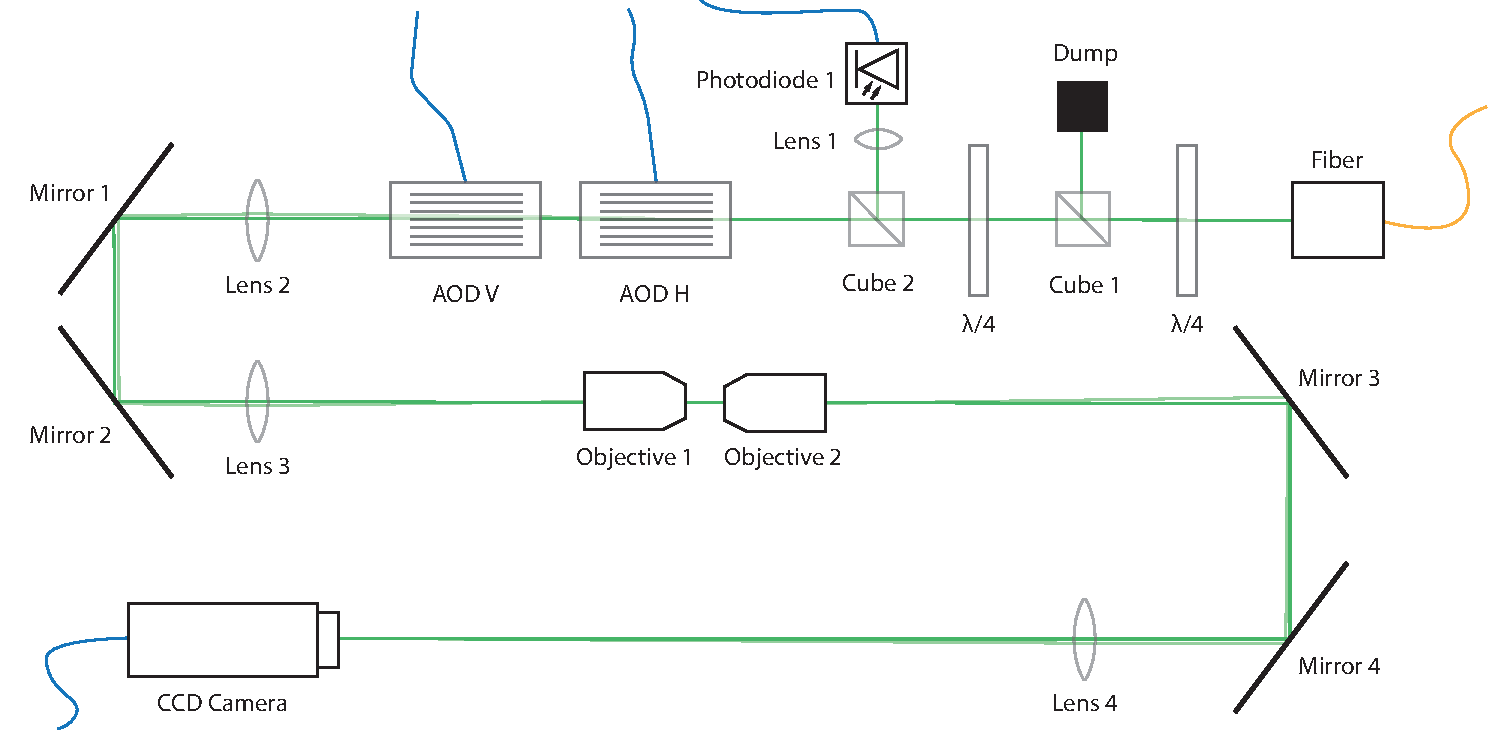
\includegraphics[width=\textwidth]{../media/setup/intensity-profile.pdf}
  \caption{The beam is focused onto the \gls{ccd} sensor of the camera.
  }\label{fig:intensity_profile_setup}
\end{figure}
In \Cref{fig:intensity_profile_setup} we present the setup used to measure
the spatial beam profile. In comparison to the previous setup we replaced
Photodiode 2 with a \gls{ccd} camera. The \gls{aod}s are configured at a
center frequency of \SI{100}{\mega\hertz}. The distance between Lens 4 and
the \gls{ccd} sensor is chosen such that the laser beam is focused onto the
\gls{ccd} sensor of the camera.
\begin{figure}[htb]
  \centering
  \begin{adjustbox}{width=\textwidth}
    \inputpgf{../figure/intensity/profile}{image.pgf}
  \end{adjustbox}
  \caption{Image of the focused laser beam measured with the \gls{ccd} camera.
  }\label{fig:intensity_spatial_image}
\end{figure}
\Cref{fig:intensity_spatial_image} shows an enlarged image patch of the
complete image capture taken with the \gls{ccd} camera. We can see a strong
illuminated circular spot in the center of the image with an area of about
\SI{2.5}{\milli\meter}. The intensity inside the spot seems homogeneous,
however this is caused by a saturation of the pixels in this area. We could
reduce the intensity or apply an optical filter to the camera to resolve the
intensity gradient inside the spot, but only at the cost of the intensity
distribution around the spot. Around the circular spot we can see a
diffraction ring. The diffraction ring is well described
in~\cite{Hertlein2017} and originates from the finite aperture of the
objectives.
\begin{figure}[htb]
  \centering
  \begin{adjustbox}{width=\textwidth}
    %% Creator: Matplotlib, PGF backend
%%
%% To include the figure in your LaTeX document, write
%%   \input{<filename>.pgf}
%%
%% Make sure the required packages are loaded in your preamble
%%   \usepackage{pgf}
%%
%% Figures using additional raster images can only be included by \input if
%% they are in the same directory as the main LaTeX file. For loading figures
%% from other directories you can use the `import` package
%%   \usepackage{import}
%% and then include the figures with
%%   \import{<path to file>}{<filename>.pgf}
%%
%% Matplotlib used the following preamble
%%   \usepackage{amsmath}\usepackage{siunitx}\usepackage{lmodern}
%%   \usepackage{fontspec}
%%
\begingroup%
\makeatletter%
\begin{pgfpicture}%
\pgfpathrectangle{\pgfpointorigin}{\pgfqpoint{12.000000in}{5.000000in}}%
\pgfusepath{use as bounding box, clip}%
\begin{pgfscope}%
\pgfsetbuttcap%
\pgfsetmiterjoin%
\pgfsetlinewidth{0.000000pt}%
\definecolor{currentstroke}{rgb}{1.000000,1.000000,1.000000}%
\pgfsetstrokecolor{currentstroke}%
\pgfsetdash{}{0pt}%
\pgfpathmoveto{\pgfqpoint{0.000000in}{0.000000in}}%
\pgfpathlineto{\pgfqpoint{12.000000in}{0.000000in}}%
\pgfpathlineto{\pgfqpoint{12.000000in}{5.000000in}}%
\pgfpathlineto{\pgfqpoint{0.000000in}{5.000000in}}%
\pgfpathclose%
\pgfusepath{}%
\end{pgfscope}%
\begin{pgfscope}%
\pgfsetbuttcap%
\pgfsetmiterjoin%
\definecolor{currentfill}{rgb}{1.000000,1.000000,1.000000}%
\pgfsetfillcolor{currentfill}%
\pgfsetlinewidth{0.000000pt}%
\definecolor{currentstroke}{rgb}{0.000000,0.000000,0.000000}%
\pgfsetstrokecolor{currentstroke}%
\pgfsetstrokeopacity{0.000000}%
\pgfsetdash{}{0pt}%
\pgfpathmoveto{\pgfqpoint{1.500000in}{0.800000in}}%
\pgfpathlineto{\pgfqpoint{6.036585in}{0.800000in}}%
\pgfpathlineto{\pgfqpoint{6.036585in}{4.500000in}}%
\pgfpathlineto{\pgfqpoint{1.500000in}{4.500000in}}%
\pgfpathclose%
\pgfusepath{fill}%
\end{pgfscope}%
\begin{pgfscope}%
\pgfsetbuttcap%
\pgfsetroundjoin%
\definecolor{currentfill}{rgb}{0.000000,0.000000,0.000000}%
\pgfsetfillcolor{currentfill}%
\pgfsetlinewidth{1.003750pt}%
\definecolor{currentstroke}{rgb}{0.000000,0.000000,0.000000}%
\pgfsetstrokecolor{currentstroke}%
\pgfsetdash{}{0pt}%
\pgfsys@defobject{currentmarker}{\pgfqpoint{0.000000in}{0.000000in}}{\pgfqpoint{0.000000in}{0.055556in}}{%
\pgfpathmoveto{\pgfqpoint{0.000000in}{0.000000in}}%
\pgfpathlineto{\pgfqpoint{0.000000in}{0.055556in}}%
\pgfusepath{stroke,fill}%
}%
\begin{pgfscope}%
\pgfsys@transformshift{1.706208in}{0.800000in}%
\pgfsys@useobject{currentmarker}{}%
\end{pgfscope}%
\end{pgfscope}%
\begin{pgfscope}%
\pgfsetbuttcap%
\pgfsetroundjoin%
\definecolor{currentfill}{rgb}{0.000000,0.000000,0.000000}%
\pgfsetfillcolor{currentfill}%
\pgfsetlinewidth{1.003750pt}%
\definecolor{currentstroke}{rgb}{0.000000,0.000000,0.000000}%
\pgfsetstrokecolor{currentstroke}%
\pgfsetdash{}{0pt}%
\pgfsys@defobject{currentmarker}{\pgfqpoint{0.000000in}{-0.055556in}}{\pgfqpoint{0.000000in}{0.000000in}}{%
\pgfpathmoveto{\pgfqpoint{0.000000in}{0.000000in}}%
\pgfpathlineto{\pgfqpoint{0.000000in}{-0.055556in}}%
\pgfusepath{stroke,fill}%
}%
\begin{pgfscope}%
\pgfsys@transformshift{1.706208in}{4.500000in}%
\pgfsys@useobject{currentmarker}{}%
\end{pgfscope}%
\end{pgfscope}%
\begin{pgfscope}%
\pgftext[x=1.706208in,y=0.702778in,,top]{\fontsize{10.000000}{12.000000}\selectfont \(\displaystyle 0\)}%
\end{pgfscope}%
\begin{pgfscope}%
\pgfsetbuttcap%
\pgfsetroundjoin%
\definecolor{currentfill}{rgb}{0.000000,0.000000,0.000000}%
\pgfsetfillcolor{currentfill}%
\pgfsetlinewidth{1.003750pt}%
\definecolor{currentstroke}{rgb}{0.000000,0.000000,0.000000}%
\pgfsetstrokecolor{currentstroke}%
\pgfsetdash{}{0pt}%
\pgfsys@defobject{currentmarker}{\pgfqpoint{0.000000in}{0.000000in}}{\pgfqpoint{0.000000in}{0.055556in}}{%
\pgfpathmoveto{\pgfqpoint{0.000000in}{0.000000in}}%
\pgfpathlineto{\pgfqpoint{0.000000in}{0.055556in}}%
\pgfusepath{stroke,fill}%
}%
\begin{pgfscope}%
\pgfsys@transformshift{2.496088in}{0.800000in}%
\pgfsys@useobject{currentmarker}{}%
\end{pgfscope}%
\end{pgfscope}%
\begin{pgfscope}%
\pgfsetbuttcap%
\pgfsetroundjoin%
\definecolor{currentfill}{rgb}{0.000000,0.000000,0.000000}%
\pgfsetfillcolor{currentfill}%
\pgfsetlinewidth{1.003750pt}%
\definecolor{currentstroke}{rgb}{0.000000,0.000000,0.000000}%
\pgfsetstrokecolor{currentstroke}%
\pgfsetdash{}{0pt}%
\pgfsys@defobject{currentmarker}{\pgfqpoint{0.000000in}{-0.055556in}}{\pgfqpoint{0.000000in}{0.000000in}}{%
\pgfpathmoveto{\pgfqpoint{0.000000in}{0.000000in}}%
\pgfpathlineto{\pgfqpoint{0.000000in}{-0.055556in}}%
\pgfusepath{stroke,fill}%
}%
\begin{pgfscope}%
\pgfsys@transformshift{2.496088in}{4.500000in}%
\pgfsys@useobject{currentmarker}{}%
\end{pgfscope}%
\end{pgfscope}%
\begin{pgfscope}%
\pgftext[x=2.496088in,y=0.702778in,,top]{\fontsize{10.000000}{12.000000}\selectfont \(\displaystyle 1\)}%
\end{pgfscope}%
\begin{pgfscope}%
\pgfsetbuttcap%
\pgfsetroundjoin%
\definecolor{currentfill}{rgb}{0.000000,0.000000,0.000000}%
\pgfsetfillcolor{currentfill}%
\pgfsetlinewidth{1.003750pt}%
\definecolor{currentstroke}{rgb}{0.000000,0.000000,0.000000}%
\pgfsetstrokecolor{currentstroke}%
\pgfsetdash{}{0pt}%
\pgfsys@defobject{currentmarker}{\pgfqpoint{0.000000in}{0.000000in}}{\pgfqpoint{0.000000in}{0.055556in}}{%
\pgfpathmoveto{\pgfqpoint{0.000000in}{0.000000in}}%
\pgfpathlineto{\pgfqpoint{0.000000in}{0.055556in}}%
\pgfusepath{stroke,fill}%
}%
\begin{pgfscope}%
\pgfsys@transformshift{3.285968in}{0.800000in}%
\pgfsys@useobject{currentmarker}{}%
\end{pgfscope}%
\end{pgfscope}%
\begin{pgfscope}%
\pgfsetbuttcap%
\pgfsetroundjoin%
\definecolor{currentfill}{rgb}{0.000000,0.000000,0.000000}%
\pgfsetfillcolor{currentfill}%
\pgfsetlinewidth{1.003750pt}%
\definecolor{currentstroke}{rgb}{0.000000,0.000000,0.000000}%
\pgfsetstrokecolor{currentstroke}%
\pgfsetdash{}{0pt}%
\pgfsys@defobject{currentmarker}{\pgfqpoint{0.000000in}{-0.055556in}}{\pgfqpoint{0.000000in}{0.000000in}}{%
\pgfpathmoveto{\pgfqpoint{0.000000in}{0.000000in}}%
\pgfpathlineto{\pgfqpoint{0.000000in}{-0.055556in}}%
\pgfusepath{stroke,fill}%
}%
\begin{pgfscope}%
\pgfsys@transformshift{3.285968in}{4.500000in}%
\pgfsys@useobject{currentmarker}{}%
\end{pgfscope}%
\end{pgfscope}%
\begin{pgfscope}%
\pgftext[x=3.285968in,y=0.702778in,,top]{\fontsize{10.000000}{12.000000}\selectfont \(\displaystyle 2\)}%
\end{pgfscope}%
\begin{pgfscope}%
\pgfsetbuttcap%
\pgfsetroundjoin%
\definecolor{currentfill}{rgb}{0.000000,0.000000,0.000000}%
\pgfsetfillcolor{currentfill}%
\pgfsetlinewidth{1.003750pt}%
\definecolor{currentstroke}{rgb}{0.000000,0.000000,0.000000}%
\pgfsetstrokecolor{currentstroke}%
\pgfsetdash{}{0pt}%
\pgfsys@defobject{currentmarker}{\pgfqpoint{0.000000in}{0.000000in}}{\pgfqpoint{0.000000in}{0.055556in}}{%
\pgfpathmoveto{\pgfqpoint{0.000000in}{0.000000in}}%
\pgfpathlineto{\pgfqpoint{0.000000in}{0.055556in}}%
\pgfusepath{stroke,fill}%
}%
\begin{pgfscope}%
\pgfsys@transformshift{4.075848in}{0.800000in}%
\pgfsys@useobject{currentmarker}{}%
\end{pgfscope}%
\end{pgfscope}%
\begin{pgfscope}%
\pgfsetbuttcap%
\pgfsetroundjoin%
\definecolor{currentfill}{rgb}{0.000000,0.000000,0.000000}%
\pgfsetfillcolor{currentfill}%
\pgfsetlinewidth{1.003750pt}%
\definecolor{currentstroke}{rgb}{0.000000,0.000000,0.000000}%
\pgfsetstrokecolor{currentstroke}%
\pgfsetdash{}{0pt}%
\pgfsys@defobject{currentmarker}{\pgfqpoint{0.000000in}{-0.055556in}}{\pgfqpoint{0.000000in}{0.000000in}}{%
\pgfpathmoveto{\pgfqpoint{0.000000in}{0.000000in}}%
\pgfpathlineto{\pgfqpoint{0.000000in}{-0.055556in}}%
\pgfusepath{stroke,fill}%
}%
\begin{pgfscope}%
\pgfsys@transformshift{4.075848in}{4.500000in}%
\pgfsys@useobject{currentmarker}{}%
\end{pgfscope}%
\end{pgfscope}%
\begin{pgfscope}%
\pgftext[x=4.075848in,y=0.702778in,,top]{\fontsize{10.000000}{12.000000}\selectfont \(\displaystyle 3\)}%
\end{pgfscope}%
\begin{pgfscope}%
\pgfsetbuttcap%
\pgfsetroundjoin%
\definecolor{currentfill}{rgb}{0.000000,0.000000,0.000000}%
\pgfsetfillcolor{currentfill}%
\pgfsetlinewidth{1.003750pt}%
\definecolor{currentstroke}{rgb}{0.000000,0.000000,0.000000}%
\pgfsetstrokecolor{currentstroke}%
\pgfsetdash{}{0pt}%
\pgfsys@defobject{currentmarker}{\pgfqpoint{0.000000in}{0.000000in}}{\pgfqpoint{0.000000in}{0.055556in}}{%
\pgfpathmoveto{\pgfqpoint{0.000000in}{0.000000in}}%
\pgfpathlineto{\pgfqpoint{0.000000in}{0.055556in}}%
\pgfusepath{stroke,fill}%
}%
\begin{pgfscope}%
\pgfsys@transformshift{4.865728in}{0.800000in}%
\pgfsys@useobject{currentmarker}{}%
\end{pgfscope}%
\end{pgfscope}%
\begin{pgfscope}%
\pgfsetbuttcap%
\pgfsetroundjoin%
\definecolor{currentfill}{rgb}{0.000000,0.000000,0.000000}%
\pgfsetfillcolor{currentfill}%
\pgfsetlinewidth{1.003750pt}%
\definecolor{currentstroke}{rgb}{0.000000,0.000000,0.000000}%
\pgfsetstrokecolor{currentstroke}%
\pgfsetdash{}{0pt}%
\pgfsys@defobject{currentmarker}{\pgfqpoint{0.000000in}{-0.055556in}}{\pgfqpoint{0.000000in}{0.000000in}}{%
\pgfpathmoveto{\pgfqpoint{0.000000in}{0.000000in}}%
\pgfpathlineto{\pgfqpoint{0.000000in}{-0.055556in}}%
\pgfusepath{stroke,fill}%
}%
\begin{pgfscope}%
\pgfsys@transformshift{4.865728in}{4.500000in}%
\pgfsys@useobject{currentmarker}{}%
\end{pgfscope}%
\end{pgfscope}%
\begin{pgfscope}%
\pgftext[x=4.865728in,y=0.702778in,,top]{\fontsize{10.000000}{12.000000}\selectfont \(\displaystyle 4\)}%
\end{pgfscope}%
\begin{pgfscope}%
\pgfsetbuttcap%
\pgfsetroundjoin%
\definecolor{currentfill}{rgb}{0.000000,0.000000,0.000000}%
\pgfsetfillcolor{currentfill}%
\pgfsetlinewidth{1.003750pt}%
\definecolor{currentstroke}{rgb}{0.000000,0.000000,0.000000}%
\pgfsetstrokecolor{currentstroke}%
\pgfsetdash{}{0pt}%
\pgfsys@defobject{currentmarker}{\pgfqpoint{0.000000in}{0.000000in}}{\pgfqpoint{0.000000in}{0.055556in}}{%
\pgfpathmoveto{\pgfqpoint{0.000000in}{0.000000in}}%
\pgfpathlineto{\pgfqpoint{0.000000in}{0.055556in}}%
\pgfusepath{stroke,fill}%
}%
\begin{pgfscope}%
\pgfsys@transformshift{5.655608in}{0.800000in}%
\pgfsys@useobject{currentmarker}{}%
\end{pgfscope}%
\end{pgfscope}%
\begin{pgfscope}%
\pgfsetbuttcap%
\pgfsetroundjoin%
\definecolor{currentfill}{rgb}{0.000000,0.000000,0.000000}%
\pgfsetfillcolor{currentfill}%
\pgfsetlinewidth{1.003750pt}%
\definecolor{currentstroke}{rgb}{0.000000,0.000000,0.000000}%
\pgfsetstrokecolor{currentstroke}%
\pgfsetdash{}{0pt}%
\pgfsys@defobject{currentmarker}{\pgfqpoint{0.000000in}{-0.055556in}}{\pgfqpoint{0.000000in}{0.000000in}}{%
\pgfpathmoveto{\pgfqpoint{0.000000in}{0.000000in}}%
\pgfpathlineto{\pgfqpoint{0.000000in}{-0.055556in}}%
\pgfusepath{stroke,fill}%
}%
\begin{pgfscope}%
\pgfsys@transformshift{5.655608in}{4.500000in}%
\pgfsys@useobject{currentmarker}{}%
\end{pgfscope}%
\end{pgfscope}%
\begin{pgfscope}%
\pgftext[x=5.655608in,y=0.702778in,,top]{\fontsize{10.000000}{12.000000}\selectfont \(\displaystyle 5\)}%
\end{pgfscope}%
\begin{pgfscope}%
\pgftext[x=3.768293in,y=0.440556in,,top]{\fontsize{16.000000}{19.200000}\selectfont \(\displaystyle x\) (\si{\micro\meter})}%
\end{pgfscope}%
\begin{pgfscope}%
\pgfsetbuttcap%
\pgfsetroundjoin%
\definecolor{currentfill}{rgb}{0.000000,0.000000,0.000000}%
\pgfsetfillcolor{currentfill}%
\pgfsetlinewidth{1.003750pt}%
\definecolor{currentstroke}{rgb}{0.000000,0.000000,0.000000}%
\pgfsetstrokecolor{currentstroke}%
\pgfsetdash{}{0pt}%
\pgfsys@defobject{currentmarker}{\pgfqpoint{0.000000in}{0.000000in}}{\pgfqpoint{0.055556in}{0.000000in}}{%
\pgfpathmoveto{\pgfqpoint{0.000000in}{0.000000in}}%
\pgfpathlineto{\pgfqpoint{0.055556in}{0.000000in}}%
\pgfusepath{stroke,fill}%
}%
\begin{pgfscope}%
\pgfsys@transformshift{1.500000in}{0.968182in}%
\pgfsys@useobject{currentmarker}{}%
\end{pgfscope}%
\end{pgfscope}%
\begin{pgfscope}%
\pgfsetbuttcap%
\pgfsetroundjoin%
\definecolor{currentfill}{rgb}{0.000000,0.000000,0.000000}%
\pgfsetfillcolor{currentfill}%
\pgfsetlinewidth{1.003750pt}%
\definecolor{currentstroke}{rgb}{0.000000,0.000000,0.000000}%
\pgfsetstrokecolor{currentstroke}%
\pgfsetdash{}{0pt}%
\pgfsys@defobject{currentmarker}{\pgfqpoint{-0.055556in}{0.000000in}}{\pgfqpoint{0.000000in}{0.000000in}}{%
\pgfpathmoveto{\pgfqpoint{0.000000in}{0.000000in}}%
\pgfpathlineto{\pgfqpoint{-0.055556in}{0.000000in}}%
\pgfusepath{stroke,fill}%
}%
\begin{pgfscope}%
\pgfsys@transformshift{6.036585in}{0.968182in}%
\pgfsys@useobject{currentmarker}{}%
\end{pgfscope}%
\end{pgfscope}%
\begin{pgfscope}%
\pgftext[x=1.225308in,y=0.919987in,left,base]{\fontsize{10.000000}{12.000000}\selectfont \(\displaystyle 0.0\)}%
\end{pgfscope}%
\begin{pgfscope}%
\pgfsetbuttcap%
\pgfsetroundjoin%
\definecolor{currentfill}{rgb}{0.000000,0.000000,0.000000}%
\pgfsetfillcolor{currentfill}%
\pgfsetlinewidth{1.003750pt}%
\definecolor{currentstroke}{rgb}{0.000000,0.000000,0.000000}%
\pgfsetstrokecolor{currentstroke}%
\pgfsetdash{}{0pt}%
\pgfsys@defobject{currentmarker}{\pgfqpoint{0.000000in}{0.000000in}}{\pgfqpoint{0.055556in}{0.000000in}}{%
\pgfpathmoveto{\pgfqpoint{0.000000in}{0.000000in}}%
\pgfpathlineto{\pgfqpoint{0.055556in}{0.000000in}}%
\pgfusepath{stroke,fill}%
}%
\begin{pgfscope}%
\pgfsys@transformshift{1.500000in}{1.640864in}%
\pgfsys@useobject{currentmarker}{}%
\end{pgfscope}%
\end{pgfscope}%
\begin{pgfscope}%
\pgfsetbuttcap%
\pgfsetroundjoin%
\definecolor{currentfill}{rgb}{0.000000,0.000000,0.000000}%
\pgfsetfillcolor{currentfill}%
\pgfsetlinewidth{1.003750pt}%
\definecolor{currentstroke}{rgb}{0.000000,0.000000,0.000000}%
\pgfsetstrokecolor{currentstroke}%
\pgfsetdash{}{0pt}%
\pgfsys@defobject{currentmarker}{\pgfqpoint{-0.055556in}{0.000000in}}{\pgfqpoint{0.000000in}{0.000000in}}{%
\pgfpathmoveto{\pgfqpoint{0.000000in}{0.000000in}}%
\pgfpathlineto{\pgfqpoint{-0.055556in}{0.000000in}}%
\pgfusepath{stroke,fill}%
}%
\begin{pgfscope}%
\pgfsys@transformshift{6.036585in}{1.640864in}%
\pgfsys@useobject{currentmarker}{}%
\end{pgfscope}%
\end{pgfscope}%
\begin{pgfscope}%
\pgftext[x=1.225308in,y=1.592670in,left,base]{\fontsize{10.000000}{12.000000}\selectfont \(\displaystyle 0.2\)}%
\end{pgfscope}%
\begin{pgfscope}%
\pgfsetbuttcap%
\pgfsetroundjoin%
\definecolor{currentfill}{rgb}{0.000000,0.000000,0.000000}%
\pgfsetfillcolor{currentfill}%
\pgfsetlinewidth{1.003750pt}%
\definecolor{currentstroke}{rgb}{0.000000,0.000000,0.000000}%
\pgfsetstrokecolor{currentstroke}%
\pgfsetdash{}{0pt}%
\pgfsys@defobject{currentmarker}{\pgfqpoint{0.000000in}{0.000000in}}{\pgfqpoint{0.055556in}{0.000000in}}{%
\pgfpathmoveto{\pgfqpoint{0.000000in}{0.000000in}}%
\pgfpathlineto{\pgfqpoint{0.055556in}{0.000000in}}%
\pgfusepath{stroke,fill}%
}%
\begin{pgfscope}%
\pgfsys@transformshift{1.500000in}{2.313547in}%
\pgfsys@useobject{currentmarker}{}%
\end{pgfscope}%
\end{pgfscope}%
\begin{pgfscope}%
\pgfsetbuttcap%
\pgfsetroundjoin%
\definecolor{currentfill}{rgb}{0.000000,0.000000,0.000000}%
\pgfsetfillcolor{currentfill}%
\pgfsetlinewidth{1.003750pt}%
\definecolor{currentstroke}{rgb}{0.000000,0.000000,0.000000}%
\pgfsetstrokecolor{currentstroke}%
\pgfsetdash{}{0pt}%
\pgfsys@defobject{currentmarker}{\pgfqpoint{-0.055556in}{0.000000in}}{\pgfqpoint{0.000000in}{0.000000in}}{%
\pgfpathmoveto{\pgfqpoint{0.000000in}{0.000000in}}%
\pgfpathlineto{\pgfqpoint{-0.055556in}{0.000000in}}%
\pgfusepath{stroke,fill}%
}%
\begin{pgfscope}%
\pgfsys@transformshift{6.036585in}{2.313547in}%
\pgfsys@useobject{currentmarker}{}%
\end{pgfscope}%
\end{pgfscope}%
\begin{pgfscope}%
\pgftext[x=1.225308in,y=2.265353in,left,base]{\fontsize{10.000000}{12.000000}\selectfont \(\displaystyle 0.4\)}%
\end{pgfscope}%
\begin{pgfscope}%
\pgfsetbuttcap%
\pgfsetroundjoin%
\definecolor{currentfill}{rgb}{0.000000,0.000000,0.000000}%
\pgfsetfillcolor{currentfill}%
\pgfsetlinewidth{1.003750pt}%
\definecolor{currentstroke}{rgb}{0.000000,0.000000,0.000000}%
\pgfsetstrokecolor{currentstroke}%
\pgfsetdash{}{0pt}%
\pgfsys@defobject{currentmarker}{\pgfqpoint{0.000000in}{0.000000in}}{\pgfqpoint{0.055556in}{0.000000in}}{%
\pgfpathmoveto{\pgfqpoint{0.000000in}{0.000000in}}%
\pgfpathlineto{\pgfqpoint{0.055556in}{0.000000in}}%
\pgfusepath{stroke,fill}%
}%
\begin{pgfscope}%
\pgfsys@transformshift{1.500000in}{2.986230in}%
\pgfsys@useobject{currentmarker}{}%
\end{pgfscope}%
\end{pgfscope}%
\begin{pgfscope}%
\pgfsetbuttcap%
\pgfsetroundjoin%
\definecolor{currentfill}{rgb}{0.000000,0.000000,0.000000}%
\pgfsetfillcolor{currentfill}%
\pgfsetlinewidth{1.003750pt}%
\definecolor{currentstroke}{rgb}{0.000000,0.000000,0.000000}%
\pgfsetstrokecolor{currentstroke}%
\pgfsetdash{}{0pt}%
\pgfsys@defobject{currentmarker}{\pgfqpoint{-0.055556in}{0.000000in}}{\pgfqpoint{0.000000in}{0.000000in}}{%
\pgfpathmoveto{\pgfqpoint{0.000000in}{0.000000in}}%
\pgfpathlineto{\pgfqpoint{-0.055556in}{0.000000in}}%
\pgfusepath{stroke,fill}%
}%
\begin{pgfscope}%
\pgfsys@transformshift{6.036585in}{2.986230in}%
\pgfsys@useobject{currentmarker}{}%
\end{pgfscope}%
\end{pgfscope}%
\begin{pgfscope}%
\pgftext[x=1.225308in,y=2.938035in,left,base]{\fontsize{10.000000}{12.000000}\selectfont \(\displaystyle 0.6\)}%
\end{pgfscope}%
\begin{pgfscope}%
\pgfsetbuttcap%
\pgfsetroundjoin%
\definecolor{currentfill}{rgb}{0.000000,0.000000,0.000000}%
\pgfsetfillcolor{currentfill}%
\pgfsetlinewidth{1.003750pt}%
\definecolor{currentstroke}{rgb}{0.000000,0.000000,0.000000}%
\pgfsetstrokecolor{currentstroke}%
\pgfsetdash{}{0pt}%
\pgfsys@defobject{currentmarker}{\pgfqpoint{0.000000in}{0.000000in}}{\pgfqpoint{0.055556in}{0.000000in}}{%
\pgfpathmoveto{\pgfqpoint{0.000000in}{0.000000in}}%
\pgfpathlineto{\pgfqpoint{0.055556in}{0.000000in}}%
\pgfusepath{stroke,fill}%
}%
\begin{pgfscope}%
\pgfsys@transformshift{1.500000in}{3.658912in}%
\pgfsys@useobject{currentmarker}{}%
\end{pgfscope}%
\end{pgfscope}%
\begin{pgfscope}%
\pgfsetbuttcap%
\pgfsetroundjoin%
\definecolor{currentfill}{rgb}{0.000000,0.000000,0.000000}%
\pgfsetfillcolor{currentfill}%
\pgfsetlinewidth{1.003750pt}%
\definecolor{currentstroke}{rgb}{0.000000,0.000000,0.000000}%
\pgfsetstrokecolor{currentstroke}%
\pgfsetdash{}{0pt}%
\pgfsys@defobject{currentmarker}{\pgfqpoint{-0.055556in}{0.000000in}}{\pgfqpoint{0.000000in}{0.000000in}}{%
\pgfpathmoveto{\pgfqpoint{0.000000in}{0.000000in}}%
\pgfpathlineto{\pgfqpoint{-0.055556in}{0.000000in}}%
\pgfusepath{stroke,fill}%
}%
\begin{pgfscope}%
\pgfsys@transformshift{6.036585in}{3.658912in}%
\pgfsys@useobject{currentmarker}{}%
\end{pgfscope}%
\end{pgfscope}%
\begin{pgfscope}%
\pgftext[x=1.225308in,y=3.610718in,left,base]{\fontsize{10.000000}{12.000000}\selectfont \(\displaystyle 0.8\)}%
\end{pgfscope}%
\begin{pgfscope}%
\pgfsetbuttcap%
\pgfsetroundjoin%
\definecolor{currentfill}{rgb}{0.000000,0.000000,0.000000}%
\pgfsetfillcolor{currentfill}%
\pgfsetlinewidth{1.003750pt}%
\definecolor{currentstroke}{rgb}{0.000000,0.000000,0.000000}%
\pgfsetstrokecolor{currentstroke}%
\pgfsetdash{}{0pt}%
\pgfsys@defobject{currentmarker}{\pgfqpoint{0.000000in}{0.000000in}}{\pgfqpoint{0.055556in}{0.000000in}}{%
\pgfpathmoveto{\pgfqpoint{0.000000in}{0.000000in}}%
\pgfpathlineto{\pgfqpoint{0.055556in}{0.000000in}}%
\pgfusepath{stroke,fill}%
}%
\begin{pgfscope}%
\pgfsys@transformshift{1.500000in}{4.331595in}%
\pgfsys@useobject{currentmarker}{}%
\end{pgfscope}%
\end{pgfscope}%
\begin{pgfscope}%
\pgfsetbuttcap%
\pgfsetroundjoin%
\definecolor{currentfill}{rgb}{0.000000,0.000000,0.000000}%
\pgfsetfillcolor{currentfill}%
\pgfsetlinewidth{1.003750pt}%
\definecolor{currentstroke}{rgb}{0.000000,0.000000,0.000000}%
\pgfsetstrokecolor{currentstroke}%
\pgfsetdash{}{0pt}%
\pgfsys@defobject{currentmarker}{\pgfqpoint{-0.055556in}{0.000000in}}{\pgfqpoint{0.000000in}{0.000000in}}{%
\pgfpathmoveto{\pgfqpoint{0.000000in}{0.000000in}}%
\pgfpathlineto{\pgfqpoint{-0.055556in}{0.000000in}}%
\pgfusepath{stroke,fill}%
}%
\begin{pgfscope}%
\pgfsys@transformshift{6.036585in}{4.331595in}%
\pgfsys@useobject{currentmarker}{}%
\end{pgfscope}%
\end{pgfscope}%
\begin{pgfscope}%
\pgftext[x=1.225308in,y=4.283400in,left,base]{\fontsize{10.000000}{12.000000}\selectfont \(\displaystyle 1.0\)}%
\end{pgfscope}%
\begin{pgfscope}%
\pgfsetbuttcap%
\pgfsetroundjoin%
\definecolor{currentfill}{rgb}{0.000000,0.000000,0.000000}%
\pgfsetfillcolor{currentfill}%
\pgfsetlinewidth{0.501875pt}%
\definecolor{currentstroke}{rgb}{0.000000,0.000000,0.000000}%
\pgfsetstrokecolor{currentstroke}%
\pgfsetdash{}{0pt}%
\pgfsys@defobject{currentmarker}{\pgfqpoint{0.000000in}{0.000000in}}{\pgfqpoint{0.027778in}{0.000000in}}{%
\pgfpathmoveto{\pgfqpoint{0.000000in}{0.000000in}}%
\pgfpathlineto{\pgfqpoint{0.027778in}{0.000000in}}%
\pgfusepath{stroke,fill}%
}%
\begin{pgfscope}%
\pgfsys@transformshift{1.500000in}{0.800011in}%
\pgfsys@useobject{currentmarker}{}%
\end{pgfscope}%
\end{pgfscope}%
\begin{pgfscope}%
\pgfsetbuttcap%
\pgfsetroundjoin%
\definecolor{currentfill}{rgb}{0.000000,0.000000,0.000000}%
\pgfsetfillcolor{currentfill}%
\pgfsetlinewidth{0.501875pt}%
\definecolor{currentstroke}{rgb}{0.000000,0.000000,0.000000}%
\pgfsetstrokecolor{currentstroke}%
\pgfsetdash{}{0pt}%
\pgfsys@defobject{currentmarker}{\pgfqpoint{-0.027778in}{0.000000in}}{\pgfqpoint{0.000000in}{0.000000in}}{%
\pgfpathmoveto{\pgfqpoint{0.000000in}{0.000000in}}%
\pgfpathlineto{\pgfqpoint{-0.027778in}{0.000000in}}%
\pgfusepath{stroke,fill}%
}%
\begin{pgfscope}%
\pgfsys@transformshift{6.036585in}{0.800011in}%
\pgfsys@useobject{currentmarker}{}%
\end{pgfscope}%
\end{pgfscope}%
\begin{pgfscope}%
\pgfsetbuttcap%
\pgfsetroundjoin%
\definecolor{currentfill}{rgb}{0.000000,0.000000,0.000000}%
\pgfsetfillcolor{currentfill}%
\pgfsetlinewidth{0.501875pt}%
\definecolor{currentstroke}{rgb}{0.000000,0.000000,0.000000}%
\pgfsetstrokecolor{currentstroke}%
\pgfsetdash{}{0pt}%
\pgfsys@defobject{currentmarker}{\pgfqpoint{0.000000in}{0.000000in}}{\pgfqpoint{0.027778in}{0.000000in}}{%
\pgfpathmoveto{\pgfqpoint{0.000000in}{0.000000in}}%
\pgfpathlineto{\pgfqpoint{0.027778in}{0.000000in}}%
\pgfusepath{stroke,fill}%
}%
\begin{pgfscope}%
\pgfsys@transformshift{1.500000in}{1.136352in}%
\pgfsys@useobject{currentmarker}{}%
\end{pgfscope}%
\end{pgfscope}%
\begin{pgfscope}%
\pgfsetbuttcap%
\pgfsetroundjoin%
\definecolor{currentfill}{rgb}{0.000000,0.000000,0.000000}%
\pgfsetfillcolor{currentfill}%
\pgfsetlinewidth{0.501875pt}%
\definecolor{currentstroke}{rgb}{0.000000,0.000000,0.000000}%
\pgfsetstrokecolor{currentstroke}%
\pgfsetdash{}{0pt}%
\pgfsys@defobject{currentmarker}{\pgfqpoint{-0.027778in}{0.000000in}}{\pgfqpoint{0.000000in}{0.000000in}}{%
\pgfpathmoveto{\pgfqpoint{0.000000in}{0.000000in}}%
\pgfpathlineto{\pgfqpoint{-0.027778in}{0.000000in}}%
\pgfusepath{stroke,fill}%
}%
\begin{pgfscope}%
\pgfsys@transformshift{6.036585in}{1.136352in}%
\pgfsys@useobject{currentmarker}{}%
\end{pgfscope}%
\end{pgfscope}%
\begin{pgfscope}%
\pgfsetbuttcap%
\pgfsetroundjoin%
\definecolor{currentfill}{rgb}{0.000000,0.000000,0.000000}%
\pgfsetfillcolor{currentfill}%
\pgfsetlinewidth{0.501875pt}%
\definecolor{currentstroke}{rgb}{0.000000,0.000000,0.000000}%
\pgfsetstrokecolor{currentstroke}%
\pgfsetdash{}{0pt}%
\pgfsys@defobject{currentmarker}{\pgfqpoint{0.000000in}{0.000000in}}{\pgfqpoint{0.027778in}{0.000000in}}{%
\pgfpathmoveto{\pgfqpoint{0.000000in}{0.000000in}}%
\pgfpathlineto{\pgfqpoint{0.027778in}{0.000000in}}%
\pgfusepath{stroke,fill}%
}%
\begin{pgfscope}%
\pgfsys@transformshift{1.500000in}{1.304523in}%
\pgfsys@useobject{currentmarker}{}%
\end{pgfscope}%
\end{pgfscope}%
\begin{pgfscope}%
\pgfsetbuttcap%
\pgfsetroundjoin%
\definecolor{currentfill}{rgb}{0.000000,0.000000,0.000000}%
\pgfsetfillcolor{currentfill}%
\pgfsetlinewidth{0.501875pt}%
\definecolor{currentstroke}{rgb}{0.000000,0.000000,0.000000}%
\pgfsetstrokecolor{currentstroke}%
\pgfsetdash{}{0pt}%
\pgfsys@defobject{currentmarker}{\pgfqpoint{-0.027778in}{0.000000in}}{\pgfqpoint{0.000000in}{0.000000in}}{%
\pgfpathmoveto{\pgfqpoint{0.000000in}{0.000000in}}%
\pgfpathlineto{\pgfqpoint{-0.027778in}{0.000000in}}%
\pgfusepath{stroke,fill}%
}%
\begin{pgfscope}%
\pgfsys@transformshift{6.036585in}{1.304523in}%
\pgfsys@useobject{currentmarker}{}%
\end{pgfscope}%
\end{pgfscope}%
\begin{pgfscope}%
\pgfsetbuttcap%
\pgfsetroundjoin%
\definecolor{currentfill}{rgb}{0.000000,0.000000,0.000000}%
\pgfsetfillcolor{currentfill}%
\pgfsetlinewidth{0.501875pt}%
\definecolor{currentstroke}{rgb}{0.000000,0.000000,0.000000}%
\pgfsetstrokecolor{currentstroke}%
\pgfsetdash{}{0pt}%
\pgfsys@defobject{currentmarker}{\pgfqpoint{0.000000in}{0.000000in}}{\pgfqpoint{0.027778in}{0.000000in}}{%
\pgfpathmoveto{\pgfqpoint{0.000000in}{0.000000in}}%
\pgfpathlineto{\pgfqpoint{0.027778in}{0.000000in}}%
\pgfusepath{stroke,fill}%
}%
\begin{pgfscope}%
\pgfsys@transformshift{1.500000in}{1.472694in}%
\pgfsys@useobject{currentmarker}{}%
\end{pgfscope}%
\end{pgfscope}%
\begin{pgfscope}%
\pgfsetbuttcap%
\pgfsetroundjoin%
\definecolor{currentfill}{rgb}{0.000000,0.000000,0.000000}%
\pgfsetfillcolor{currentfill}%
\pgfsetlinewidth{0.501875pt}%
\definecolor{currentstroke}{rgb}{0.000000,0.000000,0.000000}%
\pgfsetstrokecolor{currentstroke}%
\pgfsetdash{}{0pt}%
\pgfsys@defobject{currentmarker}{\pgfqpoint{-0.027778in}{0.000000in}}{\pgfqpoint{0.000000in}{0.000000in}}{%
\pgfpathmoveto{\pgfqpoint{0.000000in}{0.000000in}}%
\pgfpathlineto{\pgfqpoint{-0.027778in}{0.000000in}}%
\pgfusepath{stroke,fill}%
}%
\begin{pgfscope}%
\pgfsys@transformshift{6.036585in}{1.472694in}%
\pgfsys@useobject{currentmarker}{}%
\end{pgfscope}%
\end{pgfscope}%
\begin{pgfscope}%
\pgfsetbuttcap%
\pgfsetroundjoin%
\definecolor{currentfill}{rgb}{0.000000,0.000000,0.000000}%
\pgfsetfillcolor{currentfill}%
\pgfsetlinewidth{0.501875pt}%
\definecolor{currentstroke}{rgb}{0.000000,0.000000,0.000000}%
\pgfsetstrokecolor{currentstroke}%
\pgfsetdash{}{0pt}%
\pgfsys@defobject{currentmarker}{\pgfqpoint{0.000000in}{0.000000in}}{\pgfqpoint{0.027778in}{0.000000in}}{%
\pgfpathmoveto{\pgfqpoint{0.000000in}{0.000000in}}%
\pgfpathlineto{\pgfqpoint{0.027778in}{0.000000in}}%
\pgfusepath{stroke,fill}%
}%
\begin{pgfscope}%
\pgfsys@transformshift{1.500000in}{1.640864in}%
\pgfsys@useobject{currentmarker}{}%
\end{pgfscope}%
\end{pgfscope}%
\begin{pgfscope}%
\pgfsetbuttcap%
\pgfsetroundjoin%
\definecolor{currentfill}{rgb}{0.000000,0.000000,0.000000}%
\pgfsetfillcolor{currentfill}%
\pgfsetlinewidth{0.501875pt}%
\definecolor{currentstroke}{rgb}{0.000000,0.000000,0.000000}%
\pgfsetstrokecolor{currentstroke}%
\pgfsetdash{}{0pt}%
\pgfsys@defobject{currentmarker}{\pgfqpoint{-0.027778in}{0.000000in}}{\pgfqpoint{0.000000in}{0.000000in}}{%
\pgfpathmoveto{\pgfqpoint{0.000000in}{0.000000in}}%
\pgfpathlineto{\pgfqpoint{-0.027778in}{0.000000in}}%
\pgfusepath{stroke,fill}%
}%
\begin{pgfscope}%
\pgfsys@transformshift{6.036585in}{1.640864in}%
\pgfsys@useobject{currentmarker}{}%
\end{pgfscope}%
\end{pgfscope}%
\begin{pgfscope}%
\pgfsetbuttcap%
\pgfsetroundjoin%
\definecolor{currentfill}{rgb}{0.000000,0.000000,0.000000}%
\pgfsetfillcolor{currentfill}%
\pgfsetlinewidth{0.501875pt}%
\definecolor{currentstroke}{rgb}{0.000000,0.000000,0.000000}%
\pgfsetstrokecolor{currentstroke}%
\pgfsetdash{}{0pt}%
\pgfsys@defobject{currentmarker}{\pgfqpoint{0.000000in}{0.000000in}}{\pgfqpoint{0.027778in}{0.000000in}}{%
\pgfpathmoveto{\pgfqpoint{0.000000in}{0.000000in}}%
\pgfpathlineto{\pgfqpoint{0.027778in}{0.000000in}}%
\pgfusepath{stroke,fill}%
}%
\begin{pgfscope}%
\pgfsys@transformshift{1.500000in}{1.809035in}%
\pgfsys@useobject{currentmarker}{}%
\end{pgfscope}%
\end{pgfscope}%
\begin{pgfscope}%
\pgfsetbuttcap%
\pgfsetroundjoin%
\definecolor{currentfill}{rgb}{0.000000,0.000000,0.000000}%
\pgfsetfillcolor{currentfill}%
\pgfsetlinewidth{0.501875pt}%
\definecolor{currentstroke}{rgb}{0.000000,0.000000,0.000000}%
\pgfsetstrokecolor{currentstroke}%
\pgfsetdash{}{0pt}%
\pgfsys@defobject{currentmarker}{\pgfqpoint{-0.027778in}{0.000000in}}{\pgfqpoint{0.000000in}{0.000000in}}{%
\pgfpathmoveto{\pgfqpoint{0.000000in}{0.000000in}}%
\pgfpathlineto{\pgfqpoint{-0.027778in}{0.000000in}}%
\pgfusepath{stroke,fill}%
}%
\begin{pgfscope}%
\pgfsys@transformshift{6.036585in}{1.809035in}%
\pgfsys@useobject{currentmarker}{}%
\end{pgfscope}%
\end{pgfscope}%
\begin{pgfscope}%
\pgfsetbuttcap%
\pgfsetroundjoin%
\definecolor{currentfill}{rgb}{0.000000,0.000000,0.000000}%
\pgfsetfillcolor{currentfill}%
\pgfsetlinewidth{0.501875pt}%
\definecolor{currentstroke}{rgb}{0.000000,0.000000,0.000000}%
\pgfsetstrokecolor{currentstroke}%
\pgfsetdash{}{0pt}%
\pgfsys@defobject{currentmarker}{\pgfqpoint{0.000000in}{0.000000in}}{\pgfqpoint{0.027778in}{0.000000in}}{%
\pgfpathmoveto{\pgfqpoint{0.000000in}{0.000000in}}%
\pgfpathlineto{\pgfqpoint{0.027778in}{0.000000in}}%
\pgfusepath{stroke,fill}%
}%
\begin{pgfscope}%
\pgfsys@transformshift{1.500000in}{1.977206in}%
\pgfsys@useobject{currentmarker}{}%
\end{pgfscope}%
\end{pgfscope}%
\begin{pgfscope}%
\pgfsetbuttcap%
\pgfsetroundjoin%
\definecolor{currentfill}{rgb}{0.000000,0.000000,0.000000}%
\pgfsetfillcolor{currentfill}%
\pgfsetlinewidth{0.501875pt}%
\definecolor{currentstroke}{rgb}{0.000000,0.000000,0.000000}%
\pgfsetstrokecolor{currentstroke}%
\pgfsetdash{}{0pt}%
\pgfsys@defobject{currentmarker}{\pgfqpoint{-0.027778in}{0.000000in}}{\pgfqpoint{0.000000in}{0.000000in}}{%
\pgfpathmoveto{\pgfqpoint{0.000000in}{0.000000in}}%
\pgfpathlineto{\pgfqpoint{-0.027778in}{0.000000in}}%
\pgfusepath{stroke,fill}%
}%
\begin{pgfscope}%
\pgfsys@transformshift{6.036585in}{1.977206in}%
\pgfsys@useobject{currentmarker}{}%
\end{pgfscope}%
\end{pgfscope}%
\begin{pgfscope}%
\pgfsetbuttcap%
\pgfsetroundjoin%
\definecolor{currentfill}{rgb}{0.000000,0.000000,0.000000}%
\pgfsetfillcolor{currentfill}%
\pgfsetlinewidth{0.501875pt}%
\definecolor{currentstroke}{rgb}{0.000000,0.000000,0.000000}%
\pgfsetstrokecolor{currentstroke}%
\pgfsetdash{}{0pt}%
\pgfsys@defobject{currentmarker}{\pgfqpoint{0.000000in}{0.000000in}}{\pgfqpoint{0.027778in}{0.000000in}}{%
\pgfpathmoveto{\pgfqpoint{0.000000in}{0.000000in}}%
\pgfpathlineto{\pgfqpoint{0.027778in}{0.000000in}}%
\pgfusepath{stroke,fill}%
}%
\begin{pgfscope}%
\pgfsys@transformshift{1.500000in}{2.145376in}%
\pgfsys@useobject{currentmarker}{}%
\end{pgfscope}%
\end{pgfscope}%
\begin{pgfscope}%
\pgfsetbuttcap%
\pgfsetroundjoin%
\definecolor{currentfill}{rgb}{0.000000,0.000000,0.000000}%
\pgfsetfillcolor{currentfill}%
\pgfsetlinewidth{0.501875pt}%
\definecolor{currentstroke}{rgb}{0.000000,0.000000,0.000000}%
\pgfsetstrokecolor{currentstroke}%
\pgfsetdash{}{0pt}%
\pgfsys@defobject{currentmarker}{\pgfqpoint{-0.027778in}{0.000000in}}{\pgfqpoint{0.000000in}{0.000000in}}{%
\pgfpathmoveto{\pgfqpoint{0.000000in}{0.000000in}}%
\pgfpathlineto{\pgfqpoint{-0.027778in}{0.000000in}}%
\pgfusepath{stroke,fill}%
}%
\begin{pgfscope}%
\pgfsys@transformshift{6.036585in}{2.145376in}%
\pgfsys@useobject{currentmarker}{}%
\end{pgfscope}%
\end{pgfscope}%
\begin{pgfscope}%
\pgfsetbuttcap%
\pgfsetroundjoin%
\definecolor{currentfill}{rgb}{0.000000,0.000000,0.000000}%
\pgfsetfillcolor{currentfill}%
\pgfsetlinewidth{0.501875pt}%
\definecolor{currentstroke}{rgb}{0.000000,0.000000,0.000000}%
\pgfsetstrokecolor{currentstroke}%
\pgfsetdash{}{0pt}%
\pgfsys@defobject{currentmarker}{\pgfqpoint{0.000000in}{0.000000in}}{\pgfqpoint{0.027778in}{0.000000in}}{%
\pgfpathmoveto{\pgfqpoint{0.000000in}{0.000000in}}%
\pgfpathlineto{\pgfqpoint{0.027778in}{0.000000in}}%
\pgfusepath{stroke,fill}%
}%
\begin{pgfscope}%
\pgfsys@transformshift{1.500000in}{2.313547in}%
\pgfsys@useobject{currentmarker}{}%
\end{pgfscope}%
\end{pgfscope}%
\begin{pgfscope}%
\pgfsetbuttcap%
\pgfsetroundjoin%
\definecolor{currentfill}{rgb}{0.000000,0.000000,0.000000}%
\pgfsetfillcolor{currentfill}%
\pgfsetlinewidth{0.501875pt}%
\definecolor{currentstroke}{rgb}{0.000000,0.000000,0.000000}%
\pgfsetstrokecolor{currentstroke}%
\pgfsetdash{}{0pt}%
\pgfsys@defobject{currentmarker}{\pgfqpoint{-0.027778in}{0.000000in}}{\pgfqpoint{0.000000in}{0.000000in}}{%
\pgfpathmoveto{\pgfqpoint{0.000000in}{0.000000in}}%
\pgfpathlineto{\pgfqpoint{-0.027778in}{0.000000in}}%
\pgfusepath{stroke,fill}%
}%
\begin{pgfscope}%
\pgfsys@transformshift{6.036585in}{2.313547in}%
\pgfsys@useobject{currentmarker}{}%
\end{pgfscope}%
\end{pgfscope}%
\begin{pgfscope}%
\pgfsetbuttcap%
\pgfsetroundjoin%
\definecolor{currentfill}{rgb}{0.000000,0.000000,0.000000}%
\pgfsetfillcolor{currentfill}%
\pgfsetlinewidth{0.501875pt}%
\definecolor{currentstroke}{rgb}{0.000000,0.000000,0.000000}%
\pgfsetstrokecolor{currentstroke}%
\pgfsetdash{}{0pt}%
\pgfsys@defobject{currentmarker}{\pgfqpoint{0.000000in}{0.000000in}}{\pgfqpoint{0.027778in}{0.000000in}}{%
\pgfpathmoveto{\pgfqpoint{0.000000in}{0.000000in}}%
\pgfpathlineto{\pgfqpoint{0.027778in}{0.000000in}}%
\pgfusepath{stroke,fill}%
}%
\begin{pgfscope}%
\pgfsys@transformshift{1.500000in}{2.481718in}%
\pgfsys@useobject{currentmarker}{}%
\end{pgfscope}%
\end{pgfscope}%
\begin{pgfscope}%
\pgfsetbuttcap%
\pgfsetroundjoin%
\definecolor{currentfill}{rgb}{0.000000,0.000000,0.000000}%
\pgfsetfillcolor{currentfill}%
\pgfsetlinewidth{0.501875pt}%
\definecolor{currentstroke}{rgb}{0.000000,0.000000,0.000000}%
\pgfsetstrokecolor{currentstroke}%
\pgfsetdash{}{0pt}%
\pgfsys@defobject{currentmarker}{\pgfqpoint{-0.027778in}{0.000000in}}{\pgfqpoint{0.000000in}{0.000000in}}{%
\pgfpathmoveto{\pgfqpoint{0.000000in}{0.000000in}}%
\pgfpathlineto{\pgfqpoint{-0.027778in}{0.000000in}}%
\pgfusepath{stroke,fill}%
}%
\begin{pgfscope}%
\pgfsys@transformshift{6.036585in}{2.481718in}%
\pgfsys@useobject{currentmarker}{}%
\end{pgfscope}%
\end{pgfscope}%
\begin{pgfscope}%
\pgfsetbuttcap%
\pgfsetroundjoin%
\definecolor{currentfill}{rgb}{0.000000,0.000000,0.000000}%
\pgfsetfillcolor{currentfill}%
\pgfsetlinewidth{0.501875pt}%
\definecolor{currentstroke}{rgb}{0.000000,0.000000,0.000000}%
\pgfsetstrokecolor{currentstroke}%
\pgfsetdash{}{0pt}%
\pgfsys@defobject{currentmarker}{\pgfqpoint{0.000000in}{0.000000in}}{\pgfqpoint{0.027778in}{0.000000in}}{%
\pgfpathmoveto{\pgfqpoint{0.000000in}{0.000000in}}%
\pgfpathlineto{\pgfqpoint{0.027778in}{0.000000in}}%
\pgfusepath{stroke,fill}%
}%
\begin{pgfscope}%
\pgfsys@transformshift{1.500000in}{2.649888in}%
\pgfsys@useobject{currentmarker}{}%
\end{pgfscope}%
\end{pgfscope}%
\begin{pgfscope}%
\pgfsetbuttcap%
\pgfsetroundjoin%
\definecolor{currentfill}{rgb}{0.000000,0.000000,0.000000}%
\pgfsetfillcolor{currentfill}%
\pgfsetlinewidth{0.501875pt}%
\definecolor{currentstroke}{rgb}{0.000000,0.000000,0.000000}%
\pgfsetstrokecolor{currentstroke}%
\pgfsetdash{}{0pt}%
\pgfsys@defobject{currentmarker}{\pgfqpoint{-0.027778in}{0.000000in}}{\pgfqpoint{0.000000in}{0.000000in}}{%
\pgfpathmoveto{\pgfqpoint{0.000000in}{0.000000in}}%
\pgfpathlineto{\pgfqpoint{-0.027778in}{0.000000in}}%
\pgfusepath{stroke,fill}%
}%
\begin{pgfscope}%
\pgfsys@transformshift{6.036585in}{2.649888in}%
\pgfsys@useobject{currentmarker}{}%
\end{pgfscope}%
\end{pgfscope}%
\begin{pgfscope}%
\pgfsetbuttcap%
\pgfsetroundjoin%
\definecolor{currentfill}{rgb}{0.000000,0.000000,0.000000}%
\pgfsetfillcolor{currentfill}%
\pgfsetlinewidth{0.501875pt}%
\definecolor{currentstroke}{rgb}{0.000000,0.000000,0.000000}%
\pgfsetstrokecolor{currentstroke}%
\pgfsetdash{}{0pt}%
\pgfsys@defobject{currentmarker}{\pgfqpoint{0.000000in}{0.000000in}}{\pgfqpoint{0.027778in}{0.000000in}}{%
\pgfpathmoveto{\pgfqpoint{0.000000in}{0.000000in}}%
\pgfpathlineto{\pgfqpoint{0.027778in}{0.000000in}}%
\pgfusepath{stroke,fill}%
}%
\begin{pgfscope}%
\pgfsys@transformshift{1.500000in}{2.818059in}%
\pgfsys@useobject{currentmarker}{}%
\end{pgfscope}%
\end{pgfscope}%
\begin{pgfscope}%
\pgfsetbuttcap%
\pgfsetroundjoin%
\definecolor{currentfill}{rgb}{0.000000,0.000000,0.000000}%
\pgfsetfillcolor{currentfill}%
\pgfsetlinewidth{0.501875pt}%
\definecolor{currentstroke}{rgb}{0.000000,0.000000,0.000000}%
\pgfsetstrokecolor{currentstroke}%
\pgfsetdash{}{0pt}%
\pgfsys@defobject{currentmarker}{\pgfqpoint{-0.027778in}{0.000000in}}{\pgfqpoint{0.000000in}{0.000000in}}{%
\pgfpathmoveto{\pgfqpoint{0.000000in}{0.000000in}}%
\pgfpathlineto{\pgfqpoint{-0.027778in}{0.000000in}}%
\pgfusepath{stroke,fill}%
}%
\begin{pgfscope}%
\pgfsys@transformshift{6.036585in}{2.818059in}%
\pgfsys@useobject{currentmarker}{}%
\end{pgfscope}%
\end{pgfscope}%
\begin{pgfscope}%
\pgfsetbuttcap%
\pgfsetroundjoin%
\definecolor{currentfill}{rgb}{0.000000,0.000000,0.000000}%
\pgfsetfillcolor{currentfill}%
\pgfsetlinewidth{0.501875pt}%
\definecolor{currentstroke}{rgb}{0.000000,0.000000,0.000000}%
\pgfsetstrokecolor{currentstroke}%
\pgfsetdash{}{0pt}%
\pgfsys@defobject{currentmarker}{\pgfqpoint{0.000000in}{0.000000in}}{\pgfqpoint{0.027778in}{0.000000in}}{%
\pgfpathmoveto{\pgfqpoint{0.000000in}{0.000000in}}%
\pgfpathlineto{\pgfqpoint{0.027778in}{0.000000in}}%
\pgfusepath{stroke,fill}%
}%
\begin{pgfscope}%
\pgfsys@transformshift{1.500000in}{2.986230in}%
\pgfsys@useobject{currentmarker}{}%
\end{pgfscope}%
\end{pgfscope}%
\begin{pgfscope}%
\pgfsetbuttcap%
\pgfsetroundjoin%
\definecolor{currentfill}{rgb}{0.000000,0.000000,0.000000}%
\pgfsetfillcolor{currentfill}%
\pgfsetlinewidth{0.501875pt}%
\definecolor{currentstroke}{rgb}{0.000000,0.000000,0.000000}%
\pgfsetstrokecolor{currentstroke}%
\pgfsetdash{}{0pt}%
\pgfsys@defobject{currentmarker}{\pgfqpoint{-0.027778in}{0.000000in}}{\pgfqpoint{0.000000in}{0.000000in}}{%
\pgfpathmoveto{\pgfqpoint{0.000000in}{0.000000in}}%
\pgfpathlineto{\pgfqpoint{-0.027778in}{0.000000in}}%
\pgfusepath{stroke,fill}%
}%
\begin{pgfscope}%
\pgfsys@transformshift{6.036585in}{2.986230in}%
\pgfsys@useobject{currentmarker}{}%
\end{pgfscope}%
\end{pgfscope}%
\begin{pgfscope}%
\pgfsetbuttcap%
\pgfsetroundjoin%
\definecolor{currentfill}{rgb}{0.000000,0.000000,0.000000}%
\pgfsetfillcolor{currentfill}%
\pgfsetlinewidth{0.501875pt}%
\definecolor{currentstroke}{rgb}{0.000000,0.000000,0.000000}%
\pgfsetstrokecolor{currentstroke}%
\pgfsetdash{}{0pt}%
\pgfsys@defobject{currentmarker}{\pgfqpoint{0.000000in}{0.000000in}}{\pgfqpoint{0.027778in}{0.000000in}}{%
\pgfpathmoveto{\pgfqpoint{0.000000in}{0.000000in}}%
\pgfpathlineto{\pgfqpoint{0.027778in}{0.000000in}}%
\pgfusepath{stroke,fill}%
}%
\begin{pgfscope}%
\pgfsys@transformshift{1.500000in}{3.154400in}%
\pgfsys@useobject{currentmarker}{}%
\end{pgfscope}%
\end{pgfscope}%
\begin{pgfscope}%
\pgfsetbuttcap%
\pgfsetroundjoin%
\definecolor{currentfill}{rgb}{0.000000,0.000000,0.000000}%
\pgfsetfillcolor{currentfill}%
\pgfsetlinewidth{0.501875pt}%
\definecolor{currentstroke}{rgb}{0.000000,0.000000,0.000000}%
\pgfsetstrokecolor{currentstroke}%
\pgfsetdash{}{0pt}%
\pgfsys@defobject{currentmarker}{\pgfqpoint{-0.027778in}{0.000000in}}{\pgfqpoint{0.000000in}{0.000000in}}{%
\pgfpathmoveto{\pgfqpoint{0.000000in}{0.000000in}}%
\pgfpathlineto{\pgfqpoint{-0.027778in}{0.000000in}}%
\pgfusepath{stroke,fill}%
}%
\begin{pgfscope}%
\pgfsys@transformshift{6.036585in}{3.154400in}%
\pgfsys@useobject{currentmarker}{}%
\end{pgfscope}%
\end{pgfscope}%
\begin{pgfscope}%
\pgfsetbuttcap%
\pgfsetroundjoin%
\definecolor{currentfill}{rgb}{0.000000,0.000000,0.000000}%
\pgfsetfillcolor{currentfill}%
\pgfsetlinewidth{0.501875pt}%
\definecolor{currentstroke}{rgb}{0.000000,0.000000,0.000000}%
\pgfsetstrokecolor{currentstroke}%
\pgfsetdash{}{0pt}%
\pgfsys@defobject{currentmarker}{\pgfqpoint{0.000000in}{0.000000in}}{\pgfqpoint{0.027778in}{0.000000in}}{%
\pgfpathmoveto{\pgfqpoint{0.000000in}{0.000000in}}%
\pgfpathlineto{\pgfqpoint{0.027778in}{0.000000in}}%
\pgfusepath{stroke,fill}%
}%
\begin{pgfscope}%
\pgfsys@transformshift{1.500000in}{3.322571in}%
\pgfsys@useobject{currentmarker}{}%
\end{pgfscope}%
\end{pgfscope}%
\begin{pgfscope}%
\pgfsetbuttcap%
\pgfsetroundjoin%
\definecolor{currentfill}{rgb}{0.000000,0.000000,0.000000}%
\pgfsetfillcolor{currentfill}%
\pgfsetlinewidth{0.501875pt}%
\definecolor{currentstroke}{rgb}{0.000000,0.000000,0.000000}%
\pgfsetstrokecolor{currentstroke}%
\pgfsetdash{}{0pt}%
\pgfsys@defobject{currentmarker}{\pgfqpoint{-0.027778in}{0.000000in}}{\pgfqpoint{0.000000in}{0.000000in}}{%
\pgfpathmoveto{\pgfqpoint{0.000000in}{0.000000in}}%
\pgfpathlineto{\pgfqpoint{-0.027778in}{0.000000in}}%
\pgfusepath{stroke,fill}%
}%
\begin{pgfscope}%
\pgfsys@transformshift{6.036585in}{3.322571in}%
\pgfsys@useobject{currentmarker}{}%
\end{pgfscope}%
\end{pgfscope}%
\begin{pgfscope}%
\pgfsetbuttcap%
\pgfsetroundjoin%
\definecolor{currentfill}{rgb}{0.000000,0.000000,0.000000}%
\pgfsetfillcolor{currentfill}%
\pgfsetlinewidth{0.501875pt}%
\definecolor{currentstroke}{rgb}{0.000000,0.000000,0.000000}%
\pgfsetstrokecolor{currentstroke}%
\pgfsetdash{}{0pt}%
\pgfsys@defobject{currentmarker}{\pgfqpoint{0.000000in}{0.000000in}}{\pgfqpoint{0.027778in}{0.000000in}}{%
\pgfpathmoveto{\pgfqpoint{0.000000in}{0.000000in}}%
\pgfpathlineto{\pgfqpoint{0.027778in}{0.000000in}}%
\pgfusepath{stroke,fill}%
}%
\begin{pgfscope}%
\pgfsys@transformshift{1.500000in}{3.490742in}%
\pgfsys@useobject{currentmarker}{}%
\end{pgfscope}%
\end{pgfscope}%
\begin{pgfscope}%
\pgfsetbuttcap%
\pgfsetroundjoin%
\definecolor{currentfill}{rgb}{0.000000,0.000000,0.000000}%
\pgfsetfillcolor{currentfill}%
\pgfsetlinewidth{0.501875pt}%
\definecolor{currentstroke}{rgb}{0.000000,0.000000,0.000000}%
\pgfsetstrokecolor{currentstroke}%
\pgfsetdash{}{0pt}%
\pgfsys@defobject{currentmarker}{\pgfqpoint{-0.027778in}{0.000000in}}{\pgfqpoint{0.000000in}{0.000000in}}{%
\pgfpathmoveto{\pgfqpoint{0.000000in}{0.000000in}}%
\pgfpathlineto{\pgfqpoint{-0.027778in}{0.000000in}}%
\pgfusepath{stroke,fill}%
}%
\begin{pgfscope}%
\pgfsys@transformshift{6.036585in}{3.490742in}%
\pgfsys@useobject{currentmarker}{}%
\end{pgfscope}%
\end{pgfscope}%
\begin{pgfscope}%
\pgfsetbuttcap%
\pgfsetroundjoin%
\definecolor{currentfill}{rgb}{0.000000,0.000000,0.000000}%
\pgfsetfillcolor{currentfill}%
\pgfsetlinewidth{0.501875pt}%
\definecolor{currentstroke}{rgb}{0.000000,0.000000,0.000000}%
\pgfsetstrokecolor{currentstroke}%
\pgfsetdash{}{0pt}%
\pgfsys@defobject{currentmarker}{\pgfqpoint{0.000000in}{0.000000in}}{\pgfqpoint{0.027778in}{0.000000in}}{%
\pgfpathmoveto{\pgfqpoint{0.000000in}{0.000000in}}%
\pgfpathlineto{\pgfqpoint{0.027778in}{0.000000in}}%
\pgfusepath{stroke,fill}%
}%
\begin{pgfscope}%
\pgfsys@transformshift{1.500000in}{3.658912in}%
\pgfsys@useobject{currentmarker}{}%
\end{pgfscope}%
\end{pgfscope}%
\begin{pgfscope}%
\pgfsetbuttcap%
\pgfsetroundjoin%
\definecolor{currentfill}{rgb}{0.000000,0.000000,0.000000}%
\pgfsetfillcolor{currentfill}%
\pgfsetlinewidth{0.501875pt}%
\definecolor{currentstroke}{rgb}{0.000000,0.000000,0.000000}%
\pgfsetstrokecolor{currentstroke}%
\pgfsetdash{}{0pt}%
\pgfsys@defobject{currentmarker}{\pgfqpoint{-0.027778in}{0.000000in}}{\pgfqpoint{0.000000in}{0.000000in}}{%
\pgfpathmoveto{\pgfqpoint{0.000000in}{0.000000in}}%
\pgfpathlineto{\pgfqpoint{-0.027778in}{0.000000in}}%
\pgfusepath{stroke,fill}%
}%
\begin{pgfscope}%
\pgfsys@transformshift{6.036585in}{3.658912in}%
\pgfsys@useobject{currentmarker}{}%
\end{pgfscope}%
\end{pgfscope}%
\begin{pgfscope}%
\pgfsetbuttcap%
\pgfsetroundjoin%
\definecolor{currentfill}{rgb}{0.000000,0.000000,0.000000}%
\pgfsetfillcolor{currentfill}%
\pgfsetlinewidth{0.501875pt}%
\definecolor{currentstroke}{rgb}{0.000000,0.000000,0.000000}%
\pgfsetstrokecolor{currentstroke}%
\pgfsetdash{}{0pt}%
\pgfsys@defobject{currentmarker}{\pgfqpoint{0.000000in}{0.000000in}}{\pgfqpoint{0.027778in}{0.000000in}}{%
\pgfpathmoveto{\pgfqpoint{0.000000in}{0.000000in}}%
\pgfpathlineto{\pgfqpoint{0.027778in}{0.000000in}}%
\pgfusepath{stroke,fill}%
}%
\begin{pgfscope}%
\pgfsys@transformshift{1.500000in}{3.827083in}%
\pgfsys@useobject{currentmarker}{}%
\end{pgfscope}%
\end{pgfscope}%
\begin{pgfscope}%
\pgfsetbuttcap%
\pgfsetroundjoin%
\definecolor{currentfill}{rgb}{0.000000,0.000000,0.000000}%
\pgfsetfillcolor{currentfill}%
\pgfsetlinewidth{0.501875pt}%
\definecolor{currentstroke}{rgb}{0.000000,0.000000,0.000000}%
\pgfsetstrokecolor{currentstroke}%
\pgfsetdash{}{0pt}%
\pgfsys@defobject{currentmarker}{\pgfqpoint{-0.027778in}{0.000000in}}{\pgfqpoint{0.000000in}{0.000000in}}{%
\pgfpathmoveto{\pgfqpoint{0.000000in}{0.000000in}}%
\pgfpathlineto{\pgfqpoint{-0.027778in}{0.000000in}}%
\pgfusepath{stroke,fill}%
}%
\begin{pgfscope}%
\pgfsys@transformshift{6.036585in}{3.827083in}%
\pgfsys@useobject{currentmarker}{}%
\end{pgfscope}%
\end{pgfscope}%
\begin{pgfscope}%
\pgfsetbuttcap%
\pgfsetroundjoin%
\definecolor{currentfill}{rgb}{0.000000,0.000000,0.000000}%
\pgfsetfillcolor{currentfill}%
\pgfsetlinewidth{0.501875pt}%
\definecolor{currentstroke}{rgb}{0.000000,0.000000,0.000000}%
\pgfsetstrokecolor{currentstroke}%
\pgfsetdash{}{0pt}%
\pgfsys@defobject{currentmarker}{\pgfqpoint{0.000000in}{0.000000in}}{\pgfqpoint{0.027778in}{0.000000in}}{%
\pgfpathmoveto{\pgfqpoint{0.000000in}{0.000000in}}%
\pgfpathlineto{\pgfqpoint{0.027778in}{0.000000in}}%
\pgfusepath{stroke,fill}%
}%
\begin{pgfscope}%
\pgfsys@transformshift{1.500000in}{3.995253in}%
\pgfsys@useobject{currentmarker}{}%
\end{pgfscope}%
\end{pgfscope}%
\begin{pgfscope}%
\pgfsetbuttcap%
\pgfsetroundjoin%
\definecolor{currentfill}{rgb}{0.000000,0.000000,0.000000}%
\pgfsetfillcolor{currentfill}%
\pgfsetlinewidth{0.501875pt}%
\definecolor{currentstroke}{rgb}{0.000000,0.000000,0.000000}%
\pgfsetstrokecolor{currentstroke}%
\pgfsetdash{}{0pt}%
\pgfsys@defobject{currentmarker}{\pgfqpoint{-0.027778in}{0.000000in}}{\pgfqpoint{0.000000in}{0.000000in}}{%
\pgfpathmoveto{\pgfqpoint{0.000000in}{0.000000in}}%
\pgfpathlineto{\pgfqpoint{-0.027778in}{0.000000in}}%
\pgfusepath{stroke,fill}%
}%
\begin{pgfscope}%
\pgfsys@transformshift{6.036585in}{3.995253in}%
\pgfsys@useobject{currentmarker}{}%
\end{pgfscope}%
\end{pgfscope}%
\begin{pgfscope}%
\pgfsetbuttcap%
\pgfsetroundjoin%
\definecolor{currentfill}{rgb}{0.000000,0.000000,0.000000}%
\pgfsetfillcolor{currentfill}%
\pgfsetlinewidth{0.501875pt}%
\definecolor{currentstroke}{rgb}{0.000000,0.000000,0.000000}%
\pgfsetstrokecolor{currentstroke}%
\pgfsetdash{}{0pt}%
\pgfsys@defobject{currentmarker}{\pgfqpoint{0.000000in}{0.000000in}}{\pgfqpoint{0.027778in}{0.000000in}}{%
\pgfpathmoveto{\pgfqpoint{0.000000in}{0.000000in}}%
\pgfpathlineto{\pgfqpoint{0.027778in}{0.000000in}}%
\pgfusepath{stroke,fill}%
}%
\begin{pgfscope}%
\pgfsys@transformshift{1.500000in}{4.163424in}%
\pgfsys@useobject{currentmarker}{}%
\end{pgfscope}%
\end{pgfscope}%
\begin{pgfscope}%
\pgfsetbuttcap%
\pgfsetroundjoin%
\definecolor{currentfill}{rgb}{0.000000,0.000000,0.000000}%
\pgfsetfillcolor{currentfill}%
\pgfsetlinewidth{0.501875pt}%
\definecolor{currentstroke}{rgb}{0.000000,0.000000,0.000000}%
\pgfsetstrokecolor{currentstroke}%
\pgfsetdash{}{0pt}%
\pgfsys@defobject{currentmarker}{\pgfqpoint{-0.027778in}{0.000000in}}{\pgfqpoint{0.000000in}{0.000000in}}{%
\pgfpathmoveto{\pgfqpoint{0.000000in}{0.000000in}}%
\pgfpathlineto{\pgfqpoint{-0.027778in}{0.000000in}}%
\pgfusepath{stroke,fill}%
}%
\begin{pgfscope}%
\pgfsys@transformshift{6.036585in}{4.163424in}%
\pgfsys@useobject{currentmarker}{}%
\end{pgfscope}%
\end{pgfscope}%
\begin{pgfscope}%
\pgfsetbuttcap%
\pgfsetroundjoin%
\definecolor{currentfill}{rgb}{0.000000,0.000000,0.000000}%
\pgfsetfillcolor{currentfill}%
\pgfsetlinewidth{0.501875pt}%
\definecolor{currentstroke}{rgb}{0.000000,0.000000,0.000000}%
\pgfsetstrokecolor{currentstroke}%
\pgfsetdash{}{0pt}%
\pgfsys@defobject{currentmarker}{\pgfqpoint{0.000000in}{0.000000in}}{\pgfqpoint{0.027778in}{0.000000in}}{%
\pgfpathmoveto{\pgfqpoint{0.000000in}{0.000000in}}%
\pgfpathlineto{\pgfqpoint{0.027778in}{0.000000in}}%
\pgfusepath{stroke,fill}%
}%
\begin{pgfscope}%
\pgfsys@transformshift{1.500000in}{4.331595in}%
\pgfsys@useobject{currentmarker}{}%
\end{pgfscope}%
\end{pgfscope}%
\begin{pgfscope}%
\pgfsetbuttcap%
\pgfsetroundjoin%
\definecolor{currentfill}{rgb}{0.000000,0.000000,0.000000}%
\pgfsetfillcolor{currentfill}%
\pgfsetlinewidth{0.501875pt}%
\definecolor{currentstroke}{rgb}{0.000000,0.000000,0.000000}%
\pgfsetstrokecolor{currentstroke}%
\pgfsetdash{}{0pt}%
\pgfsys@defobject{currentmarker}{\pgfqpoint{-0.027778in}{0.000000in}}{\pgfqpoint{0.000000in}{0.000000in}}{%
\pgfpathmoveto{\pgfqpoint{0.000000in}{0.000000in}}%
\pgfpathlineto{\pgfqpoint{-0.027778in}{0.000000in}}%
\pgfusepath{stroke,fill}%
}%
\begin{pgfscope}%
\pgfsys@transformshift{6.036585in}{4.331595in}%
\pgfsys@useobject{currentmarker}{}%
\end{pgfscope}%
\end{pgfscope}%
\begin{pgfscope}%
\pgfsetbuttcap%
\pgfsetroundjoin%
\definecolor{currentfill}{rgb}{0.000000,0.000000,0.000000}%
\pgfsetfillcolor{currentfill}%
\pgfsetlinewidth{0.501875pt}%
\definecolor{currentstroke}{rgb}{0.000000,0.000000,0.000000}%
\pgfsetstrokecolor{currentstroke}%
\pgfsetdash{}{0pt}%
\pgfsys@defobject{currentmarker}{\pgfqpoint{0.000000in}{0.000000in}}{\pgfqpoint{0.027778in}{0.000000in}}{%
\pgfpathmoveto{\pgfqpoint{0.000000in}{0.000000in}}%
\pgfpathlineto{\pgfqpoint{0.027778in}{0.000000in}}%
\pgfusepath{stroke,fill}%
}%
\begin{pgfscope}%
\pgfsys@transformshift{1.500000in}{4.499765in}%
\pgfsys@useobject{currentmarker}{}%
\end{pgfscope}%
\end{pgfscope}%
\begin{pgfscope}%
\pgfsetbuttcap%
\pgfsetroundjoin%
\definecolor{currentfill}{rgb}{0.000000,0.000000,0.000000}%
\pgfsetfillcolor{currentfill}%
\pgfsetlinewidth{0.501875pt}%
\definecolor{currentstroke}{rgb}{0.000000,0.000000,0.000000}%
\pgfsetstrokecolor{currentstroke}%
\pgfsetdash{}{0pt}%
\pgfsys@defobject{currentmarker}{\pgfqpoint{-0.027778in}{0.000000in}}{\pgfqpoint{0.000000in}{0.000000in}}{%
\pgfpathmoveto{\pgfqpoint{0.000000in}{0.000000in}}%
\pgfpathlineto{\pgfqpoint{-0.027778in}{0.000000in}}%
\pgfusepath{stroke,fill}%
}%
\begin{pgfscope}%
\pgfsys@transformshift{6.036585in}{4.499765in}%
\pgfsys@useobject{currentmarker}{}%
\end{pgfscope}%
\end{pgfscope}%
\begin{pgfscope}%
\pgftext[x=1.086420in,y=2.650000in,,bottom,rotate=90.000000]{\fontsize{16.000000}{19.200000}\selectfont Relative Intensity (\si{\percent})}%
\end{pgfscope}%
\begin{pgfscope}%
\pgfpathrectangle{\pgfqpoint{1.500000in}{0.800000in}}{\pgfqpoint{4.536585in}{3.700000in}}%
\pgfusepath{clip}%
\pgfsetrectcap%
\pgfsetroundjoin%
\pgfsetlinewidth{2.007500pt}%
\definecolor{currentstroke}{rgb}{0.192157,0.509804,0.741176}%
\pgfsetstrokecolor{currentstroke}%
\pgfsetdash{}{0pt}%
\pgfpathmoveto{\pgfqpoint{1.706208in}{0.968182in}}%
\pgfpathlineto{\pgfqpoint{1.747867in}{0.968182in}}%
\pgfpathlineto{\pgfqpoint{1.789525in}{0.968182in}}%
\pgfpathlineto{\pgfqpoint{1.831183in}{0.968182in}}%
\pgfpathlineto{\pgfqpoint{1.872841in}{0.968182in}}%
\pgfpathlineto{\pgfqpoint{1.914500in}{0.968182in}}%
\pgfpathlineto{\pgfqpoint{1.956158in}{0.968182in}}%
\pgfpathlineto{\pgfqpoint{1.997816in}{0.968182in}}%
\pgfpathlineto{\pgfqpoint{2.039475in}{0.968182in}}%
\pgfpathlineto{\pgfqpoint{2.081133in}{0.968182in}}%
\pgfpathlineto{\pgfqpoint{2.122791in}{0.968182in}}%
\pgfpathlineto{\pgfqpoint{2.164449in}{0.968183in}}%
\pgfpathlineto{\pgfqpoint{2.206108in}{0.968184in}}%
\pgfpathlineto{\pgfqpoint{2.247766in}{0.968187in}}%
\pgfpathlineto{\pgfqpoint{2.289424in}{0.968192in}}%
\pgfpathlineto{\pgfqpoint{2.331082in}{0.968202in}}%
\pgfpathlineto{\pgfqpoint{2.372741in}{0.968221in}}%
\pgfpathlineto{\pgfqpoint{2.414399in}{0.968257in}}%
\pgfpathlineto{\pgfqpoint{2.456057in}{0.968324in}}%
\pgfpathlineto{\pgfqpoint{2.497716in}{0.968445in}}%
\pgfpathlineto{\pgfqpoint{2.539374in}{0.968659in}}%
\pgfpathlineto{\pgfqpoint{2.581032in}{0.969033in}}%
\pgfpathlineto{\pgfqpoint{2.622690in}{0.969669in}}%
\pgfpathlineto{\pgfqpoint{2.664349in}{0.970730in}}%
\pgfpathlineto{\pgfqpoint{2.706007in}{0.972464in}}%
\pgfpathlineto{\pgfqpoint{2.747665in}{0.975240in}}%
\pgfpathlineto{\pgfqpoint{2.789323in}{0.979592in}}%
\pgfpathlineto{\pgfqpoint{2.830982in}{0.986271in}}%
\pgfpathlineto{\pgfqpoint{2.872640in}{0.996306in}}%
\pgfpathlineto{\pgfqpoint{2.914298in}{1.011066in}}%
\pgfpathlineto{\pgfqpoint{2.955956in}{1.032311in}}%
\pgfpathlineto{\pgfqpoint{2.997615in}{1.062231in}}%
\pgfpathlineto{\pgfqpoint{3.039273in}{1.103453in}}%
\pgfpathlineto{\pgfqpoint{3.080931in}{1.158991in}}%
\pgfpathlineto{\pgfqpoint{3.122590in}{1.232142in}}%
\pgfpathlineto{\pgfqpoint{3.164248in}{1.326297in}}%
\pgfpathlineto{\pgfqpoint{3.205906in}{1.444672in}}%
\pgfpathlineto{\pgfqpoint{3.247564in}{1.589954in}}%
\pgfpathlineto{\pgfqpoint{3.289223in}{1.763889in}}%
\pgfpathlineto{\pgfqpoint{3.330881in}{1.966850in}}%
\pgfpathlineto{\pgfqpoint{3.372539in}{2.197416in}}%
\pgfpathlineto{\pgfqpoint{3.414197in}{2.452045in}}%
\pgfpathlineto{\pgfqpoint{3.455856in}{2.724886in}}%
\pgfpathlineto{\pgfqpoint{3.497514in}{3.007801in}}%
\pgfpathlineto{\pgfqpoint{3.539172in}{3.290626in}}%
\pgfpathlineto{\pgfqpoint{3.580830in}{3.561686in}}%
\pgfpathlineto{\pgfqpoint{3.622489in}{3.808548in}}%
\pgfpathlineto{\pgfqpoint{3.664147in}{4.018937in}}%
\pgfpathlineto{\pgfqpoint{3.705805in}{4.181739in}}%
\pgfpathlineto{\pgfqpoint{3.747464in}{4.287969in}}%
\pgfpathlineto{\pgfqpoint{3.789122in}{4.331595in}}%
\pgfpathlineto{\pgfqpoint{3.830780in}{4.310099in}}%
\pgfpathlineto{\pgfqpoint{3.872438in}{4.224725in}}%
\pgfpathlineto{\pgfqpoint{3.914097in}{4.080355in}}%
\pgfpathlineto{\pgfqpoint{3.955755in}{3.885046in}}%
\pgfpathlineto{\pgfqpoint{3.997413in}{3.649289in}}%
\pgfpathlineto{\pgfqpoint{4.039071in}{3.385078in}}%
\pgfpathlineto{\pgfqpoint{4.080730in}{3.104900in}}%
\pgfpathlineto{\pgfqpoint{4.122388in}{2.820785in}}%
\pgfpathlineto{\pgfqpoint{4.164046in}{2.543481in}}%
\pgfpathlineto{\pgfqpoint{4.205704in}{2.281861in}}%
\pgfpathlineto{\pgfqpoint{4.247363in}{2.042570in}}%
\pgfpathlineto{\pgfqpoint{4.289021in}{1.829927in}}%
\pgfpathlineto{\pgfqpoint{4.330679in}{1.646045in}}%
\pgfpathlineto{\pgfqpoint{4.372338in}{1.491120in}}%
\pgfpathlineto{\pgfqpoint{4.413996in}{1.363826in}}%
\pgfpathlineto{\pgfqpoint{4.455654in}{1.261747in}}%
\pgfpathlineto{\pgfqpoint{4.497312in}{1.181806in}}%
\pgfpathlineto{\pgfqpoint{4.538971in}{1.120637in}}%
\pgfpathlineto{\pgfqpoint{4.580629in}{1.074885in}}%
\pgfpathlineto{\pgfqpoint{4.622287in}{1.041424in}}%
\pgfpathlineto{\pgfqpoint{4.663945in}{1.017487in}}%
\pgfpathlineto{\pgfqpoint{4.705604in}{1.000733in}}%
\pgfpathlineto{\pgfqpoint{4.747262in}{0.989258in}}%
\pgfpathlineto{\pgfqpoint{4.788920in}{0.981565in}}%
\pgfpathlineto{\pgfqpoint{4.830579in}{0.976516in}}%
\pgfpathlineto{\pgfqpoint{4.872237in}{0.973272in}}%
\pgfpathlineto{\pgfqpoint{4.913895in}{0.971231in}}%
\pgfpathlineto{\pgfqpoint{4.955553in}{0.969973in}}%
\pgfpathlineto{\pgfqpoint{4.997212in}{0.969214in}}%
\pgfpathlineto{\pgfqpoint{5.038870in}{0.968765in}}%
\pgfpathlineto{\pgfqpoint{5.080528in}{0.968505in}}%
\pgfpathlineto{\pgfqpoint{5.122186in}{0.968357in}}%
\pgfpathlineto{\pgfqpoint{5.163845in}{0.968275in}}%
\pgfpathlineto{\pgfqpoint{5.205503in}{0.968231in}}%
\pgfpathlineto{\pgfqpoint{5.247161in}{0.968207in}}%
\pgfpathlineto{\pgfqpoint{5.288819in}{0.968194in}}%
\pgfpathlineto{\pgfqpoint{5.330478in}{0.968188in}}%
\pgfpathlineto{\pgfqpoint{5.372136in}{0.968185in}}%
\pgfpathlineto{\pgfqpoint{5.413794in}{0.968183in}}%
\pgfpathlineto{\pgfqpoint{5.455453in}{0.968182in}}%
\pgfpathlineto{\pgfqpoint{5.497111in}{0.968182in}}%
\pgfpathlineto{\pgfqpoint{5.538769in}{0.968182in}}%
\pgfpathlineto{\pgfqpoint{5.580427in}{0.968182in}}%
\pgfpathlineto{\pgfqpoint{5.622086in}{0.968182in}}%
\pgfpathlineto{\pgfqpoint{5.663744in}{0.968182in}}%
\pgfpathlineto{\pgfqpoint{5.705402in}{0.968182in}}%
\pgfpathlineto{\pgfqpoint{5.747060in}{0.968182in}}%
\pgfpathlineto{\pgfqpoint{5.788719in}{0.968182in}}%
\pgfpathlineto{\pgfqpoint{5.830377in}{0.968182in}}%
\pgfusepath{stroke}%
\end{pgfscope}%
\begin{pgfscope}%
\pgfpathrectangle{\pgfqpoint{1.500000in}{0.800000in}}{\pgfqpoint{4.536585in}{3.700000in}}%
\pgfusepath{clip}%
\pgfsetrectcap%
\pgfsetroundjoin%
\pgfsetlinewidth{2.007500pt}%
\definecolor{currentstroke}{rgb}{0.901961,0.333333,0.050980}%
\pgfsetstrokecolor{currentstroke}%
\pgfsetdash{}{0pt}%
\pgfpathmoveto{\pgfqpoint{1.706208in}{1.001166in}}%
\pgfpathlineto{\pgfqpoint{1.747867in}{1.001166in}}%
\pgfpathlineto{\pgfqpoint{1.789525in}{1.001166in}}%
\pgfpathlineto{\pgfqpoint{1.831183in}{1.007763in}}%
\pgfpathlineto{\pgfqpoint{1.872841in}{1.007763in}}%
\pgfpathlineto{\pgfqpoint{1.914500in}{1.007763in}}%
\pgfpathlineto{\pgfqpoint{1.956158in}{1.014359in}}%
\pgfpathlineto{\pgfqpoint{1.997816in}{1.007763in}}%
\pgfpathlineto{\pgfqpoint{2.039475in}{1.007763in}}%
\pgfpathlineto{\pgfqpoint{2.081133in}{1.007763in}}%
\pgfpathlineto{\pgfqpoint{2.122791in}{1.007763in}}%
\pgfpathlineto{\pgfqpoint{2.164449in}{1.007763in}}%
\pgfpathlineto{\pgfqpoint{2.206108in}{1.001166in}}%
\pgfpathlineto{\pgfqpoint{2.247766in}{1.001166in}}%
\pgfpathlineto{\pgfqpoint{2.289424in}{1.001166in}}%
\pgfpathlineto{\pgfqpoint{2.331082in}{1.001166in}}%
\pgfpathlineto{\pgfqpoint{2.372741in}{1.001166in}}%
\pgfpathlineto{\pgfqpoint{2.414399in}{1.007763in}}%
\pgfpathlineto{\pgfqpoint{2.456057in}{1.014359in}}%
\pgfpathlineto{\pgfqpoint{2.497716in}{1.020956in}}%
\pgfpathlineto{\pgfqpoint{2.539374in}{1.027553in}}%
\pgfpathlineto{\pgfqpoint{2.581032in}{1.034150in}}%
\pgfpathlineto{\pgfqpoint{2.622690in}{1.034150in}}%
\pgfpathlineto{\pgfqpoint{2.664349in}{1.034150in}}%
\pgfpathlineto{\pgfqpoint{2.706007in}{1.027553in}}%
\pgfpathlineto{\pgfqpoint{2.747665in}{1.020956in}}%
\pgfpathlineto{\pgfqpoint{2.789323in}{1.007763in}}%
\pgfpathlineto{\pgfqpoint{2.830982in}{0.994569in}}%
\pgfpathlineto{\pgfqpoint{2.872640in}{0.981375in}}%
\pgfpathlineto{\pgfqpoint{2.914298in}{0.974779in}}%
\pgfpathlineto{\pgfqpoint{2.955956in}{0.981375in}}%
\pgfpathlineto{\pgfqpoint{2.997615in}{0.994569in}}%
\pgfpathlineto{\pgfqpoint{3.039273in}{1.020956in}}%
\pgfpathlineto{\pgfqpoint{3.080931in}{1.086924in}}%
\pgfpathlineto{\pgfqpoint{3.122590in}{1.172683in}}%
\pgfpathlineto{\pgfqpoint{3.164248in}{1.291425in}}%
\pgfpathlineto{\pgfqpoint{3.205906in}{1.449748in}}%
\pgfpathlineto{\pgfqpoint{3.247564in}{1.634458in}}%
\pgfpathlineto{\pgfqpoint{3.289223in}{1.832362in}}%
\pgfpathlineto{\pgfqpoint{3.330881in}{2.076444in}}%
\pgfpathlineto{\pgfqpoint{3.372539in}{2.320525in}}%
\pgfpathlineto{\pgfqpoint{3.414197in}{2.590994in}}%
\pgfpathlineto{\pgfqpoint{3.455856in}{2.650365in}}%
\pgfpathlineto{\pgfqpoint{3.497514in}{2.650365in}}%
\pgfpathlineto{\pgfqpoint{3.539172in}{2.650365in}}%
\pgfpathlineto{\pgfqpoint{3.580830in}{2.650365in}}%
\pgfpathlineto{\pgfqpoint{3.622489in}{2.650365in}}%
\pgfpathlineto{\pgfqpoint{3.664147in}{2.650365in}}%
\pgfpathlineto{\pgfqpoint{3.705805in}{2.650365in}}%
\pgfpathlineto{\pgfqpoint{3.747464in}{2.650365in}}%
\pgfpathlineto{\pgfqpoint{3.789122in}{2.650365in}}%
\pgfpathlineto{\pgfqpoint{3.830780in}{2.650365in}}%
\pgfpathlineto{\pgfqpoint{3.872438in}{2.650365in}}%
\pgfpathlineto{\pgfqpoint{3.914097in}{2.650365in}}%
\pgfpathlineto{\pgfqpoint{3.955755in}{2.650365in}}%
\pgfpathlineto{\pgfqpoint{3.997413in}{2.650365in}}%
\pgfpathlineto{\pgfqpoint{4.039071in}{2.650365in}}%
\pgfpathlineto{\pgfqpoint{4.080730in}{2.650365in}}%
\pgfpathlineto{\pgfqpoint{4.122388in}{2.650365in}}%
\pgfpathlineto{\pgfqpoint{4.164046in}{2.650365in}}%
\pgfpathlineto{\pgfqpoint{4.205704in}{2.412880in}}%
\pgfpathlineto{\pgfqpoint{4.247363in}{2.149008in}}%
\pgfpathlineto{\pgfqpoint{4.289021in}{1.904927in}}%
\pgfpathlineto{\pgfqpoint{4.330679in}{1.687233in}}%
\pgfpathlineto{\pgfqpoint{4.372338in}{1.495926in}}%
\pgfpathlineto{\pgfqpoint{4.413996in}{1.344199in}}%
\pgfpathlineto{\pgfqpoint{4.455654in}{1.218860in}}%
\pgfpathlineto{\pgfqpoint{4.497312in}{1.126505in}}%
\pgfpathlineto{\pgfqpoint{4.538971in}{1.060537in}}%
\pgfpathlineto{\pgfqpoint{4.580629in}{1.027553in}}%
\pgfpathlineto{\pgfqpoint{4.622287in}{1.007763in}}%
\pgfpathlineto{\pgfqpoint{4.663945in}{1.001166in}}%
\pgfpathlineto{\pgfqpoint{4.705604in}{1.007763in}}%
\pgfpathlineto{\pgfqpoint{4.747262in}{1.027553in}}%
\pgfpathlineto{\pgfqpoint{4.788920in}{1.040747in}}%
\pgfpathlineto{\pgfqpoint{4.830579in}{1.060537in}}%
\pgfpathlineto{\pgfqpoint{4.872237in}{1.073731in}}%
\pgfpathlineto{\pgfqpoint{4.913895in}{1.080327in}}%
\pgfpathlineto{\pgfqpoint{4.955553in}{1.080327in}}%
\pgfpathlineto{\pgfqpoint{4.997212in}{1.080327in}}%
\pgfpathlineto{\pgfqpoint{5.038870in}{1.073731in}}%
\pgfpathlineto{\pgfqpoint{5.080528in}{1.067134in}}%
\pgfpathlineto{\pgfqpoint{5.122186in}{1.047343in}}%
\pgfpathlineto{\pgfqpoint{5.163845in}{1.034150in}}%
\pgfpathlineto{\pgfqpoint{5.205503in}{1.020956in}}%
\pgfpathlineto{\pgfqpoint{5.247161in}{1.007763in}}%
\pgfpathlineto{\pgfqpoint{5.288819in}{0.994569in}}%
\pgfpathlineto{\pgfqpoint{5.330478in}{0.987972in}}%
\pgfpathlineto{\pgfqpoint{5.372136in}{0.974779in}}%
\pgfpathlineto{\pgfqpoint{5.413794in}{0.974779in}}%
\pgfpathlineto{\pgfqpoint{5.455453in}{0.974779in}}%
\pgfpathlineto{\pgfqpoint{5.497111in}{0.974779in}}%
\pgfpathlineto{\pgfqpoint{5.538769in}{0.981375in}}%
\pgfpathlineto{\pgfqpoint{5.580427in}{0.981375in}}%
\pgfpathlineto{\pgfqpoint{5.622086in}{0.987972in}}%
\pgfpathlineto{\pgfqpoint{5.663744in}{0.987972in}}%
\pgfpathlineto{\pgfqpoint{5.705402in}{0.994569in}}%
\pgfpathlineto{\pgfqpoint{5.747060in}{0.994569in}}%
\pgfpathlineto{\pgfqpoint{5.788719in}{0.987972in}}%
\pgfpathlineto{\pgfqpoint{5.830377in}{0.987972in}}%
\pgfusepath{stroke}%
\end{pgfscope}%
\begin{pgfscope}%
\pgfsetrectcap%
\pgfsetmiterjoin%
\pgfsetlinewidth{1.003750pt}%
\definecolor{currentstroke}{rgb}{0.000000,0.000000,0.000000}%
\pgfsetstrokecolor{currentstroke}%
\pgfsetdash{}{0pt}%
\pgfpathmoveto{\pgfqpoint{1.500000in}{0.800000in}}%
\pgfpathlineto{\pgfqpoint{1.500000in}{4.500000in}}%
\pgfusepath{stroke}%
\end{pgfscope}%
\begin{pgfscope}%
\pgfsetrectcap%
\pgfsetmiterjoin%
\pgfsetlinewidth{1.003750pt}%
\definecolor{currentstroke}{rgb}{0.000000,0.000000,0.000000}%
\pgfsetstrokecolor{currentstroke}%
\pgfsetdash{}{0pt}%
\pgfpathmoveto{\pgfqpoint{6.036585in}{0.800000in}}%
\pgfpathlineto{\pgfqpoint{6.036585in}{4.500000in}}%
\pgfusepath{stroke}%
\end{pgfscope}%
\begin{pgfscope}%
\pgfsetrectcap%
\pgfsetmiterjoin%
\pgfsetlinewidth{1.003750pt}%
\definecolor{currentstroke}{rgb}{0.000000,0.000000,0.000000}%
\pgfsetstrokecolor{currentstroke}%
\pgfsetdash{}{0pt}%
\pgfpathmoveto{\pgfqpoint{1.500000in}{0.800000in}}%
\pgfpathlineto{\pgfqpoint{6.036585in}{0.800000in}}%
\pgfusepath{stroke}%
\end{pgfscope}%
\begin{pgfscope}%
\pgfsetrectcap%
\pgfsetmiterjoin%
\pgfsetlinewidth{1.003750pt}%
\definecolor{currentstroke}{rgb}{0.000000,0.000000,0.000000}%
\pgfsetstrokecolor{currentstroke}%
\pgfsetdash{}{0pt}%
\pgfpathmoveto{\pgfqpoint{1.500000in}{4.500000in}}%
\pgfpathlineto{\pgfqpoint{6.036585in}{4.500000in}}%
\pgfusepath{stroke}%
\end{pgfscope}%
\begin{pgfscope}%
\pgftext[x=3.768293in,y=4.777778in,,base]{\fontsize{16.000000}{19.200000}\selectfont Horizontal}%
\end{pgfscope}%
\begin{pgfscope}%
\pgfsetbuttcap%
\pgfsetmiterjoin%
\definecolor{currentfill}{rgb}{1.000000,1.000000,1.000000}%
\pgfsetfillcolor{currentfill}%
\pgfsetfillopacity{0.800000}%
\pgfsetlinewidth{1.003750pt}%
\definecolor{currentstroke}{rgb}{1.000000,1.000000,1.000000}%
\pgfsetstrokecolor{currentstroke}%
\pgfsetstrokeopacity{0.800000}%
\pgfsetdash{}{0pt}%
\pgfpathmoveto{\pgfqpoint{4.930919in}{-0.057778in}}%
\pgfpathlineto{\pgfqpoint{7.142252in}{-0.057778in}}%
\pgfpathlineto{\pgfqpoint{7.142252in}{0.318889in}}%
\pgfpathlineto{\pgfqpoint{4.930919in}{0.318889in}}%
\pgfpathclose%
\pgfusepath{stroke,fill}%
\end{pgfscope}%
\begin{pgfscope}%
\pgfsetrectcap%
\pgfsetroundjoin%
\pgfsetlinewidth{2.007500pt}%
\definecolor{currentstroke}{rgb}{0.192157,0.509804,0.741176}%
\pgfsetstrokecolor{currentstroke}%
\pgfsetdash{}{0pt}%
\pgfpathmoveto{\pgfqpoint{5.019808in}{0.152222in}}%
\pgfpathlineto{\pgfqpoint{5.242030in}{0.152222in}}%
\pgfusepath{stroke}%
\end{pgfscope}%
\begin{pgfscope}%
\pgftext[x=5.419808in,y=0.074444in,left,base]{\fontsize{16.000000}{19.200000}\selectfont Fit}%
\end{pgfscope}%
\begin{pgfscope}%
\pgfsetrectcap%
\pgfsetroundjoin%
\pgfsetlinewidth{2.007500pt}%
\definecolor{currentstroke}{rgb}{0.901961,0.333333,0.050980}%
\pgfsetstrokecolor{currentstroke}%
\pgfsetdash{}{0pt}%
\pgfpathmoveto{\pgfqpoint{5.910030in}{0.152222in}}%
\pgfpathlineto{\pgfqpoint{6.132252in}{0.152222in}}%
\pgfusepath{stroke}%
\end{pgfscope}%
\begin{pgfscope}%
\pgftext[x=6.310030in,y=0.074444in,left,base]{\fontsize{16.000000}{19.200000}\selectfont Measure}%
\end{pgfscope}%
\begin{pgfscope}%
\pgfsetbuttcap%
\pgfsetmiterjoin%
\definecolor{currentfill}{rgb}{1.000000,1.000000,1.000000}%
\pgfsetfillcolor{currentfill}%
\pgfsetlinewidth{0.000000pt}%
\definecolor{currentstroke}{rgb}{0.000000,0.000000,0.000000}%
\pgfsetstrokecolor{currentstroke}%
\pgfsetstrokeopacity{0.000000}%
\pgfsetdash{}{0pt}%
\pgfpathmoveto{\pgfqpoint{6.263415in}{0.800000in}}%
\pgfpathlineto{\pgfqpoint{10.800000in}{0.800000in}}%
\pgfpathlineto{\pgfqpoint{10.800000in}{4.500000in}}%
\pgfpathlineto{\pgfqpoint{6.263415in}{4.500000in}}%
\pgfpathclose%
\pgfusepath{fill}%
\end{pgfscope}%
\begin{pgfscope}%
\pgfsetbuttcap%
\pgfsetroundjoin%
\definecolor{currentfill}{rgb}{0.000000,0.000000,0.000000}%
\pgfsetfillcolor{currentfill}%
\pgfsetlinewidth{1.003750pt}%
\definecolor{currentstroke}{rgb}{0.000000,0.000000,0.000000}%
\pgfsetstrokecolor{currentstroke}%
\pgfsetdash{}{0pt}%
\pgfsys@defobject{currentmarker}{\pgfqpoint{0.000000in}{0.000000in}}{\pgfqpoint{0.000000in}{0.055556in}}{%
\pgfpathmoveto{\pgfqpoint{0.000000in}{0.000000in}}%
\pgfpathlineto{\pgfqpoint{0.000000in}{0.055556in}}%
\pgfusepath{stroke,fill}%
}%
\begin{pgfscope}%
\pgfsys@transformshift{6.469623in}{0.800000in}%
\pgfsys@useobject{currentmarker}{}%
\end{pgfscope}%
\end{pgfscope}%
\begin{pgfscope}%
\pgfsetbuttcap%
\pgfsetroundjoin%
\definecolor{currentfill}{rgb}{0.000000,0.000000,0.000000}%
\pgfsetfillcolor{currentfill}%
\pgfsetlinewidth{1.003750pt}%
\definecolor{currentstroke}{rgb}{0.000000,0.000000,0.000000}%
\pgfsetstrokecolor{currentstroke}%
\pgfsetdash{}{0pt}%
\pgfsys@defobject{currentmarker}{\pgfqpoint{0.000000in}{-0.055556in}}{\pgfqpoint{0.000000in}{0.000000in}}{%
\pgfpathmoveto{\pgfqpoint{0.000000in}{0.000000in}}%
\pgfpathlineto{\pgfqpoint{0.000000in}{-0.055556in}}%
\pgfusepath{stroke,fill}%
}%
\begin{pgfscope}%
\pgfsys@transformshift{6.469623in}{4.500000in}%
\pgfsys@useobject{currentmarker}{}%
\end{pgfscope}%
\end{pgfscope}%
\begin{pgfscope}%
\pgftext[x=6.469623in,y=0.702778in,,top]{\fontsize{10.000000}{12.000000}\selectfont \(\displaystyle 0\)}%
\end{pgfscope}%
\begin{pgfscope}%
\pgfsetbuttcap%
\pgfsetroundjoin%
\definecolor{currentfill}{rgb}{0.000000,0.000000,0.000000}%
\pgfsetfillcolor{currentfill}%
\pgfsetlinewidth{1.003750pt}%
\definecolor{currentstroke}{rgb}{0.000000,0.000000,0.000000}%
\pgfsetstrokecolor{currentstroke}%
\pgfsetdash{}{0pt}%
\pgfsys@defobject{currentmarker}{\pgfqpoint{0.000000in}{0.000000in}}{\pgfqpoint{0.000000in}{0.055556in}}{%
\pgfpathmoveto{\pgfqpoint{0.000000in}{0.000000in}}%
\pgfpathlineto{\pgfqpoint{0.000000in}{0.055556in}}%
\pgfusepath{stroke,fill}%
}%
\begin{pgfscope}%
\pgfsys@transformshift{7.259503in}{0.800000in}%
\pgfsys@useobject{currentmarker}{}%
\end{pgfscope}%
\end{pgfscope}%
\begin{pgfscope}%
\pgfsetbuttcap%
\pgfsetroundjoin%
\definecolor{currentfill}{rgb}{0.000000,0.000000,0.000000}%
\pgfsetfillcolor{currentfill}%
\pgfsetlinewidth{1.003750pt}%
\definecolor{currentstroke}{rgb}{0.000000,0.000000,0.000000}%
\pgfsetstrokecolor{currentstroke}%
\pgfsetdash{}{0pt}%
\pgfsys@defobject{currentmarker}{\pgfqpoint{0.000000in}{-0.055556in}}{\pgfqpoint{0.000000in}{0.000000in}}{%
\pgfpathmoveto{\pgfqpoint{0.000000in}{0.000000in}}%
\pgfpathlineto{\pgfqpoint{0.000000in}{-0.055556in}}%
\pgfusepath{stroke,fill}%
}%
\begin{pgfscope}%
\pgfsys@transformshift{7.259503in}{4.500000in}%
\pgfsys@useobject{currentmarker}{}%
\end{pgfscope}%
\end{pgfscope}%
\begin{pgfscope}%
\pgftext[x=7.259503in,y=0.702778in,,top]{\fontsize{10.000000}{12.000000}\selectfont \(\displaystyle 1\)}%
\end{pgfscope}%
\begin{pgfscope}%
\pgfsetbuttcap%
\pgfsetroundjoin%
\definecolor{currentfill}{rgb}{0.000000,0.000000,0.000000}%
\pgfsetfillcolor{currentfill}%
\pgfsetlinewidth{1.003750pt}%
\definecolor{currentstroke}{rgb}{0.000000,0.000000,0.000000}%
\pgfsetstrokecolor{currentstroke}%
\pgfsetdash{}{0pt}%
\pgfsys@defobject{currentmarker}{\pgfqpoint{0.000000in}{0.000000in}}{\pgfqpoint{0.000000in}{0.055556in}}{%
\pgfpathmoveto{\pgfqpoint{0.000000in}{0.000000in}}%
\pgfpathlineto{\pgfqpoint{0.000000in}{0.055556in}}%
\pgfusepath{stroke,fill}%
}%
\begin{pgfscope}%
\pgfsys@transformshift{8.049383in}{0.800000in}%
\pgfsys@useobject{currentmarker}{}%
\end{pgfscope}%
\end{pgfscope}%
\begin{pgfscope}%
\pgfsetbuttcap%
\pgfsetroundjoin%
\definecolor{currentfill}{rgb}{0.000000,0.000000,0.000000}%
\pgfsetfillcolor{currentfill}%
\pgfsetlinewidth{1.003750pt}%
\definecolor{currentstroke}{rgb}{0.000000,0.000000,0.000000}%
\pgfsetstrokecolor{currentstroke}%
\pgfsetdash{}{0pt}%
\pgfsys@defobject{currentmarker}{\pgfqpoint{0.000000in}{-0.055556in}}{\pgfqpoint{0.000000in}{0.000000in}}{%
\pgfpathmoveto{\pgfqpoint{0.000000in}{0.000000in}}%
\pgfpathlineto{\pgfqpoint{0.000000in}{-0.055556in}}%
\pgfusepath{stroke,fill}%
}%
\begin{pgfscope}%
\pgfsys@transformshift{8.049383in}{4.500000in}%
\pgfsys@useobject{currentmarker}{}%
\end{pgfscope}%
\end{pgfscope}%
\begin{pgfscope}%
\pgftext[x=8.049383in,y=0.702778in,,top]{\fontsize{10.000000}{12.000000}\selectfont \(\displaystyle 2\)}%
\end{pgfscope}%
\begin{pgfscope}%
\pgfsetbuttcap%
\pgfsetroundjoin%
\definecolor{currentfill}{rgb}{0.000000,0.000000,0.000000}%
\pgfsetfillcolor{currentfill}%
\pgfsetlinewidth{1.003750pt}%
\definecolor{currentstroke}{rgb}{0.000000,0.000000,0.000000}%
\pgfsetstrokecolor{currentstroke}%
\pgfsetdash{}{0pt}%
\pgfsys@defobject{currentmarker}{\pgfqpoint{0.000000in}{0.000000in}}{\pgfqpoint{0.000000in}{0.055556in}}{%
\pgfpathmoveto{\pgfqpoint{0.000000in}{0.000000in}}%
\pgfpathlineto{\pgfqpoint{0.000000in}{0.055556in}}%
\pgfusepath{stroke,fill}%
}%
\begin{pgfscope}%
\pgfsys@transformshift{8.839263in}{0.800000in}%
\pgfsys@useobject{currentmarker}{}%
\end{pgfscope}%
\end{pgfscope}%
\begin{pgfscope}%
\pgfsetbuttcap%
\pgfsetroundjoin%
\definecolor{currentfill}{rgb}{0.000000,0.000000,0.000000}%
\pgfsetfillcolor{currentfill}%
\pgfsetlinewidth{1.003750pt}%
\definecolor{currentstroke}{rgb}{0.000000,0.000000,0.000000}%
\pgfsetstrokecolor{currentstroke}%
\pgfsetdash{}{0pt}%
\pgfsys@defobject{currentmarker}{\pgfqpoint{0.000000in}{-0.055556in}}{\pgfqpoint{0.000000in}{0.000000in}}{%
\pgfpathmoveto{\pgfqpoint{0.000000in}{0.000000in}}%
\pgfpathlineto{\pgfqpoint{0.000000in}{-0.055556in}}%
\pgfusepath{stroke,fill}%
}%
\begin{pgfscope}%
\pgfsys@transformshift{8.839263in}{4.500000in}%
\pgfsys@useobject{currentmarker}{}%
\end{pgfscope}%
\end{pgfscope}%
\begin{pgfscope}%
\pgftext[x=8.839263in,y=0.702778in,,top]{\fontsize{10.000000}{12.000000}\selectfont \(\displaystyle 3\)}%
\end{pgfscope}%
\begin{pgfscope}%
\pgfsetbuttcap%
\pgfsetroundjoin%
\definecolor{currentfill}{rgb}{0.000000,0.000000,0.000000}%
\pgfsetfillcolor{currentfill}%
\pgfsetlinewidth{1.003750pt}%
\definecolor{currentstroke}{rgb}{0.000000,0.000000,0.000000}%
\pgfsetstrokecolor{currentstroke}%
\pgfsetdash{}{0pt}%
\pgfsys@defobject{currentmarker}{\pgfqpoint{0.000000in}{0.000000in}}{\pgfqpoint{0.000000in}{0.055556in}}{%
\pgfpathmoveto{\pgfqpoint{0.000000in}{0.000000in}}%
\pgfpathlineto{\pgfqpoint{0.000000in}{0.055556in}}%
\pgfusepath{stroke,fill}%
}%
\begin{pgfscope}%
\pgfsys@transformshift{9.629143in}{0.800000in}%
\pgfsys@useobject{currentmarker}{}%
\end{pgfscope}%
\end{pgfscope}%
\begin{pgfscope}%
\pgfsetbuttcap%
\pgfsetroundjoin%
\definecolor{currentfill}{rgb}{0.000000,0.000000,0.000000}%
\pgfsetfillcolor{currentfill}%
\pgfsetlinewidth{1.003750pt}%
\definecolor{currentstroke}{rgb}{0.000000,0.000000,0.000000}%
\pgfsetstrokecolor{currentstroke}%
\pgfsetdash{}{0pt}%
\pgfsys@defobject{currentmarker}{\pgfqpoint{0.000000in}{-0.055556in}}{\pgfqpoint{0.000000in}{0.000000in}}{%
\pgfpathmoveto{\pgfqpoint{0.000000in}{0.000000in}}%
\pgfpathlineto{\pgfqpoint{0.000000in}{-0.055556in}}%
\pgfusepath{stroke,fill}%
}%
\begin{pgfscope}%
\pgfsys@transformshift{9.629143in}{4.500000in}%
\pgfsys@useobject{currentmarker}{}%
\end{pgfscope}%
\end{pgfscope}%
\begin{pgfscope}%
\pgftext[x=9.629143in,y=0.702778in,,top]{\fontsize{10.000000}{12.000000}\selectfont \(\displaystyle 4\)}%
\end{pgfscope}%
\begin{pgfscope}%
\pgfsetbuttcap%
\pgfsetroundjoin%
\definecolor{currentfill}{rgb}{0.000000,0.000000,0.000000}%
\pgfsetfillcolor{currentfill}%
\pgfsetlinewidth{1.003750pt}%
\definecolor{currentstroke}{rgb}{0.000000,0.000000,0.000000}%
\pgfsetstrokecolor{currentstroke}%
\pgfsetdash{}{0pt}%
\pgfsys@defobject{currentmarker}{\pgfqpoint{0.000000in}{0.000000in}}{\pgfqpoint{0.000000in}{0.055556in}}{%
\pgfpathmoveto{\pgfqpoint{0.000000in}{0.000000in}}%
\pgfpathlineto{\pgfqpoint{0.000000in}{0.055556in}}%
\pgfusepath{stroke,fill}%
}%
\begin{pgfscope}%
\pgfsys@transformshift{10.419023in}{0.800000in}%
\pgfsys@useobject{currentmarker}{}%
\end{pgfscope}%
\end{pgfscope}%
\begin{pgfscope}%
\pgfsetbuttcap%
\pgfsetroundjoin%
\definecolor{currentfill}{rgb}{0.000000,0.000000,0.000000}%
\pgfsetfillcolor{currentfill}%
\pgfsetlinewidth{1.003750pt}%
\definecolor{currentstroke}{rgb}{0.000000,0.000000,0.000000}%
\pgfsetstrokecolor{currentstroke}%
\pgfsetdash{}{0pt}%
\pgfsys@defobject{currentmarker}{\pgfqpoint{0.000000in}{-0.055556in}}{\pgfqpoint{0.000000in}{0.000000in}}{%
\pgfpathmoveto{\pgfqpoint{0.000000in}{0.000000in}}%
\pgfpathlineto{\pgfqpoint{0.000000in}{-0.055556in}}%
\pgfusepath{stroke,fill}%
}%
\begin{pgfscope}%
\pgfsys@transformshift{10.419023in}{4.500000in}%
\pgfsys@useobject{currentmarker}{}%
\end{pgfscope}%
\end{pgfscope}%
\begin{pgfscope}%
\pgftext[x=10.419023in,y=0.702778in,,top]{\fontsize{10.000000}{12.000000}\selectfont \(\displaystyle 5\)}%
\end{pgfscope}%
\begin{pgfscope}%
\pgftext[x=8.531707in,y=0.440556in,,top]{\fontsize{16.000000}{19.200000}\selectfont \(\displaystyle y\) (\si{\micro\meter})}%
\end{pgfscope}%
\begin{pgfscope}%
\pgfsetbuttcap%
\pgfsetroundjoin%
\definecolor{currentfill}{rgb}{0.000000,0.000000,0.000000}%
\pgfsetfillcolor{currentfill}%
\pgfsetlinewidth{1.003750pt}%
\definecolor{currentstroke}{rgb}{0.000000,0.000000,0.000000}%
\pgfsetstrokecolor{currentstroke}%
\pgfsetdash{}{0pt}%
\pgfsys@defobject{currentmarker}{\pgfqpoint{0.000000in}{0.000000in}}{\pgfqpoint{0.055556in}{0.000000in}}{%
\pgfpathmoveto{\pgfqpoint{0.000000in}{0.000000in}}%
\pgfpathlineto{\pgfqpoint{0.055556in}{0.000000in}}%
\pgfusepath{stroke,fill}%
}%
\begin{pgfscope}%
\pgfsys@transformshift{6.263415in}{0.968182in}%
\pgfsys@useobject{currentmarker}{}%
\end{pgfscope}%
\end{pgfscope}%
\begin{pgfscope}%
\pgfsetbuttcap%
\pgfsetroundjoin%
\definecolor{currentfill}{rgb}{0.000000,0.000000,0.000000}%
\pgfsetfillcolor{currentfill}%
\pgfsetlinewidth{1.003750pt}%
\definecolor{currentstroke}{rgb}{0.000000,0.000000,0.000000}%
\pgfsetstrokecolor{currentstroke}%
\pgfsetdash{}{0pt}%
\pgfsys@defobject{currentmarker}{\pgfqpoint{-0.055556in}{0.000000in}}{\pgfqpoint{0.000000in}{0.000000in}}{%
\pgfpathmoveto{\pgfqpoint{0.000000in}{0.000000in}}%
\pgfpathlineto{\pgfqpoint{-0.055556in}{0.000000in}}%
\pgfusepath{stroke,fill}%
}%
\begin{pgfscope}%
\pgfsys@transformshift{10.800000in}{0.968182in}%
\pgfsys@useobject{currentmarker}{}%
\end{pgfscope}%
\end{pgfscope}%
\begin{pgfscope}%
\pgfsetbuttcap%
\pgfsetroundjoin%
\definecolor{currentfill}{rgb}{0.000000,0.000000,0.000000}%
\pgfsetfillcolor{currentfill}%
\pgfsetlinewidth{1.003750pt}%
\definecolor{currentstroke}{rgb}{0.000000,0.000000,0.000000}%
\pgfsetstrokecolor{currentstroke}%
\pgfsetdash{}{0pt}%
\pgfsys@defobject{currentmarker}{\pgfqpoint{0.000000in}{0.000000in}}{\pgfqpoint{0.055556in}{0.000000in}}{%
\pgfpathmoveto{\pgfqpoint{0.000000in}{0.000000in}}%
\pgfpathlineto{\pgfqpoint{0.055556in}{0.000000in}}%
\pgfusepath{stroke,fill}%
}%
\begin{pgfscope}%
\pgfsys@transformshift{6.263415in}{1.640864in}%
\pgfsys@useobject{currentmarker}{}%
\end{pgfscope}%
\end{pgfscope}%
\begin{pgfscope}%
\pgfsetbuttcap%
\pgfsetroundjoin%
\definecolor{currentfill}{rgb}{0.000000,0.000000,0.000000}%
\pgfsetfillcolor{currentfill}%
\pgfsetlinewidth{1.003750pt}%
\definecolor{currentstroke}{rgb}{0.000000,0.000000,0.000000}%
\pgfsetstrokecolor{currentstroke}%
\pgfsetdash{}{0pt}%
\pgfsys@defobject{currentmarker}{\pgfqpoint{-0.055556in}{0.000000in}}{\pgfqpoint{0.000000in}{0.000000in}}{%
\pgfpathmoveto{\pgfqpoint{0.000000in}{0.000000in}}%
\pgfpathlineto{\pgfqpoint{-0.055556in}{0.000000in}}%
\pgfusepath{stroke,fill}%
}%
\begin{pgfscope}%
\pgfsys@transformshift{10.800000in}{1.640864in}%
\pgfsys@useobject{currentmarker}{}%
\end{pgfscope}%
\end{pgfscope}%
\begin{pgfscope}%
\pgfsetbuttcap%
\pgfsetroundjoin%
\definecolor{currentfill}{rgb}{0.000000,0.000000,0.000000}%
\pgfsetfillcolor{currentfill}%
\pgfsetlinewidth{1.003750pt}%
\definecolor{currentstroke}{rgb}{0.000000,0.000000,0.000000}%
\pgfsetstrokecolor{currentstroke}%
\pgfsetdash{}{0pt}%
\pgfsys@defobject{currentmarker}{\pgfqpoint{0.000000in}{0.000000in}}{\pgfqpoint{0.055556in}{0.000000in}}{%
\pgfpathmoveto{\pgfqpoint{0.000000in}{0.000000in}}%
\pgfpathlineto{\pgfqpoint{0.055556in}{0.000000in}}%
\pgfusepath{stroke,fill}%
}%
\begin{pgfscope}%
\pgfsys@transformshift{6.263415in}{2.313547in}%
\pgfsys@useobject{currentmarker}{}%
\end{pgfscope}%
\end{pgfscope}%
\begin{pgfscope}%
\pgfsetbuttcap%
\pgfsetroundjoin%
\definecolor{currentfill}{rgb}{0.000000,0.000000,0.000000}%
\pgfsetfillcolor{currentfill}%
\pgfsetlinewidth{1.003750pt}%
\definecolor{currentstroke}{rgb}{0.000000,0.000000,0.000000}%
\pgfsetstrokecolor{currentstroke}%
\pgfsetdash{}{0pt}%
\pgfsys@defobject{currentmarker}{\pgfqpoint{-0.055556in}{0.000000in}}{\pgfqpoint{0.000000in}{0.000000in}}{%
\pgfpathmoveto{\pgfqpoint{0.000000in}{0.000000in}}%
\pgfpathlineto{\pgfqpoint{-0.055556in}{0.000000in}}%
\pgfusepath{stroke,fill}%
}%
\begin{pgfscope}%
\pgfsys@transformshift{10.800000in}{2.313547in}%
\pgfsys@useobject{currentmarker}{}%
\end{pgfscope}%
\end{pgfscope}%
\begin{pgfscope}%
\pgfsetbuttcap%
\pgfsetroundjoin%
\definecolor{currentfill}{rgb}{0.000000,0.000000,0.000000}%
\pgfsetfillcolor{currentfill}%
\pgfsetlinewidth{1.003750pt}%
\definecolor{currentstroke}{rgb}{0.000000,0.000000,0.000000}%
\pgfsetstrokecolor{currentstroke}%
\pgfsetdash{}{0pt}%
\pgfsys@defobject{currentmarker}{\pgfqpoint{0.000000in}{0.000000in}}{\pgfqpoint{0.055556in}{0.000000in}}{%
\pgfpathmoveto{\pgfqpoint{0.000000in}{0.000000in}}%
\pgfpathlineto{\pgfqpoint{0.055556in}{0.000000in}}%
\pgfusepath{stroke,fill}%
}%
\begin{pgfscope}%
\pgfsys@transformshift{6.263415in}{2.986230in}%
\pgfsys@useobject{currentmarker}{}%
\end{pgfscope}%
\end{pgfscope}%
\begin{pgfscope}%
\pgfsetbuttcap%
\pgfsetroundjoin%
\definecolor{currentfill}{rgb}{0.000000,0.000000,0.000000}%
\pgfsetfillcolor{currentfill}%
\pgfsetlinewidth{1.003750pt}%
\definecolor{currentstroke}{rgb}{0.000000,0.000000,0.000000}%
\pgfsetstrokecolor{currentstroke}%
\pgfsetdash{}{0pt}%
\pgfsys@defobject{currentmarker}{\pgfqpoint{-0.055556in}{0.000000in}}{\pgfqpoint{0.000000in}{0.000000in}}{%
\pgfpathmoveto{\pgfqpoint{0.000000in}{0.000000in}}%
\pgfpathlineto{\pgfqpoint{-0.055556in}{0.000000in}}%
\pgfusepath{stroke,fill}%
}%
\begin{pgfscope}%
\pgfsys@transformshift{10.800000in}{2.986230in}%
\pgfsys@useobject{currentmarker}{}%
\end{pgfscope}%
\end{pgfscope}%
\begin{pgfscope}%
\pgfsetbuttcap%
\pgfsetroundjoin%
\definecolor{currentfill}{rgb}{0.000000,0.000000,0.000000}%
\pgfsetfillcolor{currentfill}%
\pgfsetlinewidth{1.003750pt}%
\definecolor{currentstroke}{rgb}{0.000000,0.000000,0.000000}%
\pgfsetstrokecolor{currentstroke}%
\pgfsetdash{}{0pt}%
\pgfsys@defobject{currentmarker}{\pgfqpoint{0.000000in}{0.000000in}}{\pgfqpoint{0.055556in}{0.000000in}}{%
\pgfpathmoveto{\pgfqpoint{0.000000in}{0.000000in}}%
\pgfpathlineto{\pgfqpoint{0.055556in}{0.000000in}}%
\pgfusepath{stroke,fill}%
}%
\begin{pgfscope}%
\pgfsys@transformshift{6.263415in}{3.658912in}%
\pgfsys@useobject{currentmarker}{}%
\end{pgfscope}%
\end{pgfscope}%
\begin{pgfscope}%
\pgfsetbuttcap%
\pgfsetroundjoin%
\definecolor{currentfill}{rgb}{0.000000,0.000000,0.000000}%
\pgfsetfillcolor{currentfill}%
\pgfsetlinewidth{1.003750pt}%
\definecolor{currentstroke}{rgb}{0.000000,0.000000,0.000000}%
\pgfsetstrokecolor{currentstroke}%
\pgfsetdash{}{0pt}%
\pgfsys@defobject{currentmarker}{\pgfqpoint{-0.055556in}{0.000000in}}{\pgfqpoint{0.000000in}{0.000000in}}{%
\pgfpathmoveto{\pgfqpoint{0.000000in}{0.000000in}}%
\pgfpathlineto{\pgfqpoint{-0.055556in}{0.000000in}}%
\pgfusepath{stroke,fill}%
}%
\begin{pgfscope}%
\pgfsys@transformshift{10.800000in}{3.658912in}%
\pgfsys@useobject{currentmarker}{}%
\end{pgfscope}%
\end{pgfscope}%
\begin{pgfscope}%
\pgfsetbuttcap%
\pgfsetroundjoin%
\definecolor{currentfill}{rgb}{0.000000,0.000000,0.000000}%
\pgfsetfillcolor{currentfill}%
\pgfsetlinewidth{1.003750pt}%
\definecolor{currentstroke}{rgb}{0.000000,0.000000,0.000000}%
\pgfsetstrokecolor{currentstroke}%
\pgfsetdash{}{0pt}%
\pgfsys@defobject{currentmarker}{\pgfqpoint{0.000000in}{0.000000in}}{\pgfqpoint{0.055556in}{0.000000in}}{%
\pgfpathmoveto{\pgfqpoint{0.000000in}{0.000000in}}%
\pgfpathlineto{\pgfqpoint{0.055556in}{0.000000in}}%
\pgfusepath{stroke,fill}%
}%
\begin{pgfscope}%
\pgfsys@transformshift{6.263415in}{4.331595in}%
\pgfsys@useobject{currentmarker}{}%
\end{pgfscope}%
\end{pgfscope}%
\begin{pgfscope}%
\pgfsetbuttcap%
\pgfsetroundjoin%
\definecolor{currentfill}{rgb}{0.000000,0.000000,0.000000}%
\pgfsetfillcolor{currentfill}%
\pgfsetlinewidth{1.003750pt}%
\definecolor{currentstroke}{rgb}{0.000000,0.000000,0.000000}%
\pgfsetstrokecolor{currentstroke}%
\pgfsetdash{}{0pt}%
\pgfsys@defobject{currentmarker}{\pgfqpoint{-0.055556in}{0.000000in}}{\pgfqpoint{0.000000in}{0.000000in}}{%
\pgfpathmoveto{\pgfqpoint{0.000000in}{0.000000in}}%
\pgfpathlineto{\pgfqpoint{-0.055556in}{0.000000in}}%
\pgfusepath{stroke,fill}%
}%
\begin{pgfscope}%
\pgfsys@transformshift{10.800000in}{4.331595in}%
\pgfsys@useobject{currentmarker}{}%
\end{pgfscope}%
\end{pgfscope}%
\begin{pgfscope}%
\pgfsetbuttcap%
\pgfsetroundjoin%
\definecolor{currentfill}{rgb}{0.000000,0.000000,0.000000}%
\pgfsetfillcolor{currentfill}%
\pgfsetlinewidth{0.501875pt}%
\definecolor{currentstroke}{rgb}{0.000000,0.000000,0.000000}%
\pgfsetstrokecolor{currentstroke}%
\pgfsetdash{}{0pt}%
\pgfsys@defobject{currentmarker}{\pgfqpoint{0.000000in}{0.000000in}}{\pgfqpoint{0.027778in}{0.000000in}}{%
\pgfpathmoveto{\pgfqpoint{0.000000in}{0.000000in}}%
\pgfpathlineto{\pgfqpoint{0.027778in}{0.000000in}}%
\pgfusepath{stroke,fill}%
}%
\begin{pgfscope}%
\pgfsys@transformshift{6.263415in}{0.800011in}%
\pgfsys@useobject{currentmarker}{}%
\end{pgfscope}%
\end{pgfscope}%
\begin{pgfscope}%
\pgfsetbuttcap%
\pgfsetroundjoin%
\definecolor{currentfill}{rgb}{0.000000,0.000000,0.000000}%
\pgfsetfillcolor{currentfill}%
\pgfsetlinewidth{0.501875pt}%
\definecolor{currentstroke}{rgb}{0.000000,0.000000,0.000000}%
\pgfsetstrokecolor{currentstroke}%
\pgfsetdash{}{0pt}%
\pgfsys@defobject{currentmarker}{\pgfqpoint{-0.027778in}{0.000000in}}{\pgfqpoint{0.000000in}{0.000000in}}{%
\pgfpathmoveto{\pgfqpoint{0.000000in}{0.000000in}}%
\pgfpathlineto{\pgfqpoint{-0.027778in}{0.000000in}}%
\pgfusepath{stroke,fill}%
}%
\begin{pgfscope}%
\pgfsys@transformshift{10.800000in}{0.800011in}%
\pgfsys@useobject{currentmarker}{}%
\end{pgfscope}%
\end{pgfscope}%
\begin{pgfscope}%
\pgfsetbuttcap%
\pgfsetroundjoin%
\definecolor{currentfill}{rgb}{0.000000,0.000000,0.000000}%
\pgfsetfillcolor{currentfill}%
\pgfsetlinewidth{0.501875pt}%
\definecolor{currentstroke}{rgb}{0.000000,0.000000,0.000000}%
\pgfsetstrokecolor{currentstroke}%
\pgfsetdash{}{0pt}%
\pgfsys@defobject{currentmarker}{\pgfqpoint{0.000000in}{0.000000in}}{\pgfqpoint{0.027778in}{0.000000in}}{%
\pgfpathmoveto{\pgfqpoint{0.000000in}{0.000000in}}%
\pgfpathlineto{\pgfqpoint{0.027778in}{0.000000in}}%
\pgfusepath{stroke,fill}%
}%
\begin{pgfscope}%
\pgfsys@transformshift{6.263415in}{1.136352in}%
\pgfsys@useobject{currentmarker}{}%
\end{pgfscope}%
\end{pgfscope}%
\begin{pgfscope}%
\pgfsetbuttcap%
\pgfsetroundjoin%
\definecolor{currentfill}{rgb}{0.000000,0.000000,0.000000}%
\pgfsetfillcolor{currentfill}%
\pgfsetlinewidth{0.501875pt}%
\definecolor{currentstroke}{rgb}{0.000000,0.000000,0.000000}%
\pgfsetstrokecolor{currentstroke}%
\pgfsetdash{}{0pt}%
\pgfsys@defobject{currentmarker}{\pgfqpoint{-0.027778in}{0.000000in}}{\pgfqpoint{0.000000in}{0.000000in}}{%
\pgfpathmoveto{\pgfqpoint{0.000000in}{0.000000in}}%
\pgfpathlineto{\pgfqpoint{-0.027778in}{0.000000in}}%
\pgfusepath{stroke,fill}%
}%
\begin{pgfscope}%
\pgfsys@transformshift{10.800000in}{1.136352in}%
\pgfsys@useobject{currentmarker}{}%
\end{pgfscope}%
\end{pgfscope}%
\begin{pgfscope}%
\pgfsetbuttcap%
\pgfsetroundjoin%
\definecolor{currentfill}{rgb}{0.000000,0.000000,0.000000}%
\pgfsetfillcolor{currentfill}%
\pgfsetlinewidth{0.501875pt}%
\definecolor{currentstroke}{rgb}{0.000000,0.000000,0.000000}%
\pgfsetstrokecolor{currentstroke}%
\pgfsetdash{}{0pt}%
\pgfsys@defobject{currentmarker}{\pgfqpoint{0.000000in}{0.000000in}}{\pgfqpoint{0.027778in}{0.000000in}}{%
\pgfpathmoveto{\pgfqpoint{0.000000in}{0.000000in}}%
\pgfpathlineto{\pgfqpoint{0.027778in}{0.000000in}}%
\pgfusepath{stroke,fill}%
}%
\begin{pgfscope}%
\pgfsys@transformshift{6.263415in}{1.304523in}%
\pgfsys@useobject{currentmarker}{}%
\end{pgfscope}%
\end{pgfscope}%
\begin{pgfscope}%
\pgfsetbuttcap%
\pgfsetroundjoin%
\definecolor{currentfill}{rgb}{0.000000,0.000000,0.000000}%
\pgfsetfillcolor{currentfill}%
\pgfsetlinewidth{0.501875pt}%
\definecolor{currentstroke}{rgb}{0.000000,0.000000,0.000000}%
\pgfsetstrokecolor{currentstroke}%
\pgfsetdash{}{0pt}%
\pgfsys@defobject{currentmarker}{\pgfqpoint{-0.027778in}{0.000000in}}{\pgfqpoint{0.000000in}{0.000000in}}{%
\pgfpathmoveto{\pgfqpoint{0.000000in}{0.000000in}}%
\pgfpathlineto{\pgfqpoint{-0.027778in}{0.000000in}}%
\pgfusepath{stroke,fill}%
}%
\begin{pgfscope}%
\pgfsys@transformshift{10.800000in}{1.304523in}%
\pgfsys@useobject{currentmarker}{}%
\end{pgfscope}%
\end{pgfscope}%
\begin{pgfscope}%
\pgfsetbuttcap%
\pgfsetroundjoin%
\definecolor{currentfill}{rgb}{0.000000,0.000000,0.000000}%
\pgfsetfillcolor{currentfill}%
\pgfsetlinewidth{0.501875pt}%
\definecolor{currentstroke}{rgb}{0.000000,0.000000,0.000000}%
\pgfsetstrokecolor{currentstroke}%
\pgfsetdash{}{0pt}%
\pgfsys@defobject{currentmarker}{\pgfqpoint{0.000000in}{0.000000in}}{\pgfqpoint{0.027778in}{0.000000in}}{%
\pgfpathmoveto{\pgfqpoint{0.000000in}{0.000000in}}%
\pgfpathlineto{\pgfqpoint{0.027778in}{0.000000in}}%
\pgfusepath{stroke,fill}%
}%
\begin{pgfscope}%
\pgfsys@transformshift{6.263415in}{1.472694in}%
\pgfsys@useobject{currentmarker}{}%
\end{pgfscope}%
\end{pgfscope}%
\begin{pgfscope}%
\pgfsetbuttcap%
\pgfsetroundjoin%
\definecolor{currentfill}{rgb}{0.000000,0.000000,0.000000}%
\pgfsetfillcolor{currentfill}%
\pgfsetlinewidth{0.501875pt}%
\definecolor{currentstroke}{rgb}{0.000000,0.000000,0.000000}%
\pgfsetstrokecolor{currentstroke}%
\pgfsetdash{}{0pt}%
\pgfsys@defobject{currentmarker}{\pgfqpoint{-0.027778in}{0.000000in}}{\pgfqpoint{0.000000in}{0.000000in}}{%
\pgfpathmoveto{\pgfqpoint{0.000000in}{0.000000in}}%
\pgfpathlineto{\pgfqpoint{-0.027778in}{0.000000in}}%
\pgfusepath{stroke,fill}%
}%
\begin{pgfscope}%
\pgfsys@transformshift{10.800000in}{1.472694in}%
\pgfsys@useobject{currentmarker}{}%
\end{pgfscope}%
\end{pgfscope}%
\begin{pgfscope}%
\pgfsetbuttcap%
\pgfsetroundjoin%
\definecolor{currentfill}{rgb}{0.000000,0.000000,0.000000}%
\pgfsetfillcolor{currentfill}%
\pgfsetlinewidth{0.501875pt}%
\definecolor{currentstroke}{rgb}{0.000000,0.000000,0.000000}%
\pgfsetstrokecolor{currentstroke}%
\pgfsetdash{}{0pt}%
\pgfsys@defobject{currentmarker}{\pgfqpoint{0.000000in}{0.000000in}}{\pgfqpoint{0.027778in}{0.000000in}}{%
\pgfpathmoveto{\pgfqpoint{0.000000in}{0.000000in}}%
\pgfpathlineto{\pgfqpoint{0.027778in}{0.000000in}}%
\pgfusepath{stroke,fill}%
}%
\begin{pgfscope}%
\pgfsys@transformshift{6.263415in}{1.640864in}%
\pgfsys@useobject{currentmarker}{}%
\end{pgfscope}%
\end{pgfscope}%
\begin{pgfscope}%
\pgfsetbuttcap%
\pgfsetroundjoin%
\definecolor{currentfill}{rgb}{0.000000,0.000000,0.000000}%
\pgfsetfillcolor{currentfill}%
\pgfsetlinewidth{0.501875pt}%
\definecolor{currentstroke}{rgb}{0.000000,0.000000,0.000000}%
\pgfsetstrokecolor{currentstroke}%
\pgfsetdash{}{0pt}%
\pgfsys@defobject{currentmarker}{\pgfqpoint{-0.027778in}{0.000000in}}{\pgfqpoint{0.000000in}{0.000000in}}{%
\pgfpathmoveto{\pgfqpoint{0.000000in}{0.000000in}}%
\pgfpathlineto{\pgfqpoint{-0.027778in}{0.000000in}}%
\pgfusepath{stroke,fill}%
}%
\begin{pgfscope}%
\pgfsys@transformshift{10.800000in}{1.640864in}%
\pgfsys@useobject{currentmarker}{}%
\end{pgfscope}%
\end{pgfscope}%
\begin{pgfscope}%
\pgfsetbuttcap%
\pgfsetroundjoin%
\definecolor{currentfill}{rgb}{0.000000,0.000000,0.000000}%
\pgfsetfillcolor{currentfill}%
\pgfsetlinewidth{0.501875pt}%
\definecolor{currentstroke}{rgb}{0.000000,0.000000,0.000000}%
\pgfsetstrokecolor{currentstroke}%
\pgfsetdash{}{0pt}%
\pgfsys@defobject{currentmarker}{\pgfqpoint{0.000000in}{0.000000in}}{\pgfqpoint{0.027778in}{0.000000in}}{%
\pgfpathmoveto{\pgfqpoint{0.000000in}{0.000000in}}%
\pgfpathlineto{\pgfqpoint{0.027778in}{0.000000in}}%
\pgfusepath{stroke,fill}%
}%
\begin{pgfscope}%
\pgfsys@transformshift{6.263415in}{1.809035in}%
\pgfsys@useobject{currentmarker}{}%
\end{pgfscope}%
\end{pgfscope}%
\begin{pgfscope}%
\pgfsetbuttcap%
\pgfsetroundjoin%
\definecolor{currentfill}{rgb}{0.000000,0.000000,0.000000}%
\pgfsetfillcolor{currentfill}%
\pgfsetlinewidth{0.501875pt}%
\definecolor{currentstroke}{rgb}{0.000000,0.000000,0.000000}%
\pgfsetstrokecolor{currentstroke}%
\pgfsetdash{}{0pt}%
\pgfsys@defobject{currentmarker}{\pgfqpoint{-0.027778in}{0.000000in}}{\pgfqpoint{0.000000in}{0.000000in}}{%
\pgfpathmoveto{\pgfqpoint{0.000000in}{0.000000in}}%
\pgfpathlineto{\pgfqpoint{-0.027778in}{0.000000in}}%
\pgfusepath{stroke,fill}%
}%
\begin{pgfscope}%
\pgfsys@transformshift{10.800000in}{1.809035in}%
\pgfsys@useobject{currentmarker}{}%
\end{pgfscope}%
\end{pgfscope}%
\begin{pgfscope}%
\pgfsetbuttcap%
\pgfsetroundjoin%
\definecolor{currentfill}{rgb}{0.000000,0.000000,0.000000}%
\pgfsetfillcolor{currentfill}%
\pgfsetlinewidth{0.501875pt}%
\definecolor{currentstroke}{rgb}{0.000000,0.000000,0.000000}%
\pgfsetstrokecolor{currentstroke}%
\pgfsetdash{}{0pt}%
\pgfsys@defobject{currentmarker}{\pgfqpoint{0.000000in}{0.000000in}}{\pgfqpoint{0.027778in}{0.000000in}}{%
\pgfpathmoveto{\pgfqpoint{0.000000in}{0.000000in}}%
\pgfpathlineto{\pgfqpoint{0.027778in}{0.000000in}}%
\pgfusepath{stroke,fill}%
}%
\begin{pgfscope}%
\pgfsys@transformshift{6.263415in}{1.977206in}%
\pgfsys@useobject{currentmarker}{}%
\end{pgfscope}%
\end{pgfscope}%
\begin{pgfscope}%
\pgfsetbuttcap%
\pgfsetroundjoin%
\definecolor{currentfill}{rgb}{0.000000,0.000000,0.000000}%
\pgfsetfillcolor{currentfill}%
\pgfsetlinewidth{0.501875pt}%
\definecolor{currentstroke}{rgb}{0.000000,0.000000,0.000000}%
\pgfsetstrokecolor{currentstroke}%
\pgfsetdash{}{0pt}%
\pgfsys@defobject{currentmarker}{\pgfqpoint{-0.027778in}{0.000000in}}{\pgfqpoint{0.000000in}{0.000000in}}{%
\pgfpathmoveto{\pgfqpoint{0.000000in}{0.000000in}}%
\pgfpathlineto{\pgfqpoint{-0.027778in}{0.000000in}}%
\pgfusepath{stroke,fill}%
}%
\begin{pgfscope}%
\pgfsys@transformshift{10.800000in}{1.977206in}%
\pgfsys@useobject{currentmarker}{}%
\end{pgfscope}%
\end{pgfscope}%
\begin{pgfscope}%
\pgfsetbuttcap%
\pgfsetroundjoin%
\definecolor{currentfill}{rgb}{0.000000,0.000000,0.000000}%
\pgfsetfillcolor{currentfill}%
\pgfsetlinewidth{0.501875pt}%
\definecolor{currentstroke}{rgb}{0.000000,0.000000,0.000000}%
\pgfsetstrokecolor{currentstroke}%
\pgfsetdash{}{0pt}%
\pgfsys@defobject{currentmarker}{\pgfqpoint{0.000000in}{0.000000in}}{\pgfqpoint{0.027778in}{0.000000in}}{%
\pgfpathmoveto{\pgfqpoint{0.000000in}{0.000000in}}%
\pgfpathlineto{\pgfqpoint{0.027778in}{0.000000in}}%
\pgfusepath{stroke,fill}%
}%
\begin{pgfscope}%
\pgfsys@transformshift{6.263415in}{2.145376in}%
\pgfsys@useobject{currentmarker}{}%
\end{pgfscope}%
\end{pgfscope}%
\begin{pgfscope}%
\pgfsetbuttcap%
\pgfsetroundjoin%
\definecolor{currentfill}{rgb}{0.000000,0.000000,0.000000}%
\pgfsetfillcolor{currentfill}%
\pgfsetlinewidth{0.501875pt}%
\definecolor{currentstroke}{rgb}{0.000000,0.000000,0.000000}%
\pgfsetstrokecolor{currentstroke}%
\pgfsetdash{}{0pt}%
\pgfsys@defobject{currentmarker}{\pgfqpoint{-0.027778in}{0.000000in}}{\pgfqpoint{0.000000in}{0.000000in}}{%
\pgfpathmoveto{\pgfqpoint{0.000000in}{0.000000in}}%
\pgfpathlineto{\pgfqpoint{-0.027778in}{0.000000in}}%
\pgfusepath{stroke,fill}%
}%
\begin{pgfscope}%
\pgfsys@transformshift{10.800000in}{2.145376in}%
\pgfsys@useobject{currentmarker}{}%
\end{pgfscope}%
\end{pgfscope}%
\begin{pgfscope}%
\pgfsetbuttcap%
\pgfsetroundjoin%
\definecolor{currentfill}{rgb}{0.000000,0.000000,0.000000}%
\pgfsetfillcolor{currentfill}%
\pgfsetlinewidth{0.501875pt}%
\definecolor{currentstroke}{rgb}{0.000000,0.000000,0.000000}%
\pgfsetstrokecolor{currentstroke}%
\pgfsetdash{}{0pt}%
\pgfsys@defobject{currentmarker}{\pgfqpoint{0.000000in}{0.000000in}}{\pgfqpoint{0.027778in}{0.000000in}}{%
\pgfpathmoveto{\pgfqpoint{0.000000in}{0.000000in}}%
\pgfpathlineto{\pgfqpoint{0.027778in}{0.000000in}}%
\pgfusepath{stroke,fill}%
}%
\begin{pgfscope}%
\pgfsys@transformshift{6.263415in}{2.313547in}%
\pgfsys@useobject{currentmarker}{}%
\end{pgfscope}%
\end{pgfscope}%
\begin{pgfscope}%
\pgfsetbuttcap%
\pgfsetroundjoin%
\definecolor{currentfill}{rgb}{0.000000,0.000000,0.000000}%
\pgfsetfillcolor{currentfill}%
\pgfsetlinewidth{0.501875pt}%
\definecolor{currentstroke}{rgb}{0.000000,0.000000,0.000000}%
\pgfsetstrokecolor{currentstroke}%
\pgfsetdash{}{0pt}%
\pgfsys@defobject{currentmarker}{\pgfqpoint{-0.027778in}{0.000000in}}{\pgfqpoint{0.000000in}{0.000000in}}{%
\pgfpathmoveto{\pgfqpoint{0.000000in}{0.000000in}}%
\pgfpathlineto{\pgfqpoint{-0.027778in}{0.000000in}}%
\pgfusepath{stroke,fill}%
}%
\begin{pgfscope}%
\pgfsys@transformshift{10.800000in}{2.313547in}%
\pgfsys@useobject{currentmarker}{}%
\end{pgfscope}%
\end{pgfscope}%
\begin{pgfscope}%
\pgfsetbuttcap%
\pgfsetroundjoin%
\definecolor{currentfill}{rgb}{0.000000,0.000000,0.000000}%
\pgfsetfillcolor{currentfill}%
\pgfsetlinewidth{0.501875pt}%
\definecolor{currentstroke}{rgb}{0.000000,0.000000,0.000000}%
\pgfsetstrokecolor{currentstroke}%
\pgfsetdash{}{0pt}%
\pgfsys@defobject{currentmarker}{\pgfqpoint{0.000000in}{0.000000in}}{\pgfqpoint{0.027778in}{0.000000in}}{%
\pgfpathmoveto{\pgfqpoint{0.000000in}{0.000000in}}%
\pgfpathlineto{\pgfqpoint{0.027778in}{0.000000in}}%
\pgfusepath{stroke,fill}%
}%
\begin{pgfscope}%
\pgfsys@transformshift{6.263415in}{2.481718in}%
\pgfsys@useobject{currentmarker}{}%
\end{pgfscope}%
\end{pgfscope}%
\begin{pgfscope}%
\pgfsetbuttcap%
\pgfsetroundjoin%
\definecolor{currentfill}{rgb}{0.000000,0.000000,0.000000}%
\pgfsetfillcolor{currentfill}%
\pgfsetlinewidth{0.501875pt}%
\definecolor{currentstroke}{rgb}{0.000000,0.000000,0.000000}%
\pgfsetstrokecolor{currentstroke}%
\pgfsetdash{}{0pt}%
\pgfsys@defobject{currentmarker}{\pgfqpoint{-0.027778in}{0.000000in}}{\pgfqpoint{0.000000in}{0.000000in}}{%
\pgfpathmoveto{\pgfqpoint{0.000000in}{0.000000in}}%
\pgfpathlineto{\pgfqpoint{-0.027778in}{0.000000in}}%
\pgfusepath{stroke,fill}%
}%
\begin{pgfscope}%
\pgfsys@transformshift{10.800000in}{2.481718in}%
\pgfsys@useobject{currentmarker}{}%
\end{pgfscope}%
\end{pgfscope}%
\begin{pgfscope}%
\pgfsetbuttcap%
\pgfsetroundjoin%
\definecolor{currentfill}{rgb}{0.000000,0.000000,0.000000}%
\pgfsetfillcolor{currentfill}%
\pgfsetlinewidth{0.501875pt}%
\definecolor{currentstroke}{rgb}{0.000000,0.000000,0.000000}%
\pgfsetstrokecolor{currentstroke}%
\pgfsetdash{}{0pt}%
\pgfsys@defobject{currentmarker}{\pgfqpoint{0.000000in}{0.000000in}}{\pgfqpoint{0.027778in}{0.000000in}}{%
\pgfpathmoveto{\pgfqpoint{0.000000in}{0.000000in}}%
\pgfpathlineto{\pgfqpoint{0.027778in}{0.000000in}}%
\pgfusepath{stroke,fill}%
}%
\begin{pgfscope}%
\pgfsys@transformshift{6.263415in}{2.649888in}%
\pgfsys@useobject{currentmarker}{}%
\end{pgfscope}%
\end{pgfscope}%
\begin{pgfscope}%
\pgfsetbuttcap%
\pgfsetroundjoin%
\definecolor{currentfill}{rgb}{0.000000,0.000000,0.000000}%
\pgfsetfillcolor{currentfill}%
\pgfsetlinewidth{0.501875pt}%
\definecolor{currentstroke}{rgb}{0.000000,0.000000,0.000000}%
\pgfsetstrokecolor{currentstroke}%
\pgfsetdash{}{0pt}%
\pgfsys@defobject{currentmarker}{\pgfqpoint{-0.027778in}{0.000000in}}{\pgfqpoint{0.000000in}{0.000000in}}{%
\pgfpathmoveto{\pgfqpoint{0.000000in}{0.000000in}}%
\pgfpathlineto{\pgfqpoint{-0.027778in}{0.000000in}}%
\pgfusepath{stroke,fill}%
}%
\begin{pgfscope}%
\pgfsys@transformshift{10.800000in}{2.649888in}%
\pgfsys@useobject{currentmarker}{}%
\end{pgfscope}%
\end{pgfscope}%
\begin{pgfscope}%
\pgfsetbuttcap%
\pgfsetroundjoin%
\definecolor{currentfill}{rgb}{0.000000,0.000000,0.000000}%
\pgfsetfillcolor{currentfill}%
\pgfsetlinewidth{0.501875pt}%
\definecolor{currentstroke}{rgb}{0.000000,0.000000,0.000000}%
\pgfsetstrokecolor{currentstroke}%
\pgfsetdash{}{0pt}%
\pgfsys@defobject{currentmarker}{\pgfqpoint{0.000000in}{0.000000in}}{\pgfqpoint{0.027778in}{0.000000in}}{%
\pgfpathmoveto{\pgfqpoint{0.000000in}{0.000000in}}%
\pgfpathlineto{\pgfqpoint{0.027778in}{0.000000in}}%
\pgfusepath{stroke,fill}%
}%
\begin{pgfscope}%
\pgfsys@transformshift{6.263415in}{2.818059in}%
\pgfsys@useobject{currentmarker}{}%
\end{pgfscope}%
\end{pgfscope}%
\begin{pgfscope}%
\pgfsetbuttcap%
\pgfsetroundjoin%
\definecolor{currentfill}{rgb}{0.000000,0.000000,0.000000}%
\pgfsetfillcolor{currentfill}%
\pgfsetlinewidth{0.501875pt}%
\definecolor{currentstroke}{rgb}{0.000000,0.000000,0.000000}%
\pgfsetstrokecolor{currentstroke}%
\pgfsetdash{}{0pt}%
\pgfsys@defobject{currentmarker}{\pgfqpoint{-0.027778in}{0.000000in}}{\pgfqpoint{0.000000in}{0.000000in}}{%
\pgfpathmoveto{\pgfqpoint{0.000000in}{0.000000in}}%
\pgfpathlineto{\pgfqpoint{-0.027778in}{0.000000in}}%
\pgfusepath{stroke,fill}%
}%
\begin{pgfscope}%
\pgfsys@transformshift{10.800000in}{2.818059in}%
\pgfsys@useobject{currentmarker}{}%
\end{pgfscope}%
\end{pgfscope}%
\begin{pgfscope}%
\pgfsetbuttcap%
\pgfsetroundjoin%
\definecolor{currentfill}{rgb}{0.000000,0.000000,0.000000}%
\pgfsetfillcolor{currentfill}%
\pgfsetlinewidth{0.501875pt}%
\definecolor{currentstroke}{rgb}{0.000000,0.000000,0.000000}%
\pgfsetstrokecolor{currentstroke}%
\pgfsetdash{}{0pt}%
\pgfsys@defobject{currentmarker}{\pgfqpoint{0.000000in}{0.000000in}}{\pgfqpoint{0.027778in}{0.000000in}}{%
\pgfpathmoveto{\pgfqpoint{0.000000in}{0.000000in}}%
\pgfpathlineto{\pgfqpoint{0.027778in}{0.000000in}}%
\pgfusepath{stroke,fill}%
}%
\begin{pgfscope}%
\pgfsys@transformshift{6.263415in}{2.986230in}%
\pgfsys@useobject{currentmarker}{}%
\end{pgfscope}%
\end{pgfscope}%
\begin{pgfscope}%
\pgfsetbuttcap%
\pgfsetroundjoin%
\definecolor{currentfill}{rgb}{0.000000,0.000000,0.000000}%
\pgfsetfillcolor{currentfill}%
\pgfsetlinewidth{0.501875pt}%
\definecolor{currentstroke}{rgb}{0.000000,0.000000,0.000000}%
\pgfsetstrokecolor{currentstroke}%
\pgfsetdash{}{0pt}%
\pgfsys@defobject{currentmarker}{\pgfqpoint{-0.027778in}{0.000000in}}{\pgfqpoint{0.000000in}{0.000000in}}{%
\pgfpathmoveto{\pgfqpoint{0.000000in}{0.000000in}}%
\pgfpathlineto{\pgfqpoint{-0.027778in}{0.000000in}}%
\pgfusepath{stroke,fill}%
}%
\begin{pgfscope}%
\pgfsys@transformshift{10.800000in}{2.986230in}%
\pgfsys@useobject{currentmarker}{}%
\end{pgfscope}%
\end{pgfscope}%
\begin{pgfscope}%
\pgfsetbuttcap%
\pgfsetroundjoin%
\definecolor{currentfill}{rgb}{0.000000,0.000000,0.000000}%
\pgfsetfillcolor{currentfill}%
\pgfsetlinewidth{0.501875pt}%
\definecolor{currentstroke}{rgb}{0.000000,0.000000,0.000000}%
\pgfsetstrokecolor{currentstroke}%
\pgfsetdash{}{0pt}%
\pgfsys@defobject{currentmarker}{\pgfqpoint{0.000000in}{0.000000in}}{\pgfqpoint{0.027778in}{0.000000in}}{%
\pgfpathmoveto{\pgfqpoint{0.000000in}{0.000000in}}%
\pgfpathlineto{\pgfqpoint{0.027778in}{0.000000in}}%
\pgfusepath{stroke,fill}%
}%
\begin{pgfscope}%
\pgfsys@transformshift{6.263415in}{3.154400in}%
\pgfsys@useobject{currentmarker}{}%
\end{pgfscope}%
\end{pgfscope}%
\begin{pgfscope}%
\pgfsetbuttcap%
\pgfsetroundjoin%
\definecolor{currentfill}{rgb}{0.000000,0.000000,0.000000}%
\pgfsetfillcolor{currentfill}%
\pgfsetlinewidth{0.501875pt}%
\definecolor{currentstroke}{rgb}{0.000000,0.000000,0.000000}%
\pgfsetstrokecolor{currentstroke}%
\pgfsetdash{}{0pt}%
\pgfsys@defobject{currentmarker}{\pgfqpoint{-0.027778in}{0.000000in}}{\pgfqpoint{0.000000in}{0.000000in}}{%
\pgfpathmoveto{\pgfqpoint{0.000000in}{0.000000in}}%
\pgfpathlineto{\pgfqpoint{-0.027778in}{0.000000in}}%
\pgfusepath{stroke,fill}%
}%
\begin{pgfscope}%
\pgfsys@transformshift{10.800000in}{3.154400in}%
\pgfsys@useobject{currentmarker}{}%
\end{pgfscope}%
\end{pgfscope}%
\begin{pgfscope}%
\pgfsetbuttcap%
\pgfsetroundjoin%
\definecolor{currentfill}{rgb}{0.000000,0.000000,0.000000}%
\pgfsetfillcolor{currentfill}%
\pgfsetlinewidth{0.501875pt}%
\definecolor{currentstroke}{rgb}{0.000000,0.000000,0.000000}%
\pgfsetstrokecolor{currentstroke}%
\pgfsetdash{}{0pt}%
\pgfsys@defobject{currentmarker}{\pgfqpoint{0.000000in}{0.000000in}}{\pgfqpoint{0.027778in}{0.000000in}}{%
\pgfpathmoveto{\pgfqpoint{0.000000in}{0.000000in}}%
\pgfpathlineto{\pgfqpoint{0.027778in}{0.000000in}}%
\pgfusepath{stroke,fill}%
}%
\begin{pgfscope}%
\pgfsys@transformshift{6.263415in}{3.322571in}%
\pgfsys@useobject{currentmarker}{}%
\end{pgfscope}%
\end{pgfscope}%
\begin{pgfscope}%
\pgfsetbuttcap%
\pgfsetroundjoin%
\definecolor{currentfill}{rgb}{0.000000,0.000000,0.000000}%
\pgfsetfillcolor{currentfill}%
\pgfsetlinewidth{0.501875pt}%
\definecolor{currentstroke}{rgb}{0.000000,0.000000,0.000000}%
\pgfsetstrokecolor{currentstroke}%
\pgfsetdash{}{0pt}%
\pgfsys@defobject{currentmarker}{\pgfqpoint{-0.027778in}{0.000000in}}{\pgfqpoint{0.000000in}{0.000000in}}{%
\pgfpathmoveto{\pgfqpoint{0.000000in}{0.000000in}}%
\pgfpathlineto{\pgfqpoint{-0.027778in}{0.000000in}}%
\pgfusepath{stroke,fill}%
}%
\begin{pgfscope}%
\pgfsys@transformshift{10.800000in}{3.322571in}%
\pgfsys@useobject{currentmarker}{}%
\end{pgfscope}%
\end{pgfscope}%
\begin{pgfscope}%
\pgfsetbuttcap%
\pgfsetroundjoin%
\definecolor{currentfill}{rgb}{0.000000,0.000000,0.000000}%
\pgfsetfillcolor{currentfill}%
\pgfsetlinewidth{0.501875pt}%
\definecolor{currentstroke}{rgb}{0.000000,0.000000,0.000000}%
\pgfsetstrokecolor{currentstroke}%
\pgfsetdash{}{0pt}%
\pgfsys@defobject{currentmarker}{\pgfqpoint{0.000000in}{0.000000in}}{\pgfqpoint{0.027778in}{0.000000in}}{%
\pgfpathmoveto{\pgfqpoint{0.000000in}{0.000000in}}%
\pgfpathlineto{\pgfqpoint{0.027778in}{0.000000in}}%
\pgfusepath{stroke,fill}%
}%
\begin{pgfscope}%
\pgfsys@transformshift{6.263415in}{3.490742in}%
\pgfsys@useobject{currentmarker}{}%
\end{pgfscope}%
\end{pgfscope}%
\begin{pgfscope}%
\pgfsetbuttcap%
\pgfsetroundjoin%
\definecolor{currentfill}{rgb}{0.000000,0.000000,0.000000}%
\pgfsetfillcolor{currentfill}%
\pgfsetlinewidth{0.501875pt}%
\definecolor{currentstroke}{rgb}{0.000000,0.000000,0.000000}%
\pgfsetstrokecolor{currentstroke}%
\pgfsetdash{}{0pt}%
\pgfsys@defobject{currentmarker}{\pgfqpoint{-0.027778in}{0.000000in}}{\pgfqpoint{0.000000in}{0.000000in}}{%
\pgfpathmoveto{\pgfqpoint{0.000000in}{0.000000in}}%
\pgfpathlineto{\pgfqpoint{-0.027778in}{0.000000in}}%
\pgfusepath{stroke,fill}%
}%
\begin{pgfscope}%
\pgfsys@transformshift{10.800000in}{3.490742in}%
\pgfsys@useobject{currentmarker}{}%
\end{pgfscope}%
\end{pgfscope}%
\begin{pgfscope}%
\pgfsetbuttcap%
\pgfsetroundjoin%
\definecolor{currentfill}{rgb}{0.000000,0.000000,0.000000}%
\pgfsetfillcolor{currentfill}%
\pgfsetlinewidth{0.501875pt}%
\definecolor{currentstroke}{rgb}{0.000000,0.000000,0.000000}%
\pgfsetstrokecolor{currentstroke}%
\pgfsetdash{}{0pt}%
\pgfsys@defobject{currentmarker}{\pgfqpoint{0.000000in}{0.000000in}}{\pgfqpoint{0.027778in}{0.000000in}}{%
\pgfpathmoveto{\pgfqpoint{0.000000in}{0.000000in}}%
\pgfpathlineto{\pgfqpoint{0.027778in}{0.000000in}}%
\pgfusepath{stroke,fill}%
}%
\begin{pgfscope}%
\pgfsys@transformshift{6.263415in}{3.658912in}%
\pgfsys@useobject{currentmarker}{}%
\end{pgfscope}%
\end{pgfscope}%
\begin{pgfscope}%
\pgfsetbuttcap%
\pgfsetroundjoin%
\definecolor{currentfill}{rgb}{0.000000,0.000000,0.000000}%
\pgfsetfillcolor{currentfill}%
\pgfsetlinewidth{0.501875pt}%
\definecolor{currentstroke}{rgb}{0.000000,0.000000,0.000000}%
\pgfsetstrokecolor{currentstroke}%
\pgfsetdash{}{0pt}%
\pgfsys@defobject{currentmarker}{\pgfqpoint{-0.027778in}{0.000000in}}{\pgfqpoint{0.000000in}{0.000000in}}{%
\pgfpathmoveto{\pgfqpoint{0.000000in}{0.000000in}}%
\pgfpathlineto{\pgfqpoint{-0.027778in}{0.000000in}}%
\pgfusepath{stroke,fill}%
}%
\begin{pgfscope}%
\pgfsys@transformshift{10.800000in}{3.658912in}%
\pgfsys@useobject{currentmarker}{}%
\end{pgfscope}%
\end{pgfscope}%
\begin{pgfscope}%
\pgfsetbuttcap%
\pgfsetroundjoin%
\definecolor{currentfill}{rgb}{0.000000,0.000000,0.000000}%
\pgfsetfillcolor{currentfill}%
\pgfsetlinewidth{0.501875pt}%
\definecolor{currentstroke}{rgb}{0.000000,0.000000,0.000000}%
\pgfsetstrokecolor{currentstroke}%
\pgfsetdash{}{0pt}%
\pgfsys@defobject{currentmarker}{\pgfqpoint{0.000000in}{0.000000in}}{\pgfqpoint{0.027778in}{0.000000in}}{%
\pgfpathmoveto{\pgfqpoint{0.000000in}{0.000000in}}%
\pgfpathlineto{\pgfqpoint{0.027778in}{0.000000in}}%
\pgfusepath{stroke,fill}%
}%
\begin{pgfscope}%
\pgfsys@transformshift{6.263415in}{3.827083in}%
\pgfsys@useobject{currentmarker}{}%
\end{pgfscope}%
\end{pgfscope}%
\begin{pgfscope}%
\pgfsetbuttcap%
\pgfsetroundjoin%
\definecolor{currentfill}{rgb}{0.000000,0.000000,0.000000}%
\pgfsetfillcolor{currentfill}%
\pgfsetlinewidth{0.501875pt}%
\definecolor{currentstroke}{rgb}{0.000000,0.000000,0.000000}%
\pgfsetstrokecolor{currentstroke}%
\pgfsetdash{}{0pt}%
\pgfsys@defobject{currentmarker}{\pgfqpoint{-0.027778in}{0.000000in}}{\pgfqpoint{0.000000in}{0.000000in}}{%
\pgfpathmoveto{\pgfqpoint{0.000000in}{0.000000in}}%
\pgfpathlineto{\pgfqpoint{-0.027778in}{0.000000in}}%
\pgfusepath{stroke,fill}%
}%
\begin{pgfscope}%
\pgfsys@transformshift{10.800000in}{3.827083in}%
\pgfsys@useobject{currentmarker}{}%
\end{pgfscope}%
\end{pgfscope}%
\begin{pgfscope}%
\pgfsetbuttcap%
\pgfsetroundjoin%
\definecolor{currentfill}{rgb}{0.000000,0.000000,0.000000}%
\pgfsetfillcolor{currentfill}%
\pgfsetlinewidth{0.501875pt}%
\definecolor{currentstroke}{rgb}{0.000000,0.000000,0.000000}%
\pgfsetstrokecolor{currentstroke}%
\pgfsetdash{}{0pt}%
\pgfsys@defobject{currentmarker}{\pgfqpoint{0.000000in}{0.000000in}}{\pgfqpoint{0.027778in}{0.000000in}}{%
\pgfpathmoveto{\pgfqpoint{0.000000in}{0.000000in}}%
\pgfpathlineto{\pgfqpoint{0.027778in}{0.000000in}}%
\pgfusepath{stroke,fill}%
}%
\begin{pgfscope}%
\pgfsys@transformshift{6.263415in}{3.995253in}%
\pgfsys@useobject{currentmarker}{}%
\end{pgfscope}%
\end{pgfscope}%
\begin{pgfscope}%
\pgfsetbuttcap%
\pgfsetroundjoin%
\definecolor{currentfill}{rgb}{0.000000,0.000000,0.000000}%
\pgfsetfillcolor{currentfill}%
\pgfsetlinewidth{0.501875pt}%
\definecolor{currentstroke}{rgb}{0.000000,0.000000,0.000000}%
\pgfsetstrokecolor{currentstroke}%
\pgfsetdash{}{0pt}%
\pgfsys@defobject{currentmarker}{\pgfqpoint{-0.027778in}{0.000000in}}{\pgfqpoint{0.000000in}{0.000000in}}{%
\pgfpathmoveto{\pgfqpoint{0.000000in}{0.000000in}}%
\pgfpathlineto{\pgfqpoint{-0.027778in}{0.000000in}}%
\pgfusepath{stroke,fill}%
}%
\begin{pgfscope}%
\pgfsys@transformshift{10.800000in}{3.995253in}%
\pgfsys@useobject{currentmarker}{}%
\end{pgfscope}%
\end{pgfscope}%
\begin{pgfscope}%
\pgfsetbuttcap%
\pgfsetroundjoin%
\definecolor{currentfill}{rgb}{0.000000,0.000000,0.000000}%
\pgfsetfillcolor{currentfill}%
\pgfsetlinewidth{0.501875pt}%
\definecolor{currentstroke}{rgb}{0.000000,0.000000,0.000000}%
\pgfsetstrokecolor{currentstroke}%
\pgfsetdash{}{0pt}%
\pgfsys@defobject{currentmarker}{\pgfqpoint{0.000000in}{0.000000in}}{\pgfqpoint{0.027778in}{0.000000in}}{%
\pgfpathmoveto{\pgfqpoint{0.000000in}{0.000000in}}%
\pgfpathlineto{\pgfqpoint{0.027778in}{0.000000in}}%
\pgfusepath{stroke,fill}%
}%
\begin{pgfscope}%
\pgfsys@transformshift{6.263415in}{4.163424in}%
\pgfsys@useobject{currentmarker}{}%
\end{pgfscope}%
\end{pgfscope}%
\begin{pgfscope}%
\pgfsetbuttcap%
\pgfsetroundjoin%
\definecolor{currentfill}{rgb}{0.000000,0.000000,0.000000}%
\pgfsetfillcolor{currentfill}%
\pgfsetlinewidth{0.501875pt}%
\definecolor{currentstroke}{rgb}{0.000000,0.000000,0.000000}%
\pgfsetstrokecolor{currentstroke}%
\pgfsetdash{}{0pt}%
\pgfsys@defobject{currentmarker}{\pgfqpoint{-0.027778in}{0.000000in}}{\pgfqpoint{0.000000in}{0.000000in}}{%
\pgfpathmoveto{\pgfqpoint{0.000000in}{0.000000in}}%
\pgfpathlineto{\pgfqpoint{-0.027778in}{0.000000in}}%
\pgfusepath{stroke,fill}%
}%
\begin{pgfscope}%
\pgfsys@transformshift{10.800000in}{4.163424in}%
\pgfsys@useobject{currentmarker}{}%
\end{pgfscope}%
\end{pgfscope}%
\begin{pgfscope}%
\pgfsetbuttcap%
\pgfsetroundjoin%
\definecolor{currentfill}{rgb}{0.000000,0.000000,0.000000}%
\pgfsetfillcolor{currentfill}%
\pgfsetlinewidth{0.501875pt}%
\definecolor{currentstroke}{rgb}{0.000000,0.000000,0.000000}%
\pgfsetstrokecolor{currentstroke}%
\pgfsetdash{}{0pt}%
\pgfsys@defobject{currentmarker}{\pgfqpoint{0.000000in}{0.000000in}}{\pgfqpoint{0.027778in}{0.000000in}}{%
\pgfpathmoveto{\pgfqpoint{0.000000in}{0.000000in}}%
\pgfpathlineto{\pgfqpoint{0.027778in}{0.000000in}}%
\pgfusepath{stroke,fill}%
}%
\begin{pgfscope}%
\pgfsys@transformshift{6.263415in}{4.331595in}%
\pgfsys@useobject{currentmarker}{}%
\end{pgfscope}%
\end{pgfscope}%
\begin{pgfscope}%
\pgfsetbuttcap%
\pgfsetroundjoin%
\definecolor{currentfill}{rgb}{0.000000,0.000000,0.000000}%
\pgfsetfillcolor{currentfill}%
\pgfsetlinewidth{0.501875pt}%
\definecolor{currentstroke}{rgb}{0.000000,0.000000,0.000000}%
\pgfsetstrokecolor{currentstroke}%
\pgfsetdash{}{0pt}%
\pgfsys@defobject{currentmarker}{\pgfqpoint{-0.027778in}{0.000000in}}{\pgfqpoint{0.000000in}{0.000000in}}{%
\pgfpathmoveto{\pgfqpoint{0.000000in}{0.000000in}}%
\pgfpathlineto{\pgfqpoint{-0.027778in}{0.000000in}}%
\pgfusepath{stroke,fill}%
}%
\begin{pgfscope}%
\pgfsys@transformshift{10.800000in}{4.331595in}%
\pgfsys@useobject{currentmarker}{}%
\end{pgfscope}%
\end{pgfscope}%
\begin{pgfscope}%
\pgfsetbuttcap%
\pgfsetroundjoin%
\definecolor{currentfill}{rgb}{0.000000,0.000000,0.000000}%
\pgfsetfillcolor{currentfill}%
\pgfsetlinewidth{0.501875pt}%
\definecolor{currentstroke}{rgb}{0.000000,0.000000,0.000000}%
\pgfsetstrokecolor{currentstroke}%
\pgfsetdash{}{0pt}%
\pgfsys@defobject{currentmarker}{\pgfqpoint{0.000000in}{0.000000in}}{\pgfqpoint{0.027778in}{0.000000in}}{%
\pgfpathmoveto{\pgfqpoint{0.000000in}{0.000000in}}%
\pgfpathlineto{\pgfqpoint{0.027778in}{0.000000in}}%
\pgfusepath{stroke,fill}%
}%
\begin{pgfscope}%
\pgfsys@transformshift{6.263415in}{4.499765in}%
\pgfsys@useobject{currentmarker}{}%
\end{pgfscope}%
\end{pgfscope}%
\begin{pgfscope}%
\pgfsetbuttcap%
\pgfsetroundjoin%
\definecolor{currentfill}{rgb}{0.000000,0.000000,0.000000}%
\pgfsetfillcolor{currentfill}%
\pgfsetlinewidth{0.501875pt}%
\definecolor{currentstroke}{rgb}{0.000000,0.000000,0.000000}%
\pgfsetstrokecolor{currentstroke}%
\pgfsetdash{}{0pt}%
\pgfsys@defobject{currentmarker}{\pgfqpoint{-0.027778in}{0.000000in}}{\pgfqpoint{0.000000in}{0.000000in}}{%
\pgfpathmoveto{\pgfqpoint{0.000000in}{0.000000in}}%
\pgfpathlineto{\pgfqpoint{-0.027778in}{0.000000in}}%
\pgfusepath{stroke,fill}%
}%
\begin{pgfscope}%
\pgfsys@transformshift{10.800000in}{4.499765in}%
\pgfsys@useobject{currentmarker}{}%
\end{pgfscope}%
\end{pgfscope}%
\begin{pgfscope}%
\pgfpathrectangle{\pgfqpoint{6.263415in}{0.800000in}}{\pgfqpoint{4.536585in}{3.700000in}}%
\pgfusepath{clip}%
\pgfsetrectcap%
\pgfsetroundjoin%
\pgfsetlinewidth{2.007500pt}%
\definecolor{currentstroke}{rgb}{0.192157,0.509804,0.741176}%
\pgfsetstrokecolor{currentstroke}%
\pgfsetdash{}{0pt}%
\pgfpathmoveto{\pgfqpoint{6.469623in}{0.968182in}}%
\pgfpathlineto{\pgfqpoint{6.511281in}{0.968182in}}%
\pgfpathlineto{\pgfqpoint{6.552940in}{0.968182in}}%
\pgfpathlineto{\pgfqpoint{6.594598in}{0.968182in}}%
\pgfpathlineto{\pgfqpoint{6.636256in}{0.968182in}}%
\pgfpathlineto{\pgfqpoint{6.677914in}{0.968183in}}%
\pgfpathlineto{\pgfqpoint{6.719573in}{0.968183in}}%
\pgfpathlineto{\pgfqpoint{6.761231in}{0.968185in}}%
\pgfpathlineto{\pgfqpoint{6.802889in}{0.968188in}}%
\pgfpathlineto{\pgfqpoint{6.844547in}{0.968193in}}%
\pgfpathlineto{\pgfqpoint{6.886206in}{0.968202in}}%
\pgfpathlineto{\pgfqpoint{6.927864in}{0.968218in}}%
\pgfpathlineto{\pgfqpoint{6.969522in}{0.968247in}}%
\pgfpathlineto{\pgfqpoint{7.011181in}{0.968295in}}%
\pgfpathlineto{\pgfqpoint{7.052839in}{0.968378in}}%
\pgfpathlineto{\pgfqpoint{7.094497in}{0.968516in}}%
\pgfpathlineto{\pgfqpoint{7.136155in}{0.968741in}}%
\pgfpathlineto{\pgfqpoint{7.177814in}{0.969106in}}%
\pgfpathlineto{\pgfqpoint{7.219472in}{0.969686in}}%
\pgfpathlineto{\pgfqpoint{7.261130in}{0.970594in}}%
\pgfpathlineto{\pgfqpoint{7.302788in}{0.971991in}}%
\pgfpathlineto{\pgfqpoint{7.344447in}{0.974110in}}%
\pgfpathlineto{\pgfqpoint{7.386105in}{0.977271in}}%
\pgfpathlineto{\pgfqpoint{7.427763in}{0.981910in}}%
\pgfpathlineto{\pgfqpoint{7.469421in}{0.988611in}}%
\pgfpathlineto{\pgfqpoint{7.511080in}{0.998134in}}%
\pgfpathlineto{\pgfqpoint{7.552738in}{1.011444in}}%
\pgfpathlineto{\pgfqpoint{7.594396in}{1.029746in}}%
\pgfpathlineto{\pgfqpoint{7.636055in}{1.054494in}}%
\pgfpathlineto{\pgfqpoint{7.677713in}{1.087400in}}%
\pgfpathlineto{\pgfqpoint{7.719371in}{1.130416in}}%
\pgfpathlineto{\pgfqpoint{7.761029in}{1.185686in}}%
\pgfpathlineto{\pgfqpoint{7.802688in}{1.255472in}}%
\pgfpathlineto{\pgfqpoint{7.844346in}{1.342035in}}%
\pgfpathlineto{\pgfqpoint{7.886004in}{1.447482in}}%
\pgfpathlineto{\pgfqpoint{7.927662in}{1.573581in}}%
\pgfpathlineto{\pgfqpoint{7.969321in}{1.721543in}}%
\pgfpathlineto{\pgfqpoint{8.010979in}{1.891798in}}%
\pgfpathlineto{\pgfqpoint{8.052637in}{2.083778in}}%
\pgfpathlineto{\pgfqpoint{8.094296in}{2.295728in}}%
\pgfpathlineto{\pgfqpoint{8.135954in}{2.524576in}}%
\pgfpathlineto{\pgfqpoint{8.177612in}{2.765879in}}%
\pgfpathlineto{\pgfqpoint{8.219270in}{3.013875in}}%
\pgfpathlineto{\pgfqpoint{8.260929in}{3.261644in}}%
\pgfpathlineto{\pgfqpoint{8.302587in}{3.501384in}}%
\pgfpathlineto{\pgfqpoint{8.344245in}{3.724791in}}%
\pgfpathlineto{\pgfqpoint{8.385903in}{3.923524in}}%
\pgfpathlineto{\pgfqpoint{8.427562in}{4.089711in}}%
\pgfpathlineto{\pgfqpoint{8.469220in}{4.216467in}}%
\pgfpathlineto{\pgfqpoint{8.510878in}{4.298364in}}%
\pgfpathlineto{\pgfqpoint{8.552536in}{4.331818in}}%
\pgfpathlineto{\pgfqpoint{8.594195in}{4.315347in}}%
\pgfpathlineto{\pgfqpoint{8.635853in}{4.249682in}}%
\pgfpathlineto{\pgfqpoint{8.677511in}{4.137712in}}%
\pgfpathlineto{\pgfqpoint{8.719170in}{3.984273in}}%
\pgfpathlineto{\pgfqpoint{8.760828in}{3.795802in}}%
\pgfpathlineto{\pgfqpoint{8.802486in}{3.579891in}}%
\pgfpathlineto{\pgfqpoint{8.844144in}{3.344780in}}%
\pgfpathlineto{\pgfqpoint{8.885803in}{3.098840in}}%
\pgfpathlineto{\pgfqpoint{8.927461in}{2.850092in}}%
\pgfpathlineto{\pgfqpoint{8.969119in}{2.605795in}}%
\pgfpathlineto{\pgfqpoint{9.010777in}{2.372129in}}%
\pgfpathlineto{\pgfqpoint{9.052436in}{2.153998in}}%
\pgfpathlineto{\pgfqpoint{9.094094in}{1.954940in}}%
\pgfpathlineto{\pgfqpoint{9.135752in}{1.777151in}}%
\pgfpathlineto{\pgfqpoint{9.177410in}{1.621583in}}%
\pgfpathlineto{\pgfqpoint{9.219069in}{1.488124in}}%
\pgfpathlineto{\pgfqpoint{9.260727in}{1.375803in}}%
\pgfpathlineto{\pgfqpoint{9.302385in}{1.283019in}}%
\pgfpathlineto{\pgfqpoint{9.344044in}{1.207757in}}%
\pgfpathlineto{\pgfqpoint{9.385702in}{1.147790in}}%
\pgfpathlineto{\pgfqpoint{9.427360in}{1.100841in}}%
\pgfpathlineto{\pgfqpoint{9.469018in}{1.064715in}}%
\pgfpathlineto{\pgfqpoint{9.510677in}{1.037387in}}%
\pgfpathlineto{\pgfqpoint{9.552335in}{1.017062in}}%
\pgfpathlineto{\pgfqpoint{9.593993in}{1.002195in}}%
\pgfpathlineto{\pgfqpoint{9.635651in}{0.991500in}}%
\pgfpathlineto{\pgfqpoint{9.677310in}{0.983931in}}%
\pgfpathlineto{\pgfqpoint{9.718968in}{0.978662in}}%
\pgfpathlineto{\pgfqpoint{9.760626in}{0.975052in}}%
\pgfpathlineto{\pgfqpoint{9.802284in}{0.972619in}}%
\pgfpathlineto{\pgfqpoint{9.843943in}{0.971006in}}%
\pgfpathlineto{\pgfqpoint{9.885601in}{0.969952in}}%
\pgfpathlineto{\pgfqpoint{9.927259in}{0.969275in}}%
\pgfpathlineto{\pgfqpoint{9.968918in}{0.968847in}}%
\pgfpathlineto{\pgfqpoint{10.010576in}{0.968581in}}%
\pgfpathlineto{\pgfqpoint{10.052234in}{0.968417in}}%
\pgfpathlineto{\pgfqpoint{10.093892in}{0.968319in}}%
\pgfpathlineto{\pgfqpoint{10.135551in}{0.968260in}}%
\pgfpathlineto{\pgfqpoint{10.177209in}{0.968226in}}%
\pgfpathlineto{\pgfqpoint{10.218867in}{0.968207in}}%
\pgfpathlineto{\pgfqpoint{10.260525in}{0.968195in}}%
\pgfpathlineto{\pgfqpoint{10.302184in}{0.968189in}}%
\pgfpathlineto{\pgfqpoint{10.343842in}{0.968186in}}%
\pgfpathlineto{\pgfqpoint{10.385500in}{0.968184in}}%
\pgfpathlineto{\pgfqpoint{10.427159in}{0.968183in}}%
\pgfpathlineto{\pgfqpoint{10.468817in}{0.968182in}}%
\pgfpathlineto{\pgfqpoint{10.510475in}{0.968182in}}%
\pgfpathlineto{\pgfqpoint{10.552133in}{0.968182in}}%
\pgfpathlineto{\pgfqpoint{10.593792in}{0.968182in}}%
\pgfusepath{stroke}%
\end{pgfscope}%
\begin{pgfscope}%
\pgfpathrectangle{\pgfqpoint{6.263415in}{0.800000in}}{\pgfqpoint{4.536585in}{3.700000in}}%
\pgfusepath{clip}%
\pgfsetrectcap%
\pgfsetroundjoin%
\pgfsetlinewidth{2.007500pt}%
\definecolor{currentstroke}{rgb}{0.901961,0.333333,0.050980}%
\pgfsetstrokecolor{currentstroke}%
\pgfsetdash{}{0pt}%
\pgfpathmoveto{\pgfqpoint{6.469623in}{0.974779in}}%
\pgfpathlineto{\pgfqpoint{6.511281in}{0.974779in}}%
\pgfpathlineto{\pgfqpoint{6.552940in}{0.974779in}}%
\pgfpathlineto{\pgfqpoint{6.594598in}{0.974779in}}%
\pgfpathlineto{\pgfqpoint{6.636256in}{0.974779in}}%
\pgfpathlineto{\pgfqpoint{6.677914in}{0.974779in}}%
\pgfpathlineto{\pgfqpoint{6.719573in}{0.981375in}}%
\pgfpathlineto{\pgfqpoint{6.761231in}{0.981375in}}%
\pgfpathlineto{\pgfqpoint{6.802889in}{0.987972in}}%
\pgfpathlineto{\pgfqpoint{6.844547in}{0.987972in}}%
\pgfpathlineto{\pgfqpoint{6.886206in}{0.994569in}}%
\pgfpathlineto{\pgfqpoint{6.927864in}{1.001166in}}%
\pgfpathlineto{\pgfqpoint{6.969522in}{1.001166in}}%
\pgfpathlineto{\pgfqpoint{7.011181in}{1.001166in}}%
\pgfpathlineto{\pgfqpoint{7.052839in}{1.007763in}}%
\pgfpathlineto{\pgfqpoint{7.094497in}{1.007763in}}%
\pgfpathlineto{\pgfqpoint{7.136155in}{1.007763in}}%
\pgfpathlineto{\pgfqpoint{7.177814in}{1.007763in}}%
\pgfpathlineto{\pgfqpoint{7.219472in}{1.001166in}}%
\pgfpathlineto{\pgfqpoint{7.261130in}{1.001166in}}%
\pgfpathlineto{\pgfqpoint{7.302788in}{0.994569in}}%
\pgfpathlineto{\pgfqpoint{7.344447in}{0.987972in}}%
\pgfpathlineto{\pgfqpoint{7.386105in}{0.987972in}}%
\pgfpathlineto{\pgfqpoint{7.427763in}{0.981375in}}%
\pgfpathlineto{\pgfqpoint{7.469421in}{0.974779in}}%
\pgfpathlineto{\pgfqpoint{7.511080in}{0.974779in}}%
\pgfpathlineto{\pgfqpoint{7.552738in}{0.974779in}}%
\pgfpathlineto{\pgfqpoint{7.594396in}{0.981375in}}%
\pgfpathlineto{\pgfqpoint{7.636055in}{0.994569in}}%
\pgfpathlineto{\pgfqpoint{7.677713in}{1.014359in}}%
\pgfpathlineto{\pgfqpoint{7.719371in}{1.060537in}}%
\pgfpathlineto{\pgfqpoint{7.761029in}{1.113311in}}%
\pgfpathlineto{\pgfqpoint{7.802688in}{1.185876in}}%
\pgfpathlineto{\pgfqpoint{7.844346in}{1.278231in}}%
\pgfpathlineto{\pgfqpoint{7.886004in}{1.403570in}}%
\pgfpathlineto{\pgfqpoint{7.927662in}{1.555297in}}%
\pgfpathlineto{\pgfqpoint{7.969321in}{1.733410in}}%
\pgfpathlineto{\pgfqpoint{8.010979in}{1.911524in}}%
\pgfpathlineto{\pgfqpoint{8.052637in}{2.142412in}}%
\pgfpathlineto{\pgfqpoint{8.094296in}{2.360106in}}%
\pgfpathlineto{\pgfqpoint{8.135954in}{2.604187in}}%
\pgfpathlineto{\pgfqpoint{8.177612in}{2.650365in}}%
\pgfpathlineto{\pgfqpoint{8.219270in}{2.650365in}}%
\pgfpathlineto{\pgfqpoint{8.260929in}{2.650365in}}%
\pgfpathlineto{\pgfqpoint{8.302587in}{2.650365in}}%
\pgfpathlineto{\pgfqpoint{8.344245in}{2.650365in}}%
\pgfpathlineto{\pgfqpoint{8.385903in}{2.650365in}}%
\pgfpathlineto{\pgfqpoint{8.427562in}{2.650365in}}%
\pgfpathlineto{\pgfqpoint{8.469220in}{2.650365in}}%
\pgfpathlineto{\pgfqpoint{8.510878in}{2.650365in}}%
\pgfpathlineto{\pgfqpoint{8.552536in}{2.650365in}}%
\pgfpathlineto{\pgfqpoint{8.594195in}{2.650365in}}%
\pgfpathlineto{\pgfqpoint{8.635853in}{2.650365in}}%
\pgfpathlineto{\pgfqpoint{8.677511in}{2.650365in}}%
\pgfpathlineto{\pgfqpoint{8.719170in}{2.650365in}}%
\pgfpathlineto{\pgfqpoint{8.760828in}{2.650365in}}%
\pgfpathlineto{\pgfqpoint{8.802486in}{2.650365in}}%
\pgfpathlineto{\pgfqpoint{8.844144in}{2.650365in}}%
\pgfpathlineto{\pgfqpoint{8.885803in}{2.650365in}}%
\pgfpathlineto{\pgfqpoint{8.927461in}{2.650365in}}%
\pgfpathlineto{\pgfqpoint{8.969119in}{2.650365in}}%
\pgfpathlineto{\pgfqpoint{9.010777in}{2.498639in}}%
\pgfpathlineto{\pgfqpoint{9.052436in}{2.287541in}}%
\pgfpathlineto{\pgfqpoint{9.094094in}{2.083040in}}%
\pgfpathlineto{\pgfqpoint{9.135752in}{1.871943in}}%
\pgfpathlineto{\pgfqpoint{9.177410in}{1.693829in}}%
\pgfpathlineto{\pgfqpoint{9.219069in}{1.555297in}}%
\pgfpathlineto{\pgfqpoint{9.260727in}{1.416764in}}%
\pgfpathlineto{\pgfqpoint{9.302385in}{1.298022in}}%
\pgfpathlineto{\pgfqpoint{9.344044in}{1.205667in}}%
\pgfpathlineto{\pgfqpoint{9.385702in}{1.139699in}}%
\pgfpathlineto{\pgfqpoint{9.427360in}{1.093521in}}%
\pgfpathlineto{\pgfqpoint{9.469018in}{1.053940in}}%
\pgfpathlineto{\pgfqpoint{9.510677in}{1.034150in}}%
\pgfpathlineto{\pgfqpoint{9.552335in}{1.014359in}}%
\pgfpathlineto{\pgfqpoint{9.593993in}{1.014359in}}%
\pgfpathlineto{\pgfqpoint{9.635651in}{1.007763in}}%
\pgfpathlineto{\pgfqpoint{9.677310in}{1.020956in}}%
\pgfpathlineto{\pgfqpoint{9.718968in}{1.027553in}}%
\pgfpathlineto{\pgfqpoint{9.760626in}{1.034150in}}%
\pgfpathlineto{\pgfqpoint{9.802284in}{1.047343in}}%
\pgfpathlineto{\pgfqpoint{9.843943in}{1.053940in}}%
\pgfpathlineto{\pgfqpoint{9.885601in}{1.067134in}}%
\pgfpathlineto{\pgfqpoint{9.927259in}{1.067134in}}%
\pgfpathlineto{\pgfqpoint{9.968918in}{1.073731in}}%
\pgfpathlineto{\pgfqpoint{10.010576in}{1.073731in}}%
\pgfpathlineto{\pgfqpoint{10.052234in}{1.067134in}}%
\pgfpathlineto{\pgfqpoint{10.093892in}{1.060537in}}%
\pgfpathlineto{\pgfqpoint{10.135551in}{1.053940in}}%
\pgfpathlineto{\pgfqpoint{10.177209in}{1.047343in}}%
\pgfpathlineto{\pgfqpoint{10.218867in}{1.034150in}}%
\pgfpathlineto{\pgfqpoint{10.260525in}{1.027553in}}%
\pgfpathlineto{\pgfqpoint{10.302184in}{1.020956in}}%
\pgfpathlineto{\pgfqpoint{10.343842in}{1.001166in}}%
\pgfpathlineto{\pgfqpoint{10.385500in}{0.994569in}}%
\pgfpathlineto{\pgfqpoint{10.427159in}{0.994569in}}%
\pgfpathlineto{\pgfqpoint{10.468817in}{0.994569in}}%
\pgfpathlineto{\pgfqpoint{10.510475in}{0.987972in}}%
\pgfpathlineto{\pgfqpoint{10.552133in}{0.987972in}}%
\pgfpathlineto{\pgfqpoint{10.593792in}{0.987972in}}%
\pgfusepath{stroke}%
\end{pgfscope}%
\begin{pgfscope}%
\pgfsetrectcap%
\pgfsetmiterjoin%
\pgfsetlinewidth{1.003750pt}%
\definecolor{currentstroke}{rgb}{0.000000,0.000000,0.000000}%
\pgfsetstrokecolor{currentstroke}%
\pgfsetdash{}{0pt}%
\pgfpathmoveto{\pgfqpoint{6.263415in}{0.800000in}}%
\pgfpathlineto{\pgfqpoint{6.263415in}{4.500000in}}%
\pgfusepath{stroke}%
\end{pgfscope}%
\begin{pgfscope}%
\pgfsetrectcap%
\pgfsetmiterjoin%
\pgfsetlinewidth{1.003750pt}%
\definecolor{currentstroke}{rgb}{0.000000,0.000000,0.000000}%
\pgfsetstrokecolor{currentstroke}%
\pgfsetdash{}{0pt}%
\pgfpathmoveto{\pgfqpoint{10.800000in}{0.800000in}}%
\pgfpathlineto{\pgfqpoint{10.800000in}{4.500000in}}%
\pgfusepath{stroke}%
\end{pgfscope}%
\begin{pgfscope}%
\pgfsetrectcap%
\pgfsetmiterjoin%
\pgfsetlinewidth{1.003750pt}%
\definecolor{currentstroke}{rgb}{0.000000,0.000000,0.000000}%
\pgfsetstrokecolor{currentstroke}%
\pgfsetdash{}{0pt}%
\pgfpathmoveto{\pgfqpoint{6.263415in}{0.800000in}}%
\pgfpathlineto{\pgfqpoint{10.800000in}{0.800000in}}%
\pgfusepath{stroke}%
\end{pgfscope}%
\begin{pgfscope}%
\pgfsetrectcap%
\pgfsetmiterjoin%
\pgfsetlinewidth{1.003750pt}%
\definecolor{currentstroke}{rgb}{0.000000,0.000000,0.000000}%
\pgfsetstrokecolor{currentstroke}%
\pgfsetdash{}{0pt}%
\pgfpathmoveto{\pgfqpoint{6.263415in}{4.500000in}}%
\pgfpathlineto{\pgfqpoint{10.800000in}{4.500000in}}%
\pgfusepath{stroke}%
\end{pgfscope}%
\begin{pgfscope}%
\pgftext[x=8.531707in,y=4.777778in,,base]{\fontsize{16.000000}{19.200000}\selectfont Vertical}%
\end{pgfscope}%
\end{pgfpicture}%
\makeatother%
\endgroup%

  \end{adjustbox}
  \caption{One dimensional perpendicular cut of the two dimensional intensity
    distribution from the two dimensional beam profile in
    \Cref{fig:intensity_spatial_image} with fitted gaussian curve.
  }\label{fig:intensity_spatial_profile}
\end{figure}
For better comparison of the radial symmetry we performed two perpendicular
cuts and visualized the one dimensional spatial beam distribution in
\Cref{fig:intensity_spatial_profile}.
In \Cref{fig:intensity_spatial_profile} we can clearly observe the effects of
saturation around the center. The Gaussian fit illustrated how we would expect
the intensity to be if we could experimentally resolve it. In contrast to the
ideal Gaussian profile we again observe contributions in the wings due to the
Airy disc causes by the finite aperture of the objectives in the optical setup,
see \Cref{fig:setup_beam_deflection}. Further we can clearly observe
an assymmetry in the intensity distributions in the wings which means that
our alignment is not perfect. Using
\begin{equation}
  \text{FWHM}=2\sqrt{2\ln2}\sigma
  \label{eq:fwhm_sigma},
\end{equation}
we can find the \gls{FHWM} from the Gaussian fit, being
\SI{0.89}{\micro\meter} for the horizontal and \SI{1.02}{\micro\meter} for
the vertical axis of the beam in the atomic plane.

We can confirm the results reported in~\cite{Hertlein2017} that the spatial
beam profile equals a two dimensional Airy disk caused by the finite
aperture of the objectives. Further we observe slight assymmetries in the
diffraction ring suggesting inperfect alignment. Though asymetries in the
spatial beam profile are present, we do not see any further complications as
the intensity measurements with the photodiode will cover the complete beam
profile.
